\documentclass{report}
%chapter style Options: Sonny, Lenny, Glenn, Conny, Rejne, Bjarne, %Bjornstrup
\usepackage[Bjarne]{fncychap}

\usepackage[latin1]{inputenc}
\usepackage[T1]{fontenc}
\usepackage{amsmath}
\numberwithin{equation}{section} %for equations numbering
\usepackage{amssymb}
\usepackage[top=5cm, bottom=5cm, left=3cm, right=3cm]{geometry}
\pagestyle{headings}
\usepackage{lmodern}
\usepackage{enumitem}
\usepackage{array}
\newcolumntype{P}[1]{>{\centering\arraybackslash}p{#1}}
\usepackage{float, graphicx, subcaption}
\usepackage{flafter}
\usepackage[%  
colorlinks=true,
pdfborder={0 0 0},
linkcolor=red
]{hyperref}
\usepackage{fancyhdr}
\usepackage{caption} %to fix referencing to exact the label
\usepackage[dvipsnames]{xcolor}
\DeclareMathOperator{\argmax}{argmax}
\newtheorem{theorem}{Theorem}
%define my own color
\definecolor{royalblue}{rgb}{0.0, 0.14, 0.4}

\usepackage{tikz} %for .tex vector images

%pagestyle
\pagestyle{fancy}
\fancyhead[RE,LO]{{\color{royalblue}Stochastics Lab Course II}}
\fancyhead[LE,RO]{\leftmark}
\fancyfoot[RE,LO]{\rightmark}
{\color{royalblue}\fancyfoot[LE,RO]{\thepage}}
\cfoot{}

%decorative lines
\renewcommand{\headrulewidth}{1pt}
\renewcommand{\headrule}{\hbox to\headwidth{
		\color{royalblue}\leaders\hrule height \headrulewidth\hfill}}
\renewcommand{\footrulewidth}{1pt}
\renewcommand{\footrule}{\hbox to\headwidth{%
		\color{royalblue}\leaders\hrule height \headrulewidth\hfill}}

\title{\textsc{Stochastics Lab Course II}}
\author{Khwam Tabougua Trevor}
\date{March 2019}
\begin{document}
	
\maketitle

{\color{royalblue}\chapter*{Introduction}}

The "Stochastics Lab course II" is a practical Course for statistics and stochastics applications with R programming language. The course lasted for two weeks in March 2019. The report written on \LaTeX, contains a description of the problem, a description of the methods used
to solve the problem and a detailed discussion of the results.

%1111111111111111111111111111111111111111111111%
\tableofcontents
{\color{royalblue}\chapter{Tidyverse}}
{\color{royalblue}\section{Problem description}}
R base tools can accomplish "almost" every programming tasks. However, when using large datasets or when implementing complex tasks(like graphs, maps, tidying, etc), things get complicated. We want to enhance our algorithms fo batter results or productivity. To this aim, we will use the Tidyverse package.

{\color{royalblue}\section{Methods}}
Tidyverse is a collection of packages for data manipulation, exploration and visualization. The core packages are \textbf{ggplot2, dplyr, tidyr, readr, purrr, tibble, stringr, and forcats}, but we will only be using ggplot2, dplyr, tidyr, and tibble.
\begin{itemize}
	\item[--] \textbf{ggplot2} is a system for declaratively creating graphics. You provide the data, tell ggplot2 how to map variables to aesthetics, what graphical primitives to use, and it takes care of the details.
	
	\item[--] \textbf{dplyr} is a grammar of data manipulation, providing a consistent set of verbs that help you solve the most common data manipulation challenges such as adding new variables (that are functions of existing variables), picking variables based on their names, selecting rows (based on their value), reducing multiple values down to a single summary, and changing the ordering of the rows.
	
	\item[--] \textbf{tidyr} package goal is to help you create tidy data. Tidy data is data where each variable is in a column, each observation is a row, and Each value is a cell.
	
	\item[--] \textbf{tibble} package goal is to use tibbles, which are modern take on data frames. They keep the features that have stood the test of time, and drop the features that used to be convenient but are now frustrating (i.e. converting character vectors to factors).
	
	
\end{itemize}

{\color{royalblue}\section{Results}}

\begin{enumerate}[label=(\alph*)]
	\item After loading and filtering the data childrenfinal.dta, we convert some variables (namely $\mathtt{tetanusmother}$, $\mathtt{breastfeeding}$, $\mathtt{wantedchild}$, $\mathtt{anetalvisits}$, and $\mathtt{placedelivery}$) into double labeled \textit{<dbl>} (doubles, or real numbers).
	
	\item The smooth line in figure \ref{f} indicates that the $\mathtt{zstunt}$ is deteriorating between the ages of 0 and 20, before stabilizing.
	\begin{figure}[H]
		\centering
		\scalebox{0.75}{% Created by tikzDevice version 0.12 on 2019-04-01 15:12:25
% !TEX encoding = UTF-8 Unicode
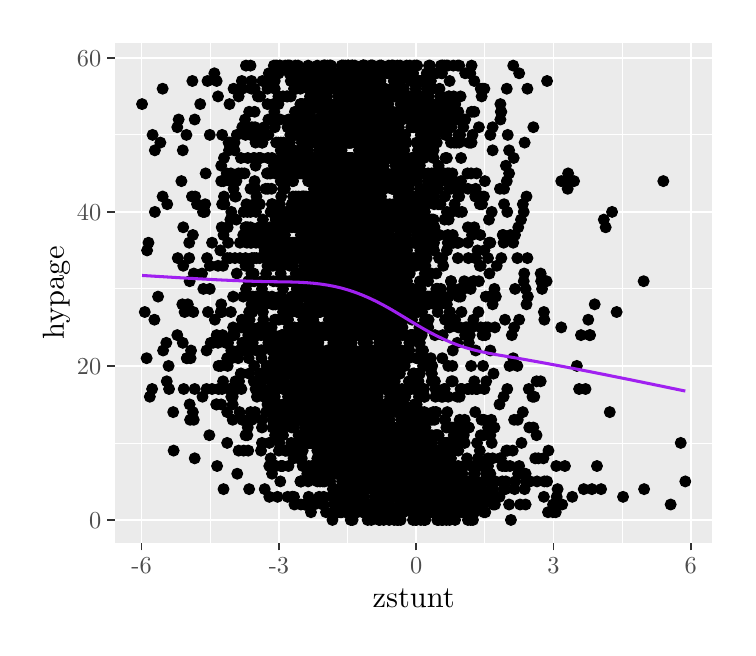
\begin{tikzpicture}[x=1pt,y=1pt]
\definecolor{fillColor}{RGB}{255,255,255}
\path[use as bounding box,fill=fillColor,fill opacity=0.00] (0,0) rectangle (252.94,216.81);
\begin{scope}
\path[clip] (  0.00,  0.00) rectangle (252.94,216.81);
\definecolor{drawColor}{RGB}{255,255,255}
\definecolor{fillColor}{RGB}{255,255,255}

\path[draw=drawColor,line width= 0.6pt,line join=round,line cap=round,fill=fillColor] (  0.00,  0.00) rectangle (252.94,216.81);
\end{scope}
\begin{scope}
\path[clip] ( 31.52, 30.72) rectangle (247.44,211.31);
\definecolor{fillColor}{gray}{0.92}

\path[fill=fillColor] ( 31.52, 30.72) rectangle (247.44,211.31);
\definecolor{drawColor}{RGB}{255,255,255}

\path[draw=drawColor,line width= 0.3pt,line join=round] ( 31.52, 66.76) --
	(247.44, 66.76);

\path[draw=drawColor,line width= 0.3pt,line join=round] ( 31.52,122.41) --
	(247.44,122.41);

\path[draw=drawColor,line width= 0.3pt,line join=round] ( 31.52,178.06) --
	(247.44,178.06);

\path[draw=drawColor,line width= 0.3pt,line join=round] ( 65.97, 30.72) --
	( 65.97,211.31);

\path[draw=drawColor,line width= 0.3pt,line join=round] (115.59, 30.72) --
	(115.59,211.31);

\path[draw=drawColor,line width= 0.3pt,line join=round] (165.20, 30.72) --
	(165.20,211.31);

\path[draw=drawColor,line width= 0.3pt,line join=round] (214.81, 30.72) --
	(214.81,211.31);

\path[draw=drawColor,line width= 0.6pt,line join=round] ( 31.52, 38.93) --
	(247.44, 38.93);

\path[draw=drawColor,line width= 0.6pt,line join=round] ( 31.52, 94.58) --
	(247.44, 94.58);

\path[draw=drawColor,line width= 0.6pt,line join=round] ( 31.52,150.23) --
	(247.44,150.23);

\path[draw=drawColor,line width= 0.6pt,line join=round] ( 31.52,205.88) --
	(247.44,205.88);

\path[draw=drawColor,line width= 0.6pt,line join=round] ( 41.17, 30.72) --
	( 41.17,211.31);

\path[draw=drawColor,line width= 0.6pt,line join=round] ( 90.78, 30.72) --
	( 90.78,211.31);

\path[draw=drawColor,line width= 0.6pt,line join=round] (140.39, 30.72) --
	(140.39,211.31);

\path[draw=drawColor,line width= 0.6pt,line join=round] (190.00, 30.72) --
	(190.00,211.31);

\path[draw=drawColor,line width= 0.6pt,line join=round] (239.61, 30.72) --
	(239.61,211.31);
\definecolor{drawColor}{RGB}{0,0,0}
\definecolor{fillColor}{RGB}{0,0,0}

\path[draw=drawColor,line width= 0.4pt,line join=round,line cap=round,fill=fillColor] (177.27, 55.63) circle (  1.96);

\path[draw=drawColor,line width= 0.4pt,line join=round,line cap=round,fill=fillColor] (168.01,116.84) circle (  1.96);

\path[draw=drawColor,line width= 0.4pt,line join=round,line cap=round,fill=fillColor] (144.36, 94.58) circle (  1.96);

\path[draw=drawColor,line width= 0.4pt,line join=round,line cap=round,fill=fillColor] (100.04,169.71) circle (  1.96);

\path[draw=drawColor,line width= 0.4pt,line join=round,line cap=round,fill=fillColor] (126.50, 77.89) circle (  1.96);

\path[draw=drawColor,line width= 0.4pt,line join=round,line cap=round,fill=fillColor] (129.15, 80.67) circle (  1.96);

\path[draw=drawColor,line width= 0.4pt,line join=round,line cap=round,fill=fillColor] (103.68,178.06) circle (  1.96);

\path[draw=drawColor,line width= 0.4pt,line join=round,line cap=round,fill=fillColor] (129.81, 77.89) circle (  1.96);

\path[draw=drawColor,line width= 0.4pt,line join=round,line cap=round,fill=fillColor] (126.83, 66.76) circle (  1.96);

\path[draw=drawColor,line width= 0.4pt,line join=round,line cap=round,fill=fillColor] ( 98.22, 89.02) circle (  1.96);

\path[draw=drawColor,line width= 0.4pt,line join=round,line cap=round,fill=fillColor] (106.82,105.71) circle (  1.96);

\path[draw=drawColor,line width= 0.4pt,line join=round,line cap=round,fill=fillColor] (148.99,116.84) circle (  1.96);

\path[draw=drawColor,line width= 0.4pt,line join=round,line cap=round,fill=fillColor] (136.59, 61.19) circle (  1.96);

\path[draw=drawColor,line width= 0.4pt,line join=round,line cap=round,fill=fillColor] ( 98.39,164.15) circle (  1.96);

\path[draw=drawColor,line width= 0.4pt,line join=round,line cap=round,fill=fillColor] ( 84.49,100.15) circle (  1.96);

\path[draw=drawColor,line width= 0.4pt,line join=round,line cap=round,fill=fillColor] (105.50,150.23) circle (  1.96);

\path[draw=drawColor,line width= 0.4pt,line join=round,line cap=round,fill=fillColor] (105.17, 69.54) circle (  1.96);

\path[draw=drawColor,line width= 0.4pt,line join=round,line cap=round,fill=fillColor] (150.81, 58.41) circle (  1.96);

\path[draw=drawColor,line width= 0.4pt,line join=round,line cap=round,fill=fillColor] (129.15,122.41) circle (  1.96);

\path[draw=drawColor,line width= 0.4pt,line join=round,line cap=round,fill=fillColor] ( 97.89,155.80) circle (  1.96);

\path[draw=drawColor,line width= 0.4pt,line join=round,line cap=round,fill=fillColor] ( 83.01, 86.24) circle (  1.96);

\path[draw=drawColor,line width= 0.4pt,line join=round,line cap=round,fill=fillColor] (138.90, 66.76) circle (  1.96);

\path[draw=drawColor,line width= 0.4pt,line join=round,line cap=round,fill=fillColor] (143.37, 83.45) circle (  1.96);

\path[draw=drawColor,line width= 0.4pt,line join=round,line cap=round,fill=fillColor] (131.46, 41.72) circle (  1.96);

\path[draw=drawColor,line width= 0.4pt,line join=round,line cap=round,fill=fillColor] ( 88.96,150.23) circle (  1.96);

\path[draw=drawColor,line width= 0.4pt,line join=round,line cap=round,fill=fillColor] (126.33, 72.32) circle (  1.96);

\path[draw=drawColor,line width= 0.4pt,line join=round,line cap=round,fill=fillColor] (138.74,164.15) circle (  1.96);

\path[draw=drawColor,line width= 0.4pt,line join=round,line cap=round,fill=fillColor] (172.80, 52.85) circle (  1.96);

\path[draw=drawColor,line width= 0.4pt,line join=round,line cap=round,fill=fillColor] (121.87,183.62) circle (  1.96);

\path[draw=drawColor,line width= 0.4pt,line join=round,line cap=round,fill=fillColor] (137.08,136.32) circle (  1.96);

\path[draw=drawColor,line width= 0.4pt,line join=round,line cap=round,fill=fillColor] ( 78.71,100.15) circle (  1.96);

\path[draw=drawColor,line width= 0.4pt,line join=round,line cap=round,fill=fillColor] (117.90,100.15) circle (  1.96);

\path[draw=drawColor,line width= 0.4pt,line join=round,line cap=round,fill=fillColor] ( 84.66,100.15) circle (  1.96);

\path[draw=drawColor,line width= 0.4pt,line join=round,line cap=round,fill=fillColor] (126.83, 86.24) circle (  1.96);

\path[draw=drawColor,line width= 0.4pt,line join=round,line cap=round,fill=fillColor] (138.57, 86.24) circle (  1.96);

\path[draw=drawColor,line width= 0.4pt,line join=round,line cap=round,fill=fillColor] (121.21, 77.89) circle (  1.96);

\path[draw=drawColor,line width= 0.4pt,line join=round,line cap=round,fill=fillColor] (127.49,153.02) circle (  1.96);

\path[draw=drawColor,line width= 0.4pt,line join=round,line cap=round,fill=fillColor] (126.50,186.41) circle (  1.96);

\path[draw=drawColor,line width= 0.4pt,line join=round,line cap=round,fill=fillColor] ( 95.74, 80.67) circle (  1.96);

\path[draw=drawColor,line width= 0.4pt,line join=round,line cap=round,fill=fillColor] (123.36,136.32) circle (  1.96);

\path[draw=drawColor,line width= 0.4pt,line join=round,line cap=round,fill=fillColor] (113.60, 50.06) circle (  1.96);

\path[draw=drawColor,line width= 0.4pt,line join=round,line cap=round,fill=fillColor] (134.44,175.28) circle (  1.96);

\path[draw=drawColor,line width= 0.4pt,line join=round,line cap=round,fill=fillColor] ( 87.31, 94.58) circle (  1.96);

\path[draw=drawColor,line width= 0.4pt,line join=round,line cap=round,fill=fillColor] (122.86,139.10) circle (  1.96);

\path[draw=drawColor,line width= 0.4pt,line join=round,line cap=round,fill=fillColor] ( 82.01,161.36) circle (  1.96);

\path[draw=drawColor,line width= 0.4pt,line join=round,line cap=round,fill=fillColor] ( 99.21, 80.67) circle (  1.96);

\path[draw=drawColor,line width= 0.4pt,line join=round,line cap=round,fill=fillColor] (115.75, 97.37) circle (  1.96);

\path[draw=drawColor,line width= 0.4pt,line join=round,line cap=round,fill=fillColor] (104.17,175.28) circle (  1.96);

\path[draw=drawColor,line width= 0.4pt,line join=round,line cap=round,fill=fillColor] ( 75.40, 86.24) circle (  1.96);

\path[draw=drawColor,line width= 0.4pt,line join=round,line cap=round,fill=fillColor] (121.21,197.54) circle (  1.96);

\path[draw=drawColor,line width= 0.4pt,line join=round,line cap=round,fill=fillColor] (124.85, 52.85) circle (  1.96);

\path[draw=drawColor,line width= 0.4pt,line join=round,line cap=round,fill=fillColor] (123.52,183.62) circle (  1.96);

\path[draw=drawColor,line width= 0.4pt,line join=round,line cap=round,fill=fillColor] ( 99.71, 86.24) circle (  1.96);

\path[draw=drawColor,line width= 0.4pt,line join=round,line cap=round,fill=fillColor] (122.53,144.67) circle (  1.96);

\path[draw=drawColor,line width= 0.4pt,line join=round,line cap=round,fill=fillColor] (135.43, 63.98) circle (  1.96);

\path[draw=drawColor,line width= 0.4pt,line join=round,line cap=round,fill=fillColor] (105.83,155.80) circle (  1.96);

\path[draw=drawColor,line width= 0.4pt,line join=round,line cap=round,fill=fillColor] ( 59.85,114.06) circle (  1.96);

\path[draw=drawColor,line width= 0.4pt,line join=round,line cap=round,fill=fillColor] (122.20,166.93) circle (  1.96);

\path[draw=drawColor,line width= 0.4pt,line join=round,line cap=round,fill=fillColor] ( 77.38,197.54) circle (  1.96);

\path[draw=drawColor,line width= 0.4pt,line join=round,line cap=round,fill=fillColor] ( 89.95, 80.67) circle (  1.96);

\path[draw=drawColor,line width= 0.4pt,line join=round,line cap=round,fill=fillColor] (119.22,114.06) circle (  1.96);

\path[draw=drawColor,line width= 0.4pt,line join=round,line cap=round,fill=fillColor] (112.77,111.28) circle (  1.96);

\path[draw=drawColor,line width= 0.4pt,line join=round,line cap=round,fill=fillColor] (115.92,189.19) circle (  1.96);

\path[draw=drawColor,line width= 0.4pt,line join=round,line cap=round,fill=fillColor] (115.75,203.10) circle (  1.96);

\path[draw=drawColor,line width= 0.4pt,line join=round,line cap=round,fill=fillColor] (123.19, 69.54) circle (  1.96);

\path[draw=drawColor,line width= 0.4pt,line join=round,line cap=round,fill=fillColor] ( 99.38,178.06) circle (  1.96);

\path[draw=drawColor,line width= 0.4pt,line join=round,line cap=round,fill=fillColor] ( 94.58,139.10) circle (  1.96);

\path[draw=drawColor,line width= 0.4pt,line join=round,line cap=round,fill=fillColor] (187.52,125.19) circle (  1.96);

\path[draw=drawColor,line width= 0.4pt,line join=round,line cap=round,fill=fillColor] (136.42,164.15) circle (  1.96);

\path[draw=drawColor,line width= 0.4pt,line join=round,line cap=round,fill=fillColor] (124.02,203.10) circle (  1.96);

\path[draw=drawColor,line width= 0.4pt,line join=round,line cap=round,fill=fillColor] (124.52, 89.02) circle (  1.96);

\path[draw=drawColor,line width= 0.4pt,line join=round,line cap=round,fill=fillColor] ( 79.53, 72.32) circle (  1.96);

\path[draw=drawColor,line width= 0.4pt,line join=round,line cap=round,fill=fillColor] (141.22, 58.41) circle (  1.96);

\path[draw=drawColor,line width= 0.4pt,line join=round,line cap=round,fill=fillColor] (109.96,197.54) circle (  1.96);

\path[draw=drawColor,line width= 0.4pt,line join=round,line cap=round,fill=fillColor] (155.61,139.10) circle (  1.96);

\path[draw=drawColor,line width= 0.4pt,line join=round,line cap=round,fill=fillColor] ( 99.87, 77.89) circle (  1.96);

\path[draw=drawColor,line width= 0.4pt,line join=round,line cap=round,fill=fillColor] ( 98.88,127.97) circle (  1.96);

\path[draw=drawColor,line width= 0.4pt,line join=round,line cap=round,fill=fillColor] (112.11,166.93) circle (  1.96);

\path[draw=drawColor,line width= 0.4pt,line join=round,line cap=round,fill=fillColor] (102.02,127.97) circle (  1.96);

\path[draw=drawColor,line width= 0.4pt,line join=round,line cap=round,fill=fillColor] (118.73,136.32) circle (  1.96);

\path[draw=drawColor,line width= 0.4pt,line join=round,line cap=round,fill=fillColor] (147.50, 50.06) circle (  1.96);

\path[draw=drawColor,line width= 0.4pt,line join=round,line cap=round,fill=fillColor] (112.61,144.67) circle (  1.96);

\path[draw=drawColor,line width= 0.4pt,line join=round,line cap=round,fill=fillColor] (141.22, 52.85) circle (  1.96);

\path[draw=drawColor,line width= 0.4pt,line join=round,line cap=round,fill=fillColor] (140.23,130.76) circle (  1.96);

\path[draw=drawColor,line width= 0.4pt,line join=round,line cap=round,fill=fillColor] (123.19, 75.11) circle (  1.96);

\path[draw=drawColor,line width= 0.4pt,line join=round,line cap=round,fill=fillColor] (140.06,166.93) circle (  1.96);

\path[draw=drawColor,line width= 0.4pt,line join=round,line cap=round,fill=fillColor] (172.80,166.93) circle (  1.96);

\path[draw=drawColor,line width= 0.4pt,line join=round,line cap=round,fill=fillColor] (132.95, 97.37) circle (  1.96);

\path[draw=drawColor,line width= 0.4pt,line join=round,line cap=round,fill=fillColor] (116.58,189.19) circle (  1.96);

\path[draw=drawColor,line width= 0.4pt,line join=round,line cap=round,fill=fillColor] (117.90, 66.76) circle (  1.96);

\path[draw=drawColor,line width= 0.4pt,line join=round,line cap=round,fill=fillColor] (125.18, 72.32) circle (  1.96);

\path[draw=drawColor,line width= 0.4pt,line join=round,line cap=round,fill=fillColor] ( 90.28, 75.11) circle (  1.96);

\path[draw=drawColor,line width= 0.4pt,line join=round,line cap=round,fill=fillColor] (138.74,153.02) circle (  1.96);

\path[draw=drawColor,line width= 0.4pt,line join=round,line cap=round,fill=fillColor] (106.16,186.41) circle (  1.96);

\path[draw=drawColor,line width= 0.4pt,line join=round,line cap=round,fill=fillColor] (137.25,130.76) circle (  1.96);

\path[draw=drawColor,line width= 0.4pt,line join=round,line cap=round,fill=fillColor] ( 86.64,189.19) circle (  1.96);

\path[draw=drawColor,line width= 0.4pt,line join=round,line cap=round,fill=fillColor] (116.41,100.15) circle (  1.96);

\path[draw=drawColor,line width= 0.4pt,line join=round,line cap=round,fill=fillColor] (148.00, 63.98) circle (  1.96);

\path[draw=drawColor,line width= 0.4pt,line join=round,line cap=round,fill=fillColor] (149.16, 44.50) circle (  1.96);

\path[draw=drawColor,line width= 0.4pt,line join=round,line cap=round,fill=fillColor] (136.59,186.41) circle (  1.96);

\path[draw=drawColor,line width= 0.4pt,line join=round,line cap=round,fill=fillColor] (126.83, 47.28) circle (  1.96);

\path[draw=drawColor,line width= 0.4pt,line join=round,line cap=round,fill=fillColor] (110.79,180.84) circle (  1.96);

\path[draw=drawColor,line width= 0.4pt,line join=round,line cap=round,fill=fillColor] ( 86.98,102.93) circle (  1.96);

\path[draw=drawColor,line width= 0.4pt,line join=round,line cap=round,fill=fillColor] ( 43.15,136.32) circle (  1.96);

\path[draw=drawColor,line width= 0.4pt,line join=round,line cap=round,fill=fillColor] (122.03,133.54) circle (  1.96);

\path[draw=drawColor,line width= 0.4pt,line join=round,line cap=round,fill=fillColor] (102.02,178.06) circle (  1.96);

\path[draw=drawColor,line width= 0.4pt,line join=round,line cap=round,fill=fillColor] (130.96,180.84) circle (  1.96);

\path[draw=drawColor,line width= 0.4pt,line join=round,line cap=round,fill=fillColor] (132.29, 69.54) circle (  1.96);

\path[draw=drawColor,line width= 0.4pt,line join=round,line cap=round,fill=fillColor] ( 58.53,125.19) circle (  1.96);

\path[draw=drawColor,line width= 0.4pt,line join=round,line cap=round,fill=fillColor] (168.84, 44.50) circle (  1.96);

\path[draw=drawColor,line width= 0.4pt,line join=round,line cap=round,fill=fillColor] (147.01,158.58) circle (  1.96);

\path[draw=drawColor,line width= 0.4pt,line join=round,line cap=round,fill=fillColor] (104.84, 69.54) circle (  1.96);

\path[draw=drawColor,line width= 0.4pt,line join=round,line cap=round,fill=fillColor] (114.92,108.50) circle (  1.96);

\path[draw=drawColor,line width= 0.4pt,line join=round,line cap=round,fill=fillColor] (113.77, 69.54) circle (  1.96);

\path[draw=drawColor,line width= 0.4pt,line join=round,line cap=round,fill=fillColor] (124.18,158.58) circle (  1.96);

\path[draw=drawColor,line width= 0.4pt,line join=round,line cap=round,fill=fillColor] (122.20,178.06) circle (  1.96);

\path[draw=drawColor,line width= 0.4pt,line join=round,line cap=round,fill=fillColor] (114.92,114.06) circle (  1.96);

\path[draw=drawColor,line width= 0.4pt,line join=round,line cap=round,fill=fillColor] (138.90, 75.11) circle (  1.96);

\path[draw=drawColor,line width= 0.4pt,line join=round,line cap=round,fill=fillColor] (127.49,155.80) circle (  1.96);

\path[draw=drawColor,line width= 0.4pt,line join=round,line cap=round,fill=fillColor] (136.59, 72.32) circle (  1.96);

\path[draw=drawColor,line width= 0.4pt,line join=round,line cap=round,fill=fillColor] (138.90, 47.28) circle (  1.96);

\path[draw=drawColor,line width= 0.4pt,line join=round,line cap=round,fill=fillColor] (129.48,178.06) circle (  1.96);

\path[draw=drawColor,line width= 0.4pt,line join=round,line cap=round,fill=fillColor] (154.12, 72.32) circle (  1.96);

\path[draw=drawColor,line width= 0.4pt,line join=round,line cap=round,fill=fillColor] (122.37, 75.11) circle (  1.96);

\path[draw=drawColor,line width= 0.4pt,line join=round,line cap=round,fill=fillColor] (131.46,119.63) circle (  1.96);

\path[draw=drawColor,line width= 0.4pt,line join=round,line cap=round,fill=fillColor] ( 87.80,197.54) circle (  1.96);

\path[draw=drawColor,line width= 0.4pt,line join=round,line cap=round,fill=fillColor] ( 76.56,100.15) circle (  1.96);

\path[draw=drawColor,line width= 0.4pt,line join=round,line cap=round,fill=fillColor] (101.03,178.06) circle (  1.96);

\path[draw=drawColor,line width= 0.4pt,line join=round,line cap=round,fill=fillColor] (117.24, 50.06) circle (  1.96);

\path[draw=drawColor,line width= 0.4pt,line join=round,line cap=round,fill=fillColor] (112.61,105.71) circle (  1.96);

\path[draw=drawColor,line width= 0.4pt,line join=round,line cap=round,fill=fillColor] (128.32,105.71) circle (  1.96);

\path[draw=drawColor,line width= 0.4pt,line join=round,line cap=round,fill=fillColor] (146.51, 47.28) circle (  1.96);

\path[draw=drawColor,line width= 0.4pt,line join=round,line cap=round,fill=fillColor] (143.20, 38.93) circle (  1.96);

\path[draw=drawColor,line width= 0.4pt,line join=round,line cap=round,fill=fillColor] (135.10,155.80) circle (  1.96);

\path[draw=drawColor,line width= 0.4pt,line join=round,line cap=round,fill=fillColor] (139.56, 63.98) circle (  1.96);

\path[draw=drawColor,line width= 0.4pt,line join=round,line cap=round,fill=fillColor] (105.00,108.50) circle (  1.96);

\path[draw=drawColor,line width= 0.4pt,line join=round,line cap=round,fill=fillColor] (154.78, 44.50) circle (  1.96);

\path[draw=drawColor,line width= 0.4pt,line join=round,line cap=round,fill=fillColor] (149.65, 41.72) circle (  1.96);

\path[draw=drawColor,line width= 0.4pt,line join=round,line cap=round,fill=fillColor] (136.92,166.93) circle (  1.96);

\path[draw=drawColor,line width= 0.4pt,line join=round,line cap=round,fill=fillColor] (116.25, 66.76) circle (  1.96);

\path[draw=drawColor,line width= 0.4pt,line join=round,line cap=round,fill=fillColor] ( 98.88,105.71) circle (  1.96);

\path[draw=drawColor,line width= 0.4pt,line join=round,line cap=round,fill=fillColor] ( 70.93,155.80) circle (  1.96);

\path[draw=drawColor,line width= 0.4pt,line join=round,line cap=round,fill=fillColor] (174.95,105.71) circle (  1.96);

\path[draw=drawColor,line width= 0.4pt,line join=round,line cap=round,fill=fillColor] (163.71,108.50) circle (  1.96);

\path[draw=drawColor,line width= 0.4pt,line join=round,line cap=round,fill=fillColor] (165.53, 47.28) circle (  1.96);

\path[draw=drawColor,line width= 0.4pt,line join=round,line cap=round,fill=fillColor] (159.90,200.32) circle (  1.96);

\path[draw=drawColor,line width= 0.4pt,line join=round,line cap=round,fill=fillColor] (165.36,105.71) circle (  1.96);

\path[draw=drawColor,line width= 0.4pt,line join=round,line cap=round,fill=fillColor] (172.14,158.58) circle (  1.96);

\path[draw=drawColor,line width= 0.4pt,line join=round,line cap=round,fill=fillColor] (136.92,125.19) circle (  1.96);

\path[draw=drawColor,line width= 0.4pt,line join=round,line cap=round,fill=fillColor] (161.72,133.54) circle (  1.96);

\path[draw=drawColor,line width= 0.4pt,line join=round,line cap=round,fill=fillColor] (148.00, 50.06) circle (  1.96);

\path[draw=drawColor,line width= 0.4pt,line join=round,line cap=round,fill=fillColor] (147.50, 63.98) circle (  1.96);

\path[draw=drawColor,line width= 0.4pt,line join=round,line cap=round,fill=fillColor] (136.42,105.71) circle (  1.96);

\path[draw=drawColor,line width= 0.4pt,line join=round,line cap=round,fill=fillColor] (145.19, 44.50) circle (  1.96);

\path[draw=drawColor,line width= 0.4pt,line join=round,line cap=round,fill=fillColor] (112.11,164.15) circle (  1.96);

\path[draw=drawColor,line width= 0.4pt,line join=round,line cap=round,fill=fillColor] (109.14, 77.89) circle (  1.96);

\path[draw=drawColor,line width= 0.4pt,line join=round,line cap=round,fill=fillColor] (176.11,122.41) circle (  1.96);

\path[draw=drawColor,line width= 0.4pt,line join=round,line cap=round,fill=fillColor] (146.01, 69.54) circle (  1.96);

\path[draw=drawColor,line width= 0.4pt,line join=round,line cap=round,fill=fillColor] (117.90,116.84) circle (  1.96);

\path[draw=drawColor,line width= 0.4pt,line join=round,line cap=round,fill=fillColor] ( 88.30,169.71) circle (  1.96);

\path[draw=drawColor,line width= 0.4pt,line join=round,line cap=round,fill=fillColor] ( 76.39, 89.02) circle (  1.96);

\path[draw=drawColor,line width= 0.4pt,line join=round,line cap=round,fill=fillColor] (108.97,116.84) circle (  1.96);

\path[draw=drawColor,line width= 0.4pt,line join=round,line cap=round,fill=fillColor] (149.98, 44.50) circle (  1.96);

\path[draw=drawColor,line width= 0.4pt,line join=round,line cap=round,fill=fillColor] (107.15,119.63) circle (  1.96);

\path[draw=drawColor,line width= 0.4pt,line join=round,line cap=round,fill=fillColor] (101.03,125.19) circle (  1.96);

\path[draw=drawColor,line width= 0.4pt,line join=round,line cap=round,fill=fillColor] (108.14,200.32) circle (  1.96);

\path[draw=drawColor,line width= 0.4pt,line join=round,line cap=round,fill=fillColor] (126.33, 44.50) circle (  1.96);

\path[draw=drawColor,line width= 0.4pt,line join=round,line cap=round,fill=fillColor] (128.15,125.19) circle (  1.96);

\path[draw=drawColor,line width= 0.4pt,line join=round,line cap=round,fill=fillColor] ( 93.92,100.15) circle (  1.96);

\path[draw=drawColor,line width= 0.4pt,line join=round,line cap=round,fill=fillColor] (148.99, 44.50) circle (  1.96);

\path[draw=drawColor,line width= 0.4pt,line join=round,line cap=round,fill=fillColor] (142.54,130.76) circle (  1.96);

\path[draw=drawColor,line width= 0.4pt,line join=round,line cap=round,fill=fillColor] (120.88, 77.89) circle (  1.96);

\path[draw=drawColor,line width= 0.4pt,line join=round,line cap=round,fill=fillColor] ( 76.56, 77.89) circle (  1.96);

\path[draw=drawColor,line width= 0.4pt,line join=round,line cap=round,fill=fillColor] (130.96,102.93) circle (  1.96);

\path[draw=drawColor,line width= 0.4pt,line join=round,line cap=round,fill=fillColor] (120.38,127.97) circle (  1.96);

\path[draw=drawColor,line width= 0.4pt,line join=round,line cap=round,fill=fillColor] (136.75, 63.98) circle (  1.96);

\path[draw=drawColor,line width= 0.4pt,line join=round,line cap=round,fill=fillColor] (152.96, 61.19) circle (  1.96);

\path[draw=drawColor,line width= 0.4pt,line join=round,line cap=round,fill=fillColor] ( 86.81,169.71) circle (  1.96);

\path[draw=drawColor,line width= 0.4pt,line join=round,line cap=round,fill=fillColor] (128.65,180.84) circle (  1.96);

\path[draw=drawColor,line width= 0.4pt,line join=round,line cap=round,fill=fillColor] (118.89,153.02) circle (  1.96);

\path[draw=drawColor,line width= 0.4pt,line join=round,line cap=round,fill=fillColor] (135.10, 47.28) circle (  1.96);

\path[draw=drawColor,line width= 0.4pt,line join=round,line cap=round,fill=fillColor] (147.67,200.32) circle (  1.96);

\path[draw=drawColor,line width= 0.4pt,line join=round,line cap=round,fill=fillColor] (131.30,150.23) circle (  1.96);

\path[draw=drawColor,line width= 0.4pt,line join=round,line cap=round,fill=fillColor] ( 85.32,119.63) circle (  1.96);

\path[draw=drawColor,line width= 0.4pt,line join=round,line cap=round,fill=fillColor] (117.57,189.19) circle (  1.96);

\path[draw=drawColor,line width= 0.4pt,line join=round,line cap=round,fill=fillColor] ( 97.23, 83.45) circle (  1.96);

\path[draw=drawColor,line width= 0.4pt,line join=round,line cap=round,fill=fillColor] (140.06, 44.50) circle (  1.96);

\path[draw=drawColor,line width= 0.4pt,line join=round,line cap=round,fill=fillColor] ( 96.57, 83.45) circle (  1.96);

\path[draw=drawColor,line width= 0.4pt,line join=round,line cap=round,fill=fillColor] (110.13,139.10) circle (  1.96);

\path[draw=drawColor,line width= 0.4pt,line join=round,line cap=round,fill=fillColor] (105.99, 97.37) circle (  1.96);

\path[draw=drawColor,line width= 0.4pt,line join=round,line cap=round,fill=fillColor] (125.84, 83.45) circle (  1.96);

\path[draw=drawColor,line width= 0.4pt,line join=round,line cap=round,fill=fillColor] ( 80.20,111.28) circle (  1.96);

\path[draw=drawColor,line width= 0.4pt,line join=round,line cap=round,fill=fillColor] ( 67.63,111.28) circle (  1.96);

\path[draw=drawColor,line width= 0.4pt,line join=round,line cap=round,fill=fillColor] (132.95,197.54) circle (  1.96);

\path[draw=drawColor,line width= 0.4pt,line join=round,line cap=round,fill=fillColor] (135.76, 41.72) circle (  1.96);

\path[draw=drawColor,line width= 0.4pt,line join=round,line cap=round,fill=fillColor] (156.93, 69.54) circle (  1.96);

\path[draw=drawColor,line width= 0.4pt,line join=round,line cap=round,fill=fillColor] (175.78, 75.11) circle (  1.96);

\path[draw=drawColor,line width= 0.4pt,line join=round,line cap=round,fill=fillColor] (116.91,161.36) circle (  1.96);

\path[draw=drawColor,line width= 0.4pt,line join=round,line cap=round,fill=fillColor] (176.11,141.89) circle (  1.96);

\path[draw=drawColor,line width= 0.4pt,line join=round,line cap=round,fill=fillColor] (115.42,180.84) circle (  1.96);

\path[draw=drawColor,line width= 0.4pt,line join=round,line cap=round,fill=fillColor] ( 43.65,139.10) circle (  1.96);

\path[draw=drawColor,line width= 0.4pt,line join=round,line cap=round,fill=fillColor] (139.07, 41.72) circle (  1.96);

\path[draw=drawColor,line width= 0.4pt,line join=round,line cap=round,fill=fillColor] (130.63, 80.67) circle (  1.96);

\path[draw=drawColor,line width= 0.4pt,line join=round,line cap=round,fill=fillColor] (130.80,141.89) circle (  1.96);

\path[draw=drawColor,line width= 0.4pt,line join=round,line cap=round,fill=fillColor] (110.13,180.84) circle (  1.96);

\path[draw=drawColor,line width= 0.4pt,line join=round,line cap=round,fill=fillColor] (116.25,105.71) circle (  1.96);

\path[draw=drawColor,line width= 0.4pt,line join=round,line cap=round,fill=fillColor] (151.80,203.10) circle (  1.96);

\path[draw=drawColor,line width= 0.4pt,line join=round,line cap=round,fill=fillColor] (105.00, 89.02) circle (  1.96);

\path[draw=drawColor,line width= 0.4pt,line join=round,line cap=round,fill=fillColor] (138.24,200.32) circle (  1.96);

\path[draw=drawColor,line width= 0.4pt,line join=round,line cap=round,fill=fillColor] (125.18,183.62) circle (  1.96);

\path[draw=drawColor,line width= 0.4pt,line join=round,line cap=round,fill=fillColor] (149.98,203.10) circle (  1.96);

\path[draw=drawColor,line width= 0.4pt,line join=round,line cap=round,fill=fillColor] (144.53, 63.98) circle (  1.96);

\path[draw=drawColor,line width= 0.4pt,line join=round,line cap=round,fill=fillColor] (165.69, 55.63) circle (  1.96);

\path[draw=drawColor,line width= 0.4pt,line join=round,line cap=round,fill=fillColor] (166.35, 58.41) circle (  1.96);

\path[draw=drawColor,line width= 0.4pt,line join=round,line cap=round,fill=fillColor] (141.38,147.45) circle (  1.96);

\path[draw=drawColor,line width= 0.4pt,line join=round,line cap=round,fill=fillColor] (140.72, 97.37) circle (  1.96);

\path[draw=drawColor,line width= 0.4pt,line join=round,line cap=round,fill=fillColor] (137.74,127.97) circle (  1.96);

\path[draw=drawColor,line width= 0.4pt,line join=round,line cap=round,fill=fillColor] (123.52,108.50) circle (  1.96);

\path[draw=drawColor,line width= 0.4pt,line join=round,line cap=round,fill=fillColor] ( 99.05,155.80) circle (  1.96);

\path[draw=drawColor,line width= 0.4pt,line join=round,line cap=round,fill=fillColor] (102.85,108.50) circle (  1.96);

\path[draw=drawColor,line width= 0.4pt,line join=round,line cap=round,fill=fillColor] (109.96, 47.28) circle (  1.96);

\path[draw=drawColor,line width= 0.4pt,line join=round,line cap=round,fill=fillColor] (101.53, 47.28) circle (  1.96);

\path[draw=drawColor,line width= 0.4pt,line join=round,line cap=round,fill=fillColor] (114.26,130.76) circle (  1.96);

\path[draw=drawColor,line width= 0.4pt,line join=round,line cap=round,fill=fillColor] (116.08, 55.63) circle (  1.96);

\path[draw=drawColor,line width= 0.4pt,line join=round,line cap=round,fill=fillColor] (119.55,147.45) circle (  1.96);

\path[draw=drawColor,line width= 0.4pt,line join=round,line cap=round,fill=fillColor] (111.78, 89.02) circle (  1.96);

\path[draw=drawColor,line width= 0.4pt,line join=round,line cap=round,fill=fillColor] (121.70,175.28) circle (  1.96);

\path[draw=drawColor,line width= 0.4pt,line join=round,line cap=round,fill=fillColor] (156.27, 47.28) circle (  1.96);

\path[draw=drawColor,line width= 0.4pt,line join=round,line cap=round,fill=fillColor] ( 99.38,125.19) circle (  1.96);

\path[draw=drawColor,line width= 0.4pt,line join=round,line cap=round,fill=fillColor] (106.99,136.32) circle (  1.96);

\path[draw=drawColor,line width= 0.4pt,line join=round,line cap=round,fill=fillColor] ( 95.24, 75.11) circle (  1.96);

\path[draw=drawColor,line width= 0.4pt,line join=round,line cap=round,fill=fillColor] ( 97.06,150.23) circle (  1.96);

\path[draw=drawColor,line width= 0.4pt,line join=round,line cap=round,fill=fillColor] (121.87, 72.32) circle (  1.96);

\path[draw=drawColor,line width= 0.4pt,line join=round,line cap=round,fill=fillColor] (138.74,133.54) circle (  1.96);

\path[draw=drawColor,line width= 0.4pt,line join=round,line cap=round,fill=fillColor] (118.23,153.02) circle (  1.96);

\path[draw=drawColor,line width= 0.4pt,line join=round,line cap=round,fill=fillColor] (164.87, 75.11) circle (  1.96);

\path[draw=drawColor,line width= 0.4pt,line join=round,line cap=round,fill=fillColor] (222.58,125.19) circle (  1.96);

\path[draw=drawColor,line width= 0.4pt,line join=round,line cap=round,fill=fillColor] (149.98,180.84) circle (  1.96);

\path[draw=drawColor,line width= 0.4pt,line join=round,line cap=round,fill=fillColor] ( 98.06, 94.58) circle (  1.96);

\path[draw=drawColor,line width= 0.4pt,line join=round,line cap=round,fill=fillColor] (130.14,180.84) circle (  1.96);

\path[draw=drawColor,line width= 0.4pt,line join=round,line cap=round,fill=fillColor] (118.89,105.71) circle (  1.96);

\path[draw=drawColor,line width= 0.4pt,line join=round,line cap=round,fill=fillColor] (156.76, 44.50) circle (  1.96);

\path[draw=drawColor,line width= 0.4pt,line join=round,line cap=round,fill=fillColor] ( 80.53,203.10) circle (  1.96);

\path[draw=drawColor,line width= 0.4pt,line join=round,line cap=round,fill=fillColor] (118.23, 66.76) circle (  1.96);

\path[draw=drawColor,line width= 0.4pt,line join=round,line cap=round,fill=fillColor] ( 97.39,125.19) circle (  1.96);

\path[draw=drawColor,line width= 0.4pt,line join=round,line cap=round,fill=fillColor] ( 99.71,105.71) circle (  1.96);

\path[draw=drawColor,line width= 0.4pt,line join=round,line cap=round,fill=fillColor] (119.55,144.67) circle (  1.96);

\path[draw=drawColor,line width= 0.4pt,line join=round,line cap=round,fill=fillColor] (123.69, 89.02) circle (  1.96);

\path[draw=drawColor,line width= 0.4pt,line join=round,line cap=round,fill=fillColor] (167.68,150.23) circle (  1.96);

\path[draw=drawColor,line width= 0.4pt,line join=round,line cap=round,fill=fillColor] (102.85,108.50) circle (  1.96);

\path[draw=drawColor,line width= 0.4pt,line join=round,line cap=round,fill=fillColor] (103.68,127.97) circle (  1.96);

\path[draw=drawColor,line width= 0.4pt,line join=round,line cap=round,fill=fillColor] ( 99.21, 66.76) circle (  1.96);

\path[draw=drawColor,line width= 0.4pt,line join=round,line cap=round,fill=fillColor] (131.13, 61.19) circle (  1.96);

\path[draw=drawColor,line width= 0.4pt,line join=round,line cap=round,fill=fillColor] (110.13, 97.37) circle (  1.96);

\path[draw=drawColor,line width= 0.4pt,line join=round,line cap=round,fill=fillColor] (109.14, 89.02) circle (  1.96);

\path[draw=drawColor,line width= 0.4pt,line join=round,line cap=round,fill=fillColor] (105.00,175.28) circle (  1.96);

\path[draw=drawColor,line width= 0.4pt,line join=round,line cap=round,fill=fillColor] ( 57.54, 97.37) circle (  1.96);

\path[draw=drawColor,line width= 0.4pt,line join=round,line cap=round,fill=fillColor] ( 88.46, 72.32) circle (  1.96);

\path[draw=drawColor,line width= 0.4pt,line join=round,line cap=round,fill=fillColor] (117.73,119.63) circle (  1.96);

\path[draw=drawColor,line width= 0.4pt,line join=round,line cap=round,fill=fillColor] (122.53, 55.63) circle (  1.96);

\path[draw=drawColor,line width= 0.4pt,line join=round,line cap=round,fill=fillColor] (177.27, 55.63) circle (  1.96);

\path[draw=drawColor,line width= 0.4pt,line join=round,line cap=round,fill=fillColor] (123.03,133.54) circle (  1.96);

\path[draw=drawColor,line width= 0.4pt,line join=round,line cap=round,fill=fillColor] (118.73, 77.89) circle (  1.96);

\path[draw=drawColor,line width= 0.4pt,line join=round,line cap=round,fill=fillColor] (107.98,178.06) circle (  1.96);

\path[draw=drawColor,line width= 0.4pt,line join=round,line cap=round,fill=fillColor] (126.67, 52.85) circle (  1.96);

\path[draw=drawColor,line width= 0.4pt,line join=round,line cap=round,fill=fillColor] (132.45,175.28) circle (  1.96);

\path[draw=drawColor,line width= 0.4pt,line join=round,line cap=round,fill=fillColor] (102.52, 97.37) circle (  1.96);

\path[draw=drawColor,line width= 0.4pt,line join=round,line cap=round,fill=fillColor] (146.01,164.15) circle (  1.96);

\path[draw=drawColor,line width= 0.4pt,line join=round,line cap=round,fill=fillColor] ( 99.38, 69.54) circle (  1.96);

\path[draw=drawColor,line width= 0.4pt,line join=round,line cap=round,fill=fillColor] (105.66,105.71) circle (  1.96);

\path[draw=drawColor,line width= 0.4pt,line join=round,line cap=round,fill=fillColor] (123.85, 44.50) circle (  1.96);

\path[draw=drawColor,line width= 0.4pt,line join=round,line cap=round,fill=fillColor] (104.51,197.54) circle (  1.96);

\path[draw=drawColor,line width= 0.4pt,line join=round,line cap=round,fill=fillColor] (119.06,180.84) circle (  1.96);

\path[draw=drawColor,line width= 0.4pt,line join=round,line cap=round,fill=fillColor] (112.28,169.71) circle (  1.96);

\path[draw=drawColor,line width= 0.4pt,line join=round,line cap=round,fill=fillColor] (100.87,122.41) circle (  1.96);

\path[draw=drawColor,line width= 0.4pt,line join=round,line cap=round,fill=fillColor] (142.04, 38.93) circle (  1.96);

\path[draw=drawColor,line width= 0.4pt,line join=round,line cap=round,fill=fillColor] (111.62,130.76) circle (  1.96);

\path[draw=drawColor,line width= 0.4pt,line join=round,line cap=round,fill=fillColor] (106.82,178.06) circle (  1.96);

\path[draw=drawColor,line width= 0.4pt,line join=round,line cap=round,fill=fillColor] ( 74.90,133.54) circle (  1.96);

\path[draw=drawColor,line width= 0.4pt,line join=round,line cap=round,fill=fillColor] (106.16,119.63) circle (  1.96);

\path[draw=drawColor,line width= 0.4pt,line join=round,line cap=round,fill=fillColor] (109.30,186.41) circle (  1.96);

\path[draw=drawColor,line width= 0.4pt,line join=round,line cap=round,fill=fillColor] (106.32,166.93) circle (  1.96);

\path[draw=drawColor,line width= 0.4pt,line join=round,line cap=round,fill=fillColor] ( 88.46, 75.11) circle (  1.96);

\path[draw=drawColor,line width= 0.4pt,line join=round,line cap=round,fill=fillColor] (108.80,155.80) circle (  1.96);

\path[draw=drawColor,line width= 0.4pt,line join=round,line cap=round,fill=fillColor] (140.56, 80.67) circle (  1.96);

\path[draw=drawColor,line width= 0.4pt,line join=round,line cap=round,fill=fillColor] (137.74, 72.32) circle (  1.96);

\path[draw=drawColor,line width= 0.4pt,line join=round,line cap=round,fill=fillColor] (102.69,122.41) circle (  1.96);

\path[draw=drawColor,line width= 0.4pt,line join=round,line cap=round,fill=fillColor] (114.26,127.97) circle (  1.96);

\path[draw=drawColor,line width= 0.4pt,line join=round,line cap=round,fill=fillColor] (112.61,180.84) circle (  1.96);

\path[draw=drawColor,line width= 0.4pt,line join=round,line cap=round,fill=fillColor] (135.26,139.10) circle (  1.96);

\path[draw=drawColor,line width= 0.4pt,line join=round,line cap=round,fill=fillColor] (131.13, 69.54) circle (  1.96);

\path[draw=drawColor,line width= 0.4pt,line join=round,line cap=round,fill=fillColor] (124.18,186.41) circle (  1.96);

\path[draw=drawColor,line width= 0.4pt,line join=round,line cap=round,fill=fillColor] (131.96, 86.24) circle (  1.96);

\path[draw=drawColor,line width= 0.4pt,line join=round,line cap=round,fill=fillColor] (149.82,133.54) circle (  1.96);

\path[draw=drawColor,line width= 0.4pt,line join=round,line cap=round,fill=fillColor] (146.51, 47.28) circle (  1.96);

\path[draw=drawColor,line width= 0.4pt,line join=round,line cap=round,fill=fillColor] (166.85,119.63) circle (  1.96);

\path[draw=drawColor,line width= 0.4pt,line join=round,line cap=round,fill=fillColor] ( 87.97,139.10) circle (  1.96);

\path[draw=drawColor,line width= 0.4pt,line join=round,line cap=round,fill=fillColor] ( 57.54, 97.37) circle (  1.96);

\path[draw=drawColor,line width= 0.4pt,line join=round,line cap=round,fill=fillColor] (123.85,200.32) circle (  1.96);

\path[draw=drawColor,line width= 0.4pt,line join=round,line cap=round,fill=fillColor] (154.45, 52.85) circle (  1.96);

\path[draw=drawColor,line width= 0.4pt,line join=round,line cap=round,fill=fillColor] (124.68,108.50) circle (  1.96);

\path[draw=drawColor,line width= 0.4pt,line join=round,line cap=round,fill=fillColor] (104.51, 89.02) circle (  1.96);

\path[draw=drawColor,line width= 0.4pt,line join=round,line cap=round,fill=fillColor] ( 45.80,111.28) circle (  1.96);

\path[draw=drawColor,line width= 0.4pt,line join=round,line cap=round,fill=fillColor] ( 92.60, 94.58) circle (  1.96);

\path[draw=drawColor,line width= 0.4pt,line join=round,line cap=round,fill=fillColor] (136.26, 63.98) circle (  1.96);

\path[draw=drawColor,line width= 0.4pt,line join=round,line cap=round,fill=fillColor] ( 92.76,100.15) circle (  1.96);

\path[draw=drawColor,line width= 0.4pt,line join=round,line cap=round,fill=fillColor] (107.98,189.19) circle (  1.96);

\path[draw=drawColor,line width= 0.4pt,line join=round,line cap=round,fill=fillColor] (118.56,150.23) circle (  1.96);

\path[draw=drawColor,line width= 0.4pt,line join=round,line cap=round,fill=fillColor] (117.90,155.80) circle (  1.96);

\path[draw=drawColor,line width= 0.4pt,line join=round,line cap=round,fill=fillColor] ( 88.13, 89.02) circle (  1.96);

\path[draw=drawColor,line width= 0.4pt,line join=round,line cap=round,fill=fillColor] ( 62.34,189.19) circle (  1.96);

\path[draw=drawColor,line width= 0.4pt,line join=round,line cap=round,fill=fillColor] (135.43, 80.67) circle (  1.96);

\path[draw=drawColor,line width= 0.4pt,line join=round,line cap=round,fill=fillColor] ( 94.25,116.84) circle (  1.96);

\path[draw=drawColor,line width= 0.4pt,line join=round,line cap=round,fill=fillColor] ( 82.68,100.15) circle (  1.96);

\path[draw=drawColor,line width= 0.4pt,line join=round,line cap=round,fill=fillColor] (103.51,158.58) circle (  1.96);

\path[draw=drawColor,line width= 0.4pt,line join=round,line cap=round,fill=fillColor] (121.37,203.10) circle (  1.96);

\path[draw=drawColor,line width= 0.4pt,line join=round,line cap=round,fill=fillColor] (107.65, 69.54) circle (  1.96);

\path[draw=drawColor,line width= 0.4pt,line join=round,line cap=round,fill=fillColor] (155.27, 83.45) circle (  1.96);

\path[draw=drawColor,line width= 0.4pt,line join=round,line cap=round,fill=fillColor] ( 96.07,164.15) circle (  1.96);

\path[draw=drawColor,line width= 0.4pt,line join=round,line cap=round,fill=fillColor] (128.65, 47.28) circle (  1.96);

\path[draw=drawColor,line width= 0.4pt,line join=round,line cap=round,fill=fillColor] ( 97.89,197.54) circle (  1.96);

\path[draw=drawColor,line width= 0.4pt,line join=round,line cap=round,fill=fillColor] ( 92.93,105.71) circle (  1.96);

\path[draw=drawColor,line width= 0.4pt,line join=round,line cap=round,fill=fillColor] (113.44,203.10) circle (  1.96);

\path[draw=drawColor,line width= 0.4pt,line join=round,line cap=round,fill=fillColor] (105.00,122.41) circle (  1.96);

\path[draw=drawColor,line width= 0.4pt,line join=round,line cap=round,fill=fillColor] (118.23, 66.76) circle (  1.96);

\path[draw=drawColor,line width= 0.4pt,line join=round,line cap=round,fill=fillColor] (109.63,158.58) circle (  1.96);

\path[draw=drawColor,line width= 0.4pt,line join=round,line cap=round,fill=fillColor] (105.00,183.62) circle (  1.96);

\path[draw=drawColor,line width= 0.4pt,line join=round,line cap=round,fill=fillColor] (110.13, 75.11) circle (  1.96);

\path[draw=drawColor,line width= 0.4pt,line join=round,line cap=round,fill=fillColor] ( 85.32,141.89) circle (  1.96);

\path[draw=drawColor,line width= 0.4pt,line join=round,line cap=round,fill=fillColor] (207.20, 50.06) circle (  1.96);

\path[draw=drawColor,line width= 0.4pt,line join=round,line cap=round,fill=fillColor] (116.74,183.62) circle (  1.96);

\path[draw=drawColor,line width= 0.4pt,line join=round,line cap=round,fill=fillColor] (135.93,116.84) circle (  1.96);

\path[draw=drawColor,line width= 0.4pt,line join=round,line cap=round,fill=fillColor] (138.74, 61.19) circle (  1.96);

\path[draw=drawColor,line width= 0.4pt,line join=round,line cap=round,fill=fillColor] (133.78,166.93) circle (  1.96);

\path[draw=drawColor,line width= 0.4pt,line join=round,line cap=round,fill=fillColor] (111.95,178.06) circle (  1.96);

\path[draw=drawColor,line width= 0.4pt,line join=round,line cap=round,fill=fillColor] (141.55,108.50) circle (  1.96);

\path[draw=drawColor,line width= 0.4pt,line join=round,line cap=round,fill=fillColor] (121.04, 47.28) circle (  1.96);

\path[draw=drawColor,line width= 0.4pt,line join=round,line cap=round,fill=fillColor] (141.55,105.71) circle (  1.96);

\path[draw=drawColor,line width= 0.4pt,line join=round,line cap=round,fill=fillColor] (123.52,172.49) circle (  1.96);

\path[draw=drawColor,line width= 0.4pt,line join=round,line cap=round,fill=fillColor] (118.23,144.67) circle (  1.96);

\path[draw=drawColor,line width= 0.4pt,line join=round,line cap=round,fill=fillColor] (114.76, 80.67) circle (  1.96);

\path[draw=drawColor,line width= 0.4pt,line join=round,line cap=round,fill=fillColor] (132.62,169.71) circle (  1.96);

\path[draw=drawColor,line width= 0.4pt,line join=round,line cap=round,fill=fillColor] (100.70,111.28) circle (  1.96);

\path[draw=drawColor,line width= 0.4pt,line join=round,line cap=round,fill=fillColor] (107.65,183.62) circle (  1.96);

\path[draw=drawColor,line width= 0.4pt,line join=round,line cap=round,fill=fillColor] (123.52, 80.67) circle (  1.96);

\path[draw=drawColor,line width= 0.4pt,line join=round,line cap=round,fill=fillColor] (118.73,119.63) circle (  1.96);

\path[draw=drawColor,line width= 0.4pt,line join=round,line cap=round,fill=fillColor] (120.71, 47.28) circle (  1.96);

\path[draw=drawColor,line width= 0.4pt,line join=round,line cap=round,fill=fillColor] (112.11,150.23) circle (  1.96);

\path[draw=drawColor,line width= 0.4pt,line join=round,line cap=round,fill=fillColor] (136.59,100.15) circle (  1.96);

\path[draw=drawColor,line width= 0.4pt,line join=round,line cap=round,fill=fillColor] (117.90,180.84) circle (  1.96);

\path[draw=drawColor,line width= 0.4pt,line join=round,line cap=round,fill=fillColor] (113.60,175.28) circle (  1.96);

\path[draw=drawColor,line width= 0.4pt,line join=round,line cap=round,fill=fillColor] (102.19, 97.37) circle (  1.96);

\path[draw=drawColor,line width= 0.4pt,line join=round,line cap=round,fill=fillColor] (156.27,178.06) circle (  1.96);

\path[draw=drawColor,line width= 0.4pt,line join=round,line cap=round,fill=fillColor] (112.61,186.41) circle (  1.96);

\path[draw=drawColor,line width= 0.4pt,line join=round,line cap=round,fill=fillColor] (110.62,100.15) circle (  1.96);

\path[draw=drawColor,line width= 0.4pt,line join=round,line cap=round,fill=fillColor] (144.69, 52.85) circle (  1.96);

\path[draw=drawColor,line width= 0.4pt,line join=round,line cap=round,fill=fillColor] (135.43,141.89) circle (  1.96);

\path[draw=drawColor,line width= 0.4pt,line join=round,line cap=round,fill=fillColor] (124.68, 80.67) circle (  1.96);

\path[draw=drawColor,line width= 0.4pt,line join=round,line cap=round,fill=fillColor] ( 88.30, 83.45) circle (  1.96);

\path[draw=drawColor,line width= 0.4pt,line join=round,line cap=round,fill=fillColor] ( 82.51,178.06) circle (  1.96);

\path[draw=drawColor,line width= 0.4pt,line join=round,line cap=round,fill=fillColor] (115.92,180.84) circle (  1.96);

\path[draw=drawColor,line width= 0.4pt,line join=round,line cap=round,fill=fillColor] (104.34,108.50) circle (  1.96);

\path[draw=drawColor,line width= 0.4pt,line join=round,line cap=round,fill=fillColor] (134.11, 55.63) circle (  1.96);

\path[draw=drawColor,line width= 0.4pt,line join=round,line cap=round,fill=fillColor] (106.82,200.32) circle (  1.96);

\path[draw=drawColor,line width= 0.4pt,line join=round,line cap=round,fill=fillColor] (160.57,141.89) circle (  1.96);

\path[draw=drawColor,line width= 0.4pt,line join=round,line cap=round,fill=fillColor] (150.64, 86.24) circle (  1.96);

\path[draw=drawColor,line width= 0.4pt,line join=round,line cap=round,fill=fillColor] (111.29,114.06) circle (  1.96);

\path[draw=drawColor,line width= 0.4pt,line join=round,line cap=round,fill=fillColor] ( 80.03,186.41) circle (  1.96);

\path[draw=drawColor,line width= 0.4pt,line join=round,line cap=round,fill=fillColor] ( 56.71,114.06) circle (  1.96);

\path[draw=drawColor,line width= 0.4pt,line join=round,line cap=round,fill=fillColor] (210.34, 77.89) circle (  1.96);

\path[draw=drawColor,line width= 0.4pt,line join=round,line cap=round,fill=fillColor] ( 54.23,133.54) circle (  1.96);

\path[draw=drawColor,line width= 0.4pt,line join=round,line cap=round,fill=fillColor] ( 87.80, 61.19) circle (  1.96);

\path[draw=drawColor,line width= 0.4pt,line join=round,line cap=round,fill=fillColor] (155.77, 44.50) circle (  1.96);

\path[draw=drawColor,line width= 0.4pt,line join=round,line cap=round,fill=fillColor] ( 91.44, 58.41) circle (  1.96);

\path[draw=drawColor,line width= 0.4pt,line join=round,line cap=round,fill=fillColor] (147.34, 77.89) circle (  1.96);

\path[draw=drawColor,line width= 0.4pt,line join=round,line cap=round,fill=fillColor] (169.50,130.76) circle (  1.96);

\path[draw=drawColor,line width= 0.4pt,line join=round,line cap=round,fill=fillColor] (137.08, 47.28) circle (  1.96);

\path[draw=drawColor,line width= 0.4pt,line join=round,line cap=round,fill=fillColor] (126.67,108.50) circle (  1.96);

\path[draw=drawColor,line width= 0.4pt,line join=round,line cap=round,fill=fillColor] (119.72, 77.89) circle (  1.96);

\path[draw=drawColor,line width= 0.4pt,line join=round,line cap=round,fill=fillColor] (118.23,105.71) circle (  1.96);

\path[draw=drawColor,line width= 0.4pt,line join=round,line cap=round,fill=fillColor] (133.11, 69.54) circle (  1.96);

\path[draw=drawColor,line width= 0.4pt,line join=round,line cap=round,fill=fillColor] (131.79,130.76) circle (  1.96);

\path[draw=drawColor,line width= 0.4pt,line join=round,line cap=round,fill=fillColor] ( 81.68,127.97) circle (  1.96);

\path[draw=drawColor,line width= 0.4pt,line join=round,line cap=round,fill=fillColor] (128.15,191.97) circle (  1.96);

\path[draw=drawColor,line width= 0.4pt,line join=round,line cap=round,fill=fillColor] (101.69,169.71) circle (  1.96);

\path[draw=drawColor,line width= 0.4pt,line join=round,line cap=round,fill=fillColor] (134.93, 69.54) circle (  1.96);

\path[draw=drawColor,line width= 0.4pt,line join=round,line cap=round,fill=fillColor] (122.70, 97.37) circle (  1.96);

\path[draw=drawColor,line width= 0.4pt,line join=round,line cap=round,fill=fillColor] (122.03,116.84) circle (  1.96);

\path[draw=drawColor,line width= 0.4pt,line join=round,line cap=round,fill=fillColor] (119.72, 94.58) circle (  1.96);

\path[draw=drawColor,line width= 0.4pt,line join=round,line cap=round,fill=fillColor] (129.64,116.84) circle (  1.96);

\path[draw=drawColor,line width= 0.4pt,line join=round,line cap=round,fill=fillColor] (124.02,169.71) circle (  1.96);

\path[draw=drawColor,line width= 0.4pt,line join=round,line cap=round,fill=fillColor] ( 82.84, 83.45) circle (  1.96);

\path[draw=drawColor,line width= 0.4pt,line join=round,line cap=round,fill=fillColor] (132.95,194.75) circle (  1.96);

\path[draw=drawColor,line width= 0.4pt,line join=round,line cap=round,fill=fillColor] (115.09,183.62) circle (  1.96);

\path[draw=drawColor,line width= 0.4pt,line join=round,line cap=round,fill=fillColor] (113.93, 89.02) circle (  1.96);

\path[draw=drawColor,line width= 0.4pt,line join=round,line cap=round,fill=fillColor] (103.84, 72.32) circle (  1.96);

\path[draw=drawColor,line width= 0.4pt,line join=round,line cap=round,fill=fillColor] ( 95.08,200.32) circle (  1.96);

\path[draw=drawColor,line width= 0.4pt,line join=round,line cap=round,fill=fillColor] ( 97.06,127.97) circle (  1.96);

\path[draw=drawColor,line width= 0.4pt,line join=round,line cap=round,fill=fillColor] ( 99.38, 58.41) circle (  1.96);

\path[draw=drawColor,line width= 0.4pt,line join=round,line cap=round,fill=fillColor] (133.78, 80.67) circle (  1.96);

\path[draw=drawColor,line width= 0.4pt,line join=round,line cap=round,fill=fillColor] (107.65,183.62) circle (  1.96);

\path[draw=drawColor,line width= 0.4pt,line join=round,line cap=round,fill=fillColor] (114.92,186.41) circle (  1.96);

\path[draw=drawColor,line width= 0.4pt,line join=round,line cap=round,fill=fillColor] (110.62, 91.80) circle (  1.96);

\path[draw=drawColor,line width= 0.4pt,line join=round,line cap=round,fill=fillColor] (145.52, 41.72) circle (  1.96);

\path[draw=drawColor,line width= 0.4pt,line join=round,line cap=round,fill=fillColor] (235.98, 66.76) circle (  1.96);

\path[draw=drawColor,line width= 0.4pt,line join=round,line cap=round,fill=fillColor] (148.00, 38.93) circle (  1.96);

\path[draw=drawColor,line width= 0.4pt,line join=round,line cap=round,fill=fillColor] ( 89.95,144.67) circle (  1.96);

\path[draw=drawColor,line width= 0.4pt,line join=round,line cap=round,fill=fillColor] (111.29,200.32) circle (  1.96);

\path[draw=drawColor,line width= 0.4pt,line join=round,line cap=round,fill=fillColor] (102.52,111.28) circle (  1.96);

\path[draw=drawColor,line width= 0.4pt,line join=round,line cap=round,fill=fillColor] (150.15,180.84) circle (  1.96);

\path[draw=drawColor,line width= 0.4pt,line join=round,line cap=round,fill=fillColor] (151.64, 66.76) circle (  1.96);

\path[draw=drawColor,line width= 0.4pt,line join=round,line cap=round,fill=fillColor] ( 59.52,197.54) circle (  1.96);

\path[draw=drawColor,line width= 0.4pt,line join=round,line cap=round,fill=fillColor] (103.18,153.02) circle (  1.96);

\path[draw=drawColor,line width= 0.4pt,line join=round,line cap=round,fill=fillColor] (117.40,127.97) circle (  1.96);

\path[draw=drawColor,line width= 0.4pt,line join=round,line cap=round,fill=fillColor] (109.80, 94.58) circle (  1.96);

\path[draw=drawColor,line width= 0.4pt,line join=round,line cap=round,fill=fillColor] ( 92.60,125.19) circle (  1.96);

\path[draw=drawColor,line width= 0.4pt,line join=round,line cap=round,fill=fillColor] (129.64, 69.54) circle (  1.96);

\path[draw=drawColor,line width= 0.4pt,line join=round,line cap=round,fill=fillColor] (183.88, 69.54) circle (  1.96);

\path[draw=drawColor,line width= 0.4pt,line join=round,line cap=round,fill=fillColor] (136.42,147.45) circle (  1.96);

\path[draw=drawColor,line width= 0.4pt,line join=round,line cap=round,fill=fillColor] ( 52.74, 63.98) circle (  1.96);

\path[draw=drawColor,line width= 0.4pt,line join=round,line cap=round,fill=fillColor] (135.10,100.15) circle (  1.96);

\path[draw=drawColor,line width= 0.4pt,line join=round,line cap=round,fill=fillColor] (111.95,183.62) circle (  1.96);

\path[draw=drawColor,line width= 0.4pt,line join=round,line cap=round,fill=fillColor] (128.81,130.76) circle (  1.96);

\path[draw=drawColor,line width= 0.4pt,line join=round,line cap=round,fill=fillColor] ( 78.05,150.23) circle (  1.96);

\path[draw=drawColor,line width= 0.4pt,line join=round,line cap=round,fill=fillColor] (104.34, 72.32) circle (  1.96);

\path[draw=drawColor,line width= 0.4pt,line join=round,line cap=round,fill=fillColor] ( 80.86,127.97) circle (  1.96);

\path[draw=drawColor,line width= 0.4pt,line join=round,line cap=round,fill=fillColor] (129.15,189.19) circle (  1.96);

\path[draw=drawColor,line width= 0.4pt,line join=round,line cap=round,fill=fillColor] ( 96.40, 44.50) circle (  1.96);

\path[draw=drawColor,line width= 0.4pt,line join=round,line cap=round,fill=fillColor] (107.65,141.89) circle (  1.96);

\path[draw=drawColor,line width= 0.4pt,line join=round,line cap=round,fill=fillColor] (107.65, 66.76) circle (  1.96);

\path[draw=drawColor,line width= 0.4pt,line join=round,line cap=round,fill=fillColor] (118.56,166.93) circle (  1.96);

\path[draw=drawColor,line width= 0.4pt,line join=round,line cap=round,fill=fillColor] (114.76,100.15) circle (  1.96);

\path[draw=drawColor,line width= 0.4pt,line join=round,line cap=round,fill=fillColor] (116.58, 63.98) circle (  1.96);

\path[draw=drawColor,line width= 0.4pt,line join=round,line cap=round,fill=fillColor] (143.70, 38.93) circle (  1.96);

\path[draw=drawColor,line width= 0.4pt,line join=round,line cap=round,fill=fillColor] (124.68, 41.72) circle (  1.96);

\path[draw=drawColor,line width= 0.4pt,line join=round,line cap=round,fill=fillColor] (147.67,122.41) circle (  1.96);

\path[draw=drawColor,line width= 0.4pt,line join=round,line cap=round,fill=fillColor] (140.56,105.71) circle (  1.96);

\path[draw=drawColor,line width= 0.4pt,line join=round,line cap=round,fill=fillColor] (118.07,194.75) circle (  1.96);

\path[draw=drawColor,line width= 0.4pt,line join=round,line cap=round,fill=fillColor] (155.61,119.63) circle (  1.96);

\path[draw=drawColor,line width= 0.4pt,line join=round,line cap=round,fill=fillColor] (134.27, 61.19) circle (  1.96);

\path[draw=drawColor,line width= 0.4pt,line join=round,line cap=round,fill=fillColor] (156.93, 86.24) circle (  1.96);

\path[draw=drawColor,line width= 0.4pt,line join=round,line cap=round,fill=fillColor] (140.89, 44.50) circle (  1.96);

\path[draw=drawColor,line width= 0.4pt,line join=round,line cap=round,fill=fillColor] (117.07,164.15) circle (  1.96);

\path[draw=drawColor,line width= 0.4pt,line join=round,line cap=round,fill=fillColor] (126.17,127.97) circle (  1.96);

\path[draw=drawColor,line width= 0.4pt,line join=round,line cap=round,fill=fillColor] (126.33, 77.89) circle (  1.96);

\path[draw=drawColor,line width= 0.4pt,line join=round,line cap=round,fill=fillColor] (125.51, 41.72) circle (  1.96);

\path[draw=drawColor,line width= 0.4pt,line join=round,line cap=round,fill=fillColor] (135.26,141.89) circle (  1.96);

\path[draw=drawColor,line width= 0.4pt,line join=round,line cap=round,fill=fillColor] (130.14,161.36) circle (  1.96);

\path[draw=drawColor,line width= 0.4pt,line join=round,line cap=round,fill=fillColor] (127.66,178.06) circle (  1.96);

\path[draw=drawColor,line width= 0.4pt,line join=round,line cap=round,fill=fillColor] ( 89.29, 97.37) circle (  1.96);

\path[draw=drawColor,line width= 0.4pt,line join=round,line cap=round,fill=fillColor] ( 98.55,189.19) circle (  1.96);

\path[draw=drawColor,line width= 0.4pt,line join=round,line cap=round,fill=fillColor] (139.73, 91.80) circle (  1.96);

\path[draw=drawColor,line width= 0.4pt,line join=round,line cap=round,fill=fillColor] (117.24,164.15) circle (  1.96);

\path[draw=drawColor,line width= 0.4pt,line join=round,line cap=round,fill=fillColor] (109.14,203.10) circle (  1.96);

\path[draw=drawColor,line width= 0.4pt,line join=round,line cap=round,fill=fillColor] (107.98,200.32) circle (  1.96);

\path[draw=drawColor,line width= 0.4pt,line join=round,line cap=round,fill=fillColor] ( 88.13,158.58) circle (  1.96);

\path[draw=drawColor,line width= 0.4pt,line join=round,line cap=round,fill=fillColor] (174.46,141.89) circle (  1.96);

\path[draw=drawColor,line width= 0.4pt,line join=round,line cap=round,fill=fillColor] ( 98.22, 86.24) circle (  1.96);

\path[draw=drawColor,line width= 0.4pt,line join=round,line cap=round,fill=fillColor] ( 89.13, 72.32) circle (  1.96);

\path[draw=drawColor,line width= 0.4pt,line join=round,line cap=round,fill=fillColor] (121.04,203.10) circle (  1.96);

\path[draw=drawColor,line width= 0.4pt,line join=round,line cap=round,fill=fillColor] (170.65,158.58) circle (  1.96);

\path[draw=drawColor,line width= 0.4pt,line join=round,line cap=round,fill=fillColor] (157.42, 69.54) circle (  1.96);

\path[draw=drawColor,line width= 0.4pt,line join=round,line cap=round,fill=fillColor] (115.75,130.76) circle (  1.96);

\path[draw=drawColor,line width= 0.4pt,line join=round,line cap=round,fill=fillColor] (110.46, 83.45) circle (  1.96);

\path[draw=drawColor,line width= 0.4pt,line join=round,line cap=round,fill=fillColor] (122.53,189.19) circle (  1.96);

\path[draw=drawColor,line width= 0.4pt,line join=round,line cap=round,fill=fillColor] ( 94.75,100.15) circle (  1.96);

\path[draw=drawColor,line width= 0.4pt,line join=round,line cap=round,fill=fillColor] (135.93, 61.19) circle (  1.96);

\path[draw=drawColor,line width= 0.4pt,line join=round,line cap=round,fill=fillColor] (127.49,172.49) circle (  1.96);

\path[draw=drawColor,line width= 0.4pt,line join=round,line cap=round,fill=fillColor] (108.64,141.89) circle (  1.96);

\path[draw=drawColor,line width= 0.4pt,line join=round,line cap=round,fill=fillColor] (133.61, 61.19) circle (  1.96);

\path[draw=drawColor,line width= 0.4pt,line join=round,line cap=round,fill=fillColor] (153.12,150.23) circle (  1.96);

\path[draw=drawColor,line width= 0.4pt,line join=round,line cap=round,fill=fillColor] (130.14, 97.37) circle (  1.96);

\path[draw=drawColor,line width= 0.4pt,line join=round,line cap=round,fill=fillColor] ( 97.06, 83.45) circle (  1.96);

\path[draw=drawColor,line width= 0.4pt,line join=round,line cap=round,fill=fillColor] ( 84.83,197.54) circle (  1.96);

\path[draw=drawColor,line width= 0.4pt,line join=round,line cap=round,fill=fillColor] ( 82.35, 86.24) circle (  1.96);

\path[draw=drawColor,line width= 0.4pt,line join=round,line cap=round,fill=fillColor] (135.93, 55.63) circle (  1.96);

\path[draw=drawColor,line width= 0.4pt,line join=round,line cap=round,fill=fillColor] (105.83,166.93) circle (  1.96);

\path[draw=drawColor,line width= 0.4pt,line join=round,line cap=round,fill=fillColor] ( 92.10,100.15) circle (  1.96);

\path[draw=drawColor,line width= 0.4pt,line join=round,line cap=round,fill=fillColor] (146.34,172.49) circle (  1.96);

\path[draw=drawColor,line width= 0.4pt,line join=round,line cap=round,fill=fillColor] (118.89, 86.24) circle (  1.96);

\path[draw=drawColor,line width= 0.4pt,line join=round,line cap=round,fill=fillColor] (126.83,161.36) circle (  1.96);

\path[draw=drawColor,line width= 0.4pt,line join=round,line cap=round,fill=fillColor] (168.01, 50.06) circle (  1.96);

\path[draw=drawColor,line width= 0.4pt,line join=round,line cap=round,fill=fillColor] (120.38, 80.67) circle (  1.96);

\path[draw=drawColor,line width= 0.4pt,line join=round,line cap=round,fill=fillColor] (115.59, 55.63) circle (  1.96);

\path[draw=drawColor,line width= 0.4pt,line join=round,line cap=round,fill=fillColor] ( 74.74,175.28) circle (  1.96);

\path[draw=drawColor,line width= 0.4pt,line join=round,line cap=round,fill=fillColor] (118.23, 83.45) circle (  1.96);

\path[draw=drawColor,line width= 0.4pt,line join=round,line cap=round,fill=fillColor] (117.07,141.89) circle (  1.96);

\path[draw=drawColor,line width= 0.4pt,line join=round,line cap=round,fill=fillColor] (141.71,150.23) circle (  1.96);

\path[draw=drawColor,line width= 0.4pt,line join=round,line cap=round,fill=fillColor] (132.62, 89.02) circle (  1.96);

\path[draw=drawColor,line width= 0.4pt,line join=round,line cap=round,fill=fillColor] (113.10,153.02) circle (  1.96);

\path[draw=drawColor,line width= 0.4pt,line join=round,line cap=round,fill=fillColor] (107.48, 91.80) circle (  1.96);

\path[draw=drawColor,line width= 0.4pt,line join=round,line cap=round,fill=fillColor] (103.51, 83.45) circle (  1.96);

\path[draw=drawColor,line width= 0.4pt,line join=round,line cap=round,fill=fillColor] (121.87,180.84) circle (  1.96);

\path[draw=drawColor,line width= 0.4pt,line join=round,line cap=round,fill=fillColor] ( 56.22,144.67) circle (  1.96);

\path[draw=drawColor,line width= 0.4pt,line join=round,line cap=round,fill=fillColor] ( 72.26,144.67) circle (  1.96);

\path[draw=drawColor,line width= 0.4pt,line join=round,line cap=round,fill=fillColor] (121.21, 75.11) circle (  1.96);

\path[draw=drawColor,line width= 0.4pt,line join=round,line cap=round,fill=fillColor] (155.61, 47.28) circle (  1.96);

\path[draw=drawColor,line width= 0.4pt,line join=round,line cap=round,fill=fillColor] (136.26,119.63) circle (  1.96);

\path[draw=drawColor,line width= 0.4pt,line join=round,line cap=round,fill=fillColor] (133.94,186.41) circle (  1.96);

\path[draw=drawColor,line width= 0.4pt,line join=round,line cap=round,fill=fillColor] (105.17, 86.24) circle (  1.96);

\path[draw=drawColor,line width= 0.4pt,line join=round,line cap=round,fill=fillColor] (127.99, 55.63) circle (  1.96);

\path[draw=drawColor,line width= 0.4pt,line join=round,line cap=round,fill=fillColor] (112.28,186.41) circle (  1.96);

\path[draw=drawColor,line width= 0.4pt,line join=round,line cap=round,fill=fillColor] ( 90.61,125.19) circle (  1.96);

\path[draw=drawColor,line width= 0.4pt,line join=round,line cap=round,fill=fillColor] (132.29, 50.06) circle (  1.96);

\path[draw=drawColor,line width= 0.4pt,line join=round,line cap=round,fill=fillColor] ( 96.73, 89.02) circle (  1.96);

\path[draw=drawColor,line width= 0.4pt,line join=round,line cap=round,fill=fillColor] ( 87.14,141.89) circle (  1.96);

\path[draw=drawColor,line width= 0.4pt,line join=round,line cap=round,fill=fillColor] (142.87, 94.58) circle (  1.96);

\path[draw=drawColor,line width= 0.4pt,line join=round,line cap=round,fill=fillColor] ( 77.38,111.28) circle (  1.96);

\path[draw=drawColor,line width= 0.4pt,line join=round,line cap=round,fill=fillColor] (138.08, 47.28) circle (  1.96);

\path[draw=drawColor,line width= 0.4pt,line join=round,line cap=round,fill=fillColor] (131.79, 97.37) circle (  1.96);

\path[draw=drawColor,line width= 0.4pt,line join=round,line cap=round,fill=fillColor] (140.56, 97.37) circle (  1.96);

\path[draw=drawColor,line width= 0.4pt,line join=round,line cap=round,fill=fillColor] (157.42,180.84) circle (  1.96);

\path[draw=drawColor,line width= 0.4pt,line join=round,line cap=round,fill=fillColor] ( 95.74,105.71) circle (  1.96);

\path[draw=drawColor,line width= 0.4pt,line join=round,line cap=round,fill=fillColor] ( 64.65,100.15) circle (  1.96);

\path[draw=drawColor,line width= 0.4pt,line join=round,line cap=round,fill=fillColor] ( 48.77,194.75) circle (  1.96);

\path[draw=drawColor,line width= 0.4pt,line join=round,line cap=round,fill=fillColor] (152.13,119.63) circle (  1.96);

\path[draw=drawColor,line width= 0.4pt,line join=round,line cap=round,fill=fillColor] ( 77.88,102.93) circle (  1.96);

\path[draw=drawColor,line width= 0.4pt,line join=round,line cap=round,fill=fillColor] (102.52,164.15) circle (  1.96);

\path[draw=drawColor,line width= 0.4pt,line join=round,line cap=round,fill=fillColor] ( 95.08,169.71) circle (  1.96);

\path[draw=drawColor,line width= 0.4pt,line join=round,line cap=round,fill=fillColor] (100.70, 77.89) circle (  1.96);

\path[draw=drawColor,line width= 0.4pt,line join=round,line cap=round,fill=fillColor] (119.88, 69.54) circle (  1.96);

\path[draw=drawColor,line width= 0.4pt,line join=round,line cap=round,fill=fillColor] (155.11, 52.85) circle (  1.96);

\path[draw=drawColor,line width= 0.4pt,line join=round,line cap=round,fill=fillColor] (164.37,194.75) circle (  1.96);

\path[draw=drawColor,line width= 0.4pt,line join=round,line cap=round,fill=fillColor] ( 85.49,180.84) circle (  1.96);

\path[draw=drawColor,line width= 0.4pt,line join=round,line cap=round,fill=fillColor] (131.46, 91.80) circle (  1.96);

\path[draw=drawColor,line width= 0.4pt,line join=round,line cap=round,fill=fillColor] (102.36,141.89) circle (  1.96);

\path[draw=drawColor,line width= 0.4pt,line join=round,line cap=round,fill=fillColor] (110.46, 69.54) circle (  1.96);

\path[draw=drawColor,line width= 0.4pt,line join=round,line cap=round,fill=fillColor] (159.41,175.28) circle (  1.96);

\path[draw=drawColor,line width= 0.4pt,line join=round,line cap=round,fill=fillColor] (111.12,172.49) circle (  1.96);

\path[draw=drawColor,line width= 0.4pt,line join=round,line cap=round,fill=fillColor] (137.41, 75.11) circle (  1.96);

\path[draw=drawColor,line width= 0.4pt,line join=round,line cap=round,fill=fillColor] (129.64, 47.28) circle (  1.96);

\path[draw=drawColor,line width= 0.4pt,line join=round,line cap=round,fill=fillColor] (120.88,111.28) circle (  1.96);

\path[draw=drawColor,line width= 0.4pt,line join=round,line cap=round,fill=fillColor] (112.77,114.06) circle (  1.96);

\path[draw=drawColor,line width= 0.4pt,line join=round,line cap=round,fill=fillColor] ( 88.96,166.93) circle (  1.96);

\path[draw=drawColor,line width= 0.4pt,line join=round,line cap=round,fill=fillColor] (143.86,197.54) circle (  1.96);

\path[draw=drawColor,line width= 0.4pt,line join=round,line cap=round,fill=fillColor] (111.95,127.97) circle (  1.96);

\path[draw=drawColor,line width= 0.4pt,line join=round,line cap=round,fill=fillColor] (145.85,127.97) circle (  1.96);

\path[draw=drawColor,line width= 0.4pt,line join=round,line cap=round,fill=fillColor] (136.42, 75.11) circle (  1.96);

\path[draw=drawColor,line width= 0.4pt,line join=round,line cap=round,fill=fillColor] (127.33, 50.06) circle (  1.96);

\path[draw=drawColor,line width= 0.4pt,line join=round,line cap=round,fill=fillColor] ( 95.08,108.50) circle (  1.96);

\path[draw=drawColor,line width= 0.4pt,line join=round,line cap=round,fill=fillColor] (108.64, 69.54) circle (  1.96);

\path[draw=drawColor,line width= 0.4pt,line join=round,line cap=round,fill=fillColor] (128.98,172.49) circle (  1.96);

\path[draw=drawColor,line width= 0.4pt,line join=round,line cap=round,fill=fillColor] (128.48, 72.32) circle (  1.96);

\path[draw=drawColor,line width= 0.4pt,line join=round,line cap=round,fill=fillColor] (168.01,180.84) circle (  1.96);

\path[draw=drawColor,line width= 0.4pt,line join=round,line cap=round,fill=fillColor] (109.30, 97.37) circle (  1.96);

\path[draw=drawColor,line width= 0.4pt,line join=round,line cap=round,fill=fillColor] (100.21,172.49) circle (  1.96);

\path[draw=drawColor,line width= 0.4pt,line join=round,line cap=round,fill=fillColor] (126.17, 83.45) circle (  1.96);

\path[draw=drawColor,line width= 0.4pt,line join=round,line cap=round,fill=fillColor] (104.17,100.15) circle (  1.96);

\path[draw=drawColor,line width= 0.4pt,line join=round,line cap=round,fill=fillColor] (150.81, 50.06) circle (  1.96);

\path[draw=drawColor,line width= 0.4pt,line join=round,line cap=round,fill=fillColor] ( 94.25,203.10) circle (  1.96);

\path[draw=drawColor,line width= 0.4pt,line join=round,line cap=round,fill=fillColor] (125.18, 63.98) circle (  1.96);

\path[draw=drawColor,line width= 0.4pt,line join=round,line cap=round,fill=fillColor] (158.58, 50.06) circle (  1.96);

\path[draw=drawColor,line width= 0.4pt,line join=round,line cap=round,fill=fillColor] (113.44,119.63) circle (  1.96);

\path[draw=drawColor,line width= 0.4pt,line join=round,line cap=round,fill=fillColor] (123.69,116.84) circle (  1.96);

\path[draw=drawColor,line width= 0.4pt,line join=round,line cap=round,fill=fillColor] (108.97,172.49) circle (  1.96);

\path[draw=drawColor,line width= 0.4pt,line join=round,line cap=round,fill=fillColor] (101.03, 80.67) circle (  1.96);

\path[draw=drawColor,line width= 0.4pt,line join=round,line cap=round,fill=fillColor] (118.40, 94.58) circle (  1.96);

\path[draw=drawColor,line width= 0.4pt,line join=round,line cap=round,fill=fillColor] (120.05, 52.85) circle (  1.96);

\path[draw=drawColor,line width= 0.4pt,line join=round,line cap=round,fill=fillColor] ( 99.71, 75.11) circle (  1.96);

\path[draw=drawColor,line width= 0.4pt,line join=round,line cap=round,fill=fillColor] (125.34,147.45) circle (  1.96);

\path[draw=drawColor,line width= 0.4pt,line join=round,line cap=round,fill=fillColor] (128.48,116.84) circle (  1.96);

\path[draw=drawColor,line width= 0.4pt,line join=round,line cap=round,fill=fillColor] (142.38,197.54) circle (  1.96);

\path[draw=drawColor,line width= 0.4pt,line join=round,line cap=round,fill=fillColor] (134.44,147.45) circle (  1.96);

\path[draw=drawColor,line width= 0.4pt,line join=round,line cap=round,fill=fillColor] ( 57.87,116.84) circle (  1.96);

\path[draw=drawColor,line width= 0.4pt,line join=round,line cap=round,fill=fillColor] (119.72,150.23) circle (  1.96);

\path[draw=drawColor,line width= 0.4pt,line join=round,line cap=round,fill=fillColor] ( 82.35,175.28) circle (  1.96);

\path[draw=drawColor,line width= 0.4pt,line join=round,line cap=round,fill=fillColor] ( 99.54,141.89) circle (  1.96);

\path[draw=drawColor,line width= 0.4pt,line join=round,line cap=round,fill=fillColor] (129.15,114.06) circle (  1.96);

\path[draw=drawColor,line width= 0.4pt,line join=round,line cap=round,fill=fillColor] (129.81,200.32) circle (  1.96);

\path[draw=drawColor,line width= 0.4pt,line join=round,line cap=round,fill=fillColor] ( 94.42,114.06) circle (  1.96);

\path[draw=drawColor,line width= 0.4pt,line join=round,line cap=round,fill=fillColor] (101.20,189.19) circle (  1.96);

\path[draw=drawColor,line width= 0.4pt,line join=round,line cap=round,fill=fillColor] (128.98,105.71) circle (  1.96);

\path[draw=drawColor,line width= 0.4pt,line join=round,line cap=round,fill=fillColor] (146.84,139.10) circle (  1.96);

\path[draw=drawColor,line width= 0.4pt,line join=round,line cap=round,fill=fillColor] (101.86, 72.32) circle (  1.96);

\path[draw=drawColor,line width= 0.4pt,line join=round,line cap=round,fill=fillColor] (149.49,191.97) circle (  1.96);

\path[draw=drawColor,line width= 0.4pt,line join=round,line cap=round,fill=fillColor] (118.73,180.84) circle (  1.96);

\path[draw=drawColor,line width= 0.4pt,line join=round,line cap=round,fill=fillColor] (117.90,153.02) circle (  1.96);

\path[draw=drawColor,line width= 0.4pt,line join=round,line cap=round,fill=fillColor] (110.62,147.45) circle (  1.96);

\path[draw=drawColor,line width= 0.4pt,line join=round,line cap=round,fill=fillColor] (107.32,139.10) circle (  1.96);

\path[draw=drawColor,line width= 0.4pt,line join=round,line cap=round,fill=fillColor] (113.44, 44.50) circle (  1.96);

\path[draw=drawColor,line width= 0.4pt,line join=round,line cap=round,fill=fillColor] (118.89,161.36) circle (  1.96);

\path[draw=drawColor,line width= 0.4pt,line join=round,line cap=round,fill=fillColor] (173.13,161.36) circle (  1.96);

\path[draw=drawColor,line width= 0.4pt,line join=round,line cap=round,fill=fillColor] (167.18, 69.54) circle (  1.96);

\path[draw=drawColor,line width= 0.4pt,line join=round,line cap=round,fill=fillColor] (129.81,119.63) circle (  1.96);

\path[draw=drawColor,line width= 0.4pt,line join=round,line cap=round,fill=fillColor] ( 92.76,172.49) circle (  1.96);

\path[draw=drawColor,line width= 0.4pt,line join=round,line cap=round,fill=fillColor] (100.54,186.41) circle (  1.96);

\path[draw=drawColor,line width= 0.4pt,line join=round,line cap=round,fill=fillColor] (100.70, 80.67) circle (  1.96);

\path[draw=drawColor,line width= 0.4pt,line join=round,line cap=round,fill=fillColor] (128.15,175.28) circle (  1.96);

\path[draw=drawColor,line width= 0.4pt,line join=round,line cap=round,fill=fillColor] (115.59,183.62) circle (  1.96);

\path[draw=drawColor,line width= 0.4pt,line join=round,line cap=round,fill=fillColor] (102.19, 72.32) circle (  1.96);

\path[draw=drawColor,line width= 0.4pt,line join=round,line cap=round,fill=fillColor] (135.26,161.36) circle (  1.96);

\path[draw=drawColor,line width= 0.4pt,line join=round,line cap=round,fill=fillColor] (118.89, 97.37) circle (  1.96);

\path[draw=drawColor,line width= 0.4pt,line join=round,line cap=round,fill=fillColor] (138.08, 55.63) circle (  1.96);

\path[draw=drawColor,line width= 0.4pt,line join=round,line cap=round,fill=fillColor] (134.11,164.15) circle (  1.96);

\path[draw=drawColor,line width= 0.4pt,line join=round,line cap=round,fill=fillColor] (142.38,105.71) circle (  1.96);

\path[draw=drawColor,line width= 0.4pt,line join=round,line cap=round,fill=fillColor] (126.67,158.58) circle (  1.96);

\path[draw=drawColor,line width= 0.4pt,line join=round,line cap=round,fill=fillColor] ( 92.10, 77.89) circle (  1.96);

\path[draw=drawColor,line width= 0.4pt,line join=round,line cap=round,fill=fillColor] ( 78.71,102.93) circle (  1.96);

\path[draw=drawColor,line width= 0.4pt,line join=round,line cap=round,fill=fillColor] (164.04,191.97) circle (  1.96);

\path[draw=drawColor,line width= 0.4pt,line join=round,line cap=round,fill=fillColor] (116.91,127.97) circle (  1.96);

\path[draw=drawColor,line width= 0.4pt,line join=round,line cap=round,fill=fillColor] (162.88, 50.06) circle (  1.96);

\path[draw=drawColor,line width= 0.4pt,line join=round,line cap=round,fill=fillColor] (113.77,100.15) circle (  1.96);

\path[draw=drawColor,line width= 0.4pt,line join=round,line cap=round,fill=fillColor] (117.24,114.06) circle (  1.96);

\path[draw=drawColor,line width= 0.4pt,line join=round,line cap=round,fill=fillColor] (153.29, 44.50) circle (  1.96);

\path[draw=drawColor,line width= 0.4pt,line join=round,line cap=round,fill=fillColor] (128.32,127.97) circle (  1.96);

\path[draw=drawColor,line width= 0.4pt,line join=round,line cap=round,fill=fillColor] (107.32,203.10) circle (  1.96);

\path[draw=drawColor,line width= 0.4pt,line join=round,line cap=round,fill=fillColor] ( 99.21,102.93) circle (  1.96);

\path[draw=drawColor,line width= 0.4pt,line join=round,line cap=round,fill=fillColor] (142.04, 86.24) circle (  1.96);

\path[draw=drawColor,line width= 0.4pt,line join=round,line cap=round,fill=fillColor] (152.63, 55.63) circle (  1.96);

\path[draw=drawColor,line width= 0.4pt,line join=round,line cap=round,fill=fillColor] (154.28, 69.54) circle (  1.96);

\path[draw=drawColor,line width= 0.4pt,line join=round,line cap=round,fill=fillColor] (143.20,191.97) circle (  1.96);

\path[draw=drawColor,line width= 0.4pt,line join=round,line cap=round,fill=fillColor] (140.39,203.10) circle (  1.96);

\path[draw=drawColor,line width= 0.4pt,line join=round,line cap=round,fill=fillColor] (108.97,141.89) circle (  1.96);

\path[draw=drawColor,line width= 0.4pt,line join=round,line cap=round,fill=fillColor] (148.82, 58.41) circle (  1.96);

\path[draw=drawColor,line width= 0.4pt,line join=round,line cap=round,fill=fillColor] (142.87,172.49) circle (  1.96);

\path[draw=drawColor,line width= 0.4pt,line join=round,line cap=round,fill=fillColor] ( 86.15,105.71) circle (  1.96);

\path[draw=drawColor,line width= 0.4pt,line join=round,line cap=round,fill=fillColor] (126.00,139.10) circle (  1.96);

\path[draw=drawColor,line width= 0.4pt,line join=round,line cap=round,fill=fillColor] ( 79.70,105.71) circle (  1.96);

\path[draw=drawColor,line width= 0.4pt,line join=round,line cap=round,fill=fillColor] (145.85, 52.85) circle (  1.96);

\path[draw=drawColor,line width= 0.4pt,line join=round,line cap=round,fill=fillColor] (143.70,130.76) circle (  1.96);

\path[draw=drawColor,line width= 0.4pt,line join=round,line cap=round,fill=fillColor] (189.84, 44.50) circle (  1.96);

\path[draw=drawColor,line width= 0.4pt,line join=round,line cap=round,fill=fillColor] (132.12,116.84) circle (  1.96);

\path[draw=drawColor,line width= 0.4pt,line join=round,line cap=round,fill=fillColor] ( 63.33,150.23) circle (  1.96);

\path[draw=drawColor,line width= 0.4pt,line join=round,line cap=round,fill=fillColor] (110.95, 89.02) circle (  1.96);

\path[draw=drawColor,line width= 0.4pt,line join=round,line cap=round,fill=fillColor] (115.59,119.63) circle (  1.96);

\path[draw=drawColor,line width= 0.4pt,line join=round,line cap=round,fill=fillColor] (171.15,186.41) circle (  1.96);

\path[draw=drawColor,line width= 0.4pt,line join=round,line cap=round,fill=fillColor] (156.43, 86.24) circle (  1.96);

\path[draw=drawColor,line width= 0.4pt,line join=round,line cap=round,fill=fillColor] (123.52, 61.19) circle (  1.96);

\path[draw=drawColor,line width= 0.4pt,line join=round,line cap=round,fill=fillColor] ( 83.17,191.97) circle (  1.96);

\path[draw=drawColor,line width= 0.4pt,line join=round,line cap=round,fill=fillColor] (126.33,150.23) circle (  1.96);

\path[draw=drawColor,line width= 0.4pt,line join=round,line cap=round,fill=fillColor] (135.10, 44.50) circle (  1.96);

\path[draw=drawColor,line width= 0.4pt,line join=round,line cap=round,fill=fillColor] (121.37,194.75) circle (  1.96);

\path[draw=drawColor,line width= 0.4pt,line join=round,line cap=round,fill=fillColor] (104.34,119.63) circle (  1.96);

\path[draw=drawColor,line width= 0.4pt,line join=round,line cap=round,fill=fillColor] (144.53,161.36) circle (  1.96);

\path[draw=drawColor,line width= 0.4pt,line join=round,line cap=round,fill=fillColor] (120.22,197.54) circle (  1.96);

\path[draw=drawColor,line width= 0.4pt,line join=round,line cap=round,fill=fillColor] (138.08, 63.98) circle (  1.96);

\path[draw=drawColor,line width= 0.4pt,line join=round,line cap=round,fill=fillColor] (105.99,194.75) circle (  1.96);

\path[draw=drawColor,line width= 0.4pt,line join=round,line cap=round,fill=fillColor] ( 92.43, 97.37) circle (  1.96);

\path[draw=drawColor,line width= 0.4pt,line join=round,line cap=round,fill=fillColor] (119.55,111.28) circle (  1.96);

\path[draw=drawColor,line width= 0.4pt,line join=round,line cap=round,fill=fillColor] (124.18,200.32) circle (  1.96);

\path[draw=drawColor,line width= 0.4pt,line join=round,line cap=round,fill=fillColor] (122.53, 80.67) circle (  1.96);

\path[draw=drawColor,line width= 0.4pt,line join=round,line cap=round,fill=fillColor] (120.71,105.71) circle (  1.96);

\path[draw=drawColor,line width= 0.4pt,line join=round,line cap=round,fill=fillColor] (126.00,105.71) circle (  1.96);

\path[draw=drawColor,line width= 0.4pt,line join=round,line cap=round,fill=fillColor] (130.14,125.19) circle (  1.96);

\path[draw=drawColor,line width= 0.4pt,line join=round,line cap=round,fill=fillColor] (109.47,172.49) circle (  1.96);

\path[draw=drawColor,line width= 0.4pt,line join=round,line cap=round,fill=fillColor] (103.84, 94.58) circle (  1.96);

\path[draw=drawColor,line width= 0.4pt,line join=round,line cap=round,fill=fillColor] (145.52, 41.72) circle (  1.96);

\path[draw=drawColor,line width= 0.4pt,line join=round,line cap=round,fill=fillColor] (119.22,153.02) circle (  1.96);

\path[draw=drawColor,line width= 0.4pt,line join=round,line cap=round,fill=fillColor] (125.01,141.89) circle (  1.96);

\path[draw=drawColor,line width= 0.4pt,line join=round,line cap=round,fill=fillColor] (177.60, 58.41) circle (  1.96);

\path[draw=drawColor,line width= 0.4pt,line join=round,line cap=round,fill=fillColor] (168.84,108.50) circle (  1.96);

\path[draw=drawColor,line width= 0.4pt,line join=round,line cap=round,fill=fillColor] (128.48, 94.58) circle (  1.96);

\path[draw=drawColor,line width= 0.4pt,line join=round,line cap=round,fill=fillColor] (102.52,153.02) circle (  1.96);

\path[draw=drawColor,line width= 0.4pt,line join=round,line cap=round,fill=fillColor] (199.93,105.71) circle (  1.96);

\path[draw=drawColor,line width= 0.4pt,line join=round,line cap=round,fill=fillColor] (178.43, 66.76) circle (  1.96);

\path[draw=drawColor,line width= 0.4pt,line join=round,line cap=round,fill=fillColor] ( 88.30,153.02) circle (  1.96);

\path[draw=drawColor,line width= 0.4pt,line join=round,line cap=round,fill=fillColor] (178.92,153.02) circle (  1.96);

\path[draw=drawColor,line width= 0.4pt,line join=round,line cap=round,fill=fillColor] ( 79.53,144.67) circle (  1.96);

\path[draw=drawColor,line width= 0.4pt,line join=round,line cap=round,fill=fillColor] (105.66, 52.85) circle (  1.96);

\path[draw=drawColor,line width= 0.4pt,line join=round,line cap=round,fill=fillColor] (104.67, 52.85) circle (  1.96);

\path[draw=drawColor,line width= 0.4pt,line join=round,line cap=round,fill=fillColor] (125.01,108.50) circle (  1.96);

\path[draw=drawColor,line width= 0.4pt,line join=round,line cap=round,fill=fillColor] (126.67,116.84) circle (  1.96);

\path[draw=drawColor,line width= 0.4pt,line join=round,line cap=round,fill=fillColor] (144.03,189.19) circle (  1.96);

\path[draw=drawColor,line width= 0.4pt,line join=round,line cap=round,fill=fillColor] ( 98.06, 75.11) circle (  1.96);

\path[draw=drawColor,line width= 0.4pt,line join=round,line cap=round,fill=fillColor] (131.96,130.76) circle (  1.96);

\path[draw=drawColor,line width= 0.4pt,line join=round,line cap=round,fill=fillColor] ( 84.66, 72.32) circle (  1.96);

\path[draw=drawColor,line width= 0.4pt,line join=round,line cap=round,fill=fillColor] (121.04,200.32) circle (  1.96);

\path[draw=drawColor,line width= 0.4pt,line join=round,line cap=round,fill=fillColor] (125.67, 72.32) circle (  1.96);

\path[draw=drawColor,line width= 0.4pt,line join=round,line cap=round,fill=fillColor] (141.05, 77.89) circle (  1.96);

\path[draw=drawColor,line width= 0.4pt,line join=round,line cap=round,fill=fillColor] (136.26, 94.58) circle (  1.96);

\path[draw=drawColor,line width= 0.4pt,line join=round,line cap=round,fill=fillColor] (141.38, 47.28) circle (  1.96);

\path[draw=drawColor,line width= 0.4pt,line join=round,line cap=round,fill=fillColor] (115.92,203.10) circle (  1.96);

\path[draw=drawColor,line width= 0.4pt,line join=round,line cap=round,fill=fillColor] (198.44, 94.58) circle (  1.96);

\path[draw=drawColor,line width= 0.4pt,line join=round,line cap=round,fill=fillColor] (103.68,108.50) circle (  1.96);

\path[draw=drawColor,line width= 0.4pt,line join=round,line cap=round,fill=fillColor] ( 92.43,175.28) circle (  1.96);

\path[draw=drawColor,line width= 0.4pt,line join=round,line cap=round,fill=fillColor] (154.45,111.28) circle (  1.96);

\path[draw=drawColor,line width= 0.4pt,line join=round,line cap=round,fill=fillColor] (121.70,178.06) circle (  1.96);

\path[draw=drawColor,line width= 0.4pt,line join=round,line cap=round,fill=fillColor] ( 93.92,116.84) circle (  1.96);

\path[draw=drawColor,line width= 0.4pt,line join=round,line cap=round,fill=fillColor] (122.20, 66.76) circle (  1.96);

\path[draw=drawColor,line width= 0.4pt,line join=round,line cap=round,fill=fillColor] (130.30, 94.58) circle (  1.96);

\path[draw=drawColor,line width= 0.4pt,line join=round,line cap=round,fill=fillColor] (127.00,102.93) circle (  1.96);

\path[draw=drawColor,line width= 0.4pt,line join=round,line cap=round,fill=fillColor] (136.42,178.06) circle (  1.96);

\path[draw=drawColor,line width= 0.4pt,line join=round,line cap=round,fill=fillColor] ( 93.76,150.23) circle (  1.96);

\path[draw=drawColor,line width= 0.4pt,line join=round,line cap=round,fill=fillColor] (158.09,183.62) circle (  1.96);

\path[draw=drawColor,line width= 0.4pt,line join=round,line cap=round,fill=fillColor] (161.39,144.67) circle (  1.96);

\path[draw=drawColor,line width= 0.4pt,line join=round,line cap=round,fill=fillColor] (144.36,136.32) circle (  1.96);

\path[draw=drawColor,line width= 0.4pt,line join=round,line cap=round,fill=fillColor] (162.88, 47.28) circle (  1.96);

\path[draw=drawColor,line width= 0.4pt,line join=round,line cap=round,fill=fillColor] ( 83.34,141.89) circle (  1.96);

\path[draw=drawColor,line width= 0.4pt,line join=round,line cap=round,fill=fillColor] ( 74.24,108.50) circle (  1.96);

\path[draw=drawColor,line width= 0.4pt,line join=round,line cap=round,fill=fillColor] (135.26, 58.41) circle (  1.96);

\path[draw=drawColor,line width= 0.4pt,line join=round,line cap=round,fill=fillColor] (208.19,147.45) circle (  1.96);

\path[draw=drawColor,line width= 0.4pt,line join=round,line cap=round,fill=fillColor] (118.89,178.06) circle (  1.96);

\path[draw=drawColor,line width= 0.4pt,line join=round,line cap=round,fill=fillColor] (130.80,105.71) circle (  1.96);

\path[draw=drawColor,line width= 0.4pt,line join=round,line cap=round,fill=fillColor] (113.27,108.50) circle (  1.96);

\path[draw=drawColor,line width= 0.4pt,line join=round,line cap=round,fill=fillColor] ( 56.22,130.76) circle (  1.96);

\path[draw=drawColor,line width= 0.4pt,line join=round,line cap=round,fill=fillColor] (148.49,166.93) circle (  1.96);

\path[draw=drawColor,line width= 0.4pt,line join=round,line cap=round,fill=fillColor] ( 70.27,153.02) circle (  1.96);

\path[draw=drawColor,line width= 0.4pt,line join=round,line cap=round,fill=fillColor] (117.24, 44.50) circle (  1.96);

\path[draw=drawColor,line width= 0.4pt,line join=round,line cap=round,fill=fillColor] (120.55,197.54) circle (  1.96);

\path[draw=drawColor,line width= 0.4pt,line join=round,line cap=round,fill=fillColor] (137.74, 89.02) circle (  1.96);

\path[draw=drawColor,line width= 0.4pt,line join=round,line cap=round,fill=fillColor] ( 79.20,139.10) circle (  1.96);

\path[draw=drawColor,line width= 0.4pt,line join=round,line cap=round,fill=fillColor] (119.22, 69.54) circle (  1.96);

\path[draw=drawColor,line width= 0.4pt,line join=round,line cap=round,fill=fillColor] (147.83, 69.54) circle (  1.96);

\path[draw=drawColor,line width= 0.4pt,line join=round,line cap=round,fill=fillColor] (145.68, 44.50) circle (  1.96);

\path[draw=drawColor,line width= 0.4pt,line join=round,line cap=round,fill=fillColor] ( 95.91, 75.11) circle (  1.96);

\path[draw=drawColor,line width= 0.4pt,line join=round,line cap=round,fill=fillColor] (100.54,144.67) circle (  1.96);

\path[draw=drawColor,line width= 0.4pt,line join=round,line cap=round,fill=fillColor] (109.14, 72.32) circle (  1.96);

\path[draw=drawColor,line width= 0.4pt,line join=round,line cap=round,fill=fillColor] (129.31, 58.41) circle (  1.96);

\path[draw=drawColor,line width= 0.4pt,line join=round,line cap=round,fill=fillColor] ( 74.41,158.58) circle (  1.96);

\path[draw=drawColor,line width= 0.4pt,line join=round,line cap=round,fill=fillColor] (134.27,175.28) circle (  1.96);

\path[draw=drawColor,line width= 0.4pt,line join=round,line cap=round,fill=fillColor] (115.92, 83.45) circle (  1.96);

\path[draw=drawColor,line width= 0.4pt,line join=round,line cap=round,fill=fillColor] (174.13, 94.58) circle (  1.96);

\path[draw=drawColor,line width= 0.4pt,line join=round,line cap=round,fill=fillColor] (133.78,161.36) circle (  1.96);

\path[draw=drawColor,line width= 0.4pt,line join=round,line cap=round,fill=fillColor] ( 73.08,133.54) circle (  1.96);

\path[draw=drawColor,line width= 0.4pt,line join=round,line cap=round,fill=fillColor] (145.19,175.28) circle (  1.96);

\path[draw=drawColor,line width= 0.4pt,line join=round,line cap=round,fill=fillColor] (113.10, 77.89) circle (  1.96);

\path[draw=drawColor,line width= 0.4pt,line join=round,line cap=round,fill=fillColor] ( 59.36,155.80) circle (  1.96);

\path[draw=drawColor,line width= 0.4pt,line join=round,line cap=round,fill=fillColor] (133.61,122.41) circle (  1.96);

\path[draw=drawColor,line width= 0.4pt,line join=round,line cap=round,fill=fillColor] (156.76, 41.72) circle (  1.96);

\path[draw=drawColor,line width= 0.4pt,line join=round,line cap=round,fill=fillColor] ( 96.40,108.50) circle (  1.96);

\path[draw=drawColor,line width= 0.4pt,line join=round,line cap=round,fill=fillColor] (114.10, 61.19) circle (  1.96);

\path[draw=drawColor,line width= 0.4pt,line join=round,line cap=round,fill=fillColor] (129.64,150.23) circle (  1.96);

\path[draw=drawColor,line width= 0.4pt,line join=round,line cap=round,fill=fillColor] ( 86.98,133.54) circle (  1.96);

\path[draw=drawColor,line width= 0.4pt,line join=round,line cap=round,fill=fillColor] (180.58,194.75) circle (  1.96);

\path[draw=drawColor,line width= 0.4pt,line join=round,line cap=round,fill=fillColor] (109.96,144.67) circle (  1.96);

\path[draw=drawColor,line width= 0.4pt,line join=round,line cap=round,fill=fillColor] ( 74.08, 80.67) circle (  1.96);

\path[draw=drawColor,line width= 0.4pt,line join=round,line cap=round,fill=fillColor] (108.14,144.67) circle (  1.96);

\path[draw=drawColor,line width= 0.4pt,line join=round,line cap=round,fill=fillColor] (144.69,108.50) circle (  1.96);

\path[draw=drawColor,line width= 0.4pt,line join=round,line cap=round,fill=fillColor] (114.92,100.15) circle (  1.96);

\path[draw=drawColor,line width= 0.4pt,line join=round,line cap=round,fill=fillColor] (167.18, 55.63) circle (  1.96);

\path[draw=drawColor,line width= 0.4pt,line join=round,line cap=round,fill=fillColor] ( 99.05,189.19) circle (  1.96);

\path[draw=drawColor,line width= 0.4pt,line join=round,line cap=round,fill=fillColor] (108.31, 75.11) circle (  1.96);

\path[draw=drawColor,line width= 0.4pt,line join=round,line cap=round,fill=fillColor] (106.82,164.15) circle (  1.96);

\path[draw=drawColor,line width= 0.4pt,line join=round,line cap=round,fill=fillColor] (106.82, 83.45) circle (  1.96);

\path[draw=drawColor,line width= 0.4pt,line join=round,line cap=round,fill=fillColor] (197.44,161.36) circle (  1.96);

\path[draw=drawColor,line width= 0.4pt,line join=round,line cap=round,fill=fillColor] (192.81,161.36) circle (  1.96);

\path[draw=drawColor,line width= 0.4pt,line join=round,line cap=round,fill=fillColor] ( 42.99, 97.37) circle (  1.96);

\path[draw=drawColor,line width= 0.4pt,line join=round,line cap=round,fill=fillColor] (150.81, 41.72) circle (  1.96);

\path[draw=drawColor,line width= 0.4pt,line join=round,line cap=round,fill=fillColor] (131.13,144.67) circle (  1.96);

\path[draw=drawColor,line width= 0.4pt,line join=round,line cap=round,fill=fillColor] ( 92.27,122.41) circle (  1.96);

\path[draw=drawColor,line width= 0.4pt,line join=round,line cap=round,fill=fillColor] (139.07,155.80) circle (  1.96);

\path[draw=drawColor,line width= 0.4pt,line join=round,line cap=round,fill=fillColor] (114.10,161.36) circle (  1.96);

\path[draw=drawColor,line width= 0.4pt,line join=round,line cap=round,fill=fillColor] (158.09, 41.72) circle (  1.96);

\path[draw=drawColor,line width= 0.4pt,line join=round,line cap=round,fill=fillColor] (157.92, 50.06) circle (  1.96);

\path[draw=drawColor,line width= 0.4pt,line join=round,line cap=round,fill=fillColor] (150.81,155.80) circle (  1.96);

\path[draw=drawColor,line width= 0.4pt,line join=round,line cap=round,fill=fillColor] (155.94, 47.28) circle (  1.96);

\path[draw=drawColor,line width= 0.4pt,line join=round,line cap=round,fill=fillColor] (133.61, 38.93) circle (  1.96);

\path[draw=drawColor,line width= 0.4pt,line join=round,line cap=round,fill=fillColor] (115.42,122.41) circle (  1.96);

\path[draw=drawColor,line width= 0.4pt,line join=round,line cap=round,fill=fillColor] (132.12,203.10) circle (  1.96);

\path[draw=drawColor,line width= 0.4pt,line join=round,line cap=round,fill=fillColor] (139.07,139.10) circle (  1.96);

\path[draw=drawColor,line width= 0.4pt,line join=round,line cap=round,fill=fillColor] (109.80, 89.02) circle (  1.96);

\path[draw=drawColor,line width= 0.4pt,line join=round,line cap=round,fill=fillColor] ( 89.79, 58.41) circle (  1.96);

\path[draw=drawColor,line width= 0.4pt,line join=round,line cap=round,fill=fillColor] (157.92, 47.28) circle (  1.96);

\path[draw=drawColor,line width= 0.4pt,line join=round,line cap=round,fill=fillColor] (109.63,203.10) circle (  1.96);

\path[draw=drawColor,line width= 0.4pt,line join=round,line cap=round,fill=fillColor] (104.34,141.89) circle (  1.96);

\path[draw=drawColor,line width= 0.4pt,line join=round,line cap=round,fill=fillColor] (146.51, 77.89) circle (  1.96);

\path[draw=drawColor,line width= 0.4pt,line join=round,line cap=round,fill=fillColor] (135.60,153.02) circle (  1.96);

\path[draw=drawColor,line width= 0.4pt,line join=round,line cap=round,fill=fillColor] (130.63,175.28) circle (  1.96);

\path[draw=drawColor,line width= 0.4pt,line join=round,line cap=round,fill=fillColor] (121.04,186.41) circle (  1.96);

\path[draw=drawColor,line width= 0.4pt,line join=round,line cap=round,fill=fillColor] (125.51, 69.54) circle (  1.96);

\path[draw=drawColor,line width= 0.4pt,line join=round,line cap=round,fill=fillColor] (125.01,130.76) circle (  1.96);

\path[draw=drawColor,line width= 0.4pt,line join=round,line cap=round,fill=fillColor] (126.67,194.75) circle (  1.96);

\path[draw=drawColor,line width= 0.4pt,line join=round,line cap=round,fill=fillColor] ( 95.91, 75.11) circle (  1.96);

\path[draw=drawColor,line width= 0.4pt,line join=round,line cap=round,fill=fillColor] (138.24, 50.06) circle (  1.96);

\path[draw=drawColor,line width= 0.4pt,line join=round,line cap=round,fill=fillColor] ( 90.78, 77.89) circle (  1.96);

\path[draw=drawColor,line width= 0.4pt,line join=round,line cap=round,fill=fillColor] (132.78, 97.37) circle (  1.96);

\path[draw=drawColor,line width= 0.4pt,line join=round,line cap=round,fill=fillColor] (119.22,183.62) circle (  1.96);

\path[draw=drawColor,line width= 0.4pt,line join=round,line cap=round,fill=fillColor] (113.60, 52.85) circle (  1.96);

\path[draw=drawColor,line width= 0.4pt,line join=round,line cap=round,fill=fillColor] (121.87, 75.11) circle (  1.96);

\path[draw=drawColor,line width= 0.4pt,line join=round,line cap=round,fill=fillColor] (105.83,178.06) circle (  1.96);

\path[draw=drawColor,line width= 0.4pt,line join=round,line cap=round,fill=fillColor] (115.59, 72.32) circle (  1.96);

\path[draw=drawColor,line width= 0.4pt,line join=round,line cap=round,fill=fillColor] (111.29,139.10) circle (  1.96);

\path[draw=drawColor,line width= 0.4pt,line join=round,line cap=round,fill=fillColor] (205.71, 58.41) circle (  1.96);

\path[draw=drawColor,line width= 0.4pt,line join=round,line cap=round,fill=fillColor] (142.71, 41.72) circle (  1.96);

\path[draw=drawColor,line width= 0.4pt,line join=round,line cap=round,fill=fillColor] (131.96, 50.06) circle (  1.96);

\path[draw=drawColor,line width= 0.4pt,line join=round,line cap=round,fill=fillColor] (126.50,105.71) circle (  1.96);

\path[draw=drawColor,line width= 0.4pt,line join=round,line cap=round,fill=fillColor] (119.22, 47.28) circle (  1.96);

\path[draw=drawColor,line width= 0.4pt,line join=round,line cap=round,fill=fillColor] (130.80, 44.50) circle (  1.96);

\path[draw=drawColor,line width= 0.4pt,line join=round,line cap=round,fill=fillColor] ( 56.38, 86.24) circle (  1.96);

\path[draw=drawColor,line width= 0.4pt,line join=round,line cap=round,fill=fillColor] (134.27,178.06) circle (  1.96);

\path[draw=drawColor,line width= 0.4pt,line join=round,line cap=round,fill=fillColor] (184.05, 52.85) circle (  1.96);

\path[draw=drawColor,line width= 0.4pt,line join=round,line cap=round,fill=fillColor] ( 96.57,153.02) circle (  1.96);

\path[draw=drawColor,line width= 0.4pt,line join=round,line cap=round,fill=fillColor] ( 95.41, 72.32) circle (  1.96);

\path[draw=drawColor,line width= 0.4pt,line join=round,line cap=round,fill=fillColor] (122.86,186.41) circle (  1.96);

\path[draw=drawColor,line width= 0.4pt,line join=round,line cap=round,fill=fillColor] ( 91.44,102.93) circle (  1.96);

\path[draw=drawColor,line width= 0.4pt,line join=round,line cap=round,fill=fillColor] (151.97, 52.85) circle (  1.96);

\path[draw=drawColor,line width= 0.4pt,line join=round,line cap=round,fill=fillColor] ( 98.72, 97.37) circle (  1.96);

\path[draw=drawColor,line width= 0.4pt,line join=round,line cap=round,fill=fillColor] (107.15,172.49) circle (  1.96);

\path[draw=drawColor,line width= 0.4pt,line join=round,line cap=round,fill=fillColor] ( 88.46,116.84) circle (  1.96);

\path[draw=drawColor,line width= 0.4pt,line join=round,line cap=round,fill=fillColor] ( 96.24, 47.28) circle (  1.96);

\path[draw=drawColor,line width= 0.4pt,line join=round,line cap=round,fill=fillColor] (136.42, 50.06) circle (  1.96);

\path[draw=drawColor,line width= 0.4pt,line join=round,line cap=round,fill=fillColor] ( 58.37,139.10) circle (  1.96);

\path[draw=drawColor,line width= 0.4pt,line join=round,line cap=round,fill=fillColor] (113.44, 97.37) circle (  1.96);

\path[draw=drawColor,line width= 0.4pt,line join=round,line cap=round,fill=fillColor] (232.34, 44.50) circle (  1.96);

\path[draw=drawColor,line width= 0.4pt,line join=round,line cap=round,fill=fillColor] (147.17, 44.50) circle (  1.96);

\path[draw=drawColor,line width= 0.4pt,line join=round,line cap=round,fill=fillColor] ( 83.83,139.10) circle (  1.96);

\path[draw=drawColor,line width= 0.4pt,line join=round,line cap=round,fill=fillColor] (127.66, 55.63) circle (  1.96);

\path[draw=drawColor,line width= 0.4pt,line join=round,line cap=round,fill=fillColor] (176.11, 52.85) circle (  1.96);

\path[draw=drawColor,line width= 0.4pt,line join=round,line cap=round,fill=fillColor] (140.56,133.54) circle (  1.96);

\path[draw=drawColor,line width= 0.4pt,line join=round,line cap=round,fill=fillColor] (124.68,116.84) circle (  1.96);

\path[draw=drawColor,line width= 0.4pt,line join=round,line cap=round,fill=fillColor] (114.43,127.97) circle (  1.96);

\path[draw=drawColor,line width= 0.4pt,line join=round,line cap=round,fill=fillColor] (124.35,194.75) circle (  1.96);

\path[draw=drawColor,line width= 0.4pt,line join=round,line cap=round,fill=fillColor] (119.88,127.97) circle (  1.96);

\path[draw=drawColor,line width= 0.4pt,line join=round,line cap=round,fill=fillColor] ( 92.27, 69.54) circle (  1.96);

\path[draw=drawColor,line width= 0.4pt,line join=round,line cap=round,fill=fillColor] (109.30,136.32) circle (  1.96);

\path[draw=drawColor,line width= 0.4pt,line join=round,line cap=round,fill=fillColor] (119.88, 44.50) circle (  1.96);

\path[draw=drawColor,line width= 0.4pt,line join=round,line cap=round,fill=fillColor] ( 81.85,125.19) circle (  1.96);

\path[draw=drawColor,line width= 0.4pt,line join=round,line cap=round,fill=fillColor] (117.24,191.97) circle (  1.96);

\path[draw=drawColor,line width= 0.4pt,line join=round,line cap=round,fill=fillColor] ( 99.05,122.41) circle (  1.96);

\path[draw=drawColor,line width= 0.4pt,line join=round,line cap=round,fill=fillColor] (105.00,119.63) circle (  1.96);

\path[draw=drawColor,line width= 0.4pt,line join=round,line cap=round,fill=fillColor] (117.24,189.19) circle (  1.96);

\path[draw=drawColor,line width= 0.4pt,line join=round,line cap=round,fill=fillColor] ( 78.71,102.93) circle (  1.96);

\path[draw=drawColor,line width= 0.4pt,line join=round,line cap=round,fill=fillColor] (100.87,178.06) circle (  1.96);

\path[draw=drawColor,line width= 0.4pt,line join=round,line cap=round,fill=fillColor] ( 91.94,139.10) circle (  1.96);

\path[draw=drawColor,line width= 0.4pt,line join=round,line cap=round,fill=fillColor] (131.79, 66.76) circle (  1.96);

\path[draw=drawColor,line width= 0.4pt,line join=round,line cap=round,fill=fillColor] (115.92, 61.19) circle (  1.96);

\path[draw=drawColor,line width= 0.4pt,line join=round,line cap=round,fill=fillColor] (147.34,158.58) circle (  1.96);

\path[draw=drawColor,line width= 0.4pt,line join=round,line cap=round,fill=fillColor] ( 84.66,175.28) circle (  1.96);

\path[draw=drawColor,line width= 0.4pt,line join=round,line cap=round,fill=fillColor] (122.37, 58.41) circle (  1.96);

\path[draw=drawColor,line width= 0.4pt,line join=round,line cap=round,fill=fillColor] ( 89.46,116.84) circle (  1.96);

\path[draw=drawColor,line width= 0.4pt,line join=round,line cap=round,fill=fillColor] (100.04,105.71) circle (  1.96);

\path[draw=drawColor,line width= 0.4pt,line join=round,line cap=round,fill=fillColor] ( 82.01,186.41) circle (  1.96);

\path[draw=drawColor,line width= 0.4pt,line join=round,line cap=round,fill=fillColor] ( 74.90,155.80) circle (  1.96);

\path[draw=drawColor,line width= 0.4pt,line join=round,line cap=round,fill=fillColor] (108.64, 80.67) circle (  1.96);

\path[draw=drawColor,line width= 0.4pt,line join=round,line cap=round,fill=fillColor] ( 88.79, 89.02) circle (  1.96);

\path[draw=drawColor,line width= 0.4pt,line join=round,line cap=round,fill=fillColor] (142.04,164.15) circle (  1.96);

\path[draw=drawColor,line width= 0.4pt,line join=round,line cap=round,fill=fillColor] (132.12,127.97) circle (  1.96);

\path[draw=drawColor,line width= 0.4pt,line join=round,line cap=round,fill=fillColor] ( 97.89,200.32) circle (  1.96);

\path[draw=drawColor,line width= 0.4pt,line join=round,line cap=round,fill=fillColor] (121.87, 63.98) circle (  1.96);

\path[draw=drawColor,line width= 0.4pt,line join=round,line cap=round,fill=fillColor] (115.42,175.28) circle (  1.96);

\path[draw=drawColor,line width= 0.4pt,line join=round,line cap=round,fill=fillColor] ( 89.13, 94.58) circle (  1.96);

\path[draw=drawColor,line width= 0.4pt,line join=round,line cap=round,fill=fillColor] ( 84.66,122.41) circle (  1.96);

\path[draw=drawColor,line width= 0.4pt,line join=round,line cap=round,fill=fillColor] (108.80,139.10) circle (  1.96);

\path[draw=drawColor,line width= 0.4pt,line join=round,line cap=round,fill=fillColor] (110.29,186.41) circle (  1.96);

\path[draw=drawColor,line width= 0.4pt,line join=round,line cap=round,fill=fillColor] (130.80,100.15) circle (  1.96);

\path[draw=drawColor,line width= 0.4pt,line join=round,line cap=round,fill=fillColor] (117.90, 66.76) circle (  1.96);

\path[draw=drawColor,line width= 0.4pt,line join=round,line cap=round,fill=fillColor] (144.69,108.50) circle (  1.96);

\path[draw=drawColor,line width= 0.4pt,line join=round,line cap=round,fill=fillColor] (144.53, 94.58) circle (  1.96);

\path[draw=drawColor,line width= 0.4pt,line join=round,line cap=round,fill=fillColor] ( 78.87,144.67) circle (  1.96);

\path[draw=drawColor,line width= 0.4pt,line join=round,line cap=round,fill=fillColor] ( 59.69, 77.89) circle (  1.96);

\path[draw=drawColor,line width= 0.4pt,line join=round,line cap=round,fill=fillColor] (157.76,125.19) circle (  1.96);

\path[draw=drawColor,line width= 0.4pt,line join=round,line cap=round,fill=fillColor] (122.53,116.84) circle (  1.96);

\path[draw=drawColor,line width= 0.4pt,line join=round,line cap=round,fill=fillColor] (107.81,189.19) circle (  1.96);

\path[draw=drawColor,line width= 0.4pt,line join=round,line cap=round,fill=fillColor] (104.01,122.41) circle (  1.96);

\path[draw=drawColor,line width= 0.4pt,line join=round,line cap=round,fill=fillColor] (114.92,166.93) circle (  1.96);

\path[draw=drawColor,line width= 0.4pt,line join=round,line cap=round,fill=fillColor] (129.15,172.49) circle (  1.96);

\path[draw=drawColor,line width= 0.4pt,line join=round,line cap=round,fill=fillColor] ( 95.91,172.49) circle (  1.96);

\path[draw=drawColor,line width= 0.4pt,line join=round,line cap=round,fill=fillColor] (113.77,116.84) circle (  1.96);

\path[draw=drawColor,line width= 0.4pt,line join=round,line cap=round,fill=fillColor] ( 90.94,133.54) circle (  1.96);

\path[draw=drawColor,line width= 0.4pt,line join=round,line cap=round,fill=fillColor] ( 89.46, 69.54) circle (  1.96);

\path[draw=drawColor,line width= 0.4pt,line join=round,line cap=round,fill=fillColor] (138.08, 66.76) circle (  1.96);

\path[draw=drawColor,line width= 0.4pt,line join=round,line cap=round,fill=fillColor] (133.78,153.02) circle (  1.96);

\path[draw=drawColor,line width= 0.4pt,line join=round,line cap=round,fill=fillColor] (147.34, 86.24) circle (  1.96);

\path[draw=drawColor,line width= 0.4pt,line join=round,line cap=round,fill=fillColor] (111.78,180.84) circle (  1.96);

\path[draw=drawColor,line width= 0.4pt,line join=round,line cap=round,fill=fillColor] (115.09, 55.63) circle (  1.96);

\path[draw=drawColor,line width= 0.4pt,line join=round,line cap=round,fill=fillColor] (110.62,136.32) circle (  1.96);

\path[draw=drawColor,line width= 0.4pt,line join=round,line cap=round,fill=fillColor] (107.32, 91.80) circle (  1.96);

\path[draw=drawColor,line width= 0.4pt,line join=round,line cap=round,fill=fillColor] (130.47, 66.76) circle (  1.96);

\path[draw=drawColor,line width= 0.4pt,line join=round,line cap=round,fill=fillColor] (101.36,161.36) circle (  1.96);

\path[draw=drawColor,line width= 0.4pt,line join=round,line cap=round,fill=fillColor] (100.54,166.93) circle (  1.96);

\path[draw=drawColor,line width= 0.4pt,line join=round,line cap=round,fill=fillColor] ( 84.49,100.15) circle (  1.96);

\path[draw=drawColor,line width= 0.4pt,line join=round,line cap=round,fill=fillColor] (100.70, 77.89) circle (  1.96);

\path[draw=drawColor,line width= 0.4pt,line join=round,line cap=round,fill=fillColor] ( 56.05,172.49) circle (  1.96);

\path[draw=drawColor,line width= 0.4pt,line join=round,line cap=round,fill=fillColor] (131.13, 91.80) circle (  1.96);

\path[draw=drawColor,line width= 0.4pt,line join=round,line cap=round,fill=fillColor] (102.02,191.97) circle (  1.96);

\path[draw=drawColor,line width= 0.4pt,line join=round,line cap=round,fill=fillColor] (104.01,133.54) circle (  1.96);

\path[draw=drawColor,line width= 0.4pt,line join=round,line cap=round,fill=fillColor] (135.43,139.10) circle (  1.96);

\path[draw=drawColor,line width= 0.4pt,line join=round,line cap=round,fill=fillColor] (102.85,130.76) circle (  1.96);

\path[draw=drawColor,line width= 0.4pt,line join=round,line cap=round,fill=fillColor] (106.99, 44.50) circle (  1.96);

\path[draw=drawColor,line width= 0.4pt,line join=round,line cap=round,fill=fillColor] (129.15, 41.72) circle (  1.96);

\path[draw=drawColor,line width= 0.4pt,line join=round,line cap=round,fill=fillColor] (108.14,180.84) circle (  1.96);

\path[draw=drawColor,line width= 0.4pt,line join=round,line cap=round,fill=fillColor] (109.80,158.58) circle (  1.96);

\path[draw=drawColor,line width= 0.4pt,line join=round,line cap=round,fill=fillColor] (135.93,133.54) circle (  1.96);

\path[draw=drawColor,line width= 0.4pt,line join=round,line cap=round,fill=fillColor] ( 85.82,116.84) circle (  1.96);

\path[draw=drawColor,line width= 0.4pt,line join=round,line cap=round,fill=fillColor] (101.53, 69.54) circle (  1.96);

\path[draw=drawColor,line width= 0.4pt,line join=round,line cap=round,fill=fillColor] (133.45,169.71) circle (  1.96);

\path[draw=drawColor,line width= 0.4pt,line join=round,line cap=round,fill=fillColor] (201.58, 86.24) circle (  1.96);

\path[draw=drawColor,line width= 0.4pt,line join=round,line cap=round,fill=fillColor] (140.23, 63.98) circle (  1.96);

\path[draw=drawColor,line width= 0.4pt,line join=round,line cap=round,fill=fillColor] (118.07,114.06) circle (  1.96);

\path[draw=drawColor,line width= 0.4pt,line join=round,line cap=round,fill=fillColor] (142.71,119.63) circle (  1.96);

\path[draw=drawColor,line width= 0.4pt,line join=round,line cap=round,fill=fillColor] (112.77,141.89) circle (  1.96);

\path[draw=drawColor,line width= 0.4pt,line join=round,line cap=round,fill=fillColor] (151.14,186.41) circle (  1.96);

\path[draw=drawColor,line width= 0.4pt,line join=round,line cap=round,fill=fillColor] (161.89, 52.85) circle (  1.96);

\path[draw=drawColor,line width= 0.4pt,line join=round,line cap=round,fill=fillColor] (143.20,164.15) circle (  1.96);

\path[draw=drawColor,line width= 0.4pt,line join=round,line cap=round,fill=fillColor] (123.69,164.15) circle (  1.96);

\path[draw=drawColor,line width= 0.4pt,line join=round,line cap=round,fill=fillColor] (126.00,116.84) circle (  1.96);

\path[draw=drawColor,line width= 0.4pt,line join=round,line cap=round,fill=fillColor] (105.33,164.15) circle (  1.96);

\path[draw=drawColor,line width= 0.4pt,line join=round,line cap=round,fill=fillColor] (113.77, 61.19) circle (  1.96);

\path[draw=drawColor,line width= 0.4pt,line join=round,line cap=round,fill=fillColor] (152.46,114.06) circle (  1.96);

\path[draw=drawColor,line width= 0.4pt,line join=round,line cap=round,fill=fillColor] (170.49, 47.28) circle (  1.96);

\path[draw=drawColor,line width= 0.4pt,line join=round,line cap=round,fill=fillColor] (164.04, 50.06) circle (  1.96);

\path[draw=drawColor,line width= 0.4pt,line join=round,line cap=round,fill=fillColor] (131.63,158.58) circle (  1.96);

\path[draw=drawColor,line width= 0.4pt,line join=round,line cap=round,fill=fillColor] (142.04,122.41) circle (  1.96);

\path[draw=drawColor,line width= 0.4pt,line join=round,line cap=round,fill=fillColor] ( 92.10, 58.41) circle (  1.96);

\path[draw=drawColor,line width= 0.4pt,line join=round,line cap=round,fill=fillColor] (153.62,141.89) circle (  1.96);

\path[draw=drawColor,line width= 0.4pt,line join=round,line cap=round,fill=fillColor] (142.38, 77.89) circle (  1.96);

\path[draw=drawColor,line width= 0.4pt,line join=round,line cap=round,fill=fillColor] ( 76.72,133.54) circle (  1.96);

\path[draw=drawColor,line width= 0.4pt,line join=round,line cap=round,fill=fillColor] ( 81.85,133.54) circle (  1.96);

\path[draw=drawColor,line width= 0.4pt,line join=round,line cap=round,fill=fillColor] ( 93.09,203.10) circle (  1.96);

\path[draw=drawColor,line width= 0.4pt,line join=round,line cap=round,fill=fillColor] ( 75.23,155.80) circle (  1.96);

\path[draw=drawColor,line width= 0.4pt,line join=round,line cap=round,fill=fillColor] ( 93.92,191.97) circle (  1.96);

\path[draw=drawColor,line width= 0.4pt,line join=round,line cap=round,fill=fillColor] (112.44, 69.54) circle (  1.96);

\path[draw=drawColor,line width= 0.4pt,line join=round,line cap=round,fill=fillColor] (105.66,122.41) circle (  1.96);

\path[draw=drawColor,line width= 0.4pt,line join=round,line cap=round,fill=fillColor] (135.26, 61.19) circle (  1.96);

\path[draw=drawColor,line width= 0.4pt,line join=round,line cap=round,fill=fillColor] (103.84,133.54) circle (  1.96);

\path[draw=drawColor,line width= 0.4pt,line join=round,line cap=round,fill=fillColor] (122.03,100.15) circle (  1.96);

\path[draw=drawColor,line width= 0.4pt,line join=round,line cap=round,fill=fillColor] ( 95.91,155.80) circle (  1.96);

\path[draw=drawColor,line width= 0.4pt,line join=round,line cap=round,fill=fillColor] ( 65.81,178.06) circle (  1.96);

\path[draw=drawColor,line width= 0.4pt,line join=round,line cap=round,fill=fillColor] ( 91.28, 52.85) circle (  1.96);

\path[draw=drawColor,line width= 0.4pt,line join=round,line cap=round,fill=fillColor] ( 98.72, 52.85) circle (  1.96);

\path[draw=drawColor,line width= 0.4pt,line join=round,line cap=round,fill=fillColor] (106.32,166.93) circle (  1.96);

\path[draw=drawColor,line width= 0.4pt,line join=round,line cap=round,fill=fillColor] (118.89, 58.41) circle (  1.96);

\path[draw=drawColor,line width= 0.4pt,line join=round,line cap=round,fill=fillColor] (104.34,100.15) circle (  1.96);

\path[draw=drawColor,line width= 0.4pt,line join=round,line cap=round,fill=fillColor] (101.36, 52.85) circle (  1.96);

\path[draw=drawColor,line width= 0.4pt,line join=round,line cap=round,fill=fillColor] (103.51, 97.37) circle (  1.96);

\path[draw=drawColor,line width= 0.4pt,line join=round,line cap=round,fill=fillColor] (145.35,203.10) circle (  1.96);

\path[draw=drawColor,line width= 0.4pt,line join=round,line cap=round,fill=fillColor] (193.81,161.36) circle (  1.96);

\path[draw=drawColor,line width= 0.4pt,line join=round,line cap=round,fill=fillColor] (185.54,125.19) circle (  1.96);

\path[draw=drawColor,line width= 0.4pt,line join=round,line cap=round,fill=fillColor] (122.86, 55.63) circle (  1.96);

\path[draw=drawColor,line width= 0.4pt,line join=round,line cap=round,fill=fillColor] (146.01,155.80) circle (  1.96);

\path[draw=drawColor,line width= 0.4pt,line join=round,line cap=round,fill=fillColor] (114.76, 77.89) circle (  1.96);

\path[draw=drawColor,line width= 0.4pt,line join=round,line cap=round,fill=fillColor] (123.19,183.62) circle (  1.96);

\path[draw=drawColor,line width= 0.4pt,line join=round,line cap=round,fill=fillColor] (105.50, 75.11) circle (  1.96);

\path[draw=drawColor,line width= 0.4pt,line join=round,line cap=round,fill=fillColor] (118.07,150.23) circle (  1.96);

\path[draw=drawColor,line width= 0.4pt,line join=round,line cap=round,fill=fillColor] (161.89, 58.41) circle (  1.96);

\path[draw=drawColor,line width= 0.4pt,line join=round,line cap=round,fill=fillColor] (112.11,136.32) circle (  1.96);

\path[draw=drawColor,line width= 0.4pt,line join=round,line cap=round,fill=fillColor] ( 97.72,200.32) circle (  1.96);

\path[draw=drawColor,line width= 0.4pt,line join=round,line cap=round,fill=fillColor] (111.45,125.19) circle (  1.96);

\path[draw=drawColor,line width= 0.4pt,line join=round,line cap=round,fill=fillColor] (113.44,175.28) circle (  1.96);

\path[draw=drawColor,line width= 0.4pt,line join=round,line cap=round,fill=fillColor] ( 72.26, 97.37) circle (  1.96);

\path[draw=drawColor,line width= 0.4pt,line join=round,line cap=round,fill=fillColor] (101.20,166.93) circle (  1.96);

\path[draw=drawColor,line width= 0.4pt,line join=round,line cap=round,fill=fillColor] (131.96, 86.24) circle (  1.96);

\path[draw=drawColor,line width= 0.4pt,line join=round,line cap=round,fill=fillColor] (150.64,147.45) circle (  1.96);

\path[draw=drawColor,line width= 0.4pt,line join=round,line cap=round,fill=fillColor] (104.67,119.63) circle (  1.96);

\path[draw=drawColor,line width= 0.4pt,line join=round,line cap=round,fill=fillColor] (127.16,203.10) circle (  1.96);

\path[draw=drawColor,line width= 0.4pt,line join=round,line cap=round,fill=fillColor] (122.03,102.93) circle (  1.96);

\path[draw=drawColor,line width= 0.4pt,line join=round,line cap=round,fill=fillColor] (106.32,105.71) circle (  1.96);

\path[draw=drawColor,line width= 0.4pt,line join=round,line cap=round,fill=fillColor] ( 99.87,169.71) circle (  1.96);

\path[draw=drawColor,line width= 0.4pt,line join=round,line cap=round,fill=fillColor] (133.28, 58.41) circle (  1.96);

\path[draw=drawColor,line width= 0.4pt,line join=round,line cap=round,fill=fillColor] (143.37, 83.45) circle (  1.96);

\path[draw=drawColor,line width= 0.4pt,line join=round,line cap=round,fill=fillColor] (141.22,116.84) circle (  1.96);

\path[draw=drawColor,line width= 0.4pt,line join=round,line cap=round,fill=fillColor] (157.26, 52.85) circle (  1.96);

\path[draw=drawColor,line width= 0.4pt,line join=round,line cap=round,fill=fillColor] (140.89,169.71) circle (  1.96);

\path[draw=drawColor,line width= 0.4pt,line join=round,line cap=round,fill=fillColor] (114.26, 83.45) circle (  1.96);

\path[draw=drawColor,line width= 0.4pt,line join=round,line cap=round,fill=fillColor] ( 97.06,194.75) circle (  1.96);

\path[draw=drawColor,line width= 0.4pt,line join=round,line cap=round,fill=fillColor] (164.20, 47.28) circle (  1.96);

\path[draw=drawColor,line width= 0.4pt,line join=round,line cap=round,fill=fillColor] (100.21, 72.32) circle (  1.96);

\path[draw=drawColor,line width= 0.4pt,line join=round,line cap=round,fill=fillColor] (139.40, 61.19) circle (  1.96);

\path[draw=drawColor,line width= 0.4pt,line join=round,line cap=round,fill=fillColor] (171.98, 50.06) circle (  1.96);

\path[draw=drawColor,line width= 0.4pt,line join=round,line cap=round,fill=fillColor] (103.18,183.62) circle (  1.96);

\path[draw=drawColor,line width= 0.4pt,line join=round,line cap=round,fill=fillColor] (152.30, 58.41) circle (  1.96);

\path[draw=drawColor,line width= 0.4pt,line join=round,line cap=round,fill=fillColor] (133.11,178.06) circle (  1.96);

\path[draw=drawColor,line width= 0.4pt,line join=round,line cap=round,fill=fillColor] (139.07, 66.76) circle (  1.96);

\path[draw=drawColor,line width= 0.4pt,line join=round,line cap=round,fill=fillColor] (125.01,166.93) circle (  1.96);

\path[draw=drawColor,line width= 0.4pt,line join=round,line cap=round,fill=fillColor] (115.75,200.32) circle (  1.96);

\path[draw=drawColor,line width= 0.4pt,line join=round,line cap=round,fill=fillColor] ( 95.24,114.06) circle (  1.96);

\path[draw=drawColor,line width= 0.4pt,line join=round,line cap=round,fill=fillColor] (121.54,161.36) circle (  1.96);

\path[draw=drawColor,line width= 0.4pt,line join=round,line cap=round,fill=fillColor] (117.24,178.06) circle (  1.96);

\path[draw=drawColor,line width= 0.4pt,line join=round,line cap=round,fill=fillColor] ( 93.09, 91.80) circle (  1.96);

\path[draw=drawColor,line width= 0.4pt,line join=round,line cap=round,fill=fillColor] ( 72.42,102.93) circle (  1.96);

\path[draw=drawColor,line width= 0.4pt,line join=round,line cap=round,fill=fillColor] (113.60,203.10) circle (  1.96);

\path[draw=drawColor,line width= 0.4pt,line join=round,line cap=round,fill=fillColor] (154.12,175.28) circle (  1.96);

\path[draw=drawColor,line width= 0.4pt,line join=round,line cap=round,fill=fillColor] (121.37,119.63) circle (  1.96);

\path[draw=drawColor,line width= 0.4pt,line join=round,line cap=round,fill=fillColor] (128.32,116.84) circle (  1.96);

\path[draw=drawColor,line width= 0.4pt,line join=round,line cap=round,fill=fillColor] (101.36,203.10) circle (  1.96);

\path[draw=drawColor,line width= 0.4pt,line join=round,line cap=round,fill=fillColor] ( 48.77,155.80) circle (  1.96);

\path[draw=drawColor,line width= 0.4pt,line join=round,line cap=round,fill=fillColor] (132.29,197.54) circle (  1.96);

\path[draw=drawColor,line width= 0.4pt,line join=round,line cap=round,fill=fillColor] (140.56,161.36) circle (  1.96);

\path[draw=drawColor,line width= 0.4pt,line join=round,line cap=round,fill=fillColor] (156.10, 75.11) circle (  1.96);

\path[draw=drawColor,line width= 0.4pt,line join=round,line cap=round,fill=fillColor] (170.82,183.62) circle (  1.96);

\path[draw=drawColor,line width= 0.4pt,line join=round,line cap=round,fill=fillColor] (164.54, 94.58) circle (  1.96);

\path[draw=drawColor,line width= 0.4pt,line join=round,line cap=round,fill=fillColor] (161.39,186.41) circle (  1.96);

\path[draw=drawColor,line width= 0.4pt,line join=round,line cap=round,fill=fillColor] (108.31,153.02) circle (  1.96);

\path[draw=drawColor,line width= 0.4pt,line join=round,line cap=round,fill=fillColor] (110.95,180.84) circle (  1.96);

\path[draw=drawColor,line width= 0.4pt,line join=round,line cap=round,fill=fillColor] (237.63, 52.85) circle (  1.96);

\path[draw=drawColor,line width= 0.4pt,line join=round,line cap=round,fill=fillColor] (160.40,175.28) circle (  1.96);

\path[draw=drawColor,line width= 0.4pt,line join=round,line cap=round,fill=fillColor] (139.56, 91.80) circle (  1.96);

\path[draw=drawColor,line width= 0.4pt,line join=round,line cap=round,fill=fillColor] (134.60,161.36) circle (  1.96);

\path[draw=drawColor,line width= 0.4pt,line join=round,line cap=round,fill=fillColor] (122.20,100.15) circle (  1.96);

\path[draw=drawColor,line width= 0.4pt,line join=round,line cap=round,fill=fillColor] (132.95,161.36) circle (  1.96);

\path[draw=drawColor,line width= 0.4pt,line join=round,line cap=round,fill=fillColor] (102.19,180.84) circle (  1.96);

\path[draw=drawColor,line width= 0.4pt,line join=round,line cap=round,fill=fillColor] (143.53,111.28) circle (  1.96);

\path[draw=drawColor,line width= 0.4pt,line join=round,line cap=round,fill=fillColor] (129.48,130.76) circle (  1.96);

\path[draw=drawColor,line width= 0.4pt,line join=round,line cap=round,fill=fillColor] (114.43,169.71) circle (  1.96);

\path[draw=drawColor,line width= 0.4pt,line join=round,line cap=round,fill=fillColor] (175.45,203.10) circle (  1.96);

\path[draw=drawColor,line width= 0.4pt,line join=round,line cap=round,fill=fillColor] (147.17, 47.28) circle (  1.96);

\path[draw=drawColor,line width= 0.4pt,line join=round,line cap=round,fill=fillColor] (132.78,108.50) circle (  1.96);

\path[draw=drawColor,line width= 0.4pt,line join=round,line cap=round,fill=fillColor] (109.30,175.28) circle (  1.96);

\path[draw=drawColor,line width= 0.4pt,line join=round,line cap=round,fill=fillColor] (141.22, 89.02) circle (  1.96);

\path[draw=drawColor,line width= 0.4pt,line join=round,line cap=round,fill=fillColor] (150.64, 86.24) circle (  1.96);

\path[draw=drawColor,line width= 0.4pt,line join=round,line cap=round,fill=fillColor] (134.44,127.97) circle (  1.96);

\path[draw=drawColor,line width= 0.4pt,line join=round,line cap=round,fill=fillColor] (125.18,180.84) circle (  1.96);

\path[draw=drawColor,line width= 0.4pt,line join=round,line cap=round,fill=fillColor] (131.46,116.84) circle (  1.96);

\path[draw=drawColor,line width= 0.4pt,line join=round,line cap=round,fill=fillColor] (107.32,133.54) circle (  1.96);

\path[draw=drawColor,line width= 0.4pt,line join=round,line cap=round,fill=fillColor] (105.33,169.71) circle (  1.96);

\path[draw=drawColor,line width= 0.4pt,line join=round,line cap=round,fill=fillColor] ( 66.97,102.93) circle (  1.96);

\path[draw=drawColor,line width= 0.4pt,line join=round,line cap=round,fill=fillColor] (143.20, 69.54) circle (  1.96);

\path[draw=drawColor,line width= 0.4pt,line join=round,line cap=round,fill=fillColor] (121.21,203.10) circle (  1.96);

\path[draw=drawColor,line width= 0.4pt,line join=round,line cap=round,fill=fillColor] (154.28, 63.98) circle (  1.96);

\path[draw=drawColor,line width= 0.4pt,line join=round,line cap=round,fill=fillColor] (133.45,166.93) circle (  1.96);

\path[draw=drawColor,line width= 0.4pt,line join=round,line cap=round,fill=fillColor] (141.38,155.80) circle (  1.96);

\path[draw=drawColor,line width= 0.4pt,line join=round,line cap=round,fill=fillColor] (144.69,155.80) circle (  1.96);

\path[draw=drawColor,line width= 0.4pt,line join=round,line cap=round,fill=fillColor] (137.58, 61.19) circle (  1.96);

\path[draw=drawColor,line width= 0.4pt,line join=round,line cap=round,fill=fillColor] (140.06, 44.50) circle (  1.96);

\path[draw=drawColor,line width= 0.4pt,line join=round,line cap=round,fill=fillColor] (137.41,189.19) circle (  1.96);

\path[draw=drawColor,line width= 0.4pt,line join=round,line cap=round,fill=fillColor] (133.78, 63.98) circle (  1.96);

\path[draw=drawColor,line width= 0.4pt,line join=round,line cap=round,fill=fillColor] ( 96.24, 86.24) circle (  1.96);

\path[draw=drawColor,line width= 0.4pt,line join=round,line cap=round,fill=fillColor] (112.61,141.89) circle (  1.96);

\path[draw=drawColor,line width= 0.4pt,line join=round,line cap=round,fill=fillColor] (115.42,183.62) circle (  1.96);

\path[draw=drawColor,line width= 0.4pt,line join=round,line cap=round,fill=fillColor] (165.20,161.36) circle (  1.96);

\path[draw=drawColor,line width= 0.4pt,line join=round,line cap=round,fill=fillColor] (142.38,119.63) circle (  1.96);

\path[draw=drawColor,line width= 0.4pt,line join=round,line cap=round,fill=fillColor] (123.36,164.15) circle (  1.96);

\path[draw=drawColor,line width= 0.4pt,line join=round,line cap=round,fill=fillColor] (151.97, 41.72) circle (  1.96);

\path[draw=drawColor,line width= 0.4pt,line join=round,line cap=round,fill=fillColor] (127.00,108.50) circle (  1.96);

\path[draw=drawColor,line width= 0.4pt,line join=round,line cap=round,fill=fillColor] (166.35, 72.32) circle (  1.96);

\path[draw=drawColor,line width= 0.4pt,line join=round,line cap=round,fill=fillColor] ( 96.90, 77.89) circle (  1.96);

\path[draw=drawColor,line width= 0.4pt,line join=round,line cap=round,fill=fillColor] (131.96,158.58) circle (  1.96);

\path[draw=drawColor,line width= 0.4pt,line join=round,line cap=round,fill=fillColor] (117.40, 52.85) circle (  1.96);

\path[draw=drawColor,line width= 0.4pt,line join=round,line cap=round,fill=fillColor] (112.61,141.89) circle (  1.96);

\path[draw=drawColor,line width= 0.4pt,line join=round,line cap=round,fill=fillColor] ( 99.05,105.71) circle (  1.96);

\path[draw=drawColor,line width= 0.4pt,line join=round,line cap=round,fill=fillColor] (128.48,133.54) circle (  1.96);

\path[draw=drawColor,line width= 0.4pt,line join=round,line cap=round,fill=fillColor] (126.67,161.36) circle (  1.96);

\path[draw=drawColor,line width= 0.4pt,line join=round,line cap=round,fill=fillColor] (119.72,139.10) circle (  1.96);

\path[draw=drawColor,line width= 0.4pt,line join=round,line cap=round,fill=fillColor] (116.74, 41.72) circle (  1.96);

\path[draw=drawColor,line width= 0.4pt,line join=round,line cap=round,fill=fillColor] ( 87.80, 80.67) circle (  1.96);

\path[draw=drawColor,line width= 0.4pt,line join=round,line cap=round,fill=fillColor] ( 94.58,169.71) circle (  1.96);

\path[draw=drawColor,line width= 0.4pt,line join=round,line cap=round,fill=fillColor] ( 72.92, 86.24) circle (  1.96);

\path[draw=drawColor,line width= 0.4pt,line join=round,line cap=round,fill=fillColor] ( 78.54,183.62) circle (  1.96);

\path[draw=drawColor,line width= 0.4pt,line join=round,line cap=round,fill=fillColor] ( 72.75,172.49) circle (  1.96);

\path[draw=drawColor,line width= 0.4pt,line join=round,line cap=round,fill=fillColor] (150.81, 58.41) circle (  1.96);

\path[draw=drawColor,line width= 0.4pt,line join=round,line cap=round,fill=fillColor] (111.29,158.58) circle (  1.96);

\path[draw=drawColor,line width= 0.4pt,line join=round,line cap=round,fill=fillColor] ( 94.25, 86.24) circle (  1.96);

\path[draw=drawColor,line width= 0.4pt,line join=round,line cap=round,fill=fillColor] (103.35, 83.45) circle (  1.96);

\path[draw=drawColor,line width= 0.4pt,line join=round,line cap=round,fill=fillColor] (136.92,116.84) circle (  1.96);

\path[draw=drawColor,line width= 0.4pt,line join=round,line cap=round,fill=fillColor] (119.55,175.28) circle (  1.96);

\path[draw=drawColor,line width= 0.4pt,line join=round,line cap=round,fill=fillColor] ( 79.37,150.23) circle (  1.96);

\path[draw=drawColor,line width= 0.4pt,line join=round,line cap=round,fill=fillColor] (121.21,144.67) circle (  1.96);

\path[draw=drawColor,line width= 0.4pt,line join=round,line cap=round,fill=fillColor] (186.53, 47.28) circle (  1.96);

\path[draw=drawColor,line width= 0.4pt,line join=round,line cap=round,fill=fillColor] ( 94.42, 77.89) circle (  1.96);

\path[draw=drawColor,line width= 0.4pt,line join=round,line cap=round,fill=fillColor] (118.40,108.50) circle (  1.96);

\path[draw=drawColor,line width= 0.4pt,line join=round,line cap=round,fill=fillColor] (120.55,175.28) circle (  1.96);

\path[draw=drawColor,line width= 0.4pt,line join=round,line cap=round,fill=fillColor] (104.17, 72.32) circle (  1.96);

\path[draw=drawColor,line width= 0.4pt,line join=round,line cap=round,fill=fillColor] (107.32,141.89) circle (  1.96);

\path[draw=drawColor,line width= 0.4pt,line join=round,line cap=round,fill=fillColor] ( 98.72,189.19) circle (  1.96);

\path[draw=drawColor,line width= 0.4pt,line join=round,line cap=round,fill=fillColor] ( 89.29,111.28) circle (  1.96);

\path[draw=drawColor,line width= 0.4pt,line join=round,line cap=round,fill=fillColor] (124.52,178.06) circle (  1.96);

\path[draw=drawColor,line width= 0.4pt,line join=round,line cap=round,fill=fillColor] (144.19, 94.58) circle (  1.96);

\path[draw=drawColor,line width= 0.4pt,line join=round,line cap=round,fill=fillColor] (103.84,105.71) circle (  1.96);

\path[draw=drawColor,line width= 0.4pt,line join=round,line cap=round,fill=fillColor] (123.85,175.28) circle (  1.96);

\path[draw=drawColor,line width= 0.4pt,line join=round,line cap=round,fill=fillColor] ( 96.24, 80.67) circle (  1.96);

\path[draw=drawColor,line width= 0.4pt,line join=round,line cap=round,fill=fillColor] ( 93.09, 80.67) circle (  1.96);

\path[draw=drawColor,line width= 0.4pt,line join=round,line cap=round,fill=fillColor] (120.88,122.41) circle (  1.96);

\path[draw=drawColor,line width= 0.4pt,line join=round,line cap=round,fill=fillColor] (127.16, 58.41) circle (  1.96);

\path[draw=drawColor,line width= 0.4pt,line join=round,line cap=round,fill=fillColor] ( 95.91,136.32) circle (  1.96);

\path[draw=drawColor,line width= 0.4pt,line join=round,line cap=round,fill=fillColor] ( 95.91, 77.89) circle (  1.96);

\path[draw=drawColor,line width= 0.4pt,line join=round,line cap=round,fill=fillColor] (109.96,161.36) circle (  1.96);

\path[draw=drawColor,line width= 0.4pt,line join=round,line cap=round,fill=fillColor] (106.99,105.71) circle (  1.96);

\path[draw=drawColor,line width= 0.4pt,line join=round,line cap=round,fill=fillColor] (136.75, 50.06) circle (  1.96);

\path[draw=drawColor,line width= 0.4pt,line join=round,line cap=round,fill=fillColor] ( 96.90,119.63) circle (  1.96);

\path[draw=drawColor,line width= 0.4pt,line join=round,line cap=round,fill=fillColor] (128.65, 72.32) circle (  1.96);

\path[draw=drawColor,line width= 0.4pt,line join=round,line cap=round,fill=fillColor] (101.53,139.10) circle (  1.96);

\path[draw=drawColor,line width= 0.4pt,line join=round,line cap=round,fill=fillColor] (127.16, 63.98) circle (  1.96);

\path[draw=drawColor,line width= 0.4pt,line join=round,line cap=round,fill=fillColor] (120.71,194.75) circle (  1.96);

\path[draw=drawColor,line width= 0.4pt,line join=round,line cap=round,fill=fillColor] (129.15, 89.02) circle (  1.96);

\path[draw=drawColor,line width= 0.4pt,line join=round,line cap=round,fill=fillColor] (100.21, 44.50) circle (  1.96);

\path[draw=drawColor,line width= 0.4pt,line join=round,line cap=round,fill=fillColor] (107.48,189.19) circle (  1.96);

\path[draw=drawColor,line width= 0.4pt,line join=round,line cap=round,fill=fillColor] ( 83.34,119.63) circle (  1.96);

\path[draw=drawColor,line width= 0.4pt,line join=round,line cap=round,fill=fillColor] (103.68,139.10) circle (  1.96);

\path[draw=drawColor,line width= 0.4pt,line join=round,line cap=round,fill=fillColor] (119.39, 86.24) circle (  1.96);

\path[draw=drawColor,line width= 0.4pt,line join=round,line cap=round,fill=fillColor] (123.69,197.54) circle (  1.96);

\path[draw=drawColor,line width= 0.4pt,line join=round,line cap=round,fill=fillColor] (141.71,125.19) circle (  1.96);

\path[draw=drawColor,line width= 0.4pt,line join=round,line cap=round,fill=fillColor] (121.04, 94.58) circle (  1.96);

\path[draw=drawColor,line width= 0.4pt,line join=round,line cap=round,fill=fillColor] (107.32,133.54) circle (  1.96);

\path[draw=drawColor,line width= 0.4pt,line join=round,line cap=round,fill=fillColor] (117.24, 94.58) circle (  1.96);

\path[draw=drawColor,line width= 0.4pt,line join=round,line cap=round,fill=fillColor] (125.51, 75.11) circle (  1.96);

\path[draw=drawColor,line width= 0.4pt,line join=round,line cap=round,fill=fillColor] (113.27, 89.02) circle (  1.96);

\path[draw=drawColor,line width= 0.4pt,line join=round,line cap=round,fill=fillColor] (187.03,125.19) circle (  1.96);

\path[draw=drawColor,line width= 0.4pt,line join=round,line cap=round,fill=fillColor] (103.84, 55.63) circle (  1.96);

\path[draw=drawColor,line width= 0.4pt,line join=round,line cap=round,fill=fillColor] ( 94.25,164.15) circle (  1.96);

\path[draw=drawColor,line width= 0.4pt,line join=round,line cap=round,fill=fillColor] ( 98.06, 83.45) circle (  1.96);

\path[draw=drawColor,line width= 0.4pt,line join=round,line cap=round,fill=fillColor] (133.45,150.23) circle (  1.96);

\path[draw=drawColor,line width= 0.4pt,line join=round,line cap=round,fill=fillColor] (125.67,150.23) circle (  1.96);

\path[draw=drawColor,line width= 0.4pt,line join=round,line cap=round,fill=fillColor] ( 88.96,203.10) circle (  1.96);

\path[draw=drawColor,line width= 0.4pt,line join=round,line cap=round,fill=fillColor] (155.44,133.54) circle (  1.96);

\path[draw=drawColor,line width= 0.4pt,line join=round,line cap=round,fill=fillColor] (103.51,147.45) circle (  1.96);

\path[draw=drawColor,line width= 0.4pt,line join=round,line cap=round,fill=fillColor] (106.49, 83.45) circle (  1.96);

\path[draw=drawColor,line width= 0.4pt,line join=round,line cap=round,fill=fillColor] (148.82, 55.63) circle (  1.96);

\path[draw=drawColor,line width= 0.4pt,line join=round,line cap=round,fill=fillColor] (132.45,175.28) circle (  1.96);

\path[draw=drawColor,line width= 0.4pt,line join=round,line cap=round,fill=fillColor] (192.81,108.50) circle (  1.96);

\path[draw=drawColor,line width= 0.4pt,line join=round,line cap=round,fill=fillColor] (103.68, 89.02) circle (  1.96);

\path[draw=drawColor,line width= 0.4pt,line join=round,line cap=round,fill=fillColor] (102.02, 89.02) circle (  1.96);

\path[draw=drawColor,line width= 0.4pt,line join=round,line cap=round,fill=fillColor] (119.88, 72.32) circle (  1.96);

\path[draw=drawColor,line width= 0.4pt,line join=round,line cap=round,fill=fillColor] (115.92, 91.80) circle (  1.96);

\path[draw=drawColor,line width= 0.4pt,line join=round,line cap=round,fill=fillColor] ( 96.73,100.15) circle (  1.96);

\path[draw=drawColor,line width= 0.4pt,line join=round,line cap=round,fill=fillColor] (115.25,183.62) circle (  1.96);

\path[draw=drawColor,line width= 0.4pt,line join=round,line cap=round,fill=fillColor] (152.96,125.19) circle (  1.96);

\path[draw=drawColor,line width= 0.4pt,line join=round,line cap=round,fill=fillColor] (130.80,111.28) circle (  1.96);

\path[draw=drawColor,line width= 0.4pt,line join=round,line cap=round,fill=fillColor] (175.62,169.71) circle (  1.96);

\path[draw=drawColor,line width= 0.4pt,line join=round,line cap=round,fill=fillColor] (151.47,136.32) circle (  1.96);

\path[draw=drawColor,line width= 0.4pt,line join=round,line cap=round,fill=fillColor] ( 90.78, 89.02) circle (  1.96);

\path[draw=drawColor,line width= 0.4pt,line join=round,line cap=round,fill=fillColor] ( 91.94, 75.11) circle (  1.96);

\path[draw=drawColor,line width= 0.4pt,line join=round,line cap=round,fill=fillColor] (125.51,108.50) circle (  1.96);

\path[draw=drawColor,line width= 0.4pt,line join=round,line cap=round,fill=fillColor] (126.83, 44.50) circle (  1.96);

\path[draw=drawColor,line width= 0.4pt,line join=round,line cap=round,fill=fillColor] ( 73.58,100.15) circle (  1.96);

\path[draw=drawColor,line width= 0.4pt,line join=round,line cap=round,fill=fillColor] ( 78.71,178.06) circle (  1.96);

\path[draw=drawColor,line width= 0.4pt,line join=round,line cap=round,fill=fillColor] ( 72.09, 77.89) circle (  1.96);

\path[draw=drawColor,line width= 0.4pt,line join=round,line cap=round,fill=fillColor] ( 99.05,136.32) circle (  1.96);

\path[draw=drawColor,line width= 0.4pt,line join=round,line cap=round,fill=fillColor] (112.61,127.97) circle (  1.96);

\path[draw=drawColor,line width= 0.4pt,line join=round,line cap=round,fill=fillColor] (165.69, 55.63) circle (  1.96);

\path[draw=drawColor,line width= 0.4pt,line join=round,line cap=round,fill=fillColor] ( 99.54,155.80) circle (  1.96);

\path[draw=drawColor,line width= 0.4pt,line join=round,line cap=round,fill=fillColor] (164.20,153.02) circle (  1.96);

\path[draw=drawColor,line width= 0.4pt,line join=round,line cap=round,fill=fillColor] (123.52,105.71) circle (  1.96);

\path[draw=drawColor,line width= 0.4pt,line join=round,line cap=round,fill=fillColor] ( 90.61,136.32) circle (  1.96);

\path[draw=drawColor,line width= 0.4pt,line join=round,line cap=round,fill=fillColor] (104.51,119.63) circle (  1.96);

\path[draw=drawColor,line width= 0.4pt,line join=round,line cap=round,fill=fillColor] (144.86, 58.41) circle (  1.96);

\path[draw=drawColor,line width= 0.4pt,line join=round,line cap=round,fill=fillColor] (106.65,186.41) circle (  1.96);

\path[draw=drawColor,line width= 0.4pt,line join=round,line cap=round,fill=fillColor] (109.96,119.63) circle (  1.96);

\path[draw=drawColor,line width= 0.4pt,line join=round,line cap=round,fill=fillColor] (137.58,158.58) circle (  1.96);

\path[draw=drawColor,line width= 0.4pt,line join=round,line cap=round,fill=fillColor] (134.44, 50.06) circle (  1.96);

\path[draw=drawColor,line width= 0.4pt,line join=round,line cap=round,fill=fillColor] (105.50,194.75) circle (  1.96);

\path[draw=drawColor,line width= 0.4pt,line join=round,line cap=round,fill=fillColor] (114.92, 94.58) circle (  1.96);

\path[draw=drawColor,line width= 0.4pt,line join=round,line cap=round,fill=fillColor] (115.09, 55.63) circle (  1.96);

\path[draw=drawColor,line width= 0.4pt,line join=round,line cap=round,fill=fillColor] (119.06,136.32) circle (  1.96);

\path[draw=drawColor,line width= 0.4pt,line join=round,line cap=round,fill=fillColor] (133.61,161.36) circle (  1.96);

\path[draw=drawColor,line width= 0.4pt,line join=round,line cap=round,fill=fillColor] (103.02, 97.37) circle (  1.96);

\path[draw=drawColor,line width= 0.4pt,line join=round,line cap=round,fill=fillColor] (117.07, 75.11) circle (  1.96);

\path[draw=drawColor,line width= 0.4pt,line join=round,line cap=round,fill=fillColor] (128.81,147.45) circle (  1.96);

\path[draw=drawColor,line width= 0.4pt,line join=round,line cap=round,fill=fillColor] (191.49, 50.06) circle (  1.96);

\path[draw=drawColor,line width= 0.4pt,line join=round,line cap=round,fill=fillColor] (115.75, 75.11) circle (  1.96);

\path[draw=drawColor,line width= 0.4pt,line join=round,line cap=round,fill=fillColor] (114.10,178.06) circle (  1.96);

\path[draw=drawColor,line width= 0.4pt,line join=round,line cap=round,fill=fillColor] (122.86, 66.76) circle (  1.96);

\path[draw=drawColor,line width= 0.4pt,line join=round,line cap=round,fill=fillColor] (114.76,153.02) circle (  1.96);

\path[draw=drawColor,line width= 0.4pt,line join=round,line cap=round,fill=fillColor] (122.86, 50.06) circle (  1.96);

\path[draw=drawColor,line width= 0.4pt,line join=round,line cap=round,fill=fillColor] (119.55,169.71) circle (  1.96);

\path[draw=drawColor,line width= 0.4pt,line join=round,line cap=round,fill=fillColor] (129.48, 94.58) circle (  1.96);

\path[draw=drawColor,line width= 0.4pt,line join=round,line cap=round,fill=fillColor] (128.81,111.28) circle (  1.96);

\path[draw=drawColor,line width= 0.4pt,line join=round,line cap=round,fill=fillColor] (120.38,108.50) circle (  1.96);

\path[draw=drawColor,line width= 0.4pt,line join=round,line cap=round,fill=fillColor] (102.69,175.28) circle (  1.96);

\path[draw=drawColor,line width= 0.4pt,line join=round,line cap=round,fill=fillColor] ( 73.08,175.28) circle (  1.96);

\path[draw=drawColor,line width= 0.4pt,line join=round,line cap=round,fill=fillColor] (126.67,172.49) circle (  1.96);

\path[draw=drawColor,line width= 0.4pt,line join=round,line cap=round,fill=fillColor] (113.60, 80.67) circle (  1.96);

\path[draw=drawColor,line width= 0.4pt,line join=round,line cap=round,fill=fillColor] ( 77.05, 91.80) circle (  1.96);

\path[draw=drawColor,line width= 0.4pt,line join=round,line cap=round,fill=fillColor] (113.27, 47.28) circle (  1.96);

\path[draw=drawColor,line width= 0.4pt,line join=round,line cap=round,fill=fillColor] (176.94,133.54) circle (  1.96);

\path[draw=drawColor,line width= 0.4pt,line join=round,line cap=round,fill=fillColor] ( 86.64,130.76) circle (  1.96);

\path[draw=drawColor,line width= 0.4pt,line join=round,line cap=round,fill=fillColor] (104.84, 97.37) circle (  1.96);

\path[draw=drawColor,line width= 0.4pt,line join=round,line cap=round,fill=fillColor] (140.06, 41.72) circle (  1.96);

\path[draw=drawColor,line width= 0.4pt,line join=round,line cap=round,fill=fillColor] ( 94.42,108.50) circle (  1.96);

\path[draw=drawColor,line width= 0.4pt,line join=round,line cap=round,fill=fillColor] (116.74, 55.63) circle (  1.96);

\path[draw=drawColor,line width= 0.4pt,line join=round,line cap=round,fill=fillColor] (106.65,133.54) circle (  1.96);

\path[draw=drawColor,line width= 0.4pt,line join=round,line cap=round,fill=fillColor] ( 50.10,102.93) circle (  1.96);

\path[draw=drawColor,line width= 0.4pt,line join=round,line cap=round,fill=fillColor] ( 71.60,102.93) circle (  1.96);

\path[draw=drawColor,line width= 0.4pt,line join=round,line cap=round,fill=fillColor] (128.15,158.58) circle (  1.96);

\path[draw=drawColor,line width= 0.4pt,line join=round,line cap=round,fill=fillColor] (120.71, 55.63) circle (  1.96);

\path[draw=drawColor,line width= 0.4pt,line join=round,line cap=round,fill=fillColor] (105.17,158.58) circle (  1.96);

\path[draw=drawColor,line width= 0.4pt,line join=round,line cap=round,fill=fillColor] (127.49,133.54) circle (  1.96);

\path[draw=drawColor,line width= 0.4pt,line join=round,line cap=round,fill=fillColor] (112.28, 94.58) circle (  1.96);

\path[draw=drawColor,line width= 0.4pt,line join=round,line cap=round,fill=fillColor] (143.70,116.84) circle (  1.96);

\path[draw=drawColor,line width= 0.4pt,line join=round,line cap=round,fill=fillColor] (135.43,194.75) circle (  1.96);

\path[draw=drawColor,line width= 0.4pt,line join=round,line cap=round,fill=fillColor] (121.37,203.10) circle (  1.96);

\path[draw=drawColor,line width= 0.4pt,line join=round,line cap=round,fill=fillColor] (133.28,144.67) circle (  1.96);

\path[draw=drawColor,line width= 0.4pt,line join=round,line cap=round,fill=fillColor] ( 89.46,116.84) circle (  1.96);

\path[draw=drawColor,line width= 0.4pt,line join=round,line cap=round,fill=fillColor] (157.26, 52.85) circle (  1.96);

\path[draw=drawColor,line width= 0.4pt,line join=round,line cap=round,fill=fillColor] ( 88.46,102.93) circle (  1.96);

\path[draw=drawColor,line width= 0.4pt,line join=round,line cap=round,fill=fillColor] (179.25,125.19) circle (  1.96);

\path[draw=drawColor,line width= 0.4pt,line join=round,line cap=round,fill=fillColor] (126.33,183.62) circle (  1.96);

\path[draw=drawColor,line width= 0.4pt,line join=round,line cap=round,fill=fillColor] (110.79, 77.89) circle (  1.96);

\path[draw=drawColor,line width= 0.4pt,line join=round,line cap=round,fill=fillColor] (108.80,186.41) circle (  1.96);

\path[draw=drawColor,line width= 0.4pt,line join=round,line cap=round,fill=fillColor] (128.81,158.58) circle (  1.96);

\path[draw=drawColor,line width= 0.4pt,line join=round,line cap=round,fill=fillColor] (110.13, 38.93) circle (  1.96);

\path[draw=drawColor,line width= 0.4pt,line join=round,line cap=round,fill=fillColor] (117.73,200.32) circle (  1.96);

\path[draw=drawColor,line width= 0.4pt,line join=round,line cap=round,fill=fillColor] (132.78,147.45) circle (  1.96);

\path[draw=drawColor,line width= 0.4pt,line join=round,line cap=round,fill=fillColor] (150.31, 66.76) circle (  1.96);

\path[draw=drawColor,line width= 0.4pt,line join=round,line cap=round,fill=fillColor] (134.77,197.54) circle (  1.96);

\path[draw=drawColor,line width= 0.4pt,line join=round,line cap=round,fill=fillColor] (182.73,180.84) circle (  1.96);

\path[draw=drawColor,line width= 0.4pt,line join=round,line cap=round,fill=fillColor] (143.53,153.02) circle (  1.96);

\path[draw=drawColor,line width= 0.4pt,line join=round,line cap=round,fill=fillColor] ( 89.95,133.54) circle (  1.96);

\path[draw=drawColor,line width= 0.4pt,line join=round,line cap=round,fill=fillColor] (119.06,183.62) circle (  1.96);

\path[draw=drawColor,line width= 0.4pt,line join=round,line cap=round,fill=fillColor] (150.81, 52.85) circle (  1.96);

\path[draw=drawColor,line width= 0.4pt,line join=round,line cap=round,fill=fillColor] (134.11,155.80) circle (  1.96);

\path[draw=drawColor,line width= 0.4pt,line join=round,line cap=round,fill=fillColor] (156.60,169.71) circle (  1.96);

\path[draw=drawColor,line width= 0.4pt,line join=round,line cap=round,fill=fillColor] (101.03,100.15) circle (  1.96);

\path[draw=drawColor,line width= 0.4pt,line join=round,line cap=round,fill=fillColor] (128.32,139.10) circle (  1.96);

\path[draw=drawColor,line width= 0.4pt,line join=round,line cap=round,fill=fillColor] (113.10, 91.80) circle (  1.96);

\path[draw=drawColor,line width= 0.4pt,line join=round,line cap=round,fill=fillColor] ( 70.11,114.06) circle (  1.96);

\path[draw=drawColor,line width= 0.4pt,line join=round,line cap=round,fill=fillColor] (123.69,169.71) circle (  1.96);

\path[draw=drawColor,line width= 0.4pt,line join=round,line cap=round,fill=fillColor] ( 95.91,100.15) circle (  1.96);

\path[draw=drawColor,line width= 0.4pt,line join=round,line cap=round,fill=fillColor] (141.38, 86.24) circle (  1.96);

\path[draw=drawColor,line width= 0.4pt,line join=round,line cap=round,fill=fillColor] (116.25,180.84) circle (  1.96);

\path[draw=drawColor,line width= 0.4pt,line join=round,line cap=round,fill=fillColor] (149.32, 58.41) circle (  1.96);

\path[draw=drawColor,line width= 0.4pt,line join=round,line cap=round,fill=fillColor] (149.65,200.32) circle (  1.96);

\path[draw=drawColor,line width= 0.4pt,line join=round,line cap=round,fill=fillColor] (127.49,125.19) circle (  1.96);

\path[draw=drawColor,line width= 0.4pt,line join=round,line cap=round,fill=fillColor] (107.32,105.71) circle (  1.96);

\path[draw=drawColor,line width= 0.4pt,line join=round,line cap=round,fill=fillColor] (110.62, 66.76) circle (  1.96);

\path[draw=drawColor,line width= 0.4pt,line join=round,line cap=round,fill=fillColor] ( 64.15,153.02) circle (  1.96);

\path[draw=drawColor,line width= 0.4pt,line join=round,line cap=round,fill=fillColor] (104.17,114.06) circle (  1.96);

\path[draw=drawColor,line width= 0.4pt,line join=round,line cap=round,fill=fillColor] ( 92.27,191.97) circle (  1.96);

\path[draw=drawColor,line width= 0.4pt,line join=round,line cap=round,fill=fillColor] (111.78,189.19) circle (  1.96);

\path[draw=drawColor,line width= 0.4pt,line join=round,line cap=round,fill=fillColor] ( 91.77,141.89) circle (  1.96);

\path[draw=drawColor,line width= 0.4pt,line join=round,line cap=round,fill=fillColor] ( 81.02,133.54) circle (  1.96);

\path[draw=drawColor,line width= 0.4pt,line join=round,line cap=round,fill=fillColor] (151.80, 44.50) circle (  1.96);

\path[draw=drawColor,line width= 0.4pt,line join=round,line cap=round,fill=fillColor] (124.02,136.32) circle (  1.96);

\path[draw=drawColor,line width= 0.4pt,line join=round,line cap=round,fill=fillColor] (155.27,102.93) circle (  1.96);

\path[draw=drawColor,line width= 0.4pt,line join=round,line cap=round,fill=fillColor] (126.17, 61.19) circle (  1.96);

\path[draw=drawColor,line width= 0.4pt,line join=round,line cap=round,fill=fillColor] (116.41, 86.24) circle (  1.96);

\path[draw=drawColor,line width= 0.4pt,line join=round,line cap=round,fill=fillColor] (151.80, 41.72) circle (  1.96);

\path[draw=drawColor,line width= 0.4pt,line join=round,line cap=round,fill=fillColor] (119.55, 91.80) circle (  1.96);

\path[draw=drawColor,line width= 0.4pt,line join=round,line cap=round,fill=fillColor] (101.20,122.41) circle (  1.96);

\path[draw=drawColor,line width= 0.4pt,line join=round,line cap=round,fill=fillColor] (116.08,180.84) circle (  1.96);

\path[draw=drawColor,line width= 0.4pt,line join=round,line cap=round,fill=fillColor] (111.95,147.45) circle (  1.96);

\path[draw=drawColor,line width= 0.4pt,line join=round,line cap=round,fill=fillColor] (139.73,203.10) circle (  1.96);

\path[draw=drawColor,line width= 0.4pt,line join=round,line cap=round,fill=fillColor] ( 95.41, 80.67) circle (  1.96);

\path[draw=drawColor,line width= 0.4pt,line join=round,line cap=round,fill=fillColor] (138.90,111.28) circle (  1.96);

\path[draw=drawColor,line width= 0.4pt,line join=round,line cap=round,fill=fillColor] (109.14,141.89) circle (  1.96);

\path[draw=drawColor,line width= 0.4pt,line join=round,line cap=round,fill=fillColor] (107.81, 41.72) circle (  1.96);

\path[draw=drawColor,line width= 0.4pt,line join=round,line cap=round,fill=fillColor] (127.33,144.67) circle (  1.96);

\path[draw=drawColor,line width= 0.4pt,line join=round,line cap=round,fill=fillColor] (120.05, 63.98) circle (  1.96);

\path[draw=drawColor,line width= 0.4pt,line join=round,line cap=round,fill=fillColor] (121.37,125.19) circle (  1.96);

\path[draw=drawColor,line width= 0.4pt,line join=round,line cap=round,fill=fillColor] (100.54, 44.50) circle (  1.96);

\path[draw=drawColor,line width= 0.4pt,line join=round,line cap=round,fill=fillColor] ( 99.21,141.89) circle (  1.96);

\path[draw=drawColor,line width= 0.4pt,line join=round,line cap=round,fill=fillColor] (134.77, 50.06) circle (  1.96);

\path[draw=drawColor,line width= 0.4pt,line join=round,line cap=round,fill=fillColor] ( 85.98,178.06) circle (  1.96);

\path[draw=drawColor,line width= 0.4pt,line join=round,line cap=round,fill=fillColor] ( 55.89,116.84) circle (  1.96);

\path[draw=drawColor,line width= 0.4pt,line join=round,line cap=round,fill=fillColor] (132.95, 63.98) circle (  1.96);

\path[draw=drawColor,line width= 0.4pt,line join=round,line cap=round,fill=fillColor] ( 70.77,141.89) circle (  1.96);

\path[draw=drawColor,line width= 0.4pt,line join=round,line cap=round,fill=fillColor] (120.88,133.54) circle (  1.96);

\path[draw=drawColor,line width= 0.4pt,line join=round,line cap=round,fill=fillColor] (122.70, 66.76) circle (  1.96);

\path[draw=drawColor,line width= 0.4pt,line join=round,line cap=round,fill=fillColor] (134.27,111.28) circle (  1.96);

\path[draw=drawColor,line width= 0.4pt,line join=round,line cap=round,fill=fillColor] (144.69, 50.06) circle (  1.96);

\path[draw=drawColor,line width= 0.4pt,line join=round,line cap=round,fill=fillColor] (103.35,189.19) circle (  1.96);

\path[draw=drawColor,line width= 0.4pt,line join=round,line cap=round,fill=fillColor] ( 86.64,164.15) circle (  1.96);

\path[draw=drawColor,line width= 0.4pt,line join=round,line cap=round,fill=fillColor] (115.42, 86.24) circle (  1.96);

\path[draw=drawColor,line width= 0.4pt,line join=round,line cap=round,fill=fillColor] (106.65, 52.85) circle (  1.96);

\path[draw=drawColor,line width= 0.4pt,line join=round,line cap=round,fill=fillColor] ( 92.27,141.89) circle (  1.96);

\path[draw=drawColor,line width= 0.4pt,line join=round,line cap=round,fill=fillColor] (133.61,100.15) circle (  1.96);

\path[draw=drawColor,line width= 0.4pt,line join=round,line cap=round,fill=fillColor] (105.33,161.36) circle (  1.96);

\path[draw=drawColor,line width= 0.4pt,line join=round,line cap=round,fill=fillColor] ( 60.35,183.62) circle (  1.96);

\path[draw=drawColor,line width= 0.4pt,line join=round,line cap=round,fill=fillColor] ( 91.44,175.28) circle (  1.96);

\path[draw=drawColor,line width= 0.4pt,line join=round,line cap=round,fill=fillColor] ( 82.68,133.54) circle (  1.96);

\path[draw=drawColor,line width= 0.4pt,line join=round,line cap=round,fill=fillColor] (173.30, 63.98) circle (  1.96);

\path[draw=drawColor,line width= 0.4pt,line join=round,line cap=round,fill=fillColor] (127.66,147.45) circle (  1.96);

\path[draw=drawColor,line width= 0.4pt,line join=round,line cap=round,fill=fillColor] (102.36,147.45) circle (  1.96);

\path[draw=drawColor,line width= 0.4pt,line join=round,line cap=round,fill=fillColor] (149.49, 83.45) circle (  1.96);

\path[draw=drawColor,line width= 0.4pt,line join=round,line cap=round,fill=fillColor] (136.09,155.80) circle (  1.96);

\path[draw=drawColor,line width= 0.4pt,line join=round,line cap=round,fill=fillColor] (191.00, 58.41) circle (  1.96);

\path[draw=drawColor,line width= 0.4pt,line join=round,line cap=round,fill=fillColor] (124.85,141.89) circle (  1.96);

\path[draw=drawColor,line width= 0.4pt,line join=round,line cap=round,fill=fillColor] (118.07, 72.32) circle (  1.96);

\path[draw=drawColor,line width= 0.4pt,line join=round,line cap=round,fill=fillColor] (112.11, 83.45) circle (  1.96);

\path[draw=drawColor,line width= 0.4pt,line join=round,line cap=round,fill=fillColor] (109.80,169.71) circle (  1.96);

\path[draw=drawColor,line width= 0.4pt,line join=round,line cap=round,fill=fillColor] (111.62,178.06) circle (  1.96);

\path[draw=drawColor,line width= 0.4pt,line join=round,line cap=round,fill=fillColor] (136.26, 58.41) circle (  1.96);

\path[draw=drawColor,line width= 0.4pt,line join=round,line cap=round,fill=fillColor] ( 88.30,139.10) circle (  1.96);

\path[draw=drawColor,line width= 0.4pt,line join=round,line cap=round,fill=fillColor] (134.27,186.41) circle (  1.96);

\path[draw=drawColor,line width= 0.4pt,line join=round,line cap=round,fill=fillColor] (129.97,144.67) circle (  1.96);

\path[draw=drawColor,line width= 0.4pt,line join=round,line cap=round,fill=fillColor] (105.17,108.50) circle (  1.96);

\path[draw=drawColor,line width= 0.4pt,line join=round,line cap=round,fill=fillColor] ( 91.61,155.80) circle (  1.96);

\path[draw=drawColor,line width= 0.4pt,line join=round,line cap=round,fill=fillColor] (135.10,161.36) circle (  1.96);

\path[draw=drawColor,line width= 0.4pt,line join=round,line cap=round,fill=fillColor] (102.69,105.71) circle (  1.96);

\path[draw=drawColor,line width= 0.4pt,line join=round,line cap=round,fill=fillColor] ( 69.78,114.06) circle (  1.96);

\path[draw=drawColor,line width= 0.4pt,line join=round,line cap=round,fill=fillColor] (109.14,100.15) circle (  1.96);

\path[draw=drawColor,line width= 0.4pt,line join=round,line cap=round,fill=fillColor] (116.41, 83.45) circle (  1.96);

\path[draw=drawColor,line width= 0.4pt,line join=round,line cap=round,fill=fillColor] ( 84.66,125.19) circle (  1.96);

\path[draw=drawColor,line width= 0.4pt,line join=round,line cap=round,fill=fillColor] (126.17, 44.50) circle (  1.96);

\path[draw=drawColor,line width= 0.4pt,line join=round,line cap=round,fill=fillColor] (110.62, 41.72) circle (  1.96);

\path[draw=drawColor,line width= 0.4pt,line join=round,line cap=round,fill=fillColor] (143.37, 52.85) circle (  1.96);

\path[draw=drawColor,line width= 0.4pt,line join=round,line cap=round,fill=fillColor] (143.20,183.62) circle (  1.96);

\path[draw=drawColor,line width= 0.4pt,line join=round,line cap=round,fill=fillColor] (136.75, 66.76) circle (  1.96);

\path[draw=drawColor,line width= 0.4pt,line join=round,line cap=round,fill=fillColor] (138.08, 61.19) circle (  1.96);

\path[draw=drawColor,line width= 0.4pt,line join=round,line cap=round,fill=fillColor] (131.96,186.41) circle (  1.96);

\path[draw=drawColor,line width= 0.4pt,line join=round,line cap=round,fill=fillColor] (117.73, 47.28) circle (  1.96);

\path[draw=drawColor,line width= 0.4pt,line join=round,line cap=round,fill=fillColor] (152.96, 63.98) circle (  1.96);

\path[draw=drawColor,line width= 0.4pt,line join=round,line cap=round,fill=fillColor] (110.79,183.62) circle (  1.96);

\path[draw=drawColor,line width= 0.4pt,line join=round,line cap=round,fill=fillColor] (102.85, 72.32) circle (  1.96);

\path[draw=drawColor,line width= 0.4pt,line join=round,line cap=round,fill=fillColor] (117.24,169.71) circle (  1.96);

\path[draw=drawColor,line width= 0.4pt,line join=round,line cap=round,fill=fillColor] (124.52, 72.32) circle (  1.96);

\path[draw=drawColor,line width= 0.4pt,line join=round,line cap=round,fill=fillColor] ( 76.23, 63.98) circle (  1.96);

\path[draw=drawColor,line width= 0.4pt,line join=round,line cap=round,fill=fillColor] ( 87.97,136.32) circle (  1.96);

\path[draw=drawColor,line width= 0.4pt,line join=round,line cap=round,fill=fillColor] ( 73.25,161.36) circle (  1.96);

\path[draw=drawColor,line width= 0.4pt,line join=round,line cap=round,fill=fillColor] ( 84.00, 86.24) circle (  1.96);

\path[draw=drawColor,line width= 0.4pt,line join=round,line cap=round,fill=fillColor] ( 96.57, 75.11) circle (  1.96);

\path[draw=drawColor,line width= 0.4pt,line join=round,line cap=round,fill=fillColor] (123.19,197.54) circle (  1.96);

\path[draw=drawColor,line width= 0.4pt,line join=round,line cap=round,fill=fillColor] (133.45,119.63) circle (  1.96);

\path[draw=drawColor,line width= 0.4pt,line join=round,line cap=round,fill=fillColor] (110.95,119.63) circle (  1.96);

\path[draw=drawColor,line width= 0.4pt,line join=round,line cap=round,fill=fillColor] (141.05, 61.19) circle (  1.96);

\path[draw=drawColor,line width= 0.4pt,line join=round,line cap=round,fill=fillColor] (110.29,141.89) circle (  1.96);

\path[draw=drawColor,line width= 0.4pt,line join=round,line cap=round,fill=fillColor] (129.81, 72.32) circle (  1.96);

\path[draw=drawColor,line width= 0.4pt,line join=round,line cap=round,fill=fillColor] (146.84,155.80) circle (  1.96);

\path[draw=drawColor,line width= 0.4pt,line join=round,line cap=round,fill=fillColor] (105.17,180.84) circle (  1.96);

\path[draw=drawColor,line width= 0.4pt,line join=round,line cap=round,fill=fillColor] ( 93.43, 94.58) circle (  1.96);

\path[draw=drawColor,line width= 0.4pt,line join=round,line cap=round,fill=fillColor] (119.72,161.36) circle (  1.96);

\path[draw=drawColor,line width= 0.4pt,line join=round,line cap=round,fill=fillColor] ( 97.39, 86.24) circle (  1.96);

\path[draw=drawColor,line width= 0.4pt,line join=round,line cap=round,fill=fillColor] (100.37,175.28) circle (  1.96);

\path[draw=drawColor,line width= 0.4pt,line join=round,line cap=round,fill=fillColor] (127.66,194.75) circle (  1.96);

\path[draw=drawColor,line width= 0.4pt,line join=round,line cap=round,fill=fillColor] (154.45, 38.93) circle (  1.96);

\path[draw=drawColor,line width= 0.4pt,line join=round,line cap=round,fill=fillColor] (154.45,189.19) circle (  1.96);

\path[draw=drawColor,line width= 0.4pt,line join=round,line cap=round,fill=fillColor] (143.37, 77.89) circle (  1.96);

\path[draw=drawColor,line width= 0.4pt,line join=round,line cap=round,fill=fillColor] ( 93.59, 75.11) circle (  1.96);

\path[draw=drawColor,line width= 0.4pt,line join=round,line cap=round,fill=fillColor] (112.11,144.67) circle (  1.96);

\path[draw=drawColor,line width= 0.4pt,line join=round,line cap=round,fill=fillColor] (122.37, 58.41) circle (  1.96);

\path[draw=drawColor,line width= 0.4pt,line join=round,line cap=round,fill=fillColor] (103.02,155.80) circle (  1.96);

\path[draw=drawColor,line width= 0.4pt,line join=round,line cap=round,fill=fillColor] ( 87.80,150.23) circle (  1.96);

\path[draw=drawColor,line width= 0.4pt,line join=round,line cap=round,fill=fillColor] ( 80.20,102.93) circle (  1.96);

\path[draw=drawColor,line width= 0.4pt,line join=round,line cap=round,fill=fillColor] (101.03,141.89) circle (  1.96);

\path[draw=drawColor,line width= 0.4pt,line join=round,line cap=round,fill=fillColor] (147.17, 58.41) circle (  1.96);

\path[draw=drawColor,line width= 0.4pt,line join=round,line cap=round,fill=fillColor] (119.55,105.71) circle (  1.96);

\path[draw=drawColor,line width= 0.4pt,line join=round,line cap=round,fill=fillColor] (130.30, 50.06) circle (  1.96);

\path[draw=drawColor,line width= 0.4pt,line join=round,line cap=round,fill=fillColor] ( 96.73,116.84) circle (  1.96);

\path[draw=drawColor,line width= 0.4pt,line join=round,line cap=round,fill=fillColor] (150.81,111.28) circle (  1.96);

\path[draw=drawColor,line width= 0.4pt,line join=round,line cap=round,fill=fillColor] (124.85,189.19) circle (  1.96);

\path[draw=drawColor,line width= 0.4pt,line join=round,line cap=round,fill=fillColor] (112.44, 61.19) circle (  1.96);

\path[draw=drawColor,line width= 0.4pt,line join=round,line cap=round,fill=fillColor] (111.62,114.06) circle (  1.96);

\path[draw=drawColor,line width= 0.4pt,line join=round,line cap=round,fill=fillColor] (190.83, 41.72) circle (  1.96);

\path[draw=drawColor,line width= 0.4pt,line join=round,line cap=round,fill=fillColor] ( 80.86,116.84) circle (  1.96);

\path[draw=drawColor,line width= 0.4pt,line join=round,line cap=round,fill=fillColor] ( 98.72,141.89) circle (  1.96);

\path[draw=drawColor,line width= 0.4pt,line join=round,line cap=round,fill=fillColor] (119.72, 75.11) circle (  1.96);

\path[draw=drawColor,line width= 0.4pt,line join=round,line cap=round,fill=fillColor] (142.71, 44.50) circle (  1.96);

\path[draw=drawColor,line width= 0.4pt,line join=round,line cap=round,fill=fillColor] (106.32,200.32) circle (  1.96);

\path[draw=drawColor,line width= 0.4pt,line join=round,line cap=round,fill=fillColor] (161.06,111.28) circle (  1.96);

\path[draw=drawColor,line width= 0.4pt,line join=round,line cap=round,fill=fillColor] (125.18, 55.63) circle (  1.96);

\path[draw=drawColor,line width= 0.4pt,line join=round,line cap=round,fill=fillColor] (110.46,102.93) circle (  1.96);

\path[draw=drawColor,line width= 0.4pt,line join=round,line cap=round,fill=fillColor] (100.70,178.06) circle (  1.96);

\path[draw=drawColor,line width= 0.4pt,line join=round,line cap=round,fill=fillColor] (144.53, 44.50) circle (  1.96);

\path[draw=drawColor,line width= 0.4pt,line join=round,line cap=round,fill=fillColor] (118.40,144.67) circle (  1.96);

\path[draw=drawColor,line width= 0.4pt,line join=round,line cap=round,fill=fillColor] (123.85, 94.58) circle (  1.96);

\path[draw=drawColor,line width= 0.4pt,line join=round,line cap=round,fill=fillColor] (153.62,139.10) circle (  1.96);

\path[draw=drawColor,line width= 0.4pt,line join=round,line cap=round,fill=fillColor] (111.95, 61.19) circle (  1.96);

\path[draw=drawColor,line width= 0.4pt,line join=round,line cap=round,fill=fillColor] (125.51, 63.98) circle (  1.96);

\path[draw=drawColor,line width= 0.4pt,line join=round,line cap=round,fill=fillColor] (122.53,136.32) circle (  1.96);

\path[draw=drawColor,line width= 0.4pt,line join=round,line cap=round,fill=fillColor] (129.48,183.62) circle (  1.96);

\path[draw=drawColor,line width= 0.4pt,line join=round,line cap=round,fill=fillColor] (134.60,108.50) circle (  1.96);

\path[draw=drawColor,line width= 0.4pt,line join=round,line cap=round,fill=fillColor] (104.51,108.50) circle (  1.96);

\path[draw=drawColor,line width= 0.4pt,line join=round,line cap=round,fill=fillColor] (100.21,200.32) circle (  1.96);

\path[draw=drawColor,line width= 0.4pt,line join=round,line cap=round,fill=fillColor] (141.88,197.54) circle (  1.96);

\path[draw=drawColor,line width= 0.4pt,line join=round,line cap=round,fill=fillColor] (111.62,102.93) circle (  1.96);

\path[draw=drawColor,line width= 0.4pt,line join=round,line cap=round,fill=fillColor] ( 96.73,203.10) circle (  1.96);

\path[draw=drawColor,line width= 0.4pt,line join=round,line cap=round,fill=fillColor] (121.04,100.15) circle (  1.96);

\path[draw=drawColor,line width= 0.4pt,line join=round,line cap=round,fill=fillColor] ( 80.53,100.15) circle (  1.96);

\path[draw=drawColor,line width= 0.4pt,line join=round,line cap=round,fill=fillColor] (127.33,164.15) circle (  1.96);

\path[draw=drawColor,line width= 0.4pt,line join=round,line cap=round,fill=fillColor] (168.17, 50.06) circle (  1.96);

\path[draw=drawColor,line width= 0.4pt,line join=round,line cap=round,fill=fillColor] ( 75.56,127.97) circle (  1.96);

\path[draw=drawColor,line width= 0.4pt,line join=round,line cap=round,fill=fillColor] (132.62, 55.63) circle (  1.96);

\path[draw=drawColor,line width= 0.4pt,line join=round,line cap=round,fill=fillColor] (118.56, 44.50) circle (  1.96);

\path[draw=drawColor,line width= 0.4pt,line join=round,line cap=round,fill=fillColor] (104.84,178.06) circle (  1.96);

\path[draw=drawColor,line width= 0.4pt,line join=round,line cap=round,fill=fillColor] ( 97.89, 69.54) circle (  1.96);

\path[draw=drawColor,line width= 0.4pt,line join=round,line cap=round,fill=fillColor] (131.13,125.19) circle (  1.96);

\path[draw=drawColor,line width= 0.4pt,line join=round,line cap=round,fill=fillColor] (127.49, 50.06) circle (  1.96);

\path[draw=drawColor,line width= 0.4pt,line join=round,line cap=round,fill=fillColor] ( 89.62,203.10) circle (  1.96);

\path[draw=drawColor,line width= 0.4pt,line join=round,line cap=round,fill=fillColor] ( 87.14,108.50) circle (  1.96);

\path[draw=drawColor,line width= 0.4pt,line join=round,line cap=round,fill=fillColor] (125.51, 72.32) circle (  1.96);

\path[draw=drawColor,line width= 0.4pt,line join=round,line cap=round,fill=fillColor] ( 87.64,144.67) circle (  1.96);

\path[draw=drawColor,line width= 0.4pt,line join=round,line cap=round,fill=fillColor] (132.12,164.15) circle (  1.96);

\path[draw=drawColor,line width= 0.4pt,line join=round,line cap=round,fill=fillColor] (148.82,133.54) circle (  1.96);

\path[draw=drawColor,line width= 0.4pt,line join=round,line cap=round,fill=fillColor] (125.84,197.54) circle (  1.96);

\path[draw=drawColor,line width= 0.4pt,line join=round,line cap=round,fill=fillColor] (130.63, 38.93) circle (  1.96);

\path[draw=drawColor,line width= 0.4pt,line join=round,line cap=round,fill=fillColor] (152.79,189.19) circle (  1.96);

\path[draw=drawColor,line width= 0.4pt,line join=round,line cap=round,fill=fillColor] (135.60, 69.54) circle (  1.96);

\path[draw=drawColor,line width= 0.4pt,line join=round,line cap=round,fill=fillColor] (114.92, 69.54) circle (  1.96);

\path[draw=drawColor,line width= 0.4pt,line join=round,line cap=round,fill=fillColor] (155.61,155.80) circle (  1.96);

\path[draw=drawColor,line width= 0.4pt,line join=round,line cap=round,fill=fillColor] (116.25,191.97) circle (  1.96);

\path[draw=drawColor,line width= 0.4pt,line join=round,line cap=round,fill=fillColor] ( 97.39,114.06) circle (  1.96);

\path[draw=drawColor,line width= 0.4pt,line join=round,line cap=round,fill=fillColor] ( 80.53,150.23) circle (  1.96);

\path[draw=drawColor,line width= 0.4pt,line join=round,line cap=round,fill=fillColor] (111.29, 69.54) circle (  1.96);

\path[draw=drawColor,line width= 0.4pt,line join=round,line cap=round,fill=fillColor] ( 64.98,197.54) circle (  1.96);

\path[draw=drawColor,line width= 0.4pt,line join=round,line cap=round,fill=fillColor] (126.00,111.28) circle (  1.96);

\path[draw=drawColor,line width= 0.4pt,line join=round,line cap=round,fill=fillColor] (103.02,150.23) circle (  1.96);

\path[draw=drawColor,line width= 0.4pt,line join=round,line cap=round,fill=fillColor] (164.04, 58.41) circle (  1.96);

\path[draw=drawColor,line width= 0.4pt,line join=round,line cap=round,fill=fillColor] ( 99.87, 97.37) circle (  1.96);

\path[draw=drawColor,line width= 0.4pt,line join=round,line cap=round,fill=fillColor] (102.85, 72.32) circle (  1.96);

\path[draw=drawColor,line width= 0.4pt,line join=round,line cap=round,fill=fillColor] ( 99.38,139.10) circle (  1.96);

\path[draw=drawColor,line width= 0.4pt,line join=round,line cap=round,fill=fillColor] ( 87.64,130.76) circle (  1.96);

\path[draw=drawColor,line width= 0.4pt,line join=round,line cap=round,fill=fillColor] (121.21,189.19) circle (  1.96);

\path[draw=drawColor,line width= 0.4pt,line join=round,line cap=round,fill=fillColor] (118.40, 91.80) circle (  1.96);

\path[draw=drawColor,line width= 0.4pt,line join=round,line cap=round,fill=fillColor] (105.83,172.49) circle (  1.96);

\path[draw=drawColor,line width= 0.4pt,line join=round,line cap=round,fill=fillColor] (121.87,136.32) circle (  1.96);

\path[draw=drawColor,line width= 0.4pt,line join=round,line cap=round,fill=fillColor] (137.91,186.41) circle (  1.96);

\path[draw=drawColor,line width= 0.4pt,line join=round,line cap=round,fill=fillColor] ( 89.95,166.93) circle (  1.96);

\path[draw=drawColor,line width= 0.4pt,line join=round,line cap=round,fill=fillColor] (100.37,133.54) circle (  1.96);

\path[draw=drawColor,line width= 0.4pt,line join=round,line cap=round,fill=fillColor] ( 95.08, 91.80) circle (  1.96);

\path[draw=drawColor,line width= 0.4pt,line join=round,line cap=round,fill=fillColor] (123.36,161.36) circle (  1.96);

\path[draw=drawColor,line width= 0.4pt,line join=round,line cap=round,fill=fillColor] (125.18, 77.89) circle (  1.96);

\path[draw=drawColor,line width= 0.4pt,line join=round,line cap=round,fill=fillColor] (118.23, 83.45) circle (  1.96);

\path[draw=drawColor,line width= 0.4pt,line join=round,line cap=round,fill=fillColor] (115.25,122.41) circle (  1.96);

\path[draw=drawColor,line width= 0.4pt,line join=round,line cap=round,fill=fillColor] (106.65, 44.50) circle (  1.96);

\path[draw=drawColor,line width= 0.4pt,line join=round,line cap=round,fill=fillColor] (109.80,139.10) circle (  1.96);

\path[draw=drawColor,line width= 0.4pt,line join=round,line cap=round,fill=fillColor] (123.85,108.50) circle (  1.96);

\path[draw=drawColor,line width= 0.4pt,line join=round,line cap=round,fill=fillColor] (129.15,141.89) circle (  1.96);

\path[draw=drawColor,line width= 0.4pt,line join=round,line cap=round,fill=fillColor] (181.07, 86.24) circle (  1.96);

\path[draw=drawColor,line width= 0.4pt,line join=round,line cap=round,fill=fillColor] (115.25, 86.24) circle (  1.96);

\path[draw=drawColor,line width= 0.4pt,line join=round,line cap=round,fill=fillColor] (103.68,180.84) circle (  1.96);

\path[draw=drawColor,line width= 0.4pt,line join=round,line cap=round,fill=fillColor] (149.16,119.63) circle (  1.96);

\path[draw=drawColor,line width= 0.4pt,line join=round,line cap=round,fill=fillColor] (200.92, 50.06) circle (  1.96);

\path[draw=drawColor,line width= 0.4pt,line join=round,line cap=round,fill=fillColor] (119.72,144.67) circle (  1.96);

\path[draw=drawColor,line width= 0.4pt,line join=round,line cap=round,fill=fillColor] (108.64, 55.63) circle (  1.96);

\path[draw=drawColor,line width= 0.4pt,line join=round,line cap=round,fill=fillColor] (147.83,119.63) circle (  1.96);

\path[draw=drawColor,line width= 0.4pt,line join=round,line cap=round,fill=fillColor] (116.41,119.63) circle (  1.96);

\path[draw=drawColor,line width= 0.4pt,line join=round,line cap=round,fill=fillColor] ( 96.07,164.15) circle (  1.96);

\path[draw=drawColor,line width= 0.4pt,line join=round,line cap=round,fill=fillColor] ( 93.59, 94.58) circle (  1.96);

\path[draw=drawColor,line width= 0.4pt,line join=round,line cap=round,fill=fillColor] (108.64,119.63) circle (  1.96);

\path[draw=drawColor,line width= 0.4pt,line join=round,line cap=round,fill=fillColor] (104.17,116.84) circle (  1.96);

\path[draw=drawColor,line width= 0.4pt,line join=round,line cap=round,fill=fillColor] ( 74.24,119.63) circle (  1.96);

\path[draw=drawColor,line width= 0.4pt,line join=round,line cap=round,fill=fillColor] ( 85.65, 50.06) circle (  1.96);

\path[draw=drawColor,line width= 0.4pt,line join=round,line cap=round,fill=fillColor] (119.72,172.49) circle (  1.96);

\path[draw=drawColor,line width= 0.4pt,line join=round,line cap=round,fill=fillColor] (105.50,114.06) circle (  1.96);

\path[draw=drawColor,line width= 0.4pt,line join=round,line cap=round,fill=fillColor] (116.58,114.06) circle (  1.96);

\path[draw=drawColor,line width= 0.4pt,line join=round,line cap=round,fill=fillColor] (117.24, 75.11) circle (  1.96);

\path[draw=drawColor,line width= 0.4pt,line join=round,line cap=round,fill=fillColor] (123.69, 80.67) circle (  1.96);

\path[draw=drawColor,line width= 0.4pt,line join=round,line cap=round,fill=fillColor] (136.75, 86.24) circle (  1.96);

\path[draw=drawColor,line width= 0.4pt,line join=round,line cap=round,fill=fillColor] ( 93.26,105.71) circle (  1.96);

\path[draw=drawColor,line width= 0.4pt,line join=round,line cap=round,fill=fillColor] (115.92,189.19) circle (  1.96);

\path[draw=drawColor,line width= 0.4pt,line join=round,line cap=round,fill=fillColor] (121.04, 47.28) circle (  1.96);

\path[draw=drawColor,line width= 0.4pt,line join=round,line cap=round,fill=fillColor] (113.27,105.71) circle (  1.96);

\path[draw=drawColor,line width= 0.4pt,line join=round,line cap=round,fill=fillColor] (104.51,197.54) circle (  1.96);

\path[draw=drawColor,line width= 0.4pt,line join=round,line cap=round,fill=fillColor] (127.49,105.71) circle (  1.96);

\path[draw=drawColor,line width= 0.4pt,line join=round,line cap=round,fill=fillColor] (104.84,141.89) circle (  1.96);

\path[draw=drawColor,line width= 0.4pt,line join=round,line cap=round,fill=fillColor] (129.15,194.75) circle (  1.96);

\path[draw=drawColor,line width= 0.4pt,line join=round,line cap=round,fill=fillColor] (101.03, 94.58) circle (  1.96);

\path[draw=drawColor,line width= 0.4pt,line join=round,line cap=round,fill=fillColor] (152.96,158.58) circle (  1.96);

\path[draw=drawColor,line width= 0.4pt,line join=round,line cap=round,fill=fillColor] ( 74.41,194.75) circle (  1.96);

\path[draw=drawColor,line width= 0.4pt,line join=round,line cap=round,fill=fillColor] (122.53,155.80) circle (  1.96);

\path[draw=drawColor,line width= 0.4pt,line join=round,line cap=round,fill=fillColor] (141.71,116.84) circle (  1.96);

\path[draw=drawColor,line width= 0.4pt,line join=round,line cap=round,fill=fillColor] (140.89, 69.54) circle (  1.96);

\path[draw=drawColor,line width= 0.4pt,line join=round,line cap=round,fill=fillColor] (117.57, 91.80) circle (  1.96);

\path[draw=drawColor,line width= 0.4pt,line join=round,line cap=round,fill=fillColor] (108.97,105.71) circle (  1.96);

\path[draw=drawColor,line width= 0.4pt,line join=round,line cap=round,fill=fillColor] (124.68,203.10) circle (  1.96);

\path[draw=drawColor,line width= 0.4pt,line join=round,line cap=round,fill=fillColor] (105.83, 80.67) circle (  1.96);

\path[draw=drawColor,line width= 0.4pt,line join=round,line cap=round,fill=fillColor] (100.54,164.15) circle (  1.96);

\path[draw=drawColor,line width= 0.4pt,line join=round,line cap=round,fill=fillColor] (113.93,155.80) circle (  1.96);

\path[draw=drawColor,line width= 0.4pt,line join=round,line cap=round,fill=fillColor] (101.86, 91.80) circle (  1.96);

\path[draw=drawColor,line width= 0.4pt,line join=round,line cap=round,fill=fillColor] (123.52,178.06) circle (  1.96);

\path[draw=drawColor,line width= 0.4pt,line join=round,line cap=round,fill=fillColor] (121.21, 44.50) circle (  1.96);

\path[draw=drawColor,line width= 0.4pt,line join=round,line cap=round,fill=fillColor] (105.00,102.93) circle (  1.96);

\path[draw=drawColor,line width= 0.4pt,line join=round,line cap=round,fill=fillColor] (146.84,153.02) circle (  1.96);

\path[draw=drawColor,line width= 0.4pt,line join=round,line cap=round,fill=fillColor] (129.97, 72.32) circle (  1.96);

\path[draw=drawColor,line width= 0.4pt,line join=round,line cap=round,fill=fillColor] (113.93,139.10) circle (  1.96);

\path[draw=drawColor,line width= 0.4pt,line join=round,line cap=round,fill=fillColor] (134.77, 47.28) circle (  1.96);

\path[draw=drawColor,line width= 0.4pt,line join=round,line cap=round,fill=fillColor] (112.44,161.36) circle (  1.96);

\path[draw=drawColor,line width= 0.4pt,line join=round,line cap=round,fill=fillColor] ( 87.80,108.50) circle (  1.96);

\path[draw=drawColor,line width= 0.4pt,line join=round,line cap=round,fill=fillColor] (103.18,133.54) circle (  1.96);

\path[draw=drawColor,line width= 0.4pt,line join=round,line cap=round,fill=fillColor] (118.07,122.41) circle (  1.96);

\path[draw=drawColor,line width= 0.4pt,line join=round,line cap=round,fill=fillColor] (123.69, 75.11) circle (  1.96);

\path[draw=drawColor,line width= 0.4pt,line join=round,line cap=round,fill=fillColor] ( 93.92,180.84) circle (  1.96);

\path[draw=drawColor,line width= 0.4pt,line join=round,line cap=round,fill=fillColor] (121.37, 47.28) circle (  1.96);

\path[draw=drawColor,line width= 0.4pt,line join=round,line cap=round,fill=fillColor] (103.51,136.32) circle (  1.96);

\path[draw=drawColor,line width= 0.4pt,line join=round,line cap=round,fill=fillColor] (101.20,144.67) circle (  1.96);

\path[draw=drawColor,line width= 0.4pt,line join=round,line cap=round,fill=fillColor] ( 91.44,127.97) circle (  1.96);

\path[draw=drawColor,line width= 0.4pt,line join=round,line cap=round,fill=fillColor] ( 71.93,164.15) circle (  1.96);

\path[draw=drawColor,line width= 0.4pt,line join=round,line cap=round,fill=fillColor] (117.57,105.71) circle (  1.96);

\path[draw=drawColor,line width= 0.4pt,line join=round,line cap=round,fill=fillColor] (127.99,153.02) circle (  1.96);

\path[draw=drawColor,line width= 0.4pt,line join=round,line cap=round,fill=fillColor] (127.99,139.10) circle (  1.96);

\path[draw=drawColor,line width= 0.4pt,line join=round,line cap=round,fill=fillColor] (120.55,119.63) circle (  1.96);

\path[draw=drawColor,line width= 0.4pt,line join=round,line cap=round,fill=fillColor] (136.75, 52.85) circle (  1.96);

\path[draw=drawColor,line width= 0.4pt,line join=round,line cap=round,fill=fillColor] (113.93,150.23) circle (  1.96);

\path[draw=drawColor,line width= 0.4pt,line join=round,line cap=round,fill=fillColor] (117.90, 69.54) circle (  1.96);

\path[draw=drawColor,line width= 0.4pt,line join=round,line cap=round,fill=fillColor] ( 99.54,111.28) circle (  1.96);

\path[draw=drawColor,line width= 0.4pt,line join=round,line cap=round,fill=fillColor] (100.54,119.63) circle (  1.96);

\path[draw=drawColor,line width= 0.4pt,line join=round,line cap=round,fill=fillColor] (129.97,133.54) circle (  1.96);

\path[draw=drawColor,line width= 0.4pt,line join=round,line cap=round,fill=fillColor] (111.45,161.36) circle (  1.96);

\path[draw=drawColor,line width= 0.4pt,line join=round,line cap=round,fill=fillColor] (179.92, 55.63) circle (  1.96);

\path[draw=drawColor,line width= 0.4pt,line join=round,line cap=round,fill=fillColor] (135.60,114.06) circle (  1.96);

\path[draw=drawColor,line width= 0.4pt,line join=round,line cap=round,fill=fillColor] (119.06, 80.67) circle (  1.96);

\path[draw=drawColor,line width= 0.4pt,line join=round,line cap=round,fill=fillColor] (122.86, 86.24) circle (  1.96);

\path[draw=drawColor,line width= 0.4pt,line join=round,line cap=round,fill=fillColor] (162.88,114.06) circle (  1.96);

\path[draw=drawColor,line width= 0.4pt,line join=round,line cap=round,fill=fillColor] (179.25,150.23) circle (  1.96);

\path[draw=drawColor,line width= 0.4pt,line join=round,line cap=round,fill=fillColor] (126.50,178.06) circle (  1.96);

\path[draw=drawColor,line width= 0.4pt,line join=round,line cap=round,fill=fillColor] (118.40, 83.45) circle (  1.96);

\path[draw=drawColor,line width= 0.4pt,line join=round,line cap=round,fill=fillColor] (108.14, 83.45) circle (  1.96);

\path[draw=drawColor,line width= 0.4pt,line join=round,line cap=round,fill=fillColor] (134.77, 38.93) circle (  1.96);

\path[draw=drawColor,line width= 0.4pt,line join=round,line cap=round,fill=fillColor] ( 97.56, 75.11) circle (  1.96);

\path[draw=drawColor,line width= 0.4pt,line join=round,line cap=round,fill=fillColor] (109.80, 83.45) circle (  1.96);

\path[draw=drawColor,line width= 0.4pt,line join=round,line cap=round,fill=fillColor] (137.41,147.45) circle (  1.96);

\path[draw=drawColor,line width= 0.4pt,line join=round,line cap=round,fill=fillColor] ( 75.40,147.45) circle (  1.96);

\path[draw=drawColor,line width= 0.4pt,line join=round,line cap=round,fill=fillColor] (127.49,197.54) circle (  1.96);

\path[draw=drawColor,line width= 0.4pt,line join=round,line cap=round,fill=fillColor] (104.67,116.84) circle (  1.96);

\path[draw=drawColor,line width= 0.4pt,line join=round,line cap=round,fill=fillColor] (142.87, 86.24) circle (  1.96);

\path[draw=drawColor,line width= 0.4pt,line join=round,line cap=round,fill=fillColor] (150.81, 63.98) circle (  1.96);

\path[draw=drawColor,line width= 0.4pt,line join=round,line cap=round,fill=fillColor] (144.86,191.97) circle (  1.96);

\path[draw=drawColor,line width= 0.4pt,line join=round,line cap=round,fill=fillColor] (133.28,119.63) circle (  1.96);

\path[draw=drawColor,line width= 0.4pt,line join=round,line cap=round,fill=fillColor] ( 78.71, 69.54) circle (  1.96);

\path[draw=drawColor,line width= 0.4pt,line join=round,line cap=round,fill=fillColor] ( 79.37, 69.54) circle (  1.96);

\path[draw=drawColor,line width= 0.4pt,line join=round,line cap=round,fill=fillColor] (104.01, 86.24) circle (  1.96);

\path[draw=drawColor,line width= 0.4pt,line join=round,line cap=round,fill=fillColor] (107.15, 86.24) circle (  1.96);

\path[draw=drawColor,line width= 0.4pt,line join=round,line cap=round,fill=fillColor] (149.98,105.71) circle (  1.96);

\path[draw=drawColor,line width= 0.4pt,line join=round,line cap=round,fill=fillColor] (131.13,136.32) circle (  1.96);

\path[draw=drawColor,line width= 0.4pt,line join=round,line cap=round,fill=fillColor] (138.08,191.97) circle (  1.96);

\path[draw=drawColor,line width= 0.4pt,line join=round,line cap=round,fill=fillColor] (111.12,155.80) circle (  1.96);

\path[draw=drawColor,line width= 0.4pt,line join=round,line cap=round,fill=fillColor] (141.71,166.93) circle (  1.96);

\path[draw=drawColor,line width= 0.4pt,line join=round,line cap=round,fill=fillColor] (120.55, 55.63) circle (  1.96);

\path[draw=drawColor,line width= 0.4pt,line join=round,line cap=round,fill=fillColor] ( 57.37,178.06) circle (  1.96);

\path[draw=drawColor,line width= 0.4pt,line join=round,line cap=round,fill=fillColor] (126.67, 69.54) circle (  1.96);

\path[draw=drawColor,line width= 0.4pt,line join=round,line cap=round,fill=fillColor] (140.23, 38.93) circle (  1.96);

\path[draw=drawColor,line width= 0.4pt,line join=round,line cap=round,fill=fillColor] ( 93.59,161.36) circle (  1.96);

\path[draw=drawColor,line width= 0.4pt,line join=round,line cap=round,fill=fillColor] (160.73,178.06) circle (  1.96);

\path[draw=drawColor,line width= 0.4pt,line join=round,line cap=round,fill=fillColor] (187.69,197.54) circle (  1.96);

\path[draw=drawColor,line width= 0.4pt,line join=round,line cap=round,fill=fillColor] (121.21,130.76) circle (  1.96);

\path[draw=drawColor,line width= 0.4pt,line join=round,line cap=round,fill=fillColor] (110.29, 50.06) circle (  1.96);

\path[draw=drawColor,line width= 0.4pt,line join=round,line cap=round,fill=fillColor] (139.07,169.71) circle (  1.96);

\path[draw=drawColor,line width= 0.4pt,line join=round,line cap=round,fill=fillColor] (126.83, 91.80) circle (  1.96);

\path[draw=drawColor,line width= 0.4pt,line join=round,line cap=round,fill=fillColor] (136.42,186.41) circle (  1.96);

\path[draw=drawColor,line width= 0.4pt,line join=round,line cap=round,fill=fillColor] ( 83.83,133.54) circle (  1.96);

\path[draw=drawColor,line width= 0.4pt,line join=round,line cap=round,fill=fillColor] (142.87,183.62) circle (  1.96);

\path[draw=drawColor,line width= 0.4pt,line join=round,line cap=round,fill=fillColor] (103.68,100.15) circle (  1.96);

\path[draw=drawColor,line width= 0.4pt,line join=round,line cap=round,fill=fillColor] ( 96.40,169.71) circle (  1.96);

\path[draw=drawColor,line width= 0.4pt,line join=round,line cap=round,fill=fillColor] (123.52, 52.85) circle (  1.96);

\path[draw=drawColor,line width= 0.4pt,line join=round,line cap=round,fill=fillColor] (130.30,119.63) circle (  1.96);

\path[draw=drawColor,line width= 0.4pt,line join=round,line cap=round,fill=fillColor] (132.29,158.58) circle (  1.96);

\path[draw=drawColor,line width= 0.4pt,line join=round,line cap=round,fill=fillColor] (117.07,139.10) circle (  1.96);

\path[draw=drawColor,line width= 0.4pt,line join=round,line cap=round,fill=fillColor] (138.08, 58.41) circle (  1.96);

\path[draw=drawColor,line width= 0.4pt,line join=round,line cap=round,fill=fillColor] ( 78.71,133.54) circle (  1.96);

\path[draw=drawColor,line width= 0.4pt,line join=round,line cap=round,fill=fillColor] (141.05,172.49) circle (  1.96);

\path[draw=drawColor,line width= 0.4pt,line join=round,line cap=round,fill=fillColor] (113.77,111.28) circle (  1.96);

\path[draw=drawColor,line width= 0.4pt,line join=round,line cap=round,fill=fillColor] ( 97.89, 61.19) circle (  1.96);

\path[draw=drawColor,line width= 0.4pt,line join=round,line cap=round,fill=fillColor] (112.44,133.54) circle (  1.96);

\path[draw=drawColor,line width= 0.4pt,line join=round,line cap=round,fill=fillColor] (145.35, 44.50) circle (  1.96);

\path[draw=drawColor,line width= 0.4pt,line join=round,line cap=round,fill=fillColor] (137.08,125.19) circle (  1.96);

\path[draw=drawColor,line width= 0.4pt,line join=round,line cap=round,fill=fillColor] (130.47,122.41) circle (  1.96);

\path[draw=drawColor,line width= 0.4pt,line join=round,line cap=round,fill=fillColor] (117.57,189.19) circle (  1.96);

\path[draw=drawColor,line width= 0.4pt,line join=round,line cap=round,fill=fillColor] (108.64, 63.98) circle (  1.96);

\path[draw=drawColor,line width= 0.4pt,line join=round,line cap=round,fill=fillColor] (125.01, 97.37) circle (  1.96);

\path[draw=drawColor,line width= 0.4pt,line join=round,line cap=round,fill=fillColor] (153.95, 69.54) circle (  1.96);

\path[draw=drawColor,line width= 0.4pt,line join=round,line cap=round,fill=fillColor] (140.56,175.28) circle (  1.96);

\path[draw=drawColor,line width= 0.4pt,line join=round,line cap=round,fill=fillColor] (140.72,147.45) circle (  1.96);

\path[draw=drawColor,line width= 0.4pt,line join=round,line cap=round,fill=fillColor] (144.86, 94.58) circle (  1.96);

\path[draw=drawColor,line width= 0.4pt,line join=round,line cap=round,fill=fillColor] (136.09,186.41) circle (  1.96);

\path[draw=drawColor,line width= 0.4pt,line join=round,line cap=round,fill=fillColor] (148.66,133.54) circle (  1.96);

\path[draw=drawColor,line width= 0.4pt,line join=round,line cap=round,fill=fillColor] (148.82,186.41) circle (  1.96);

\path[draw=drawColor,line width= 0.4pt,line join=round,line cap=round,fill=fillColor] ( 83.67,108.50) circle (  1.96);

\path[draw=drawColor,line width= 0.4pt,line join=round,line cap=round,fill=fillColor] (122.37,175.28) circle (  1.96);

\path[draw=drawColor,line width= 0.4pt,line join=round,line cap=round,fill=fillColor] (111.45,144.67) circle (  1.96);

\path[draw=drawColor,line width= 0.4pt,line join=round,line cap=round,fill=fillColor] (157.09, 52.85) circle (  1.96);

\path[draw=drawColor,line width= 0.4pt,line join=round,line cap=round,fill=fillColor] (115.59, 83.45) circle (  1.96);

\path[draw=drawColor,line width= 0.4pt,line join=round,line cap=round,fill=fillColor] (147.17, 41.72) circle (  1.96);

\path[draw=drawColor,line width= 0.4pt,line join=round,line cap=round,fill=fillColor] (154.78, 72.32) circle (  1.96);

\path[draw=drawColor,line width= 0.4pt,line join=round,line cap=round,fill=fillColor] (116.41, 97.37) circle (  1.96);

\path[draw=drawColor,line width= 0.4pt,line join=round,line cap=round,fill=fillColor] ( 76.06, 97.37) circle (  1.96);

\path[draw=drawColor,line width= 0.4pt,line join=round,line cap=round,fill=fillColor] (111.95,178.06) circle (  1.96);

\path[draw=drawColor,line width= 0.4pt,line join=round,line cap=round,fill=fillColor] (141.38, 83.45) circle (  1.96);

\path[draw=drawColor,line width= 0.4pt,line join=round,line cap=round,fill=fillColor] (133.45, 69.54) circle (  1.96);

\path[draw=drawColor,line width= 0.4pt,line join=round,line cap=round,fill=fillColor] ( 70.27,178.06) circle (  1.96);

\path[draw=drawColor,line width= 0.4pt,line join=round,line cap=round,fill=fillColor] (133.11, 55.63) circle (  1.96);

\path[draw=drawColor,line width= 0.4pt,line join=round,line cap=round,fill=fillColor] (118.23, 52.85) circle (  1.96);

\path[draw=drawColor,line width= 0.4pt,line join=round,line cap=round,fill=fillColor] (126.83,119.63) circle (  1.96);

\path[draw=drawColor,line width= 0.4pt,line join=round,line cap=round,fill=fillColor] (154.12, 66.76) circle (  1.96);

\path[draw=drawColor,line width= 0.4pt,line join=round,line cap=round,fill=fillColor] (136.42, 72.32) circle (  1.96);

\path[draw=drawColor,line width= 0.4pt,line join=round,line cap=round,fill=fillColor] ( 77.55,180.84) circle (  1.96);

\path[draw=drawColor,line width= 0.4pt,line join=round,line cap=round,fill=fillColor] (142.04, 55.63) circle (  1.96);

\path[draw=drawColor,line width= 0.4pt,line join=round,line cap=round,fill=fillColor] ( 65.81,122.41) circle (  1.96);

\path[draw=drawColor,line width= 0.4pt,line join=round,line cap=round,fill=fillColor] (116.25,141.89) circle (  1.96);

\path[draw=drawColor,line width= 0.4pt,line join=round,line cap=round,fill=fillColor] (152.46, 72.32) circle (  1.96);

\path[draw=drawColor,line width= 0.4pt,line join=round,line cap=round,fill=fillColor] (134.11,180.84) circle (  1.96);

\path[draw=drawColor,line width= 0.4pt,line join=round,line cap=round,fill=fillColor] (123.52, 89.02) circle (  1.96);

\path[draw=drawColor,line width= 0.4pt,line join=round,line cap=round,fill=fillColor] (132.62, 66.76) circle (  1.96);

\path[draw=drawColor,line width= 0.4pt,line join=round,line cap=round,fill=fillColor] (124.35,144.67) circle (  1.96);

\path[draw=drawColor,line width= 0.4pt,line join=round,line cap=round,fill=fillColor] (106.65,180.84) circle (  1.96);

\path[draw=drawColor,line width= 0.4pt,line join=round,line cap=round,fill=fillColor] (100.21, 91.80) circle (  1.96);

\path[draw=drawColor,line width= 0.4pt,line join=round,line cap=round,fill=fillColor] ( 79.86,130.76) circle (  1.96);

\path[draw=drawColor,line width= 0.4pt,line join=round,line cap=round,fill=fillColor] (116.08,155.80) circle (  1.96);

\path[draw=drawColor,line width= 0.4pt,line join=round,line cap=round,fill=fillColor] (105.99,155.80) circle (  1.96);

\path[draw=drawColor,line width= 0.4pt,line join=round,line cap=round,fill=fillColor] (104.51, 94.58) circle (  1.96);

\path[draw=drawColor,line width= 0.4pt,line join=round,line cap=round,fill=fillColor] ( 65.81,130.76) circle (  1.96);

\path[draw=drawColor,line width= 0.4pt,line join=round,line cap=round,fill=fillColor] ( 88.79,125.19) circle (  1.96);

\path[draw=drawColor,line width= 0.4pt,line join=round,line cap=round,fill=fillColor] (147.67,127.97) circle (  1.96);

\path[draw=drawColor,line width= 0.4pt,line join=round,line cap=round,fill=fillColor] ( 58.86, 97.37) circle (  1.96);

\path[draw=drawColor,line width= 0.4pt,line join=round,line cap=round,fill=fillColor] (114.76, 75.11) circle (  1.96);

\path[draw=drawColor,line width= 0.4pt,line join=round,line cap=round,fill=fillColor] (116.58, 72.32) circle (  1.96);

\path[draw=drawColor,line width= 0.4pt,line join=round,line cap=round,fill=fillColor] ( 99.71,166.93) circle (  1.96);

\path[draw=drawColor,line width= 0.4pt,line join=round,line cap=round,fill=fillColor] ( 77.05,169.71) circle (  1.96);

\path[draw=drawColor,line width= 0.4pt,line join=round,line cap=round,fill=fillColor] ( 66.14,102.93) circle (  1.96);

\path[draw=drawColor,line width= 0.4pt,line join=round,line cap=round,fill=fillColor] ( 92.60, 89.02) circle (  1.96);

\path[draw=drawColor,line width= 0.4pt,line join=round,line cap=round,fill=fillColor] ( 60.52,155.80) circle (  1.96);

\path[draw=drawColor,line width= 0.4pt,line join=round,line cap=round,fill=fillColor] (149.32,189.19) circle (  1.96);

\path[draw=drawColor,line width= 0.4pt,line join=round,line cap=round,fill=fillColor] (122.53, 63.98) circle (  1.96);

\path[draw=drawColor,line width= 0.4pt,line join=round,line cap=round,fill=fillColor] (113.60,127.97) circle (  1.96);

\path[draw=drawColor,line width= 0.4pt,line join=round,line cap=round,fill=fillColor] (130.96, 52.85) circle (  1.96);

\path[draw=drawColor,line width= 0.4pt,line join=round,line cap=round,fill=fillColor] (112.28, 69.54) circle (  1.96);

\path[draw=drawColor,line width= 0.4pt,line join=round,line cap=round,fill=fillColor] ( 64.82,133.54) circle (  1.96);

\path[draw=drawColor,line width= 0.4pt,line join=round,line cap=round,fill=fillColor] ( 88.13,133.54) circle (  1.96);

\path[draw=drawColor,line width= 0.4pt,line join=round,line cap=round,fill=fillColor] (104.01,150.23) circle (  1.96);

\path[draw=drawColor,line width= 0.4pt,line join=round,line cap=round,fill=fillColor] (106.99, 55.63) circle (  1.96);

\path[draw=drawColor,line width= 0.4pt,line join=round,line cap=round,fill=fillColor] (112.11,178.06) circle (  1.96);

\path[draw=drawColor,line width= 0.4pt,line join=round,line cap=round,fill=fillColor] (113.44, 97.37) circle (  1.96);

\path[draw=drawColor,line width= 0.4pt,line join=round,line cap=round,fill=fillColor] (114.76, 94.58) circle (  1.96);

\path[draw=drawColor,line width= 0.4pt,line join=round,line cap=round,fill=fillColor] ( 95.41,136.32) circle (  1.96);

\path[draw=drawColor,line width= 0.4pt,line join=round,line cap=round,fill=fillColor] ( 88.96, 97.37) circle (  1.96);

\path[draw=drawColor,line width= 0.4pt,line join=round,line cap=round,fill=fillColor] (152.96, 55.63) circle (  1.96);

\path[draw=drawColor,line width= 0.4pt,line join=round,line cap=round,fill=fillColor] ( 89.29,194.75) circle (  1.96);

\path[draw=drawColor,line width= 0.4pt,line join=round,line cap=round,fill=fillColor] (117.57, 61.19) circle (  1.96);

\path[draw=drawColor,line width= 0.4pt,line join=round,line cap=round,fill=fillColor] ( 83.83,153.02) circle (  1.96);

\path[draw=drawColor,line width= 0.4pt,line join=round,line cap=round,fill=fillColor] (147.17, 52.85) circle (  1.96);

\path[draw=drawColor,line width= 0.4pt,line join=round,line cap=round,fill=fillColor] (100.04,141.89) circle (  1.96);

\path[draw=drawColor,line width= 0.4pt,line join=round,line cap=round,fill=fillColor] ( 86.31, 94.58) circle (  1.96);

\path[draw=drawColor,line width= 0.4pt,line join=round,line cap=round,fill=fillColor] (111.29,186.41) circle (  1.96);

\path[draw=drawColor,line width= 0.4pt,line join=round,line cap=round,fill=fillColor] (125.34, 75.11) circle (  1.96);

\path[draw=drawColor,line width= 0.4pt,line join=round,line cap=round,fill=fillColor] (107.65,116.84) circle (  1.96);

\path[draw=drawColor,line width= 0.4pt,line join=round,line cap=round,fill=fillColor] ( 97.39,178.06) circle (  1.96);

\path[draw=drawColor,line width= 0.4pt,line join=round,line cap=round,fill=fillColor] ( 74.74,172.49) circle (  1.96);

\path[draw=drawColor,line width= 0.4pt,line join=round,line cap=round,fill=fillColor] ( 89.13,100.15) circle (  1.96);

\path[draw=drawColor,line width= 0.4pt,line join=round,line cap=round,fill=fillColor] (157.59, 58.41) circle (  1.96);

\path[draw=drawColor,line width= 0.4pt,line join=round,line cap=round,fill=fillColor] (144.53,158.58) circle (  1.96);

\path[draw=drawColor,line width= 0.4pt,line join=round,line cap=round,fill=fillColor] ( 99.21,127.97) circle (  1.96);

\path[draw=drawColor,line width= 0.4pt,line join=round,line cap=round,fill=fillColor] (117.90,194.75) circle (  1.96);

\path[draw=drawColor,line width= 0.4pt,line join=round,line cap=round,fill=fillColor] (160.90, 38.93) circle (  1.96);

\path[draw=drawColor,line width= 0.4pt,line join=round,line cap=round,fill=fillColor] (113.93, 61.19) circle (  1.96);

\path[draw=drawColor,line width= 0.4pt,line join=round,line cap=round,fill=fillColor] (169.00, 52.85) circle (  1.96);

\path[draw=drawColor,line width= 0.4pt,line join=round,line cap=round,fill=fillColor] (152.46, 38.93) circle (  1.96);

\path[draw=drawColor,line width= 0.4pt,line join=round,line cap=round,fill=fillColor] (115.25, 80.67) circle (  1.96);

\path[draw=drawColor,line width= 0.4pt,line join=round,line cap=round,fill=fillColor] (106.49, 97.37) circle (  1.96);

\path[draw=drawColor,line width= 0.4pt,line join=round,line cap=round,fill=fillColor] (164.54, 44.50) circle (  1.96);

\path[draw=drawColor,line width= 0.4pt,line join=round,line cap=round,fill=fillColor] (133.11, 69.54) circle (  1.96);

\path[draw=drawColor,line width= 0.4pt,line join=round,line cap=round,fill=fillColor] (107.32,169.71) circle (  1.96);

\path[draw=drawColor,line width= 0.4pt,line join=round,line cap=round,fill=fillColor] (104.51, 86.24) circle (  1.96);

\path[draw=drawColor,line width= 0.4pt,line join=round,line cap=round,fill=fillColor] (100.70,153.02) circle (  1.96);

\path[draw=drawColor,line width= 0.4pt,line join=round,line cap=round,fill=fillColor] (105.50,172.49) circle (  1.96);

\path[draw=drawColor,line width= 0.4pt,line join=round,line cap=round,fill=fillColor] (112.77, 58.41) circle (  1.96);

\path[draw=drawColor,line width= 0.4pt,line join=round,line cap=round,fill=fillColor] (128.15, 47.28) circle (  1.96);

\path[draw=drawColor,line width= 0.4pt,line join=round,line cap=round,fill=fillColor] ( 78.71,144.67) circle (  1.96);

\path[draw=drawColor,line width= 0.4pt,line join=round,line cap=round,fill=fillColor] (101.86,194.75) circle (  1.96);

\path[draw=drawColor,line width= 0.4pt,line join=round,line cap=round,fill=fillColor] (105.66,130.76) circle (  1.96);

\path[draw=drawColor,line width= 0.4pt,line join=round,line cap=round,fill=fillColor] ( 80.53, 77.89) circle (  1.96);

\path[draw=drawColor,line width= 0.4pt,line join=round,line cap=round,fill=fillColor] (143.53, 47.28) circle (  1.96);

\path[draw=drawColor,line width= 0.4pt,line join=round,line cap=round,fill=fillColor] (150.48,164.15) circle (  1.96);

\path[draw=drawColor,line width= 0.4pt,line join=round,line cap=round,fill=fillColor] (137.74, 77.89) circle (  1.96);

\path[draw=drawColor,line width= 0.4pt,line join=round,line cap=round,fill=fillColor] (125.67, 89.02) circle (  1.96);

\path[draw=drawColor,line width= 0.4pt,line join=round,line cap=round,fill=fillColor] ( 88.30, 55.63) circle (  1.96);

\path[draw=drawColor,line width= 0.4pt,line join=round,line cap=round,fill=fillColor] ( 86.15,127.97) circle (  1.96);

\path[draw=drawColor,line width= 0.4pt,line join=round,line cap=round,fill=fillColor] (120.88,108.50) circle (  1.96);

\path[draw=drawColor,line width= 0.4pt,line join=round,line cap=round,fill=fillColor] (124.35, 63.98) circle (  1.96);

\path[draw=drawColor,line width= 0.4pt,line join=round,line cap=round,fill=fillColor] (108.80,180.84) circle (  1.96);

\path[draw=drawColor,line width= 0.4pt,line join=round,line cap=round,fill=fillColor] ( 93.92,111.28) circle (  1.96);

\path[draw=drawColor,line width= 0.4pt,line join=round,line cap=round,fill=fillColor] (154.45, 47.28) circle (  1.96);

\path[draw=drawColor,line width= 0.4pt,line join=round,line cap=round,fill=fillColor] (147.50, 44.50) circle (  1.96);

\path[draw=drawColor,line width= 0.4pt,line join=round,line cap=round,fill=fillColor] (146.01, 66.76) circle (  1.96);

\path[draw=drawColor,line width= 0.4pt,line join=round,line cap=round,fill=fillColor] (170.82,189.19) circle (  1.96);

\path[draw=drawColor,line width= 0.4pt,line join=round,line cap=round,fill=fillColor] (100.87,105.71) circle (  1.96);

\path[draw=drawColor,line width= 0.4pt,line join=round,line cap=round,fill=fillColor] (152.79, 66.76) circle (  1.96);

\path[draw=drawColor,line width= 0.4pt,line join=round,line cap=round,fill=fillColor] (115.09,166.93) circle (  1.96);

\path[draw=drawColor,line width= 0.4pt,line join=round,line cap=round,fill=fillColor] (123.69,125.19) circle (  1.96);

\path[draw=drawColor,line width= 0.4pt,line join=round,line cap=round,fill=fillColor] ( 97.06, 66.76) circle (  1.96);

\path[draw=drawColor,line width= 0.4pt,line join=round,line cap=round,fill=fillColor] (130.96, 83.45) circle (  1.96);

\path[draw=drawColor,line width= 0.4pt,line join=round,line cap=round,fill=fillColor] (151.47, 55.63) circle (  1.96);

\path[draw=drawColor,line width= 0.4pt,line join=round,line cap=round,fill=fillColor] (110.79,105.71) circle (  1.96);

\path[draw=drawColor,line width= 0.4pt,line join=round,line cap=round,fill=fillColor] (134.77,116.84) circle (  1.96);

\path[draw=drawColor,line width= 0.4pt,line join=round,line cap=round,fill=fillColor] (145.52, 61.19) circle (  1.96);

\path[draw=drawColor,line width= 0.4pt,line join=round,line cap=round,fill=fillColor] (154.28,153.02) circle (  1.96);

\path[draw=drawColor,line width= 0.4pt,line join=round,line cap=round,fill=fillColor] (128.32,139.10) circle (  1.96);

\path[draw=drawColor,line width= 0.4pt,line join=round,line cap=round,fill=fillColor] (153.79,203.10) circle (  1.96);

\path[draw=drawColor,line width= 0.4pt,line join=round,line cap=round,fill=fillColor] (157.59,183.62) circle (  1.96);

\path[draw=drawColor,line width= 0.4pt,line join=round,line cap=round,fill=fillColor] (160.07,122.41) circle (  1.96);

\path[draw=drawColor,line width= 0.4pt,line join=round,line cap=round,fill=fillColor] (148.00,189.19) circle (  1.96);

\path[draw=drawColor,line width= 0.4pt,line join=round,line cap=round,fill=fillColor] (136.75,166.93) circle (  1.96);

\path[draw=drawColor,line width= 0.4pt,line join=round,line cap=round,fill=fillColor] (134.27,161.36) circle (  1.96);

\path[draw=drawColor,line width= 0.4pt,line join=round,line cap=round,fill=fillColor] (123.69,116.84) circle (  1.96);

\path[draw=drawColor,line width= 0.4pt,line join=round,line cap=round,fill=fillColor] (143.70, 61.19) circle (  1.96);

\path[draw=drawColor,line width= 0.4pt,line join=round,line cap=round,fill=fillColor] (168.01,172.49) circle (  1.96);

\path[draw=drawColor,line width= 0.4pt,line join=round,line cap=round,fill=fillColor] (117.24,197.54) circle (  1.96);

\path[draw=drawColor,line width= 0.4pt,line join=round,line cap=round,fill=fillColor] (115.25, 91.80) circle (  1.96);

\path[draw=drawColor,line width= 0.4pt,line join=round,line cap=round,fill=fillColor] (116.08,100.15) circle (  1.96);

\path[draw=drawColor,line width= 0.4pt,line join=round,line cap=round,fill=fillColor] (161.89,158.58) circle (  1.96);

\path[draw=drawColor,line width= 0.4pt,line join=round,line cap=round,fill=fillColor] (177.60,200.32) circle (  1.96);

\path[draw=drawColor,line width= 0.4pt,line join=round,line cap=round,fill=fillColor] (124.35,108.50) circle (  1.96);

\path[draw=drawColor,line width= 0.4pt,line join=round,line cap=round,fill=fillColor] (102.69,169.71) circle (  1.96);

\path[draw=drawColor,line width= 0.4pt,line join=round,line cap=round,fill=fillColor] (115.09,155.80) circle (  1.96);

\path[draw=drawColor,line width= 0.4pt,line join=round,line cap=round,fill=fillColor] (114.10, 50.06) circle (  1.96);

\path[draw=drawColor,line width= 0.4pt,line join=round,line cap=round,fill=fillColor] (135.43,183.62) circle (  1.96);

\path[draw=drawColor,line width= 0.4pt,line join=round,line cap=round,fill=fillColor] (138.74,169.71) circle (  1.96);

\path[draw=drawColor,line width= 0.4pt,line join=round,line cap=round,fill=fillColor] (105.66, 86.24) circle (  1.96);

\path[draw=drawColor,line width= 0.4pt,line join=round,line cap=round,fill=fillColor] (127.99,139.10) circle (  1.96);

\path[draw=drawColor,line width= 0.4pt,line join=round,line cap=round,fill=fillColor] (165.53,108.50) circle (  1.96);

\path[draw=drawColor,line width= 0.4pt,line join=round,line cap=round,fill=fillColor] (150.81, 50.06) circle (  1.96);

\path[draw=drawColor,line width= 0.4pt,line join=round,line cap=round,fill=fillColor] (159.08, 38.93) circle (  1.96);

\path[draw=drawColor,line width= 0.4pt,line join=round,line cap=round,fill=fillColor] (106.16, 63.98) circle (  1.96);

\path[draw=drawColor,line width= 0.4pt,line join=round,line cap=round,fill=fillColor] ( 74.74,105.71) circle (  1.96);

\path[draw=drawColor,line width= 0.4pt,line join=round,line cap=round,fill=fillColor] (119.39,136.32) circle (  1.96);

\path[draw=drawColor,line width= 0.4pt,line join=round,line cap=round,fill=fillColor] (120.88, 72.32) circle (  1.96);

\path[draw=drawColor,line width= 0.4pt,line join=round,line cap=round,fill=fillColor] (103.51,169.71) circle (  1.96);

\path[draw=drawColor,line width= 0.4pt,line join=round,line cap=round,fill=fillColor] (129.48,141.89) circle (  1.96);

\path[draw=drawColor,line width= 0.4pt,line join=round,line cap=round,fill=fillColor] (152.63, 58.41) circle (  1.96);

\path[draw=drawColor,line width= 0.4pt,line join=round,line cap=round,fill=fillColor] (104.51,100.15) circle (  1.96);

\path[draw=drawColor,line width= 0.4pt,line join=round,line cap=round,fill=fillColor] (151.64, 77.89) circle (  1.96);

\path[draw=drawColor,line width= 0.4pt,line join=round,line cap=round,fill=fillColor] ( 89.29, 97.37) circle (  1.96);

\path[draw=drawColor,line width= 0.4pt,line join=round,line cap=round,fill=fillColor] (128.48,178.06) circle (  1.96);

\path[draw=drawColor,line width= 0.4pt,line join=round,line cap=round,fill=fillColor] (118.40, 55.63) circle (  1.96);

\path[draw=drawColor,line width= 0.4pt,line join=round,line cap=round,fill=fillColor] (109.80, 55.63) circle (  1.96);

\path[draw=drawColor,line width= 0.4pt,line join=round,line cap=round,fill=fillColor] (122.37,150.23) circle (  1.96);

\path[draw=drawColor,line width= 0.4pt,line join=round,line cap=round,fill=fillColor] (179.58, 50.06) circle (  1.96);

\path[draw=drawColor,line width= 0.4pt,line join=round,line cap=round,fill=fillColor] (145.02,119.63) circle (  1.96);

\path[draw=drawColor,line width= 0.4pt,line join=round,line cap=round,fill=fillColor] (125.34,100.15) circle (  1.96);

\path[draw=drawColor,line width= 0.4pt,line join=round,line cap=round,fill=fillColor] (215.14, 47.28) circle (  1.96);

\path[draw=drawColor,line width= 0.4pt,line join=round,line cap=round,fill=fillColor] (186.70,111.28) circle (  1.96);

\path[draw=drawColor,line width= 0.4pt,line join=round,line cap=round,fill=fillColor] (126.50,116.84) circle (  1.96);

\path[draw=drawColor,line width= 0.4pt,line join=round,line cap=round,fill=fillColor] (111.62,114.06) circle (  1.96);

\path[draw=drawColor,line width= 0.4pt,line join=round,line cap=round,fill=fillColor] (138.08,127.97) circle (  1.96);

\path[draw=drawColor,line width= 0.4pt,line join=round,line cap=round,fill=fillColor] ( 82.35,166.93) circle (  1.96);

\path[draw=drawColor,line width= 0.4pt,line join=round,line cap=round,fill=fillColor] (140.23, 47.28) circle (  1.96);

\path[draw=drawColor,line width= 0.4pt,line join=round,line cap=round,fill=fillColor] (113.93,136.32) circle (  1.96);

\path[draw=drawColor,line width= 0.4pt,line join=round,line cap=round,fill=fillColor] (168.34, 91.80) circle (  1.96);

\path[draw=drawColor,line width= 0.4pt,line join=round,line cap=round,fill=fillColor] (104.67,203.10) circle (  1.96);

\path[draw=drawColor,line width= 0.4pt,line join=round,line cap=round,fill=fillColor] (111.29,127.97) circle (  1.96);

\path[draw=drawColor,line width= 0.4pt,line join=round,line cap=round,fill=fillColor] (103.18,183.62) circle (  1.96);

\path[draw=drawColor,line width= 0.4pt,line join=round,line cap=round,fill=fillColor] (125.18, 66.76) circle (  1.96);

\path[draw=drawColor,line width= 0.4pt,line join=round,line cap=round,fill=fillColor] ( 77.71,102.93) circle (  1.96);

\path[draw=drawColor,line width= 0.4pt,line join=round,line cap=round,fill=fillColor] (148.66, 50.06) circle (  1.96);

\path[draw=drawColor,line width= 0.4pt,line join=round,line cap=round,fill=fillColor] (127.33, 58.41) circle (  1.96);

\path[draw=drawColor,line width= 0.4pt,line join=round,line cap=round,fill=fillColor] (102.69,197.54) circle (  1.96);

\path[draw=drawColor,line width= 0.4pt,line join=round,line cap=round,fill=fillColor] (134.11, 58.41) circle (  1.96);

\path[draw=drawColor,line width= 0.4pt,line join=round,line cap=round,fill=fillColor] (105.17,108.50) circle (  1.96);

\path[draw=drawColor,line width= 0.4pt,line join=round,line cap=round,fill=fillColor] (134.44, 91.80) circle (  1.96);

\path[draw=drawColor,line width= 0.4pt,line join=round,line cap=round,fill=fillColor] ( 47.95,175.28) circle (  1.96);

\path[draw=drawColor,line width= 0.4pt,line join=round,line cap=round,fill=fillColor] (134.11, 61.19) circle (  1.96);

\path[draw=drawColor,line width= 0.4pt,line join=round,line cap=round,fill=fillColor] (171.15,133.54) circle (  1.96);

\path[draw=drawColor,line width= 0.4pt,line join=round,line cap=round,fill=fillColor] ( 93.76,100.15) circle (  1.96);

\path[draw=drawColor,line width= 0.4pt,line join=round,line cap=round,fill=fillColor] (111.78, 91.80) circle (  1.96);

\path[draw=drawColor,line width= 0.4pt,line join=round,line cap=round,fill=fillColor] (132.12, 83.45) circle (  1.96);

\path[draw=drawColor,line width= 0.4pt,line join=round,line cap=round,fill=fillColor] (135.43, 61.19) circle (  1.96);

\path[draw=drawColor,line width= 0.4pt,line join=round,line cap=round,fill=fillColor] ( 84.16,100.15) circle (  1.96);

\path[draw=drawColor,line width= 0.4pt,line join=round,line cap=round,fill=fillColor] (111.45, 55.63) circle (  1.96);

\path[draw=drawColor,line width= 0.4pt,line join=round,line cap=round,fill=fillColor] ( 99.54,141.89) circle (  1.96);

\path[draw=drawColor,line width= 0.4pt,line join=round,line cap=round,fill=fillColor] (109.14, 63.98) circle (  1.96);

\path[draw=drawColor,line width= 0.4pt,line join=round,line cap=round,fill=fillColor] (127.99,144.67) circle (  1.96);

\path[draw=drawColor,line width= 0.4pt,line join=round,line cap=round,fill=fillColor] (124.02,183.62) circle (  1.96);

\path[draw=drawColor,line width= 0.4pt,line join=round,line cap=round,fill=fillColor] (133.11, 66.76) circle (  1.96);

\path[draw=drawColor,line width= 0.4pt,line join=round,line cap=round,fill=fillColor] ( 65.64, 69.54) circle (  1.96);

\path[draw=drawColor,line width= 0.4pt,line join=round,line cap=round,fill=fillColor] (113.10, 55.63) circle (  1.96);

\path[draw=drawColor,line width= 0.4pt,line join=round,line cap=round,fill=fillColor] ( 63.16, 83.45) circle (  1.96);

\path[draw=drawColor,line width= 0.4pt,line join=round,line cap=round,fill=fillColor] ( 73.91, 86.24) circle (  1.96);

\path[draw=drawColor,line width= 0.4pt,line join=round,line cap=round,fill=fillColor] ( 84.83,144.67) circle (  1.96);

\path[draw=drawColor,line width= 0.4pt,line join=round,line cap=round,fill=fillColor] (106.49,139.10) circle (  1.96);

\path[draw=drawColor,line width= 0.4pt,line join=round,line cap=round,fill=fillColor] (129.97, 72.32) circle (  1.96);

\path[draw=drawColor,line width= 0.4pt,line join=round,line cap=round,fill=fillColor] ( 86.15,133.54) circle (  1.96);

\path[draw=drawColor,line width= 0.4pt,line join=round,line cap=round,fill=fillColor] (142.87, 97.37) circle (  1.96);

\path[draw=drawColor,line width= 0.4pt,line join=round,line cap=round,fill=fillColor] ( 98.55, 52.85) circle (  1.96);

\path[draw=drawColor,line width= 0.4pt,line join=round,line cap=round,fill=fillColor] (119.72,166.93) circle (  1.96);

\path[draw=drawColor,line width= 0.4pt,line join=round,line cap=round,fill=fillColor] (143.37,158.58) circle (  1.96);

\path[draw=drawColor,line width= 0.4pt,line join=round,line cap=round,fill=fillColor] (145.85,147.45) circle (  1.96);

\path[draw=drawColor,line width= 0.4pt,line join=round,line cap=round,fill=fillColor] (138.74,186.41) circle (  1.96);

\path[draw=drawColor,line width= 0.4pt,line join=round,line cap=round,fill=fillColor] (121.70,147.45) circle (  1.96);

\path[draw=drawColor,line width= 0.4pt,line join=round,line cap=round,fill=fillColor] (130.30, 72.32) circle (  1.96);

\path[draw=drawColor,line width= 0.4pt,line join=round,line cap=round,fill=fillColor] (139.73, 86.24) circle (  1.96);

\path[draw=drawColor,line width= 0.4pt,line join=round,line cap=round,fill=fillColor] (117.40,180.84) circle (  1.96);

\path[draw=drawColor,line width= 0.4pt,line join=round,line cap=round,fill=fillColor] (112.28,166.93) circle (  1.96);

\path[draw=drawColor,line width= 0.4pt,line join=round,line cap=round,fill=fillColor] (129.81,180.84) circle (  1.96);

\path[draw=drawColor,line width= 0.4pt,line join=round,line cap=round,fill=fillColor] (112.11,150.23) circle (  1.96);

\path[draw=drawColor,line width= 0.4pt,line join=round,line cap=round,fill=fillColor] (136.09,119.63) circle (  1.96);

\path[draw=drawColor,line width= 0.4pt,line join=round,line cap=round,fill=fillColor] (149.98, 83.45) circle (  1.96);

\path[draw=drawColor,line width= 0.4pt,line join=round,line cap=round,fill=fillColor] (152.13,147.45) circle (  1.96);

\path[draw=drawColor,line width= 0.4pt,line join=round,line cap=round,fill=fillColor] (152.13,191.97) circle (  1.96);

\path[draw=drawColor,line width= 0.4pt,line join=round,line cap=round,fill=fillColor] (106.32,164.15) circle (  1.96);

\path[draw=drawColor,line width= 0.4pt,line join=round,line cap=round,fill=fillColor] (124.52,203.10) circle (  1.96);

\path[draw=drawColor,line width= 0.4pt,line join=round,line cap=round,fill=fillColor] (158.42, 72.32) circle (  1.96);

\path[draw=drawColor,line width= 0.4pt,line join=round,line cap=round,fill=fillColor] (132.12,130.76) circle (  1.96);

\path[draw=drawColor,line width= 0.4pt,line join=round,line cap=round,fill=fillColor] (144.03,183.62) circle (  1.96);

\path[draw=drawColor,line width= 0.4pt,line join=round,line cap=round,fill=fillColor] (172.47,111.28) circle (  1.96);

\path[draw=drawColor,line width= 0.4pt,line join=round,line cap=round,fill=fillColor] (122.20,194.75) circle (  1.96);

\path[draw=drawColor,line width= 0.4pt,line join=round,line cap=round,fill=fillColor] ( 94.42, 86.24) circle (  1.96);

\path[draw=drawColor,line width= 0.4pt,line join=round,line cap=round,fill=fillColor] (148.99, 47.28) circle (  1.96);

\path[draw=drawColor,line width= 0.4pt,line join=round,line cap=round,fill=fillColor] (229.69,161.36) circle (  1.96);

\path[draw=drawColor,line width= 0.4pt,line join=round,line cap=round,fill=fillColor] (195.13,158.58) circle (  1.96);

\path[draw=drawColor,line width= 0.4pt,line join=round,line cap=round,fill=fillColor] (134.44,183.62) circle (  1.96);

\path[draw=drawColor,line width= 0.4pt,line join=round,line cap=round,fill=fillColor] (132.62, 66.76) circle (  1.96);

\path[draw=drawColor,line width= 0.4pt,line join=round,line cap=round,fill=fillColor] (105.83,127.97) circle (  1.96);

\path[draw=drawColor,line width= 0.4pt,line join=round,line cap=round,fill=fillColor] (169.17,119.63) circle (  1.96);

\path[draw=drawColor,line width= 0.4pt,line join=round,line cap=round,fill=fillColor] (142.87,183.62) circle (  1.96);

\path[draw=drawColor,line width= 0.4pt,line join=round,line cap=round,fill=fillColor] (177.27,144.67) circle (  1.96);

\path[draw=drawColor,line width= 0.4pt,line join=round,line cap=round,fill=fillColor] (164.87,155.80) circle (  1.96);

\path[draw=drawColor,line width= 0.4pt,line join=round,line cap=round,fill=fillColor] (128.65, 52.85) circle (  1.96);

\path[draw=drawColor,line width= 0.4pt,line join=round,line cap=round,fill=fillColor] (110.13, 61.19) circle (  1.96);

\path[draw=drawColor,line width= 0.4pt,line join=round,line cap=round,fill=fillColor] (188.02, 41.72) circle (  1.96);

\path[draw=drawColor,line width= 0.4pt,line join=round,line cap=round,fill=fillColor] (115.59,166.93) circle (  1.96);

\path[draw=drawColor,line width= 0.4pt,line join=round,line cap=round,fill=fillColor] (118.89, 55.63) circle (  1.96);

\path[draw=drawColor,line width= 0.4pt,line join=round,line cap=round,fill=fillColor] (170.98,186.41) circle (  1.96);

\path[draw=drawColor,line width= 0.4pt,line join=round,line cap=round,fill=fillColor] (203.89, 50.06) circle (  1.96);

\path[draw=drawColor,line width= 0.4pt,line join=round,line cap=round,fill=fillColor] (155.11, 55.63) circle (  1.96);

\path[draw=drawColor,line width= 0.4pt,line join=round,line cap=round,fill=fillColor] (109.47,153.02) circle (  1.96);

\path[draw=drawColor,line width= 0.4pt,line join=round,line cap=round,fill=fillColor] (122.20, 75.11) circle (  1.96);

\path[draw=drawColor,line width= 0.4pt,line join=round,line cap=round,fill=fillColor] (139.40,116.84) circle (  1.96);

\path[draw=drawColor,line width= 0.4pt,line join=round,line cap=round,fill=fillColor] (152.13,180.84) circle (  1.96);

\path[draw=drawColor,line width= 0.4pt,line join=round,line cap=round,fill=fillColor] (142.71, 58.41) circle (  1.96);

\path[draw=drawColor,line width= 0.4pt,line join=round,line cap=round,fill=fillColor] (114.26, 86.24) circle (  1.96);

\path[draw=drawColor,line width= 0.4pt,line join=round,line cap=round,fill=fillColor] (131.13,169.71) circle (  1.96);

\path[draw=drawColor,line width= 0.4pt,line join=round,line cap=round,fill=fillColor] (111.62, 94.58) circle (  1.96);

\path[draw=drawColor,line width= 0.4pt,line join=round,line cap=round,fill=fillColor] (105.99,119.63) circle (  1.96);

\path[draw=drawColor,line width= 0.4pt,line join=round,line cap=round,fill=fillColor] (121.54,155.80) circle (  1.96);

\path[draw=drawColor,line width= 0.4pt,line join=round,line cap=round,fill=fillColor] ( 99.05, 61.19) circle (  1.96);

\path[draw=drawColor,line width= 0.4pt,line join=round,line cap=round,fill=fillColor] (116.58, 86.24) circle (  1.96);

\path[draw=drawColor,line width= 0.4pt,line join=round,line cap=round,fill=fillColor] (121.37,203.10) circle (  1.96);

\path[draw=drawColor,line width= 0.4pt,line join=round,line cap=round,fill=fillColor] (130.47, 69.54) circle (  1.96);

\path[draw=drawColor,line width= 0.4pt,line join=round,line cap=round,fill=fillColor] (111.45,108.50) circle (  1.96);

\path[draw=drawColor,line width= 0.4pt,line join=round,line cap=round,fill=fillColor] (112.94,144.67) circle (  1.96);

\path[draw=drawColor,line width= 0.4pt,line join=round,line cap=round,fill=fillColor] (120.05, 75.11) circle (  1.96);

\path[draw=drawColor,line width= 0.4pt,line join=round,line cap=round,fill=fillColor] (144.03,141.89) circle (  1.96);

\path[draw=drawColor,line width= 0.4pt,line join=round,line cap=round,fill=fillColor] ( 80.53,139.10) circle (  1.96);

\path[draw=drawColor,line width= 0.4pt,line join=round,line cap=round,fill=fillColor] (163.38, 44.50) circle (  1.96);

\path[draw=drawColor,line width= 0.4pt,line join=round,line cap=round,fill=fillColor] (116.74,180.84) circle (  1.96);

\path[draw=drawColor,line width= 0.4pt,line join=round,line cap=round,fill=fillColor] (120.38, 58.41) circle (  1.96);

\path[draw=drawColor,line width= 0.4pt,line join=round,line cap=round,fill=fillColor] (144.53, 58.41) circle (  1.96);

\path[draw=drawColor,line width= 0.4pt,line join=round,line cap=round,fill=fillColor] (130.80,139.10) circle (  1.96);

\path[draw=drawColor,line width= 0.4pt,line join=round,line cap=round,fill=fillColor] (140.72,203.10) circle (  1.96);

\path[draw=drawColor,line width= 0.4pt,line join=round,line cap=round,fill=fillColor] ( 86.48,141.89) circle (  1.96);

\path[draw=drawColor,line width= 0.4pt,line join=round,line cap=round,fill=fillColor] (143.37, 75.11) circle (  1.96);

\path[draw=drawColor,line width= 0.4pt,line join=round,line cap=round,fill=fillColor] (132.78,161.36) circle (  1.96);

\path[draw=drawColor,line width= 0.4pt,line join=round,line cap=round,fill=fillColor] (175.45,139.10) circle (  1.96);

\path[draw=drawColor,line width= 0.4pt,line join=round,line cap=round,fill=fillColor] (170.49, 80.67) circle (  1.96);

\path[draw=drawColor,line width= 0.4pt,line join=round,line cap=round,fill=fillColor] (144.69,175.28) circle (  1.96);

\path[draw=drawColor,line width= 0.4pt,line join=round,line cap=round,fill=fillColor] (136.09,127.97) circle (  1.96);

\path[draw=drawColor,line width= 0.4pt,line join=round,line cap=round,fill=fillColor] (149.32,203.10) circle (  1.96);

\path[draw=drawColor,line width= 0.4pt,line join=round,line cap=round,fill=fillColor] (151.80,139.10) circle (  1.96);

\path[draw=drawColor,line width= 0.4pt,line join=round,line cap=round,fill=fillColor] (122.70,144.67) circle (  1.96);

\path[draw=drawColor,line width= 0.4pt,line join=round,line cap=round,fill=fillColor] (158.75,108.50) circle (  1.96);

\path[draw=drawColor,line width= 0.4pt,line join=round,line cap=round,fill=fillColor] (151.47,169.71) circle (  1.96);

\path[draw=drawColor,line width= 0.4pt,line join=round,line cap=round,fill=fillColor] (151.64, 61.19) circle (  1.96);

\path[draw=drawColor,line width= 0.4pt,line join=round,line cap=round,fill=fillColor] (157.92, 66.76) circle (  1.96);

\path[draw=drawColor,line width= 0.4pt,line join=round,line cap=round,fill=fillColor] (136.75,125.19) circle (  1.96);

\path[draw=drawColor,line width= 0.4pt,line join=round,line cap=round,fill=fillColor] (167.18,178.06) circle (  1.96);

\path[draw=drawColor,line width= 0.4pt,line join=round,line cap=round,fill=fillColor] (173.96,172.49) circle (  1.96);

\path[draw=drawColor,line width= 0.4pt,line join=round,line cap=round,fill=fillColor] ( 70.27, 86.24) circle (  1.96);

\path[draw=drawColor,line width= 0.4pt,line join=round,line cap=round,fill=fillColor] ( 94.42, 86.24) circle (  1.96);

\path[draw=drawColor,line width= 0.4pt,line join=round,line cap=round,fill=fillColor] (140.56, 75.11) circle (  1.96);

\path[draw=drawColor,line width= 0.4pt,line join=round,line cap=round,fill=fillColor] ( 95.08, 75.11) circle (  1.96);

\path[draw=drawColor,line width= 0.4pt,line join=round,line cap=round,fill=fillColor] ( 68.95, 86.24) circle (  1.96);

\path[draw=drawColor,line width= 0.4pt,line join=round,line cap=round,fill=fillColor] (110.95,102.93) circle (  1.96);

\path[draw=drawColor,line width= 0.4pt,line join=round,line cap=round,fill=fillColor] (140.23, 63.98) circle (  1.96);

\path[draw=drawColor,line width= 0.4pt,line join=round,line cap=round,fill=fillColor] (130.47,203.10) circle (  1.96);

\path[draw=drawColor,line width= 0.4pt,line join=round,line cap=round,fill=fillColor] (116.91,133.54) circle (  1.96);

\path[draw=drawColor,line width= 0.4pt,line join=round,line cap=round,fill=fillColor] (120.71, 55.63) circle (  1.96);

\path[draw=drawColor,line width= 0.4pt,line join=round,line cap=round,fill=fillColor] ( 88.30,100.15) circle (  1.96);

\path[draw=drawColor,line width= 0.4pt,line join=round,line cap=round,fill=fillColor] (130.96, 41.72) circle (  1.96);

\path[draw=drawColor,line width= 0.4pt,line join=round,line cap=round,fill=fillColor] (126.67, 80.67) circle (  1.96);

\path[draw=drawColor,line width= 0.4pt,line join=round,line cap=round,fill=fillColor] (140.56,153.02) circle (  1.96);

\path[draw=drawColor,line width= 0.4pt,line join=round,line cap=round,fill=fillColor] (162.05,133.54) circle (  1.96);

\path[draw=drawColor,line width= 0.4pt,line join=round,line cap=round,fill=fillColor] (138.24,183.62) circle (  1.96);

\path[draw=drawColor,line width= 0.4pt,line join=round,line cap=round,fill=fillColor] (117.24,108.50) circle (  1.96);

\path[draw=drawColor,line width= 0.4pt,line join=round,line cap=round,fill=fillColor] (179.92,122.41) circle (  1.96);

\path[draw=drawColor,line width= 0.4pt,line join=round,line cap=round,fill=fillColor] ( 91.77, 77.89) circle (  1.96);

\path[draw=drawColor,line width= 0.4pt,line join=round,line cap=round,fill=fillColor] (116.91,164.15) circle (  1.96);

\path[draw=drawColor,line width= 0.4pt,line join=round,line cap=round,fill=fillColor] (143.86,178.06) circle (  1.96);

\path[draw=drawColor,line width= 0.4pt,line join=round,line cap=round,fill=fillColor] (105.17,127.97) circle (  1.96);

\path[draw=drawColor,line width= 0.4pt,line join=round,line cap=round,fill=fillColor] ( 94.75, 63.98) circle (  1.96);

\path[draw=drawColor,line width= 0.4pt,line join=round,line cap=round,fill=fillColor] (107.81,147.45) circle (  1.96);

\path[draw=drawColor,line width= 0.4pt,line join=round,line cap=round,fill=fillColor] (153.46, 44.50) circle (  1.96);

\path[draw=drawColor,line width= 0.4pt,line join=round,line cap=round,fill=fillColor] (112.94,147.45) circle (  1.96);

\path[draw=drawColor,line width= 0.4pt,line join=round,line cap=round,fill=fillColor] (196.78, 47.28) circle (  1.96);

\path[draw=drawColor,line width= 0.4pt,line join=round,line cap=round,fill=fillColor] (107.98,161.36) circle (  1.96);

\path[draw=drawColor,line width= 0.4pt,line join=round,line cap=round,fill=fillColor] (131.30, 80.67) circle (  1.96);

\path[draw=drawColor,line width= 0.4pt,line join=round,line cap=round,fill=fillColor] (132.45,172.49) circle (  1.96);

\path[draw=drawColor,line width= 0.4pt,line join=round,line cap=round,fill=fillColor] (119.22,150.23) circle (  1.96);

\path[draw=drawColor,line width= 0.4pt,line join=round,line cap=round,fill=fillColor] (144.86, 52.85) circle (  1.96);

\path[draw=drawColor,line width= 0.4pt,line join=round,line cap=round,fill=fillColor] (133.94,200.32) circle (  1.96);

\path[draw=drawColor,line width= 0.4pt,line join=round,line cap=round,fill=fillColor] (132.29, 61.19) circle (  1.96);

\path[draw=drawColor,line width= 0.4pt,line join=round,line cap=round,fill=fillColor] (113.93,183.62) circle (  1.96);

\path[draw=drawColor,line width= 0.4pt,line join=round,line cap=round,fill=fillColor] (135.93,147.45) circle (  1.96);

\path[draw=drawColor,line width= 0.4pt,line join=round,line cap=round,fill=fillColor] (129.15,161.36) circle (  1.96);

\path[draw=drawColor,line width= 0.4pt,line join=round,line cap=round,fill=fillColor] (181.57, 52.85) circle (  1.96);

\path[draw=drawColor,line width= 0.4pt,line join=round,line cap=round,fill=fillColor] (177.60,111.28) circle (  1.96);

\path[draw=drawColor,line width= 0.4pt,line join=round,line cap=round,fill=fillColor] (166.69,147.45) circle (  1.96);

\path[draw=drawColor,line width= 0.4pt,line join=round,line cap=round,fill=fillColor] (194.14, 58.41) circle (  1.96);

\path[draw=drawColor,line width= 0.4pt,line join=round,line cap=round,fill=fillColor] ( 96.24,139.10) circle (  1.96);

\path[draw=drawColor,line width= 0.4pt,line join=round,line cap=round,fill=fillColor] (105.66,147.45) circle (  1.96);

\path[draw=drawColor,line width= 0.4pt,line join=round,line cap=round,fill=fillColor] ( 92.27,133.54) circle (  1.96);

\path[draw=drawColor,line width= 0.4pt,line join=round,line cap=round,fill=fillColor] ( 94.25, 58.41) circle (  1.96);

\path[draw=drawColor,line width= 0.4pt,line join=round,line cap=round,fill=fillColor] (123.19,166.93) circle (  1.96);

\path[draw=drawColor,line width= 0.4pt,line join=round,line cap=round,fill=fillColor] (129.15, 63.98) circle (  1.96);

\path[draw=drawColor,line width= 0.4pt,line join=round,line cap=round,fill=fillColor] (106.16,194.75) circle (  1.96);

\path[draw=drawColor,line width= 0.4pt,line join=round,line cap=round,fill=fillColor] (116.58, 97.37) circle (  1.96);

\path[draw=drawColor,line width= 0.4pt,line join=round,line cap=round,fill=fillColor] (128.65,166.93) circle (  1.96);

\path[draw=drawColor,line width= 0.4pt,line join=round,line cap=round,fill=fillColor] (108.64, 97.37) circle (  1.96);

\path[draw=drawColor,line width= 0.4pt,line join=round,line cap=round,fill=fillColor] (132.78,122.41) circle (  1.96);

\path[draw=drawColor,line width= 0.4pt,line join=round,line cap=round,fill=fillColor] (142.71,144.67) circle (  1.96);

\path[draw=drawColor,line width= 0.4pt,line join=round,line cap=round,fill=fillColor] (110.46, 72.32) circle (  1.96);

\path[draw=drawColor,line width= 0.4pt,line join=round,line cap=round,fill=fillColor] (156.27,108.50) circle (  1.96);

\path[draw=drawColor,line width= 0.4pt,line join=round,line cap=round,fill=fillColor] (131.13, 80.67) circle (  1.96);

\path[draw=drawColor,line width= 0.4pt,line join=round,line cap=round,fill=fillColor] ( 86.15,136.32) circle (  1.96);

\path[draw=drawColor,line width= 0.4pt,line join=round,line cap=round,fill=fillColor] ( 96.24,194.75) circle (  1.96);

\path[draw=drawColor,line width= 0.4pt,line join=round,line cap=round,fill=fillColor] (172.14,153.02) circle (  1.96);

\path[draw=drawColor,line width= 0.4pt,line join=round,line cap=round,fill=fillColor] (119.88, 66.76) circle (  1.96);

\path[draw=drawColor,line width= 0.4pt,line join=round,line cap=round,fill=fillColor] (110.29,100.15) circle (  1.96);

\path[draw=drawColor,line width= 0.4pt,line join=round,line cap=round,fill=fillColor] (138.74, 63.98) circle (  1.96);

\path[draw=drawColor,line width= 0.4pt,line join=round,line cap=round,fill=fillColor] (151.47, 50.06) circle (  1.96);

\path[draw=drawColor,line width= 0.4pt,line join=round,line cap=round,fill=fillColor] (151.47, 47.28) circle (  1.96);

\path[draw=drawColor,line width= 0.4pt,line join=round,line cap=round,fill=fillColor] (107.15,153.02) circle (  1.96);

\path[draw=drawColor,line width= 0.4pt,line join=round,line cap=round,fill=fillColor] (103.18,111.28) circle (  1.96);

\path[draw=drawColor,line width= 0.4pt,line join=round,line cap=round,fill=fillColor] (119.06,194.75) circle (  1.96);

\path[draw=drawColor,line width= 0.4pt,line join=round,line cap=round,fill=fillColor] (203.23,105.71) circle (  1.96);

\path[draw=drawColor,line width= 0.4pt,line join=round,line cap=round,fill=fillColor] (103.02,102.93) circle (  1.96);

\path[draw=drawColor,line width= 0.4pt,line join=round,line cap=round,fill=fillColor] (102.02,197.54) circle (  1.96);

\path[draw=drawColor,line width= 0.4pt,line join=round,line cap=round,fill=fillColor] (144.86, 52.85) circle (  1.96);

\path[draw=drawColor,line width= 0.4pt,line join=round,line cap=round,fill=fillColor] (143.20,139.10) circle (  1.96);

\path[draw=drawColor,line width= 0.4pt,line join=round,line cap=round,fill=fillColor] (129.97,125.19) circle (  1.96);

\path[draw=drawColor,line width= 0.4pt,line join=round,line cap=round,fill=fillColor] (134.11,130.76) circle (  1.96);

\path[draw=drawColor,line width= 0.4pt,line join=round,line cap=round,fill=fillColor] (119.39, 69.54) circle (  1.96);

\path[draw=drawColor,line width= 0.4pt,line join=round,line cap=round,fill=fillColor] (115.25, 52.85) circle (  1.96);

\path[draw=drawColor,line width= 0.4pt,line join=round,line cap=round,fill=fillColor] (101.03, 91.80) circle (  1.96);

\path[draw=drawColor,line width= 0.4pt,line join=round,line cap=round,fill=fillColor] (108.31,161.36) circle (  1.96);

\path[draw=drawColor,line width= 0.4pt,line join=round,line cap=round,fill=fillColor] (116.41,130.76) circle (  1.96);

\path[draw=drawColor,line width= 0.4pt,line join=round,line cap=round,fill=fillColor] (159.41, 72.32) circle (  1.96);

\path[draw=drawColor,line width= 0.4pt,line join=round,line cap=round,fill=fillColor] (115.92,180.84) circle (  1.96);

\path[draw=drawColor,line width= 0.4pt,line join=round,line cap=round,fill=fillColor] (131.79,180.84) circle (  1.96);

\path[draw=drawColor,line width= 0.4pt,line join=round,line cap=round,fill=fillColor] (100.54, 94.58) circle (  1.96);

\path[draw=drawColor,line width= 0.4pt,line join=round,line cap=round,fill=fillColor] (141.05,133.54) circle (  1.96);

\path[draw=drawColor,line width= 0.4pt,line join=round,line cap=round,fill=fillColor] (125.84,183.62) circle (  1.96);

\path[draw=drawColor,line width= 0.4pt,line join=round,line cap=round,fill=fillColor] (133.78,147.45) circle (  1.96);

\path[draw=drawColor,line width= 0.4pt,line join=round,line cap=round,fill=fillColor] (121.37,147.45) circle (  1.96);

\path[draw=drawColor,line width= 0.4pt,line join=round,line cap=round,fill=fillColor] ( 97.56,186.41) circle (  1.96);

\path[draw=drawColor,line width= 0.4pt,line join=round,line cap=round,fill=fillColor] (101.36,119.63) circle (  1.96);

\path[draw=drawColor,line width= 0.4pt,line join=round,line cap=round,fill=fillColor] (166.35,133.54) circle (  1.96);

\path[draw=drawColor,line width= 0.4pt,line join=round,line cap=round,fill=fillColor] (128.65,141.89) circle (  1.96);

\path[draw=drawColor,line width= 0.4pt,line join=round,line cap=round,fill=fillColor] (139.23,147.45) circle (  1.96);

\path[draw=drawColor,line width= 0.4pt,line join=round,line cap=round,fill=fillColor] (144.69, 69.54) circle (  1.96);

\path[draw=drawColor,line width= 0.4pt,line join=round,line cap=round,fill=fillColor] (145.19, 41.72) circle (  1.96);

\path[draw=drawColor,line width= 0.4pt,line join=round,line cap=round,fill=fillColor] (149.65,180.84) circle (  1.96);

\path[draw=drawColor,line width= 0.4pt,line join=round,line cap=round,fill=fillColor] ( 92.43, 80.67) circle (  1.96);

\path[draw=drawColor,line width= 0.4pt,line join=round,line cap=round,fill=fillColor] (121.70,139.10) circle (  1.96);

\path[draw=drawColor,line width= 0.4pt,line join=round,line cap=round,fill=fillColor] (133.78,166.93) circle (  1.96);

\path[draw=drawColor,line width= 0.4pt,line join=round,line cap=round,fill=fillColor] (142.21,139.10) circle (  1.96);

\path[draw=drawColor,line width= 0.4pt,line join=round,line cap=round,fill=fillColor] (153.79, 63.98) circle (  1.96);

\path[draw=drawColor,line width= 0.4pt,line join=round,line cap=round,fill=fillColor] (144.19,183.62) circle (  1.96);

\path[draw=drawColor,line width= 0.4pt,line join=round,line cap=round,fill=fillColor] (171.81,141.89) circle (  1.96);

\path[draw=drawColor,line width= 0.4pt,line join=round,line cap=round,fill=fillColor] (125.67,114.06) circle (  1.96);

\path[draw=drawColor,line width= 0.4pt,line join=round,line cap=round,fill=fillColor] (140.39, 38.93) circle (  1.96);

\path[draw=drawColor,line width= 0.4pt,line join=round,line cap=round,fill=fillColor] (211.17,150.23) circle (  1.96);

\path[draw=drawColor,line width= 0.4pt,line join=round,line cap=round,fill=fillColor] ( 80.03, 91.80) circle (  1.96);

\path[draw=drawColor,line width= 0.4pt,line join=round,line cap=round,fill=fillColor] (139.73, 80.67) circle (  1.96);

\path[draw=drawColor,line width= 0.4pt,line join=round,line cap=round,fill=fillColor] ( 76.23,191.97) circle (  1.96);

\path[draw=drawColor,line width= 0.4pt,line join=round,line cap=round,fill=fillColor] (143.53,150.23) circle (  1.96);

\path[draw=drawColor,line width= 0.4pt,line join=round,line cap=round,fill=fillColor] (126.17, 94.58) circle (  1.96);

\path[draw=drawColor,line width= 0.4pt,line join=round,line cap=round,fill=fillColor] ( 93.76, 63.98) circle (  1.96);

\path[draw=drawColor,line width= 0.4pt,line join=round,line cap=round,fill=fillColor] (131.96,178.06) circle (  1.96);

\path[draw=drawColor,line width= 0.4pt,line join=round,line cap=round,fill=fillColor] (132.62,105.71) circle (  1.96);

\path[draw=drawColor,line width= 0.4pt,line join=round,line cap=round,fill=fillColor] (149.65, 38.93) circle (  1.96);

\path[draw=drawColor,line width= 0.4pt,line join=round,line cap=round,fill=fillColor] ( 99.05,180.84) circle (  1.96);

\path[draw=drawColor,line width= 0.4pt,line join=round,line cap=round,fill=fillColor] (105.66, 58.41) circle (  1.96);

\path[draw=drawColor,line width= 0.4pt,line join=round,line cap=round,fill=fillColor] ( 59.03,100.15) circle (  1.96);

\path[draw=drawColor,line width= 0.4pt,line join=round,line cap=round,fill=fillColor] (104.67,144.67) circle (  1.96);

\path[draw=drawColor,line width= 0.4pt,line join=round,line cap=round,fill=fillColor] ( 72.42,139.10) circle (  1.96);

\path[draw=drawColor,line width= 0.4pt,line join=round,line cap=round,fill=fillColor] (105.17, 83.45) circle (  1.96);

\path[draw=drawColor,line width= 0.4pt,line join=round,line cap=round,fill=fillColor] ( 91.11,203.10) circle (  1.96);

\path[draw=drawColor,line width= 0.4pt,line join=round,line cap=round,fill=fillColor] ( 78.87,203.10) circle (  1.96);

\path[draw=drawColor,line width= 0.4pt,line join=round,line cap=round,fill=fillColor] (149.16, 52.85) circle (  1.96);

\path[draw=drawColor,line width= 0.4pt,line join=round,line cap=round,fill=fillColor] (135.26,144.67) circle (  1.96);

\path[draw=drawColor,line width= 0.4pt,line join=round,line cap=round,fill=fillColor] (141.05,153.02) circle (  1.96);

\path[draw=drawColor,line width= 0.4pt,line join=round,line cap=round,fill=fillColor] (133.61,203.10) circle (  1.96);

\path[draw=drawColor,line width= 0.4pt,line join=round,line cap=round,fill=fillColor] (159.24, 86.24) circle (  1.96);

\path[draw=drawColor,line width= 0.4pt,line join=round,line cap=round,fill=fillColor] (173.96, 44.50) circle (  1.96);

\path[draw=drawColor,line width= 0.4pt,line join=round,line cap=round,fill=fillColor] (107.48,141.89) circle (  1.96);

\path[draw=drawColor,line width= 0.4pt,line join=round,line cap=round,fill=fillColor] (173.47,178.06) circle (  1.96);

\path[draw=drawColor,line width= 0.4pt,line join=round,line cap=round,fill=fillColor] (180.25,116.84) circle (  1.96);

\path[draw=drawColor,line width= 0.4pt,line join=round,line cap=round,fill=fillColor] (162.55,136.32) circle (  1.96);

\path[draw=drawColor,line width= 0.4pt,line join=round,line cap=round,fill=fillColor] (147.83, 69.54) circle (  1.96);

\path[draw=drawColor,line width= 0.4pt,line join=round,line cap=round,fill=fillColor] (130.14,169.71) circle (  1.96);

\path[draw=drawColor,line width= 0.4pt,line join=round,line cap=round,fill=fillColor] ( 95.24,125.19) circle (  1.96);

\path[draw=drawColor,line width= 0.4pt,line join=round,line cap=round,fill=fillColor] (124.35,194.75) circle (  1.96);

\path[draw=drawColor,line width= 0.4pt,line join=round,line cap=round,fill=fillColor] (139.07,105.71) circle (  1.96);

\path[draw=drawColor,line width= 0.4pt,line join=round,line cap=round,fill=fillColor] (116.41,158.58) circle (  1.96);

\path[draw=drawColor,line width= 0.4pt,line join=round,line cap=round,fill=fillColor] ( 94.91, 75.11) circle (  1.96);

\path[draw=drawColor,line width= 0.4pt,line join=round,line cap=round,fill=fillColor] (132.29,100.15) circle (  1.96);

\path[draw=drawColor,line width= 0.4pt,line join=round,line cap=round,fill=fillColor] (102.69,102.93) circle (  1.96);

\path[draw=drawColor,line width= 0.4pt,line join=round,line cap=round,fill=fillColor] (116.74, 72.32) circle (  1.96);

\path[draw=drawColor,line width= 0.4pt,line join=round,line cap=round,fill=fillColor] (104.67, 89.02) circle (  1.96);

\path[draw=drawColor,line width= 0.4pt,line join=round,line cap=round,fill=fillColor] (149.65, 55.63) circle (  1.96);

\path[draw=drawColor,line width= 0.4pt,line join=round,line cap=round,fill=fillColor] (109.14, 97.37) circle (  1.96);

\path[draw=drawColor,line width= 0.4pt,line join=round,line cap=round,fill=fillColor] (119.88,141.89) circle (  1.96);

\path[draw=drawColor,line width= 0.4pt,line join=round,line cap=round,fill=fillColor] (112.94, 41.72) circle (  1.96);

\path[draw=drawColor,line width= 0.4pt,line join=round,line cap=round,fill=fillColor] (157.76, 44.50) circle (  1.96);

\path[draw=drawColor,line width= 0.4pt,line join=round,line cap=round,fill=fillColor] ( 86.98,183.62) circle (  1.96);

\path[draw=drawColor,line width= 0.4pt,line join=round,line cap=round,fill=fillColor] (122.70, 69.54) circle (  1.96);

\path[draw=drawColor,line width= 0.4pt,line join=round,line cap=round,fill=fillColor] (109.80,100.15) circle (  1.96);

\path[draw=drawColor,line width= 0.4pt,line join=round,line cap=round,fill=fillColor] (141.71, 91.80) circle (  1.96);

\path[draw=drawColor,line width= 0.4pt,line join=round,line cap=round,fill=fillColor] (111.95,116.84) circle (  1.96);

\path[draw=drawColor,line width= 0.4pt,line join=round,line cap=round,fill=fillColor] (102.85,155.80) circle (  1.96);

\path[draw=drawColor,line width= 0.4pt,line join=round,line cap=round,fill=fillColor] ( 86.98, 91.80) circle (  1.96);

\path[draw=drawColor,line width= 0.4pt,line join=round,line cap=round,fill=fillColor] (105.17,147.45) circle (  1.96);

\path[draw=drawColor,line width= 0.4pt,line join=round,line cap=round,fill=fillColor] (106.65, 55.63) circle (  1.96);

\path[draw=drawColor,line width= 0.4pt,line join=round,line cap=round,fill=fillColor] (157.42,122.41) circle (  1.96);

\path[draw=drawColor,line width= 0.4pt,line join=round,line cap=round,fill=fillColor] (116.41,169.71) circle (  1.96);

\path[draw=drawColor,line width= 0.4pt,line join=round,line cap=round,fill=fillColor] (132.45,191.97) circle (  1.96);

\path[draw=drawColor,line width= 0.4pt,line join=round,line cap=round,fill=fillColor] (137.91,102.93) circle (  1.96);

\path[draw=drawColor,line width= 0.4pt,line join=round,line cap=round,fill=fillColor] (126.83,197.54) circle (  1.96);

\path[draw=drawColor,line width= 0.4pt,line join=round,line cap=round,fill=fillColor] ( 77.05,108.50) circle (  1.96);

\path[draw=drawColor,line width= 0.4pt,line join=round,line cap=round,fill=fillColor] (120.71, 44.50) circle (  1.96);

\path[draw=drawColor,line width= 0.4pt,line join=round,line cap=round,fill=fillColor] (116.41,175.28) circle (  1.96);

\path[draw=drawColor,line width= 0.4pt,line join=round,line cap=round,fill=fillColor] (150.97, 47.28) circle (  1.96);

\path[draw=drawColor,line width= 0.4pt,line join=round,line cap=round,fill=fillColor] (125.67,183.62) circle (  1.96);

\path[draw=drawColor,line width= 0.4pt,line join=round,line cap=round,fill=fillColor] ( 97.56,183.62) circle (  1.96);

\path[draw=drawColor,line width= 0.4pt,line join=round,line cap=round,fill=fillColor] (112.77,169.71) circle (  1.96);

\path[draw=drawColor,line width= 0.4pt,line join=round,line cap=round,fill=fillColor] (118.73,144.67) circle (  1.96);

\path[draw=drawColor,line width= 0.4pt,line join=round,line cap=round,fill=fillColor] (115.09,200.32) circle (  1.96);

\path[draw=drawColor,line width= 0.4pt,line join=round,line cap=round,fill=fillColor] (104.84, 77.89) circle (  1.96);

\path[draw=drawColor,line width= 0.4pt,line join=round,line cap=round,fill=fillColor] ( 99.87,172.49) circle (  1.96);

\path[draw=drawColor,line width= 0.4pt,line join=round,line cap=round,fill=fillColor] ( 99.87, 77.89) circle (  1.96);

\path[draw=drawColor,line width= 0.4pt,line join=round,line cap=round,fill=fillColor] (132.62,139.10) circle (  1.96);

\path[draw=drawColor,line width= 0.4pt,line join=round,line cap=round,fill=fillColor] ( 98.22,166.93) circle (  1.96);

\path[draw=drawColor,line width= 0.4pt,line join=round,line cap=round,fill=fillColor] (148.16,161.36) circle (  1.96);

\path[draw=drawColor,line width= 0.4pt,line join=round,line cap=round,fill=fillColor] (101.69,147.45) circle (  1.96);

\path[draw=drawColor,line width= 0.4pt,line join=round,line cap=round,fill=fillColor] (144.69,116.84) circle (  1.96);

\path[draw=drawColor,line width= 0.4pt,line join=round,line cap=round,fill=fillColor] (124.85,175.28) circle (  1.96);

\path[draw=drawColor,line width= 0.4pt,line join=round,line cap=round,fill=fillColor] ( 77.88,119.63) circle (  1.96);

\path[draw=drawColor,line width= 0.4pt,line join=round,line cap=round,fill=fillColor] ( 90.61,200.32) circle (  1.96);

\path[draw=drawColor,line width= 0.4pt,line join=round,line cap=round,fill=fillColor] (103.35, 80.67) circle (  1.96);

\path[draw=drawColor,line width= 0.4pt,line join=round,line cap=round,fill=fillColor] (140.72, 77.89) circle (  1.96);

\path[draw=drawColor,line width= 0.4pt,line join=round,line cap=round,fill=fillColor] (112.77,191.97) circle (  1.96);

\path[draw=drawColor,line width= 0.4pt,line join=round,line cap=round,fill=fillColor] (123.85, 58.41) circle (  1.96);

\path[draw=drawColor,line width= 0.4pt,line join=round,line cap=round,fill=fillColor] (129.15, 69.54) circle (  1.96);

\path[draw=drawColor,line width= 0.4pt,line join=round,line cap=round,fill=fillColor] (101.69,144.67) circle (  1.96);

\path[draw=drawColor,line width= 0.4pt,line join=round,line cap=round,fill=fillColor] (114.10,178.06) circle (  1.96);

\path[draw=drawColor,line width= 0.4pt,line join=round,line cap=round,fill=fillColor] (117.07, 58.41) circle (  1.96);

\path[draw=drawColor,line width= 0.4pt,line join=round,line cap=round,fill=fillColor] (112.44,144.67) circle (  1.96);

\path[draw=drawColor,line width= 0.4pt,line join=round,line cap=round,fill=fillColor] (101.03,105.71) circle (  1.96);

\path[draw=drawColor,line width= 0.4pt,line join=round,line cap=round,fill=fillColor] ( 77.38,100.15) circle (  1.96);

\path[draw=drawColor,line width= 0.4pt,line join=round,line cap=round,fill=fillColor] (100.54, 77.89) circle (  1.96);

\path[draw=drawColor,line width= 0.4pt,line join=round,line cap=round,fill=fillColor] (109.14,141.89) circle (  1.96);

\path[draw=drawColor,line width= 0.4pt,line join=round,line cap=round,fill=fillColor] (138.41, 55.63) circle (  1.96);

\path[draw=drawColor,line width= 0.4pt,line join=round,line cap=round,fill=fillColor] (103.02,191.97) circle (  1.96);

\path[draw=drawColor,line width= 0.4pt,line join=round,line cap=round,fill=fillColor] (110.13,130.76) circle (  1.96);

\path[draw=drawColor,line width= 0.4pt,line join=round,line cap=round,fill=fillColor] ( 94.75,203.10) circle (  1.96);

\path[draw=drawColor,line width= 0.4pt,line join=round,line cap=round,fill=fillColor] (126.17, 44.50) circle (  1.96);

\path[draw=drawColor,line width= 0.4pt,line join=round,line cap=round,fill=fillColor] (126.83, 89.02) circle (  1.96);

\path[draw=drawColor,line width= 0.4pt,line join=round,line cap=round,fill=fillColor] (166.35, 61.19) circle (  1.96);

\path[draw=drawColor,line width= 0.4pt,line join=round,line cap=round,fill=fillColor] (134.44, 91.80) circle (  1.96);

\path[draw=drawColor,line width= 0.4pt,line join=round,line cap=round,fill=fillColor] (128.32,111.28) circle (  1.96);

\path[draw=drawColor,line width= 0.4pt,line join=round,line cap=round,fill=fillColor] (138.41,144.67) circle (  1.96);

\path[draw=drawColor,line width= 0.4pt,line join=round,line cap=round,fill=fillColor] (131.79, 61.19) circle (  1.96);

\path[draw=drawColor,line width= 0.4pt,line join=round,line cap=round,fill=fillColor] (142.21, 55.63) circle (  1.96);

\path[draw=drawColor,line width= 0.4pt,line join=round,line cap=round,fill=fillColor] (118.40,130.76) circle (  1.96);

\path[draw=drawColor,line width= 0.4pt,line join=round,line cap=round,fill=fillColor] (142.04,169.71) circle (  1.96);

\path[draw=drawColor,line width= 0.4pt,line join=round,line cap=round,fill=fillColor] (134.93,147.45) circle (  1.96);

\path[draw=drawColor,line width= 0.4pt,line join=round,line cap=round,fill=fillColor] (130.30,125.19) circle (  1.96);

\path[draw=drawColor,line width= 0.4pt,line join=round,line cap=round,fill=fillColor] (136.09,169.71) circle (  1.96);

\path[draw=drawColor,line width= 0.4pt,line join=round,line cap=round,fill=fillColor] (146.68,172.49) circle (  1.96);

\path[draw=drawColor,line width= 0.4pt,line join=round,line cap=round,fill=fillColor] (118.40,147.45) circle (  1.96);

\path[draw=drawColor,line width= 0.4pt,line join=round,line cap=round,fill=fillColor] ( 89.62,183.62) circle (  1.96);

\path[draw=drawColor,line width= 0.4pt,line join=round,line cap=round,fill=fillColor] (101.20,164.15) circle (  1.96);

\path[draw=drawColor,line width= 0.4pt,line join=round,line cap=round,fill=fillColor] (122.03,153.02) circle (  1.96);

\path[draw=drawColor,line width= 0.4pt,line join=round,line cap=round,fill=fillColor] (127.66, 63.98) circle (  1.96);

\path[draw=drawColor,line width= 0.4pt,line join=round,line cap=round,fill=fillColor] (106.82, 66.76) circle (  1.96);

\path[draw=drawColor,line width= 0.4pt,line join=round,line cap=round,fill=fillColor] (135.76,136.32) circle (  1.96);

\path[draw=drawColor,line width= 0.4pt,line join=round,line cap=round,fill=fillColor] (139.07,183.62) circle (  1.96);

\path[draw=drawColor,line width= 0.4pt,line join=round,line cap=round,fill=fillColor] (120.71,119.63) circle (  1.96);

\path[draw=drawColor,line width= 0.4pt,line join=round,line cap=round,fill=fillColor] (140.23, 63.98) circle (  1.96);

\path[draw=drawColor,line width= 0.4pt,line join=round,line cap=round,fill=fillColor] (143.04, 47.28) circle (  1.96);

\path[draw=drawColor,line width= 0.4pt,line join=round,line cap=round,fill=fillColor] ( 89.62, 80.67) circle (  1.96);

\path[draw=drawColor,line width= 0.4pt,line join=round,line cap=round,fill=fillColor] (108.97,172.49) circle (  1.96);

\path[draw=drawColor,line width= 0.4pt,line join=round,line cap=round,fill=fillColor] (127.66, 69.54) circle (  1.96);

\path[draw=drawColor,line width= 0.4pt,line join=round,line cap=round,fill=fillColor] (121.54,127.97) circle (  1.96);

\path[draw=drawColor,line width= 0.4pt,line join=round,line cap=round,fill=fillColor] (144.53, 47.28) circle (  1.96);

\path[draw=drawColor,line width= 0.4pt,line join=round,line cap=round,fill=fillColor] (138.08, 47.28) circle (  1.96);

\path[draw=drawColor,line width= 0.4pt,line join=round,line cap=round,fill=fillColor] (104.84, 80.67) circle (  1.96);

\path[draw=drawColor,line width= 0.4pt,line join=round,line cap=round,fill=fillColor] (126.67,158.58) circle (  1.96);

\path[draw=drawColor,line width= 0.4pt,line join=round,line cap=round,fill=fillColor] ( 82.01,194.75) circle (  1.96);

\path[draw=drawColor,line width= 0.4pt,line join=round,line cap=round,fill=fillColor] (143.86,153.02) circle (  1.96);

\path[draw=drawColor,line width= 0.4pt,line join=round,line cap=round,fill=fillColor] (157.09, 55.63) circle (  1.96);

\path[draw=drawColor,line width= 0.4pt,line join=round,line cap=round,fill=fillColor] (114.43,119.63) circle (  1.96);

\path[draw=drawColor,line width= 0.4pt,line join=round,line cap=round,fill=fillColor] ( 96.90,127.97) circle (  1.96);

\path[draw=drawColor,line width= 0.4pt,line join=round,line cap=round,fill=fillColor] (133.61,127.97) circle (  1.96);

\path[draw=drawColor,line width= 0.4pt,line join=round,line cap=round,fill=fillColor] (148.00, 55.63) circle (  1.96);

\path[draw=drawColor,line width= 0.4pt,line join=round,line cap=round,fill=fillColor] (134.44,119.63) circle (  1.96);

\path[draw=drawColor,line width= 0.4pt,line join=round,line cap=round,fill=fillColor] (128.65, 72.32) circle (  1.96);

\path[draw=drawColor,line width= 0.4pt,line join=round,line cap=round,fill=fillColor] (125.67, 47.28) circle (  1.96);

\path[draw=drawColor,line width= 0.4pt,line join=round,line cap=round,fill=fillColor] (105.50, 97.37) circle (  1.96);

\path[draw=drawColor,line width= 0.4pt,line join=round,line cap=round,fill=fillColor] (128.15, 94.58) circle (  1.96);

\path[draw=drawColor,line width= 0.4pt,line join=round,line cap=round,fill=fillColor] (123.19,172.49) circle (  1.96);

\path[draw=drawColor,line width= 0.4pt,line join=round,line cap=round,fill=fillColor] (147.67, 58.41) circle (  1.96);

\path[draw=drawColor,line width= 0.4pt,line join=round,line cap=round,fill=fillColor] (128.98, 80.67) circle (  1.96);

\path[draw=drawColor,line width= 0.4pt,line join=round,line cap=round,fill=fillColor] (106.82,116.84) circle (  1.96);

\path[draw=drawColor,line width= 0.4pt,line join=round,line cap=round,fill=fillColor] (112.77,158.58) circle (  1.96);

\path[draw=drawColor,line width= 0.4pt,line join=round,line cap=round,fill=fillColor] (125.67,125.19) circle (  1.96);

\path[draw=drawColor,line width= 0.4pt,line join=round,line cap=round,fill=fillColor] (108.14,191.97) circle (  1.96);

\path[draw=drawColor,line width= 0.4pt,line join=round,line cap=round,fill=fillColor] (122.86, 72.32) circle (  1.96);

\path[draw=drawColor,line width= 0.4pt,line join=round,line cap=round,fill=fillColor] (110.13,155.80) circle (  1.96);

\path[draw=drawColor,line width= 0.4pt,line join=round,line cap=round,fill=fillColor] (141.05,114.06) circle (  1.96);

\path[draw=drawColor,line width= 0.4pt,line join=round,line cap=round,fill=fillColor] (171.48, 52.85) circle (  1.96);

\path[draw=drawColor,line width= 0.4pt,line join=round,line cap=round,fill=fillColor] (103.68,144.67) circle (  1.96);

\path[draw=drawColor,line width= 0.4pt,line join=round,line cap=round,fill=fillColor] (139.73,119.63) circle (  1.96);

\path[draw=drawColor,line width= 0.4pt,line join=round,line cap=round,fill=fillColor] (147.01,155.80) circle (  1.96);

\path[draw=drawColor,line width= 0.4pt,line join=round,line cap=round,fill=fillColor] (119.55,108.50) circle (  1.96);

\path[draw=drawColor,line width= 0.4pt,line join=round,line cap=round,fill=fillColor] (161.06,125.19) circle (  1.96);

\path[draw=drawColor,line width= 0.4pt,line join=round,line cap=round,fill=fillColor] ( 97.89,180.84) circle (  1.96);

\path[draw=drawColor,line width= 0.4pt,line join=round,line cap=round,fill=fillColor] ( 96.40, 91.80) circle (  1.96);

\path[draw=drawColor,line width= 0.4pt,line join=round,line cap=round,fill=fillColor] (182.40, 83.45) circle (  1.96);

\path[draw=drawColor,line width= 0.4pt,line join=round,line cap=round,fill=fillColor] (143.86, 66.76) circle (  1.96);

\path[draw=drawColor,line width= 0.4pt,line join=round,line cap=round,fill=fillColor] (138.41,139.10) circle (  1.96);

\path[draw=drawColor,line width= 0.4pt,line join=round,line cap=round,fill=fillColor] (180.25,155.80) circle (  1.96);

\path[draw=drawColor,line width= 0.4pt,line join=round,line cap=round,fill=fillColor] (102.85,136.32) circle (  1.96);

\path[draw=drawColor,line width= 0.4pt,line join=round,line cap=round,fill=fillColor] (175.78,108.50) circle (  1.96);

\path[draw=drawColor,line width= 0.4pt,line join=round,line cap=round,fill=fillColor] ( 99.21,164.15) circle (  1.96);

\path[draw=drawColor,line width= 0.4pt,line join=round,line cap=round,fill=fillColor] (104.01, 83.45) circle (  1.96);

\path[draw=drawColor,line width= 0.4pt,line join=round,line cap=round,fill=fillColor] (131.46, 66.76) circle (  1.96);

\path[draw=drawColor,line width= 0.4pt,line join=round,line cap=round,fill=fillColor] ( 99.05, 77.89) circle (  1.96);

\path[draw=drawColor,line width= 0.4pt,line join=round,line cap=round,fill=fillColor] (116.41,136.32) circle (  1.96);

\path[draw=drawColor,line width= 0.4pt,line join=round,line cap=round,fill=fillColor] ( 99.54,136.32) circle (  1.96);

\path[draw=drawColor,line width= 0.4pt,line join=round,line cap=round,fill=fillColor] (139.56,133.54) circle (  1.96);

\path[draw=drawColor,line width= 0.4pt,line join=round,line cap=round,fill=fillColor] (138.41, 72.32) circle (  1.96);

\path[draw=drawColor,line width= 0.4pt,line join=round,line cap=round,fill=fillColor] (151.31, 38.93) circle (  1.96);

\path[draw=drawColor,line width= 0.4pt,line join=round,line cap=round,fill=fillColor] (122.70,194.75) circle (  1.96);

\path[draw=drawColor,line width= 0.4pt,line join=round,line cap=round,fill=fillColor] (120.71,119.63) circle (  1.96);

\path[draw=drawColor,line width= 0.4pt,line join=round,line cap=round,fill=fillColor] (146.34, 41.72) circle (  1.96);

\path[draw=drawColor,line width= 0.4pt,line join=round,line cap=round,fill=fillColor] (113.60,116.84) circle (  1.96);

\path[draw=drawColor,line width= 0.4pt,line join=round,line cap=round,fill=fillColor] (167.51, 75.11) circle (  1.96);

\path[draw=drawColor,line width= 0.4pt,line join=round,line cap=round,fill=fillColor] ( 87.80, 94.58) circle (  1.96);

\path[draw=drawColor,line width= 0.4pt,line join=round,line cap=round,fill=fillColor] (133.28,150.23) circle (  1.96);

\path[draw=drawColor,line width= 0.4pt,line join=round,line cap=round,fill=fillColor] (128.15,186.41) circle (  1.96);

\path[draw=drawColor,line width= 0.4pt,line join=round,line cap=round,fill=fillColor] (113.77,100.15) circle (  1.96);

\path[draw=drawColor,line width= 0.4pt,line join=round,line cap=round,fill=fillColor] ( 99.54,147.45) circle (  1.96);

\path[draw=drawColor,line width= 0.4pt,line join=round,line cap=round,fill=fillColor] (106.32,119.63) circle (  1.96);

\path[draw=drawColor,line width= 0.4pt,line join=round,line cap=round,fill=fillColor] (109.96,200.32) circle (  1.96);

\path[draw=drawColor,line width= 0.4pt,line join=round,line cap=round,fill=fillColor] (123.03,119.63) circle (  1.96);

\path[draw=drawColor,line width= 0.4pt,line join=round,line cap=round,fill=fillColor] (117.07,105.71) circle (  1.96);

\path[draw=drawColor,line width= 0.4pt,line join=round,line cap=round,fill=fillColor] (133.11,161.36) circle (  1.96);

\path[draw=drawColor,line width= 0.4pt,line join=round,line cap=round,fill=fillColor] (159.90,200.32) circle (  1.96);

\path[draw=drawColor,line width= 0.4pt,line join=round,line cap=round,fill=fillColor] (164.37,105.71) circle (  1.96);

\path[draw=drawColor,line width= 0.4pt,line join=round,line cap=round,fill=fillColor] (154.94,183.62) circle (  1.96);

\path[draw=drawColor,line width= 0.4pt,line join=round,line cap=round,fill=fillColor] (132.29,153.02) circle (  1.96);

\path[draw=drawColor,line width= 0.4pt,line join=round,line cap=round,fill=fillColor] (113.77,141.89) circle (  1.96);

\path[draw=drawColor,line width= 0.4pt,line join=round,line cap=round,fill=fillColor] (103.02, 55.63) circle (  1.96);

\path[draw=drawColor,line width= 0.4pt,line join=round,line cap=round,fill=fillColor] (117.40,161.36) circle (  1.96);

\path[draw=drawColor,line width= 0.4pt,line join=round,line cap=round,fill=fillColor] (121.37, 97.37) circle (  1.96);

\path[draw=drawColor,line width= 0.4pt,line join=round,line cap=round,fill=fillColor] (126.00, 66.76) circle (  1.96);

\path[draw=drawColor,line width= 0.4pt,line join=round,line cap=round,fill=fillColor] (157.92, 75.11) circle (  1.96);

\path[draw=drawColor,line width= 0.4pt,line join=round,line cap=round,fill=fillColor] (143.37, 61.19) circle (  1.96);

\path[draw=drawColor,line width= 0.4pt,line join=round,line cap=round,fill=fillColor] (179.42,127.97) circle (  1.96);

\path[draw=drawColor,line width= 0.4pt,line join=round,line cap=round,fill=fillColor] (114.10, 63.98) circle (  1.96);

\path[draw=drawColor,line width= 0.4pt,line join=round,line cap=round,fill=fillColor] ( 88.30,119.63) circle (  1.96);

\path[draw=drawColor,line width= 0.4pt,line join=round,line cap=round,fill=fillColor] (135.76, 75.11) circle (  1.96);

\path[draw=drawColor,line width= 0.4pt,line join=round,line cap=round,fill=fillColor] (108.80, 58.41) circle (  1.96);

\path[draw=drawColor,line width= 0.4pt,line join=round,line cap=round,fill=fillColor] ( 98.88,133.54) circle (  1.96);

\path[draw=drawColor,line width= 0.4pt,line join=round,line cap=round,fill=fillColor] (130.47,119.63) circle (  1.96);

\path[draw=drawColor,line width= 0.4pt,line join=round,line cap=round,fill=fillColor] (121.54, 50.06) circle (  1.96);

\path[draw=drawColor,line width= 0.4pt,line join=round,line cap=round,fill=fillColor] (125.01,197.54) circle (  1.96);

\path[draw=drawColor,line width= 0.4pt,line join=round,line cap=round,fill=fillColor] (133.94,105.71) circle (  1.96);

\path[draw=drawColor,line width= 0.4pt,line join=round,line cap=round,fill=fillColor] (141.55,191.97) circle (  1.96);

\path[draw=drawColor,line width= 0.4pt,line join=round,line cap=round,fill=fillColor] (124.85, 97.37) circle (  1.96);

\path[draw=drawColor,line width= 0.4pt,line join=round,line cap=round,fill=fillColor] (121.87,175.28) circle (  1.96);

\path[draw=drawColor,line width= 0.4pt,line join=round,line cap=round,fill=fillColor] (111.12, 47.28) circle (  1.96);

\path[draw=drawColor,line width= 0.4pt,line join=round,line cap=round,fill=fillColor] (122.70,175.28) circle (  1.96);

\path[draw=drawColor,line width= 0.4pt,line join=round,line cap=round,fill=fillColor] (119.72,147.45) circle (  1.96);

\path[draw=drawColor,line width= 0.4pt,line join=round,line cap=round,fill=fillColor] (125.67, 55.63) circle (  1.96);

\path[draw=drawColor,line width= 0.4pt,line join=round,line cap=round,fill=fillColor] (128.65, 47.28) circle (  1.96);

\path[draw=drawColor,line width= 0.4pt,line join=round,line cap=round,fill=fillColor] (114.59, 50.06) circle (  1.96);

\path[draw=drawColor,line width= 0.4pt,line join=round,line cap=round,fill=fillColor] (104.01,127.97) circle (  1.96);

\path[draw=drawColor,line width= 0.4pt,line join=round,line cap=round,fill=fillColor] ( 88.30,136.32) circle (  1.96);

\path[draw=drawColor,line width= 0.4pt,line join=round,line cap=round,fill=fillColor] (101.53, 94.58) circle (  1.96);

\path[draw=drawColor,line width= 0.4pt,line join=round,line cap=round,fill=fillColor] (116.91,203.10) circle (  1.96);

\path[draw=drawColor,line width= 0.4pt,line join=round,line cap=round,fill=fillColor] ( 97.39, 63.98) circle (  1.96);

\path[draw=drawColor,line width= 0.4pt,line join=round,line cap=round,fill=fillColor] (136.26,155.80) circle (  1.96);

\path[draw=drawColor,line width= 0.4pt,line join=round,line cap=round,fill=fillColor] (127.82, 66.76) circle (  1.96);

\path[draw=drawColor,line width= 0.4pt,line join=round,line cap=round,fill=fillColor] (117.73,164.15) circle (  1.96);

\path[draw=drawColor,line width= 0.4pt,line join=round,line cap=round,fill=fillColor] (109.30, 52.85) circle (  1.96);

\path[draw=drawColor,line width= 0.4pt,line join=round,line cap=round,fill=fillColor] (135.76,191.97) circle (  1.96);

\path[draw=drawColor,line width= 0.4pt,line join=round,line cap=round,fill=fillColor] (110.29, 61.19) circle (  1.96);

\path[draw=drawColor,line width= 0.4pt,line join=round,line cap=round,fill=fillColor] (143.20,197.54) circle (  1.96);

\path[draw=drawColor,line width= 0.4pt,line join=round,line cap=round,fill=fillColor] ( 78.71,130.76) circle (  1.96);

\path[draw=drawColor,line width= 0.4pt,line join=round,line cap=round,fill=fillColor] (144.19, 41.72) circle (  1.96);

\path[draw=drawColor,line width= 0.4pt,line join=round,line cap=round,fill=fillColor] (120.71,183.62) circle (  1.96);

\path[draw=drawColor,line width= 0.4pt,line join=round,line cap=round,fill=fillColor] (116.08, 89.02) circle (  1.96);

\path[draw=drawColor,line width= 0.4pt,line join=round,line cap=round,fill=fillColor] (119.72,158.58) circle (  1.96);

\path[draw=drawColor,line width= 0.4pt,line join=round,line cap=round,fill=fillColor] (101.53,102.93) circle (  1.96);

\path[draw=drawColor,line width= 0.4pt,line join=round,line cap=round,fill=fillColor] ( 76.72,139.10) circle (  1.96);

\path[draw=drawColor,line width= 0.4pt,line join=round,line cap=round,fill=fillColor] (114.26,175.28) circle (  1.96);

\path[draw=drawColor,line width= 0.4pt,line join=round,line cap=round,fill=fillColor] (126.67,189.19) circle (  1.96);

\path[draw=drawColor,line width= 0.4pt,line join=round,line cap=round,fill=fillColor] (155.11, 44.50) circle (  1.96);

\path[draw=drawColor,line width= 0.4pt,line join=round,line cap=round,fill=fillColor] (115.09, 86.24) circle (  1.96);

\path[draw=drawColor,line width= 0.4pt,line join=round,line cap=round,fill=fillColor] (105.17,158.58) circle (  1.96);

\path[draw=drawColor,line width= 0.4pt,line join=round,line cap=round,fill=fillColor] ( 97.72,203.10) circle (  1.96);

\path[draw=drawColor,line width= 0.4pt,line join=round,line cap=round,fill=fillColor] (116.25,108.50) circle (  1.96);

\path[draw=drawColor,line width= 0.4pt,line join=round,line cap=round,fill=fillColor] (147.01, 50.06) circle (  1.96);

\path[draw=drawColor,line width= 0.4pt,line join=round,line cap=round,fill=fillColor] (128.48,100.15) circle (  1.96);

\path[draw=drawColor,line width= 0.4pt,line join=round,line cap=round,fill=fillColor] (124.02, 80.67) circle (  1.96);

\path[draw=drawColor,line width= 0.4pt,line join=round,line cap=round,fill=fillColor] (127.16,183.62) circle (  1.96);

\path[draw=drawColor,line width= 0.4pt,line join=round,line cap=round,fill=fillColor] (119.39,111.28) circle (  1.96);

\path[draw=drawColor,line width= 0.4pt,line join=round,line cap=round,fill=fillColor] ( 89.29,180.84) circle (  1.96);

\path[draw=drawColor,line width= 0.4pt,line join=round,line cap=round,fill=fillColor] (127.33,161.36) circle (  1.96);

\path[draw=drawColor,line width= 0.4pt,line join=round,line cap=round,fill=fillColor] (126.67,108.50) circle (  1.96);

\path[draw=drawColor,line width= 0.4pt,line join=round,line cap=round,fill=fillColor] (106.82,203.10) circle (  1.96);

\path[draw=drawColor,line width= 0.4pt,line join=round,line cap=round,fill=fillColor] (158.09, 44.50) circle (  1.96);

\path[draw=drawColor,line width= 0.4pt,line join=round,line cap=round,fill=fillColor] (125.51,111.28) circle (  1.96);

\path[draw=drawColor,line width= 0.4pt,line join=round,line cap=round,fill=fillColor] (122.70,133.54) circle (  1.96);

\path[draw=drawColor,line width= 0.4pt,line join=round,line cap=round,fill=fillColor] (115.75, 83.45) circle (  1.96);

\path[draw=drawColor,line width= 0.4pt,line join=round,line cap=round,fill=fillColor] (141.71,175.28) circle (  1.96);

\path[draw=drawColor,line width= 0.4pt,line join=round,line cap=round,fill=fillColor] (118.23,147.45) circle (  1.96);

\path[draw=drawColor,line width= 0.4pt,line join=round,line cap=round,fill=fillColor] (127.49, 58.41) circle (  1.96);

\path[draw=drawColor,line width= 0.4pt,line join=round,line cap=round,fill=fillColor] (134.44, 44.50) circle (  1.96);

\path[draw=drawColor,line width= 0.4pt,line join=round,line cap=round,fill=fillColor] (131.96,161.36) circle (  1.96);

\path[draw=drawColor,line width= 0.4pt,line join=round,line cap=round,fill=fillColor] (157.59, 41.72) circle (  1.96);

\path[draw=drawColor,line width= 0.4pt,line join=round,line cap=round,fill=fillColor] (152.30, 41.72) circle (  1.96);

\path[draw=drawColor,line width= 0.4pt,line join=round,line cap=round,fill=fillColor] (167.84, 47.28) circle (  1.96);

\path[draw=drawColor,line width= 0.4pt,line join=round,line cap=round,fill=fillColor] (129.81,141.89) circle (  1.96);

\path[draw=drawColor,line width= 0.4pt,line join=round,line cap=round,fill=fillColor] (144.69,164.15) circle (  1.96);

\path[draw=drawColor,line width= 0.4pt,line join=round,line cap=round,fill=fillColor] (141.22, 55.63) circle (  1.96);

\path[draw=drawColor,line width= 0.4pt,line join=round,line cap=round,fill=fillColor] (145.52,172.49) circle (  1.96);

\path[draw=drawColor,line width= 0.4pt,line join=round,line cap=round,fill=fillColor] (101.36,100.15) circle (  1.96);

\path[draw=drawColor,line width= 0.4pt,line join=round,line cap=round,fill=fillColor] (112.28,186.41) circle (  1.96);

\path[draw=drawColor,line width= 0.4pt,line join=round,line cap=round,fill=fillColor] (145.19, 52.85) circle (  1.96);

\path[draw=drawColor,line width= 0.4pt,line join=round,line cap=round,fill=fillColor] (122.03, 91.80) circle (  1.96);

\path[draw=drawColor,line width= 0.4pt,line join=round,line cap=round,fill=fillColor] (119.72, 52.85) circle (  1.96);

\path[draw=drawColor,line width= 0.4pt,line join=round,line cap=round,fill=fillColor] (115.59,166.93) circle (  1.96);

\path[draw=drawColor,line width= 0.4pt,line join=round,line cap=round,fill=fillColor] (155.94,203.10) circle (  1.96);

\path[draw=drawColor,line width= 0.4pt,line join=round,line cap=round,fill=fillColor] (159.08,139.10) circle (  1.96);

\path[draw=drawColor,line width= 0.4pt,line join=round,line cap=round,fill=fillColor] (143.20,178.06) circle (  1.96);

\path[draw=drawColor,line width= 0.4pt,line join=round,line cap=round,fill=fillColor] (133.45, 97.37) circle (  1.96);

\path[draw=drawColor,line width= 0.4pt,line join=round,line cap=round,fill=fillColor] (142.87, 47.28) circle (  1.96);

\path[draw=drawColor,line width= 0.4pt,line join=round,line cap=round,fill=fillColor] (113.44, 91.80) circle (  1.96);

\path[draw=drawColor,line width= 0.4pt,line join=round,line cap=round,fill=fillColor] (144.36, 50.06) circle (  1.96);

\path[draw=drawColor,line width= 0.4pt,line join=round,line cap=round,fill=fillColor] (147.50,164.15) circle (  1.96);

\path[draw=drawColor,line width= 0.4pt,line join=round,line cap=round,fill=fillColor] (141.71,158.58) circle (  1.96);

\path[draw=drawColor,line width= 0.4pt,line join=round,line cap=round,fill=fillColor] ( 91.61, 72.32) circle (  1.96);

\path[draw=drawColor,line width= 0.4pt,line join=round,line cap=round,fill=fillColor] ( 84.33, 91.80) circle (  1.96);

\path[draw=drawColor,line width= 0.4pt,line join=round,line cap=round,fill=fillColor] ( 88.96, 94.58) circle (  1.96);

\path[draw=drawColor,line width= 0.4pt,line join=round,line cap=round,fill=fillColor] (135.26,191.97) circle (  1.96);

\path[draw=drawColor,line width= 0.4pt,line join=round,line cap=round,fill=fillColor] (138.41,191.97) circle (  1.96);

\path[draw=drawColor,line width= 0.4pt,line join=round,line cap=round,fill=fillColor] (109.80,108.50) circle (  1.96);

\path[draw=drawColor,line width= 0.4pt,line join=round,line cap=round,fill=fillColor] (148.33, 47.28) circle (  1.96);

\path[draw=drawColor,line width= 0.4pt,line join=round,line cap=round,fill=fillColor] (120.88,155.80) circle (  1.96);

\path[draw=drawColor,line width= 0.4pt,line join=round,line cap=round,fill=fillColor] ( 99.71,111.28) circle (  1.96);

\path[draw=drawColor,line width= 0.4pt,line join=round,line cap=round,fill=fillColor] ( 92.76,164.15) circle (  1.96);

\path[draw=drawColor,line width= 0.4pt,line join=round,line cap=round,fill=fillColor] (140.89, 47.28) circle (  1.96);

\path[draw=drawColor,line width= 0.4pt,line join=round,line cap=round,fill=fillColor] (135.43,200.32) circle (  1.96);

\path[draw=drawColor,line width= 0.4pt,line join=round,line cap=round,fill=fillColor] (171.98, 83.45) circle (  1.96);

\path[draw=drawColor,line width= 0.4pt,line join=round,line cap=round,fill=fillColor] (148.00, 58.41) circle (  1.96);

\path[draw=drawColor,line width= 0.4pt,line join=round,line cap=round,fill=fillColor] (135.43,105.71) circle (  1.96);

\path[draw=drawColor,line width= 0.4pt,line join=round,line cap=round,fill=fillColor] (133.45,127.97) circle (  1.96);

\path[draw=drawColor,line width= 0.4pt,line join=round,line cap=round,fill=fillColor] (151.47, 63.98) circle (  1.96);

\path[draw=drawColor,line width= 0.4pt,line join=round,line cap=round,fill=fillColor] (141.71,172.49) circle (  1.96);

\path[draw=drawColor,line width= 0.4pt,line join=round,line cap=round,fill=fillColor] (124.52,180.84) circle (  1.96);

\path[draw=drawColor,line width= 0.4pt,line join=round,line cap=round,fill=fillColor] (108.47, 86.24) circle (  1.96);

\path[draw=drawColor,line width= 0.4pt,line join=round,line cap=round,fill=fillColor] (120.38,164.15) circle (  1.96);

\path[draw=drawColor,line width= 0.4pt,line join=round,line cap=round,fill=fillColor] (117.24, 83.45) circle (  1.96);

\path[draw=drawColor,line width= 0.4pt,line join=round,line cap=round,fill=fillColor] (130.63,116.84) circle (  1.96);

\path[draw=drawColor,line width= 0.4pt,line join=round,line cap=round,fill=fillColor] (107.48, 69.54) circle (  1.96);

\path[draw=drawColor,line width= 0.4pt,line join=round,line cap=round,fill=fillColor] (139.89, 72.32) circle (  1.96);

\path[draw=drawColor,line width= 0.4pt,line join=round,line cap=round,fill=fillColor] (109.80, 75.11) circle (  1.96);

\path[draw=drawColor,line width= 0.4pt,line join=round,line cap=round,fill=fillColor] (111.95,153.02) circle (  1.96);

\path[draw=drawColor,line width= 0.4pt,line join=round,line cap=round,fill=fillColor] (108.47,116.84) circle (  1.96);

\path[draw=drawColor,line width= 0.4pt,line join=round,line cap=round,fill=fillColor] (100.54,164.15) circle (  1.96);

\path[draw=drawColor,line width= 0.4pt,line join=round,line cap=round,fill=fillColor] ( 96.57,178.06) circle (  1.96);

\path[draw=drawColor,line width= 0.4pt,line join=round,line cap=round,fill=fillColor] (118.23,108.50) circle (  1.96);

\path[draw=drawColor,line width= 0.4pt,line join=round,line cap=round,fill=fillColor] (112.28,111.28) circle (  1.96);

\path[draw=drawColor,line width= 0.4pt,line join=round,line cap=round,fill=fillColor] ( 98.22, 91.80) circle (  1.96);

\path[draw=drawColor,line width= 0.4pt,line join=round,line cap=round,fill=fillColor] (163.38, 63.98) circle (  1.96);

\path[draw=drawColor,line width= 0.4pt,line join=round,line cap=round,fill=fillColor] (133.11,100.15) circle (  1.96);

\path[draw=drawColor,line width= 0.4pt,line join=round,line cap=round,fill=fillColor] (126.67,200.32) circle (  1.96);

\path[draw=drawColor,line width= 0.4pt,line join=round,line cap=round,fill=fillColor] (145.02,203.10) circle (  1.96);

\path[draw=drawColor,line width= 0.4pt,line join=round,line cap=round,fill=fillColor] (128.65,166.93) circle (  1.96);

\path[draw=drawColor,line width= 0.4pt,line join=round,line cap=round,fill=fillColor] ( 60.35, 61.19) circle (  1.96);

\path[draw=drawColor,line width= 0.4pt,line join=round,line cap=round,fill=fillColor] (123.19,147.45) circle (  1.96);

\path[draw=drawColor,line width= 0.4pt,line join=round,line cap=round,fill=fillColor] (128.32,180.84) circle (  1.96);

\path[draw=drawColor,line width= 0.4pt,line join=round,line cap=round,fill=fillColor] (111.29, 66.76) circle (  1.96);

\path[draw=drawColor,line width= 0.4pt,line join=round,line cap=round,fill=fillColor] (105.83,127.97) circle (  1.96);

\path[draw=drawColor,line width= 0.4pt,line join=round,line cap=round,fill=fillColor] ( 75.73, 55.63) circle (  1.96);

\path[draw=drawColor,line width= 0.4pt,line join=round,line cap=round,fill=fillColor] ( 95.74, 94.58) circle (  1.96);

\path[draw=drawColor,line width= 0.4pt,line join=round,line cap=round,fill=fillColor] ( 91.11,144.67) circle (  1.96);

\path[draw=drawColor,line width= 0.4pt,line join=round,line cap=round,fill=fillColor] (103.84,116.84) circle (  1.96);

\path[draw=drawColor,line width= 0.4pt,line join=round,line cap=round,fill=fillColor] ( 98.88,127.97) circle (  1.96);

\path[draw=drawColor,line width= 0.4pt,line join=round,line cap=round,fill=fillColor] (127.82,172.49) circle (  1.96);

\path[draw=drawColor,line width= 0.4pt,line join=round,line cap=round,fill=fillColor] (145.68, 66.76) circle (  1.96);

\path[draw=drawColor,line width= 0.4pt,line join=round,line cap=round,fill=fillColor] ( 99.38,197.54) circle (  1.96);

\path[draw=drawColor,line width= 0.4pt,line join=round,line cap=round,fill=fillColor] (120.22,119.63) circle (  1.96);

\path[draw=drawColor,line width= 0.4pt,line join=round,line cap=round,fill=fillColor] (133.94, 55.63) circle (  1.96);

\path[draw=drawColor,line width= 0.4pt,line join=round,line cap=round,fill=fillColor] (121.37,186.41) circle (  1.96);

\path[draw=drawColor,line width= 0.4pt,line join=round,line cap=round,fill=fillColor] ( 98.06,153.02) circle (  1.96);

\path[draw=drawColor,line width= 0.4pt,line join=round,line cap=round,fill=fillColor] (141.38,183.62) circle (  1.96);

\path[draw=drawColor,line width= 0.4pt,line join=round,line cap=round,fill=fillColor] (139.89,139.10) circle (  1.96);

\path[draw=drawColor,line width= 0.4pt,line join=round,line cap=round,fill=fillColor] (101.69,102.93) circle (  1.96);

\path[draw=drawColor,line width= 0.4pt,line join=round,line cap=round,fill=fillColor] (153.62, 41.72) circle (  1.96);

\path[draw=drawColor,line width= 0.4pt,line join=round,line cap=round,fill=fillColor] (138.08, 69.54) circle (  1.96);

\path[draw=drawColor,line width= 0.4pt,line join=round,line cap=round,fill=fillColor] (121.21,108.50) circle (  1.96);

\path[draw=drawColor,line width= 0.4pt,line join=round,line cap=round,fill=fillColor] (139.40,180.84) circle (  1.96);

\path[draw=drawColor,line width= 0.4pt,line join=round,line cap=round,fill=fillColor] (117.40,194.75) circle (  1.96);

\path[draw=drawColor,line width= 0.4pt,line join=round,line cap=round,fill=fillColor] ( 97.23, 66.76) circle (  1.96);

\path[draw=drawColor,line width= 0.4pt,line join=round,line cap=round,fill=fillColor] (121.04, 41.72) circle (  1.96);

\path[draw=drawColor,line width= 0.4pt,line join=round,line cap=round,fill=fillColor] (118.23,191.97) circle (  1.96);

\path[draw=drawColor,line width= 0.4pt,line join=round,line cap=round,fill=fillColor] ( 81.35,102.93) circle (  1.96);

\path[draw=drawColor,line width= 0.4pt,line join=round,line cap=round,fill=fillColor] (125.34,191.97) circle (  1.96);

\path[draw=drawColor,line width= 0.4pt,line join=round,line cap=round,fill=fillColor] (129.48,136.32) circle (  1.96);

\path[draw=drawColor,line width= 0.4pt,line join=round,line cap=round,fill=fillColor] (104.17,102.93) circle (  1.96);

\path[draw=drawColor,line width= 0.4pt,line join=round,line cap=round,fill=fillColor] (120.71, 69.54) circle (  1.96);

\path[draw=drawColor,line width= 0.4pt,line join=round,line cap=round,fill=fillColor] (140.06,116.84) circle (  1.96);

\path[draw=drawColor,line width= 0.4pt,line join=round,line cap=round,fill=fillColor] (109.80,186.41) circle (  1.96);

\path[draw=drawColor,line width= 0.4pt,line join=round,line cap=round,fill=fillColor] (152.30, 52.85) circle (  1.96);

\path[draw=drawColor,line width= 0.4pt,line join=round,line cap=round,fill=fillColor] (132.45,133.54) circle (  1.96);

\path[draw=drawColor,line width= 0.4pt,line join=round,line cap=round,fill=fillColor] (145.35, 44.50) circle (  1.96);

\path[draw=drawColor,line width= 0.4pt,line join=round,line cap=round,fill=fillColor] (122.53,141.89) circle (  1.96);

\path[draw=drawColor,line width= 0.4pt,line join=round,line cap=round,fill=fillColor] (130.14, 44.50) circle (  1.96);

\path[draw=drawColor,line width= 0.4pt,line join=round,line cap=round,fill=fillColor] (132.45, 38.93) circle (  1.96);

\path[draw=drawColor,line width= 0.4pt,line join=round,line cap=round,fill=fillColor] (130.80, 75.11) circle (  1.96);

\path[draw=drawColor,line width= 0.4pt,line join=round,line cap=round,fill=fillColor] (130.80, 61.19) circle (  1.96);

\path[draw=drawColor,line width= 0.4pt,line join=round,line cap=round,fill=fillColor] (109.80,161.36) circle (  1.96);

\path[draw=drawColor,line width= 0.4pt,line join=round,line cap=round,fill=fillColor] (152.63, 63.98) circle (  1.96);

\path[draw=drawColor,line width= 0.4pt,line join=round,line cap=round,fill=fillColor] (132.95,153.02) circle (  1.96);

\path[draw=drawColor,line width= 0.4pt,line join=round,line cap=round,fill=fillColor] ( 97.56, 63.98) circle (  1.96);

\path[draw=drawColor,line width= 0.4pt,line join=round,line cap=round,fill=fillColor] (134.44,141.89) circle (  1.96);

\path[draw=drawColor,line width= 0.4pt,line join=round,line cap=round,fill=fillColor] (136.75,122.41) circle (  1.96);

\path[draw=drawColor,line width= 0.4pt,line join=round,line cap=round,fill=fillColor] (123.69,186.41) circle (  1.96);

\path[draw=drawColor,line width= 0.4pt,line join=round,line cap=round,fill=fillColor] (111.12, 66.76) circle (  1.96);

\path[draw=drawColor,line width= 0.4pt,line join=round,line cap=round,fill=fillColor] (157.42, 47.28) circle (  1.96);

\path[draw=drawColor,line width= 0.4pt,line join=round,line cap=round,fill=fillColor] (127.82,169.71) circle (  1.96);

\path[draw=drawColor,line width= 0.4pt,line join=round,line cap=round,fill=fillColor] (120.05,141.89) circle (  1.96);

\path[draw=drawColor,line width= 0.4pt,line join=round,line cap=round,fill=fillColor] (103.35, 72.32) circle (  1.96);

\path[draw=drawColor,line width= 0.4pt,line join=round,line cap=round,fill=fillColor] (114.43,141.89) circle (  1.96);

\path[draw=drawColor,line width= 0.4pt,line join=round,line cap=round,fill=fillColor] (133.78, 38.93) circle (  1.96);

\path[draw=drawColor,line width= 0.4pt,line join=round,line cap=round,fill=fillColor] ( 82.18,180.84) circle (  1.96);

\path[draw=drawColor,line width= 0.4pt,line join=round,line cap=round,fill=fillColor] (127.33, 58.41) circle (  1.96);

\path[draw=drawColor,line width= 0.4pt,line join=round,line cap=round,fill=fillColor] (110.13,130.76) circle (  1.96);

\path[draw=drawColor,line width= 0.4pt,line join=round,line cap=round,fill=fillColor] (103.51, 44.50) circle (  1.96);

\path[draw=drawColor,line width= 0.4pt,line join=round,line cap=round,fill=fillColor] (146.18,147.45) circle (  1.96);

\path[draw=drawColor,line width= 0.4pt,line join=round,line cap=round,fill=fillColor] (128.81, 72.32) circle (  1.96);

\path[draw=drawColor,line width= 0.4pt,line join=round,line cap=round,fill=fillColor] (144.19,200.32) circle (  1.96);

\path[draw=drawColor,line width= 0.4pt,line join=round,line cap=round,fill=fillColor] (114.59,111.28) circle (  1.96);

\path[draw=drawColor,line width= 0.4pt,line join=round,line cap=round,fill=fillColor] ( 89.62,111.28) circle (  1.96);

\path[draw=drawColor,line width= 0.4pt,line join=round,line cap=round,fill=fillColor] (118.40,191.97) circle (  1.96);

\path[draw=drawColor,line width= 0.4pt,line join=round,line cap=round,fill=fillColor] (146.51, 44.50) circle (  1.96);

\path[draw=drawColor,line width= 0.4pt,line join=round,line cap=round,fill=fillColor] (134.27, 50.06) circle (  1.96);

\path[draw=drawColor,line width= 0.4pt,line join=round,line cap=round,fill=fillColor] (117.57,114.06) circle (  1.96);

\path[draw=drawColor,line width= 0.4pt,line join=round,line cap=round,fill=fillColor] (132.95,183.62) circle (  1.96);

\path[draw=drawColor,line width= 0.4pt,line join=round,line cap=round,fill=fillColor] (123.03,191.97) circle (  1.96);

\path[draw=drawColor,line width= 0.4pt,line join=round,line cap=round,fill=fillColor] (122.53, 80.67) circle (  1.96);

\path[draw=drawColor,line width= 0.4pt,line join=round,line cap=round,fill=fillColor] (146.68, 63.98) circle (  1.96);

\path[draw=drawColor,line width= 0.4pt,line join=round,line cap=round,fill=fillColor] (139.23,161.36) circle (  1.96);

\path[draw=drawColor,line width= 0.4pt,line join=round,line cap=round,fill=fillColor] (120.05, 66.76) circle (  1.96);

\path[draw=drawColor,line width= 0.4pt,line join=round,line cap=round,fill=fillColor] (117.24, 77.89) circle (  1.96);

\path[draw=drawColor,line width= 0.4pt,line join=round,line cap=round,fill=fillColor] (116.08,186.41) circle (  1.96);

\path[draw=drawColor,line width= 0.4pt,line join=round,line cap=round,fill=fillColor] (106.49, 94.58) circle (  1.96);

\path[draw=drawColor,line width= 0.4pt,line join=round,line cap=round,fill=fillColor] (115.09,200.32) circle (  1.96);

\path[draw=drawColor,line width= 0.4pt,line join=round,line cap=round,fill=fillColor] (165.36, 41.72) circle (  1.96);

\path[draw=drawColor,line width= 0.4pt,line join=round,line cap=round,fill=fillColor] (130.30,189.19) circle (  1.96);

\path[draw=drawColor,line width= 0.4pt,line join=round,line cap=round,fill=fillColor] (109.47, 91.80) circle (  1.96);

\path[draw=drawColor,line width= 0.4pt,line join=round,line cap=round,fill=fillColor] ( 99.54,114.06) circle (  1.96);

\path[draw=drawColor,line width= 0.4pt,line join=round,line cap=round,fill=fillColor] (135.93,166.93) circle (  1.96);

\path[draw=drawColor,line width= 0.4pt,line join=round,line cap=round,fill=fillColor] (122.37, 69.54) circle (  1.96);

\path[draw=drawColor,line width= 0.4pt,line join=round,line cap=round,fill=fillColor] (130.47,169.71) circle (  1.96);

\path[draw=drawColor,line width= 0.4pt,line join=round,line cap=round,fill=fillColor] (113.93,191.97) circle (  1.96);

\path[draw=drawColor,line width= 0.4pt,line join=round,line cap=round,fill=fillColor] ( 96.07,102.93) circle (  1.96);

\path[draw=drawColor,line width= 0.4pt,line join=round,line cap=round,fill=fillColor] (148.33, 55.63) circle (  1.96);

\path[draw=drawColor,line width= 0.4pt,line join=round,line cap=round,fill=fillColor] ( 96.90,169.71) circle (  1.96);

\path[draw=drawColor,line width= 0.4pt,line join=round,line cap=round,fill=fillColor] (101.20, 89.02) circle (  1.96);

\path[draw=drawColor,line width= 0.4pt,line join=round,line cap=round,fill=fillColor] ( 96.73,102.93) circle (  1.96);

\path[draw=drawColor,line width= 0.4pt,line join=round,line cap=round,fill=fillColor] (128.48,194.75) circle (  1.96);

\path[draw=drawColor,line width= 0.4pt,line join=round,line cap=round,fill=fillColor] (115.92, 55.63) circle (  1.96);

\path[draw=drawColor,line width= 0.4pt,line join=round,line cap=round,fill=fillColor] ( 94.09, 83.45) circle (  1.96);

\path[draw=drawColor,line width= 0.4pt,line join=round,line cap=round,fill=fillColor] (116.58,127.97) circle (  1.96);

\path[draw=drawColor,line width= 0.4pt,line join=round,line cap=round,fill=fillColor] (161.39, 41.72) circle (  1.96);

\path[draw=drawColor,line width= 0.4pt,line join=round,line cap=round,fill=fillColor] (123.52,133.54) circle (  1.96);

\path[draw=drawColor,line width= 0.4pt,line join=round,line cap=round,fill=fillColor] (131.30,183.62) circle (  1.96);

\path[draw=drawColor,line width= 0.4pt,line join=round,line cap=round,fill=fillColor] (121.70, 75.11) circle (  1.96);

\path[draw=drawColor,line width= 0.4pt,line join=round,line cap=round,fill=fillColor] (105.00,191.97) circle (  1.96);

\path[draw=drawColor,line width= 0.4pt,line join=round,line cap=round,fill=fillColor] (150.97,169.71) circle (  1.96);

\path[draw=drawColor,line width= 0.4pt,line join=round,line cap=round,fill=fillColor] (116.25,130.76) circle (  1.96);

\path[draw=drawColor,line width= 0.4pt,line join=round,line cap=round,fill=fillColor] (134.60,111.28) circle (  1.96);

\path[draw=drawColor,line width= 0.4pt,line join=round,line cap=round,fill=fillColor] (148.99,191.97) circle (  1.96);

\path[draw=drawColor,line width= 0.4pt,line join=round,line cap=round,fill=fillColor] (135.43,108.50) circle (  1.96);

\path[draw=drawColor,line width= 0.4pt,line join=round,line cap=round,fill=fillColor] ( 82.84,116.84) circle (  1.96);

\path[draw=drawColor,line width= 0.4pt,line join=round,line cap=round,fill=fillColor] (138.24,155.80) circle (  1.96);

\path[draw=drawColor,line width= 0.4pt,line join=round,line cap=round,fill=fillColor] (105.17,175.28) circle (  1.96);

\path[draw=drawColor,line width= 0.4pt,line join=round,line cap=round,fill=fillColor] ( 91.11,116.84) circle (  1.96);

\path[draw=drawColor,line width= 0.4pt,line join=round,line cap=round,fill=fillColor] ( 92.93,141.89) circle (  1.96);

\path[draw=drawColor,line width= 0.4pt,line join=round,line cap=round,fill=fillColor] (102.52,197.54) circle (  1.96);

\path[draw=drawColor,line width= 0.4pt,line join=round,line cap=round,fill=fillColor] (112.77, 89.02) circle (  1.96);

\path[draw=drawColor,line width= 0.4pt,line join=round,line cap=round,fill=fillColor] ( 83.83, 91.80) circle (  1.96);

\path[draw=drawColor,line width= 0.4pt,line join=round,line cap=round,fill=fillColor] ( 76.23,164.15) circle (  1.96);

\path[draw=drawColor,line width= 0.4pt,line join=round,line cap=round,fill=fillColor] (111.45, 44.50) circle (  1.96);

\path[draw=drawColor,line width= 0.4pt,line join=round,line cap=round,fill=fillColor] ( 68.29,197.54) circle (  1.96);

\path[draw=drawColor,line width= 0.4pt,line join=round,line cap=round,fill=fillColor] (115.09, 77.89) circle (  1.96);

\path[draw=drawColor,line width= 0.4pt,line join=round,line cap=round,fill=fillColor] (106.32,105.71) circle (  1.96);

\path[draw=drawColor,line width= 0.4pt,line join=round,line cap=round,fill=fillColor] (122.70,178.06) circle (  1.96);

\path[draw=drawColor,line width= 0.4pt,line join=round,line cap=round,fill=fillColor] (109.14,169.71) circle (  1.96);

\path[draw=drawColor,line width= 0.4pt,line join=round,line cap=round,fill=fillColor] ( 94.58,102.93) circle (  1.96);

\path[draw=drawColor,line width= 0.4pt,line join=round,line cap=round,fill=fillColor] (115.09,155.80) circle (  1.96);

\path[draw=drawColor,line width= 0.4pt,line join=round,line cap=round,fill=fillColor] (109.47, 89.02) circle (  1.96);

\path[draw=drawColor,line width= 0.4pt,line join=round,line cap=round,fill=fillColor] ( 87.64, 80.67) circle (  1.96);

\path[draw=drawColor,line width= 0.4pt,line join=round,line cap=round,fill=fillColor] (110.62,105.71) circle (  1.96);

\path[draw=drawColor,line width= 0.4pt,line join=round,line cap=round,fill=fillColor] ( 99.21,144.67) circle (  1.96);

\path[draw=drawColor,line width= 0.4pt,line join=round,line cap=round,fill=fillColor] (104.67, 61.19) circle (  1.96);

\path[draw=drawColor,line width= 0.4pt,line join=round,line cap=round,fill=fillColor] (112.44, 66.76) circle (  1.96);

\path[draw=drawColor,line width= 0.4pt,line join=round,line cap=round,fill=fillColor] (162.05, 86.24) circle (  1.96);

\path[draw=drawColor,line width= 0.4pt,line join=round,line cap=round,fill=fillColor] (195.29,164.15) circle (  1.96);

\path[draw=drawColor,line width= 0.4pt,line join=round,line cap=round,fill=fillColor] (144.36,119.63) circle (  1.96);

\path[draw=drawColor,line width= 0.4pt,line join=round,line cap=round,fill=fillColor] ( 91.28,183.62) circle (  1.96);

\path[draw=drawColor,line width= 0.4pt,line join=round,line cap=round,fill=fillColor] (133.78,130.76) circle (  1.96);

\path[draw=drawColor,line width= 0.4pt,line join=round,line cap=round,fill=fillColor] (116.74,191.97) circle (  1.96);

\path[draw=drawColor,line width= 0.4pt,line join=round,line cap=round,fill=fillColor] ( 72.09,133.54) circle (  1.96);

\path[draw=drawColor,line width= 0.4pt,line join=round,line cap=round,fill=fillColor] ( 91.11,203.10) circle (  1.96);

\path[draw=drawColor,line width= 0.4pt,line join=round,line cap=round,fill=fillColor] ( 78.87,122.41) circle (  1.96);

\path[draw=drawColor,line width= 0.4pt,line join=round,line cap=round,fill=fillColor] ( 87.47,102.93) circle (  1.96);

\path[draw=drawColor,line width= 0.4pt,line join=round,line cap=round,fill=fillColor] (150.97, 61.19) circle (  1.96);

\path[draw=drawColor,line width= 0.4pt,line join=round,line cap=round,fill=fillColor] (103.02, 75.11) circle (  1.96);

\path[draw=drawColor,line width= 0.4pt,line join=round,line cap=round,fill=fillColor] ( 82.68,155.80) circle (  1.96);

\path[draw=drawColor,line width= 0.4pt,line join=round,line cap=round,fill=fillColor] (146.51, 63.98) circle (  1.96);

\path[draw=drawColor,line width= 0.4pt,line join=round,line cap=round,fill=fillColor] ( 99.05,150.23) circle (  1.96);

\path[draw=drawColor,line width= 0.4pt,line join=round,line cap=round,fill=fillColor] (121.87,203.10) circle (  1.96);

\path[draw=drawColor,line width= 0.4pt,line join=round,line cap=round,fill=fillColor] (116.25, 47.28) circle (  1.96);

\path[draw=drawColor,line width= 0.4pt,line join=round,line cap=round,fill=fillColor] (111.62,116.84) circle (  1.96);

\path[draw=drawColor,line width= 0.4pt,line join=round,line cap=round,fill=fillColor] (153.79,161.36) circle (  1.96);

\path[draw=drawColor,line width= 0.4pt,line join=round,line cap=round,fill=fillColor] (171.65,141.89) circle (  1.96);

\path[draw=drawColor,line width= 0.4pt,line join=round,line cap=round,fill=fillColor] (120.05, 47.28) circle (  1.96);

\path[draw=drawColor,line width= 0.4pt,line join=round,line cap=round,fill=fillColor] (111.29,111.28) circle (  1.96);

\path[draw=drawColor,line width= 0.4pt,line join=round,line cap=round,fill=fillColor] (136.59,158.58) circle (  1.96);

\path[draw=drawColor,line width= 0.4pt,line join=round,line cap=round,fill=fillColor] (125.51, 55.63) circle (  1.96);

\path[draw=drawColor,line width= 0.4pt,line join=round,line cap=round,fill=fillColor] (122.03,178.06) circle (  1.96);

\path[draw=drawColor,line width= 0.4pt,line join=round,line cap=round,fill=fillColor] (115.92,108.50) circle (  1.96);

\path[draw=drawColor,line width= 0.4pt,line join=round,line cap=round,fill=fillColor] (150.81, 75.11) circle (  1.96);

\path[draw=drawColor,line width= 0.4pt,line join=round,line cap=round,fill=fillColor] (168.01, 47.28) circle (  1.96);

\path[draw=drawColor,line width= 0.4pt,line join=round,line cap=round,fill=fillColor] ( 98.39, 83.45) circle (  1.96);

\path[draw=drawColor,line width= 0.4pt,line join=round,line cap=round,fill=fillColor] (130.80,153.02) circle (  1.96);

\path[draw=drawColor,line width= 0.4pt,line join=round,line cap=round,fill=fillColor] (103.68,194.75) circle (  1.96);

\path[draw=drawColor,line width= 0.4pt,line join=round,line cap=round,fill=fillColor] ( 91.61,100.15) circle (  1.96);

\path[draw=drawColor,line width= 0.4pt,line join=round,line cap=round,fill=fillColor] ( 89.29,197.54) circle (  1.96);

\path[draw=drawColor,line width= 0.4pt,line join=round,line cap=round,fill=fillColor] (103.35,180.84) circle (  1.96);

\path[draw=drawColor,line width= 0.4pt,line join=round,line cap=round,fill=fillColor] (147.01, 75.11) circle (  1.96);

\path[draw=drawColor,line width= 0.4pt,line join=round,line cap=round,fill=fillColor] (140.72, 52.85) circle (  1.96);

\path[draw=drawColor,line width= 0.4pt,line join=round,line cap=round,fill=fillColor] (146.68, 58.41) circle (  1.96);

\path[draw=drawColor,line width= 0.4pt,line join=round,line cap=round,fill=fillColor] (129.64,116.84) circle (  1.96);

\path[draw=drawColor,line width= 0.4pt,line join=round,line cap=round,fill=fillColor] ( 90.94, 66.76) circle (  1.96);

\path[draw=drawColor,line width= 0.4pt,line join=round,line cap=round,fill=fillColor] (128.65,111.28) circle (  1.96);

\path[draw=drawColor,line width= 0.4pt,line join=round,line cap=round,fill=fillColor] (110.29,133.54) circle (  1.96);

\path[draw=drawColor,line width= 0.4pt,line join=round,line cap=round,fill=fillColor] (115.92,169.71) circle (  1.96);

\path[draw=drawColor,line width= 0.4pt,line join=round,line cap=round,fill=fillColor] (104.01,175.28) circle (  1.96);

\path[draw=drawColor,line width= 0.4pt,line join=round,line cap=round,fill=fillColor] (130.63, 72.32) circle (  1.96);

\path[draw=drawColor,line width= 0.4pt,line join=round,line cap=round,fill=fillColor] (124.35, 63.98) circle (  1.96);

\path[draw=drawColor,line width= 0.4pt,line join=round,line cap=round,fill=fillColor] (141.55, 61.19) circle (  1.96);

\path[draw=drawColor,line width= 0.4pt,line join=round,line cap=round,fill=fillColor] ( 85.98,158.58) circle (  1.96);

\path[draw=drawColor,line width= 0.4pt,line join=round,line cap=round,fill=fillColor] ( 86.81,158.58) circle (  1.96);

\path[draw=drawColor,line width= 0.4pt,line join=round,line cap=round,fill=fillColor] (141.38, 44.50) circle (  1.96);

\path[draw=drawColor,line width= 0.4pt,line join=round,line cap=round,fill=fillColor] (112.61,164.15) circle (  1.96);

\path[draw=drawColor,line width= 0.4pt,line join=round,line cap=round,fill=fillColor] (103.84, 66.76) circle (  1.96);

\path[draw=drawColor,line width= 0.4pt,line join=round,line cap=round,fill=fillColor] (135.10,169.71) circle (  1.96);

\path[draw=drawColor,line width= 0.4pt,line join=round,line cap=round,fill=fillColor] (116.08,125.19) circle (  1.96);

\path[draw=drawColor,line width= 0.4pt,line join=round,line cap=round,fill=fillColor] (133.61, 41.72) circle (  1.96);

\path[draw=drawColor,line width= 0.4pt,line join=round,line cap=round,fill=fillColor] (135.26,175.28) circle (  1.96);

\path[draw=drawColor,line width= 0.4pt,line join=round,line cap=round,fill=fillColor] (137.41,147.45) circle (  1.96);

\path[draw=drawColor,line width= 0.4pt,line join=round,line cap=round,fill=fillColor] (137.08, 69.54) circle (  1.96);

\path[draw=drawColor,line width= 0.4pt,line join=round,line cap=round,fill=fillColor] (150.97,178.06) circle (  1.96);

\path[draw=drawColor,line width= 0.4pt,line join=round,line cap=round,fill=fillColor] ( 99.87, 89.02) circle (  1.96);

\path[draw=drawColor,line width= 0.4pt,line join=round,line cap=round,fill=fillColor] ( 73.25,147.45) circle (  1.96);

\path[draw=drawColor,line width= 0.4pt,line join=round,line cap=round,fill=fillColor] (114.43,191.97) circle (  1.96);

\path[draw=drawColor,line width= 0.4pt,line join=round,line cap=round,fill=fillColor] (110.46,161.36) circle (  1.96);

\path[draw=drawColor,line width= 0.4pt,line join=round,line cap=round,fill=fillColor] (102.19,194.75) circle (  1.96);

\path[draw=drawColor,line width= 0.4pt,line join=round,line cap=round,fill=fillColor] (124.18,155.80) circle (  1.96);

\path[draw=drawColor,line width= 0.4pt,line join=round,line cap=round,fill=fillColor] (118.40, 69.54) circle (  1.96);

\path[draw=drawColor,line width= 0.4pt,line join=round,line cap=round,fill=fillColor] (102.69, 75.11) circle (  1.96);

\path[draw=drawColor,line width= 0.4pt,line join=round,line cap=round,fill=fillColor] (117.57, 75.11) circle (  1.96);

\path[draw=drawColor,line width= 0.4pt,line join=round,line cap=round,fill=fillColor] (104.17, 69.54) circle (  1.96);

\path[draw=drawColor,line width= 0.4pt,line join=round,line cap=round,fill=fillColor] ( 89.13,136.32) circle (  1.96);

\path[draw=drawColor,line width= 0.4pt,line join=round,line cap=round,fill=fillColor] ( 93.92,203.10) circle (  1.96);

\path[draw=drawColor,line width= 0.4pt,line join=round,line cap=round,fill=fillColor] (135.10,166.93) circle (  1.96);

\path[draw=drawColor,line width= 0.4pt,line join=round,line cap=round,fill=fillColor] (129.48,144.67) circle (  1.96);

\path[draw=drawColor,line width= 0.4pt,line join=round,line cap=round,fill=fillColor] (159.90, 52.85) circle (  1.96);

\path[draw=drawColor,line width= 0.4pt,line join=round,line cap=round,fill=fillColor] (125.18,130.76) circle (  1.96);

\path[draw=drawColor,line width= 0.4pt,line join=round,line cap=round,fill=fillColor] (127.99,127.97) circle (  1.96);

\path[draw=drawColor,line width= 0.4pt,line join=round,line cap=round,fill=fillColor] (122.20,130.76) circle (  1.96);

\path[draw=drawColor,line width= 0.4pt,line join=round,line cap=round,fill=fillColor] (117.07,111.28) circle (  1.96);

\path[draw=drawColor,line width= 0.4pt,line join=round,line cap=round,fill=fillColor] (103.68, 83.45) circle (  1.96);

\path[draw=drawColor,line width= 0.4pt,line join=round,line cap=round,fill=fillColor] (114.76,141.89) circle (  1.96);

\path[draw=drawColor,line width= 0.4pt,line join=round,line cap=round,fill=fillColor] (117.57, 75.11) circle (  1.96);

\path[draw=drawColor,line width= 0.4pt,line join=round,line cap=round,fill=fillColor] (158.09,200.32) circle (  1.96);

\path[draw=drawColor,line width= 0.4pt,line join=round,line cap=round,fill=fillColor] (140.39,180.84) circle (  1.96);

\path[draw=drawColor,line width= 0.4pt,line join=round,line cap=round,fill=fillColor] (139.07, 47.28) circle (  1.96);

\path[draw=drawColor,line width= 0.4pt,line join=round,line cap=round,fill=fillColor] (144.19,133.54) circle (  1.96);

\path[draw=drawColor,line width= 0.4pt,line join=round,line cap=round,fill=fillColor] (146.01, 61.19) circle (  1.96);

\path[draw=drawColor,line width= 0.4pt,line join=round,line cap=round,fill=fillColor] (107.15,197.54) circle (  1.96);

\path[draw=drawColor,line width= 0.4pt,line join=round,line cap=round,fill=fillColor] (122.37,108.50) circle (  1.96);

\path[draw=drawColor,line width= 0.4pt,line join=round,line cap=round,fill=fillColor] ( 92.76,114.06) circle (  1.96);

\path[draw=drawColor,line width= 0.4pt,line join=round,line cap=round,fill=fillColor] (116.91,166.93) circle (  1.96);

\path[draw=drawColor,line width= 0.4pt,line join=round,line cap=round,fill=fillColor] (116.25,191.97) circle (  1.96);

\path[draw=drawColor,line width= 0.4pt,line join=round,line cap=round,fill=fillColor] ( 87.31,139.10) circle (  1.96);

\path[draw=drawColor,line width= 0.4pt,line join=round,line cap=round,fill=fillColor] (118.56, 52.85) circle (  1.96);

\path[draw=drawColor,line width= 0.4pt,line join=round,line cap=round,fill=fillColor] ( 63.00,127.97) circle (  1.96);

\path[draw=drawColor,line width= 0.4pt,line join=round,line cap=round,fill=fillColor] (104.17,189.19) circle (  1.96);

\path[draw=drawColor,line width= 0.4pt,line join=round,line cap=round,fill=fillColor] (133.45,178.06) circle (  1.96);

\path[draw=drawColor,line width= 0.4pt,line join=round,line cap=round,fill=fillColor] (106.49, 77.89) circle (  1.96);

\path[draw=drawColor,line width= 0.4pt,line join=round,line cap=round,fill=fillColor] (146.18, 58.41) circle (  1.96);

\path[draw=drawColor,line width= 0.4pt,line join=round,line cap=round,fill=fillColor] (135.76, 44.50) circle (  1.96);

\path[draw=drawColor,line width= 0.4pt,line join=round,line cap=round,fill=fillColor] (141.05,197.54) circle (  1.96);

\path[draw=drawColor,line width= 0.4pt,line join=round,line cap=round,fill=fillColor] (114.76,178.06) circle (  1.96);

\path[draw=drawColor,line width= 0.4pt,line join=round,line cap=round,fill=fillColor] (107.98, 77.89) circle (  1.96);

\path[draw=drawColor,line width= 0.4pt,line join=round,line cap=round,fill=fillColor] ( 79.86, 97.37) circle (  1.96);

\path[draw=drawColor,line width= 0.4pt,line join=round,line cap=round,fill=fillColor] (125.51,139.10) circle (  1.96);

\path[draw=drawColor,line width= 0.4pt,line join=round,line cap=round,fill=fillColor] (127.33,122.41) circle (  1.96);

\path[draw=drawColor,line width= 0.4pt,line join=round,line cap=round,fill=fillColor] ( 84.99, 86.24) circle (  1.96);

\path[draw=drawColor,line width= 0.4pt,line join=round,line cap=round,fill=fillColor] (145.85, 66.76) circle (  1.96);

\path[draw=drawColor,line width= 0.4pt,line join=round,line cap=round,fill=fillColor] ( 98.88,178.06) circle (  1.96);

\path[draw=drawColor,line width= 0.4pt,line join=round,line cap=round,fill=fillColor] (125.67, 52.85) circle (  1.96);

\path[draw=drawColor,line width= 0.4pt,line join=round,line cap=round,fill=fillColor] (147.17, 89.02) circle (  1.96);

\path[draw=drawColor,line width= 0.4pt,line join=round,line cap=round,fill=fillColor] (108.64,136.32) circle (  1.96);

\path[draw=drawColor,line width= 0.4pt,line join=round,line cap=round,fill=fillColor] (142.04,178.06) circle (  1.96);

\path[draw=drawColor,line width= 0.4pt,line join=round,line cap=round,fill=fillColor] (127.99,183.62) circle (  1.96);

\path[draw=drawColor,line width= 0.4pt,line join=round,line cap=round,fill=fillColor] (155.61,108.50) circle (  1.96);

\path[draw=drawColor,line width= 0.4pt,line join=round,line cap=round,fill=fillColor] ( 97.06,136.32) circle (  1.96);

\path[draw=drawColor,line width= 0.4pt,line join=round,line cap=round,fill=fillColor] (113.10,127.97) circle (  1.96);

\path[draw=drawColor,line width= 0.4pt,line join=round,line cap=round,fill=fillColor] (141.22, 72.32) circle (  1.96);

\path[draw=drawColor,line width= 0.4pt,line join=round,line cap=round,fill=fillColor] (134.11, 77.89) circle (  1.96);

\path[draw=drawColor,line width= 0.4pt,line join=round,line cap=round,fill=fillColor] (132.45,122.41) circle (  1.96);

\path[draw=drawColor,line width= 0.4pt,line join=round,line cap=round,fill=fillColor] ( 90.78, 63.98) circle (  1.96);

\path[draw=drawColor,line width= 0.4pt,line join=round,line cap=round,fill=fillColor] (138.08,114.06) circle (  1.96);

\path[draw=drawColor,line width= 0.4pt,line join=round,line cap=round,fill=fillColor] (117.40, 89.02) circle (  1.96);

\path[draw=drawColor,line width= 0.4pt,line join=round,line cap=round,fill=fillColor] (183.88, 89.02) circle (  1.96);

\path[draw=drawColor,line width= 0.4pt,line join=round,line cap=round,fill=fillColor] (126.67, 41.72) circle (  1.96);

\path[draw=drawColor,line width= 0.4pt,line join=round,line cap=round,fill=fillColor] (180.58,133.54) circle (  1.96);

\path[draw=drawColor,line width= 0.4pt,line join=round,line cap=round,fill=fillColor] ( 98.39, 75.11) circle (  1.96);

\path[draw=drawColor,line width= 0.4pt,line join=round,line cap=round,fill=fillColor] (143.70,178.06) circle (  1.96);

\path[draw=drawColor,line width= 0.4pt,line join=round,line cap=round,fill=fillColor] (136.42, 83.45) circle (  1.96);

\path[draw=drawColor,line width= 0.4pt,line join=round,line cap=round,fill=fillColor] (161.72,155.80) circle (  1.96);

\path[draw=drawColor,line width= 0.4pt,line join=round,line cap=round,fill=fillColor] (120.05,197.54) circle (  1.96);

\path[draw=drawColor,line width= 0.4pt,line join=round,line cap=round,fill=fillColor] (122.03, 66.76) circle (  1.96);

\path[draw=drawColor,line width= 0.4pt,line join=round,line cap=round,fill=fillColor] (158.75, 61.19) circle (  1.96);

\path[draw=drawColor,line width= 0.4pt,line join=round,line cap=round,fill=fillColor] (100.04, 94.58) circle (  1.96);

\path[draw=drawColor,line width= 0.4pt,line join=round,line cap=round,fill=fillColor] (145.68,139.10) circle (  1.96);

\path[draw=drawColor,line width= 0.4pt,line join=round,line cap=round,fill=fillColor] (114.92, 41.72) circle (  1.96);

\path[draw=drawColor,line width= 0.4pt,line join=round,line cap=round,fill=fillColor] (135.60, 77.89) circle (  1.96);

\path[draw=drawColor,line width= 0.4pt,line join=round,line cap=round,fill=fillColor] (112.44,194.75) circle (  1.96);

\path[draw=drawColor,line width= 0.4pt,line join=round,line cap=round,fill=fillColor] (104.67, 83.45) circle (  1.96);

\path[draw=drawColor,line width= 0.4pt,line join=round,line cap=round,fill=fillColor] (129.48,127.97) circle (  1.96);

\path[draw=drawColor,line width= 0.4pt,line join=round,line cap=round,fill=fillColor] (107.81,180.84) circle (  1.96);

\path[draw=drawColor,line width= 0.4pt,line join=round,line cap=round,fill=fillColor] ( 98.72, 69.54) circle (  1.96);

\path[draw=drawColor,line width= 0.4pt,line join=round,line cap=round,fill=fillColor] (173.30, 86.24) circle (  1.96);

\path[draw=drawColor,line width= 0.4pt,line join=round,line cap=round,fill=fillColor] (173.13,194.75) circle (  1.96);

\path[draw=drawColor,line width= 0.4pt,line join=round,line cap=round,fill=fillColor] (167.02,139.10) circle (  1.96);

\path[draw=drawColor,line width= 0.4pt,line join=round,line cap=round,fill=fillColor] (142.54,155.80) circle (  1.96);

\path[draw=drawColor,line width= 0.4pt,line join=round,line cap=round,fill=fillColor] (127.33, 63.98) circle (  1.96);

\path[draw=drawColor,line width= 0.4pt,line join=round,line cap=round,fill=fillColor] (123.36,105.71) circle (  1.96);

\path[draw=drawColor,line width= 0.4pt,line join=round,line cap=round,fill=fillColor] (151.97, 58.41) circle (  1.96);

\path[draw=drawColor,line width= 0.4pt,line join=round,line cap=round,fill=fillColor] (163.21, 47.28) circle (  1.96);

\path[draw=drawColor,line width= 0.4pt,line join=round,line cap=round,fill=fillColor] (147.17,105.71) circle (  1.96);

\path[draw=drawColor,line width= 0.4pt,line join=round,line cap=round,fill=fillColor] (131.96,133.54) circle (  1.96);

\path[draw=drawColor,line width= 0.4pt,line join=round,line cap=round,fill=fillColor] (165.53,119.63) circle (  1.96);

\path[draw=drawColor,line width= 0.4pt,line join=round,line cap=round,fill=fillColor] (146.01, 91.80) circle (  1.96);

\path[draw=drawColor,line width= 0.4pt,line join=round,line cap=round,fill=fillColor] (116.08,175.28) circle (  1.96);

\path[draw=drawColor,line width= 0.4pt,line join=round,line cap=round,fill=fillColor] ( 88.30,102.93) circle (  1.96);

\path[draw=drawColor,line width= 0.4pt,line join=round,line cap=round,fill=fillColor] (107.15,186.41) circle (  1.96);

\path[draw=drawColor,line width= 0.4pt,line join=round,line cap=round,fill=fillColor] (139.89, 72.32) circle (  1.96);

\path[draw=drawColor,line width= 0.4pt,line join=round,line cap=round,fill=fillColor] (134.44,136.32) circle (  1.96);

\path[draw=drawColor,line width= 0.4pt,line join=round,line cap=round,fill=fillColor] (153.29,186.41) circle (  1.96);

\path[draw=drawColor,line width= 0.4pt,line join=round,line cap=round,fill=fillColor] (159.74,105.71) circle (  1.96);

\path[draw=drawColor,line width= 0.4pt,line join=round,line cap=round,fill=fillColor] (149.98,183.62) circle (  1.96);

\path[draw=drawColor,line width= 0.4pt,line join=round,line cap=round,fill=fillColor] (142.87, 50.06) circle (  1.96);

\path[draw=drawColor,line width= 0.4pt,line join=round,line cap=round,fill=fillColor] (138.57,197.54) circle (  1.96);

\path[draw=drawColor,line width= 0.4pt,line join=round,line cap=round,fill=fillColor] (150.48, 50.06) circle (  1.96);

\path[draw=drawColor,line width= 0.4pt,line join=round,line cap=round,fill=fillColor] (122.86,127.97) circle (  1.96);

\path[draw=drawColor,line width= 0.4pt,line join=round,line cap=round,fill=fillColor] (110.62, 58.41) circle (  1.96);

\path[draw=drawColor,line width= 0.4pt,line join=round,line cap=round,fill=fillColor] (110.62, 58.41) circle (  1.96);

\path[draw=drawColor,line width= 0.4pt,line join=round,line cap=round,fill=fillColor] ( 90.12,203.10) circle (  1.96);

\path[draw=drawColor,line width= 0.4pt,line join=round,line cap=round,fill=fillColor] ( 94.91, 91.80) circle (  1.96);

\path[draw=drawColor,line width= 0.4pt,line join=round,line cap=round,fill=fillColor] (143.20,169.71) circle (  1.96);

\path[draw=drawColor,line width= 0.4pt,line join=round,line cap=round,fill=fillColor] (145.19, 75.11) circle (  1.96);

\path[draw=drawColor,line width= 0.4pt,line join=round,line cap=round,fill=fillColor] (104.17, 77.89) circle (  1.96);

\path[draw=drawColor,line width= 0.4pt,line join=round,line cap=round,fill=fillColor] (173.96,164.15) circle (  1.96);

\path[draw=drawColor,line width= 0.4pt,line join=round,line cap=round,fill=fillColor] (143.20, 86.24) circle (  1.96);

\path[draw=drawColor,line width= 0.4pt,line join=round,line cap=round,fill=fillColor] (134.93, 50.06) circle (  1.96);

\path[draw=drawColor,line width= 0.4pt,line join=round,line cap=round,fill=fillColor] (153.29, 72.32) circle (  1.96);

\path[draw=drawColor,line width= 0.4pt,line join=round,line cap=round,fill=fillColor] (111.29,105.71) circle (  1.96);

\path[draw=drawColor,line width= 0.4pt,line join=round,line cap=round,fill=fillColor] (121.54,178.06) circle (  1.96);

\path[draw=drawColor,line width= 0.4pt,line join=round,line cap=round,fill=fillColor] ( 95.24, 66.76) circle (  1.96);

\path[draw=drawColor,line width= 0.4pt,line join=round,line cap=round,fill=fillColor] (124.52,114.06) circle (  1.96);

\path[draw=drawColor,line width= 0.4pt,line join=round,line cap=round,fill=fillColor] (127.49,166.93) circle (  1.96);

\path[draw=drawColor,line width= 0.4pt,line join=round,line cap=round,fill=fillColor] ( 77.55,194.75) circle (  1.96);

\path[draw=drawColor,line width= 0.4pt,line join=round,line cap=round,fill=fillColor] ( 56.05,102.93) circle (  1.96);

\path[draw=drawColor,line width= 0.4pt,line join=round,line cap=round,fill=fillColor] (118.89,183.62) circle (  1.96);

\path[draw=drawColor,line width= 0.4pt,line join=round,line cap=round,fill=fillColor] (114.10, 97.37) circle (  1.96);

\path[draw=drawColor,line width= 0.4pt,line join=round,line cap=round,fill=fillColor] (168.17, 44.50) circle (  1.96);

\path[draw=drawColor,line width= 0.4pt,line join=round,line cap=round,fill=fillColor] (133.28,108.50) circle (  1.96);

\path[draw=drawColor,line width= 0.4pt,line join=round,line cap=round,fill=fillColor] (103.68,125.19) circle (  1.96);

\path[draw=drawColor,line width= 0.4pt,line join=round,line cap=round,fill=fillColor] ( 85.32,125.19) circle (  1.96);

\path[draw=drawColor,line width= 0.4pt,line join=round,line cap=round,fill=fillColor] ( 99.87,183.62) circle (  1.96);

\path[draw=drawColor,line width= 0.4pt,line join=round,line cap=round,fill=fillColor] (122.37, 44.50) circle (  1.96);

\path[draw=drawColor,line width= 0.4pt,line join=round,line cap=round,fill=fillColor] (163.71, 69.54) circle (  1.96);

\path[draw=drawColor,line width= 0.4pt,line join=round,line cap=round,fill=fillColor] (159.24,133.54) circle (  1.96);

\path[draw=drawColor,line width= 0.4pt,line join=round,line cap=round,fill=fillColor] (109.30,111.28) circle (  1.96);

\path[draw=drawColor,line width= 0.4pt,line join=round,line cap=round,fill=fillColor] (132.12,175.28) circle (  1.96);

\path[draw=drawColor,line width= 0.4pt,line join=round,line cap=round,fill=fillColor] (186.53,114.06) circle (  1.96);

\path[draw=drawColor,line width= 0.4pt,line join=round,line cap=round,fill=fillColor] (222.75, 50.06) circle (  1.96);

\path[draw=drawColor,line width= 0.4pt,line join=round,line cap=round,fill=fillColor] (123.19,127.97) circle (  1.96);

\path[draw=drawColor,line width= 0.4pt,line join=round,line cap=round,fill=fillColor] (142.38,180.84) circle (  1.96);

\path[draw=drawColor,line width= 0.4pt,line join=round,line cap=round,fill=fillColor] ( 95.41,108.50) circle (  1.96);

\path[draw=drawColor,line width= 0.4pt,line join=round,line cap=round,fill=fillColor] (167.84, 50.06) circle (  1.96);

\path[draw=drawColor,line width= 0.4pt,line join=round,line cap=round,fill=fillColor] (124.68,169.71) circle (  1.96);

\path[draw=drawColor,line width= 0.4pt,line join=round,line cap=round,fill=fillColor] ( 74.08, 83.45) circle (  1.96);

\path[draw=drawColor,line width= 0.4pt,line join=round,line cap=round,fill=fillColor] (108.80,158.58) circle (  1.96);

\path[draw=drawColor,line width= 0.4pt,line join=round,line cap=round,fill=fillColor] (166.69, 52.85) circle (  1.96);

\path[draw=drawColor,line width= 0.4pt,line join=round,line cap=round,fill=fillColor] (127.33,172.49) circle (  1.96);

\path[draw=drawColor,line width= 0.4pt,line join=round,line cap=round,fill=fillColor] (150.48, 44.50) circle (  1.96);

\path[draw=drawColor,line width= 0.4pt,line join=round,line cap=round,fill=fillColor] (129.31,150.23) circle (  1.96);

\path[draw=drawColor,line width= 0.4pt,line join=round,line cap=round,fill=fillColor] (116.41,108.50) circle (  1.96);

\path[draw=drawColor,line width= 0.4pt,line join=round,line cap=round,fill=fillColor] (111.78,100.15) circle (  1.96);

\path[draw=drawColor,line width= 0.4pt,line join=round,line cap=round,fill=fillColor] ( 93.92,111.28) circle (  1.96);

\path[draw=drawColor,line width= 0.4pt,line join=round,line cap=round,fill=fillColor] (102.85, 94.58) circle (  1.96);

\path[draw=drawColor,line width= 0.4pt,line join=round,line cap=round,fill=fillColor] (113.60,166.93) circle (  1.96);

\path[draw=drawColor,line width= 0.4pt,line join=round,line cap=round,fill=fillColor] (139.23, 91.80) circle (  1.96);

\path[draw=drawColor,line width= 0.4pt,line join=round,line cap=round,fill=fillColor] ( 96.24,178.06) circle (  1.96);

\path[draw=drawColor,line width= 0.4pt,line join=round,line cap=round,fill=fillColor] (122.86, 63.98) circle (  1.96);

\path[draw=drawColor,line width= 0.4pt,line join=round,line cap=round,fill=fillColor] (121.54, 86.24) circle (  1.96);

\path[draw=drawColor,line width= 0.4pt,line join=round,line cap=round,fill=fillColor] (129.81,133.54) circle (  1.96);

\path[draw=drawColor,line width= 0.4pt,line join=round,line cap=round,fill=fillColor] (114.76,189.19) circle (  1.96);

\path[draw=drawColor,line width= 0.4pt,line join=round,line cap=round,fill=fillColor] (131.30, 58.41) circle (  1.96);

\path[draw=drawColor,line width= 0.4pt,line join=round,line cap=round,fill=fillColor] (159.24, 44.50) circle (  1.96);

\path[draw=drawColor,line width= 0.4pt,line join=round,line cap=round,fill=fillColor] (126.50, 69.54) circle (  1.96);

\path[draw=drawColor,line width= 0.4pt,line join=round,line cap=round,fill=fillColor] (122.03,200.32) circle (  1.96);

\path[draw=drawColor,line width= 0.4pt,line join=round,line cap=round,fill=fillColor] (114.59,139.10) circle (  1.96);

\path[draw=drawColor,line width= 0.4pt,line join=round,line cap=round,fill=fillColor] ( 94.09, 97.37) circle (  1.96);

\path[draw=drawColor,line width= 0.4pt,line join=round,line cap=round,fill=fillColor] (126.50, 83.45) circle (  1.96);

\path[draw=drawColor,line width= 0.4pt,line join=round,line cap=round,fill=fillColor] (121.54,164.15) circle (  1.96);

\path[draw=drawColor,line width= 0.4pt,line join=round,line cap=round,fill=fillColor] (134.77,125.19) circle (  1.96);

\path[draw=drawColor,line width= 0.4pt,line join=round,line cap=round,fill=fillColor] (132.29,178.06) circle (  1.96);

\path[draw=drawColor,line width= 0.4pt,line join=round,line cap=round,fill=fillColor] ( 86.81,133.54) circle (  1.96);

\path[draw=drawColor,line width= 0.4pt,line join=round,line cap=round,fill=fillColor] (104.01,169.71) circle (  1.96);

\path[draw=drawColor,line width= 0.4pt,line join=round,line cap=round,fill=fillColor] (116.41,180.84) circle (  1.96);

\path[draw=drawColor,line width= 0.4pt,line join=round,line cap=round,fill=fillColor] ( 94.75,100.15) circle (  1.96);

\path[draw=drawColor,line width= 0.4pt,line join=round,line cap=round,fill=fillColor] (110.62,186.41) circle (  1.96);

\path[draw=drawColor,line width= 0.4pt,line join=round,line cap=round,fill=fillColor] (127.33,130.76) circle (  1.96);

\path[draw=drawColor,line width= 0.4pt,line join=round,line cap=round,fill=fillColor] (123.69,200.32) circle (  1.96);

\path[draw=drawColor,line width= 0.4pt,line join=round,line cap=round,fill=fillColor] (104.17, 86.24) circle (  1.96);

\path[draw=drawColor,line width= 0.4pt,line join=round,line cap=round,fill=fillColor] (127.99,133.54) circle (  1.96);

\path[draw=drawColor,line width= 0.4pt,line join=round,line cap=round,fill=fillColor] (132.95,130.76) circle (  1.96);

\path[draw=drawColor,line width= 0.4pt,line join=round,line cap=round,fill=fillColor] ( 95.57,180.84) circle (  1.96);

\path[draw=drawColor,line width= 0.4pt,line join=round,line cap=round,fill=fillColor] (105.33,172.49) circle (  1.96);

\path[draw=drawColor,line width= 0.4pt,line join=round,line cap=round,fill=fillColor] (109.80, 86.24) circle (  1.96);

\path[draw=drawColor,line width= 0.4pt,line join=round,line cap=round,fill=fillColor] ( 83.67,178.06) circle (  1.96);

\path[draw=drawColor,line width= 0.4pt,line join=round,line cap=round,fill=fillColor] (105.50,169.71) circle (  1.96);

\path[draw=drawColor,line width= 0.4pt,line join=round,line cap=round,fill=fillColor] (102.85,178.06) circle (  1.96);

\path[draw=drawColor,line width= 0.4pt,line join=round,line cap=round,fill=fillColor] ( 90.78,111.28) circle (  1.96);

\path[draw=drawColor,line width= 0.4pt,line join=round,line cap=round,fill=fillColor] (103.18, 83.45) circle (  1.96);

\path[draw=drawColor,line width= 0.4pt,line join=round,line cap=round,fill=fillColor] (120.71,136.32) circle (  1.96);

\path[draw=drawColor,line width= 0.4pt,line join=round,line cap=round,fill=fillColor] ( 89.29,102.93) circle (  1.96);

\path[draw=drawColor,line width= 0.4pt,line join=round,line cap=round,fill=fillColor] ( 86.48,164.15) circle (  1.96);

\path[draw=drawColor,line width= 0.4pt,line join=round,line cap=round,fill=fillColor] (126.50, 97.37) circle (  1.96);

\path[draw=drawColor,line width= 0.4pt,line join=round,line cap=round,fill=fillColor] (106.99,119.63) circle (  1.96);

\path[draw=drawColor,line width= 0.4pt,line join=round,line cap=round,fill=fillColor] (110.95,114.06) circle (  1.96);

\path[draw=drawColor,line width= 0.4pt,line join=round,line cap=round,fill=fillColor] (129.97,172.49) circle (  1.96);

\path[draw=drawColor,line width= 0.4pt,line join=round,line cap=round,fill=fillColor] (118.89,200.32) circle (  1.96);

\path[draw=drawColor,line width= 0.4pt,line join=round,line cap=round,fill=fillColor] (132.45, 72.32) circle (  1.96);

\path[draw=drawColor,line width= 0.4pt,line join=round,line cap=round,fill=fillColor] (122.86,119.63) circle (  1.96);

\path[draw=drawColor,line width= 0.4pt,line join=round,line cap=round,fill=fillColor] (124.52,164.15) circle (  1.96);

\path[draw=drawColor,line width= 0.4pt,line join=round,line cap=round,fill=fillColor] (104.84,180.84) circle (  1.96);

\path[draw=drawColor,line width= 0.4pt,line join=round,line cap=round,fill=fillColor] ( 55.55,161.36) circle (  1.96);

\path[draw=drawColor,line width= 0.4pt,line join=round,line cap=round,fill=fillColor] (129.15, 75.11) circle (  1.96);

\path[draw=drawColor,line width= 0.4pt,line join=round,line cap=round,fill=fillColor] (121.37, 55.63) circle (  1.96);

\path[draw=drawColor,line width= 0.4pt,line join=round,line cap=round,fill=fillColor] (125.34,125.19) circle (  1.96);

\path[draw=drawColor,line width= 0.4pt,line join=round,line cap=round,fill=fillColor] ( 82.84,105.71) circle (  1.96);

\path[draw=drawColor,line width= 0.4pt,line join=round,line cap=round,fill=fillColor] (126.33,147.45) circle (  1.96);

\path[draw=drawColor,line width= 0.4pt,line join=round,line cap=round,fill=fillColor] (119.22, 72.32) circle (  1.96);

\path[draw=drawColor,line width= 0.4pt,line join=round,line cap=round,fill=fillColor] (121.37,200.32) circle (  1.96);

\path[draw=drawColor,line width= 0.4pt,line join=round,line cap=round,fill=fillColor] (118.73,105.71) circle (  1.96);

\path[draw=drawColor,line width= 0.4pt,line join=round,line cap=round,fill=fillColor] (151.97, 94.58) circle (  1.96);

\path[draw=drawColor,line width= 0.4pt,line join=round,line cap=round,fill=fillColor] (123.52,111.28) circle (  1.96);

\path[draw=drawColor,line width= 0.4pt,line join=round,line cap=round,fill=fillColor] (112.77,197.54) circle (  1.96);

\path[draw=drawColor,line width= 0.4pt,line join=round,line cap=round,fill=fillColor] (140.89, 52.85) circle (  1.96);

\path[draw=drawColor,line width= 0.4pt,line join=round,line cap=round,fill=fillColor] (111.45,119.63) circle (  1.96);

\path[draw=drawColor,line width= 0.4pt,line join=round,line cap=round,fill=fillColor] ( 91.94,147.45) circle (  1.96);

\path[draw=drawColor,line width= 0.4pt,line join=round,line cap=round,fill=fillColor] (123.03, 94.58) circle (  1.96);

\path[draw=drawColor,line width= 0.4pt,line join=round,line cap=round,fill=fillColor] (108.97, 72.32) circle (  1.96);

\path[draw=drawColor,line width= 0.4pt,line join=round,line cap=round,fill=fillColor] (124.85,178.06) circle (  1.96);

\path[draw=drawColor,line width= 0.4pt,line join=round,line cap=round,fill=fillColor] (136.92,203.10) circle (  1.96);

\path[draw=drawColor,line width= 0.4pt,line join=round,line cap=round,fill=fillColor] (125.51,130.76) circle (  1.96);

\path[draw=drawColor,line width= 0.4pt,line join=round,line cap=round,fill=fillColor] (175.95, 50.06) circle (  1.96);

\path[draw=drawColor,line width= 0.4pt,line join=round,line cap=round,fill=fillColor] (147.83,122.41) circle (  1.96);

\path[draw=drawColor,line width= 0.4pt,line join=round,line cap=round,fill=fillColor] (119.39,125.19) circle (  1.96);

\path[draw=drawColor,line width= 0.4pt,line join=round,line cap=round,fill=fillColor] (101.53,116.84) circle (  1.96);

\path[draw=drawColor,line width= 0.4pt,line join=round,line cap=round,fill=fillColor] (109.30,153.02) circle (  1.96);

\path[draw=drawColor,line width= 0.4pt,line join=round,line cap=round,fill=fillColor] (132.62,136.32) circle (  1.96);

\path[draw=drawColor,line width= 0.4pt,line join=round,line cap=round,fill=fillColor] (130.30,180.84) circle (  1.96);

\path[draw=drawColor,line width= 0.4pt,line join=round,line cap=round,fill=fillColor] (139.23, 38.93) circle (  1.96);

\path[draw=drawColor,line width= 0.4pt,line join=round,line cap=round,fill=fillColor] (115.25,127.97) circle (  1.96);

\path[draw=drawColor,line width= 0.4pt,line join=round,line cap=round,fill=fillColor] ( 98.06,119.63) circle (  1.96);

\path[draw=drawColor,line width= 0.4pt,line join=round,line cap=round,fill=fillColor] (175.28, 63.98) circle (  1.96);

\path[draw=drawColor,line width= 0.4pt,line join=round,line cap=round,fill=fillColor] (155.94,155.80) circle (  1.96);

\path[draw=drawColor,line width= 0.4pt,line join=round,line cap=round,fill=fillColor] (145.68,119.63) circle (  1.96);

\path[draw=drawColor,line width= 0.4pt,line join=round,line cap=round,fill=fillColor] (135.26,147.45) circle (  1.96);

\path[draw=drawColor,line width= 0.4pt,line join=round,line cap=round,fill=fillColor] (120.71, 80.67) circle (  1.96);

\path[draw=drawColor,line width= 0.4pt,line join=round,line cap=round,fill=fillColor] (109.96,197.54) circle (  1.96);

\path[draw=drawColor,line width= 0.4pt,line join=round,line cap=round,fill=fillColor] ( 91.61,130.76) circle (  1.96);

\path[draw=drawColor,line width= 0.4pt,line join=round,line cap=round,fill=fillColor] (141.38, 52.85) circle (  1.96);

\path[draw=drawColor,line width= 0.4pt,line join=round,line cap=round,fill=fillColor] (114.10,203.10) circle (  1.96);

\path[draw=drawColor,line width= 0.4pt,line join=round,line cap=round,fill=fillColor] (112.11, 41.72) circle (  1.96);

\path[draw=drawColor,line width= 0.4pt,line join=round,line cap=round,fill=fillColor] (110.46,194.75) circle (  1.96);

\path[draw=drawColor,line width= 0.4pt,line join=round,line cap=round,fill=fillColor] (119.06, 77.89) circle (  1.96);

\path[draw=drawColor,line width= 0.4pt,line join=round,line cap=round,fill=fillColor] ( 94.42,105.71) circle (  1.96);

\path[draw=drawColor,line width= 0.4pt,line join=round,line cap=round,fill=fillColor] (135.43, 47.28) circle (  1.96);

\path[draw=drawColor,line width= 0.4pt,line join=round,line cap=round,fill=fillColor] (109.63, 97.37) circle (  1.96);

\path[draw=drawColor,line width= 0.4pt,line join=round,line cap=round,fill=fillColor] (112.28,153.02) circle (  1.96);

\path[draw=drawColor,line width= 0.4pt,line join=round,line cap=round,fill=fillColor] (102.02,161.36) circle (  1.96);

\path[draw=drawColor,line width= 0.4pt,line join=round,line cap=round,fill=fillColor] ( 97.23,122.41) circle (  1.96);

\path[draw=drawColor,line width= 0.4pt,line join=round,line cap=round,fill=fillColor] (127.82,203.10) circle (  1.96);

\path[draw=drawColor,line width= 0.4pt,line join=round,line cap=round,fill=fillColor] (105.00,141.89) circle (  1.96);

\path[draw=drawColor,line width= 0.4pt,line join=round,line cap=round,fill=fillColor] ( 76.72,100.15) circle (  1.96);

\path[draw=drawColor,line width= 0.4pt,line join=round,line cap=round,fill=fillColor] (122.70, 94.58) circle (  1.96);

\path[draw=drawColor,line width= 0.4pt,line join=round,line cap=round,fill=fillColor] (100.54,141.89) circle (  1.96);

\path[draw=drawColor,line width= 0.4pt,line join=round,line cap=round,fill=fillColor] (134.27,186.41) circle (  1.96);

\path[draw=drawColor,line width= 0.4pt,line join=round,line cap=round,fill=fillColor] (135.93,194.75) circle (  1.96);

\path[draw=drawColor,line width= 0.4pt,line join=round,line cap=round,fill=fillColor] ( 92.27, 72.32) circle (  1.96);

\path[draw=drawColor,line width= 0.4pt,line join=round,line cap=round,fill=fillColor] (119.72, 52.85) circle (  1.96);

\path[draw=drawColor,line width= 0.4pt,line join=round,line cap=round,fill=fillColor] (120.55,133.54) circle (  1.96);

\path[draw=drawColor,line width= 0.4pt,line join=round,line cap=round,fill=fillColor] (124.02,203.10) circle (  1.96);

\path[draw=drawColor,line width= 0.4pt,line join=round,line cap=round,fill=fillColor] (159.08,158.58) circle (  1.96);

\path[draw=drawColor,line width= 0.4pt,line join=round,line cap=round,fill=fillColor] ( 87.14, 91.80) circle (  1.96);

\path[draw=drawColor,line width= 0.4pt,line join=round,line cap=round,fill=fillColor] (119.06,175.28) circle (  1.96);

\path[draw=drawColor,line width= 0.4pt,line join=round,line cap=round,fill=fillColor] (135.10, 80.67) circle (  1.96);

\path[draw=drawColor,line width= 0.4pt,line join=round,line cap=round,fill=fillColor] (146.84,136.32) circle (  1.96);

\path[draw=drawColor,line width= 0.4pt,line join=round,line cap=round,fill=fillColor] (150.31, 44.50) circle (  1.96);

\path[draw=drawColor,line width= 0.4pt,line join=round,line cap=round,fill=fillColor] (126.50,200.32) circle (  1.96);

\path[draw=drawColor,line width= 0.4pt,line join=round,line cap=round,fill=fillColor] (160.57, 52.85) circle (  1.96);

\path[draw=drawColor,line width= 0.4pt,line join=round,line cap=round,fill=fillColor] (116.41,133.54) circle (  1.96);

\path[draw=drawColor,line width= 0.4pt,line join=round,line cap=round,fill=fillColor] (107.65,172.49) circle (  1.96);

\path[draw=drawColor,line width= 0.4pt,line join=round,line cap=round,fill=fillColor] (106.65, 77.89) circle (  1.96);

\path[draw=drawColor,line width= 0.4pt,line join=round,line cap=round,fill=fillColor] ( 99.21,139.10) circle (  1.96);

\path[draw=drawColor,line width= 0.4pt,line join=round,line cap=round,fill=fillColor] (114.10, 77.89) circle (  1.96);

\path[draw=drawColor,line width= 0.4pt,line join=round,line cap=round,fill=fillColor] (113.93,161.36) circle (  1.96);

\path[draw=drawColor,line width= 0.4pt,line join=round,line cap=round,fill=fillColor] (144.69, 47.28) circle (  1.96);

\path[draw=drawColor,line width= 0.4pt,line join=round,line cap=round,fill=fillColor] (156.10, 47.28) circle (  1.96);

\path[draw=drawColor,line width= 0.4pt,line join=round,line cap=round,fill=fillColor] (121.04,116.84) circle (  1.96);

\path[draw=drawColor,line width= 0.4pt,line join=round,line cap=round,fill=fillColor] ( 93.59,191.97) circle (  1.96);

\path[draw=drawColor,line width= 0.4pt,line join=round,line cap=round,fill=fillColor] (139.73, 50.06) circle (  1.96);

\path[draw=drawColor,line width= 0.4pt,line join=round,line cap=round,fill=fillColor] (116.74,102.93) circle (  1.96);

\path[draw=drawColor,line width= 0.4pt,line join=round,line cap=round,fill=fillColor] (140.56,186.41) circle (  1.96);

\path[draw=drawColor,line width= 0.4pt,line join=round,line cap=round,fill=fillColor] (112.61,175.28) circle (  1.96);

\path[draw=drawColor,line width= 0.4pt,line join=round,line cap=round,fill=fillColor] (122.20, 55.63) circle (  1.96);

\path[draw=drawColor,line width= 0.4pt,line join=round,line cap=round,fill=fillColor] (141.05,147.45) circle (  1.96);

\path[draw=drawColor,line width= 0.4pt,line join=round,line cap=round,fill=fillColor] (133.45,166.93) circle (  1.96);

\path[draw=drawColor,line width= 0.4pt,line join=round,line cap=round,fill=fillColor] ( 88.30,153.02) circle (  1.96);

\path[draw=drawColor,line width= 0.4pt,line join=round,line cap=round,fill=fillColor] (132.62, 63.98) circle (  1.96);

\path[draw=drawColor,line width= 0.4pt,line join=round,line cap=round,fill=fillColor] (122.37,127.97) circle (  1.96);

\path[draw=drawColor,line width= 0.4pt,line join=round,line cap=round,fill=fillColor] (111.29,133.54) circle (  1.96);

\path[draw=drawColor,line width= 0.4pt,line join=round,line cap=round,fill=fillColor] (105.66, 89.02) circle (  1.96);

\path[draw=drawColor,line width= 0.4pt,line join=round,line cap=round,fill=fillColor] (139.73, 41.72) circle (  1.96);

\path[draw=drawColor,line width= 0.4pt,line join=round,line cap=round,fill=fillColor] (114.26,114.06) circle (  1.96);

\path[draw=drawColor,line width= 0.4pt,line join=round,line cap=round,fill=fillColor] (127.66,153.02) circle (  1.96);

\path[draw=drawColor,line width= 0.4pt,line join=round,line cap=round,fill=fillColor] (118.40, 77.89) circle (  1.96);

\path[draw=drawColor,line width= 0.4pt,line join=round,line cap=round,fill=fillColor] (105.33, 77.89) circle (  1.96);

\path[draw=drawColor,line width= 0.4pt,line join=round,line cap=round,fill=fillColor] (125.84, 58.41) circle (  1.96);

\path[draw=drawColor,line width= 0.4pt,line join=round,line cap=round,fill=fillColor] (123.85,136.32) circle (  1.96);

\path[draw=drawColor,line width= 0.4pt,line join=round,line cap=round,fill=fillColor] (130.47, 41.72) circle (  1.96);

\path[draw=drawColor,line width= 0.4pt,line join=round,line cap=round,fill=fillColor] (126.67, 86.24) circle (  1.96);

\path[draw=drawColor,line width= 0.4pt,line join=round,line cap=round,fill=fillColor] (136.59, 52.85) circle (  1.96);

\path[draw=drawColor,line width= 0.4pt,line join=round,line cap=round,fill=fillColor] ( 84.66, 66.76) circle (  1.96);

\path[draw=drawColor,line width= 0.4pt,line join=round,line cap=round,fill=fillColor] (118.89,164.15) circle (  1.96);

\path[draw=drawColor,line width= 0.4pt,line join=round,line cap=round,fill=fillColor] (124.18, 83.45) circle (  1.96);

\path[draw=drawColor,line width= 0.4pt,line join=round,line cap=round,fill=fillColor] (115.59,175.28) circle (  1.96);

\path[draw=drawColor,line width= 0.4pt,line join=round,line cap=round,fill=fillColor] (118.40,197.54) circle (  1.96);

\path[draw=drawColor,line width= 0.4pt,line join=round,line cap=round,fill=fillColor] (134.27, 63.98) circle (  1.96);

\path[draw=drawColor,line width= 0.4pt,line join=round,line cap=round,fill=fillColor] (128.48, 97.37) circle (  1.96);

\path[draw=drawColor,line width= 0.4pt,line join=round,line cap=round,fill=fillColor] ( 82.51,150.23) circle (  1.96);

\path[draw=drawColor,line width= 0.4pt,line join=round,line cap=round,fill=fillColor] (123.03, 58.41) circle (  1.96);

\path[draw=drawColor,line width= 0.4pt,line join=round,line cap=round,fill=fillColor] (137.08, 61.19) circle (  1.96);

\path[draw=drawColor,line width= 0.4pt,line join=round,line cap=round,fill=fillColor] ( 98.06,147.45) circle (  1.96);

\path[draw=drawColor,line width= 0.4pt,line join=round,line cap=round,fill=fillColor] (136.59, 69.54) circle (  1.96);

\path[draw=drawColor,line width= 0.4pt,line join=round,line cap=round,fill=fillColor] ( 99.71,144.67) circle (  1.96);

\path[draw=drawColor,line width= 0.4pt,line join=round,line cap=round,fill=fillColor] (133.28, 77.89) circle (  1.96);

\path[draw=drawColor,line width= 0.4pt,line join=round,line cap=round,fill=fillColor] ( 99.54,141.89) circle (  1.96);

\path[draw=drawColor,line width= 0.4pt,line join=round,line cap=round,fill=fillColor] (134.60,203.10) circle (  1.96);

\path[draw=drawColor,line width= 0.4pt,line join=round,line cap=round,fill=fillColor] (134.77, 77.89) circle (  1.96);

\path[draw=drawColor,line width= 0.4pt,line join=round,line cap=round,fill=fillColor] (120.88,147.45) circle (  1.96);

\path[draw=drawColor,line width= 0.4pt,line join=round,line cap=round,fill=fillColor] ( 72.92,189.19) circle (  1.96);

\path[draw=drawColor,line width= 0.4pt,line join=round,line cap=round,fill=fillColor] (116.91, 61.19) circle (  1.96);

\path[draw=drawColor,line width= 0.4pt,line join=round,line cap=round,fill=fillColor] ( 91.61,130.76) circle (  1.96);

\path[draw=drawColor,line width= 0.4pt,line join=round,line cap=round,fill=fillColor] (135.26, 83.45) circle (  1.96);

\path[draw=drawColor,line width= 0.4pt,line join=round,line cap=round,fill=fillColor] (144.19,194.75) circle (  1.96);

\path[draw=drawColor,line width= 0.4pt,line join=round,line cap=round,fill=fillColor] ( 91.77, 58.41) circle (  1.96);

\path[draw=drawColor,line width= 0.4pt,line join=round,line cap=round,fill=fillColor] (111.29, 77.89) circle (  1.96);

\path[draw=drawColor,line width= 0.4pt,line join=round,line cap=round,fill=fillColor] (120.22,186.41) circle (  1.96);

\path[draw=drawColor,line width= 0.4pt,line join=round,line cap=round,fill=fillColor] ( 76.39,100.15) circle (  1.96);

\path[draw=drawColor,line width= 0.4pt,line join=round,line cap=round,fill=fillColor] (112.11,180.84) circle (  1.96);

\path[draw=drawColor,line width= 0.4pt,line join=round,line cap=round,fill=fillColor] (154.28, 58.41) circle (  1.96);

\path[draw=drawColor,line width= 0.4pt,line join=round,line cap=round,fill=fillColor] (125.01,183.62) circle (  1.96);

\path[draw=drawColor,line width= 0.4pt,line join=round,line cap=round,fill=fillColor] (116.58,125.19) circle (  1.96);

\path[draw=drawColor,line width= 0.4pt,line join=round,line cap=round,fill=fillColor] (121.87, 44.50) circle (  1.96);

\path[draw=drawColor,line width= 0.4pt,line join=round,line cap=round,fill=fillColor] (100.04, 97.37) circle (  1.96);

\path[draw=drawColor,line width= 0.4pt,line join=round,line cap=round,fill=fillColor] (104.51, 58.41) circle (  1.96);

\path[draw=drawColor,line width= 0.4pt,line join=round,line cap=round,fill=fillColor] (100.54,105.71) circle (  1.96);

\path[draw=drawColor,line width= 0.4pt,line join=round,line cap=round,fill=fillColor] (110.79,114.06) circle (  1.96);

\path[draw=drawColor,line width= 0.4pt,line join=round,line cap=round,fill=fillColor] (167.18,139.10) circle (  1.96);

\path[draw=drawColor,line width= 0.4pt,line join=round,line cap=round,fill=fillColor] (101.86, 83.45) circle (  1.96);

\path[draw=drawColor,line width= 0.4pt,line join=round,line cap=round,fill=fillColor] (112.77,150.23) circle (  1.96);

\path[draw=drawColor,line width= 0.4pt,line join=round,line cap=round,fill=fillColor] (153.46,164.15) circle (  1.96);

\path[draw=drawColor,line width= 0.4pt,line join=round,line cap=round,fill=fillColor] (125.67, 66.76) circle (  1.96);

\path[draw=drawColor,line width= 0.4pt,line join=round,line cap=round,fill=fillColor] (172.97, 63.98) circle (  1.96);

\path[draw=drawColor,line width= 0.4pt,line join=round,line cap=round,fill=fillColor] (111.62,153.02) circle (  1.96);

\path[draw=drawColor,line width= 0.4pt,line join=round,line cap=round,fill=fillColor] (101.03,175.28) circle (  1.96);

\path[draw=drawColor,line width= 0.4pt,line join=round,line cap=round,fill=fillColor] (108.31,116.84) circle (  1.96);

\path[draw=drawColor,line width= 0.4pt,line join=round,line cap=round,fill=fillColor] ( 89.95, 86.24) circle (  1.96);

\path[draw=drawColor,line width= 0.4pt,line join=round,line cap=round,fill=fillColor] (127.99,147.45) circle (  1.96);

\path[draw=drawColor,line width= 0.4pt,line join=round,line cap=round,fill=fillColor] (109.80,127.97) circle (  1.96);

\path[draw=drawColor,line width= 0.4pt,line join=round,line cap=round,fill=fillColor] (110.13,136.32) circle (  1.96);

\path[draw=drawColor,line width= 0.4pt,line join=round,line cap=round,fill=fillColor] (103.02,100.15) circle (  1.96);

\path[draw=drawColor,line width= 0.4pt,line join=round,line cap=round,fill=fillColor] (172.97, 58.41) circle (  1.96);

\path[draw=drawColor,line width= 0.4pt,line join=round,line cap=round,fill=fillColor] ( 98.39,127.97) circle (  1.96);

\path[draw=drawColor,line width= 0.4pt,line join=round,line cap=round,fill=fillColor] (114.43, 77.89) circle (  1.96);

\path[draw=drawColor,line width= 0.4pt,line join=round,line cap=round,fill=fillColor] (120.88,161.36) circle (  1.96);

\path[draw=drawColor,line width= 0.4pt,line join=round,line cap=round,fill=fillColor] (161.23, 50.06) circle (  1.96);

\path[draw=drawColor,line width= 0.4pt,line join=round,line cap=round,fill=fillColor] (104.17,125.19) circle (  1.96);

\path[draw=drawColor,line width= 0.4pt,line join=round,line cap=round,fill=fillColor] (134.77, 72.32) circle (  1.96);

\path[draw=drawColor,line width= 0.4pt,line join=round,line cap=round,fill=fillColor] ( 98.72, 61.19) circle (  1.96);

\path[draw=drawColor,line width= 0.4pt,line join=round,line cap=round,fill=fillColor] ( 86.64,105.71) circle (  1.96);

\path[draw=drawColor,line width= 0.4pt,line join=round,line cap=round,fill=fillColor] ( 70.44,105.71) circle (  1.96);

\path[draw=drawColor,line width= 0.4pt,line join=round,line cap=round,fill=fillColor] (138.08, 44.50) circle (  1.96);

\path[draw=drawColor,line width= 0.4pt,line join=round,line cap=round,fill=fillColor] (113.93,194.75) circle (  1.96);

\path[draw=drawColor,line width= 0.4pt,line join=round,line cap=round,fill=fillColor] ( 68.95, 94.58) circle (  1.96);

\path[draw=drawColor,line width= 0.4pt,line join=round,line cap=round,fill=fillColor] (100.21, 89.02) circle (  1.96);

\path[draw=drawColor,line width= 0.4pt,line join=round,line cap=round,fill=fillColor] (117.07, 41.72) circle (  1.96);

\path[draw=drawColor,line width= 0.4pt,line join=round,line cap=round,fill=fillColor] ( 99.21,119.63) circle (  1.96);

\path[draw=drawColor,line width= 0.4pt,line join=round,line cap=round,fill=fillColor] (139.07, 44.50) circle (  1.96);

\path[draw=drawColor,line width= 0.4pt,line join=round,line cap=round,fill=fillColor] (102.02,105.71) circle (  1.96);

\path[draw=drawColor,line width= 0.4pt,line join=round,line cap=round,fill=fillColor] (147.67, 63.98) circle (  1.96);

\path[draw=drawColor,line width= 0.4pt,line join=round,line cap=round,fill=fillColor] ( 96.40, 89.02) circle (  1.96);

\path[draw=drawColor,line width= 0.4pt,line join=round,line cap=round,fill=fillColor] (100.54,105.71) circle (  1.96);

\path[draw=drawColor,line width= 0.4pt,line join=round,line cap=round,fill=fillColor] ( 92.43, 97.37) circle (  1.96);

\path[draw=drawColor,line width= 0.4pt,line join=round,line cap=round,fill=fillColor] (115.75,169.71) circle (  1.96);

\path[draw=drawColor,line width= 0.4pt,line join=round,line cap=round,fill=fillColor] (127.99,166.93) circle (  1.96);

\path[draw=drawColor,line width= 0.4pt,line join=round,line cap=round,fill=fillColor] (129.48,147.45) circle (  1.96);

\path[draw=drawColor,line width= 0.4pt,line join=round,line cap=round,fill=fillColor] (150.64,203.10) circle (  1.96);

\path[draw=drawColor,line width= 0.4pt,line join=round,line cap=round,fill=fillColor] (155.44,203.10) circle (  1.96);

\path[draw=drawColor,line width= 0.4pt,line join=round,line cap=round,fill=fillColor] (128.98,108.50) circle (  1.96);

\path[draw=drawColor,line width= 0.4pt,line join=round,line cap=round,fill=fillColor] (117.40, 83.45) circle (  1.96);

\path[draw=drawColor,line width= 0.4pt,line join=round,line cap=round,fill=fillColor] (109.63,153.02) circle (  1.96);

\path[draw=drawColor,line width= 0.4pt,line join=round,line cap=round,fill=fillColor] (112.28, 72.32) circle (  1.96);

\path[draw=drawColor,line width= 0.4pt,line join=round,line cap=round,fill=fillColor] ( 59.69,141.89) circle (  1.96);

\path[draw=drawColor,line width= 0.4pt,line join=round,line cap=round,fill=fillColor] ( 99.05, 63.98) circle (  1.96);

\path[draw=drawColor,line width= 0.4pt,line join=round,line cap=round,fill=fillColor] ( 91.11,119.63) circle (  1.96);

\path[draw=drawColor,line width= 0.4pt,line join=round,line cap=round,fill=fillColor] (109.30,180.84) circle (  1.96);

\path[draw=drawColor,line width= 0.4pt,line join=round,line cap=round,fill=fillColor] (107.48,189.19) circle (  1.96);

\path[draw=drawColor,line width= 0.4pt,line join=round,line cap=round,fill=fillColor] (115.59,136.32) circle (  1.96);

\path[draw=drawColor,line width= 0.4pt,line join=round,line cap=round,fill=fillColor] (163.05,125.19) circle (  1.96);

\path[draw=drawColor,line width= 0.4pt,line join=round,line cap=round,fill=fillColor] (108.64, 86.24) circle (  1.96);

\path[draw=drawColor,line width= 0.4pt,line join=round,line cap=round,fill=fillColor] ( 50.43,153.02) circle (  1.96);

\path[draw=drawColor,line width= 0.4pt,line join=round,line cap=round,fill=fillColor] ( 73.58, 86.24) circle (  1.96);

\path[draw=drawColor,line width= 0.4pt,line join=round,line cap=round,fill=fillColor] ( 89.46, 89.02) circle (  1.96);

\path[draw=drawColor,line width= 0.4pt,line join=round,line cap=round,fill=fillColor] (120.88, 50.06) circle (  1.96);

\path[draw=drawColor,line width= 0.4pt,line join=round,line cap=round,fill=fillColor] (135.43, 61.19) circle (  1.96);

\path[draw=drawColor,line width= 0.4pt,line join=round,line cap=round,fill=fillColor] ( 91.44,147.45) circle (  1.96);

\path[draw=drawColor,line width= 0.4pt,line join=round,line cap=round,fill=fillColor] ( 93.76,147.45) circle (  1.96);

\path[draw=drawColor,line width= 0.4pt,line join=round,line cap=round,fill=fillColor] (149.98, 50.06) circle (  1.96);

\path[draw=drawColor,line width= 0.4pt,line join=round,line cap=round,fill=fillColor] (110.29,169.71) circle (  1.96);

\path[draw=drawColor,line width= 0.4pt,line join=round,line cap=round,fill=fillColor] (144.53, 69.54) circle (  1.96);

\path[draw=drawColor,line width= 0.4pt,line join=round,line cap=round,fill=fillColor] (112.94,200.32) circle (  1.96);

\path[draw=drawColor,line width= 0.4pt,line join=round,line cap=round,fill=fillColor] (132.95, 55.63) circle (  1.96);

\path[draw=drawColor,line width= 0.4pt,line join=round,line cap=round,fill=fillColor] (120.38,158.58) circle (  1.96);

\path[draw=drawColor,line width= 0.4pt,line join=round,line cap=round,fill=fillColor] (109.96,164.15) circle (  1.96);

\path[draw=drawColor,line width= 0.4pt,line join=round,line cap=round,fill=fillColor] (105.17,164.15) circle (  1.96);

\path[draw=drawColor,line width= 0.4pt,line join=round,line cap=round,fill=fillColor] (139.23, 52.85) circle (  1.96);

\path[draw=drawColor,line width= 0.4pt,line join=round,line cap=round,fill=fillColor] ( 85.98,139.10) circle (  1.96);

\path[draw=drawColor,line width= 0.4pt,line join=round,line cap=round,fill=fillColor] (141.88,136.32) circle (  1.96);

\path[draw=drawColor,line width= 0.4pt,line join=round,line cap=round,fill=fillColor] (107.48,169.71) circle (  1.96);

\path[draw=drawColor,line width= 0.4pt,line join=round,line cap=round,fill=fillColor] (155.61, 69.54) circle (  1.96);

\path[draw=drawColor,line width= 0.4pt,line join=round,line cap=round,fill=fillColor] (113.10, 72.32) circle (  1.96);

\path[draw=drawColor,line width= 0.4pt,line join=round,line cap=round,fill=fillColor] (145.35, 41.72) circle (  1.96);

\path[draw=drawColor,line width= 0.4pt,line join=round,line cap=round,fill=fillColor] (117.07,130.76) circle (  1.96);

\path[draw=drawColor,line width= 0.4pt,line join=round,line cap=round,fill=fillColor] (136.26, 52.85) circle (  1.96);

\path[draw=drawColor,line width= 0.4pt,line join=round,line cap=round,fill=fillColor] ( 84.99,114.06) circle (  1.96);

\path[draw=drawColor,line width= 0.4pt,line join=round,line cap=round,fill=fillColor] (101.53, 58.41) circle (  1.96);

\path[draw=drawColor,line width= 0.4pt,line join=round,line cap=round,fill=fillColor] (123.03,139.10) circle (  1.96);

\path[draw=drawColor,line width= 0.4pt,line join=round,line cap=round,fill=fillColor] (108.97,133.54) circle (  1.96);

\path[draw=drawColor,line width= 0.4pt,line join=round,line cap=round,fill=fillColor] (125.34,161.36) circle (  1.96);

\path[draw=drawColor,line width= 0.4pt,line join=round,line cap=round,fill=fillColor] (100.37, 72.32) circle (  1.96);

\path[draw=drawColor,line width= 0.4pt,line join=round,line cap=round,fill=fillColor] (136.09,172.49) circle (  1.96);

\path[draw=drawColor,line width= 0.4pt,line join=round,line cap=round,fill=fillColor] (103.84, 80.67) circle (  1.96);

\path[draw=drawColor,line width= 0.4pt,line join=round,line cap=round,fill=fillColor] (174.62, 38.93) circle (  1.96);

\path[draw=drawColor,line width= 0.4pt,line join=round,line cap=round,fill=fillColor] (127.33, 61.19) circle (  1.96);

\path[draw=drawColor,line width= 0.4pt,line join=round,line cap=round,fill=fillColor] (125.51,127.97) circle (  1.96);

\path[draw=drawColor,line width= 0.4pt,line join=round,line cap=round,fill=fillColor] (107.81,136.32) circle (  1.96);

\path[draw=drawColor,line width= 0.4pt,line join=round,line cap=round,fill=fillColor] (138.57, 89.02) circle (  1.96);

\path[draw=drawColor,line width= 0.4pt,line join=round,line cap=round,fill=fillColor] ( 91.77, 72.32) circle (  1.96);

\path[draw=drawColor,line width= 0.4pt,line join=round,line cap=round,fill=fillColor] (104.01, 69.54) circle (  1.96);

\path[draw=drawColor,line width= 0.4pt,line join=round,line cap=round,fill=fillColor] (130.96, 72.32) circle (  1.96);

\path[draw=drawColor,line width= 0.4pt,line join=round,line cap=round,fill=fillColor] (131.46, 63.98) circle (  1.96);

\path[draw=drawColor,line width= 0.4pt,line join=round,line cap=round,fill=fillColor] (142.54,114.06) circle (  1.96);

\path[draw=drawColor,line width= 0.4pt,line join=round,line cap=round,fill=fillColor] (125.18,122.41) circle (  1.96);

\path[draw=drawColor,line width= 0.4pt,line join=round,line cap=round,fill=fillColor] (102.36, 66.76) circle (  1.96);

\path[draw=drawColor,line width= 0.4pt,line join=round,line cap=round,fill=fillColor] (117.57,119.63) circle (  1.96);

\path[draw=drawColor,line width= 0.4pt,line join=round,line cap=round,fill=fillColor] ( 98.72, 91.80) circle (  1.96);

\path[draw=drawColor,line width= 0.4pt,line join=round,line cap=round,fill=fillColor] (122.20,158.58) circle (  1.96);

\path[draw=drawColor,line width= 0.4pt,line join=round,line cap=round,fill=fillColor] (104.51,200.32) circle (  1.96);

\path[draw=drawColor,line width= 0.4pt,line join=round,line cap=round,fill=fillColor] ( 50.92, 94.58) circle (  1.96);

\path[draw=drawColor,line width= 0.4pt,line join=round,line cap=round,fill=fillColor] (117.40, 72.32) circle (  1.96);

\path[draw=drawColor,line width= 0.4pt,line join=round,line cap=round,fill=fillColor] (154.94, 72.32) circle (  1.96);

\path[draw=drawColor,line width= 0.4pt,line join=round,line cap=round,fill=fillColor] ( 94.09,111.28) circle (  1.96);

\path[draw=drawColor,line width= 0.4pt,line join=round,line cap=round,fill=fillColor] (120.05, 58.41) circle (  1.96);

\path[draw=drawColor,line width= 0.4pt,line join=round,line cap=round,fill=fillColor] ( 42.32,114.06) circle (  1.96);

\path[draw=drawColor,line width= 0.4pt,line join=round,line cap=round,fill=fillColor] (121.54,139.10) circle (  1.96);

\path[draw=drawColor,line width= 0.4pt,line join=round,line cap=round,fill=fillColor] ( 83.01,105.71) circle (  1.96);

\path[draw=drawColor,line width= 0.4pt,line join=round,line cap=round,fill=fillColor] ( 95.74, 83.45) circle (  1.96);

\path[draw=drawColor,line width= 0.4pt,line join=round,line cap=round,fill=fillColor] ( 77.38,164.15) circle (  1.96);

\path[draw=drawColor,line width= 0.4pt,line join=round,line cap=round,fill=fillColor] (120.88, 77.89) circle (  1.96);

\path[draw=drawColor,line width= 0.4pt,line join=round,line cap=round,fill=fillColor] (116.41, 77.89) circle (  1.96);

\path[draw=drawColor,line width= 0.4pt,line join=round,line cap=round,fill=fillColor] (115.09, 91.80) circle (  1.96);

\path[draw=drawColor,line width= 0.4pt,line join=round,line cap=round,fill=fillColor] (156.10,122.41) circle (  1.96);

\path[draw=drawColor,line width= 0.4pt,line join=round,line cap=round,fill=fillColor] (170.98, 61.19) circle (  1.96);

\path[draw=drawColor,line width= 0.4pt,line join=round,line cap=round,fill=fillColor] (155.61,178.06) circle (  1.96);

\path[draw=drawColor,line width= 0.4pt,line join=round,line cap=round,fill=fillColor] (162.22, 47.28) circle (  1.96);

\path[draw=drawColor,line width= 0.4pt,line join=round,line cap=round,fill=fillColor] (149.32,161.36) circle (  1.96);

\path[draw=drawColor,line width= 0.4pt,line join=round,line cap=round,fill=fillColor] (156.43,119.63) circle (  1.96);

\path[draw=drawColor,line width= 0.4pt,line join=round,line cap=round,fill=fillColor] (147.50,178.06) circle (  1.96);

\path[draw=drawColor,line width= 0.4pt,line join=round,line cap=round,fill=fillColor] (129.31,111.28) circle (  1.96);

\path[draw=drawColor,line width= 0.4pt,line join=round,line cap=round,fill=fillColor] (139.23, 44.50) circle (  1.96);

\path[draw=drawColor,line width= 0.4pt,line join=round,line cap=round,fill=fillColor] (162.22,164.15) circle (  1.96);

\path[draw=drawColor,line width= 0.4pt,line join=round,line cap=round,fill=fillColor] (150.15,130.76) circle (  1.96);

\path[draw=drawColor,line width= 0.4pt,line join=round,line cap=round,fill=fillColor] (151.80, 50.06) circle (  1.96);

\path[draw=drawColor,line width= 0.4pt,line join=round,line cap=round,fill=fillColor] (185.37, 89.02) circle (  1.96);

\path[draw=drawColor,line width= 0.4pt,line join=round,line cap=round,fill=fillColor] (155.11,139.10) circle (  1.96);

\path[draw=drawColor,line width= 0.4pt,line join=round,line cap=round,fill=fillColor] ( 87.31, 47.28) circle (  1.96);

\path[draw=drawColor,line width= 0.4pt,line join=round,line cap=round,fill=fillColor] (125.51,127.97) circle (  1.96);

\path[draw=drawColor,line width= 0.4pt,line join=round,line cap=round,fill=fillColor] ( 47.12,119.63) circle (  1.96);

\path[draw=drawColor,line width= 0.4pt,line join=round,line cap=round,fill=fillColor] (126.50, 61.19) circle (  1.96);

\path[draw=drawColor,line width= 0.4pt,line join=round,line cap=round,fill=fillColor] (122.70,139.10) circle (  1.96);

\path[draw=drawColor,line width= 0.4pt,line join=round,line cap=round,fill=fillColor] (109.30,164.15) circle (  1.96);

\path[draw=drawColor,line width= 0.4pt,line join=round,line cap=round,fill=fillColor] ( 75.56, 86.24) circle (  1.96);

\path[draw=drawColor,line width= 0.4pt,line join=round,line cap=round,fill=fillColor] ( 90.28,200.32) circle (  1.96);

\path[draw=drawColor,line width= 0.4pt,line join=round,line cap=round,fill=fillColor] ( 60.02,127.97) circle (  1.96);

\path[draw=drawColor,line width= 0.4pt,line join=round,line cap=round,fill=fillColor] ( 92.93,158.58) circle (  1.96);

\path[draw=drawColor,line width= 0.4pt,line join=round,line cap=round,fill=fillColor] (168.01, 61.19) circle (  1.96);

\path[draw=drawColor,line width= 0.4pt,line join=round,line cap=round,fill=fillColor] (115.09,100.15) circle (  1.96);

\path[draw=drawColor,line width= 0.4pt,line join=round,line cap=round,fill=fillColor] (100.70,200.32) circle (  1.96);

\path[draw=drawColor,line width= 0.4pt,line join=round,line cap=round,fill=fillColor] (121.21,108.50) circle (  1.96);

\path[draw=drawColor,line width= 0.4pt,line join=round,line cap=round,fill=fillColor] (140.23, 63.98) circle (  1.96);

\path[draw=drawColor,line width= 0.4pt,line join=round,line cap=round,fill=fillColor] (152.13, 47.28) circle (  1.96);

\path[draw=drawColor,line width= 0.4pt,line join=round,line cap=round,fill=fillColor] (134.27, 41.72) circle (  1.96);

\path[draw=drawColor,line width= 0.4pt,line join=round,line cap=round,fill=fillColor] ( 90.61, 72.32) circle (  1.96);

\path[draw=drawColor,line width= 0.4pt,line join=round,line cap=round,fill=fillColor] (141.88,197.54) circle (  1.96);

\path[draw=drawColor,line width= 0.4pt,line join=round,line cap=round,fill=fillColor] (124.85,133.54) circle (  1.96);

\path[draw=drawColor,line width= 0.4pt,line join=round,line cap=round,fill=fillColor] (104.51, 89.02) circle (  1.96);

\path[draw=drawColor,line width= 0.4pt,line join=round,line cap=round,fill=fillColor] (106.32,191.97) circle (  1.96);

\path[draw=drawColor,line width= 0.4pt,line join=round,line cap=round,fill=fillColor] ( 99.54, 94.58) circle (  1.96);

\path[draw=drawColor,line width= 0.4pt,line join=round,line cap=round,fill=fillColor] (120.55,119.63) circle (  1.96);

\path[draw=drawColor,line width= 0.4pt,line join=round,line cap=round,fill=fillColor] (119.88,166.93) circle (  1.96);

\path[draw=drawColor,line width= 0.4pt,line join=round,line cap=round,fill=fillColor] (141.38,102.93) circle (  1.96);

\path[draw=drawColor,line width= 0.4pt,line join=round,line cap=round,fill=fillColor] (143.86,108.50) circle (  1.96);

\path[draw=drawColor,line width= 0.4pt,line join=round,line cap=round,fill=fillColor] (122.37,139.10) circle (  1.96);

\path[draw=drawColor,line width= 0.4pt,line join=round,line cap=round,fill=fillColor] (123.19, 94.58) circle (  1.96);

\path[draw=drawColor,line width= 0.4pt,line join=round,line cap=round,fill=fillColor] (114.10, 77.89) circle (  1.96);

\path[draw=drawColor,line width= 0.4pt,line join=round,line cap=round,fill=fillColor] (133.94,175.28) circle (  1.96);

\path[draw=drawColor,line width= 0.4pt,line join=round,line cap=round,fill=fillColor] (126.67,130.76) circle (  1.96);

\path[draw=drawColor,line width= 0.4pt,line join=round,line cap=round,fill=fillColor] (127.82,169.71) circle (  1.96);

\path[draw=drawColor,line width= 0.4pt,line join=round,line cap=round,fill=fillColor] ( 83.83,144.67) circle (  1.96);

\path[draw=drawColor,line width= 0.4pt,line join=round,line cap=round,fill=fillColor] (111.62, 58.41) circle (  1.96);

\path[draw=drawColor,line width= 0.4pt,line join=round,line cap=round,fill=fillColor] (123.03,158.58) circle (  1.96);

\path[draw=drawColor,line width= 0.4pt,line join=round,line cap=round,fill=fillColor] (111.95, 69.54) circle (  1.96);

\path[draw=drawColor,line width= 0.4pt,line join=round,line cap=round,fill=fillColor] (133.61, 61.19) circle (  1.96);

\path[draw=drawColor,line width= 0.4pt,line join=round,line cap=round,fill=fillColor] (147.34,186.41) circle (  1.96);

\path[draw=drawColor,line width= 0.4pt,line join=round,line cap=round,fill=fillColor] (135.60,150.23) circle (  1.96);

\path[draw=drawColor,line width= 0.4pt,line join=round,line cap=round,fill=fillColor] ( 92.76,141.89) circle (  1.96);

\path[draw=drawColor,line width= 0.4pt,line join=round,line cap=round,fill=fillColor] (125.67, 58.41) circle (  1.96);

\path[draw=drawColor,line width= 0.4pt,line join=round,line cap=round,fill=fillColor] (179.92, 52.85) circle (  1.96);

\path[draw=drawColor,line width= 0.4pt,line join=round,line cap=round,fill=fillColor] (155.61,186.41) circle (  1.96);

\path[draw=drawColor,line width= 0.4pt,line join=round,line cap=round,fill=fillColor] (153.95,191.97) circle (  1.96);

\path[draw=drawColor,line width= 0.4pt,line join=round,line cap=round,fill=fillColor] (108.47,105.71) circle (  1.96);

\path[draw=drawColor,line width= 0.4pt,line join=round,line cap=round,fill=fillColor] (166.35, 55.63) circle (  1.96);

\path[draw=drawColor,line width= 0.4pt,line join=round,line cap=round,fill=fillColor] (114.76,111.28) circle (  1.96);

\path[draw=drawColor,line width= 0.4pt,line join=round,line cap=round,fill=fillColor] (124.68,183.62) circle (  1.96);

\path[draw=drawColor,line width= 0.4pt,line join=round,line cap=round,fill=fillColor] (112.94, 72.32) circle (  1.96);

\path[draw=drawColor,line width= 0.4pt,line join=round,line cap=round,fill=fillColor] (108.47,133.54) circle (  1.96);

\path[draw=drawColor,line width= 0.4pt,line join=round,line cap=round,fill=fillColor] (115.09,136.32) circle (  1.96);

\path[draw=drawColor,line width= 0.4pt,line join=round,line cap=round,fill=fillColor] (144.69, 44.50) circle (  1.96);

\path[draw=drawColor,line width= 0.4pt,line join=round,line cap=round,fill=fillColor] ( 95.41,119.63) circle (  1.96);

\path[draw=drawColor,line width= 0.4pt,line join=round,line cap=round,fill=fillColor] (142.54,191.97) circle (  1.96);

\path[draw=drawColor,line width= 0.4pt,line join=round,line cap=round,fill=fillColor] (102.69,136.32) circle (  1.96);

\path[draw=drawColor,line width= 0.4pt,line join=round,line cap=round,fill=fillColor] (187.69, 52.85) circle (  1.96);

\path[draw=drawColor,line width= 0.4pt,line join=round,line cap=round,fill=fillColor] (155.44, 47.28) circle (  1.96);

\path[draw=drawColor,line width= 0.4pt,line join=round,line cap=round,fill=fillColor] ( 81.68,169.71) circle (  1.96);

\path[draw=drawColor,line width= 0.4pt,line join=round,line cap=round,fill=fillColor] (112.94,175.28) circle (  1.96);

\path[draw=drawColor,line width= 0.4pt,line join=round,line cap=round,fill=fillColor] (114.92,178.06) circle (  1.96);

\path[draw=drawColor,line width= 0.4pt,line join=round,line cap=round,fill=fillColor] (104.34,166.93) circle (  1.96);

\path[draw=drawColor,line width= 0.4pt,line join=round,line cap=round,fill=fillColor] (104.84,114.06) circle (  1.96);

\path[draw=drawColor,line width= 0.4pt,line join=round,line cap=round,fill=fillColor] (112.28,136.32) circle (  1.96);

\path[draw=drawColor,line width= 0.4pt,line join=round,line cap=round,fill=fillColor] (131.96, 63.98) circle (  1.96);

\path[draw=drawColor,line width= 0.4pt,line join=round,line cap=round,fill=fillColor] (137.58, 63.98) circle (  1.96);

\path[draw=drawColor,line width= 0.4pt,line join=round,line cap=round,fill=fillColor] (212.82,114.06) circle (  1.96);

\path[draw=drawColor,line width= 0.4pt,line join=round,line cap=round,fill=fillColor] (135.93,158.58) circle (  1.96);

\path[draw=drawColor,line width= 0.4pt,line join=round,line cap=round,fill=fillColor] (118.56, 83.45) circle (  1.96);

\path[draw=drawColor,line width= 0.4pt,line join=round,line cap=round,fill=fillColor] (116.74,147.45) circle (  1.96);

\path[draw=drawColor,line width= 0.4pt,line join=round,line cap=round,fill=fillColor] (114.43,116.84) circle (  1.96);

\path[draw=drawColor,line width= 0.4pt,line join=round,line cap=round,fill=fillColor] (134.77, 83.45) circle (  1.96);

\path[draw=drawColor,line width= 0.4pt,line join=round,line cap=round,fill=fillColor] (139.40,183.62) circle (  1.96);

\path[draw=drawColor,line width= 0.4pt,line join=round,line cap=round,fill=fillColor] (141.71, 61.19) circle (  1.96);

\path[draw=drawColor,line width= 0.4pt,line join=round,line cap=round,fill=fillColor] (125.01,116.84) circle (  1.96);

\path[draw=drawColor,line width= 0.4pt,line join=round,line cap=round,fill=fillColor] (118.07, 75.11) circle (  1.96);

\path[draw=drawColor,line width= 0.4pt,line join=round,line cap=round,fill=fillColor] (102.85,139.10) circle (  1.96);

\path[draw=drawColor,line width= 0.4pt,line join=round,line cap=round,fill=fillColor] (114.10,100.15) circle (  1.96);

\path[draw=drawColor,line width= 0.4pt,line join=round,line cap=round,fill=fillColor] (128.32,194.75) circle (  1.96);

\path[draw=drawColor,line width= 0.4pt,line join=round,line cap=round,fill=fillColor] ( 95.74, 47.28) circle (  1.96);

\path[draw=drawColor,line width= 0.4pt,line join=round,line cap=round,fill=fillColor] (108.47,200.32) circle (  1.96);

\path[draw=drawColor,line width= 0.4pt,line join=round,line cap=round,fill=fillColor] (116.74, 61.19) circle (  1.96);

\path[draw=drawColor,line width= 0.4pt,line join=round,line cap=round,fill=fillColor] (124.18,108.50) circle (  1.96);

\path[draw=drawColor,line width= 0.4pt,line join=round,line cap=round,fill=fillColor] (126.50,169.71) circle (  1.96);

\path[draw=drawColor,line width= 0.4pt,line join=round,line cap=round,fill=fillColor] (105.83,116.84) circle (  1.96);

\path[draw=drawColor,line width= 0.4pt,line join=round,line cap=round,fill=fillColor] (129.31, 75.11) circle (  1.96);

\path[draw=drawColor,line width= 0.4pt,line join=round,line cap=round,fill=fillColor] ( 97.56,178.06) circle (  1.96);

\path[draw=drawColor,line width= 0.4pt,line join=round,line cap=round,fill=fillColor] (140.39, 44.50) circle (  1.96);

\path[draw=drawColor,line width= 0.4pt,line join=round,line cap=round,fill=fillColor] (112.61,164.15) circle (  1.96);

\path[draw=drawColor,line width= 0.4pt,line join=round,line cap=round,fill=fillColor] (117.40,197.54) circle (  1.96);

\path[draw=drawColor,line width= 0.4pt,line join=round,line cap=round,fill=fillColor] (118.89,108.50) circle (  1.96);

\path[draw=drawColor,line width= 0.4pt,line join=round,line cap=round,fill=fillColor] (133.11,108.50) circle (  1.96);

\path[draw=drawColor,line width= 0.4pt,line join=round,line cap=round,fill=fillColor] (120.05, 44.50) circle (  1.96);

\path[draw=drawColor,line width= 0.4pt,line join=round,line cap=round,fill=fillColor] (119.72,169.71) circle (  1.96);

\path[draw=drawColor,line width= 0.4pt,line join=round,line cap=round,fill=fillColor] (153.79, 63.98) circle (  1.96);

\path[draw=drawColor,line width= 0.4pt,line join=round,line cap=round,fill=fillColor] (127.49,114.06) circle (  1.96);

\path[draw=drawColor,line width= 0.4pt,line join=round,line cap=round,fill=fillColor] (131.63, 41.72) circle (  1.96);

\path[draw=drawColor,line width= 0.4pt,line join=round,line cap=round,fill=fillColor] ( 95.41,125.19) circle (  1.96);

\path[draw=drawColor,line width= 0.4pt,line join=round,line cap=round,fill=fillColor] (122.53,111.28) circle (  1.96);

\path[draw=drawColor,line width= 0.4pt,line join=round,line cap=round,fill=fillColor] (136.59,133.54) circle (  1.96);

\path[draw=drawColor,line width= 0.4pt,line join=round,line cap=round,fill=fillColor] (156.76,114.06) circle (  1.96);

\path[draw=drawColor,line width= 0.4pt,line join=round,line cap=round,fill=fillColor] (166.35, 52.85) circle (  1.96);

\path[draw=drawColor,line width= 0.4pt,line join=round,line cap=round,fill=fillColor] (120.22,178.06) circle (  1.96);

\path[draw=drawColor,line width= 0.4pt,line join=round,line cap=round,fill=fillColor] (101.20,136.32) circle (  1.96);

\path[draw=drawColor,line width= 0.4pt,line join=round,line cap=round,fill=fillColor] (107.98, 75.11) circle (  1.96);

\path[draw=drawColor,line width= 0.4pt,line join=round,line cap=round,fill=fillColor] ( 90.61,175.28) circle (  1.96);

\path[draw=drawColor,line width= 0.4pt,line join=round,line cap=round,fill=fillColor] (113.93, 80.67) circle (  1.96);

\path[draw=drawColor,line width= 0.4pt,line join=round,line cap=round,fill=fillColor] ( 95.41,144.67) circle (  1.96);

\path[draw=drawColor,line width= 0.4pt,line join=round,line cap=round,fill=fillColor] (140.89, 61.19) circle (  1.96);

\path[draw=drawColor,line width= 0.4pt,line join=round,line cap=round,fill=fillColor] (113.27,139.10) circle (  1.96);

\path[draw=drawColor,line width= 0.4pt,line join=round,line cap=round,fill=fillColor] (148.49, 38.93) circle (  1.96);

\path[draw=drawColor,line width= 0.4pt,line join=round,line cap=round,fill=fillColor] (143.37, 55.63) circle (  1.96);

\path[draw=drawColor,line width= 0.4pt,line join=round,line cap=round,fill=fillColor] (116.58, 50.06) circle (  1.96);

\path[draw=drawColor,line width= 0.4pt,line join=round,line cap=round,fill=fillColor] (161.39,197.54) circle (  1.96);

\path[draw=drawColor,line width= 0.4pt,line join=round,line cap=round,fill=fillColor] (148.99,161.36) circle (  1.96);

\path[draw=drawColor,line width= 0.4pt,line join=round,line cap=round,fill=fillColor] (142.71, 66.76) circle (  1.96);

\path[draw=drawColor,line width= 0.4pt,line join=round,line cap=round,fill=fillColor] (185.37,127.97) circle (  1.96);

\path[draw=drawColor,line width= 0.4pt,line join=round,line cap=round,fill=fillColor] (103.84,133.54) circle (  1.96);

\path[draw=drawColor,line width= 0.4pt,line join=round,line cap=round,fill=fillColor] (136.75, 55.63) circle (  1.96);

\path[draw=drawColor,line width= 0.4pt,line join=round,line cap=round,fill=fillColor] (140.23,194.75) circle (  1.96);

\path[draw=drawColor,line width= 0.4pt,line join=round,line cap=round,fill=fillColor] (122.70, 58.41) circle (  1.96);

\path[draw=drawColor,line width= 0.4pt,line join=round,line cap=round,fill=fillColor] (122.03,136.32) circle (  1.96);

\path[draw=drawColor,line width= 0.4pt,line join=round,line cap=round,fill=fillColor] (152.46,108.50) circle (  1.96);

\path[draw=drawColor,line width= 0.4pt,line join=round,line cap=round,fill=fillColor] (151.47, 47.28) circle (  1.96);

\path[draw=drawColor,line width= 0.4pt,line join=round,line cap=round,fill=fillColor] ( 81.02,141.89) circle (  1.96);

\path[draw=drawColor,line width= 0.4pt,line join=round,line cap=round,fill=fillColor] (146.34,194.75) circle (  1.96);

\path[draw=drawColor,line width= 0.4pt,line join=round,line cap=round,fill=fillColor] (135.26, 80.67) circle (  1.96);

\path[draw=drawColor,line width= 0.4pt,line join=round,line cap=round,fill=fillColor] (133.78,144.67) circle (  1.96);

\path[draw=drawColor,line width= 0.4pt,line join=round,line cap=round,fill=fillColor] (114.76,116.84) circle (  1.96);

\path[draw=drawColor,line width= 0.4pt,line join=round,line cap=round,fill=fillColor] (113.44,172.49) circle (  1.96);

\path[draw=drawColor,line width= 0.4pt,line join=round,line cap=round,fill=fillColor] (117.07,102.93) circle (  1.96);

\path[draw=drawColor,line width= 0.4pt,line join=round,line cap=round,fill=fillColor] (112.94, 61.19) circle (  1.96);

\path[draw=drawColor,line width= 0.4pt,line join=round,line cap=round,fill=fillColor] (118.73,139.10) circle (  1.96);

\path[draw=drawColor,line width= 0.4pt,line join=round,line cap=round,fill=fillColor] (146.18, 63.98) circle (  1.96);

\path[draw=drawColor,line width= 0.4pt,line join=round,line cap=round,fill=fillColor] (102.52, 80.67) circle (  1.96);

\path[draw=drawColor,line width= 0.4pt,line join=round,line cap=round,fill=fillColor] (108.80,178.06) circle (  1.96);

\path[draw=drawColor,line width= 0.4pt,line join=round,line cap=round,fill=fillColor] (119.88, 55.63) circle (  1.96);

\path[draw=drawColor,line width= 0.4pt,line join=round,line cap=round,fill=fillColor] (116.08,180.84) circle (  1.96);

\path[draw=drawColor,line width= 0.4pt,line join=round,line cap=round,fill=fillColor] (128.65, 72.32) circle (  1.96);

\path[draw=drawColor,line width= 0.4pt,line join=round,line cap=round,fill=fillColor] (115.42,139.10) circle (  1.96);

\path[draw=drawColor,line width= 0.4pt,line join=round,line cap=round,fill=fillColor] ( 91.44,161.36) circle (  1.96);

\path[draw=drawColor,line width= 0.4pt,line join=round,line cap=round,fill=fillColor] (111.62, 80.67) circle (  1.96);

\path[draw=drawColor,line width= 0.4pt,line join=round,line cap=round,fill=fillColor] (157.59, 47.28) circle (  1.96);

\path[draw=drawColor,line width= 0.4pt,line join=round,line cap=round,fill=fillColor] (136.42,122.41) circle (  1.96);

\path[draw=drawColor,line width= 0.4pt,line join=round,line cap=round,fill=fillColor] (144.53, 63.98) circle (  1.96);

\path[draw=drawColor,line width= 0.4pt,line join=round,line cap=round,fill=fillColor] (111.78,153.02) circle (  1.96);

\path[draw=drawColor,line width= 0.4pt,line join=round,line cap=round,fill=fillColor] (107.81,164.15) circle (  1.96);

\path[draw=drawColor,line width= 0.4pt,line join=round,line cap=round,fill=fillColor] (101.86, 94.58) circle (  1.96);

\path[draw=drawColor,line width= 0.4pt,line join=round,line cap=round,fill=fillColor] (121.54,100.15) circle (  1.96);

\path[draw=drawColor,line width= 0.4pt,line join=round,line cap=round,fill=fillColor] (108.80,133.54) circle (  1.96);

\path[draw=drawColor,line width= 0.4pt,line join=round,line cap=round,fill=fillColor] (109.47, 61.19) circle (  1.96);

\path[draw=drawColor,line width= 0.4pt,line join=round,line cap=round,fill=fillColor] (131.46, 72.32) circle (  1.96);

\path[draw=drawColor,line width= 0.4pt,line join=round,line cap=round,fill=fillColor] (129.48, 89.02) circle (  1.96);

\path[draw=drawColor,line width= 0.4pt,line join=round,line cap=round,fill=fillColor] (136.09,155.80) circle (  1.96);

\path[draw=drawColor,line width= 0.4pt,line join=round,line cap=round,fill=fillColor] (109.80,155.80) circle (  1.96);

\path[draw=drawColor,line width= 0.4pt,line join=round,line cap=round,fill=fillColor] (156.10, 55.63) circle (  1.96);

\path[draw=drawColor,line width= 0.4pt,line join=round,line cap=round,fill=fillColor] (130.80,102.93) circle (  1.96);

\path[draw=drawColor,line width= 0.4pt,line join=round,line cap=round,fill=fillColor] (121.04, 63.98) circle (  1.96);

\path[draw=drawColor,line width= 0.4pt,line join=round,line cap=round,fill=fillColor] (118.73, 94.58) circle (  1.96);

\path[draw=drawColor,line width= 0.4pt,line join=round,line cap=round,fill=fillColor] (105.00,183.62) circle (  1.96);

\path[draw=drawColor,line width= 0.4pt,line join=round,line cap=round,fill=fillColor] (133.11,102.93) circle (  1.96);

\path[draw=drawColor,line width= 0.4pt,line join=round,line cap=round,fill=fillColor] (149.65, 63.98) circle (  1.96);

\path[draw=drawColor,line width= 0.4pt,line join=round,line cap=round,fill=fillColor] (101.86,119.63) circle (  1.96);

\path[draw=drawColor,line width= 0.4pt,line join=round,line cap=round,fill=fillColor] (151.80, 55.63) circle (  1.96);

\path[draw=drawColor,line width= 0.4pt,line join=round,line cap=round,fill=fillColor] (121.37, 72.32) circle (  1.96);

\path[draw=drawColor,line width= 0.4pt,line join=round,line cap=round,fill=fillColor] (113.44,191.97) circle (  1.96);

\path[draw=drawColor,line width= 0.4pt,line join=round,line cap=round,fill=fillColor] (148.66, 50.06) circle (  1.96);

\path[draw=drawColor,line width= 0.4pt,line join=round,line cap=round,fill=fillColor] (100.21, 94.58) circle (  1.96);

\path[draw=drawColor,line width= 0.4pt,line join=round,line cap=round,fill=fillColor] ( 77.22, 86.24) circle (  1.96);

\path[draw=drawColor,line width= 0.4pt,line join=round,line cap=round,fill=fillColor] (102.19, 80.67) circle (  1.96);

\path[draw=drawColor,line width= 0.4pt,line join=round,line cap=round,fill=fillColor] ( 97.56,147.45) circle (  1.96);

\path[draw=drawColor,line width= 0.4pt,line join=round,line cap=round,fill=fillColor] (148.00, 55.63) circle (  1.96);

\path[draw=drawColor,line width= 0.4pt,line join=round,line cap=round,fill=fillColor] (114.92,127.97) circle (  1.96);

\path[draw=drawColor,line width= 0.4pt,line join=round,line cap=round,fill=fillColor] ( 97.72,127.97) circle (  1.96);

\path[draw=drawColor,line width= 0.4pt,line join=round,line cap=round,fill=fillColor] (102.02,119.63) circle (  1.96);

\path[draw=drawColor,line width= 0.4pt,line join=round,line cap=round,fill=fillColor] (110.79, 80.67) circle (  1.96);

\path[draw=drawColor,line width= 0.4pt,line join=round,line cap=round,fill=fillColor] (100.87, 69.54) circle (  1.96);

\path[draw=drawColor,line width= 0.4pt,line join=round,line cap=round,fill=fillColor] (127.82,147.45) circle (  1.96);

\path[draw=drawColor,line width= 0.4pt,line join=round,line cap=round,fill=fillColor] ( 98.06,108.50) circle (  1.96);

\path[draw=drawColor,line width= 0.4pt,line join=round,line cap=round,fill=fillColor] ( 87.47,102.93) circle (  1.96);

\path[draw=drawColor,line width= 0.4pt,line join=round,line cap=round,fill=fillColor] (128.65,141.89) circle (  1.96);

\path[draw=drawColor,line width= 0.4pt,line join=round,line cap=round,fill=fillColor] (126.00, 50.06) circle (  1.96);

\path[draw=drawColor,line width= 0.4pt,line join=round,line cap=round,fill=fillColor] (113.93,136.32) circle (  1.96);

\path[draw=drawColor,line width= 0.4pt,line join=round,line cap=round,fill=fillColor] (114.43,150.23) circle (  1.96);

\path[draw=drawColor,line width= 0.4pt,line join=round,line cap=round,fill=fillColor] (150.64, 66.76) circle (  1.96);

\path[draw=drawColor,line width= 0.4pt,line join=round,line cap=round,fill=fillColor] (130.63,116.84) circle (  1.96);

\path[draw=drawColor,line width= 0.4pt,line join=round,line cap=round,fill=fillColor] ( 99.38, 83.45) circle (  1.96);

\path[draw=drawColor,line width= 0.4pt,line join=round,line cap=round,fill=fillColor] ( 91.28, 94.58) circle (  1.96);

\path[draw=drawColor,line width= 0.4pt,line join=round,line cap=round,fill=fillColor] ( 91.77,169.71) circle (  1.96);

\path[draw=drawColor,line width= 0.4pt,line join=round,line cap=round,fill=fillColor] (117.40, 86.24) circle (  1.96);

\path[draw=drawColor,line width= 0.4pt,line join=round,line cap=round,fill=fillColor] (135.60,111.28) circle (  1.96);

\path[draw=drawColor,line width= 0.4pt,line join=round,line cap=round,fill=fillColor] (112.11,114.06) circle (  1.96);

\path[draw=drawColor,line width= 0.4pt,line join=round,line cap=round,fill=fillColor] (135.93, 69.54) circle (  1.96);

\path[draw=drawColor,line width= 0.4pt,line join=round,line cap=round,fill=fillColor] (122.20,169.71) circle (  1.96);

\path[draw=drawColor,line width= 0.4pt,line join=round,line cap=round,fill=fillColor] (118.23, 52.85) circle (  1.96);

\path[draw=drawColor,line width= 0.4pt,line join=round,line cap=round,fill=fillColor] (147.01,116.84) circle (  1.96);

\path[draw=drawColor,line width= 0.4pt,line join=round,line cap=round,fill=fillColor] (139.23,200.32) circle (  1.96);

\path[draw=drawColor,line width= 0.4pt,line join=round,line cap=round,fill=fillColor] ( 84.33,178.06) circle (  1.96);

\path[draw=drawColor,line width= 0.4pt,line join=round,line cap=round,fill=fillColor] ( 93.09,164.15) circle (  1.96);

\path[draw=drawColor,line width= 0.4pt,line join=round,line cap=round,fill=fillColor] ( 68.78,102.93) circle (  1.96);

\path[draw=drawColor,line width= 0.4pt,line join=round,line cap=round,fill=fillColor] ( 89.62,147.45) circle (  1.96);

\path[draw=drawColor,line width= 0.4pt,line join=round,line cap=round,fill=fillColor] ( 79.53,169.71) circle (  1.96);

\path[draw=drawColor,line width= 0.4pt,line join=round,line cap=round,fill=fillColor] ( 69.78, 94.58) circle (  1.96);

\path[draw=drawColor,line width= 0.4pt,line join=round,line cap=round,fill=fillColor] (116.91,114.06) circle (  1.96);

\path[draw=drawColor,line width= 0.4pt,line join=round,line cap=round,fill=fillColor] ( 97.56,133.54) circle (  1.96);

\path[draw=drawColor,line width= 0.4pt,line join=round,line cap=round,fill=fillColor] (129.31, 58.41) circle (  1.96);

\path[draw=drawColor,line width= 0.4pt,line join=round,line cap=round,fill=fillColor] (109.30,194.75) circle (  1.96);

\path[draw=drawColor,line width= 0.4pt,line join=round,line cap=round,fill=fillColor] ( 70.11,144.67) circle (  1.96);

\path[draw=drawColor,line width= 0.4pt,line join=round,line cap=round,fill=fillColor] (116.91,200.32) circle (  1.96);

\path[draw=drawColor,line width= 0.4pt,line join=round,line cap=round,fill=fillColor] (112.44,150.23) circle (  1.96);

\path[draw=drawColor,line width= 0.4pt,line join=round,line cap=round,fill=fillColor] (102.36, 94.58) circle (  1.96);

\path[draw=drawColor,line width= 0.4pt,line join=round,line cap=round,fill=fillColor] (118.23,111.28) circle (  1.96);

\path[draw=drawColor,line width= 0.4pt,line join=round,line cap=round,fill=fillColor] (118.40,136.32) circle (  1.96);

\path[draw=drawColor,line width= 0.4pt,line join=round,line cap=round,fill=fillColor] (116.25,189.19) circle (  1.96);

\path[draw=drawColor,line width= 0.4pt,line join=round,line cap=round,fill=fillColor] (134.27, 52.85) circle (  1.96);

\path[draw=drawColor,line width= 0.4pt,line join=round,line cap=round,fill=fillColor] (101.69,161.36) circle (  1.96);

\path[draw=drawColor,line width= 0.4pt,line join=round,line cap=round,fill=fillColor] (118.23, 52.85) circle (  1.96);

\path[draw=drawColor,line width= 0.4pt,line join=round,line cap=round,fill=fillColor] (132.45, 55.63) circle (  1.96);

\path[draw=drawColor,line width= 0.4pt,line join=round,line cap=round,fill=fillColor] (153.46, 50.06) circle (  1.96);

\path[draw=drawColor,line width= 0.4pt,line join=round,line cap=round,fill=fillColor] (154.61, 44.50) circle (  1.96);

\path[draw=drawColor,line width= 0.4pt,line join=round,line cap=round,fill=fillColor] (108.80,175.28) circle (  1.96);

\path[draw=drawColor,line width= 0.4pt,line join=round,line cap=round,fill=fillColor] ( 73.58, 83.45) circle (  1.96);

\path[draw=drawColor,line width= 0.4pt,line join=round,line cap=round,fill=fillColor] (111.45,144.67) circle (  1.96);

\path[draw=drawColor,line width= 0.4pt,line join=round,line cap=round,fill=fillColor] (117.90, 52.85) circle (  1.96);

\path[draw=drawColor,line width= 0.4pt,line join=round,line cap=round,fill=fillColor] (166.52, 47.28) circle (  1.96);

\path[draw=drawColor,line width= 0.4pt,line join=round,line cap=round,fill=fillColor] (119.22,150.23) circle (  1.96);

\path[draw=drawColor,line width= 0.4pt,line join=round,line cap=round,fill=fillColor] (120.22, 77.89) circle (  1.96);

\path[draw=drawColor,line width= 0.4pt,line join=round,line cap=round,fill=fillColor] (161.39, 89.02) circle (  1.96);

\path[draw=drawColor,line width= 0.4pt,line join=round,line cap=round,fill=fillColor] (145.68,197.54) circle (  1.96);

\path[draw=drawColor,line width= 0.4pt,line join=round,line cap=round,fill=fillColor] (125.18, 72.32) circle (  1.96);

\path[draw=drawColor,line width= 0.4pt,line join=round,line cap=round,fill=fillColor] (141.38, 50.06) circle (  1.96);

\path[draw=drawColor,line width= 0.4pt,line join=round,line cap=round,fill=fillColor] (116.41,139.10) circle (  1.96);

\path[draw=drawColor,line width= 0.4pt,line join=round,line cap=round,fill=fillColor] (132.95, 52.85) circle (  1.96);

\path[draw=drawColor,line width= 0.4pt,line join=round,line cap=round,fill=fillColor] (141.71,102.93) circle (  1.96);

\path[draw=drawColor,line width= 0.4pt,line join=round,line cap=round,fill=fillColor] (125.51,172.49) circle (  1.96);

\path[draw=drawColor,line width= 0.4pt,line join=round,line cap=round,fill=fillColor] (109.80,105.71) circle (  1.96);

\path[draw=drawColor,line width= 0.4pt,line join=round,line cap=round,fill=fillColor] (111.45,194.75) circle (  1.96);

\path[draw=drawColor,line width= 0.4pt,line join=round,line cap=round,fill=fillColor] (143.04,172.49) circle (  1.96);

\path[draw=drawColor,line width= 0.4pt,line join=round,line cap=round,fill=fillColor] ( 68.78,130.76) circle (  1.96);

\path[draw=drawColor,line width= 0.4pt,line join=round,line cap=round,fill=fillColor] (111.78,122.41) circle (  1.96);

\path[draw=drawColor,line width= 0.4pt,line join=round,line cap=round,fill=fillColor] ( 90.12,125.19) circle (  1.96);

\path[draw=drawColor,line width= 0.4pt,line join=round,line cap=round,fill=fillColor] (108.64,125.19) circle (  1.96);

\path[draw=drawColor,line width= 0.4pt,line join=round,line cap=round,fill=fillColor] (142.21, 50.06) circle (  1.96);

\path[draw=drawColor,line width= 0.4pt,line join=round,line cap=round,fill=fillColor] ( 88.63, 58.41) circle (  1.96);

\path[draw=drawColor,line width= 0.4pt,line join=round,line cap=round,fill=fillColor] (122.53,144.67) circle (  1.96);

\path[draw=drawColor,line width= 0.4pt,line join=round,line cap=round,fill=fillColor] (100.70,144.67) circle (  1.96);

\path[draw=drawColor,line width= 0.4pt,line join=round,line cap=round,fill=fillColor] (139.89, 63.98) circle (  1.96);

\path[draw=drawColor,line width= 0.4pt,line join=round,line cap=round,fill=fillColor] (111.62, 86.24) circle (  1.96);

\path[draw=drawColor,line width= 0.4pt,line join=round,line cap=round,fill=fillColor] (121.87, 41.72) circle (  1.96);

\path[draw=drawColor,line width= 0.4pt,line join=round,line cap=round,fill=fillColor] (108.31,139.10) circle (  1.96);

\path[draw=drawColor,line width= 0.4pt,line join=round,line cap=round,fill=fillColor] ( 89.13, 72.32) circle (  1.96);

\path[draw=drawColor,line width= 0.4pt,line join=round,line cap=round,fill=fillColor] ( 96.57,186.41) circle (  1.96);

\path[draw=drawColor,line width= 0.4pt,line join=round,line cap=round,fill=fillColor] ( 87.97, 77.89) circle (  1.96);

\path[draw=drawColor,line width= 0.4pt,line join=round,line cap=round,fill=fillColor] (105.17,191.97) circle (  1.96);

\path[draw=drawColor,line width= 0.4pt,line join=round,line cap=round,fill=fillColor] ( 93.09,164.15) circle (  1.96);

\path[draw=drawColor,line width= 0.4pt,line join=round,line cap=round,fill=fillColor] (102.19, 97.37) circle (  1.96);

\path[draw=drawColor,line width= 0.4pt,line join=round,line cap=round,fill=fillColor] (123.03,136.32) circle (  1.96);

\path[draw=drawColor,line width= 0.4pt,line join=round,line cap=round,fill=fillColor] (101.36,172.49) circle (  1.96);

\path[draw=drawColor,line width= 0.4pt,line join=round,line cap=round,fill=fillColor] (151.47,150.23) circle (  1.96);

\path[draw=drawColor,line width= 0.4pt,line join=round,line cap=round,fill=fillColor] (141.38, 66.76) circle (  1.96);

\path[draw=drawColor,line width= 0.4pt,line join=round,line cap=round,fill=fillColor] ( 71.10,153.02) circle (  1.96);

\path[draw=drawColor,line width= 0.4pt,line join=round,line cap=round,fill=fillColor] (162.39, 66.76) circle (  1.96);

\path[draw=drawColor,line width= 0.4pt,line join=round,line cap=round,fill=fillColor] ( 88.30,139.10) circle (  1.96);

\path[draw=drawColor,line width= 0.4pt,line join=round,line cap=round,fill=fillColor] (120.88,141.89) circle (  1.96);

\path[draw=drawColor,line width= 0.4pt,line join=round,line cap=round,fill=fillColor] (145.19, 44.50) circle (  1.96);

\path[draw=drawColor,line width= 0.4pt,line join=round,line cap=round,fill=fillColor] (149.82,203.10) circle (  1.96);

\path[draw=drawColor,line width= 0.4pt,line join=round,line cap=round,fill=fillColor] (124.02,125.19) circle (  1.96);

\path[draw=drawColor,line width= 0.4pt,line join=round,line cap=round,fill=fillColor] (202.57,111.28) circle (  1.96);

\path[draw=drawColor,line width= 0.4pt,line join=round,line cap=round,fill=fillColor] (113.60,102.93) circle (  1.96);

\path[draw=drawColor,line width= 0.4pt,line join=round,line cap=round,fill=fillColor] (153.12,180.84) circle (  1.96);

\path[draw=drawColor,line width= 0.4pt,line join=round,line cap=round,fill=fillColor] (131.30,172.49) circle (  1.96);

\path[draw=drawColor,line width= 0.4pt,line join=round,line cap=round,fill=fillColor] (138.08,164.15) circle (  1.96);

\path[draw=drawColor,line width= 0.4pt,line join=round,line cap=round,fill=fillColor] (131.13,200.32) circle (  1.96);

\path[draw=drawColor,line width= 0.4pt,line join=round,line cap=round,fill=fillColor] (140.72,189.19) circle (  1.96);

\path[draw=drawColor,line width= 0.4pt,line join=round,line cap=round,fill=fillColor] (132.62,125.19) circle (  1.96);

\path[draw=drawColor,line width= 0.4pt,line join=round,line cap=round,fill=fillColor] (125.34, 41.72) circle (  1.96);

\path[draw=drawColor,line width= 0.4pt,line join=round,line cap=round,fill=fillColor] (106.65,189.19) circle (  1.96);

\path[draw=drawColor,line width= 0.4pt,line join=round,line cap=round,fill=fillColor] (146.51, 63.98) circle (  1.96);

\path[draw=drawColor,line width= 0.4pt,line join=round,line cap=round,fill=fillColor] ( 97.56, 83.45) circle (  1.96);

\path[draw=drawColor,line width= 0.4pt,line join=round,line cap=round,fill=fillColor] ( 97.06,153.02) circle (  1.96);

\path[draw=drawColor,line width= 0.4pt,line join=round,line cap=round,fill=fillColor] (120.71, 77.89) circle (  1.96);

\path[draw=drawColor,line width= 0.4pt,line join=round,line cap=round,fill=fillColor] (100.70, 89.02) circle (  1.96);

\path[draw=drawColor,line width= 0.4pt,line join=round,line cap=round,fill=fillColor] (136.42, 83.45) circle (  1.96);

\path[draw=drawColor,line width= 0.4pt,line join=round,line cap=round,fill=fillColor] ( 94.42,108.50) circle (  1.96);

\path[draw=drawColor,line width= 0.4pt,line join=round,line cap=round,fill=fillColor] (159.08, 47.28) circle (  1.96);

\path[draw=drawColor,line width= 0.4pt,line join=round,line cap=round,fill=fillColor] (114.92,175.28) circle (  1.96);

\path[draw=drawColor,line width= 0.4pt,line join=round,line cap=round,fill=fillColor] (100.87,153.02) circle (  1.96);

\path[draw=drawColor,line width= 0.4pt,line join=round,line cap=round,fill=fillColor] (116.25, 72.32) circle (  1.96);

\path[draw=drawColor,line width= 0.4pt,line join=round,line cap=round,fill=fillColor] (115.09,197.54) circle (  1.96);

\path[draw=drawColor,line width= 0.4pt,line join=round,line cap=round,fill=fillColor] ( 83.83,153.02) circle (  1.96);

\path[draw=drawColor,line width= 0.4pt,line join=round,line cap=round,fill=fillColor] (124.52, 55.63) circle (  1.96);

\path[draw=drawColor,line width= 0.4pt,line join=round,line cap=round,fill=fillColor] (109.47,161.36) circle (  1.96);

\path[draw=drawColor,line width= 0.4pt,line join=round,line cap=round,fill=fillColor] (110.95, 94.58) circle (  1.96);

\path[draw=drawColor,line width= 0.4pt,line join=round,line cap=round,fill=fillColor] (115.09, 69.54) circle (  1.96);

\path[draw=drawColor,line width= 0.4pt,line join=round,line cap=round,fill=fillColor] (163.54,141.89) circle (  1.96);

\path[draw=drawColor,line width= 0.4pt,line join=round,line cap=round,fill=fillColor] (107.15, 77.89) circle (  1.96);

\path[draw=drawColor,line width= 0.4pt,line join=round,line cap=round,fill=fillColor] (139.23, 50.06) circle (  1.96);

\path[draw=drawColor,line width= 0.4pt,line join=round,line cap=round,fill=fillColor] (102.85,197.54) circle (  1.96);

\path[draw=drawColor,line width= 0.4pt,line join=round,line cap=round,fill=fillColor] (148.16,114.06) circle (  1.96);

\path[draw=drawColor,line width= 0.4pt,line join=round,line cap=round,fill=fillColor] ( 96.07, 77.89) circle (  1.96);

\path[draw=drawColor,line width= 0.4pt,line join=round,line cap=round,fill=fillColor] (115.92,114.06) circle (  1.96);

\path[draw=drawColor,line width= 0.4pt,line join=round,line cap=round,fill=fillColor] (108.47,100.15) circle (  1.96);

\path[draw=drawColor,line width= 0.4pt,line join=round,line cap=round,fill=fillColor] (111.29,127.97) circle (  1.96);

\path[draw=drawColor,line width= 0.4pt,line join=round,line cap=round,fill=fillColor] (120.71, 63.98) circle (  1.96);

\path[draw=drawColor,line width= 0.4pt,line join=round,line cap=round,fill=fillColor] (149.98, 44.50) circle (  1.96);

\path[draw=drawColor,line width= 0.4pt,line join=round,line cap=round,fill=fillColor] ( 89.79, 94.58) circle (  1.96);

\path[draw=drawColor,line width= 0.4pt,line join=round,line cap=round,fill=fillColor] (160.24,164.15) circle (  1.96);

\path[draw=drawColor,line width= 0.4pt,line join=round,line cap=round,fill=fillColor] (112.44,100.15) circle (  1.96);

\path[draw=drawColor,line width= 0.4pt,line join=round,line cap=round,fill=fillColor] (106.16,175.28) circle (  1.96);

\path[draw=drawColor,line width= 0.4pt,line join=round,line cap=round,fill=fillColor] (106.32,191.97) circle (  1.96);

\path[draw=drawColor,line width= 0.4pt,line join=round,line cap=round,fill=fillColor] ( 95.24,136.32) circle (  1.96);

\path[draw=drawColor,line width= 0.4pt,line join=round,line cap=round,fill=fillColor] (143.86, 63.98) circle (  1.96);

\path[draw=drawColor,line width= 0.4pt,line join=round,line cap=round,fill=fillColor] ( 91.61,130.76) circle (  1.96);

\path[draw=drawColor,line width= 0.4pt,line join=round,line cap=round,fill=fillColor] (130.63,200.32) circle (  1.96);

\path[draw=drawColor,line width= 0.4pt,line join=round,line cap=round,fill=fillColor] ( 91.61, 77.89) circle (  1.96);

\path[draw=drawColor,line width= 0.4pt,line join=round,line cap=round,fill=fillColor] (133.11,180.84) circle (  1.96);

\path[draw=drawColor,line width= 0.4pt,line join=round,line cap=round,fill=fillColor] (116.91, 66.76) circle (  1.96);

\path[draw=drawColor,line width= 0.4pt,line join=round,line cap=round,fill=fillColor] (144.69,125.19) circle (  1.96);

\path[draw=drawColor,line width= 0.4pt,line join=round,line cap=round,fill=fillColor] (149.16, 61.19) circle (  1.96);

\path[draw=drawColor,line width= 0.4pt,line join=round,line cap=round,fill=fillColor] (119.39,114.06) circle (  1.96);

\path[draw=drawColor,line width= 0.4pt,line join=round,line cap=round,fill=fillColor] (112.28,191.97) circle (  1.96);

\path[draw=drawColor,line width= 0.4pt,line join=round,line cap=round,fill=fillColor] (119.55,155.80) circle (  1.96);

\path[draw=drawColor,line width= 0.4pt,line join=round,line cap=round,fill=fillColor] (112.77,119.63) circle (  1.96);

\path[draw=drawColor,line width= 0.4pt,line join=round,line cap=round,fill=fillColor] (125.01, 44.50) circle (  1.96);

\path[draw=drawColor,line width= 0.4pt,line join=round,line cap=round,fill=fillColor] (130.30,133.54) circle (  1.96);

\path[draw=drawColor,line width= 0.4pt,line join=round,line cap=round,fill=fillColor] (128.98, 61.19) circle (  1.96);

\path[draw=drawColor,line width= 0.4pt,line join=round,line cap=round,fill=fillColor] ( 92.27,158.58) circle (  1.96);

\path[draw=drawColor,line width= 0.4pt,line join=round,line cap=round,fill=fillColor] ( 79.70, 63.98) circle (  1.96);

\path[draw=drawColor,line width= 0.4pt,line join=round,line cap=round,fill=fillColor] (105.50,183.62) circle (  1.96);

\path[draw=drawColor,line width= 0.4pt,line join=round,line cap=round,fill=fillColor] (125.01, 58.41) circle (  1.96);

\path[draw=drawColor,line width= 0.4pt,line join=round,line cap=round,fill=fillColor] (105.33, 91.80) circle (  1.96);

\path[draw=drawColor,line width= 0.4pt,line join=round,line cap=round,fill=fillColor] (146.01, 44.50) circle (  1.96);

\path[draw=drawColor,line width= 0.4pt,line join=round,line cap=round,fill=fillColor] (128.81,172.49) circle (  1.96);

\path[draw=drawColor,line width= 0.4pt,line join=round,line cap=round,fill=fillColor] (130.30, 55.63) circle (  1.96);

\path[draw=drawColor,line width= 0.4pt,line join=round,line cap=round,fill=fillColor] (106.82, 58.41) circle (  1.96);

\path[draw=drawColor,line width= 0.4pt,line join=round,line cap=round,fill=fillColor] (100.04,105.71) circle (  1.96);

\path[draw=drawColor,line width= 0.4pt,line join=round,line cap=round,fill=fillColor] (117.90, 66.76) circle (  1.96);

\path[draw=drawColor,line width= 0.4pt,line join=round,line cap=round,fill=fillColor] ( 69.61,136.32) circle (  1.96);

\path[draw=drawColor,line width= 0.4pt,line join=round,line cap=round,fill=fillColor] ( 58.53, 80.67) circle (  1.96);

\path[draw=drawColor,line width= 0.4pt,line join=round,line cap=round,fill=fillColor] (108.64,189.19) circle (  1.96);

\path[draw=drawColor,line width= 0.4pt,line join=round,line cap=round,fill=fillColor] ( 92.27, 86.24) circle (  1.96);

\path[draw=drawColor,line width= 0.4pt,line join=round,line cap=round,fill=fillColor] (132.29, 66.76) circle (  1.96);

\path[draw=drawColor,line width= 0.4pt,line join=round,line cap=round,fill=fillColor] (115.09,186.41) circle (  1.96);

\path[draw=drawColor,line width= 0.4pt,line join=round,line cap=round,fill=fillColor] ( 96.57, 94.58) circle (  1.96);

\path[draw=drawColor,line width= 0.4pt,line join=round,line cap=round,fill=fillColor] (145.02, 47.28) circle (  1.96);

\path[draw=drawColor,line width= 0.4pt,line join=round,line cap=round,fill=fillColor] (114.26,175.28) circle (  1.96);

\path[draw=drawColor,line width= 0.4pt,line join=round,line cap=round,fill=fillColor] (106.82, 61.19) circle (  1.96);

\path[draw=drawColor,line width= 0.4pt,line join=round,line cap=round,fill=fillColor] (121.54, 61.19) circle (  1.96);

\path[draw=drawColor,line width= 0.4pt,line join=round,line cap=round,fill=fillColor] (107.98,180.84) circle (  1.96);

\path[draw=drawColor,line width= 0.4pt,line join=round,line cap=round,fill=fillColor] (113.60, 61.19) circle (  1.96);

\path[draw=drawColor,line width= 0.4pt,line join=round,line cap=round,fill=fillColor] ( 81.02,127.97) circle (  1.96);

\path[draw=drawColor,line width= 0.4pt,line join=round,line cap=round,fill=fillColor] (118.07,125.19) circle (  1.96);

\path[draw=drawColor,line width= 0.4pt,line join=round,line cap=round,fill=fillColor] (101.03, 94.58) circle (  1.96);

\path[draw=drawColor,line width= 0.4pt,line join=round,line cap=round,fill=fillColor] (130.63, 63.98) circle (  1.96);

\path[draw=drawColor,line width= 0.4pt,line join=round,line cap=round,fill=fillColor] (136.26, 61.19) circle (  1.96);

\path[draw=drawColor,line width= 0.4pt,line join=round,line cap=round,fill=fillColor] (110.79,161.36) circle (  1.96);

\path[draw=drawColor,line width= 0.4pt,line join=round,line cap=round,fill=fillColor] (137.08, 69.54) circle (  1.96);

\path[draw=drawColor,line width= 0.4pt,line join=round,line cap=round,fill=fillColor] (156.93,150.23) circle (  1.96);

\path[draw=drawColor,line width= 0.4pt,line join=round,line cap=round,fill=fillColor] (134.77,189.19) circle (  1.96);

\path[draw=drawColor,line width= 0.4pt,line join=round,line cap=round,fill=fillColor] (150.48, 41.72) circle (  1.96);

\path[draw=drawColor,line width= 0.4pt,line join=round,line cap=round,fill=fillColor] (117.57, 69.54) circle (  1.96);

\path[draw=drawColor,line width= 0.4pt,line join=round,line cap=round,fill=fillColor] (130.63,102.93) circle (  1.96);

\path[draw=drawColor,line width= 0.4pt,line join=round,line cap=round,fill=fillColor] (113.10,197.54) circle (  1.96);

\path[draw=drawColor,line width= 0.4pt,line join=round,line cap=round,fill=fillColor] (155.61, 63.98) circle (  1.96);

\path[draw=drawColor,line width= 0.4pt,line join=round,line cap=round,fill=fillColor] (106.49,155.80) circle (  1.96);

\path[draw=drawColor,line width= 0.4pt,line join=round,line cap=round,fill=fillColor] (102.52, 77.89) circle (  1.96);

\path[draw=drawColor,line width= 0.4pt,line join=round,line cap=round,fill=fillColor] (155.94,175.28) circle (  1.96);

\path[draw=drawColor,line width= 0.4pt,line join=round,line cap=round,fill=fillColor] ( 80.03, 50.06) circle (  1.96);

\path[draw=drawColor,line width= 0.4pt,line join=round,line cap=round,fill=fillColor] (113.93, 89.02) circle (  1.96);

\path[draw=drawColor,line width= 0.4pt,line join=round,line cap=round,fill=fillColor] ( 70.77, 50.06) circle (  1.96);

\path[draw=drawColor,line width= 0.4pt,line join=round,line cap=round,fill=fillColor] (106.65,108.50) circle (  1.96);

\path[draw=drawColor,line width= 0.4pt,line join=round,line cap=round,fill=fillColor] (107.48,164.15) circle (  1.96);

\path[draw=drawColor,line width= 0.4pt,line join=round,line cap=round,fill=fillColor] (160.40,186.41) circle (  1.96);

\path[draw=drawColor,line width= 0.4pt,line join=round,line cap=round,fill=fillColor] (109.63, 89.02) circle (  1.96);

\path[draw=drawColor,line width= 0.4pt,line join=round,line cap=round,fill=fillColor] (110.95,111.28) circle (  1.96);

\path[draw=drawColor,line width= 0.4pt,line join=round,line cap=round,fill=fillColor] (145.68, 55.63) circle (  1.96);

\path[draw=drawColor,line width= 0.4pt,line join=round,line cap=round,fill=fillColor] ( 92.27,114.06) circle (  1.96);

\path[draw=drawColor,line width= 0.4pt,line join=round,line cap=round,fill=fillColor] (136.42,169.71) circle (  1.96);

\path[draw=drawColor,line width= 0.4pt,line join=round,line cap=round,fill=fillColor] (123.85, 75.11) circle (  1.96);

\path[draw=drawColor,line width= 0.4pt,line join=round,line cap=round,fill=fillColor] (166.35,108.50) circle (  1.96);

\path[draw=drawColor,line width= 0.4pt,line join=round,line cap=round,fill=fillColor] (106.65, 83.45) circle (  1.96);

\path[draw=drawColor,line width= 0.4pt,line join=round,line cap=round,fill=fillColor] (108.97, 83.45) circle (  1.96);

\path[draw=drawColor,line width= 0.4pt,line join=round,line cap=round,fill=fillColor] ( 95.41,153.02) circle (  1.96);

\path[draw=drawColor,line width= 0.4pt,line join=round,line cap=round,fill=fillColor] (125.34, 61.19) circle (  1.96);

\path[draw=drawColor,line width= 0.4pt,line join=round,line cap=round,fill=fillColor] ( 90.28,139.10) circle (  1.96);

\path[draw=drawColor,line width= 0.4pt,line join=round,line cap=round,fill=fillColor] (125.01, 77.89) circle (  1.96);

\path[draw=drawColor,line width= 0.4pt,line join=round,line cap=round,fill=fillColor] (148.49, 58.41) circle (  1.96);

\path[draw=drawColor,line width= 0.4pt,line join=round,line cap=round,fill=fillColor] (133.78,166.93) circle (  1.96);

\path[draw=drawColor,line width= 0.4pt,line join=round,line cap=round,fill=fillColor] (165.03,194.75) circle (  1.96);

\path[draw=drawColor,line width= 0.4pt,line join=round,line cap=round,fill=fillColor] (106.16,100.15) circle (  1.96);

\path[draw=drawColor,line width= 0.4pt,line join=round,line cap=round,fill=fillColor] (122.70,127.97) circle (  1.96);

\path[draw=drawColor,line width= 0.4pt,line join=round,line cap=round,fill=fillColor] (100.87, 80.67) circle (  1.96);

\path[draw=drawColor,line width= 0.4pt,line join=round,line cap=round,fill=fillColor] (128.65, 91.80) circle (  1.96);

\path[draw=drawColor,line width= 0.4pt,line join=round,line cap=round,fill=fillColor] (139.07,105.71) circle (  1.96);

\path[draw=drawColor,line width= 0.4pt,line join=round,line cap=round,fill=fillColor] (113.60, 58.41) circle (  1.96);

\path[draw=drawColor,line width= 0.4pt,line join=round,line cap=round,fill=fillColor] (118.73, 63.98) circle (  1.96);

\path[draw=drawColor,line width= 0.4pt,line join=round,line cap=round,fill=fillColor] (126.33,191.97) circle (  1.96);

\path[draw=drawColor,line width= 0.4pt,line join=round,line cap=round,fill=fillColor] (113.93, 44.50) circle (  1.96);

\path[draw=drawColor,line width= 0.4pt,line join=round,line cap=round,fill=fillColor] (114.92, 77.89) circle (  1.96);

\path[draw=drawColor,line width= 0.4pt,line join=round,line cap=round,fill=fillColor] (102.52,141.89) circle (  1.96);

\path[draw=drawColor,line width= 0.4pt,line join=round,line cap=round,fill=fillColor] (113.10, 80.67) circle (  1.96);

\path[draw=drawColor,line width= 0.4pt,line join=round,line cap=round,fill=fillColor] (145.68,141.89) circle (  1.96);

\path[draw=drawColor,line width= 0.4pt,line join=round,line cap=round,fill=fillColor] (161.23,125.19) circle (  1.96);

\path[draw=drawColor,line width= 0.4pt,line join=round,line cap=round,fill=fillColor] (111.95,189.19) circle (  1.96);

\path[draw=drawColor,line width= 0.4pt,line join=round,line cap=round,fill=fillColor] (123.19,133.54) circle (  1.96);

\path[draw=drawColor,line width= 0.4pt,line join=round,line cap=round,fill=fillColor] (161.06, 52.85) circle (  1.96);

\path[draw=drawColor,line width= 0.4pt,line join=round,line cap=round,fill=fillColor] (118.07,122.41) circle (  1.96);

\path[draw=drawColor,line width= 0.4pt,line join=round,line cap=round,fill=fillColor] ( 87.31, 66.76) circle (  1.96);

\path[draw=drawColor,line width= 0.4pt,line join=round,line cap=round,fill=fillColor] ( 89.13,186.41) circle (  1.96);

\path[draw=drawColor,line width= 0.4pt,line join=round,line cap=round,fill=fillColor] (113.93,164.15) circle (  1.96);

\path[draw=drawColor,line width= 0.4pt,line join=round,line cap=round,fill=fillColor] ( 86.15, 77.89) circle (  1.96);

\path[draw=drawColor,line width= 0.4pt,line join=round,line cap=round,fill=fillColor] (113.93,158.58) circle (  1.96);

\path[draw=drawColor,line width= 0.4pt,line join=round,line cap=round,fill=fillColor] (125.67,158.58) circle (  1.96);

\path[draw=drawColor,line width= 0.4pt,line join=round,line cap=round,fill=fillColor] (125.84, 66.76) circle (  1.96);

\path[draw=drawColor,line width= 0.4pt,line join=round,line cap=round,fill=fillColor] (129.97,119.63) circle (  1.96);

\path[draw=drawColor,line width= 0.4pt,line join=round,line cap=round,fill=fillColor] (118.40, 77.89) circle (  1.96);

\path[draw=drawColor,line width= 0.4pt,line join=round,line cap=round,fill=fillColor] (147.34, 47.28) circle (  1.96);

\path[draw=drawColor,line width= 0.4pt,line join=round,line cap=round,fill=fillColor] (136.92,169.71) circle (  1.96);

\path[draw=drawColor,line width= 0.4pt,line join=round,line cap=round,fill=fillColor] (106.32,133.54) circle (  1.96);

\path[draw=drawColor,line width= 0.4pt,line join=round,line cap=round,fill=fillColor] (156.76, 47.28) circle (  1.96);

\path[draw=drawColor,line width= 0.4pt,line join=round,line cap=round,fill=fillColor] (120.71, 83.45) circle (  1.96);

\path[draw=drawColor,line width= 0.4pt,line join=round,line cap=round,fill=fillColor] (102.19,186.41) circle (  1.96);

\path[draw=drawColor,line width= 0.4pt,line join=round,line cap=round,fill=fillColor] (115.09,186.41) circle (  1.96);

\path[draw=drawColor,line width= 0.4pt,line join=round,line cap=round,fill=fillColor] (155.61,155.80) circle (  1.96);

\path[draw=drawColor,line width= 0.4pt,line join=round,line cap=round,fill=fillColor] (115.42, 94.58) circle (  1.96);

\path[draw=drawColor,line width= 0.4pt,line join=round,line cap=round,fill=fillColor] (149.16,153.02) circle (  1.96);

\path[draw=drawColor,line width= 0.4pt,line join=round,line cap=round,fill=fillColor] (148.82,194.75) circle (  1.96);

\path[draw=drawColor,line width= 0.4pt,line join=round,line cap=round,fill=fillColor] (119.06, 41.72) circle (  1.96);

\path[draw=drawColor,line width= 0.4pt,line join=round,line cap=round,fill=fillColor] (136.26, 69.54) circle (  1.96);

\path[draw=drawColor,line width= 0.4pt,line join=round,line cap=round,fill=fillColor] (125.51, 80.67) circle (  1.96);

\path[draw=drawColor,line width= 0.4pt,line join=round,line cap=round,fill=fillColor] (126.67, 52.85) circle (  1.96);

\path[draw=drawColor,line width= 0.4pt,line join=round,line cap=round,fill=fillColor] (128.65,172.49) circle (  1.96);

\path[draw=drawColor,line width= 0.4pt,line join=round,line cap=round,fill=fillColor] (120.38,147.45) circle (  1.96);

\path[draw=drawColor,line width= 0.4pt,line join=round,line cap=round,fill=fillColor] (156.60,161.36) circle (  1.96);

\path[draw=drawColor,line width= 0.4pt,line join=round,line cap=round,fill=fillColor] (123.19, 69.54) circle (  1.96);

\path[draw=drawColor,line width= 0.4pt,line join=round,line cap=round,fill=fillColor] (171.98,139.10) circle (  1.96);

\path[draw=drawColor,line width= 0.4pt,line join=round,line cap=round,fill=fillColor] (160.40,203.10) circle (  1.96);

\path[draw=drawColor,line width= 0.4pt,line join=round,line cap=round,fill=fillColor] (111.95, 83.45) circle (  1.96);

\path[draw=drawColor,line width= 0.4pt,line join=round,line cap=round,fill=fillColor] (112.28,141.89) circle (  1.96);

\path[draw=drawColor,line width= 0.4pt,line join=round,line cap=round,fill=fillColor] (119.22, 58.41) circle (  1.96);

\path[draw=drawColor,line width= 0.4pt,line join=round,line cap=round,fill=fillColor] (113.93,102.93) circle (  1.96);

\path[draw=drawColor,line width= 0.4pt,line join=round,line cap=round,fill=fillColor] (115.75,164.15) circle (  1.96);

\path[draw=drawColor,line width= 0.4pt,line join=round,line cap=round,fill=fillColor] (131.13, 86.24) circle (  1.96);

\path[draw=drawColor,line width= 0.4pt,line join=round,line cap=round,fill=fillColor] ( 90.78,141.89) circle (  1.96);

\path[draw=drawColor,line width= 0.4pt,line join=round,line cap=round,fill=fillColor] (164.37, 47.28) circle (  1.96);

\path[draw=drawColor,line width= 0.4pt,line join=round,line cap=round,fill=fillColor] (111.78,180.84) circle (  1.96);

\path[draw=drawColor,line width= 0.4pt,line join=round,line cap=round,fill=fillColor] (113.44, 41.72) circle (  1.96);

\path[draw=drawColor,line width= 0.4pt,line join=round,line cap=round,fill=fillColor] (120.38, 94.58) circle (  1.96);

\path[draw=drawColor,line width= 0.4pt,line join=round,line cap=round,fill=fillColor] ( 94.25,169.71) circle (  1.96);

\path[draw=drawColor,line width= 0.4pt,line join=round,line cap=round,fill=fillColor] (106.99, 89.02) circle (  1.96);

\path[draw=drawColor,line width= 0.4pt,line join=round,line cap=round,fill=fillColor] (148.16,122.41) circle (  1.96);

\path[draw=drawColor,line width= 0.4pt,line join=round,line cap=round,fill=fillColor] (151.31, 41.72) circle (  1.96);

\path[draw=drawColor,line width= 0.4pt,line join=round,line cap=round,fill=fillColor] (127.00, 38.93) circle (  1.96);

\path[draw=drawColor,line width= 0.4pt,line join=round,line cap=round,fill=fillColor] (127.99, 75.11) circle (  1.96);

\path[draw=drawColor,line width= 0.4pt,line join=round,line cap=round,fill=fillColor] (166.69,139.10) circle (  1.96);

\path[draw=drawColor,line width= 0.4pt,line join=round,line cap=round,fill=fillColor] (163.71,194.75) circle (  1.96);

\path[draw=drawColor,line width= 0.4pt,line join=round,line cap=round,fill=fillColor] (121.87,178.06) circle (  1.96);

\path[draw=drawColor,line width= 0.4pt,line join=round,line cap=round,fill=fillColor] (121.21,114.06) circle (  1.96);

\path[draw=drawColor,line width= 0.4pt,line join=round,line cap=round,fill=fillColor] (102.52,178.06) circle (  1.96);

\path[draw=drawColor,line width= 0.4pt,line join=round,line cap=round,fill=fillColor] (117.57,164.15) circle (  1.96);

\path[draw=drawColor,line width= 0.4pt,line join=round,line cap=round,fill=fillColor] (135.10, 61.19) circle (  1.96);

\path[draw=drawColor,line width= 0.4pt,line join=round,line cap=round,fill=fillColor] ( 86.81,139.10) circle (  1.96);

\path[draw=drawColor,line width= 0.4pt,line join=round,line cap=round,fill=fillColor] (107.65, 72.32) circle (  1.96);

\path[draw=drawColor,line width= 0.4pt,line join=round,line cap=round,fill=fillColor] (106.32,178.06) circle (  1.96);

\path[draw=drawColor,line width= 0.4pt,line join=round,line cap=round,fill=fillColor] (146.51, 63.98) circle (  1.96);

\path[draw=drawColor,line width= 0.4pt,line join=round,line cap=round,fill=fillColor] (135.43,153.02) circle (  1.96);

\path[draw=drawColor,line width= 0.4pt,line join=round,line cap=round,fill=fillColor] (134.60, 97.37) circle (  1.96);

\path[draw=drawColor,line width= 0.4pt,line join=round,line cap=round,fill=fillColor] ( 86.48,105.71) circle (  1.96);

\path[draw=drawColor,line width= 0.4pt,line join=round,line cap=round,fill=fillColor] ( 94.58,105.71) circle (  1.96);

\path[draw=drawColor,line width= 0.4pt,line join=round,line cap=round,fill=fillColor] ( 96.73, 97.37) circle (  1.96);

\path[draw=drawColor,line width= 0.4pt,line join=round,line cap=round,fill=fillColor] (125.01,186.41) circle (  1.96);

\path[draw=drawColor,line width= 0.4pt,line join=round,line cap=round,fill=fillColor] (127.99,139.10) circle (  1.96);

\path[draw=drawColor,line width= 0.4pt,line join=round,line cap=round,fill=fillColor] ( 90.61,189.19) circle (  1.96);

\path[draw=drawColor,line width= 0.4pt,line join=round,line cap=round,fill=fillColor] (103.02,105.71) circle (  1.96);

\path[draw=drawColor,line width= 0.4pt,line join=round,line cap=round,fill=fillColor] ( 92.76,133.54) circle (  1.96);

\path[draw=drawColor,line width= 0.4pt,line join=round,line cap=round,fill=fillColor] ( 77.88, 75.11) circle (  1.96);

\path[draw=drawColor,line width= 0.4pt,line join=round,line cap=round,fill=fillColor] ( 97.72, 80.67) circle (  1.96);

\path[draw=drawColor,line width= 0.4pt,line join=round,line cap=round,fill=fillColor] ( 68.12, 80.67) circle (  1.96);

\path[draw=drawColor,line width= 0.4pt,line join=round,line cap=round,fill=fillColor] (133.61,172.49) circle (  1.96);

\path[draw=drawColor,line width= 0.4pt,line join=round,line cap=round,fill=fillColor] (106.99, 47.28) circle (  1.96);

\path[draw=drawColor,line width= 0.4pt,line join=round,line cap=round,fill=fillColor] (107.48,116.84) circle (  1.96);

\path[draw=drawColor,line width= 0.4pt,line join=round,line cap=round,fill=fillColor] (119.22,183.62) circle (  1.96);

\path[draw=drawColor,line width= 0.4pt,line join=round,line cap=round,fill=fillColor] ( 80.03,114.06) circle (  1.96);

\path[draw=drawColor,line width= 0.4pt,line join=round,line cap=round,fill=fillColor] (104.67, 63.98) circle (  1.96);

\path[draw=drawColor,line width= 0.4pt,line join=round,line cap=round,fill=fillColor] ( 54.07,105.71) circle (  1.96);

\path[draw=drawColor,line width= 0.4pt,line join=round,line cap=round,fill=fillColor] (104.01,114.06) circle (  1.96);

\path[draw=drawColor,line width= 0.4pt,line join=round,line cap=round,fill=fillColor] (127.49, 61.19) circle (  1.96);

\path[draw=drawColor,line width= 0.4pt,line join=round,line cap=round,fill=fillColor] (122.37,150.23) circle (  1.96);

\path[draw=drawColor,line width= 0.4pt,line join=round,line cap=round,fill=fillColor] ( 96.24, 72.32) circle (  1.96);

\path[draw=drawColor,line width= 0.4pt,line join=round,line cap=round,fill=fillColor] (107.98,133.54) circle (  1.96);

\path[draw=drawColor,line width= 0.4pt,line join=round,line cap=round,fill=fillColor] ( 82.18, 77.89) circle (  1.96);

\path[draw=drawColor,line width= 0.4pt,line join=round,line cap=round,fill=fillColor] (111.78, 63.98) circle (  1.96);

\path[draw=drawColor,line width= 0.4pt,line join=round,line cap=round,fill=fillColor] (125.18, 89.02) circle (  1.96);

\path[draw=drawColor,line width= 0.4pt,line join=round,line cap=round,fill=fillColor] (114.76,197.54) circle (  1.96);

\path[draw=drawColor,line width= 0.4pt,line join=round,line cap=round,fill=fillColor] ( 87.80,183.62) circle (  1.96);

\path[draw=drawColor,line width= 0.4pt,line join=round,line cap=round,fill=fillColor] ( 99.05,114.06) circle (  1.96);

\path[draw=drawColor,line width= 0.4pt,line join=round,line cap=round,fill=fillColor] ( 90.28, 47.28) circle (  1.96);

\path[draw=drawColor,line width= 0.4pt,line join=round,line cap=round,fill=fillColor] (148.33,153.02) circle (  1.96);

\path[draw=drawColor,line width= 0.4pt,line join=round,line cap=round,fill=fillColor] (107.98, 86.24) circle (  1.96);

\path[draw=drawColor,line width= 0.4pt,line join=round,line cap=round,fill=fillColor] ( 87.80,164.15) circle (  1.96);

\path[draw=drawColor,line width= 0.4pt,line join=round,line cap=round,fill=fillColor] (139.23,189.19) circle (  1.96);

\path[draw=drawColor,line width= 0.4pt,line join=round,line cap=round,fill=fillColor] (167.68,119.63) circle (  1.96);

\path[draw=drawColor,line width= 0.4pt,line join=round,line cap=round,fill=fillColor] (135.76,153.02) circle (  1.96);

\path[draw=drawColor,line width= 0.4pt,line join=round,line cap=round,fill=fillColor] (117.24,100.15) circle (  1.96);

\path[draw=drawColor,line width= 0.4pt,line join=round,line cap=round,fill=fillColor] (103.51, 94.58) circle (  1.96);

\path[draw=drawColor,line width= 0.4pt,line join=round,line cap=round,fill=fillColor] (112.11,155.80) circle (  1.96);

\path[draw=drawColor,line width= 0.4pt,line join=round,line cap=round,fill=fillColor] (116.41,175.28) circle (  1.96);

\path[draw=drawColor,line width= 0.4pt,line join=round,line cap=round,fill=fillColor] (122.53,102.93) circle (  1.96);

\path[draw=drawColor,line width= 0.4pt,line join=round,line cap=round,fill=fillColor] (139.40,119.63) circle (  1.96);

\path[draw=drawColor,line width= 0.4pt,line join=round,line cap=round,fill=fillColor] (161.72, 77.89) circle (  1.96);

\path[draw=drawColor,line width= 0.4pt,line join=round,line cap=round,fill=fillColor] ( 94.75,130.76) circle (  1.96);

\path[draw=drawColor,line width= 0.4pt,line join=round,line cap=round,fill=fillColor] (127.00,125.19) circle (  1.96);

\path[draw=drawColor,line width= 0.4pt,line join=round,line cap=round,fill=fillColor] (136.42,186.41) circle (  1.96);

\path[draw=drawColor,line width= 0.4pt,line join=round,line cap=round,fill=fillColor] (126.00,100.15) circle (  1.96);

\path[draw=drawColor,line width= 0.4pt,line join=round,line cap=round,fill=fillColor] (111.12, 75.11) circle (  1.96);

\path[draw=drawColor,line width= 0.4pt,line join=round,line cap=round,fill=fillColor] (120.55,169.71) circle (  1.96);

\path[draw=drawColor,line width= 0.4pt,line join=round,line cap=round,fill=fillColor] ( 41.33,189.19) circle (  1.96);

\path[draw=drawColor,line width= 0.4pt,line join=round,line cap=round,fill=fillColor] (142.38,144.67) circle (  1.96);

\path[draw=drawColor,line width= 0.4pt,line join=round,line cap=round,fill=fillColor] (118.40, 89.02) circle (  1.96);

\path[draw=drawColor,line width= 0.4pt,line join=round,line cap=round,fill=fillColor] (109.30, 72.32) circle (  1.96);

\path[draw=drawColor,line width= 0.4pt,line join=round,line cap=round,fill=fillColor] (108.47,150.23) circle (  1.96);

\path[draw=drawColor,line width= 0.4pt,line join=round,line cap=round,fill=fillColor] (145.19,161.36) circle (  1.96);

\path[draw=drawColor,line width= 0.4pt,line join=round,line cap=round,fill=fillColor] (158.09, 52.85) circle (  1.96);

\path[draw=drawColor,line width= 0.4pt,line join=round,line cap=round,fill=fillColor] ( 92.27,144.67) circle (  1.96);

\path[draw=drawColor,line width= 0.4pt,line join=round,line cap=round,fill=fillColor] ( 88.79,189.19) circle (  1.96);

\path[draw=drawColor,line width= 0.4pt,line join=round,line cap=round,fill=fillColor] (113.10,119.63) circle (  1.96);

\path[draw=drawColor,line width= 0.4pt,line join=round,line cap=round,fill=fillColor] (127.33,127.97) circle (  1.96);

\path[draw=drawColor,line width= 0.4pt,line join=round,line cap=round,fill=fillColor] (109.14, 66.76) circle (  1.96);

\path[draw=drawColor,line width= 0.4pt,line join=round,line cap=round,fill=fillColor] (132.95,139.10) circle (  1.96);

\path[draw=drawColor,line width= 0.4pt,line join=round,line cap=round,fill=fillColor] ( 97.56, 97.37) circle (  1.96);

\path[draw=drawColor,line width= 0.4pt,line join=round,line cap=round,fill=fillColor] (104.51,166.93) circle (  1.96);

\path[draw=drawColor,line width= 0.4pt,line join=round,line cap=round,fill=fillColor] (101.53, 77.89) circle (  1.96);

\path[draw=drawColor,line width= 0.4pt,line join=round,line cap=round,fill=fillColor] (123.52,122.41) circle (  1.96);

\path[draw=drawColor,line width= 0.4pt,line join=round,line cap=round,fill=fillColor] (151.64,164.15) circle (  1.96);

\path[draw=drawColor,line width= 0.4pt,line join=round,line cap=round,fill=fillColor] (113.60, 72.32) circle (  1.96);

\path[draw=drawColor,line width= 0.4pt,line join=round,line cap=round,fill=fillColor] (141.55,166.93) circle (  1.96);

\path[draw=drawColor,line width= 0.4pt,line join=round,line cap=round,fill=fillColor] (110.79,108.50) circle (  1.96);

\path[draw=drawColor,line width= 0.4pt,line join=round,line cap=round,fill=fillColor] (125.67, 58.41) circle (  1.96);

\path[draw=drawColor,line width= 0.4pt,line join=round,line cap=round,fill=fillColor] (107.81,141.89) circle (  1.96);

\path[draw=drawColor,line width= 0.4pt,line join=round,line cap=round,fill=fillColor] (176.94, 94.58) circle (  1.96);

\path[draw=drawColor,line width= 0.4pt,line join=round,line cap=round,fill=fillColor] (156.43,191.97) circle (  1.96);

\path[draw=drawColor,line width= 0.4pt,line join=round,line cap=round,fill=fillColor] (124.52,197.54) circle (  1.96);

\path[draw=drawColor,line width= 0.4pt,line join=round,line cap=round,fill=fillColor] ( 81.85,169.71) circle (  1.96);

\path[draw=drawColor,line width= 0.4pt,line join=round,line cap=round,fill=fillColor] (137.91, 52.85) circle (  1.96);

\path[draw=drawColor,line width= 0.4pt,line join=round,line cap=round,fill=fillColor] ( 80.53,178.06) circle (  1.96);

\path[draw=drawColor,line width= 0.4pt,line join=round,line cap=round,fill=fillColor] (104.84,139.10) circle (  1.96);

\path[draw=drawColor,line width= 0.4pt,line join=round,line cap=round,fill=fillColor] (100.04,189.19) circle (  1.96);

\path[draw=drawColor,line width= 0.4pt,line join=round,line cap=round,fill=fillColor] (130.96, 72.32) circle (  1.96);

\path[draw=drawColor,line width= 0.4pt,line join=round,line cap=round,fill=fillColor] ( 91.61, 97.37) circle (  1.96);

\path[draw=drawColor,line width= 0.4pt,line join=round,line cap=round,fill=fillColor] ( 87.31, 77.89) circle (  1.96);

\path[draw=drawColor,line width= 0.4pt,line join=round,line cap=round,fill=fillColor] (110.79,200.32) circle (  1.96);

\path[draw=drawColor,line width= 0.4pt,line join=round,line cap=round,fill=fillColor] ( 96.57, 77.89) circle (  1.96);

\path[draw=drawColor,line width= 0.4pt,line join=round,line cap=round,fill=fillColor] (106.49,153.02) circle (  1.96);

\path[draw=drawColor,line width= 0.4pt,line join=round,line cap=round,fill=fillColor] (151.47, 66.76) circle (  1.96);

\path[draw=drawColor,line width= 0.4pt,line join=round,line cap=round,fill=fillColor] ( 81.85,153.02) circle (  1.96);

\path[draw=drawColor,line width= 0.4pt,line join=round,line cap=round,fill=fillColor] (138.08,203.10) circle (  1.96);

\path[draw=drawColor,line width= 0.4pt,line join=round,line cap=round,fill=fillColor] (108.80,122.41) circle (  1.96);

\path[draw=drawColor,line width= 0.4pt,line join=round,line cap=round,fill=fillColor] (168.50, 52.85) circle (  1.96);

\path[draw=drawColor,line width= 0.4pt,line join=round,line cap=round,fill=fillColor] (130.47,125.19) circle (  1.96);

\path[draw=drawColor,line width= 0.4pt,line join=round,line cap=round,fill=fillColor] (115.92,125.19) circle (  1.96);

\path[draw=drawColor,line width= 0.4pt,line join=round,line cap=round,fill=fillColor] (100.21,169.71) circle (  1.96);

\path[draw=drawColor,line width= 0.4pt,line join=round,line cap=round,fill=fillColor] (121.21, 52.85) circle (  1.96);

\path[draw=drawColor,line width= 0.4pt,line join=round,line cap=round,fill=fillColor] (116.74,141.89) circle (  1.96);

\path[draw=drawColor,line width= 0.4pt,line join=round,line cap=round,fill=fillColor] (124.52,194.75) circle (  1.96);

\path[draw=drawColor,line width= 0.4pt,line join=round,line cap=round,fill=fillColor] (147.83, 52.85) circle (  1.96);

\path[draw=drawColor,line width= 0.4pt,line join=round,line cap=round,fill=fillColor] (163.71,130.76) circle (  1.96);

\path[draw=drawColor,line width= 0.4pt,line join=round,line cap=round,fill=fillColor] (191.16, 47.28) circle (  1.96);

\path[draw=drawColor,line width= 0.4pt,line join=round,line cap=round,fill=fillColor] ( 83.83,144.67) circle (  1.96);

\path[draw=drawColor,line width= 0.4pt,line join=round,line cap=round,fill=fillColor] (133.11,200.32) circle (  1.96);

\path[draw=drawColor,line width= 0.4pt,line join=round,line cap=round,fill=fillColor] (101.03, 55.63) circle (  1.96);

\path[draw=drawColor,line width= 0.4pt,line join=round,line cap=round,fill=fillColor] ( 79.70,125.19) circle (  1.96);

\path[draw=drawColor,line width= 0.4pt,line join=round,line cap=round,fill=fillColor] ( 54.07,180.84) circle (  1.96);

\path[draw=drawColor,line width= 0.4pt,line join=round,line cap=round,fill=fillColor] (123.85,122.41) circle (  1.96);

\path[draw=drawColor,line width= 0.4pt,line join=round,line cap=round,fill=fillColor] ( 90.12, 77.89) circle (  1.96);

\path[draw=drawColor,line width= 0.4pt,line join=round,line cap=round,fill=fillColor] (108.64,155.80) circle (  1.96);

\path[draw=drawColor,line width= 0.4pt,line join=round,line cap=round,fill=fillColor] (116.41,147.45) circle (  1.96);

\path[draw=drawColor,line width= 0.4pt,line join=round,line cap=round,fill=fillColor] (155.94, 47.28) circle (  1.96);

\path[draw=drawColor,line width= 0.4pt,line join=round,line cap=round,fill=fillColor] (154.78, 44.50) circle (  1.96);

\path[draw=drawColor,line width= 0.4pt,line join=round,line cap=round,fill=fillColor] (132.62,175.28) circle (  1.96);

\path[draw=drawColor,line width= 0.4pt,line join=round,line cap=round,fill=fillColor] (137.58, 97.37) circle (  1.96);

\path[draw=drawColor,line width= 0.4pt,line join=round,line cap=round,fill=fillColor] (163.38,153.02) circle (  1.96);

\path[draw=drawColor,line width= 0.4pt,line join=round,line cap=round,fill=fillColor] (138.57,180.84) circle (  1.96);

\path[draw=drawColor,line width= 0.4pt,line join=round,line cap=round,fill=fillColor] ( 88.79,144.67) circle (  1.96);

\path[draw=drawColor,line width= 0.4pt,line join=round,line cap=round,fill=fillColor] (101.36,114.06) circle (  1.96);

\path[draw=drawColor,line width= 0.4pt,line join=round,line cap=round,fill=fillColor] ( 96.57,144.67) circle (  1.96);

\path[draw=drawColor,line width= 0.4pt,line join=round,line cap=round,fill=fillColor] (119.55, 97.37) circle (  1.96);

\path[draw=drawColor,line width= 0.4pt,line join=round,line cap=round,fill=fillColor] (133.45, 41.72) circle (  1.96);

\path[draw=drawColor,line width= 0.4pt,line join=round,line cap=round,fill=fillColor] (155.77,150.23) circle (  1.96);

\path[draw=drawColor,line width= 0.4pt,line join=round,line cap=round,fill=fillColor] ( 98.72,102.93) circle (  1.96);

\path[draw=drawColor,line width= 0.4pt,line join=round,line cap=round,fill=fillColor] (119.55,178.06) circle (  1.96);

\path[draw=drawColor,line width= 0.4pt,line join=round,line cap=round,fill=fillColor] (137.91,100.15) circle (  1.96);

\path[draw=drawColor,line width= 0.4pt,line join=round,line cap=round,fill=fillColor] (129.31, 55.63) circle (  1.96);

\path[draw=drawColor,line width= 0.4pt,line join=round,line cap=round,fill=fillColor] (123.19,144.67) circle (  1.96);

\path[draw=drawColor,line width= 0.4pt,line join=round,line cap=round,fill=fillColor] (141.88, 86.24) circle (  1.96);

\path[draw=drawColor,line width= 0.4pt,line join=round,line cap=round,fill=fillColor] ( 91.94, 89.02) circle (  1.96);

\path[draw=drawColor,line width= 0.4pt,line join=round,line cap=round,fill=fillColor] ( 81.02, 75.11) circle (  1.96);

\path[draw=drawColor,line width= 0.4pt,line join=round,line cap=round,fill=fillColor] (115.25,180.84) circle (  1.96);

\path[draw=drawColor,line width= 0.4pt,line join=round,line cap=round,fill=fillColor] (101.03,133.54) circle (  1.96);

\path[draw=drawColor,line width= 0.4pt,line join=round,line cap=round,fill=fillColor] (123.03, 52.85) circle (  1.96);

\path[draw=drawColor,line width= 0.4pt,line join=round,line cap=round,fill=fillColor] (125.34, 80.67) circle (  1.96);

\path[draw=drawColor,line width= 0.4pt,line join=round,line cap=round,fill=fillColor] (114.92,150.23) circle (  1.96);

\path[draw=drawColor,line width= 0.4pt,line join=round,line cap=round,fill=fillColor] (135.93, 80.67) circle (  1.96);

\path[draw=drawColor,line width= 0.4pt,line join=round,line cap=round,fill=fillColor] (165.03,136.32) circle (  1.96);

\path[draw=drawColor,line width= 0.4pt,line join=round,line cap=round,fill=fillColor] (115.92,169.71) circle (  1.96);

\path[draw=drawColor,line width= 0.4pt,line join=round,line cap=round,fill=fillColor] (122.37, 72.32) circle (  1.96);

\path[draw=drawColor,line width= 0.4pt,line join=round,line cap=round,fill=fillColor] ( 95.41, 91.80) circle (  1.96);

\path[draw=drawColor,line width= 0.4pt,line join=round,line cap=round,fill=fillColor] (106.82,158.58) circle (  1.96);

\path[draw=drawColor,line width= 0.4pt,line join=round,line cap=round,fill=fillColor] (104.51,108.50) circle (  1.96);

\path[draw=drawColor,line width= 0.4pt,line join=round,line cap=round,fill=fillColor] (105.50,180.84) circle (  1.96);

\path[draw=drawColor,line width= 0.4pt,line join=round,line cap=round,fill=fillColor] (120.22,119.63) circle (  1.96);

\path[draw=drawColor,line width= 0.4pt,line join=round,line cap=round,fill=fillColor] (112.11,180.84) circle (  1.96);

\path[draw=drawColor,line width= 0.4pt,line join=round,line cap=round,fill=fillColor] ( 96.57, 83.45) circle (  1.96);

\path[draw=drawColor,line width= 0.4pt,line join=round,line cap=round,fill=fillColor] (128.15,175.28) circle (  1.96);

\path[draw=drawColor,line width= 0.4pt,line join=round,line cap=round,fill=fillColor] (120.55, 66.76) circle (  1.96);

\path[draw=drawColor,line width= 0.4pt,line join=round,line cap=round,fill=fillColor] (103.51, 66.76) circle (  1.96);

\path[draw=drawColor,line width= 0.4pt,line join=round,line cap=round,fill=fillColor] (121.87,141.89) circle (  1.96);

\path[draw=drawColor,line width= 0.4pt,line join=round,line cap=round,fill=fillColor] (108.31,203.10) circle (  1.96);

\path[draw=drawColor,line width= 0.4pt,line join=round,line cap=round,fill=fillColor] (164.87, 69.54) circle (  1.96);

\path[draw=drawColor,line width= 0.4pt,line join=round,line cap=round,fill=fillColor] (103.51,191.97) circle (  1.96);

\path[draw=drawColor,line width= 0.4pt,line join=round,line cap=round,fill=fillColor] ( 91.94,144.67) circle (  1.96);

\path[draw=drawColor,line width= 0.4pt,line join=round,line cap=round,fill=fillColor] (132.29,105.71) circle (  1.96);

\path[draw=drawColor,line width= 0.4pt,line join=round,line cap=round,fill=fillColor] ( 97.89,166.93) circle (  1.96);

\path[draw=drawColor,line width= 0.4pt,line join=round,line cap=round,fill=fillColor] (112.77,116.84) circle (  1.96);

\path[draw=drawColor,line width= 0.4pt,line join=round,line cap=round,fill=fillColor] (172.47, 58.41) circle (  1.96);

\path[draw=drawColor,line width= 0.4pt,line join=round,line cap=round,fill=fillColor] (128.15,127.97) circle (  1.96);

\path[draw=drawColor,line width= 0.4pt,line join=round,line cap=round,fill=fillColor] (108.14, 94.58) circle (  1.96);

\path[draw=drawColor,line width= 0.4pt,line join=round,line cap=round,fill=fillColor] (142.38,189.19) circle (  1.96);

\path[draw=drawColor,line width= 0.4pt,line join=round,line cap=round,fill=fillColor] (105.33, 86.24) circle (  1.96);

\path[draw=drawColor,line width= 0.4pt,line join=round,line cap=round,fill=fillColor] (119.22,153.02) circle (  1.96);

\path[draw=drawColor,line width= 0.4pt,line join=round,line cap=round,fill=fillColor] (114.26,153.02) circle (  1.96);

\path[draw=drawColor,line width= 0.4pt,line join=round,line cap=round,fill=fillColor] (137.91, 47.28) circle (  1.96);

\path[draw=drawColor,line width= 0.4pt,line join=round,line cap=round,fill=fillColor] (116.74,127.97) circle (  1.96);

\path[draw=drawColor,line width= 0.4pt,line join=round,line cap=round,fill=fillColor] (153.95, 58.41) circle (  1.96);

\path[draw=drawColor,line width= 0.4pt,line join=round,line cap=round,fill=fillColor] ( 50.26, 89.02) circle (  1.96);

\path[draw=drawColor,line width= 0.4pt,line join=round,line cap=round,fill=fillColor] (139.73,119.63) circle (  1.96);

\path[draw=drawColor,line width= 0.4pt,line join=round,line cap=round,fill=fillColor] ( 88.13, 86.24) circle (  1.96);

\path[draw=drawColor,line width= 0.4pt,line join=round,line cap=round,fill=fillColor] (105.66, 97.37) circle (  1.96);

\path[draw=drawColor,line width= 0.4pt,line join=round,line cap=round,fill=fillColor] ( 94.58,150.23) circle (  1.96);

\path[draw=drawColor,line width= 0.4pt,line join=round,line cap=round,fill=fillColor] (150.15, 47.28) circle (  1.96);

\path[draw=drawColor,line width= 0.4pt,line join=round,line cap=round,fill=fillColor] (144.69,180.84) circle (  1.96);

\path[draw=drawColor,line width= 0.4pt,line join=round,line cap=round,fill=fillColor] (138.24,164.15) circle (  1.96);

\path[draw=drawColor,line width= 0.4pt,line join=round,line cap=round,fill=fillColor] (106.49,105.71) circle (  1.96);

\path[draw=drawColor,line width= 0.4pt,line join=round,line cap=round,fill=fillColor] (160.07, 38.93) circle (  1.96);

\path[draw=drawColor,line width= 0.4pt,line join=round,line cap=round,fill=fillColor] (140.39,139.10) circle (  1.96);

\path[draw=drawColor,line width= 0.4pt,line join=round,line cap=round,fill=fillColor] (128.15,144.67) circle (  1.96);

\path[draw=drawColor,line width= 0.4pt,line join=round,line cap=round,fill=fillColor] (123.36, 69.54) circle (  1.96);

\path[draw=drawColor,line width= 0.4pt,line join=round,line cap=round,fill=fillColor] (109.63, 66.76) circle (  1.96);

\path[draw=drawColor,line width= 0.4pt,line join=round,line cap=round,fill=fillColor] (113.93,200.32) circle (  1.96);

\path[draw=drawColor,line width= 0.4pt,line join=round,line cap=round,fill=fillColor] (103.35,200.32) circle (  1.96);

\path[draw=drawColor,line width= 0.4pt,line join=round,line cap=round,fill=fillColor] (137.91,130.76) circle (  1.96);

\path[draw=drawColor,line width= 0.4pt,line join=round,line cap=round,fill=fillColor] (151.14, 55.63) circle (  1.96);

\path[draw=drawColor,line width= 0.4pt,line join=round,line cap=round,fill=fillColor] (151.47, 61.19) circle (  1.96);

\path[draw=drawColor,line width= 0.4pt,line join=round,line cap=round,fill=fillColor] (132.29, 41.72) circle (  1.96);

\path[draw=drawColor,line width= 0.4pt,line join=round,line cap=round,fill=fillColor] (134.60,119.63) circle (  1.96);

\path[draw=drawColor,line width= 0.4pt,line join=round,line cap=round,fill=fillColor] ( 89.46,139.10) circle (  1.96);

\path[draw=drawColor,line width= 0.4pt,line join=round,line cap=round,fill=fillColor] (142.38, 63.98) circle (  1.96);

\path[draw=drawColor,line width= 0.4pt,line join=round,line cap=round,fill=fillColor] (117.57,105.71) circle (  1.96);

\path[draw=drawColor,line width= 0.4pt,line join=round,line cap=round,fill=fillColor] ( 98.06,200.32) circle (  1.96);

\path[draw=drawColor,line width= 0.4pt,line join=round,line cap=round,fill=fillColor] (114.26, 61.19) circle (  1.96);

\path[draw=drawColor,line width= 0.4pt,line join=round,line cap=round,fill=fillColor] (116.74,161.36) circle (  1.96);

\path[draw=drawColor,line width= 0.4pt,line join=round,line cap=round,fill=fillColor] ( 97.89,105.71) circle (  1.96);

\path[draw=drawColor,line width= 0.4pt,line join=round,line cap=round,fill=fillColor] (180.74,119.63) circle (  1.96);

\path[draw=drawColor,line width= 0.4pt,line join=round,line cap=round,fill=fillColor] ( 98.06,119.63) circle (  1.96);

\path[draw=drawColor,line width= 0.4pt,line join=round,line cap=round,fill=fillColor] (120.88,164.15) circle (  1.96);

\path[draw=drawColor,line width= 0.4pt,line join=round,line cap=round,fill=fillColor] (102.52,130.76) circle (  1.96);

\path[draw=drawColor,line width= 0.4pt,line join=round,line cap=round,fill=fillColor] (134.60, 55.63) circle (  1.96);

\path[draw=drawColor,line width= 0.4pt,line join=round,line cap=round,fill=fillColor] (130.63,136.32) circle (  1.96);

\path[draw=drawColor,line width= 0.4pt,line join=round,line cap=round,fill=fillColor] (100.21,108.50) circle (  1.96);

\path[draw=drawColor,line width= 0.4pt,line join=round,line cap=round,fill=fillColor] (112.28,166.93) circle (  1.96);

\path[draw=drawColor,line width= 0.4pt,line join=round,line cap=round,fill=fillColor] ( 92.93,144.67) circle (  1.96);

\path[draw=drawColor,line width= 0.4pt,line join=round,line cap=round,fill=fillColor] (100.37,200.32) circle (  1.96);

\path[draw=drawColor,line width= 0.4pt,line join=round,line cap=round,fill=fillColor] (125.34, 44.50) circle (  1.96);

\path[draw=drawColor,line width= 0.4pt,line join=round,line cap=round,fill=fillColor] (101.86, 83.45) circle (  1.96);

\path[draw=drawColor,line width= 0.4pt,line join=round,line cap=round,fill=fillColor] (102.02,178.06) circle (  1.96);

\path[draw=drawColor,line width= 0.4pt,line join=round,line cap=round,fill=fillColor] ( 63.49,122.41) circle (  1.96);

\path[draw=drawColor,line width= 0.4pt,line join=round,line cap=round,fill=fillColor] (136.75,141.89) circle (  1.96);

\path[draw=drawColor,line width= 0.4pt,line join=round,line cap=round,fill=fillColor] (108.47, 63.98) circle (  1.96);

\path[draw=drawColor,line width= 0.4pt,line join=round,line cap=round,fill=fillColor] (104.17,169.71) circle (  1.96);

\path[draw=drawColor,line width= 0.4pt,line join=round,line cap=round,fill=fillColor] (129.64, 69.54) circle (  1.96);

\path[draw=drawColor,line width= 0.4pt,line join=round,line cap=round,fill=fillColor] (115.59, 69.54) circle (  1.96);

\path[draw=drawColor,line width= 0.4pt,line join=round,line cap=round,fill=fillColor] (115.09,133.54) circle (  1.96);

\path[draw=drawColor,line width= 0.4pt,line join=round,line cap=round,fill=fillColor] (114.76,102.93) circle (  1.96);

\path[draw=drawColor,line width= 0.4pt,line join=round,line cap=round,fill=fillColor] ( 81.19,114.06) circle (  1.96);

\path[draw=drawColor,line width= 0.4pt,line join=round,line cap=round,fill=fillColor] (106.99, 72.32) circle (  1.96);

\path[draw=drawColor,line width= 0.4pt,line join=round,line cap=round,fill=fillColor] (106.32, 86.24) circle (  1.96);

\path[draw=drawColor,line width= 0.4pt,line join=round,line cap=round,fill=fillColor] (109.47,189.19) circle (  1.96);

\path[draw=drawColor,line width= 0.4pt,line join=round,line cap=round,fill=fillColor] (113.60,116.84) circle (  1.96);

\path[draw=drawColor,line width= 0.4pt,line join=round,line cap=round,fill=fillColor] (118.56, 63.98) circle (  1.96);

\path[draw=drawColor,line width= 0.4pt,line join=round,line cap=round,fill=fillColor] (106.65,158.58) circle (  1.96);

\path[draw=drawColor,line width= 0.4pt,line join=round,line cap=round,fill=fillColor] (126.67,130.76) circle (  1.96);

\path[draw=drawColor,line width= 0.4pt,line join=round,line cap=round,fill=fillColor] (148.49, 63.98) circle (  1.96);

\path[draw=drawColor,line width= 0.4pt,line join=round,line cap=round,fill=fillColor] (116.41,116.84) circle (  1.96);

\path[draw=drawColor,line width= 0.4pt,line join=round,line cap=round,fill=fillColor] (121.37,102.93) circle (  1.96);

\path[draw=drawColor,line width= 0.4pt,line join=round,line cap=round,fill=fillColor] (162.39, 86.24) circle (  1.96);

\path[draw=drawColor,line width= 0.4pt,line join=round,line cap=round,fill=fillColor] (154.78, 50.06) circle (  1.96);

\path[draw=drawColor,line width= 0.4pt,line join=round,line cap=round,fill=fillColor] (117.40, 55.63) circle (  1.96);

\path[draw=drawColor,line width= 0.4pt,line join=round,line cap=round,fill=fillColor] ( 91.77,105.71) circle (  1.96);

\path[draw=drawColor,line width= 0.4pt,line join=round,line cap=round,fill=fillColor] (127.66,203.10) circle (  1.96);

\path[draw=drawColor,line width= 0.4pt,line join=round,line cap=round,fill=fillColor] ( 68.45, 58.41) circle (  1.96);

\path[draw=drawColor,line width= 0.4pt,line join=round,line cap=round,fill=fillColor] ( 96.57,116.84) circle (  1.96);

\path[draw=drawColor,line width= 0.4pt,line join=round,line cap=round,fill=fillColor] (132.95,166.93) circle (  1.96);

\path[draw=drawColor,line width= 0.4pt,line join=round,line cap=round,fill=fillColor] (122.70,122.41) circle (  1.96);

\path[draw=drawColor,line width= 0.4pt,line join=round,line cap=round,fill=fillColor] ( 66.63, 86.24) circle (  1.96);

\path[draw=drawColor,line width= 0.4pt,line join=round,line cap=round,fill=fillColor] ( 96.73, 63.98) circle (  1.96);

\path[draw=drawColor,line width= 0.4pt,line join=round,line cap=round,fill=fillColor] ( 84.99,147.45) circle (  1.96);

\path[draw=drawColor,line width= 0.4pt,line join=round,line cap=round,fill=fillColor] (152.13,158.58) circle (  1.96);

\path[draw=drawColor,line width= 0.4pt,line join=round,line cap=round,fill=fillColor] (136.75, 75.11) circle (  1.96);

\path[draw=drawColor,line width= 0.4pt,line join=round,line cap=round,fill=fillColor] (102.69, 58.41) circle (  1.96);

\path[draw=drawColor,line width= 0.4pt,line join=round,line cap=round,fill=fillColor] ( 95.91,119.63) circle (  1.96);

\path[draw=drawColor,line width= 0.4pt,line join=round,line cap=round,fill=fillColor] (132.78,172.49) circle (  1.96);

\path[draw=drawColor,line width= 0.4pt,line join=round,line cap=round,fill=fillColor] (145.19, 69.54) circle (  1.96);

\path[draw=drawColor,line width= 0.4pt,line join=round,line cap=round,fill=fillColor] (122.86,136.32) circle (  1.96);

\path[draw=drawColor,line width= 0.4pt,line join=round,line cap=round,fill=fillColor] (140.39, 58.41) circle (  1.96);

\path[draw=drawColor,line width= 0.4pt,line join=round,line cap=round,fill=fillColor] (144.86,111.28) circle (  1.96);

\path[draw=drawColor,line width= 0.4pt,line join=round,line cap=round,fill=fillColor] (161.56, 55.63) circle (  1.96);

\path[draw=drawColor,line width= 0.4pt,line join=round,line cap=round,fill=fillColor] (149.65,200.32) circle (  1.96);

\path[draw=drawColor,line width= 0.4pt,line join=round,line cap=round,fill=fillColor] (153.62, 89.02) circle (  1.96);

\path[draw=drawColor,line width= 0.4pt,line join=round,line cap=round,fill=fillColor] (130.96,186.41) circle (  1.96);

\path[draw=drawColor,line width= 0.4pt,line join=round,line cap=round,fill=fillColor] (121.87,127.97) circle (  1.96);

\path[draw=drawColor,line width= 0.4pt,line join=round,line cap=round,fill=fillColor] (136.59,200.32) circle (  1.96);

\path[draw=drawColor,line width= 0.4pt,line join=round,line cap=round,fill=fillColor] (122.53, 97.37) circle (  1.96);

\path[draw=drawColor,line width= 0.4pt,line join=round,line cap=round,fill=fillColor] ( 98.39, 75.11) circle (  1.96);

\path[draw=drawColor,line width= 0.4pt,line join=round,line cap=round,fill=fillColor] (119.06, 44.50) circle (  1.96);

\path[draw=drawColor,line width= 0.4pt,line join=round,line cap=round,fill=fillColor] (143.70,197.54) circle (  1.96);

\path[draw=drawColor,line width= 0.4pt,line join=round,line cap=round,fill=fillColor] ( 94.58,125.19) circle (  1.96);

\path[draw=drawColor,line width= 0.4pt,line join=round,line cap=round,fill=fillColor] ( 95.57,133.54) circle (  1.96);

\path[draw=drawColor,line width= 0.4pt,line join=round,line cap=round,fill=fillColor] (160.40, 58.41) circle (  1.96);

\path[draw=drawColor,line width= 0.4pt,line join=round,line cap=round,fill=fillColor] (119.72,111.28) circle (  1.96);

\path[draw=drawColor,line width= 0.4pt,line join=round,line cap=round,fill=fillColor] (108.97,139.10) circle (  1.96);

\path[draw=drawColor,line width= 0.4pt,line join=round,line cap=round,fill=fillColor] (154.94, 52.85) circle (  1.96);

\path[draw=drawColor,line width= 0.4pt,line join=round,line cap=round,fill=fillColor] (104.67, 69.54) circle (  1.96);

\path[draw=drawColor,line width= 0.4pt,line join=round,line cap=round,fill=fillColor] (136.75,136.32) circle (  1.96);

\path[draw=drawColor,line width= 0.4pt,line join=round,line cap=round,fill=fillColor] ( 96.57,164.15) circle (  1.96);

\path[draw=drawColor,line width= 0.4pt,line join=round,line cap=round,fill=fillColor] (119.72, 72.32) circle (  1.96);

\path[draw=drawColor,line width= 0.4pt,line join=round,line cap=round,fill=fillColor] (124.35,155.80) circle (  1.96);

\path[draw=drawColor,line width= 0.4pt,line join=round,line cap=round,fill=fillColor] (159.41,102.93) circle (  1.96);

\path[draw=drawColor,line width= 0.4pt,line join=round,line cap=round,fill=fillColor] (144.36, 50.06) circle (  1.96);

\path[draw=drawColor,line width= 0.4pt,line join=round,line cap=round,fill=fillColor] (122.70,102.93) circle (  1.96);

\path[draw=drawColor,line width= 0.4pt,line join=round,line cap=round,fill=fillColor] (114.43, 72.32) circle (  1.96);

\path[draw=drawColor,line width= 0.4pt,line join=round,line cap=round,fill=fillColor] (158.91,164.15) circle (  1.96);

\path[draw=drawColor,line width= 0.4pt,line join=round,line cap=round,fill=fillColor] (116.08, 47.28) circle (  1.96);

\path[draw=drawColor,line width= 0.4pt,line join=round,line cap=round,fill=fillColor] (109.96,125.19) circle (  1.96);

\path[draw=drawColor,line width= 0.4pt,line join=round,line cap=round,fill=fillColor] (133.11,164.15) circle (  1.96);

\path[draw=drawColor,line width= 0.4pt,line join=round,line cap=round,fill=fillColor] (132.12,114.06) circle (  1.96);

\path[draw=drawColor,line width= 0.4pt,line join=round,line cap=round,fill=fillColor] (105.00,102.93) circle (  1.96);

\path[draw=drawColor,line width= 0.4pt,line join=round,line cap=round,fill=fillColor] (124.02, 61.19) circle (  1.96);

\path[draw=drawColor,line width= 0.4pt,line join=round,line cap=round,fill=fillColor] (105.50,147.45) circle (  1.96);

\path[draw=drawColor,line width= 0.4pt,line join=round,line cap=round,fill=fillColor] ( 93.09, 63.98) circle (  1.96);

\path[draw=drawColor,line width= 0.4pt,line join=round,line cap=round,fill=fillColor] ( 93.43,147.45) circle (  1.96);

\path[draw=drawColor,line width= 0.4pt,line join=round,line cap=round,fill=fillColor] (113.93, 89.02) circle (  1.96);

\path[draw=drawColor,line width= 0.4pt,line join=round,line cap=round,fill=fillColor] ( 79.04,153.02) circle (  1.96);

\path[draw=drawColor,line width= 0.4pt,line join=round,line cap=round,fill=fillColor] (178.92, 77.89) circle (  1.96);

\path[draw=drawColor,line width= 0.4pt,line join=round,line cap=round,fill=fillColor] (114.92, 47.28) circle (  1.96);

\path[draw=drawColor,line width= 0.4pt,line join=round,line cap=round,fill=fillColor] ( 82.35,158.58) circle (  1.96);

\path[draw=drawColor,line width= 0.4pt,line join=round,line cap=round,fill=fillColor] ( 90.61,200.32) circle (  1.96);

\path[draw=drawColor,line width= 0.4pt,line join=round,line cap=round,fill=fillColor] (133.78,172.49) circle (  1.96);

\path[draw=drawColor,line width= 0.4pt,line join=round,line cap=round,fill=fillColor] ( 99.71, 97.37) circle (  1.96);

\path[draw=drawColor,line width= 0.4pt,line join=round,line cap=round,fill=fillColor] ( 99.05, 97.37) circle (  1.96);

\path[draw=drawColor,line width= 0.4pt,line join=round,line cap=round,fill=fillColor] (114.10,183.62) circle (  1.96);

\path[draw=drawColor,line width= 0.4pt,line join=round,line cap=round,fill=fillColor] (131.63,203.10) circle (  1.96);

\path[draw=drawColor,line width= 0.4pt,line join=round,line cap=round,fill=fillColor] (106.65, 66.76) circle (  1.96);

\path[draw=drawColor,line width= 0.4pt,line join=round,line cap=round,fill=fillColor] (121.04, 80.67) circle (  1.96);

\path[draw=drawColor,line width= 0.4pt,line join=round,line cap=round,fill=fillColor] (108.31,166.93) circle (  1.96);

\path[draw=drawColor,line width= 0.4pt,line join=round,line cap=round,fill=fillColor] (130.96, 97.37) circle (  1.96);

\path[draw=drawColor,line width= 0.4pt,line join=round,line cap=round,fill=fillColor] ( 66.63,139.10) circle (  1.96);

\path[draw=drawColor,line width= 0.4pt,line join=round,line cap=round,fill=fillColor] (117.24,164.15) circle (  1.96);

\path[draw=drawColor,line width= 0.4pt,line join=round,line cap=round,fill=fillColor] (108.47, 80.67) circle (  1.96);

\path[draw=drawColor,line width= 0.4pt,line join=round,line cap=round,fill=fillColor] (115.09, 58.41) circle (  1.96);

\path[draw=drawColor,line width= 0.4pt,line join=round,line cap=round,fill=fillColor] ( 95.57,139.10) circle (  1.96);

\path[draw=drawColor,line width= 0.4pt,line join=round,line cap=round,fill=fillColor] ( 44.14, 83.45) circle (  1.96);

\path[draw=drawColor,line width= 0.4pt,line join=round,line cap=round,fill=fillColor] (148.99, 44.50) circle (  1.96);

\path[draw=drawColor,line width= 0.4pt,line join=round,line cap=round,fill=fillColor] (116.58, 80.67) circle (  1.96);

\path[draw=drawColor,line width= 0.4pt,line join=round,line cap=round,fill=fillColor] ( 84.99, 91.80) circle (  1.96);

\path[draw=drawColor,line width= 0.4pt,line join=round,line cap=round,fill=fillColor] (129.64, 66.76) circle (  1.96);

\path[draw=drawColor,line width= 0.4pt,line join=round,line cap=round,fill=fillColor] (130.14, 47.28) circle (  1.96);

\path[draw=drawColor,line width= 0.4pt,line join=round,line cap=round,fill=fillColor] ( 98.06,127.97) circle (  1.96);

\path[draw=drawColor,line width= 0.4pt,line join=round,line cap=round,fill=fillColor] (151.47,116.84) circle (  1.96);

\path[draw=drawColor,line width= 0.4pt,line join=round,line cap=round,fill=fillColor] (147.34, 83.45) circle (  1.96);

\path[draw=drawColor,line width= 0.4pt,line join=round,line cap=round,fill=fillColor] (101.53,144.67) circle (  1.96);

\path[draw=drawColor,line width= 0.4pt,line join=round,line cap=round,fill=fillColor] ( 54.56,183.62) circle (  1.96);

\path[draw=drawColor,line width= 0.4pt,line join=round,line cap=round,fill=fillColor] (117.57, 52.85) circle (  1.96);

\path[draw=drawColor,line width= 0.4pt,line join=round,line cap=round,fill=fillColor] ( 81.68, 89.02) circle (  1.96);

\path[draw=drawColor,line width= 0.4pt,line join=round,line cap=round,fill=fillColor] (185.87,122.41) circle (  1.96);

\path[draw=drawColor,line width= 0.4pt,line join=round,line cap=round,fill=fillColor] (155.44,139.10) circle (  1.96);

\path[draw=drawColor,line width= 0.4pt,line join=round,line cap=round,fill=fillColor] (120.55,169.71) circle (  1.96);

\path[draw=drawColor,line width= 0.4pt,line join=round,line cap=round,fill=fillColor] (103.51,158.58) circle (  1.96);

\path[draw=drawColor,line width= 0.4pt,line join=round,line cap=round,fill=fillColor] (181.24, 72.32) circle (  1.96);

\path[draw=drawColor,line width= 0.4pt,line join=round,line cap=round,fill=fillColor] (126.50,144.67) circle (  1.96);

\path[draw=drawColor,line width= 0.4pt,line join=round,line cap=round,fill=fillColor] (160.90, 52.85) circle (  1.96);

\path[draw=drawColor,line width= 0.4pt,line join=round,line cap=round,fill=fillColor] (130.63,136.32) circle (  1.96);

\path[draw=drawColor,line width= 0.4pt,line join=round,line cap=round,fill=fillColor] (131.96, 50.06) circle (  1.96);

\path[draw=drawColor,line width= 0.4pt,line join=round,line cap=round,fill=fillColor] (138.41,147.45) circle (  1.96);

\path[draw=drawColor,line width= 0.4pt,line join=round,line cap=round,fill=fillColor] (111.95, 97.37) circle (  1.96);

\path[draw=drawColor,line width= 0.4pt,line join=round,line cap=round,fill=fillColor] (133.94,175.28) circle (  1.96);

\path[draw=drawColor,line width= 0.4pt,line join=round,line cap=round,fill=fillColor] (111.62,155.80) circle (  1.96);

\path[draw=drawColor,line width= 0.4pt,line join=round,line cap=round,fill=fillColor] (133.61,158.58) circle (  1.96);

\path[draw=drawColor,line width= 0.4pt,line join=round,line cap=round,fill=fillColor] ( 45.96,150.23) circle (  1.96);

\path[draw=drawColor,line width= 0.4pt,line join=round,line cap=round,fill=fillColor] (111.95,180.84) circle (  1.96);

\path[draw=drawColor,line width= 0.4pt,line join=round,line cap=round,fill=fillColor] ( 90.78,191.97) circle (  1.96);

\path[draw=drawColor,line width= 0.4pt,line join=round,line cap=round,fill=fillColor] (113.77,141.89) circle (  1.96);

\path[draw=drawColor,line width= 0.4pt,line join=round,line cap=round,fill=fillColor] (120.38, 66.76) circle (  1.96);

\path[draw=drawColor,line width= 0.4pt,line join=round,line cap=round,fill=fillColor] (150.31, 66.76) circle (  1.96);

\path[draw=drawColor,line width= 0.4pt,line join=round,line cap=round,fill=fillColor] ( 98.22,169.71) circle (  1.96);

\path[draw=drawColor,line width= 0.4pt,line join=round,line cap=round,fill=fillColor] (135.10, 50.06) circle (  1.96);

\path[draw=drawColor,line width= 0.4pt,line join=round,line cap=round,fill=fillColor] (114.76,144.67) circle (  1.96);

\path[draw=drawColor,line width= 0.4pt,line join=round,line cap=round,fill=fillColor] (128.98, 86.24) circle (  1.96);

\path[draw=drawColor,line width= 0.4pt,line join=round,line cap=round,fill=fillColor] (112.61, 63.98) circle (  1.96);

\path[draw=drawColor,line width= 0.4pt,line join=round,line cap=round,fill=fillColor] (116.58,141.89) circle (  1.96);

\path[draw=drawColor,line width= 0.4pt,line join=round,line cap=round,fill=fillColor] (105.33,127.97) circle (  1.96);

\path[draw=drawColor,line width= 0.4pt,line join=round,line cap=round,fill=fillColor] ( 90.94, 94.58) circle (  1.96);

\path[draw=drawColor,line width= 0.4pt,line join=round,line cap=round,fill=fillColor] (126.00,147.45) circle (  1.96);

\path[draw=drawColor,line width= 0.4pt,line join=round,line cap=round,fill=fillColor] (135.93,164.15) circle (  1.96);

\path[draw=drawColor,line width= 0.4pt,line join=round,line cap=round,fill=fillColor] ( 78.05,102.93) circle (  1.96);

\path[draw=drawColor,line width= 0.4pt,line join=round,line cap=round,fill=fillColor] (135.10,164.15) circle (  1.96);

\path[draw=drawColor,line width= 0.4pt,line join=round,line cap=round,fill=fillColor] (137.41, 47.28) circle (  1.96);

\path[draw=drawColor,line width= 0.4pt,line join=round,line cap=round,fill=fillColor] (103.51,197.54) circle (  1.96);

\path[draw=drawColor,line width= 0.4pt,line join=round,line cap=round,fill=fillColor] (107.81,164.15) circle (  1.96);

\path[draw=drawColor,line width= 0.4pt,line join=round,line cap=round,fill=fillColor] ( 98.88,100.15) circle (  1.96);

\path[draw=drawColor,line width= 0.4pt,line join=round,line cap=round,fill=fillColor] (116.08, 86.24) circle (  1.96);

\path[draw=drawColor,line width= 0.4pt,line join=round,line cap=round,fill=fillColor] (158.91, 86.24) circle (  1.96);

\path[draw=drawColor,line width= 0.4pt,line join=round,line cap=round,fill=fillColor] ( 95.91,161.36) circle (  1.96);

\path[draw=drawColor,line width= 0.4pt,line join=round,line cap=round,fill=fillColor] (149.98, 61.19) circle (  1.96);

\path[draw=drawColor,line width= 0.4pt,line join=round,line cap=round,fill=fillColor] ( 82.51,139.10) circle (  1.96);

\path[draw=drawColor,line width= 0.4pt,line join=round,line cap=round,fill=fillColor] (102.69, 66.76) circle (  1.96);

\path[draw=drawColor,line width= 0.4pt,line join=round,line cap=round,fill=fillColor] (127.66,139.10) circle (  1.96);

\path[draw=drawColor,line width= 0.4pt,line join=round,line cap=round,fill=fillColor] (102.36, 41.72) circle (  1.96);

\path[draw=drawColor,line width= 0.4pt,line join=round,line cap=round,fill=fillColor] (109.30,136.32) circle (  1.96);

\path[draw=drawColor,line width= 0.4pt,line join=round,line cap=round,fill=fillColor] (131.63,203.10) circle (  1.96);

\path[draw=drawColor,line width= 0.4pt,line join=round,line cap=round,fill=fillColor] (130.80,186.41) circle (  1.96);

\path[draw=drawColor,line width= 0.4pt,line join=round,line cap=round,fill=fillColor] (110.46, 83.45) circle (  1.96);

\path[draw=drawColor,line width= 0.4pt,line join=round,line cap=round,fill=fillColor] (117.24, 55.63) circle (  1.96);

\path[draw=drawColor,line width= 0.4pt,line join=round,line cap=round,fill=fillColor] (189.84, 41.72) circle (  1.96);

\path[draw=drawColor,line width= 0.4pt,line join=round,line cap=round,fill=fillColor] (138.74,105.71) circle (  1.96);

\path[draw=drawColor,line width= 0.4pt,line join=round,line cap=round,fill=fillColor] (116.91,169.71) circle (  1.96);

\path[draw=drawColor,line width= 0.4pt,line join=round,line cap=round,fill=fillColor] (123.36, 91.80) circle (  1.96);

\path[draw=drawColor,line width= 0.4pt,line join=round,line cap=round,fill=fillColor] (112.94, 91.80) circle (  1.96);

\path[draw=drawColor,line width= 0.4pt,line join=round,line cap=round,fill=fillColor] (141.05, 91.80) circle (  1.96);

\path[draw=drawColor,line width= 0.4pt,line join=round,line cap=round,fill=fillColor] (130.96, 86.24) circle (  1.96);

\path[draw=drawColor,line width= 0.4pt,line join=round,line cap=round,fill=fillColor] (143.53,186.41) circle (  1.96);

\path[draw=drawColor,line width= 0.4pt,line join=round,line cap=round,fill=fillColor] (114.59,180.84) circle (  1.96);

\path[draw=drawColor,line width= 0.4pt,line join=round,line cap=round,fill=fillColor] (109.63,130.76) circle (  1.96);

\path[draw=drawColor,line width= 0.4pt,line join=round,line cap=round,fill=fillColor] (142.04,100.15) circle (  1.96);

\path[draw=drawColor,line width= 0.4pt,line join=round,line cap=round,fill=fillColor] (114.59, 72.32) circle (  1.96);

\path[draw=drawColor,line width= 0.4pt,line join=round,line cap=round,fill=fillColor] ( 80.36, 75.11) circle (  1.96);

\path[draw=drawColor,line width= 0.4pt,line join=round,line cap=round,fill=fillColor] (133.45,127.97) circle (  1.96);

\path[draw=drawColor,line width= 0.4pt,line join=round,line cap=round,fill=fillColor] (163.38,130.76) circle (  1.96);

\path[draw=drawColor,line width= 0.4pt,line join=round,line cap=round,fill=fillColor] (128.48, 91.80) circle (  1.96);

\path[draw=drawColor,line width= 0.4pt,line join=round,line cap=round,fill=fillColor] (121.54,200.32) circle (  1.96);

\path[draw=drawColor,line width= 0.4pt,line join=round,line cap=round,fill=fillColor] (140.23,144.67) circle (  1.96);

\path[draw=drawColor,line width= 0.4pt,line join=round,line cap=round,fill=fillColor] (165.69, 89.02) circle (  1.96);

\path[draw=drawColor,line width= 0.4pt,line join=round,line cap=round,fill=fillColor] (141.38,122.41) circle (  1.96);

\path[draw=drawColor,line width= 0.4pt,line join=round,line cap=round,fill=fillColor] (171.48, 58.41) circle (  1.96);

\path[draw=drawColor,line width= 0.4pt,line join=round,line cap=round,fill=fillColor] (140.23,169.71) circle (  1.96);

\path[draw=drawColor,line width= 0.4pt,line join=round,line cap=round,fill=fillColor] (152.63,114.06) circle (  1.96);

\path[draw=drawColor,line width= 0.4pt,line join=round,line cap=round,fill=fillColor] (141.71, 83.45) circle (  1.96);

\path[draw=drawColor,line width= 0.4pt,line join=round,line cap=round,fill=fillColor] (151.31, 72.32) circle (  1.96);

\path[draw=drawColor,line width= 0.4pt,line join=round,line cap=round,fill=fillColor] (151.80,141.89) circle (  1.96);

\path[draw=drawColor,line width= 0.4pt,line join=round,line cap=round,fill=fillColor] (129.81,133.54) circle (  1.96);

\path[draw=drawColor,line width= 0.4pt,line join=round,line cap=round,fill=fillColor] (143.70, 41.72) circle (  1.96);

\path[draw=drawColor,line width= 0.4pt,line join=round,line cap=round,fill=fillColor] (121.54,136.32) circle (  1.96);

\path[draw=drawColor,line width= 0.4pt,line join=round,line cap=round,fill=fillColor] (139.89, 58.41) circle (  1.96);

\path[draw=drawColor,line width= 0.4pt,line join=round,line cap=round,fill=fillColor] (122.86, 69.54) circle (  1.96);

\path[draw=drawColor,line width= 0.4pt,line join=round,line cap=round,fill=fillColor] (117.24,155.80) circle (  1.96);

\path[draw=drawColor,line width= 0.4pt,line join=round,line cap=round,fill=fillColor] (102.02,130.76) circle (  1.96);

\path[draw=drawColor,line width= 0.4pt,line join=round,line cap=round,fill=fillColor] (113.44, 75.11) circle (  1.96);

\path[draw=drawColor,line width= 0.4pt,line join=round,line cap=round,fill=fillColor] (141.55, 69.54) circle (  1.96);

\path[draw=drawColor,line width= 0.4pt,line join=round,line cap=round,fill=fillColor] (148.33,158.58) circle (  1.96);

\path[draw=drawColor,line width= 0.4pt,line join=round,line cap=round,fill=fillColor] (109.80,116.84) circle (  1.96);

\path[draw=drawColor,line width= 0.4pt,line join=round,line cap=round,fill=fillColor] (151.64, 52.85) circle (  1.96);

\path[draw=drawColor,line width= 0.4pt,line join=round,line cap=round,fill=fillColor] (135.26, 86.24) circle (  1.96);

\path[draw=drawColor,line width= 0.4pt,line join=round,line cap=round,fill=fillColor] (101.03, 83.45) circle (  1.96);

\path[draw=drawColor,line width= 0.4pt,line join=round,line cap=round,fill=fillColor] ( 67.46,200.32) circle (  1.96);

\path[draw=drawColor,line width= 0.4pt,line join=round,line cap=round,fill=fillColor] (103.84,141.89) circle (  1.96);

\path[draw=drawColor,line width= 0.4pt,line join=round,line cap=round,fill=fillColor] (117.40,203.10) circle (  1.96);

\path[draw=drawColor,line width= 0.4pt,line join=round,line cap=round,fill=fillColor] (100.54,102.93) circle (  1.96);

\path[draw=drawColor,line width= 0.4pt,line join=round,line cap=round,fill=fillColor] (138.24,105.71) circle (  1.96);

\path[draw=drawColor,line width= 0.4pt,line join=round,line cap=round,fill=fillColor] (120.38,183.62) circle (  1.96);

\path[draw=drawColor,line width= 0.4pt,line join=round,line cap=round,fill=fillColor] (138.57,197.54) circle (  1.96);

\path[draw=drawColor,line width= 0.4pt,line join=round,line cap=round,fill=fillColor] (126.83,136.32) circle (  1.96);

\path[draw=drawColor,line width= 0.4pt,line join=round,line cap=round,fill=fillColor] (100.54, 94.58) circle (  1.96);

\path[draw=drawColor,line width= 0.4pt,line join=round,line cap=round,fill=fillColor] (116.74,175.28) circle (  1.96);

\path[draw=drawColor,line width= 0.4pt,line join=round,line cap=round,fill=fillColor] (124.68,114.06) circle (  1.96);

\path[draw=drawColor,line width= 0.4pt,line join=round,line cap=round,fill=fillColor] (117.73,197.54) circle (  1.96);

\path[draw=drawColor,line width= 0.4pt,line join=round,line cap=round,fill=fillColor] (132.78, 83.45) circle (  1.96);

\path[draw=drawColor,line width= 0.4pt,line join=round,line cap=round,fill=fillColor] (106.49,189.19) circle (  1.96);

\path[draw=drawColor,line width= 0.4pt,line join=round,line cap=round,fill=fillColor] (132.62,175.28) circle (  1.96);

\path[draw=drawColor,line width= 0.4pt,line join=round,line cap=round,fill=fillColor] (124.68, 66.76) circle (  1.96);

\path[draw=drawColor,line width= 0.4pt,line join=round,line cap=round,fill=fillColor] (153.95, 44.50) circle (  1.96);

\path[draw=drawColor,line width= 0.4pt,line join=round,line cap=round,fill=fillColor] (147.01,144.67) circle (  1.96);

\path[draw=drawColor,line width= 0.4pt,line join=round,line cap=round,fill=fillColor] (135.10, 94.58) circle (  1.96);

\path[draw=drawColor,line width= 0.4pt,line join=round,line cap=round,fill=fillColor] ( 65.15,114.06) circle (  1.96);

\path[draw=drawColor,line width= 0.4pt,line join=round,line cap=round,fill=fillColor] (160.40,108.50) circle (  1.96);

\path[draw=drawColor,line width= 0.4pt,line join=round,line cap=round,fill=fillColor] (178.26,147.45) circle (  1.96);

\path[draw=drawColor,line width= 0.4pt,line join=round,line cap=round,fill=fillColor] (186.36, 61.19) circle (  1.96);

\path[draw=drawColor,line width= 0.4pt,line join=round,line cap=round,fill=fillColor] (103.84,139.10) circle (  1.96);

\path[draw=drawColor,line width= 0.4pt,line join=round,line cap=round,fill=fillColor] (173.30,150.23) circle (  1.96);

\path[draw=drawColor,line width= 0.4pt,line join=round,line cap=round,fill=fillColor] (140.39, 50.06) circle (  1.96);

\path[draw=drawColor,line width= 0.4pt,line join=round,line cap=round,fill=fillColor] (107.32, 52.85) circle (  1.96);

\path[draw=drawColor,line width= 0.4pt,line join=round,line cap=round,fill=fillColor] ( 90.28,141.89) circle (  1.96);

\path[draw=drawColor,line width= 0.4pt,line join=round,line cap=round,fill=fillColor] (146.01, 75.11) circle (  1.96);

\path[draw=drawColor,line width= 0.4pt,line join=round,line cap=round,fill=fillColor] (121.70,116.84) circle (  1.96);

\path[draw=drawColor,line width= 0.4pt,line join=round,line cap=round,fill=fillColor] (125.67,172.49) circle (  1.96);

\path[draw=drawColor,line width= 0.4pt,line join=round,line cap=round,fill=fillColor] (132.29, 47.28) circle (  1.96);

\path[draw=drawColor,line width= 0.4pt,line join=round,line cap=round,fill=fillColor] (159.08,144.67) circle (  1.96);

\path[draw=drawColor,line width= 0.4pt,line join=round,line cap=round,fill=fillColor] (149.32,122.41) circle (  1.96);

\path[draw=drawColor,line width= 0.4pt,line join=round,line cap=round,fill=fillColor] (110.13, 55.63) circle (  1.96);

\path[draw=drawColor,line width= 0.4pt,line join=round,line cap=round,fill=fillColor] ( 69.94, 80.67) circle (  1.96);

\path[draw=drawColor,line width= 0.4pt,line join=round,line cap=round,fill=fillColor] ( 94.91,178.06) circle (  1.96);

\path[draw=drawColor,line width= 0.4pt,line join=round,line cap=round,fill=fillColor] (154.94,175.28) circle (  1.96);

\path[draw=drawColor,line width= 0.4pt,line join=round,line cap=round,fill=fillColor] (110.29,122.41) circle (  1.96);

\path[draw=drawColor,line width= 0.4pt,line join=round,line cap=round,fill=fillColor] (145.68, 58.41) circle (  1.96);

\path[draw=drawColor,line width= 0.4pt,line join=round,line cap=round,fill=fillColor] (136.26,153.02) circle (  1.96);

\path[draw=drawColor,line width= 0.4pt,line join=round,line cap=round,fill=fillColor] ( 98.88,136.32) circle (  1.96);

\path[draw=drawColor,line width= 0.4pt,line join=round,line cap=round,fill=fillColor] (146.01, 91.80) circle (  1.96);

\path[draw=drawColor,line width= 0.4pt,line join=round,line cap=round,fill=fillColor] (142.38,178.06) circle (  1.96);

\path[draw=drawColor,line width= 0.4pt,line join=round,line cap=round,fill=fillColor] (152.30, 52.85) circle (  1.96);

\path[draw=drawColor,line width= 0.4pt,line join=round,line cap=round,fill=fillColor] (104.17,141.89) circle (  1.96);

\path[draw=drawColor,line width= 0.4pt,line join=round,line cap=round,fill=fillColor] (127.49,172.49) circle (  1.96);

\path[draw=drawColor,line width= 0.4pt,line join=round,line cap=round,fill=fillColor] (125.51,141.89) circle (  1.96);

\path[draw=drawColor,line width= 0.4pt,line join=round,line cap=round,fill=fillColor] (127.82, 75.11) circle (  1.96);

\path[draw=drawColor,line width= 0.4pt,line join=round,line cap=round,fill=fillColor] (127.66,155.80) circle (  1.96);

\path[draw=drawColor,line width= 0.4pt,line join=round,line cap=round,fill=fillColor] (124.35,178.06) circle (  1.96);

\path[draw=drawColor,line width= 0.4pt,line join=round,line cap=round,fill=fillColor] (112.44,158.58) circle (  1.96);

\path[draw=drawColor,line width= 0.4pt,line join=round,line cap=round,fill=fillColor] (120.05, 55.63) circle (  1.96);

\path[draw=drawColor,line width= 0.4pt,line join=round,line cap=round,fill=fillColor] (129.64, 77.89) circle (  1.96);

\path[draw=drawColor,line width= 0.4pt,line join=round,line cap=round,fill=fillColor] ( 93.92,166.93) circle (  1.96);

\path[draw=drawColor,line width= 0.4pt,line join=round,line cap=round,fill=fillColor] ( 74.08, 75.11) circle (  1.96);

\path[draw=drawColor,line width= 0.4pt,line join=round,line cap=round,fill=fillColor] (114.10,130.76) circle (  1.96);

\path[draw=drawColor,line width= 0.4pt,line join=round,line cap=round,fill=fillColor] (127.16, 38.93) circle (  1.96);

\path[draw=drawColor,line width= 0.4pt,line join=round,line cap=round,fill=fillColor] (116.08,116.84) circle (  1.96);

\path[draw=drawColor,line width= 0.4pt,line join=round,line cap=round,fill=fillColor] ( 88.13,108.50) circle (  1.96);

\path[draw=drawColor,line width= 0.4pt,line join=round,line cap=round,fill=fillColor] ( 97.72,183.62) circle (  1.96);

\path[draw=drawColor,line width= 0.4pt,line join=round,line cap=round,fill=fillColor] (136.26, 50.06) circle (  1.96);

\path[draw=drawColor,line width= 0.4pt,line join=round,line cap=round,fill=fillColor] (110.79,178.06) circle (  1.96);

\path[draw=drawColor,line width= 0.4pt,line join=round,line cap=round,fill=fillColor] ( 88.96, 75.11) circle (  1.96);

\path[draw=drawColor,line width= 0.4pt,line join=round,line cap=round,fill=fillColor] (129.48,153.02) circle (  1.96);

\path[draw=drawColor,line width= 0.4pt,line join=round,line cap=round,fill=fillColor] ( 77.55, 75.11) circle (  1.96);

\path[draw=drawColor,line width= 0.4pt,line join=round,line cap=round,fill=fillColor] (121.70, 44.50) circle (  1.96);

\path[draw=drawColor,line width= 0.4pt,line join=round,line cap=round,fill=fillColor] ( 77.88,141.89) circle (  1.96);

\path[draw=drawColor,line width= 0.4pt,line join=round,line cap=round,fill=fillColor] (112.28, 80.67) circle (  1.96);

\path[draw=drawColor,line width= 0.4pt,line join=round,line cap=round,fill=fillColor] ( 93.92, 47.28) circle (  1.96);

\path[draw=drawColor,line width= 0.4pt,line join=round,line cap=round,fill=fillColor] (114.26,100.15) circle (  1.96);

\path[draw=drawColor,line width= 0.4pt,line join=round,line cap=round,fill=fillColor] (105.99,125.19) circle (  1.96);

\path[draw=drawColor,line width= 0.4pt,line join=round,line cap=round,fill=fillColor] (117.40, 38.93) circle (  1.96);

\path[draw=drawColor,line width= 0.4pt,line join=round,line cap=round,fill=fillColor] (106.16,116.84) circle (  1.96);

\path[draw=drawColor,line width= 0.4pt,line join=round,line cap=round,fill=fillColor] ( 99.05,175.28) circle (  1.96);

\path[draw=drawColor,line width= 0.4pt,line join=round,line cap=round,fill=fillColor] (128.65,125.19) circle (  1.96);

\path[draw=drawColor,line width= 0.4pt,line join=round,line cap=round,fill=fillColor] (177.10, 75.11) circle (  1.96);

\path[draw=drawColor,line width= 0.4pt,line join=round,line cap=round,fill=fillColor] (149.98, 38.93) circle (  1.96);

\path[draw=drawColor,line width= 0.4pt,line join=round,line cap=round,fill=fillColor] (124.02,105.71) circle (  1.96);

\path[draw=drawColor,line width= 0.4pt,line join=round,line cap=round,fill=fillColor] (146.84, 63.98) circle (  1.96);

\path[draw=drawColor,line width= 0.4pt,line join=round,line cap=round,fill=fillColor] ( 96.57, 83.45) circle (  1.96);

\path[draw=drawColor,line width= 0.4pt,line join=round,line cap=round,fill=fillColor] (136.75,141.89) circle (  1.96);

\path[draw=drawColor,line width= 0.4pt,line join=round,line cap=round,fill=fillColor] (123.36,147.45) circle (  1.96);

\path[draw=drawColor,line width= 0.4pt,line join=round,line cap=round,fill=fillColor] (168.67, 72.32) circle (  1.96);

\path[draw=drawColor,line width= 0.4pt,line join=round,line cap=round,fill=fillColor] ( 84.33,105.71) circle (  1.96);

\path[draw=drawColor,line width= 0.4pt,line join=round,line cap=round,fill=fillColor] ( 93.43, 97.37) circle (  1.96);

\path[draw=drawColor,line width= 0.4pt,line join=round,line cap=round,fill=fillColor] (121.04,169.71) circle (  1.96);

\path[draw=drawColor,line width= 0.4pt,line join=round,line cap=round,fill=fillColor] (120.38,108.50) circle (  1.96);

\path[draw=drawColor,line width= 0.4pt,line join=round,line cap=round,fill=fillColor] (150.64, 41.72) circle (  1.96);

\path[draw=drawColor,line width= 0.4pt,line join=round,line cap=round,fill=fillColor] (121.37,191.97) circle (  1.96);

\path[draw=drawColor,line width= 0.4pt,line join=round,line cap=round,fill=fillColor] (126.50, 97.37) circle (  1.96);

\path[draw=drawColor,line width= 0.4pt,line join=round,line cap=round,fill=fillColor] (145.52, 58.41) circle (  1.96);

\path[draw=drawColor,line width= 0.4pt,line join=round,line cap=round,fill=fillColor] (163.05,180.84) circle (  1.96);

\path[draw=drawColor,line width= 0.4pt,line join=round,line cap=round,fill=fillColor] (135.93, 52.85) circle (  1.96);

\path[draw=drawColor,line width= 0.4pt,line join=round,line cap=round,fill=fillColor] (120.71,144.67) circle (  1.96);

\path[draw=drawColor,line width= 0.4pt,line join=round,line cap=round,fill=fillColor] (111.12, 80.67) circle (  1.96);

\path[draw=drawColor,line width= 0.4pt,line join=round,line cap=round,fill=fillColor] (137.41,153.02) circle (  1.96);

\path[draw=drawColor,line width= 0.4pt,line join=round,line cap=round,fill=fillColor] ( 60.02, 75.11) circle (  1.96);

\path[draw=drawColor,line width= 0.4pt,line join=round,line cap=round,fill=fillColor] (104.01,200.32) circle (  1.96);

\path[draw=drawColor,line width= 0.4pt,line join=round,line cap=round,fill=fillColor] (125.34, 47.28) circle (  1.96);

\path[draw=drawColor,line width= 0.4pt,line join=round,line cap=round,fill=fillColor] (106.65,141.89) circle (  1.96);

\path[draw=drawColor,line width= 0.4pt,line join=round,line cap=round,fill=fillColor] (102.02, 89.02) circle (  1.96);

\path[draw=drawColor,line width= 0.4pt,line join=round,line cap=round,fill=fillColor] (108.97,136.32) circle (  1.96);

\path[draw=drawColor,line width= 0.4pt,line join=round,line cap=round,fill=fillColor] (143.70, 58.41) circle (  1.96);

\path[draw=drawColor,line width= 0.4pt,line join=round,line cap=round,fill=fillColor] (128.48,189.19) circle (  1.96);

\path[draw=drawColor,line width= 0.4pt,line join=round,line cap=round,fill=fillColor] (112.28,189.19) circle (  1.96);

\path[draw=drawColor,line width= 0.4pt,line join=round,line cap=round,fill=fillColor] ( 93.59,150.23) circle (  1.96);

\path[draw=drawColor,line width= 0.4pt,line join=round,line cap=round,fill=fillColor] (116.08, 52.85) circle (  1.96);

\path[draw=drawColor,line width= 0.4pt,line join=round,line cap=round,fill=fillColor] (125.01, 58.41) circle (  1.96);

\path[draw=drawColor,line width= 0.4pt,line join=round,line cap=round,fill=fillColor] (152.96,175.28) circle (  1.96);

\path[draw=drawColor,line width= 0.4pt,line join=round,line cap=round,fill=fillColor] (167.68, 66.76) circle (  1.96);

\path[draw=drawColor,line width= 0.4pt,line join=round,line cap=round,fill=fillColor] (136.42, 75.11) circle (  1.96);

\path[draw=drawColor,line width= 0.4pt,line join=round,line cap=round,fill=fillColor] (127.82,178.06) circle (  1.96);

\path[draw=drawColor,line width= 0.4pt,line join=round,line cap=round,fill=fillColor] (128.32,100.15) circle (  1.96);

\path[draw=drawColor,line width= 0.4pt,line join=round,line cap=round,fill=fillColor] (112.94, 89.02) circle (  1.96);

\path[draw=drawColor,line width= 0.4pt,line join=round,line cap=round,fill=fillColor] (114.76,139.10) circle (  1.96);

\path[draw=drawColor,line width= 0.4pt,line join=round,line cap=round,fill=fillColor] ( 93.09, 63.98) circle (  1.96);

\path[draw=drawColor,line width= 0.4pt,line join=round,line cap=round,fill=fillColor] ( 90.61, 80.67) circle (  1.96);

\path[draw=drawColor,line width= 0.4pt,line join=round,line cap=round,fill=fillColor] (124.02,153.02) circle (  1.96);

\path[draw=drawColor,line width= 0.4pt,line join=round,line cap=round,fill=fillColor] (142.71, 58.41) circle (  1.96);

\path[draw=drawColor,line width= 0.4pt,line join=round,line cap=round,fill=fillColor] ( 85.49,105.71) circle (  1.96);

\path[draw=drawColor,line width= 0.4pt,line join=round,line cap=round,fill=fillColor] (126.50, 80.67) circle (  1.96);

\path[draw=drawColor,line width= 0.4pt,line join=round,line cap=round,fill=fillColor] (102.02,147.45) circle (  1.96);

\path[draw=drawColor,line width= 0.4pt,line join=round,line cap=round,fill=fillColor] (120.88,116.84) circle (  1.96);

\path[draw=drawColor,line width= 0.4pt,line join=round,line cap=round,fill=fillColor] (146.68,147.45) circle (  1.96);

\path[draw=drawColor,line width= 0.4pt,line join=round,line cap=round,fill=fillColor] (158.25,108.50) circle (  1.96);

\path[draw=drawColor,line width= 0.4pt,line join=round,line cap=round,fill=fillColor] (155.44,183.62) circle (  1.96);

\path[draw=drawColor,line width= 0.4pt,line join=round,line cap=round,fill=fillColor] (143.37, 52.85) circle (  1.96);

\path[draw=drawColor,line width= 0.4pt,line join=round,line cap=round,fill=fillColor] (179.25, 55.63) circle (  1.96);

\path[draw=drawColor,line width= 0.4pt,line join=round,line cap=round,fill=fillColor] (119.55,161.36) circle (  1.96);

\path[draw=drawColor,line width= 0.4pt,line join=round,line cap=round,fill=fillColor] (151.97, 83.45) circle (  1.96);

\path[draw=drawColor,line width= 0.4pt,line join=round,line cap=round,fill=fillColor] (175.45, 97.37) circle (  1.96);

\path[draw=drawColor,line width= 0.4pt,line join=round,line cap=round,fill=fillColor] (104.51,180.84) circle (  1.96);

\path[draw=drawColor,line width= 0.4pt,line join=round,line cap=round,fill=fillColor] (130.96, 41.72) circle (  1.96);

\path[draw=drawColor,line width= 0.4pt,line join=round,line cap=round,fill=fillColor] (133.28,108.50) circle (  1.96);

\path[draw=drawColor,line width= 0.4pt,line join=round,line cap=round,fill=fillColor] ( 73.75, 97.37) circle (  1.96);

\path[draw=drawColor,line width= 0.4pt,line join=round,line cap=round,fill=fillColor] (126.33, 83.45) circle (  1.96);

\path[draw=drawColor,line width= 0.4pt,line join=round,line cap=round,fill=fillColor] (100.54, 44.50) circle (  1.96);

\path[draw=drawColor,line width= 0.4pt,line join=round,line cap=round,fill=fillColor] ( 87.31, 58.41) circle (  1.96);

\path[draw=drawColor,line width= 0.4pt,line join=round,line cap=round,fill=fillColor] (139.89,139.10) circle (  1.96);

\path[draw=drawColor,line width= 0.4pt,line join=round,line cap=round,fill=fillColor] (105.17, 77.89) circle (  1.96);

\path[draw=drawColor,line width= 0.4pt,line join=round,line cap=round,fill=fillColor] (122.20, 89.02) circle (  1.96);

\path[draw=drawColor,line width= 0.4pt,line join=round,line cap=round,fill=fillColor] (128.81, 41.72) circle (  1.96);

\path[draw=drawColor,line width= 0.4pt,line join=round,line cap=round,fill=fillColor] (115.42, 52.85) circle (  1.96);

\path[draw=drawColor,line width= 0.4pt,line join=round,line cap=round,fill=fillColor] (127.33,122.41) circle (  1.96);

\path[draw=drawColor,line width= 0.4pt,line join=round,line cap=round,fill=fillColor] (115.92, 55.63) circle (  1.96);

\path[draw=drawColor,line width= 0.4pt,line join=round,line cap=round,fill=fillColor] (142.21, 44.50) circle (  1.96);

\path[draw=drawColor,line width= 0.4pt,line join=round,line cap=round,fill=fillColor] (104.17,147.45) circle (  1.96);

\path[draw=drawColor,line width= 0.4pt,line join=round,line cap=round,fill=fillColor] (119.22, 69.54) circle (  1.96);

\path[draw=drawColor,line width= 0.4pt,line join=round,line cap=round,fill=fillColor] (108.64,200.32) circle (  1.96);

\path[draw=drawColor,line width= 0.4pt,line join=round,line cap=round,fill=fillColor] ( 99.87,136.32) circle (  1.96);

\path[draw=drawColor,line width= 0.4pt,line join=round,line cap=round,fill=fillColor] ( 94.25,183.62) circle (  1.96);

\path[draw=drawColor,line width= 0.4pt,line join=round,line cap=round,fill=fillColor] (127.82,108.50) circle (  1.96);

\path[draw=drawColor,line width= 0.4pt,line join=round,line cap=round,fill=fillColor] (121.04, 94.58) circle (  1.96);

\path[draw=drawColor,line width= 0.4pt,line join=round,line cap=round,fill=fillColor] (123.03,197.54) circle (  1.96);

\path[draw=drawColor,line width= 0.4pt,line join=round,line cap=round,fill=fillColor] (109.96,108.50) circle (  1.96);

\path[draw=drawColor,line width= 0.4pt,line join=round,line cap=round,fill=fillColor] (118.07, 44.50) circle (  1.96);

\path[draw=drawColor,line width= 0.4pt,line join=round,line cap=round,fill=fillColor] (111.29, 41.72) circle (  1.96);

\path[draw=drawColor,line width= 0.4pt,line join=round,line cap=round,fill=fillColor] ( 88.63,130.76) circle (  1.96);

\path[draw=drawColor,line width= 0.4pt,line join=round,line cap=round,fill=fillColor] (120.38, 44.50) circle (  1.96);

\path[draw=drawColor,line width= 0.4pt,line join=round,line cap=round,fill=fillColor] ( 77.71,108.50) circle (  1.96);

\path[draw=drawColor,line width= 0.4pt,line join=round,line cap=round,fill=fillColor] (166.85,127.97) circle (  1.96);

\path[draw=drawColor,line width= 0.4pt,line join=round,line cap=round,fill=fillColor] (143.20, 50.06) circle (  1.96);

\path[draw=drawColor,line width= 0.4pt,line join=round,line cap=round,fill=fillColor] (131.79,200.32) circle (  1.96);

\path[draw=drawColor,line width= 0.4pt,line join=round,line cap=round,fill=fillColor] (113.60,194.75) circle (  1.96);

\path[draw=drawColor,line width= 0.4pt,line join=round,line cap=round,fill=fillColor] (154.28, 50.06) circle (  1.96);

\path[draw=drawColor,line width= 0.4pt,line join=round,line cap=round,fill=fillColor] ( 93.09,136.32) circle (  1.96);

\path[draw=drawColor,line width= 0.4pt,line join=round,line cap=round,fill=fillColor] (114.43,169.71) circle (  1.96);

\path[draw=drawColor,line width= 0.4pt,line join=round,line cap=round,fill=fillColor] (127.99,111.28) circle (  1.96);

\path[draw=drawColor,line width= 0.4pt,line join=round,line cap=round,fill=fillColor] (193.14, 44.50) circle (  1.96);

\path[draw=drawColor,line width= 0.4pt,line join=round,line cap=round,fill=fillColor] (114.59,197.54) circle (  1.96);

\path[draw=drawColor,line width= 0.4pt,line join=round,line cap=round,fill=fillColor] (117.90,164.15) circle (  1.96);

\path[draw=drawColor,line width= 0.4pt,line join=round,line cap=round,fill=fillColor] (137.74, 55.63) circle (  1.96);

\path[draw=drawColor,line width= 0.4pt,line join=round,line cap=round,fill=fillColor] (136.26, 50.06) circle (  1.96);

\path[draw=drawColor,line width= 0.4pt,line join=round,line cap=round,fill=fillColor] (122.53,141.89) circle (  1.96);

\path[draw=drawColor,line width= 0.4pt,line join=round,line cap=round,fill=fillColor] (152.96,125.19) circle (  1.96);

\path[draw=drawColor,line width= 0.4pt,line join=round,line cap=round,fill=fillColor] (122.70,161.36) circle (  1.96);

\path[draw=drawColor,line width= 0.4pt,line join=round,line cap=round,fill=fillColor] (107.81,141.89) circle (  1.96);

\path[draw=drawColor,line width= 0.4pt,line join=round,line cap=round,fill=fillColor] (204.89,116.84) circle (  1.96);

\path[draw=drawColor,line width= 0.4pt,line join=round,line cap=round,fill=fillColor] (106.49,194.75) circle (  1.96);

\path[draw=drawColor,line width= 0.4pt,line join=round,line cap=round,fill=fillColor] (138.24, 47.28) circle (  1.96);

\path[draw=drawColor,line width= 0.4pt,line join=round,line cap=round,fill=fillColor] (112.61,116.84) circle (  1.96);

\path[draw=drawColor,line width= 0.4pt,line join=round,line cap=round,fill=fillColor] ( 91.11,153.02) circle (  1.96);

\path[draw=drawColor,line width= 0.4pt,line join=round,line cap=round,fill=fillColor] (118.56,158.58) circle (  1.96);

\path[draw=drawColor,line width= 0.4pt,line join=round,line cap=round,fill=fillColor] (182.73, 72.32) circle (  1.96);

\path[draw=drawColor,line width= 0.4pt,line join=round,line cap=round,fill=fillColor] (140.89,139.10) circle (  1.96);

\path[draw=drawColor,line width= 0.4pt,line join=round,line cap=round,fill=fillColor] (109.30,203.10) circle (  1.96);

\path[draw=drawColor,line width= 0.4pt,line join=round,line cap=round,fill=fillColor] (122.03, 63.98) circle (  1.96);

\path[draw=drawColor,line width= 0.4pt,line join=round,line cap=round,fill=fillColor] (107.15,186.41) circle (  1.96);

\path[draw=drawColor,line width= 0.4pt,line join=round,line cap=round,fill=fillColor] (122.70, 91.80) circle (  1.96);

\path[draw=drawColor,line width= 0.4pt,line join=round,line cap=round,fill=fillColor] (153.79,139.10) circle (  1.96);

\path[draw=drawColor,line width= 0.4pt,line join=round,line cap=round,fill=fillColor] ( 64.32,164.15) circle (  1.96);

\path[draw=drawColor,line width= 0.4pt,line join=round,line cap=round,fill=fillColor] (104.84, 83.45) circle (  1.96);

\path[draw=drawColor,line width= 0.4pt,line join=round,line cap=round,fill=fillColor] (123.85,172.49) circle (  1.96);

\path[draw=drawColor,line width= 0.4pt,line join=round,line cap=round,fill=fillColor] (120.71, 97.37) circle (  1.96);

\path[draw=drawColor,line width= 0.4pt,line join=round,line cap=round,fill=fillColor] (116.74, 63.98) circle (  1.96);

\path[draw=drawColor,line width= 0.4pt,line join=round,line cap=round,fill=fillColor] (124.18, 61.19) circle (  1.96);

\path[draw=drawColor,line width= 0.4pt,line join=round,line cap=round,fill=fillColor] (165.03, 86.24) circle (  1.96);

\path[draw=drawColor,line width= 0.4pt,line join=round,line cap=round,fill=fillColor] ( 95.74,100.15) circle (  1.96);

\path[draw=drawColor,line width= 0.4pt,line join=round,line cap=round,fill=fillColor] (124.52,150.23) circle (  1.96);

\path[draw=drawColor,line width= 0.4pt,line join=round,line cap=round,fill=fillColor] (112.61,141.89) circle (  1.96);

\path[draw=drawColor,line width= 0.4pt,line join=round,line cap=round,fill=fillColor] (129.15, 75.11) circle (  1.96);

\path[draw=drawColor,line width= 0.4pt,line join=round,line cap=round,fill=fillColor] (120.05,139.10) circle (  1.96);

\path[draw=drawColor,line width= 0.4pt,line join=round,line cap=round,fill=fillColor] ( 96.90,155.80) circle (  1.96);

\path[draw=drawColor,line width= 0.4pt,line join=round,line cap=round,fill=fillColor] ( 64.65, 86.24) circle (  1.96);

\path[draw=drawColor,line width= 0.4pt,line join=round,line cap=round,fill=fillColor] (131.13, 55.63) circle (  1.96);

\path[draw=drawColor,line width= 0.4pt,line join=round,line cap=round,fill=fillColor] ( 72.26,102.93) circle (  1.96);

\path[draw=drawColor,line width= 0.4pt,line join=round,line cap=round,fill=fillColor] ( 90.61,191.97) circle (  1.96);

\path[draw=drawColor,line width= 0.4pt,line join=round,line cap=round,fill=fillColor] (122.37, 55.63) circle (  1.96);

\path[draw=drawColor,line width= 0.4pt,line join=round,line cap=round,fill=fillColor] (123.36, 63.98) circle (  1.96);

\path[draw=drawColor,line width= 0.4pt,line join=round,line cap=round,fill=fillColor] (135.93, 55.63) circle (  1.96);

\path[draw=drawColor,line width= 0.4pt,line join=round,line cap=round,fill=fillColor] (115.09,161.36) circle (  1.96);

\path[draw=drawColor,line width= 0.4pt,line join=round,line cap=round,fill=fillColor] ( 81.02,127.97) circle (  1.96);

\path[draw=drawColor,line width= 0.4pt,line join=round,line cap=round,fill=fillColor] ( 80.86,197.54) circle (  1.96);

\path[draw=drawColor,line width= 0.4pt,line join=round,line cap=round,fill=fillColor] ( 95.74,147.45) circle (  1.96);

\path[draw=drawColor,line width= 0.4pt,line join=round,line cap=round,fill=fillColor] (132.95, 63.98) circle (  1.96);

\path[draw=drawColor,line width= 0.4pt,line join=round,line cap=round,fill=fillColor] (107.15,119.63) circle (  1.96);

\path[draw=drawColor,line width= 0.4pt,line join=round,line cap=round,fill=fillColor] (131.96, 52.85) circle (  1.96);

\path[draw=drawColor,line width= 0.4pt,line join=round,line cap=round,fill=fillColor] ( 94.42,100.15) circle (  1.96);

\path[draw=drawColor,line width= 0.4pt,line join=round,line cap=round,fill=fillColor] ( 96.24,172.49) circle (  1.96);

\path[draw=drawColor,line width= 0.4pt,line join=round,line cap=round,fill=fillColor] (109.96,105.71) circle (  1.96);

\path[draw=drawColor,line width= 0.4pt,line join=round,line cap=round,fill=fillColor] (113.60, 66.76) circle (  1.96);

\path[draw=drawColor,line width= 0.4pt,line join=round,line cap=round,fill=fillColor] (121.70,150.23) circle (  1.96);

\path[draw=drawColor,line width= 0.4pt,line join=round,line cap=round,fill=fillColor] ( 88.79,105.71) circle (  1.96);

\path[draw=drawColor,line width= 0.4pt,line join=round,line cap=round,fill=fillColor] (153.46, 94.58) circle (  1.96);

\path[draw=drawColor,line width= 0.4pt,line join=round,line cap=round,fill=fillColor] ( 91.77, 75.11) circle (  1.96);

\path[draw=drawColor,line width= 0.4pt,line join=round,line cap=round,fill=fillColor] (109.80,158.58) circle (  1.96);

\path[draw=drawColor,line width= 0.4pt,line join=round,line cap=round,fill=fillColor] ( 80.69,108.50) circle (  1.96);

\path[draw=drawColor,line width= 0.4pt,line join=round,line cap=round,fill=fillColor] (124.18, 80.67) circle (  1.96);

\path[draw=drawColor,line width= 0.4pt,line join=round,line cap=round,fill=fillColor] ( 73.42,164.15) circle (  1.96);

\path[draw=drawColor,line width= 0.4pt,line join=round,line cap=round,fill=fillColor] ( 99.38,164.15) circle (  1.96);

\path[draw=drawColor,line width= 0.4pt,line join=round,line cap=round,fill=fillColor] (108.14, 77.89) circle (  1.96);

\path[draw=drawColor,line width= 0.4pt,line join=round,line cap=round,fill=fillColor] (143.04, 44.50) circle (  1.96);

\path[draw=drawColor,line width= 0.4pt,line join=round,line cap=round,fill=fillColor] ( 93.92,139.10) circle (  1.96);

\path[draw=drawColor,line width= 0.4pt,line join=round,line cap=round,fill=fillColor] ( 86.98,178.06) circle (  1.96);

\path[draw=drawColor,line width= 0.4pt,line join=round,line cap=round,fill=fillColor] (113.77, 86.24) circle (  1.96);

\path[draw=drawColor,line width= 0.4pt,line join=round,line cap=round,fill=fillColor] (135.93, 72.32) circle (  1.96);

\path[draw=drawColor,line width= 0.4pt,line join=round,line cap=round,fill=fillColor] (141.88, 55.63) circle (  1.96);

\path[draw=drawColor,line width= 0.4pt,line join=round,line cap=round,fill=fillColor] (103.68,114.06) circle (  1.96);

\path[draw=drawColor,line width= 0.4pt,line join=round,line cap=round,fill=fillColor] (119.39,105.71) circle (  1.96);

\path[draw=drawColor,line width= 0.4pt,line join=round,line cap=round,fill=fillColor] (111.29,150.23) circle (  1.96);

\path[draw=drawColor,line width= 0.4pt,line join=round,line cap=round,fill=fillColor] (132.62,136.32) circle (  1.96);

\path[draw=drawColor,line width= 0.4pt,line join=round,line cap=round,fill=fillColor] (138.24, 58.41) circle (  1.96);

\path[draw=drawColor,line width= 0.4pt,line join=round,line cap=round,fill=fillColor] (108.47,114.06) circle (  1.96);

\path[draw=drawColor,line width= 0.4pt,line join=round,line cap=round,fill=fillColor] (121.04,175.28) circle (  1.96);

\path[draw=drawColor,line width= 0.4pt,line join=round,line cap=round,fill=fillColor] (114.76, 86.24) circle (  1.96);

\path[draw=drawColor,line width= 0.4pt,line join=round,line cap=round,fill=fillColor] (115.92, 72.32) circle (  1.96);

\path[draw=drawColor,line width= 0.4pt,line join=round,line cap=round,fill=fillColor] (106.32,164.15) circle (  1.96);

\path[draw=drawColor,line width= 0.4pt,line join=round,line cap=round,fill=fillColor] (118.56,169.71) circle (  1.96);

\path[draw=drawColor,line width= 0.4pt,line join=round,line cap=round,fill=fillColor] (113.10, 77.89) circle (  1.96);

\path[draw=drawColor,line width= 0.4pt,line join=round,line cap=round,fill=fillColor] ( 97.39,100.15) circle (  1.96);

\path[draw=drawColor,line width= 0.4pt,line join=round,line cap=round,fill=fillColor] (104.67,191.97) circle (  1.96);

\path[draw=drawColor,line width= 0.4pt,line join=round,line cap=round,fill=fillColor] (105.83, 75.11) circle (  1.96);

\path[draw=drawColor,line width= 0.4pt,line join=round,line cap=round,fill=fillColor] (147.34, 69.54) circle (  1.96);

\path[draw=drawColor,line width= 0.4pt,line join=round,line cap=round,fill=fillColor] (125.84,144.67) circle (  1.96);

\path[draw=drawColor,line width= 0.4pt,line join=round,line cap=round,fill=fillColor] (145.19, 58.41) circle (  1.96);

\path[draw=drawColor,line width= 0.4pt,line join=round,line cap=round,fill=fillColor] (108.80,144.67) circle (  1.96);

\path[draw=drawColor,line width= 0.4pt,line join=round,line cap=round,fill=fillColor] (110.46,111.28) circle (  1.96);

\path[draw=drawColor,line width= 0.4pt,line join=round,line cap=round,fill=fillColor] (115.92, 97.37) circle (  1.96);

\path[draw=drawColor,line width= 0.4pt,line join=round,line cap=round,fill=fillColor] (114.76,155.80) circle (  1.96);

\path[draw=drawColor,line width= 0.4pt,line join=round,line cap=round,fill=fillColor] (101.20,147.45) circle (  1.96);

\path[draw=drawColor,line width= 0.4pt,line join=round,line cap=round,fill=fillColor] (104.01, 66.76) circle (  1.96);

\path[draw=drawColor,line width= 0.4pt,line join=round,line cap=round,fill=fillColor] (124.18, 38.93) circle (  1.96);

\path[draw=drawColor,line width= 0.4pt,line join=round,line cap=round,fill=fillColor] (105.83,136.32) circle (  1.96);

\path[draw=drawColor,line width= 0.4pt,line join=round,line cap=round,fill=fillColor] (111.95, 41.72) circle (  1.96);

\path[draw=drawColor,line width= 0.4pt,line join=round,line cap=round,fill=fillColor] (114.43, 61.19) circle (  1.96);

\path[draw=drawColor,line width= 0.4pt,line join=round,line cap=round,fill=fillColor] (101.53,136.32) circle (  1.96);

\path[draw=drawColor,line width= 0.4pt,line join=round,line cap=round,fill=fillColor] (116.25,161.36) circle (  1.96);

\path[draw=drawColor,line width= 0.4pt,line join=round,line cap=round,fill=fillColor] (129.48,127.97) circle (  1.96);

\path[draw=drawColor,line width= 0.4pt,line join=round,line cap=round,fill=fillColor] (114.59, 69.54) circle (  1.96);

\path[draw=drawColor,line width= 0.4pt,line join=round,line cap=round,fill=fillColor] ( 89.46, 69.54) circle (  1.96);

\path[draw=drawColor,line width= 0.4pt,line join=round,line cap=round,fill=fillColor] (151.14, 58.41) circle (  1.96);

\path[draw=drawColor,line width= 0.4pt,line join=round,line cap=round,fill=fillColor] ( 97.72,164.15) circle (  1.96);

\path[draw=drawColor,line width= 0.4pt,line join=round,line cap=round,fill=fillColor] (155.61, 58.41) circle (  1.96);

\path[draw=drawColor,line width= 0.4pt,line join=round,line cap=round,fill=fillColor] (140.06, 80.67) circle (  1.96);

\path[draw=drawColor,line width= 0.4pt,line join=round,line cap=round,fill=fillColor] (114.76,203.10) circle (  1.96);

\path[draw=drawColor,line width= 0.4pt,line join=round,line cap=round,fill=fillColor] (183.39, 61.19) circle (  1.96);

\path[draw=drawColor,line width= 0.4pt,line join=round,line cap=round,fill=fillColor] (152.96, 52.85) circle (  1.96);

\path[draw=drawColor,line width= 0.4pt,line join=round,line cap=round,fill=fillColor] (121.54,191.97) circle (  1.96);

\path[draw=drawColor,line width= 0.4pt,line join=round,line cap=round,fill=fillColor] (131.13, 69.54) circle (  1.96);

\path[draw=drawColor,line width= 0.4pt,line join=round,line cap=round,fill=fillColor] (130.96,100.15) circle (  1.96);

\path[draw=drawColor,line width= 0.4pt,line join=round,line cap=round,fill=fillColor] (115.42,155.80) circle (  1.96);

\path[draw=drawColor,line width= 0.4pt,line join=round,line cap=round,fill=fillColor] ( 58.37,133.54) circle (  1.96);

\path[draw=drawColor,line width= 0.4pt,line join=round,line cap=round,fill=fillColor] ( 96.07, 61.19) circle (  1.96);

\path[draw=drawColor,line width= 0.4pt,line join=round,line cap=round,fill=fillColor] (123.19,144.67) circle (  1.96);

\path[draw=drawColor,line width= 0.4pt,line join=round,line cap=round,fill=fillColor] ( 90.94,144.67) circle (  1.96);

\path[draw=drawColor,line width= 0.4pt,line join=round,line cap=round,fill=fillColor] (147.17,178.06) circle (  1.96);

\path[draw=drawColor,line width= 0.4pt,line join=round,line cap=round,fill=fillColor] (167.18,100.15) circle (  1.96);

\path[draw=drawColor,line width= 0.4pt,line join=round,line cap=round,fill=fillColor] (118.07,108.50) circle (  1.96);

\path[draw=drawColor,line width= 0.4pt,line join=round,line cap=round,fill=fillColor] (104.84,180.84) circle (  1.96);

\path[draw=drawColor,line width= 0.4pt,line join=round,line cap=round,fill=fillColor] (174.29, 58.41) circle (  1.96);

\path[draw=drawColor,line width= 0.4pt,line join=round,line cap=round,fill=fillColor] (143.53,127.97) circle (  1.96);

\path[draw=drawColor,line width= 0.4pt,line join=round,line cap=round,fill=fillColor] (159.90,175.28) circle (  1.96);

\path[draw=drawColor,line width= 0.4pt,line join=round,line cap=round,fill=fillColor] (153.62, 58.41) circle (  1.96);

\path[draw=drawColor,line width= 0.4pt,line join=round,line cap=round,fill=fillColor] (183.06, 83.45) circle (  1.96);

\path[draw=drawColor,line width= 0.4pt,line join=round,line cap=round,fill=fillColor] (140.06,105.71) circle (  1.96);

\path[draw=drawColor,line width= 0.4pt,line join=round,line cap=round,fill=fillColor] (157.59, 69.54) circle (  1.96);

\path[draw=drawColor,line width= 0.4pt,line join=round,line cap=round,fill=fillColor] (118.40, 41.72) circle (  1.96);

\path[draw=drawColor,line width= 0.4pt,line join=round,line cap=round,fill=fillColor] (125.84, 63.98) circle (  1.96);

\path[draw=drawColor,line width= 0.4pt,line join=round,line cap=round,fill=fillColor] ( 96.73,166.93) circle (  1.96);

\path[draw=drawColor,line width= 0.4pt,line join=round,line cap=round,fill=fillColor] (151.80, 61.19) circle (  1.96);

\path[draw=drawColor,line width= 0.4pt,line join=round,line cap=round,fill=fillColor] (155.94, 44.50) circle (  1.96);

\path[draw=drawColor,line width= 0.4pt,line join=round,line cap=round,fill=fillColor] (138.90,122.41) circle (  1.96);

\path[draw=drawColor,line width= 0.4pt,line join=round,line cap=round,fill=fillColor] (140.23,139.10) circle (  1.96);

\path[draw=drawColor,line width= 0.4pt,line join=round,line cap=round,fill=fillColor] (143.70,153.02) circle (  1.96);

\path[draw=drawColor,line width= 0.4pt,line join=round,line cap=round,fill=fillColor] (136.42,127.97) circle (  1.96);

\path[draw=drawColor,line width= 0.4pt,line join=round,line cap=round,fill=fillColor] (100.04, 89.02) circle (  1.96);

\path[draw=drawColor,line width= 0.4pt,line join=round,line cap=round,fill=fillColor] ( 83.83,139.10) circle (  1.96);

\path[draw=drawColor,line width= 0.4pt,line join=round,line cap=round,fill=fillColor] ( 97.72,197.54) circle (  1.96);

\path[draw=drawColor,line width= 0.4pt,line join=round,line cap=round,fill=fillColor] (130.30,130.76) circle (  1.96);

\path[draw=drawColor,line width= 0.4pt,line join=round,line cap=round,fill=fillColor] (188.18, 63.98) circle (  1.96);

\path[draw=drawColor,line width= 0.4pt,line join=round,line cap=round,fill=fillColor] (141.88, 50.06) circle (  1.96);

\path[draw=drawColor,line width= 0.4pt,line join=round,line cap=round,fill=fillColor] ( 80.86,194.75) circle (  1.96);

\path[draw=drawColor,line width= 0.4pt,line join=round,line cap=round,fill=fillColor] ( 90.94,102.93) circle (  1.96);

\path[draw=drawColor,line width= 0.4pt,line join=round,line cap=round,fill=fillColor] (107.32,164.15) circle (  1.96);

\path[draw=drawColor,line width= 0.4pt,line join=round,line cap=round,fill=fillColor] (122.86, 38.93) circle (  1.96);

\path[draw=drawColor,line width= 0.4pt,line join=round,line cap=round,fill=fillColor] (127.66,105.71) circle (  1.96);

\path[draw=drawColor,line width= 0.4pt,line join=round,line cap=round,fill=fillColor] ( 86.48,119.63) circle (  1.96);

\path[draw=drawColor,line width= 0.4pt,line join=round,line cap=round,fill=fillColor] ( 61.18,153.02) circle (  1.96);

\path[draw=drawColor,line width= 0.4pt,line join=round,line cap=round,fill=fillColor] (161.72, 44.50) circle (  1.96);

\path[draw=drawColor,line width= 0.4pt,line join=round,line cap=round,fill=fillColor] ( 86.98,133.54) circle (  1.96);

\path[draw=drawColor,line width= 0.4pt,line join=round,line cap=round,fill=fillColor] (166.35, 47.28) circle (  1.96);

\path[draw=drawColor,line width= 0.4pt,line join=round,line cap=round,fill=fillColor] (119.06,155.80) circle (  1.96);

\path[draw=drawColor,line width= 0.4pt,line join=round,line cap=round,fill=fillColor] (115.42,164.15) circle (  1.96);

\path[draw=drawColor,line width= 0.4pt,line join=round,line cap=round,fill=fillColor] (122.70, 86.24) circle (  1.96);

\path[draw=drawColor,line width= 0.4pt,line join=round,line cap=round,fill=fillColor] (124.18,100.15) circle (  1.96);

\path[draw=drawColor,line width= 0.4pt,line join=round,line cap=round,fill=fillColor] (128.81, 61.19) circle (  1.96);

\path[draw=drawColor,line width= 0.4pt,line join=round,line cap=round,fill=fillColor] (147.83, 50.06) circle (  1.96);

\path[draw=drawColor,line width= 0.4pt,line join=round,line cap=round,fill=fillColor] (152.46,197.54) circle (  1.96);

\path[draw=drawColor,line width= 0.4pt,line join=round,line cap=round,fill=fillColor] ( 73.42,114.06) circle (  1.96);

\path[draw=drawColor,line width= 0.4pt,line join=round,line cap=round,fill=fillColor] (110.95,194.75) circle (  1.96);

\path[draw=drawColor,line width= 0.4pt,line join=round,line cap=round,fill=fillColor] (143.70, 72.32) circle (  1.96);

\path[draw=drawColor,line width= 0.4pt,line join=round,line cap=round,fill=fillColor] (144.36,141.89) circle (  1.96);

\path[draw=drawColor,line width= 0.4pt,line join=round,line cap=round,fill=fillColor] (140.56,141.89) circle (  1.96);

\path[draw=drawColor,line width= 0.4pt,line join=round,line cap=round,fill=fillColor] (114.92,100.15) circle (  1.96);

\path[draw=drawColor,line width= 0.4pt,line join=round,line cap=round,fill=fillColor] (104.67, 77.89) circle (  1.96);

\path[draw=drawColor,line width= 0.4pt,line join=round,line cap=round,fill=fillColor] (100.37,150.23) circle (  1.96);

\path[draw=drawColor,line width= 0.4pt,line join=round,line cap=round,fill=fillColor] (103.02,116.84) circle (  1.96);

\path[draw=drawColor,line width= 0.4pt,line join=round,line cap=round,fill=fillColor] (147.17, 44.50) circle (  1.96);

\path[draw=drawColor,line width= 0.4pt,line join=round,line cap=round,fill=fillColor] (103.02,200.32) circle (  1.96);

\path[draw=drawColor,line width= 0.4pt,line join=round,line cap=round,fill=fillColor] ( 98.55,194.75) circle (  1.96);

\path[draw=drawColor,line width= 0.4pt,line join=round,line cap=round,fill=fillColor] ( 97.56,127.97) circle (  1.96);

\path[draw=drawColor,line width= 0.4pt,line join=round,line cap=round,fill=fillColor] (156.93,122.41) circle (  1.96);

\path[draw=drawColor,line width= 0.4pt,line join=round,line cap=round,fill=fillColor] (108.64, 61.19) circle (  1.96);

\path[draw=drawColor,line width= 0.4pt,line join=round,line cap=round,fill=fillColor] (125.51,139.10) circle (  1.96);

\path[draw=drawColor,line width= 0.4pt,line join=round,line cap=round,fill=fillColor] ( 95.24,133.54) circle (  1.96);

\path[draw=drawColor,line width= 0.4pt,line join=round,line cap=round,fill=fillColor] (109.30, 75.11) circle (  1.96);

\path[draw=drawColor,line width= 0.4pt,line join=round,line cap=round,fill=fillColor] ( 97.72,116.84) circle (  1.96);

\path[draw=drawColor,line width= 0.4pt,line join=round,line cap=round,fill=fillColor] ( 95.08,197.54) circle (  1.96);

\path[draw=drawColor,line width= 0.4pt,line join=round,line cap=round,fill=fillColor] ( 97.89, 77.89) circle (  1.96);

\path[draw=drawColor,line width= 0.4pt,line join=round,line cap=round,fill=fillColor] ( 89.46,164.15) circle (  1.96);

\path[draw=drawColor,line width= 0.4pt,line join=round,line cap=round,fill=fillColor] (125.34, 77.89) circle (  1.96);

\path[draw=drawColor,line width= 0.4pt,line join=round,line cap=round,fill=fillColor] ( 68.78,191.97) circle (  1.96);

\path[draw=drawColor,line width= 0.4pt,line join=round,line cap=round,fill=fillColor] ( 51.09, 86.24) circle (  1.96);

\path[draw=drawColor,line width= 0.4pt,line join=round,line cap=round,fill=fillColor] ( 44.97, 86.24) circle (  1.96);

\path[draw=drawColor,line width= 0.4pt,line join=round,line cap=round,fill=fillColor] (149.16,186.41) circle (  1.96);

\path[draw=drawColor,line width= 0.4pt,line join=round,line cap=round,fill=fillColor] (139.40,155.80) circle (  1.96);

\path[draw=drawColor,line width= 0.4pt,line join=round,line cap=round,fill=fillColor] (127.16,166.93) circle (  1.96);

\path[draw=drawColor,line width= 0.4pt,line join=round,line cap=round,fill=fillColor] (101.20,150.23) circle (  1.96);

\path[draw=drawColor,line width= 0.4pt,line join=round,line cap=round,fill=fillColor] (139.23,183.62) circle (  1.96);

\path[draw=drawColor,line width= 0.4pt,line join=round,line cap=round,fill=fillColor] (132.29,191.97) circle (  1.96);

\path[draw=drawColor,line width= 0.4pt,line join=round,line cap=round,fill=fillColor] (141.55, 97.37) circle (  1.96);

\path[draw=drawColor,line width= 0.4pt,line join=round,line cap=round,fill=fillColor] ( 98.88, 91.80) circle (  1.96);

\path[draw=drawColor,line width= 0.4pt,line join=round,line cap=round,fill=fillColor] (134.93,175.28) circle (  1.96);

\path[draw=drawColor,line width= 0.4pt,line join=round,line cap=round,fill=fillColor] (122.03,114.06) circle (  1.96);

\path[draw=drawColor,line width= 0.4pt,line join=round,line cap=round,fill=fillColor] (119.39,133.54) circle (  1.96);

\path[draw=drawColor,line width= 0.4pt,line join=round,line cap=round,fill=fillColor] (117.57, 66.76) circle (  1.96);

\path[draw=drawColor,line width= 0.4pt,line join=round,line cap=round,fill=fillColor] (131.13,139.10) circle (  1.96);

\path[draw=drawColor,line width= 0.4pt,line join=round,line cap=round,fill=fillColor] (129.81, 91.80) circle (  1.96);

\path[draw=drawColor,line width= 0.4pt,line join=round,line cap=round,fill=fillColor] (115.92,169.71) circle (  1.96);

\path[draw=drawColor,line width= 0.4pt,line join=round,line cap=round,fill=fillColor] (100.54, 69.54) circle (  1.96);

\path[draw=drawColor,line width= 0.4pt,line join=round,line cap=round,fill=fillColor] (115.25,133.54) circle (  1.96);

\path[draw=drawColor,line width= 0.4pt,line join=round,line cap=round,fill=fillColor] (115.59, 72.32) circle (  1.96);

\path[draw=drawColor,line width= 0.4pt,line join=round,line cap=round,fill=fillColor] (101.86,155.80) circle (  1.96);

\path[draw=drawColor,line width= 0.4pt,line join=round,line cap=round,fill=fillColor] (132.95,125.19) circle (  1.96);

\path[draw=drawColor,line width= 0.4pt,line join=round,line cap=round,fill=fillColor] (147.83,175.28) circle (  1.96);

\path[draw=drawColor,line width= 0.4pt,line join=round,line cap=round,fill=fillColor] (121.21, 97.37) circle (  1.96);

\path[draw=drawColor,line width= 0.4pt,line join=round,line cap=round,fill=fillColor] (128.48,100.15) circle (  1.96);

\path[draw=drawColor,line width= 0.4pt,line join=round,line cap=round,fill=fillColor] (109.96,166.93) circle (  1.96);

\path[draw=drawColor,line width= 0.4pt,line join=round,line cap=round,fill=fillColor] (110.79,197.54) circle (  1.96);

\path[draw=drawColor,line width= 0.4pt,line join=round,line cap=round,fill=fillColor] (123.19, 94.58) circle (  1.96);

\path[draw=drawColor,line width= 0.4pt,line join=round,line cap=round,fill=fillColor] (113.10,102.93) circle (  1.96);

\path[draw=drawColor,line width= 0.4pt,line join=round,line cap=round,fill=fillColor] (172.64, 50.06) circle (  1.96);

\path[draw=drawColor,line width= 0.4pt,line join=round,line cap=round,fill=fillColor] ( 81.35,119.63) circle (  1.96);

\path[draw=drawColor,line width= 0.4pt,line join=round,line cap=round,fill=fillColor] (121.21,200.32) circle (  1.96);

\path[draw=drawColor,line width= 0.4pt,line join=round,line cap=round,fill=fillColor] (141.22,150.23) circle (  1.96);

\path[draw=drawColor,line width= 0.4pt,line join=round,line cap=round,fill=fillColor] (105.99,141.89) circle (  1.96);

\path[draw=drawColor,line width= 0.4pt,line join=round,line cap=round,fill=fillColor] (146.68,180.84) circle (  1.96);

\path[draw=drawColor,line width= 0.4pt,line join=round,line cap=round,fill=fillColor] (105.50,147.45) circle (  1.96);

\path[draw=drawColor,line width= 0.4pt,line join=round,line cap=round,fill=fillColor] (115.25, 72.32) circle (  1.96);

\path[draw=drawColor,line width= 0.4pt,line join=round,line cap=round,fill=fillColor] (145.52,189.19) circle (  1.96);

\path[draw=drawColor,line width= 0.4pt,line join=round,line cap=round,fill=fillColor] (140.39, 50.06) circle (  1.96);

\path[draw=drawColor,line width= 0.4pt,line join=round,line cap=round,fill=fillColor] (128.81,194.75) circle (  1.96);

\path[draw=drawColor,line width= 0.4pt,line join=round,line cap=round,fill=fillColor] (117.07,111.28) circle (  1.96);

\path[draw=drawColor,line width= 0.4pt,line join=round,line cap=round,fill=fillColor] (132.45,139.10) circle (  1.96);

\path[draw=drawColor,line width= 0.4pt,line join=round,line cap=round,fill=fillColor] (128.32, 50.06) circle (  1.96);

\path[draw=drawColor,line width= 0.4pt,line join=round,line cap=round,fill=fillColor] (146.01, 89.02) circle (  1.96);

\path[draw=drawColor,line width= 0.4pt,line join=round,line cap=round,fill=fillColor] (104.34,100.15) circle (  1.96);

\path[draw=drawColor,line width= 0.4pt,line join=round,line cap=round,fill=fillColor] ( 98.55,169.71) circle (  1.96);

\path[draw=drawColor,line width= 0.4pt,line join=round,line cap=round,fill=fillColor] (101.36,197.54) circle (  1.96);

\path[draw=drawColor,line width= 0.4pt,line join=round,line cap=round,fill=fillColor] (112.61, 58.41) circle (  1.96);

\path[draw=drawColor,line width= 0.4pt,line join=round,line cap=round,fill=fillColor] (168.67,122.41) circle (  1.96);

\path[draw=drawColor,line width= 0.4pt,line join=round,line cap=round,fill=fillColor] (123.52, 75.11) circle (  1.96);

\path[draw=drawColor,line width= 0.4pt,line join=round,line cap=round,fill=fillColor] (159.41, 72.32) circle (  1.96);

\path[draw=drawColor,line width= 0.4pt,line join=round,line cap=round,fill=fillColor] (105.17,169.71) circle (  1.96);

\path[draw=drawColor,line width= 0.4pt,line join=round,line cap=round,fill=fillColor] (104.84, 61.19) circle (  1.96);

\path[draw=drawColor,line width= 0.4pt,line join=round,line cap=round,fill=fillColor] (127.33,122.41) circle (  1.96);

\path[draw=drawColor,line width= 0.4pt,line join=round,line cap=round,fill=fillColor] (118.07, 75.11) circle (  1.96);

\path[draw=drawColor,line width= 0.4pt,line join=round,line cap=round,fill=fillColor] (134.11,200.32) circle (  1.96);

\path[draw=drawColor,line width= 0.4pt,line join=round,line cap=round,fill=fillColor] (148.49, 69.54) circle (  1.96);

\path[draw=drawColor,line width= 0.4pt,line join=round,line cap=round,fill=fillColor] ( 48.94,100.15) circle (  1.96);

\path[draw=drawColor,line width= 0.4pt,line join=round,line cap=round,fill=fillColor] (127.49,164.15) circle (  1.96);

\path[draw=drawColor,line width= 0.4pt,line join=round,line cap=round,fill=fillColor] (147.50, 52.85) circle (  1.96);

\path[draw=drawColor,line width= 0.4pt,line join=round,line cap=round,fill=fillColor] ( 84.49, 97.37) circle (  1.96);

\path[draw=drawColor,line width= 0.4pt,line join=round,line cap=round,fill=fillColor] ( 75.56,178.06) circle (  1.96);

\path[draw=drawColor,line width= 0.4pt,line join=round,line cap=round,fill=fillColor] ( 72.26, 94.58) circle (  1.96);

\path[draw=drawColor,line width= 0.4pt,line join=round,line cap=round,fill=fillColor] (107.81, 94.58) circle (  1.96);

\path[draw=drawColor,line width= 0.4pt,line join=round,line cap=round,fill=fillColor] ( 96.90, 75.11) circle (  1.96);

\path[draw=drawColor,line width= 0.4pt,line join=round,line cap=round,fill=fillColor] ( 89.46,133.54) circle (  1.96);

\path[draw=drawColor,line width= 0.4pt,line join=round,line cap=round,fill=fillColor] ( 81.02,180.84) circle (  1.96);

\path[draw=drawColor,line width= 0.4pt,line join=round,line cap=round,fill=fillColor] (111.12, 50.06) circle (  1.96);

\path[draw=drawColor,line width= 0.4pt,line join=round,line cap=round,fill=fillColor] (103.51, 89.02) circle (  1.96);

\path[draw=drawColor,line width= 0.4pt,line join=round,line cap=round,fill=fillColor] ( 89.95,200.32) circle (  1.96);

\path[draw=drawColor,line width= 0.4pt,line join=round,line cap=round,fill=fillColor] ( 99.71,178.06) circle (  1.96);

\path[draw=drawColor,line width= 0.4pt,line join=round,line cap=round,fill=fillColor] ( 97.72, 80.67) circle (  1.96);

\path[draw=drawColor,line width= 0.4pt,line join=round,line cap=round,fill=fillColor] (116.74, 38.93) circle (  1.96);

\path[draw=drawColor,line width= 0.4pt,line join=round,line cap=round,fill=fillColor] ( 45.96,172.49) circle (  1.96);

\path[draw=drawColor,line width= 0.4pt,line join=round,line cap=round,fill=fillColor] (114.59, 89.02) circle (  1.96);

\path[draw=drawColor,line width= 0.4pt,line join=round,line cap=round,fill=fillColor] (102.69, 66.76) circle (  1.96);

\path[draw=drawColor,line width= 0.4pt,line join=round,line cap=round,fill=fillColor] ( 69.94,166.93) circle (  1.96);

\path[draw=drawColor,line width= 0.4pt,line join=round,line cap=round,fill=fillColor] (105.17, 80.67) circle (  1.96);

\path[draw=drawColor,line width= 0.4pt,line join=round,line cap=round,fill=fillColor] (125.67,153.02) circle (  1.96);

\path[draw=drawColor,line width= 0.4pt,line join=round,line cap=round,fill=fillColor] (133.11, 91.80) circle (  1.96);

\path[draw=drawColor,line width= 0.4pt,line join=round,line cap=round,fill=fillColor] (128.48, 63.98) circle (  1.96);

\path[draw=drawColor,line width= 0.4pt,line join=round,line cap=round,fill=fillColor] (150.48, 41.72) circle (  1.96);

\path[draw=drawColor,line width= 0.4pt,line join=round,line cap=round,fill=fillColor] (126.50,111.28) circle (  1.96);

\path[draw=drawColor,line width= 0.4pt,line join=round,line cap=round,fill=fillColor] (126.50,180.84) circle (  1.96);

\path[draw=drawColor,line width= 0.4pt,line join=round,line cap=round,fill=fillColor] ( 84.83,175.28) circle (  1.96);

\path[draw=drawColor,line width= 0.4pt,line join=round,line cap=round,fill=fillColor] (118.07,108.50) circle (  1.96);

\path[draw=drawColor,line width= 0.4pt,line join=round,line cap=round,fill=fillColor] (137.08, 44.50) circle (  1.96);

\path[draw=drawColor,line width= 0.4pt,line join=round,line cap=round,fill=fillColor] (115.25, 75.11) circle (  1.96);

\path[draw=drawColor,line width= 0.4pt,line join=round,line cap=round,fill=fillColor] ( 94.58,200.32) circle (  1.96);

\path[draw=drawColor,line width= 0.4pt,line join=round,line cap=round,fill=fillColor] (112.94, 63.98) circle (  1.96);

\path[draw=drawColor,line width= 0.4pt,line join=round,line cap=round,fill=fillColor] (104.34,139.10) circle (  1.96);

\path[draw=drawColor,line width= 0.4pt,line join=round,line cap=round,fill=fillColor] ( 72.09, 97.37) circle (  1.96);

\path[draw=drawColor,line width= 0.4pt,line join=round,line cap=round,fill=fillColor] (125.01,200.32) circle (  1.96);

\path[draw=drawColor,line width= 0.4pt,line join=round,line cap=round,fill=fillColor] ( 93.43,125.19) circle (  1.96);

\path[draw=drawColor,line width= 0.4pt,line join=round,line cap=round,fill=fillColor] (143.53, 41.72) circle (  1.96);

\path[draw=drawColor,line width= 0.4pt,line join=round,line cap=round,fill=fillColor] ( 89.29, 83.45) circle (  1.96);

\path[draw=drawColor,line width= 0.4pt,line join=round,line cap=round,fill=fillColor] (105.83,130.76) circle (  1.96);

\path[draw=drawColor,line width= 0.4pt,line join=round,line cap=round,fill=fillColor] (109.63,183.62) circle (  1.96);

\path[draw=drawColor,line width= 0.4pt,line join=round,line cap=round,fill=fillColor] (118.40,189.19) circle (  1.96);

\path[draw=drawColor,line width= 0.4pt,line join=round,line cap=round,fill=fillColor] (141.55, 50.06) circle (  1.96);

\path[draw=drawColor,line width= 0.4pt,line join=round,line cap=round,fill=fillColor] ( 92.10,105.71) circle (  1.96);

\path[draw=drawColor,line width= 0.4pt,line join=round,line cap=round,fill=fillColor] (100.54, 83.45) circle (  1.96);

\path[draw=drawColor,line width= 0.4pt,line join=round,line cap=round,fill=fillColor] (107.65,108.50) circle (  1.96);

\path[draw=drawColor,line width= 0.4pt,line join=round,line cap=round,fill=fillColor] (127.99, 91.80) circle (  1.96);

\path[draw=drawColor,line width= 0.4pt,line join=round,line cap=round,fill=fillColor] (148.33, 47.28) circle (  1.96);

\path[draw=drawColor,line width= 0.4pt,line join=round,line cap=round,fill=fillColor] ( 72.59,175.28) circle (  1.96);

\path[draw=drawColor,line width= 0.4pt,line join=round,line cap=round,fill=fillColor] (118.07, 97.37) circle (  1.96);

\path[draw=drawColor,line width= 0.4pt,line join=round,line cap=round,fill=fillColor] (136.92,175.28) circle (  1.96);

\path[draw=drawColor,line width= 0.4pt,line join=round,line cap=round,fill=fillColor] (102.02,136.32) circle (  1.96);

\path[draw=drawColor,line width= 0.4pt,line join=round,line cap=round,fill=fillColor] (113.10,194.75) circle (  1.96);

\path[draw=drawColor,line width= 0.4pt,line join=round,line cap=round,fill=fillColor] (119.22, 61.19) circle (  1.96);

\path[draw=drawColor,line width= 0.4pt,line join=round,line cap=round,fill=fillColor] (104.51,136.32) circle (  1.96);

\path[draw=drawColor,line width= 0.4pt,line join=round,line cap=round,fill=fillColor] (109.63, 61.19) circle (  1.96);

\path[draw=drawColor,line width= 0.4pt,line join=round,line cap=round,fill=fillColor] (112.61,178.06) circle (  1.96);

\path[draw=drawColor,line width= 0.4pt,line join=round,line cap=round,fill=fillColor] ( 92.93,111.28) circle (  1.96);

\path[draw=drawColor,line width= 0.4pt,line join=round,line cap=round,fill=fillColor] ( 91.77,119.63) circle (  1.96);

\path[draw=drawColor,line width= 0.4pt,line join=round,line cap=round,fill=fillColor] ( 95.08,191.97) circle (  1.96);

\path[draw=drawColor,line width= 0.4pt,line join=round,line cap=round,fill=fillColor] ( 69.94,116.84) circle (  1.96);

\path[draw=drawColor,line width= 0.4pt,line join=round,line cap=round,fill=fillColor] ( 84.00,191.97) circle (  1.96);

\path[draw=drawColor,line width= 0.4pt,line join=round,line cap=round,fill=fillColor] (114.76,153.02) circle (  1.96);

\path[draw=drawColor,line width= 0.4pt,line join=round,line cap=round,fill=fillColor] (111.95, 55.63) circle (  1.96);

\path[draw=drawColor,line width= 0.4pt,line join=round,line cap=round,fill=fillColor] (114.92,169.71) circle (  1.96);

\path[draw=drawColor,line width= 0.4pt,line join=round,line cap=round,fill=fillColor] (113.60, 55.63) circle (  1.96);

\path[draw=drawColor,line width= 0.4pt,line join=round,line cap=round,fill=fillColor] ( 88.79,116.84) circle (  1.96);

\path[draw=drawColor,line width= 0.4pt,line join=round,line cap=round,fill=fillColor] ( 85.65,141.89) circle (  1.96);

\path[draw=drawColor,line width= 0.4pt,line join=round,line cap=round,fill=fillColor] (101.69, 80.67) circle (  1.96);

\path[draw=drawColor,line width= 0.4pt,line join=round,line cap=round,fill=fillColor] ( 72.09, 66.76) circle (  1.96);

\path[draw=drawColor,line width= 0.4pt,line join=round,line cap=round,fill=fillColor] (119.06,125.19) circle (  1.96);

\path[draw=drawColor,line width= 0.4pt,line join=round,line cap=round,fill=fillColor] (110.29,108.50) circle (  1.96);

\path[draw=drawColor,line width= 0.4pt,line join=round,line cap=round,fill=fillColor] (179.58,175.28) circle (  1.96);

\path[draw=drawColor,line width= 0.4pt,line join=round,line cap=round,fill=fillColor] (117.90,161.36) circle (  1.96);

\path[draw=drawColor,line width= 0.4pt,line join=round,line cap=round,fill=fillColor] (155.94,158.58) circle (  1.96);

\path[draw=drawColor,line width= 0.4pt,line join=round,line cap=round,fill=fillColor] ( 85.16,111.28) circle (  1.96);

\path[draw=drawColor,line width= 0.4pt,line join=round,line cap=round,fill=fillColor] (208.86,144.67) circle (  1.96);

\path[draw=drawColor,line width= 0.4pt,line join=round,line cap=round,fill=fillColor] (112.44,108.50) circle (  1.96);

\path[draw=drawColor,line width= 0.4pt,line join=round,line cap=round,fill=fillColor] (146.68,169.71) circle (  1.96);

\path[draw=drawColor,line width= 0.4pt,line join=round,line cap=round,fill=fillColor] (108.14,130.76) circle (  1.96);

\path[draw=drawColor,line width= 0.4pt,line join=round,line cap=round,fill=fillColor] (103.68,147.45) circle (  1.96);

\path[draw=drawColor,line width= 0.4pt,line join=round,line cap=round,fill=fillColor] ( 98.72, 44.50) circle (  1.96);

\path[draw=drawColor,line width= 0.4pt,line join=round,line cap=round,fill=fillColor] (124.02, 77.89) circle (  1.96);

\path[draw=drawColor,line width= 0.4pt,line join=round,line cap=round,fill=fillColor] ( 99.87,130.76) circle (  1.96);

\path[draw=drawColor,line width= 0.4pt,line join=round,line cap=round,fill=fillColor] (122.37, 52.85) circle (  1.96);

\path[draw=drawColor,line width= 0.4pt,line join=round,line cap=round,fill=fillColor] (142.38,180.84) circle (  1.96);

\path[draw=drawColor,line width= 0.4pt,line join=round,line cap=round,fill=fillColor] (113.93, 52.85) circle (  1.96);

\path[draw=drawColor,line width= 0.4pt,line join=round,line cap=round,fill=fillColor] (134.11, 41.72) circle (  1.96);

\path[draw=drawColor,line width= 0.4pt,line join=round,line cap=round,fill=fillColor] (109.96,178.06) circle (  1.96);

\path[draw=drawColor,line width= 0.4pt,line join=round,line cap=round,fill=fillColor] (123.03, 52.85) circle (  1.96);

\path[draw=drawColor,line width= 0.4pt,line join=round,line cap=round,fill=fillColor] (144.36, 69.54) circle (  1.96);

\path[draw=drawColor,line width= 0.4pt,line join=round,line cap=round,fill=fillColor] (116.91, 41.72) circle (  1.96);

\path[draw=drawColor,line width= 0.4pt,line join=round,line cap=round,fill=fillColor] (150.48, 47.28) circle (  1.96);

\path[draw=drawColor,line width= 0.4pt,line join=round,line cap=round,fill=fillColor] (110.62,133.54) circle (  1.96);

\path[draw=drawColor,line width= 0.4pt,line join=round,line cap=round,fill=fillColor] (113.10,197.54) circle (  1.96);

\path[draw=drawColor,line width= 0.4pt,line join=round,line cap=round,fill=fillColor] ( 84.66, 75.11) circle (  1.96);

\path[draw=drawColor,line width= 0.4pt,line join=round,line cap=round,fill=fillColor] (121.21, 61.19) circle (  1.96);

\path[draw=drawColor,line width= 0.4pt,line join=round,line cap=round,fill=fillColor] ( 81.85, 94.58) circle (  1.96);

\path[draw=drawColor,line width= 0.4pt,line join=round,line cap=round,fill=fillColor] (127.99,153.02) circle (  1.96);

\path[draw=drawColor,line width= 0.4pt,line join=round,line cap=round,fill=fillColor] ( 84.33, 63.98) circle (  1.96);

\path[draw=drawColor,line width= 0.4pt,line join=round,line cap=round,fill=fillColor] (144.69,147.45) circle (  1.96);

\path[draw=drawColor,line width= 0.4pt,line join=round,line cap=round,fill=fillColor] (152.30,191.97) circle (  1.96);

\path[draw=drawColor,line width= 0.4pt,line join=round,line cap=round,fill=fillColor] (142.21,158.58) circle (  1.96);

\path[draw=drawColor,line width= 0.4pt,line join=round,line cap=round,fill=fillColor] (109.63,155.80) circle (  1.96);

\path[draw=drawColor,line width= 0.4pt,line join=round,line cap=round,fill=fillColor] (139.23,200.32) circle (  1.96);

\path[draw=drawColor,line width= 0.4pt,line join=round,line cap=round,fill=fillColor] (116.58,194.75) circle (  1.96);

\path[draw=drawColor,line width= 0.4pt,line join=round,line cap=round,fill=fillColor] (120.88,150.23) circle (  1.96);

\path[draw=drawColor,line width= 0.4pt,line join=round,line cap=round,fill=fillColor] (131.13,147.45) circle (  1.96);

\path[draw=drawColor,line width= 0.4pt,line join=round,line cap=round,fill=fillColor] (135.43,136.32) circle (  1.96);

\path[draw=drawColor,line width= 0.4pt,line join=round,line cap=round,fill=fillColor] (136.42,122.41) circle (  1.96);

\path[draw=drawColor,line width= 0.4pt,line join=round,line cap=round,fill=fillColor] (120.22,147.45) circle (  1.96);

\path[draw=drawColor,line width= 0.4pt,line join=round,line cap=round,fill=fillColor] (137.08, 47.28) circle (  1.96);

\path[draw=drawColor,line width= 0.4pt,line join=round,line cap=round,fill=fillColor] (148.49, 47.28) circle (  1.96);

\path[draw=drawColor,line width= 0.4pt,line join=round,line cap=round,fill=fillColor] (122.86,133.54) circle (  1.96);

\path[draw=drawColor,line width= 0.4pt,line join=round,line cap=round,fill=fillColor] (117.07,175.28) circle (  1.96);

\path[draw=drawColor,line width= 0.4pt,line join=round,line cap=round,fill=fillColor] (140.06,150.23) circle (  1.96);

\path[draw=drawColor,line width= 0.4pt,line join=round,line cap=round,fill=fillColor] ( 58.70, 75.11) circle (  1.96);

\path[draw=drawColor,line width= 0.4pt,line join=round,line cap=round,fill=fillColor] (130.63,122.41) circle (  1.96);

\path[draw=drawColor,line width= 0.4pt,line join=round,line cap=round,fill=fillColor] (108.97,183.62) circle (  1.96);

\path[draw=drawColor,line width= 0.4pt,line join=round,line cap=round,fill=fillColor] ( 91.11,166.93) circle (  1.96);

\path[draw=drawColor,line width= 0.4pt,line join=round,line cap=round,fill=fillColor] ( 90.12, 91.80) circle (  1.96);

\path[draw=drawColor,line width= 0.4pt,line join=round,line cap=round,fill=fillColor] (101.86,133.54) circle (  1.96);

\path[draw=drawColor,line width= 0.4pt,line join=round,line cap=round,fill=fillColor] ( 90.94,166.93) circle (  1.96);

\path[draw=drawColor,line width= 0.4pt,line join=round,line cap=round,fill=fillColor] ( 77.05, 91.80) circle (  1.96);

\path[draw=drawColor,line width= 0.4pt,line join=round,line cap=round,fill=fillColor] (134.60,144.67) circle (  1.96);

\path[draw=drawColor,line width= 0.4pt,line join=round,line cap=round,fill=fillColor] (135.93, 72.32) circle (  1.96);

\path[draw=drawColor,line width= 0.4pt,line join=round,line cap=round,fill=fillColor] (121.54, 91.80) circle (  1.96);

\path[draw=drawColor,line width= 0.4pt,line join=round,line cap=round,fill=fillColor] (109.63,150.23) circle (  1.96);

\path[draw=drawColor,line width= 0.4pt,line join=round,line cap=round,fill=fillColor] (126.67, 41.72) circle (  1.96);

\path[draw=drawColor,line width= 0.4pt,line join=round,line cap=round,fill=fillColor] ( 99.38, 66.76) circle (  1.96);

\path[draw=drawColor,line width= 0.4pt,line join=round,line cap=round,fill=fillColor] (106.49,158.58) circle (  1.96);

\path[draw=drawColor,line width= 0.4pt,line join=round,line cap=round,fill=fillColor] (113.44, 66.76) circle (  1.96);

\path[draw=drawColor,line width= 0.4pt,line join=round,line cap=round,fill=fillColor] ( 96.90,139.10) circle (  1.96);

\path[draw=drawColor,line width= 0.4pt,line join=round,line cap=round,fill=fillColor] (123.52, 72.32) circle (  1.96);

\path[draw=drawColor,line width= 0.4pt,line join=round,line cap=round,fill=fillColor] (135.76, 72.32) circle (  1.96);

\path[draw=drawColor,line width= 0.4pt,line join=round,line cap=round,fill=fillColor] (124.68,136.32) circle (  1.96);

\path[draw=drawColor,line width= 0.4pt,line join=round,line cap=round,fill=fillColor] (126.50, 52.85) circle (  1.96);

\path[draw=drawColor,line width= 0.4pt,line join=round,line cap=round,fill=fillColor] (107.32, 61.19) circle (  1.96);

\path[draw=drawColor,line width= 0.4pt,line join=round,line cap=round,fill=fillColor] ( 80.53,119.63) circle (  1.96);

\path[draw=drawColor,line width= 0.4pt,line join=round,line cap=round,fill=fillColor] ( 91.44,172.49) circle (  1.96);

\path[draw=drawColor,line width= 0.4pt,line join=round,line cap=round,fill=fillColor] (128.65, 38.93) circle (  1.96);

\path[draw=drawColor,line width= 0.4pt,line join=round,line cap=round,fill=fillColor] ( 75.40,161.36) circle (  1.96);

\path[draw=drawColor,line width= 0.4pt,line join=round,line cap=round,fill=fillColor] (105.00, 83.45) circle (  1.96);

\path[draw=drawColor,line width= 0.4pt,line join=round,line cap=round,fill=fillColor] (112.77, 86.24) circle (  1.96);

\path[draw=drawColor,line width= 0.4pt,line join=round,line cap=round,fill=fillColor] ( 87.14,200.32) circle (  1.96);

\path[draw=drawColor,line width= 0.4pt,line join=round,line cap=round,fill=fillColor] ( 68.29,105.71) circle (  1.96);

\path[draw=drawColor,line width= 0.4pt,line join=round,line cap=round,fill=fillColor] (146.18, 94.58) circle (  1.96);

\path[draw=drawColor,line width= 0.4pt,line join=round,line cap=round,fill=fillColor] (137.41,150.23) circle (  1.96);

\path[draw=drawColor,line width= 0.4pt,line join=round,line cap=round,fill=fillColor] (153.29,183.62) circle (  1.96);

\path[draw=drawColor,line width= 0.4pt,line join=round,line cap=round,fill=fillColor] (109.96,108.50) circle (  1.96);

\path[draw=drawColor,line width= 0.4pt,line join=round,line cap=round,fill=fillColor] (127.33,169.71) circle (  1.96);

\path[draw=drawColor,line width= 0.4pt,line join=round,line cap=round,fill=fillColor] (161.89,100.15) circle (  1.96);

\path[draw=drawColor,line width= 0.4pt,line join=round,line cap=round,fill=fillColor] (108.14,127.97) circle (  1.96);

\path[draw=drawColor,line width= 0.4pt,line join=round,line cap=round,fill=fillColor] ( 99.05,189.19) circle (  1.96);

\path[draw=drawColor,line width= 0.4pt,line join=round,line cap=round,fill=fillColor] (137.25, 66.76) circle (  1.96);

\path[draw=drawColor,line width= 0.4pt,line join=round,line cap=round,fill=fillColor] (127.33,139.10) circle (  1.96);

\path[draw=drawColor,line width= 0.4pt,line join=round,line cap=round,fill=fillColor] (105.50, 77.89) circle (  1.96);

\path[draw=drawColor,line width= 0.4pt,line join=round,line cap=round,fill=fillColor] (121.87,130.76) circle (  1.96);

\path[draw=drawColor,line width= 0.4pt,line join=round,line cap=round,fill=fillColor] (120.38, 58.41) circle (  1.96);

\path[draw=drawColor,line width= 0.4pt,line join=round,line cap=round,fill=fillColor] ( 99.38, 63.98) circle (  1.96);

\path[draw=drawColor,line width= 0.4pt,line join=round,line cap=round,fill=fillColor] (116.41,153.02) circle (  1.96);

\path[draw=drawColor,line width= 0.4pt,line join=round,line cap=round,fill=fillColor] (117.57, 94.58) circle (  1.96);

\path[draw=drawColor,line width= 0.4pt,line join=round,line cap=round,fill=fillColor] (124.68,153.02) circle (  1.96);

\path[draw=drawColor,line width= 0.4pt,line join=round,line cap=round,fill=fillColor] (123.36, 86.24) circle (  1.96);

\path[draw=drawColor,line width= 0.4pt,line join=round,line cap=round,fill=fillColor] ( 92.76,105.71) circle (  1.96);

\path[draw=drawColor,line width= 0.4pt,line join=round,line cap=round,fill=fillColor] ( 68.29, 80.67) circle (  1.96);

\path[draw=drawColor,line width= 0.4pt,line join=round,line cap=round,fill=fillColor] (137.58,127.97) circle (  1.96);

\path[draw=drawColor,line width= 0.4pt,line join=round,line cap=round,fill=fillColor] (177.93, 44.50) circle (  1.96);

\path[draw=drawColor,line width= 0.4pt,line join=round,line cap=round,fill=fillColor] (139.23,122.41) circle (  1.96);

\path[draw=drawColor,line width= 0.4pt,line join=round,line cap=round,fill=fillColor] (119.72,141.89) circle (  1.96);

\path[draw=drawColor,line width= 0.4pt,line join=round,line cap=round,fill=fillColor] (100.70,127.97) circle (  1.96);

\path[draw=drawColor,line width= 0.4pt,line join=round,line cap=round,fill=fillColor] ( 98.88, 52.85) circle (  1.96);

\path[draw=drawColor,line width= 0.4pt,line join=round,line cap=round,fill=fillColor] (124.52, 77.89) circle (  1.96);

\path[draw=drawColor,line width= 0.4pt,line join=round,line cap=round,fill=fillColor] (111.45,189.19) circle (  1.96);

\path[draw=drawColor,line width= 0.4pt,line join=round,line cap=round,fill=fillColor] ( 87.31, 80.67) circle (  1.96);

\path[draw=drawColor,line width= 0.4pt,line join=round,line cap=round,fill=fillColor] (138.41, 72.32) circle (  1.96);

\path[draw=drawColor,line width= 0.4pt,line join=round,line cap=round,fill=fillColor] (116.41, 75.11) circle (  1.96);

\path[draw=drawColor,line width= 0.4pt,line join=round,line cap=round,fill=fillColor] (102.85, 97.37) circle (  1.96);

\path[draw=drawColor,line width= 0.4pt,line join=round,line cap=round,fill=fillColor] (107.81,130.76) circle (  1.96);

\path[draw=drawColor,line width= 0.4pt,line join=round,line cap=round,fill=fillColor] ( 70.93,169.71) circle (  1.96);

\path[draw=drawColor,line width= 0.4pt,line join=round,line cap=round,fill=fillColor] ( 84.16,169.71) circle (  1.96);

\path[draw=drawColor,line width= 0.4pt,line join=round,line cap=round,fill=fillColor] (130.63, 50.06) circle (  1.96);

\path[draw=drawColor,line width= 0.4pt,line join=round,line cap=round,fill=fillColor] (125.67, 75.11) circle (  1.96);

\path[draw=drawColor,line width= 0.4pt,line join=round,line cap=round,fill=fillColor] (130.80,172.49) circle (  1.96);

\path[draw=drawColor,line width= 0.4pt,line join=round,line cap=round,fill=fillColor] (117.40,203.10) circle (  1.96);

\path[draw=drawColor,line width= 0.4pt,line join=round,line cap=round,fill=fillColor] (123.03,164.15) circle (  1.96);

\path[draw=drawColor,line width= 0.4pt,line join=round,line cap=round,fill=fillColor] (203.07,105.71) circle (  1.96);

\path[draw=drawColor,line width= 0.4pt,line join=round,line cap=round,fill=fillColor] (132.95, 91.80) circle (  1.96);

\path[draw=drawColor,line width= 0.4pt,line join=round,line cap=round,fill=fillColor] (132.62,164.15) circle (  1.96);

\path[draw=drawColor,line width= 0.4pt,line join=round,line cap=round,fill=fillColor] (116.58, 89.02) circle (  1.96);

\path[draw=drawColor,line width= 0.4pt,line join=round,line cap=round,fill=fillColor] (123.03,169.71) circle (  1.96);

\path[draw=drawColor,line width= 0.4pt,line join=round,line cap=round,fill=fillColor] (128.48,200.32) circle (  1.96);

\path[draw=drawColor,line width= 0.4pt,line join=round,line cap=round,fill=fillColor] (124.18,169.71) circle (  1.96);

\path[draw=drawColor,line width= 0.4pt,line join=round,line cap=round,fill=fillColor] (103.51,122.41) circle (  1.96);

\path[draw=drawColor,line width= 0.4pt,line join=round,line cap=round,fill=fillColor] (118.23,203.10) circle (  1.96);

\path[draw=drawColor,line width= 0.4pt,line join=round,line cap=round,fill=fillColor] (138.74,153.02) circle (  1.96);

\path[draw=drawColor,line width= 0.4pt,line join=round,line cap=round,fill=fillColor] ( 86.64, 80.67) circle (  1.96);

\path[draw=drawColor,line width= 0.4pt,line join=round,line cap=round,fill=fillColor] (136.75,114.06) circle (  1.96);

\path[draw=drawColor,line width= 0.4pt,line join=round,line cap=round,fill=fillColor] (128.48,180.84) circle (  1.96);

\path[draw=drawColor,line width= 0.4pt,line join=round,line cap=round,fill=fillColor] (114.10,111.28) circle (  1.96);

\path[draw=drawColor,line width= 0.4pt,line join=round,line cap=round,fill=fillColor] ( 85.32, 83.45) circle (  1.96);

\path[draw=drawColor,line width= 0.4pt,line join=round,line cap=round,fill=fillColor] ( 97.06,150.23) circle (  1.96);

\path[draw=drawColor,line width= 0.4pt,line join=round,line cap=round,fill=fillColor] (130.80,191.97) circle (  1.96);

\path[draw=drawColor,line width= 0.4pt,line join=round,line cap=round,fill=fillColor] (125.84, 91.80) circle (  1.96);

\path[draw=drawColor,line width= 0.4pt,line join=round,line cap=round,fill=fillColor] (119.39, 91.80) circle (  1.96);

\path[draw=drawColor,line width= 0.4pt,line join=round,line cap=round,fill=fillColor] (142.87,100.15) circle (  1.96);

\path[draw=drawColor,line width= 0.4pt,line join=round,line cap=round,fill=fillColor] (117.24, 89.02) circle (  1.96);

\path[draw=drawColor,line width= 0.4pt,line join=round,line cap=round,fill=fillColor] (143.70, 63.98) circle (  1.96);

\path[draw=drawColor,line width= 0.4pt,line join=round,line cap=round,fill=fillColor] (119.88, 52.85) circle (  1.96);

\path[draw=drawColor,line width= 0.4pt,line join=round,line cap=round,fill=fillColor] (119.88,172.49) circle (  1.96);

\path[draw=drawColor,line width= 0.4pt,line join=round,line cap=round,fill=fillColor] ( 98.55, 69.54) circle (  1.96);

\path[draw=drawColor,line width= 0.4pt,line join=round,line cap=round,fill=fillColor] ( 81.02,127.97) circle (  1.96);

\path[draw=drawColor,line width= 0.4pt,line join=round,line cap=round,fill=fillColor] (115.92, 52.85) circle (  1.96);

\path[draw=drawColor,line width= 0.4pt,line join=round,line cap=round,fill=fillColor] (112.61,178.06) circle (  1.96);

\path[draw=drawColor,line width= 0.4pt,line join=round,line cap=round,fill=fillColor] (101.36,111.28) circle (  1.96);

\path[draw=drawColor,line width= 0.4pt,line join=round,line cap=round,fill=fillColor] (127.49, 58.41) circle (  1.96);

\path[draw=drawColor,line width= 0.4pt,line join=round,line cap=round,fill=fillColor] (158.09,105.71) circle (  1.96);

\path[draw=drawColor,line width= 0.4pt,line join=round,line cap=round,fill=fillColor] (115.75, 58.41) circle (  1.96);

\path[draw=drawColor,line width= 0.4pt,line join=round,line cap=round,fill=fillColor] ( 73.58,150.23) circle (  1.96);

\path[draw=drawColor,line width= 0.4pt,line join=round,line cap=round,fill=fillColor] (111.12,147.45) circle (  1.96);

\path[draw=drawColor,line width= 0.4pt,line join=round,line cap=round,fill=fillColor] (127.33, 55.63) circle (  1.96);

\path[draw=drawColor,line width= 0.4pt,line join=round,line cap=round,fill=fillColor] (164.04, 75.11) circle (  1.96);

\path[draw=drawColor,line width= 0.4pt,line join=round,line cap=round,fill=fillColor] (121.04,127.97) circle (  1.96);

\path[draw=drawColor,line width= 0.4pt,line join=round,line cap=round,fill=fillColor] (142.21, 50.06) circle (  1.96);

\path[draw=drawColor,line width= 0.4pt,line join=round,line cap=round,fill=fillColor] ( 77.55,102.93) circle (  1.96);

\path[draw=drawColor,line width= 0.4pt,line join=round,line cap=round,fill=fillColor] (110.79,180.84) circle (  1.96);

\path[draw=drawColor,line width= 0.4pt,line join=round,line cap=round,fill=fillColor] (118.07, 77.89) circle (  1.96);

\path[draw=drawColor,line width= 0.4pt,line join=round,line cap=round,fill=fillColor] (114.26,175.28) circle (  1.96);

\path[draw=drawColor,line width= 0.4pt,line join=round,line cap=round,fill=fillColor] (121.37, 83.45) circle (  1.96);

\path[draw=drawColor,line width= 0.4pt,line join=round,line cap=round,fill=fillColor] (141.71, 97.37) circle (  1.96);

\path[draw=drawColor,line width= 0.4pt,line join=round,line cap=round,fill=fillColor] (142.71,183.62) circle (  1.96);

\path[draw=drawColor,line width= 0.4pt,line join=round,line cap=round,fill=fillColor] ( 98.72,180.84) circle (  1.96);

\path[draw=drawColor,line width= 0.4pt,line join=round,line cap=round,fill=fillColor] (103.02,100.15) circle (  1.96);

\path[draw=drawColor,line width= 0.4pt,line join=round,line cap=round,fill=fillColor] (111.29,200.32) circle (  1.96);

\path[draw=drawColor,line width= 0.4pt,line join=round,line cap=round,fill=fillColor] (102.69,102.93) circle (  1.96);

\path[draw=drawColor,line width= 0.4pt,line join=round,line cap=round,fill=fillColor] (116.58,169.71) circle (  1.96);

\path[draw=drawColor,line width= 0.4pt,line join=round,line cap=round,fill=fillColor] (144.53,186.41) circle (  1.96);

\path[draw=drawColor,line width= 0.4pt,line join=round,line cap=round,fill=fillColor] (162.72, 61.19) circle (  1.96);

\path[draw=drawColor,line width= 0.4pt,line join=round,line cap=round,fill=fillColor] (145.02,180.84) circle (  1.96);

\path[draw=drawColor,line width= 0.4pt,line join=round,line cap=round,fill=fillColor] (163.87,155.80) circle (  1.96);

\path[draw=drawColor,line width= 0.4pt,line join=round,line cap=round,fill=fillColor] (123.03, 58.41) circle (  1.96);

\path[draw=drawColor,line width= 0.4pt,line join=round,line cap=round,fill=fillColor] ( 83.50,169.71) circle (  1.96);

\path[draw=drawColor,line width= 0.4pt,line join=round,line cap=round,fill=fillColor] ( 82.51,119.63) circle (  1.96);

\path[draw=drawColor,line width= 0.4pt,line join=round,line cap=round,fill=fillColor] (153.29,122.41) circle (  1.96);

\path[draw=drawColor,line width= 0.4pt,line join=round,line cap=round,fill=fillColor] ( 69.94,161.36) circle (  1.96);

\path[draw=drawColor,line width= 0.4pt,line join=round,line cap=round,fill=fillColor] (126.83, 69.54) circle (  1.96);

\path[draw=drawColor,line width= 0.4pt,line join=round,line cap=round,fill=fillColor] ( 97.89,122.41) circle (  1.96);

\path[draw=drawColor,line width= 0.4pt,line join=round,line cap=round,fill=fillColor] ( 94.75,100.15) circle (  1.96);

\path[draw=drawColor,line width= 0.4pt,line join=round,line cap=round,fill=fillColor] (113.77, 97.37) circle (  1.96);

\path[draw=drawColor,line width= 0.4pt,line join=round,line cap=round,fill=fillColor] (124.18, 41.72) circle (  1.96);

\path[draw=drawColor,line width= 0.4pt,line join=round,line cap=round,fill=fillColor] (122.70,127.97) circle (  1.96);

\path[draw=drawColor,line width= 0.4pt,line join=round,line cap=round,fill=fillColor] (121.37,175.28) circle (  1.96);

\path[draw=drawColor,line width= 0.4pt,line join=round,line cap=round,fill=fillColor] (113.77, 75.11) circle (  1.96);

\path[draw=drawColor,line width= 0.4pt,line join=round,line cap=round,fill=fillColor] (184.55, 61.19) circle (  1.96);

\path[draw=drawColor,line width= 0.4pt,line join=round,line cap=round,fill=fillColor] (114.26,144.67) circle (  1.96);

\path[draw=drawColor,line width= 0.4pt,line join=round,line cap=round,fill=fillColor] (106.65,153.02) circle (  1.96);

\path[draw=drawColor,line width= 0.4pt,line join=round,line cap=round,fill=fillColor] (116.58,189.19) circle (  1.96);

\path[draw=drawColor,line width= 0.4pt,line join=round,line cap=round,fill=fillColor] (112.77,155.80) circle (  1.96);

\path[draw=drawColor,line width= 0.4pt,line join=round,line cap=round,fill=fillColor] (156.10, 83.45) circle (  1.96);

\path[draw=drawColor,line width= 0.4pt,line join=round,line cap=round,fill=fillColor] (118.73, 61.19) circle (  1.96);

\path[draw=drawColor,line width= 0.4pt,line join=round,line cap=round,fill=fillColor] (123.52, 83.45) circle (  1.96);

\path[draw=drawColor,line width= 0.4pt,line join=round,line cap=round,fill=fillColor] (114.59, 55.63) circle (  1.96);

\path[draw=drawColor,line width= 0.4pt,line join=round,line cap=round,fill=fillColor] ( 74.08,105.71) circle (  1.96);

\path[draw=drawColor,line width= 0.4pt,line join=round,line cap=round,fill=fillColor] (109.63,100.15) circle (  1.96);

\path[draw=drawColor,line width= 0.4pt,line join=round,line cap=round,fill=fillColor] (132.12,194.75) circle (  1.96);

\path[draw=drawColor,line width= 0.4pt,line join=round,line cap=round,fill=fillColor] (156.27, 66.76) circle (  1.96);

\path[draw=drawColor,line width= 0.4pt,line join=round,line cap=round,fill=fillColor] (145.68, 97.37) circle (  1.96);

\path[draw=drawColor,line width= 0.4pt,line join=round,line cap=round,fill=fillColor] (127.16,164.15) circle (  1.96);

\path[draw=drawColor,line width= 0.4pt,line join=round,line cap=round,fill=fillColor] (124.35, 75.11) circle (  1.96);

\path[draw=drawColor,line width= 0.4pt,line join=round,line cap=round,fill=fillColor] (149.82, 97.37) circle (  1.96);

\path[draw=drawColor,line width= 0.4pt,line join=round,line cap=round,fill=fillColor] (145.35,175.28) circle (  1.96);

\path[draw=drawColor,line width= 0.4pt,line join=round,line cap=round,fill=fillColor] (123.03,114.06) circle (  1.96);

\path[draw=drawColor,line width= 0.4pt,line join=round,line cap=round,fill=fillColor] (132.29,161.36) circle (  1.96);

\path[draw=drawColor,line width= 0.4pt,line join=round,line cap=round,fill=fillColor] ( 85.65,136.32) circle (  1.96);

\path[draw=drawColor,line width= 0.4pt,line join=round,line cap=round,fill=fillColor] (117.73,161.36) circle (  1.96);

\path[draw=drawColor,line width= 0.4pt,line join=round,line cap=round,fill=fillColor] (105.83, 80.67) circle (  1.96);

\path[draw=drawColor,line width= 0.4pt,line join=round,line cap=round,fill=fillColor] (109.63, 80.67) circle (  1.96);

\path[draw=drawColor,line width= 0.4pt,line join=round,line cap=round,fill=fillColor] ( 81.52,116.84) circle (  1.96);

\path[draw=drawColor,line width= 0.4pt,line join=round,line cap=round,fill=fillColor] (105.00, 69.54) circle (  1.96);

\path[draw=drawColor,line width= 0.4pt,line join=round,line cap=round,fill=fillColor] (115.92, 41.72) circle (  1.96);

\path[draw=drawColor,line width= 0.4pt,line join=round,line cap=round,fill=fillColor] (108.64,144.67) circle (  1.96);

\path[draw=drawColor,line width= 0.4pt,line join=round,line cap=round,fill=fillColor] ( 80.53,158.58) circle (  1.96);

\path[draw=drawColor,line width= 0.4pt,line join=round,line cap=round,fill=fillColor] (131.63, 61.19) circle (  1.96);

\path[draw=drawColor,line width= 0.4pt,line join=round,line cap=round,fill=fillColor] ( 87.31,164.15) circle (  1.96);

\path[draw=drawColor,line width= 0.4pt,line join=round,line cap=round,fill=fillColor] (101.69, 66.76) circle (  1.96);

\path[draw=drawColor,line width= 0.4pt,line join=round,line cap=round,fill=fillColor] (117.07,186.41) circle (  1.96);

\path[draw=drawColor,line width= 0.4pt,line join=round,line cap=round,fill=fillColor] (121.70,144.67) circle (  1.96);

\path[draw=drawColor,line width= 0.4pt,line join=round,line cap=round,fill=fillColor] (134.93, 75.11) circle (  1.96);

\path[draw=drawColor,line width= 0.4pt,line join=round,line cap=round,fill=fillColor] (125.01,161.36) circle (  1.96);

\path[draw=drawColor,line width= 0.4pt,line join=round,line cap=round,fill=fillColor] (140.89,166.93) circle (  1.96);

\path[draw=drawColor,line width= 0.4pt,line join=round,line cap=round,fill=fillColor] (136.75, 63.98) circle (  1.96);

\path[draw=drawColor,line width= 0.4pt,line join=round,line cap=round,fill=fillColor] ( 95.08,105.71) circle (  1.96);

\path[draw=drawColor,line width= 0.4pt,line join=round,line cap=round,fill=fillColor] ( 93.92,139.10) circle (  1.96);

\path[draw=drawColor,line width= 0.4pt,line join=round,line cap=round,fill=fillColor] ( 99.21, 86.24) circle (  1.96);

\path[draw=drawColor,line width= 0.4pt,line join=round,line cap=round,fill=fillColor] (103.02,166.93) circle (  1.96);

\path[draw=drawColor,line width= 0.4pt,line join=round,line cap=round,fill=fillColor] (103.02,122.41) circle (  1.96);

\path[draw=drawColor,line width= 0.4pt,line join=round,line cap=round,fill=fillColor] (137.25,186.41) circle (  1.96);

\path[draw=drawColor,line width= 0.4pt,line join=round,line cap=round,fill=fillColor] (100.37,147.45) circle (  1.96);

\path[draw=drawColor,line width= 0.4pt,line join=round,line cap=round,fill=fillColor] (104.34,141.89) circle (  1.96);

\path[draw=drawColor,line width= 0.4pt,line join=round,line cap=round,fill=fillColor] (100.21, 44.50) circle (  1.96);

\path[draw=drawColor,line width= 0.4pt,line join=round,line cap=round,fill=fillColor] (128.15,141.89) circle (  1.96);

\path[draw=drawColor,line width= 0.4pt,line join=round,line cap=round,fill=fillColor] (134.27, 66.76) circle (  1.96);

\path[draw=drawColor,line width= 0.4pt,line join=round,line cap=round,fill=fillColor] ( 96.07, 77.89) circle (  1.96);

\path[draw=drawColor,line width= 0.4pt,line join=round,line cap=round,fill=fillColor] (100.04,150.23) circle (  1.96);

\path[draw=drawColor,line width= 0.4pt,line join=round,line cap=round,fill=fillColor] (152.30,164.15) circle (  1.96);

\path[draw=drawColor,line width= 0.4pt,line join=round,line cap=round,fill=fillColor] (108.14,191.97) circle (  1.96);

\path[draw=drawColor,line width= 0.4pt,line join=round,line cap=round,fill=fillColor] (126.67,100.15) circle (  1.96);

\path[draw=drawColor,line width= 0.4pt,line join=round,line cap=round,fill=fillColor] (129.31, 63.98) circle (  1.96);

\path[draw=drawColor,line width= 0.4pt,line join=round,line cap=round,fill=fillColor] (121.54,147.45) circle (  1.96);

\path[draw=drawColor,line width= 0.4pt,line join=round,line cap=round,fill=fillColor] (113.44, 97.37) circle (  1.96);

\path[draw=drawColor,line width= 0.4pt,line join=round,line cap=round,fill=fillColor] ( 94.75,175.28) circle (  1.96);

\path[draw=drawColor,line width= 0.4pt,line join=round,line cap=round,fill=fillColor] (106.16, 80.67) circle (  1.96);

\path[draw=drawColor,line width= 0.4pt,line join=round,line cap=round,fill=fillColor] (146.34,144.67) circle (  1.96);

\path[draw=drawColor,line width= 0.4pt,line join=round,line cap=round,fill=fillColor] (120.05, 66.76) circle (  1.96);

\path[draw=drawColor,line width= 0.4pt,line join=round,line cap=round,fill=fillColor] (134.44,172.49) circle (  1.96);

\path[draw=drawColor,line width= 0.4pt,line join=round,line cap=round,fill=fillColor] (147.67, 77.89) circle (  1.96);

\path[draw=drawColor,line width= 0.4pt,line join=round,line cap=round,fill=fillColor] (115.42,155.80) circle (  1.96);

\path[draw=drawColor,line width= 0.4pt,line join=round,line cap=round,fill=fillColor] (170.65, 61.19) circle (  1.96);

\path[draw=drawColor,line width= 0.4pt,line join=round,line cap=round,fill=fillColor] (154.61, 52.85) circle (  1.96);

\path[draw=drawColor,line width= 0.4pt,line join=round,line cap=round,fill=fillColor] (111.78, 83.45) circle (  1.96);

\path[draw=drawColor,line width= 0.4pt,line join=round,line cap=round,fill=fillColor] (136.42,161.36) circle (  1.96);

\path[draw=drawColor,line width= 0.4pt,line join=round,line cap=round,fill=fillColor] (122.03, 77.89) circle (  1.96);

\path[draw=drawColor,line width= 0.4pt,line join=round,line cap=round,fill=fillColor] (139.23, 72.32) circle (  1.96);

\path[draw=drawColor,line width= 0.4pt,line join=round,line cap=round,fill=fillColor] (145.85, 55.63) circle (  1.96);

\path[draw=drawColor,line width= 0.4pt,line join=round,line cap=round,fill=fillColor] (122.53, 44.50) circle (  1.96);

\path[draw=drawColor,line width= 0.4pt,line join=round,line cap=round,fill=fillColor] (115.92, 61.19) circle (  1.96);

\path[draw=drawColor,line width= 0.4pt,line join=round,line cap=round,fill=fillColor] (118.07,100.15) circle (  1.96);

\path[draw=drawColor,line width= 0.4pt,line join=round,line cap=round,fill=fillColor] (139.73, 61.19) circle (  1.96);

\path[draw=drawColor,line width= 0.4pt,line join=round,line cap=round,fill=fillColor] (134.77, 52.85) circle (  1.96);

\path[draw=drawColor,line width= 0.4pt,line join=round,line cap=round,fill=fillColor] (111.29,141.89) circle (  1.96);

\path[draw=drawColor,line width= 0.4pt,line join=round,line cap=round,fill=fillColor] (112.44, 66.76) circle (  1.96);

\path[draw=drawColor,line width= 0.4pt,line join=round,line cap=round,fill=fillColor] (129.48, 75.11) circle (  1.96);

\path[draw=drawColor,line width= 0.4pt,line join=round,line cap=round,fill=fillColor] (110.79,147.45) circle (  1.96);

\path[draw=drawColor,line width= 0.4pt,line join=round,line cap=round,fill=fillColor] ( 70.60, 89.02) circle (  1.96);

\path[draw=drawColor,line width= 0.4pt,line join=round,line cap=round,fill=fillColor] (127.49,153.02) circle (  1.96);

\path[draw=drawColor,line width= 0.4pt,line join=round,line cap=round,fill=fillColor] (142.71, 58.41) circle (  1.96);

\path[draw=drawColor,line width= 0.4pt,line join=round,line cap=round,fill=fillColor] (101.53, 86.24) circle (  1.96);

\path[draw=drawColor,line width= 0.4pt,line join=round,line cap=round,fill=fillColor] (121.54, 94.58) circle (  1.96);

\path[draw=drawColor,line width= 0.4pt,line join=round,line cap=round,fill=fillColor] (128.15,164.15) circle (  1.96);

\path[draw=drawColor,line width= 0.4pt,line join=round,line cap=round,fill=fillColor] (144.53,141.89) circle (  1.96);

\path[draw=drawColor,line width= 0.4pt,line join=round,line cap=round,fill=fillColor] (108.31,100.15) circle (  1.96);

\path[draw=drawColor,line width= 0.4pt,line join=round,line cap=round,fill=fillColor] (112.44,169.71) circle (  1.96);

\path[draw=drawColor,line width= 0.4pt,line join=round,line cap=round,fill=fillColor] (124.52,114.06) circle (  1.96);

\path[draw=drawColor,line width= 0.4pt,line join=round,line cap=round,fill=fillColor] (112.77,164.15) circle (  1.96);

\path[draw=drawColor,line width= 0.4pt,line join=round,line cap=round,fill=fillColor] (159.57, 52.85) circle (  1.96);

\path[draw=drawColor,line width= 0.4pt,line join=round,line cap=round,fill=fillColor] (144.03, 41.72) circle (  1.96);

\path[draw=drawColor,line width= 0.4pt,line join=round,line cap=round,fill=fillColor] (111.95,161.36) circle (  1.96);

\path[draw=drawColor,line width= 0.4pt,line join=round,line cap=round,fill=fillColor] (105.99, 94.58) circle (  1.96);

\path[draw=drawColor,line width= 0.4pt,line join=round,line cap=round,fill=fillColor] (132.29,158.58) circle (  1.96);

\path[draw=drawColor,line width= 0.4pt,line join=round,line cap=round,fill=fillColor] (132.62, 50.06) circle (  1.96);

\path[draw=drawColor,line width= 0.4pt,line join=round,line cap=round,fill=fillColor] (123.36,186.41) circle (  1.96);

\path[draw=drawColor,line width= 0.4pt,line join=round,line cap=round,fill=fillColor] (118.23, 66.76) circle (  1.96);

\path[draw=drawColor,line width= 0.4pt,line join=round,line cap=round,fill=fillColor] (116.91,136.32) circle (  1.96);

\path[draw=drawColor,line width= 0.4pt,line join=round,line cap=round,fill=fillColor] (142.87,116.84) circle (  1.96);

\path[draw=drawColor,line width= 0.4pt,line join=round,line cap=round,fill=fillColor] (160.57, 86.24) circle (  1.96);

\path[draw=drawColor,line width= 0.4pt,line join=round,line cap=round,fill=fillColor] (142.38,136.32) circle (  1.96);

\path[draw=drawColor,line width= 0.4pt,line join=round,line cap=round,fill=fillColor] (146.84,183.62) circle (  1.96);

\path[draw=drawColor,line width= 0.4pt,line join=round,line cap=round,fill=fillColor] (145.02, 52.85) circle (  1.96);

\path[draw=drawColor,line width= 0.4pt,line join=round,line cap=round,fill=fillColor] (143.04, 55.63) circle (  1.96);

\path[draw=drawColor,line width= 0.4pt,line join=round,line cap=round,fill=fillColor] (153.62,100.15) circle (  1.96);

\path[draw=drawColor,line width= 0.4pt,line join=round,line cap=round,fill=fillColor] ( 91.11,150.23) circle (  1.96);

\path[draw=drawColor,line width= 0.4pt,line join=round,line cap=round,fill=fillColor] (164.87, 41.72) circle (  1.96);

\path[draw=drawColor,line width= 0.4pt,line join=round,line cap=round,fill=fillColor] (115.25,166.93) circle (  1.96);

\path[draw=drawColor,line width= 0.4pt,line join=round,line cap=round,fill=fillColor] (142.21, 58.41) circle (  1.96);

\path[draw=drawColor,line width= 0.4pt,line join=round,line cap=round,fill=fillColor] (133.94, 94.58) circle (  1.96);

\path[draw=drawColor,line width= 0.4pt,line join=round,line cap=round,fill=fillColor] (147.17,158.58) circle (  1.96);

\path[draw=drawColor,line width= 0.4pt,line join=round,line cap=round,fill=fillColor] (122.37,105.71) circle (  1.96);

\path[draw=drawColor,line width= 0.4pt,line join=round,line cap=round,fill=fillColor] (117.57, 75.11) circle (  1.96);

\path[draw=drawColor,line width= 0.4pt,line join=round,line cap=round,fill=fillColor] (191.49, 44.50) circle (  1.96);

\path[draw=drawColor,line width= 0.4pt,line join=round,line cap=round,fill=fillColor] (130.47,178.06) circle (  1.96);

\path[draw=drawColor,line width= 0.4pt,line join=round,line cap=round,fill=fillColor] (199.26, 86.24) circle (  1.96);

\path[draw=drawColor,line width= 0.4pt,line join=round,line cap=round,fill=fillColor] (106.99,127.97) circle (  1.96);

\path[draw=drawColor,line width= 0.4pt,line join=round,line cap=round,fill=fillColor] ( 85.82,119.63) circle (  1.96);

\path[draw=drawColor,line width= 0.4pt,line join=round,line cap=round,fill=fillColor] (140.56, 44.50) circle (  1.96);

\path[draw=drawColor,line width= 0.4pt,line join=round,line cap=round,fill=fillColor] (119.88,122.41) circle (  1.96);

\path[draw=drawColor,line width= 0.4pt,line join=round,line cap=round,fill=fillColor] (152.30,161.36) circle (  1.96);

\path[draw=drawColor,line width= 0.4pt,line join=round,line cap=round,fill=fillColor] ( 93.09,100.15) circle (  1.96);

\path[draw=drawColor,line width= 0.4pt,line join=round,line cap=round,fill=fillColor] (154.45,189.19) circle (  1.96);

\path[draw=drawColor,line width= 0.4pt,line join=round,line cap=round,fill=fillColor] (136.92, 75.11) circle (  1.96);

\path[draw=drawColor,line width= 0.4pt,line join=round,line cap=round,fill=fillColor] (161.23, 55.63) circle (  1.96);

\path[draw=drawColor,line width= 0.4pt,line join=round,line cap=round,fill=fillColor] ( 95.24,108.50) circle (  1.96);

\path[draw=drawColor,line width= 0.4pt,line join=round,line cap=round,fill=fillColor] (111.12, 80.67) circle (  1.96);

\path[draw=drawColor,line width= 0.4pt,line join=round,line cap=round,fill=fillColor] (114.10,125.19) circle (  1.96);

\path[draw=drawColor,line width= 0.4pt,line join=round,line cap=round,fill=fillColor] (103.51,119.63) circle (  1.96);

\path[draw=drawColor,line width= 0.4pt,line join=round,line cap=round,fill=fillColor] (105.66,114.06) circle (  1.96);

\path[draw=drawColor,line width= 0.4pt,line join=round,line cap=round,fill=fillColor] ( 80.86,139.10) circle (  1.96);

\path[draw=drawColor,line width= 0.4pt,line join=round,line cap=round,fill=fillColor] (114.59, 50.06) circle (  1.96);

\path[draw=drawColor,line width= 0.4pt,line join=round,line cap=round,fill=fillColor] (124.52, 50.06) circle (  1.96);

\path[draw=drawColor,line width= 0.4pt,line join=round,line cap=round,fill=fillColor] (140.23, 69.54) circle (  1.96);

\path[draw=drawColor,line width= 0.4pt,line join=round,line cap=round,fill=fillColor] (118.89,158.58) circle (  1.96);

\path[draw=drawColor,line width= 0.4pt,line join=round,line cap=round,fill=fillColor] ( 81.35,116.84) circle (  1.96);

\path[draw=drawColor,line width= 0.4pt,line join=round,line cap=round,fill=fillColor] ( 89.95, 91.80) circle (  1.96);

\path[draw=drawColor,line width= 0.4pt,line join=round,line cap=round,fill=fillColor] (125.34,175.28) circle (  1.96);

\path[draw=drawColor,line width= 0.4pt,line join=round,line cap=round,fill=fillColor] (122.20, 91.80) circle (  1.96);

\path[draw=drawColor,line width= 0.4pt,line join=round,line cap=round,fill=fillColor] (156.10,178.06) circle (  1.96);

\path[draw=drawColor,line width= 0.4pt,line join=round,line cap=round,fill=fillColor] (106.32,136.32) circle (  1.96);

\path[draw=drawColor,line width= 0.4pt,line join=round,line cap=round,fill=fillColor] (129.81,164.15) circle (  1.96);

\path[draw=drawColor,line width= 0.4pt,line join=round,line cap=round,fill=fillColor] (126.00, 52.85) circle (  1.96);

\path[draw=drawColor,line width= 0.4pt,line join=round,line cap=round,fill=fillColor] (157.59, 72.32) circle (  1.96);

\path[draw=drawColor,line width= 0.4pt,line join=round,line cap=round,fill=fillColor] (118.73, 89.02) circle (  1.96);

\path[draw=drawColor,line width= 0.4pt,line join=round,line cap=round,fill=fillColor] (151.31,203.10) circle (  1.96);

\path[draw=drawColor,line width= 0.4pt,line join=round,line cap=round,fill=fillColor] (106.82, 77.89) circle (  1.96);

\path[draw=drawColor,line width= 0.4pt,line join=round,line cap=round,fill=fillColor] (113.10,139.10) circle (  1.96);

\path[draw=drawColor,line width= 0.4pt,line join=round,line cap=round,fill=fillColor] (103.02,197.54) circle (  1.96);

\path[draw=drawColor,line width= 0.4pt,line join=round,line cap=round,fill=fillColor] (153.12, 89.02) circle (  1.96);

\path[draw=drawColor,line width= 0.4pt,line join=round,line cap=round,fill=fillColor] ( 80.53,144.67) circle (  1.96);

\path[draw=drawColor,line width= 0.4pt,line join=round,line cap=round,fill=fillColor] (111.78, 86.24) circle (  1.96);

\path[draw=drawColor,line width= 0.4pt,line join=round,line cap=round,fill=fillColor] (134.77, 69.54) circle (  1.96);

\path[draw=drawColor,line width= 0.4pt,line join=round,line cap=round,fill=fillColor] ( 95.74,136.32) circle (  1.96);

\path[draw=drawColor,line width= 0.4pt,line join=round,line cap=round,fill=fillColor] (117.73, 83.45) circle (  1.96);

\path[draw=drawColor,line width= 0.4pt,line join=round,line cap=round,fill=fillColor] (105.33, 47.28) circle (  1.96);

\path[draw=drawColor,line width= 0.4pt,line join=round,line cap=round,fill=fillColor] ( 95.91,130.76) circle (  1.96);

\path[draw=drawColor,line width= 0.4pt,line join=round,line cap=round,fill=fillColor] ( 93.76, 97.37) circle (  1.96);

\path[draw=drawColor,line width= 0.4pt,line join=round,line cap=round,fill=fillColor] ( 99.71, 77.89) circle (  1.96);

\path[draw=drawColor,line width= 0.4pt,line join=round,line cap=round,fill=fillColor] (107.48,203.10) circle (  1.96);

\path[draw=drawColor,line width= 0.4pt,line join=round,line cap=round,fill=fillColor] (141.38, 69.54) circle (  1.96);

\path[draw=drawColor,line width= 0.4pt,line join=round,line cap=round,fill=fillColor] (126.83, 63.98) circle (  1.96);

\path[draw=drawColor,line width= 0.4pt,line join=round,line cap=round,fill=fillColor] (133.78,186.41) circle (  1.96);

\path[draw=drawColor,line width= 0.4pt,line join=round,line cap=round,fill=fillColor] (114.43, 75.11) circle (  1.96);

\path[draw=drawColor,line width= 0.4pt,line join=round,line cap=round,fill=fillColor] (130.14,108.50) circle (  1.96);

\path[draw=drawColor,line width= 0.4pt,line join=round,line cap=round,fill=fillColor] (141.71, 61.19) circle (  1.96);

\path[draw=drawColor,line width= 0.4pt,line join=round,line cap=round,fill=fillColor] (143.20, 52.85) circle (  1.96);

\path[draw=drawColor,line width= 0.4pt,line join=round,line cap=round,fill=fillColor] (128.81,139.10) circle (  1.96);

\path[draw=drawColor,line width= 0.4pt,line join=round,line cap=round,fill=fillColor] (122.86,200.32) circle (  1.96);

\path[draw=drawColor,line width= 0.4pt,line join=round,line cap=round,fill=fillColor] ( 78.05, 63.98) circle (  1.96);

\path[draw=drawColor,line width= 0.4pt,line join=round,line cap=round,fill=fillColor] (118.56,136.32) circle (  1.96);

\path[draw=drawColor,line width= 0.4pt,line join=round,line cap=round,fill=fillColor] (114.76,158.58) circle (  1.96);

\path[draw=drawColor,line width= 0.4pt,line join=round,line cap=round,fill=fillColor] (109.47,178.06) circle (  1.96);

\path[draw=drawColor,line width= 0.4pt,line join=round,line cap=round,fill=fillColor] (118.56,150.23) circle (  1.96);

\path[draw=drawColor,line width= 0.4pt,line join=round,line cap=round,fill=fillColor] ( 63.99,150.23) circle (  1.96);

\path[draw=drawColor,line width= 0.4pt,line join=round,line cap=round,fill=fillColor] (128.32, 61.19) circle (  1.96);

\path[draw=drawColor,line width= 0.4pt,line join=round,line cap=round,fill=fillColor] (143.20, 72.32) circle (  1.96);

\path[draw=drawColor,line width= 0.4pt,line join=round,line cap=round,fill=fillColor] (104.01,100.15) circle (  1.96);

\path[draw=drawColor,line width= 0.4pt,line join=round,line cap=round,fill=fillColor] (112.28,122.41) circle (  1.96);

\path[draw=drawColor,line width= 0.4pt,line join=round,line cap=round,fill=fillColor] (164.70, 52.85) circle (  1.96);

\path[draw=drawColor,line width= 0.4pt,line join=round,line cap=round,fill=fillColor] ( 60.35, 86.24) circle (  1.96);

\path[draw=drawColor,line width= 0.4pt,line join=round,line cap=round,fill=fillColor] (112.61,155.80) circle (  1.96);

\path[draw=drawColor,line width= 0.4pt,line join=round,line cap=round,fill=fillColor] (129.15,175.28) circle (  1.96);

\path[draw=drawColor,line width= 0.4pt,line join=round,line cap=round,fill=fillColor] (100.54,155.80) circle (  1.96);

\path[draw=drawColor,line width= 0.4pt,line join=round,line cap=round,fill=fillColor] ( 84.66, 89.02) circle (  1.96);

\path[draw=drawColor,line width= 0.4pt,line join=round,line cap=round,fill=fillColor] ( 80.69,125.19) circle (  1.96);

\path[draw=drawColor,line width= 0.4pt,line join=round,line cap=round,fill=fillColor] (105.66,197.54) circle (  1.96);

\path[draw=drawColor,line width= 0.4pt,line join=round,line cap=round,fill=fillColor] (106.16,141.89) circle (  1.96);

\path[draw=drawColor,line width= 0.4pt,line join=round,line cap=round,fill=fillColor] (121.70, 61.19) circle (  1.96);

\path[draw=drawColor,line width= 0.4pt,line join=round,line cap=round,fill=fillColor] ( 52.58, 77.89) circle (  1.96);

\path[draw=drawColor,line width= 0.4pt,line join=round,line cap=round,fill=fillColor] (129.15, 80.67) circle (  1.96);

\path[draw=drawColor,line width= 0.4pt,line join=round,line cap=round,fill=fillColor] (142.54,144.67) circle (  1.96);

\path[draw=drawColor,line width= 0.4pt,line join=round,line cap=round,fill=fillColor] (107.65,122.41) circle (  1.96);

\path[draw=drawColor,line width= 0.4pt,line join=round,line cap=round,fill=fillColor] (139.73, 61.19) circle (  1.96);

\path[draw=drawColor,line width= 0.4pt,line join=round,line cap=round,fill=fillColor] (143.20, 47.28) circle (  1.96);

\path[draw=drawColor,line width= 0.4pt,line join=round,line cap=round,fill=fillColor] ( 70.77,161.36) circle (  1.96);

\path[draw=drawColor,line width= 0.4pt,line join=round,line cap=round,fill=fillColor] (110.79,116.84) circle (  1.96);

\path[draw=drawColor,line width= 0.4pt,line join=round,line cap=round,fill=fillColor] (116.74, 72.32) circle (  1.96);

\path[draw=drawColor,line width= 0.4pt,line join=round,line cap=round,fill=fillColor] (124.35,111.28) circle (  1.96);

\path[draw=drawColor,line width= 0.4pt,line join=round,line cap=round,fill=fillColor] (101.86, 94.58) circle (  1.96);

\path[draw=drawColor,line width= 0.4pt,line join=round,line cap=round,fill=fillColor] (122.03, 55.63) circle (  1.96);

\path[draw=drawColor,line width= 0.4pt,line join=round,line cap=round,fill=fillColor] ( 75.07, 89.02) circle (  1.96);

\path[draw=drawColor,line width= 0.4pt,line join=round,line cap=round,fill=fillColor] (126.67,105.71) circle (  1.96);

\path[draw=drawColor,line width= 0.4pt,line join=round,line cap=round,fill=fillColor] (104.34, 58.41) circle (  1.96);

\path[draw=drawColor,line width= 0.4pt,line join=round,line cap=round,fill=fillColor] (133.94, 94.58) circle (  1.96);

\path[draw=drawColor,line width= 0.4pt,line join=round,line cap=round,fill=fillColor] (107.32,122.41) circle (  1.96);

\path[draw=drawColor,line width= 0.4pt,line join=round,line cap=round,fill=fillColor] (117.73,164.15) circle (  1.96);

\path[draw=drawColor,line width= 0.4pt,line join=round,line cap=round,fill=fillColor] ( 78.38,164.15) circle (  1.96);

\path[draw=drawColor,line width= 0.4pt,line join=round,line cap=round,fill=fillColor] (110.79, 44.50) circle (  1.96);

\path[draw=drawColor,line width= 0.4pt,line join=round,line cap=round,fill=fillColor] ( 88.96,141.89) circle (  1.96);

\path[draw=drawColor,line width= 0.4pt,line join=round,line cap=round,fill=fillColor] ( 91.94,172.49) circle (  1.96);

\path[draw=drawColor,line width= 0.4pt,line join=round,line cap=round,fill=fillColor] (108.97,186.41) circle (  1.96);

\path[draw=drawColor,line width= 0.4pt,line join=round,line cap=round,fill=fillColor] (132.29, 63.98) circle (  1.96);

\path[draw=drawColor,line width= 0.4pt,line join=round,line cap=round,fill=fillColor] (109.96, 80.67) circle (  1.96);

\path[draw=drawColor,line width= 0.4pt,line join=round,line cap=round,fill=fillColor] (116.08,175.28) circle (  1.96);

\path[draw=drawColor,line width= 0.4pt,line join=round,line cap=round,fill=fillColor] (116.08,153.02) circle (  1.96);

\path[draw=drawColor,line width= 0.4pt,line join=round,line cap=round,fill=fillColor] ( 78.87,111.28) circle (  1.96);

\path[draw=drawColor,line width= 0.4pt,line join=round,line cap=round,fill=fillColor] (107.15,203.10) circle (  1.96);

\path[draw=drawColor,line width= 0.4pt,line join=round,line cap=round,fill=fillColor] ( 95.57, 47.28) circle (  1.96);

\path[draw=drawColor,line width= 0.4pt,line join=round,line cap=round,fill=fillColor] (114.10,197.54) circle (  1.96);

\path[draw=drawColor,line width= 0.4pt,line join=round,line cap=round,fill=fillColor] (108.80,111.28) circle (  1.96);

\path[draw=drawColor,line width= 0.4pt,line join=round,line cap=round,fill=fillColor] (115.75,194.75) circle (  1.96);

\path[draw=drawColor,line width= 0.4pt,line join=round,line cap=round,fill=fillColor] ( 86.64,194.75) circle (  1.96);

\path[draw=drawColor,line width= 0.4pt,line join=round,line cap=round,fill=fillColor] (107.32,183.62) circle (  1.96);

\path[draw=drawColor,line width= 0.4pt,line join=round,line cap=round,fill=fillColor] (186.70, 52.85) circle (  1.96);

\path[draw=drawColor,line width= 0.4pt,line join=round,line cap=round,fill=fillColor] ( 95.74,161.36) circle (  1.96);

\path[draw=drawColor,line width= 0.4pt,line join=round,line cap=round,fill=fillColor] (104.84,200.32) circle (  1.96);

\path[draw=drawColor,line width= 0.4pt,line join=round,line cap=round,fill=fillColor] ( 99.87,155.80) circle (  1.96);

\path[draw=drawColor,line width= 0.4pt,line join=round,line cap=round,fill=fillColor] (119.22, 77.89) circle (  1.96);

\path[draw=drawColor,line width= 0.4pt,line join=round,line cap=round,fill=fillColor] (119.22, 83.45) circle (  1.96);

\path[draw=drawColor,line width= 0.4pt,line join=round,line cap=round,fill=fillColor] (135.93,175.28) circle (  1.96);

\path[draw=drawColor,line width= 0.4pt,line join=round,line cap=round,fill=fillColor] (119.88,119.63) circle (  1.96);

\path[draw=drawColor,line width= 0.4pt,line join=round,line cap=round,fill=fillColor] ( 70.60,130.76) circle (  1.96);

\path[draw=drawColor,line width= 0.4pt,line join=round,line cap=round,fill=fillColor] (114.76,108.50) circle (  1.96);

\path[draw=drawColor,line width= 0.4pt,line join=round,line cap=round,fill=fillColor] (179.92, 44.50) circle (  1.96);

\path[draw=drawColor,line width= 0.4pt,line join=round,line cap=round,fill=fillColor] (152.63,111.28) circle (  1.96);

\path[draw=drawColor,line width= 0.4pt,line join=round,line cap=round,fill=fillColor] ( 96.07,147.45) circle (  1.96);

\path[draw=drawColor,line width= 0.4pt,line join=round,line cap=round,fill=fillColor] (115.75,203.10) circle (  1.96);

\path[draw=drawColor,line width= 0.4pt,line join=round,line cap=round,fill=fillColor] (150.81, 75.11) circle (  1.96);

\path[draw=drawColor,line width= 0.4pt,line join=round,line cap=round,fill=fillColor] (151.31,178.06) circle (  1.96);

\path[draw=drawColor,line width= 0.4pt,line join=round,line cap=round,fill=fillColor] (105.99,133.54) circle (  1.96);

\path[draw=drawColor,line width= 0.4pt,line join=round,line cap=round,fill=fillColor] (121.87,183.62) circle (  1.96);

\path[draw=drawColor,line width= 0.4pt,line join=round,line cap=round,fill=fillColor] (101.03,147.45) circle (  1.96);

\path[draw=drawColor,line width= 0.4pt,line join=round,line cap=round,fill=fillColor] (160.24, 94.58) circle (  1.96);

\path[draw=drawColor,line width= 0.4pt,line join=round,line cap=round,fill=fillColor] ( 45.14,178.06) circle (  1.96);

\path[draw=drawColor,line width= 0.4pt,line join=round,line cap=round,fill=fillColor] (137.58,164.15) circle (  1.96);

\path[draw=drawColor,line width= 0.4pt,line join=round,line cap=round,fill=fillColor] (106.82,186.41) circle (  1.96);

\path[draw=drawColor,line width= 0.4pt,line join=round,line cap=round,fill=fillColor] (103.18,147.45) circle (  1.96);

\path[draw=drawColor,line width= 0.4pt,line join=round,line cap=round,fill=fillColor] (146.18, 66.76) circle (  1.96);

\path[draw=drawColor,line width= 0.4pt,line join=round,line cap=round,fill=fillColor] (107.48, 83.45) circle (  1.96);

\path[draw=drawColor,line width= 0.4pt,line join=round,line cap=round,fill=fillColor] (101.69,105.71) circle (  1.96);

\path[draw=drawColor,line width= 0.4pt,line join=round,line cap=round,fill=fillColor] (114.76,189.19) circle (  1.96);

\path[draw=drawColor,line width= 0.4pt,line join=round,line cap=round,fill=fillColor] ( 89.79,175.28) circle (  1.96);

\path[draw=drawColor,line width= 0.4pt,line join=round,line cap=round,fill=fillColor] ( 98.88,122.41) circle (  1.96);

\path[draw=drawColor,line width= 0.4pt,line join=round,line cap=round,fill=fillColor] (123.52,186.41) circle (  1.96);

\path[draw=drawColor,line width= 0.4pt,line join=round,line cap=round,fill=fillColor] (132.12,200.32) circle (  1.96);

\path[draw=drawColor,line width= 0.4pt,line join=round,line cap=round,fill=fillColor] (146.34,189.19) circle (  1.96);

\path[draw=drawColor,line width= 0.4pt,line join=round,line cap=round,fill=fillColor] (148.82,141.89) circle (  1.96);

\path[draw=drawColor,line width= 0.4pt,line join=round,line cap=round,fill=fillColor] (101.53, 66.76) circle (  1.96);

\path[draw=drawColor,line width= 0.4pt,line join=round,line cap=round,fill=fillColor] (144.19, 44.50) circle (  1.96);
\definecolor{drawColor}{RGB}{160,32,240}

\path[draw=drawColor,line width= 1.1pt,line join=round] ( 41.33,127.27) --
	( 43.82,127.12) --
	( 46.30,126.97) --
	( 48.79,126.82) --
	( 51.27,126.67) --
	( 53.76,126.52) --
	( 56.24,126.37) --
	( 58.73,126.23) --
	( 61.21,126.09) --
	( 63.70,125.96) --
	( 66.18,125.83) --
	( 68.67,125.70) --
	( 71.15,125.58) --
	( 73.63,125.47) --
	( 76.12,125.37) --
	( 78.60,125.27) --
	( 81.09,125.18) --
	( 83.57,125.11) --
	( 86.06,125.05) --
	( 88.54,125.01) --
	( 91.03,124.98) --
	( 93.51,124.95) --
	( 96.00,124.89) --
	( 98.48,124.80) --
	(100.97,124.65) --
	(103.45,124.44) --
	(105.94,124.15) --
	(108.42,123.77) --
	(110.91,123.30) --
	(113.39,122.71) --
	(115.88,122.00) --
	(118.36,121.17) --
	(120.85,120.22) --
	(123.33,119.15) --
	(125.82,117.97) --
	(128.30,116.69) --
	(130.78,115.31) --
	(133.27,113.86) --
	(135.75,112.36) --
	(138.24,110.84) --
	(140.72,109.35) --
	(143.21,107.90) --
	(145.69,106.53) --
	(148.18,105.26) --
	(150.66,104.08) --
	(153.15,103.01) --
	(155.63,102.06) --
	(158.12,101.22) --
	(160.60,100.51) --
	(163.09, 99.89) --
	(165.57, 99.36) --
	(168.06, 98.88) --
	(170.54, 98.45) --
	(173.03, 98.03) --
	(175.51, 97.61) --
	(178.00, 97.18) --
	(180.48, 96.75) --
	(182.97, 96.30) --
	(185.45, 95.86) --
	(187.93, 95.40) --
	(190.42, 94.94) --
	(192.90, 94.48) --
	(195.39, 94.01) --
	(197.87, 93.53) --
	(200.36, 93.05) --
	(202.84, 92.57) --
	(205.33, 92.08) --
	(207.81, 91.59) --
	(210.30, 91.09) --
	(212.78, 90.59) --
	(215.27, 90.09) --
	(217.75, 89.59) --
	(220.24, 89.08) --
	(222.72, 88.57) --
	(225.21, 88.06) --
	(227.69, 87.55) --
	(230.18, 87.04) --
	(232.66, 86.52) --
	(235.15, 86.01) --
	(237.63, 85.50);
\end{scope}
\begin{scope}
\path[clip] (  0.00,  0.00) rectangle (252.94,216.81);
\definecolor{drawColor}{gray}{0.30}

\node[text=drawColor,anchor=base east,inner sep=0pt, outer sep=0pt, scale=  0.88] at ( 26.57, 35.90) {0};

\node[text=drawColor,anchor=base east,inner sep=0pt, outer sep=0pt, scale=  0.88] at ( 26.57, 91.55) {20};

\node[text=drawColor,anchor=base east,inner sep=0pt, outer sep=0pt, scale=  0.88] at ( 26.57,147.20) {40};

\node[text=drawColor,anchor=base east,inner sep=0pt, outer sep=0pt, scale=  0.88] at ( 26.57,202.85) {60};
\end{scope}
\begin{scope}
\path[clip] (  0.00,  0.00) rectangle (252.94,216.81);
\definecolor{drawColor}{gray}{0.20}

\path[draw=drawColor,line width= 0.6pt,line join=round] ( 28.77, 38.93) --
	( 31.52, 38.93);

\path[draw=drawColor,line width= 0.6pt,line join=round] ( 28.77, 94.58) --
	( 31.52, 94.58);

\path[draw=drawColor,line width= 0.6pt,line join=round] ( 28.77,150.23) --
	( 31.52,150.23);

\path[draw=drawColor,line width= 0.6pt,line join=round] ( 28.77,205.88) --
	( 31.52,205.88);
\end{scope}
\begin{scope}
\path[clip] (  0.00,  0.00) rectangle (252.94,216.81);
\definecolor{drawColor}{gray}{0.20}

\path[draw=drawColor,line width= 0.6pt,line join=round] ( 41.17, 27.97) --
	( 41.17, 30.72);

\path[draw=drawColor,line width= 0.6pt,line join=round] ( 90.78, 27.97) --
	( 90.78, 30.72);

\path[draw=drawColor,line width= 0.6pt,line join=round] (140.39, 27.97) --
	(140.39, 30.72);

\path[draw=drawColor,line width= 0.6pt,line join=round] (190.00, 27.97) --
	(190.00, 30.72);

\path[draw=drawColor,line width= 0.6pt,line join=round] (239.61, 27.97) --
	(239.61, 30.72);
\end{scope}
\begin{scope}
\path[clip] (  0.00,  0.00) rectangle (252.94,216.81);
\definecolor{drawColor}{gray}{0.30}

\node[text=drawColor,anchor=base,inner sep=0pt, outer sep=0pt, scale=  0.88] at ( 41.17, 19.71) {-6};

\node[text=drawColor,anchor=base,inner sep=0pt, outer sep=0pt, scale=  0.88] at ( 90.78, 19.71) {-3};

\node[text=drawColor,anchor=base,inner sep=0pt, outer sep=0pt, scale=  0.88] at (140.39, 19.71) {0};

\node[text=drawColor,anchor=base,inner sep=0pt, outer sep=0pt, scale=  0.88] at (190.00, 19.71) {3};

\node[text=drawColor,anchor=base,inner sep=0pt, outer sep=0pt, scale=  0.88] at (239.61, 19.71) {6};
\end{scope}
\begin{scope}
\path[clip] (  0.00,  0.00) rectangle (252.94,216.81);
\definecolor{drawColor}{RGB}{0,0,0}

\node[text=drawColor,anchor=base,inner sep=0pt, outer sep=0pt, scale=  1.10] at (139.48,  7.44) {zstunt};
\end{scope}
\begin{scope}
\path[clip] (  0.00,  0.00) rectangle (252.94,216.81);
\definecolor{drawColor}{RGB}{0,0,0}

\node[text=drawColor,rotate= 90.00,anchor=base,inner sep=0pt, outer sep=0pt, scale=  1.10] at ( 13.08,121.02) {hypage};
\end{scope}
\end{tikzpicture}
}
		\caption{Scatter plot of $\mathtt{zstunt}$ against $\mathtt{hypage}$ with a smooth line (in purple)}
		\label{f}
	\end{figure}
	
	
	\begin{figure}[H]
		\centering
		\begin{subfigure}[b]{0.48\linewidth}        %% or \columnwidth
			\centering
			\scalebox{0.75}{% Created by tikzDevice version 0.12 on 2019-04-20 01:25:24
% !TEX encoding = UTF-8 Unicode
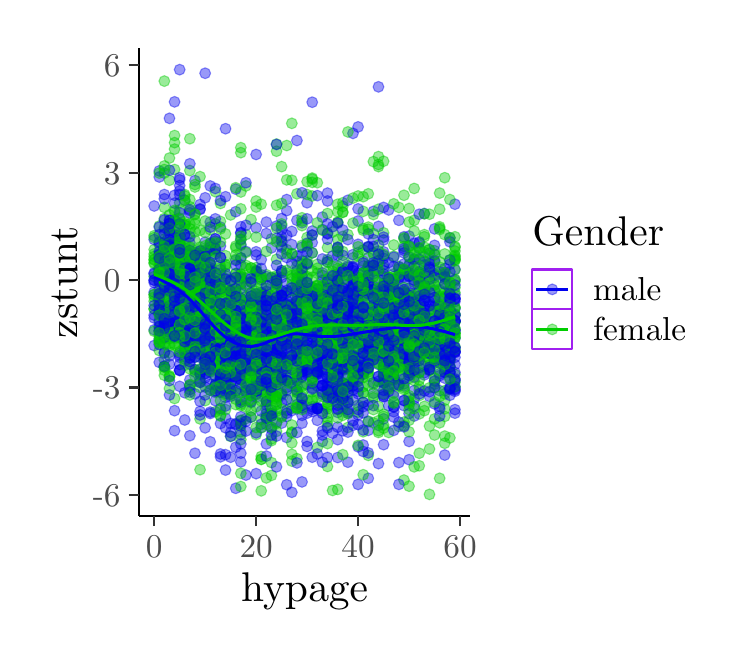
\begin{tikzpicture}[x=1pt,y=1pt]
\definecolor{fillColor}{RGB}{255,255,255}
\path[use as bounding box,fill=fillColor,fill opacity=0.00] (0,0) rectangle (252.94,216.81);
\begin{scope}
\path[clip] (  0.00,  0.00) rectangle (252.94,216.81);
\definecolor{drawColor}{RGB}{255,255,255}
\definecolor{fillColor}{RGB}{255,255,255}

\path[draw=drawColor,line width= 0.8pt,line join=round,line cap=round,fill=fillColor] (  0.00,  0.00) rectangle (252.94,216.81);
\end{scope}
\begin{scope}
\path[clip] ( 40.27, 40.48) rectangle (159.83,209.31);
\definecolor{fillColor}{RGB}{255,255,255}

\path[fill=fillColor] ( 40.27, 40.48) rectangle (159.83,209.31);
\definecolor{drawColor}{RGB}{0,0,238}
\definecolor{fillColor}{RGB}{0,0,238}

\path[draw=drawColor,draw opacity=0.40,line width= 0.4pt,line join=round,line cap=round,fill=fillColor,fill opacity=0.40] ( 56.76,154.44) circle (  1.96);

\path[draw=drawColor,draw opacity=0.40,line width= 0.4pt,line join=round,line cap=round,fill=fillColor,fill opacity=0.40] ( 97.29,147.20) circle (  1.96);

\path[draw=drawColor,draw opacity=0.40,line width= 0.4pt,line join=round,line cap=round,fill=fillColor,fill opacity=0.40] ( 82.55,128.71) circle (  1.96);
\definecolor{drawColor}{RGB}{0,205,0}
\definecolor{fillColor}{RGB}{0,205,0}

\path[draw=drawColor,draw opacity=0.40,line width= 0.4pt,line join=round,line cap=round,fill=fillColor,fill opacity=0.40] (132.29, 94.06) circle (  1.96);

\path[draw=drawColor,draw opacity=0.40,line width= 0.4pt,line join=round,line cap=round,fill=fillColor,fill opacity=0.40] ( 71.50,114.75) circle (  1.96);
\definecolor{drawColor}{RGB}{0,0,238}
\definecolor{fillColor}{RGB}{0,0,238}

\path[draw=drawColor,draw opacity=0.40,line width= 0.4pt,line join=round,line cap=round,fill=fillColor,fill opacity=0.40] ( 73.34,116.82) circle (  1.96);
\definecolor{drawColor}{RGB}{0,205,0}
\definecolor{fillColor}{RGB}{0,205,0}

\path[draw=drawColor,draw opacity=0.40,line width= 0.4pt,line join=round,line cap=round,fill=fillColor,fill opacity=0.40] (137.82, 96.90) circle (  1.96);
\definecolor{drawColor}{RGB}{0,0,238}
\definecolor{fillColor}{RGB}{0,0,238}

\path[draw=drawColor,draw opacity=0.40,line width= 0.4pt,line join=round,line cap=round,fill=fillColor,fill opacity=0.40] ( 71.50,117.33) circle (  1.96);

\path[draw=drawColor,draw opacity=0.40,line width= 0.4pt,line join=round,line cap=round,fill=fillColor,fill opacity=0.40] ( 64.13,115.01) circle (  1.96);
\definecolor{drawColor}{RGB}{0,205,0}
\definecolor{fillColor}{RGB}{0,205,0}

\path[draw=drawColor,draw opacity=0.40,line width= 0.4pt,line join=round,line cap=round,fill=fillColor,fill opacity=0.40] ( 78.87, 92.64) circle (  1.96);
\definecolor{drawColor}{RGB}{0,0,238}
\definecolor{fillColor}{RGB}{0,0,238}

\path[draw=drawColor,draw opacity=0.40,line width= 0.4pt,line join=round,line cap=round,fill=fillColor,fill opacity=0.40] ( 89.92, 99.36) circle (  1.96);

\path[draw=drawColor,draw opacity=0.40,line width= 0.4pt,line join=round,line cap=round,fill=fillColor,fill opacity=0.40] ( 97.29,132.33) circle (  1.96);

\path[draw=drawColor,draw opacity=0.40,line width= 0.4pt,line join=round,line cap=round,fill=fillColor,fill opacity=0.40] ( 60.44,122.63) circle (  1.96);
\definecolor{drawColor}{RGB}{0,205,0}
\definecolor{fillColor}{RGB}{0,205,0}

\path[draw=drawColor,draw opacity=0.40,line width= 0.4pt,line join=round,line cap=round,fill=fillColor,fill opacity=0.40] (128.61, 92.77) circle (  1.96);
\definecolor{drawColor}{RGB}{0,0,238}
\definecolor{fillColor}{RGB}{0,0,238}

\path[draw=drawColor,draw opacity=0.40,line width= 0.4pt,line join=round,line cap=round,fill=fillColor,fill opacity=0.40] ( 86.24, 81.90) circle (  1.96);
\definecolor{drawColor}{RGB}{0,205,0}
\definecolor{fillColor}{RGB}{0,205,0}

\path[draw=drawColor,draw opacity=0.40,line width= 0.4pt,line join=round,line cap=round,fill=fillColor,fill opacity=0.40] (119.40, 98.33) circle (  1.96);

\path[draw=drawColor,draw opacity=0.40,line width= 0.4pt,line join=round,line cap=round,fill=fillColor,fill opacity=0.40] ( 65.97, 98.07) circle (  1.96);
\definecolor{drawColor}{RGB}{0,0,238}
\definecolor{fillColor}{RGB}{0,0,238}

\path[draw=drawColor,draw opacity=0.40,line width= 0.4pt,line join=round,line cap=round,fill=fillColor,fill opacity=0.40] ( 58.60,133.75) circle (  1.96);

\path[draw=drawColor,draw opacity=0.40,line width= 0.4pt,line join=round,line cap=round,fill=fillColor,fill opacity=0.40] (100.97,116.82) circle (  1.96);
\definecolor{drawColor}{RGB}{0,205,0}
\definecolor{fillColor}{RGB}{0,205,0}

\path[draw=drawColor,draw opacity=0.40,line width= 0.4pt,line join=round,line cap=round,fill=fillColor,fill opacity=0.40] (123.08, 92.38) circle (  1.96);

\path[draw=drawColor,draw opacity=0.40,line width= 0.4pt,line join=round,line cap=round,fill=fillColor,fill opacity=0.40] ( 77.02, 80.74) circle (  1.96);

\path[draw=drawColor,draw opacity=0.40,line width= 0.4pt,line join=round,line cap=round,fill=fillColor,fill opacity=0.40] ( 64.13,124.44) circle (  1.96);

\path[draw=drawColor,draw opacity=0.40,line width= 0.4pt,line join=round,line cap=round,fill=fillColor,fill opacity=0.40] ( 75.18,127.94) circle (  1.96);
\definecolor{drawColor}{RGB}{0,0,238}
\definecolor{fillColor}{RGB}{0,0,238}

\path[draw=drawColor,draw opacity=0.40,line width= 0.4pt,line join=round,line cap=round,fill=fillColor,fill opacity=0.40] ( 47.55,118.63) circle (  1.96);

\path[draw=drawColor,draw opacity=0.40,line width= 0.4pt,line join=round,line cap=round,fill=fillColor,fill opacity=0.40] (119.40, 85.40) circle (  1.96);

\path[draw=drawColor,draw opacity=0.40,line width= 0.4pt,line join=round,line cap=round,fill=fillColor,fill opacity=0.40] ( 67.81,114.62) circle (  1.96);
\definecolor{drawColor}{RGB}{0,205,0}
\definecolor{fillColor}{RGB}{0,205,0}

\path[draw=drawColor,draw opacity=0.40,line width= 0.4pt,line join=round,line cap=round,fill=fillColor,fill opacity=0.40] (128.61,124.31) circle (  1.96);

\path[draw=drawColor,draw opacity=0.40,line width= 0.4pt,line join=round,line cap=round,fill=fillColor,fill opacity=0.40] ( 54.92,150.95) circle (  1.96);

\path[draw=drawColor,draw opacity=0.40,line width= 0.4pt,line join=round,line cap=round,fill=fillColor,fill opacity=0.40] (141.50,111.13) circle (  1.96);
\definecolor{drawColor}{RGB}{0,0,238}
\definecolor{fillColor}{RGB}{0,0,238}

\path[draw=drawColor,draw opacity=0.40,line width= 0.4pt,line join=round,line cap=round,fill=fillColor,fill opacity=0.40] (110.18,123.02) circle (  1.96);

\path[draw=drawColor,draw opacity=0.40,line width= 0.4pt,line join=round,line cap=round,fill=fillColor,fill opacity=0.40] ( 86.24, 77.38) circle (  1.96);
\definecolor{drawColor}{RGB}{0,205,0}
\definecolor{fillColor}{RGB}{0,205,0}

\path[draw=drawColor,draw opacity=0.40,line width= 0.4pt,line join=round,line cap=round,fill=fillColor,fill opacity=0.40] ( 86.24,108.02) circle (  1.96);

\path[draw=drawColor,draw opacity=0.40,line width= 0.4pt,line join=round,line cap=round,fill=fillColor,fill opacity=0.40] ( 86.24, 82.03) circle (  1.96);
\definecolor{drawColor}{RGB}{0,0,238}
\definecolor{fillColor}{RGB}{0,0,238}

\path[draw=drawColor,draw opacity=0.40,line width= 0.4pt,line join=round,line cap=round,fill=fillColor,fill opacity=0.40] ( 77.02,115.01) circle (  1.96);
\definecolor{drawColor}{RGB}{0,205,0}
\definecolor{fillColor}{RGB}{0,205,0}

\path[draw=drawColor,draw opacity=0.40,line width= 0.4pt,line join=round,line cap=round,fill=fillColor,fill opacity=0.40] ( 77.02,124.19) circle (  1.96);
\definecolor{drawColor}{RGB}{0,0,238}
\definecolor{fillColor}{RGB}{0,0,238}

\path[draw=drawColor,draw opacity=0.40,line width= 0.4pt,line join=round,line cap=round,fill=fillColor,fill opacity=0.40] ( 71.50,110.61) circle (  1.96);
\definecolor{drawColor}{RGB}{0,205,0}
\definecolor{fillColor}{RGB}{0,205,0}

\path[draw=drawColor,draw opacity=0.40,line width= 0.4pt,line join=round,line cap=round,fill=fillColor,fill opacity=0.40] (121.24,115.52) circle (  1.96);
\definecolor{drawColor}{RGB}{0,0,238}
\definecolor{fillColor}{RGB}{0,0,238}

\path[draw=drawColor,draw opacity=0.40,line width= 0.4pt,line join=round,line cap=round,fill=fillColor,fill opacity=0.40] (143.34,114.75) circle (  1.96);

\path[draw=drawColor,draw opacity=0.40,line width= 0.4pt,line join=round,line cap=round,fill=fillColor,fill opacity=0.40] ( 73.34, 90.70) circle (  1.96);
\definecolor{drawColor}{RGB}{0,205,0}
\definecolor{fillColor}{RGB}{0,205,0}

\path[draw=drawColor,draw opacity=0.40,line width= 0.4pt,line join=round,line cap=round,fill=fillColor,fill opacity=0.40] (110.18,112.29) circle (  1.96);

\path[draw=drawColor,draw opacity=0.40,line width= 0.4pt,line join=round,line cap=round,fill=fillColor,fill opacity=0.40] ( 53.08,104.66) circle (  1.96);

\path[draw=drawColor,draw opacity=0.40,line width= 0.4pt,line join=round,line cap=round,fill=fillColor,fill opacity=0.40] (135.98,120.95) circle (  1.96);

\path[draw=drawColor,draw opacity=0.40,line width= 0.4pt,line join=round,line cap=round,fill=fillColor,fill opacity=0.40] ( 82.55, 84.10) circle (  1.96);

\path[draw=drawColor,draw opacity=0.40,line width= 0.4pt,line join=round,line cap=round,fill=fillColor,fill opacity=0.40] (112.03,111.90) circle (  1.96);

\path[draw=drawColor,draw opacity=0.40,line width= 0.4pt,line join=round,line cap=round,fill=fillColor,fill opacity=0.40] (126.76, 79.97) circle (  1.96);

\path[draw=drawColor,draw opacity=0.40,line width= 0.4pt,line join=round,line cap=round,fill=fillColor,fill opacity=0.40] ( 73.34, 93.41) circle (  1.96);

\path[draw=drawColor,draw opacity=0.40,line width= 0.4pt,line join=round,line cap=round,fill=fillColor,fill opacity=0.40] ( 84.39,106.34) circle (  1.96);
\definecolor{drawColor}{RGB}{0,0,238}
\definecolor{fillColor}{RGB}{0,0,238}

\path[draw=drawColor,draw opacity=0.40,line width= 0.4pt,line join=round,line cap=round,fill=fillColor,fill opacity=0.40] (135.98, 97.29) circle (  1.96);
\definecolor{drawColor}{RGB}{0,205,0}
\definecolor{fillColor}{RGB}{0,205,0}

\path[draw=drawColor,draw opacity=0.40,line width= 0.4pt,line join=round,line cap=round,fill=fillColor,fill opacity=0.40] ( 77.02, 74.79) circle (  1.96);
\definecolor{drawColor}{RGB}{0,0,238}
\definecolor{fillColor}{RGB}{0,0,238}

\path[draw=drawColor,draw opacity=0.40,line width= 0.4pt,line join=round,line cap=round,fill=fillColor,fill opacity=0.40] (150.71,110.61) circle (  1.96);
\definecolor{drawColor}{RGB}{0,205,0}
\definecolor{fillColor}{RGB}{0,205,0}

\path[draw=drawColor,draw opacity=0.40,line width= 0.4pt,line join=round,line cap=round,fill=fillColor,fill opacity=0.40] ( 54.92,113.45) circle (  1.96);
\definecolor{drawColor}{RGB}{0,0,238}
\definecolor{fillColor}{RGB}{0,0,238}

\path[draw=drawColor,draw opacity=0.40,line width= 0.4pt,line join=round,line cap=round,fill=fillColor,fill opacity=0.40] (141.50,112.42) circle (  1.96);

\path[draw=drawColor,draw opacity=0.40,line width= 0.4pt,line join=round,line cap=round,fill=fillColor,fill opacity=0.40] ( 77.02, 93.80) circle (  1.96);
\definecolor{drawColor}{RGB}{0,205,0}
\definecolor{fillColor}{RGB}{0,205,0}

\path[draw=drawColor,draw opacity=0.40,line width= 0.4pt,line join=round,line cap=round,fill=fillColor,fill opacity=0.40] (115.71,111.64) circle (  1.96);

\path[draw=drawColor,draw opacity=0.40,line width= 0.4pt,line join=round,line cap=round,fill=fillColor,fill opacity=0.40] ( 62.29,121.73) circle (  1.96);
\definecolor{drawColor}{RGB}{0,0,238}
\definecolor{fillColor}{RGB}{0,0,238}

\path[draw=drawColor,draw opacity=0.40,line width= 0.4pt,line join=round,line cap=round,fill=fillColor,fill opacity=0.40] (123.08, 98.58) circle (  1.96);
\definecolor{drawColor}{RGB}{0,205,0}
\definecolor{fillColor}{RGB}{0,205,0}

\path[draw=drawColor,draw opacity=0.40,line width= 0.4pt,line join=round,line cap=round,fill=fillColor,fill opacity=0.40] ( 95.45, 62.64) circle (  1.96);

\path[draw=drawColor,draw opacity=0.40,line width= 0.4pt,line join=round,line cap=round,fill=fillColor,fill opacity=0.40] (130.45,111.38) circle (  1.96);

\path[draw=drawColor,draw opacity=0.40,line width= 0.4pt,line join=round,line cap=round,fill=fillColor,fill opacity=0.40] (150.71, 76.34) circle (  1.96);
\definecolor{drawColor}{RGB}{0,0,238}
\definecolor{fillColor}{RGB}{0,0,238}

\path[draw=drawColor,draw opacity=0.40,line width= 0.4pt,line join=round,line cap=round,fill=fillColor,fill opacity=0.40] ( 73.34, 86.17) circle (  1.96);
\definecolor{drawColor}{RGB}{0,205,0}
\definecolor{fillColor}{RGB}{0,205,0}

\path[draw=drawColor,draw opacity=0.40,line width= 0.4pt,line join=round,line cap=round,fill=fillColor,fill opacity=0.40] ( 95.45,109.06) circle (  1.96);
\definecolor{drawColor}{RGB}{0,0,238}
\definecolor{fillColor}{RGB}{0,0,238}

\path[draw=drawColor,draw opacity=0.40,line width= 0.4pt,line join=round,line cap=round,fill=fillColor,fill opacity=0.40] ( 93.60,104.01) circle (  1.96);

\path[draw=drawColor,draw opacity=0.40,line width= 0.4pt,line join=round,line cap=round,fill=fillColor,fill opacity=0.40] (145.19,106.47) circle (  1.96);
\definecolor{drawColor}{RGB}{0,205,0}
\definecolor{fillColor}{RGB}{0,205,0}

\path[draw=drawColor,draw opacity=0.40,line width= 0.4pt,line join=round,line cap=round,fill=fillColor,fill opacity=0.40] (154.40,106.34) circle (  1.96);

\path[draw=drawColor,draw opacity=0.40,line width= 0.4pt,line join=round,line cap=round,fill=fillColor,fill opacity=0.40] ( 65.97,112.16) circle (  1.96);

\path[draw=drawColor,draw opacity=0.40,line width= 0.4pt,line join=round,line cap=round,fill=fillColor,fill opacity=0.40] (137.82, 93.54) circle (  1.96);

\path[draw=drawColor,draw opacity=0.40,line width= 0.4pt,line join=round,line cap=round,fill=fillColor,fill opacity=0.40] (112.03, 89.79) circle (  1.96);

\path[draw=drawColor,draw opacity=0.40,line width= 0.4pt,line join=round,line cap=round,fill=fillColor,fill opacity=0.40] (102.82,162.46) circle (  1.96);

\path[draw=drawColor,draw opacity=0.40,line width= 0.4pt,line join=round,line cap=round,fill=fillColor,fill opacity=0.40] (128.61,122.50) circle (  1.96);

\path[draw=drawColor,draw opacity=0.40,line width= 0.4pt,line join=round,line cap=round,fill=fillColor,fill opacity=0.40] (154.40,112.81) circle (  1.96);

\path[draw=drawColor,draw opacity=0.40,line width= 0.4pt,line join=round,line cap=round,fill=fillColor,fill opacity=0.40] ( 78.87,113.20) circle (  1.96);

\path[draw=drawColor,draw opacity=0.40,line width= 0.4pt,line join=round,line cap=round,fill=fillColor,fill opacity=0.40] ( 67.81, 78.03) circle (  1.96);

\path[draw=drawColor,draw opacity=0.40,line width= 0.4pt,line join=round,line cap=round,fill=fillColor,fill opacity=0.40] ( 58.60,126.25) circle (  1.96);
\definecolor{drawColor}{RGB}{0,0,238}
\definecolor{fillColor}{RGB}{0,0,238}

\path[draw=drawColor,draw opacity=0.40,line width= 0.4pt,line join=round,line cap=round,fill=fillColor,fill opacity=0.40] (150.71,101.82) circle (  1.96);

\path[draw=drawColor,draw opacity=0.40,line width= 0.4pt,line join=round,line cap=round,fill=fillColor,fill opacity=0.40] (112.03,137.50) circle (  1.96);

\path[draw=drawColor,draw opacity=0.40,line width= 0.4pt,line join=round,line cap=round,fill=fillColor,fill opacity=0.40] ( 71.50, 93.93) circle (  1.96);

\path[draw=drawColor,draw opacity=0.40,line width= 0.4pt,line join=round,line cap=round,fill=fillColor,fill opacity=0.40] (104.66, 93.15) circle (  1.96);

\path[draw=drawColor,draw opacity=0.40,line width= 0.4pt,line join=round,line cap=round,fill=fillColor,fill opacity=0.40] (130.45,103.50) circle (  1.96);
\definecolor{drawColor}{RGB}{0,205,0}
\definecolor{fillColor}{RGB}{0,205,0}

\path[draw=drawColor,draw opacity=0.40,line width= 0.4pt,line join=round,line cap=round,fill=fillColor,fill opacity=0.40] (104.66, 95.61) circle (  1.96);

\path[draw=drawColor,draw opacity=0.40,line width= 0.4pt,line join=round,line cap=round,fill=fillColor,fill opacity=0.40] (110.18,108.67) circle (  1.96);

\path[draw=drawColor,draw opacity=0.40,line width= 0.4pt,line join=round,line cap=round,fill=fillColor,fill opacity=0.40] ( 53.08,131.17) circle (  1.96);
\definecolor{drawColor}{RGB}{0,0,238}
\definecolor{fillColor}{RGB}{0,0,238}

\path[draw=drawColor,draw opacity=0.40,line width= 0.4pt,line join=round,line cap=round,fill=fillColor,fill opacity=0.40] (115.71,103.89) circle (  1.96);
\definecolor{drawColor}{RGB}{0,205,0}
\definecolor{fillColor}{RGB}{0,205,0}

\path[draw=drawColor,draw opacity=0.40,line width= 0.4pt,line join=round,line cap=round,fill=fillColor,fill opacity=0.40] ( 54.92,126.25) circle (  1.96);
\definecolor{drawColor}{RGB}{0,0,238}
\definecolor{fillColor}{RGB}{0,0,238}

\path[draw=drawColor,draw opacity=0.40,line width= 0.4pt,line join=round,line cap=round,fill=fillColor,fill opacity=0.40] (106.50,125.48) circle (  1.96);
\definecolor{drawColor}{RGB}{0,205,0}
\definecolor{fillColor}{RGB}{0,205,0}

\path[draw=drawColor,draw opacity=0.40,line width= 0.4pt,line join=round,line cap=round,fill=fillColor,fill opacity=0.40] ( 69.66,112.16) circle (  1.96);

\path[draw=drawColor,draw opacity=0.40,line width= 0.4pt,line join=round,line cap=round,fill=fillColor,fill opacity=0.40] (130.45,125.35) circle (  1.96);
\definecolor{drawColor}{RGB}{0,0,238}
\definecolor{fillColor}{RGB}{0,0,238}

\path[draw=drawColor,draw opacity=0.40,line width= 0.4pt,line join=round,line cap=round,fill=fillColor,fill opacity=0.40] (130.45,150.95) circle (  1.96);
\definecolor{drawColor}{RGB}{0,205,0}
\definecolor{fillColor}{RGB}{0,205,0}

\path[draw=drawColor,draw opacity=0.40,line width= 0.4pt,line join=round,line cap=round,fill=fillColor,fill opacity=0.40] ( 84.39,119.79) circle (  1.96);
\definecolor{drawColor}{RGB}{0,0,238}
\definecolor{fillColor}{RGB}{0,0,238}

\path[draw=drawColor,draw opacity=0.40,line width= 0.4pt,line join=round,line cap=round,fill=fillColor,fill opacity=0.40] (145.19,106.99) circle (  1.96);
\definecolor{drawColor}{RGB}{0,205,0}
\definecolor{fillColor}{RGB}{0,205,0}

\path[draw=drawColor,draw opacity=0.40,line width= 0.4pt,line join=round,line cap=round,fill=fillColor,fill opacity=0.40] ( 64.13,108.02) circle (  1.96);

\path[draw=drawColor,draw opacity=0.40,line width= 0.4pt,line join=round,line cap=round,fill=fillColor,fill opacity=0.40] ( 67.81,113.71) circle (  1.96);
\definecolor{drawColor}{RGB}{0,0,238}
\definecolor{fillColor}{RGB}{0,0,238}

\path[draw=drawColor,draw opacity=0.40,line width= 0.4pt,line join=round,line cap=round,fill=fillColor,fill opacity=0.40] ( 69.66, 86.43) circle (  1.96);

\path[draw=drawColor,draw opacity=0.40,line width= 0.4pt,line join=round,line cap=round,fill=fillColor,fill opacity=0.40] (121.24,124.31) circle (  1.96);
\definecolor{drawColor}{RGB}{0,205,0}
\definecolor{fillColor}{RGB}{0,205,0}

\path[draw=drawColor,draw opacity=0.40,line width= 0.4pt,line join=round,line cap=round,fill=fillColor,fill opacity=0.40] (143.34, 98.84) circle (  1.96);
\definecolor{drawColor}{RGB}{0,0,238}
\definecolor{fillColor}{RGB}{0,0,238}

\path[draw=drawColor,draw opacity=0.40,line width= 0.4pt,line join=round,line cap=round,fill=fillColor,fill opacity=0.40] (106.50,123.15) circle (  1.96);

\path[draw=drawColor,draw opacity=0.40,line width= 0.4pt,line join=round,line cap=round,fill=fillColor,fill opacity=0.40] (145.19, 83.59) circle (  1.96);

\path[draw=drawColor,draw opacity=0.40,line width= 0.4pt,line join=round,line cap=round,fill=fillColor,fill opacity=0.40] ( 86.24,106.86) circle (  1.96);

\path[draw=drawColor,draw opacity=0.40,line width= 0.4pt,line join=round,line cap=round,fill=fillColor,fill opacity=0.40] ( 62.29,131.56) circle (  1.96);
\definecolor{drawColor}{RGB}{0,205,0}
\definecolor{fillColor}{RGB}{0,205,0}

\path[draw=drawColor,draw opacity=0.40,line width= 0.4pt,line join=round,line cap=round,fill=fillColor,fill opacity=0.40] ( 49.39,132.46) circle (  1.96);

\path[draw=drawColor,draw opacity=0.40,line width= 0.4pt,line join=round,line cap=round,fill=fillColor,fill opacity=0.40] (143.34,122.63) circle (  1.96);
\definecolor{drawColor}{RGB}{0,0,238}
\definecolor{fillColor}{RGB}{0,0,238}

\path[draw=drawColor,draw opacity=0.40,line width= 0.4pt,line join=round,line cap=round,fill=fillColor,fill opacity=0.40] ( 51.23,115.01) circle (  1.96);

\path[draw=drawColor,draw opacity=0.40,line width= 0.4pt,line join=round,line cap=round,fill=fillColor,fill opacity=0.40] (139.66,102.46) circle (  1.96);
\definecolor{drawColor}{RGB}{0,205,0}
\definecolor{fillColor}{RGB}{0,205,0}

\path[draw=drawColor,draw opacity=0.40,line width= 0.4pt,line join=round,line cap=round,fill=fillColor,fill opacity=0.40] ( 88.08, 83.84) circle (  1.96);

\path[draw=drawColor,draw opacity=0.40,line width= 0.4pt,line join=round,line cap=round,fill=fillColor,fill opacity=0.40] (110.18, 49.58) circle (  1.96);
\definecolor{drawColor}{RGB}{0,0,238}
\definecolor{fillColor}{RGB}{0,0,238}

\path[draw=drawColor,draw opacity=0.40,line width= 0.4pt,line join=round,line cap=round,fill=fillColor,fill opacity=0.40] (108.34,111.26) circle (  1.96);

\path[draw=drawColor,draw opacity=0.40,line width= 0.4pt,line join=round,line cap=round,fill=fillColor,fill opacity=0.40] (137.82, 95.61) circle (  1.96);

\path[draw=drawColor,draw opacity=0.40,line width= 0.4pt,line join=round,line cap=round,fill=fillColor,fill opacity=0.40] (139.66,118.24) circle (  1.96);

\path[draw=drawColor,draw opacity=0.40,line width= 0.4pt,line join=round,line cap=round,fill=fillColor,fill opacity=0.40] ( 65.97,119.27) circle (  1.96);

\path[draw=drawColor,draw opacity=0.40,line width= 0.4pt,line join=round,line cap=round,fill=fillColor,fill opacity=0.40] (102.82, 61.60) circle (  1.96);
\definecolor{drawColor}{RGB}{0,205,0}
\definecolor{fillColor}{RGB}{0,205,0}

\path[draw=drawColor,draw opacity=0.40,line width= 0.4pt,line join=round,line cap=round,fill=fillColor,fill opacity=0.40] ( 49.39,147.85) circle (  1.96);

\path[draw=drawColor,draw opacity=0.40,line width= 0.4pt,line join=round,line cap=round,fill=fillColor,fill opacity=0.40] (124.92,130.78) circle (  1.96);
\definecolor{drawColor}{RGB}{0,0,238}
\definecolor{fillColor}{RGB}{0,0,238}

\path[draw=drawColor,draw opacity=0.40,line width= 0.4pt,line join=round,line cap=round,fill=fillColor,fill opacity=0.40] ( 65.97, 97.81) circle (  1.96);
\definecolor{drawColor}{RGB}{0,205,0}
\definecolor{fillColor}{RGB}{0,205,0}

\path[draw=drawColor,draw opacity=0.40,line width= 0.4pt,line join=round,line cap=round,fill=fillColor,fill opacity=0.40] ( 91.76,105.70) circle (  1.96);
\definecolor{drawColor}{RGB}{0,0,238}
\definecolor{fillColor}{RGB}{0,0,238}

\path[draw=drawColor,draw opacity=0.40,line width= 0.4pt,line join=round,line cap=round,fill=fillColor,fill opacity=0.40] ( 65.97,104.79) circle (  1.96);

\path[draw=drawColor,draw opacity=0.40,line width= 0.4pt,line join=round,line cap=round,fill=fillColor,fill opacity=0.40] (124.92,112.94) circle (  1.96);

\path[draw=drawColor,draw opacity=0.40,line width= 0.4pt,line join=round,line cap=round,fill=fillColor,fill opacity=0.40] (137.82,111.38) circle (  1.96);

\path[draw=drawColor,draw opacity=0.40,line width= 0.4pt,line join=round,line cap=round,fill=fillColor,fill opacity=0.40] ( 95.45,105.70) circle (  1.96);

\path[draw=drawColor,draw opacity=0.40,line width= 0.4pt,line join=round,line cap=round,fill=fillColor,fill opacity=0.40] ( 69.66,124.44) circle (  1.96);

\path[draw=drawColor,draw opacity=0.40,line width= 0.4pt,line join=round,line cap=round,fill=fillColor,fill opacity=0.40] (123.08,115.52) circle (  1.96);
\definecolor{drawColor}{RGB}{0,205,0}
\definecolor{fillColor}{RGB}{0,205,0}

\path[draw=drawColor,draw opacity=0.40,line width= 0.4pt,line join=round,line cap=round,fill=fillColor,fill opacity=0.40] ( 67.81,122.63) circle (  1.96);

\path[draw=drawColor,draw opacity=0.40,line width= 0.4pt,line join=round,line cap=round,fill=fillColor,fill opacity=0.40] ( 51.23,124.44) circle (  1.96);

\path[draw=drawColor,draw opacity=0.40,line width= 0.4pt,line join=round,line cap=round,fill=fillColor,fill opacity=0.40] (137.82,117.07) circle (  1.96);

\path[draw=drawColor,draw opacity=0.40,line width= 0.4pt,line join=round,line cap=round,fill=fillColor,fill opacity=0.40] ( 67.81,136.34) circle (  1.96);

\path[draw=drawColor,draw opacity=0.40,line width= 0.4pt,line join=round,line cap=round,fill=fillColor,fill opacity=0.40] ( 69.66,111.51) circle (  1.96);

\path[draw=drawColor,draw opacity=0.40,line width= 0.4pt,line join=round,line cap=round,fill=fillColor,fill opacity=0.40] ( 99.13,118.63) circle (  1.96);

\path[draw=drawColor,draw opacity=0.40,line width= 0.4pt,line join=round,line cap=round,fill=fillColor,fill opacity=0.40] (150.71, 84.49) circle (  1.96);
\definecolor{drawColor}{RGB}{0,0,238}
\definecolor{fillColor}{RGB}{0,0,238}

\path[draw=drawColor,draw opacity=0.40,line width= 0.4pt,line join=round,line cap=round,fill=fillColor,fill opacity=0.40] ( 86.24, 75.70) circle (  1.96);
\definecolor{drawColor}{RGB}{0,205,0}
\definecolor{fillColor}{RGB}{0,205,0}

\path[draw=drawColor,draw opacity=0.40,line width= 0.4pt,line join=round,line cap=round,fill=fillColor,fill opacity=0.40] (137.82, 94.83) circle (  1.96);
\definecolor{drawColor}{RGB}{0,0,238}
\definecolor{fillColor}{RGB}{0,0,238}

\path[draw=drawColor,draw opacity=0.40,line width= 0.4pt,line join=round,line cap=round,fill=fillColor,fill opacity=0.40] ( 53.08,107.51) circle (  1.96);

\path[draw=drawColor,draw opacity=0.40,line width= 0.4pt,line join=round,line cap=round,fill=fillColor,fill opacity=0.40] ( 89.92,103.89) circle (  1.96);

\path[draw=drawColor,draw opacity=0.40,line width= 0.4pt,line join=round,line cap=round,fill=fillColor,fill opacity=0.40] ( 89.92,116.17) circle (  1.96);

\path[draw=drawColor,draw opacity=0.40,line width= 0.4pt,line join=round,line cap=round,fill=fillColor,fill opacity=0.40] ( 51.23,130.39) circle (  1.96);

\path[draw=drawColor,draw opacity=0.40,line width= 0.4pt,line join=round,line cap=round,fill=fillColor,fill opacity=0.40] ( 45.71,127.81) circle (  1.96);
\definecolor{drawColor}{RGB}{0,205,0}
\definecolor{fillColor}{RGB}{0,205,0}

\path[draw=drawColor,draw opacity=0.40,line width= 0.4pt,line join=round,line cap=round,fill=fillColor,fill opacity=0.40] (123.08,121.47) circle (  1.96);

\path[draw=drawColor,draw opacity=0.40,line width= 0.4pt,line join=round,line cap=round,fill=fillColor,fill opacity=0.40] ( 62.29,124.96) circle (  1.96);

\path[draw=drawColor,draw opacity=0.40,line width= 0.4pt,line join=round,line cap=round,fill=fillColor,fill opacity=0.40] ( 91.76, 97.94) circle (  1.96);
\definecolor{drawColor}{RGB}{0,0,238}
\definecolor{fillColor}{RGB}{0,0,238}

\path[draw=drawColor,draw opacity=0.40,line width= 0.4pt,line join=round,line cap=round,fill=fillColor,fill opacity=0.40] ( 49.39,136.86) circle (  1.96);
\definecolor{drawColor}{RGB}{0,205,0}
\definecolor{fillColor}{RGB}{0,205,0}

\path[draw=drawColor,draw opacity=0.40,line width= 0.4pt,line join=round,line cap=round,fill=fillColor,fill opacity=0.40] ( 47.55,132.85) circle (  1.96);
\definecolor{drawColor}{RGB}{0,0,238}
\definecolor{fillColor}{RGB}{0,0,238}

\path[draw=drawColor,draw opacity=0.40,line width= 0.4pt,line join=round,line cap=round,fill=fillColor,fill opacity=0.40] (130.45,122.89) circle (  1.96);
\definecolor{drawColor}{RGB}{0,205,0}
\definecolor{fillColor}{RGB}{0,205,0}

\path[draw=drawColor,draw opacity=0.40,line width= 0.4pt,line join=round,line cap=round,fill=fillColor,fill opacity=0.40] ( 64.13,106.73) circle (  1.96);

\path[draw=drawColor,draw opacity=0.40,line width= 0.4pt,line join=round,line cap=round,fill=fillColor,fill opacity=0.40] ( 89.92, 93.15) circle (  1.96);
\definecolor{drawColor}{RGB}{0,0,238}
\definecolor{fillColor}{RGB}{0,0,238}

\path[draw=drawColor,draw opacity=0.40,line width= 0.4pt,line join=round,line cap=round,fill=fillColor,fill opacity=0.40] (123.08, 71.30) circle (  1.96);
\definecolor{drawColor}{RGB}{0,205,0}
\definecolor{fillColor}{RGB}{0,205,0}

\path[draw=drawColor,draw opacity=0.40,line width= 0.4pt,line join=round,line cap=round,fill=fillColor,fill opacity=0.40] ( 89.92,152.63) circle (  1.96);
\definecolor{drawColor}{RGB}{0,0,238}
\definecolor{fillColor}{RGB}{0,0,238}

\path[draw=drawColor,draw opacity=0.40,line width= 0.4pt,line join=round,line cap=round,fill=fillColor,fill opacity=0.40] ( 91.76,143.84) circle (  1.96);
\definecolor{drawColor}{RGB}{0,205,0}
\definecolor{fillColor}{RGB}{0,205,0}

\path[draw=drawColor,draw opacity=0.40,line width= 0.4pt,line join=round,line cap=round,fill=fillColor,fill opacity=0.40] ( 51.23,145.26) circle (  1.96);
\definecolor{drawColor}{RGB}{0,0,238}
\definecolor{fillColor}{RGB}{0,0,238}

\path[draw=drawColor,draw opacity=0.40,line width= 0.4pt,line join=round,line cap=round,fill=fillColor,fill opacity=0.40] (152.56,140.87) circle (  1.96);

\path[draw=drawColor,draw opacity=0.40,line width= 0.4pt,line join=round,line cap=round,fill=fillColor,fill opacity=0.40] ( 89.92,145.13) circle (  1.96);

\path[draw=drawColor,draw opacity=0.40,line width= 0.4pt,line join=round,line cap=round,fill=fillColor,fill opacity=0.40] (124.92,150.43) circle (  1.96);

\path[draw=drawColor,draw opacity=0.40,line width= 0.4pt,line join=round,line cap=round,fill=fillColor,fill opacity=0.40] (102.82,122.89) circle (  1.96);

\path[draw=drawColor,draw opacity=0.40,line width= 0.4pt,line join=round,line cap=round,fill=fillColor,fill opacity=0.40] (108.34,142.29) circle (  1.96);

\path[draw=drawColor,draw opacity=0.40,line width= 0.4pt,line join=round,line cap=round,fill=fillColor,fill opacity=0.40] ( 53.08,131.56) circle (  1.96);
\definecolor{drawColor}{RGB}{0,205,0}
\definecolor{fillColor}{RGB}{0,205,0}

\path[draw=drawColor,draw opacity=0.40,line width= 0.4pt,line join=round,line cap=round,fill=fillColor,fill opacity=0.40] ( 62.29,131.17) circle (  1.96);
\definecolor{drawColor}{RGB}{0,0,238}
\definecolor{fillColor}{RGB}{0,0,238}

\path[draw=drawColor,draw opacity=0.40,line width= 0.4pt,line join=round,line cap=round,fill=fillColor,fill opacity=0.40] ( 89.92,122.50) circle (  1.96);

\path[draw=drawColor,draw opacity=0.40,line width= 0.4pt,line join=round,line cap=round,fill=fillColor,fill opacity=0.40] ( 49.39,129.36) circle (  1.96);

\path[draw=drawColor,draw opacity=0.40,line width= 0.4pt,line join=round,line cap=round,fill=fillColor,fill opacity=0.40] (128.61,103.50) circle (  1.96);

\path[draw=drawColor,draw opacity=0.40,line width= 0.4pt,line join=round,line cap=round,fill=fillColor,fill opacity=0.40] ( 71.50,101.17) circle (  1.96);

\path[draw=drawColor,draw opacity=0.40,line width= 0.4pt,line join=round,line cap=round,fill=fillColor,fill opacity=0.40] (100.97,153.54) circle (  1.96);

\path[draw=drawColor,draw opacity=0.40,line width= 0.4pt,line join=round,line cap=round,fill=fillColor,fill opacity=0.40] ( 65.97,130.00) circle (  1.96);

\path[draw=drawColor,draw opacity=0.40,line width= 0.4pt,line join=round,line cap=round,fill=fillColor,fill opacity=0.40] ( 97.29,108.02) circle (  1.96);
\definecolor{drawColor}{RGB}{0,205,0}
\definecolor{fillColor}{RGB}{0,205,0}

\path[draw=drawColor,draw opacity=0.40,line width= 0.4pt,line join=round,line cap=round,fill=fillColor,fill opacity=0.40] (132.29, 84.88) circle (  1.96);

\path[draw=drawColor,draw opacity=0.40,line width= 0.4pt,line join=round,line cap=round,fill=fillColor,fill opacity=0.40] ( 78.87, 75.57) circle (  1.96);
\definecolor{drawColor}{RGB}{0,0,238}
\definecolor{fillColor}{RGB}{0,0,238}

\path[draw=drawColor,draw opacity=0.40,line width= 0.4pt,line join=round,line cap=round,fill=fillColor,fill opacity=0.40] ( 97.29,101.04) circle (  1.96);
\definecolor{drawColor}{RGB}{0,205,0}
\definecolor{fillColor}{RGB}{0,205,0}

\path[draw=drawColor,draw opacity=0.40,line width= 0.4pt,line join=round,line cap=round,fill=fillColor,fill opacity=0.40] ( 49.39,133.11) circle (  1.96);

\path[draw=drawColor,draw opacity=0.40,line width= 0.4pt,line join=round,line cap=round,fill=fillColor,fill opacity=0.40] ( 99.13, 99.62) circle (  1.96);

\path[draw=drawColor,draw opacity=0.40,line width= 0.4pt,line join=round,line cap=round,fill=fillColor,fill opacity=0.40] (102.82, 94.83) circle (  1.96);
\definecolor{drawColor}{RGB}{0,0,238}
\definecolor{fillColor}{RGB}{0,0,238}

\path[draw=drawColor,draw opacity=0.40,line width= 0.4pt,line join=round,line cap=round,fill=fillColor,fill opacity=0.40] (152.56,100.39) circle (  1.96);
\definecolor{drawColor}{RGB}{0,205,0}
\definecolor{fillColor}{RGB}{0,205,0}

\path[draw=drawColor,draw opacity=0.40,line width= 0.4pt,line join=round,line cap=round,fill=fillColor,fill opacity=0.40] ( 49.39,114.62) circle (  1.96);
\definecolor{drawColor}{RGB}{0,0,238}
\definecolor{fillColor}{RGB}{0,0,238}

\path[draw=drawColor,draw opacity=0.40,line width= 0.4pt,line join=round,line cap=round,fill=fillColor,fill opacity=0.40] (102.82,116.04) circle (  1.96);

\path[draw=drawColor,draw opacity=0.40,line width= 0.4pt,line join=round,line cap=round,fill=fillColor,fill opacity=0.40] ( 86.24, 89.27) circle (  1.96);
\definecolor{drawColor}{RGB}{0,205,0}
\definecolor{fillColor}{RGB}{0,205,0}

\path[draw=drawColor,draw opacity=0.40,line width= 0.4pt,line join=round,line cap=round,fill=fillColor,fill opacity=0.40] ( 49.39,132.33) circle (  1.96);
\definecolor{drawColor}{RGB}{0,0,238}
\definecolor{fillColor}{RGB}{0,0,238}

\path[draw=drawColor,draw opacity=0.40,line width= 0.4pt,line join=round,line cap=round,fill=fillColor,fill opacity=0.40] (106.50,127.29) circle (  1.96);
\definecolor{drawColor}{RGB}{0,205,0}
\definecolor{fillColor}{RGB}{0,205,0}

\path[draw=drawColor,draw opacity=0.40,line width= 0.4pt,line join=round,line cap=round,fill=fillColor,fill opacity=0.40] ( 71.50,110.35) circle (  1.96);
\definecolor{drawColor}{RGB}{0,0,238}
\definecolor{fillColor}{RGB}{0,0,238}

\path[draw=drawColor,draw opacity=0.40,line width= 0.4pt,line join=round,line cap=round,fill=fillColor,fill opacity=0.40] ( 71.50, 75.70) circle (  1.96);
\definecolor{drawColor}{RGB}{0,205,0}
\definecolor{fillColor}{RGB}{0,205,0}

\path[draw=drawColor,draw opacity=0.40,line width= 0.4pt,line join=round,line cap=round,fill=fillColor,fill opacity=0.40] ( 88.08,118.24) circle (  1.96);

\path[draw=drawColor,draw opacity=0.40,line width= 0.4pt,line join=round,line cap=round,fill=fillColor,fill opacity=0.40] (104.66,109.96) circle (  1.96);

\path[draw=drawColor,draw opacity=0.40,line width= 0.4pt,line join=round,line cap=round,fill=fillColor,fill opacity=0.40] ( 62.29,122.76) circle (  1.96);
\definecolor{drawColor}{RGB}{0,0,238}
\definecolor{fillColor}{RGB}{0,0,238}

\path[draw=drawColor,draw opacity=0.40,line width= 0.4pt,line join=round,line cap=round,fill=fillColor,fill opacity=0.40] ( 60.44,135.43) circle (  1.96);

\path[draw=drawColor,draw opacity=0.40,line width= 0.4pt,line join=round,line cap=round,fill=fillColor,fill opacity=0.40] (132.29, 83.71) circle (  1.96);

\path[draw=drawColor,draw opacity=0.40,line width= 0.4pt,line join=round,line cap=round,fill=fillColor,fill opacity=0.40] (139.66,116.43) circle (  1.96);
\definecolor{drawColor}{RGB}{0,205,0}
\definecolor{fillColor}{RGB}{0,205,0}

\path[draw=drawColor,draw opacity=0.40,line width= 0.4pt,line join=round,line cap=round,fill=fillColor,fill opacity=0.40] (121.24,108.80) circle (  1.96);
\definecolor{drawColor}{RGB}{0,0,238}
\definecolor{fillColor}{RGB}{0,0,238}

\path[draw=drawColor,draw opacity=0.40,line width= 0.4pt,line join=round,line cap=round,fill=fillColor,fill opacity=0.40] ( 51.23,121.47) circle (  1.96);

\path[draw=drawColor,draw opacity=0.40,line width= 0.4pt,line join=round,line cap=round,fill=fillColor,fill opacity=0.40] (152.56,131.30) circle (  1.96);
\definecolor{drawColor}{RGB}{0,205,0}
\definecolor{fillColor}{RGB}{0,205,0}

\path[draw=drawColor,draw opacity=0.40,line width= 0.4pt,line join=round,line cap=round,fill=fillColor,fill opacity=0.40] (119.40,118.50) circle (  1.96);
\definecolor{drawColor}{RGB}{0,0,238}
\definecolor{fillColor}{RGB}{0,0,238}

\path[draw=drawColor,draw opacity=0.40,line width= 0.4pt,line join=round,line cap=round,fill=fillColor,fill opacity=0.40] ( 99.13, 82.55) circle (  1.96);

\path[draw=drawColor,draw opacity=0.40,line width= 0.4pt,line join=round,line cap=round,fill=fillColor,fill opacity=0.40] (145.19,107.76) circle (  1.96);

\path[draw=drawColor,draw opacity=0.40,line width= 0.4pt,line join=round,line cap=round,fill=fillColor,fill opacity=0.40] ( 75.18, 91.86) circle (  1.96);

\path[draw=drawColor,draw opacity=0.40,line width= 0.4pt,line join=round,line cap=round,fill=fillColor,fill opacity=0.40] ( 49.39,125.35) circle (  1.96);
\definecolor{drawColor}{RGB}{0,205,0}
\definecolor{fillColor}{RGB}{0,205,0}

\path[draw=drawColor,draw opacity=0.40,line width= 0.4pt,line join=round,line cap=round,fill=fillColor,fill opacity=0.40] ( 75.18, 91.34) circle (  1.96);

\path[draw=drawColor,draw opacity=0.40,line width= 0.4pt,line join=round,line cap=round,fill=fillColor,fill opacity=0.40] (112.03,101.95) circle (  1.96);

\path[draw=drawColor,draw opacity=0.40,line width= 0.4pt,line join=round,line cap=round,fill=fillColor,fill opacity=0.40] ( 84.39, 98.71) circle (  1.96);

\path[draw=drawColor,draw opacity=0.40,line width= 0.4pt,line join=round,line cap=round,fill=fillColor,fill opacity=0.40] ( 75.18,114.23) circle (  1.96);
\definecolor{drawColor}{RGB}{0,0,238}
\definecolor{fillColor}{RGB}{0,0,238}

\path[draw=drawColor,draw opacity=0.40,line width= 0.4pt,line join=round,line cap=round,fill=fillColor,fill opacity=0.40] ( 93.60, 78.54) circle (  1.96);

\path[draw=drawColor,draw opacity=0.40,line width= 0.4pt,line join=round,line cap=round,fill=fillColor,fill opacity=0.40] ( 93.60, 68.72) circle (  1.96);
\definecolor{drawColor}{RGB}{0,205,0}
\definecolor{fillColor}{RGB}{0,205,0}

\path[draw=drawColor,draw opacity=0.40,line width= 0.4pt,line join=round,line cap=round,fill=fillColor,fill opacity=0.40] (150.71,119.79) circle (  1.96);
\definecolor{drawColor}{RGB}{0,0,238}
\definecolor{fillColor}{RGB}{0,0,238}

\path[draw=drawColor,draw opacity=0.40,line width= 0.4pt,line join=round,line cap=round,fill=fillColor,fill opacity=0.40] ( 47.55,121.99) circle (  1.96);

\path[draw=drawColor,draw opacity=0.40,line width= 0.4pt,line join=round,line cap=round,fill=fillColor,fill opacity=0.40] ( 65.97,138.54) circle (  1.96);
\definecolor{drawColor}{RGB}{0,205,0}
\definecolor{fillColor}{RGB}{0,205,0}

\path[draw=drawColor,draw opacity=0.40,line width= 0.4pt,line join=round,line cap=round,fill=fillColor,fill opacity=0.40] ( 69.66,153.28) circle (  1.96);
\definecolor{drawColor}{RGB}{0,0,238}
\definecolor{fillColor}{RGB}{0,0,238}

\path[draw=drawColor,draw opacity=0.40,line width= 0.4pt,line join=round,line cap=round,fill=fillColor,fill opacity=0.40] (126.76,107.25) circle (  1.96);
\definecolor{drawColor}{RGB}{0,205,0}
\definecolor{fillColor}{RGB}{0,205,0}

\path[draw=drawColor,draw opacity=0.40,line width= 0.4pt,line join=round,line cap=round,fill=fillColor,fill opacity=0.40] (113.87,153.54) circle (  1.96);

\path[draw=drawColor,draw opacity=0.40,line width= 0.4pt,line join=round,line cap=round,fill=fillColor,fill opacity=0.40] (139.66,106.08) circle (  1.96);

\path[draw=drawColor,draw opacity=0.40,line width= 0.4pt,line join=round,line cap=round,fill=fillColor,fill opacity=0.40] (112.03, 49.97) circle (  1.96);

\path[draw=drawColor,draw opacity=0.40,line width= 0.4pt,line join=round,line cap=round,fill=fillColor,fill opacity=0.40] ( 47.55,124.57) circle (  1.96);

\path[draw=drawColor,draw opacity=0.40,line width= 0.4pt,line join=round,line cap=round,fill=fillColor,fill opacity=0.40] ( 73.34,117.98) circle (  1.96);

\path[draw=drawColor,draw opacity=0.40,line width= 0.4pt,line join=round,line cap=round,fill=fillColor,fill opacity=0.40] (113.87,118.11) circle (  1.96);
\definecolor{drawColor}{RGB}{0,0,238}
\definecolor{fillColor}{RGB}{0,0,238}

\path[draw=drawColor,draw opacity=0.40,line width= 0.4pt,line join=round,line cap=round,fill=fillColor,fill opacity=0.40] (139.66,101.95) circle (  1.96);
\definecolor{drawColor}{RGB}{0,205,0}
\definecolor{fillColor}{RGB}{0,205,0}

\path[draw=drawColor,draw opacity=0.40,line width= 0.4pt,line join=round,line cap=round,fill=fillColor,fill opacity=0.40] ( 89.92,106.73) circle (  1.96);

\path[draw=drawColor,draw opacity=0.40,line width= 0.4pt,line join=round,line cap=round,fill=fillColor,fill opacity=0.40] (154.40,134.53) circle (  1.96);
\definecolor{drawColor}{RGB}{0,0,238}
\definecolor{fillColor}{RGB}{0,0,238}

\path[draw=drawColor,draw opacity=0.40,line width= 0.4pt,line join=round,line cap=round,fill=fillColor,fill opacity=0.40] ( 78.87, 97.94) circle (  1.96);
\definecolor{drawColor}{RGB}{0,205,0}
\definecolor{fillColor}{RGB}{0,205,0}

\path[draw=drawColor,draw opacity=0.40,line width= 0.4pt,line join=round,line cap=round,fill=fillColor,fill opacity=0.40] (152.56,123.93) circle (  1.96);

\path[draw=drawColor,draw opacity=0.40,line width= 0.4pt,line join=round,line cap=round,fill=fillColor,fill opacity=0.40] (141.50,113.71) circle (  1.96);

\path[draw=drawColor,draw opacity=0.40,line width= 0.4pt,line join=round,line cap=round,fill=fillColor,fill opacity=0.40] (154.40,133.11) circle (  1.96);

\path[draw=drawColor,draw opacity=0.40,line width= 0.4pt,line join=round,line cap=round,fill=fillColor,fill opacity=0.40] ( 62.29,128.84) circle (  1.96);

\path[draw=drawColor,draw opacity=0.40,line width= 0.4pt,line join=round,line cap=round,fill=fillColor,fill opacity=0.40] ( 56.76,145.39) circle (  1.96);

\path[draw=drawColor,draw opacity=0.40,line width= 0.4pt,line join=round,line cap=round,fill=fillColor,fill opacity=0.40] ( 58.60,145.91) circle (  1.96);
\definecolor{drawColor}{RGB}{0,0,238}
\definecolor{fillColor}{RGB}{0,0,238}

\path[draw=drawColor,draw opacity=0.40,line width= 0.4pt,line join=round,line cap=round,fill=fillColor,fill opacity=0.40] (117.55,126.38) circle (  1.96);

\path[draw=drawColor,draw opacity=0.40,line width= 0.4pt,line join=round,line cap=round,fill=fillColor,fill opacity=0.40] ( 84.39,125.87) circle (  1.96);
\definecolor{drawColor}{RGB}{0,205,0}
\definecolor{fillColor}{RGB}{0,205,0}

\path[draw=drawColor,draw opacity=0.40,line width= 0.4pt,line join=round,line cap=round,fill=fillColor,fill opacity=0.40] (104.66,123.54) circle (  1.96);

\path[draw=drawColor,draw opacity=0.40,line width= 0.4pt,line join=round,line cap=round,fill=fillColor,fill opacity=0.40] ( 91.76,112.42) circle (  1.96);

\path[draw=drawColor,draw opacity=0.40,line width= 0.4pt,line join=round,line cap=round,fill=fillColor,fill opacity=0.40] (123.08, 93.28) circle (  1.96);
\definecolor{drawColor}{RGB}{0,0,238}
\definecolor{fillColor}{RGB}{0,0,238}

\path[draw=drawColor,draw opacity=0.40,line width= 0.4pt,line join=round,line cap=round,fill=fillColor,fill opacity=0.40] ( 91.76, 96.26) circle (  1.96);
\definecolor{drawColor}{RGB}{0,205,0}
\definecolor{fillColor}{RGB}{0,205,0}

\path[draw=drawColor,draw opacity=0.40,line width= 0.4pt,line join=round,line cap=round,fill=fillColor,fill opacity=0.40] ( 51.23,101.82) circle (  1.96);
\definecolor{drawColor}{RGB}{0,0,238}
\definecolor{fillColor}{RGB}{0,0,238}

\path[draw=drawColor,draw opacity=0.40,line width= 0.4pt,line join=round,line cap=round,fill=fillColor,fill opacity=0.40] ( 51.23, 95.22) circle (  1.96);

\path[draw=drawColor,draw opacity=0.40,line width= 0.4pt,line join=round,line cap=round,fill=fillColor,fill opacity=0.40] (106.50,105.18) circle (  1.96);

\path[draw=drawColor,draw opacity=0.40,line width= 0.4pt,line join=round,line cap=round,fill=fillColor,fill opacity=0.40] ( 56.76,106.60) circle (  1.96);
\definecolor{drawColor}{RGB}{0,205,0}
\definecolor{fillColor}{RGB}{0,205,0}

\path[draw=drawColor,draw opacity=0.40,line width= 0.4pt,line join=round,line cap=round,fill=fillColor,fill opacity=0.40] (117.55,109.32) circle (  1.96);
\definecolor{drawColor}{RGB}{0,0,238}
\definecolor{fillColor}{RGB}{0,0,238}

\path[draw=drawColor,draw opacity=0.40,line width= 0.4pt,line join=round,line cap=round,fill=fillColor,fill opacity=0.40] ( 78.87,103.24) circle (  1.96);

\path[draw=drawColor,draw opacity=0.40,line width= 0.4pt,line join=round,line cap=round,fill=fillColor,fill opacity=0.40] (135.98,111.00) circle (  1.96);
\definecolor{drawColor}{RGB}{0,205,0}
\definecolor{fillColor}{RGB}{0,205,0}

\path[draw=drawColor,draw opacity=0.40,line width= 0.4pt,line join=round,line cap=round,fill=fillColor,fill opacity=0.40] ( 51.23,138.02) circle (  1.96);
\definecolor{drawColor}{RGB}{0,0,238}
\definecolor{fillColor}{RGB}{0,0,238}

\path[draw=drawColor,draw opacity=0.40,line width= 0.4pt,line join=round,line cap=round,fill=fillColor,fill opacity=0.40] (102.82, 93.54) circle (  1.96);
\definecolor{drawColor}{RGB}{0,205,0}
\definecolor{fillColor}{RGB}{0,205,0}

\path[draw=drawColor,draw opacity=0.40,line width= 0.4pt,line join=round,line cap=round,fill=fillColor,fill opacity=0.40] (110.18, 99.49) circle (  1.96);

\path[draw=drawColor,draw opacity=0.40,line width= 0.4pt,line join=round,line cap=round,fill=fillColor,fill opacity=0.40] ( 69.66, 90.31) circle (  1.96);
\definecolor{drawColor}{RGB}{0,0,238}
\definecolor{fillColor}{RGB}{0,0,238}

\path[draw=drawColor,draw opacity=0.40,line width= 0.4pt,line join=round,line cap=round,fill=fillColor,fill opacity=0.40] (119.40, 91.73) circle (  1.96);
\definecolor{drawColor}{RGB}{0,205,0}
\definecolor{fillColor}{RGB}{0,205,0}

\path[draw=drawColor,draw opacity=0.40,line width= 0.4pt,line join=round,line cap=round,fill=fillColor,fill opacity=0.40] ( 67.81,111.13) circle (  1.96);

\path[draw=drawColor,draw opacity=0.40,line width= 0.4pt,line join=round,line cap=round,fill=fillColor,fill opacity=0.40] (108.34,124.31) circle (  1.96);
\definecolor{drawColor}{RGB}{0,0,238}
\definecolor{fillColor}{RGB}{0,0,238}

\path[draw=drawColor,draw opacity=0.40,line width= 0.4pt,line join=round,line cap=round,fill=fillColor,fill opacity=0.40] (121.24,108.28) circle (  1.96);

\path[draw=drawColor,draw opacity=0.40,line width= 0.4pt,line join=round,line cap=round,fill=fillColor,fill opacity=0.40] ( 69.66,144.74) circle (  1.96);

\path[draw=drawColor,draw opacity=0.40,line width= 0.4pt,line join=round,line cap=round,fill=fillColor,fill opacity=0.40] (102.82,189.87) circle (  1.96);
\definecolor{drawColor}{RGB}{0,205,0}
\definecolor{fillColor}{RGB}{0,205,0}

\path[draw=drawColor,draw opacity=0.40,line width= 0.4pt,line join=round,line cap=round,fill=fillColor,fill opacity=0.40] (139.66,133.11) circle (  1.96);
\definecolor{drawColor}{RGB}{0,0,238}
\definecolor{fillColor}{RGB}{0,0,238}

\path[draw=drawColor,draw opacity=0.40,line width= 0.4pt,line join=round,line cap=round,fill=fillColor,fill opacity=0.40] ( 82.55, 92.51) circle (  1.96);

\path[draw=drawColor,draw opacity=0.40,line width= 0.4pt,line join=round,line cap=round,fill=fillColor,fill opacity=0.40] (139.66,117.59) circle (  1.96);

\path[draw=drawColor,draw opacity=0.40,line width= 0.4pt,line join=round,line cap=round,fill=fillColor,fill opacity=0.40] ( 89.92,108.80) circle (  1.96);

\path[draw=drawColor,draw opacity=0.40,line width= 0.4pt,line join=round,line cap=round,fill=fillColor,fill opacity=0.40] ( 49.39,138.41) circle (  1.96);

\path[draw=drawColor,draw opacity=0.40,line width= 0.4pt,line join=round,line cap=round,fill=fillColor,fill opacity=0.40] (154.40, 78.80) circle (  1.96);

\path[draw=drawColor,draw opacity=0.40,line width= 0.4pt,line join=round,line cap=round,fill=fillColor,fill opacity=0.40] ( 64.13,108.28) circle (  1.96);

\path[draw=drawColor,draw opacity=0.40,line width= 0.4pt,line join=round,line cap=round,fill=fillColor,fill opacity=0.40] (102.82, 91.99) circle (  1.96);

\path[draw=drawColor,draw opacity=0.40,line width= 0.4pt,line join=round,line cap=round,fill=fillColor,fill opacity=0.40] ( 89.92, 93.80) circle (  1.96);
\definecolor{drawColor}{RGB}{0,205,0}
\definecolor{fillColor}{RGB}{0,205,0}

\path[draw=drawColor,draw opacity=0.40,line width= 0.4pt,line join=round,line cap=round,fill=fillColor,fill opacity=0.40] (115.71,109.32) circle (  1.96);

\path[draw=drawColor,draw opacity=0.40,line width= 0.4pt,line join=round,line cap=round,fill=fillColor,fill opacity=0.40] ( 78.87,112.55) circle (  1.96);
\definecolor{drawColor}{RGB}{0,0,238}
\definecolor{fillColor}{RGB}{0,0,238}

\path[draw=drawColor,draw opacity=0.40,line width= 0.4pt,line join=round,line cap=round,fill=fillColor,fill opacity=0.40] (119.40,146.94) circle (  1.96);

\path[draw=drawColor,draw opacity=0.40,line width= 0.4pt,line join=round,line cap=round,fill=fillColor,fill opacity=0.40] ( 91.76, 96.26) circle (  1.96);
\definecolor{drawColor}{RGB}{0,205,0}
\definecolor{fillColor}{RGB}{0,205,0}

\path[draw=drawColor,draw opacity=0.40,line width= 0.4pt,line join=round,line cap=round,fill=fillColor,fill opacity=0.40] (104.66, 96.90) circle (  1.96);
\definecolor{drawColor}{RGB}{0,0,238}
\definecolor{fillColor}{RGB}{0,0,238}

\path[draw=drawColor,draw opacity=0.40,line width= 0.4pt,line join=round,line cap=round,fill=fillColor,fill opacity=0.40] ( 64.13, 93.41) circle (  1.96);

\path[draw=drawColor,draw opacity=0.40,line width= 0.4pt,line join=round,line cap=round,fill=fillColor,fill opacity=0.40] ( 60.44,118.37) circle (  1.96);

\path[draw=drawColor,draw opacity=0.40,line width= 0.4pt,line join=round,line cap=round,fill=fillColor,fill opacity=0.40] ( 84.39,101.95) circle (  1.96);
\definecolor{drawColor}{RGB}{0,205,0}
\definecolor{fillColor}{RGB}{0,205,0}

\path[draw=drawColor,draw opacity=0.40,line width= 0.4pt,line join=round,line cap=round,fill=fillColor,fill opacity=0.40] ( 78.87,101.17) circle (  1.96);
\definecolor{drawColor}{RGB}{0,0,238}
\definecolor{fillColor}{RGB}{0,0,238}

\path[draw=drawColor,draw opacity=0.40,line width= 0.4pt,line join=round,line cap=round,fill=fillColor,fill opacity=0.40] (135.98, 97.94) circle (  1.96);
\definecolor{drawColor}{RGB}{0,205,0}
\definecolor{fillColor}{RGB}{0,205,0}

\path[draw=drawColor,draw opacity=0.40,line width= 0.4pt,line join=round,line cap=round,fill=fillColor,fill opacity=0.40] ( 84.39, 60.83) circle (  1.96);

\path[draw=drawColor,draw opacity=0.40,line width= 0.4pt,line join=round,line cap=round,fill=fillColor,fill opacity=0.40] ( 67.81, 85.01) circle (  1.96);

\path[draw=drawColor,draw opacity=0.40,line width= 0.4pt,line join=round,line cap=round,fill=fillColor,fill opacity=0.40] ( 99.13,107.89) circle (  1.96);
\definecolor{drawColor}{RGB}{0,0,238}
\definecolor{fillColor}{RGB}{0,0,238}

\path[draw=drawColor,draw opacity=0.40,line width= 0.4pt,line join=round,line cap=round,fill=fillColor,fill opacity=0.40] ( 56.76,111.64) circle (  1.96);
\definecolor{drawColor}{RGB}{0,205,0}
\definecolor{fillColor}{RGB}{0,205,0}

\path[draw=drawColor,draw opacity=0.40,line width= 0.4pt,line join=round,line cap=round,fill=fillColor,fill opacity=0.40] ( 56.76,154.44) circle (  1.96);

\path[draw=drawColor,draw opacity=0.40,line width= 0.4pt,line join=round,line cap=round,fill=fillColor,fill opacity=0.40] (108.34,112.03) circle (  1.96);
\definecolor{drawColor}{RGB}{0,0,238}
\definecolor{fillColor}{RGB}{0,0,238}

\path[draw=drawColor,draw opacity=0.40,line width= 0.4pt,line join=round,line cap=round,fill=fillColor,fill opacity=0.40] ( 71.50,108.67) circle (  1.96);
\definecolor{drawColor}{RGB}{0,205,0}
\definecolor{fillColor}{RGB}{0,205,0}

\path[draw=drawColor,draw opacity=0.40,line width= 0.4pt,line join=round,line cap=round,fill=fillColor,fill opacity=0.40] (137.82,100.27) circle (  1.96);
\definecolor{drawColor}{RGB}{0,0,238}
\definecolor{fillColor}{RGB}{0,0,238}

\path[draw=drawColor,draw opacity=0.40,line width= 0.4pt,line join=round,line cap=round,fill=fillColor,fill opacity=0.40] ( 54.92,114.88) circle (  1.96);

\path[draw=drawColor,draw opacity=0.40,line width= 0.4pt,line join=round,line cap=round,fill=fillColor,fill opacity=0.40] (135.98,119.40) circle (  1.96);

\path[draw=drawColor,draw opacity=0.40,line width= 0.4pt,line join=round,line cap=round,fill=fillColor,fill opacity=0.40] ( 84.39, 96.00) circle (  1.96);
\definecolor{drawColor}{RGB}{0,205,0}
\definecolor{fillColor}{RGB}{0,205,0}

\path[draw=drawColor,draw opacity=0.40,line width= 0.4pt,line join=round,line cap=round,fill=fillColor,fill opacity=0.40] (128.61,130.00) circle (  1.96);
\definecolor{drawColor}{RGB}{0,0,238}
\definecolor{fillColor}{RGB}{0,0,238}

\path[draw=drawColor,draw opacity=0.40,line width= 0.4pt,line join=round,line cap=round,fill=fillColor,fill opacity=0.40] ( 65.97, 93.54) circle (  1.96);
\definecolor{drawColor}{RGB}{0,205,0}
\definecolor{fillColor}{RGB}{0,205,0}

\path[draw=drawColor,draw opacity=0.40,line width= 0.4pt,line join=round,line cap=round,fill=fillColor,fill opacity=0.40] ( 89.92, 98.45) circle (  1.96);
\definecolor{drawColor}{RGB}{0,0,238}
\definecolor{fillColor}{RGB}{0,0,238}

\path[draw=drawColor,draw opacity=0.40,line width= 0.4pt,line join=round,line cap=round,fill=fillColor,fill opacity=0.40] ( 49.39,112.68) circle (  1.96);
\definecolor{drawColor}{RGB}{0,205,0}
\definecolor{fillColor}{RGB}{0,205,0}

\path[draw=drawColor,draw opacity=0.40,line width= 0.4pt,line join=round,line cap=round,fill=fillColor,fill opacity=0.40] (150.71, 97.55) circle (  1.96);

\path[draw=drawColor,draw opacity=0.40,line width= 0.4pt,line join=round,line cap=round,fill=fillColor,fill opacity=0.40] (139.66,108.93) circle (  1.96);
\definecolor{drawColor}{RGB}{0,0,238}
\definecolor{fillColor}{RGB}{0,0,238}

\path[draw=drawColor,draw opacity=0.40,line width= 0.4pt,line join=round,line cap=round,fill=fillColor,fill opacity=0.40] (132.29,103.63) circle (  1.96);
\definecolor{drawColor}{RGB}{0,205,0}
\definecolor{fillColor}{RGB}{0,205,0}

\path[draw=drawColor,draw opacity=0.40,line width= 0.4pt,line join=round,line cap=round,fill=fillColor,fill opacity=0.40] (100.97, 94.71) circle (  1.96);

\path[draw=drawColor,draw opacity=0.40,line width= 0.4pt,line join=round,line cap=round,fill=fillColor,fill opacity=0.40] ( 45.71,126.90) circle (  1.96);

\path[draw=drawColor,draw opacity=0.40,line width= 0.4pt,line join=round,line cap=round,fill=fillColor,fill opacity=0.40] (106.50,103.11) circle (  1.96);
\definecolor{drawColor}{RGB}{0,0,238}
\definecolor{fillColor}{RGB}{0,0,238}

\path[draw=drawColor,draw opacity=0.40,line width= 0.4pt,line join=round,line cap=round,fill=fillColor,fill opacity=0.40] (137.82, 99.36) circle (  1.96);
\definecolor{drawColor}{RGB}{0,205,0}
\definecolor{fillColor}{RGB}{0,205,0}

\path[draw=drawColor,draw opacity=0.40,line width= 0.4pt,line join=round,line cap=round,fill=fillColor,fill opacity=0.40] (108.34, 74.41) circle (  1.96);

\path[draw=drawColor,draw opacity=0.40,line width= 0.4pt,line join=round,line cap=round,fill=fillColor,fill opacity=0.40] ( 99.13, 98.84) circle (  1.96);

\path[draw=drawColor,draw opacity=0.40,line width= 0.4pt,line join=round,line cap=round,fill=fillColor,fill opacity=0.40] (143.34,101.30) circle (  1.96);

\path[draw=drawColor,draw opacity=0.40,line width= 0.4pt,line join=round,line cap=round,fill=fillColor,fill opacity=0.40] (130.45, 98.97) circle (  1.96);
\definecolor{drawColor}{RGB}{0,0,238}
\definecolor{fillColor}{RGB}{0,0,238}

\path[draw=drawColor,draw opacity=0.40,line width= 0.4pt,line join=round,line cap=round,fill=fillColor,fill opacity=0.40] ( 69.66, 85.01) circle (  1.96);
\definecolor{drawColor}{RGB}{0,205,0}
\definecolor{fillColor}{RGB}{0,205,0}

\path[draw=drawColor,draw opacity=0.40,line width= 0.4pt,line join=round,line cap=round,fill=fillColor,fill opacity=0.40] (123.08,100.91) circle (  1.96);

\path[draw=drawColor,draw opacity=0.40,line width= 0.4pt,line join=round,line cap=round,fill=fillColor,fill opacity=0.40] ( 73.34,125.74) circle (  1.96);
\definecolor{drawColor}{RGB}{0,0,238}
\definecolor{fillColor}{RGB}{0,0,238}

\path[draw=drawColor,draw opacity=0.40,line width= 0.4pt,line join=round,line cap=round,fill=fillColor,fill opacity=0.40] ( 67.81,123.54) circle (  1.96);

\path[draw=drawColor,draw opacity=0.40,line width= 0.4pt,line join=round,line cap=round,fill=fillColor,fill opacity=0.40] (100.97, 96.13) circle (  1.96);
\definecolor{drawColor}{RGB}{0,205,0}
\definecolor{fillColor}{RGB}{0,205,0}

\path[draw=drawColor,draw opacity=0.40,line width= 0.4pt,line join=round,line cap=round,fill=fillColor,fill opacity=0.40] (104.66,105.18) circle (  1.96);
\definecolor{drawColor}{RGB}{0,0,238}
\definecolor{fillColor}{RGB}{0,0,238}

\path[draw=drawColor,draw opacity=0.40,line width= 0.4pt,line join=round,line cap=round,fill=fillColor,fill opacity=0.40] (139.66,103.89) circle (  1.96);
\definecolor{drawColor}{RGB}{0,205,0}
\definecolor{fillColor}{RGB}{0,205,0}

\path[draw=drawColor,draw opacity=0.40,line width= 0.4pt,line join=round,line cap=round,fill=fillColor,fill opacity=0.40] (112.03,121.60) circle (  1.96);

\path[draw=drawColor,draw opacity=0.40,line width= 0.4pt,line join=round,line cap=round,fill=fillColor,fill opacity=0.40] ( 65.97,118.37) circle (  1.96);

\path[draw=drawColor,draw opacity=0.40,line width= 0.4pt,line join=round,line cap=round,fill=fillColor,fill opacity=0.40] (143.34,112.94) circle (  1.96);

\path[draw=drawColor,draw opacity=0.40,line width= 0.4pt,line join=round,line cap=round,fill=fillColor,fill opacity=0.40] ( 77.02,119.01) circle (  1.96);

\path[draw=drawColor,draw opacity=0.40,line width= 0.4pt,line join=round,line cap=round,fill=fillColor,fill opacity=0.40] (108.34,132.98) circle (  1.96);
\definecolor{drawColor}{RGB}{0,0,238}
\definecolor{fillColor}{RGB}{0,0,238}

\path[draw=drawColor,draw opacity=0.40,line width= 0.4pt,line join=round,line cap=round,fill=fillColor,fill opacity=0.40] ( 51.23,130.39) circle (  1.96);

\path[draw=drawColor,draw opacity=0.40,line width= 0.4pt,line join=round,line cap=round,fill=fillColor,fill opacity=0.40] ( 99.13,146.30) circle (  1.96);

\path[draw=drawColor,draw opacity=0.40,line width= 0.4pt,line join=round,line cap=round,fill=fillColor,fill opacity=0.40] (112.03, 84.62) circle (  1.96);
\definecolor{drawColor}{RGB}{0,205,0}
\definecolor{fillColor}{RGB}{0,205,0}

\path[draw=drawColor,draw opacity=0.40,line width= 0.4pt,line join=round,line cap=round,fill=fillColor,fill opacity=0.40] ( 84.39, 60.83) circle (  1.96);
\definecolor{drawColor}{RGB}{0,0,238}
\definecolor{fillColor}{RGB}{0,0,238}

\path[draw=drawColor,draw opacity=0.40,line width= 0.4pt,line join=round,line cap=round,fill=fillColor,fill opacity=0.40] (152.56,112.68) circle (  1.96);
\definecolor{drawColor}{RGB}{0,205,0}
\definecolor{fillColor}{RGB}{0,205,0}

\path[draw=drawColor,draw opacity=0.40,line width= 0.4pt,line join=round,line cap=round,fill=fillColor,fill opacity=0.40] ( 54.92,136.60) circle (  1.96);
\definecolor{drawColor}{RGB}{0,0,238}
\definecolor{fillColor}{RGB}{0,0,238}

\path[draw=drawColor,draw opacity=0.40,line width= 0.4pt,line join=round,line cap=round,fill=fillColor,fill opacity=0.40] ( 91.76,113.32) circle (  1.96);
\definecolor{drawColor}{RGB}{0,205,0}
\definecolor{fillColor}{RGB}{0,205,0}

\path[draw=drawColor,draw opacity=0.40,line width= 0.4pt,line join=round,line cap=round,fill=fillColor,fill opacity=0.40] ( 78.87, 97.55) circle (  1.96);
\definecolor{drawColor}{RGB}{0,0,238}
\definecolor{fillColor}{RGB}{0,0,238}

\path[draw=drawColor,draw opacity=0.40,line width= 0.4pt,line join=round,line cap=round,fill=fillColor,fill opacity=0.40] ( 93.60, 51.65) circle (  1.96);

\path[draw=drawColor,draw opacity=0.40,line width= 0.4pt,line join=round,line cap=round,fill=fillColor,fill opacity=0.40] ( 82.55, 88.24) circle (  1.96);
\definecolor{drawColor}{RGB}{0,205,0}
\definecolor{fillColor}{RGB}{0,205,0}

\path[draw=drawColor,draw opacity=0.40,line width= 0.4pt,line join=round,line cap=round,fill=fillColor,fill opacity=0.40] ( 62.29,122.38) circle (  1.96);
\definecolor{drawColor}{RGB}{0,0,238}
\definecolor{fillColor}{RGB}{0,0,238}

\path[draw=drawColor,draw opacity=0.40,line width= 0.4pt,line join=round,line cap=round,fill=fillColor,fill opacity=0.40] ( 86.24, 88.37) circle (  1.96);

\path[draw=drawColor,draw opacity=0.40,line width= 0.4pt,line join=round,line cap=round,fill=fillColor,fill opacity=0.40] (145.19,100.27) circle (  1.96);

\path[draw=drawColor,draw opacity=0.40,line width= 0.4pt,line join=round,line cap=round,fill=fillColor,fill opacity=0.40] (119.40,108.54) circle (  1.96);
\definecolor{drawColor}{RGB}{0,205,0}
\definecolor{fillColor}{RGB}{0,205,0}

\path[draw=drawColor,draw opacity=0.40,line width= 0.4pt,line join=round,line cap=round,fill=fillColor,fill opacity=0.40] (123.08,108.02) circle (  1.96);

\path[draw=drawColor,draw opacity=0.40,line width= 0.4pt,line join=round,line cap=round,fill=fillColor,fill opacity=0.40] ( 78.87, 84.75) circle (  1.96);

\path[draw=drawColor,draw opacity=0.40,line width= 0.4pt,line join=round,line cap=round,fill=fillColor,fill opacity=0.40] (145.19, 64.58) circle (  1.96);

\path[draw=drawColor,draw opacity=0.40,line width= 0.4pt,line join=round,line cap=round,fill=fillColor,fill opacity=0.40] ( 73.34,121.73) circle (  1.96);

\path[draw=drawColor,draw opacity=0.40,line width= 0.4pt,line join=round,line cap=round,fill=fillColor,fill opacity=0.40] ( 97.29, 89.53) circle (  1.96);
\definecolor{drawColor}{RGB}{0,0,238}
\definecolor{fillColor}{RGB}{0,0,238}

\path[draw=drawColor,draw opacity=0.40,line width= 0.4pt,line join=round,line cap=round,fill=fillColor,fill opacity=0.40] ( 86.24, 80.48) circle (  1.96);

\path[draw=drawColor,draw opacity=0.40,line width= 0.4pt,line join=round,line cap=round,fill=fillColor,fill opacity=0.40] (124.92, 96.77) circle (  1.96);

\path[draw=drawColor,draw opacity=0.40,line width= 0.4pt,line join=round,line cap=round,fill=fillColor,fill opacity=0.40] (154.40,110.74) circle (  1.96);

\path[draw=drawColor,draw opacity=0.40,line width= 0.4pt,line join=round,line cap=round,fill=fillColor,fill opacity=0.40] ( 65.97,100.01) circle (  1.96);
\definecolor{drawColor}{RGB}{0,205,0}
\definecolor{fillColor}{RGB}{0,205,0}

\path[draw=drawColor,draw opacity=0.40,line width= 0.4pt,line join=round,line cap=round,fill=fillColor,fill opacity=0.40] ( 75.18,137.24) circle (  1.96);
\definecolor{drawColor}{RGB}{0,0,238}
\definecolor{fillColor}{RGB}{0,0,238}

\path[draw=drawColor,draw opacity=0.40,line width= 0.4pt,line join=round,line cap=round,fill=fillColor,fill opacity=0.40] (128.61, 90.96) circle (  1.96);
\definecolor{drawColor}{RGB}{0,205,0}
\definecolor{fillColor}{RGB}{0,205,0}

\path[draw=drawColor,draw opacity=0.40,line width= 0.4pt,line join=round,line cap=round,fill=fillColor,fill opacity=0.40] ( 51.23,116.43) circle (  1.96);

\path[draw=drawColor,draw opacity=0.40,line width= 0.4pt,line join=round,line cap=round,fill=fillColor,fill opacity=0.40] (150.71, 92.38) circle (  1.96);

\path[draw=drawColor,draw opacity=0.40,line width= 0.4pt,line join=round,line cap=round,fill=fillColor,fill opacity=0.40] ( 89.92, 88.50) circle (  1.96);
\definecolor{drawColor}{RGB}{0,0,238}
\definecolor{fillColor}{RGB}{0,0,238}

\path[draw=drawColor,draw opacity=0.40,line width= 0.4pt,line join=round,line cap=round,fill=fillColor,fill opacity=0.40] (154.40,104.53) circle (  1.96);
\definecolor{drawColor}{RGB}{0,205,0}
\definecolor{fillColor}{RGB}{0,205,0}

\path[draw=drawColor,draw opacity=0.40,line width= 0.4pt,line join=round,line cap=round,fill=fillColor,fill opacity=0.40] (100.97, 97.94) circle (  1.96);
\definecolor{drawColor}{RGB}{0,0,238}
\definecolor{fillColor}{RGB}{0,0,238}

\path[draw=drawColor,draw opacity=0.40,line width= 0.4pt,line join=round,line cap=round,fill=fillColor,fill opacity=0.40] ( 64.13,108.28) circle (  1.96);
\definecolor{drawColor}{RGB}{0,205,0}
\definecolor{fillColor}{RGB}{0,205,0}

\path[draw=drawColor,draw opacity=0.40,line width= 0.4pt,line join=round,line cap=round,fill=fillColor,fill opacity=0.40] (124.92,101.56) circle (  1.96);

\path[draw=drawColor,draw opacity=0.40,line width= 0.4pt,line join=round,line cap=round,fill=fillColor,fill opacity=0.40] (141.50, 97.94) circle (  1.96);

\path[draw=drawColor,draw opacity=0.40,line width= 0.4pt,line join=round,line cap=round,fill=fillColor,fill opacity=0.40] ( 69.66,101.95) circle (  1.96);
\definecolor{drawColor}{RGB}{0,0,238}
\definecolor{fillColor}{RGB}{0,0,238}

\path[draw=drawColor,draw opacity=0.40,line width= 0.4pt,line join=round,line cap=round,fill=fillColor,fill opacity=0.40] (113.87, 82.55) circle (  1.96);
\definecolor{drawColor}{RGB}{0,205,0}
\definecolor{fillColor}{RGB}{0,205,0}

\path[draw=drawColor,draw opacity=0.40,line width= 0.4pt,line join=round,line cap=round,fill=fillColor,fill opacity=0.40] ( 53.08,177.84) circle (  1.96);

\path[draw=drawColor,draw opacity=0.40,line width= 0.4pt,line join=round,line cap=round,fill=fillColor,fill opacity=0.40] (141.50,107.12) circle (  1.96);
\definecolor{drawColor}{RGB}{0,0,238}
\definecolor{fillColor}{RGB}{0,0,238}

\path[draw=drawColor,draw opacity=0.40,line width= 0.4pt,line join=round,line cap=round,fill=fillColor,fill opacity=0.40] ( 97.29,122.12) circle (  1.96);

\path[draw=drawColor,draw opacity=0.40,line width= 0.4pt,line join=round,line cap=round,fill=fillColor,fill opacity=0.40] ( 60.44,124.31) circle (  1.96);
\definecolor{drawColor}{RGB}{0,205,0}
\definecolor{fillColor}{RGB}{0,205,0}

\path[draw=drawColor,draw opacity=0.40,line width= 0.4pt,line join=round,line cap=round,fill=fillColor,fill opacity=0.40] (130.45,120.44) circle (  1.96);
\definecolor{drawColor}{RGB}{0,0,238}
\definecolor{fillColor}{RGB}{0,0,238}

\path[draw=drawColor,draw opacity=0.40,line width= 0.4pt,line join=round,line cap=round,fill=fillColor,fill opacity=0.40] (137.82,103.37) circle (  1.96);

\path[draw=drawColor,draw opacity=0.40,line width= 0.4pt,line join=round,line cap=round,fill=fillColor,fill opacity=0.40] ( 91.76,126.51) circle (  1.96);

\path[draw=drawColor,draw opacity=0.40,line width= 0.4pt,line join=round,line cap=round,fill=fillColor,fill opacity=0.40] ( 51.23,110.48) circle (  1.96);
\definecolor{drawColor}{RGB}{0,205,0}
\definecolor{fillColor}{RGB}{0,205,0}

\path[draw=drawColor,draw opacity=0.40,line width= 0.4pt,line join=round,line cap=round,fill=fillColor,fill opacity=0.40] ( 89.92,126.51) circle (  1.96);

\path[draw=drawColor,draw opacity=0.40,line width= 0.4pt,line join=round,line cap=round,fill=fillColor,fill opacity=0.40] (134.13,112.42) circle (  1.96);

\path[draw=drawColor,draw opacity=0.40,line width= 0.4pt,line join=round,line cap=round,fill=fillColor,fill opacity=0.40] (115.71,108.28) circle (  1.96);
\definecolor{drawColor}{RGB}{0,0,238}
\definecolor{fillColor}{RGB}{0,0,238}

\path[draw=drawColor,draw opacity=0.40,line width= 0.4pt,line join=round,line cap=round,fill=fillColor,fill opacity=0.40] ( 73.34,105.57) circle (  1.96);

\path[draw=drawColor,draw opacity=0.40,line width= 0.4pt,line join=round,line cap=round,fill=fillColor,fill opacity=0.40] (132.29,119.53) circle (  1.96);
\definecolor{drawColor}{RGB}{0,205,0}
\definecolor{fillColor}{RGB}{0,205,0}

\path[draw=drawColor,draw opacity=0.40,line width= 0.4pt,line join=round,line cap=round,fill=fillColor,fill opacity=0.40] ( 93.60, 94.58) circle (  1.96);

\path[draw=drawColor,draw opacity=0.40,line width= 0.4pt,line join=round,line cap=round,fill=fillColor,fill opacity=0.40] (141.50,100.01) circle (  1.96);

\path[draw=drawColor,draw opacity=0.40,line width= 0.4pt,line join=round,line cap=round,fill=fillColor,fill opacity=0.40] ( 73.34,112.42) circle (  1.96);

\path[draw=drawColor,draw opacity=0.40,line width= 0.4pt,line join=round,line cap=round,fill=fillColor,fill opacity=0.40] ( 99.13,108.67) circle (  1.96);
\definecolor{drawColor}{RGB}{0,0,238}
\definecolor{fillColor}{RGB}{0,0,238}

\path[draw=drawColor,draw opacity=0.40,line width= 0.4pt,line join=round,line cap=round,fill=fillColor,fill opacity=0.40] ( 51.23,110.22) circle (  1.96);
\definecolor{drawColor}{RGB}{0,205,0}
\definecolor{fillColor}{RGB}{0,205,0}

\path[draw=drawColor,draw opacity=0.40,line width= 0.4pt,line join=round,line cap=round,fill=fillColor,fill opacity=0.40] (119.40,103.50) circle (  1.96);

\path[draw=drawColor,draw opacity=0.40,line width= 0.4pt,line join=round,line cap=round,fill=fillColor,fill opacity=0.40] ( 86.24,122.63) circle (  1.96);
\definecolor{drawColor}{RGB}{0,0,238}
\definecolor{fillColor}{RGB}{0,0,238}

\path[draw=drawColor,draw opacity=0.40,line width= 0.4pt,line join=round,line cap=round,fill=fillColor,fill opacity=0.40] (139.66,108.02) circle (  1.96);
\definecolor{drawColor}{RGB}{0,205,0}
\definecolor{fillColor}{RGB}{0,205,0}

\path[draw=drawColor,draw opacity=0.40,line width= 0.4pt,line join=round,line cap=round,fill=fillColor,fill opacity=0.40] (135.98,104.66) circle (  1.96);
\definecolor{drawColor}{RGB}{0,0,238}
\definecolor{fillColor}{RGB}{0,0,238}

\path[draw=drawColor,draw opacity=0.40,line width= 0.4pt,line join=round,line cap=round,fill=fillColor,fill opacity=0.40] ( 84.39, 95.74) circle (  1.96);

\path[draw=drawColor,draw opacity=0.40,line width= 0.4pt,line join=round,line cap=round,fill=fillColor,fill opacity=0.40] (137.82,138.02) circle (  1.96);

\path[draw=drawColor,draw opacity=0.40,line width= 0.4pt,line join=round,line cap=round,fill=fillColor,fill opacity=0.40] (143.34,103.89) circle (  1.96);

\path[draw=drawColor,draw opacity=0.40,line width= 0.4pt,line join=round,line cap=round,fill=fillColor,fill opacity=0.40] ( 86.24,102.33) circle (  1.96);
\definecolor{drawColor}{RGB}{0,205,0}
\definecolor{fillColor}{RGB}{0,205,0}

\path[draw=drawColor,draw opacity=0.40,line width= 0.4pt,line join=round,line cap=round,fill=fillColor,fill opacity=0.40] ( 54.92,128.97) circle (  1.96);

\path[draw=drawColor,draw opacity=0.40,line width= 0.4pt,line join=round,line cap=round,fill=fillColor,fill opacity=0.40] (113.87,121.73) circle (  1.96);

\path[draw=drawColor,draw opacity=0.40,line width= 0.4pt,line join=round,line cap=round,fill=fillColor,fill opacity=0.40] ( 73.34,113.32) circle (  1.96);

\path[draw=drawColor,draw opacity=0.40,line width= 0.4pt,line join=round,line cap=round,fill=fillColor,fill opacity=0.40] ( 75.18, 84.88) circle (  1.96);

\path[draw=drawColor,draw opacity=0.40,line width= 0.4pt,line join=round,line cap=round,fill=fillColor,fill opacity=0.40] (137.82, 80.35) circle (  1.96);

\path[draw=drawColor,draw opacity=0.40,line width= 0.4pt,line join=round,line cap=round,fill=fillColor,fill opacity=0.40] (139.66,106.47) circle (  1.96);
\definecolor{drawColor}{RGB}{0,0,238}
\definecolor{fillColor}{RGB}{0,0,238}

\path[draw=drawColor,draw opacity=0.40,line width= 0.4pt,line join=round,line cap=round,fill=fillColor,fill opacity=0.40] ( 91.76, 97.42) circle (  1.96);

\path[draw=drawColor,draw opacity=0.40,line width= 0.4pt,line join=round,line cap=round,fill=fillColor,fill opacity=0.40] ( 56.76,120.69) circle (  1.96);
\definecolor{drawColor}{RGB}{0,205,0}
\definecolor{fillColor}{RGB}{0,205,0}

\path[draw=drawColor,draw opacity=0.40,line width= 0.4pt,line join=round,line cap=round,fill=fillColor,fill opacity=0.40] (152.56, 99.36) circle (  1.96);

\path[draw=drawColor,draw opacity=0.40,line width= 0.4pt,line join=round,line cap=round,fill=fillColor,fill opacity=0.40] (113.87,141.38) circle (  1.96);

\path[draw=drawColor,draw opacity=0.40,line width= 0.4pt,line join=round,line cap=round,fill=fillColor,fill opacity=0.40] ( 77.02,133.62) circle (  1.96);

\path[draw=drawColor,draw opacity=0.40,line width= 0.4pt,line join=round,line cap=round,fill=fillColor,fill opacity=0.40] ( 95.45,102.85) circle (  1.96);

\path[draw=drawColor,draw opacity=0.40,line width= 0.4pt,line join=round,line cap=round,fill=fillColor,fill opacity=0.40] (143.34, 78.41) circle (  1.96);

\path[draw=drawColor,draw opacity=0.40,line width= 0.4pt,line join=round,line cap=round,fill=fillColor,fill opacity=0.40] ( 95.45, 60.18) circle (  1.96);
\definecolor{drawColor}{RGB}{0,0,238}
\definecolor{fillColor}{RGB}{0,0,238}

\path[draw=drawColor,draw opacity=0.40,line width= 0.4pt,line join=round,line cap=round,fill=fillColor,fill opacity=0.40] ( 71.50,180.30) circle (  1.96);
\definecolor{drawColor}{RGB}{0,205,0}
\definecolor{fillColor}{RGB}{0,205,0}

\path[draw=drawColor,draw opacity=0.40,line width= 0.4pt,line join=round,line cap=round,fill=fillColor,fill opacity=0.40] (108.34, 58.24) circle (  1.96);
\definecolor{drawColor}{RGB}{0,0,238}
\definecolor{fillColor}{RGB}{0,0,238}

\path[draw=drawColor,draw opacity=0.40,line width= 0.4pt,line join=round,line cap=round,fill=fillColor,fill opacity=0.40] ( 60.44, 84.49) circle (  1.96);

\path[draw=drawColor,draw opacity=0.40,line width= 0.4pt,line join=round,line cap=round,fill=fillColor,fill opacity=0.40] ( 49.39,137.63) circle (  1.96);

\path[draw=drawColor,draw opacity=0.40,line width= 0.4pt,line join=round,line cap=round,fill=fillColor,fill opacity=0.40] ( 58.60, 87.34) circle (  1.96);
\definecolor{drawColor}{RGB}{0,205,0}
\definecolor{fillColor}{RGB}{0,205,0}

\path[draw=drawColor,draw opacity=0.40,line width= 0.4pt,line join=round,line cap=round,fill=fillColor,fill opacity=0.40] ( 71.50,131.04) circle (  1.96);
\definecolor{drawColor}{RGB}{0,0,238}
\definecolor{fillColor}{RGB}{0,0,238}

\path[draw=drawColor,draw opacity=0.40,line width= 0.4pt,line join=round,line cap=round,fill=fillColor,fill opacity=0.40] (106.50,148.36) circle (  1.96);

\path[draw=drawColor,draw opacity=0.40,line width= 0.4pt,line join=round,line cap=round,fill=fillColor,fill opacity=0.40] ( 51.23,123.02) circle (  1.96);
\definecolor{drawColor}{RGB}{0,205,0}
\definecolor{fillColor}{RGB}{0,205,0}

\path[draw=drawColor,draw opacity=0.40,line width= 0.4pt,line join=round,line cap=round,fill=fillColor,fill opacity=0.40] ( 91.76,114.88) circle (  1.96);
\definecolor{drawColor}{RGB}{0,0,238}
\definecolor{fillColor}{RGB}{0,0,238}

\path[draw=drawColor,draw opacity=0.40,line width= 0.4pt,line join=round,line cap=round,fill=fillColor,fill opacity=0.40] ( 71.50,109.45) circle (  1.96);
\definecolor{drawColor}{RGB}{0,205,0}
\definecolor{fillColor}{RGB}{0,205,0}

\path[draw=drawColor,draw opacity=0.40,line width= 0.4pt,line join=round,line cap=round,fill=fillColor,fill opacity=0.40] ( 89.92,108.28) circle (  1.96);

\path[draw=drawColor,draw opacity=0.40,line width= 0.4pt,line join=round,line cap=round,fill=fillColor,fill opacity=0.40] ( 65.97,119.92) circle (  1.96);

\path[draw=drawColor,draw opacity=0.40,line width= 0.4pt,line join=round,line cap=round,fill=fillColor,fill opacity=0.40] (106.50,118.88) circle (  1.96);
\definecolor{drawColor}{RGB}{0,0,238}
\definecolor{fillColor}{RGB}{0,0,238}

\path[draw=drawColor,draw opacity=0.40,line width= 0.4pt,line join=round,line cap=round,fill=fillColor,fill opacity=0.40] (104.66, 79.71) circle (  1.96);

\path[draw=drawColor,draw opacity=0.40,line width= 0.4pt,line join=round,line cap=round,fill=fillColor,fill opacity=0.40] (147.03,116.04) circle (  1.96);
\definecolor{drawColor}{RGB}{0,205,0}
\definecolor{fillColor}{RGB}{0,205,0}

\path[draw=drawColor,draw opacity=0.40,line width= 0.4pt,line join=round,line cap=round,fill=fillColor,fill opacity=0.40] (132.29, 95.35) circle (  1.96);

\path[draw=drawColor,draw opacity=0.40,line width= 0.4pt,line join=round,line cap=round,fill=fillColor,fill opacity=0.40] ( 65.97,121.34) circle (  1.96);
\definecolor{drawColor}{RGB}{0,0,238}
\definecolor{fillColor}{RGB}{0,0,238}

\path[draw=drawColor,draw opacity=0.40,line width= 0.4pt,line join=round,line cap=round,fill=fillColor,fill opacity=0.40] ( 84.39,111.77) circle (  1.96);
\definecolor{drawColor}{RGB}{0,205,0}
\definecolor{fillColor}{RGB}{0,205,0}

\path[draw=drawColor,draw opacity=0.40,line width= 0.4pt,line join=round,line cap=round,fill=fillColor,fill opacity=0.40] ( 97.29,111.26) circle (  1.96);
\definecolor{drawColor}{RGB}{0,0,238}
\definecolor{fillColor}{RGB}{0,0,238}

\path[draw=drawColor,draw opacity=0.40,line width= 0.4pt,line join=round,line cap=round,fill=fillColor,fill opacity=0.40] ( 82.55,109.45) circle (  1.96);

\path[draw=drawColor,draw opacity=0.40,line width= 0.4pt,line join=round,line cap=round,fill=fillColor,fill opacity=0.40] ( 97.29,117.20) circle (  1.96);
\definecolor{drawColor}{RGB}{0,205,0}
\definecolor{fillColor}{RGB}{0,205,0}

\path[draw=drawColor,draw opacity=0.40,line width= 0.4pt,line join=round,line cap=round,fill=fillColor,fill opacity=0.40] (132.29,112.81) circle (  1.96);

\path[draw=drawColor,draw opacity=0.40,line width= 0.4pt,line join=round,line cap=round,fill=fillColor,fill opacity=0.40] ( 75.18, 80.61) circle (  1.96);

\path[draw=drawColor,draw opacity=0.40,line width= 0.4pt,line join=round,line cap=round,fill=fillColor,fill opacity=0.40] (148.87,119.79) circle (  1.96);
\definecolor{drawColor}{RGB}{0,0,238}
\definecolor{fillColor}{RGB}{0,0,238}

\path[draw=drawColor,draw opacity=0.40,line width= 0.4pt,line join=round,line cap=round,fill=fillColor,fill opacity=0.40] (141.50,105.82) circle (  1.96);
\definecolor{drawColor}{RGB}{0,205,0}
\definecolor{fillColor}{RGB}{0,205,0}

\path[draw=drawColor,draw opacity=0.40,line width= 0.4pt,line join=round,line cap=round,fill=fillColor,fill opacity=0.40] ( 78.87,104.92) circle (  1.96);
\definecolor{drawColor}{RGB}{0,0,238}
\definecolor{fillColor}{RGB}{0,0,238}

\path[draw=drawColor,draw opacity=0.40,line width= 0.4pt,line join=round,line cap=round,fill=fillColor,fill opacity=0.40] ( 67.81, 97.03) circle (  1.96);

\path[draw=drawColor,draw opacity=0.40,line width= 0.4pt,line join=round,line cap=round,fill=fillColor,fill opacity=0.40] (152.56, 90.18) circle (  1.96);

\path[draw=drawColor,draw opacity=0.40,line width= 0.4pt,line join=round,line cap=round,fill=fillColor,fill opacity=0.40] (104.66, 91.73) circle (  1.96);
\definecolor{drawColor}{RGB}{0,205,0}
\definecolor{fillColor}{RGB}{0,205,0}

\path[draw=drawColor,draw opacity=0.40,line width= 0.4pt,line join=round,line cap=round,fill=fillColor,fill opacity=0.40] ( 58.60, 93.54) circle (  1.96);

\path[draw=drawColor,draw opacity=0.40,line width= 0.4pt,line join=round,line cap=round,fill=fillColor,fill opacity=0.40] ( 73.34,120.44) circle (  1.96);
\definecolor{drawColor}{RGB}{0,0,238}
\definecolor{fillColor}{RGB}{0,0,238}

\path[draw=drawColor,draw opacity=0.40,line width= 0.4pt,line join=round,line cap=round,fill=fillColor,fill opacity=0.40] (141.50,100.01) circle (  1.96);

\path[draw=drawColor,draw opacity=0.40,line width= 0.4pt,line join=round,line cap=round,fill=fillColor,fill opacity=0.40] (143.34,105.70) circle (  1.96);

\path[draw=drawColor,draw opacity=0.40,line width= 0.4pt,line join=round,line cap=round,fill=fillColor,fill opacity=0.40] ( 80.71,102.33) circle (  1.96);

\path[draw=drawColor,draw opacity=0.40,line width= 0.4pt,line join=round,line cap=round,fill=fillColor,fill opacity=0.40] ( 47.55,129.62) circle (  1.96);

\path[draw=drawColor,draw opacity=0.40,line width= 0.4pt,line join=round,line cap=round,fill=fillColor,fill opacity=0.40] ( 64.13,200.34) circle (  1.96);
\definecolor{drawColor}{RGB}{0,205,0}
\definecolor{fillColor}{RGB}{0,205,0}

\path[draw=drawColor,draw opacity=0.40,line width= 0.4pt,line join=round,line cap=round,fill=fillColor,fill opacity=0.40] ( 45.71,131.56) circle (  1.96);
\definecolor{drawColor}{RGB}{0,0,238}
\definecolor{fillColor}{RGB}{0,0,238}

\path[draw=drawColor,draw opacity=0.40,line width= 0.4pt,line join=round,line cap=round,fill=fillColor,fill opacity=0.40] (115.71, 86.17) circle (  1.96);
\definecolor{drawColor}{RGB}{0,205,0}
\definecolor{fillColor}{RGB}{0,205,0}

\path[draw=drawColor,draw opacity=0.40,line width= 0.4pt,line join=round,line cap=round,fill=fillColor,fill opacity=0.40] (152.56,102.85) circle (  1.96);
\definecolor{drawColor}{RGB}{0,0,238}
\definecolor{fillColor}{RGB}{0,0,238}

\path[draw=drawColor,draw opacity=0.40,line width= 0.4pt,line join=round,line cap=round,fill=fillColor,fill opacity=0.40] ( 93.60, 96.00) circle (  1.96);

\path[draw=drawColor,draw opacity=0.40,line width= 0.4pt,line join=round,line cap=round,fill=fillColor,fill opacity=0.40] (139.66,133.24) circle (  1.96);
\definecolor{drawColor}{RGB}{0,205,0}
\definecolor{fillColor}{RGB}{0,205,0}

\path[draw=drawColor,draw opacity=0.40,line width= 0.4pt,line join=round,line cap=round,fill=fillColor,fill opacity=0.40] ( 64.13,134.40) circle (  1.96);
\definecolor{drawColor}{RGB}{0,0,238}
\definecolor{fillColor}{RGB}{0,0,238}

\path[draw=drawColor,draw opacity=0.40,line width= 0.4pt,line join=round,line cap=round,fill=fillColor,fill opacity=0.40] (150.71, 62.38) circle (  1.96);

\path[draw=drawColor,draw opacity=0.40,line width= 0.4pt,line join=round,line cap=round,fill=fillColor,fill opacity=0.40] (121.24, 96.52) circle (  1.96);

\path[draw=drawColor,draw opacity=0.40,line width= 0.4pt,line join=round,line cap=round,fill=fillColor,fill opacity=0.40] (104.66,107.64) circle (  1.96);
\definecolor{drawColor}{RGB}{0,205,0}
\definecolor{fillColor}{RGB}{0,205,0}

\path[draw=drawColor,draw opacity=0.40,line width= 0.4pt,line join=round,line cap=round,fill=fillColor,fill opacity=0.40] ( 82.55,101.69) circle (  1.96);
\definecolor{drawColor}{RGB}{0,0,238}
\definecolor{fillColor}{RGB}{0,0,238}

\path[draw=drawColor,draw opacity=0.40,line width= 0.4pt,line join=round,line cap=round,fill=fillColor,fill opacity=0.40] (102.82, 88.24) circle (  1.96);
\definecolor{drawColor}{RGB}{0,205,0}
\definecolor{fillColor}{RGB}{0,205,0}

\path[draw=drawColor,draw opacity=0.40,line width= 0.4pt,line join=round,line cap=round,fill=fillColor,fill opacity=0.40] ( 65.97,117.20) circle (  1.96);
\definecolor{drawColor}{RGB}{0,0,238}
\definecolor{fillColor}{RGB}{0,0,238}

\path[draw=drawColor,draw opacity=0.40,line width= 0.4pt,line join=round,line cap=round,fill=fillColor,fill opacity=0.40] ( 65.97,159.61) circle (  1.96);

\path[draw=drawColor,draw opacity=0.40,line width= 0.4pt,line join=round,line cap=round,fill=fillColor,fill opacity=0.40] (117.55,122.50) circle (  1.96);
\definecolor{drawColor}{RGB}{0,205,0}
\definecolor{fillColor}{RGB}{0,205,0}

\path[draw=drawColor,draw opacity=0.40,line width= 0.4pt,line join=round,line cap=round,fill=fillColor,fill opacity=0.40] ( 62.29, 57.08) circle (  1.96);
\definecolor{drawColor}{RGB}{0,0,238}
\definecolor{fillColor}{RGB}{0,0,238}

\path[draw=drawColor,draw opacity=0.40,line width= 0.4pt,line join=round,line cap=round,fill=fillColor,fill opacity=0.40] ( 86.24,121.47) circle (  1.96);
\definecolor{drawColor}{RGB}{0,205,0}
\definecolor{fillColor}{RGB}{0,205,0}

\path[draw=drawColor,draw opacity=0.40,line width= 0.4pt,line join=round,line cap=round,fill=fillColor,fill opacity=0.40] (141.50,103.37) circle (  1.96);

\path[draw=drawColor,draw opacity=0.40,line width= 0.4pt,line join=round,line cap=round,fill=fillColor,fill opacity=0.40] (106.50,116.56) circle (  1.96);
\definecolor{drawColor}{RGB}{0,0,238}
\definecolor{fillColor}{RGB}{0,0,238}

\path[draw=drawColor,draw opacity=0.40,line width= 0.4pt,line join=round,line cap=round,fill=fillColor,fill opacity=0.40] (119.40, 76.86) circle (  1.96);

\path[draw=drawColor,draw opacity=0.40,line width= 0.4pt,line join=round,line cap=round,fill=fillColor,fill opacity=0.40] ( 67.81, 97.42) circle (  1.96);

\path[draw=drawColor,draw opacity=0.40,line width= 0.4pt,line join=round,line cap=round,fill=fillColor,fill opacity=0.40] (104.66, 79.06) circle (  1.96);

\path[draw=drawColor,draw opacity=0.40,line width= 0.4pt,line join=round,line cap=round,fill=fillColor,fill opacity=0.40] (145.19,116.82) circle (  1.96);
\definecolor{drawColor}{RGB}{0,205,0}
\definecolor{fillColor}{RGB}{0,205,0}

\path[draw=drawColor,draw opacity=0.40,line width= 0.4pt,line join=round,line cap=round,fill=fillColor,fill opacity=0.40] ( 49.39, 91.21) circle (  1.96);

\path[draw=drawColor,draw opacity=0.40,line width= 0.4pt,line join=round,line cap=round,fill=fillColor,fill opacity=0.40] (113.87,100.01) circle (  1.96);

\path[draw=drawColor,draw opacity=0.40,line width= 0.4pt,line join=round,line cap=round,fill=fillColor,fill opacity=0.40] ( 64.13,100.01) circle (  1.96);
\definecolor{drawColor}{RGB}{0,0,238}
\definecolor{fillColor}{RGB}{0,0,238}

\path[draw=drawColor,draw opacity=0.40,line width= 0.4pt,line join=round,line cap=round,fill=fillColor,fill opacity=0.40] (130.45,108.54) circle (  1.96);
\definecolor{drawColor}{RGB}{0,205,0}
\definecolor{fillColor}{RGB}{0,205,0}

\path[draw=drawColor,draw opacity=0.40,line width= 0.4pt,line join=round,line cap=round,fill=fillColor,fill opacity=0.40] ( 86.24,105.57) circle (  1.96);
\definecolor{drawColor}{RGB}{0,0,238}
\definecolor{fillColor}{RGB}{0,0,238}

\path[draw=drawColor,draw opacity=0.40,line width= 0.4pt,line join=round,line cap=round,fill=fillColor,fill opacity=0.40] ( 62.29,106.99) circle (  1.96);

\path[draw=drawColor,draw opacity=0.40,line width= 0.4pt,line join=round,line cap=round,fill=fillColor,fill opacity=0.40] ( 45.71,128.19) circle (  1.96);
\definecolor{drawColor}{RGB}{0,205,0}
\definecolor{fillColor}{RGB}{0,205,0}

\path[draw=drawColor,draw opacity=0.40,line width= 0.4pt,line join=round,line cap=round,fill=fillColor,fill opacity=0.40] ( 47.55,113.32) circle (  1.96);
\definecolor{drawColor}{RGB}{0,0,238}
\definecolor{fillColor}{RGB}{0,0,238}

\path[draw=drawColor,draw opacity=0.40,line width= 0.4pt,line join=round,line cap=round,fill=fillColor,fill opacity=0.40] (100.97,131.30) circle (  1.96);

\path[draw=drawColor,draw opacity=0.40,line width= 0.4pt,line join=round,line cap=round,fill=fillColor,fill opacity=0.40] ( 89.92,125.74) circle (  1.96);

\path[draw=drawColor,draw opacity=0.40,line width= 0.4pt,line join=round,line cap=round,fill=fillColor,fill opacity=0.40] (148.87,108.15) circle (  1.96);

\path[draw=drawColor,draw opacity=0.40,line width= 0.4pt,line join=round,line cap=round,fill=fillColor,fill opacity=0.40] ( 99.13,137.50) circle (  1.96);

\path[draw=drawColor,draw opacity=0.40,line width= 0.4pt,line join=round,line cap=round,fill=fillColor,fill opacity=0.40] ( 60.44,120.82) circle (  1.96);

\path[draw=drawColor,draw opacity=0.40,line width= 0.4pt,line join=round,line cap=round,fill=fillColor,fill opacity=0.40] ( 77.02,138.54) circle (  1.96);

\path[draw=drawColor,draw opacity=0.40,line width= 0.4pt,line join=round,line cap=round,fill=fillColor,fill opacity=0.40] ( 49.39,126.00) circle (  1.96);

\path[draw=drawColor,draw opacity=0.40,line width= 0.4pt,line join=round,line cap=round,fill=fillColor,fill opacity=0.40] (128.61,107.38) circle (  1.96);
\definecolor{drawColor}{RGB}{0,205,0}
\definecolor{fillColor}{RGB}{0,205,0}

\path[draw=drawColor,draw opacity=0.40,line width= 0.4pt,line join=round,line cap=round,fill=fillColor,fill opacity=0.40] (104.66,114.49) circle (  1.96);

\path[draw=drawColor,draw opacity=0.40,line width= 0.4pt,line join=round,line cap=round,fill=fillColor,fill opacity=0.40] ( 71.50,114.62) circle (  1.96);
\definecolor{drawColor}{RGB}{0,0,238}
\definecolor{fillColor}{RGB}{0,0,238}

\path[draw=drawColor,draw opacity=0.40,line width= 0.4pt,line join=round,line cap=round,fill=fillColor,fill opacity=0.40] ( 47.55,113.97) circle (  1.96);
\definecolor{drawColor}{RGB}{0,205,0}
\definecolor{fillColor}{RGB}{0,205,0}

\path[draw=drawColor,draw opacity=0.40,line width= 0.4pt,line join=round,line cap=round,fill=fillColor,fill opacity=0.40] (113.87,121.60) circle (  1.96);
\definecolor{drawColor}{RGB}{0,0,238}
\definecolor{fillColor}{RGB}{0,0,238}

\path[draw=drawColor,draw opacity=0.40,line width= 0.4pt,line join=round,line cap=round,fill=fillColor,fill opacity=0.40] (126.76,117.59) circle (  1.96);

\path[draw=drawColor,draw opacity=0.40,line width= 0.4pt,line join=round,line cap=round,fill=fillColor,fill opacity=0.40] (137.82,115.65) circle (  1.96);

\path[draw=drawColor,draw opacity=0.40,line width= 0.4pt,line join=round,line cap=round,fill=fillColor,fill opacity=0.40] ( 84.39, 85.65) circle (  1.96);
\definecolor{drawColor}{RGB}{0,205,0}
\definecolor{fillColor}{RGB}{0,205,0}

\path[draw=drawColor,draw opacity=0.40,line width= 0.4pt,line join=round,line cap=round,fill=fillColor,fill opacity=0.40] (145.19, 92.90) circle (  1.96);

\path[draw=drawColor,draw opacity=0.40,line width= 0.4pt,line join=round,line cap=round,fill=fillColor,fill opacity=0.40] ( 80.71,125.09) circle (  1.96);
\definecolor{drawColor}{RGB}{0,0,238}
\definecolor{fillColor}{RGB}{0,0,238}

\path[draw=drawColor,draw opacity=0.40,line width= 0.4pt,line join=round,line cap=round,fill=fillColor,fill opacity=0.40] (128.61,107.51) circle (  1.96);

\path[draw=drawColor,draw opacity=0.40,line width= 0.4pt,line join=round,line cap=round,fill=fillColor,fill opacity=0.40] (154.40,101.17) circle (  1.96);

\path[draw=drawColor,draw opacity=0.40,line width= 0.4pt,line join=round,line cap=round,fill=fillColor,fill opacity=0.40] (152.56,100.27) circle (  1.96);

\path[draw=drawColor,draw opacity=0.40,line width= 0.4pt,line join=round,line cap=round,fill=fillColor,fill opacity=0.40] (124.92, 84.75) circle (  1.96);
\definecolor{drawColor}{RGB}{0,205,0}
\definecolor{fillColor}{RGB}{0,205,0}

\path[draw=drawColor,draw opacity=0.40,line width= 0.4pt,line join=round,line cap=round,fill=fillColor,fill opacity=0.40] (113.87,152.24) circle (  1.96);
\definecolor{drawColor}{RGB}{0,0,238}
\definecolor{fillColor}{RGB}{0,0,238}

\path[draw=drawColor,draw opacity=0.40,line width= 0.4pt,line join=round,line cap=round,fill=fillColor,fill opacity=0.40] ( 77.02, 92.64) circle (  1.96);
\definecolor{drawColor}{RGB}{0,205,0}
\definecolor{fillColor}{RGB}{0,205,0}

\path[draw=drawColor,draw opacity=0.40,line width= 0.4pt,line join=round,line cap=round,fill=fillColor,fill opacity=0.40] ( 67.81, 85.52) circle (  1.96);

\path[draw=drawColor,draw opacity=0.40,line width= 0.4pt,line join=round,line cap=round,fill=fillColor,fill opacity=0.40] (154.40,110.48) circle (  1.96);

\path[draw=drawColor,draw opacity=0.40,line width= 0.4pt,line join=round,line cap=round,fill=fillColor,fill opacity=0.40] (124.92,149.27) circle (  1.96);

\path[draw=drawColor,draw opacity=0.40,line width= 0.4pt,line join=round,line cap=round,fill=fillColor,fill opacity=0.40] ( 65.97,138.93) circle (  1.96);

\path[draw=drawColor,draw opacity=0.40,line width= 0.4pt,line join=round,line cap=round,fill=fillColor,fill opacity=0.40] (106.50,106.34) circle (  1.96);

\path[draw=drawColor,draw opacity=0.40,line width= 0.4pt,line join=round,line cap=round,fill=fillColor,fill opacity=0.40] ( 75.18,102.20) circle (  1.96);
\definecolor{drawColor}{RGB}{0,0,238}
\definecolor{fillColor}{RGB}{0,0,238}

\path[draw=drawColor,draw opacity=0.40,line width= 0.4pt,line join=round,line cap=round,fill=fillColor,fill opacity=0.40] (145.19,111.64) circle (  1.96);

\path[draw=drawColor,draw opacity=0.40,line width= 0.4pt,line join=round,line cap=round,fill=fillColor,fill opacity=0.40] ( 86.24, 89.92) circle (  1.96);

\path[draw=drawColor,draw opacity=0.40,line width= 0.4pt,line join=round,line cap=round,fill=fillColor,fill opacity=0.40] ( 60.44,122.12) circle (  1.96);

\path[draw=drawColor,draw opacity=0.40,line width= 0.4pt,line join=round,line cap=round,fill=fillColor,fill opacity=0.40] (134.13,115.52) circle (  1.96);

\path[draw=drawColor,draw opacity=0.40,line width= 0.4pt,line join=round,line cap=round,fill=fillColor,fill opacity=0.40] (113.87,100.78) circle (  1.96);

\path[draw=drawColor,draw opacity=0.40,line width= 0.4pt,line join=round,line cap=round,fill=fillColor,fill opacity=0.40] ( 60.44,120.31) circle (  1.96);
\definecolor{drawColor}{RGB}{0,205,0}
\definecolor{fillColor}{RGB}{0,205,0}

\path[draw=drawColor,draw opacity=0.40,line width= 0.4pt,line join=round,line cap=round,fill=fillColor,fill opacity=0.40] (119.40,135.56) circle (  1.96);

\path[draw=drawColor,draw opacity=0.40,line width= 0.4pt,line join=round,line cap=round,fill=fillColor,fill opacity=0.40] ( 84.39,117.59) circle (  1.96);
\definecolor{drawColor}{RGB}{0,0,238}
\definecolor{fillColor}{RGB}{0,0,238}

\path[draw=drawColor,draw opacity=0.40,line width= 0.4pt,line join=round,line cap=round,fill=fillColor,fill opacity=0.40] ( 75.18, 91.73) circle (  1.96);
\definecolor{drawColor}{RGB}{0,205,0}
\definecolor{fillColor}{RGB}{0,205,0}

\path[draw=drawColor,draw opacity=0.40,line width= 0.4pt,line join=round,line cap=round,fill=fillColor,fill opacity=0.40] (150.71, 82.16) circle (  1.96);

\path[draw=drawColor,draw opacity=0.40,line width= 0.4pt,line join=round,line cap=round,fill=fillColor,fill opacity=0.40] ( 77.02, 80.22) circle (  1.96);
\definecolor{drawColor}{RGB}{0,0,238}
\definecolor{fillColor}{RGB}{0,0,238}

\path[draw=drawColor,draw opacity=0.40,line width= 0.4pt,line join=round,line cap=round,fill=fillColor,fill opacity=0.40] ( 56.76,122.12) circle (  1.96);
\definecolor{drawColor}{RGB}{0,205,0}
\definecolor{fillColor}{RGB}{0,205,0}

\path[draw=drawColor,draw opacity=0.40,line width= 0.4pt,line join=round,line cap=round,fill=fillColor,fill opacity=0.40] (130.45, 98.58) circle (  1.96);

\path[draw=drawColor,draw opacity=0.40,line width= 0.4pt,line join=round,line cap=round,fill=fillColor,fill opacity=0.40] ( 86.24, 87.85) circle (  1.96);
\definecolor{drawColor}{RGB}{0,0,238}
\definecolor{fillColor}{RGB}{0,0,238}

\path[draw=drawColor,draw opacity=0.40,line width= 0.4pt,line join=round,line cap=round,fill=fillColor,fill opacity=0.40] (134.13,130.26) circle (  1.96);

\path[draw=drawColor,draw opacity=0.40,line width= 0.4pt,line join=round,line cap=round,fill=fillColor,fill opacity=0.40] ( 77.02,108.80) circle (  1.96);
\definecolor{drawColor}{RGB}{0,205,0}
\definecolor{fillColor}{RGB}{0,205,0}

\path[draw=drawColor,draw opacity=0.40,line width= 0.4pt,line join=round,line cap=round,fill=fillColor,fill opacity=0.40] (126.76,115.01) circle (  1.96);
\definecolor{drawColor}{RGB}{0,0,238}
\definecolor{fillColor}{RGB}{0,0,238}

\path[draw=drawColor,draw opacity=0.40,line width= 0.4pt,line join=round,line cap=round,fill=fillColor,fill opacity=0.40] ( 53.08,147.20) circle (  1.96);

\path[draw=drawColor,draw opacity=0.40,line width= 0.4pt,line join=round,line cap=round,fill=fillColor,fill opacity=0.40] ( 73.34,109.96) circle (  1.96);
\definecolor{drawColor}{RGB}{0,205,0}
\definecolor{fillColor}{RGB}{0,205,0}

\path[draw=drawColor,draw opacity=0.40,line width= 0.4pt,line join=round,line cap=round,fill=fillColor,fill opacity=0.40] ( 56.76,106.21) circle (  1.96);

\path[draw=drawColor,draw opacity=0.40,line width= 0.4pt,line join=round,line cap=round,fill=fillColor,fill opacity=0.40] (135.98, 74.28) circle (  1.96);

\path[draw=drawColor,draw opacity=0.40,line width= 0.4pt,line join=round,line cap=round,fill=fillColor,fill opacity=0.40] ( 75.18,108.28) circle (  1.96);

\path[draw=drawColor,draw opacity=0.40,line width= 0.4pt,line join=round,line cap=round,fill=fillColor,fill opacity=0.40] (113.87,107.38) circle (  1.96);

\path[draw=drawColor,draw opacity=0.40,line width= 0.4pt,line join=round,line cap=round,fill=fillColor,fill opacity=0.40] (119.40,126.64) circle (  1.96);
\definecolor{drawColor}{RGB}{0,0,238}
\definecolor{fillColor}{RGB}{0,0,238}

\path[draw=drawColor,draw opacity=0.40,line width= 0.4pt,line join=round,line cap=round,fill=fillColor,fill opacity=0.40] ( 78.87,119.53) circle (  1.96);

\path[draw=drawColor,draw opacity=0.40,line width= 0.4pt,line join=round,line cap=round,fill=fillColor,fill opacity=0.40] (121.24,104.27) circle (  1.96);
\definecolor{drawColor}{RGB}{0,205,0}
\definecolor{fillColor}{RGB}{0,205,0}

\path[draw=drawColor,draw opacity=0.40,line width= 0.4pt,line join=round,line cap=round,fill=fillColor,fill opacity=0.40] ( 80.71, 99.88) circle (  1.96);

\path[draw=drawColor,draw opacity=0.40,line width= 0.4pt,line join=round,line cap=round,fill=fillColor,fill opacity=0.40] ( 75.18, 96.77) circle (  1.96);

\path[draw=drawColor,draw opacity=0.40,line width= 0.4pt,line join=round,line cap=round,fill=fillColor,fill opacity=0.40] (139.66,111.13) circle (  1.96);
\definecolor{drawColor}{RGB}{0,0,238}
\definecolor{fillColor}{RGB}{0,0,238}

\path[draw=drawColor,draw opacity=0.40,line width= 0.4pt,line join=round,line cap=round,fill=fillColor,fill opacity=0.40] (115.71, 59.79) circle (  1.96);
\definecolor{drawColor}{RGB}{0,205,0}
\definecolor{fillColor}{RGB}{0,205,0}

\path[draw=drawColor,draw opacity=0.40,line width= 0.4pt,line join=round,line cap=round,fill=fillColor,fill opacity=0.40] (115.71, 72.34) circle (  1.96);

\path[draw=drawColor,draw opacity=0.40,line width= 0.4pt,line join=round,line cap=round,fill=fillColor,fill opacity=0.40] ( 69.66,110.61) circle (  1.96);
\definecolor{drawColor}{RGB}{0,0,238}
\definecolor{fillColor}{RGB}{0,0,238}

\path[draw=drawColor,draw opacity=0.40,line width= 0.4pt,line join=round,line cap=round,fill=fillColor,fill opacity=0.40] ( 51.23,137.50) circle (  1.96);
\definecolor{drawColor}{RGB}{0,205,0}
\definecolor{fillColor}{RGB}{0,205,0}

\path[draw=drawColor,draw opacity=0.40,line width= 0.4pt,line join=round,line cap=round,fill=fillColor,fill opacity=0.40] ( 99.13,122.38) circle (  1.96);

\path[draw=drawColor,draw opacity=0.40,line width= 0.4pt,line join=round,line cap=round,fill=fillColor,fill opacity=0.40] (143.34,120.57) circle (  1.96);
\definecolor{drawColor}{RGB}{0,0,238}
\definecolor{fillColor}{RGB}{0,0,238}

\path[draw=drawColor,draw opacity=0.40,line width= 0.4pt,line join=round,line cap=round,fill=fillColor,fill opacity=0.40] ( 77.02, 98.07) circle (  1.96);
\definecolor{drawColor}{RGB}{0,205,0}
\definecolor{fillColor}{RGB}{0,205,0}

\path[draw=drawColor,draw opacity=0.40,line width= 0.4pt,line join=round,line cap=round,fill=fillColor,fill opacity=0.40] ( 56.76,115.91) circle (  1.96);

\path[draw=drawColor,draw opacity=0.40,line width= 0.4pt,line join=round,line cap=round,fill=fillColor,fill opacity=0.40] (143.34,103.63) circle (  1.96);
\definecolor{drawColor}{RGB}{0,0,238}
\definecolor{fillColor}{RGB}{0,0,238}

\path[draw=drawColor,draw opacity=0.40,line width= 0.4pt,line join=round,line cap=round,fill=fillColor,fill opacity=0.40] (102.82, 86.69) circle (  1.96);

\path[draw=drawColor,draw opacity=0.40,line width= 0.4pt,line join=round,line cap=round,fill=fillColor,fill opacity=0.40] ( 53.08,119.27) circle (  1.96);
\definecolor{drawColor}{RGB}{0,205,0}
\definecolor{fillColor}{RGB}{0,205,0}

\path[draw=drawColor,draw opacity=0.40,line width= 0.4pt,line join=round,line cap=round,fill=fillColor,fill opacity=0.40] ( 78.87, 91.47) circle (  1.96);

\path[draw=drawColor,draw opacity=0.40,line width= 0.4pt,line join=round,line cap=round,fill=fillColor,fill opacity=0.40] (113.87, 83.97) circle (  1.96);

\path[draw=drawColor,draw opacity=0.40,line width= 0.4pt,line join=round,line cap=round,fill=fillColor,fill opacity=0.40] ( 82.55,127.55) circle (  1.96);
\definecolor{drawColor}{RGB}{0,0,238}
\definecolor{fillColor}{RGB}{0,0,238}

\path[draw=drawColor,draw opacity=0.40,line width= 0.4pt,line join=round,line cap=round,fill=fillColor,fill opacity=0.40] ( 93.60, 76.34) circle (  1.96);

\path[draw=drawColor,draw opacity=0.40,line width= 0.4pt,line join=round,line cap=round,fill=fillColor,fill opacity=0.40] ( 51.23,123.80) circle (  1.96);
\definecolor{drawColor}{RGB}{0,205,0}
\definecolor{fillColor}{RGB}{0,205,0}

\path[draw=drawColor,draw opacity=0.40,line width= 0.4pt,line join=round,line cap=round,fill=fillColor,fill opacity=0.40] ( 84.39,118.88) circle (  1.96);

\path[draw=drawColor,draw opacity=0.40,line width= 0.4pt,line join=round,line cap=round,fill=fillColor,fill opacity=0.40] ( 84.39,125.74) circle (  1.96);
\definecolor{drawColor}{RGB}{0,0,238}
\definecolor{fillColor}{RGB}{0,0,238}

\path[draw=drawColor,draw opacity=0.40,line width= 0.4pt,line join=round,line cap=round,fill=fillColor,fill opacity=0.40] (139.66,138.93) circle (  1.96);
\definecolor{drawColor}{RGB}{0,205,0}
\definecolor{fillColor}{RGB}{0,205,0}

\path[draw=drawColor,draw opacity=0.40,line width= 0.4pt,line join=round,line cap=round,fill=fillColor,fill opacity=0.40] ( 89.92, 90.70) circle (  1.96);
\definecolor{drawColor}{RGB}{0,0,238}
\definecolor{fillColor}{RGB}{0,0,238}

\path[draw=drawColor,draw opacity=0.40,line width= 0.4pt,line join=round,line cap=round,fill=fillColor,fill opacity=0.40] ( 86.24, 66.39) circle (  1.96);
\definecolor{drawColor}{RGB}{0,205,0}
\definecolor{fillColor}{RGB}{0,205,0}

\path[draw=drawColor,draw opacity=0.40,line width= 0.4pt,line join=round,line cap=round,fill=fillColor,fill opacity=0.40] (148.87, 53.98) circle (  1.96);
\definecolor{drawColor}{RGB}{0,0,238}
\definecolor{fillColor}{RGB}{0,0,238}

\path[draw=drawColor,draw opacity=0.40,line width= 0.4pt,line join=round,line cap=round,fill=fillColor,fill opacity=0.40] ( 99.13,134.79) circle (  1.96);

\path[draw=drawColor,draw opacity=0.40,line width= 0.4pt,line join=round,line cap=round,fill=fillColor,fill opacity=0.40] ( 88.08, 76.73) circle (  1.96);

\path[draw=drawColor,draw opacity=0.40,line width= 0.4pt,line join=round,line cap=round,fill=fillColor,fill opacity=0.40] (128.61, 96.00) circle (  1.96);
\definecolor{drawColor}{RGB}{0,205,0}
\definecolor{fillColor}{RGB}{0,205,0}

\path[draw=drawColor,draw opacity=0.40,line width= 0.4pt,line join=round,line cap=round,fill=fillColor,fill opacity=0.40] (132.29, 90.18) circle (  1.96);
\definecolor{drawColor}{RGB}{0,0,238}
\definecolor{fillColor}{RGB}{0,0,238}

\path[draw=drawColor,draw opacity=0.40,line width= 0.4pt,line join=round,line cap=round,fill=fillColor,fill opacity=0.40] ( 71.50, 94.58) circle (  1.96);
\definecolor{drawColor}{RGB}{0,205,0}
\definecolor{fillColor}{RGB}{0,205,0}

\path[draw=drawColor,draw opacity=0.40,line width= 0.4pt,line join=round,line cap=round,fill=fillColor,fill opacity=0.40] ( 65.97,109.57) circle (  1.96);

\path[draw=drawColor,draw opacity=0.40,line width= 0.4pt,line join=round,line cap=round,fill=fillColor,fill opacity=0.40] ( 54.92,137.12) circle (  1.96);

\path[draw=drawColor,draw opacity=0.40,line width= 0.4pt,line join=round,line cap=round,fill=fillColor,fill opacity=0.40] (148.87,144.36) circle (  1.96);
\definecolor{drawColor}{RGB}{0,0,238}
\definecolor{fillColor}{RGB}{0,0,238}

\path[draw=drawColor,draw opacity=0.40,line width= 0.4pt,line join=round,line cap=round,fill=fillColor,fill opacity=0.40] (139.66, 82.68) circle (  1.96);
\definecolor{drawColor}{RGB}{0,205,0}
\definecolor{fillColor}{RGB}{0,205,0}

\path[draw=drawColor,draw opacity=0.40,line width= 0.4pt,line join=round,line cap=round,fill=fillColor,fill opacity=0.40] ( 80.71,118.63) circle (  1.96);
\definecolor{drawColor}{RGB}{0,0,238}
\definecolor{fillColor}{RGB}{0,0,238}

\path[draw=drawColor,draw opacity=0.40,line width= 0.4pt,line join=round,line cap=round,fill=fillColor,fill opacity=0.40] (113.87, 95.87) circle (  1.96);

\path[draw=drawColor,draw opacity=0.40,line width= 0.4pt,line join=round,line cap=round,fill=fillColor,fill opacity=0.40] ( 65.97,102.20) circle (  1.96);
\definecolor{drawColor}{RGB}{0,205,0}
\definecolor{fillColor}{RGB}{0,205,0}

\path[draw=drawColor,draw opacity=0.40,line width= 0.4pt,line join=round,line cap=round,fill=fillColor,fill opacity=0.40] (135.98,140.48) circle (  1.96);

\path[draw=drawColor,draw opacity=0.40,line width= 0.4pt,line join=round,line cap=round,fill=fillColor,fill opacity=0.40] (134.13,102.72) circle (  1.96);
\definecolor{drawColor}{RGB}{0,0,238}
\definecolor{fillColor}{RGB}{0,0,238}

\path[draw=drawColor,draw opacity=0.40,line width= 0.4pt,line join=round,line cap=round,fill=fillColor,fill opacity=0.40] ( 69.66,123.28) circle (  1.96);
\definecolor{drawColor}{RGB}{0,205,0}
\definecolor{fillColor}{RGB}{0,205,0}

\path[draw=drawColor,draw opacity=0.40,line width= 0.4pt,line join=round,line cap=round,fill=fillColor,fill opacity=0.40] ( 51.23,117.20) circle (  1.96);
\definecolor{drawColor}{RGB}{0,0,238}
\definecolor{fillColor}{RGB}{0,0,238}

\path[draw=drawColor,draw opacity=0.40,line width= 0.4pt,line join=round,line cap=round,fill=fillColor,fill opacity=0.40] ( 93.60,110.35) circle (  1.96);
\definecolor{drawColor}{RGB}{0,205,0}
\definecolor{fillColor}{RGB}{0,205,0}

\path[draw=drawColor,draw opacity=0.40,line width= 0.4pt,line join=round,line cap=round,fill=fillColor,fill opacity=0.40] ( 95.45,104.01) circle (  1.96);
\definecolor{drawColor}{RGB}{0,0,238}
\definecolor{fillColor}{RGB}{0,0,238}

\path[draw=drawColor,draw opacity=0.40,line width= 0.4pt,line join=round,line cap=round,fill=fillColor,fill opacity=0.40] (130.45, 85.40) circle (  1.96);
\definecolor{drawColor}{RGB}{0,205,0}
\definecolor{fillColor}{RGB}{0,205,0}

\path[draw=drawColor,draw opacity=0.40,line width= 0.4pt,line join=round,line cap=round,fill=fillColor,fill opacity=0.40] (150.71,128.32) circle (  1.96);
\definecolor{drawColor}{RGB}{0,0,238}
\definecolor{fillColor}{RGB}{0,0,238}

\path[draw=drawColor,draw opacity=0.40,line width= 0.4pt,line join=round,line cap=round,fill=fillColor,fill opacity=0.40] (104.66,103.37) circle (  1.96);
\definecolor{drawColor}{RGB}{0,205,0}
\definecolor{fillColor}{RGB}{0,205,0}

\path[draw=drawColor,draw opacity=0.40,line width= 0.4pt,line join=round,line cap=round,fill=fillColor,fill opacity=0.40] (104.66,129.87) circle (  1.96);

\path[draw=drawColor,draw opacity=0.40,line width= 0.4pt,line join=round,line cap=round,fill=fillColor,fill opacity=0.40] ( 69.66,122.50) circle (  1.96);

\path[draw=drawColor,draw opacity=0.40,line width= 0.4pt,line join=round,line cap=round,fill=fillColor,fill opacity=0.40] ( 53.08,115.39) circle (  1.96);

\path[draw=drawColor,draw opacity=0.40,line width= 0.4pt,line join=round,line cap=round,fill=fillColor,fill opacity=0.40] ( 91.76, 90.18) circle (  1.96);
\definecolor{drawColor}{RGB}{0,0,238}
\definecolor{fillColor}{RGB}{0,0,238}

\path[draw=drawColor,draw opacity=0.40,line width= 0.4pt,line join=round,line cap=round,fill=fillColor,fill opacity=0.40] ( 65.97,100.78) circle (  1.96);
\definecolor{drawColor}{RGB}{0,205,0}
\definecolor{fillColor}{RGB}{0,205,0}

\path[draw=drawColor,draw opacity=0.40,line width= 0.4pt,line join=round,line cap=round,fill=fillColor,fill opacity=0.40] (134.13,116.69) circle (  1.96);

\path[draw=drawColor,draw opacity=0.40,line width= 0.4pt,line join=round,line cap=round,fill=fillColor,fill opacity=0.40] ( 67.81,116.30) circle (  1.96);

\path[draw=drawColor,draw opacity=0.40,line width= 0.4pt,line join=round,line cap=round,fill=fillColor,fill opacity=0.40] (139.66,147.20) circle (  1.96);
\definecolor{drawColor}{RGB}{0,0,238}
\definecolor{fillColor}{RGB}{0,0,238}

\path[draw=drawColor,draw opacity=0.40,line width= 0.4pt,line join=round,line cap=round,fill=fillColor,fill opacity=0.40] ( 84.39,101.30) circle (  1.96);
\definecolor{drawColor}{RGB}{0,205,0}
\definecolor{fillColor}{RGB}{0,205,0}

\path[draw=drawColor,draw opacity=0.40,line width= 0.4pt,line join=round,line cap=round,fill=fillColor,fill opacity=0.40] (134.13, 94.19) circle (  1.96);

\path[draw=drawColor,draw opacity=0.40,line width= 0.4pt,line join=round,line cap=round,fill=fillColor,fill opacity=0.40] ( 75.18,114.49) circle (  1.96);

\path[draw=drawColor,draw opacity=0.40,line width= 0.4pt,line join=round,line cap=round,fill=fillColor,fill opacity=0.40] ( 86.24, 97.29) circle (  1.96);
\definecolor{drawColor}{RGB}{0,0,238}
\definecolor{fillColor}{RGB}{0,0,238}

\path[draw=drawColor,draw opacity=0.40,line width= 0.4pt,line join=round,line cap=round,fill=fillColor,fill opacity=0.40] ( 53.08,133.75) circle (  1.96);
\definecolor{drawColor}{RGB}{0,205,0}
\definecolor{fillColor}{RGB}{0,205,0}

\path[draw=drawColor,draw opacity=0.40,line width= 0.4pt,line join=round,line cap=round,fill=fillColor,fill opacity=0.40] (154.40, 89.53) circle (  1.96);

\path[draw=drawColor,draw opacity=0.40,line width= 0.4pt,line join=round,line cap=round,fill=fillColor,fill opacity=0.40] ( 62.29,113.71) circle (  1.96);
\definecolor{drawColor}{RGB}{0,0,238}
\definecolor{fillColor}{RGB}{0,0,238}

\path[draw=drawColor,draw opacity=0.40,line width= 0.4pt,line join=round,line cap=round,fill=fillColor,fill opacity=0.40] ( 53.08,139.83) circle (  1.96);
\definecolor{drawColor}{RGB}{0,205,0}
\definecolor{fillColor}{RGB}{0,205,0}

\path[draw=drawColor,draw opacity=0.40,line width= 0.4pt,line join=round,line cap=round,fill=fillColor,fill opacity=0.40] ( 99.13,104.53) circle (  1.96);
\definecolor{drawColor}{RGB}{0,0,238}
\definecolor{fillColor}{RGB}{0,0,238}

\path[draw=drawColor,draw opacity=0.40,line width= 0.4pt,line join=round,line cap=round,fill=fillColor,fill opacity=0.40] ( 97.29,112.55) circle (  1.96);
\definecolor{drawColor}{RGB}{0,205,0}
\definecolor{fillColor}{RGB}{0,205,0}

\path[draw=drawColor,draw opacity=0.40,line width= 0.4pt,line join=round,line cap=round,fill=fillColor,fill opacity=0.40] (134.13,101.04) circle (  1.96);

\path[draw=drawColor,draw opacity=0.40,line width= 0.4pt,line join=round,line cap=round,fill=fillColor,fill opacity=0.40] ( 73.34, 94.83) circle (  1.96);
\definecolor{drawColor}{RGB}{0,0,238}
\definecolor{fillColor}{RGB}{0,0,238}

\path[draw=drawColor,draw opacity=0.40,line width= 0.4pt,line join=round,line cap=round,fill=fillColor,fill opacity=0.40] ( 82.55,108.41) circle (  1.96);
\definecolor{drawColor}{RGB}{0,205,0}
\definecolor{fillColor}{RGB}{0,205,0}

\path[draw=drawColor,draw opacity=0.40,line width= 0.4pt,line join=round,line cap=round,fill=fillColor,fill opacity=0.40] ( 54.92,109.70) circle (  1.96);
\definecolor{drawColor}{RGB}{0,0,238}
\definecolor{fillColor}{RGB}{0,0,238}

\path[draw=drawColor,draw opacity=0.40,line width= 0.4pt,line join=round,line cap=round,fill=fillColor,fill opacity=0.40] ( 69.66, 93.80) circle (  1.96);
\definecolor{drawColor}{RGB}{0,205,0}
\definecolor{fillColor}{RGB}{0,205,0}

\path[draw=drawColor,draw opacity=0.40,line width= 0.4pt,line join=round,line cap=round,fill=fillColor,fill opacity=0.40] (117.55,113.84) circle (  1.96);

\path[draw=drawColor,draw opacity=0.40,line width= 0.4pt,line join=round,line cap=round,fill=fillColor,fill opacity=0.40] ( 97.29,116.30) circle (  1.96);

\path[draw=drawColor,draw opacity=0.40,line width= 0.4pt,line join=round,line cap=round,fill=fillColor,fill opacity=0.40] (150.71,127.16) circle (  1.96);
\definecolor{drawColor}{RGB}{0,0,238}
\definecolor{fillColor}{RGB}{0,0,238}

\path[draw=drawColor,draw opacity=0.40,line width= 0.4pt,line join=round,line cap=round,fill=fillColor,fill opacity=0.40] (117.55,120.95) circle (  1.96);
\definecolor{drawColor}{RGB}{0,205,0}
\definecolor{fillColor}{RGB}{0,205,0}

\path[draw=drawColor,draw opacity=0.40,line width= 0.4pt,line join=round,line cap=round,fill=fillColor,fill opacity=0.40] ( 97.29, 61.09) circle (  1.96);
\definecolor{drawColor}{RGB}{0,0,238}
\definecolor{fillColor}{RGB}{0,0,238}

\path[draw=drawColor,draw opacity=0.40,line width= 0.4pt,line join=round,line cap=round,fill=fillColor,fill opacity=0.40] (119.40,109.45) circle (  1.96);

\path[draw=drawColor,draw opacity=0.40,line width= 0.4pt,line join=round,line cap=round,fill=fillColor,fill opacity=0.40] (135.98, 80.22) circle (  1.96);
\definecolor{drawColor}{RGB}{0,205,0}
\definecolor{fillColor}{RGB}{0,205,0}

\path[draw=drawColor,draw opacity=0.40,line width= 0.4pt,line join=round,line cap=round,fill=fillColor,fill opacity=0.40] (113.87, 93.67) circle (  1.96);

\path[draw=drawColor,draw opacity=0.40,line width= 0.4pt,line join=round,line cap=round,fill=fillColor,fill opacity=0.40] ( 95.45,116.82) circle (  1.96);

\path[draw=drawColor,draw opacity=0.40,line width= 0.4pt,line join=round,line cap=round,fill=fillColor,fill opacity=0.40] (152.56,117.33) circle (  1.96);

\path[draw=drawColor,draw opacity=0.40,line width= 0.4pt,line join=round,line cap=round,fill=fillColor,fill opacity=0.40] ( 95.45, 89.66) circle (  1.96);

\path[draw=drawColor,draw opacity=0.40,line width= 0.4pt,line join=round,line cap=round,fill=fillColor,fill opacity=0.40] (145.19, 94.96) circle (  1.96);

\path[draw=drawColor,draw opacity=0.40,line width= 0.4pt,line join=round,line cap=round,fill=fillColor,fill opacity=0.40] ( 89.92,116.69) circle (  1.96);
\definecolor{drawColor}{RGB}{0,0,238}
\definecolor{fillColor}{RGB}{0,0,238}

\path[draw=drawColor,draw opacity=0.40,line width= 0.4pt,line join=round,line cap=round,fill=fillColor,fill opacity=0.40] (112.03,130.65) circle (  1.96);
\definecolor{drawColor}{RGB}{0,205,0}
\definecolor{fillColor}{RGB}{0,205,0}

\path[draw=drawColor,draw opacity=0.40,line width= 0.4pt,line join=round,line cap=round,fill=fillColor,fill opacity=0.40] ( 67.81, 95.48) circle (  1.96);
\definecolor{drawColor}{RGB}{0,0,238}
\definecolor{fillColor}{RGB}{0,0,238}

\path[draw=drawColor,draw opacity=0.40,line width= 0.4pt,line join=round,line cap=round,fill=fillColor,fill opacity=0.40] (147.03,132.72) circle (  1.96);
\definecolor{drawColor}{RGB}{0,205,0}
\definecolor{fillColor}{RGB}{0,205,0}

\path[draw=drawColor,draw opacity=0.40,line width= 0.4pt,line join=round,line cap=round,fill=fillColor,fill opacity=0.40] (139.66,108.67) circle (  1.96);

\path[draw=drawColor,draw opacity=0.40,line width= 0.4pt,line join=round,line cap=round,fill=fillColor,fill opacity=0.40] (121.24,108.02) circle (  1.96);

\path[draw=drawColor,draw opacity=0.40,line width= 0.4pt,line join=round,line cap=round,fill=fillColor,fill opacity=0.40] (117.55,102.33) circle (  1.96);

\path[draw=drawColor,draw opacity=0.40,line width= 0.4pt,line join=round,line cap=round,fill=fillColor,fill opacity=0.40] (112.03, 99.75) circle (  1.96);

\path[draw=drawColor,draw opacity=0.40,line width= 0.4pt,line join=round,line cap=round,fill=fillColor,fill opacity=0.40] ( 49.39,104.53) circle (  1.96);

\path[draw=drawColor,draw opacity=0.40,line width= 0.4pt,line join=round,line cap=round,fill=fillColor,fill opacity=0.40] (126.76,108.80) circle (  1.96);

\path[draw=drawColor,draw opacity=0.40,line width= 0.4pt,line join=round,line cap=round,fill=fillColor,fill opacity=0.40] (126.76,151.21) circle (  1.96);
\definecolor{drawColor}{RGB}{0,0,238}
\definecolor{fillColor}{RGB}{0,0,238}

\path[draw=drawColor,draw opacity=0.40,line width= 0.4pt,line join=round,line cap=round,fill=fillColor,fill opacity=0.40] ( 65.97,146.55) circle (  1.96);

\path[draw=drawColor,draw opacity=0.40,line width= 0.4pt,line join=round,line cap=round,fill=fillColor,fill opacity=0.40] ( 99.13,117.33) circle (  1.96);
\definecolor{drawColor}{RGB}{0,205,0}
\definecolor{fillColor}{RGB}{0,205,0}

\path[draw=drawColor,draw opacity=0.40,line width= 0.4pt,line join=round,line cap=round,fill=fillColor,fill opacity=0.40] (134.13, 88.37) circle (  1.96);
\definecolor{drawColor}{RGB}{0,0,238}
\definecolor{fillColor}{RGB}{0,0,238}

\path[draw=drawColor,draw opacity=0.40,line width= 0.4pt,line join=round,line cap=round,fill=fillColor,fill opacity=0.40] (143.34, 94.45) circle (  1.96);

\path[draw=drawColor,draw opacity=0.40,line width= 0.4pt,line join=round,line cap=round,fill=fillColor,fill opacity=0.40] ( 73.34, 94.58) circle (  1.96);

\path[draw=drawColor,draw opacity=0.40,line width= 0.4pt,line join=round,line cap=round,fill=fillColor,fill opacity=0.40] (135.98,116.04) circle (  1.96);
\definecolor{drawColor}{RGB}{0,205,0}
\definecolor{fillColor}{RGB}{0,205,0}

\path[draw=drawColor,draw opacity=0.40,line width= 0.4pt,line join=round,line cap=round,fill=fillColor,fill opacity=0.40] (141.50,106.21) circle (  1.96);
\definecolor{drawColor}{RGB}{0,0,238}
\definecolor{fillColor}{RGB}{0,0,238}

\path[draw=drawColor,draw opacity=0.40,line width= 0.4pt,line join=round,line cap=round,fill=fillColor,fill opacity=0.40] ( 67.81, 95.74) circle (  1.96);
\definecolor{drawColor}{RGB}{0,205,0}
\definecolor{fillColor}{RGB}{0,205,0}

\path[draw=drawColor,draw opacity=0.40,line width= 0.4pt,line join=round,line cap=round,fill=fillColor,fill opacity=0.40] (126.76,121.60) circle (  1.96);

\path[draw=drawColor,draw opacity=0.40,line width= 0.4pt,line join=round,line cap=round,fill=fillColor,fill opacity=0.40] ( 84.39,108.80) circle (  1.96);
\definecolor{drawColor}{RGB}{0,0,238}
\definecolor{fillColor}{RGB}{0,0,238}

\path[draw=drawColor,draw opacity=0.40,line width= 0.4pt,line join=round,line cap=round,fill=fillColor,fill opacity=0.40] ( 56.76,123.80) circle (  1.96);
\definecolor{drawColor}{RGB}{0,205,0}
\definecolor{fillColor}{RGB}{0,205,0}

\path[draw=drawColor,draw opacity=0.40,line width= 0.4pt,line join=round,line cap=round,fill=fillColor,fill opacity=0.40] (128.61,120.69) circle (  1.96);

\path[draw=drawColor,draw opacity=0.40,line width= 0.4pt,line join=round,line cap=round,fill=fillColor,fill opacity=0.40] ( 89.92,127.16) circle (  1.96);
\definecolor{drawColor}{RGB}{0,0,238}
\definecolor{fillColor}{RGB}{0,0,238}

\path[draw=drawColor,draw opacity=0.40,line width= 0.4pt,line join=round,line cap=round,fill=fillColor,fill opacity=0.40] (124.92,114.88) circle (  1.96);

\path[draw=drawColor,draw opacity=0.40,line width= 0.4pt,line join=round,line cap=round,fill=fillColor,fill opacity=0.40] ( 71.50, 87.85) circle (  1.96);

\path[draw=drawColor,draw opacity=0.40,line width= 0.4pt,line join=round,line cap=round,fill=fillColor,fill opacity=0.40] ( 88.08, 77.38) circle (  1.96);

\path[draw=drawColor,draw opacity=0.40,line width= 0.4pt,line join=round,line cap=round,fill=fillColor,fill opacity=0.40] (147.03,144.10) circle (  1.96);

\path[draw=drawColor,draw opacity=0.40,line width= 0.4pt,line join=round,line cap=round,fill=fillColor,fill opacity=0.40] (104.66,107.25) circle (  1.96);

\path[draw=drawColor,draw opacity=0.40,line width= 0.4pt,line join=round,line cap=round,fill=fillColor,fill opacity=0.40] ( 53.08,143.19) circle (  1.96);
\definecolor{drawColor}{RGB}{0,205,0}
\definecolor{fillColor}{RGB}{0,205,0}

\path[draw=drawColor,draw opacity=0.40,line width= 0.4pt,line join=round,line cap=round,fill=fillColor,fill opacity=0.40] ( 86.24,104.79) circle (  1.96);
\definecolor{drawColor}{RGB}{0,0,238}
\definecolor{fillColor}{RGB}{0,0,238}

\path[draw=drawColor,draw opacity=0.40,line width= 0.4pt,line join=round,line cap=round,fill=fillColor,fill opacity=0.40] ( 95.45,107.51) circle (  1.96);
\definecolor{drawColor}{RGB}{0,205,0}
\definecolor{fillColor}{RGB}{0,205,0}

\path[draw=drawColor,draw opacity=0.40,line width= 0.4pt,line join=round,line cap=round,fill=fillColor,fill opacity=0.40] ( 49.39,135.69) circle (  1.96);
\definecolor{drawColor}{RGB}{0,0,238}
\definecolor{fillColor}{RGB}{0,0,238}

\path[draw=drawColor,draw opacity=0.40,line width= 0.4pt,line join=round,line cap=round,fill=fillColor,fill opacity=0.40] (104.66,116.17) circle (  1.96);

\path[draw=drawColor,draw opacity=0.40,line width= 0.4pt,line join=round,line cap=round,fill=fillColor,fill opacity=0.40] (154.40, 99.75) circle (  1.96);
\definecolor{drawColor}{RGB}{0,205,0}
\definecolor{fillColor}{RGB}{0,205,0}

\path[draw=drawColor,draw opacity=0.40,line width= 0.4pt,line join=round,line cap=round,fill=fillColor,fill opacity=0.40] ( 88.08, 93.41) circle (  1.96);

\path[draw=drawColor,draw opacity=0.40,line width= 0.4pt,line join=round,line cap=round,fill=fillColor,fill opacity=0.40] ( 77.02,126.90) circle (  1.96);
\definecolor{drawColor}{RGB}{0,0,238}
\definecolor{fillColor}{RGB}{0,0,238}

\path[draw=drawColor,draw opacity=0.40,line width= 0.4pt,line join=round,line cap=round,fill=fillColor,fill opacity=0.40] ( 56.76,135.18) circle (  1.96);
\definecolor{drawColor}{RGB}{0,205,0}
\definecolor{fillColor}{RGB}{0,205,0}

\path[draw=drawColor,draw opacity=0.40,line width= 0.4pt,line join=round,line cap=round,fill=fillColor,fill opacity=0.40] ( 65.97,136.47) circle (  1.96);

\path[draw=drawColor,draw opacity=0.40,line width= 0.4pt,line join=round,line cap=round,fill=fillColor,fill opacity=0.40] (147.03,127.81) circle (  1.96);
\definecolor{drawColor}{RGB}{0,0,238}
\definecolor{fillColor}{RGB}{0,0,238}

\path[draw=drawColor,draw opacity=0.40,line width= 0.4pt,line join=round,line cap=round,fill=fillColor,fill opacity=0.40] (154.40,125.61) circle (  1.96);

\path[draw=drawColor,draw opacity=0.40,line width= 0.4pt,line join=round,line cap=round,fill=fillColor,fill opacity=0.40] (113.87,101.04) circle (  1.96);
\definecolor{drawColor}{RGB}{0,205,0}
\definecolor{fillColor}{RGB}{0,205,0}

\path[draw=drawColor,draw opacity=0.40,line width= 0.4pt,line join=round,line cap=round,fill=fillColor,fill opacity=0.40] ( 58.60,132.20) circle (  1.96);

\path[draw=drawColor,draw opacity=0.40,line width= 0.4pt,line join=round,line cap=round,fill=fillColor,fill opacity=0.40] (134.13,127.55) circle (  1.96);

\path[draw=drawColor,draw opacity=0.40,line width= 0.4pt,line join=round,line cap=round,fill=fillColor,fill opacity=0.40] ( 89.92, 83.20) circle (  1.96);

\path[draw=drawColor,draw opacity=0.40,line width= 0.4pt,line join=round,line cap=round,fill=fillColor,fill opacity=0.40] (112.03,114.36) circle (  1.96);

\path[draw=drawColor,draw opacity=0.40,line width= 0.4pt,line join=round,line cap=round,fill=fillColor,fill opacity=0.40] ( 89.92, 78.15) circle (  1.96);
\definecolor{drawColor}{RGB}{0,0,238}
\definecolor{fillColor}{RGB}{0,0,238}

\path[draw=drawColor,draw opacity=0.40,line width= 0.4pt,line join=round,line cap=round,fill=fillColor,fill opacity=0.40] ( 54.92,129.87) circle (  1.96);

\path[draw=drawColor,draw opacity=0.40,line width= 0.4pt,line join=round,line cap=round,fill=fillColor,fill opacity=0.40] (106.50,128.19) circle (  1.96);
\definecolor{drawColor}{RGB}{0,205,0}
\definecolor{fillColor}{RGB}{0,205,0}

\path[draw=drawColor,draw opacity=0.40,line width= 0.4pt,line join=round,line cap=round,fill=fillColor,fill opacity=0.40] ( 49.39,164.27) circle (  1.96);
\definecolor{drawColor}{RGB}{0,0,238}
\definecolor{fillColor}{RGB}{0,0,238}

\path[draw=drawColor,draw opacity=0.40,line width= 0.4pt,line join=round,line cap=round,fill=fillColor,fill opacity=0.40] ( 97.29,119.14) circle (  1.96);

\path[draw=drawColor,draw opacity=0.40,line width= 0.4pt,line join=round,line cap=round,fill=fillColor,fill opacity=0.40] (119.40, 65.35) circle (  1.96);
\definecolor{drawColor}{RGB}{0,205,0}
\definecolor{fillColor}{RGB}{0,205,0}

\path[draw=drawColor,draw opacity=0.40,line width= 0.4pt,line join=round,line cap=round,fill=fillColor,fill opacity=0.40] ( 78.87,102.59) circle (  1.96);

\path[draw=drawColor,draw opacity=0.40,line width= 0.4pt,line join=round,line cap=round,fill=fillColor,fill opacity=0.40] ( 99.13,106.21) circle (  1.96);
\definecolor{drawColor}{RGB}{0,0,238}
\definecolor{fillColor}{RGB}{0,0,238}

\path[draw=drawColor,draw opacity=0.40,line width= 0.4pt,line join=round,line cap=round,fill=fillColor,fill opacity=0.40] (143.34,149.66) circle (  1.96);
\definecolor{drawColor}{RGB}{0,205,0}
\definecolor{fillColor}{RGB}{0,205,0}

\path[draw=drawColor,draw opacity=0.40,line width= 0.4pt,line join=round,line cap=round,fill=fillColor,fill opacity=0.40] ( 77.02,138.15) circle (  1.96);

\path[draw=drawColor,draw opacity=0.40,line width= 0.4pt,line join=round,line cap=round,fill=fillColor,fill opacity=0.40] ( 60.44,112.42) circle (  1.96);
\definecolor{drawColor}{RGB}{0,0,238}
\definecolor{fillColor}{RGB}{0,0,238}

\path[draw=drawColor,draw opacity=0.40,line width= 0.4pt,line join=round,line cap=round,fill=fillColor,fill opacity=0.40] (147.03, 80.87) circle (  1.96);
\definecolor{drawColor}{RGB}{0,205,0}
\definecolor{fillColor}{RGB}{0,205,0}

\path[draw=drawColor,draw opacity=0.40,line width= 0.4pt,line join=round,line cap=round,fill=fillColor,fill opacity=0.40] (119.40,114.62) circle (  1.96);

\path[draw=drawColor,draw opacity=0.40,line width= 0.4pt,line join=round,line cap=round,fill=fillColor,fill opacity=0.40] ( 49.39,121.47) circle (  1.96);
\definecolor{drawColor}{RGB}{0,0,238}
\definecolor{fillColor}{RGB}{0,0,238}

\path[draw=drawColor,draw opacity=0.40,line width= 0.4pt,line join=round,line cap=round,fill=fillColor,fill opacity=0.40] (148.87,110.74) circle (  1.96);

\path[draw=drawColor,draw opacity=0.40,line width= 0.4pt,line join=round,line cap=round,fill=fillColor,fill opacity=0.40] ( 99.13, 97.42) circle (  1.96);
\definecolor{drawColor}{RGB}{0,205,0}
\definecolor{fillColor}{RGB}{0,205,0}

\path[draw=drawColor,draw opacity=0.40,line width= 0.4pt,line join=round,line cap=round,fill=fillColor,fill opacity=0.40] (126.76,128.84) circle (  1.96);
\definecolor{drawColor}{RGB}{0,0,238}
\definecolor{fillColor}{RGB}{0,0,238}

\path[draw=drawColor,draw opacity=0.40,line width= 0.4pt,line join=round,line cap=round,fill=fillColor,fill opacity=0.40] (150.71,109.83) circle (  1.96);

\path[draw=drawColor,draw opacity=0.40,line width= 0.4pt,line join=round,line cap=round,fill=fillColor,fill opacity=0.40] ( 62.29,123.80) circle (  1.96);

\path[draw=drawColor,draw opacity=0.40,line width= 0.4pt,line join=round,line cap=round,fill=fillColor,fill opacity=0.40] (148.87, 98.71) circle (  1.96);

\path[draw=drawColor,draw opacity=0.40,line width= 0.4pt,line join=round,line cap=round,fill=fillColor,fill opacity=0.40] ( 84.39, 88.11) circle (  1.96);

\path[draw=drawColor,draw opacity=0.40,line width= 0.4pt,line join=round,line cap=round,fill=fillColor,fill opacity=0.40] ( 93.60,109.32) circle (  1.96);

\path[draw=drawColor,draw opacity=0.40,line width= 0.4pt,line join=round,line cap=round,fill=fillColor,fill opacity=0.40] (152.56,112.94) circle (  1.96);
\definecolor{drawColor}{RGB}{0,205,0}
\definecolor{fillColor}{RGB}{0,205,0}

\path[draw=drawColor,draw opacity=0.40,line width= 0.4pt,line join=round,line cap=round,fill=fillColor,fill opacity=0.40] ( 73.34,111.64) circle (  1.96);
\definecolor{drawColor}{RGB}{0,0,238}
\definecolor{fillColor}{RGB}{0,0,238}

\path[draw=drawColor,draw opacity=0.40,line width= 0.4pt,line join=round,line cap=round,fill=fillColor,fill opacity=0.40] ( 89.92,110.22) circle (  1.96);

\path[draw=drawColor,draw opacity=0.40,line width= 0.4pt,line join=round,line cap=round,fill=fillColor,fill opacity=0.40] ( 89.92,114.36) circle (  1.96);

\path[draw=drawColor,draw opacity=0.40,line width= 0.4pt,line join=round,line cap=round,fill=fillColor,fill opacity=0.40] (102.82,117.59) circle (  1.96);

\path[draw=drawColor,draw opacity=0.40,line width= 0.4pt,line join=round,line cap=round,fill=fillColor,fill opacity=0.40] (134.13,101.43) circle (  1.96);
\definecolor{drawColor}{RGB}{0,205,0}
\definecolor{fillColor}{RGB}{0,205,0}

\path[draw=drawColor,draw opacity=0.40,line width= 0.4pt,line join=round,line cap=round,fill=fillColor,fill opacity=0.40] ( 82.55, 97.03) circle (  1.96);

\path[draw=drawColor,draw opacity=0.40,line width= 0.4pt,line join=round,line cap=round,fill=fillColor,fill opacity=0.40] ( 47.55,129.62) circle (  1.96);

\path[draw=drawColor,draw opacity=0.40,line width= 0.4pt,line join=round,line cap=round,fill=fillColor,fill opacity=0.40] (121.24,109.06) circle (  1.96);
\definecolor{drawColor}{RGB}{0,0,238}
\definecolor{fillColor}{RGB}{0,0,238}

\path[draw=drawColor,draw opacity=0.40,line width= 0.4pt,line join=round,line cap=round,fill=fillColor,fill opacity=0.40] (113.87,113.58) circle (  1.96);
\definecolor{drawColor}{RGB}{0,205,0}
\definecolor{fillColor}{RGB}{0,205,0}

\path[draw=drawColor,draw opacity=0.40,line width= 0.4pt,line join=round,line cap=round,fill=fillColor,fill opacity=0.40] ( 58.60,154.70) circle (  1.96);
\definecolor{drawColor}{RGB}{0,0,238}
\definecolor{fillColor}{RGB}{0,0,238}

\path[draw=drawColor,draw opacity=0.40,line width= 0.4pt,line join=round,line cap=round,fill=fillColor,fill opacity=0.40] ( 91.76,147.85) circle (  1.96);

\path[draw=drawColor,draw opacity=0.40,line width= 0.4pt,line join=round,line cap=round,fill=fillColor,fill opacity=0.40] ( 82.55,116.30) circle (  1.96);

\path[draw=drawColor,draw opacity=0.40,line width= 0.4pt,line join=round,line cap=round,fill=fillColor,fill opacity=0.40] (121.24, 96.00) circle (  1.96);
\definecolor{drawColor}{RGB}{0,205,0}
\definecolor{fillColor}{RGB}{0,205,0}

\path[draw=drawColor,draw opacity=0.40,line width= 0.4pt,line join=round,line cap=round,fill=fillColor,fill opacity=0.40] ( 89.92,172.16) circle (  1.96);
\definecolor{drawColor}{RGB}{0,0,238}
\definecolor{fillColor}{RGB}{0,0,238}

\path[draw=drawColor,draw opacity=0.40,line width= 0.4pt,line join=round,line cap=round,fill=fillColor,fill opacity=0.40] ( 64.13,155.35) circle (  1.96);
\definecolor{drawColor}{RGB}{0,205,0}
\definecolor{fillColor}{RGB}{0,205,0}

\path[draw=drawColor,draw opacity=0.40,line width= 0.4pt,line join=round,line cap=round,fill=fillColor,fill opacity=0.40] (121.24, 84.88) circle (  1.96);

\path[draw=drawColor,draw opacity=0.40,line width= 0.4pt,line join=round,line cap=round,fill=fillColor,fill opacity=0.40] (121.24,155.73) circle (  1.96);
\definecolor{drawColor}{RGB}{0,0,238}
\definecolor{fillColor}{RGB}{0,0,238}

\path[draw=drawColor,draw opacity=0.40,line width= 0.4pt,line join=round,line cap=round,fill=fillColor,fill opacity=0.40] (115.71, 78.03) circle (  1.96);

\path[draw=drawColor,draw opacity=0.40,line width= 0.4pt,line join=round,line cap=round,fill=fillColor,fill opacity=0.40] ( 54.92, 98.45) circle (  1.96);

\path[draw=drawColor,draw opacity=0.40,line width= 0.4pt,line join=round,line cap=round,fill=fillColor,fill opacity=0.40] ( 54.92, 97.68) circle (  1.96);

\path[draw=drawColor,draw opacity=0.40,line width= 0.4pt,line join=round,line cap=round,fill=fillColor,fill opacity=0.40] ( 91.76,113.58) circle (  1.96);
\definecolor{drawColor}{RGB}{0,205,0}
\definecolor{fillColor}{RGB}{0,205,0}

\path[draw=drawColor,draw opacity=0.40,line width= 0.4pt,line join=round,line cap=round,fill=fillColor,fill opacity=0.40] ( 97.29,114.88) circle (  1.96);

\path[draw=drawColor,draw opacity=0.40,line width= 0.4pt,line join=round,line cap=round,fill=fillColor,fill opacity=0.40] (145.19,128.45) circle (  1.96);

\path[draw=drawColor,draw opacity=0.40,line width= 0.4pt,line join=round,line cap=round,fill=fillColor,fill opacity=0.40] ( 69.66, 92.51) circle (  1.96);
\definecolor{drawColor}{RGB}{0,0,238}
\definecolor{fillColor}{RGB}{0,0,238}

\path[draw=drawColor,draw opacity=0.40,line width= 0.4pt,line join=round,line cap=round,fill=fillColor,fill opacity=0.40] (106.50,119.01) circle (  1.96);

\path[draw=drawColor,draw opacity=0.40,line width= 0.4pt,line join=round,line cap=round,fill=fillColor,fill opacity=0.40] ( 67.81, 82.03) circle (  1.96);
\definecolor{drawColor}{RGB}{0,205,0}
\definecolor{fillColor}{RGB}{0,205,0}

\path[draw=drawColor,draw opacity=0.40,line width= 0.4pt,line join=round,line cap=round,fill=fillColor,fill opacity=0.40] (152.56,110.48) circle (  1.96);
\definecolor{drawColor}{RGB}{0,0,238}
\definecolor{fillColor}{RGB}{0,0,238}

\path[draw=drawColor,draw opacity=0.40,line width= 0.4pt,line join=round,line cap=round,fill=fillColor,fill opacity=0.40] ( 67.81,114.10) circle (  1.96);
\definecolor{drawColor}{RGB}{0,205,0}
\definecolor{fillColor}{RGB}{0,205,0}

\path[draw=drawColor,draw opacity=0.40,line width= 0.4pt,line join=round,line cap=round,fill=fillColor,fill opacity=0.40] ( 71.50,126.13) circle (  1.96);

\path[draw=drawColor,draw opacity=0.40,line width= 0.4pt,line join=round,line cap=round,fill=fillColor,fill opacity=0.40] ( 82.55,122.38) circle (  1.96);
\definecolor{drawColor}{RGB}{0,0,238}
\definecolor{fillColor}{RGB}{0,0,238}

\path[draw=drawColor,draw opacity=0.40,line width= 0.4pt,line join=round,line cap=round,fill=fillColor,fill opacity=0.40] ( 51.23,126.38) circle (  1.96);
\definecolor{drawColor}{RGB}{0,205,0}
\definecolor{fillColor}{RGB}{0,205,0}

\path[draw=drawColor,draw opacity=0.40,line width= 0.4pt,line join=round,line cap=round,fill=fillColor,fill opacity=0.40] (154.40,106.47) circle (  1.96);
\definecolor{drawColor}{RGB}{0,0,238}
\definecolor{fillColor}{RGB}{0,0,238}

\path[draw=drawColor,draw opacity=0.40,line width= 0.4pt,line join=round,line cap=round,fill=fillColor,fill opacity=0.40] ( 82.55,170.99) circle (  1.96);

\path[draw=drawColor,draw opacity=0.40,line width= 0.4pt,line join=round,line cap=round,fill=fillColor,fill opacity=0.40] ( 91.76, 96.90) circle (  1.96);

\path[draw=drawColor,draw opacity=0.40,line width= 0.4pt,line join=round,line cap=round,fill=fillColor,fill opacity=0.40] (135.98, 88.11) circle (  1.96);
\definecolor{drawColor}{RGB}{0,205,0}
\definecolor{fillColor}{RGB}{0,205,0}

\path[draw=drawColor,draw opacity=0.40,line width= 0.4pt,line join=round,line cap=round,fill=fillColor,fill opacity=0.40] ( 93.60,136.60) circle (  1.96);
\definecolor{drawColor}{RGB}{0,0,238}
\definecolor{fillColor}{RGB}{0,0,238}

\path[draw=drawColor,draw opacity=0.40,line width= 0.4pt,line join=round,line cap=round,fill=fillColor,fill opacity=0.40] (137.82,111.00) circle (  1.96);

\path[draw=drawColor,draw opacity=0.40,line width= 0.4pt,line join=round,line cap=round,fill=fillColor,fill opacity=0.40] ( 97.29, 89.27) circle (  1.96);
\definecolor{drawColor}{RGB}{0,205,0}
\definecolor{fillColor}{RGB}{0,205,0}

\path[draw=drawColor,draw opacity=0.40,line width= 0.4pt,line join=round,line cap=round,fill=fillColor,fill opacity=0.40] ( 64.13,111.38) circle (  1.96);

\path[draw=drawColor,draw opacity=0.40,line width= 0.4pt,line join=round,line cap=round,fill=fillColor,fill opacity=0.40] ( 82.55,117.72) circle (  1.96);
\definecolor{drawColor}{RGB}{0,0,238}
\definecolor{fillColor}{RGB}{0,0,238}

\path[draw=drawColor,draw opacity=0.40,line width= 0.4pt,line join=round,line cap=round,fill=fillColor,fill opacity=0.40] ( 88.08,115.13) circle (  1.96);

\path[draw=drawColor,draw opacity=0.40,line width= 0.4pt,line join=round,line cap=round,fill=fillColor,fill opacity=0.40] (137.82,122.50) circle (  1.96);

\path[draw=drawColor,draw opacity=0.40,line width= 0.4pt,line join=round,line cap=round,fill=fillColor,fill opacity=0.40] (119.40, 89.15) circle (  1.96);

\path[draw=drawColor,draw opacity=0.40,line width= 0.4pt,line join=round,line cap=round,fill=fillColor,fill opacity=0.40] (141.50,139.44) circle (  1.96);
\definecolor{drawColor}{RGB}{0,205,0}
\definecolor{fillColor}{RGB}{0,205,0}

\path[draw=drawColor,draw opacity=0.40,line width= 0.4pt,line join=round,line cap=round,fill=fillColor,fill opacity=0.40] (115.71,142.03) circle (  1.96);

\path[draw=drawColor,draw opacity=0.40,line width= 0.4pt,line join=round,line cap=round,fill=fillColor,fill opacity=0.40] (110.18,128.71) circle (  1.96);

\path[draw=drawColor,draw opacity=0.40,line width= 0.4pt,line join=round,line cap=round,fill=fillColor,fill opacity=0.40] ( 51.23,143.19) circle (  1.96);

\path[draw=drawColor,draw opacity=0.40,line width= 0.4pt,line join=round,line cap=round,fill=fillColor,fill opacity=0.40] (113.87, 81.00) circle (  1.96);
\definecolor{drawColor}{RGB}{0,0,238}
\definecolor{fillColor}{RGB}{0,0,238}

\path[draw=drawColor,draw opacity=0.40,line width= 0.4pt,line join=round,line cap=round,fill=fillColor,fill opacity=0.40] ( 91.76, 73.89) circle (  1.96);

\path[draw=drawColor,draw opacity=0.40,line width= 0.4pt,line join=round,line cap=round,fill=fillColor,fill opacity=0.40] ( 58.60,121.60) circle (  1.96);

\path[draw=drawColor,draw opacity=0.40,line width= 0.4pt,line join=round,line cap=round,fill=fillColor,fill opacity=0.40] (117.55,178.62) circle (  1.96);

\path[draw=drawColor,draw opacity=0.40,line width= 0.4pt,line join=round,line cap=round,fill=fillColor,fill opacity=0.40] (137.82,108.80) circle (  1.96);

\path[draw=drawColor,draw opacity=0.40,line width= 0.4pt,line join=round,line cap=round,fill=fillColor,fill opacity=0.40] ( 89.92,118.11) circle (  1.96);

\path[draw=drawColor,draw opacity=0.40,line width= 0.4pt,line join=round,line cap=round,fill=fillColor,fill opacity=0.40] ( 91.76,104.40) circle (  1.96);

\path[draw=drawColor,draw opacity=0.40,line width= 0.4pt,line join=round,line cap=round,fill=fillColor,fill opacity=0.40] (106.50, 59.79) circle (  1.96);

\path[draw=drawColor,draw opacity=0.40,line width= 0.4pt,line join=round,line cap=round,fill=fillColor,fill opacity=0.40] (130.45,131.94) circle (  1.96);
\definecolor{drawColor}{RGB}{0,205,0}
\definecolor{fillColor}{RGB}{0,205,0}

\path[draw=drawColor,draw opacity=0.40,line width= 0.4pt,line join=round,line cap=round,fill=fillColor,fill opacity=0.40] (121.24, 70.78) circle (  1.96);

\path[draw=drawColor,draw opacity=0.40,line width= 0.4pt,line join=round,line cap=round,fill=fillColor,fill opacity=0.40] ( 49.39,107.51) circle (  1.96);
\definecolor{drawColor}{RGB}{0,0,238}
\definecolor{fillColor}{RGB}{0,0,238}

\path[draw=drawColor,draw opacity=0.40,line width= 0.4pt,line join=round,line cap=round,fill=fillColor,fill opacity=0.40] (150.71,110.09) circle (  1.96);

\path[draw=drawColor,draw opacity=0.40,line width= 0.4pt,line join=round,line cap=round,fill=fillColor,fill opacity=0.40] ( 78.87,123.54) circle (  1.96);

\path[draw=drawColor,draw opacity=0.40,line width= 0.4pt,line join=round,line cap=round,fill=fillColor,fill opacity=0.40] (112.03, 77.77) circle (  1.96);

\path[draw=drawColor,draw opacity=0.40,line width= 0.4pt,line join=round,line cap=round,fill=fillColor,fill opacity=0.40] ( 65.97,109.06) circle (  1.96);

\path[draw=drawColor,draw opacity=0.40,line width= 0.4pt,line join=round,line cap=round,fill=fillColor,fill opacity=0.40] ( 65.97,131.43) circle (  1.96);
\definecolor{drawColor}{RGB}{0,205,0}
\definecolor{fillColor}{RGB}{0,205,0}

\path[draw=drawColor,draw opacity=0.40,line width= 0.4pt,line join=round,line cap=round,fill=fillColor,fill opacity=0.40] ( 49.39,129.75) circle (  1.96);

\path[draw=drawColor,draw opacity=0.40,line width= 0.4pt,line join=round,line cap=round,fill=fillColor,fill opacity=0.40] ( 69.66, 90.83) circle (  1.96);

\path[draw=drawColor,draw opacity=0.40,line width= 0.4pt,line join=round,line cap=round,fill=fillColor,fill opacity=0.40] (115.71, 94.45) circle (  1.96);
\definecolor{drawColor}{RGB}{0,0,238}
\definecolor{fillColor}{RGB}{0,0,238}

\path[draw=drawColor,draw opacity=0.40,line width= 0.4pt,line join=round,line cap=round,fill=fillColor,fill opacity=0.40] ( 67.81,101.17) circle (  1.96);
\definecolor{drawColor}{RGB}{0,205,0}
\definecolor{fillColor}{RGB}{0,205,0}

\path[draw=drawColor,draw opacity=0.40,line width= 0.4pt,line join=round,line cap=round,fill=fillColor,fill opacity=0.40] ( 58.60,116.94) circle (  1.96);

\path[draw=drawColor,draw opacity=0.40,line width= 0.4pt,line join=round,line cap=round,fill=fillColor,fill opacity=0.40] (124.92, 74.02) circle (  1.96);

\path[draw=drawColor,draw opacity=0.40,line width= 0.4pt,line join=round,line cap=round,fill=fillColor,fill opacity=0.40] (135.98,120.82) circle (  1.96);
\definecolor{drawColor}{RGB}{0,0,238}
\definecolor{fillColor}{RGB}{0,0,238}

\path[draw=drawColor,draw opacity=0.40,line width= 0.4pt,line join=round,line cap=round,fill=fillColor,fill opacity=0.40] ( 75.18,106.47) circle (  1.96);
\definecolor{drawColor}{RGB}{0,205,0}
\definecolor{fillColor}{RGB}{0,205,0}

\path[draw=drawColor,draw opacity=0.40,line width= 0.4pt,line join=round,line cap=round,fill=fillColor,fill opacity=0.40] ( 82.55,151.98) circle (  1.96);
\definecolor{drawColor}{RGB}{0,0,238}
\definecolor{fillColor}{RGB}{0,0,238}

\path[draw=drawColor,draw opacity=0.40,line width= 0.4pt,line join=round,line cap=round,fill=fillColor,fill opacity=0.40] (126.76,120.44) circle (  1.96);
\definecolor{drawColor}{RGB}{0,205,0}
\definecolor{fillColor}{RGB}{0,205,0}

\path[draw=drawColor,draw opacity=0.40,line width= 0.4pt,line join=round,line cap=round,fill=fillColor,fill opacity=0.40] (108.34, 72.98) circle (  1.96);

\path[draw=drawColor,draw opacity=0.40,line width= 0.4pt,line join=round,line cap=round,fill=fillColor,fill opacity=0.40] (135.98,129.36) circle (  1.96);

\path[draw=drawColor,draw opacity=0.40,line width= 0.4pt,line join=round,line cap=round,fill=fillColor,fill opacity=0.40] ( 71.50,104.27) circle (  1.96);

\path[draw=drawColor,draw opacity=0.40,line width= 0.4pt,line join=round,line cap=round,fill=fillColor,fill opacity=0.40] (123.08, 62.25) circle (  1.96);
\definecolor{drawColor}{RGB}{0,0,238}
\definecolor{fillColor}{RGB}{0,0,238}

\path[draw=drawColor,draw opacity=0.40,line width= 0.4pt,line join=round,line cap=round,fill=fillColor,fill opacity=0.40] (100.97,120.31) circle (  1.96);
\definecolor{drawColor}{RGB}{0,205,0}
\definecolor{fillColor}{RGB}{0,205,0}

\path[draw=drawColor,draw opacity=0.40,line width= 0.4pt,line join=round,line cap=round,fill=fillColor,fill opacity=0.40] ( 47.55,138.41) circle (  1.96);
\definecolor{drawColor}{RGB}{0,0,238}
\definecolor{fillColor}{RGB}{0,0,238}

\path[draw=drawColor,draw opacity=0.40,line width= 0.4pt,line join=round,line cap=round,fill=fillColor,fill opacity=0.40] ( 91.76, 91.21) circle (  1.96);
\definecolor{drawColor}{RGB}{0,205,0}
\definecolor{fillColor}{RGB}{0,205,0}

\path[draw=drawColor,draw opacity=0.40,line width= 0.4pt,line join=round,line cap=round,fill=fillColor,fill opacity=0.40] ( 60.44,105.05) circle (  1.96);
\definecolor{drawColor}{RGB}{0,0,238}
\definecolor{fillColor}{RGB}{0,0,238}

\path[draw=drawColor,draw opacity=0.40,line width= 0.4pt,line join=round,line cap=round,fill=fillColor,fill opacity=0.40] (119.40,117.20) circle (  1.96);

\path[draw=drawColor,draw opacity=0.40,line width= 0.4pt,line join=round,line cap=round,fill=fillColor,fill opacity=0.40] (108.34, 83.84) circle (  1.96);
\definecolor{drawColor}{RGB}{0,205,0}
\definecolor{fillColor}{RGB}{0,205,0}

\path[draw=drawColor,draw opacity=0.40,line width= 0.4pt,line join=round,line cap=round,fill=fillColor,fill opacity=0.40] (148.87,157.03) circle (  1.96);

\path[draw=drawColor,draw opacity=0.40,line width= 0.4pt,line join=round,line cap=round,fill=fillColor,fill opacity=0.40] (115.71,101.82) circle (  1.96);
\definecolor{drawColor}{RGB}{0,0,238}
\definecolor{fillColor}{RGB}{0,0,238}

\path[draw=drawColor,draw opacity=0.40,line width= 0.4pt,line join=round,line cap=round,fill=fillColor,fill opacity=0.40] ( 73.34, 73.76) circle (  1.96);

\path[draw=drawColor,draw opacity=0.40,line width= 0.4pt,line join=round,line cap=round,fill=fillColor,fill opacity=0.40] (115.71,100.39) circle (  1.96);
\definecolor{drawColor}{RGB}{0,205,0}
\definecolor{fillColor}{RGB}{0,205,0}

\path[draw=drawColor,draw opacity=0.40,line width= 0.4pt,line join=round,line cap=round,fill=fillColor,fill opacity=0.40] ( 91.76,128.97) circle (  1.96);

\path[draw=drawColor,draw opacity=0.40,line width= 0.4pt,line join=round,line cap=round,fill=fillColor,fill opacity=0.40] ( 86.24,105.70) circle (  1.96);

\path[draw=drawColor,draw opacity=0.40,line width= 0.4pt,line join=round,line cap=round,fill=fillColor,fill opacity=0.40] ( 56.76,146.55) circle (  1.96);
\definecolor{drawColor}{RGB}{0,0,238}
\definecolor{fillColor}{RGB}{0,0,238}

\path[draw=drawColor,draw opacity=0.40,line width= 0.4pt,line join=round,line cap=round,fill=fillColor,fill opacity=0.40] (145.19, 93.28) circle (  1.96);
\definecolor{drawColor}{RGB}{0,205,0}
\definecolor{fillColor}{RGB}{0,205,0}

\path[draw=drawColor,draw opacity=0.40,line width= 0.4pt,line join=round,line cap=round,fill=fillColor,fill opacity=0.40] ( 69.66,100.52) circle (  1.96);
\definecolor{drawColor}{RGB}{0,0,238}
\definecolor{fillColor}{RGB}{0,0,238}

\path[draw=drawColor,draw opacity=0.40,line width= 0.4pt,line join=round,line cap=round,fill=fillColor,fill opacity=0.40] (128.61, 99.36) circle (  1.96);
\definecolor{drawColor}{RGB}{0,205,0}
\definecolor{fillColor}{RGB}{0,205,0}

\path[draw=drawColor,draw opacity=0.40,line width= 0.4pt,line join=round,line cap=round,fill=fillColor,fill opacity=0.40] ( 75.18, 99.36) circle (  1.96);

\path[draw=drawColor,draw opacity=0.40,line width= 0.4pt,line join=round,line cap=round,fill=fillColor,fill opacity=0.40] (126.76,170.22) circle (  1.96);

\path[draw=drawColor,draw opacity=0.40,line width= 0.4pt,line join=round,line cap=round,fill=fillColor,fill opacity=0.40] (126.76,166.60) circle (  1.96);

\path[draw=drawColor,draw opacity=0.40,line width= 0.4pt,line join=round,line cap=round,fill=fillColor,fill opacity=0.40] ( 84.39, 49.45) circle (  1.96);
\definecolor{drawColor}{RGB}{0,0,238}
\definecolor{fillColor}{RGB}{0,0,238}

\path[draw=drawColor,draw opacity=0.40,line width= 0.4pt,line join=round,line cap=round,fill=fillColor,fill opacity=0.40] ( 47.55,133.75) circle (  1.96);
\definecolor{drawColor}{RGB}{0,205,0}
\definecolor{fillColor}{RGB}{0,205,0}

\path[draw=drawColor,draw opacity=0.40,line width= 0.4pt,line join=round,line cap=round,fill=fillColor,fill opacity=0.40] (115.71,118.37) circle (  1.96);
\definecolor{drawColor}{RGB}{0,0,238}
\definecolor{fillColor}{RGB}{0,0,238}

\path[draw=drawColor,draw opacity=0.40,line width= 0.4pt,line join=round,line cap=round,fill=fillColor,fill opacity=0.40] (100.97, 87.98) circle (  1.96);

\path[draw=drawColor,draw opacity=0.40,line width= 0.4pt,line join=round,line cap=round,fill=fillColor,fill opacity=0.40] (123.08,124.57) circle (  1.96);

\path[draw=drawColor,draw opacity=0.40,line width= 0.4pt,line join=round,line cap=round,fill=fillColor,fill opacity=0.40] (126.76,105.05) circle (  1.96);

\path[draw=drawColor,draw opacity=0.40,line width= 0.4pt,line join=round,line cap=round,fill=fillColor,fill opacity=0.40] ( 47.55,139.44) circle (  1.96);

\path[draw=drawColor,draw opacity=0.40,line width= 0.4pt,line join=round,line cap=round,fill=fillColor,fill opacity=0.40] ( 53.08,139.31) circle (  1.96);

\path[draw=drawColor,draw opacity=0.40,line width= 0.4pt,line join=round,line cap=round,fill=fillColor,fill opacity=0.40] (123.08,133.75) circle (  1.96);
\definecolor{drawColor}{RGB}{0,205,0}
\definecolor{fillColor}{RGB}{0,205,0}

\path[draw=drawColor,draw opacity=0.40,line width= 0.4pt,line join=round,line cap=round,fill=fillColor,fill opacity=0.40] ( 51.23,137.76) circle (  1.96);

\path[draw=drawColor,draw opacity=0.40,line width= 0.4pt,line join=round,line cap=round,fill=fillColor,fill opacity=0.40] ( 45.71,120.31) circle (  1.96);
\definecolor{drawColor}{RGB}{0,0,238}
\definecolor{fillColor}{RGB}{0,0,238}

\path[draw=drawColor,draw opacity=0.40,line width= 0.4pt,line join=round,line cap=round,fill=fillColor,fill opacity=0.40] (100.97,106.08) circle (  1.96);

\path[draw=drawColor,draw opacity=0.40,line width= 0.4pt,line join=round,line cap=round,fill=fillColor,fill opacity=0.40] (154.40,119.14) circle (  1.96);

\path[draw=drawColor,draw opacity=0.40,line width= 0.4pt,line join=round,line cap=round,fill=fillColor,fill opacity=0.40] (112.03,124.57) circle (  1.96);
\definecolor{drawColor}{RGB}{0,205,0}
\definecolor{fillColor}{RGB}{0,205,0}

\path[draw=drawColor,draw opacity=0.40,line width= 0.4pt,line join=round,line cap=round,fill=fillColor,fill opacity=0.40] ( 78.87,101.69) circle (  1.96);
\definecolor{drawColor}{RGB}{0,0,238}
\definecolor{fillColor}{RGB}{0,0,238}

\path[draw=drawColor,draw opacity=0.40,line width= 0.4pt,line join=round,line cap=round,fill=fillColor,fill opacity=0.40] ( 58.60, 86.04) circle (  1.96);

\path[draw=drawColor,draw opacity=0.40,line width= 0.4pt,line join=round,line cap=round,fill=fillColor,fill opacity=0.40] ( 51.23,139.31) circle (  1.96);
\definecolor{drawColor}{RGB}{0,205,0}
\definecolor{fillColor}{RGB}{0,205,0}

\path[draw=drawColor,draw opacity=0.40,line width= 0.4pt,line join=round,line cap=round,fill=fillColor,fill opacity=0.40] (154.40,101.56) circle (  1.96);
\definecolor{drawColor}{RGB}{0,0,238}
\definecolor{fillColor}{RGB}{0,0,238}

\path[draw=drawColor,draw opacity=0.40,line width= 0.4pt,line join=round,line cap=round,fill=fillColor,fill opacity=0.40] (113.87, 97.42) circle (  1.96);
\definecolor{drawColor}{RGB}{0,205,0}
\definecolor{fillColor}{RGB}{0,205,0}

\path[draw=drawColor,draw opacity=0.40,line width= 0.4pt,line join=round,line cap=round,fill=fillColor,fill opacity=0.40] ( 71.50,130.39) circle (  1.96);
\definecolor{drawColor}{RGB}{0,0,238}
\definecolor{fillColor}{RGB}{0,0,238}

\path[draw=drawColor,draw opacity=0.40,line width= 0.4pt,line join=round,line cap=round,fill=fillColor,fill opacity=0.40] (121.24,121.86) circle (  1.96);

\path[draw=drawColor,draw opacity=0.40,line width= 0.4pt,line join=round,line cap=round,fill=fillColor,fill opacity=0.40] (135.98,117.98) circle (  1.96);

\path[draw=drawColor,draw opacity=0.40,line width= 0.4pt,line join=round,line cap=round,fill=fillColor,fill opacity=0.40] (143.34,110.48) circle (  1.96);

\path[draw=drawColor,draw opacity=0.40,line width= 0.4pt,line join=round,line cap=round,fill=fillColor,fill opacity=0.40] ( 65.97,113.97) circle (  1.96);

\path[draw=drawColor,draw opacity=0.40,line width= 0.4pt,line join=round,line cap=round,fill=fillColor,fill opacity=0.40] (106.50,113.58) circle (  1.96);
\definecolor{drawColor}{RGB}{0,205,0}
\definecolor{fillColor}{RGB}{0,205,0}

\path[draw=drawColor,draw opacity=0.40,line width= 0.4pt,line join=round,line cap=round,fill=fillColor,fill opacity=0.40] (148.87,114.88) circle (  1.96);

\path[draw=drawColor,draw opacity=0.40,line width= 0.4pt,line join=round,line cap=round,fill=fillColor,fill opacity=0.40] ( 69.66, 90.83) circle (  1.96);
\definecolor{drawColor}{RGB}{0,0,238}
\definecolor{fillColor}{RGB}{0,0,238}

\path[draw=drawColor,draw opacity=0.40,line width= 0.4pt,line join=round,line cap=round,fill=fillColor,fill opacity=0.40] ( 53.08,123.93) circle (  1.96);
\definecolor{drawColor}{RGB}{0,205,0}
\definecolor{fillColor}{RGB}{0,205,0}

\path[draw=drawColor,draw opacity=0.40,line width= 0.4pt,line join=round,line cap=round,fill=fillColor,fill opacity=0.40] ( 71.50, 86.82) circle (  1.96);
\definecolor{drawColor}{RGB}{0,0,238}
\definecolor{fillColor}{RGB}{0,0,238}

\path[draw=drawColor,draw opacity=0.40,line width= 0.4pt,line join=round,line cap=round,fill=fillColor,fill opacity=0.40] ( 84.39,119.66) circle (  1.96);
\definecolor{drawColor}{RGB}{0,205,0}
\definecolor{fillColor}{RGB}{0,205,0}

\path[draw=drawColor,draw opacity=0.40,line width= 0.4pt,line join=round,line cap=round,fill=fillColor,fill opacity=0.40] (141.50,109.06) circle (  1.96);

\path[draw=drawColor,draw opacity=0.40,line width= 0.4pt,line join=round,line cap=round,fill=fillColor,fill opacity=0.40] ( 54.92,104.66) circle (  1.96);
\definecolor{drawColor}{RGB}{0,0,238}
\definecolor{fillColor}{RGB}{0,0,238}

\path[draw=drawColor,draw opacity=0.40,line width= 0.4pt,line join=round,line cap=round,fill=fillColor,fill opacity=0.40] ( 69.66,111.13) circle (  1.96);

\path[draw=drawColor,draw opacity=0.40,line width= 0.4pt,line join=round,line cap=round,fill=fillColor,fill opacity=0.40] (137.82, 98.58) circle (  1.96);
\definecolor{drawColor}{RGB}{0,205,0}
\definecolor{fillColor}{RGB}{0,205,0}

\path[draw=drawColor,draw opacity=0.40,line width= 0.4pt,line join=round,line cap=round,fill=fillColor,fill opacity=0.40] ( 67.81,106.21) circle (  1.96);

\path[draw=drawColor,draw opacity=0.40,line width= 0.4pt,line join=round,line cap=round,fill=fillColor,fill opacity=0.40] (112.03,102.85) circle (  1.96);

\path[draw=drawColor,draw opacity=0.40,line width= 0.4pt,line join=round,line cap=round,fill=fillColor,fill opacity=0.40] ( 58.60,176.68) circle (  1.96);

\path[draw=drawColor,draw opacity=0.40,line width= 0.4pt,line join=round,line cap=round,fill=fillColor,fill opacity=0.40] ( 47.55,127.42) circle (  1.96);
\definecolor{drawColor}{RGB}{0,0,238}
\definecolor{fillColor}{RGB}{0,0,238}

\path[draw=drawColor,draw opacity=0.40,line width= 0.4pt,line join=round,line cap=round,fill=fillColor,fill opacity=0.40] ( 53.08,119.01) circle (  1.96);
\definecolor{drawColor}{RGB}{0,205,0}
\definecolor{fillColor}{RGB}{0,205,0}

\path[draw=drawColor,draw opacity=0.40,line width= 0.4pt,line join=round,line cap=round,fill=fillColor,fill opacity=0.40] ( 89.92,114.75) circle (  1.96);

\path[draw=drawColor,draw opacity=0.40,line width= 0.4pt,line join=round,line cap=round,fill=fillColor,fill opacity=0.40] ( 51.23,109.06) circle (  1.96);
\definecolor{drawColor}{RGB}{0,0,238}
\definecolor{fillColor}{RGB}{0,0,238}

\path[draw=drawColor,draw opacity=0.40,line width= 0.4pt,line join=round,line cap=round,fill=fillColor,fill opacity=0.40] ( 49.39,118.11) circle (  1.96);

\path[draw=drawColor,draw opacity=0.40,line width= 0.4pt,line join=round,line cap=round,fill=fillColor,fill opacity=0.40] ( 77.02, 59.92) circle (  1.96);

\path[draw=drawColor,draw opacity=0.40,line width= 0.4pt,line join=round,line cap=round,fill=fillColor,fill opacity=0.40] (137.82,120.82) circle (  1.96);

\path[draw=drawColor,draw opacity=0.40,line width= 0.4pt,line join=round,line cap=round,fill=fillColor,fill opacity=0.40] ( 54.92,159.74) circle (  1.96);
\definecolor{drawColor}{RGB}{0,205,0}
\definecolor{fillColor}{RGB}{0,205,0}

\path[draw=drawColor,draw opacity=0.40,line width= 0.4pt,line join=round,line cap=round,fill=fillColor,fill opacity=0.40] (121.24, 91.34) circle (  1.96);

\path[draw=drawColor,draw opacity=0.40,line width= 0.4pt,line join=round,line cap=round,fill=fillColor,fill opacity=0.40] ( 67.81, 90.44) circle (  1.96);
\definecolor{drawColor}{RGB}{0,0,238}
\definecolor{fillColor}{RGB}{0,0,238}

\path[draw=drawColor,draw opacity=0.40,line width= 0.4pt,line join=round,line cap=round,fill=fillColor,fill opacity=0.40] (143.34,111.90) circle (  1.96);

\path[draw=drawColor,draw opacity=0.40,line width= 0.4pt,line join=round,line cap=round,fill=fillColor,fill opacity=0.40] ( 88.08, 87.34) circle (  1.96);
\definecolor{drawColor}{RGB}{0,205,0}
\definecolor{fillColor}{RGB}{0,205,0}

\path[draw=drawColor,draw opacity=0.40,line width= 0.4pt,line join=round,line cap=round,fill=fillColor,fill opacity=0.40] ( 54.92,134.66) circle (  1.96);

\path[draw=drawColor,draw opacity=0.40,line width= 0.4pt,line join=round,line cap=round,fill=fillColor,fill opacity=0.40] ( 84.39, 93.02) circle (  1.96);
\definecolor{drawColor}{RGB}{0,0,238}
\definecolor{fillColor}{RGB}{0,0,238}

\path[draw=drawColor,draw opacity=0.40,line width= 0.4pt,line join=round,line cap=round,fill=fillColor,fill opacity=0.40] (134.13, 99.62) circle (  1.96);

\path[draw=drawColor,draw opacity=0.40,line width= 0.4pt,line join=round,line cap=round,fill=fillColor,fill opacity=0.40] ( 97.29, 85.01) circle (  1.96);
\definecolor{drawColor}{RGB}{0,205,0}
\definecolor{fillColor}{RGB}{0,205,0}

\path[draw=drawColor,draw opacity=0.40,line width= 0.4pt,line join=round,line cap=round,fill=fillColor,fill opacity=0.40] ( 51.23, 91.08) circle (  1.96);
\definecolor{drawColor}{RGB}{0,0,238}
\definecolor{fillColor}{RGB}{0,0,238}

\path[draw=drawColor,draw opacity=0.40,line width= 0.4pt,line join=round,line cap=round,fill=fillColor,fill opacity=0.40] ( 53.08,122.50) circle (  1.96);

\path[draw=drawColor,draw opacity=0.40,line width= 0.4pt,line join=round,line cap=round,fill=fillColor,fill opacity=0.40] (112.03, 61.48) circle (  1.96);

\path[draw=drawColor,draw opacity=0.40,line width= 0.4pt,line join=round,line cap=round,fill=fillColor,fill opacity=0.40] ( 84.39,104.53) circle (  1.96);
\definecolor{drawColor}{RGB}{0,205,0}
\definecolor{fillColor}{RGB}{0,205,0}

\path[draw=drawColor,draw opacity=0.40,line width= 0.4pt,line join=round,line cap=round,fill=fillColor,fill opacity=0.40] ( 49.39,197.50) circle (  1.96);
\definecolor{drawColor}{RGB}{0,0,238}
\definecolor{fillColor}{RGB}{0,0,238}

\path[draw=drawColor,draw opacity=0.40,line width= 0.4pt,line join=round,line cap=round,fill=fillColor,fill opacity=0.40] ( 49.39,130.91) circle (  1.96);
\definecolor{drawColor}{RGB}{0,205,0}
\definecolor{fillColor}{RGB}{0,205,0}

\path[draw=drawColor,draw opacity=0.40,line width= 0.4pt,line join=round,line cap=round,fill=fillColor,fill opacity=0.40] (112.03, 81.39) circle (  1.96);

\path[draw=drawColor,draw opacity=0.40,line width= 0.4pt,line join=round,line cap=round,fill=fillColor,fill opacity=0.40] ( 56.76,115.65) circle (  1.96);

\path[draw=drawColor,draw opacity=0.40,line width= 0.4pt,line join=round,line cap=round,fill=fillColor,fill opacity=0.40] ( 54.92,153.54) circle (  1.96);

\path[draw=drawColor,draw opacity=0.40,line width= 0.4pt,line join=round,line cap=round,fill=fillColor,fill opacity=0.40] (108.34,125.74) circle (  1.96);

\path[draw=drawColor,draw opacity=0.40,line width= 0.4pt,line join=round,line cap=round,fill=fillColor,fill opacity=0.40] ( 97.29,113.32) circle (  1.96);
\definecolor{drawColor}{RGB}{0,0,238}
\definecolor{fillColor}{RGB}{0,0,238}

\path[draw=drawColor,draw opacity=0.40,line width= 0.4pt,line join=round,line cap=round,fill=fillColor,fill opacity=0.40] (104.66,105.31) circle (  1.96);

\path[draw=drawColor,draw opacity=0.40,line width= 0.4pt,line join=round,line cap=round,fill=fillColor,fill opacity=0.40] (148.87,113.07) circle (  1.96);

\path[draw=drawColor,draw opacity=0.40,line width= 0.4pt,line join=round,line cap=round,fill=fillColor,fill opacity=0.40] (104.66,109.57) circle (  1.96);

\path[draw=drawColor,draw opacity=0.40,line width= 0.4pt,line join=round,line cap=round,fill=fillColor,fill opacity=0.40] ( 65.97, 87.98) circle (  1.96);
\definecolor{drawColor}{RGB}{0,205,0}
\definecolor{fillColor}{RGB}{0,205,0}

\path[draw=drawColor,draw opacity=0.40,line width= 0.4pt,line join=round,line cap=round,fill=fillColor,fill opacity=0.40] (110.18,101.30) circle (  1.96);
\definecolor{drawColor}{RGB}{0,0,238}
\definecolor{fillColor}{RGB}{0,0,238}

\path[draw=drawColor,draw opacity=0.40,line width= 0.4pt,line join=round,line cap=round,fill=fillColor,fill opacity=0.40] ( 49.39,109.57) circle (  1.96);

\path[draw=drawColor,draw opacity=0.40,line width= 0.4pt,line join=round,line cap=round,fill=fillColor,fill opacity=0.40] (102.82, 79.84) circle (  1.96);
\definecolor{drawColor}{RGB}{0,205,0}
\definecolor{fillColor}{RGB}{0,205,0}

\path[draw=drawColor,draw opacity=0.40,line width= 0.4pt,line join=round,line cap=round,fill=fillColor,fill opacity=0.40] (147.03,107.51) circle (  1.96);

\path[draw=drawColor,draw opacity=0.40,line width= 0.4pt,line join=round,line cap=round,fill=fillColor,fill opacity=0.40] (100.97, 93.28) circle (  1.96);
\definecolor{drawColor}{RGB}{0,0,238}
\definecolor{fillColor}{RGB}{0,0,238}

\path[draw=drawColor,draw opacity=0.40,line width= 0.4pt,line join=round,line cap=round,fill=fillColor,fill opacity=0.40] ( 99.13, 97.94) circle (  1.96);

\path[draw=drawColor,draw opacity=0.40,line width= 0.4pt,line join=round,line cap=round,fill=fillColor,fill opacity=0.40] (145.19,107.51) circle (  1.96);
\definecolor{drawColor}{RGB}{0,205,0}
\definecolor{fillColor}{RGB}{0,205,0}

\path[draw=drawColor,draw opacity=0.40,line width= 0.4pt,line join=round,line cap=round,fill=fillColor,fill opacity=0.40] ( 88.08, 77.38) circle (  1.96);

\path[draw=drawColor,draw opacity=0.40,line width= 0.4pt,line join=round,line cap=round,fill=fillColor,fill opacity=0.40] (137.82, 94.71) circle (  1.96);
\definecolor{drawColor}{RGB}{0,0,238}
\definecolor{fillColor}{RGB}{0,0,238}

\path[draw=drawColor,draw opacity=0.40,line width= 0.4pt,line join=round,line cap=round,fill=fillColor,fill opacity=0.40] (112.03, 87.72) circle (  1.96);

\path[draw=drawColor,draw opacity=0.40,line width= 0.4pt,line join=round,line cap=round,fill=fillColor,fill opacity=0.40] ( 64.13,118.88) circle (  1.96);

\path[draw=drawColor,draw opacity=0.40,line width= 0.4pt,line join=round,line cap=round,fill=fillColor,fill opacity=0.40] ( 60.44,106.47) circle (  1.96);
\definecolor{drawColor}{RGB}{0,205,0}
\definecolor{fillColor}{RGB}{0,205,0}

\path[draw=drawColor,draw opacity=0.40,line width= 0.4pt,line join=round,line cap=round,fill=fillColor,fill opacity=0.40] (124.92,131.04) circle (  1.96);
\definecolor{drawColor}{RGB}{0,0,238}
\definecolor{fillColor}{RGB}{0,0,238}

\path[draw=drawColor,draw opacity=0.40,line width= 0.4pt,line join=round,line cap=round,fill=fillColor,fill opacity=0.40] (135.98, 82.03) circle (  1.96);

\path[draw=drawColor,draw opacity=0.40,line width= 0.4pt,line join=round,line cap=round,fill=fillColor,fill opacity=0.40] ( 58.60,111.51) circle (  1.96);
\definecolor{drawColor}{RGB}{0,205,0}
\definecolor{fillColor}{RGB}{0,205,0}

\path[draw=drawColor,draw opacity=0.40,line width= 0.4pt,line join=round,line cap=round,fill=fillColor,fill opacity=0.40] ( 97.29, 85.78) circle (  1.96);
\definecolor{drawColor}{RGB}{0,0,238}
\definecolor{fillColor}{RGB}{0,0,238}

\path[draw=drawColor,draw opacity=0.40,line width= 0.4pt,line join=round,line cap=round,fill=fillColor,fill opacity=0.40] ( 89.92, 94.06) circle (  1.96);
\definecolor{drawColor}{RGB}{0,205,0}
\definecolor{fillColor}{RGB}{0,205,0}

\path[draw=drawColor,draw opacity=0.40,line width= 0.4pt,line join=round,line cap=round,fill=fillColor,fill opacity=0.40] (143.34, 79.97) circle (  1.96);
\definecolor{drawColor}{RGB}{0,0,238}
\definecolor{fillColor}{RGB}{0,0,238}

\path[draw=drawColor,draw opacity=0.40,line width= 0.4pt,line join=round,line cap=round,fill=fillColor,fill opacity=0.40] (123.08, 74.41) circle (  1.96);
\definecolor{drawColor}{RGB}{0,205,0}
\definecolor{fillColor}{RGB}{0,205,0}

\path[draw=drawColor,draw opacity=0.40,line width= 0.4pt,line join=round,line cap=round,fill=fillColor,fill opacity=0.40] ( 73.34,100.78) circle (  1.96);
\definecolor{drawColor}{RGB}{0,0,238}
\definecolor{fillColor}{RGB}{0,0,238}

\path[draw=drawColor,draw opacity=0.40,line width= 0.4pt,line join=round,line cap=round,fill=fillColor,fill opacity=0.40] ( 78.87, 85.27) circle (  1.96);
\definecolor{drawColor}{RGB}{0,205,0}
\definecolor{fillColor}{RGB}{0,205,0}

\path[draw=drawColor,draw opacity=0.40,line width= 0.4pt,line join=round,line cap=round,fill=fillColor,fill opacity=0.40] (128.61,126.90) circle (  1.96);

\path[draw=drawColor,draw opacity=0.40,line width= 0.4pt,line join=round,line cap=round,fill=fillColor,fill opacity=0.40] (104.66,119.14) circle (  1.96);
\definecolor{drawColor}{RGB}{0,0,238}
\definecolor{fillColor}{RGB}{0,0,238}

\path[draw=drawColor,draw opacity=0.40,line width= 0.4pt,line join=round,line cap=round,fill=fillColor,fill opacity=0.40] (152.56, 92.38) circle (  1.96);
\definecolor{drawColor}{RGB}{0,205,0}
\definecolor{fillColor}{RGB}{0,205,0}

\path[draw=drawColor,draw opacity=0.40,line width= 0.4pt,line join=round,line cap=round,fill=fillColor,fill opacity=0.40] ( 62.29,111.13) circle (  1.96);

\path[draw=drawColor,draw opacity=0.40,line width= 0.4pt,line join=round,line cap=round,fill=fillColor,fill opacity=0.40] (135.98,106.08) circle (  1.96);
\definecolor{drawColor}{RGB}{0,0,238}
\definecolor{fillColor}{RGB}{0,0,238}

\path[draw=drawColor,draw opacity=0.40,line width= 0.4pt,line join=round,line cap=round,fill=fillColor,fill opacity=0.40] ( 82.55, 85.52) circle (  1.96);
\definecolor{drawColor}{RGB}{0,205,0}
\definecolor{fillColor}{RGB}{0,205,0}

\path[draw=drawColor,draw opacity=0.40,line width= 0.4pt,line join=round,line cap=round,fill=fillColor,fill opacity=0.40] (100.97, 82.03) circle (  1.96);
\definecolor{drawColor}{RGB}{0,0,238}
\definecolor{fillColor}{RGB}{0,0,238}

\path[draw=drawColor,draw opacity=0.40,line width= 0.4pt,line join=round,line cap=round,fill=fillColor,fill opacity=0.40] (112.03,100.91) circle (  1.96);

\path[draw=drawColor,draw opacity=0.40,line width= 0.4pt,line join=round,line cap=round,fill=fillColor,fill opacity=0.40] (143.34,102.08) circle (  1.96);

\path[draw=drawColor,draw opacity=0.40,line width= 0.4pt,line join=round,line cap=round,fill=fillColor,fill opacity=0.40] ( 86.24,118.11) circle (  1.96);

\path[draw=drawColor,draw opacity=0.40,line width= 0.4pt,line join=round,line cap=round,fill=fillColor,fill opacity=0.40] ( 64.13,108.02) circle (  1.96);

\path[draw=drawColor,draw opacity=0.40,line width= 0.4pt,line join=round,line cap=round,fill=fillColor,fill opacity=0.40] ( 91.76,128.97) circle (  1.96);
\definecolor{drawColor}{RGB}{0,205,0}
\definecolor{fillColor}{RGB}{0,205,0}

\path[draw=drawColor,draw opacity=0.40,line width= 0.4pt,line join=round,line cap=round,fill=fillColor,fill opacity=0.40] ( 82.55,128.84) circle (  1.96);
\definecolor{drawColor}{RGB}{0,0,238}
\definecolor{fillColor}{RGB}{0,0,238}

\path[draw=drawColor,draw opacity=0.40,line width= 0.4pt,line join=round,line cap=round,fill=fillColor,fill opacity=0.40] (115.71, 77.51) circle (  1.96);

\path[draw=drawColor,draw opacity=0.40,line width= 0.4pt,line join=round,line cap=round,fill=fillColor,fill opacity=0.40] ( 71.50, 62.51) circle (  1.96);

\path[draw=drawColor,draw opacity=0.40,line width= 0.4pt,line join=round,line cap=round,fill=fillColor,fill opacity=0.40] (102.82,139.18) circle (  1.96);

\path[draw=drawColor,draw opacity=0.40,line width= 0.4pt,line join=round,line cap=round,fill=fillColor,fill opacity=0.40] ( 97.29,111.64) circle (  1.96);
\definecolor{drawColor}{RGB}{0,205,0}
\definecolor{fillColor}{RGB}{0,205,0}

\path[draw=drawColor,draw opacity=0.40,line width= 0.4pt,line join=round,line cap=round,fill=fillColor,fill opacity=0.40] (145.19,100.14) circle (  1.96);

\path[draw=drawColor,draw opacity=0.40,line width= 0.4pt,line join=round,line cap=round,fill=fillColor,fill opacity=0.40] (100.97, 97.16) circle (  1.96);

\path[draw=drawColor,draw opacity=0.40,line width= 0.4pt,line join=round,line cap=round,fill=fillColor,fill opacity=0.40] (130.45,105.70) circle (  1.96);
\definecolor{drawColor}{RGB}{0,0,238}
\definecolor{fillColor}{RGB}{0,0,238}

\path[draw=drawColor,draw opacity=0.40,line width= 0.4pt,line join=round,line cap=round,fill=fillColor,fill opacity=0.40] (134.13,116.82) circle (  1.96);
\definecolor{drawColor}{RGB}{0,205,0}
\definecolor{fillColor}{RGB}{0,205,0}

\path[draw=drawColor,draw opacity=0.40,line width= 0.4pt,line join=round,line cap=round,fill=fillColor,fill opacity=0.40] (134.13, 90.83) circle (  1.96);

\path[draw=drawColor,draw opacity=0.40,line width= 0.4pt,line join=round,line cap=round,fill=fillColor,fill opacity=0.40] ( 97.29,104.79) circle (  1.96);
\definecolor{drawColor}{RGB}{0,0,238}
\definecolor{fillColor}{RGB}{0,0,238}

\path[draw=drawColor,draw opacity=0.40,line width= 0.4pt,line join=round,line cap=round,fill=fillColor,fill opacity=0.40] (108.34, 86.95) circle (  1.96);

\path[draw=drawColor,draw opacity=0.40,line width= 0.4pt,line join=round,line cap=round,fill=fillColor,fill opacity=0.40] ( 65.97, 85.78) circle (  1.96);

\path[draw=drawColor,draw opacity=0.40,line width= 0.4pt,line join=round,line cap=round,fill=fillColor,fill opacity=0.40] ( 64.13,123.80) circle (  1.96);
\definecolor{drawColor}{RGB}{0,205,0}
\definecolor{fillColor}{RGB}{0,205,0}

\path[draw=drawColor,draw opacity=0.40,line width= 0.4pt,line join=round,line cap=round,fill=fillColor,fill opacity=0.40] (121.24,120.44) circle (  1.96);
\definecolor{drawColor}{RGB}{0,0,238}
\definecolor{fillColor}{RGB}{0,0,238}

\path[draw=drawColor,draw opacity=0.40,line width= 0.4pt,line join=round,line cap=round,fill=fillColor,fill opacity=0.40] ( 77.02,131.04) circle (  1.96);

\path[draw=drawColor,draw opacity=0.40,line width= 0.4pt,line join=round,line cap=round,fill=fillColor,fill opacity=0.40] (139.66,103.24) circle (  1.96);

\path[draw=drawColor,draw opacity=0.40,line width= 0.4pt,line join=round,line cap=round,fill=fillColor,fill opacity=0.40] ( 56.76,105.82) circle (  1.96);
\definecolor{drawColor}{RGB}{0,205,0}
\definecolor{fillColor}{RGB}{0,205,0}

\path[draw=drawColor,draw opacity=0.40,line width= 0.4pt,line join=round,line cap=round,fill=fillColor,fill opacity=0.40] (110.18,102.33) circle (  1.96);
\definecolor{drawColor}{RGB}{0,0,238}
\definecolor{fillColor}{RGB}{0,0,238}

\path[draw=drawColor,draw opacity=0.40,line width= 0.4pt,line join=round,line cap=round,fill=fillColor,fill opacity=0.40] ( 80.71, 99.75) circle (  1.96);

\path[draw=drawColor,draw opacity=0.40,line width= 0.4pt,line join=round,line cap=round,fill=fillColor,fill opacity=0.40] ( 64.13,117.85) circle (  1.96);

\path[draw=drawColor,draw opacity=0.40,line width= 0.4pt,line join=round,line cap=round,fill=fillColor,fill opacity=0.40] (126.76, 95.09) circle (  1.96);

\path[draw=drawColor,draw opacity=0.40,line width= 0.4pt,line join=round,line cap=round,fill=fillColor,fill opacity=0.40] (130.45, 94.45) circle (  1.96);
\definecolor{drawColor}{RGB}{0,205,0}
\definecolor{fillColor}{RGB}{0,205,0}

\path[draw=drawColor,draw opacity=0.40,line width= 0.4pt,line join=round,line cap=round,fill=fillColor,fill opacity=0.40] ( 86.24, 81.90) circle (  1.96);
\definecolor{drawColor}{RGB}{0,0,238}
\definecolor{fillColor}{RGB}{0,0,238}

\path[draw=drawColor,draw opacity=0.40,line width= 0.4pt,line join=round,line cap=round,fill=fillColor,fill opacity=0.40] ( 71.50, 94.58) circle (  1.96);

\path[draw=drawColor,draw opacity=0.40,line width= 0.4pt,line join=round,line cap=round,fill=fillColor,fill opacity=0.40] (134.13, 59.66) circle (  1.96);

\path[draw=drawColor,draw opacity=0.40,line width= 0.4pt,line join=round,line cap=round,fill=fillColor,fill opacity=0.40] ( 80.71,118.37) circle (  1.96);

\path[draw=drawColor,draw opacity=0.40,line width= 0.4pt,line join=round,line cap=round,fill=fillColor,fill opacity=0.40] (147.03, 95.61) circle (  1.96);
\definecolor{drawColor}{RGB}{0,205,0}
\definecolor{fillColor}{RGB}{0,205,0}

\path[draw=drawColor,draw opacity=0.40,line width= 0.4pt,line join=round,line cap=round,fill=fillColor,fill opacity=0.40] (108.34, 97.16) circle (  1.96);

\path[draw=drawColor,draw opacity=0.40,line width= 0.4pt,line join=round,line cap=round,fill=fillColor,fill opacity=0.40] (112.03,121.73) circle (  1.96);

\path[draw=drawColor,draw opacity=0.40,line width= 0.4pt,line join=round,line cap=round,fill=fillColor,fill opacity=0.40] (106.50, 96.26) circle (  1.96);
\definecolor{drawColor}{RGB}{0,0,238}
\definecolor{fillColor}{RGB}{0,0,238}

\path[draw=drawColor,draw opacity=0.40,line width= 0.4pt,line join=round,line cap=round,fill=fillColor,fill opacity=0.40] ( 49.39, 99.49) circle (  1.96);

\path[draw=drawColor,draw opacity=0.40,line width= 0.4pt,line join=round,line cap=round,fill=fillColor,fill opacity=0.40] ( 47.55,116.82) circle (  1.96);
\definecolor{drawColor}{RGB}{0,205,0}
\definecolor{fillColor}{RGB}{0,205,0}

\path[draw=drawColor,draw opacity=0.40,line width= 0.4pt,line join=round,line cap=round,fill=fillColor,fill opacity=0.40] (139.66,100.39) circle (  1.96);

\path[draw=drawColor,draw opacity=0.40,line width= 0.4pt,line join=round,line cap=round,fill=fillColor,fill opacity=0.40] (124.92,101.69) circle (  1.96);

\path[draw=drawColor,draw opacity=0.40,line width= 0.4pt,line join=round,line cap=round,fill=fillColor,fill opacity=0.40] (108.34,122.12) circle (  1.96);

\path[draw=drawColor,draw opacity=0.40,line width= 0.4pt,line join=round,line cap=round,fill=fillColor,fill opacity=0.40] ( 97.29, 82.94) circle (  1.96);
\definecolor{drawColor}{RGB}{0,0,238}
\definecolor{fillColor}{RGB}{0,0,238}

\path[draw=drawColor,draw opacity=0.40,line width= 0.4pt,line join=round,line cap=round,fill=fillColor,fill opacity=0.40] ( 65.97, 95.22) circle (  1.96);

\path[draw=drawColor,draw opacity=0.40,line width= 0.4pt,line join=round,line cap=round,fill=fillColor,fill opacity=0.40] (132.29,120.18) circle (  1.96);
\definecolor{drawColor}{RGB}{0,205,0}
\definecolor{fillColor}{RGB}{0,205,0}

\path[draw=drawColor,draw opacity=0.40,line width= 0.4pt,line join=round,line cap=round,fill=fillColor,fill opacity=0.40] ( 77.02,173.45) circle (  1.96);
\definecolor{drawColor}{RGB}{0,0,238}
\definecolor{fillColor}{RGB}{0,0,238}

\path[draw=drawColor,draw opacity=0.40,line width= 0.4pt,line join=round,line cap=round,fill=fillColor,fill opacity=0.40] ( 62.29,125.48) circle (  1.96);
\definecolor{drawColor}{RGB}{0,205,0}
\definecolor{fillColor}{RGB}{0,205,0}

\path[draw=drawColor,draw opacity=0.40,line width= 0.4pt,line join=round,line cap=round,fill=fillColor,fill opacity=0.40] ( 95.45,108.15) circle (  1.96);
\definecolor{drawColor}{RGB}{0,0,238}
\definecolor{fillColor}{RGB}{0,0,238}

\path[draw=drawColor,draw opacity=0.40,line width= 0.4pt,line join=round,line cap=round,fill=fillColor,fill opacity=0.40] ( 99.13,127.42) circle (  1.96);
\definecolor{drawColor}{RGB}{0,205,0}
\definecolor{fillColor}{RGB}{0,205,0}

\path[draw=drawColor,draw opacity=0.40,line width= 0.4pt,line join=round,line cap=round,fill=fillColor,fill opacity=0.40] (113.87,104.01) circle (  1.96);

\path[draw=drawColor,draw opacity=0.40,line width= 0.4pt,line join=round,line cap=round,fill=fillColor,fill opacity=0.40] (143.34,134.01) circle (  1.96);
\definecolor{drawColor}{RGB}{0,0,238}
\definecolor{fillColor}{RGB}{0,0,238}

\path[draw=drawColor,draw opacity=0.40,line width= 0.4pt,line join=round,line cap=round,fill=fillColor,fill opacity=0.40] ( 54.92,142.42) circle (  1.96);

\path[draw=drawColor,draw opacity=0.40,line width= 0.4pt,line join=round,line cap=round,fill=fillColor,fill opacity=0.40] (128.61,127.81) circle (  1.96);
\definecolor{drawColor}{RGB}{0,205,0}
\definecolor{fillColor}{RGB}{0,205,0}

\path[draw=drawColor,draw opacity=0.40,line width= 0.4pt,line join=round,line cap=round,fill=fillColor,fill opacity=0.40] (128.61,112.55) circle (  1.96);

\path[draw=drawColor,draw opacity=0.40,line width= 0.4pt,line join=round,line cap=round,fill=fillColor,fill opacity=0.40] ( 97.29,114.36) circle (  1.96);

\path[draw=drawColor,draw opacity=0.40,line width= 0.4pt,line join=round,line cap=round,fill=fillColor,fill opacity=0.40] (128.61, 98.20) circle (  1.96);

\path[draw=drawColor,draw opacity=0.40,line width= 0.4pt,line join=round,line cap=round,fill=fillColor,fill opacity=0.40] ( 60.44,104.79) circle (  1.96);

\path[draw=drawColor,draw opacity=0.40,line width= 0.4pt,line join=round,line cap=round,fill=fillColor,fill opacity=0.40] ( 95.45,135.05) circle (  1.96);

\path[draw=drawColor,draw opacity=0.40,line width= 0.4pt,line join=round,line cap=round,fill=fillColor,fill opacity=0.40] ( 51.23,149.14) circle (  1.96);

\path[draw=drawColor,draw opacity=0.40,line width= 0.4pt,line join=round,line cap=round,fill=fillColor,fill opacity=0.40] ( 53.08,144.10) circle (  1.96);
\definecolor{drawColor}{RGB}{0,0,238}
\definecolor{fillColor}{RGB}{0,0,238}

\path[draw=drawColor,draw opacity=0.40,line width= 0.4pt,line join=round,line cap=round,fill=fillColor,fill opacity=0.40] (124.92,118.75) circle (  1.96);
\definecolor{drawColor}{RGB}{0,205,0}
\definecolor{fillColor}{RGB}{0,205,0}

\path[draw=drawColor,draw opacity=0.40,line width= 0.4pt,line join=round,line cap=round,fill=fillColor,fill opacity=0.40] (100.97,126.90) circle (  1.96);

\path[draw=drawColor,draw opacity=0.40,line width= 0.4pt,line join=round,line cap=round,fill=fillColor,fill opacity=0.40] ( 58.60, 87.85) circle (  1.96);

\path[draw=drawColor,draw opacity=0.40,line width= 0.4pt,line join=round,line cap=round,fill=fillColor,fill opacity=0.40] (113.87,135.95) circle (  1.96);

\path[draw=drawColor,draw opacity=0.40,line width= 0.4pt,line join=round,line cap=round,fill=fillColor,fill opacity=0.40] ( 71.50,127.16) circle (  1.96);

\path[draw=drawColor,draw opacity=0.40,line width= 0.4pt,line join=round,line cap=round,fill=fillColor,fill opacity=0.40] (108.34, 75.83) circle (  1.96);

\path[draw=drawColor,draw opacity=0.40,line width= 0.4pt,line join=round,line cap=round,fill=fillColor,fill opacity=0.40] (108.34, 79.84) circle (  1.96);

\path[draw=drawColor,draw opacity=0.40,line width= 0.4pt,line join=round,line cap=round,fill=fillColor,fill opacity=0.40] (154.40, 88.63) circle (  1.96);

\path[draw=drawColor,draw opacity=0.40,line width= 0.4pt,line join=round,line cap=round,fill=fillColor,fill opacity=0.40] (123.08, 74.66) circle (  1.96);
\definecolor{drawColor}{RGB}{0,0,238}
\definecolor{fillColor}{RGB}{0,0,238}

\path[draw=drawColor,draw opacity=0.40,line width= 0.4pt,line join=round,line cap=round,fill=fillColor,fill opacity=0.40] (147.03, 89.27) circle (  1.96);

\path[draw=drawColor,draw opacity=0.40,line width= 0.4pt,line join=round,line cap=round,fill=fillColor,fill opacity=0.40] ( 65.97,103.76) circle (  1.96);
\definecolor{drawColor}{RGB}{0,205,0}
\definecolor{fillColor}{RGB}{0,205,0}

\path[draw=drawColor,draw opacity=0.40,line width= 0.4pt,line join=round,line cap=round,fill=fillColor,fill opacity=0.40] (100.97, 98.45) circle (  1.96);
\definecolor{drawColor}{RGB}{0,0,238}
\definecolor{fillColor}{RGB}{0,0,238}

\path[draw=drawColor,draw opacity=0.40,line width= 0.4pt,line join=round,line cap=round,fill=fillColor,fill opacity=0.40] ( 60.44,121.60) circle (  1.96);

\path[draw=drawColor,draw opacity=0.40,line width= 0.4pt,line join=round,line cap=round,fill=fillColor,fill opacity=0.40] (108.34, 97.03) circle (  1.96);
\definecolor{drawColor}{RGB}{0,205,0}
\definecolor{fillColor}{RGB}{0,205,0}

\path[draw=drawColor,draw opacity=0.40,line width= 0.4pt,line join=round,line cap=round,fill=fillColor,fill opacity=0.40] ( 86.24,111.26) circle (  1.96);

\path[draw=drawColor,draw opacity=0.40,line width= 0.4pt,line join=round,line cap=round,fill=fillColor,fill opacity=0.40] (123.08, 90.83) circle (  1.96);
\definecolor{drawColor}{RGB}{0,0,238}
\definecolor{fillColor}{RGB}{0,0,238}

\path[draw=drawColor,draw opacity=0.40,line width= 0.4pt,line join=round,line cap=round,fill=fillColor,fill opacity=0.40] (137.82, 67.29) circle (  1.96);

\path[draw=drawColor,draw opacity=0.40,line width= 0.4pt,line join=round,line cap=round,fill=fillColor,fill opacity=0.40] ( 54.92, 87.21) circle (  1.96);

\path[draw=drawColor,draw opacity=0.40,line width= 0.4pt,line join=round,line cap=round,fill=fillColor,fill opacity=0.40] ( 54.92, 93.02) circle (  1.96);

\path[draw=drawColor,draw opacity=0.40,line width= 0.4pt,line join=round,line cap=round,fill=fillColor,fill opacity=0.40] (130.45, 98.97) circle (  1.96);

\path[draw=drawColor,draw opacity=0.40,line width= 0.4pt,line join=round,line cap=round,fill=fillColor,fill opacity=0.40] ( 58.60,108.80) circle (  1.96);

\path[draw=drawColor,draw opacity=0.40,line width= 0.4pt,line join=round,line cap=round,fill=fillColor,fill opacity=0.40] ( 86.24, 97.42) circle (  1.96);

\path[draw=drawColor,draw opacity=0.40,line width= 0.4pt,line join=round,line cap=round,fill=fillColor,fill opacity=0.40] ( 54.92, 95.09) circle (  1.96);

\path[draw=drawColor,draw opacity=0.40,line width= 0.4pt,line join=round,line cap=round,fill=fillColor,fill opacity=0.40] ( 84.39, 96.77) circle (  1.96);

\path[draw=drawColor,draw opacity=0.40,line width= 0.4pt,line join=round,line cap=round,fill=fillColor,fill opacity=0.40] (154.40,129.49) circle (  1.96);
\definecolor{drawColor}{RGB}{0,205,0}
\definecolor{fillColor}{RGB}{0,205,0}

\path[draw=drawColor,draw opacity=0.40,line width= 0.4pt,line join=round,line cap=round,fill=fillColor,fill opacity=0.40] (126.76,167.37) circle (  1.96);

\path[draw=drawColor,draw opacity=0.40,line width= 0.4pt,line join=round,line cap=round,fill=fillColor,fill opacity=0.40] (102.82,160.91) circle (  1.96);

\path[draw=drawColor,draw opacity=0.40,line width= 0.4pt,line join=round,line cap=round,fill=fillColor,fill opacity=0.40] ( 56.76,111.90) circle (  1.96);

\path[draw=drawColor,draw opacity=0.40,line width= 0.4pt,line join=round,line cap=round,fill=fillColor,fill opacity=0.40] (123.08,130.00) circle (  1.96);

\path[draw=drawColor,draw opacity=0.40,line width= 0.4pt,line join=round,line cap=round,fill=fillColor,fill opacity=0.40] ( 71.50,105.57) circle (  1.96);

\path[draw=drawColor,draw opacity=0.40,line width= 0.4pt,line join=round,line cap=round,fill=fillColor,fill opacity=0.40] (141.50,112.16) circle (  1.96);
\definecolor{drawColor}{RGB}{0,0,238}
\definecolor{fillColor}{RGB}{0,0,238}

\path[draw=drawColor,draw opacity=0.40,line width= 0.4pt,line join=round,line cap=round,fill=fillColor,fill opacity=0.40] ( 69.66, 98.33) circle (  1.96);
\definecolor{drawColor}{RGB}{0,205,0}
\definecolor{fillColor}{RGB}{0,205,0}

\path[draw=drawColor,draw opacity=0.40,line width= 0.4pt,line join=round,line cap=round,fill=fillColor,fill opacity=0.40] (119.40,108.15) circle (  1.96);

\path[draw=drawColor,draw opacity=0.40,line width= 0.4pt,line join=round,line cap=round,fill=fillColor,fill opacity=0.40] ( 58.60,142.42) circle (  1.96);
\definecolor{drawColor}{RGB}{0,0,238}
\definecolor{fillColor}{RGB}{0,0,238}

\path[draw=drawColor,draw opacity=0.40,line width= 0.4pt,line join=round,line cap=round,fill=fillColor,fill opacity=0.40] (110.18,103.50) circle (  1.96);

\path[draw=drawColor,draw opacity=0.40,line width= 0.4pt,line join=round,line cap=round,fill=fillColor,fill opacity=0.40] (152.56, 92.25) circle (  1.96);

\path[draw=drawColor,draw opacity=0.40,line width= 0.4pt,line join=round,line cap=round,fill=fillColor,fill opacity=0.40] (102.82,102.98) circle (  1.96);
\definecolor{drawColor}{RGB}{0,205,0}
\definecolor{fillColor}{RGB}{0,205,0}

\path[draw=drawColor,draw opacity=0.40,line width= 0.4pt,line join=round,line cap=round,fill=fillColor,fill opacity=0.40] (135.98,104.53) circle (  1.96);
\definecolor{drawColor}{RGB}{0,0,238}
\definecolor{fillColor}{RGB}{0,0,238}

\path[draw=drawColor,draw opacity=0.40,line width= 0.4pt,line join=round,line cap=round,fill=fillColor,fill opacity=0.40] ( 84.39, 72.34) circle (  1.96);
\definecolor{drawColor}{RGB}{0,205,0}
\definecolor{fillColor}{RGB}{0,205,0}

\path[draw=drawColor,draw opacity=0.40,line width= 0.4pt,line join=round,line cap=round,fill=fillColor,fill opacity=0.40] (130.45, 94.96) circle (  1.96);
\definecolor{drawColor}{RGB}{0,0,238}
\definecolor{fillColor}{RGB}{0,0,238}

\path[draw=drawColor,draw opacity=0.40,line width= 0.4pt,line join=round,line cap=round,fill=fillColor,fill opacity=0.40] ( 77.02,119.01) circle (  1.96);
\definecolor{drawColor}{RGB}{0,205,0}
\definecolor{fillColor}{RGB}{0,205,0}

\path[draw=drawColor,draw opacity=0.40,line width= 0.4pt,line join=round,line cap=round,fill=fillColor,fill opacity=0.40] (117.55,133.62) circle (  1.96);
\definecolor{drawColor}{RGB}{0,0,238}
\definecolor{fillColor}{RGB}{0,0,238}

\path[draw=drawColor,draw opacity=0.40,line width= 0.4pt,line join=round,line cap=round,fill=fillColor,fill opacity=0.40] ( 99.13, 97.68) circle (  1.96);

\path[draw=drawColor,draw opacity=0.40,line width= 0.4pt,line join=round,line cap=round,fill=fillColor,fill opacity=0.40] (154.40,115.26) circle (  1.96);
\definecolor{drawColor}{RGB}{0,205,0}
\definecolor{fillColor}{RGB}{0,205,0}

\path[draw=drawColor,draw opacity=0.40,line width= 0.4pt,line join=round,line cap=round,fill=fillColor,fill opacity=0.40] ( 88.08,111.26) circle (  1.96);

\path[draw=drawColor,draw opacity=0.40,line width= 0.4pt,line join=round,line cap=round,fill=fillColor,fill opacity=0.40] ( 89.92, 98.97) circle (  1.96);

\path[draw=drawColor,draw opacity=0.40,line width= 0.4pt,line join=round,line cap=round,fill=fillColor,fill opacity=0.40] (132.29, 93.93) circle (  1.96);
\definecolor{drawColor}{RGB}{0,0,238}
\definecolor{fillColor}{RGB}{0,0,238}

\path[draw=drawColor,draw opacity=0.40,line width= 0.4pt,line join=round,line cap=round,fill=fillColor,fill opacity=0.40] ( 58.60,120.05) circle (  1.96);
\definecolor{drawColor}{RGB}{0,205,0}
\definecolor{fillColor}{RGB}{0,205,0}

\path[draw=drawColor,draw opacity=0.40,line width= 0.4pt,line join=round,line cap=round,fill=fillColor,fill opacity=0.40] ( 75.18,127.94) circle (  1.96);
\definecolor{drawColor}{RGB}{0,0,238}
\definecolor{fillColor}{RGB}{0,0,238}

\path[draw=drawColor,draw opacity=0.40,line width= 0.4pt,line join=round,line cap=round,fill=fillColor,fill opacity=0.40] ( 97.29,126.25) circle (  1.96);

\path[draw=drawColor,draw opacity=0.40,line width= 0.4pt,line join=round,line cap=round,fill=fillColor,fill opacity=0.40] ( 54.92,138.80) circle (  1.96);
\definecolor{drawColor}{RGB}{0,205,0}
\definecolor{fillColor}{RGB}{0,205,0}

\path[draw=drawColor,draw opacity=0.40,line width= 0.4pt,line join=round,line cap=round,fill=fillColor,fill opacity=0.40] (132.29,126.00) circle (  1.96);

\path[draw=drawColor,draw opacity=0.40,line width= 0.4pt,line join=round,line cap=round,fill=fillColor,fill opacity=0.40] ( 75.18,105.18) circle (  1.96);
\definecolor{drawColor}{RGB}{0,0,238}
\definecolor{fillColor}{RGB}{0,0,238}

\path[draw=drawColor,draw opacity=0.40,line width= 0.4pt,line join=round,line cap=round,fill=fillColor,fill opacity=0.40] (148.87, 91.73) circle (  1.96);
\definecolor{drawColor}{RGB}{0,205,0}
\definecolor{fillColor}{RGB}{0,205,0}

\path[draw=drawColor,draw opacity=0.40,line width= 0.4pt,line join=round,line cap=round,fill=fillColor,fill opacity=0.40] ( 51.23,144.23) circle (  1.96);

\path[draw=drawColor,draw opacity=0.40,line width= 0.4pt,line join=round,line cap=round,fill=fillColor,fill opacity=0.40] ( 67.81, 94.19) circle (  1.96);

\path[draw=drawColor,draw opacity=0.40,line width= 0.4pt,line join=round,line cap=round,fill=fillColor,fill opacity=0.40] ( 60.44,124.83) circle (  1.96);

\path[draw=drawColor,draw opacity=0.40,line width= 0.4pt,line join=round,line cap=round,fill=fillColor,fill opacity=0.40] ( 53.08,150.30) circle (  1.96);
\definecolor{drawColor}{RGB}{0,0,238}
\definecolor{fillColor}{RGB}{0,0,238}

\path[draw=drawColor,draw opacity=0.40,line width= 0.4pt,line join=round,line cap=round,fill=fillColor,fill opacity=0.40] (141.50, 96.52) circle (  1.96);
\definecolor{drawColor}{RGB}{0,205,0}
\definecolor{fillColor}{RGB}{0,205,0}

\path[draw=drawColor,draw opacity=0.40,line width= 0.4pt,line join=round,line cap=round,fill=fillColor,fill opacity=0.40] ( 58.60,134.92) circle (  1.96);
\definecolor{drawColor}{RGB}{0,0,238}
\definecolor{fillColor}{RGB}{0,0,238}

\path[draw=drawColor,draw opacity=0.40,line width= 0.4pt,line join=round,line cap=round,fill=fillColor,fill opacity=0.40] (137.82,119.92) circle (  1.96);
\definecolor{drawColor}{RGB}{0,205,0}
\definecolor{fillColor}{RGB}{0,205,0}

\path[draw=drawColor,draw opacity=0.40,line width= 0.4pt,line join=round,line cap=round,fill=fillColor,fill opacity=0.40] ( 64.13,124.57) circle (  1.96);
\definecolor{drawColor}{RGB}{0,0,238}
\definecolor{fillColor}{RGB}{0,0,238}

\path[draw=drawColor,draw opacity=0.40,line width= 0.4pt,line join=round,line cap=round,fill=fillColor,fill opacity=0.40] (130.45,113.58) circle (  1.96);
\definecolor{drawColor}{RGB}{0,205,0}
\definecolor{fillColor}{RGB}{0,205,0}

\path[draw=drawColor,draw opacity=0.40,line width= 0.4pt,line join=round,line cap=round,fill=fillColor,fill opacity=0.40] (152.56,106.34) circle (  1.96);
\definecolor{drawColor}{RGB}{0,0,238}
\definecolor{fillColor}{RGB}{0,0,238}

\path[draw=drawColor,draw opacity=0.40,line width= 0.4pt,line join=round,line cap=round,fill=fillColor,fill opacity=0.40] ( 95.45, 90.31) circle (  1.96);

\path[draw=drawColor,draw opacity=0.40,line width= 0.4pt,line join=round,line cap=round,fill=fillColor,fill opacity=0.40] (126.76,110.87) circle (  1.96);

\path[draw=drawColor,draw opacity=0.40,line width= 0.4pt,line join=round,line cap=round,fill=fillColor,fill opacity=0.40] (137.82,107.51) circle (  1.96);

\path[draw=drawColor,draw opacity=0.40,line width= 0.4pt,line join=round,line cap=round,fill=fillColor,fill opacity=0.40] ( 80.71, 88.63) circle (  1.96);

\path[draw=drawColor,draw opacity=0.40,line width= 0.4pt,line join=round,line cap=round,fill=fillColor,fill opacity=0.40] ( 88.08, 72.47) circle (  1.96);
\definecolor{drawColor}{RGB}{0,205,0}
\definecolor{fillColor}{RGB}{0,205,0}

\path[draw=drawColor,draw opacity=0.40,line width= 0.4pt,line join=round,line cap=round,fill=fillColor,fill opacity=0.40] (154.40,104.66) circle (  1.96);
\definecolor{drawColor}{RGB}{0,0,238}
\definecolor{fillColor}{RGB}{0,0,238}

\path[draw=drawColor,draw opacity=0.40,line width= 0.4pt,line join=round,line cap=round,fill=fillColor,fill opacity=0.40] (135.98,136.34) circle (  1.96);
\definecolor{drawColor}{RGB}{0,205,0}
\definecolor{fillColor}{RGB}{0,205,0}

\path[draw=drawColor,draw opacity=0.40,line width= 0.4pt,line join=round,line cap=round,fill=fillColor,fill opacity=0.40] ( 99.13,110.74) circle (  1.96);
\definecolor{drawColor}{RGB}{0,0,238}
\definecolor{fillColor}{RGB}{0,0,238}

\path[draw=drawColor,draw opacity=0.40,line width= 0.4pt,line join=round,line cap=round,fill=fillColor,fill opacity=0.40] ( 97.29,116.17) circle (  1.96);

\path[draw=drawColor,draw opacity=0.40,line width= 0.4pt,line join=round,line cap=round,fill=fillColor,fill opacity=0.40] (154.40, 95.09) circle (  1.96);

\path[draw=drawColor,draw opacity=0.40,line width= 0.4pt,line join=round,line cap=round,fill=fillColor,fill opacity=0.40] (123.08, 53.98) circle (  1.96);

\path[draw=drawColor,draw opacity=0.40,line width= 0.4pt,line join=round,line cap=round,fill=fillColor,fill opacity=0.40] (150.71,119.27) circle (  1.96);

\path[draw=drawColor,draw opacity=0.40,line width= 0.4pt,line join=round,line cap=round,fill=fillColor,fill opacity=0.40] (126.76,125.74) circle (  1.96);

\path[draw=drawColor,draw opacity=0.40,line width= 0.4pt,line join=round,line cap=round,fill=fillColor,fill opacity=0.40] ( 69.66,137.89) circle (  1.96);

\path[draw=drawColor,draw opacity=0.40,line width= 0.4pt,line join=round,line cap=round,fill=fillColor,fill opacity=0.40] (141.50,149.40) circle (  1.96);

\path[draw=drawColor,draw opacity=0.40,line width= 0.4pt,line join=round,line cap=round,fill=fillColor,fill opacity=0.40] ( 82.55,144.49) circle (  1.96);
\definecolor{drawColor}{RGB}{0,205,0}
\definecolor{fillColor}{RGB}{0,205,0}

\path[draw=drawColor,draw opacity=0.40,line width= 0.4pt,line join=round,line cap=round,fill=fillColor,fill opacity=0.40] (143.34,142.03) circle (  1.96);

\path[draw=drawColor,draw opacity=0.40,line width= 0.4pt,line join=round,line cap=round,fill=fillColor,fill opacity=0.40] (121.24,100.52) circle (  1.96);
\definecolor{drawColor}{RGB}{0,0,238}
\definecolor{fillColor}{RGB}{0,0,238}

\path[draw=drawColor,draw opacity=0.40,line width= 0.4pt,line join=round,line cap=round,fill=fillColor,fill opacity=0.40] (139.66,102.59) circle (  1.96);

\path[draw=drawColor,draw opacity=0.40,line width= 0.4pt,line join=round,line cap=round,fill=fillColor,fill opacity=0.40] ( 54.92,201.64) circle (  1.96);

\path[draw=drawColor,draw opacity=0.40,line width= 0.4pt,line join=round,line cap=round,fill=fillColor,fill opacity=0.40] (135.98,141.25) circle (  1.96);
\definecolor{drawColor}{RGB}{0,205,0}
\definecolor{fillColor}{RGB}{0,205,0}

\path[draw=drawColor,draw opacity=0.40,line width= 0.4pt,line join=round,line cap=round,fill=fillColor,fill opacity=0.40] ( 80.71,124.96) circle (  1.96);
\definecolor{drawColor}{RGB}{0,0,238}
\definecolor{fillColor}{RGB}{0,0,238}

\path[draw=drawColor,draw opacity=0.40,line width= 0.4pt,line join=round,line cap=round,fill=fillColor,fill opacity=0.40] (126.76,121.08) circle (  1.96);

\path[draw=drawColor,draw opacity=0.40,line width= 0.4pt,line join=round,line cap=round,fill=fillColor,fill opacity=0.40] ( 86.24,111.38) circle (  1.96);
\definecolor{drawColor}{RGB}{0,205,0}
\definecolor{fillColor}{RGB}{0,205,0}

\path[draw=drawColor,draw opacity=0.40,line width= 0.4pt,line join=round,line cap=round,fill=fillColor,fill opacity=0.40] (126.76,119.79) circle (  1.96);
\definecolor{drawColor}{RGB}{0,0,238}
\definecolor{fillColor}{RGB}{0,0,238}

\path[draw=drawColor,draw opacity=0.40,line width= 0.4pt,line join=round,line cap=round,fill=fillColor,fill opacity=0.40] (139.66, 95.74) circle (  1.96);
\definecolor{drawColor}{RGB}{0,205,0}
\definecolor{fillColor}{RGB}{0,205,0}

\path[draw=drawColor,draw opacity=0.40,line width= 0.4pt,line join=round,line cap=round,fill=fillColor,fill opacity=0.40] ( 93.60,128.06) circle (  1.96);

\path[draw=drawColor,draw opacity=0.40,line width= 0.4pt,line join=round,line cap=round,fill=fillColor,fill opacity=0.40] (106.50,117.07) circle (  1.96);

\path[draw=drawColor,draw opacity=0.40,line width= 0.4pt,line join=round,line cap=round,fill=fillColor,fill opacity=0.40] (132.29,105.31) circle (  1.96);
\definecolor{drawColor}{RGB}{0,0,238}
\definecolor{fillColor}{RGB}{0,0,238}

\path[draw=drawColor,draw opacity=0.40,line width= 0.4pt,line join=round,line cap=round,fill=fillColor,fill opacity=0.40] (154.40,153.02) circle (  1.96);

\path[draw=drawColor,draw opacity=0.40,line width= 0.4pt,line join=round,line cap=round,fill=fillColor,fill opacity=0.40] ( 51.23,130.91) circle (  1.96);
\definecolor{drawColor}{RGB}{0,205,0}
\definecolor{fillColor}{RGB}{0,205,0}

\path[draw=drawColor,draw opacity=0.40,line width= 0.4pt,line join=round,line cap=round,fill=fillColor,fill opacity=0.40] ( 91.76,119.66) circle (  1.96);
\definecolor{drawColor}{RGB}{0,0,238}
\definecolor{fillColor}{RGB}{0,0,238}

\path[draw=drawColor,draw opacity=0.40,line width= 0.4pt,line join=round,line cap=round,fill=fillColor,fill opacity=0.40] (135.98,101.30) circle (  1.96);

\path[draw=drawColor,draw opacity=0.40,line width= 0.4pt,line join=round,line cap=round,fill=fillColor,fill opacity=0.40] ( 78.87,126.25) circle (  1.96);

\path[draw=drawColor,draw opacity=0.40,line width= 0.4pt,line join=round,line cap=round,fill=fillColor,fill opacity=0.40] ( 77.02,133.62) circle (  1.96);

\path[draw=drawColor,draw opacity=0.40,line width= 0.4pt,line join=round,line cap=round,fill=fillColor,fill opacity=0.40] (104.66,120.95) circle (  1.96);
\definecolor{drawColor}{RGB}{0,205,0}
\definecolor{fillColor}{RGB}{0,205,0}

\path[draw=drawColor,draw opacity=0.40,line width= 0.4pt,line join=round,line cap=round,fill=fillColor,fill opacity=0.40] (139.66,113.71) circle (  1.96);

\path[draw=drawColor,draw opacity=0.40,line width= 0.4pt,line join=round,line cap=round,fill=fillColor,fill opacity=0.40] ( 97.29,118.63) circle (  1.96);

\path[draw=drawColor,draw opacity=0.40,line width= 0.4pt,line join=round,line cap=round,fill=fillColor,fill opacity=0.40] (108.34, 99.75) circle (  1.96);

\path[draw=drawColor,draw opacity=0.40,line width= 0.4pt,line join=round,line cap=round,fill=fillColor,fill opacity=0.40] (132.29, 98.20) circle (  1.96);

\path[draw=drawColor,draw opacity=0.40,line width= 0.4pt,line join=round,line cap=round,fill=fillColor,fill opacity=0.40] ( 88.08, 68.20) circle (  1.96);

\path[draw=drawColor,draw opacity=0.40,line width= 0.4pt,line join=round,line cap=round,fill=fillColor,fill opacity=0.40] ( 65.97,127.81) circle (  1.96);

\path[draw=drawColor,draw opacity=0.40,line width= 0.4pt,line join=round,line cap=round,fill=fillColor,fill opacity=0.40] (154.40,110.61) circle (  1.96);

\path[draw=drawColor,draw opacity=0.40,line width= 0.4pt,line join=round,line cap=round,fill=fillColor,fill opacity=0.40] ( 62.29,136.47) circle (  1.96);

\path[draw=drawColor,draw opacity=0.40,line width= 0.4pt,line join=round,line cap=round,fill=fillColor,fill opacity=0.40] (130.45,120.18) circle (  1.96);
\definecolor{drawColor}{RGB}{0,0,238}
\definecolor{fillColor}{RGB}{0,0,238}

\path[draw=drawColor,draw opacity=0.40,line width= 0.4pt,line join=round,line cap=round,fill=fillColor,fill opacity=0.40] (123.08,126.38) circle (  1.96);

\path[draw=drawColor,draw opacity=0.40,line width= 0.4pt,line join=round,line cap=round,fill=fillColor,fill opacity=0.40] (123.08,128.97) circle (  1.96);
\definecolor{drawColor}{RGB}{0,205,0}
\definecolor{fillColor}{RGB}{0,205,0}

\path[draw=drawColor,draw opacity=0.40,line width= 0.4pt,line join=round,line cap=round,fill=fillColor,fill opacity=0.40] ( 60.44,123.41) circle (  1.96);

\path[draw=drawColor,draw opacity=0.40,line width= 0.4pt,line join=round,line cap=round,fill=fillColor,fill opacity=0.40] ( 49.39,125.35) circle (  1.96);

\path[draw=drawColor,draw opacity=0.40,line width= 0.4pt,line join=round,line cap=round,fill=fillColor,fill opacity=0.40] (145.19,123.28) circle (  1.96);

\path[draw=drawColor,draw opacity=0.40,line width= 0.4pt,line join=round,line cap=round,fill=fillColor,fill opacity=0.40] ( 62.29,120.44) circle (  1.96);
\definecolor{drawColor}{RGB}{0,0,238}
\definecolor{fillColor}{RGB}{0,0,238}

\path[draw=drawColor,draw opacity=0.40,line width= 0.4pt,line join=round,line cap=round,fill=fillColor,fill opacity=0.40] ( 77.02, 91.08) circle (  1.96);

\path[draw=drawColor,draw opacity=0.40,line width= 0.4pt,line join=round,line cap=round,fill=fillColor,fill opacity=0.40] (113.87,103.89) circle (  1.96);
\definecolor{drawColor}{RGB}{0,205,0}
\definecolor{fillColor}{RGB}{0,205,0}

\path[draw=drawColor,draw opacity=0.40,line width= 0.4pt,line join=round,line cap=round,fill=fillColor,fill opacity=0.40] (141.50,106.08) circle (  1.96);
\definecolor{drawColor}{RGB}{0,0,238}
\definecolor{fillColor}{RGB}{0,0,238}

\path[draw=drawColor,draw opacity=0.40,line width= 0.4pt,line join=round,line cap=round,fill=fillColor,fill opacity=0.40] (126.76,145.00) circle (  1.96);

\path[draw=drawColor,draw opacity=0.40,line width= 0.4pt,line join=round,line cap=round,fill=fillColor,fill opacity=0.40] ( 99.13,127.16) circle (  1.96);

\path[draw=drawColor,draw opacity=0.40,line width= 0.4pt,line join=round,line cap=round,fill=fillColor,fill opacity=0.40] (128.61,112.29) circle (  1.96);
\definecolor{drawColor}{RGB}{0,205,0}
\definecolor{fillColor}{RGB}{0,205,0}

\path[draw=drawColor,draw opacity=0.40,line width= 0.4pt,line join=round,line cap=round,fill=fillColor,fill opacity=0.40] ( 47.55,134.66) circle (  1.96);

\path[draw=drawColor,draw opacity=0.40,line width= 0.4pt,line join=round,line cap=round,fill=fillColor,fill opacity=0.40] ( 91.76,115.13) circle (  1.96);

\path[draw=drawColor,draw opacity=0.40,line width= 0.4pt,line join=round,line cap=round,fill=fillColor,fill opacity=0.40] ( 67.81,145.91) circle (  1.96);
\definecolor{drawColor}{RGB}{0,0,238}
\definecolor{fillColor}{RGB}{0,0,238}

\path[draw=drawColor,draw opacity=0.40,line width= 0.4pt,line join=round,line cap=round,fill=fillColor,fill opacity=0.40] ( 71.50, 91.60) circle (  1.96);

\path[draw=drawColor,draw opacity=0.40,line width= 0.4pt,line join=round,line cap=round,fill=fillColor,fill opacity=0.40] (124.92,119.01) circle (  1.96);

\path[draw=drawColor,draw opacity=0.40,line width= 0.4pt,line join=round,line cap=round,fill=fillColor,fill opacity=0.40] ( 54.92,107.64) circle (  1.96);
\definecolor{drawColor}{RGB}{0,205,0}
\definecolor{fillColor}{RGB}{0,205,0}

\path[draw=drawColor,draw opacity=0.40,line width= 0.4pt,line join=round,line cap=round,fill=fillColor,fill opacity=0.40] (113.87,103.89) circle (  1.96);
\definecolor{drawColor}{RGB}{0,0,238}
\definecolor{fillColor}{RGB}{0,0,238}

\path[draw=drawColor,draw opacity=0.40,line width= 0.4pt,line join=round,line cap=round,fill=fillColor,fill opacity=0.40] ( 89.92, 93.28) circle (  1.96);

\path[draw=drawColor,draw opacity=0.40,line width= 0.4pt,line join=round,line cap=round,fill=fillColor,fill opacity=0.40] (108.34,116.30) circle (  1.96);
\definecolor{drawColor}{RGB}{0,205,0}
\definecolor{fillColor}{RGB}{0,205,0}

\path[draw=drawColor,draw opacity=0.40,line width= 0.4pt,line join=round,line cap=round,fill=fillColor,fill opacity=0.40] (126.76,114.88) circle (  1.96);

\path[draw=drawColor,draw opacity=0.40,line width= 0.4pt,line join=round,line cap=round,fill=fillColor,fill opacity=0.40] (112.03,109.45) circle (  1.96);

\path[draw=drawColor,draw opacity=0.40,line width= 0.4pt,line join=round,line cap=round,fill=fillColor,fill opacity=0.40] ( 47.55,107.12) circle (  1.96);

\path[draw=drawColor,draw opacity=0.40,line width= 0.4pt,line join=round,line cap=round,fill=fillColor,fill opacity=0.40] ( 73.34, 84.49) circle (  1.96);

\path[draw=drawColor,draw opacity=0.40,line width= 0.4pt,line join=round,line cap=round,fill=fillColor,fill opacity=0.40] (132.29, 89.79) circle (  1.96);
\definecolor{drawColor}{RGB}{0,0,238}
\definecolor{fillColor}{RGB}{0,0,238}

\path[draw=drawColor,draw opacity=0.40,line width= 0.4pt,line join=round,line cap=round,fill=fillColor,fill opacity=0.40] ( 77.02, 72.85) circle (  1.96);
\definecolor{drawColor}{RGB}{0,205,0}
\definecolor{fillColor}{RGB}{0,205,0}

\path[draw=drawColor,draw opacity=0.40,line width= 0.4pt,line join=round,line cap=round,fill=fillColor,fill opacity=0.40] (141.50, 77.25) circle (  1.96);

\path[draw=drawColor,draw opacity=0.40,line width= 0.4pt,line join=round,line cap=round,fill=fillColor,fill opacity=0.40] (134.13, 72.72) circle (  1.96);

\path[draw=drawColor,draw opacity=0.40,line width= 0.4pt,line join=round,line cap=round,fill=fillColor,fill opacity=0.40] ( 58.60,133.75) circle (  1.96);
\definecolor{drawColor}{RGB}{0,0,238}
\definecolor{fillColor}{RGB}{0,0,238}

\path[draw=drawColor,draw opacity=0.40,line width= 0.4pt,line join=round,line cap=round,fill=fillColor,fill opacity=0.40] (124.92,102.85) circle (  1.96);

\path[draw=drawColor,draw opacity=0.40,line width= 0.4pt,line join=round,line cap=round,fill=fillColor,fill opacity=0.40] ( 77.02, 89.53) circle (  1.96);

\path[draw=drawColor,draw opacity=0.40,line width= 0.4pt,line join=round,line cap=round,fill=fillColor,fill opacity=0.40] ( 75.18, 96.64) circle (  1.96);

\path[draw=drawColor,draw opacity=0.40,line width= 0.4pt,line join=round,line cap=round,fill=fillColor,fill opacity=0.40] ( 97.29,122.89) circle (  1.96);

\path[draw=drawColor,draw opacity=0.40,line width= 0.4pt,line join=round,line cap=round,fill=fillColor,fill opacity=0.40] (135.98,109.32) circle (  1.96);
\definecolor{drawColor}{RGB}{0,205,0}
\definecolor{fillColor}{RGB}{0,205,0}

\path[draw=drawColor,draw opacity=0.40,line width= 0.4pt,line join=round,line cap=round,fill=fillColor,fill opacity=0.40] (119.40, 77.90) circle (  1.96);
\definecolor{drawColor}{RGB}{0,0,238}
\definecolor{fillColor}{RGB}{0,0,238}

\path[draw=drawColor,draw opacity=0.40,line width= 0.4pt,line join=round,line cap=round,fill=fillColor,fill opacity=0.40] (115.71,110.61) circle (  1.96);
\definecolor{drawColor}{RGB}{0,205,0}
\definecolor{fillColor}{RGB}{0,205,0}

\path[draw=drawColor,draw opacity=0.40,line width= 0.4pt,line join=round,line cap=round,fill=fillColor,fill opacity=0.40] ( 51.23,161.68) circle (  1.96);

\path[draw=drawColor,draw opacity=0.40,line width= 0.4pt,line join=round,line cap=round,fill=fillColor,fill opacity=0.40] ( 71.50, 89.66) circle (  1.96);
\definecolor{drawColor}{RGB}{0,0,238}
\definecolor{fillColor}{RGB}{0,0,238}

\path[draw=drawColor,draw opacity=0.40,line width= 0.4pt,line join=round,line cap=round,fill=fillColor,fill opacity=0.40] ( 91.76,108.41) circle (  1.96);

\path[draw=drawColor,draw opacity=0.40,line width= 0.4pt,line join=round,line cap=round,fill=fillColor,fill opacity=0.40] (135.98,110.09) circle (  1.96);

\path[draw=drawColor,draw opacity=0.40,line width= 0.4pt,line join=round,line cap=round,fill=fillColor,fill opacity=0.40] ( 67.81, 97.29) circle (  1.96);

\path[draw=drawColor,draw opacity=0.40,line width= 0.4pt,line join=round,line cap=round,fill=fillColor,fill opacity=0.40] (113.87, 99.75) circle (  1.96);
\definecolor{drawColor}{RGB}{0,205,0}
\definecolor{fillColor}{RGB}{0,205,0}

\path[draw=drawColor,draw opacity=0.40,line width= 0.4pt,line join=round,line cap=round,fill=fillColor,fill opacity=0.40] (145.19, 93.02) circle (  1.96);

\path[draw=drawColor,draw opacity=0.40,line width= 0.4pt,line join=round,line cap=round,fill=fillColor,fill opacity=0.40] ( 93.60, 85.65) circle (  1.96);

\path[draw=drawColor,draw opacity=0.40,line width= 0.4pt,line join=round,line cap=round,fill=fillColor,fill opacity=0.40] (137.82,113.20) circle (  1.96);
\definecolor{drawColor}{RGB}{0,0,238}
\definecolor{fillColor}{RGB}{0,0,238}

\path[draw=drawColor,draw opacity=0.40,line width= 0.4pt,line join=round,line cap=round,fill=fillColor,fill opacity=0.40] ( 82.55,128.58) circle (  1.96);

\path[draw=drawColor,draw opacity=0.40,line width= 0.4pt,line join=round,line cap=round,fill=fillColor,fill opacity=0.40] ( 89.92, 97.03) circle (  1.96);
\definecolor{drawColor}{RGB}{0,205,0}
\definecolor{fillColor}{RGB}{0,205,0}

\path[draw=drawColor,draw opacity=0.40,line width= 0.4pt,line join=round,line cap=round,fill=fillColor,fill opacity=0.40] (135.98,112.68) circle (  1.96);
\definecolor{drawColor}{RGB}{0,0,238}
\definecolor{fillColor}{RGB}{0,0,238}

\path[draw=drawColor,draw opacity=0.40,line width= 0.4pt,line join=round,line cap=round,fill=fillColor,fill opacity=0.40] ( 73.34, 91.08) circle (  1.96);

\path[draw=drawColor,draw opacity=0.40,line width= 0.4pt,line join=round,line cap=round,fill=fillColor,fill opacity=0.40] ( 73.34, 88.63) circle (  1.96);

\path[draw=drawColor,draw opacity=0.40,line width= 0.4pt,line join=round,line cap=round,fill=fillColor,fill opacity=0.40] (100.97,110.35) circle (  1.96);

\path[draw=drawColor,draw opacity=0.40,line width= 0.4pt,line join=round,line cap=round,fill=fillColor,fill opacity=0.40] ( 58.60,115.26) circle (  1.96);
\definecolor{drawColor}{RGB}{0,205,0}
\definecolor{fillColor}{RGB}{0,205,0}

\path[draw=drawColor,draw opacity=0.40,line width= 0.4pt,line join=round,line cap=round,fill=fillColor,fill opacity=0.40] (110.18, 90.83) circle (  1.96);
\definecolor{drawColor}{RGB}{0,0,238}
\definecolor{fillColor}{RGB}{0,0,238}

\path[draw=drawColor,draw opacity=0.40,line width= 0.4pt,line join=round,line cap=round,fill=fillColor,fill opacity=0.40] ( 71.50, 90.83) circle (  1.96);

\path[draw=drawColor,draw opacity=0.40,line width= 0.4pt,line join=round,line cap=round,fill=fillColor,fill opacity=0.40] (126.76,101.82) circle (  1.96);
\definecolor{drawColor}{RGB}{0,205,0}
\definecolor{fillColor}{RGB}{0,205,0}

\path[draw=drawColor,draw opacity=0.40,line width= 0.4pt,line join=round,line cap=round,fill=fillColor,fill opacity=0.40] ( 89.92, 99.49) circle (  1.96);

\path[draw=drawColor,draw opacity=0.40,line width= 0.4pt,line join=round,line cap=round,fill=fillColor,fill opacity=0.40] ( 53.08,122.76) circle (  1.96);
\definecolor{drawColor}{RGB}{0,0,238}
\definecolor{fillColor}{RGB}{0,0,238}

\path[draw=drawColor,draw opacity=0.40,line width= 0.4pt,line join=round,line cap=round,fill=fillColor,fill opacity=0.40] ( 99.13, 91.60) circle (  1.96);
\definecolor{drawColor}{RGB}{0,205,0}
\definecolor{fillColor}{RGB}{0,205,0}

\path[draw=drawColor,draw opacity=0.40,line width= 0.4pt,line join=round,line cap=round,fill=fillColor,fill opacity=0.40] ( 67.81,116.43) circle (  1.96);
\definecolor{drawColor}{RGB}{0,0,238}
\definecolor{fillColor}{RGB}{0,0,238}

\path[draw=drawColor,draw opacity=0.40,line width= 0.4pt,line join=round,line cap=round,fill=fillColor,fill opacity=0.40] (112.03, 95.22) circle (  1.96);
\definecolor{drawColor}{RGB}{0,205,0}
\definecolor{fillColor}{RGB}{0,205,0}

\path[draw=drawColor,draw opacity=0.40,line width= 0.4pt,line join=round,line cap=round,fill=fillColor,fill opacity=0.40] ( 62.29,115.26) circle (  1.96);
\definecolor{drawColor}{RGB}{0,0,238}
\definecolor{fillColor}{RGB}{0,0,238}

\path[draw=drawColor,draw opacity=0.40,line width= 0.4pt,line join=round,line cap=round,fill=fillColor,fill opacity=0.40] (148.87,110.22) circle (  1.96);

\path[draw=drawColor,draw opacity=0.40,line width= 0.4pt,line join=round,line cap=round,fill=fillColor,fill opacity=0.40] ( 78.87,116.82) circle (  1.96);
\definecolor{drawColor}{RGB}{0,205,0}
\definecolor{fillColor}{RGB}{0,205,0}

\path[draw=drawColor,draw opacity=0.40,line width= 0.4pt,line join=round,line cap=round,fill=fillColor,fill opacity=0.40] ( 49.39, 94.19) circle (  1.96);

\path[draw=drawColor,draw opacity=0.40,line width= 0.4pt,line join=round,line cap=round,fill=fillColor,fill opacity=0.40] (145.19, 99.88) circle (  1.96);

\path[draw=drawColor,draw opacity=0.40,line width= 0.4pt,line join=round,line cap=round,fill=fillColor,fill opacity=0.40] ( 99.13, 81.00) circle (  1.96);
\definecolor{drawColor}{RGB}{0,0,238}
\definecolor{fillColor}{RGB}{0,0,238}

\path[draw=drawColor,draw opacity=0.40,line width= 0.4pt,line join=round,line cap=round,fill=fillColor,fill opacity=0.40] (112.03, 96.90) circle (  1.96);

\path[draw=drawColor,draw opacity=0.40,line width= 0.4pt,line join=round,line cap=round,fill=fillColor,fill opacity=0.40] ( 77.02,109.19) circle (  1.96);

\path[draw=drawColor,draw opacity=0.40,line width= 0.4pt,line join=round,line cap=round,fill=fillColor,fill opacity=0.40] (150.71,112.55) circle (  1.96);
\definecolor{drawColor}{RGB}{0,205,0}
\definecolor{fillColor}{RGB}{0,205,0}

\path[draw=drawColor,draw opacity=0.40,line width= 0.4pt,line join=round,line cap=round,fill=fillColor,fill opacity=0.40] (102.82,126.64) circle (  1.96);

\path[draw=drawColor,draw opacity=0.40,line width= 0.4pt,line join=round,line cap=round,fill=fillColor,fill opacity=0.40] ( 82.55,110.48) circle (  1.96);
\definecolor{drawColor}{RGB}{0,0,238}
\definecolor{fillColor}{RGB}{0,0,238}

\path[draw=drawColor,draw opacity=0.40,line width= 0.4pt,line join=round,line cap=round,fill=fillColor,fill opacity=0.40] (108.34, 99.75) circle (  1.96);

\path[draw=drawColor,draw opacity=0.40,line width= 0.4pt,line join=round,line cap=round,fill=fillColor,fill opacity=0.40] ( 82.55,107.51) circle (  1.96);

\path[draw=drawColor,draw opacity=0.40,line width= 0.4pt,line join=round,line cap=round,fill=fillColor,fill opacity=0.40] ( 69.66,113.97) circle (  1.96);

\path[draw=drawColor,draw opacity=0.40,line width= 0.4pt,line join=round,line cap=round,fill=fillColor,fill opacity=0.40] ( 78.87,104.40) circle (  1.96);
\definecolor{drawColor}{RGB}{0,205,0}
\definecolor{fillColor}{RGB}{0,205,0}

\path[draw=drawColor,draw opacity=0.40,line width= 0.4pt,line join=round,line cap=round,fill=fillColor,fill opacity=0.40] (102.82,162.07) circle (  1.96);
\definecolor{drawColor}{RGB}{0,0,238}
\definecolor{fillColor}{RGB}{0,0,238}

\path[draw=drawColor,draw opacity=0.40,line width= 0.4pt,line join=round,line cap=round,fill=fillColor,fill opacity=0.40] ( 56.76, 97.03) circle (  1.96);
\definecolor{drawColor}{RGB}{0,205,0}
\definecolor{fillColor}{RGB}{0,205,0}

\path[draw=drawColor,draw opacity=0.40,line width= 0.4pt,line join=round,line cap=round,fill=fillColor,fill opacity=0.40] (128.61, 89.53) circle (  1.96);
\definecolor{drawColor}{RGB}{0,0,238}
\definecolor{fillColor}{RGB}{0,0,238}

\path[draw=drawColor,draw opacity=0.40,line width= 0.4pt,line join=round,line cap=round,fill=fillColor,fill opacity=0.40] ( 75.18, 92.51) circle (  1.96);
\definecolor{drawColor}{RGB}{0,205,0}
\definecolor{fillColor}{RGB}{0,205,0}

\path[draw=drawColor,draw opacity=0.40,line width= 0.4pt,line join=round,line cap=round,fill=fillColor,fill opacity=0.40] (119.40,120.18) circle (  1.96);

\path[draw=drawColor,draw opacity=0.40,line width= 0.4pt,line join=round,line cap=round,fill=fillColor,fill opacity=0.40] (119.40,114.10) circle (  1.96);
\definecolor{drawColor}{RGB}{0,0,238}
\definecolor{fillColor}{RGB}{0,0,238}

\path[draw=drawColor,draw opacity=0.40,line width= 0.4pt,line join=round,line cap=round,fill=fillColor,fill opacity=0.40] (154.40, 85.40) circle (  1.96);
\definecolor{drawColor}{RGB}{0,205,0}
\definecolor{fillColor}{RGB}{0,205,0}

\path[draw=drawColor,draw opacity=0.40,line width= 0.4pt,line join=round,line cap=round,fill=fillColor,fill opacity=0.40] (108.34,137.37) circle (  1.96);

\path[draw=drawColor,draw opacity=0.40,line width= 0.4pt,line join=round,line cap=round,fill=fillColor,fill opacity=0.40] (117.55, 96.77) circle (  1.96);
\definecolor{drawColor}{RGB}{0,0,238}
\definecolor{fillColor}{RGB}{0,0,238}

\path[draw=drawColor,draw opacity=0.40,line width= 0.4pt,line join=round,line cap=round,fill=fillColor,fill opacity=0.40] ( 75.18, 99.10) circle (  1.96);

\path[draw=drawColor,draw opacity=0.40,line width= 0.4pt,line join=round,line cap=round,fill=fillColor,fill opacity=0.40] ( 56.76,132.20) circle (  1.96);
\definecolor{drawColor}{RGB}{0,205,0}
\definecolor{fillColor}{RGB}{0,205,0}

\path[draw=drawColor,draw opacity=0.40,line width= 0.4pt,line join=round,line cap=round,fill=fillColor,fill opacity=0.40] (135.98,119.40) circle (  1.96);

\path[draw=drawColor,draw opacity=0.40,line width= 0.4pt,line join=round,line cap=round,fill=fillColor,fill opacity=0.40] ( 91.76,166.60) circle (  1.96);

\path[draw=drawColor,draw opacity=0.40,line width= 0.4pt,line join=round,line cap=round,fill=fillColor,fill opacity=0.40] ( 78.87, 96.90) circle (  1.96);

\path[draw=drawColor,draw opacity=0.40,line width= 0.4pt,line join=round,line cap=round,fill=fillColor,fill opacity=0.40] ( 78.87, 95.61) circle (  1.96);
\definecolor{drawColor}{RGB}{0,0,238}
\definecolor{fillColor}{RGB}{0,0,238}

\path[draw=drawColor,draw opacity=0.40,line width= 0.4pt,line join=round,line cap=round,fill=fillColor,fill opacity=0.40] ( 67.81,109.57) circle (  1.96);
\definecolor{drawColor}{RGB}{0,205,0}
\definecolor{fillColor}{RGB}{0,205,0}

\path[draw=drawColor,draw opacity=0.40,line width= 0.4pt,line join=round,line cap=round,fill=fillColor,fill opacity=0.40] ( 80.71,106.47) circle (  1.96);

\path[draw=drawColor,draw opacity=0.40,line width= 0.4pt,line join=round,line cap=round,fill=fillColor,fill opacity=0.40] ( 86.24, 91.47) circle (  1.96);
\definecolor{drawColor}{RGB}{0,0,238}
\definecolor{fillColor}{RGB}{0,0,238}

\path[draw=drawColor,draw opacity=0.40,line width= 0.4pt,line join=round,line cap=round,fill=fillColor,fill opacity=0.40] (141.50,105.95) circle (  1.96);

\path[draw=drawColor,draw opacity=0.40,line width= 0.4pt,line join=round,line cap=round,fill=fillColor,fill opacity=0.40] (102.82,135.43) circle (  1.96);

\path[draw=drawColor,draw opacity=0.40,line width= 0.4pt,line join=round,line cap=round,fill=fillColor,fill opacity=0.40] ( 93.60,118.11) circle (  1.96);
\definecolor{drawColor}{RGB}{0,205,0}
\definecolor{fillColor}{RGB}{0,205,0}

\path[draw=drawColor,draw opacity=0.40,line width= 0.4pt,line join=round,line cap=round,fill=fillColor,fill opacity=0.40] (132.29,153.15) circle (  1.96);
\definecolor{drawColor}{RGB}{0,0,238}
\definecolor{fillColor}{RGB}{0,0,238}

\path[draw=drawColor,draw opacity=0.40,line width= 0.4pt,line join=round,line cap=round,fill=fillColor,fill opacity=0.40] (110.18,134.27) circle (  1.96);

\path[draw=drawColor,draw opacity=0.40,line width= 0.4pt,line join=round,line cap=round,fill=fillColor,fill opacity=0.40] ( 78.87, 86.82) circle (  1.96);
\definecolor{drawColor}{RGB}{0,205,0}
\definecolor{fillColor}{RGB}{0,205,0}

\path[draw=drawColor,draw opacity=0.40,line width= 0.4pt,line join=round,line cap=round,fill=fillColor,fill opacity=0.40] ( 69.66, 87.72) circle (  1.96);

\path[draw=drawColor,draw opacity=0.40,line width= 0.4pt,line join=round,line cap=round,fill=fillColor,fill opacity=0.40] ( 91.76,113.97) circle (  1.96);

\path[draw=drawColor,draw opacity=0.40,line width= 0.4pt,line join=round,line cap=round,fill=fillColor,fill opacity=0.40] ( 49.39,115.01) circle (  1.96);

\path[draw=drawColor,draw opacity=0.40,line width= 0.4pt,line join=round,line cap=round,fill=fillColor,fill opacity=0.40] ( 86.24, 73.37) circle (  1.96);
\definecolor{drawColor}{RGB}{0,0,238}
\definecolor{fillColor}{RGB}{0,0,238}

\path[draw=drawColor,draw opacity=0.40,line width= 0.4pt,line join=round,line cap=round,fill=fillColor,fill opacity=0.40] (137.82, 77.38) circle (  1.96);

\path[draw=drawColor,draw opacity=0.40,line width= 0.4pt,line join=round,line cap=round,fill=fillColor,fill opacity=0.40] ( 71.50, 72.21) circle (  1.96);

\path[draw=drawColor,draw opacity=0.40,line width= 0.4pt,line join=round,line cap=round,fill=fillColor,fill opacity=0.40] (110.18, 93.28) circle (  1.96);
\definecolor{drawColor}{RGB}{0,205,0}
\definecolor{fillColor}{RGB}{0,205,0}

\path[draw=drawColor,draw opacity=0.40,line width= 0.4pt,line join=round,line cap=round,fill=fillColor,fill opacity=0.40] (104.66,103.89) circle (  1.96);

\path[draw=drawColor,draw opacity=0.40,line width= 0.4pt,line join=round,line cap=round,fill=fillColor,fill opacity=0.40] ( 56.76,145.39) circle (  1.96);
\definecolor{drawColor}{RGB}{0,0,238}
\definecolor{fillColor}{RGB}{0,0,238}

\path[draw=drawColor,draw opacity=0.40,line width= 0.4pt,line join=round,line cap=round,fill=fillColor,fill opacity=0.40] (123.08, 93.67) circle (  1.96);
\definecolor{drawColor}{RGB}{0,205,0}
\definecolor{fillColor}{RGB}{0,205,0}

\path[draw=drawColor,draw opacity=0.40,line width= 0.4pt,line join=round,line cap=round,fill=fillColor,fill opacity=0.40] (121.24,144.23) circle (  1.96);

\path[draw=drawColor,draw opacity=0.40,line width= 0.4pt,line join=round,line cap=round,fill=fillColor,fill opacity=0.40] ( 89.92,112.42) circle (  1.96);

\path[draw=drawColor,draw opacity=0.40,line width= 0.4pt,line join=round,line cap=round,fill=fillColor,fill opacity=0.40] (110.18, 86.69) circle (  1.96);
\definecolor{drawColor}{RGB}{0,0,238}
\definecolor{fillColor}{RGB}{0,0,238}

\path[draw=drawColor,draw opacity=0.40,line width= 0.4pt,line join=round,line cap=round,fill=fillColor,fill opacity=0.40] ( 99.13, 97.55) circle (  1.96);
\definecolor{drawColor}{RGB}{0,205,0}
\definecolor{fillColor}{RGB}{0,205,0}

\path[draw=drawColor,draw opacity=0.40,line width= 0.4pt,line join=round,line cap=round,fill=fillColor,fill opacity=0.40] ( 58.60,129.10) circle (  1.96);

\path[draw=drawColor,draw opacity=0.40,line width= 0.4pt,line join=round,line cap=round,fill=fillColor,fill opacity=0.40] (143.34, 99.23) circle (  1.96);

\path[draw=drawColor,draw opacity=0.40,line width= 0.4pt,line join=round,line cap=round,fill=fillColor,fill opacity=0.40] ( 99.13,101.82) circle (  1.96);
\definecolor{drawColor}{RGB}{0,0,238}
\definecolor{fillColor}{RGB}{0,0,238}

\path[draw=drawColor,draw opacity=0.40,line width= 0.4pt,line join=round,line cap=round,fill=fillColor,fill opacity=0.40] (124.92,123.41) circle (  1.96);
\definecolor{drawColor}{RGB}{0,205,0}
\definecolor{fillColor}{RGB}{0,205,0}

\path[draw=drawColor,draw opacity=0.40,line width= 0.4pt,line join=round,line cap=round,fill=fillColor,fill opacity=0.40] ( 53.08,120.95) circle (  1.96);

\path[draw=drawColor,draw opacity=0.40,line width= 0.4pt,line join=round,line cap=round,fill=fillColor,fill opacity=0.40] (148.87, 98.33) circle (  1.96);

\path[draw=drawColor,draw opacity=0.40,line width= 0.4pt,line join=round,line cap=round,fill=fillColor,fill opacity=0.40] ( 82.55,105.70) circle (  1.96);

\path[draw=drawColor,draw opacity=0.40,line width= 0.4pt,line join=round,line cap=round,fill=fillColor,fill opacity=0.40] ( 56.76,105.82) circle (  1.96);

\path[draw=drawColor,draw opacity=0.40,line width= 0.4pt,line join=round,line cap=round,fill=fillColor,fill opacity=0.40] (110.18,108.93) circle (  1.96);
\definecolor{drawColor}{RGB}{0,0,238}
\definecolor{fillColor}{RGB}{0,0,238}

\path[draw=drawColor,draw opacity=0.40,line width= 0.4pt,line join=round,line cap=round,fill=fillColor,fill opacity=0.40] (126.76,120.31) circle (  1.96);

\path[draw=drawColor,draw opacity=0.40,line width= 0.4pt,line join=round,line cap=round,fill=fillColor,fill opacity=0.40] ( 84.39, 96.39) circle (  1.96);

\path[draw=drawColor,draw opacity=0.40,line width= 0.4pt,line join=round,line cap=round,fill=fillColor,fill opacity=0.40] ( 69.66,107.38) circle (  1.96);

\path[draw=drawColor,draw opacity=0.40,line width= 0.4pt,line join=round,line cap=round,fill=fillColor,fill opacity=0.40] (117.55,116.56) circle (  1.96);
\definecolor{drawColor}{RGB}{0,205,0}
\definecolor{fillColor}{RGB}{0,205,0}

\path[draw=drawColor,draw opacity=0.40,line width= 0.4pt,line join=round,line cap=round,fill=fillColor,fill opacity=0.40] ( 53.08,165.56) circle (  1.96);

\path[draw=drawColor,draw opacity=0.40,line width= 0.4pt,line join=round,line cap=round,fill=fillColor,fill opacity=0.40] ( 69.66,106.34) circle (  1.96);
\definecolor{drawColor}{RGB}{0,0,238}
\definecolor{fillColor}{RGB}{0,0,238}

\path[draw=drawColor,draw opacity=0.40,line width= 0.4pt,line join=round,line cap=round,fill=fillColor,fill opacity=0.40] (137.82,105.05) circle (  1.96);

\path[draw=drawColor,draw opacity=0.40,line width= 0.4pt,line join=round,line cap=round,fill=fillColor,fill opacity=0.40] ( 64.13,111.90) circle (  1.96);
\definecolor{drawColor}{RGB}{0,205,0}
\definecolor{fillColor}{RGB}{0,205,0}

\path[draw=drawColor,draw opacity=0.40,line width= 0.4pt,line join=round,line cap=round,fill=fillColor,fill opacity=0.40] (121.24,105.57) circle (  1.96);

\path[draw=drawColor,draw opacity=0.40,line width= 0.4pt,line join=round,line cap=round,fill=fillColor,fill opacity=0.40] ( 53.08,111.90) circle (  1.96);
\definecolor{drawColor}{RGB}{0,0,238}
\definecolor{fillColor}{RGB}{0,0,238}

\path[draw=drawColor,draw opacity=0.40,line width= 0.4pt,line join=round,line cap=round,fill=fillColor,fill opacity=0.40] (132.29,109.32) circle (  1.96);
\definecolor{drawColor}{RGB}{0,205,0}
\definecolor{fillColor}{RGB}{0,205,0}

\path[draw=drawColor,draw opacity=0.40,line width= 0.4pt,line join=round,line cap=round,fill=fillColor,fill opacity=0.40] ( 82.55,117.07) circle (  1.96);
\definecolor{drawColor}{RGB}{0,0,238}
\definecolor{fillColor}{RGB}{0,0,238}

\path[draw=drawColor,draw opacity=0.40,line width= 0.4pt,line join=round,line cap=round,fill=fillColor,fill opacity=0.40] ( 93.60,116.56) circle (  1.96);
\definecolor{drawColor}{RGB}{0,205,0}
\definecolor{fillColor}{RGB}{0,205,0}

\path[draw=drawColor,draw opacity=0.40,line width= 0.4pt,line join=round,line cap=round,fill=fillColor,fill opacity=0.40] ( 91.76,109.96) circle (  1.96);
\definecolor{drawColor}{RGB}{0,0,238}
\definecolor{fillColor}{RGB}{0,0,238}

\path[draw=drawColor,draw opacity=0.40,line width= 0.4pt,line join=round,line cap=round,fill=fillColor,fill opacity=0.40] (135.98, 96.13) circle (  1.96);
\definecolor{drawColor}{RGB}{0,205,0}
\definecolor{fillColor}{RGB}{0,205,0}

\path[draw=drawColor,draw opacity=0.40,line width= 0.4pt,line join=round,line cap=round,fill=fillColor,fill opacity=0.40] (135.98, 72.98) circle (  1.96);

\path[draw=drawColor,draw opacity=0.40,line width= 0.4pt,line join=round,line cap=round,fill=fillColor,fill opacity=0.40] (134.13,114.88) circle (  1.96);
\definecolor{drawColor}{RGB}{0,0,238}
\definecolor{fillColor}{RGB}{0,0,238}

\path[draw=drawColor,draw opacity=0.40,line width= 0.4pt,line join=round,line cap=round,fill=fillColor,fill opacity=0.40] ( 73.34,104.66) circle (  1.96);

\path[draw=drawColor,draw opacity=0.40,line width= 0.4pt,line join=round,line cap=round,fill=fillColor,fill opacity=0.40] ( 80.71, 76.09) circle (  1.96);
\definecolor{drawColor}{RGB}{0,205,0}
\definecolor{fillColor}{RGB}{0,205,0}

\path[draw=drawColor,draw opacity=0.40,line width= 0.4pt,line join=round,line cap=round,fill=fillColor,fill opacity=0.40] ( 51.23,104.40) circle (  1.96);
\definecolor{drawColor}{RGB}{0,0,238}
\definecolor{fillColor}{RGB}{0,0,238}

\path[draw=drawColor,draw opacity=0.40,line width= 0.4pt,line join=round,line cap=round,fill=fillColor,fill opacity=0.40] (108.34,154.18) circle (  1.96);
\definecolor{drawColor}{RGB}{0,205,0}
\definecolor{fillColor}{RGB}{0,205,0}

\path[draw=drawColor,draw opacity=0.40,line width= 0.4pt,line join=round,line cap=round,fill=fillColor,fill opacity=0.40] (106.50, 83.59) circle (  1.96);
\definecolor{drawColor}{RGB}{0,0,238}
\definecolor{fillColor}{RGB}{0,0,238}

\path[draw=drawColor,draw opacity=0.40,line width= 0.4pt,line join=round,line cap=round,fill=fillColor,fill opacity=0.40] ( 84.39, 97.81) circle (  1.96);
\definecolor{drawColor}{RGB}{0,205,0}
\definecolor{fillColor}{RGB}{0,205,0}

\path[draw=drawColor,draw opacity=0.40,line width= 0.4pt,line join=round,line cap=round,fill=fillColor,fill opacity=0.40] ( 47.55,125.35) circle (  1.96);
\definecolor{drawColor}{RGB}{0,0,238}
\definecolor{fillColor}{RGB}{0,0,238}

\path[draw=drawColor,draw opacity=0.40,line width= 0.4pt,line join=round,line cap=round,fill=fillColor,fill opacity=0.40] ( 91.76, 89.66) circle (  1.96);

\path[draw=drawColor,draw opacity=0.40,line width= 0.4pt,line join=round,line cap=round,fill=fillColor,fill opacity=0.40] ( 56.76,107.12) circle (  1.96);

\path[draw=drawColor,draw opacity=0.40,line width= 0.4pt,line join=round,line cap=round,fill=fillColor,fill opacity=0.40] (108.34, 99.23) circle (  1.96);
\definecolor{drawColor}{RGB}{0,205,0}
\definecolor{fillColor}{RGB}{0,205,0}

\path[draw=drawColor,draw opacity=0.40,line width= 0.4pt,line join=round,line cap=round,fill=fillColor,fill opacity=0.40] ( 88.08, 55.01) circle (  1.96);
\definecolor{drawColor}{RGB}{0,0,238}
\definecolor{fillColor}{RGB}{0,0,238}

\path[draw=drawColor,draw opacity=0.40,line width= 0.4pt,line join=round,line cap=round,fill=fillColor,fill opacity=0.40] ( 88.08, 71.82) circle (  1.96);
\definecolor{drawColor}{RGB}{0,205,0}
\definecolor{fillColor}{RGB}{0,205,0}

\path[draw=drawColor,draw opacity=0.40,line width= 0.4pt,line join=round,line cap=round,fill=fillColor,fill opacity=0.40] (124.92,116.04) circle (  1.96);

\path[draw=drawColor,draw opacity=0.40,line width= 0.4pt,line join=round,line cap=round,fill=fillColor,fill opacity=0.40] ( 56.76,110.22) circle (  1.96);
\definecolor{drawColor}{RGB}{0,0,238}
\definecolor{fillColor}{RGB}{0,0,238}

\path[draw=drawColor,draw opacity=0.40,line width= 0.4pt,line join=round,line cap=round,fill=fillColor,fill opacity=0.40] (124.92, 98.07) circle (  1.96);

\path[draw=drawColor,draw opacity=0.40,line width= 0.4pt,line join=round,line cap=round,fill=fillColor,fill opacity=0.40] (108.34,115.52) circle (  1.96);

\path[draw=drawColor,draw opacity=0.40,line width= 0.4pt,line join=round,line cap=round,fill=fillColor,fill opacity=0.40] ( 82.55,103.63) circle (  1.96);

\path[draw=drawColor,draw opacity=0.40,line width= 0.4pt,line join=round,line cap=round,fill=fillColor,fill opacity=0.40] ( 97.29,128.19) circle (  1.96);
\definecolor{drawColor}{RGB}{0,205,0}
\definecolor{fillColor}{RGB}{0,205,0}

\path[draw=drawColor,draw opacity=0.40,line width= 0.4pt,line join=round,line cap=round,fill=fillColor,fill opacity=0.40] (148.87,121.73) circle (  1.96);
\definecolor{drawColor}{RGB}{0,0,238}
\definecolor{fillColor}{RGB}{0,0,238}

\path[draw=drawColor,draw opacity=0.40,line width= 0.4pt,line join=round,line cap=round,fill=fillColor,fill opacity=0.40] (154.40,110.74) circle (  1.96);
\definecolor{drawColor}{RGB}{0,205,0}
\definecolor{fillColor}{RGB}{0,205,0}

\path[draw=drawColor,draw opacity=0.40,line width= 0.4pt,line join=round,line cap=round,fill=fillColor,fill opacity=0.40] (115.71,120.05) circle (  1.96);
\definecolor{drawColor}{RGB}{0,0,238}
\definecolor{fillColor}{RGB}{0,0,238}

\path[draw=drawColor,draw opacity=0.40,line width= 0.4pt,line join=round,line cap=round,fill=fillColor,fill opacity=0.40] ( 97.29, 85.78) circle (  1.96);

\path[draw=drawColor,draw opacity=0.40,line width= 0.4pt,line join=round,line cap=round,fill=fillColor,fill opacity=0.40] ( 54.92,138.80) circle (  1.96);

\path[draw=drawColor,draw opacity=0.40,line width= 0.4pt,line join=round,line cap=round,fill=fillColor,fill opacity=0.40] ( 88.08, 85.01) circle (  1.96);
\definecolor{drawColor}{RGB}{0,205,0}
\definecolor{fillColor}{RGB}{0,205,0}

\path[draw=drawColor,draw opacity=0.40,line width= 0.4pt,line join=round,line cap=round,fill=fillColor,fill opacity=0.40] (102.82,155.99) circle (  1.96);
\definecolor{drawColor}{RGB}{0,0,238}
\definecolor{fillColor}{RGB}{0,0,238}

\path[draw=drawColor,draw opacity=0.40,line width= 0.4pt,line join=round,line cap=round,fill=fillColor,fill opacity=0.40] (141.50,114.62) circle (  1.96);

\path[draw=drawColor,draw opacity=0.40,line width= 0.4pt,line join=round,line cap=round,fill=fillColor,fill opacity=0.40] ( 71.50,102.46) circle (  1.96);

\path[draw=drawColor,draw opacity=0.40,line width= 0.4pt,line join=round,line cap=round,fill=fillColor,fill opacity=0.40] (143.34,100.91) circle (  1.96);

\path[draw=drawColor,draw opacity=0.40,line width= 0.4pt,line join=round,line cap=round,fill=fillColor,fill opacity=0.40] (124.92,116.56) circle (  1.96);

\path[draw=drawColor,draw opacity=0.40,line width= 0.4pt,line join=round,line cap=round,fill=fillColor,fill opacity=0.40] ( 45.71,101.95) circle (  1.96);

\path[draw=drawColor,draw opacity=0.40,line width= 0.4pt,line join=round,line cap=round,fill=fillColor,fill opacity=0.40] (152.56,107.89) circle (  1.96);

\path[draw=drawColor,draw opacity=0.40,line width= 0.4pt,line join=round,line cap=round,fill=fillColor,fill opacity=0.40] (117.55,119.66) circle (  1.96);

\path[draw=drawColor,draw opacity=0.40,line width= 0.4pt,line join=round,line cap=round,fill=fillColor,fill opacity=0.40] ( 64.13,133.37) circle (  1.96);
\definecolor{drawColor}{RGB}{0,205,0}
\definecolor{fillColor}{RGB}{0,205,0}

\path[draw=drawColor,draw opacity=0.40,line width= 0.4pt,line join=round,line cap=round,fill=fillColor,fill opacity=0.40] (150.71,121.21) circle (  1.96);

\path[draw=drawColor,draw opacity=0.40,line width= 0.4pt,line join=round,line cap=round,fill=fillColor,fill opacity=0.40] (139.66,158.71) circle (  1.96);

\path[draw=drawColor,draw opacity=0.40,line width= 0.4pt,line join=round,line cap=round,fill=fillColor,fill opacity=0.40] (121.24,128.06) circle (  1.96);
\definecolor{drawColor}{RGB}{0,0,238}
\definecolor{fillColor}{RGB}{0,0,238}

\path[draw=drawColor,draw opacity=0.40,line width= 0.4pt,line join=round,line cap=round,fill=fillColor,fill opacity=0.40] (108.34, 86.17) circle (  1.96);
\definecolor{drawColor}{RGB}{0,205,0}
\definecolor{fillColor}{RGB}{0,205,0}

\path[draw=drawColor,draw opacity=0.40,line width= 0.4pt,line join=round,line cap=round,fill=fillColor,fill opacity=0.40] (141.50,108.93) circle (  1.96);
\definecolor{drawColor}{RGB}{0,0,238}
\definecolor{fillColor}{RGB}{0,0,238}

\path[draw=drawColor,draw opacity=0.40,line width= 0.4pt,line join=round,line cap=round,fill=fillColor,fill opacity=0.40] ( 54.92,133.75) circle (  1.96);

\path[draw=drawColor,draw opacity=0.40,line width= 0.4pt,line join=round,line cap=round,fill=fillColor,fill opacity=0.40] (123.08,120.69) circle (  1.96);
\definecolor{drawColor}{RGB}{0,205,0}
\definecolor{fillColor}{RGB}{0,205,0}

\path[draw=drawColor,draw opacity=0.40,line width= 0.4pt,line join=round,line cap=round,fill=fillColor,fill opacity=0.40] (132.29,138.28) circle (  1.96);
\definecolor{drawColor}{RGB}{0,0,238}
\definecolor{fillColor}{RGB}{0,0,238}

\path[draw=drawColor,draw opacity=0.40,line width= 0.4pt,line join=round,line cap=round,fill=fillColor,fill opacity=0.40] ( 86.24, 94.83) circle (  1.96);
\definecolor{drawColor}{RGB}{0,205,0}
\definecolor{fillColor}{RGB}{0,205,0}

\path[draw=drawColor,draw opacity=0.40,line width= 0.4pt,line join=round,line cap=round,fill=fillColor,fill opacity=0.40] (112.03,116.17) circle (  1.96);

\path[draw=drawColor,draw opacity=0.40,line width= 0.4pt,line join=round,line cap=round,fill=fillColor,fill opacity=0.40] ( 80.71,104.27) circle (  1.96);

\path[draw=drawColor,draw opacity=0.40,line width= 0.4pt,line join=round,line cap=round,fill=fillColor,fill opacity=0.40] ( 95.45, 70.66) circle (  1.96);
\definecolor{drawColor}{RGB}{0,0,238}
\definecolor{fillColor}{RGB}{0,0,238}

\path[draw=drawColor,draw opacity=0.40,line width= 0.4pt,line join=round,line cap=round,fill=fillColor,fill opacity=0.40] (132.29,112.55) circle (  1.96);
\definecolor{drawColor}{RGB}{0,205,0}
\definecolor{fillColor}{RGB}{0,205,0}

\path[draw=drawColor,draw opacity=0.40,line width= 0.4pt,line join=round,line cap=round,fill=fillColor,fill opacity=0.40] ( 86.24, 90.83) circle (  1.96);
\definecolor{drawColor}{RGB}{0,0,238}
\definecolor{fillColor}{RGB}{0,0,238}

\path[draw=drawColor,draw opacity=0.40,line width= 0.4pt,line join=round,line cap=round,fill=fillColor,fill opacity=0.40] ( 77.02,126.38) circle (  1.96);

\path[draw=drawColor,draw opacity=0.40,line width= 0.4pt,line join=round,line cap=round,fill=fillColor,fill opacity=0.40] (139.66,106.73) circle (  1.96);

\path[draw=drawColor,draw opacity=0.40,line width= 0.4pt,line join=round,line cap=round,fill=fillColor,fill opacity=0.40] ( 58.60,132.59) circle (  1.96);
\definecolor{drawColor}{RGB}{0,205,0}
\definecolor{fillColor}{RGB}{0,205,0}

\path[draw=drawColor,draw opacity=0.40,line width= 0.4pt,line join=round,line cap=round,fill=fillColor,fill opacity=0.40] (152.56,132.85) circle (  1.96);

\path[draw=drawColor,draw opacity=0.40,line width= 0.4pt,line join=round,line cap=round,fill=fillColor,fill opacity=0.40] (102.82,115.52) circle (  1.96);
\definecolor{drawColor}{RGB}{0,0,238}
\definecolor{fillColor}{RGB}{0,0,238}

\path[draw=drawColor,draw opacity=0.40,line width= 0.4pt,line join=round,line cap=round,fill=fillColor,fill opacity=0.40] ( 89.92, 99.75) circle (  1.96);
\definecolor{drawColor}{RGB}{0,205,0}
\definecolor{fillColor}{RGB}{0,205,0}

\path[draw=drawColor,draw opacity=0.40,line width= 0.4pt,line join=round,line cap=round,fill=fillColor,fill opacity=0.40] ( 64.13,102.33) circle (  1.96);
\definecolor{drawColor}{RGB}{0,0,238}
\definecolor{fillColor}{RGB}{0,0,238}

\path[draw=drawColor,draw opacity=0.40,line width= 0.4pt,line join=round,line cap=round,fill=fillColor,fill opacity=0.40] (121.24, 66.00) circle (  1.96);
\definecolor{drawColor}{RGB}{0,205,0}
\definecolor{fillColor}{RGB}{0,205,0}

\path[draw=drawColor,draw opacity=0.40,line width= 0.4pt,line join=round,line cap=round,fill=fillColor,fill opacity=0.40] ( 95.45, 97.29) circle (  1.96);

\path[draw=drawColor,draw opacity=0.40,line width= 0.4pt,line join=round,line cap=round,fill=fillColor,fill opacity=0.40] (147.03, 87.98) circle (  1.96);
\definecolor{drawColor}{RGB}{0,0,238}
\definecolor{fillColor}{RGB}{0,0,238}

\path[draw=drawColor,draw opacity=0.40,line width= 0.4pt,line join=round,line cap=round,fill=fillColor,fill opacity=0.40] (145.19,103.24) circle (  1.96);

\path[draw=drawColor,draw opacity=0.40,line width= 0.4pt,line join=round,line cap=round,fill=fillColor,fill opacity=0.40] (113.87, 87.59) circle (  1.96);
\definecolor{drawColor}{RGB}{0,205,0}
\definecolor{fillColor}{RGB}{0,205,0}

\path[draw=drawColor,draw opacity=0.40,line width= 0.4pt,line join=round,line cap=round,fill=fillColor,fill opacity=0.40] (108.34, 79.19) circle (  1.96);

\path[draw=drawColor,draw opacity=0.40,line width= 0.4pt,line join=round,line cap=round,fill=fillColor,fill opacity=0.40] ( 49.39,134.53) circle (  1.96);
\definecolor{drawColor}{RGB}{0,0,238}
\definecolor{fillColor}{RGB}{0,0,238}

\path[draw=drawColor,draw opacity=0.40,line width= 0.4pt,line join=round,line cap=round,fill=fillColor,fill opacity=0.40] (110.18,112.81) circle (  1.96);

\path[draw=drawColor,draw opacity=0.40,line width= 0.4pt,line join=round,line cap=round,fill=fillColor,fill opacity=0.40] ( 88.08,137.24) circle (  1.96);
\definecolor{drawColor}{RGB}{0,205,0}
\definecolor{fillColor}{RGB}{0,205,0}

\path[draw=drawColor,draw opacity=0.40,line width= 0.4pt,line join=round,line cap=round,fill=fillColor,fill opacity=0.40] ( 60.44,114.49) circle (  1.96);
\definecolor{drawColor}{RGB}{0,0,238}
\definecolor{fillColor}{RGB}{0,0,238}

\path[draw=drawColor,draw opacity=0.40,line width= 0.4pt,line join=round,line cap=round,fill=fillColor,fill opacity=0.40] ( 77.02,106.86) circle (  1.96);
\definecolor{drawColor}{RGB}{0,205,0}
\definecolor{fillColor}{RGB}{0,205,0}

\path[draw=drawColor,draw opacity=0.40,line width= 0.4pt,line join=round,line cap=round,fill=fillColor,fill opacity=0.40] ( 47.55,134.53) circle (  1.96);

\path[draw=drawColor,draw opacity=0.40,line width= 0.4pt,line join=round,line cap=round,fill=fillColor,fill opacity=0.40] ( 80.71,109.32) circle (  1.96);

\path[draw=drawColor,draw opacity=0.40,line width= 0.4pt,line join=round,line cap=round,fill=fillColor,fill opacity=0.40] (100.97, 94.96) circle (  1.96);
\definecolor{drawColor}{RGB}{0,0,238}
\definecolor{fillColor}{RGB}{0,0,238}

\path[draw=drawColor,draw opacity=0.40,line width= 0.4pt,line join=round,line cap=round,fill=fillColor,fill opacity=0.40] (139.66,106.60) circle (  1.96);

\path[draw=drawColor,draw opacity=0.40,line width= 0.4pt,line join=round,line cap=round,fill=fillColor,fill opacity=0.40] (117.55,103.37) circle (  1.96);
\definecolor{drawColor}{RGB}{0,205,0}
\definecolor{fillColor}{RGB}{0,205,0}

\path[draw=drawColor,draw opacity=0.40,line width= 0.4pt,line join=round,line cap=round,fill=fillColor,fill opacity=0.40] (154.40,125.09) circle (  1.96);
\definecolor{drawColor}{RGB}{0,0,238}
\definecolor{fillColor}{RGB}{0,0,238}

\path[draw=drawColor,draw opacity=0.40,line width= 0.4pt,line join=round,line cap=round,fill=fillColor,fill opacity=0.40] ( 73.34, 90.44) circle (  1.96);

\path[draw=drawColor,draw opacity=0.40,line width= 0.4pt,line join=round,line cap=round,fill=fillColor,fill opacity=0.40] ( 93.60,124.44) circle (  1.96);

\path[draw=drawColor,draw opacity=0.40,line width= 0.4pt,line join=round,line cap=round,fill=fillColor,fill opacity=0.40] (113.87,101.17) circle (  1.96);
\definecolor{drawColor}{RGB}{0,205,0}
\definecolor{fillColor}{RGB}{0,205,0}

\path[draw=drawColor,draw opacity=0.40,line width= 0.4pt,line join=round,line cap=round,fill=fillColor,fill opacity=0.40] ( 47.55,100.14) circle (  1.96);
\definecolor{drawColor}{RGB}{0,0,238}
\definecolor{fillColor}{RGB}{0,0,238}

\path[draw=drawColor,draw opacity=0.40,line width= 0.4pt,line join=round,line cap=round,fill=fillColor,fill opacity=0.40] (115.71,115.39) circle (  1.96);
\definecolor{drawColor}{RGB}{0,205,0}
\definecolor{fillColor}{RGB}{0,205,0}

\path[draw=drawColor,draw opacity=0.40,line width= 0.4pt,line join=round,line cap=round,fill=fillColor,fill opacity=0.40] ( 62.29,109.70) circle (  1.96);

\path[draw=drawColor,draw opacity=0.40,line width= 0.4pt,line join=round,line cap=round,fill=fillColor,fill opacity=0.40] (102.82,110.74) circle (  1.96);
\definecolor{drawColor}{RGB}{0,0,238}
\definecolor{fillColor}{RGB}{0,0,238}

\path[draw=drawColor,draw opacity=0.40,line width= 0.4pt,line join=round,line cap=round,fill=fillColor,fill opacity=0.40] ( 49.39, 94.45) circle (  1.96);

\path[draw=drawColor,draw opacity=0.40,line width= 0.4pt,line join=round,line cap=round,fill=fillColor,fill opacity=0.40] (113.87, 93.41) circle (  1.96);

\path[draw=drawColor,draw opacity=0.40,line width= 0.4pt,line join=round,line cap=round,fill=fillColor,fill opacity=0.40] ( 53.08,121.21) circle (  1.96);
\definecolor{drawColor}{RGB}{0,205,0}
\definecolor{fillColor}{RGB}{0,205,0}

\path[draw=drawColor,draw opacity=0.40,line width= 0.4pt,line join=round,line cap=round,fill=fillColor,fill opacity=0.40] (137.82, 83.07) circle (  1.96);
\definecolor{drawColor}{RGB}{0,0,238}
\definecolor{fillColor}{RGB}{0,0,238}

\path[draw=drawColor,draw opacity=0.40,line width= 0.4pt,line join=round,line cap=round,fill=fillColor,fill opacity=0.40] ( 97.29, 59.54) circle (  1.96);
\definecolor{drawColor}{RGB}{0,205,0}
\definecolor{fillColor}{RGB}{0,205,0}

\path[draw=drawColor,draw opacity=0.40,line width= 0.4pt,line join=round,line cap=round,fill=fillColor,fill opacity=0.40] ( 62.29,119.79) circle (  1.96);
\definecolor{drawColor}{RGB}{0,0,238}
\definecolor{fillColor}{RGB}{0,0,238}

\path[draw=drawColor,draw opacity=0.40,line width= 0.4pt,line join=round,line cap=round,fill=fillColor,fill opacity=0.40] (113.87, 71.17) circle (  1.96);
\definecolor{drawColor}{RGB}{0,205,0}
\definecolor{fillColor}{RGB}{0,205,0}

\path[draw=drawColor,draw opacity=0.40,line width= 0.4pt,line join=round,line cap=round,fill=fillColor,fill opacity=0.40] (108.34,110.35) circle (  1.96);
\definecolor{drawColor}{RGB}{0,0,238}
\definecolor{fillColor}{RGB}{0,0,238}

\path[draw=drawColor,draw opacity=0.40,line width= 0.4pt,line join=round,line cap=round,fill=fillColor,fill opacity=0.40] ( 64.13,111.77) circle (  1.96);

\path[draw=drawColor,draw opacity=0.40,line width= 0.4pt,line join=round,line cap=round,fill=fillColor,fill opacity=0.40] ( 93.60,120.82) circle (  1.96);
\definecolor{drawColor}{RGB}{0,205,0}
\definecolor{fillColor}{RGB}{0,205,0}

\path[draw=drawColor,draw opacity=0.40,line width= 0.4pt,line join=round,line cap=round,fill=fillColor,fill opacity=0.40] ( 53.08,128.97) circle (  1.96);

\path[draw=drawColor,draw opacity=0.40,line width= 0.4pt,line join=round,line cap=round,fill=fillColor,fill opacity=0.40] (145.19, 96.64) circle (  1.96);
\definecolor{drawColor}{RGB}{0,0,238}
\definecolor{fillColor}{RGB}{0,0,238}

\path[draw=drawColor,draw opacity=0.40,line width= 0.4pt,line join=round,line cap=round,fill=fillColor,fill opacity=0.40] (128.61, 83.59) circle (  1.96);
\definecolor{drawColor}{RGB}{0,205,0}
\definecolor{fillColor}{RGB}{0,205,0}

\path[draw=drawColor,draw opacity=0.40,line width= 0.4pt,line join=round,line cap=round,fill=fillColor,fill opacity=0.40] ( 77.02,106.08) circle (  1.96);
\definecolor{drawColor}{RGB}{0,0,238}
\definecolor{fillColor}{RGB}{0,0,238}

\path[draw=drawColor,draw opacity=0.40,line width= 0.4pt,line join=round,line cap=round,fill=fillColor,fill opacity=0.40] ( 54.92, 99.23) circle (  1.96);

\path[draw=drawColor,draw opacity=0.40,line width= 0.4pt,line join=round,line cap=round,fill=fillColor,fill opacity=0.40] (113.87, 87.98) circle (  1.96);
\definecolor{drawColor}{RGB}{0,205,0}
\definecolor{fillColor}{RGB}{0,205,0}

\path[draw=drawColor,draw opacity=0.40,line width= 0.4pt,line join=round,line cap=round,fill=fillColor,fill opacity=0.40] ( 86.24,120.31) circle (  1.96);
\definecolor{drawColor}{RGB}{0,0,238}
\definecolor{fillColor}{RGB}{0,0,238}

\path[draw=drawColor,draw opacity=0.40,line width= 0.4pt,line join=round,line cap=round,fill=fillColor,fill opacity=0.40] (126.76, 98.20) circle (  1.96);
\definecolor{drawColor}{RGB}{0,205,0}
\definecolor{fillColor}{RGB}{0,205,0}

\path[draw=drawColor,draw opacity=0.40,line width= 0.4pt,line join=round,line cap=round,fill=fillColor,fill opacity=0.40] (141.50, 63.03) circle (  1.96);
\definecolor{drawColor}{RGB}{0,0,238}
\definecolor{fillColor}{RGB}{0,0,238}

\path[draw=drawColor,draw opacity=0.40,line width= 0.4pt,line join=round,line cap=round,fill=fillColor,fill opacity=0.40] (135.98, 87.34) circle (  1.96);
\definecolor{drawColor}{RGB}{0,205,0}
\definecolor{fillColor}{RGB}{0,205,0}

\path[draw=drawColor,draw opacity=0.40,line width= 0.4pt,line join=round,line cap=round,fill=fillColor,fill opacity=0.40] (108.34, 80.48) circle (  1.96);
\definecolor{drawColor}{RGB}{0,0,238}
\definecolor{fillColor}{RGB}{0,0,238}

\path[draw=drawColor,draw opacity=0.40,line width= 0.4pt,line join=round,line cap=round,fill=fillColor,fill opacity=0.40] ( 62.29,151.34) circle (  1.96);
\definecolor{drawColor}{RGB}{0,205,0}
\definecolor{fillColor}{RGB}{0,205,0}

\path[draw=drawColor,draw opacity=0.40,line width= 0.4pt,line join=round,line cap=round,fill=fillColor,fill opacity=0.40] (117.55,115.65) circle (  1.96);

\path[draw=drawColor,draw opacity=0.40,line width= 0.4pt,line join=round,line cap=round,fill=fillColor,fill opacity=0.40] (117.55, 95.87) circle (  1.96);
\definecolor{drawColor}{RGB}{0,0,238}
\definecolor{fillColor}{RGB}{0,0,238}

\path[draw=drawColor,draw opacity=0.40,line width= 0.4pt,line join=round,line cap=round,fill=fillColor,fill opacity=0.40] ( 75.18,132.72) circle (  1.96);

\path[draw=drawColor,draw opacity=0.40,line width= 0.4pt,line join=round,line cap=round,fill=fillColor,fill opacity=0.40] (123.08,122.25) circle (  1.96);
\definecolor{drawColor}{RGB}{0,205,0}
\definecolor{fillColor}{RGB}{0,205,0}

\path[draw=drawColor,draw opacity=0.40,line width= 0.4pt,line join=round,line cap=round,fill=fillColor,fill opacity=0.40] ( 58.60,165.17) circle (  1.96);
\definecolor{drawColor}{RGB}{0,0,238}
\definecolor{fillColor}{RGB}{0,0,238}

\path[draw=drawColor,draw opacity=0.40,line width= 0.4pt,line join=round,line cap=round,fill=fillColor,fill opacity=0.40] (113.87,113.45) circle (  1.96);
\definecolor{drawColor}{RGB}{0,205,0}
\definecolor{fillColor}{RGB}{0,205,0}

\path[draw=drawColor,draw opacity=0.40,line width= 0.4pt,line join=round,line cap=round,fill=fillColor,fill opacity=0.40] ( 67.81,108.15) circle (  1.96);

\path[draw=drawColor,draw opacity=0.40,line width= 0.4pt,line join=round,line cap=round,fill=fillColor,fill opacity=0.40] ( 75.18,103.50) circle (  1.96);
\definecolor{drawColor}{RGB}{0,0,238}
\definecolor{fillColor}{RGB}{0,0,238}

\path[draw=drawColor,draw opacity=0.40,line width= 0.4pt,line join=round,line cap=round,fill=fillColor,fill opacity=0.40] (132.29,101.69) circle (  1.96);

\path[draw=drawColor,draw opacity=0.40,line width= 0.4pt,line join=round,line cap=round,fill=fillColor,fill opacity=0.40] (137.82,103.11) circle (  1.96);

\path[draw=drawColor,draw opacity=0.40,line width= 0.4pt,line join=round,line cap=round,fill=fillColor,fill opacity=0.40] ( 58.60,122.38) circle (  1.96);

\path[draw=drawColor,draw opacity=0.40,line width= 0.4pt,line join=round,line cap=round,fill=fillColor,fill opacity=0.40] (112.03, 84.88) circle (  1.96);
\definecolor{drawColor}{RGB}{0,205,0}
\definecolor{fillColor}{RGB}{0,205,0}

\path[draw=drawColor,draw opacity=0.40,line width= 0.4pt,line join=round,line cap=round,fill=fillColor,fill opacity=0.40] (143.34,120.82) circle (  1.96);

\path[draw=drawColor,draw opacity=0.40,line width= 0.4pt,line join=round,line cap=round,fill=fillColor,fill opacity=0.40] (115.71,117.46) circle (  1.96);
\definecolor{drawColor}{RGB}{0,0,238}
\definecolor{fillColor}{RGB}{0,0,238}

\path[draw=drawColor,draw opacity=0.40,line width= 0.4pt,line join=round,line cap=round,fill=fillColor,fill opacity=0.40] ( 91.76, 98.07) circle (  1.96);
\definecolor{drawColor}{RGB}{0,205,0}
\definecolor{fillColor}{RGB}{0,205,0}

\path[draw=drawColor,draw opacity=0.40,line width= 0.4pt,line join=round,line cap=round,fill=fillColor,fill opacity=0.40] (123.08, 87.46) circle (  1.96);
\definecolor{drawColor}{RGB}{0,0,238}
\definecolor{fillColor}{RGB}{0,0,238}

\path[draw=drawColor,draw opacity=0.40,line width= 0.4pt,line join=round,line cap=round,fill=fillColor,fill opacity=0.40] (126.76,121.47) circle (  1.96);

\path[draw=drawColor,draw opacity=0.40,line width= 0.4pt,line join=round,line cap=round,fill=fillColor,fill opacity=0.40] ( 89.92, 96.13) circle (  1.96);
\definecolor{drawColor}{RGB}{0,205,0}
\definecolor{fillColor}{RGB}{0,205,0}

\path[draw=drawColor,draw opacity=0.40,line width= 0.4pt,line join=round,line cap=round,fill=fillColor,fill opacity=0.40] ( 95.45, 70.40) circle (  1.96);

\path[draw=drawColor,draw opacity=0.40,line width= 0.4pt,line join=round,line cap=round,fill=fillColor,fill opacity=0.40] ( 86.24,101.17) circle (  1.96);
\definecolor{drawColor}{RGB}{0,0,238}
\definecolor{fillColor}{RGB}{0,0,238}

\path[draw=drawColor,draw opacity=0.40,line width= 0.4pt,line join=round,line cap=round,fill=fillColor,fill opacity=0.40] ( 75.18,106.86) circle (  1.96);
\definecolor{drawColor}{RGB}{0,205,0}
\definecolor{fillColor}{RGB}{0,205,0}

\path[draw=drawColor,draw opacity=0.40,line width= 0.4pt,line join=round,line cap=round,fill=fillColor,fill opacity=0.40] (102.82, 82.03) circle (  1.96);
\definecolor{drawColor}{RGB}{0,0,238}
\definecolor{fillColor}{RGB}{0,0,238}

\path[draw=drawColor,draw opacity=0.40,line width= 0.4pt,line join=round,line cap=round,fill=fillColor,fill opacity=0.40] ( 49.39,114.49) circle (  1.96);

\path[draw=drawColor,draw opacity=0.40,line width= 0.4pt,line join=round,line cap=round,fill=fillColor,fill opacity=0.40] ( 47.55,102.33) circle (  1.96);
\definecolor{drawColor}{RGB}{0,205,0}
\definecolor{fillColor}{RGB}{0,205,0}

\path[draw=drawColor,draw opacity=0.40,line width= 0.4pt,line join=round,line cap=round,fill=fillColor,fill opacity=0.40] ( 54.92,127.94) circle (  1.96);
\definecolor{drawColor}{RGB}{0,0,238}
\definecolor{fillColor}{RGB}{0,0,238}

\path[draw=drawColor,draw opacity=0.40,line width= 0.4pt,line join=round,line cap=round,fill=fillColor,fill opacity=0.40] (141.50,127.81) circle (  1.96);

\path[draw=drawColor,draw opacity=0.40,line width= 0.4pt,line join=round,line cap=round,fill=fillColor,fill opacity=0.40] ( 64.13,122.76) circle (  1.96);
\definecolor{drawColor}{RGB}{0,205,0}
\definecolor{fillColor}{RGB}{0,205,0}

\path[draw=drawColor,draw opacity=0.40,line width= 0.4pt,line join=round,line cap=round,fill=fillColor,fill opacity=0.40] ( 60.44,123.80) circle (  1.96);

\path[draw=drawColor,draw opacity=0.40,line width= 0.4pt,line join=round,line cap=round,fill=fillColor,fill opacity=0.40] (143.34,119.01) circle (  1.96);
\definecolor{drawColor}{RGB}{0,0,238}
\definecolor{fillColor}{RGB}{0,0,238}

\path[draw=drawColor,draw opacity=0.40,line width= 0.4pt,line join=round,line cap=round,fill=fillColor,fill opacity=0.40] ( 51.23,107.89) circle (  1.96);
\definecolor{drawColor}{RGB}{0,205,0}
\definecolor{fillColor}{RGB}{0,205,0}

\path[draw=drawColor,draw opacity=0.40,line width= 0.4pt,line join=round,line cap=round,fill=fillColor,fill opacity=0.40] ( 62.29,135.43) circle (  1.96);
\definecolor{drawColor}{RGB}{0,0,238}
\definecolor{fillColor}{RGB}{0,0,238}

\path[draw=drawColor,draw opacity=0.40,line width= 0.4pt,line join=round,line cap=round,fill=fillColor,fill opacity=0.40] (141.50,102.46) circle (  1.96);
\definecolor{drawColor}{RGB}{0,205,0}
\definecolor{fillColor}{RGB}{0,205,0}

\path[draw=drawColor,draw opacity=0.40,line width= 0.4pt,line join=round,line cap=round,fill=fillColor,fill opacity=0.40] ( 67.81, 96.26) circle (  1.96);

\path[draw=drawColor,draw opacity=0.40,line width= 0.4pt,line join=round,line cap=round,fill=fillColor,fill opacity=0.40] (132.29,107.51) circle (  1.96);
\definecolor{drawColor}{RGB}{0,0,238}
\definecolor{fillColor}{RGB}{0,0,238}

\path[draw=drawColor,draw opacity=0.40,line width= 0.4pt,line join=round,line cap=round,fill=fillColor,fill opacity=0.40] ( 67.81,113.20) circle (  1.96);
\definecolor{drawColor}{RGB}{0,205,0}
\definecolor{fillColor}{RGB}{0,205,0}

\path[draw=drawColor,draw opacity=0.40,line width= 0.4pt,line join=round,line cap=round,fill=fillColor,fill opacity=0.40] ( 62.29, 75.44) circle (  1.96);

\path[draw=drawColor,draw opacity=0.40,line width= 0.4pt,line join=round,line cap=round,fill=fillColor,fill opacity=0.40] (110.18, 84.62) circle (  1.96);
\definecolor{drawColor}{RGB}{0,0,238}
\definecolor{fillColor}{RGB}{0,0,238}

\path[draw=drawColor,draw opacity=0.40,line width= 0.4pt,line join=round,line cap=round,fill=fillColor,fill opacity=0.40] (126.76, 73.11) circle (  1.96);

\path[draw=drawColor,draw opacity=0.40,line width= 0.4pt,line join=round,line cap=round,fill=fillColor,fill opacity=0.40] ( 77.02, 81.52) circle (  1.96);
\definecolor{drawColor}{RGB}{0,205,0}
\definecolor{fillColor}{RGB}{0,205,0}

\path[draw=drawColor,draw opacity=0.40,line width= 0.4pt,line join=round,line cap=round,fill=fillColor,fill opacity=0.40] ( 69.66, 91.34) circle (  1.96);
\definecolor{drawColor}{RGB}{0,0,238}
\definecolor{fillColor}{RGB}{0,0,238}

\path[draw=drawColor,draw opacity=0.40,line width= 0.4pt,line join=round,line cap=round,fill=fillColor,fill opacity=0.40] (150.71,112.16) circle (  1.96);
\definecolor{drawColor}{RGB}{0,205,0}
\definecolor{fillColor}{RGB}{0,205,0}

\path[draw=drawColor,draw opacity=0.40,line width= 0.4pt,line join=round,line cap=round,fill=fillColor,fill opacity=0.40] ( 99.13,120.18) circle (  1.96);
\definecolor{drawColor}{RGB}{0,0,238}
\definecolor{fillColor}{RGB}{0,0,238}

\path[draw=drawColor,draw opacity=0.40,line width= 0.4pt,line join=round,line cap=round,fill=fillColor,fill opacity=0.40] ( 99.13,102.59) circle (  1.96);

\path[draw=drawColor,draw opacity=0.40,line width= 0.4pt,line join=round,line cap=round,fill=fillColor,fill opacity=0.40] ( 60.44,126.13) circle (  1.96);
\definecolor{drawColor}{RGB}{0,205,0}
\definecolor{fillColor}{RGB}{0,205,0}

\path[draw=drawColor,draw opacity=0.40,line width= 0.4pt,line join=round,line cap=round,fill=fillColor,fill opacity=0.40] (113.87,102.08) circle (  1.96);

\path[draw=drawColor,draw opacity=0.40,line width= 0.4pt,line join=round,line cap=round,fill=fillColor,fill opacity=0.40] ( 67.81,117.33) circle (  1.96);

\path[draw=drawColor,draw opacity=0.40,line width= 0.4pt,line join=round,line cap=round,fill=fillColor,fill opacity=0.40] (123.08,130.65) circle (  1.96);
\definecolor{drawColor}{RGB}{0,0,238}
\definecolor{fillColor}{RGB}{0,0,238}

\path[draw=drawColor,draw opacity=0.40,line width= 0.4pt,line join=round,line cap=round,fill=fillColor,fill opacity=0.40] (139.66, 98.07) circle (  1.96);

\path[draw=drawColor,draw opacity=0.40,line width= 0.4pt,line join=round,line cap=round,fill=fillColor,fill opacity=0.40] ( 82.55, 88.89) circle (  1.96);

\path[draw=drawColor,draw opacity=0.40,line width= 0.4pt,line join=round,line cap=round,fill=fillColor,fill opacity=0.40] (126.76,109.45) circle (  1.96);

\path[draw=drawColor,draw opacity=0.40,line width= 0.4pt,line join=round,line cap=round,fill=fillColor,fill opacity=0.40] ( 77.02, 91.99) circle (  1.96);

\path[draw=drawColor,draw opacity=0.40,line width= 0.4pt,line join=round,line cap=round,fill=fillColor,fill opacity=0.40] (135.98, 94.32) circle (  1.96);
\definecolor{drawColor}{RGB}{0,205,0}
\definecolor{fillColor}{RGB}{0,205,0}

\path[draw=drawColor,draw opacity=0.40,line width= 0.4pt,line join=round,line cap=round,fill=fillColor,fill opacity=0.40] (148.87,115.65) circle (  1.96);

\path[draw=drawColor,draw opacity=0.40,line width= 0.4pt,line join=round,line cap=round,fill=fillColor,fill opacity=0.40] ( 45.71,136.60) circle (  1.96);

\path[draw=drawColor,draw opacity=0.40,line width= 0.4pt,line join=round,line cap=round,fill=fillColor,fill opacity=0.40] (145.19,136.60) circle (  1.96);
\definecolor{drawColor}{RGB}{0,0,238}
\definecolor{fillColor}{RGB}{0,0,238}

\path[draw=drawColor,draw opacity=0.40,line width= 0.4pt,line join=round,line cap=round,fill=fillColor,fill opacity=0.40] ( 71.50,127.94) circle (  1.96);
\definecolor{drawColor}{RGB}{0,205,0}
\definecolor{fillColor}{RGB}{0,205,0}

\path[draw=drawColor,draw opacity=0.40,line width= 0.4pt,line join=round,line cap=round,fill=fillColor,fill opacity=0.40] ( 69.66, 89.02) circle (  1.96);

\path[draw=drawColor,draw opacity=0.40,line width= 0.4pt,line join=round,line cap=round,fill=fillColor,fill opacity=0.40] (115.71,103.50) circle (  1.96);

\path[draw=drawColor,draw opacity=0.40,line width= 0.4pt,line join=round,line cap=round,fill=fillColor,fill opacity=0.40] ( 58.60,111.51) circle (  1.96);
\definecolor{drawColor}{RGB}{0,0,238}
\definecolor{fillColor}{RGB}{0,0,238}

\path[draw=drawColor,draw opacity=0.40,line width= 0.4pt,line join=round,line cap=round,fill=fillColor,fill opacity=0.40] (123.08, 96.39) circle (  1.96);

\path[draw=drawColor,draw opacity=0.40,line width= 0.4pt,line join=round,line cap=round,fill=fillColor,fill opacity=0.40] (119.40, 84.49) circle (  1.96);

\path[draw=drawColor,draw opacity=0.40,line width= 0.4pt,line join=round,line cap=round,fill=fillColor,fill opacity=0.40] ( 88.08, 78.54) circle (  1.96);

\path[draw=drawColor,draw opacity=0.40,line width= 0.4pt,line join=round,line cap=round,fill=fillColor,fill opacity=0.40] (113.87, 94.83) circle (  1.96);

\path[draw=drawColor,draw opacity=0.40,line width= 0.4pt,line join=round,line cap=round,fill=fillColor,fill opacity=0.40] ( 58.60,130.91) circle (  1.96);
\definecolor{drawColor}{RGB}{0,205,0}
\definecolor{fillColor}{RGB}{0,205,0}

\path[draw=drawColor,draw opacity=0.40,line width= 0.4pt,line join=round,line cap=round,fill=fillColor,fill opacity=0.40] ( 89.92,109.32) circle (  1.96);

\path[draw=drawColor,draw opacity=0.40,line width= 0.4pt,line join=round,line cap=round,fill=fillColor,fill opacity=0.40] ( 53.08,117.72) circle (  1.96);

\path[draw=drawColor,draw opacity=0.40,line width= 0.4pt,line join=round,line cap=round,fill=fillColor,fill opacity=0.40] ( 97.29, 91.47) circle (  1.96);
\definecolor{drawColor}{RGB}{0,0,238}
\definecolor{fillColor}{RGB}{0,0,238}

\path[draw=drawColor,draw opacity=0.40,line width= 0.4pt,line join=round,line cap=round,fill=fillColor,fill opacity=0.40] ( 93.60,133.75) circle (  1.96);
\definecolor{drawColor}{RGB}{0,205,0}
\definecolor{fillColor}{RGB}{0,205,0}

\path[draw=drawColor,draw opacity=0.40,line width= 0.4pt,line join=round,line cap=round,fill=fillColor,fill opacity=0.40] (145.19,113.45) circle (  1.96);

\path[draw=drawColor,draw opacity=0.40,line width= 0.4pt,line join=round,line cap=round,fill=fillColor,fill opacity=0.40] ( 60.44,103.76) circle (  1.96);

\path[draw=drawColor,draw opacity=0.40,line width= 0.4pt,line join=round,line cap=round,fill=fillColor,fill opacity=0.40] ( 95.45,103.11) circle (  1.96);
\definecolor{drawColor}{RGB}{0,0,238}
\definecolor{fillColor}{RGB}{0,0,238}

\path[draw=drawColor,draw opacity=0.40,line width= 0.4pt,line join=round,line cap=round,fill=fillColor,fill opacity=0.40] ( 47.55,165.04) circle (  1.96);
\definecolor{drawColor}{RGB}{0,205,0}
\definecolor{fillColor}{RGB}{0,205,0}

\path[draw=drawColor,draw opacity=0.40,line width= 0.4pt,line join=round,line cap=round,fill=fillColor,fill opacity=0.40] ( 97.29, 79.06) circle (  1.96);
\definecolor{drawColor}{RGB}{0,0,238}
\definecolor{fillColor}{RGB}{0,0,238}

\path[draw=drawColor,draw opacity=0.40,line width= 0.4pt,line join=round,line cap=round,fill=fillColor,fill opacity=0.40] (113.87, 93.02) circle (  1.96);

\path[draw=drawColor,draw opacity=0.40,line width= 0.4pt,line join=round,line cap=round,fill=fillColor,fill opacity=0.40] ( 69.66,109.45) circle (  1.96);

\path[draw=drawColor,draw opacity=0.40,line width= 0.4pt,line join=round,line cap=round,fill=fillColor,fill opacity=0.40] ( 49.39,127.42) circle (  1.96);
\definecolor{drawColor}{RGB}{0,205,0}
\definecolor{fillColor}{RGB}{0,205,0}

\path[draw=drawColor,draw opacity=0.40,line width= 0.4pt,line join=round,line cap=round,fill=fillColor,fill opacity=0.40] (152.56, 98.97) circle (  1.96);
\definecolor{drawColor}{RGB}{0,0,238}
\definecolor{fillColor}{RGB}{0,0,238}

\path[draw=drawColor,draw opacity=0.40,line width= 0.4pt,line join=round,line cap=round,fill=fillColor,fill opacity=0.40] ( 93.60,141.77) circle (  1.96);
\definecolor{drawColor}{RGB}{0,205,0}
\definecolor{fillColor}{RGB}{0,205,0}

\path[draw=drawColor,draw opacity=0.40,line width= 0.4pt,line join=round,line cap=round,fill=fillColor,fill opacity=0.40] ( 56.76,113.71) circle (  1.96);

\path[draw=drawColor,draw opacity=0.40,line width= 0.4pt,line join=round,line cap=round,fill=fillColor,fill opacity=0.40] ( 88.08,102.20) circle (  1.96);

\path[draw=drawColor,draw opacity=0.40,line width= 0.4pt,line join=round,line cap=round,fill=fillColor,fill opacity=0.40] (137.82, 94.58) circle (  1.96);

\path[draw=drawColor,draw opacity=0.40,line width= 0.4pt,line join=round,line cap=round,fill=fillColor,fill opacity=0.40] ( 49.39,128.84) circle (  1.96);
\definecolor{drawColor}{RGB}{0,0,238}
\definecolor{fillColor}{RGB}{0,0,238}

\path[draw=drawColor,draw opacity=0.40,line width= 0.4pt,line join=round,line cap=round,fill=fillColor,fill opacity=0.40] (115.71,108.41) circle (  1.96);
\definecolor{drawColor}{RGB}{0,205,0}
\definecolor{fillColor}{RGB}{0,205,0}

\path[draw=drawColor,draw opacity=0.40,line width= 0.4pt,line join=round,line cap=round,fill=fillColor,fill opacity=0.40] ( 82.55,112.68) circle (  1.96);
\definecolor{drawColor}{RGB}{0,0,238}
\definecolor{fillColor}{RGB}{0,0,238}

\path[draw=drawColor,draw opacity=0.40,line width= 0.4pt,line join=round,line cap=round,fill=fillColor,fill opacity=0.40] (112.03,135.95) circle (  1.96);
\definecolor{drawColor}{RGB}{0,205,0}
\definecolor{fillColor}{RGB}{0,205,0}

\path[draw=drawColor,draw opacity=0.40,line width= 0.4pt,line join=round,line cap=round,fill=fillColor,fill opacity=0.40] ( 60.44,103.37) circle (  1.96);

\path[draw=drawColor,draw opacity=0.40,line width= 0.4pt,line join=round,line cap=round,fill=fillColor,fill opacity=0.40] ( 62.29,113.97) circle (  1.96);

\path[draw=drawColor,draw opacity=0.40,line width= 0.4pt,line join=round,line cap=round,fill=fillColor,fill opacity=0.40] (110.18,111.64) circle (  1.96);
\definecolor{drawColor}{RGB}{0,0,238}
\definecolor{fillColor}{RGB}{0,0,238}

\path[draw=drawColor,draw opacity=0.40,line width= 0.4pt,line join=round,line cap=round,fill=fillColor,fill opacity=0.40] (141.50,117.07) circle (  1.96);
\definecolor{drawColor}{RGB}{0,205,0}
\definecolor{fillColor}{RGB}{0,205,0}

\path[draw=drawColor,draw opacity=0.40,line width= 0.4pt,line join=round,line cap=round,fill=fillColor,fill opacity=0.40] ( 91.76,121.08) circle (  1.96);
\definecolor{drawColor}{RGB}{0,0,238}
\definecolor{fillColor}{RGB}{0,0,238}

\path[draw=drawColor,draw opacity=0.40,line width= 0.4pt,line join=round,line cap=round,fill=fillColor,fill opacity=0.40] ( 91.76, 97.55) circle (  1.96);

\path[draw=drawColor,draw opacity=0.40,line width= 0.4pt,line join=round,line cap=round,fill=fillColor,fill opacity=0.40] (152.56, 94.19) circle (  1.96);

\path[draw=drawColor,draw opacity=0.40,line width= 0.4pt,line join=round,line cap=round,fill=fillColor,fill opacity=0.40] (150.71,126.77) circle (  1.96);
\definecolor{drawColor}{RGB}{0,205,0}
\definecolor{fillColor}{RGB}{0,205,0}

\path[draw=drawColor,draw opacity=0.40,line width= 0.4pt,line join=round,line cap=round,fill=fillColor,fill opacity=0.40] ( 88.08,103.11) circle (  1.96);

\path[draw=drawColor,draw opacity=0.40,line width= 0.4pt,line join=round,line cap=round,fill=fillColor,fill opacity=0.40] (154.40, 91.47) circle (  1.96);

\path[draw=drawColor,draw opacity=0.40,line width= 0.4pt,line join=round,line cap=round,fill=fillColor,fill opacity=0.40] ( 86.24,110.48) circle (  1.96);

\path[draw=drawColor,draw opacity=0.40,line width= 0.4pt,line join=round,line cap=round,fill=fillColor,fill opacity=0.40] ( 86.24, 78.80) circle (  1.96);
\definecolor{drawColor}{RGB}{0,0,238}
\definecolor{fillColor}{RGB}{0,0,238}

\path[draw=drawColor,draw opacity=0.40,line width= 0.4pt,line join=round,line cap=round,fill=fillColor,fill opacity=0.40] (128.61,115.39) circle (  1.96);
\definecolor{drawColor}{RGB}{0,205,0}
\definecolor{fillColor}{RGB}{0,205,0}

\path[draw=drawColor,draw opacity=0.40,line width= 0.4pt,line join=round,line cap=round,fill=fillColor,fill opacity=0.40] ( 53.08,147.33) circle (  1.96);
\definecolor{drawColor}{RGB}{0,0,238}
\definecolor{fillColor}{RGB}{0,0,238}

\path[draw=drawColor,draw opacity=0.40,line width= 0.4pt,line join=round,line cap=round,fill=fillColor,fill opacity=0.40] (104.66, 74.92) circle (  1.96);

\path[draw=drawColor,draw opacity=0.40,line width= 0.4pt,line join=round,line cap=round,fill=fillColor,fill opacity=0.40] ( 56.76,119.53) circle (  1.96);

\path[draw=drawColor,draw opacity=0.40,line width= 0.4pt,line join=round,line cap=round,fill=fillColor,fill opacity=0.40] ( 49.39,108.54) circle (  1.96);

\path[draw=drawColor,draw opacity=0.40,line width= 0.4pt,line join=round,line cap=round,fill=fillColor,fill opacity=0.40] (137.82, 97.81) circle (  1.96);
\definecolor{drawColor}{RGB}{0,205,0}
\definecolor{fillColor}{RGB}{0,205,0}

\path[draw=drawColor,draw opacity=0.40,line width= 0.4pt,line join=round,line cap=round,fill=fillColor,fill opacity=0.40] ( 65.97, 92.38) circle (  1.96);
\definecolor{drawColor}{RGB}{0,0,238}
\definecolor{fillColor}{RGB}{0,0,238}

\path[draw=drawColor,draw opacity=0.40,line width= 0.4pt,line join=round,line cap=round,fill=fillColor,fill opacity=0.40] (102.82,118.37) circle (  1.96);
\definecolor{drawColor}{RGB}{0,205,0}
\definecolor{fillColor}{RGB}{0,205,0}

\path[draw=drawColor,draw opacity=0.40,line width= 0.4pt,line join=round,line cap=round,fill=fillColor,fill opacity=0.40] ( 53.08,115.52) circle (  1.96);
\definecolor{drawColor}{RGB}{0,0,238}
\definecolor{fillColor}{RGB}{0,0,238}

\path[draw=drawColor,draw opacity=0.40,line width= 0.4pt,line join=round,line cap=round,fill=fillColor,fill opacity=0.40] (154.40, 85.91) circle (  1.96);
\definecolor{drawColor}{RGB}{0,205,0}
\definecolor{fillColor}{RGB}{0,205,0}

\path[draw=drawColor,draw opacity=0.40,line width= 0.4pt,line join=round,line cap=round,fill=fillColor,fill opacity=0.40] ( 91.76, 83.97) circle (  1.96);

\path[draw=drawColor,draw opacity=0.40,line width= 0.4pt,line join=round,line cap=round,fill=fillColor,fill opacity=0.40] ( 67.81,113.97) circle (  1.96);

\path[draw=drawColor,draw opacity=0.40,line width= 0.4pt,line join=round,line cap=round,fill=fillColor,fill opacity=0.40] (115.71, 84.36) circle (  1.96);
\definecolor{drawColor}{RGB}{0,0,238}
\definecolor{fillColor}{RGB}{0,0,238}

\path[draw=drawColor,draw opacity=0.40,line width= 0.4pt,line join=round,line cap=round,fill=fillColor,fill opacity=0.40] (128.61,119.14) circle (  1.96);

\path[draw=drawColor,draw opacity=0.40,line width= 0.4pt,line join=round,line cap=round,fill=fillColor,fill opacity=0.40] (108.34,132.20) circle (  1.96);
\definecolor{drawColor}{RGB}{0,205,0}
\definecolor{fillColor}{RGB}{0,205,0}

\path[draw=drawColor,draw opacity=0.40,line width= 0.4pt,line join=round,line cap=round,fill=fillColor,fill opacity=0.40] (150.71,114.23) circle (  1.96);

\path[draw=drawColor,draw opacity=0.40,line width= 0.4pt,line join=round,line cap=round,fill=fillColor,fill opacity=0.40] ( 45.71,117.98) circle (  1.96);
\definecolor{drawColor}{RGB}{0,0,238}
\definecolor{fillColor}{RGB}{0,0,238}

\path[draw=drawColor,draw opacity=0.40,line width= 0.4pt,line join=round,line cap=round,fill=fillColor,fill opacity=0.40] (145.19,135.31) circle (  1.96);
\definecolor{drawColor}{RGB}{0,205,0}
\definecolor{fillColor}{RGB}{0,205,0}

\path[draw=drawColor,draw opacity=0.40,line width= 0.4pt,line join=round,line cap=round,fill=fillColor,fill opacity=0.40] ( 65.97,121.86) circle (  1.96);
\definecolor{drawColor}{RGB}{0,0,238}
\definecolor{fillColor}{RGB}{0,0,238}

\path[draw=drawColor,draw opacity=0.40,line width= 0.4pt,line join=round,line cap=round,fill=fillColor,fill opacity=0.40] ( 65.97,105.70) circle (  1.96);
\definecolor{drawColor}{RGB}{0,205,0}
\definecolor{fillColor}{RGB}{0,205,0}

\path[draw=drawColor,draw opacity=0.40,line width= 0.4pt,line join=round,line cap=round,fill=fillColor,fill opacity=0.40] (123.08,137.50) circle (  1.96);
\definecolor{drawColor}{RGB}{0,0,238}
\definecolor{fillColor}{RGB}{0,0,238}

\path[draw=drawColor,draw opacity=0.40,line width= 0.4pt,line join=round,line cap=round,fill=fillColor,fill opacity=0.40] (147.03,106.73) circle (  1.96);
\definecolor{drawColor}{RGB}{0,205,0}
\definecolor{fillColor}{RGB}{0,205,0}

\path[draw=drawColor,draw opacity=0.40,line width= 0.4pt,line join=round,line cap=round,fill=fillColor,fill opacity=0.40] ( 95.45, 91.99) circle (  1.96);
\definecolor{drawColor}{RGB}{0,0,238}
\definecolor{fillColor}{RGB}{0,0,238}

\path[draw=drawColor,draw opacity=0.40,line width= 0.4pt,line join=round,line cap=round,fill=fillColor,fill opacity=0.40] (119.40, 78.80) circle (  1.96);
\definecolor{drawColor}{RGB}{0,205,0}
\definecolor{fillColor}{RGB}{0,205,0}

\path[draw=drawColor,draw opacity=0.40,line width= 0.4pt,line join=round,line cap=round,fill=fillColor,fill opacity=0.40] ( 65.97,102.85) circle (  1.96);

\path[draw=drawColor,draw opacity=0.40,line width= 0.4pt,line join=round,line cap=round,fill=fillColor,fill opacity=0.40] (150.71, 66.65) circle (  1.96);
\definecolor{drawColor}{RGB}{0,0,238}
\definecolor{fillColor}{RGB}{0,0,238}

\path[draw=drawColor,draw opacity=0.40,line width= 0.4pt,line join=round,line cap=round,fill=fillColor,fill opacity=0.40] ( 93.60,114.36) circle (  1.96);
\definecolor{drawColor}{RGB}{0,205,0}
\definecolor{fillColor}{RGB}{0,205,0}

\path[draw=drawColor,draw opacity=0.40,line width= 0.4pt,line join=round,line cap=round,fill=fillColor,fill opacity=0.40] (119.40, 96.39) circle (  1.96);

\path[draw=drawColor,draw opacity=0.40,line width= 0.4pt,line join=round,line cap=round,fill=fillColor,fill opacity=0.40] ( 58.60,144.10) circle (  1.96);

\path[draw=drawColor,draw opacity=0.40,line width= 0.4pt,line join=round,line cap=round,fill=fillColor,fill opacity=0.40] ( 84.39, 93.93) circle (  1.96);

\path[draw=drawColor,draw opacity=0.40,line width= 0.4pt,line join=round,line cap=round,fill=fillColor,fill opacity=0.40] ( 67.81, 96.26) circle (  1.96);

\path[draw=drawColor,draw opacity=0.40,line width= 0.4pt,line join=round,line cap=round,fill=fillColor,fill opacity=0.40] (112.03, 93.54) circle (  1.96);
\definecolor{drawColor}{RGB}{0,0,238}
\definecolor{fillColor}{RGB}{0,0,238}

\path[draw=drawColor,draw opacity=0.40,line width= 0.4pt,line join=round,line cap=round,fill=fillColor,fill opacity=0.40] (106.50, 84.36) circle (  1.96);
\definecolor{drawColor}{RGB}{0,205,0}
\definecolor{fillColor}{RGB}{0,205,0}

\path[draw=drawColor,draw opacity=0.40,line width= 0.4pt,line join=round,line cap=round,fill=fillColor,fill opacity=0.40] (145.19,110.61) circle (  1.96);
\definecolor{drawColor}{RGB}{0,0,238}
\definecolor{fillColor}{RGB}{0,0,238}

\path[draw=drawColor,draw opacity=0.40,line width= 0.4pt,line join=round,line cap=round,fill=fillColor,fill opacity=0.40] ( 80.71,108.41) circle (  1.96);
\definecolor{drawColor}{RGB}{0,205,0}
\definecolor{fillColor}{RGB}{0,205,0}

\path[draw=drawColor,draw opacity=0.40,line width= 0.4pt,line join=round,line cap=round,fill=fillColor,fill opacity=0.40] (134.13, 98.58) circle (  1.96);
\definecolor{drawColor}{RGB}{0,0,238}
\definecolor{fillColor}{RGB}{0,0,238}

\path[draw=drawColor,draw opacity=0.40,line width= 0.4pt,line join=round,line cap=round,fill=fillColor,fill opacity=0.40] (110.18,111.13) circle (  1.96);
\definecolor{drawColor}{RGB}{0,205,0}
\definecolor{fillColor}{RGB}{0,205,0}

\path[draw=drawColor,draw opacity=0.40,line width= 0.4pt,line join=round,line cap=round,fill=fillColor,fill opacity=0.40] (143.34,123.67) circle (  1.96);

\path[draw=drawColor,draw opacity=0.40,line width= 0.4pt,line join=round,line cap=round,fill=fillColor,fill opacity=0.40] (130.45, 86.17) circle (  1.96);

\path[draw=drawColor,draw opacity=0.40,line width= 0.4pt,line join=round,line cap=round,fill=fillColor,fill opacity=0.40] (108.34, 94.32) circle (  1.96);

\path[draw=drawColor,draw opacity=0.40,line width= 0.4pt,line join=round,line cap=round,fill=fillColor,fill opacity=0.40] ( 80.71, 90.18) circle (  1.96);
\definecolor{drawColor}{RGB}{0,0,238}
\definecolor{fillColor}{RGB}{0,0,238}

\path[draw=drawColor,draw opacity=0.40,line width= 0.4pt,line join=round,line cap=round,fill=fillColor,fill opacity=0.40] (126.76,112.29) circle (  1.96);
\definecolor{drawColor}{RGB}{0,205,0}
\definecolor{fillColor}{RGB}{0,205,0}

\path[draw=drawColor,draw opacity=0.40,line width= 0.4pt,line join=round,line cap=round,fill=fillColor,fill opacity=0.40] ( 71.50,113.71) circle (  1.96);
\definecolor{drawColor}{RGB}{0,0,238}
\definecolor{fillColor}{RGB}{0,0,238}

\path[draw=drawColor,draw opacity=0.40,line width= 0.4pt,line join=round,line cap=round,fill=fillColor,fill opacity=0.40] ( 75.18,108.28) circle (  1.96);

\path[draw=drawColor,draw opacity=0.40,line width= 0.4pt,line join=round,line cap=round,fill=fillColor,fill opacity=0.40] (100.97,105.95) circle (  1.96);

\path[draw=drawColor,draw opacity=0.40,line width= 0.4pt,line join=round,line cap=round,fill=fillColor,fill opacity=0.40] ( 49.39, 99.23) circle (  1.96);
\definecolor{drawColor}{RGB}{0,205,0}
\definecolor{fillColor}{RGB}{0,205,0}

\path[draw=drawColor,draw opacity=0.40,line width= 0.4pt,line join=round,line cap=round,fill=fillColor,fill opacity=0.40] (112.03,101.69) circle (  1.96);

\path[draw=drawColor,draw opacity=0.40,line width= 0.4pt,line join=round,line cap=round,fill=fillColor,fill opacity=0.40] ( 91.76,112.68) circle (  1.96);

\path[draw=drawColor,draw opacity=0.40,line width= 0.4pt,line join=round,line cap=round,fill=fillColor,fill opacity=0.40] (113.87,116.82) circle (  1.96);

\path[draw=drawColor,draw opacity=0.40,line width= 0.4pt,line join=round,line cap=round,fill=fillColor,fill opacity=0.40] ( 77.02,157.42) circle (  1.96);

\path[draw=drawColor,draw opacity=0.40,line width= 0.4pt,line join=round,line cap=round,fill=fillColor,fill opacity=0.40] ( 77.02,105.95) circle (  1.96);
\definecolor{drawColor}{RGB}{0,0,238}
\definecolor{fillColor}{RGB}{0,0,238}

\path[draw=drawColor,draw opacity=0.40,line width= 0.4pt,line join=round,line cap=round,fill=fillColor,fill opacity=0.40] (139.66, 96.90) circle (  1.96);
\definecolor{drawColor}{RGB}{0,205,0}
\definecolor{fillColor}{RGB}{0,205,0}

\path[draw=drawColor,draw opacity=0.40,line width= 0.4pt,line join=round,line cap=round,fill=fillColor,fill opacity=0.40] ( 99.13,132.46) circle (  1.96);

\path[draw=drawColor,draw opacity=0.40,line width= 0.4pt,line join=round,line cap=round,fill=fillColor,fill opacity=0.40] ( 53.08,172.93) circle (  1.96);
\definecolor{drawColor}{RGB}{0,0,238}
\definecolor{fillColor}{RGB}{0,0,238}

\path[draw=drawColor,draw opacity=0.40,line width= 0.4pt,line join=round,line cap=round,fill=fillColor,fill opacity=0.40] (115.71,109.45) circle (  1.96);

\path[draw=drawColor,draw opacity=0.40,line width= 0.4pt,line join=round,line cap=round,fill=fillColor,fill opacity=0.40] ( 56.76,100.78) circle (  1.96);
\definecolor{drawColor}{RGB}{0,205,0}
\definecolor{fillColor}{RGB}{0,205,0}

\path[draw=drawColor,draw opacity=0.40,line width= 0.4pt,line join=round,line cap=round,fill=fillColor,fill opacity=0.40] ( 99.13,131.43) circle (  1.96);
\definecolor{drawColor}{RGB}{0,0,238}
\definecolor{fillColor}{RGB}{0,0,238}

\path[draw=drawColor,draw opacity=0.40,line width= 0.4pt,line join=round,line cap=round,fill=fillColor,fill opacity=0.40] ( 99.13,106.86) circle (  1.96);
\definecolor{drawColor}{RGB}{0,205,0}
\definecolor{fillColor}{RGB}{0,205,0}

\path[draw=drawColor,draw opacity=0.40,line width= 0.4pt,line join=round,line cap=round,fill=fillColor,fill opacity=0.40] (128.61, 90.96) circle (  1.96);
\definecolor{drawColor}{RGB}{0,0,238}
\definecolor{fillColor}{RGB}{0,0,238}

\path[draw=drawColor,draw opacity=0.40,line width= 0.4pt,line join=round,line cap=round,fill=fillColor,fill opacity=0.40] ( 82.55, 89.02) circle (  1.96);

\path[draw=drawColor,draw opacity=0.40,line width= 0.4pt,line join=round,line cap=round,fill=fillColor,fill opacity=0.40] ( 99.13,100.78) circle (  1.96);
\definecolor{drawColor}{RGB}{0,205,0}
\definecolor{fillColor}{RGB}{0,205,0}

\path[draw=drawColor,draw opacity=0.40,line width= 0.4pt,line join=round,line cap=round,fill=fillColor,fill opacity=0.40] ( 97.29, 97.29) circle (  1.96);
\definecolor{drawColor}{RGB}{0,0,238}
\definecolor{fillColor}{RGB}{0,0,238}

\path[draw=drawColor,draw opacity=0.40,line width= 0.4pt,line join=round,line cap=round,fill=fillColor,fill opacity=0.40] ( 99.13, 73.89) circle (  1.96);
\definecolor{drawColor}{RGB}{0,205,0}
\definecolor{fillColor}{RGB}{0,205,0}

\path[draw=drawColor,draw opacity=0.40,line width= 0.4pt,line join=round,line cap=round,fill=fillColor,fill opacity=0.40] ( 53.08, 82.81) circle (  1.96);

\path[draw=drawColor,draw opacity=0.40,line width= 0.4pt,line join=round,line cap=round,fill=fillColor,fill opacity=0.40] (134.13,109.45) circle (  1.96);
\definecolor{drawColor}{RGB}{0,0,238}
\definecolor{fillColor}{RGB}{0,0,238}

\path[draw=drawColor,draw opacity=0.40,line width= 0.4pt,line join=round,line cap=round,fill=fillColor,fill opacity=0.40] ( 95.45, 98.33) circle (  1.96);
\definecolor{drawColor}{RGB}{0,205,0}
\definecolor{fillColor}{RGB}{0,205,0}

\path[draw=drawColor,draw opacity=0.40,line width= 0.4pt,line join=round,line cap=round,fill=fillColor,fill opacity=0.40] ( 95.45,106.99) circle (  1.96);
\definecolor{drawColor}{RGB}{0,0,238}
\definecolor{fillColor}{RGB}{0,0,238}

\path[draw=drawColor,draw opacity=0.40,line width= 0.4pt,line join=round,line cap=round,fill=fillColor,fill opacity=0.40] ( 69.66,107.51) circle (  1.96);
\definecolor{drawColor}{RGB}{0,205,0}
\definecolor{fillColor}{RGB}{0,205,0}

\path[draw=drawColor,draw opacity=0.40,line width= 0.4pt,line join=round,line cap=round,fill=fillColor,fill opacity=0.40] ( 73.34,112.55) circle (  1.96);
\definecolor{drawColor}{RGB}{0,0,238}
\definecolor{fillColor}{RGB}{0,0,238}

\path[draw=drawColor,draw opacity=0.40,line width= 0.4pt,line join=round,line cap=round,fill=fillColor,fill opacity=0.40] ( 77.02,122.76) circle (  1.96);

\path[draw=drawColor,draw opacity=0.40,line width= 0.4pt,line join=round,line cap=round,fill=fillColor,fill opacity=0.40] ( 89.92, 88.76) circle (  1.96);

\path[draw=drawColor,draw opacity=0.40,line width= 0.4pt,line join=round,line cap=round,fill=fillColor,fill opacity=0.40] (145.19,106.47) circle (  1.96);

\path[draw=drawColor,draw opacity=0.40,line width= 0.4pt,line join=round,line cap=round,fill=fillColor,fill opacity=0.40] ( 51.23,110.48) circle (  1.96);
\definecolor{drawColor}{RGB}{0,205,0}
\definecolor{fillColor}{RGB}{0,205,0}

\path[draw=drawColor,draw opacity=0.40,line width= 0.4pt,line join=round,line cap=round,fill=fillColor,fill opacity=0.40] ( 89.92,104.40) circle (  1.96);
\definecolor{drawColor}{RGB}{0,0,238}
\definecolor{fillColor}{RGB}{0,0,238}

\path[draw=drawColor,draw opacity=0.40,line width= 0.4pt,line join=round,line cap=round,fill=fillColor,fill opacity=0.40] (150.71, 97.55) circle (  1.96);

\path[draw=drawColor,draw opacity=0.40,line width= 0.4pt,line join=round,line cap=round,fill=fillColor,fill opacity=0.40] ( 89.92,115.52) circle (  1.96);

\path[draw=drawColor,draw opacity=0.40,line width= 0.4pt,line join=round,line cap=round,fill=fillColor,fill opacity=0.40] (113.87, 97.81) circle (  1.96);
\definecolor{drawColor}{RGB}{0,205,0}
\definecolor{fillColor}{RGB}{0,205,0}

\path[draw=drawColor,draw opacity=0.40,line width= 0.4pt,line join=round,line cap=round,fill=fillColor,fill opacity=0.40] (148.87,116.82) circle (  1.96);
\definecolor{drawColor}{RGB}{0,0,238}
\definecolor{fillColor}{RGB}{0,0,238}

\path[draw=drawColor,draw opacity=0.40,line width= 0.4pt,line join=round,line cap=round,fill=fillColor,fill opacity=0.40] ( 82.55, 94.83) circle (  1.96);
\definecolor{drawColor}{RGB}{0,205,0}
\definecolor{fillColor}{RGB}{0,205,0}

\path[draw=drawColor,draw opacity=0.40,line width= 0.4pt,line join=round,line cap=round,fill=fillColor,fill opacity=0.40] (124.92,135.43) circle (  1.96);

\path[draw=drawColor,draw opacity=0.40,line width= 0.4pt,line join=round,line cap=round,fill=fillColor,fill opacity=0.40] (148.87, 74.02) circle (  1.96);

\path[draw=drawColor,draw opacity=0.40,line width= 0.4pt,line join=round,line cap=round,fill=fillColor,fill opacity=0.40] (123.08,111.64) circle (  1.96);

\path[draw=drawColor,draw opacity=0.40,line width= 0.4pt,line join=round,line cap=round,fill=fillColor,fill opacity=0.40] ( 97.29,126.64) circle (  1.96);

\path[draw=drawColor,draw opacity=0.40,line width= 0.4pt,line join=round,line cap=round,fill=fillColor,fill opacity=0.40] ( 65.97,126.00) circle (  1.96);
\definecolor{drawColor}{RGB}{0,0,238}
\definecolor{fillColor}{RGB}{0,0,238}

\path[draw=drawColor,draw opacity=0.40,line width= 0.4pt,line join=round,line cap=round,fill=fillColor,fill opacity=0.40] ( 80.71,107.76) circle (  1.96);
\definecolor{drawColor}{RGB}{0,205,0}
\definecolor{fillColor}{RGB}{0,205,0}

\path[draw=drawColor,draw opacity=0.40,line width= 0.4pt,line join=round,line cap=round,fill=fillColor,fill opacity=0.40] ( 89.92,101.04) circle (  1.96);
\definecolor{drawColor}{RGB}{0,0,238}
\definecolor{fillColor}{RGB}{0,0,238}

\path[draw=drawColor,draw opacity=0.40,line width= 0.4pt,line join=round,line cap=round,fill=fillColor,fill opacity=0.40] (154.40,113.32) circle (  1.96);

\path[draw=drawColor,draw opacity=0.40,line width= 0.4pt,line join=round,line cap=round,fill=fillColor,fill opacity=0.40] ( 73.34, 98.58) circle (  1.96);
\definecolor{drawColor}{RGB}{0,205,0}
\definecolor{fillColor}{RGB}{0,205,0}

\path[draw=drawColor,draw opacity=0.40,line width= 0.4pt,line join=round,line cap=round,fill=fillColor,fill opacity=0.40] (128.61, 94.45) circle (  1.96);

\path[draw=drawColor,draw opacity=0.40,line width= 0.4pt,line join=round,line cap=round,fill=fillColor,fill opacity=0.40] (123.08,104.92) circle (  1.96);
\definecolor{drawColor}{RGB}{0,0,238}
\definecolor{fillColor}{RGB}{0,0,238}

\path[draw=drawColor,draw opacity=0.40,line width= 0.4pt,line join=round,line cap=round,fill=fillColor,fill opacity=0.40] ( 80.71, 95.48) circle (  1.96);

\path[draw=drawColor,draw opacity=0.40,line width= 0.4pt,line join=round,line cap=round,fill=fillColor,fill opacity=0.40] (137.82,112.42) circle (  1.96);
\definecolor{drawColor}{RGB}{0,205,0}
\definecolor{fillColor}{RGB}{0,205,0}

\path[draw=drawColor,draw opacity=0.40,line width= 0.4pt,line join=round,line cap=round,fill=fillColor,fill opacity=0.40] ( 49.39,110.61) circle (  1.96);
\definecolor{drawColor}{RGB}{0,0,238}
\definecolor{fillColor}{RGB}{0,0,238}

\path[draw=drawColor,draw opacity=0.40,line width= 0.4pt,line join=round,line cap=round,fill=fillColor,fill opacity=0.40] ( 88.08, 97.94) circle (  1.96);

\path[draw=drawColor,draw opacity=0.40,line width= 0.4pt,line join=round,line cap=round,fill=fillColor,fill opacity=0.40] (121.24,130.65) circle (  1.96);
\definecolor{drawColor}{RGB}{0,205,0}
\definecolor{fillColor}{RGB}{0,205,0}

\path[draw=drawColor,draw opacity=0.40,line width= 0.4pt,line join=round,line cap=round,fill=fillColor,fill opacity=0.40] ( 67.81,117.46) circle (  1.96);
\definecolor{drawColor}{RGB}{0,0,238}
\definecolor{fillColor}{RGB}{0,0,238}

\path[draw=drawColor,draw opacity=0.40,line width= 0.4pt,line join=round,line cap=round,fill=fillColor,fill opacity=0.40] (112.03,104.92) circle (  1.96);
\definecolor{drawColor}{RGB}{0,205,0}
\definecolor{fillColor}{RGB}{0,205,0}

\path[draw=drawColor,draw opacity=0.40,line width= 0.4pt,line join=round,line cap=round,fill=fillColor,fill opacity=0.40] ( 51.23,121.21) circle (  1.96);

\path[draw=drawColor,draw opacity=0.40,line width= 0.4pt,line join=round,line cap=round,fill=fillColor,fill opacity=0.40] (126.76,103.76) circle (  1.96);
\definecolor{drawColor}{RGB}{0,0,238}
\definecolor{fillColor}{RGB}{0,0,238}

\path[draw=drawColor,draw opacity=0.40,line width= 0.4pt,line join=round,line cap=round,fill=fillColor,fill opacity=0.40] ( 91.76, 84.49) circle (  1.96);
\definecolor{drawColor}{RGB}{0,205,0}
\definecolor{fillColor}{RGB}{0,205,0}

\path[draw=drawColor,draw opacity=0.40,line width= 0.4pt,line join=round,line cap=round,fill=fillColor,fill opacity=0.40] (108.34, 96.52) circle (  1.96);

\path[draw=drawColor,draw opacity=0.40,line width= 0.4pt,line join=round,line cap=round,fill=fillColor,fill opacity=0.40] (100.97,108.15) circle (  1.96);
\definecolor{drawColor}{RGB}{0,0,238}
\definecolor{fillColor}{RGB}{0,0,238}

\path[draw=drawColor,draw opacity=0.40,line width= 0.4pt,line join=round,line cap=round,fill=fillColor,fill opacity=0.40] ( 69.66,112.55) circle (  1.96);
\definecolor{drawColor}{RGB}{0,205,0}
\definecolor{fillColor}{RGB}{0,205,0}

\path[draw=drawColor,draw opacity=0.40,line width= 0.4pt,line join=round,line cap=round,fill=fillColor,fill opacity=0.40] (139.66, 89.27) circle (  1.96);
\definecolor{drawColor}{RGB}{0,0,238}
\definecolor{fillColor}{RGB}{0,0,238}

\path[draw=drawColor,draw opacity=0.40,line width= 0.4pt,line join=round,line cap=round,fill=fillColor,fill opacity=0.40] ( 51.23,110.74) circle (  1.96);
\definecolor{drawColor}{RGB}{0,205,0}
\definecolor{fillColor}{RGB}{0,205,0}

\path[draw=drawColor,draw opacity=0.40,line width= 0.4pt,line join=round,line cap=round,fill=fillColor,fill opacity=0.40] (110.18, 96.77) circle (  1.96);
\definecolor{drawColor}{RGB}{0,0,238}
\definecolor{fillColor}{RGB}{0,0,238}

\path[draw=drawColor,draw opacity=0.40,line width= 0.4pt,line join=round,line cap=round,fill=fillColor,fill opacity=0.40] (115.71, 94.96) circle (  1.96);

\path[draw=drawColor,draw opacity=0.40,line width= 0.4pt,line join=round,line cap=round,fill=fillColor,fill opacity=0.40] (104.66, 87.34) circle (  1.96);
\definecolor{drawColor}{RGB}{0,205,0}
\definecolor{fillColor}{RGB}{0,205,0}

\path[draw=drawColor,draw opacity=0.40,line width= 0.4pt,line join=round,line cap=round,fill=fillColor,fill opacity=0.40] (128.61, 72.08) circle (  1.96);

\path[draw=drawColor,draw opacity=0.40,line width= 0.4pt,line join=round,line cap=round,fill=fillColor,fill opacity=0.40] ( 89.92,107.76) circle (  1.96);

\path[draw=drawColor,draw opacity=0.40,line width= 0.4pt,line join=round,line cap=round,fill=fillColor,fill opacity=0.40] (121.24,115.91) circle (  1.96);
\definecolor{drawColor}{RGB}{0,0,238}
\definecolor{fillColor}{RGB}{0,0,238}

\path[draw=drawColor,draw opacity=0.40,line width= 0.4pt,line join=round,line cap=round,fill=fillColor,fill opacity=0.40] (112.03,115.91) circle (  1.96);

\path[draw=drawColor,draw opacity=0.40,line width= 0.4pt,line join=round,line cap=round,fill=fillColor,fill opacity=0.40] ( 99.13,110.09) circle (  1.96);

\path[draw=drawColor,draw opacity=0.40,line width= 0.4pt,line join=round,line cap=round,fill=fillColor,fill opacity=0.40] ( 54.92,122.76) circle (  1.96);
\definecolor{drawColor}{RGB}{0,205,0}
\definecolor{fillColor}{RGB}{0,205,0}

\path[draw=drawColor,draw opacity=0.40,line width= 0.4pt,line join=round,line cap=round,fill=fillColor,fill opacity=0.40] (119.40,104.92) circle (  1.96);
\definecolor{drawColor}{RGB}{0,0,238}
\definecolor{fillColor}{RGB}{0,0,238}

\path[draw=drawColor,draw opacity=0.40,line width= 0.4pt,line join=round,line cap=round,fill=fillColor,fill opacity=0.40] ( 65.97,108.02) circle (  1.96);

\path[draw=drawColor,draw opacity=0.40,line width= 0.4pt,line join=round,line cap=round,fill=fillColor,fill opacity=0.40] ( 93.60, 93.67) circle (  1.96);

\path[draw=drawColor,draw opacity=0.40,line width= 0.4pt,line join=round,line cap=round,fill=fillColor,fill opacity=0.40] ( 99.13, 94.45) circle (  1.96);
\definecolor{drawColor}{RGB}{0,205,0}
\definecolor{fillColor}{RGB}{0,205,0}

\path[draw=drawColor,draw opacity=0.40,line width= 0.4pt,line join=round,line cap=round,fill=fillColor,fill opacity=0.40] (108.34,117.46) circle (  1.96);
\definecolor{drawColor}{RGB}{0,0,238}
\definecolor{fillColor}{RGB}{0,0,238}

\path[draw=drawColor,draw opacity=0.40,line width= 0.4pt,line join=round,line cap=round,fill=fillColor,fill opacity=0.40] (126.76,102.98) circle (  1.96);
\definecolor{drawColor}{RGB}{0,205,0}
\definecolor{fillColor}{RGB}{0,205,0}

\path[draw=drawColor,draw opacity=0.40,line width= 0.4pt,line join=round,line cap=round,fill=fillColor,fill opacity=0.40] ( 56.76,156.51) circle (  1.96);

\path[draw=drawColor,draw opacity=0.40,line width= 0.4pt,line join=round,line cap=round,fill=fillColor,fill opacity=0.40] ( 95.45,121.86) circle (  1.96);

\path[draw=drawColor,draw opacity=0.40,line width= 0.4pt,line join=round,line cap=round,fill=fillColor,fill opacity=0.40] ( 73.34,108.93) circle (  1.96);
\definecolor{drawColor}{RGB}{0,0,238}
\definecolor{fillColor}{RGB}{0,0,238}

\path[draw=drawColor,draw opacity=0.40,line width= 0.4pt,line join=round,line cap=round,fill=fillColor,fill opacity=0.40] ( 77.02,111.90) circle (  1.96);

\path[draw=drawColor,draw opacity=0.40,line width= 0.4pt,line join=round,line cap=round,fill=fillColor,fill opacity=0.40] ( 95.45,143.19) circle (  1.96);
\definecolor{drawColor}{RGB}{0,205,0}
\definecolor{fillColor}{RGB}{0,205,0}

\path[draw=drawColor,draw opacity=0.40,line width= 0.4pt,line join=round,line cap=round,fill=fillColor,fill opacity=0.40] (119.40,155.99) circle (  1.96);

\path[draw=drawColor,draw opacity=0.40,line width= 0.4pt,line join=round,line cap=round,fill=fillColor,fill opacity=0.40] (137.82,114.75) circle (  1.96);
\definecolor{drawColor}{RGB}{0,0,238}
\definecolor{fillColor}{RGB}{0,0,238}

\path[draw=drawColor,draw opacity=0.40,line width= 0.4pt,line join=round,line cap=round,fill=fillColor,fill opacity=0.40] ( 75.18,108.41) circle (  1.96);

\path[draw=drawColor,draw opacity=0.40,line width= 0.4pt,line join=round,line cap=round,fill=fillColor,fill opacity=0.40] ( 75.18,100.39) circle (  1.96);

\path[draw=drawColor,draw opacity=0.40,line width= 0.4pt,line join=round,line cap=round,fill=fillColor,fill opacity=0.40] ( 45.71,121.21) circle (  1.96);

\path[draw=drawColor,draw opacity=0.40,line width= 0.4pt,line join=round,line cap=round,fill=fillColor,fill opacity=0.40] ( 69.66, 92.12) circle (  1.96);
\definecolor{drawColor}{RGB}{0,205,0}
\definecolor{fillColor}{RGB}{0,205,0}

\path[draw=drawColor,draw opacity=0.40,line width= 0.4pt,line join=round,line cap=round,fill=fillColor,fill opacity=0.40] ( 75.18,101.69) circle (  1.96);

\path[draw=drawColor,draw opacity=0.40,line width= 0.4pt,line join=round,line cap=round,fill=fillColor,fill opacity=0.40] (117.55,123.28) circle (  1.96);
\definecolor{drawColor}{RGB}{0,0,238}
\definecolor{fillColor}{RGB}{0,0,238}

\path[draw=drawColor,draw opacity=0.40,line width= 0.4pt,line join=round,line cap=round,fill=fillColor,fill opacity=0.40] (117.55, 74.79) circle (  1.96);
\definecolor{drawColor}{RGB}{0,205,0}
\definecolor{fillColor}{RGB}{0,205,0}

\path[draw=drawColor,draw opacity=0.40,line width= 0.4pt,line join=round,line cap=round,fill=fillColor,fill opacity=0.40] (150.71,115.52) circle (  1.96);
\definecolor{drawColor}{RGB}{0,0,238}
\definecolor{fillColor}{RGB}{0,0,238}

\path[draw=drawColor,draw opacity=0.40,line width= 0.4pt,line join=round,line cap=round,fill=fillColor,fill opacity=0.40] ( 97.29, 97.68) circle (  1.96);
\definecolor{drawColor}{RGB}{0,205,0}
\definecolor{fillColor}{RGB}{0,205,0}

\path[draw=drawColor,draw opacity=0.40,line width= 0.4pt,line join=round,line cap=round,fill=fillColor,fill opacity=0.40] ( 77.02,127.55) circle (  1.96);
\definecolor{drawColor}{RGB}{0,0,238}
\definecolor{fillColor}{RGB}{0,0,238}

\path[draw=drawColor,draw opacity=0.40,line width= 0.4pt,line join=round,line cap=round,fill=fillColor,fill opacity=0.40] ( 62.29,133.75) circle (  1.96);
\definecolor{drawColor}{RGB}{0,205,0}
\definecolor{fillColor}{RGB}{0,205,0}

\path[draw=drawColor,draw opacity=0.40,line width= 0.4pt,line join=round,line cap=round,fill=fillColor,fill opacity=0.40] (147.03,129.10) circle (  1.96);

\path[draw=drawColor,draw opacity=0.40,line width= 0.4pt,line join=round,line cap=round,fill=fillColor,fill opacity=0.40] ( 99.13,120.05) circle (  1.96);
\definecolor{drawColor}{RGB}{0,0,238}
\definecolor{fillColor}{RGB}{0,0,238}

\path[draw=drawColor,draw opacity=0.40,line width= 0.4pt,line join=round,line cap=round,fill=fillColor,fill opacity=0.40] ( 65.97, 77.38) circle (  1.96);

\path[draw=drawColor,draw opacity=0.40,line width= 0.4pt,line join=round,line cap=round,fill=fillColor,fill opacity=0.40] ( 65.97, 77.90) circle (  1.96);
\definecolor{drawColor}{RGB}{0,205,0}
\definecolor{fillColor}{RGB}{0,205,0}

\path[draw=drawColor,draw opacity=0.40,line width= 0.4pt,line join=round,line cap=round,fill=fillColor,fill opacity=0.40] ( 77.02, 97.16) circle (  1.96);
\definecolor{drawColor}{RGB}{0,0,238}
\definecolor{fillColor}{RGB}{0,0,238}

\path[draw=drawColor,draw opacity=0.40,line width= 0.4pt,line join=round,line cap=round,fill=fillColor,fill opacity=0.40] ( 77.02, 99.62) circle (  1.96);
\definecolor{drawColor}{RGB}{0,205,0}
\definecolor{fillColor}{RGB}{0,205,0}

\path[draw=drawColor,draw opacity=0.40,line width= 0.4pt,line join=round,line cap=round,fill=fillColor,fill opacity=0.40] ( 89.92,133.11) circle (  1.96);

\path[draw=drawColor,draw opacity=0.40,line width= 0.4pt,line join=round,line cap=round,fill=fillColor,fill opacity=0.40] (110.18,118.37) circle (  1.96);

\path[draw=drawColor,draw opacity=0.40,line width= 0.4pt,line join=round,line cap=round,fill=fillColor,fill opacity=0.40] (147.03,123.80) circle (  1.96);
\definecolor{drawColor}{RGB}{0,0,238}
\definecolor{fillColor}{RGB}{0,0,238}

\path[draw=drawColor,draw opacity=0.40,line width= 0.4pt,line join=round,line cap=round,fill=fillColor,fill opacity=0.40] (123.08,102.72) circle (  1.96);
\definecolor{drawColor}{RGB}{0,205,0}
\definecolor{fillColor}{RGB}{0,205,0}

\path[draw=drawColor,draw opacity=0.40,line width= 0.4pt,line join=round,line cap=round,fill=fillColor,fill opacity=0.40] (130.45,126.64) circle (  1.96);
\definecolor{drawColor}{RGB}{0,0,238}
\definecolor{fillColor}{RGB}{0,0,238}

\path[draw=drawColor,draw opacity=0.40,line width= 0.4pt,line join=round,line cap=round,fill=fillColor,fill opacity=0.40] ( 56.76,110.09) circle (  1.96);

\path[draw=drawColor,draw opacity=0.40,line width= 0.4pt,line join=round,line cap=round,fill=fillColor,fill opacity=0.40] (137.82, 60.70) circle (  1.96);

\path[draw=drawColor,draw opacity=0.40,line width= 0.4pt,line join=round,line cap=round,fill=fillColor,fill opacity=0.40] ( 65.97,114.88) circle (  1.96);

\path[draw=drawColor,draw opacity=0.40,line width= 0.4pt,line join=round,line cap=round,fill=fillColor,fill opacity=0.40] ( 45.71,125.48) circle (  1.96);

\path[draw=drawColor,draw opacity=0.40,line width= 0.4pt,line join=round,line cap=round,fill=fillColor,fill opacity=0.40] (126.76, 89.02) circle (  1.96);

\path[draw=drawColor,draw opacity=0.40,line width= 0.4pt,line join=round,line cap=round,fill=fillColor,fill opacity=0.40] (137.82,141.51) circle (  1.96);
\definecolor{drawColor}{RGB}{0,205,0}
\definecolor{fillColor}{RGB}{0,205,0}

\path[draw=drawColor,draw opacity=0.40,line width= 0.4pt,line join=round,line cap=round,fill=fillColor,fill opacity=0.40] (150.71,162.59) circle (  1.96);
\definecolor{drawColor}{RGB}{0,0,238}
\definecolor{fillColor}{RGB}{0,0,238}

\path[draw=drawColor,draw opacity=0.40,line width= 0.4pt,line join=round,line cap=round,fill=fillColor,fill opacity=0.40] (106.50,110.61) circle (  1.96);
\definecolor{drawColor}{RGB}{0,205,0}
\definecolor{fillColor}{RGB}{0,205,0}

\path[draw=drawColor,draw opacity=0.40,line width= 0.4pt,line join=round,line cap=round,fill=fillColor,fill opacity=0.40] ( 53.08,102.08) circle (  1.96);

\path[draw=drawColor,draw opacity=0.40,line width= 0.4pt,line join=round,line cap=round,fill=fillColor,fill opacity=0.40] (132.29,124.57) circle (  1.96);
\definecolor{drawColor}{RGB}{0,0,238}
\definecolor{fillColor}{RGB}{0,0,238}

\path[draw=drawColor,draw opacity=0.40,line width= 0.4pt,line join=round,line cap=round,fill=fillColor,fill opacity=0.40] ( 80.71,115.01) circle (  1.96);
\definecolor{drawColor}{RGB}{0,205,0}
\definecolor{fillColor}{RGB}{0,205,0}

\path[draw=drawColor,draw opacity=0.40,line width= 0.4pt,line join=round,line cap=round,fill=fillColor,fill opacity=0.40] (143.34,122.50) circle (  1.96);

\path[draw=drawColor,draw opacity=0.40,line width= 0.4pt,line join=round,line cap=round,fill=fillColor,fill opacity=0.40] (108.34, 81.39) circle (  1.96);
\definecolor{drawColor}{RGB}{0,0,238}
\definecolor{fillColor}{RGB}{0,0,238}

\path[draw=drawColor,draw opacity=0.40,line width= 0.4pt,line join=round,line cap=round,fill=fillColor,fill opacity=0.40] (141.50,127.55) circle (  1.96);
\definecolor{drawColor}{RGB}{0,205,0}
\definecolor{fillColor}{RGB}{0,205,0}

\path[draw=drawColor,draw opacity=0.40,line width= 0.4pt,line join=round,line cap=round,fill=fillColor,fill opacity=0.40] ( 86.24, 96.90) circle (  1.96);

\path[draw=drawColor,draw opacity=0.40,line width= 0.4pt,line join=round,line cap=round,fill=fillColor,fill opacity=0.40] (132.29, 91.21) circle (  1.96);
\definecolor{drawColor}{RGB}{0,0,238}
\definecolor{fillColor}{RGB}{0,0,238}

\path[draw=drawColor,draw opacity=0.40,line width= 0.4pt,line join=round,line cap=round,fill=fillColor,fill opacity=0.40] ( 54.92,112.42) circle (  1.96);
\definecolor{drawColor}{RGB}{0,205,0}
\definecolor{fillColor}{RGB}{0,205,0}

\path[draw=drawColor,draw opacity=0.40,line width= 0.4pt,line join=round,line cap=round,fill=fillColor,fill opacity=0.40] ( 99.13,117.72) circle (  1.96);

\path[draw=drawColor,draw opacity=0.40,line width= 0.4pt,line join=round,line cap=round,fill=fillColor,fill opacity=0.40] (124.92,119.27) circle (  1.96);

\path[draw=drawColor,draw opacity=0.40,line width= 0.4pt,line join=round,line cap=round,fill=fillColor,fill opacity=0.40] (112.03,107.38) circle (  1.96);

\path[draw=drawColor,draw opacity=0.40,line width= 0.4pt,line join=round,line cap=round,fill=fillColor,fill opacity=0.40] ( 58.60,123.80) circle (  1.96);

\path[draw=drawColor,draw opacity=0.40,line width= 0.4pt,line join=round,line cap=round,fill=fillColor,fill opacity=0.40] (108.34, 77.38) circle (  1.96);
\definecolor{drawColor}{RGB}{0,0,238}
\definecolor{fillColor}{RGB}{0,0,238}

\path[draw=drawColor,draw opacity=0.40,line width= 0.4pt,line join=round,line cap=round,fill=fillColor,fill opacity=0.40] (134.13,126.13) circle (  1.96);
\definecolor{drawColor}{RGB}{0,205,0}
\definecolor{fillColor}{RGB}{0,205,0}

\path[draw=drawColor,draw opacity=0.40,line width= 0.4pt,line join=round,line cap=round,fill=fillColor,fill opacity=0.40] ( 93.60,104.79) circle (  1.96);

\path[draw=drawColor,draw opacity=0.40,line width= 0.4pt,line join=round,line cap=round,fill=fillColor,fill opacity=0.40] ( 60.44, 92.38) circle (  1.96);

\path[draw=drawColor,draw opacity=0.40,line width= 0.4pt,line join=round,line cap=round,fill=fillColor,fill opacity=0.40] (108.34,103.76) circle (  1.96);

\path[draw=drawColor,draw opacity=0.40,line width= 0.4pt,line join=round,line cap=round,fill=fillColor,fill opacity=0.40] ( 49.39,129.49) circle (  1.96);

\path[draw=drawColor,draw opacity=0.40,line width= 0.4pt,line join=round,line cap=round,fill=fillColor,fill opacity=0.40] (102.82,123.02) circle (  1.96);
\definecolor{drawColor}{RGB}{0,0,238}
\definecolor{fillColor}{RGB}{0,0,238}

\path[draw=drawColor,draw opacity=0.40,line width= 0.4pt,line join=round,line cap=round,fill=fillColor,fill opacity=0.40] (100.97,117.85) circle (  1.96);
\definecolor{drawColor}{RGB}{0,205,0}
\definecolor{fillColor}{RGB}{0,205,0}

\path[draw=drawColor,draw opacity=0.40,line width= 0.4pt,line join=round,line cap=round,fill=fillColor,fill opacity=0.40] (145.19,107.76) circle (  1.96);
\definecolor{drawColor}{RGB}{0,0,238}
\definecolor{fillColor}{RGB}{0,0,238}

\path[draw=drawColor,draw opacity=0.40,line width= 0.4pt,line join=round,line cap=round,fill=fillColor,fill opacity=0.40] ( 62.29,100.78) circle (  1.96);

\path[draw=drawColor,draw opacity=0.40,line width= 0.4pt,line join=round,line cap=round,fill=fillColor,fill opacity=0.40] ( 84.39,113.58) circle (  1.96);
\definecolor{drawColor}{RGB}{0,205,0}
\definecolor{fillColor}{RGB}{0,205,0}

\path[draw=drawColor,draw opacity=0.40,line width= 0.4pt,line join=round,line cap=round,fill=fillColor,fill opacity=0.40] ( 65.97,136.21) circle (  1.96);
\definecolor{drawColor}{RGB}{0,0,238}
\definecolor{fillColor}{RGB}{0,0,238}

\path[draw=drawColor,draw opacity=0.40,line width= 0.4pt,line join=round,line cap=round,fill=fillColor,fill opacity=0.40] (135.98,125.74) circle (  1.96);
\definecolor{drawColor}{RGB}{0,205,0}
\definecolor{fillColor}{RGB}{0,205,0}

\path[draw=drawColor,draw opacity=0.40,line width= 0.4pt,line join=round,line cap=round,fill=fillColor,fill opacity=0.40] (117.55,125.87) circle (  1.96);
\definecolor{drawColor}{RGB}{0,0,238}
\definecolor{fillColor}{RGB}{0,0,238}

\path[draw=drawColor,draw opacity=0.40,line width= 0.4pt,line join=round,line cap=round,fill=fillColor,fill opacity=0.40] ( 82.55,129.10) circle (  1.96);
\definecolor{drawColor}{RGB}{0,205,0}
\definecolor{fillColor}{RGB}{0,205,0}

\path[draw=drawColor,draw opacity=0.40,line width= 0.4pt,line join=round,line cap=round,fill=fillColor,fill opacity=0.40] (143.34,122.25) circle (  1.96);

\path[draw=drawColor,draw opacity=0.40,line width= 0.4pt,line join=round,line cap=round,fill=fillColor,fill opacity=0.40] (108.34,132.07) circle (  1.96);
\definecolor{drawColor}{RGB}{0,0,238}
\definecolor{fillColor}{RGB}{0,0,238}

\path[draw=drawColor,draw opacity=0.40,line width= 0.4pt,line join=round,line cap=round,fill=fillColor,fill opacity=0.40] (143.34,132.20) circle (  1.96);

\path[draw=drawColor,draw opacity=0.40,line width= 0.4pt,line join=round,line cap=round,fill=fillColor,fill opacity=0.40] ( 91.76, 81.26) circle (  1.96);

\path[draw=drawColor,draw opacity=0.40,line width= 0.4pt,line join=round,line cap=round,fill=fillColor,fill opacity=0.40] (135.98,111.51) circle (  1.96);
\definecolor{drawColor}{RGB}{0,205,0}
\definecolor{fillColor}{RGB}{0,205,0}

\path[draw=drawColor,draw opacity=0.40,line width= 0.4pt,line join=round,line cap=round,fill=fillColor,fill opacity=0.40] (115.71,102.98) circle (  1.96);

\path[draw=drawColor,draw opacity=0.40,line width= 0.4pt,line join=round,line cap=round,fill=fillColor,fill opacity=0.40] ( 54.92,138.67) circle (  1.96);

\path[draw=drawColor,draw opacity=0.40,line width= 0.4pt,line join=round,line cap=round,fill=fillColor,fill opacity=0.40] ( 75.18,106.21) circle (  1.96);

\path[draw=drawColor,draw opacity=0.40,line width= 0.4pt,line join=round,line cap=round,fill=fillColor,fill opacity=0.40] ( 47.55,130.91) circle (  1.96);
\definecolor{drawColor}{RGB}{0,0,238}
\definecolor{fillColor}{RGB}{0,0,238}

\path[draw=drawColor,draw opacity=0.40,line width= 0.4pt,line join=round,line cap=round,fill=fillColor,fill opacity=0.40] ( 67.81,136.86) circle (  1.96);
\definecolor{drawColor}{RGB}{0,205,0}
\definecolor{fillColor}{RGB}{0,205,0}

\path[draw=drawColor,draw opacity=0.40,line width= 0.4pt,line join=round,line cap=round,fill=fillColor,fill opacity=0.40] ( 84.39,106.86) circle (  1.96);

\path[draw=drawColor,draw opacity=0.40,line width= 0.4pt,line join=round,line cap=round,fill=fillColor,fill opacity=0.40] ( 84.39, 75.31) circle (  1.96);

\path[draw=drawColor,draw opacity=0.40,line width= 0.4pt,line join=round,line cap=round,fill=fillColor,fill opacity=0.40] (137.82,103.37) circle (  1.96);

\path[draw=drawColor,draw opacity=0.40,line width= 0.4pt,line join=round,line cap=round,fill=fillColor,fill opacity=0.40] ( 75.18,126.38) circle (  1.96);

\path[draw=drawColor,draw opacity=0.40,line width= 0.4pt,line join=round,line cap=round,fill=fillColor,fill opacity=0.40] ( 65.97,120.18) circle (  1.96);

\path[draw=drawColor,draw opacity=0.40,line width= 0.4pt,line join=round,line cap=round,fill=fillColor,fill opacity=0.40] (137.82, 70.78) circle (  1.96);

\path[draw=drawColor,draw opacity=0.40,line width= 0.4pt,line join=round,line cap=round,fill=fillColor,fill opacity=0.40] ( 56.76,119.92) circle (  1.96);
\definecolor{drawColor}{RGB}{0,0,238}
\definecolor{fillColor}{RGB}{0,0,238}

\path[draw=drawColor,draw opacity=0.40,line width= 0.4pt,line join=round,line cap=round,fill=fillColor,fill opacity=0.40] ( 54.92,108.28) circle (  1.96);
\definecolor{drawColor}{RGB}{0,205,0}
\definecolor{fillColor}{RGB}{0,205,0}

\path[draw=drawColor,draw opacity=0.40,line width= 0.4pt,line join=round,line cap=round,fill=fillColor,fill opacity=0.40] ( 99.13,115.01) circle (  1.96);

\path[draw=drawColor,draw opacity=0.40,line width= 0.4pt,line join=round,line cap=round,fill=fillColor,fill opacity=0.40] ( 64.13,136.34) circle (  1.96);
\definecolor{drawColor}{RGB}{0,0,238}
\definecolor{fillColor}{RGB}{0,0,238}

\path[draw=drawColor,draw opacity=0.40,line width= 0.4pt,line join=round,line cap=round,fill=fillColor,fill opacity=0.40] ( 67.81,122.50) circle (  1.96);

\path[draw=drawColor,draw opacity=0.40,line width= 0.4pt,line join=round,line cap=round,fill=fillColor,fill opacity=0.40] (139.66, 76.47) circle (  1.96);

\path[draw=drawColor,draw opacity=0.40,line width= 0.4pt,line join=round,line cap=round,fill=fillColor,fill opacity=0.40] ( 56.76,126.90) circle (  1.96);

\path[draw=drawColor,draw opacity=0.40,line width= 0.4pt,line join=round,line cap=round,fill=fillColor,fill opacity=0.40] (100.97, 67.29) circle (  1.96);

\path[draw=drawColor,draw opacity=0.40,line width= 0.4pt,line join=round,line cap=round,fill=fillColor,fill opacity=0.40] (113.87,106.73) circle (  1.96);

\path[draw=drawColor,draw opacity=0.40,line width= 0.4pt,line join=round,line cap=round,fill=fillColor,fill opacity=0.40] ( 67.81,135.05) circle (  1.96);
\definecolor{drawColor}{RGB}{0,205,0}
\definecolor{fillColor}{RGB}{0,205,0}

\path[draw=drawColor,draw opacity=0.40,line width= 0.4pt,line join=round,line cap=round,fill=fillColor,fill opacity=0.40] (139.66,120.69) circle (  1.96);
\definecolor{drawColor}{RGB}{0,0,238}
\definecolor{fillColor}{RGB}{0,0,238}

\path[draw=drawColor,draw opacity=0.40,line width= 0.4pt,line join=round,line cap=round,fill=fillColor,fill opacity=0.40] ( 78.87,112.42) circle (  1.96);
\definecolor{drawColor}{RGB}{0,205,0}
\definecolor{fillColor}{RGB}{0,205,0}

\path[draw=drawColor,draw opacity=0.40,line width= 0.4pt,line join=round,line cap=round,fill=fillColor,fill opacity=0.40] ( 64.13,119.53) circle (  1.96);
\definecolor{drawColor}{RGB}{0,0,238}
\definecolor{fillColor}{RGB}{0,0,238}

\path[draw=drawColor,draw opacity=0.40,line width= 0.4pt,line join=round,line cap=round,fill=fillColor,fill opacity=0.40] (115.71,113.07) circle (  1.96);

\path[draw=drawColor,draw opacity=0.40,line width= 0.4pt,line join=round,line cap=round,fill=fillColor,fill opacity=0.40] (139.66, 99.23) circle (  1.96);
\definecolor{drawColor}{RGB}{0,205,0}
\definecolor{fillColor}{RGB}{0,205,0}

\path[draw=drawColor,draw opacity=0.40,line width= 0.4pt,line join=round,line cap=round,fill=fillColor,fill opacity=0.40] ( 80.71, 94.19) circle (  1.96);

\path[draw=drawColor,draw opacity=0.40,line width= 0.4pt,line join=round,line cap=round,fill=fillColor,fill opacity=0.40] (106.50, 78.28) circle (  1.96);
\definecolor{drawColor}{RGB}{0,0,238}
\definecolor{fillColor}{RGB}{0,0,238}

\path[draw=drawColor,draw opacity=0.40,line width= 0.4pt,line join=round,line cap=round,fill=fillColor,fill opacity=0.40] (123.08,106.60) circle (  1.96);
\definecolor{drawColor}{RGB}{0,205,0}
\definecolor{fillColor}{RGB}{0,205,0}

\path[draw=drawColor,draw opacity=0.40,line width= 0.4pt,line join=round,line cap=round,fill=fillColor,fill opacity=0.40] (123.08, 98.71) circle (  1.96);
\definecolor{drawColor}{RGB}{0,0,238}
\definecolor{fillColor}{RGB}{0,0,238}

\path[draw=drawColor,draw opacity=0.40,line width= 0.4pt,line join=round,line cap=round,fill=fillColor,fill opacity=0.40] ( 82.55, 97.55) circle (  1.96);

\path[draw=drawColor,draw opacity=0.40,line width= 0.4pt,line join=round,line cap=round,fill=fillColor,fill opacity=0.40] (106.50, 67.29) circle (  1.96);
\definecolor{drawColor}{RGB}{0,205,0}
\definecolor{fillColor}{RGB}{0,205,0}

\path[draw=drawColor,draw opacity=0.40,line width= 0.4pt,line join=round,line cap=round,fill=fillColor,fill opacity=0.40] (102.82, 85.27) circle (  1.96);

\path[draw=drawColor,draw opacity=0.40,line width= 0.4pt,line join=round,line cap=round,fill=fillColor,fill opacity=0.40] (104.66,131.30) circle (  1.96);

\path[draw=drawColor,draw opacity=0.40,line width= 0.4pt,line join=round,line cap=round,fill=fillColor,fill opacity=0.40] ( 84.39, 61.86) circle (  1.96);

\path[draw=drawColor,draw opacity=0.40,line width= 0.4pt,line join=round,line cap=round,fill=fillColor,fill opacity=0.40] ( 69.66,105.57) circle (  1.96);
\definecolor{drawColor}{RGB}{0,0,238}
\definecolor{fillColor}{RGB}{0,0,238}

\path[draw=drawColor,draw opacity=0.40,line width= 0.4pt,line join=round,line cap=round,fill=fillColor,fill opacity=0.40] ( 67.81,106.99) circle (  1.96);
\definecolor{drawColor}{RGB}{0,205,0}
\definecolor{fillColor}{RGB}{0,205,0}

\path[draw=drawColor,draw opacity=0.40,line width= 0.4pt,line join=round,line cap=round,fill=fillColor,fill opacity=0.40] (130.45, 93.80) circle (  1.96);
\definecolor{drawColor}{RGB}{0,0,238}
\definecolor{fillColor}{RGB}{0,0,238}

\path[draw=drawColor,draw opacity=0.40,line width= 0.4pt,line join=round,line cap=round,fill=fillColor,fill opacity=0.40] (132.29, 76.09) circle (  1.96);
\definecolor{drawColor}{RGB}{0,205,0}
\definecolor{fillColor}{RGB}{0,205,0}

\path[draw=drawColor,draw opacity=0.40,line width= 0.4pt,line join=round,line cap=round,fill=fillColor,fill opacity=0.40] ( 88.08, 67.55) circle (  1.96);

\path[draw=drawColor,draw opacity=0.40,line width= 0.4pt,line join=round,line cap=round,fill=fillColor,fill opacity=0.40] ( 78.87, 88.24) circle (  1.96);
\definecolor{drawColor}{RGB}{0,0,238}
\definecolor{fillColor}{RGB}{0,0,238}

\path[draw=drawColor,draw opacity=0.40,line width= 0.4pt,line join=round,line cap=round,fill=fillColor,fill opacity=0.40] (123.08, 63.16) circle (  1.96);
\definecolor{drawColor}{RGB}{0,205,0}
\definecolor{fillColor}{RGB}{0,205,0}

\path[draw=drawColor,draw opacity=0.40,line width= 0.4pt,line join=round,line cap=round,fill=fillColor,fill opacity=0.40] (145.19,132.59) circle (  1.96);

\path[draw=drawColor,draw opacity=0.40,line width= 0.4pt,line join=round,line cap=round,fill=fillColor,fill opacity=0.40] ( 62.29,111.64) circle (  1.96);
\definecolor{drawColor}{RGB}{0,0,238}
\definecolor{fillColor}{RGB}{0,0,238}

\path[draw=drawColor,draw opacity=0.40,line width= 0.4pt,line join=round,line cap=round,fill=fillColor,fill opacity=0.40] (104.66,104.66) circle (  1.96);

\path[draw=drawColor,draw opacity=0.40,line width= 0.4pt,line join=round,line cap=round,fill=fillColor,fill opacity=0.40] ( 54.92,118.24) circle (  1.96);

\path[draw=drawColor,draw opacity=0.40,line width= 0.4pt,line join=round,line cap=round,fill=fillColor,fill opacity=0.40] ( 65.97,103.63) circle (  1.96);
\definecolor{drawColor}{RGB}{0,205,0}
\definecolor{fillColor}{RGB}{0,205,0}

\path[draw=drawColor,draw opacity=0.40,line width= 0.4pt,line join=round,line cap=round,fill=fillColor,fill opacity=0.40] (108.34, 66.52) circle (  1.96);

\path[draw=drawColor,draw opacity=0.40,line width= 0.4pt,line join=round,line cap=round,fill=fillColor,fill opacity=0.40] (108.34, 84.75) circle (  1.96);
\definecolor{drawColor}{RGB}{0,0,238}
\definecolor{fillColor}{RGB}{0,0,238}

\path[draw=drawColor,draw opacity=0.40,line width= 0.4pt,line join=round,line cap=round,fill=fillColor,fill opacity=0.40] (119.40, 97.16) circle (  1.96);

\path[draw=drawColor,draw opacity=0.40,line width= 0.4pt,line join=round,line cap=round,fill=fillColor,fill opacity=0.40] ( 56.76, 99.49) circle (  1.96);

\path[draw=drawColor,draw opacity=0.40,line width= 0.4pt,line join=round,line cap=round,fill=fillColor,fill opacity=0.40] (137.82,103.50) circle (  1.96);

\path[draw=drawColor,draw opacity=0.40,line width= 0.4pt,line join=round,line cap=round,fill=fillColor,fill opacity=0.40] ( 84.39,104.53) circle (  1.96);
\definecolor{drawColor}{RGB}{0,205,0}
\definecolor{fillColor}{RGB}{0,205,0}

\path[draw=drawColor,draw opacity=0.40,line width= 0.4pt,line join=round,line cap=round,fill=fillColor,fill opacity=0.40] ( 82.55,105.57) circle (  1.96);

\path[draw=drawColor,draw opacity=0.40,line width= 0.4pt,line join=round,line cap=round,fill=fillColor,fill opacity=0.40] (110.18, 90.44) circle (  1.96);

\path[draw=drawColor,draw opacity=0.40,line width= 0.4pt,line join=round,line cap=round,fill=fillColor,fill opacity=0.40] ( 84.39, 85.40) circle (  1.96);
\definecolor{drawColor}{RGB}{0,0,238}
\definecolor{fillColor}{RGB}{0,0,238}

\path[draw=drawColor,draw opacity=0.40,line width= 0.4pt,line join=round,line cap=round,fill=fillColor,fill opacity=0.40] ( 56.76,135.43) circle (  1.96);

\path[draw=drawColor,draw opacity=0.40,line width= 0.4pt,line join=round,line cap=round,fill=fillColor,fill opacity=0.40] (148.87, 85.65) circle (  1.96);
\definecolor{drawColor}{RGB}{0,205,0}
\definecolor{fillColor}{RGB}{0,205,0}

\path[draw=drawColor,draw opacity=0.40,line width= 0.4pt,line join=round,line cap=round,fill=fillColor,fill opacity=0.40] ( 60.44,107.76) circle (  1.96);

\path[draw=drawColor,draw opacity=0.40,line width= 0.4pt,line join=round,line cap=round,fill=fillColor,fill opacity=0.40] (121.24, 81.39) circle (  1.96);
\definecolor{drawColor}{RGB}{0,0,238}
\definecolor{fillColor}{RGB}{0,0,238}

\path[draw=drawColor,draw opacity=0.40,line width= 0.4pt,line join=round,line cap=round,fill=fillColor,fill opacity=0.40] ( 54.92,130.91) circle (  1.96);
\definecolor{drawColor}{RGB}{0,205,0}
\definecolor{fillColor}{RGB}{0,205,0}

\path[draw=drawColor,draw opacity=0.40,line width= 0.4pt,line join=round,line cap=round,fill=fillColor,fill opacity=0.40] (113.87, 94.06) circle (  1.96);
\definecolor{drawColor}{RGB}{0,0,238}
\definecolor{fillColor}{RGB}{0,0,238}

\path[draw=drawColor,draw opacity=0.40,line width= 0.4pt,line join=round,line cap=round,fill=fillColor,fill opacity=0.40] ( 82.55, 83.33) circle (  1.96);
\definecolor{drawColor}{RGB}{0,205,0}
\definecolor{fillColor}{RGB}{0,205,0}

\path[draw=drawColor,draw opacity=0.40,line width= 0.4pt,line join=round,line cap=round,fill=fillColor,fill opacity=0.40] (143.34,102.85) circle (  1.96);

\path[draw=drawColor,draw opacity=0.40,line width= 0.4pt,line join=round,line cap=round,fill=fillColor,fill opacity=0.40] ( 69.66,113.84) circle (  1.96);
\definecolor{drawColor}{RGB}{0,0,238}
\definecolor{fillColor}{RGB}{0,0,238}

\path[draw=drawColor,draw opacity=0.40,line width= 0.4pt,line join=round,line cap=round,fill=fillColor,fill opacity=0.40] ( 97.29,100.01) circle (  1.96);

\path[draw=drawColor,draw opacity=0.40,line width= 0.4pt,line join=round,line cap=round,fill=fillColor,fill opacity=0.40] (137.82, 91.99) circle (  1.96);

\path[draw=drawColor,draw opacity=0.40,line width= 0.4pt,line join=round,line cap=round,fill=fillColor,fill opacity=0.40] (134.13, 74.28) circle (  1.96);
\definecolor{drawColor}{RGB}{0,205,0}
\definecolor{fillColor}{RGB}{0,205,0}

\path[draw=drawColor,draw opacity=0.40,line width= 0.4pt,line join=round,line cap=round,fill=fillColor,fill opacity=0.40] ( 86.24, 85.52) circle (  1.96);
\definecolor{drawColor}{RGB}{0,0,238}
\definecolor{fillColor}{RGB}{0,0,238}

\path[draw=drawColor,draw opacity=0.40,line width= 0.4pt,line join=round,line cap=round,fill=fillColor,fill opacity=0.40] ( 58.60,139.06) circle (  1.96);

\path[draw=drawColor,draw opacity=0.40,line width= 0.4pt,line join=round,line cap=round,fill=fillColor,fill opacity=0.40] (124.92,128.84) circle (  1.96);

\path[draw=drawColor,draw opacity=0.40,line width= 0.4pt,line join=round,line cap=round,fill=fillColor,fill opacity=0.40] (104.66, 93.41) circle (  1.96);

\path[draw=drawColor,draw opacity=0.40,line width= 0.4pt,line join=round,line cap=round,fill=fillColor,fill opacity=0.40] (148.87,108.02) circle (  1.96);
\definecolor{drawColor}{RGB}{0,205,0}
\definecolor{fillColor}{RGB}{0,205,0}

\path[draw=drawColor,draw opacity=0.40,line width= 0.4pt,line join=round,line cap=round,fill=fillColor,fill opacity=0.40] ( 45.71,141.64) circle (  1.96);

\path[draw=drawColor,draw opacity=0.40,line width= 0.4pt,line join=round,line cap=round,fill=fillColor,fill opacity=0.40] ( 60.44,104.92) circle (  1.96);

\path[draw=drawColor,draw opacity=0.40,line width= 0.4pt,line join=round,line cap=round,fill=fillColor,fill opacity=0.40] ( 54.92,147.98) circle (  1.96);

\path[draw=drawColor,draw opacity=0.40,line width= 0.4pt,line join=round,line cap=round,fill=fillColor,fill opacity=0.40] ( 45.71,135.05) circle (  1.96);

\path[draw=drawColor,draw opacity=0.40,line width= 0.4pt,line join=round,line cap=round,fill=fillColor,fill opacity=0.40] ( 73.34,105.95) circle (  1.96);
\definecolor{drawColor}{RGB}{0,0,238}
\definecolor{fillColor}{RGB}{0,0,238}

\path[draw=drawColor,draw opacity=0.40,line width= 0.4pt,line join=round,line cap=round,fill=fillColor,fill opacity=0.40] ( 84.39, 99.10) circle (  1.96);

\path[draw=drawColor,draw opacity=0.40,line width= 0.4pt,line join=round,line cap=round,fill=fillColor,fill opacity=0.40] ( 49.39,144.49) circle (  1.96);
\definecolor{drawColor}{RGB}{0,205,0}
\definecolor{fillColor}{RGB}{0,205,0}

\path[draw=drawColor,draw opacity=0.40,line width= 0.4pt,line join=round,line cap=round,fill=fillColor,fill opacity=0.40] ( 65.97,119.92) circle (  1.96);
\definecolor{drawColor}{RGB}{0,0,238}
\definecolor{fillColor}{RGB}{0,0,238}

\path[draw=drawColor,draw opacity=0.40,line width= 0.4pt,line join=round,line cap=round,fill=fillColor,fill opacity=0.40] (132.29, 99.75) circle (  1.96);

\path[draw=drawColor,draw opacity=0.40,line width= 0.4pt,line join=round,line cap=round,fill=fillColor,fill opacity=0.40] ( 77.02, 97.55) circle (  1.96);
\definecolor{drawColor}{RGB}{0,205,0}
\definecolor{fillColor}{RGB}{0,205,0}

\path[draw=drawColor,draw opacity=0.40,line width= 0.4pt,line join=round,line cap=round,fill=fillColor,fill opacity=0.40] (121.24, 94.58) circle (  1.96);

\path[draw=drawColor,draw opacity=0.40,line width= 0.4pt,line join=round,line cap=round,fill=fillColor,fill opacity=0.40] (134.13, 98.33) circle (  1.96);

\path[draw=drawColor,draw opacity=0.40,line width= 0.4pt,line join=round,line cap=round,fill=fillColor,fill opacity=0.40] ( 58.60,104.01) circle (  1.96);
\definecolor{drawColor}{RGB}{0,0,238}
\definecolor{fillColor}{RGB}{0,0,238}

\path[draw=drawColor,draw opacity=0.40,line width= 0.4pt,line join=round,line cap=round,fill=fillColor,fill opacity=0.40] ( 51.23,116.04) circle (  1.96);
\definecolor{drawColor}{RGB}{0,205,0}
\definecolor{fillColor}{RGB}{0,205,0}

\path[draw=drawColor,draw opacity=0.40,line width= 0.4pt,line join=round,line cap=round,fill=fillColor,fill opacity=0.40] (115.71, 77.38) circle (  1.96);

\path[draw=drawColor,draw opacity=0.40,line width= 0.4pt,line join=round,line cap=round,fill=fillColor,fill opacity=0.40] (148.87, 95.48) circle (  1.96);
\definecolor{drawColor}{RGB}{0,0,238}
\definecolor{fillColor}{RGB}{0,0,238}

\path[draw=drawColor,draw opacity=0.40,line width= 0.4pt,line join=round,line cap=round,fill=fillColor,fill opacity=0.40] (106.50, 98.45) circle (  1.96);
\definecolor{drawColor}{RGB}{0,205,0}
\definecolor{fillColor}{RGB}{0,205,0}

\path[draw=drawColor,draw opacity=0.40,line width= 0.4pt,line join=round,line cap=round,fill=fillColor,fill opacity=0.40] ( 71.50, 78.80) circle (  1.96);

\path[draw=drawColor,draw opacity=0.40,line width= 0.4pt,line join=round,line cap=round,fill=fillColor,fill opacity=0.40] ( 51.23,128.06) circle (  1.96);
\definecolor{drawColor}{RGB}{0,0,238}
\definecolor{fillColor}{RGB}{0,0,238}

\path[draw=drawColor,draw opacity=0.40,line width= 0.4pt,line join=round,line cap=round,fill=fillColor,fill opacity=0.40] (128.61,133.50) circle (  1.96);
\definecolor{drawColor}{RGB}{0,205,0}
\definecolor{fillColor}{RGB}{0,205,0}

\path[draw=drawColor,draw opacity=0.40,line width= 0.4pt,line join=round,line cap=round,fill=fillColor,fill opacity=0.40] ( 71.50,123.54) circle (  1.96);

\path[draw=drawColor,draw opacity=0.40,line width= 0.4pt,line join=round,line cap=round,fill=fillColor,fill opacity=0.40] ( 78.87,114.10) circle (  1.96);
\definecolor{drawColor}{RGB}{0,0,238}
\definecolor{fillColor}{RGB}{0,0,238}

\path[draw=drawColor,draw opacity=0.40,line width= 0.4pt,line join=round,line cap=round,fill=fillColor,fill opacity=0.40] ( 56.76, 84.88) circle (  1.96);
\definecolor{drawColor}{RGB}{0,205,0}
\definecolor{fillColor}{RGB}{0,205,0}

\path[draw=drawColor,draw opacity=0.40,line width= 0.4pt,line join=round,line cap=round,fill=fillColor,fill opacity=0.40] (104.66, 83.20) circle (  1.96);
\definecolor{drawColor}{RGB}{0,0,238}
\definecolor{fillColor}{RGB}{0,0,238}

\path[draw=drawColor,draw opacity=0.40,line width= 0.4pt,line join=round,line cap=round,fill=fillColor,fill opacity=0.40] ( 91.76,110.35) circle (  1.96);

\path[draw=drawColor,draw opacity=0.40,line width= 0.4pt,line join=round,line cap=round,fill=fillColor,fill opacity=0.40] ( 62.29,113.07) circle (  1.96);
\definecolor{drawColor}{RGB}{0,205,0}
\definecolor{fillColor}{RGB}{0,205,0}

\path[draw=drawColor,draw opacity=0.40,line width= 0.4pt,line join=round,line cap=round,fill=fillColor,fill opacity=0.40] (139.66,100.91) circle (  1.96);

\path[draw=drawColor,draw opacity=0.40,line width= 0.4pt,line join=round,line cap=round,fill=fillColor,fill opacity=0.40] ( 93.60, 89.27) circle (  1.96);

\path[draw=drawColor,draw opacity=0.40,line width= 0.4pt,line join=round,line cap=round,fill=fillColor,fill opacity=0.40] ( 51.23,136.60) circle (  1.96);

\path[draw=drawColor,draw opacity=0.40,line width= 0.4pt,line join=round,line cap=round,fill=fillColor,fill opacity=0.40] ( 49.39,131.17) circle (  1.96);
\definecolor{drawColor}{RGB}{0,0,238}
\definecolor{fillColor}{RGB}{0,0,238}

\path[draw=drawColor,draw opacity=0.40,line width= 0.4pt,line join=round,line cap=round,fill=fillColor,fill opacity=0.40] ( 64.13,130.00) circle (  1.96);
\definecolor{drawColor}{RGB}{0,205,0}
\definecolor{fillColor}{RGB}{0,205,0}

\path[draw=drawColor,draw opacity=0.40,line width= 0.4pt,line join=round,line cap=round,fill=fillColor,fill opacity=0.40] (145.19,149.40) circle (  1.96);
\definecolor{drawColor}{RGB}{0,0,238}
\definecolor{fillColor}{RGB}{0,0,238}

\path[draw=drawColor,draw opacity=0.40,line width= 0.4pt,line join=round,line cap=round,fill=fillColor,fill opacity=0.40] ( 89.92, 94.71) circle (  1.96);

\path[draw=drawColor,draw opacity=0.40,line width= 0.4pt,line join=round,line cap=round,fill=fillColor,fill opacity=0.40] ( 64.13,135.31) circle (  1.96);
\definecolor{drawColor}{RGB}{0,205,0}
\definecolor{fillColor}{RGB}{0,205,0}

\path[draw=drawColor,draw opacity=0.40,line width= 0.4pt,line join=round,line cap=round,fill=fillColor,fill opacity=0.40] (130.45,105.82) circle (  1.96);
\definecolor{drawColor}{RGB}{0,0,238}
\definecolor{fillColor}{RGB}{0,0,238}

\path[draw=drawColor,draw opacity=0.40,line width= 0.4pt,line join=round,line cap=round,fill=fillColor,fill opacity=0.40] (102.82,112.55) circle (  1.96);

\path[draw=drawColor,draw opacity=0.40,line width= 0.4pt,line join=round,line cap=round,fill=fillColor,fill opacity=0.40] ( 64.13, 91.73) circle (  1.96);
\definecolor{drawColor}{RGB}{0,205,0}
\definecolor{fillColor}{RGB}{0,205,0}

\path[draw=drawColor,draw opacity=0.40,line width= 0.4pt,line join=round,line cap=round,fill=fillColor,fill opacity=0.40] ( 75.18,118.24) circle (  1.96);
\definecolor{drawColor}{RGB}{0,0,238}
\definecolor{fillColor}{RGB}{0,0,238}

\path[draw=drawColor,draw opacity=0.40,line width= 0.4pt,line join=round,line cap=round,fill=fillColor,fill opacity=0.40] ( 56.76,134.27) circle (  1.96);

\path[draw=drawColor,draw opacity=0.40,line width= 0.4pt,line join=round,line cap=round,fill=fillColor,fill opacity=0.40] ( 89.92,102.46) circle (  1.96);
\definecolor{drawColor}{RGB}{0,205,0}
\definecolor{fillColor}{RGB}{0,205,0}

\path[draw=drawColor,draw opacity=0.40,line width= 0.4pt,line join=round,line cap=round,fill=fillColor,fill opacity=0.40] ( 97.29,121.21) circle (  1.96);

\path[draw=drawColor,draw opacity=0.40,line width= 0.4pt,line join=round,line cap=round,fill=fillColor,fill opacity=0.40] ( 60.44,129.62) circle (  1.96);

\path[draw=drawColor,draw opacity=0.40,line width= 0.4pt,line join=round,line cap=round,fill=fillColor,fill opacity=0.40] (121.24,136.47) circle (  1.96);

\path[draw=drawColor,draw opacity=0.40,line width= 0.4pt,line join=round,line cap=round,fill=fillColor,fill opacity=0.40] (112.03,116.17) circle (  1.96);

\path[draw=drawColor,draw opacity=0.40,line width= 0.4pt,line join=round,line cap=round,fill=fillColor,fill opacity=0.40] (154.40,136.08) circle (  1.96);
\definecolor{drawColor}{RGB}{0,0,238}
\definecolor{fillColor}{RGB}{0,0,238}

\path[draw=drawColor,draw opacity=0.40,line width= 0.4pt,line join=round,line cap=round,fill=fillColor,fill opacity=0.40] (141.50,139.06) circle (  1.96);
\definecolor{drawColor}{RGB}{0,205,0}
\definecolor{fillColor}{RGB}{0,205,0}

\path[draw=drawColor,draw opacity=0.40,line width= 0.4pt,line join=round,line cap=round,fill=fillColor,fill opacity=0.40] (100.97,140.99) circle (  1.96);
\definecolor{drawColor}{RGB}{0,0,238}
\definecolor{fillColor}{RGB}{0,0,238}

\path[draw=drawColor,draw opacity=0.40,line width= 0.4pt,line join=round,line cap=round,fill=fillColor,fill opacity=0.40] (145.19,131.56) circle (  1.96);
\definecolor{drawColor}{RGB}{0,205,0}
\definecolor{fillColor}{RGB}{0,205,0}

\path[draw=drawColor,draw opacity=0.40,line width= 0.4pt,line join=round,line cap=round,fill=fillColor,fill opacity=0.40] (130.45,122.76) circle (  1.96);
\definecolor{drawColor}{RGB}{0,0,238}
\definecolor{fillColor}{RGB}{0,0,238}

\path[draw=drawColor,draw opacity=0.40,line width= 0.4pt,line join=round,line cap=round,fill=fillColor,fill opacity=0.40] (126.76,120.82) circle (  1.96);

\path[draw=drawColor,draw opacity=0.40,line width= 0.4pt,line join=round,line cap=round,fill=fillColor,fill opacity=0.40] ( 97.29,112.55) circle (  1.96);
\definecolor{drawColor}{RGB}{0,205,0}
\definecolor{fillColor}{RGB}{0,205,0}

\path[draw=drawColor,draw opacity=0.40,line width= 0.4pt,line join=round,line cap=round,fill=fillColor,fill opacity=0.40] ( 60.44,128.19) circle (  1.96);
\definecolor{drawColor}{RGB}{0,0,238}
\definecolor{fillColor}{RGB}{0,0,238}

\path[draw=drawColor,draw opacity=0.40,line width= 0.4pt,line join=round,line cap=round,fill=fillColor,fill opacity=0.40] (134.13,147.20) circle (  1.96);

\path[draw=drawColor,draw opacity=0.40,line width= 0.4pt,line join=round,line cap=round,fill=fillColor,fill opacity=0.40] (150.71,107.51) circle (  1.96);
\definecolor{drawColor}{RGB}{0,205,0}
\definecolor{fillColor}{RGB}{0,205,0}

\path[draw=drawColor,draw opacity=0.40,line width= 0.4pt,line join=round,line cap=round,fill=fillColor,fill opacity=0.40] ( 80.71,105.95) circle (  1.96);

\path[draw=drawColor,draw opacity=0.40,line width= 0.4pt,line join=round,line cap=round,fill=fillColor,fill opacity=0.40] ( 86.24,106.60) circle (  1.96);

\path[draw=drawColor,draw opacity=0.40,line width= 0.4pt,line join=round,line cap=round,fill=fillColor,fill opacity=0.40] (124.92,142.42) circle (  1.96);

\path[draw=drawColor,draw opacity=0.40,line width= 0.4pt,line join=round,line cap=round,fill=fillColor,fill opacity=0.40] (152.56,154.70) circle (  1.96);
\definecolor{drawColor}{RGB}{0,0,238}
\definecolor{fillColor}{RGB}{0,0,238}

\path[draw=drawColor,draw opacity=0.40,line width= 0.4pt,line join=round,line cap=round,fill=fillColor,fill opacity=0.40] ( 91.76,113.07) circle (  1.96);
\definecolor{drawColor}{RGB}{0,205,0}
\definecolor{fillColor}{RGB}{0,205,0}

\path[draw=drawColor,draw opacity=0.40,line width= 0.4pt,line join=round,line cap=round,fill=fillColor,fill opacity=0.40] (132.29, 96.13) circle (  1.96);

\path[draw=drawColor,draw opacity=0.40,line width= 0.4pt,line join=round,line cap=round,fill=fillColor,fill opacity=0.40] (123.08,105.82) circle (  1.96);
\definecolor{drawColor}{RGB}{0,0,238}
\definecolor{fillColor}{RGB}{0,0,238}

\path[draw=drawColor,draw opacity=0.40,line width= 0.4pt,line join=round,line cap=round,fill=fillColor,fill opacity=0.40] ( 53.08,105.05) circle (  1.96);

\path[draw=drawColor,draw opacity=0.40,line width= 0.4pt,line join=round,line cap=round,fill=fillColor,fill opacity=0.40] (141.50,121.73) circle (  1.96);
\definecolor{drawColor}{RGB}{0,205,0}
\definecolor{fillColor}{RGB}{0,205,0}

\path[draw=drawColor,draw opacity=0.40,line width= 0.4pt,line join=round,line cap=round,fill=fillColor,fill opacity=0.40] (132.29,124.31) circle (  1.96);
\definecolor{drawColor}{RGB}{0,0,238}
\definecolor{fillColor}{RGB}{0,0,238}

\path[draw=drawColor,draw opacity=0.40,line width= 0.4pt,line join=round,line cap=round,fill=fillColor,fill opacity=0.40] ( 77.02, 98.45) circle (  1.96);
\definecolor{drawColor}{RGB}{0,205,0}
\definecolor{fillColor}{RGB}{0,205,0}

\path[draw=drawColor,draw opacity=0.40,line width= 0.4pt,line join=round,line cap=round,fill=fillColor,fill opacity=0.40] (112.03,115.91) circle (  1.96);
\definecolor{drawColor}{RGB}{0,0,238}
\definecolor{fillColor}{RGB}{0,0,238}

\path[draw=drawColor,draw opacity=0.40,line width= 0.4pt,line join=round,line cap=round,fill=fillColor,fill opacity=0.40] ( 91.76,145.26) circle (  1.96);
\definecolor{drawColor}{RGB}{0,205,0}
\definecolor{fillColor}{RGB}{0,205,0}

\path[draw=drawColor,draw opacity=0.40,line width= 0.4pt,line join=round,line cap=round,fill=fillColor,fill opacity=0.40] ( 53.08,133.75) circle (  1.96);
\definecolor{drawColor}{RGB}{0,0,238}
\definecolor{fillColor}{RGB}{0,0,238}

\path[draw=drawColor,draw opacity=0.40,line width= 0.4pt,line join=round,line cap=round,fill=fillColor,fill opacity=0.40] ( 45.71,140.22) circle (  1.96);
\definecolor{drawColor}{RGB}{0,205,0}
\definecolor{fillColor}{RGB}{0,205,0}

\path[draw=drawColor,draw opacity=0.40,line width= 0.4pt,line join=round,line cap=round,fill=fillColor,fill opacity=0.40] ( 62.29, 98.84) circle (  1.96);
\definecolor{drawColor}{RGB}{0,0,238}
\definecolor{fillColor}{RGB}{0,0,238}

\path[draw=drawColor,draw opacity=0.40,line width= 0.4pt,line join=round,line cap=round,fill=fillColor,fill opacity=0.40] ( 89.92, 74.28) circle (  1.96);
\definecolor{drawColor}{RGB}{0,205,0}
\definecolor{fillColor}{RGB}{0,205,0}

\path[draw=drawColor,draw opacity=0.40,line width= 0.4pt,line join=round,line cap=round,fill=fillColor,fill opacity=0.40] (110.18,109.19) circle (  1.96);

\path[draw=drawColor,draw opacity=0.40,line width= 0.4pt,line join=round,line cap=round,fill=fillColor,fill opacity=0.40] ( 67.81,110.35) circle (  1.96);

\path[draw=drawColor,draw opacity=0.40,line width= 0.4pt,line join=round,line cap=round,fill=fillColor,fill opacity=0.40] (132.29, 96.77) circle (  1.96);
\definecolor{drawColor}{RGB}{0,0,238}
\definecolor{fillColor}{RGB}{0,0,238}

\path[draw=drawColor,draw opacity=0.40,line width= 0.4pt,line join=round,line cap=round,fill=fillColor,fill opacity=0.40] (113.87,117.07) circle (  1.96);

\path[draw=drawColor,draw opacity=0.40,line width= 0.4pt,line join=round,line cap=round,fill=fillColor,fill opacity=0.40] ( 58.60,135.18) circle (  1.96);

\path[draw=drawColor,draw opacity=0.40,line width= 0.4pt,line join=round,line cap=round,fill=fillColor,fill opacity=0.40] ( 86.24, 97.55) circle (  1.96);
\definecolor{drawColor}{RGB}{0,205,0}
\definecolor{fillColor}{RGB}{0,205,0}

\path[draw=drawColor,draw opacity=0.40,line width= 0.4pt,line join=round,line cap=round,fill=fillColor,fill opacity=0.40] ( 71.50,134.40) circle (  1.96);

\path[draw=drawColor,draw opacity=0.40,line width= 0.4pt,line join=round,line cap=round,fill=fillColor,fill opacity=0.40] ( 84.39, 85.65) circle (  1.96);

\path[draw=drawColor,draw opacity=0.40,line width= 0.4pt,line join=round,line cap=round,fill=fillColor,fill opacity=0.40] (137.82,116.30) circle (  1.96);

\path[draw=drawColor,draw opacity=0.40,line width= 0.4pt,line join=round,line cap=round,fill=fillColor,fill opacity=0.40] ( 56.76,108.41) circle (  1.96);

\path[draw=drawColor,draw opacity=0.40,line width= 0.4pt,line join=round,line cap=round,fill=fillColor,fill opacity=0.40] ( 56.76,101.69) circle (  1.96);
\definecolor{drawColor}{RGB}{0,0,238}
\definecolor{fillColor}{RGB}{0,0,238}

\path[draw=drawColor,draw opacity=0.40,line width= 0.4pt,line join=round,line cap=round,fill=fillColor,fill opacity=0.40] (119.40,111.51) circle (  1.96);

\path[draw=drawColor,draw opacity=0.40,line width= 0.4pt,line join=round,line cap=round,fill=fillColor,fill opacity=0.40] ( 53.08,156.25) circle (  1.96);
\definecolor{drawColor}{RGB}{0,205,0}
\definecolor{fillColor}{RGB}{0,205,0}

\path[draw=drawColor,draw opacity=0.40,line width= 0.4pt,line join=round,line cap=round,fill=fillColor,fill opacity=0.40] ( 99.13,129.23) circle (  1.96);
\definecolor{drawColor}{RGB}{0,0,238}
\definecolor{fillColor}{RGB}{0,0,238}

\path[draw=drawColor,draw opacity=0.40,line width= 0.4pt,line join=round,line cap=round,fill=fillColor,fill opacity=0.40] ( 86.24,113.84) circle (  1.96);

\path[draw=drawColor,draw opacity=0.40,line width= 0.4pt,line join=round,line cap=round,fill=fillColor,fill opacity=0.40] ( 51.23,184.05) circle (  1.96);
\definecolor{drawColor}{RGB}{0,205,0}
\definecolor{fillColor}{RGB}{0,205,0}

\path[draw=drawColor,draw opacity=0.40,line width= 0.4pt,line join=round,line cap=round,fill=fillColor,fill opacity=0.40] ( 93.60,161.81) circle (  1.96);
\definecolor{drawColor}{RGB}{0,0,238}
\definecolor{fillColor}{RGB}{0,0,238}

\path[draw=drawColor,draw opacity=0.40,line width= 0.4pt,line join=round,line cap=round,fill=fillColor,fill opacity=0.40] ( 97.29,114.75) circle (  1.96);

\path[draw=drawColor,draw opacity=0.40,line width= 0.4pt,line join=round,line cap=round,fill=fillColor,fill opacity=0.40] ( 95.45,103.11) circle (  1.96);
\definecolor{drawColor}{RGB}{0,205,0}
\definecolor{fillColor}{RGB}{0,205,0}

\path[draw=drawColor,draw opacity=0.40,line width= 0.4pt,line join=round,line cap=round,fill=fillColor,fill opacity=0.40] (104.66,123.80) circle (  1.96);
\definecolor{drawColor}{RGB}{0,0,238}
\definecolor{fillColor}{RGB}{0,0,238}

\path[draw=drawColor,draw opacity=0.40,line width= 0.4pt,line join=round,line cap=round,fill=fillColor,fill opacity=0.40] (130.45, 80.22) circle (  1.96);
\definecolor{drawColor}{RGB}{0,205,0}
\definecolor{fillColor}{RGB}{0,205,0}

\path[draw=drawColor,draw opacity=0.40,line width= 0.4pt,line join=round,line cap=round,fill=fillColor,fill opacity=0.40] ( 51.23,125.48) circle (  1.96);
\definecolor{drawColor}{RGB}{0,0,238}
\definecolor{fillColor}{RGB}{0,0,238}

\path[draw=drawColor,draw opacity=0.40,line width= 0.4pt,line join=round,line cap=round,fill=fillColor,fill opacity=0.40] (110.18,104.92) circle (  1.96);
\definecolor{drawColor}{RGB}{0,205,0}
\definecolor{fillColor}{RGB}{0,205,0}

\path[draw=drawColor,draw opacity=0.40,line width= 0.4pt,line join=round,line cap=round,fill=fillColor,fill opacity=0.40] ( 80.71,147.46) circle (  1.96);
\definecolor{drawColor}{RGB}{0,0,238}
\definecolor{fillColor}{RGB}{0,0,238}

\path[draw=drawColor,draw opacity=0.40,line width= 0.4pt,line join=round,line cap=round,fill=fillColor,fill opacity=0.40] (154.40, 97.68) circle (  1.96);

\path[draw=drawColor,draw opacity=0.40,line width= 0.4pt,line join=round,line cap=round,fill=fillColor,fill opacity=0.40] (104.66,102.85) circle (  1.96);

\path[draw=drawColor,draw opacity=0.40,line width= 0.4pt,line join=round,line cap=round,fill=fillColor,fill opacity=0.40] (141.50, 96.52) circle (  1.96);
\definecolor{drawColor}{RGB}{0,205,0}
\definecolor{fillColor}{RGB}{0,205,0}

\path[draw=drawColor,draw opacity=0.40,line width= 0.4pt,line join=round,line cap=round,fill=fillColor,fill opacity=0.40] ( 64.13,113.71) circle (  1.96);
\definecolor{drawColor}{RGB}{0,0,238}
\definecolor{fillColor}{RGB}{0,0,238}

\path[draw=drawColor,draw opacity=0.40,line width= 0.4pt,line join=round,line cap=round,fill=fillColor,fill opacity=0.40] ( 88.08, 76.60) circle (  1.96);

\path[draw=drawColor,draw opacity=0.40,line width= 0.4pt,line join=round,line cap=round,fill=fillColor,fill opacity=0.40] ( 53.08,132.07) circle (  1.96);

\path[draw=drawColor,draw opacity=0.40,line width= 0.4pt,line join=round,line cap=round,fill=fillColor,fill opacity=0.40] ( 58.60,115.39) circle (  1.96);

\path[draw=drawColor,draw opacity=0.40,line width= 0.4pt,line join=round,line cap=round,fill=fillColor,fill opacity=0.40] (150.71, 96.13) circle (  1.96);
\definecolor{drawColor}{RGB}{0,205,0}
\definecolor{fillColor}{RGB}{0,205,0}

\path[draw=drawColor,draw opacity=0.40,line width= 0.4pt,line join=round,line cap=round,fill=fillColor,fill opacity=0.40] ( 58.60,120.69) circle (  1.96);

\path[draw=drawColor,draw opacity=0.40,line width= 0.4pt,line join=round,line cap=round,fill=fillColor,fill opacity=0.40] ( 91.76, 98.07) circle (  1.96);
\definecolor{drawColor}{RGB}{0,0,238}
\definecolor{fillColor}{RGB}{0,0,238}

\path[draw=drawColor,draw opacity=0.40,line width= 0.4pt,line join=round,line cap=round,fill=fillColor,fill opacity=0.40] ( 80.71,120.95) circle (  1.96);
\definecolor{drawColor}{RGB}{0,205,0}
\definecolor{fillColor}{RGB}{0,205,0}

\path[draw=drawColor,draw opacity=0.40,line width= 0.4pt,line join=round,line cap=round,fill=fillColor,fill opacity=0.40] (135.98, 53.33) circle (  1.96);

\path[draw=drawColor,draw opacity=0.40,line width= 0.4pt,line join=round,line cap=round,fill=fillColor,fill opacity=0.40] ( 60.44,120.69) circle (  1.96);

\path[draw=drawColor,draw opacity=0.40,line width= 0.4pt,line join=round,line cap=round,fill=fillColor,fill opacity=0.40] (108.34,149.66) circle (  1.96);

\path[draw=drawColor,draw opacity=0.40,line width= 0.4pt,line join=round,line cap=round,fill=fillColor,fill opacity=0.40] ( 86.24, 89.15) circle (  1.96);
\definecolor{drawColor}{RGB}{0,0,238}
\definecolor{fillColor}{RGB}{0,0,238}

\path[draw=drawColor,draw opacity=0.40,line width= 0.4pt,line join=round,line cap=round,fill=fillColor,fill opacity=0.40] ( 80.71,103.24) circle (  1.96);
\definecolor{drawColor}{RGB}{0,205,0}
\definecolor{fillColor}{RGB}{0,205,0}

\path[draw=drawColor,draw opacity=0.40,line width= 0.4pt,line join=round,line cap=round,fill=fillColor,fill opacity=0.40] ( 75.18,119.14) circle (  1.96);
\definecolor{drawColor}{RGB}{0,0,238}
\definecolor{fillColor}{RGB}{0,0,238}

\path[draw=drawColor,draw opacity=0.40,line width= 0.4pt,line join=round,line cap=round,fill=fillColor,fill opacity=0.40] ( 60.44,121.73) circle (  1.96);

\path[draw=drawColor,draw opacity=0.40,line width= 0.4pt,line join=round,line cap=round,fill=fillColor,fill opacity=0.40] ( 86.24, 81.65) circle (  1.96);

\path[draw=drawColor,draw opacity=0.40,line width= 0.4pt,line join=round,line cap=round,fill=fillColor,fill opacity=0.40] ( 56.76,102.98) circle (  1.96);
\definecolor{drawColor}{RGB}{0,205,0}
\definecolor{fillColor}{RGB}{0,205,0}

\path[draw=drawColor,draw opacity=0.40,line width= 0.4pt,line join=round,line cap=round,fill=fillColor,fill opacity=0.40] (113.87, 93.67) circle (  1.96);

\path[draw=drawColor,draw opacity=0.40,line width= 0.4pt,line join=round,line cap=round,fill=fillColor,fill opacity=0.40] ( 62.29,101.17) circle (  1.96);
\definecolor{drawColor}{RGB}{0,0,238}
\definecolor{fillColor}{RGB}{0,0,238}

\path[draw=drawColor,draw opacity=0.40,line width= 0.4pt,line join=round,line cap=round,fill=fillColor,fill opacity=0.40] (115.71,115.91) circle (  1.96);

\path[draw=drawColor,draw opacity=0.40,line width= 0.4pt,line join=round,line cap=round,fill=fillColor,fill opacity=0.40] (141.50,112.81) circle (  1.96);
\definecolor{drawColor}{RGB}{0,205,0}
\definecolor{fillColor}{RGB}{0,205,0}

\path[draw=drawColor,draw opacity=0.40,line width= 0.4pt,line join=round,line cap=round,fill=fillColor,fill opacity=0.40] ( 64.13,119.92) circle (  1.96);
\definecolor{drawColor}{RGB}{0,0,238}
\definecolor{fillColor}{RGB}{0,0,238}

\path[draw=drawColor,draw opacity=0.40,line width= 0.4pt,line join=round,line cap=round,fill=fillColor,fill opacity=0.40] ( 65.97, 67.16) circle (  1.96);

\path[draw=drawColor,draw opacity=0.40,line width= 0.4pt,line join=round,line cap=round,fill=fillColor,fill opacity=0.40] ( 56.76,104.27) circle (  1.96);

\path[draw=drawColor,draw opacity=0.40,line width= 0.4pt,line join=round,line cap=round,fill=fillColor,fill opacity=0.40] ( 75.18, 65.22) circle (  1.96);

\path[draw=drawColor,draw opacity=0.40,line width= 0.4pt,line join=round,line cap=round,fill=fillColor,fill opacity=0.40] ( 77.02, 73.63) circle (  1.96);
\definecolor{drawColor}{RGB}{0,205,0}
\definecolor{fillColor}{RGB}{0,205,0}

\path[draw=drawColor,draw opacity=0.40,line width= 0.4pt,line join=round,line cap=round,fill=fillColor,fill opacity=0.40] (115.71, 82.16) circle (  1.96);
\definecolor{drawColor}{RGB}{0,0,238}
\definecolor{fillColor}{RGB}{0,0,238}

\path[draw=drawColor,draw opacity=0.40,line width= 0.4pt,line join=round,line cap=round,fill=fillColor,fill opacity=0.40] (112.03, 99.10) circle (  1.96);
\definecolor{drawColor}{RGB}{0,205,0}
\definecolor{fillColor}{RGB}{0,205,0}

\path[draw=drawColor,draw opacity=0.40,line width= 0.4pt,line join=round,line cap=round,fill=fillColor,fill opacity=0.40] ( 67.81,117.46) circle (  1.96);
\definecolor{drawColor}{RGB}{0,0,238}
\definecolor{fillColor}{RGB}{0,0,238}

\path[draw=drawColor,draw opacity=0.40,line width= 0.4pt,line join=round,line cap=round,fill=fillColor,fill opacity=0.40] (108.34, 83.20) circle (  1.96);
\definecolor{drawColor}{RGB}{0,205,0}
\definecolor{fillColor}{RGB}{0,205,0}

\path[draw=drawColor,draw opacity=0.40,line width= 0.4pt,line join=round,line cap=round,fill=fillColor,fill opacity=0.40] ( 84.39,127.55) circle (  1.96);
\definecolor{drawColor}{RGB}{0,0,238}
\definecolor{fillColor}{RGB}{0,0,238}

\path[draw=drawColor,draw opacity=0.40,line width= 0.4pt,line join=round,line cap=round,fill=fillColor,fill opacity=0.40] ( 54.92, 92.90) circle (  1.96);
\definecolor{drawColor}{RGB}{0,205,0}
\definecolor{fillColor}{RGB}{0,205,0}

\path[draw=drawColor,draw opacity=0.40,line width= 0.4pt,line join=round,line cap=round,fill=fillColor,fill opacity=0.40] (130.45,109.45) circle (  1.96);
\definecolor{drawColor}{RGB}{0,0,238}
\definecolor{fillColor}{RGB}{0,0,238}

\path[draw=drawColor,draw opacity=0.40,line width= 0.4pt,line join=round,line cap=round,fill=fillColor,fill opacity=0.40] (124.92,127.94) circle (  1.96);

\path[draw=drawColor,draw opacity=0.40,line width= 0.4pt,line join=round,line cap=round,fill=fillColor,fill opacity=0.40] (117.55,129.87) circle (  1.96);

\path[draw=drawColor,draw opacity=0.40,line width= 0.4pt,line join=round,line cap=round,fill=fillColor,fill opacity=0.40] (143.34,124.31) circle (  1.96);

\path[draw=drawColor,draw opacity=0.40,line width= 0.4pt,line join=round,line cap=round,fill=fillColor,fill opacity=0.40] (117.55,111.00) circle (  1.96);

\path[draw=drawColor,draw opacity=0.40,line width= 0.4pt,line join=round,line cap=round,fill=fillColor,fill opacity=0.40] ( 67.81,117.72) circle (  1.96);
\definecolor{drawColor}{RGB}{0,205,0}
\definecolor{fillColor}{RGB}{0,205,0}

\path[draw=drawColor,draw opacity=0.40,line width= 0.4pt,line join=round,line cap=round,fill=fillColor,fill opacity=0.40] ( 77.02,125.09) circle (  1.96);

\path[draw=drawColor,draw opacity=0.40,line width= 0.4pt,line join=round,line cap=round,fill=fillColor,fill opacity=0.40] (139.66,107.64) circle (  1.96);
\definecolor{drawColor}{RGB}{0,0,238}
\definecolor{fillColor}{RGB}{0,0,238}

\path[draw=drawColor,draw opacity=0.40,line width= 0.4pt,line join=round,line cap=round,fill=fillColor,fill opacity=0.40] (130.45,103.63) circle (  1.96);

\path[draw=drawColor,draw opacity=0.40,line width= 0.4pt,line join=round,line cap=round,fill=fillColor,fill opacity=0.40] (139.66,117.33) circle (  1.96);
\definecolor{drawColor}{RGB}{0,205,0}
\definecolor{fillColor}{RGB}{0,205,0}

\path[draw=drawColor,draw opacity=0.40,line width= 0.4pt,line join=round,line cap=round,fill=fillColor,fill opacity=0.40] (119.40,103.50) circle (  1.96);
\definecolor{drawColor}{RGB}{0,0,238}
\definecolor{fillColor}{RGB}{0,0,238}

\path[draw=drawColor,draw opacity=0.40,line width= 0.4pt,line join=round,line cap=round,fill=fillColor,fill opacity=0.40] ( 99.13,122.25) circle (  1.96);
\definecolor{drawColor}{RGB}{0,205,0}
\definecolor{fillColor}{RGB}{0,205,0}

\path[draw=drawColor,draw opacity=0.40,line width= 0.4pt,line join=round,line cap=round,fill=fillColor,fill opacity=0.40] ( 75.18,133.11) circle (  1.96);
\definecolor{drawColor}{RGB}{0,0,238}
\definecolor{fillColor}{RGB}{0,0,238}

\path[draw=drawColor,draw opacity=0.40,line width= 0.4pt,line join=round,line cap=round,fill=fillColor,fill opacity=0.40] (117.55,134.79) circle (  1.96);

\path[draw=drawColor,draw opacity=0.40,line width= 0.4pt,line join=round,line cap=round,fill=fillColor,fill opacity=0.40] (147.03,134.79) circle (  1.96);
\definecolor{drawColor}{RGB}{0,205,0}
\definecolor{fillColor}{RGB}{0,205,0}

\path[draw=drawColor,draw opacity=0.40,line width= 0.4pt,line join=round,line cap=round,fill=fillColor,fill opacity=0.40] (128.61, 98.97) circle (  1.96);

\path[draw=drawColor,draw opacity=0.40,line width= 0.4pt,line join=round,line cap=round,fill=fillColor,fill opacity=0.40] (154.40,113.20) circle (  1.96);

\path[draw=drawColor,draw opacity=0.40,line width= 0.4pt,line join=round,line cap=round,fill=fillColor,fill opacity=0.40] ( 67.81,139.70) circle (  1.96);

\path[draw=drawColor,draw opacity=0.40,line width= 0.4pt,line join=round,line cap=round,fill=fillColor,fill opacity=0.40] (106.50,119.14) circle (  1.96);

\path[draw=drawColor,draw opacity=0.40,line width= 0.4pt,line join=round,line cap=round,fill=fillColor,fill opacity=0.40] (141.50,128.45) circle (  1.96);
\definecolor{drawColor}{RGB}{0,0,238}
\definecolor{fillColor}{RGB}{0,0,238}

\path[draw=drawColor,draw opacity=0.40,line width= 0.4pt,line join=round,line cap=round,fill=fillColor,fill opacity=0.40] ( 93.60,150.69) circle (  1.96);

\path[draw=drawColor,draw opacity=0.40,line width= 0.4pt,line join=round,line cap=round,fill=fillColor,fill opacity=0.40] (148.87,111.38) circle (  1.96);
\definecolor{drawColor}{RGB}{0,205,0}
\definecolor{fillColor}{RGB}{0,205,0}

\path[draw=drawColor,draw opacity=0.40,line width= 0.4pt,line join=round,line cap=round,fill=fillColor,fill opacity=0.40] ( 77.02, 89.66) circle (  1.96);
\definecolor{drawColor}{RGB}{0,0,238}
\definecolor{fillColor}{RGB}{0,0,238}

\path[draw=drawColor,draw opacity=0.40,line width= 0.4pt,line join=round,line cap=round,fill=fillColor,fill opacity=0.40] ( 51.23,132.33) circle (  1.96);

\path[draw=drawColor,draw opacity=0.40,line width= 0.4pt,line join=round,line cap=round,fill=fillColor,fill opacity=0.40] (126.76,195.43) circle (  1.96);
\definecolor{drawColor}{RGB}{0,205,0}
\definecolor{fillColor}{RGB}{0,205,0}

\path[draw=drawColor,draw opacity=0.40,line width= 0.4pt,line join=round,line cap=round,fill=fillColor,fill opacity=0.40] (124.92,168.41) circle (  1.96);

\path[draw=drawColor,draw opacity=0.40,line width= 0.4pt,line join=round,line cap=round,fill=fillColor,fill opacity=0.40] (141.50,120.95) circle (  1.96);

\path[draw=drawColor,draw opacity=0.40,line width= 0.4pt,line join=round,line cap=round,fill=fillColor,fill opacity=0.40] ( 64.13,119.53) circle (  1.96);
\definecolor{drawColor}{RGB}{0,0,238}
\definecolor{fillColor}{RGB}{0,0,238}

\path[draw=drawColor,draw opacity=0.40,line width= 0.4pt,line join=round,line cap=round,fill=fillColor,fill opacity=0.40] (104.66, 98.58) circle (  1.96);
\definecolor{drawColor}{RGB}{0,205,0}
\definecolor{fillColor}{RGB}{0,205,0}

\path[draw=drawColor,draw opacity=0.40,line width= 0.4pt,line join=round,line cap=round,fill=fillColor,fill opacity=0.40] ( 99.13,148.11) circle (  1.96);

\path[draw=drawColor,draw opacity=0.40,line width= 0.4pt,line join=round,line cap=round,fill=fillColor,fill opacity=0.40] (141.50,127.55) circle (  1.96);
\definecolor{drawColor}{RGB}{0,0,238}
\definecolor{fillColor}{RGB}{0,0,238}

\path[draw=drawColor,draw opacity=0.40,line width= 0.4pt,line join=round,line cap=round,fill=fillColor,fill opacity=0.40] (115.71,154.44) circle (  1.96);
\definecolor{drawColor}{RGB}{0,205,0}
\definecolor{fillColor}{RGB}{0,205,0}

\path[draw=drawColor,draw opacity=0.40,line width= 0.4pt,line join=round,line cap=round,fill=fillColor,fill opacity=0.40] (123.08,144.74) circle (  1.96);
\definecolor{drawColor}{RGB}{0,0,238}
\definecolor{fillColor}{RGB}{0,0,238}

\path[draw=drawColor,draw opacity=0.40,line width= 0.4pt,line join=round,line cap=round,fill=fillColor,fill opacity=0.40] ( 54.92,116.43) circle (  1.96);

\path[draw=drawColor,draw opacity=0.40,line width= 0.4pt,line join=round,line cap=round,fill=fillColor,fill opacity=0.40] ( 60.44,101.95) circle (  1.96);

\path[draw=drawColor,draw opacity=0.40,line width= 0.4pt,line join=round,line cap=round,fill=fillColor,fill opacity=0.40] ( 47.55,162.85) circle (  1.96);
\definecolor{drawColor}{RGB}{0,205,0}
\definecolor{fillColor}{RGB}{0,205,0}

\path[draw=drawColor,draw opacity=0.40,line width= 0.4pt,line join=round,line cap=round,fill=fillColor,fill opacity=0.40] (130.45,106.21) circle (  1.96);
\definecolor{drawColor}{RGB}{0,0,238}
\definecolor{fillColor}{RGB}{0,0,238}

\path[draw=drawColor,draw opacity=0.40,line width= 0.4pt,line join=round,line cap=round,fill=fillColor,fill opacity=0.40] ( 56.76,108.80) circle (  1.96);
\definecolor{drawColor}{RGB}{0,205,0}
\definecolor{fillColor}{RGB}{0,205,0}

\path[draw=drawColor,draw opacity=0.40,line width= 0.4pt,line join=round,line cap=round,fill=fillColor,fill opacity=0.40] (143.34,149.53) circle (  1.96);

\path[draw=drawColor,draw opacity=0.40,line width= 0.4pt,line join=round,line cap=round,fill=fillColor,fill opacity=0.40] ( 53.08,175.26) circle (  1.96);

\path[draw=drawColor,draw opacity=0.40,line width= 0.4pt,line join=round,line cap=round,fill=fillColor,fill opacity=0.40] ( 56.76,137.12) circle (  1.96);
\definecolor{drawColor}{RGB}{0,0,238}
\definecolor{fillColor}{RGB}{0,0,238}

\path[draw=drawColor,draw opacity=0.40,line width= 0.4pt,line join=round,line cap=round,fill=fillColor,fill opacity=0.40] (121.24,101.43) circle (  1.96);
\definecolor{drawColor}{RGB}{0,205,0}
\definecolor{fillColor}{RGB}{0,205,0}

\path[draw=drawColor,draw opacity=0.40,line width= 0.4pt,line join=round,line cap=round,fill=fillColor,fill opacity=0.40] ( 69.66,111.38) circle (  1.96);

\path[draw=drawColor,draw opacity=0.40,line width= 0.4pt,line join=round,line cap=round,fill=fillColor,fill opacity=0.40] ( 97.29,124.83) circle (  1.96);

\path[draw=drawColor,draw opacity=0.40,line width= 0.4pt,line join=round,line cap=round,fill=fillColor,fill opacity=0.40] (139.66,134.79) circle (  1.96);
\definecolor{drawColor}{RGB}{0,0,238}
\definecolor{fillColor}{RGB}{0,0,238}

\path[draw=drawColor,draw opacity=0.40,line width= 0.4pt,line join=round,line cap=round,fill=fillColor,fill opacity=0.40] ( 58.60,127.42) circle (  1.96);
\definecolor{drawColor}{RGB}{0,205,0}
\definecolor{fillColor}{RGB}{0,205,0}

\path[draw=drawColor,draw opacity=0.40,line width= 0.4pt,line join=round,line cap=round,fill=fillColor,fill opacity=0.40] ( 77.02,105.18) circle (  1.96);
\definecolor{drawColor}{RGB}{0,0,238}
\definecolor{fillColor}{RGB}{0,0,238}

\path[draw=drawColor,draw opacity=0.40,line width= 0.4pt,line join=round,line cap=round,fill=fillColor,fill opacity=0.40] (132.29,118.37) circle (  1.96);
\definecolor{drawColor}{RGB}{0,205,0}
\definecolor{fillColor}{RGB}{0,205,0}

\path[draw=drawColor,draw opacity=0.40,line width= 0.4pt,line join=round,line cap=round,fill=fillColor,fill opacity=0.40] ( 82.55,103.11) circle (  1.96);

\path[draw=drawColor,draw opacity=0.40,line width= 0.4pt,line join=round,line cap=round,fill=fillColor,fill opacity=0.40] ( 99.13, 98.71) circle (  1.96);
\definecolor{drawColor}{RGB}{0,0,238}
\definecolor{fillColor}{RGB}{0,0,238}

\path[draw=drawColor,draw opacity=0.40,line width= 0.4pt,line join=round,line cap=round,fill=fillColor,fill opacity=0.40] (123.08,110.87) circle (  1.96);

\path[draw=drawColor,draw opacity=0.40,line width= 0.4pt,line join=round,line cap=round,fill=fillColor,fill opacity=0.40] ( 60.44, 93.28) circle (  1.96);
\definecolor{drawColor}{RGB}{0,205,0}
\definecolor{fillColor}{RGB}{0,205,0}

\path[draw=drawColor,draw opacity=0.40,line width= 0.4pt,line join=round,line cap=round,fill=fillColor,fill opacity=0.40] ( 77.02,106.99) circle (  1.96);
\definecolor{drawColor}{RGB}{0,0,238}
\definecolor{fillColor}{RGB}{0,0,238}

\path[draw=drawColor,draw opacity=0.40,line width= 0.4pt,line join=round,line cap=round,fill=fillColor,fill opacity=0.40] (154.40,110.74) circle (  1.96);

\path[draw=drawColor,draw opacity=0.40,line width= 0.4pt,line join=round,line cap=round,fill=fillColor,fill opacity=0.40] ( 65.97,117.85) circle (  1.96);

\path[draw=drawColor,draw opacity=0.40,line width= 0.4pt,line join=round,line cap=round,fill=fillColor,fill opacity=0.40] ( 91.76,102.98) circle (  1.96);

\path[draw=drawColor,draw opacity=0.40,line width= 0.4pt,line join=round,line cap=round,fill=fillColor,fill opacity=0.40] (115.71,104.14) circle (  1.96);

\path[draw=drawColor,draw opacity=0.40,line width= 0.4pt,line join=round,line cap=round,fill=fillColor,fill opacity=0.40] ( 69.66,109.70) circle (  1.96);
\definecolor{drawColor}{RGB}{0,205,0}
\definecolor{fillColor}{RGB}{0,205,0}

\path[draw=drawColor,draw opacity=0.40,line width= 0.4pt,line join=round,line cap=round,fill=fillColor,fill opacity=0.40] (113.87,128.45) circle (  1.96);
\definecolor{drawColor}{RGB}{0,0,238}
\definecolor{fillColor}{RGB}{0,0,238}

\path[draw=drawColor,draw opacity=0.40,line width= 0.4pt,line join=round,line cap=round,fill=fillColor,fill opacity=0.40] (112.03, 78.80) circle (  1.96);
\definecolor{drawColor}{RGB}{0,205,0}
\definecolor{fillColor}{RGB}{0,205,0}

\path[draw=drawColor,draw opacity=0.40,line width= 0.4pt,line join=round,line cap=round,fill=fillColor,fill opacity=0.40] ( 49.39,143.58) circle (  1.96);

\path[draw=drawColor,draw opacity=0.40,line width= 0.4pt,line join=round,line cap=round,fill=fillColor,fill opacity=0.40] (139.66,107.12) circle (  1.96);
\definecolor{drawColor}{RGB}{0,0,238}
\definecolor{fillColor}{RGB}{0,0,238}

\path[draw=drawColor,draw opacity=0.40,line width= 0.4pt,line join=round,line cap=round,fill=fillColor,fill opacity=0.40] ( 58.60,109.96) circle (  1.96);
\definecolor{drawColor}{RGB}{0,205,0}
\definecolor{fillColor}{RGB}{0,205,0}

\path[draw=drawColor,draw opacity=0.40,line width= 0.4pt,line join=round,line cap=round,fill=fillColor,fill opacity=0.40] ( 58.60,128.84) circle (  1.96);

\path[draw=drawColor,draw opacity=0.40,line width= 0.4pt,line join=round,line cap=round,fill=fillColor,fill opacity=0.40] (112.03,118.11) circle (  1.96);

\path[draw=drawColor,draw opacity=0.40,line width= 0.4pt,line join=round,line cap=round,fill=fillColor,fill opacity=0.40] (154.40,125.87) circle (  1.96);
\definecolor{drawColor}{RGB}{0,0,238}
\definecolor{fillColor}{RGB}{0,0,238}

\path[draw=drawColor,draw opacity=0.40,line width= 0.4pt,line join=round,line cap=round,fill=fillColor,fill opacity=0.40] (113.87, 83.46) circle (  1.96);
\definecolor{drawColor}{RGB}{0,205,0}
\definecolor{fillColor}{RGB}{0,205,0}

\path[draw=drawColor,draw opacity=0.40,line width= 0.4pt,line join=round,line cap=round,fill=fillColor,fill opacity=0.40] ( 69.66,127.94) circle (  1.96);
\definecolor{drawColor}{RGB}{0,0,238}
\definecolor{fillColor}{RGB}{0,0,238}

\path[draw=drawColor,draw opacity=0.40,line width= 0.4pt,line join=round,line cap=round,fill=fillColor,fill opacity=0.40] (126.76,119.66) circle (  1.96);
\definecolor{drawColor}{RGB}{0,205,0}
\definecolor{fillColor}{RGB}{0,205,0}

\path[draw=drawColor,draw opacity=0.40,line width= 0.4pt,line join=round,line cap=round,fill=fillColor,fill opacity=0.40] (112.03,153.02) circle (  1.96);

\path[draw=drawColor,draw opacity=0.40,line width= 0.4pt,line join=round,line cap=round,fill=fillColor,fill opacity=0.40] ( 73.34,149.14) circle (  1.96);

\path[draw=drawColor,draw opacity=0.40,line width= 0.4pt,line join=round,line cap=round,fill=fillColor,fill opacity=0.40] (135.98,128.97) circle (  1.96);
\definecolor{drawColor}{RGB}{0,0,238}
\definecolor{fillColor}{RGB}{0,0,238}

\path[draw=drawColor,draw opacity=0.40,line width= 0.4pt,line join=round,line cap=round,fill=fillColor,fill opacity=0.40] (104.66,122.25) circle (  1.96);
\definecolor{drawColor}{RGB}{0,205,0}
\definecolor{fillColor}{RGB}{0,205,0}

\path[draw=drawColor,draw opacity=0.40,line width= 0.4pt,line join=round,line cap=round,fill=fillColor,fill opacity=0.40] (154.40,132.59) circle (  1.96);
\definecolor{drawColor}{RGB}{0,0,238}
\definecolor{fillColor}{RGB}{0,0,238}

\path[draw=drawColor,draw opacity=0.40,line width= 0.4pt,line join=round,line cap=round,fill=fillColor,fill opacity=0.40] (112.03,134.53) circle (  1.96);
\definecolor{drawColor}{RGB}{0,205,0}
\definecolor{fillColor}{RGB}{0,205,0}

\path[draw=drawColor,draw opacity=0.40,line width= 0.4pt,line join=round,line cap=round,fill=fillColor,fill opacity=0.40] (115.71,111.77) circle (  1.96);

\path[draw=drawColor,draw opacity=0.40,line width= 0.4pt,line join=round,line cap=round,fill=fillColor,fill opacity=0.40] ( 91.76,139.96) circle (  1.96);

\path[draw=drawColor,draw opacity=0.40,line width= 0.4pt,line join=round,line cap=round,fill=fillColor,fill opacity=0.40] (132.29,134.27) circle (  1.96);

\path[draw=drawColor,draw opacity=0.40,line width= 0.4pt,line join=round,line cap=round,fill=fillColor,fill opacity=0.40] ( 60.44,134.40) circle (  1.96);
\definecolor{drawColor}{RGB}{0,0,238}
\definecolor{fillColor}{RGB}{0,0,238}

\path[draw=drawColor,draw opacity=0.40,line width= 0.4pt,line join=round,line cap=round,fill=fillColor,fill opacity=0.40] ( 64.13,139.31) circle (  1.96);
\definecolor{drawColor}{RGB}{0,205,0}
\definecolor{fillColor}{RGB}{0,205,0}

\path[draw=drawColor,draw opacity=0.40,line width= 0.4pt,line join=round,line cap=round,fill=fillColor,fill opacity=0.40] (102.82,122.76) circle (  1.96);

\path[draw=drawColor,draw opacity=0.40,line width= 0.4pt,line join=round,line cap=round,fill=fillColor,fill opacity=0.40] (137.82,146.55) circle (  1.96);

\path[draw=drawColor,draw opacity=0.40,line width= 0.4pt,line join=round,line cap=round,fill=fillColor,fill opacity=0.40] (134.13,151.86) circle (  1.96);

\path[draw=drawColor,draw opacity=0.40,line width= 0.4pt,line join=round,line cap=round,fill=fillColor,fill opacity=0.40] ( 77.02, 70.78) circle (  1.96);
\definecolor{drawColor}{RGB}{0,0,238}
\definecolor{fillColor}{RGB}{0,0,238}

\path[draw=drawColor,draw opacity=0.40,line width= 0.4pt,line join=round,line cap=round,fill=fillColor,fill opacity=0.40] ( 77.02, 89.66) circle (  1.96);
\definecolor{drawColor}{RGB}{0,205,0}
\definecolor{fillColor}{RGB}{0,205,0}

\path[draw=drawColor,draw opacity=0.40,line width= 0.4pt,line join=round,line cap=round,fill=fillColor,fill opacity=0.40] ( 69.66,125.74) circle (  1.96);
\definecolor{drawColor}{RGB}{0,0,238}
\definecolor{fillColor}{RGB}{0,0,238}

\path[draw=drawColor,draw opacity=0.40,line width= 0.4pt,line join=round,line cap=round,fill=fillColor,fill opacity=0.40] ( 69.66, 90.18) circle (  1.96);

\path[draw=drawColor,draw opacity=0.40,line width= 0.4pt,line join=round,line cap=round,fill=fillColor,fill opacity=0.40] ( 77.02, 69.75) circle (  1.96);

\path[draw=drawColor,draw opacity=0.40,line width= 0.4pt,line join=round,line cap=round,fill=fillColor,fill opacity=0.40] ( 88.08,102.59) circle (  1.96);
\definecolor{drawColor}{RGB}{0,205,0}
\definecolor{fillColor}{RGB}{0,205,0}

\path[draw=drawColor,draw opacity=0.40,line width= 0.4pt,line join=round,line cap=round,fill=fillColor,fill opacity=0.40] ( 62.29,125.48) circle (  1.96);
\definecolor{drawColor}{RGB}{0,0,238}
\definecolor{fillColor}{RGB}{0,0,238}

\path[draw=drawColor,draw opacity=0.40,line width= 0.4pt,line join=round,line cap=round,fill=fillColor,fill opacity=0.40] (154.40,117.85) circle (  1.96);
\definecolor{drawColor}{RGB}{0,205,0}
\definecolor{fillColor}{RGB}{0,205,0}

\path[draw=drawColor,draw opacity=0.40,line width= 0.4pt,line join=round,line cap=round,fill=fillColor,fill opacity=0.40] (108.34,107.25) circle (  1.96);

\path[draw=drawColor,draw opacity=0.40,line width= 0.4pt,line join=round,line cap=round,fill=fillColor,fill opacity=0.40] ( 56.76,110.22) circle (  1.96);

\path[draw=drawColor,draw opacity=0.40,line width= 0.4pt,line join=round,line cap=round,fill=fillColor,fill opacity=0.40] ( 86.24, 84.88) circle (  1.96);
\definecolor{drawColor}{RGB}{0,0,238}
\definecolor{fillColor}{RGB}{0,0,238}

\path[draw=drawColor,draw opacity=0.40,line width= 0.4pt,line join=round,line cap=round,fill=fillColor,fill opacity=0.40] ( 47.55,118.24) circle (  1.96);
\definecolor{drawColor}{RGB}{0,205,0}
\definecolor{fillColor}{RGB}{0,205,0}

\path[draw=drawColor,draw opacity=0.40,line width= 0.4pt,line join=round,line cap=round,fill=fillColor,fill opacity=0.40] ( 73.34,114.88) circle (  1.96);

\path[draw=drawColor,draw opacity=0.40,line width= 0.4pt,line join=round,line cap=round,fill=fillColor,fill opacity=0.40] (121.24,125.74) circle (  1.96);
\definecolor{drawColor}{RGB}{0,0,238}
\definecolor{fillColor}{RGB}{0,0,238}

\path[draw=drawColor,draw opacity=0.40,line width= 0.4pt,line join=round,line cap=round,fill=fillColor,fill opacity=0.40] (108.34,142.55) circle (  1.96);
\definecolor{drawColor}{RGB}{0,205,0}
\definecolor{fillColor}{RGB}{0,205,0}

\path[draw=drawColor,draw opacity=0.40,line width= 0.4pt,line join=round,line cap=round,fill=fillColor,fill opacity=0.40] (141.50,123.93) circle (  1.96);

\path[draw=drawColor,draw opacity=0.40,line width= 0.4pt,line join=round,line cap=round,fill=fillColor,fill opacity=0.40] ( 91.76,107.51) circle (  1.96);

\path[draw=drawColor,draw opacity=0.40,line width= 0.4pt,line join=round,line cap=round,fill=fillColor,fill opacity=0.40] (100.97,156.51) circle (  1.96);

\path[draw=drawColor,draw opacity=0.40,line width= 0.4pt,line join=round,line cap=round,fill=fillColor,fill opacity=0.40] ( 71.50, 87.59) circle (  1.96);
\definecolor{drawColor}{RGB}{0,0,238}
\definecolor{fillColor}{RGB}{0,0,238}

\path[draw=drawColor,draw opacity=0.40,line width= 0.4pt,line join=round,line cap=round,fill=fillColor,fill opacity=0.40] (128.61,107.25) circle (  1.96);

\path[draw=drawColor,draw opacity=0.40,line width= 0.4pt,line join=round,line cap=round,fill=fillColor,fill opacity=0.40] (137.82,128.32) circle (  1.96);

\path[draw=drawColor,draw opacity=0.40,line width= 0.4pt,line join=round,line cap=round,fill=fillColor,fill opacity=0.40] (104.66, 98.07) circle (  1.96);
\definecolor{drawColor}{RGB}{0,205,0}
\definecolor{fillColor}{RGB}{0,205,0}

\path[draw=drawColor,draw opacity=0.40,line width= 0.4pt,line join=round,line cap=round,fill=fillColor,fill opacity=0.40] ( 62.29, 89.92) circle (  1.96);

\path[draw=drawColor,draw opacity=0.40,line width= 0.4pt,line join=round,line cap=round,fill=fillColor,fill opacity=0.40] (117.55,100.14) circle (  1.96);
\definecolor{drawColor}{RGB}{0,0,238}
\definecolor{fillColor}{RGB}{0,0,238}

\path[draw=drawColor,draw opacity=0.40,line width= 0.4pt,line join=round,line cap=round,fill=fillColor,fill opacity=0.40] ( 49.39,135.82) circle (  1.96);
\definecolor{drawColor}{RGB}{0,205,0}
\definecolor{fillColor}{RGB}{0,205,0}

\path[draw=drawColor,draw opacity=0.40,line width= 0.4pt,line join=round,line cap=round,fill=fillColor,fill opacity=0.40] (117.55,104.14) circle (  1.96);

\path[draw=drawColor,draw opacity=0.40,line width= 0.4pt,line join=round,line cap=round,fill=fillColor,fill opacity=0.40] ( 51.23,169.70) circle (  1.96);
\definecolor{drawColor}{RGB}{0,0,238}
\definecolor{fillColor}{RGB}{0,0,238}

\path[draw=drawColor,draw opacity=0.40,line width= 0.4pt,line join=round,line cap=round,fill=fillColor,fill opacity=0.40] (126.76,100.27) circle (  1.96);
\definecolor{drawColor}{RGB}{0,205,0}
\definecolor{fillColor}{RGB}{0,205,0}

\path[draw=drawColor,draw opacity=0.40,line width= 0.4pt,line join=round,line cap=round,fill=fillColor,fill opacity=0.40] ( 73.34,118.50) circle (  1.96);

\path[draw=drawColor,draw opacity=0.40,line width= 0.4pt,line join=round,line cap=round,fill=fillColor,fill opacity=0.40] (134.13,119.40) circle (  1.96);

\path[draw=drawColor,draw opacity=0.40,line width= 0.4pt,line join=round,line cap=round,fill=fillColor,fill opacity=0.40] (119.40,109.06) circle (  1.96);

\path[draw=drawColor,draw opacity=0.40,line width= 0.4pt,line join=round,line cap=round,fill=fillColor,fill opacity=0.40] ( 54.92,129.10) circle (  1.96);
\definecolor{drawColor}{RGB}{0,0,238}
\definecolor{fillColor}{RGB}{0,0,238}

\path[draw=drawColor,draw opacity=0.40,line width= 0.4pt,line join=round,line cap=round,fill=fillColor,fill opacity=0.40] (152.56,120.57) circle (  1.96);
\definecolor{drawColor}{RGB}{0,205,0}
\definecolor{fillColor}{RGB}{0,205,0}

\path[draw=drawColor,draw opacity=0.40,line width= 0.4pt,line join=round,line cap=round,fill=fillColor,fill opacity=0.40] ( 60.44,119.27) circle (  1.96);

\path[draw=drawColor,draw opacity=0.40,line width= 0.4pt,line join=round,line cap=round,fill=fillColor,fill opacity=0.40] (141.50,104.92) circle (  1.96);

\path[draw=drawColor,draw opacity=0.40,line width= 0.4pt,line join=round,line cap=round,fill=fillColor,fill opacity=0.40] (117.55,122.12) circle (  1.96);
\definecolor{drawColor}{RGB}{0,0,238}
\definecolor{fillColor}{RGB}{0,0,238}

\path[draw=drawColor,draw opacity=0.40,line width= 0.4pt,line join=round,line cap=round,fill=fillColor,fill opacity=0.40] (126.76,116.82) circle (  1.96);

\path[draw=drawColor,draw opacity=0.40,line width= 0.4pt,line join=round,line cap=round,fill=fillColor,fill opacity=0.40] ( 54.92,157.80) circle (  1.96);

\path[draw=drawColor,draw opacity=0.40,line width= 0.4pt,line join=round,line cap=round,fill=fillColor,fill opacity=0.40] ( 93.60,154.70) circle (  1.96);
\definecolor{drawColor}{RGB}{0,205,0}
\definecolor{fillColor}{RGB}{0,205,0}

\path[draw=drawColor,draw opacity=0.40,line width= 0.4pt,line join=round,line cap=round,fill=fillColor,fill opacity=0.40] (117.55,146.17) circle (  1.96);
\definecolor{drawColor}{RGB}{0,0,238}
\definecolor{fillColor}{RGB}{0,0,238}

\path[draw=drawColor,draw opacity=0.40,line width= 0.4pt,line join=round,line cap=round,fill=fillColor,fill opacity=0.40] ( 58.60,167.63) circle (  1.96);

\path[draw=drawColor,draw opacity=0.40,line width= 0.4pt,line join=round,line cap=round,fill=fillColor,fill opacity=0.40] (112.03, 91.08) circle (  1.96);

\path[draw=drawColor,draw opacity=0.40,line width= 0.4pt,line join=round,line cap=round,fill=fillColor,fill opacity=0.40] (117.55, 98.45) circle (  1.96);
\definecolor{drawColor}{RGB}{0,205,0}
\definecolor{fillColor}{RGB}{0,205,0}

\path[draw=drawColor,draw opacity=0.40,line width= 0.4pt,line join=round,line cap=round,fill=fillColor,fill opacity=0.40] (108.34, 87.98) circle (  1.96);
\definecolor{drawColor}{RGB}{0,0,238}
\definecolor{fillColor}{RGB}{0,0,238}

\path[draw=drawColor,draw opacity=0.40,line width= 0.4pt,line join=round,line cap=round,fill=fillColor,fill opacity=0.40] ( 58.60, 89.53) circle (  1.96);
\definecolor{drawColor}{RGB}{0,205,0}
\definecolor{fillColor}{RGB}{0,205,0}

\path[draw=drawColor,draw opacity=0.40,line width= 0.4pt,line join=round,line cap=round,fill=fillColor,fill opacity=0.40] (130.45,112.16) circle (  1.96);

\path[draw=drawColor,draw opacity=0.40,line width= 0.4pt,line join=round,line cap=round,fill=fillColor,fill opacity=0.40] ( 62.29,116.82) circle (  1.96);
\definecolor{drawColor}{RGB}{0,0,238}
\definecolor{fillColor}{RGB}{0,0,238}

\path[draw=drawColor,draw opacity=0.40,line width= 0.4pt,line join=round,line cap=round,fill=fillColor,fill opacity=0.40] (148.87, 98.84) circle (  1.96);
\definecolor{drawColor}{RGB}{0,205,0}
\definecolor{fillColor}{RGB}{0,205,0}

\path[draw=drawColor,draw opacity=0.40,line width= 0.4pt,line join=round,line cap=round,fill=fillColor,fill opacity=0.40] ( 84.39,106.99) circle (  1.96);

\path[draw=drawColor,draw opacity=0.40,line width= 0.4pt,line join=round,line cap=round,fill=fillColor,fill opacity=0.40] (130.45,116.43) circle (  1.96);
\definecolor{drawColor}{RGB}{0,0,238}
\definecolor{fillColor}{RGB}{0,0,238}

\path[draw=drawColor,draw opacity=0.40,line width= 0.4pt,line join=round,line cap=round,fill=fillColor,fill opacity=0.40] ( 84.39,100.78) circle (  1.96);
\definecolor{drawColor}{RGB}{0,205,0}
\definecolor{fillColor}{RGB}{0,205,0}

\path[draw=drawColor,draw opacity=0.40,line width= 0.4pt,line join=round,line cap=round,fill=fillColor,fill opacity=0.40] (100.97,119.66) circle (  1.96);
\definecolor{drawColor}{RGB}{0,0,238}
\definecolor{fillColor}{RGB}{0,0,238}

\path[draw=drawColor,draw opacity=0.40,line width= 0.4pt,line join=round,line cap=round,fill=fillColor,fill opacity=0.40] (115.71,127.42) circle (  1.96);

\path[draw=drawColor,draw opacity=0.40,line width= 0.4pt,line join=round,line cap=round,fill=fillColor,fill opacity=0.40] ( 67.81,102.20) circle (  1.96);
\definecolor{drawColor}{RGB}{0,205,0}
\definecolor{fillColor}{RGB}{0,205,0}

\path[draw=drawColor,draw opacity=0.40,line width= 0.4pt,line join=round,line cap=round,fill=fillColor,fill opacity=0.40] ( 91.76,138.02) circle (  1.96);
\definecolor{drawColor}{RGB}{0,0,238}
\definecolor{fillColor}{RGB}{0,0,238}

\path[draw=drawColor,draw opacity=0.40,line width= 0.4pt,line join=round,line cap=round,fill=fillColor,fill opacity=0.40] ( 73.34,118.37) circle (  1.96);

\path[draw=drawColor,draw opacity=0.40,line width= 0.4pt,line join=round,line cap=round,fill=fillColor,fill opacity=0.40] (110.18, 83.20) circle (  1.96);

\path[draw=drawColor,draw opacity=0.40,line width= 0.4pt,line join=round,line cap=round,fill=fillColor,fill opacity=0.40] (148.87, 91.08) circle (  1.96);
\definecolor{drawColor}{RGB}{0,205,0}
\definecolor{fillColor}{RGB}{0,205,0}

\path[draw=drawColor,draw opacity=0.40,line width= 0.4pt,line join=round,line cap=round,fill=fillColor,fill opacity=0.40] (121.24,150.43) circle (  1.96);

\path[draw=drawColor,draw opacity=0.40,line width= 0.4pt,line join=round,line cap=round,fill=fillColor,fill opacity=0.40] ( 64.13,109.57) circle (  1.96);
\definecolor{drawColor}{RGB}{0,0,238}
\definecolor{fillColor}{RGB}{0,0,238}

\path[draw=drawColor,draw opacity=0.40,line width= 0.4pt,line join=round,line cap=round,fill=fillColor,fill opacity=0.40] ( 86.24,102.08) circle (  1.96);
\definecolor{drawColor}{RGB}{0,205,0}
\definecolor{fillColor}{RGB}{0,205,0}

\path[draw=drawColor,draw opacity=0.40,line width= 0.4pt,line join=round,line cap=round,fill=fillColor,fill opacity=0.40] ( 62.29,124.31) circle (  1.96);
\definecolor{drawColor}{RGB}{0,0,238}
\definecolor{fillColor}{RGB}{0,0,238}

\path[draw=drawColor,draw opacity=0.40,line width= 0.4pt,line join=round,line cap=round,fill=fillColor,fill opacity=0.40] ( 53.08,134.27) circle (  1.96);

\path[draw=drawColor,draw opacity=0.40,line width= 0.4pt,line join=round,line cap=round,fill=fillColor,fill opacity=0.40] ( 51.23,134.27) circle (  1.96);
\definecolor{drawColor}{RGB}{0,205,0}
\definecolor{fillColor}{RGB}{0,205,0}

\path[draw=drawColor,draw opacity=0.40,line width= 0.4pt,line join=round,line cap=round,fill=fillColor,fill opacity=0.40] (121.24, 99.62) circle (  1.96);
\definecolor{drawColor}{RGB}{0,0,238}
\definecolor{fillColor}{RGB}{0,0,238}

\path[draw=drawColor,draw opacity=0.40,line width= 0.4pt,line join=round,line cap=round,fill=fillColor,fill opacity=0.40] ( 93.60, 96.52) circle (  1.96);
\definecolor{drawColor}{RGB}{0,205,0}
\definecolor{fillColor}{RGB}{0,205,0}

\path[draw=drawColor,draw opacity=0.40,line width= 0.4pt,line join=round,line cap=round,fill=fillColor,fill opacity=0.40] (148.87,108.93) circle (  1.96);

\path[draw=drawColor,draw opacity=0.40,line width= 0.4pt,line join=round,line cap=round,fill=fillColor,fill opacity=0.40] ( 89.92,174.74) circle (  1.96);

\path[draw=drawColor,draw opacity=0.40,line width= 0.4pt,line join=round,line cap=round,fill=fillColor,fill opacity=0.40] ( 88.08, 96.39) circle (  1.96);
\definecolor{drawColor}{RGB}{0,0,238}
\definecolor{fillColor}{RGB}{0,0,238}

\path[draw=drawColor,draw opacity=0.40,line width= 0.4pt,line join=round,line cap=round,fill=fillColor,fill opacity=0.40] (150.71, 95.61) circle (  1.96);
\definecolor{drawColor}{RGB}{0,205,0}
\definecolor{fillColor}{RGB}{0,205,0}

\path[draw=drawColor,draw opacity=0.40,line width= 0.4pt,line join=round,line cap=round,fill=fillColor,fill opacity=0.40] ( 54.92,129.10) circle (  1.96);

\path[draw=drawColor,draw opacity=0.40,line width= 0.4pt,line join=round,line cap=round,fill=fillColor,fill opacity=0.40] (112.03,127.81) circle (  1.96);
\definecolor{drawColor}{RGB}{0,0,238}
\definecolor{fillColor}{RGB}{0,0,238}

\path[draw=drawColor,draw opacity=0.40,line width= 0.4pt,line join=round,line cap=round,fill=fillColor,fill opacity=0.40] (102.82,117.46) circle (  1.96);
\definecolor{drawColor}{RGB}{0,205,0}
\definecolor{fillColor}{RGB}{0,205,0}

\path[draw=drawColor,draw opacity=0.40,line width= 0.4pt,line join=round,line cap=round,fill=fillColor,fill opacity=0.40] (106.50,120.69) circle (  1.96);
\definecolor{drawColor}{RGB}{0,0,238}
\definecolor{fillColor}{RGB}{0,0,238}

\path[draw=drawColor,draw opacity=0.40,line width= 0.4pt,line join=round,line cap=round,fill=fillColor,fill opacity=0.40] ( 65.97,109.19) circle (  1.96);
\definecolor{drawColor}{RGB}{0,205,0}
\definecolor{fillColor}{RGB}{0,205,0}

\path[draw=drawColor,draw opacity=0.40,line width= 0.4pt,line join=round,line cap=round,fill=fillColor,fill opacity=0.40] ( 54.92,105.95) circle (  1.96);
\definecolor{drawColor}{RGB}{0,0,238}
\definecolor{fillColor}{RGB}{0,0,238}

\path[draw=drawColor,draw opacity=0.40,line width= 0.4pt,line join=round,line cap=round,fill=fillColor,fill opacity=0.40] ( 80.71, 94.83) circle (  1.96);

\path[draw=drawColor,draw opacity=0.40,line width= 0.4pt,line join=round,line cap=round,fill=fillColor,fill opacity=0.40] (126.76,100.52) circle (  1.96);

\path[draw=drawColor,draw opacity=0.40,line width= 0.4pt,line join=round,line cap=round,fill=fillColor,fill opacity=0.40] (106.50,106.86) circle (  1.96);

\path[draw=drawColor,draw opacity=0.40,line width= 0.4pt,line join=round,line cap=round,fill=fillColor,fill opacity=0.40] ( 67.81,140.48) circle (  1.96);

\path[draw=drawColor,draw opacity=0.40,line width= 0.4pt,line join=round,line cap=round,fill=fillColor,fill opacity=0.40] (139.66,106.47) circle (  1.96);
\definecolor{drawColor}{RGB}{0,205,0}
\definecolor{fillColor}{RGB}{0,205,0}

\path[draw=drawColor,draw opacity=0.40,line width= 0.4pt,line join=round,line cap=round,fill=fillColor,fill opacity=0.40] (139.66,118.88) circle (  1.96);

\path[draw=drawColor,draw opacity=0.40,line width= 0.4pt,line join=round,line cap=round,fill=fillColor,fill opacity=0.40] ( 82.55, 94.45) circle (  1.96);

\path[draw=drawColor,draw opacity=0.40,line width= 0.4pt,line join=round,line cap=round,fill=fillColor,fill opacity=0.40] (108.34,126.13) circle (  1.96);

\path[draw=drawColor,draw opacity=0.40,line width= 0.4pt,line join=round,line cap=round,fill=fillColor,fill opacity=0.40] (141.50,114.23) circle (  1.96);
\definecolor{drawColor}{RGB}{0,0,238}
\definecolor{fillColor}{RGB}{0,0,238}

\path[draw=drawColor,draw opacity=0.40,line width= 0.4pt,line join=round,line cap=round,fill=fillColor,fill opacity=0.40] (117.55,120.44) circle (  1.96);
\definecolor{drawColor}{RGB}{0,205,0}
\definecolor{fillColor}{RGB}{0,205,0}

\path[draw=drawColor,draw opacity=0.40,line width= 0.4pt,line join=round,line cap=round,fill=fillColor,fill opacity=0.40] (117.55,110.74) circle (  1.96);
\definecolor{drawColor}{RGB}{0,0,238}
\definecolor{fillColor}{RGB}{0,0,238}

\path[draw=drawColor,draw opacity=0.40,line width= 0.4pt,line join=round,line cap=round,fill=fillColor,fill opacity=0.40] (143.34, 92.12) circle (  1.96);

\path[draw=drawColor,draw opacity=0.40,line width= 0.4pt,line join=round,line cap=round,fill=fillColor,fill opacity=0.40] ( 99.13, 95.09) circle (  1.96);

\path[draw=drawColor,draw opacity=0.40,line width= 0.4pt,line join=round,line cap=round,fill=fillColor,fill opacity=0.40] (108.34,145.91) circle (  1.96);

\path[draw=drawColor,draw opacity=0.40,line width= 0.4pt,line join=round,line cap=round,fill=fillColor,fill opacity=0.40] (113.87,116.43) circle (  1.96);
\definecolor{drawColor}{RGB}{0,205,0}
\definecolor{fillColor}{RGB}{0,205,0}

\path[draw=drawColor,draw opacity=0.40,line width= 0.4pt,line join=round,line cap=round,fill=fillColor,fill opacity=0.40] (117.55,124.70) circle (  1.96);
\definecolor{drawColor}{RGB}{0,0,238}
\definecolor{fillColor}{RGB}{0,0,238}

\path[draw=drawColor,draw opacity=0.40,line width= 0.4pt,line join=round,line cap=round,fill=fillColor,fill opacity=0.40] ( 65.97,128.97) circle (  1.96);
\definecolor{drawColor}{RGB}{0,205,0}
\definecolor{fillColor}{RGB}{0,205,0}

\path[draw=drawColor,draw opacity=0.40,line width= 0.4pt,line join=round,line cap=round,fill=fillColor,fill opacity=0.40] ( 47.55,129.36) circle (  1.96);

\path[draw=drawColor,draw opacity=0.40,line width= 0.4pt,line join=round,line cap=round,fill=fillColor,fill opacity=0.40] (139.66,132.85) circle (  1.96);
\definecolor{drawColor}{RGB}{0,0,238}
\definecolor{fillColor}{RGB}{0,0,238}

\path[draw=drawColor,draw opacity=0.40,line width= 0.4pt,line join=round,line cap=round,fill=fillColor,fill opacity=0.40] ( 73.34, 88.11) circle (  1.96);

\path[draw=drawColor,draw opacity=0.40,line width= 0.4pt,line join=round,line cap=round,fill=fillColor,fill opacity=0.40] (112.03,111.00) circle (  1.96);
\definecolor{drawColor}{RGB}{0,205,0}
\definecolor{fillColor}{RGB}{0,205,0}

\path[draw=drawColor,draw opacity=0.40,line width= 0.4pt,line join=round,line cap=round,fill=fillColor,fill opacity=0.40] (130.45,120.44) circle (  1.96);
\definecolor{drawColor}{RGB}{0,0,238}
\definecolor{fillColor}{RGB}{0,0,238}

\path[draw=drawColor,draw opacity=0.40,line width= 0.4pt,line join=round,line cap=round,fill=fillColor,fill opacity=0.40] (112.03,127.03) circle (  1.96);

\path[draw=drawColor,draw opacity=0.40,line width= 0.4pt,line join=round,line cap=round,fill=fillColor,fill opacity=0.40] ( 62.29,136.08) circle (  1.96);

\path[draw=drawColor,draw opacity=0.40,line width= 0.4pt,line join=round,line cap=round,fill=fillColor,fill opacity=0.40] (141.50,128.58) circle (  1.96);
\definecolor{drawColor}{RGB}{0,205,0}
\definecolor{fillColor}{RGB}{0,205,0}

\path[draw=drawColor,draw opacity=0.40,line width= 0.4pt,line join=round,line cap=round,fill=fillColor,fill opacity=0.40] (113.87,150.17) circle (  1.96);

\path[draw=drawColor,draw opacity=0.40,line width= 0.4pt,line join=round,line cap=round,fill=fillColor,fill opacity=0.40] ( 95.45,114.10) circle (  1.96);
\definecolor{drawColor}{RGB}{0,0,238}
\definecolor{fillColor}{RGB}{0,0,238}

\path[draw=drawColor,draw opacity=0.40,line width= 0.4pt,line join=round,line cap=round,fill=fillColor,fill opacity=0.40] ( 45.71,125.61) circle (  1.96);

\path[draw=drawColor,draw opacity=0.40,line width= 0.4pt,line join=round,line cap=round,fill=fillColor,fill opacity=0.40] (119.40,180.95) circle (  1.96);
\definecolor{drawColor}{RGB}{0,205,0}
\definecolor{fillColor}{RGB}{0,205,0}

\path[draw=drawColor,draw opacity=0.40,line width= 0.4pt,line join=round,line cap=round,fill=fillColor,fill opacity=0.40] ( 80.71, 78.41) circle (  1.96);

\path[draw=drawColor,draw opacity=0.40,line width= 0.4pt,line join=round,line cap=round,fill=fillColor,fill opacity=0.40] ( 73.34,125.09) circle (  1.96);

\path[draw=drawColor,draw opacity=0.40,line width= 0.4pt,line join=round,line cap=round,fill=fillColor,fill opacity=0.40] (147.03, 75.44) circle (  1.96);
\definecolor{drawColor}{RGB}{0,0,238}
\definecolor{fillColor}{RGB}{0,0,238}

\path[draw=drawColor,draw opacity=0.40,line width= 0.4pt,line join=round,line cap=round,fill=fillColor,fill opacity=0.40] (119.40,128.06) circle (  1.96);
\definecolor{drawColor}{RGB}{0,205,0}
\definecolor{fillColor}{RGB}{0,205,0}

\path[draw=drawColor,draw opacity=0.40,line width= 0.4pt,line join=round,line cap=round,fill=fillColor,fill opacity=0.40] ( 82.55,114.49) circle (  1.96);
\definecolor{drawColor}{RGB}{0,0,238}
\definecolor{fillColor}{RGB}{0,0,238}

\path[draw=drawColor,draw opacity=0.40,line width= 0.4pt,line join=round,line cap=round,fill=fillColor,fill opacity=0.40] ( 62.29, 89.15) circle (  1.96);
\definecolor{drawColor}{RGB}{0,205,0}
\definecolor{fillColor}{RGB}{0,205,0}

\path[draw=drawColor,draw opacity=0.40,line width= 0.4pt,line join=round,line cap=round,fill=fillColor,fill opacity=0.40] (137.82,119.01) circle (  1.96);
\definecolor{drawColor}{RGB}{0,0,238}
\definecolor{fillColor}{RGB}{0,0,238}

\path[draw=drawColor,draw opacity=0.40,line width= 0.4pt,line join=round,line cap=round,fill=fillColor,fill opacity=0.40] ( 89.92,119.53) circle (  1.96);
\definecolor{drawColor}{RGB}{0,205,0}
\definecolor{fillColor}{RGB}{0,205,0}

\path[draw=drawColor,draw opacity=0.40,line width= 0.4pt,line join=round,line cap=round,fill=fillColor,fill opacity=0.40] ( 45.71,132.85) circle (  1.96);

\path[draw=drawColor,draw opacity=0.40,line width= 0.4pt,line join=round,line cap=round,fill=fillColor,fill opacity=0.40] (139.66, 93.28) circle (  1.96);

\path[draw=drawColor,draw opacity=0.40,line width= 0.4pt,line join=round,line cap=round,fill=fillColor,fill opacity=0.40] ( 58.60, 98.45) circle (  1.96);
\definecolor{drawColor}{RGB}{0,0,238}
\definecolor{fillColor}{RGB}{0,0,238}

\path[draw=drawColor,draw opacity=0.40,line width= 0.4pt,line join=round,line cap=round,fill=fillColor,fill opacity=0.40] ( 86.24, 61.99) circle (  1.96);

\path[draw=drawColor,draw opacity=0.40,line width= 0.4pt,line join=round,line cap=round,fill=fillColor,fill opacity=0.40] (115.71, 97.68) circle (  1.96);

\path[draw=drawColor,draw opacity=0.40,line width= 0.4pt,line join=round,line cap=round,fill=fillColor,fill opacity=0.40] (112.03, 72.47) circle (  1.96);

\path[draw=drawColor,draw opacity=0.40,line width= 0.4pt,line join=round,line cap=round,fill=fillColor,fill opacity=0.40] ( 75.18, 98.07) circle (  1.96);

\path[draw=drawColor,draw opacity=0.40,line width= 0.4pt,line join=round,line cap=round,fill=fillColor,fill opacity=0.40] (154.40, 87.08) circle (  1.96);

\path[draw=drawColor,draw opacity=0.40,line width= 0.4pt,line join=round,line cap=round,fill=fillColor,fill opacity=0.40] (154.40, 77.51) circle (  1.96);

\path[draw=drawColor,draw opacity=0.40,line width= 0.4pt,line join=round,line cap=round,fill=fillColor,fill opacity=0.40] ( 54.92,132.46) circle (  1.96);

\path[draw=drawColor,draw opacity=0.40,line width= 0.4pt,line join=round,line cap=round,fill=fillColor,fill opacity=0.40] (115.71,121.60) circle (  1.96);
\definecolor{drawColor}{RGB}{0,205,0}
\definecolor{fillColor}{RGB}{0,205,0}

\path[draw=drawColor,draw opacity=0.40,line width= 0.4pt,line join=round,line cap=round,fill=fillColor,fill opacity=0.40] (121.24,126.13) circle (  1.96);
\definecolor{drawColor}{RGB}{0,0,238}
\definecolor{fillColor}{RGB}{0,0,238}

\path[draw=drawColor,draw opacity=0.40,line width= 0.4pt,line join=round,line cap=round,fill=fillColor,fill opacity=0.40] (154.40,120.31) circle (  1.96);

\path[draw=drawColor,draw opacity=0.40,line width= 0.4pt,line join=round,line cap=round,fill=fillColor,fill opacity=0.40] ( 77.02,140.35) circle (  1.96);
\definecolor{drawColor}{RGB}{0,205,0}
\definecolor{fillColor}{RGB}{0,205,0}

\path[draw=drawColor,draw opacity=0.40,line width= 0.4pt,line join=round,line cap=round,fill=fillColor,fill opacity=0.40] ( 49.39,151.86) circle (  1.96);
\definecolor{drawColor}{RGB}{0,0,238}
\definecolor{fillColor}{RGB}{0,0,238}

\path[draw=drawColor,draw opacity=0.40,line width= 0.4pt,line join=round,line cap=round,fill=fillColor,fill opacity=0.40] (113.87, 99.88) circle (  1.96);
\definecolor{drawColor}{RGB}{0,205,0}
\definecolor{fillColor}{RGB}{0,205,0}

\path[draw=drawColor,draw opacity=0.40,line width= 0.4pt,line join=round,line cap=round,fill=fillColor,fill opacity=0.40] (137.82,151.47) circle (  1.96);

\path[draw=drawColor,draw opacity=0.40,line width= 0.4pt,line join=round,line cap=round,fill=fillColor,fill opacity=0.40] ( 97.29,156.77) circle (  1.96);

\path[draw=drawColor,draw opacity=0.40,line width= 0.4pt,line join=round,line cap=round,fill=fillColor,fill opacity=0.40] (110.18,142.93) circle (  1.96);

\path[draw=drawColor,draw opacity=0.40,line width= 0.4pt,line join=round,line cap=round,fill=fillColor,fill opacity=0.40] ( 65.97,131.43) circle (  1.96);

\path[draw=drawColor,draw opacity=0.40,line width= 0.4pt,line join=round,line cap=round,fill=fillColor,fill opacity=0.40] (132.29,117.59) circle (  1.96);
\definecolor{drawColor}{RGB}{0,0,238}
\definecolor{fillColor}{RGB}{0,0,238}

\path[draw=drawColor,draw opacity=0.40,line width= 0.4pt,line join=round,line cap=round,fill=fillColor,fill opacity=0.40] (102.82, 90.31) circle (  1.96);

\path[draw=drawColor,draw opacity=0.40,line width= 0.4pt,line join=round,line cap=round,fill=fillColor,fill opacity=0.40] (148.87,113.07) circle (  1.96);
\definecolor{drawColor}{RGB}{0,205,0}
\definecolor{fillColor}{RGB}{0,205,0}

\path[draw=drawColor,draw opacity=0.40,line width= 0.4pt,line join=round,line cap=round,fill=fillColor,fill opacity=0.40] ( 89.92,124.57) circle (  1.96);

\path[draw=drawColor,draw opacity=0.40,line width= 0.4pt,line join=round,line cap=round,fill=fillColor,fill opacity=0.40] (124.92,106.86) circle (  1.96);
\definecolor{drawColor}{RGB}{0,0,238}
\definecolor{fillColor}{RGB}{0,0,238}

\path[draw=drawColor,draw opacity=0.40,line width= 0.4pt,line join=round,line cap=round,fill=fillColor,fill opacity=0.40] ( 69.66, 90.05) circle (  1.96);
\definecolor{drawColor}{RGB}{0,205,0}
\definecolor{fillColor}{RGB}{0,205,0}

\path[draw=drawColor,draw opacity=0.40,line width= 0.4pt,line join=round,line cap=round,fill=fillColor,fill opacity=0.40] ( 86.24,119.27) circle (  1.96);
\definecolor{drawColor}{RGB}{0,0,238}
\definecolor{fillColor}{RGB}{0,0,238}

\path[draw=drawColor,draw opacity=0.40,line width= 0.4pt,line join=round,line cap=round,fill=fillColor,fill opacity=0.40] ( 88.08, 96.13) circle (  1.96);
\definecolor{drawColor}{RGB}{0,205,0}
\definecolor{fillColor}{RGB}{0,205,0}

\path[draw=drawColor,draw opacity=0.40,line width= 0.4pt,line join=round,line cap=round,fill=fillColor,fill opacity=0.40] ( 67.81,107.12) circle (  1.96);
\definecolor{drawColor}{RGB}{0,0,238}
\definecolor{fillColor}{RGB}{0,0,238}

\path[draw=drawColor,draw opacity=0.40,line width= 0.4pt,line join=round,line cap=round,fill=fillColor,fill opacity=0.40] ( 78.87, 97.68) circle (  1.96);
\definecolor{drawColor}{RGB}{0,205,0}
\definecolor{fillColor}{RGB}{0,205,0}

\path[draw=drawColor,draw opacity=0.40,line width= 0.4pt,line join=round,line cap=round,fill=fillColor,fill opacity=0.40] ( 56.76,132.85) circle (  1.96);
\definecolor{drawColor}{RGB}{0,0,238}
\definecolor{fillColor}{RGB}{0,0,238}

\path[draw=drawColor,draw opacity=0.40,line width= 0.4pt,line join=round,line cap=round,fill=fillColor,fill opacity=0.40] ( 84.39,101.17) circle (  1.96);

\path[draw=drawColor,draw opacity=0.40,line width= 0.4pt,line join=round,line cap=round,fill=fillColor,fill opacity=0.40] (113.87,109.57) circle (  1.96);

\path[draw=drawColor,draw opacity=0.40,line width= 0.4pt,line join=round,line cap=round,fill=fillColor,fill opacity=0.40] ( 47.55,104.14) circle (  1.96);
\definecolor{drawColor}{RGB}{0,205,0}
\definecolor{fillColor}{RGB}{0,205,0}

\path[draw=drawColor,draw opacity=0.40,line width= 0.4pt,line join=round,line cap=round,fill=fillColor,fill opacity=0.40] ( 49.39,139.18) circle (  1.96);

\path[draw=drawColor,draw opacity=0.40,line width= 0.4pt,line join=round,line cap=round,fill=fillColor,fill opacity=0.40] (141.50, 83.84) circle (  1.96);
\definecolor{drawColor}{RGB}{0,0,238}
\definecolor{fillColor}{RGB}{0,0,238}

\path[draw=drawColor,draw opacity=0.40,line width= 0.4pt,line join=round,line cap=round,fill=fillColor,fill opacity=0.40] ( 65.97,111.77) circle (  1.96);

\path[draw=drawColor,draw opacity=0.40,line width= 0.4pt,line join=round,line cap=round,fill=fillColor,fill opacity=0.40] ( 86.24,101.69) circle (  1.96);
\definecolor{drawColor}{RGB}{0,205,0}
\definecolor{fillColor}{RGB}{0,205,0}

\path[draw=drawColor,draw opacity=0.40,line width= 0.4pt,line join=round,line cap=round,fill=fillColor,fill opacity=0.40] ( 80.71,126.64) circle (  1.96);

\path[draw=drawColor,draw opacity=0.40,line width= 0.4pt,line join=round,line cap=round,fill=fillColor,fill opacity=0.40] ( 97.29,103.37) circle (  1.96);
\definecolor{drawColor}{RGB}{0,0,238}
\definecolor{fillColor}{RGB}{0,0,238}

\path[draw=drawColor,draw opacity=0.40,line width= 0.4pt,line join=round,line cap=round,fill=fillColor,fill opacity=0.40] (123.08, 96.26) circle (  1.96);
\definecolor{drawColor}{RGB}{0,205,0}
\definecolor{fillColor}{RGB}{0,205,0}

\path[draw=drawColor,draw opacity=0.40,line width= 0.4pt,line join=round,line cap=round,fill=fillColor,fill opacity=0.40] ( 80.71, 83.84) circle (  1.96);
\definecolor{drawColor}{RGB}{0,0,238}
\definecolor{fillColor}{RGB}{0,0,238}

\path[draw=drawColor,draw opacity=0.40,line width= 0.4pt,line join=round,line cap=round,fill=fillColor,fill opacity=0.40] (117.55, 98.07) circle (  1.96);
\definecolor{drawColor}{RGB}{0,205,0}
\definecolor{fillColor}{RGB}{0,205,0}

\path[draw=drawColor,draw opacity=0.40,line width= 0.4pt,line join=round,line cap=round,fill=fillColor,fill opacity=0.40] ( 56.76, 99.23) circle (  1.96);
\definecolor{drawColor}{RGB}{0,0,238}
\definecolor{fillColor}{RGB}{0,0,238}

\path[draw=drawColor,draw opacity=0.40,line width= 0.4pt,line join=round,line cap=round,fill=fillColor,fill opacity=0.40] (100.97,138.93) circle (  1.96);

\path[draw=drawColor,draw opacity=0.40,line width= 0.4pt,line join=round,line cap=round,fill=fillColor,fill opacity=0.40] (132.29,106.86) circle (  1.96);
\definecolor{drawColor}{RGB}{0,205,0}
\definecolor{fillColor}{RGB}{0,205,0}

\path[draw=drawColor,draw opacity=0.40,line width= 0.4pt,line join=round,line cap=round,fill=fillColor,fill opacity=0.40] (147.03,119.40) circle (  1.96);

\path[draw=drawColor,draw opacity=0.40,line width= 0.4pt,line join=round,line cap=round,fill=fillColor,fill opacity=0.40] ( 88.08,123.67) circle (  1.96);

\path[draw=drawColor,draw opacity=0.40,line width= 0.4pt,line join=round,line cap=round,fill=fillColor,fill opacity=0.40] (150.71,115.01) circle (  1.96);

\path[draw=drawColor,draw opacity=0.40,line width= 0.4pt,line join=round,line cap=round,fill=fillColor,fill opacity=0.40] ( 91.76, 76.09) circle (  1.96);

\path[draw=drawColor,draw opacity=0.40,line width= 0.4pt,line join=round,line cap=round,fill=fillColor,fill opacity=0.40] ( 49.39,110.22) circle (  1.96);

\path[draw=drawColor,draw opacity=0.40,line width= 0.4pt,line join=round,line cap=round,fill=fillColor,fill opacity=0.40] (135.98,106.86) circle (  1.96);

\path[draw=drawColor,draw opacity=0.40,line width= 0.4pt,line join=round,line cap=round,fill=fillColor,fill opacity=0.40] ( 51.23,133.88) circle (  1.96);
\definecolor{drawColor}{RGB}{0,0,238}
\definecolor{fillColor}{RGB}{0,0,238}

\path[draw=drawColor,draw opacity=0.40,line width= 0.4pt,line join=round,line cap=round,fill=fillColor,fill opacity=0.40] (141.50,114.10) circle (  1.96);
\definecolor{drawColor}{RGB}{0,205,0}
\definecolor{fillColor}{RGB}{0,205,0}

\path[draw=drawColor,draw opacity=0.40,line width= 0.4pt,line join=round,line cap=round,fill=fillColor,fill opacity=0.40] (141.50, 92.12) circle (  1.96);
\definecolor{drawColor}{RGB}{0,0,238}
\definecolor{fillColor}{RGB}{0,0,238}

\path[draw=drawColor,draw opacity=0.40,line width= 0.4pt,line join=round,line cap=round,fill=fillColor,fill opacity=0.40] (132.29,104.01) circle (  1.96);
\definecolor{drawColor}{RGB}{0,205,0}
\definecolor{fillColor}{RGB}{0,205,0}

\path[draw=drawColor,draw opacity=0.40,line width= 0.4pt,line join=round,line cap=round,fill=fillColor,fill opacity=0.40] (115.71,108.67) circle (  1.96);

\path[draw=drawColor,draw opacity=0.40,line width= 0.4pt,line join=round,line cap=round,fill=fillColor,fill opacity=0.40] (152.56,105.82) circle (  1.96);
\definecolor{drawColor}{RGB}{0,0,238}
\definecolor{fillColor}{RGB}{0,0,238}

\path[draw=drawColor,draw opacity=0.40,line width= 0.4pt,line join=round,line cap=round,fill=fillColor,fill opacity=0.40] ( 71.50, 97.81) circle (  1.96);
\definecolor{drawColor}{RGB}{0,205,0}
\definecolor{fillColor}{RGB}{0,205,0}

\path[draw=drawColor,draw opacity=0.40,line width= 0.4pt,line join=round,line cap=round,fill=fillColor,fill opacity=0.40] (134.13, 93.93) circle (  1.96);
\definecolor{drawColor}{RGB}{0,0,238}
\definecolor{fillColor}{RGB}{0,0,238}

\path[draw=drawColor,draw opacity=0.40,line width= 0.4pt,line join=round,line cap=round,fill=fillColor,fill opacity=0.40] ( 71.50, 93.93) circle (  1.96);

\path[draw=drawColor,draw opacity=0.40,line width= 0.4pt,line join=round,line cap=round,fill=fillColor,fill opacity=0.40] (112.03,119.53) circle (  1.96);

\path[draw=drawColor,draw opacity=0.40,line width= 0.4pt,line join=round,line cap=round,fill=fillColor,fill opacity=0.40] (130.45, 92.64) circle (  1.96);
\definecolor{drawColor}{RGB}{0,205,0}
\definecolor{fillColor}{RGB}{0,205,0}

\path[draw=drawColor,draw opacity=0.40,line width= 0.4pt,line join=round,line cap=round,fill=fillColor,fill opacity=0.40] (126.76,131.68) circle (  1.96);
\definecolor{drawColor}{RGB}{0,0,238}
\definecolor{fillColor}{RGB}{0,0,238}

\path[draw=drawColor,draw opacity=0.40,line width= 0.4pt,line join=round,line cap=round,fill=fillColor,fill opacity=0.40] (117.55, 95.35) circle (  1.96);
\definecolor{drawColor}{RGB}{0,205,0}
\definecolor{fillColor}{RGB}{0,205,0}

\path[draw=drawColor,draw opacity=0.40,line width= 0.4pt,line join=round,line cap=round,fill=fillColor,fill opacity=0.40] ( 97.29,128.97) circle (  1.96);

\path[draw=drawColor,draw opacity=0.40,line width= 0.4pt,line join=round,line cap=round,fill=fillColor,fill opacity=0.40] (135.98,113.45) circle (  1.96);
\definecolor{drawColor}{RGB}{0,0,238}
\definecolor{fillColor}{RGB}{0,0,238}

\path[draw=drawColor,draw opacity=0.40,line width= 0.4pt,line join=round,line cap=round,fill=fillColor,fill opacity=0.40] ( 99.13, 76.73) circle (  1.96);
\definecolor{drawColor}{RGB}{0,205,0}
\definecolor{fillColor}{RGB}{0,205,0}

\path[draw=drawColor,draw opacity=0.40,line width= 0.4pt,line join=round,line cap=round,fill=fillColor,fill opacity=0.40] (152.56, 86.69) circle (  1.96);

\path[draw=drawColor,draw opacity=0.40,line width= 0.4pt,line join=round,line cap=round,fill=fillColor,fill opacity=0.40] ( 73.34, 96.64) circle (  1.96);
\definecolor{drawColor}{RGB}{0,0,238}
\definecolor{fillColor}{RGB}{0,0,238}

\path[draw=drawColor,draw opacity=0.40,line width= 0.4pt,line join=round,line cap=round,fill=fillColor,fill opacity=0.40] ( 71.50,125.87) circle (  1.96);

\path[draw=drawColor,draw opacity=0.40,line width= 0.4pt,line join=round,line cap=round,fill=fillColor,fill opacity=0.40] (147.03,104.01) circle (  1.96);
\definecolor{drawColor}{RGB}{0,205,0}
\definecolor{fillColor}{RGB}{0,205,0}

\path[draw=drawColor,draw opacity=0.40,line width= 0.4pt,line join=round,line cap=round,fill=fillColor,fill opacity=0.40] ( 58.60,112.68) circle (  1.96);

\path[draw=drawColor,draw opacity=0.40,line width= 0.4pt,line join=round,line cap=round,fill=fillColor,fill opacity=0.40] ( 65.97,116.82) circle (  1.96);
\definecolor{drawColor}{RGB}{0,0,238}
\definecolor{fillColor}{RGB}{0,0,238}

\path[draw=drawColor,draw opacity=0.40,line width= 0.4pt,line join=round,line cap=round,fill=fillColor,fill opacity=0.40] (115.71, 95.35) circle (  1.96);
\definecolor{drawColor}{RGB}{0,205,0}
\definecolor{fillColor}{RGB}{0,205,0}

\path[draw=drawColor,draw opacity=0.40,line width= 0.4pt,line join=round,line cap=round,fill=fillColor,fill opacity=0.40] (137.82,105.05) circle (  1.96);
\definecolor{drawColor}{RGB}{0,0,238}
\definecolor{fillColor}{RGB}{0,0,238}

\path[draw=drawColor,draw opacity=0.40,line width= 0.4pt,line join=round,line cap=round,fill=fillColor,fill opacity=0.40] ( 58.60,107.38) circle (  1.96);
\definecolor{drawColor}{RGB}{0,205,0}
\definecolor{fillColor}{RGB}{0,205,0}

\path[draw=drawColor,draw opacity=0.40,line width= 0.4pt,line join=round,line cap=round,fill=fillColor,fill opacity=0.40] (115.71,103.76) circle (  1.96);
\definecolor{drawColor}{RGB}{0,0,238}
\definecolor{fillColor}{RGB}{0,0,238}

\path[draw=drawColor,draw opacity=0.40,line width= 0.4pt,line join=round,line cap=round,fill=fillColor,fill opacity=0.40] ( 89.92, 94.83) circle (  1.96);
\definecolor{drawColor}{RGB}{0,205,0}
\definecolor{fillColor}{RGB}{0,205,0}

\path[draw=drawColor,draw opacity=0.40,line width= 0.4pt,line join=round,line cap=round,fill=fillColor,fill opacity=0.40] ( 86.24, 76.34) circle (  1.96);

\path[draw=drawColor,draw opacity=0.40,line width= 0.4pt,line join=round,line cap=round,fill=fillColor,fill opacity=0.40] ( 71.50, 94.45) circle (  1.96);

\path[draw=drawColor,draw opacity=0.40,line width= 0.4pt,line join=round,line cap=round,fill=fillColor,fill opacity=0.40] (113.87,101.17) circle (  1.96);
\definecolor{drawColor}{RGB}{0,0,238}
\definecolor{fillColor}{RGB}{0,0,238}

\path[draw=drawColor,draw opacity=0.40,line width= 0.4pt,line join=round,line cap=round,fill=fillColor,fill opacity=0.40] ( 56.76,124.06) circle (  1.96);

\path[draw=drawColor,draw opacity=0.40,line width= 0.4pt,line join=round,line cap=round,fill=fillColor,fill opacity=0.40] (147.03, 96.39) circle (  1.96);
\definecolor{drawColor}{RGB}{0,205,0}
\definecolor{fillColor}{RGB}{0,205,0}

\path[draw=drawColor,draw opacity=0.40,line width= 0.4pt,line join=round,line cap=round,fill=fillColor,fill opacity=0.40] (106.50,101.95) circle (  1.96);
\definecolor{drawColor}{RGB}{0,0,238}
\definecolor{fillColor}{RGB}{0,0,238}

\path[draw=drawColor,draw opacity=0.40,line width= 0.4pt,line join=round,line cap=round,fill=fillColor,fill opacity=0.40] (154.40, 89.92) circle (  1.96);

\path[draw=drawColor,draw opacity=0.40,line width= 0.4pt,line join=round,line cap=round,fill=fillColor,fill opacity=0.40] ( 49.39,114.49) circle (  1.96);
\definecolor{drawColor}{RGB}{0,205,0}
\definecolor{fillColor}{RGB}{0,205,0}

\path[draw=drawColor,draw opacity=0.40,line width= 0.4pt,line join=round,line cap=round,fill=fillColor,fill opacity=0.40] ( 78.87,115.01) circle (  1.96);

\path[draw=drawColor,draw opacity=0.40,line width= 0.4pt,line join=round,line cap=round,fill=fillColor,fill opacity=0.40] ( 60.44,145.91) circle (  1.96);

\path[draw=drawColor,draw opacity=0.40,line width= 0.4pt,line join=round,line cap=round,fill=fillColor,fill opacity=0.40] ( 80.71,120.95) circle (  1.96);
\definecolor{drawColor}{RGB}{0,0,238}
\definecolor{fillColor}{RGB}{0,0,238}

\path[draw=drawColor,draw opacity=0.40,line width= 0.4pt,line join=round,line cap=round,fill=fillColor,fill opacity=0.40] ( 93.60,116.17) circle (  1.96);

\path[draw=drawColor,draw opacity=0.40,line width= 0.4pt,line join=round,line cap=round,fill=fillColor,fill opacity=0.40] (115.71,124.06) circle (  1.96);
\definecolor{drawColor}{RGB}{0,205,0}
\definecolor{fillColor}{RGB}{0,205,0}

\path[draw=drawColor,draw opacity=0.40,line width= 0.4pt,line join=round,line cap=round,fill=fillColor,fill opacity=0.40] ( 60.44,118.88) circle (  1.96);

\path[draw=drawColor,draw opacity=0.40,line width= 0.4pt,line join=round,line cap=round,fill=fillColor,fill opacity=0.40] ( 56.76,127.03) circle (  1.96);

\path[draw=drawColor,draw opacity=0.40,line width= 0.4pt,line join=round,line cap=round,fill=fillColor,fill opacity=0.40] (106.50,108.41) circle (  1.96);

\path[draw=drawColor,draw opacity=0.40,line width= 0.4pt,line join=round,line cap=round,fill=fillColor,fill opacity=0.40] (132.29,126.90) circle (  1.96);
\definecolor{drawColor}{RGB}{0,0,238}
\definecolor{fillColor}{RGB}{0,0,238}

\path[draw=drawColor,draw opacity=0.40,line width= 0.4pt,line join=round,line cap=round,fill=fillColor,fill opacity=0.40] (117.55,121.34) circle (  1.96);
\definecolor{drawColor}{RGB}{0,205,0}
\definecolor{fillColor}{RGB}{0,205,0}

\path[draw=drawColor,draw opacity=0.40,line width= 0.4pt,line join=round,line cap=round,fill=fillColor,fill opacity=0.40] (102.82,117.72) circle (  1.96);
\definecolor{drawColor}{RGB}{0,0,238}
\definecolor{fillColor}{RGB}{0,0,238}

\path[draw=drawColor,draw opacity=0.40,line width= 0.4pt,line join=round,line cap=round,fill=fillColor,fill opacity=0.40] (132.29,122.25) circle (  1.96);
\definecolor{drawColor}{RGB}{0,205,0}
\definecolor{fillColor}{RGB}{0,205,0}

\path[draw=drawColor,draw opacity=0.40,line width= 0.4pt,line join=round,line cap=round,fill=fillColor,fill opacity=0.40] (134.13,130.52) circle (  1.96);
\definecolor{drawColor}{RGB}{0,0,238}
\definecolor{fillColor}{RGB}{0,0,238}

\path[draw=drawColor,draw opacity=0.40,line width= 0.4pt,line join=round,line cap=round,fill=fillColor,fill opacity=0.40] (117.55,108.41) circle (  1.96);
\definecolor{drawColor}{RGB}{0,205,0}
\definecolor{fillColor}{RGB}{0,205,0}

\path[draw=drawColor,draw opacity=0.40,line width= 0.4pt,line join=round,line cap=round,fill=fillColor,fill opacity=0.40] (141.50, 85.91) circle (  1.96);

\path[draw=drawColor,draw opacity=0.40,line width= 0.4pt,line join=round,line cap=round,fill=fillColor,fill opacity=0.40] (128.61, 94.96) circle (  1.96);

\path[draw=drawColor,draw opacity=0.40,line width= 0.4pt,line join=round,line cap=round,fill=fillColor,fill opacity=0.40] (121.24,111.26) circle (  1.96);

\path[draw=drawColor,draw opacity=0.40,line width= 0.4pt,line join=round,line cap=round,fill=fillColor,fill opacity=0.40] ( 62.29,115.65) circle (  1.96);

\path[draw=drawColor,draw opacity=0.40,line width= 0.4pt,line join=round,line cap=round,fill=fillColor,fill opacity=0.40] ( 64.13, 99.36) circle (  1.96);

\path[draw=drawColor,draw opacity=0.40,line width= 0.4pt,line join=round,line cap=round,fill=fillColor,fill opacity=0.40] (110.18,121.99) circle (  1.96);

\path[draw=drawColor,draw opacity=0.40,line width= 0.4pt,line join=round,line cap=round,fill=fillColor,fill opacity=0.40] (141.50,124.57) circle (  1.96);

\path[draw=drawColor,draw opacity=0.40,line width= 0.4pt,line join=round,line cap=round,fill=fillColor,fill opacity=0.40] ( 99.13,110.22) circle (  1.96);
\definecolor{drawColor}{RGB}{0,0,238}
\definecolor{fillColor}{RGB}{0,0,238}

\path[draw=drawColor,draw opacity=0.40,line width= 0.4pt,line join=round,line cap=round,fill=fillColor,fill opacity=0.40] ( 62.29,125.48) circle (  1.96);

\path[draw=drawColor,draw opacity=0.40,line width= 0.4pt,line join=round,line cap=round,fill=fillColor,fill opacity=0.40] ( 51.23,127.68) circle (  1.96);

\path[draw=drawColor,draw opacity=0.40,line width= 0.4pt,line join=round,line cap=round,fill=fillColor,fill opacity=0.40] ( 73.34, 85.91) circle (  1.96);

\path[draw=drawColor,draw opacity=0.40,line width= 0.4pt,line join=round,line cap=round,fill=fillColor,fill opacity=0.40] (134.13,101.04) circle (  1.96);
\definecolor{drawColor}{RGB}{0,205,0}
\definecolor{fillColor}{RGB}{0,205,0}

\path[draw=drawColor,draw opacity=0.40,line width= 0.4pt,line join=round,line cap=round,fill=fillColor,fill opacity=0.40] ( 65.97,115.65) circle (  1.96);

\path[draw=drawColor,draw opacity=0.40,line width= 0.4pt,line join=round,line cap=round,fill=fillColor,fill opacity=0.40] (104.66,110.87) circle (  1.96);
\definecolor{drawColor}{RGB}{0,0,238}
\definecolor{fillColor}{RGB}{0,0,238}

\path[draw=drawColor,draw opacity=0.40,line width= 0.4pt,line join=round,line cap=round,fill=fillColor,fill opacity=0.40] ( 51.23,128.84) circle (  1.96);
\definecolor{drawColor}{RGB}{0,205,0}
\definecolor{fillColor}{RGB}{0,205,0}

\path[draw=drawColor,draw opacity=0.40,line width= 0.4pt,line join=round,line cap=round,fill=fillColor,fill opacity=0.40] ( 51.23,123.80) circle (  1.96);

\path[draw=drawColor,draw opacity=0.40,line width= 0.4pt,line join=round,line cap=round,fill=fillColor,fill opacity=0.40] ( 73.34, 97.81) circle (  1.96);

\path[draw=drawColor,draw opacity=0.40,line width= 0.4pt,line join=round,line cap=round,fill=fillColor,fill opacity=0.40] (124.92,114.88) circle (  1.96);
\definecolor{drawColor}{RGB}{0,0,238}
\definecolor{fillColor}{RGB}{0,0,238}

\path[draw=drawColor,draw opacity=0.40,line width= 0.4pt,line join=round,line cap=round,fill=fillColor,fill opacity=0.40] (148.87, 79.97) circle (  1.96);
\definecolor{drawColor}{RGB}{0,205,0}
\definecolor{fillColor}{RGB}{0,205,0}

\path[draw=drawColor,draw opacity=0.40,line width= 0.4pt,line join=round,line cap=round,fill=fillColor,fill opacity=0.40] (121.24,128.32) circle (  1.96);

\path[draw=drawColor,draw opacity=0.40,line width= 0.4pt,line join=round,line cap=round,fill=fillColor,fill opacity=0.40] ( 56.76,138.67) circle (  1.96);

\path[draw=drawColor,draw opacity=0.40,line width= 0.4pt,line join=round,line cap=round,fill=fillColor,fill opacity=0.40] ( 99.13,105.31) circle (  1.96);
\definecolor{drawColor}{RGB}{0,0,238}
\definecolor{fillColor}{RGB}{0,0,238}

\path[draw=drawColor,draw opacity=0.40,line width= 0.4pt,line join=round,line cap=round,fill=fillColor,fill opacity=0.40] (104.66, 91.60) circle (  1.96);

\path[draw=drawColor,draw opacity=0.40,line width= 0.4pt,line join=round,line cap=round,fill=fillColor,fill opacity=0.40] (104.66,120.31) circle (  1.96);
\definecolor{drawColor}{RGB}{0,205,0}
\definecolor{fillColor}{RGB}{0,205,0}

\path[draw=drawColor,draw opacity=0.40,line width= 0.4pt,line join=round,line cap=round,fill=fillColor,fill opacity=0.40] ( 56.76,131.56) circle (  1.96);

\path[draw=drawColor,draw opacity=0.40,line width= 0.4pt,line join=round,line cap=round,fill=fillColor,fill opacity=0.40] ( 99.13,120.95) circle (  1.96);
\definecolor{drawColor}{RGB}{0,0,238}
\definecolor{fillColor}{RGB}{0,0,238}

\path[draw=drawColor,draw opacity=0.40,line width= 0.4pt,line join=round,line cap=round,fill=fillColor,fill opacity=0.40] ( 67.81,116.43) circle (  1.96);

\path[draw=drawColor,draw opacity=0.40,line width= 0.4pt,line join=round,line cap=round,fill=fillColor,fill opacity=0.40] ( 51.23,114.10) circle (  1.96);

\path[draw=drawColor,draw opacity=0.40,line width= 0.4pt,line join=round,line cap=round,fill=fillColor,fill opacity=0.40] ( 84.39, 98.33) circle (  1.96);
\definecolor{drawColor}{RGB}{0,205,0}
\definecolor{fillColor}{RGB}{0,205,0}

\path[draw=drawColor,draw opacity=0.40,line width= 0.4pt,line join=round,line cap=round,fill=fillColor,fill opacity=0.40] ( 82.55,116.04) circle (  1.96);
\definecolor{drawColor}{RGB}{0,0,238}
\definecolor{fillColor}{RGB}{0,0,238}

\path[draw=drawColor,draw opacity=0.40,line width= 0.4pt,line join=round,line cap=round,fill=fillColor,fill opacity=0.40] (134.13,112.16) circle (  1.96);
\definecolor{drawColor}{RGB}{0,205,0}
\definecolor{fillColor}{RGB}{0,205,0}

\path[draw=drawColor,draw opacity=0.40,line width= 0.4pt,line join=round,line cap=round,fill=fillColor,fill opacity=0.40] ( 58.60,131.30) circle (  1.96);
\definecolor{drawColor}{RGB}{0,0,238}
\definecolor{fillColor}{RGB}{0,0,238}

\path[draw=drawColor,draw opacity=0.40,line width= 0.4pt,line join=round,line cap=round,fill=fillColor,fill opacity=0.40] ( 73.34,116.69) circle (  1.96);

\path[draw=drawColor,draw opacity=0.40,line width= 0.4pt,line join=round,line cap=round,fill=fillColor,fill opacity=0.40] ( 97.29, 99.36) circle (  1.96);

\path[draw=drawColor,draw opacity=0.40,line width= 0.4pt,line join=round,line cap=round,fill=fillColor,fill opacity=0.40] (124.92,104.01) circle (  1.96);
\definecolor{drawColor}{RGB}{0,205,0}
\definecolor{fillColor}{RGB}{0,205,0}

\path[draw=drawColor,draw opacity=0.40,line width= 0.4pt,line join=round,line cap=round,fill=fillColor,fill opacity=0.40] (102.82,114.10) circle (  1.96);
\definecolor{drawColor}{RGB}{0,0,238}
\definecolor{fillColor}{RGB}{0,0,238}

\path[draw=drawColor,draw opacity=0.40,line width= 0.4pt,line join=round,line cap=round,fill=fillColor,fill opacity=0.40] (147.03,100.39) circle (  1.96);
\definecolor{drawColor}{RGB}{0,205,0}
\definecolor{fillColor}{RGB}{0,205,0}

\path[draw=drawColor,draw opacity=0.40,line width= 0.4pt,line join=round,line cap=round,fill=fillColor,fill opacity=0.40] ( 67.81,111.90) circle (  1.96);

\path[draw=drawColor,draw opacity=0.40,line width= 0.4pt,line join=round,line cap=round,fill=fillColor,fill opacity=0.40] (123.08,101.95) circle (  1.96);

\path[draw=drawColor,draw opacity=0.40,line width= 0.4pt,line join=round,line cap=round,fill=fillColor,fill opacity=0.40] ( 95.45,126.13) circle (  1.96);
\definecolor{drawColor}{RGB}{0,0,238}
\definecolor{fillColor}{RGB}{0,0,238}

\path[draw=drawColor,draw opacity=0.40,line width= 0.4pt,line join=round,line cap=round,fill=fillColor,fill opacity=0.40] ( 54.92,149.92) circle (  1.96);

\path[draw=drawColor,draw opacity=0.40,line width= 0.4pt,line join=round,line cap=round,fill=fillColor,fill opacity=0.40] (115.71, 96.90) circle (  1.96);

\path[draw=drawColor,draw opacity=0.40,line width= 0.4pt,line join=round,line cap=round,fill=fillColor,fill opacity=0.40] ( 99.13,125.09) circle (  1.96);
\definecolor{drawColor}{RGB}{0,205,0}
\definecolor{fillColor}{RGB}{0,205,0}

\path[draw=drawColor,draw opacity=0.40,line width= 0.4pt,line join=round,line cap=round,fill=fillColor,fill opacity=0.40] (123.08,130.78) circle (  1.96);
\definecolor{drawColor}{RGB}{0,0,238}
\definecolor{fillColor}{RGB}{0,0,238}

\path[draw=drawColor,draw opacity=0.40,line width= 0.4pt,line join=round,line cap=round,fill=fillColor,fill opacity=0.40] ( 91.76,109.32) circle (  1.96);
\definecolor{drawColor}{RGB}{0,205,0}
\definecolor{fillColor}{RGB}{0,205,0}

\path[draw=drawColor,draw opacity=0.40,line width= 0.4pt,line join=round,line cap=round,fill=fillColor,fill opacity=0.40] (102.82,141.77) circle (  1.96);

\path[draw=drawColor,draw opacity=0.40,line width= 0.4pt,line join=round,line cap=round,fill=fillColor,fill opacity=0.40] (139.66, 92.38) circle (  1.96);

\path[draw=drawColor,draw opacity=0.40,line width= 0.4pt,line join=round,line cap=round,fill=fillColor,fill opacity=0.40] ( 80.71, 91.21) circle (  1.96);
\definecolor{drawColor}{RGB}{0,0,238}
\definecolor{fillColor}{RGB}{0,0,238}

\path[draw=drawColor,draw opacity=0.40,line width= 0.4pt,line join=round,line cap=round,fill=fillColor,fill opacity=0.40] ( 75.18,158.45) circle (  1.96);
\definecolor{drawColor}{RGB}{0,205,0}
\definecolor{fillColor}{RGB}{0,205,0}

\path[draw=drawColor,draw opacity=0.40,line width= 0.4pt,line join=round,line cap=round,fill=fillColor,fill opacity=0.40] ( 64.13,128.32) circle (  1.96);

\path[draw=drawColor,draw opacity=0.40,line width= 0.4pt,line join=round,line cap=round,fill=fillColor,fill opacity=0.40] (112.03,124.06) circle (  1.96);

\path[draw=drawColor,draw opacity=0.40,line width= 0.4pt,line join=round,line cap=round,fill=fillColor,fill opacity=0.40] (123.08,156.77) circle (  1.96);
\definecolor{drawColor}{RGB}{0,0,238}
\definecolor{fillColor}{RGB}{0,0,238}

\path[draw=drawColor,draw opacity=0.40,line width= 0.4pt,line join=round,line cap=round,fill=fillColor,fill opacity=0.40] (110.18, 96.26) circle (  1.96);
\definecolor{drawColor}{RGB}{0,205,0}
\definecolor{fillColor}{RGB}{0,205,0}

\path[draw=drawColor,draw opacity=0.40,line width= 0.4pt,line join=round,line cap=round,fill=fillColor,fill opacity=0.40] ( 91.76,153.28) circle (  1.96);
\definecolor{drawColor}{RGB}{0,0,238}
\definecolor{fillColor}{RGB}{0,0,238}

\path[draw=drawColor,draw opacity=0.40,line width= 0.4pt,line join=round,line cap=round,fill=fillColor,fill opacity=0.40] (128.61, 93.41) circle (  1.96);
\definecolor{drawColor}{RGB}{0,205,0}
\definecolor{fillColor}{RGB}{0,205,0}

\path[draw=drawColor,draw opacity=0.40,line width= 0.4pt,line join=round,line cap=round,fill=fillColor,fill opacity=0.40] ( 75.18, 97.16) circle (  1.96);
\definecolor{drawColor}{RGB}{0,0,238}
\definecolor{fillColor}{RGB}{0,0,238}

\path[draw=drawColor,draw opacity=0.40,line width= 0.4pt,line join=round,line cap=round,fill=fillColor,fill opacity=0.40] ( 64.13,118.63) circle (  1.96);

\path[draw=drawColor,draw opacity=0.40,line width= 0.4pt,line join=round,line cap=round,fill=fillColor,fill opacity=0.40] ( 71.50, 93.28) circle (  1.96);

\path[draw=drawColor,draw opacity=0.40,line width= 0.4pt,line join=round,line cap=round,fill=fillColor,fill opacity=0.40] (110.18,106.86) circle (  1.96);

\path[draw=drawColor,draw opacity=0.40,line width= 0.4pt,line join=round,line cap=round,fill=fillColor,fill opacity=0.40] (110.18, 93.67) circle (  1.96);

\path[draw=drawColor,draw opacity=0.40,line width= 0.4pt,line join=round,line cap=round,fill=fillColor,fill opacity=0.40] (108.34,124.96) circle (  1.96);

\path[draw=drawColor,draw opacity=0.40,line width= 0.4pt,line join=round,line cap=round,fill=fillColor,fill opacity=0.40] ( 67.81,124.06) circle (  1.96);
\definecolor{drawColor}{RGB}{0,205,0}
\definecolor{fillColor}{RGB}{0,205,0}

\path[draw=drawColor,draw opacity=0.40,line width= 0.4pt,line join=round,line cap=round,fill=fillColor,fill opacity=0.40] ( 45.71,134.14) circle (  1.96);
\definecolor{drawColor}{RGB}{0,0,238}
\definecolor{fillColor}{RGB}{0,0,238}

\path[draw=drawColor,draw opacity=0.40,line width= 0.4pt,line join=round,line cap=round,fill=fillColor,fill opacity=0.40] (148.87,111.77) circle (  1.96);

\path[draw=drawColor,draw opacity=0.40,line width= 0.4pt,line join=round,line cap=round,fill=fillColor,fill opacity=0.40] ( 99.13,110.22) circle (  1.96);
\definecolor{drawColor}{RGB}{0,205,0}
\definecolor{fillColor}{RGB}{0,205,0}

\path[draw=drawColor,draw opacity=0.40,line width= 0.4pt,line join=round,line cap=round,fill=fillColor,fill opacity=0.40] ( 47.55,130.26) circle (  1.96);

\path[draw=drawColor,draw opacity=0.40,line width= 0.4pt,line join=round,line cap=round,fill=fillColor,fill opacity=0.40] ( 97.29,104.66) circle (  1.96);

\path[draw=drawColor,draw opacity=0.40,line width= 0.4pt,line join=round,line cap=round,fill=fillColor,fill opacity=0.40] ( 69.66,146.81) circle (  1.96);
\definecolor{drawColor}{RGB}{0,0,238}
\definecolor{fillColor}{RGB}{0,0,238}

\path[draw=drawColor,draw opacity=0.40,line width= 0.4pt,line join=round,line cap=round,fill=fillColor,fill opacity=0.40] ( 82.55, 84.49) circle (  1.96);
\definecolor{drawColor}{RGB}{0,205,0}
\definecolor{fillColor}{RGB}{0,205,0}

\path[draw=drawColor,draw opacity=0.40,line width= 0.4pt,line join=round,line cap=round,fill=fillColor,fill opacity=0.40] (119.40,120.05) circle (  1.96);
\definecolor{drawColor}{RGB}{0,0,238}
\definecolor{fillColor}{RGB}{0,0,238}

\path[draw=drawColor,draw opacity=0.40,line width= 0.4pt,line join=round,line cap=round,fill=fillColor,fill opacity=0.40] (143.34,116.04) circle (  1.96);

\path[draw=drawColor,draw opacity=0.40,line width= 0.4pt,line join=round,line cap=round,fill=fillColor,fill opacity=0.40] ( 86.24,104.79) circle (  1.96);

\path[draw=drawColor,draw opacity=0.40,line width= 0.4pt,line join=round,line cap=round,fill=fillColor,fill opacity=0.40] (117.55, 93.67) circle (  1.96);

\path[draw=drawColor,draw opacity=0.40,line width= 0.4pt,line join=round,line cap=round,fill=fillColor,fill opacity=0.40] ( 99.13, 98.97) circle (  1.96);

\path[draw=drawColor,draw opacity=0.40,line width= 0.4pt,line join=round,line cap=round,fill=fillColor,fill opacity=0.40] (152.56,101.82) circle (  1.96);
\definecolor{drawColor}{RGB}{0,205,0}
\definecolor{fillColor}{RGB}{0,205,0}

\path[draw=drawColor,draw opacity=0.40,line width= 0.4pt,line join=round,line cap=round,fill=fillColor,fill opacity=0.40] ( 99.13,112.03) circle (  1.96);
\definecolor{drawColor}{RGB}{0,0,238}
\definecolor{fillColor}{RGB}{0,0,238}

\path[draw=drawColor,draw opacity=0.40,line width= 0.4pt,line join=round,line cap=round,fill=fillColor,fill opacity=0.40] ( 89.92,107.38) circle (  1.96);
\definecolor{drawColor}{RGB}{0,205,0}
\definecolor{fillColor}{RGB}{0,205,0}

\path[draw=drawColor,draw opacity=0.40,line width= 0.4pt,line join=round,line cap=round,fill=fillColor,fill opacity=0.40] (126.76,119.92) circle (  1.96);

\path[draw=drawColor,draw opacity=0.40,line width= 0.4pt,line join=round,line cap=round,fill=fillColor,fill opacity=0.40] (152.56,140.87) circle (  1.96);

\path[draw=drawColor,draw opacity=0.40,line width= 0.4pt,line join=round,line cap=round,fill=fillColor,fill opacity=0.40] ( 89.92,144.36) circle (  1.96);
\definecolor{drawColor}{RGB}{0,0,238}
\definecolor{fillColor}{RGB}{0,0,238}

\path[draw=drawColor,draw opacity=0.40,line width= 0.4pt,line join=round,line cap=round,fill=fillColor,fill opacity=0.40] (141.50,136.99) circle (  1.96);

\path[draw=drawColor,draw opacity=0.40,line width= 0.4pt,line join=round,line cap=round,fill=fillColor,fill opacity=0.40] (121.24,119.27) circle (  1.96);

\path[draw=drawColor,draw opacity=0.40,line width= 0.4pt,line join=round,line cap=round,fill=fillColor,fill opacity=0.40] (113.87,104.79) circle (  1.96);
\definecolor{drawColor}{RGB}{0,205,0}
\definecolor{fillColor}{RGB}{0,205,0}

\path[draw=drawColor,draw opacity=0.40,line width= 0.4pt,line join=round,line cap=round,fill=fillColor,fill opacity=0.40] ( 56.76, 96.39) circle (  1.96);

\path[draw=drawColor,draw opacity=0.40,line width= 0.4pt,line join=round,line cap=round,fill=fillColor,fill opacity=0.40] (126.76,107.64) circle (  1.96);

\path[draw=drawColor,draw opacity=0.40,line width= 0.4pt,line join=round,line cap=round,fill=fillColor,fill opacity=0.40] ( 84.39,110.74) circle (  1.96);

\path[draw=drawColor,draw opacity=0.40,line width= 0.4pt,line join=round,line cap=round,fill=fillColor,fill opacity=0.40] ( 64.13,114.36) circle (  1.96);

\path[draw=drawColor,draw opacity=0.40,line width= 0.4pt,line join=round,line cap=round,fill=fillColor,fill opacity=0.40] ( 69.66,139.31) circle (  1.96);

\path[draw=drawColor,draw opacity=0.40,line width= 0.4pt,line join=round,line cap=round,fill=fillColor,fill opacity=0.40] ( 60.44,127.94) circle (  1.96);
\definecolor{drawColor}{RGB}{0,0,238}
\definecolor{fillColor}{RGB}{0,0,238}

\path[draw=drawColor,draw opacity=0.40,line width= 0.4pt,line join=round,line cap=round,fill=fillColor,fill opacity=0.40] (104.66,156.12) circle (  1.96);
\definecolor{drawColor}{RGB}{0,205,0}
\definecolor{fillColor}{RGB}{0,205,0}

\path[draw=drawColor,draw opacity=0.40,line width= 0.4pt,line join=round,line cap=round,fill=fillColor,fill opacity=0.40] ( 62.29,105.05) circle (  1.96);

\path[draw=drawColor,draw opacity=0.40,line width= 0.4pt,line join=round,line cap=round,fill=fillColor,fill opacity=0.40] ( 99.13, 84.88) circle (  1.96);

\path[draw=drawColor,draw opacity=0.40,line width= 0.4pt,line join=round,line cap=round,fill=fillColor,fill opacity=0.40] ( 69.66,121.99) circle (  1.96);
\definecolor{drawColor}{RGB}{0,0,238}
\definecolor{fillColor}{RGB}{0,0,238}

\path[draw=drawColor,draw opacity=0.40,line width= 0.4pt,line join=round,line cap=round,fill=fillColor,fill opacity=0.40] ( 58.60,100.91) circle (  1.96);

\path[draw=drawColor,draw opacity=0.40,line width= 0.4pt,line join=round,line cap=round,fill=fillColor,fill opacity=0.40] (108.34, 93.15) circle (  1.96);

\path[draw=drawColor,draw opacity=0.40,line width= 0.4pt,line join=round,line cap=round,fill=fillColor,fill opacity=0.40] ( 99.13,117.85) circle (  1.96);

\path[draw=drawColor,draw opacity=0.40,line width= 0.4pt,line join=round,line cap=round,fill=fillColor,fill opacity=0.40] ( 53.08,110.87) circle (  1.96);
\definecolor{drawColor}{RGB}{0,205,0}
\definecolor{fillColor}{RGB}{0,205,0}

\path[draw=drawColor,draw opacity=0.40,line width= 0.4pt,line join=round,line cap=round,fill=fillColor,fill opacity=0.40] (150.71,113.58) circle (  1.96);

\path[draw=drawColor,draw opacity=0.40,line width= 0.4pt,line join=round,line cap=round,fill=fillColor,fill opacity=0.40] ( 89.92,120.57) circle (  1.96);
\definecolor{drawColor}{RGB}{0,0,238}
\definecolor{fillColor}{RGB}{0,0,238}

\path[draw=drawColor,draw opacity=0.40,line width= 0.4pt,line join=round,line cap=round,fill=fillColor,fill opacity=0.40] (147.03,126.51) circle (  1.96);
\definecolor{drawColor}{RGB}{0,205,0}
\definecolor{fillColor}{RGB}{0,205,0}

\path[draw=drawColor,draw opacity=0.40,line width= 0.4pt,line join=round,line cap=round,fill=fillColor,fill opacity=0.40] ( 84.39,113.45) circle (  1.96);

\path[draw=drawColor,draw opacity=0.40,line width= 0.4pt,line join=round,line cap=round,fill=fillColor,fill opacity=0.40] (135.98,111.13) circle (  1.96);

\path[draw=drawColor,draw opacity=0.40,line width= 0.4pt,line join=round,line cap=round,fill=fillColor,fill opacity=0.40] ( 51.23,102.72) circle (  1.96);
\definecolor{drawColor}{RGB}{0,0,238}
\definecolor{fillColor}{RGB}{0,0,238}

\path[draw=drawColor,draw opacity=0.40,line width= 0.4pt,line join=round,line cap=round,fill=fillColor,fill opacity=0.40] (135.98,111.77) circle (  1.96);

\path[draw=drawColor,draw opacity=0.40,line width= 0.4pt,line join=round,line cap=round,fill=fillColor,fill opacity=0.40] (117.55,109.45) circle (  1.96);
\definecolor{drawColor}{RGB}{0,205,0}
\definecolor{fillColor}{RGB}{0,205,0}

\path[draw=drawColor,draw opacity=0.40,line width= 0.4pt,line join=round,line cap=round,fill=fillColor,fill opacity=0.40] ( 56.76,114.10) circle (  1.96);
\definecolor{drawColor}{RGB}{0,0,238}
\definecolor{fillColor}{RGB}{0,0,238}

\path[draw=drawColor,draw opacity=0.40,line width= 0.4pt,line join=round,line cap=round,fill=fillColor,fill opacity=0.40] ( 51.23,116.43) circle (  1.96);

\path[draw=drawColor,draw opacity=0.40,line width= 0.4pt,line join=round,line cap=round,fill=fillColor,fill opacity=0.40] ( 53.08,105.44) circle (  1.96);

\path[draw=drawColor,draw opacity=0.40,line width= 0.4pt,line join=round,line cap=round,fill=fillColor,fill opacity=0.40] (104.66, 97.16) circle (  1.96);

\path[draw=drawColor,draw opacity=0.40,line width= 0.4pt,line join=round,line cap=round,fill=fillColor,fill opacity=0.40] (110.18, 84.88) circle (  1.96);

\path[draw=drawColor,draw opacity=0.40,line width= 0.4pt,line join=round,line cap=round,fill=fillColor,fill opacity=0.40] ( 82.55, 95.22) circle (  1.96);

\path[draw=drawColor,draw opacity=0.40,line width= 0.4pt,line join=round,line cap=round,fill=fillColor,fill opacity=0.40] (154.40,107.25) circle (  1.96);
\definecolor{drawColor}{RGB}{0,205,0}
\definecolor{fillColor}{RGB}{0,205,0}

\path[draw=drawColor,draw opacity=0.40,line width= 0.4pt,line join=round,line cap=round,fill=fillColor,fill opacity=0.40] ( 62.29, 91.99) circle (  1.96);
\definecolor{drawColor}{RGB}{0,0,238}
\definecolor{fillColor}{RGB}{0,0,238}

\path[draw=drawColor,draw opacity=0.40,line width= 0.4pt,line join=round,line cap=round,fill=fillColor,fill opacity=0.40] (123.08,122.38) circle (  1.96);
\definecolor{drawColor}{RGB}{0,205,0}
\definecolor{fillColor}{RGB}{0,205,0}

\path[draw=drawColor,draw opacity=0.40,line width= 0.4pt,line join=round,line cap=round,fill=fillColor,fill opacity=0.40] ( 64.13,115.78) circle (  1.96);

\path[draw=drawColor,draw opacity=0.40,line width= 0.4pt,line join=round,line cap=round,fill=fillColor,fill opacity=0.40] (128.61,107.89) circle (  1.96);

\path[draw=drawColor,draw opacity=0.40,line width= 0.4pt,line join=round,line cap=round,fill=fillColor,fill opacity=0.40] ( 54.92,101.30) circle (  1.96);
\definecolor{drawColor}{RGB}{0,0,238}
\definecolor{fillColor}{RGB}{0,0,238}

\path[draw=drawColor,draw opacity=0.40,line width= 0.4pt,line join=round,line cap=round,fill=fillColor,fill opacity=0.40] (147.03,121.99) circle (  1.96);
\definecolor{drawColor}{RGB}{0,205,0}
\definecolor{fillColor}{RGB}{0,205,0}

\path[draw=drawColor,draw opacity=0.40,line width= 0.4pt,line join=round,line cap=round,fill=fillColor,fill opacity=0.40] ( 60.44,102.08) circle (  1.96);
\definecolor{drawColor}{RGB}{0,0,238}
\definecolor{fillColor}{RGB}{0,0,238}

\path[draw=drawColor,draw opacity=0.40,line width= 0.4pt,line join=round,line cap=round,fill=fillColor,fill opacity=0.40] (150.71,127.81) circle (  1.96);

\path[draw=drawColor,draw opacity=0.40,line width= 0.4pt,line join=round,line cap=round,fill=fillColor,fill opacity=0.40] (106.50, 77.38) circle (  1.96);

\path[draw=drawColor,draw opacity=0.40,line width= 0.4pt,line join=round,line cap=round,fill=fillColor,fill opacity=0.40] ( 47.55,128.58) circle (  1.96);

\path[draw=drawColor,draw opacity=0.40,line width= 0.4pt,line join=round,line cap=round,fill=fillColor,fill opacity=0.40] (141.50,110.22) circle (  1.96);

\path[draw=drawColor,draw opacity=0.40,line width= 0.4pt,line join=round,line cap=round,fill=fillColor,fill opacity=0.40] ( 78.87,106.60) circle (  1.96);
\definecolor{drawColor}{RGB}{0,205,0}
\definecolor{fillColor}{RGB}{0,205,0}

\path[draw=drawColor,draw opacity=0.40,line width= 0.4pt,line join=round,line cap=round,fill=fillColor,fill opacity=0.40] (124.92,109.45) circle (  1.96);
\definecolor{drawColor}{RGB}{0,0,238}
\definecolor{fillColor}{RGB}{0,0,238}

\path[draw=drawColor,draw opacity=0.40,line width= 0.4pt,line join=round,line cap=round,fill=fillColor,fill opacity=0.40] ( 88.08, 95.22) circle (  1.96);
\definecolor{drawColor}{RGB}{0,205,0}
\definecolor{fillColor}{RGB}{0,205,0}

\path[draw=drawColor,draw opacity=0.40,line width= 0.4pt,line join=round,line cap=round,fill=fillColor,fill opacity=0.40] (112.03, 75.83) circle (  1.96);
\definecolor{drawColor}{RGB}{0,0,238}
\definecolor{fillColor}{RGB}{0,0,238}

\path[draw=drawColor,draw opacity=0.40,line width= 0.4pt,line join=round,line cap=round,fill=fillColor,fill opacity=0.40] (135.98,105.18) circle (  1.96);

\path[draw=drawColor,draw opacity=0.40,line width= 0.4pt,line join=round,line cap=round,fill=fillColor,fill opacity=0.40] (145.19,114.88) circle (  1.96);
\definecolor{drawColor}{RGB}{0,205,0}
\definecolor{fillColor}{RGB}{0,205,0}

\path[draw=drawColor,draw opacity=0.40,line width= 0.4pt,line join=round,line cap=round,fill=fillColor,fill opacity=0.40] ( 49.39,137.12) circle (  1.96);
\definecolor{drawColor}{RGB}{0,0,238}
\definecolor{fillColor}{RGB}{0,0,238}

\path[draw=drawColor,draw opacity=0.40,line width= 0.4pt,line join=round,line cap=round,fill=fillColor,fill opacity=0.40] ( 77.02,105.82) circle (  1.96);
\definecolor{drawColor}{RGB}{0,205,0}
\definecolor{fillColor}{RGB}{0,205,0}

\path[draw=drawColor,draw opacity=0.40,line width= 0.4pt,line join=round,line cap=round,fill=fillColor,fill opacity=0.40] (124.92, 98.07) circle (  1.96);
\definecolor{drawColor}{RGB}{0,0,238}
\definecolor{fillColor}{RGB}{0,0,238}

\path[draw=drawColor,draw opacity=0.40,line width= 0.4pt,line join=round,line cap=round,fill=fillColor,fill opacity=0.40] (154.40, 92.25) circle (  1.96);

\path[draw=drawColor,draw opacity=0.40,line width= 0.4pt,line join=round,line cap=round,fill=fillColor,fill opacity=0.40] ( 91.76,106.73) circle (  1.96);

\path[draw=drawColor,draw opacity=0.40,line width= 0.4pt,line join=round,line cap=round,fill=fillColor,fill opacity=0.40] ( 53.08,130.78) circle (  1.96);
\definecolor{drawColor}{RGB}{0,205,0}
\definecolor{fillColor}{RGB}{0,205,0}

\path[draw=drawColor,draw opacity=0.40,line width= 0.4pt,line join=round,line cap=round,fill=fillColor,fill opacity=0.40] ( 86.24,116.30) circle (  1.96);

\path[draw=drawColor,draw opacity=0.40,line width= 0.4pt,line join=round,line cap=round,fill=fillColor,fill opacity=0.40] ( 73.34,112.81) circle (  1.96);

\path[draw=drawColor,draw opacity=0.40,line width= 0.4pt,line join=round,line cap=round,fill=fillColor,fill opacity=0.40] (141.50,115.26) circle (  1.96);

\path[draw=drawColor,draw opacity=0.40,line width= 0.4pt,line join=round,line cap=round,fill=fillColor,fill opacity=0.40] ( 93.60,109.19) circle (  1.96);
\definecolor{drawColor}{RGB}{0,0,238}
\definecolor{fillColor}{RGB}{0,0,238}

\path[draw=drawColor,draw opacity=0.40,line width= 0.4pt,line join=round,line cap=round,fill=fillColor,fill opacity=0.40] (139.66, 85.65) circle (  1.96);

\path[draw=drawColor,draw opacity=0.40,line width= 0.4pt,line join=round,line cap=round,fill=fillColor,fill opacity=0.40] (126.76,115.39) circle (  1.96);

\path[draw=drawColor,draw opacity=0.40,line width= 0.4pt,line join=round,line cap=round,fill=fillColor,fill opacity=0.40] ( 91.76,114.88) circle (  1.96);

\path[draw=drawColor,draw opacity=0.40,line width= 0.4pt,line join=round,line cap=round,fill=fillColor,fill opacity=0.40] (154.40, 99.36) circle (  1.96);
\definecolor{drawColor}{RGB}{0,205,0}
\definecolor{fillColor}{RGB}{0,205,0}

\path[draw=drawColor,draw opacity=0.40,line width= 0.4pt,line join=round,line cap=round,fill=fillColor,fill opacity=0.40] ( 49.39,139.44) circle (  1.96);
\definecolor{drawColor}{RGB}{0,0,238}
\definecolor{fillColor}{RGB}{0,0,238}

\path[draw=drawColor,draw opacity=0.40,line width= 0.4pt,line join=round,line cap=round,fill=fillColor,fill opacity=0.40] ( 93.60,113.97) circle (  1.96);
\definecolor{drawColor}{RGB}{0,205,0}
\definecolor{fillColor}{RGB}{0,205,0}

\path[draw=drawColor,draw opacity=0.40,line width= 0.4pt,line join=round,line cap=round,fill=fillColor,fill opacity=0.40] (108.34,111.77) circle (  1.96);

\path[draw=drawColor,draw opacity=0.40,line width= 0.4pt,line join=round,line cap=round,fill=fillColor,fill opacity=0.40] ( 75.18,106.34) circle (  1.96);
\definecolor{drawColor}{RGB}{0,0,238}
\definecolor{fillColor}{RGB}{0,0,238}

\path[draw=drawColor,draw opacity=0.40,line width= 0.4pt,line join=round,line cap=round,fill=fillColor,fill opacity=0.40] (135.98,126.64) circle (  1.96);

\path[draw=drawColor,draw opacity=0.40,line width= 0.4pt,line join=round,line cap=round,fill=fillColor,fill opacity=0.40] (117.55,108.28) circle (  1.96);

\path[draw=drawColor,draw opacity=0.40,line width= 0.4pt,line join=round,line cap=round,fill=fillColor,fill opacity=0.40] ( 58.60,115.52) circle (  1.96);
\definecolor{drawColor}{RGB}{0,205,0}
\definecolor{fillColor}{RGB}{0,205,0}

\path[draw=drawColor,draw opacity=0.40,line width= 0.4pt,line join=round,line cap=round,fill=fillColor,fill opacity=0.40] ( 49.39,120.95) circle (  1.96);

\path[draw=drawColor,draw opacity=0.40,line width= 0.4pt,line join=round,line cap=round,fill=fillColor,fill opacity=0.40] (126.76,119.01) circle (  1.96);
\definecolor{drawColor}{RGB}{0,0,238}
\definecolor{fillColor}{RGB}{0,0,238}

\path[draw=drawColor,draw opacity=0.40,line width= 0.4pt,line join=round,line cap=round,fill=fillColor,fill opacity=0.40] ( 47.55,139.06) circle (  1.96);

\path[draw=drawColor,draw opacity=0.40,line width= 0.4pt,line join=round,line cap=round,fill=fillColor,fill opacity=0.40] ( 47.55,134.92) circle (  1.96);

\path[draw=drawColor,draw opacity=0.40,line width= 0.4pt,line join=round,line cap=round,fill=fillColor,fill opacity=0.40] ( 51.23,147.07) circle (  1.96);

\path[draw=drawColor,draw opacity=0.40,line width= 0.4pt,line join=round,line cap=round,fill=fillColor,fill opacity=0.40] (113.87,117.33) circle (  1.96);

\path[draw=drawColor,draw opacity=0.40,line width= 0.4pt,line join=round,line cap=round,fill=fillColor,fill opacity=0.40] (128.61,128.97) circle (  1.96);

\path[draw=drawColor,draw opacity=0.40,line width= 0.4pt,line join=round,line cap=round,fill=fillColor,fill opacity=0.40] ( 56.76,126.25) circle (  1.96);
\definecolor{drawColor}{RGB}{0,205,0}
\definecolor{fillColor}{RGB}{0,205,0}

\path[draw=drawColor,draw opacity=0.40,line width= 0.4pt,line join=round,line cap=round,fill=fillColor,fill opacity=0.40] (134.13,129.62) circle (  1.96);

\path[draw=drawColor,draw opacity=0.40,line width= 0.4pt,line join=round,line cap=round,fill=fillColor,fill opacity=0.40] ( 86.24, 95.09) circle (  1.96);

\path[draw=drawColor,draw opacity=0.40,line width= 0.4pt,line join=round,line cap=round,fill=fillColor,fill opacity=0.40] (143.34,103.63) circle (  1.96);
\definecolor{drawColor}{RGB}{0,0,238}
\definecolor{fillColor}{RGB}{0,0,238}

\path[draw=drawColor,draw opacity=0.40,line width= 0.4pt,line join=round,line cap=round,fill=fillColor,fill opacity=0.40] ( 54.92,129.36) circle (  1.96);

\path[draw=drawColor,draw opacity=0.40,line width= 0.4pt,line join=round,line cap=round,fill=fillColor,fill opacity=0.40] ( 80.71,111.26) circle (  1.96);
\definecolor{drawColor}{RGB}{0,205,0}
\definecolor{fillColor}{RGB}{0,205,0}

\path[draw=drawColor,draw opacity=0.40,line width= 0.4pt,line join=round,line cap=round,fill=fillColor,fill opacity=0.40] ( 54.92,109.45) circle (  1.96);
\definecolor{drawColor}{RGB}{0,0,238}
\definecolor{fillColor}{RGB}{0,0,238}

\path[draw=drawColor,draw opacity=0.40,line width= 0.4pt,line join=round,line cap=round,fill=fillColor,fill opacity=0.40] (130.45,106.21) circle (  1.96);
\definecolor{drawColor}{RGB}{0,205,0}
\definecolor{fillColor}{RGB}{0,205,0}

\path[draw=drawColor,draw opacity=0.40,line width= 0.4pt,line join=round,line cap=round,fill=fillColor,fill opacity=0.40] (154.40,137.76) circle (  1.96);

\path[draw=drawColor,draw opacity=0.40,line width= 0.4pt,line join=round,line cap=round,fill=fillColor,fill opacity=0.40] (112.03,140.22) circle (  1.96);

\path[draw=drawColor,draw opacity=0.40,line width= 0.4pt,line join=round,line cap=round,fill=fillColor,fill opacity=0.40] (137.82,127.81) circle (  1.96);

\path[draw=drawColor,draw opacity=0.40,line width= 0.4pt,line join=round,line cap=round,fill=fillColor,fill opacity=0.40] ( 84.39,120.18) circle (  1.96);

\path[draw=drawColor,draw opacity=0.40,line width= 0.4pt,line join=round,line cap=round,fill=fillColor,fill opacity=0.40] ( 51.23,127.55) circle (  1.96);
\definecolor{drawColor}{RGB}{0,0,238}
\definecolor{fillColor}{RGB}{0,0,238}

\path[draw=drawColor,draw opacity=0.40,line width= 0.4pt,line join=round,line cap=round,fill=fillColor,fill opacity=0.40] ( 80.71,104.53) circle (  1.96);

\path[draw=drawColor,draw opacity=0.40,line width= 0.4pt,line join=round,line cap=round,fill=fillColor,fill opacity=0.40] ( 53.08,128.71) circle (  1.96);

\path[draw=drawColor,draw opacity=0.40,line width= 0.4pt,line join=round,line cap=round,fill=fillColor,fill opacity=0.40] (128.61,131.17) circle (  1.96);
\definecolor{drawColor}{RGB}{0,205,0}
\definecolor{fillColor}{RGB}{0,205,0}

\path[draw=drawColor,draw opacity=0.40,line width= 0.4pt,line join=round,line cap=round,fill=fillColor,fill opacity=0.40] (124.92,126.64) circle (  1.96);

\path[draw=drawColor,draw opacity=0.40,line width= 0.4pt,line join=round,line cap=round,fill=fillColor,fill opacity=0.40] ( 67.81, 87.46) circle (  1.96);
\definecolor{drawColor}{RGB}{0,0,238}
\definecolor{fillColor}{RGB}{0,0,238}

\path[draw=drawColor,draw opacity=0.40,line width= 0.4pt,line join=round,line cap=round,fill=fillColor,fill opacity=0.40] ( 80.71, 81.78) circle (  1.96);

\path[draw=drawColor,draw opacity=0.40,line width= 0.4pt,line join=round,line cap=round,fill=fillColor,fill opacity=0.40] ( 82.55, 85.40) circle (  1.96);
\definecolor{drawColor}{RGB}{0,205,0}
\definecolor{fillColor}{RGB}{0,205,0}

\path[draw=drawColor,draw opacity=0.40,line width= 0.4pt,line join=round,line cap=round,fill=fillColor,fill opacity=0.40] (147.03,121.60) circle (  1.96);

\path[draw=drawColor,draw opacity=0.40,line width= 0.4pt,line join=round,line cap=round,fill=fillColor,fill opacity=0.40] (147.03,124.06) circle (  1.96);

\path[draw=drawColor,draw opacity=0.40,line width= 0.4pt,line join=round,line cap=round,fill=fillColor,fill opacity=0.40] ( 91.76,101.69) circle (  1.96);

\path[draw=drawColor,draw opacity=0.40,line width= 0.4pt,line join=round,line cap=round,fill=fillColor,fill opacity=0.40] ( 51.23,131.81) circle (  1.96);
\definecolor{drawColor}{RGB}{0,0,238}
\definecolor{fillColor}{RGB}{0,0,238}

\path[draw=drawColor,draw opacity=0.40,line width= 0.4pt,line join=round,line cap=round,fill=fillColor,fill opacity=0.40] (123.08,110.35) circle (  1.96);
\definecolor{drawColor}{RGB}{0,205,0}
\definecolor{fillColor}{RGB}{0,205,0}

\path[draw=drawColor,draw opacity=0.40,line width= 0.4pt,line join=round,line cap=round,fill=fillColor,fill opacity=0.40] ( 93.60, 93.80) circle (  1.96);
\definecolor{drawColor}{RGB}{0,0,238}
\definecolor{fillColor}{RGB}{0,0,238}

\path[draw=drawColor,draw opacity=0.40,line width= 0.4pt,line join=round,line cap=round,fill=fillColor,fill opacity=0.40] (128.61, 88.37) circle (  1.96);

\path[draw=drawColor,draw opacity=0.40,line width= 0.4pt,line join=round,line cap=round,fill=fillColor,fill opacity=0.40] ( 51.23,126.00) circle (  1.96);
\definecolor{drawColor}{RGB}{0,205,0}
\definecolor{fillColor}{RGB}{0,205,0}

\path[draw=drawColor,draw opacity=0.40,line width= 0.4pt,line join=round,line cap=round,fill=fillColor,fill opacity=0.40] (152.56,121.73) circle (  1.96);
\definecolor{drawColor}{RGB}{0,0,238}
\definecolor{fillColor}{RGB}{0,0,238}

\path[draw=drawColor,draw opacity=0.40,line width= 0.4pt,line join=round,line cap=round,fill=fillColor,fill opacity=0.40] ( 75.18,150.30) circle (  1.96);

\path[draw=drawColor,draw opacity=0.40,line width= 0.4pt,line join=round,line cap=round,fill=fillColor,fill opacity=0.40] ( 58.60,131.56) circle (  1.96);
\definecolor{drawColor}{RGB}{0,205,0}
\definecolor{fillColor}{RGB}{0,205,0}

\path[draw=drawColor,draw opacity=0.40,line width= 0.4pt,line join=round,line cap=round,fill=fillColor,fill opacity=0.40] ( 89.92,121.73) circle (  1.96);
\definecolor{drawColor}{RGB}{0,0,238}
\definecolor{fillColor}{RGB}{0,0,238}

\path[draw=drawColor,draw opacity=0.40,line width= 0.4pt,line join=round,line cap=round,fill=fillColor,fill opacity=0.40] (104.66,120.18) circle (  1.96);

\path[draw=drawColor,draw opacity=0.40,line width= 0.4pt,line join=round,line cap=round,fill=fillColor,fill opacity=0.40] ( 62.29,134.27) circle (  1.96);

\path[draw=drawColor,draw opacity=0.40,line width= 0.4pt,line join=round,line cap=round,fill=fillColor,fill opacity=0.40] (134.13,126.64) circle (  1.96);
\definecolor{drawColor}{RGB}{0,205,0}
\definecolor{fillColor}{RGB}{0,205,0}

\path[draw=drawColor,draw opacity=0.40,line width= 0.4pt,line join=round,line cap=round,fill=fillColor,fill opacity=0.40] (139.66,113.20) circle (  1.96);

\path[draw=drawColor,draw opacity=0.40,line width= 0.4pt,line join=round,line cap=round,fill=fillColor,fill opacity=0.40] ( 77.02,100.65) circle (  1.96);
\definecolor{drawColor}{RGB}{0,0,238}
\definecolor{fillColor}{RGB}{0,0,238}

\path[draw=drawColor,draw opacity=0.40,line width= 0.4pt,line join=round,line cap=round,fill=fillColor,fill opacity=0.40] (128.61,109.96) circle (  1.96);
\definecolor{drawColor}{RGB}{0,205,0}
\definecolor{fillColor}{RGB}{0,205,0}

\path[draw=drawColor,draw opacity=0.40,line width= 0.4pt,line join=round,line cap=round,fill=fillColor,fill opacity=0.40] ( 75.18,107.51) circle (  1.96);

\path[draw=drawColor,draw opacity=0.40,line width= 0.4pt,line join=round,line cap=round,fill=fillColor,fill opacity=0.40] ( 97.29,117.98) circle (  1.96);

\path[draw=drawColor,draw opacity=0.40,line width= 0.4pt,line join=round,line cap=round,fill=fillColor,fill opacity=0.40] ( 65.97, 99.88) circle (  1.96);

\path[draw=drawColor,draw opacity=0.40,line width= 0.4pt,line join=round,line cap=round,fill=fillColor,fill opacity=0.40] ( 67.81,125.22) circle (  1.96);

\path[draw=drawColor,draw opacity=0.40,line width= 0.4pt,line join=round,line cap=round,fill=fillColor,fill opacity=0.40] ( 69.66,101.69) circle (  1.96);
\definecolor{drawColor}{RGB}{0,0,238}
\definecolor{fillColor}{RGB}{0,0,238}

\path[draw=drawColor,draw opacity=0.40,line width= 0.4pt,line join=round,line cap=round,fill=fillColor,fill opacity=0.40] (121.24,103.37) circle (  1.96);

\path[draw=drawColor,draw opacity=0.40,line width= 0.4pt,line join=round,line cap=round,fill=fillColor,fill opacity=0.40] ( 97.29,100.65) circle (  1.96);

\path[draw=drawColor,draw opacity=0.40,line width= 0.4pt,line join=round,line cap=round,fill=fillColor,fill opacity=0.40] (128.61, 94.45) circle (  1.96);

\path[draw=drawColor,draw opacity=0.40,line width= 0.4pt,line join=round,line cap=round,fill=fillColor,fill opacity=0.40] (137.82, 91.34) circle (  1.96);
\definecolor{drawColor}{RGB}{0,205,0}
\definecolor{fillColor}{RGB}{0,205,0}

\path[draw=drawColor,draw opacity=0.40,line width= 0.4pt,line join=round,line cap=round,fill=fillColor,fill opacity=0.40] ( 91.76,108.28) circle (  1.96);
\definecolor{drawColor}{RGB}{0,0,238}
\definecolor{fillColor}{RGB}{0,0,238}

\path[draw=drawColor,draw opacity=0.40,line width= 0.4pt,line join=round,line cap=round,fill=fillColor,fill opacity=0.40] ( 93.60,103.63) circle (  1.96);

\path[draw=drawColor,draw opacity=0.40,line width= 0.4pt,line join=round,line cap=round,fill=fillColor,fill opacity=0.40] ( 80.71, 92.64) circle (  1.96);
\definecolor{drawColor}{RGB}{0,205,0}
\definecolor{fillColor}{RGB}{0,205,0}

\path[draw=drawColor,draw opacity=0.40,line width= 0.4pt,line join=round,line cap=round,fill=fillColor,fill opacity=0.40] ( 62.29,143.58) circle (  1.96);
\definecolor{drawColor}{RGB}{0,0,238}
\definecolor{fillColor}{RGB}{0,0,238}

\path[draw=drawColor,draw opacity=0.40,line width= 0.4pt,line join=round,line cap=round,fill=fillColor,fill opacity=0.40] ( 86.24,119.92) circle (  1.96);

\path[draw=drawColor,draw opacity=0.40,line width= 0.4pt,line join=round,line cap=round,fill=fillColor,fill opacity=0.40] (152.56,114.88) circle (  1.96);
\definecolor{drawColor}{RGB}{0,205,0}
\definecolor{fillColor}{RGB}{0,205,0}

\path[draw=drawColor,draw opacity=0.40,line width= 0.4pt,line join=round,line cap=round,fill=fillColor,fill opacity=0.40] (154.40,129.23) circle (  1.96);

\path[draw=drawColor,draw opacity=0.40,line width= 0.4pt,line join=round,line cap=round,fill=fillColor,fill opacity=0.40] (130.45,116.43) circle (  1.96);
\definecolor{drawColor}{RGB}{0,0,238}
\definecolor{fillColor}{RGB}{0,0,238}

\path[draw=drawColor,draw opacity=0.40,line width= 0.4pt,line join=round,line cap=round,fill=fillColor,fill opacity=0.40] ( 60.44, 63.03) circle (  1.96);

\path[draw=drawColor,draw opacity=0.40,line width= 0.4pt,line join=round,line cap=round,fill=fillColor,fill opacity=0.40] (117.55,112.16) circle (  1.96);

\path[draw=drawColor,draw opacity=0.40,line width= 0.4pt,line join=round,line cap=round,fill=fillColor,fill opacity=0.40] (139.66,116.17) circle (  1.96);
\definecolor{drawColor}{RGB}{0,205,0}
\definecolor{fillColor}{RGB}{0,205,0}

\path[draw=drawColor,draw opacity=0.40,line width= 0.4pt,line join=round,line cap=round,fill=fillColor,fill opacity=0.40] ( 64.13,102.85) circle (  1.96);
\definecolor{drawColor}{RGB}{0,0,238}
\definecolor{fillColor}{RGB}{0,0,238}

\path[draw=drawColor,draw opacity=0.40,line width= 0.4pt,line join=round,line cap=round,fill=fillColor,fill opacity=0.40] (104.66, 98.58) circle (  1.96);

\path[draw=drawColor,draw opacity=0.40,line width= 0.4pt,line join=round,line cap=round,fill=fillColor,fill opacity=0.40] ( 56.76, 75.05) circle (  1.96);
\definecolor{drawColor}{RGB}{0,205,0}
\definecolor{fillColor}{RGB}{0,205,0}

\path[draw=drawColor,draw opacity=0.40,line width= 0.4pt,line join=round,line cap=round,fill=fillColor,fill opacity=0.40] ( 82.55, 90.70) circle (  1.96);
\definecolor{drawColor}{RGB}{0,0,238}
\definecolor{fillColor}{RGB}{0,0,238}

\path[draw=drawColor,draw opacity=0.40,line width= 0.4pt,line join=round,line cap=round,fill=fillColor,fill opacity=0.40] (115.71, 87.08) circle (  1.96);
\definecolor{drawColor}{RGB}{0,205,0}
\definecolor{fillColor}{RGB}{0,205,0}

\path[draw=drawColor,draw opacity=0.40,line width= 0.4pt,line join=round,line cap=round,fill=fillColor,fill opacity=0.40] ( 97.29, 97.03) circle (  1.96);

\path[draw=drawColor,draw opacity=0.40,line width= 0.4pt,line join=round,line cap=round,fill=fillColor,fill opacity=0.40] (104.66, 93.15) circle (  1.96);

\path[draw=drawColor,draw opacity=0.40,line width= 0.4pt,line join=round,line cap=round,fill=fillColor,fill opacity=0.40] (134.13,115.78) circle (  1.96);

\path[draw=drawColor,draw opacity=0.40,line width= 0.4pt,line join=round,line cap=round,fill=fillColor,fill opacity=0.40] ( 64.13,129.75) circle (  1.96);
\definecolor{drawColor}{RGB}{0,0,238}
\definecolor{fillColor}{RGB}{0,0,238}

\path[draw=drawColor,draw opacity=0.40,line width= 0.4pt,line join=round,line cap=round,fill=fillColor,fill opacity=0.40] (150.71, 93.54) circle (  1.96);

\path[draw=drawColor,draw opacity=0.40,line width= 0.4pt,line join=round,line cap=round,fill=fillColor,fill opacity=0.40] ( 99.13,109.83) circle (  1.96);
\definecolor{drawColor}{RGB}{0,205,0}
\definecolor{fillColor}{RGB}{0,205,0}

\path[draw=drawColor,draw opacity=0.40,line width= 0.4pt,line join=round,line cap=round,fill=fillColor,fill opacity=0.40] ( 56.76,120.57) circle (  1.96);
\definecolor{drawColor}{RGB}{0,0,238}
\definecolor{fillColor}{RGB}{0,0,238}

\path[draw=drawColor,draw opacity=0.40,line width= 0.4pt,line join=round,line cap=round,fill=fillColor,fill opacity=0.40] (143.34,110.74) circle (  1.96);
\definecolor{drawColor}{RGB}{0,205,0}
\definecolor{fillColor}{RGB}{0,205,0}

\path[draw=drawColor,draw opacity=0.40,line width= 0.4pt,line join=round,line cap=round,fill=fillColor,fill opacity=0.40] (121.24, 92.51) circle (  1.96);
\definecolor{drawColor}{RGB}{0,0,238}
\definecolor{fillColor}{RGB}{0,0,238}

\path[draw=drawColor,draw opacity=0.40,line width= 0.4pt,line join=round,line cap=round,fill=fillColor,fill opacity=0.40] (141.50,126.38) circle (  1.96);
\definecolor{drawColor}{RGB}{0,205,0}
\definecolor{fillColor}{RGB}{0,205,0}

\path[draw=drawColor,draw opacity=0.40,line width= 0.4pt,line join=round,line cap=round,fill=fillColor,fill opacity=0.40] (112.03,125.22) circle (  1.96);

\path[draw=drawColor,draw opacity=0.40,line width= 0.4pt,line join=round,line cap=round,fill=fillColor,fill opacity=0.40] ( 88.08, 95.35) circle (  1.96);
\definecolor{drawColor}{RGB}{0,0,238}
\definecolor{fillColor}{RGB}{0,0,238}

\path[draw=drawColor,draw opacity=0.40,line width= 0.4pt,line join=round,line cap=round,fill=fillColor,fill opacity=0.40] ( 47.55,135.95) circle (  1.96);
\definecolor{drawColor}{RGB}{0,205,0}
\definecolor{fillColor}{RGB}{0,205,0}

\path[draw=drawColor,draw opacity=0.40,line width= 0.4pt,line join=round,line cap=round,fill=fillColor,fill opacity=0.40] ( 65.97,123.80) circle (  1.96);

\path[draw=drawColor,draw opacity=0.40,line width= 0.4pt,line join=round,line cap=round,fill=fillColor,fill opacity=0.40] ( 91.76,110.61) circle (  1.96);

\path[draw=drawColor,draw opacity=0.40,line width= 0.4pt,line join=round,line cap=round,fill=fillColor,fill opacity=0.40] (139.66,124.83) circle (  1.96);

\path[draw=drawColor,draw opacity=0.40,line width= 0.4pt,line join=round,line cap=round,fill=fillColor,fill opacity=0.40] (148.87,107.64) circle (  1.96);
\definecolor{drawColor}{RGB}{0,0,238}
\definecolor{fillColor}{RGB}{0,0,238}

\path[draw=drawColor,draw opacity=0.40,line width= 0.4pt,line join=round,line cap=round,fill=fillColor,fill opacity=0.40] ( 64.13, 91.86) circle (  1.96);

\path[draw=drawColor,draw opacity=0.40,line width= 0.4pt,line join=round,line cap=round,fill=fillColor,fill opacity=0.40] ( 47.55,110.48) circle (  1.96);

\path[draw=drawColor,draw opacity=0.40,line width= 0.4pt,line join=round,line cap=round,fill=fillColor,fill opacity=0.40] (147.03,108.28) circle (  1.96);
\definecolor{drawColor}{RGB}{0,205,0}
\definecolor{fillColor}{RGB}{0,205,0}

\path[draw=drawColor,draw opacity=0.40,line width= 0.4pt,line join=round,line cap=round,fill=fillColor,fill opacity=0.40] ( 88.08, 79.45) circle (  1.96);

\path[draw=drawColor,draw opacity=0.40,line width= 0.4pt,line join=round,line cap=round,fill=fillColor,fill opacity=0.40] (147.03,113.84) circle (  1.96);

\path[draw=drawColor,draw opacity=0.40,line width= 0.4pt,line join=round,line cap=round,fill=fillColor,fill opacity=0.40] (110.18,117.07) circle (  1.96);

\path[draw=drawColor,draw opacity=0.40,line width= 0.4pt,line join=round,line cap=round,fill=fillColor,fill opacity=0.40] ( 88.08, 97.29) circle (  1.96);
\definecolor{drawColor}{RGB}{0,0,238}
\definecolor{fillColor}{RGB}{0,0,238}

\path[draw=drawColor,draw opacity=0.40,line width= 0.4pt,line join=round,line cap=round,fill=fillColor,fill opacity=0.40] ( 65.97,110.22) circle (  1.96);
\definecolor{drawColor}{RGB}{0,205,0}
\definecolor{fillColor}{RGB}{0,205,0}

\path[draw=drawColor,draw opacity=0.40,line width= 0.4pt,line join=round,line cap=round,fill=fillColor,fill opacity=0.40] ( 97.29,125.35) circle (  1.96);
\definecolor{drawColor}{RGB}{0,0,238}
\definecolor{fillColor}{RGB}{0,0,238}

\path[draw=drawColor,draw opacity=0.40,line width= 0.4pt,line join=round,line cap=round,fill=fillColor,fill opacity=0.40] (143.34,101.69) circle (  1.96);
\definecolor{drawColor}{RGB}{0,205,0}
\definecolor{fillColor}{RGB}{0,205,0}

\path[draw=drawColor,draw opacity=0.40,line width= 0.4pt,line join=round,line cap=round,fill=fillColor,fill opacity=0.40] ( 54.92,134.92) circle (  1.96);

\path[draw=drawColor,draw opacity=0.40,line width= 0.4pt,line join=round,line cap=round,fill=fillColor,fill opacity=0.40] (108.34,119.40) circle (  1.96);
\definecolor{drawColor}{RGB}{0,0,238}
\definecolor{fillColor}{RGB}{0,0,238}

\path[draw=drawColor,draw opacity=0.40,line width= 0.4pt,line join=round,line cap=round,fill=fillColor,fill opacity=0.40] ( 49.39,129.49) circle (  1.96);

\path[draw=drawColor,draw opacity=0.40,line width= 0.4pt,line join=round,line cap=round,fill=fillColor,fill opacity=0.40] (113.87,111.64) circle (  1.96);
\definecolor{drawColor}{RGB}{0,205,0}
\definecolor{fillColor}{RGB}{0,205,0}

\path[draw=drawColor,draw opacity=0.40,line width= 0.4pt,line join=round,line cap=round,fill=fillColor,fill opacity=0.40] ( 49.39,117.59) circle (  1.96);

\path[draw=drawColor,draw opacity=0.40,line width= 0.4pt,line join=round,line cap=round,fill=fillColor,fill opacity=0.40] ( 45.71,119.40) circle (  1.96);

\path[draw=drawColor,draw opacity=0.40,line width= 0.4pt,line join=round,line cap=round,fill=fillColor,fill opacity=0.40] ( 69.66,118.11) circle (  1.96);
\definecolor{drawColor}{RGB}{0,0,238}
\definecolor{fillColor}{RGB}{0,0,238}

\path[draw=drawColor,draw opacity=0.40,line width= 0.4pt,line join=round,line cap=round,fill=fillColor,fill opacity=0.40] ( 60.44,118.11) circle (  1.96);

\path[draw=drawColor,draw opacity=0.40,line width= 0.4pt,line join=round,line cap=round,fill=fillColor,fill opacity=0.40] (126.76,101.69) circle (  1.96);
\definecolor{drawColor}{RGB}{0,205,0}
\definecolor{fillColor}{RGB}{0,205,0}

\path[draw=drawColor,draw opacity=0.40,line width= 0.4pt,line join=round,line cap=round,fill=fillColor,fill opacity=0.40] ( 62.29,135.18) circle (  1.96);
\definecolor{drawColor}{RGB}{0,0,238}
\definecolor{fillColor}{RGB}{0,0,238}

\path[draw=drawColor,draw opacity=0.40,line width= 0.4pt,line join=round,line cap=round,fill=fillColor,fill opacity=0.40] (121.24,119.79) circle (  1.96);

\path[draw=drawColor,draw opacity=0.40,line width= 0.4pt,line join=round,line cap=round,fill=fillColor,fill opacity=0.40] ( 62.29, 92.12) circle (  1.96);
\definecolor{drawColor}{RGB}{0,205,0}
\definecolor{fillColor}{RGB}{0,205,0}

\path[draw=drawColor,draw opacity=0.40,line width= 0.4pt,line join=round,line cap=round,fill=fillColor,fill opacity=0.40] (113.87,120.95) circle (  1.96);
\definecolor{drawColor}{RGB}{0,0,238}
\definecolor{fillColor}{RGB}{0,0,238}

\path[draw=drawColor,draw opacity=0.40,line width= 0.4pt,line join=round,line cap=round,fill=fillColor,fill opacity=0.40] (100.97,122.76) circle (  1.96);

\path[draw=drawColor,draw opacity=0.40,line width= 0.4pt,line join=round,line cap=round,fill=fillColor,fill opacity=0.40] (143.34,112.55) circle (  1.96);
\definecolor{drawColor}{RGB}{0,205,0}
\definecolor{fillColor}{RGB}{0,205,0}

\path[draw=drawColor,draw opacity=0.40,line width= 0.4pt,line join=round,line cap=round,fill=fillColor,fill opacity=0.40] ( 64.13,102.72) circle (  1.96);

\path[draw=drawColor,draw opacity=0.40,line width= 0.4pt,line join=round,line cap=round,fill=fillColor,fill opacity=0.40] ( 51.23,138.93) circle (  1.96);
\definecolor{drawColor}{RGB}{0,0,238}
\definecolor{fillColor}{RGB}{0,0,238}

\path[draw=drawColor,draw opacity=0.40,line width= 0.4pt,line join=round,line cap=round,fill=fillColor,fill opacity=0.40] (132.29,115.78) circle (  1.96);
\definecolor{drawColor}{RGB}{0,205,0}
\definecolor{fillColor}{RGB}{0,205,0}

\path[draw=drawColor,draw opacity=0.40,line width= 0.4pt,line join=round,line cap=round,fill=fillColor,fill opacity=0.40] (113.87,109.70) circle (  1.96);
\definecolor{drawColor}{RGB}{0,0,238}
\definecolor{fillColor}{RGB}{0,0,238}

\path[draw=drawColor,draw opacity=0.40,line width= 0.4pt,line join=round,line cap=round,fill=fillColor,fill opacity=0.40] ( 67.81, 96.64) circle (  1.96);
\definecolor{drawColor}{RGB}{0,205,0}
\definecolor{fillColor}{RGB}{0,205,0}

\path[draw=drawColor,draw opacity=0.40,line width= 0.4pt,line join=round,line cap=round,fill=fillColor,fill opacity=0.40] (113.87,105.31) circle (  1.96);

\path[draw=drawColor,draw opacity=0.40,line width= 0.4pt,line join=round,line cap=round,fill=fillColor,fill opacity=0.40] ( 45.71,120.44) circle (  1.96);
\definecolor{drawColor}{RGB}{0,0,238}
\definecolor{fillColor}{RGB}{0,0,238}

\path[draw=drawColor,draw opacity=0.40,line width= 0.4pt,line join=round,line cap=round,fill=fillColor,fill opacity=0.40] (139.66, 80.09) circle (  1.96);

\path[draw=drawColor,draw opacity=0.40,line width= 0.4pt,line join=round,line cap=round,fill=fillColor,fill opacity=0.40] ( 58.60,115.39) circle (  1.96);

\path[draw=drawColor,draw opacity=0.40,line width= 0.4pt,line join=round,line cap=round,fill=fillColor,fill opacity=0.40] (106.50,101.95) circle (  1.96);
\definecolor{drawColor}{RGB}{0,205,0}
\definecolor{fillColor}{RGB}{0,205,0}

\path[draw=drawColor,draw opacity=0.40,line width= 0.4pt,line join=round,line cap=round,fill=fillColor,fill opacity=0.40] ( 49.39, 96.77) circle (  1.96);
\definecolor{drawColor}{RGB}{0,0,238}
\definecolor{fillColor}{RGB}{0,0,238}

\path[draw=drawColor,draw opacity=0.40,line width= 0.4pt,line join=round,line cap=round,fill=fillColor,fill opacity=0.40] (117.55,130.13) circle (  1.96);

\path[draw=drawColor,draw opacity=0.40,line width= 0.4pt,line join=round,line cap=round,fill=fillColor,fill opacity=0.40] ( 67.81,116.56) circle (  1.96);

\path[draw=drawColor,draw opacity=0.40,line width= 0.4pt,line join=round,line cap=round,fill=fillColor,fill opacity=0.40] (152.56,128.58) circle (  1.96);

\path[draw=drawColor,draw opacity=0.40,line width= 0.4pt,line join=round,line cap=round,fill=fillColor,fill opacity=0.40] ( 93.60,105.44) circle (  1.96);

\path[draw=drawColor,draw opacity=0.40,line width= 0.4pt,line join=round,line cap=round,fill=fillColor,fill opacity=0.40] ( 93.60, 85.91) circle (  1.96);
\definecolor{drawColor}{RGB}{0,205,0}
\definecolor{fillColor}{RGB}{0,205,0}

\path[draw=drawColor,draw opacity=0.40,line width= 0.4pt,line join=round,line cap=round,fill=fillColor,fill opacity=0.40] (147.03,108.41) circle (  1.96);
\definecolor{drawColor}{RGB}{0,0,238}
\definecolor{fillColor}{RGB}{0,0,238}

\path[draw=drawColor,draw opacity=0.40,line width= 0.4pt,line join=round,line cap=round,fill=fillColor,fill opacity=0.40] ( 49.39,130.39) circle (  1.96);

\path[draw=drawColor,draw opacity=0.40,line width= 0.4pt,line join=round,line cap=round,fill=fillColor,fill opacity=0.40] ( 53.08,120.82) circle (  1.96);
\definecolor{drawColor}{RGB}{0,205,0}
\definecolor{fillColor}{RGB}{0,205,0}

\path[draw=drawColor,draw opacity=0.40,line width= 0.4pt,line join=round,line cap=round,fill=fillColor,fill opacity=0.40] ( 95.45,107.76) circle (  1.96);
\definecolor{drawColor}{RGB}{0,0,238}
\definecolor{fillColor}{RGB}{0,0,238}

\path[draw=drawColor,draw opacity=0.40,line width= 0.4pt,line join=round,line cap=round,fill=fillColor,fill opacity=0.40] (141.50,119.79) circle (  1.96);
\definecolor{drawColor}{RGB}{0,205,0}
\definecolor{fillColor}{RGB}{0,205,0}

\path[draw=drawColor,draw opacity=0.40,line width= 0.4pt,line join=round,line cap=round,fill=fillColor,fill opacity=0.40] (147.03,112.03) circle (  1.96);

\path[draw=drawColor,draw opacity=0.40,line width= 0.4pt,line join=round,line cap=round,fill=fillColor,fill opacity=0.40] ( 73.34,111.64) circle (  1.96);
\definecolor{drawColor}{RGB}{0,0,238}
\definecolor{fillColor}{RGB}{0,0,238}

\path[draw=drawColor,draw opacity=0.40,line width= 0.4pt,line join=round,line cap=round,fill=fillColor,fill opacity=0.40] ( 62.29,130.52) circle (  1.96);
\definecolor{drawColor}{RGB}{0,205,0}
\definecolor{fillColor}{RGB}{0,205,0}

\path[draw=drawColor,draw opacity=0.40,line width= 0.4pt,line join=round,line cap=round,fill=fillColor,fill opacity=0.40] (126.76,124.70) circle (  1.96);

\path[draw=drawColor,draw opacity=0.40,line width= 0.4pt,line join=round,line cap=round,fill=fillColor,fill opacity=0.40] ( 64.13,109.70) circle (  1.96);

\path[draw=drawColor,draw opacity=0.40,line width= 0.4pt,line join=round,line cap=round,fill=fillColor,fill opacity=0.40] ( 71.50,107.51) circle (  1.96);
\definecolor{drawColor}{RGB}{0,0,238}
\definecolor{fillColor}{RGB}{0,0,238}

\path[draw=drawColor,draw opacity=0.40,line width= 0.4pt,line join=round,line cap=round,fill=fillColor,fill opacity=0.40] (143.34,106.60) circle (  1.96);
\definecolor{drawColor}{RGB}{0,205,0}
\definecolor{fillColor}{RGB}{0,205,0}

\path[draw=drawColor,draw opacity=0.40,line width= 0.4pt,line join=round,line cap=round,fill=fillColor,fill opacity=0.40] ( 82.55, 99.10) circle (  1.96);

\path[draw=drawColor,draw opacity=0.40,line width= 0.4pt,line join=round,line cap=round,fill=fillColor,fill opacity=0.40] (152.56,105.82) circle (  1.96);

\path[draw=drawColor,draw opacity=0.40,line width= 0.4pt,line join=round,line cap=round,fill=fillColor,fill opacity=0.40] ( 47.55,145.13) circle (  1.96);
\definecolor{drawColor}{RGB}{0,0,238}
\definecolor{fillColor}{RGB}{0,0,238}

\path[draw=drawColor,draw opacity=0.40,line width= 0.4pt,line join=round,line cap=round,fill=fillColor,fill opacity=0.40] (145.19,117.72) circle (  1.96);
\definecolor{drawColor}{RGB}{0,205,0}
\definecolor{fillColor}{RGB}{0,205,0}

\path[draw=drawColor,draw opacity=0.40,line width= 0.4pt,line join=round,line cap=round,fill=fillColor,fill opacity=0.40] ( 80.71,101.43) circle (  1.96);

\path[draw=drawColor,draw opacity=0.40,line width= 0.4pt,line join=round,line cap=round,fill=fillColor,fill opacity=0.40] ( 95.45, 93.67) circle (  1.96);
\definecolor{drawColor}{RGB}{0,0,238}
\definecolor{fillColor}{RGB}{0,0,238}

\path[draw=drawColor,draw opacity=0.40,line width= 0.4pt,line join=round,line cap=round,fill=fillColor,fill opacity=0.40] (130.45,122.12) circle (  1.96);
\definecolor{drawColor}{RGB}{0,205,0}
\definecolor{fillColor}{RGB}{0,205,0}

\path[draw=drawColor,draw opacity=0.40,line width= 0.4pt,line join=round,line cap=round,fill=fillColor,fill opacity=0.40] ( 65.97,111.51) circle (  1.96);

\path[draw=drawColor,draw opacity=0.40,line width= 0.4pt,line join=round,line cap=round,fill=fillColor,fill opacity=0.40] (132.29,117.85) circle (  1.96);

\path[draw=drawColor,draw opacity=0.40,line width= 0.4pt,line join=round,line cap=round,fill=fillColor,fill opacity=0.40] (147.03,104.92) circle (  1.96);

\path[draw=drawColor,draw opacity=0.40,line width= 0.4pt,line join=round,line cap=round,fill=fillColor,fill opacity=0.40] ( 88.08, 90.96) circle (  1.96);
\definecolor{drawColor}{RGB}{0,0,238}
\definecolor{fillColor}{RGB}{0,0,238}

\path[draw=drawColor,draw opacity=0.40,line width= 0.4pt,line join=round,line cap=round,fill=fillColor,fill opacity=0.40] ( 56.76,131.81) circle (  1.96);

\path[draw=drawColor,draw opacity=0.40,line width= 0.4pt,line join=round,line cap=round,fill=fillColor,fill opacity=0.40] (132.29, 91.60) circle (  1.96);

\path[draw=drawColor,draw opacity=0.40,line width= 0.4pt,line join=round,line cap=round,fill=fillColor,fill opacity=0.40] ( 78.87, 94.96) circle (  1.96);

\path[draw=drawColor,draw opacity=0.40,line width= 0.4pt,line join=round,line cap=round,fill=fillColor,fill opacity=0.40] ( 88.08, 91.47) circle (  1.96);
\definecolor{drawColor}{RGB}{0,205,0}
\definecolor{fillColor}{RGB}{0,205,0}

\path[draw=drawColor,draw opacity=0.40,line width= 0.4pt,line join=round,line cap=round,fill=fillColor,fill opacity=0.40] (148.87,116.30) circle (  1.96);

\path[draw=drawColor,draw opacity=0.40,line width= 0.4pt,line join=round,line cap=round,fill=fillColor,fill opacity=0.40] ( 56.76,106.47) circle (  1.96);
\definecolor{drawColor}{RGB}{0,0,238}
\definecolor{fillColor}{RGB}{0,0,238}

\path[draw=drawColor,draw opacity=0.40,line width= 0.4pt,line join=round,line cap=round,fill=fillColor,fill opacity=0.40] ( 75.18, 89.40) circle (  1.96);
\definecolor{drawColor}{RGB}{0,205,0}
\definecolor{fillColor}{RGB}{0,205,0}

\path[draw=drawColor,draw opacity=0.40,line width= 0.4pt,line join=round,line cap=round,fill=fillColor,fill opacity=0.40] (104.66,106.99) circle (  1.96);
\definecolor{drawColor}{RGB}{0,0,238}
\definecolor{fillColor}{RGB}{0,0,238}

\path[draw=drawColor,draw opacity=0.40,line width= 0.4pt,line join=round,line cap=round,fill=fillColor,fill opacity=0.40] ( 47.55,142.03) circle (  1.96);

\path[draw=drawColor,draw opacity=0.40,line width= 0.4pt,line join=round,line cap=round,fill=fillColor,fill opacity=0.40] (108.34,112.42) circle (  1.96);

\path[draw=drawColor,draw opacity=0.40,line width= 0.4pt,line join=round,line cap=round,fill=fillColor,fill opacity=0.40] (141.50,118.50) circle (  1.96);
\definecolor{drawColor}{RGB}{0,205,0}
\definecolor{fillColor}{RGB}{0,205,0}

\path[draw=drawColor,draw opacity=0.40,line width= 0.4pt,line join=round,line cap=round,fill=fillColor,fill opacity=0.40] ( 69.66,111.00) circle (  1.96);
\definecolor{drawColor}{RGB}{0,0,238}
\definecolor{fillColor}{RGB}{0,0,238}

\path[draw=drawColor,draw opacity=0.40,line width= 0.4pt,line join=round,line cap=round,fill=fillColor,fill opacity=0.40] (147.03, 97.94) circle (  1.96);

\path[draw=drawColor,draw opacity=0.40,line width= 0.4pt,line join=round,line cap=round,fill=fillColor,fill opacity=0.40] (132.29,133.88) circle (  1.96);

\path[draw=drawColor,draw opacity=0.40,line width= 0.4pt,line join=round,line cap=round,fill=fillColor,fill opacity=0.40] (106.50,106.73) circle (  1.96);
\definecolor{drawColor}{RGB}{0,205,0}
\definecolor{fillColor}{RGB}{0,205,0}

\path[draw=drawColor,draw opacity=0.40,line width= 0.4pt,line join=round,line cap=round,fill=fillColor,fill opacity=0.40] ( 93.60,121.08) circle (  1.96);
\definecolor{drawColor}{RGB}{0,0,238}
\definecolor{fillColor}{RGB}{0,0,238}

\path[draw=drawColor,draw opacity=0.40,line width= 0.4pt,line join=round,line cap=round,fill=fillColor,fill opacity=0.40] (147.03,132.33) circle (  1.96);

\path[draw=drawColor,draw opacity=0.40,line width= 0.4pt,line join=round,line cap=round,fill=fillColor,fill opacity=0.40] ( 91.76,121.73) circle (  1.96);

\path[draw=drawColor,draw opacity=0.40,line width= 0.4pt,line join=round,line cap=round,fill=fillColor,fill opacity=0.40] ( 97.29, 80.61) circle (  1.96);

\path[draw=drawColor,draw opacity=0.40,line width= 0.4pt,line join=round,line cap=round,fill=fillColor,fill opacity=0.40] (123.08,123.93) circle (  1.96);

\path[draw=drawColor,draw opacity=0.40,line width= 0.4pt,line join=round,line cap=round,fill=fillColor,fill opacity=0.40] (135.98, 98.07) circle (  1.96);

\path[draw=drawColor,draw opacity=0.40,line width= 0.4pt,line join=round,line cap=round,fill=fillColor,fill opacity=0.40] ( 97.29, 87.08) circle (  1.96);
\definecolor{drawColor}{RGB}{0,205,0}
\definecolor{fillColor}{RGB}{0,205,0}

\path[draw=drawColor,draw opacity=0.40,line width= 0.4pt,line join=round,line cap=round,fill=fillColor,fill opacity=0.40] (113.87, 88.50) circle (  1.96);
\definecolor{drawColor}{RGB}{0,0,238}
\definecolor{fillColor}{RGB}{0,0,238}

\path[draw=drawColor,draw opacity=0.40,line width= 0.4pt,line join=round,line cap=round,fill=fillColor,fill opacity=0.40] (150.71, 96.00) circle (  1.96);

\path[draw=drawColor,draw opacity=0.40,line width= 0.4pt,line join=round,line cap=round,fill=fillColor,fill opacity=0.40] ( 78.87,104.01) circle (  1.96);

\path[draw=drawColor,draw opacity=0.40,line width= 0.4pt,line join=round,line cap=round,fill=fillColor,fill opacity=0.40] ( 80.71, 81.39) circle (  1.96);

\path[draw=drawColor,draw opacity=0.40,line width= 0.4pt,line join=round,line cap=round,fill=fillColor,fill opacity=0.40] (128.61, 75.44) circle (  1.96);
\definecolor{drawColor}{RGB}{0,205,0}
\definecolor{fillColor}{RGB}{0,205,0}

\path[draw=drawColor,draw opacity=0.40,line width= 0.4pt,line join=round,line cap=round,fill=fillColor,fill opacity=0.40] ( 49.39,102.98) circle (  1.96);

\path[draw=drawColor,draw opacity=0.40,line width= 0.4pt,line join=round,line cap=round,fill=fillColor,fill opacity=0.40] (150.71, 69.23) circle (  1.96);
\definecolor{drawColor}{RGB}{0,0,238}
\definecolor{fillColor}{RGB}{0,0,238}

\path[draw=drawColor,draw opacity=0.40,line width= 0.4pt,line join=round,line cap=round,fill=fillColor,fill opacity=0.40] ( 71.50,105.82) circle (  1.96);

\path[draw=drawColor,draw opacity=0.40,line width= 0.4pt,line join=round,line cap=round,fill=fillColor,fill opacity=0.40] ( 89.92, 98.97) circle (  1.96);
\definecolor{drawColor}{RGB}{0,205,0}
\definecolor{fillColor}{RGB}{0,205,0}

\path[draw=drawColor,draw opacity=0.40,line width= 0.4pt,line join=round,line cap=round,fill=fillColor,fill opacity=0.40] (137.82,111.77) circle (  1.96);

\path[draw=drawColor,draw opacity=0.40,line width= 0.4pt,line join=round,line cap=round,fill=fillColor,fill opacity=0.40] (132.29,101.17) circle (  1.96);
\definecolor{drawColor}{RGB}{0,0,238}
\definecolor{fillColor}{RGB}{0,0,238}

\path[draw=drawColor,draw opacity=0.40,line width= 0.4pt,line join=round,line cap=round,fill=fillColor,fill opacity=0.40] ( 88.08, 89.79) circle (  1.96);

\path[draw=drawColor,draw opacity=0.40,line width= 0.4pt,line join=round,line cap=round,fill=fillColor,fill opacity=0.40] (123.08,105.82) circle (  1.96);

\path[draw=drawColor,draw opacity=0.40,line width= 0.4pt,line join=round,line cap=round,fill=fillColor,fill opacity=0.40] ( 78.87,101.43) circle (  1.96);

\path[draw=drawColor,draw opacity=0.40,line width= 0.4pt,line join=round,line cap=round,fill=fillColor,fill opacity=0.40] ( 73.34, 84.36) circle (  1.96);

\path[draw=drawColor,draw opacity=0.40,line width= 0.4pt,line join=round,line cap=round,fill=fillColor,fill opacity=0.40] ( 89.92,102.33) circle (  1.96);
\definecolor{drawColor}{RGB}{0,205,0}
\definecolor{fillColor}{RGB}{0,205,0}

\path[draw=drawColor,draw opacity=0.40,line width= 0.4pt,line join=round,line cap=round,fill=fillColor,fill opacity=0.40] (115.71, 93.41) circle (  1.96);

\path[draw=drawColor,draw opacity=0.40,line width= 0.4pt,line join=round,line cap=round,fill=fillColor,fill opacity=0.40] ( 60.44, 97.68) circle (  1.96);
\definecolor{drawColor}{RGB}{0,0,238}
\definecolor{fillColor}{RGB}{0,0,238}

\path[draw=drawColor,draw opacity=0.40,line width= 0.4pt,line join=round,line cap=round,fill=fillColor,fill opacity=0.40] ( 64.13,103.76) circle (  1.96);

\path[draw=drawColor,draw opacity=0.40,line width= 0.4pt,line join=round,line cap=round,fill=fillColor,fill opacity=0.40] ( 77.02,142.55) circle (  1.96);
\definecolor{drawColor}{RGB}{0,205,0}
\definecolor{fillColor}{RGB}{0,205,0}

\path[draw=drawColor,draw opacity=0.40,line width= 0.4pt,line join=round,line cap=round,fill=fillColor,fill opacity=0.40] (128.61,168.54) circle (  1.96);

\path[draw=drawColor,draw opacity=0.40,line width= 0.4pt,line join=round,line cap=round,fill=fillColor,fill opacity=0.40] ( 99.13,128.71) circle (  1.96);

\path[draw=drawColor,draw opacity=0.40,line width= 0.4pt,line join=round,line cap=round,fill=fillColor,fill opacity=0.40] (141.50, 87.21) circle (  1.96);
\definecolor{drawColor}{RGB}{0,0,238}
\definecolor{fillColor}{RGB}{0,0,238}

\path[draw=drawColor,draw opacity=0.40,line width= 0.4pt,line join=round,line cap=round,fill=fillColor,fill opacity=0.40] (106.50,120.44) circle (  1.96);

\path[draw=drawColor,draw opacity=0.40,line width= 0.4pt,line join=round,line cap=round,fill=fillColor,fill opacity=0.40] (147.03,107.12) circle (  1.96);

\path[draw=drawColor,draw opacity=0.40,line width= 0.4pt,line join=round,line cap=round,fill=fillColor,fill opacity=0.40] (108.34, 72.21) circle (  1.96);
\definecolor{drawColor}{RGB}{0,205,0}
\definecolor{fillColor}{RGB}{0,205,0}

\path[draw=drawColor,draw opacity=0.40,line width= 0.4pt,line join=round,line cap=round,fill=fillColor,fill opacity=0.40] (154.40, 87.08) circle (  1.96);
\definecolor{drawColor}{RGB}{0,0,238}
\definecolor{fillColor}{RGB}{0,0,238}

\path[draw=drawColor,draw opacity=0.40,line width= 0.4pt,line join=round,line cap=round,fill=fillColor,fill opacity=0.40] (100.97, 77.51) circle (  1.96);
\definecolor{drawColor}{RGB}{0,205,0}
\definecolor{fillColor}{RGB}{0,205,0}

\path[draw=drawColor,draw opacity=0.40,line width= 0.4pt,line join=round,line cap=round,fill=fillColor,fill opacity=0.40] ( 88.08, 84.23) circle (  1.96);

\path[draw=drawColor,draw opacity=0.40,line width= 0.4pt,line join=round,line cap=round,fill=fillColor,fill opacity=0.40] ( 60.44,133.88) circle (  1.96);

\path[draw=drawColor,draw opacity=0.40,line width= 0.4pt,line join=round,line cap=round,fill=fillColor,fill opacity=0.40] ( 69.66, 96.39) circle (  1.96);
\definecolor{drawColor}{RGB}{0,0,238}
\definecolor{fillColor}{RGB}{0,0,238}

\path[draw=drawColor,draw opacity=0.40,line width= 0.4pt,line join=round,line cap=round,fill=fillColor,fill opacity=0.40] (123.08, 80.48) circle (  1.96);

\path[draw=drawColor,draw opacity=0.40,line width= 0.4pt,line join=round,line cap=round,fill=fillColor,fill opacity=0.40] ( 62.29,130.39) circle (  1.96);
\definecolor{drawColor}{RGB}{0,205,0}
\definecolor{fillColor}{RGB}{0,205,0}

\path[draw=drawColor,draw opacity=0.40,line width= 0.4pt,line join=round,line cap=round,fill=fillColor,fill opacity=0.40] (119.40, 93.28) circle (  1.96);
\definecolor{drawColor}{RGB}{0,0,238}
\definecolor{fillColor}{RGB}{0,0,238}

\path[draw=drawColor,draw opacity=0.40,line width= 0.4pt,line join=round,line cap=round,fill=fillColor,fill opacity=0.40] (154.40,111.13) circle (  1.96);

\path[draw=drawColor,draw opacity=0.40,line width= 0.4pt,line join=round,line cap=round,fill=fillColor,fill opacity=0.40] ( 51.23,106.73) circle (  1.96);
\definecolor{drawColor}{RGB}{0,205,0}
\definecolor{fillColor}{RGB}{0,205,0}

\path[draw=drawColor,draw opacity=0.40,line width= 0.4pt,line join=round,line cap=round,fill=fillColor,fill opacity=0.40] ( 97.29,103.11) circle (  1.96);

\path[draw=drawColor,draw opacity=0.40,line width= 0.4pt,line join=round,line cap=round,fill=fillColor,fill opacity=0.40] (126.76,136.08) circle (  1.96);

\path[draw=drawColor,draw opacity=0.40,line width= 0.4pt,line join=round,line cap=round,fill=fillColor,fill opacity=0.40] (113.87,150.05) circle (  1.96);
\definecolor{drawColor}{RGB}{0,0,238}
\definecolor{fillColor}{RGB}{0,0,238}

\path[draw=drawColor,draw opacity=0.40,line width= 0.4pt,line join=round,line cap=round,fill=fillColor,fill opacity=0.40] ( 51.23,109.70) circle (  1.96);
\definecolor{drawColor}{RGB}{0,205,0}
\definecolor{fillColor}{RGB}{0,205,0}

\path[draw=drawColor,draw opacity=0.40,line width= 0.4pt,line join=round,line cap=round,fill=fillColor,fill opacity=0.40] ( 93.60,102.85) circle (  1.96);

\path[draw=drawColor,draw opacity=0.40,line width= 0.4pt,line join=round,line cap=round,fill=fillColor,fill opacity=0.40] (124.92,122.63) circle (  1.96);
\definecolor{drawColor}{RGB}{0,0,238}
\definecolor{fillColor}{RGB}{0,0,238}

\path[draw=drawColor,draw opacity=0.40,line width= 0.4pt,line join=round,line cap=round,fill=fillColor,fill opacity=0.40] ( 56.76,113.97) circle (  1.96);

\path[draw=drawColor,draw opacity=0.40,line width= 0.4pt,line join=round,line cap=round,fill=fillColor,fill opacity=0.40] (137.82,111.26) circle (  1.96);

\path[draw=drawColor,draw opacity=0.40,line width= 0.4pt,line join=round,line cap=round,fill=fillColor,fill opacity=0.40] ( 91.76,106.47) circle (  1.96);

\path[draw=drawColor,draw opacity=0.40,line width= 0.4pt,line join=round,line cap=round,fill=fillColor,fill opacity=0.40] ( 69.66,133.75) circle (  1.96);

\path[draw=drawColor,draw opacity=0.40,line width= 0.4pt,line join=round,line cap=round,fill=fillColor,fill opacity=0.40] ( 51.23,147.20) circle (  1.96);
\definecolor{drawColor}{RGB}{0,205,0}
\definecolor{fillColor}{RGB}{0,205,0}

\path[draw=drawColor,draw opacity=0.40,line width= 0.4pt,line join=round,line cap=round,fill=fillColor,fill opacity=0.40] ( 75.18, 92.77) circle (  1.96);

\path[draw=drawColor,draw opacity=0.40,line width= 0.4pt,line join=round,line cap=round,fill=fillColor,fill opacity=0.40] (121.24,118.11) circle (  1.96);
\definecolor{drawColor}{RGB}{0,0,238}
\definecolor{fillColor}{RGB}{0,0,238}

\path[draw=drawColor,draw opacity=0.40,line width= 0.4pt,line join=round,line cap=round,fill=fillColor,fill opacity=0.40] (148.87, 96.90) circle (  1.96);
\definecolor{drawColor}{RGB}{0,205,0}
\definecolor{fillColor}{RGB}{0,205,0}

\path[draw=drawColor,draw opacity=0.40,line width= 0.4pt,line join=round,line cap=round,fill=fillColor,fill opacity=0.40] ( 86.24, 87.46) circle (  1.96);

\path[draw=drawColor,draw opacity=0.40,line width= 0.4pt,line join=round,line cap=round,fill=fillColor,fill opacity=0.40] (150.71, 85.65) circle (  1.96);

\path[draw=drawColor,draw opacity=0.40,line width= 0.4pt,line join=round,line cap=round,fill=fillColor,fill opacity=0.40] (139.66, 96.64) circle (  1.96);

\path[draw=drawColor,draw opacity=0.40,line width= 0.4pt,line join=round,line cap=round,fill=fillColor,fill opacity=0.40] ( 69.66,130.78) circle (  1.96);
\definecolor{drawColor}{RGB}{0,0,238}
\definecolor{fillColor}{RGB}{0,0,238}

\path[draw=drawColor,draw opacity=0.40,line width= 0.4pt,line join=round,line cap=round,fill=fillColor,fill opacity=0.40] ( 54.92,125.87) circle (  1.96);

\path[draw=drawColor,draw opacity=0.40,line width= 0.4pt,line join=round,line cap=round,fill=fillColor,fill opacity=0.40] ( 58.60,130.52) circle (  1.96);
\definecolor{drawColor}{RGB}{0,205,0}
\definecolor{fillColor}{RGB}{0,205,0}

\path[draw=drawColor,draw opacity=0.40,line width= 0.4pt,line join=round,line cap=round,fill=fillColor,fill opacity=0.40] ( 97.29,117.20) circle (  1.96);
\definecolor{drawColor}{RGB}{0,0,238}
\definecolor{fillColor}{RGB}{0,0,238}

\path[draw=drawColor,draw opacity=0.40,line width= 0.4pt,line join=round,line cap=round,fill=fillColor,fill opacity=0.40] ( 64.13, 86.95) circle (  1.96);
\definecolor{drawColor}{RGB}{0,205,0}
\definecolor{fillColor}{RGB}{0,205,0}

\path[draw=drawColor,draw opacity=0.40,line width= 0.4pt,line join=round,line cap=round,fill=fillColor,fill opacity=0.40] ( 93.60,116.43) circle (  1.96);

\path[draw=drawColor,draw opacity=0.40,line width= 0.4pt,line join=round,line cap=round,fill=fillColor,fill opacity=0.40] (108.34,102.08) circle (  1.96);

\path[draw=drawColor,draw opacity=0.40,line width= 0.4pt,line join=round,line cap=round,fill=fillColor,fill opacity=0.40] (132.29,106.47) circle (  1.96);
\definecolor{drawColor}{RGB}{0,0,238}
\definecolor{fillColor}{RGB}{0,0,238}

\path[draw=drawColor,draw opacity=0.40,line width= 0.4pt,line join=round,line cap=round,fill=fillColor,fill opacity=0.40] (135.98, 97.16) circle (  1.96);

\path[draw=drawColor,draw opacity=0.40,line width= 0.4pt,line join=round,line cap=round,fill=fillColor,fill opacity=0.40] ( 67.81,117.98) circle (  1.96);

\path[draw=drawColor,draw opacity=0.40,line width= 0.4pt,line join=round,line cap=round,fill=fillColor,fill opacity=0.40] ( 62.29,113.07) circle (  1.96);

\path[draw=drawColor,draw opacity=0.40,line width= 0.4pt,line join=round,line cap=round,fill=fillColor,fill opacity=0.40] ( 60.44,126.51) circle (  1.96);
\definecolor{drawColor}{RGB}{0,205,0}
\definecolor{fillColor}{RGB}{0,205,0}

\path[draw=drawColor,draw opacity=0.40,line width= 0.4pt,line join=round,line cap=round,fill=fillColor,fill opacity=0.40] (124.92, 83.07) circle (  1.96);

\path[draw=drawColor,draw opacity=0.40,line width= 0.4pt,line join=round,line cap=round,fill=fillColor,fill opacity=0.40] (124.92, 83.71) circle (  1.96);
\definecolor{drawColor}{RGB}{0,0,238}
\definecolor{fillColor}{RGB}{0,0,238}

\path[draw=drawColor,draw opacity=0.40,line width= 0.4pt,line join=round,line cap=round,fill=fillColor,fill opacity=0.40] ( 49.39,126.38) circle (  1.96);

\path[draw=drawColor,draw opacity=0.40,line width= 0.4pt,line join=round,line cap=round,fill=fillColor,fill opacity=0.40] (128.61,103.89) circle (  1.96);

\path[draw=drawColor,draw opacity=0.40,line width= 0.4pt,line join=round,line cap=round,fill=fillColor,fill opacity=0.40] ( 64.13, 97.03) circle (  1.96);
\definecolor{drawColor}{RGB}{0,205,0}
\definecolor{fillColor}{RGB}{0,205,0}

\path[draw=drawColor,draw opacity=0.40,line width= 0.4pt,line join=round,line cap=round,fill=fillColor,fill opacity=0.40] (132.29,121.47) circle (  1.96);

\path[draw=drawColor,draw opacity=0.40,line width= 0.4pt,line join=round,line cap=round,fill=fillColor,fill opacity=0.40] (102.82,106.60) circle (  1.96);
\definecolor{drawColor}{RGB}{0,0,238}
\definecolor{fillColor}{RGB}{0,0,238}

\path[draw=drawColor,draw opacity=0.40,line width= 0.4pt,line join=round,line cap=round,fill=fillColor,fill opacity=0.40] ( 47.55,120.31) circle (  1.96);

\path[draw=drawColor,draw opacity=0.40,line width= 0.4pt,line join=round,line cap=round,fill=fillColor,fill opacity=0.40] (135.98,121.60) circle (  1.96);

\path[draw=drawColor,draw opacity=0.40,line width= 0.4pt,line join=round,line cap=round,fill=fillColor,fill opacity=0.40] (117.55,123.28) circle (  1.96);

\path[draw=drawColor,draw opacity=0.40,line width= 0.4pt,line join=round,line cap=round,fill=fillColor,fill opacity=0.40] ( 65.97,123.02) circle (  1.96);

\path[draw=drawColor,draw opacity=0.40,line width= 0.4pt,line join=round,line cap=round,fill=fillColor,fill opacity=0.40] (137.82,133.88) circle (  1.96);
\definecolor{drawColor}{RGB}{0,205,0}
\definecolor{fillColor}{RGB}{0,205,0}

\path[draw=drawColor,draw opacity=0.40,line width= 0.4pt,line join=round,line cap=round,fill=fillColor,fill opacity=0.40] ( 78.87, 93.93) circle (  1.96);
\definecolor{drawColor}{RGB}{0,0,238}
\definecolor{fillColor}{RGB}{0,0,238}

\path[draw=drawColor,draw opacity=0.40,line width= 0.4pt,line join=round,line cap=round,fill=fillColor,fill opacity=0.40] (117.55, 73.11) circle (  1.96);
\definecolor{drawColor}{RGB}{0,205,0}
\definecolor{fillColor}{RGB}{0,205,0}

\path[draw=drawColor,draw opacity=0.40,line width= 0.4pt,line join=round,line cap=round,fill=fillColor,fill opacity=0.40] (147.03,105.31) circle (  1.96);
\definecolor{drawColor}{RGB}{0,0,238}
\definecolor{fillColor}{RGB}{0,0,238}

\path[draw=drawColor,draw opacity=0.40,line width= 0.4pt,line join=round,line cap=round,fill=fillColor,fill opacity=0.40] (126.76,102.20) circle (  1.96);

\path[draw=drawColor,draw opacity=0.40,line width= 0.4pt,line join=round,line cap=round,fill=fillColor,fill opacity=0.40] (148.87, 95.74) circle (  1.96);
\definecolor{drawColor}{RGB}{0,205,0}
\definecolor{fillColor}{RGB}{0,205,0}

\path[draw=drawColor,draw opacity=0.40,line width= 0.4pt,line join=round,line cap=round,fill=fillColor,fill opacity=0.40] (123.08,112.94) circle (  1.96);

\path[draw=drawColor,draw opacity=0.40,line width= 0.4pt,line join=round,line cap=round,fill=fillColor,fill opacity=0.40] ( 65.97,108.41) circle (  1.96);

\path[draw=drawColor,draw opacity=0.40,line width= 0.4pt,line join=round,line cap=round,fill=fillColor,fill opacity=0.40] ( 69.66, 96.13) circle (  1.96);

\path[draw=drawColor,draw opacity=0.40,line width= 0.4pt,line join=round,line cap=round,fill=fillColor,fill opacity=0.40] ( 69.66,107.76) circle (  1.96);

\path[draw=drawColor,draw opacity=0.40,line width= 0.4pt,line join=round,line cap=round,fill=fillColor,fill opacity=0.40] ( 65.97, 97.29) circle (  1.96);

\path[draw=drawColor,draw opacity=0.40,line width= 0.4pt,line join=round,line cap=round,fill=fillColor,fill opacity=0.40] (110.18, 85.52) circle (  1.96);
\definecolor{drawColor}{RGB}{0,0,238}
\definecolor{fillColor}{RGB}{0,0,238}

\path[draw=drawColor,draw opacity=0.40,line width= 0.4pt,line join=round,line cap=round,fill=fillColor,fill opacity=0.40] (154.40, 89.27) circle (  1.96);
\definecolor{drawColor}{RGB}{0,205,0}
\definecolor{fillColor}{RGB}{0,205,0}

\path[draw=drawColor,draw opacity=0.40,line width= 0.4pt,line join=round,line cap=round,fill=fillColor,fill opacity=0.40] (130.45,121.47) circle (  1.96);

\path[draw=drawColor,draw opacity=0.40,line width= 0.4pt,line join=round,line cap=round,fill=fillColor,fill opacity=0.40] (115.71,117.07) circle (  1.96);

\path[draw=drawColor,draw opacity=0.40,line width= 0.4pt,line join=round,line cap=round,fill=fillColor,fill opacity=0.40] ( 54.92,140.87) circle (  1.96);

\path[draw=drawColor,draw opacity=0.40,line width= 0.4pt,line join=round,line cap=round,fill=fillColor,fill opacity=0.40] (106.50,113.71) circle (  1.96);
\definecolor{drawColor}{RGB}{0,0,238}
\definecolor{fillColor}{RGB}{0,0,238}

\path[draw=drawColor,draw opacity=0.40,line width= 0.4pt,line join=round,line cap=round,fill=fillColor,fill opacity=0.40] (104.66,115.91) circle (  1.96);
\definecolor{drawColor}{RGB}{0,205,0}
\definecolor{fillColor}{RGB}{0,205,0}

\path[draw=drawColor,draw opacity=0.40,line width= 0.4pt,line join=round,line cap=round,fill=fillColor,fill opacity=0.40] (106.50,111.38) circle (  1.96);
\definecolor{drawColor}{RGB}{0,0,238}
\definecolor{fillColor}{RGB}{0,0,238}

\path[draw=drawColor,draw opacity=0.40,line width= 0.4pt,line join=round,line cap=round,fill=fillColor,fill opacity=0.40] ( 93.60,107.38) circle (  1.96);
\definecolor{drawColor}{RGB}{0,205,0}
\definecolor{fillColor}{RGB}{0,205,0}

\path[draw=drawColor,draw opacity=0.40,line width= 0.4pt,line join=round,line cap=round,fill=fillColor,fill opacity=0.40] ( 75.18, 96.90) circle (  1.96);
\definecolor{drawColor}{RGB}{0,0,238}
\definecolor{fillColor}{RGB}{0,0,238}

\path[draw=drawColor,draw opacity=0.40,line width= 0.4pt,line join=round,line cap=round,fill=fillColor,fill opacity=0.40] (113.87,105.57) circle (  1.96);

\path[draw=drawColor,draw opacity=0.40,line width= 0.4pt,line join=round,line cap=round,fill=fillColor,fill opacity=0.40] ( 69.66,107.76) circle (  1.96);

\path[draw=drawColor,draw opacity=0.40,line width= 0.4pt,line join=round,line cap=round,fill=fillColor,fill opacity=0.40] (152.56,139.44) circle (  1.96);

\path[draw=drawColor,draw opacity=0.40,line width= 0.4pt,line join=round,line cap=round,fill=fillColor,fill opacity=0.40] (139.66,125.61) circle (  1.96);

\path[draw=drawColor,draw opacity=0.40,line width= 0.4pt,line join=round,line cap=round,fill=fillColor,fill opacity=0.40] ( 51.23,124.57) circle (  1.96);
\definecolor{drawColor}{RGB}{0,205,0}
\definecolor{fillColor}{RGB}{0,205,0}

\path[draw=drawColor,draw opacity=0.40,line width= 0.4pt,line join=round,line cap=round,fill=fillColor,fill opacity=0.40] (108.34,128.58) circle (  1.96);

\path[draw=drawColor,draw opacity=0.40,line width= 0.4pt,line join=round,line cap=round,fill=fillColor,fill opacity=0.40] ( 60.44,130.00) circle (  1.96);

\path[draw=drawColor,draw opacity=0.40,line width= 0.4pt,line join=round,line cap=round,fill=fillColor,fill opacity=0.40] (150.71, 99.62) circle (  1.96);

\path[draw=drawColor,draw opacity=0.40,line width= 0.4pt,line join=round,line cap=round,fill=fillColor,fill opacity=0.40] ( 91.76,111.51) circle (  1.96);
\definecolor{drawColor}{RGB}{0,0,238}
\definecolor{fillColor}{RGB}{0,0,238}

\path[draw=drawColor,draw opacity=0.40,line width= 0.4pt,line join=round,line cap=round,fill=fillColor,fill opacity=0.40] ( 95.45, 88.37) circle (  1.96);
\definecolor{drawColor}{RGB}{0,205,0}
\definecolor{fillColor}{RGB}{0,205,0}

\path[draw=drawColor,draw opacity=0.40,line width= 0.4pt,line join=round,line cap=round,fill=fillColor,fill opacity=0.40] (130.45,107.25) circle (  1.96);
\definecolor{drawColor}{RGB}{0,0,238}
\definecolor{fillColor}{RGB}{0,0,238}

\path[draw=drawColor,draw opacity=0.40,line width= 0.4pt,line join=round,line cap=round,fill=fillColor,fill opacity=0.40] (147.03,106.73) circle (  1.96);

\path[draw=drawColor,draw opacity=0.40,line width= 0.4pt,line join=round,line cap=round,fill=fillColor,fill opacity=0.40] (112.03, 84.10) circle (  1.96);
\definecolor{drawColor}{RGB}{0,205,0}
\definecolor{fillColor}{RGB}{0,205,0}

\path[draw=drawColor,draw opacity=0.40,line width= 0.4pt,line join=round,line cap=round,fill=fillColor,fill opacity=0.40] ( 54.92,108.54) circle (  1.96);

\path[draw=drawColor,draw opacity=0.40,line width= 0.4pt,line join=round,line cap=round,fill=fillColor,fill opacity=0.40] (104.66, 65.10) circle (  1.96);

\path[draw=drawColor,draw opacity=0.40,line width= 0.4pt,line join=round,line cap=round,fill=fillColor,fill opacity=0.40] (145.19, 97.29) circle (  1.96);
\definecolor{drawColor}{RGB}{0,0,238}
\definecolor{fillColor}{RGB}{0,0,238}

\path[draw=drawColor,draw opacity=0.40,line width= 0.4pt,line join=round,line cap=round,fill=fillColor,fill opacity=0.40] (137.82,120.18) circle (  1.96);
\definecolor{drawColor}{RGB}{0,205,0}
\definecolor{fillColor}{RGB}{0,205,0}

\path[draw=drawColor,draw opacity=0.40,line width= 0.4pt,line join=round,line cap=round,fill=fillColor,fill opacity=0.40] ( 71.50, 99.10) circle (  1.96);
\definecolor{drawColor}{RGB}{0,0,238}
\definecolor{fillColor}{RGB}{0,0,238}

\path[draw=drawColor,draw opacity=0.40,line width= 0.4pt,line join=round,line cap=round,fill=fillColor,fill opacity=0.40] ( 58.60,130.13) circle (  1.96);

\path[draw=drawColor,draw opacity=0.40,line width= 0.4pt,line join=round,line cap=round,fill=fillColor,fill opacity=0.40] ( 49.39,121.99) circle (  1.96);

\path[draw=drawColor,draw opacity=0.40,line width= 0.4pt,line join=round,line cap=round,fill=fillColor,fill opacity=0.40] (150.71,126.13) circle (  1.96);
\definecolor{drawColor}{RGB}{0,205,0}
\definecolor{fillColor}{RGB}{0,205,0}

\path[draw=drawColor,draw opacity=0.40,line width= 0.4pt,line join=round,line cap=round,fill=fillColor,fill opacity=0.40] (137.82,105.57) circle (  1.96);
\definecolor{drawColor}{RGB}{0,0,238}
\definecolor{fillColor}{RGB}{0,0,238}

\path[draw=drawColor,draw opacity=0.40,line width= 0.4pt,line join=round,line cap=round,fill=fillColor,fill opacity=0.40] ( 71.50,100.27) circle (  1.96);

\path[draw=drawColor,draw opacity=0.40,line width= 0.4pt,line join=round,line cap=round,fill=fillColor,fill opacity=0.40] ( 84.39, 78.28) circle (  1.96);

\path[draw=drawColor,draw opacity=0.40,line width= 0.4pt,line join=round,line cap=round,fill=fillColor,fill opacity=0.40] (112.03,113.97) circle (  1.96);

\path[draw=drawColor,draw opacity=0.40,line width= 0.4pt,line join=round,line cap=round,fill=fillColor,fill opacity=0.40] (100.97,115.39) circle (  1.96);

\path[draw=drawColor,draw opacity=0.40,line width= 0.4pt,line join=round,line cap=round,fill=fillColor,fill opacity=0.40] ( 77.02, 82.29) circle (  1.96);

\path[draw=drawColor,draw opacity=0.40,line width= 0.4pt,line join=round,line cap=round,fill=fillColor,fill opacity=0.40] ( 64.13,129.87) circle (  1.96);

\path[draw=drawColor,draw opacity=0.40,line width= 0.4pt,line join=round,line cap=round,fill=fillColor,fill opacity=0.40] (137.82, 93.15) circle (  1.96);
\definecolor{drawColor}{RGB}{0,205,0}
\definecolor{fillColor}{RGB}{0,205,0}

\path[draw=drawColor,draw opacity=0.40,line width= 0.4pt,line join=round,line cap=round,fill=fillColor,fill opacity=0.40] ( 54.92,114.10) circle (  1.96);

\path[draw=drawColor,draw opacity=0.40,line width= 0.4pt,line join=round,line cap=round,fill=fillColor,fill opacity=0.40] ( 78.87,130.91) circle (  1.96);
\definecolor{drawColor}{RGB}{0,0,238}
\definecolor{fillColor}{RGB}{0,0,238}

\path[draw=drawColor,draw opacity=0.40,line width= 0.4pt,line join=round,line cap=round,fill=fillColor,fill opacity=0.40] (110.18,100.78) circle (  1.96);

\path[draw=drawColor,draw opacity=0.40,line width= 0.4pt,line join=round,line cap=round,fill=fillColor,fill opacity=0.40] (137.82,126.90) circle (  1.96);
\definecolor{drawColor}{RGB}{0,205,0}
\definecolor{fillColor}{RGB}{0,205,0}

\path[draw=drawColor,draw opacity=0.40,line width= 0.4pt,line join=round,line cap=round,fill=fillColor,fill opacity=0.40] (141.50,115.91) circle (  1.96);
\definecolor{drawColor}{RGB}{0,0,238}
\definecolor{fillColor}{RGB}{0,0,238}

\path[draw=drawColor,draw opacity=0.40,line width= 0.4pt,line join=round,line cap=round,fill=fillColor,fill opacity=0.40] ( 91.76,137.50) circle (  1.96);

\path[draw=drawColor,draw opacity=0.40,line width= 0.4pt,line join=round,line cap=round,fill=fillColor,fill opacity=0.40] (110.18, 91.73) circle (  1.96);

\path[draw=drawColor,draw opacity=0.40,line width= 0.4pt,line join=round,line cap=round,fill=fillColor,fill opacity=0.40] (104.66,104.27) circle (  1.96);
\definecolor{drawColor}{RGB}{0,205,0}
\definecolor{fillColor}{RGB}{0,205,0}

\path[draw=drawColor,draw opacity=0.40,line width= 0.4pt,line join=round,line cap=round,fill=fillColor,fill opacity=0.40] ( 67.81,126.25) circle (  1.96);

\path[draw=drawColor,draw opacity=0.40,line width= 0.4pt,line join=round,line cap=round,fill=fillColor,fill opacity=0.40] ( 71.50,120.69) circle (  1.96);
\definecolor{drawColor}{RGB}{0,0,238}
\definecolor{fillColor}{RGB}{0,0,238}

\path[draw=drawColor,draw opacity=0.40,line width= 0.4pt,line join=round,line cap=round,fill=fillColor,fill opacity=0.40] (100.97,119.40) circle (  1.96);
\definecolor{drawColor}{RGB}{0,205,0}
\definecolor{fillColor}{RGB}{0,205,0}

\path[draw=drawColor,draw opacity=0.40,line width= 0.4pt,line join=round,line cap=round,fill=fillColor,fill opacity=0.40] ( 62.29, 86.82) circle (  1.96);

\path[draw=drawColor,draw opacity=0.40,line width= 0.4pt,line join=round,line cap=round,fill=fillColor,fill opacity=0.40] ( 95.45,123.80) circle (  1.96);

\path[draw=drawColor,draw opacity=0.40,line width= 0.4pt,line join=round,line cap=round,fill=fillColor,fill opacity=0.40] ( 78.87,107.64) circle (  1.96);

\path[draw=drawColor,draw opacity=0.40,line width= 0.4pt,line join=round,line cap=round,fill=fillColor,fill opacity=0.40] ( 78.87,159.61) circle (  1.96);
\definecolor{drawColor}{RGB}{0,0,238}
\definecolor{fillColor}{RGB}{0,0,238}

\path[draw=drawColor,draw opacity=0.40,line width= 0.4pt,line join=round,line cap=round,fill=fillColor,fill opacity=0.40] ( 47.55,114.88) circle (  1.96);

\path[draw=drawColor,draw opacity=0.40,line width= 0.4pt,line join=round,line cap=round,fill=fillColor,fill opacity=0.40] (108.34,157.03) circle (  1.96);
\definecolor{drawColor}{RGB}{0,205,0}
\definecolor{fillColor}{RGB}{0,205,0}

\path[draw=drawColor,draw opacity=0.40,line width= 0.4pt,line join=round,line cap=round,fill=fillColor,fill opacity=0.40] ( 69.66, 92.77) circle (  1.96);

\path[draw=drawColor,draw opacity=0.40,line width= 0.4pt,line join=round,line cap=round,fill=fillColor,fill opacity=0.40] (137.82,128.19) circle (  1.96);

\path[draw=drawColor,draw opacity=0.40,line width= 0.4pt,line join=round,line cap=round,fill=fillColor,fill opacity=0.40] ( 75.18,122.50) circle (  1.96);
\definecolor{drawColor}{RGB}{0,0,238}
\definecolor{fillColor}{RGB}{0,0,238}

\path[draw=drawColor,draw opacity=0.40,line width= 0.4pt,line join=round,line cap=round,fill=fillColor,fill opacity=0.40] (123.08,142.29) circle (  1.96);

\path[draw=drawColor,draw opacity=0.40,line width= 0.4pt,line join=round,line cap=round,fill=fillColor,fill opacity=0.40] (150.71,109.70) circle (  1.96);

\path[draw=drawColor,draw opacity=0.40,line width= 0.4pt,line join=round,line cap=round,fill=fillColor,fill opacity=0.40] ( 64.13,111.26) circle (  1.96);
\definecolor{drawColor}{RGB}{0,205,0}
\definecolor{fillColor}{RGB}{0,205,0}

\path[draw=drawColor,draw opacity=0.40,line width= 0.4pt,line join=round,line cap=round,fill=fillColor,fill opacity=0.40] ( 60.44,139.96) circle (  1.96);

\path[draw=drawColor,draw opacity=0.40,line width= 0.4pt,line join=round,line cap=round,fill=fillColor,fill opacity=0.40] ( 82.55, 94.06) circle (  1.96);

\path[draw=drawColor,draw opacity=0.40,line width= 0.4pt,line join=round,line cap=round,fill=fillColor,fill opacity=0.40] (112.03,129.75) circle (  1.96);

\path[draw=drawColor,draw opacity=0.40,line width= 0.4pt,line join=round,line cap=round,fill=fillColor,fill opacity=0.40] ( 47.55,105.70) circle (  1.96);

\path[draw=drawColor,draw opacity=0.40,line width= 0.4pt,line join=round,line cap=round,fill=fillColor,fill opacity=0.40] ( 71.50,121.86) circle (  1.96);
\definecolor{drawColor}{RGB}{0,0,238}
\definecolor{fillColor}{RGB}{0,0,238}

\path[draw=drawColor,draw opacity=0.40,line width= 0.4pt,line join=round,line cap=round,fill=fillColor,fill opacity=0.40] (148.87,103.76) circle (  1.96);
\definecolor{drawColor}{RGB}{0,205,0}
\definecolor{fillColor}{RGB}{0,205,0}

\path[draw=drawColor,draw opacity=0.40,line width= 0.4pt,line join=round,line cap=round,fill=fillColor,fill opacity=0.40] ( 75.18, 97.68) circle (  1.96);

\path[draw=drawColor,draw opacity=0.40,line width= 0.4pt,line join=round,line cap=round,fill=fillColor,fill opacity=0.40] (104.66,117.07) circle (  1.96);
\definecolor{drawColor}{RGB}{0,0,238}
\definecolor{fillColor}{RGB}{0,0,238}

\path[draw=drawColor,draw opacity=0.40,line width= 0.4pt,line join=round,line cap=round,fill=fillColor,fill opacity=0.40] (139.66,100.14) circle (  1.96);

\path[draw=drawColor,draw opacity=0.40,line width= 0.4pt,line join=round,line cap=round,fill=fillColor,fill opacity=0.40] ( 65.97, 93.02) circle (  1.96);
\definecolor{drawColor}{RGB}{0,205,0}
\definecolor{fillColor}{RGB}{0,205,0}

\path[draw=drawColor,draw opacity=0.40,line width= 0.4pt,line join=round,line cap=round,fill=fillColor,fill opacity=0.40] ( 77.02,151.34) circle (  1.96);

\path[draw=drawColor,draw opacity=0.40,line width= 0.4pt,line join=round,line cap=round,fill=fillColor,fill opacity=0.40] (148.87,151.21) circle (  1.96);

\path[draw=drawColor,draw opacity=0.40,line width= 0.4pt,line join=round,line cap=round,fill=fillColor,fill opacity=0.40] (112.03,146.43) circle (  1.96);
\definecolor{drawColor}{RGB}{0,0,238}
\definecolor{fillColor}{RGB}{0,0,238}

\path[draw=drawColor,draw opacity=0.40,line width= 0.4pt,line join=round,line cap=round,fill=fillColor,fill opacity=0.40] (123.08,127.29) circle (  1.96);
\definecolor{drawColor}{RGB}{0,205,0}
\definecolor{fillColor}{RGB}{0,205,0}

\path[draw=drawColor,draw opacity=0.40,line width= 0.4pt,line join=round,line cap=round,fill=fillColor,fill opacity=0.40] ( 62.29,115.39) circle (  1.96);
\definecolor{drawColor}{RGB}{0,0,238}
\definecolor{fillColor}{RGB}{0,0,238}

\path[draw=drawColor,draw opacity=0.40,line width= 0.4pt,line join=round,line cap=round,fill=fillColor,fill opacity=0.40] ( 89.92,112.29) circle (  1.96);

\path[draw=drawColor,draw opacity=0.40,line width= 0.4pt,line join=round,line cap=round,fill=fillColor,fill opacity=0.40] ( 58.60,134.66) circle (  1.96);

\path[draw=drawColor,draw opacity=0.40,line width= 0.4pt,line join=round,line cap=round,fill=fillColor,fill opacity=0.40] ( 51.23,143.45) circle (  1.96);

\path[draw=drawColor,draw opacity=0.40,line width= 0.4pt,line join=round,line cap=round,fill=fillColor,fill opacity=0.40] ( 89.92,130.91) circle (  1.96);

\path[draw=drawColor,draw opacity=0.40,line width= 0.4pt,line join=round,line cap=round,fill=fillColor,fill opacity=0.40] (108.34,119.01) circle (  1.96);
\definecolor{drawColor}{RGB}{0,205,0}
\definecolor{fillColor}{RGB}{0,205,0}

\path[draw=drawColor,draw opacity=0.40,line width= 0.4pt,line join=round,line cap=round,fill=fillColor,fill opacity=0.40] ( 99.13,145.26) circle (  1.96);

\path[draw=drawColor,draw opacity=0.40,line width= 0.4pt,line join=round,line cap=round,fill=fillColor,fill opacity=0.40] ( 80.71,130.00) circle (  1.96);

\path[draw=drawColor,draw opacity=0.40,line width= 0.4pt,line join=round,line cap=round,fill=fillColor,fill opacity=0.40] (135.98,106.60) circle (  1.96);

\path[draw=drawColor,draw opacity=0.40,line width= 0.4pt,line join=round,line cap=round,fill=fillColor,fill opacity=0.40] ( 88.08, 84.88) circle (  1.96);

\path[draw=drawColor,draw opacity=0.40,line width= 0.4pt,line join=round,line cap=round,fill=fillColor,fill opacity=0.40] (143.34, 99.62) circle (  1.96);
\definecolor{drawColor}{RGB}{0,0,238}
\definecolor{fillColor}{RGB}{0,0,238}

\path[draw=drawColor,draw opacity=0.40,line width= 0.4pt,line join=round,line cap=round,fill=fillColor,fill opacity=0.40] ( 67.81,125.22) circle (  1.96);

\path[draw=drawColor,draw opacity=0.40,line width= 0.4pt,line join=round,line cap=round,fill=fillColor,fill opacity=0.40] (110.18,120.95) circle (  1.96);
\definecolor{drawColor}{RGB}{0,205,0}
\definecolor{fillColor}{RGB}{0,205,0}

\path[draw=drawColor,draw opacity=0.40,line width= 0.4pt,line join=round,line cap=round,fill=fillColor,fill opacity=0.40] (143.34,135.69) circle (  1.96);
\definecolor{drawColor}{RGB}{0,0,238}
\definecolor{fillColor}{RGB}{0,0,238}

\path[draw=drawColor,draw opacity=0.40,line width= 0.4pt,line join=round,line cap=round,fill=fillColor,fill opacity=0.40] ( 89.92,140.74) circle (  1.96);

\path[draw=drawColor,draw opacity=0.40,line width= 0.4pt,line join=round,line cap=round,fill=fillColor,fill opacity=0.40] (141.50,133.11) circle (  1.96);
\definecolor{drawColor}{RGB}{0,205,0}
\definecolor{fillColor}{RGB}{0,205,0}

\path[draw=drawColor,draw opacity=0.40,line width= 0.4pt,line join=round,line cap=round,fill=fillColor,fill opacity=0.40] ( 53.08,127.55) circle (  1.96);

\path[draw=drawColor,draw opacity=0.40,line width= 0.4pt,line join=round,line cap=round,fill=fillColor,fill opacity=0.40] (150.71,124.19) circle (  1.96);

\path[draw=drawColor,draw opacity=0.40,line width= 0.4pt,line join=round,line cap=round,fill=fillColor,fill opacity=0.40] ( 53.08,133.50) circle (  1.96);

\path[draw=drawColor,draw opacity=0.40,line width= 0.4pt,line join=round,line cap=round,fill=fillColor,fill opacity=0.40] (104.66,111.90) circle (  1.96);

\path[draw=drawColor,draw opacity=0.40,line width= 0.4pt,line join=round,line cap=round,fill=fillColor,fill opacity=0.40] ( 58.60,102.33) circle (  1.96);

\path[draw=drawColor,draw opacity=0.40,line width= 0.4pt,line join=round,line cap=round,fill=fillColor,fill opacity=0.40] ( 58.60,102.33) circle (  1.96);
\definecolor{drawColor}{RGB}{0,0,238}
\definecolor{fillColor}{RGB}{0,0,238}

\path[draw=drawColor,draw opacity=0.40,line width= 0.4pt,line join=round,line cap=round,fill=fillColor,fill opacity=0.40] (154.40, 86.30) circle (  1.96);
\definecolor{drawColor}{RGB}{0,205,0}
\definecolor{fillColor}{RGB}{0,205,0}

\path[draw=drawColor,draw opacity=0.40,line width= 0.4pt,line join=round,line cap=round,fill=fillColor,fill opacity=0.40] ( 80.71, 90.05) circle (  1.96);

\path[draw=drawColor,draw opacity=0.40,line width= 0.4pt,line join=round,line cap=round,fill=fillColor,fill opacity=0.40] (132.29,127.81) circle (  1.96);
\definecolor{drawColor}{RGB}{0,0,238}
\definecolor{fillColor}{RGB}{0,0,238}

\path[draw=drawColor,draw opacity=0.40,line width= 0.4pt,line join=round,line cap=round,fill=fillColor,fill opacity=0.40] ( 69.66,129.36) circle (  1.96);
\definecolor{drawColor}{RGB}{0,205,0}
\definecolor{fillColor}{RGB}{0,205,0}

\path[draw=drawColor,draw opacity=0.40,line width= 0.4pt,line join=round,line cap=round,fill=fillColor,fill opacity=0.40] ( 71.50, 97.29) circle (  1.96);
\definecolor{drawColor}{RGB}{0,0,238}
\definecolor{fillColor}{RGB}{0,0,238}

\path[draw=drawColor,draw opacity=0.40,line width= 0.4pt,line join=round,line cap=round,fill=fillColor,fill opacity=0.40] (128.61,151.86) circle (  1.96);
\definecolor{drawColor}{RGB}{0,205,0}
\definecolor{fillColor}{RGB}{0,205,0}

\path[draw=drawColor,draw opacity=0.40,line width= 0.4pt,line join=round,line cap=round,fill=fillColor,fill opacity=0.40] ( 77.02,127.81) circle (  1.96);
\definecolor{drawColor}{RGB}{0,0,238}
\definecolor{fillColor}{RGB}{0,0,238}

\path[draw=drawColor,draw opacity=0.40,line width= 0.4pt,line join=round,line cap=round,fill=fillColor,fill opacity=0.40] ( 53.08,121.34) circle (  1.96);
\definecolor{drawColor}{RGB}{0,205,0}
\definecolor{fillColor}{RGB}{0,205,0}

\path[draw=drawColor,draw opacity=0.40,line width= 0.4pt,line join=round,line cap=round,fill=fillColor,fill opacity=0.40] ( 67.81,135.69) circle (  1.96);
\definecolor{drawColor}{RGB}{0,0,238}
\definecolor{fillColor}{RGB}{0,0,238}

\path[draw=drawColor,draw opacity=0.40,line width= 0.4pt,line join=round,line cap=round,fill=fillColor,fill opacity=0.40] ( 89.92,102.85) circle (  1.96);

\path[draw=drawColor,draw opacity=0.40,line width= 0.4pt,line join=round,line cap=round,fill=fillColor,fill opacity=0.40] (137.82,110.87) circle (  1.96);

\path[draw=drawColor,draw opacity=0.40,line width= 0.4pt,line join=round,line cap=round,fill=fillColor,fill opacity=0.40] ( 64.13, 90.31) circle (  1.96);
\definecolor{drawColor}{RGB}{0,205,0}
\definecolor{fillColor}{RGB}{0,205,0}

\path[draw=drawColor,draw opacity=0.40,line width= 0.4pt,line join=round,line cap=round,fill=fillColor,fill opacity=0.40] ( 95.45,113.20) circle (  1.96);
\definecolor{drawColor}{RGB}{0,0,238}
\definecolor{fillColor}{RGB}{0,0,238}

\path[draw=drawColor,draw opacity=0.40,line width= 0.4pt,line join=round,line cap=round,fill=fillColor,fill opacity=0.40] (130.45,115.52) circle (  1.96);

\path[draw=drawColor,draw opacity=0.40,line width= 0.4pt,line join=round,line cap=round,fill=fillColor,fill opacity=0.40] (148.87, 76.47) circle (  1.96);
\definecolor{drawColor}{RGB}{0,205,0}
\definecolor{fillColor}{RGB}{0,205,0}

\path[draw=drawColor,draw opacity=0.40,line width= 0.4pt,line join=round,line cap=round,fill=fillColor,fill opacity=0.40] ( 88.08, 59.66) circle (  1.96);

\path[draw=drawColor,draw opacity=0.40,line width= 0.4pt,line join=round,line cap=round,fill=fillColor,fill opacity=0.40] (141.50,108.80) circle (  1.96);

\path[draw=drawColor,draw opacity=0.40,line width= 0.4pt,line join=round,line cap=round,fill=fillColor,fill opacity=0.40] ( 84.39,105.05) circle (  1.96);
\definecolor{drawColor}{RGB}{0,0,238}
\definecolor{fillColor}{RGB}{0,0,238}

\path[draw=drawColor,draw opacity=0.40,line width= 0.4pt,line join=round,line cap=round,fill=fillColor,fill opacity=0.40] ( 49.39,147.33) circle (  1.96);

\path[draw=drawColor,draw opacity=0.40,line width= 0.4pt,line join=round,line cap=round,fill=fillColor,fill opacity=0.40] ( 91.76,120.05) circle (  1.96);
\definecolor{drawColor}{RGB}{0,205,0}
\definecolor{fillColor}{RGB}{0,205,0}

\path[draw=drawColor,draw opacity=0.40,line width= 0.4pt,line join=round,line cap=round,fill=fillColor,fill opacity=0.40] (102.82, 96.90) circle (  1.96);

\path[draw=drawColor,draw opacity=0.40,line width= 0.4pt,line join=round,line cap=round,fill=fillColor,fill opacity=0.40] (102.82, 82.55) circle (  1.96);
\definecolor{drawColor}{RGB}{0,0,238}
\definecolor{fillColor}{RGB}{0,0,238}

\path[draw=drawColor,draw opacity=0.40,line width= 0.4pt,line join=round,line cap=round,fill=fillColor,fill opacity=0.40] (141.50, 93.93) circle (  1.96);

\path[draw=drawColor,draw opacity=0.40,line width= 0.4pt,line join=round,line cap=round,fill=fillColor,fill opacity=0.40] ( 49.39,111.51) circle (  1.96);
\definecolor{drawColor}{RGB}{0,205,0}
\definecolor{fillColor}{RGB}{0,205,0}

\path[draw=drawColor,draw opacity=0.40,line width= 0.4pt,line join=round,line cap=round,fill=fillColor,fill opacity=0.40] ( 65.97,143.84) circle (  1.96);
\definecolor{drawColor}{RGB}{0,0,238}
\definecolor{fillColor}{RGB}{0,0,238}

\path[draw=drawColor,draw opacity=0.40,line width= 0.4pt,line join=round,line cap=round,fill=fillColor,fill opacity=0.40] (108.34,140.35) circle (  1.96);

\path[draw=drawColor,draw opacity=0.40,line width= 0.4pt,line join=round,line cap=round,fill=fillColor,fill opacity=0.40] ( 93.60,101.30) circle (  1.96);
\definecolor{drawColor}{RGB}{0,205,0}
\definecolor{fillColor}{RGB}{0,205,0}

\path[draw=drawColor,draw opacity=0.40,line width= 0.4pt,line join=round,line cap=round,fill=fillColor,fill opacity=0.40] (135.98,119.14) circle (  1.96);

\path[draw=drawColor,draw opacity=0.40,line width= 0.4pt,line join=round,line cap=round,fill=fillColor,fill opacity=0.40] ( 95.45,161.68) circle (  1.96);
\definecolor{drawColor}{RGB}{0,0,238}
\definecolor{fillColor}{RGB}{0,0,238}

\path[draw=drawColor,draw opacity=0.40,line width= 0.4pt,line join=round,line cap=round,fill=fillColor,fill opacity=0.40] ( 53.08,190.00) circle (  1.96);
\definecolor{drawColor}{RGB}{0,205,0}
\definecolor{fillColor}{RGB}{0,205,0}

\path[draw=drawColor,draw opacity=0.40,line width= 0.4pt,line join=round,line cap=round,fill=fillColor,fill opacity=0.40] (104.66,112.16) circle (  1.96);
\definecolor{drawColor}{RGB}{0,0,238}
\definecolor{fillColor}{RGB}{0,0,238}

\path[draw=drawColor,draw opacity=0.40,line width= 0.4pt,line join=round,line cap=round,fill=fillColor,fill opacity=0.40] (139.66,127.16) circle (  1.96);
\definecolor{drawColor}{RGB}{0,205,0}
\definecolor{fillColor}{RGB}{0,205,0}

\path[draw=drawColor,draw opacity=0.40,line width= 0.4pt,line join=round,line cap=round,fill=fillColor,fill opacity=0.40] ( 91.76, 90.44) circle (  1.96);

\path[draw=drawColor,draw opacity=0.40,line width= 0.4pt,line join=round,line cap=round,fill=fillColor,fill opacity=0.40] ( 53.08,147.07) circle (  1.96);
\definecolor{drawColor}{RGB}{0,0,238}
\definecolor{fillColor}{RGB}{0,0,238}

\path[draw=drawColor,draw opacity=0.40,line width= 0.4pt,line join=round,line cap=round,fill=fillColor,fill opacity=0.40] (132.29,113.32) circle (  1.96);

\path[draw=drawColor,draw opacity=0.40,line width= 0.4pt,line join=round,line cap=round,fill=fillColor,fill opacity=0.40] ( 75.18, 73.76) circle (  1.96);

\path[draw=drawColor,draw opacity=0.40,line width= 0.4pt,line join=round,line cap=round,fill=fillColor,fill opacity=0.40] (124.92,100.91) circle (  1.96);
\definecolor{drawColor}{RGB}{0,205,0}
\definecolor{fillColor}{RGB}{0,205,0}

\path[draw=drawColor,draw opacity=0.40,line width= 0.4pt,line join=round,line cap=round,fill=fillColor,fill opacity=0.40] ( 54.92,146.17) circle (  1.96);

\path[draw=drawColor,draw opacity=0.40,line width= 0.4pt,line join=round,line cap=round,fill=fillColor,fill opacity=0.40] (134.13,115.39) circle (  1.96);

\path[draw=drawColor,draw opacity=0.40,line width= 0.4pt,line join=round,line cap=round,fill=fillColor,fill opacity=0.40] ( 49.39,133.50) circle (  1.96);

\path[draw=drawColor,draw opacity=0.40,line width= 0.4pt,line join=round,line cap=round,fill=fillColor,fill opacity=0.40] (119.40,116.94) circle (  1.96);

\path[draw=drawColor,draw opacity=0.40,line width= 0.4pt,line join=round,line cap=round,fill=fillColor,fill opacity=0.40] ( 91.76,106.86) circle (  1.96);
\definecolor{drawColor}{RGB}{0,0,238}
\definecolor{fillColor}{RGB}{0,0,238}

\path[draw=drawColor,draw opacity=0.40,line width= 0.4pt,line join=round,line cap=round,fill=fillColor,fill opacity=0.40] ( 86.24,103.24) circle (  1.96);

\path[draw=drawColor,draw opacity=0.40,line width= 0.4pt,line join=round,line cap=round,fill=fillColor,fill opacity=0.40] ( 93.60, 89.27) circle (  1.96);

\path[draw=drawColor,draw opacity=0.40,line width= 0.4pt,line join=round,line cap=round,fill=fillColor,fill opacity=0.40] ( 82.55, 96.26) circle (  1.96);

\path[draw=drawColor,draw opacity=0.40,line width= 0.4pt,line join=round,line cap=round,fill=fillColor,fill opacity=0.40] (130.45,104.66) circle (  1.96);

\path[draw=drawColor,draw opacity=0.40,line width= 0.4pt,line join=round,line cap=round,fill=fillColor,fill opacity=0.40] ( 80.71,124.70) circle (  1.96);

\path[draw=drawColor,draw opacity=0.40,line width= 0.4pt,line join=round,line cap=round,fill=fillColor,fill opacity=0.40] (137.82, 91.08) circle (  1.96);
\definecolor{drawColor}{RGB}{0,205,0}
\definecolor{fillColor}{RGB}{0,205,0}

\path[draw=drawColor,draw opacity=0.40,line width= 0.4pt,line join=round,line cap=round,fill=fillColor,fill opacity=0.40] ( 62.29,111.90) circle (  1.96);

\path[draw=drawColor,draw opacity=0.40,line width= 0.4pt,line join=round,line cap=round,fill=fillColor,fill opacity=0.40] ( 77.02,110.87) circle (  1.96);

\path[draw=drawColor,draw opacity=0.40,line width= 0.4pt,line join=round,line cap=round,fill=fillColor,fill opacity=0.40] (108.34,117.33) circle (  1.96);
\definecolor{drawColor}{RGB}{0,0,238}
\definecolor{fillColor}{RGB}{0,0,238}

\path[draw=drawColor,draw opacity=0.40,line width= 0.4pt,line join=round,line cap=round,fill=fillColor,fill opacity=0.40] (145.19,105.57) circle (  1.96);
\definecolor{drawColor}{RGB}{0,205,0}
\definecolor{fillColor}{RGB}{0,205,0}

\path[draw=drawColor,draw opacity=0.40,line width= 0.4pt,line join=round,line cap=round,fill=fillColor,fill opacity=0.40] ( 58.60,118.50) circle (  1.96);

\path[draw=drawColor,draw opacity=0.40,line width= 0.4pt,line join=round,line cap=round,fill=fillColor,fill opacity=0.40] ( 49.39,140.35) circle (  1.96);
\definecolor{drawColor}{RGB}{0,0,238}
\definecolor{fillColor}{RGB}{0,0,238}

\path[draw=drawColor,draw opacity=0.40,line width= 0.4pt,line join=round,line cap=round,fill=fillColor,fill opacity=0.40] ( 65.97,114.75) circle (  1.96);
\definecolor{drawColor}{RGB}{0,205,0}
\definecolor{fillColor}{RGB}{0,205,0}

\path[draw=drawColor,draw opacity=0.40,line width= 0.4pt,line join=round,line cap=round,fill=fillColor,fill opacity=0.40] (152.56,111.26) circle (  1.96);

\path[draw=drawColor,draw opacity=0.40,line width= 0.4pt,line join=round,line cap=round,fill=fillColor,fill opacity=0.40] (112.03,105.44) circle (  1.96);

\path[draw=drawColor,draw opacity=0.40,line width= 0.4pt,line join=round,line cap=round,fill=fillColor,fill opacity=0.40] ( 84.39, 89.40) circle (  1.96);

\path[draw=drawColor,draw opacity=0.40,line width= 0.4pt,line join=round,line cap=round,fill=fillColor,fill opacity=0.40] ( 75.18,114.75) circle (  1.96);

\path[draw=drawColor,draw opacity=0.40,line width= 0.4pt,line join=round,line cap=round,fill=fillColor,fill opacity=0.40] (128.61,110.87) circle (  1.96);
\definecolor{drawColor}{RGB}{0,0,238}
\definecolor{fillColor}{RGB}{0,0,238}

\path[draw=drawColor,draw opacity=0.40,line width= 0.4pt,line join=round,line cap=round,fill=fillColor,fill opacity=0.40] (102.82,121.21) circle (  1.96);
\definecolor{drawColor}{RGB}{0,205,0}
\definecolor{fillColor}{RGB}{0,205,0}

\path[draw=drawColor,draw opacity=0.40,line width= 0.4pt,line join=round,line cap=round,fill=fillColor,fill opacity=0.40] (137.82,119.27) circle (  1.96);
\definecolor{drawColor}{RGB}{0,0,238}
\definecolor{fillColor}{RGB}{0,0,238}

\path[draw=drawColor,draw opacity=0.40,line width= 0.4pt,line join=round,line cap=round,fill=fillColor,fill opacity=0.40] (108.34, 83.71) circle (  1.96);

\path[draw=drawColor,draw opacity=0.40,line width= 0.4pt,line join=round,line cap=round,fill=fillColor,fill opacity=0.40] (132.29, 97.16) circle (  1.96);
\definecolor{drawColor}{RGB}{0,205,0}
\definecolor{fillColor}{RGB}{0,205,0}

\path[draw=drawColor,draw opacity=0.40,line width= 0.4pt,line join=round,line cap=round,fill=fillColor,fill opacity=0.40] (139.66,106.86) circle (  1.96);

\path[draw=drawColor,draw opacity=0.40,line width= 0.4pt,line join=round,line cap=round,fill=fillColor,fill opacity=0.40] ( 86.24, 89.92) circle (  1.96);
\definecolor{drawColor}{RGB}{0,0,238}
\definecolor{fillColor}{RGB}{0,0,238}

\path[draw=drawColor,draw opacity=0.40,line width= 0.4pt,line join=round,line cap=round,fill=fillColor,fill opacity=0.40] (143.34,102.33) circle (  1.96);
\definecolor{drawColor}{RGB}{0,205,0}
\definecolor{fillColor}{RGB}{0,205,0}

\path[draw=drawColor,draw opacity=0.40,line width= 0.4pt,line join=round,line cap=round,fill=fillColor,fill opacity=0.40] (106.50,115.39) circle (  1.96);
\definecolor{drawColor}{RGB}{0,0,238}
\definecolor{fillColor}{RGB}{0,0,238}

\path[draw=drawColor,draw opacity=0.40,line width= 0.4pt,line join=round,line cap=round,fill=fillColor,fill opacity=0.40] (152.56,112.55) circle (  1.96);

\path[draw=drawColor,draw opacity=0.40,line width= 0.4pt,line join=round,line cap=round,fill=fillColor,fill opacity=0.40] ( 77.02, 97.29) circle (  1.96);

\path[draw=drawColor,draw opacity=0.40,line width= 0.4pt,line join=round,line cap=round,fill=fillColor,fill opacity=0.40] (108.34,115.91) circle (  1.96);
\definecolor{drawColor}{RGB}{0,205,0}
\definecolor{fillColor}{RGB}{0,205,0}

\path[draw=drawColor,draw opacity=0.40,line width= 0.4pt,line join=round,line cap=round,fill=fillColor,fill opacity=0.40] (106.50,119.79) circle (  1.96);
\definecolor{drawColor}{RGB}{0,0,238}
\definecolor{fillColor}{RGB}{0,0,238}

\path[draw=drawColor,draw opacity=0.40,line width= 0.4pt,line join=round,line cap=round,fill=fillColor,fill opacity=0.40] (139.66, 90.57) circle (  1.96);
\definecolor{drawColor}{RGB}{0,205,0}
\definecolor{fillColor}{RGB}{0,205,0}

\path[draw=drawColor,draw opacity=0.40,line width= 0.4pt,line join=round,line cap=round,fill=fillColor,fill opacity=0.40] (134.13, 98.20) circle (  1.96);
\definecolor{drawColor}{RGB}{0,0,238}
\definecolor{fillColor}{RGB}{0,0,238}

\path[draw=drawColor,draw opacity=0.40,line width= 0.4pt,line join=round,line cap=round,fill=fillColor,fill opacity=0.40] ( 77.02,101.69) circle (  1.96);
\definecolor{drawColor}{RGB}{0,205,0}
\definecolor{fillColor}{RGB}{0,205,0}

\path[draw=drawColor,draw opacity=0.40,line width= 0.4pt,line join=round,line cap=round,fill=fillColor,fill opacity=0.40] (137.82, 81.26) circle (  1.96);
\definecolor{drawColor}{RGB}{0,0,238}
\definecolor{fillColor}{RGB}{0,0,238}

\path[draw=drawColor,draw opacity=0.40,line width= 0.4pt,line join=round,line cap=round,fill=fillColor,fill opacity=0.40] (132.29, 98.33) circle (  1.96);

\path[draw=drawColor,draw opacity=0.40,line width= 0.4pt,line join=round,line cap=round,fill=fillColor,fill opacity=0.40] (137.82, 96.26) circle (  1.96);

\path[draw=drawColor,draw opacity=0.40,line width= 0.4pt,line join=round,line cap=round,fill=fillColor,fill opacity=0.40] ( 93.60, 86.82) circle (  1.96);

\path[draw=drawColor,draw opacity=0.40,line width= 0.4pt,line join=round,line cap=round,fill=fillColor,fill opacity=0.40] ( 75.18, 96.52) circle (  1.96);
\definecolor{drawColor}{RGB}{0,205,0}
\definecolor{fillColor}{RGB}{0,205,0}

\path[draw=drawColor,draw opacity=0.40,line width= 0.4pt,line join=round,line cap=round,fill=fillColor,fill opacity=0.40] (110.18,110.22) circle (  1.96);
\definecolor{drawColor}{RGB}{0,0,238}
\definecolor{fillColor}{RGB}{0,0,238}

\path[draw=drawColor,draw opacity=0.40,line width= 0.4pt,line join=round,line cap=round,fill=fillColor,fill opacity=0.40] ( 88.08, 85.65) circle (  1.96);

\path[draw=drawColor,draw opacity=0.40,line width= 0.4pt,line join=round,line cap=round,fill=fillColor,fill opacity=0.40] (128.61, 83.46) circle (  1.96);

\path[draw=drawColor,draw opacity=0.40,line width= 0.4pt,line join=round,line cap=round,fill=fillColor,fill opacity=0.40] ( 84.39,114.75) circle (  1.96);
\definecolor{drawColor}{RGB}{0,205,0}
\definecolor{fillColor}{RGB}{0,205,0}

\path[draw=drawColor,draw opacity=0.40,line width= 0.4pt,line join=round,line cap=round,fill=fillColor,fill opacity=0.40] ( 99.13, 99.49) circle (  1.96);

\path[draw=drawColor,draw opacity=0.40,line width= 0.4pt,line join=round,line cap=round,fill=fillColor,fill opacity=0.40] ( 95.45,102.59) circle (  1.96);

\path[draw=drawColor,draw opacity=0.40,line width= 0.4pt,line join=round,line cap=round,fill=fillColor,fill opacity=0.40] (134.13,117.46) circle (  1.96);
\definecolor{drawColor}{RGB}{0,0,238}
\definecolor{fillColor}{RGB}{0,0,238}

\path[draw=drawColor,draw opacity=0.40,line width= 0.4pt,line join=round,line cap=round,fill=fillColor,fill opacity=0.40] (152.56,108.80) circle (  1.96);
\definecolor{drawColor}{RGB}{0,205,0}
\definecolor{fillColor}{RGB}{0,205,0}

\path[draw=drawColor,draw opacity=0.40,line width= 0.4pt,line join=round,line cap=round,fill=fillColor,fill opacity=0.40] ( 67.81,119.40) circle (  1.96);
\definecolor{drawColor}{RGB}{0,0,238}
\definecolor{fillColor}{RGB}{0,0,238}

\path[draw=drawColor,draw opacity=0.40,line width= 0.4pt,line join=round,line cap=round,fill=fillColor,fill opacity=0.40] ( 99.13,111.90) circle (  1.96);

\path[draw=drawColor,draw opacity=0.40,line width= 0.4pt,line join=round,line cap=round,fill=fillColor,fill opacity=0.40] (128.61,113.20) circle (  1.96);

\path[draw=drawColor,draw opacity=0.40,line width= 0.4pt,line join=round,line cap=round,fill=fillColor,fill opacity=0.40] (139.66, 97.81) circle (  1.96);

\path[draw=drawColor,draw opacity=0.40,line width= 0.4pt,line join=round,line cap=round,fill=fillColor,fill opacity=0.40] (126.76, 59.28) circle (  1.96);

\path[draw=drawColor,draw opacity=0.40,line width= 0.4pt,line join=round,line cap=round,fill=fillColor,fill opacity=0.40] ( 69.66,116.82) circle (  1.96);
\definecolor{drawColor}{RGB}{0,205,0}
\definecolor{fillColor}{RGB}{0,205,0}

\path[draw=drawColor,draw opacity=0.40,line width= 0.4pt,line join=round,line cap=round,fill=fillColor,fill opacity=0.40] ( 56.76,110.74) circle (  1.96);

\path[draw=drawColor,draw opacity=0.40,line width= 0.4pt,line join=round,line cap=round,fill=fillColor,fill opacity=0.40] (102.82,113.84) circle (  1.96);

\path[draw=drawColor,draw opacity=0.40,line width= 0.4pt,line join=round,line cap=round,fill=fillColor,fill opacity=0.40] ( 89.92, 80.61) circle (  1.96);
\definecolor{drawColor}{RGB}{0,0,238}
\definecolor{fillColor}{RGB}{0,0,238}

\path[draw=drawColor,draw opacity=0.40,line width= 0.4pt,line join=round,line cap=round,fill=fillColor,fill opacity=0.40] (117.55,114.62) circle (  1.96);

\path[draw=drawColor,draw opacity=0.40,line width= 0.4pt,line join=round,line cap=round,fill=fillColor,fill opacity=0.40] ( 67.81,109.06) circle (  1.96);
\definecolor{drawColor}{RGB}{0,205,0}
\definecolor{fillColor}{RGB}{0,205,0}

\path[draw=drawColor,draw opacity=0.40,line width= 0.4pt,line join=round,line cap=round,fill=fillColor,fill opacity=0.40] (152.56,110.74) circle (  1.96);

\path[draw=drawColor,draw opacity=0.40,line width= 0.4pt,line join=round,line cap=round,fill=fillColor,fill opacity=0.40] ( 89.92,108.67) circle (  1.96);
\definecolor{drawColor}{RGB}{0,0,238}
\definecolor{fillColor}{RGB}{0,0,238}

\path[draw=drawColor,draw opacity=0.40,line width= 0.4pt,line join=round,line cap=round,fill=fillColor,fill opacity=0.40] ( 82.55,134.66) circle (  1.96);
\definecolor{drawColor}{RGB}{0,205,0}
\definecolor{fillColor}{RGB}{0,205,0}

\path[draw=drawColor,draw opacity=0.40,line width= 0.4pt,line join=round,line cap=round,fill=fillColor,fill opacity=0.40] ( 93.60,112.42) circle (  1.96);
\definecolor{drawColor}{RGB}{0,0,238}
\definecolor{fillColor}{RGB}{0,0,238}

\path[draw=drawColor,draw opacity=0.40,line width= 0.4pt,line join=round,line cap=round,fill=fillColor,fill opacity=0.40] (150.71,104.01) circle (  1.96);

\path[draw=drawColor,draw opacity=0.40,line width= 0.4pt,line join=round,line cap=round,fill=fillColor,fill opacity=0.40] ( 54.92,126.00) circle (  1.96);
\definecolor{drawColor}{RGB}{0,205,0}
\definecolor{fillColor}{RGB}{0,205,0}

\path[draw=drawColor,draw opacity=0.40,line width= 0.4pt,line join=round,line cap=round,fill=fillColor,fill opacity=0.40] ( 99.13,102.98) circle (  1.96);

\path[draw=drawColor,draw opacity=0.40,line width= 0.4pt,line join=round,line cap=round,fill=fillColor,fill opacity=0.40] (117.55, 87.72) circle (  1.96);

\path[draw=drawColor,draw opacity=0.40,line width= 0.4pt,line join=round,line cap=round,fill=fillColor,fill opacity=0.40] ( 82.55,112.03) circle (  1.96);
\definecolor{drawColor}{RGB}{0,0,238}
\definecolor{fillColor}{RGB}{0,0,238}

\path[draw=drawColor,draw opacity=0.40,line width= 0.4pt,line join=round,line cap=round,fill=fillColor,fill opacity=0.40] ( 67.81,101.04) circle (  1.96);
\definecolor{drawColor}{RGB}{0,205,0}
\definecolor{fillColor}{RGB}{0,205,0}

\path[draw=drawColor,draw opacity=0.40,line width= 0.4pt,line join=round,line cap=round,fill=fillColor,fill opacity=0.40] (137.82,113.45) circle (  1.96);

\path[draw=drawColor,draw opacity=0.40,line width= 0.4pt,line join=round,line cap=round,fill=fillColor,fill opacity=0.40] (154.40,122.89) circle (  1.96);
\definecolor{drawColor}{RGB}{0,0,238}
\definecolor{fillColor}{RGB}{0,0,238}

\path[draw=drawColor,draw opacity=0.40,line width= 0.4pt,line join=round,line cap=round,fill=fillColor,fill opacity=0.40] (106.50,113.97) circle (  1.96);

\path[draw=drawColor,draw opacity=0.40,line width= 0.4pt,line join=round,line cap=round,fill=fillColor,fill opacity=0.40] ( 53.08,153.41) circle (  1.96);
\definecolor{drawColor}{RGB}{0,205,0}
\definecolor{fillColor}{RGB}{0,205,0}

\path[draw=drawColor,draw opacity=0.40,line width= 0.4pt,line join=round,line cap=round,fill=fillColor,fill opacity=0.40] (100.97,131.43) circle (  1.96);

\path[draw=drawColor,draw opacity=0.40,line width= 0.4pt,line join=round,line cap=round,fill=fillColor,fill opacity=0.40] (102.82,109.19) circle (  1.96);

\path[draw=drawColor,draw opacity=0.40,line width= 0.4pt,line join=round,line cap=round,fill=fillColor,fill opacity=0.40] ( 97.29, 95.22) circle (  1.96);

\path[draw=drawColor,draw opacity=0.40,line width= 0.4pt,line join=round,line cap=round,fill=fillColor,fill opacity=0.40] (121.24,101.30) circle (  1.96);
\definecolor{drawColor}{RGB}{0,0,238}
\definecolor{fillColor}{RGB}{0,0,238}

\path[draw=drawColor,draw opacity=0.40,line width= 0.4pt,line join=round,line cap=round,fill=fillColor,fill opacity=0.40] (110.18,119.53) circle (  1.96);

\path[draw=drawColor,draw opacity=0.40,line width= 0.4pt,line join=round,line cap=round,fill=fillColor,fill opacity=0.40] (139.66,117.72) circle (  1.96);

\path[draw=drawColor,draw opacity=0.40,line width= 0.4pt,line join=round,line cap=round,fill=fillColor,fill opacity=0.40] ( 45.71,124.70) circle (  1.96);

\path[draw=drawColor,draw opacity=0.40,line width= 0.4pt,line join=round,line cap=round,fill=fillColor,fill opacity=0.40] (104.66,105.95) circle (  1.96);

\path[draw=drawColor,draw opacity=0.40,line width= 0.4pt,line join=round,line cap=round,fill=fillColor,fill opacity=0.40] ( 99.13, 92.51) circle (  1.96);

\path[draw=drawColor,draw opacity=0.40,line width= 0.4pt,line join=round,line cap=round,fill=fillColor,fill opacity=0.40] ( 62.29,152.89) circle (  1.96);

\path[draw=drawColor,draw opacity=0.40,line width= 0.4pt,line join=round,line cap=round,fill=fillColor,fill opacity=0.40] (123.08,137.76) circle (  1.96);

\path[draw=drawColor,draw opacity=0.40,line width= 0.4pt,line join=round,line cap=round,fill=fillColor,fill opacity=0.40] ( 99.13,129.75) circle (  1.96);
\definecolor{drawColor}{RGB}{0,205,0}
\definecolor{fillColor}{RGB}{0,205,0}

\path[draw=drawColor,draw opacity=0.40,line width= 0.4pt,line join=round,line cap=round,fill=fillColor,fill opacity=0.40] (117.55,121.60) circle (  1.96);

\path[draw=drawColor,draw opacity=0.40,line width= 0.4pt,line join=round,line cap=round,fill=fillColor,fill opacity=0.40] ( 73.34,110.22) circle (  1.96);
\definecolor{drawColor}{RGB}{0,0,238}
\definecolor{fillColor}{RGB}{0,0,238}

\path[draw=drawColor,draw opacity=0.40,line width= 0.4pt,line join=round,line cap=round,fill=fillColor,fill opacity=0.40] (150.71,101.82) circle (  1.96);

\path[draw=drawColor,draw opacity=0.40,line width= 0.4pt,line join=round,line cap=round,fill=fillColor,fill opacity=0.40] (106.50, 87.46) circle (  1.96);

\path[draw=drawColor,draw opacity=0.40,line width= 0.4pt,line join=round,line cap=round,fill=fillColor,fill opacity=0.40] ( 54.92,126.38) circle (  1.96);
\definecolor{drawColor}{RGB}{0,205,0}
\definecolor{fillColor}{RGB}{0,205,0}

\path[draw=drawColor,draw opacity=0.40,line width= 0.4pt,line join=round,line cap=round,fill=fillColor,fill opacity=0.40] (154.40,105.05) circle (  1.96);

\path[draw=drawColor,draw opacity=0.40,line width= 0.4pt,line join=round,line cap=round,fill=fillColor,fill opacity=0.40] ( 47.55,103.50) circle (  1.96);
\definecolor{drawColor}{RGB}{0,0,238}
\definecolor{fillColor}{RGB}{0,0,238}

\path[draw=drawColor,draw opacity=0.40,line width= 0.4pt,line join=round,line cap=round,fill=fillColor,fill opacity=0.40] (148.87,102.20) circle (  1.96);

\path[draw=drawColor,draw opacity=0.40,line width= 0.4pt,line join=round,line cap=round,fill=fillColor,fill opacity=0.40] ( 71.50,108.93) circle (  1.96);

\path[draw=drawColor,draw opacity=0.40,line width= 0.4pt,line join=round,line cap=round,fill=fillColor,fill opacity=0.40] ( 89.92, 89.66) circle (  1.96);

\path[draw=drawColor,draw opacity=0.40,line width= 0.4pt,line join=round,line cap=round,fill=fillColor,fill opacity=0.40] ( 51.23,121.73) circle (  1.96);

\path[draw=drawColor,draw opacity=0.40,line width= 0.4pt,line join=round,line cap=round,fill=fillColor,fill opacity=0.40] ( 84.39,101.56) circle (  1.96);
\definecolor{drawColor}{RGB}{0,205,0}
\definecolor{fillColor}{RGB}{0,205,0}

\path[draw=drawColor,draw opacity=0.40,line width= 0.4pt,line join=round,line cap=round,fill=fillColor,fill opacity=0.40] (121.24,103.63) circle (  1.96);

\path[draw=drawColor,draw opacity=0.40,line width= 0.4pt,line join=round,line cap=round,fill=fillColor,fill opacity=0.40] (126.76, 95.61) circle (  1.96);
\definecolor{drawColor}{RGB}{0,0,238}
\definecolor{fillColor}{RGB}{0,0,238}

\path[draw=drawColor,draw opacity=0.40,line width= 0.4pt,line join=round,line cap=round,fill=fillColor,fill opacity=0.40] (100.97, 91.86) circle (  1.96);
\definecolor{drawColor}{RGB}{0,205,0}
\definecolor{fillColor}{RGB}{0,205,0}

\path[draw=drawColor,draw opacity=0.40,line width= 0.4pt,line join=round,line cap=round,fill=fillColor,fill opacity=0.40] (154.40,115.78) circle (  1.96);

\path[draw=drawColor,draw opacity=0.40,line width= 0.4pt,line join=round,line cap=round,fill=fillColor,fill opacity=0.40] (113.87, 97.94) circle (  1.96);
\definecolor{drawColor}{RGB}{0,0,238}
\definecolor{fillColor}{RGB}{0,0,238}

\path[draw=drawColor,draw opacity=0.40,line width= 0.4pt,line join=round,line cap=round,fill=fillColor,fill opacity=0.40] ( 86.24, 75.83) circle (  1.96);
\definecolor{drawColor}{RGB}{0,205,0}
\definecolor{fillColor}{RGB}{0,205,0}

\path[draw=drawColor,draw opacity=0.40,line width= 0.4pt,line join=round,line cap=round,fill=fillColor,fill opacity=0.40] ( 82.55,111.77) circle (  1.96);

\path[draw=drawColor,draw opacity=0.40,line width= 0.4pt,line join=round,line cap=round,fill=fillColor,fill opacity=0.40] (113.87, 94.45) circle (  1.96);

\path[draw=drawColor,draw opacity=0.40,line width= 0.4pt,line join=round,line cap=round,fill=fillColor,fill opacity=0.40] (143.34,120.82) circle (  1.96);

\path[draw=drawColor,draw opacity=0.40,line width= 0.4pt,line join=round,line cap=round,fill=fillColor,fill opacity=0.40] (148.87,122.12) circle (  1.96);
\definecolor{drawColor}{RGB}{0,0,238}
\definecolor{fillColor}{RGB}{0,0,238}

\path[draw=drawColor,draw opacity=0.40,line width= 0.4pt,line join=round,line cap=round,fill=fillColor,fill opacity=0.40] ( 67.81, 87.98) circle (  1.96);
\definecolor{drawColor}{RGB}{0,205,0}
\definecolor{fillColor}{RGB}{0,205,0}

\path[draw=drawColor,draw opacity=0.40,line width= 0.4pt,line join=round,line cap=round,fill=fillColor,fill opacity=0.40] ( 54.92,109.45) circle (  1.96);
\definecolor{drawColor}{RGB}{0,0,238}
\definecolor{fillColor}{RGB}{0,0,238}

\path[draw=drawColor,draw opacity=0.40,line width= 0.4pt,line join=round,line cap=round,fill=fillColor,fill opacity=0.40] (108.34,110.09) circle (  1.96);

\path[draw=drawColor,draw opacity=0.40,line width= 0.4pt,line join=round,line cap=round,fill=fillColor,fill opacity=0.40] (154.40,112.81) circle (  1.96);

\path[draw=drawColor,draw opacity=0.40,line width= 0.4pt,line join=round,line cap=round,fill=fillColor,fill opacity=0.40] (124.92,140.22) circle (  1.96);
\definecolor{drawColor}{RGB}{0,205,0}
\definecolor{fillColor}{RGB}{0,205,0}

\path[draw=drawColor,draw opacity=0.40,line width= 0.4pt,line join=round,line cap=round,fill=fillColor,fill opacity=0.40] ( 80.71, 83.97) circle (  1.96);

\path[draw=drawColor,draw opacity=0.40,line width= 0.4pt,line join=round,line cap=round,fill=fillColor,fill opacity=0.40] (135.98,108.93) circle (  1.96);

\path[draw=drawColor,draw opacity=0.40,line width= 0.4pt,line join=round,line cap=round,fill=fillColor,fill opacity=0.40] ( 73.34,121.47) circle (  1.96);

\path[draw=drawColor,draw opacity=0.40,line width= 0.4pt,line join=round,line cap=round,fill=fillColor,fill opacity=0.40] (110.18,130.65) circle (  1.96);
\definecolor{drawColor}{RGB}{0,0,238}
\definecolor{fillColor}{RGB}{0,0,238}

\path[draw=drawColor,draw opacity=0.40,line width= 0.4pt,line join=round,line cap=round,fill=fillColor,fill opacity=0.40] ( 49.39,133.37) circle (  1.96);

\path[draw=drawColor,draw opacity=0.40,line width= 0.4pt,line join=round,line cap=round,fill=fillColor,fill opacity=0.40] (152.56,114.75) circle (  1.96);

\path[draw=drawColor,draw opacity=0.40,line width= 0.4pt,line join=round,line cap=round,fill=fillColor,fill opacity=0.40] ( 54.92,141.38) circle (  1.96);
\definecolor{drawColor}{RGB}{0,205,0}
\definecolor{fillColor}{RGB}{0,205,0}

\path[draw=drawColor,draw opacity=0.40,line width= 0.4pt,line join=round,line cap=round,fill=fillColor,fill opacity=0.40] (108.34,106.86) circle (  1.96);

\path[draw=drawColor,draw opacity=0.40,line width= 0.4pt,line join=round,line cap=round,fill=fillColor,fill opacity=0.40] (134.13,100.01) circle (  1.96);
\definecolor{drawColor}{RGB}{0,0,238}
\definecolor{fillColor}{RGB}{0,0,238}

\path[draw=drawColor,draw opacity=0.40,line width= 0.4pt,line join=round,line cap=round,fill=fillColor,fill opacity=0.40] ( 71.50, 99.23) circle (  1.96);

\path[draw=drawColor,draw opacity=0.40,line width= 0.4pt,line join=round,line cap=round,fill=fillColor,fill opacity=0.40] (112.03, 93.41) circle (  1.96);

\path[draw=drawColor,draw opacity=0.40,line width= 0.4pt,line join=round,line cap=round,fill=fillColor,fill opacity=0.40] ( 71.50,105.05) circle (  1.96);

\path[draw=drawColor,draw opacity=0.40,line width= 0.4pt,line join=round,line cap=round,fill=fillColor,fill opacity=0.40] (126.76,104.92) circle (  1.96);

\path[draw=drawColor,draw opacity=0.40,line width= 0.4pt,line join=round,line cap=round,fill=fillColor,fill opacity=0.40] ( 51.23,128.97) circle (  1.96);

\path[draw=drawColor,draw opacity=0.40,line width= 0.4pt,line join=round,line cap=round,fill=fillColor,fill opacity=0.40] ( 51.23,137.89) circle (  1.96);
\definecolor{drawColor}{RGB}{0,205,0}
\definecolor{fillColor}{RGB}{0,205,0}

\path[draw=drawColor,draw opacity=0.40,line width= 0.4pt,line join=round,line cap=round,fill=fillColor,fill opacity=0.40] ( 97.29,110.48) circle (  1.96);
\definecolor{drawColor}{RGB}{0,0,238}
\definecolor{fillColor}{RGB}{0,0,238}

\path[draw=drawColor,draw opacity=0.40,line width= 0.4pt,line join=round,line cap=round,fill=fillColor,fill opacity=0.40] (147.03, 89.02) circle (  1.96);

\path[draw=drawColor,draw opacity=0.40,line width= 0.4pt,line join=round,line cap=round,fill=fillColor,fill opacity=0.40] ( 53.08,125.09) circle (  1.96);

\path[draw=drawColor,draw opacity=0.40,line width= 0.4pt,line join=round,line cap=round,fill=fillColor,fill opacity=0.40] ( 88.08,107.12) circle (  1.96);
\definecolor{drawColor}{RGB}{0,205,0}
\definecolor{fillColor}{RGB}{0,205,0}

\path[draw=drawColor,draw opacity=0.40,line width= 0.4pt,line join=round,line cap=round,fill=fillColor,fill opacity=0.40] (143.34,125.74) circle (  1.96);
\definecolor{drawColor}{RGB}{0,0,238}
\definecolor{fillColor}{RGB}{0,0,238}

\path[draw=drawColor,draw opacity=0.40,line width= 0.4pt,line join=round,line cap=round,fill=fillColor,fill opacity=0.40] (135.98,103.89) circle (  1.96);

\path[draw=drawColor,draw opacity=0.40,line width= 0.4pt,line join=round,line cap=round,fill=fillColor,fill opacity=0.40] ( 56.76,111.38) circle (  1.96);

\path[draw=drawColor,draw opacity=0.40,line width= 0.4pt,line join=round,line cap=round,fill=fillColor,fill opacity=0.40] (117.55,126.13) circle (  1.96);

\path[draw=drawColor,draw opacity=0.40,line width= 0.4pt,line join=round,line cap=round,fill=fillColor,fill opacity=0.40] (130.45,120.18) circle (  1.96);
\definecolor{drawColor}{RGB}{0,205,0}
\definecolor{fillColor}{RGB}{0,205,0}

\path[draw=drawColor,draw opacity=0.40,line width= 0.4pt,line join=round,line cap=round,fill=fillColor,fill opacity=0.40] (121.24, 84.88) circle (  1.96);

\path[draw=drawColor,draw opacity=0.40,line width= 0.4pt,line join=round,line cap=round,fill=fillColor,fill opacity=0.40] ( 62.29,119.53) circle (  1.96);

\path[draw=drawColor,draw opacity=0.40,line width= 0.4pt,line join=round,line cap=round,fill=fillColor,fill opacity=0.40] (104.66,111.51) circle (  1.96);
\definecolor{drawColor}{RGB}{0,0,238}
\definecolor{fillColor}{RGB}{0,0,238}

\path[draw=drawColor,draw opacity=0.40,line width= 0.4pt,line join=round,line cap=round,fill=fillColor,fill opacity=0.40] (108.34,102.85) circle (  1.96);
\definecolor{drawColor}{RGB}{0,205,0}
\definecolor{fillColor}{RGB}{0,205,0}

\path[draw=drawColor,draw opacity=0.40,line width= 0.4pt,line join=round,line cap=round,fill=fillColor,fill opacity=0.40] ( 78.87, 98.45) circle (  1.96);
\definecolor{drawColor}{RGB}{0,0,238}
\definecolor{fillColor}{RGB}{0,0,238}

\path[draw=drawColor,draw opacity=0.40,line width= 0.4pt,line join=round,line cap=round,fill=fillColor,fill opacity=0.40] ( 47.55,125.09) circle (  1.96);
\definecolor{drawColor}{RGB}{0,205,0}
\definecolor{fillColor}{RGB}{0,205,0}

\path[draw=drawColor,draw opacity=0.40,line width= 0.4pt,line join=round,line cap=round,fill=fillColor,fill opacity=0.40] ( 95.45,105.18) circle (  1.96);
\definecolor{drawColor}{RGB}{0,0,238}
\definecolor{fillColor}{RGB}{0,0,238}

\path[draw=drawColor,draw opacity=0.40,line width= 0.4pt,line join=round,line cap=round,fill=fillColor,fill opacity=0.40] (121.24,115.65) circle (  1.96);

\path[draw=drawColor,draw opacity=0.40,line width= 0.4pt,line join=round,line cap=round,fill=fillColor,fill opacity=0.40] ( 71.50,108.41) circle (  1.96);

\path[draw=drawColor,draw opacity=0.40,line width= 0.4pt,line join=round,line cap=round,fill=fillColor,fill opacity=0.40] ( 71.50, 98.20) circle (  1.96);

\path[draw=drawColor,draw opacity=0.40,line width= 0.4pt,line join=round,line cap=round,fill=fillColor,fill opacity=0.40] ( 58.60,114.23) circle (  1.96);
\definecolor{drawColor}{RGB}{0,205,0}
\definecolor{fillColor}{RGB}{0,205,0}

\path[draw=drawColor,draw opacity=0.40,line width= 0.4pt,line join=round,line cap=round,fill=fillColor,fill opacity=0.40] (110.18,112.68) circle (  1.96);

\path[draw=drawColor,draw opacity=0.40,line width= 0.4pt,line join=round,line cap=round,fill=fillColor,fill opacity=0.40] ( 47.55,117.85) circle (  1.96);
\definecolor{drawColor}{RGB}{0,0,238}
\definecolor{fillColor}{RGB}{0,0,238}

\path[draw=drawColor,draw opacity=0.40,line width= 0.4pt,line join=round,line cap=round,fill=fillColor,fill opacity=0.40] ( 77.02,114.88) circle (  1.96);

\path[draw=drawColor,draw opacity=0.40,line width= 0.4pt,line join=round,line cap=round,fill=fillColor,fill opacity=0.40] ( 54.92,122.63) circle (  1.96);
\definecolor{drawColor}{RGB}{0,205,0}
\definecolor{fillColor}{RGB}{0,205,0}

\path[draw=drawColor,draw opacity=0.40,line width= 0.4pt,line join=round,line cap=round,fill=fillColor,fill opacity=0.40] ( 64.13, 82.03) circle (  1.96);
\definecolor{drawColor}{RGB}{0,0,238}
\definecolor{fillColor}{RGB}{0,0,238}

\path[draw=drawColor,draw opacity=0.40,line width= 0.4pt,line join=round,line cap=round,fill=fillColor,fill opacity=0.40] (128.61,108.80) circle (  1.96);

\path[draw=drawColor,draw opacity=0.40,line width= 0.4pt,line join=round,line cap=round,fill=fillColor,fill opacity=0.40] ( 75.18,112.94) circle (  1.96);

\path[draw=drawColor,draw opacity=0.40,line width= 0.4pt,line join=round,line cap=round,fill=fillColor,fill opacity=0.40] (135.98,106.21) circle (  1.96);
\definecolor{drawColor}{RGB}{0,205,0}
\definecolor{fillColor}{RGB}{0,205,0}

\path[draw=drawColor,draw opacity=0.40,line width= 0.4pt,line join=round,line cap=round,fill=fillColor,fill opacity=0.40] (150.71,108.41) circle (  1.96);
\definecolor{drawColor}{RGB}{0,0,238}
\definecolor{fillColor}{RGB}{0,0,238}

\path[draw=drawColor,draw opacity=0.40,line width= 0.4pt,line join=round,line cap=round,fill=fillColor,fill opacity=0.40] ( 62.29,120.82) circle (  1.96);

\path[draw=drawColor,draw opacity=0.40,line width= 0.4pt,line join=round,line cap=round,fill=fillColor,fill opacity=0.40] ( 84.39,116.30) circle (  1.96);
\definecolor{drawColor}{RGB}{0,205,0}
\definecolor{fillColor}{RGB}{0,205,0}

\path[draw=drawColor,draw opacity=0.40,line width= 0.4pt,line join=round,line cap=round,fill=fillColor,fill opacity=0.40] (119.40, 80.35) circle (  1.96);

\path[draw=drawColor,draw opacity=0.40,line width= 0.4pt,line join=round,line cap=round,fill=fillColor,fill opacity=0.40] ( 58.60,112.03) circle (  1.96);

\path[draw=drawColor,draw opacity=0.40,line width= 0.4pt,line join=round,line cap=round,fill=fillColor,fill opacity=0.40] ( 60.44,123.02) circle (  1.96);

\path[draw=drawColor,draw opacity=0.40,line width= 0.4pt,line join=round,line cap=round,fill=fillColor,fill opacity=0.40] (117.55, 92.51) circle (  1.96);

\path[draw=drawColor,draw opacity=0.40,line width= 0.4pt,line join=round,line cap=round,fill=fillColor,fill opacity=0.40] ( 65.97,122.63) circle (  1.96);
\definecolor{drawColor}{RGB}{0,0,238}
\definecolor{fillColor}{RGB}{0,0,238}

\path[draw=drawColor,draw opacity=0.40,line width= 0.4pt,line join=round,line cap=round,fill=fillColor,fill opacity=0.40] (115.71, 93.80) circle (  1.96);
\definecolor{drawColor}{RGB}{0,205,0}
\definecolor{fillColor}{RGB}{0,205,0}

\path[draw=drawColor,draw opacity=0.40,line width= 0.4pt,line join=round,line cap=round,fill=fillColor,fill opacity=0.40] ( 71.50,120.05) circle (  1.96);
\definecolor{drawColor}{RGB}{0,0,238}
\definecolor{fillColor}{RGB}{0,0,238}

\path[draw=drawColor,draw opacity=0.40,line width= 0.4pt,line join=round,line cap=round,fill=fillColor,fill opacity=0.40] (113.87, 93.67) circle (  1.96);
\definecolor{drawColor}{RGB}{0,205,0}
\definecolor{fillColor}{RGB}{0,205,0}

\path[draw=drawColor,draw opacity=0.40,line width= 0.4pt,line join=round,line cap=round,fill=fillColor,fill opacity=0.40] (154.40,121.08) circle (  1.96);

\path[draw=drawColor,draw opacity=0.40,line width= 0.4pt,line join=round,line cap=round,fill=fillColor,fill opacity=0.40] ( 71.50,121.21) circle (  1.96);

\path[draw=drawColor,draw opacity=0.40,line width= 0.4pt,line join=round,line cap=round,fill=fillColor,fill opacity=0.40] (117.55,110.35) circle (  1.96);

\path[draw=drawColor,draw opacity=0.40,line width= 0.4pt,line join=round,line cap=round,fill=fillColor,fill opacity=0.40] (145.19, 72.85) circle (  1.96);
\definecolor{drawColor}{RGB}{0,0,238}
\definecolor{fillColor}{RGB}{0,0,238}

\path[draw=drawColor,draw opacity=0.40,line width= 0.4pt,line join=round,line cap=round,fill=fillColor,fill opacity=0.40] ( 60.44,107.25) circle (  1.96);

\path[draw=drawColor,draw opacity=0.40,line width= 0.4pt,line join=round,line cap=round,fill=fillColor,fill opacity=0.40] (106.50, 87.46) circle (  1.96);
\definecolor{drawColor}{RGB}{0,205,0}
\definecolor{fillColor}{RGB}{0,205,0}

\path[draw=drawColor,draw opacity=0.40,line width= 0.4pt,line join=round,line cap=round,fill=fillColor,fill opacity=0.40] ( 75.18,121.60) circle (  1.96);
\definecolor{drawColor}{RGB}{0,0,238}
\definecolor{fillColor}{RGB}{0,0,238}

\path[draw=drawColor,draw opacity=0.40,line width= 0.4pt,line join=round,line cap=round,fill=fillColor,fill opacity=0.40] (148.87,128.58) circle (  1.96);
\definecolor{drawColor}{RGB}{0,205,0}
\definecolor{fillColor}{RGB}{0,205,0}

\path[draw=drawColor,draw opacity=0.40,line width= 0.4pt,line join=round,line cap=round,fill=fillColor,fill opacity=0.40] ( 58.60, 87.59) circle (  1.96);
\definecolor{drawColor}{RGB}{0,0,238}
\definecolor{fillColor}{RGB}{0,0,238}

\path[draw=drawColor,draw opacity=0.40,line width= 0.4pt,line join=round,line cap=round,fill=fillColor,fill opacity=0.40] ( 71.50,102.85) circle (  1.96);
\definecolor{drawColor}{RGB}{0,205,0}
\definecolor{fillColor}{RGB}{0,205,0}

\path[draw=drawColor,draw opacity=0.40,line width= 0.4pt,line join=round,line cap=round,fill=fillColor,fill opacity=0.40] (143.34,109.83) circle (  1.96);

\path[draw=drawColor,draw opacity=0.40,line width= 0.4pt,line join=round,line cap=round,fill=fillColor,fill opacity=0.40] ( 86.24, 75.57) circle (  1.96);
\definecolor{drawColor}{RGB}{0,0,238}
\definecolor{fillColor}{RGB}{0,0,238}

\path[draw=drawColor,draw opacity=0.40,line width= 0.4pt,line join=round,line cap=round,fill=fillColor,fill opacity=0.40] (139.66,103.50) circle (  1.96);
\definecolor{drawColor}{RGB}{0,205,0}
\definecolor{fillColor}{RGB}{0,205,0}

\path[draw=drawColor,draw opacity=0.40,line width= 0.4pt,line join=round,line cap=round,fill=fillColor,fill opacity=0.40] ( 58.60,136.47) circle (  1.96);
\definecolor{drawColor}{RGB}{0,0,238}
\definecolor{fillColor}{RGB}{0,0,238}

\path[draw=drawColor,draw opacity=0.40,line width= 0.4pt,line join=round,line cap=round,fill=fillColor,fill opacity=0.40] (141.50,113.58) circle (  1.96);

\path[draw=drawColor,draw opacity=0.40,line width= 0.4pt,line join=round,line cap=round,fill=fillColor,fill opacity=0.40] (102.82,106.99) circle (  1.96);
\definecolor{drawColor}{RGB}{0,205,0}
\definecolor{fillColor}{RGB}{0,205,0}

\path[draw=drawColor,draw opacity=0.40,line width= 0.4pt,line join=round,line cap=round,fill=fillColor,fill opacity=0.40] ( 49.39,111.13) circle (  1.96);
\definecolor{drawColor}{RGB}{0,0,238}
\definecolor{fillColor}{RGB}{0,0,238}

\path[draw=drawColor,draw opacity=0.40,line width= 0.4pt,line join=round,line cap=round,fill=fillColor,fill opacity=0.40] ( 84.39, 94.06) circle (  1.96);

\path[draw=drawColor,draw opacity=0.40,line width= 0.4pt,line join=round,line cap=round,fill=fillColor,fill opacity=0.40] ( 58.60, 97.55) circle (  1.96);
\definecolor{drawColor}{RGB}{0,205,0}
\definecolor{fillColor}{RGB}{0,205,0}

\path[draw=drawColor,draw opacity=0.40,line width= 0.4pt,line join=round,line cap=round,fill=fillColor,fill opacity=0.40] ( 89.92, 94.45) circle (  1.96);

\path[draw=drawColor,draw opacity=0.40,line width= 0.4pt,line join=round,line cap=round,fill=fillColor,fill opacity=0.40] ( 95.45,102.46) circle (  1.96);

\path[draw=drawColor,draw opacity=0.40,line width= 0.4pt,line join=round,line cap=round,fill=fillColor,fill opacity=0.40] (112.03,146.55) circle (  1.96);
\definecolor{drawColor}{RGB}{0,0,238}
\definecolor{fillColor}{RGB}{0,0,238}

\path[draw=drawColor,draw opacity=0.40,line width= 0.4pt,line join=round,line cap=round,fill=fillColor,fill opacity=0.40] ( 75.18, 95.48) circle (  1.96);
\definecolor{drawColor}{RGB}{0,205,0}
\definecolor{fillColor}{RGB}{0,205,0}

\path[draw=drawColor,draw opacity=0.40,line width= 0.4pt,line join=round,line cap=round,fill=fillColor,fill opacity=0.40] (119.40,104.01) circle (  1.96);
\definecolor{drawColor}{RGB}{0,0,238}
\definecolor{fillColor}{RGB}{0,0,238}

\path[draw=drawColor,draw opacity=0.40,line width= 0.4pt,line join=round,line cap=round,fill=fillColor,fill opacity=0.40] (128.61,135.82) circle (  1.96);
\definecolor{drawColor}{RGB}{0,205,0}
\definecolor{fillColor}{RGB}{0,205,0}

\path[draw=drawColor,draw opacity=0.40,line width= 0.4pt,line join=round,line cap=round,fill=fillColor,fill opacity=0.40] ( 64.13,114.10) circle (  1.96);
\definecolor{drawColor}{RGB}{0,0,238}
\definecolor{fillColor}{RGB}{0,0,238}

\path[draw=drawColor,draw opacity=0.40,line width= 0.4pt,line join=round,line cap=round,fill=fillColor,fill opacity=0.40] ( 62.29,151.08) circle (  1.96);

\path[draw=drawColor,draw opacity=0.40,line width= 0.4pt,line join=round,line cap=round,fill=fillColor,fill opacity=0.40] (121.24,103.11) circle (  1.96);
\definecolor{drawColor}{RGB}{0,205,0}
\definecolor{fillColor}{RGB}{0,205,0}

\path[draw=drawColor,draw opacity=0.40,line width= 0.4pt,line join=round,line cap=round,fill=fillColor,fill opacity=0.40] (135.98, 94.83) circle (  1.96);
\definecolor{drawColor}{RGB}{0,0,238}
\definecolor{fillColor}{RGB}{0,0,238}

\path[draw=drawColor,draw opacity=0.40,line width= 0.4pt,line join=round,line cap=round,fill=fillColor,fill opacity=0.40] ( 97.29,100.52) circle (  1.96);
\definecolor{drawColor}{RGB}{0,205,0}
\definecolor{fillColor}{RGB}{0,205,0}

\path[draw=drawColor,draw opacity=0.40,line width= 0.4pt,line join=round,line cap=round,fill=fillColor,fill opacity=0.40] ( 77.02, 86.17) circle (  1.96);

\path[draw=drawColor,draw opacity=0.40,line width= 0.4pt,line join=round,line cap=round,fill=fillColor,fill opacity=0.40] (117.55,115.91) circle (  1.96);
\definecolor{drawColor}{RGB}{0,0,238}
\definecolor{fillColor}{RGB}{0,0,238}

\path[draw=drawColor,draw opacity=0.40,line width= 0.4pt,line join=round,line cap=round,fill=fillColor,fill opacity=0.40] (104.66,101.69) circle (  1.96);
\definecolor{drawColor}{RGB}{0,205,0}
\definecolor{fillColor}{RGB}{0,205,0}

\path[draw=drawColor,draw opacity=0.40,line width= 0.4pt,line join=round,line cap=round,fill=fillColor,fill opacity=0.40] (110.18,101.95) circle (  1.96);
\definecolor{drawColor}{RGB}{0,0,238}
\definecolor{fillColor}{RGB}{0,0,238}

\path[draw=drawColor,draw opacity=0.40,line width= 0.4pt,line join=round,line cap=round,fill=fillColor,fill opacity=0.40] ( 86.24, 96.39) circle (  1.96);

\path[draw=drawColor,draw opacity=0.40,line width= 0.4pt,line join=round,line cap=round,fill=fillColor,fill opacity=0.40] ( 58.60,151.08) circle (  1.96);
\definecolor{drawColor}{RGB}{0,205,0}
\definecolor{fillColor}{RGB}{0,205,0}

\path[draw=drawColor,draw opacity=0.40,line width= 0.4pt,line join=round,line cap=round,fill=fillColor,fill opacity=0.40] (104.66, 92.77) circle (  1.96);
\definecolor{drawColor}{RGB}{0,0,238}
\definecolor{fillColor}{RGB}{0,0,238}

\path[draw=drawColor,draw opacity=0.40,line width= 0.4pt,line join=round,line cap=round,fill=fillColor,fill opacity=0.40] ( 71.50,105.31) circle (  1.96);
\definecolor{drawColor}{RGB}{0,205,0}
\definecolor{fillColor}{RGB}{0,205,0}

\path[draw=drawColor,draw opacity=0.40,line width= 0.4pt,line join=round,line cap=round,fill=fillColor,fill opacity=0.40] (126.76,110.35) circle (  1.96);
\definecolor{drawColor}{RGB}{0,0,238}
\definecolor{fillColor}{RGB}{0,0,238}

\path[draw=drawColor,draw opacity=0.40,line width= 0.4pt,line join=round,line cap=round,fill=fillColor,fill opacity=0.40] ( 53.08,141.90) circle (  1.96);

\path[draw=drawColor,draw opacity=0.40,line width= 0.4pt,line join=round,line cap=round,fill=fillColor,fill opacity=0.40] (102.82, 97.29) circle (  1.96);

\path[draw=drawColor,draw opacity=0.40,line width= 0.4pt,line join=round,line cap=round,fill=fillColor,fill opacity=0.40] ( 67.81,121.21) circle (  1.96);
\definecolor{drawColor}{RGB}{0,205,0}
\definecolor{fillColor}{RGB}{0,205,0}

\path[draw=drawColor,draw opacity=0.40,line width= 0.4pt,line join=round,line cap=round,fill=fillColor,fill opacity=0.40] ( 60.44, 93.02) circle (  1.96);

\path[draw=drawColor,draw opacity=0.40,line width= 0.4pt,line join=round,line cap=round,fill=fillColor,fill opacity=0.40] ( 89.92, 83.59) circle (  1.96);

\path[draw=drawColor,draw opacity=0.40,line width= 0.4pt,line join=round,line cap=round,fill=fillColor,fill opacity=0.40] ( 89.92, 70.91) circle (  1.96);
\definecolor{drawColor}{RGB}{0,0,238}
\definecolor{fillColor}{RGB}{0,0,238}

\path[draw=drawColor,draw opacity=0.40,line width= 0.4pt,line join=round,line cap=round,fill=fillColor,fill opacity=0.40] ( 49.39,123.80) circle (  1.96);

\path[draw=drawColor,draw opacity=0.40,line width= 0.4pt,line join=round,line cap=round,fill=fillColor,fill opacity=0.40] (148.87,104.92) circle (  1.96);
\definecolor{drawColor}{RGB}{0,205,0}
\definecolor{fillColor}{RGB}{0,205,0}

\path[draw=drawColor,draw opacity=0.40,line width= 0.4pt,line join=round,line cap=round,fill=fillColor,fill opacity=0.40] ( 82.55, 69.75) circle (  1.96);

\path[draw=drawColor,draw opacity=0.40,line width= 0.4pt,line join=round,line cap=round,fill=fillColor,fill opacity=0.40] ( 78.87, 94.19) circle (  1.96);

\path[draw=drawColor,draw opacity=0.40,line width= 0.4pt,line join=round,line cap=round,fill=fillColor,fill opacity=0.40] ( 47.55,107.38) circle (  1.96);
\definecolor{drawColor}{RGB}{0,0,238}
\definecolor{fillColor}{RGB}{0,0,238}

\path[draw=drawColor,draw opacity=0.40,line width= 0.4pt,line join=round,line cap=round,fill=fillColor,fill opacity=0.40] ( 99.13, 93.41) circle (  1.96);
\definecolor{drawColor}{RGB}{0,205,0}
\definecolor{fillColor}{RGB}{0,205,0}

\path[draw=drawColor,draw opacity=0.40,line width= 0.4pt,line join=round,line cap=round,fill=fillColor,fill opacity=0.40] ( 49.39,124.57) circle (  1.96);
\definecolor{drawColor}{RGB}{0,0,238}
\definecolor{fillColor}{RGB}{0,0,238}

\path[draw=drawColor,draw opacity=0.40,line width= 0.4pt,line join=round,line cap=round,fill=fillColor,fill opacity=0.40] ( 89.92, 95.61) circle (  1.96);
\definecolor{drawColor}{RGB}{0,205,0}
\definecolor{fillColor}{RGB}{0,205,0}

\path[draw=drawColor,draw opacity=0.40,line width= 0.4pt,line join=round,line cap=round,fill=fillColor,fill opacity=0.40] ( 62.29,131.30) circle (  1.96);

\path[draw=drawColor,draw opacity=0.40,line width= 0.4pt,line join=round,line cap=round,fill=fillColor,fill opacity=0.40] ( 78.87, 91.21) circle (  1.96);

\path[draw=drawColor,draw opacity=0.40,line width= 0.4pt,line join=round,line cap=round,fill=fillColor,fill opacity=0.40] ( 89.92, 94.45) circle (  1.96);

\path[draw=drawColor,draw opacity=0.40,line width= 0.4pt,line join=round,line cap=round,fill=fillColor,fill opacity=0.40] ( 84.39, 88.11) circle (  1.96);

\path[draw=drawColor,draw opacity=0.40,line width= 0.4pt,line join=round,line cap=round,fill=fillColor,fill opacity=0.40] (132.29,106.34) circle (  1.96);

\path[draw=drawColor,draw opacity=0.40,line width= 0.4pt,line join=round,line cap=round,fill=fillColor,fill opacity=0.40] (130.45,115.91) circle (  1.96);
\definecolor{drawColor}{RGB}{0,0,238}
\definecolor{fillColor}{RGB}{0,0,238}

\path[draw=drawColor,draw opacity=0.40,line width= 0.4pt,line join=round,line cap=round,fill=fillColor,fill opacity=0.40] (117.55,117.07) circle (  1.96);
\definecolor{drawColor}{RGB}{0,205,0}
\definecolor{fillColor}{RGB}{0,205,0}

\path[draw=drawColor,draw opacity=0.40,line width= 0.4pt,line join=round,line cap=round,fill=fillColor,fill opacity=0.40] (154.40,133.62) circle (  1.96);

\path[draw=drawColor,draw opacity=0.40,line width= 0.4pt,line join=round,line cap=round,fill=fillColor,fill opacity=0.40] (154.40,137.37) circle (  1.96);

\path[draw=drawColor,draw opacity=0.40,line width= 0.4pt,line join=round,line cap=round,fill=fillColor,fill opacity=0.40] ( 91.76,116.69) circle (  1.96);
\definecolor{drawColor}{RGB}{0,0,238}
\definecolor{fillColor}{RGB}{0,0,238}

\path[draw=drawColor,draw opacity=0.40,line width= 0.4pt,line join=round,line cap=round,fill=fillColor,fill opacity=0.40] ( 75.18,107.64) circle (  1.96);

\path[draw=drawColor,draw opacity=0.40,line width= 0.4pt,line join=round,line cap=round,fill=fillColor,fill opacity=0.40] (121.24,101.56) circle (  1.96);

\path[draw=drawColor,draw opacity=0.40,line width= 0.4pt,line join=round,line cap=round,fill=fillColor,fill opacity=0.40] ( 67.81,103.63) circle (  1.96);
\definecolor{drawColor}{RGB}{0,205,0}
\definecolor{fillColor}{RGB}{0,205,0}

\path[draw=drawColor,draw opacity=0.40,line width= 0.4pt,line join=round,line cap=round,fill=fillColor,fill opacity=0.40] (113.87, 62.51) circle (  1.96);
\definecolor{drawColor}{RGB}{0,0,238}
\definecolor{fillColor}{RGB}{0,0,238}

\path[draw=drawColor,draw opacity=0.40,line width= 0.4pt,line join=round,line cap=round,fill=fillColor,fill opacity=0.40] ( 62.29, 93.28) circle (  1.96);
\definecolor{drawColor}{RGB}{0,205,0}
\definecolor{fillColor}{RGB}{0,205,0}

\path[draw=drawColor,draw opacity=0.40,line width= 0.4pt,line join=round,line cap=round,fill=fillColor,fill opacity=0.40] ( 99.13, 87.08) circle (  1.96);

\path[draw=drawColor,draw opacity=0.40,line width= 0.4pt,line join=round,line cap=round,fill=fillColor,fill opacity=0.40] (139.66,101.30) circle (  1.96);

\path[draw=drawColor,draw opacity=0.40,line width= 0.4pt,line join=round,line cap=round,fill=fillColor,fill opacity=0.40] (145.19, 99.88) circle (  1.96);
\definecolor{drawColor}{RGB}{0,0,238}
\definecolor{fillColor}{RGB}{0,0,238}

\path[draw=drawColor,draw opacity=0.40,line width= 0.4pt,line join=round,line cap=round,fill=fillColor,fill opacity=0.40] (110.18,106.21) circle (  1.96);

\path[draw=drawColor,draw opacity=0.40,line width= 0.4pt,line join=round,line cap=round,fill=fillColor,fill opacity=0.40] (102.82,143.32) circle (  1.96);
\definecolor{drawColor}{RGB}{0,205,0}
\definecolor{fillColor}{RGB}{0,205,0}

\path[draw=drawColor,draw opacity=0.40,line width= 0.4pt,line join=round,line cap=round,fill=fillColor,fill opacity=0.40] ( 77.02,100.78) circle (  1.96);

\path[draw=drawColor,draw opacity=0.40,line width= 0.4pt,line join=round,line cap=round,fill=fillColor,fill opacity=0.40] (121.24, 55.27) circle (  1.96);

\path[draw=drawColor,draw opacity=0.40,line width= 0.4pt,line join=round,line cap=round,fill=fillColor,fill opacity=0.40] ( 77.02, 73.37) circle (  1.96);
\definecolor{drawColor}{RGB}{0,0,238}
\definecolor{fillColor}{RGB}{0,0,238}

\path[draw=drawColor,draw opacity=0.40,line width= 0.4pt,line join=round,line cap=round,fill=fillColor,fill opacity=0.40] ( 78.87, 85.78) circle (  1.96);

\path[draw=drawColor,draw opacity=0.40,line width= 0.4pt,line join=round,line cap=round,fill=fillColor,fill opacity=0.40] ( 53.08,110.35) circle (  1.96);
\definecolor{drawColor}{RGB}{0,205,0}
\definecolor{fillColor}{RGB}{0,205,0}

\path[draw=drawColor,draw opacity=0.40,line width= 0.4pt,line join=round,line cap=round,fill=fillColor,fill opacity=0.40] ( 60.44,121.73) circle (  1.96);
\definecolor{drawColor}{RGB}{0,0,238}
\definecolor{fillColor}{RGB}{0,0,238}

\path[draw=drawColor,draw opacity=0.40,line width= 0.4pt,line join=round,line cap=round,fill=fillColor,fill opacity=0.40] (117.55, 87.34) circle (  1.96);

\path[draw=drawColor,draw opacity=0.40,line width= 0.4pt,line join=round,line cap=round,fill=fillColor,fill opacity=0.40] (117.55, 89.15) circle (  1.96);

\path[draw=drawColor,draw opacity=0.40,line width= 0.4pt,line join=round,line cap=round,fill=fillColor,fill opacity=0.40] ( 53.08,133.11) circle (  1.96);
\definecolor{drawColor}{RGB}{0,205,0}
\definecolor{fillColor}{RGB}{0,205,0}

\path[draw=drawColor,draw opacity=0.40,line width= 0.4pt,line join=round,line cap=round,fill=fillColor,fill opacity=0.40] (132.29,102.08) circle (  1.96);

\path[draw=drawColor,draw opacity=0.40,line width= 0.4pt,line join=round,line cap=round,fill=fillColor,fill opacity=0.40] ( 65.97,128.84) circle (  1.96);

\path[draw=drawColor,draw opacity=0.40,line width= 0.4pt,line join=round,line cap=round,fill=fillColor,fill opacity=0.40] (152.56,104.14) circle (  1.96);
\definecolor{drawColor}{RGB}{0,0,238}
\definecolor{fillColor}{RGB}{0,0,238}

\path[draw=drawColor,draw opacity=0.40,line width= 0.4pt,line join=round,line cap=round,fill=fillColor,fill opacity=0.40] ( 56.76,119.79) circle (  1.96);
\definecolor{drawColor}{RGB}{0,205,0}
\definecolor{fillColor}{RGB}{0,205,0}

\path[draw=drawColor,draw opacity=0.40,line width= 0.4pt,line join=round,line cap=round,fill=fillColor,fill opacity=0.40] (124.92,109.96) circle (  1.96);

\path[draw=drawColor,draw opacity=0.40,line width= 0.4pt,line join=round,line cap=round,fill=fillColor,fill opacity=0.40] (128.61,101.82) circle (  1.96);
\definecolor{drawColor}{RGB}{0,0,238}
\definecolor{fillColor}{RGB}{0,0,238}

\path[draw=drawColor,draw opacity=0.40,line width= 0.4pt,line join=round,line cap=round,fill=fillColor,fill opacity=0.40] (128.61, 98.07) circle (  1.96);
\definecolor{drawColor}{RGB}{0,205,0}
\definecolor{fillColor}{RGB}{0,205,0}

\path[draw=drawColor,draw opacity=0.40,line width= 0.4pt,line join=round,line cap=round,fill=fillColor,fill opacity=0.40] ( 54.92,124.70) circle (  1.96);
\definecolor{drawColor}{RGB}{0,0,238}
\definecolor{fillColor}{RGB}{0,0,238}

\path[draw=drawColor,draw opacity=0.40,line width= 0.4pt,line join=round,line cap=round,fill=fillColor,fill opacity=0.40] (112.03, 83.07) circle (  1.96);
\definecolor{drawColor}{RGB}{0,205,0}
\definecolor{fillColor}{RGB}{0,205,0}

\path[draw=drawColor,draw opacity=0.40,line width= 0.4pt,line join=round,line cap=round,fill=fillColor,fill opacity=0.40] (110.18,126.77) circle (  1.96);
\definecolor{drawColor}{RGB}{0,0,238}
\definecolor{fillColor}{RGB}{0,0,238}

\path[draw=drawColor,draw opacity=0.40,line width= 0.4pt,line join=round,line cap=round,fill=fillColor,fill opacity=0.40] (132.29, 99.88) circle (  1.96);

\path[draw=drawColor,draw opacity=0.40,line width= 0.4pt,line join=round,line cap=round,fill=fillColor,fill opacity=0.40] ( 65.97,137.50) circle (  1.96);

\path[draw=drawColor,draw opacity=0.40,line width= 0.4pt,line join=round,line cap=round,fill=fillColor,fill opacity=0.40] ( 67.81,104.27) circle (  1.96);

\path[draw=drawColor,draw opacity=0.40,line width= 0.4pt,line join=round,line cap=round,fill=fillColor,fill opacity=0.40] ( 47.55,129.49) circle (  1.96);
\definecolor{drawColor}{RGB}{0,205,0}
\definecolor{fillColor}{RGB}{0,205,0}

\path[draw=drawColor,draw opacity=0.40,line width= 0.4pt,line join=round,line cap=round,fill=fillColor,fill opacity=0.40] (106.50,107.38) circle (  1.96);

\path[draw=drawColor,draw opacity=0.40,line width= 0.4pt,line join=round,line cap=round,fill=fillColor,fill opacity=0.40] ( 54.92,122.38) circle (  1.96);

\path[draw=drawColor,draw opacity=0.40,line width= 0.4pt,line join=round,line cap=round,fill=fillColor,fill opacity=0.40] ( 95.45, 82.29) circle (  1.96);
\definecolor{drawColor}{RGB}{0,0,238}
\definecolor{fillColor}{RGB}{0,0,238}

\path[draw=drawColor,draw opacity=0.40,line width= 0.4pt,line join=round,line cap=round,fill=fillColor,fill opacity=0.40] ( 58.60, 95.22) circle (  1.96);
\definecolor{drawColor}{RGB}{0,205,0}
\definecolor{fillColor}{RGB}{0,205,0}

\path[draw=drawColor,draw opacity=0.40,line width= 0.4pt,line join=round,line cap=round,fill=fillColor,fill opacity=0.40] (112.03,112.03) circle (  1.96);

\path[draw=drawColor,draw opacity=0.40,line width= 0.4pt,line join=round,line cap=round,fill=fillColor,fill opacity=0.40] (108.34,101.04) circle (  1.96);

\path[draw=drawColor,draw opacity=0.40,line width= 0.4pt,line join=round,line cap=round,fill=fillColor,fill opacity=0.40] (126.76,113.84) circle (  1.96);

\path[draw=drawColor,draw opacity=0.40,line width= 0.4pt,line join=round,line cap=round,fill=fillColor,fill opacity=0.40] ( 67.81, 94.32) circle (  1.96);
\definecolor{drawColor}{RGB}{0,0,238}
\definecolor{fillColor}{RGB}{0,0,238}

\path[draw=drawColor,draw opacity=0.40,line width= 0.4pt,line join=round,line cap=round,fill=fillColor,fill opacity=0.40] (134.13,122.25) circle (  1.96);
\definecolor{drawColor}{RGB}{0,205,0}
\definecolor{fillColor}{RGB}{0,205,0}

\path[draw=drawColor,draw opacity=0.40,line width= 0.4pt,line join=round,line cap=round,fill=fillColor,fill opacity=0.40] ( 73.34, 97.03) circle (  1.96);
\definecolor{drawColor}{RGB}{0,0,238}
\definecolor{fillColor}{RGB}{0,0,238}

\path[draw=drawColor,draw opacity=0.40,line width= 0.4pt,line join=round,line cap=round,fill=fillColor,fill opacity=0.40] ( 45.71,152.37) circle (  1.96);

\path[draw=drawColor,draw opacity=0.40,line width= 0.4pt,line join=round,line cap=round,fill=fillColor,fill opacity=0.40] ( 60.44,115.39) circle (  1.96);

\path[draw=drawColor,draw opacity=0.40,line width= 0.4pt,line join=round,line cap=round,fill=fillColor,fill opacity=0.40] (104.66,113.97) circle (  1.96);

\path[draw=drawColor,draw opacity=0.40,line width= 0.4pt,line join=round,line cap=round,fill=fillColor,fill opacity=0.40] (110.18,100.14) circle (  1.96);
\definecolor{drawColor}{RGB}{0,205,0}
\definecolor{fillColor}{RGB}{0,205,0}

\path[draw=drawColor,draw opacity=0.40,line width= 0.4pt,line join=round,line cap=round,fill=fillColor,fill opacity=0.40] ( 78.87,124.19) circle (  1.96);
\definecolor{drawColor}{RGB}{0,0,238}
\definecolor{fillColor}{RGB}{0,0,238}

\path[draw=drawColor,draw opacity=0.40,line width= 0.4pt,line join=round,line cap=round,fill=fillColor,fill opacity=0.40] ( 67.81, 87.59) circle (  1.96);
\definecolor{drawColor}{RGB}{0,205,0}
\definecolor{fillColor}{RGB}{0,205,0}

\path[draw=drawColor,draw opacity=0.40,line width= 0.4pt,line join=round,line cap=round,fill=fillColor,fill opacity=0.40] ( 65.97, 97.16) circle (  1.96);
\definecolor{drawColor}{RGB}{0,0,238}
\definecolor{fillColor}{RGB}{0,0,238}

\path[draw=drawColor,draw opacity=0.40,line width= 0.4pt,line join=round,line cap=round,fill=fillColor,fill opacity=0.40] ( 67.81,118.24) circle (  1.96);

\path[draw=drawColor,draw opacity=0.40,line width= 0.4pt,line join=round,line cap=round,fill=fillColor,fill opacity=0.40] ( 62.29,118.63) circle (  1.96);
\definecolor{drawColor}{RGB}{0,205,0}
\definecolor{fillColor}{RGB}{0,205,0}

\path[draw=drawColor,draw opacity=0.40,line width= 0.4pt,line join=round,line cap=round,fill=fillColor,fill opacity=0.40] ( 95.45,127.29) circle (  1.96);

\path[draw=drawColor,draw opacity=0.40,line width= 0.4pt,line join=round,line cap=round,fill=fillColor,fill opacity=0.40] (100.97,113.71) circle (  1.96);
\definecolor{drawColor}{RGB}{0,0,238}
\definecolor{fillColor}{RGB}{0,0,238}

\path[draw=drawColor,draw opacity=0.40,line width= 0.4pt,line join=round,line cap=round,fill=fillColor,fill opacity=0.40] ( 64.13, 95.87) circle (  1.96);
\definecolor{drawColor}{RGB}{0,205,0}
\definecolor{fillColor}{RGB}{0,205,0}

\path[draw=drawColor,draw opacity=0.40,line width= 0.4pt,line join=round,line cap=round,fill=fillColor,fill opacity=0.40] ( 99.13,107.76) circle (  1.96);
\definecolor{drawColor}{RGB}{0,0,238}
\definecolor{fillColor}{RGB}{0,0,238}

\path[draw=drawColor,draw opacity=0.40,line width= 0.4pt,line join=round,line cap=round,fill=fillColor,fill opacity=0.40] ( 80.71, 93.02) circle (  1.96);

\path[draw=drawColor,draw opacity=0.40,line width= 0.4pt,line join=round,line cap=round,fill=fillColor,fill opacity=0.40] (124.92,111.38) circle (  1.96);
\definecolor{drawColor}{RGB}{0,205,0}
\definecolor{fillColor}{RGB}{0,205,0}

\path[draw=drawColor,draw opacity=0.40,line width= 0.4pt,line join=round,line cap=round,fill=fillColor,fill opacity=0.40] (152.56, 97.55) circle (  1.96);
\definecolor{drawColor}{RGB}{0,0,238}
\definecolor{fillColor}{RGB}{0,0,238}

\path[draw=drawColor,draw opacity=0.40,line width= 0.4pt,line join=round,line cap=round,fill=fillColor,fill opacity=0.40] ( 82.55, 55.66) circle (  1.96);
\definecolor{drawColor}{RGB}{0,205,0}
\definecolor{fillColor}{RGB}{0,205,0}

\path[draw=drawColor,draw opacity=0.40,line width= 0.4pt,line join=round,line cap=round,fill=fillColor,fill opacity=0.40] ( 67.81,107.64) circle (  1.96);
\definecolor{drawColor}{RGB}{0,0,238}
\definecolor{fillColor}{RGB}{0,0,238}

\path[draw=drawColor,draw opacity=0.40,line width= 0.4pt,line join=round,line cap=round,fill=fillColor,fill opacity=0.40] ( 67.81,136.99) circle (  1.96);

\path[draw=drawColor,draw opacity=0.40,line width= 0.4pt,line join=round,line cap=round,fill=fillColor,fill opacity=0.40] ( 93.60, 89.40) circle (  1.96);

\path[draw=drawColor,draw opacity=0.40,line width= 0.4pt,line join=round,line cap=round,fill=fillColor,fill opacity=0.40] ( 58.60,109.70) circle (  1.96);

\path[draw=drawColor,draw opacity=0.40,line width= 0.4pt,line join=round,line cap=round,fill=fillColor,fill opacity=0.40] ( 95.45, 48.93) circle (  1.96);
\definecolor{drawColor}{RGB}{0,205,0}
\definecolor{fillColor}{RGB}{0,205,0}

\path[draw=drawColor,draw opacity=0.40,line width= 0.4pt,line join=round,line cap=round,fill=fillColor,fill opacity=0.40] (112.03,110.87) circle (  1.96);

\path[draw=drawColor,draw opacity=0.40,line width= 0.4pt,line join=round,line cap=round,fill=fillColor,fill opacity=0.40] ( 89.92, 80.74) circle (  1.96);
\definecolor{drawColor}{RGB}{0,0,238}
\definecolor{fillColor}{RGB}{0,0,238}

\path[draw=drawColor,draw opacity=0.40,line width= 0.4pt,line join=round,line cap=round,fill=fillColor,fill opacity=0.40] ( 75.18, 90.70) circle (  1.96);
\definecolor{drawColor}{RGB}{0,205,0}
\definecolor{fillColor}{RGB}{0,205,0}

\path[draw=drawColor,draw opacity=0.40,line width= 0.4pt,line join=round,line cap=round,fill=fillColor,fill opacity=0.40] (128.61, 76.34) circle (  1.96);

\path[draw=drawColor,draw opacity=0.40,line width= 0.4pt,line join=round,line cap=round,fill=fillColor,fill opacity=0.40] ( 71.50,110.35) circle (  1.96);
\definecolor{drawColor}{RGB}{0,0,238}
\definecolor{fillColor}{RGB}{0,0,238}

\path[draw=drawColor,draw opacity=0.40,line width= 0.4pt,line join=round,line cap=round,fill=fillColor,fill opacity=0.40] ( 71.50,106.86) circle (  1.96);
\definecolor{drawColor}{RGB}{0,205,0}
\definecolor{fillColor}{RGB}{0,205,0}

\path[draw=drawColor,draw opacity=0.40,line width= 0.4pt,line join=round,line cap=round,fill=fillColor,fill opacity=0.40] ( 80.71,105.82) circle (  1.96);

\path[draw=drawColor,draw opacity=0.40,line width= 0.4pt,line join=round,line cap=round,fill=fillColor,fill opacity=0.40] (100.97,137.89) circle (  1.96);

\path[draw=drawColor,draw opacity=0.40,line width= 0.4pt,line join=round,line cap=round,fill=fillColor,fill opacity=0.40] ( 60.44,149.53) circle (  1.96);

\path[draw=drawColor,draw opacity=0.40,line width= 0.4pt,line join=round,line cap=round,fill=fillColor,fill opacity=0.40] (137.82,137.50) circle (  1.96);
\definecolor{drawColor}{RGB}{0,0,238}
\definecolor{fillColor}{RGB}{0,0,238}

\path[draw=drawColor,draw opacity=0.40,line width= 0.4pt,line join=round,line cap=round,fill=fillColor,fill opacity=0.40] ( 51.23,142.68) circle (  1.96);

\path[draw=drawColor,draw opacity=0.40,line width= 0.4pt,line join=round,line cap=round,fill=fillColor,fill opacity=0.40] (126.76,132.59) circle (  1.96);
\definecolor{drawColor}{RGB}{0,205,0}
\definecolor{fillColor}{RGB}{0,205,0}

\path[draw=drawColor,draw opacity=0.40,line width= 0.4pt,line join=round,line cap=round,fill=fillColor,fill opacity=0.40] ( 99.13,138.15) circle (  1.96);
\definecolor{drawColor}{RGB}{0,0,238}
\definecolor{fillColor}{RGB}{0,0,238}

\path[draw=drawColor,draw opacity=0.40,line width= 0.4pt,line join=round,line cap=round,fill=fillColor,fill opacity=0.40] (137.82,131.17) circle (  1.96);

\path[draw=drawColor,draw opacity=0.40,line width= 0.4pt,line join=round,line cap=round,fill=fillColor,fill opacity=0.40] ( 93.60,116.94) circle (  1.96);
\definecolor{drawColor}{RGB}{0,205,0}
\definecolor{fillColor}{RGB}{0,205,0}

\path[draw=drawColor,draw opacity=0.40,line width= 0.4pt,line join=round,line cap=round,fill=fillColor,fill opacity=0.40] ( 49.39,124.70) circle (  1.96);

\path[draw=drawColor,draw opacity=0.40,line width= 0.4pt,line join=round,line cap=round,fill=fillColor,fill opacity=0.40] (128.61,142.68) circle (  1.96);
\definecolor{drawColor}{RGB}{0,0,238}
\definecolor{fillColor}{RGB}{0,0,238}

\path[draw=drawColor,draw opacity=0.40,line width= 0.4pt,line join=round,line cap=round,fill=fillColor,fill opacity=0.40] (106.50,133.24) circle (  1.96);
\definecolor{drawColor}{RGB}{0,205,0}
\definecolor{fillColor}{RGB}{0,205,0}

\path[draw=drawColor,draw opacity=0.40,line width= 0.4pt,line join=round,line cap=round,fill=fillColor,fill opacity=0.40] ( 53.08,134.53) circle (  1.96);
\definecolor{drawColor}{RGB}{0,0,238}
\definecolor{fillColor}{RGB}{0,0,238}

\path[draw=drawColor,draw opacity=0.40,line width= 0.4pt,line join=round,line cap=round,fill=fillColor,fill opacity=0.40] ( 78.87,160.78) circle (  1.96);
\definecolor{drawColor}{RGB}{0,205,0}
\definecolor{fillColor}{RGB}{0,205,0}

\path[draw=drawColor,draw opacity=0.40,line width= 0.4pt,line join=round,line cap=round,fill=fillColor,fill opacity=0.40] (112.03,137.12) circle (  1.96);
\definecolor{drawColor}{RGB}{0,0,238}
\definecolor{fillColor}{RGB}{0,0,238}

\path[draw=drawColor,draw opacity=0.40,line width= 0.4pt,line join=round,line cap=round,fill=fillColor,fill opacity=0.40] ( 51.23, 84.10) circle (  1.96);
\definecolor{drawColor}{RGB}{0,205,0}
\definecolor{fillColor}{RGB}{0,205,0}

\path[draw=drawColor,draw opacity=0.40,line width= 0.4pt,line join=round,line cap=round,fill=fillColor,fill opacity=0.40] (104.66,113.97) circle (  1.96);
\definecolor{drawColor}{RGB}{0,0,238}
\definecolor{fillColor}{RGB}{0,0,238}

\path[draw=drawColor,draw opacity=0.40,line width= 0.4pt,line join=round,line cap=round,fill=fillColor,fill opacity=0.40] ( 99.13, 52.68) circle (  1.96);

\path[draw=drawColor,draw opacity=0.40,line width= 0.4pt,line join=round,line cap=round,fill=fillColor,fill opacity=0.40] ( 60.44,114.75) circle (  1.96);
\definecolor{drawColor}{RGB}{0,205,0}
\definecolor{fillColor}{RGB}{0,205,0}

\path[draw=drawColor,draw opacity=0.40,line width= 0.4pt,line join=round,line cap=round,fill=fillColor,fill opacity=0.40] (112.03,111.77) circle (  1.96);

\path[draw=drawColor,draw opacity=0.40,line width= 0.4pt,line join=round,line cap=round,fill=fillColor,fill opacity=0.40] (128.61,101.30) circle (  1.96);

\path[draw=drawColor,draw opacity=0.40,line width= 0.4pt,line join=round,line cap=round,fill=fillColor,fill opacity=0.40] ( 77.02, 74.92) circle (  1.96);
\definecolor{drawColor}{RGB}{0,0,238}
\definecolor{fillColor}{RGB}{0,0,238}

\path[draw=drawColor,draw opacity=0.40,line width= 0.4pt,line join=round,line cap=round,fill=fillColor,fill opacity=0.40] (152.56, 86.43) circle (  1.96);

\path[draw=drawColor,draw opacity=0.40,line width= 0.4pt,line join=round,line cap=round,fill=fillColor,fill opacity=0.40] (104.66, 62.77) circle (  1.96);

\path[draw=drawColor,draw opacity=0.40,line width= 0.4pt,line join=round,line cap=round,fill=fillColor,fill opacity=0.40] (124.92, 88.50) circle (  1.96);
\definecolor{drawColor}{RGB}{0,205,0}
\definecolor{fillColor}{RGB}{0,205,0}

\path[draw=drawColor,draw opacity=0.40,line width= 0.4pt,line join=round,line cap=round,fill=fillColor,fill opacity=0.40] ( 60.44,147.20) circle (  1.96);
\definecolor{drawColor}{RGB}{0,0,238}
\definecolor{fillColor}{RGB}{0,0,238}

\path[draw=drawColor,draw opacity=0.40,line width= 0.4pt,line join=round,line cap=round,fill=fillColor,fill opacity=0.40] ( 86.24,105.82) circle (  1.96);
\definecolor{drawColor}{RGB}{0,205,0}
\definecolor{fillColor}{RGB}{0,205,0}

\path[draw=drawColor,draw opacity=0.40,line width= 0.4pt,line join=round,line cap=round,fill=fillColor,fill opacity=0.40] (152.56, 94.58) circle (  1.96);

\path[draw=drawColor,draw opacity=0.40,line width= 0.4pt,line join=round,line cap=round,fill=fillColor,fill opacity=0.40] ( 91.76,110.61) circle (  1.96);
\definecolor{drawColor}{RGB}{0,0,238}
\definecolor{fillColor}{RGB}{0,0,238}

\path[draw=drawColor,draw opacity=0.40,line width= 0.4pt,line join=round,line cap=round,fill=fillColor,fill opacity=0.40] ( 62.29,125.48) circle (  1.96);
\definecolor{drawColor}{RGB}{0,205,0}
\definecolor{fillColor}{RGB}{0,205,0}

\path[draw=drawColor,draw opacity=0.40,line width= 0.4pt,line join=round,line cap=round,fill=fillColor,fill opacity=0.40] ( 51.23,134.79) circle (  1.96);

\path[draw=drawColor,draw opacity=0.40,line width= 0.4pt,line join=round,line cap=round,fill=fillColor,fill opacity=0.40] ( 47.55,120.82) circle (  1.96);

\path[draw=drawColor,draw opacity=0.40,line width= 0.4pt,line join=round,line cap=round,fill=fillColor,fill opacity=0.40] ( 67.81, 86.69) circle (  1.96);
\definecolor{drawColor}{RGB}{0,0,238}
\definecolor{fillColor}{RGB}{0,0,238}

\path[draw=drawColor,draw opacity=0.40,line width= 0.4pt,line join=round,line cap=round,fill=fillColor,fill opacity=0.40] (150.71,126.77) circle (  1.96);

\path[draw=drawColor,draw opacity=0.40,line width= 0.4pt,line join=round,line cap=round,fill=fillColor,fill opacity=0.40] (108.34,113.45) circle (  1.96);
\definecolor{drawColor}{RGB}{0,205,0}
\definecolor{fillColor}{RGB}{0,205,0}

\path[draw=drawColor,draw opacity=0.40,line width= 0.4pt,line join=round,line cap=round,fill=fillColor,fill opacity=0.40] ( 78.87, 97.55) circle (  1.96);

\path[draw=drawColor,draw opacity=0.40,line width= 0.4pt,line join=round,line cap=round,fill=fillColor,fill opacity=0.40] (147.03, 98.97) circle (  1.96);
\definecolor{drawColor}{RGB}{0,0,238}
\definecolor{fillColor}{RGB}{0,0,238}

\path[draw=drawColor,draw opacity=0.40,line width= 0.4pt,line join=round,line cap=round,fill=fillColor,fill opacity=0.40] ( 82.55, 93.67) circle (  1.96);

\path[draw=drawColor,draw opacity=0.40,line width= 0.4pt,line join=round,line cap=round,fill=fillColor,fill opacity=0.40] ( 99.13,110.09) circle (  1.96);

\path[draw=drawColor,draw opacity=0.40,line width= 0.4pt,line join=round,line cap=round,fill=fillColor,fill opacity=0.40] (130.45,109.57) circle (  1.96);

\path[draw=drawColor,draw opacity=0.40,line width= 0.4pt,line join=round,line cap=round,fill=fillColor,fill opacity=0.40] ( 88.08,126.38) circle (  1.96);

\path[draw=drawColor,draw opacity=0.40,line width= 0.4pt,line join=round,line cap=round,fill=fillColor,fill opacity=0.40] ( 91.76,128.32) circle (  1.96);
\definecolor{drawColor}{RGB}{0,205,0}
\definecolor{fillColor}{RGB}{0,205,0}

\path[draw=drawColor,draw opacity=0.40,line width= 0.4pt,line join=round,line cap=round,fill=fillColor,fill opacity=0.40] (112.03,111.51) circle (  1.96);
\definecolor{drawColor}{RGB}{0,0,238}
\definecolor{fillColor}{RGB}{0,0,238}

\path[draw=drawColor,draw opacity=0.40,line width= 0.4pt,line join=round,line cap=round,fill=fillColor,fill opacity=0.40] ( 82.55,112.16) circle (  1.96);
\definecolor{drawColor}{RGB}{0,205,0}
\definecolor{fillColor}{RGB}{0,205,0}

\path[draw=drawColor,draw opacity=0.40,line width= 0.4pt,line join=round,line cap=round,fill=fillColor,fill opacity=0.40] ( 71.50,105.05) circle (  1.96);
\definecolor{drawColor}{RGB}{0,0,238}
\definecolor{fillColor}{RGB}{0,0,238}

\path[draw=drawColor,draw opacity=0.40,line width= 0.4pt,line join=round,line cap=round,fill=fillColor,fill opacity=0.40] (135.98,120.57) circle (  1.96);

\path[draw=drawColor,draw opacity=0.40,line width= 0.4pt,line join=round,line cap=round,fill=fillColor,fill opacity=0.40] (106.50,114.88) circle (  1.96);

\path[draw=drawColor,draw opacity=0.40,line width= 0.4pt,line join=round,line cap=round,fill=fillColor,fill opacity=0.40] (132.29,115.78) circle (  1.96);
\definecolor{drawColor}{RGB}{0,205,0}
\definecolor{fillColor}{RGB}{0,205,0}

\path[draw=drawColor,draw opacity=0.40,line width= 0.4pt,line join=round,line cap=round,fill=fillColor,fill opacity=0.40] (115.71, 81.39) circle (  1.96);
\definecolor{drawColor}{RGB}{0,0,238}
\definecolor{fillColor}{RGB}{0,0,238}

\path[draw=drawColor,draw opacity=0.40,line width= 0.4pt,line join=round,line cap=round,fill=fillColor,fill opacity=0.40] ( 58.60,103.11) circle (  1.96);
\definecolor{drawColor}{RGB}{0,205,0}
\definecolor{fillColor}{RGB}{0,205,0}

\path[draw=drawColor,draw opacity=0.40,line width= 0.4pt,line join=round,line cap=round,fill=fillColor,fill opacity=0.40] (124.92,112.03) circle (  1.96);

\path[draw=drawColor,draw opacity=0.40,line width= 0.4pt,line join=round,line cap=round,fill=fillColor,fill opacity=0.40] ( 65.97,103.37) circle (  1.96);

\path[draw=drawColor,draw opacity=0.40,line width= 0.4pt,line join=round,line cap=round,fill=fillColor,fill opacity=0.40] ( 60.44,120.31) circle (  1.96);
\definecolor{drawColor}{RGB}{0,0,238}
\definecolor{fillColor}{RGB}{0,0,238}

\path[draw=drawColor,draw opacity=0.40,line width= 0.4pt,line join=round,line cap=round,fill=fillColor,fill opacity=0.40] (143.34,131.04) circle (  1.96);

\path[draw=drawColor,draw opacity=0.40,line width= 0.4pt,line join=round,line cap=round,fill=fillColor,fill opacity=0.40] (119.40,121.86) circle (  1.96);
\definecolor{drawColor}{RGB}{0,205,0}
\definecolor{fillColor}{RGB}{0,205,0}

\path[draw=drawColor,draw opacity=0.40,line width= 0.4pt,line join=round,line cap=round,fill=fillColor,fill opacity=0.40] (113.87, 88.37) circle (  1.96);
\definecolor{drawColor}{RGB}{0,0,238}
\definecolor{fillColor}{RGB}{0,0,238}

\path[draw=drawColor,draw opacity=0.40,line width= 0.4pt,line join=round,line cap=round,fill=fillColor,fill opacity=0.40] ( 58.60,114.10) circle (  1.96);

\path[draw=drawColor,draw opacity=0.40,line width= 0.4pt,line join=round,line cap=round,fill=fillColor,fill opacity=0.40] ( 54.92,156.51) circle (  1.96);
\definecolor{drawColor}{RGB}{0,205,0}
\definecolor{fillColor}{RGB}{0,205,0}

\path[draw=drawColor,draw opacity=0.40,line width= 0.4pt,line join=round,line cap=round,fill=fillColor,fill opacity=0.40] (143.34,137.50) circle (  1.96);

\path[draw=drawColor,draw opacity=0.40,line width= 0.4pt,line join=round,line cap=round,fill=fillColor,fill opacity=0.40] (147.03,136.21) circle (  1.96);
\definecolor{drawColor}{RGB}{0,0,238}
\definecolor{fillColor}{RGB}{0,0,238}

\path[draw=drawColor,draw opacity=0.40,line width= 0.4pt,line join=round,line cap=round,fill=fillColor,fill opacity=0.40] ( 89.92,100.65) circle (  1.96);
\definecolor{drawColor}{RGB}{0,205,0}
\definecolor{fillColor}{RGB}{0,205,0}

\path[draw=drawColor,draw opacity=0.40,line width= 0.4pt,line join=round,line cap=round,fill=fillColor,fill opacity=0.40] ( 56.76,145.91) circle (  1.96);

\path[draw=drawColor,draw opacity=0.40,line width= 0.4pt,line join=round,line cap=round,fill=fillColor,fill opacity=0.40] ( 93.60,105.57) circle (  1.96);

\path[draw=drawColor,draw opacity=0.40,line width= 0.4pt,line join=round,line cap=round,fill=fillColor,fill opacity=0.40] (141.50,113.32) circle (  1.96);

\path[draw=drawColor,draw opacity=0.40,line width= 0.4pt,line join=round,line cap=round,fill=fillColor,fill opacity=0.40] ( 67.81,104.14) circle (  1.96);

\path[draw=drawColor,draw opacity=0.40,line width= 0.4pt,line join=round,line cap=round,fill=fillColor,fill opacity=0.40] (108.34,100.65) circle (  1.96);
\definecolor{drawColor}{RGB}{0,0,238}
\definecolor{fillColor}{RGB}{0,0,238}

\path[draw=drawColor,draw opacity=0.40,line width= 0.4pt,line join=round,line cap=round,fill=fillColor,fill opacity=0.40] (110.18,105.82) circle (  1.96);

\path[draw=drawColor,draw opacity=0.40,line width= 0.4pt,line join=round,line cap=round,fill=fillColor,fill opacity=0.40] ( 49.39,128.97) circle (  1.96);

\path[draw=drawColor,draw opacity=0.40,line width= 0.4pt,line join=round,line cap=round,fill=fillColor,fill opacity=0.40] ( 99.13, 90.44) circle (  1.96);

\path[draw=drawColor,draw opacity=0.40,line width= 0.4pt,line join=round,line cap=round,fill=fillColor,fill opacity=0.40] (147.03,127.29) circle (  1.96);

\path[draw=drawColor,draw opacity=0.40,line width= 0.4pt,line join=round,line cap=round,fill=fillColor,fill opacity=0.40] (110.18, 96.13) circle (  1.96);

\path[draw=drawColor,draw opacity=0.40,line width= 0.4pt,line join=round,line cap=round,fill=fillColor,fill opacity=0.40] ( 54.92,162.59) circle (  1.96);

\path[draw=drawColor,draw opacity=0.40,line width= 0.4pt,line join=round,line cap=round,fill=fillColor,fill opacity=0.40] ( 51.23,137.37) circle (  1.96);

\path[draw=drawColor,draw opacity=0.40,line width= 0.4pt,line join=round,line cap=round,fill=fillColor,fill opacity=0.40] (132.29, 79.71) circle (  1.96);
\definecolor{drawColor}{RGB}{0,205,0}
\definecolor{fillColor}{RGB}{0,205,0}

\path[draw=drawColor,draw opacity=0.40,line width= 0.4pt,line join=round,line cap=round,fill=fillColor,fill opacity=0.40] (135.98,104.14) circle (  1.96);

\path[draw=drawColor,draw opacity=0.40,line width= 0.4pt,line join=round,line cap=round,fill=fillColor,fill opacity=0.40] (137.82,105.70) circle (  1.96);
\definecolor{drawColor}{RGB}{0,0,238}
\definecolor{fillColor}{RGB}{0,0,238}

\path[draw=drawColor,draw opacity=0.40,line width= 0.4pt,line join=round,line cap=round,fill=fillColor,fill opacity=0.40] (130.45, 97.42) circle (  1.96);
\definecolor{drawColor}{RGB}{0,205,0}
\definecolor{fillColor}{RGB}{0,205,0}

\path[draw=drawColor,draw opacity=0.40,line width= 0.4pt,line join=round,line cap=round,fill=fillColor,fill opacity=0.40] ( 95.45, 97.81) circle (  1.96);

\path[draw=drawColor,draw opacity=0.40,line width= 0.4pt,line join=round,line cap=round,fill=fillColor,fill opacity=0.40] (110.18,103.63) circle (  1.96);
\definecolor{drawColor}{RGB}{0,0,238}
\definecolor{fillColor}{RGB}{0,0,238}

\path[draw=drawColor,draw opacity=0.40,line width= 0.4pt,line join=round,line cap=round,fill=fillColor,fill opacity=0.40] ( 62.29,119.01) circle (  1.96);
\definecolor{drawColor}{RGB}{0,205,0}
\definecolor{fillColor}{RGB}{0,205,0}

\path[draw=drawColor,draw opacity=0.40,line width= 0.4pt,line join=round,line cap=round,fill=fillColor,fill opacity=0.40] ( 62.29,123.41) circle (  1.96);

\path[draw=drawColor,draw opacity=0.40,line width= 0.4pt,line join=round,line cap=round,fill=fillColor,fill opacity=0.40] ( 95.45,182.24) circle (  1.96);
\definecolor{drawColor}{RGB}{0,0,238}
\definecolor{fillColor}{RGB}{0,0,238}

\path[draw=drawColor,draw opacity=0.40,line width= 0.4pt,line join=round,line cap=round,fill=fillColor,fill opacity=0.40] (124.92,122.12) circle (  1.96);

\path[draw=drawColor,draw opacity=0.40,line width= 0.4pt,line join=round,line cap=round,fill=fillColor,fill opacity=0.40] ( 75.18,108.54) circle (  1.96);

\path[draw=drawColor,draw opacity=0.40,line width= 0.4pt,line join=round,line cap=round,fill=fillColor,fill opacity=0.40] (117.55,107.12) circle (  1.96);
\definecolor{drawColor}{RGB}{0,205,0}
\definecolor{fillColor}{RGB}{0,205,0}

\path[draw=drawColor,draw opacity=0.40,line width= 0.4pt,line join=round,line cap=round,fill=fillColor,fill opacity=0.40] ( 97.29,105.31) circle (  1.96);

\path[draw=drawColor,draw opacity=0.40,line width= 0.4pt,line join=round,line cap=round,fill=fillColor,fill opacity=0.40] ( 75.18,121.21) circle (  1.96);
\definecolor{drawColor}{RGB}{0,0,238}
\definecolor{fillColor}{RGB}{0,0,238}

\path[draw=drawColor,draw opacity=0.40,line width= 0.4pt,line join=round,line cap=round,fill=fillColor,fill opacity=0.40] (141.50,124.83) circle (  1.96);

\path[draw=drawColor,draw opacity=0.40,line width= 0.4pt,line join=round,line cap=round,fill=fillColor,fill opacity=0.40] ( 60.44,126.64) circle (  1.96);

\path[draw=drawColor,draw opacity=0.40,line width= 0.4pt,line join=round,line cap=round,fill=fillColor,fill opacity=0.40] ( 97.29,113.58) circle (  1.96);

\path[draw=drawColor,draw opacity=0.40,line width= 0.4pt,line join=round,line cap=round,fill=fillColor,fill opacity=0.40] ( 69.66,108.15) circle (  1.96);

\path[draw=drawColor,draw opacity=0.40,line width= 0.4pt,line join=round,line cap=round,fill=fillColor,fill opacity=0.40] (112.03, 96.26) circle (  1.96);
\definecolor{drawColor}{RGB}{0,205,0}
\definecolor{fillColor}{RGB}{0,205,0}

\path[draw=drawColor,draw opacity=0.40,line width= 0.4pt,line join=round,line cap=round,fill=fillColor,fill opacity=0.40] ( 86.24,105.05) circle (  1.96);
\definecolor{drawColor}{RGB}{0,0,238}
\definecolor{fillColor}{RGB}{0,0,238}

\path[draw=drawColor,draw opacity=0.40,line width= 0.4pt,line join=round,line cap=round,fill=fillColor,fill opacity=0.40] (148.87,116.17) circle (  1.96);
\definecolor{drawColor}{RGB}{0,205,0}
\definecolor{fillColor}{RGB}{0,205,0}

\path[draw=drawColor,draw opacity=0.40,line width= 0.4pt,line join=round,line cap=round,fill=fillColor,fill opacity=0.40] ( 51.23, 90.70) circle (  1.96);
\definecolor{drawColor}{RGB}{0,0,238}
\definecolor{fillColor}{RGB}{0,0,238}

\path[draw=drawColor,draw opacity=0.40,line width= 0.4pt,line join=round,line cap=round,fill=fillColor,fill opacity=0.40] (152.56,100.65) circle (  1.96);
\definecolor{drawColor}{RGB}{0,205,0}
\definecolor{fillColor}{RGB}{0,205,0}

\path[draw=drawColor,draw opacity=0.40,line width= 0.4pt,line join=round,line cap=round,fill=fillColor,fill opacity=0.40] ( 60.44,107.12) circle (  1.96);
\definecolor{drawColor}{RGB}{0,0,238}
\definecolor{fillColor}{RGB}{0,0,238}

\path[draw=drawColor,draw opacity=0.40,line width= 0.4pt,line join=round,line cap=round,fill=fillColor,fill opacity=0.40] ( 91.76,112.94) circle (  1.96);
\definecolor{drawColor}{RGB}{0,205,0}
\definecolor{fillColor}{RGB}{0,205,0}

\path[draw=drawColor,draw opacity=0.40,line width= 0.4pt,line join=round,line cap=round,fill=fillColor,fill opacity=0.40] (132.29,114.75) circle (  1.96);
\definecolor{drawColor}{RGB}{0,0,238}
\definecolor{fillColor}{RGB}{0,0,238}

\path[draw=drawColor,draw opacity=0.40,line width= 0.4pt,line join=round,line cap=round,fill=fillColor,fill opacity=0.40] ( 97.29, 98.58) circle (  1.96);

\path[draw=drawColor,draw opacity=0.40,line width= 0.4pt,line join=round,line cap=round,fill=fillColor,fill opacity=0.40] ( 69.66,116.94) circle (  1.96);

\path[draw=drawColor,draw opacity=0.40,line width= 0.4pt,line join=round,line cap=round,fill=fillColor,fill opacity=0.40] (137.82, 92.12) circle (  1.96);
\definecolor{drawColor}{RGB}{0,205,0}
\definecolor{fillColor}{RGB}{0,205,0}

\path[draw=drawColor,draw opacity=0.40,line width= 0.4pt,line join=round,line cap=round,fill=fillColor,fill opacity=0.40] ( 49.39,125.61) circle (  1.96);
\definecolor{drawColor}{RGB}{0,0,238}
\definecolor{fillColor}{RGB}{0,0,238}

\path[draw=drawColor,draw opacity=0.40,line width= 0.4pt,line join=round,line cap=round,fill=fillColor,fill opacity=0.40] (128.61,103.89) circle (  1.96);
\definecolor{drawColor}{RGB}{0,205,0}
\definecolor{fillColor}{RGB}{0,205,0}

\path[draw=drawColor,draw opacity=0.40,line width= 0.4pt,line join=round,line cap=round,fill=fillColor,fill opacity=0.40] (150.71,107.64) circle (  1.96);
\definecolor{drawColor}{RGB}{0,0,238}
\definecolor{fillColor}{RGB}{0,0,238}

\path[draw=drawColor,draw opacity=0.40,line width= 0.4pt,line join=round,line cap=round,fill=fillColor,fill opacity=0.40] ( 91.76,108.80) circle (  1.96);

\path[draw=drawColor,draw opacity=0.40,line width= 0.4pt,line join=round,line cap=round,fill=fillColor,fill opacity=0.40] ( 91.76,119.92) circle (  1.96);
\definecolor{drawColor}{RGB}{0,205,0}
\definecolor{fillColor}{RGB}{0,205,0}

\path[draw=drawColor,draw opacity=0.40,line width= 0.4pt,line join=round,line cap=round,fill=fillColor,fill opacity=0.40] ( 49.39,109.70) circle (  1.96);
\definecolor{drawColor}{RGB}{0,0,238}
\definecolor{fillColor}{RGB}{0,0,238}

\path[draw=drawColor,draw opacity=0.40,line width= 0.4pt,line join=round,line cap=round,fill=fillColor,fill opacity=0.40] (132.29,109.45) circle (  1.96);

\path[draw=drawColor,draw opacity=0.40,line width= 0.4pt,line join=round,line cap=round,fill=fillColor,fill opacity=0.40] ( 62.29,136.08) circle (  1.96);

\path[draw=drawColor,draw opacity=0.40,line width= 0.4pt,line join=round,line cap=round,fill=fillColor,fill opacity=0.40] ( 95.45,115.52) circle (  1.96);
\definecolor{drawColor}{RGB}{0,205,0}
\definecolor{fillColor}{RGB}{0,205,0}

\path[draw=drawColor,draw opacity=0.40,line width= 0.4pt,line join=round,line cap=round,fill=fillColor,fill opacity=0.40] ( 47.55,118.75) circle (  1.96);

\path[draw=drawColor,draw opacity=0.40,line width= 0.4pt,line join=round,line cap=round,fill=fillColor,fill opacity=0.40] (102.82, 90.44) circle (  1.96);

\path[draw=drawColor,draw opacity=0.40,line width= 0.4pt,line join=round,line cap=round,fill=fillColor,fill opacity=0.40] ( 93.60,111.64) circle (  1.96);
\definecolor{drawColor}{RGB}{0,0,238}
\definecolor{fillColor}{RGB}{0,0,238}

\path[draw=drawColor,draw opacity=0.40,line width= 0.4pt,line join=round,line cap=round,fill=fillColor,fill opacity=0.40] (108.34,122.63) circle (  1.96);

\path[draw=drawColor,draw opacity=0.40,line width= 0.4pt,line join=round,line cap=round,fill=fillColor,fill opacity=0.40] ( 95.45,138.41) circle (  1.96);

\path[draw=drawColor,draw opacity=0.40,line width= 0.4pt,line join=round,line cap=round,fill=fillColor,fill opacity=0.40] ( 54.92,145.91) circle (  1.96);

\path[draw=drawColor,draw opacity=0.40,line width= 0.4pt,line join=round,line cap=round,fill=fillColor,fill opacity=0.40] (137.82,109.83) circle (  1.96);
\definecolor{drawColor}{RGB}{0,205,0}
\definecolor{fillColor}{RGB}{0,205,0}

\path[draw=drawColor,draw opacity=0.40,line width= 0.4pt,line join=round,line cap=round,fill=fillColor,fill opacity=0.40] (110.18, 94.96) circle (  1.96);
\definecolor{drawColor}{RGB}{0,0,238}
\definecolor{fillColor}{RGB}{0,0,238}

\path[draw=drawColor,draw opacity=0.40,line width= 0.4pt,line join=round,line cap=round,fill=fillColor,fill opacity=0.40] ( 69.66,100.27) circle (  1.96);
\definecolor{drawColor}{RGB}{0,205,0}
\definecolor{fillColor}{RGB}{0,205,0}

\path[draw=drawColor,draw opacity=0.40,line width= 0.4pt,line join=round,line cap=round,fill=fillColor,fill opacity=0.40] (135.98, 86.69) circle (  1.96);

\path[draw=drawColor,draw opacity=0.40,line width= 0.4pt,line join=round,line cap=round,fill=fillColor,fill opacity=0.40] ( 73.34,104.92) circle (  1.96);

\path[draw=drawColor,draw opacity=0.40,line width= 0.4pt,line join=round,line cap=round,fill=fillColor,fill opacity=0.40] (115.71, 90.44) circle (  1.96);
\definecolor{drawColor}{RGB}{0,0,238}
\definecolor{fillColor}{RGB}{0,0,238}

\path[draw=drawColor,draw opacity=0.40,line width= 0.4pt,line join=round,line cap=round,fill=fillColor,fill opacity=0.40] ( 60.44,126.00) circle (  1.96);
\definecolor{drawColor}{RGB}{0,205,0}
\definecolor{fillColor}{RGB}{0,205,0}

\path[draw=drawColor,draw opacity=0.40,line width= 0.4pt,line join=round,line cap=round,fill=fillColor,fill opacity=0.40] (112.03,104.40) circle (  1.96);

\path[draw=drawColor,draw opacity=0.40,line width= 0.4pt,line join=round,line cap=round,fill=fillColor,fill opacity=0.40] ( 45.71,131.94) circle (  1.96);

\path[draw=drawColor,draw opacity=0.40,line width= 0.4pt,line join=round,line cap=round,fill=fillColor,fill opacity=0.40] ( 56.76,127.94) circle (  1.96);

\path[draw=drawColor,draw opacity=0.40,line width= 0.4pt,line join=round,line cap=round,fill=fillColor,fill opacity=0.40] ( 53.08,106.99) circle (  1.96);

\path[draw=drawColor,draw opacity=0.40,line width= 0.4pt,line join=round,line cap=round,fill=fillColor,fill opacity=0.40] (150.71,142.03) circle (  1.96);

\path[draw=drawColor,draw opacity=0.40,line width= 0.4pt,line join=round,line cap=round,fill=fillColor,fill opacity=0.40] (126.76,132.33) circle (  1.96);
\definecolor{drawColor}{RGB}{0,0,238}
\definecolor{fillColor}{RGB}{0,0,238}

\path[draw=drawColor,draw opacity=0.40,line width= 0.4pt,line join=round,line cap=round,fill=fillColor,fill opacity=0.40] ( 64.13,127.42) circle (  1.96);
\definecolor{drawColor}{RGB}{0,205,0}
\definecolor{fillColor}{RGB}{0,205,0}

\path[draw=drawColor,draw opacity=0.40,line width= 0.4pt,line join=round,line cap=round,fill=fillColor,fill opacity=0.40] (104.66,160.78) circle (  1.96);
\definecolor{drawColor}{RGB}{0,0,238}
\definecolor{fillColor}{RGB}{0,0,238}

\path[draw=drawColor,draw opacity=0.40,line width= 0.4pt,line join=round,line cap=round,fill=fillColor,fill opacity=0.40] (108.34, 97.03) circle (  1.96);

\path[draw=drawColor,draw opacity=0.40,line width= 0.4pt,line join=round,line cap=round,fill=fillColor,fill opacity=0.40] ( 56.76,122.76) circle (  1.96);
\definecolor{drawColor}{RGB}{0,205,0}
\definecolor{fillColor}{RGB}{0,205,0}

\path[draw=drawColor,draw opacity=0.40,line width= 0.4pt,line join=round,line cap=round,fill=fillColor,fill opacity=0.40] (148.87,125.48) circle (  1.96);

\path[draw=drawColor,draw opacity=0.40,line width= 0.4pt,line join=round,line cap=round,fill=fillColor,fill opacity=0.40] ( 58.60,111.77) circle (  1.96);

\path[draw=drawColor,draw opacity=0.40,line width= 0.4pt,line join=round,line cap=round,fill=fillColor,fill opacity=0.40] (110.18,111.26) circle (  1.96);
\definecolor{drawColor}{RGB}{0,0,238}
\definecolor{fillColor}{RGB}{0,0,238}

\path[draw=drawColor,draw opacity=0.40,line width= 0.4pt,line join=round,line cap=round,fill=fillColor,fill opacity=0.40] ( 91.76,135.05) circle (  1.96);
\definecolor{drawColor}{RGB}{0,205,0}
\definecolor{fillColor}{RGB}{0,205,0}

\path[draw=drawColor,draw opacity=0.40,line width= 0.4pt,line join=round,line cap=round,fill=fillColor,fill opacity=0.40] ( 51.23,134.27) circle (  1.96);

\path[draw=drawColor,draw opacity=0.40,line width= 0.4pt,line join=round,line cap=round,fill=fillColor,fill opacity=0.40] (113.87, 79.19) circle (  1.96);

\path[draw=drawColor,draw opacity=0.40,line width= 0.4pt,line join=round,line cap=round,fill=fillColor,fill opacity=0.40] (148.87,130.26) circle (  1.96);
\definecolor{drawColor}{RGB}{0,0,238}
\definecolor{fillColor}{RGB}{0,0,238}

\path[draw=drawColor,draw opacity=0.40,line width= 0.4pt,line join=round,line cap=round,fill=fillColor,fill opacity=0.40] ( 73.34,121.60) circle (  1.96);

\path[draw=drawColor,draw opacity=0.40,line width= 0.4pt,line join=round,line cap=round,fill=fillColor,fill opacity=0.40] (115.71,120.44) circle (  1.96);
\definecolor{drawColor}{RGB}{0,205,0}
\definecolor{fillColor}{RGB}{0,205,0}

\path[draw=drawColor,draw opacity=0.40,line width= 0.4pt,line join=round,line cap=round,fill=fillColor,fill opacity=0.40] ( 97.29,105.57) circle (  1.96);

\path[draw=drawColor,draw opacity=0.40,line width= 0.4pt,line join=round,line cap=round,fill=fillColor,fill opacity=0.40] (134.13,104.53) circle (  1.96);
\definecolor{drawColor}{RGB}{0,0,238}
\definecolor{fillColor}{RGB}{0,0,238}

\path[draw=drawColor,draw opacity=0.40,line width= 0.4pt,line join=round,line cap=round,fill=fillColor,fill opacity=0.40] ( 88.08,107.38) circle (  1.96);

\path[draw=drawColor,draw opacity=0.40,line width= 0.4pt,line join=round,line cap=round,fill=fillColor,fill opacity=0.40] ( 60.44,104.14) circle (  1.96);

\path[draw=drawColor,draw opacity=0.40,line width= 0.4pt,line join=round,line cap=round,fill=fillColor,fill opacity=0.40] (112.03,108.67) circle (  1.96);
\definecolor{drawColor}{RGB}{0,205,0}
\definecolor{fillColor}{RGB}{0,205,0}

\path[draw=drawColor,draw opacity=0.40,line width= 0.4pt,line join=round,line cap=round,fill=fillColor,fill opacity=0.40] ( 62.29,130.13) circle (  1.96);
\definecolor{drawColor}{RGB}{0,0,238}
\definecolor{fillColor}{RGB}{0,0,238}

\path[draw=drawColor,draw opacity=0.40,line width= 0.4pt,line join=round,line cap=round,fill=fillColor,fill opacity=0.40] ( 73.34, 96.00) circle (  1.96);
\definecolor{drawColor}{RGB}{0,205,0}
\definecolor{fillColor}{RGB}{0,205,0}

\path[draw=drawColor,draw opacity=0.40,line width= 0.4pt,line join=round,line cap=round,fill=fillColor,fill opacity=0.40] (137.82,100.91) circle (  1.96);

\path[draw=drawColor,draw opacity=0.40,line width= 0.4pt,line join=round,line cap=round,fill=fillColor,fill opacity=0.40] ( 56.76,109.57) circle (  1.96);

\path[draw=drawColor,draw opacity=0.40,line width= 0.4pt,line join=round,line cap=round,fill=fillColor,fill opacity=0.40] (139.66,106.60) circle (  1.96);
\definecolor{drawColor}{RGB}{0,0,238}
\definecolor{fillColor}{RGB}{0,0,238}

\path[draw=drawColor,draw opacity=0.40,line width= 0.4pt,line join=round,line cap=round,fill=fillColor,fill opacity=0.40] ( 67.81,116.43) circle (  1.96);
\definecolor{drawColor}{RGB}{0,205,0}
\definecolor{fillColor}{RGB}{0,205,0}

\path[draw=drawColor,draw opacity=0.40,line width= 0.4pt,line join=round,line cap=round,fill=fillColor,fill opacity=0.40] (112.03,106.08) circle (  1.96);

\path[draw=drawColor,draw opacity=0.40,line width= 0.4pt,line join=round,line cap=round,fill=fillColor,fill opacity=0.40] (126.76, 87.34) circle (  1.96);
\definecolor{drawColor}{RGB}{0,0,238}
\definecolor{fillColor}{RGB}{0,0,238}

\path[draw=drawColor,draw opacity=0.40,line width= 0.4pt,line join=round,line cap=round,fill=fillColor,fill opacity=0.40] ( 73.34,103.11) circle (  1.96);
\definecolor{drawColor}{RGB}{0,205,0}
\definecolor{fillColor}{RGB}{0,205,0}

\path[draw=drawColor,draw opacity=0.40,line width= 0.4pt,line join=round,line cap=round,fill=fillColor,fill opacity=0.40] ( 51.23,139.06) circle (  1.96);

\path[draw=drawColor,draw opacity=0.40,line width= 0.4pt,line join=round,line cap=round,fill=fillColor,fill opacity=0.40] (100.97,122.50) circle (  1.96);

\path[draw=drawColor,draw opacity=0.40,line width= 0.4pt,line join=round,line cap=round,fill=fillColor,fill opacity=0.40] ( 62.29,128.84) circle (  1.96);
\definecolor{drawColor}{RGB}{0,0,238}
\definecolor{fillColor}{RGB}{0,0,238}

\path[draw=drawColor,draw opacity=0.40,line width= 0.4pt,line join=round,line cap=round,fill=fillColor,fill opacity=0.40] (121.24,103.24) circle (  1.96);
\definecolor{drawColor}{RGB}{0,205,0}
\definecolor{fillColor}{RGB}{0,205,0}

\path[draw=drawColor,draw opacity=0.40,line width= 0.4pt,line join=round,line cap=round,fill=fillColor,fill opacity=0.40] (128.61,100.14) circle (  1.96);

\path[draw=drawColor,draw opacity=0.40,line width= 0.4pt,line join=round,line cap=round,fill=fillColor,fill opacity=0.40] ( 82.55, 95.48) circle (  1.96);
\definecolor{drawColor}{RGB}{0,0,238}
\definecolor{fillColor}{RGB}{0,0,238}

\path[draw=drawColor,draw opacity=0.40,line width= 0.4pt,line join=round,line cap=round,fill=fillColor,fill opacity=0.40] ( 86.24,110.87) circle (  1.96);
\definecolor{drawColor}{RGB}{0,205,0}
\definecolor{fillColor}{RGB}{0,205,0}

\path[draw=drawColor,draw opacity=0.40,line width= 0.4pt,line join=round,line cap=round,fill=fillColor,fill opacity=0.40] (108.34,100.91) circle (  1.96);

\path[draw=drawColor,draw opacity=0.40,line width= 0.4pt,line join=round,line cap=round,fill=fillColor,fill opacity=0.40] ( 60.44,101.43) circle (  1.96);

\path[draw=drawColor,draw opacity=0.40,line width= 0.4pt,line join=round,line cap=round,fill=fillColor,fill opacity=0.40] ( 67.81,118.63) circle (  1.96);

\path[draw=drawColor,draw opacity=0.40,line width= 0.4pt,line join=round,line cap=round,fill=fillColor,fill opacity=0.40] ( 78.87,117.07) circle (  1.96);
\definecolor{drawColor}{RGB}{0,0,238}
\definecolor{fillColor}{RGB}{0,0,238}

\path[draw=drawColor,draw opacity=0.40,line width= 0.4pt,line join=round,line cap=round,fill=fillColor,fill opacity=0.40] (123.08,122.25) circle (  1.96);

\path[draw=drawColor,draw opacity=0.40,line width= 0.4pt,line join=round,line cap=round,fill=fillColor,fill opacity=0.40] (123.08,101.69) circle (  1.96);
\definecolor{drawColor}{RGB}{0,205,0}
\definecolor{fillColor}{RGB}{0,205,0}

\path[draw=drawColor,draw opacity=0.40,line width= 0.4pt,line join=round,line cap=round,fill=fillColor,fill opacity=0.40] ( 56.76,137.89) circle (  1.96);

\path[draw=drawColor,draw opacity=0.40,line width= 0.4pt,line join=round,line cap=round,fill=fillColor,fill opacity=0.40] ( 88.08,118.11) circle (  1.96);
\definecolor{drawColor}{RGB}{0,0,238}
\definecolor{fillColor}{RGB}{0,0,238}

\path[draw=drawColor,draw opacity=0.40,line width= 0.4pt,line join=round,line cap=round,fill=fillColor,fill opacity=0.40] ( 62.29,110.48) circle (  1.96);

\path[draw=drawColor,draw opacity=0.40,line width= 0.4pt,line join=round,line cap=round,fill=fillColor,fill opacity=0.40] ( 82.55,108.67) circle (  1.96);

\path[draw=drawColor,draw opacity=0.40,line width= 0.4pt,line join=round,line cap=round,fill=fillColor,fill opacity=0.40] (141.50, 97.94) circle (  1.96);
\definecolor{drawColor}{RGB}{0,205,0}
\definecolor{fillColor}{RGB}{0,205,0}

\path[draw=drawColor,draw opacity=0.40,line width= 0.4pt,line join=round,line cap=round,fill=fillColor,fill opacity=0.40] ( 88.08,119.92) circle (  1.96);
\definecolor{drawColor}{RGB}{0,0,238}
\definecolor{fillColor}{RGB}{0,0,238}

\path[draw=drawColor,draw opacity=0.40,line width= 0.4pt,line join=round,line cap=round,fill=fillColor,fill opacity=0.40] ( 62.29,132.85) circle (  1.96);
\definecolor{drawColor}{RGB}{0,205,0}
\definecolor{fillColor}{RGB}{0,205,0}

\path[draw=drawColor,draw opacity=0.40,line width= 0.4pt,line join=round,line cap=round,fill=fillColor,fill opacity=0.40] ( 99.13, 95.48) circle (  1.96);

\path[draw=drawColor,draw opacity=0.40,line width= 0.4pt,line join=round,line cap=round,fill=fillColor,fill opacity=0.40] ( 56.76,134.53) circle (  1.96);

\path[draw=drawColor,draw opacity=0.40,line width= 0.4pt,line join=round,line cap=round,fill=fillColor,fill opacity=0.40] ( 67.81,110.74) circle (  1.96);
\definecolor{drawColor}{RGB}{0,0,238}
\definecolor{fillColor}{RGB}{0,0,238}

\path[draw=drawColor,draw opacity=0.40,line width= 0.4pt,line join=round,line cap=round,fill=fillColor,fill opacity=0.40] (147.03,104.53) circle (  1.96);
\definecolor{drawColor}{RGB}{0,205,0}
\definecolor{fillColor}{RGB}{0,205,0}

\path[draw=drawColor,draw opacity=0.40,line width= 0.4pt,line join=round,line cap=round,fill=fillColor,fill opacity=0.40] ( 53.08,132.07) circle (  1.96);
\definecolor{drawColor}{RGB}{0,0,238}
\definecolor{fillColor}{RGB}{0,0,238}

\path[draw=drawColor,draw opacity=0.40,line width= 0.4pt,line join=round,line cap=round,fill=fillColor,fill opacity=0.40] ( 82.55, 94.19) circle (  1.96);

\path[draw=drawColor,draw opacity=0.40,line width= 0.4pt,line join=round,line cap=round,fill=fillColor,fill opacity=0.40] ( 77.02, 76.22) circle (  1.96);
\definecolor{drawColor}{RGB}{0,205,0}
\definecolor{fillColor}{RGB}{0,205,0}

\path[draw=drawColor,draw opacity=0.40,line width= 0.4pt,line join=round,line cap=round,fill=fillColor,fill opacity=0.40] ( 73.34, 95.74) circle (  1.96);

\path[draw=drawColor,draw opacity=0.40,line width= 0.4pt,line join=round,line cap=round,fill=fillColor,fill opacity=0.40] (117.55, 92.12) circle (  1.96);
\definecolor{drawColor}{RGB}{0,0,238}
\definecolor{fillColor}{RGB}{0,0,238}

\path[draw=drawColor,draw opacity=0.40,line width= 0.4pt,line join=round,line cap=round,fill=fillColor,fill opacity=0.40] ( 56.76,131.56) circle (  1.96);

\path[draw=drawColor,draw opacity=0.40,line width= 0.4pt,line join=round,line cap=round,fill=fillColor,fill opacity=0.40] (104.66,105.70) circle (  1.96);

\path[draw=drawColor,draw opacity=0.40,line width= 0.4pt,line join=round,line cap=round,fill=fillColor,fill opacity=0.40] (104.66, 92.25) circle (  1.96);
\definecolor{drawColor}{RGB}{0,205,0}
\definecolor{fillColor}{RGB}{0,205,0}

\path[draw=drawColor,draw opacity=0.40,line width= 0.4pt,line join=round,line cap=round,fill=fillColor,fill opacity=0.40] ( 99.13, 95.61) circle (  1.96);

\path[draw=drawColor,draw opacity=0.40,line width= 0.4pt,line join=round,line cap=round,fill=fillColor,fill opacity=0.40] ( 73.34,102.46) circle (  1.96);
\definecolor{drawColor}{RGB}{0,0,238}
\definecolor{fillColor}{RGB}{0,0,238}

\path[draw=drawColor,draw opacity=0.40,line width= 0.4pt,line join=round,line cap=round,fill=fillColor,fill opacity=0.40] ( 65.97, 94.71) circle (  1.96);

\path[draw=drawColor,draw opacity=0.40,line width= 0.4pt,line join=round,line cap=round,fill=fillColor,fill opacity=0.40] (117.55,115.78) circle (  1.96);

\path[draw=drawColor,draw opacity=0.40,line width= 0.4pt,line join=round,line cap=round,fill=fillColor,fill opacity=0.40] ( 91.76, 92.51) circle (  1.96);
\definecolor{drawColor}{RGB}{0,205,0}
\definecolor{fillColor}{RGB}{0,205,0}

\path[draw=drawColor,draw opacity=0.40,line width= 0.4pt,line join=round,line cap=round,fill=fillColor,fill opacity=0.40] ( 88.08, 84.23) circle (  1.96);
\definecolor{drawColor}{RGB}{0,0,238}
\definecolor{fillColor}{RGB}{0,0,238}

\path[draw=drawColor,draw opacity=0.40,line width= 0.4pt,line join=round,line cap=round,fill=fillColor,fill opacity=0.40] (113.87,116.43) circle (  1.96);

\path[draw=drawColor,draw opacity=0.40,line width= 0.4pt,line join=round,line cap=round,fill=fillColor,fill opacity=0.40] ( 53.08,114.36) circle (  1.96);
\definecolor{drawColor}{RGB}{0,205,0}
\definecolor{fillColor}{RGB}{0,205,0}

\path[draw=drawColor,draw opacity=0.40,line width= 0.4pt,line join=round,line cap=round,fill=fillColor,fill opacity=0.40] (110.18,104.92) circle (  1.96);

\path[draw=drawColor,draw opacity=0.40,line width= 0.4pt,line join=round,line cap=round,fill=fillColor,fill opacity=0.40] (119.40,105.31) circle (  1.96);

\path[draw=drawColor,draw opacity=0.40,line width= 0.4pt,line join=round,line cap=round,fill=fillColor,fill opacity=0.40] ( 64.13,133.62) circle (  1.96);
\definecolor{drawColor}{RGB}{0,0,238}
\definecolor{fillColor}{RGB}{0,0,238}

\path[draw=drawColor,draw opacity=0.40,line width= 0.4pt,line join=round,line cap=round,fill=fillColor,fill opacity=0.40] ( 97.29,117.98) circle (  1.96);
\definecolor{drawColor}{RGB}{0,205,0}
\definecolor{fillColor}{RGB}{0,205,0}

\path[draw=drawColor,draw opacity=0.40,line width= 0.4pt,line join=round,line cap=round,fill=fillColor,fill opacity=0.40] ( 75.18, 93.54) circle (  1.96);
\definecolor{drawColor}{RGB}{0,0,238}
\definecolor{fillColor}{RGB}{0,0,238}

\path[draw=drawColor,draw opacity=0.40,line width= 0.4pt,line join=round,line cap=round,fill=fillColor,fill opacity=0.40] ( 82.55, 87.21) circle (  1.96);

\path[draw=drawColor,draw opacity=0.40,line width= 0.4pt,line join=round,line cap=round,fill=fillColor,fill opacity=0.40] (132.29, 87.59) circle (  1.96);
\definecolor{drawColor}{RGB}{0,205,0}
\definecolor{fillColor}{RGB}{0,205,0}

\path[draw=drawColor,draw opacity=0.40,line width= 0.4pt,line join=round,line cap=round,fill=fillColor,fill opacity=0.40] ( 77.02,107.64) circle (  1.96);
\definecolor{drawColor}{RGB}{0,0,238}
\definecolor{fillColor}{RGB}{0,0,238}

\path[draw=drawColor,draw opacity=0.40,line width= 0.4pt,line join=round,line cap=round,fill=fillColor,fill opacity=0.40] ( 93.60,121.86) circle (  1.96);
\definecolor{drawColor}{RGB}{0,205,0}
\definecolor{fillColor}{RGB}{0,205,0}

\path[draw=drawColor,draw opacity=0.40,line width= 0.4pt,line join=round,line cap=round,fill=fillColor,fill opacity=0.40] ( 95.45,103.50) circle (  1.96);
\definecolor{drawColor}{RGB}{0,0,238}
\definecolor{fillColor}{RGB}{0,0,238}

\path[draw=drawColor,draw opacity=0.40,line width= 0.4pt,line join=round,line cap=round,fill=fillColor,fill opacity=0.40] ( 65.97,122.12) circle (  1.96);
\definecolor{drawColor}{RGB}{0,205,0}
\definecolor{fillColor}{RGB}{0,205,0}

\path[draw=drawColor,draw opacity=0.40,line width= 0.4pt,line join=round,line cap=round,fill=fillColor,fill opacity=0.40] (132.29,111.38) circle (  1.96);

\path[draw=drawColor,draw opacity=0.40,line width= 0.4pt,line join=round,line cap=round,fill=fillColor,fill opacity=0.40] ( 54.92,108.28) circle (  1.96);

\path[draw=drawColor,draw opacity=0.40,line width= 0.4pt,line join=round,line cap=round,fill=fillColor,fill opacity=0.40] ( 97.29,130.78) circle (  1.96);

\path[draw=drawColor,draw opacity=0.40,line width= 0.4pt,line join=round,line cap=round,fill=fillColor,fill opacity=0.40] (152.56,124.70) circle (  1.96);

\path[draw=drawColor,draw opacity=0.40,line width= 0.4pt,line join=round,line cap=round,fill=fillColor,fill opacity=0.40] (137.82, 81.78) circle (  1.96);
\definecolor{drawColor}{RGB}{0,0,238}
\definecolor{fillColor}{RGB}{0,0,238}

\path[draw=drawColor,draw opacity=0.40,line width= 0.4pt,line join=round,line cap=round,fill=fillColor,fill opacity=0.40] (128.61, 88.63) circle (  1.96);

\path[draw=drawColor,draw opacity=0.40,line width= 0.4pt,line join=round,line cap=round,fill=fillColor,fill opacity=0.40] ( 88.08, 69.62) circle (  1.96);

\path[draw=drawColor,draw opacity=0.40,line width= 0.4pt,line join=round,line cap=round,fill=fillColor,fill opacity=0.40] (117.55, 85.91) circle (  1.96);

\path[draw=drawColor,draw opacity=0.40,line width= 0.4pt,line join=round,line cap=round,fill=fillColor,fill opacity=0.40] (132.29, 78.03) circle (  1.96);

\path[draw=drawColor,draw opacity=0.40,line width= 0.4pt,line join=round,line cap=round,fill=fillColor,fill opacity=0.40] ( 82.55, 70.40) circle (  1.96);

\path[draw=drawColor,draw opacity=0.40,line width= 0.4pt,line join=round,line cap=round,fill=fillColor,fill opacity=0.40] ( 95.45,107.25) circle (  1.96);
\definecolor{drawColor}{RGB}{0,205,0}
\definecolor{fillColor}{RGB}{0,205,0}

\path[draw=drawColor,draw opacity=0.40,line width= 0.4pt,line join=round,line cap=round,fill=fillColor,fill opacity=0.40] (108.34, 92.12) circle (  1.96);
\definecolor{drawColor}{RGB}{0,0,238}
\definecolor{fillColor}{RGB}{0,0,238}

\path[draw=drawColor,draw opacity=0.40,line width= 0.4pt,line join=round,line cap=round,fill=fillColor,fill opacity=0.40] ( 58.60,116.94) circle (  1.96);

\path[draw=drawColor,draw opacity=0.40,line width= 0.4pt,line join=round,line cap=round,fill=fillColor,fill opacity=0.40] (148.87,101.30) circle (  1.96);

\path[draw=drawColor,draw opacity=0.40,line width= 0.4pt,line join=round,line cap=round,fill=fillColor,fill opacity=0.40] (115.71, 70.66) circle (  1.96);
\definecolor{drawColor}{RGB}{0,205,0}
\definecolor{fillColor}{RGB}{0,205,0}

\path[draw=drawColor,draw opacity=0.40,line width= 0.4pt,line join=round,line cap=round,fill=fillColor,fill opacity=0.40] (152.56,107.25) circle (  1.96);

\path[draw=drawColor,draw opacity=0.40,line width= 0.4pt,line join=round,line cap=round,fill=fillColor,fill opacity=0.40] (119.40,103.76) circle (  1.96);
\definecolor{drawColor}{RGB}{0,0,238}
\definecolor{fillColor}{RGB}{0,0,238}

\path[draw=drawColor,draw opacity=0.40,line width= 0.4pt,line join=round,line cap=round,fill=fillColor,fill opacity=0.40] ( 82.55, 95.87) circle (  1.96);
\definecolor{drawColor}{RGB}{0,205,0}
\definecolor{fillColor}{RGB}{0,205,0}

\path[draw=drawColor,draw opacity=0.40,line width= 0.4pt,line join=round,line cap=round,fill=fillColor,fill opacity=0.40] ( 93.60,108.28) circle (  1.96);
\definecolor{drawColor}{RGB}{0,0,238}
\definecolor{fillColor}{RGB}{0,0,238}

\path[draw=drawColor,draw opacity=0.40,line width= 0.4pt,line join=round,line cap=round,fill=fillColor,fill opacity=0.40] (110.18,108.41) circle (  1.96);
\definecolor{drawColor}{RGB}{0,205,0}
\definecolor{fillColor}{RGB}{0,205,0}

\path[draw=drawColor,draw opacity=0.40,line width= 0.4pt,line join=round,line cap=round,fill=fillColor,fill opacity=0.40] (145.19,106.73) circle (  1.96);
\definecolor{drawColor}{RGB}{0,0,238}
\definecolor{fillColor}{RGB}{0,0,238}

\path[draw=drawColor,draw opacity=0.40,line width= 0.4pt,line join=round,line cap=round,fill=fillColor,fill opacity=0.40] ( 54.92,120.82) circle (  1.96);
\definecolor{drawColor}{RGB}{0,205,0}
\definecolor{fillColor}{RGB}{0,205,0}

\path[draw=drawColor,draw opacity=0.40,line width= 0.4pt,line join=round,line cap=round,fill=fillColor,fill opacity=0.40] (126.76, 95.35) circle (  1.96);

\path[draw=drawColor,draw opacity=0.40,line width= 0.4pt,line join=round,line cap=round,fill=fillColor,fill opacity=0.40] ( 54.92,108.28) circle (  1.96);

\path[draw=drawColor,draw opacity=0.40,line width= 0.4pt,line join=round,line cap=round,fill=fillColor,fill opacity=0.40] ( 56.76,119.40) circle (  1.96);

\path[draw=drawColor,draw opacity=0.40,line width= 0.4pt,line join=round,line cap=round,fill=fillColor,fill opacity=0.40] ( 53.08,135.82) circle (  1.96);

\path[draw=drawColor,draw opacity=0.40,line width= 0.4pt,line join=round,line cap=round,fill=fillColor,fill opacity=0.40] ( 49.39,136.73) circle (  1.96);
\definecolor{drawColor}{RGB}{0,0,238}
\definecolor{fillColor}{RGB}{0,0,238}

\path[draw=drawColor,draw opacity=0.40,line width= 0.4pt,line join=round,line cap=round,fill=fillColor,fill opacity=0.40] (135.98,100.91) circle (  1.96);

\path[draw=drawColor,draw opacity=0.40,line width= 0.4pt,line join=round,line cap=round,fill=fillColor,fill opacity=0.40] ( 75.18, 73.37) circle (  1.96);

\path[draw=drawColor,draw opacity=0.40,line width= 0.4pt,line join=round,line cap=round,fill=fillColor,fill opacity=0.40] (115.71,102.98) circle (  1.96);

\path[draw=drawColor,draw opacity=0.40,line width= 0.4pt,line join=round,line cap=round,fill=fillColor,fill opacity=0.40] ( 54.92,108.02) circle (  1.96);

\path[draw=drawColor,draw opacity=0.40,line width= 0.4pt,line join=round,line cap=round,fill=fillColor,fill opacity=0.40] ( 51.23,146.04) circle (  1.96);

\path[draw=drawColor,draw opacity=0.40,line width= 0.4pt,line join=round,line cap=round,fill=fillColor,fill opacity=0.40] (119.40,109.06) circle (  1.96);

\path[draw=drawColor,draw opacity=0.40,line width= 0.4pt,line join=round,line cap=round,fill=fillColor,fill opacity=0.40] ( 71.50,109.83) circle (  1.96);
\definecolor{drawColor}{RGB}{0,205,0}
\definecolor{fillColor}{RGB}{0,205,0}

\path[draw=drawColor,draw opacity=0.40,line width= 0.4pt,line join=round,line cap=round,fill=fillColor,fill opacity=0.40] ( 78.87,142.03) circle (  1.96);
\definecolor{drawColor}{RGB}{0,0,238}
\definecolor{fillColor}{RGB}{0,0,238}

\path[draw=drawColor,draw opacity=0.40,line width= 0.4pt,line join=round,line cap=round,fill=fillColor,fill opacity=0.40] (150.71,129.75) circle (  1.96);
\definecolor{drawColor}{RGB}{0,205,0}
\definecolor{fillColor}{RGB}{0,205,0}

\path[draw=drawColor,draw opacity=0.40,line width= 0.4pt,line join=round,line cap=round,fill=fillColor,fill opacity=0.40] ( 67.81,113.71) circle (  1.96);
\definecolor{drawColor}{RGB}{0,0,238}
\definecolor{fillColor}{RGB}{0,0,238}

\path[draw=drawColor,draw opacity=0.40,line width= 0.4pt,line join=round,line cap=round,fill=fillColor,fill opacity=0.40] ( 53.08,126.38) circle (  1.96);

\path[draw=drawColor,draw opacity=0.40,line width= 0.4pt,line join=round,line cap=round,fill=fillColor,fill opacity=0.40] (112.03,106.86) circle (  1.96);

\path[draw=drawColor,draw opacity=0.40,line width= 0.4pt,line join=round,line cap=round,fill=fillColor,fill opacity=0.40] ( 54.92,119.79) circle (  1.96);
\definecolor{drawColor}{RGB}{0,205,0}
\definecolor{fillColor}{RGB}{0,205,0}

\path[draw=drawColor,draw opacity=0.40,line width= 0.4pt,line join=round,line cap=round,fill=fillColor,fill opacity=0.40] ( 88.08,126.64) circle (  1.96);
\definecolor{drawColor}{RGB}{0,0,238}
\definecolor{fillColor}{RGB}{0,0,238}

\path[draw=drawColor,draw opacity=0.40,line width= 0.4pt,line join=round,line cap=round,fill=fillColor,fill opacity=0.40] (134.13,113.97) circle (  1.96);

\path[draw=drawColor,draw opacity=0.40,line width= 0.4pt,line join=round,line cap=round,fill=fillColor,fill opacity=0.40] ( 89.92,101.69) circle (  1.96);
\definecolor{drawColor}{RGB}{0,205,0}
\definecolor{fillColor}{RGB}{0,205,0}

\path[draw=drawColor,draw opacity=0.40,line width= 0.4pt,line join=round,line cap=round,fill=fillColor,fill opacity=0.40] (148.87,102.98) circle (  1.96);

\path[draw=drawColor,draw opacity=0.40,line width= 0.4pt,line join=round,line cap=round,fill=fillColor,fill opacity=0.40] (134.13,127.68) circle (  1.96);
\definecolor{drawColor}{RGB}{0,0,238}
\definecolor{fillColor}{RGB}{0,0,238}

\path[draw=drawColor,draw opacity=0.40,line width= 0.4pt,line join=round,line cap=round,fill=fillColor,fill opacity=0.40] (106.50, 69.62) circle (  1.96);

\path[draw=drawColor,draw opacity=0.40,line width= 0.4pt,line join=round,line cap=round,fill=fillColor,fill opacity=0.40] (100.97,103.24) circle (  1.96);

\path[draw=drawColor,draw opacity=0.40,line width= 0.4pt,line join=round,line cap=round,fill=fillColor,fill opacity=0.40] (102.82, 86.30) circle (  1.96);

\path[draw=drawColor,draw opacity=0.40,line width= 0.4pt,line join=round,line cap=round,fill=fillColor,fill opacity=0.40] (102.82,100.78) circle (  1.96);
\definecolor{drawColor}{RGB}{0,205,0}
\definecolor{fillColor}{RGB}{0,205,0}

\path[draw=drawColor,draw opacity=0.40,line width= 0.4pt,line join=round,line cap=round,fill=fillColor,fill opacity=0.40] ( 53.08,127.03) circle (  1.96);
\definecolor{drawColor}{RGB}{0,0,238}
\definecolor{fillColor}{RGB}{0,0,238}

\path[draw=drawColor,draw opacity=0.40,line width= 0.4pt,line join=round,line cap=round,fill=fillColor,fill opacity=0.40] ( 58.60, 85.14) circle (  1.96);
\definecolor{drawColor}{RGB}{0,205,0}
\definecolor{fillColor}{RGB}{0,205,0}

\path[draw=drawColor,draw opacity=0.40,line width= 0.4pt,line join=round,line cap=round,fill=fillColor,fill opacity=0.40] (115.71,111.64) circle (  1.96);

\path[draw=drawColor,draw opacity=0.40,line width= 0.4pt,line join=round,line cap=round,fill=fillColor,fill opacity=0.40] (115.71, 94.58) circle (  1.96);

\path[draw=drawColor,draw opacity=0.40,line width= 0.4pt,line join=round,line cap=round,fill=fillColor,fill opacity=0.40] ( 62.29,125.22) circle (  1.96);

\path[draw=drawColor,draw opacity=0.40,line width= 0.4pt,line join=round,line cap=round,fill=fillColor,fill opacity=0.40] ( 77.02,103.11) circle (  1.96);

\path[draw=drawColor,draw opacity=0.40,line width= 0.4pt,line join=round,line cap=round,fill=fillColor,fill opacity=0.40] ( 47.55,111.13) circle (  1.96);
\definecolor{drawColor}{RGB}{0,0,238}
\definecolor{fillColor}{RGB}{0,0,238}

\path[draw=drawColor,draw opacity=0.40,line width= 0.4pt,line join=round,line cap=round,fill=fillColor,fill opacity=0.40] (112.03,100.52) circle (  1.96);

\path[draw=drawColor,draw opacity=0.40,line width= 0.4pt,line join=round,line cap=round,fill=fillColor,fill opacity=0.40] ( 67.81, 85.52) circle (  1.96);

\path[draw=drawColor,draw opacity=0.40,line width= 0.4pt,line join=round,line cap=round,fill=fillColor,fill opacity=0.40] (143.34, 91.34) circle (  1.96);

\path[draw=drawColor,draw opacity=0.40,line width= 0.4pt,line join=round,line cap=round,fill=fillColor,fill opacity=0.40] ( 71.50, 84.62) circle (  1.96);
\definecolor{drawColor}{RGB}{0,205,0}
\definecolor{fillColor}{RGB}{0,205,0}

\path[draw=drawColor,draw opacity=0.40,line width= 0.4pt,line join=round,line cap=round,fill=fillColor,fill opacity=0.40] (147.03, 98.07) circle (  1.96);

\path[draw=drawColor,draw opacity=0.40,line width= 0.4pt,line join=round,line cap=round,fill=fillColor,fill opacity=0.40] (128.61, 88.63) circle (  1.96);
\definecolor{drawColor}{RGB}{0,0,238}
\definecolor{fillColor}{RGB}{0,0,238}

\path[draw=drawColor,draw opacity=0.40,line width= 0.4pt,line join=round,line cap=round,fill=fillColor,fill opacity=0.40] ( 84.39, 95.74) circle (  1.96);

\path[draw=drawColor,draw opacity=0.40,line width= 0.4pt,line join=round,line cap=round,fill=fillColor,fill opacity=0.40] (110.18,112.03) circle (  1.96);
\definecolor{drawColor}{RGB}{0,205,0}
\definecolor{fillColor}{RGB}{0,205,0}

\path[draw=drawColor,draw opacity=0.40,line width= 0.4pt,line join=round,line cap=round,fill=fillColor,fill opacity=0.40] (134.13, 95.09) circle (  1.96);

\path[draw=drawColor,draw opacity=0.40,line width= 0.4pt,line join=round,line cap=round,fill=fillColor,fill opacity=0.40] (119.40,134.27) circle (  1.96);

\path[draw=drawColor,draw opacity=0.40,line width= 0.4pt,line join=round,line cap=round,fill=fillColor,fill opacity=0.40] ( 64.13,126.38) circle (  1.96);
\definecolor{drawColor}{RGB}{0,0,238}
\definecolor{fillColor}{RGB}{0,0,238}

\path[draw=drawColor,draw opacity=0.40,line width= 0.4pt,line join=round,line cap=round,fill=fillColor,fill opacity=0.40] (121.24, 71.43) circle (  1.96);
\definecolor{drawColor}{RGB}{0,205,0}
\definecolor{fillColor}{RGB}{0,205,0}

\path[draw=drawColor,draw opacity=0.40,line width= 0.4pt,line join=round,line cap=round,fill=fillColor,fill opacity=0.40] ( 64.13,142.80) circle (  1.96);

\path[draw=drawColor,draw opacity=0.40,line width= 0.4pt,line join=round,line cap=round,fill=fillColor,fill opacity=0.40] (112.03, 84.88) circle (  1.96);
\definecolor{drawColor}{RGB}{0,0,238}
\definecolor{fillColor}{RGB}{0,0,238}

\path[draw=drawColor,draw opacity=0.40,line width= 0.4pt,line join=round,line cap=round,fill=fillColor,fill opacity=0.40] (113.87,110.35) circle (  1.96);

\path[draw=drawColor,draw opacity=0.40,line width= 0.4pt,line join=round,line cap=round,fill=fillColor,fill opacity=0.40] ( 49.39,129.36) circle (  1.96);
\definecolor{drawColor}{RGB}{0,205,0}
\definecolor{fillColor}{RGB}{0,205,0}

\path[draw=drawColor,draw opacity=0.40,line width= 0.4pt,line join=round,line cap=round,fill=fillColor,fill opacity=0.40] (154.40,132.98) circle (  1.96);
\definecolor{drawColor}{RGB}{0,0,238}
\definecolor{fillColor}{RGB}{0,0,238}

\path[draw=drawColor,draw opacity=0.40,line width= 0.4pt,line join=round,line cap=round,fill=fillColor,fill opacity=0.40] (102.82,112.81) circle (  1.96);
\definecolor{drawColor}{RGB}{0,205,0}
\definecolor{fillColor}{RGB}{0,205,0}

\path[draw=drawColor,draw opacity=0.40,line width= 0.4pt,line join=round,line cap=round,fill=fillColor,fill opacity=0.40] ( 93.60,174.22) circle (  1.96);
\definecolor{drawColor}{RGB}{0,0,238}
\definecolor{fillColor}{RGB}{0,0,238}

\path[draw=drawColor,draw opacity=0.40,line width= 0.4pt,line join=round,line cap=round,fill=fillColor,fill opacity=0.40] ( 88.08,104.66) circle (  1.96);
\definecolor{drawColor}{RGB}{0,205,0}
\definecolor{fillColor}{RGB}{0,205,0}

\path[draw=drawColor,draw opacity=0.40,line width= 0.4pt,line join=round,line cap=round,fill=fillColor,fill opacity=0.40] (139.66,135.56) circle (  1.96);

\path[draw=drawColor,draw opacity=0.40,line width= 0.4pt,line join=round,line cap=round,fill=fillColor,fill opacity=0.40] (134.13,118.50) circle (  1.96);

\path[draw=drawColor,draw opacity=0.40,line width= 0.4pt,line join=round,line cap=round,fill=fillColor,fill opacity=0.40] (128.61,123.80) circle (  1.96);
\definecolor{drawColor}{RGB}{0,0,238}
\definecolor{fillColor}{RGB}{0,0,238}

\path[draw=drawColor,draw opacity=0.40,line width= 0.4pt,line join=round,line cap=round,fill=fillColor,fill opacity=0.40] (152.56,118.37) circle (  1.96);

\path[draw=drawColor,draw opacity=0.40,line width= 0.4pt,line join=round,line cap=round,fill=fillColor,fill opacity=0.40] (145.19,125.87) circle (  1.96);

\path[draw=drawColor,draw opacity=0.40,line width= 0.4pt,line join=round,line cap=round,fill=fillColor,fill opacity=0.40] (102.82,119.53) circle (  1.96);
\definecolor{drawColor}{RGB}{0,205,0}
\definecolor{fillColor}{RGB}{0,205,0}

\path[draw=drawColor,draw opacity=0.40,line width= 0.4pt,line join=round,line cap=round,fill=fillColor,fill opacity=0.40] ( 47.55,113.84) circle (  1.96);
\definecolor{drawColor}{RGB}{0,0,238}
\definecolor{fillColor}{RGB}{0,0,238}

\path[draw=drawColor,draw opacity=0.40,line width= 0.4pt,line join=round,line cap=round,fill=fillColor,fill opacity=0.40] (145.19, 99.23) circle (  1.96);
\definecolor{drawColor}{RGB}{0,205,0}
\definecolor{fillColor}{RGB}{0,205,0}

\path[draw=drawColor,draw opacity=0.40,line width= 0.4pt,line join=round,line cap=round,fill=fillColor,fill opacity=0.40] ( 62.29,130.39) circle (  1.96);
\definecolor{drawColor}{RGB}{0,0,238}
\definecolor{fillColor}{RGB}{0,0,238}

\path[draw=drawColor,draw opacity=0.40,line width= 0.4pt,line join=round,line cap=round,fill=fillColor,fill opacity=0.40] ( 75.18, 92.12) circle (  1.96);

\path[draw=drawColor,draw opacity=0.40,line width= 0.4pt,line join=round,line cap=round,fill=fillColor,fill opacity=0.40] (121.24, 91.73) circle (  1.96);
\definecolor{drawColor}{RGB}{0,205,0}
\definecolor{fillColor}{RGB}{0,205,0}

\path[draw=drawColor,draw opacity=0.40,line width= 0.4pt,line join=round,line cap=round,fill=fillColor,fill opacity=0.40] ( 71.50,110.22) circle (  1.96);
\definecolor{drawColor}{RGB}{0,0,238}
\definecolor{fillColor}{RGB}{0,0,238}

\path[draw=drawColor,draw opacity=0.40,line width= 0.4pt,line join=round,line cap=round,fill=fillColor,fill opacity=0.40] ( 78.87, 94.58) circle (  1.96);

\path[draw=drawColor,draw opacity=0.40,line width= 0.4pt,line join=round,line cap=round,fill=fillColor,fill opacity=0.40] ( 75.18,122.50) circle (  1.96);

\path[draw=drawColor,draw opacity=0.40,line width= 0.4pt,line join=round,line cap=round,fill=fillColor,fill opacity=0.40] ( 91.76, 89.66) circle (  1.96);

\path[draw=drawColor,draw opacity=0.40,line width= 0.4pt,line join=round,line cap=round,fill=fillColor,fill opacity=0.40] ( 51.23,140.22) circle (  1.96);

\path[draw=drawColor,draw opacity=0.40,line width= 0.4pt,line join=round,line cap=round,fill=fillColor,fill opacity=0.40] (135.98,105.70) circle (  1.96);

\path[draw=drawColor,draw opacity=0.40,line width= 0.4pt,line join=round,line cap=round,fill=fillColor,fill opacity=0.40] (121.24, 94.71) circle (  1.96);
\definecolor{drawColor}{RGB}{0,205,0}
\definecolor{fillColor}{RGB}{0,205,0}

\path[draw=drawColor,draw opacity=0.40,line width= 0.4pt,line join=round,line cap=round,fill=fillColor,fill opacity=0.40] ( 67.81,106.73) circle (  1.96);

\path[draw=drawColor,draw opacity=0.40,line width= 0.4pt,line join=round,line cap=round,fill=fillColor,fill opacity=0.40] (150.71,105.82) circle (  1.96);
\definecolor{drawColor}{RGB}{0,0,238}
\definecolor{fillColor}{RGB}{0,0,238}

\path[draw=drawColor,draw opacity=0.40,line width= 0.4pt,line join=round,line cap=round,fill=fillColor,fill opacity=0.40] (121.24, 81.39) circle (  1.96);

\path[draw=drawColor,draw opacity=0.40,line width= 0.4pt,line join=round,line cap=round,fill=fillColor,fill opacity=0.40] ( 56.76,113.20) circle (  1.96);

\path[draw=drawColor,draw opacity=0.40,line width= 0.4pt,line join=round,line cap=round,fill=fillColor,fill opacity=0.40] (126.76,101.43) circle (  1.96);
\definecolor{drawColor}{RGB}{0,205,0}
\definecolor{fillColor}{RGB}{0,205,0}

\path[draw=drawColor,draw opacity=0.40,line width= 0.4pt,line join=round,line cap=round,fill=fillColor,fill opacity=0.40] ( 82.55,102.59) circle (  1.96);
\definecolor{drawColor}{RGB}{0,0,238}
\definecolor{fillColor}{RGB}{0,0,238}

\path[draw=drawColor,draw opacity=0.40,line width= 0.4pt,line join=round,line cap=round,fill=fillColor,fill opacity=0.40] ( 65.97,105.82) circle (  1.96);

\path[draw=drawColor,draw opacity=0.40,line width= 0.4pt,line join=round,line cap=round,fill=fillColor,fill opacity=0.40] (113.87,143.71) circle (  1.96);

\path[draw=drawColor,draw opacity=0.40,line width= 0.4pt,line join=round,line cap=round,fill=fillColor,fill opacity=0.40] ( 71.50, 99.62) circle (  1.96);

\path[draw=drawColor,draw opacity=0.40,line width= 0.4pt,line join=round,line cap=round,fill=fillColor,fill opacity=0.40] ( 53.08,124.70) circle (  1.96);
\definecolor{drawColor}{RGB}{0,205,0}
\definecolor{fillColor}{RGB}{0,205,0}

\path[draw=drawColor,draw opacity=0.40,line width= 0.4pt,line join=round,line cap=round,fill=fillColor,fill opacity=0.40] (150.71, 96.26) circle (  1.96);
\definecolor{drawColor}{RGB}{0,0,238}
\definecolor{fillColor}{RGB}{0,0,238}

\path[draw=drawColor,draw opacity=0.40,line width= 0.4pt,line join=round,line cap=round,fill=fillColor,fill opacity=0.40] ( 95.45,131.68) circle (  1.96);

\path[draw=drawColor,draw opacity=0.40,line width= 0.4pt,line join=round,line cap=round,fill=fillColor,fill opacity=0.40] ( 71.50, 90.96) circle (  1.96);

\path[draw=drawColor,draw opacity=0.40,line width= 0.4pt,line join=round,line cap=round,fill=fillColor,fill opacity=0.40] ( 95.45,106.47) circle (  1.96);
\definecolor{drawColor}{RGB}{0,205,0}
\definecolor{fillColor}{RGB}{0,205,0}

\path[draw=drawColor,draw opacity=0.40,line width= 0.4pt,line join=round,line cap=round,fill=fillColor,fill opacity=0.40] ( 86.24,100.65) circle (  1.96);

\path[draw=drawColor,draw opacity=0.40,line width= 0.4pt,line join=round,line cap=round,fill=fillColor,fill opacity=0.40] (104.66,102.85) circle (  1.96);

\path[draw=drawColor,draw opacity=0.40,line width= 0.4pt,line join=round,line cap=round,fill=fillColor,fill opacity=0.40] ( 62.29,110.22) circle (  1.96);
\definecolor{drawColor}{RGB}{0,0,238}
\definecolor{fillColor}{RGB}{0,0,238}

\path[draw=drawColor,draw opacity=0.40,line width= 0.4pt,line join=round,line cap=round,fill=fillColor,fill opacity=0.40] ( 49.39,133.11) circle (  1.96);
\definecolor{drawColor}{RGB}{0,205,0}
\definecolor{fillColor}{RGB}{0,205,0}

\path[draw=drawColor,draw opacity=0.40,line width= 0.4pt,line join=round,line cap=round,fill=fillColor,fill opacity=0.40] ( 82.55, 86.04) circle (  1.96);
\definecolor{drawColor}{RGB}{0,0,238}
\definecolor{fillColor}{RGB}{0,0,238}

\path[draw=drawColor,draw opacity=0.40,line width= 0.4pt,line join=round,line cap=round,fill=fillColor,fill opacity=0.40] (128.61,141.12) circle (  1.96);

\path[draw=drawColor,draw opacity=0.40,line width= 0.4pt,line join=round,line cap=round,fill=fillColor,fill opacity=0.40] ( 86.24,103.76) circle (  1.96);

\path[draw=drawColor,draw opacity=0.40,line width= 0.4pt,line join=round,line cap=round,fill=fillColor,fill opacity=0.40] (135.98, 98.84) circle (  1.96);

\path[draw=drawColor,draw opacity=0.40,line width= 0.4pt,line join=round,line cap=round,fill=fillColor,fill opacity=0.40] (147.03, 98.97) circle (  1.96);
\definecolor{drawColor}{RGB}{0,205,0}
\definecolor{fillColor}{RGB}{0,205,0}

\path[draw=drawColor,draw opacity=0.40,line width= 0.4pt,line join=round,line cap=round,fill=fillColor,fill opacity=0.40] (110.18, 90.31) circle (  1.96);

\path[draw=drawColor,draw opacity=0.40,line width= 0.4pt,line join=round,line cap=round,fill=fillColor,fill opacity=0.40] ( 62.29,128.32) circle (  1.96);
\definecolor{drawColor}{RGB}{0,0,238}
\definecolor{fillColor}{RGB}{0,0,238}

\path[draw=drawColor,draw opacity=0.40,line width= 0.4pt,line join=round,line cap=round,fill=fillColor,fill opacity=0.40] (106.50, 87.46) circle (  1.96);

\path[draw=drawColor,draw opacity=0.40,line width= 0.4pt,line join=round,line cap=round,fill=fillColor,fill opacity=0.40] (152.56,117.98) circle (  1.96);

\path[draw=drawColor,draw opacity=0.40,line width= 0.4pt,line join=round,line cap=round,fill=fillColor,fill opacity=0.40] ( 71.50, 87.46) circle (  1.96);
\definecolor{drawColor}{RGB}{0,205,0}
\definecolor{fillColor}{RGB}{0,205,0}

\path[draw=drawColor,draw opacity=0.40,line width= 0.4pt,line join=round,line cap=round,fill=fillColor,fill opacity=0.40] (139.66,119.92) circle (  1.96);

\path[draw=drawColor,draw opacity=0.40,line width= 0.4pt,line join=round,line cap=round,fill=fillColor,fill opacity=0.40] ( 64.13,107.25) circle (  1.96);

\path[draw=drawColor,draw opacity=0.40,line width= 0.4pt,line join=round,line cap=round,fill=fillColor,fill opacity=0.40] (102.82,128.97) circle (  1.96);

\path[draw=drawColor,draw opacity=0.40,line width= 0.4pt,line join=round,line cap=round,fill=fillColor,fill opacity=0.40] ( 60.44,132.46) circle (  1.96);

\path[draw=drawColor,draw opacity=0.40,line width= 0.4pt,line join=round,line cap=round,fill=fillColor,fill opacity=0.40] ( 95.45,109.19) circle (  1.96);
\definecolor{drawColor}{RGB}{0,0,238}
\definecolor{fillColor}{RGB}{0,0,238}

\path[draw=drawColor,draw opacity=0.40,line width= 0.4pt,line join=round,line cap=round,fill=fillColor,fill opacity=0.40] (147.03,103.63) circle (  1.96);

\path[draw=drawColor,draw opacity=0.40,line width= 0.4pt,line join=round,line cap=round,fill=fillColor,fill opacity=0.40] (123.08,109.32) circle (  1.96);

\path[draw=drawColor,draw opacity=0.40,line width= 0.4pt,line join=round,line cap=round,fill=fillColor,fill opacity=0.40] ( 99.13,104.01) circle (  1.96);

\path[draw=drawColor,draw opacity=0.40,line width= 0.4pt,line join=round,line cap=round,fill=fillColor,fill opacity=0.40] ( 49.39,113.58) circle (  1.96);

\path[draw=drawColor,draw opacity=0.40,line width= 0.4pt,line join=round,line cap=round,fill=fillColor,fill opacity=0.40] (108.34,117.72) circle (  1.96);
\definecolor{drawColor}{RGB}{0,205,0}
\definecolor{fillColor}{RGB}{0,205,0}

\path[draw=drawColor,draw opacity=0.40,line width= 0.4pt,line join=round,line cap=round,fill=fillColor,fill opacity=0.40] ( 60.44,116.69) circle (  1.96);

\path[draw=drawColor,draw opacity=0.40,line width= 0.4pt,line join=round,line cap=round,fill=fillColor,fill opacity=0.40] (124.92, 87.98) circle (  1.96);
\definecolor{drawColor}{RGB}{0,0,238}
\definecolor{fillColor}{RGB}{0,0,238}

\path[draw=drawColor,draw opacity=0.40,line width= 0.4pt,line join=round,line cap=round,fill=fillColor,fill opacity=0.40] ( 62.29, 78.15) circle (  1.96);
\definecolor{drawColor}{RGB}{0,205,0}
\definecolor{fillColor}{RGB}{0,205,0}

\path[draw=drawColor,draw opacity=0.40,line width= 0.4pt,line join=round,line cap=round,fill=fillColor,fill opacity=0.40] (141.50, 98.33) circle (  1.96);
\definecolor{drawColor}{RGB}{0,0,238}
\definecolor{fillColor}{RGB}{0,0,238}

\path[draw=drawColor,draw opacity=0.40,line width= 0.4pt,line join=round,line cap=round,fill=fillColor,fill opacity=0.40] ( 58.60,113.58) circle (  1.96);

\path[draw=drawColor,draw opacity=0.40,line width= 0.4pt,line join=round,line cap=round,fill=fillColor,fill opacity=0.40] ( 80.71, 98.20) circle (  1.96);
\definecolor{drawColor}{RGB}{0,205,0}
\definecolor{fillColor}{RGB}{0,205,0}

\path[draw=drawColor,draw opacity=0.40,line width= 0.4pt,line join=round,line cap=round,fill=fillColor,fill opacity=0.40] ( 49.39,130.00) circle (  1.96);

\path[draw=drawColor,draw opacity=0.40,line width= 0.4pt,line join=round,line cap=round,fill=fillColor,fill opacity=0.40] (134.13,116.56) circle (  1.96);

\path[draw=drawColor,draw opacity=0.40,line width= 0.4pt,line join=round,line cap=round,fill=fillColor,fill opacity=0.40] ( 56.76,117.72) circle (  1.96);

\path[draw=drawColor,draw opacity=0.40,line width= 0.4pt,line join=round,line cap=round,fill=fillColor,fill opacity=0.40] ( 58.60, 99.36) circle (  1.96);
\definecolor{drawColor}{RGB}{0,0,238}
\definecolor{fillColor}{RGB}{0,0,238}

\path[draw=drawColor,draw opacity=0.40,line width= 0.4pt,line join=round,line cap=round,fill=fillColor,fill opacity=0.40] ( 89.92, 94.06) circle (  1.96);

\path[draw=drawColor,draw opacity=0.40,line width= 0.4pt,line join=round,line cap=round,fill=fillColor,fill opacity=0.40] ( 64.13,108.02) circle (  1.96);

\path[draw=drawColor,draw opacity=0.40,line width= 0.4pt,line join=round,line cap=round,fill=fillColor,fill opacity=0.40] (110.18, 70.27) circle (  1.96);

\path[draw=drawColor,draw opacity=0.40,line width= 0.4pt,line join=round,line cap=round,fill=fillColor,fill opacity=0.40] ( 73.34, 61.60) circle (  1.96);

\path[draw=drawColor,draw opacity=0.40,line width= 0.4pt,line join=round,line cap=round,fill=fillColor,fill opacity=0.40] (145.19,100.78) circle (  1.96);

\path[draw=drawColor,draw opacity=0.40,line width= 0.4pt,line join=round,line cap=round,fill=fillColor,fill opacity=0.40] ( 77.02, 87.98) circle (  1.96);
\definecolor{drawColor}{RGB}{0,205,0}
\definecolor{fillColor}{RGB}{0,205,0}

\path[draw=drawColor,draw opacity=0.40,line width= 0.4pt,line join=round,line cap=round,fill=fillColor,fill opacity=0.40] ( 64.13,119.27) circle (  1.96);
\definecolor{drawColor}{RGB}{0,0,238}
\definecolor{fillColor}{RGB}{0,0,238}

\path[draw=drawColor,draw opacity=0.40,line width= 0.4pt,line join=round,line cap=round,fill=fillColor,fill opacity=0.40] (143.34,105.82) circle (  1.96);
\definecolor{drawColor}{RGB}{0,205,0}
\definecolor{fillColor}{RGB}{0,205,0}

\path[draw=drawColor,draw opacity=0.40,line width= 0.4pt,line join=round,line cap=round,fill=fillColor,fill opacity=0.40] ( 82.55, 91.34) circle (  1.96);

\path[draw=drawColor,draw opacity=0.40,line width= 0.4pt,line join=round,line cap=round,fill=fillColor,fill opacity=0.40] ( 51.23,129.23) circle (  1.96);
\definecolor{drawColor}{RGB}{0,0,238}
\definecolor{fillColor}{RGB}{0,0,238}

\path[draw=drawColor,draw opacity=0.40,line width= 0.4pt,line join=round,line cap=round,fill=fillColor,fill opacity=0.40] (135.98,105.18) circle (  1.96);
\definecolor{drawColor}{RGB}{0,205,0}
\definecolor{fillColor}{RGB}{0,205,0}

\path[draw=drawColor,draw opacity=0.40,line width= 0.4pt,line join=round,line cap=round,fill=fillColor,fill opacity=0.40] ( 60.44, 99.36) circle (  1.96);

\path[draw=drawColor,draw opacity=0.40,line width= 0.4pt,line join=round,line cap=round,fill=fillColor,fill opacity=0.40] ( 60.44,110.87) circle (  1.96);
\definecolor{drawColor}{RGB}{0,0,238}
\definecolor{fillColor}{RGB}{0,0,238}

\path[draw=drawColor,draw opacity=0.40,line width= 0.4pt,line join=round,line cap=round,fill=fillColor,fill opacity=0.40] (139.66,100.27) circle (  1.96);
\definecolor{drawColor}{RGB}{0,205,0}
\definecolor{fillColor}{RGB}{0,205,0}

\path[draw=drawColor,draw opacity=0.40,line width= 0.4pt,line join=round,line cap=round,fill=fillColor,fill opacity=0.40] ( 60.44,104.66) circle (  1.96);
\definecolor{drawColor}{RGB}{0,0,238}
\definecolor{fillColor}{RGB}{0,0,238}

\path[draw=drawColor,draw opacity=0.40,line width= 0.4pt,line join=round,line cap=round,fill=fillColor,fill opacity=0.40] (104.66, 79.19) circle (  1.96);

\path[draw=drawColor,draw opacity=0.40,line width= 0.4pt,line join=round,line cap=round,fill=fillColor,fill opacity=0.40] (102.82,108.15) circle (  1.96);
\definecolor{drawColor}{RGB}{0,205,0}
\definecolor{fillColor}{RGB}{0,205,0}

\path[draw=drawColor,draw opacity=0.40,line width= 0.4pt,line join=round,line cap=round,fill=fillColor,fill opacity=0.40] ( 82.55, 94.83) circle (  1.96);

\path[draw=drawColor,draw opacity=0.40,line width= 0.4pt,line join=round,line cap=round,fill=fillColor,fill opacity=0.40] ( 62.29,117.98) circle (  1.96);

\path[draw=drawColor,draw opacity=0.40,line width= 0.4pt,line join=round,line cap=round,fill=fillColor,fill opacity=0.40] ( 60.44,122.38) circle (  1.96);

\path[draw=drawColor,draw opacity=0.40,line width= 0.4pt,line join=round,line cap=round,fill=fillColor,fill opacity=0.40] (126.76,102.46) circle (  1.96);
\definecolor{drawColor}{RGB}{0,0,238}
\definecolor{fillColor}{RGB}{0,0,238}

\path[draw=drawColor,draw opacity=0.40,line width= 0.4pt,line join=round,line cap=round,fill=fillColor,fill opacity=0.40] ( 65.97,123.02) circle (  1.96);

\path[draw=drawColor,draw opacity=0.40,line width= 0.4pt,line join=round,line cap=round,fill=fillColor,fill opacity=0.40] (119.40,138.54) circle (  1.96);

\path[draw=drawColor,draw opacity=0.40,line width= 0.4pt,line join=round,line cap=round,fill=fillColor,fill opacity=0.40] (145.19,121.21) circle (  1.96);
\definecolor{drawColor}{RGB}{0,205,0}
\definecolor{fillColor}{RGB}{0,205,0}

\path[draw=drawColor,draw opacity=0.40,line width= 0.4pt,line join=round,line cap=round,fill=fillColor,fill opacity=0.40] ( 47.55,133.50) circle (  1.96);
\definecolor{drawColor}{RGB}{0,0,238}
\definecolor{fillColor}{RGB}{0,0,238}

\path[draw=drawColor,draw opacity=0.40,line width= 0.4pt,line join=round,line cap=round,fill=fillColor,fill opacity=0.40] ( 65.97,107.76) circle (  1.96);

\path[draw=drawColor,draw opacity=0.40,line width= 0.4pt,line join=round,line cap=round,fill=fillColor,fill opacity=0.40] ( 88.08,117.98) circle (  1.96);

\path[draw=drawColor,draw opacity=0.40,line width= 0.4pt,line join=round,line cap=round,fill=fillColor,fill opacity=0.40] (150.71,104.27) circle (  1.96);
\definecolor{drawColor}{RGB}{0,205,0}
\definecolor{fillColor}{RGB}{0,205,0}

\path[draw=drawColor,draw opacity=0.40,line width= 0.4pt,line join=round,line cap=round,fill=fillColor,fill opacity=0.40] ( 62.29,137.50) circle (  1.96);

\path[draw=drawColor,draw opacity=0.40,line width= 0.4pt,line join=round,line cap=round,fill=fillColor,fill opacity=0.40] (123.08, 99.10) circle (  1.96);
\definecolor{drawColor}{RGB}{0,0,238}
\definecolor{fillColor}{RGB}{0,0,238}

\path[draw=drawColor,draw opacity=0.40,line width= 0.4pt,line join=round,line cap=round,fill=fillColor,fill opacity=0.40] ( 71.50, 96.00) circle (  1.96);
\definecolor{drawColor}{RGB}{0,205,0}
\definecolor{fillColor}{RGB}{0,205,0}

\path[draw=drawColor,draw opacity=0.40,line width= 0.4pt,line join=round,line cap=round,fill=fillColor,fill opacity=0.40] (135.98,137.76) circle (  1.96);
\definecolor{drawColor}{RGB}{0,0,238}
\definecolor{fillColor}{RGB}{0,0,238}

\path[draw=drawColor,draw opacity=0.40,line width= 0.4pt,line join=round,line cap=round,fill=fillColor,fill opacity=0.40] ( 53.08, 78.41) circle (  1.96);
\definecolor{drawColor}{RGB}{0,205,0}
\definecolor{fillColor}{RGB}{0,205,0}

\path[draw=drawColor,draw opacity=0.40,line width= 0.4pt,line join=round,line cap=round,fill=fillColor,fill opacity=0.40] ( 78.87,104.92) circle (  1.96);
\definecolor{drawColor}{RGB}{0,0,238}
\definecolor{fillColor}{RGB}{0,0,238}

\path[draw=drawColor,draw opacity=0.40,line width= 0.4pt,line join=round,line cap=round,fill=fillColor,fill opacity=0.40] ( 53.08, 71.17) circle (  1.96);

\path[draw=drawColor,draw opacity=0.40,line width= 0.4pt,line join=round,line cap=round,fill=fillColor,fill opacity=0.40] ( 91.76, 99.23) circle (  1.96);
\definecolor{drawColor}{RGB}{0,205,0}
\definecolor{fillColor}{RGB}{0,205,0}

\path[draw=drawColor,draw opacity=0.40,line width= 0.4pt,line join=round,line cap=round,fill=fillColor,fill opacity=0.40] (128.61, 99.88) circle (  1.96);

\path[draw=drawColor,draw opacity=0.40,line width= 0.4pt,line join=round,line cap=round,fill=fillColor,fill opacity=0.40] (143.34,141.25) circle (  1.96);
\definecolor{drawColor}{RGB}{0,0,238}
\definecolor{fillColor}{RGB}{0,0,238}

\path[draw=drawColor,draw opacity=0.40,line width= 0.4pt,line join=round,line cap=round,fill=fillColor,fill opacity=0.40] ( 78.87,101.56) circle (  1.96);

\path[draw=drawColor,draw opacity=0.40,line width= 0.4pt,line join=round,line cap=round,fill=fillColor,fill opacity=0.40] ( 93.60,102.59) circle (  1.96);
\definecolor{drawColor}{RGB}{0,205,0}
\definecolor{fillColor}{RGB}{0,205,0}

\path[draw=drawColor,draw opacity=0.40,line width= 0.4pt,line join=round,line cap=round,fill=fillColor,fill opacity=0.40] ( 56.76,129.75) circle (  1.96);

\path[draw=drawColor,draw opacity=0.40,line width= 0.4pt,line join=round,line cap=round,fill=fillColor,fill opacity=0.40] ( 95.45, 87.98) circle (  1.96);

\path[draw=drawColor,draw opacity=0.40,line width= 0.4pt,line join=round,line cap=round,fill=fillColor,fill opacity=0.40] (132.29,122.50) circle (  1.96);
\definecolor{drawColor}{RGB}{0,0,238}
\definecolor{fillColor}{RGB}{0,0,238}

\path[draw=drawColor,draw opacity=0.40,line width= 0.4pt,line join=round,line cap=round,fill=fillColor,fill opacity=0.40] ( 69.66,112.68) circle (  1.96);
\definecolor{drawColor}{RGB}{0,205,0}
\definecolor{fillColor}{RGB}{0,205,0}

\path[draw=drawColor,draw opacity=0.40,line width= 0.4pt,line join=round,line cap=round,fill=fillColor,fill opacity=0.40] ( 91.76,145.91) circle (  1.96);

\path[draw=drawColor,draw opacity=0.40,line width= 0.4pt,line join=round,line cap=round,fill=fillColor,fill opacity=0.40] ( 75.18, 99.23) circle (  1.96);
\definecolor{drawColor}{RGB}{0,0,238}
\definecolor{fillColor}{RGB}{0,0,238}

\path[draw=drawColor,draw opacity=0.40,line width= 0.4pt,line join=round,line cap=round,fill=fillColor,fill opacity=0.40] ( 75.18,101.04) circle (  1.96);
\definecolor{drawColor}{RGB}{0,205,0}
\definecolor{fillColor}{RGB}{0,205,0}

\path[draw=drawColor,draw opacity=0.40,line width= 0.4pt,line join=round,line cap=round,fill=fillColor,fill opacity=0.40] (121.24, 90.44) circle (  1.96);

\path[draw=drawColor,draw opacity=0.40,line width= 0.4pt,line join=round,line cap=round,fill=fillColor,fill opacity=0.40] ( 60.44,113.84) circle (  1.96);
\definecolor{drawColor}{RGB}{0,0,238}
\definecolor{fillColor}{RGB}{0,0,238}

\path[draw=drawColor,draw opacity=0.40,line width= 0.4pt,line join=round,line cap=round,fill=fillColor,fill opacity=0.40] (112.03, 86.43) circle (  1.96);

\path[draw=drawColor,draw opacity=0.40,line width= 0.4pt,line join=round,line cap=round,fill=fillColor,fill opacity=0.40] ( 71.50,113.58) circle (  1.96);
\definecolor{drawColor}{RGB}{0,205,0}
\definecolor{fillColor}{RGB}{0,205,0}

\path[draw=drawColor,draw opacity=0.40,line width= 0.4pt,line join=round,line cap=round,fill=fillColor,fill opacity=0.40] ( 58.60,131.94) circle (  1.96);

\path[draw=drawColor,draw opacity=0.40,line width= 0.4pt,line join=round,line cap=round,fill=fillColor,fill opacity=0.40] (130.45,120.44) circle (  1.96);

\path[draw=drawColor,draw opacity=0.40,line width= 0.4pt,line join=round,line cap=round,fill=fillColor,fill opacity=0.40] (148.87,144.87) circle (  1.96);
\definecolor{drawColor}{RGB}{0,0,238}
\definecolor{fillColor}{RGB}{0,0,238}

\path[draw=drawColor,draw opacity=0.40,line width= 0.4pt,line join=round,line cap=round,fill=fillColor,fill opacity=0.40] ( 86.24, 98.84) circle (  1.96);

\path[draw=drawColor,draw opacity=0.40,line width= 0.4pt,line join=round,line cap=round,fill=fillColor,fill opacity=0.40] (104.66,111.77) circle (  1.96);

\path[draw=drawColor,draw opacity=0.40,line width= 0.4pt,line join=round,line cap=round,fill=fillColor,fill opacity=0.40] ( 73.34, 94.71) circle (  1.96);
\definecolor{drawColor}{RGB}{0,205,0}
\definecolor{fillColor}{RGB}{0,205,0}

\path[draw=drawColor,draw opacity=0.40,line width= 0.4pt,line join=round,line cap=round,fill=fillColor,fill opacity=0.40] ( 80.71,116.43) circle (  1.96);

\path[draw=drawColor,draw opacity=0.40,line width= 0.4pt,line join=round,line cap=round,fill=fillColor,fill opacity=0.40] ( 89.92,124.57) circle (  1.96);

\path[draw=drawColor,draw opacity=0.40,line width= 0.4pt,line join=round,line cap=round,fill=fillColor,fill opacity=0.40] ( 58.60,104.66) circle (  1.96);
\definecolor{drawColor}{RGB}{0,0,238}
\definecolor{fillColor}{RGB}{0,0,238}

\path[draw=drawColor,draw opacity=0.40,line width= 0.4pt,line join=round,line cap=round,fill=fillColor,fill opacity=0.40] ( 62.29,108.67) circle (  1.96);
\definecolor{drawColor}{RGB}{0,205,0}
\definecolor{fillColor}{RGB}{0,205,0}

\path[draw=drawColor,draw opacity=0.40,line width= 0.4pt,line join=round,line cap=round,fill=fillColor,fill opacity=0.40] (147.03,114.62) circle (  1.96);
\definecolor{drawColor}{RGB}{0,0,238}
\definecolor{fillColor}{RGB}{0,0,238}

\path[draw=drawColor,draw opacity=0.40,line width= 0.4pt,line join=round,line cap=round,fill=fillColor,fill opacity=0.40] ( 49.39,104.92) circle (  1.96);
\definecolor{drawColor}{RGB}{0,205,0}
\definecolor{fillColor}{RGB}{0,205,0}

\path[draw=drawColor,draw opacity=0.40,line width= 0.4pt,line join=round,line cap=round,fill=fillColor,fill opacity=0.40] ( 71.50,105.70) circle (  1.96);
\definecolor{drawColor}{RGB}{0,0,238}
\definecolor{fillColor}{RGB}{0,0,238}

\path[draw=drawColor,draw opacity=0.40,line width= 0.4pt,line join=round,line cap=round,fill=fillColor,fill opacity=0.40] (113.87, 96.00) circle (  1.96);

\path[draw=drawColor,draw opacity=0.40,line width= 0.4pt,line join=round,line cap=round,fill=fillColor,fill opacity=0.40] ( 73.34,104.27) circle (  1.96);
\definecolor{drawColor}{RGB}{0,205,0}
\definecolor{fillColor}{RGB}{0,205,0}

\path[draw=drawColor,draw opacity=0.40,line width= 0.4pt,line join=round,line cap=round,fill=fillColor,fill opacity=0.40] (113.87,129.75) circle (  1.96);
\definecolor{drawColor}{RGB}{0,0,238}
\definecolor{fillColor}{RGB}{0,0,238}

\path[draw=drawColor,draw opacity=0.40,line width= 0.4pt,line join=round,line cap=round,fill=fillColor,fill opacity=0.40] (102.82,141.90) circle (  1.96);
\definecolor{drawColor}{RGB}{0,205,0}
\definecolor{fillColor}{RGB}{0,205,0}

\path[draw=drawColor,draw opacity=0.40,line width= 0.4pt,line join=round,line cap=round,fill=fillColor,fill opacity=0.40] (145.19,103.37) circle (  1.96);
\definecolor{drawColor}{RGB}{0,0,238}
\definecolor{fillColor}{RGB}{0,0,238}

\path[draw=drawColor,draw opacity=0.40,line width= 0.4pt,line join=round,line cap=round,fill=fillColor,fill opacity=0.40] (108.34,112.16) circle (  1.96);

\path[draw=drawColor,draw opacity=0.40,line width= 0.4pt,line join=round,line cap=round,fill=fillColor,fill opacity=0.40] ( 54.92,141.77) circle (  1.96);
\definecolor{drawColor}{RGB}{0,205,0}
\definecolor{fillColor}{RGB}{0,205,0}

\path[draw=drawColor,draw opacity=0.40,line width= 0.4pt,line join=round,line cap=round,fill=fillColor,fill opacity=0.40] (100.97,108.15) circle (  1.96);
\definecolor{drawColor}{RGB}{0,0,238}
\definecolor{fillColor}{RGB}{0,0,238}

\path[draw=drawColor,draw opacity=0.40,line width= 0.4pt,line join=round,line cap=round,fill=fillColor,fill opacity=0.40] ( 64.13, 84.10) circle (  1.96);

\path[draw=drawColor,draw opacity=0.40,line width= 0.4pt,line join=round,line cap=round,fill=fillColor,fill opacity=0.40] (143.34, 85.52) circle (  1.96);

\path[draw=drawColor,draw opacity=0.40,line width= 0.4pt,line join=round,line cap=round,fill=fillColor,fill opacity=0.40] (128.61,104.92) circle (  1.96);

\path[draw=drawColor,draw opacity=0.40,line width= 0.4pt,line join=round,line cap=round,fill=fillColor,fill opacity=0.40] ( 71.50, 83.20) circle (  1.96);

\path[draw=drawColor,draw opacity=0.40,line width= 0.4pt,line join=round,line cap=round,fill=fillColor,fill opacity=0.40] (124.92,104.92) circle (  1.96);

\path[draw=drawColor,draw opacity=0.40,line width= 0.4pt,line join=round,line cap=round,fill=fillColor,fill opacity=0.40] (124.92,114.10) circle (  1.96);
\definecolor{drawColor}{RGB}{0,205,0}
\definecolor{fillColor}{RGB}{0,205,0}

\path[draw=drawColor,draw opacity=0.40,line width= 0.4pt,line join=round,line cap=round,fill=fillColor,fill opacity=0.40] ( 64.13,114.23) circle (  1.96);

\path[draw=drawColor,draw opacity=0.40,line width= 0.4pt,line join=round,line cap=round,fill=fillColor,fill opacity=0.40] ( 99.13,117.46) circle (  1.96);
\definecolor{drawColor}{RGB}{0,0,238}
\definecolor{fillColor}{RGB}{0,0,238}

\path[draw=drawColor,draw opacity=0.40,line width= 0.4pt,line join=round,line cap=round,fill=fillColor,fill opacity=0.40] ( 71.50,108.41) circle (  1.96);

\path[draw=drawColor,draw opacity=0.40,line width= 0.4pt,line join=round,line cap=round,fill=fillColor,fill opacity=0.40] ( 51.23,131.04) circle (  1.96);

\path[draw=drawColor,draw opacity=0.40,line width= 0.4pt,line join=round,line cap=round,fill=fillColor,fill opacity=0.40] (132.29,122.89) circle (  1.96);

\path[draw=drawColor,draw opacity=0.40,line width= 0.4pt,line join=round,line cap=round,fill=fillColor,fill opacity=0.40] (108.34, 98.97) circle (  1.96);

\path[draw=drawColor,draw opacity=0.40,line width= 0.4pt,line join=round,line cap=round,fill=fillColor,fill opacity=0.40] ( 51.23,138.41) circle (  1.96);
\definecolor{drawColor}{RGB}{0,205,0}
\definecolor{fillColor}{RGB}{0,205,0}

\path[draw=drawColor,draw opacity=0.40,line width= 0.4pt,line join=round,line cap=round,fill=fillColor,fill opacity=0.40] ( 75.18,110.22) circle (  1.96);

\path[draw=drawColor,draw opacity=0.40,line width= 0.4pt,line join=round,line cap=round,fill=fillColor,fill opacity=0.40] (143.34, 95.74) circle (  1.96);

\path[draw=drawColor,draw opacity=0.40,line width= 0.4pt,line join=round,line cap=round,fill=fillColor,fill opacity=0.40] (143.34,105.82) circle (  1.96);
\definecolor{drawColor}{RGB}{0,0,238}
\definecolor{fillColor}{RGB}{0,0,238}

\path[draw=drawColor,draw opacity=0.40,line width= 0.4pt,line join=round,line cap=round,fill=fillColor,fill opacity=0.40] (123.08,137.50) circle (  1.96);
\definecolor{drawColor}{RGB}{0,205,0}
\definecolor{fillColor}{RGB}{0,205,0}

\path[draw=drawColor,draw opacity=0.40,line width= 0.4pt,line join=round,line cap=round,fill=fillColor,fill opacity=0.40] ( 82.55,106.08) circle (  1.96);

\path[draw=drawColor,draw opacity=0.40,line width= 0.4pt,line join=round,line cap=round,fill=fillColor,fill opacity=0.40] (121.24,132.46) circle (  1.96);

\path[draw=drawColor,draw opacity=0.40,line width= 0.4pt,line join=round,line cap=round,fill=fillColor,fill opacity=0.40] (148.87,132.20) circle (  1.96);
\definecolor{drawColor}{RGB}{0,0,238}
\definecolor{fillColor}{RGB}{0,0,238}

\path[draw=drawColor,draw opacity=0.40,line width= 0.4pt,line join=round,line cap=round,fill=fillColor,fill opacity=0.40] ( 47.55,108.93) circle (  1.96);
\definecolor{drawColor}{RGB}{0,205,0}
\definecolor{fillColor}{RGB}{0,205,0}

\path[draw=drawColor,draw opacity=0.40,line width= 0.4pt,line join=round,line cap=round,fill=fillColor,fill opacity=0.40] ( 65.97,122.38) circle (  1.96);

\path[draw=drawColor,draw opacity=0.40,line width= 0.4pt,line join=round,line cap=round,fill=fillColor,fill opacity=0.40] ( 73.34,113.97) circle (  1.96);
\definecolor{drawColor}{RGB}{0,0,238}
\definecolor{fillColor}{RGB}{0,0,238}

\path[draw=drawColor,draw opacity=0.40,line width= 0.4pt,line join=round,line cap=round,fill=fillColor,fill opacity=0.40] ( 54.92,114.88) circle (  1.96);

\path[draw=drawColor,draw opacity=0.40,line width= 0.4pt,line join=round,line cap=round,fill=fillColor,fill opacity=0.40] (134.13,116.43) circle (  1.96);
\definecolor{drawColor}{RGB}{0,205,0}
\definecolor{fillColor}{RGB}{0,205,0}

\path[draw=drawColor,draw opacity=0.40,line width= 0.4pt,line join=round,line cap=round,fill=fillColor,fill opacity=0.40] (117.55,109.96) circle (  1.96);

\path[draw=drawColor,draw opacity=0.40,line width= 0.4pt,line join=round,line cap=round,fill=fillColor,fill opacity=0.40] (126.76,138.28) circle (  1.96);

\path[draw=drawColor,draw opacity=0.40,line width= 0.4pt,line join=round,line cap=round,fill=fillColor,fill opacity=0.40] ( 65.97,112.16) circle (  1.96);

\path[draw=drawColor,draw opacity=0.40,line width= 0.4pt,line join=round,line cap=round,fill=fillColor,fill opacity=0.40] (112.03,150.30) circle (  1.96);

\path[draw=drawColor,draw opacity=0.40,line width= 0.4pt,line join=round,line cap=round,fill=fillColor,fill opacity=0.40] (154.40,141.25) circle (  1.96);

\path[draw=drawColor,draw opacity=0.40,line width= 0.4pt,line join=round,line cap=round,fill=fillColor,fill opacity=0.40] ( 75.18,103.37) circle (  1.96);
\definecolor{drawColor}{RGB}{0,0,238}
\definecolor{fillColor}{RGB}{0,0,238}

\path[draw=drawColor,draw opacity=0.40,line width= 0.4pt,line join=round,line cap=round,fill=fillColor,fill opacity=0.40] (113.87,103.63) circle (  1.96);
\definecolor{drawColor}{RGB}{0,205,0}
\definecolor{fillColor}{RGB}{0,205,0}

\path[draw=drawColor,draw opacity=0.40,line width= 0.4pt,line join=round,line cap=round,fill=fillColor,fill opacity=0.40] ( 58.60,109.06) circle (  1.96);

\path[draw=drawColor,draw opacity=0.40,line width= 0.4pt,line join=round,line cap=round,fill=fillColor,fill opacity=0.40] ( 88.08,104.92) circle (  1.96);

\path[draw=drawColor,draw opacity=0.40,line width= 0.4pt,line join=round,line cap=round,fill=fillColor,fill opacity=0.40] (128.61,106.34) circle (  1.96);

\path[draw=drawColor,draw opacity=0.40,line width= 0.4pt,line join=round,line cap=round,fill=fillColor,fill opacity=0.40] ( 77.02,118.37) circle (  1.96);

\path[draw=drawColor,draw opacity=0.40,line width= 0.4pt,line join=round,line cap=round,fill=fillColor,fill opacity=0.40] (113.87, 86.82) circle (  1.96);

\path[draw=drawColor,draw opacity=0.40,line width= 0.4pt,line join=round,line cap=round,fill=fillColor,fill opacity=0.40] ( 51.23,144.36) circle (  1.96);
\definecolor{drawColor}{RGB}{0,0,238}
\definecolor{fillColor}{RGB}{0,0,238}

\path[draw=drawColor,draw opacity=0.40,line width= 0.4pt,line join=round,line cap=round,fill=fillColor,fill opacity=0.40] (139.66,103.24) circle (  1.96);
\definecolor{drawColor}{RGB}{0,205,0}
\definecolor{fillColor}{RGB}{0,205,0}

\path[draw=drawColor,draw opacity=0.40,line width= 0.4pt,line join=round,line cap=round,fill=fillColor,fill opacity=0.40] ( 47.55,104.53) circle (  1.96);

\path[draw=drawColor,draw opacity=0.40,line width= 0.4pt,line join=round,line cap=round,fill=fillColor,fill opacity=0.40] ( 82.55,109.96) circle (  1.96);

\path[draw=drawColor,draw opacity=0.40,line width= 0.4pt,line join=round,line cap=round,fill=fillColor,fill opacity=0.40] (132.29, 89.53) circle (  1.96);

\path[draw=drawColor,draw opacity=0.40,line width= 0.4pt,line join=round,line cap=round,fill=fillColor,fill opacity=0.40] ( 78.87, 99.49) circle (  1.96);
\definecolor{drawColor}{RGB}{0,0,238}
\definecolor{fillColor}{RGB}{0,0,238}

\path[draw=drawColor,draw opacity=0.40,line width= 0.4pt,line join=round,line cap=round,fill=fillColor,fill opacity=0.40] (100.97,131.68) circle (  1.96);
\definecolor{drawColor}{RGB}{0,205,0}
\definecolor{fillColor}{RGB}{0,205,0}

\path[draw=drawColor,draw opacity=0.40,line width= 0.4pt,line join=round,line cap=round,fill=fillColor,fill opacity=0.40] ( 47.55,134.14) circle (  1.96);

\path[draw=drawColor,draw opacity=0.40,line width= 0.4pt,line join=round,line cap=round,fill=fillColor,fill opacity=0.40] ( 45.71,115.13) circle (  1.96);

\path[draw=drawColor,draw opacity=0.40,line width= 0.4pt,line join=round,line cap=round,fill=fillColor,fill opacity=0.40] ( 69.66,115.91) circle (  1.96);
\definecolor{drawColor}{RGB}{0,0,238}
\definecolor{fillColor}{RGB}{0,0,238}

\path[draw=drawColor,draw opacity=0.40,line width= 0.4pt,line join=round,line cap=round,fill=fillColor,fill opacity=0.40] (112.03,146.17) circle (  1.96);
\definecolor{drawColor}{RGB}{0,205,0}
\definecolor{fillColor}{RGB}{0,205,0}

\path[draw=drawColor,draw opacity=0.40,line width= 0.4pt,line join=round,line cap=round,fill=fillColor,fill opacity=0.40] (148.87,143.84) circle (  1.96);

\path[draw=drawColor,draw opacity=0.40,line width= 0.4pt,line join=round,line cap=round,fill=fillColor,fill opacity=0.40] (137.82,111.13) circle (  1.96);
\definecolor{drawColor}{RGB}{0,0,238}
\definecolor{fillColor}{RGB}{0,0,238}

\path[draw=drawColor,draw opacity=0.40,line width= 0.4pt,line join=round,line cap=round,fill=fillColor,fill opacity=0.40] ( 95.45,110.61) circle (  1.96);

\path[draw=drawColor,draw opacity=0.40,line width= 0.4pt,line join=round,line cap=round,fill=fillColor,fill opacity=0.40] (137.82, 96.00) circle (  1.96);
\definecolor{drawColor}{RGB}{0,205,0}
\definecolor{fillColor}{RGB}{0,205,0}

\path[draw=drawColor,draw opacity=0.40,line width= 0.4pt,line join=round,line cap=round,fill=fillColor,fill opacity=0.40] (128.61,107.76) circle (  1.96);

\path[draw=drawColor,draw opacity=0.40,line width= 0.4pt,line join=round,line cap=round,fill=fillColor,fill opacity=0.40] ( 60.44,121.47) circle (  1.96);
\definecolor{drawColor}{RGB}{0,0,238}
\definecolor{fillColor}{RGB}{0,0,238}

\path[draw=drawColor,draw opacity=0.40,line width= 0.4pt,line join=round,line cap=round,fill=fillColor,fill opacity=0.40] (112.03, 83.71) circle (  1.96);

\path[draw=drawColor,draw opacity=0.40,line width= 0.4pt,line join=round,line cap=round,fill=fillColor,fill opacity=0.40] ( 67.81,100.01) circle (  1.96);

\path[draw=drawColor,draw opacity=0.40,line width= 0.4pt,line join=round,line cap=round,fill=fillColor,fill opacity=0.40] (137.82, 98.97) circle (  1.96);

\path[draw=drawColor,draw opacity=0.40,line width= 0.4pt,line join=round,line cap=round,fill=fillColor,fill opacity=0.40] ( 62.29,130.39) circle (  1.96);

\path[draw=drawColor,draw opacity=0.40,line width= 0.4pt,line join=round,line cap=round,fill=fillColor,fill opacity=0.40] (121.24,121.73) circle (  1.96);

\path[draw=drawColor,draw opacity=0.40,line width= 0.4pt,line join=round,line cap=round,fill=fillColor,fill opacity=0.40] ( 84.39,121.08) circle (  1.96);
\definecolor{drawColor}{RGB}{0,205,0}
\definecolor{fillColor}{RGB}{0,205,0}

\path[draw=drawColor,draw opacity=0.40,line width= 0.4pt,line join=round,line cap=round,fill=fillColor,fill opacity=0.40] ( 89.92, 83.46) circle (  1.96);

\path[draw=drawColor,draw opacity=0.40,line width= 0.4pt,line join=round,line cap=round,fill=fillColor,fill opacity=0.40] ( 89.92, 89.79) circle (  1.96);
\definecolor{drawColor}{RGB}{0,0,238}
\definecolor{fillColor}{RGB}{0,0,238}

\path[draw=drawColor,draw opacity=0.40,line width= 0.4pt,line join=round,line cap=round,fill=fillColor,fill opacity=0.40] ( 84.39, 91.47) circle (  1.96);

\path[draw=drawColor,draw opacity=0.40,line width= 0.4pt,line join=round,line cap=round,fill=fillColor,fill opacity=0.40] (143.34,113.58) circle (  1.96);

\path[draw=drawColor,draw opacity=0.40,line width= 0.4pt,line join=round,line cap=round,fill=fillColor,fill opacity=0.40] (112.03,115.91) circle (  1.96);
\definecolor{drawColor}{RGB}{0,205,0}
\definecolor{fillColor}{RGB}{0,205,0}

\path[draw=drawColor,draw opacity=0.40,line width= 0.4pt,line join=round,line cap=round,fill=fillColor,fill opacity=0.40] (145.19, 86.69) circle (  1.96);

\path[draw=drawColor,draw opacity=0.40,line width= 0.4pt,line join=round,line cap=round,fill=fillColor,fill opacity=0.40] ( 89.92, 96.39) circle (  1.96);
\definecolor{drawColor}{RGB}{0,0,238}
\definecolor{fillColor}{RGB}{0,0,238}

\path[draw=drawColor,draw opacity=0.40,line width= 0.4pt,line join=round,line cap=round,fill=fillColor,fill opacity=0.40] (108.34, 88.37) circle (  1.96);
\definecolor{drawColor}{RGB}{0,205,0}
\definecolor{fillColor}{RGB}{0,205,0}

\path[draw=drawColor,draw opacity=0.40,line width= 0.4pt,line join=round,line cap=round,fill=fillColor,fill opacity=0.40] ( 69.66, 76.73) circle (  1.96);
\definecolor{drawColor}{RGB}{0,0,238}
\definecolor{fillColor}{RGB}{0,0,238}

\path[draw=drawColor,draw opacity=0.40,line width= 0.4pt,line join=round,line cap=round,fill=fillColor,fill opacity=0.40] ( 73.34, 92.25) circle (  1.96);
\definecolor{drawColor}{RGB}{0,205,0}
\definecolor{fillColor}{RGB}{0,205,0}

\path[draw=drawColor,draw opacity=0.40,line width= 0.4pt,line join=round,line cap=round,fill=fillColor,fill opacity=0.40] ( 73.34, 69.10) circle (  1.96);

\path[draw=drawColor,draw opacity=0.40,line width= 0.4pt,line join=round,line cap=round,fill=fillColor,fill opacity=0.40] (134.13,120.31) circle (  1.96);

\path[draw=drawColor,draw opacity=0.40,line width= 0.4pt,line join=round,line cap=round,fill=fillColor,fill opacity=0.40] ( 51.23, 99.49) circle (  1.96);
\definecolor{drawColor}{RGB}{0,0,238}
\definecolor{fillColor}{RGB}{0,0,238}

\path[draw=drawColor,draw opacity=0.40,line width= 0.4pt,line join=round,line cap=round,fill=fillColor,fill opacity=0.40] ( 97.29, 99.88) circle (  1.96);

\path[draw=drawColor,draw opacity=0.40,line width= 0.4pt,line join=round,line cap=round,fill=fillColor,fill opacity=0.40] (141.50,109.06) circle (  1.96);

\path[draw=drawColor,draw opacity=0.40,line width= 0.4pt,line join=round,line cap=round,fill=fillColor,fill opacity=0.40] ( 95.45, 78.41) circle (  1.96);

\path[draw=drawColor,draw opacity=0.40,line width= 0.4pt,line join=round,line cap=round,fill=fillColor,fill opacity=0.40] ( 62.29, 97.68) circle (  1.96);

\path[draw=drawColor,draw opacity=0.40,line width= 0.4pt,line join=round,line cap=round,fill=fillColor,fill opacity=0.40] ( 89.92, 58.11) circle (  1.96);
\definecolor{drawColor}{RGB}{0,205,0}
\definecolor{fillColor}{RGB}{0,205,0}

\path[draw=drawColor,draw opacity=0.40,line width= 0.4pt,line join=round,line cap=round,fill=fillColor,fill opacity=0.40] ( 95.45, 97.16) circle (  1.96);
\definecolor{drawColor}{RGB}{0,0,238}
\definecolor{fillColor}{RGB}{0,0,238}

\path[draw=drawColor,draw opacity=0.40,line width= 0.4pt,line join=round,line cap=round,fill=fillColor,fill opacity=0.40] ( 60.44,115.52) circle (  1.96);

\path[draw=drawColor,draw opacity=0.40,line width= 0.4pt,line join=round,line cap=round,fill=fillColor,fill opacity=0.40] (119.40,111.51) circle (  1.96);

\path[draw=drawColor,draw opacity=0.40,line width= 0.4pt,line join=round,line cap=round,fill=fillColor,fill opacity=0.40] ( 67.81, 91.08) circle (  1.96);
\definecolor{drawColor}{RGB}{0,205,0}
\definecolor{fillColor}{RGB}{0,205,0}

\path[draw=drawColor,draw opacity=0.40,line width= 0.4pt,line join=round,line cap=round,fill=fillColor,fill opacity=0.40] (108.34,100.27) circle (  1.96);
\definecolor{drawColor}{RGB}{0,0,238}
\definecolor{fillColor}{RGB}{0,0,238}

\path[draw=drawColor,draw opacity=0.40,line width= 0.4pt,line join=round,line cap=round,fill=fillColor,fill opacity=0.40] ( 71.50, 80.09) circle (  1.96);

\path[draw=drawColor,draw opacity=0.40,line width= 0.4pt,line join=round,line cap=round,fill=fillColor,fill opacity=0.40] ( 62.29,103.24) circle (  1.96);
\definecolor{drawColor}{RGB}{0,205,0}
\definecolor{fillColor}{RGB}{0,205,0}

\path[draw=drawColor,draw opacity=0.40,line width= 0.4pt,line join=round,line cap=round,fill=fillColor,fill opacity=0.40] ( 78.87,113.71) circle (  1.96);

\path[draw=drawColor,draw opacity=0.40,line width= 0.4pt,line join=round,line cap=round,fill=fillColor,fill opacity=0.40] (150.71,105.57) circle (  1.96);
\definecolor{drawColor}{RGB}{0,0,238}
\definecolor{fillColor}{RGB}{0,0,238}

\path[draw=drawColor,draw opacity=0.40,line width= 0.4pt,line join=round,line cap=round,fill=fillColor,fill opacity=0.40] (141.50, 84.49) circle (  1.96);

\path[draw=drawColor,draw opacity=0.40,line width= 0.4pt,line join=round,line cap=round,fill=fillColor,fill opacity=0.40] ( 95.45, 93.28) circle (  1.96);
\definecolor{drawColor}{RGB}{0,205,0}
\definecolor{fillColor}{RGB}{0,205,0}

\path[draw=drawColor,draw opacity=0.40,line width= 0.4pt,line join=round,line cap=round,fill=fillColor,fill opacity=0.40] ( 51.23, 86.43) circle (  1.96);
\definecolor{drawColor}{RGB}{0,0,238}
\definecolor{fillColor}{RGB}{0,0,238}

\path[draw=drawColor,draw opacity=0.40,line width= 0.4pt,line join=round,line cap=round,fill=fillColor,fill opacity=0.40] (121.24,131.81) circle (  1.96);

\path[draw=drawColor,draw opacity=0.40,line width= 0.4pt,line join=round,line cap=round,fill=fillColor,fill opacity=0.40] ( 77.02,100.27) circle (  1.96);
\definecolor{drawColor}{RGB}{0,205,0}
\definecolor{fillColor}{RGB}{0,205,0}

\path[draw=drawColor,draw opacity=0.40,line width= 0.4pt,line join=round,line cap=round,fill=fillColor,fill opacity=0.40] (128.61, 84.49) circle (  1.96);

\path[draw=drawColor,draw opacity=0.40,line width= 0.4pt,line join=round,line cap=round,fill=fillColor,fill opacity=0.40] (145.19,124.70) circle (  1.96);

\path[draw=drawColor,draw opacity=0.40,line width= 0.4pt,line join=round,line cap=round,fill=fillColor,fill opacity=0.40] ( 99.13,146.94) circle (  1.96);

\path[draw=drawColor,draw opacity=0.40,line width= 0.4pt,line join=round,line cap=round,fill=fillColor,fill opacity=0.40] (121.24,121.99) circle (  1.96);
\definecolor{drawColor}{RGB}{0,0,238}
\definecolor{fillColor}{RGB}{0,0,238}

\path[draw=drawColor,draw opacity=0.40,line width= 0.4pt,line join=round,line cap=round,fill=fillColor,fill opacity=0.40] ( 86.24,107.51) circle (  1.96);
\definecolor{drawColor}{RGB}{0,205,0}
\definecolor{fillColor}{RGB}{0,205,0}

\path[draw=drawColor,draw opacity=0.40,line width= 0.4pt,line join=round,line cap=round,fill=fillColor,fill opacity=0.40] ( 82.55, 96.77) circle (  1.96);

\path[draw=drawColor,draw opacity=0.40,line width= 0.4pt,line join=round,line cap=round,fill=fillColor,fill opacity=0.40] (123.08,103.50) circle (  1.96);
\definecolor{drawColor}{RGB}{0,0,238}
\definecolor{fillColor}{RGB}{0,0,238}

\path[draw=drawColor,draw opacity=0.40,line width= 0.4pt,line join=round,line cap=round,fill=fillColor,fill opacity=0.40] (135.98,106.86) circle (  1.96);
\definecolor{drawColor}{RGB}{0,205,0}
\definecolor{fillColor}{RGB}{0,205,0}

\path[draw=drawColor,draw opacity=0.40,line width= 0.4pt,line join=round,line cap=round,fill=fillColor,fill opacity=0.40] ( 88.08,111.64) circle (  1.96);
\definecolor{drawColor}{RGB}{0,0,238}
\definecolor{fillColor}{RGB}{0,0,238}

\path[draw=drawColor,draw opacity=0.40,line width= 0.4pt,line join=round,line cap=round,fill=fillColor,fill opacity=0.40] ( 99.13,124.83) circle (  1.96);
\definecolor{drawColor}{RGB}{0,205,0}
\definecolor{fillColor}{RGB}{0,205,0}

\path[draw=drawColor,draw opacity=0.40,line width= 0.4pt,line join=round,line cap=round,fill=fillColor,fill opacity=0.40] ( 71.50,142.29) circle (  1.96);
\definecolor{drawColor}{RGB}{0,0,238}
\definecolor{fillColor}{RGB}{0,0,238}

\path[draw=drawColor,draw opacity=0.40,line width= 0.4pt,line join=round,line cap=round,fill=fillColor,fill opacity=0.40] (106.50, 89.92) circle (  1.96);
\definecolor{drawColor}{RGB}{0,205,0}
\definecolor{fillColor}{RGB}{0,205,0}

\path[draw=drawColor,draw opacity=0.40,line width= 0.4pt,line join=round,line cap=round,fill=fillColor,fill opacity=0.40] (102.82,115.13) circle (  1.96);

\path[draw=drawColor,draw opacity=0.40,line width= 0.4pt,line join=round,line cap=round,fill=fillColor,fill opacity=0.40] (143.34,122.50) circle (  1.96);

\path[draw=drawColor,draw opacity=0.40,line width= 0.4pt,line join=round,line cap=round,fill=fillColor,fill opacity=0.40] ( 86.24,114.36) circle (  1.96);
\definecolor{drawColor}{RGB}{0,0,238}
\definecolor{fillColor}{RGB}{0,0,238}

\path[draw=drawColor,draw opacity=0.40,line width= 0.4pt,line join=round,line cap=round,fill=fillColor,fill opacity=0.40] ( 69.66,102.72) circle (  1.96);

\path[draw=drawColor,draw opacity=0.40,line width= 0.4pt,line join=round,line cap=round,fill=fillColor,fill opacity=0.40] (132.29,110.09) circle (  1.96);
\definecolor{drawColor}{RGB}{0,205,0}
\definecolor{fillColor}{RGB}{0,205,0}

\path[draw=drawColor,draw opacity=0.40,line width= 0.4pt,line join=round,line cap=round,fill=fillColor,fill opacity=0.40] (145.19, 48.16) circle (  1.96);

\path[draw=drawColor,draw opacity=0.40,line width= 0.4pt,line join=round,line cap=round,fill=fillColor,fill opacity=0.40] (115.71,127.16) circle (  1.96);
\definecolor{drawColor}{RGB}{0,0,238}
\definecolor{fillColor}{RGB}{0,0,238}

\path[draw=drawColor,draw opacity=0.40,line width= 0.4pt,line join=round,line cap=round,fill=fillColor,fill opacity=0.40] ( 78.87,108.41) circle (  1.96);

\path[draw=drawColor,draw opacity=0.40,line width= 0.4pt,line join=round,line cap=round,fill=fillColor,fill opacity=0.40] ( 67.81,101.30) circle (  1.96);

\path[draw=drawColor,draw opacity=0.40,line width= 0.4pt,line join=round,line cap=round,fill=fillColor,fill opacity=0.40] (119.40,100.65) circle (  1.96);
\definecolor{drawColor}{RGB}{0,205,0}
\definecolor{fillColor}{RGB}{0,205,0}

\path[draw=drawColor,draw opacity=0.40,line width= 0.4pt,line join=round,line cap=round,fill=fillColor,fill opacity=0.40] (126.76,129.36) circle (  1.96);

\path[draw=drawColor,draw opacity=0.40,line width= 0.4pt,line join=round,line cap=round,fill=fillColor,fill opacity=0.40] ( 54.92,139.44) circle (  1.96);
\definecolor{drawColor}{RGB}{0,0,238}
\definecolor{fillColor}{RGB}{0,0,238}

\path[draw=drawColor,draw opacity=0.40,line width= 0.4pt,line join=round,line cap=round,fill=fillColor,fill opacity=0.40] (115.71, 87.98) circle (  1.96);

\path[draw=drawColor,draw opacity=0.40,line width= 0.4pt,line join=round,line cap=round,fill=fillColor,fill opacity=0.40] (145.19, 85.27) circle (  1.96);
\definecolor{drawColor}{RGB}{0,205,0}
\definecolor{fillColor}{RGB}{0,205,0}

\path[draw=drawColor,draw opacity=0.40,line width= 0.4pt,line join=round,line cap=round,fill=fillColor,fill opacity=0.40] ( 99.13,104.27) circle (  1.96);
\definecolor{drawColor}{RGB}{0,0,238}
\definecolor{fillColor}{RGB}{0,0,238}

\path[draw=drawColor,draw opacity=0.40,line width= 0.4pt,line join=round,line cap=round,fill=fillColor,fill opacity=0.40] (104.66,115.39) circle (  1.96);

\path[draw=drawColor,draw opacity=0.40,line width= 0.4pt,line join=round,line cap=round,fill=fillColor,fill opacity=0.40] ( 64.13,101.17) circle (  1.96);
\definecolor{drawColor}{RGB}{0,205,0}
\definecolor{fillColor}{RGB}{0,205,0}

\path[draw=drawColor,draw opacity=0.40,line width= 0.4pt,line join=round,line cap=round,fill=fillColor,fill opacity=0.40] (112.03,119.79) circle (  1.96);

\path[draw=drawColor,draw opacity=0.40,line width= 0.4pt,line join=round,line cap=round,fill=fillColor,fill opacity=0.40] ( 84.39, 92.12) circle (  1.96);

\path[draw=drawColor,draw opacity=0.40,line width= 0.4pt,line join=round,line cap=round,fill=fillColor,fill opacity=0.40] (130.45, 97.55) circle (  1.96);
\definecolor{drawColor}{RGB}{0,0,238}
\definecolor{fillColor}{RGB}{0,0,238}

\path[draw=drawColor,draw opacity=0.40,line width= 0.4pt,line join=round,line cap=round,fill=fillColor,fill opacity=0.40] ( 71.50, 95.22) circle (  1.96);

\path[draw=drawColor,draw opacity=0.40,line width= 0.4pt,line join=round,line cap=round,fill=fillColor,fill opacity=0.40] (100.97,112.42) circle (  1.96);

\path[draw=drawColor,draw opacity=0.40,line width= 0.4pt,line join=round,line cap=round,fill=fillColor,fill opacity=0.40] (128.61,134.40) circle (  1.96);
\definecolor{drawColor}{RGB}{0,205,0}
\definecolor{fillColor}{RGB}{0,205,0}

\path[draw=drawColor,draw opacity=0.40,line width= 0.4pt,line join=round,line cap=round,fill=fillColor,fill opacity=0.40] ( 67.81,104.66) circle (  1.96);

\path[draw=drawColor,draw opacity=0.40,line width= 0.4pt,line join=round,line cap=round,fill=fillColor,fill opacity=0.40] (130.45,126.51) circle (  1.96);
\definecolor{drawColor}{RGB}{0,0,238}
\definecolor{fillColor}{RGB}{0,0,238}

\path[draw=drawColor,draw opacity=0.40,line width= 0.4pt,line join=round,line cap=round,fill=fillColor,fill opacity=0.40] ( 91.76,102.46) circle (  1.96);

\path[draw=drawColor,draw opacity=0.40,line width= 0.4pt,line join=round,line cap=round,fill=fillColor,fill opacity=0.40] ( 58.60,114.10) circle (  1.96);
\definecolor{drawColor}{RGB}{0,205,0}
\definecolor{fillColor}{RGB}{0,205,0}

\path[draw=drawColor,draw opacity=0.40,line width= 0.4pt,line join=round,line cap=round,fill=fillColor,fill opacity=0.40] (113.87,100.14) circle (  1.96);

\path[draw=drawColor,draw opacity=0.40,line width= 0.4pt,line join=round,line cap=round,fill=fillColor,fill opacity=0.40] ( 82.55,154.18) circle (  1.96);
\definecolor{drawColor}{RGB}{0,0,238}
\definecolor{fillColor}{RGB}{0,0,238}

\path[draw=drawColor,draw opacity=0.40,line width= 0.4pt,line join=round,line cap=round,fill=fillColor,fill opacity=0.40] (147.03,138.15) circle (  1.96);
\definecolor{drawColor}{RGB}{0,205,0}
\definecolor{fillColor}{RGB}{0,205,0}

\path[draw=drawColor,draw opacity=0.40,line width= 0.4pt,line join=round,line cap=round,fill=fillColor,fill opacity=0.40] (150.71,113.20) circle (  1.96);
\definecolor{drawColor}{RGB}{0,0,238}
\definecolor{fillColor}{RGB}{0,0,238}

\path[draw=drawColor,draw opacity=0.40,line width= 0.4pt,line join=round,line cap=round,fill=fillColor,fill opacity=0.40] (132.29, 79.84) circle (  1.96);
\definecolor{drawColor}{RGB}{0,205,0}
\definecolor{fillColor}{RGB}{0,205,0}

\path[draw=drawColor,draw opacity=0.40,line width= 0.4pt,line join=round,line cap=round,fill=fillColor,fill opacity=0.40] ( 54.92,123.67) circle (  1.96);

\path[draw=drawColor,draw opacity=0.40,line width= 0.4pt,line join=round,line cap=round,fill=fillColor,fill opacity=0.40] (137.82, 78.80) circle (  1.96);

\path[draw=drawColor,draw opacity=0.40,line width= 0.4pt,line join=round,line cap=round,fill=fillColor,fill opacity=0.40] (112.03, 97.81) circle (  1.96);
\definecolor{drawColor}{RGB}{0,0,238}
\definecolor{fillColor}{RGB}{0,0,238}

\path[draw=drawColor,draw opacity=0.40,line width= 0.4pt,line join=round,line cap=round,fill=fillColor,fill opacity=0.40] (145.19, 94.06) circle (  1.96);
\definecolor{drawColor}{RGB}{0,205,0}
\definecolor{fillColor}{RGB}{0,205,0}

\path[draw=drawColor,draw opacity=0.40,line width= 0.4pt,line join=round,line cap=round,fill=fillColor,fill opacity=0.40] ( 67.81,118.24) circle (  1.96);
\definecolor{drawColor}{RGB}{0,0,238}
\definecolor{fillColor}{RGB}{0,0,238}

\path[draw=drawColor,draw opacity=0.40,line width= 0.4pt,line join=round,line cap=round,fill=fillColor,fill opacity=0.40] ( 84.39, 87.46) circle (  1.96);
\definecolor{drawColor}{RGB}{0,205,0}
\definecolor{fillColor}{RGB}{0,205,0}

\path[draw=drawColor,draw opacity=0.40,line width= 0.4pt,line join=round,line cap=round,fill=fillColor,fill opacity=0.40] ( 71.50, 84.10) circle (  1.96);
\definecolor{drawColor}{RGB}{0,0,238}
\definecolor{fillColor}{RGB}{0,0,238}

\path[draw=drawColor,draw opacity=0.40,line width= 0.4pt,line join=round,line cap=round,fill=fillColor,fill opacity=0.40] (152.56,102.46) circle (  1.96);
\definecolor{drawColor}{RGB}{0,205,0}
\definecolor{fillColor}{RGB}{0,205,0}

\path[draw=drawColor,draw opacity=0.40,line width= 0.4pt,line join=round,line cap=round,fill=fillColor,fill opacity=0.40] ( 71.50, 91.34) circle (  1.96);
\definecolor{drawColor}{RGB}{0,0,238}
\definecolor{fillColor}{RGB}{0,0,238}

\path[draw=drawColor,draw opacity=0.40,line width= 0.4pt,line join=round,line cap=round,fill=fillColor,fill opacity=0.40] (121.24, 99.10) circle (  1.96);

\path[draw=drawColor,draw opacity=0.40,line width= 0.4pt,line join=round,line cap=round,fill=fillColor,fill opacity=0.40] ( 64.13,134.27) circle (  1.96);

\path[draw=drawColor,draw opacity=0.40,line width= 0.4pt,line join=round,line cap=round,fill=fillColor,fill opacity=0.40] (121.24, 79.84) circle (  1.96);

\path[draw=drawColor,draw opacity=0.40,line width= 0.4pt,line join=round,line cap=round,fill=fillColor,fill opacity=0.40] (154.40,123.80) circle (  1.96);
\definecolor{drawColor}{RGB}{0,205,0}
\definecolor{fillColor}{RGB}{0,205,0}

\path[draw=drawColor,draw opacity=0.40,line width= 0.4pt,line join=round,line cap=round,fill=fillColor,fill opacity=0.40] (100.97,100.91) circle (  1.96);

\path[draw=drawColor,draw opacity=0.40,line width= 0.4pt,line join=round,line cap=round,fill=fillColor,fill opacity=0.40] ( 54.92,147.59) circle (  1.96);
\definecolor{drawColor}{RGB}{0,0,238}
\definecolor{fillColor}{RGB}{0,0,238}

\path[draw=drawColor,draw opacity=0.40,line width= 0.4pt,line join=round,line cap=round,fill=fillColor,fill opacity=0.40] (102.82,117.85) circle (  1.96);
\definecolor{drawColor}{RGB}{0,205,0}
\definecolor{fillColor}{RGB}{0,205,0}

\path[draw=drawColor,draw opacity=0.40,line width= 0.4pt,line join=round,line cap=round,fill=fillColor,fill opacity=0.40] (102.82,106.47) circle (  1.96);
\definecolor{drawColor}{RGB}{0,0,238}
\definecolor{fillColor}{RGB}{0,0,238}

\path[draw=drawColor,draw opacity=0.40,line width= 0.4pt,line join=round,line cap=round,fill=fillColor,fill opacity=0.40] (132.29, 94.19) circle (  1.96);

\path[draw=drawColor,draw opacity=0.40,line width= 0.4pt,line join=round,line cap=round,fill=fillColor,fill opacity=0.40] ( 54.92,110.61) circle (  1.96);

\path[draw=drawColor,draw opacity=0.40,line width= 0.4pt,line join=round,line cap=round,fill=fillColor,fill opacity=0.40] (113.87,107.12) circle (  1.96);

\path[draw=drawColor,draw opacity=0.40,line width= 0.4pt,line join=round,line cap=round,fill=fillColor,fill opacity=0.40] (148.87,113.20) circle (  1.96);
\definecolor{drawColor}{RGB}{0,205,0}
\definecolor{fillColor}{RGB}{0,205,0}

\path[draw=drawColor,draw opacity=0.40,line width= 0.4pt,line join=round,line cap=round,fill=fillColor,fill opacity=0.40] ( 54.92,131.43) circle (  1.96);
\definecolor{drawColor}{RGB}{0,0,238}
\definecolor{fillColor}{RGB}{0,0,238}

\path[draw=drawColor,draw opacity=0.40,line width= 0.4pt,line join=round,line cap=round,fill=fillColor,fill opacity=0.40] (106.50,143.84) circle (  1.96);

\path[draw=drawColor,draw opacity=0.40,line width= 0.4pt,line join=round,line cap=round,fill=fillColor,fill opacity=0.40] ( 51.23,165.30) circle (  1.96);

\path[draw=drawColor,draw opacity=0.40,line width= 0.4pt,line join=round,line cap=round,fill=fillColor,fill opacity=0.40] (115.71, 81.39) circle (  1.96);
\definecolor{drawColor}{RGB}{0,205,0}
\definecolor{fillColor}{RGB}{0,205,0}

\path[draw=drawColor,draw opacity=0.40,line width= 0.4pt,line join=round,line cap=round,fill=fillColor,fill opacity=0.40] (152.56,119.92) circle (  1.96);

\path[draw=drawColor,draw opacity=0.40,line width= 0.4pt,line join=round,line cap=round,fill=fillColor,fill opacity=0.40] ( 56.76, 94.83) circle (  1.96);
\definecolor{drawColor}{RGB}{0,0,238}
\definecolor{fillColor}{RGB}{0,0,238}

\path[draw=drawColor,draw opacity=0.40,line width= 0.4pt,line join=round,line cap=round,fill=fillColor,fill opacity=0.40] (102.82, 78.15) circle (  1.96);
\definecolor{drawColor}{RGB}{0,205,0}
\definecolor{fillColor}{RGB}{0,205,0}

\path[draw=drawColor,draw opacity=0.40,line width= 0.4pt,line join=round,line cap=round,fill=fillColor,fill opacity=0.40] (139.66, 58.11) circle (  1.96);

\path[draw=drawColor,draw opacity=0.40,line width= 0.4pt,line join=round,line cap=round,fill=fillColor,fill opacity=0.40] (100.97,112.68) circle (  1.96);
\definecolor{drawColor}{RGB}{0,0,238}
\definecolor{fillColor}{RGB}{0,0,238}

\path[draw=drawColor,draw opacity=0.40,line width= 0.4pt,line join=round,line cap=round,fill=fillColor,fill opacity=0.40] ( 71.50, 86.30) circle (  1.96);

\path[draw=drawColor,draw opacity=0.40,line width= 0.4pt,line join=round,line cap=round,fill=fillColor,fill opacity=0.40] (123.08,100.78) circle (  1.96);

\path[draw=drawColor,draw opacity=0.40,line width= 0.4pt,line join=round,line cap=round,fill=fillColor,fill opacity=0.40] (117.55,106.86) circle (  1.96);

\path[draw=drawColor,draw opacity=0.40,line width= 0.4pt,line join=round,line cap=round,fill=fillColor,fill opacity=0.40] ( 51.23,137.76) circle (  1.96);

\path[draw=drawColor,draw opacity=0.40,line width= 0.4pt,line join=round,line cap=round,fill=fillColor,fill opacity=0.40] ( 49.39,136.86) circle (  1.96);

\path[draw=drawColor,draw opacity=0.40,line width= 0.4pt,line join=round,line cap=round,fill=fillColor,fill opacity=0.40] (135.98,119.53) circle (  1.96);
\definecolor{drawColor}{RGB}{0,205,0}
\definecolor{fillColor}{RGB}{0,205,0}

\path[draw=drawColor,draw opacity=0.40,line width= 0.4pt,line join=round,line cap=round,fill=fillColor,fill opacity=0.40] ( 84.39,123.41) circle (  1.96);

\path[draw=drawColor,draw opacity=0.40,line width= 0.4pt,line join=round,line cap=round,fill=fillColor,fill opacity=0.40] (121.24,143.58) circle (  1.96);
\definecolor{drawColor}{RGB}{0,0,238}
\definecolor{fillColor}{RGB}{0,0,238}

\path[draw=drawColor,draw opacity=0.40,line width= 0.4pt,line join=round,line cap=round,fill=fillColor,fill opacity=0.40] (139.66,124.19) circle (  1.96);

\path[draw=drawColor,draw opacity=0.40,line width= 0.4pt,line join=round,line cap=round,fill=fillColor,fill opacity=0.40] (115.71, 85.27) circle (  1.96);
\definecolor{drawColor}{RGB}{0,205,0}
\definecolor{fillColor}{RGB}{0,205,0}

\path[draw=drawColor,draw opacity=0.40,line width= 0.4pt,line join=round,line cap=round,fill=fillColor,fill opacity=0.40] ( 95.45, 95.09) circle (  1.96);
\definecolor{drawColor}{RGB}{0,0,238}
\definecolor{fillColor}{RGB}{0,0,238}

\path[draw=drawColor,draw opacity=0.40,line width= 0.4pt,line join=round,line cap=round,fill=fillColor,fill opacity=0.40] (115.71, 91.34) circle (  1.96);
\definecolor{drawColor}{RGB}{0,205,0}
\definecolor{fillColor}{RGB}{0,205,0}

\path[draw=drawColor,draw opacity=0.40,line width= 0.4pt,line join=round,line cap=round,fill=fillColor,fill opacity=0.40] ( 84.39,109.32) circle (  1.96);

\path[draw=drawColor,draw opacity=0.40,line width= 0.4pt,line join=round,line cap=round,fill=fillColor,fill opacity=0.40] ( 47.55,120.18) circle (  1.96);

\path[draw=drawColor,draw opacity=0.40,line width= 0.4pt,line join=round,line cap=round,fill=fillColor,fill opacity=0.40] (119.40,137.63) circle (  1.96);
\definecolor{drawColor}{RGB}{0,0,238}
\definecolor{fillColor}{RGB}{0,0,238}

\path[draw=drawColor,draw opacity=0.40,line width= 0.4pt,line join=round,line cap=round,fill=fillColor,fill opacity=0.40] ( 88.08, 93.02) circle (  1.96);

\path[draw=drawColor,draw opacity=0.40,line width= 0.4pt,line join=round,line cap=round,fill=fillColor,fill opacity=0.40] (137.82,109.32) circle (  1.96);

\path[draw=drawColor,draw opacity=0.40,line width= 0.4pt,line join=round,line cap=round,fill=fillColor,fill opacity=0.40] ( 86.24,123.67) circle (  1.96);

\path[draw=drawColor,draw opacity=0.40,line width= 0.4pt,line join=round,line cap=round,fill=fillColor,fill opacity=0.40] ( 56.76,116.94) circle (  1.96);
\definecolor{drawColor}{RGB}{0,205,0}
\definecolor{fillColor}{RGB}{0,205,0}

\path[draw=drawColor,draw opacity=0.40,line width= 0.4pt,line join=round,line cap=round,fill=fillColor,fill opacity=0.40] (115.71,112.16) circle (  1.96);

\path[draw=drawColor,draw opacity=0.40,line width= 0.4pt,line join=round,line cap=round,fill=fillColor,fill opacity=0.40] ( 77.02,126.77) circle (  1.96);

\path[draw=drawColor,draw opacity=0.40,line width= 0.4pt,line join=round,line cap=round,fill=fillColor,fill opacity=0.40] ( 78.87, 87.72) circle (  1.96);
\definecolor{drawColor}{RGB}{0,0,238}
\definecolor{fillColor}{RGB}{0,0,238}

\path[draw=drawColor,draw opacity=0.40,line width= 0.4pt,line join=round,line cap=round,fill=fillColor,fill opacity=0.40] ( 69.66, 79.19) circle (  1.96);
\definecolor{drawColor}{RGB}{0,205,0}
\definecolor{fillColor}{RGB}{0,205,0}

\path[draw=drawColor,draw opacity=0.40,line width= 0.4pt,line join=round,line cap=round,fill=fillColor,fill opacity=0.40] (139.66,105.95) circle (  1.96);
\definecolor{drawColor}{RGB}{0,0,238}
\definecolor{fillColor}{RGB}{0,0,238}

\path[draw=drawColor,draw opacity=0.40,line width= 0.4pt,line join=round,line cap=round,fill=fillColor,fill opacity=0.40] (108.34, 94.83) circle (  1.96);
\definecolor{drawColor}{RGB}{0,205,0}
\definecolor{fillColor}{RGB}{0,205,0}

\path[draw=drawColor,draw opacity=0.40,line width= 0.4pt,line join=round,line cap=round,fill=fillColor,fill opacity=0.40] ( 54.92,112.03) circle (  1.96);
\definecolor{drawColor}{RGB}{0,0,238}
\definecolor{fillColor}{RGB}{0,0,238}

\path[draw=drawColor,draw opacity=0.40,line width= 0.4pt,line join=round,line cap=round,fill=fillColor,fill opacity=0.40] ( 73.34,113.84) circle (  1.96);

\path[draw=drawColor,draw opacity=0.40,line width= 0.4pt,line join=round,line cap=round,fill=fillColor,fill opacity=0.40] (119.40,105.70) circle (  1.96);
\definecolor{drawColor}{RGB}{0,205,0}
\definecolor{fillColor}{RGB}{0,205,0}

\path[draw=drawColor,draw opacity=0.40,line width= 0.4pt,line join=round,line cap=round,fill=fillColor,fill opacity=0.40] ( 73.34,122.12) circle (  1.96);
\definecolor{drawColor}{RGB}{0,0,238}
\definecolor{fillColor}{RGB}{0,0,238}

\path[draw=drawColor,draw opacity=0.40,line width= 0.4pt,line join=round,line cap=round,fill=fillColor,fill opacity=0.40] (110.18,144.87) circle (  1.96);
\definecolor{drawColor}{RGB}{0,205,0}
\definecolor{fillColor}{RGB}{0,205,0}

\path[draw=drawColor,draw opacity=0.40,line width= 0.4pt,line join=round,line cap=round,fill=fillColor,fill opacity=0.40] (132.29,106.47) circle (  1.96);
\definecolor{drawColor}{RGB}{0,0,238}
\definecolor{fillColor}{RGB}{0,0,238}

\path[draw=drawColor,draw opacity=0.40,line width= 0.4pt,line join=round,line cap=round,fill=fillColor,fill opacity=0.40] ( 67.81,111.51) circle (  1.96);
\definecolor{drawColor}{RGB}{0,205,0}
\definecolor{fillColor}{RGB}{0,205,0}

\path[draw=drawColor,draw opacity=0.40,line width= 0.4pt,line join=round,line cap=round,fill=fillColor,fill opacity=0.40] ( 80.71, 90.44) circle (  1.96);

\path[draw=drawColor,draw opacity=0.40,line width= 0.4pt,line join=round,line cap=round,fill=fillColor,fill opacity=0.40] (124.92, 99.36) circle (  1.96);
\definecolor{drawColor}{RGB}{0,0,238}
\definecolor{fillColor}{RGB}{0,0,238}

\path[draw=drawColor,draw opacity=0.40,line width= 0.4pt,line join=round,line cap=round,fill=fillColor,fill opacity=0.40] ( 91.76, 97.55) circle (  1.96);
\definecolor{drawColor}{RGB}{0,205,0}
\definecolor{fillColor}{RGB}{0,205,0}

\path[draw=drawColor,draw opacity=0.40,line width= 0.4pt,line join=round,line cap=round,fill=fillColor,fill opacity=0.40] (139.66, 98.33) circle (  1.96);
\definecolor{drawColor}{RGB}{0,0,238}
\definecolor{fillColor}{RGB}{0,0,238}

\path[draw=drawColor,draw opacity=0.40,line width= 0.4pt,line join=round,line cap=round,fill=fillColor,fill opacity=0.40] ( 99.13,109.83) circle (  1.96);
\definecolor{drawColor}{RGB}{0,205,0}
\definecolor{fillColor}{RGB}{0,205,0}

\path[draw=drawColor,draw opacity=0.40,line width= 0.4pt,line join=round,line cap=round,fill=fillColor,fill opacity=0.40] (139.66,103.50) circle (  1.96);

\path[draw=drawColor,draw opacity=0.40,line width= 0.4pt,line join=round,line cap=round,fill=fillColor,fill opacity=0.40] ( 75.18, 91.34) circle (  1.96);
\definecolor{drawColor}{RGB}{0,0,238}
\definecolor{fillColor}{RGB}{0,0,238}

\path[draw=drawColor,draw opacity=0.40,line width= 0.4pt,line join=round,line cap=round,fill=fillColor,fill opacity=0.40] (135.98,116.04) circle (  1.96);
\definecolor{drawColor}{RGB}{0,205,0}
\definecolor{fillColor}{RGB}{0,205,0}

\path[draw=drawColor,draw opacity=0.40,line width= 0.4pt,line join=round,line cap=round,fill=fillColor,fill opacity=0.40] ( 64.13,110.09) circle (  1.96);
\definecolor{drawColor}{RGB}{0,0,238}
\definecolor{fillColor}{RGB}{0,0,238}

\path[draw=drawColor,draw opacity=0.40,line width= 0.4pt,line join=round,line cap=round,fill=fillColor,fill opacity=0.40] ( 64.13, 96.77) circle (  1.96);
\definecolor{drawColor}{RGB}{0,205,0}
\definecolor{fillColor}{RGB}{0,205,0}

\path[draw=drawColor,draw opacity=0.40,line width= 0.4pt,line join=round,line cap=round,fill=fillColor,fill opacity=0.40] (113.87,111.13) circle (  1.96);

\path[draw=drawColor,draw opacity=0.40,line width= 0.4pt,line join=round,line cap=round,fill=fillColor,fill opacity=0.40] (154.40,100.52) circle (  1.96);
\definecolor{drawColor}{RGB}{0,0,238}
\definecolor{fillColor}{RGB}{0,0,238}

\path[draw=drawColor,draw opacity=0.40,line width= 0.4pt,line join=round,line cap=round,fill=fillColor,fill opacity=0.40] ( 65.97,144.74) circle (  1.96);
\definecolor{drawColor}{RGB}{0,205,0}
\definecolor{fillColor}{RGB}{0,205,0}

\path[draw=drawColor,draw opacity=0.40,line width= 0.4pt,line join=round,line cap=round,fill=fillColor,fill opacity=0.40] (147.03, 96.77) circle (  1.96);

\path[draw=drawColor,draw opacity=0.40,line width= 0.4pt,line join=round,line cap=round,fill=fillColor,fill opacity=0.40] (115.71, 87.72) circle (  1.96);
\definecolor{drawColor}{RGB}{0,0,238}
\definecolor{fillColor}{RGB}{0,0,238}

\path[draw=drawColor,draw opacity=0.40,line width= 0.4pt,line join=round,line cap=round,fill=fillColor,fill opacity=0.40] ( 89.92,119.27) circle (  1.96);

\path[draw=drawColor,draw opacity=0.40,line width= 0.4pt,line join=round,line cap=round,fill=fillColor,fill opacity=0.40] (130.45, 92.38) circle (  1.96);

\path[draw=drawColor,draw opacity=0.40,line width= 0.4pt,line join=round,line cap=round,fill=fillColor,fill opacity=0.40] ( 97.29,104.01) circle (  1.96);

\path[draw=drawColor,draw opacity=0.40,line width= 0.4pt,line join=round,line cap=round,fill=fillColor,fill opacity=0.40] ( 58.60,150.69) circle (  1.96);
\definecolor{drawColor}{RGB}{0,205,0}
\definecolor{fillColor}{RGB}{0,205,0}

\path[draw=drawColor,draw opacity=0.40,line width= 0.4pt,line join=round,line cap=round,fill=fillColor,fill opacity=0.40] (104.66,116.04) circle (  1.96);
\definecolor{drawColor}{RGB}{0,0,238}
\definecolor{fillColor}{RGB}{0,0,238}

\path[draw=drawColor,draw opacity=0.40,line width= 0.4pt,line join=round,line cap=round,fill=fillColor,fill opacity=0.40] ( 82.55,100.39) circle (  1.96);
\definecolor{drawColor}{RGB}{0,205,0}
\definecolor{fillColor}{RGB}{0,205,0}

\path[draw=drawColor,draw opacity=0.40,line width= 0.4pt,line join=round,line cap=round,fill=fillColor,fill opacity=0.40] (145.19,127.16) circle (  1.96);
\definecolor{drawColor}{RGB}{0,0,238}
\definecolor{fillColor}{RGB}{0,0,238}

\path[draw=drawColor,draw opacity=0.40,line width= 0.4pt,line join=round,line cap=round,fill=fillColor,fill opacity=0.40] ( 77.02, 98.20) circle (  1.96);

\path[draw=drawColor,draw opacity=0.40,line width= 0.4pt,line join=round,line cap=round,fill=fillColor,fill opacity=0.40] (121.24,109.06) circle (  1.96);
\definecolor{drawColor}{RGB}{0,205,0}
\definecolor{fillColor}{RGB}{0,205,0}

\path[draw=drawColor,draw opacity=0.40,line width= 0.4pt,line join=round,line cap=round,fill=fillColor,fill opacity=0.40] (121.24,105.18) circle (  1.96);
\definecolor{drawColor}{RGB}{0,0,238}
\definecolor{fillColor}{RGB}{0,0,238}

\path[draw=drawColor,draw opacity=0.40,line width= 0.4pt,line join=round,line cap=round,fill=fillColor,fill opacity=0.40] ( 51.23,123.67) circle (  1.96);

\path[draw=drawColor,draw opacity=0.40,line width= 0.4pt,line join=round,line cap=round,fill=fillColor,fill opacity=0.40] (104.66,107.12) circle (  1.96);

\path[draw=drawColor,draw opacity=0.40,line width= 0.4pt,line join=round,line cap=round,fill=fillColor,fill opacity=0.40] ( 58.60,136.21) circle (  1.96);

\path[draw=drawColor,draw opacity=0.40,line width= 0.4pt,line join=round,line cap=round,fill=fillColor,fill opacity=0.40] ( 78.87, 55.14) circle (  1.96);
\definecolor{drawColor}{RGB}{0,205,0}
\definecolor{fillColor}{RGB}{0,205,0}

\path[draw=drawColor,draw opacity=0.40,line width= 0.4pt,line join=round,line cap=round,fill=fillColor,fill opacity=0.40] ( 99.13,125.09) circle (  1.96);

\path[draw=drawColor,draw opacity=0.40,line width= 0.4pt,line join=round,line cap=round,fill=fillColor,fill opacity=0.40] ( 77.02, 84.75) circle (  1.96);
\definecolor{drawColor}{RGB}{0,0,238}
\definecolor{fillColor}{RGB}{0,0,238}

\path[draw=drawColor,draw opacity=0.40,line width= 0.4pt,line join=round,line cap=round,fill=fillColor,fill opacity=0.40] ( 84.39, 98.45) circle (  1.96);

\path[draw=drawColor,draw opacity=0.40,line width= 0.4pt,line join=round,line cap=round,fill=fillColor,fill opacity=0.40] (119.40, 89.79) circle (  1.96);

\path[draw=drawColor,draw opacity=0.40,line width= 0.4pt,line join=round,line cap=round,fill=fillColor,fill opacity=0.40] ( 51.23,133.24) circle (  1.96);
\definecolor{drawColor}{RGB}{0,205,0}
\definecolor{fillColor}{RGB}{0,205,0}

\path[draw=drawColor,draw opacity=0.40,line width= 0.4pt,line join=round,line cap=round,fill=fillColor,fill opacity=0.40] (139.66,128.97) circle (  1.96);

\path[draw=drawColor,draw opacity=0.40,line width= 0.4pt,line join=round,line cap=round,fill=fillColor,fill opacity=0.40] (128.61,123.93) circle (  1.96);
\definecolor{drawColor}{RGB}{0,0,238}
\definecolor{fillColor}{RGB}{0,0,238}

\path[draw=drawColor,draw opacity=0.40,line width= 0.4pt,line join=round,line cap=round,fill=fillColor,fill opacity=0.40] ( 89.92, 99.10) circle (  1.96);
\definecolor{drawColor}{RGB}{0,205,0}
\definecolor{fillColor}{RGB}{0,205,0}

\path[draw=drawColor,draw opacity=0.40,line width= 0.4pt,line join=round,line cap=round,fill=fillColor,fill opacity=0.40] ( 45.71,140.99) circle (  1.96);

\path[draw=drawColor,draw opacity=0.40,line width= 0.4pt,line join=round,line cap=round,fill=fillColor,fill opacity=0.40] (112.03,125.61) circle (  1.96);
\definecolor{drawColor}{RGB}{0,0,238}
\definecolor{fillColor}{RGB}{0,0,238}

\path[draw=drawColor,draw opacity=0.40,line width= 0.4pt,line join=round,line cap=round,fill=fillColor,fill opacity=0.40] (115.71,116.04) circle (  1.96);
\definecolor{drawColor}{RGB}{0,205,0}
\definecolor{fillColor}{RGB}{0,205,0}

\path[draw=drawColor,draw opacity=0.40,line width= 0.4pt,line join=round,line cap=round,fill=fillColor,fill opacity=0.40] ( 65.97,112.29) circle (  1.96);

\path[draw=drawColor,draw opacity=0.40,line width= 0.4pt,line join=round,line cap=round,fill=fillColor,fill opacity=0.40] ( 64.13,101.56) circle (  1.96);
\definecolor{drawColor}{RGB}{0,0,238}
\definecolor{fillColor}{RGB}{0,0,238}

\path[draw=drawColor,draw opacity=0.40,line width= 0.4pt,line join=round,line cap=round,fill=fillColor,fill opacity=0.40] (152.56,104.92) circle (  1.96);
\definecolor{drawColor}{RGB}{0,205,0}
\definecolor{fillColor}{RGB}{0,205,0}

\path[draw=drawColor,draw opacity=0.40,line width= 0.4pt,line join=round,line cap=round,fill=fillColor,fill opacity=0.40] (152.56, 96.64) circle (  1.96);

\path[draw=drawColor,draw opacity=0.40,line width= 0.4pt,line join=round,line cap=round,fill=fillColor,fill opacity=0.40] (106.50,123.67) circle (  1.96);

\path[draw=drawColor,draw opacity=0.40,line width= 0.4pt,line join=round,line cap=round,fill=fillColor,fill opacity=0.40] ( 56.76,134.01) circle (  1.96);

\path[draw=drawColor,draw opacity=0.40,line width= 0.4pt,line join=round,line cap=round,fill=fillColor,fill opacity=0.40] ( 60.44,134.27) circle (  1.96);
\definecolor{drawColor}{RGB}{0,0,238}
\definecolor{fillColor}{RGB}{0,0,238}

\path[draw=drawColor,draw opacity=0.40,line width= 0.4pt,line join=round,line cap=round,fill=fillColor,fill opacity=0.40] ( 47.55,119.27) circle (  1.96);

\path[draw=drawColor,draw opacity=0.40,line width= 0.4pt,line join=round,line cap=round,fill=fillColor,fill opacity=0.40] ( 99.13,121.08) circle (  1.96);

\path[draw=drawColor,draw opacity=0.40,line width= 0.4pt,line join=round,line cap=round,fill=fillColor,fill opacity=0.40] (112.03, 85.78) circle (  1.96);
\definecolor{drawColor}{RGB}{0,205,0}
\definecolor{fillColor}{RGB}{0,205,0}

\path[draw=drawColor,draw opacity=0.40,line width= 0.4pt,line join=round,line cap=round,fill=fillColor,fill opacity=0.40] ( 62.29,127.16) circle (  1.96);

\path[draw=drawColor,draw opacity=0.40,line width= 0.4pt,line join=round,line cap=round,fill=fillColor,fill opacity=0.40] ( 89.92,107.76) circle (  1.96);
\definecolor{drawColor}{RGB}{0,0,238}
\definecolor{fillColor}{RGB}{0,0,238}

\path[draw=drawColor,draw opacity=0.40,line width= 0.4pt,line join=round,line cap=round,fill=fillColor,fill opacity=0.40] (152.56, 92.51) circle (  1.96);

\path[draw=drawColor,draw opacity=0.40,line width= 0.4pt,line join=round,line cap=round,fill=fillColor,fill opacity=0.40] ( 60.44,105.18) circle (  1.96);
\definecolor{drawColor}{RGB}{0,205,0}
\definecolor{fillColor}{RGB}{0,205,0}

\path[draw=drawColor,draw opacity=0.40,line width= 0.4pt,line join=round,line cap=round,fill=fillColor,fill opacity=0.40] (126.76,107.12) circle (  1.96);

\path[draw=drawColor,draw opacity=0.40,line width= 0.4pt,line join=round,line cap=round,fill=fillColor,fill opacity=0.40] ( 89.92, 92.38) circle (  1.96);
\definecolor{drawColor}{RGB}{0,0,238}
\definecolor{fillColor}{RGB}{0,0,238}

\path[draw=drawColor,draw opacity=0.40,line width= 0.4pt,line join=round,line cap=round,fill=fillColor,fill opacity=0.40] ( 99.13,157.16) circle (  1.96);

\path[draw=drawColor,draw opacity=0.40,line width= 0.4pt,line join=round,line cap=round,fill=fillColor,fill opacity=0.40] ( 99.13, 92.51) circle (  1.96);
\definecolor{drawColor}{RGB}{0,205,0}
\definecolor{fillColor}{RGB}{0,205,0}

\path[draw=drawColor,draw opacity=0.40,line width= 0.4pt,line join=round,line cap=round,fill=fillColor,fill opacity=0.40] (128.61,110.35) circle (  1.96);
\definecolor{drawColor}{RGB}{0,0,238}
\definecolor{fillColor}{RGB}{0,0,238}

\path[draw=drawColor,draw opacity=0.40,line width= 0.4pt,line join=round,line cap=round,fill=fillColor,fill opacity=0.40] (106.50, 96.00) circle (  1.96);
\definecolor{drawColor}{RGB}{0,205,0}
\definecolor{fillColor}{RGB}{0,205,0}

\path[draw=drawColor,draw opacity=0.40,line width= 0.4pt,line join=round,line cap=round,fill=fillColor,fill opacity=0.40] ( 56.76,121.08) circle (  1.96);

\path[draw=drawColor,draw opacity=0.40,line width= 0.4pt,line join=round,line cap=round,fill=fillColor,fill opacity=0.40] (110.18,117.98) circle (  1.96);
\definecolor{drawColor}{RGB}{0,0,238}
\definecolor{fillColor}{RGB}{0,0,238}

\path[draw=drawColor,draw opacity=0.40,line width= 0.4pt,line join=round,line cap=round,fill=fillColor,fill opacity=0.40] ( 91.76, 94.19) circle (  1.96);
\definecolor{drawColor}{RGB}{0,205,0}
\definecolor{fillColor}{RGB}{0,205,0}

\path[draw=drawColor,draw opacity=0.40,line width= 0.4pt,line join=round,line cap=round,fill=fillColor,fill opacity=0.40] (130.45,103.63) circle (  1.96);

\path[draw=drawColor,draw opacity=0.40,line width= 0.4pt,line join=round,line cap=round,fill=fillColor,fill opacity=0.40] (115.71, 88.50) circle (  1.96);
\definecolor{drawColor}{RGB}{0,0,238}
\definecolor{fillColor}{RGB}{0,0,238}

\path[draw=drawColor,draw opacity=0.40,line width= 0.4pt,line join=round,line cap=round,fill=fillColor,fill opacity=0.40] (152.56, 94.32) circle (  1.96);
\definecolor{drawColor}{RGB}{0,205,0}
\definecolor{fillColor}{RGB}{0,205,0}

\path[draw=drawColor,draw opacity=0.40,line width= 0.4pt,line join=round,line cap=round,fill=fillColor,fill opacity=0.40] ( 49.39,113.84) circle (  1.96);
\definecolor{drawColor}{RGB}{0,0,238}
\definecolor{fillColor}{RGB}{0,0,238}

\path[draw=drawColor,draw opacity=0.40,line width= 0.4pt,line join=round,line cap=round,fill=fillColor,fill opacity=0.40] ( 75.18, 95.48) circle (  1.96);

\path[draw=drawColor,draw opacity=0.40,line width= 0.4pt,line join=round,line cap=round,fill=fillColor,fill opacity=0.40] (137.82, 95.61) circle (  1.96);

\path[draw=drawColor,draw opacity=0.40,line width= 0.4pt,line join=round,line cap=round,fill=fillColor,fill opacity=0.40] (100.97, 65.48) circle (  1.96);

\path[draw=drawColor,draw opacity=0.40,line width= 0.4pt,line join=round,line cap=round,fill=fillColor,fill opacity=0.40] (113.87,122.76) circle (  1.96);

\path[draw=drawColor,draw opacity=0.40,line width= 0.4pt,line join=round,line cap=round,fill=fillColor,fill opacity=0.40] ( 62.29,100.65) circle (  1.96);
\definecolor{drawColor}{RGB}{0,205,0}
\definecolor{fillColor}{RGB}{0,205,0}

\path[draw=drawColor,draw opacity=0.40,line width= 0.4pt,line join=round,line cap=round,fill=fillColor,fill opacity=0.40] (132.29, 97.29) circle (  1.96);
\definecolor{drawColor}{RGB}{0,0,238}
\definecolor{fillColor}{RGB}{0,0,238}

\path[draw=drawColor,draw opacity=0.40,line width= 0.4pt,line join=round,line cap=round,fill=fillColor,fill opacity=0.40] ( 65.97,117.20) circle (  1.96);
\definecolor{drawColor}{RGB}{0,205,0}
\definecolor{fillColor}{RGB}{0,205,0}

\path[draw=drawColor,draw opacity=0.40,line width= 0.4pt,line join=round,line cap=round,fill=fillColor,fill opacity=0.40] ( 65.97,106.21) circle (  1.96);

\path[draw=drawColor,draw opacity=0.40,line width= 0.4pt,line join=round,line cap=round,fill=fillColor,fill opacity=0.40] (108.34,105.82) circle (  1.96);
\definecolor{drawColor}{RGB}{0,0,238}
\definecolor{fillColor}{RGB}{0,0,238}

\path[draw=drawColor,draw opacity=0.40,line width= 0.4pt,line join=round,line cap=round,fill=fillColor,fill opacity=0.40] ( 88.08,105.57) circle (  1.96);
\definecolor{drawColor}{RGB}{0,205,0}
\definecolor{fillColor}{RGB}{0,205,0}

\path[draw=drawColor,draw opacity=0.40,line width= 0.4pt,line join=round,line cap=round,fill=fillColor,fill opacity=0.40] ( 95.45, 79.32) circle (  1.96);

\path[draw=drawColor,draw opacity=0.40,line width= 0.4pt,line join=round,line cap=round,fill=fillColor,fill opacity=0.40] ( 67.81, 99.49) circle (  1.96);
\definecolor{drawColor}{RGB}{0,0,238}
\definecolor{fillColor}{RGB}{0,0,238}

\path[draw=drawColor,draw opacity=0.40,line width= 0.4pt,line join=round,line cap=round,fill=fillColor,fill opacity=0.40] ( 77.02, 98.97) circle (  1.96);

\path[draw=drawColor,draw opacity=0.40,line width= 0.4pt,line join=round,line cap=round,fill=fillColor,fill opacity=0.40] (145.19,101.43) circle (  1.96);

\path[draw=drawColor,draw opacity=0.40,line width= 0.4pt,line join=round,line cap=round,fill=fillColor,fill opacity=0.40] ( 97.29,104.66) circle (  1.96);
\definecolor{drawColor}{RGB}{0,205,0}
\definecolor{fillColor}{RGB}{0,205,0}

\path[draw=drawColor,draw opacity=0.40,line width= 0.4pt,line join=round,line cap=round,fill=fillColor,fill opacity=0.40] ( 62.29,108.54) circle (  1.96);
\definecolor{drawColor}{RGB}{0,0,238}
\definecolor{fillColor}{RGB}{0,0,238}

\path[draw=drawColor,draw opacity=0.40,line width= 0.4pt,line join=round,line cap=round,fill=fillColor,fill opacity=0.40] (124.92, 99.23) circle (  1.96);
\definecolor{drawColor}{RGB}{0,205,0}
\definecolor{fillColor}{RGB}{0,205,0}

\path[draw=drawColor,draw opacity=0.40,line width= 0.4pt,line join=round,line cap=round,fill=fillColor,fill opacity=0.40] (106.50,114.88) circle (  1.96);
\definecolor{drawColor}{RGB}{0,0,238}
\definecolor{fillColor}{RGB}{0,0,238}

\path[draw=drawColor,draw opacity=0.40,line width= 0.4pt,line join=round,line cap=round,fill=fillColor,fill opacity=0.40] ( 62.29,131.94) circle (  1.96);

\path[draw=drawColor,draw opacity=0.40,line width= 0.4pt,line join=round,line cap=round,fill=fillColor,fill opacity=0.40] ( 97.29,106.86) circle (  1.96);
\definecolor{drawColor}{RGB}{0,205,0}
\definecolor{fillColor}{RGB}{0,205,0}

\path[draw=drawColor,draw opacity=0.40,line width= 0.4pt,line join=round,line cap=round,fill=fillColor,fill opacity=0.40] ( 88.08,110.74) circle (  1.96);
\definecolor{drawColor}{RGB}{0,0,238}
\definecolor{fillColor}{RGB}{0,0,238}

\path[draw=drawColor,draw opacity=0.40,line width= 0.4pt,line join=round,line cap=round,fill=fillColor,fill opacity=0.40] ( 77.02,142.80) circle (  1.96);
\definecolor{drawColor}{RGB}{0,205,0}
\definecolor{fillColor}{RGB}{0,205,0}

\path[draw=drawColor,draw opacity=0.40,line width= 0.4pt,line join=round,line cap=round,fill=fillColor,fill opacity=0.40] ( 53.08,136.86) circle (  1.96);

\path[draw=drawColor,draw opacity=0.40,line width= 0.4pt,line join=round,line cap=round,fill=fillColor,fill opacity=0.40] ( 56.76,107.64) circle (  1.96);

\path[draw=drawColor,draw opacity=0.40,line width= 0.4pt,line join=round,line cap=round,fill=fillColor,fill opacity=0.40] ( 89.92, 87.59) circle (  1.96);

\path[draw=drawColor,draw opacity=0.40,line width= 0.4pt,line join=round,line cap=round,fill=fillColor,fill opacity=0.40] (154.40,115.65) circle (  1.96);
\definecolor{drawColor}{RGB}{0,0,238}
\definecolor{fillColor}{RGB}{0,0,238}

\path[draw=drawColor,draw opacity=0.40,line width= 0.4pt,line join=round,line cap=round,fill=fillColor,fill opacity=0.40] ( 58.60, 69.36) circle (  1.96);
\definecolor{drawColor}{RGB}{0,205,0}
\definecolor{fillColor}{RGB}{0,205,0}

\path[draw=drawColor,draw opacity=0.40,line width= 0.4pt,line join=round,line cap=round,fill=fillColor,fill opacity=0.40] ( 97.29, 91.34) circle (  1.96);

\path[draw=drawColor,draw opacity=0.40,line width= 0.4pt,line join=round,line cap=round,fill=fillColor,fill opacity=0.40] (130.45,119.79) circle (  1.96);

\path[draw=drawColor,draw opacity=0.40,line width= 0.4pt,line join=round,line cap=round,fill=fillColor,fill opacity=0.40] (100.97,111.77) circle (  1.96);

\path[draw=drawColor,draw opacity=0.40,line width= 0.4pt,line join=round,line cap=round,fill=fillColor,fill opacity=0.40] ( 77.02, 67.94) circle (  1.96);
\definecolor{drawColor}{RGB}{0,0,238}
\definecolor{fillColor}{RGB}{0,0,238}

\path[draw=drawColor,draw opacity=0.40,line width= 0.4pt,line join=round,line cap=round,fill=fillColor,fill opacity=0.40] ( 62.29, 91.47) circle (  1.96);

\path[draw=drawColor,draw opacity=0.40,line width= 0.4pt,line join=round,line cap=round,fill=fillColor,fill opacity=0.40] (117.55, 82.29) circle (  1.96);
\definecolor{drawColor}{RGB}{0,205,0}
\definecolor{fillColor}{RGB}{0,205,0}

\path[draw=drawColor,draw opacity=0.40,line width= 0.4pt,line join=round,line cap=round,fill=fillColor,fill opacity=0.40] (124.92,134.79) circle (  1.96);

\path[draw=drawColor,draw opacity=0.40,line width= 0.4pt,line join=round,line cap=round,fill=fillColor,fill opacity=0.40] ( 69.66,122.76) circle (  1.96);
\definecolor{drawColor}{RGB}{0,0,238}
\definecolor{fillColor}{RGB}{0,0,238}

\path[draw=drawColor,draw opacity=0.40,line width= 0.4pt,line join=round,line cap=round,fill=fillColor,fill opacity=0.40] ( 58.60, 96.13) circle (  1.96);

\path[draw=drawColor,draw opacity=0.40,line width= 0.4pt,line join=round,line cap=round,fill=fillColor,fill opacity=0.40] ( 99.13, 90.83) circle (  1.96);
\definecolor{drawColor}{RGB}{0,205,0}
\definecolor{fillColor}{RGB}{0,205,0}

\path[draw=drawColor,draw opacity=0.40,line width= 0.4pt,line join=round,line cap=round,fill=fillColor,fill opacity=0.40] (134.13,119.66) circle (  1.96);
\definecolor{drawColor}{RGB}{0,0,238}
\definecolor{fillColor}{RGB}{0,0,238}

\path[draw=drawColor,draw opacity=0.40,line width= 0.4pt,line join=round,line cap=round,fill=fillColor,fill opacity=0.40] ( 65.97,129.36) circle (  1.96);

\path[draw=drawColor,draw opacity=0.40,line width= 0.4pt,line join=round,line cap=round,fill=fillColor,fill opacity=0.40] (110.18,111.90) circle (  1.96);
\definecolor{drawColor}{RGB}{0,205,0}
\definecolor{fillColor}{RGB}{0,205,0}

\path[draw=drawColor,draw opacity=0.40,line width= 0.4pt,line join=round,line cap=round,fill=fillColor,fill opacity=0.40] ( 58.60,125.61) circle (  1.96);

\path[draw=drawColor,draw opacity=0.40,line width= 0.4pt,line join=round,line cap=round,fill=fillColor,fill opacity=0.40] ( 93.60,129.10) circle (  1.96);
\definecolor{drawColor}{RGB}{0,0,238}
\definecolor{fillColor}{RGB}{0,0,238}

\path[draw=drawColor,draw opacity=0.40,line width= 0.4pt,line join=round,line cap=round,fill=fillColor,fill opacity=0.40] ( 56.76,142.16) circle (  1.96);

\path[draw=drawColor,draw opacity=0.40,line width= 0.4pt,line join=round,line cap=round,fill=fillColor,fill opacity=0.40] (152.56,132.85) circle (  1.96);

\path[draw=drawColor,draw opacity=0.40,line width= 0.4pt,line join=round,line cap=round,fill=fillColor,fill opacity=0.40] ( 78.87,135.95) circle (  1.96);

\path[draw=drawColor,draw opacity=0.40,line width= 0.4pt,line join=round,line cap=round,fill=fillColor,fill opacity=0.40] (143.34,118.24) circle (  1.96);

\path[draw=drawColor,draw opacity=0.40,line width= 0.4pt,line join=round,line cap=round,fill=fillColor,fill opacity=0.40] (104.66,111.13) circle (  1.96);
\definecolor{drawColor}{RGB}{0,205,0}
\definecolor{fillColor}{RGB}{0,205,0}

\path[draw=drawColor,draw opacity=0.40,line width= 0.4pt,line join=round,line cap=round,fill=fillColor,fill opacity=0.40] (152.56,122.63) circle (  1.96);

\path[draw=drawColor,draw opacity=0.40,line width= 0.4pt,line join=round,line cap=round,fill=fillColor,fill opacity=0.40] ( 84.39,111.64) circle (  1.96);

\path[draw=drawColor,draw opacity=0.40,line width= 0.4pt,line join=round,line cap=round,fill=fillColor,fill opacity=0.40] ( 69.66, 92.77) circle (  1.96);
\definecolor{drawColor}{RGB}{0,0,238}
\definecolor{fillColor}{RGB}{0,0,238}

\path[draw=drawColor,draw opacity=0.40,line width= 0.4pt,line join=round,line cap=round,fill=fillColor,fill opacity=0.40] ( 49.39,108.93) circle (  1.96);
\definecolor{drawColor}{RGB}{0,205,0}
\definecolor{fillColor}{RGB}{0,205,0}

\path[draw=drawColor,draw opacity=0.40,line width= 0.4pt,line join=round,line cap=round,fill=fillColor,fill opacity=0.40] (150.71,128.19) circle (  1.96);

\path[draw=drawColor,draw opacity=0.40,line width= 0.4pt,line join=round,line cap=round,fill=fillColor,fill opacity=0.40] (102.82, 89.79) circle (  1.96);
\definecolor{drawColor}{RGB}{0,0,238}
\definecolor{fillColor}{RGB}{0,0,238}

\path[draw=drawColor,draw opacity=0.40,line width= 0.4pt,line join=round,line cap=round,fill=fillColor,fill opacity=0.40] (108.34, 90.57) circle (  1.96);

\path[draw=drawColor,draw opacity=0.40,line width= 0.4pt,line join=round,line cap=round,fill=fillColor,fill opacity=0.40] ( 58.60,141.25) circle (  1.96);
\definecolor{drawColor}{RGB}{0,205,0}
\definecolor{fillColor}{RGB}{0,205,0}

\path[draw=drawColor,draw opacity=0.40,line width= 0.4pt,line join=round,line cap=round,fill=fillColor,fill opacity=0.40] ( 93.60,109.45) circle (  1.96);

\path[draw=drawColor,draw opacity=0.40,line width= 0.4pt,line join=round,line cap=round,fill=fillColor,fill opacity=0.40] (112.03,101.04) circle (  1.96);

\path[draw=drawColor,draw opacity=0.40,line width= 0.4pt,line join=round,line cap=round,fill=fillColor,fill opacity=0.40] ( 54.92,136.99) circle (  1.96);
\definecolor{drawColor}{RGB}{0,0,238}
\definecolor{fillColor}{RGB}{0,0,238}

\path[draw=drawColor,draw opacity=0.40,line width= 0.4pt,line join=round,line cap=round,fill=fillColor,fill opacity=0.40] ( 65.97, 97.68) circle (  1.96);
\definecolor{drawColor}{RGB}{0,205,0}
\definecolor{fillColor}{RGB}{0,205,0}

\path[draw=drawColor,draw opacity=0.40,line width= 0.4pt,line join=round,line cap=round,fill=fillColor,fill opacity=0.40] (110.18,122.76) circle (  1.96);

\path[draw=drawColor,draw opacity=0.40,line width= 0.4pt,line join=round,line cap=round,fill=fillColor,fill opacity=0.40] (128.61, 91.34) circle (  1.96);

\path[draw=drawColor,draw opacity=0.40,line width= 0.4pt,line join=round,line cap=round,fill=fillColor,fill opacity=0.40] ( 67.81,109.45) circle (  1.96);

\path[draw=drawColor,draw opacity=0.40,line width= 0.4pt,line join=round,line cap=round,fill=fillColor,fill opacity=0.40] (123.08,113.07) circle (  1.96);

\path[draw=drawColor,draw opacity=0.40,line width= 0.4pt,line join=round,line cap=round,fill=fillColor,fill opacity=0.40] ( 88.08,140.48) circle (  1.96);
\definecolor{drawColor}{RGB}{0,0,238}
\definecolor{fillColor}{RGB}{0,0,238}

\path[draw=drawColor,draw opacity=0.40,line width= 0.4pt,line join=round,line cap=round,fill=fillColor,fill opacity=0.40] ( 53.08,128.71) circle (  1.96);

\path[draw=drawColor,draw opacity=0.40,line width= 0.4pt,line join=round,line cap=round,fill=fillColor,fill opacity=0.40] ( 88.08,111.77) circle (  1.96);

\path[draw=drawColor,draw opacity=0.40,line width= 0.4pt,line join=round,line cap=round,fill=fillColor,fill opacity=0.40] ( 67.81,105.31) circle (  1.96);

\path[draw=drawColor,draw opacity=0.40,line width= 0.4pt,line join=round,line cap=round,fill=fillColor,fill opacity=0.40] (128.61,140.09) circle (  1.96);
\definecolor{drawColor}{RGB}{0,205,0}
\definecolor{fillColor}{RGB}{0,205,0}

\path[draw=drawColor,draw opacity=0.40,line width= 0.4pt,line join=round,line cap=round,fill=fillColor,fill opacity=0.40] ( 51.23,106.60) circle (  1.96);
\definecolor{drawColor}{RGB}{0,0,238}
\definecolor{fillColor}{RGB}{0,0,238}

\path[draw=drawColor,draw opacity=0.40,line width= 0.4pt,line join=round,line cap=round,fill=fillColor,fill opacity=0.40] (102.82,101.82) circle (  1.96);

\path[draw=drawColor,draw opacity=0.40,line width= 0.4pt,line join=round,line cap=round,fill=fillColor,fill opacity=0.40] (128.61,119.92) circle (  1.96);

\path[draw=drawColor,draw opacity=0.40,line width= 0.4pt,line join=round,line cap=round,fill=fillColor,fill opacity=0.40] ( 95.45,119.14) circle (  1.96);

\path[draw=drawColor,draw opacity=0.40,line width= 0.4pt,line join=round,line cap=round,fill=fillColor,fill opacity=0.40] ( 88.08, 97.94) circle (  1.96);

\path[draw=drawColor,draw opacity=0.40,line width= 0.4pt,line join=round,line cap=round,fill=fillColor,fill opacity=0.40] ( 60.44,112.81) circle (  1.96);
\definecolor{drawColor}{RGB}{0,205,0}
\definecolor{fillColor}{RGB}{0,205,0}

\path[draw=drawColor,draw opacity=0.40,line width= 0.4pt,line join=round,line cap=round,fill=fillColor,fill opacity=0.40] (117.55, 98.33) circle (  1.96);

\path[draw=drawColor,draw opacity=0.40,line width= 0.4pt,line join=round,line cap=round,fill=fillColor,fill opacity=0.40] ( 62.29, 88.63) circle (  1.96);
\definecolor{drawColor}{RGB}{0,0,238}
\definecolor{fillColor}{RGB}{0,0,238}

\path[draw=drawColor,draw opacity=0.40,line width= 0.4pt,line join=round,line cap=round,fill=fillColor,fill opacity=0.40] (117.55, 88.89) circle (  1.96);
\definecolor{drawColor}{RGB}{0,205,0}
\definecolor{fillColor}{RGB}{0,205,0}

\path[draw=drawColor,draw opacity=0.40,line width= 0.4pt,line join=round,line cap=round,fill=fillColor,fill opacity=0.40] ( 78.87,104.92) circle (  1.96);
\definecolor{drawColor}{RGB}{0,0,238}
\definecolor{fillColor}{RGB}{0,0,238}

\path[draw=drawColor,draw opacity=0.40,line width= 0.4pt,line join=round,line cap=round,fill=fillColor,fill opacity=0.40] (121.24, 77.64) circle (  1.96);

\path[draw=drawColor,draw opacity=0.40,line width= 0.4pt,line join=round,line cap=round,fill=fillColor,fill opacity=0.40] ( 71.50,155.73) circle (  1.96);
\definecolor{drawColor}{RGB}{0,205,0}
\definecolor{fillColor}{RGB}{0,205,0}

\path[draw=drawColor,draw opacity=0.40,line width= 0.4pt,line join=round,line cap=round,fill=fillColor,fill opacity=0.40] ( 51.23,105.70) circle (  1.96);
\definecolor{drawColor}{RGB}{0,0,238}
\definecolor{fillColor}{RGB}{0,0,238}

\path[draw=drawColor,draw opacity=0.40,line width= 0.4pt,line join=round,line cap=round,fill=fillColor,fill opacity=0.40] (124.92, 80.22) circle (  1.96);

\path[draw=drawColor,draw opacity=0.40,line width= 0.4pt,line join=round,line cap=round,fill=fillColor,fill opacity=0.40] (152.56, 86.69) circle (  1.96);
\definecolor{drawColor}{RGB}{0,205,0}
\definecolor{fillColor}{RGB}{0,205,0}

\path[draw=drawColor,draw opacity=0.40,line width= 0.4pt,line join=round,line cap=round,fill=fillColor,fill opacity=0.40] (134.13,120.44) circle (  1.96);

\path[draw=drawColor,draw opacity=0.40,line width= 0.4pt,line join=round,line cap=round,fill=fillColor,fill opacity=0.40] ( 84.39, 93.80) circle (  1.96);
\definecolor{drawColor}{RGB}{0,0,238}
\definecolor{fillColor}{RGB}{0,0,238}

\path[draw=drawColor,draw opacity=0.40,line width= 0.4pt,line join=round,line cap=round,fill=fillColor,fill opacity=0.40] ( 84.39, 93.28) circle (  1.96);
\definecolor{drawColor}{RGB}{0,205,0}
\definecolor{fillColor}{RGB}{0,205,0}

\path[draw=drawColor,draw opacity=0.40,line width= 0.4pt,line join=round,line cap=round,fill=fillColor,fill opacity=0.40] (141.50,105.05) circle (  1.96);
\definecolor{drawColor}{RGB}{0,0,238}
\definecolor{fillColor}{RGB}{0,0,238}

\path[draw=drawColor,draw opacity=0.40,line width= 0.4pt,line join=round,line cap=round,fill=fillColor,fill opacity=0.40] (154.40,118.75) circle (  1.96);
\definecolor{drawColor}{RGB}{0,205,0}
\definecolor{fillColor}{RGB}{0,205,0}

\path[draw=drawColor,draw opacity=0.40,line width= 0.4pt,line join=round,line cap=round,fill=fillColor,fill opacity=0.40] ( 64.13, 99.23) circle (  1.96);
\definecolor{drawColor}{RGB}{0,0,238}
\definecolor{fillColor}{RGB}{0,0,238}

\path[draw=drawColor,draw opacity=0.40,line width= 0.4pt,line join=round,line cap=round,fill=fillColor,fill opacity=0.40] ( 73.34,110.48) circle (  1.96);

\path[draw=drawColor,draw opacity=0.40,line width= 0.4pt,line join=round,line cap=round,fill=fillColor,fill opacity=0.40] (130.45,100.52) circle (  1.96);

\path[draw=drawColor,draw opacity=0.40,line width= 0.4pt,line join=round,line cap=round,fill=fillColor,fill opacity=0.40] ( 84.39,118.24) circle (  1.96);

\path[draw=drawColor,draw opacity=0.40,line width= 0.4pt,line join=round,line cap=round,fill=fillColor,fill opacity=0.40] (112.03, 67.94) circle (  1.96);

\path[draw=drawColor,draw opacity=0.40,line width= 0.4pt,line join=round,line cap=round,fill=fillColor,fill opacity=0.40] (128.61,107.51) circle (  1.96);
\definecolor{drawColor}{RGB}{0,205,0}
\definecolor{fillColor}{RGB}{0,205,0}

\path[draw=drawColor,draw opacity=0.40,line width= 0.4pt,line join=round,line cap=round,fill=fillColor,fill opacity=0.40] ( 73.34,100.65) circle (  1.96);
\definecolor{drawColor}{RGB}{0,0,238}
\definecolor{fillColor}{RGB}{0,0,238}

\path[draw=drawColor,draw opacity=0.40,line width= 0.4pt,line join=round,line cap=round,fill=fillColor,fill opacity=0.40] ( 58.60,105.82) circle (  1.96);

\path[draw=drawColor,draw opacity=0.40,line width= 0.4pt,line join=round,line cap=round,fill=fillColor,fill opacity=0.40] (112.03, 90.57) circle (  1.96);

\path[draw=drawColor,draw opacity=0.40,line width= 0.4pt,line join=round,line cap=round,fill=fillColor,fill opacity=0.40] ( 75.18, 50.36) circle (  1.96);

\path[draw=drawColor,draw opacity=0.40,line width= 0.4pt,line join=round,line cap=round,fill=fillColor,fill opacity=0.40] ( 49.39,132.33) circle (  1.96);
\definecolor{drawColor}{RGB}{0,205,0}
\definecolor{fillColor}{RGB}{0,205,0}

\path[draw=drawColor,draw opacity=0.40,line width= 0.4pt,line join=round,line cap=round,fill=fillColor,fill opacity=0.40] ( 73.34,106.99) circle (  1.96);

\path[draw=drawColor,draw opacity=0.40,line width= 0.4pt,line join=round,line cap=round,fill=fillColor,fill opacity=0.40] ( 80.71, 82.29) circle (  1.96);

\path[draw=drawColor,draw opacity=0.40,line width= 0.4pt,line join=round,line cap=round,fill=fillColor,fill opacity=0.40] ( 64.13,117.20) circle (  1.96);

\path[draw=drawColor,draw opacity=0.40,line width= 0.4pt,line join=round,line cap=round,fill=fillColor,fill opacity=0.40] ( 51.23,117.59) circle (  1.96);
\definecolor{drawColor}{RGB}{0,0,238}
\definecolor{fillColor}{RGB}{0,0,238}

\path[draw=drawColor,draw opacity=0.40,line width= 0.4pt,line join=round,line cap=round,fill=fillColor,fill opacity=0.40] (104.66, 92.51) circle (  1.96);

\path[draw=drawColor,draw opacity=0.40,line width= 0.4pt,line join=round,line cap=round,fill=fillColor,fill opacity=0.40] ( 97.29,134.27) circle (  1.96);

\path[draw=drawColor,draw opacity=0.40,line width= 0.4pt,line join=round,line cap=round,fill=fillColor,fill opacity=0.40] ( 75.18,131.04) circle (  1.96);

\path[draw=drawColor,draw opacity=0.40,line width= 0.4pt,line join=round,line cap=round,fill=fillColor,fill opacity=0.40] (115.71, 95.22) circle (  1.96);
\definecolor{drawColor}{RGB}{0,205,0}
\definecolor{fillColor}{RGB}{0,205,0}

\path[draw=drawColor,draw opacity=0.40,line width= 0.4pt,line join=round,line cap=round,fill=fillColor,fill opacity=0.40] (141.50, 58.50) circle (  1.96);
\definecolor{drawColor}{RGB}{0,0,238}
\definecolor{fillColor}{RGB}{0,0,238}

\path[draw=drawColor,draw opacity=0.40,line width= 0.4pt,line join=round,line cap=round,fill=fillColor,fill opacity=0.40] ( 54.92,107.76) circle (  1.96);
\definecolor{drawColor}{RGB}{0,205,0}
\definecolor{fillColor}{RGB}{0,205,0}

\path[draw=drawColor,draw opacity=0.40,line width= 0.4pt,line join=round,line cap=round,fill=fillColor,fill opacity=0.40] ( 78.87, 79.71) circle (  1.96);

\path[draw=drawColor,draw opacity=0.40,line width= 0.4pt,line join=round,line cap=round,fill=fillColor,fill opacity=0.40] (100.97,161.17) circle (  1.96);
\definecolor{drawColor}{RGB}{0,0,238}
\definecolor{fillColor}{RGB}{0,0,238}

\path[draw=drawColor,draw opacity=0.40,line width= 0.4pt,line join=round,line cap=round,fill=fillColor,fill opacity=0.40] (112.03,137.37) circle (  1.96);

\path[draw=drawColor,draw opacity=0.40,line width= 0.4pt,line join=round,line cap=round,fill=fillColor,fill opacity=0.40] (132.29,110.09) circle (  1.96);

\path[draw=drawColor,draw opacity=0.40,line width= 0.4pt,line join=round,line cap=round,fill=fillColor,fill opacity=0.40] (124.92, 96.77) circle (  1.96);
\definecolor{drawColor}{RGB}{0,205,0}
\definecolor{fillColor}{RGB}{0,205,0}

\path[draw=drawColor,draw opacity=0.40,line width= 0.4pt,line join=round,line cap=round,fill=fillColor,fill opacity=0.40] ( 67.81,157.54) circle (  1.96);
\definecolor{drawColor}{RGB}{0,0,238}
\definecolor{fillColor}{RGB}{0,0,238}

\path[draw=drawColor,draw opacity=0.40,line width= 0.4pt,line join=round,line cap=round,fill=fillColor,fill opacity=0.40] (115.71,114.75) circle (  1.96);
\definecolor{drawColor}{RGB}{0,205,0}
\definecolor{fillColor}{RGB}{0,205,0}

\path[draw=drawColor,draw opacity=0.40,line width= 0.4pt,line join=round,line cap=round,fill=fillColor,fill opacity=0.40] ( 54.92,141.64) circle (  1.96);
\definecolor{drawColor}{RGB}{0,0,238}
\definecolor{fillColor}{RGB}{0,0,238}

\path[draw=drawColor,draw opacity=0.40,line width= 0.4pt,line join=round,line cap=round,fill=fillColor,fill opacity=0.40] (110.18,117.98) circle (  1.96);
\definecolor{drawColor}{RGB}{0,205,0}
\definecolor{fillColor}{RGB}{0,205,0}

\path[draw=drawColor,draw opacity=0.40,line width= 0.4pt,line join=round,line cap=round,fill=fillColor,fill opacity=0.40] ( 53.08,119.01) circle (  1.96);
\definecolor{drawColor}{RGB}{0,0,238}
\definecolor{fillColor}{RGB}{0,0,238}

\path[draw=drawColor,draw opacity=0.40,line width= 0.4pt,line join=round,line cap=round,fill=fillColor,fill opacity=0.40] (117.55,124.06) circle (  1.96);
\definecolor{drawColor}{RGB}{0,205,0}
\definecolor{fillColor}{RGB}{0,205,0}

\path[draw=drawColor,draw opacity=0.40,line width= 0.4pt,line join=round,line cap=round,fill=fillColor,fill opacity=0.40] ( 84.39,103.37) circle (  1.96);

\path[draw=drawColor,draw opacity=0.40,line width= 0.4pt,line join=round,line cap=round,fill=fillColor,fill opacity=0.40] (135.98,120.57) circle (  1.96);
\definecolor{drawColor}{RGB}{0,0,238}
\definecolor{fillColor}{RGB}{0,0,238}

\path[draw=drawColor,draw opacity=0.40,line width= 0.4pt,line join=round,line cap=round,fill=fillColor,fill opacity=0.40] (123.08,103.11) circle (  1.96);
\definecolor{drawColor}{RGB}{0,205,0}
\definecolor{fillColor}{RGB}{0,205,0}

\path[draw=drawColor,draw opacity=0.40,line width= 0.4pt,line join=round,line cap=round,fill=fillColor,fill opacity=0.40] (124.92,120.31) circle (  1.96);
\definecolor{drawColor}{RGB}{0,0,238}
\definecolor{fillColor}{RGB}{0,0,238}

\path[draw=drawColor,draw opacity=0.40,line width= 0.4pt,line join=round,line cap=round,fill=fillColor,fill opacity=0.40] (119.40, 51.78) circle (  1.96);

\path[draw=drawColor,draw opacity=0.40,line width= 0.4pt,line join=round,line cap=round,fill=fillColor,fill opacity=0.40] (139.66,103.37) circle (  1.96);
\definecolor{drawColor}{RGB}{0,205,0}
\definecolor{fillColor}{RGB}{0,205,0}

\path[draw=drawColor,draw opacity=0.40,line width= 0.4pt,line join=round,line cap=round,fill=fillColor,fill opacity=0.40] (147.03, 86.82) circle (  1.96);

\path[draw=drawColor,draw opacity=0.40,line width= 0.4pt,line join=round,line cap=round,fill=fillColor,fill opacity=0.40] (113.87,104.79) circle (  1.96);
\definecolor{drawColor}{RGB}{0,0,238}
\definecolor{fillColor}{RGB}{0,0,238}

\path[draw=drawColor,draw opacity=0.40,line width= 0.4pt,line join=round,line cap=round,fill=fillColor,fill opacity=0.40] ( 64.13,109.96) circle (  1.96);
\definecolor{drawColor}{RGB}{0,205,0}
\definecolor{fillColor}{RGB}{0,205,0}

\path[draw=drawColor,draw opacity=0.40,line width= 0.4pt,line join=round,line cap=round,fill=fillColor,fill opacity=0.40] ( 64.13,133.37) circle (  1.96);

\path[draw=drawColor,draw opacity=0.40,line width= 0.4pt,line join=round,line cap=round,fill=fillColor,fill opacity=0.40] (132.29, 92.64) circle (  1.96);

\path[draw=drawColor,draw opacity=0.40,line width= 0.4pt,line join=round,line cap=round,fill=fillColor,fill opacity=0.40] ( 53.08,121.47) circle (  1.96);
\definecolor{drawColor}{RGB}{0,0,238}
\definecolor{fillColor}{RGB}{0,0,238}

\path[draw=drawColor,draw opacity=0.40,line width= 0.4pt,line join=round,line cap=round,fill=fillColor,fill opacity=0.40] (115.71,105.57) circle (  1.96);

\path[draw=drawColor,draw opacity=0.40,line width= 0.4pt,line join=round,line cap=round,fill=fillColor,fill opacity=0.40] ( 77.02,116.69) circle (  1.96);
\definecolor{drawColor}{RGB}{0,205,0}
\definecolor{fillColor}{RGB}{0,205,0}

\path[draw=drawColor,draw opacity=0.40,line width= 0.4pt,line join=round,line cap=round,fill=fillColor,fill opacity=0.40] ( 62.29,103.89) circle (  1.96);

\path[draw=drawColor,draw opacity=0.40,line width= 0.4pt,line join=round,line cap=round,fill=fillColor,fill opacity=0.40] (113.87,106.99) circle (  1.96);
\definecolor{drawColor}{RGB}{0,0,238}
\definecolor{fillColor}{RGB}{0,0,238}

\path[draw=drawColor,draw opacity=0.40,line width= 0.4pt,line join=round,line cap=round,fill=fillColor,fill opacity=0.40] (104.66, 98.20) circle (  1.96);
\definecolor{drawColor}{RGB}{0,205,0}
\definecolor{fillColor}{RGB}{0,205,0}

\path[draw=drawColor,draw opacity=0.40,line width= 0.4pt,line join=round,line cap=round,fill=fillColor,fill opacity=0.40] ( 82.55, 86.95) circle (  1.96);
\definecolor{drawColor}{RGB}{0,0,238}
\definecolor{fillColor}{RGB}{0,0,238}

\path[draw=drawColor,draw opacity=0.40,line width= 0.4pt,line join=round,line cap=round,fill=fillColor,fill opacity=0.40] (117.55,114.36) circle (  1.96);

\path[draw=drawColor,draw opacity=0.40,line width= 0.4pt,line join=round,line cap=round,fill=fillColor,fill opacity=0.40] (128.61,122.12) circle (  1.96);
\definecolor{drawColor}{RGB}{0,205,0}
\definecolor{fillColor}{RGB}{0,205,0}

\path[draw=drawColor,draw opacity=0.40,line width= 0.4pt,line join=round,line cap=round,fill=fillColor,fill opacity=0.40] ( 88.08, 76.86) circle (  1.96);
\definecolor{drawColor}{RGB}{0,0,238}
\definecolor{fillColor}{RGB}{0,0,238}

\path[draw=drawColor,draw opacity=0.40,line width= 0.4pt,line join=round,line cap=round,fill=fillColor,fill opacity=0.40] (128.61,121.47) circle (  1.96);
\definecolor{drawColor}{RGB}{0,205,0}
\definecolor{fillColor}{RGB}{0,205,0}

\path[draw=drawColor,draw opacity=0.40,line width= 0.4pt,line join=round,line cap=round,fill=fillColor,fill opacity=0.40] ( 51.23,123.28) circle (  1.96);
\definecolor{drawColor}{RGB}{0,0,238}
\definecolor{fillColor}{RGB}{0,0,238}

\path[draw=drawColor,draw opacity=0.40,line width= 0.4pt,line join=round,line cap=round,fill=fillColor,fill opacity=0.40] (150.71, 96.77) circle (  1.96);
\definecolor{drawColor}{RGB}{0,205,0}
\definecolor{fillColor}{RGB}{0,205,0}

\path[draw=drawColor,draw opacity=0.40,line width= 0.4pt,line join=round,line cap=round,fill=fillColor,fill opacity=0.40] (128.61,100.14) circle (  1.96);
\definecolor{drawColor}{RGB}{0,0,238}
\definecolor{fillColor}{RGB}{0,0,238}

\path[draw=drawColor,draw opacity=0.40,line width= 0.4pt,line join=round,line cap=round,fill=fillColor,fill opacity=0.40] ( 86.24, 93.15) circle (  1.96);

\path[draw=drawColor,draw opacity=0.40,line width= 0.4pt,line join=round,line cap=round,fill=fillColor,fill opacity=0.40] ( 77.02,106.60) circle (  1.96);
\definecolor{drawColor}{RGB}{0,205,0}
\definecolor{fillColor}{RGB}{0,205,0}

\path[draw=drawColor,draw opacity=0.40,line width= 0.4pt,line join=round,line cap=round,fill=fillColor,fill opacity=0.40] ( 77.02,140.09) circle (  1.96);
\definecolor{drawColor}{RGB}{0,0,238}
\definecolor{fillColor}{RGB}{0,0,238}

\path[draw=drawColor,draw opacity=0.40,line width= 0.4pt,line join=round,line cap=round,fill=fillColor,fill opacity=0.40] (126.76, 90.83) circle (  1.96);
\definecolor{drawColor}{RGB}{0,205,0}
\definecolor{fillColor}{RGB}{0,205,0}

\path[draw=drawColor,draw opacity=0.40,line width= 0.4pt,line join=round,line cap=round,fill=fillColor,fill opacity=0.40] ( 60.44,133.11) circle (  1.96);
\definecolor{drawColor}{RGB}{0,0,238}
\definecolor{fillColor}{RGB}{0,0,238}

\path[draw=drawColor,draw opacity=0.40,line width= 0.4pt,line join=round,line cap=round,fill=fillColor,fill opacity=0.40] (112.03, 80.35) circle (  1.96);
\definecolor{drawColor}{RGB}{0,205,0}
\definecolor{fillColor}{RGB}{0,205,0}

\path[draw=drawColor,draw opacity=0.40,line width= 0.4pt,line join=round,line cap=round,fill=fillColor,fill opacity=0.40] ( 64.13, 96.13) circle (  1.96);
\definecolor{drawColor}{RGB}{0,0,238}
\definecolor{fillColor}{RGB}{0,0,238}

\path[draw=drawColor,draw opacity=0.40,line width= 0.4pt,line join=round,line cap=round,fill=fillColor,fill opacity=0.40] (112.03,115.65) circle (  1.96);

\path[draw=drawColor,draw opacity=0.40,line width= 0.4pt,line join=round,line cap=round,fill=fillColor,fill opacity=0.40] ( 47.55, 95.87) circle (  1.96);
\definecolor{drawColor}{RGB}{0,205,0}
\definecolor{fillColor}{RGB}{0,205,0}

\path[draw=drawColor,draw opacity=0.40,line width= 0.4pt,line join=round,line cap=round,fill=fillColor,fill opacity=0.40] (110.18,101.30) circle (  1.96);
\definecolor{drawColor}{RGB}{0,0,238}
\definecolor{fillColor}{RGB}{0,0,238}

\path[draw=drawColor,draw opacity=0.40,line width= 0.4pt,line join=round,line cap=round,fill=fillColor,fill opacity=0.40] (154.40,118.75) circle (  1.96);

\path[draw=drawColor,draw opacity=0.40,line width= 0.4pt,line join=round,line cap=round,fill=fillColor,fill opacity=0.40] (143.34,118.11) circle (  1.96);
\definecolor{drawColor}{RGB}{0,205,0}
\definecolor{fillColor}{RGB}{0,205,0}

\path[draw=drawColor,draw opacity=0.40,line width= 0.4pt,line join=round,line cap=round,fill=fillColor,fill opacity=0.40] ( 75.18,102.20) circle (  1.96);
\definecolor{drawColor}{RGB}{0,0,238}
\definecolor{fillColor}{RGB}{0,0,238}

\path[draw=drawColor,draw opacity=0.40,line width= 0.4pt,line join=round,line cap=round,fill=fillColor,fill opacity=0.40] ( 56.76,107.51) circle (  1.96);
\definecolor{drawColor}{RGB}{0,205,0}
\definecolor{fillColor}{RGB}{0,205,0}

\path[draw=drawColor,draw opacity=0.40,line width= 0.4pt,line join=round,line cap=round,fill=fillColor,fill opacity=0.40] ( 47.55,164.27) circle (  1.96);
\definecolor{drawColor}{RGB}{0,0,238}
\definecolor{fillColor}{RGB}{0,0,238}

\path[draw=drawColor,draw opacity=0.40,line width= 0.4pt,line join=round,line cap=round,fill=fillColor,fill opacity=0.40] ( 89.92,124.31) circle (  1.96);
\definecolor{drawColor}{RGB}{0,205,0}
\definecolor{fillColor}{RGB}{0,205,0}

\path[draw=drawColor,draw opacity=0.40,line width= 0.4pt,line join=round,line cap=round,fill=fillColor,fill opacity=0.40] (132.29,107.25) circle (  1.96);
\definecolor{drawColor}{RGB}{0,0,238}
\definecolor{fillColor}{RGB}{0,0,238}

\path[draw=drawColor,draw opacity=0.40,line width= 0.4pt,line join=round,line cap=round,fill=fillColor,fill opacity=0.40] ( 80.71,112.29) circle (  1.96);
\definecolor{drawColor}{RGB}{0,205,0}
\definecolor{fillColor}{RGB}{0,205,0}

\path[draw=drawColor,draw opacity=0.40,line width= 0.4pt,line join=round,line cap=round,fill=fillColor,fill opacity=0.40] ( 80.71,104.14) circle (  1.96);
\definecolor{drawColor}{RGB}{0,0,238}
\definecolor{fillColor}{RGB}{0,0,238}

\path[draw=drawColor,draw opacity=0.40,line width= 0.4pt,line join=round,line cap=round,fill=fillColor,fill opacity=0.40] ( 80.71,126.13) circle (  1.96);
\definecolor{drawColor}{RGB}{0,205,0}
\definecolor{fillColor}{RGB}{0,205,0}

\path[draw=drawColor,draw opacity=0.40,line width= 0.4pt,line join=round,line cap=round,fill=fillColor,fill opacity=0.40] ( 77.02,118.24) circle (  1.96);
\definecolor{drawColor}{RGB}{0,0,238}
\definecolor{fillColor}{RGB}{0,0,238}

\path[draw=drawColor,draw opacity=0.40,line width= 0.4pt,line join=round,line cap=round,fill=fillColor,fill opacity=0.40] (143.34,128.06) circle (  1.96);

\path[draw=drawColor,draw opacity=0.40,line width= 0.4pt,line join=round,line cap=round,fill=fillColor,fill opacity=0.40] (139.66,105.44) circle (  1.96);
\definecolor{drawColor}{RGB}{0,205,0}
\definecolor{fillColor}{RGB}{0,205,0}

\path[draw=drawColor,draw opacity=0.40,line width= 0.4pt,line join=round,line cap=round,fill=fillColor,fill opacity=0.40] (106.50,101.56) circle (  1.96);
\definecolor{drawColor}{RGB}{0,0,238}
\definecolor{fillColor}{RGB}{0,0,238}

\path[draw=drawColor,draw opacity=0.40,line width= 0.4pt,line join=round,line cap=round,fill=fillColor,fill opacity=0.40] ( 86.24,126.90) circle (  1.96);
\definecolor{drawColor}{RGB}{0,205,0}
\definecolor{fillColor}{RGB}{0,205,0}

\path[draw=drawColor,draw opacity=0.40,line width= 0.4pt,line join=round,line cap=round,fill=fillColor,fill opacity=0.40] ( 67.81,105.44) circle (  1.96);

\path[draw=drawColor,draw opacity=0.40,line width= 0.4pt,line join=round,line cap=round,fill=fillColor,fill opacity=0.40] ( 69.66, 78.67) circle (  1.96);

\path[draw=drawColor,draw opacity=0.40,line width= 0.4pt,line join=round,line cap=round,fill=fillColor,fill opacity=0.40] (104.66,120.18) circle (  1.96);

\path[draw=drawColor,draw opacity=0.40,line width= 0.4pt,line join=round,line cap=round,fill=fillColor,fill opacity=0.40] (106.50,143.58) circle (  1.96);

\path[draw=drawColor,draw opacity=0.40,line width= 0.4pt,line join=round,line cap=round,fill=fillColor,fill opacity=0.40] ( 80.71,116.30) circle (  1.96);
\definecolor{drawColor}{RGB}{0,0,238}
\definecolor{fillColor}{RGB}{0,0,238}

\path[draw=drawColor,draw opacity=0.40,line width= 0.4pt,line join=round,line cap=round,fill=fillColor,fill opacity=0.40] (152.56,110.87) circle (  1.96);

\path[draw=drawColor,draw opacity=0.40,line width= 0.4pt,line join=round,line cap=round,fill=fillColor,fill opacity=0.40] (115.71,125.48) circle (  1.96);

\path[draw=drawColor,draw opacity=0.40,line width= 0.4pt,line join=round,line cap=round,fill=fillColor,fill opacity=0.40] ( 78.87,145.39) circle (  1.96);
\definecolor{drawColor}{RGB}{0,205,0}
\definecolor{fillColor}{RGB}{0,205,0}

\path[draw=drawColor,draw opacity=0.40,line width= 0.4pt,line join=round,line cap=round,fill=fillColor,fill opacity=0.40] (100.97,126.38) circle (  1.96);
\definecolor{drawColor}{RGB}{0,0,238}
\definecolor{fillColor}{RGB}{0,0,238}

\path[draw=drawColor,draw opacity=0.40,line width= 0.4pt,line join=round,line cap=round,fill=fillColor,fill opacity=0.40] ( 58.60,149.92) circle (  1.96);
\definecolor{drawColor}{RGB}{0,205,0}
\definecolor{fillColor}{RGB}{0,205,0}

\path[draw=drawColor,draw opacity=0.40,line width= 0.4pt,line join=round,line cap=round,fill=fillColor,fill opacity=0.40] (132.29,125.48) circle (  1.96);

\path[draw=drawColor,draw opacity=0.40,line width= 0.4pt,line join=round,line cap=round,fill=fillColor,fill opacity=0.40] ( 95.45,135.18) circle (  1.96);
\definecolor{drawColor}{RGB}{0,0,238}
\definecolor{fillColor}{RGB}{0,0,238}

\path[draw=drawColor,draw opacity=0.40,line width= 0.4pt,line join=round,line cap=round,fill=fillColor,fill opacity=0.40] ( 75.18,126.64) circle (  1.96);
\definecolor{drawColor}{RGB}{0,205,0}
\definecolor{fillColor}{RGB}{0,205,0}

\path[draw=drawColor,draw opacity=0.40,line width= 0.4pt,line join=round,line cap=round,fill=fillColor,fill opacity=0.40] ( 67.81,134.14) circle (  1.96);
\definecolor{drawColor}{RGB}{0,0,238}
\definecolor{fillColor}{RGB}{0,0,238}

\path[draw=drawColor,draw opacity=0.40,line width= 0.4pt,line join=round,line cap=round,fill=fillColor,fill opacity=0.40] (113.87,134.53) circle (  1.96);
\definecolor{drawColor}{RGB}{0,205,0}
\definecolor{fillColor}{RGB}{0,205,0}

\path[draw=drawColor,draw opacity=0.40,line width= 0.4pt,line join=round,line cap=round,fill=fillColor,fill opacity=0.40] (108.34,117.33) circle (  1.96);

\path[draw=drawColor,draw opacity=0.40,line width= 0.4pt,line join=round,line cap=round,fill=fillColor,fill opacity=0.40] ( 47.55,128.19) circle (  1.96);
\definecolor{drawColor}{RGB}{0,0,238}
\definecolor{fillColor}{RGB}{0,0,238}

\path[draw=drawColor,draw opacity=0.40,line width= 0.4pt,line join=round,line cap=round,fill=fillColor,fill opacity=0.40] (110.18,110.87) circle (  1.96);

\path[draw=drawColor,draw opacity=0.40,line width= 0.4pt,line join=round,line cap=round,fill=fillColor,fill opacity=0.40] ( 58.60,125.22) circle (  1.96);

\path[draw=drawColor,draw opacity=0.40,line width= 0.4pt,line join=round,line cap=round,fill=fillColor,fill opacity=0.40] ( 65.97,111.90) circle (  1.96);

\path[draw=drawColor,draw opacity=0.40,line width= 0.4pt,line join=round,line cap=round,fill=fillColor,fill opacity=0.40] (123.08,107.51) circle (  1.96);

\path[draw=drawColor,draw opacity=0.40,line width= 0.4pt,line join=round,line cap=round,fill=fillColor,fill opacity=0.40] (106.50, 95.61) circle (  1.96);
\definecolor{drawColor}{RGB}{0,205,0}
\definecolor{fillColor}{RGB}{0,205,0}

\path[draw=drawColor,draw opacity=0.40,line width= 0.4pt,line join=round,line cap=round,fill=fillColor,fill opacity=0.40] ( 69.66,104.53) circle (  1.96);

\path[draw=drawColor,draw opacity=0.40,line width= 0.4pt,line join=round,line cap=round,fill=fillColor,fill opacity=0.40] ( 65.97,126.51) circle (  1.96);
\definecolor{drawColor}{RGB}{0,0,238}
\definecolor{fillColor}{RGB}{0,0,238}

\path[draw=drawColor,draw opacity=0.40,line width= 0.4pt,line join=round,line cap=round,fill=fillColor,fill opacity=0.40] (124.92,131.81) circle (  1.96);

\path[draw=drawColor,draw opacity=0.40,line width= 0.4pt,line join=round,line cap=round,fill=fillColor,fill opacity=0.40] ( 97.29,101.69) circle (  1.96);
\definecolor{drawColor}{RGB}{0,205,0}
\definecolor{fillColor}{RGB}{0,205,0}

\path[draw=drawColor,draw opacity=0.40,line width= 0.4pt,line join=round,line cap=round,fill=fillColor,fill opacity=0.40] ( 54.92,134.40) circle (  1.96);

\path[draw=drawColor,draw opacity=0.40,line width= 0.4pt,line join=round,line cap=round,fill=fillColor,fill opacity=0.40] ( 77.02,121.60) circle (  1.96);
\definecolor{drawColor}{RGB}{0,0,238}
\definecolor{fillColor}{RGB}{0,0,238}

\path[draw=drawColor,draw opacity=0.40,line width= 0.4pt,line join=round,line cap=round,fill=fillColor,fill opacity=0.40] ( 75.18, 94.83) circle (  1.96);
\definecolor{drawColor}{RGB}{0,205,0}
\definecolor{fillColor}{RGB}{0,205,0}

\path[draw=drawColor,draw opacity=0.40,line width= 0.4pt,line join=round,line cap=round,fill=fillColor,fill opacity=0.40] (152.56, 68.59) circle (  1.96);
\definecolor{drawColor}{RGB}{0,0,238}
\definecolor{fillColor}{RGB}{0,0,238}

\path[draw=drawColor,draw opacity=0.40,line width= 0.4pt,line join=round,line cap=round,fill=fillColor,fill opacity=0.40] (113.87, 97.03) circle (  1.96);
\definecolor{drawColor}{RGB}{0,205,0}
\definecolor{fillColor}{RGB}{0,205,0}

\path[draw=drawColor,draw opacity=0.40,line width= 0.4pt,line join=round,line cap=round,fill=fillColor,fill opacity=0.40] (154.40,107.64) circle (  1.96);
\definecolor{drawColor}{RGB}{0,0,238}
\definecolor{fillColor}{RGB}{0,0,238}

\path[draw=drawColor,draw opacity=0.40,line width= 0.4pt,line join=round,line cap=round,fill=fillColor,fill opacity=0.40] ( 88.08, 94.45) circle (  1.96);
\definecolor{drawColor}{RGB}{0,205,0}
\definecolor{fillColor}{RGB}{0,205,0}

\path[draw=drawColor,draw opacity=0.40,line width= 0.4pt,line join=round,line cap=round,fill=fillColor,fill opacity=0.40] ( 89.92,123.93) circle (  1.96);
\definecolor{drawColor}{RGB}{0,0,238}
\definecolor{fillColor}{RGB}{0,0,238}

\path[draw=drawColor,draw opacity=0.40,line width= 0.4pt,line join=round,line cap=round,fill=fillColor,fill opacity=0.40] (141.50,109.96) circle (  1.96);

\path[draw=drawColor,draw opacity=0.40,line width= 0.4pt,line join=round,line cap=round,fill=fillColor,fill opacity=0.40] (150.71,124.19) circle (  1.96);

\path[draw=drawColor,draw opacity=0.40,line width= 0.4pt,line join=round,line cap=round,fill=fillColor,fill opacity=0.40] (110.18,115.01) circle (  1.96);

\path[draw=drawColor,draw opacity=0.40,line width= 0.4pt,line join=round,line cap=round,fill=fillColor,fill opacity=0.40] ( 82.55, 94.45) circle (  1.96);

\path[draw=drawColor,draw opacity=0.40,line width= 0.4pt,line join=round,line cap=round,fill=fillColor,fill opacity=0.40] (135.98,107.12) circle (  1.96);

\path[draw=drawColor,draw opacity=0.40,line width= 0.4pt,line join=round,line cap=round,fill=fillColor,fill opacity=0.40] ( 95.45,113.32) circle (  1.96);
\definecolor{drawColor}{RGB}{0,205,0}
\definecolor{fillColor}{RGB}{0,205,0}

\path[draw=drawColor,draw opacity=0.40,line width= 0.4pt,line join=round,line cap=round,fill=fillColor,fill opacity=0.40] (150.71,107.89) circle (  1.96);
\definecolor{drawColor}{RGB}{0,0,238}
\definecolor{fillColor}{RGB}{0,0,238}

\path[draw=drawColor,draw opacity=0.40,line width= 0.4pt,line join=round,line cap=round,fill=fillColor,fill opacity=0.40] ( 75.18,119.66) circle (  1.96);

\path[draw=drawColor,draw opacity=0.40,line width= 0.4pt,line join=round,line cap=round,fill=fillColor,fill opacity=0.40] (145.19, 99.10) circle (  1.96);

\path[draw=drawColor,draw opacity=0.40,line width= 0.4pt,line join=round,line cap=round,fill=fillColor,fill opacity=0.40] (135.98,119.53) circle (  1.96);

\path[draw=drawColor,draw opacity=0.40,line width= 0.4pt,line join=round,line cap=round,fill=fillColor,fill opacity=0.40] ( 64.13,113.32) circle (  1.96);
\definecolor{drawColor}{RGB}{0,205,0}
\definecolor{fillColor}{RGB}{0,205,0}

\path[draw=drawColor,draw opacity=0.40,line width= 0.4pt,line join=round,line cap=round,fill=fillColor,fill opacity=0.40] ( 49.39,136.21) circle (  1.96);
\definecolor{drawColor}{RGB}{0,0,238}
\definecolor{fillColor}{RGB}{0,0,238}

\path[draw=drawColor,draw opacity=0.40,line width= 0.4pt,line join=round,line cap=round,fill=fillColor,fill opacity=0.40] (115.71,130.78) circle (  1.96);
\definecolor{drawColor}{RGB}{0,205,0}
\definecolor{fillColor}{RGB}{0,205,0}

\path[draw=drawColor,draw opacity=0.40,line width= 0.4pt,line join=round,line cap=round,fill=fillColor,fill opacity=0.40] ( 82.55,121.47) circle (  1.96);

\path[draw=drawColor,draw opacity=0.40,line width= 0.4pt,line join=round,line cap=round,fill=fillColor,fill opacity=0.40] ( 95.45, 66.78) circle (  1.96);
\definecolor{drawColor}{RGB}{0,0,238}
\definecolor{fillColor}{RGB}{0,0,238}

\path[draw=drawColor,draw opacity=0.40,line width= 0.4pt,line join=round,line cap=round,fill=fillColor,fill opacity=0.40] ( 91.76,141.25) circle (  1.96);
\definecolor{drawColor}{RGB}{0,205,0}
\definecolor{fillColor}{RGB}{0,205,0}

\path[draw=drawColor,draw opacity=0.40,line width= 0.4pt,line join=round,line cap=round,fill=fillColor,fill opacity=0.40] (117.55,155.22) circle (  1.96);
\definecolor{drawColor}{RGB}{0,0,238}
\definecolor{fillColor}{RGB}{0,0,238}

\path[draw=drawColor,draw opacity=0.40,line width= 0.4pt,line join=round,line cap=round,fill=fillColor,fill opacity=0.40] ( 60.44,161.55) circle (  1.96);
\definecolor{drawColor}{RGB}{0,205,0}
\definecolor{fillColor}{RGB}{0,205,0}

\path[draw=drawColor,draw opacity=0.40,line width= 0.4pt,line join=round,line cap=round,fill=fillColor,fill opacity=0.40] (112.03, 97.03) circle (  1.96);
\definecolor{drawColor}{RGB}{0,0,238}
\definecolor{fillColor}{RGB}{0,0,238}

\path[draw=drawColor,draw opacity=0.40,line width= 0.4pt,line join=round,line cap=round,fill=fillColor,fill opacity=0.40] (119.40,151.34) circle (  1.96);
\definecolor{drawColor}{RGB}{0,205,0}
\definecolor{fillColor}{RGB}{0,205,0}

\path[draw=drawColor,draw opacity=0.40,line width= 0.4pt,line join=round,line cap=round,fill=fillColor,fill opacity=0.40] ( 53.08,125.61) circle (  1.96);

\path[draw=drawColor,draw opacity=0.40,line width= 0.4pt,line join=round,line cap=round,fill=fillColor,fill opacity=0.40] ( 54.92, 99.75) circle (  1.96);
\definecolor{drawColor}{RGB}{0,0,238}
\definecolor{fillColor}{RGB}{0,0,238}

\path[draw=drawColor,draw opacity=0.40,line width= 0.4pt,line join=round,line cap=round,fill=fillColor,fill opacity=0.40] (113.87, 86.43) circle (  1.96);
\definecolor{drawColor}{RGB}{0,205,0}
\definecolor{fillColor}{RGB}{0,205,0}

\path[draw=drawColor,draw opacity=0.40,line width= 0.4pt,line join=round,line cap=round,fill=fillColor,fill opacity=0.40] ( 69.66,130.00) circle (  1.96);

\path[draw=drawColor,draw opacity=0.40,line width= 0.4pt,line join=round,line cap=round,fill=fillColor,fill opacity=0.40] ( 97.29,111.00) circle (  1.96);

\path[draw=drawColor,draw opacity=0.40,line width= 0.4pt,line join=round,line cap=round,fill=fillColor,fill opacity=0.40] (134.13,114.10) circle (  1.96);

\path[draw=drawColor,draw opacity=0.40,line width= 0.4pt,line join=round,line cap=round,fill=fillColor,fill opacity=0.40] ( 51.23,119.27) circle (  1.96);
\definecolor{drawColor}{RGB}{0,0,238}
\definecolor{fillColor}{RGB}{0,0,238}

\path[draw=drawColor,draw opacity=0.40,line width= 0.4pt,line join=round,line cap=round,fill=fillColor,fill opacity=0.40] (115.71,140.22) circle (  1.96);
\definecolor{drawColor}{RGB}{0,205,0}
\definecolor{fillColor}{RGB}{0,205,0}

\path[draw=drawColor,draw opacity=0.40,line width= 0.4pt,line join=round,line cap=round,fill=fillColor,fill opacity=0.40] (100.97,132.59) circle (  1.96);

\path[draw=drawColor,draw opacity=0.40,line width= 0.4pt,line join=round,line cap=round,fill=fillColor,fill opacity=0.40] ( 56.76,101.95) circle (  1.96);
\definecolor{drawColor}{RGB}{0,0,238}
\definecolor{fillColor}{RGB}{0,0,238}

\path[draw=drawColor,draw opacity=0.40,line width= 0.4pt,line join=round,line cap=round,fill=fillColor,fill opacity=0.40] ( 73.34, 70.53) circle (  1.96);
\definecolor{drawColor}{RGB}{0,205,0}
\definecolor{fillColor}{RGB}{0,205,0}

\path[draw=drawColor,draw opacity=0.40,line width= 0.4pt,line join=round,line cap=round,fill=fillColor,fill opacity=0.40] (137.82, 90.05) circle (  1.96);
\definecolor{drawColor}{RGB}{0,0,238}
\definecolor{fillColor}{RGB}{0,0,238}

\path[draw=drawColor,draw opacity=0.40,line width= 0.4pt,line join=round,line cap=round,fill=fillColor,fill opacity=0.40] (135.98,136.99) circle (  1.96);

\path[draw=drawColor,draw opacity=0.40,line width= 0.4pt,line join=round,line cap=round,fill=fillColor,fill opacity=0.40] (100.97,102.08) circle (  1.96);

\path[draw=drawColor,draw opacity=0.40,line width= 0.4pt,line join=round,line cap=round,fill=fillColor,fill opacity=0.40] ( 58.60,129.75) circle (  1.96);
\definecolor{drawColor}{RGB}{0,205,0}
\definecolor{fillColor}{RGB}{0,205,0}

\path[draw=drawColor,draw opacity=0.40,line width= 0.4pt,line join=round,line cap=round,fill=fillColor,fill opacity=0.40] (121.24,122.38) circle (  1.96);

\path[draw=drawColor,draw opacity=0.40,line width= 0.4pt,line join=round,line cap=round,fill=fillColor,fill opacity=0.40] (110.18, 93.15) circle (  1.96);

\path[draw=drawColor,draw opacity=0.40,line width= 0.4pt,line join=round,line cap=round,fill=fillColor,fill opacity=0.40] ( 80.71,130.00) circle (  1.96);
\definecolor{drawColor}{RGB}{0,0,238}
\definecolor{fillColor}{RGB}{0,0,238}

\path[draw=drawColor,draw opacity=0.40,line width= 0.4pt,line join=round,line cap=round,fill=fillColor,fill opacity=0.40] (137.82,127.16) circle (  1.96);
\definecolor{drawColor}{RGB}{0,205,0}
\definecolor{fillColor}{RGB}{0,205,0}

\path[draw=drawColor,draw opacity=0.40,line width= 0.4pt,line join=round,line cap=round,fill=fillColor,fill opacity=0.40] ( 54.92,134.92) circle (  1.96);

\path[draw=drawColor,draw opacity=0.40,line width= 0.4pt,line join=round,line cap=round,fill=fillColor,fill opacity=0.40] (113.87, 97.29) circle (  1.96);
\definecolor{drawColor}{RGB}{0,0,238}
\definecolor{fillColor}{RGB}{0,0,238}

\path[draw=drawColor,draw opacity=0.40,line width= 0.4pt,line join=round,line cap=round,fill=fillColor,fill opacity=0.40] (134.13,115.52) circle (  1.96);
\definecolor{drawColor}{RGB}{0,205,0}
\definecolor{fillColor}{RGB}{0,205,0}

\path[draw=drawColor,draw opacity=0.40,line width= 0.4pt,line join=round,line cap=round,fill=fillColor,fill opacity=0.40] (113.87,113.97) circle (  1.96);

\path[draw=drawColor,draw opacity=0.40,line width= 0.4pt,line join=round,line cap=round,fill=fillColor,fill opacity=0.40] ( 69.66,115.78) circle (  1.96);

\path[draw=drawColor,draw opacity=0.40,line width= 0.4pt,line join=round,line cap=round,fill=fillColor,fill opacity=0.40] (123.08,115.65) circle (  1.96);
\definecolor{drawColor}{RGB}{0,0,238}
\definecolor{fillColor}{RGB}{0,0,238}

\path[draw=drawColor,draw opacity=0.40,line width= 0.4pt,line join=round,line cap=round,fill=fillColor,fill opacity=0.40] (137.82,113.07) circle (  1.96);
\definecolor{drawColor}{RGB}{0,205,0}
\definecolor{fillColor}{RGB}{0,205,0}

\path[draw=drawColor,draw opacity=0.40,line width= 0.4pt,line join=round,line cap=round,fill=fillColor,fill opacity=0.40] (124.92,103.76) circle (  1.96);
\definecolor{drawColor}{RGB}{0,0,238}
\definecolor{fillColor}{RGB}{0,0,238}

\path[draw=drawColor,draw opacity=0.40,line width= 0.4pt,line join=round,line cap=round,fill=fillColor,fill opacity=0.40] ( 56.76,109.70) circle (  1.96);

\path[draw=drawColor,draw opacity=0.40,line width= 0.4pt,line join=round,line cap=round,fill=fillColor,fill opacity=0.40] ( 71.50,117.20) circle (  1.96);

\path[draw=drawColor,draw opacity=0.40,line width= 0.4pt,line join=round,line cap=round,fill=fillColor,fill opacity=0.40] (130.45, 89.27) circle (  1.96);

\path[draw=drawColor,draw opacity=0.40,line width= 0.4pt,line join=round,line cap=round,fill=fillColor,fill opacity=0.40] ( 69.66, 73.76) circle (  1.96);
\definecolor{drawColor}{RGB}{0,205,0}
\definecolor{fillColor}{RGB}{0,205,0}

\path[draw=drawColor,draw opacity=0.40,line width= 0.4pt,line join=round,line cap=round,fill=fillColor,fill opacity=0.40] (106.50,105.05) circle (  1.96);

\path[draw=drawColor,draw opacity=0.40,line width= 0.4pt,line join=round,line cap=round,fill=fillColor,fill opacity=0.40] ( 45.71,115.26) circle (  1.96);

\path[draw=drawColor,draw opacity=0.40,line width= 0.4pt,line join=round,line cap=round,fill=fillColor,fill opacity=0.40] ( 97.29,106.60) circle (  1.96);

\path[draw=drawColor,draw opacity=0.40,line width= 0.4pt,line join=round,line cap=round,fill=fillColor,fill opacity=0.40] ( 91.76, 84.75) circle (  1.96);

\path[draw=drawColor,draw opacity=0.40,line width= 0.4pt,line join=round,line cap=round,fill=fillColor,fill opacity=0.40] (141.50, 92.25) circle (  1.96);

\path[draw=drawColor,draw opacity=0.40,line width= 0.4pt,line join=round,line cap=round,fill=fillColor,fill opacity=0.40] ( 53.08,122.38) circle (  1.96);

\path[draw=drawColor,draw opacity=0.40,line width= 0.4pt,line join=round,line cap=round,fill=fillColor,fill opacity=0.40] (137.82,102.46) circle (  1.96);
\definecolor{drawColor}{RGB}{0,0,238}
\definecolor{fillColor}{RGB}{0,0,238}

\path[draw=drawColor,draw opacity=0.40,line width= 0.4pt,line join=round,line cap=round,fill=fillColor,fill opacity=0.40] ( 69.66, 85.40) circle (  1.96);
\definecolor{drawColor}{RGB}{0,205,0}
\definecolor{fillColor}{RGB}{0,205,0}

\path[draw=drawColor,draw opacity=0.40,line width= 0.4pt,line join=round,line cap=round,fill=fillColor,fill opacity=0.40] (121.24,117.07) circle (  1.96);

\path[draw=drawColor,draw opacity=0.40,line width= 0.4pt,line join=round,line cap=round,fill=fillColor,fill opacity=0.40] ( 69.66, 76.47) circle (  1.96);
\definecolor{drawColor}{RGB}{0,0,238}
\definecolor{fillColor}{RGB}{0,0,238}

\path[draw=drawColor,draw opacity=0.40,line width= 0.4pt,line join=round,line cap=round,fill=fillColor,fill opacity=0.40] ( 49.39,111.00) circle (  1.96);
\definecolor{drawColor}{RGB}{0,205,0}
\definecolor{fillColor}{RGB}{0,205,0}

\path[draw=drawColor,draw opacity=0.40,line width= 0.4pt,line join=round,line cap=round,fill=fillColor,fill opacity=0.40] (113.87, 76.73) circle (  1.96);
\definecolor{drawColor}{RGB}{0,0,238}
\definecolor{fillColor}{RGB}{0,0,238}

\path[draw=drawColor,draw opacity=0.40,line width= 0.4pt,line join=round,line cap=round,fill=fillColor,fill opacity=0.40] ( 73.34,103.63) circle (  1.96);

\path[draw=drawColor,draw opacity=0.40,line width= 0.4pt,line join=round,line cap=round,fill=fillColor,fill opacity=0.40] ( 51.23, 89.27) circle (  1.96);

\path[draw=drawColor,draw opacity=0.40,line width= 0.4pt,line join=round,line cap=round,fill=fillColor,fill opacity=0.40] ( 86.24,105.18) circle (  1.96);
\definecolor{drawColor}{RGB}{0,205,0}
\definecolor{fillColor}{RGB}{0,205,0}

\path[draw=drawColor,draw opacity=0.40,line width= 0.4pt,line join=round,line cap=round,fill=fillColor,fill opacity=0.40] (102.82, 98.71) circle (  1.96);
\definecolor{drawColor}{RGB}{0,0,238}
\definecolor{fillColor}{RGB}{0,0,238}

\path[draw=drawColor,draw opacity=0.40,line width= 0.4pt,line join=round,line cap=round,fill=fillColor,fill opacity=0.40] ( 45.71,107.64) circle (  1.96);

\path[draw=drawColor,draw opacity=0.40,line width= 0.4pt,line join=round,line cap=round,fill=fillColor,fill opacity=0.40] ( 97.29, 98.84) circle (  1.96);
\definecolor{drawColor}{RGB}{0,205,0}
\definecolor{fillColor}{RGB}{0,205,0}

\path[draw=drawColor,draw opacity=0.40,line width= 0.4pt,line join=round,line cap=round,fill=fillColor,fill opacity=0.40] (135.98, 93.28) circle (  1.96);

\path[draw=drawColor,draw opacity=0.40,line width= 0.4pt,line join=round,line cap=round,fill=fillColor,fill opacity=0.40] (102.82,116.43) circle (  1.96);
\definecolor{drawColor}{RGB}{0,0,238}
\definecolor{fillColor}{RGB}{0,0,238}

\path[draw=drawColor,draw opacity=0.40,line width= 0.4pt,line join=round,line cap=round,fill=fillColor,fill opacity=0.40] ( 69.66,154.31) circle (  1.96);
\definecolor{drawColor}{RGB}{0,205,0}
\definecolor{fillColor}{RGB}{0,205,0}

\path[draw=drawColor,draw opacity=0.40,line width= 0.4pt,line join=round,line cap=round,fill=fillColor,fill opacity=0.40] ( 45.71,133.11) circle (  1.96);

\path[draw=drawColor,draw opacity=0.40,line width= 0.4pt,line join=round,line cap=round,fill=fillColor,fill opacity=0.40] ( 89.92,112.81) circle (  1.96);

\path[draw=drawColor,draw opacity=0.40,line width= 0.4pt,line join=round,line cap=round,fill=fillColor,fill opacity=0.40] ( 62.29,130.65) circle (  1.96);
\definecolor{drawColor}{RGB}{0,0,238}
\definecolor{fillColor}{RGB}{0,0,238}

\path[draw=drawColor,draw opacity=0.40,line width= 0.4pt,line join=round,line cap=round,fill=fillColor,fill opacity=0.40] ( 75.18, 91.34) circle (  1.96);

\path[draw=drawColor,draw opacity=0.40,line width= 0.4pt,line join=round,line cap=round,fill=fillColor,fill opacity=0.40] (113.87,122.76) circle (  1.96);

\path[draw=drawColor,draw opacity=0.40,line width= 0.4pt,line join=round,line cap=round,fill=fillColor,fill opacity=0.40] (117.55,112.29) circle (  1.96);

\path[draw=drawColor,draw opacity=0.40,line width= 0.4pt,line join=round,line cap=round,fill=fillColor,fill opacity=0.40] ( 67.81,147.72) circle (  1.96);
\definecolor{drawColor}{RGB}{0,205,0}
\definecolor{fillColor}{RGB}{0,205,0}

\path[draw=drawColor,draw opacity=0.40,line width= 0.4pt,line join=round,line cap=round,fill=fillColor,fill opacity=0.40] ( 89.92, 81.78) circle (  1.96);

\path[draw=drawColor,draw opacity=0.40,line width= 0.4pt,line join=round,line cap=round,fill=fillColor,fill opacity=0.40] ( 84.39, 88.89) circle (  1.96);

\path[draw=drawColor,draw opacity=0.40,line width= 0.4pt,line join=round,line cap=round,fill=fillColor,fill opacity=0.40] (132.29,110.48) circle (  1.96);

\path[draw=drawColor,draw opacity=0.40,line width= 0.4pt,line join=round,line cap=round,fill=fillColor,fill opacity=0.40] ( 91.76,109.96) circle (  1.96);

\path[draw=drawColor,draw opacity=0.40,line width= 0.4pt,line join=round,line cap=round,fill=fillColor,fill opacity=0.40] ( 47.55,133.62) circle (  1.96);
\definecolor{drawColor}{RGB}{0,0,238}
\definecolor{fillColor}{RGB}{0,0,238}

\path[draw=drawColor,draw opacity=0.40,line width= 0.4pt,line join=round,line cap=round,fill=fillColor,fill opacity=0.40] (147.03,110.74) circle (  1.96);
\definecolor{drawColor}{RGB}{0,205,0}
\definecolor{fillColor}{RGB}{0,205,0}

\path[draw=drawColor,draw opacity=0.40,line width= 0.4pt,line join=round,line cap=round,fill=fillColor,fill opacity=0.40] ( 84.39,114.75) circle (  1.96);
\definecolor{drawColor}{RGB}{0,0,238}
\definecolor{fillColor}{RGB}{0,0,238}

\path[draw=drawColor,draw opacity=0.40,line width= 0.4pt,line join=round,line cap=round,fill=fillColor,fill opacity=0.40] ( 58.60,129.62) circle (  1.96);
\definecolor{drawColor}{RGB}{0,205,0}
\definecolor{fillColor}{RGB}{0,205,0}

\path[draw=drawColor,draw opacity=0.40,line width= 0.4pt,line join=round,line cap=round,fill=fillColor,fill opacity=0.40] (139.66,143.32) circle (  1.96);
\definecolor{drawColor}{RGB}{0,0,238}
\definecolor{fillColor}{RGB}{0,0,238}

\path[draw=drawColor,draw opacity=0.40,line width= 0.4pt,line join=round,line cap=round,fill=fillColor,fill opacity=0.40] ( 54.92,122.12) circle (  1.96);

\path[draw=drawColor,draw opacity=0.40,line width= 0.4pt,line join=round,line cap=round,fill=fillColor,fill opacity=0.40] (115.71,110.22) circle (  1.96);

\path[draw=drawColor,draw opacity=0.40,line width= 0.4pt,line join=round,line cap=round,fill=fillColor,fill opacity=0.40] ( 73.34,102.72) circle (  1.96);
\definecolor{drawColor}{RGB}{0,205,0}
\definecolor{fillColor}{RGB}{0,205,0}

\path[draw=drawColor,draw opacity=0.40,line width= 0.4pt,line join=round,line cap=round,fill=fillColor,fill opacity=0.40] (121.24,123.28) circle (  1.96);
\definecolor{drawColor}{RGB}{0,0,238}
\definecolor{fillColor}{RGB}{0,0,238}

\path[draw=drawColor,draw opacity=0.40,line width= 0.4pt,line join=round,line cap=round,fill=fillColor,fill opacity=0.40] ( 69.66, 62.77) circle (  1.96);

\path[draw=drawColor,draw opacity=0.40,line width= 0.4pt,line join=round,line cap=round,fill=fillColor,fill opacity=0.40] (152.56, 97.16) circle (  1.96);
\definecolor{drawColor}{RGB}{0,205,0}
\definecolor{fillColor}{RGB}{0,205,0}

\path[draw=drawColor,draw opacity=0.40,line width= 0.4pt,line join=round,line cap=round,fill=fillColor,fill opacity=0.40] ( 51.23,113.84) circle (  1.96);
\definecolor{drawColor}{RGB}{0,0,238}
\definecolor{fillColor}{RGB}{0,0,238}

\path[draw=drawColor,draw opacity=0.40,line width= 0.4pt,line join=round,line cap=round,fill=fillColor,fill opacity=0.40] (113.87, 99.23) circle (  1.96);

\path[draw=drawColor,draw opacity=0.40,line width= 0.4pt,line join=round,line cap=round,fill=fillColor,fill opacity=0.40] ( 78.87, 95.61) circle (  1.96);
\definecolor{drawColor}{RGB}{0,205,0}
\definecolor{fillColor}{RGB}{0,205,0}

\path[draw=drawColor,draw opacity=0.40,line width= 0.4pt,line join=round,line cap=round,fill=fillColor,fill opacity=0.40] (110.18,101.04) circle (  1.96);
\definecolor{drawColor}{RGB}{0,0,238}
\definecolor{fillColor}{RGB}{0,0,238}

\path[draw=drawColor,draw opacity=0.40,line width= 0.4pt,line join=round,line cap=round,fill=fillColor,fill opacity=0.40] ( 58.60,128.19) circle (  1.96);

\path[draw=drawColor,draw opacity=0.40,line width= 0.4pt,line join=round,line cap=round,fill=fillColor,fill opacity=0.40] (145.19,116.30) circle (  1.96);

\path[draw=drawColor,draw opacity=0.40,line width= 0.4pt,line join=round,line cap=round,fill=fillColor,fill opacity=0.40] (145.19,103.63) circle (  1.96);
\definecolor{drawColor}{RGB}{0,205,0}
\definecolor{fillColor}{RGB}{0,205,0}

\path[draw=drawColor,draw opacity=0.40,line width= 0.4pt,line join=round,line cap=round,fill=fillColor,fill opacity=0.40] (119.40, 89.02) circle (  1.96);

\path[draw=drawColor,draw opacity=0.40,line width= 0.4pt,line join=round,line cap=round,fill=fillColor,fill opacity=0.40] ( 54.92,106.60) circle (  1.96);
\definecolor{drawColor}{RGB}{0,0,238}
\definecolor{fillColor}{RGB}{0,0,238}

\path[draw=drawColor,draw opacity=0.40,line width= 0.4pt,line join=round,line cap=round,fill=fillColor,fill opacity=0.40] ( 58.60,113.58) circle (  1.96);

\path[draw=drawColor,draw opacity=0.40,line width= 0.4pt,line join=round,line cap=round,fill=fillColor,fill opacity=0.40] (135.98,135.43) circle (  1.96);
\definecolor{drawColor}{RGB}{0,205,0}
\definecolor{fillColor}{RGB}{0,205,0}

\path[draw=drawColor,draw opacity=0.40,line width= 0.4pt,line join=round,line cap=round,fill=fillColor,fill opacity=0.40] ( 64.13,146.94) circle (  1.96);
\definecolor{drawColor}{RGB}{0,0,238}
\definecolor{fillColor}{RGB}{0,0,238}

\path[draw=drawColor,draw opacity=0.40,line width= 0.4pt,line join=round,line cap=round,fill=fillColor,fill opacity=0.40] ( 69.66,122.50) circle (  1.96);
\definecolor{drawColor}{RGB}{0,205,0}
\definecolor{fillColor}{RGB}{0,205,0}

\path[draw=drawColor,draw opacity=0.40,line width= 0.4pt,line join=round,line cap=round,fill=fillColor,fill opacity=0.40] (137.82,115.78) circle (  1.96);
\definecolor{drawColor}{RGB}{0,0,238}
\definecolor{fillColor}{RGB}{0,0,238}

\path[draw=drawColor,draw opacity=0.40,line width= 0.4pt,line join=round,line cap=round,fill=fillColor,fill opacity=0.40] ( 86.24,116.17) circle (  1.96);
\definecolor{drawColor}{RGB}{0,205,0}
\definecolor{fillColor}{RGB}{0,205,0}

\path[draw=drawColor,draw opacity=0.40,line width= 0.4pt,line join=round,line cap=round,fill=fillColor,fill opacity=0.40] ( 78.87,104.14) circle (  1.96);
\definecolor{drawColor}{RGB}{0,0,238}
\definecolor{fillColor}{RGB}{0,0,238}

\path[draw=drawColor,draw opacity=0.40,line width= 0.4pt,line join=round,line cap=round,fill=fillColor,fill opacity=0.40] (112.03,105.57) circle (  1.96);

\path[draw=drawColor,draw opacity=0.40,line width= 0.4pt,line join=round,line cap=round,fill=fillColor,fill opacity=0.40] ( 62.29, 88.63) circle (  1.96);
\definecolor{drawColor}{RGB}{0,205,0}
\definecolor{fillColor}{RGB}{0,205,0}

\path[draw=drawColor,draw opacity=0.40,line width= 0.4pt,line join=round,line cap=round,fill=fillColor,fill opacity=0.40] ( 73.34, 86.69) circle (  1.96);

\path[draw=drawColor,draw opacity=0.40,line width= 0.4pt,line join=round,line cap=round,fill=fillColor,fill opacity=0.40] (121.24,112.81) circle (  1.96);
\definecolor{drawColor}{RGB}{0,0,238}
\definecolor{fillColor}{RGB}{0,0,238}

\path[draw=drawColor,draw opacity=0.40,line width= 0.4pt,line join=round,line cap=round,fill=fillColor,fill opacity=0.40] ( 58.60,127.42) circle (  1.96);
\definecolor{drawColor}{RGB}{0,205,0}
\definecolor{fillColor}{RGB}{0,205,0}

\path[draw=drawColor,draw opacity=0.40,line width= 0.4pt,line join=round,line cap=round,fill=fillColor,fill opacity=0.40] ( 89.92, 82.68) circle (  1.96);
\definecolor{drawColor}{RGB}{0,0,238}
\definecolor{fillColor}{RGB}{0,0,238}

\path[draw=drawColor,draw opacity=0.40,line width= 0.4pt,line join=round,line cap=round,fill=fillColor,fill opacity=0.40] ( 73.34,114.75) circle (  1.96);
\definecolor{drawColor}{RGB}{0,205,0}
\definecolor{fillColor}{RGB}{0,205,0}

\path[draw=drawColor,draw opacity=0.40,line width= 0.4pt,line join=round,line cap=round,fill=fillColor,fill opacity=0.40] (117.55, 95.61) circle (  1.96);
\definecolor{drawColor}{RGB}{0,0,238}
\definecolor{fillColor}{RGB}{0,0,238}

\path[draw=drawColor,draw opacity=0.40,line width= 0.4pt,line join=round,line cap=round,fill=fillColor,fill opacity=0.40] ( 97.29,110.35) circle (  1.96);

\path[draw=drawColor,draw opacity=0.40,line width= 0.4pt,line join=round,line cap=round,fill=fillColor,fill opacity=0.40] (117.55,130.52) circle (  1.96);

\path[draw=drawColor,draw opacity=0.40,line width= 0.4pt,line join=round,line cap=round,fill=fillColor,fill opacity=0.40] ( 91.76,139.57) circle (  1.96);
\definecolor{drawColor}{RGB}{0,205,0}
\definecolor{fillColor}{RGB}{0,205,0}

\path[draw=drawColor,draw opacity=0.40,line width= 0.4pt,line join=round,line cap=round,fill=fillColor,fill opacity=0.40] (141.50,137.37) circle (  1.96);

\path[draw=drawColor,draw opacity=0.40,line width= 0.4pt,line join=round,line cap=round,fill=fillColor,fill opacity=0.40] ( 54.92,127.94) circle (  1.96);

\path[draw=drawColor,draw opacity=0.40,line width= 0.4pt,line join=round,line cap=round,fill=fillColor,fill opacity=0.40] ( 56.76,155.99) circle (  1.96);

\path[draw=drawColor,draw opacity=0.40,line width= 0.4pt,line join=round,line cap=round,fill=fillColor,fill opacity=0.40] (126.76,109.32) circle (  1.96);

\path[draw=drawColor,draw opacity=0.40,line width= 0.4pt,line join=round,line cap=round,fill=fillColor,fill opacity=0.40] ( 75.18,134.66) circle (  1.96);

\path[draw=drawColor,draw opacity=0.40,line width= 0.4pt,line join=round,line cap=round,fill=fillColor,fill opacity=0.40] ( 84.39,153.02) circle (  1.96);

\path[draw=drawColor,draw opacity=0.40,line width= 0.4pt,line join=round,line cap=round,fill=fillColor,fill opacity=0.40] (139.66, 97.55) circle (  1.96);

\path[draw=drawColor,draw opacity=0.40,line width= 0.4pt,line join=round,line cap=round,fill=fillColor,fill opacity=0.40] ( 47.55,118.24) circle (  1.96);
\definecolor{drawColor}{RGB}{0,0,238}
\definecolor{fillColor}{RGB}{0,0,238}

\path[draw=drawColor,draw opacity=0.40,line width= 0.4pt,line join=round,line cap=round,fill=fillColor,fill opacity=0.40] ( 91.76,120.05) circle (  1.96);

\path[draw=drawColor,draw opacity=0.40,line width= 0.4pt,line join=round,line cap=round,fill=fillColor,fill opacity=0.40] ( 84.39, 73.50) circle (  1.96);

\path[draw=drawColor,draw opacity=0.40,line width= 0.4pt,line join=round,line cap=round,fill=fillColor,fill opacity=0.40] ( 75.18,114.62) circle (  1.96);

\path[draw=drawColor,draw opacity=0.40,line width= 0.4pt,line join=round,line cap=round,fill=fillColor,fill opacity=0.40] ( 49.39, 94.45) circle (  1.96);
\definecolor{drawColor}{RGB}{0,205,0}
\definecolor{fillColor}{RGB}{0,205,0}

\path[draw=drawColor,draw opacity=0.40,line width= 0.4pt,line join=round,line cap=round,fill=fillColor,fill opacity=0.40] ( 58.60, 84.10) circle (  1.96);
\definecolor{drawColor}{RGB}{0,0,238}
\definecolor{fillColor}{RGB}{0,0,238}

\path[draw=drawColor,draw opacity=0.40,line width= 0.4pt,line join=round,line cap=round,fill=fillColor,fill opacity=0.40] (112.03,125.22) circle (  1.96);

\path[draw=drawColor,draw opacity=0.40,line width= 0.4pt,line join=round,line cap=round,fill=fillColor,fill opacity=0.40] ( 71.50, 98.07) circle (  1.96);

\path[draw=drawColor,draw opacity=0.40,line width= 0.4pt,line join=round,line cap=round,fill=fillColor,fill opacity=0.40] ( 78.87,111.38) circle (  1.96);

\path[draw=drawColor,draw opacity=0.40,line width= 0.4pt,line join=round,line cap=round,fill=fillColor,fill opacity=0.40] ( 47.55,116.56) circle (  1.96);

\path[draw=drawColor,draw opacity=0.40,line width= 0.4pt,line join=round,line cap=round,fill=fillColor,fill opacity=0.40] ( 54.92,106.08) circle (  1.96);
\definecolor{drawColor}{RGB}{0,205,0}
\definecolor{fillColor}{RGB}{0,205,0}

\path[draw=drawColor,draw opacity=0.40,line width= 0.4pt,line join=round,line cap=round,fill=fillColor,fill opacity=0.40] (100.97,115.39) circle (  1.96);
\definecolor{drawColor}{RGB}{0,0,238}
\definecolor{fillColor}{RGB}{0,0,238}

\path[draw=drawColor,draw opacity=0.40,line width= 0.4pt,line join=round,line cap=round,fill=fillColor,fill opacity=0.40] ( 56.76,106.47) circle (  1.96);

\path[draw=drawColor,draw opacity=0.40,line width= 0.4pt,line join=round,line cap=round,fill=fillColor,fill opacity=0.40] ( 49.39,127.03) circle (  1.96);
\definecolor{drawColor}{RGB}{0,205,0}
\definecolor{fillColor}{RGB}{0,205,0}

\path[draw=drawColor,draw opacity=0.40,line width= 0.4pt,line join=round,line cap=round,fill=fillColor,fill opacity=0.40] (117.55, 97.29) circle (  1.96);

\path[draw=drawColor,draw opacity=0.40,line width= 0.4pt,line join=round,line cap=round,fill=fillColor,fill opacity=0.40] ( 65.97,109.06) circle (  1.96);

\path[draw=drawColor,draw opacity=0.40,line width= 0.4pt,line join=round,line cap=round,fill=fillColor,fill opacity=0.40] (152.56,100.78) circle (  1.96);

\path[draw=drawColor,draw opacity=0.40,line width= 0.4pt,line join=round,line cap=round,fill=fillColor,fill opacity=0.40] (110.18, 93.93) circle (  1.96);

\path[draw=drawColor,draw opacity=0.40,line width= 0.4pt,line join=round,line cap=round,fill=fillColor,fill opacity=0.40] (141.50, 89.53) circle (  1.96);

\path[draw=drawColor,draw opacity=0.40,line width= 0.4pt,line join=round,line cap=round,fill=fillColor,fill opacity=0.40] ( 91.76,115.78) circle (  1.96);

\path[draw=drawColor,draw opacity=0.40,line width= 0.4pt,line join=round,line cap=round,fill=fillColor,fill opacity=0.40] ( 82.55,110.48) circle (  1.96);
\definecolor{drawColor}{RGB}{0,0,238}
\definecolor{fillColor}{RGB}{0,0,238}

\path[draw=drawColor,draw opacity=0.40,line width= 0.4pt,line join=round,line cap=round,fill=fillColor,fill opacity=0.40] (150.71,112.03) circle (  1.96);
\definecolor{drawColor}{RGB}{0,205,0}
\definecolor{fillColor}{RGB}{0,205,0}

\path[draw=drawColor,draw opacity=0.40,line width= 0.4pt,line join=round,line cap=round,fill=fillColor,fill opacity=0.40] ( 91.76,101.82) circle (  1.96);
\definecolor{drawColor}{RGB}{0,0,238}
\definecolor{fillColor}{RGB}{0,0,238}

\path[draw=drawColor,draw opacity=0.40,line width= 0.4pt,line join=round,line cap=round,fill=fillColor,fill opacity=0.40] ( 49.39,108.15) circle (  1.96);
\definecolor{drawColor}{RGB}{0,205,0}
\definecolor{fillColor}{RGB}{0,205,0}

\path[draw=drawColor,draw opacity=0.40,line width= 0.4pt,line join=round,line cap=round,fill=fillColor,fill opacity=0.40] ( 47.55,102.85) circle (  1.96);
\definecolor{drawColor}{RGB}{0,0,238}
\definecolor{fillColor}{RGB}{0,0,238}

\path[draw=drawColor,draw opacity=0.40,line width= 0.4pt,line join=round,line cap=round,fill=fillColor,fill opacity=0.40] (106.50, 85.14) circle (  1.96);

\path[draw=drawColor,draw opacity=0.40,line width= 0.4pt,line join=round,line cap=round,fill=fillColor,fill opacity=0.40] ( 49.39,109.96) circle (  1.96);
\definecolor{drawColor}{RGB}{0,205,0}
\definecolor{fillColor}{RGB}{0,205,0}

\path[draw=drawColor,draw opacity=0.40,line width= 0.4pt,line join=round,line cap=round,fill=fillColor,fill opacity=0.40] ( 91.76, 76.60) circle (  1.96);

\path[draw=drawColor,draw opacity=0.40,line width= 0.4pt,line join=round,line cap=round,fill=fillColor,fill opacity=0.40] (104.66,146.30) circle (  1.96);
\definecolor{drawColor}{RGB}{0,0,238}
\definecolor{fillColor}{RGB}{0,0,238}

\path[draw=drawColor,draw opacity=0.40,line width= 0.4pt,line join=round,line cap=round,fill=fillColor,fill opacity=0.40] ( 53.08,127.81) circle (  1.96);

\path[draw=drawColor,draw opacity=0.40,line width= 0.4pt,line join=round,line cap=round,fill=fillColor,fill opacity=0.40] (152.56,118.88) circle (  1.96);
\definecolor{drawColor}{RGB}{0,205,0}
\definecolor{fillColor}{RGB}{0,205,0}

\path[draw=drawColor,draw opacity=0.40,line width= 0.4pt,line join=round,line cap=round,fill=fillColor,fill opacity=0.40] (148.87,104.66) circle (  1.96);

\path[draw=drawColor,draw opacity=0.40,line width= 0.4pt,line join=round,line cap=round,fill=fillColor,fill opacity=0.40] ( 53.08,136.47) circle (  1.96);
\definecolor{drawColor}{RGB}{0,0,238}
\definecolor{fillColor}{RGB}{0,0,238}

\path[draw=drawColor,draw opacity=0.40,line width= 0.4pt,line join=round,line cap=round,fill=fillColor,fill opacity=0.40] (110.18, 88.63) circle (  1.96);

\path[draw=drawColor,draw opacity=0.40,line width= 0.4pt,line join=round,line cap=round,fill=fillColor,fill opacity=0.40] (132.29,105.31) circle (  1.96);
\definecolor{drawColor}{RGB}{0,205,0}
\definecolor{fillColor}{RGB}{0,205,0}

\path[draw=drawColor,draw opacity=0.40,line width= 0.4pt,line join=round,line cap=round,fill=fillColor,fill opacity=0.40] ( 93.60,115.91) circle (  1.96);

\path[draw=drawColor,draw opacity=0.40,line width= 0.4pt,line join=round,line cap=round,fill=fillColor,fill opacity=0.40] ( 49.39,166.85) circle (  1.96);
\definecolor{drawColor}{RGB}{0,0,238}
\definecolor{fillColor}{RGB}{0,0,238}

\path[draw=drawColor,draw opacity=0.40,line width= 0.4pt,line join=round,line cap=round,fill=fillColor,fill opacity=0.40] (150.71,105.44) circle (  1.96);

\path[draw=drawColor,draw opacity=0.40,line width= 0.4pt,line join=round,line cap=round,fill=fillColor,fill opacity=0.40] (128.61,108.02) circle (  1.96);
\definecolor{drawColor}{RGB}{0,205,0}
\definecolor{fillColor}{RGB}{0,205,0}

\path[draw=drawColor,draw opacity=0.40,line width= 0.4pt,line join=round,line cap=round,fill=fillColor,fill opacity=0.40] ( 56.76,123.54) circle (  1.96);

\path[draw=drawColor,draw opacity=0.40,line width= 0.4pt,line join=round,line cap=round,fill=fillColor,fill opacity=0.40] ( 53.08,122.38) circle (  1.96);
\definecolor{drawColor}{RGB}{0,0,238}
\definecolor{fillColor}{RGB}{0,0,238}

\path[draw=drawColor,draw opacity=0.40,line width= 0.4pt,line join=round,line cap=round,fill=fillColor,fill opacity=0.40] (113.87,111.64) circle (  1.96);
\definecolor{drawColor}{RGB}{0,205,0}
\definecolor{fillColor}{RGB}{0,205,0}

\path[draw=drawColor,draw opacity=0.40,line width= 0.4pt,line join=round,line cap=round,fill=fillColor,fill opacity=0.40] (102.82,135.43) circle (  1.96);
\definecolor{drawColor}{RGB}{0,0,238}
\definecolor{fillColor}{RGB}{0,0,238}

\path[draw=drawColor,draw opacity=0.40,line width= 0.4pt,line join=round,line cap=round,fill=fillColor,fill opacity=0.40] (126.76,111.77) circle (  1.96);
\definecolor{drawColor}{RGB}{0,205,0}
\definecolor{fillColor}{RGB}{0,205,0}

\path[draw=drawColor,draw opacity=0.40,line width= 0.4pt,line join=round,line cap=round,fill=fillColor,fill opacity=0.40] (113.87,100.14) circle (  1.96);
\definecolor{drawColor}{RGB}{0,0,238}
\definecolor{fillColor}{RGB}{0,0,238}

\path[draw=drawColor,draw opacity=0.40,line width= 0.4pt,line join=round,line cap=round,fill=fillColor,fill opacity=0.40] ( 97.29,176.03) circle (  1.96);

\path[draw=drawColor,draw opacity=0.40,line width= 0.4pt,line join=round,line cap=round,fill=fillColor,fill opacity=0.40] (148.87, 99.10) circle (  1.96);

\path[draw=drawColor,draw opacity=0.40,line width= 0.4pt,line join=round,line cap=round,fill=fillColor,fill opacity=0.40] ( 51.23,123.93) circle (  1.96);
\definecolor{drawColor}{RGB}{0,205,0}
\definecolor{fillColor}{RGB}{0,205,0}

\path[draw=drawColor,draw opacity=0.40,line width= 0.4pt,line join=round,line cap=round,fill=fillColor,fill opacity=0.40] ( 97.29,103.89) circle (  1.96);

\path[draw=drawColor,draw opacity=0.40,line width= 0.4pt,line join=round,line cap=round,fill=fillColor,fill opacity=0.40] (121.24, 87.08) circle (  1.96);
\definecolor{drawColor}{RGB}{0,0,238}
\definecolor{fillColor}{RGB}{0,0,238}

\path[draw=drawColor,draw opacity=0.40,line width= 0.4pt,line join=round,line cap=round,fill=fillColor,fill opacity=0.40] (124.92,108.54) circle (  1.96);

\path[draw=drawColor,draw opacity=0.40,line width= 0.4pt,line join=round,line cap=round,fill=fillColor,fill opacity=0.40] ( 67.81,158.71) circle (  1.96);
\definecolor{drawColor}{RGB}{0,205,0}
\definecolor{fillColor}{RGB}{0,205,0}

\path[draw=drawColor,draw opacity=0.40,line width= 0.4pt,line join=round,line cap=round,fill=fillColor,fill opacity=0.40] (112.03,126.00) circle (  1.96);
\definecolor{drawColor}{RGB}{0,0,238}
\definecolor{fillColor}{RGB}{0,0,238}

\path[draw=drawColor,draw opacity=0.40,line width= 0.4pt,line join=round,line cap=round,fill=fillColor,fill opacity=0.40] (154.40,101.30) circle (  1.96);

\path[draw=drawColor,draw opacity=0.40,line width= 0.4pt,line join=round,line cap=round,fill=fillColor,fill opacity=0.40] ( 62.29,111.26) circle (  1.96);
\definecolor{drawColor}{RGB}{0,205,0}
\definecolor{fillColor}{RGB}{0,205,0}

\path[draw=drawColor,draw opacity=0.40,line width= 0.4pt,line join=round,line cap=round,fill=fillColor,fill opacity=0.40] (143.34, 99.62) circle (  1.96);

\path[draw=drawColor,draw opacity=0.40,line width= 0.4pt,line join=round,line cap=round,fill=fillColor,fill opacity=0.40] ( 80.71,111.77) circle (  1.96);

\path[draw=drawColor,draw opacity=0.40,line width= 0.4pt,line join=round,line cap=round,fill=fillColor,fill opacity=0.40] (112.03,136.08) circle (  1.96);
\definecolor{drawColor}{RGB}{0,0,238}
\definecolor{fillColor}{RGB}{0,0,238}

\path[draw=drawColor,draw opacity=0.40,line width= 0.4pt,line join=round,line cap=round,fill=fillColor,fill opacity=0.40] (128.61, 66.13) circle (  1.96);

\path[draw=drawColor,draw opacity=0.40,line width= 0.4pt,line join=round,line cap=round,fill=fillColor,fill opacity=0.40] ( 75.18, 97.81) circle (  1.96);

\path[draw=drawColor,draw opacity=0.40,line width= 0.4pt,line join=round,line cap=round,fill=fillColor,fill opacity=0.40] (134.13,112.68) circle (  1.96);

\path[draw=drawColor,draw opacity=0.40,line width= 0.4pt,line join=round,line cap=round,fill=fillColor,fill opacity=0.40] ( 84.39,110.22) circle (  1.96);
\definecolor{drawColor}{RGB}{0,205,0}
\definecolor{fillColor}{RGB}{0,205,0}

\path[draw=drawColor,draw opacity=0.40,line width= 0.4pt,line join=round,line cap=round,fill=fillColor,fill opacity=0.40] ( 62.29,107.12) circle (  1.96);

\path[draw=drawColor,draw opacity=0.40,line width= 0.4pt,line join=round,line cap=round,fill=fillColor,fill opacity=0.40] ( 60.44,112.94) circle (  1.96);
\definecolor{drawColor}{RGB}{0,0,238}
\definecolor{fillColor}{RGB}{0,0,238}

\path[draw=drawColor,draw opacity=0.40,line width= 0.4pt,line join=round,line cap=round,fill=fillColor,fill opacity=0.40] ( 77.02,144.87) circle (  1.96);
\definecolor{drawColor}{RGB}{0,205,0}
\definecolor{fillColor}{RGB}{0,205,0}

\path[draw=drawColor,draw opacity=0.40,line width= 0.4pt,line join=round,line cap=round,fill=fillColor,fill opacity=0.40] ( 86.24, 90.70) circle (  1.96);

\path[draw=drawColor,draw opacity=0.40,line width= 0.4pt,line join=round,line cap=round,fill=fillColor,fill opacity=0.40] (119.40,113.20) circle (  1.96);
\definecolor{drawColor}{RGB}{0,0,238}
\definecolor{fillColor}{RGB}{0,0,238}

\path[draw=drawColor,draw opacity=0.40,line width= 0.4pt,line join=round,line cap=round,fill=fillColor,fill opacity=0.40] (113.87,103.89) circle (  1.96);
\definecolor{drawColor}{RGB}{0,205,0}
\definecolor{fillColor}{RGB}{0,205,0}

\path[draw=drawColor,draw opacity=0.40,line width= 0.4pt,line join=round,line cap=round,fill=fillColor,fill opacity=0.40] ( 69.66,116.82) circle (  1.96);
\definecolor{drawColor}{RGB}{0,0,238}
\definecolor{fillColor}{RGB}{0,0,238}

\path[draw=drawColor,draw opacity=0.40,line width= 0.4pt,line join=round,line cap=round,fill=fillColor,fill opacity=0.40] (112.03,109.70) circle (  1.96);
\definecolor{drawColor}{RGB}{0,205,0}
\definecolor{fillColor}{RGB}{0,205,0}

\path[draw=drawColor,draw opacity=0.40,line width= 0.4pt,line join=round,line cap=round,fill=fillColor,fill opacity=0.40] (123.08, 91.60) circle (  1.96);
\definecolor{drawColor}{RGB}{0,0,238}
\definecolor{fillColor}{RGB}{0,0,238}

\path[draw=drawColor,draw opacity=0.40,line width= 0.4pt,line join=round,line cap=round,fill=fillColor,fill opacity=0.40] ( 77.02, 66.39) circle (  1.96);
\definecolor{drawColor}{RGB}{0,205,0}
\definecolor{fillColor}{RGB}{0,205,0}

\path[draw=drawColor,draw opacity=0.40,line width= 0.4pt,line join=round,line cap=round,fill=fillColor,fill opacity=0.40] ( 56.76,118.37) circle (  1.96);

\path[draw=drawColor,draw opacity=0.40,line width= 0.4pt,line join=round,line cap=round,fill=fillColor,fill opacity=0.40] ( 88.08, 72.34) circle (  1.96);
\definecolor{drawColor}{RGB}{0,0,238}
\definecolor{fillColor}{RGB}{0,0,238}

\path[draw=drawColor,draw opacity=0.40,line width= 0.4pt,line join=round,line cap=round,fill=fillColor,fill opacity=0.40] (147.03, 86.69) circle (  1.96);
\definecolor{drawColor}{RGB}{0,205,0}
\definecolor{fillColor}{RGB}{0,205,0}

\path[draw=drawColor,draw opacity=0.40,line width= 0.4pt,line join=round,line cap=round,fill=fillColor,fill opacity=0.40] ( 56.76,111.51) circle (  1.96);

\path[draw=drawColor,draw opacity=0.40,line width= 0.4pt,line join=round,line cap=round,fill=fillColor,fill opacity=0.40] ( 62.29,112.29) circle (  1.96);

\path[draw=drawColor,draw opacity=0.40,line width= 0.4pt,line join=round,line cap=round,fill=fillColor,fill opacity=0.40] ( 56.76,122.12) circle (  1.96);

\path[draw=drawColor,draw opacity=0.40,line width= 0.4pt,line join=round,line cap=round,fill=fillColor,fill opacity=0.40] (126.76,105.82) circle (  1.96);
\definecolor{drawColor}{RGB}{0,0,238}
\definecolor{fillColor}{RGB}{0,0,238}

\path[draw=drawColor,draw opacity=0.40,line width= 0.4pt,line join=round,line cap=round,fill=fillColor,fill opacity=0.40] (104.66, 79.19) circle (  1.96);
\definecolor{drawColor}{RGB}{0,205,0}
\definecolor{fillColor}{RGB}{0,205,0}

\path[draw=drawColor,draw opacity=0.40,line width= 0.4pt,line join=round,line cap=round,fill=fillColor,fill opacity=0.40] (150.71, 79.06) circle (  1.96);

\path[draw=drawColor,draw opacity=0.40,line width= 0.4pt,line join=round,line cap=round,fill=fillColor,fill opacity=0.40] (117.55, 90.70) circle (  1.96);

\path[draw=drawColor,draw opacity=0.40,line width= 0.4pt,line join=round,line cap=round,fill=fillColor,fill opacity=0.40] ( 62.29,119.79) circle (  1.96);

\path[draw=drawColor,draw opacity=0.40,line width= 0.4pt,line join=round,line cap=round,fill=fillColor,fill opacity=0.40] ( 99.13, 99.62) circle (  1.96);
\definecolor{drawColor}{RGB}{0,0,238}
\definecolor{fillColor}{RGB}{0,0,238}

\path[draw=drawColor,draw opacity=0.40,line width= 0.4pt,line join=round,line cap=round,fill=fillColor,fill opacity=0.40] ( 54.92,119.01) circle (  1.96);

\path[draw=drawColor,draw opacity=0.40,line width= 0.4pt,line join=round,line cap=round,fill=fillColor,fill opacity=0.40] ( 86.24, 89.66) circle (  1.96);
\definecolor{drawColor}{RGB}{0,205,0}
\definecolor{fillColor}{RGB}{0,205,0}

\path[draw=drawColor,draw opacity=0.40,line width= 0.4pt,line join=round,line cap=round,fill=fillColor,fill opacity=0.40] (134.13, 91.08) circle (  1.96);
\definecolor{drawColor}{RGB}{0,0,238}
\definecolor{fillColor}{RGB}{0,0,238}

\path[draw=drawColor,draw opacity=0.40,line width= 0.4pt,line join=round,line cap=round,fill=fillColor,fill opacity=0.40] ( 89.92,101.82) circle (  1.96);
\definecolor{drawColor}{RGB}{0,205,0}
\definecolor{fillColor}{RGB}{0,205,0}

\path[draw=drawColor,draw opacity=0.40,line width= 0.4pt,line join=round,line cap=round,fill=fillColor,fill opacity=0.40] ( 64.13,104.66) circle (  1.96);
\definecolor{drawColor}{RGB}{0,0,238}
\definecolor{fillColor}{RGB}{0,0,238}

\path[draw=drawColor,draw opacity=0.40,line width= 0.4pt,line join=round,line cap=round,fill=fillColor,fill opacity=0.40] (119.40,111.00) circle (  1.96);
\definecolor{drawColor}{RGB}{0,205,0}
\definecolor{fillColor}{RGB}{0,205,0}

\path[draw=drawColor,draw opacity=0.40,line width= 0.4pt,line join=round,line cap=round,fill=fillColor,fill opacity=0.40] ( 89.92, 85.27) circle (  1.96);
\definecolor{drawColor}{RGB}{0,0,238}
\definecolor{fillColor}{RGB}{0,0,238}

\path[draw=drawColor,draw opacity=0.40,line width= 0.4pt,line join=round,line cap=round,fill=fillColor,fill opacity=0.40] ( 82.55,135.82) circle (  1.96);
\definecolor{drawColor}{RGB}{0,205,0}
\definecolor{fillColor}{RGB}{0,205,0}

\path[draw=drawColor,draw opacity=0.40,line width= 0.4pt,line join=round,line cap=round,fill=fillColor,fill opacity=0.40] ( 69.66, 87.59) circle (  1.96);
\definecolor{drawColor}{RGB}{0,0,238}
\definecolor{fillColor}{RGB}{0,0,238}

\path[draw=drawColor,draw opacity=0.40,line width= 0.4pt,line join=round,line cap=round,fill=fillColor,fill opacity=0.40] (124.92,101.69) circle (  1.96);
\definecolor{drawColor}{RGB}{0,205,0}
\definecolor{fillColor}{RGB}{0,205,0}

\path[draw=drawColor,draw opacity=0.40,line width= 0.4pt,line join=round,line cap=round,fill=fillColor,fill opacity=0.40] ( 91.76, 78.93) circle (  1.96);

\path[draw=drawColor,draw opacity=0.40,line width= 0.4pt,line join=round,line cap=round,fill=fillColor,fill opacity=0.40] ( 73.34,112.94) circle (  1.96);

\path[draw=drawColor,draw opacity=0.40,line width= 0.4pt,line join=round,line cap=round,fill=fillColor,fill opacity=0.40] (128.61, 73.24) circle (  1.96);

\path[draw=drawColor,draw opacity=0.40,line width= 0.4pt,line join=round,line cap=round,fill=fillColor,fill opacity=0.40] (128.61, 93.54) circle (  1.96);

\path[draw=drawColor,draw opacity=0.40,line width= 0.4pt,line join=round,line cap=round,fill=fillColor,fill opacity=0.40] ( 71.50,100.39) circle (  1.96);
\definecolor{drawColor}{RGB}{0,0,238}
\definecolor{fillColor}{RGB}{0,0,238}

\path[draw=drawColor,draw opacity=0.40,line width= 0.4pt,line join=round,line cap=round,fill=fillColor,fill opacity=0.40] ( 49.39,127.68) circle (  1.96);
\definecolor{drawColor}{RGB}{0,205,0}
\definecolor{fillColor}{RGB}{0,205,0}

\path[draw=drawColor,draw opacity=0.40,line width= 0.4pt,line join=round,line cap=round,fill=fillColor,fill opacity=0.40] (112.03, 89.27) circle (  1.96);

\path[draw=drawColor,draw opacity=0.40,line width= 0.4pt,line join=round,line cap=round,fill=fillColor,fill opacity=0.40] (137.82, 83.84) circle (  1.96);
\definecolor{drawColor}{RGB}{0,0,238}
\definecolor{fillColor}{RGB}{0,0,238}

\path[draw=drawColor,draw opacity=0.40,line width= 0.4pt,line join=round,line cap=round,fill=fillColor,fill opacity=0.40] ( 77.02,104.79) circle (  1.96);

\path[draw=drawColor,draw opacity=0.40,line width= 0.4pt,line join=round,line cap=round,fill=fillColor,fill opacity=0.40] ( 67.81,122.12) circle (  1.96);

\path[draw=drawColor,draw opacity=0.40,line width= 0.4pt,line join=round,line cap=round,fill=fillColor,fill opacity=0.40] ( 56.76,126.77) circle (  1.96);

\path[draw=drawColor,draw opacity=0.40,line width= 0.4pt,line join=round,line cap=round,fill=fillColor,fill opacity=0.40] ( 95.45, 96.90) circle (  1.96);
\definecolor{drawColor}{RGB}{0,205,0}
\definecolor{fillColor}{RGB}{0,205,0}

\path[draw=drawColor,draw opacity=0.40,line width= 0.4pt,line join=round,line cap=round,fill=fillColor,fill opacity=0.40] ( 89.92,109.19) circle (  1.96);

\path[draw=drawColor,draw opacity=0.40,line width= 0.4pt,line join=round,line cap=round,fill=fillColor,fill opacity=0.40] (119.40,102.85) circle (  1.96);

\path[draw=drawColor,draw opacity=0.40,line width= 0.4pt,line join=round,line cap=round,fill=fillColor,fill opacity=0.40] (110.18,119.53) circle (  1.96);
\definecolor{drawColor}{RGB}{0,0,238}
\definecolor{fillColor}{RGB}{0,0,238}

\path[draw=drawColor,draw opacity=0.40,line width= 0.4pt,line join=round,line cap=round,fill=fillColor,fill opacity=0.40] ( 58.60,123.93) circle (  1.96);
\definecolor{drawColor}{RGB}{0,205,0}
\definecolor{fillColor}{RGB}{0,205,0}

\path[draw=drawColor,draw opacity=0.40,line width= 0.4pt,line join=round,line cap=round,fill=fillColor,fill opacity=0.40] ( 95.45,100.65) circle (  1.96);
\definecolor{drawColor}{RGB}{0,0,238}
\definecolor{fillColor}{RGB}{0,0,238}

\path[draw=drawColor,draw opacity=0.40,line width= 0.4pt,line join=round,line cap=round,fill=fillColor,fill opacity=0.40] (135.98,110.48) circle (  1.96);

\path[draw=drawColor,draw opacity=0.40,line width= 0.4pt,line join=round,line cap=round,fill=fillColor,fill opacity=0.40] ( 77.02,105.57) circle (  1.96);
\definecolor{drawColor}{RGB}{0,205,0}
\definecolor{fillColor}{RGB}{0,205,0}

\path[draw=drawColor,draw opacity=0.40,line width= 0.4pt,line join=round,line cap=round,fill=fillColor,fill opacity=0.40] ( 67.81,106.47) circle (  1.96);
\definecolor{drawColor}{RGB}{0,0,238}
\definecolor{fillColor}{RGB}{0,0,238}

\path[draw=drawColor,draw opacity=0.40,line width= 0.4pt,line join=round,line cap=round,fill=fillColor,fill opacity=0.40] (128.61, 98.97) circle (  1.96);
\definecolor{drawColor}{RGB}{0,205,0}
\definecolor{fillColor}{RGB}{0,205,0}

\path[draw=drawColor,draw opacity=0.40,line width= 0.4pt,line join=round,line cap=round,fill=fillColor,fill opacity=0.40] (132.29,108.54) circle (  1.96);
\definecolor{drawColor}{RGB}{0,0,238}
\definecolor{fillColor}{RGB}{0,0,238}

\path[draw=drawColor,draw opacity=0.40,line width= 0.4pt,line join=round,line cap=round,fill=fillColor,fill opacity=0.40] ( 71.50,104.27) circle (  1.96);
\definecolor{drawColor}{RGB}{0,205,0}
\definecolor{fillColor}{RGB}{0,205,0}

\path[draw=drawColor,draw opacity=0.40,line width= 0.4pt,line join=round,line cap=round,fill=fillColor,fill opacity=0.40] ( 86.24, 91.99) circle (  1.96);

\path[draw=drawColor,draw opacity=0.40,line width= 0.4pt,line join=round,line cap=round,fill=fillColor,fill opacity=0.40] (147.03, 97.68) circle (  1.96);

\path[draw=drawColor,draw opacity=0.40,line width= 0.4pt,line join=round,line cap=round,fill=fillColor,fill opacity=0.40] ( 69.66, 98.58) circle (  1.96);

\path[draw=drawColor,draw opacity=0.40,line width= 0.4pt,line join=round,line cap=round,fill=fillColor,fill opacity=0.40] ( 65.97,131.04) circle (  1.96);
\definecolor{drawColor}{RGB}{0,0,238}
\definecolor{fillColor}{RGB}{0,0,238}

\path[draw=drawColor,draw opacity=0.40,line width= 0.4pt,line join=round,line cap=round,fill=fillColor,fill opacity=0.40] (115.71,114.23) circle (  1.96);

\path[draw=drawColor,draw opacity=0.40,line width= 0.4pt,line join=round,line cap=round,fill=fillColor,fill opacity=0.40] ( 58.60,129.36) circle (  1.96);

\path[draw=drawColor,draw opacity=0.40,line width= 0.4pt,line join=round,line cap=round,fill=fillColor,fill opacity=0.40] (115.71,100.91) circle (  1.96);

\path[draw=drawColor,draw opacity=0.40,line width= 0.4pt,line join=round,line cap=round,fill=fillColor,fill opacity=0.40] ( 93.60,102.20) circle (  1.96);
\definecolor{drawColor}{RGB}{0,205,0}
\definecolor{fillColor}{RGB}{0,205,0}

\path[draw=drawColor,draw opacity=0.40,line width= 0.4pt,line join=round,line cap=round,fill=fillColor,fill opacity=0.40] ( 84.39,106.47) circle (  1.96);
\definecolor{drawColor}{RGB}{0,0,238}
\definecolor{fillColor}{RGB}{0,0,238}

\path[draw=drawColor,draw opacity=0.40,line width= 0.4pt,line join=round,line cap=round,fill=fillColor,fill opacity=0.40] (123.08,105.57) circle (  1.96);

\path[draw=drawColor,draw opacity=0.40,line width= 0.4pt,line join=round,line cap=round,fill=fillColor,fill opacity=0.40] (117.55, 94.96) circle (  1.96);

\path[draw=drawColor,draw opacity=0.40,line width= 0.4pt,line join=round,line cap=round,fill=fillColor,fill opacity=0.40] ( 64.13, 97.16) circle (  1.96);

\path[draw=drawColor,draw opacity=0.40,line width= 0.4pt,line join=round,line cap=round,fill=fillColor,fill opacity=0.40] ( 45.71,112.94) circle (  1.96);

\path[draw=drawColor,draw opacity=0.40,line width= 0.4pt,line join=round,line cap=round,fill=fillColor,fill opacity=0.40] (110.18, 98.58) circle (  1.96);
\definecolor{drawColor}{RGB}{0,205,0}
\definecolor{fillColor}{RGB}{0,205,0}

\path[draw=drawColor,draw opacity=0.40,line width= 0.4pt,line join=round,line cap=round,fill=fillColor,fill opacity=0.40] ( 47.55,103.37) circle (  1.96);
\definecolor{drawColor}{RGB}{0,0,238}
\definecolor{fillColor}{RGB}{0,0,238}

\path[draw=drawColor,draw opacity=0.40,line width= 0.4pt,line join=round,line cap=round,fill=fillColor,fill opacity=0.40] ( 60.44,105.31) circle (  1.96);

\path[draw=drawColor,draw opacity=0.40,line width= 0.4pt,line join=round,line cap=round,fill=fillColor,fill opacity=0.40] (110.18, 95.22) circle (  1.96);

\path[draw=drawColor,draw opacity=0.40,line width= 0.4pt,line join=round,line cap=round,fill=fillColor,fill opacity=0.40] (126.76,106.73) circle (  1.96);

\path[draw=drawColor,draw opacity=0.40,line width= 0.4pt,line join=round,line cap=round,fill=fillColor,fill opacity=0.40] (104.66,117.07) circle (  1.96);

\path[draw=drawColor,draw opacity=0.40,line width= 0.4pt,line join=round,line cap=round,fill=fillColor,fill opacity=0.40] ( 65.97,105.44) circle (  1.96);
\definecolor{drawColor}{RGB}{0,205,0}
\definecolor{fillColor}{RGB}{0,205,0}

\path[draw=drawColor,draw opacity=0.40,line width= 0.4pt,line join=round,line cap=round,fill=fillColor,fill opacity=0.40] ( 65.97, 85.78) circle (  1.96);

\path[draw=drawColor,draw opacity=0.40,line width= 0.4pt,line join=round,line cap=round,fill=fillColor,fill opacity=0.40] ( 58.60,134.01) circle (  1.96);

\path[draw=drawColor,draw opacity=0.40,line width= 0.4pt,line join=round,line cap=round,fill=fillColor,fill opacity=0.40] (128.61, 92.25) circle (  1.96);

\path[draw=drawColor,draw opacity=0.40,line width= 0.4pt,line join=round,line cap=round,fill=fillColor,fill opacity=0.40] ( 58.60,137.50) circle (  1.96);
\definecolor{drawColor}{RGB}{0,0,238}
\definecolor{fillColor}{RGB}{0,0,238}

\path[draw=drawColor,draw opacity=0.40,line width= 0.4pt,line join=round,line cap=round,fill=fillColor,fill opacity=0.40] ( 73.34,125.35) circle (  1.96);
\definecolor{drawColor}{RGB}{0,205,0}
\definecolor{fillColor}{RGB}{0,205,0}

\path[draw=drawColor,draw opacity=0.40,line width= 0.4pt,line join=round,line cap=round,fill=fillColor,fill opacity=0.40] (154.40,105.57) circle (  1.96);

\path[draw=drawColor,draw opacity=0.40,line width= 0.4pt,line join=round,line cap=round,fill=fillColor,fill opacity=0.40] ( 60.44,159.23) circle (  1.96);
\definecolor{drawColor}{RGB}{0,0,238}
\definecolor{fillColor}{RGB}{0,0,238}

\path[draw=drawColor,draw opacity=0.40,line width= 0.4pt,line join=round,line cap=round,fill=fillColor,fill opacity=0.40] ( 54.92,135.43) circle (  1.96);

\path[draw=drawColor,draw opacity=0.40,line width= 0.4pt,line join=round,line cap=round,fill=fillColor,fill opacity=0.40] (147.03,110.87) circle (  1.96);
\definecolor{drawColor}{RGB}{0,205,0}
\definecolor{fillColor}{RGB}{0,205,0}

\path[draw=drawColor,draw opacity=0.40,line width= 0.4pt,line join=round,line cap=round,fill=fillColor,fill opacity=0.40] ( 65.97,118.37) circle (  1.96);
\definecolor{drawColor}{RGB}{0,0,238}
\definecolor{fillColor}{RGB}{0,0,238}

\path[draw=drawColor,draw opacity=0.40,line width= 0.4pt,line join=round,line cap=round,fill=fillColor,fill opacity=0.40] ( 86.24,118.24) circle (  1.96);
\definecolor{drawColor}{RGB}{0,205,0}
\definecolor{fillColor}{RGB}{0,205,0}

\path[draw=drawColor,draw opacity=0.40,line width= 0.4pt,line join=round,line cap=round,fill=fillColor,fill opacity=0.40] (123.08,106.08) circle (  1.96);
\definecolor{drawColor}{RGB}{0,0,238}
\definecolor{fillColor}{RGB}{0,0,238}

\path[draw=drawColor,draw opacity=0.40,line width= 0.4pt,line join=round,line cap=round,fill=fillColor,fill opacity=0.40] (108.34, 61.48) circle (  1.96);
\definecolor{drawColor}{RGB}{0,205,0}
\definecolor{fillColor}{RGB}{0,205,0}

\path[draw=drawColor,draw opacity=0.40,line width= 0.4pt,line join=round,line cap=round,fill=fillColor,fill opacity=0.40] ( 60.44, 90.96) circle (  1.96);
\definecolor{drawColor}{RGB}{0,0,238}
\definecolor{fillColor}{RGB}{0,0,238}

\path[draw=drawColor,draw opacity=0.40,line width= 0.4pt,line join=round,line cap=round,fill=fillColor,fill opacity=0.40] (115.71,112.16) circle (  1.96);

\path[draw=drawColor,draw opacity=0.40,line width= 0.4pt,line join=round,line cap=round,fill=fillColor,fill opacity=0.40] (115.71, 86.95) circle (  1.96);
\definecolor{drawColor}{RGB}{0,205,0}
\definecolor{fillColor}{RGB}{0,205,0}

\path[draw=drawColor,draw opacity=0.40,line width= 0.4pt,line join=round,line cap=round,fill=fillColor,fill opacity=0.40] (137.82,130.91) circle (  1.96);
\definecolor{drawColor}{RGB}{0,0,238}
\definecolor{fillColor}{RGB}{0,0,238}

\path[draw=drawColor,draw opacity=0.40,line width= 0.4pt,line join=round,line cap=round,fill=fillColor,fill opacity=0.40] ( 86.24,146.55) circle (  1.96);

\path[draw=drawColor,draw opacity=0.40,line width= 0.4pt,line join=round,line cap=round,fill=fillColor,fill opacity=0.40] ( 91.76,108.15) circle (  1.96);

\path[draw=drawColor,draw opacity=0.40,line width= 0.4pt,line join=round,line cap=round,fill=fillColor,fill opacity=0.40] (139.66, 97.81) circle (  1.96);
\definecolor{drawColor}{RGB}{0,205,0}
\definecolor{fillColor}{RGB}{0,205,0}

\path[draw=drawColor,draw opacity=0.40,line width= 0.4pt,line join=round,line cap=round,fill=fillColor,fill opacity=0.40] ( 58.60,152.11) circle (  1.96);

\path[draw=drawColor,draw opacity=0.40,line width= 0.4pt,line join=round,line cap=round,fill=fillColor,fill opacity=0.40] (104.66,128.06) circle (  1.96);

\path[draw=drawColor,draw opacity=0.40,line width= 0.4pt,line join=round,line cap=round,fill=fillColor,fill opacity=0.40] (135.98,140.87) circle (  1.96);

\path[draw=drawColor,draw opacity=0.40,line width= 0.4pt,line join=round,line cap=round,fill=fillColor,fill opacity=0.40] ( 58.60,135.95) circle (  1.96);

\path[draw=drawColor,draw opacity=0.40,line width= 0.4pt,line join=round,line cap=round,fill=fillColor,fill opacity=0.40] ( 75.18,158.97) circle (  1.96);
\definecolor{drawColor}{RGB}{0,0,238}
\definecolor{fillColor}{RGB}{0,0,238}

\path[draw=drawColor,draw opacity=0.40,line width= 0.4pt,line join=round,line cap=round,fill=fillColor,fill opacity=0.40] ( 89.92,125.35) circle (  1.96);
\definecolor{drawColor}{RGB}{0,205,0}
\definecolor{fillColor}{RGB}{0,205,0}

\path[draw=drawColor,draw opacity=0.40,line width= 0.4pt,line join=round,line cap=round,fill=fillColor,fill opacity=0.40] ( 65.97,139.06) circle (  1.96);
\definecolor{drawColor}{RGB}{0,0,238}
\definecolor{fillColor}{RGB}{0,0,238}

\path[draw=drawColor,draw opacity=0.40,line width= 0.4pt,line join=round,line cap=round,fill=fillColor,fill opacity=0.40] ( 47.55,108.41) circle (  1.96);
\definecolor{drawColor}{RGB}{0,205,0}
\definecolor{fillColor}{RGB}{0,205,0}

\path[draw=drawColor,draw opacity=0.40,line width= 0.4pt,line join=round,line cap=round,fill=fillColor,fill opacity=0.40] ( 62.29,114.23) circle (  1.96);

\path[draw=drawColor,draw opacity=0.40,line width= 0.4pt,line join=round,line cap=round,fill=fillColor,fill opacity=0.40] (130.45, 91.47) circle (  1.96);
\definecolor{drawColor}{RGB}{0,0,238}
\definecolor{fillColor}{RGB}{0,0,238}

\path[draw=drawColor,draw opacity=0.40,line width= 0.4pt,line join=round,line cap=round,fill=fillColor,fill opacity=0.40] ( 60.44,134.53) circle (  1.96);
\definecolor{drawColor}{RGB}{0,205,0}
\definecolor{fillColor}{RGB}{0,205,0}

\path[draw=drawColor,draw opacity=0.40,line width= 0.4pt,line join=round,line cap=round,fill=fillColor,fill opacity=0.40] ( 49.39,137.76) circle (  1.96);

\path[draw=drawColor,draw opacity=0.40,line width= 0.4pt,line join=round,line cap=round,fill=fillColor,fill opacity=0.40] (100.97,124.44) circle (  1.96);
\definecolor{drawColor}{RGB}{0,0,238}
\definecolor{fillColor}{RGB}{0,0,238}

\path[draw=drawColor,draw opacity=0.40,line width= 0.4pt,line join=round,line cap=round,fill=fillColor,fill opacity=0.40] (112.03,125.48) circle (  1.96);
\definecolor{drawColor}{RGB}{0,205,0}
\definecolor{fillColor}{RGB}{0,205,0}

\path[draw=drawColor,draw opacity=0.40,line width= 0.4pt,line join=round,line cap=round,fill=fillColor,fill opacity=0.40] (121.24,128.19) circle (  1.96);

\path[draw=drawColor,draw opacity=0.40,line width= 0.4pt,line join=round,line cap=round,fill=fillColor,fill opacity=0.40] (104.66,122.50) circle (  1.96);
\definecolor{drawColor}{RGB}{0,0,238}
\definecolor{fillColor}{RGB}{0,0,238}

\path[draw=drawColor,draw opacity=0.40,line width= 0.4pt,line join=round,line cap=round,fill=fillColor,fill opacity=0.40] ( 78.87, 94.06) circle (  1.96);
\definecolor{drawColor}{RGB}{0,205,0}
\definecolor{fillColor}{RGB}{0,205,0}

\path[draw=drawColor,draw opacity=0.40,line width= 0.4pt,line join=round,line cap=round,fill=fillColor,fill opacity=0.40] (112.03, 81.39) circle (  1.96);
\definecolor{drawColor}{RGB}{0,0,238}
\definecolor{fillColor}{RGB}{0,0,238}

\path[draw=drawColor,draw opacity=0.40,line width= 0.4pt,line join=round,line cap=round,fill=fillColor,fill opacity=0.40] (150.71, 92.25) circle (  1.96);
\definecolor{drawColor}{RGB}{0,205,0}
\definecolor{fillColor}{RGB}{0,205,0}

\path[draw=drawColor,draw opacity=0.40,line width= 0.4pt,line join=round,line cap=round,fill=fillColor,fill opacity=0.40] (106.50,117.72) circle (  1.96);

\path[draw=drawColor,draw opacity=0.40,line width= 0.4pt,line join=round,line cap=round,fill=fillColor,fill opacity=0.40] ( 62.29,162.98) circle (  1.96);

\path[draw=drawColor,draw opacity=0.40,line width= 0.4pt,line join=round,line cap=round,fill=fillColor,fill opacity=0.40] ( 53.08,126.77) circle (  1.96);
\definecolor{drawColor}{RGB}{0,0,238}
\definecolor{fillColor}{RGB}{0,0,238}

\path[draw=drawColor,draw opacity=0.40,line width= 0.4pt,line join=round,line cap=round,fill=fillColor,fill opacity=0.40] (148.87, 79.06) circle (  1.96);

\path[draw=drawColor,draw opacity=0.40,line width= 0.4pt,line join=round,line cap=round,fill=fillColor,fill opacity=0.40] ( 88.08, 86.95) circle (  1.96);
\definecolor{drawColor}{RGB}{0,205,0}
\definecolor{fillColor}{RGB}{0,205,0}

\path[draw=drawColor,draw opacity=0.40,line width= 0.4pt,line join=round,line cap=round,fill=fillColor,fill opacity=0.40] (128.61, 99.75) circle (  1.96);
\definecolor{drawColor}{RGB}{0,0,238}
\definecolor{fillColor}{RGB}{0,0,238}

\path[draw=drawColor,draw opacity=0.40,line width= 0.4pt,line join=round,line cap=round,fill=fillColor,fill opacity=0.40] ( 45.71,111.90) circle (  1.96);

\path[draw=drawColor,draw opacity=0.40,line width= 0.4pt,line join=round,line cap=round,fill=fillColor,fill opacity=0.40] ( 89.92,115.65) circle (  1.96);
\definecolor{drawColor}{RGB}{0,205,0}
\definecolor{fillColor}{RGB}{0,205,0}

\path[draw=drawColor,draw opacity=0.40,line width= 0.4pt,line join=round,line cap=round,fill=fillColor,fill opacity=0.40] ( 99.13, 83.46) circle (  1.96);
\definecolor{drawColor}{RGB}{0,0,238}
\definecolor{fillColor}{RGB}{0,0,238}

\path[draw=drawColor,draw opacity=0.40,line width= 0.4pt,line join=round,line cap=round,fill=fillColor,fill opacity=0.40] (121.24, 63.67) circle (  1.96);

\path[draw=drawColor,draw opacity=0.40,line width= 0.4pt,line join=round,line cap=round,fill=fillColor,fill opacity=0.40] ( 49.39,142.29) circle (  1.96);
\definecolor{drawColor}{RGB}{0,205,0}
\definecolor{fillColor}{RGB}{0,205,0}

\path[draw=drawColor,draw opacity=0.40,line width= 0.4pt,line join=round,line cap=round,fill=fillColor,fill opacity=0.40] (108.34, 83.84) circle (  1.96);
\definecolor{drawColor}{RGB}{0,0,238}
\definecolor{fillColor}{RGB}{0,0,238}

\path[draw=drawColor,draw opacity=0.40,line width= 0.4pt,line join=round,line cap=round,fill=fillColor,fill opacity=0.40] ( 51.23,145.91) circle (  1.96);
\definecolor{drawColor}{RGB}{0,205,0}
\definecolor{fillColor}{RGB}{0,205,0}

\path[draw=drawColor,draw opacity=0.40,line width= 0.4pt,line join=round,line cap=round,fill=fillColor,fill opacity=0.40] (123.08,108.93) circle (  1.96);
\definecolor{drawColor}{RGB}{0,0,238}
\definecolor{fillColor}{RGB}{0,0,238}

\path[draw=drawColor,draw opacity=0.40,line width= 0.4pt,line join=round,line cap=round,fill=fillColor,fill opacity=0.40] (128.61,106.08) circle (  1.96);

\path[draw=drawColor,draw opacity=0.40,line width= 0.4pt,line join=round,line cap=round,fill=fillColor,fill opacity=0.40] ( 77.02,111.77) circle (  1.96);

\path[draw=drawColor,draw opacity=0.40,line width= 0.4pt,line join=round,line cap=round,fill=fillColor,fill opacity=0.40] ( 86.24,112.94) circle (  1.96);
\definecolor{drawColor}{RGB}{0,205,0}
\definecolor{fillColor}{RGB}{0,205,0}

\path[draw=drawColor,draw opacity=0.40,line width= 0.4pt,line join=round,line cap=round,fill=fillColor,fill opacity=0.40] ( 60.44,116.56) circle (  1.96);

\path[draw=drawColor,draw opacity=0.40,line width= 0.4pt,line join=round,line cap=round,fill=fillColor,fill opacity=0.40] ( 53.08,131.43) circle (  1.96);

\path[draw=drawColor,draw opacity=0.40,line width= 0.4pt,line join=round,line cap=round,fill=fillColor,fill opacity=0.40] (150.71,135.05) circle (  1.96);

\path[draw=drawColor,draw opacity=0.40,line width= 0.4pt,line join=round,line cap=round,fill=fillColor,fill opacity=0.40] ( 95.45, 73.24) circle (  1.96);
\definecolor{drawColor}{RGB}{0,0,238}
\definecolor{fillColor}{RGB}{0,0,238}

\path[draw=drawColor,draw opacity=0.40,line width= 0.4pt,line join=round,line cap=round,fill=fillColor,fill opacity=0.40] (148.87,102.59) circle (  1.96);

\path[draw=drawColor,draw opacity=0.40,line width= 0.4pt,line join=round,line cap=round,fill=fillColor,fill opacity=0.40] ( 67.81,128.19) circle (  1.96);

\path[draw=drawColor,draw opacity=0.40,line width= 0.4pt,line join=round,line cap=round,fill=fillColor,fill opacity=0.40] (113.87,128.71) circle (  1.96);
\definecolor{drawColor}{RGB}{0,205,0}
\definecolor{fillColor}{RGB}{0,205,0}

\path[draw=drawColor,draw opacity=0.40,line width= 0.4pt,line join=round,line cap=round,fill=fillColor,fill opacity=0.40] (113.87,125.74) circle (  1.96);
\definecolor{drawColor}{RGB}{0,0,238}
\definecolor{fillColor}{RGB}{0,0,238}

\path[draw=drawColor,draw opacity=0.40,line width= 0.4pt,line join=round,line cap=round,fill=fillColor,fill opacity=0.40] ( 86.24,105.70) circle (  1.96);

\path[draw=drawColor,draw opacity=0.40,line width= 0.4pt,line join=round,line cap=round,fill=fillColor,fill opacity=0.40] ( 71.50, 97.68) circle (  1.96);

\path[draw=drawColor,draw opacity=0.40,line width= 0.4pt,line join=round,line cap=round,fill=fillColor,fill opacity=0.40] (119.40, 94.32) circle (  1.96);

\path[draw=drawColor,draw opacity=0.40,line width= 0.4pt,line join=round,line cap=round,fill=fillColor,fill opacity=0.40] ( 97.29, 96.39) circle (  1.96);
\definecolor{drawColor}{RGB}{0,205,0}
\definecolor{fillColor}{RGB}{0,205,0}

\path[draw=drawColor,draw opacity=0.40,line width= 0.4pt,line join=round,line cap=round,fill=fillColor,fill opacity=0.40] ( 49.39,130.91) circle (  1.96);
\definecolor{drawColor}{RGB}{0,0,238}
\definecolor{fillColor}{RGB}{0,0,238}

\path[draw=drawColor,draw opacity=0.40,line width= 0.4pt,line join=round,line cap=round,fill=fillColor,fill opacity=0.40] (152.56, 96.39) circle (  1.96);
\definecolor{drawColor}{RGB}{0,205,0}
\definecolor{fillColor}{RGB}{0,205,0}

\path[draw=drawColor,draw opacity=0.40,line width= 0.4pt,line join=round,line cap=round,fill=fillColor,fill opacity=0.40] (148.87, 92.90) circle (  1.96);
\definecolor{drawColor}{RGB}{0,0,238}
\definecolor{fillColor}{RGB}{0,0,238}

\path[draw=drawColor,draw opacity=0.40,line width= 0.4pt,line join=round,line cap=round,fill=fillColor,fill opacity=0.40] (104.66, 92.12) circle (  1.96);
\definecolor{drawColor}{RGB}{0,205,0}
\definecolor{fillColor}{RGB}{0,205,0}

\path[draw=drawColor,draw opacity=0.40,line width= 0.4pt,line join=round,line cap=round,fill=fillColor,fill opacity=0.40] (100.97,138.54) circle (  1.96);

\path[draw=drawColor,draw opacity=0.40,line width= 0.4pt,line join=round,line cap=round,fill=fillColor,fill opacity=0.40] ( 60.44,100.78) circle (  1.96);

\path[draw=drawColor,draw opacity=0.40,line width= 0.4pt,line join=round,line cap=round,fill=fillColor,fill opacity=0.40] (112.03,113.97) circle (  1.96);
\definecolor{drawColor}{RGB}{0,0,238}
\definecolor{fillColor}{RGB}{0,0,238}

\path[draw=drawColor,draw opacity=0.40,line width= 0.4pt,line join=round,line cap=round,fill=fillColor,fill opacity=0.40] (108.34, 90.31) circle (  1.96);

\path[draw=drawColor,draw opacity=0.40,line width= 0.4pt,line join=round,line cap=round,fill=fillColor,fill opacity=0.40] ( 69.66,101.30) circle (  1.96);
\definecolor{drawColor}{RGB}{0,205,0}
\definecolor{fillColor}{RGB}{0,205,0}

\path[draw=drawColor,draw opacity=0.40,line width= 0.4pt,line join=round,line cap=round,fill=fillColor,fill opacity=0.40] ( 97.29, 92.25) circle (  1.96);
\definecolor{drawColor}{RGB}{0,0,238}
\definecolor{fillColor}{RGB}{0,0,238}

\path[draw=drawColor,draw opacity=0.40,line width= 0.4pt,line join=round,line cap=round,fill=fillColor,fill opacity=0.40] (150.71, 90.18) circle (  1.96);
\definecolor{drawColor}{RGB}{0,205,0}
\definecolor{fillColor}{RGB}{0,205,0}

\path[draw=drawColor,draw opacity=0.40,line width= 0.4pt,line join=round,line cap=round,fill=fillColor,fill opacity=0.40] ( 71.50, 92.38) circle (  1.96);
\definecolor{drawColor}{RGB}{0,0,238}
\definecolor{fillColor}{RGB}{0,0,238}

\path[draw=drawColor,draw opacity=0.40,line width= 0.4pt,line join=round,line cap=round,fill=fillColor,fill opacity=0.40] (128.61, 85.78) circle (  1.96);
\definecolor{drawColor}{RGB}{0,205,0}
\definecolor{fillColor}{RGB}{0,205,0}

\path[draw=drawColor,draw opacity=0.40,line width= 0.4pt,line join=round,line cap=round,fill=fillColor,fill opacity=0.40] ( 71.50,113.84) circle (  1.96);

\path[draw=drawColor,draw opacity=0.40,line width= 0.4pt,line join=round,line cap=round,fill=fillColor,fill opacity=0.40] (147.03, 69.62) circle (  1.96);

\path[draw=drawColor,draw opacity=0.40,line width= 0.4pt,line join=round,line cap=round,fill=fillColor,fill opacity=0.40] ( 77.02, 55.79) circle (  1.96);

\path[draw=drawColor,draw opacity=0.40,line width= 0.4pt,line join=round,line cap=round,fill=fillColor,fill opacity=0.40] ( 77.02, 51.00) circle (  1.96);

\path[draw=drawColor,draw opacity=0.40,line width= 0.4pt,line join=round,line cap=round,fill=fillColor,fill opacity=0.40] (143.34,132.46) circle (  1.96);
\definecolor{drawColor}{RGB}{0,0,238}
\definecolor{fillColor}{RGB}{0,0,238}

\path[draw=drawColor,draw opacity=0.40,line width= 0.4pt,line join=round,line cap=round,fill=fillColor,fill opacity=0.40] (123.08,124.83) circle (  1.96);
\definecolor{drawColor}{RGB}{0,205,0}
\definecolor{fillColor}{RGB}{0,205,0}

\path[draw=drawColor,draw opacity=0.40,line width= 0.4pt,line join=round,line cap=round,fill=fillColor,fill opacity=0.40] (130.45,115.26) circle (  1.96);
\definecolor{drawColor}{RGB}{0,0,238}
\definecolor{fillColor}{RGB}{0,0,238}

\path[draw=drawColor,draw opacity=0.40,line width= 0.4pt,line join=round,line cap=round,fill=fillColor,fill opacity=0.40] (119.40, 94.96) circle (  1.96);
\definecolor{drawColor}{RGB}{0,205,0}
\definecolor{fillColor}{RGB}{0,205,0}

\path[draw=drawColor,draw opacity=0.40,line width= 0.4pt,line join=round,line cap=round,fill=fillColor,fill opacity=0.40] (141.50,124.70) circle (  1.96);
\definecolor{drawColor}{RGB}{0,0,238}
\definecolor{fillColor}{RGB}{0,0,238}

\path[draw=drawColor,draw opacity=0.40,line width= 0.4pt,line join=round,line cap=round,fill=fillColor,fill opacity=0.40] (147.03,119.27) circle (  1.96);
\definecolor{drawColor}{RGB}{0,205,0}
\definecolor{fillColor}{RGB}{0,205,0}

\path[draw=drawColor,draw opacity=0.40,line width= 0.4pt,line join=round,line cap=round,fill=fillColor,fill opacity=0.40] ( 84.39,126.51) circle (  1.96);

\path[draw=drawColor,draw opacity=0.40,line width= 0.4pt,line join=round,line cap=round,fill=fillColor,fill opacity=0.40] ( 80.71, 93.15) circle (  1.96);

\path[draw=drawColor,draw opacity=0.40,line width= 0.4pt,line join=round,line cap=round,fill=fillColor,fill opacity=0.40] (135.98,121.34) circle (  1.96);
\definecolor{drawColor}{RGB}{0,0,238}
\definecolor{fillColor}{RGB}{0,0,238}

\path[draw=drawColor,draw opacity=0.40,line width= 0.4pt,line join=round,line cap=round,fill=fillColor,fill opacity=0.40] ( 95.45,111.26) circle (  1.96);
\definecolor{drawColor}{RGB}{0,205,0}
\definecolor{fillColor}{RGB}{0,205,0}

\path[draw=drawColor,draw opacity=0.40,line width= 0.4pt,line join=round,line cap=round,fill=fillColor,fill opacity=0.40] (108.34,109.19) circle (  1.96);
\definecolor{drawColor}{RGB}{0,0,238}
\definecolor{fillColor}{RGB}{0,0,238}

\path[draw=drawColor,draw opacity=0.40,line width= 0.4pt,line join=round,line cap=round,fill=fillColor,fill opacity=0.40] ( 64.13,107.76) circle (  1.96);

\path[draw=drawColor,draw opacity=0.40,line width= 0.4pt,line join=round,line cap=round,fill=fillColor,fill opacity=0.40] (112.03,118.37) circle (  1.96);

\path[draw=drawColor,draw opacity=0.40,line width= 0.4pt,line join=round,line cap=round,fill=fillColor,fill opacity=0.40] ( 80.71,117.33) circle (  1.96);
\definecolor{drawColor}{RGB}{0,205,0}
\definecolor{fillColor}{RGB}{0,205,0}

\path[draw=drawColor,draw opacity=0.40,line width= 0.4pt,line join=round,line cap=round,fill=fillColor,fill opacity=0.40] (132.29,106.47) circle (  1.96);
\definecolor{drawColor}{RGB}{0,0,238}
\definecolor{fillColor}{RGB}{0,0,238}

\path[draw=drawColor,draw opacity=0.40,line width= 0.4pt,line join=round,line cap=round,fill=fillColor,fill opacity=0.40] ( 65.97, 94.45) circle (  1.96);
\definecolor{drawColor}{RGB}{0,205,0}
\definecolor{fillColor}{RGB}{0,205,0}

\path[draw=drawColor,draw opacity=0.40,line width= 0.4pt,line join=round,line cap=round,fill=fillColor,fill opacity=0.40] (108.34,105.95) circle (  1.96);
\definecolor{drawColor}{RGB}{0,0,238}
\definecolor{fillColor}{RGB}{0,0,238}

\path[draw=drawColor,draw opacity=0.40,line width= 0.4pt,line join=round,line cap=round,fill=fillColor,fill opacity=0.40] ( 67.81,106.21) circle (  1.96);

\path[draw=drawColor,draw opacity=0.40,line width= 0.4pt,line join=round,line cap=round,fill=fillColor,fill opacity=0.40] (123.08, 95.48) circle (  1.96);

\path[draw=drawColor,draw opacity=0.40,line width= 0.4pt,line join=round,line cap=round,fill=fillColor,fill opacity=0.40] (102.82,119.79) circle (  1.96);

\path[draw=drawColor,draw opacity=0.40,line width= 0.4pt,line join=round,line cap=round,fill=fillColor,fill opacity=0.40] (135.98,131.43) circle (  1.96);

\path[draw=drawColor,draw opacity=0.40,line width= 0.4pt,line join=round,line cap=round,fill=fillColor,fill opacity=0.40] ( 84.39,110.61) circle (  1.96);

\path[draw=drawColor,draw opacity=0.40,line width= 0.4pt,line join=round,line cap=round,fill=fillColor,fill opacity=0.40] ( 86.24,116.30) circle (  1.96);

\path[draw=drawColor,draw opacity=0.40,line width= 0.4pt,line join=round,line cap=round,fill=fillColor,fill opacity=0.40] (130.45,101.82) circle (  1.96);

\path[draw=drawColor,draw opacity=0.40,line width= 0.4pt,line join=round,line cap=round,fill=fillColor,fill opacity=0.40] (150.71,102.46) circle (  1.96);

\path[draw=drawColor,draw opacity=0.40,line width= 0.4pt,line join=round,line cap=round,fill=fillColor,fill opacity=0.40] ( 82.55,112.16) circle (  1.96);
\definecolor{drawColor}{RGB}{0,205,0}
\definecolor{fillColor}{RGB}{0,205,0}

\path[draw=drawColor,draw opacity=0.40,line width= 0.4pt,line join=round,line cap=round,fill=fillColor,fill opacity=0.40] ( 88.08,104.27) circle (  1.96);

\path[draw=drawColor,draw opacity=0.40,line width= 0.4pt,line join=round,line cap=round,fill=fillColor,fill opacity=0.40] ( 53.08,150.82) circle (  1.96);
\definecolor{drawColor}{RGB}{0,0,238}
\definecolor{fillColor}{RGB}{0,0,238}

\path[draw=drawColor,draw opacity=0.40,line width= 0.4pt,line join=round,line cap=round,fill=fillColor,fill opacity=0.40] ( 99.13, 79.45) circle (  1.96);
\definecolor{drawColor}{RGB}{0,205,0}
\definecolor{fillColor}{RGB}{0,205,0}

\path[draw=drawColor,draw opacity=0.40,line width= 0.4pt,line join=round,line cap=round,fill=fillColor,fill opacity=0.40] (152.56,110.61) circle (  1.96);

\path[draw=drawColor,draw opacity=0.40,line width= 0.4pt,line join=round,line cap=round,fill=fillColor,fill opacity=0.40] (119.40,126.25) circle (  1.96);
\definecolor{drawColor}{RGB}{0,0,238}
\definecolor{fillColor}{RGB}{0,0,238}

\path[draw=drawColor,draw opacity=0.40,line width= 0.4pt,line join=round,line cap=round,fill=fillColor,fill opacity=0.40] (113.87, 98.71) circle (  1.96);

\path[draw=drawColor,draw opacity=0.40,line width= 0.4pt,line join=round,line cap=round,fill=fillColor,fill opacity=0.40] (139.66,130.52) circle (  1.96);

\path[draw=drawColor,draw opacity=0.40,line width= 0.4pt,line join=round,line cap=round,fill=fillColor,fill opacity=0.40] (117.55, 98.33) circle (  1.96);

\path[draw=drawColor,draw opacity=0.40,line width= 0.4pt,line join=round,line cap=round,fill=fillColor,fill opacity=0.40] ( 67.81,105.95) circle (  1.96);

\path[draw=drawColor,draw opacity=0.40,line width= 0.4pt,line join=round,line cap=round,fill=fillColor,fill opacity=0.40] (145.19,129.62) circle (  1.96);

\path[draw=drawColor,draw opacity=0.40,line width= 0.4pt,line join=round,line cap=round,fill=fillColor,fill opacity=0.40] ( 53.08,125.61) circle (  1.96);
\definecolor{drawColor}{RGB}{0,205,0}
\definecolor{fillColor}{RGB}{0,205,0}

\path[draw=drawColor,draw opacity=0.40,line width= 0.4pt,line join=round,line cap=round,fill=fillColor,fill opacity=0.40] (148.87,116.56) circle (  1.96);
\definecolor{drawColor}{RGB}{0,0,238}
\definecolor{fillColor}{RGB}{0,0,238}

\path[draw=drawColor,draw opacity=0.40,line width= 0.4pt,line join=round,line cap=round,fill=fillColor,fill opacity=0.40] ( 93.60,107.38) circle (  1.96);

\path[draw=drawColor,draw opacity=0.40,line width= 0.4pt,line join=round,line cap=round,fill=fillColor,fill opacity=0.40] (112.03,119.40) circle (  1.96);

\path[draw=drawColor,draw opacity=0.40,line width= 0.4pt,line join=round,line cap=round,fill=fillColor,fill opacity=0.40] ( 53.08,116.17) circle (  1.96);
\definecolor{drawColor}{RGB}{0,205,0}
\definecolor{fillColor}{RGB}{0,205,0}

\path[draw=drawColor,draw opacity=0.40,line width= 0.4pt,line join=round,line cap=round,fill=fillColor,fill opacity=0.40] ( 78.87,130.00) circle (  1.96);
\definecolor{drawColor}{RGB}{0,0,238}
\definecolor{fillColor}{RGB}{0,0,238}

\path[draw=drawColor,draw opacity=0.40,line width= 0.4pt,line join=round,line cap=round,fill=fillColor,fill opacity=0.40] ( 86.24, 97.42) circle (  1.96);
\definecolor{drawColor}{RGB}{0,205,0}
\definecolor{fillColor}{RGB}{0,205,0}

\path[draw=drawColor,draw opacity=0.40,line width= 0.4pt,line join=round,line cap=round,fill=fillColor,fill opacity=0.40] (132.29, 92.90) circle (  1.96);

\path[draw=drawColor,draw opacity=0.40,line width= 0.4pt,line join=round,line cap=round,fill=fillColor,fill opacity=0.40] (150.71, 95.09) circle (  1.96);
\definecolor{drawColor}{RGB}{0,0,238}
\definecolor{fillColor}{RGB}{0,0,238}

\path[draw=drawColor,draw opacity=0.40,line width= 0.4pt,line join=round,line cap=round,fill=fillColor,fill opacity=0.40] ( 58.60,103.89) circle (  1.96);

\path[draw=drawColor,draw opacity=0.40,line width= 0.4pt,line join=round,line cap=round,fill=fillColor,fill opacity=0.40] (100.97,147.72) circle (  1.96);
\definecolor{drawColor}{RGB}{0,205,0}
\definecolor{fillColor}{RGB}{0,205,0}

\path[draw=drawColor,draw opacity=0.40,line width= 0.4pt,line join=round,line cap=round,fill=fillColor,fill opacity=0.40] ( 69.66,112.42) circle (  1.96);
\definecolor{drawColor}{RGB}{0,0,238}
\definecolor{fillColor}{RGB}{0,0,238}

\path[draw=drawColor,draw opacity=0.40,line width= 0.4pt,line join=round,line cap=round,fill=fillColor,fill opacity=0.40] ( 67.81,140.48) circle (  1.96);
\definecolor{drawColor}{RGB}{0,205,0}
\definecolor{fillColor}{RGB}{0,205,0}

\path[draw=drawColor,draw opacity=0.40,line width= 0.4pt,line join=round,line cap=round,fill=fillColor,fill opacity=0.40] (132.29, 98.07) circle (  1.96);
\definecolor{drawColor}{RGB}{0,0,238}
\definecolor{fillColor}{RGB}{0,0,238}

\path[draw=drawColor,draw opacity=0.40,line width= 0.4pt,line join=round,line cap=round,fill=fillColor,fill opacity=0.40] ( 60.44, 97.81) circle (  1.96);
\definecolor{drawColor}{RGB}{0,205,0}
\definecolor{fillColor}{RGB}{0,205,0}

\path[draw=drawColor,draw opacity=0.40,line width= 0.4pt,line join=round,line cap=round,fill=fillColor,fill opacity=0.40] (100.97,115.39) circle (  1.96);
\definecolor{drawColor}{RGB}{0,0,238}
\definecolor{fillColor}{RGB}{0,0,238}

\path[draw=drawColor,draw opacity=0.40,line width= 0.4pt,line join=round,line cap=round,fill=fillColor,fill opacity=0.40] ( 69.66,108.15) circle (  1.96);

\path[draw=drawColor,draw opacity=0.40,line width= 0.4pt,line join=round,line cap=round,fill=fillColor,fill opacity=0.40] (152.56,120.69) circle (  1.96);

\path[draw=drawColor,draw opacity=0.40,line width= 0.4pt,line join=round,line cap=round,fill=fillColor,fill opacity=0.40] ( 65.97,131.94) circle (  1.96);
\definecolor{drawColor}{RGB}{0,205,0}
\definecolor{fillColor}{RGB}{0,205,0}

\path[draw=drawColor,draw opacity=0.40,line width= 0.4pt,line join=round,line cap=round,fill=fillColor,fill opacity=0.40] ( 86.24, 54.11) circle (  1.96);
\definecolor{drawColor}{RGB}{0,0,238}
\definecolor{fillColor}{RGB}{0,0,238}

\path[draw=drawColor,draw opacity=0.40,line width= 0.4pt,line join=round,line cap=round,fill=fillColor,fill opacity=0.40] (128.61,115.52) circle (  1.96);
\definecolor{drawColor}{RGB}{0,205,0}
\definecolor{fillColor}{RGB}{0,205,0}

\path[draw=drawColor,draw opacity=0.40,line width= 0.4pt,line join=round,line cap=round,fill=fillColor,fill opacity=0.40] ( 54.92,131.17) circle (  1.96);

\path[draw=drawColor,draw opacity=0.40,line width= 0.4pt,line join=round,line cap=round,fill=fillColor,fill opacity=0.40] ( 84.39, 81.90) circle (  1.96);

\path[draw=drawColor,draw opacity=0.40,line width= 0.4pt,line join=round,line cap=round,fill=fillColor,fill opacity=0.40] (137.82, 74.92) circle (  1.96);

\path[draw=drawColor,draw opacity=0.40,line width= 0.4pt,line join=round,line cap=round,fill=fillColor,fill opacity=0.40] ( 82.55, 72.34) circle (  1.96);

\path[draw=drawColor,draw opacity=0.40,line width= 0.4pt,line join=round,line cap=round,fill=fillColor,fill opacity=0.40] ( 82.55,100.14) circle (  1.96);
\definecolor{drawColor}{RGB}{0,0,238}
\definecolor{fillColor}{RGB}{0,0,238}

\path[draw=drawColor,draw opacity=0.40,line width= 0.4pt,line join=round,line cap=round,fill=fillColor,fill opacity=0.40] ( 69.66, 91.60) circle (  1.96);

\path[draw=drawColor,draw opacity=0.40,line width= 0.4pt,line join=round,line cap=round,fill=fillColor,fill opacity=0.40] (108.34, 85.78) circle (  1.96);
\definecolor{drawColor}{RGB}{0,205,0}
\definecolor{fillColor}{RGB}{0,205,0}

\path[draw=drawColor,draw opacity=0.40,line width= 0.4pt,line join=round,line cap=round,fill=fillColor,fill opacity=0.40] (139.66, 79.19) circle (  1.96);

\path[draw=drawColor,draw opacity=0.40,line width= 0.4pt,line join=round,line cap=round,fill=fillColor,fill opacity=0.40] ( 53.08,102.72) circle (  1.96);
\definecolor{drawColor}{RGB}{0,0,238}
\definecolor{fillColor}{RGB}{0,0,238}

\path[draw=drawColor,draw opacity=0.40,line width= 0.4pt,line join=round,line cap=round,fill=fillColor,fill opacity=0.40] ( 78.87, 96.77) circle (  1.96);

\path[draw=drawColor,draw opacity=0.40,line width= 0.4pt,line join=round,line cap=round,fill=fillColor,fill opacity=0.40] (152.56, 86.17) circle (  1.96);
\definecolor{drawColor}{RGB}{0,205,0}
\definecolor{fillColor}{RGB}{0,205,0}

\path[draw=drawColor,draw opacity=0.40,line width= 0.4pt,line join=round,line cap=round,fill=fillColor,fill opacity=0.40] (137.82, 93.80) circle (  1.96);

\path[draw=drawColor,draw opacity=0.40,line width= 0.4pt,line join=round,line cap=round,fill=fillColor,fill opacity=0.40] ( 73.34, 92.25) circle (  1.96);

\path[draw=drawColor,draw opacity=0.40,line width= 0.4pt,line join=round,line cap=round,fill=fillColor,fill opacity=0.40] ( 45.71,107.12) circle (  1.96);
\definecolor{drawColor}{RGB}{0,0,238}
\definecolor{fillColor}{RGB}{0,0,238}

\path[draw=drawColor,draw opacity=0.40,line width= 0.4pt,line join=round,line cap=round,fill=fillColor,fill opacity=0.40] (134.13, 51.78) circle (  1.96);

\path[draw=drawColor,draw opacity=0.40,line width= 0.4pt,line join=round,line cap=round,fill=fillColor,fill opacity=0.40] ( 78.87,105.44) circle (  1.96);

\path[draw=drawColor,draw opacity=0.40,line width= 0.4pt,line join=round,line cap=round,fill=fillColor,fill opacity=0.40] ( 64.13, 96.13) circle (  1.96);
\definecolor{drawColor}{RGB}{0,205,0}
\definecolor{fillColor}{RGB}{0,205,0}

\path[draw=drawColor,draw opacity=0.40,line width= 0.4pt,line join=round,line cap=round,fill=fillColor,fill opacity=0.40] (130.45, 70.53) circle (  1.96);
\definecolor{drawColor}{RGB}{0,0,238}
\definecolor{fillColor}{RGB}{0,0,238}

\path[draw=drawColor,draw opacity=0.40,line width= 0.4pt,line join=round,line cap=round,fill=fillColor,fill opacity=0.40] ( 73.34, 98.07) circle (  1.96);
\definecolor{drawColor}{RGB}{0,205,0}
\definecolor{fillColor}{RGB}{0,205,0}

\path[draw=drawColor,draw opacity=0.40,line width= 0.4pt,line join=round,line cap=round,fill=fillColor,fill opacity=0.40] (121.24,114.10) circle (  1.96);

\path[draw=drawColor,draw opacity=0.40,line width= 0.4pt,line join=round,line cap=round,fill=fillColor,fill opacity=0.40] ( 80.71,119.92) circle (  1.96);
\definecolor{drawColor}{RGB}{0,0,238}
\definecolor{fillColor}{RGB}{0,0,238}

\path[draw=drawColor,draw opacity=0.40,line width= 0.4pt,line join=round,line cap=round,fill=fillColor,fill opacity=0.40] ( 62.29,116.30) circle (  1.96);

\path[draw=drawColor,draw opacity=0.40,line width= 0.4pt,line join=round,line cap=round,fill=fillColor,fill opacity=0.40] ( 47.55,133.50) circle (  1.96);

\path[draw=drawColor,draw opacity=0.40,line width= 0.4pt,line join=round,line cap=round,fill=fillColor,fill opacity=0.40] ( 93.60,114.75) circle (  1.96);

\path[draw=drawColor,draw opacity=0.40,line width= 0.4pt,line join=round,line cap=round,fill=fillColor,fill opacity=0.40] (139.66,114.75) circle (  1.96);

\path[draw=drawColor,draw opacity=0.40,line width= 0.4pt,line join=round,line cap=round,fill=fillColor,fill opacity=0.40] (135.98, 82.16) circle (  1.96);
\definecolor{drawColor}{RGB}{0,205,0}
\definecolor{fillColor}{RGB}{0,205,0}

\path[draw=drawColor,draw opacity=0.40,line width= 0.4pt,line join=round,line cap=round,fill=fillColor,fill opacity=0.40] ( 91.76,108.15) circle (  1.96);
\definecolor{drawColor}{RGB}{0,0,238}
\definecolor{fillColor}{RGB}{0,0,238}

\path[draw=drawColor,draw opacity=0.40,line width= 0.4pt,line join=round,line cap=round,fill=fillColor,fill opacity=0.40] ( 49.39,123.02) circle (  1.96);

\path[draw=drawColor,draw opacity=0.40,line width= 0.4pt,line join=round,line cap=round,fill=fillColor,fill opacity=0.40] ( 69.66,105.95) circle (  1.96);
\definecolor{drawColor}{RGB}{0,205,0}
\definecolor{fillColor}{RGB}{0,205,0}

\path[draw=drawColor,draw opacity=0.40,line width= 0.4pt,line join=round,line cap=round,fill=fillColor,fill opacity=0.40] (152.56, 89.79) circle (  1.96);
\definecolor{drawColor}{RGB}{0,0,238}
\definecolor{fillColor}{RGB}{0,0,238}

\path[draw=drawColor,draw opacity=0.40,line width= 0.4pt,line join=round,line cap=round,fill=fillColor,fill opacity=0.40] ( 62.29,104.14) circle (  1.96);
\definecolor{drawColor}{RGB}{0,205,0}
\definecolor{fillColor}{RGB}{0,205,0}

\path[draw=drawColor,draw opacity=0.40,line width= 0.4pt,line join=round,line cap=round,fill=fillColor,fill opacity=0.40] (112.03, 97.42) circle (  1.96);

\path[draw=drawColor,draw opacity=0.40,line width= 0.4pt,line join=round,line cap=round,fill=fillColor,fill opacity=0.40] ( 84.39, 72.21) circle (  1.96);

\path[draw=drawColor,draw opacity=0.40,line width= 0.4pt,line join=round,line cap=round,fill=fillColor,fill opacity=0.40] (152.56,113.58) circle (  1.96);

\path[draw=drawColor,draw opacity=0.40,line width= 0.4pt,line join=round,line cap=round,fill=fillColor,fill opacity=0.40] (102.82, 88.89) circle (  1.96);

\path[draw=drawColor,draw opacity=0.40,line width= 0.4pt,line join=round,line cap=round,fill=fillColor,fill opacity=0.40] ( 47.55,128.06) circle (  1.96);
\definecolor{drawColor}{RGB}{0,0,238}
\definecolor{fillColor}{RGB}{0,0,238}

\path[draw=drawColor,draw opacity=0.40,line width= 0.4pt,line join=round,line cap=round,fill=fillColor,fill opacity=0.40] ( 75.18, 85.65) circle (  1.96);

\path[draw=drawColor,draw opacity=0.40,line width= 0.4pt,line join=round,line cap=round,fill=fillColor,fill opacity=0.40] (106.50, 98.58) circle (  1.96);
\definecolor{drawColor}{RGB}{0,205,0}
\definecolor{fillColor}{RGB}{0,205,0}

\path[draw=drawColor,draw opacity=0.40,line width= 0.4pt,line join=round,line cap=round,fill=fillColor,fill opacity=0.40] (141.50,101.56) circle (  1.96);

\path[draw=drawColor,draw opacity=0.40,line width= 0.4pt,line join=round,line cap=round,fill=fillColor,fill opacity=0.40] (145.19,108.41) circle (  1.96);
\definecolor{drawColor}{RGB}{0,0,238}
\definecolor{fillColor}{RGB}{0,0,238}

\path[draw=drawColor,draw opacity=0.40,line width= 0.4pt,line join=round,line cap=round,fill=fillColor,fill opacity=0.40] ( 53.08,126.51) circle (  1.96);

\path[draw=drawColor,draw opacity=0.40,line width= 0.4pt,line join=round,line cap=round,fill=fillColor,fill opacity=0.40] ( 89.92, 87.85) circle (  1.96);
\definecolor{drawColor}{RGB}{0,205,0}
\definecolor{fillColor}{RGB}{0,205,0}

\path[draw=drawColor,draw opacity=0.40,line width= 0.4pt,line join=round,line cap=round,fill=fillColor,fill opacity=0.40] ( 75.18, 94.45) circle (  1.96);
\definecolor{drawColor}{RGB}{0,0,238}
\definecolor{fillColor}{RGB}{0,0,238}

\path[draw=drawColor,draw opacity=0.40,line width= 0.4pt,line join=round,line cap=round,fill=fillColor,fill opacity=0.40] ( 91.76,100.01) circle (  1.96);
\definecolor{drawColor}{RGB}{0,205,0}
\definecolor{fillColor}{RGB}{0,205,0}

\path[draw=drawColor,draw opacity=0.40,line width= 0.4pt,line join=round,line cap=round,fill=fillColor,fill opacity=0.40] ( 80.71,115.91) circle (  1.96);
\definecolor{drawColor}{RGB}{0,0,238}
\definecolor{fillColor}{RGB}{0,0,238}

\path[draw=drawColor,draw opacity=0.40,line width= 0.4pt,line join=round,line cap=round,fill=fillColor,fill opacity=0.40] ( 51.23,131.81) circle (  1.96);

\path[draw=drawColor,draw opacity=0.40,line width= 0.4pt,line join=round,line cap=round,fill=fillColor,fill opacity=0.40] (135.98, 72.59) circle (  1.96);

\path[draw=drawColor,draw opacity=0.40,line width= 0.4pt,line join=round,line cap=round,fill=fillColor,fill opacity=0.40] ( 84.39,108.15) circle (  1.96);
\definecolor{drawColor}{RGB}{0,205,0}
\definecolor{fillColor}{RGB}{0,205,0}

\path[draw=drawColor,draw opacity=0.40,line width= 0.4pt,line join=round,line cap=round,fill=fillColor,fill opacity=0.40] (135.98,122.89) circle (  1.96);
\definecolor{drawColor}{RGB}{0,0,238}
\definecolor{fillColor}{RGB}{0,0,238}

\path[draw=drawColor,draw opacity=0.40,line width= 0.4pt,line join=round,line cap=round,fill=fillColor,fill opacity=0.40] (110.18, 95.61) circle (  1.96);
\definecolor{drawColor}{RGB}{0,205,0}
\definecolor{fillColor}{RGB}{0,205,0}

\path[draw=drawColor,draw opacity=0.40,line width= 0.4pt,line join=round,line cap=round,fill=fillColor,fill opacity=0.40] (148.87,104.27) circle (  1.96);

\path[draw=drawColor,draw opacity=0.40,line width= 0.4pt,line join=round,line cap=round,fill=fillColor,fill opacity=0.40] ( 60.44,109.06) circle (  1.96);

\path[draw=drawColor,draw opacity=0.40,line width= 0.4pt,line join=round,line cap=round,fill=fillColor,fill opacity=0.40] (110.18, 97.55) circle (  1.96);

\path[draw=drawColor,draw opacity=0.40,line width= 0.4pt,line join=round,line cap=round,fill=fillColor,fill opacity=0.40] ( 60.44,101.56) circle (  1.96);
\definecolor{drawColor}{RGB}{0,0,238}
\definecolor{fillColor}{RGB}{0,0,238}

\path[draw=drawColor,draw opacity=0.40,line width= 0.4pt,line join=round,line cap=round,fill=fillColor,fill opacity=0.40] (137.82,103.89) circle (  1.96);
\definecolor{drawColor}{RGB}{0,205,0}
\definecolor{fillColor}{RGB}{0,205,0}

\path[draw=drawColor,draw opacity=0.40,line width= 0.4pt,line join=round,line cap=round,fill=fillColor,fill opacity=0.40] ( 93.60, 88.50) circle (  1.96);

\path[draw=drawColor,draw opacity=0.40,line width= 0.4pt,line join=round,line cap=round,fill=fillColor,fill opacity=0.40] ( 99.13, 87.59) circle (  1.96);

\path[draw=drawColor,draw opacity=0.40,line width= 0.4pt,line join=round,line cap=round,fill=fillColor,fill opacity=0.40] (147.03, 90.18) circle (  1.96);
\definecolor{drawColor}{RGB}{0,0,238}
\definecolor{fillColor}{RGB}{0,0,238}

\path[draw=drawColor,draw opacity=0.40,line width= 0.4pt,line join=round,line cap=round,fill=fillColor,fill opacity=0.40] ( 97.29, 70.53) circle (  1.96);
\definecolor{drawColor}{RGB}{0,205,0}
\definecolor{fillColor}{RGB}{0,205,0}

\path[draw=drawColor,draw opacity=0.40,line width= 0.4pt,line join=round,line cap=round,fill=fillColor,fill opacity=0.40] (147.03, 81.52) circle (  1.96);
\definecolor{drawColor}{RGB}{0,0,238}
\definecolor{fillColor}{RGB}{0,0,238}

\path[draw=drawColor,draw opacity=0.40,line width= 0.4pt,line join=round,line cap=round,fill=fillColor,fill opacity=0.40] (121.24,105.57) circle (  1.96);

\path[draw=drawColor,draw opacity=0.40,line width= 0.4pt,line join=round,line cap=round,fill=fillColor,fill opacity=0.40] ( 56.76,103.37) circle (  1.96);
\definecolor{drawColor}{RGB}{0,205,0}
\definecolor{fillColor}{RGB}{0,205,0}

\path[draw=drawColor,draw opacity=0.40,line width= 0.4pt,line join=round,line cap=round,fill=fillColor,fill opacity=0.40] (132.29,105.70) circle (  1.96);
\definecolor{drawColor}{RGB}{0,0,238}
\definecolor{fillColor}{RGB}{0,0,238}

\path[draw=drawColor,draw opacity=0.40,line width= 0.4pt,line join=round,line cap=round,fill=fillColor,fill opacity=0.40] ( 56.76,104.66) circle (  1.96);
\definecolor{drawColor}{RGB}{0,205,0}
\definecolor{fillColor}{RGB}{0,205,0}

\path[draw=drawColor,draw opacity=0.40,line width= 0.4pt,line join=round,line cap=round,fill=fillColor,fill opacity=0.40] ( 97.29, 85.27) circle (  1.96);
\definecolor{drawColor}{RGB}{0,0,238}
\definecolor{fillColor}{RGB}{0,0,238}

\path[draw=drawColor,draw opacity=0.40,line width= 0.4pt,line join=round,line cap=round,fill=fillColor,fill opacity=0.40] (113.87, 82.81) circle (  1.96);
\definecolor{drawColor}{RGB}{0,205,0}
\definecolor{fillColor}{RGB}{0,205,0}

\path[draw=drawColor,draw opacity=0.40,line width= 0.4pt,line join=round,line cap=round,fill=fillColor,fill opacity=0.40] ( 73.34, 95.35) circle (  1.96);
\definecolor{drawColor}{RGB}{0,0,238}
\definecolor{fillColor}{RGB}{0,0,238}

\path[draw=drawColor,draw opacity=0.40,line width= 0.4pt,line join=round,line cap=round,fill=fillColor,fill opacity=0.40] ( 64.13, 72.21) circle (  1.96);
\definecolor{drawColor}{RGB}{0,205,0}
\definecolor{fillColor}{RGB}{0,205,0}

\path[draw=drawColor,draw opacity=0.40,line width= 0.4pt,line join=round,line cap=round,fill=fillColor,fill opacity=0.40] (102.82,108.93) circle (  1.96);

\path[draw=drawColor,draw opacity=0.40,line width= 0.4pt,line join=round,line cap=round,fill=fillColor,fill opacity=0.40] ( 91.76,102.08) circle (  1.96);

\path[draw=drawColor,draw opacity=0.40,line width= 0.4pt,line join=round,line cap=round,fill=fillColor,fill opacity=0.40] (135.98,156.25) circle (  1.96);
\definecolor{drawColor}{RGB}{0,0,238}
\definecolor{fillColor}{RGB}{0,0,238}

\path[draw=drawColor,draw opacity=0.40,line width= 0.4pt,line join=round,line cap=round,fill=fillColor,fill opacity=0.40] (126.76,108.02) circle (  1.96);

\path[draw=drawColor,draw opacity=0.40,line width= 0.4pt,line join=round,line cap=round,fill=fillColor,fill opacity=0.40] (124.92,137.76) circle (  1.96);

\path[draw=drawColor,draw opacity=0.40,line width= 0.4pt,line join=round,line cap=round,fill=fillColor,fill opacity=0.40] ( 93.60, 82.42) circle (  1.96);
\definecolor{drawColor}{RGB}{0,205,0}
\definecolor{fillColor}{RGB}{0,205,0}

\path[draw=drawColor,draw opacity=0.40,line width= 0.4pt,line join=round,line cap=round,fill=fillColor,fill opacity=0.40] (115.71,179.14) circle (  1.96);
\definecolor{drawColor}{RGB}{0,0,238}
\definecolor{fillColor}{RGB}{0,0,238}

\path[draw=drawColor,draw opacity=0.40,line width= 0.4pt,line join=round,line cap=round,fill=fillColor,fill opacity=0.40] ( 91.76,103.76) circle (  1.96);

\path[draw=drawColor,draw opacity=0.40,line width= 0.4pt,line join=round,line cap=round,fill=fillColor,fill opacity=0.40] (132.29,130.52) circle (  1.96);
\definecolor{drawColor}{RGB}{0,205,0}
\definecolor{fillColor}{RGB}{0,205,0}

\path[draw=drawColor,draw opacity=0.40,line width= 0.4pt,line join=round,line cap=round,fill=fillColor,fill opacity=0.40] (106.50,100.39) circle (  1.96);

\path[draw=drawColor,draw opacity=0.40,line width= 0.4pt,line join=round,line cap=round,fill=fillColor,fill opacity=0.40] (117.55, 96.90) circle (  1.96);

\path[draw=drawColor,draw opacity=0.40,line width= 0.4pt,line join=round,line cap=round,fill=fillColor,fill opacity=0.40] ( 49.39, 93.02) circle (  1.96);

\path[draw=drawColor,draw opacity=0.40,line width= 0.4pt,line join=round,line cap=round,fill=fillColor,fill opacity=0.40] ( 71.50,112.81) circle (  1.96);
\definecolor{drawColor}{RGB}{0,0,238}
\definecolor{fillColor}{RGB}{0,0,238}

\path[draw=drawColor,draw opacity=0.40,line width= 0.4pt,line join=round,line cap=round,fill=fillColor,fill opacity=0.40] (106.50, 93.93) circle (  1.96);

\path[draw=drawColor,draw opacity=0.40,line width= 0.4pt,line join=round,line cap=round,fill=fillColor,fill opacity=0.40] ( 54.92,111.51) circle (  1.96);
\definecolor{drawColor}{RGB}{0,205,0}
\definecolor{fillColor}{RGB}{0,205,0}

\path[draw=drawColor,draw opacity=0.40,line width= 0.4pt,line join=round,line cap=round,fill=fillColor,fill opacity=0.40] (139.66,127.16) circle (  1.96);

\path[draw=drawColor,draw opacity=0.40,line width= 0.4pt,line join=round,line cap=round,fill=fillColor,fill opacity=0.40] ( 54.92,104.92) circle (  1.96);
\definecolor{drawColor}{RGB}{0,0,238}
\definecolor{fillColor}{RGB}{0,0,238}

\path[draw=drawColor,draw opacity=0.40,line width= 0.4pt,line join=round,line cap=round,fill=fillColor,fill opacity=0.40] ( 47.55,120.69) circle (  1.96);
\definecolor{drawColor}{RGB}{0,205,0}
\definecolor{fillColor}{RGB}{0,205,0}

\path[draw=drawColor,draw opacity=0.40,line width= 0.4pt,line join=round,line cap=round,fill=fillColor,fill opacity=0.40] (137.82,101.82) circle (  1.96);
\definecolor{drawColor}{RGB}{0,0,238}
\definecolor{fillColor}{RGB}{0,0,238}

\path[draw=drawColor,draw opacity=0.40,line width= 0.4pt,line join=round,line cap=round,fill=fillColor,fill opacity=0.40] ( 54.92,112.03) circle (  1.96);

\path[draw=drawColor,draw opacity=0.40,line width= 0.4pt,line join=round,line cap=round,fill=fillColor,fill opacity=0.40] ( 65.97,128.71) circle (  1.96);

\path[draw=drawColor,draw opacity=0.40,line width= 0.4pt,line join=round,line cap=round,fill=fillColor,fill opacity=0.40] ( 47.55,107.25) circle (  1.96);
\definecolor{drawColor}{RGB}{0,205,0}
\definecolor{fillColor}{RGB}{0,205,0}

\path[draw=drawColor,draw opacity=0.40,line width= 0.4pt,line join=round,line cap=round,fill=fillColor,fill opacity=0.40] ( 51.23,133.50) circle (  1.96);
\definecolor{drawColor}{RGB}{0,0,238}
\definecolor{fillColor}{RGB}{0,0,238}

\path[draw=drawColor,draw opacity=0.40,line width= 0.4pt,line join=round,line cap=round,fill=fillColor,fill opacity=0.40] (108.34,102.33) circle (  1.96);
\definecolor{drawColor}{RGB}{0,205,0}
\definecolor{fillColor}{RGB}{0,205,0}

\path[draw=drawColor,draw opacity=0.40,line width= 0.4pt,line join=round,line cap=round,fill=fillColor,fill opacity=0.40] (150.71,104.27) circle (  1.96);

\path[draw=drawColor,draw opacity=0.40,line width= 0.4pt,line join=round,line cap=round,fill=fillColor,fill opacity=0.40] ( 69.66, 82.03) circle (  1.96);
\definecolor{drawColor}{RGB}{0,0,238}
\definecolor{fillColor}{RGB}{0,0,238}

\path[draw=drawColor,draw opacity=0.40,line width= 0.4pt,line join=round,line cap=round,fill=fillColor,fill opacity=0.40] ( 60.44,110.61) circle (  1.96);
\definecolor{drawColor}{RGB}{0,205,0}
\definecolor{fillColor}{RGB}{0,205,0}

\path[draw=drawColor,draw opacity=0.40,line width= 0.4pt,line join=round,line cap=round,fill=fillColor,fill opacity=0.40] ( 82.55, 79.84) circle (  1.96);
\definecolor{drawColor}{RGB}{0,0,238}
\definecolor{fillColor}{RGB}{0,0,238}

\path[draw=drawColor,draw opacity=0.40,line width= 0.4pt,line join=round,line cap=round,fill=fillColor,fill opacity=0.40] (121.24,115.91) circle (  1.96);

\path[draw=drawColor,draw opacity=0.40,line width= 0.4pt,line join=round,line cap=round,fill=fillColor,fill opacity=0.40] ( 62.29, 81.78) circle (  1.96);

\path[draw=drawColor,draw opacity=0.40,line width= 0.4pt,line join=round,line cap=round,fill=fillColor,fill opacity=0.40] (117.55,128.97) circle (  1.96);
\definecolor{drawColor}{RGB}{0,205,0}
\definecolor{fillColor}{RGB}{0,205,0}

\path[draw=drawColor,draw opacity=0.40,line width= 0.4pt,line join=round,line cap=round,fill=fillColor,fill opacity=0.40] (147.03,134.92) circle (  1.96);

\path[draw=drawColor,draw opacity=0.40,line width= 0.4pt,line join=round,line cap=round,fill=fillColor,fill opacity=0.40] (124.92,127.03) circle (  1.96);
\definecolor{drawColor}{RGB}{0,0,238}
\definecolor{fillColor}{RGB}{0,0,238}

\path[draw=drawColor,draw opacity=0.40,line width= 0.4pt,line join=round,line cap=round,fill=fillColor,fill opacity=0.40] (123.08,101.56) circle (  1.96);
\definecolor{drawColor}{RGB}{0,205,0}
\definecolor{fillColor}{RGB}{0,205,0}

\path[draw=drawColor,draw opacity=0.40,line width= 0.4pt,line join=round,line cap=round,fill=fillColor,fill opacity=0.40] (152.56,124.70) circle (  1.96);
\definecolor{drawColor}{RGB}{0,0,238}
\definecolor{fillColor}{RGB}{0,0,238}

\path[draw=drawColor,draw opacity=0.40,line width= 0.4pt,line join=round,line cap=round,fill=fillColor,fill opacity=0.40] (148.87,106.99) circle (  1.96);

\path[draw=drawColor,draw opacity=0.40,line width= 0.4pt,line join=round,line cap=round,fill=fillColor,fill opacity=0.40] (119.40,110.35) circle (  1.96);

\path[draw=drawColor,draw opacity=0.40,line width= 0.4pt,line join=round,line cap=round,fill=fillColor,fill opacity=0.40] (117.55,118.37) circle (  1.96);

\path[draw=drawColor,draw opacity=0.40,line width= 0.4pt,line join=round,line cap=round,fill=fillColor,fill opacity=0.40] (110.18,121.73) circle (  1.96);
\definecolor{drawColor}{RGB}{0,205,0}
\definecolor{fillColor}{RGB}{0,205,0}

\path[draw=drawColor,draw opacity=0.40,line width= 0.4pt,line join=round,line cap=round,fill=fillColor,fill opacity=0.40] (100.97,122.50) circle (  1.96);

\path[draw=drawColor,draw opacity=0.40,line width= 0.4pt,line join=round,line cap=round,fill=fillColor,fill opacity=0.40] (117.55,109.83) circle (  1.96);
\definecolor{drawColor}{RGB}{0,0,238}
\definecolor{fillColor}{RGB}{0,0,238}

\path[draw=drawColor,draw opacity=0.40,line width= 0.4pt,line join=round,line cap=round,fill=fillColor,fill opacity=0.40] ( 51.23,123.02) circle (  1.96);
\definecolor{drawColor}{RGB}{0,205,0}
\definecolor{fillColor}{RGB}{0,205,0}

\path[draw=drawColor,draw opacity=0.40,line width= 0.4pt,line join=round,line cap=round,fill=fillColor,fill opacity=0.40] ( 51.23,131.94) circle (  1.96);
\definecolor{drawColor}{RGB}{0,0,238}
\definecolor{fillColor}{RGB}{0,0,238}

\path[draw=drawColor,draw opacity=0.40,line width= 0.4pt,line join=round,line cap=round,fill=fillColor,fill opacity=0.40] (108.34,111.90) circle (  1.96);

\path[draw=drawColor,draw opacity=0.40,line width= 0.4pt,line join=round,line cap=round,fill=fillColor,fill opacity=0.40] (135.98,107.38) circle (  1.96);
\definecolor{drawColor}{RGB}{0,205,0}
\definecolor{fillColor}{RGB}{0,205,0}

\path[draw=drawColor,draw opacity=0.40,line width= 0.4pt,line join=round,line cap=round,fill=fillColor,fill opacity=0.40] (119.40,125.35) circle (  1.96);
\definecolor{drawColor}{RGB}{0,0,238}
\definecolor{fillColor}{RGB}{0,0,238}

\path[draw=drawColor,draw opacity=0.40,line width= 0.4pt,line join=round,line cap=round,fill=fillColor,fill opacity=0.40] ( 69.66, 61.73) circle (  1.96);
\definecolor{drawColor}{RGB}{0,205,0}
\definecolor{fillColor}{RGB}{0,205,0}

\path[draw=drawColor,draw opacity=0.40,line width= 0.4pt,line join=round,line cap=round,fill=fillColor,fill opacity=0.40] (100.97,117.98) circle (  1.96);

\path[draw=drawColor,draw opacity=0.40,line width= 0.4pt,line join=round,line cap=round,fill=fillColor,fill opacity=0.40] (141.50,101.04) circle (  1.96);
\definecolor{drawColor}{RGB}{0,0,238}
\definecolor{fillColor}{RGB}{0,0,238}

\path[draw=drawColor,draw opacity=0.40,line width= 0.4pt,line join=round,line cap=round,fill=fillColor,fill opacity=0.40] (130.45, 87.08) circle (  1.96);
\definecolor{drawColor}{RGB}{0,205,0}
\definecolor{fillColor}{RGB}{0,205,0}

\path[draw=drawColor,draw opacity=0.40,line width= 0.4pt,line join=round,line cap=round,fill=fillColor,fill opacity=0.40] ( 80.71, 86.30) circle (  1.96);

\path[draw=drawColor,draw opacity=0.40,line width= 0.4pt,line join=round,line cap=round,fill=fillColor,fill opacity=0.40] (108.34, 95.48) circle (  1.96);

\path[draw=drawColor,draw opacity=0.40,line width= 0.4pt,line join=round,line cap=round,fill=fillColor,fill opacity=0.40] (130.45, 86.95) circle (  1.96);

\path[draw=drawColor,draw opacity=0.40,line width= 0.4pt,line join=round,line cap=round,fill=fillColor,fill opacity=0.40] ( 80.71, 76.09) circle (  1.96);
\definecolor{drawColor}{RGB}{0,0,238}
\definecolor{fillColor}{RGB}{0,0,238}

\path[draw=drawColor,draw opacity=0.40,line width= 0.4pt,line join=round,line cap=round,fill=fillColor,fill opacity=0.40] (115.71,121.08) circle (  1.96);

\path[draw=drawColor,draw opacity=0.40,line width= 0.4pt,line join=round,line cap=round,fill=fillColor,fill opacity=0.40] ( 67.81,122.12) circle (  1.96);
\definecolor{drawColor}{RGB}{0,205,0}
\definecolor{fillColor}{RGB}{0,205,0}

\path[draw=drawColor,draw opacity=0.40,line width= 0.4pt,line join=round,line cap=round,fill=fillColor,fill opacity=0.40] ( 80.71,110.87) circle (  1.96);

\path[draw=drawColor,draw opacity=0.40,line width= 0.4pt,line join=round,line cap=round,fill=fillColor,fill opacity=0.40] (119.40,101.56) circle (  1.96);
\definecolor{drawColor}{RGB}{0,0,238}
\definecolor{fillColor}{RGB}{0,0,238}

\path[draw=drawColor,draw opacity=0.40,line width= 0.4pt,line join=round,line cap=round,fill=fillColor,fill opacity=0.40] ( 47.55,114.88) circle (  1.96);

\path[draw=drawColor,draw opacity=0.40,line width= 0.4pt,line join=round,line cap=round,fill=fillColor,fill opacity=0.40] ( 64.13, 93.54) circle (  1.96);
\definecolor{drawColor}{RGB}{0,205,0}
\definecolor{fillColor}{RGB}{0,205,0}

\path[draw=drawColor,draw opacity=0.40,line width= 0.4pt,line join=round,line cap=round,fill=fillColor,fill opacity=0.40] (124.92, 99.10) circle (  1.96);
\definecolor{drawColor}{RGB}{0,0,238}
\definecolor{fillColor}{RGB}{0,0,238}

\path[draw=drawColor,draw opacity=0.40,line width= 0.4pt,line join=round,line cap=round,fill=fillColor,fill opacity=0.40] ( 64.13,104.53) circle (  1.96);

\path[draw=drawColor,draw opacity=0.40,line width= 0.4pt,line join=round,line cap=round,fill=fillColor,fill opacity=0.40] (112.03, 91.60) circle (  1.96);
\definecolor{drawColor}{RGB}{0,205,0}
\definecolor{fillColor}{RGB}{0,205,0}

\path[draw=drawColor,draw opacity=0.40,line width= 0.4pt,line join=round,line cap=round,fill=fillColor,fill opacity=0.40] ( 67.81,112.42) circle (  1.96);
\definecolor{drawColor}{RGB}{0,0,238}
\definecolor{fillColor}{RGB}{0,0,238}

\path[draw=drawColor,draw opacity=0.40,line width= 0.4pt,line join=round,line cap=round,fill=fillColor,fill opacity=0.40] ( 67.81,121.99) circle (  1.96);
\definecolor{drawColor}{RGB}{0,205,0}
\definecolor{fillColor}{RGB}{0,205,0}

\path[draw=drawColor,draw opacity=0.40,line width= 0.4pt,line join=round,line cap=round,fill=fillColor,fill opacity=0.40] (110.18,113.32) circle (  1.96);

\path[draw=drawColor,draw opacity=0.40,line width= 0.4pt,line join=round,line cap=round,fill=fillColor,fill opacity=0.40] ( 54.92,114.75) circle (  1.96);
\definecolor{drawColor}{RGB}{0,0,238}
\definecolor{fillColor}{RGB}{0,0,238}

\path[draw=drawColor,draw opacity=0.40,line width= 0.4pt,line join=round,line cap=round,fill=fillColor,fill opacity=0.40] ( 60.44, 99.75) circle (  1.96);
\definecolor{drawColor}{RGB}{0,205,0}
\definecolor{fillColor}{RGB}{0,205,0}

\path[draw=drawColor,draw opacity=0.40,line width= 0.4pt,line join=round,line cap=round,fill=fillColor,fill opacity=0.40] ( 99.13, 78.80) circle (  1.96);

\path[draw=drawColor,draw opacity=0.40,line width= 0.4pt,line join=round,line cap=round,fill=fillColor,fill opacity=0.40] (134.13, 87.34) circle (  1.96);
\definecolor{drawColor}{RGB}{0,0,238}
\definecolor{fillColor}{RGB}{0,0,238}

\path[draw=drawColor,draw opacity=0.40,line width= 0.4pt,line join=round,line cap=round,fill=fillColor,fill opacity=0.40] ( 45.71,116.43) circle (  1.96);
\definecolor{drawColor}{RGB}{0,205,0}
\definecolor{fillColor}{RGB}{0,205,0}

\path[draw=drawColor,draw opacity=0.40,line width= 0.4pt,line join=round,line cap=round,fill=fillColor,fill opacity=0.40] (126.76, 74.79) circle (  1.96);
\definecolor{drawColor}{RGB}{0,0,238}
\definecolor{fillColor}{RGB}{0,0,238}

\path[draw=drawColor,draw opacity=0.40,line width= 0.4pt,line join=round,line cap=round,fill=fillColor,fill opacity=0.40] ( 75.18, 97.94) circle (  1.96);
\definecolor{drawColor}{RGB}{0,205,0}
\definecolor{fillColor}{RGB}{0,205,0}

\path[draw=drawColor,draw opacity=0.40,line width= 0.4pt,line join=round,line cap=round,fill=fillColor,fill opacity=0.40] ( 77.02,104.01) circle (  1.96);
\definecolor{drawColor}{RGB}{0,0,238}
\definecolor{fillColor}{RGB}{0,0,238}

\path[draw=drawColor,draw opacity=0.40,line width= 0.4pt,line join=round,line cap=round,fill=fillColor,fill opacity=0.40] (152.56, 83.97) circle (  1.96);

\path[draw=drawColor,draw opacity=0.40,line width= 0.4pt,line join=round,line cap=round,fill=fillColor,fill opacity=0.40] ( 89.92, 69.23) circle (  1.96);
\definecolor{drawColor}{RGB}{0,205,0}
\definecolor{fillColor}{RGB}{0,205,0}

\path[draw=drawColor,draw opacity=0.40,line width= 0.4pt,line join=round,line cap=round,fill=fillColor,fill opacity=0.40] ( 82.55,130.13) circle (  1.96);
\definecolor{drawColor}{RGB}{0,0,238}
\definecolor{fillColor}{RGB}{0,0,238}

\path[draw=drawColor,draw opacity=0.40,line width= 0.4pt,line join=round,line cap=round,fill=fillColor,fill opacity=0.40] (119.40,123.28) circle (  1.96);
\definecolor{drawColor}{RGB}{0,205,0}
\definecolor{fillColor}{RGB}{0,205,0}

\path[draw=drawColor,draw opacity=0.40,line width= 0.4pt,line join=round,line cap=round,fill=fillColor,fill opacity=0.40] (141.50,135.69) circle (  1.96);
\definecolor{drawColor}{RGB}{0,0,238}
\definecolor{fillColor}{RGB}{0,0,238}

\path[draw=drawColor,draw opacity=0.40,line width= 0.4pt,line join=round,line cap=round,fill=fillColor,fill opacity=0.40] ( 91.76,101.82) circle (  1.96);

\path[draw=drawColor,draw opacity=0.40,line width= 0.4pt,line join=round,line cap=round,fill=fillColor,fill opacity=0.40] (132.29,115.39) circle (  1.96);

\path[draw=drawColor,draw opacity=0.40,line width= 0.4pt,line join=round,line cap=round,fill=fillColor,fill opacity=0.40] ( 86.24,142.42) circle (  1.96);

\path[draw=drawColor,draw opacity=0.40,line width= 0.4pt,line join=round,line cap=round,fill=fillColor,fill opacity=0.40] (104.66,100.39) circle (  1.96);

\path[draw=drawColor,draw opacity=0.40,line width= 0.4pt,line join=round,line cap=round,fill=fillColor,fill opacity=0.40] (145.19, 93.28) circle (  1.96);
\definecolor{drawColor}{RGB}{0,205,0}
\definecolor{fillColor}{RGB}{0,205,0}

\path[draw=drawColor,draw opacity=0.40,line width= 0.4pt,line join=round,line cap=round,fill=fillColor,fill opacity=0.40] ( 64.13,123.15) circle (  1.96);
\definecolor{drawColor}{RGB}{0,0,238}
\definecolor{fillColor}{RGB}{0,0,238}

\path[draw=drawColor,draw opacity=0.40,line width= 0.4pt,line join=round,line cap=round,fill=fillColor,fill opacity=0.40] (112.03,115.39) circle (  1.96);

\path[draw=drawColor,draw opacity=0.40,line width= 0.4pt,line join=round,line cap=round,fill=fillColor,fill opacity=0.40] ( 71.50, 98.33) circle (  1.96);

\path[draw=drawColor,draw opacity=0.40,line width= 0.4pt,line join=round,line cap=round,fill=fillColor,fill opacity=0.40] (106.50,111.13) circle (  1.96);

\path[draw=drawColor,draw opacity=0.40,line width= 0.4pt,line join=round,line cap=round,fill=fillColor,fill opacity=0.40] ( 58.60,109.96) circle (  1.96);
\definecolor{drawColor}{RGB}{0,205,0}
\definecolor{fillColor}{RGB}{0,205,0}

\path[draw=drawColor,draw opacity=0.40,line width= 0.4pt,line join=round,line cap=round,fill=fillColor,fill opacity=0.40] ( 62.29, 93.54) circle (  1.96);
\definecolor{drawColor}{RGB}{0,0,238}
\definecolor{fillColor}{RGB}{0,0,238}

\path[draw=drawColor,draw opacity=0.40,line width= 0.4pt,line join=round,line cap=round,fill=fillColor,fill opacity=0.40] (121.24,106.86) circle (  1.96);
\definecolor{drawColor}{RGB}{0,205,0}
\definecolor{fillColor}{RGB}{0,205,0}

\path[draw=drawColor,draw opacity=0.40,line width= 0.4pt,line join=round,line cap=round,fill=fillColor,fill opacity=0.40] ( 82.55,107.76) circle (  1.96);
\definecolor{drawColor}{RGB}{0,0,238}
\definecolor{fillColor}{RGB}{0,0,238}

\path[draw=drawColor,draw opacity=0.40,line width= 0.4pt,line join=round,line cap=round,fill=fillColor,fill opacity=0.40] (121.24,113.32) circle (  1.96);

\path[draw=drawColor,draw opacity=0.40,line width= 0.4pt,line join=round,line cap=round,fill=fillColor,fill opacity=0.40] ( 77.02,112.29) circle (  1.96);
\definecolor{drawColor}{RGB}{0,205,0}
\definecolor{fillColor}{RGB}{0,205,0}

\path[draw=drawColor,draw opacity=0.40,line width= 0.4pt,line join=round,line cap=round,fill=fillColor,fill opacity=0.40] ( 89.92, 88.37) circle (  1.96);
\definecolor{drawColor}{RGB}{0,0,238}
\definecolor{fillColor}{RGB}{0,0,238}

\path[draw=drawColor,draw opacity=0.40,line width= 0.4pt,line join=round,line cap=round,fill=fillColor,fill opacity=0.40] ( 73.34, 69.23) circle (  1.96);
\definecolor{drawColor}{RGB}{0,205,0}
\definecolor{fillColor}{RGB}{0,205,0}

\path[draw=drawColor,draw opacity=0.40,line width= 0.4pt,line join=round,line cap=round,fill=fillColor,fill opacity=0.40] (104.66,123.41) circle (  1.96);
\definecolor{drawColor}{RGB}{0,0,238}
\definecolor{fillColor}{RGB}{0,0,238}

\path[draw=drawColor,draw opacity=0.40,line width= 0.4pt,line join=round,line cap=round,fill=fillColor,fill opacity=0.40] ( 49.39,154.96) circle (  1.96);

\path[draw=drawColor,draw opacity=0.40,line width= 0.4pt,line join=round,line cap=round,fill=fillColor,fill opacity=0.40] (100.97,124.70) circle (  1.96);
\definecolor{drawColor}{RGB}{0,205,0}
\definecolor{fillColor}{RGB}{0,205,0}

\path[draw=drawColor,draw opacity=0.40,line width= 0.4pt,line join=round,line cap=round,fill=fillColor,fill opacity=0.40] (113.87,109.45) circle (  1.96);
\definecolor{drawColor}{RGB}{0,0,238}
\definecolor{fillColor}{RGB}{0,0,238}

\path[draw=drawColor,draw opacity=0.40,line width= 0.4pt,line join=round,line cap=round,fill=fillColor,fill opacity=0.40] (104.66, 94.58) circle (  1.96);

\path[draw=drawColor,draw opacity=0.40,line width= 0.4pt,line join=round,line cap=round,fill=fillColor,fill opacity=0.40] ( 54.92, 93.15) circle (  1.96);
\definecolor{drawColor}{RGB}{0,205,0}
\definecolor{fillColor}{RGB}{0,205,0}

\path[draw=drawColor,draw opacity=0.40,line width= 0.4pt,line join=round,line cap=round,fill=fillColor,fill opacity=0.40] ( 71.50,113.20) circle (  1.96);

\path[draw=drawColor,draw opacity=0.40,line width= 0.4pt,line join=round,line cap=round,fill=fillColor,fill opacity=0.40] (145.19,102.98) circle (  1.96);

\path[draw=drawColor,draw opacity=0.40,line width= 0.4pt,line join=round,line cap=round,fill=fillColor,fill opacity=0.40] ( 73.34, 84.10) circle (  1.96);

\path[draw=drawColor,draw opacity=0.40,line width= 0.4pt,line join=round,line cap=round,fill=fillColor,fill opacity=0.40] ( 67.81,124.06) circle (  1.96);

\path[draw=drawColor,draw opacity=0.40,line width= 0.4pt,line join=round,line cap=round,fill=fillColor,fill opacity=0.40] ( 69.66,106.86) circle (  1.96);

\path[draw=drawColor,draw opacity=0.40,line width= 0.4pt,line join=round,line cap=round,fill=fillColor,fill opacity=0.40] ( 84.39, 96.26) circle (  1.96);
\definecolor{drawColor}{RGB}{0,0,238}
\definecolor{fillColor}{RGB}{0,0,238}

\path[draw=drawColor,draw opacity=0.40,line width= 0.4pt,line join=round,line cap=round,fill=fillColor,fill opacity=0.40] (106.50,100.14) circle (  1.96);

\path[draw=drawColor,draw opacity=0.40,line width= 0.4pt,line join=round,line cap=round,fill=fillColor,fill opacity=0.40] (132.29, 71.30) circle (  1.96);
\definecolor{drawColor}{RGB}{0,205,0}
\definecolor{fillColor}{RGB}{0,205,0}

\path[draw=drawColor,draw opacity=0.40,line width= 0.4pt,line join=round,line cap=round,fill=fillColor,fill opacity=0.40] (132.29, 81.65) circle (  1.96);
\definecolor{drawColor}{RGB}{0,0,238}
\definecolor{fillColor}{RGB}{0,0,238}

\path[draw=drawColor,draw opacity=0.40,line width= 0.4pt,line join=round,line cap=round,fill=fillColor,fill opacity=0.40] ( 53.08,117.98) circle (  1.96);
\definecolor{drawColor}{RGB}{0,205,0}
\definecolor{fillColor}{RGB}{0,205,0}

\path[draw=drawColor,draw opacity=0.40,line width= 0.4pt,line join=round,line cap=round,fill=fillColor,fill opacity=0.40] ( 69.66,114.10) circle (  1.96);

\path[draw=drawColor,draw opacity=0.40,line width= 0.4pt,line join=round,line cap=round,fill=fillColor,fill opacity=0.40] (134.13,118.11) circle (  1.96);
\definecolor{drawColor}{RGB}{0,0,238}
\definecolor{fillColor}{RGB}{0,0,238}

\path[draw=drawColor,draw opacity=0.40,line width= 0.4pt,line join=round,line cap=round,fill=fillColor,fill opacity=0.40] (154.40,107.64) circle (  1.96);

\path[draw=drawColor,draw opacity=0.40,line width= 0.4pt,line join=round,line cap=round,fill=fillColor,fill opacity=0.40] (128.61,112.03) circle (  1.96);

\path[draw=drawColor,draw opacity=0.40,line width= 0.4pt,line join=round,line cap=round,fill=fillColor,fill opacity=0.40] ( 89.92,174.61) circle (  1.96);

\path[draw=drawColor,draw opacity=0.40,line width= 0.4pt,line join=round,line cap=round,fill=fillColor,fill opacity=0.40] ( 80.71,119.79) circle (  1.96);
\definecolor{drawColor}{RGB}{0,205,0}
\definecolor{fillColor}{RGB}{0,205,0}

\path[draw=drawColor,draw opacity=0.40,line width= 0.4pt,line join=round,line cap=round,fill=fillColor,fill opacity=0.40] (128.61,119.53) circle (  1.96);
\definecolor{drawColor}{RGB}{0,0,238}
\definecolor{fillColor}{RGB}{0,0,238}

\path[draw=drawColor,draw opacity=0.40,line width= 0.4pt,line join=round,line cap=round,fill=fillColor,fill opacity=0.40] ( 78.87,106.99) circle (  1.96);

\path[draw=drawColor,draw opacity=0.40,line width= 0.4pt,line join=round,line cap=round,fill=fillColor,fill opacity=0.40] (132.29,112.03) circle (  1.96);
\definecolor{drawColor}{RGB}{0,205,0}
\definecolor{fillColor}{RGB}{0,205,0}

\path[draw=drawColor,draw opacity=0.40,line width= 0.4pt,line join=round,line cap=round,fill=fillColor,fill opacity=0.40] (152.56,116.30) circle (  1.96);
\definecolor{drawColor}{RGB}{0,0,238}
\definecolor{fillColor}{RGB}{0,0,238}

\path[draw=drawColor,draw opacity=0.40,line width= 0.4pt,line join=round,line cap=round,fill=fillColor,fill opacity=0.40] (132.29,112.94) circle (  1.96);
\definecolor{drawColor}{RGB}{0,205,0}
\definecolor{fillColor}{RGB}{0,205,0}

\path[draw=drawColor,draw opacity=0.40,line width= 0.4pt,line join=round,line cap=round,fill=fillColor,fill opacity=0.40] (100.97, 96.77) circle (  1.96);

\path[draw=drawColor,draw opacity=0.40,line width= 0.4pt,line join=round,line cap=round,fill=fillColor,fill opacity=0.40] (154.40,108.28) circle (  1.96);

\path[draw=drawColor,draw opacity=0.40,line width= 0.4pt,line join=round,line cap=round,fill=fillColor,fill opacity=0.40] (121.24,124.31) circle (  1.96);
\definecolor{drawColor}{RGB}{0,0,238}
\definecolor{fillColor}{RGB}{0,0,238}

\path[draw=drawColor,draw opacity=0.40,line width= 0.4pt,line join=round,line cap=round,fill=fillColor,fill opacity=0.40] ( 73.34, 83.59) circle (  1.96);

\path[draw=drawColor,draw opacity=0.40,line width= 0.4pt,line join=round,line cap=round,fill=fillColor,fill opacity=0.40] ( 95.45,122.76) circle (  1.96);
\definecolor{drawColor}{RGB}{0,205,0}
\definecolor{fillColor}{RGB}{0,205,0}

\path[draw=drawColor,draw opacity=0.40,line width= 0.4pt,line join=round,line cap=round,fill=fillColor,fill opacity=0.40] (139.66,116.30) circle (  1.96);
\definecolor{drawColor}{RGB}{0,0,238}
\definecolor{fillColor}{RGB}{0,0,238}

\path[draw=drawColor,draw opacity=0.40,line width= 0.4pt,line join=round,line cap=round,fill=fillColor,fill opacity=0.40] ( 93.60,105.05) circle (  1.96);
\definecolor{drawColor}{RGB}{0,205,0}
\definecolor{fillColor}{RGB}{0,205,0}

\path[draw=drawColor,draw opacity=0.40,line width= 0.4pt,line join=round,line cap=round,fill=fillColor,fill opacity=0.40] ( 75.18, 82.55) circle (  1.96);
\definecolor{drawColor}{RGB}{0,0,238}
\definecolor{fillColor}{RGB}{0,0,238}

\path[draw=drawColor,draw opacity=0.40,line width= 0.4pt,line join=round,line cap=round,fill=fillColor,fill opacity=0.40] (119.40, 91.73) circle (  1.96);

\path[draw=drawColor,draw opacity=0.40,line width= 0.4pt,line join=round,line cap=round,fill=fillColor,fill opacity=0.40] (147.03,118.11) circle (  1.96);
\definecolor{drawColor}{RGB}{0,205,0}
\definecolor{fillColor}{RGB}{0,205,0}

\path[draw=drawColor,draw opacity=0.40,line width= 0.4pt,line join=round,line cap=round,fill=fillColor,fill opacity=0.40] ( 80.71,114.23) circle (  1.96);
\definecolor{drawColor}{RGB}{0,0,238}
\definecolor{fillColor}{RGB}{0,0,238}

\path[draw=drawColor,draw opacity=0.40,line width= 0.4pt,line join=round,line cap=round,fill=fillColor,fill opacity=0.40] ( 80.71,109.19) circle (  1.96);
\definecolor{drawColor}{RGB}{0,205,0}
\definecolor{fillColor}{RGB}{0,205,0}

\path[draw=drawColor,draw opacity=0.40,line width= 0.4pt,line join=round,line cap=round,fill=fillColor,fill opacity=0.40] ( 86.24,127.55) circle (  1.96);
\definecolor{drawColor}{RGB}{0,0,238}
\definecolor{fillColor}{RGB}{0,0,238}

\path[draw=drawColor,draw opacity=0.40,line width= 0.4pt,line join=round,line cap=round,fill=fillColor,fill opacity=0.40] ( 78.87,107.51) circle (  1.96);

\path[draw=drawColor,draw opacity=0.40,line width= 0.4pt,line join=round,line cap=round,fill=fillColor,fill opacity=0.40] ( 62.29,128.19) circle (  1.96);
\definecolor{drawColor}{RGB}{0,205,0}
\definecolor{fillColor}{RGB}{0,205,0}

\path[draw=drawColor,draw opacity=0.40,line width= 0.4pt,line join=round,line cap=round,fill=fillColor,fill opacity=0.40] ( 54.92,109.57) circle (  1.96);

\path[draw=drawColor,draw opacity=0.40,line width= 0.4pt,line join=round,line cap=round,fill=fillColor,fill opacity=0.40] (134.13,109.57) circle (  1.96);

\path[draw=drawColor,draw opacity=0.40,line width= 0.4pt,line join=round,line cap=round,fill=fillColor,fill opacity=0.40] ( 65.97, 92.90) circle (  1.96);
\definecolor{drawColor}{RGB}{0,0,238}
\definecolor{fillColor}{RGB}{0,0,238}

\path[draw=drawColor,draw opacity=0.40,line width= 0.4pt,line join=round,line cap=round,fill=fillColor,fill opacity=0.40] (104.66, 79.19) circle (  1.96);
\definecolor{drawColor}{RGB}{0,205,0}
\definecolor{fillColor}{RGB}{0,205,0}

\path[draw=drawColor,draw opacity=0.40,line width= 0.4pt,line join=round,line cap=round,fill=fillColor,fill opacity=0.40] ( 54.92,106.47) circle (  1.96);

\path[draw=drawColor,draw opacity=0.40,line width= 0.4pt,line join=round,line cap=round,fill=fillColor,fill opacity=0.40] (137.82,103.89) circle (  1.96);

\path[draw=drawColor,draw opacity=0.40,line width= 0.4pt,line join=round,line cap=round,fill=fillColor,fill opacity=0.40] ( 93.60, 95.09) circle (  1.96);
\definecolor{drawColor}{RGB}{0,0,238}
\definecolor{fillColor}{RGB}{0,0,238}

\path[draw=drawColor,draw opacity=0.40,line width= 0.4pt,line join=round,line cap=round,fill=fillColor,fill opacity=0.40] ( 58.60,115.52) circle (  1.96);
\definecolor{drawColor}{RGB}{0,205,0}
\definecolor{fillColor}{RGB}{0,205,0}

\path[draw=drawColor,draw opacity=0.40,line width= 0.4pt,line join=round,line cap=round,fill=fillColor,fill opacity=0.40] ( 89.92,139.44) circle (  1.96);
\definecolor{drawColor}{RGB}{0,0,238}
\definecolor{fillColor}{RGB}{0,0,238}

\path[draw=drawColor,draw opacity=0.40,line width= 0.4pt,line join=round,line cap=round,fill=fillColor,fill opacity=0.40] ( 58.60,106.34) circle (  1.96);

\path[draw=drawColor,draw opacity=0.40,line width= 0.4pt,line join=round,line cap=round,fill=fillColor,fill opacity=0.40] (119.40, 73.37) circle (  1.96);

\path[draw=drawColor,draw opacity=0.40,line width= 0.4pt,line join=round,line cap=round,fill=fillColor,fill opacity=0.40] (117.55,102.72) circle (  1.96);
\definecolor{drawColor}{RGB}{0,205,0}
\definecolor{fillColor}{RGB}{0,205,0}

\path[draw=drawColor,draw opacity=0.40,line width= 0.4pt,line join=round,line cap=round,fill=fillColor,fill opacity=0.40] ( 56.76,115.39) circle (  1.96);

\path[draw=drawColor,draw opacity=0.40,line width= 0.4pt,line join=round,line cap=round,fill=fillColor,fill opacity=0.40] ( 69.66,144.10) circle (  1.96);

\path[draw=drawColor,draw opacity=0.40,line width= 0.4pt,line join=round,line cap=round,fill=fillColor,fill opacity=0.40] (104.66,110.48) circle (  1.96);
\definecolor{drawColor}{RGB}{0,0,238}
\definecolor{fillColor}{RGB}{0,0,238}

\path[draw=drawColor,draw opacity=0.40,line width= 0.4pt,line join=round,line cap=round,fill=fillColor,fill opacity=0.40] ( 53.08,127.03) circle (  1.96);

\path[draw=drawColor,draw opacity=0.40,line width= 0.4pt,line join=round,line cap=round,fill=fillColor,fill opacity=0.40] ( 88.08, 76.47) circle (  1.96);
\definecolor{drawColor}{RGB}{0,205,0}
\definecolor{fillColor}{RGB}{0,205,0}

\path[draw=drawColor,draw opacity=0.40,line width= 0.4pt,line join=round,line cap=round,fill=fillColor,fill opacity=0.40] (139.66,102.46) circle (  1.96);
\definecolor{drawColor}{RGB}{0,0,238}
\definecolor{fillColor}{RGB}{0,0,238}

\path[draw=drawColor,draw opacity=0.40,line width= 0.4pt,line join=round,line cap=round,fill=fillColor,fill opacity=0.40] ( 71.50,108.15) circle (  1.96);
\definecolor{drawColor}{RGB}{0,205,0}
\definecolor{fillColor}{RGB}{0,205,0}

\path[draw=drawColor,draw opacity=0.40,line width= 0.4pt,line join=round,line cap=round,fill=fillColor,fill opacity=0.40] (135.98,105.18) circle (  1.96);

\path[draw=drawColor,draw opacity=0.40,line width= 0.4pt,line join=round,line cap=round,fill=fillColor,fill opacity=0.40] ( 75.18,110.74) circle (  1.96);

\path[draw=drawColor,draw opacity=0.40,line width= 0.4pt,line join=round,line cap=round,fill=fillColor,fill opacity=0.40] ( 84.39,126.64) circle (  1.96);

\path[draw=drawColor,draw opacity=0.40,line width= 0.4pt,line join=round,line cap=round,fill=fillColor,fill opacity=0.40] (141.50,127.42) circle (  1.96);
\definecolor{drawColor}{RGB}{0,0,238}
\definecolor{fillColor}{RGB}{0,0,238}

\path[draw=drawColor,draw opacity=0.40,line width= 0.4pt,line join=round,line cap=round,fill=fillColor,fill opacity=0.40] (139.66, 93.02) circle (  1.96);

\path[draw=drawColor,draw opacity=0.40,line width= 0.4pt,line join=round,line cap=round,fill=fillColor,fill opacity=0.40] ( 86.24, 96.39) circle (  1.96);

\path[draw=drawColor,draw opacity=0.40,line width= 0.4pt,line join=round,line cap=round,fill=fillColor,fill opacity=0.40] (152.56,102.85) circle (  1.96);
\definecolor{drawColor}{RGB}{0,205,0}
\definecolor{fillColor}{RGB}{0,205,0}

\path[draw=drawColor,draw opacity=0.40,line width= 0.4pt,line join=round,line cap=round,fill=fillColor,fill opacity=0.40] ( 88.08, 96.13) circle (  1.96);

\path[draw=drawColor,draw opacity=0.40,line width= 0.4pt,line join=round,line cap=round,fill=fillColor,fill opacity=0.40] (132.29,106.99) circle (  1.96);

\path[draw=drawColor,draw opacity=0.40,line width= 0.4pt,line join=round,line cap=round,fill=fillColor,fill opacity=0.40] (143.34,128.84) circle (  1.96);

\path[draw=drawColor,draw opacity=0.40,line width= 0.4pt,line join=round,line cap=round,fill=fillColor,fill opacity=0.40] ( 60.44,143.06) circle (  1.96);

\path[draw=drawColor,draw opacity=0.40,line width= 0.4pt,line join=round,line cap=round,fill=fillColor,fill opacity=0.40] (139.66,129.23) circle (  1.96);

\path[draw=drawColor,draw opacity=0.40,line width= 0.4pt,line join=round,line cap=round,fill=fillColor,fill opacity=0.40] (123.08,143.97) circle (  1.96);

\path[draw=drawColor,draw opacity=0.40,line width= 0.4pt,line join=round,line cap=round,fill=fillColor,fill opacity=0.40] ( 58.60,112.03) circle (  1.96);

\path[draw=drawColor,draw opacity=0.40,line width= 0.4pt,line join=round,line cap=round,fill=fillColor,fill opacity=0.40] (132.29, 81.13) circle (  1.96);
\definecolor{drawColor}{RGB}{0,0,238}
\definecolor{fillColor}{RGB}{0,0,238}

\path[draw=drawColor,draw opacity=0.40,line width= 0.4pt,line join=round,line cap=round,fill=fillColor,fill opacity=0.40] ( 99.13, 80.35) circle (  1.96);

\path[draw=drawColor,draw opacity=0.40,line width= 0.4pt,line join=round,line cap=round,fill=fillColor,fill opacity=0.40] (100.97,135.69) circle (  1.96);
\definecolor{drawColor}{RGB}{0,205,0}
\definecolor{fillColor}{RGB}{0,205,0}

\path[draw=drawColor,draw opacity=0.40,line width= 0.4pt,line join=round,line cap=round,fill=fillColor,fill opacity=0.40] (126.76, 70.53) circle (  1.96);

\path[draw=drawColor,draw opacity=0.40,line width= 0.4pt,line join=round,line cap=round,fill=fillColor,fill opacity=0.40] ( 65.97,115.01) circle (  1.96);
\definecolor{drawColor}{RGB}{0,0,238}
\definecolor{fillColor}{RGB}{0,0,238}

\path[draw=drawColor,draw opacity=0.40,line width= 0.4pt,line join=round,line cap=round,fill=fillColor,fill opacity=0.40] (100.97, 92.38) circle (  1.96);

\path[draw=drawColor,draw opacity=0.40,line width= 0.4pt,line join=round,line cap=round,fill=fillColor,fill opacity=0.40] ( 86.24, 89.92) circle (  1.96);

\path[draw=drawColor,draw opacity=0.40,line width= 0.4pt,line join=round,line cap=round,fill=fillColor,fill opacity=0.40] ( 84.39,104.79) circle (  1.96);
\definecolor{drawColor}{RGB}{0,205,0}
\definecolor{fillColor}{RGB}{0,205,0}

\path[draw=drawColor,draw opacity=0.40,line width= 0.4pt,line join=round,line cap=round,fill=fillColor,fill opacity=0.40] ( 47.55,112.94) circle (  1.96);

\path[draw=drawColor,draw opacity=0.40,line width= 0.4pt,line join=round,line cap=round,fill=fillColor,fill opacity=0.40] (104.66,111.77) circle (  1.96);
\definecolor{drawColor}{RGB}{0,0,238}
\definecolor{fillColor}{RGB}{0,0,238}

\path[draw=drawColor,draw opacity=0.40,line width= 0.4pt,line join=round,line cap=round,fill=fillColor,fill opacity=0.40] (135.98,110.74) circle (  1.96);
\definecolor{drawColor}{RGB}{0,205,0}
\definecolor{fillColor}{RGB}{0,205,0}

\path[draw=drawColor,draw opacity=0.40,line width= 0.4pt,line join=round,line cap=round,fill=fillColor,fill opacity=0.40] ( 69.66,104.79) circle (  1.96);

\path[draw=drawColor,draw opacity=0.40,line width= 0.4pt,line join=round,line cap=round,fill=fillColor,fill opacity=0.40] ( 60.44,160.13) circle (  1.96);

\path[draw=drawColor,draw opacity=0.40,line width= 0.4pt,line join=round,line cap=round,fill=fillColor,fill opacity=0.40] (115.71,105.18) circle (  1.96);
\definecolor{drawColor}{RGB}{0,0,238}
\definecolor{fillColor}{RGB}{0,0,238}

\path[draw=drawColor,draw opacity=0.40,line width= 0.4pt,line join=round,line cap=round,fill=fillColor,fill opacity=0.40] (121.24, 99.23) circle (  1.96);
\definecolor{drawColor}{RGB}{0,205,0}
\definecolor{fillColor}{RGB}{0,205,0}

\path[draw=drawColor,draw opacity=0.40,line width= 0.4pt,line join=round,line cap=round,fill=fillColor,fill opacity=0.40] (145.19,106.99) circle (  1.96);

\path[draw=drawColor,draw opacity=0.40,line width= 0.4pt,line join=round,line cap=round,fill=fillColor,fill opacity=0.40] (123.08,104.01) circle (  1.96);

\path[draw=drawColor,draw opacity=0.40,line width= 0.4pt,line join=round,line cap=round,fill=fillColor,fill opacity=0.40] ( 75.18,137.89) circle (  1.96);
\definecolor{drawColor}{RGB}{0,0,238}
\definecolor{fillColor}{RGB}{0,0,238}

\path[draw=drawColor,draw opacity=0.40,line width= 0.4pt,line join=round,line cap=round,fill=fillColor,fill opacity=0.40] ( 60.44,108.67) circle (  1.96);
\definecolor{drawColor}{RGB}{0,205,0}
\definecolor{fillColor}{RGB}{0,205,0}

\path[draw=drawColor,draw opacity=0.40,line width= 0.4pt,line join=round,line cap=round,fill=fillColor,fill opacity=0.40] ( 75.18,112.42) circle (  1.96);

\path[draw=drawColor,draw opacity=0.40,line width= 0.4pt,line join=round,line cap=round,fill=fillColor,fill opacity=0.40] ( 56.76,105.44) circle (  1.96);

\path[draw=drawColor,draw opacity=0.40,line width= 0.4pt,line join=round,line cap=round,fill=fillColor,fill opacity=0.40] ( 89.92, 73.76) circle (  1.96);

\path[draw=drawColor,draw opacity=0.40,line width= 0.4pt,line join=round,line cap=round,fill=fillColor,fill opacity=0.40] ( 86.24,101.56) circle (  1.96);

\path[draw=drawColor,draw opacity=0.40,line width= 0.4pt,line join=round,line cap=round,fill=fillColor,fill opacity=0.40] (148.87,119.14) circle (  1.96);

\path[draw=drawColor,draw opacity=0.40,line width= 0.4pt,line join=round,line cap=round,fill=fillColor,fill opacity=0.40] ( 64.13,138.02) circle (  1.96);
\definecolor{drawColor}{RGB}{0,0,238}
\definecolor{fillColor}{RGB}{0,0,238}

\path[draw=drawColor,draw opacity=0.40,line width= 0.4pt,line join=round,line cap=round,fill=fillColor,fill opacity=0.40] ( 84.39,129.75) circle (  1.96);
\definecolor{drawColor}{RGB}{0,205,0}
\definecolor{fillColor}{RGB}{0,205,0}

\path[draw=drawColor,draw opacity=0.40,line width= 0.4pt,line join=round,line cap=round,fill=fillColor,fill opacity=0.40] (128.61,115.26) circle (  1.96);
\definecolor{drawColor}{RGB}{0,0,238}
\definecolor{fillColor}{RGB}{0,0,238}

\path[draw=drawColor,draw opacity=0.40,line width= 0.4pt,line join=round,line cap=round,fill=fillColor,fill opacity=0.40] ( 69.66,113.07) circle (  1.96);

\path[draw=drawColor,draw opacity=0.40,line width= 0.4pt,line join=round,line cap=round,fill=fillColor,fill opacity=0.40] ( 84.39,132.98) circle (  1.96);
\definecolor{drawColor}{RGB}{0,205,0}
\definecolor{fillColor}{RGB}{0,205,0}

\path[draw=drawColor,draw opacity=0.40,line width= 0.4pt,line join=round,line cap=round,fill=fillColor,fill opacity=0.40] (135.98,129.49) circle (  1.96);
\definecolor{drawColor}{RGB}{0,0,238}
\definecolor{fillColor}{RGB}{0,0,238}

\path[draw=drawColor,draw opacity=0.40,line width= 0.4pt,line join=round,line cap=round,fill=fillColor,fill opacity=0.40] ( 95.45,112.03) circle (  1.96);
\definecolor{drawColor}{RGB}{0,205,0}
\definecolor{fillColor}{RGB}{0,205,0}

\path[draw=drawColor,draw opacity=0.40,line width= 0.4pt,line join=round,line cap=round,fill=fillColor,fill opacity=0.40] (126.76,119.27) circle (  1.96);
\definecolor{drawColor}{RGB}{0,0,238}
\definecolor{fillColor}{RGB}{0,0,238}

\path[draw=drawColor,draw opacity=0.40,line width= 0.4pt,line join=round,line cap=round,fill=fillColor,fill opacity=0.40] (110.18, 82.81) circle (  1.96);

\path[draw=drawColor,draw opacity=0.40,line width= 0.4pt,line join=round,line cap=round,fill=fillColor,fill opacity=0.40] (126.76,107.89) circle (  1.96);

\path[draw=drawColor,draw opacity=0.40,line width= 0.4pt,line join=round,line cap=round,fill=fillColor,fill opacity=0.40] ( 73.34, 98.58) circle (  1.96);

\path[draw=drawColor,draw opacity=0.40,line width= 0.4pt,line join=round,line cap=round,fill=fillColor,fill opacity=0.40] ( 73.34,101.56) circle (  1.96);
\definecolor{drawColor}{RGB}{0,205,0}
\definecolor{fillColor}{RGB}{0,205,0}

\path[draw=drawColor,draw opacity=0.40,line width= 0.4pt,line join=round,line cap=round,fill=fillColor,fill opacity=0.40] ( 97.29, 79.58) circle (  1.96);
\definecolor{drawColor}{RGB}{0,0,238}
\definecolor{fillColor}{RGB}{0,0,238}

\path[draw=drawColor,draw opacity=0.40,line width= 0.4pt,line join=round,line cap=round,fill=fillColor,fill opacity=0.40] ( 65.97, 97.94) circle (  1.96);
\definecolor{drawColor}{RGB}{0,205,0}
\definecolor{fillColor}{RGB}{0,205,0}

\path[draw=drawColor,draw opacity=0.40,line width= 0.4pt,line join=round,line cap=round,fill=fillColor,fill opacity=0.40] ( 47.55,106.47) circle (  1.96);

\path[draw=drawColor,draw opacity=0.40,line width= 0.4pt,line join=round,line cap=round,fill=fillColor,fill opacity=0.40] (115.71,100.78) circle (  1.96);

\path[draw=drawColor,draw opacity=0.40,line width= 0.4pt,line join=round,line cap=round,fill=fillColor,fill opacity=0.40] (124.92, 78.80) circle (  1.96);

\path[draw=drawColor,draw opacity=0.40,line width= 0.4pt,line join=round,line cap=round,fill=fillColor,fill opacity=0.40] ( 60.44,118.75) circle (  1.96);
\definecolor{drawColor}{RGB}{0,0,238}
\definecolor{fillColor}{RGB}{0,0,238}

\path[draw=drawColor,draw opacity=0.40,line width= 0.4pt,line join=round,line cap=round,fill=fillColor,fill opacity=0.40] (128.61, 84.10) circle (  1.96);
\definecolor{drawColor}{RGB}{0,205,0}
\definecolor{fillColor}{RGB}{0,205,0}

\path[draw=drawColor,draw opacity=0.40,line width= 0.4pt,line join=round,line cap=round,fill=fillColor,fill opacity=0.40] ( 64.13, 95.35) circle (  1.96);
\definecolor{drawColor}{RGB}{0,0,238}
\definecolor{fillColor}{RGB}{0,0,238}

\path[draw=drawColor,draw opacity=0.40,line width= 0.4pt,line join=round,line cap=round,fill=fillColor,fill opacity=0.40] (143.34,107.38) circle (  1.96);

\path[draw=drawColor,draw opacity=0.40,line width= 0.4pt,line join=round,line cap=round,fill=fillColor,fill opacity=0.40] (115.71,111.00) circle (  1.96);
\definecolor{drawColor}{RGB}{0,205,0}
\definecolor{fillColor}{RGB}{0,205,0}

\path[draw=drawColor,draw opacity=0.40,line width= 0.4pt,line join=round,line cap=round,fill=fillColor,fill opacity=0.40] ( 69.66,121.34) circle (  1.96);

\path[draw=drawColor,draw opacity=0.40,line width= 0.4pt,line join=round,line cap=round,fill=fillColor,fill opacity=0.40] (126.76,113.58) circle (  1.96);
\definecolor{drawColor}{RGB}{0,0,238}
\definecolor{fillColor}{RGB}{0,0,238}

\path[draw=drawColor,draw opacity=0.40,line width= 0.4pt,line join=round,line cap=round,fill=fillColor,fill opacity=0.40] (130.45,126.00) circle (  1.96);
\definecolor{drawColor}{RGB}{0,205,0}
\definecolor{fillColor}{RGB}{0,205,0}

\path[draw=drawColor,draw opacity=0.40,line width= 0.4pt,line join=round,line cap=round,fill=fillColor,fill opacity=0.40] ( 62.29,122.76) circle (  1.96);

\path[draw=drawColor,draw opacity=0.40,line width= 0.4pt,line join=round,line cap=round,fill=fillColor,fill opacity=0.40] ( 89.92, 90.18) circle (  1.96);
\definecolor{drawColor}{RGB}{0,0,238}
\definecolor{fillColor}{RGB}{0,0,238}

\path[draw=drawColor,draw opacity=0.40,line width= 0.4pt,line join=round,line cap=round,fill=fillColor,fill opacity=0.40] (112.03, 89.27) circle (  1.96);

\path[draw=drawColor,draw opacity=0.40,line width= 0.4pt,line join=round,line cap=round,fill=fillColor,fill opacity=0.40] ( 77.02, 93.41) circle (  1.96);

\path[draw=drawColor,draw opacity=0.40,line width= 0.4pt,line join=round,line cap=round,fill=fillColor,fill opacity=0.40] (130.45, 96.39) circle (  1.96);
\definecolor{drawColor}{RGB}{0,205,0}
\definecolor{fillColor}{RGB}{0,205,0}

\path[draw=drawColor,draw opacity=0.40,line width= 0.4pt,line join=round,line cap=round,fill=fillColor,fill opacity=0.40] (100.97, 96.39) circle (  1.96);

\path[draw=drawColor,draw opacity=0.40,line width= 0.4pt,line join=round,line cap=round,fill=fillColor,fill opacity=0.40] (143.34,123.15) circle (  1.96);

\path[draw=drawColor,draw opacity=0.40,line width= 0.4pt,line join=round,line cap=round,fill=fillColor,fill opacity=0.40] (117.55, 94.32) circle (  1.96);

\path[draw=drawColor,draw opacity=0.40,line width= 0.4pt,line join=round,line cap=round,fill=fillColor,fill opacity=0.40] (113.87, 97.42) circle (  1.96);

\path[draw=drawColor,draw opacity=0.40,line width= 0.4pt,line join=round,line cap=round,fill=fillColor,fill opacity=0.40] ( 49.39, 94.19) circle (  1.96);

\path[draw=drawColor,draw opacity=0.40,line width= 0.4pt,line join=round,line cap=round,fill=fillColor,fill opacity=0.40] (113.87,116.04) circle (  1.96);
\definecolor{drawColor}{RGB}{0,0,238}
\definecolor{fillColor}{RGB}{0,0,238}

\path[draw=drawColor,draw opacity=0.40,line width= 0.4pt,line join=round,line cap=round,fill=fillColor,fill opacity=0.40] ( 64.13,120.82) circle (  1.96);

\path[draw=drawColor,draw opacity=0.40,line width= 0.4pt,line join=round,line cap=round,fill=fillColor,fill opacity=0.40] ( 71.50, 90.96) circle (  1.96);

\path[draw=drawColor,draw opacity=0.40,line width= 0.4pt,line join=round,line cap=round,fill=fillColor,fill opacity=0.40] (119.40, 94.06) circle (  1.96);
\definecolor{drawColor}{RGB}{0,205,0}
\definecolor{fillColor}{RGB}{0,205,0}

\path[draw=drawColor,draw opacity=0.40,line width= 0.4pt,line join=round,line cap=round,fill=fillColor,fill opacity=0.40] (128.61,134.92) circle (  1.96);

\path[draw=drawColor,draw opacity=0.40,line width= 0.4pt,line join=round,line cap=round,fill=fillColor,fill opacity=0.40] (147.03,100.39) circle (  1.96);
\definecolor{drawColor}{RGB}{0,0,238}
\definecolor{fillColor}{RGB}{0,0,238}

\path[draw=drawColor,draw opacity=0.40,line width= 0.4pt,line join=round,line cap=round,fill=fillColor,fill opacity=0.40] ( 86.24,114.88) circle (  1.96);

\path[draw=drawColor,draw opacity=0.40,line width= 0.4pt,line join=round,line cap=round,fill=fillColor,fill opacity=0.40] ( 62.29,116.94) circle (  1.96);

\path[draw=drawColor,draw opacity=0.40,line width= 0.4pt,line join=round,line cap=round,fill=fillColor,fill opacity=0.40] (117.55,110.87) circle (  1.96);
\definecolor{drawColor}{RGB}{0,205,0}
\definecolor{fillColor}{RGB}{0,205,0}

\path[draw=drawColor,draw opacity=0.40,line width= 0.4pt,line join=round,line cap=round,fill=fillColor,fill opacity=0.40] ( 84.39,104.53) circle (  1.96);
\definecolor{drawColor}{RGB}{0,0,238}
\definecolor{fillColor}{RGB}{0,0,238}

\path[draw=drawColor,draw opacity=0.40,line width= 0.4pt,line join=round,line cap=round,fill=fillColor,fill opacity=0.40] (135.98, 89.92) circle (  1.96);

\path[draw=drawColor,draw opacity=0.40,line width= 0.4pt,line join=round,line cap=round,fill=fillColor,fill opacity=0.40] ( 73.34, 98.84) circle (  1.96);

\path[draw=drawColor,draw opacity=0.40,line width= 0.4pt,line join=round,line cap=round,fill=fillColor,fill opacity=0.40] (115.71,130.26) circle (  1.96);

\path[draw=drawColor,draw opacity=0.40,line width= 0.4pt,line join=round,line cap=round,fill=fillColor,fill opacity=0.40] ( 64.13,109.70) circle (  1.96);

\path[draw=drawColor,draw opacity=0.40,line width= 0.4pt,line join=round,line cap=round,fill=fillColor,fill opacity=0.40] (134.13,120.95) circle (  1.96);
\definecolor{drawColor}{RGB}{0,205,0}
\definecolor{fillColor}{RGB}{0,205,0}

\path[draw=drawColor,draw opacity=0.40,line width= 0.4pt,line join=round,line cap=round,fill=fillColor,fill opacity=0.40] ( 71.50,131.30) circle (  1.96);

\path[draw=drawColor,draw opacity=0.40,line width= 0.4pt,line join=round,line cap=round,fill=fillColor,fill opacity=0.40] (123.08,106.08) circle (  1.96);

\path[draw=drawColor,draw opacity=0.40,line width= 0.4pt,line join=round,line cap=round,fill=fillColor,fill opacity=0.40] ( 60.44,149.27) circle (  1.96);
\definecolor{drawColor}{RGB}{0,0,238}
\definecolor{fillColor}{RGB}{0,0,238}

\path[draw=drawColor,draw opacity=0.40,line width= 0.4pt,line join=round,line cap=round,fill=fillColor,fill opacity=0.40] ( 54.92,136.73) circle (  1.96);

\path[draw=drawColor,draw opacity=0.40,line width= 0.4pt,line join=round,line cap=round,fill=fillColor,fill opacity=0.40] ( 75.18,103.24) circle (  1.96);
\definecolor{drawColor}{RGB}{0,205,0}
\definecolor{fillColor}{RGB}{0,205,0}

\path[draw=drawColor,draw opacity=0.40,line width= 0.4pt,line join=round,line cap=round,fill=fillColor,fill opacity=0.40] (126.76,122.50) circle (  1.96);
\definecolor{drawColor}{RGB}{0,0,238}
\definecolor{fillColor}{RGB}{0,0,238}

\path[draw=drawColor,draw opacity=0.40,line width= 0.4pt,line join=round,line cap=round,fill=fillColor,fill opacity=0.40] ( 71.50,111.26) circle (  1.96);

\path[draw=drawColor,draw opacity=0.40,line width= 0.4pt,line join=round,line cap=round,fill=fillColor,fill opacity=0.40] ( 67.81,124.70) circle (  1.96);

\path[draw=drawColor,draw opacity=0.40,line width= 0.4pt,line join=round,line cap=round,fill=fillColor,fill opacity=0.40] ( 56.76,129.87) circle (  1.96);

\path[draw=drawColor,draw opacity=0.40,line width= 0.4pt,line join=round,line cap=round,fill=fillColor,fill opacity=0.40] ( 49.39,111.64) circle (  1.96);
\definecolor{drawColor}{RGB}{0,205,0}
\definecolor{fillColor}{RGB}{0,205,0}

\path[draw=drawColor,draw opacity=0.40,line width= 0.4pt,line join=round,line cap=round,fill=fillColor,fill opacity=0.40] ( 60.44,106.47) circle (  1.96);
\definecolor{drawColor}{RGB}{0,0,238}
\definecolor{fillColor}{RGB}{0,0,238}

\path[draw=drawColor,draw opacity=0.40,line width= 0.4pt,line join=round,line cap=round,fill=fillColor,fill opacity=0.40] ( 86.24,108.15) circle (  1.96);

\path[draw=drawColor,draw opacity=0.40,line width= 0.4pt,line join=round,line cap=round,fill=fillColor,fill opacity=0.40] ( 60.44,125.09) circle (  1.96);

\path[draw=drawColor,draw opacity=0.40,line width= 0.4pt,line join=round,line cap=round,fill=fillColor,fill opacity=0.40] ( 54.92,121.21) circle (  1.96);

\path[draw=drawColor,draw opacity=0.40,line width= 0.4pt,line join=round,line cap=round,fill=fillColor,fill opacity=0.40] (113.87,102.85) circle (  1.96);

\path[draw=drawColor,draw opacity=0.40,line width= 0.4pt,line join=round,line cap=round,fill=fillColor,fill opacity=0.40] ( 64.13,103.76) circle (  1.96);

\path[draw=drawColor,draw opacity=0.40,line width= 0.4pt,line join=round,line cap=round,fill=fillColor,fill opacity=0.40] ( 69.66,117.07) circle (  1.96);
\definecolor{drawColor}{RGB}{0,205,0}
\definecolor{fillColor}{RGB}{0,205,0}

\path[draw=drawColor,draw opacity=0.40,line width= 0.4pt,line join=round,line cap=round,fill=fillColor,fill opacity=0.40] (117.55,102.46) circle (  1.96);
\definecolor{drawColor}{RGB}{0,0,238}
\definecolor{fillColor}{RGB}{0,0,238}

\path[draw=drawColor,draw opacity=0.40,line width= 0.4pt,line join=round,line cap=round,fill=fillColor,fill opacity=0.40] ( 78.87, 71.04) circle (  1.96);

\path[draw=drawColor,draw opacity=0.40,line width= 0.4pt,line join=round,line cap=round,fill=fillColor,fill opacity=0.40] (121.24,115.52) circle (  1.96);

\path[draw=drawColor,draw opacity=0.40,line width= 0.4pt,line join=round,line cap=round,fill=fillColor,fill opacity=0.40] ( 58.60,127.42) circle (  1.96);
\definecolor{drawColor}{RGB}{0,205,0}
\definecolor{fillColor}{RGB}{0,205,0}

\path[draw=drawColor,draw opacity=0.40,line width= 0.4pt,line join=round,line cap=round,fill=fillColor,fill opacity=0.40] ( 77.02, 95.22) circle (  1.96);

\path[draw=drawColor,draw opacity=0.40,line width= 0.4pt,line join=round,line cap=round,fill=fillColor,fill opacity=0.40] ( 82.55,110.87) circle (  1.96);

\path[draw=drawColor,draw opacity=0.40,line width= 0.4pt,line join=round,line cap=round,fill=fillColor,fill opacity=0.40] (128.61,116.04) circle (  1.96);
\definecolor{drawColor}{RGB}{0,0,238}
\definecolor{fillColor}{RGB}{0,0,238}

\path[draw=drawColor,draw opacity=0.40,line width= 0.4pt,line join=round,line cap=round,fill=fillColor,fill opacity=0.40] (113.87,128.84) circle (  1.96);

\path[draw=drawColor,draw opacity=0.40,line width= 0.4pt,line join=round,line cap=round,fill=fillColor,fill opacity=0.40] ( 86.24,100.52) circle (  1.96);

\path[draw=drawColor,draw opacity=0.40,line width= 0.4pt,line join=round,line cap=round,fill=fillColor,fill opacity=0.40] (132.29,103.76) circle (  1.96);

\path[draw=drawColor,draw opacity=0.40,line width= 0.4pt,line join=round,line cap=round,fill=fillColor,fill opacity=0.40] ( 95.45,113.20) circle (  1.96);

\path[draw=drawColor,draw opacity=0.40,line width= 0.4pt,line join=round,line cap=round,fill=fillColor,fill opacity=0.40] (128.61,104.01) circle (  1.96);
\definecolor{drawColor}{RGB}{0,205,0}
\definecolor{fillColor}{RGB}{0,205,0}

\path[draw=drawColor,draw opacity=0.40,line width= 0.4pt,line join=round,line cap=round,fill=fillColor,fill opacity=0.40] ( 54.92,140.61) circle (  1.96);

\path[draw=drawColor,draw opacity=0.40,line width= 0.4pt,line join=round,line cap=round,fill=fillColor,fill opacity=0.40] ( 47.55,128.45) circle (  1.96);

\path[draw=drawColor,draw opacity=0.40,line width= 0.4pt,line join=round,line cap=round,fill=fillColor,fill opacity=0.40] (126.76,103.37) circle (  1.96);
\definecolor{drawColor}{RGB}{0,0,238}
\definecolor{fillColor}{RGB}{0,0,238}

\path[draw=drawColor,draw opacity=0.40,line width= 0.4pt,line join=round,line cap=round,fill=fillColor,fill opacity=0.40] ( 82.55, 98.71) circle (  1.96);

\path[draw=drawColor,draw opacity=0.40,line width= 0.4pt,line join=round,line cap=round,fill=fillColor,fill opacity=0.40] (124.92,119.27) circle (  1.96);

\path[draw=drawColor,draw opacity=0.40,line width= 0.4pt,line join=round,line cap=round,fill=fillColor,fill opacity=0.40] ( 53.08,119.53) circle (  1.96);

\path[draw=drawColor,draw opacity=0.40,line width= 0.4pt,line join=round,line cap=round,fill=fillColor,fill opacity=0.40] (143.34,112.29) circle (  1.96);

\path[draw=drawColor,draw opacity=0.40,line width= 0.4pt,line join=round,line cap=round,fill=fillColor,fill opacity=0.40] ( 64.13,108.28) circle (  1.96);
\definecolor{drawColor}{RGB}{0,205,0}
\definecolor{fillColor}{RGB}{0,205,0}

\path[draw=drawColor,draw opacity=0.40,line width= 0.4pt,line join=round,line cap=round,fill=fillColor,fill opacity=0.40] (110.18,107.25) circle (  1.96);

\path[draw=drawColor,draw opacity=0.40,line width= 0.4pt,line join=round,line cap=round,fill=fillColor,fill opacity=0.40] ( 97.29,127.55) circle (  1.96);

\path[draw=drawColor,draw opacity=0.40,line width= 0.4pt,line join=round,line cap=round,fill=fillColor,fill opacity=0.40] ( 77.02,141.38) circle (  1.96);
\definecolor{drawColor}{RGB}{0,0,238}
\definecolor{fillColor}{RGB}{0,0,238}

\path[draw=drawColor,draw opacity=0.40,line width= 0.4pt,line join=round,line cap=round,fill=fillColor,fill opacity=0.40] (110.18,127.16) circle (  1.96);
\definecolor{drawColor}{RGB}{0,205,0}
\definecolor{fillColor}{RGB}{0,205,0}

\path[draw=drawColor,draw opacity=0.40,line width= 0.4pt,line join=round,line cap=round,fill=fillColor,fill opacity=0.40] (141.50,130.65) circle (  1.96);

\path[draw=drawColor,draw opacity=0.40,line width= 0.4pt,line join=round,line cap=round,fill=fillColor,fill opacity=0.40] ( 54.92,129.23) circle (  1.96);

\path[draw=drawColor,draw opacity=0.40,line width= 0.4pt,line join=round,line cap=round,fill=fillColor,fill opacity=0.40] ( 56.76,127.68) circle (  1.96);

\path[draw=drawColor,draw opacity=0.40,line width= 0.4pt,line join=round,line cap=round,fill=fillColor,fill opacity=0.40] ( 86.24,135.95) circle (  1.96);
\definecolor{drawColor}{RGB}{0,0,238}
\definecolor{fillColor}{RGB}{0,0,238}

\path[draw=drawColor,draw opacity=0.40,line width= 0.4pt,line join=round,line cap=round,fill=fillColor,fill opacity=0.40] (119.40, 87.08) circle (  1.96);

\path[draw=drawColor,draw opacity=0.40,line width= 0.4pt,line join=round,line cap=round,fill=fillColor,fill opacity=0.40] ( 47.55,144.74) circle (  1.96);

\path[draw=drawColor,draw opacity=0.40,line width= 0.4pt,line join=round,line cap=round,fill=fillColor,fill opacity=0.40] (130.45,105.95) circle (  1.96);

\path[draw=drawColor,draw opacity=0.40,line width= 0.4pt,line join=round,line cap=round,fill=fillColor,fill opacity=0.40] ( 58.60,127.03) circle (  1.96);

\path[draw=drawColor,draw opacity=0.40,line width= 0.4pt,line join=round,line cap=round,fill=fillColor,fill opacity=0.40] ( 82.55,120.57) circle (  1.96);

\path[draw=drawColor,draw opacity=0.40,line width= 0.4pt,line join=round,line cap=round,fill=fillColor,fill opacity=0.40] (124.92,130.91) circle (  1.96);

\path[draw=drawColor,draw opacity=0.40,line width= 0.4pt,line join=round,line cap=round,fill=fillColor,fill opacity=0.40] ( 89.92,111.51) circle (  1.96);
\definecolor{drawColor}{RGB}{0,205,0}
\definecolor{fillColor}{RGB}{0,205,0}

\path[draw=drawColor,draw opacity=0.40,line width= 0.4pt,line join=round,line cap=round,fill=fillColor,fill opacity=0.40] ( 69.66,107.76) circle (  1.96);

\path[draw=drawColor,draw opacity=0.40,line width= 0.4pt,line join=round,line cap=round,fill=fillColor,fill opacity=0.40] ( 49.39,165.56) circle (  1.96);
\definecolor{drawColor}{RGB}{0,0,238}
\definecolor{fillColor}{RGB}{0,0,238}

\path[draw=drawColor,draw opacity=0.40,line width= 0.4pt,line join=round,line cap=round,fill=fillColor,fill opacity=0.40] (137.82,117.85) circle (  1.96);
\definecolor{drawColor}{RGB}{0,205,0}
\definecolor{fillColor}{RGB}{0,205,0}

\path[draw=drawColor,draw opacity=0.40,line width= 0.4pt,line join=round,line cap=round,fill=fillColor,fill opacity=0.40] ( 77.02,171.64) circle (  1.96);

\path[draw=drawColor,draw opacity=0.40,line width= 0.4pt,line join=round,line cap=round,fill=fillColor,fill opacity=0.40] (104.66, 99.49) circle (  1.96);
\definecolor{drawColor}{RGB}{0,0,238}
\definecolor{fillColor}{RGB}{0,0,238}

\path[draw=drawColor,draw opacity=0.40,line width= 0.4pt,line join=round,line cap=round,fill=fillColor,fill opacity=0.40] ( 99.13, 82.94) circle (  1.96);
\definecolor{drawColor}{RGB}{0,205,0}
\definecolor{fillColor}{RGB}{0,205,0}

\path[draw=drawColor,draw opacity=0.40,line width= 0.4pt,line join=round,line cap=round,fill=fillColor,fill opacity=0.40] ( 49.39,125.74) circle (  1.96);

\path[draw=drawColor,draw opacity=0.40,line width= 0.4pt,line join=round,line cap=round,fill=fillColor,fill opacity=0.40] (100.97,109.57) circle (  1.96);
\definecolor{drawColor}{RGB}{0,0,238}
\definecolor{fillColor}{RGB}{0,0,238}

\path[draw=drawColor,draw opacity=0.40,line width= 0.4pt,line join=round,line cap=round,fill=fillColor,fill opacity=0.40] (126.76,134.92) circle (  1.96);

\path[draw=drawColor,draw opacity=0.40,line width= 0.4pt,line join=round,line cap=round,fill=fillColor,fill opacity=0.40] ( 86.24, 88.63) circle (  1.96);
\definecolor{drawColor}{RGB}{0,205,0}
\definecolor{fillColor}{RGB}{0,205,0}

\path[draw=drawColor,draw opacity=0.40,line width= 0.4pt,line join=round,line cap=round,fill=fillColor,fill opacity=0.40] (145.19,136.60) circle (  1.96);

\path[draw=drawColor,draw opacity=0.40,line width= 0.4pt,line join=round,line cap=round,fill=fillColor,fill opacity=0.40] ( 69.66,122.89) circle (  1.96);
\definecolor{drawColor}{RGB}{0,0,238}
\definecolor{fillColor}{RGB}{0,0,238}

\path[draw=drawColor,draw opacity=0.40,line width= 0.4pt,line join=round,line cap=round,fill=fillColor,fill opacity=0.40] ( 56.76,141.90) circle (  1.96);

\path[draw=drawColor,draw opacity=0.40,line width= 0.4pt,line join=round,line cap=round,fill=fillColor,fill opacity=0.40] ( 91.76, 90.31) circle (  1.96);

\path[draw=drawColor,draw opacity=0.40,line width= 0.4pt,line join=round,line cap=round,fill=fillColor,fill opacity=0.40] ( 73.34,102.72) circle (  1.96);

\path[draw=drawColor,draw opacity=0.40,line width= 0.4pt,line join=round,line cap=round,fill=fillColor,fill opacity=0.40] (102.82,105.05) circle (  1.96);
\definecolor{drawColor}{RGB}{0,205,0}
\definecolor{fillColor}{RGB}{0,205,0}

\path[draw=drawColor,draw opacity=0.40,line width= 0.4pt,line join=round,line cap=round,fill=fillColor,fill opacity=0.40] ( 99.13, 96.77) circle (  1.96);
\definecolor{drawColor}{RGB}{0,0,238}
\definecolor{fillColor}{RGB}{0,0,238}

\path[draw=drawColor,draw opacity=0.40,line width= 0.4pt,line join=round,line cap=round,fill=fillColor,fill opacity=0.40] ( 95.45, 98.45) circle (  1.96);

\path[draw=drawColor,draw opacity=0.40,line width= 0.4pt,line join=round,line cap=round,fill=fillColor,fill opacity=0.40] (112.03, 79.06) circle (  1.96);

\path[draw=drawColor,draw opacity=0.40,line width= 0.4pt,line join=round,line cap=round,fill=fillColor,fill opacity=0.40] ( 53.08,105.44) circle (  1.96);

\path[draw=drawColor,draw opacity=0.40,line width= 0.4pt,line join=round,line cap=round,fill=fillColor,fill opacity=0.40] ( 53.08,113.20) circle (  1.96);

\path[draw=drawColor,draw opacity=0.40,line width= 0.4pt,line join=round,line cap=round,fill=fillColor,fill opacity=0.40] ( 65.97,125.48) circle (  1.96);
\definecolor{drawColor}{RGB}{0,205,0}
\definecolor{fillColor}{RGB}{0,205,0}

\path[draw=drawColor,draw opacity=0.40,line width= 0.4pt,line join=round,line cap=round,fill=fillColor,fill opacity=0.40] (124.92,108.80) circle (  1.96);

\path[draw=drawColor,draw opacity=0.40,line width= 0.4pt,line join=round,line cap=round,fill=fillColor,fill opacity=0.40] ( 97.29, 79.45) circle (  1.96);
\definecolor{drawColor}{RGB}{0,0,238}
\definecolor{fillColor}{RGB}{0,0,238}

\path[draw=drawColor,draw opacity=0.40,line width= 0.4pt,line join=round,line cap=round,fill=fillColor,fill opacity=0.40] ( 80.71, 86.17) circle (  1.96);
\definecolor{drawColor}{RGB}{0,205,0}
\definecolor{fillColor}{RGB}{0,205,0}

\path[draw=drawColor,draw opacity=0.40,line width= 0.4pt,line join=round,line cap=round,fill=fillColor,fill opacity=0.40] (135.98,113.84) circle (  1.96);

\path[draw=drawColor,draw opacity=0.40,line width= 0.4pt,line join=round,line cap=round,fill=fillColor,fill opacity=0.40] ( 80.71,111.38) circle (  1.96);

\path[draw=drawColor,draw opacity=0.40,line width= 0.4pt,line join=round,line cap=round,fill=fillColor,fill opacity=0.40] (137.82,137.89) circle (  1.96);
\definecolor{drawColor}{RGB}{0,0,238}
\definecolor{fillColor}{RGB}{0,0,238}

\path[draw=drawColor,draw opacity=0.40,line width= 0.4pt,line join=round,line cap=round,fill=fillColor,fill opacity=0.40] (110.18, 98.97) circle (  1.96);

\path[draw=drawColor,draw opacity=0.40,line width= 0.4pt,line join=round,line cap=round,fill=fillColor,fill opacity=0.40] (128.61,117.33) circle (  1.96);
\definecolor{drawColor}{RGB}{0,205,0}
\definecolor{fillColor}{RGB}{0,205,0}

\path[draw=drawColor,draw opacity=0.40,line width= 0.4pt,line join=round,line cap=round,fill=fillColor,fill opacity=0.40] ( 54.92,114.36) circle (  1.96);

\path[draw=drawColor,draw opacity=0.40,line width= 0.4pt,line join=round,line cap=round,fill=fillColor,fill opacity=0.40] ( 67.81,139.06) circle (  1.96);
\definecolor{drawColor}{RGB}{0,0,238}
\definecolor{fillColor}{RGB}{0,0,238}

\path[draw=drawColor,draw opacity=0.40,line width= 0.4pt,line join=round,line cap=round,fill=fillColor,fill opacity=0.40] ( 78.87,108.67) circle (  1.96);
\definecolor{drawColor}{RGB}{0,205,0}
\definecolor{fillColor}{RGB}{0,205,0}

\path[draw=drawColor,draw opacity=0.40,line width= 0.4pt,line join=round,line cap=round,fill=fillColor,fill opacity=0.40] (154.40,134.14) circle (  1.96);

\path[draw=drawColor,draw opacity=0.40,line width= 0.4pt,line join=round,line cap=round,fill=fillColor,fill opacity=0.40] ( 71.50, 99.36) circle (  1.96);

\path[draw=drawColor,draw opacity=0.40,line width= 0.4pt,line join=round,line cap=round,fill=fillColor,fill opacity=0.40] (112.03,104.27) circle (  1.96);
\definecolor{drawColor}{RGB}{0,0,238}
\definecolor{fillColor}{RGB}{0,0,238}

\path[draw=drawColor,draw opacity=0.40,line width= 0.4pt,line join=round,line cap=round,fill=fillColor,fill opacity=0.40] (150.71, 96.39) circle (  1.96);
\definecolor{drawColor}{RGB}{0,205,0}
\definecolor{fillColor}{RGB}{0,205,0}

\path[draw=drawColor,draw opacity=0.40,line width= 0.4pt,line join=round,line cap=round,fill=fillColor,fill opacity=0.40] ( 78.87,135.56) circle (  1.96);
\definecolor{drawColor}{RGB}{0,0,238}
\definecolor{fillColor}{RGB}{0,0,238}

\path[draw=drawColor,draw opacity=0.40,line width= 0.4pt,line join=round,line cap=round,fill=fillColor,fill opacity=0.40] (115.71, 78.80) circle (  1.96);

\path[draw=drawColor,draw opacity=0.40,line width= 0.4pt,line join=round,line cap=round,fill=fillColor,fill opacity=0.40] ( 77.02,103.24) circle (  1.96);
\definecolor{drawColor}{RGB}{0,205,0}
\definecolor{fillColor}{RGB}{0,205,0}

\path[draw=drawColor,draw opacity=0.40,line width= 0.4pt,line join=round,line cap=round,fill=fillColor,fill opacity=0.40] ( 65.97,121.21) circle (  1.96);

\path[draw=drawColor,draw opacity=0.40,line width= 0.4pt,line join=round,line cap=round,fill=fillColor,fill opacity=0.40] (110.18, 90.70) circle (  1.96);

\path[draw=drawColor,draw opacity=0.40,line width= 0.4pt,line join=round,line cap=round,fill=fillColor,fill opacity=0.40] ( 75.18,107.89) circle (  1.96);
\definecolor{drawColor}{RGB}{0,0,238}
\definecolor{fillColor}{RGB}{0,0,238}

\path[draw=drawColor,draw opacity=0.40,line width= 0.4pt,line join=round,line cap=round,fill=fillColor,fill opacity=0.40] ( 51.23, 98.20) circle (  1.96);

\path[draw=drawColor,draw opacity=0.40,line width= 0.4pt,line join=round,line cap=round,fill=fillColor,fill opacity=0.40] (106.50, 90.83) circle (  1.96);

\path[draw=drawColor,draw opacity=0.40,line width= 0.4pt,line join=round,line cap=round,fill=fillColor,fill opacity=0.40] ( 84.39, 89.15) circle (  1.96);
\definecolor{drawColor}{RGB}{0,205,0}
\definecolor{fillColor}{RGB}{0,205,0}

\path[draw=drawColor,draw opacity=0.40,line width= 0.4pt,line join=round,line cap=round,fill=fillColor,fill opacity=0.40] ( 71.50, 93.80) circle (  1.96);
\definecolor{drawColor}{RGB}{0,0,238}
\definecolor{fillColor}{RGB}{0,0,238}

\path[draw=drawColor,draw opacity=0.40,line width= 0.4pt,line join=round,line cap=round,fill=fillColor,fill opacity=0.40] (154.40, 99.88) circle (  1.96);

\path[draw=drawColor,draw opacity=0.40,line width= 0.4pt,line join=round,line cap=round,fill=fillColor,fill opacity=0.40] ( 65.97,126.38) circle (  1.96);
\definecolor{drawColor}{RGB}{0,205,0}
\definecolor{fillColor}{RGB}{0,205,0}

\path[draw=drawColor,draw opacity=0.40,line width= 0.4pt,line join=round,line cap=round,fill=fillColor,fill opacity=0.40] ( 62.29,115.01) circle (  1.96);
\definecolor{drawColor}{RGB}{0,0,238}
\definecolor{fillColor}{RGB}{0,0,238}

\path[draw=drawColor,draw opacity=0.40,line width= 0.4pt,line join=round,line cap=round,fill=fillColor,fill opacity=0.40] (143.34,120.44) circle (  1.96);
\definecolor{drawColor}{RGB}{0,205,0}
\definecolor{fillColor}{RGB}{0,205,0}

\path[draw=drawColor,draw opacity=0.40,line width= 0.4pt,line join=round,line cap=round,fill=fillColor,fill opacity=0.40] ( 69.66,105.31) circle (  1.96);
\definecolor{drawColor}{RGB}{0,0,238}
\definecolor{fillColor}{RGB}{0,0,238}

\path[draw=drawColor,draw opacity=0.40,line width= 0.4pt,line join=round,line cap=round,fill=fillColor,fill opacity=0.40] ( 91.76,117.59) circle (  1.96);
\definecolor{drawColor}{RGB}{0,205,0}
\definecolor{fillColor}{RGB}{0,205,0}

\path[draw=drawColor,draw opacity=0.40,line width= 0.4pt,line join=round,line cap=round,fill=fillColor,fill opacity=0.40] ( 60.44,126.64) circle (  1.96);

\path[draw=drawColor,draw opacity=0.40,line width= 0.4pt,line join=round,line cap=round,fill=fillColor,fill opacity=0.40] ( 54.92,127.81) circle (  1.96);
\definecolor{drawColor}{RGB}{0,0,238}
\definecolor{fillColor}{RGB}{0,0,238}

\path[draw=drawColor,draw opacity=0.40,line width= 0.4pt,line join=round,line cap=round,fill=fillColor,fill opacity=0.40] (112.03,116.56) circle (  1.96);
\definecolor{drawColor}{RGB}{0,205,0}
\definecolor{fillColor}{RGB}{0,205,0}

\path[draw=drawColor,draw opacity=0.40,line width= 0.4pt,line join=round,line cap=round,fill=fillColor,fill opacity=0.40] (152.56,111.90) circle (  1.96);
\definecolor{drawColor}{RGB}{0,0,238}
\definecolor{fillColor}{RGB}{0,0,238}

\path[draw=drawColor,draw opacity=0.40,line width= 0.4pt,line join=round,line cap=round,fill=fillColor,fill opacity=0.40] ( 62.29, 76.86) circle (  1.96);
\definecolor{drawColor}{RGB}{0,205,0}
\definecolor{fillColor}{RGB}{0,205,0}

\path[draw=drawColor,draw opacity=0.40,line width= 0.4pt,line join=round,line cap=round,fill=fillColor,fill opacity=0.40] (110.18,108.54) circle (  1.96);
\definecolor{drawColor}{RGB}{0,0,238}
\definecolor{fillColor}{RGB}{0,0,238}

\path[draw=drawColor,draw opacity=0.40,line width= 0.4pt,line join=round,line cap=round,fill=fillColor,fill opacity=0.40] (124.92,105.57) circle (  1.96);
\definecolor{drawColor}{RGB}{0,205,0}
\definecolor{fillColor}{RGB}{0,205,0}

\path[draw=drawColor,draw opacity=0.40,line width= 0.4pt,line join=round,line cap=round,fill=fillColor,fill opacity=0.40] (137.82,101.43) circle (  1.96);

\path[draw=drawColor,draw opacity=0.40,line width= 0.4pt,line join=round,line cap=round,fill=fillColor,fill opacity=0.40] (119.40,108.54) circle (  1.96);

\path[draw=drawColor,draw opacity=0.40,line width= 0.4pt,line join=round,line cap=round,fill=fillColor,fill opacity=0.40] (119.40, 65.87) circle (  1.96);
\definecolor{drawColor}{RGB}{0,0,238}
\definecolor{fillColor}{RGB}{0,0,238}

\path[draw=drawColor,draw opacity=0.40,line width= 0.4pt,line join=round,line cap=round,fill=fillColor,fill opacity=0.40] ( 60.44,116.17) circle (  1.96);
\definecolor{drawColor}{RGB}{0,205,0}
\definecolor{fillColor}{RGB}{0,205,0}

\path[draw=drawColor,draw opacity=0.40,line width= 0.4pt,line join=round,line cap=round,fill=fillColor,fill opacity=0.40] ( 67.81,127.81) circle (  1.96);
\definecolor{drawColor}{RGB}{0,0,238}
\definecolor{fillColor}{RGB}{0,0,238}

\path[draw=drawColor,draw opacity=0.40,line width= 0.4pt,line join=round,line cap=round,fill=fillColor,fill opacity=0.40] ( 86.24, 97.16) circle (  1.96);

\path[draw=drawColor,draw opacity=0.40,line width= 0.4pt,line join=round,line cap=round,fill=fillColor,fill opacity=0.40] (100.97,103.63) circle (  1.96);
\definecolor{drawColor}{RGB}{0,205,0}
\definecolor{fillColor}{RGB}{0,205,0}

\path[draw=drawColor,draw opacity=0.40,line width= 0.4pt,line join=round,line cap=round,fill=fillColor,fill opacity=0.40] ( 54.92,144.61) circle (  1.96);
\definecolor{drawColor}{RGB}{0,0,238}
\definecolor{fillColor}{RGB}{0,0,238}

\path[draw=drawColor,draw opacity=0.40,line width= 0.4pt,line join=round,line cap=round,fill=fillColor,fill opacity=0.40] ( 77.02, 63.03) circle (  1.96);

\path[draw=drawColor,draw opacity=0.40,line width= 0.4pt,line join=round,line cap=round,fill=fillColor,fill opacity=0.40] (123.08,103.89) circle (  1.96);

\path[draw=drawColor,draw opacity=0.40,line width= 0.4pt,line join=round,line cap=round,fill=fillColor,fill opacity=0.40] (135.98,116.82) circle (  1.96);
\definecolor{drawColor}{RGB}{0,205,0}
\definecolor{fillColor}{RGB}{0,205,0}

\path[draw=drawColor,draw opacity=0.40,line width= 0.4pt,line join=round,line cap=round,fill=fillColor,fill opacity=0.40] (123.08, 94.45) circle (  1.96);

\path[draw=drawColor,draw opacity=0.40,line width= 0.4pt,line join=round,line cap=round,fill=fillColor,fill opacity=0.40] ( 78.87, 82.03) circle (  1.96);
\definecolor{drawColor}{RGB}{0,0,238}
\definecolor{fillColor}{RGB}{0,0,238}

\path[draw=drawColor,draw opacity=0.40,line width= 0.4pt,line join=round,line cap=round,fill=fillColor,fill opacity=0.40] (102.82, 78.93) circle (  1.96);

\path[draw=drawColor,draw opacity=0.40,line width= 0.4pt,line join=round,line cap=round,fill=fillColor,fill opacity=0.40] (150.71, 98.45) circle (  1.96);
\definecolor{drawColor}{RGB}{0,205,0}
\definecolor{fillColor}{RGB}{0,205,0}

\path[draw=drawColor,draw opacity=0.40,line width= 0.4pt,line join=round,line cap=round,fill=fillColor,fill opacity=0.40] (113.87, 98.84) circle (  1.96);

\path[draw=drawColor,draw opacity=0.40,line width= 0.4pt,line join=round,line cap=round,fill=fillColor,fill opacity=0.40] ( 60.44,111.00) circle (  1.96);
\definecolor{drawColor}{RGB}{0,0,238}
\definecolor{fillColor}{RGB}{0,0,238}

\path[draw=drawColor,draw opacity=0.40,line width= 0.4pt,line join=round,line cap=round,fill=fillColor,fill opacity=0.40] ( 71.50, 56.95) circle (  1.96);
\definecolor{drawColor}{RGB}{0,205,0}
\definecolor{fillColor}{RGB}{0,205,0}

\path[draw=drawColor,draw opacity=0.40,line width= 0.4pt,line join=round,line cap=round,fill=fillColor,fill opacity=0.40] ( 73.34,116.82) circle (  1.96);

\path[draw=drawColor,draw opacity=0.40,line width= 0.4pt,line join=round,line cap=round,fill=fillColor,fill opacity=0.40] (115.71,127.29) circle (  1.96);
\definecolor{drawColor}{RGB}{0,0,238}
\definecolor{fillColor}{RGB}{0,0,238}

\path[draw=drawColor,draw opacity=0.40,line width= 0.4pt,line join=round,line cap=round,fill=fillColor,fill opacity=0.40] (100.97,100.01) circle (  1.96);
\definecolor{drawColor}{RGB}{0,205,0}
\definecolor{fillColor}{RGB}{0,205,0}

\path[draw=drawColor,draw opacity=0.40,line width= 0.4pt,line join=round,line cap=round,fill=fillColor,fill opacity=0.40] ( 60.44,125.09) circle (  1.96);
\definecolor{drawColor}{RGB}{0,0,238}
\definecolor{fillColor}{RGB}{0,0,238}

\path[draw=drawColor,draw opacity=0.40,line width= 0.4pt,line join=round,line cap=round,fill=fillColor,fill opacity=0.40] ( 51.23,127.81) circle (  1.96);
\definecolor{drawColor}{RGB}{0,205,0}
\definecolor{fillColor}{RGB}{0,205,0}

\path[draw=drawColor,draw opacity=0.40,line width= 0.4pt,line join=round,line cap=round,fill=fillColor,fill opacity=0.40] (126.76, 71.17) circle (  1.96);
\definecolor{drawColor}{RGB}{0,0,238}
\definecolor{fillColor}{RGB}{0,0,238}

\path[draw=drawColor,draw opacity=0.40,line width= 0.4pt,line join=round,line cap=round,fill=fillColor,fill opacity=0.40] ( 97.29,102.46) circle (  1.96);
\definecolor{drawColor}{RGB}{0,205,0}
\definecolor{fillColor}{RGB}{0,205,0}

\path[draw=drawColor,draw opacity=0.40,line width= 0.4pt,line join=round,line cap=round,fill=fillColor,fill opacity=0.40] ( 67.81,107.12) circle (  1.96);

\path[draw=drawColor,draw opacity=0.40,line width= 0.4pt,line join=round,line cap=round,fill=fillColor,fill opacity=0.40] ( 93.60,113.07) circle (  1.96);

\path[draw=drawColor,draw opacity=0.40,line width= 0.4pt,line join=round,line cap=round,fill=fillColor,fill opacity=0.40] ( 82.55, 95.48) circle (  1.96);

\path[draw=drawColor,draw opacity=0.40,line width= 0.4pt,line join=round,line cap=round,fill=fillColor,fill opacity=0.40] ( 56.76,111.26) circle (  1.96);
\definecolor{drawColor}{RGB}{0,0,238}
\definecolor{fillColor}{RGB}{0,0,238}

\path[draw=drawColor,draw opacity=0.40,line width= 0.4pt,line join=round,line cap=round,fill=fillColor,fill opacity=0.40] ( 78.87, 74.53) circle (  1.96);
\definecolor{drawColor}{RGB}{0,205,0}
\definecolor{fillColor}{RGB}{0,205,0}

\path[draw=drawColor,draw opacity=0.40,line width= 0.4pt,line join=round,line cap=round,fill=fillColor,fill opacity=0.40] ( 89.92,114.88) circle (  1.96);
\definecolor{drawColor}{RGB}{0,0,238}
\definecolor{fillColor}{RGB}{0,0,238}

\path[draw=drawColor,draw opacity=0.40,line width= 0.4pt,line join=round,line cap=round,fill=fillColor,fill opacity=0.40] ( 58.60, 97.42) circle (  1.96);
\definecolor{drawColor}{RGB}{0,205,0}
\definecolor{fillColor}{RGB}{0,205,0}

\path[draw=drawColor,draw opacity=0.40,line width= 0.4pt,line join=round,line cap=round,fill=fillColor,fill opacity=0.40] ( 82.55,120.57) circle (  1.96);

\path[draw=drawColor,draw opacity=0.40,line width= 0.4pt,line join=round,line cap=round,fill=fillColor,fill opacity=0.40] (100.97, 99.75) circle (  1.96);

\path[draw=drawColor,draw opacity=0.40,line width= 0.4pt,line join=round,line cap=round,fill=fillColor,fill opacity=0.40] (128.61,107.89) circle (  1.96);

\path[draw=drawColor,draw opacity=0.40,line width= 0.4pt,line join=round,line cap=round,fill=fillColor,fill opacity=0.40] (128.61, 77.12) circle (  1.96);

\path[draw=drawColor,draw opacity=0.40,line width= 0.4pt,line join=round,line cap=round,fill=fillColor,fill opacity=0.40] ( 49.39,102.46) circle (  1.96);

\path[draw=drawColor,draw opacity=0.40,line width= 0.4pt,line join=round,line cap=round,fill=fillColor,fill opacity=0.40] (113.87, 85.40) circle (  1.96);
\definecolor{drawColor}{RGB}{0,0,238}
\definecolor{fillColor}{RGB}{0,0,238}

\path[draw=drawColor,draw opacity=0.40,line width= 0.4pt,line join=round,line cap=round,fill=fillColor,fill opacity=0.40] (134.13, 87.72) circle (  1.96);

\path[draw=drawColor,draw opacity=0.40,line width= 0.4pt,line join=round,line cap=round,fill=fillColor,fill opacity=0.40] (143.34,101.04) circle (  1.96);

\path[draw=drawColor,draw opacity=0.40,line width= 0.4pt,line join=round,line cap=round,fill=fillColor,fill opacity=0.40] ( 62.29,119.27) circle (  1.96);
\definecolor{drawColor}{RGB}{0,205,0}
\definecolor{fillColor}{RGB}{0,205,0}

\path[draw=drawColor,draw opacity=0.40,line width= 0.4pt,line join=round,line cap=round,fill=fillColor,fill opacity=0.40] ( 73.34,101.82) circle (  1.96);
\definecolor{drawColor}{RGB}{0,0,238}
\definecolor{fillColor}{RGB}{0,0,238}

\path[draw=drawColor,draw opacity=0.40,line width= 0.4pt,line join=round,line cap=round,fill=fillColor,fill opacity=0.40] (135.98,106.60) circle (  1.96);
\definecolor{drawColor}{RGB}{0,205,0}
\definecolor{fillColor}{RGB}{0,205,0}

\path[draw=drawColor,draw opacity=0.40,line width= 0.4pt,line join=round,line cap=round,fill=fillColor,fill opacity=0.40] (121.24,106.60) circle (  1.96);
\definecolor{drawColor}{RGB}{0,0,238}
\definecolor{fillColor}{RGB}{0,0,238}

\path[draw=drawColor,draw opacity=0.40,line width= 0.4pt,line join=round,line cap=round,fill=fillColor,fill opacity=0.40] ( 93.60, 77.51) circle (  1.96);

\path[draw=drawColor,draw opacity=0.40,line width= 0.4pt,line join=round,line cap=round,fill=fillColor,fill opacity=0.40] (154.40, 99.62) circle (  1.96);
\definecolor{drawColor}{RGB}{0,205,0}
\definecolor{fillColor}{RGB}{0,205,0}

\path[draw=drawColor,draw opacity=0.40,line width= 0.4pt,line join=round,line cap=round,fill=fillColor,fill opacity=0.40] ( 51.23, 90.57) circle (  1.96);

\path[draw=drawColor,draw opacity=0.40,line width= 0.4pt,line join=round,line cap=round,fill=fillColor,fill opacity=0.40] (150.71,105.05) circle (  1.96);
\definecolor{drawColor}{RGB}{0,0,238}
\definecolor{fillColor}{RGB}{0,0,238}

\path[draw=drawColor,draw opacity=0.40,line width= 0.4pt,line join=round,line cap=round,fill=fillColor,fill opacity=0.40] ( 93.60,100.91) circle (  1.96);
\definecolor{drawColor}{RGB}{0,205,0}
\definecolor{fillColor}{RGB}{0,205,0}

\path[draw=drawColor,draw opacity=0.40,line width= 0.4pt,line join=round,line cap=round,fill=fillColor,fill opacity=0.40] (148.87,106.34) circle (  1.96);

\path[draw=drawColor,draw opacity=0.40,line width= 0.4pt,line join=round,line cap=round,fill=fillColor,fill opacity=0.40] (148.87, 83.59) circle (  1.96);
\definecolor{drawColor}{RGB}{0,0,238}
\definecolor{fillColor}{RGB}{0,0,238}

\path[draw=drawColor,draw opacity=0.40,line width= 0.4pt,line join=round,line cap=round,fill=fillColor,fill opacity=0.40] (141.50, 99.75) circle (  1.96);

\path[draw=drawColor,draw opacity=0.40,line width= 0.4pt,line join=round,line cap=round,fill=fillColor,fill opacity=0.40] ( 54.92,161.81) circle (  1.96);

\path[draw=drawColor,draw opacity=0.40,line width= 0.4pt,line join=round,line cap=round,fill=fillColor,fill opacity=0.40] (126.76, 90.70) circle (  1.96);

\path[draw=drawColor,draw opacity=0.40,line width= 0.4pt,line join=round,line cap=round,fill=fillColor,fill opacity=0.40] (152.56, 97.81) circle (  1.96);

\path[draw=drawColor,draw opacity=0.40,line width= 0.4pt,line join=round,line cap=round,fill=fillColor,fill opacity=0.40] (123.08, 93.93) circle (  1.96);

\path[draw=drawColor,draw opacity=0.40,line width= 0.4pt,line join=round,line cap=round,fill=fillColor,fill opacity=0.40] ( 71.50,109.06) circle (  1.96);
\definecolor{drawColor}{RGB}{0,205,0}
\definecolor{fillColor}{RGB}{0,205,0}

\path[draw=drawColor,draw opacity=0.40,line width= 0.4pt,line join=round,line cap=round,fill=fillColor,fill opacity=0.40] ( 75.18,109.06) circle (  1.96);
\definecolor{drawColor}{RGB}{0,0,238}
\definecolor{fillColor}{RGB}{0,0,238}

\path[draw=drawColor,draw opacity=0.40,line width= 0.4pt,line join=round,line cap=round,fill=fillColor,fill opacity=0.40] (135.98,122.12) circle (  1.96);

\path[draw=drawColor,draw opacity=0.40,line width= 0.4pt,line join=round,line cap=round,fill=fillColor,fill opacity=0.40] ( 99.13,109.57) circle (  1.96);

\path[draw=drawColor,draw opacity=0.40,line width= 0.4pt,line join=round,line cap=round,fill=fillColor,fill opacity=0.40] (106.50, 71.04) circle (  1.96);
\definecolor{drawColor}{RGB}{0,205,0}
\definecolor{fillColor}{RGB}{0,205,0}

\path[draw=drawColor,draw opacity=0.40,line width= 0.4pt,line join=round,line cap=round,fill=fillColor,fill opacity=0.40] ( 91.76,105.57) circle (  1.96);
\definecolor{drawColor}{RGB}{0,0,238}
\definecolor{fillColor}{RGB}{0,0,238}

\path[draw=drawColor,draw opacity=0.40,line width= 0.4pt,line join=round,line cap=round,fill=fillColor,fill opacity=0.40] ( 49.39,156.51) circle (  1.96);
\definecolor{drawColor}{RGB}{0,205,0}
\definecolor{fillColor}{RGB}{0,205,0}

\path[draw=drawColor,draw opacity=0.40,line width= 0.4pt,line join=round,line cap=round,fill=fillColor,fill opacity=0.40] ( 93.60,135.18) circle (  1.96);

\path[draw=drawColor,draw opacity=0.40,line width= 0.4pt,line join=round,line cap=round,fill=fillColor,fill opacity=0.40] (117.55, 90.96) circle (  1.96);

\path[draw=drawColor,draw opacity=0.40,line width= 0.4pt,line join=round,line cap=round,fill=fillColor,fill opacity=0.40] (154.40,106.34) circle (  1.96);
\definecolor{drawColor}{RGB}{0,0,238}
\definecolor{fillColor}{RGB}{0,0,238}

\path[draw=drawColor,draw opacity=0.40,line width= 0.4pt,line join=round,line cap=round,fill=fillColor,fill opacity=0.40] ( 69.66,133.75) circle (  1.96);
\definecolor{drawColor}{RGB}{0,205,0}
\definecolor{fillColor}{RGB}{0,205,0}

\path[draw=drawColor,draw opacity=0.40,line width= 0.4pt,line join=round,line cap=round,fill=fillColor,fill opacity=0.40] (137.82,134.14) circle (  1.96);
\definecolor{drawColor}{RGB}{0,0,238}
\definecolor{fillColor}{RGB}{0,0,238}

\path[draw=drawColor,draw opacity=0.40,line width= 0.4pt,line join=round,line cap=round,fill=fillColor,fill opacity=0.40] (108.34, 98.71) circle (  1.96);
\definecolor{drawColor}{RGB}{0,205,0}
\definecolor{fillColor}{RGB}{0,205,0}

\path[draw=drawColor,draw opacity=0.40,line width= 0.4pt,line join=round,line cap=round,fill=fillColor,fill opacity=0.40] (141.50,111.13) circle (  1.96);

\path[draw=drawColor,draw opacity=0.40,line width= 0.4pt,line join=round,line cap=round,fill=fillColor,fill opacity=0.40] (117.55, 94.83) circle (  1.96);

\path[draw=drawColor,draw opacity=0.40,line width= 0.4pt,line join=round,line cap=round,fill=fillColor,fill opacity=0.40] ( 82.55,141.12) circle (  1.96);

\path[draw=drawColor,draw opacity=0.40,line width= 0.4pt,line join=round,line cap=round,fill=fillColor,fill opacity=0.40] (137.82, 51.13) circle (  1.96);
\definecolor{drawColor}{RGB}{0,0,238}
\definecolor{fillColor}{RGB}{0,0,238}

\path[draw=drawColor,draw opacity=0.40,line width= 0.4pt,line join=round,line cap=round,fill=fillColor,fill opacity=0.40] (128.61,123.41) circle (  1.96);
\definecolor{drawColor}{RGB}{0,205,0}
\definecolor{fillColor}{RGB}{0,205,0}

\path[draw=drawColor,draw opacity=0.40,line width= 0.4pt,line join=round,line cap=round,fill=fillColor,fill opacity=0.40] (143.34, 99.36) circle (  1.96);
\definecolor{drawColor}{RGB}{0,0,238}
\definecolor{fillColor}{RGB}{0,0,238}

\path[draw=drawColor,draw opacity=0.40,line width= 0.4pt,line join=round,line cap=round,fill=fillColor,fill opacity=0.40] (117.55, 96.52) circle (  1.96);
\definecolor{drawColor}{RGB}{0,205,0}
\definecolor{fillColor}{RGB}{0,205,0}

\path[draw=drawColor,draw opacity=0.40,line width= 0.4pt,line join=round,line cap=round,fill=fillColor,fill opacity=0.40] ( 64.13,130.13) circle (  1.96);
\definecolor{drawColor}{RGB}{0,0,238}
\definecolor{fillColor}{RGB}{0,0,238}

\path[draw=drawColor,draw opacity=0.40,line width= 0.4pt,line join=round,line cap=round,fill=fillColor,fill opacity=0.40] ( 75.18, 99.88) circle (  1.96);
\definecolor{drawColor}{RGB}{0,205,0}
\definecolor{fillColor}{RGB}{0,205,0}

\path[draw=drawColor,draw opacity=0.40,line width= 0.4pt,line join=round,line cap=round,fill=fillColor,fill opacity=0.40] ( 89.92, 95.35) circle (  1.96);

\path[draw=drawColor,draw opacity=0.40,line width= 0.4pt,line join=round,line cap=round,fill=fillColor,fill opacity=0.40] (145.19,105.57) circle (  1.96);

\path[draw=drawColor,draw opacity=0.40,line width= 0.4pt,line join=round,line cap=round,fill=fillColor,fill opacity=0.40] (135.98, 86.04) circle (  1.96);
\definecolor{drawColor}{RGB}{0,0,238}
\definecolor{fillColor}{RGB}{0,0,238}

\path[draw=drawColor,draw opacity=0.40,line width= 0.4pt,line join=round,line cap=round,fill=fillColor,fill opacity=0.40] (100.97, 93.15) circle (  1.96);
\definecolor{drawColor}{RGB}{0,205,0}
\definecolor{fillColor}{RGB}{0,205,0}

\path[draw=drawColor,draw opacity=0.40,line width= 0.4pt,line join=round,line cap=round,fill=fillColor,fill opacity=0.40] (143.34,112.42) circle (  1.96);
\definecolor{drawColor}{RGB}{0,0,238}
\definecolor{fillColor}{RGB}{0,0,238}

\path[draw=drawColor,draw opacity=0.40,line width= 0.4pt,line join=round,line cap=round,fill=fillColor,fill opacity=0.40] (152.56,119.14) circle (  1.96);

\path[draw=drawColor,draw opacity=0.40,line width= 0.4pt,line join=round,line cap=round,fill=fillColor,fill opacity=0.40] (145.19,130.26) circle (  1.96);
\definecolor{drawColor}{RGB}{0,205,0}
\definecolor{fillColor}{RGB}{0,205,0}

\path[draw=drawColor,draw opacity=0.40,line width= 0.4pt,line join=round,line cap=round,fill=fillColor,fill opacity=0.40] (113.87,132.20) circle (  1.96);
\definecolor{drawColor}{RGB}{0,0,238}
\definecolor{fillColor}{RGB}{0,0,238}

\path[draw=drawColor,draw opacity=0.40,line width= 0.4pt,line join=round,line cap=round,fill=fillColor,fill opacity=0.40] ( 64.13, 95.22) circle (  1.96);
\definecolor{drawColor}{RGB}{0,205,0}
\definecolor{fillColor}{RGB}{0,205,0}

\path[draw=drawColor,draw opacity=0.40,line width= 0.4pt,line join=round,line cap=round,fill=fillColor,fill opacity=0.40] ( 49.39,128.58) circle (  1.96);
\definecolor{drawColor}{RGB}{0,0,238}

\path[draw=drawColor,line width= 1.1pt,line join=round] ( 45.71,126.80) --
	( 47.08,126.17) --
	( 48.46,125.52) --
	( 49.83,124.83) --
	( 51.21,124.10) --
	( 52.59,123.29) --
	( 53.96,122.41) --
	( 55.34,121.42) --
	( 56.71,120.31) --
	( 58.09,119.07) --
	( 59.47,117.69) --
	( 60.84,116.20) --
	( 62.22,114.65) --
	( 63.59,113.05) --
	( 64.97,111.46) --
	( 66.34,109.90) --
	( 67.72,108.42) --
	( 69.10,107.04) --
	( 70.47,105.79) --
	( 71.85,104.71) --
	( 73.22,103.79) --
	( 74.60,103.03) --
	( 75.98,102.43) --
	( 77.35,102.00) --
	( 78.73,101.73) --
	( 80.10,101.63) --
	( 81.48,101.70) --
	( 82.85,101.93) --
	( 84.23,102.30) --
	( 85.61,102.78) --
	( 86.98,103.33) --
	( 88.36,103.92) --
	( 89.73,104.50) --
	( 91.11,105.05) --
	( 92.49,105.51) --
	( 93.86,105.87) --
	( 95.24,106.08) --
	( 96.61,106.16) --
	( 97.99,106.14) --
	( 99.36,106.04) --
	(100.74,105.88) --
	(102.12,105.69) --
	(103.49,105.50) --
	(104.87,105.33) --
	(106.24,105.21) --
	(107.62,105.16) --
	(109.00,105.16) --
	(110.37,105.22) --
	(111.75,105.33) --
	(113.12,105.47) --
	(114.50,105.65) --
	(115.87,105.85) --
	(117.25,106.06) --
	(118.63,106.29) --
	(120.00,106.51) --
	(121.38,106.74) --
	(122.75,106.96) --
	(124.13,107.18) --
	(125.51,107.40) --
	(126.88,107.61) --
	(128.26,107.82) --
	(129.63,108.01) --
	(131.01,108.20) --
	(132.38,108.37) --
	(133.76,108.52) --
	(135.14,108.64) --
	(136.51,108.74) --
	(137.89,108.79) --
	(139.26,108.81) --
	(140.64,108.77) --
	(142.02,108.68) --
	(143.39,108.53) --
	(144.77,108.32) --
	(146.14,108.07) --
	(147.52,107.77) --
	(148.89,107.44) --
	(150.27,107.08) --
	(151.65,106.70) --
	(153.02,106.30) --
	(154.40,105.90);
\definecolor{drawColor}{RGB}{0,205,0}

\path[draw=drawColor,line width= 1.1pt,line join=round] ( 45.71,127.72) --
	( 47.08,127.18) --
	( 48.46,126.62) --
	( 49.83,126.04) --
	( 51.21,125.42) --
	( 52.59,124.76) --
	( 53.96,124.03) --
	( 55.34,123.24) --
	( 56.71,122.37) --
	( 58.09,121.41) --
	( 59.47,120.35) --
	( 60.84,119.21) --
	( 62.22,118.01) --
	( 63.59,116.77) --
	( 64.97,115.50) --
	( 66.34,114.22) --
	( 67.72,112.96) --
	( 69.10,111.73) --
	( 70.47,110.54) --
	( 71.85,109.41) --
	( 73.22,108.37) --
	( 74.60,107.41) --
	( 75.98,106.55) --
	( 77.35,105.81) --
	( 78.73,105.19) --
	( 80.10,104.72) --
	( 81.48,104.40) --
	( 82.85,104.25) --
	( 84.23,104.25) --
	( 85.61,104.38) --
	( 86.98,104.63) --
	( 88.36,104.96) --
	( 89.73,105.35) --
	( 91.11,105.79) --
	( 92.49,106.25) --
	( 93.86,106.70) --
	( 95.24,107.13) --
	( 96.61,107.53) --
	( 97.99,107.90) --
	( 99.36,108.23) --
	(100.74,108.52) --
	(102.12,108.78) --
	(103.49,108.99) --
	(104.87,109.15) --
	(106.24,109.27) --
	(107.62,109.34) --
	(109.00,109.37) --
	(110.37,109.38) --
	(111.75,109.36) --
	(113.12,109.32) --
	(114.50,109.28) --
	(115.87,109.25) --
	(117.25,109.23) --
	(118.63,109.23) --
	(120.00,109.25) --
	(121.38,109.29) --
	(122.75,109.34) --
	(124.13,109.40) --
	(125.51,109.45) --
	(126.88,109.49) --
	(128.26,109.51) --
	(129.63,109.51) --
	(131.01,109.48) --
	(132.38,109.42) --
	(133.76,109.34) --
	(135.14,109.26) --
	(136.51,109.19) --
	(137.89,109.15) --
	(139.26,109.13) --
	(140.64,109.16) --
	(142.02,109.25) --
	(143.39,109.41) --
	(144.77,109.63) --
	(146.14,109.91) --
	(147.52,110.24) --
	(148.89,110.61) --
	(150.27,111.02) --
	(151.65,111.45) --
	(153.02,111.89) --
	(154.40,112.35);
\end{scope}
\begin{scope}
\path[clip] (  0.00,  0.00) rectangle (252.94,216.81);
\definecolor{drawColor}{RGB}{0,0,0}

\path[draw=drawColor,line width= 0.8pt,line join=round] ( 40.27, 40.48) --
	( 40.27,209.31);
\end{scope}
\begin{scope}
\path[clip] (  0.00,  0.00) rectangle (252.94,216.81);
\definecolor{drawColor}{gray}{0.30}

\node[text=drawColor,anchor=base east,inner sep=0pt, outer sep=0pt, scale=  1.20] at ( 33.52, 43.90) {-6};

\node[text=drawColor,anchor=base east,inner sep=0pt, outer sep=0pt, scale=  1.20] at ( 33.52, 82.69) {-3};

\node[text=drawColor,anchor=base east,inner sep=0pt, outer sep=0pt, scale=  1.20] at ( 33.52,121.48) {0};

\node[text=drawColor,anchor=base east,inner sep=0pt, outer sep=0pt, scale=  1.20] at ( 33.52,160.27) {3};

\node[text=drawColor,anchor=base east,inner sep=0pt, outer sep=0pt, scale=  1.20] at ( 33.52,199.06) {6};
\end{scope}
\begin{scope}
\path[clip] (  0.00,  0.00) rectangle (252.94,216.81);
\definecolor{drawColor}{gray}{0.20}

\path[draw=drawColor,line width= 0.8pt,line join=round] ( 36.52, 48.03) --
	( 40.27, 48.03);

\path[draw=drawColor,line width= 0.8pt,line join=round] ( 36.52, 86.82) --
	( 40.27, 86.82);

\path[draw=drawColor,line width= 0.8pt,line join=round] ( 36.52,125.61) --
	( 40.27,125.61);

\path[draw=drawColor,line width= 0.8pt,line join=round] ( 36.52,164.40) --
	( 40.27,164.40);

\path[draw=drawColor,line width= 0.8pt,line join=round] ( 36.52,203.19) --
	( 40.27,203.19);
\end{scope}
\begin{scope}
\path[clip] (  0.00,  0.00) rectangle (252.94,216.81);
\definecolor{drawColor}{RGB}{0,0,0}

\path[draw=drawColor,line width= 0.8pt,line join=round] ( 40.27, 40.48) --
	(159.83, 40.48);
\end{scope}
\begin{scope}
\path[clip] (  0.00,  0.00) rectangle (252.94,216.81);
\definecolor{drawColor}{gray}{0.20}

\path[draw=drawColor,line width= 0.8pt,line join=round] ( 45.71, 36.73) --
	( 45.71, 40.48);

\path[draw=drawColor,line width= 0.8pt,line join=round] ( 82.55, 36.73) --
	( 82.55, 40.48);

\path[draw=drawColor,line width= 0.8pt,line join=round] (119.40, 36.73) --
	(119.40, 40.48);

\path[draw=drawColor,line width= 0.8pt,line join=round] (156.24, 36.73) --
	(156.24, 40.48);
\end{scope}
\begin{scope}
\path[clip] (  0.00,  0.00) rectangle (252.94,216.81);
\definecolor{drawColor}{gray}{0.30}

\node[text=drawColor,anchor=base,inner sep=0pt, outer sep=0pt, scale=  1.20] at ( 45.71, 25.47) {0};

\node[text=drawColor,anchor=base,inner sep=0pt, outer sep=0pt, scale=  1.20] at ( 82.55, 25.47) {20};

\node[text=drawColor,anchor=base,inner sep=0pt, outer sep=0pt, scale=  1.20] at (119.40, 25.47) {40};

\node[text=drawColor,anchor=base,inner sep=0pt, outer sep=0pt, scale=  1.20] at (156.24, 25.47) {60};
\end{scope}
\begin{scope}
\path[clip] (  0.00,  0.00) rectangle (252.94,216.81);
\definecolor{drawColor}{RGB}{0,0,0}

\node[text=drawColor,anchor=base,inner sep=0pt, outer sep=0pt, scale=  1.50] at (100.05,  9.44) {hypage};
\end{scope}
\begin{scope}
\path[clip] (  0.00,  0.00) rectangle (252.94,216.81);
\definecolor{drawColor}{RGB}{0,0,0}

\node[text=drawColor,rotate= 90.00,anchor=base,inner sep=0pt, outer sep=0pt, scale=  1.50] at ( 17.83,124.90) {zstunt};
\end{scope}
\begin{scope}
\path[clip] (  0.00,  0.00) rectangle (252.94,216.81);
\definecolor{fillColor}{RGB}{255,255,255}

\path[fill=fillColor] (174.83, 93.06) rectangle (245.44,156.74);
\end{scope}
\begin{scope}
\path[clip] (  0.00,  0.00) rectangle (252.94,216.81);
\definecolor{drawColor}{RGB}{0,0,0}

\node[text=drawColor,anchor=base west,inner sep=0pt, outer sep=0pt, scale=  1.50] at (182.33,137.94) {Gender};
\end{scope}
\begin{scope}
\path[clip] (  0.00,  0.00) rectangle (252.94,216.81);
\definecolor{drawColor}{RGB}{160,32,240}
\definecolor{fillColor}{RGB}{255,255,255}

\path[draw=drawColor,line width= 0.8pt,line join=round,line cap=round,fill=fillColor] (182.33,115.01) rectangle (196.79,129.46);
\end{scope}
\begin{scope}
\path[clip] (  0.00,  0.00) rectangle (252.94,216.81);
\definecolor{drawColor}{RGB}{0,0,238}
\definecolor{fillColor}{RGB}{0,0,238}

\path[draw=drawColor,draw opacity=0.40,line width= 0.4pt,line join=round,line cap=round,fill=fillColor,fill opacity=0.40] (189.56,122.24) circle (  1.96);
\end{scope}
\begin{scope}
\path[clip] (  0.00,  0.00) rectangle (252.94,216.81);
\definecolor{drawColor}{RGB}{0,0,238}

\path[draw=drawColor,line width= 1.1pt,line join=round] (183.78,122.24) -- (195.34,122.24);
\end{scope}
\begin{scope}
\path[clip] (  0.00,  0.00) rectangle (252.94,216.81);
\definecolor{drawColor}{RGB}{160,32,240}
\definecolor{fillColor}{RGB}{255,255,255}

\path[draw=drawColor,line width= 0.8pt,line join=round,line cap=round,fill=fillColor] (182.33,100.56) rectangle (196.79,115.01);
\end{scope}
\begin{scope}
\path[clip] (  0.00,  0.00) rectangle (252.94,216.81);
\definecolor{drawColor}{RGB}{0,205,0}
\definecolor{fillColor}{RGB}{0,205,0}

\path[draw=drawColor,draw opacity=0.40,line width= 0.4pt,line join=round,line cap=round,fill=fillColor,fill opacity=0.40] (189.56,107.78) circle (  1.96);
\end{scope}
\begin{scope}
\path[clip] (  0.00,  0.00) rectangle (252.94,216.81);
\definecolor{drawColor}{RGB}{0,205,0}

\path[draw=drawColor,line width= 1.1pt,line join=round] (183.78,107.78) -- (195.34,107.78);
\end{scope}
\begin{scope}
\path[clip] (  0.00,  0.00) rectangle (252.94,216.81);
\definecolor{drawColor}{RGB}{0,0,0}

\node[text=drawColor,anchor=base west,inner sep=0pt, outer sep=0pt, scale=  1.20] at (204.29,118.10) {male};
\end{scope}
\begin{scope}
\path[clip] (  0.00,  0.00) rectangle (252.94,216.81);
\definecolor{drawColor}{RGB}{0,0,0}

\node[text=drawColor,anchor=base west,inner sep=0pt, outer sep=0pt, scale=  1.20] at (204.29,103.65) {female};
\end{scope}
\end{tikzpicture}
}
			\caption{For each gender}
			\label{fig 1.2}
		\end{subfigure}
		\begin{subfigure}[b]{0.48\linewidth}        %% or \columnwidth
			\centering
			\scalebox{0.75}{% Created by tikzDevice version 0.12 on 2019-04-03 14:39:23
% !TEX encoding = UTF-8 Unicode
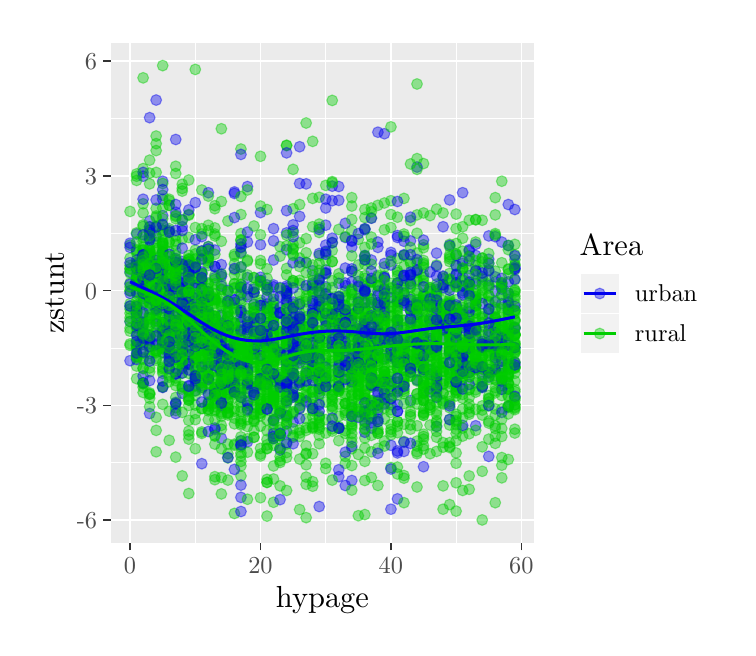
\begin{tikzpicture}[x=1pt,y=1pt]
\definecolor{fillColor}{RGB}{255,255,255}
\path[use as bounding box,fill=fillColor,fill opacity=0.00] (0,0) rectangle (252.94,216.81);
\begin{scope}
\path[clip] (  0.00,  0.00) rectangle (252.94,216.81);
\definecolor{drawColor}{RGB}{255,255,255}
\definecolor{fillColor}{RGB}{255,255,255}

\path[draw=drawColor,line width= 0.6pt,line join=round,line cap=round,fill=fillColor] (  0.00,  0.00) rectangle (252.94,216.81);
\end{scope}
\begin{scope}
\path[clip] ( 30.05, 30.72) rectangle (182.98,211.31);
\definecolor{fillColor}{gray}{0.92}

\path[fill=fillColor] ( 30.05, 30.72) rectangle (182.98,211.31);
\definecolor{drawColor}{RGB}{255,255,255}

\path[draw=drawColor,line width= 0.3pt,line join=round] ( 30.05, 59.54) --
	(182.98, 59.54);

\path[draw=drawColor,line width= 0.3pt,line join=round] ( 30.05,101.03) --
	(182.98,101.03);

\path[draw=drawColor,line width= 0.3pt,line join=round] ( 30.05,142.52) --
	(182.98,142.52);

\path[draw=drawColor,line width= 0.3pt,line join=round] ( 30.05,184.02) --
	(182.98,184.02);

\path[draw=drawColor,line width= 0.3pt,line join=round] ( 60.57, 30.72) --
	( 60.57,211.31);

\path[draw=drawColor,line width= 0.3pt,line join=round] (107.70, 30.72) --
	(107.70,211.31);

\path[draw=drawColor,line width= 0.3pt,line join=round] (154.82, 30.72) --
	(154.82,211.31);

\path[draw=drawColor,line width= 0.6pt,line join=round] ( 30.05, 38.79) --
	(182.98, 38.79);

\path[draw=drawColor,line width= 0.6pt,line join=round] ( 30.05, 80.29) --
	(182.98, 80.29);

\path[draw=drawColor,line width= 0.6pt,line join=round] ( 30.05,121.78) --
	(182.98,121.78);

\path[draw=drawColor,line width= 0.6pt,line join=round] ( 30.05,163.27) --
	(182.98,163.27);

\path[draw=drawColor,line width= 0.6pt,line join=round] ( 30.05,204.76) --
	(182.98,204.76);

\path[draw=drawColor,line width= 0.6pt,line join=round] ( 37.00, 30.72) --
	( 37.00,211.31);

\path[draw=drawColor,line width= 0.6pt,line join=round] ( 84.13, 30.72) --
	( 84.13,211.31);

\path[draw=drawColor,line width= 0.6pt,line join=round] (131.26, 30.72) --
	(131.26,211.31);

\path[draw=drawColor,line width= 0.6pt,line join=round] (178.39, 30.72) --
	(178.39,211.31);
\definecolor{drawColor}{RGB}{0,205,0}
\definecolor{fillColor}{RGB}{0,205,0}

\path[draw=drawColor,draw opacity=0.40,line width= 0.4pt,line join=round,line cap=round,fill=fillColor,fill opacity=0.40] (154.82,100.34) circle (  1.96);

\path[draw=drawColor,draw opacity=0.40,line width= 0.4pt,line join=round,line cap=round,fill=fillColor,fill opacity=0.40] ( 69.99, 94.67) circle (  1.96);

\path[draw=drawColor,draw opacity=0.40,line width= 0.4pt,line join=round,line cap=round,fill=fillColor,fill opacity=0.40] ( 86.49, 71.16) circle (  1.96);

\path[draw=drawColor,draw opacity=0.40,line width= 0.4pt,line join=round,line cap=round,fill=fillColor,fill opacity=0.40] (121.83,109.33) circle (  1.96);

\path[draw=drawColor,draw opacity=0.40,line width= 0.4pt,line join=round,line cap=round,fill=fillColor,fill opacity=0.40] (107.70,110.85) circle (  1.96);

\path[draw=drawColor,draw opacity=0.40,line width= 0.4pt,line join=round,line cap=round,fill=fillColor,fill opacity=0.40] ( 77.06, 75.45) circle (  1.96);

\path[draw=drawColor,draw opacity=0.40,line width= 0.4pt,line join=round,line cap=round,fill=fillColor,fill opacity=0.40] ( 60.57,126.34) circle (  1.96);

\path[draw=drawColor,draw opacity=0.40,line width= 0.4pt,line join=round,line cap=round,fill=fillColor,fill opacity=0.40] (154.82, 87.06) circle (  1.96);

\path[draw=drawColor,draw opacity=0.40,line width= 0.4pt,line join=round,line cap=round,fill=fillColor,fill opacity=0.40] ( 48.79,109.47) circle (  1.96);

\path[draw=drawColor,draw opacity=0.40,line width= 0.4pt,line join=round,line cap=round,fill=fillColor,fill opacity=0.40] (147.75,108.64) circle (  1.96);

\path[draw=drawColor,draw opacity=0.40,line width= 0.4pt,line join=round,line cap=round,fill=fillColor,fill opacity=0.40] ( 74.71, 66.32) circle (  1.96);

\path[draw=drawColor,draw opacity=0.40,line width= 0.4pt,line join=round,line cap=round,fill=fillColor,fill opacity=0.40] (138.33, 95.36) circle (  1.96);

\path[draw=drawColor,draw opacity=0.40,line width= 0.4pt,line join=round,line cap=round,fill=fillColor,fill opacity=0.40] ( 48.79,143.77) circle (  1.96);

\path[draw=drawColor,draw opacity=0.40,line width= 0.4pt,line join=round,line cap=round,fill=fillColor,fill opacity=0.40] (150.11,110.85) circle (  1.96);

\path[draw=drawColor,draw opacity=0.40,line width= 0.4pt,line join=round,line cap=round,fill=fillColor,fill opacity=0.40] ( 41.72,130.21) circle (  1.96);

\path[draw=drawColor,draw opacity=0.40,line width= 0.4pt,line join=round,line cap=round,fill=fillColor,fill opacity=0.40] (131.26,112.51) circle (  1.96);

\path[draw=drawColor,draw opacity=0.40,line width= 0.4pt,line join=round,line cap=round,fill=fillColor,fill opacity=0.40] ( 95.91,101.72) circle (  1.96);

\path[draw=drawColor,draw opacity=0.40,line width= 0.4pt,line join=round,line cap=round,fill=fillColor,fill opacity=0.40] ( 88.84, 97.85) circle (  1.96);

\path[draw=drawColor,draw opacity=0.40,line width= 0.4pt,line join=round,line cap=round,fill=fillColor,fill opacity=0.40] ( 98.27, 82.91) circle (  1.96);

\path[draw=drawColor,draw opacity=0.40,line width= 0.4pt,line join=round,line cap=round,fill=fillColor,fill opacity=0.40] ( 84.13, 90.38) circle (  1.96);

\path[draw=drawColor,draw opacity=0.40,line width= 0.4pt,line join=round,line cap=round,fill=fillColor,fill opacity=0.40] (145.40, 99.37) circle (  1.96);

\path[draw=drawColor,draw opacity=0.40,line width= 0.4pt,line join=round,line cap=round,fill=fillColor,fill opacity=0.40] ( 81.77,120.81) circle (  1.96);

\path[draw=drawColor,draw opacity=0.40,line width= 0.4pt,line join=round,line cap=round,fill=fillColor,fill opacity=0.40] (154.82, 84.85) circle (  1.96);

\path[draw=drawColor,draw opacity=0.40,line width= 0.4pt,line join=round,line cap=round,fill=fillColor,fill opacity=0.40] ( 58.21,107.12) circle (  1.96);

\path[draw=drawColor,draw opacity=0.40,line width= 0.4pt,line join=round,line cap=round,fill=fillColor,fill opacity=0.40] ( 77.06,106.01) circle (  1.96);

\path[draw=drawColor,draw opacity=0.40,line width= 0.4pt,line join=round,line cap=round,fill=fillColor,fill opacity=0.40] (117.12,112.93) circle (  1.96);

\path[draw=drawColor,draw opacity=0.40,line width= 0.4pt,line join=round,line cap=round,fill=fillColor,fill opacity=0.40] (164.25,100.34) circle (  1.96);

\path[draw=drawColor,draw opacity=0.40,line width= 0.4pt,line join=round,line cap=round,fill=fillColor,fill opacity=0.40] ( 53.50,114.17) circle (  1.96);

\path[draw=drawColor,draw opacity=0.40,line width= 0.4pt,line join=round,line cap=round,fill=fillColor,fill opacity=0.40] ( 41.72,137.54) circle (  1.96);

\path[draw=drawColor,draw opacity=0.40,line width= 0.4pt,line join=round,line cap=round,fill=fillColor,fill opacity=0.40] ( 62.92,110.16) circle (  1.96);

\path[draw=drawColor,draw opacity=0.40,line width= 0.4pt,line join=round,line cap=round,fill=fillColor,fill opacity=0.40] (173.68,106.43) circle (  1.96);

\path[draw=drawColor,draw opacity=0.40,line width= 0.4pt,line join=round,line cap=round,fill=fillColor,fill opacity=0.40] (121.83,100.20) circle (  1.96);

\path[draw=drawColor,draw opacity=0.40,line width= 0.4pt,line join=round,line cap=round,fill=fillColor,fill opacity=0.40] ( 77.06,117.49) circle (  1.96);

\path[draw=drawColor,draw opacity=0.40,line width= 0.4pt,line join=round,line cap=round,fill=fillColor,fill opacity=0.40] ( 74.71, 88.86) circle (  1.96);

\path[draw=drawColor,draw opacity=0.40,line width= 0.4pt,line join=round,line cap=round,fill=fillColor,fill opacity=0.40] (173.68, 60.79) circle (  1.96);

\path[draw=drawColor,draw opacity=0.40,line width= 0.4pt,line join=round,line cap=round,fill=fillColor,fill opacity=0.40] (124.19, 91.21) circle (  1.96);

\path[draw=drawColor,draw opacity=0.40,line width= 0.4pt,line join=round,line cap=round,fill=fillColor,fill opacity=0.40] (176.03,102.55) circle (  1.96);

\path[draw=drawColor,draw opacity=0.40,line width= 0.4pt,line join=round,line cap=round,fill=fillColor,fill opacity=0.40] ( 91.20, 88.45) circle (  1.96);

\path[draw=drawColor,draw opacity=0.40,line width= 0.4pt,line join=round,line cap=round,fill=fillColor,fill opacity=0.40] ( 93.56,119.98) circle (  1.96);

\path[draw=drawColor,draw opacity=0.40,line width= 0.4pt,line join=round,line cap=round,fill=fillColor,fill opacity=0.40] (159.54,105.04) circle (  1.96);

\path[draw=drawColor,draw opacity=0.40,line width= 0.4pt,line join=round,line cap=round,fill=fillColor,fill opacity=0.40] (171.32,120.26) circle (  1.96);

\path[draw=drawColor,draw opacity=0.40,line width= 0.4pt,line join=round,line cap=round,fill=fillColor,fill opacity=0.40] (119.48,110.44) circle (  1.96);

\path[draw=drawColor,draw opacity=0.40,line width= 0.4pt,line join=round,line cap=round,fill=fillColor,fill opacity=0.40] ( 84.13, 88.45) circle (  1.96);

\path[draw=drawColor,draw opacity=0.40,line width= 0.4pt,line join=round,line cap=round,fill=fillColor,fill opacity=0.40] (152.47,102.00) circle (  1.96);

\path[draw=drawColor,draw opacity=0.40,line width= 0.4pt,line join=round,line cap=round,fill=fillColor,fill opacity=0.40] (100.63,108.64) circle (  1.96);

\path[draw=drawColor,draw opacity=0.40,line width= 0.4pt,line join=round,line cap=round,fill=fillColor,fill opacity=0.40] (171.32,102.83) circle (  1.96);

\path[draw=drawColor,draw opacity=0.40,line width= 0.4pt,line join=round,line cap=round,fill=fillColor,fill opacity=0.40] ( 74.71,115.42) circle (  1.96);

\path[draw=drawColor,draw opacity=0.40,line width= 0.4pt,line join=round,line cap=round,fill=fillColor,fill opacity=0.40] (164.25, 93.43) circle (  1.96);

\path[draw=drawColor,draw opacity=0.40,line width= 0.4pt,line join=round,line cap=round,fill=fillColor,fill opacity=0.40] (152.47,115.28) circle (  1.96);

\path[draw=drawColor,draw opacity=0.40,line width= 0.4pt,line join=round,line cap=round,fill=fillColor,fill opacity=0.40] ( 60.57,108.64) circle (  1.96);

\path[draw=drawColor,draw opacity=0.40,line width= 0.4pt,line join=round,line cap=round,fill=fillColor,fill opacity=0.40] ( 93.56, 87.75) circle (  1.96);

\path[draw=drawColor,draw opacity=0.40,line width= 0.4pt,line join=round,line cap=round,fill=fillColor,fill opacity=0.40] (126.55,104.35) circle (  1.96);

\path[draw=drawColor,draw opacity=0.40,line width= 0.4pt,line join=round,line cap=round,fill=fillColor,fill opacity=0.40] ( 79.42,107.81) circle (  1.96);

\path[draw=drawColor,draw opacity=0.40,line width= 0.4pt,line join=round,line cap=round,fill=fillColor,fill opacity=0.40] (131.26,144.60) circle (  1.96);

\path[draw=drawColor,draw opacity=0.40,line width= 0.4pt,line join=round,line cap=round,fill=fillColor,fill opacity=0.40] ( 95.91, 90.38) circle (  1.96);

\path[draw=drawColor,draw opacity=0.40,line width= 0.4pt,line join=round,line cap=round,fill=fillColor,fill opacity=0.40] (112.41, 91.07) circle (  1.96);

\path[draw=drawColor,draw opacity=0.40,line width= 0.4pt,line join=round,line cap=round,fill=fillColor,fill opacity=0.40] ( 60.57, 87.34) circle (  1.96);

\path[draw=drawColor,draw opacity=0.40,line width= 0.4pt,line join=round,line cap=round,fill=fillColor,fill opacity=0.40] ( 55.85,114.03) circle (  1.96);

\path[draw=drawColor,draw opacity=0.40,line width= 0.4pt,line join=round,line cap=round,fill=fillColor,fill opacity=0.40] ( 86.49, 96.47) circle (  1.96);

\path[draw=drawColor,draw opacity=0.40,line width= 0.4pt,line join=round,line cap=round,fill=fillColor,fill opacity=0.40] ( 79.42, 95.64) circle (  1.96);

\path[draw=drawColor,draw opacity=0.40,line width= 0.4pt,line join=round,line cap=round,fill=fillColor,fill opacity=0.40] (152.47, 92.18) circle (  1.96);

\path[draw=drawColor,draw opacity=0.40,line width= 0.4pt,line join=round,line cap=round,fill=fillColor,fill opacity=0.40] ( 86.49, 52.49) circle (  1.96);

\path[draw=drawColor,draw opacity=0.40,line width= 0.4pt,line join=round,line cap=round,fill=fillColor,fill opacity=0.40] ( 65.28, 78.35) circle (  1.96);

\path[draw=drawColor,draw opacity=0.40,line width= 0.4pt,line join=round,line cap=round,fill=fillColor,fill opacity=0.40] (105.34,102.83) circle (  1.96);

\path[draw=drawColor,draw opacity=0.40,line width= 0.4pt,line join=round,line cap=round,fill=fillColor,fill opacity=0.40] ( 51.14,106.84) circle (  1.96);

\path[draw=drawColor,draw opacity=0.40,line width= 0.4pt,line join=round,line cap=round,fill=fillColor,fill opacity=0.40] ( 46.43,136.99) circle (  1.96);

\path[draw=drawColor,draw opacity=0.40,line width= 0.4pt,line join=round,line cap=round,fill=fillColor,fill opacity=0.40] (105.34, 99.23) circle (  1.96);

\path[draw=drawColor,draw opacity=0.40,line width= 0.4pt,line join=round,line cap=round,fill=fillColor,fill opacity=0.40] (102.98,107.81) circle (  1.96);

\path[draw=drawColor,draw opacity=0.40,line width= 0.4pt,line join=round,line cap=round,fill=fillColor,fill opacity=0.40] (150.11, 95.50) circle (  1.96);

\path[draw=drawColor,draw opacity=0.40,line width= 0.4pt,line join=round,line cap=round,fill=fillColor,fill opacity=0.40] ( 72.35, 88.86) circle (  1.96);

\path[draw=drawColor,draw opacity=0.40,line width= 0.4pt,line join=round,line cap=round,fill=fillColor,fill opacity=0.40] ( 84.13,103.38) circle (  1.96);

\path[draw=drawColor,draw opacity=0.40,line width= 0.4pt,line join=round,line cap=round,fill=fillColor,fill opacity=0.40] ( 48.79,104.77) circle (  1.96);

\path[draw=drawColor,draw opacity=0.40,line width= 0.4pt,line join=round,line cap=round,fill=fillColor,fill opacity=0.40] ( 67.64, 87.75) circle (  1.96);

\path[draw=drawColor,draw opacity=0.40,line width= 0.4pt,line join=round,line cap=round,fill=fillColor,fill opacity=0.40] (128.90,109.19) circle (  1.96);

\path[draw=drawColor,draw opacity=0.40,line width= 0.4pt,line join=round,line cap=round,fill=fillColor,fill opacity=0.40] (102.98,111.82) circle (  1.96);

\path[draw=drawColor,draw opacity=0.40,line width= 0.4pt,line join=round,line cap=round,fill=fillColor,fill opacity=0.40] (171.32,123.44) circle (  1.96);

\path[draw=drawColor,draw opacity=0.40,line width= 0.4pt,line join=round,line cap=round,fill=fillColor,fill opacity=0.40] (128.90,116.80) circle (  1.96);

\path[draw=drawColor,draw opacity=0.40,line width= 0.4pt,line join=round,line cap=round,fill=fillColor,fill opacity=0.40] (102.98, 52.76) circle (  1.96);

\path[draw=drawColor,draw opacity=0.40,line width= 0.4pt,line join=round,line cap=round,fill=fillColor,fill opacity=0.40] (131.26,104.49) circle (  1.96);

\path[draw=drawColor,draw opacity=0.40,line width= 0.4pt,line join=round,line cap=round,fill=fillColor,fill opacity=0.40] (152.47, 73.23) circle (  1.96);

\path[draw=drawColor,draw opacity=0.40,line width= 0.4pt,line join=round,line cap=round,fill=fillColor,fill opacity=0.40] (124.19, 87.62) circle (  1.96);

\path[draw=drawColor,draw opacity=0.40,line width= 0.4pt,line join=round,line cap=round,fill=fillColor,fill opacity=0.40] (100.63,112.37) circle (  1.96);

\path[draw=drawColor,draw opacity=0.40,line width= 0.4pt,line join=round,line cap=round,fill=fillColor,fill opacity=0.40] (173.68,112.93) circle (  1.96);

\path[draw=drawColor,draw opacity=0.40,line width= 0.4pt,line join=round,line cap=round,fill=fillColor,fill opacity=0.40] (100.63, 83.33) circle (  1.96);

\path[draw=drawColor,draw opacity=0.40,line width= 0.4pt,line join=round,line cap=round,fill=fillColor,fill opacity=0.40] (164.25, 89.00) circle (  1.96);

\path[draw=drawColor,draw opacity=0.40,line width= 0.4pt,line join=round,line cap=round,fill=fillColor,fill opacity=0.40] ( 93.56,112.23) circle (  1.96);

\path[draw=drawColor,draw opacity=0.40,line width= 0.4pt,line join=round,line cap=round,fill=fillColor,fill opacity=0.40] (126.55, 70.88) circle (  1.96);

\path[draw=drawColor,draw opacity=0.40,line width= 0.4pt,line join=round,line cap=round,fill=fillColor,fill opacity=0.40] ( 48.79, 92.73) circle (  1.96);

\path[draw=drawColor,draw opacity=0.40,line width= 0.4pt,line join=round,line cap=round,fill=fillColor,fill opacity=0.40] ( 48.79, 91.90) circle (  1.96);

\path[draw=drawColor,draw opacity=0.40,line width= 0.4pt,line join=round,line cap=round,fill=fillColor,fill opacity=0.40] ( 95.91,108.92) circle (  1.96);

\path[draw=drawColor,draw opacity=0.40,line width= 0.4pt,line join=round,line cap=round,fill=fillColor,fill opacity=0.40] (102.98,110.30) circle (  1.96);

\path[draw=drawColor,draw opacity=0.40,line width= 0.4pt,line join=round,line cap=round,fill=fillColor,fill opacity=0.40] (164.25,124.82) circle (  1.96);

\path[draw=drawColor,draw opacity=0.40,line width= 0.4pt,line join=round,line cap=round,fill=fillColor,fill opacity=0.40] ( 67.64, 86.37) circle (  1.96);

\path[draw=drawColor,draw opacity=0.40,line width= 0.4pt,line join=round,line cap=round,fill=fillColor,fill opacity=0.40] (114.76,114.72) circle (  1.96);

\path[draw=drawColor,draw opacity=0.40,line width= 0.4pt,line join=round,line cap=round,fill=fillColor,fill opacity=0.40] ( 65.28, 75.17) circle (  1.96);

\path[draw=drawColor,draw opacity=0.40,line width= 0.4pt,line join=round,line cap=round,fill=fillColor,fill opacity=0.40] (173.68,105.60) circle (  1.96);

\path[draw=drawColor,draw opacity=0.40,line width= 0.4pt,line join=round,line cap=round,fill=fillColor,fill opacity=0.40] ( 65.28,109.47) circle (  1.96);

\path[draw=drawColor,draw opacity=0.40,line width= 0.4pt,line join=round,line cap=round,fill=fillColor,fill opacity=0.40] ( 69.99,122.33) circle (  1.96);

\path[draw=drawColor,draw opacity=0.40,line width= 0.4pt,line join=round,line cap=round,fill=fillColor,fill opacity=0.40] ( 84.13,118.32) circle (  1.96);

\path[draw=drawColor,draw opacity=0.40,line width= 0.4pt,line join=round,line cap=round,fill=fillColor,fill opacity=0.40] ( 44.07,122.61) circle (  1.96);

\path[draw=drawColor,draw opacity=0.40,line width= 0.4pt,line join=round,line cap=round,fill=fillColor,fill opacity=0.40] (176.03,101.31) circle (  1.96);

\path[draw=drawColor,draw opacity=0.40,line width= 0.4pt,line join=round,line cap=round,fill=fillColor,fill opacity=0.40] ( 84.13,170.32) circle (  1.96);

\path[draw=drawColor,draw opacity=0.40,line width= 0.4pt,line join=round,line cap=round,fill=fillColor,fill opacity=0.40] ( 95.91, 91.07) circle (  1.96);

\path[draw=drawColor,draw opacity=0.40,line width= 0.4pt,line join=round,line cap=round,fill=fillColor,fill opacity=0.40] (152.47, 81.67) circle (  1.96);

\path[draw=drawColor,draw opacity=0.40,line width= 0.4pt,line join=round,line cap=round,fill=fillColor,fill opacity=0.40] ( 98.27,133.53) circle (  1.96);

\path[draw=drawColor,draw opacity=0.40,line width= 0.4pt,line join=round,line cap=round,fill=fillColor,fill opacity=0.40] (154.82,106.15) circle (  1.96);

\path[draw=drawColor,draw opacity=0.40,line width= 0.4pt,line join=round,line cap=round,fill=fillColor,fill opacity=0.40] (102.98, 82.91) circle (  1.96);

\path[draw=drawColor,draw opacity=0.40,line width= 0.4pt,line join=round,line cap=round,fill=fillColor,fill opacity=0.40] ( 60.57,106.56) circle (  1.96);

\path[draw=drawColor,draw opacity=0.40,line width= 0.4pt,line join=round,line cap=round,fill=fillColor,fill opacity=0.40] ( 84.13,113.34) circle (  1.96);

\path[draw=drawColor,draw opacity=0.40,line width= 0.4pt,line join=round,line cap=round,fill=fillColor,fill opacity=0.40] ( 91.20,110.58) circle (  1.96);

\path[draw=drawColor,draw opacity=0.40,line width= 0.4pt,line join=round,line cap=round,fill=fillColor,fill opacity=0.40] (154.82,118.46) circle (  1.96);

\path[draw=drawColor,draw opacity=0.40,line width= 0.4pt,line join=round,line cap=round,fill=fillColor,fill opacity=0.40] (128.90, 97.99) circle (  1.96);

\path[draw=drawColor,draw opacity=0.40,line width= 0.4pt,line join=round,line cap=round,fill=fillColor,fill opacity=0.40] (176.03,121.22) circle (  1.96);

\path[draw=drawColor,draw opacity=0.40,line width= 0.4pt,line join=round,line cap=round,fill=fillColor,fill opacity=0.40] ( 72.35, 84.16) circle (  1.96);

\path[draw=drawColor,draw opacity=0.40,line width= 0.4pt,line join=round,line cap=round,fill=fillColor,fill opacity=0.40] ( 98.27,120.53) circle (  1.96);

\path[draw=drawColor,draw opacity=0.40,line width= 0.4pt,line join=round,line cap=round,fill=fillColor,fill opacity=0.40] (124.19, 95.64) circle (  1.96);

\path[draw=drawColor,draw opacity=0.40,line width= 0.4pt,line join=round,line cap=round,fill=fillColor,fill opacity=0.40] ( 39.36, 94.53) circle (  1.96);

\path[draw=drawColor,draw opacity=0.40,line width= 0.4pt,line join=round,line cap=round,fill=fillColor,fill opacity=0.40] (126.55,110.85) circle (  1.96);

\path[draw=drawColor,draw opacity=0.40,line width= 0.4pt,line join=round,line cap=round,fill=fillColor,fill opacity=0.40] ( 58.21,104.77) circle (  1.96);

\path[draw=drawColor,draw opacity=0.40,line width= 0.4pt,line join=round,line cap=round,fill=fillColor,fill opacity=0.40] (110.05,105.87) circle (  1.96);

\path[draw=drawColor,draw opacity=0.40,line width= 0.4pt,line join=round,line cap=round,fill=fillColor,fill opacity=0.40] ( 41.72, 88.45) circle (  1.96);

\path[draw=drawColor,draw opacity=0.40,line width= 0.4pt,line join=round,line cap=round,fill=fillColor,fill opacity=0.40] (124.19, 87.34) circle (  1.96);

\path[draw=drawColor,draw opacity=0.40,line width= 0.4pt,line join=round,line cap=round,fill=fillColor,fill opacity=0.40] ( 46.43,117.08) circle (  1.96);

\path[draw=drawColor,draw opacity=0.40,line width= 0.4pt,line join=round,line cap=round,fill=fillColor,fill opacity=0.40] (154.82, 76.28) circle (  1.96);

\path[draw=drawColor,draw opacity=0.40,line width= 0.4pt,line join=round,line cap=round,fill=fillColor,fill opacity=0.40] (102.98, 51.10) circle (  1.96);

\path[draw=drawColor,draw opacity=0.40,line width= 0.4pt,line join=round,line cap=round,fill=fillColor,fill opacity=0.40] ( 58.21,130.49) circle (  1.96);

\path[draw=drawColor,draw opacity=0.40,line width= 0.4pt,line join=round,line cap=round,fill=fillColor,fill opacity=0.40] (166.61,125.51) circle (  1.96);

\path[draw=drawColor,draw opacity=0.40,line width= 0.4pt,line join=round,line cap=round,fill=fillColor,fill opacity=0.40] (105.34,115.83) circle (  1.96);

\path[draw=drawColor,draw opacity=0.40,line width= 0.4pt,line join=round,line cap=round,fill=fillColor,fill opacity=0.40] ( 62.92, 70.19) circle (  1.96);

\path[draw=drawColor,draw opacity=0.40,line width= 0.4pt,line join=round,line cap=round,fill=fillColor,fill opacity=0.40] ( 62.92, 70.74) circle (  1.96);

\path[draw=drawColor,draw opacity=0.40,line width= 0.4pt,line join=round,line cap=round,fill=fillColor,fill opacity=0.40] ( 77.06, 91.35) circle (  1.96);

\path[draw=drawColor,draw opacity=0.40,line width= 0.4pt,line join=round,line cap=round,fill=fillColor,fill opacity=0.40] ( 77.06, 93.98) circle (  1.96);

\path[draw=drawColor,draw opacity=0.40,line width= 0.4pt,line join=round,line cap=round,fill=fillColor,fill opacity=0.40] ( 93.56,129.80) circle (  1.96);

\path[draw=drawColor,draw opacity=0.40,line width= 0.4pt,line join=round,line cap=round,fill=fillColor,fill opacity=0.40] (119.48,114.03) circle (  1.96);

\path[draw=drawColor,draw opacity=0.40,line width= 0.4pt,line join=round,line cap=round,fill=fillColor,fill opacity=0.40] (166.61,119.84) circle (  1.96);

\path[draw=drawColor,draw opacity=0.40,line width= 0.4pt,line join=round,line cap=round,fill=fillColor,fill opacity=0.40] (135.97, 97.30) circle (  1.96);

\path[draw=drawColor,draw opacity=0.40,line width= 0.4pt,line join=round,line cap=round,fill=fillColor,fill opacity=0.40] (112.41,119.43) circle (  1.96);

\path[draw=drawColor,draw opacity=0.40,line width= 0.4pt,line join=round,line cap=round,fill=fillColor,fill opacity=0.40] ( 41.72,153.17) circle (  1.96);

\path[draw=drawColor,draw opacity=0.40,line width= 0.4pt,line join=round,line cap=round,fill=fillColor,fill opacity=0.40] (107.70,120.81) circle (  1.96);

\path[draw=drawColor,draw opacity=0.40,line width= 0.4pt,line join=round,line cap=round,fill=fillColor,fill opacity=0.40] (124.19,104.49) circle (  1.96);

\path[draw=drawColor,draw opacity=0.40,line width= 0.4pt,line join=round,line cap=round,fill=fillColor,fill opacity=0.40] (112.41, 88.58) circle (  1.96);

\path[draw=drawColor,draw opacity=0.40,line width= 0.4pt,line join=round,line cap=round,fill=fillColor,fill opacity=0.40] ( 48.79, 87.06) circle (  1.96);

\path[draw=drawColor,draw opacity=0.40,line width= 0.4pt,line join=round,line cap=round,fill=fillColor,fill opacity=0.40] ( 69.99,108.50) circle (  1.96);

\path[draw=drawColor,draw opacity=0.40,line width= 0.4pt,line join=round,line cap=round,fill=fillColor,fill opacity=0.40] (164.25, 97.57) circle (  1.96);

\path[draw=drawColor,draw opacity=0.40,line width= 0.4pt,line join=round,line cap=round,fill=fillColor,fill opacity=0.40] ( 72.35, 77.38) circle (  1.96);

\path[draw=drawColor,draw opacity=0.40,line width= 0.4pt,line join=round,line cap=round,fill=fillColor,fill opacity=0.40] ( 65.28,120.12) circle (  1.96);

\path[draw=drawColor,draw opacity=0.40,line width= 0.4pt,line join=round,line cap=round,fill=fillColor,fill opacity=0.40] ( 67.64,101.72) circle (  1.96);

\path[draw=drawColor,draw opacity=0.40,line width= 0.4pt,line join=round,line cap=round,fill=fillColor,fill opacity=0.40] ( 86.49, 90.38) circle (  1.96);

\path[draw=drawColor,draw opacity=0.40,line width= 0.4pt,line join=round,line cap=round,fill=fillColor,fill opacity=0.40] (114.76, 94.53) circle (  1.96);

\path[draw=drawColor,draw opacity=0.40,line width= 0.4pt,line join=round,line cap=round,fill=fillColor,fill opacity=0.40] (147.75, 63.69) circle (  1.96);

\path[draw=drawColor,draw opacity=0.40,line width= 0.4pt,line join=round,line cap=round,fill=fillColor,fill opacity=0.40] (147.75, 74.75) circle (  1.96);

\path[draw=drawColor,draw opacity=0.40,line width= 0.4pt,line join=round,line cap=round,fill=fillColor,fill opacity=0.40] ( 46.43,113.62) circle (  1.96);

\path[draw=drawColor,draw opacity=0.40,line width= 0.4pt,line join=round,line cap=round,fill=fillColor,fill opacity=0.40] (112.41,102.55) circle (  1.96);

\path[draw=drawColor,draw opacity=0.40,line width= 0.4pt,line join=round,line cap=round,fill=fillColor,fill opacity=0.40] ( 84.13, 96.19) circle (  1.96);

\path[draw=drawColor,draw opacity=0.40,line width= 0.4pt,line join=round,line cap=round,fill=fillColor,fill opacity=0.40] (110.05, 81.81) circle (  1.96);

\path[draw=drawColor,draw opacity=0.40,line width= 0.4pt,line join=round,line cap=round,fill=fillColor,fill opacity=0.40] ( 62.92,112.79) circle (  1.96);

\path[draw=drawColor,draw opacity=0.40,line width= 0.4pt,line join=round,line cap=round,fill=fillColor,fill opacity=0.40] ( 62.92,158.15) circle (  1.96);

\path[draw=drawColor,draw opacity=0.40,line width= 0.4pt,line join=round,line cap=round,fill=fillColor,fill opacity=0.40] (128.90,118.46) circle (  1.96);

\path[draw=drawColor,draw opacity=0.40,line width= 0.4pt,line join=round,line cap=round,fill=fillColor,fill opacity=0.40] ( 58.21, 48.48) circle (  1.96);

\path[draw=drawColor,draw opacity=0.40,line width= 0.4pt,line join=round,line cap=round,fill=fillColor,fill opacity=0.40] ( 88.84,117.35) circle (  1.96);

\path[draw=drawColor,draw opacity=0.40,line width= 0.4pt,line join=round,line cap=round,fill=fillColor,fill opacity=0.40] (159.54, 97.99) circle (  1.96);

\path[draw=drawColor,draw opacity=0.40,line width= 0.4pt,line join=round,line cap=round,fill=fillColor,fill opacity=0.40] (114.76,112.10) circle (  1.96);

\path[draw=drawColor,draw opacity=0.40,line width= 0.4pt,line join=round,line cap=round,fill=fillColor,fill opacity=0.40] (131.26, 69.64) circle (  1.96);

\path[draw=drawColor,draw opacity=0.40,line width= 0.4pt,line join=round,line cap=round,fill=fillColor,fill opacity=0.40] ( 65.28, 91.63) circle (  1.96);

\path[draw=drawColor,draw opacity=0.40,line width= 0.4pt,line join=round,line cap=round,fill=fillColor,fill opacity=0.40] (112.41, 71.99) circle (  1.96);

\path[draw=drawColor,draw opacity=0.40,line width= 0.4pt,line join=round,line cap=round,fill=fillColor,fill opacity=0.40] (164.25,112.37) circle (  1.96);

\path[draw=drawColor,draw opacity=0.40,line width= 0.4pt,line join=round,line cap=round,fill=fillColor,fill opacity=0.40] ( 41.72, 84.99) circle (  1.96);

\path[draw=drawColor,draw opacity=0.40,line width= 0.4pt,line join=round,line cap=round,fill=fillColor,fill opacity=0.40] (124.19, 94.39) circle (  1.96);

\path[draw=drawColor,draw opacity=0.40,line width= 0.4pt,line join=round,line cap=round,fill=fillColor,fill opacity=0.40] ( 60.57, 94.39) circle (  1.96);

\path[draw=drawColor,draw opacity=0.40,line width= 0.4pt,line join=round,line cap=round,fill=fillColor,fill opacity=0.40] (145.40,103.52) circle (  1.96);

\path[draw=drawColor,draw opacity=0.40,line width= 0.4pt,line join=round,line cap=round,fill=fillColor,fill opacity=0.40] ( 88.84,100.34) circle (  1.96);

\path[draw=drawColor,draw opacity=0.40,line width= 0.4pt,line join=round,line cap=round,fill=fillColor,fill opacity=0.40] ( 58.21,101.86) circle (  1.96);

\path[draw=drawColor,draw opacity=0.40,line width= 0.4pt,line join=round,line cap=round,fill=fillColor,fill opacity=0.40] (159.54,107.39) circle (  1.96);

\path[draw=drawColor,draw opacity=0.40,line width= 0.4pt,line join=round,line cap=round,fill=fillColor,fill opacity=0.40] ( 67.64, 92.60) circle (  1.96);

\path[draw=drawColor,draw opacity=0.40,line width= 0.4pt,line join=round,line cap=round,fill=fillColor,fill opacity=0.40] (131.26,103.11) circle (  1.96);

\path[draw=drawColor,draw opacity=0.40,line width= 0.4pt,line join=round,line cap=round,fill=fillColor,fill opacity=0.40] ( 53.50,139.76) circle (  1.96);

\path[draw=drawColor,draw opacity=0.40,line width= 0.4pt,line join=round,line cap=round,fill=fillColor,fill opacity=0.40] (119.48, 98.13) circle (  1.96);

\path[draw=drawColor,draw opacity=0.40,line width= 0.4pt,line join=round,line cap=round,fill=fillColor,fill opacity=0.40] (173.68, 86.10) circle (  1.96);

\path[draw=drawColor,draw opacity=0.40,line width= 0.4pt,line join=round,line cap=round,fill=fillColor,fill opacity=0.40] (110.05, 97.57) circle (  1.96);

\path[draw=drawColor,draw opacity=0.40,line width= 0.4pt,line join=round,line cap=round,fill=fillColor,fill opacity=0.40] (152.47, 99.23) circle (  1.96);

\path[draw=drawColor,draw opacity=0.40,line width= 0.4pt,line join=round,line cap=round,fill=fillColor,fill opacity=0.40] ( 86.49, 64.80) circle (  1.96);

\path[draw=drawColor,draw opacity=0.40,line width= 0.4pt,line join=round,line cap=round,fill=fillColor,fill opacity=0.40] (145.40, 89.00) circle (  1.96);

\path[draw=drawColor,draw opacity=0.40,line width= 0.4pt,line join=round,line cap=round,fill=fillColor,fill opacity=0.40] ( 77.06,114.72) circle (  1.96);

\path[draw=drawColor,draw opacity=0.40,line width= 0.4pt,line join=round,line cap=round,fill=fillColor,fill opacity=0.40] (128.90,130.35) circle (  1.96);

\path[draw=drawColor,draw opacity=0.40,line width= 0.4pt,line join=round,line cap=round,fill=fillColor,fill opacity=0.40] (105.34, 91.90) circle (  1.96);

\path[draw=drawColor,draw opacity=0.40,line width= 0.4pt,line join=round,line cap=round,fill=fillColor,fill opacity=0.40] (176.03,110.71) circle (  1.96);

\path[draw=drawColor,draw opacity=0.40,line width= 0.4pt,line join=round,line cap=round,fill=fillColor,fill opacity=0.40] ( 91.20,106.43) circle (  1.96);

\path[draw=drawColor,draw opacity=0.40,line width= 0.4pt,line join=round,line cap=round,fill=fillColor,fill opacity=0.40] ( 93.56, 93.29) circle (  1.96);

\path[draw=drawColor,draw opacity=0.40,line width= 0.4pt,line join=round,line cap=round,fill=fillColor,fill opacity=0.40] (147.75, 87.89) circle (  1.96);

\path[draw=drawColor,draw opacity=0.40,line width= 0.4pt,line join=round,line cap=round,fill=fillColor,fill opacity=0.40] ( 53.50,115.83) circle (  1.96);

\path[draw=drawColor,draw opacity=0.40,line width= 0.4pt,line join=round,line cap=round,fill=fillColor,fill opacity=0.40] ( 74.71,124.27) circle (  1.96);

\path[draw=drawColor,draw opacity=0.40,line width= 0.4pt,line join=round,line cap=round,fill=fillColor,fill opacity=0.40] (102.98,122.47) circle (  1.96);

\path[draw=drawColor,draw opacity=0.40,line width= 0.4pt,line join=round,line cap=round,fill=fillColor,fill opacity=0.40] ( 48.79,135.89) circle (  1.96);

\path[draw=drawColor,draw opacity=0.40,line width= 0.4pt,line join=round,line cap=round,fill=fillColor,fill opacity=0.40] (147.75,122.19) circle (  1.96);

\path[draw=drawColor,draw opacity=0.40,line width= 0.4pt,line join=round,line cap=round,fill=fillColor,fill opacity=0.40] ( 74.71, 99.93) circle (  1.96);

\path[draw=drawColor,draw opacity=0.40,line width= 0.4pt,line join=round,line cap=round,fill=fillColor,fill opacity=0.40] ( 41.72,121.50) circle (  1.96);

\path[draw=drawColor,draw opacity=0.40,line width= 0.4pt,line join=round,line cap=round,fill=fillColor,fill opacity=0.40] (164.25,119.29) circle (  1.96);

\path[draw=drawColor,draw opacity=0.40,line width= 0.4pt,line join=round,line cap=round,fill=fillColor,fill opacity=0.40] ( 58.21,116.25) circle (  1.96);

\path[draw=drawColor,draw opacity=0.40,line width= 0.4pt,line join=round,line cap=round,fill=fillColor,fill opacity=0.40] ( 77.06, 84.85) circle (  1.96);

\path[draw=drawColor,draw opacity=0.40,line width= 0.4pt,line join=round,line cap=round,fill=fillColor,fill opacity=0.40] (124.19, 98.54) circle (  1.96);

\path[draw=drawColor,draw opacity=0.40,line width= 0.4pt,line join=round,line cap=round,fill=fillColor,fill opacity=0.40] (159.54,100.89) circle (  1.96);

\path[draw=drawColor,draw opacity=0.40,line width= 0.4pt,line join=round,line cap=round,fill=fillColor,fill opacity=0.40] (140.69,142.52) circle (  1.96);

\path[draw=drawColor,draw opacity=0.40,line width= 0.4pt,line join=round,line cap=round,fill=fillColor,fill opacity=0.40] (105.34,123.44) circle (  1.96);

\path[draw=drawColor,draw opacity=0.40,line width= 0.4pt,line join=round,line cap=round,fill=fillColor,fill opacity=0.40] (143.04,107.53) circle (  1.96);

\path[draw=drawColor,draw opacity=0.40,line width= 0.4pt,line join=round,line cap=round,fill=fillColor,fill opacity=0.40] ( 39.36,131.46) circle (  1.96);

\path[draw=drawColor,draw opacity=0.40,line width= 0.4pt,line join=round,line cap=round,fill=fillColor,fill opacity=0.40] ( 95.91,110.58) circle (  1.96);

\path[draw=drawColor,draw opacity=0.40,line width= 0.4pt,line join=round,line cap=round,fill=fillColor,fill opacity=0.40] ( 65.28,143.49) circle (  1.96);

\path[draw=drawColor,draw opacity=0.40,line width= 0.4pt,line join=round,line cap=round,fill=fillColor,fill opacity=0.40] ( 69.99, 85.40) circle (  1.96);

\path[draw=drawColor,draw opacity=0.40,line width= 0.4pt,line join=round,line cap=round,fill=fillColor,fill opacity=0.40] (138.33,114.72) circle (  1.96);

\path[draw=drawColor,draw opacity=0.40,line width= 0.4pt,line join=round,line cap=round,fill=fillColor,fill opacity=0.40] ( 48.79,102.55) circle (  1.96);
\definecolor{drawColor}{RGB}{0,0,238}
\definecolor{fillColor}{RGB}{0,0,238}

\path[draw=drawColor,draw opacity=0.40,line width= 0.4pt,line join=round,line cap=round,fill=fillColor,fill opacity=0.40] (133.62,124.41) circle (  1.96);

\path[draw=drawColor,draw opacity=0.40,line width= 0.4pt,line join=round,line cap=round,fill=fillColor,fill opacity=0.40] (117.12, 79.59) circle (  1.96);

\path[draw=drawColor,draw opacity=0.40,line width= 0.4pt,line join=round,line cap=round,fill=fillColor,fill opacity=0.40] (159.54,103.94) circle (  1.96);

\path[draw=drawColor,draw opacity=0.40,line width= 0.4pt,line join=round,line cap=round,fill=fillColor,fill opacity=0.40] ( 48.79,130.49) circle (  1.96);

\path[draw=drawColor,draw opacity=0.40,line width= 0.4pt,line join=round,line cap=round,fill=fillColor,fill opacity=0.40] (135.97,116.52) circle (  1.96);

\path[draw=drawColor,draw opacity=0.40,line width= 0.4pt,line join=round,line cap=round,fill=fillColor,fill opacity=0.40] (147.75,135.33) circle (  1.96);

\path[draw=drawColor,draw opacity=0.40,line width= 0.4pt,line join=round,line cap=round,fill=fillColor,fill opacity=0.40] ( 88.84, 88.86) circle (  1.96);

\path[draw=drawColor,draw opacity=0.40,line width= 0.4pt,line join=round,line cap=round,fill=fillColor,fill opacity=0.40] (121.83,111.68) circle (  1.96);

\path[draw=drawColor,draw opacity=0.40,line width= 0.4pt,line join=round,line cap=round,fill=fillColor,fill opacity=0.40] ( 81.77, 98.96) circle (  1.96);
\definecolor{drawColor}{RGB}{0,205,0}
\definecolor{fillColor}{RGB}{0,205,0}

\path[draw=drawColor,draw opacity=0.40,line width= 0.4pt,line join=round,line cap=round,fill=fillColor,fill opacity=0.40] (124.19, 86.93) circle (  1.96);

\path[draw=drawColor,draw opacity=0.40,line width= 0.4pt,line join=round,line cap=round,fill=fillColor,fill opacity=0.40] ( 67.64,104.49) circle (  1.96);

\path[draw=drawColor,draw opacity=0.40,line width= 0.4pt,line join=round,line cap=round,fill=fillColor,fill opacity=0.40] ( 41.72,123.71) circle (  1.96);

\path[draw=drawColor,draw opacity=0.40,line width= 0.4pt,line join=round,line cap=round,fill=fillColor,fill opacity=0.40] (173.68, 93.29) circle (  1.96);

\path[draw=drawColor,draw opacity=0.40,line width= 0.4pt,line join=round,line cap=round,fill=fillColor,fill opacity=0.40] ( 98.27,139.07) circle (  1.96);

\path[draw=drawColor,draw opacity=0.40,line width= 0.4pt,line join=round,line cap=round,fill=fillColor,fill opacity=0.40] ( 51.14,109.05) circle (  1.96);

\path[draw=drawColor,draw opacity=0.40,line width= 0.4pt,line join=round,line cap=round,fill=fillColor,fill opacity=0.40] ( 91.20, 96.74) circle (  1.96);

\path[draw=drawColor,draw opacity=0.40,line width= 0.4pt,line join=round,line cap=round,fill=fillColor,fill opacity=0.40] (154.82, 88.58) circle (  1.96);

\path[draw=drawColor,draw opacity=0.40,line width= 0.4pt,line join=round,line cap=round,fill=fillColor,fill opacity=0.40] ( 41.72,125.24) circle (  1.96);

\path[draw=drawColor,draw opacity=0.40,line width= 0.4pt,line join=round,line cap=round,fill=fillColor,fill opacity=0.40] (126.55,103.38) circle (  1.96);

\path[draw=drawColor,draw opacity=0.40,line width= 0.4pt,line join=round,line cap=round,fill=fillColor,fill opacity=0.40] ( 84.13,107.95) circle (  1.96);

\path[draw=drawColor,draw opacity=0.40,line width= 0.4pt,line join=round,line cap=round,fill=fillColor,fill opacity=0.40] (121.83,132.84) circle (  1.96);

\path[draw=drawColor,draw opacity=0.40,line width= 0.4pt,line join=round,line cap=round,fill=fillColor,fill opacity=0.40] ( 55.85, 97.99) circle (  1.96);

\path[draw=drawColor,draw opacity=0.40,line width= 0.4pt,line join=round,line cap=round,fill=fillColor,fill opacity=0.40] ( 58.21,109.33) circle (  1.96);

\path[draw=drawColor,draw opacity=0.40,line width= 0.4pt,line join=round,line cap=round,fill=fillColor,fill opacity=0.40] (119.48,106.84) circle (  1.96);

\path[draw=drawColor,draw opacity=0.40,line width= 0.4pt,line join=round,line cap=round,fill=fillColor,fill opacity=0.40] (159.54,112.65) circle (  1.96);

\path[draw=drawColor,draw opacity=0.40,line width= 0.4pt,line join=round,line cap=round,fill=fillColor,fill opacity=0.40] ( 95.91,116.94) circle (  1.96);

\path[draw=drawColor,draw opacity=0.40,line width= 0.4pt,line join=round,line cap=round,fill=fillColor,fill opacity=0.40] ( 95.91, 91.77) circle (  1.96);

\path[draw=drawColor,draw opacity=0.40,line width= 0.4pt,line join=round,line cap=round,fill=fillColor,fill opacity=0.40] (173.68, 88.17) circle (  1.96);

\path[draw=drawColor,draw opacity=0.40,line width= 0.4pt,line join=round,line cap=round,fill=fillColor,fill opacity=0.40] (171.32,123.02) circle (  1.96);

\path[draw=drawColor,draw opacity=0.40,line width= 0.4pt,line join=round,line cap=round,fill=fillColor,fill opacity=0.40] ( 91.20, 97.71) circle (  1.96);

\path[draw=drawColor,draw opacity=0.40,line width= 0.4pt,line join=round,line cap=round,fill=fillColor,fill opacity=0.40] (176.03, 85.27) circle (  1.96);

\path[draw=drawColor,draw opacity=0.40,line width= 0.4pt,line join=round,line cap=round,fill=fillColor,fill opacity=0.40] ( 88.84,105.60) circle (  1.96);

\path[draw=drawColor,draw opacity=0.40,line width= 0.4pt,line join=round,line cap=round,fill=fillColor,fill opacity=0.40] ( 88.84, 71.71) circle (  1.96);

\path[draw=drawColor,draw opacity=0.40,line width= 0.4pt,line join=round,line cap=round,fill=fillColor,fill opacity=0.40] (143.04,110.85) circle (  1.96);

\path[draw=drawColor,draw opacity=0.40,line width= 0.4pt,line join=round,line cap=round,fill=fillColor,fill opacity=0.40] ( 46.43,145.01) circle (  1.96);

\path[draw=drawColor,draw opacity=0.40,line width= 0.4pt,line join=round,line cap=round,fill=fillColor,fill opacity=0.40] (157.18, 93.56) circle (  1.96);

\path[draw=drawColor,draw opacity=0.40,line width= 0.4pt,line join=round,line cap=round,fill=fillColor,fill opacity=0.40] ( 81.77, 88.17) circle (  1.96);

\path[draw=drawColor,draw opacity=0.40,line width= 0.4pt,line join=round,line cap=round,fill=fillColor,fill opacity=0.40] (114.76, 71.16) circle (  1.96);

\path[draw=drawColor,draw opacity=0.40,line width= 0.4pt,line join=round,line cap=round,fill=fillColor,fill opacity=0.40] (135.97,101.45) circle (  1.96);

\path[draw=drawColor,draw opacity=0.40,line width= 0.4pt,line join=round,line cap=round,fill=fillColor,fill opacity=0.40] (135.97, 93.01) circle (  1.96);

\path[draw=drawColor,draw opacity=0.40,line width= 0.4pt,line join=round,line cap=round,fill=fillColor,fill opacity=0.40] ( 84.13, 91.77) circle (  1.96);

\path[draw=drawColor,draw opacity=0.40,line width= 0.4pt,line join=round,line cap=round,fill=fillColor,fill opacity=0.40] (114.76, 59.40) circle (  1.96);

\path[draw=drawColor,draw opacity=0.40,line width= 0.4pt,line join=round,line cap=round,fill=fillColor,fill opacity=0.40] (110.05, 78.63) circle (  1.96);

\path[draw=drawColor,draw opacity=0.40,line width= 0.4pt,line join=round,line cap=round,fill=fillColor,fill opacity=0.40] (112.41,127.86) circle (  1.96);

\path[draw=drawColor,draw opacity=0.40,line width= 0.4pt,line join=round,line cap=round,fill=fillColor,fill opacity=0.40] ( 86.49, 53.59) circle (  1.96);

\path[draw=drawColor,draw opacity=0.40,line width= 0.4pt,line join=round,line cap=round,fill=fillColor,fill opacity=0.40] ( 67.64,100.34) circle (  1.96);

\path[draw=drawColor,draw opacity=0.40,line width= 0.4pt,line join=round,line cap=round,fill=fillColor,fill opacity=0.40] ( 65.28,101.86) circle (  1.96);

\path[draw=drawColor,draw opacity=0.40,line width= 0.4pt,line join=round,line cap=round,fill=fillColor,fill opacity=0.40] (145.40, 87.75) circle (  1.96);

\path[draw=drawColor,draw opacity=0.40,line width= 0.4pt,line join=round,line cap=round,fill=fillColor,fill opacity=0.40] (147.75, 68.81) circle (  1.96);

\path[draw=drawColor,draw opacity=0.40,line width= 0.4pt,line join=round,line cap=round,fill=fillColor,fill opacity=0.40] ( 91.20, 59.68) circle (  1.96);

\path[draw=drawColor,draw opacity=0.40,line width= 0.4pt,line join=round,line cap=round,fill=fillColor,fill opacity=0.40] ( 79.42, 81.81) circle (  1.96);

\path[draw=drawColor,draw opacity=0.40,line width= 0.4pt,line join=round,line cap=round,fill=fillColor,fill opacity=0.40] (135.97, 54.98) circle (  1.96);

\path[draw=drawColor,draw opacity=0.40,line width= 0.4pt,line join=round,line cap=round,fill=fillColor,fill opacity=0.40] (164.25,129.25) circle (  1.96);

\path[draw=drawColor,draw opacity=0.40,line width= 0.4pt,line join=round,line cap=round,fill=fillColor,fill opacity=0.40] ( 58.21,106.84) circle (  1.96);

\path[draw=drawColor,draw opacity=0.40,line width= 0.4pt,line join=round,line cap=round,fill=fillColor,fill opacity=0.40] (112.41, 99.37) circle (  1.96);

\path[draw=drawColor,draw opacity=0.40,line width= 0.4pt,line join=round,line cap=round,fill=fillColor,fill opacity=0.40] ( 48.79,113.89) circle (  1.96);

\path[draw=drawColor,draw opacity=0.40,line width= 0.4pt,line join=round,line cap=round,fill=fillColor,fill opacity=0.40] ( 62.92, 98.27) circle (  1.96);

\path[draw=drawColor,draw opacity=0.40,line width= 0.4pt,line join=round,line cap=round,fill=fillColor,fill opacity=0.40] (117.12, 58.57) circle (  1.96);

\path[draw=drawColor,draw opacity=0.40,line width= 0.4pt,line join=round,line cap=round,fill=fillColor,fill opacity=0.40] (117.12, 78.07) circle (  1.96);

\path[draw=drawColor,draw opacity=0.40,line width= 0.4pt,line join=round,line cap=round,fill=fillColor,fill opacity=0.40] (168.96,108.36) circle (  1.96);

\path[draw=drawColor,draw opacity=0.40,line width= 0.4pt,line join=round,line cap=round,fill=fillColor,fill opacity=0.40] ( 93.56,120.67) circle (  1.96);

\path[draw=drawColor,draw opacity=0.40,line width= 0.4pt,line join=round,line cap=round,fill=fillColor,fill opacity=0.40] (138.33,101.72) circle (  1.96);

\path[draw=drawColor,draw opacity=0.40,line width= 0.4pt,line join=round,line cap=round,fill=fillColor,fill opacity=0.40] ( 67.64, 83.74) circle (  1.96);

\path[draw=drawColor,draw opacity=0.40,line width= 0.4pt,line join=round,line cap=round,fill=fillColor,fill opacity=0.40] ( 88.84,115.00) circle (  1.96);

\path[draw=drawColor,draw opacity=0.40,line width= 0.4pt,line join=round,line cap=round,fill=fillColor,fill opacity=0.40] ( 91.20, 90.24) circle (  1.96);

\path[draw=drawColor,draw opacity=0.40,line width= 0.4pt,line join=round,line cap=round,fill=fillColor,fill opacity=0.40] ( 65.28,102.00) circle (  1.96);

\path[draw=drawColor,draw opacity=0.40,line width= 0.4pt,line join=round,line cap=round,fill=fillColor,fill opacity=0.40] ( 79.42, 91.90) circle (  1.96);

\path[draw=drawColor,draw opacity=0.40,line width= 0.4pt,line join=round,line cap=round,fill=fillColor,fill opacity=0.40] ( 51.14,129.52) circle (  1.96);

\path[draw=drawColor,draw opacity=0.40,line width= 0.4pt,line join=round,line cap=round,fill=fillColor,fill opacity=0.40] ( 86.49, 95.64) circle (  1.96);

\path[draw=drawColor,draw opacity=0.40,line width= 0.4pt,line join=round,line cap=round,fill=fillColor,fill opacity=0.40] (124.19,104.63) circle (  1.96);

\path[draw=drawColor,draw opacity=0.40,line width= 0.4pt,line join=round,line cap=round,fill=fillColor,fill opacity=0.40] ( 93.56, 96.88) circle (  1.96);

\path[draw=drawColor,draw opacity=0.40,line width= 0.4pt,line join=round,line cap=round,fill=fillColor,fill opacity=0.40] (126.55, 87.34) circle (  1.96);

\path[draw=drawColor,draw opacity=0.40,line width= 0.4pt,line join=round,line cap=round,fill=fillColor,fill opacity=0.40] ( 55.85, 91.90) circle (  1.96);

\path[draw=drawColor,draw opacity=0.40,line width= 0.4pt,line join=round,line cap=round,fill=fillColor,fill opacity=0.40] ( 60.57, 98.40) circle (  1.96);

\path[draw=drawColor,draw opacity=0.40,line width= 0.4pt,line join=round,line cap=round,fill=fillColor,fill opacity=0.40] ( 77.06,139.90) circle (  1.96);

\path[draw=drawColor,draw opacity=0.40,line width= 0.4pt,line join=round,line cap=round,fill=fillColor,fill opacity=0.40] (143.04,167.70) circle (  1.96);

\path[draw=drawColor,draw opacity=0.40,line width= 0.4pt,line join=round,line cap=round,fill=fillColor,fill opacity=0.40] (105.34,125.10) circle (  1.96);

\path[draw=drawColor,draw opacity=0.40,line width= 0.4pt,line join=round,line cap=round,fill=fillColor,fill opacity=0.40] (159.54, 80.70) circle (  1.96);

\path[draw=drawColor,draw opacity=0.40,line width= 0.4pt,line join=round,line cap=round,fill=fillColor,fill opacity=0.40] (114.76,116.25) circle (  1.96);

\path[draw=drawColor,draw opacity=0.40,line width= 0.4pt,line join=round,line cap=round,fill=fillColor,fill opacity=0.40] (166.61,102.00) circle (  1.96);

\path[draw=drawColor,draw opacity=0.40,line width= 0.4pt,line join=round,line cap=round,fill=fillColor,fill opacity=0.40] (117.12, 64.66) circle (  1.96);

\path[draw=drawColor,draw opacity=0.40,line width= 0.4pt,line join=round,line cap=round,fill=fillColor,fill opacity=0.40] (176.03, 80.56) circle (  1.96);

\path[draw=drawColor,draw opacity=0.40,line width= 0.4pt,line join=round,line cap=round,fill=fillColor,fill opacity=0.40] (107.70, 70.33) circle (  1.96);

\path[draw=drawColor,draw opacity=0.40,line width= 0.4pt,line join=round,line cap=round,fill=fillColor,fill opacity=0.40] ( 91.20, 77.52) circle (  1.96);

\path[draw=drawColor,draw opacity=0.40,line width= 0.4pt,line join=round,line cap=round,fill=fillColor,fill opacity=0.40] ( 55.85,130.63) circle (  1.96);

\path[draw=drawColor,draw opacity=0.40,line width= 0.4pt,line join=round,line cap=round,fill=fillColor,fill opacity=0.40] ( 67.64, 90.52) circle (  1.96);

\path[draw=drawColor,draw opacity=0.40,line width= 0.4pt,line join=round,line cap=round,fill=fillColor,fill opacity=0.40] (135.97, 73.51) circle (  1.96);

\path[draw=drawColor,draw opacity=0.40,line width= 0.4pt,line join=round,line cap=round,fill=fillColor,fill opacity=0.40] ( 58.21,126.90) circle (  1.96);

\path[draw=drawColor,draw opacity=0.40,line width= 0.4pt,line join=round,line cap=round,fill=fillColor,fill opacity=0.40] (131.26, 87.20) circle (  1.96);

\path[draw=drawColor,draw opacity=0.40,line width= 0.4pt,line join=round,line cap=round,fill=fillColor,fill opacity=0.40] (176.03,106.29) circle (  1.96);

\path[draw=drawColor,draw opacity=0.40,line width= 0.4pt,line join=round,line cap=round,fill=fillColor,fill opacity=0.40] (121.83,126.20) circle (  1.96);

\path[draw=drawColor,draw opacity=0.40,line width= 0.4pt,line join=round,line cap=round,fill=fillColor,fill opacity=0.40] ( 39.36,100.48) circle (  1.96);

\path[draw=drawColor,draw opacity=0.40,line width= 0.4pt,line join=round,line cap=round,fill=fillColor,fill opacity=0.40] ( 69.99,117.77) circle (  1.96);

\path[draw=drawColor,draw opacity=0.40,line width= 0.4pt,line join=round,line cap=round,fill=fillColor,fill opacity=0.40] (168.96, 98.40) circle (  1.96);

\path[draw=drawColor,draw opacity=0.40,line width= 0.4pt,line join=round,line cap=round,fill=fillColor,fill opacity=0.40] ( 74.71, 91.90) circle (  1.96);

\path[draw=drawColor,draw opacity=0.40,line width= 0.4pt,line join=round,line cap=round,fill=fillColor,fill opacity=0.40] (112.41,112.65) circle (  1.96);

\path[draw=drawColor,draw opacity=0.40,line width= 0.4pt,line join=round,line cap=round,fill=fillColor,fill opacity=0.40] (157.18, 94.53) circle (  1.96);

\path[draw=drawColor,draw opacity=0.40,line width= 0.4pt,line join=round,line cap=round,fill=fillColor,fill opacity=0.40] ( 55.85,119.01) circle (  1.96);

\path[draw=drawColor,draw opacity=0.40,line width= 0.4pt,line join=round,line cap=round,fill=fillColor,fill opacity=0.40] (128.90, 86.37) circle (  1.96);

\path[draw=drawColor,draw opacity=0.40,line width= 0.4pt,line join=round,line cap=round,fill=fillColor,fill opacity=0.40] ( 62.92,118.60) circle (  1.96);

\path[draw=drawColor,draw opacity=0.40,line width= 0.4pt,line join=round,line cap=round,fill=fillColor,fill opacity=0.40] (126.55, 87.75) circle (  1.96);

\path[draw=drawColor,draw opacity=0.40,line width= 0.4pt,line join=round,line cap=round,fill=fillColor,fill opacity=0.40] ( 69.99,115.83) circle (  1.96);

\path[draw=drawColor,draw opacity=0.40,line width= 0.4pt,line join=round,line cap=round,fill=fillColor,fill opacity=0.40] (124.19, 87.62) circle (  1.96);

\path[draw=drawColor,draw opacity=0.40,line width= 0.4pt,line join=round,line cap=round,fill=fillColor,fill opacity=0.40] (176.03,116.94) circle (  1.96);

\path[draw=drawColor,draw opacity=0.40,line width= 0.4pt,line join=round,line cap=round,fill=fillColor,fill opacity=0.40] ( 69.99,117.08) circle (  1.96);

\path[draw=drawColor,draw opacity=0.40,line width= 0.4pt,line join=round,line cap=round,fill=fillColor,fill opacity=0.40] (128.90,105.46) circle (  1.96);

\path[draw=drawColor,draw opacity=0.40,line width= 0.4pt,line join=round,line cap=round,fill=fillColor,fill opacity=0.40] (164.25, 65.35) circle (  1.96);

\path[draw=drawColor,draw opacity=0.40,line width= 0.4pt,line join=round,line cap=round,fill=fillColor,fill opacity=0.40] ( 55.85,102.14) circle (  1.96);

\path[draw=drawColor,draw opacity=0.40,line width= 0.4pt,line join=round,line cap=round,fill=fillColor,fill opacity=0.40] (114.76, 80.98) circle (  1.96);

\path[draw=drawColor,draw opacity=0.40,line width= 0.4pt,line join=round,line cap=round,fill=fillColor,fill opacity=0.40] ( 74.71,117.49) circle (  1.96);

\path[draw=drawColor,draw opacity=0.40,line width= 0.4pt,line join=round,line cap=round,fill=fillColor,fill opacity=0.40] (168.96,124.96) circle (  1.96);

\path[draw=drawColor,draw opacity=0.40,line width= 0.4pt,line join=round,line cap=round,fill=fillColor,fill opacity=0.40] ( 53.50, 81.12) circle (  1.96);

\path[draw=drawColor,draw opacity=0.40,line width= 0.4pt,line join=round,line cap=round,fill=fillColor,fill opacity=0.40] ( 69.99, 97.44) circle (  1.96);

\path[draw=drawColor,draw opacity=0.40,line width= 0.4pt,line join=round,line cap=round,fill=fillColor,fill opacity=0.40] (161.89,104.90) circle (  1.96);

\path[draw=drawColor,draw opacity=0.40,line width= 0.4pt,line join=round,line cap=round,fill=fillColor,fill opacity=0.40] ( 88.84, 68.25) circle (  1.96);

\path[draw=drawColor,draw opacity=0.40,line width= 0.4pt,line join=round,line cap=round,fill=fillColor,fill opacity=0.40] (157.18, 98.13) circle (  1.96);
\definecolor{drawColor}{RGB}{0,0,238}
\definecolor{fillColor}{RGB}{0,0,238}

\path[draw=drawColor,draw opacity=0.40,line width= 0.4pt,line join=round,line cap=round,fill=fillColor,fill opacity=0.40] (117.12, 95.09) circle (  1.96);

\path[draw=drawColor,draw opacity=0.40,line width= 0.4pt,line join=round,line cap=round,fill=fillColor,fill opacity=0.40] (119.48,100.62) circle (  1.96);

\path[draw=drawColor,draw opacity=0.40,line width= 0.4pt,line join=round,line cap=round,fill=fillColor,fill opacity=0.40] ( 41.72,125.37) circle (  1.96);

\path[draw=drawColor,draw opacity=0.40,line width= 0.4pt,line join=round,line cap=round,fill=fillColor,fill opacity=0.40] (105.34, 84.16) circle (  1.96);

\path[draw=drawColor,draw opacity=0.40,line width= 0.4pt,line join=round,line cap=round,fill=fillColor,fill opacity=0.40] (166.61,123.58) circle (  1.96);

\path[draw=drawColor,draw opacity=0.40,line width= 0.4pt,line join=round,line cap=round,fill=fillColor,fill opacity=0.40] (119.48, 90.24) circle (  1.96);

\path[draw=drawColor,draw opacity=0.40,line width= 0.4pt,line join=round,line cap=round,fill=fillColor,fill opacity=0.40] ( 48.79,161.33) circle (  1.96);

\path[draw=drawColor,draw opacity=0.40,line width= 0.4pt,line join=round,line cap=round,fill=fillColor,fill opacity=0.40] ( 44.07,134.36) circle (  1.96);

\path[draw=drawColor,draw opacity=0.40,line width= 0.4pt,line join=round,line cap=round,fill=fillColor,fill opacity=0.40] (147.75, 72.68) circle (  1.96);

\path[draw=drawColor,draw opacity=0.40,line width= 0.4pt,line join=round,line cap=round,fill=fillColor,fill opacity=0.40] (152.47, 98.82) circle (  1.96);
\definecolor{drawColor}{RGB}{0,205,0}
\definecolor{fillColor}{RGB}{0,205,0}

\path[draw=drawColor,draw opacity=0.40,line width= 0.4pt,line join=round,line cap=round,fill=fillColor,fill opacity=0.40] (114.76, 61.89) circle (  1.96);

\path[draw=drawColor,draw opacity=0.40,line width= 0.4pt,line join=round,line cap=round,fill=fillColor,fill opacity=0.40] (107.70, 97.85) circle (  1.96);

\path[draw=drawColor,draw opacity=0.40,line width= 0.4pt,line join=round,line cap=round,fill=fillColor,fill opacity=0.40] (110.05, 79.73) circle (  1.96);

\path[draw=drawColor,draw opacity=0.40,line width= 0.4pt,line join=round,line cap=round,fill=fillColor,fill opacity=0.40] (110.05, 95.22) circle (  1.96);

\path[draw=drawColor,draw opacity=0.40,line width= 0.4pt,line join=round,line cap=round,fill=fillColor,fill opacity=0.40] ( 46.43,123.30) circle (  1.96);

\path[draw=drawColor,draw opacity=0.40,line width= 0.4pt,line join=round,line cap=round,fill=fillColor,fill opacity=0.40] ( 53.50, 78.49) circle (  1.96);

\path[draw=drawColor,draw opacity=0.40,line width= 0.4pt,line join=round,line cap=round,fill=fillColor,fill opacity=0.40] (126.55,106.84) circle (  1.96);

\path[draw=drawColor,draw opacity=0.40,line width= 0.4pt,line join=round,line cap=round,fill=fillColor,fill opacity=0.40] (126.55, 88.58) circle (  1.96);

\path[draw=drawColor,draw opacity=0.40,line width= 0.4pt,line join=round,line cap=round,fill=fillColor,fill opacity=0.40] ( 58.21,121.36) circle (  1.96);

\path[draw=drawColor,draw opacity=0.40,line width= 0.4pt,line join=round,line cap=round,fill=fillColor,fill opacity=0.40] ( 77.06, 97.71) circle (  1.96);

\path[draw=drawColor,draw opacity=0.40,line width= 0.4pt,line join=round,line cap=round,fill=fillColor,fill opacity=0.40] ( 39.36,106.29) circle (  1.96);

\path[draw=drawColor,draw opacity=0.40,line width= 0.4pt,line join=round,line cap=round,fill=fillColor,fill opacity=0.40] (121.83, 94.95) circle (  1.96);

\path[draw=drawColor,draw opacity=0.40,line width= 0.4pt,line join=round,line cap=round,fill=fillColor,fill opacity=0.40] ( 65.28, 78.90) circle (  1.96);

\path[draw=drawColor,draw opacity=0.40,line width= 0.4pt,line join=round,line cap=round,fill=fillColor,fill opacity=0.40] (161.89, 85.13) circle (  1.96);

\path[draw=drawColor,draw opacity=0.40,line width= 0.4pt,line join=round,line cap=round,fill=fillColor,fill opacity=0.40] ( 69.99, 77.94) circle (  1.96);

\path[draw=drawColor,draw opacity=0.40,line width= 0.4pt,line join=round,line cap=round,fill=fillColor,fill opacity=0.40] (166.61, 92.32) circle (  1.96);

\path[draw=drawColor,draw opacity=0.40,line width= 0.4pt,line join=round,line cap=round,fill=fillColor,fill opacity=0.40] (143.04, 82.22) circle (  1.96);

\path[draw=drawColor,draw opacity=0.40,line width= 0.4pt,line join=round,line cap=round,fill=fillColor,fill opacity=0.40] ( 86.49, 89.83) circle (  1.96);

\path[draw=drawColor,draw opacity=0.40,line width= 0.4pt,line join=round,line cap=round,fill=fillColor,fill opacity=0.40] (119.48,107.26) circle (  1.96);

\path[draw=drawColor,draw opacity=0.40,line width= 0.4pt,line join=round,line cap=round,fill=fillColor,fill opacity=0.40] (150.11, 89.14) circle (  1.96);
\definecolor{drawColor}{RGB}{0,0,238}
\definecolor{fillColor}{RGB}{0,0,238}

\path[draw=drawColor,draw opacity=0.40,line width= 0.4pt,line join=round,line cap=round,fill=fillColor,fill opacity=0.40] (114.76,123.58) circle (  1.96);

\path[draw=drawColor,draw opacity=0.40,line width= 0.4pt,line join=round,line cap=round,fill=fillColor,fill opacity=0.40] ( 69.99,105.46) circle (  1.96);

\path[draw=drawColor,draw opacity=0.40,line width= 0.4pt,line join=round,line cap=round,fill=fillColor,fill opacity=0.40] ( 69.99, 68.39) circle (  1.96);

\path[draw=drawColor,draw opacity=0.40,line width= 0.4pt,line join=round,line cap=round,fill=fillColor,fill opacity=0.40] ( 91.20,113.89) circle (  1.96);

\path[draw=drawColor,draw opacity=0.40,line width= 0.4pt,line join=round,line cap=round,fill=fillColor,fill opacity=0.40] (112.41,105.04) circle (  1.96);

\path[draw=drawColor,draw opacity=0.40,line width= 0.4pt,line join=round,line cap=round,fill=fillColor,fill opacity=0.40] ( 58.21,118.74) circle (  1.96);

\path[draw=drawColor,draw opacity=0.40,line width= 0.4pt,line join=round,line cap=round,fill=fillColor,fill opacity=0.40] ( 55.85,132.29) circle (  1.96);
\definecolor{drawColor}{RGB}{0,205,0}
\definecolor{fillColor}{RGB}{0,205,0}

\path[draw=drawColor,draw opacity=0.40,line width= 0.4pt,line join=round,line cap=round,fill=fillColor,fill opacity=0.40] (157.18, 97.16) circle (  1.96);

\path[draw=drawColor,draw opacity=0.40,line width= 0.4pt,line join=round,line cap=round,fill=fillColor,fill opacity=0.40] ( 48.79,203.10) circle (  1.96);

\path[draw=drawColor,draw opacity=0.40,line width= 0.4pt,line join=round,line cap=round,fill=fillColor,fill opacity=0.40] (152.47,138.51) circle (  1.96);

\path[draw=drawColor,draw opacity=0.40,line width= 0.4pt,line join=round,line cap=round,fill=fillColor,fill opacity=0.40] ( 81.77,121.09) circle (  1.96);

\path[draw=drawColor,draw opacity=0.40,line width= 0.4pt,line join=round,line cap=round,fill=fillColor,fill opacity=0.40] (140.69,116.94) circle (  1.96);

\path[draw=drawColor,draw opacity=0.40,line width= 0.4pt,line join=round,line cap=round,fill=fillColor,fill opacity=0.40] ( 88.84,106.56) circle (  1.96);

\path[draw=drawColor,draw opacity=0.40,line width= 0.4pt,line join=round,line cap=round,fill=fillColor,fill opacity=0.40] (140.69,115.55) circle (  1.96);

\path[draw=drawColor,draw opacity=0.40,line width= 0.4pt,line join=round,line cap=round,fill=fillColor,fill opacity=0.40] (157.18, 89.83) circle (  1.96);

\path[draw=drawColor,draw opacity=0.40,line width= 0.4pt,line join=round,line cap=round,fill=fillColor,fill opacity=0.40] ( 98.27,124.41) circle (  1.96);

\path[draw=drawColor,draw opacity=0.40,line width= 0.4pt,line join=round,line cap=round,fill=fillColor,fill opacity=0.40] (114.76,112.65) circle (  1.96);

\path[draw=drawColor,draw opacity=0.40,line width= 0.4pt,line join=round,line cap=round,fill=fillColor,fill opacity=0.40] (147.75,100.06) circle (  1.96);

\path[draw=drawColor,draw opacity=0.40,line width= 0.4pt,line join=round,line cap=round,fill=fillColor,fill opacity=0.40] (119.48, 80.15) circle (  1.96);

\path[draw=drawColor,draw opacity=0.40,line width= 0.4pt,line join=round,line cap=round,fill=fillColor,fill opacity=0.40] (105.34, 91.77) circle (  1.96);

\path[draw=drawColor,draw opacity=0.40,line width= 0.4pt,line join=round,line cap=round,fill=fillColor,fill opacity=0.40] ( 53.50,125.51) circle (  1.96);

\path[draw=drawColor,draw opacity=0.40,line width= 0.4pt,line join=round,line cap=round,fill=fillColor,fill opacity=0.40] (161.89, 93.56) circle (  1.96);

\path[draw=drawColor,draw opacity=0.40,line width= 0.4pt,line join=round,line cap=round,fill=fillColor,fill opacity=0.40] (105.34, 96.33) circle (  1.96);

\path[draw=drawColor,draw opacity=0.40,line width= 0.4pt,line join=round,line cap=round,fill=fillColor,fill opacity=0.40] (138.33,119.43) circle (  1.96);

\path[draw=drawColor,draw opacity=0.40,line width= 0.4pt,line join=round,line cap=round,fill=fillColor,fill opacity=0.40] ( 46.43,116.80) circle (  1.96);

\path[draw=drawColor,draw opacity=0.40,line width= 0.4pt,line join=round,line cap=round,fill=fillColor,fill opacity=0.40] (168.96, 92.60) circle (  1.96);

\path[draw=drawColor,draw opacity=0.40,line width= 0.4pt,line join=round,line cap=round,fill=fillColor,fill opacity=0.40] ( 84.13,100.48) circle (  1.96);

\path[draw=drawColor,draw opacity=0.40,line width= 0.4pt,line join=round,line cap=round,fill=fillColor,fill opacity=0.40] ( 51.14,100.62) circle (  1.96);

\path[draw=drawColor,draw opacity=0.40,line width= 0.4pt,line join=round,line cap=round,fill=fillColor,fill opacity=0.40] (119.48,103.94) circle (  1.96);

\path[draw=drawColor,draw opacity=0.40,line width= 0.4pt,line join=round,line cap=round,fill=fillColor,fill opacity=0.40] (140.69,116.11) circle (  1.96);

\path[draw=drawColor,draw opacity=0.40,line width= 0.4pt,line join=round,line cap=round,fill=fillColor,fill opacity=0.40] ( 86.49, 90.52) circle (  1.96);

\path[draw=drawColor,draw opacity=0.40,line width= 0.4pt,line join=round,line cap=round,fill=fillColor,fill opacity=0.40] ( 60.57,124.68) circle (  1.96);

\path[draw=drawColor,draw opacity=0.40,line width= 0.4pt,line join=round,line cap=round,fill=fillColor,fill opacity=0.40] (121.83,120.12) circle (  1.96);

\path[draw=drawColor,draw opacity=0.40,line width= 0.4pt,line join=round,line cap=round,fill=fillColor,fill opacity=0.40] (135.97,155.11) circle (  1.96);

\path[draw=drawColor,draw opacity=0.40,line width= 0.4pt,line join=round,line cap=round,fill=fillColor,fill opacity=0.40] (119.48, 90.38) circle (  1.96);

\path[draw=drawColor,draw opacity=0.40,line width= 0.4pt,line join=round,line cap=round,fill=fillColor,fill opacity=0.40] ( 95.91,151.38) circle (  1.96);

\path[draw=drawColor,draw opacity=0.40,line width= 0.4pt,line join=round,line cap=round,fill=fillColor,fill opacity=0.40] (143.04, 87.34) circle (  1.96);

\path[draw=drawColor,draw opacity=0.40,line width= 0.4pt,line join=round,line cap=round,fill=fillColor,fill opacity=0.40] ( 74.71, 91.35) circle (  1.96);

\path[draw=drawColor,draw opacity=0.40,line width= 0.4pt,line join=round,line cap=round,fill=fillColor,fill opacity=0.40] ( 60.57,114.31) circle (  1.96);

\path[draw=drawColor,draw opacity=0.40,line width= 0.4pt,line join=round,line cap=round,fill=fillColor,fill opacity=0.40] ( 69.99, 87.20) circle (  1.96);

\path[draw=drawColor,draw opacity=0.40,line width= 0.4pt,line join=round,line cap=round,fill=fillColor,fill opacity=0.40] (119.48,101.72) circle (  1.96);

\path[draw=drawColor,draw opacity=0.40,line width= 0.4pt,line join=round,line cap=round,fill=fillColor,fill opacity=0.40] (119.48, 87.62) circle (  1.96);

\path[draw=drawColor,draw opacity=0.40,line width= 0.4pt,line join=round,line cap=round,fill=fillColor,fill opacity=0.40] (117.12,121.09) circle (  1.96);

\path[draw=drawColor,draw opacity=0.40,line width= 0.4pt,line join=round,line cap=round,fill=fillColor,fill opacity=0.40] ( 65.28,120.12) circle (  1.96);
\definecolor{drawColor}{RGB}{0,0,238}
\definecolor{fillColor}{RGB}{0,0,238}

\path[draw=drawColor,draw opacity=0.40,line width= 0.4pt,line join=round,line cap=round,fill=fillColor,fill opacity=0.40] ( 48.79,154.83) circle (  1.96);

\path[draw=drawColor,draw opacity=0.40,line width= 0.4pt,line join=round,line cap=round,fill=fillColor,fill opacity=0.40] (161.89,134.50) circle (  1.96);

\path[draw=drawColor,draw opacity=0.40,line width= 0.4pt,line join=round,line cap=round,fill=fillColor,fill opacity=0.40] (166.61,133.12) circle (  1.96);

\path[draw=drawColor,draw opacity=0.40,line width= 0.4pt,line join=round,line cap=round,fill=fillColor,fill opacity=0.40] ( 93.56, 95.09) circle (  1.96);

\path[draw=drawColor,draw opacity=0.40,line width= 0.4pt,line join=round,line cap=round,fill=fillColor,fill opacity=0.40] ( 51.14,143.49) circle (  1.96);

\path[draw=drawColor,draw opacity=0.40,line width= 0.4pt,line join=round,line cap=round,fill=fillColor,fill opacity=0.40] ( 98.27,100.34) circle (  1.96);

\path[draw=drawColor,draw opacity=0.40,line width= 0.4pt,line join=round,line cap=round,fill=fillColor,fill opacity=0.40] (159.54,108.64) circle (  1.96);

\path[draw=drawColor,draw opacity=0.40,line width= 0.4pt,line join=round,line cap=round,fill=fillColor,fill opacity=0.40] ( 65.28, 98.82) circle (  1.96);

\path[draw=drawColor,draw opacity=0.40,line width= 0.4pt,line join=round,line cap=round,fill=fillColor,fill opacity=0.40] (107.70,128.28) circle (  1.96);

\path[draw=drawColor,draw opacity=0.40,line width= 0.4pt,line join=round,line cap=round,fill=fillColor,fill opacity=0.40] ( 39.36,130.91) circle (  1.96);

\path[draw=drawColor,draw opacity=0.40,line width= 0.4pt,line join=round,line cap=round,fill=fillColor,fill opacity=0.40] ( 37.00,110.58) circle (  1.96);

\path[draw=drawColor,draw opacity=0.40,line width= 0.4pt,line join=round,line cap=round,fill=fillColor,fill opacity=0.40] ( 67.64,111.41) circle (  1.96);

\path[draw=drawColor,draw opacity=0.40,line width= 0.4pt,line join=round,line cap=round,fill=fillColor,fill opacity=0.40] (121.83,143.77) circle (  1.96);

\path[draw=drawColor,draw opacity=0.40,line width= 0.4pt,line join=round,line cap=round,fill=fillColor,fill opacity=0.40] (168.96,141.28) circle (  1.96);

\path[draw=drawColor,draw opacity=0.40,line width= 0.4pt,line join=round,line cap=round,fill=fillColor,fill opacity=0.40] (154.82,106.29) circle (  1.96);

\path[draw=drawColor,draw opacity=0.40,line width= 0.4pt,line join=round,line cap=round,fill=fillColor,fill opacity=0.40] (100.63,105.73) circle (  1.96);

\path[draw=drawColor,draw opacity=0.40,line width= 0.4pt,line join=round,line cap=round,fill=fillColor,fill opacity=0.40] (154.82, 90.11) circle (  1.96);

\path[draw=drawColor,draw opacity=0.40,line width= 0.4pt,line join=round,line cap=round,fill=fillColor,fill opacity=0.40] (143.04,102.69) circle (  1.96);

\path[draw=drawColor,draw opacity=0.40,line width= 0.4pt,line join=round,line cap=round,fill=fillColor,fill opacity=0.40] ( 55.85,117.35) circle (  1.96);

\path[draw=drawColor,draw opacity=0.40,line width= 0.4pt,line join=round,line cap=round,fill=fillColor,fill opacity=0.40] (121.83, 76.97) circle (  1.96);

\path[draw=drawColor,draw opacity=0.40,line width= 0.4pt,line join=round,line cap=round,fill=fillColor,fill opacity=0.40] ( 65.28, 94.39) circle (  1.96);

\path[draw=drawColor,draw opacity=0.40,line width= 0.4pt,line join=round,line cap=round,fill=fillColor,fill opacity=0.40] (154.82, 93.29) circle (  1.96);

\path[draw=drawColor,draw opacity=0.40,line width= 0.4pt,line join=round,line cap=round,fill=fillColor,fill opacity=0.40] ( 58.21,126.90) circle (  1.96);

\path[draw=drawColor,draw opacity=0.40,line width= 0.4pt,line join=round,line cap=round,fill=fillColor,fill opacity=0.40] (133.62,117.63) circle (  1.96);

\path[draw=drawColor,draw opacity=0.40,line width= 0.4pt,line join=round,line cap=round,fill=fillColor,fill opacity=0.40] ( 86.49,116.94) circle (  1.96);

\path[draw=drawColor,draw opacity=0.40,line width= 0.4pt,line join=round,line cap=round,fill=fillColor,fill opacity=0.40] ( 93.56, 76.69) circle (  1.96);

\path[draw=drawColor,draw opacity=0.40,line width= 0.4pt,line join=round,line cap=round,fill=fillColor,fill opacity=0.40] ( 93.56, 83.47) circle (  1.96);
\definecolor{drawColor}{RGB}{0,205,0}
\definecolor{fillColor}{RGB}{0,205,0}

\path[draw=drawColor,draw opacity=0.40,line width= 0.4pt,line join=round,line cap=round,fill=fillColor,fill opacity=0.40] ( 86.49, 80.98) circle (  1.96);

\path[draw=drawColor,draw opacity=0.40,line width= 0.4pt,line join=round,line cap=round,fill=fillColor,fill opacity=0.40] ( 69.99, 77.38) circle (  1.96);

\path[draw=drawColor,draw opacity=0.40,line width= 0.4pt,line join=round,line cap=round,fill=fillColor,fill opacity=0.40] (173.68, 97.02) circle (  1.96);

\path[draw=drawColor,draw opacity=0.40,line width= 0.4pt,line join=round,line cap=round,fill=fillColor,fill opacity=0.40] ( 69.99, 85.13) circle (  1.96);

\path[draw=drawColor,draw opacity=0.40,line width= 0.4pt,line join=round,line cap=round,fill=fillColor,fill opacity=0.40] (133.62, 93.43) circle (  1.96);

\path[draw=drawColor,draw opacity=0.40,line width= 0.4pt,line join=round,line cap=round,fill=fillColor,fill opacity=0.40] ( 60.57,131.04) circle (  1.96);

\path[draw=drawColor,draw opacity=0.40,line width= 0.4pt,line join=round,line cap=round,fill=fillColor,fill opacity=0.40] (133.62, 72.82) circle (  1.96);

\path[draw=drawColor,draw opacity=0.40,line width= 0.4pt,line join=round,line cap=round,fill=fillColor,fill opacity=0.40] (176.03,119.84) circle (  1.96);

\path[draw=drawColor,draw opacity=0.40,line width= 0.4pt,line join=round,line cap=round,fill=fillColor,fill opacity=0.40] (107.70, 95.36) circle (  1.96);

\path[draw=drawColor,draw opacity=0.40,line width= 0.4pt,line join=round,line cap=round,fill=fillColor,fill opacity=0.40] ( 48.79,145.29) circle (  1.96);

\path[draw=drawColor,draw opacity=0.40,line width= 0.4pt,line join=round,line cap=round,fill=fillColor,fill opacity=0.40] (110.05,113.48) circle (  1.96);

\path[draw=drawColor,draw opacity=0.40,line width= 0.4pt,line join=round,line cap=round,fill=fillColor,fill opacity=0.40] (110.05,101.31) circle (  1.96);

\path[draw=drawColor,draw opacity=0.40,line width= 0.4pt,line join=round,line cap=round,fill=fillColor,fill opacity=0.40] (147.75, 88.17) circle (  1.96);

\path[draw=drawColor,draw opacity=0.40,line width= 0.4pt,line join=round,line cap=round,fill=fillColor,fill opacity=0.40] ( 48.79,105.73) circle (  1.96);

\path[draw=drawColor,draw opacity=0.40,line width= 0.4pt,line join=round,line cap=round,fill=fillColor,fill opacity=0.40] (124.19,102.00) circle (  1.96);

\path[draw=drawColor,draw opacity=0.40,line width= 0.4pt,line join=round,line cap=round,fill=fillColor,fill opacity=0.40] (168.96,108.50) circle (  1.96);

\path[draw=drawColor,draw opacity=0.40,line width= 0.4pt,line join=round,line cap=round,fill=fillColor,fill opacity=0.40] ( 48.79,128.00) circle (  1.96);

\path[draw=drawColor,draw opacity=0.40,line width= 0.4pt,line join=round,line cap=round,fill=fillColor,fill opacity=0.40] (112.41,143.91) circle (  1.96);

\path[draw=drawColor,draw opacity=0.40,line width= 0.4pt,line join=round,line cap=round,fill=fillColor,fill opacity=0.40] ( 46.43,124.13) circle (  1.96);

\path[draw=drawColor,draw opacity=0.40,line width= 0.4pt,line join=round,line cap=round,fill=fillColor,fill opacity=0.40] (173.68,114.59) circle (  1.96);

\path[draw=drawColor,draw opacity=0.40,line width= 0.4pt,line join=round,line cap=round,fill=fillColor,fill opacity=0.40] (168.96, 99.37) circle (  1.96);

\path[draw=drawColor,draw opacity=0.40,line width= 0.4pt,line join=round,line cap=round,fill=fillColor,fill opacity=0.40] ( 46.43,133.40) circle (  1.96);

\path[draw=drawColor,draw opacity=0.40,line width= 0.4pt,line join=round,line cap=round,fill=fillColor,fill opacity=0.40] (119.48, 82.22) circle (  1.96);

\path[draw=drawColor,draw opacity=0.40,line width= 0.4pt,line join=round,line cap=round,fill=fillColor,fill opacity=0.40] (147.75,100.06) circle (  1.96);

\path[draw=drawColor,draw opacity=0.40,line width= 0.4pt,line join=round,line cap=round,fill=fillColor,fill opacity=0.40] ( 98.27,111.41) circle (  1.96);

\path[draw=drawColor,draw opacity=0.40,line width= 0.4pt,line join=round,line cap=round,fill=fillColor,fill opacity=0.40] ( 41.72,165.90) circle (  1.96);

\path[draw=drawColor,draw opacity=0.40,line width= 0.4pt,line join=round,line cap=round,fill=fillColor,fill opacity=0.40] (171.32,100.20) circle (  1.96);

\path[draw=drawColor,draw opacity=0.40,line width= 0.4pt,line join=round,line cap=round,fill=fillColor,fill opacity=0.40] ( 69.99,104.49) circle (  1.96);

\path[draw=drawColor,draw opacity=0.40,line width= 0.4pt,line join=round,line cap=round,fill=fillColor,fill opacity=0.40] ( 93.56,103.25) circle (  1.96);

\path[draw=drawColor,draw opacity=0.40,line width= 0.4pt,line join=round,line cap=round,fill=fillColor,fill opacity=0.40] ( 62.92,115.69) circle (  1.96);

\path[draw=drawColor,draw opacity=0.40,line width= 0.4pt,line join=round,line cap=round,fill=fillColor,fill opacity=0.40] (114.76,114.59) circle (  1.96);

\path[draw=drawColor,draw opacity=0.40,line width= 0.4pt,line join=round,line cap=round,fill=fillColor,fill opacity=0.40] (112.41, 72.68) circle (  1.96);

\path[draw=drawColor,draw opacity=0.40,line width= 0.4pt,line join=round,line cap=round,fill=fillColor,fill opacity=0.40] (166.61,111.54) circle (  1.96);

\path[draw=drawColor,draw opacity=0.40,line width= 0.4pt,line join=round,line cap=round,fill=fillColor,fill opacity=0.40] (147.75, 89.41) circle (  1.96);

\path[draw=drawColor,draw opacity=0.40,line width= 0.4pt,line join=round,line cap=round,fill=fillColor,fill opacity=0.40] ( 62.92,117.21) circle (  1.96);

\path[draw=drawColor,draw opacity=0.40,line width= 0.4pt,line join=round,line cap=round,fill=fillColor,fill opacity=0.40] ( 86.49,106.98) circle (  1.96);

\path[draw=drawColor,draw opacity=0.40,line width= 0.4pt,line join=round,line cap=round,fill=fillColor,fill opacity=0.40] (102.98,106.43) circle (  1.96);

\path[draw=drawColor,draw opacity=0.40,line width= 0.4pt,line join=round,line cap=round,fill=fillColor,fill opacity=0.40] ( 84.13,104.49) circle (  1.96);

\path[draw=drawColor,draw opacity=0.40,line width= 0.4pt,line join=round,line cap=round,fill=fillColor,fill opacity=0.40] ( 58.21,102.00) circle (  1.96);

\path[draw=drawColor,draw opacity=0.40,line width= 0.4pt,line join=round,line cap=round,fill=fillColor,fill opacity=0.40] ( 55.85,108.22) circle (  1.96);

\path[draw=drawColor,draw opacity=0.40,line width= 0.4pt,line join=round,line cap=round,fill=fillColor,fill opacity=0.40] ( 77.06,142.39) circle (  1.96);

\path[draw=drawColor,draw opacity=0.40,line width= 0.4pt,line join=round,line cap=round,fill=fillColor,fill opacity=0.40] ( 88.84, 84.44) circle (  1.96);

\path[draw=drawColor,draw opacity=0.40,line width= 0.4pt,line join=round,line cap=round,fill=fillColor,fill opacity=0.40] (131.26,108.50) circle (  1.96);

\path[draw=drawColor,draw opacity=0.40,line width= 0.4pt,line join=round,line cap=round,fill=fillColor,fill opacity=0.40] (124.19, 98.54) circle (  1.96);

\path[draw=drawColor,draw opacity=0.40,line width= 0.4pt,line join=round,line cap=round,fill=fillColor,fill opacity=0.40] ( 67.64,112.37) circle (  1.96);

\path[draw=drawColor,draw opacity=0.40,line width= 0.4pt,line join=round,line cap=round,fill=fillColor,fill opacity=0.40] (121.83,104.77) circle (  1.96);

\path[draw=drawColor,draw opacity=0.40,line width= 0.4pt,line join=round,line cap=round,fill=fillColor,fill opacity=0.40] (135.97, 85.40) circle (  1.96);

\path[draw=drawColor,draw opacity=0.40,line width= 0.4pt,line join=round,line cap=round,fill=fillColor,fill opacity=0.40] ( 77.06, 58.43) circle (  1.96);

\path[draw=drawColor,draw opacity=0.40,line width= 0.4pt,line join=round,line cap=round,fill=fillColor,fill opacity=0.40] ( 51.14,114.03) circle (  1.96);

\path[draw=drawColor,draw opacity=0.40,line width= 0.4pt,line join=round,line cap=round,fill=fillColor,fill opacity=0.40] ( 91.20, 64.80) circle (  1.96);

\path[draw=drawColor,draw opacity=0.40,line width= 0.4pt,line join=round,line cap=round,fill=fillColor,fill opacity=0.40] (166.61, 80.15) circle (  1.96);

\path[draw=drawColor,draw opacity=0.40,line width= 0.4pt,line join=round,line cap=round,fill=fillColor,fill opacity=0.40] ( 51.14,106.70) circle (  1.96);

\path[draw=drawColor,draw opacity=0.40,line width= 0.4pt,line join=round,line cap=round,fill=fillColor,fill opacity=0.40] ( 58.21,107.53) circle (  1.96);

\path[draw=drawColor,draw opacity=0.40,line width= 0.4pt,line join=round,line cap=round,fill=fillColor,fill opacity=0.40] ( 51.14,118.04) circle (  1.96);

\path[draw=drawColor,draw opacity=0.40,line width= 0.4pt,line join=round,line cap=round,fill=fillColor,fill opacity=0.40] (140.69,100.62) circle (  1.96);

\path[draw=drawColor,draw opacity=0.40,line width= 0.4pt,line join=round,line cap=round,fill=fillColor,fill opacity=0.40] (112.41, 72.13) circle (  1.96);

\path[draw=drawColor,draw opacity=0.40,line width= 0.4pt,line join=round,line cap=round,fill=fillColor,fill opacity=0.40] (171.32, 71.99) circle (  1.96);

\path[draw=drawColor,draw opacity=0.40,line width= 0.4pt,line join=round,line cap=round,fill=fillColor,fill opacity=0.40] (128.90, 84.44) circle (  1.96);

\path[draw=drawColor,draw opacity=0.40,line width= 0.4pt,line join=round,line cap=round,fill=fillColor,fill opacity=0.40] ( 58.21,115.55) circle (  1.96);

\path[draw=drawColor,draw opacity=0.40,line width= 0.4pt,line join=round,line cap=round,fill=fillColor,fill opacity=0.40] ( 81.77,115.69) circle (  1.96);

\path[draw=drawColor,draw opacity=0.40,line width= 0.4pt,line join=round,line cap=round,fill=fillColor,fill opacity=0.40] ( 58.21,111.82) circle (  1.96);

\path[draw=drawColor,draw opacity=0.40,line width= 0.4pt,line join=round,line cap=round,fill=fillColor,fill opacity=0.40] ( 39.36,130.21) circle (  1.96);

\path[draw=drawColor,draw opacity=0.40,line width= 0.4pt,line join=round,line cap=round,fill=fillColor,fill opacity=0.40] ( 98.27,110.16) circle (  1.96);

\path[draw=drawColor,draw opacity=0.40,line width= 0.4pt,line join=round,line cap=round,fill=fillColor,fill opacity=0.40] (157.18,110.16) circle (  1.96);

\path[draw=drawColor,draw opacity=0.40,line width= 0.4pt,line join=round,line cap=round,fill=fillColor,fill opacity=0.40] (152.47, 75.31) circle (  1.96);

\path[draw=drawColor,draw opacity=0.40,line width= 0.4pt,line join=round,line cap=round,fill=fillColor,fill opacity=0.40] ( 95.91,103.11) circle (  1.96);

\path[draw=drawColor,draw opacity=0.40,line width= 0.4pt,line join=round,line cap=round,fill=fillColor,fill opacity=0.40] ( 41.72,119.01) circle (  1.96);

\path[draw=drawColor,draw opacity=0.40,line width= 0.4pt,line join=round,line cap=round,fill=fillColor,fill opacity=0.40] ( 67.64,100.76) circle (  1.96);

\path[draw=drawColor,draw opacity=0.40,line width= 0.4pt,line join=round,line cap=round,fill=fillColor,fill opacity=0.40] (173.68, 83.47) circle (  1.96);

\path[draw=drawColor,draw opacity=0.40,line width= 0.4pt,line join=round,line cap=round,fill=fillColor,fill opacity=0.40] ( 58.21, 98.82) circle (  1.96);

\path[draw=drawColor,draw opacity=0.40,line width= 0.4pt,line join=round,line cap=round,fill=fillColor,fill opacity=0.40] (121.83, 91.63) circle (  1.96);

\path[draw=drawColor,draw opacity=0.40,line width= 0.4pt,line join=round,line cap=round,fill=fillColor,fill opacity=0.40] ( 86.49, 64.66) circle (  1.96);

\path[draw=drawColor,draw opacity=0.40,line width= 0.4pt,line join=round,line cap=round,fill=fillColor,fill opacity=0.40] (173.68,108.92) circle (  1.96);

\path[draw=drawColor,draw opacity=0.40,line width= 0.4pt,line join=round,line cap=round,fill=fillColor,fill opacity=0.40] (110.05, 82.50) circle (  1.96);

\path[draw=drawColor,draw opacity=0.40,line width= 0.4pt,line join=round,line cap=round,fill=fillColor,fill opacity=0.40] ( 39.36,124.41) circle (  1.96);

\path[draw=drawColor,draw opacity=0.40,line width= 0.4pt,line join=round,line cap=round,fill=fillColor,fill opacity=0.40] ( 74.71, 79.04) circle (  1.96);

\path[draw=drawColor,draw opacity=0.40,line width= 0.4pt,line join=round,line cap=round,fill=fillColor,fill opacity=0.40] (114.76, 92.87) circle (  1.96);

\path[draw=drawColor,draw opacity=0.40,line width= 0.4pt,line join=round,line cap=round,fill=fillColor,fill opacity=0.40] (159.54, 96.05) circle (  1.96);

\path[draw=drawColor,draw opacity=0.40,line width= 0.4pt,line join=round,line cap=round,fill=fillColor,fill opacity=0.40] ( 62.92, 99.51) circle (  1.96);

\path[draw=drawColor,draw opacity=0.40,line width= 0.4pt,line join=round,line cap=round,fill=fillColor,fill opacity=0.40] (138.33,108.22) circle (  1.96);

\path[draw=drawColor,draw opacity=0.40,line width= 0.4pt,line join=round,line cap=round,fill=fillColor,fill opacity=0.40] (154.82,106.56) circle (  1.96);

\path[draw=drawColor,draw opacity=0.40,line width= 0.4pt,line join=round,line cap=round,fill=fillColor,fill opacity=0.40] (100.63,100.48) circle (  1.96);

\path[draw=drawColor,draw opacity=0.40,line width= 0.4pt,line join=round,line cap=round,fill=fillColor,fill opacity=0.40] ( 67.64,120.53) circle (  1.96);

\path[draw=drawColor,draw opacity=0.40,line width= 0.4pt,line join=round,line cap=round,fill=fillColor,fill opacity=0.40] (135.97,110.99) circle (  1.96);

\path[draw=drawColor,draw opacity=0.40,line width= 0.4pt,line join=round,line cap=round,fill=fillColor,fill opacity=0.40] ( 65.28,118.60) circle (  1.96);

\path[draw=drawColor,draw opacity=0.40,line width= 0.4pt,line join=round,line cap=round,fill=fillColor,fill opacity=0.40] ( 37.00,124.54) circle (  1.96);

\path[draw=drawColor,draw opacity=0.40,line width= 0.4pt,line join=round,line cap=round,fill=fillColor,fill opacity=0.40] ( 39.36,108.64) circle (  1.96);

\path[draw=drawColor,draw opacity=0.40,line width= 0.4pt,line join=round,line cap=round,fill=fillColor,fill opacity=0.40] (107.70,127.86) circle (  1.96);

\path[draw=drawColor,draw opacity=0.40,line width= 0.4pt,line join=round,line cap=round,fill=fillColor,fill opacity=0.40] ( 93.56,121.92) circle (  1.96);

\path[draw=drawColor,draw opacity=0.40,line width= 0.4pt,line join=round,line cap=round,fill=fillColor,fill opacity=0.40] (168.96,103.11) circle (  1.96);

\path[draw=drawColor,draw opacity=0.40,line width= 0.4pt,line join=round,line cap=round,fill=fillColor,fill opacity=0.40] (105.34,134.50) circle (  1.96);

\path[draw=drawColor,draw opacity=0.40,line width= 0.4pt,line join=round,line cap=round,fill=fillColor,fill opacity=0.40] (105.34,123.71) circle (  1.96);

\path[draw=drawColor,draw opacity=0.40,line width= 0.4pt,line join=round,line cap=round,fill=fillColor,fill opacity=0.40] (124.19, 98.68) circle (  1.96);

\path[draw=drawColor,draw opacity=0.40,line width= 0.4pt,line join=round,line cap=round,fill=fillColor,fill opacity=0.40] (161.89,130.77) circle (  1.96);

\path[draw=drawColor,draw opacity=0.40,line width= 0.4pt,line join=round,line cap=round,fill=fillColor,fill opacity=0.40] ( 48.79,139.76) circle (  1.96);

\path[draw=drawColor,draw opacity=0.40,line width= 0.4pt,line join=round,line cap=round,fill=fillColor,fill opacity=0.40] (143.04,124.13) circle (  1.96);

\path[draw=drawColor,draw opacity=0.40,line width= 0.4pt,line join=round,line cap=round,fill=fillColor,fill opacity=0.40] (143.04,107.81) circle (  1.96);

\path[draw=drawColor,draw opacity=0.40,line width= 0.4pt,line join=round,line cap=round,fill=fillColor,fill opacity=0.40] (143.04, 85.13) circle (  1.96);

\path[draw=drawColor,draw opacity=0.40,line width= 0.4pt,line join=round,line cap=round,fill=fillColor,fill opacity=0.40] ( 65.28,104.49) circle (  1.96);

\path[draw=drawColor,draw opacity=0.40,line width= 0.4pt,line join=round,line cap=round,fill=fillColor,fill opacity=0.40] (135.97,108.36) circle (  1.96);

\path[draw=drawColor,draw opacity=0.40,line width= 0.4pt,line join=round,line cap=round,fill=fillColor,fill opacity=0.40] ( 91.20,137.68) circle (  1.96);

\path[draw=drawColor,draw opacity=0.40,line width= 0.4pt,line join=round,line cap=round,fill=fillColor,fill opacity=0.40] ( 46.43,125.10) circle (  1.96);

\path[draw=drawColor,draw opacity=0.40,line width= 0.4pt,line join=round,line cap=round,fill=fillColor,fill opacity=0.40] ( 91.20,106.98) circle (  1.96);

\path[draw=drawColor,draw opacity=0.40,line width= 0.4pt,line join=round,line cap=round,fill=fillColor,fill opacity=0.40] ( 65.28,100.06) circle (  1.96);

\path[draw=drawColor,draw opacity=0.40,line width= 0.4pt,line join=round,line cap=round,fill=fillColor,fill opacity=0.40] (143.04,137.27) circle (  1.96);

\path[draw=drawColor,draw opacity=0.40,line width= 0.4pt,line join=round,line cap=round,fill=fillColor,fill opacity=0.40] ( 44.07,101.45) circle (  1.96);

\path[draw=drawColor,draw opacity=0.40,line width= 0.4pt,line join=round,line cap=round,fill=fillColor,fill opacity=0.40] (110.05, 96.33) circle (  1.96);
\definecolor{drawColor}{RGB}{0,0,238}
\definecolor{fillColor}{RGB}{0,0,238}

\path[draw=drawColor,draw opacity=0.40,line width= 0.4pt,line join=round,line cap=round,fill=fillColor,fill opacity=0.40] (131.26, 85.54) circle (  1.96);

\path[draw=drawColor,draw opacity=0.40,line width= 0.4pt,line join=round,line cap=round,fill=fillColor,fill opacity=0.40] (166.61,113.76) circle (  1.96);

\path[draw=drawColor,draw opacity=0.40,line width= 0.4pt,line join=round,line cap=round,fill=fillColor,fill opacity=0.40] ( 81.77,109.61) circle (  1.96);

\path[draw=drawColor,draw opacity=0.40,line width= 0.4pt,line join=round,line cap=round,fill=fillColor,fill opacity=0.40] ( 81.77,104.21) circle (  1.96);

\path[draw=drawColor,draw opacity=0.40,line width= 0.4pt,line join=round,line cap=round,fill=fillColor,fill opacity=0.40] ( 88.84,123.85) circle (  1.96);

\path[draw=drawColor,draw opacity=0.40,line width= 0.4pt,line join=round,line cap=round,fill=fillColor,fill opacity=0.40] ( 79.42,102.42) circle (  1.96);

\path[draw=drawColor,draw opacity=0.40,line width= 0.4pt,line join=round,line cap=round,fill=fillColor,fill opacity=0.40] ( 58.21,124.54) circle (  1.96);

\path[draw=drawColor,draw opacity=0.40,line width= 0.4pt,line join=round,line cap=round,fill=fillColor,fill opacity=0.40] (102.98,109.75) circle (  1.96);

\path[draw=drawColor,draw opacity=0.40,line width= 0.4pt,line join=round,line cap=round,fill=fillColor,fill opacity=0.40] (143.04, 92.46) circle (  1.96);

\path[draw=drawColor,draw opacity=0.40,line width= 0.4pt,line join=round,line cap=round,fill=fillColor,fill opacity=0.40] ( 55.85, 99.51) circle (  1.96);

\path[draw=drawColor,draw opacity=0.40,line width= 0.4pt,line join=round,line cap=round,fill=fillColor,fill opacity=0.40] (100.63,131.87) circle (  1.96);

\path[draw=drawColor,draw opacity=0.40,line width= 0.4pt,line join=round,line cap=round,fill=fillColor,fill opacity=0.40] ( 44.07,146.95) circle (  1.96);

\path[draw=drawColor,draw opacity=0.40,line width= 0.4pt,line join=round,line cap=round,fill=fillColor,fill opacity=0.40] ( 46.43,141.56) circle (  1.96);

\path[draw=drawColor,draw opacity=0.40,line width= 0.4pt,line join=round,line cap=round,fill=fillColor,fill opacity=0.40] (138.33,114.45) circle (  1.96);

\path[draw=drawColor,draw opacity=0.40,line width= 0.4pt,line join=round,line cap=round,fill=fillColor,fill opacity=0.40] (107.70,123.16) circle (  1.96);

\path[draw=drawColor,draw opacity=0.40,line width= 0.4pt,line join=round,line cap=round,fill=fillColor,fill opacity=0.40] ( 53.50, 81.39) circle (  1.96);

\path[draw=drawColor,draw opacity=0.40,line width= 0.4pt,line join=round,line cap=round,fill=fillColor,fill opacity=0.40] (124.19,132.84) circle (  1.96);

\path[draw=drawColor,draw opacity=0.40,line width= 0.4pt,line join=round,line cap=round,fill=fillColor,fill opacity=0.40] ( 69.99,123.44) circle (  1.96);
\definecolor{drawColor}{RGB}{0,205,0}
\definecolor{fillColor}{RGB}{0,205,0}

\path[draw=drawColor,draw opacity=0.40,line width= 0.4pt,line join=round,line cap=round,fill=fillColor,fill opacity=0.40] (112.41, 80.84) circle (  1.96);

\path[draw=drawColor,draw opacity=0.40,line width= 0.4pt,line join=round,line cap=round,fill=fillColor,fill opacity=0.40] (143.04, 64.52) circle (  1.96);

\path[draw=drawColor,draw opacity=0.40,line width= 0.4pt,line join=round,line cap=round,fill=fillColor,fill opacity=0.40] ( 93.56,102.69) circle (  1.96);

\path[draw=drawColor,draw opacity=0.40,line width= 0.4pt,line join=round,line cap=round,fill=fillColor,fill opacity=0.40] (133.62,111.41) circle (  1.96);

\path[draw=drawColor,draw opacity=0.40,line width= 0.4pt,line join=round,line cap=round,fill=fillColor,fill opacity=0.40] (121.83,111.41) circle (  1.96);

\path[draw=drawColor,draw opacity=0.40,line width= 0.4pt,line join=round,line cap=round,fill=fillColor,fill opacity=0.40] (105.34,105.18) circle (  1.96);

\path[draw=drawColor,draw opacity=0.40,line width= 0.4pt,line join=round,line cap=round,fill=fillColor,fill opacity=0.40] ( 48.79,118.74) circle (  1.96);

\path[draw=drawColor,draw opacity=0.40,line width= 0.4pt,line join=round,line cap=round,fill=fillColor,fill opacity=0.40] (131.26, 99.65) circle (  1.96);

\path[draw=drawColor,draw opacity=0.40,line width= 0.4pt,line join=round,line cap=round,fill=fillColor,fill opacity=0.40] ( 62.92,102.97) circle (  1.96);

\path[draw=drawColor,draw opacity=0.40,line width= 0.4pt,line join=round,line cap=round,fill=fillColor,fill opacity=0.40] ( 98.27, 87.62) circle (  1.96);

\path[draw=drawColor,draw opacity=0.40,line width= 0.4pt,line join=round,line cap=round,fill=fillColor,fill opacity=0.40] (105.34, 88.45) circle (  1.96);

\path[draw=drawColor,draw opacity=0.40,line width= 0.4pt,line join=round,line cap=round,fill=fillColor,fill opacity=0.40] (117.12,113.06) circle (  1.96);

\path[draw=drawColor,draw opacity=0.40,line width= 0.4pt,line join=round,line cap=round,fill=fillColor,fill opacity=0.40] (140.69, 97.57) circle (  1.96);

\path[draw=drawColor,draw opacity=0.40,line width= 0.4pt,line join=round,line cap=round,fill=fillColor,fill opacity=0.40] ( 51.14,154.83) circle (  1.96);

\path[draw=drawColor,draw opacity=0.40,line width= 0.4pt,line join=round,line cap=round,fill=fillColor,fill opacity=0.40] (100.63,117.77) circle (  1.96);

\path[draw=drawColor,draw opacity=0.40,line width= 0.4pt,line join=round,line cap=round,fill=fillColor,fill opacity=0.40] ( 72.35,103.94) circle (  1.96);

\path[draw=drawColor,draw opacity=0.40,line width= 0.4pt,line join=round,line cap=round,fill=fillColor,fill opacity=0.40] ( 77.06,107.12) circle (  1.96);

\path[draw=drawColor,draw opacity=0.40,line width= 0.4pt,line join=round,line cap=round,fill=fillColor,fill opacity=0.40] (100.63,140.59) circle (  1.96);

\path[draw=drawColor,draw opacity=0.40,line width= 0.4pt,line join=round,line cap=round,fill=fillColor,fill opacity=0.40] (131.26,154.28) circle (  1.96);

\path[draw=drawColor,draw opacity=0.40,line width= 0.4pt,line join=round,line cap=round,fill=fillColor,fill opacity=0.40] (154.82,110.16) circle (  1.96);

\path[draw=drawColor,draw opacity=0.40,line width= 0.4pt,line join=round,line cap=round,fill=fillColor,fill opacity=0.40] ( 74.71,103.38) circle (  1.96);

\path[draw=drawColor,draw opacity=0.40,line width= 0.4pt,line join=round,line cap=round,fill=fillColor,fill opacity=0.40] ( 74.71, 94.81) circle (  1.96);

\path[draw=drawColor,draw opacity=0.40,line width= 0.4pt,line join=round,line cap=round,fill=fillColor,fill opacity=0.40] ( 37.00,117.08) circle (  1.96);

\path[draw=drawColor,draw opacity=0.40,line width= 0.4pt,line join=round,line cap=round,fill=fillColor,fill opacity=0.40] ( 67.64, 85.96) circle (  1.96);

\path[draw=drawColor,draw opacity=0.40,line width= 0.4pt,line join=round,line cap=round,fill=fillColor,fill opacity=0.40] ( 74.71, 96.19) circle (  1.96);

\path[draw=drawColor,draw opacity=0.40,line width= 0.4pt,line join=round,line cap=round,fill=fillColor,fill opacity=0.40] (128.90,119.29) circle (  1.96);

\path[draw=drawColor,draw opacity=0.40,line width= 0.4pt,line join=round,line cap=round,fill=fillColor,fill opacity=0.40] (128.90, 67.42) circle (  1.96);

\path[draw=drawColor,draw opacity=0.40,line width= 0.4pt,line join=round,line cap=round,fill=fillColor,fill opacity=0.40] (171.32,110.99) circle (  1.96);

\path[draw=drawColor,draw opacity=0.40,line width= 0.4pt,line join=round,line cap=round,fill=fillColor,fill opacity=0.40] (102.98, 91.90) circle (  1.96);

\path[draw=drawColor,draw opacity=0.40,line width= 0.4pt,line join=round,line cap=round,fill=fillColor,fill opacity=0.40] ( 77.06,123.85) circle (  1.96);

\path[draw=drawColor,draw opacity=0.40,line width= 0.4pt,line join=round,line cap=round,fill=fillColor,fill opacity=0.40] ( 48.79,156.22) circle (  1.96);

\path[draw=drawColor,draw opacity=0.40,line width= 0.4pt,line join=round,line cap=round,fill=fillColor,fill opacity=0.40] ( 98.27,152.90) circle (  1.96);

\path[draw=drawColor,draw opacity=0.40,line width= 0.4pt,line join=round,line cap=round,fill=fillColor,fill opacity=0.40] (128.90,143.77) circle (  1.96);

\path[draw=drawColor,draw opacity=0.40,line width= 0.4pt,line join=round,line cap=round,fill=fillColor,fill opacity=0.40] ( 53.50,166.73) circle (  1.96);

\path[draw=drawColor,draw opacity=0.40,line width= 0.4pt,line join=round,line cap=round,fill=fillColor,fill opacity=0.40] (121.83, 84.85) circle (  1.96);

\path[draw=drawColor,draw opacity=0.40,line width= 0.4pt,line join=round,line cap=round,fill=fillColor,fill opacity=0.40] (128.90, 92.73) circle (  1.96);

\path[draw=drawColor,draw opacity=0.40,line width= 0.4pt,line join=round,line cap=round,fill=fillColor,fill opacity=0.40] (117.12, 81.53) circle (  1.96);

\path[draw=drawColor,draw opacity=0.40,line width= 0.4pt,line join=round,line cap=round,fill=fillColor,fill opacity=0.40] ( 53.50, 83.19) circle (  1.96);

\path[draw=drawColor,draw opacity=0.40,line width= 0.4pt,line join=round,line cap=round,fill=fillColor,fill opacity=0.40] (145.40,107.39) circle (  1.96);

\path[draw=drawColor,draw opacity=0.40,line width= 0.4pt,line join=round,line cap=round,fill=fillColor,fill opacity=0.40] ( 58.21,112.37) circle (  1.96);

\path[draw=drawColor,draw opacity=0.40,line width= 0.4pt,line join=round,line cap=round,fill=fillColor,fill opacity=0.40] (168.96, 93.15) circle (  1.96);
\definecolor{drawColor}{RGB}{0,0,238}
\definecolor{fillColor}{RGB}{0,0,238}

\path[draw=drawColor,draw opacity=0.40,line width= 0.4pt,line join=round,line cap=round,fill=fillColor,fill opacity=0.40] ( 79.42,159.40) circle (  1.96);

\path[draw=drawColor,draw opacity=0.40,line width= 0.4pt,line join=round,line cap=round,fill=fillColor,fill opacity=0.40] (121.83,134.09) circle (  1.96);

\path[draw=drawColor,draw opacity=0.40,line width= 0.4pt,line join=round,line cap=round,fill=fillColor,fill opacity=0.40] ( 44.07, 77.38) circle (  1.96);

\path[draw=drawColor,draw opacity=0.40,line width= 0.4pt,line join=round,line cap=round,fill=fillColor,fill opacity=0.40] (112.41,109.33) circle (  1.96);

\path[draw=drawColor,draw opacity=0.40,line width= 0.4pt,line join=round,line cap=round,fill=fillColor,fill opacity=0.40] (105.34, 43.77) circle (  1.96);

\path[draw=drawColor,draw opacity=0.40,line width= 0.4pt,line join=round,line cap=round,fill=fillColor,fill opacity=0.40] ( 55.85,110.16) circle (  1.96);

\path[draw=drawColor,draw opacity=0.40,line width= 0.4pt,line join=round,line cap=round,fill=fillColor,fill opacity=0.40] (121.83,106.98) circle (  1.96);

\path[draw=drawColor,draw opacity=0.40,line width= 0.4pt,line join=round,line cap=round,fill=fillColor,fill opacity=0.40] (143.04, 95.78) circle (  1.96);

\path[draw=drawColor,draw opacity=0.40,line width= 0.4pt,line join=round,line cap=round,fill=fillColor,fill opacity=0.40] ( 77.06, 67.56) circle (  1.96);

\path[draw=drawColor,draw opacity=0.40,line width= 0.4pt,line join=round,line cap=round,fill=fillColor,fill opacity=0.40] (173.68, 79.87) circle (  1.96);

\path[draw=drawColor,draw opacity=0.40,line width= 0.4pt,line join=round,line cap=round,fill=fillColor,fill opacity=0.40] (112.41, 54.56) circle (  1.96);

\path[draw=drawColor,draw opacity=0.40,line width= 0.4pt,line join=round,line cap=round,fill=fillColor,fill opacity=0.40] (138.33, 82.08) circle (  1.96);

\path[draw=drawColor,draw opacity=0.40,line width= 0.4pt,line join=round,line cap=round,fill=fillColor,fill opacity=0.40] ( 55.85,144.88) circle (  1.96);
\definecolor{drawColor}{RGB}{0,205,0}
\definecolor{fillColor}{RGB}{0,205,0}

\path[draw=drawColor,draw opacity=0.40,line width= 0.4pt,line join=round,line cap=round,fill=fillColor,fill opacity=0.40] ( 41.72,133.12) circle (  1.96);

\path[draw=drawColor,draw opacity=0.40,line width= 0.4pt,line join=round,line cap=round,fill=fillColor,fill opacity=0.40] (126.55,127.31) circle (  1.96);

\path[draw=drawColor,draw opacity=0.40,line width= 0.4pt,line join=round,line cap=round,fill=fillColor,fill opacity=0.40] ( 84.13,117.35) circle (  1.96);

\path[draw=drawColor,draw opacity=0.40,line width= 0.4pt,line join=round,line cap=round,fill=fillColor,fill opacity=0.40] (100.63, 58.85) circle (  1.96);

\path[draw=drawColor,draw opacity=0.40,line width= 0.4pt,line join=round,line cap=round,fill=fillColor,fill opacity=0.40] ( 95.91,138.51) circle (  1.96);

\path[draw=drawColor,draw opacity=0.40,line width= 0.4pt,line join=round,line cap=round,fill=fillColor,fill opacity=0.40] (128.90,153.45) circle (  1.96);

\path[draw=drawColor,draw opacity=0.40,line width= 0.4pt,line join=round,line cap=round,fill=fillColor,fill opacity=0.40] ( 55.85,160.23) circle (  1.96);

\path[draw=drawColor,draw opacity=0.40,line width= 0.4pt,line join=round,line cap=round,fill=fillColor,fill opacity=0.40] (121.83, 91.21) circle (  1.96);

\path[draw=drawColor,draw opacity=0.40,line width= 0.4pt,line join=round,line cap=round,fill=fillColor,fill opacity=0.40] (131.26,149.30) circle (  1.96);

\path[draw=drawColor,draw opacity=0.40,line width= 0.4pt,line join=round,line cap=round,fill=fillColor,fill opacity=0.40] ( 46.43,121.78) circle (  1.96);

\path[draw=drawColor,draw opacity=0.40,line width= 0.4pt,line join=round,line cap=round,fill=fillColor,fill opacity=0.40] ( 48.79, 94.12) circle (  1.96);

\path[draw=drawColor,draw opacity=0.40,line width= 0.4pt,line join=round,line cap=round,fill=fillColor,fill opacity=0.40] (124.19, 79.87) circle (  1.96);

\path[draw=drawColor,draw opacity=0.40,line width= 0.4pt,line join=round,line cap=round,fill=fillColor,fill opacity=0.40] (102.98,105.46) circle (  1.96);

\path[draw=drawColor,draw opacity=0.40,line width= 0.4pt,line join=round,line cap=round,fill=fillColor,fill opacity=0.40] (128.90,127.03) circle (  1.96);

\path[draw=drawColor,draw opacity=0.40,line width= 0.4pt,line join=round,line cap=round,fill=fillColor,fill opacity=0.40] ( 95.91,136.71) circle (  1.96);

\path[draw=drawColor,draw opacity=0.40,line width= 0.4pt,line join=round,line cap=round,fill=fillColor,fill opacity=0.40] (159.54,134.36) circle (  1.96);

\path[draw=drawColor,draw opacity=0.40,line width= 0.4pt,line join=round,line cap=round,fill=fillColor,fill opacity=0.40] ( 48.79,124.27) circle (  1.96);

\path[draw=drawColor,draw opacity=0.40,line width= 0.4pt,line join=round,line cap=round,fill=fillColor,fill opacity=0.40] ( 51.14,154.28) circle (  1.96);

\path[draw=drawColor,draw opacity=0.40,line width= 0.4pt,line join=round,line cap=round,fill=fillColor,fill opacity=0.40] (140.69,104.35) circle (  1.96);

\path[draw=drawColor,draw opacity=0.40,line width= 0.4pt,line join=round,line cap=round,fill=fillColor,fill opacity=0.40] ( 74.71,131.46) circle (  1.96);

\path[draw=drawColor,draw opacity=0.40,line width= 0.4pt,line join=round,line cap=round,fill=fillColor,fill opacity=0.40] ( 86.49,151.10) circle (  1.96);

\path[draw=drawColor,draw opacity=0.40,line width= 0.4pt,line join=round,line cap=round,fill=fillColor,fill opacity=0.40] (157.18, 91.77) circle (  1.96);

\path[draw=drawColor,draw opacity=0.40,line width= 0.4pt,line join=round,line cap=round,fill=fillColor,fill opacity=0.40] ( 39.36,113.89) circle (  1.96);

\path[draw=drawColor,draw opacity=0.40,line width= 0.4pt,line join=round,line cap=round,fill=fillColor,fill opacity=0.40] ( 95.91,115.83) circle (  1.96);

\path[draw=drawColor,draw opacity=0.40,line width= 0.4pt,line join=round,line cap=round,fill=fillColor,fill opacity=0.40] ( 86.49, 66.04) circle (  1.96);

\path[draw=drawColor,draw opacity=0.40,line width= 0.4pt,line join=round,line cap=round,fill=fillColor,fill opacity=0.40] ( 74.71,110.02) circle (  1.96);

\path[draw=drawColor,draw opacity=0.40,line width= 0.4pt,line join=round,line cap=round,fill=fillColor,fill opacity=0.40] (147.75, 78.21) circle (  1.96);

\path[draw=drawColor,draw opacity=0.40,line width= 0.4pt,line join=round,line cap=round,fill=fillColor,fill opacity=0.40] ( 79.42, 68.25) circle (  1.96);

\path[draw=drawColor,draw opacity=0.40,line width= 0.4pt,line join=round,line cap=round,fill=fillColor,fill opacity=0.40] (102.98, 95.50) circle (  1.96);

\path[draw=drawColor,draw opacity=0.40,line width= 0.4pt,line join=round,line cap=round,fill=fillColor,fill opacity=0.40] ( 41.72,129.80) circle (  1.96);

\path[draw=drawColor,draw opacity=0.40,line width= 0.4pt,line join=round,line cap=round,fill=fillColor,fill opacity=0.40] (105.34, 93.98) circle (  1.96);

\path[draw=drawColor,draw opacity=0.40,line width= 0.4pt,line join=round,line cap=round,fill=fillColor,fill opacity=0.40] (110.05, 88.86) circle (  1.96);

\path[draw=drawColor,draw opacity=0.40,line width= 0.4pt,line join=round,line cap=round,fill=fillColor,fill opacity=0.40] (173.68, 94.81) circle (  1.96);

\path[draw=drawColor,draw opacity=0.40,line width= 0.4pt,line join=round,line cap=round,fill=fillColor,fill opacity=0.40] ( 41.72,110.02) circle (  1.96);

\path[draw=drawColor,draw opacity=0.40,line width= 0.4pt,line join=round,line cap=round,fill=fillColor,fill opacity=0.40] (110.05,111.54) circle (  1.96);

\path[draw=drawColor,draw opacity=0.40,line width= 0.4pt,line join=round,line cap=round,fill=fillColor,fill opacity=0.40] ( 88.84, 82.91) circle (  1.96);

\path[draw=drawColor,draw opacity=0.40,line width= 0.4pt,line join=round,line cap=round,fill=fillColor,fill opacity=0.40] ( 41.72,128.97) circle (  1.96);

\path[draw=drawColor,draw opacity=0.40,line width= 0.4pt,line join=round,line cap=round,fill=fillColor,fill opacity=0.40] ( 51.14,152.62) circle (  1.96);

\path[draw=drawColor,draw opacity=0.40,line width= 0.4pt,line join=round,line cap=round,fill=fillColor,fill opacity=0.40] (117.12,107.26) circle (  1.96);

\path[draw=drawColor,draw opacity=0.40,line width= 0.4pt,line join=round,line cap=round,fill=fillColor,fill opacity=0.40] ( 69.99,103.66) circle (  1.96);

\path[draw=drawColor,draw opacity=0.40,line width= 0.4pt,line join=round,line cap=round,fill=fillColor,fill opacity=0.40] (154.82, 94.67) circle (  1.96);

\path[draw=drawColor,draw opacity=0.40,line width= 0.4pt,line join=round,line cap=round,fill=fillColor,fill opacity=0.40] ( 48.79,110.30) circle (  1.96);

\path[draw=drawColor,draw opacity=0.40,line width= 0.4pt,line join=round,line cap=round,fill=fillColor,fill opacity=0.40] (152.47,115.14) circle (  1.96);

\path[draw=drawColor,draw opacity=0.40,line width= 0.4pt,line join=round,line cap=round,fill=fillColor,fill opacity=0.40] ( 86.49, 90.11) circle (  1.96);

\path[draw=drawColor,draw opacity=0.40,line width= 0.4pt,line join=round,line cap=round,fill=fillColor,fill opacity=0.40] (143.04,126.48) circle (  1.96);

\path[draw=drawColor,draw opacity=0.40,line width= 0.4pt,line join=round,line cap=round,fill=fillColor,fill opacity=0.40] ( 62.92, 87.48) circle (  1.96);

\path[draw=drawColor,draw opacity=0.40,line width= 0.4pt,line join=round,line cap=round,fill=fillColor,fill opacity=0.40] ( 93.56, 92.73) circle (  1.96);

\path[draw=drawColor,draw opacity=0.40,line width= 0.4pt,line join=round,line cap=round,fill=fillColor,fill opacity=0.40] ( 41.72,107.95) circle (  1.96);

\path[draw=drawColor,draw opacity=0.40,line width= 0.4pt,line join=round,line cap=round,fill=fillColor,fill opacity=0.40] (171.32, 91.77) circle (  1.96);

\path[draw=drawColor,draw opacity=0.40,line width= 0.4pt,line join=round,line cap=round,fill=fillColor,fill opacity=0.40] (157.18,103.94) circle (  1.96);

\path[draw=drawColor,draw opacity=0.40,line width= 0.4pt,line join=round,line cap=round,fill=fillColor,fill opacity=0.40] (147.75, 98.27) circle (  1.96);

\path[draw=drawColor,draw opacity=0.40,line width= 0.4pt,line join=round,line cap=round,fill=fillColor,fill opacity=0.40] (107.70, 88.72) circle (  1.96);

\path[draw=drawColor,draw opacity=0.40,line width= 0.4pt,line join=round,line cap=round,fill=fillColor,fill opacity=0.40] ( 46.43,140.59) circle (  1.96);

\path[draw=drawColor,draw opacity=0.40,line width= 0.4pt,line join=round,line cap=round,fill=fillColor,fill opacity=0.40] ( 88.84, 99.51) circle (  1.96);

\path[draw=drawColor,draw opacity=0.40,line width= 0.4pt,line join=round,line cap=round,fill=fillColor,fill opacity=0.40] (100.63,102.42) circle (  1.96);

\path[draw=drawColor,draw opacity=0.40,line width= 0.4pt,line join=round,line cap=round,fill=fillColor,fill opacity=0.40] ( 41.72,132.57) circle (  1.96);

\path[draw=drawColor,draw opacity=0.40,line width= 0.4pt,line join=round,line cap=round,fill=fillColor,fill opacity=0.40] (112.41,111.68) circle (  1.96);

\path[draw=drawColor,draw opacity=0.40,line width= 0.4pt,line join=round,line cap=round,fill=fillColor,fill opacity=0.40] (176.03, 94.12) circle (  1.96);

\path[draw=drawColor,draw opacity=0.40,line width= 0.4pt,line join=round,line cap=round,fill=fillColor,fill opacity=0.40] ( 91.20, 87.34) circle (  1.96);

\path[draw=drawColor,draw opacity=0.40,line width= 0.4pt,line join=round,line cap=round,fill=fillColor,fill opacity=0.40] (140.69,125.24) circle (  1.96);

\path[draw=drawColor,draw opacity=0.40,line width= 0.4pt,line join=round,line cap=round,fill=fillColor,fill opacity=0.40] (171.32,104.90) circle (  1.96);

\path[draw=drawColor,draw opacity=0.40,line width= 0.4pt,line join=round,line cap=round,fill=fillColor,fill opacity=0.40] ( 58.21,119.84) circle (  1.96);

\path[draw=drawColor,draw opacity=0.40,line width= 0.4pt,line join=round,line cap=round,fill=fillColor,fill opacity=0.40] (168.96, 93.01) circle (  1.96);

\path[draw=drawColor,draw opacity=0.40,line width= 0.4pt,line join=round,line cap=round,fill=fillColor,fill opacity=0.40] ( 86.49, 81.67) circle (  1.96);

\path[draw=drawColor,draw opacity=0.40,line width= 0.4pt,line join=round,line cap=round,fill=fillColor,fill opacity=0.40] ( 98.27,104.35) circle (  1.96);

\path[draw=drawColor,draw opacity=0.40,line width= 0.4pt,line join=round,line cap=round,fill=fillColor,fill opacity=0.40] (173.68,108.22) circle (  1.96);

\path[draw=drawColor,draw opacity=0.40,line width= 0.4pt,line join=round,line cap=round,fill=fillColor,fill opacity=0.40] ( 72.35,106.84) circle (  1.96);

\path[draw=drawColor,draw opacity=0.40,line width= 0.4pt,line join=round,line cap=round,fill=fillColor,fill opacity=0.40] ( 93.56,105.32) circle (  1.96);

\path[draw=drawColor,draw opacity=0.40,line width= 0.4pt,line join=round,line cap=round,fill=fillColor,fill opacity=0.40] ( 93.56,109.75) circle (  1.96);

\path[draw=drawColor,draw opacity=0.40,line width= 0.4pt,line join=round,line cap=round,fill=fillColor,fill opacity=0.40] (110.05,113.20) circle (  1.96);

\path[draw=drawColor,draw opacity=0.40,line width= 0.4pt,line join=round,line cap=round,fill=fillColor,fill opacity=0.40] (150.11, 95.91) circle (  1.96);

\path[draw=drawColor,draw opacity=0.40,line width= 0.4pt,line join=round,line cap=round,fill=fillColor,fill opacity=0.40] ( 84.13, 91.21) circle (  1.96);

\path[draw=drawColor,draw opacity=0.40,line width= 0.4pt,line join=round,line cap=round,fill=fillColor,fill opacity=0.40] ( 39.36,126.07) circle (  1.96);

\path[draw=drawColor,draw opacity=0.40,line width= 0.4pt,line join=round,line cap=round,fill=fillColor,fill opacity=0.40] ( 95.91,103.38) circle (  1.96);

\path[draw=drawColor,draw opacity=0.40,line width= 0.4pt,line join=round,line cap=round,fill=fillColor,fill opacity=0.40] (152.47,105.18) circle (  1.96);

\path[draw=drawColor,draw opacity=0.40,line width= 0.4pt,line join=round,line cap=round,fill=fillColor,fill opacity=0.40] ( 65.28, 91.49) circle (  1.96);

\path[draw=drawColor,draw opacity=0.40,line width= 0.4pt,line join=round,line cap=round,fill=fillColor,fill opacity=0.40] (124.19, 94.12) circle (  1.96);

\path[draw=drawColor,draw opacity=0.40,line width= 0.4pt,line join=round,line cap=round,fill=fillColor,fill opacity=0.40] (164.25, 86.93) circle (  1.96);

\path[draw=drawColor,draw opacity=0.40,line width= 0.4pt,line join=round,line cap=round,fill=fillColor,fill opacity=0.40] ( 98.27, 79.04) circle (  1.96);

\path[draw=drawColor,draw opacity=0.40,line width= 0.4pt,line join=round,line cap=round,fill=fillColor,fill opacity=0.40] (154.82,108.50) circle (  1.96);

\path[draw=drawColor,draw opacity=0.40,line width= 0.4pt,line join=round,line cap=round,fill=fillColor,fill opacity=0.40] ( 84.13,124.96) circle (  1.96);

\path[draw=drawColor,draw opacity=0.40,line width= 0.4pt,line join=round,line cap=round,fill=fillColor,fill opacity=0.40] ( 93.56, 91.21) circle (  1.96);

\path[draw=drawColor,draw opacity=0.40,line width= 0.4pt,line join=round,line cap=round,fill=fillColor,fill opacity=0.40] (152.47,107.95) circle (  1.96);

\path[draw=drawColor,draw opacity=0.40,line width= 0.4pt,line join=round,line cap=round,fill=fillColor,fill opacity=0.40] ( 72.35, 84.85) circle (  1.96);

\path[draw=drawColor,draw opacity=0.40,line width= 0.4pt,line join=round,line cap=round,fill=fillColor,fill opacity=0.40] ( 72.35, 82.22) circle (  1.96);

\path[draw=drawColor,draw opacity=0.40,line width= 0.4pt,line join=round,line cap=round,fill=fillColor,fill opacity=0.40] (107.70,105.46) circle (  1.96);

\path[draw=drawColor,draw opacity=0.40,line width= 0.4pt,line join=round,line cap=round,fill=fillColor,fill opacity=0.40] ( 53.50,110.71) circle (  1.96);

\path[draw=drawColor,draw opacity=0.40,line width= 0.4pt,line join=round,line cap=round,fill=fillColor,fill opacity=0.40] (119.48, 84.57) circle (  1.96);

\path[draw=drawColor,draw opacity=0.40,line width= 0.4pt,line join=round,line cap=round,fill=fillColor,fill opacity=0.40] ( 69.99, 84.57) circle (  1.96);

\path[draw=drawColor,draw opacity=0.40,line width= 0.4pt,line join=round,line cap=round,fill=fillColor,fill opacity=0.40] (140.69, 96.33) circle (  1.96);

\path[draw=drawColor,draw opacity=0.40,line width= 0.4pt,line join=round,line cap=round,fill=fillColor,fill opacity=0.40] ( 93.56, 93.84) circle (  1.96);

\path[draw=drawColor,draw opacity=0.40,line width= 0.4pt,line join=round,line cap=round,fill=fillColor,fill opacity=0.40] (117.12,128.83) circle (  1.96);

\path[draw=drawColor,draw opacity=0.40,line width= 0.4pt,line join=round,line cap=round,fill=fillColor,fill opacity=0.40] (171.32,109.61) circle (  1.96);

\path[draw=drawColor,draw opacity=0.40,line width= 0.4pt,line join=round,line cap=round,fill=fillColor,fill opacity=0.40] ( 37.00,113.62) circle (  1.96);

\path[draw=drawColor,draw opacity=0.40,line width= 0.4pt,line join=round,line cap=round,fill=fillColor,fill opacity=0.40] (164.25,132.15) circle (  1.96);

\path[draw=drawColor,draw opacity=0.40,line width= 0.4pt,line join=round,line cap=round,fill=fillColor,fill opacity=0.40] ( 62.92,117.77) circle (  1.96);

\path[draw=drawColor,draw opacity=0.40,line width= 0.4pt,line join=round,line cap=round,fill=fillColor,fill opacity=0.40] ( 62.92,100.48) circle (  1.96);

\path[draw=drawColor,draw opacity=0.40,line width= 0.4pt,line join=round,line cap=round,fill=fillColor,fill opacity=0.40] (135.97,134.50) circle (  1.96);

\path[draw=drawColor,draw opacity=0.40,line width= 0.4pt,line join=round,line cap=round,fill=fillColor,fill opacity=0.40] (166.61,101.59) circle (  1.96);

\path[draw=drawColor,draw opacity=0.40,line width= 0.4pt,line join=round,line cap=round,fill=fillColor,fill opacity=0.40] (100.63, 85.82) circle (  1.96);

\path[draw=drawColor,draw opacity=0.40,line width= 0.4pt,line join=round,line cap=round,fill=fillColor,fill opacity=0.40] (131.26, 71.71) circle (  1.96);

\path[draw=drawColor,draw opacity=0.40,line width= 0.4pt,line join=round,line cap=round,fill=fillColor,fill opacity=0.40] (168.96, 89.55) circle (  1.96);

\path[draw=drawColor,draw opacity=0.40,line width= 0.4pt,line join=round,line cap=round,fill=fillColor,fill opacity=0.40] (114.76, 92.73) circle (  1.96);

\path[draw=drawColor,draw opacity=0.40,line width= 0.4pt,line join=round,line cap=round,fill=fillColor,fill opacity=0.40] ( 69.99, 71.71) circle (  1.96);

\path[draw=drawColor,draw opacity=0.40,line width= 0.4pt,line join=round,line cap=round,fill=fillColor,fill opacity=0.40] ( 44.07,124.41) circle (  1.96);

\path[draw=drawColor,draw opacity=0.40,line width= 0.4pt,line join=round,line cap=round,fill=fillColor,fill opacity=0.40] (143.04,130.21) circle (  1.96);

\path[draw=drawColor,draw opacity=0.40,line width= 0.4pt,line join=round,line cap=round,fill=fillColor,fill opacity=0.40] ( 69.99,119.57) circle (  1.96);

\path[draw=drawColor,draw opacity=0.40,line width= 0.4pt,line join=round,line cap=round,fill=fillColor,fill opacity=0.40] ( 79.42,109.47) circle (  1.96);

\path[draw=drawColor,draw opacity=0.40,line width= 0.4pt,line join=round,line cap=round,fill=fillColor,fill opacity=0.40] ( 51.14, 78.21) circle (  1.96);

\path[draw=drawColor,draw opacity=0.40,line width= 0.4pt,line join=round,line cap=round,fill=fillColor,fill opacity=0.40] (112.41, 76.41) circle (  1.96);

\path[draw=drawColor,draw opacity=0.40,line width= 0.4pt,line join=round,line cap=round,fill=fillColor,fill opacity=0.40] ( 95.91,105.46) circle (  1.96);

\path[draw=drawColor,draw opacity=0.40,line width= 0.4pt,line join=round,line cap=round,fill=fillColor,fill opacity=0.40] ( 58.21,108.36) circle (  1.96);

\path[draw=drawColor,draw opacity=0.40,line width= 0.4pt,line join=round,line cap=round,fill=fillColor,fill opacity=0.40] (157.18, 95.36) circle (  1.96);

\path[draw=drawColor,draw opacity=0.40,line width= 0.4pt,line join=round,line cap=round,fill=fillColor,fill opacity=0.40] ( 98.27, 82.91) circle (  1.96);

\path[draw=drawColor,draw opacity=0.40,line width= 0.4pt,line join=round,line cap=round,fill=fillColor,fill opacity=0.40] ( 44.07,133.53) circle (  1.96);

\path[draw=drawColor,draw opacity=0.40,line width= 0.4pt,line join=round,line cap=round,fill=fillColor,fill opacity=0.40] ( 41.72,127.73) circle (  1.96);

\path[draw=drawColor,draw opacity=0.40,line width= 0.4pt,line join=round,line cap=round,fill=fillColor,fill opacity=0.40] ( 60.57,126.48) circle (  1.96);

\path[draw=drawColor,draw opacity=0.40,line width= 0.4pt,line join=round,line cap=round,fill=fillColor,fill opacity=0.40] (164.25,147.23) circle (  1.96);

\path[draw=drawColor,draw opacity=0.40,line width= 0.4pt,line join=round,line cap=round,fill=fillColor,fill opacity=0.40] ( 93.56, 88.72) circle (  1.96);

\path[draw=drawColor,draw opacity=0.40,line width= 0.4pt,line join=round,line cap=round,fill=fillColor,fill opacity=0.40] ( 60.57,132.15) circle (  1.96);

\path[draw=drawColor,draw opacity=0.40,line width= 0.4pt,line join=round,line cap=round,fill=fillColor,fill opacity=0.40] ( 37.00,150.41) circle (  1.96);

\path[draw=drawColor,draw opacity=0.40,line width= 0.4pt,line join=round,line cap=round,fill=fillColor,fill opacity=0.40] ( 55.85,110.85) circle (  1.96);

\path[draw=drawColor,draw opacity=0.40,line width= 0.4pt,line join=round,line cap=round,fill=fillColor,fill opacity=0.40] (112.41,109.33) circle (  1.96);

\path[draw=drawColor,draw opacity=0.40,line width= 0.4pt,line join=round,line cap=round,fill=fillColor,fill opacity=0.40] (119.48, 94.53) circle (  1.96);

\path[draw=drawColor,draw opacity=0.40,line width= 0.4pt,line join=round,line cap=round,fill=fillColor,fill opacity=0.40] ( 79.42,120.26) circle (  1.96);

\path[draw=drawColor,draw opacity=0.40,line width= 0.4pt,line join=round,line cap=round,fill=fillColor,fill opacity=0.40] ( 65.28, 81.12) circle (  1.96);

\path[draw=drawColor,draw opacity=0.40,line width= 0.4pt,line join=round,line cap=round,fill=fillColor,fill opacity=0.40] ( 62.92, 91.35) circle (  1.96);

\path[draw=drawColor,draw opacity=0.40,line width= 0.4pt,line join=round,line cap=round,fill=fillColor,fill opacity=0.40] ( 65.28,113.89) circle (  1.96);
\definecolor{drawColor}{RGB}{0,0,238}
\definecolor{fillColor}{RGB}{0,0,238}

\path[draw=drawColor,draw opacity=0.40,line width= 0.4pt,line join=round,line cap=round,fill=fillColor,fill opacity=0.40] (121.83, 99.10) circle (  1.96);

\path[draw=drawColor,draw opacity=0.40,line width= 0.4pt,line join=round,line cap=round,fill=fillColor,fill opacity=0.40] ( 37.00,128.55) circle (  1.96);

\path[draw=drawColor,draw opacity=0.40,line width= 0.4pt,line join=round,line cap=round,fill=fillColor,fill opacity=0.40] ( 51.14,124.27) circle (  1.96);

\path[draw=drawColor,draw opacity=0.40,line width= 0.4pt,line join=round,line cap=round,fill=fillColor,fill opacity=0.40] ( 46.43,101.86) circle (  1.96);

\path[draw=drawColor,draw opacity=0.40,line width= 0.4pt,line join=round,line cap=round,fill=fillColor,fill opacity=0.40] (171.32,139.34) circle (  1.96);

\path[draw=drawColor,draw opacity=0.40,line width= 0.4pt,line join=round,line cap=round,fill=fillColor,fill opacity=0.40] (140.69,128.97) circle (  1.96);

\path[draw=drawColor,draw opacity=0.40,line width= 0.4pt,line join=round,line cap=round,fill=fillColor,fill opacity=0.40] ( 60.57,123.71) circle (  1.96);

\path[draw=drawColor,draw opacity=0.40,line width= 0.4pt,line join=round,line cap=round,fill=fillColor,fill opacity=0.40] (112.41,159.40) circle (  1.96);

\path[draw=drawColor,draw opacity=0.40,line width= 0.4pt,line join=round,line cap=round,fill=fillColor,fill opacity=0.40] (117.12, 91.21) circle (  1.96);

\path[draw=drawColor,draw opacity=0.40,line width= 0.4pt,line join=round,line cap=round,fill=fillColor,fill opacity=0.40] ( 51.14,118.74) circle (  1.96);

\path[draw=drawColor,draw opacity=0.40,line width= 0.4pt,line join=round,line cap=round,fill=fillColor,fill opacity=0.40] (168.96,121.64) circle (  1.96);

\path[draw=drawColor,draw opacity=0.40,line width= 0.4pt,line join=round,line cap=round,fill=fillColor,fill opacity=0.40] ( 53.50,106.98) circle (  1.96);

\path[draw=drawColor,draw opacity=0.40,line width= 0.4pt,line join=round,line cap=round,fill=fillColor,fill opacity=0.40] (119.48,106.43) circle (  1.96);

\path[draw=drawColor,draw opacity=0.40,line width= 0.4pt,line join=round,line cap=round,fill=fillColor,fill opacity=0.40] ( 67.64,126.48) circle (  1.96);

\path[draw=drawColor,draw opacity=0.40,line width= 0.4pt,line join=round,line cap=round,fill=fillColor,fill opacity=0.40] (102.98,106.15) circle (  1.96);

\path[draw=drawColor,draw opacity=0.40,line width= 0.4pt,line join=round,line cap=round,fill=fillColor,fill opacity=0.40] (150.11,109.47) circle (  1.96);

\path[draw=drawColor,draw opacity=0.40,line width= 0.4pt,line join=round,line cap=round,fill=fillColor,fill opacity=0.40] ( 44.07,115.00) circle (  1.96);

\path[draw=drawColor,draw opacity=0.40,line width= 0.4pt,line join=round,line cap=round,fill=fillColor,fill opacity=0.40] (126.55,137.41) circle (  1.96);

\path[draw=drawColor,draw opacity=0.40,line width= 0.4pt,line join=round,line cap=round,fill=fillColor,fill opacity=0.40] (107.70,129.25) circle (  1.96);
\definecolor{drawColor}{RGB}{0,205,0}
\definecolor{fillColor}{RGB}{0,205,0}

\path[draw=drawColor,draw opacity=0.40,line width= 0.4pt,line join=round,line cap=round,fill=fillColor,fill opacity=0.40] ( 77.06,123.16) circle (  1.96);

\path[draw=drawColor,draw opacity=0.40,line width= 0.4pt,line join=round,line cap=round,fill=fillColor,fill opacity=0.40] ( 51.14,132.01) circle (  1.96);

\path[draw=drawColor,draw opacity=0.40,line width= 0.4pt,line join=round,line cap=round,fill=fillColor,fill opacity=0.40] ( 62.92,133.40) circle (  1.96);

\path[draw=drawColor,draw opacity=0.40,line width= 0.4pt,line join=round,line cap=round,fill=fillColor,fill opacity=0.40] (166.61,124.13) circle (  1.96);

\path[draw=drawColor,draw opacity=0.40,line width= 0.4pt,line join=round,line cap=round,fill=fillColor,fill opacity=0.40] (176.03,121.78) circle (  1.96);

\path[draw=drawColor,draw opacity=0.40,line width= 0.4pt,line join=round,line cap=round,fill=fillColor,fill opacity=0.40] (124.19, 95.50) circle (  1.96);

\path[draw=drawColor,draw opacity=0.40,line width= 0.4pt,line join=round,line cap=round,fill=fillColor,fill opacity=0.40] ( 53.50,128.83) circle (  1.96);

\path[draw=drawColor,draw opacity=0.40,line width= 0.4pt,line join=round,line cap=round,fill=fillColor,fill opacity=0.40] (150.11,123.85) circle (  1.96);

\path[draw=drawColor,draw opacity=0.40,line width= 0.4pt,line join=round,line cap=round,fill=fillColor,fill opacity=0.40] (128.90, 75.45) circle (  1.96);

\path[draw=drawColor,draw opacity=0.40,line width= 0.4pt,line join=round,line cap=round,fill=fillColor,fill opacity=0.40] (138.33,131.60) circle (  1.96);

\path[draw=drawColor,draw opacity=0.40,line width= 0.4pt,line join=round,line cap=round,fill=fillColor,fill opacity=0.40] ( 67.64,118.74) circle (  1.96);

\path[draw=drawColor,draw opacity=0.40,line width= 0.4pt,line join=round,line cap=round,fill=fillColor,fill opacity=0.40] ( 53.50, 90.24) circle (  1.96);

\path[draw=drawColor,draw opacity=0.40,line width= 0.4pt,line join=round,line cap=round,fill=fillColor,fill opacity=0.40] (105.34, 84.57) circle (  1.96);

\path[draw=drawColor,draw opacity=0.40,line width= 0.4pt,line join=round,line cap=round,fill=fillColor,fill opacity=0.40] (150.11,115.42) circle (  1.96);

\path[draw=drawColor,draw opacity=0.40,line width= 0.4pt,line join=round,line cap=round,fill=fillColor,fill opacity=0.40] ( 62.92,125.79) circle (  1.96);

\path[draw=drawColor,draw opacity=0.40,line width= 0.4pt,line join=round,line cap=round,fill=fillColor,fill opacity=0.40] (119.48,107.12) circle (  1.96);

\path[draw=drawColor,draw opacity=0.40,line width= 0.4pt,line join=round,line cap=round,fill=fillColor,fill opacity=0.40] ( 53.50,121.78) circle (  1.96);

\path[draw=drawColor,draw opacity=0.40,line width= 0.4pt,line join=round,line cap=round,fill=fillColor,fill opacity=0.40] ( 98.27,125.51) circle (  1.96);

\path[draw=drawColor,draw opacity=0.40,line width= 0.4pt,line join=round,line cap=round,fill=fillColor,fill opacity=0.40] ( 51.14,139.48) circle (  1.96);

\path[draw=drawColor,draw opacity=0.40,line width= 0.4pt,line join=round,line cap=round,fill=fillColor,fill opacity=0.40] (173.68,129.52) circle (  1.96);

\path[draw=drawColor,draw opacity=0.40,line width= 0.4pt,line join=round,line cap=round,fill=fillColor,fill opacity=0.40] ( 79.42,132.84) circle (  1.96);

\path[draw=drawColor,draw opacity=0.40,line width= 0.4pt,line join=round,line cap=round,fill=fillColor,fill opacity=0.40] (161.89,113.89) circle (  1.96);

\path[draw=drawColor,draw opacity=0.40,line width= 0.4pt,line join=round,line cap=round,fill=fillColor,fill opacity=0.40] (112.41,106.29) circle (  1.96);

\path[draw=drawColor,draw opacity=0.40,line width= 0.4pt,line join=round,line cap=round,fill=fillColor,fill opacity=0.40] (173.68,118.60) circle (  1.96);
\definecolor{drawColor}{RGB}{0,0,238}
\definecolor{fillColor}{RGB}{0,0,238}

\path[draw=drawColor,draw opacity=0.40,line width= 0.4pt,line join=round,line cap=round,fill=fillColor,fill opacity=0.40] ( 48.79,148.89) circle (  1.96);

\path[draw=drawColor,draw opacity=0.40,line width= 0.4pt,line join=round,line cap=round,fill=fillColor,fill opacity=0.40] (159.54,106.29) circle (  1.96);

\path[draw=drawColor,draw opacity=0.40,line width= 0.4pt,line join=round,line cap=round,fill=fillColor,fill opacity=0.40] (119.48,119.01) circle (  1.96);

\path[draw=drawColor,draw opacity=0.40,line width= 0.4pt,line join=round,line cap=round,fill=fillColor,fill opacity=0.40] ( 88.84, 70.19) circle (  1.96);

\path[draw=drawColor,draw opacity=0.40,line width= 0.4pt,line join=round,line cap=round,fill=fillColor,fill opacity=0.40] ( 88.84,102.97) circle (  1.96);

\path[draw=drawColor,draw opacity=0.40,line width= 0.4pt,line join=round,line cap=round,fill=fillColor,fill opacity=0.40] ( 88.84, 75.17) circle (  1.96);

\path[draw=drawColor,draw opacity=0.40,line width= 0.4pt,line join=round,line cap=round,fill=fillColor,fill opacity=0.40] ( 77.06,110.44) circle (  1.96);

\path[draw=drawColor,draw opacity=0.40,line width= 0.4pt,line join=round,line cap=round,fill=fillColor,fill opacity=0.40] ( 77.06,120.26) circle (  1.96);

\path[draw=drawColor,draw opacity=0.40,line width= 0.4pt,line join=round,line cap=round,fill=fillColor,fill opacity=0.40] ( 69.99,126.90) circle (  1.96);

\path[draw=drawColor,draw opacity=0.40,line width= 0.4pt,line join=round,line cap=round,fill=fillColor,fill opacity=0.40] (133.62,117.77) circle (  1.96);

\path[draw=drawColor,draw opacity=0.40,line width= 0.4pt,line join=round,line cap=round,fill=fillColor,fill opacity=0.40] (152.47,113.62) circle (  1.96);

\path[draw=drawColor,draw opacity=0.40,line width= 0.4pt,line join=round,line cap=round,fill=fillColor,fill opacity=0.40] (161.89,105.60) circle (  1.96);

\path[draw=drawColor,draw opacity=0.40,line width= 0.4pt,line join=round,line cap=round,fill=fillColor,fill opacity=0.40] ( 62.92,109.33) circle (  1.96);

\path[draw=drawColor,draw opacity=0.40,line width= 0.4pt,line join=round,line cap=round,fill=fillColor,fill opacity=0.40] (114.76,108.92) circle (  1.96);

\path[draw=drawColor,draw opacity=0.40,line width= 0.4pt,line join=round,line cap=round,fill=fillColor,fill opacity=0.40] (168.96,110.30) circle (  1.96);

\path[draw=drawColor,draw opacity=0.40,line width= 0.4pt,line join=round,line cap=round,fill=fillColor,fill opacity=0.40] ( 67.64, 84.57) circle (  1.96);

\path[draw=drawColor,draw opacity=0.40,line width= 0.4pt,line join=round,line cap=round,fill=fillColor,fill opacity=0.40] ( 46.43,119.98) circle (  1.96);

\path[draw=drawColor,draw opacity=0.40,line width= 0.4pt,line join=round,line cap=round,fill=fillColor,fill opacity=0.40] ( 69.99, 80.29) circle (  1.96);

\path[draw=drawColor,draw opacity=0.40,line width= 0.4pt,line join=round,line cap=round,fill=fillColor,fill opacity=0.40] ( 86.49,115.42) circle (  1.96);

\path[draw=drawColor,draw opacity=0.40,line width= 0.4pt,line join=round,line cap=round,fill=fillColor,fill opacity=0.40] (159.54,104.07) circle (  1.96);

\path[draw=drawColor,draw opacity=0.40,line width= 0.4pt,line join=round,line cap=round,fill=fillColor,fill opacity=0.40] ( 48.79, 99.37) circle (  1.96);

\path[draw=drawColor,draw opacity=0.40,line width= 0.4pt,line join=round,line cap=round,fill=fillColor,fill opacity=0.40] ( 67.64,106.29) circle (  1.96);

\path[draw=drawColor,draw opacity=0.40,line width= 0.4pt,line join=round,line cap=round,fill=fillColor,fill opacity=0.40] (154.82, 92.87) circle (  1.96);

\path[draw=drawColor,draw opacity=0.40,line width= 0.4pt,line join=round,line cap=round,fill=fillColor,fill opacity=0.40] ( 65.28,101.03) circle (  1.96);

\path[draw=drawColor,draw opacity=0.40,line width= 0.4pt,line join=round,line cap=round,fill=fillColor,fill opacity=0.40] (121.83, 97.44) circle (  1.96);

\path[draw=drawColor,draw opacity=0.40,line width= 0.4pt,line join=round,line cap=round,fill=fillColor,fill opacity=0.40] ( 53.50,176.41) circle (  1.96);

\path[draw=drawColor,draw opacity=0.40,line width= 0.4pt,line join=round,line cap=round,fill=fillColor,fill opacity=0.40] ( 39.36,123.71) circle (  1.96);

\path[draw=drawColor,draw opacity=0.40,line width= 0.4pt,line join=round,line cap=round,fill=fillColor,fill opacity=0.40] ( 39.36, 96.88) circle (  1.96);

\path[draw=drawColor,draw opacity=0.40,line width= 0.4pt,line join=round,line cap=round,fill=fillColor,fill opacity=0.40] ( 48.79,124.27) circle (  1.96);

\path[draw=drawColor,draw opacity=0.40,line width= 0.4pt,line join=round,line cap=round,fill=fillColor,fill opacity=0.40] (159.54,124.13) circle (  1.96);

\path[draw=drawColor,draw opacity=0.40,line width= 0.4pt,line join=round,line cap=round,fill=fillColor,fill opacity=0.40] ( 60.57,118.74) circle (  1.96);

\path[draw=drawColor,draw opacity=0.40,line width= 0.4pt,line join=round,line cap=round,fill=fillColor,fill opacity=0.40] ( 55.85,119.84) circle (  1.96);
\definecolor{drawColor}{RGB}{0,205,0}
\definecolor{fillColor}{RGB}{0,205,0}

\path[draw=drawColor,draw opacity=0.40,line width= 0.4pt,line join=round,line cap=round,fill=fillColor,fill opacity=0.40] (161.89,114.72) circle (  1.96);

\path[draw=drawColor,draw opacity=0.40,line width= 0.4pt,line join=round,line cap=round,fill=fillColor,fill opacity=0.40] ( 44.07,102.83) circle (  1.96);

\path[draw=drawColor,draw opacity=0.40,line width= 0.4pt,line join=round,line cap=round,fill=fillColor,fill opacity=0.40] ( 58.21,132.29) circle (  1.96);

\path[draw=drawColor,draw opacity=0.40,line width= 0.4pt,line join=round,line cap=round,fill=fillColor,fill opacity=0.40] (159.54, 97.02) circle (  1.96);

\path[draw=drawColor,draw opacity=0.40,line width= 0.4pt,line join=round,line cap=round,fill=fillColor,fill opacity=0.40] ( 65.28, 90.38) circle (  1.96);

\path[draw=drawColor,draw opacity=0.40,line width= 0.4pt,line join=round,line cap=round,fill=fillColor,fill opacity=0.40] (147.75,102.42) circle (  1.96);

\path[draw=drawColor,draw opacity=0.40,line width= 0.4pt,line join=round,line cap=round,fill=fillColor,fill opacity=0.40] ( 65.28,108.50) circle (  1.96);

\path[draw=drawColor,draw opacity=0.40,line width= 0.4pt,line join=round,line cap=round,fill=fillColor,fill opacity=0.40] ( 58.21, 68.12) circle (  1.96);

\path[draw=drawColor,draw opacity=0.40,line width= 0.4pt,line join=round,line cap=round,fill=fillColor,fill opacity=0.40] (119.48, 77.94) circle (  1.96);

\path[draw=drawColor,draw opacity=0.40,line width= 0.4pt,line join=round,line cap=round,fill=fillColor,fill opacity=0.40] (140.69, 65.63) circle (  1.96);

\path[draw=drawColor,draw opacity=0.40,line width= 0.4pt,line join=round,line cap=round,fill=fillColor,fill opacity=0.40] ( 77.06, 74.62) circle (  1.96);

\path[draw=drawColor,draw opacity=0.40,line width= 0.4pt,line join=round,line cap=round,fill=fillColor,fill opacity=0.40] ( 67.64, 85.13) circle (  1.96);

\path[draw=drawColor,draw opacity=0.40,line width= 0.4pt,line join=round,line cap=round,fill=fillColor,fill opacity=0.40] (171.32,107.39) circle (  1.96);
\definecolor{drawColor}{RGB}{0,0,238}
\definecolor{fillColor}{RGB}{0,0,238}

\path[draw=drawColor,draw opacity=0.40,line width= 0.4pt,line join=round,line cap=round,fill=fillColor,fill opacity=0.40] ( 84.13,125.51) circle (  1.96);

\path[draw=drawColor,draw opacity=0.40,line width= 0.4pt,line join=round,line cap=round,fill=fillColor,fill opacity=0.40] (161.89,118.18) circle (  1.96);

\path[draw=drawColor,draw opacity=0.40,line width= 0.4pt,line join=round,line cap=round,fill=fillColor,fill opacity=0.40] (117.12,128.69) circle (  1.96);

\path[draw=drawColor,draw opacity=0.40,line width= 0.4pt,line join=round,line cap=round,fill=fillColor,fill opacity=0.40] (161.89,128.83) circle (  1.96);

\path[draw=drawColor,draw opacity=0.40,line width= 0.4pt,line join=round,line cap=round,fill=fillColor,fill opacity=0.40] ( 95.91, 74.34) circle (  1.96);

\path[draw=drawColor,draw opacity=0.40,line width= 0.4pt,line join=round,line cap=round,fill=fillColor,fill opacity=0.40] (152.47,106.70) circle (  1.96);

\path[draw=drawColor,draw opacity=0.40,line width= 0.4pt,line join=round,line cap=round,fill=fillColor,fill opacity=0.40] (126.55, 97.57) circle (  1.96);

\path[draw=drawColor,draw opacity=0.40,line width= 0.4pt,line join=round,line cap=round,fill=fillColor,fill opacity=0.40] ( 48.79,135.75) circle (  1.96);

\path[draw=drawColor,draw opacity=0.40,line width= 0.4pt,line join=round,line cap=round,fill=fillColor,fill opacity=0.40] ( 74.71,101.03) circle (  1.96);

\path[draw=drawColor,draw opacity=0.40,line width= 0.4pt,line join=round,line cap=round,fill=fillColor,fill opacity=0.40] ( 39.36,127.45) circle (  1.96);

\path[draw=drawColor,draw opacity=0.40,line width= 0.4pt,line join=round,line cap=round,fill=fillColor,fill opacity=0.40] ( 65.28,133.81) circle (  1.96);

\path[draw=drawColor,draw opacity=0.40,line width= 0.4pt,line join=round,line cap=round,fill=fillColor,fill opacity=0.40] ( 86.49,101.72) circle (  1.96);
\definecolor{drawColor}{RGB}{0,205,0}
\definecolor{fillColor}{RGB}{0,205,0}

\path[draw=drawColor,draw opacity=0.40,line width= 0.4pt,line join=round,line cap=round,fill=fillColor,fill opacity=0.40] ( 86.49, 67.98) circle (  1.96);

\path[draw=drawColor,draw opacity=0.40,line width= 0.4pt,line join=round,line cap=round,fill=fillColor,fill opacity=0.40] (154.82, 97.99) circle (  1.96);

\path[draw=drawColor,draw opacity=0.40,line width= 0.4pt,line join=round,line cap=round,fill=fillColor,fill opacity=0.40] ( 74.71,122.61) circle (  1.96);

\path[draw=drawColor,draw opacity=0.40,line width= 0.4pt,line join=round,line cap=round,fill=fillColor,fill opacity=0.40] ( 62.92,115.97) circle (  1.96);

\path[draw=drawColor,draw opacity=0.40,line width= 0.4pt,line join=round,line cap=round,fill=fillColor,fill opacity=0.40] (154.82, 63.14) circle (  1.96);

\path[draw=drawColor,draw opacity=0.40,line width= 0.4pt,line join=round,line cap=round,fill=fillColor,fill opacity=0.40] ( 51.14,115.69) circle (  1.96);

\path[draw=drawColor,draw opacity=0.40,line width= 0.4pt,line join=round,line cap=round,fill=fillColor,fill opacity=0.40] ( 48.79,103.25) circle (  1.96);

\path[draw=drawColor,draw opacity=0.40,line width= 0.4pt,line join=round,line cap=round,fill=fillColor,fill opacity=0.40] (105.34,110.44) circle (  1.96);

\path[draw=drawColor,draw opacity=0.40,line width= 0.4pt,line join=round,line cap=round,fill=fillColor,fill opacity=0.40] ( 60.57,133.26) circle (  1.96);

\path[draw=drawColor,draw opacity=0.40,line width= 0.4pt,line join=round,line cap=round,fill=fillColor,fill opacity=0.40] ( 65.28,118.46) circle (  1.96);

\path[draw=drawColor,draw opacity=0.40,line width= 0.4pt,line join=round,line cap=round,fill=fillColor,fill opacity=0.40] (157.18, 69.22) circle (  1.96);

\path[draw=drawColor,draw opacity=0.40,line width= 0.4pt,line join=round,line cap=round,fill=fillColor,fill opacity=0.40] ( 51.14,123.16) circle (  1.96);

\path[draw=drawColor,draw opacity=0.40,line width= 0.4pt,line join=round,line cap=round,fill=fillColor,fill opacity=0.40] (107.70, 59.40) circle (  1.96);

\path[draw=drawColor,draw opacity=0.40,line width= 0.4pt,line join=round,line cap=round,fill=fillColor,fill opacity=0.40] (124.19,101.59) circle (  1.96);

\path[draw=drawColor,draw opacity=0.40,line width= 0.4pt,line join=round,line cap=round,fill=fillColor,fill opacity=0.40] ( 65.28,131.87) circle (  1.96);

\path[draw=drawColor,draw opacity=0.40,line width= 0.4pt,line join=round,line cap=round,fill=fillColor,fill opacity=0.40] (157.18,116.52) circle (  1.96);

\path[draw=drawColor,draw opacity=0.40,line width= 0.4pt,line join=round,line cap=round,fill=fillColor,fill opacity=0.40] ( 79.42,107.67) circle (  1.96);

\path[draw=drawColor,draw opacity=0.40,line width= 0.4pt,line join=round,line cap=round,fill=fillColor,fill opacity=0.40] ( 60.57,115.28) circle (  1.96);

\path[draw=drawColor,draw opacity=0.40,line width= 0.4pt,line join=round,line cap=round,fill=fillColor,fill opacity=0.40] (126.55,108.36) circle (  1.96);

\path[draw=drawColor,draw opacity=0.40,line width= 0.4pt,line join=round,line cap=round,fill=fillColor,fill opacity=0.40] (176.03,102.14) circle (  1.96);

\path[draw=drawColor,draw opacity=0.40,line width= 0.4pt,line join=round,line cap=round,fill=fillColor,fill opacity=0.40] ( 58.21, 85.82) circle (  1.96);

\path[draw=drawColor,draw opacity=0.40,line width= 0.4pt,line join=round,line cap=round,fill=fillColor,fill opacity=0.40] (135.97,118.32) circle (  1.96);

\path[draw=drawColor,draw opacity=0.40,line width= 0.4pt,line join=round,line cap=round,fill=fillColor,fill opacity=0.40] ( 60.57,111.27) circle (  1.96);

\path[draw=drawColor,draw opacity=0.40,line width= 0.4pt,line join=round,line cap=round,fill=fillColor,fill opacity=0.40] (143.04,102.83) circle (  1.96);

\path[draw=drawColor,draw opacity=0.40,line width= 0.4pt,line join=round,line cap=round,fill=fillColor,fill opacity=0.40] ( 48.79, 95.78) circle (  1.96);

\path[draw=drawColor,draw opacity=0.40,line width= 0.4pt,line join=round,line cap=round,fill=fillColor,fill opacity=0.40] (166.61,117.91) circle (  1.96);

\path[draw=drawColor,draw opacity=0.40,line width= 0.4pt,line join=round,line cap=round,fill=fillColor,fill opacity=0.40] ( 55.85, 96.61) circle (  1.96);

\path[draw=drawColor,draw opacity=0.40,line width= 0.4pt,line join=round,line cap=round,fill=fillColor,fill opacity=0.40] (171.32,124.13) circle (  1.96);

\path[draw=drawColor,draw opacity=0.40,line width= 0.4pt,line join=round,line cap=round,fill=fillColor,fill opacity=0.40] (114.76, 70.19) circle (  1.96);

\path[draw=drawColor,draw opacity=0.40,line width= 0.4pt,line join=round,line cap=round,fill=fillColor,fill opacity=0.40] ( 39.36,124.96) circle (  1.96);

\path[draw=drawColor,draw opacity=0.40,line width= 0.4pt,line join=round,line cap=round,fill=fillColor,fill opacity=0.40] (159.54,105.32) circle (  1.96);

\path[draw=drawColor,draw opacity=0.40,line width= 0.4pt,line join=round,line cap=round,fill=fillColor,fill opacity=0.40] ( 79.42,101.45) circle (  1.96);

\path[draw=drawColor,draw opacity=0.40,line width= 0.4pt,line join=round,line cap=round,fill=fillColor,fill opacity=0.40] (138.33,104.49) circle (  1.96);

\path[draw=drawColor,draw opacity=0.40,line width= 0.4pt,line join=round,line cap=round,fill=fillColor,fill opacity=0.40] ( 91.20, 89.28) circle (  1.96);

\path[draw=drawColor,draw opacity=0.40,line width= 0.4pt,line join=round,line cap=round,fill=fillColor,fill opacity=0.40] (121.83, 68.53) circle (  1.96);

\path[draw=drawColor,draw opacity=0.40,line width= 0.4pt,line join=round,line cap=round,fill=fillColor,fill opacity=0.40] (152.47, 99.93) circle (  1.96);

\path[draw=drawColor,draw opacity=0.40,line width= 0.4pt,line join=round,line cap=round,fill=fillColor,fill opacity=0.40] (164.25,110.30) circle (  1.96);

\path[draw=drawColor,draw opacity=0.40,line width= 0.4pt,line join=round,line cap=round,fill=fillColor,fill opacity=0.40] ( 41.72,134.09) circle (  1.96);

\path[draw=drawColor,draw opacity=0.40,line width= 0.4pt,line join=round,line cap=round,fill=fillColor,fill opacity=0.40] ( 77.06,100.62) circle (  1.96);

\path[draw=drawColor,draw opacity=0.40,line width= 0.4pt,line join=round,line cap=round,fill=fillColor,fill opacity=0.40] (138.33, 92.32) circle (  1.96);

\path[draw=drawColor,draw opacity=0.40,line width= 0.4pt,line join=round,line cap=round,fill=fillColor,fill opacity=0.40] (176.03, 86.10) circle (  1.96);

\path[draw=drawColor,draw opacity=0.40,line width= 0.4pt,line join=round,line cap=round,fill=fillColor,fill opacity=0.40] ( 95.91,101.59) circle (  1.96);

\path[draw=drawColor,draw opacity=0.40,line width= 0.4pt,line join=round,line cap=round,fill=fillColor,fill opacity=0.40] ( 46.43,127.31) circle (  1.96);

\path[draw=drawColor,draw opacity=0.40,line width= 0.4pt,line join=round,line cap=round,fill=fillColor,fill opacity=0.40] ( 88.84,111.82) circle (  1.96);

\path[draw=drawColor,draw opacity=0.40,line width= 0.4pt,line join=round,line cap=round,fill=fillColor,fill opacity=0.40] ( 72.35,108.09) circle (  1.96);

\path[draw=drawColor,draw opacity=0.40,line width= 0.4pt,line join=round,line cap=round,fill=fillColor,fill opacity=0.40] (159.54,110.71) circle (  1.96);

\path[draw=drawColor,draw opacity=0.40,line width= 0.4pt,line join=round,line cap=round,fill=fillColor,fill opacity=0.40] ( 98.27,104.21) circle (  1.96);

\path[draw=drawColor,draw opacity=0.40,line width= 0.4pt,line join=round,line cap=round,fill=fillColor,fill opacity=0.40] (157.18, 79.04) circle (  1.96);

\path[draw=drawColor,draw opacity=0.40,line width= 0.4pt,line join=round,line cap=round,fill=fillColor,fill opacity=0.40] (140.69,110.85) circle (  1.96);

\path[draw=drawColor,draw opacity=0.40,line width= 0.4pt,line join=round,line cap=round,fill=fillColor,fill opacity=0.40] ( 95.91,110.30) circle (  1.96);

\path[draw=drawColor,draw opacity=0.40,line width= 0.4pt,line join=round,line cap=round,fill=fillColor,fill opacity=0.40] (176.03, 93.70) circle (  1.96);

\path[draw=drawColor,draw opacity=0.40,line width= 0.4pt,line join=round,line cap=round,fill=fillColor,fill opacity=0.40] ( 67.64, 96.19) circle (  1.96);

\path[draw=drawColor,draw opacity=0.40,line width= 0.4pt,line join=round,line cap=round,fill=fillColor,fill opacity=0.40] (133.62, 97.99) circle (  1.96);

\path[draw=drawColor,draw opacity=0.40,line width= 0.4pt,line join=round,line cap=round,fill=fillColor,fill opacity=0.40] (102.98, 95.09) circle (  1.96);

\path[draw=drawColor,draw opacity=0.40,line width= 0.4pt,line join=round,line cap=round,fill=fillColor,fill opacity=0.40] (143.04, 88.45) circle (  1.96);

\path[draw=drawColor,draw opacity=0.40,line width= 0.4pt,line join=round,line cap=round,fill=fillColor,fill opacity=0.40] (154.82, 85.13) circle (  1.96);

\path[draw=drawColor,draw opacity=0.40,line width= 0.4pt,line join=round,line cap=round,fill=fillColor,fill opacity=0.40] ( 95.91,103.25) circle (  1.96);

\path[draw=drawColor,draw opacity=0.40,line width= 0.4pt,line join=round,line cap=round,fill=fillColor,fill opacity=0.40] ( 98.27, 98.27) circle (  1.96);

\path[draw=drawColor,draw opacity=0.40,line width= 0.4pt,line join=round,line cap=round,fill=fillColor,fill opacity=0.40] ( 81.77, 86.51) circle (  1.96);

\path[draw=drawColor,draw opacity=0.40,line width= 0.4pt,line join=round,line cap=round,fill=fillColor,fill opacity=0.40] ( 58.21,141.00) circle (  1.96);

\path[draw=drawColor,draw opacity=0.40,line width= 0.4pt,line join=round,line cap=round,fill=fillColor,fill opacity=0.40] ( 88.84,115.69) circle (  1.96);

\path[draw=drawColor,draw opacity=0.40,line width= 0.4pt,line join=round,line cap=round,fill=fillColor,fill opacity=0.40] (173.68,110.30) circle (  1.96);

\path[draw=drawColor,draw opacity=0.40,line width= 0.4pt,line join=round,line cap=round,fill=fillColor,fill opacity=0.40] (176.03,125.65) circle (  1.96);

\path[draw=drawColor,draw opacity=0.40,line width= 0.4pt,line join=round,line cap=round,fill=fillColor,fill opacity=0.40] (145.40,111.96) circle (  1.96);

\path[draw=drawColor,draw opacity=0.40,line width= 0.4pt,line join=round,line cap=round,fill=fillColor,fill opacity=0.40] ( 55.85, 54.84) circle (  1.96);

\path[draw=drawColor,draw opacity=0.40,line width= 0.4pt,line join=round,line cap=round,fill=fillColor,fill opacity=0.40] (128.90,107.39) circle (  1.96);

\path[draw=drawColor,draw opacity=0.40,line width= 0.4pt,line join=round,line cap=round,fill=fillColor,fill opacity=0.40] (157.18,111.68) circle (  1.96);

\path[draw=drawColor,draw opacity=0.40,line width= 0.4pt,line join=round,line cap=round,fill=fillColor,fill opacity=0.40] ( 60.57, 97.44) circle (  1.96);

\path[draw=drawColor,draw opacity=0.40,line width= 0.4pt,line join=round,line cap=round,fill=fillColor,fill opacity=0.40] (112.41, 92.87) circle (  1.96);

\path[draw=drawColor,draw opacity=0.40,line width= 0.4pt,line join=round,line cap=round,fill=fillColor,fill opacity=0.40] ( 51.14, 67.70) circle (  1.96);

\path[draw=drawColor,draw opacity=0.40,line width= 0.4pt,line join=round,line cap=round,fill=fillColor,fill opacity=0.40] ( 84.13, 84.44) circle (  1.96);

\path[draw=drawColor,draw opacity=0.40,line width= 0.4pt,line join=round,line cap=round,fill=fillColor,fill opacity=0.40] (126.55, 80.56) circle (  1.96);

\path[draw=drawColor,draw opacity=0.40,line width= 0.4pt,line join=round,line cap=round,fill=fillColor,fill opacity=0.40] (102.98, 91.21) circle (  1.96);

\path[draw=drawColor,draw opacity=0.40,line width= 0.4pt,line join=round,line cap=round,fill=fillColor,fill opacity=0.40] (112.41, 87.06) circle (  1.96);

\path[draw=drawColor,draw opacity=0.40,line width= 0.4pt,line join=round,line cap=round,fill=fillColor,fill opacity=0.40] (150.11,111.27) circle (  1.96);

\path[draw=drawColor,draw opacity=0.40,line width= 0.4pt,line join=round,line cap=round,fill=fillColor,fill opacity=0.40] ( 60.57,126.20) circle (  1.96);

\path[draw=drawColor,draw opacity=0.40,line width= 0.4pt,line join=round,line cap=round,fill=fillColor,fill opacity=0.40] (171.32, 87.48) circle (  1.96);

\path[draw=drawColor,draw opacity=0.40,line width= 0.4pt,line join=round,line cap=round,fill=fillColor,fill opacity=0.40] (105.34,104.90) circle (  1.96);

\path[draw=drawColor,draw opacity=0.40,line width= 0.4pt,line join=round,line cap=round,fill=fillColor,fill opacity=0.40] ( 51.14,116.38) circle (  1.96);

\path[draw=drawColor,draw opacity=0.40,line width= 0.4pt,line join=round,line cap=round,fill=fillColor,fill opacity=0.40] (161.89,105.87) circle (  1.96);

\path[draw=drawColor,draw opacity=0.40,line width= 0.4pt,line join=round,line cap=round,fill=fillColor,fill opacity=0.40] (133.62, 86.37) circle (  1.96);

\path[draw=drawColor,draw opacity=0.40,line width= 0.4pt,line join=round,line cap=round,fill=fillColor,fill opacity=0.40] (159.54,122.61) circle (  1.96);

\path[draw=drawColor,draw opacity=0.40,line width= 0.4pt,line join=round,line cap=round,fill=fillColor,fill opacity=0.40] (121.83,121.36) circle (  1.96);

\path[draw=drawColor,draw opacity=0.40,line width= 0.4pt,line join=round,line cap=round,fill=fillColor,fill opacity=0.40] (102.98,121.50) circle (  1.96);

\path[draw=drawColor,draw opacity=0.40,line width= 0.4pt,line join=round,line cap=round,fill=fillColor,fill opacity=0.40] (161.89, 96.19) circle (  1.96);

\path[draw=drawColor,draw opacity=0.40,line width= 0.4pt,line join=round,line cap=round,fill=fillColor,fill opacity=0.40] ( 48.79,131.74) circle (  1.96);

\path[draw=drawColor,draw opacity=0.40,line width= 0.4pt,line join=round,line cap=round,fill=fillColor,fill opacity=0.40] (117.12,115.14) circle (  1.96);

\path[draw=drawColor,draw opacity=0.40,line width= 0.4pt,line join=round,line cap=round,fill=fillColor,fill opacity=0.40] ( 41.72,125.93) circle (  1.96);

\path[draw=drawColor,draw opacity=0.40,line width= 0.4pt,line join=round,line cap=round,fill=fillColor,fill opacity=0.40] (124.19,106.84) circle (  1.96);

\path[draw=drawColor,draw opacity=0.40,line width= 0.4pt,line join=round,line cap=round,fill=fillColor,fill opacity=0.40] ( 41.72,113.20) circle (  1.96);

\path[draw=drawColor,draw opacity=0.40,line width= 0.4pt,line join=round,line cap=round,fill=fillColor,fill opacity=0.40] ( 37.00,115.14) circle (  1.96);

\path[draw=drawColor,draw opacity=0.40,line width= 0.4pt,line join=round,line cap=round,fill=fillColor,fill opacity=0.40] ( 67.64,113.76) circle (  1.96);

\path[draw=drawColor,draw opacity=0.40,line width= 0.4pt,line join=round,line cap=round,fill=fillColor,fill opacity=0.40] ( 55.85,113.76) circle (  1.96);

\path[draw=drawColor,draw opacity=0.40,line width= 0.4pt,line join=round,line cap=round,fill=fillColor,fill opacity=0.40] (140.69, 96.19) circle (  1.96);

\path[draw=drawColor,draw opacity=0.40,line width= 0.4pt,line join=round,line cap=round,fill=fillColor,fill opacity=0.40] ( 58.21,132.01) circle (  1.96);
\definecolor{drawColor}{RGB}{0,0,238}
\definecolor{fillColor}{RGB}{0,0,238}

\path[draw=drawColor,draw opacity=0.40,line width= 0.4pt,line join=round,line cap=round,fill=fillColor,fill opacity=0.40] ( 44.07,120.67) circle (  1.96);

\path[draw=drawColor,draw opacity=0.40,line width= 0.4pt,line join=round,line cap=round,fill=fillColor,fill opacity=0.40] (117.12,124.96) circle (  1.96);

\path[draw=drawColor,draw opacity=0.40,line width= 0.4pt,line join=round,line cap=round,fill=fillColor,fill opacity=0.40] ( 55.85,126.48) circle (  1.96);

\path[draw=drawColor,draw opacity=0.40,line width= 0.4pt,line join=round,line cap=round,fill=fillColor,fill opacity=0.40] (171.32, 93.98) circle (  1.96);

\path[draw=drawColor,draw opacity=0.40,line width= 0.4pt,line join=round,line cap=round,fill=fillColor,fill opacity=0.40] ( 95.91,106.70) circle (  1.96);

\path[draw=drawColor,draw opacity=0.40,line width= 0.4pt,line join=round,line cap=round,fill=fillColor,fill opacity=0.40] (100.63, 81.95) circle (  1.96);

\path[draw=drawColor,draw opacity=0.40,line width= 0.4pt,line join=round,line cap=round,fill=fillColor,fill opacity=0.40] (145.40,102.14) circle (  1.96);

\path[draw=drawColor,draw opacity=0.40,line width= 0.4pt,line join=round,line cap=round,fill=fillColor,fill opacity=0.40] (166.61,101.59) circle (  1.96);

\path[draw=drawColor,draw opacity=0.40,line width= 0.4pt,line join=round,line cap=round,fill=fillColor,fill opacity=0.40] (121.83, 77.38) circle (  1.96);

\path[draw=drawColor,draw opacity=0.40,line width= 0.4pt,line join=round,line cap=round,fill=fillColor,fill opacity=0.40] ( 48.79,103.52) circle (  1.96);

\path[draw=drawColor,draw opacity=0.40,line width= 0.4pt,line join=round,line cap=round,fill=fillColor,fill opacity=0.40] (112.41, 57.05) circle (  1.96);

\path[draw=drawColor,draw opacity=0.40,line width= 0.4pt,line join=round,line cap=round,fill=fillColor,fill opacity=0.40] (164.25, 91.49) circle (  1.96);

\path[draw=drawColor,draw opacity=0.40,line width= 0.4pt,line join=round,line cap=round,fill=fillColor,fill opacity=0.40] (154.82,115.97) circle (  1.96);

\path[draw=drawColor,draw opacity=0.40,line width= 0.4pt,line join=round,line cap=round,fill=fillColor,fill opacity=0.40] ( 69.99, 93.43) circle (  1.96);

\path[draw=drawColor,draw opacity=0.40,line width= 0.4pt,line join=round,line cap=round,fill=fillColor,fill opacity=0.40] ( 53.50,126.62) circle (  1.96);

\path[draw=drawColor,draw opacity=0.40,line width= 0.4pt,line join=round,line cap=round,fill=fillColor,fill opacity=0.40] ( 41.72,117.91) circle (  1.96);

\path[draw=drawColor,draw opacity=0.40,line width= 0.4pt,line join=round,line cap=round,fill=fillColor,fill opacity=0.40] (171.32,122.33) circle (  1.96);
\definecolor{drawColor}{RGB}{0,205,0}
\definecolor{fillColor}{RGB}{0,205,0}

\path[draw=drawColor,draw opacity=0.40,line width= 0.4pt,line join=round,line cap=round,fill=fillColor,fill opacity=0.40] (128.90,117.49) circle (  1.96);

\path[draw=drawColor,draw opacity=0.40,line width= 0.4pt,line join=round,line cap=round,fill=fillColor,fill opacity=0.40] ( 72.35,105.32) circle (  1.96);

\path[draw=drawColor,draw opacity=0.40,line width= 0.4pt,line join=round,line cap=round,fill=fillColor,fill opacity=0.40] (171.32, 96.33) circle (  1.96);

\path[draw=drawColor,draw opacity=0.40,line width= 0.4pt,line join=round,line cap=round,fill=fillColor,fill opacity=0.40] (114.76, 80.98) circle (  1.96);

\path[draw=drawColor,draw opacity=0.40,line width= 0.4pt,line join=round,line cap=round,fill=fillColor,fill opacity=0.40] ( 48.79,122.61) circle (  1.96);

\path[draw=drawColor,draw opacity=0.40,line width= 0.4pt,line join=round,line cap=round,fill=fillColor,fill opacity=0.40] (176.03, 99.79) circle (  1.96);

\path[draw=drawColor,draw opacity=0.40,line width= 0.4pt,line join=round,line cap=round,fill=fillColor,fill opacity=0.40] ( 39.36, 98.13) circle (  1.96);

\path[draw=drawColor,draw opacity=0.40,line width= 0.4pt,line join=round,line cap=round,fill=fillColor,fill opacity=0.40] (168.96, 96.74) circle (  1.96);

\path[draw=drawColor,draw opacity=0.40,line width= 0.4pt,line join=round,line cap=round,fill=fillColor,fill opacity=0.40] ( 69.99,103.94) circle (  1.96);

\path[draw=drawColor,draw opacity=0.40,line width= 0.4pt,line join=round,line cap=round,fill=fillColor,fill opacity=0.40] ( 93.56, 83.33) circle (  1.96);

\path[draw=drawColor,draw opacity=0.40,line width= 0.4pt,line join=round,line cap=round,fill=fillColor,fill opacity=0.40] ( 44.07,117.63) circle (  1.96);

\path[draw=drawColor,draw opacity=0.40,line width= 0.4pt,line join=round,line cap=round,fill=fillColor,fill opacity=0.40] ( 86.49, 96.05) circle (  1.96);

\path[draw=drawColor,draw opacity=0.40,line width= 0.4pt,line join=round,line cap=round,fill=fillColor,fill opacity=0.40] (133.62, 98.27) circle (  1.96);

\path[draw=drawColor,draw opacity=0.40,line width= 0.4pt,line join=round,line cap=round,fill=fillColor,fill opacity=0.40] (140.69, 89.69) circle (  1.96);

\path[draw=drawColor,draw opacity=0.40,line width= 0.4pt,line join=round,line cap=round,fill=fillColor,fill opacity=0.40] (147.75, 96.61) circle (  1.96);

\path[draw=drawColor,draw opacity=0.40,line width= 0.4pt,line join=round,line cap=round,fill=fillColor,fill opacity=0.40] ( 62.92,125.24) circle (  1.96);

\path[draw=drawColor,draw opacity=0.40,line width= 0.4pt,line join=round,line cap=round,fill=fillColor,fill opacity=0.40] (173.68, 98.82) circle (  1.96);

\path[draw=drawColor,draw opacity=0.40,line width= 0.4pt,line join=round,line cap=round,fill=fillColor,fill opacity=0.40] ( 51.14,115.55) circle (  1.96);

\path[draw=drawColor,draw opacity=0.40,line width= 0.4pt,line join=round,line cap=round,fill=fillColor,fill opacity=0.40] (138.33,105.04) circle (  1.96);

\path[draw=drawColor,draw opacity=0.40,line width= 0.4pt,line join=round,line cap=round,fill=fillColor,fill opacity=0.40] (143.04, 96.33) circle (  1.96);

\path[draw=drawColor,draw opacity=0.40,line width= 0.4pt,line join=round,line cap=round,fill=fillColor,fill opacity=0.40] (143.04, 92.32) circle (  1.96);

\path[draw=drawColor,draw opacity=0.40,line width= 0.4pt,line join=round,line cap=round,fill=fillColor,fill opacity=0.40] ( 48.79,120.81) circle (  1.96);

\path[draw=drawColor,draw opacity=0.40,line width= 0.4pt,line join=round,line cap=round,fill=fillColor,fill opacity=0.40] (121.83, 76.28) circle (  1.96);

\path[draw=drawColor,draw opacity=0.40,line width= 0.4pt,line join=round,line cap=round,fill=fillColor,fill opacity=0.40] (119.48,123.02) circle (  1.96);

\path[draw=drawColor,draw opacity=0.40,line width= 0.4pt,line join=round,line cap=round,fill=fillColor,fill opacity=0.40] (147.75, 94.26) circle (  1.96);

\path[draw=drawColor,draw opacity=0.40,line width= 0.4pt,line join=round,line cap=round,fill=fillColor,fill opacity=0.40] ( 62.92,134.50) circle (  1.96);

\path[draw=drawColor,draw opacity=0.40,line width= 0.4pt,line join=round,line cap=round,fill=fillColor,fill opacity=0.40] ( 65.28, 98.96) circle (  1.96);

\path[draw=drawColor,draw opacity=0.40,line width= 0.4pt,line join=round,line cap=round,fill=fillColor,fill opacity=0.40] ( 39.36,125.93) circle (  1.96);

\path[draw=drawColor,draw opacity=0.40,line width= 0.4pt,line join=round,line cap=round,fill=fillColor,fill opacity=0.40] (114.76,102.28) circle (  1.96);

\path[draw=drawColor,draw opacity=0.40,line width= 0.4pt,line join=round,line cap=round,fill=fillColor,fill opacity=0.40] ( 48.79,118.32) circle (  1.96);

\path[draw=drawColor,draw opacity=0.40,line width= 0.4pt,line join=round,line cap=round,fill=fillColor,fill opacity=0.40] (100.63, 75.45) circle (  1.96);

\path[draw=drawColor,draw opacity=0.40,line width= 0.4pt,line join=round,line cap=round,fill=fillColor,fill opacity=0.40] ( 53.50, 89.28) circle (  1.96);

\path[draw=drawColor,draw opacity=0.40,line width= 0.4pt,line join=round,line cap=round,fill=fillColor,fill opacity=0.40] ( 69.99,139.62) circle (  1.96);

\path[draw=drawColor,draw opacity=0.40,line width= 0.4pt,line join=round,line cap=round,fill=fillColor,fill opacity=0.40] (114.76, 83.61) circle (  1.96);

\path[draw=drawColor,draw opacity=0.40,line width= 0.4pt,line join=round,line cap=round,fill=fillColor,fill opacity=0.40] (110.05,110.58) circle (  1.96);

\path[draw=drawColor,draw opacity=0.40,line width= 0.4pt,line join=round,line cap=round,fill=fillColor,fill opacity=0.40] (161.89,118.46) circle (  1.96);

\path[draw=drawColor,draw opacity=0.40,line width= 0.4pt,line join=round,line cap=round,fill=fillColor,fill opacity=0.40] ( 88.84,109.75) circle (  1.96);

\path[draw=drawColor,draw opacity=0.40,line width= 0.4pt,line join=round,line cap=round,fill=fillColor,fill opacity=0.40] ( 67.64, 97.30) circle (  1.96);

\path[draw=drawColor,draw opacity=0.40,line width= 0.4pt,line join=round,line cap=round,fill=fillColor,fill opacity=0.40] (147.75,105.18) circle (  1.96);

\path[draw=drawColor,draw opacity=0.40,line width= 0.4pt,line join=round,line cap=round,fill=fillColor,fill opacity=0.40] (164.25, 38.93) circle (  1.96);

\path[draw=drawColor,draw opacity=0.40,line width= 0.4pt,line join=round,line cap=round,fill=fillColor,fill opacity=0.40] (126.55,123.44) circle (  1.96);

\path[draw=drawColor,draw opacity=0.40,line width= 0.4pt,line join=round,line cap=round,fill=fillColor,fill opacity=0.40] ( 79.42,103.38) circle (  1.96);

\path[draw=drawColor,draw opacity=0.40,line width= 0.4pt,line join=round,line cap=round,fill=fillColor,fill opacity=0.40] ( 65.28, 95.78) circle (  1.96);

\path[draw=drawColor,draw opacity=0.40,line width= 0.4pt,line join=round,line cap=round,fill=fillColor,fill opacity=0.40] (131.26, 95.09) circle (  1.96);

\path[draw=drawColor,draw opacity=0.40,line width= 0.4pt,line join=round,line cap=round,fill=fillColor,fill opacity=0.40] (140.69,125.79) circle (  1.96);

\path[draw=drawColor,draw opacity=0.40,line width= 0.4pt,line join=round,line cap=round,fill=fillColor,fill opacity=0.40] ( 48.79,136.58) circle (  1.96);

\path[draw=drawColor,draw opacity=0.40,line width= 0.4pt,line join=round,line cap=round,fill=fillColor,fill opacity=0.40] (126.55, 81.53) circle (  1.96);

\path[draw=drawColor,draw opacity=0.40,line width= 0.4pt,line join=round,line cap=round,fill=fillColor,fill opacity=0.40] (164.25, 78.63) circle (  1.96);

\path[draw=drawColor,draw opacity=0.40,line width= 0.4pt,line join=round,line cap=round,fill=fillColor,fill opacity=0.40] (105.34, 98.96) circle (  1.96);

\path[draw=drawColor,draw opacity=0.40,line width= 0.4pt,line join=round,line cap=round,fill=fillColor,fill opacity=0.40] (112.41,110.85) circle (  1.96);

\path[draw=drawColor,draw opacity=0.40,line width= 0.4pt,line join=round,line cap=round,fill=fillColor,fill opacity=0.40] ( 60.57, 95.64) circle (  1.96);

\path[draw=drawColor,draw opacity=0.40,line width= 0.4pt,line join=round,line cap=round,fill=fillColor,fill opacity=0.40] (121.83,115.55) circle (  1.96);

\path[draw=drawColor,draw opacity=0.40,line width= 0.4pt,line join=round,line cap=round,fill=fillColor,fill opacity=0.40] ( 58.21,161.75) circle (  1.96);

\path[draw=drawColor,draw opacity=0.40,line width= 0.4pt,line join=round,line cap=round,fill=fillColor,fill opacity=0.40] ( 46.43,123.02) circle (  1.96);

\path[draw=drawColor,draw opacity=0.40,line width= 0.4pt,line join=round,line cap=round,fill=fillColor,fill opacity=0.40] (168.96, 71.99) circle (  1.96);

\path[draw=drawColor,draw opacity=0.40,line width= 0.4pt,line join=round,line cap=round,fill=fillColor,fill opacity=0.40] ( 91.20, 80.42) circle (  1.96);

\path[draw=drawColor,draw opacity=0.40,line width= 0.4pt,line join=round,line cap=round,fill=fillColor,fill opacity=0.40] (143.04, 94.12) circle (  1.96);

\path[draw=drawColor,draw opacity=0.40,line width= 0.4pt,line join=round,line cap=round,fill=fillColor,fill opacity=0.40] ( 37.00,107.12) circle (  1.96);

\path[draw=drawColor,draw opacity=0.40,line width= 0.4pt,line join=round,line cap=round,fill=fillColor,fill opacity=0.40] ( 93.56,111.13) circle (  1.96);

\path[draw=drawColor,draw opacity=0.40,line width= 0.4pt,line join=round,line cap=round,fill=fillColor,fill opacity=0.40] (105.34, 76.69) circle (  1.96);

\path[draw=drawColor,draw opacity=0.40,line width= 0.4pt,line join=round,line cap=round,fill=fillColor,fill opacity=0.40] (133.62, 55.53) circle (  1.96);

\path[draw=drawColor,draw opacity=0.40,line width= 0.4pt,line join=round,line cap=round,fill=fillColor,fill opacity=0.40] ( 41.72,139.62) circle (  1.96);

\path[draw=drawColor,draw opacity=0.40,line width= 0.4pt,line join=round,line cap=round,fill=fillColor,fill opacity=0.40] (117.12, 77.11) circle (  1.96);

\path[draw=drawColor,draw opacity=0.40,line width= 0.4pt,line join=round,line cap=round,fill=fillColor,fill opacity=0.40] ( 44.07,143.49) circle (  1.96);

\path[draw=drawColor,draw opacity=0.40,line width= 0.4pt,line join=round,line cap=round,fill=fillColor,fill opacity=0.40] (135.97,103.94) circle (  1.96);

\path[draw=drawColor,draw opacity=0.40,line width= 0.4pt,line join=round,line cap=round,fill=fillColor,fill opacity=0.40] (143.04,100.89) circle (  1.96);

\path[draw=drawColor,draw opacity=0.40,line width= 0.4pt,line join=round,line cap=round,fill=fillColor,fill opacity=0.40] ( 77.06,106.98) circle (  1.96);

\path[draw=drawColor,draw opacity=0.40,line width= 0.4pt,line join=round,line cap=round,fill=fillColor,fill opacity=0.40] ( 88.84,108.22) circle (  1.96);

\path[draw=drawColor,draw opacity=0.40,line width= 0.4pt,line join=round,line cap=round,fill=fillColor,fill opacity=0.40] ( 55.85,112.10) circle (  1.96);

\path[draw=drawColor,draw opacity=0.40,line width= 0.4pt,line join=round,line cap=round,fill=fillColor,fill opacity=0.40] ( 46.43,128.00) circle (  1.96);

\path[draw=drawColor,draw opacity=0.40,line width= 0.4pt,line join=round,line cap=round,fill=fillColor,fill opacity=0.40] (171.32,131.87) circle (  1.96);

\path[draw=drawColor,draw opacity=0.40,line width= 0.4pt,line join=round,line cap=round,fill=fillColor,fill opacity=0.40] (100.63, 65.76) circle (  1.96);

\path[draw=drawColor,draw opacity=0.40,line width= 0.4pt,line join=round,line cap=round,fill=fillColor,fill opacity=0.40] (168.96, 97.16) circle (  1.96);

\path[draw=drawColor,draw opacity=0.40,line width= 0.4pt,line join=round,line cap=round,fill=fillColor,fill opacity=0.40] ( 65.28,124.54) circle (  1.96);

\path[draw=drawColor,draw opacity=0.40,line width= 0.4pt,line join=round,line cap=round,fill=fillColor,fill opacity=0.40] (124.19,125.10) circle (  1.96);

\path[draw=drawColor,draw opacity=0.40,line width= 0.4pt,line join=round,line cap=round,fill=fillColor,fill opacity=0.40] ( 81.77,106.01) circle (  1.96);

\path[draw=drawColor,draw opacity=0.40,line width= 0.4pt,line join=round,line cap=round,fill=fillColor,fill opacity=0.40] (131.26, 96.05) circle (  1.96);

\path[draw=drawColor,draw opacity=0.40,line width= 0.4pt,line join=round,line cap=round,fill=fillColor,fill opacity=0.40] ( 39.36,110.30) circle (  1.96);

\path[draw=drawColor,draw opacity=0.40,line width= 0.4pt,line join=round,line cap=round,fill=fillColor,fill opacity=0.40] ( 60.57, 87.48) circle (  1.96);

\path[draw=drawColor,draw opacity=0.40,line width= 0.4pt,line join=round,line cap=round,fill=fillColor,fill opacity=0.40] (138.33, 93.43) circle (  1.96);

\path[draw=drawColor,draw opacity=0.40,line width= 0.4pt,line join=round,line cap=round,fill=fillColor,fill opacity=0.40] ( 60.57, 99.23) circle (  1.96);

\path[draw=drawColor,draw opacity=0.40,line width= 0.4pt,line join=round,line cap=round,fill=fillColor,fill opacity=0.40] (121.83, 85.40) circle (  1.96);

\path[draw=drawColor,draw opacity=0.40,line width= 0.4pt,line join=round,line cap=round,fill=fillColor,fill opacity=0.40] ( 65.28,107.67) circle (  1.96);

\path[draw=drawColor,draw opacity=0.40,line width= 0.4pt,line join=round,line cap=round,fill=fillColor,fill opacity=0.40] ( 65.28,117.91) circle (  1.96);

\path[draw=drawColor,draw opacity=0.40,line width= 0.4pt,line join=round,line cap=round,fill=fillColor,fill opacity=0.40] (119.48,108.64) circle (  1.96);

\path[draw=drawColor,draw opacity=0.40,line width= 0.4pt,line join=round,line cap=round,fill=fillColor,fill opacity=0.40] ( 48.79,110.16) circle (  1.96);

\path[draw=drawColor,draw opacity=0.40,line width= 0.4pt,line join=round,line cap=round,fill=fillColor,fill opacity=0.40] ( 55.85, 94.12) circle (  1.96);

\path[draw=drawColor,draw opacity=0.40,line width= 0.4pt,line join=round,line cap=round,fill=fillColor,fill opacity=0.40] (105.34, 71.71) circle (  1.96);

\path[draw=drawColor,draw opacity=0.40,line width= 0.4pt,line join=round,line cap=round,fill=fillColor,fill opacity=0.40] (150.11, 80.84) circle (  1.96);

\path[draw=drawColor,draw opacity=0.40,line width= 0.4pt,line join=round,line cap=round,fill=fillColor,fill opacity=0.40] ( 37.00,111.96) circle (  1.96);

\path[draw=drawColor,draw opacity=0.40,line width= 0.4pt,line join=round,line cap=round,fill=fillColor,fill opacity=0.40] (140.69, 67.42) circle (  1.96);

\path[draw=drawColor,draw opacity=0.40,line width= 0.4pt,line join=round,line cap=round,fill=fillColor,fill opacity=0.40] ( 74.71, 92.18) circle (  1.96);

\path[draw=drawColor,draw opacity=0.40,line width= 0.4pt,line join=round,line cap=round,fill=fillColor,fill opacity=0.40] ( 77.06, 98.68) circle (  1.96);

\path[draw=drawColor,draw opacity=0.40,line width= 0.4pt,line join=round,line cap=round,fill=fillColor,fill opacity=0.40] (173.68, 77.24) circle (  1.96);

\path[draw=drawColor,draw opacity=0.40,line width= 0.4pt,line join=round,line cap=round,fill=fillColor,fill opacity=0.40] ( 93.56, 61.48) circle (  1.96);

\path[draw=drawColor,draw opacity=0.40,line width= 0.4pt,line join=round,line cap=round,fill=fillColor,fill opacity=0.40] ( 67.64,141.56) circle (  1.96);

\path[draw=drawColor,draw opacity=0.40,line width= 0.4pt,line join=round,line cap=round,fill=fillColor,fill opacity=0.40] (112.41,105.60) circle (  1.96);

\path[draw=drawColor,draw opacity=0.40,line width= 0.4pt,line join=round,line cap=round,fill=fillColor,fill opacity=0.40] ( 46.43,123.30) circle (  1.96);

\path[draw=drawColor,draw opacity=0.40,line width= 0.4pt,line join=round,line cap=round,fill=fillColor,fill opacity=0.40] ( 91.20, 69.22) circle (  1.96);

\path[draw=drawColor,draw opacity=0.40,line width= 0.4pt,line join=round,line cap=round,fill=fillColor,fill opacity=0.40] (157.18, 97.02) circle (  1.96);

\path[draw=drawColor,draw opacity=0.40,line width= 0.4pt,line join=round,line cap=round,fill=fillColor,fill opacity=0.40] ( 69.99,103.11) circle (  1.96);

\path[draw=drawColor,draw opacity=0.40,line width= 0.4pt,line join=round,line cap=round,fill=fillColor,fill opacity=0.40] (152.47, 99.93) circle (  1.96);

\path[draw=drawColor,draw opacity=0.40,line width= 0.4pt,line join=round,line cap=round,fill=fillColor,fill opacity=0.40] ( 74.71,105.87) circle (  1.96);

\path[draw=drawColor,draw opacity=0.40,line width= 0.4pt,line join=round,line cap=round,fill=fillColor,fill opacity=0.40] ( 86.49,122.88) circle (  1.96);

\path[draw=drawColor,draw opacity=0.40,line width= 0.4pt,line join=round,line cap=round,fill=fillColor,fill opacity=0.40] (159.54,123.71) circle (  1.96);

\path[draw=drawColor,draw opacity=0.40,line width= 0.4pt,line join=round,line cap=round,fill=fillColor,fill opacity=0.40] (157.18, 86.93) circle (  1.96);

\path[draw=drawColor,draw opacity=0.40,line width= 0.4pt,line join=round,line cap=round,fill=fillColor,fill opacity=0.40] ( 88.84, 90.52) circle (  1.96);

\path[draw=drawColor,draw opacity=0.40,line width= 0.4pt,line join=round,line cap=round,fill=fillColor,fill opacity=0.40] (173.68, 97.44) circle (  1.96);

\path[draw=drawColor,draw opacity=0.40,line width= 0.4pt,line join=round,line cap=round,fill=fillColor,fill opacity=0.40] ( 91.20, 90.24) circle (  1.96);

\path[draw=drawColor,draw opacity=0.40,line width= 0.4pt,line join=round,line cap=round,fill=fillColor,fill opacity=0.40] (147.75,101.86) circle (  1.96);

\path[draw=drawColor,draw opacity=0.40,line width= 0.4pt,line join=round,line cap=round,fill=fillColor,fill opacity=0.40] (161.89,125.24) circle (  1.96);

\path[draw=drawColor,draw opacity=0.40,line width= 0.4pt,line join=round,line cap=round,fill=fillColor,fill opacity=0.40] ( 55.85,140.45) circle (  1.96);

\path[draw=drawColor,draw opacity=0.40,line width= 0.4pt,line join=round,line cap=round,fill=fillColor,fill opacity=0.40] (157.18,125.65) circle (  1.96);

\path[draw=drawColor,draw opacity=0.40,line width= 0.4pt,line join=round,line cap=round,fill=fillColor,fill opacity=0.40] (135.97,141.42) circle (  1.96);

\path[draw=drawColor,draw opacity=0.40,line width= 0.4pt,line join=round,line cap=round,fill=fillColor,fill opacity=0.40] ( 53.50,107.26) circle (  1.96);

\path[draw=drawColor,draw opacity=0.40,line width= 0.4pt,line join=round,line cap=round,fill=fillColor,fill opacity=0.40] (147.75, 74.20) circle (  1.96);

\path[draw=drawColor,draw opacity=0.40,line width= 0.4pt,line join=round,line cap=round,fill=fillColor,fill opacity=0.40] (105.34, 73.37) circle (  1.96);

\path[draw=drawColor,draw opacity=0.40,line width= 0.4pt,line join=round,line cap=round,fill=fillColor,fill opacity=0.40] (107.70,132.57) circle (  1.96);

\path[draw=drawColor,draw opacity=0.40,line width= 0.4pt,line join=round,line cap=round,fill=fillColor,fill opacity=0.40] (140.69, 62.86) circle (  1.96);

\path[draw=drawColor,draw opacity=0.40,line width= 0.4pt,line join=round,line cap=round,fill=fillColor,fill opacity=0.40] ( 62.92,110.44) circle (  1.96);

\path[draw=drawColor,draw opacity=0.40,line width= 0.4pt,line join=round,line cap=round,fill=fillColor,fill opacity=0.40] (107.70, 86.23) circle (  1.96);

\path[draw=drawColor,draw opacity=0.40,line width= 0.4pt,line join=round,line cap=round,fill=fillColor,fill opacity=0.40] ( 88.84, 83.61) circle (  1.96);

\path[draw=drawColor,draw opacity=0.40,line width= 0.4pt,line join=round,line cap=round,fill=fillColor,fill opacity=0.40] ( 86.49, 99.51) circle (  1.96);

\path[draw=drawColor,draw opacity=0.40,line width= 0.4pt,line join=round,line cap=round,fill=fillColor,fill opacity=0.40] ( 77.06, 86.51) circle (  1.96);

\path[draw=drawColor,draw opacity=0.40,line width= 0.4pt,line join=round,line cap=round,fill=fillColor,fill opacity=0.40] ( 65.28, 78.90) circle (  1.96);

\path[draw=drawColor,draw opacity=0.40,line width= 0.4pt,line join=round,line cap=round,fill=fillColor,fill opacity=0.40] (176.03,105.60) circle (  1.96);

\path[draw=drawColor,draw opacity=0.40,line width= 0.4pt,line join=round,line cap=round,fill=fillColor,fill opacity=0.40] (138.33,147.09) circle (  1.96);

\path[draw=drawColor,draw opacity=0.40,line width= 0.4pt,line join=round,line cap=round,fill=fillColor,fill opacity=0.40] ( 62.92,136.02) circle (  1.96);

\path[draw=drawColor,draw opacity=0.40,line width= 0.4pt,line join=round,line cap=round,fill=fillColor,fill opacity=0.40] (114.76,101.17) circle (  1.96);

\path[draw=drawColor,draw opacity=0.40,line width= 0.4pt,line join=round,line cap=round,fill=fillColor,fill opacity=0.40] ( 74.71, 96.74) circle (  1.96);

\path[draw=drawColor,draw opacity=0.40,line width= 0.4pt,line join=round,line cap=round,fill=fillColor,fill opacity=0.40] (164.25,106.84) circle (  1.96);

\path[draw=drawColor,draw opacity=0.40,line width= 0.4pt,line join=round,line cap=round,fill=fillColor,fill opacity=0.40] ( 88.84, 83.61) circle (  1.96);

\path[draw=drawColor,draw opacity=0.40,line width= 0.4pt,line join=round,line cap=round,fill=fillColor,fill opacity=0.40] ( 55.85,118.04) circle (  1.96);

\path[draw=drawColor,draw opacity=0.40,line width= 0.4pt,line join=round,line cap=round,fill=fillColor,fill opacity=0.40] (150.11,110.99) circle (  1.96);

\path[draw=drawColor,draw opacity=0.40,line width= 0.4pt,line join=round,line cap=round,fill=fillColor,fill opacity=0.40] (124.19, 95.22) circle (  1.96);

\path[draw=drawColor,draw opacity=0.40,line width= 0.4pt,line join=round,line cap=round,fill=fillColor,fill opacity=0.40] ( 55.85,116.11) circle (  1.96);

\path[draw=drawColor,draw opacity=0.40,line width= 0.4pt,line join=round,line cap=round,fill=fillColor,fill opacity=0.40] (105.34,102.69) circle (  1.96);

\path[draw=drawColor,draw opacity=0.40,line width= 0.4pt,line join=round,line cap=round,fill=fillColor,fill opacity=0.40] ( 81.77, 86.93) circle (  1.96);

\path[draw=drawColor,draw opacity=0.40,line width= 0.4pt,line join=round,line cap=round,fill=fillColor,fill opacity=0.40] (138.33,106.56) circle (  1.96);

\path[draw=drawColor,draw opacity=0.40,line width= 0.4pt,line join=round,line cap=round,fill=fillColor,fill opacity=0.40] (173.68, 91.77) circle (  1.96);

\path[draw=drawColor,draw opacity=0.40,line width= 0.4pt,line join=round,line cap=round,fill=fillColor,fill opacity=0.40] ( 84.13, 46.95) circle (  1.96);

\path[draw=drawColor,draw opacity=0.40,line width= 0.4pt,line join=round,line cap=round,fill=fillColor,fill opacity=0.40] ( 65.28,102.55) circle (  1.96);

\path[draw=drawColor,draw opacity=0.40,line width= 0.4pt,line join=round,line cap=round,fill=fillColor,fill opacity=0.40] ( 65.28,133.95) circle (  1.96);

\path[draw=drawColor,draw opacity=0.40,line width= 0.4pt,line join=round,line cap=round,fill=fillColor,fill opacity=0.40] ( 98.27, 83.05) circle (  1.96);

\path[draw=drawColor,draw opacity=0.40,line width= 0.4pt,line join=round,line cap=round,fill=fillColor,fill opacity=0.40] ( 53.50,104.77) circle (  1.96);

\path[draw=drawColor,draw opacity=0.40,line width= 0.4pt,line join=round,line cap=round,fill=fillColor,fill opacity=0.40] (100.63, 39.76) circle (  1.96);

\path[draw=drawColor,draw opacity=0.40,line width= 0.4pt,line join=round,line cap=round,fill=fillColor,fill opacity=0.40] (121.83,106.01) circle (  1.96);

\path[draw=drawColor,draw opacity=0.40,line width= 0.4pt,line join=round,line cap=round,fill=fillColor,fill opacity=0.40] ( 93.56, 73.79) circle (  1.96);

\path[draw=drawColor,draw opacity=0.40,line width= 0.4pt,line join=round,line cap=round,fill=fillColor,fill opacity=0.40] ( 74.71, 84.44) circle (  1.96);

\path[draw=drawColor,draw opacity=0.40,line width= 0.4pt,line join=round,line cap=round,fill=fillColor,fill opacity=0.40] (143.04, 69.08) circle (  1.96);

\path[draw=drawColor,draw opacity=0.40,line width= 0.4pt,line join=round,line cap=round,fill=fillColor,fill opacity=0.40] ( 69.99,105.46) circle (  1.96);

\path[draw=drawColor,draw opacity=0.40,line width= 0.4pt,line join=round,line cap=round,fill=fillColor,fill opacity=0.40] (159.54, 77.80) circle (  1.96);

\path[draw=drawColor,draw opacity=0.40,line width= 0.4pt,line join=round,line cap=round,fill=fillColor,fill opacity=0.40] (100.63, 87.20) circle (  1.96);

\path[draw=drawColor,draw opacity=0.40,line width= 0.4pt,line join=round,line cap=round,fill=fillColor,fill opacity=0.40] ( 44.07, 79.87) circle (  1.96);

\path[draw=drawColor,draw opacity=0.40,line width= 0.4pt,line join=round,line cap=round,fill=fillColor,fill opacity=0.40] (133.62,128.42) circle (  1.96);

\path[draw=drawColor,draw opacity=0.40,line width= 0.4pt,line join=round,line cap=round,fill=fillColor,fill opacity=0.40] ( 77.06, 94.67) circle (  1.96);

\path[draw=drawColor,draw opacity=0.40,line width= 0.4pt,line join=round,line cap=round,fill=fillColor,fill opacity=0.40] (143.04, 77.80) circle (  1.96);

\path[draw=drawColor,draw opacity=0.40,line width= 0.4pt,line join=round,line cap=round,fill=fillColor,fill opacity=0.40] (164.25,120.81) circle (  1.96);

\path[draw=drawColor,draw opacity=0.40,line width= 0.4pt,line join=round,line cap=round,fill=fillColor,fill opacity=0.40] (105.34,144.60) circle (  1.96);

\path[draw=drawColor,draw opacity=0.40,line width= 0.4pt,line join=round,line cap=round,fill=fillColor,fill opacity=0.40] (133.62,117.91) circle (  1.96);

\path[draw=drawColor,draw opacity=0.40,line width= 0.4pt,line join=round,line cap=round,fill=fillColor,fill opacity=0.40] ( 88.84,102.42) circle (  1.96);

\path[draw=drawColor,draw opacity=0.40,line width= 0.4pt,line join=round,line cap=round,fill=fillColor,fill opacity=0.40] ( 84.13, 90.94) circle (  1.96);

\path[draw=drawColor,draw opacity=0.40,line width= 0.4pt,line join=round,line cap=round,fill=fillColor,fill opacity=0.40] (135.97, 98.13) circle (  1.96);

\path[draw=drawColor,draw opacity=0.40,line width= 0.4pt,line join=round,line cap=round,fill=fillColor,fill opacity=0.40] (152.47,101.72) circle (  1.96);

\path[draw=drawColor,draw opacity=0.40,line width= 0.4pt,line join=round,line cap=round,fill=fillColor,fill opacity=0.40] ( 91.20,106.84) circle (  1.96);

\path[draw=drawColor,draw opacity=0.40,line width= 0.4pt,line join=round,line cap=round,fill=fillColor,fill opacity=0.40] (105.34,120.95) circle (  1.96);

\path[draw=drawColor,draw opacity=0.40,line width= 0.4pt,line join=round,line cap=round,fill=fillColor,fill opacity=0.40] ( 88.84, 87.06) circle (  1.96);

\path[draw=drawColor,draw opacity=0.40,line width= 0.4pt,line join=round,line cap=round,fill=fillColor,fill opacity=0.40] ( 77.06,101.45) circle (  1.96);

\path[draw=drawColor,draw opacity=0.40,line width= 0.4pt,line join=round,line cap=round,fill=fillColor,fill opacity=0.40] ( 77.06,137.27) circle (  1.96);

\path[draw=drawColor,draw opacity=0.40,line width= 0.4pt,line join=round,line cap=round,fill=fillColor,fill opacity=0.40] (140.69, 84.57) circle (  1.96);

\path[draw=drawColor,draw opacity=0.40,line width= 0.4pt,line join=round,line cap=round,fill=fillColor,fill opacity=0.40] ( 55.85,129.80) circle (  1.96);

\path[draw=drawColor,draw opacity=0.40,line width= 0.4pt,line join=round,line cap=round,fill=fillColor,fill opacity=0.40] (121.83, 73.37) circle (  1.96);

\path[draw=drawColor,draw opacity=0.40,line width= 0.4pt,line join=round,line cap=round,fill=fillColor,fill opacity=0.40] ( 60.57, 90.24) circle (  1.96);

\path[draw=drawColor,draw opacity=0.40,line width= 0.4pt,line join=round,line cap=round,fill=fillColor,fill opacity=0.40] (121.83,111.13) circle (  1.96);

\path[draw=drawColor,draw opacity=0.40,line width= 0.4pt,line join=round,line cap=round,fill=fillColor,fill opacity=0.40] ( 39.36, 89.97) circle (  1.96);

\path[draw=drawColor,draw opacity=0.40,line width= 0.4pt,line join=round,line cap=round,fill=fillColor,fill opacity=0.40] (119.48, 95.78) circle (  1.96);

\path[draw=drawColor,draw opacity=0.40,line width= 0.4pt,line join=round,line cap=round,fill=fillColor,fill opacity=0.40] (176.03,114.45) circle (  1.96);

\path[draw=drawColor,draw opacity=0.40,line width= 0.4pt,line join=round,line cap=round,fill=fillColor,fill opacity=0.40] (161.89,113.76) circle (  1.96);

\path[draw=drawColor,draw opacity=0.40,line width= 0.4pt,line join=round,line cap=round,fill=fillColor,fill opacity=0.40] ( 74.71, 96.74) circle (  1.96);

\path[draw=drawColor,draw opacity=0.40,line width= 0.4pt,line join=round,line cap=round,fill=fillColor,fill opacity=0.40] ( 51.14,102.42) circle (  1.96);

\path[draw=drawColor,draw opacity=0.40,line width= 0.4pt,line join=round,line cap=round,fill=fillColor,fill opacity=0.40] ( 39.36,163.13) circle (  1.96);

\path[draw=drawColor,draw opacity=0.40,line width= 0.4pt,line join=round,line cap=round,fill=fillColor,fill opacity=0.40] (126.55, 98.54) circle (  1.96);

\path[draw=drawColor,draw opacity=0.40,line width= 0.4pt,line join=round,line cap=round,fill=fillColor,fill opacity=0.40] ( 48.79,122.47) circle (  1.96);

\path[draw=drawColor,draw opacity=0.40,line width= 0.4pt,line join=round,line cap=round,fill=fillColor,fill opacity=0.40] (114.76,121.64) circle (  1.96);

\path[draw=drawColor,draw opacity=0.40,line width= 0.4pt,line join=round,line cap=round,fill=fillColor,fill opacity=0.40] ( 67.64,107.39) circle (  1.96);

\path[draw=drawColor,draw opacity=0.40,line width= 0.4pt,line join=round,line cap=round,fill=fillColor,fill opacity=0.40] (145.40,121.50) circle (  1.96);

\path[draw=drawColor,draw opacity=0.40,line width= 0.4pt,line join=round,line cap=round,fill=fillColor,fill opacity=0.40] (145.40,148.89) circle (  1.96);

\path[draw=drawColor,draw opacity=0.40,line width= 0.4pt,line join=round,line cap=round,fill=fillColor,fill opacity=0.40] ( 86.49,115.55) circle (  1.96);

\path[draw=drawColor,draw opacity=0.40,line width= 0.4pt,line join=round,line cap=round,fill=fillColor,fill opacity=0.40] (164.25,101.86) circle (  1.96);

\path[draw=drawColor,draw opacity=0.40,line width= 0.4pt,line join=round,line cap=round,fill=fillColor,fill opacity=0.40] ( 60.57,102.97) circle (  1.96);

\path[draw=drawColor,draw opacity=0.40,line width= 0.4pt,line join=round,line cap=round,fill=fillColor,fill opacity=0.40] ( 65.28,109.05) circle (  1.96);

\path[draw=drawColor,draw opacity=0.40,line width= 0.4pt,line join=round,line cap=round,fill=fillColor,fill opacity=0.40] ( 67.64, 79.87) circle (  1.96);

\path[draw=drawColor,draw opacity=0.40,line width= 0.4pt,line join=round,line cap=round,fill=fillColor,fill opacity=0.40] (133.62,120.39) circle (  1.96);

\path[draw=drawColor,draw opacity=0.40,line width= 0.4pt,line join=round,line cap=round,fill=fillColor,fill opacity=0.40] (161.89, 93.15) circle (  1.96);

\path[draw=drawColor,draw opacity=0.40,line width= 0.4pt,line join=round,line cap=round,fill=fillColor,fill opacity=0.40] (114.76,119.15) circle (  1.96);

\path[draw=drawColor,draw opacity=0.40,line width= 0.4pt,line join=round,line cap=round,fill=fillColor,fill opacity=0.40] (164.25, 76.83) circle (  1.96);

\path[draw=drawColor,draw opacity=0.40,line width= 0.4pt,line join=round,line cap=round,fill=fillColor,fill opacity=0.40] ( 88.84,101.72) circle (  1.96);

\path[draw=drawColor,draw opacity=0.40,line width= 0.4pt,line join=round,line cap=round,fill=fillColor,fill opacity=0.40] ( 58.21,128.14) circle (  1.96);

\path[draw=drawColor,draw opacity=0.40,line width= 0.4pt,line join=round,line cap=round,fill=fillColor,fill opacity=0.40] (110.05, 53.32) circle (  1.96);

\path[draw=drawColor,draw opacity=0.40,line width= 0.4pt,line join=round,line cap=round,fill=fillColor,fill opacity=0.40] ( 41.72,145.57) circle (  1.96);

\path[draw=drawColor,draw opacity=0.40,line width= 0.4pt,line join=round,line cap=round,fill=fillColor,fill opacity=0.40] (138.33,127.31) circle (  1.96);

\path[draw=drawColor,draw opacity=0.40,line width= 0.4pt,line join=round,line cap=round,fill=fillColor,fill opacity=0.40] ( 62.92, 92.04) circle (  1.96);

\path[draw=drawColor,draw opacity=0.40,line width= 0.4pt,line join=round,line cap=round,fill=fillColor,fill opacity=0.40] ( 95.91,100.48) circle (  1.96);

\path[draw=drawColor,draw opacity=0.40,line width= 0.4pt,line join=round,line cap=round,fill=fillColor,fill opacity=0.40] ( 95.91, 83.88) circle (  1.96);

\path[draw=drawColor,draw opacity=0.40,line width= 0.4pt,line join=round,line cap=round,fill=fillColor,fill opacity=0.40] ( 62.92, 95.22) circle (  1.96);

\path[draw=drawColor,draw opacity=0.40,line width= 0.4pt,line join=round,line cap=round,fill=fillColor,fill opacity=0.40] (150.11,112.23) circle (  1.96);

\path[draw=drawColor,draw opacity=0.40,line width= 0.4pt,line join=round,line cap=round,fill=fillColor,fill opacity=0.40] ( 65.28,111.82) circle (  1.96);

\path[draw=drawColor,draw opacity=0.40,line width= 0.4pt,line join=round,line cap=round,fill=fillColor,fill opacity=0.40] (157.18,144.88) circle (  1.96);

\path[draw=drawColor,draw opacity=0.40,line width= 0.4pt,line join=round,line cap=round,fill=fillColor,fill opacity=0.40] ( 86.49, 95.78) circle (  1.96);

\path[draw=drawColor,draw opacity=0.40,line width= 0.4pt,line join=round,line cap=round,fill=fillColor,fill opacity=0.40] (150.11, 88.17) circle (  1.96);

\path[draw=drawColor,draw opacity=0.40,line width= 0.4pt,line join=round,line cap=round,fill=fillColor,fill opacity=0.40] ( 74.71,109.88) circle (  1.96);

\path[draw=drawColor,draw opacity=0.40,line width= 0.4pt,line join=round,line cap=round,fill=fillColor,fill opacity=0.40] ( 88.84, 91.49) circle (  1.96);

\path[draw=drawColor,draw opacity=0.40,line width= 0.4pt,line join=round,line cap=round,fill=fillColor,fill opacity=0.40] ( 46.43,130.49) circle (  1.96);

\path[draw=drawColor,draw opacity=0.40,line width= 0.4pt,line join=round,line cap=round,fill=fillColor,fill opacity=0.40] (176.03, 83.19) circle (  1.96);

\path[draw=drawColor,draw opacity=0.40,line width= 0.4pt,line join=round,line cap=round,fill=fillColor,fill opacity=0.40] ( 58.21,109.05) circle (  1.96);
\definecolor{drawColor}{RGB}{0,0,238}
\definecolor{fillColor}{RGB}{0,0,238}

\path[draw=drawColor,draw opacity=0.40,line width= 0.4pt,line join=round,line cap=round,fill=fillColor,fill opacity=0.40] (171.32,105.18) circle (  1.96);

\path[draw=drawColor,draw opacity=0.40,line width= 0.4pt,line join=round,line cap=round,fill=fillColor,fill opacity=0.40] ( 79.42,119.57) circle (  1.96);

\path[draw=drawColor,draw opacity=0.40,line width= 0.4pt,line join=round,line cap=round,fill=fillColor,fill opacity=0.40] (121.83, 70.61) circle (  1.96);

\path[draw=drawColor,draw opacity=0.40,line width= 0.4pt,line join=round,line cap=round,fill=fillColor,fill opacity=0.40] ( 62.92,104.07) circle (  1.96);

\path[draw=drawColor,draw opacity=0.40,line width= 0.4pt,line join=round,line cap=round,fill=fillColor,fill opacity=0.40] (110.05,154.28) circle (  1.96);

\path[draw=drawColor,draw opacity=0.40,line width= 0.4pt,line join=round,line cap=round,fill=fillColor,fill opacity=0.40] (159.54,110.02) circle (  1.96);

\path[draw=drawColor,draw opacity=0.40,line width= 0.4pt,line join=round,line cap=round,fill=fillColor,fill opacity=0.40] ( 69.99, 97.02) circle (  1.96);

\path[draw=drawColor,draw opacity=0.40,line width= 0.4pt,line join=round,line cap=round,fill=fillColor,fill opacity=0.40] (161.89, 95.36) circle (  1.96);

\path[draw=drawColor,draw opacity=0.40,line width= 0.4pt,line join=round,line cap=round,fill=fillColor,fill opacity=0.40] (138.33,112.10) circle (  1.96);

\path[draw=drawColor,draw opacity=0.40,line width= 0.4pt,line join=round,line cap=round,fill=fillColor,fill opacity=0.40] ( 37.00, 96.47) circle (  1.96);

\path[draw=drawColor,draw opacity=0.40,line width= 0.4pt,line join=round,line cap=round,fill=fillColor,fill opacity=0.40] (173.68,102.83) circle (  1.96);

\path[draw=drawColor,draw opacity=0.40,line width= 0.4pt,line join=round,line cap=round,fill=fillColor,fill opacity=0.40] (128.90,115.42) circle (  1.96);

\path[draw=drawColor,draw opacity=0.40,line width= 0.4pt,line join=round,line cap=round,fill=fillColor,fill opacity=0.40] ( 60.57,130.08) circle (  1.96);
\definecolor{drawColor}{RGB}{0,205,0}
\definecolor{fillColor}{RGB}{0,205,0}

\path[draw=drawColor,draw opacity=0.40,line width= 0.4pt,line join=round,line cap=round,fill=fillColor,fill opacity=0.40] (133.62,133.40) circle (  1.96);

\path[draw=drawColor,draw opacity=0.40,line width= 0.4pt,line join=round,line cap=round,fill=fillColor,fill opacity=0.40] (121.83,111.68) circle (  1.96);

\path[draw=drawColor,draw opacity=0.40,line width= 0.4pt,line join=round,line cap=round,fill=fillColor,fill opacity=0.40] (176.03,132.98) circle (  1.96);

\path[draw=drawColor,draw opacity=0.40,line width= 0.4pt,line join=round,line cap=round,fill=fillColor,fill opacity=0.40] (161.89,120.39) circle (  1.96);

\path[draw=drawColor,draw opacity=0.40,line width= 0.4pt,line join=round,line cap=round,fill=fillColor,fill opacity=0.40] (128.90,106.15) circle (  1.96);

\path[draw=drawColor,draw opacity=0.40,line width= 0.4pt,line join=round,line cap=round,fill=fillColor,fill opacity=0.40] ( 65.28,113.34) circle (  1.96);

\path[draw=drawColor,draw opacity=0.40,line width= 0.4pt,line join=round,line cap=round,fill=fillColor,fill opacity=0.40] ( 77.06,121.22) circle (  1.96);

\path[draw=drawColor,draw opacity=0.40,line width= 0.4pt,line join=round,line cap=round,fill=fillColor,fill opacity=0.40] (157.18,102.55) circle (  1.96);

\path[draw=drawColor,draw opacity=0.40,line width= 0.4pt,line join=round,line cap=round,fill=fillColor,fill opacity=0.40] (145.40, 98.27) circle (  1.96);

\path[draw=drawColor,draw opacity=0.40,line width= 0.4pt,line join=round,line cap=round,fill=fillColor,fill opacity=0.40] (157.18,112.93) circle (  1.96);

\path[draw=drawColor,draw opacity=0.40,line width= 0.4pt,line join=round,line cap=round,fill=fillColor,fill opacity=0.40] (150.11, 87.89) circle (  1.96);

\path[draw=drawColor,draw opacity=0.40,line width= 0.4pt,line join=round,line cap=round,fill=fillColor,fill opacity=0.40] ( 69.99, 87.89) circle (  1.96);

\path[draw=drawColor,draw opacity=0.40,line width= 0.4pt,line join=round,line cap=round,fill=fillColor,fill opacity=0.40] (121.83,115.28) circle (  1.96);

\path[draw=drawColor,draw opacity=0.40,line width= 0.4pt,line join=round,line cap=round,fill=fillColor,fill opacity=0.40] (145.40, 86.51) circle (  1.96);

\path[draw=drawColor,draw opacity=0.40,line width= 0.4pt,line join=round,line cap=round,fill=fillColor,fill opacity=0.40] (140.69,128.28) circle (  1.96);

\path[draw=drawColor,draw opacity=0.40,line width= 0.4pt,line join=round,line cap=round,fill=fillColor,fill opacity=0.40] (128.90, 89.41) circle (  1.96);

\path[draw=drawColor,draw opacity=0.40,line width= 0.4pt,line join=round,line cap=round,fill=fillColor,fill opacity=0.40] ( 46.43,125.10) circle (  1.96);

\path[draw=drawColor,draw opacity=0.40,line width= 0.4pt,line join=round,line cap=round,fill=fillColor,fill opacity=0.40] (143.04,127.73) circle (  1.96);

\path[draw=drawColor,draw opacity=0.40,line width= 0.4pt,line join=round,line cap=round,fill=fillColor,fill opacity=0.40] (138.33,122.88) circle (  1.96);

\path[draw=drawColor,draw opacity=0.40,line width= 0.4pt,line join=round,line cap=round,fill=fillColor,fill opacity=0.40] ( 65.28, 80.98) circle (  1.96);

\path[draw=drawColor,draw opacity=0.40,line width= 0.4pt,line join=round,line cap=round,fill=fillColor,fill opacity=0.40] ( 81.77, 74.89) circle (  1.96);

\path[draw=drawColor,draw opacity=0.40,line width= 0.4pt,line join=round,line cap=round,fill=fillColor,fill opacity=0.40] ( 84.13, 78.77) circle (  1.96);

\path[draw=drawColor,draw opacity=0.40,line width= 0.4pt,line join=round,line cap=round,fill=fillColor,fill opacity=0.40] (166.61,117.49) circle (  1.96);

\path[draw=drawColor,draw opacity=0.40,line width= 0.4pt,line join=round,line cap=round,fill=fillColor,fill opacity=0.40] (166.61,120.12) circle (  1.96);

\path[draw=drawColor,draw opacity=0.40,line width= 0.4pt,line join=round,line cap=round,fill=fillColor,fill opacity=0.40] ( 95.91, 96.19) circle (  1.96);

\path[draw=drawColor,draw opacity=0.40,line width= 0.4pt,line join=round,line cap=round,fill=fillColor,fill opacity=0.40] ( 44.07,128.42) circle (  1.96);

\path[draw=drawColor,draw opacity=0.40,line width= 0.4pt,line join=round,line cap=round,fill=fillColor,fill opacity=0.40] (135.97,105.46) circle (  1.96);

\path[draw=drawColor,draw opacity=0.40,line width= 0.4pt,line join=round,line cap=round,fill=fillColor,fill opacity=0.40] ( 98.27, 87.75) circle (  1.96);

\path[draw=drawColor,draw opacity=0.40,line width= 0.4pt,line join=round,line cap=round,fill=fillColor,fill opacity=0.40] (143.04, 81.95) circle (  1.96);

\path[draw=drawColor,draw opacity=0.40,line width= 0.4pt,line join=round,line cap=round,fill=fillColor,fill opacity=0.40] ( 44.07,122.19) circle (  1.96);

\path[draw=drawColor,draw opacity=0.40,line width= 0.4pt,line join=round,line cap=round,fill=fillColor,fill opacity=0.40] ( 74.71, 86.65) circle (  1.96);

\path[draw=drawColor,draw opacity=0.40,line width= 0.4pt,line join=round,line cap=round,fill=fillColor,fill opacity=0.40] (133.62,113.76) circle (  1.96);

\path[draw=drawColor,draw opacity=0.40,line width= 0.4pt,line join=round,line cap=round,fill=fillColor,fill opacity=0.40] (168.96, 91.07) circle (  1.96);

\path[draw=drawColor,draw opacity=0.40,line width= 0.4pt,line join=round,line cap=round,fill=fillColor,fill opacity=0.40] ( 88.84, 80.98) circle (  1.96);

\path[draw=drawColor,draw opacity=0.40,line width= 0.4pt,line join=round,line cap=round,fill=fillColor,fill opacity=0.40] (171.32, 79.04) circle (  1.96);

\path[draw=drawColor,draw opacity=0.40,line width= 0.4pt,line join=round,line cap=round,fill=fillColor,fill opacity=0.40] (157.18, 90.80) circle (  1.96);

\path[draw=drawColor,draw opacity=0.40,line width= 0.4pt,line join=round,line cap=round,fill=fillColor,fill opacity=0.40] ( 67.64,127.31) circle (  1.96);

\path[draw=drawColor,draw opacity=0.40,line width= 0.4pt,line join=round,line cap=round,fill=fillColor,fill opacity=0.40] ( 48.79,122.05) circle (  1.96);

\path[draw=drawColor,draw opacity=0.40,line width= 0.4pt,line join=round,line cap=round,fill=fillColor,fill opacity=0.40] ( 53.50,127.03) circle (  1.96);

\path[draw=drawColor,draw opacity=0.40,line width= 0.4pt,line join=round,line cap=round,fill=fillColor,fill opacity=0.40] (102.98,112.79) circle (  1.96);

\path[draw=drawColor,draw opacity=0.40,line width= 0.4pt,line join=round,line cap=round,fill=fillColor,fill opacity=0.40] ( 60.57, 80.42) circle (  1.96);

\path[draw=drawColor,draw opacity=0.40,line width= 0.4pt,line join=round,line cap=round,fill=fillColor,fill opacity=0.40] ( 98.27,111.96) circle (  1.96);

\path[draw=drawColor,draw opacity=0.40,line width= 0.4pt,line join=round,line cap=round,fill=fillColor,fill opacity=0.40] (117.12, 96.61) circle (  1.96);

\path[draw=drawColor,draw opacity=0.40,line width= 0.4pt,line join=round,line cap=round,fill=fillColor,fill opacity=0.40] (147.75,101.31) circle (  1.96);

\path[draw=drawColor,draw opacity=0.40,line width= 0.4pt,line join=round,line cap=round,fill=fillColor,fill opacity=0.40] ( 74.71, 89.55) circle (  1.96);

\path[draw=drawColor,draw opacity=0.40,line width= 0.4pt,line join=round,line cap=round,fill=fillColor,fill opacity=0.40] (131.26, 98.68) circle (  1.96);

\path[draw=drawColor,draw opacity=0.40,line width= 0.4pt,line join=round,line cap=round,fill=fillColor,fill opacity=0.40] (143.04,132.70) circle (  1.96);

\path[draw=drawColor,draw opacity=0.40,line width= 0.4pt,line join=round,line cap=round,fill=fillColor,fill opacity=0.40] ( 60.57,109.47) circle (  1.96);

\path[draw=drawColor,draw opacity=0.40,line width= 0.4pt,line join=round,line cap=round,fill=fillColor,fill opacity=0.40] ( 58.21,149.02) circle (  1.96);

\path[draw=drawColor,draw opacity=0.40,line width= 0.4pt,line join=round,line cap=round,fill=fillColor,fill opacity=0.40] (133.62, 97.71) circle (  1.96);

\path[draw=drawColor,draw opacity=0.40,line width= 0.4pt,line join=round,line cap=round,fill=fillColor,fill opacity=0.40] (152.47, 88.86) circle (  1.96);

\path[draw=drawColor,draw opacity=0.40,line width= 0.4pt,line join=round,line cap=round,fill=fillColor,fill opacity=0.40] (102.98, 94.95) circle (  1.96);

\path[draw=drawColor,draw opacity=0.40,line width= 0.4pt,line join=round,line cap=round,fill=fillColor,fill opacity=0.40] ( 77.06, 79.59) circle (  1.96);

\path[draw=drawColor,draw opacity=0.40,line width= 0.4pt,line join=round,line cap=round,fill=fillColor,fill opacity=0.40] (128.90,111.41) circle (  1.96);

\path[draw=drawColor,draw opacity=0.40,line width= 0.4pt,line join=round,line cap=round,fill=fillColor,fill opacity=0.40] (112.41, 96.19) circle (  1.96);

\path[draw=drawColor,draw opacity=0.40,line width= 0.4pt,line join=round,line cap=round,fill=fillColor,fill opacity=0.40] (119.48, 96.47) circle (  1.96);

\path[draw=drawColor,draw opacity=0.40,line width= 0.4pt,line join=round,line cap=round,fill=fillColor,fill opacity=0.40] ( 88.84, 90.52) circle (  1.96);

\path[draw=drawColor,draw opacity=0.40,line width= 0.4pt,line join=round,line cap=round,fill=fillColor,fill opacity=0.40] ( 53.50,149.02) circle (  1.96);

\path[draw=drawColor,draw opacity=0.40,line width= 0.4pt,line join=round,line cap=round,fill=fillColor,fill opacity=0.40] (112.41, 86.65) circle (  1.96);

\path[draw=drawColor,draw opacity=0.40,line width= 0.4pt,line join=round,line cap=round,fill=fillColor,fill opacity=0.40] ( 86.49,106.84) circle (  1.96);

\path[draw=drawColor,draw opacity=0.40,line width= 0.4pt,line join=round,line cap=round,fill=fillColor,fill opacity=0.40] ( 67.64, 86.65) circle (  1.96);

\path[draw=drawColor,draw opacity=0.40,line width= 0.4pt,line join=round,line cap=round,fill=fillColor,fill opacity=0.40] ( 41.72,103.94) circle (  1.96);

\path[draw=drawColor,draw opacity=0.40,line width= 0.4pt,line join=round,line cap=round,fill=fillColor,fill opacity=0.40] (171.32,124.54) circle (  1.96);

\path[draw=drawColor,draw opacity=0.40,line width= 0.4pt,line join=round,line cap=round,fill=fillColor,fill opacity=0.40] (110.05, 83.47) circle (  1.96);

\path[draw=drawColor,draw opacity=0.40,line width= 0.4pt,line join=round,line cap=round,fill=fillColor,fill opacity=0.40] (117.12, 84.30) circle (  1.96);

\path[draw=drawColor,draw opacity=0.40,line width= 0.4pt,line join=round,line cap=round,fill=fillColor,fill opacity=0.40] ( 53.50,138.51) circle (  1.96);

\path[draw=drawColor,draw opacity=0.40,line width= 0.4pt,line join=round,line cap=round,fill=fillColor,fill opacity=0.40] ( 98.27,104.49) circle (  1.96);

\path[draw=drawColor,draw opacity=0.40,line width= 0.4pt,line join=round,line cap=round,fill=fillColor,fill opacity=0.40] (121.83, 95.50) circle (  1.96);

\path[draw=drawColor,draw opacity=0.40,line width= 0.4pt,line join=round,line cap=round,fill=fillColor,fill opacity=0.40] ( 48.79,133.95) circle (  1.96);

\path[draw=drawColor,draw opacity=0.40,line width= 0.4pt,line join=round,line cap=round,fill=fillColor,fill opacity=0.40] ( 62.92, 91.90) circle (  1.96);

\path[draw=drawColor,draw opacity=0.40,line width= 0.4pt,line join=round,line cap=round,fill=fillColor,fill opacity=0.40] (119.48,118.74) circle (  1.96);
\definecolor{drawColor}{RGB}{0,0,238}
\definecolor{fillColor}{RGB}{0,0,238}

\path[draw=drawColor,draw opacity=0.40,line width= 0.4pt,line join=round,line cap=round,fill=fillColor,fill opacity=0.40] ( 81.77,107.53) circle (  1.96);

\path[draw=drawColor,draw opacity=0.40,line width= 0.4pt,line join=round,line cap=round,fill=fillColor,fill opacity=0.40] ( 81.77, 98.82) circle (  1.96);

\path[draw=drawColor,draw opacity=0.40,line width= 0.4pt,line join=round,line cap=round,fill=fillColor,fill opacity=0.40] ( 81.77,122.33) circle (  1.96);

\path[draw=drawColor,draw opacity=0.40,line width= 0.4pt,line join=round,line cap=round,fill=fillColor,fill opacity=0.40] ( 77.06,113.89) circle (  1.96);

\path[draw=drawColor,draw opacity=0.40,line width= 0.4pt,line join=round,line cap=round,fill=fillColor,fill opacity=0.40] (161.89,124.41) circle (  1.96);

\path[draw=drawColor,draw opacity=0.40,line width= 0.4pt,line join=round,line cap=round,fill=fillColor,fill opacity=0.40] (157.18,100.20) circle (  1.96);

\path[draw=drawColor,draw opacity=0.40,line width= 0.4pt,line join=round,line cap=round,fill=fillColor,fill opacity=0.40] (114.76, 96.05) circle (  1.96);

\path[draw=drawColor,draw opacity=0.40,line width= 0.4pt,line join=round,line cap=round,fill=fillColor,fill opacity=0.40] ( 88.84,123.16) circle (  1.96);

\path[draw=drawColor,draw opacity=0.40,line width= 0.4pt,line join=round,line cap=round,fill=fillColor,fill opacity=0.40] ( 65.28,100.20) circle (  1.96);

\path[draw=drawColor,draw opacity=0.40,line width= 0.4pt,line join=round,line cap=round,fill=fillColor,fill opacity=0.40] ( 67.64, 71.57) circle (  1.96);

\path[draw=drawColor,draw opacity=0.40,line width= 0.4pt,line join=round,line cap=round,fill=fillColor,fill opacity=0.40] (112.41,115.97) circle (  1.96);

\path[draw=drawColor,draw opacity=0.40,line width= 0.4pt,line join=round,line cap=round,fill=fillColor,fill opacity=0.40] (114.76,141.00) circle (  1.96);

\path[draw=drawColor,draw opacity=0.40,line width= 0.4pt,line join=round,line cap=round,fill=fillColor,fill opacity=0.40] ( 81.77,111.82) circle (  1.96);

\path[draw=drawColor,draw opacity=0.40,line width= 0.4pt,line join=round,line cap=round,fill=fillColor,fill opacity=0.40] (173.68,106.01) circle (  1.96);

\path[draw=drawColor,draw opacity=0.40,line width= 0.4pt,line join=round,line cap=round,fill=fillColor,fill opacity=0.40] (126.55,121.64) circle (  1.96);

\path[draw=drawColor,draw opacity=0.40,line width= 0.4pt,line join=round,line cap=round,fill=fillColor,fill opacity=0.40] ( 79.42,142.94) circle (  1.96);
\definecolor{drawColor}{RGB}{0,205,0}
\definecolor{fillColor}{RGB}{0,205,0}

\path[draw=drawColor,draw opacity=0.40,line width= 0.4pt,line join=round,line cap=round,fill=fillColor,fill opacity=0.40] ( 51.14, 96.47) circle (  1.96);

\path[draw=drawColor,draw opacity=0.40,line width= 0.4pt,line join=round,line cap=round,fill=fillColor,fill opacity=0.40] ( 72.35, 62.86) circle (  1.96);

\path[draw=drawColor,draw opacity=0.40,line width= 0.4pt,line join=round,line cap=round,fill=fillColor,fill opacity=0.40] (154.82, 83.74) circle (  1.96);

\path[draw=drawColor,draw opacity=0.40,line width= 0.4pt,line join=round,line cap=round,fill=fillColor,fill opacity=0.40] (152.47,133.95) circle (  1.96);

\path[draw=drawColor,draw opacity=0.40,line width= 0.4pt,line join=round,line cap=round,fill=fillColor,fill opacity=0.40] (107.70, 96.61) circle (  1.96);

\path[draw=drawColor,draw opacity=0.40,line width= 0.4pt,line join=round,line cap=round,fill=fillColor,fill opacity=0.40] ( 53.50,126.20) circle (  1.96);

\path[draw=drawColor,draw opacity=0.40,line width= 0.4pt,line join=round,line cap=round,fill=fillColor,fill opacity=0.40] (133.62,118.32) circle (  1.96);
\definecolor{drawColor}{RGB}{0,0,238}
\definecolor{fillColor}{RGB}{0,0,238}

\path[draw=drawColor,draw opacity=0.40,line width= 0.4pt,line join=round,line cap=round,fill=fillColor,fill opacity=0.40] ( 48.79,104.63) circle (  1.96);

\path[draw=drawColor,draw opacity=0.40,line width= 0.4pt,line join=round,line cap=round,fill=fillColor,fill opacity=0.40] (150.11,104.63) circle (  1.96);

\path[draw=drawColor,draw opacity=0.40,line width= 0.4pt,line join=round,line cap=round,fill=fillColor,fill opacity=0.40] ( 62.92, 86.79) circle (  1.96);

\path[draw=drawColor,draw opacity=0.40,line width= 0.4pt,line join=round,line cap=round,fill=fillColor,fill opacity=0.40] (112.41, 72.13) circle (  1.96);

\path[draw=drawColor,draw opacity=0.40,line width= 0.4pt,line join=round,line cap=round,fill=fillColor,fill opacity=0.40] ( 48.79,101.31) circle (  1.96);

\path[draw=drawColor,draw opacity=0.40,line width= 0.4pt,line join=round,line cap=round,fill=fillColor,fill opacity=0.40] (154.82, 98.54) circle (  1.96);

\path[draw=drawColor,draw opacity=0.40,line width= 0.4pt,line join=round,line cap=round,fill=fillColor,fill opacity=0.40] ( 98.27, 89.14) circle (  1.96);

\path[draw=drawColor,draw opacity=0.40,line width= 0.4pt,line join=round,line cap=round,fill=fillColor,fill opacity=0.40] ( 53.50,110.99) circle (  1.96);

\path[draw=drawColor,draw opacity=0.40,line width= 0.4pt,line join=round,line cap=round,fill=fillColor,fill opacity=0.40] ( 93.56,136.58) circle (  1.96);

\path[draw=drawColor,draw opacity=0.40,line width= 0.4pt,line join=round,line cap=round,fill=fillColor,fill opacity=0.40] ( 53.50,101.17) circle (  1.96);

\path[draw=drawColor,draw opacity=0.40,line width= 0.4pt,line join=round,line cap=round,fill=fillColor,fill opacity=0.40] (131.26, 65.90) circle (  1.96);

\path[draw=drawColor,draw opacity=0.40,line width= 0.4pt,line join=round,line cap=round,fill=fillColor,fill opacity=0.40] (128.90, 97.30) circle (  1.96);

\path[draw=drawColor,draw opacity=0.40,line width= 0.4pt,line join=round,line cap=round,fill=fillColor,fill opacity=0.40] ( 51.14,110.85) circle (  1.96);
\definecolor{drawColor}{RGB}{0,205,0}
\definecolor{fillColor}{RGB}{0,205,0}

\path[draw=drawColor,draw opacity=0.40,line width= 0.4pt,line join=round,line cap=round,fill=fillColor,fill opacity=0.40] ( 39.36,108.22) circle (  1.96);

\path[draw=drawColor,draw opacity=0.40,line width= 0.4pt,line join=round,line cap=round,fill=fillColor,fill opacity=0.40] (112.41,106.98) circle (  1.96);

\path[draw=drawColor,draw opacity=0.40,line width= 0.4pt,line join=round,line cap=round,fill=fillColor,fill opacity=0.40] (152.47,105.87) circle (  1.96);

\path[draw=drawColor,draw opacity=0.40,line width= 0.4pt,line join=round,line cap=round,fill=fillColor,fill opacity=0.40] ( 67.64, 99.51) circle (  1.96);

\path[draw=drawColor,draw opacity=0.40,line width= 0.4pt,line join=round,line cap=round,fill=fillColor,fill opacity=0.40] ( 55.85,158.71) circle (  1.96);

\path[draw=drawColor,draw opacity=0.40,line width= 0.4pt,line join=round,line cap=round,fill=fillColor,fill opacity=0.40] (126.55, 99.93) circle (  1.96);

\path[draw=drawColor,draw opacity=0.40,line width= 0.4pt,line join=round,line cap=round,fill=fillColor,fill opacity=0.40] (133.62, 93.56) circle (  1.96);

\path[draw=drawColor,draw opacity=0.40,line width= 0.4pt,line join=round,line cap=round,fill=fillColor,fill opacity=0.40] (164.25,101.86) circle (  1.96);

\path[draw=drawColor,draw opacity=0.40,line width= 0.4pt,line join=round,line cap=round,fill=fillColor,fill opacity=0.40] (135.97, 98.68) circle (  1.96);

\path[draw=drawColor,draw opacity=0.40,line width= 0.4pt,line join=round,line cap=round,fill=fillColor,fill opacity=0.40] ( 74.71,134.92) circle (  1.96);

\path[draw=drawColor,draw opacity=0.40,line width= 0.4pt,line join=round,line cap=round,fill=fillColor,fill opacity=0.40] ( 55.85,103.66) circle (  1.96);

\path[draw=drawColor,draw opacity=0.40,line width= 0.4pt,line join=round,line cap=round,fill=fillColor,fill opacity=0.40] ( 74.71,107.67) circle (  1.96);

\path[draw=drawColor,draw opacity=0.40,line width= 0.4pt,line join=round,line cap=round,fill=fillColor,fill opacity=0.40] ( 51.14,100.20) circle (  1.96);

\path[draw=drawColor,draw opacity=0.40,line width= 0.4pt,line join=round,line cap=round,fill=fillColor,fill opacity=0.40] ( 93.56, 66.32) circle (  1.96);

\path[draw=drawColor,draw opacity=0.40,line width= 0.4pt,line join=round,line cap=round,fill=fillColor,fill opacity=0.40] ( 88.84, 96.05) circle (  1.96);

\path[draw=drawColor,draw opacity=0.40,line width= 0.4pt,line join=round,line cap=round,fill=fillColor,fill opacity=0.40] (168.96,114.86) circle (  1.96);

\path[draw=drawColor,draw opacity=0.40,line width= 0.4pt,line join=round,line cap=round,fill=fillColor,fill opacity=0.40] ( 60.57,135.06) circle (  1.96);

\path[draw=drawColor,draw opacity=0.40,line width= 0.4pt,line join=round,line cap=round,fill=fillColor,fill opacity=0.40] ( 77.06, 89.28) circle (  1.96);

\path[draw=drawColor,draw opacity=0.40,line width= 0.4pt,line join=round,line cap=round,fill=fillColor,fill opacity=0.40] ( 84.13,106.01) circle (  1.96);

\path[draw=drawColor,draw opacity=0.40,line width= 0.4pt,line join=round,line cap=round,fill=fillColor,fill opacity=0.40] (143.04,111.54) circle (  1.96);

\path[draw=drawColor,draw opacity=0.40,line width= 0.4pt,line join=round,line cap=round,fill=fillColor,fill opacity=0.40] (124.19,125.24) circle (  1.96);

\path[draw=drawColor,draw opacity=0.40,line width= 0.4pt,line join=round,line cap=round,fill=fillColor,fill opacity=0.40] ( 88.84, 94.95) circle (  1.96);

\path[draw=drawColor,draw opacity=0.40,line width= 0.4pt,line join=round,line cap=round,fill=fillColor,fill opacity=0.40] (147.75, 98.40) circle (  1.96);

\path[draw=drawColor,draw opacity=0.40,line width= 0.4pt,line join=round,line cap=round,fill=fillColor,fill opacity=0.40] (100.63,108.50) circle (  1.96);

\path[draw=drawColor,draw opacity=0.40,line width= 0.4pt,line join=round,line cap=round,fill=fillColor,fill opacity=0.40] (143.04, 98.68) circle (  1.96);

\path[draw=drawColor,draw opacity=0.40,line width= 0.4pt,line join=round,line cap=round,fill=fillColor,fill opacity=0.40] ( 48.79,137.82) circle (  1.96);

\path[draw=drawColor,draw opacity=0.40,line width= 0.4pt,line join=round,line cap=round,fill=fillColor,fill opacity=0.40] ( 39.36,124.82) circle (  1.96);

\path[draw=drawColor,draw opacity=0.40,line width= 0.4pt,line join=round,line cap=round,fill=fillColor,fill opacity=0.40] (140.69, 97.99) circle (  1.96);

\path[draw=drawColor,draw opacity=0.40,line width= 0.4pt,line join=round,line cap=round,fill=fillColor,fill opacity=0.40] ( 84.13, 93.01) circle (  1.96);

\path[draw=drawColor,draw opacity=0.40,line width= 0.4pt,line join=round,line cap=round,fill=fillColor,fill opacity=0.40] (138.33,115.00) circle (  1.96);

\path[draw=drawColor,draw opacity=0.40,line width= 0.4pt,line join=round,line cap=round,fill=fillColor,fill opacity=0.40] (138.33,100.34) circle (  1.96);

\path[draw=drawColor,draw opacity=0.40,line width= 0.4pt,line join=round,line cap=round,fill=fillColor,fill opacity=0.40] (154.82, 95.91) circle (  1.96);

\path[draw=drawColor,draw opacity=0.40,line width= 0.4pt,line join=round,line cap=round,fill=fillColor,fill opacity=0.40] (131.26,103.52) circle (  1.96);

\path[draw=drawColor,draw opacity=0.40,line width= 0.4pt,line join=round,line cap=round,fill=fillColor,fill opacity=0.40] (131.26, 57.88) circle (  1.96);

\path[draw=drawColor,draw opacity=0.40,line width= 0.4pt,line join=round,line cap=round,fill=fillColor,fill opacity=0.40] ( 55.85,111.68) circle (  1.96);

\path[draw=drawColor,draw opacity=0.40,line width= 0.4pt,line join=round,line cap=round,fill=fillColor,fill opacity=0.40] ( 65.28,124.13) circle (  1.96);

\path[draw=drawColor,draw opacity=0.40,line width= 0.4pt,line join=round,line cap=round,fill=fillColor,fill opacity=0.40] ( 88.84, 91.35) circle (  1.96);

\path[draw=drawColor,draw opacity=0.40,line width= 0.4pt,line join=round,line cap=round,fill=fillColor,fill opacity=0.40] (107.70, 98.27) circle (  1.96);

\path[draw=drawColor,draw opacity=0.40,line width= 0.4pt,line join=round,line cap=round,fill=fillColor,fill opacity=0.40] ( 48.79,142.11) circle (  1.96);

\path[draw=drawColor,draw opacity=0.40,line width= 0.4pt,line join=round,line cap=round,fill=fillColor,fill opacity=0.40] ( 77.06, 54.84) circle (  1.96);

\path[draw=drawColor,draw opacity=0.40,line width= 0.4pt,line join=round,line cap=round,fill=fillColor,fill opacity=0.40] (135.97, 98.54) circle (  1.96);

\path[draw=drawColor,draw opacity=0.40,line width= 0.4pt,line join=round,line cap=round,fill=fillColor,fill opacity=0.40] (152.47,112.37) circle (  1.96);

\path[draw=drawColor,draw opacity=0.40,line width= 0.4pt,line join=round,line cap=round,fill=fillColor,fill opacity=0.40] (135.97, 88.45) circle (  1.96);

\path[draw=drawColor,draw opacity=0.40,line width= 0.4pt,line join=round,line cap=round,fill=fillColor,fill opacity=0.40] ( 79.42, 75.17) circle (  1.96);

\path[draw=drawColor,draw opacity=0.40,line width= 0.4pt,line join=round,line cap=round,fill=fillColor,fill opacity=0.40] (110.05, 71.85) circle (  1.96);
\definecolor{drawColor}{RGB}{0,0,238}
\definecolor{fillColor}{RGB}{0,0,238}

\path[draw=drawColor,draw opacity=0.40,line width= 0.4pt,line join=round,line cap=round,fill=fillColor,fill opacity=0.40] ( 79.42, 67.15) circle (  1.96);

\path[draw=drawColor,draw opacity=0.40,line width= 0.4pt,line join=round,line cap=round,fill=fillColor,fill opacity=0.40] ( 93.56,110.30) circle (  1.96);

\path[draw=drawColor,draw opacity=0.40,line width= 0.4pt,line join=round,line cap=round,fill=fillColor,fill opacity=0.40] ( 53.50, 91.63) circle (  1.96);

\path[draw=drawColor,draw opacity=0.40,line width= 0.4pt,line join=round,line cap=round,fill=fillColor,fill opacity=0.40] ( 84.13,116.38) circle (  1.96);

\path[draw=drawColor,draw opacity=0.40,line width= 0.4pt,line join=round,line cap=round,fill=fillColor,fill opacity=0.40] (107.70, 94.12) circle (  1.96);

\path[draw=drawColor,draw opacity=0.40,line width= 0.4pt,line join=round,line cap=round,fill=fillColor,fill opacity=0.40] ( 72.35,112.37) circle (  1.96);

\path[draw=drawColor,draw opacity=0.40,line width= 0.4pt,line join=round,line cap=round,fill=fillColor,fill opacity=0.40] (154.82, 91.07) circle (  1.96);

\path[draw=drawColor,draw opacity=0.40,line width= 0.4pt,line join=round,line cap=round,fill=fillColor,fill opacity=0.40] ( 69.99,112.93) circle (  1.96);

\path[draw=drawColor,draw opacity=0.40,line width= 0.4pt,line join=round,line cap=round,fill=fillColor,fill opacity=0.40] ( 60.57,110.44) circle (  1.96);

\path[draw=drawColor,draw opacity=0.40,line width= 0.4pt,line join=round,line cap=round,fill=fillColor,fill opacity=0.40] ( 79.42, 86.51) circle (  1.96);

\path[draw=drawColor,draw opacity=0.40,line width= 0.4pt,line join=round,line cap=round,fill=fillColor,fill opacity=0.40] ( 93.56, 93.70) circle (  1.96);

\path[draw=drawColor,draw opacity=0.40,line width= 0.4pt,line join=round,line cap=round,fill=fillColor,fill opacity=0.40] (102.98,128.97) circle (  1.96);

\path[draw=drawColor,draw opacity=0.40,line width= 0.4pt,line join=round,line cap=round,fill=fillColor,fill opacity=0.40] ( 55.85,118.60) circle (  1.96);
\definecolor{drawColor}{RGB}{0,205,0}
\definecolor{fillColor}{RGB}{0,205,0}

\path[draw=drawColor,draw opacity=0.40,line width= 0.4pt,line join=round,line cap=round,fill=fillColor,fill opacity=0.40] (133.62, 98.96) circle (  1.96);

\path[draw=drawColor,draw opacity=0.40,line width= 0.4pt,line join=round,line cap=round,fill=fillColor,fill opacity=0.40] ( 81.77, 94.26) circle (  1.96);

\path[draw=drawColor,draw opacity=0.40,line width= 0.4pt,line join=round,line cap=round,fill=fillColor,fill opacity=0.40] ( 74.71, 90.94) circle (  1.96);

\path[draw=drawColor,draw opacity=0.40,line width= 0.4pt,line join=round,line cap=round,fill=fillColor,fill opacity=0.40] (157.18,106.29) circle (  1.96);

\path[draw=drawColor,draw opacity=0.40,line width= 0.4pt,line join=round,line cap=round,fill=fillColor,fill opacity=0.40] (126.55, 51.38) circle (  1.96);

\path[draw=drawColor,draw opacity=0.40,line width= 0.4pt,line join=round,line cap=round,fill=fillColor,fill opacity=0.40] (126.55, 64.80) circle (  1.96);

\path[draw=drawColor,draw opacity=0.40,line width= 0.4pt,line join=round,line cap=round,fill=fillColor,fill opacity=0.40] ( 67.64,105.73) circle (  1.96);

\path[draw=drawColor,draw opacity=0.40,line width= 0.4pt,line join=round,line cap=round,fill=fillColor,fill opacity=0.40] ( 44.07,134.50) circle (  1.96);

\path[draw=drawColor,draw opacity=0.40,line width= 0.4pt,line join=round,line cap=round,fill=fillColor,fill opacity=0.40] (105.34,118.32) circle (  1.96);

\path[draw=drawColor,draw opacity=0.40,line width= 0.4pt,line join=round,line cap=round,fill=fillColor,fill opacity=0.40] (161.89,116.38) circle (  1.96);

\path[draw=drawColor,draw opacity=0.40,line width= 0.4pt,line join=round,line cap=round,fill=fillColor,fill opacity=0.40] ( 77.06, 92.32) circle (  1.96);

\path[draw=drawColor,draw opacity=0.40,line width= 0.4pt,line join=round,line cap=round,fill=fillColor,fill opacity=0.40] ( 51.14,111.41) circle (  1.96);

\path[draw=drawColor,draw opacity=0.40,line width= 0.4pt,line join=round,line cap=round,fill=fillColor,fill opacity=0.40] (161.89, 98.27) circle (  1.96);

\path[draw=drawColor,draw opacity=0.40,line width= 0.4pt,line join=round,line cap=round,fill=fillColor,fill opacity=0.40] (110.05, 80.15) circle (  1.96);

\path[draw=drawColor,draw opacity=0.40,line width= 0.4pt,line join=round,line cap=round,fill=fillColor,fill opacity=0.40] ( 46.43,115.00) circle (  1.96);

\path[draw=drawColor,draw opacity=0.40,line width= 0.4pt,line join=round,line cap=round,fill=fillColor,fill opacity=0.40] ( 79.42, 85.27) circle (  1.96);

\path[draw=drawColor,draw opacity=0.40,line width= 0.4pt,line join=round,line cap=round,fill=fillColor,fill opacity=0.40] (124.19, 77.24) circle (  1.96);

\path[draw=drawColor,draw opacity=0.40,line width= 0.4pt,line join=round,line cap=round,fill=fillColor,fill opacity=0.40] ( 84.13,123.85) circle (  1.96);

\path[draw=drawColor,draw opacity=0.40,line width= 0.4pt,line join=round,line cap=round,fill=fillColor,fill opacity=0.40] ( 98.27, 69.08) circle (  1.96);

\path[draw=drawColor,draw opacity=0.40,line width= 0.4pt,line join=round,line cap=round,fill=fillColor,fill opacity=0.40] ( 44.07,119.84) circle (  1.96);

\path[draw=drawColor,draw opacity=0.40,line width= 0.4pt,line join=round,line cap=round,fill=fillColor,fill opacity=0.40] (124.19, 98.54) circle (  1.96);

\path[draw=drawColor,draw opacity=0.40,line width= 0.4pt,line join=round,line cap=round,fill=fillColor,fill opacity=0.40] ( 93.56, 87.20) circle (  1.96);

\path[draw=drawColor,draw opacity=0.40,line width= 0.4pt,line join=round,line cap=round,fill=fillColor,fill opacity=0.40] (117.12,111.82) circle (  1.96);

\path[draw=drawColor,draw opacity=0.40,line width= 0.4pt,line join=round,line cap=round,fill=fillColor,fill opacity=0.40] (140.69,110.30) circle (  1.96);

\path[draw=drawColor,draw opacity=0.40,line width= 0.4pt,line join=round,line cap=round,fill=fillColor,fill opacity=0.40] (121.83,104.49) circle (  1.96);

\path[draw=drawColor,draw opacity=0.40,line width= 0.4pt,line join=round,line cap=round,fill=fillColor,fill opacity=0.40] ( 39.36,102.00) circle (  1.96);

\path[draw=drawColor,draw opacity=0.40,line width= 0.4pt,line join=round,line cap=round,fill=fillColor,fill opacity=0.40] ( 72.35, 77.80) circle (  1.96);

\path[draw=drawColor,draw opacity=0.40,line width= 0.4pt,line join=round,line cap=round,fill=fillColor,fill opacity=0.40] (147.75, 83.47) circle (  1.96);

\path[draw=drawColor,draw opacity=0.40,line width= 0.4pt,line join=round,line cap=round,fill=fillColor,fill opacity=0.40] ( 77.06, 65.35) circle (  1.96);

\path[draw=drawColor,draw opacity=0.40,line width= 0.4pt,line join=round,line cap=round,fill=fillColor,fill opacity=0.40] (159.54, 70.05) circle (  1.96);

\path[draw=drawColor,draw opacity=0.40,line width= 0.4pt,line join=round,line cap=round,fill=fillColor,fill opacity=0.40] (150.11, 65.21) circle (  1.96);

\path[draw=drawColor,draw opacity=0.40,line width= 0.4pt,line join=round,line cap=round,fill=fillColor,fill opacity=0.40] ( 53.50,130.49) circle (  1.96);

\path[draw=drawColor,draw opacity=0.40,line width= 0.4pt,line join=round,line cap=round,fill=fillColor,fill opacity=0.40] (138.33, 97.44) circle (  1.96);

\path[draw=drawColor,draw opacity=0.40,line width= 0.4pt,line join=round,line cap=round,fill=fillColor,fill opacity=0.40] ( 77.06, 83.19) circle (  1.96);

\path[draw=drawColor,draw opacity=0.40,line width= 0.4pt,line join=round,line cap=round,fill=fillColor,fill opacity=0.40] (176.03,105.87) circle (  1.96);

\path[draw=drawColor,draw opacity=0.40,line width= 0.4pt,line join=round,line cap=round,fill=fillColor,fill opacity=0.40] (126.55,115.83) circle (  1.96);

\path[draw=drawColor,draw opacity=0.40,line width= 0.4pt,line join=round,line cap=round,fill=fillColor,fill opacity=0.40] (102.98, 79.18) circle (  1.96);

\path[draw=drawColor,draw opacity=0.40,line width= 0.4pt,line join=round,line cap=round,fill=fillColor,fill opacity=0.40] ( 48.79,135.89) circle (  1.96);

\path[draw=drawColor,draw opacity=0.40,line width= 0.4pt,line join=round,line cap=round,fill=fillColor,fill opacity=0.40] ( 91.20, 78.35) circle (  1.96);

\path[draw=drawColor,draw opacity=0.40,line width= 0.4pt,line join=round,line cap=round,fill=fillColor,fill opacity=0.40] ( 95.91, 83.33) circle (  1.96);

\path[draw=drawColor,draw opacity=0.40,line width= 0.4pt,line join=round,line cap=round,fill=fillColor,fill opacity=0.40] ( 44.07,137.41) circle (  1.96);

\path[draw=drawColor,draw opacity=0.40,line width= 0.4pt,line join=round,line cap=round,fill=fillColor,fill opacity=0.40] (152.47,100.48) circle (  1.96);

\path[draw=drawColor,draw opacity=0.40,line width= 0.4pt,line join=round,line cap=round,fill=fillColor,fill opacity=0.40] (133.62, 88.72) circle (  1.96);

\path[draw=drawColor,draw opacity=0.40,line width= 0.4pt,line join=round,line cap=round,fill=fillColor,fill opacity=0.40] ( 65.28,101.59) circle (  1.96);

\path[draw=drawColor,draw opacity=0.40,line width= 0.4pt,line join=round,line cap=round,fill=fillColor,fill opacity=0.40] (171.32,100.62) circle (  1.96);

\path[draw=drawColor,draw opacity=0.40,line width= 0.4pt,line join=round,line cap=round,fill=fillColor,fill opacity=0.40] (133.62, 74.48) circle (  1.96);

\path[draw=drawColor,draw opacity=0.40,line width= 0.4pt,line join=round,line cap=round,fill=fillColor,fill opacity=0.40] ( 51.14,108.50) circle (  1.96);

\path[draw=drawColor,draw opacity=0.40,line width= 0.4pt,line join=round,line cap=round,fill=fillColor,fill opacity=0.40] (140.69, 95.91) circle (  1.96);

\path[draw=drawColor,draw opacity=0.40,line width= 0.4pt,line join=round,line cap=round,fill=fillColor,fill opacity=0.40] ( 84.13, 97.16) circle (  1.96);

\path[draw=drawColor,draw opacity=0.40,line width= 0.4pt,line join=round,line cap=round,fill=fillColor,fill opacity=0.40] ( 62.92,100.62) circle (  1.96);

\path[draw=drawColor,draw opacity=0.40,line width= 0.4pt,line join=round,line cap=round,fill=fillColor,fill opacity=0.40] (124.19,141.14) circle (  1.96);

\path[draw=drawColor,draw opacity=0.40,line width= 0.4pt,line join=round,line cap=round,fill=fillColor,fill opacity=0.40] ( 69.99, 93.98) circle (  1.96);

\path[draw=drawColor,draw opacity=0.40,line width= 0.4pt,line join=round,line cap=round,fill=fillColor,fill opacity=0.40] ( 46.43,120.81) circle (  1.96);

\path[draw=drawColor,draw opacity=0.40,line width= 0.4pt,line join=round,line cap=round,fill=fillColor,fill opacity=0.40] (171.32, 90.38) circle (  1.96);

\path[draw=drawColor,draw opacity=0.40,line width= 0.4pt,line join=round,line cap=round,fill=fillColor,fill opacity=0.40] (100.63,128.28) circle (  1.96);

\path[draw=drawColor,draw opacity=0.40,line width= 0.4pt,line join=round,line cap=round,fill=fillColor,fill opacity=0.40] ( 69.99, 84.71) circle (  1.96);

\path[draw=drawColor,draw opacity=0.40,line width= 0.4pt,line join=round,line cap=round,fill=fillColor,fill opacity=0.40] (100.63,101.31) circle (  1.96);

\path[draw=drawColor,draw opacity=0.40,line width= 0.4pt,line join=round,line cap=round,fill=fillColor,fill opacity=0.40] ( 88.84, 95.09) circle (  1.96);

\path[draw=drawColor,draw opacity=0.40,line width= 0.4pt,line join=round,line cap=round,fill=fillColor,fill opacity=0.40] (112.41, 97.44) circle (  1.96);

\path[draw=drawColor,draw opacity=0.40,line width= 0.4pt,line join=round,line cap=round,fill=fillColor,fill opacity=0.40] ( 58.21,105.32) circle (  1.96);

\path[draw=drawColor,draw opacity=0.40,line width= 0.4pt,line join=round,line cap=round,fill=fillColor,fill opacity=0.40] ( 41.72,129.80) circle (  1.96);

\path[draw=drawColor,draw opacity=0.40,line width= 0.4pt,line join=round,line cap=round,fill=fillColor,fill opacity=0.40] ( 84.13, 79.46) circle (  1.96);

\path[draw=drawColor,draw opacity=0.40,line width= 0.4pt,line join=round,line cap=round,fill=fillColor,fill opacity=0.40] (143.04,138.37) circle (  1.96);

\path[draw=drawColor,draw opacity=0.40,line width= 0.4pt,line join=round,line cap=round,fill=fillColor,fill opacity=0.40] ( 88.84, 98.40) circle (  1.96);

\path[draw=drawColor,draw opacity=0.40,line width= 0.4pt,line join=round,line cap=round,fill=fillColor,fill opacity=0.40] (152.47, 93.15) circle (  1.96);

\path[draw=drawColor,draw opacity=0.40,line width= 0.4pt,line join=round,line cap=round,fill=fillColor,fill opacity=0.40] (166.61, 93.29) circle (  1.96);

\path[draw=drawColor,draw opacity=0.40,line width= 0.4pt,line join=round,line cap=round,fill=fillColor,fill opacity=0.40] (119.48, 84.02) circle (  1.96);

\path[draw=drawColor,draw opacity=0.40,line width= 0.4pt,line join=round,line cap=round,fill=fillColor,fill opacity=0.40] ( 58.21,124.68) circle (  1.96);

\path[draw=drawColor,draw opacity=0.40,line width= 0.4pt,line join=round,line cap=round,fill=fillColor,fill opacity=0.40] (114.76, 80.98) circle (  1.96);
\definecolor{drawColor}{RGB}{0,0,238}
\definecolor{fillColor}{RGB}{0,0,238}

\path[draw=drawColor,draw opacity=0.40,line width= 0.4pt,line join=round,line cap=round,fill=fillColor,fill opacity=0.40] (161.89,138.51) circle (  1.96);

\path[draw=drawColor,draw opacity=0.40,line width= 0.4pt,line join=round,line cap=round,fill=fillColor,fill opacity=0.40] ( 79.42, 96.05) circle (  1.96);

\path[draw=drawColor,draw opacity=0.40,line width= 0.4pt,line join=round,line cap=round,fill=fillColor,fill opacity=0.40] ( 98.27, 97.16) circle (  1.96);

\path[draw=drawColor,draw opacity=0.40,line width= 0.4pt,line join=round,line cap=round,fill=fillColor,fill opacity=0.40] ( 51.14,126.20) circle (  1.96);

\path[draw=drawColor,draw opacity=0.40,line width= 0.4pt,line join=round,line cap=round,fill=fillColor,fill opacity=0.40] (100.63, 81.53) circle (  1.96);
\definecolor{drawColor}{RGB}{0,205,0}
\definecolor{fillColor}{RGB}{0,205,0}

\path[draw=drawColor,draw opacity=0.40,line width= 0.4pt,line join=round,line cap=round,fill=fillColor,fill opacity=0.40] (110.05,139.20) circle (  1.96);

\path[draw=drawColor,draw opacity=0.40,line width= 0.4pt,line join=round,line cap=round,fill=fillColor,fill opacity=0.40] (164.25, 97.99) circle (  1.96);

\path[draw=drawColor,draw opacity=0.40,line width= 0.4pt,line join=round,line cap=round,fill=fillColor,fill opacity=0.40] (117.12,107.39) circle (  1.96);

\path[draw=drawColor,draw opacity=0.40,line width= 0.4pt,line join=round,line cap=round,fill=fillColor,fill opacity=0.40] ( 48.79,139.07) circle (  1.96);

\path[draw=drawColor,draw opacity=0.40,line width= 0.4pt,line join=round,line cap=round,fill=fillColor,fill opacity=0.40] (107.70,103.11) circle (  1.96);

\path[draw=drawColor,draw opacity=0.40,line width= 0.4pt,line join=round,line cap=round,fill=fillColor,fill opacity=0.40] ( 60.57, 77.38) circle (  1.96);

\path[draw=drawColor,draw opacity=0.40,line width= 0.4pt,line join=round,line cap=round,fill=fillColor,fill opacity=0.40] (161.89, 78.90) circle (  1.96);

\path[draw=drawColor,draw opacity=0.40,line width= 0.4pt,line join=round,line cap=round,fill=fillColor,fill opacity=0.40] ( 74.71, 41.28) circle (  1.96);

\path[draw=drawColor,draw opacity=0.40,line width= 0.4pt,line join=round,line cap=round,fill=fillColor,fill opacity=0.40] ( 41.72,128.97) circle (  1.96);

\path[draw=drawColor,draw opacity=0.40,line width= 0.4pt,line join=round,line cap=round,fill=fillColor,fill opacity=0.40] ( 72.35,101.86) circle (  1.96);

\path[draw=drawColor,draw opacity=0.40,line width= 0.4pt,line join=round,line cap=round,fill=fillColor,fill opacity=0.40] ( 81.77, 75.45) circle (  1.96);

\path[draw=drawColor,draw opacity=0.40,line width= 0.4pt,line join=round,line cap=round,fill=fillColor,fill opacity=0.40] ( 60.57,112.79) circle (  1.96);

\path[draw=drawColor,draw opacity=0.40,line width= 0.4pt,line join=round,line cap=round,fill=fillColor,fill opacity=0.40] ( 44.07,113.20) circle (  1.96);

\path[draw=drawColor,draw opacity=0.40,line width= 0.4pt,line join=round,line cap=round,fill=fillColor,fill opacity=0.40] (112.41, 86.37) circle (  1.96);

\path[draw=drawColor,draw opacity=0.40,line width= 0.4pt,line join=round,line cap=round,fill=fillColor,fill opacity=0.40] (102.98,131.04) circle (  1.96);

\path[draw=drawColor,draw opacity=0.40,line width= 0.4pt,line join=round,line cap=round,fill=fillColor,fill opacity=0.40] ( 74.71,127.59) circle (  1.96);

\path[draw=drawColor,draw opacity=0.40,line width= 0.4pt,line join=round,line cap=round,fill=fillColor,fill opacity=0.40] (126.55, 89.28) circle (  1.96);

\path[draw=drawColor,draw opacity=0.40,line width= 0.4pt,line join=round,line cap=round,fill=fillColor,fill opacity=0.40] (159.54, 50.00) circle (  1.96);

\path[draw=drawColor,draw opacity=0.40,line width= 0.4pt,line join=round,line cap=round,fill=fillColor,fill opacity=0.40] ( 48.79,102.69) circle (  1.96);

\path[draw=drawColor,draw opacity=0.40,line width= 0.4pt,line join=round,line cap=round,fill=fillColor,fill opacity=0.40] ( 79.42, 72.68) circle (  1.96);

\path[draw=drawColor,draw opacity=0.40,line width= 0.4pt,line join=round,line cap=round,fill=fillColor,fill opacity=0.40] (124.19, 93.56) circle (  1.96);

\path[draw=drawColor,draw opacity=0.40,line width= 0.4pt,line join=round,line cap=round,fill=fillColor,fill opacity=0.40] ( 79.42, 89.69) circle (  1.96);

\path[draw=drawColor,draw opacity=0.40,line width= 0.4pt,line join=round,line cap=round,fill=fillColor,fill opacity=0.40] (119.48, 95.50) circle (  1.96);

\path[draw=drawColor,draw opacity=0.40,line width= 0.4pt,line join=round,line cap=round,fill=fillColor,fill opacity=0.40] ( 53.50,124.54) circle (  1.96);

\path[draw=drawColor,draw opacity=0.40,line width= 0.4pt,line join=round,line cap=round,fill=fillColor,fill opacity=0.40] (164.25,111.82) circle (  1.96);

\path[draw=drawColor,draw opacity=0.40,line width= 0.4pt,line join=round,line cap=round,fill=fillColor,fill opacity=0.40] (164.25, 98.27) circle (  1.96);

\path[draw=drawColor,draw opacity=0.40,line width= 0.4pt,line join=round,line cap=round,fill=fillColor,fill opacity=0.40] (131.26, 82.64) circle (  1.96);

\path[draw=drawColor,draw opacity=0.40,line width= 0.4pt,line join=round,line cap=round,fill=fillColor,fill opacity=0.40] ( 48.79,101.45) circle (  1.96);

\path[draw=drawColor,draw opacity=0.40,line width= 0.4pt,line join=round,line cap=round,fill=fillColor,fill opacity=0.40] ( 53.50,108.92) circle (  1.96);

\path[draw=drawColor,draw opacity=0.40,line width= 0.4pt,line join=round,line cap=round,fill=fillColor,fill opacity=0.40] (152.47,132.29) circle (  1.96);

\path[draw=drawColor,draw opacity=0.40,line width= 0.4pt,line join=round,line cap=round,fill=fillColor,fill opacity=0.40] ( 60.57,144.60) circle (  1.96);

\path[draw=drawColor,draw opacity=0.40,line width= 0.4pt,line join=round,line cap=round,fill=fillColor,fill opacity=0.40] ( 67.64,118.46) circle (  1.96);
\definecolor{drawColor}{RGB}{0,0,238}
\definecolor{fillColor}{RGB}{0,0,238}

\path[draw=drawColor,draw opacity=0.40,line width= 0.4pt,line join=round,line cap=round,fill=fillColor,fill opacity=0.40] (166.61,106.01) circle (  1.96);

\path[draw=drawColor,draw opacity=0.40,line width= 0.4pt,line join=round,line cap=round,fill=fillColor,fill opacity=0.40] ( 62.92,114.03) circle (  1.96);

\path[draw=drawColor,draw opacity=0.40,line width= 0.4pt,line join=round,line cap=round,fill=fillColor,fill opacity=0.40] ( 88.84,113.89) circle (  1.96);

\path[draw=drawColor,draw opacity=0.40,line width= 0.4pt,line join=round,line cap=round,fill=fillColor,fill opacity=0.40] (135.97,100.89) circle (  1.96);

\path[draw=drawColor,draw opacity=0.40,line width= 0.4pt,line join=round,line cap=round,fill=fillColor,fill opacity=0.40] (117.12, 53.18) circle (  1.96);

\path[draw=drawColor,draw opacity=0.40,line width= 0.4pt,line join=round,line cap=round,fill=fillColor,fill opacity=0.40] ( 55.85, 84.71) circle (  1.96);

\path[draw=drawColor,draw opacity=0.40,line width= 0.4pt,line join=round,line cap=round,fill=fillColor,fill opacity=0.40] (126.55,107.39) circle (  1.96);

\path[draw=drawColor,draw opacity=0.40,line width= 0.4pt,line join=round,line cap=round,fill=fillColor,fill opacity=0.40] (126.55, 80.42) circle (  1.96);
\definecolor{drawColor}{RGB}{0,205,0}
\definecolor{fillColor}{RGB}{0,205,0}

\path[draw=drawColor,draw opacity=0.40,line width= 0.4pt,line join=round,line cap=round,fill=fillColor,fill opacity=0.40] ( 88.84, 45.30) circle (  1.96);

\path[draw=drawColor,draw opacity=0.40,line width= 0.4pt,line join=round,line cap=round,fill=fillColor,fill opacity=0.40] (143.04,110.99) circle (  1.96);

\path[draw=drawColor,draw opacity=0.40,line width= 0.4pt,line join=round,line cap=round,fill=fillColor,fill opacity=0.40] ( 48.79,127.73) circle (  1.96);

\path[draw=drawColor,draw opacity=0.40,line width= 0.4pt,line join=round,line cap=round,fill=fillColor,fill opacity=0.40] ( 86.49, 75.03) circle (  1.96);

\path[draw=drawColor,draw opacity=0.40,line width= 0.4pt,line join=round,line cap=round,fill=fillColor,fill opacity=0.40] (154.82, 67.56) circle (  1.96);

\path[draw=drawColor,draw opacity=0.40,line width= 0.4pt,line join=round,line cap=round,fill=fillColor,fill opacity=0.40] ( 84.13, 64.80) circle (  1.96);

\path[draw=drawColor,draw opacity=0.40,line width= 0.4pt,line join=round,line cap=round,fill=fillColor,fill opacity=0.40] ( 84.13, 94.53) circle (  1.96);

\path[draw=drawColor,draw opacity=0.40,line width= 0.4pt,line join=round,line cap=round,fill=fillColor,fill opacity=0.40] ( 67.64, 85.40) circle (  1.96);

\path[draw=drawColor,draw opacity=0.40,line width= 0.4pt,line join=round,line cap=round,fill=fillColor,fill opacity=0.40] (117.12, 79.18) circle (  1.96);

\path[draw=drawColor,draw opacity=0.40,line width= 0.4pt,line join=round,line cap=round,fill=fillColor,fill opacity=0.40] (157.18, 72.13) circle (  1.96);

\path[draw=drawColor,draw opacity=0.40,line width= 0.4pt,line join=round,line cap=round,fill=fillColor,fill opacity=0.40] ( 46.43, 97.30) circle (  1.96);

\path[draw=drawColor,draw opacity=0.40,line width= 0.4pt,line join=round,line cap=round,fill=fillColor,fill opacity=0.40] ( 79.42, 90.94) circle (  1.96);

\path[draw=drawColor,draw opacity=0.40,line width= 0.4pt,line join=round,line cap=round,fill=fillColor,fill opacity=0.40] (173.68, 79.59) circle (  1.96);

\path[draw=drawColor,draw opacity=0.40,line width= 0.4pt,line join=round,line cap=round,fill=fillColor,fill opacity=0.40] (154.82, 87.75) circle (  1.96);

\path[draw=drawColor,draw opacity=0.40,line width= 0.4pt,line join=round,line cap=round,fill=fillColor,fill opacity=0.40] ( 72.35, 86.10) circle (  1.96);

\path[draw=drawColor,draw opacity=0.40,line width= 0.4pt,line join=round,line cap=round,fill=fillColor,fill opacity=0.40] ( 37.00,102.00) circle (  1.96);

\path[draw=drawColor,draw opacity=0.40,line width= 0.4pt,line join=round,line cap=round,fill=fillColor,fill opacity=0.40] (150.11, 42.81) circle (  1.96);

\path[draw=drawColor,draw opacity=0.40,line width= 0.4pt,line join=round,line cap=round,fill=fillColor,fill opacity=0.40] ( 79.42,100.20) circle (  1.96);

\path[draw=drawColor,draw opacity=0.40,line width= 0.4pt,line join=round,line cap=round,fill=fillColor,fill opacity=0.40] ( 60.57, 90.24) circle (  1.96);

\path[draw=drawColor,draw opacity=0.40,line width= 0.4pt,line join=round,line cap=round,fill=fillColor,fill opacity=0.40] (145.40, 62.86) circle (  1.96);

\path[draw=drawColor,draw opacity=0.40,line width= 0.4pt,line join=round,line cap=round,fill=fillColor,fill opacity=0.40] ( 72.35, 92.32) circle (  1.96);

\path[draw=drawColor,draw opacity=0.40,line width= 0.4pt,line join=round,line cap=round,fill=fillColor,fill opacity=0.40] (133.62,109.47) circle (  1.96);

\path[draw=drawColor,draw opacity=0.40,line width= 0.4pt,line join=round,line cap=round,fill=fillColor,fill opacity=0.40] ( 81.77,111.41) circle (  1.96);

\path[draw=drawColor,draw opacity=0.40,line width= 0.4pt,line join=round,line cap=round,fill=fillColor,fill opacity=0.40] ( 44.07,128.42) circle (  1.96);

\path[draw=drawColor,draw opacity=0.40,line width= 0.4pt,line join=round,line cap=round,fill=fillColor,fill opacity=0.40] (152.47, 65.07) circle (  1.96);

\path[draw=drawColor,draw opacity=0.40,line width= 0.4pt,line join=round,line cap=round,fill=fillColor,fill opacity=0.40] ( 86.49,103.11) circle (  1.96);

\path[draw=drawColor,draw opacity=0.40,line width= 0.4pt,line join=round,line cap=round,fill=fillColor,fill opacity=0.40] (152.47,118.87) circle (  1.96);

\path[draw=drawColor,draw opacity=0.40,line width= 0.4pt,line join=round,line cap=round,fill=fillColor,fill opacity=0.40] (119.48, 89.69) circle (  1.96);

\path[draw=drawColor,draw opacity=0.40,line width= 0.4pt,line join=round,line cap=round,fill=fillColor,fill opacity=0.40] (168.96, 98.96) circle (  1.96);

\path[draw=drawColor,draw opacity=0.40,line width= 0.4pt,line join=round,line cap=round,fill=fillColor,fill opacity=0.40] ( 55.85,104.07) circle (  1.96);

\path[draw=drawColor,draw opacity=0.40,line width= 0.4pt,line join=round,line cap=round,fill=fillColor,fill opacity=0.40] (119.48, 91.77) circle (  1.96);

\path[draw=drawColor,draw opacity=0.40,line width= 0.4pt,line join=round,line cap=round,fill=fillColor,fill opacity=0.40] ( 55.85, 96.05) circle (  1.96);

\path[draw=drawColor,draw opacity=0.40,line width= 0.4pt,line join=round,line cap=round,fill=fillColor,fill opacity=0.40] (154.82, 98.54) circle (  1.96);

\path[draw=drawColor,draw opacity=0.40,line width= 0.4pt,line join=round,line cap=round,fill=fillColor,fill opacity=0.40] ( 98.27, 82.08) circle (  1.96);

\path[draw=drawColor,draw opacity=0.40,line width= 0.4pt,line join=round,line cap=round,fill=fillColor,fill opacity=0.40] (105.34, 81.12) circle (  1.96);

\path[draw=drawColor,draw opacity=0.40,line width= 0.4pt,line join=round,line cap=round,fill=fillColor,fill opacity=0.40] (166.61, 83.88) circle (  1.96);

\path[draw=drawColor,draw opacity=0.40,line width= 0.4pt,line join=round,line cap=round,fill=fillColor,fill opacity=0.40] (102.98, 62.86) circle (  1.96);

\path[draw=drawColor,draw opacity=0.40,line width= 0.4pt,line join=round,line cap=round,fill=fillColor,fill opacity=0.40] (166.61, 74.62) circle (  1.96);

\path[draw=drawColor,draw opacity=0.40,line width= 0.4pt,line join=round,line cap=round,fill=fillColor,fill opacity=0.40] (133.62,100.34) circle (  1.96);

\path[draw=drawColor,draw opacity=0.40,line width= 0.4pt,line join=round,line cap=round,fill=fillColor,fill opacity=0.40] ( 51.14, 97.99) circle (  1.96);

\path[draw=drawColor,draw opacity=0.40,line width= 0.4pt,line join=round,line cap=round,fill=fillColor,fill opacity=0.40] (147.75,100.48) circle (  1.96);

\path[draw=drawColor,draw opacity=0.40,line width= 0.4pt,line join=round,line cap=round,fill=fillColor,fill opacity=0.40] ( 51.14, 99.37) circle (  1.96);

\path[draw=drawColor,draw opacity=0.40,line width= 0.4pt,line join=round,line cap=round,fill=fillColor,fill opacity=0.40] (102.98, 78.63) circle (  1.96);

\path[draw=drawColor,draw opacity=0.40,line width= 0.4pt,line join=round,line cap=round,fill=fillColor,fill opacity=0.40] (124.19, 76.00) circle (  1.96);

\path[draw=drawColor,draw opacity=0.40,line width= 0.4pt,line join=round,line cap=round,fill=fillColor,fill opacity=0.40] ( 72.35, 89.41) circle (  1.96);

\path[draw=drawColor,draw opacity=0.40,line width= 0.4pt,line join=round,line cap=round,fill=fillColor,fill opacity=0.40] ( 60.57, 64.66) circle (  1.96);

\path[draw=drawColor,draw opacity=0.40,line width= 0.4pt,line join=round,line cap=round,fill=fillColor,fill opacity=0.40] (110.05,103.94) circle (  1.96);

\path[draw=drawColor,draw opacity=0.40,line width= 0.4pt,line join=round,line cap=round,fill=fillColor,fill opacity=0.40] ( 95.91, 96.61) circle (  1.96);

\path[draw=drawColor,draw opacity=0.40,line width= 0.4pt,line join=round,line cap=round,fill=fillColor,fill opacity=0.40] ( 72.35,146.95) circle (  1.96);

\path[draw=drawColor,draw opacity=0.40,line width= 0.4pt,line join=round,line cap=round,fill=fillColor,fill opacity=0.40] (152.47,125.37) circle (  1.96);

\path[draw=drawColor,draw opacity=0.40,line width= 0.4pt,line join=round,line cap=round,fill=fillColor,fill opacity=0.40] (112.41,118.18) circle (  1.96);

\path[draw=drawColor,draw opacity=0.40,line width= 0.4pt,line join=round,line cap=round,fill=fillColor,fill opacity=0.40] (176.03,129.25) circle (  1.96);

\path[draw=drawColor,draw opacity=0.40,line width= 0.4pt,line join=round,line cap=round,fill=fillColor,fill opacity=0.40] (121.83,131.32) circle (  1.96);

\path[draw=drawColor,draw opacity=0.40,line width= 0.4pt,line join=round,line cap=round,fill=fillColor,fill opacity=0.40] (126.55,106.98) circle (  1.96);

\path[draw=drawColor,draw opacity=0.40,line width= 0.4pt,line join=round,line cap=round,fill=fillColor,fill opacity=0.40] ( 95.91,137.13) circle (  1.96);

\path[draw=drawColor,draw opacity=0.40,line width= 0.4pt,line join=round,line cap=round,fill=fillColor,fill opacity=0.40] (147.75,131.04) circle (  1.96);

\path[draw=drawColor,draw opacity=0.40,line width= 0.4pt,line join=round,line cap=round,fill=fillColor,fill opacity=0.40] ( 55.85,131.18) circle (  1.96);

\path[draw=drawColor,draw opacity=0.40,line width= 0.4pt,line join=round,line cap=round,fill=fillColor,fill opacity=0.40] ( 60.57,136.44) circle (  1.96);

\path[draw=drawColor,draw opacity=0.40,line width= 0.4pt,line join=round,line cap=round,fill=fillColor,fill opacity=0.40] (110.05,118.74) circle (  1.96);

\path[draw=drawColor,draw opacity=0.40,line width= 0.4pt,line join=round,line cap=round,fill=fillColor,fill opacity=0.40] (154.82,144.18) circle (  1.96);

\path[draw=drawColor,draw opacity=0.40,line width= 0.4pt,line join=round,line cap=round,fill=fillColor,fill opacity=0.40] (150.11,149.85) circle (  1.96);

\path[draw=drawColor,draw opacity=0.40,line width= 0.4pt,line join=round,line cap=round,fill=fillColor,fill opacity=0.40] (133.62,115.55) circle (  1.96);

\path[draw=drawColor,draw opacity=0.40,line width= 0.4pt,line join=round,line cap=round,fill=fillColor,fill opacity=0.40] ( 58.21, 85.96) circle (  1.96);

\path[draw=drawColor,draw opacity=0.40,line width= 0.4pt,line join=round,line cap=round,fill=fillColor,fill opacity=0.40] (124.19,116.80) circle (  1.96);

\path[draw=drawColor,draw opacity=0.40,line width= 0.4pt,line join=round,line cap=round,fill=fillColor,fill opacity=0.40] (107.70,118.74) circle (  1.96);

\path[draw=drawColor,draw opacity=0.40,line width= 0.4pt,line join=round,line cap=round,fill=fillColor,fill opacity=0.40] (161.89,107.81) circle (  1.96);

\path[draw=drawColor,draw opacity=0.40,line width= 0.4pt,line join=round,line cap=round,fill=fillColor,fill opacity=0.40] ( 60.57, 97.30) circle (  1.96);

\path[draw=drawColor,draw opacity=0.40,line width= 0.4pt,line join=round,line cap=round,fill=fillColor,fill opacity=0.40] ( 44.07,136.02) circle (  1.96);

\path[draw=drawColor,draw opacity=0.40,line width= 0.4pt,line join=round,line cap=round,fill=fillColor,fill opacity=0.40] (147.75,111.27) circle (  1.96);

\path[draw=drawColor,draw opacity=0.40,line width= 0.4pt,line join=round,line cap=round,fill=fillColor,fill opacity=0.40] (124.19,104.77) circle (  1.96);

\path[draw=drawColor,draw opacity=0.40,line width= 0.4pt,line join=round,line cap=round,fill=fillColor,fill opacity=0.40] ( 65.28, 90.80) circle (  1.96);

\path[draw=drawColor,draw opacity=0.40,line width= 0.4pt,line join=round,line cap=round,fill=fillColor,fill opacity=0.40] (124.19,100.06) circle (  1.96);

\path[draw=drawColor,draw opacity=0.40,line width= 0.4pt,line join=round,line cap=round,fill=fillColor,fill opacity=0.40] (112.41,111.41) circle (  1.96);

\path[draw=drawColor,draw opacity=0.40,line width= 0.4pt,line join=round,line cap=round,fill=fillColor,fill opacity=0.40] (114.76,106.56) circle (  1.96);

\path[draw=drawColor,draw opacity=0.40,line width= 0.4pt,line join=round,line cap=round,fill=fillColor,fill opacity=0.40] ( 98.27,102.28) circle (  1.96);

\path[draw=drawColor,draw opacity=0.40,line width= 0.4pt,line join=round,line cap=round,fill=fillColor,fill opacity=0.40] ( 74.71, 91.07) circle (  1.96);

\path[draw=drawColor,draw opacity=0.40,line width= 0.4pt,line join=round,line cap=round,fill=fillColor,fill opacity=0.40] (124.19,100.34) circle (  1.96);

\path[draw=drawColor,draw opacity=0.40,line width= 0.4pt,line join=round,line cap=round,fill=fillColor,fill opacity=0.40] ( 67.64,102.69) circle (  1.96);

\path[draw=drawColor,draw opacity=0.40,line width= 0.4pt,line join=round,line cap=round,fill=fillColor,fill opacity=0.40] (173.68,136.58) circle (  1.96);

\path[draw=drawColor,draw opacity=0.40,line width= 0.4pt,line join=round,line cap=round,fill=fillColor,fill opacity=0.40] (157.18,121.78) circle (  1.96);

\path[draw=drawColor,draw opacity=0.40,line width= 0.4pt,line join=round,line cap=round,fill=fillColor,fill opacity=0.40] ( 67.64,112.51) circle (  1.96);

\path[draw=drawColor,draw opacity=0.40,line width= 0.4pt,line join=round,line cap=round,fill=fillColor,fill opacity=0.40] (154.82, 85.96) circle (  1.96);

\path[draw=drawColor,draw opacity=0.40,line width= 0.4pt,line join=round,line cap=round,fill=fillColor,fill opacity=0.40] ( 41.72,121.78) circle (  1.96);

\path[draw=drawColor,draw opacity=0.40,line width= 0.4pt,line join=round,line cap=round,fill=fillColor,fill opacity=0.40] (143.04, 98.54) circle (  1.96);

\path[draw=drawColor,draw opacity=0.40,line width= 0.4pt,line join=round,line cap=round,fill=fillColor,fill opacity=0.40] (171.32,102.55) circle (  1.96);

\path[draw=drawColor,draw opacity=0.40,line width= 0.4pt,line join=round,line cap=round,fill=fillColor,fill opacity=0.40] ( 95.91,103.80) circle (  1.96);

\path[draw=drawColor,draw opacity=0.40,line width= 0.4pt,line join=round,line cap=round,fill=fillColor,fill opacity=0.40] ( 95.91,115.69) circle (  1.96);

\path[draw=drawColor,draw opacity=0.40,line width= 0.4pt,line join=round,line cap=round,fill=fillColor,fill opacity=0.40] ( 41.72,104.77) circle (  1.96);

\path[draw=drawColor,draw opacity=0.40,line width= 0.4pt,line join=round,line cap=round,fill=fillColor,fill opacity=0.40] (147.75,104.49) circle (  1.96);

\path[draw=drawColor,draw opacity=0.40,line width= 0.4pt,line join=round,line cap=round,fill=fillColor,fill opacity=0.40] ( 58.21,132.98) circle (  1.96);

\path[draw=drawColor,draw opacity=0.40,line width= 0.4pt,line join=round,line cap=round,fill=fillColor,fill opacity=0.40] (100.63,110.99) circle (  1.96);

\path[draw=drawColor,draw opacity=0.40,line width= 0.4pt,line join=round,line cap=round,fill=fillColor,fill opacity=0.40] ( 39.36,114.45) circle (  1.96);

\path[draw=drawColor,draw opacity=0.40,line width= 0.4pt,line join=round,line cap=round,fill=fillColor,fill opacity=0.40] (110.05, 84.16) circle (  1.96);

\path[draw=drawColor,draw opacity=0.40,line width= 0.4pt,line join=round,line cap=round,fill=fillColor,fill opacity=0.40] ( 98.27,106.84) circle (  1.96);

\path[draw=drawColor,draw opacity=0.40,line width= 0.4pt,line join=round,line cap=round,fill=fillColor,fill opacity=0.40] (117.12,118.60) circle (  1.96);

\path[draw=drawColor,draw opacity=0.40,line width= 0.4pt,line join=round,line cap=round,fill=fillColor,fill opacity=0.40] (100.63,135.47) circle (  1.96);

\path[draw=drawColor,draw opacity=0.40,line width= 0.4pt,line join=round,line cap=round,fill=fillColor,fill opacity=0.40] ( 48.79,143.49) circle (  1.96);

\path[draw=drawColor,draw opacity=0.40,line width= 0.4pt,line join=round,line cap=round,fill=fillColor,fill opacity=0.40] (154.82,104.90) circle (  1.96);

\path[draw=drawColor,draw opacity=0.40,line width= 0.4pt,line join=round,line cap=round,fill=fillColor,fill opacity=0.40] (119.48, 89.00) circle (  1.96);
\definecolor{drawColor}{RGB}{0,0,238}
\definecolor{fillColor}{RGB}{0,0,238}

\path[draw=drawColor,draw opacity=0.40,line width= 0.4pt,line join=round,line cap=round,fill=fillColor,fill opacity=0.40] ( 58.21,129.52) circle (  1.96);
\definecolor{drawColor}{RGB}{0,205,0}
\definecolor{fillColor}{RGB}{0,205,0}

\path[draw=drawColor,draw opacity=0.40,line width= 0.4pt,line join=round,line cap=round,fill=fillColor,fill opacity=0.40] (105.34,155.52) circle (  1.96);

\path[draw=drawColor,draw opacity=0.40,line width= 0.4pt,line join=round,line cap=round,fill=fillColor,fill opacity=0.40] (105.34, 86.37) circle (  1.96);

\path[draw=drawColor,draw opacity=0.40,line width= 0.4pt,line join=round,line cap=round,fill=fillColor,fill opacity=0.40] (143.04,105.46) circle (  1.96);

\path[draw=drawColor,draw opacity=0.40,line width= 0.4pt,line join=round,line cap=round,fill=fillColor,fill opacity=0.40] (114.76, 90.11) circle (  1.96);

\path[draw=drawColor,draw opacity=0.40,line width= 0.4pt,line join=round,line cap=round,fill=fillColor,fill opacity=0.40] ( 51.14,116.94) circle (  1.96);

\path[draw=drawColor,draw opacity=0.40,line width= 0.4pt,line join=round,line cap=round,fill=fillColor,fill opacity=0.40] (119.48,113.62) circle (  1.96);

\path[draw=drawColor,draw opacity=0.40,line width= 0.4pt,line join=round,line cap=round,fill=fillColor,fill opacity=0.40] ( 95.91, 88.17) circle (  1.96);

\path[draw=drawColor,draw opacity=0.40,line width= 0.4pt,line join=round,line cap=round,fill=fillColor,fill opacity=0.40] (145.40, 98.27) circle (  1.96);

\path[draw=drawColor,draw opacity=0.40,line width= 0.4pt,line join=round,line cap=round,fill=fillColor,fill opacity=0.40] (143.04,115.69) circle (  1.96);

\path[draw=drawColor,draw opacity=0.40,line width= 0.4pt,line join=round,line cap=round,fill=fillColor,fill opacity=0.40] (100.63,114.86) circle (  1.96);

\path[draw=drawColor,draw opacity=0.40,line width= 0.4pt,line join=round,line cap=round,fill=fillColor,fill opacity=0.40] ( 91.20, 92.18) circle (  1.96);

\path[draw=drawColor,draw opacity=0.40,line width= 0.4pt,line join=round,line cap=round,fill=fillColor,fill opacity=0.40] ( 55.85,108.09) circle (  1.96);

\path[draw=drawColor,draw opacity=0.40,line width= 0.4pt,line join=round,line cap=round,fill=fillColor,fill opacity=0.40] (121.83, 77.94) circle (  1.96);

\path[draw=drawColor,draw opacity=0.40,line width= 0.4pt,line join=round,line cap=round,fill=fillColor,fill opacity=0.40] ( 86.49, 52.49) circle (  1.96);

\path[draw=drawColor,draw opacity=0.40,line width= 0.4pt,line join=round,line cap=round,fill=fillColor,fill opacity=0.40] (173.68,107.95) circle (  1.96);

\path[draw=drawColor,draw opacity=0.40,line width= 0.4pt,line join=round,line cap=round,fill=fillColor,fill opacity=0.40] ( 48.79,133.53) circle (  1.96);

\path[draw=drawColor,draw opacity=0.40,line width= 0.4pt,line join=round,line cap=round,fill=fillColor,fill opacity=0.40] ( 95.91,108.64) circle (  1.96);

\path[draw=drawColor,draw opacity=0.40,line width= 0.4pt,line join=round,line cap=round,fill=fillColor,fill opacity=0.40] ( 79.42, 91.77) circle (  1.96);

\path[draw=drawColor,draw opacity=0.40,line width= 0.4pt,line join=round,line cap=round,fill=fillColor,fill opacity=0.40] ( 98.27, 42.67) circle (  1.96);

\path[draw=drawColor,draw opacity=0.40,line width= 0.4pt,line join=round,line cap=round,fill=fillColor,fill opacity=0.40] ( 84.13, 81.81) circle (  1.96);

\path[draw=drawColor,draw opacity=0.40,line width= 0.4pt,line join=round,line cap=round,fill=fillColor,fill opacity=0.40] ( 58.21,118.32) circle (  1.96);

\path[draw=drawColor,draw opacity=0.40,line width= 0.4pt,line join=round,line cap=round,fill=fillColor,fill opacity=0.40] ( 88.84, 81.95) circle (  1.96);

\path[draw=drawColor,draw opacity=0.40,line width= 0.4pt,line join=round,line cap=round,fill=fillColor,fill opacity=0.40] (117.12,118.04) circle (  1.96);

\path[draw=drawColor,draw opacity=0.40,line width= 0.4pt,line join=round,line cap=round,fill=fillColor,fill opacity=0.40] (102.98, 76.14) circle (  1.96);

\path[draw=drawColor,draw opacity=0.40,line width= 0.4pt,line join=round,line cap=round,fill=fillColor,fill opacity=0.40] ( 62.92, 89.28) circle (  1.96);

\path[draw=drawColor,draw opacity=0.40,line width= 0.4pt,line join=round,line cap=round,fill=fillColor,fill opacity=0.40] (147.75,115.97) circle (  1.96);

\path[draw=drawColor,draw opacity=0.40,line width= 0.4pt,line join=round,line cap=round,fill=fillColor,fill opacity=0.40] ( 77.06,172.95) circle (  1.96);

\path[draw=drawColor,draw opacity=0.40,line width= 0.4pt,line join=round,line cap=round,fill=fillColor,fill opacity=0.40] ( 58.21,121.64) circle (  1.96);

\path[draw=drawColor,draw opacity=0.40,line width= 0.4pt,line join=round,line cap=round,fill=fillColor,fill opacity=0.40] (100.63,103.11) circle (  1.96);

\path[draw=drawColor,draw opacity=0.40,line width= 0.4pt,line join=round,line cap=round,fill=fillColor,fill opacity=0.40] (117.12, 68.53) circle (  1.96);

\path[draw=drawColor,draw opacity=0.40,line width= 0.4pt,line join=round,line cap=round,fill=fillColor,fill opacity=0.40] (117.12, 72.82) circle (  1.96);

\path[draw=drawColor,draw opacity=0.40,line width= 0.4pt,line join=round,line cap=round,fill=fillColor,fill opacity=0.40] (176.03, 82.22) circle (  1.96);

\path[draw=drawColor,draw opacity=0.40,line width= 0.4pt,line join=round,line cap=round,fill=fillColor,fill opacity=0.40] (135.97, 67.29) circle (  1.96);

\path[draw=drawColor,draw opacity=0.40,line width= 0.4pt,line join=round,line cap=round,fill=fillColor,fill opacity=0.40] (166.61, 82.91) circle (  1.96);

\path[draw=drawColor,draw opacity=0.40,line width= 0.4pt,line join=round,line cap=round,fill=fillColor,fill opacity=0.40] ( 62.92, 98.40) circle (  1.96);

\path[draw=drawColor,draw opacity=0.40,line width= 0.4pt,line join=round,line cap=round,fill=fillColor,fill opacity=0.40] (107.70, 92.73) circle (  1.96);

\path[draw=drawColor,draw opacity=0.40,line width= 0.4pt,line join=round,line cap=round,fill=fillColor,fill opacity=0.40] ( 55.85,117.49) circle (  1.96);

\path[draw=drawColor,draw opacity=0.40,line width= 0.4pt,line join=round,line cap=round,fill=fillColor,fill opacity=0.40] (117.12, 91.21) circle (  1.96);

\path[draw=drawColor,draw opacity=0.40,line width= 0.4pt,line join=round,line cap=round,fill=fillColor,fill opacity=0.40] ( 88.84,106.43) circle (  1.96);

\path[draw=drawColor,draw opacity=0.40,line width= 0.4pt,line join=round,line cap=round,fill=fillColor,fill opacity=0.40] (135.97, 84.57) circle (  1.96);

\path[draw=drawColor,draw opacity=0.40,line width= 0.4pt,line join=round,line cap=round,fill=fillColor,fill opacity=0.40] (154.82, 59.40) circle (  1.96);

\path[draw=drawColor,draw opacity=0.40,line width= 0.4pt,line join=round,line cap=round,fill=fillColor,fill opacity=0.40] ( 48.79, 80.70) circle (  1.96);

\path[draw=drawColor,draw opacity=0.40,line width= 0.4pt,line join=round,line cap=round,fill=fillColor,fill opacity=0.40] ( 48.79, 86.93) circle (  1.96);

\path[draw=drawColor,draw opacity=0.40,line width= 0.4pt,line join=round,line cap=round,fill=fillColor,fill opacity=0.40] ( 62.92, 86.93) circle (  1.96);

\path[draw=drawColor,draw opacity=0.40,line width= 0.4pt,line join=round,line cap=round,fill=fillColor,fill opacity=0.40] ( 77.06,149.30) circle (  1.96);

\path[draw=drawColor,draw opacity=0.40,line width= 0.4pt,line join=round,line cap=round,fill=fillColor,fill opacity=0.40] (168.96,149.16) circle (  1.96);

\path[draw=drawColor,draw opacity=0.40,line width= 0.4pt,line join=round,line cap=round,fill=fillColor,fill opacity=0.40] (121.83,144.05) circle (  1.96);

\path[draw=drawColor,draw opacity=0.40,line width= 0.4pt,line join=round,line cap=round,fill=fillColor,fill opacity=0.40] (135.97,123.58) circle (  1.96);

\path[draw=drawColor,draw opacity=0.40,line width= 0.4pt,line join=round,line cap=round,fill=fillColor,fill opacity=0.40] ( 58.21,110.85) circle (  1.96);

\path[draw=drawColor,draw opacity=0.40,line width= 0.4pt,line join=round,line cap=round,fill=fillColor,fill opacity=0.40] ( 93.56,107.53) circle (  1.96);

\path[draw=drawColor,draw opacity=0.40,line width= 0.4pt,line join=round,line cap=round,fill=fillColor,fill opacity=0.40] ( 53.50,131.46) circle (  1.96);

\path[draw=drawColor,draw opacity=0.40,line width= 0.4pt,line join=round,line cap=round,fill=fillColor,fill opacity=0.40] ( 44.07,140.86) circle (  1.96);

\path[draw=drawColor,draw opacity=0.40,line width= 0.4pt,line join=round,line cap=round,fill=fillColor,fill opacity=0.40] ( 93.56,127.45) circle (  1.96);

\path[draw=drawColor,draw opacity=0.40,line width= 0.4pt,line join=round,line cap=round,fill=fillColor,fill opacity=0.40] (117.12,114.72) circle (  1.96);

\path[draw=drawColor,draw opacity=0.40,line width= 0.4pt,line join=round,line cap=round,fill=fillColor,fill opacity=0.40] (105.34,142.80) circle (  1.96);

\path[draw=drawColor,draw opacity=0.40,line width= 0.4pt,line join=round,line cap=round,fill=fillColor,fill opacity=0.40] ( 81.77,126.48) circle (  1.96);

\path[draw=drawColor,draw opacity=0.40,line width= 0.4pt,line join=round,line cap=round,fill=fillColor,fill opacity=0.40] (152.47,101.45) circle (  1.96);

\path[draw=drawColor,draw opacity=0.40,line width= 0.4pt,line join=round,line cap=round,fill=fillColor,fill opacity=0.40] ( 91.20, 78.21) circle (  1.96);

\path[draw=drawColor,draw opacity=0.40,line width= 0.4pt,line join=round,line cap=round,fill=fillColor,fill opacity=0.40] (161.89, 93.98) circle (  1.96);

\path[draw=drawColor,draw opacity=0.40,line width= 0.4pt,line join=round,line cap=round,fill=fillColor,fill opacity=0.40] (102.98,108.92) circle (  1.96);

\path[draw=drawColor,draw opacity=0.40,line width= 0.4pt,line join=round,line cap=round,fill=fillColor,fill opacity=0.40] ( 67.64,103.11) circle (  1.96);

\path[draw=drawColor,draw opacity=0.40,line width= 0.4pt,line join=round,line cap=round,fill=fillColor,fill opacity=0.40] (121.83, 90.38) circle (  1.96);

\path[draw=drawColor,draw opacity=0.40,line width= 0.4pt,line join=round,line cap=round,fill=fillColor,fill opacity=0.40] ( 88.84, 99.79) circle (  1.96);

\path[draw=drawColor,draw opacity=0.40,line width= 0.4pt,line join=round,line cap=round,fill=fillColor,fill opacity=0.40] (168.96,111.68) circle (  1.96);

\path[draw=drawColor,draw opacity=0.40,line width= 0.4pt,line join=round,line cap=round,fill=fillColor,fill opacity=0.40] ( 44.07, 84.44) circle (  1.96);

\path[draw=drawColor,draw opacity=0.40,line width= 0.4pt,line join=round,line cap=round,fill=fillColor,fill opacity=0.40] (173.68, 95.09) circle (  1.96);

\path[draw=drawColor,draw opacity=0.40,line width= 0.4pt,line join=round,line cap=round,fill=fillColor,fill opacity=0.40] ( 55.85,102.00) circle (  1.96);

\path[draw=drawColor,draw opacity=0.40,line width= 0.4pt,line join=round,line cap=round,fill=fillColor,fill opacity=0.40] ( 95.91,108.22) circle (  1.96);

\path[draw=drawColor,draw opacity=0.40,line width= 0.4pt,line join=round,line cap=round,fill=fillColor,fill opacity=0.40] (147.75,110.16) circle (  1.96);

\path[draw=drawColor,draw opacity=0.40,line width= 0.4pt,line join=round,line cap=round,fill=fillColor,fill opacity=0.40] (102.98, 92.87) circle (  1.96);

\path[draw=drawColor,draw opacity=0.40,line width= 0.4pt,line join=round,line cap=round,fill=fillColor,fill opacity=0.40] ( 72.35,109.33) circle (  1.96);

\path[draw=drawColor,draw opacity=0.40,line width= 0.4pt,line join=round,line cap=round,fill=fillColor,fill opacity=0.40] ( 48.79,110.30) circle (  1.96);

\path[draw=drawColor,draw opacity=0.40,line width= 0.4pt,line join=round,line cap=round,fill=fillColor,fill opacity=0.40] (150.11,111.96) circle (  1.96);

\path[draw=drawColor,draw opacity=0.40,line width= 0.4pt,line join=round,line cap=round,fill=fillColor,fill opacity=0.40] (128.90,105.04) circle (  1.96);

\path[draw=drawColor,draw opacity=0.40,line width= 0.4pt,line join=round,line cap=round,fill=fillColor,fill opacity=0.40] (140.69,135.33) circle (  1.96);

\path[draw=drawColor,draw opacity=0.40,line width= 0.4pt,line join=round,line cap=round,fill=fillColor,fill opacity=0.40] ( 62.92,107.39) circle (  1.96);

\path[draw=drawColor,draw opacity=0.40,line width= 0.4pt,line join=round,line cap=round,fill=fillColor,fill opacity=0.40] (121.83,148.19) circle (  1.96);

\path[draw=drawColor,draw opacity=0.40,line width= 0.4pt,line join=round,line cap=round,fill=fillColor,fill opacity=0.40] (176.03,138.51) circle (  1.96);

\path[draw=drawColor,draw opacity=0.40,line width= 0.4pt,line join=round,line cap=round,fill=fillColor,fill opacity=0.40] ( 74.71, 97.99) circle (  1.96);

\path[draw=drawColor,draw opacity=0.40,line width= 0.4pt,line join=round,line cap=round,fill=fillColor,fill opacity=0.40] (124.19, 98.27) circle (  1.96);

\path[draw=drawColor,draw opacity=0.40,line width= 0.4pt,line join=round,line cap=round,fill=fillColor,fill opacity=0.40] ( 53.50,104.07) circle (  1.96);

\path[draw=drawColor,draw opacity=0.40,line width= 0.4pt,line join=round,line cap=round,fill=fillColor,fill opacity=0.40] ( 91.20, 99.65) circle (  1.96);

\path[draw=drawColor,draw opacity=0.40,line width= 0.4pt,line join=round,line cap=round,fill=fillColor,fill opacity=0.40] (143.04,101.17) circle (  1.96);

\path[draw=drawColor,draw opacity=0.40,line width= 0.4pt,line join=round,line cap=round,fill=fillColor,fill opacity=0.40] (143.04,119.98) circle (  1.96);

\path[draw=drawColor,draw opacity=0.40,line width= 0.4pt,line join=round,line cap=round,fill=fillColor,fill opacity=0.40] ( 93.56, 93.43) circle (  1.96);

\path[draw=drawColor,draw opacity=0.40,line width= 0.4pt,line join=round,line cap=round,fill=fillColor,fill opacity=0.40] ( 37.00,138.24) circle (  1.96);

\path[draw=drawColor,draw opacity=0.40,line width= 0.4pt,line join=round,line cap=round,fill=fillColor,fill opacity=0.40] (121.83,121.78) circle (  1.96);

\path[draw=drawColor,draw opacity=0.40,line width= 0.4pt,line join=round,line cap=round,fill=fillColor,fill opacity=0.40] (126.55,111.54) circle (  1.96);

\path[draw=drawColor,draw opacity=0.40,line width= 0.4pt,line join=round,line cap=round,fill=fillColor,fill opacity=0.40] ( 62.92,107.53) circle (  1.96);

\path[draw=drawColor,draw opacity=0.40,line width= 0.4pt,line join=round,line cap=round,fill=fillColor,fill opacity=0.40] ( 60.57, 96.05) circle (  1.96);

\path[draw=drawColor,draw opacity=0.40,line width= 0.4pt,line join=round,line cap=round,fill=fillColor,fill opacity=0.40] (173.68, 99.65) circle (  1.96);

\path[draw=drawColor,draw opacity=0.40,line width= 0.4pt,line join=round,line cap=round,fill=fillColor,fill opacity=0.40] (173.68, 90.80) circle (  1.96);

\path[draw=drawColor,draw opacity=0.40,line width= 0.4pt,line join=round,line cap=round,fill=fillColor,fill opacity=0.40] (114.76,119.70) circle (  1.96);

\path[draw=drawColor,draw opacity=0.40,line width= 0.4pt,line join=round,line cap=round,fill=fillColor,fill opacity=0.40] ( 51.14,130.77) circle (  1.96);

\path[draw=drawColor,draw opacity=0.40,line width= 0.4pt,line join=round,line cap=round,fill=fillColor,fill opacity=0.40] ( 55.85,131.04) circle (  1.96);

\path[draw=drawColor,draw opacity=0.40,line width= 0.4pt,line join=round,line cap=round,fill=fillColor,fill opacity=0.40] ( 39.36,115.00) circle (  1.96);

\path[draw=drawColor,draw opacity=0.40,line width= 0.4pt,line join=round,line cap=round,fill=fillColor,fill opacity=0.40] (105.34,116.94) circle (  1.96);

\path[draw=drawColor,draw opacity=0.40,line width= 0.4pt,line join=round,line cap=round,fill=fillColor,fill opacity=0.40] (121.83, 79.18) circle (  1.96);

\path[draw=drawColor,draw opacity=0.40,line width= 0.4pt,line join=round,line cap=round,fill=fillColor,fill opacity=0.40] ( 58.21,123.44) circle (  1.96);

\path[draw=drawColor,draw opacity=0.40,line width= 0.4pt,line join=round,line cap=round,fill=fillColor,fill opacity=0.40] ( 93.56,102.69) circle (  1.96);

\path[draw=drawColor,draw opacity=0.40,line width= 0.4pt,line join=round,line cap=round,fill=fillColor,fill opacity=0.40] (173.68, 86.37) circle (  1.96);

\path[draw=drawColor,draw opacity=0.40,line width= 0.4pt,line join=round,line cap=round,fill=fillColor,fill opacity=0.40] ( 55.85, 99.93) circle (  1.96);

\path[draw=drawColor,draw opacity=0.40,line width= 0.4pt,line join=round,line cap=round,fill=fillColor,fill opacity=0.40] (140.69,102.00) circle (  1.96);

\path[draw=drawColor,draw opacity=0.40,line width= 0.4pt,line join=round,line cap=round,fill=fillColor,fill opacity=0.40] ( 93.56, 86.23) circle (  1.96);

\path[draw=drawColor,draw opacity=0.40,line width= 0.4pt,line join=round,line cap=round,fill=fillColor,fill opacity=0.40] (110.05,115.55) circle (  1.96);

\path[draw=drawColor,draw opacity=0.40,line width= 0.4pt,line join=round,line cap=round,fill=fillColor,fill opacity=0.40] (152.47,128.00) circle (  1.96);

\path[draw=drawColor,draw opacity=0.40,line width= 0.4pt,line join=round,line cap=round,fill=fillColor,fill opacity=0.40] ( 86.49,105.73) circle (  1.96);

\path[draw=drawColor,draw opacity=0.40,line width= 0.4pt,line join=round,line cap=round,fill=fillColor,fill opacity=0.40] ( 88.84,111.82) circle (  1.96);

\path[draw=drawColor,draw opacity=0.40,line width= 0.4pt,line join=round,line cap=round,fill=fillColor,fill opacity=0.40] (145.40, 96.33) circle (  1.96);

\path[draw=drawColor,draw opacity=0.40,line width= 0.4pt,line join=round,line cap=round,fill=fillColor,fill opacity=0.40] (171.32, 97.02) circle (  1.96);

\path[draw=drawColor,draw opacity=0.40,line width= 0.4pt,line join=round,line cap=round,fill=fillColor,fill opacity=0.40] ( 84.13,107.39) circle (  1.96);

\path[draw=drawColor,draw opacity=0.40,line width= 0.4pt,line join=round,line cap=round,fill=fillColor,fill opacity=0.40] ( 91.20, 98.96) circle (  1.96);

\path[draw=drawColor,draw opacity=0.40,line width= 0.4pt,line join=round,line cap=round,fill=fillColor,fill opacity=0.40] ( 46.43,148.75) circle (  1.96);

\path[draw=drawColor,draw opacity=0.40,line width= 0.4pt,line join=round,line cap=round,fill=fillColor,fill opacity=0.40] (105.34, 72.40) circle (  1.96);

\path[draw=drawColor,draw opacity=0.40,line width= 0.4pt,line join=round,line cap=round,fill=fillColor,fill opacity=0.40] (173.68,105.73) circle (  1.96);

\path[draw=drawColor,draw opacity=0.40,line width= 0.4pt,line join=round,line cap=round,fill=fillColor,fill opacity=0.40] (131.26,122.47) circle (  1.96);
\definecolor{drawColor}{RGB}{0,0,238}
\definecolor{fillColor}{RGB}{0,0,238}

\path[draw=drawColor,draw opacity=0.40,line width= 0.4pt,line join=round,line cap=round,fill=fillColor,fill opacity=0.40] (164.25,103.38) circle (  1.96);

\path[draw=drawColor,draw opacity=0.40,line width= 0.4pt,line join=round,line cap=round,fill=fillColor,fill opacity=0.40] ( 46.43,122.75) circle (  1.96);

\path[draw=drawColor,draw opacity=0.40,line width= 0.4pt,line join=round,line cap=round,fill=fillColor,fill opacity=0.40] ( 93.56, 81.39) circle (  1.96);

\path[draw=drawColor,draw opacity=0.40,line width= 0.4pt,line join=round,line cap=round,fill=fillColor,fill opacity=0.40] ( 74.71, 88.45) circle (  1.96);

\path[draw=drawColor,draw opacity=0.40,line width= 0.4pt,line join=round,line cap=round,fill=fillColor,fill opacity=0.40] ( 95.91, 94.39) circle (  1.96);
\definecolor{drawColor}{RGB}{0,205,0}
\definecolor{fillColor}{RGB}{0,205,0}

\path[draw=drawColor,draw opacity=0.40,line width= 0.4pt,line join=round,line cap=round,fill=fillColor,fill opacity=0.40] (128.90, 91.07) circle (  1.96);

\path[draw=drawColor,draw opacity=0.40,line width= 0.4pt,line join=round,line cap=round,fill=fillColor,fill opacity=0.40] ( 41.72, 86.93) circle (  1.96);

\path[draw=drawColor,draw opacity=0.40,line width= 0.4pt,line join=round,line cap=round,fill=fillColor,fill opacity=0.40] ( 69.99,108.09) circle (  1.96);

\path[draw=drawColor,draw opacity=0.40,line width= 0.4pt,line join=round,line cap=round,fill=fillColor,fill opacity=0.40] (114.76, 87.89) circle (  1.96);

\path[draw=drawColor,draw opacity=0.40,line width= 0.4pt,line join=round,line cap=round,fill=fillColor,fill opacity=0.40] ( 48.79,106.70) circle (  1.96);

\path[draw=drawColor,draw opacity=0.40,line width= 0.4pt,line join=round,line cap=round,fill=fillColor,fill opacity=0.40] (157.18,123.44) circle (  1.96);

\path[draw=drawColor,draw opacity=0.40,line width= 0.4pt,line join=round,line cap=round,fill=fillColor,fill opacity=0.40] ( 48.79, 99.65) circle (  1.96);

\path[draw=drawColor,draw opacity=0.40,line width= 0.4pt,line join=round,line cap=round,fill=fillColor,fill opacity=0.40] ( 39.36,116.52) circle (  1.96);

\path[draw=drawColor,draw opacity=0.40,line width= 0.4pt,line join=round,line cap=round,fill=fillColor,fill opacity=0.40] (154.82, 96.33) circle (  1.96);

\path[draw=drawColor,draw opacity=0.40,line width= 0.4pt,line join=round,line cap=round,fill=fillColor,fill opacity=0.40] ( 48.79,107.26) circle (  1.96);

\path[draw=drawColor,draw opacity=0.40,line width= 0.4pt,line join=round,line cap=round,fill=fillColor,fill opacity=0.40] ( 62.92,125.10) circle (  1.96);

\path[draw=drawColor,draw opacity=0.40,line width= 0.4pt,line join=round,line cap=round,fill=fillColor,fill opacity=0.40] ( 39.36,102.14) circle (  1.96);

\path[draw=drawColor,draw opacity=0.40,line width= 0.4pt,line join=round,line cap=round,fill=fillColor,fill opacity=0.40] ( 44.07,130.21) circle (  1.96);

\path[draw=drawColor,draw opacity=0.40,line width= 0.4pt,line join=round,line cap=round,fill=fillColor,fill opacity=0.40] (117.12, 96.88) circle (  1.96);

\path[draw=drawColor,draw opacity=0.40,line width= 0.4pt,line join=round,line cap=round,fill=fillColor,fill opacity=0.40] (171.32, 98.96) circle (  1.96);

\path[draw=drawColor,draw opacity=0.40,line width= 0.4pt,line join=round,line cap=round,fill=fillColor,fill opacity=0.40] (168.96, 76.83) circle (  1.96);

\path[draw=drawColor,draw opacity=0.40,line width= 0.4pt,line join=round,line cap=round,fill=fillColor,fill opacity=0.40] (159.54, 94.12) circle (  1.96);

\path[draw=drawColor,draw opacity=0.40,line width= 0.4pt,line join=round,line cap=round,fill=fillColor,fill opacity=0.40] ( 48.79,160.50) circle (  1.96);

\path[draw=drawColor,draw opacity=0.40,line width= 0.4pt,line join=round,line cap=round,fill=fillColor,fill opacity=0.40] (140.69, 84.44) circle (  1.96);

\path[draw=drawColor,draw opacity=0.40,line width= 0.4pt,line join=round,line cap=round,fill=fillColor,fill opacity=0.40] (173.68, 92.04) circle (  1.96);

\path[draw=drawColor,draw opacity=0.40,line width= 0.4pt,line join=round,line cap=round,fill=fillColor,fill opacity=0.40] (135.97, 87.89) circle (  1.96);

\path[draw=drawColor,draw opacity=0.40,line width= 0.4pt,line join=round,line cap=round,fill=fillColor,fill opacity=0.40] ( 69.99,104.07) circle (  1.96);

\path[draw=drawColor,draw opacity=0.40,line width= 0.4pt,line join=round,line cap=round,fill=fillColor,fill opacity=0.40] ( 74.71,104.07) circle (  1.96);

\path[draw=drawColor,draw opacity=0.40,line width= 0.4pt,line join=round,line cap=round,fill=fillColor,fill opacity=0.40] (152.47,118.04) circle (  1.96);
\definecolor{drawColor}{RGB}{0,0,238}
\definecolor{fillColor}{RGB}{0,0,238}

\path[draw=drawColor,draw opacity=0.40,line width= 0.4pt,line join=round,line cap=round,fill=fillColor,fill opacity=0.40] ( 62.92,128.00) circle (  1.96);

\path[draw=drawColor,draw opacity=0.40,line width= 0.4pt,line join=round,line cap=round,fill=fillColor,fill opacity=0.40] ( 41.72,126.20) circle (  1.96);

\path[draw=drawColor,draw opacity=0.40,line width= 0.4pt,line join=round,line cap=round,fill=fillColor,fill opacity=0.40] ( 67.64, 84.57) circle (  1.96);

\path[draw=drawColor,draw opacity=0.40,line width= 0.4pt,line join=round,line cap=round,fill=fillColor,fill opacity=0.40] (126.55, 88.45) circle (  1.96);

\path[draw=drawColor,draw opacity=0.40,line width= 0.4pt,line join=round,line cap=round,fill=fillColor,fill opacity=0.40] ( 65.28, 95.64) circle (  1.96);

\path[draw=drawColor,draw opacity=0.40,line width= 0.4pt,line join=round,line cap=round,fill=fillColor,fill opacity=0.40] ( 53.50,112.51) circle (  1.96);

\path[draw=drawColor,draw opacity=0.40,line width= 0.4pt,line join=round,line cap=round,fill=fillColor,fill opacity=0.40] (138.33, 66.59) circle (  1.96);

\path[draw=drawColor,draw opacity=0.40,line width= 0.4pt,line join=round,line cap=round,fill=fillColor,fill opacity=0.40] (152.47,116.66) circle (  1.96);

\path[draw=drawColor,draw opacity=0.40,line width= 0.4pt,line join=round,line cap=round,fill=fillColor,fill opacity=0.40] ( 74.71,101.31) circle (  1.96);

\path[draw=drawColor,draw opacity=0.40,line width= 0.4pt,line join=round,line cap=round,fill=fillColor,fill opacity=0.40] ( 84.13,149.99) circle (  1.96);

\path[draw=drawColor,draw opacity=0.40,line width= 0.4pt,line join=round,line cap=round,fill=fillColor,fill opacity=0.40] (140.69,116.25) circle (  1.96);

\path[draw=drawColor,draw opacity=0.40,line width= 0.4pt,line join=round,line cap=round,fill=fillColor,fill opacity=0.40] (117.12, 65.49) circle (  1.96);

\path[draw=drawColor,draw opacity=0.40,line width= 0.4pt,line join=round,line cap=round,fill=fillColor,fill opacity=0.40] (145.40, 93.29) circle (  1.96);

\path[draw=drawColor,draw opacity=0.40,line width= 0.4pt,line join=round,line cap=round,fill=fillColor,fill opacity=0.40] ( 53.50,103.80) circle (  1.96);

\path[draw=drawColor,draw opacity=0.40,line width= 0.4pt,line join=round,line cap=round,fill=fillColor,fill opacity=0.40] ( 88.84, 91.63) circle (  1.96);

\path[draw=drawColor,draw opacity=0.40,line width= 0.4pt,line join=round,line cap=round,fill=fillColor,fill opacity=0.40] ( 48.79, 89.14) circle (  1.96);

\path[draw=drawColor,draw opacity=0.40,line width= 0.4pt,line join=round,line cap=round,fill=fillColor,fill opacity=0.40] ( 86.49, 90.94) circle (  1.96);

\path[draw=drawColor,draw opacity=0.40,line width= 0.4pt,line join=round,line cap=round,fill=fillColor,fill opacity=0.40] (176.03,125.93) circle (  1.96);

\path[draw=drawColor,draw opacity=0.40,line width= 0.4pt,line join=round,line cap=round,fill=fillColor,fill opacity=0.40] (140.69,166.45) circle (  1.96);

\path[draw=drawColor,draw opacity=0.40,line width= 0.4pt,line join=round,line cap=round,fill=fillColor,fill opacity=0.40] (110.05,159.54) circle (  1.96);

\path[draw=drawColor,draw opacity=0.40,line width= 0.4pt,line join=round,line cap=round,fill=fillColor,fill opacity=0.40] ( 51.14,107.12) circle (  1.96);

\path[draw=drawColor,draw opacity=0.40,line width= 0.4pt,line join=round,line cap=round,fill=fillColor,fill opacity=0.40] (135.97,126.48) circle (  1.96);

\path[draw=drawColor,draw opacity=0.40,line width= 0.4pt,line join=round,line cap=round,fill=fillColor,fill opacity=0.40] ( 69.99,100.34) circle (  1.96);
\definecolor{drawColor}{RGB}{0,205,0}
\definecolor{fillColor}{RGB}{0,205,0}

\path[draw=drawColor,draw opacity=0.40,line width= 0.4pt,line join=round,line cap=round,fill=fillColor,fill opacity=0.40] ( 58.21,115.55) circle (  1.96);

\path[draw=drawColor,draw opacity=0.40,line width= 0.4pt,line join=round,line cap=round,fill=fillColor,fill opacity=0.40] (124.19, 63.55) circle (  1.96);

\path[draw=drawColor,draw opacity=0.40,line width= 0.4pt,line join=round,line cap=round,fill=fillColor,fill opacity=0.40] (117.12,105.46) circle (  1.96);

\path[draw=drawColor,draw opacity=0.40,line width= 0.4pt,line join=round,line cap=round,fill=fillColor,fill opacity=0.40] ( 60.57,106.98) circle (  1.96);

\path[draw=drawColor,draw opacity=0.40,line width= 0.4pt,line join=round,line cap=round,fill=fillColor,fill opacity=0.40] ( 98.27,116.66) circle (  1.96);

\path[draw=drawColor,draw opacity=0.40,line width= 0.4pt,line join=round,line cap=round,fill=fillColor,fill opacity=0.40] ( 46.43,125.37) circle (  1.96);

\path[draw=drawColor,draw opacity=0.40,line width= 0.4pt,line join=round,line cap=round,fill=fillColor,fill opacity=0.40] (164.25, 90.80) circle (  1.96);

\path[draw=drawColor,draw opacity=0.40,line width= 0.4pt,line join=round,line cap=round,fill=fillColor,fill opacity=0.40] (143.04, 76.83) circle (  1.96);

\path[draw=drawColor,draw opacity=0.40,line width= 0.4pt,line join=round,line cap=round,fill=fillColor,fill opacity=0.40] (145.40,122.88) circle (  1.96);

\path[draw=drawColor,draw opacity=0.40,line width= 0.4pt,line join=round,line cap=round,fill=fillColor,fill opacity=0.40] ( 51.14,105.18) circle (  1.96);

\path[draw=drawColor,draw opacity=0.40,line width= 0.4pt,line join=round,line cap=round,fill=fillColor,fill opacity=0.40] (154.82, 52.35) circle (  1.96);

\path[draw=drawColor,draw opacity=0.40,line width= 0.4pt,line join=round,line cap=round,fill=fillColor,fill opacity=0.40] ( 62.92,110.30) circle (  1.96);

\path[draw=drawColor,draw opacity=0.40,line width= 0.4pt,line join=round,line cap=round,fill=fillColor,fill opacity=0.40] ( 37.00,121.64) circle (  1.96);

\path[draw=drawColor,draw opacity=0.40,line width= 0.4pt,line join=round,line cap=round,fill=fillColor,fill opacity=0.40] (140.69, 82.64) circle (  1.96);

\path[draw=drawColor,draw opacity=0.40,line width= 0.4pt,line join=round,line cap=round,fill=fillColor,fill opacity=0.40] (154.82,138.79) circle (  1.96);

\path[draw=drawColor,draw opacity=0.40,line width= 0.4pt,line join=round,line cap=round,fill=fillColor,fill opacity=0.40] (171.32,161.33) circle (  1.96);

\path[draw=drawColor,draw opacity=0.40,line width= 0.4pt,line join=round,line cap=round,fill=fillColor,fill opacity=0.40] (114.76,105.73) circle (  1.96);
\definecolor{drawColor}{RGB}{0,0,238}
\definecolor{fillColor}{RGB}{0,0,238}

\path[draw=drawColor,draw opacity=0.40,line width= 0.4pt,line join=round,line cap=round,fill=fillColor,fill opacity=0.40] (154.82,124.54) circle (  1.96);

\path[draw=drawColor,draw opacity=0.40,line width= 0.4pt,line join=round,line cap=round,fill=fillColor,fill opacity=0.40] ( 74.71,118.46) circle (  1.96);

\path[draw=drawColor,draw opacity=0.40,line width= 0.4pt,line join=round,line cap=round,fill=fillColor,fill opacity=0.40] (135.97,139.62) circle (  1.96);
\definecolor{drawColor}{RGB}{0,205,0}
\definecolor{fillColor}{RGB}{0,205,0}

\path[draw=drawColor,draw opacity=0.40,line width= 0.4pt,line join=round,line cap=round,fill=fillColor,fill opacity=0.40] (150.11,114.17) circle (  1.96);

\path[draw=drawColor,draw opacity=0.40,line width= 0.4pt,line join=round,line cap=round,fill=fillColor,fill opacity=0.40] (143.04,119.84) circle (  1.96);

\path[draw=drawColor,draw opacity=0.40,line width= 0.4pt,line join=round,line cap=round,fill=fillColor,fill opacity=0.40] (173.68,114.03) circle (  1.96);

\path[draw=drawColor,draw opacity=0.40,line width= 0.4pt,line join=round,line cap=round,fill=fillColor,fill opacity=0.40] (164.25,122.05) circle (  1.96);

\path[draw=drawColor,draw opacity=0.40,line width= 0.4pt,line join=round,line cap=round,fill=fillColor,fill opacity=0.40] (110.05,115.28) circle (  1.96);

\path[draw=drawColor,draw opacity=0.40,line width= 0.4pt,line join=round,line cap=round,fill=fillColor,fill opacity=0.40] ( 39.36,109.19) circle (  1.96);

\path[draw=drawColor,draw opacity=0.40,line width= 0.4pt,line join=round,line cap=round,fill=fillColor,fill opacity=0.40] (164.25, 93.56) circle (  1.96);

\path[draw=drawColor,draw opacity=0.40,line width= 0.4pt,line join=round,line cap=round,fill=fillColor,fill opacity=0.40] (107.70,122.61) circle (  1.96);

\path[draw=drawColor,draw opacity=0.40,line width= 0.4pt,line join=round,line cap=round,fill=fillColor,fill opacity=0.40] ( 53.50,147.78) circle (  1.96);

\path[draw=drawColor,draw opacity=0.40,line width= 0.4pt,line join=round,line cap=round,fill=fillColor,fill opacity=0.40] (147.75,121.64) circle (  1.96);

\path[draw=drawColor,draw opacity=0.40,line width= 0.4pt,line join=round,line cap=round,fill=fillColor,fill opacity=0.40] (100.63,132.01) circle (  1.96);

\path[draw=drawColor,draw opacity=0.40,line width= 0.4pt,line join=round,line cap=round,fill=fillColor,fill opacity=0.40] ( 74.71,122.88) circle (  1.96);

\path[draw=drawColor,draw opacity=0.40,line width= 0.4pt,line join=round,line cap=round,fill=fillColor,fill opacity=0.40] ( 65.28,130.91) circle (  1.96);

\path[draw=drawColor,draw opacity=0.40,line width= 0.4pt,line join=round,line cap=round,fill=fillColor,fill opacity=0.40] (124.19,131.32) circle (  1.96);

\path[draw=drawColor,draw opacity=0.40,line width= 0.4pt,line join=round,line cap=round,fill=fillColor,fill opacity=0.40] (117.12,112.93) circle (  1.96);

\path[draw=drawColor,draw opacity=0.40,line width= 0.4pt,line join=round,line cap=round,fill=fillColor,fill opacity=0.40] ( 39.36,124.54) circle (  1.96);

\path[draw=drawColor,draw opacity=0.40,line width= 0.4pt,line join=round,line cap=round,fill=fillColor,fill opacity=0.40] (119.48,106.01) circle (  1.96);

\path[draw=drawColor,draw opacity=0.40,line width= 0.4pt,line join=round,line cap=round,fill=fillColor,fill opacity=0.40] ( 53.50,121.36) circle (  1.96);

\path[draw=drawColor,draw opacity=0.40,line width= 0.4pt,line join=round,line cap=round,fill=fillColor,fill opacity=0.40] (166.61,115.00) circle (  1.96);

\path[draw=drawColor,draw opacity=0.40,line width= 0.4pt,line join=round,line cap=round,fill=fillColor,fill opacity=0.40] ( 86.49,122.75) circle (  1.96);

\path[draw=drawColor,draw opacity=0.40,line width= 0.4pt,line join=round,line cap=round,fill=fillColor,fill opacity=0.40] ( 81.77, 87.06) circle (  1.96);

\path[draw=drawColor,draw opacity=0.40,line width= 0.4pt,line join=round,line cap=round,fill=fillColor,fill opacity=0.40] (152.47,117.21) circle (  1.96);

\path[draw=drawColor,draw opacity=0.40,line width= 0.4pt,line join=round,line cap=round,fill=fillColor,fill opacity=0.40] (100.63,106.43) circle (  1.96);

\path[draw=drawColor,draw opacity=0.40,line width= 0.4pt,line join=round,line cap=round,fill=fillColor,fill opacity=0.40] (117.12,104.21) circle (  1.96);

\path[draw=drawColor,draw opacity=0.40,line width= 0.4pt,line join=round,line cap=round,fill=fillColor,fill opacity=0.40] ( 60.57,102.69) circle (  1.96);

\path[draw=drawColor,draw opacity=0.40,line width= 0.4pt,line join=round,line cap=round,fill=fillColor,fill opacity=0.40] (121.83,114.03) circle (  1.96);

\path[draw=drawColor,draw opacity=0.40,line width= 0.4pt,line join=round,line cap=round,fill=fillColor,fill opacity=0.40] ( 81.77,112.93) circle (  1.96);

\path[draw=drawColor,draw opacity=0.40,line width= 0.4pt,line join=round,line cap=round,fill=fillColor,fill opacity=0.40] (147.75,101.31) circle (  1.96);

\path[draw=drawColor,draw opacity=0.40,line width= 0.4pt,line join=round,line cap=round,fill=fillColor,fill opacity=0.40] ( 62.92, 88.45) circle (  1.96);

\path[draw=drawColor,draw opacity=0.40,line width= 0.4pt,line join=round,line cap=round,fill=fillColor,fill opacity=0.40] (117.12,100.76) circle (  1.96);

\path[draw=drawColor,draw opacity=0.40,line width= 0.4pt,line join=round,line cap=round,fill=fillColor,fill opacity=0.40] ( 65.28,101.03) circle (  1.96);

\path[draw=drawColor,draw opacity=0.40,line width= 0.4pt,line join=round,line cap=round,fill=fillColor,fill opacity=0.40] (135.97, 89.55) circle (  1.96);
\definecolor{drawColor}{RGB}{0,0,238}
\definecolor{fillColor}{RGB}{0,0,238}

\path[draw=drawColor,draw opacity=0.40,line width= 0.4pt,line join=round,line cap=round,fill=fillColor,fill opacity=0.40] ( 79.42,126.48) circle (  1.96);

\path[draw=drawColor,draw opacity=0.40,line width= 0.4pt,line join=round,line cap=round,fill=fillColor,fill opacity=0.40] ( 88.84, 91.63) circle (  1.96);

\path[draw=drawColor,draw opacity=0.40,line width= 0.4pt,line join=round,line cap=round,fill=fillColor,fill opacity=0.40] (147.75, 86.79) circle (  1.96);

\path[draw=drawColor,draw opacity=0.40,line width= 0.4pt,line join=round,line cap=round,fill=fillColor,fill opacity=0.40] (171.32, 89.14) circle (  1.96);

\path[draw=drawColor,draw opacity=0.40,line width= 0.4pt,line join=round,line cap=round,fill=fillColor,fill opacity=0.40] ( 53.50, 98.54) circle (  1.96);

\path[draw=drawColor,draw opacity=0.40,line width= 0.4pt,line join=round,line cap=round,fill=fillColor,fill opacity=0.40] (107.70,145.43) circle (  1.96);

\path[draw=drawColor,draw opacity=0.40,line width= 0.4pt,line join=round,line cap=round,fill=fillColor,fill opacity=0.40] ( 67.64,107.67) circle (  1.96);

\path[draw=drawColor,draw opacity=0.40,line width= 0.4pt,line join=round,line cap=round,fill=fillColor,fill opacity=0.40] ( 65.28,137.68) circle (  1.96);

\path[draw=drawColor,draw opacity=0.40,line width= 0.4pt,line join=round,line cap=round,fill=fillColor,fill opacity=0.40] (147.75, 92.32) circle (  1.96);

\path[draw=drawColor,draw opacity=0.40,line width= 0.4pt,line join=round,line cap=round,fill=fillColor,fill opacity=0.40] ( 55.85, 92.04) circle (  1.96);

\path[draw=drawColor,draw opacity=0.40,line width= 0.4pt,line join=round,line cap=round,fill=fillColor,fill opacity=0.40] (107.70,110.85) circle (  1.96);

\path[draw=drawColor,draw opacity=0.40,line width= 0.4pt,line join=round,line cap=round,fill=fillColor,fill opacity=0.40] ( 67.64,103.11) circle (  1.96);

\path[draw=drawColor,draw opacity=0.40,line width= 0.4pt,line join=round,line cap=round,fill=fillColor,fill opacity=0.40] (173.68,116.52) circle (  1.96);

\path[draw=drawColor,draw opacity=0.40,line width= 0.4pt,line join=round,line cap=round,fill=fillColor,fill opacity=0.40] ( 62.92,128.55) circle (  1.96);

\path[draw=drawColor,draw opacity=0.40,line width= 0.4pt,line join=round,line cap=round,fill=fillColor,fill opacity=0.40] (161.89,107.67) circle (  1.96);

\path[draw=drawColor,draw opacity=0.40,line width= 0.4pt,line join=round,line cap=round,fill=fillColor,fill opacity=0.40] (173.68,114.86) circle (  1.96);

\path[draw=drawColor,draw opacity=0.40,line width= 0.4pt,line join=round,line cap=round,fill=fillColor,fill opacity=0.40] (164.25,126.76) circle (  1.96);

\path[draw=drawColor,draw opacity=0.40,line width= 0.4pt,line join=round,line cap=round,fill=fillColor,fill opacity=0.40] (124.19,128.83) circle (  1.96);

\path[draw=drawColor,draw opacity=0.40,line width= 0.4pt,line join=round,line cap=round,fill=fillColor,fill opacity=0.40] ( 60.57, 89.28) circle (  1.96);

\path[draw=drawColor,draw opacity=0.40,line width= 0.4pt,line join=round,line cap=round,fill=fillColor,fill opacity=0.40] ( 41.72,124.96) circle (  1.96);

\path[draw=drawColor,draw opacity=0.40,line width= 0.4pt,line join=round,line cap=round,fill=fillColor,fill opacity=0.40] ( 93.56, 76.41) circle (  1.96);

\path[draw=drawColor,draw opacity=0.40,line width= 0.4pt,line join=round,line cap=round,fill=fillColor,fill opacity=0.40] (121.83,109.75) circle (  1.96);

\path[draw=drawColor,draw opacity=0.40,line width= 0.4pt,line join=round,line cap=round,fill=fillColor,fill opacity=0.40] ( 93.56, 71.02) circle (  1.96);

\path[draw=drawColor,draw opacity=0.40,line width= 0.4pt,line join=round,line cap=round,fill=fillColor,fill opacity=0.40] ( 48.79,126.34) circle (  1.96);

\path[draw=drawColor,draw opacity=0.40,line width= 0.4pt,line join=round,line cap=round,fill=fillColor,fill opacity=0.40] (114.76,124.54) circle (  1.96);

\path[draw=drawColor,draw opacity=0.40,line width= 0.4pt,line join=round,line cap=round,fill=fillColor,fill opacity=0.40] ( 41.72,163.13) circle (  1.96);

\path[draw=drawColor,draw opacity=0.40,line width= 0.4pt,line join=round,line cap=round,fill=fillColor,fill opacity=0.40] (102.98,114.86) circle (  1.96);

\path[draw=drawColor,draw opacity=0.40,line width= 0.4pt,line join=round,line cap=round,fill=fillColor,fill opacity=0.40] (131.26, 57.33) circle (  1.96);
\definecolor{drawColor}{RGB}{0,205,0}
\definecolor{fillColor}{RGB}{0,205,0}

\path[draw=drawColor,draw opacity=0.40,line width= 0.4pt,line join=round,line cap=round,fill=fillColor,fill opacity=0.40] (112.41,114.86) circle (  1.96);

\path[draw=drawColor,draw opacity=0.40,line width= 0.4pt,line join=round,line cap=round,fill=fillColor,fill opacity=0.40] (173.68, 86.23) circle (  1.96);

\path[draw=drawColor,draw opacity=0.40,line width= 0.4pt,line join=round,line cap=round,fill=fillColor,fill opacity=0.40] ( 58.21,106.29) circle (  1.96);

\path[draw=drawColor,draw opacity=0.40,line width= 0.4pt,line join=round,line cap=round,fill=fillColor,fill opacity=0.40] (152.47,100.89) circle (  1.96);

\path[draw=drawColor,draw opacity=0.40,line width= 0.4pt,line join=round,line cap=round,fill=fillColor,fill opacity=0.40] ( 84.13, 78.90) circle (  1.96);

\path[draw=drawColor,draw opacity=0.40,line width= 0.4pt,line join=round,line cap=round,fill=fillColor,fill opacity=0.40] (107.70, 75.17) circle (  1.96);

\path[draw=drawColor,draw opacity=0.40,line width= 0.4pt,line join=round,line cap=round,fill=fillColor,fill opacity=0.40] (121.83, 95.36) circle (  1.96);

\path[draw=drawColor,draw opacity=0.40,line width= 0.4pt,line join=round,line cap=round,fill=fillColor,fill opacity=0.40] (161.89, 96.61) circle (  1.96);

\path[draw=drawColor,draw opacity=0.40,line width= 0.4pt,line join=round,line cap=round,fill=fillColor,fill opacity=0.40] ( 88.84,113.76) circle (  1.96);

\path[draw=drawColor,draw opacity=0.40,line width= 0.4pt,line join=round,line cap=round,fill=fillColor,fill opacity=0.40] ( 60.57,102.97) circle (  1.96);

\path[draw=drawColor,draw opacity=0.40,line width= 0.4pt,line join=round,line cap=round,fill=fillColor,fill opacity=0.40] ( 95.91,125.37) circle (  1.96);

\path[draw=drawColor,draw opacity=0.40,line width= 0.4pt,line join=round,line cap=round,fill=fillColor,fill opacity=0.40] ( 84.13,125.24) circle (  1.96);

\path[draw=drawColor,draw opacity=0.40,line width= 0.4pt,line join=round,line cap=round,fill=fillColor,fill opacity=0.40] (126.55, 70.33) circle (  1.96);

\path[draw=drawColor,draw opacity=0.40,line width= 0.4pt,line join=round,line cap=round,fill=fillColor,fill opacity=0.40] ( 69.99, 54.28) circle (  1.96);

\path[draw=drawColor,draw opacity=0.40,line width= 0.4pt,line join=round,line cap=round,fill=fillColor,fill opacity=0.40] (110.05,136.30) circle (  1.96);

\path[draw=drawColor,draw opacity=0.40,line width= 0.4pt,line join=round,line cap=round,fill=fillColor,fill opacity=0.40] (102.98,106.84) circle (  1.96);

\path[draw=drawColor,draw opacity=0.40,line width= 0.4pt,line join=round,line cap=round,fill=fillColor,fill opacity=0.40] (164.25, 94.53) circle (  1.96);

\path[draw=drawColor,draw opacity=0.40,line width= 0.4pt,line join=round,line cap=round,fill=fillColor,fill opacity=0.40] (107.70, 91.35) circle (  1.96);

\path[draw=drawColor,draw opacity=0.40,line width= 0.4pt,line join=round,line cap=round,fill=fillColor,fill opacity=0.40] ( 37.00,130.91) circle (  1.96);

\path[draw=drawColor,draw opacity=0.40,line width= 0.4pt,line join=round,line cap=round,fill=fillColor,fill opacity=0.40] (168.96,106.98) circle (  1.96);

\path[draw=drawColor,draw opacity=0.40,line width= 0.4pt,line join=round,line cap=round,fill=fillColor,fill opacity=0.40] (105.34,105.32) circle (  1.96);

\path[draw=drawColor,draw opacity=0.40,line width= 0.4pt,line join=round,line cap=round,fill=fillColor,fill opacity=0.40] ( 39.36,126.76) circle (  1.96);

\path[draw=drawColor,draw opacity=0.40,line width= 0.4pt,line join=round,line cap=round,fill=fillColor,fill opacity=0.40] (102.98, 99.37) circle (  1.96);

\path[draw=drawColor,draw opacity=0.40,line width= 0.4pt,line join=round,line cap=round,fill=fillColor,fill opacity=0.40] ( 67.64,144.46) circle (  1.96);

\path[draw=drawColor,draw opacity=0.40,line width= 0.4pt,line join=round,line cap=round,fill=fillColor,fill opacity=0.40] ( 84.13, 77.80) circle (  1.96);

\path[draw=drawColor,draw opacity=0.40,line width= 0.4pt,line join=round,line cap=round,fill=fillColor,fill opacity=0.40] (131.26,115.83) circle (  1.96);

\path[draw=drawColor,draw opacity=0.40,line width= 0.4pt,line join=round,line cap=round,fill=fillColor,fill opacity=0.40] (161.89,111.54) circle (  1.96);

\path[draw=drawColor,draw opacity=0.40,line width= 0.4pt,line join=round,line cap=round,fill=fillColor,fill opacity=0.40] ( 88.84, 99.51) circle (  1.96);

\path[draw=drawColor,draw opacity=0.40,line width= 0.4pt,line join=round,line cap=round,fill=fillColor,fill opacity=0.40] (128.90, 87.62) circle (  1.96);

\path[draw=drawColor,draw opacity=0.40,line width= 0.4pt,line join=round,line cap=round,fill=fillColor,fill opacity=0.40] (105.34, 93.29) circle (  1.96);

\path[draw=drawColor,draw opacity=0.40,line width= 0.4pt,line join=round,line cap=round,fill=fillColor,fill opacity=0.40] (152.47, 91.35) circle (  1.96);

\path[draw=drawColor,draw opacity=0.40,line width= 0.4pt,line join=round,line cap=round,fill=fillColor,fill opacity=0.40] ( 65.28,113.62) circle (  1.96);

\path[draw=drawColor,draw opacity=0.40,line width= 0.4pt,line join=round,line cap=round,fill=fillColor,fill opacity=0.40] ( 58.21,108.36) circle (  1.96);

\path[draw=drawColor,draw opacity=0.40,line width= 0.4pt,line join=round,line cap=round,fill=fillColor,fill opacity=0.40] ( 55.85,122.75) circle (  1.96);

\path[draw=drawColor,draw opacity=0.40,line width= 0.4pt,line join=round,line cap=round,fill=fillColor,fill opacity=0.40] (138.33, 76.28) circle (  1.96);

\path[draw=drawColor,draw opacity=0.40,line width= 0.4pt,line join=round,line cap=round,fill=fillColor,fill opacity=0.40] (138.33, 76.97) circle (  1.96);

\path[draw=drawColor,draw opacity=0.40,line width= 0.4pt,line join=round,line cap=round,fill=fillColor,fill opacity=0.40] (126.55, 82.08) circle (  1.96);

\path[draw=drawColor,draw opacity=0.40,line width= 0.4pt,line join=round,line cap=round,fill=fillColor,fill opacity=0.40] (173.68, 88.31) circle (  1.96);

\path[draw=drawColor,draw opacity=0.40,line width= 0.4pt,line join=round,line cap=round,fill=fillColor,fill opacity=0.40] ( 41.72,109.19) circle (  1.96);

\path[draw=drawColor,draw opacity=0.40,line width= 0.4pt,line join=round,line cap=round,fill=fillColor,fill opacity=0.40] ( 74.71, 89.55) circle (  1.96);

\path[draw=drawColor,draw opacity=0.40,line width= 0.4pt,line join=round,line cap=round,fill=fillColor,fill opacity=0.40] (154.82, 89.69) circle (  1.96);

\path[draw=drawColor,draw opacity=0.40,line width= 0.4pt,line join=round,line cap=round,fill=fillColor,fill opacity=0.40] (107.70, 57.47) circle (  1.96);

\path[draw=drawColor,draw opacity=0.40,line width= 0.4pt,line join=round,line cap=round,fill=fillColor,fill opacity=0.40] (124.19,118.74) circle (  1.96);

\path[draw=drawColor,draw opacity=0.40,line width= 0.4pt,line join=round,line cap=round,fill=fillColor,fill opacity=0.40] ( 58.21, 95.09) circle (  1.96);

\path[draw=drawColor,draw opacity=0.40,line width= 0.4pt,line join=round,line cap=round,fill=fillColor,fill opacity=0.40] (147.75, 91.49) circle (  1.96);

\path[draw=drawColor,draw opacity=0.40,line width= 0.4pt,line join=round,line cap=round,fill=fillColor,fill opacity=0.40] ( 62.92,112.79) circle (  1.96);

\path[draw=drawColor,draw opacity=0.40,line width= 0.4pt,line join=round,line cap=round,fill=fillColor,fill opacity=0.40] ( 62.92,101.03) circle (  1.96);

\path[draw=drawColor,draw opacity=0.40,line width= 0.4pt,line join=round,line cap=round,fill=fillColor,fill opacity=0.40] (117.12,100.62) circle (  1.96);

\path[draw=drawColor,draw opacity=0.40,line width= 0.4pt,line join=round,line cap=round,fill=fillColor,fill opacity=0.40] ( 91.20,100.34) circle (  1.96);

\path[draw=drawColor,draw opacity=0.40,line width= 0.4pt,line join=round,line cap=round,fill=fillColor,fill opacity=0.40] (100.63, 72.26) circle (  1.96);

\path[draw=drawColor,draw opacity=0.40,line width= 0.4pt,line join=round,line cap=round,fill=fillColor,fill opacity=0.40] ( 65.28, 93.84) circle (  1.96);

\path[draw=drawColor,draw opacity=0.40,line width= 0.4pt,line join=round,line cap=round,fill=fillColor,fill opacity=0.40] ( 77.06, 93.29) circle (  1.96);

\path[draw=drawColor,draw opacity=0.40,line width= 0.4pt,line join=round,line cap=round,fill=fillColor,fill opacity=0.40] (164.25, 95.91) circle (  1.96);

\path[draw=drawColor,draw opacity=0.40,line width= 0.4pt,line join=round,line cap=round,fill=fillColor,fill opacity=0.40] (102.98, 99.37) circle (  1.96);

\path[draw=drawColor,draw opacity=0.40,line width= 0.4pt,line join=round,line cap=round,fill=fillColor,fill opacity=0.40] ( 58.21,103.52) circle (  1.96);

\path[draw=drawColor,draw opacity=0.40,line width= 0.4pt,line join=round,line cap=round,fill=fillColor,fill opacity=0.40] (138.33, 93.56) circle (  1.96);

\path[draw=drawColor,draw opacity=0.40,line width= 0.4pt,line join=round,line cap=round,fill=fillColor,fill opacity=0.40] (105.34, 76.14) circle (  1.96);

\path[draw=drawColor,draw opacity=0.40,line width= 0.4pt,line join=round,line cap=round,fill=fillColor,fill opacity=0.40] ( 41.72,121.92) circle (  1.96);

\path[draw=drawColor,draw opacity=0.40,line width= 0.4pt,line join=round,line cap=round,fill=fillColor,fill opacity=0.40] (107.70,104.63) circle (  1.96);

\path[draw=drawColor,draw opacity=0.40,line width= 0.4pt,line join=round,line cap=round,fill=fillColor,fill opacity=0.40] (140.69,131.74) circle (  1.96);

\path[draw=drawColor,draw opacity=0.40,line width= 0.4pt,line join=round,line cap=round,fill=fillColor,fill opacity=0.40] ( 88.84, 82.22) circle (  1.96);

\path[draw=drawColor,draw opacity=0.40,line width= 0.4pt,line join=round,line cap=round,fill=fillColor,fill opacity=0.40] (164.25,133.53) circle (  1.96);

\path[draw=drawColor,draw opacity=0.40,line width= 0.4pt,line join=round,line cap=round,fill=fillColor,fill opacity=0.40] ( 67.64,118.87) circle (  1.96);

\path[draw=drawColor,draw opacity=0.40,line width= 0.4pt,line join=round,line cap=round,fill=fillColor,fill opacity=0.40] ( 51.14,139.20) circle (  1.96);

\path[draw=drawColor,draw opacity=0.40,line width= 0.4pt,line join=round,line cap=round,fill=fillColor,fill opacity=0.40] ( 95.91, 84.02) circle (  1.96);

\path[draw=drawColor,draw opacity=0.40,line width= 0.4pt,line join=round,line cap=round,fill=fillColor,fill opacity=0.40] ( 72.35, 97.30) circle (  1.96);

\path[draw=drawColor,draw opacity=0.40,line width= 0.4pt,line join=round,line cap=round,fill=fillColor,fill opacity=0.40] (110.05, 99.79) circle (  1.96);

\path[draw=drawColor,draw opacity=0.40,line width= 0.4pt,line join=round,line cap=round,fill=fillColor,fill opacity=0.40] (105.34, 90.94) circle (  1.96);

\path[draw=drawColor,draw opacity=0.40,line width= 0.4pt,line join=round,line cap=round,fill=fillColor,fill opacity=0.40] (100.63, 92.73) circle (  1.96);

\path[draw=drawColor,draw opacity=0.40,line width= 0.4pt,line join=round,line cap=round,fill=fillColor,fill opacity=0.40] (121.83, 71.99) circle (  1.96);

\path[draw=drawColor,draw opacity=0.40,line width= 0.4pt,line join=round,line cap=round,fill=fillColor,fill opacity=0.40] (171.32, 92.73) circle (  1.96);

\path[draw=drawColor,draw opacity=0.40,line width= 0.4pt,line join=round,line cap=round,fill=fillColor,fill opacity=0.40] (124.19, 93.15) circle (  1.96);

\path[draw=drawColor,draw opacity=0.40,line width= 0.4pt,line join=round,line cap=round,fill=fillColor,fill opacity=0.40] ( 55.85,106.15) circle (  1.96);

\path[draw=drawColor,draw opacity=0.40,line width= 0.4pt,line join=round,line cap=round,fill=fillColor,fill opacity=0.40] ( 69.99, 48.34) circle (  1.96);

\path[draw=drawColor,draw opacity=0.40,line width= 0.4pt,line join=round,line cap=round,fill=fillColor,fill opacity=0.40] ( 72.35,112.37) circle (  1.96);

\path[draw=drawColor,draw opacity=0.40,line width= 0.4pt,line join=round,line cap=round,fill=fillColor,fill opacity=0.40] (126.55,123.58) circle (  1.96);

\path[draw=drawColor,draw opacity=0.40,line width= 0.4pt,line join=round,line cap=round,fill=fillColor,fill opacity=0.40] (107.70, 94.39) circle (  1.96);

\path[draw=drawColor,draw opacity=0.40,line width= 0.4pt,line join=round,line cap=round,fill=fillColor,fill opacity=0.40] ( 55.85,121.22) circle (  1.96);

\path[draw=drawColor,draw opacity=0.40,line width= 0.4pt,line join=round,line cap=round,fill=fillColor,fill opacity=0.40] ( 44.07,124.13) circle (  1.96);

\path[draw=drawColor,draw opacity=0.40,line width= 0.4pt,line join=round,line cap=round,fill=fillColor,fill opacity=0.40] (140.69, 63.55) circle (  1.96);

\path[draw=drawColor,draw opacity=0.40,line width= 0.4pt,line join=round,line cap=round,fill=fillColor,fill opacity=0.40] (102.98, 97.02) circle (  1.96);

\path[draw=drawColor,draw opacity=0.40,line width= 0.4pt,line join=round,line cap=round,fill=fillColor,fill opacity=0.40] (131.26, 91.35) circle (  1.96);

\path[draw=drawColor,draw opacity=0.40,line width= 0.4pt,line join=round,line cap=round,fill=fillColor,fill opacity=0.40] ( 51.14, 93.84) circle (  1.96);

\path[draw=drawColor,draw opacity=0.40,line width= 0.4pt,line join=round,line cap=round,fill=fillColor,fill opacity=0.40] (154.82, 98.13) circle (  1.96);

\path[draw=drawColor,draw opacity=0.40,line width= 0.4pt,line join=round,line cap=round,fill=fillColor,fill opacity=0.40] ( 86.49, 99.23) circle (  1.96);

\path[draw=drawColor,draw opacity=0.40,line width= 0.4pt,line join=round,line cap=round,fill=fillColor,fill opacity=0.40] ( 84.13,100.34) circle (  1.96);

\path[draw=drawColor,draw opacity=0.40,line width= 0.4pt,line join=round,line cap=round,fill=fillColor,fill opacity=0.40] (119.48, 84.16) circle (  1.96);

\path[draw=drawColor,draw opacity=0.40,line width= 0.4pt,line join=round,line cap=round,fill=fillColor,fill opacity=0.40] ( 86.49, 78.77) circle (  1.96);

\path[draw=drawColor,draw opacity=0.40,line width= 0.4pt,line join=round,line cap=round,fill=fillColor,fill opacity=0.40] ( 51.14,132.29) circle (  1.96);

\path[draw=drawColor,draw opacity=0.40,line width= 0.4pt,line join=round,line cap=round,fill=fillColor,fill opacity=0.40] (168.96, 79.04) circle (  1.96);

\path[draw=drawColor,draw opacity=0.40,line width= 0.4pt,line join=round,line cap=round,fill=fillColor,fill opacity=0.40] ( 55.85,102.69) circle (  1.96);

\path[draw=drawColor,draw opacity=0.40,line width= 0.4pt,line join=round,line cap=round,fill=fillColor,fill opacity=0.40] (133.62, 74.48) circle (  1.96);

\path[draw=drawColor,draw opacity=0.40,line width= 0.4pt,line join=round,line cap=round,fill=fillColor,fill opacity=0.40] ( 48.79,127.45) circle (  1.96);

\path[draw=drawColor,draw opacity=0.40,line width= 0.4pt,line join=round,line cap=round,fill=fillColor,fill opacity=0.40] (124.19, 88.03) circle (  1.96);

\path[draw=drawColor,draw opacity=0.40,line width= 0.4pt,line join=round,line cap=round,fill=fillColor,fill opacity=0.40] ( 84.13, 76.55) circle (  1.96);

\path[draw=drawColor,draw opacity=0.40,line width= 0.4pt,line join=round,line cap=round,fill=fillColor,fill opacity=0.40] (161.89, 97.44) circle (  1.96);

\path[draw=drawColor,draw opacity=0.40,line width= 0.4pt,line join=round,line cap=round,fill=fillColor,fill opacity=0.40] ( 67.64,109.19) circle (  1.96);

\path[draw=drawColor,draw opacity=0.40,line width= 0.4pt,line join=round,line cap=round,fill=fillColor,fill opacity=0.40] (102.98, 94.39) circle (  1.96);

\path[draw=drawColor,draw opacity=0.40,line width= 0.4pt,line join=round,line cap=round,fill=fillColor,fill opacity=0.40] (154.82, 85.82) circle (  1.96);

\path[draw=drawColor,draw opacity=0.40,line width= 0.4pt,line join=round,line cap=round,fill=fillColor,fill opacity=0.40] (150.11, 66.87) circle (  1.96);

\path[draw=drawColor,draw opacity=0.40,line width= 0.4pt,line join=round,line cap=round,fill=fillColor,fill opacity=0.40] ( 88.84, 78.90) circle (  1.96);

\path[draw=drawColor,draw opacity=0.40,line width= 0.4pt,line join=round,line cap=round,fill=fillColor,fill opacity=0.40] ( 53.50,136.16) circle (  1.96);

\path[draw=drawColor,draw opacity=0.40,line width= 0.4pt,line join=round,line cap=round,fill=fillColor,fill opacity=0.40] (138.33,125.24) circle (  1.96);

\path[draw=drawColor,draw opacity=0.40,line width= 0.4pt,line join=round,line cap=round,fill=fillColor,fill opacity=0.40] (133.62,124.68) circle (  1.96);

\path[draw=drawColor,draw opacity=0.40,line width= 0.4pt,line join=round,line cap=round,fill=fillColor,fill opacity=0.40] ( 51.14,135.75) circle (  1.96);

\path[draw=drawColor,draw opacity=0.40,line width= 0.4pt,line join=round,line cap=round,fill=fillColor,fill opacity=0.40] (105.34,100.06) circle (  1.96);

\path[draw=drawColor,draw opacity=0.40,line width= 0.4pt,line join=round,line cap=round,fill=fillColor,fill opacity=0.40] (112.41, 85.40) circle (  1.96);

\path[draw=drawColor,draw opacity=0.40,line width= 0.4pt,line join=round,line cap=round,fill=fillColor,fill opacity=0.40] (112.41,116.11) circle (  1.96);

\path[draw=drawColor,draw opacity=0.40,line width= 0.4pt,line join=round,line cap=round,fill=fillColor,fill opacity=0.40] ( 51.14,128.14) circle (  1.96);

\path[draw=drawColor,draw opacity=0.40,line width= 0.4pt,line join=round,line cap=round,fill=fillColor,fill opacity=0.40] (105.34,116.80) circle (  1.96);

\path[draw=drawColor,draw opacity=0.40,line width= 0.4pt,line join=round,line cap=round,fill=fillColor,fill opacity=0.40] ( 65.28,111.96) circle (  1.96);

\path[draw=drawColor,draw opacity=0.40,line width= 0.4pt,line join=round,line cap=round,fill=fillColor,fill opacity=0.40] ( 44.07,109.47) circle (  1.96);

\path[draw=drawColor,draw opacity=0.40,line width= 0.4pt,line join=round,line cap=round,fill=fillColor,fill opacity=0.40] ( 86.49, 92.60) circle (  1.96);

\path[draw=drawColor,draw opacity=0.40,line width= 0.4pt,line join=round,line cap=round,fill=fillColor,fill opacity=0.40] ( 84.13,111.54) circle (  1.96);

\path[draw=drawColor,draw opacity=0.40,line width= 0.4pt,line join=round,line cap=round,fill=fillColor,fill opacity=0.40] (150.11,107.39) circle (  1.96);

\path[draw=drawColor,draw opacity=0.40,line width= 0.4pt,line join=round,line cap=round,fill=fillColor,fill opacity=0.40] ( 53.50,127.86) circle (  1.96);

\path[draw=drawColor,draw opacity=0.40,line width= 0.4pt,line join=round,line cap=round,fill=fillColor,fill opacity=0.40] ( 72.35,112.23) circle (  1.96);

\path[draw=drawColor,draw opacity=0.40,line width= 0.4pt,line join=round,line cap=round,fill=fillColor,fill opacity=0.40] (102.98, 93.70) circle (  1.96);

\path[draw=drawColor,draw opacity=0.40,line width= 0.4pt,line join=round,line cap=round,fill=fillColor,fill opacity=0.40] (138.33, 98.68) circle (  1.96);

\path[draw=drawColor,draw opacity=0.40,line width= 0.4pt,line join=round,line cap=round,fill=fillColor,fill opacity=0.40] (110.05,109.47) circle (  1.96);

\path[draw=drawColor,draw opacity=0.40,line width= 0.4pt,line join=round,line cap=round,fill=fillColor,fill opacity=0.40] (166.61, 94.81) circle (  1.96);

\path[draw=drawColor,draw opacity=0.40,line width= 0.4pt,line join=round,line cap=round,fill=fillColor,fill opacity=0.40] ( 65.28,107.12) circle (  1.96);

\path[draw=drawColor,draw opacity=0.40,line width= 0.4pt,line join=round,line cap=round,fill=fillColor,fill opacity=0.40] (135.97, 96.47) circle (  1.96);

\path[draw=drawColor,draw opacity=0.40,line width= 0.4pt,line join=round,line cap=round,fill=fillColor,fill opacity=0.40] (100.63,122.33) circle (  1.96);

\path[draw=drawColor,draw opacity=0.40,line width= 0.4pt,line join=round,line cap=round,fill=fillColor,fill opacity=0.40] ( 48.79,147.78) circle (  1.96);

\path[draw=drawColor,draw opacity=0.40,line width= 0.4pt,line join=round,line cap=round,fill=fillColor,fill opacity=0.40] (126.55, 91.07) circle (  1.96);
\definecolor{drawColor}{RGB}{0,0,238}
\definecolor{fillColor}{RGB}{0,0,238}

\path[draw=drawColor,draw opacity=0.40,line width= 0.4pt,line join=round,line cap=round,fill=fillColor,fill opacity=0.40] (152.47, 99.93) circle (  1.96);

\path[draw=drawColor,draw opacity=0.40,line width= 0.4pt,line join=round,line cap=round,fill=fillColor,fill opacity=0.40] ( 55.85, 93.70) circle (  1.96);

\path[draw=drawColor,draw opacity=0.40,line width= 0.4pt,line join=round,line cap=round,fill=fillColor,fill opacity=0.40] ( 55.85,106.01) circle (  1.96);

\path[draw=drawColor,draw opacity=0.40,line width= 0.4pt,line join=round,line cap=round,fill=fillColor,fill opacity=0.40] (157.18, 94.67) circle (  1.96);

\path[draw=drawColor,draw opacity=0.40,line width= 0.4pt,line join=round,line cap=round,fill=fillColor,fill opacity=0.40] ( 55.85, 99.37) circle (  1.96);

\path[draw=drawColor,draw opacity=0.40,line width= 0.4pt,line join=round,line cap=round,fill=fillColor,fill opacity=0.40] (112.41, 72.13) circle (  1.96);

\path[draw=drawColor,draw opacity=0.40,line width= 0.4pt,line join=round,line cap=round,fill=fillColor,fill opacity=0.40] (110.05,103.11) circle (  1.96);

\path[draw=drawColor,draw opacity=0.40,line width= 0.4pt,line join=round,line cap=round,fill=fillColor,fill opacity=0.40] ( 84.13, 88.86) circle (  1.96);

\path[draw=drawColor,draw opacity=0.40,line width= 0.4pt,line join=round,line cap=round,fill=fillColor,fill opacity=0.40] ( 58.21,113.62) circle (  1.96);

\path[draw=drawColor,draw opacity=0.40,line width= 0.4pt,line join=round,line cap=round,fill=fillColor,fill opacity=0.40] ( 55.85,118.32) circle (  1.96);

\path[draw=drawColor,draw opacity=0.40,line width= 0.4pt,line join=round,line cap=round,fill=fillColor,fill opacity=0.40] (140.69, 97.02) circle (  1.96);

\path[draw=drawColor,draw opacity=0.40,line width= 0.4pt,line join=round,line cap=round,fill=fillColor,fill opacity=0.40] ( 62.92,119.01) circle (  1.96);
\definecolor{drawColor}{RGB}{0,205,0}
\definecolor{fillColor}{RGB}{0,205,0}

\path[draw=drawColor,draw opacity=0.40,line width= 0.4pt,line join=round,line cap=round,fill=fillColor,fill opacity=0.40] ( 86.49, 85.27) circle (  1.96);

\path[draw=drawColor,draw opacity=0.40,line width= 0.4pt,line join=round,line cap=round,fill=fillColor,fill opacity=0.40] (161.89,108.92) circle (  1.96);

\path[draw=drawColor,draw opacity=0.40,line width= 0.4pt,line join=round,line cap=round,fill=fillColor,fill opacity=0.40] (121.83,111.41) circle (  1.96);

\path[draw=drawColor,draw opacity=0.40,line width= 0.4pt,line join=round,line cap=round,fill=fillColor,fill opacity=0.40] (164.25, 80.15) circle (  1.96);

\path[draw=drawColor,draw opacity=0.40,line width= 0.4pt,line join=round,line cap=round,fill=fillColor,fill opacity=0.40] ( 93.56, 90.52) circle (  1.96);

\path[draw=drawColor,draw opacity=0.40,line width= 0.4pt,line join=round,line cap=round,fill=fillColor,fill opacity=0.40] (117.12, 81.95) circle (  1.96);

\path[draw=drawColor,draw opacity=0.40,line width= 0.4pt,line join=round,line cap=round,fill=fillColor,fill opacity=0.40] ( 67.64, 69.50) circle (  1.96);

\path[draw=drawColor,draw opacity=0.40,line width= 0.4pt,line join=round,line cap=round,fill=fillColor,fill opacity=0.40] ( 72.35, 86.10) circle (  1.96);

\path[draw=drawColor,draw opacity=0.40,line width= 0.4pt,line join=round,line cap=round,fill=fillColor,fill opacity=0.40] ( 72.35, 61.34) circle (  1.96);

\path[draw=drawColor,draw opacity=0.40,line width= 0.4pt,line join=round,line cap=round,fill=fillColor,fill opacity=0.40] (150.11,116.11) circle (  1.96);

\path[draw=drawColor,draw opacity=0.40,line width= 0.4pt,line join=round,line cap=round,fill=fillColor,fill opacity=0.40] ( 44.07, 93.84) circle (  1.96);

\path[draw=drawColor,draw opacity=0.40,line width= 0.4pt,line join=round,line cap=round,fill=fillColor,fill opacity=0.40] (102.98, 94.26) circle (  1.96);

\path[draw=drawColor,draw opacity=0.40,line width= 0.4pt,line join=round,line cap=round,fill=fillColor,fill opacity=0.40] (159.54,104.07) circle (  1.96);

\path[draw=drawColor,draw opacity=0.40,line width= 0.4pt,line join=round,line cap=round,fill=fillColor,fill opacity=0.40] (100.63, 71.30) circle (  1.96);

\path[draw=drawColor,draw opacity=0.40,line width= 0.4pt,line join=round,line cap=round,fill=fillColor,fill opacity=0.40] ( 58.21, 91.90) circle (  1.96);

\path[draw=drawColor,draw opacity=0.40,line width= 0.4pt,line join=round,line cap=round,fill=fillColor,fill opacity=0.40] ( 93.56, 49.58) circle (  1.96);

\path[draw=drawColor,draw opacity=0.40,line width= 0.4pt,line join=round,line cap=round,fill=fillColor,fill opacity=0.40] (100.63, 91.35) circle (  1.96);

\path[draw=drawColor,draw opacity=0.40,line width= 0.4pt,line join=round,line cap=round,fill=fillColor,fill opacity=0.40] ( 55.85,110.99) circle (  1.96);

\path[draw=drawColor,draw opacity=0.40,line width= 0.4pt,line join=round,line cap=round,fill=fillColor,fill opacity=0.40] (131.26,106.70) circle (  1.96);

\path[draw=drawColor,draw opacity=0.40,line width= 0.4pt,line join=round,line cap=round,fill=fillColor,fill opacity=0.40] ( 65.28, 84.85) circle (  1.96);

\path[draw=drawColor,draw opacity=0.40,line width= 0.4pt,line join=round,line cap=round,fill=fillColor,fill opacity=0.40] (117.12, 94.67) circle (  1.96);

\path[draw=drawColor,draw opacity=0.40,line width= 0.4pt,line join=round,line cap=round,fill=fillColor,fill opacity=0.40] ( 69.99, 73.09) circle (  1.96);

\path[draw=drawColor,draw opacity=0.40,line width= 0.4pt,line join=round,line cap=round,fill=fillColor,fill opacity=0.40] ( 58.21, 97.85) circle (  1.96);

\path[draw=drawColor,draw opacity=0.40,line width= 0.4pt,line join=round,line cap=round,fill=fillColor,fill opacity=0.40] ( 79.42,109.05) circle (  1.96);

\path[draw=drawColor,draw opacity=0.40,line width= 0.4pt,line join=round,line cap=round,fill=fillColor,fill opacity=0.40] (171.32,100.34) circle (  1.96);

\path[draw=drawColor,draw opacity=0.40,line width= 0.4pt,line join=round,line cap=round,fill=fillColor,fill opacity=0.40] (154.82,111.27) circle (  1.96);

\path[draw=drawColor,draw opacity=0.40,line width= 0.4pt,line join=round,line cap=round,fill=fillColor,fill opacity=0.40] ( 88.84,111.68) circle (  1.96);

\path[draw=drawColor,draw opacity=0.40,line width= 0.4pt,line join=round,line cap=round,fill=fillColor,fill opacity=0.40] ( 79.42, 98.82) circle (  1.96);

\path[draw=drawColor,draw opacity=0.40,line width= 0.4pt,line join=round,line cap=round,fill=fillColor,fill opacity=0.40] (121.83,100.34) circle (  1.96);

\path[draw=drawColor,draw opacity=0.40,line width= 0.4pt,line join=round,line cap=round,fill=fillColor,fill opacity=0.40] ( 58.21, 82.22) circle (  1.96);

\path[draw=drawColor,draw opacity=0.40,line width= 0.4pt,line join=round,line cap=round,fill=fillColor,fill opacity=0.40] ( 72.35, 80.15) circle (  1.96);

\path[draw=drawColor,draw opacity=0.40,line width= 0.4pt,line join=round,line cap=round,fill=fillColor,fill opacity=0.40] (133.62,108.09) circle (  1.96);

\path[draw=drawColor,draw opacity=0.40,line width= 0.4pt,line join=round,line cap=round,fill=fillColor,fill opacity=0.40] ( 53.50,123.71) circle (  1.96);

\path[draw=drawColor,draw opacity=0.40,line width= 0.4pt,line join=round,line cap=round,fill=fillColor,fill opacity=0.40] ( 93.56, 75.86) circle (  1.96);

\path[draw=drawColor,draw opacity=0.40,line width= 0.4pt,line join=round,line cap=round,fill=fillColor,fill opacity=0.40] ( 72.35,110.16) circle (  1.96);

\path[draw=drawColor,draw opacity=0.40,line width= 0.4pt,line join=round,line cap=round,fill=fillColor,fill opacity=0.40] (128.90, 89.69) circle (  1.96);

\path[draw=drawColor,draw opacity=0.40,line width= 0.4pt,line join=round,line cap=round,fill=fillColor,fill opacity=0.40] (105.34, 93.98) circle (  1.96);

\path[draw=drawColor,draw opacity=0.40,line width= 0.4pt,line join=round,line cap=round,fill=fillColor,fill opacity=0.40] ( 48.79,114.72) circle (  1.96);

\path[draw=drawColor,draw opacity=0.40,line width= 0.4pt,line join=round,line cap=round,fill=fillColor,fill opacity=0.40] ( 88.84, 83.33) circle (  1.96);

\path[draw=drawColor,draw opacity=0.40,line width= 0.4pt,line join=round,line cap=round,fill=fillColor,fill opacity=0.40] (150.11, 84.85) circle (  1.96);

\path[draw=drawColor,draw opacity=0.40,line width= 0.4pt,line join=round,line cap=round,fill=fillColor,fill opacity=0.40] ( 93.56, 96.33) circle (  1.96);

\path[draw=drawColor,draw opacity=0.40,line width= 0.4pt,line join=round,line cap=round,fill=fillColor,fill opacity=0.40] ( 60.57, 99.37) circle (  1.96);

\path[draw=drawColor,draw opacity=0.40,line width= 0.4pt,line join=round,line cap=round,fill=fillColor,fill opacity=0.40] (131.26,106.15) circle (  1.96);

\path[draw=drawColor,draw opacity=0.40,line width= 0.4pt,line join=round,line cap=round,fill=fillColor,fill opacity=0.40] ( 93.56, 78.63) circle (  1.96);

\path[draw=drawColor,draw opacity=0.40,line width= 0.4pt,line join=round,line cap=round,fill=fillColor,fill opacity=0.40] ( 84.13,132.70) circle (  1.96);

\path[draw=drawColor,draw opacity=0.40,line width= 0.4pt,line join=round,line cap=round,fill=fillColor,fill opacity=0.40] ( 67.64, 81.12) circle (  1.96);

\path[draw=drawColor,draw opacity=0.40,line width= 0.4pt,line join=round,line cap=round,fill=fillColor,fill opacity=0.40] (138.33, 96.19) circle (  1.96);

\path[draw=drawColor,draw opacity=0.40,line width= 0.4pt,line join=round,line cap=round,fill=fillColor,fill opacity=0.40] ( 95.91, 71.85) circle (  1.96);

\path[draw=drawColor,draw opacity=0.40,line width= 0.4pt,line join=round,line cap=round,fill=fillColor,fill opacity=0.40] ( 72.35,108.22) circle (  1.96);

\path[draw=drawColor,draw opacity=0.40,line width= 0.4pt,line join=round,line cap=round,fill=fillColor,fill opacity=0.40] (143.04, 65.76) circle (  1.96);

\path[draw=drawColor,draw opacity=0.40,line width= 0.4pt,line join=round,line cap=round,fill=fillColor,fill opacity=0.40] (143.04, 87.48) circle (  1.96);

\path[draw=drawColor,draw opacity=0.40,line width= 0.4pt,line join=round,line cap=round,fill=fillColor,fill opacity=0.40] ( 69.99, 94.81) circle (  1.96);

\path[draw=drawColor,draw opacity=0.40,line width= 0.4pt,line join=round,line cap=round,fill=fillColor,fill opacity=0.40] ( 41.72,123.99) circle (  1.96);

\path[draw=drawColor,draw opacity=0.40,line width= 0.4pt,line join=round,line cap=round,fill=fillColor,fill opacity=0.40] (121.83, 82.91) circle (  1.96);

\path[draw=drawColor,draw opacity=0.40,line width= 0.4pt,line join=round,line cap=round,fill=fillColor,fill opacity=0.40] (154.82, 77.11) circle (  1.96);

\path[draw=drawColor,draw opacity=0.40,line width= 0.4pt,line join=round,line cap=round,fill=fillColor,fill opacity=0.40] ( 77.06, 99.51) circle (  1.96);

\path[draw=drawColor,draw opacity=0.40,line width= 0.4pt,line join=round,line cap=round,fill=fillColor,fill opacity=0.40] ( 65.28,118.04) circle (  1.96);

\path[draw=drawColor,draw opacity=0.40,line width= 0.4pt,line join=round,line cap=round,fill=fillColor,fill opacity=0.40] ( 51.14,123.02) circle (  1.96);

\path[draw=drawColor,draw opacity=0.40,line width= 0.4pt,line join=round,line cap=round,fill=fillColor,fill opacity=0.40] (100.63, 91.07) circle (  1.96);

\path[draw=drawColor,draw opacity=0.40,line width= 0.4pt,line join=round,line cap=round,fill=fillColor,fill opacity=0.40] ( 93.56,104.21) circle (  1.96);

\path[draw=drawColor,draw opacity=0.40,line width= 0.4pt,line join=round,line cap=round,fill=fillColor,fill opacity=0.40] (131.26, 97.44) circle (  1.96);

\path[draw=drawColor,draw opacity=0.40,line width= 0.4pt,line join=round,line cap=round,fill=fillColor,fill opacity=0.40] (119.48,115.28) circle (  1.96);

\path[draw=drawColor,draw opacity=0.40,line width= 0.4pt,line join=round,line cap=round,fill=fillColor,fill opacity=0.40] ( 53.50,119.98) circle (  1.96);

\path[draw=drawColor,draw opacity=0.40,line width= 0.4pt,line join=round,line cap=round,fill=fillColor,fill opacity=0.40] (100.63, 95.09) circle (  1.96);

\path[draw=drawColor,draw opacity=0.40,line width= 0.4pt,line join=round,line cap=round,fill=fillColor,fill opacity=0.40] (152.47,105.60) circle (  1.96);

\path[draw=drawColor,draw opacity=0.40,line width= 0.4pt,line join=round,line cap=round,fill=fillColor,fill opacity=0.40] ( 77.06,100.34) circle (  1.96);

\path[draw=drawColor,draw opacity=0.40,line width= 0.4pt,line join=round,line cap=round,fill=fillColor,fill opacity=0.40] ( 65.28,101.31) circle (  1.96);

\path[draw=drawColor,draw opacity=0.40,line width= 0.4pt,line join=round,line cap=round,fill=fillColor,fill opacity=0.40] (143.04, 93.29) circle (  1.96);

\path[draw=drawColor,draw opacity=0.40,line width= 0.4pt,line join=round,line cap=round,fill=fillColor,fill opacity=0.40] (147.75,103.52) circle (  1.96);

\path[draw=drawColor,draw opacity=0.40,line width= 0.4pt,line join=round,line cap=round,fill=fillColor,fill opacity=0.40] ( 69.99, 98.96) circle (  1.96);

\path[draw=drawColor,draw opacity=0.40,line width= 0.4pt,line join=round,line cap=round,fill=fillColor,fill opacity=0.40] ( 88.84, 85.82) circle (  1.96);

\path[draw=drawColor,draw opacity=0.40,line width= 0.4pt,line join=round,line cap=round,fill=fillColor,fill opacity=0.40] (166.61, 91.90) circle (  1.96);

\path[draw=drawColor,draw opacity=0.40,line width= 0.4pt,line join=round,line cap=round,fill=fillColor,fill opacity=0.40] ( 67.64, 92.87) circle (  1.96);

\path[draw=drawColor,draw opacity=0.40,line width= 0.4pt,line join=round,line cap=round,fill=fillColor,fill opacity=0.40] ( 62.92,127.59) circle (  1.96);

\path[draw=drawColor,draw opacity=0.40,line width= 0.4pt,line join=round,line cap=round,fill=fillColor,fill opacity=0.40] (126.55,109.61) circle (  1.96);

\path[draw=drawColor,draw opacity=0.40,line width= 0.4pt,line join=round,line cap=round,fill=fillColor,fill opacity=0.40] ( 53.50,125.79) circle (  1.96);

\path[draw=drawColor,draw opacity=0.40,line width= 0.4pt,line join=round,line cap=round,fill=fillColor,fill opacity=0.40] (126.55, 95.36) circle (  1.96);

\path[draw=drawColor,draw opacity=0.40,line width= 0.4pt,line join=round,line cap=round,fill=fillColor,fill opacity=0.40] ( 98.27, 96.74) circle (  1.96);

\path[draw=drawColor,draw opacity=0.40,line width= 0.4pt,line join=round,line cap=round,fill=fillColor,fill opacity=0.40] ( 86.49,101.31) circle (  1.96);

\path[draw=drawColor,draw opacity=0.40,line width= 0.4pt,line join=round,line cap=round,fill=fillColor,fill opacity=0.40] (135.97,100.34) circle (  1.96);

\path[draw=drawColor,draw opacity=0.40,line width= 0.4pt,line join=round,line cap=round,fill=fillColor,fill opacity=0.40] (128.90, 89.00) circle (  1.96);

\path[draw=drawColor,draw opacity=0.40,line width= 0.4pt,line join=round,line cap=round,fill=fillColor,fill opacity=0.40] ( 60.57, 91.35) circle (  1.96);

\path[draw=drawColor,draw opacity=0.40,line width= 0.4pt,line join=round,line cap=round,fill=fillColor,fill opacity=0.40] ( 37.00,108.22) circle (  1.96);

\path[draw=drawColor,draw opacity=0.40,line width= 0.4pt,line join=round,line cap=round,fill=fillColor,fill opacity=0.40] (119.48, 92.87) circle (  1.96);

\path[draw=drawColor,draw opacity=0.40,line width= 0.4pt,line join=round,line cap=round,fill=fillColor,fill opacity=0.40] ( 39.36, 97.99) circle (  1.96);

\path[draw=drawColor,draw opacity=0.40,line width= 0.4pt,line join=round,line cap=round,fill=fillColor,fill opacity=0.40] ( 55.85,100.06) circle (  1.96);

\path[draw=drawColor,draw opacity=0.40,line width= 0.4pt,line join=round,line cap=round,fill=fillColor,fill opacity=0.40] (119.48, 89.28) circle (  1.96);

\path[draw=drawColor,draw opacity=0.40,line width= 0.4pt,line join=round,line cap=round,fill=fillColor,fill opacity=0.40] (140.69,101.59) circle (  1.96);

\path[draw=drawColor,draw opacity=0.40,line width= 0.4pt,line join=round,line cap=round,fill=fillColor,fill opacity=0.40] (112.41,112.65) circle (  1.96);

\path[draw=drawColor,draw opacity=0.40,line width= 0.4pt,line join=round,line cap=round,fill=fillColor,fill opacity=0.40] ( 62.92,100.20) circle (  1.96);

\path[draw=drawColor,draw opacity=0.40,line width= 0.4pt,line join=round,line cap=round,fill=fillColor,fill opacity=0.40] ( 62.92, 79.18) circle (  1.96);

\path[draw=drawColor,draw opacity=0.40,line width= 0.4pt,line join=round,line cap=round,fill=fillColor,fill opacity=0.40] (124.19,121.92) circle (  1.96);

\path[draw=drawColor,draw opacity=0.40,line width= 0.4pt,line join=round,line cap=round,fill=fillColor,fill opacity=0.40] ( 88.84,100.48) circle (  1.96);

\path[draw=drawColor,draw opacity=0.40,line width= 0.4pt,line join=round,line cap=round,fill=fillColor,fill opacity=0.40] ( 69.99, 91.90) circle (  1.96);

\path[draw=drawColor,draw opacity=0.40,line width= 0.4pt,line join=round,line cap=round,fill=fillColor,fill opacity=0.40] (131.26, 88.31) circle (  1.96);

\path[draw=drawColor,draw opacity=0.40,line width= 0.4pt,line join=round,line cap=round,fill=fillColor,fill opacity=0.40] (102.98, 90.52) circle (  1.96);

\path[draw=drawColor,draw opacity=0.40,line width= 0.4pt,line join=round,line cap=round,fill=fillColor,fill opacity=0.40] ( 41.72,127.45) circle (  1.96);

\path[draw=drawColor,draw opacity=0.40,line width= 0.4pt,line join=round,line cap=round,fill=fillColor,fill opacity=0.40] (173.68, 90.52) circle (  1.96);

\path[draw=drawColor,draw opacity=0.40,line width= 0.4pt,line join=round,line cap=round,fill=fillColor,fill opacity=0.40] (168.96, 86.79) circle (  1.96);

\path[draw=drawColor,draw opacity=0.40,line width= 0.4pt,line join=round,line cap=round,fill=fillColor,fill opacity=0.40] (112.41, 85.96) circle (  1.96);

\path[draw=drawColor,draw opacity=0.40,line width= 0.4pt,line join=round,line cap=round,fill=fillColor,fill opacity=0.40] (107.70,135.61) circle (  1.96);

\path[draw=drawColor,draw opacity=0.40,line width= 0.4pt,line join=round,line cap=round,fill=fillColor,fill opacity=0.40] ( 55.85, 95.22) circle (  1.96);

\path[draw=drawColor,draw opacity=0.40,line width= 0.4pt,line join=round,line cap=round,fill=fillColor,fill opacity=0.40] (121.83,109.33) circle (  1.96);

\path[draw=drawColor,draw opacity=0.40,line width= 0.4pt,line join=round,line cap=round,fill=fillColor,fill opacity=0.40] (117.12, 84.02) circle (  1.96);

\path[draw=drawColor,draw opacity=0.40,line width= 0.4pt,line join=round,line cap=round,fill=fillColor,fill opacity=0.40] ( 67.64, 95.78) circle (  1.96);

\path[draw=drawColor,draw opacity=0.40,line width= 0.4pt,line join=round,line cap=round,fill=fillColor,fill opacity=0.40] (102.98, 86.10) circle (  1.96);

\path[draw=drawColor,draw opacity=0.40,line width= 0.4pt,line join=round,line cap=round,fill=fillColor,fill opacity=0.40] (171.32, 83.88) circle (  1.96);

\path[draw=drawColor,draw opacity=0.40,line width= 0.4pt,line join=round,line cap=round,fill=fillColor,fill opacity=0.40] ( 69.99, 86.23) circle (  1.96);

\path[draw=drawColor,draw opacity=0.40,line width= 0.4pt,line join=round,line cap=round,fill=fillColor,fill opacity=0.40] (143.04, 79.18) circle (  1.96);

\path[draw=drawColor,draw opacity=0.40,line width= 0.4pt,line join=round,line cap=round,fill=fillColor,fill opacity=0.40] ( 46.43, 96.61) circle (  1.96);

\path[draw=drawColor,draw opacity=0.40,line width= 0.4pt,line join=round,line cap=round,fill=fillColor,fill opacity=0.40] (147.75,120.67) circle (  1.96);

\path[draw=drawColor,draw opacity=0.40,line width= 0.4pt,line join=round,line cap=round,fill=fillColor,fill opacity=0.40] ( 81.77,110.44) circle (  1.96);

\path[draw=drawColor,draw opacity=0.40,line width= 0.4pt,line join=round,line cap=round,fill=fillColor,fill opacity=0.40] (161.89,118.46) circle (  1.96);

\path[draw=drawColor,draw opacity=0.40,line width= 0.4pt,line join=round,line cap=round,fill=fillColor,fill opacity=0.40] (117.12, 74.48) circle (  1.96);

\path[draw=drawColor,draw opacity=0.40,line width= 0.4pt,line join=round,line cap=round,fill=fillColor,fill opacity=0.40] (159.54,123.85) circle (  1.96);

\path[draw=drawColor,draw opacity=0.40,line width= 0.4pt,line join=round,line cap=round,fill=fillColor,fill opacity=0.40] ( 88.84, 91.07) circle (  1.96);

\path[draw=drawColor,draw opacity=0.40,line width= 0.4pt,line join=round,line cap=round,fill=fillColor,fill opacity=0.40] (147.75, 84.99) circle (  1.96);

\path[draw=drawColor,draw opacity=0.40,line width= 0.4pt,line join=round,line cap=round,fill=fillColor,fill opacity=0.40] ( 48.79,107.67) circle (  1.96);

\path[draw=drawColor,draw opacity=0.40,line width= 0.4pt,line join=round,line cap=round,fill=fillColor,fill opacity=0.40] (105.34,113.34) circle (  1.96);

\path[draw=drawColor,draw opacity=0.40,line width= 0.4pt,line join=round,line cap=round,fill=fillColor,fill opacity=0.40] (138.33,115.00) circle (  1.96);

\path[draw=drawColor,draw opacity=0.40,line width= 0.4pt,line join=round,line cap=round,fill=fillColor,fill opacity=0.40] (121.83,102.28) circle (  1.96);

\path[draw=drawColor,draw opacity=0.40,line width= 0.4pt,line join=round,line cap=round,fill=fillColor,fill opacity=0.40] ( 53.50,119.84) circle (  1.96);

\path[draw=drawColor,draw opacity=0.40,line width= 0.4pt,line join=round,line cap=round,fill=fillColor,fill opacity=0.40] (117.12, 70.19) circle (  1.96);

\path[draw=drawColor,draw opacity=0.40,line width= 0.4pt,line join=round,line cap=round,fill=fillColor,fill opacity=0.40] (150.11,122.33) circle (  1.96);

\path[draw=drawColor,draw opacity=0.40,line width= 0.4pt,line join=round,line cap=round,fill=fillColor,fill opacity=0.40] ( 98.27, 99.51) circle (  1.96);

\path[draw=drawColor,draw opacity=0.40,line width= 0.4pt,line join=round,line cap=round,fill=fillColor,fill opacity=0.40] ( 55.85, 86.23) circle (  1.96);

\path[draw=drawColor,draw opacity=0.40,line width= 0.4pt,line join=round,line cap=round,fill=fillColor,fill opacity=0.40] (117.12, 98.40) circle (  1.96);

\path[draw=drawColor,draw opacity=0.40,line width= 0.4pt,line join=round,line cap=round,fill=fillColor,fill opacity=0.40] ( 41.72,125.93) circle (  1.96);

\path[draw=drawColor,draw opacity=0.40,line width= 0.4pt,line join=round,line cap=round,fill=fillColor,fill opacity=0.40] (128.90,120.81) circle (  1.96);

\path[draw=drawColor,draw opacity=0.40,line width= 0.4pt,line join=round,line cap=round,fill=fillColor,fill opacity=0.40] ( 62.92,125.37) circle (  1.96);

\path[draw=drawColor,draw opacity=0.40,line width= 0.4pt,line join=round,line cap=round,fill=fillColor,fill opacity=0.40] ( 39.36,125.79) circle (  1.96);

\path[draw=drawColor,draw opacity=0.40,line width= 0.4pt,line join=round,line cap=round,fill=fillColor,fill opacity=0.40] (157.18,129.52) circle (  1.96);

\path[draw=drawColor,draw opacity=0.40,line width= 0.4pt,line join=round,line cap=round,fill=fillColor,fill opacity=0.40] ( 72.35, 81.67) circle (  1.96);

\path[draw=drawColor,draw opacity=0.40,line width= 0.4pt,line join=round,line cap=round,fill=fillColor,fill opacity=0.40] (121.83,106.15) circle (  1.96);

\path[draw=drawColor,draw opacity=0.40,line width= 0.4pt,line join=round,line cap=round,fill=fillColor,fill opacity=0.40] (145.40,116.25) circle (  1.96);

\path[draw=drawColor,draw opacity=0.40,line width= 0.4pt,line join=round,line cap=round,fill=fillColor,fill opacity=0.40] ( 41.72,122.61) circle (  1.96);

\path[draw=drawColor,draw opacity=0.40,line width= 0.4pt,line join=round,line cap=round,fill=fillColor,fill opacity=0.40] (143.04, 98.54) circle (  1.96);

\path[draw=drawColor,draw opacity=0.40,line width= 0.4pt,line join=round,line cap=round,fill=fillColor,fill opacity=0.40] ( 60.57, 91.21) circle (  1.96);

\path[draw=drawColor,draw opacity=0.40,line width= 0.4pt,line join=round,line cap=round,fill=fillColor,fill opacity=0.40] (147.75,117.35) circle (  1.96);

\path[draw=drawColor,draw opacity=0.40,line width= 0.4pt,line join=round,line cap=round,fill=fillColor,fill opacity=0.40] (110.05,101.45) circle (  1.96);

\path[draw=drawColor,draw opacity=0.40,line width= 0.4pt,line join=round,line cap=round,fill=fillColor,fill opacity=0.40] ( 39.36,116.11) circle (  1.96);

\path[draw=drawColor,draw opacity=0.40,line width= 0.4pt,line join=round,line cap=round,fill=fillColor,fill opacity=0.40] (152.47,117.49) circle (  1.96);

\path[draw=drawColor,draw opacity=0.40,line width= 0.4pt,line join=round,line cap=round,fill=fillColor,fill opacity=0.40] (128.90,119.29) circle (  1.96);

\path[draw=drawColor,draw opacity=0.40,line width= 0.4pt,line join=round,line cap=round,fill=fillColor,fill opacity=0.40] ( 62.92,119.01) circle (  1.96);

\path[draw=drawColor,draw opacity=0.40,line width= 0.4pt,line join=round,line cap=round,fill=fillColor,fill opacity=0.40] (154.82,130.63) circle (  1.96);

\path[draw=drawColor,draw opacity=0.40,line width= 0.4pt,line join=round,line cap=round,fill=fillColor,fill opacity=0.40] ( 79.42, 87.89) circle (  1.96);

\path[draw=drawColor,draw opacity=0.40,line width= 0.4pt,line join=round,line cap=round,fill=fillColor,fill opacity=0.40] (128.90, 65.63) circle (  1.96);

\path[draw=drawColor,draw opacity=0.40,line width= 0.4pt,line join=round,line cap=round,fill=fillColor,fill opacity=0.40] (166.61,100.06) circle (  1.96);

\path[draw=drawColor,draw opacity=0.40,line width= 0.4pt,line join=round,line cap=round,fill=fillColor,fill opacity=0.40] (140.69, 96.74) circle (  1.96);
\definecolor{drawColor}{RGB}{0,0,238}
\definecolor{fillColor}{RGB}{0,0,238}

\path[draw=drawColor,draw opacity=0.40,line width= 0.4pt,line join=round,line cap=round,fill=fillColor,fill opacity=0.40] ( 69.99,109.19) circle (  1.96);

\path[draw=drawColor,draw opacity=0.40,line width= 0.4pt,line join=round,line cap=round,fill=fillColor,fill opacity=0.40] (166.61, 61.89) circle (  1.96);

\path[draw=drawColor,draw opacity=0.40,line width= 0.4pt,line join=round,line cap=round,fill=fillColor,fill opacity=0.40] ( 77.06, 47.09) circle (  1.96);

\path[draw=drawColor,draw opacity=0.40,line width= 0.4pt,line join=round,line cap=round,fill=fillColor,fill opacity=0.40] ( 77.06, 41.98) circle (  1.96);

\path[draw=drawColor,draw opacity=0.40,line width= 0.4pt,line join=round,line cap=round,fill=fillColor,fill opacity=0.40] (161.89,129.11) circle (  1.96);

\path[draw=drawColor,draw opacity=0.40,line width= 0.4pt,line join=round,line cap=round,fill=fillColor,fill opacity=0.40] (135.97,120.95) circle (  1.96);

\path[draw=drawColor,draw opacity=0.40,line width= 0.4pt,line join=round,line cap=round,fill=fillColor,fill opacity=0.40] (145.40,110.71) circle (  1.96);

\path[draw=drawColor,draw opacity=0.40,line width= 0.4pt,line join=round,line cap=round,fill=fillColor,fill opacity=0.40] (131.26, 89.00) circle (  1.96);

\path[draw=drawColor,draw opacity=0.40,line width= 0.4pt,line join=round,line cap=round,fill=fillColor,fill opacity=0.40] (159.54,120.81) circle (  1.96);
\definecolor{drawColor}{RGB}{0,205,0}
\definecolor{fillColor}{RGB}{0,205,0}

\path[draw=drawColor,draw opacity=0.40,line width= 0.4pt,line join=round,line cap=round,fill=fillColor,fill opacity=0.40] (128.90,103.25) circle (  1.96);

\path[draw=drawColor,draw opacity=0.40,line width= 0.4pt,line join=round,line cap=round,fill=fillColor,fill opacity=0.40] ( 53.50,110.99) circle (  1.96);

\path[draw=drawColor,draw opacity=0.40,line width= 0.4pt,line join=round,line cap=round,fill=fillColor,fill opacity=0.40] ( 41.72,116.80) circle (  1.96);

\path[draw=drawColor,draw opacity=0.40,line width= 0.4pt,line join=round,line cap=round,fill=fillColor,fill opacity=0.40] (140.69,114.72) circle (  1.96);

\path[draw=drawColor,draw opacity=0.40,line width= 0.4pt,line join=round,line cap=round,fill=fillColor,fill opacity=0.40] ( 39.36,136.16) circle (  1.96);

\path[draw=drawColor,draw opacity=0.40,line width= 0.4pt,line join=round,line cap=round,fill=fillColor,fill opacity=0.40] ( 39.36,131.74) circle (  1.96);

\path[draw=drawColor,draw opacity=0.40,line width= 0.4pt,line join=round,line cap=round,fill=fillColor,fill opacity=0.40] ( 44.07,144.74) circle (  1.96);

\path[draw=drawColor,draw opacity=0.40,line width= 0.4pt,line join=round,line cap=round,fill=fillColor,fill opacity=0.40] (124.19,112.93) circle (  1.96);

\path[draw=drawColor,draw opacity=0.40,line width= 0.4pt,line join=round,line cap=round,fill=fillColor,fill opacity=0.40] (143.04,125.37) circle (  1.96);

\path[draw=drawColor,draw opacity=0.40,line width= 0.4pt,line join=round,line cap=round,fill=fillColor,fill opacity=0.40] ( 51.14,122.47) circle (  1.96);

\path[draw=drawColor,draw opacity=0.40,line width= 0.4pt,line join=round,line cap=round,fill=fillColor,fill opacity=0.40] (150.11,126.07) circle (  1.96);

\path[draw=drawColor,draw opacity=0.40,line width= 0.4pt,line join=round,line cap=round,fill=fillColor,fill opacity=0.40] ( 88.84, 89.14) circle (  1.96);

\path[draw=drawColor,draw opacity=0.40,line width= 0.4pt,line join=round,line cap=round,fill=fillColor,fill opacity=0.40] (161.89, 98.27) circle (  1.96);

\path[draw=drawColor,draw opacity=0.40,line width= 0.4pt,line join=round,line cap=round,fill=fillColor,fill opacity=0.40] ( 48.79,125.79) circle (  1.96);

\path[draw=drawColor,draw opacity=0.40,line width= 0.4pt,line join=round,line cap=round,fill=fillColor,fill opacity=0.40] ( 81.77,106.43) circle (  1.96);

\path[draw=drawColor,draw opacity=0.40,line width= 0.4pt,line join=round,line cap=round,fill=fillColor,fill opacity=0.40] ( 48.79,104.49) circle (  1.96);

\path[draw=drawColor,draw opacity=0.40,line width= 0.4pt,line join=round,line cap=round,fill=fillColor,fill opacity=0.40] (145.40,101.03) circle (  1.96);

\path[draw=drawColor,draw opacity=0.40,line width= 0.4pt,line join=round,line cap=round,fill=fillColor,fill opacity=0.40] (176.03,134.78) circle (  1.96);

\path[draw=drawColor,draw opacity=0.40,line width= 0.4pt,line join=round,line cap=round,fill=fillColor,fill opacity=0.40] (121.83,137.41) circle (  1.96);

\path[draw=drawColor,draw opacity=0.40,line width= 0.4pt,line join=round,line cap=round,fill=fillColor,fill opacity=0.40] (154.82,124.13) circle (  1.96);

\path[draw=drawColor,draw opacity=0.40,line width= 0.4pt,line join=round,line cap=round,fill=fillColor,fill opacity=0.40] ( 86.49,115.97) circle (  1.96);

\path[draw=drawColor,draw opacity=0.40,line width= 0.4pt,line join=round,line cap=round,fill=fillColor,fill opacity=0.40] ( 44.07,123.85) circle (  1.96);

\path[draw=drawColor,draw opacity=0.40,line width= 0.4pt,line join=round,line cap=round,fill=fillColor,fill opacity=0.40] ( 81.77, 99.23) circle (  1.96);

\path[draw=drawColor,draw opacity=0.40,line width= 0.4pt,line join=round,line cap=round,fill=fillColor,fill opacity=0.40] (176.03,105.87) circle (  1.96);

\path[draw=drawColor,draw opacity=0.40,line width= 0.4pt,line join=round,line cap=round,fill=fillColor,fill opacity=0.40] ( 62.92, 94.39) circle (  1.96);

\path[draw=drawColor,draw opacity=0.40,line width= 0.4pt,line join=round,line cap=round,fill=fillColor,fill opacity=0.40] ( 74.71,134.23) circle (  1.96);

\path[draw=drawColor,draw opacity=0.40,line width= 0.4pt,line join=round,line cap=round,fill=fillColor,fill opacity=0.40] (143.04, 84.71) circle (  1.96);

\path[draw=drawColor,draw opacity=0.40,line width= 0.4pt,line join=round,line cap=round,fill=fillColor,fill opacity=0.40] ( 44.07,111.96) circle (  1.96);

\path[draw=drawColor,draw opacity=0.40,line width= 0.4pt,line join=round,line cap=round,fill=fillColor,fill opacity=0.40] (171.32, 86.23) circle (  1.96);

\path[draw=drawColor,draw opacity=0.40,line width= 0.4pt,line join=round,line cap=round,fill=fillColor,fill opacity=0.40] ( 93.56, 82.08) circle (  1.96);

\path[draw=drawColor,draw opacity=0.40,line width= 0.4pt,line join=round,line cap=round,fill=fillColor,fill opacity=0.40] (176.03, 99.23) circle (  1.96);

\path[draw=drawColor,draw opacity=0.40,line width= 0.4pt,line join=round,line cap=round,fill=fillColor,fill opacity=0.40] (107.70, 92.18) circle (  1.96);

\path[draw=drawColor,draw opacity=0.40,line width= 0.4pt,line join=round,line cap=round,fill=fillColor,fill opacity=0.40] ( 60.57,103.25) circle (  1.96);

\path[draw=drawColor,draw opacity=0.40,line width= 0.4pt,line join=round,line cap=round,fill=fillColor,fill opacity=0.40] (138.33, 96.05) circle (  1.96);

\path[draw=drawColor,draw opacity=0.40,line width= 0.4pt,line join=round,line cap=round,fill=fillColor,fill opacity=0.40] (159.54, 92.18) circle (  1.96);

\path[draw=drawColor,draw opacity=0.40,line width= 0.4pt,line join=round,line cap=round,fill=fillColor,fill opacity=0.40] ( 67.64, 96.47) circle (  1.96);

\path[draw=drawColor,draw opacity=0.40,line width= 0.4pt,line join=round,line cap=round,fill=fillColor,fill opacity=0.40] (124.19, 75.72) circle (  1.96);

\path[draw=drawColor,draw opacity=0.40,line width= 0.4pt,line join=round,line cap=round,fill=fillColor,fill opacity=0.40] ( 46.43,177.65) circle (  1.96);

\path[draw=drawColor,draw opacity=0.40,line width= 0.4pt,line join=round,line cap=round,fill=fillColor,fill opacity=0.40] (159.54,102.00) circle (  1.96);
\definecolor{drawColor}{RGB}{0,0,238}
\definecolor{fillColor}{RGB}{0,0,238}

\path[draw=drawColor,draw opacity=0.40,line width= 0.4pt,line join=round,line cap=round,fill=fillColor,fill opacity=0.40] (124.19,117.49) circle (  1.96);

\path[draw=drawColor,draw opacity=0.40,line width= 0.4pt,line join=round,line cap=round,fill=fillColor,fill opacity=0.40] (140.69,113.20) circle (  1.96);

\path[draw=drawColor,draw opacity=0.40,line width= 0.4pt,line join=round,line cap=round,fill=fillColor,fill opacity=0.40] (154.82,111.13) circle (  1.96);

\path[draw=drawColor,draw opacity=0.40,line width= 0.4pt,line join=round,line cap=round,fill=fillColor,fill opacity=0.40] ( 86.49, 79.04) circle (  1.96);

\path[draw=drawColor,draw opacity=0.40,line width= 0.4pt,line join=round,line cap=round,fill=fillColor,fill opacity=0.40] (164.25, 86.79) circle (  1.96);

\path[draw=drawColor,draw opacity=0.40,line width= 0.4pt,line join=round,line cap=round,fill=fillColor,fill opacity=0.40] ( 81.77,121.22) circle (  1.96);
\definecolor{drawColor}{RGB}{0,205,0}
\definecolor{fillColor}{RGB}{0,205,0}

\path[draw=drawColor,draw opacity=0.40,line width= 0.4pt,line join=round,line cap=round,fill=fillColor,fill opacity=0.40] (145.40,100.48) circle (  1.96);

\path[draw=drawColor,draw opacity=0.40,line width= 0.4pt,line join=round,line cap=round,fill=fillColor,fill opacity=0.40] (150.11,112.37) circle (  1.96);

\path[draw=drawColor,draw opacity=0.40,line width= 0.4pt,line join=round,line cap=round,fill=fillColor,fill opacity=0.40] (150.11, 84.57) circle (  1.96);

\path[draw=drawColor,draw opacity=0.40,line width= 0.4pt,line join=round,line cap=round,fill=fillColor,fill opacity=0.40] (102.98, 99.51) circle (  1.96);

\path[draw=drawColor,draw opacity=0.40,line width= 0.4pt,line join=round,line cap=round,fill=fillColor,fill opacity=0.40] (117.12, 80.42) circle (  1.96);

\path[draw=drawColor,draw opacity=0.40,line width= 0.4pt,line join=round,line cap=round,fill=fillColor,fill opacity=0.40] ( 62.92, 79.18) circle (  1.96);

\path[draw=drawColor,draw opacity=0.40,line width= 0.4pt,line join=round,line cap=round,fill=fillColor,fill opacity=0.40] ( 60.57,119.84) circle (  1.96);

\path[draw=drawColor,draw opacity=0.40,line width= 0.4pt,line join=round,line cap=round,fill=fillColor,fill opacity=0.40] (133.62,116.25) circle (  1.96);

\path[draw=drawColor,draw opacity=0.40,line width= 0.4pt,line join=round,line cap=round,fill=fillColor,fill opacity=0.40] ( 77.06,127.59) circle (  1.96);

\path[draw=drawColor,draw opacity=0.40,line width= 0.4pt,line join=round,line cap=round,fill=fillColor,fill opacity=0.40] (157.18, 97.85) circle (  1.96);

\path[draw=drawColor,draw opacity=0.40,line width= 0.4pt,line join=round,line cap=round,fill=fillColor,fill opacity=0.40] ( 51.14,100.62) circle (  1.96);

\path[draw=drawColor,draw opacity=0.40,line width= 0.4pt,line join=round,line cap=round,fill=fillColor,fill opacity=0.40] (119.48, 96.88) circle (  1.96);

\path[draw=drawColor,draw opacity=0.40,line width= 0.4pt,line join=round,line cap=round,fill=fillColor,fill opacity=0.40] (157.18,109.05) circle (  1.96);

\path[draw=drawColor,draw opacity=0.40,line width= 0.4pt,line join=round,line cap=round,fill=fillColor,fill opacity=0.40] (102.98,114.31) circle (  1.96);

\path[draw=drawColor,draw opacity=0.40,line width= 0.4pt,line join=round,line cap=round,fill=fillColor,fill opacity=0.40] (117.12, 94.12) circle (  1.96);

\path[draw=drawColor,draw opacity=0.40,line width= 0.4pt,line join=round,line cap=round,fill=fillColor,fill opacity=0.40] (147.75, 92.46) circle (  1.96);

\path[draw=drawColor,draw opacity=0.40,line width= 0.4pt,line join=round,line cap=round,fill=fillColor,fill opacity=0.40] ( 91.20, 60.37) circle (  1.96);

\path[draw=drawColor,draw opacity=0.40,line width= 0.4pt,line join=round,line cap=round,fill=fillColor,fill opacity=0.40] ( 62.92,124.13) circle (  1.96);

\path[draw=drawColor,draw opacity=0.40,line width= 0.4pt,line join=round,line cap=round,fill=fillColor,fill opacity=0.40] (176.03,105.73) circle (  1.96);

\path[draw=drawColor,draw opacity=0.40,line width= 0.4pt,line join=round,line cap=round,fill=fillColor,fill opacity=0.40] ( 58.21,133.40) circle (  1.96);

\path[draw=drawColor,draw opacity=0.40,line width= 0.4pt,line join=round,line cap=round,fill=fillColor,fill opacity=0.40] (145.40,115.97) circle (  1.96);

\path[draw=drawColor,draw opacity=0.40,line width= 0.4pt,line join=round,line cap=round,fill=fillColor,fill opacity=0.40] (135.97,122.61) circle (  1.96);

\path[draw=drawColor,draw opacity=0.40,line width= 0.4pt,line join=round,line cap=round,fill=fillColor,fill opacity=0.40] (135.97,125.37) circle (  1.96);

\path[draw=drawColor,draw opacity=0.40,line width= 0.4pt,line join=round,line cap=round,fill=fillColor,fill opacity=0.40] ( 55.85,119.43) circle (  1.96);

\path[draw=drawColor,draw opacity=0.40,line width= 0.4pt,line join=round,line cap=round,fill=fillColor,fill opacity=0.40] (102.98,118.87) circle (  1.96);

\path[draw=drawColor,draw opacity=0.40,line width= 0.4pt,line join=round,line cap=round,fill=fillColor,fill opacity=0.40] (152.47,104.35) circle (  1.96);

\path[draw=drawColor,draw opacity=0.40,line width= 0.4pt,line join=round,line cap=round,fill=fillColor,fill opacity=0.40] (131.26, 70.74) circle (  1.96);

\path[draw=drawColor,draw opacity=0.40,line width= 0.4pt,line join=round,line cap=round,fill=fillColor,fill opacity=0.40] (126.55,105.73) circle (  1.96);

\path[draw=drawColor,draw opacity=0.40,line width= 0.4pt,line join=round,line cap=round,fill=fillColor,fill opacity=0.40] ( 44.07,160.37) circle (  1.96);

\path[draw=drawColor,draw opacity=0.40,line width= 0.4pt,line join=round,line cap=round,fill=fillColor,fill opacity=0.40] ( 69.99, 83.33) circle (  1.96);

\path[draw=drawColor,draw opacity=0.40,line width= 0.4pt,line join=round,line cap=round,fill=fillColor,fill opacity=0.40] ( 62.92, 97.44) circle (  1.96);

\path[draw=drawColor,draw opacity=0.40,line width= 0.4pt,line join=round,line cap=round,fill=fillColor,fill opacity=0.40] (171.32, 58.71) circle (  1.96);

\path[draw=drawColor,draw opacity=0.40,line width= 0.4pt,line join=round,line cap=round,fill=fillColor,fill opacity=0.40] ( 98.27,109.75) circle (  1.96);

\path[draw=drawColor,draw opacity=0.40,line width= 0.4pt,line join=round,line cap=round,fill=fillColor,fill opacity=0.40] (131.26, 90.52) circle (  1.96);

\path[draw=drawColor,draw opacity=0.40,line width= 0.4pt,line join=round,line cap=round,fill=fillColor,fill opacity=0.40] ( 53.50,141.56) circle (  1.96);

\path[draw=drawColor,draw opacity=0.40,line width= 0.4pt,line join=round,line cap=round,fill=fillColor,fill opacity=0.40] ( 86.49, 87.89) circle (  1.96);

\path[draw=drawColor,draw opacity=0.40,line width= 0.4pt,line join=round,line cap=round,fill=fillColor,fill opacity=0.40] ( 65.28, 90.38) circle (  1.96);

\path[draw=drawColor,draw opacity=0.40,line width= 0.4pt,line join=round,line cap=round,fill=fillColor,fill opacity=0.40] (121.83, 87.48) circle (  1.96);

\path[draw=drawColor,draw opacity=0.40,line width= 0.4pt,line join=round,line cap=round,fill=fillColor,fill opacity=0.40] (114.76, 77.66) circle (  1.96);

\path[draw=drawColor,draw opacity=0.40,line width= 0.4pt,line join=round,line cap=round,fill=fillColor,fill opacity=0.40] (164.25,105.73) circle (  1.96);

\path[draw=drawColor,draw opacity=0.40,line width= 0.4pt,line join=round,line cap=round,fill=fillColor,fill opacity=0.40] ( 81.77,103.38) circle (  1.96);

\path[draw=drawColor,draw opacity=0.40,line width= 0.4pt,line join=round,line cap=round,fill=fillColor,fill opacity=0.40] (150.11, 92.87) circle (  1.96);

\path[draw=drawColor,draw opacity=0.40,line width= 0.4pt,line join=round,line cap=round,fill=fillColor,fill opacity=0.40] (119.48,106.29) circle (  1.96);

\path[draw=drawColor,draw opacity=0.40,line width= 0.4pt,line join=round,line cap=round,fill=fillColor,fill opacity=0.40] (161.89,119.70) circle (  1.96);

\path[draw=drawColor,draw opacity=0.40,line width= 0.4pt,line join=round,line cap=round,fill=fillColor,fill opacity=0.40] (145.40, 79.59) circle (  1.96);

\path[draw=drawColor,draw opacity=0.40,line width= 0.4pt,line join=round,line cap=round,fill=fillColor,fill opacity=0.40] (117.12, 88.31) circle (  1.96);

\path[draw=drawColor,draw opacity=0.40,line width= 0.4pt,line join=round,line cap=round,fill=fillColor,fill opacity=0.40] ( 81.77, 83.88) circle (  1.96);

\path[draw=drawColor,draw opacity=0.40,line width= 0.4pt,line join=round,line cap=round,fill=fillColor,fill opacity=0.40] (140.69,107.53) circle (  1.96);

\path[draw=drawColor,draw opacity=0.40,line width= 0.4pt,line join=round,line cap=round,fill=fillColor,fill opacity=0.40] ( 69.99,109.05) circle (  1.96);

\path[draw=drawColor,draw opacity=0.40,line width= 0.4pt,line join=round,line cap=round,fill=fillColor,fill opacity=0.40] ( 74.71,103.25) circle (  1.96);

\path[draw=drawColor,draw opacity=0.40,line width= 0.4pt,line join=round,line cap=round,fill=fillColor,fill opacity=0.40] (107.70,100.76) circle (  1.96);

\path[draw=drawColor,draw opacity=0.40,line width= 0.4pt,line join=round,line cap=round,fill=fillColor,fill opacity=0.40] ( 41.72, 93.56) circle (  1.96);

\path[draw=drawColor,draw opacity=0.40,line width= 0.4pt,line join=round,line cap=round,fill=fillColor,fill opacity=0.40] (121.83, 96.19) circle (  1.96);

\path[draw=drawColor,draw opacity=0.40,line width= 0.4pt,line join=round,line cap=round,fill=fillColor,fill opacity=0.40] ( 95.91,107.95) circle (  1.96);

\path[draw=drawColor,draw opacity=0.40,line width= 0.4pt,line join=round,line cap=round,fill=fillColor,fill opacity=0.40] (171.32,110.44) circle (  1.96);

\path[draw=drawColor,draw opacity=0.40,line width= 0.4pt,line join=round,line cap=round,fill=fillColor,fill opacity=0.40] ( 95.91, 68.81) circle (  1.96);

\path[draw=drawColor,draw opacity=0.40,line width= 0.4pt,line join=round,line cap=round,fill=fillColor,fill opacity=0.40] ( 41.72,105.32) circle (  1.96);

\path[draw=drawColor,draw opacity=0.40,line width= 0.4pt,line join=round,line cap=round,fill=fillColor,fill opacity=0.40] (152.47,101.72) circle (  1.96);

\path[draw=drawColor,draw opacity=0.40,line width= 0.4pt,line join=round,line cap=round,fill=fillColor,fill opacity=0.40] ( 44.07,130.63) circle (  1.96);

\path[draw=drawColor,draw opacity=0.40,line width= 0.4pt,line join=round,line cap=round,fill=fillColor,fill opacity=0.40] (159.54,109.47) circle (  1.96);

\path[draw=drawColor,draw opacity=0.40,line width= 0.4pt,line join=round,line cap=round,fill=fillColor,fill opacity=0.40] (159.54, 85.96) circle (  1.96);

\path[draw=drawColor,draw opacity=0.40,line width= 0.4pt,line join=round,line cap=round,fill=fillColor,fill opacity=0.40] (147.75, 98.68) circle (  1.96);

\path[draw=drawColor,draw opacity=0.40,line width= 0.4pt,line join=round,line cap=round,fill=fillColor,fill opacity=0.40] (126.55,103.66) circle (  1.96);

\path[draw=drawColor,draw opacity=0.40,line width= 0.4pt,line join=round,line cap=round,fill=fillColor,fill opacity=0.40] (173.68,100.62) circle (  1.96);

\path[draw=drawColor,draw opacity=0.40,line width= 0.4pt,line join=round,line cap=round,fill=fillColor,fill opacity=0.40] ( 69.99, 92.04) circle (  1.96);

\path[draw=drawColor,draw opacity=0.40,line width= 0.4pt,line join=round,line cap=round,fill=fillColor,fill opacity=0.40] (102.98, 73.65) circle (  1.96);

\path[draw=drawColor,draw opacity=0.40,line width= 0.4pt,line join=round,line cap=round,fill=fillColor,fill opacity=0.40] (135.97,119.98) circle (  1.96);

\path[draw=drawColor,draw opacity=0.40,line width= 0.4pt,line join=round,line cap=round,fill=fillColor,fill opacity=0.40] (152.47, 92.32) circle (  1.96);

\path[draw=drawColor,draw opacity=0.40,line width= 0.4pt,line join=round,line cap=round,fill=fillColor,fill opacity=0.40] (102.98, 80.56) circle (  1.96);

\path[draw=drawColor,draw opacity=0.40,line width= 0.4pt,line join=round,line cap=round,fill=fillColor,fill opacity=0.40] (124.19, 82.08) circle (  1.96);

\path[draw=drawColor,draw opacity=0.40,line width= 0.4pt,line join=round,line cap=round,fill=fillColor,fill opacity=0.40] (171.32, 90.11) circle (  1.96);

\path[draw=drawColor,draw opacity=0.40,line width= 0.4pt,line join=round,line cap=round,fill=fillColor,fill opacity=0.40] ( 79.42, 98.68) circle (  1.96);

\path[draw=drawColor,draw opacity=0.40,line width= 0.4pt,line join=round,line cap=round,fill=fillColor,fill opacity=0.40] ( 81.77, 74.48) circle (  1.96);

\path[draw=drawColor,draw opacity=0.40,line width= 0.4pt,line join=round,line cap=round,fill=fillColor,fill opacity=0.40] (143.04, 68.12) circle (  1.96);

\path[draw=drawColor,draw opacity=0.40,line width= 0.4pt,line join=round,line cap=round,fill=fillColor,fill opacity=0.40] ( 41.72, 97.57) circle (  1.96);

\path[draw=drawColor,draw opacity=0.40,line width= 0.4pt,line join=round,line cap=round,fill=fillColor,fill opacity=0.40] (171.32, 61.48) circle (  1.96);

\path[draw=drawColor,draw opacity=0.40,line width= 0.4pt,line join=round,line cap=round,fill=fillColor,fill opacity=0.40] ( 69.99,100.62) circle (  1.96);

\path[draw=drawColor,draw opacity=0.40,line width= 0.4pt,line join=round,line cap=round,fill=fillColor,fill opacity=0.40] ( 93.56, 93.29) circle (  1.96);

\path[draw=drawColor,draw opacity=0.40,line width= 0.4pt,line join=round,line cap=round,fill=fillColor,fill opacity=0.40] (154.82,106.98) circle (  1.96);

\path[draw=drawColor,draw opacity=0.40,line width= 0.4pt,line join=round,line cap=round,fill=fillColor,fill opacity=0.40] (147.75, 95.64) circle (  1.96);

\path[draw=drawColor,draw opacity=0.40,line width= 0.4pt,line join=round,line cap=round,fill=fillColor,fill opacity=0.40] ( 91.20, 83.47) circle (  1.96);

\path[draw=drawColor,draw opacity=0.40,line width= 0.4pt,line join=round,line cap=round,fill=fillColor,fill opacity=0.40] (135.97,100.62) circle (  1.96);

\path[draw=drawColor,draw opacity=0.40,line width= 0.4pt,line join=round,line cap=round,fill=fillColor,fill opacity=0.40] ( 79.42, 95.91) circle (  1.96);

\path[draw=drawColor,draw opacity=0.40,line width= 0.4pt,line join=round,line cap=round,fill=fillColor,fill opacity=0.40] ( 72.35, 77.66) circle (  1.96);

\path[draw=drawColor,draw opacity=0.40,line width= 0.4pt,line join=round,line cap=round,fill=fillColor,fill opacity=0.40] (145.40,122.19) circle (  1.96);

\path[draw=drawColor,draw opacity=0.40,line width= 0.4pt,line join=round,line cap=round,fill=fillColor,fill opacity=0.40] ( 58.21,118.74) circle (  1.96);

\path[draw=drawColor,draw opacity=0.40,line width= 0.4pt,line join=round,line cap=round,fill=fillColor,fill opacity=0.40] ( 93.56, 83.88) circle (  1.96);

\path[draw=drawColor,draw opacity=0.40,line width= 0.4pt,line join=round,line cap=round,fill=fillColor,fill opacity=0.40] ( 69.99, 87.75) circle (  1.96);

\path[draw=drawColor,draw opacity=0.40,line width= 0.4pt,line join=round,line cap=round,fill=fillColor,fill opacity=0.40] (176.03, 94.26) circle (  1.96);

\path[draw=drawColor,draw opacity=0.40,line width= 0.4pt,line join=round,line cap=round,fill=fillColor,fill opacity=0.40] ( 62.92,122.61) circle (  1.96);

\path[draw=drawColor,draw opacity=0.40,line width= 0.4pt,line join=round,line cap=round,fill=fillColor,fill opacity=0.40] ( 58.21,110.44) circle (  1.96);

\path[draw=drawColor,draw opacity=0.40,line width= 0.4pt,line join=round,line cap=round,fill=fillColor,fill opacity=0.40] (161.89,116.25) circle (  1.96);

\path[draw=drawColor,draw opacity=0.40,line width= 0.4pt,line join=round,line cap=round,fill=fillColor,fill opacity=0.40] ( 67.64,100.06) circle (  1.96);

\path[draw=drawColor,draw opacity=0.40,line width= 0.4pt,line join=round,line cap=round,fill=fillColor,fill opacity=0.40] ( 95.91,113.20) circle (  1.96);

\path[draw=drawColor,draw opacity=0.40,line width= 0.4pt,line join=round,line cap=round,fill=fillColor,fill opacity=0.40] ( 55.85,122.88) circle (  1.96);

\path[draw=drawColor,draw opacity=0.40,line width= 0.4pt,line join=round,line cap=round,fill=fillColor,fill opacity=0.40] ( 48.79,124.13) circle (  1.96);

\path[draw=drawColor,draw opacity=0.40,line width= 0.4pt,line join=round,line cap=round,fill=fillColor,fill opacity=0.40] (121.83,112.10) circle (  1.96);

\path[draw=drawColor,draw opacity=0.40,line width= 0.4pt,line join=round,line cap=round,fill=fillColor,fill opacity=0.40] (173.68,107.12) circle (  1.96);

\path[draw=drawColor,draw opacity=0.40,line width= 0.4pt,line join=round,line cap=round,fill=fillColor,fill opacity=0.40] ( 58.21, 69.64) circle (  1.96);

\path[draw=drawColor,draw opacity=0.40,line width= 0.4pt,line join=round,line cap=round,fill=fillColor,fill opacity=0.40] (119.48,103.52) circle (  1.96);

\path[draw=drawColor,draw opacity=0.40,line width= 0.4pt,line join=round,line cap=round,fill=fillColor,fill opacity=0.40] ( 69.99,105.73) circle (  1.96);

\path[draw=drawColor,draw opacity=0.40,line width= 0.4pt,line join=round,line cap=round,fill=fillColor,fill opacity=0.40] (133.62,110.99) circle (  1.96);

\path[draw=drawColor,draw opacity=0.40,line width= 0.4pt,line join=round,line cap=round,fill=fillColor,fill opacity=0.40] (161.89,110.16) circle (  1.96);

\path[draw=drawColor,draw opacity=0.40,line width= 0.4pt,line join=round,line cap=round,fill=fillColor,fill opacity=0.40] ( 72.35, 84.44) circle (  1.96);

\path[draw=drawColor,draw opacity=0.40,line width= 0.4pt,line join=round,line cap=round,fill=fillColor,fill opacity=0.40] (119.48,107.53) circle (  1.96);

\path[draw=drawColor,draw opacity=0.40,line width= 0.4pt,line join=round,line cap=round,fill=fillColor,fill opacity=0.40] ( 46.43, 99.37) circle (  1.96);

\path[draw=drawColor,draw opacity=0.40,line width= 0.4pt,line join=round,line cap=round,fill=fillColor,fill opacity=0.40] (152.47,116.80) circle (  1.96);

\path[draw=drawColor,draw opacity=0.40,line width= 0.4pt,line join=round,line cap=round,fill=fillColor,fill opacity=0.40] ( 84.13, 77.38) circle (  1.96);

\path[draw=drawColor,draw opacity=0.40,line width= 0.4pt,line join=round,line cap=round,fill=fillColor,fill opacity=0.40] (121.83,107.12) circle (  1.96);

\path[draw=drawColor,draw opacity=0.40,line width= 0.4pt,line join=round,line cap=round,fill=fillColor,fill opacity=0.40] (140.69, 72.96) circle (  1.96);

\path[draw=drawColor,draw opacity=0.40,line width= 0.4pt,line join=round,line cap=round,fill=fillColor,fill opacity=0.40] ( 72.35, 87.34) circle (  1.96);

\path[draw=drawColor,draw opacity=0.40,line width= 0.4pt,line join=round,line cap=round,fill=fillColor,fill opacity=0.40] ( 86.49,101.17) circle (  1.96);

\path[draw=drawColor,draw opacity=0.40,line width= 0.4pt,line join=round,line cap=round,fill=fillColor,fill opacity=0.40] (152.47, 91.49) circle (  1.96);

\path[draw=drawColor,draw opacity=0.40,line width= 0.4pt,line join=round,line cap=round,fill=fillColor,fill opacity=0.40] ( 77.06, 67.42) circle (  1.96);

\path[draw=drawColor,draw opacity=0.40,line width= 0.4pt,line join=round,line cap=round,fill=fillColor,fill opacity=0.40] (171.32,105.73) circle (  1.96);

\path[draw=drawColor,draw opacity=0.40,line width= 0.4pt,line join=round,line cap=round,fill=fillColor,fill opacity=0.40] ( 48.79,108.78) circle (  1.96);

\path[draw=drawColor,draw opacity=0.40,line width= 0.4pt,line join=round,line cap=round,fill=fillColor,fill opacity=0.40] (159.54,107.67) circle (  1.96);

\path[draw=drawColor,draw opacity=0.40,line width= 0.4pt,line join=round,line cap=round,fill=fillColor,fill opacity=0.40] ( 77.06, 87.75) circle (  1.96);

\path[draw=drawColor,draw opacity=0.40,line width= 0.4pt,line join=round,line cap=round,fill=fillColor,fill opacity=0.40] (126.55,106.84) circle (  1.96);

\path[draw=drawColor,draw opacity=0.40,line width= 0.4pt,line join=round,line cap=round,fill=fillColor,fill opacity=0.40] ( 58.21,117.63) circle (  1.96);

\path[draw=drawColor,draw opacity=0.40,line width= 0.4pt,line join=round,line cap=round,fill=fillColor,fill opacity=0.40] (135.97, 92.87) circle (  1.96);

\path[draw=drawColor,draw opacity=0.40,line width= 0.4pt,line join=round,line cap=round,fill=fillColor,fill opacity=0.40] (100.63, 54.42) circle (  1.96);

\path[draw=drawColor,draw opacity=0.40,line width= 0.4pt,line join=round,line cap=round,fill=fillColor,fill opacity=0.40] (145.40,106.56) circle (  1.96);

\path[draw=drawColor,draw opacity=0.40,line width= 0.4pt,line join=round,line cap=round,fill=fillColor,fill opacity=0.40] (171.32, 69.08) circle (  1.96);

\path[draw=drawColor,draw opacity=0.40,line width= 0.4pt,line join=round,line cap=round,fill=fillColor,fill opacity=0.40] ( 72.35, 79.59) circle (  1.96);

\path[draw=drawColor,draw opacity=0.40,line width= 0.4pt,line join=round,line cap=round,fill=fillColor,fill opacity=0.40] (100.63,104.07) circle (  1.96);

\path[draw=drawColor,draw opacity=0.40,line width= 0.4pt,line join=round,line cap=round,fill=fillColor,fill opacity=0.40] ( 98.27, 98.68) circle (  1.96);

\path[draw=drawColor,draw opacity=0.40,line width= 0.4pt,line join=round,line cap=round,fill=fillColor,fill opacity=0.40] (164.25,101.31) circle (  1.96);

\path[draw=drawColor,draw opacity=0.40,line width= 0.4pt,line join=round,line cap=round,fill=fillColor,fill opacity=0.40] (176.03,101.17) circle (  1.96);

\path[draw=drawColor,draw opacity=0.40,line width= 0.4pt,line join=round,line cap=round,fill=fillColor,fill opacity=0.40] ( 62.92,107.39) circle (  1.96);

\path[draw=drawColor,draw opacity=0.40,line width= 0.4pt,line join=round,line cap=round,fill=fillColor,fill opacity=0.40] (154.82, 87.48) circle (  1.96);

\path[draw=drawColor,draw opacity=0.40,line width= 0.4pt,line join=round,line cap=round,fill=fillColor,fill opacity=0.40] (121.83, 83.47) circle (  1.96);

\path[draw=drawColor,draw opacity=0.40,line width= 0.4pt,line join=round,line cap=round,fill=fillColor,fill opacity=0.40] (110.05,161.20) circle (  1.96);

\path[draw=drawColor,draw opacity=0.40,line width= 0.4pt,line join=round,line cap=round,fill=fillColor,fill opacity=0.40] (143.04,118.46) circle (  1.96);

\path[draw=drawColor,draw opacity=0.40,line width= 0.4pt,line join=round,line cap=round,fill=fillColor,fill opacity=0.40] ( 79.42, 97.85) circle (  1.96);

\path[draw=drawColor,draw opacity=0.40,line width= 0.4pt,line join=round,line cap=round,fill=fillColor,fill opacity=0.40] (152.47,106.15) circle (  1.96);

\path[draw=drawColor,draw opacity=0.40,line width= 0.4pt,line join=round,line cap=round,fill=fillColor,fill opacity=0.40] ( 44.07,135.06) circle (  1.96);

\path[draw=drawColor,draw opacity=0.40,line width= 0.4pt,line join=round,line cap=round,fill=fillColor,fill opacity=0.40] (110.05, 87.48) circle (  1.96);

\path[draw=drawColor,draw opacity=0.40,line width= 0.4pt,line join=round,line cap=round,fill=fillColor,fill opacity=0.40] (119.48, 93.84) circle (  1.96);

\path[draw=drawColor,draw opacity=0.40,line width= 0.4pt,line join=round,line cap=round,fill=fillColor,fill opacity=0.40] ( 67.64, 84.02) circle (  1.96);

\path[draw=drawColor,draw opacity=0.40,line width= 0.4pt,line join=round,line cap=round,fill=fillColor,fill opacity=0.40] (131.26, 85.54) circle (  1.96);

\path[draw=drawColor,draw opacity=0.40,line width= 0.4pt,line join=round,line cap=round,fill=fillColor,fill opacity=0.40] ( 65.28,106.29) circle (  1.96);

\path[draw=drawColor,draw opacity=0.40,line width= 0.4pt,line join=round,line cap=round,fill=fillColor,fill opacity=0.40] (117.12,120.39) circle (  1.96);

\path[draw=drawColor,draw opacity=0.40,line width= 0.4pt,line join=round,line cap=round,fill=fillColor,fill opacity=0.40] (133.62,103.25) circle (  1.96);

\path[draw=drawColor,draw opacity=0.40,line width= 0.4pt,line join=round,line cap=round,fill=fillColor,fill opacity=0.40] ( 67.64,142.25) circle (  1.96);

\path[draw=drawColor,draw opacity=0.40,line width= 0.4pt,line join=round,line cap=round,fill=fillColor,fill opacity=0.40] (110.05,190.52) circle (  1.96);

\path[draw=drawColor,draw opacity=0.40,line width= 0.4pt,line join=round,line cap=round,fill=fillColor,fill opacity=0.40] (157.18,129.80) circle (  1.96);

\path[draw=drawColor,draw opacity=0.40,line width= 0.4pt,line join=round,line cap=round,fill=fillColor,fill opacity=0.40] ( 84.13, 86.37) circle (  1.96);

\path[draw=drawColor,draw opacity=0.40,line width= 0.4pt,line join=round,line cap=round,fill=fillColor,fill opacity=0.40] (157.18,113.20) circle (  1.96);

\path[draw=drawColor,draw opacity=0.40,line width= 0.4pt,line join=round,line cap=round,fill=fillColor,fill opacity=0.40] ( 93.56,103.80) circle (  1.96);

\path[draw=drawColor,draw opacity=0.40,line width= 0.4pt,line join=round,line cap=round,fill=fillColor,fill opacity=0.40] ( 41.72,135.47) circle (  1.96);

\path[draw=drawColor,draw opacity=0.40,line width= 0.4pt,line join=round,line cap=round,fill=fillColor,fill opacity=0.40] (176.03, 71.71) circle (  1.96);

\path[draw=drawColor,draw opacity=0.40,line width= 0.4pt,line join=round,line cap=round,fill=fillColor,fill opacity=0.40] ( 60.57,103.25) circle (  1.96);

\path[draw=drawColor,draw opacity=0.40,line width= 0.4pt,line join=round,line cap=round,fill=fillColor,fill opacity=0.40] (110.05, 85.82) circle (  1.96);

\path[draw=drawColor,draw opacity=0.40,line width= 0.4pt,line join=round,line cap=round,fill=fillColor,fill opacity=0.40] (152.47,125.79) circle (  1.96);

\path[draw=drawColor,draw opacity=0.40,line width= 0.4pt,line join=round,line cap=round,fill=fillColor,fill opacity=0.40] ( 69.99, 98.96) circle (  1.96);

\path[draw=drawColor,draw opacity=0.40,line width= 0.4pt,line join=round,line cap=round,fill=fillColor,fill opacity=0.40] (135.97, 54.01) circle (  1.96);

\path[draw=drawColor,draw opacity=0.40,line width= 0.4pt,line join=round,line cap=round,fill=fillColor,fill opacity=0.40] (107.70,116.11) circle (  1.96);

\path[draw=drawColor,draw opacity=0.40,line width= 0.4pt,line join=round,line cap=round,fill=fillColor,fill opacity=0.40] ( 39.36,135.47) circle (  1.96);

\path[draw=drawColor,draw opacity=0.40,line width= 0.4pt,line join=round,line cap=round,fill=fillColor,fill opacity=0.40] ( 95.91, 84.99) circle (  1.96);

\path[draw=drawColor,draw opacity=0.40,line width= 0.4pt,line join=round,line cap=round,fill=fillColor,fill opacity=0.40] ( 55.85, 99.79) circle (  1.96);

\path[draw=drawColor,draw opacity=0.40,line width= 0.4pt,line join=round,line cap=round,fill=fillColor,fill opacity=0.40] (131.26,112.79) circle (  1.96);

\path[draw=drawColor,draw opacity=0.40,line width= 0.4pt,line join=round,line cap=round,fill=fillColor,fill opacity=0.40] (117.12, 77.11) circle (  1.96);

\path[draw=drawColor,draw opacity=0.40,line width= 0.4pt,line join=round,line cap=round,fill=fillColor,fill opacity=0.40] (168.96,155.39) circle (  1.96);

\path[draw=drawColor,draw opacity=0.40,line width= 0.4pt,line join=round,line cap=round,fill=fillColor,fill opacity=0.40] (126.55, 96.33) circle (  1.96);

\path[draw=drawColor,draw opacity=0.40,line width= 0.4pt,line join=round,line cap=round,fill=fillColor,fill opacity=0.40] ( 72.35, 66.32) circle (  1.96);

\path[draw=drawColor,draw opacity=0.40,line width= 0.4pt,line join=round,line cap=round,fill=fillColor,fill opacity=0.40] (126.55, 94.81) circle (  1.96);

\path[draw=drawColor,draw opacity=0.40,line width= 0.4pt,line join=round,line cap=round,fill=fillColor,fill opacity=0.40] ( 95.91,125.37) circle (  1.96);

\path[draw=drawColor,draw opacity=0.40,line width= 0.4pt,line join=round,line cap=round,fill=fillColor,fill opacity=0.40] ( 88.84,100.48) circle (  1.96);

\path[draw=drawColor,draw opacity=0.40,line width= 0.4pt,line join=round,line cap=round,fill=fillColor,fill opacity=0.40] ( 51.14,144.18) circle (  1.96);

\path[draw=drawColor,draw opacity=0.40,line width= 0.4pt,line join=round,line cap=round,fill=fillColor,fill opacity=0.40] (164.25, 87.20) circle (  1.96);

\path[draw=drawColor,draw opacity=0.40,line width= 0.4pt,line join=round,line cap=round,fill=fillColor,fill opacity=0.40] ( 67.64, 94.95) circle (  1.96);

\path[draw=drawColor,draw opacity=0.40,line width= 0.4pt,line join=round,line cap=round,fill=fillColor,fill opacity=0.40] (143.04, 93.70) circle (  1.96);

\path[draw=drawColor,draw opacity=0.40,line width= 0.4pt,line join=round,line cap=round,fill=fillColor,fill opacity=0.40] ( 74.71, 93.70) circle (  1.96);

\path[draw=drawColor,draw opacity=0.40,line width= 0.4pt,line join=round,line cap=round,fill=fillColor,fill opacity=0.40] (140.69,169.49) circle (  1.96);

\path[draw=drawColor,draw opacity=0.40,line width= 0.4pt,line join=round,line cap=round,fill=fillColor,fill opacity=0.40] (140.69,165.62) circle (  1.96);

\path[draw=drawColor,draw opacity=0.40,line width= 0.4pt,line join=round,line cap=round,fill=fillColor,fill opacity=0.40] ( 86.49, 40.32) circle (  1.96);

\path[draw=drawColor,draw opacity=0.40,line width= 0.4pt,line join=round,line cap=round,fill=fillColor,fill opacity=0.40] ( 77.06,100.89) circle (  1.96);

\path[draw=drawColor,draw opacity=0.40,line width= 0.4pt,line join=round,line cap=round,fill=fillColor,fill opacity=0.40] ( 48.79, 93.56) circle (  1.96);

\path[draw=drawColor,draw opacity=0.40,line width= 0.4pt,line join=round,line cap=round,fill=fillColor,fill opacity=0.40] (124.19, 81.53) circle (  1.96);

\path[draw=drawColor,draw opacity=0.40,line width= 0.4pt,line join=round,line cap=round,fill=fillColor,fill opacity=0.40] ( 88.84,116.11) circle (  1.96);

\path[draw=drawColor,draw opacity=0.40,line width= 0.4pt,line join=round,line cap=round,fill=fillColor,fill opacity=0.40] (140.69, 92.46) circle (  1.96);

\path[draw=drawColor,draw opacity=0.40,line width= 0.4pt,line join=round,line cap=round,fill=fillColor,fill opacity=0.40] (159.54, 54.84) circle (  1.96);

\path[draw=drawColor,draw opacity=0.40,line width= 0.4pt,line join=round,line cap=round,fill=fillColor,fill opacity=0.40] (152.47, 80.84) circle (  1.96);

\path[draw=drawColor,draw opacity=0.40,line width= 0.4pt,line join=round,line cap=round,fill=fillColor,fill opacity=0.40] (117.12, 73.51) circle (  1.96);

\path[draw=drawColor,draw opacity=0.40,line width= 0.4pt,line join=round,line cap=round,fill=fillColor,fill opacity=0.40] ( 58.21,149.30) circle (  1.96);

\path[draw=drawColor,draw opacity=0.40,line width= 0.4pt,line join=round,line cap=round,fill=fillColor,fill opacity=0.40] (128.90,111.13) circle (  1.96);

\path[draw=drawColor,draw opacity=0.40,line width= 0.4pt,line join=round,line cap=round,fill=fillColor,fill opacity=0.40] (128.90, 89.97) circle (  1.96);

\path[draw=drawColor,draw opacity=0.40,line width= 0.4pt,line join=round,line cap=round,fill=fillColor,fill opacity=0.40] ( 74.71,129.38) circle (  1.96);

\path[draw=drawColor,draw opacity=0.40,line width= 0.4pt,line join=round,line cap=round,fill=fillColor,fill opacity=0.40] (135.97,118.18) circle (  1.96);

\path[draw=drawColor,draw opacity=0.40,line width= 0.4pt,line join=round,line cap=round,fill=fillColor,fill opacity=0.40] ( 53.50,164.10) circle (  1.96);

\path[draw=drawColor,draw opacity=0.40,line width= 0.4pt,line join=round,line cap=round,fill=fillColor,fill opacity=0.40] (124.19,108.78) circle (  1.96);

\path[draw=drawColor,draw opacity=0.40,line width= 0.4pt,line join=round,line cap=round,fill=fillColor,fill opacity=0.40] ( 65.28,103.11) circle (  1.96);

\path[draw=drawColor,draw opacity=0.40,line width= 0.4pt,line join=round,line cap=round,fill=fillColor,fill opacity=0.40] ( 74.71, 98.13) circle (  1.96);

\path[draw=drawColor,draw opacity=0.40,line width= 0.4pt,line join=round,line cap=round,fill=fillColor,fill opacity=0.40] (147.75, 96.19) circle (  1.96);

\path[draw=drawColor,draw opacity=0.40,line width= 0.4pt,line join=round,line cap=round,fill=fillColor,fill opacity=0.40] (112.41, 67.56) circle (  1.96);

\path[draw=drawColor,draw opacity=0.40,line width= 0.4pt,line join=round,line cap=round,fill=fillColor,fill opacity=0.40] ( 51.14,115.28) circle (  1.96);

\path[draw=drawColor,draw opacity=0.40,line width= 0.4pt,line join=round,line cap=round,fill=fillColor,fill opacity=0.40] ( 41.72,103.52) circle (  1.96);

\path[draw=drawColor,draw opacity=0.40,line width= 0.4pt,line join=round,line cap=round,fill=fillColor,fill opacity=0.40] (154.82, 92.04) circle (  1.96);

\path[draw=drawColor,draw opacity=0.40,line width= 0.4pt,line join=round,line cap=round,fill=fillColor,fill opacity=0.40] ( 62.92, 86.23) circle (  1.96);

\path[draw=drawColor,draw opacity=0.40,line width= 0.4pt,line join=round,line cap=round,fill=fillColor,fill opacity=0.40] (110.05,114.03) circle (  1.96);

\path[draw=drawColor,draw opacity=0.40,line width= 0.4pt,line join=round,line cap=round,fill=fillColor,fill opacity=0.40] ( 46.43,110.99) circle (  1.96);

\path[draw=drawColor,draw opacity=0.40,line width= 0.4pt,line join=round,line cap=round,fill=fillColor,fill opacity=0.40] (176.03, 79.32) circle (  1.96);

\path[draw=drawColor,draw opacity=0.40,line width= 0.4pt,line join=round,line cap=round,fill=fillColor,fill opacity=0.40] ( 95.91, 77.24) circle (  1.96);

\path[draw=drawColor,draw opacity=0.40,line width= 0.4pt,line join=round,line cap=round,fill=fillColor,fill opacity=0.40] ( 65.28,109.33) circle (  1.96);

\path[draw=drawColor,draw opacity=0.40,line width= 0.4pt,line join=round,line cap=round,fill=fillColor,fill opacity=0.40] (126.55, 77.66) circle (  1.96);

\path[draw=drawColor,draw opacity=0.40,line width= 0.4pt,line join=round,line cap=round,fill=fillColor,fill opacity=0.40] (143.04,114.86) circle (  1.96);

\path[draw=drawColor,draw opacity=0.40,line width= 0.4pt,line join=round,line cap=round,fill=fillColor,fill opacity=0.40] ( 67.64,117.91) circle (  1.96);

\path[draw=drawColor,draw opacity=0.40,line width= 0.4pt,line join=round,line cap=round,fill=fillColor,fill opacity=0.40] ( 53.50, 95.36) circle (  1.96);

\path[draw=drawColor,draw opacity=0.40,line width= 0.4pt,line join=round,line cap=round,fill=fillColor,fill opacity=0.40] (117.12, 87.06) circle (  1.96);

\path[draw=drawColor,draw opacity=0.40,line width= 0.4pt,line join=round,line cap=round,fill=fillColor,fill opacity=0.40] (105.34,113.48) circle (  1.96);

\path[draw=drawColor,draw opacity=0.40,line width= 0.4pt,line join=round,line cap=round,fill=fillColor,fill opacity=0.40] ( 46.43,106.01) circle (  1.96);

\path[draw=drawColor,draw opacity=0.40,line width= 0.4pt,line join=round,line cap=round,fill=fillColor,fill opacity=0.40] (171.32,108.92) circle (  1.96);

\path[draw=drawColor,draw opacity=0.40,line width= 0.4pt,line join=round,line cap=round,fill=fillColor,fill opacity=0.40] ( 93.56,116.38) circle (  1.96);

\path[draw=drawColor,draw opacity=0.40,line width= 0.4pt,line join=round,line cap=round,fill=fillColor,fill opacity=0.40] (166.61,122.75) circle (  1.96);

\path[draw=drawColor,draw opacity=0.40,line width= 0.4pt,line join=round,line cap=round,fill=fillColor,fill opacity=0.40] ( 86.49,108.78) circle (  1.96);

\path[draw=drawColor,draw opacity=0.40,line width= 0.4pt,line join=round,line cap=round,fill=fillColor,fill opacity=0.40] (152.47,106.29) circle (  1.96);

\path[draw=drawColor,draw opacity=0.40,line width= 0.4pt,line join=round,line cap=round,fill=fillColor,fill opacity=0.40] ( 44.07, 97.30) circle (  1.96);

\path[draw=drawColor,draw opacity=0.40,line width= 0.4pt,line join=round,line cap=round,fill=fillColor,fill opacity=0.40] (152.47,106.98) circle (  1.96);

\path[draw=drawColor,draw opacity=0.40,line width= 0.4pt,line join=round,line cap=round,fill=fillColor,fill opacity=0.40] (128.90,104.49) circle (  1.96);

\path[draw=drawColor,draw opacity=0.40,line width= 0.4pt,line join=round,line cap=round,fill=fillColor,fill opacity=0.40] ( 51.14,109.47) circle (  1.96);

\path[draw=drawColor,draw opacity=0.40,line width= 0.4pt,line join=round,line cap=round,fill=fillColor,fill opacity=0.40] ( 44.07,111.96) circle (  1.96);

\path[draw=drawColor,draw opacity=0.40,line width= 0.4pt,line join=round,line cap=round,fill=fillColor,fill opacity=0.40] ( 46.43,100.20) circle (  1.96);

\path[draw=drawColor,draw opacity=0.40,line width= 0.4pt,line join=round,line cap=round,fill=fillColor,fill opacity=0.40] (112.41, 91.35) circle (  1.96);

\path[draw=drawColor,draw opacity=0.40,line width= 0.4pt,line join=round,line cap=round,fill=fillColor,fill opacity=0.40] (119.48, 78.21) circle (  1.96);

\path[draw=drawColor,draw opacity=0.40,line width= 0.4pt,line join=round,line cap=round,fill=fillColor,fill opacity=0.40] ( 84.13, 89.28) circle (  1.96);

\path[draw=drawColor,draw opacity=0.40,line width= 0.4pt,line join=round,line cap=round,fill=fillColor,fill opacity=0.40] (135.97,104.35) circle (  1.96);

\path[draw=drawColor,draw opacity=0.40,line width= 0.4pt,line join=round,line cap=round,fill=fillColor,fill opacity=0.40] (105.34, 98.68) circle (  1.96);

\path[draw=drawColor,draw opacity=0.40,line width= 0.4pt,line join=round,line cap=round,fill=fillColor,fill opacity=0.40] ( 41.72,108.92) circle (  1.96);

\path[draw=drawColor,draw opacity=0.40,line width= 0.4pt,line join=round,line cap=round,fill=fillColor,fill opacity=0.40] (117.12,113.34) circle (  1.96);

\path[draw=drawColor,draw opacity=0.40,line width= 0.4pt,line join=round,line cap=round,fill=fillColor,fill opacity=0.40] ( 55.85,112.23) circle (  1.96);

\path[draw=drawColor,draw opacity=0.40,line width= 0.4pt,line join=round,line cap=round,fill=fillColor,fill opacity=0.40] (138.33, 81.53) circle (  1.96);

\path[draw=drawColor,draw opacity=0.40,line width= 0.4pt,line join=round,line cap=round,fill=fillColor,fill opacity=0.40] ( 58.21, 71.02) circle (  1.96);

\path[draw=drawColor,draw opacity=0.40,line width= 0.4pt,line join=round,line cap=round,fill=fillColor,fill opacity=0.40] (159.54, 92.60) circle (  1.96);

\path[draw=drawColor,draw opacity=0.40,line width= 0.4pt,line join=round,line cap=round,fill=fillColor,fill opacity=0.40] ( 53.50,108.92) circle (  1.96);

\path[draw=drawColor,draw opacity=0.40,line width= 0.4pt,line join=round,line cap=round,fill=fillColor,fill opacity=0.40] ( 81.77, 92.46) circle (  1.96);

\path[draw=drawColor,draw opacity=0.40,line width= 0.4pt,line join=round,line cap=round,fill=fillColor,fill opacity=0.40] ( 41.72,126.48) circle (  1.96);

\path[draw=drawColor,draw opacity=0.40,line width= 0.4pt,line join=round,line cap=round,fill=fillColor,fill opacity=0.40] (150.11,112.10) circle (  1.96);

\path[draw=drawColor,draw opacity=0.40,line width= 0.4pt,line join=round,line cap=round,fill=fillColor,fill opacity=0.40] ( 51.14,113.34) circle (  1.96);

\path[draw=drawColor,draw opacity=0.40,line width= 0.4pt,line join=round,line cap=round,fill=fillColor,fill opacity=0.40] ( 53.50, 93.70) circle (  1.96);

\path[draw=drawColor,draw opacity=0.40,line width= 0.4pt,line join=round,line cap=round,fill=fillColor,fill opacity=0.40] ( 93.56, 88.03) circle (  1.96);

\path[draw=drawColor,draw opacity=0.40,line width= 0.4pt,line join=round,line cap=round,fill=fillColor,fill opacity=0.40] ( 60.57,102.97) circle (  1.96);

\path[draw=drawColor,draw opacity=0.40,line width= 0.4pt,line join=round,line cap=round,fill=fillColor,fill opacity=0.40] (119.48, 62.58) circle (  1.96);

\path[draw=drawColor,draw opacity=0.40,line width= 0.4pt,line join=round,line cap=round,fill=fillColor,fill opacity=0.40] ( 72.35, 53.32) circle (  1.96);

\path[draw=drawColor,draw opacity=0.40,line width= 0.4pt,line join=round,line cap=round,fill=fillColor,fill opacity=0.40] (164.25, 95.22) circle (  1.96);

\path[draw=drawColor,draw opacity=0.40,line width= 0.4pt,line join=round,line cap=round,fill=fillColor,fill opacity=0.40] ( 77.06, 81.53) circle (  1.96);

\path[draw=drawColor,draw opacity=0.40,line width= 0.4pt,line join=round,line cap=round,fill=fillColor,fill opacity=0.40] ( 60.57,115.00) circle (  1.96);

\path[draw=drawColor,draw opacity=0.40,line width= 0.4pt,line join=round,line cap=round,fill=fillColor,fill opacity=0.40] (161.89,100.62) circle (  1.96);

\path[draw=drawColor,draw opacity=0.40,line width= 0.4pt,line join=round,line cap=round,fill=fillColor,fill opacity=0.40] ( 84.13, 85.13) circle (  1.96);

\path[draw=drawColor,draw opacity=0.40,line width= 0.4pt,line join=round,line cap=round,fill=fillColor,fill opacity=0.40] ( 44.07,125.65) circle (  1.96);

\path[draw=drawColor,draw opacity=0.40,line width= 0.4pt,line join=round,line cap=round,fill=fillColor,fill opacity=0.40] ( 72.35, 96.05) circle (  1.96);

\path[draw=drawColor,draw opacity=0.40,line width= 0.4pt,line join=round,line cap=round,fill=fillColor,fill opacity=0.40] (102.98, 72.54) circle (  1.96);

\path[draw=drawColor,draw opacity=0.40,line width= 0.4pt,line join=round,line cap=round,fill=fillColor,fill opacity=0.40] ( 62.92, 92.18) circle (  1.96);

\path[draw=drawColor,draw opacity=0.40,line width= 0.4pt,line join=round,line cap=round,fill=fillColor,fill opacity=0.40] ( 39.36,101.31) circle (  1.96);

\path[draw=drawColor,draw opacity=0.40,line width= 0.4pt,line join=round,line cap=round,fill=fillColor,fill opacity=0.40] (126.55, 95.22) circle (  1.96);

\path[draw=drawColor,draw opacity=0.40,line width= 0.4pt,line join=round,line cap=round,fill=fillColor,fill opacity=0.40] (138.33, 71.71) circle (  1.96);

\path[draw=drawColor,draw opacity=0.40,line width= 0.4pt,line join=round,line cap=round,fill=fillColor,fill opacity=0.40] ( 55.85,114.45) circle (  1.96);

\path[draw=drawColor,draw opacity=0.40,line width= 0.4pt,line join=round,line cap=round,fill=fillColor,fill opacity=0.40] (143.04, 77.38) circle (  1.96);

\path[draw=drawColor,draw opacity=0.40,line width= 0.4pt,line join=round,line cap=round,fill=fillColor,fill opacity=0.40] ( 60.57, 89.41) circle (  1.96);

\path[draw=drawColor,draw opacity=0.40,line width= 0.4pt,line join=round,line cap=round,fill=fillColor,fill opacity=0.40] (161.89,102.28) circle (  1.96);

\path[draw=drawColor,draw opacity=0.40,line width= 0.4pt,line join=round,line cap=round,fill=fillColor,fill opacity=0.40] (126.55,106.15) circle (  1.96);

\path[draw=drawColor,draw opacity=0.40,line width= 0.4pt,line join=round,line cap=round,fill=fillColor,fill opacity=0.40] ( 67.64,117.21) circle (  1.96);

\path[draw=drawColor,draw opacity=0.40,line width= 0.4pt,line join=round,line cap=round,fill=fillColor,fill opacity=0.40] (140.69,108.92) circle (  1.96);

\path[draw=drawColor,draw opacity=0.40,line width= 0.4pt,line join=round,line cap=round,fill=fillColor,fill opacity=0.40] ( 67.64,151.38) circle (  1.96);

\path[draw=drawColor,draw opacity=0.40,line width= 0.4pt,line join=round,line cap=round,fill=fillColor,fill opacity=0.40] (140.69,102.14) circle (  1.96);

\path[draw=drawColor,draw opacity=0.40,line width= 0.4pt,line join=round,line cap=round,fill=fillColor,fill opacity=0.40] (124.19,151.65) circle (  1.96);

\path[draw=drawColor,draw opacity=0.40,line width= 0.4pt,line join=round,line cap=round,fill=fillColor,fill opacity=0.40] (157.18,100.89) circle (  1.96);

\path[draw=drawColor,draw opacity=0.40,line width= 0.4pt,line join=round,line cap=round,fill=fillColor,fill opacity=0.40] (121.83, 40.87) circle (  1.96);

\path[draw=drawColor,draw opacity=0.40,line width= 0.4pt,line join=round,line cap=round,fill=fillColor,fill opacity=0.40] ( 39.36,120.67) circle (  1.96);

\path[draw=drawColor,draw opacity=0.40,line width= 0.4pt,line join=round,line cap=round,fill=fillColor,fill opacity=0.40] ( 72.35,113.62) circle (  1.96);

\path[draw=drawColor,draw opacity=0.40,line width= 0.4pt,line join=round,line cap=round,fill=fillColor,fill opacity=0.40] (124.19,113.76) circle (  1.96);
\definecolor{drawColor}{RGB}{0,0,238}
\definecolor{fillColor}{RGB}{0,0,238}

\path[draw=drawColor,draw opacity=0.40,line width= 0.4pt,line join=round,line cap=round,fill=fillColor,fill opacity=0.40] (131.26, 82.78) circle (  1.96);

\path[draw=drawColor,draw opacity=0.40,line width= 0.4pt,line join=round,line cap=round,fill=fillColor,fill opacity=0.40] (159.54,136.58) circle (  1.96);

\path[draw=drawColor,draw opacity=0.40,line width= 0.4pt,line join=round,line cap=round,fill=fillColor,fill opacity=0.40] (126.55,139.34) circle (  1.96);

\path[draw=drawColor,draw opacity=0.40,line width= 0.4pt,line join=round,line cap=round,fill=fillColor,fill opacity=0.40] (119.48,125.10) circle (  1.96);

\path[draw=drawColor,draw opacity=0.40,line width= 0.4pt,line join=round,line cap=round,fill=fillColor,fill opacity=0.40] ( 44.07,140.59) circle (  1.96);

\path[draw=drawColor,draw opacity=0.40,line width= 0.4pt,line join=round,line cap=round,fill=fillColor,fill opacity=0.40] (124.19, 74.06) circle (  1.96);

\path[draw=drawColor,draw opacity=0.40,line width= 0.4pt,line join=round,line cap=round,fill=fillColor,fill opacity=0.40] ( 95.91, 66.46) circle (  1.96);

\path[draw=drawColor,draw opacity=0.40,line width= 0.4pt,line join=round,line cap=round,fill=fillColor,fill opacity=0.40] ( 53.50,117.49) circle (  1.96);

\path[draw=drawColor,draw opacity=0.40,line width= 0.4pt,line join=round,line cap=round,fill=fillColor,fill opacity=0.40] (128.90,178.48) circle (  1.96);

\path[draw=drawColor,draw opacity=0.40,line width= 0.4pt,line join=round,line cap=round,fill=fillColor,fill opacity=0.40] (154.82,103.80) circle (  1.96);

\path[draw=drawColor,draw opacity=0.40,line width= 0.4pt,line join=round,line cap=round,fill=fillColor,fill opacity=0.40] ( 93.56,113.76) circle (  1.96);

\path[draw=drawColor,draw opacity=0.40,line width= 0.4pt,line join=round,line cap=round,fill=fillColor,fill opacity=0.40] ( 95.91, 99.10) circle (  1.96);

\path[draw=drawColor,draw opacity=0.40,line width= 0.4pt,line join=round,line cap=round,fill=fillColor,fill opacity=0.40] (114.76, 51.38) circle (  1.96);

\path[draw=drawColor,draw opacity=0.40,line width= 0.4pt,line join=round,line cap=round,fill=fillColor,fill opacity=0.40] (145.40,128.55) circle (  1.96);

\path[draw=drawColor,draw opacity=0.40,line width= 0.4pt,line join=round,line cap=round,fill=fillColor,fill opacity=0.40] (133.62, 63.14) circle (  1.96);

\path[draw=drawColor,draw opacity=0.40,line width= 0.4pt,line join=round,line cap=round,fill=fillColor,fill opacity=0.40] ( 41.72,102.42) circle (  1.96);
\definecolor{drawColor}{RGB}{0,205,0}
\definecolor{fillColor}{RGB}{0,205,0}

\path[draw=drawColor,draw opacity=0.40,line width= 0.4pt,line join=round,line cap=round,fill=fillColor,fill opacity=0.40] (121.83,123.30) circle (  1.96);

\path[draw=drawColor,draw opacity=0.40,line width= 0.4pt,line join=round,line cap=round,fill=fillColor,fill opacity=0.40] ( 58.21,132.98) circle (  1.96);

\path[draw=drawColor,draw opacity=0.40,line width= 0.4pt,line join=round,line cap=round,fill=fillColor,fill opacity=0.40] (159.54,124.96) circle (  1.96);

\path[draw=drawColor,draw opacity=0.40,line width= 0.4pt,line join=round,line cap=round,fill=fillColor,fill opacity=0.40] (124.19,148.06) circle (  1.96);

\path[draw=drawColor,draw opacity=0.40,line width= 0.4pt,line join=round,line cap=round,fill=fillColor,fill opacity=0.40] (100.63,109.47) circle (  1.96);

\path[draw=drawColor,draw opacity=0.40,line width= 0.4pt,line join=round,line cap=round,fill=fillColor,fill opacity=0.40] ( 37.00,121.78) circle (  1.96);

\path[draw=drawColor,draw opacity=0.40,line width= 0.4pt,line join=round,line cap=round,fill=fillColor,fill opacity=0.40] (131.26,180.97) circle (  1.96);

\path[draw=drawColor,draw opacity=0.40,line width= 0.4pt,line join=round,line cap=round,fill=fillColor,fill opacity=0.40] ( 81.77, 71.30) circle (  1.96);

\path[draw=drawColor,draw opacity=0.40,line width= 0.4pt,line join=round,line cap=round,fill=fillColor,fill opacity=0.40] ( 41.72,149.85) circle (  1.96);

\path[draw=drawColor,draw opacity=0.40,line width= 0.4pt,line join=round,line cap=round,fill=fillColor,fill opacity=0.40] (124.19, 94.26) circle (  1.96);

\path[draw=drawColor,draw opacity=0.40,line width= 0.4pt,line join=round,line cap=round,fill=fillColor,fill opacity=0.40] (154.82,149.44) circle (  1.96);

\path[draw=drawColor,draw opacity=0.40,line width= 0.4pt,line join=round,line cap=round,fill=fillColor,fill opacity=0.40] (102.98,155.11) circle (  1.96);

\path[draw=drawColor,draw opacity=0.40,line width= 0.4pt,line join=round,line cap=round,fill=fillColor,fill opacity=0.40] (119.48,140.31) circle (  1.96);

\path[draw=drawColor,draw opacity=0.40,line width= 0.4pt,line join=round,line cap=round,fill=fillColor,fill opacity=0.40] ( 62.92,128.00) circle (  1.96);

\path[draw=drawColor,draw opacity=0.40,line width= 0.4pt,line join=round,line cap=round,fill=fillColor,fill opacity=0.40] (147.75,113.20) circle (  1.96);

\path[draw=drawColor,draw opacity=0.40,line width= 0.4pt,line join=round,line cap=round,fill=fillColor,fill opacity=0.40] (110.05, 84.02) circle (  1.96);
\definecolor{drawColor}{RGB}{0,0,238}
\definecolor{fillColor}{RGB}{0,0,238}

\path[draw=drawColor,draw opacity=0.40,line width= 0.4pt,line join=round,line cap=round,fill=fillColor,fill opacity=0.40] (138.33,118.60) circle (  1.96);

\path[draw=drawColor,draw opacity=0.40,line width= 0.4pt,line join=round,line cap=round,fill=fillColor,fill opacity=0.40] ( 51.14,109.33) circle (  1.96);

\path[draw=drawColor,draw opacity=0.40,line width= 0.4pt,line join=round,line cap=round,fill=fillColor,fill opacity=0.40] (154.82,106.43) circle (  1.96);

\path[draw=drawColor,draw opacity=0.40,line width= 0.4pt,line join=round,line cap=round,fill=fillColor,fill opacity=0.40] ( 95.91,101.31) circle (  1.96);

\path[draw=drawColor,draw opacity=0.40,line width= 0.4pt,line join=round,line cap=round,fill=fillColor,fill opacity=0.40] ( 67.64,130.49) circle (  1.96);

\path[draw=drawColor,draw opacity=0.40,line width= 0.4pt,line join=round,line cap=round,fill=fillColor,fill opacity=0.40] ( 44.07,144.88) circle (  1.96);
\definecolor{drawColor}{RGB}{0,205,0}
\definecolor{fillColor}{RGB}{0,205,0}

\path[draw=drawColor,draw opacity=0.40,line width= 0.4pt,line join=round,line cap=round,fill=fillColor,fill opacity=0.40] (100.63,182.36) circle (  1.96);

\path[draw=drawColor,draw opacity=0.40,line width= 0.4pt,line join=round,line cap=round,fill=fillColor,fill opacity=0.40] (138.33,118.04) circle (  1.96);

\path[draw=drawColor,draw opacity=0.40,line width= 0.4pt,line join=round,line cap=round,fill=fillColor,fill opacity=0.40] ( 74.71,103.52) circle (  1.96);

\path[draw=drawColor,draw opacity=0.40,line width= 0.4pt,line join=round,line cap=round,fill=fillColor,fill opacity=0.40] (128.90,102.00) circle (  1.96);

\path[draw=drawColor,draw opacity=0.40,line width= 0.4pt,line join=round,line cap=round,fill=fillColor,fill opacity=0.40] (102.98,100.06) circle (  1.96);

\path[draw=drawColor,draw opacity=0.40,line width= 0.4pt,line join=round,line cap=round,fill=fillColor,fill opacity=0.40] ( 74.71,117.08) circle (  1.96);

\path[draw=drawColor,draw opacity=0.40,line width= 0.4pt,line join=round,line cap=round,fill=fillColor,fill opacity=0.40] (159.54,120.95) circle (  1.96);

\path[draw=drawColor,draw opacity=0.40,line width= 0.4pt,line join=round,line cap=round,fill=fillColor,fill opacity=0.40] ( 55.85,122.88) circle (  1.96);

\path[draw=drawColor,draw opacity=0.40,line width= 0.4pt,line join=round,line cap=round,fill=fillColor,fill opacity=0.40] (102.98, 93.15) circle (  1.96);

\path[draw=drawColor,draw opacity=0.40,line width= 0.4pt,line join=round,line cap=round,fill=fillColor,fill opacity=0.40] (152.47, 87.20) circle (  1.96);

\path[draw=drawColor,draw opacity=0.40,line width= 0.4pt,line join=round,line cap=round,fill=fillColor,fill opacity=0.40] (110.05,111.96) circle (  1.96);

\path[draw=drawColor,draw opacity=0.40,line width= 0.4pt,line join=round,line cap=round,fill=fillColor,fill opacity=0.40] ( 67.64,152.48) circle (  1.96);

\path[draw=drawColor,draw opacity=0.40,line width= 0.4pt,line join=round,line cap=round,fill=fillColor,fill opacity=0.40] ( 37.00,129.80) circle (  1.96);

\path[draw=drawColor,draw opacity=0.40,line width= 0.4pt,line join=round,line cap=round,fill=fillColor,fill opacity=0.40] ( 93.56,108.09) circle (  1.96);

\path[draw=drawColor,draw opacity=0.40,line width= 0.4pt,line join=round,line cap=round,fill=fillColor,fill opacity=0.40] ( 58.21,127.17) circle (  1.96);

\path[draw=drawColor,draw opacity=0.40,line width= 0.4pt,line join=round,line cap=round,fill=fillColor,fill opacity=0.40] ( 74.71, 85.13) circle (  1.96);

\path[draw=drawColor,draw opacity=0.40,line width= 0.4pt,line join=round,line cap=round,fill=fillColor,fill opacity=0.40] (124.19,118.74) circle (  1.96);

\path[draw=drawColor,draw opacity=0.40,line width= 0.4pt,line join=round,line cap=round,fill=fillColor,fill opacity=0.40] (128.90,107.53) circle (  1.96);

\path[draw=drawColor,draw opacity=0.40,line width= 0.4pt,line join=round,line cap=round,fill=fillColor,fill opacity=0.40] ( 65.28,145.43) circle (  1.96);

\path[draw=drawColor,draw opacity=0.40,line width= 0.4pt,line join=round,line cap=round,fill=fillColor,fill opacity=0.40] ( 93.56, 74.89) circle (  1.96);

\path[draw=drawColor,draw opacity=0.40,line width= 0.4pt,line join=round,line cap=round,fill=fillColor,fill opacity=0.40] ( 86.49, 82.50) circle (  1.96);

\path[draw=drawColor,draw opacity=0.40,line width= 0.4pt,line join=round,line cap=round,fill=fillColor,fill opacity=0.40] ( 44.07,120.53) circle (  1.96);

\path[draw=drawColor,draw opacity=0.40,line width= 0.4pt,line join=round,line cap=round,fill=fillColor,fill opacity=0.40] (154.82,112.65) circle (  1.96);

\path[draw=drawColor,draw opacity=0.40,line width= 0.4pt,line join=round,line cap=round,fill=fillColor,fill opacity=0.40] ( 65.28,133.26) circle (  1.96);

\path[draw=drawColor,draw opacity=0.40,line width= 0.4pt,line join=round,line cap=round,fill=fillColor,fill opacity=0.40] ( 67.64,106.70) circle (  1.96);

\path[draw=drawColor,draw opacity=0.40,line width= 0.4pt,line join=round,line cap=round,fill=fillColor,fill opacity=0.40] (105.34,114.31) circle (  1.96);

\path[draw=drawColor,draw opacity=0.40,line width= 0.4pt,line join=round,line cap=round,fill=fillColor,fill opacity=0.40] ( 77.06,110.30) circle (  1.96);

\path[draw=drawColor,draw opacity=0.40,line width= 0.4pt,line join=round,line cap=round,fill=fillColor,fill opacity=0.40] ( 48.79,118.60) circle (  1.96);

\path[draw=drawColor,draw opacity=0.40,line width= 0.4pt,line join=round,line cap=round,fill=fillColor,fill opacity=0.40] ( 60.57, 75.17) circle (  1.96);

\path[draw=drawColor,draw opacity=0.40,line width= 0.4pt,line join=round,line cap=round,fill=fillColor,fill opacity=0.40] (143.04,103.80) circle (  1.96);

\path[draw=drawColor,draw opacity=0.40,line width= 0.4pt,line join=round,line cap=round,fill=fillColor,fill opacity=0.40] ( 74.71,108.22) circle (  1.96);

\path[draw=drawColor,draw opacity=0.40,line width= 0.4pt,line join=round,line cap=round,fill=fillColor,fill opacity=0.40] (152.47,101.03) circle (  1.96);

\path[draw=drawColor,draw opacity=0.40,line width= 0.4pt,line join=round,line cap=round,fill=fillColor,fill opacity=0.40] (171.32,103.38) circle (  1.96);

\path[draw=drawColor,draw opacity=0.40,line width= 0.4pt,line join=round,line cap=round,fill=fillColor,fill opacity=0.40] ( 58.21,116.66) circle (  1.96);

\path[draw=drawColor,draw opacity=0.40,line width= 0.4pt,line join=round,line cap=round,fill=fillColor,fill opacity=0.40] ( 86.49,111.82) circle (  1.96);

\path[draw=drawColor,draw opacity=0.40,line width= 0.4pt,line join=round,line cap=round,fill=fillColor,fill opacity=0.40] (131.26, 73.37) circle (  1.96);

\path[draw=drawColor,draw opacity=0.40,line width= 0.4pt,line join=round,line cap=round,fill=fillColor,fill opacity=0.40] ( 53.50,107.26) circle (  1.96);

\path[draw=drawColor,draw opacity=0.40,line width= 0.4pt,line join=round,line cap=round,fill=fillColor,fill opacity=0.40] ( 41.72,133.67) circle (  1.96);

\path[draw=drawColor,draw opacity=0.40,line width= 0.4pt,line join=round,line cap=round,fill=fillColor,fill opacity=0.40] (152.47, 95.36) circle (  1.96);

\path[draw=drawColor,draw opacity=0.40,line width= 0.4pt,line join=round,line cap=round,fill=fillColor,fill opacity=0.40] ( 74.71, 65.90) circle (  1.96);

\path[draw=drawColor,draw opacity=0.40,line width= 0.4pt,line join=round,line cap=round,fill=fillColor,fill opacity=0.40] (126.55, 97.57) circle (  1.96);

\path[draw=drawColor,draw opacity=0.40,line width= 0.4pt,line join=round,line cap=round,fill=fillColor,fill opacity=0.40] ( 48.79,102.97) circle (  1.96);

\path[draw=drawColor,draw opacity=0.40,line width= 0.4pt,line join=round,line cap=round,fill=fillColor,fill opacity=0.40] (157.18, 96.47) circle (  1.96);

\path[draw=drawColor,draw opacity=0.40,line width= 0.4pt,line join=round,line cap=round,fill=fillColor,fill opacity=0.40] ( 93.56,101.59) circle (  1.96);

\path[draw=drawColor,draw opacity=0.40,line width= 0.4pt,line join=round,line cap=round,fill=fillColor,fill opacity=0.40] (176.03,131.32) circle (  1.96);

\path[draw=drawColor,draw opacity=0.40,line width= 0.4pt,line join=round,line cap=round,fill=fillColor,fill opacity=0.40] ( 79.42, 92.18) circle (  1.96);

\path[draw=drawColor,draw opacity=0.40,line width= 0.4pt,line join=round,line cap=round,fill=fillColor,fill opacity=0.40] (173.68,119.98) circle (  1.96);

\path[draw=drawColor,draw opacity=0.40,line width= 0.4pt,line join=round,line cap=round,fill=fillColor,fill opacity=0.40] (150.11,126.76) circle (  1.96);

\path[draw=drawColor,draw opacity=0.40,line width= 0.4pt,line join=round,line cap=round,fill=fillColor,fill opacity=0.40] ( 77.06,103.80) circle (  1.96);

\path[draw=drawColor,draw opacity=0.40,line width= 0.4pt,line join=round,line cap=round,fill=fillColor,fill opacity=0.40] (140.69,110.44) circle (  1.96);

\path[draw=drawColor,draw opacity=0.40,line width= 0.4pt,line join=round,line cap=round,fill=fillColor,fill opacity=0.40] ( 46.43,144.88) circle (  1.96);
\definecolor{drawColor}{RGB}{0,0,238}
\definecolor{fillColor}{RGB}{0,0,238}

\path[draw=drawColor,draw opacity=0.40,line width= 0.4pt,line join=round,line cap=round,fill=fillColor,fill opacity=0.40] ( 74.71, 90.80) circle (  1.96);
\definecolor{drawColor}{RGB}{0,205,0}
\definecolor{fillColor}{RGB}{0,205,0}

\path[draw=drawColor,draw opacity=0.40,line width= 0.4pt,line join=round,line cap=round,fill=fillColor,fill opacity=0.40] (159.54,100.76) circle (  1.96);

\path[draw=drawColor,draw opacity=0.40,line width= 0.4pt,line join=round,line cap=round,fill=fillColor,fill opacity=0.40] (110.05,132.29) circle (  1.96);

\path[draw=drawColor,draw opacity=0.40,line width= 0.4pt,line join=round,line cap=round,fill=fillColor,fill opacity=0.40] ( 98.27,113.76) circle (  1.96);

\path[draw=drawColor,draw opacity=0.40,line width= 0.4pt,line join=round,line cap=round,fill=fillColor,fill opacity=0.40] (147.75,151.24) circle (  1.96);

\path[draw=drawColor,draw opacity=0.40,line width= 0.4pt,line join=round,line cap=round,fill=fillColor,fill opacity=0.40] (119.48,131.04) circle (  1.96);

\path[draw=drawColor,draw opacity=0.40,line width= 0.4pt,line join=round,line cap=round,fill=fillColor,fill opacity=0.40] ( 79.42, 80.29) circle (  1.96);

\path[draw=drawColor,draw opacity=0.40,line width= 0.4pt,line join=round,line cap=round,fill=fillColor,fill opacity=0.40] (133.62, 95.91) circle (  1.96);

\path[draw=drawColor,draw opacity=0.40,line width= 0.4pt,line join=round,line cap=round,fill=fillColor,fill opacity=0.40] ( 67.64,106.56) circle (  1.96);

\path[draw=drawColor,draw opacity=0.40,line width= 0.4pt,line join=round,line cap=round,fill=fillColor,fill opacity=0.40] (102.98,120.95) circle (  1.96);

\path[draw=drawColor,draw opacity=0.40,line width= 0.4pt,line join=round,line cap=round,fill=fillColor,fill opacity=0.40] (157.18,131.60) circle (  1.96);

\path[draw=drawColor,draw opacity=0.40,line width= 0.4pt,line join=round,line cap=round,fill=fillColor,fill opacity=0.40] ( 53.50,123.71) circle (  1.96);

\path[draw=drawColor,draw opacity=0.40,line width= 0.4pt,line join=round,line cap=round,fill=fillColor,fill opacity=0.40] ( 77.06, 99.93) circle (  1.96);

\path[draw=drawColor,draw opacity=0.40,line width= 0.4pt,line join=round,line cap=round,fill=fillColor,fill opacity=0.40] (147.75,114.03) circle (  1.96);

\path[draw=drawColor,draw opacity=0.40,line width= 0.4pt,line join=round,line cap=round,fill=fillColor,fill opacity=0.40] ( 39.36, 98.82) circle (  1.96);

\path[draw=drawColor,draw opacity=0.40,line width= 0.4pt,line join=round,line cap=round,fill=fillColor,fill opacity=0.40] ( 41.72,136.30) circle (  1.96);

\path[draw=drawColor,draw opacity=0.40,line width= 0.4pt,line join=round,line cap=round,fill=fillColor,fill opacity=0.40] (159.54, 77.11) circle (  1.96);

\path[draw=drawColor,draw opacity=0.40,line width= 0.4pt,line join=round,line cap=round,fill=fillColor,fill opacity=0.40] ( 62.92,106.98) circle (  1.96);

\path[draw=drawColor,draw opacity=0.40,line width= 0.4pt,line join=round,line cap=round,fill=fillColor,fill opacity=0.40] ( 88.84, 96.19) circle (  1.96);

\path[draw=drawColor,draw opacity=0.40,line width= 0.4pt,line join=round,line cap=round,fill=fillColor,fill opacity=0.40] ( 81.77,122.88) circle (  1.96);

\path[draw=drawColor,draw opacity=0.40,line width= 0.4pt,line join=round,line cap=round,fill=fillColor,fill opacity=0.40] (102.98, 97.99) circle (  1.96);

\path[draw=drawColor,draw opacity=0.40,line width= 0.4pt,line join=round,line cap=round,fill=fillColor,fill opacity=0.40] (135.97, 90.38) circle (  1.96);

\path[draw=drawColor,draw opacity=0.40,line width= 0.4pt,line join=round,line cap=round,fill=fillColor,fill opacity=0.40] ( 81.77, 77.11) circle (  1.96);

\path[draw=drawColor,draw opacity=0.40,line width= 0.4pt,line join=round,line cap=round,fill=fillColor,fill opacity=0.40] (128.90, 92.32) circle (  1.96);

\path[draw=drawColor,draw opacity=0.40,line width= 0.4pt,line join=round,line cap=round,fill=fillColor,fill opacity=0.40] ( 41.72,136.58) circle (  1.96);

\path[draw=drawColor,draw opacity=0.40,line width= 0.4pt,line join=round,line cap=round,fill=fillColor,fill opacity=0.40] ( 98.27,109.33) circle (  1.96);

\path[draw=drawColor,draw opacity=0.40,line width= 0.4pt,line join=round,line cap=round,fill=fillColor,fill opacity=0.40] (117.12,106.98) circle (  1.96);

\path[draw=drawColor,draw opacity=0.40,line width= 0.4pt,line join=round,line cap=round,fill=fillColor,fill opacity=0.40] ( 74.71,101.17) circle (  1.96);

\path[draw=drawColor,draw opacity=0.40,line width= 0.4pt,line join=round,line cap=round,fill=fillColor,fill opacity=0.40] (152.47,122.88) circle (  1.96);
\definecolor{drawColor}{RGB}{0,0,238}
\definecolor{fillColor}{RGB}{0,0,238}

\path[draw=drawColor,draw opacity=0.40,line width= 0.4pt,line join=round,line cap=round,fill=fillColor,fill opacity=0.40] ( 65.28,114.31) circle (  1.96);

\path[draw=drawColor,draw opacity=0.40,line width= 0.4pt,line join=round,line cap=round,fill=fillColor,fill opacity=0.40] ( 79.42,112.65) circle (  1.96);

\path[draw=drawColor,draw opacity=0.40,line width= 0.4pt,line join=round,line cap=round,fill=fillColor,fill opacity=0.40] (135.97,118.18) circle (  1.96);

\path[draw=drawColor,draw opacity=0.40,line width= 0.4pt,line join=round,line cap=round,fill=fillColor,fill opacity=0.40] (135.97, 96.19) circle (  1.96);

\path[draw=drawColor,draw opacity=0.40,line width= 0.4pt,line join=round,line cap=round,fill=fillColor,fill opacity=0.40] ( 51.14,134.92) circle (  1.96);
\definecolor{drawColor}{RGB}{0,205,0}
\definecolor{fillColor}{RGB}{0,205,0}

\path[draw=drawColor,draw opacity=0.40,line width= 0.4pt,line join=round,line cap=round,fill=fillColor,fill opacity=0.40] (154.82, 42.11) circle (  1.96);

\path[draw=drawColor,draw opacity=0.40,line width= 0.4pt,line join=round,line cap=round,fill=fillColor,fill opacity=0.40] (143.04,119.43) circle (  1.96);

\path[draw=drawColor,draw opacity=0.40,line width= 0.4pt,line join=round,line cap=round,fill=fillColor,fill opacity=0.40] (161.89, 93.70) circle (  1.96);

\path[draw=drawColor,draw opacity=0.40,line width= 0.4pt,line join=round,line cap=round,fill=fillColor,fill opacity=0.40] (128.90, 90.66) circle (  1.96);

\path[draw=drawColor,draw opacity=0.40,line width= 0.4pt,line join=round,line cap=round,fill=fillColor,fill opacity=0.40] ( 60.57,126.62) circle (  1.96);

\path[draw=drawColor,draw opacity=0.40,line width= 0.4pt,line join=round,line cap=round,fill=fillColor,fill opacity=0.40] ( 74.71, 94.26) circle (  1.96);

\path[draw=drawColor,draw opacity=0.40,line width= 0.4pt,line join=round,line cap=round,fill=fillColor,fill opacity=0.40] ( 93.56, 89.41) circle (  1.96);

\path[draw=drawColor,draw opacity=0.40,line width= 0.4pt,line join=round,line cap=round,fill=fillColor,fill opacity=0.40] (164.25,100.34) circle (  1.96);

\path[draw=drawColor,draw opacity=0.40,line width= 0.4pt,line join=round,line cap=round,fill=fillColor,fill opacity=0.40] (152.47, 79.46) circle (  1.96);

\path[draw=drawColor,draw opacity=0.40,line width= 0.4pt,line join=round,line cap=round,fill=fillColor,fill opacity=0.40] (107.70, 87.06) circle (  1.96);

\path[draw=drawColor,draw opacity=0.40,line width= 0.4pt,line join=round,line cap=round,fill=fillColor,fill opacity=0.40] (121.83,127.17) circle (  1.96);

\path[draw=drawColor,draw opacity=0.40,line width= 0.4pt,line join=round,line cap=round,fill=fillColor,fill opacity=0.40] ( 65.28, 89.55) circle (  1.96);

\path[draw=drawColor,draw opacity=0.40,line width= 0.4pt,line join=round,line cap=round,fill=fillColor,fill opacity=0.40] (166.61,129.38) circle (  1.96);

\path[draw=drawColor,draw opacity=0.40,line width= 0.4pt,line join=round,line cap=round,fill=fillColor,fill opacity=0.40] (157.18,103.66) circle (  1.96);

\path[draw=drawColor,draw opacity=0.40,line width= 0.4pt,line join=round,line cap=round,fill=fillColor,fill opacity=0.40] (133.62,102.97) circle (  1.96);

\path[draw=drawColor,draw opacity=0.40,line width= 0.4pt,line join=round,line cap=round,fill=fillColor,fill opacity=0.40] (128.90, 96.88) circle (  1.96);

\path[draw=drawColor,draw opacity=0.40,line width= 0.4pt,line join=round,line cap=round,fill=fillColor,fill opacity=0.40] (121.83, 94.12) circle (  1.96);

\path[draw=drawColor,draw opacity=0.40,line width= 0.4pt,line join=round,line cap=round,fill=fillColor,fill opacity=0.40] ( 41.72, 99.23) circle (  1.96);

\path[draw=drawColor,draw opacity=0.40,line width= 0.4pt,line join=round,line cap=round,fill=fillColor,fill opacity=0.40] (140.69,103.80) circle (  1.96);

\path[draw=drawColor,draw opacity=0.40,line width= 0.4pt,line join=round,line cap=round,fill=fillColor,fill opacity=0.40] (140.69,149.16) circle (  1.96);

\path[draw=drawColor,draw opacity=0.40,line width= 0.4pt,line join=round,line cap=round,fill=fillColor,fill opacity=0.40] ( 62.92,144.18) circle (  1.96);

\path[draw=drawColor,draw opacity=0.40,line width= 0.4pt,line join=round,line cap=round,fill=fillColor,fill opacity=0.40] (105.34,112.93) circle (  1.96);

\path[draw=drawColor,draw opacity=0.40,line width= 0.4pt,line join=round,line cap=round,fill=fillColor,fill opacity=0.40] (150.11, 81.95) circle (  1.96);

\path[draw=drawColor,draw opacity=0.40,line width= 0.4pt,line join=round,line cap=round,fill=fillColor,fill opacity=0.40] (161.89, 88.45) circle (  1.96);

\path[draw=drawColor,draw opacity=0.40,line width= 0.4pt,line join=round,line cap=round,fill=fillColor,fill opacity=0.40] ( 72.35, 88.58) circle (  1.96);

\path[draw=drawColor,draw opacity=0.40,line width= 0.4pt,line join=round,line cap=round,fill=fillColor,fill opacity=0.40] ( 39.36,130.49) circle (  1.96);

\path[draw=drawColor,draw opacity=0.40,line width= 0.4pt,line join=round,line cap=round,fill=fillColor,fill opacity=0.40] (126.55,114.03) circle (  1.96);

\path[draw=drawColor,draw opacity=0.40,line width= 0.4pt,line join=round,line cap=round,fill=fillColor,fill opacity=0.40] (107.70, 81.53) circle (  1.96);

\path[draw=drawColor,draw opacity=0.40,line width= 0.4pt,line join=round,line cap=round,fill=fillColor,fill opacity=0.40] (135.97,120.67) circle (  1.96);

\path[draw=drawColor,draw opacity=0.40,line width= 0.4pt,line join=round,line cap=round,fill=fillColor,fill opacity=0.40] (140.69, 99.79) circle (  1.96);

\path[draw=drawColor,draw opacity=0.40,line width= 0.4pt,line join=round,line cap=round,fill=fillColor,fill opacity=0.40] ( 39.36,136.58) circle (  1.96);

\path[draw=drawColor,draw opacity=0.40,line width= 0.4pt,line join=round,line cap=round,fill=fillColor,fill opacity=0.40] ( 46.43,136.44) circle (  1.96);

\path[draw=drawColor,draw opacity=0.40,line width= 0.4pt,line join=round,line cap=round,fill=fillColor,fill opacity=0.40] (135.97,130.49) circle (  1.96);

\path[draw=drawColor,draw opacity=0.40,line width= 0.4pt,line join=round,line cap=round,fill=fillColor,fill opacity=0.40] ( 44.07,134.78) circle (  1.96);

\path[draw=drawColor,draw opacity=0.40,line width= 0.4pt,line join=round,line cap=round,fill=fillColor,fill opacity=0.40] ( 37.00,116.11) circle (  1.96);

\path[draw=drawColor,draw opacity=0.40,line width= 0.4pt,line join=round,line cap=round,fill=fillColor,fill opacity=0.40] (107.70,100.89) circle (  1.96);

\path[draw=drawColor,draw opacity=0.40,line width= 0.4pt,line join=round,line cap=round,fill=fillColor,fill opacity=0.40] (176.03,114.86) circle (  1.96);

\path[draw=drawColor,draw opacity=0.40,line width= 0.4pt,line join=round,line cap=round,fill=fillColor,fill opacity=0.40] (121.83,120.67) circle (  1.96);

\path[draw=drawColor,draw opacity=0.40,line width= 0.4pt,line join=round,line cap=round,fill=fillColor,fill opacity=0.40] ( 79.42, 96.19) circle (  1.96);

\path[draw=drawColor,draw opacity=0.40,line width= 0.4pt,line join=round,line cap=round,fill=fillColor,fill opacity=0.40] ( 53.50, 79.46) circle (  1.96);

\path[draw=drawColor,draw opacity=0.40,line width= 0.4pt,line join=round,line cap=round,fill=fillColor,fill opacity=0.40] ( 44.07,136.44) circle (  1.96);

\path[draw=drawColor,draw opacity=0.40,line width= 0.4pt,line join=round,line cap=round,fill=fillColor,fill opacity=0.40] (176.03, 96.05) circle (  1.96);

\path[draw=drawColor,draw opacity=0.40,line width= 0.4pt,line join=round,line cap=round,fill=fillColor,fill opacity=0.40] (124.19, 91.63) circle (  1.96);

\path[draw=drawColor,draw opacity=0.40,line width= 0.4pt,line join=round,line cap=round,fill=fillColor,fill opacity=0.40] ( 44.07,168.94) circle (  1.96);

\path[draw=drawColor,draw opacity=0.40,line width= 0.4pt,line join=round,line cap=round,fill=fillColor,fill opacity=0.40] (140.69, 94.67) circle (  1.96);

\path[draw=drawColor,draw opacity=0.40,line width= 0.4pt,line join=round,line cap=round,fill=fillColor,fill opacity=0.40] ( 72.35,114.17) circle (  1.96);

\path[draw=drawColor,draw opacity=0.40,line width= 0.4pt,line join=round,line cap=round,fill=fillColor,fill opacity=0.40] (150.11,115.14) circle (  1.96);

\path[draw=drawColor,draw opacity=0.40,line width= 0.4pt,line join=round,line cap=round,fill=fillColor,fill opacity=0.40] (131.26,104.07) circle (  1.96);

\path[draw=drawColor,draw opacity=0.40,line width= 0.4pt,line join=round,line cap=round,fill=fillColor,fill opacity=0.40] ( 48.79,125.51) circle (  1.96);

\path[draw=drawColor,draw opacity=0.40,line width= 0.4pt,line join=round,line cap=round,fill=fillColor,fill opacity=0.40] (173.68,116.38) circle (  1.96);

\path[draw=drawColor,draw opacity=0.40,line width= 0.4pt,line join=round,line cap=round,fill=fillColor,fill opacity=0.40] ( 55.85,115.00) circle (  1.96);

\path[draw=drawColor,draw opacity=0.40,line width= 0.4pt,line join=round,line cap=round,fill=fillColor,fill opacity=0.40] (159.54, 99.65) circle (  1.96);

\path[draw=drawColor,draw opacity=0.40,line width= 0.4pt,line join=round,line cap=round,fill=fillColor,fill opacity=0.40] (128.90,118.04) circle (  1.96);

\path[draw=drawColor,draw opacity=0.40,line width= 0.4pt,line join=round,line cap=round,fill=fillColor,fill opacity=0.40] (140.69,112.37) circle (  1.96);

\path[draw=drawColor,draw opacity=0.40,line width= 0.4pt,line join=round,line cap=round,fill=fillColor,fill opacity=0.40] ( 48.79,125.51) circle (  1.96);

\path[draw=drawColor,draw opacity=0.40,line width= 0.4pt,line join=round,line cap=round,fill=fillColor,fill opacity=0.40] (121.83,124.13) circle (  1.96);

\path[draw=drawColor,draw opacity=0.40,line width= 0.4pt,line join=round,line cap=round,fill=fillColor,fill opacity=0.40] (110.05,113.06) circle (  1.96);

\path[draw=drawColor,draw opacity=0.40,line width= 0.4pt,line join=round,line cap=round,fill=fillColor,fill opacity=0.40] (114.76,116.52) circle (  1.96);

\path[draw=drawColor,draw opacity=0.40,line width= 0.4pt,line join=round,line cap=round,fill=fillColor,fill opacity=0.40] ( 62.92,104.21) circle (  1.96);

\path[draw=drawColor,draw opacity=0.40,line width= 0.4pt,line join=round,line cap=round,fill=fillColor,fill opacity=0.40] ( 48.79,100.76) circle (  1.96);

\path[draw=drawColor,draw opacity=0.40,line width= 0.4pt,line join=round,line cap=round,fill=fillColor,fill opacity=0.40] ( 81.77, 88.86) circle (  1.96);

\path[draw=drawColor,draw opacity=0.40,line width= 0.4pt,line join=round,line cap=round,fill=fillColor,fill opacity=0.40] (140.69, 94.95) circle (  1.96);

\path[draw=drawColor,draw opacity=0.40,line width= 0.4pt,line join=round,line cap=round,fill=fillColor,fill opacity=0.40] (114.76,101.72) circle (  1.96);

\path[draw=drawColor,draw opacity=0.40,line width= 0.4pt,line join=round,line cap=round,fill=fillColor,fill opacity=0.40] (140.69,109.19) circle (  1.96);

\path[draw=drawColor,draw opacity=0.40,line width= 0.4pt,line join=round,line cap=round,fill=fillColor,fill opacity=0.40] ( 65.28, 88.31) circle (  1.96);

\path[draw=drawColor,draw opacity=0.40,line width= 0.4pt,line join=round,line cap=round,fill=fillColor,fill opacity=0.40] (150.11,118.18) circle (  1.96);

\path[draw=drawColor,draw opacity=0.40,line width= 0.4pt,line join=round,line cap=round,fill=fillColor,fill opacity=0.40] ( 72.35, 91.21) circle (  1.96);
\definecolor{drawColor}{RGB}{0,0,238}
\definecolor{fillColor}{RGB}{0,0,238}

\path[draw=drawColor,draw opacity=0.40,line width= 0.4pt,line join=round,line cap=round,fill=fillColor,fill opacity=0.40] ( 95.91,131.87) circle (  1.96);

\path[draw=drawColor,draw opacity=0.40,line width= 0.4pt,line join=round,line cap=round,fill=fillColor,fill opacity=0.40] ( 44.07,131.04) circle (  1.96);

\path[draw=drawColor,draw opacity=0.40,line width= 0.4pt,line join=round,line cap=round,fill=fillColor,fill opacity=0.40] (124.19, 72.13) circle (  1.96);

\path[draw=drawColor,draw opacity=0.40,line width= 0.4pt,line join=round,line cap=round,fill=fillColor,fill opacity=0.40] (168.96,126.76) circle (  1.96);

\path[draw=drawColor,draw opacity=0.40,line width= 0.4pt,line join=round,line cap=round,fill=fillColor,fill opacity=0.40] ( 72.35,117.49) circle (  1.96);

\path[draw=drawColor,draw opacity=0.40,line width= 0.4pt,line join=round,line cap=round,fill=fillColor,fill opacity=0.40] (126.55,116.25) circle (  1.96);

\path[draw=drawColor,draw opacity=0.40,line width= 0.4pt,line join=round,line cap=round,fill=fillColor,fill opacity=0.40] (102.98,100.34) circle (  1.96);
\definecolor{drawColor}{RGB}{0,205,0}
\definecolor{fillColor}{RGB}{0,205,0}

\path[draw=drawColor,draw opacity=0.40,line width= 0.4pt,line join=round,line cap=round,fill=fillColor,fill opacity=0.40] ( 48.79,100.89) circle (  1.96);

\path[draw=drawColor,draw opacity=0.40,line width= 0.4pt,line join=round,line cap=round,fill=fillColor,fill opacity=0.40] (107.70,110.85) circle (  1.96);

\path[draw=drawColor,draw opacity=0.40,line width= 0.4pt,line join=round,line cap=round,fill=fillColor,fill opacity=0.40] ( 51.14,101.31) circle (  1.96);

\path[draw=drawColor,draw opacity=0.40,line width= 0.4pt,line join=round,line cap=round,fill=fillColor,fill opacity=0.40] ( 41.72,123.30) circle (  1.96);

\path[draw=drawColor,draw opacity=0.40,line width= 0.4pt,line join=round,line cap=round,fill=fillColor,fill opacity=0.40] (128.90, 91.49) circle (  1.96);

\path[draw=drawColor,draw opacity=0.40,line width= 0.4pt,line join=round,line cap=round,fill=fillColor,fill opacity=0.40] ( 62.92,104.07) circle (  1.96);

\path[draw=drawColor,draw opacity=0.40,line width= 0.4pt,line join=round,line cap=round,fill=fillColor,fill opacity=0.40] (173.68, 95.22) circle (  1.96);

\path[draw=drawColor,draw opacity=0.40,line width= 0.4pt,line join=round,line cap=round,fill=fillColor,fill opacity=0.40] (119.48, 87.89) circle (  1.96);

\path[draw=drawColor,draw opacity=0.40,line width= 0.4pt,line join=round,line cap=round,fill=fillColor,fill opacity=0.40] (159.54, 83.19) circle (  1.96);

\path[draw=drawColor,draw opacity=0.40,line width= 0.4pt,line join=round,line cap=round,fill=fillColor,fill opacity=0.40] ( 95.91,111.27) circle (  1.96);

\path[draw=drawColor,draw opacity=0.40,line width= 0.4pt,line join=round,line cap=round,fill=fillColor,fill opacity=0.40] ( 84.13,105.60) circle (  1.96);

\path[draw=drawColor,draw opacity=0.40,line width= 0.4pt,line join=round,line cap=round,fill=fillColor,fill opacity=0.40] (171.32,107.26) circle (  1.96);

\path[draw=drawColor,draw opacity=0.40,line width= 0.4pt,line join=round,line cap=round,fill=fillColor,fill opacity=0.40] ( 95.91, 96.33) circle (  1.96);

\path[draw=drawColor,draw opacity=0.40,line width= 0.4pt,line join=round,line cap=round,fill=fillColor,fill opacity=0.40] ( 41.72,103.11) circle (  1.96);

\path[draw=drawColor,draw opacity=0.40,line width= 0.4pt,line join=round,line cap=round,fill=fillColor,fill opacity=0.40] ( 39.36, 97.44) circle (  1.96);

\path[draw=drawColor,draw opacity=0.40,line width= 0.4pt,line join=round,line cap=round,fill=fillColor,fill opacity=0.40] (114.76, 78.49) circle (  1.96);

\path[draw=drawColor,draw opacity=0.40,line width= 0.4pt,line join=round,line cap=round,fill=fillColor,fill opacity=0.40] ( 41.72,105.04) circle (  1.96);

\path[draw=drawColor,draw opacity=0.40,line width= 0.4pt,line join=round,line cap=round,fill=fillColor,fill opacity=0.40] ( 95.91, 69.36) circle (  1.96);
\definecolor{drawColor}{RGB}{0,0,238}
\definecolor{fillColor}{RGB}{0,0,238}

\path[draw=drawColor,draw opacity=0.40,line width= 0.4pt,line join=round,line cap=round,fill=fillColor,fill opacity=0.40] ( 55.85,116.66) circle (  1.96);

\path[draw=drawColor,draw opacity=0.40,line width= 0.4pt,line join=round,line cap=round,fill=fillColor,fill opacity=0.40] ( 77.06,135.61) circle (  1.96);

\path[draw=drawColor,draw opacity=0.40,line width= 0.4pt,line join=round,line cap=round,fill=fillColor,fill opacity=0.40] ( 41.72,122.19) circle (  1.96);

\path[draw=drawColor,draw opacity=0.40,line width= 0.4pt,line join=round,line cap=round,fill=fillColor,fill opacity=0.40] (143.04,102.28) circle (  1.96);

\path[draw=drawColor,draw opacity=0.40,line width= 0.4pt,line join=round,line cap=round,fill=fillColor,fill opacity=0.40] (112.41,109.88) circle (  1.96);

\path[draw=drawColor,draw opacity=0.40,line width= 0.4pt,line join=round,line cap=round,fill=fillColor,fill opacity=0.40] ( 69.99,110.02) circle (  1.96);

\path[draw=drawColor,draw opacity=0.40,line width= 0.4pt,line join=round,line cap=round,fill=fillColor,fill opacity=0.40] ( 39.36,109.33) circle (  1.96);

\path[draw=drawColor,draw opacity=0.40,line width= 0.4pt,line join=round,line cap=round,fill=fillColor,fill opacity=0.40] (152.47,111.54) circle (  1.96);

\path[draw=drawColor,draw opacity=0.40,line width= 0.4pt,line join=round,line cap=round,fill=fillColor,fill opacity=0.40] (159.54,101.03) circle (  1.96);

\path[draw=drawColor,draw opacity=0.40,line width= 0.4pt,line join=round,line cap=round,fill=fillColor,fill opacity=0.40] ( 65.28, 89.83) circle (  1.96);

\path[draw=drawColor,draw opacity=0.40,line width= 0.4pt,line join=round,line cap=round,fill=fillColor,fill opacity=0.40] (140.69,117.49) circle (  1.96);

\path[draw=drawColor,draw opacity=0.40,line width= 0.4pt,line join=round,line cap=round,fill=fillColor,fill opacity=0.40] ( 86.49,103.80) circle (  1.96);

\path[draw=drawColor,draw opacity=0.40,line width= 0.4pt,line join=round,line cap=round,fill=fillColor,fill opacity=0.40] ( 51.14,119.84) circle (  1.96);

\path[draw=drawColor,draw opacity=0.40,line width= 0.4pt,line join=round,line cap=round,fill=fillColor,fill opacity=0.40] (143.04,116.52) circle (  1.96);

\path[draw=drawColor,draw opacity=0.40,line width= 0.4pt,line join=round,line cap=round,fill=fillColor,fill opacity=0.40] ( 93.56,123.44) circle (  1.96);

\path[draw=drawColor,draw opacity=0.40,line width= 0.4pt,line join=round,line cap=round,fill=fillColor,fill opacity=0.40] (138.33,110.30) circle (  1.96);

\path[draw=drawColor,draw opacity=0.40,line width= 0.4pt,line join=round,line cap=round,fill=fillColor,fill opacity=0.40] ( 69.99, 81.39) circle (  1.96);

\path[draw=drawColor,draw opacity=0.40,line width= 0.4pt,line join=round,line cap=round,fill=fillColor,fill opacity=0.40] ( 91.20, 70.19) circle (  1.96);

\path[draw=drawColor,draw opacity=0.40,line width= 0.4pt,line join=round,line cap=round,fill=fillColor,fill opacity=0.40] (166.61,141.56) circle (  1.96);

\path[draw=drawColor,draw opacity=0.40,line width= 0.4pt,line join=round,line cap=round,fill=fillColor,fill opacity=0.40] (112.41,102.14) circle (  1.96);

\path[draw=drawColor,draw opacity=0.40,line width= 0.4pt,line join=round,line cap=round,fill=fillColor,fill opacity=0.40] (102.98,117.08) circle (  1.96);

\path[draw=drawColor,draw opacity=0.40,line width= 0.4pt,line join=round,line cap=round,fill=fillColor,fill opacity=0.40] ( 55.85,126.07) circle (  1.96);

\path[draw=drawColor,draw opacity=0.40,line width= 0.4pt,line join=round,line cap=round,fill=fillColor,fill opacity=0.40] (173.68,117.63) circle (  1.96);

\path[draw=drawColor,draw opacity=0.40,line width= 0.4pt,line join=round,line cap=round,fill=fillColor,fill opacity=0.40] ( 74.71,148.19) circle (  1.96);

\path[draw=drawColor,draw opacity=0.40,line width= 0.4pt,line join=round,line cap=round,fill=fillColor,fill opacity=0.40] ( 53.50,128.14) circle (  1.96);

\path[draw=drawColor,draw opacity=0.40,line width= 0.4pt,line join=round,line cap=round,fill=fillColor,fill opacity=0.40] ( 93.56,117.63) circle (  1.96);

\path[draw=drawColor,draw opacity=0.40,line width= 0.4pt,line join=round,line cap=round,fill=fillColor,fill opacity=0.40] (112.41,115.97) circle (  1.96);

\path[draw=drawColor,draw opacity=0.40,line width= 0.4pt,line join=round,line cap=round,fill=fillColor,fill opacity=0.40] ( 58.21,131.04) circle (  1.96);

\path[draw=drawColor,draw opacity=0.40,line width= 0.4pt,line join=round,line cap=round,fill=fillColor,fill opacity=0.40] (150.11,122.88) circle (  1.96);

\path[draw=drawColor,draw opacity=0.40,line width= 0.4pt,line join=round,line cap=round,fill=fillColor,fill opacity=0.40] (157.18,108.50) circle (  1.96);

\path[draw=drawColor,draw opacity=0.40,line width= 0.4pt,line join=round,line cap=round,fill=fillColor,fill opacity=0.40] ( 77.06, 95.09) circle (  1.96);

\path[draw=drawColor,draw opacity=0.40,line width= 0.4pt,line join=round,line cap=round,fill=fillColor,fill opacity=0.40] (143.04,105.04) circle (  1.96);

\path[draw=drawColor,draw opacity=0.40,line width= 0.4pt,line join=round,line cap=round,fill=fillColor,fill opacity=0.40] ( 74.71,102.42) circle (  1.96);

\path[draw=drawColor,draw opacity=0.40,line width= 0.4pt,line join=round,line cap=round,fill=fillColor,fill opacity=0.40] (102.98,113.62) circle (  1.96);

\path[draw=drawColor,draw opacity=0.40,line width= 0.4pt,line join=round,line cap=round,fill=fillColor,fill opacity=0.40] ( 62.92, 94.26) circle (  1.96);

\path[draw=drawColor,draw opacity=0.40,line width= 0.4pt,line join=round,line cap=round,fill=fillColor,fill opacity=0.40] ( 65.28,121.36) circle (  1.96);

\path[draw=drawColor,draw opacity=0.40,line width= 0.4pt,line join=round,line cap=round,fill=fillColor,fill opacity=0.40] (133.62, 78.21) circle (  1.96);

\path[draw=drawColor,draw opacity=0.40,line width= 0.4pt,line join=round,line cap=round,fill=fillColor,fill opacity=0.40] ( 58.21,115.28) circle (  1.96);

\path[draw=drawColor,draw opacity=0.40,line width= 0.4pt,line join=round,line cap=round,fill=fillColor,fill opacity=0.40] (112.41,106.70) circle (  1.96);

\path[draw=drawColor,draw opacity=0.40,line width= 0.4pt,line join=round,line cap=round,fill=fillColor,fill opacity=0.40] (117.12, 97.44) circle (  1.96);

\path[draw=drawColor,draw opacity=0.40,line width= 0.4pt,line join=round,line cap=round,fill=fillColor,fill opacity=0.40] ( 79.42, 92.73) circle (  1.96);

\path[draw=drawColor,draw opacity=0.40,line width= 0.4pt,line join=round,line cap=round,fill=fillColor,fill opacity=0.40] ( 39.36,121.22) circle (  1.96);

\path[draw=drawColor,draw opacity=0.40,line width= 0.4pt,line join=round,line cap=round,fill=fillColor,fill opacity=0.40] (100.63, 99.93) circle (  1.96);

\path[draw=drawColor,draw opacity=0.40,line width= 0.4pt,line join=round,line cap=round,fill=fillColor,fill opacity=0.40] (133.62,111.13) circle (  1.96);

\path[draw=drawColor,draw opacity=0.40,line width= 0.4pt,line join=round,line cap=round,fill=fillColor,fill opacity=0.40] ( 69.99,103.38) circle (  1.96);

\path[draw=drawColor,draw opacity=0.40,line width= 0.4pt,line join=round,line cap=round,fill=fillColor,fill opacity=0.40] ( 69.99, 92.46) circle (  1.96);

\path[draw=drawColor,draw opacity=0.40,line width= 0.4pt,line join=round,line cap=round,fill=fillColor,fill opacity=0.40] ( 53.50,109.61) circle (  1.96);

\path[draw=drawColor,draw opacity=0.40,line width= 0.4pt,line join=round,line cap=round,fill=fillColor,fill opacity=0.40] (119.48,107.95) circle (  1.96);

\path[draw=drawColor,draw opacity=0.40,line width= 0.4pt,line join=round,line cap=round,fill=fillColor,fill opacity=0.40] ( 39.36,113.48) circle (  1.96);

\path[draw=drawColor,draw opacity=0.40,line width= 0.4pt,line join=round,line cap=round,fill=fillColor,fill opacity=0.40] (145.40,111.41) circle (  1.96);

\path[draw=drawColor,draw opacity=0.40,line width= 0.4pt,line join=round,line cap=round,fill=fillColor,fill opacity=0.40] (128.90,112.65) circle (  1.96);

\path[draw=drawColor,draw opacity=0.40,line width= 0.4pt,line join=round,line cap=round,fill=fillColor,fill opacity=0.40] (176.03,130.35) circle (  1.96);

\path[draw=drawColor,draw opacity=0.40,line width= 0.4pt,line join=round,line cap=round,fill=fillColor,fill opacity=0.40] (176.03,134.36) circle (  1.96);

\path[draw=drawColor,draw opacity=0.40,line width= 0.4pt,line join=round,line cap=round,fill=fillColor,fill opacity=0.40] ( 95.91,112.23) circle (  1.96);

\path[draw=drawColor,draw opacity=0.40,line width= 0.4pt,line join=round,line cap=round,fill=fillColor,fill opacity=0.40] (154.82,100.48) circle (  1.96);

\path[draw=drawColor,draw opacity=0.40,line width= 0.4pt,line join=round,line cap=round,fill=fillColor,fill opacity=0.40] (145.40, 91.63) circle (  1.96);

\path[draw=drawColor,draw opacity=0.40,line width= 0.4pt,line join=round,line cap=round,fill=fillColor,fill opacity=0.40] (100.63, 92.04) circle (  1.96);

\path[draw=drawColor,draw opacity=0.40,line width= 0.4pt,line join=round,line cap=round,fill=fillColor,fill opacity=0.40] (119.48, 98.27) circle (  1.96);

\path[draw=drawColor,draw opacity=0.40,line width= 0.4pt,line join=round,line cap=round,fill=fillColor,fill opacity=0.40] ( 58.21,114.72) circle (  1.96);

\path[draw=drawColor,draw opacity=0.40,line width= 0.4pt,line join=round,line cap=round,fill=fillColor,fill opacity=0.40] ( 58.21,119.43) circle (  1.96);

\path[draw=drawColor,draw opacity=0.40,line width= 0.4pt,line join=round,line cap=round,fill=fillColor,fill opacity=0.40] ( 91.20,113.76) circle (  1.96);

\path[draw=drawColor,draw opacity=0.40,line width= 0.4pt,line join=round,line cap=round,fill=fillColor,fill opacity=0.40] ( 58.21,105.60) circle (  1.96);

\path[draw=drawColor,draw opacity=0.40,line width= 0.4pt,line join=round,line cap=round,fill=fillColor,fill opacity=0.40] ( 84.13,103.66) circle (  1.96);

\path[draw=drawColor,draw opacity=0.40,line width= 0.4pt,line join=round,line cap=round,fill=fillColor,fill opacity=0.40] (159.54, 92.18) circle (  1.96);

\path[draw=drawColor,draw opacity=0.40,line width= 0.4pt,line join=round,line cap=round,fill=fillColor,fill opacity=0.40] ( 91.20,115.69) circle (  1.96);

\path[draw=drawColor,draw opacity=0.40,line width= 0.4pt,line join=round,line cap=round,fill=fillColor,fill opacity=0.40] (131.26,135.61) circle (  1.96);

\path[draw=drawColor,draw opacity=0.40,line width= 0.4pt,line join=round,line cap=round,fill=fillColor,fill opacity=0.40] (164.25,117.08) circle (  1.96);

\path[draw=drawColor,draw opacity=0.40,line width= 0.4pt,line join=round,line cap=round,fill=fillColor,fill opacity=0.40] ( 39.36,130.21) circle (  1.96);

\path[draw=drawColor,draw opacity=0.40,line width= 0.4pt,line join=round,line cap=round,fill=fillColor,fill opacity=0.40] ( 62.92,102.69) circle (  1.96);

\path[draw=drawColor,draw opacity=0.40,line width= 0.4pt,line join=round,line cap=round,fill=fillColor,fill opacity=0.40] ( 91.20,113.62) circle (  1.96);

\path[draw=drawColor,draw opacity=0.40,line width= 0.4pt,line join=round,line cap=round,fill=fillColor,fill opacity=0.40] ( 51.14,112.51) circle (  1.96);

\path[draw=drawColor,draw opacity=0.40,line width= 0.4pt,line join=round,line cap=round,fill=fillColor,fill opacity=0.40] (126.55,107.39) circle (  1.96);

\path[draw=drawColor,draw opacity=0.40,line width= 0.4pt,line join=round,line cap=round,fill=fillColor,fill opacity=0.40] ( 77.06,123.02) circle (  1.96);

\path[draw=drawColor,draw opacity=0.40,line width= 0.4pt,line join=round,line cap=round,fill=fillColor,fill opacity=0.40] ( 79.42, 81.25) circle (  1.96);

\path[draw=drawColor,draw opacity=0.40,line width= 0.4pt,line join=round,line cap=round,fill=fillColor,fill opacity=0.40] ( 67.64, 72.13) circle (  1.96);

\path[draw=drawColor,draw opacity=0.40,line width= 0.4pt,line join=round,line cap=round,fill=fillColor,fill opacity=0.40] (157.18,100.76) circle (  1.96);

\path[draw=drawColor,draw opacity=0.40,line width= 0.4pt,line join=round,line cap=round,fill=fillColor,fill opacity=0.40] (117.12, 88.86) circle (  1.96);

\path[draw=drawColor,draw opacity=0.40,line width= 0.4pt,line join=round,line cap=round,fill=fillColor,fill opacity=0.40] ( 48.79,107.26) circle (  1.96);

\path[draw=drawColor,draw opacity=0.40,line width= 0.4pt,line join=round,line cap=round,fill=fillColor,fill opacity=0.40] (168.96, 93.43) circle (  1.96);

\path[draw=drawColor,draw opacity=0.40,line width= 0.4pt,line join=round,line cap=round,fill=fillColor,fill opacity=0.40] ( 44.07,119.98) circle (  1.96);

\path[draw=drawColor,draw opacity=0.40,line width= 0.4pt,line join=round,line cap=round,fill=fillColor,fill opacity=0.40] (102.98, 98.54) circle (  1.96);

\path[draw=drawColor,draw opacity=0.40,line width= 0.4pt,line join=round,line cap=round,fill=fillColor,fill opacity=0.40] (133.62, 80.56) circle (  1.96);

\path[draw=drawColor,draw opacity=0.40,line width= 0.4pt,line join=round,line cap=round,fill=fillColor,fill opacity=0.40] (138.33,103.52) circle (  1.96);

\path[draw=drawColor,draw opacity=0.40,line width= 0.4pt,line join=round,line cap=round,fill=fillColor,fill opacity=0.40] ( 65.28,157.18) circle (  1.96);

\path[draw=drawColor,draw opacity=0.40,line width= 0.4pt,line join=round,line cap=round,fill=fillColor,fill opacity=0.40] (121.83,122.19) circle (  1.96);

\path[draw=drawColor,draw opacity=0.40,line width= 0.4pt,line join=round,line cap=round,fill=fillColor,fill opacity=0.40] (176.03, 95.78) circle (  1.96);

\path[draw=drawColor,draw opacity=0.40,line width= 0.4pt,line join=round,line cap=round,fill=fillColor,fill opacity=0.40] ( 58.21,106.43) circle (  1.96);

\path[draw=drawColor,draw opacity=0.40,line width= 0.4pt,line join=round,line cap=round,fill=fillColor,fill opacity=0.40] (161.89, 93.98) circle (  1.96);

\path[draw=drawColor,draw opacity=0.40,line width= 0.4pt,line join=round,line cap=round,fill=fillColor,fill opacity=0.40] ( 81.77,106.98) circle (  1.96);

\path[draw=drawColor,draw opacity=0.40,line width= 0.4pt,line join=round,line cap=round,fill=fillColor,fill opacity=0.40] (121.83,132.98) circle (  1.96);

\path[draw=drawColor,draw opacity=0.40,line width= 0.4pt,line join=round,line cap=round,fill=fillColor,fill opacity=0.40] (143.04, 58.16) circle (  1.96);

\path[draw=drawColor,draw opacity=0.40,line width= 0.4pt,line join=round,line cap=round,fill=fillColor,fill opacity=0.40] ( 74.71, 92.04) circle (  1.96);

\path[draw=drawColor,draw opacity=0.40,line width= 0.4pt,line join=round,line cap=round,fill=fillColor,fill opacity=0.40] (150.11,107.95) circle (  1.96);

\path[draw=drawColor,draw opacity=0.40,line width= 0.4pt,line join=round,line cap=round,fill=fillColor,fill opacity=0.40] ( 86.49,105.32) circle (  1.96);

\path[draw=drawColor,draw opacity=0.40,line width= 0.4pt,line join=round,line cap=round,fill=fillColor,fill opacity=0.40] ( 53.50,105.04) circle (  1.96);

\path[draw=drawColor,draw opacity=0.40,line width= 0.4pt,line join=round,line cap=round,fill=fillColor,fill opacity=0.40] ( 58.21, 87.48) circle (  1.96);

\path[draw=drawColor,draw opacity=0.40,line width= 0.4pt,line join=round,line cap=round,fill=fillColor,fill opacity=0.40] (133.62,101.72) circle (  1.96);

\path[draw=drawColor,draw opacity=0.40,line width= 0.4pt,line join=round,line cap=round,fill=fillColor,fill opacity=0.40] ( 84.13,102.69) circle (  1.96);

\path[draw=drawColor,draw opacity=0.40,line width= 0.4pt,line join=round,line cap=round,fill=fillColor,fill opacity=0.40] (133.62,108.64) circle (  1.96);

\path[draw=drawColor,draw opacity=0.40,line width= 0.4pt,line join=round,line cap=round,fill=fillColor,fill opacity=0.40] ( 77.06,107.53) circle (  1.96);

\path[draw=drawColor,draw opacity=0.40,line width= 0.4pt,line join=round,line cap=round,fill=fillColor,fill opacity=0.40] ( 93.56, 81.95) circle (  1.96);

\path[draw=drawColor,draw opacity=0.40,line width= 0.4pt,line join=round,line cap=round,fill=fillColor,fill opacity=0.40] ( 72.35, 61.48) circle (  1.96);

\path[draw=drawColor,draw opacity=0.40,line width= 0.4pt,line join=round,line cap=round,fill=fillColor,fill opacity=0.40] (131.26, 80.56) circle (  1.96);

\path[draw=drawColor,draw opacity=0.40,line width= 0.4pt,line join=round,line cap=round,fill=fillColor,fill opacity=0.40] ( 39.36,142.25) circle (  1.96);

\path[draw=drawColor,draw opacity=0.40,line width= 0.4pt,line join=round,line cap=round,fill=fillColor,fill opacity=0.40] (145.40,100.76) circle (  1.96);

\path[draw=drawColor,draw opacity=0.40,line width= 0.4pt,line join=round,line cap=round,fill=fillColor,fill opacity=0.40] ( 53.50,123.30) circle (  1.96);

\path[draw=drawColor,draw opacity=0.40,line width= 0.4pt,line join=round,line cap=round,fill=fillColor,fill opacity=0.40] ( 84.13,116.38) circle (  1.96);

\path[draw=drawColor,draw opacity=0.40,line width= 0.4pt,line join=round,line cap=round,fill=fillColor,fill opacity=0.40] (138.33,127.45) circle (  1.96);

\path[draw=drawColor,draw opacity=0.40,line width= 0.4pt,line join=round,line cap=round,fill=fillColor,fill opacity=0.40] ( 93.56,106.70) circle (  1.96);

\path[draw=drawColor,draw opacity=0.40,line width= 0.4pt,line join=round,line cap=round,fill=fillColor,fill opacity=0.40] ( 67.64,102.69) circle (  1.96);

\path[draw=drawColor,draw opacity=0.40,line width= 0.4pt,line join=round,line cap=round,fill=fillColor,fill opacity=0.40] ( 41.72,164.51) circle (  1.96);

\path[draw=drawColor,draw opacity=0.40,line width= 0.4pt,line join=round,line cap=round,fill=fillColor,fill opacity=0.40] (154.82,113.48) circle (  1.96);

\path[draw=drawColor,draw opacity=0.40,line width= 0.4pt,line join=round,line cap=round,fill=fillColor,fill opacity=0.40] ( 77.06,171.01) circle (  1.96);

\path[draw=drawColor,draw opacity=0.40,line width= 0.4pt,line join=round,line cap=round,fill=fillColor,fill opacity=0.40] (112.41, 93.84) circle (  1.96);

\path[draw=drawColor,draw opacity=0.40,line width= 0.4pt,line join=round,line cap=round,fill=fillColor,fill opacity=0.40] (105.34,104.63) circle (  1.96);

\path[draw=drawColor,draw opacity=0.40,line width= 0.4pt,line join=round,line cap=round,fill=fillColor,fill opacity=0.40] (114.76, 63.41) circle (  1.96);

\path[draw=drawColor,draw opacity=0.40,line width= 0.4pt,line join=round,line cap=round,fill=fillColor,fill opacity=0.40] ( 95.91,100.34) circle (  1.96);

\path[draw=drawColor,draw opacity=0.40,line width= 0.4pt,line join=round,line cap=round,fill=fillColor,fill opacity=0.40] ( 41.72,154.83) circle (  1.96);

\path[draw=drawColor,draw opacity=0.40,line width= 0.4pt,line join=round,line cap=round,fill=fillColor,fill opacity=0.40] ( 98.27,132.01) circle (  1.96);

\path[draw=drawColor,draw opacity=0.40,line width= 0.4pt,line join=round,line cap=round,fill=fillColor,fill opacity=0.40] (128.90, 84.71) circle (  1.96);

\path[draw=drawColor,draw opacity=0.40,line width= 0.4pt,line join=round,line cap=round,fill=fillColor,fill opacity=0.40] (176.03,101.17) circle (  1.96);

\path[draw=drawColor,draw opacity=0.40,line width= 0.4pt,line join=round,line cap=round,fill=fillColor,fill opacity=0.40] ( 67.64,130.49) circle (  1.96);

\path[draw=drawColor,draw opacity=0.40,line width= 0.4pt,line join=round,line cap=round,fill=fillColor,fill opacity=0.40] (154.82,130.91) circle (  1.96);

\path[draw=drawColor,draw opacity=0.40,line width= 0.4pt,line join=round,line cap=round,fill=fillColor,fill opacity=0.40] (117.12, 93.01) circle (  1.96);

\path[draw=drawColor,draw opacity=0.40,line width= 0.4pt,line join=round,line cap=round,fill=fillColor,fill opacity=0.40] (159.54,106.29) circle (  1.96);

\path[draw=drawColor,draw opacity=0.40,line width= 0.4pt,line join=round,line cap=round,fill=fillColor,fill opacity=0.40] (128.90, 88.86) circle (  1.96);

\path[draw=drawColor,draw opacity=0.40,line width= 0.4pt,line join=round,line cap=round,fill=fillColor,fill opacity=0.40] ( 84.13,138.37) circle (  1.96);
\definecolor{drawColor}{RGB}{0,205,0}
\definecolor{fillColor}{RGB}{0,205,0}

\path[draw=drawColor,draw opacity=0.40,line width= 0.4pt,line join=round,line cap=round,fill=fillColor,fill opacity=0.40] ( 79.42, 97.16) circle (  1.96);

\path[draw=drawColor,draw opacity=0.40,line width= 0.4pt,line join=round,line cap=round,fill=fillColor,fill opacity=0.40] (105.34,101.03) circle (  1.96);

\path[draw=drawColor,draw opacity=0.40,line width= 0.4pt,line join=round,line cap=round,fill=fillColor,fill opacity=0.40] (161.89,147.50) circle (  1.96);

\path[draw=drawColor,draw opacity=0.40,line width= 0.4pt,line join=round,line cap=round,fill=fillColor,fill opacity=0.40] ( 77.06,135.19) circle (  1.96);

\path[draw=drawColor,draw opacity=0.40,line width= 0.4pt,line join=round,line cap=round,fill=fillColor,fill opacity=0.40] ( 55.85,107.67) circle (  1.96);

\path[draw=drawColor,draw opacity=0.40,line width= 0.4pt,line join=round,line cap=round,fill=fillColor,fill opacity=0.40] (166.61, 73.92) circle (  1.96);

\path[draw=drawColor,draw opacity=0.40,line width= 0.4pt,line join=round,line cap=round,fill=fillColor,fill opacity=0.40] (131.26,110.02) circle (  1.96);

\path[draw=drawColor,draw opacity=0.40,line width= 0.4pt,line join=round,line cap=round,fill=fillColor,fill opacity=0.40] ( 41.72,117.35) circle (  1.96);

\path[draw=drawColor,draw opacity=0.40,line width= 0.4pt,line join=round,line cap=round,fill=fillColor,fill opacity=0.40] (168.96,105.87) circle (  1.96);

\path[draw=drawColor,draw opacity=0.40,line width= 0.4pt,line join=round,line cap=round,fill=fillColor,fill opacity=0.40] (105.34, 91.63) circle (  1.96);

\path[draw=drawColor,draw opacity=0.40,line width= 0.4pt,line join=round,line cap=round,fill=fillColor,fill opacity=0.40] ( 67.64, 81.25) circle (  1.96);

\path[draw=drawColor,draw opacity=0.40,line width= 0.4pt,line join=round,line cap=round,fill=fillColor,fill opacity=0.40] ( 95.91,109.33) circle (  1.96);

\path[draw=drawColor,draw opacity=0.40,line width= 0.4pt,line join=round,line cap=round,fill=fillColor,fill opacity=0.40] ( 41.72,110.44) circle (  1.96);

\path[draw=drawColor,draw opacity=0.40,line width= 0.4pt,line join=round,line cap=round,fill=fillColor,fill opacity=0.40] ( 88.84, 65.90) circle (  1.96);

\path[draw=drawColor,draw opacity=0.40,line width= 0.4pt,line join=round,line cap=round,fill=fillColor,fill opacity=0.40] (154.82, 70.19) circle (  1.96);

\path[draw=drawColor,draw opacity=0.40,line width= 0.4pt,line join=round,line cap=round,fill=fillColor,fill opacity=0.40] ( 69.99, 64.66) circle (  1.96);

\path[draw=drawColor,draw opacity=0.40,line width= 0.4pt,line join=round,line cap=round,fill=fillColor,fill opacity=0.40] (119.48, 87.20) circle (  1.96);

\path[draw=drawColor,draw opacity=0.40,line width= 0.4pt,line join=round,line cap=round,fill=fillColor,fill opacity=0.40] (112.41, 98.54) circle (  1.96);

\path[draw=drawColor,draw opacity=0.40,line width= 0.4pt,line join=round,line cap=round,fill=fillColor,fill opacity=0.40] ( 51.14,142.94) circle (  1.96);

\path[draw=drawColor,draw opacity=0.40,line width= 0.4pt,line join=round,line cap=round,fill=fillColor,fill opacity=0.40] (135.97, 87.62) circle (  1.96);

\path[draw=drawColor,draw opacity=0.40,line width= 0.4pt,line join=round,line cap=round,fill=fillColor,fill opacity=0.40] ( 98.27,112.10) circle (  1.96);

\path[draw=drawColor,draw opacity=0.40,line width= 0.4pt,line join=round,line cap=round,fill=fillColor,fill opacity=0.40] ( 95.91,105.04) circle (  1.96);

\path[draw=drawColor,draw opacity=0.40,line width= 0.4pt,line join=round,line cap=round,fill=fillColor,fill opacity=0.40] (152.47, 90.24) circle (  1.96);

\path[draw=drawColor,draw opacity=0.40,line width= 0.4pt,line join=round,line cap=round,fill=fillColor,fill opacity=0.40] (152.47, 65.49) circle (  1.96);

\path[draw=drawColor,draw opacity=0.40,line width= 0.4pt,line join=round,line cap=round,fill=fillColor,fill opacity=0.40] (150.11,110.30) circle (  1.96);

\path[draw=drawColor,draw opacity=0.40,line width= 0.4pt,line join=round,line cap=round,fill=fillColor,fill opacity=0.40] ( 72.35, 99.37) circle (  1.96);

\path[draw=drawColor,draw opacity=0.40,line width= 0.4pt,line join=round,line cap=round,fill=fillColor,fill opacity=0.40] ( 81.77, 68.81) circle (  1.96);

\path[draw=drawColor,draw opacity=0.40,line width= 0.4pt,line join=round,line cap=round,fill=fillColor,fill opacity=0.40] ( 44.07, 99.10) circle (  1.96);

\path[draw=drawColor,draw opacity=0.40,line width= 0.4pt,line join=round,line cap=round,fill=fillColor,fill opacity=0.40] (117.12,152.34) circle (  1.96);

\path[draw=drawColor,draw opacity=0.40,line width= 0.4pt,line join=round,line cap=round,fill=fillColor,fill opacity=0.40] (114.76, 76.83) circle (  1.96);

\path[draw=drawColor,draw opacity=0.40,line width= 0.4pt,line join=round,line cap=round,fill=fillColor,fill opacity=0.40] ( 86.49, 92.04) circle (  1.96);

\path[draw=drawColor,draw opacity=0.40,line width= 0.4pt,line join=round,line cap=round,fill=fillColor,fill opacity=0.40] ( 39.36,121.50) circle (  1.96);

\path[draw=drawColor,draw opacity=0.40,line width= 0.4pt,line join=round,line cap=round,fill=fillColor,fill opacity=0.40] ( 55.85,109.88) circle (  1.96);

\path[draw=drawColor,draw opacity=0.40,line width= 0.4pt,line join=round,line cap=round,fill=fillColor,fill opacity=0.40] ( 77.06,101.72) circle (  1.96);

\path[draw=drawColor,draw opacity=0.40,line width= 0.4pt,line join=round,line cap=round,fill=fillColor,fill opacity=0.40] ( 39.36,131.32) circle (  1.96);

\path[draw=drawColor,draw opacity=0.40,line width= 0.4pt,line join=round,line cap=round,fill=fillColor,fill opacity=0.40] ( 81.77,104.35) circle (  1.96);

\path[draw=drawColor,draw opacity=0.40,line width= 0.4pt,line join=round,line cap=round,fill=fillColor,fill opacity=0.40] (107.70, 89.00) circle (  1.96);

\path[draw=drawColor,draw opacity=0.40,line width= 0.4pt,line join=round,line cap=round,fill=fillColor,fill opacity=0.40] (157.18,101.45) circle (  1.96);

\path[draw=drawColor,draw opacity=0.40,line width= 0.4pt,line join=round,line cap=round,fill=fillColor,fill opacity=0.40] ( 65.28,137.68) circle (  1.96);

\path[draw=drawColor,draw opacity=0.40,line width= 0.4pt,line join=round,line cap=round,fill=fillColor,fill opacity=0.40] (157.18,101.31) circle (  1.96);

\path[draw=drawColor,draw opacity=0.40,line width= 0.4pt,line join=round,line cap=round,fill=fillColor,fill opacity=0.40] (157.18,114.59) circle (  1.96);

\path[draw=drawColor,draw opacity=0.40,line width= 0.4pt,line join=round,line cap=round,fill=fillColor,fill opacity=0.40] ( 84.13, 88.45) circle (  1.96);

\path[draw=drawColor,draw opacity=0.40,line width= 0.4pt,line join=round,line cap=round,fill=fillColor,fill opacity=0.40] (117.12,122.33) circle (  1.96);

\path[draw=drawColor,draw opacity=0.40,line width= 0.4pt,line join=round,line cap=round,fill=fillColor,fill opacity=0.40] (159.54,109.61) circle (  1.96);

\path[draw=drawColor,draw opacity=0.40,line width= 0.4pt,line join=round,line cap=round,fill=fillColor,fill opacity=0.40] (128.90,116.25) circle (  1.96);

\path[draw=drawColor,draw opacity=0.40,line width= 0.4pt,line join=round,line cap=round,fill=fillColor,fill opacity=0.40] (128.90,105.87) circle (  1.96);

\path[draw=drawColor,draw opacity=0.40,line width= 0.4pt,line join=round,line cap=round,fill=fillColor,fill opacity=0.40] (161.89, 85.96) circle (  1.96);

\path[draw=drawColor,draw opacity=0.40,line width= 0.4pt,line join=round,line cap=round,fill=fillColor,fill opacity=0.40] (105.34, 89.14) circle (  1.96);

\path[draw=drawColor,draw opacity=0.40,line width= 0.4pt,line join=round,line cap=round,fill=fillColor,fill opacity=0.40] (117.12,143.49) circle (  1.96);

\path[draw=drawColor,draw opacity=0.40,line width= 0.4pt,line join=round,line cap=round,fill=fillColor,fill opacity=0.40] (124.19,111.96) circle (  1.96);

\path[draw=drawColor,draw opacity=0.40,line width= 0.4pt,line join=round,line cap=round,fill=fillColor,fill opacity=0.40] ( 72.35,106.84) circle (  1.96);

\path[draw=drawColor,draw opacity=0.40,line width= 0.4pt,line join=round,line cap=round,fill=fillColor,fill opacity=0.40] ( 58.21,127.03) circle (  1.96);

\path[draw=drawColor,draw opacity=0.40,line width= 0.4pt,line join=round,line cap=round,fill=fillColor,fill opacity=0.40] (140.69,120.81) circle (  1.96);

\path[draw=drawColor,draw opacity=0.40,line width= 0.4pt,line join=round,line cap=round,fill=fillColor,fill opacity=0.40] ( 60.57,104.77) circle (  1.96);

\path[draw=drawColor,draw opacity=0.40,line width= 0.4pt,line join=round,line cap=round,fill=fillColor,fill opacity=0.40] ( 69.99,102.42) circle (  1.96);

\path[draw=drawColor,draw opacity=0.40,line width= 0.4pt,line join=round,line cap=round,fill=fillColor,fill opacity=0.40] (161.89,101.45) circle (  1.96);

\path[draw=drawColor,draw opacity=0.40,line width= 0.4pt,line join=round,line cap=round,fill=fillColor,fill opacity=0.40] ( 84.13, 93.43) circle (  1.96);

\path[draw=drawColor,draw opacity=0.40,line width= 0.4pt,line join=round,line cap=round,fill=fillColor,fill opacity=0.40] (173.68,100.62) circle (  1.96);

\path[draw=drawColor,draw opacity=0.40,line width= 0.4pt,line join=round,line cap=round,fill=fillColor,fill opacity=0.40] ( 39.36,142.66) circle (  1.96);

\path[draw=drawColor,draw opacity=0.40,line width= 0.4pt,line join=round,line cap=round,fill=fillColor,fill opacity=0.40] (164.25,113.34) circle (  1.96);

\path[draw=drawColor,draw opacity=0.40,line width= 0.4pt,line join=round,line cap=round,fill=fillColor,fill opacity=0.40] ( 81.77, 95.91) circle (  1.96);

\path[draw=drawColor,draw opacity=0.40,line width= 0.4pt,line join=round,line cap=round,fill=fillColor,fill opacity=0.40] (100.63, 87.62) circle (  1.96);

\path[draw=drawColor,draw opacity=0.40,line width= 0.4pt,line join=round,line cap=round,fill=fillColor,fill opacity=0.40] (145.40,118.04) circle (  1.96);

\path[draw=drawColor,draw opacity=0.40,line width= 0.4pt,line join=round,line cap=round,fill=fillColor,fill opacity=0.40] ( 62.92,106.70) circle (  1.96);

\path[draw=drawColor,draw opacity=0.40,line width= 0.4pt,line join=round,line cap=round,fill=fillColor,fill opacity=0.40] (147.75,113.48) circle (  1.96);

\path[draw=drawColor,draw opacity=0.40,line width= 0.4pt,line join=round,line cap=round,fill=fillColor,fill opacity=0.40] (166.61, 99.65) circle (  1.96);

\path[draw=drawColor,draw opacity=0.40,line width= 0.4pt,line join=round,line cap=round,fill=fillColor,fill opacity=0.40] ( 91.20, 84.71) circle (  1.96);

\path[draw=drawColor,draw opacity=0.40,line width= 0.4pt,line join=round,line cap=round,fill=fillColor,fill opacity=0.40] ( 51.14,128.42) circle (  1.96);

\path[draw=drawColor,draw opacity=0.40,line width= 0.4pt,line join=round,line cap=round,fill=fillColor,fill opacity=0.40] (147.75, 85.40) circle (  1.96);

\path[draw=drawColor,draw opacity=0.40,line width= 0.4pt,line join=round,line cap=round,fill=fillColor,fill opacity=0.40] ( 79.42, 89.00) circle (  1.96);

\path[draw=drawColor,draw opacity=0.40,line width= 0.4pt,line join=round,line cap=round,fill=fillColor,fill opacity=0.40] ( 91.20, 85.27) circle (  1.96);

\path[draw=drawColor,draw opacity=0.40,line width= 0.4pt,line join=round,line cap=round,fill=fillColor,fill opacity=0.40] (168.96,111.82) circle (  1.96);

\path[draw=drawColor,draw opacity=0.40,line width= 0.4pt,line join=round,line cap=round,fill=fillColor,fill opacity=0.40] ( 44.07,134.92) circle (  1.96);

\path[draw=drawColor,draw opacity=0.40,line width= 0.4pt,line join=round,line cap=round,fill=fillColor,fill opacity=0.40] (102.98,105.60) circle (  1.96);

\path[draw=drawColor,draw opacity=0.40,line width= 0.4pt,line join=round,line cap=round,fill=fillColor,fill opacity=0.40] (166.61, 82.64) circle (  1.96);

\path[draw=drawColor,draw opacity=0.40,line width= 0.4pt,line join=round,line cap=round,fill=fillColor,fill opacity=0.40] ( 46.43,121.22) circle (  1.96);

\path[draw=drawColor,draw opacity=0.40,line width= 0.4pt,line join=round,line cap=round,fill=fillColor,fill opacity=0.40] ( 91.20,102.00) circle (  1.96);

\path[draw=drawColor,draw opacity=0.40,line width= 0.4pt,line join=round,line cap=round,fill=fillColor,fill opacity=0.40] (161.89,121.92) circle (  1.96);

\path[draw=drawColor,draw opacity=0.40,line width= 0.4pt,line join=round,line cap=round,fill=fillColor,fill opacity=0.40] (152.47, 98.54) circle (  1.96);

\path[draw=drawColor,draw opacity=0.40,line width= 0.4pt,line join=round,line cap=round,fill=fillColor,fill opacity=0.40] ( 51.14,106.56) circle (  1.96);

\path[draw=drawColor,draw opacity=0.40,line width= 0.4pt,line join=round,line cap=round,fill=fillColor,fill opacity=0.40] (128.90,122.33) circle (  1.96);

\path[draw=drawColor,draw opacity=0.40,line width= 0.4pt,line join=round,line cap=round,fill=fillColor,fill opacity=0.40] (145.40,115.97) circle (  1.96);

\path[draw=drawColor,draw opacity=0.40,line width= 0.4pt,line join=round,line cap=round,fill=fillColor,fill opacity=0.40] ( 69.99,100.06) circle (  1.96);

\path[draw=drawColor,draw opacity=0.40,line width= 0.4pt,line join=round,line cap=round,fill=fillColor,fill opacity=0.40] (140.69,105.46) circle (  1.96);

\path[draw=drawColor,draw opacity=0.40,line width= 0.4pt,line join=round,line cap=round,fill=fillColor,fill opacity=0.40] ( 46.43,139.20) circle (  1.96);

\path[draw=drawColor,draw opacity=0.40,line width= 0.4pt,line join=round,line cap=round,fill=fillColor,fill opacity=0.40] (110.05, 91.49) circle (  1.96);

\path[draw=drawColor,draw opacity=0.40,line width= 0.4pt,line join=round,line cap=round,fill=fillColor,fill opacity=0.40] ( 65.28,117.08) circle (  1.96);

\path[draw=drawColor,draw opacity=0.40,line width= 0.4pt,line join=round,line cap=round,fill=fillColor,fill opacity=0.40] ( 55.85, 86.93) circle (  1.96);

\path[draw=drawColor,draw opacity=0.40,line width= 0.4pt,line join=round,line cap=round,fill=fillColor,fill opacity=0.40] ( 93.56, 76.83) circle (  1.96);

\path[draw=drawColor,draw opacity=0.40,line width= 0.4pt,line join=round,line cap=round,fill=fillColor,fill opacity=0.40] ( 93.56, 63.27) circle (  1.96);

\path[draw=drawColor,draw opacity=0.40,line width= 0.4pt,line join=round,line cap=round,fill=fillColor,fill opacity=0.40] ( 41.72,119.84) circle (  1.96);

\path[draw=drawColor,draw opacity=0.40,line width= 0.4pt,line join=round,line cap=round,fill=fillColor,fill opacity=0.40] (168.96, 99.65) circle (  1.96);

\path[draw=drawColor,draw opacity=0.40,line width= 0.4pt,line join=round,line cap=round,fill=fillColor,fill opacity=0.40] ( 84.13, 62.03) circle (  1.96);

\path[draw=drawColor,draw opacity=0.40,line width= 0.4pt,line join=round,line cap=round,fill=fillColor,fill opacity=0.40] ( 79.42, 88.17) circle (  1.96);

\path[draw=drawColor,draw opacity=0.40,line width= 0.4pt,line join=round,line cap=round,fill=fillColor,fill opacity=0.40] ( 39.36,102.28) circle (  1.96);

\path[draw=drawColor,draw opacity=0.40,line width= 0.4pt,line join=round,line cap=round,fill=fillColor,fill opacity=0.40] (105.34, 87.34) circle (  1.96);

\path[draw=drawColor,draw opacity=0.40,line width= 0.4pt,line join=round,line cap=round,fill=fillColor,fill opacity=0.40] ( 41.72,120.67) circle (  1.96);

\path[draw=drawColor,draw opacity=0.40,line width= 0.4pt,line join=round,line cap=round,fill=fillColor,fill opacity=0.40] ( 93.56, 89.69) circle (  1.96);

\path[draw=drawColor,draw opacity=0.40,line width= 0.4pt,line join=round,line cap=round,fill=fillColor,fill opacity=0.40] ( 58.21,127.86) circle (  1.96);

\path[draw=drawColor,draw opacity=0.40,line width= 0.4pt,line join=round,line cap=round,fill=fillColor,fill opacity=0.40] ( 79.42, 84.99) circle (  1.96);

\path[draw=drawColor,draw opacity=0.40,line width= 0.4pt,line join=round,line cap=round,fill=fillColor,fill opacity=0.40] ( 93.56, 88.45) circle (  1.96);

\path[draw=drawColor,draw opacity=0.40,line width= 0.4pt,line join=round,line cap=round,fill=fillColor,fill opacity=0.40] ( 86.49, 81.67) circle (  1.96);

\path[draw=drawColor,draw opacity=0.40,line width= 0.4pt,line join=round,line cap=round,fill=fillColor,fill opacity=0.40] (147.75,101.17) circle (  1.96);

\path[draw=drawColor,draw opacity=0.40,line width= 0.4pt,line join=round,line cap=round,fill=fillColor,fill opacity=0.40] (143.04, 99.65) circle (  1.96);

\path[draw=drawColor,draw opacity=0.40,line width= 0.4pt,line join=round,line cap=round,fill=fillColor,fill opacity=0.40] ( 69.99, 76.41) circle (  1.96);

\path[draw=drawColor,draw opacity=0.40,line width= 0.4pt,line join=round,line cap=round,fill=fillColor,fill opacity=0.40] (138.33, 99.65) circle (  1.96);

\path[draw=drawColor,draw opacity=0.40,line width= 0.4pt,line join=round,line cap=round,fill=fillColor,fill opacity=0.40] (138.33,109.47) circle (  1.96);

\path[draw=drawColor,draw opacity=0.40,line width= 0.4pt,line join=round,line cap=round,fill=fillColor,fill opacity=0.40] ( 60.57,109.61) circle (  1.96);

\path[draw=drawColor,draw opacity=0.40,line width= 0.4pt,line join=round,line cap=round,fill=fillColor,fill opacity=0.40] (105.34,113.06) circle (  1.96);

\path[draw=drawColor,draw opacity=0.40,line width= 0.4pt,line join=round,line cap=round,fill=fillColor,fill opacity=0.40] ( 69.99,103.38) circle (  1.96);

\path[draw=drawColor,draw opacity=0.40,line width= 0.4pt,line join=round,line cap=round,fill=fillColor,fill opacity=0.40] ( 44.07,127.59) circle (  1.96);

\path[draw=drawColor,draw opacity=0.40,line width= 0.4pt,line join=round,line cap=round,fill=fillColor,fill opacity=0.40] (147.75,118.87) circle (  1.96);

\path[draw=drawColor,draw opacity=0.40,line width= 0.4pt,line join=round,line cap=round,fill=fillColor,fill opacity=0.40] (117.12, 93.29) circle (  1.96);

\path[draw=drawColor,draw opacity=0.40,line width= 0.4pt,line join=round,line cap=round,fill=fillColor,fill opacity=0.40] ( 44.07,135.47) circle (  1.96);

\path[draw=drawColor,draw opacity=0.40,line width= 0.4pt,line join=round,line cap=round,fill=fillColor,fill opacity=0.40] ( 74.71,105.32) circle (  1.96);

\path[draw=drawColor,draw opacity=0.40,line width= 0.4pt,line join=round,line cap=round,fill=fillColor,fill opacity=0.40] (161.89, 89.83) circle (  1.96);

\path[draw=drawColor,draw opacity=0.40,line width= 0.4pt,line join=round,line cap=round,fill=fillColor,fill opacity=0.40] (161.89,100.62) circle (  1.96);

\path[draw=drawColor,draw opacity=0.40,line width= 0.4pt,line join=round,line cap=round,fill=fillColor,fill opacity=0.40] (135.97,134.50) circle (  1.96);

\path[draw=drawColor,draw opacity=0.40,line width= 0.4pt,line join=round,line cap=round,fill=fillColor,fill opacity=0.40] ( 84.13,100.89) circle (  1.96);

\path[draw=drawColor,draw opacity=0.40,line width= 0.4pt,line join=round,line cap=round,fill=fillColor,fill opacity=0.40] (133.62,129.11) circle (  1.96);

\path[draw=drawColor,draw opacity=0.40,line width= 0.4pt,line join=round,line cap=round,fill=fillColor,fill opacity=0.40] (168.96,128.83) circle (  1.96);

\path[draw=drawColor,draw opacity=0.40,line width= 0.4pt,line join=round,line cap=round,fill=fillColor,fill opacity=0.40] ( 39.36,103.94) circle (  1.96);

\path[draw=drawColor,draw opacity=0.40,line width= 0.4pt,line join=round,line cap=round,fill=fillColor,fill opacity=0.40] ( 62.92,118.32) circle (  1.96);

\path[draw=drawColor,draw opacity=0.40,line width= 0.4pt,line join=round,line cap=round,fill=fillColor,fill opacity=0.40] ( 58.21, 98.54) circle (  1.96);

\path[draw=drawColor,draw opacity=0.40,line width= 0.4pt,line join=round,line cap=round,fill=fillColor,fill opacity=0.40] (124.19,101.86) circle (  1.96);

\path[draw=drawColor,draw opacity=0.40,line width= 0.4pt,line join=round,line cap=round,fill=fillColor,fill opacity=0.40] (112.41, 92.46) circle (  1.96);

\path[draw=drawColor,draw opacity=0.40,line width= 0.4pt,line join=round,line cap=round,fill=fillColor,fill opacity=0.40] ( 84.13, 80.42) circle (  1.96);

\path[draw=drawColor,draw opacity=0.40,line width= 0.4pt,line join=round,line cap=round,fill=fillColor,fill opacity=0.40] (128.90,109.75) circle (  1.96);

\path[draw=drawColor,draw opacity=0.40,line width= 0.4pt,line join=round,line cap=round,fill=fillColor,fill opacity=0.40] (143.04,118.04) circle (  1.96);

\path[draw=drawColor,draw opacity=0.40,line width= 0.4pt,line join=round,line cap=round,fill=fillColor,fill opacity=0.40] ( 91.20, 69.64) circle (  1.96);

\path[draw=drawColor,draw opacity=0.40,line width= 0.4pt,line join=round,line cap=round,fill=fillColor,fill opacity=0.40] (143.04,117.35) circle (  1.96);

\path[draw=drawColor,draw opacity=0.40,line width= 0.4pt,line join=round,line cap=round,fill=fillColor,fill opacity=0.40] ( 44.07,119.29) circle (  1.96);

\path[draw=drawColor,draw opacity=0.40,line width= 0.4pt,line join=round,line cap=round,fill=fillColor,fill opacity=0.40] (171.32, 90.94) circle (  1.96);

\path[draw=drawColor,draw opacity=0.40,line width= 0.4pt,line join=round,line cap=round,fill=fillColor,fill opacity=0.40] (143.04, 94.53) circle (  1.96);

\path[draw=drawColor,draw opacity=0.40,line width= 0.4pt,line join=round,line cap=round,fill=fillColor,fill opacity=0.40] ( 93.56,120.39) circle (  1.96);

\path[draw=drawColor,draw opacity=0.40,line width= 0.4pt,line join=round,line cap=round,fill=fillColor,fill opacity=0.40] (147.75,102.14) circle (  1.96);

\path[draw=drawColor,draw opacity=0.40,line width= 0.4pt,line join=round,line cap=round,fill=fillColor,fill opacity=0.40] (150.11,110.99) circle (  1.96);

\path[draw=drawColor,draw opacity=0.40,line width= 0.4pt,line join=round,line cap=round,fill=fillColor,fill opacity=0.40] (124.19,109.33) circle (  1.96);

\path[draw=drawColor,draw opacity=0.40,line width= 0.4pt,line join=round,line cap=round,fill=fillColor,fill opacity=0.40] ( 67.64,111.27) circle (  1.96);

\path[draw=drawColor,draw opacity=0.40,line width= 0.4pt,line join=round,line cap=round,fill=fillColor,fill opacity=0.40] (135.97,111.13) circle (  1.96);

\path[draw=drawColor,draw opacity=0.40,line width= 0.4pt,line join=round,line cap=round,fill=fillColor,fill opacity=0.40] (154.82,108.36) circle (  1.96);

\path[draw=drawColor,draw opacity=0.40,line width= 0.4pt,line join=round,line cap=round,fill=fillColor,fill opacity=0.40] (138.33, 98.40) circle (  1.96);

\path[draw=drawColor,draw opacity=0.40,line width= 0.4pt,line join=round,line cap=round,fill=fillColor,fill opacity=0.40] ( 51.14,104.77) circle (  1.96);

\path[draw=drawColor,draw opacity=0.40,line width= 0.4pt,line join=round,line cap=round,fill=fillColor,fill opacity=0.40] (124.19, 93.01) circle (  1.96);

\path[draw=drawColor,draw opacity=0.40,line width= 0.4pt,line join=round,line cap=round,fill=fillColor,fill opacity=0.40] (157.18,127.03) circle (  1.96);

\path[draw=drawColor,draw opacity=0.40,line width= 0.4pt,line join=round,line cap=round,fill=fillColor,fill opacity=0.40] (128.90, 92.60) circle (  1.96);

\path[draw=drawColor,draw opacity=0.40,line width= 0.4pt,line join=round,line cap=round,fill=fillColor,fill opacity=0.40] ( 65.28,100.76) circle (  1.96);

\path[draw=drawColor,draw opacity=0.40,line width= 0.4pt,line join=round,line cap=round,fill=fillColor,fill opacity=0.40] (164.25,126.07) circle (  1.96);

\path[draw=drawColor,draw opacity=0.40,line width= 0.4pt,line join=round,line cap=round,fill=fillColor,fill opacity=0.40] ( 46.43,121.78) circle (  1.96);

\path[draw=drawColor,draw opacity=0.40,line width= 0.4pt,line join=round,line cap=round,fill=fillColor,fill opacity=0.40] (168.96,112.10) circle (  1.96);

\path[draw=drawColor,draw opacity=0.40,line width= 0.4pt,line join=round,line cap=round,fill=fillColor,fill opacity=0.40] ( 98.27,102.28) circle (  1.96);

\path[draw=drawColor,draw opacity=0.40,line width= 0.4pt,line join=round,line cap=round,fill=fillColor,fill opacity=0.40] (121.83,115.14) circle (  1.96);

\path[draw=drawColor,draw opacity=0.40,line width= 0.4pt,line join=round,line cap=round,fill=fillColor,fill opacity=0.40] ( 46.43,111.68) circle (  1.96);

\path[draw=drawColor,draw opacity=0.40,line width= 0.4pt,line join=round,line cap=round,fill=fillColor,fill opacity=0.40] ( 44.07,119.01) circle (  1.96);

\path[draw=drawColor,draw opacity=0.40,line width= 0.4pt,line join=round,line cap=round,fill=fillColor,fill opacity=0.40] ( 44.07,128.55) circle (  1.96);

\path[draw=drawColor,draw opacity=0.40,line width= 0.4pt,line join=round,line cap=round,fill=fillColor,fill opacity=0.40] (117.12,107.12) circle (  1.96);

\path[draw=drawColor,draw opacity=0.40,line width= 0.4pt,line join=round,line cap=round,fill=fillColor,fill opacity=0.40] (152.47,102.28) circle (  1.96);

\path[draw=drawColor,draw opacity=0.40,line width= 0.4pt,line join=round,line cap=round,fill=fillColor,fill opacity=0.40] (131.26,121.50) circle (  1.96);

\path[draw=drawColor,draw opacity=0.40,line width= 0.4pt,line join=round,line cap=round,fill=fillColor,fill opacity=0.40] ( 67.64, 53.46) circle (  1.96);

\path[draw=drawColor,draw opacity=0.40,line width= 0.4pt,line join=round,line cap=round,fill=fillColor,fill opacity=0.40] (107.70,113.62) circle (  1.96);

\path[draw=drawColor,draw opacity=0.40,line width= 0.4pt,line join=round,line cap=round,fill=fillColor,fill opacity=0.40] (159.54, 95.50) circle (  1.96);

\path[draw=drawColor,draw opacity=0.40,line width= 0.4pt,line join=round,line cap=round,fill=fillColor,fill opacity=0.40] (145.40, 80.56) circle (  1.96);

\path[draw=drawColor,draw opacity=0.40,line width= 0.4pt,line join=round,line cap=round,fill=fillColor,fill opacity=0.40] ( 81.77, 79.73) circle (  1.96);

\path[draw=drawColor,draw opacity=0.40,line width= 0.4pt,line join=round,line cap=round,fill=fillColor,fill opacity=0.40] (117.12, 89.55) circle (  1.96);

\path[draw=drawColor,draw opacity=0.40,line width= 0.4pt,line join=round,line cap=round,fill=fillColor,fill opacity=0.40] (145.40, 80.42) circle (  1.96);

\path[draw=drawColor,draw opacity=0.40,line width= 0.4pt,line join=round,line cap=round,fill=fillColor,fill opacity=0.40] ( 81.77, 68.81) circle (  1.96);

\path[draw=drawColor,draw opacity=0.40,line width= 0.4pt,line join=round,line cap=round,fill=fillColor,fill opacity=0.40] (126.55,116.94) circle (  1.96);

\path[draw=drawColor,draw opacity=0.40,line width= 0.4pt,line join=round,line cap=round,fill=fillColor,fill opacity=0.40] ( 65.28,118.04) circle (  1.96);
\definecolor{drawColor}{RGB}{0,0,238}
\definecolor{fillColor}{RGB}{0,0,238}

\path[draw=drawColor,draw opacity=0.40,line width= 0.4pt,line join=round,line cap=round,fill=fillColor,fill opacity=0.40] (176.03,108.09) circle (  1.96);

\path[draw=drawColor,draw opacity=0.40,line width= 0.4pt,line join=round,line cap=round,fill=fillColor,fill opacity=0.40] ( 79.42,108.50) circle (  1.96);

\path[draw=drawColor,draw opacity=0.40,line width= 0.4pt,line join=round,line cap=round,fill=fillColor,fill opacity=0.40] ( 65.28, 70.88) circle (  1.96);

\path[draw=drawColor,draw opacity=0.40,line width= 0.4pt,line join=round,line cap=round,fill=fillColor,fill opacity=0.40] ( 53.50,122.47) circle (  1.96);

\path[draw=drawColor,draw opacity=0.40,line width= 0.4pt,line join=round,line cap=round,fill=fillColor,fill opacity=0.40] (171.32, 96.33) circle (  1.96);

\path[draw=drawColor,draw opacity=0.40,line width= 0.4pt,line join=round,line cap=round,fill=fillColor,fill opacity=0.40] (121.83,134.50) circle (  1.96);

\path[draw=drawColor,draw opacity=0.40,line width= 0.4pt,line join=round,line cap=round,fill=fillColor,fill opacity=0.40] ( 69.99, 87.89) circle (  1.96);

\path[draw=drawColor,draw opacity=0.40,line width= 0.4pt,line join=round,line cap=round,fill=fillColor,fill opacity=0.40] (112.41, 87.06) circle (  1.96);

\path[draw=drawColor,draw opacity=0.40,line width= 0.4pt,line join=round,line cap=round,fill=fillColor,fill opacity=0.40] (171.32, 77.80) circle (  1.96);

\path[draw=drawColor,draw opacity=0.40,line width= 0.4pt,line join=round,line cap=round,fill=fillColor,fill opacity=0.40] ( 88.84, 68.39) circle (  1.96);

\path[draw=drawColor,draw opacity=0.40,line width= 0.4pt,line join=round,line cap=round,fill=fillColor,fill opacity=0.40] (154.82, 88.86) circle (  1.96);

\path[draw=drawColor,draw opacity=0.40,line width= 0.4pt,line join=round,line cap=round,fill=fillColor,fill opacity=0.40] ( 46.43,102.42) circle (  1.96);

\path[draw=drawColor,draw opacity=0.40,line width= 0.4pt,line join=round,line cap=round,fill=fillColor,fill opacity=0.40] ( 93.56, 98.54) circle (  1.96);

\path[draw=drawColor,draw opacity=0.40,line width= 0.4pt,line join=round,line cap=round,fill=fillColor,fill opacity=0.40] ( 93.56,111.68) circle (  1.96);

\path[draw=drawColor,draw opacity=0.40,line width= 0.4pt,line join=round,line cap=round,fill=fillColor,fill opacity=0.40] ( 44.07,126.90) circle (  1.96);

\path[draw=drawColor,draw opacity=0.40,line width= 0.4pt,line join=round,line cap=round,fill=fillColor,fill opacity=0.40] ( 37.00,124.13) circle (  1.96);

\path[draw=drawColor,draw opacity=0.40,line width= 0.4pt,line join=round,line cap=round,fill=fillColor,fill opacity=0.40] (135.97,117.35) circle (  1.96);

\path[draw=drawColor,draw opacity=0.40,line width= 0.4pt,line join=round,line cap=round,fill=fillColor,fill opacity=0.40] ( 58.21,121.09) circle (  1.96);

\path[draw=drawColor,draw opacity=0.40,line width= 0.4pt,line join=round,line cap=round,fill=fillColor,fill opacity=0.40] ( 95.91, 92.18) circle (  1.96);

\path[draw=drawColor,draw opacity=0.40,line width= 0.4pt,line join=round,line cap=round,fill=fillColor,fill opacity=0.40] ( 41.72,133.81) circle (  1.96);

\path[draw=drawColor,draw opacity=0.40,line width= 0.4pt,line join=round,line cap=round,fill=fillColor,fill opacity=0.40] ( 39.36,129.52) circle (  1.96);

\path[draw=drawColor,draw opacity=0.40,line width= 0.4pt,line join=round,line cap=round,fill=fillColor,fill opacity=0.40] (145.40,118.87) circle (  1.96);

\path[draw=drawColor,draw opacity=0.40,line width= 0.4pt,line join=round,line cap=round,fill=fillColor,fill opacity=0.40] ( 60.57,101.59) circle (  1.96);

\path[draw=drawColor,draw opacity=0.40,line width= 0.4pt,line join=round,line cap=round,fill=fillColor,fill opacity=0.40] ( 93.56, 87.06) circle (  1.96);

\path[draw=drawColor,draw opacity=0.40,line width= 0.4pt,line join=round,line cap=round,fill=fillColor,fill opacity=0.40] (135.97, 63.69) circle (  1.96);

\path[draw=drawColor,draw opacity=0.40,line width= 0.4pt,line join=round,line cap=round,fill=fillColor,fill opacity=0.40] ( 93.56,150.68) circle (  1.96);

\path[draw=drawColor,draw opacity=0.40,line width= 0.4pt,line join=round,line cap=round,fill=fillColor,fill opacity=0.40] ( 95.91,141.28) circle (  1.96);

\path[draw=drawColor,draw opacity=0.40,line width= 0.4pt,line join=round,line cap=round,fill=fillColor,fill opacity=0.40] ( 44.07,142.80) circle (  1.96);

\path[draw=drawColor,draw opacity=0.40,line width= 0.4pt,line join=round,line cap=round,fill=fillColor,fill opacity=0.40] (173.68,138.10) circle (  1.96);

\path[draw=drawColor,draw opacity=0.40,line width= 0.4pt,line join=round,line cap=round,fill=fillColor,fill opacity=0.40] ( 93.56,142.66) circle (  1.96);

\path[draw=drawColor,draw opacity=0.40,line width= 0.4pt,line join=round,line cap=round,fill=fillColor,fill opacity=0.40] (138.33,148.33) circle (  1.96);

\path[draw=drawColor,draw opacity=0.40,line width= 0.4pt,line join=round,line cap=round,fill=fillColor,fill opacity=0.40] (110.05,118.87) circle (  1.96);

\path[draw=drawColor,draw opacity=0.40,line width= 0.4pt,line join=round,line cap=round,fill=fillColor,fill opacity=0.40] (117.12,139.62) circle (  1.96);

\path[draw=drawColor,draw opacity=0.40,line width= 0.4pt,line join=round,line cap=round,fill=fillColor,fill opacity=0.40] ( 46.43,128.14) circle (  1.96);

\path[draw=drawColor,draw opacity=0.40,line width= 0.4pt,line join=round,line cap=round,fill=fillColor,fill opacity=0.40] ( 58.21,127.73) circle (  1.96);

\path[draw=drawColor,draw opacity=0.40,line width= 0.4pt,line join=round,line cap=round,fill=fillColor,fill opacity=0.40] ( 93.56,118.46) circle (  1.96);

\path[draw=drawColor,draw opacity=0.40,line width= 0.4pt,line join=round,line cap=round,fill=fillColor,fill opacity=0.40] ( 41.72,125.79) circle (  1.96);

\path[draw=drawColor,draw opacity=0.40,line width= 0.4pt,line join=round,line cap=round,fill=fillColor,fill opacity=0.40] (143.04, 98.13) circle (  1.96);

\path[draw=drawColor,draw opacity=0.40,line width= 0.4pt,line join=round,line cap=round,fill=fillColor,fill opacity=0.40] ( 69.99, 95.64) circle (  1.96);

\path[draw=drawColor,draw opacity=0.40,line width= 0.4pt,line join=round,line cap=round,fill=fillColor,fill opacity=0.40] (107.70,151.65) circle (  1.96);

\path[draw=drawColor,draw opacity=0.40,line width= 0.4pt,line join=round,line cap=round,fill=fillColor,fill opacity=0.40] ( 62.92,126.48) circle (  1.96);

\path[draw=drawColor,draw opacity=0.40,line width= 0.4pt,line join=round,line cap=round,fill=fillColor,fill opacity=0.40] (102.98,102.97) circle (  1.96);

\path[draw=drawColor,draw opacity=0.40,line width= 0.4pt,line join=round,line cap=round,fill=fillColor,fill opacity=0.40] (159.54,109.05) circle (  1.96);

\path[draw=drawColor,draw opacity=0.40,line width= 0.4pt,line join=round,line cap=round,fill=fillColor,fill opacity=0.40] (176.03,129.80) circle (  1.96);

\path[draw=drawColor,draw opacity=0.40,line width= 0.4pt,line join=round,line cap=round,fill=fillColor,fill opacity=0.40] ( 58.21,125.24) circle (  1.96);

\path[draw=drawColor,draw opacity=0.40,line width= 0.4pt,line join=round,line cap=round,fill=fillColor,fill opacity=0.40] ( 51.14,142.94) circle (  1.96);

\path[draw=drawColor,draw opacity=0.40,line width= 0.4pt,line join=round,line cap=round,fill=fillColor,fill opacity=0.40] ( 53.50,143.49) circle (  1.96);

\path[draw=drawColor,draw opacity=0.40,line width= 0.4pt,line join=round,line cap=round,fill=fillColor,fill opacity=0.40] (128.90,122.61) circle (  1.96);

\path[draw=drawColor,draw opacity=0.40,line width= 0.4pt,line join=round,line cap=round,fill=fillColor,fill opacity=0.40] ( 86.49,122.05) circle (  1.96);

\path[draw=drawColor,draw opacity=0.40,line width= 0.4pt,line join=round,line cap=round,fill=fillColor,fill opacity=0.40] ( 72.35,121.92) circle (  1.96);

\path[draw=drawColor,draw opacity=0.40,line width= 0.4pt,line join=round,line cap=round,fill=fillColor,fill opacity=0.40] ( 65.28,119.57) circle (  1.96);

\path[draw=drawColor,draw opacity=0.40,line width= 0.4pt,line join=round,line cap=round,fill=fillColor,fill opacity=0.40] (107.70, 90.24) circle (  1.96);

\path[draw=drawColor,draw opacity=0.40,line width= 0.4pt,line join=round,line cap=round,fill=fillColor,fill opacity=0.40] (112.41, 99.93) circle (  1.96);

\path[draw=drawColor,draw opacity=0.40,line width= 0.4pt,line join=round,line cap=round,fill=fillColor,fill opacity=0.40] (157.18, 98.54) circle (  1.96);

\path[draw=drawColor,draw opacity=0.40,line width= 0.4pt,line join=round,line cap=round,fill=fillColor,fill opacity=0.40] (121.83,117.49) circle (  1.96);

\path[draw=drawColor,draw opacity=0.40,line width= 0.4pt,line join=round,line cap=round,fill=fillColor,fill opacity=0.40] ( 62.92,114.03) circle (  1.96);

\path[draw=drawColor,draw opacity=0.40,line width= 0.4pt,line join=round,line cap=round,fill=fillColor,fill opacity=0.40] (161.89,108.22) circle (  1.96);

\path[draw=drawColor,draw opacity=0.40,line width= 0.4pt,line join=round,line cap=round,fill=fillColor,fill opacity=0.40] ( 77.06,114.72) circle (  1.96);

\path[draw=drawColor,draw opacity=0.40,line width= 0.4pt,line join=round,line cap=round,fill=fillColor,fill opacity=0.40] (117.12,129.66) circle (  1.96);

\path[draw=drawColor,draw opacity=0.40,line width= 0.4pt,line join=round,line cap=round,fill=fillColor,fill opacity=0.40] ( 44.07,126.90) circle (  1.96);

\path[draw=drawColor,draw opacity=0.40,line width= 0.4pt,line join=round,line cap=round,fill=fillColor,fill opacity=0.40] (105.34,143.91) circle (  1.96);

\path[draw=drawColor,draw opacity=0.40,line width= 0.4pt,line join=round,line cap=round,fill=fillColor,fill opacity=0.40] (102.98,118.04) circle (  1.96);

\path[draw=drawColor,draw opacity=0.40,line width= 0.4pt,line join=round,line cap=round,fill=fillColor,fill opacity=0.40] ( 55.85,120.39) circle (  1.96);

\path[draw=drawColor,draw opacity=0.40,line width= 0.4pt,line join=round,line cap=round,fill=fillColor,fill opacity=0.40] (145.40,116.25) circle (  1.96);

\path[draw=drawColor,draw opacity=0.40,line width= 0.4pt,line join=round,line cap=round,fill=fillColor,fill opacity=0.40] (154.82, 97.99) circle (  1.96);

\path[draw=drawColor,draw opacity=0.40,line width= 0.4pt,line join=round,line cap=round,fill=fillColor,fill opacity=0.40] ( 95.91,122.75) circle (  1.96);

\path[draw=drawColor,draw opacity=0.40,line width= 0.4pt,line join=round,line cap=round,fill=fillColor,fill opacity=0.40] ( 44.07,105.60) circle (  1.96);

\path[draw=drawColor,draw opacity=0.40,line width= 0.4pt,line join=round,line cap=round,fill=fillColor,fill opacity=0.40] ( 93.56,122.75) circle (  1.96);

\path[draw=drawColor,draw opacity=0.40,line width= 0.4pt,line join=round,line cap=round,fill=fillColor,fill opacity=0.40] (150.11,107.67) circle (  1.96);

\path[draw=drawColor,draw opacity=0.40,line width= 0.4pt,line join=round,line cap=round,fill=fillColor,fill opacity=0.40] (126.55,103.25) circle (  1.96);

\path[draw=drawColor,draw opacity=0.40,line width= 0.4pt,line join=round,line cap=round,fill=fillColor,fill opacity=0.40] ( 72.35,100.34) circle (  1.96);

\path[draw=drawColor,draw opacity=0.40,line width= 0.4pt,line join=round,line cap=round,fill=fillColor,fill opacity=0.40] (147.75,115.28) circle (  1.96);

\path[draw=drawColor,draw opacity=0.40,line width= 0.4pt,line join=round,line cap=round,fill=fillColor,fill opacity=0.40] ( 98.27, 88.58) circle (  1.96);

\path[draw=drawColor,draw opacity=0.40,line width= 0.4pt,line join=round,line cap=round,fill=fillColor,fill opacity=0.40] (159.54, 94.39) circle (  1.96);

\path[draw=drawColor,draw opacity=0.40,line width= 0.4pt,line join=round,line cap=round,fill=fillColor,fill opacity=0.40] ( 72.35,107.67) circle (  1.96);

\path[draw=drawColor,draw opacity=0.40,line width= 0.4pt,line join=round,line cap=round,fill=fillColor,fill opacity=0.40] ( 41.72,134.64) circle (  1.96);

\path[draw=drawColor,draw opacity=0.40,line width= 0.4pt,line join=round,line cap=round,fill=fillColor,fill opacity=0.40] ( 53.50, 80.84) circle (  1.96);

\path[draw=drawColor,draw opacity=0.40,line width= 0.4pt,line join=round,line cap=round,fill=fillColor,fill opacity=0.40] ( 69.99,127.59) circle (  1.96);

\path[draw=drawColor,draw opacity=0.40,line width= 0.4pt,line join=round,line cap=round,fill=fillColor,fill opacity=0.40] (114.76,146.12) circle (  1.96);

\path[draw=drawColor,draw opacity=0.40,line width= 0.4pt,line join=round,line cap=round,fill=fillColor,fill opacity=0.40] ( 44.07,119.01) circle (  1.96);

\path[draw=drawColor,draw opacity=0.40,line width= 0.4pt,line join=round,line cap=round,fill=fillColor,fill opacity=0.40] ( 95.91,110.30) circle (  1.96);

\path[draw=drawColor,draw opacity=0.40,line width= 0.4pt,line join=round,line cap=round,fill=fillColor,fill opacity=0.40] (133.62,141.69) circle (  1.96);

\path[draw=drawColor,draw opacity=0.40,line width= 0.4pt,line join=round,line cap=round,fill=fillColor,fill opacity=0.40] ( 93.56,107.67) circle (  1.96);

\path[draw=drawColor,draw opacity=0.40,line width= 0.4pt,line join=round,line cap=round,fill=fillColor,fill opacity=0.40] ( 95.91, 83.33) circle (  1.96);

\path[draw=drawColor,draw opacity=0.40,line width= 0.4pt,line join=round,line cap=round,fill=fillColor,fill opacity=0.40] ( 51.14,102.00) circle (  1.96);

\path[draw=drawColor,draw opacity=0.40,line width= 0.4pt,line join=round,line cap=round,fill=fillColor,fill opacity=0.40] (117.12, 93.56) circle (  1.96);

\path[draw=drawColor,draw opacity=0.40,line width= 0.4pt,line join=round,line cap=round,fill=fillColor,fill opacity=0.40] ( 91.20, 46.26) circle (  1.96);

\path[draw=drawColor,draw opacity=0.40,line width= 0.4pt,line join=round,line cap=round,fill=fillColor,fill opacity=0.40] ( 91.20, 64.24) circle (  1.96);

\path[draw=drawColor,draw opacity=0.40,line width= 0.4pt,line join=round,line cap=round,fill=fillColor,fill opacity=0.40] (138.33,111.54) circle (  1.96);

\path[draw=drawColor,draw opacity=0.40,line width= 0.4pt,line join=round,line cap=round,fill=fillColor,fill opacity=0.40] ( 51.14,105.32) circle (  1.96);

\path[draw=drawColor,draw opacity=0.40,line width= 0.4pt,line join=round,line cap=round,fill=fillColor,fill opacity=0.40] (138.33, 92.32) circle (  1.96);

\path[draw=drawColor,draw opacity=0.40,line width= 0.4pt,line join=round,line cap=round,fill=fillColor,fill opacity=0.40] (117.12,110.99) circle (  1.96);

\path[draw=drawColor,draw opacity=0.40,line width= 0.4pt,line join=round,line cap=round,fill=fillColor,fill opacity=0.40] ( 84.13, 98.27) circle (  1.96);

\path[draw=drawColor,draw opacity=0.40,line width= 0.4pt,line join=round,line cap=round,fill=fillColor,fill opacity=0.40] (102.98,124.54) circle (  1.96);

\path[draw=drawColor,draw opacity=0.40,line width= 0.4pt,line join=round,line cap=round,fill=fillColor,fill opacity=0.40] (168.96,117.63) circle (  1.96);

\path[draw=drawColor,draw opacity=0.40,line width= 0.4pt,line join=round,line cap=round,fill=fillColor,fill opacity=0.40] (171.32,117.08) circle (  1.96);

\path[draw=drawColor,draw opacity=0.40,line width= 0.4pt,line join=round,line cap=round,fill=fillColor,fill opacity=0.40] (157.18,157.18) circle (  1.96);

\path[draw=drawColor,draw opacity=0.40,line width= 0.4pt,line join=round,line cap=round,fill=fillColor,fill opacity=0.40] (105.34,115.97) circle (  1.96);

\path[draw=drawColor,draw opacity=0.40,line width= 0.4pt,line join=round,line cap=round,fill=fillColor,fill opacity=0.40] (105.34, 97.16) circle (  1.96);

\path[draw=drawColor,draw opacity=0.40,line width= 0.4pt,line join=round,line cap=round,fill=fillColor,fill opacity=0.40] ( 55.85,122.33) circle (  1.96);

\path[draw=drawColor,draw opacity=0.40,line width= 0.4pt,line join=round,line cap=round,fill=fillColor,fill opacity=0.40] (124.19, 96.61) circle (  1.96);

\path[draw=drawColor,draw opacity=0.40,line width= 0.4pt,line join=round,line cap=round,fill=fillColor,fill opacity=0.40] ( 65.28,112.93) circle (  1.96);

\path[draw=drawColor,draw opacity=0.40,line width= 0.4pt,line join=round,line cap=round,fill=fillColor,fill opacity=0.40] (135.97,127.17) circle (  1.96);

\path[draw=drawColor,draw opacity=0.40,line width= 0.4pt,line join=round,line cap=round,fill=fillColor,fill opacity=0.40] (164.25,101.31) circle (  1.96);

\path[draw=drawColor,draw opacity=0.40,line width= 0.4pt,line join=round,line cap=round,fill=fillColor,fill opacity=0.40] ( 44.07,105.60) circle (  1.96);

\path[draw=drawColor,draw opacity=0.40,line width= 0.4pt,line join=round,line cap=round,fill=fillColor,fill opacity=0.40] ( 93.56, 99.10) circle (  1.96);

\path[draw=drawColor,draw opacity=0.40,line width= 0.4pt,line join=round,line cap=round,fill=fillColor,fill opacity=0.40] (110.05,119.01) circle (  1.96);

\path[draw=drawColor,draw opacity=0.40,line width= 0.4pt,line join=round,line cap=round,fill=fillColor,fill opacity=0.40] (107.70,113.48) circle (  1.96);

\path[draw=drawColor,draw opacity=0.40,line width= 0.4pt,line join=round,line cap=round,fill=fillColor,fill opacity=0.40] (164.25,102.69) circle (  1.96);

\path[draw=drawColor,draw opacity=0.40,line width= 0.4pt,line join=round,line cap=round,fill=fillColor,fill opacity=0.40] ( 58.21, 95.22) circle (  1.96);

\path[draw=drawColor,draw opacity=0.40,line width= 0.4pt,line join=round,line cap=round,fill=fillColor,fill opacity=0.40] ( 86.49,108.92) circle (  1.96);

\path[draw=drawColor,draw opacity=0.40,line width= 0.4pt,line join=round,line cap=round,fill=fillColor,fill opacity=0.40] ( 62.92,133.12) circle (  1.96);

\path[draw=drawColor,draw opacity=0.40,line width= 0.4pt,line join=round,line cap=round,fill=fillColor,fill opacity=0.40] (152.47,121.92) circle (  1.96);

\path[draw=drawColor,draw opacity=0.40,line width= 0.4pt,line join=round,line cap=round,fill=fillColor,fill opacity=0.40] (128.90,122.05) circle (  1.96);

\path[draw=drawColor,draw opacity=0.40,line width= 0.4pt,line join=round,line cap=round,fill=fillColor,fill opacity=0.40] (112.41, 87.34) circle (  1.96);

\path[draw=drawColor,draw opacity=0.40,line width= 0.4pt,line join=round,line cap=round,fill=fillColor,fill opacity=0.40] (168.96,102.97) circle (  1.96);

\path[draw=drawColor,draw opacity=0.40,line width= 0.4pt,line join=round,line cap=round,fill=fillColor,fill opacity=0.40] ( 37.00,138.93) circle (  1.96);

\path[draw=drawColor,draw opacity=0.40,line width= 0.4pt,line join=round,line cap=round,fill=fillColor,fill opacity=0.40] ( 55.85, 99.65) circle (  1.96);

\path[draw=drawColor,draw opacity=0.40,line width= 0.4pt,line join=round,line cap=round,fill=fillColor,fill opacity=0.40] (159.54,136.16) circle (  1.96);

\path[draw=drawColor,draw opacity=0.40,line width= 0.4pt,line join=round,line cap=round,fill=fillColor,fill opacity=0.40] (107.70,138.24) circle (  1.96);

\path[draw=drawColor,draw opacity=0.40,line width= 0.4pt,line join=round,line cap=round,fill=fillColor,fill opacity=0.40] (164.25,128.14) circle (  1.96);

\path[draw=drawColor,draw opacity=0.40,line width= 0.4pt,line join=round,line cap=round,fill=fillColor,fill opacity=0.40] (145.40,118.74) circle (  1.96);

\path[draw=drawColor,draw opacity=0.40,line width= 0.4pt,line join=round,line cap=round,fill=fillColor,fill opacity=0.40] (140.69,116.66) circle (  1.96);

\path[draw=drawColor,draw opacity=0.40,line width= 0.4pt,line join=round,line cap=round,fill=fillColor,fill opacity=0.40] (102.98,107.81) circle (  1.96);

\path[draw=drawColor,draw opacity=0.40,line width= 0.4pt,line join=round,line cap=round,fill=fillColor,fill opacity=0.40] ( 55.85,124.54) circle (  1.96);

\path[draw=drawColor,draw opacity=0.40,line width= 0.4pt,line join=round,line cap=round,fill=fillColor,fill opacity=0.40] (150.11,144.88) circle (  1.96);

\path[draw=drawColor,draw opacity=0.40,line width= 0.4pt,line join=round,line cap=round,fill=fillColor,fill opacity=0.40] (171.32,102.42) circle (  1.96);

\path[draw=drawColor,draw opacity=0.40,line width= 0.4pt,line join=round,line cap=round,fill=fillColor,fill opacity=0.40] ( 81.77,100.76) circle (  1.96);

\path[draw=drawColor,draw opacity=0.40,line width= 0.4pt,line join=round,line cap=round,fill=fillColor,fill opacity=0.40] ( 88.84,101.45) circle (  1.96);

\path[draw=drawColor,draw opacity=0.40,line width= 0.4pt,line join=round,line cap=round,fill=fillColor,fill opacity=0.40] (138.33,139.76) circle (  1.96);

\path[draw=drawColor,draw opacity=0.40,line width= 0.4pt,line join=round,line cap=round,fill=fillColor,fill opacity=0.40] (173.68,152.90) circle (  1.96);

\path[draw=drawColor,draw opacity=0.40,line width= 0.4pt,line join=round,line cap=round,fill=fillColor,fill opacity=0.40] ( 95.91,108.36) circle (  1.96);

\path[draw=drawColor,draw opacity=0.40,line width= 0.4pt,line join=round,line cap=round,fill=fillColor,fill opacity=0.40] (147.75, 90.24) circle (  1.96);

\path[draw=drawColor,draw opacity=0.40,line width= 0.4pt,line join=round,line cap=round,fill=fillColor,fill opacity=0.40] ( 65.28,113.06) circle (  1.96);

\path[draw=drawColor,draw opacity=0.40,line width= 0.4pt,line join=round,line cap=round,fill=fillColor,fill opacity=0.40] (117.12, 76.41) circle (  1.96);

\path[draw=drawColor,draw opacity=0.40,line width= 0.4pt,line join=round,line cap=round,fill=fillColor,fill opacity=0.40] ( 86.49,123.85) circle (  1.96);

\path[draw=drawColor,draw opacity=0.40,line width= 0.4pt,line join=round,line cap=round,fill=fillColor,fill opacity=0.40] ( 48.79, 86.79) circle (  1.96);

\path[draw=drawColor,draw opacity=0.40,line width= 0.4pt,line join=round,line cap=round,fill=fillColor,fill opacity=0.40] (145.40,104.49) circle (  1.96);

\path[draw=drawColor,draw opacity=0.40,line width= 0.4pt,line join=round,line cap=round,fill=fillColor,fill opacity=0.40] (138.33,124.27) circle (  1.96);

\path[draw=drawColor,draw opacity=0.40,line width= 0.4pt,line join=round,line cap=round,fill=fillColor,fill opacity=0.40] (128.90,126.34) circle (  1.96);

\path[draw=drawColor,draw opacity=0.40,line width= 0.4pt,line join=round,line cap=round,fill=fillColor,fill opacity=0.40] (131.26, 98.13) circle (  1.96);

\path[draw=drawColor,draw opacity=0.40,line width= 0.4pt,line join=round,line cap=round,fill=fillColor,fill opacity=0.40] (105.34,118.18) circle (  1.96);

\path[draw=drawColor,draw opacity=0.40,line width= 0.4pt,line join=round,line cap=round,fill=fillColor,fill opacity=0.40] ( 74.71,129.80) circle (  1.96);

\path[draw=drawColor,draw opacity=0.40,line width= 0.4pt,line join=round,line cap=round,fill=fillColor,fill opacity=0.40] (128.90,131.60) circle (  1.96);

\path[draw=drawColor,draw opacity=0.40,line width= 0.4pt,line join=round,line cap=round,fill=fillColor,fill opacity=0.40] (166.61,131.60) circle (  1.96);

\path[draw=drawColor,draw opacity=0.40,line width= 0.4pt,line join=round,line cap=round,fill=fillColor,fill opacity=0.40] (143.04, 93.29) circle (  1.96);

\path[draw=drawColor,draw opacity=0.40,line width= 0.4pt,line join=round,line cap=round,fill=fillColor,fill opacity=0.40] (176.03,108.50) circle (  1.96);

\path[draw=drawColor,draw opacity=0.40,line width= 0.4pt,line join=round,line cap=round,fill=fillColor,fill opacity=0.40] ( 65.28,136.85) circle (  1.96);

\path[draw=drawColor,draw opacity=0.40,line width= 0.4pt,line join=round,line cap=round,fill=fillColor,fill opacity=0.40] (114.76,114.86) circle (  1.96);

\path[draw=drawColor,draw opacity=0.40,line width= 0.4pt,line join=round,line cap=round,fill=fillColor,fill opacity=0.40] (159.54,124.82) circle (  1.96);

\path[draw=drawColor,draw opacity=0.40,line width= 0.4pt,line join=round,line cap=round,fill=fillColor,fill opacity=0.40] ( 98.27,148.61) circle (  1.96);

\path[draw=drawColor,draw opacity=0.40,line width= 0.4pt,line join=round,line cap=round,fill=fillColor,fill opacity=0.40] (168.96,106.56) circle (  1.96);

\path[draw=drawColor,draw opacity=0.40,line width= 0.4pt,line join=round,line cap=round,fill=fillColor,fill opacity=0.40] ( 77.06, 83.33) circle (  1.96);

\path[draw=drawColor,draw opacity=0.40,line width= 0.4pt,line join=round,line cap=round,fill=fillColor,fill opacity=0.40] ( 48.79,129.11) circle (  1.96);

\path[draw=drawColor,draw opacity=0.40,line width= 0.4pt,line join=round,line cap=round,fill=fillColor,fill opacity=0.40] (126.55,117.49) circle (  1.96);

\path[draw=drawColor,draw opacity=0.40,line width= 0.4pt,line join=round,line cap=round,fill=fillColor,fill opacity=0.40] (133.62,122.33) circle (  1.96);

\path[draw=drawColor,draw opacity=0.40,line width= 0.4pt,line join=round,line cap=round,fill=fillColor,fill opacity=0.40] (176.03,116.11) circle (  1.96);

\path[draw=drawColor,draw opacity=0.40,line width= 0.4pt,line join=round,line cap=round,fill=fillColor,fill opacity=0.40] ( 77.06,137.54) circle (  1.96);

\path[draw=drawColor,draw opacity=0.40,line width= 0.4pt,line join=round,line cap=round,fill=fillColor,fill opacity=0.40] ( 93.56, 88.86) circle (  1.96);

\path[draw=drawColor,draw opacity=0.40,line width= 0.4pt,line join=round,line cap=round,fill=fillColor,fill opacity=0.40] ( 88.84, 69.08) circle (  1.96);

\path[draw=drawColor,draw opacity=0.40,line width= 0.4pt,line join=round,line cap=round,fill=fillColor,fill opacity=0.40] ( 69.99, 88.45) circle (  1.96);

\path[draw=drawColor,draw opacity=0.40,line width= 0.4pt,line join=round,line cap=round,fill=fillColor,fill opacity=0.40] (124.19, 95.64) circle (  1.96);

\path[draw=drawColor,draw opacity=0.40,line width= 0.4pt,line join=round,line cap=round,fill=fillColor,fill opacity=0.40] ( 51.14,120.12) circle (  1.96);

\path[draw=drawColor,draw opacity=0.40,line width= 0.4pt,line join=round,line cap=round,fill=fillColor,fill opacity=0.40] (166.61, 90.52) circle (  1.96);

\path[draw=drawColor,draw opacity=0.40,line width= 0.4pt,line join=round,line cap=round,fill=fillColor,fill opacity=0.40] (114.76, 96.47) circle (  1.96);

\path[draw=drawColor,draw opacity=0.40,line width= 0.4pt,line join=round,line cap=round,fill=fillColor,fill opacity=0.40] (176.03, 83.61) circle (  1.96);

\path[draw=drawColor,draw opacity=0.40,line width= 0.4pt,line join=round,line cap=round,fill=fillColor,fill opacity=0.40] ( 41.72,109.88) circle (  1.96);

\path[draw=drawColor,draw opacity=0.40,line width= 0.4pt,line join=round,line cap=round,fill=fillColor,fill opacity=0.40] ( 79.42,110.44) circle (  1.96);

\path[draw=drawColor,draw opacity=0.40,line width= 0.4pt,line join=round,line cap=round,fill=fillColor,fill opacity=0.40] ( 55.85,143.49) circle (  1.96);

\path[draw=drawColor,draw opacity=0.40,line width= 0.4pt,line join=round,line cap=round,fill=fillColor,fill opacity=0.40] ( 81.77,116.80) circle (  1.96);

\path[draw=drawColor,draw opacity=0.40,line width= 0.4pt,line join=round,line cap=round,fill=fillColor,fill opacity=0.40] ( 98.27,111.68) circle (  1.96);

\path[draw=drawColor,draw opacity=0.40,line width= 0.4pt,line join=round,line cap=round,fill=fillColor,fill opacity=0.40] (126.55,120.12) circle (  1.96);

\path[draw=drawColor,draw opacity=0.40,line width= 0.4pt,line join=round,line cap=round,fill=fillColor,fill opacity=0.40] ( 55.85,114.59) circle (  1.96);

\path[draw=drawColor,draw opacity=0.40,line width= 0.4pt,line join=round,line cap=round,fill=fillColor,fill opacity=0.40] ( 51.14,123.30) circle (  1.96);

\path[draw=drawColor,draw opacity=0.40,line width= 0.4pt,line join=round,line cap=round,fill=fillColor,fill opacity=0.40] (114.76,103.38) circle (  1.96);

\path[draw=drawColor,draw opacity=0.40,line width= 0.4pt,line join=round,line cap=round,fill=fillColor,fill opacity=0.40] (147.75,123.16) circle (  1.96);

\path[draw=drawColor,draw opacity=0.40,line width= 0.4pt,line join=round,line cap=round,fill=fillColor,fill opacity=0.40] (128.90,117.21) circle (  1.96);

\path[draw=drawColor,draw opacity=0.40,line width= 0.4pt,line join=round,line cap=round,fill=fillColor,fill opacity=0.40] (110.05,113.34) circle (  1.96);

\path[draw=drawColor,draw opacity=0.40,line width= 0.4pt,line join=round,line cap=round,fill=fillColor,fill opacity=0.40] (147.75,118.18) circle (  1.96);

\path[draw=drawColor,draw opacity=0.40,line width= 0.4pt,line join=round,line cap=round,fill=fillColor,fill opacity=0.40] (150.11,127.03) circle (  1.96);

\path[draw=drawColor,draw opacity=0.40,line width= 0.4pt,line join=round,line cap=round,fill=fillColor,fill opacity=0.40] (128.90,103.38) circle (  1.96);

\path[draw=drawColor,draw opacity=0.40,line width= 0.4pt,line join=round,line cap=round,fill=fillColor,fill opacity=0.40] (140.69,102.55) circle (  1.96);

\path[draw=drawColor,draw opacity=0.40,line width= 0.4pt,line join=round,line cap=round,fill=fillColor,fill opacity=0.40] ( 86.49,105.87) circle (  1.96);

\path[draw=drawColor,draw opacity=0.40,line width= 0.4pt,line join=round,line cap=round,fill=fillColor,fill opacity=0.40] ( 60.57,109.75) circle (  1.96);

\path[draw=drawColor,draw opacity=0.40,line width= 0.4pt,line join=round,line cap=round,fill=fillColor,fill opacity=0.40] ( 67.64,136.44) circle (  1.96);

\path[draw=drawColor,draw opacity=0.40,line width= 0.4pt,line join=round,line cap=round,fill=fillColor,fill opacity=0.40] ( 55.85,124.27) circle (  1.96);

\path[draw=drawColor,draw opacity=0.40,line width= 0.4pt,line join=round,line cap=round,fill=fillColor,fill opacity=0.40] (112.41,154.42) circle (  1.96);

\path[draw=drawColor,draw opacity=0.40,line width= 0.4pt,line join=round,line cap=round,fill=fillColor,fill opacity=0.40] ( 58.21, 99.79) circle (  1.96);

\path[draw=drawColor,draw opacity=0.40,line width= 0.4pt,line join=round,line cap=round,fill=fillColor,fill opacity=0.40] (105.34, 78.21) circle (  1.96);

\path[draw=drawColor,draw opacity=0.40,line width= 0.4pt,line join=round,line cap=round,fill=fillColor,fill opacity=0.40] ( 91.20, 89.41) circle (  1.96);

\path[draw=drawColor,draw opacity=0.40,line width= 0.4pt,line join=round,line cap=round,fill=fillColor,fill opacity=0.40] ( 39.36,132.84) circle (  1.96);

\path[draw=drawColor,draw opacity=0.40,line width= 0.4pt,line join=round,line cap=round,fill=fillColor,fill opacity=0.40] ( 62.92,119.84) circle (  1.96);

\path[draw=drawColor,draw opacity=0.40,line width= 0.4pt,line join=round,line cap=round,fill=fillColor,fill opacity=0.40] ( 95.91,105.73) circle (  1.96);

\path[draw=drawColor,draw opacity=0.40,line width= 0.4pt,line join=round,line cap=round,fill=fillColor,fill opacity=0.40] (157.18,120.95) circle (  1.96);

\path[draw=drawColor,draw opacity=0.40,line width= 0.4pt,line join=round,line cap=round,fill=fillColor,fill opacity=0.40] (168.96,102.55) circle (  1.96);

\path[draw=drawColor,draw opacity=0.40,line width= 0.4pt,line join=round,line cap=round,fill=fillColor,fill opacity=0.40] ( 60.57, 85.68) circle (  1.96);

\path[draw=drawColor,draw opacity=0.40,line width= 0.4pt,line join=round,line cap=round,fill=fillColor,fill opacity=0.40] ( 39.36,105.60) circle (  1.96);

\path[draw=drawColor,draw opacity=0.40,line width= 0.4pt,line join=round,line cap=round,fill=fillColor,fill opacity=0.40] (117.12,107.67) circle (  1.96);

\path[draw=drawColor,draw opacity=0.40,line width= 0.4pt,line join=round,line cap=round,fill=fillColor,fill opacity=0.40] (159.54,114.17) circle (  1.96);

\path[draw=drawColor,draw opacity=0.40,line width= 0.4pt,line join=round,line cap=round,fill=fillColor,fill opacity=0.40] ( 67.64,106.15) circle (  1.96);

\path[draw=drawColor,draw opacity=0.40,line width= 0.4pt,line join=round,line cap=round,fill=fillColor,fill opacity=0.40] (166.61, 92.18) circle (  1.96);

\path[draw=drawColor,draw opacity=0.40,line width= 0.4pt,line join=round,line cap=round,fill=fillColor,fill opacity=0.40] (147.75,130.63) circle (  1.96);

\path[draw=drawColor,draw opacity=0.40,line width= 0.4pt,line join=round,line cap=round,fill=fillColor,fill opacity=0.40] (114.76,101.59) circle (  1.96);

\path[draw=drawColor,draw opacity=0.40,line width= 0.4pt,line join=round,line cap=round,fill=fillColor,fill opacity=0.40] ( 98.27,116.94) circle (  1.96);

\path[draw=drawColor,draw opacity=0.40,line width= 0.4pt,line join=round,line cap=round,fill=fillColor,fill opacity=0.40] (166.61,128.97) circle (  1.96);

\path[draw=drawColor,draw opacity=0.40,line width= 0.4pt,line join=round,line cap=round,fill=fillColor,fill opacity=0.40] ( 95.91,117.63) circle (  1.96);

\path[draw=drawColor,draw opacity=0.40,line width= 0.4pt,line join=round,line cap=round,fill=fillColor,fill opacity=0.40] ( 44.07,101.59) circle (  1.96);

\path[draw=drawColor,draw opacity=0.40,line width= 0.4pt,line join=round,line cap=round,fill=fillColor,fill opacity=0.40] (102.98, 97.71) circle (  1.96);

\path[draw=drawColor,draw opacity=0.40,line width= 0.4pt,line join=round,line cap=round,fill=fillColor,fill opacity=0.40] (140.69,132.98) circle (  1.96);

\path[draw=drawColor,draw opacity=0.40,line width= 0.4pt,line join=round,line cap=round,fill=fillColor,fill opacity=0.40] (124.19,147.92) circle (  1.96);

\path[draw=drawColor,draw opacity=0.40,line width= 0.4pt,line join=round,line cap=round,fill=fillColor,fill opacity=0.40] ( 44.07,104.77) circle (  1.96);

\path[draw=drawColor,draw opacity=0.40,line width= 0.4pt,line join=round,line cap=round,fill=fillColor,fill opacity=0.40] ( 98.27, 97.44) circle (  1.96);

\path[draw=drawColor,draw opacity=0.40,line width= 0.4pt,line join=round,line cap=round,fill=fillColor,fill opacity=0.40] (110.05, 75.72) circle (  1.96);

\path[draw=drawColor,draw opacity=0.40,line width= 0.4pt,line join=round,line cap=round,fill=fillColor,fill opacity=0.40] (159.54, 87.89) circle (  1.96);

\path[draw=drawColor,draw opacity=0.40,line width= 0.4pt,line join=round,line cap=round,fill=fillColor,fill opacity=0.40] ( 41.72,106.70) circle (  1.96);

\path[draw=drawColor,draw opacity=0.40,line width= 0.4pt,line join=round,line cap=round,fill=fillColor,fill opacity=0.40] ( 62.92,141.28) circle (  1.96);

\path[draw=drawColor,draw opacity=0.40,line width= 0.4pt,line join=round,line cap=round,fill=fillColor,fill opacity=0.40] (117.12,137.54) circle (  1.96);

\path[draw=drawColor,draw opacity=0.40,line width= 0.4pt,line join=round,line cap=round,fill=fillColor,fill opacity=0.40] ( 98.27, 95.78) circle (  1.96);

\path[draw=drawColor,draw opacity=0.40,line width= 0.4pt,line join=round,line cap=round,fill=fillColor,fill opacity=0.40] (152.47,114.86) circle (  1.96);

\path[draw=drawColor,draw opacity=0.40,line width= 0.4pt,line join=round,line cap=round,fill=fillColor,fill opacity=0.40] (100.63,160.37) circle (  1.96);

\path[draw=drawColor,draw opacity=0.40,line width= 0.4pt,line join=round,line cap=round,fill=fillColor,fill opacity=0.40] ( 46.43,190.65) circle (  1.96);

\path[draw=drawColor,draw opacity=0.40,line width= 0.4pt,line join=round,line cap=round,fill=fillColor,fill opacity=0.40] (112.41,107.39) circle (  1.96);

\path[draw=drawColor,draw opacity=0.40,line width= 0.4pt,line join=round,line cap=round,fill=fillColor,fill opacity=0.40] (157.18,123.44) circle (  1.96);

\path[draw=drawColor,draw opacity=0.40,line width= 0.4pt,line join=round,line cap=round,fill=fillColor,fill opacity=0.40] ( 95.91, 84.16) circle (  1.96);

\path[draw=drawColor,draw opacity=0.40,line width= 0.4pt,line join=round,line cap=round,fill=fillColor,fill opacity=0.40] ( 46.43,144.74) circle (  1.96);

\path[draw=drawColor,draw opacity=0.40,line width= 0.4pt,line join=round,line cap=round,fill=fillColor,fill opacity=0.40] (107.70,128.00) circle (  1.96);

\path[draw=drawColor,draw opacity=0.40,line width= 0.4pt,line join=round,line cap=round,fill=fillColor,fill opacity=0.40] (110.05,104.21) circle (  1.96);

\path[draw=drawColor,draw opacity=0.40,line width= 0.4pt,line join=round,line cap=round,fill=fillColor,fill opacity=0.40] (102.98, 89.28) circle (  1.96);

\path[draw=drawColor,draw opacity=0.40,line width= 0.4pt,line join=round,line cap=round,fill=fillColor,fill opacity=0.40] (133.62, 95.78) circle (  1.96);

\path[draw=drawColor,draw opacity=0.40,line width= 0.4pt,line join=round,line cap=round,fill=fillColor,fill opacity=0.40] (119.48,115.28) circle (  1.96);

\path[draw=drawColor,draw opacity=0.40,line width= 0.4pt,line join=round,line cap=round,fill=fillColor,fill opacity=0.40] (157.18,113.34) circle (  1.96);

\path[draw=drawColor,draw opacity=0.40,line width= 0.4pt,line join=round,line cap=round,fill=fillColor,fill opacity=0.40] ( 37.00,120.81) circle (  1.96);

\path[draw=drawColor,draw opacity=0.40,line width= 0.4pt,line join=round,line cap=round,fill=fillColor,fill opacity=0.40] (112.41,100.76) circle (  1.96);

\path[draw=drawColor,draw opacity=0.40,line width= 0.4pt,line join=round,line cap=round,fill=fillColor,fill opacity=0.40] (105.34, 86.37) circle (  1.96);

\path[draw=drawColor,draw opacity=0.40,line width= 0.4pt,line join=round,line cap=round,fill=fillColor,fill opacity=0.40] ( 58.21,150.96) circle (  1.96);

\path[draw=drawColor,draw opacity=0.40,line width= 0.4pt,line join=round,line cap=round,fill=fillColor,fill opacity=0.40] (135.97,134.78) circle (  1.96);

\path[draw=drawColor,draw opacity=0.40,line width= 0.4pt,line join=round,line cap=round,fill=fillColor,fill opacity=0.40] (105.34,126.20) circle (  1.96);

\path[draw=drawColor,draw opacity=0.40,line width= 0.4pt,line join=round,line cap=round,fill=fillColor,fill opacity=0.40] ( 53.50,133.40) circle (  1.96);

\path[draw=drawColor,draw opacity=0.40,line width= 0.4pt,line join=round,line cap=round,fill=fillColor,fill opacity=0.40] (159.54,108.92) circle (  1.96);

\path[draw=drawColor,draw opacity=0.40,line width= 0.4pt,line join=round,line cap=round,fill=fillColor,fill opacity=0.40] (110.05,101.86) circle (  1.96);

\path[draw=drawColor,draw opacity=0.40,line width= 0.4pt,line join=round,line cap=round,fill=fillColor,fill opacity=0.40] ( 41.72,106.29) circle (  1.96);

\path[draw=drawColor,draw opacity=0.40,line width= 0.4pt,line join=round,line cap=round,fill=fillColor,fill opacity=0.40] ( 86.49, 88.03) circle (  1.96);

\path[draw=drawColor,draw opacity=0.40,line width= 0.4pt,line join=round,line cap=round,fill=fillColor,fill opacity=0.40] ( 53.50, 91.77) circle (  1.96);

\path[draw=drawColor,draw opacity=0.40,line width= 0.4pt,line join=round,line cap=round,fill=fillColor,fill opacity=0.40] ( 93.56, 88.45) circle (  1.96);

\path[draw=drawColor,draw opacity=0.40,line width= 0.4pt,line join=round,line cap=round,fill=fillColor,fill opacity=0.40] (100.63, 97.02) circle (  1.96);

\path[draw=drawColor,draw opacity=0.40,line width= 0.4pt,line join=round,line cap=round,fill=fillColor,fill opacity=0.40] (121.83,144.18) circle (  1.96);

\path[draw=drawColor,draw opacity=0.40,line width= 0.4pt,line join=round,line cap=round,fill=fillColor,fill opacity=0.40] (121.83,107.26) circle (  1.96);

\path[draw=drawColor,draw opacity=0.40,line width= 0.4pt,line join=round,line cap=round,fill=fillColor,fill opacity=0.40] (117.12, 95.50) circle (  1.96);

\path[draw=drawColor,draw opacity=0.40,line width= 0.4pt,line join=round,line cap=round,fill=fillColor,fill opacity=0.40] ( 69.99,101.72) circle (  1.96);

\path[draw=drawColor,draw opacity=0.40,line width= 0.4pt,line join=round,line cap=round,fill=fillColor,fill opacity=0.40] ( 81.77,100.62) circle (  1.96);

\path[draw=drawColor,draw opacity=0.40,line width= 0.4pt,line join=round,line cap=round,fill=fillColor,fill opacity=0.40] (107.70,134.92) circle (  1.96);

\path[draw=drawColor,draw opacity=0.40,line width= 0.4pt,line join=round,line cap=round,fill=fillColor,fill opacity=0.40] ( 55.85,147.36) circle (  1.96);

\path[draw=drawColor,draw opacity=0.40,line width= 0.4pt,line join=round,line cap=round,fill=fillColor,fill opacity=0.40] (154.82,134.50) circle (  1.96);

\path[draw=drawColor,draw opacity=0.40,line width= 0.4pt,line join=round,line cap=round,fill=fillColor,fill opacity=0.40] ( 44.07,140.03) circle (  1.96);

\path[draw=drawColor,draw opacity=0.40,line width= 0.4pt,line join=round,line cap=round,fill=fillColor,fill opacity=0.40] (140.69,129.25) circle (  1.96);

\path[draw=drawColor,draw opacity=0.40,line width= 0.4pt,line join=round,line cap=round,fill=fillColor,fill opacity=0.40] (105.34,135.19) circle (  1.96);

\path[draw=drawColor,draw opacity=0.40,line width= 0.4pt,line join=round,line cap=round,fill=fillColor,fill opacity=0.40] (154.82,127.73) circle (  1.96);

\path[draw=drawColor,draw opacity=0.40,line width= 0.4pt,line join=round,line cap=round,fill=fillColor,fill opacity=0.40] ( 98.27,112.51) circle (  1.96);

\path[draw=drawColor,draw opacity=0.40,line width= 0.4pt,line join=round,line cap=round,fill=fillColor,fill opacity=0.40] ( 41.72,120.81) circle (  1.96);

\path[draw=drawColor,draw opacity=0.40,line width= 0.4pt,line join=round,line cap=round,fill=fillColor,fill opacity=0.40] (143.04,140.03) circle (  1.96);

\path[draw=drawColor,draw opacity=0.40,line width= 0.4pt,line join=round,line cap=round,fill=fillColor,fill opacity=0.40] (114.76,129.94) circle (  1.96);

\path[draw=drawColor,draw opacity=0.40,line width= 0.4pt,line join=round,line cap=round,fill=fillColor,fill opacity=0.40] ( 46.43,131.32) circle (  1.96);

\path[draw=drawColor,draw opacity=0.40,line width= 0.4pt,line join=round,line cap=round,fill=fillColor,fill opacity=0.40] ( 67.64, 94.67) circle (  1.96);

\path[draw=drawColor,draw opacity=0.40,line width= 0.4pt,line join=round,line cap=round,fill=fillColor,fill opacity=0.40] (152.47, 80.15) circle (  1.96);

\path[draw=drawColor,draw opacity=0.40,line width= 0.4pt,line join=round,line cap=round,fill=fillColor,fill opacity=0.40] ( 72.35, 99.65) circle (  1.96);

\path[draw=drawColor,draw opacity=0.40,line width= 0.4pt,line join=round,line cap=round,fill=fillColor,fill opacity=0.40] (126.55, 84.16) circle (  1.96);

\path[draw=drawColor,draw opacity=0.40,line width= 0.4pt,line join=round,line cap=round,fill=fillColor,fill opacity=0.40] ( 55.85,122.19) circle (  1.96);

\path[draw=drawColor,draw opacity=0.40,line width= 0.4pt,line join=round,line cap=round,fill=fillColor,fill opacity=0.40] ( 95.91, 86.37) circle (  1.96);

\path[draw=drawColor,draw opacity=0.40,line width= 0.4pt,line join=round,line cap=round,fill=fillColor,fill opacity=0.40] ( 91.20, 77.52) circle (  1.96);

\path[draw=drawColor,draw opacity=0.40,line width= 0.4pt,line join=round,line cap=round,fill=fillColor,fill opacity=0.40] (124.19,111.96) circle (  1.96);

\path[draw=drawColor,draw opacity=0.40,line width= 0.4pt,line join=round,line cap=round,fill=fillColor,fill opacity=0.40] ( 46.43,109.75) circle (  1.96);

\path[draw=drawColor,draw opacity=0.40,line width= 0.4pt,line join=round,line cap=round,fill=fillColor,fill opacity=0.40] (119.48, 99.65) circle (  1.96);

\path[draw=drawColor,draw opacity=0.40,line width= 0.4pt,line join=round,line cap=round,fill=fillColor,fill opacity=0.40] (131.26,100.06) circle (  1.96);

\path[draw=drawColor,draw opacity=0.40,line width= 0.4pt,line join=round,line cap=round,fill=fillColor,fill opacity=0.40] ( 60.57,130.35) circle (  1.96);

\path[draw=drawColor,draw opacity=0.40,line width= 0.4pt,line join=round,line cap=round,fill=fillColor,fill opacity=0.40] (102.98,113.62) circle (  1.96);

\path[draw=drawColor,draw opacity=0.40,line width= 0.4pt,line join=round,line cap=round,fill=fillColor,fill opacity=0.40] ( 74.71, 87.48) circle (  1.96);

\path[draw=drawColor,draw opacity=0.40,line width= 0.4pt,line join=round,line cap=round,fill=fillColor,fill opacity=0.40] (126.55, 63.00) circle (  1.96);

\path[draw=drawColor,draw opacity=0.40,line width= 0.4pt,line join=round,line cap=round,fill=fillColor,fill opacity=0.40] (173.68,102.14) circle (  1.96);

\path[draw=drawColor,draw opacity=0.40,line width= 0.4pt,line join=round,line cap=round,fill=fillColor,fill opacity=0.40] (131.26, 98.40) circle (  1.96);

\path[draw=drawColor,draw opacity=0.40,line width= 0.4pt,line join=round,line cap=round,fill=fillColor,fill opacity=0.40] ( 84.13, 89.97) circle (  1.96);

\path[draw=drawColor,draw opacity=0.40,line width= 0.4pt,line join=round,line cap=round,fill=fillColor,fill opacity=0.40] ( 98.27,103.25) circle (  1.96);

\path[draw=drawColor,draw opacity=0.40,line width= 0.4pt,line join=round,line cap=round,fill=fillColor,fill opacity=0.40] (119.48,103.38) circle (  1.96);

\path[draw=drawColor,draw opacity=0.40,line width= 0.4pt,line join=round,line cap=round,fill=fillColor,fill opacity=0.40] (164.25,101.59) circle (  1.96);

\path[draw=drawColor,draw opacity=0.40,line width= 0.4pt,line join=round,line cap=round,fill=fillColor,fill opacity=0.40] ( 48.79,116.66) circle (  1.96);

\path[draw=drawColor,draw opacity=0.40,line width= 0.4pt,line join=round,line cap=round,fill=fillColor,fill opacity=0.40] (140.69, 89.41) circle (  1.96);

\path[draw=drawColor,draw opacity=0.40,line width= 0.4pt,line join=round,line cap=round,fill=fillColor,fill opacity=0.40] ( 48.79,103.25) circle (  1.96);

\path[draw=drawColor,draw opacity=0.40,line width= 0.4pt,line join=round,line cap=round,fill=fillColor,fill opacity=0.40] ( 51.14,115.14) circle (  1.96);

\path[draw=drawColor,draw opacity=0.40,line width= 0.4pt,line join=round,line cap=round,fill=fillColor,fill opacity=0.40] ( 46.43,132.70) circle (  1.96);

\path[draw=drawColor,draw opacity=0.40,line width= 0.4pt,line join=round,line cap=round,fill=fillColor,fill opacity=0.40] ( 44.07,143.63) circle (  1.96);

\path[draw=drawColor,draw opacity=0.40,line width= 0.4pt,line join=round,line cap=round,fill=fillColor,fill opacity=0.40] (131.26,104.07) circle (  1.96);

\path[draw=drawColor,draw opacity=0.40,line width= 0.4pt,line join=round,line cap=round,fill=fillColor,fill opacity=0.40] ( 69.99,104.90) circle (  1.96);

\path[draw=drawColor,draw opacity=0.40,line width= 0.4pt,line join=round,line cap=round,fill=fillColor,fill opacity=0.40] ( 79.42,139.34) circle (  1.96);

\path[draw=drawColor,draw opacity=0.40,line width= 0.4pt,line join=round,line cap=round,fill=fillColor,fill opacity=0.40] (171.32,126.20) circle (  1.96);

\path[draw=drawColor,draw opacity=0.40,line width= 0.4pt,line join=round,line cap=round,fill=fillColor,fill opacity=0.40] ( 65.28,109.05) circle (  1.96);

\path[draw=drawColor,draw opacity=0.40,line width= 0.4pt,line join=round,line cap=round,fill=fillColor,fill opacity=0.40] ( 46.43,122.61) circle (  1.96);

\path[draw=drawColor,draw opacity=0.40,line width= 0.4pt,line join=round,line cap=round,fill=fillColor,fill opacity=0.40] (121.83,101.72) circle (  1.96);

\path[draw=drawColor,draw opacity=0.40,line width= 0.4pt,line join=round,line cap=round,fill=fillColor,fill opacity=0.40] ( 48.79,115.55) circle (  1.96);

\path[draw=drawColor,draw opacity=0.40,line width= 0.4pt,line join=round,line cap=round,fill=fillColor,fill opacity=0.40] ( 91.20,122.88) circle (  1.96);

\path[draw=drawColor,draw opacity=0.40,line width= 0.4pt,line join=round,line cap=round,fill=fillColor,fill opacity=0.40] (150.11,109.33) circle (  1.96);

\path[draw=drawColor,draw opacity=0.40,line width= 0.4pt,line join=round,line cap=round,fill=fillColor,fill opacity=0.40] ( 93.56, 96.19) circle (  1.96);

\path[draw=drawColor,draw opacity=0.40,line width= 0.4pt,line join=round,line cap=round,fill=fillColor,fill opacity=0.40] (168.96, 97.57) circle (  1.96);

\path[draw=drawColor,draw opacity=0.40,line width= 0.4pt,line join=round,line cap=round,fill=fillColor,fill opacity=0.40] (150.11,123.99) circle (  1.96);

\path[draw=drawColor,draw opacity=0.40,line width= 0.4pt,line join=round,line cap=round,fill=fillColor,fill opacity=0.40] (131.26,131.04) circle (  1.96);

\path[draw=drawColor,draw opacity=0.40,line width= 0.4pt,line join=round,line cap=round,fill=fillColor,fill opacity=0.40] ( 60.57,122.61) circle (  1.96);

\path[draw=drawColor,draw opacity=0.40,line width= 0.4pt,line join=round,line cap=round,fill=fillColor,fill opacity=0.40] (133.62, 63.83) circle (  1.96);

\path[draw=drawColor,draw opacity=0.40,line width= 0.4pt,line join=round,line cap=round,fill=fillColor,fill opacity=0.40] ( 60.57,140.17) circle (  1.96);

\path[draw=drawColor,draw opacity=0.40,line width= 0.4pt,line join=round,line cap=round,fill=fillColor,fill opacity=0.40] (121.83, 78.21) circle (  1.96);

\path[draw=drawColor,draw opacity=0.40,line width= 0.4pt,line join=round,line cap=round,fill=fillColor,fill opacity=0.40] (124.19,105.46) circle (  1.96);

\path[draw=drawColor,draw opacity=0.40,line width= 0.4pt,line join=round,line cap=round,fill=fillColor,fill opacity=0.40] ( 41.72,125.79) circle (  1.96);

\path[draw=drawColor,draw opacity=0.40,line width= 0.4pt,line join=round,line cap=round,fill=fillColor,fill opacity=0.40] (176.03,129.66) circle (  1.96);

\path[draw=drawColor,draw opacity=0.40,line width= 0.4pt,line join=round,line cap=round,fill=fillColor,fill opacity=0.40] (110.05,108.09) circle (  1.96);

\path[draw=drawColor,draw opacity=0.40,line width= 0.4pt,line join=round,line cap=round,fill=fillColor,fill opacity=0.40] ( 98.27,173.78) circle (  1.96);

\path[draw=drawColor,draw opacity=0.40,line width= 0.4pt,line join=round,line cap=round,fill=fillColor,fill opacity=0.40] ( 91.20, 99.37) circle (  1.96);

\path[draw=drawColor,draw opacity=0.40,line width= 0.4pt,line join=round,line cap=round,fill=fillColor,fill opacity=0.40] (157.18,132.43) circle (  1.96);

\path[draw=drawColor,draw opacity=0.40,line width= 0.4pt,line join=round,line cap=round,fill=fillColor,fill opacity=0.40] ( 58.21,126.90) circle (  1.96);

\path[draw=drawColor,draw opacity=0.40,line width= 0.4pt,line join=round,line cap=round,fill=fillColor,fill opacity=0.40] ( 74.71, 85.96) circle (  1.96);

\path[draw=drawColor,draw opacity=0.40,line width= 0.4pt,line join=round,line cap=round,fill=fillColor,fill opacity=0.40] (133.62, 85.54) circle (  1.96);

\path[draw=drawColor,draw opacity=0.40,line width= 0.4pt,line join=round,line cap=round,fill=fillColor,fill opacity=0.40] ( 69.99,105.32) circle (  1.96);

\path[draw=drawColor,draw opacity=0.40,line width= 0.4pt,line join=round,line cap=round,fill=fillColor,fill opacity=0.40] ( 79.42, 88.58) circle (  1.96);

\path[draw=drawColor,draw opacity=0.40,line width= 0.4pt,line join=round,line cap=round,fill=fillColor,fill opacity=0.40] ( 74.71,118.46) circle (  1.96);

\path[draw=drawColor,draw opacity=0.40,line width= 0.4pt,line join=round,line cap=round,fill=fillColor,fill opacity=0.40] (112.41,106.98) circle (  1.96);

\path[draw=drawColor,draw opacity=0.40,line width= 0.4pt,line join=round,line cap=round,fill=fillColor,fill opacity=0.40] ( 72.35, 88.72) circle (  1.96);

\path[draw=drawColor,draw opacity=0.40,line width= 0.4pt,line join=round,line cap=round,fill=fillColor,fill opacity=0.40] ( 81.77,111.96) circle (  1.96);

\path[draw=drawColor,draw opacity=0.40,line width= 0.4pt,line join=round,line cap=round,fill=fillColor,fill opacity=0.40] ( 93.56,120.67) circle (  1.96);

\path[draw=drawColor,draw opacity=0.40,line width= 0.4pt,line join=round,line cap=round,fill=fillColor,fill opacity=0.40] ( 53.50, 99.37) circle (  1.96);

\path[draw=drawColor,draw opacity=0.40,line width= 0.4pt,line join=round,line cap=round,fill=fillColor,fill opacity=0.40] ( 77.06,114.03) circle (  1.96);

\path[draw=drawColor,draw opacity=0.40,line width= 0.4pt,line join=round,line cap=round,fill=fillColor,fill opacity=0.40] (124.19, 80.29) circle (  1.96);

\path[draw=drawColor,draw opacity=0.40,line width= 0.4pt,line join=round,line cap=round,fill=fillColor,fill opacity=0.40] ( 44.07,141.83) circle (  1.96);

\path[draw=drawColor,draw opacity=0.40,line width= 0.4pt,line join=round,line cap=round,fill=fillColor,fill opacity=0.40] (157.18, 97.85) circle (  1.96);

\path[draw=drawColor,draw opacity=0.40,line width= 0.4pt,line join=round,line cap=round,fill=fillColor,fill opacity=0.40] ( 39.36, 99.23) circle (  1.96);

\path[draw=drawColor,draw opacity=0.40,line width= 0.4pt,line join=round,line cap=round,fill=fillColor,fill opacity=0.40] ( 84.13,105.04) circle (  1.96);

\path[draw=drawColor,draw opacity=0.40,line width= 0.4pt,line join=round,line cap=round,fill=fillColor,fill opacity=0.40] (147.75, 83.19) circle (  1.96);

\path[draw=drawColor,draw opacity=0.40,line width= 0.4pt,line join=round,line cap=round,fill=fillColor,fill opacity=0.40] ( 79.42, 93.84) circle (  1.96);

\path[draw=drawColor,draw opacity=0.40,line width= 0.4pt,line join=round,line cap=round,fill=fillColor,fill opacity=0.40] ( 86.49,119.43) circle (  1.96);

\path[draw=drawColor,draw opacity=0.40,line width= 0.4pt,line join=round,line cap=round,fill=fillColor,fill opacity=0.40] (133.62,141.00) circle (  1.96);

\path[draw=drawColor,draw opacity=0.40,line width= 0.4pt,line join=round,line cap=round,fill=fillColor,fill opacity=0.40] (157.18,120.26) circle (  1.96);

\path[draw=drawColor,draw opacity=0.40,line width= 0.4pt,line join=round,line cap=round,fill=fillColor,fill opacity=0.40] (126.55, 78.63) circle (  1.96);

\path[draw=drawColor,draw opacity=0.40,line width= 0.4pt,line join=round,line cap=round,fill=fillColor,fill opacity=0.40] (100.63, 89.14) circle (  1.96);

\path[draw=drawColor,draw opacity=0.40,line width= 0.4pt,line join=round,line cap=round,fill=fillColor,fill opacity=0.40] (126.55, 85.13) circle (  1.96);

\path[draw=drawColor,draw opacity=0.40,line width= 0.4pt,line join=round,line cap=round,fill=fillColor,fill opacity=0.40] ( 86.49,104.35) circle (  1.96);

\path[draw=drawColor,draw opacity=0.40,line width= 0.4pt,line join=round,line cap=round,fill=fillColor,fill opacity=0.40] ( 39.36,115.97) circle (  1.96);

\path[draw=drawColor,draw opacity=0.40,line width= 0.4pt,line join=round,line cap=round,fill=fillColor,fill opacity=0.40] (131.26,134.64) circle (  1.96);

\path[draw=drawColor,draw opacity=0.40,line width= 0.4pt,line join=round,line cap=round,fill=fillColor,fill opacity=0.40] ( 91.20, 86.93) circle (  1.96);

\path[draw=drawColor,draw opacity=0.40,line width= 0.4pt,line join=round,line cap=round,fill=fillColor,fill opacity=0.40] (154.82,104.35) circle (  1.96);

\path[draw=drawColor,draw opacity=0.40,line width= 0.4pt,line join=round,line cap=round,fill=fillColor,fill opacity=0.40] ( 88.84,119.70) circle (  1.96);

\path[draw=drawColor,draw opacity=0.40,line width= 0.4pt,line join=round,line cap=round,fill=fillColor,fill opacity=0.40] (135.97, 97.71) circle (  1.96);

\path[draw=drawColor,draw opacity=0.40,line width= 0.4pt,line join=round,line cap=round,fill=fillColor,fill opacity=0.40] (138.33,116.11) circle (  1.96);

\path[draw=drawColor,draw opacity=0.40,line width= 0.4pt,line join=round,line cap=round,fill=fillColor,fill opacity=0.40] (131.26, 42.81) circle (  1.96);

\path[draw=drawColor,draw opacity=0.40,line width= 0.4pt,line join=round,line cap=round,fill=fillColor,fill opacity=0.40] (157.18, 97.99) circle (  1.96);

\path[draw=drawColor,draw opacity=0.40,line width= 0.4pt,line join=round,line cap=round,fill=fillColor,fill opacity=0.40] (166.61, 80.29) circle (  1.96);

\path[draw=drawColor,draw opacity=0.40,line width= 0.4pt,line join=round,line cap=round,fill=fillColor,fill opacity=0.40] (124.19, 99.51) circle (  1.96);

\path[draw=drawColor,draw opacity=0.40,line width= 0.4pt,line join=round,line cap=round,fill=fillColor,fill opacity=0.40] ( 60.57,105.04) circle (  1.96);

\path[draw=drawColor,draw opacity=0.40,line width= 0.4pt,line join=round,line cap=round,fill=fillColor,fill opacity=0.40] ( 60.57,130.08) circle (  1.96);

\path[draw=drawColor,draw opacity=0.40,line width= 0.4pt,line join=round,line cap=round,fill=fillColor,fill opacity=0.40] (147.75, 86.51) circle (  1.96);

\path[draw=drawColor,draw opacity=0.40,line width= 0.4pt,line join=round,line cap=round,fill=fillColor,fill opacity=0.40] ( 46.43,117.35) circle (  1.96);

\path[draw=drawColor,draw opacity=0.40,line width= 0.4pt,line join=round,line cap=round,fill=fillColor,fill opacity=0.40] (126.55,100.34) circle (  1.96);

\path[draw=drawColor,draw opacity=0.40,line width= 0.4pt,line join=round,line cap=round,fill=fillColor,fill opacity=0.40] ( 77.06,112.23) circle (  1.96);

\path[draw=drawColor,draw opacity=0.40,line width= 0.4pt,line join=round,line cap=round,fill=fillColor,fill opacity=0.40] ( 62.92,107.12) circle (  1.96);

\path[draw=drawColor,draw opacity=0.40,line width= 0.4pt,line join=round,line cap=round,fill=fillColor,fill opacity=0.40] (135.97,102.42) circle (  1.96);

\path[draw=drawColor,draw opacity=0.40,line width= 0.4pt,line join=round,line cap=round,fill=fillColor,fill opacity=0.40] (114.76, 89.69) circle (  1.96);

\path[draw=drawColor,draw opacity=0.40,line width= 0.4pt,line join=round,line cap=round,fill=fillColor,fill opacity=0.40] ( 67.64, 99.23) circle (  1.96);

\path[draw=drawColor,draw opacity=0.40,line width= 0.4pt,line join=round,line cap=round,fill=fillColor,fill opacity=0.40] ( 62.92,122.75) circle (  1.96);

\path[draw=drawColor,draw opacity=0.40,line width= 0.4pt,line join=round,line cap=round,fill=fillColor,fill opacity=0.40] (138.33,128.42) circle (  1.96);

\path[draw=drawColor,draw opacity=0.40,line width= 0.4pt,line join=round,line cap=round,fill=fillColor,fill opacity=0.40] (102.98, 96.19) circle (  1.96);

\path[draw=drawColor,draw opacity=0.40,line width= 0.4pt,line join=round,line cap=round,fill=fillColor,fill opacity=0.40] ( 48.79,131.18) circle (  1.96);

\path[draw=drawColor,draw opacity=0.40,line width= 0.4pt,line join=round,line cap=round,fill=fillColor,fill opacity=0.40] ( 41.72, 88.45) circle (  1.96);

\path[draw=drawColor,draw opacity=0.40,line width= 0.4pt,line join=round,line cap=round,fill=fillColor,fill opacity=0.40] ( 53.50, 77.38) circle (  1.96);

\path[draw=drawColor,draw opacity=0.40,line width= 0.4pt,line join=round,line cap=round,fill=fillColor,fill opacity=0.40] (121.83,121.36) circle (  1.96);

\path[draw=drawColor,draw opacity=0.40,line width= 0.4pt,line join=round,line cap=round,fill=fillColor,fill opacity=0.40] ( 69.99, 92.32) circle (  1.96);

\path[draw=drawColor,draw opacity=0.40,line width= 0.4pt,line join=round,line cap=round,fill=fillColor,fill opacity=0.40] ( 79.42,106.56) circle (  1.96);

\path[draw=drawColor,draw opacity=0.40,line width= 0.4pt,line join=round,line cap=round,fill=fillColor,fill opacity=0.40] ( 39.36,112.10) circle (  1.96);

\path[draw=drawColor,draw opacity=0.40,line width= 0.4pt,line join=round,line cap=round,fill=fillColor,fill opacity=0.40] (154.82,127.45) circle (  1.96);

\path[draw=drawColor,draw opacity=0.40,line width= 0.4pt,line join=round,line cap=round,fill=fillColor,fill opacity=0.40] ( 88.84,144.18) circle (  1.96);

\path[draw=drawColor,draw opacity=0.40,line width= 0.4pt,line join=round,line cap=round,fill=fillColor,fill opacity=0.40] ( 95.91,103.11) circle (  1.96);

\path[draw=drawColor,draw opacity=0.40,line width= 0.4pt,line join=round,line cap=round,fill=fillColor,fill opacity=0.40] (157.18, 92.04) circle (  1.96);

\path[draw=drawColor,draw opacity=0.40,line width= 0.4pt,line join=round,line cap=round,fill=fillColor,fill opacity=0.40] ( 53.50,150.13) circle (  1.96);

\path[draw=drawColor,draw opacity=0.40,line width= 0.4pt,line join=round,line cap=round,fill=fillColor,fill opacity=0.40] (112.41,124.41) circle (  1.96);

\path[draw=drawColor,draw opacity=0.40,line width= 0.4pt,line join=round,line cap=round,fill=fillColor,fill opacity=0.40] (152.47,138.10) circle (  1.96);

\path[draw=drawColor,draw opacity=0.40,line width= 0.4pt,line join=round,line cap=round,fill=fillColor,fill opacity=0.40] ( 53.50,132.84) circle (  1.96);

\path[draw=drawColor,draw opacity=0.40,line width= 0.4pt,line join=round,line cap=round,fill=fillColor,fill opacity=0.40] ( 74.71,157.46) circle (  1.96);

\path[draw=drawColor,draw opacity=0.40,line width= 0.4pt,line join=round,line cap=round,fill=fillColor,fill opacity=0.40] ( 93.56,121.50) circle (  1.96);

\path[draw=drawColor,draw opacity=0.40,line width= 0.4pt,line join=round,line cap=round,fill=fillColor,fill opacity=0.40] ( 62.92,136.16) circle (  1.96);

\path[draw=drawColor,draw opacity=0.40,line width= 0.4pt,line join=round,line cap=round,fill=fillColor,fill opacity=0.40] ( 39.36,103.38) circle (  1.96);

\path[draw=drawColor,draw opacity=0.40,line width= 0.4pt,line join=round,line cap=round,fill=fillColor,fill opacity=0.40] ( 58.21,109.61) circle (  1.96);

\path[draw=drawColor,draw opacity=0.40,line width= 0.4pt,line join=round,line cap=round,fill=fillColor,fill opacity=0.40] (145.40, 85.27) circle (  1.96);

\path[draw=drawColor,draw opacity=0.40,line width= 0.4pt,line join=round,line cap=round,fill=fillColor,fill opacity=0.40] ( 55.85,131.32) circle (  1.96);

\path[draw=drawColor,draw opacity=0.40,line width= 0.4pt,line join=round,line cap=round,fill=fillColor,fill opacity=0.40] ( 41.72,134.78) circle (  1.96);

\path[draw=drawColor,draw opacity=0.40,line width= 0.4pt,line join=round,line cap=round,fill=fillColor,fill opacity=0.40] (107.70,120.53) circle (  1.96);

\path[draw=drawColor,draw opacity=0.40,line width= 0.4pt,line join=round,line cap=round,fill=fillColor,fill opacity=0.40] (121.83,121.64) circle (  1.96);

\path[draw=drawColor,draw opacity=0.40,line width= 0.4pt,line join=round,line cap=round,fill=fillColor,fill opacity=0.40] (133.62,124.54) circle (  1.96);

\path[draw=drawColor,draw opacity=0.40,line width= 0.4pt,line join=round,line cap=round,fill=fillColor,fill opacity=0.40] (112.41,118.46) circle (  1.96);

\path[draw=drawColor,draw opacity=0.40,line width= 0.4pt,line join=round,line cap=round,fill=fillColor,fill opacity=0.40] ( 79.42, 88.03) circle (  1.96);

\path[draw=drawColor,draw opacity=0.40,line width= 0.4pt,line join=round,line cap=round,fill=fillColor,fill opacity=0.40] (121.83, 74.48) circle (  1.96);

\path[draw=drawColor,draw opacity=0.40,line width= 0.4pt,line join=round,line cap=round,fill=fillColor,fill opacity=0.40] (171.32, 86.10) circle (  1.96);

\path[draw=drawColor,draw opacity=0.40,line width= 0.4pt,line join=round,line cap=round,fill=fillColor,fill opacity=0.40] (114.76,113.34) circle (  1.96);

\path[draw=drawColor,draw opacity=0.40,line width= 0.4pt,line join=round,line cap=round,fill=fillColor,fill opacity=0.40] (135.97, 96.05) circle (  1.96);

\path[draw=drawColor,draw opacity=0.40,line width= 0.4pt,line join=round,line cap=round,fill=fillColor,fill opacity=0.40] (173.68,120.81) circle (  1.96);

\path[draw=drawColor,draw opacity=0.40,line width= 0.4pt,line join=round,line cap=round,fill=fillColor,fill opacity=0.40] (168.96,101.86) circle (  1.96);

\path[draw=drawColor,draw opacity=0.40,line width= 0.4pt,line join=round,line cap=round,fill=fillColor,fill opacity=0.40] (131.26,105.46) circle (  1.96);

\path[draw=drawColor,draw opacity=0.40,line width= 0.4pt,line join=round,line cap=round,fill=fillColor,fill opacity=0.40] (128.90,114.03) circle (  1.96);

\path[draw=drawColor,draw opacity=0.40,line width= 0.4pt,line join=round,line cap=round,fill=fillColor,fill opacity=0.40] (119.48,117.63) circle (  1.96);

\path[draw=drawColor,draw opacity=0.40,line width= 0.4pt,line join=round,line cap=round,fill=fillColor,fill opacity=0.40] (107.70,118.46) circle (  1.96);

\path[draw=drawColor,draw opacity=0.40,line width= 0.4pt,line join=round,line cap=round,fill=fillColor,fill opacity=0.40] (128.90,104.90) circle (  1.96);

\path[draw=drawColor,draw opacity=0.40,line width= 0.4pt,line join=round,line cap=round,fill=fillColor,fill opacity=0.40] ( 84.13,126.62) circle (  1.96);

\path[draw=drawColor,draw opacity=0.40,line width= 0.4pt,line join=round,line cap=round,fill=fillColor,fill opacity=0.40] (131.26,119.29) circle (  1.96);

\path[draw=drawColor,draw opacity=0.40,line width= 0.4pt,line join=round,line cap=round,fill=fillColor,fill opacity=0.40] (159.54,132.57) circle (  1.96);

\path[draw=drawColor,draw opacity=0.40,line width= 0.4pt,line join=round,line cap=round,fill=fillColor,fill opacity=0.40] ( 95.91, 96.33) circle (  1.96);

\path[draw=drawColor,draw opacity=0.40,line width= 0.4pt,line join=round,line cap=round,fill=fillColor,fill opacity=0.40] (147.75,110.85) circle (  1.96);

\path[draw=drawColor,draw opacity=0.40,line width= 0.4pt,line join=round,line cap=round,fill=fillColor,fill opacity=0.40] ( 88.84,139.76) circle (  1.96);

\path[draw=drawColor,draw opacity=0.40,line width= 0.4pt,line join=round,line cap=round,fill=fillColor,fill opacity=0.40] (112.41, 94.81) circle (  1.96);

\path[draw=drawColor,draw opacity=0.40,line width= 0.4pt,line join=round,line cap=round,fill=fillColor,fill opacity=0.40] (164.25, 87.20) circle (  1.96);

\path[draw=drawColor,draw opacity=0.40,line width= 0.4pt,line join=round,line cap=round,fill=fillColor,fill opacity=0.40] ( 60.57,119.15) circle (  1.96);

\path[draw=drawColor,draw opacity=0.40,line width= 0.4pt,line join=round,line cap=round,fill=fillColor,fill opacity=0.40] (121.83,110.85) circle (  1.96);

\path[draw=drawColor,draw opacity=0.40,line width= 0.4pt,line join=round,line cap=round,fill=fillColor,fill opacity=0.40] ( 69.99, 92.60) circle (  1.96);

\path[draw=drawColor,draw opacity=0.40,line width= 0.4pt,line join=round,line cap=round,fill=fillColor,fill opacity=0.40] (114.76,106.29) circle (  1.96);

\path[draw=drawColor,draw opacity=0.40,line width= 0.4pt,line join=round,line cap=round,fill=fillColor,fill opacity=0.40] (119.48, 76.00) circle (  1.96);

\path[draw=drawColor,draw opacity=0.40,line width= 0.4pt,line join=round,line cap=round,fill=fillColor,fill opacity=0.40] (140.69,102.83) circle (  1.96);

\path[draw=drawColor,draw opacity=0.40,line width= 0.4pt,line join=round,line cap=round,fill=fillColor,fill opacity=0.40] ( 72.35, 92.87) circle (  1.96);

\path[draw=drawColor,draw opacity=0.40,line width= 0.4pt,line join=round,line cap=round,fill=fillColor,fill opacity=0.40] ( 46.43,115.28) circle (  1.96);

\path[draw=drawColor,draw opacity=0.40,line width= 0.4pt,line join=round,line cap=round,fill=fillColor,fill opacity=0.40] (161.89,107.53) circle (  1.96);

\path[draw=drawColor,draw opacity=0.40,line width= 0.4pt,line join=round,line cap=round,fill=fillColor,fill opacity=0.40] ( 60.57,103.25) circle (  1.96);

\path[draw=drawColor,draw opacity=0.40,line width= 0.4pt,line join=round,line cap=round,fill=fillColor,fill opacity=0.40] (119.48,102.14) circle (  1.96);

\path[draw=drawColor,draw opacity=0.40,line width= 0.4pt,line join=round,line cap=round,fill=fillColor,fill opacity=0.40] (102.98,123.85) circle (  1.96);

\path[draw=drawColor,draw opacity=0.40,line width= 0.4pt,line join=round,line cap=round,fill=fillColor,fill opacity=0.40] ( 77.06,138.65) circle (  1.96);

\path[draw=drawColor,draw opacity=0.40,line width= 0.4pt,line join=round,line cap=round,fill=fillColor,fill opacity=0.40] (119.48,123.44) circle (  1.96);

\path[draw=drawColor,draw opacity=0.40,line width= 0.4pt,line join=round,line cap=round,fill=fillColor,fill opacity=0.40] (159.54,127.17) circle (  1.96);

\path[draw=drawColor,draw opacity=0.40,line width= 0.4pt,line join=round,line cap=round,fill=fillColor,fill opacity=0.40] ( 48.79,125.65) circle (  1.96);

\path[draw=drawColor,draw opacity=0.40,line width= 0.4pt,line join=round,line cap=round,fill=fillColor,fill opacity=0.40] ( 51.14,123.99) circle (  1.96);

\path[draw=drawColor,draw opacity=0.40,line width= 0.4pt,line join=round,line cap=round,fill=fillColor,fill opacity=0.40] ( 88.84,132.84) circle (  1.96);

\path[draw=drawColor,draw opacity=0.40,line width= 0.4pt,line join=round,line cap=round,fill=fillColor,fill opacity=0.40] ( 65.28,102.00) circle (  1.96);

\path[draw=drawColor,draw opacity=0.40,line width= 0.4pt,line join=round,line cap=round,fill=fillColor,fill opacity=0.40] ( 98.27,108.36) circle (  1.96);

\path[draw=drawColor,draw opacity=0.40,line width= 0.4pt,line join=round,line cap=round,fill=fillColor,fill opacity=0.40] ( 84.13, 89.55) circle (  1.96);

\path[draw=drawColor,draw opacity=0.40,line width= 0.4pt,line join=round,line cap=round,fill=fillColor,fill opacity=0.40] ( 51.14,106.43) circle (  1.96);
\definecolor{drawColor}{RGB}{0,205,0}
\definecolor{fillColor}{RGB}{0,205,0}

\path[draw=drawColor,draw opacity=0.40,line width= 0.4pt,line join=round,line cap=round,fill=fillColor,fill opacity=0.40] (143.04, 86.65) circle (  1.96);

\path[draw=drawColor,draw opacity=0.40,line width= 0.4pt,line join=round,line cap=round,fill=fillColor,fill opacity=0.40] ( 88.84, 75.03) circle (  1.96);

\path[draw=drawColor,draw opacity=0.40,line width= 0.4pt,line join=round,line cap=round,fill=fillColor,fill opacity=0.40] (131.26, 92.60) circle (  1.96);

\path[draw=drawColor,draw opacity=0.40,line width= 0.4pt,line join=round,line cap=round,fill=fillColor,fill opacity=0.40] ( 62.92, 92.32) circle (  1.96);

\path[draw=drawColor,draw opacity=0.40,line width= 0.4pt,line join=round,line cap=round,fill=fillColor,fill opacity=0.40] ( 53.50,130.49) circle (  1.96);

\path[draw=drawColor,draw opacity=0.40,line width= 0.4pt,line join=round,line cap=round,fill=fillColor,fill opacity=0.40] (107.70,112.37) circle (  1.96);

\path[draw=drawColor,draw opacity=0.40,line width= 0.4pt,line join=round,line cap=round,fill=fillColor,fill opacity=0.40] (135.97, 86.23) circle (  1.96);

\path[draw=drawColor,draw opacity=0.40,line width= 0.4pt,line join=round,line cap=round,fill=fillColor,fill opacity=0.40] ( 77.06, 73.79) circle (  1.96);

\path[draw=drawColor,draw opacity=0.40,line width= 0.4pt,line join=round,line cap=round,fill=fillColor,fill opacity=0.40] ( 60.57,120.53) circle (  1.96);

\path[draw=drawColor,draw opacity=0.40,line width= 0.4pt,line join=round,line cap=round,fill=fillColor,fill opacity=0.40] ( 74.71,124.27) circle (  1.96);

\path[draw=drawColor,draw opacity=0.40,line width= 0.4pt,line join=round,line cap=round,fill=fillColor,fill opacity=0.40] ( 39.36,114.31) circle (  1.96);

\path[draw=drawColor,draw opacity=0.40,line width= 0.4pt,line join=round,line cap=round,fill=fillColor,fill opacity=0.40] (131.26, 78.77) circle (  1.96);

\path[draw=drawColor,draw opacity=0.40,line width= 0.4pt,line join=round,line cap=round,fill=fillColor,fill opacity=0.40] ( 65.28,110.02) circle (  1.96);

\path[draw=drawColor,draw opacity=0.40,line width= 0.4pt,line join=round,line cap=round,fill=fillColor,fill opacity=0.40] (143.04,120.39) circle (  1.96);

\path[draw=drawColor,draw opacity=0.40,line width= 0.4pt,line join=round,line cap=round,fill=fillColor,fill opacity=0.40] ( 37.00,123.16) circle (  1.96);

\path[draw=drawColor,draw opacity=0.40,line width= 0.4pt,line join=round,line cap=round,fill=fillColor,fill opacity=0.40] (114.76, 97.71) circle (  1.96);

\path[draw=drawColor,draw opacity=0.40,line width= 0.4pt,line join=round,line cap=round,fill=fillColor,fill opacity=0.40] (154.82, 93.70) circle (  1.96);

\path[draw=drawColor,draw opacity=0.40,line width= 0.4pt,line join=round,line cap=round,fill=fillColor,fill opacity=0.40] (117.12, 67.01) circle (  1.96);

\path[draw=drawColor,draw opacity=0.40,line width= 0.4pt,line join=round,line cap=round,fill=fillColor,fill opacity=0.40] (105.34, 93.15) circle (  1.96);

\path[draw=drawColor,draw opacity=0.40,line width= 0.4pt,line join=round,line cap=round,fill=fillColor,fill opacity=0.40] (161.89, 95.78) circle (  1.96);

\path[draw=drawColor,draw opacity=0.40,line width= 0.4pt,line join=round,line cap=round,fill=fillColor,fill opacity=0.40] (145.40, 93.29) circle (  1.96);

\path[draw=drawColor,draw opacity=0.40,line width= 0.4pt,line join=round,line cap=round,fill=fillColor,fill opacity=0.40] ( 67.64, 78.35) circle (  1.96);

\path[draw=drawColor,draw opacity=0.40,line width= 0.4pt,line join=round,line cap=round,fill=fillColor,fill opacity=0.40] (135.97, 95.36) circle (  1.96);

\path[draw=drawColor,draw opacity=0.40,line width= 0.4pt,line join=round,line cap=round,fill=fillColor,fill opacity=0.40] (131.26,132.43) circle (  1.96);

\path[draw=drawColor,draw opacity=0.40,line width= 0.4pt,line join=round,line cap=round,fill=fillColor,fill opacity=0.40] ( 86.49,113.20) circle (  1.96);

\path[draw=drawColor,draw opacity=0.40,line width= 0.4pt,line join=round,line cap=round,fill=fillColor,fill opacity=0.40] ( 74.71, 85.54) circle (  1.96);

\path[draw=drawColor,draw opacity=0.40,line width= 0.4pt,line join=round,line cap=round,fill=fillColor,fill opacity=0.40] (171.32, 75.31) circle (  1.96);

\path[draw=drawColor,draw opacity=0.40,line width= 0.4pt,line join=round,line cap=round,fill=fillColor,fill opacity=0.40] ( 77.06, 73.23) circle (  1.96);

\path[draw=drawColor,draw opacity=0.40,line width= 0.4pt,line join=round,line cap=round,fill=fillColor,fill opacity=0.40] ( 51.14,118.04) circle (  1.96);

\path[draw=drawColor,draw opacity=0.40,line width= 0.4pt,line join=round,line cap=round,fill=fillColor,fill opacity=0.40] (145.40, 92.87) circle (  1.96);

\path[draw=drawColor,draw opacity=0.40,line width= 0.4pt,line join=round,line cap=round,fill=fillColor,fill opacity=0.40] ( 88.84, 81.39) circle (  1.96);
\definecolor{drawColor}{RGB}{0,0,238}
\definecolor{fillColor}{RGB}{0,0,238}

\path[draw=drawColor,draw opacity=0.40,line width= 0.4pt,line join=round,line cap=round,fill=fillColor,fill opacity=0.40] ( 46.43,114.72) circle (  1.96);

\path[draw=drawColor,draw opacity=0.40,line width= 0.4pt,line join=round,line cap=round,fill=fillColor,fill opacity=0.40] ( 93.56,110.16) circle (  1.96);

\path[draw=drawColor,draw opacity=0.40,line width= 0.4pt,line join=round,line cap=round,fill=fillColor,fill opacity=0.40] ( 44.07,104.07) circle (  1.96);

\path[draw=drawColor,draw opacity=0.40,line width= 0.4pt,line join=round,line cap=round,fill=fillColor,fill opacity=0.40] ( 41.72,113.76) circle (  1.96);

\path[draw=drawColor,draw opacity=0.40,line width= 0.4pt,line join=round,line cap=round,fill=fillColor,fill opacity=0.40] ( 77.06, 51.52) circle (  1.96);

\path[draw=drawColor,draw opacity=0.40,line width= 0.4pt,line join=round,line cap=round,fill=fillColor,fill opacity=0.40] (154.82,116.66) circle (  1.96);

\path[draw=drawColor,draw opacity=0.40,line width= 0.4pt,line join=round,line cap=round,fill=fillColor,fill opacity=0.40] ( 48.79,158.29) circle (  1.96);

\path[draw=drawColor,draw opacity=0.40,line width= 0.4pt,line join=round,line cap=round,fill=fillColor,fill opacity=0.40] (133.62, 85.13) circle (  1.96);

\path[draw=drawColor,draw opacity=0.40,line width= 0.4pt,line join=round,line cap=round,fill=fillColor,fill opacity=0.40] ( 65.28, 84.16) circle (  1.96);
\definecolor{drawColor}{RGB}{0,205,0}
\definecolor{fillColor}{RGB}{0,205,0}

\path[draw=drawColor,draw opacity=0.40,line width= 0.4pt,line join=round,line cap=round,fill=fillColor,fill opacity=0.40] (157.18, 92.32) circle (  1.96);

\path[draw=drawColor,draw opacity=0.40,line width= 0.4pt,line join=round,line cap=round,fill=fillColor,fill opacity=0.40] ( 84.13, 82.50) circle (  1.96);

\path[draw=drawColor,draw opacity=0.40,line width= 0.4pt,line join=round,line cap=round,fill=fillColor,fill opacity=0.40] (140.69,104.49) circle (  1.96);

\path[draw=drawColor,draw opacity=0.40,line width= 0.4pt,line join=round,line cap=round,fill=fillColor,fill opacity=0.40] ( 77.06, 85.82) circle (  1.96);

\path[draw=drawColor,draw opacity=0.40,line width= 0.4pt,line join=round,line cap=round,fill=fillColor,fill opacity=0.40] (152.47, 88.31) circle (  1.96);

\path[draw=drawColor,draw opacity=0.40,line width= 0.4pt,line join=round,line cap=round,fill=fillColor,fill opacity=0.40] (168.96,111.13) circle (  1.96);

\path[draw=drawColor,draw opacity=0.40,line width= 0.4pt,line join=round,line cap=round,fill=fillColor,fill opacity=0.40] ( 37.00,133.53) circle (  1.96);

\path[draw=drawColor,draw opacity=0.40,line width= 0.4pt,line join=round,line cap=round,fill=fillColor,fill opacity=0.40] (164.25,133.53) circle (  1.96);

\path[draw=drawColor,draw opacity=0.40,line width= 0.4pt,line join=round,line cap=round,fill=fillColor,fill opacity=0.40] ( 69.99,124.27) circle (  1.96);

\path[draw=drawColor,draw opacity=0.40,line width= 0.4pt,line join=round,line cap=round,fill=fillColor,fill opacity=0.40] ( 67.64, 82.64) circle (  1.96);

\path[draw=drawColor,draw opacity=0.40,line width= 0.4pt,line join=round,line cap=round,fill=fillColor,fill opacity=0.40] (126.55, 98.13) circle (  1.96);

\path[draw=drawColor,draw opacity=0.40,line width= 0.4pt,line join=round,line cap=round,fill=fillColor,fill opacity=0.40] ( 53.50,106.70) circle (  1.96);

\path[draw=drawColor,draw opacity=0.40,line width= 0.4pt,line join=round,line cap=round,fill=fillColor,fill opacity=0.40] (135.97, 90.52) circle (  1.96);

\path[draw=drawColor,draw opacity=0.40,line width= 0.4pt,line join=round,line cap=round,fill=fillColor,fill opacity=0.40] (131.26, 77.80) circle (  1.96);
\definecolor{drawColor}{RGB}{0,0,238}
\definecolor{fillColor}{RGB}{0,0,238}

\path[draw=drawColor,draw opacity=0.40,line width= 0.4pt,line join=round,line cap=round,fill=fillColor,fill opacity=0.40] ( 55.85,117.63) circle (  1.96);

\path[draw=drawColor,draw opacity=0.40,line width= 0.4pt,line join=round,line cap=round,fill=fillColor,fill opacity=0.40] ( 88.84, 74.75) circle (  1.96);

\path[draw=drawColor,draw opacity=0.40,line width= 0.4pt,line join=round,line cap=round,fill=fillColor,fill opacity=0.40] ( 51.14, 97.57) circle (  1.96);

\path[draw=drawColor,draw opacity=0.40,line width= 0.4pt,line join=round,line cap=round,fill=fillColor,fill opacity=0.40] (124.19, 87.62) circle (  1.96);

\path[draw=drawColor,draw opacity=0.40,line width= 0.4pt,line join=round,line cap=round,fill=fillColor,fill opacity=0.40] ( 58.21, 95.64) circle (  1.96);

\path[draw=drawColor,draw opacity=0.40,line width= 0.4pt,line join=round,line cap=round,fill=fillColor,fill opacity=0.40] (126.55,111.41) circle (  1.96);

\path[draw=drawColor,draw opacity=0.40,line width= 0.4pt,line join=round,line cap=round,fill=fillColor,fill opacity=0.40] (159.54,108.09) circle (  1.96);

\path[draw=drawColor,draw opacity=0.40,line width= 0.4pt,line join=round,line cap=round,fill=fillColor,fill opacity=0.40] ( 60.57,115.69) circle (  1.96);

\path[draw=drawColor,draw opacity=0.40,line width= 0.4pt,line join=round,line cap=round,fill=fillColor,fill opacity=0.40] ( 62.92, 59.26) circle (  1.96);

\path[draw=drawColor,draw opacity=0.40,line width= 0.4pt,line join=round,line cap=round,fill=fillColor,fill opacity=0.40] ( 51.14, 98.96) circle (  1.96);

\path[draw=drawColor,draw opacity=0.40,line width= 0.4pt,line join=round,line cap=round,fill=fillColor,fill opacity=0.40] ( 74.71, 57.19) circle (  1.96);

\path[draw=drawColor,draw opacity=0.40,line width= 0.4pt,line join=round,line cap=round,fill=fillColor,fill opacity=0.40] ( 77.06, 66.18) circle (  1.96);

\path[draw=drawColor,draw opacity=0.40,line width= 0.4pt,line join=round,line cap=round,fill=fillColor,fill opacity=0.40] (126.55, 75.31) circle (  1.96);

\path[draw=drawColor,draw opacity=0.40,line width= 0.4pt,line join=round,line cap=round,fill=fillColor,fill opacity=0.40] (121.83, 93.43) circle (  1.96);
\definecolor{drawColor}{RGB}{0,205,0}
\definecolor{fillColor}{RGB}{0,205,0}

\path[draw=drawColor,draw opacity=0.40,line width= 0.4pt,line join=round,line cap=round,fill=fillColor,fill opacity=0.40] (166.61,103.25) circle (  1.96);

\path[draw=drawColor,draw opacity=0.40,line width= 0.4pt,line join=round,line cap=round,fill=fillColor,fill opacity=0.40] ( 91.20, 72.40) circle (  1.96);

\path[draw=drawColor,draw opacity=0.40,line width= 0.4pt,line join=round,line cap=round,fill=fillColor,fill opacity=0.40] (166.61,109.19) circle (  1.96);

\path[draw=drawColor,draw opacity=0.40,line width= 0.4pt,line join=round,line cap=round,fill=fillColor,fill opacity=0.40] (119.48,112.65) circle (  1.96);

\path[draw=drawColor,draw opacity=0.40,line width= 0.4pt,line join=round,line cap=round,fill=fillColor,fill opacity=0.40] ( 91.20, 91.49) circle (  1.96);

\path[draw=drawColor,draw opacity=0.40,line width= 0.4pt,line join=round,line cap=round,fill=fillColor,fill opacity=0.40] ( 62.92,105.32) circle (  1.96);
\definecolor{drawColor}{RGB}{0,0,238}
\definecolor{fillColor}{RGB}{0,0,238}

\path[draw=drawColor,draw opacity=0.40,line width= 0.4pt,line join=round,line cap=round,fill=fillColor,fill opacity=0.40] ( 37.00,116.25) circle (  1.96);

\path[draw=drawColor,draw opacity=0.40,line width= 0.4pt,line join=round,line cap=round,fill=fillColor,fill opacity=0.40] (157.18, 73.09) circle (  1.96);

\path[draw=drawColor,draw opacity=0.40,line width= 0.4pt,line join=round,line cap=round,fill=fillColor,fill opacity=0.40] ( 53.50,110.85) circle (  1.96);

\path[draw=drawColor,draw opacity=0.40,line width= 0.4pt,line join=round,line cap=round,fill=fillColor,fill opacity=0.40] (114.76, 96.47) circle (  1.96);

\path[draw=drawColor,draw opacity=0.40,line width= 0.4pt,line join=round,line cap=round,fill=fillColor,fill opacity=0.40] ( 41.72, 90.94) circle (  1.96);

\path[draw=drawColor,draw opacity=0.40,line width= 0.4pt,line join=round,line cap=round,fill=fillColor,fill opacity=0.40] (128.90,126.62) circle (  1.96);

\path[draw=drawColor,draw opacity=0.40,line width= 0.4pt,line join=round,line cap=round,fill=fillColor,fill opacity=0.40] ( 65.28,112.10) circle (  1.96);

\path[draw=drawColor,draw opacity=0.40,line width= 0.4pt,line join=round,line cap=round,fill=fillColor,fill opacity=0.40] (173.68,124.96) circle (  1.96);

\path[draw=drawColor,draw opacity=0.40,line width= 0.4pt,line join=round,line cap=round,fill=fillColor,fill opacity=0.40] ( 98.27,100.20) circle (  1.96);

\path[draw=drawColor,draw opacity=0.40,line width= 0.4pt,line join=round,line cap=round,fill=fillColor,fill opacity=0.40] ( 98.27, 79.32) circle (  1.96);

\path[draw=drawColor,draw opacity=0.40,line width= 0.4pt,line join=round,line cap=round,fill=fillColor,fill opacity=0.40] (166.61,103.38) circle (  1.96);

\path[draw=drawColor,draw opacity=0.40,line width= 0.4pt,line join=round,line cap=round,fill=fillColor,fill opacity=0.40] ( 41.72,126.90) circle (  1.96);

\path[draw=drawColor,draw opacity=0.40,line width= 0.4pt,line join=round,line cap=round,fill=fillColor,fill opacity=0.40] ( 46.43,116.66) circle (  1.96);

\path[draw=drawColor,draw opacity=0.40,line width= 0.4pt,line join=round,line cap=round,fill=fillColor,fill opacity=0.40] (100.63,102.69) circle (  1.96);

\path[draw=drawColor,draw opacity=0.40,line width= 0.4pt,line join=round,line cap=round,fill=fillColor,fill opacity=0.40] (159.54,115.55) circle (  1.96);

\path[draw=drawColor,draw opacity=0.40,line width= 0.4pt,line join=round,line cap=round,fill=fillColor,fill opacity=0.40] (166.61,107.26) circle (  1.96);

\path[draw=drawColor,draw opacity=0.40,line width= 0.4pt,line join=round,line cap=round,fill=fillColor,fill opacity=0.40] (171.32,104.77) circle (  1.96);

\path[draw=drawColor,draw opacity=0.40,line width= 0.4pt,line join=round,line cap=round,fill=fillColor,fill opacity=0.40] ( 60.57,106.43) circle (  1.96);

\path[draw=drawColor,draw opacity=0.40,line width= 0.4pt,line join=round,line cap=round,fill=fillColor,fill opacity=0.40] ( 55.85,137.13) circle (  1.96);

\path[draw=drawColor,draw opacity=0.40,line width= 0.4pt,line join=round,line cap=round,fill=fillColor,fill opacity=0.40] ( 84.13, 88.03) circle (  1.96);
\definecolor{drawColor}{RGB}{0,205,0}
\definecolor{fillColor}{RGB}{0,205,0}

\path[draw=drawColor,draw opacity=0.40,line width= 0.4pt,line join=round,line cap=round,fill=fillColor,fill opacity=0.40] ( 74.71,102.55) circle (  1.96);

\path[draw=drawColor,draw opacity=0.40,line width= 0.4pt,line join=round,line cap=round,fill=fillColor,fill opacity=0.40] (133.62, 96.05) circle (  1.96);

\path[draw=drawColor,draw opacity=0.40,line width= 0.4pt,line join=round,line cap=round,fill=fillColor,fill opacity=0.40] ( 65.28, 98.27) circle (  1.96);

\path[draw=drawColor,draw opacity=0.40,line width= 0.4pt,line join=round,line cap=round,fill=fillColor,fill opacity=0.40] (124.19, 54.28) circle (  1.96);

\path[draw=drawColor,draw opacity=0.40,line width= 0.4pt,line join=round,line cap=round,fill=fillColor,fill opacity=0.40] (138.33,107.26) circle (  1.96);

\path[draw=drawColor,draw opacity=0.40,line width= 0.4pt,line join=round,line cap=round,fill=fillColor,fill opacity=0.40] ( 62.92, 97.99) circle (  1.96);

\path[draw=drawColor,draw opacity=0.40,line width= 0.4pt,line join=round,line cap=round,fill=fillColor,fill opacity=0.40] ( 55.85,116.11) circle (  1.96);

\path[draw=drawColor,draw opacity=0.40,line width= 0.4pt,line join=round,line cap=round,fill=fillColor,fill opacity=0.40] (161.89,127.59) circle (  1.96);

\path[draw=drawColor,draw opacity=0.40,line width= 0.4pt,line join=round,line cap=round,fill=fillColor,fill opacity=0.40] (131.26,117.77) circle (  1.96);

\path[draw=drawColor,draw opacity=0.40,line width= 0.4pt,line join=round,line cap=round,fill=fillColor,fill opacity=0.40] (124.19, 81.95) circle (  1.96);

\path[draw=drawColor,draw opacity=0.40,line width= 0.4pt,line join=round,line cap=round,fill=fillColor,fill opacity=0.40] ( 53.50,109.47) circle (  1.96);
\definecolor{drawColor}{RGB}{0,0,238}
\definecolor{fillColor}{RGB}{0,0,238}

\path[draw=drawColor,draw opacity=0.40,line width= 0.4pt,line join=round,line cap=round,fill=fillColor,fill opacity=0.40] (147.75,118.46) circle (  1.96);

\path[draw=drawColor,draw opacity=0.40,line width= 0.4pt,line join=round,line cap=round,fill=fillColor,fill opacity=0.40] ( 67.64,107.95) circle (  1.96);

\path[draw=drawColor,draw opacity=0.40,line width= 0.4pt,line join=round,line cap=round,fill=fillColor,fill opacity=0.40] ( 95.91,143.49) circle (  1.96);

\path[draw=drawColor,draw opacity=0.40,line width= 0.4pt,line join=round,line cap=round,fill=fillColor,fill opacity=0.40] ( 74.71, 93.56) circle (  1.96);

\path[draw=drawColor,draw opacity=0.40,line width= 0.4pt,line join=round,line cap=round,fill=fillColor,fill opacity=0.40] ( 74.71, 95.50) circle (  1.96);
\definecolor{drawColor}{RGB}{0,205,0}
\definecolor{fillColor}{RGB}{0,205,0}

\path[draw=drawColor,draw opacity=0.40,line width= 0.4pt,line join=round,line cap=round,fill=fillColor,fill opacity=0.40] ( 91.20,105.87) circle (  1.96);

\path[draw=drawColor,draw opacity=0.40,line width= 0.4pt,line join=round,line cap=round,fill=fillColor,fill opacity=0.40] ( 77.06,140.17) circle (  1.96);

\path[draw=drawColor,draw opacity=0.40,line width= 0.4pt,line join=round,line cap=round,fill=fillColor,fill opacity=0.40] ( 46.43,133.81) circle (  1.96);

\path[draw=drawColor,draw opacity=0.40,line width= 0.4pt,line join=round,line cap=round,fill=fillColor,fill opacity=0.40] ( 51.14,102.55) circle (  1.96);

\path[draw=drawColor,draw opacity=0.40,line width= 0.4pt,line join=round,line cap=round,fill=fillColor,fill opacity=0.40] ( 93.56, 81.12) circle (  1.96);

\path[draw=drawColor,draw opacity=0.40,line width= 0.4pt,line join=round,line cap=round,fill=fillColor,fill opacity=0.40] (176.03,111.13) circle (  1.96);

\path[draw=drawColor,draw opacity=0.40,line width= 0.4pt,line join=round,line cap=round,fill=fillColor,fill opacity=0.40] ( 53.50, 61.62) circle (  1.96);

\path[draw=drawColor,draw opacity=0.40,line width= 0.4pt,line join=round,line cap=round,fill=fillColor,fill opacity=0.40] (102.98, 85.13) circle (  1.96);

\path[draw=drawColor,draw opacity=0.40,line width= 0.4pt,line join=round,line cap=round,fill=fillColor,fill opacity=0.40] (145.40,115.55) circle (  1.96);

\path[draw=drawColor,draw opacity=0.40,line width= 0.4pt,line join=round,line cap=round,fill=fillColor,fill opacity=0.40] (107.70,106.98) circle (  1.96);

\path[draw=drawColor,draw opacity=0.40,line width= 0.4pt,line join=round,line cap=round,fill=fillColor,fill opacity=0.40] ( 77.06, 60.09) circle (  1.96);

\path[draw=drawColor,draw opacity=0.40,line width= 0.4pt,line join=round,line cap=round,fill=fillColor,fill opacity=0.40] ( 58.21, 85.27) circle (  1.96);

\path[draw=drawColor,draw opacity=0.40,line width= 0.4pt,line join=round,line cap=round,fill=fillColor,fill opacity=0.40] (147.75, 76.97) circle (  1.96);

\path[draw=drawColor,draw opacity=0.40,line width= 0.4pt,line join=round,line cap=round,fill=fillColor,fill opacity=0.40] (157.18,111.96) circle (  1.96);

\path[draw=drawColor,draw opacity=0.40,line width= 0.4pt,line join=round,line cap=round,fill=fillColor,fill opacity=0.40] (133.62,103.80) circle (  1.96);

\path[draw=drawColor,draw opacity=0.40,line width= 0.4pt,line join=round,line cap=round,fill=fillColor,fill opacity=0.40] ( 44.07,117.35) circle (  1.96);

\path[draw=drawColor,draw opacity=0.40,line width= 0.4pt,line join=round,line cap=round,fill=fillColor,fill opacity=0.40] (173.68,127.86) circle (  1.96);

\path[draw=drawColor,draw opacity=0.40,line width= 0.4pt,line join=round,line cap=round,fill=fillColor,fill opacity=0.40] (131.26,114.17) circle (  1.96);

\path[draw=drawColor,draw opacity=0.40,line width= 0.4pt,line join=round,line cap=round,fill=fillColor,fill opacity=0.40] (105.34, 75.72) circle (  1.96);

\path[draw=drawColor,draw opacity=0.40,line width= 0.4pt,line join=round,line cap=round,fill=fillColor,fill opacity=0.40] (164.25,102.69) circle (  1.96);

\path[draw=drawColor,draw opacity=0.40,line width= 0.4pt,line join=round,line cap=round,fill=fillColor,fill opacity=0.40] ( 74.71, 85.68) circle (  1.96);

\path[draw=drawColor,draw opacity=0.40,line width= 0.4pt,line join=round,line cap=round,fill=fillColor,fill opacity=0.40] ( 41.72,121.50) circle (  1.96);

\path[draw=drawColor,draw opacity=0.40,line width= 0.4pt,line join=round,line cap=round,fill=fillColor,fill opacity=0.40] ( 74.71, 85.13) circle (  1.96);

\path[draw=drawColor,draw opacity=0.40,line width= 0.4pt,line join=round,line cap=round,fill=fillColor,fill opacity=0.40] (121.83, 96.47) circle (  1.96);

\path[draw=drawColor,draw opacity=0.40,line width= 0.4pt,line join=round,line cap=round,fill=fillColor,fill opacity=0.40] ( 86.49, 93.01) circle (  1.96);

\path[draw=drawColor,draw opacity=0.40,line width= 0.4pt,line join=round,line cap=round,fill=fillColor,fill opacity=0.40] ( 74.71,109.61) circle (  1.96);

\path[draw=drawColor,draw opacity=0.40,line width= 0.4pt,line join=round,line cap=round,fill=fillColor,fill opacity=0.40] ( 98.27, 71.43) circle (  1.96);

\path[draw=drawColor,draw opacity=0.40,line width= 0.4pt,line join=round,line cap=round,fill=fillColor,fill opacity=0.40] ( 98.27, 60.92) circle (  1.96);

\path[draw=drawColor,draw opacity=0.40,line width= 0.4pt,line join=round,line cap=round,fill=fillColor,fill opacity=0.40] (171.32,115.55) circle (  1.96);

\path[draw=drawColor,draw opacity=0.40,line width= 0.4pt,line join=round,line cap=round,fill=fillColor,fill opacity=0.40] ( 39.36,117.91) circle (  1.96);

\path[draw=drawColor,draw opacity=0.40,line width= 0.4pt,line join=round,line cap=round,fill=fillColor,fill opacity=0.40] ( 62.92,135.61) circle (  1.96);

\path[draw=drawColor,draw opacity=0.40,line width= 0.4pt,line join=round,line cap=round,fill=fillColor,fill opacity=0.40] (154.82, 97.71) circle (  1.96);

\path[draw=drawColor,draw opacity=0.40,line width= 0.4pt,line join=round,line cap=round,fill=fillColor,fill opacity=0.40] ( 53.50,118.32) circle (  1.96);

\path[draw=drawColor,draw opacity=0.40,line width= 0.4pt,line join=round,line cap=round,fill=fillColor,fill opacity=0.40] (121.83, 78.21) circle (  1.96);

\path[draw=drawColor,draw opacity=0.40,line width= 0.4pt,line join=round,line cap=round,fill=fillColor,fill opacity=0.40] (161.89,116.66) circle (  1.96);

\path[draw=drawColor,draw opacity=0.40,line width= 0.4pt,line join=round,line cap=round,fill=fillColor,fill opacity=0.40] (126.55,113.06) circle (  1.96);

\path[draw=drawColor,draw opacity=0.40,line width= 0.4pt,line join=round,line cap=round,fill=fillColor,fill opacity=0.40] ( 95.91, 92.32) circle (  1.96);

\path[draw=drawColor,draw opacity=0.40,line width= 0.4pt,line join=round,line cap=round,fill=fillColor,fill opacity=0.40] (135.97, 80.98) circle (  1.96);

\path[draw=drawColor,draw opacity=0.40,line width= 0.4pt,line join=round,line cap=round,fill=fillColor,fill opacity=0.40] (140.69,117.35) circle (  1.96);

\path[draw=drawColor,draw opacity=0.40,line width= 0.4pt,line join=round,line cap=round,fill=fillColor,fill opacity=0.40] ( 93.56, 90.24) circle (  1.96);

\path[draw=drawColor,draw opacity=0.40,line width= 0.4pt,line join=round,line cap=round,fill=fillColor,fill opacity=0.40] (100.63, 62.72) circle (  1.96);

\path[draw=drawColor,draw opacity=0.40,line width= 0.4pt,line join=round,line cap=round,fill=fillColor,fill opacity=0.40] ( 88.84, 95.64) circle (  1.96);

\path[draw=drawColor,draw opacity=0.40,line width= 0.4pt,line join=round,line cap=round,fill=fillColor,fill opacity=0.40] ( 74.71,101.72) circle (  1.96);

\path[draw=drawColor,draw opacity=0.40,line width= 0.4pt,line join=round,line cap=round,fill=fillColor,fill opacity=0.40] (110.05, 75.17) circle (  1.96);

\path[draw=drawColor,draw opacity=0.40,line width= 0.4pt,line join=round,line cap=round,fill=fillColor,fill opacity=0.40] ( 41.72,109.88) circle (  1.96);

\path[draw=drawColor,draw opacity=0.40,line width= 0.4pt,line join=round,line cap=round,fill=fillColor,fill opacity=0.40] (107.70, 85.68) circle (  1.96);

\path[draw=drawColor,draw opacity=0.40,line width= 0.4pt,line join=round,line cap=round,fill=fillColor,fill opacity=0.40] (176.03,111.27) circle (  1.96);

\path[draw=drawColor,draw opacity=0.40,line width= 0.4pt,line join=round,line cap=round,fill=fillColor,fill opacity=0.40] (124.19, 92.18) circle (  1.96);

\path[draw=drawColor,draw opacity=0.40,line width= 0.4pt,line join=round,line cap=round,fill=fillColor,fill opacity=0.40] ( 88.84, 68.53) circle (  1.96);

\path[draw=drawColor,draw opacity=0.40,line width= 0.4pt,line join=round,line cap=round,fill=fillColor,fill opacity=0.40] ( 84.13,106.98) circle (  1.96);

\path[draw=drawColor,draw opacity=0.40,line width= 0.4pt,line join=round,line cap=round,fill=fillColor,fill opacity=0.40] (124.19, 88.45) circle (  1.96);

\path[draw=drawColor,draw opacity=0.40,line width= 0.4pt,line join=round,line cap=round,fill=fillColor,fill opacity=0.40] (161.89,116.66) circle (  1.96);

\path[draw=drawColor,draw opacity=0.40,line width= 0.4pt,line join=round,line cap=round,fill=fillColor,fill opacity=0.40] (168.96,118.04) circle (  1.96);

\path[draw=drawColor,draw opacity=0.40,line width= 0.4pt,line join=round,line cap=round,fill=fillColor,fill opacity=0.40] ( 65.28, 81.53) circle (  1.96);

\path[draw=drawColor,draw opacity=0.40,line width= 0.4pt,line join=round,line cap=round,fill=fillColor,fill opacity=0.40] ( 48.79,104.49) circle (  1.96);

\path[draw=drawColor,draw opacity=0.40,line width= 0.4pt,line join=round,line cap=round,fill=fillColor,fill opacity=0.40] (117.12,105.18) circle (  1.96);

\path[draw=drawColor,draw opacity=0.40,line width= 0.4pt,line join=round,line cap=round,fill=fillColor,fill opacity=0.40] (176.03,108.09) circle (  1.96);

\path[draw=drawColor,draw opacity=0.40,line width= 0.4pt,line join=round,line cap=round,fill=fillColor,fill opacity=0.40] (138.33,137.41) circle (  1.96);

\path[draw=drawColor,draw opacity=0.40,line width= 0.4pt,line join=round,line cap=round,fill=fillColor,fill opacity=0.40] ( 81.77, 77.24) circle (  1.96);

\path[draw=drawColor,draw opacity=0.40,line width= 0.4pt,line join=round,line cap=round,fill=fillColor,fill opacity=0.40] (152.47,103.94) circle (  1.96);

\path[draw=drawColor,draw opacity=0.40,line width= 0.4pt,line join=round,line cap=round,fill=fillColor,fill opacity=0.40] ( 72.35,117.35) circle (  1.96);

\path[draw=drawColor,draw opacity=0.40,line width= 0.4pt,line join=round,line cap=round,fill=fillColor,fill opacity=0.40] (119.48,127.17) circle (  1.96);

\path[draw=drawColor,draw opacity=0.40,line width= 0.4pt,line join=round,line cap=round,fill=fillColor,fill opacity=0.40] ( 41.72,130.08) circle (  1.96);

\path[draw=drawColor,draw opacity=0.40,line width= 0.4pt,line join=round,line cap=round,fill=fillColor,fill opacity=0.40] (173.68,110.16) circle (  1.96);

\path[draw=drawColor,draw opacity=0.40,line width= 0.4pt,line join=round,line cap=round,fill=fillColor,fill opacity=0.40] ( 48.79,138.65) circle (  1.96);

\path[draw=drawColor,draw opacity=0.40,line width= 0.4pt,line join=round,line cap=round,fill=fillColor,fill opacity=0.40] (117.12,101.72) circle (  1.96);

\path[draw=drawColor,draw opacity=0.40,line width= 0.4pt,line join=round,line cap=round,fill=fillColor,fill opacity=0.40] (150.11, 94.39) circle (  1.96);

\path[draw=drawColor,draw opacity=0.40,line width= 0.4pt,line join=round,line cap=round,fill=fillColor,fill opacity=0.40] ( 69.99, 93.56) circle (  1.96);

\path[draw=drawColor,draw opacity=0.40,line width= 0.4pt,line join=round,line cap=round,fill=fillColor,fill opacity=0.40] (121.83, 87.34) circle (  1.96);

\path[draw=drawColor,draw opacity=0.40,line width= 0.4pt,line join=round,line cap=round,fill=fillColor,fill opacity=0.40] ( 69.99, 99.79) circle (  1.96);

\path[draw=drawColor,draw opacity=0.40,line width= 0.4pt,line join=round,line cap=round,fill=fillColor,fill opacity=0.40] (140.69, 99.65) circle (  1.96);

\path[draw=drawColor,draw opacity=0.40,line width= 0.4pt,line join=round,line cap=round,fill=fillColor,fill opacity=0.40] ( 44.07,125.37) circle (  1.96);

\path[draw=drawColor,draw opacity=0.40,line width= 0.4pt,line join=round,line cap=round,fill=fillColor,fill opacity=0.40] (140.69, 80.84) circle (  1.96);

\path[draw=drawColor,draw opacity=0.40,line width= 0.4pt,line join=round,line cap=round,fill=fillColor,fill opacity=0.40] ( 72.35, 97.71) circle (  1.96);

\path[draw=drawColor,draw opacity=0.40,line width= 0.4pt,line join=round,line cap=round,fill=fillColor,fill opacity=0.40] ( 44.07,136.16) circle (  1.96);

\path[draw=drawColor,draw opacity=0.40,line width= 0.4pt,line join=round,line cap=round,fill=fillColor,fill opacity=0.40] (107.70,118.46) circle (  1.96);

\path[draw=drawColor,draw opacity=0.40,line width= 0.4pt,line join=round,line cap=round,fill=fillColor,fill opacity=0.40] ( 58.21,125.24) circle (  1.96);

\path[draw=drawColor,draw opacity=0.40,line width= 0.4pt,line join=round,line cap=round,fill=fillColor,fill opacity=0.40] (133.62, 97.85) circle (  1.96);

\path[draw=drawColor,draw opacity=0.40,line width= 0.4pt,line join=round,line cap=round,fill=fillColor,fill opacity=0.40] (143.04, 94.53) circle (  1.96);

\path[draw=drawColor,draw opacity=0.40,line width= 0.4pt,line join=round,line cap=round,fill=fillColor,fill opacity=0.40] ( 84.13, 89.55) circle (  1.96);

\path[draw=drawColor,draw opacity=0.40,line width= 0.4pt,line join=round,line cap=round,fill=fillColor,fill opacity=0.40] ( 88.84,106.01) circle (  1.96);

\path[draw=drawColor,draw opacity=0.40,line width= 0.4pt,line join=round,line cap=round,fill=fillColor,fill opacity=0.40] (117.12, 95.36) circle (  1.96);

\path[draw=drawColor,draw opacity=0.40,line width= 0.4pt,line join=round,line cap=round,fill=fillColor,fill opacity=0.40] ( 55.85, 95.91) circle (  1.96);

\path[draw=drawColor,draw opacity=0.40,line width= 0.4pt,line join=round,line cap=round,fill=fillColor,fill opacity=0.40] (128.90, 92.60) circle (  1.96);

\path[draw=drawColor,draw opacity=0.40,line width= 0.4pt,line join=round,line cap=round,fill=fillColor,fill opacity=0.40] ( 58.21, 82.22) circle (  1.96);

\path[draw=drawColor,draw opacity=0.40,line width= 0.4pt,line join=round,line cap=round,fill=fillColor,fill opacity=0.40] (128.90, 82.50) circle (  1.96);

\path[draw=drawColor,draw opacity=0.40,line width= 0.4pt,line join=round,line cap=round,fill=fillColor,fill opacity=0.40] ( 79.42, 99.65) circle (  1.96);

\path[draw=drawColor,draw opacity=0.40,line width= 0.4pt,line join=round,line cap=round,fill=fillColor,fill opacity=0.40] (133.62, 70.47) circle (  1.96);

\path[draw=drawColor,draw opacity=0.40,line width= 0.4pt,line join=round,line cap=round,fill=fillColor,fill opacity=0.40] ( 69.99,154.00) circle (  1.96);

\path[draw=drawColor,draw opacity=0.40,line width= 0.4pt,line join=round,line cap=round,fill=fillColor,fill opacity=0.40] ( 44.07,100.48) circle (  1.96);

\path[draw=drawColor,draw opacity=0.40,line width= 0.4pt,line join=round,line cap=round,fill=fillColor,fill opacity=0.40] (138.33, 73.23) circle (  1.96);

\path[draw=drawColor,draw opacity=0.40,line width= 0.4pt,line join=round,line cap=round,fill=fillColor,fill opacity=0.40] (173.68, 80.15) circle (  1.96);

\path[draw=drawColor,draw opacity=0.40,line width= 0.4pt,line join=round,line cap=round,fill=fillColor,fill opacity=0.40] (150.11,116.25) circle (  1.96);

\path[draw=drawColor,draw opacity=0.40,line width= 0.4pt,line join=round,line cap=round,fill=fillColor,fill opacity=0.40] ( 86.49, 87.75) circle (  1.96);

\path[draw=drawColor,draw opacity=0.40,line width= 0.4pt,line join=round,line cap=round,fill=fillColor,fill opacity=0.40] ( 86.49, 87.20) circle (  1.96);

\path[draw=drawColor,draw opacity=0.40,line width= 0.4pt,line join=round,line cap=round,fill=fillColor,fill opacity=0.40] (159.54, 99.79) circle (  1.96);

\path[draw=drawColor,draw opacity=0.40,line width= 0.4pt,line join=round,line cap=round,fill=fillColor,fill opacity=0.40] (176.03,114.45) circle (  1.96);

\path[draw=drawColor,draw opacity=0.40,line width= 0.4pt,line join=round,line cap=round,fill=fillColor,fill opacity=0.40] ( 60.57, 93.56) circle (  1.96);

\path[draw=drawColor,draw opacity=0.40,line width= 0.4pt,line join=round,line cap=round,fill=fillColor,fill opacity=0.40] ( 72.35,105.60) circle (  1.96);

\path[draw=drawColor,draw opacity=0.40,line width= 0.4pt,line join=round,line cap=round,fill=fillColor,fill opacity=0.40] (145.40, 94.95) circle (  1.96);

\path[draw=drawColor,draw opacity=0.40,line width= 0.4pt,line join=round,line cap=round,fill=fillColor,fill opacity=0.40] ( 86.49,113.89) circle (  1.96);

\path[draw=drawColor,draw opacity=0.40,line width= 0.4pt,line join=round,line cap=round,fill=fillColor,fill opacity=0.40] (121.83, 60.09) circle (  1.96);

\path[draw=drawColor,draw opacity=0.40,line width= 0.4pt,line join=round,line cap=round,fill=fillColor,fill opacity=0.40] (143.04,102.42) circle (  1.96);

\path[draw=drawColor,draw opacity=0.40,line width= 0.4pt,line join=round,line cap=round,fill=fillColor,fill opacity=0.40] ( 72.35, 95.09) circle (  1.96);

\path[draw=drawColor,draw opacity=0.40,line width= 0.4pt,line join=round,line cap=round,fill=fillColor,fill opacity=0.40] ( 53.50,100.62) circle (  1.96);

\path[draw=drawColor,draw opacity=0.40,line width= 0.4pt,line join=round,line cap=round,fill=fillColor,fill opacity=0.40] (121.83, 84.30) circle (  1.96);

\path[draw=drawColor,draw opacity=0.40,line width= 0.4pt,line join=round,line cap=round,fill=fillColor,fill opacity=0.40] (171.32, 91.77) circle (  1.96);

\path[draw=drawColor,draw opacity=0.40,line width= 0.4pt,line join=round,line cap=round,fill=fillColor,fill opacity=0.40] ( 93.56,110.99) circle (  1.96);

\path[draw=drawColor,draw opacity=0.40,line width= 0.4pt,line join=round,line cap=round,fill=fillColor,fill opacity=0.40] (124.19, 92.04) circle (  1.96);

\path[draw=drawColor,draw opacity=0.40,line width= 0.4pt,line join=round,line cap=round,fill=fillColor,fill opacity=0.40] (168.96,112.37) circle (  1.96);

\path[draw=drawColor,draw opacity=0.40,line width= 0.4pt,line join=round,line cap=round,fill=fillColor,fill opacity=0.40] ( 84.13, 88.86) circle (  1.96);

\path[draw=drawColor,draw opacity=0.40,line width= 0.4pt,line join=round,line cap=round,fill=fillColor,fill opacity=0.40] (138.33,132.29) circle (  1.96);

\path[draw=drawColor,draw opacity=0.40,line width= 0.4pt,line join=round,line cap=round,fill=fillColor,fill opacity=0.40] (168.96, 66.59) circle (  1.96);

\path[draw=drawColor,draw opacity=0.40,line width= 0.4pt,line join=round,line cap=round,fill=fillColor,fill opacity=0.40] (135.97,106.84) circle (  1.96);

\path[draw=drawColor,draw opacity=0.40,line width= 0.4pt,line join=round,line cap=round,fill=fillColor,fill opacity=0.40] (102.98,122.88) circle (  1.96);

\path[draw=drawColor,draw opacity=0.40,line width= 0.4pt,line join=round,line cap=round,fill=fillColor,fill opacity=0.40] ( 62.92,122.19) circle (  1.96);

\path[draw=drawColor,draw opacity=0.40,line width= 0.4pt,line join=round,line cap=round,fill=fillColor,fill opacity=0.40] ( 81.77,102.69) circle (  1.96);

\path[draw=drawColor,draw opacity=0.40,line width= 0.4pt,line join=round,line cap=round,fill=fillColor,fill opacity=0.40] ( 93.56, 95.50) circle (  1.96);

\path[draw=drawColor,draw opacity=0.40,line width= 0.4pt,line join=round,line cap=round,fill=fillColor,fill opacity=0.40] (176.03,108.64) circle (  1.96);

\path[draw=drawColor,draw opacity=0.40,line width= 0.4pt,line join=round,line cap=round,fill=fillColor,fill opacity=0.40] (112.41,119.84) circle (  1.96);

\path[draw=drawColor,draw opacity=0.40,line width= 0.4pt,line join=round,line cap=round,fill=fillColor,fill opacity=0.40] (145.40, 73.23) circle (  1.96);

\path[draw=drawColor,draw opacity=0.40,line width= 0.4pt,line join=round,line cap=round,fill=fillColor,fill opacity=0.40] ( 44.07,121.64) circle (  1.96);

\path[draw=drawColor,draw opacity=0.40,line width= 0.4pt,line join=round,line cap=round,fill=fillColor,fill opacity=0.40] (119.48, 99.65) circle (  1.96);

\path[draw=drawColor,draw opacity=0.40,line width= 0.4pt,line join=round,line cap=round,fill=fillColor,fill opacity=0.40] ( 81.77,145.15) circle (  1.96);

\path[draw=drawColor,draw opacity=0.40,line width= 0.4pt,line join=round,line cap=round,fill=fillColor,fill opacity=0.40] (176.03, 91.90) circle (  1.96);

\path[draw=drawColor,draw opacity=0.40,line width= 0.4pt,line join=round,line cap=round,fill=fillColor,fill opacity=0.40] (112.41, 97.44) circle (  1.96);

\path[draw=drawColor,draw opacity=0.40,line width= 0.4pt,line join=round,line cap=round,fill=fillColor,fill opacity=0.40] (159.54, 90.66) circle (  1.96);

\path[draw=drawColor,draw opacity=0.40,line width= 0.4pt,line join=round,line cap=round,fill=fillColor,fill opacity=0.40] ( 60.57,109.05) circle (  1.96);

\path[draw=drawColor,draw opacity=0.40,line width= 0.4pt,line join=round,line cap=round,fill=fillColor,fill opacity=0.40] ( 91.20, 69.36) circle (  1.96);

\path[draw=drawColor,draw opacity=0.40,line width= 0.4pt,line join=round,line cap=round,fill=fillColor,fill opacity=0.40] ( 46.43,128.69) circle (  1.96);

\path[draw=drawColor,draw opacity=0.40,line width= 0.4pt,line join=round,line cap=round,fill=fillColor,fill opacity=0.40] ( 53.50,110.85) circle (  1.96);

\path[draw=drawColor,draw opacity=0.40,line width= 0.4pt,line join=round,line cap=round,fill=fillColor,fill opacity=0.40] (171.32, 90.24) circle (  1.96);

\path[draw=drawColor,draw opacity=0.40,line width= 0.4pt,line join=round,line cap=round,fill=fillColor,fill opacity=0.40] ( 53.50,116.52) circle (  1.96);

\path[draw=drawColor,draw opacity=0.40,line width= 0.4pt,line join=round,line cap=round,fill=fillColor,fill opacity=0.40] ( 95.91, 92.32) circle (  1.96);

\path[draw=drawColor,draw opacity=0.40,line width= 0.4pt,line join=round,line cap=round,fill=fillColor,fill opacity=0.40] ( 81.77,116.80) circle (  1.96);

\path[draw=drawColor,draw opacity=0.40,line width= 0.4pt,line join=round,line cap=round,fill=fillColor,fill opacity=0.40] (152.47, 44.47) circle (  1.96);

\path[draw=drawColor,draw opacity=0.40,line width= 0.4pt,line join=round,line cap=round,fill=fillColor,fill opacity=0.40] ( 55.85,116.52) circle (  1.96);

\path[draw=drawColor,draw opacity=0.40,line width= 0.4pt,line join=round,line cap=round,fill=fillColor,fill opacity=0.40] (117.12,147.50) circle (  1.96);

\path[draw=drawColor,draw opacity=0.40,line width= 0.4pt,line join=round,line cap=round,fill=fillColor,fill opacity=0.40] ( 88.84, 82.78) circle (  1.96);

\path[draw=drawColor,draw opacity=0.40,line width= 0.4pt,line join=round,line cap=round,fill=fillColor,fill opacity=0.40] ( 81.77, 97.85) circle (  1.96);

\path[draw=drawColor,draw opacity=0.40,line width= 0.4pt,line join=round,line cap=round,fill=fillColor,fill opacity=0.40] ( 74.71,114.86) circle (  1.96);

\path[draw=drawColor,draw opacity=0.40,line width= 0.4pt,line join=round,line cap=round,fill=fillColor,fill opacity=0.40] ( 86.49,101.86) circle (  1.96);

\path[draw=drawColor,draw opacity=0.40,line width= 0.4pt,line join=round,line cap=round,fill=fillColor,fill opacity=0.40] (145.40,111.96) circle (  1.96);

\path[draw=drawColor,draw opacity=0.40,line width= 0.4pt,line join=round,line cap=round,fill=fillColor,fill opacity=0.40] ( 86.49, 95.22) circle (  1.96);

\path[draw=drawColor,draw opacity=0.40,line width= 0.4pt,line join=round,line cap=round,fill=fillColor,fill opacity=0.40] (107.70,115.42) circle (  1.96);

\path[draw=drawColor,draw opacity=0.40,line width= 0.4pt,line join=round,line cap=round,fill=fillColor,fill opacity=0.40] (126.55,123.71) circle (  1.96);

\path[draw=drawColor,draw opacity=0.40,line width= 0.4pt,line join=round,line cap=round,fill=fillColor,fill opacity=0.40] ( 65.28, 96.74) circle (  1.96);

\path[draw=drawColor,draw opacity=0.40,line width= 0.4pt,line join=round,line cap=round,fill=fillColor,fill opacity=0.40] ( 95.91,135.06) circle (  1.96);

\path[draw=drawColor,draw opacity=0.40,line width= 0.4pt,line join=round,line cap=round,fill=fillColor,fill opacity=0.40] ( 72.35,114.03) circle (  1.96);

\path[draw=drawColor,draw opacity=0.40,line width= 0.4pt,line join=round,line cap=round,fill=fillColor,fill opacity=0.40] (119.48, 76.41) circle (  1.96);

\path[draw=drawColor,draw opacity=0.40,line width= 0.4pt,line join=round,line cap=round,fill=fillColor,fill opacity=0.40] (168.96, 84.85) circle (  1.96);

\path[draw=drawColor,draw opacity=0.40,line width= 0.4pt,line join=round,line cap=round,fill=fillColor,fill opacity=0.40] (133.62,148.33) circle (  1.96);

\path[draw=drawColor,draw opacity=0.40,line width= 0.4pt,line join=round,line cap=round,fill=fillColor,fill opacity=0.40] ( 60.57,104.63) circle (  1.96);

\path[draw=drawColor,draw opacity=0.40,line width= 0.4pt,line join=round,line cap=round,fill=fillColor,fill opacity=0.40] ( 88.84, 96.61) circle (  1.96);

\path[draw=drawColor,draw opacity=0.40,line width= 0.4pt,line join=round,line cap=round,fill=fillColor,fill opacity=0.40] ( 58.21,120.39) circle (  1.96);

\path[draw=drawColor,draw opacity=0.40,line width= 0.4pt,line join=round,line cap=round,fill=fillColor,fill opacity=0.40] ( 46.43,131.04) circle (  1.96);

\path[draw=drawColor,draw opacity=0.40,line width= 0.4pt,line join=round,line cap=round,fill=fillColor,fill opacity=0.40] ( 44.07,131.04) circle (  1.96);

\path[draw=drawColor,draw opacity=0.40,line width= 0.4pt,line join=round,line cap=round,fill=fillColor,fill opacity=0.40] (133.62, 93.98) circle (  1.96);

\path[draw=drawColor,draw opacity=0.40,line width= 0.4pt,line join=round,line cap=round,fill=fillColor,fill opacity=0.40] ( 98.27, 90.66) circle (  1.96);

\path[draw=drawColor,draw opacity=0.40,line width= 0.4pt,line join=round,line cap=round,fill=fillColor,fill opacity=0.40] (168.96,103.94) circle (  1.96);

\path[draw=drawColor,draw opacity=0.40,line width= 0.4pt,line join=round,line cap=round,fill=fillColor,fill opacity=0.40] ( 93.56,174.33) circle (  1.96);

\path[draw=drawColor,draw opacity=0.40,line width= 0.4pt,line join=round,line cap=round,fill=fillColor,fill opacity=0.40] ( 91.20, 90.52) circle (  1.96);

\path[draw=drawColor,draw opacity=0.40,line width= 0.4pt,line join=round,line cap=round,fill=fillColor,fill opacity=0.40] (171.32, 89.69) circle (  1.96);

\path[draw=drawColor,draw opacity=0.40,line width= 0.4pt,line join=round,line cap=round,fill=fillColor,fill opacity=0.40] ( 72.35,121.22) circle (  1.96);

\path[draw=drawColor,draw opacity=0.40,line width= 0.4pt,line join=round,line cap=round,fill=fillColor,fill opacity=0.40] (166.61, 68.12) circle (  1.96);

\path[draw=drawColor,draw opacity=0.40,line width= 0.4pt,line join=round,line cap=round,fill=fillColor,fill opacity=0.40] (131.26,124.41) circle (  1.96);

\path[draw=drawColor,draw opacity=0.40,line width= 0.4pt,line join=round,line cap=round,fill=fillColor,fill opacity=0.40] ( 84.13,109.88) circle (  1.96);

\path[draw=drawColor,draw opacity=0.40,line width= 0.4pt,line join=round,line cap=round,fill=fillColor,fill opacity=0.40] ( 58.21, 82.78) circle (  1.96);

\path[draw=drawColor,draw opacity=0.40,line width= 0.4pt,line join=round,line cap=round,fill=fillColor,fill opacity=0.40] (154.82,114.72) circle (  1.96);

\path[draw=drawColor,draw opacity=0.40,line width= 0.4pt,line join=round,line cap=round,fill=fillColor,fill opacity=0.40] ( 93.56,115.28) circle (  1.96);

\path[draw=drawColor,draw opacity=0.40,line width= 0.4pt,line join=round,line cap=round,fill=fillColor,fill opacity=0.40] ( 37.00,129.52) circle (  1.96);

\path[draw=drawColor,draw opacity=0.40,line width= 0.4pt,line join=round,line cap=round,fill=fillColor,fill opacity=0.40] (157.18, 87.20) circle (  1.96);

\path[draw=drawColor,draw opacity=0.40,line width= 0.4pt,line join=round,line cap=round,fill=fillColor,fill opacity=0.40] ( 53.50, 92.73) circle (  1.96);

\path[draw=drawColor,draw opacity=0.40,line width= 0.4pt,line join=round,line cap=round,fill=fillColor,fill opacity=0.40] ( 88.84, 53.73) circle (  1.96);

\path[draw=drawColor,draw opacity=0.40,line width= 0.4pt,line join=round,line cap=round,fill=fillColor,fill opacity=0.40] (126.55, 91.90) circle (  1.96);

\path[draw=drawColor,draw opacity=0.40,line width= 0.4pt,line join=round,line cap=round,fill=fillColor,fill opacity=0.40] (121.83, 64.93) circle (  1.96);

\path[draw=drawColor,draw opacity=0.40,line width= 0.4pt,line join=round,line cap=round,fill=fillColor,fill opacity=0.40] ( 74.71, 92.32) circle (  1.96);

\path[draw=drawColor,draw opacity=0.40,line width= 0.4pt,line join=round,line cap=round,fill=fillColor,fill opacity=0.40] (176.03, 80.56) circle (  1.96);

\path[draw=drawColor,draw opacity=0.40,line width= 0.4pt,line join=round,line cap=round,fill=fillColor,fill opacity=0.40] (176.03, 70.33) circle (  1.96);

\path[draw=drawColor,draw opacity=0.40,line width= 0.4pt,line join=round,line cap=round,fill=fillColor,fill opacity=0.40] ( 65.28,121.36) circle (  1.96);

\path[draw=drawColor,draw opacity=0.40,line width= 0.4pt,line join=round,line cap=round,fill=fillColor,fill opacity=0.40] (119.48,116.80) circle (  1.96);

\path[draw=drawColor,draw opacity=0.40,line width= 0.4pt,line join=round,line cap=round,fill=fillColor,fill opacity=0.40] (161.89,132.57) circle (  1.96);

\path[draw=drawColor,draw opacity=0.40,line width= 0.4pt,line join=round,line cap=round,fill=fillColor,fill opacity=0.40] ( 93.56,137.96) circle (  1.96);

\path[draw=drawColor,draw opacity=0.40,line width= 0.4pt,line join=round,line cap=round,fill=fillColor,fill opacity=0.40] (159.54,129.80) circle (  1.96);

\path[draw=drawColor,draw opacity=0.40,line width= 0.4pt,line join=round,line cap=round,fill=fillColor,fill opacity=0.40] ( 46.43,123.85) circle (  1.96);

\path[draw=drawColor,draw opacity=0.40,line width= 0.4pt,line join=round,line cap=round,fill=fillColor,fill opacity=0.40] (171.32,120.26) circle (  1.96);

\path[draw=drawColor,draw opacity=0.40,line width= 0.4pt,line join=round,line cap=round,fill=fillColor,fill opacity=0.40] ( 46.43,130.21) circle (  1.96);

\path[draw=drawColor,draw opacity=0.40,line width= 0.4pt,line join=round,line cap=round,fill=fillColor,fill opacity=0.40] (112.41,107.12) circle (  1.96);

\path[draw=drawColor,draw opacity=0.40,line width= 0.4pt,line join=round,line cap=round,fill=fillColor,fill opacity=0.40] ( 53.50, 96.88) circle (  1.96);

\path[draw=drawColor,draw opacity=0.40,line width= 0.4pt,line join=round,line cap=round,fill=fillColor,fill opacity=0.40] ( 53.50, 96.88) circle (  1.96);

\path[draw=drawColor,draw opacity=0.40,line width= 0.4pt,line join=round,line cap=round,fill=fillColor,fill opacity=0.40] (176.03, 79.73) circle (  1.96);

\path[draw=drawColor,draw opacity=0.40,line width= 0.4pt,line join=round,line cap=round,fill=fillColor,fill opacity=0.40] ( 81.77, 83.74) circle (  1.96);

\path[draw=drawColor,draw opacity=0.40,line width= 0.4pt,line join=round,line cap=round,fill=fillColor,fill opacity=0.40] (147.75,124.13) circle (  1.96);

\path[draw=drawColor,draw opacity=0.40,line width= 0.4pt,line join=round,line cap=round,fill=fillColor,fill opacity=0.40] ( 67.64,125.79) circle (  1.96);

\path[draw=drawColor,draw opacity=0.40,line width= 0.4pt,line join=round,line cap=round,fill=fillColor,fill opacity=0.40] ( 69.99, 91.49) circle (  1.96);

\path[draw=drawColor,draw opacity=0.40,line width= 0.4pt,line join=round,line cap=round,fill=fillColor,fill opacity=0.40] (143.04,149.85) circle (  1.96);

\path[draw=drawColor,draw opacity=0.40,line width= 0.4pt,line join=round,line cap=round,fill=fillColor,fill opacity=0.40] ( 77.06,124.13) circle (  1.96);

\path[draw=drawColor,draw opacity=0.40,line width= 0.4pt,line join=round,line cap=round,fill=fillColor,fill opacity=0.40] ( 46.43,117.21) circle (  1.96);

\path[draw=drawColor,draw opacity=0.40,line width= 0.4pt,line join=round,line cap=round,fill=fillColor,fill opacity=0.40] ( 65.28,132.57) circle (  1.96);

\path[draw=drawColor,draw opacity=0.40,line width= 0.4pt,line join=round,line cap=round,fill=fillColor,fill opacity=0.40] ( 93.56, 97.44) circle (  1.96);

\path[draw=drawColor,draw opacity=0.40,line width= 0.4pt,line join=round,line cap=round,fill=fillColor,fill opacity=0.40] (154.82,106.01) circle (  1.96);

\path[draw=drawColor,draw opacity=0.40,line width= 0.4pt,line join=round,line cap=round,fill=fillColor,fill opacity=0.40] ( 60.57, 84.02) circle (  1.96);

\path[draw=drawColor,draw opacity=0.40,line width= 0.4pt,line join=round,line cap=round,fill=fillColor,fill opacity=0.40] (100.63,108.50) circle (  1.96);

\path[draw=drawColor,draw opacity=0.40,line width= 0.4pt,line join=round,line cap=round,fill=fillColor,fill opacity=0.40] (145.40,110.99) circle (  1.96);

\path[draw=drawColor,draw opacity=0.40,line width= 0.4pt,line join=round,line cap=round,fill=fillColor,fill opacity=0.40] (168.96, 69.22) circle (  1.96);

\path[draw=drawColor,draw opacity=0.40,line width= 0.4pt,line join=round,line cap=round,fill=fillColor,fill opacity=0.40] ( 91.20, 51.24) circle (  1.96);

\path[draw=drawColor,draw opacity=0.40,line width= 0.4pt,line join=round,line cap=round,fill=fillColor,fill opacity=0.40] (159.54,103.80) circle (  1.96);

\path[draw=drawColor,draw opacity=0.40,line width= 0.4pt,line join=round,line cap=round,fill=fillColor,fill opacity=0.40] ( 86.49, 99.79) circle (  1.96);

\path[draw=drawColor,draw opacity=0.40,line width= 0.4pt,line join=round,line cap=round,fill=fillColor,fill opacity=0.40] ( 41.72,145.01) circle (  1.96);

\path[draw=drawColor,draw opacity=0.40,line width= 0.4pt,line join=round,line cap=round,fill=fillColor,fill opacity=0.40] ( 95.91,115.83) circle (  1.96);

\path[draw=drawColor,draw opacity=0.40,line width= 0.4pt,line join=round,line cap=round,fill=fillColor,fill opacity=0.40] (110.05, 91.07) circle (  1.96);

\path[draw=drawColor,draw opacity=0.40,line width= 0.4pt,line join=round,line cap=round,fill=fillColor,fill opacity=0.40] (105.34, 89.55) circle (  1.96);

\path[draw=drawColor,draw opacity=0.40,line width= 0.4pt,line join=round,line cap=round,fill=fillColor,fill opacity=0.40] ( 51.14,131.32) circle (  1.96);

\path[draw=drawColor,draw opacity=0.40,line width= 0.4pt,line join=round,line cap=round,fill=fillColor,fill opacity=0.40] ( 65.28,105.87) circle (  1.96);

\path[draw=drawColor,draw opacity=0.40,line width= 0.4pt,line join=round,line cap=round,fill=fillColor,fill opacity=0.40] (166.61, 99.23) circle (  1.96);

\path[draw=drawColor,draw opacity=0.40,line width= 0.4pt,line join=round,line cap=round,fill=fillColor,fill opacity=0.40] ( 46.43,128.69) circle (  1.96);

\path[draw=drawColor,draw opacity=0.40,line width= 0.4pt,line join=round,line cap=round,fill=fillColor,fill opacity=0.40] ( 84.13, 88.17) circle (  1.96);

\path[draw=drawColor,draw opacity=0.40,line width= 0.4pt,line join=round,line cap=round,fill=fillColor,fill opacity=0.40] ( 77.06, 68.95) circle (  1.96);

\path[draw=drawColor,draw opacity=0.40,line width= 0.4pt,line join=round,line cap=round,fill=fillColor,fill opacity=0.40] ( 72.35, 89.83) circle (  1.96);

\path[draw=drawColor,draw opacity=0.40,line width= 0.4pt,line join=round,line cap=round,fill=fillColor,fill opacity=0.40] (128.90, 85.96) circle (  1.96);

\path[draw=drawColor,draw opacity=0.40,line width= 0.4pt,line join=round,line cap=round,fill=fillColor,fill opacity=0.40] ( 51.14,128.14) circle (  1.96);

\path[draw=drawColor,draw opacity=0.40,line width= 0.4pt,line join=round,line cap=round,fill=fillColor,fill opacity=0.40] (112.41,100.48) circle (  1.96);

\path[draw=drawColor,draw opacity=0.40,line width= 0.4pt,line join=round,line cap=round,fill=fillColor,fill opacity=0.40] (112.41, 86.10) circle (  1.96);

\path[draw=drawColor,draw opacity=0.40,line width= 0.4pt,line join=round,line cap=round,fill=fillColor,fill opacity=0.40] (105.34, 89.69) circle (  1.96);

\path[draw=drawColor,draw opacity=0.40,line width= 0.4pt,line join=round,line cap=round,fill=fillColor,fill opacity=0.40] ( 72.35, 97.02) circle (  1.96);

\path[draw=drawColor,draw opacity=0.40,line width= 0.4pt,line join=round,line cap=round,fill=fillColor,fill opacity=0.40] ( 62.92, 88.72) circle (  1.96);

\path[draw=drawColor,draw opacity=0.40,line width= 0.4pt,line join=round,line cap=round,fill=fillColor,fill opacity=0.40] (128.90,111.27) circle (  1.96);

\path[draw=drawColor,draw opacity=0.40,line width= 0.4pt,line join=round,line cap=round,fill=fillColor,fill opacity=0.40] ( 51.14,152.62) circle (  1.96);

\path[draw=drawColor,draw opacity=0.40,line width= 0.4pt,line join=round,line cap=round,fill=fillColor,fill opacity=0.40] (102.98,144.88) circle (  1.96);

\path[draw=drawColor,draw opacity=0.40,line width= 0.4pt,line join=round,line cap=round,fill=fillColor,fill opacity=0.40] ( 84.13,125.10) circle (  1.96);

\path[draw=drawColor,draw opacity=0.40,line width= 0.4pt,line join=round,line cap=round,fill=fillColor,fill opacity=0.40] (147.75, 88.03) circle (  1.96);

\path[draw=drawColor,draw opacity=0.40,line width= 0.4pt,line join=round,line cap=round,fill=fillColor,fill opacity=0.40] ( 69.99,110.16) circle (  1.96);

\path[draw=drawColor,draw opacity=0.40,line width= 0.4pt,line join=round,line cap=round,fill=fillColor,fill opacity=0.40] ( 41.72,129.11) circle (  1.96);

\path[draw=drawColor,draw opacity=0.40,line width= 0.4pt,line join=round,line cap=round,fill=fillColor,fill opacity=0.40] (161.89,118.60) circle (  1.96);

\path[draw=drawColor,draw opacity=0.40,line width= 0.4pt,line join=round,line cap=round,fill=fillColor,fill opacity=0.40] ( 44.07,110.44) circle (  1.96);

\path[draw=drawColor,draw opacity=0.40,line width= 0.4pt,line join=round,line cap=round,fill=fillColor,fill opacity=0.40] (157.18, 97.02) circle (  1.96);

\path[draw=drawColor,draw opacity=0.40,line width= 0.4pt,line join=round,line cap=round,fill=fillColor,fill opacity=0.40] ( 91.20, 77.11) circle (  1.96);

\path[draw=drawColor,draw opacity=0.40,line width= 0.4pt,line join=round,line cap=round,fill=fillColor,fill opacity=0.40] (119.48, 40.45) circle (  1.96);

\path[draw=drawColor,draw opacity=0.40,line width= 0.4pt,line join=round,line cap=round,fill=fillColor,fill opacity=0.40] (117.12,106.43) circle (  1.96);

\path[draw=drawColor,draw opacity=0.40,line width= 0.4pt,line join=round,line cap=round,fill=fillColor,fill opacity=0.40] (154.82, 89.69) circle (  1.96);

\path[draw=drawColor,draw opacity=0.40,line width= 0.4pt,line join=round,line cap=round,fill=fillColor,fill opacity=0.40] (157.18,113.89) circle (  1.96);

\path[draw=drawColor,draw opacity=0.40,line width= 0.4pt,line join=round,line cap=round,fill=fillColor,fill opacity=0.40] ( 62.92,115.00) circle (  1.96);

\path[draw=drawColor,draw opacity=0.40,line width= 0.4pt,line join=round,line cap=round,fill=fillColor,fill opacity=0.40] (168.96, 85.54) circle (  1.96);

\path[draw=drawColor,draw opacity=0.40,line width= 0.4pt,line join=round,line cap=round,fill=fillColor,fill opacity=0.40] ( 44.07,141.69) circle (  1.96);

\path[draw=drawColor,draw opacity=0.40,line width= 0.4pt,line join=round,line cap=round,fill=fillColor,fill opacity=0.40] ( 65.28, 88.17) circle (  1.96);

\path[draw=drawColor,draw opacity=0.40,line width= 0.4pt,line join=round,line cap=round,fill=fillColor,fill opacity=0.40] ( 55.85,120.95) circle (  1.96);

\path[draw=drawColor,draw opacity=0.40,line width= 0.4pt,line join=round,line cap=round,fill=fillColor,fill opacity=0.40] ( 46.43,148.19) circle (  1.96);

\path[draw=drawColor,draw opacity=0.40,line width= 0.4pt,line join=round,line cap=round,fill=fillColor,fill opacity=0.40] (159.54, 90.66) circle (  1.96);

\path[draw=drawColor,draw opacity=0.40,line width= 0.4pt,line join=round,line cap=round,fill=fillColor,fill opacity=0.40] ( 53.50,131.74) circle (  1.96);

\path[draw=drawColor,draw opacity=0.40,line width= 0.4pt,line join=round,line cap=round,fill=fillColor,fill opacity=0.40] (154.82,115.69) circle (  1.96);

\path[draw=drawColor,draw opacity=0.40,line width= 0.4pt,line join=round,line cap=round,fill=fillColor,fill opacity=0.40] ( 60.57,120.67) circle (  1.96);

\path[draw=drawColor,draw opacity=0.40,line width= 0.4pt,line join=round,line cap=round,fill=fillColor,fill opacity=0.40] (145.40,108.92) circle (  1.96);

\path[draw=drawColor,draw opacity=0.40,line width= 0.4pt,line join=round,line cap=round,fill=fillColor,fill opacity=0.40] (173.68,101.17) circle (  1.96);

\path[draw=drawColor,draw opacity=0.40,line width= 0.4pt,line join=round,line cap=round,fill=fillColor,fill opacity=0.40] (100.63, 84.02) circle (  1.96);

\path[draw=drawColor,draw opacity=0.40,line width= 0.4pt,line join=round,line cap=round,fill=fillColor,fill opacity=0.40] (140.69,106.01) circle (  1.96);

\path[draw=drawColor,draw opacity=0.40,line width= 0.4pt,line join=round,line cap=round,fill=fillColor,fill opacity=0.40] (154.82,102.42) circle (  1.96);

\path[draw=drawColor,draw opacity=0.40,line width= 0.4pt,line join=round,line cap=round,fill=fillColor,fill opacity=0.40] ( 81.77, 82.22) circle (  1.96);

\path[draw=drawColor,draw opacity=0.40,line width= 0.4pt,line join=round,line cap=round,fill=fillColor,fill opacity=0.40] ( 91.20, 64.93) circle (  1.96);

\path[draw=drawColor,draw opacity=0.40,line width= 0.4pt,line join=round,line cap=round,fill=fillColor,fill opacity=0.40] (176.03, 99.37) circle (  1.96);

\path[draw=drawColor,draw opacity=0.40,line width= 0.4pt,line join=round,line cap=round,fill=fillColor,fill opacity=0.40] ( 46.43,118.74) circle (  1.96);

\path[draw=drawColor,draw opacity=0.40,line width= 0.4pt,line join=round,line cap=round,fill=fillColor,fill opacity=0.40] (105.34, 85.40) circle (  1.96);

\path[draw=drawColor,draw opacity=0.40,line width= 0.4pt,line join=round,line cap=round,fill=fillColor,fill opacity=0.40] ( 65.28,111.96) circle (  1.96);

\path[draw=drawColor,draw opacity=0.40,line width= 0.4pt,line join=round,line cap=round,fill=fillColor,fill opacity=0.40] (121.83, 89.28) circle (  1.96);

\path[draw=drawColor,draw opacity=0.40,line width= 0.4pt,line join=round,line cap=round,fill=fillColor,fill opacity=0.40] ( 58.21,110.71) circle (  1.96);

\path[draw=drawColor,draw opacity=0.40,line width= 0.4pt,line join=round,line cap=round,fill=fillColor,fill opacity=0.40] (168.96,105.32) circle (  1.96);

\path[draw=drawColor,draw opacity=0.40,line width= 0.4pt,line join=round,line cap=round,fill=fillColor,fill opacity=0.40] ( 79.42,112.37) circle (  1.96);

\path[draw=drawColor,draw opacity=0.40,line width= 0.4pt,line join=round,line cap=round,fill=fillColor,fill opacity=0.40] ( 41.72, 88.17) circle (  1.96);

\path[draw=drawColor,draw opacity=0.40,line width= 0.4pt,line join=round,line cap=round,fill=fillColor,fill opacity=0.40] (164.25, 94.26) circle (  1.96);

\path[draw=drawColor,draw opacity=0.40,line width= 0.4pt,line join=round,line cap=round,fill=fillColor,fill opacity=0.40] (105.34, 74.06) circle (  1.96);

\path[draw=drawColor,draw opacity=0.40,line width= 0.4pt,line join=round,line cap=round,fill=fillColor,fill opacity=0.40] (121.83, 91.07) circle (  1.96);

\path[draw=drawColor,draw opacity=0.40,line width= 0.4pt,line join=round,line cap=round,fill=fillColor,fill opacity=0.40] ( 77.06,104.21) circle (  1.96);

\path[draw=drawColor,draw opacity=0.40,line width= 0.4pt,line join=round,line cap=round,fill=fillColor,fill opacity=0.40] (171.32,107.81) circle (  1.96);

\path[draw=drawColor,draw opacity=0.40,line width= 0.4pt,line join=round,line cap=round,fill=fillColor,fill opacity=0.40] (110.05,122.88) circle (  1.96);

\path[draw=drawColor,draw opacity=0.40,line width= 0.4pt,line join=round,line cap=round,fill=fillColor,fill opacity=0.40] ( 84.13,105.60) circle (  1.96);

\path[draw=drawColor,draw opacity=0.40,line width= 0.4pt,line join=round,line cap=round,fill=fillColor,fill opacity=0.40] (117.12, 94.12) circle (  1.96);

\path[draw=drawColor,draw opacity=0.40,line width= 0.4pt,line join=round,line cap=round,fill=fillColor,fill opacity=0.40] ( 84.13,102.42) circle (  1.96);

\path[draw=drawColor,draw opacity=0.40,line width= 0.4pt,line join=round,line cap=round,fill=fillColor,fill opacity=0.40] ( 67.64,109.33) circle (  1.96);

\path[draw=drawColor,draw opacity=0.40,line width= 0.4pt,line join=round,line cap=round,fill=fillColor,fill opacity=0.40] ( 79.42, 99.10) circle (  1.96);

\path[draw=drawColor,draw opacity=0.40,line width= 0.4pt,line join=round,line cap=round,fill=fillColor,fill opacity=0.40] (145.40,100.62) circle (  1.96);

\path[draw=drawColor,draw opacity=0.40,line width= 0.4pt,line join=round,line cap=round,fill=fillColor,fill opacity=0.40] (110.05,107.81) circle (  1.96);

\path[draw=drawColor,draw opacity=0.40,line width= 0.4pt,line join=round,line cap=round,fill=fillColor,fill opacity=0.40] ( 60.57, 85.54) circle (  1.96);

\path[draw=drawColor,draw opacity=0.40,line width= 0.4pt,line join=round,line cap=round,fill=fillColor,fill opacity=0.40] ( 74.71,113.89) circle (  1.96);

\path[draw=drawColor,draw opacity=0.40,line width= 0.4pt,line join=round,line cap=round,fill=fillColor,fill opacity=0.40] ( 51.14,131.04) circle (  1.96);

\path[draw=drawColor,draw opacity=0.40,line width= 0.4pt,line join=round,line cap=round,fill=fillColor,fill opacity=0.40] ( 93.56, 97.02) circle (  1.96);

\path[draw=drawColor,draw opacity=0.40,line width= 0.4pt,line join=round,line cap=round,fill=fillColor,fill opacity=0.40] (171.32, 98.96) circle (  1.96);

\path[draw=drawColor,draw opacity=0.40,line width= 0.4pt,line join=round,line cap=round,fill=fillColor,fill opacity=0.40] ( 58.21,134.50) circle (  1.96);

\path[draw=drawColor,draw opacity=0.40,line width= 0.4pt,line join=round,line cap=round,fill=fillColor,fill opacity=0.40] (135.97, 93.43) circle (  1.96);

\path[draw=drawColor,draw opacity=0.40,line width= 0.4pt,line join=round,line cap=round,fill=fillColor,fill opacity=0.40] ( 69.99, 90.11) circle (  1.96);

\path[draw=drawColor,draw opacity=0.40,line width= 0.4pt,line join=round,line cap=round,fill=fillColor,fill opacity=0.40] (152.47,134.78) circle (  1.96);

\path[draw=drawColor,draw opacity=0.40,line width= 0.4pt,line join=round,line cap=round,fill=fillColor,fill opacity=0.40] ( 46.43, 71.30) circle (  1.96);

\path[draw=drawColor,draw opacity=0.40,line width= 0.4pt,line join=round,line cap=round,fill=fillColor,fill opacity=0.40] ( 79.42, 99.65) circle (  1.96);

\path[draw=drawColor,draw opacity=0.40,line width= 0.4pt,line join=round,line cap=round,fill=fillColor,fill opacity=0.40] ( 46.43, 63.55) circle (  1.96);

\path[draw=drawColor,draw opacity=0.40,line width= 0.4pt,line join=round,line cap=round,fill=fillColor,fill opacity=0.40] ( 95.91, 93.56) circle (  1.96);

\path[draw=drawColor,draw opacity=0.40,line width= 0.4pt,line join=round,line cap=round,fill=fillColor,fill opacity=0.40] (143.04, 94.26) circle (  1.96);

\path[draw=drawColor,draw opacity=0.40,line width= 0.4pt,line join=round,line cap=round,fill=fillColor,fill opacity=0.40] (114.76,141.28) circle (  1.96);

\path[draw=drawColor,draw opacity=0.40,line width= 0.4pt,line join=round,line cap=round,fill=fillColor,fill opacity=0.40] ( 44.07,164.24) circle (  1.96);

\path[draw=drawColor,draw opacity=0.40,line width= 0.4pt,line join=round,line cap=round,fill=fillColor,fill opacity=0.40] (126.55, 74.48) circle (  1.96);

\path[draw=drawColor,draw opacity=0.40,line width= 0.4pt,line join=round,line cap=round,fill=fillColor,fill opacity=0.40] (173.68,115.69) circle (  1.96);

\path[draw=drawColor,draw opacity=0.40,line width= 0.4pt,line join=round,line cap=round,fill=fillColor,fill opacity=0.40] ( 51.14, 88.86) circle (  1.96);

\path[draw=drawColor,draw opacity=0.40,line width= 0.4pt,line join=round,line cap=round,fill=fillColor,fill opacity=0.40] (110.05, 71.02) circle (  1.96);

\path[draw=drawColor,draw opacity=0.40,line width= 0.4pt,line join=round,line cap=round,fill=fillColor,fill opacity=0.40] (157.18, 49.58) circle (  1.96);

\path[draw=drawColor,draw opacity=0.40,line width= 0.4pt,line join=round,line cap=round,fill=fillColor,fill opacity=0.40] (107.70,107.95) circle (  1.96);

\path[draw=drawColor,draw opacity=0.40,line width= 0.4pt,line join=round,line cap=round,fill=fillColor,fill opacity=0.40] ( 69.99, 79.73) circle (  1.96);

\path[draw=drawColor,draw opacity=0.40,line width= 0.4pt,line join=round,line cap=round,fill=fillColor,fill opacity=0.40] (135.97, 95.22) circle (  1.96);

\path[draw=drawColor,draw opacity=0.40,line width= 0.4pt,line join=round,line cap=round,fill=fillColor,fill opacity=0.40] (128.90,101.72) circle (  1.96);

\path[draw=drawColor,draw opacity=0.40,line width= 0.4pt,line join=round,line cap=round,fill=fillColor,fill opacity=0.40] ( 44.07,134.78) circle (  1.96);

\path[draw=drawColor,draw opacity=0.40,line width= 0.4pt,line join=round,line cap=round,fill=fillColor,fill opacity=0.40] ( 41.72,133.81) circle (  1.96);

\path[draw=drawColor,draw opacity=0.40,line width= 0.4pt,line join=round,line cap=round,fill=fillColor,fill opacity=0.40] (152.47,115.28) circle (  1.96);

\path[draw=drawColor,draw opacity=0.40,line width= 0.4pt,line join=round,line cap=round,fill=fillColor,fill opacity=0.40] ( 72.35, 97.30) circle (  1.96);

\path[draw=drawColor,draw opacity=0.40,line width= 0.4pt,line join=round,line cap=round,fill=fillColor,fill opacity=0.40] (133.62,119.29) circle (  1.96);

\path[draw=drawColor,draw opacity=0.40,line width= 0.4pt,line join=round,line cap=round,fill=fillColor,fill opacity=0.40] ( 67.64, 54.56) circle (  1.96);

\path[draw=drawColor,draw opacity=0.40,line width= 0.4pt,line join=round,line cap=round,fill=fillColor,fill opacity=0.40] (173.68, 91.35) circle (  1.96);

\path[draw=drawColor,draw opacity=0.40,line width= 0.4pt,line join=round,line cap=round,fill=fillColor,fill opacity=0.40] ( 44.07,109.19) circle (  1.96);

\path[draw=drawColor,draw opacity=0.40,line width= 0.4pt,line join=round,line cap=round,fill=fillColor,fill opacity=0.40] ( 53.50,130.77) circle (  1.96);

\path[draw=drawColor,draw opacity=0.40,line width= 0.4pt,line join=round,line cap=round,fill=fillColor,fill opacity=0.40] (143.04, 86.10) circle (  1.96);

\path[draw=drawColor,draw opacity=0.40,line width= 0.4pt,line join=round,line cap=round,fill=fillColor,fill opacity=0.40] ( 53.50,134.50) circle (  1.96);

\path[draw=drawColor,draw opacity=0.40,line width= 0.4pt,line join=round,line cap=round,fill=fillColor,fill opacity=0.40] ( 72.35,121.50) circle (  1.96);

\path[draw=drawColor,draw opacity=0.40,line width= 0.4pt,line join=round,line cap=round,fill=fillColor,fill opacity=0.40] (176.03,100.34) circle (  1.96);

\path[draw=drawColor,draw opacity=0.40,line width= 0.4pt,line join=round,line cap=round,fill=fillColor,fill opacity=0.40] ( 55.85,157.74) circle (  1.96);

\path[draw=drawColor,draw opacity=0.40,line width= 0.4pt,line join=round,line cap=round,fill=fillColor,fill opacity=0.40] ( 48.79,132.29) circle (  1.96);

\path[draw=drawColor,draw opacity=0.40,line width= 0.4pt,line join=round,line cap=round,fill=fillColor,fill opacity=0.40] (143.04,102.83) circle (  1.96);

\path[draw=drawColor,draw opacity=0.40,line width= 0.4pt,line join=round,line cap=round,fill=fillColor,fill opacity=0.40] (143.04, 69.91) circle (  1.96);

\path[draw=drawColor,draw opacity=0.40,line width= 0.4pt,line join=round,line cap=round,fill=fillColor,fill opacity=0.40] ( 41.72, 97.02) circle (  1.96);

\path[draw=drawColor,draw opacity=0.40,line width= 0.4pt,line join=round,line cap=round,fill=fillColor,fill opacity=0.40] (124.19, 78.77) circle (  1.96);

\path[draw=drawColor,draw opacity=0.40,line width= 0.4pt,line join=round,line cap=round,fill=fillColor,fill opacity=0.40] (150.11, 81.25) circle (  1.96);

\path[draw=drawColor,draw opacity=0.40,line width= 0.4pt,line join=round,line cap=round,fill=fillColor,fill opacity=0.40] (161.89, 95.50) circle (  1.96);

\path[draw=drawColor,draw opacity=0.40,line width= 0.4pt,line join=round,line cap=round,fill=fillColor,fill opacity=0.40] ( 58.21,115.00) circle (  1.96);

\path[draw=drawColor,draw opacity=0.40,line width= 0.4pt,line join=round,line cap=round,fill=fillColor,fill opacity=0.40] ( 72.35, 96.33) circle (  1.96);

\path[draw=drawColor,draw opacity=0.40,line width= 0.4pt,line join=round,line cap=round,fill=fillColor,fill opacity=0.40] (152.47,101.45) circle (  1.96);

\path[draw=drawColor,draw opacity=0.40,line width= 0.4pt,line join=round,line cap=round,fill=fillColor,fill opacity=0.40] (133.62,101.45) circle (  1.96);

\path[draw=drawColor,draw opacity=0.40,line width= 0.4pt,line join=round,line cap=round,fill=fillColor,fill opacity=0.40] ( 98.27, 70.33) circle (  1.96);

\path[draw=drawColor,draw opacity=0.40,line width= 0.4pt,line join=round,line cap=round,fill=fillColor,fill opacity=0.40] (176.03, 93.98) circle (  1.96);

\path[draw=drawColor,draw opacity=0.40,line width= 0.4pt,line join=round,line cap=round,fill=fillColor,fill opacity=0.40] ( 44.07, 84.30) circle (  1.96);

\path[draw=drawColor,draw opacity=0.40,line width= 0.4pt,line join=round,line cap=round,fill=fillColor,fill opacity=0.40] (171.32, 99.79) circle (  1.96);

\path[draw=drawColor,draw opacity=0.40,line width= 0.4pt,line join=round,line cap=round,fill=fillColor,fill opacity=0.40] ( 98.27, 95.36) circle (  1.96);

\path[draw=drawColor,draw opacity=0.40,line width= 0.4pt,line join=round,line cap=round,fill=fillColor,fill opacity=0.40] (168.96,101.17) circle (  1.96);

\path[draw=drawColor,draw opacity=0.40,line width= 0.4pt,line join=round,line cap=round,fill=fillColor,fill opacity=0.40] ( 72.35, 92.87) circle (  1.96);

\path[draw=drawColor,draw opacity=0.40,line width= 0.4pt,line join=round,line cap=round,fill=fillColor,fill opacity=0.40] (143.04, 88.45) circle (  1.96);

\path[draw=drawColor,draw opacity=0.40,line width= 0.4pt,line join=round,line cap=round,fill=fillColor,fill opacity=0.40] (135.97, 99.65) circle (  1.96);

\path[draw=drawColor,draw opacity=0.40,line width= 0.4pt,line join=round,line cap=round,fill=fillColor,fill opacity=0.40] ( 81.77, 89.55) circle (  1.96);

\path[draw=drawColor,draw opacity=0.40,line width= 0.4pt,line join=round,line cap=round,fill=fillColor,fill opacity=0.40] (154.82,107.67) circle (  1.96);

\path[draw=drawColor,draw opacity=0.40,line width= 0.4pt,line join=round,line cap=round,fill=fillColor,fill opacity=0.40] ( 41.72,105.73) circle (  1.96);

\path[draw=drawColor,draw opacity=0.40,line width= 0.4pt,line join=round,line cap=round,fill=fillColor,fill opacity=0.40] ( 91.20, 92.18) circle (  1.96);

\path[draw=drawColor,draw opacity=0.40,line width= 0.4pt,line join=round,line cap=round,fill=fillColor,fill opacity=0.40] (133.62,127.17) circle (  1.96);

\path[draw=drawColor,draw opacity=0.40,line width= 0.4pt,line join=round,line cap=round,fill=fillColor,fill opacity=0.40] ( 65.28,113.06) circle (  1.96);

\path[draw=drawColor,draw opacity=0.40,line width= 0.4pt,line join=round,line cap=round,fill=fillColor,fill opacity=0.40] (121.83, 99.65) circle (  1.96);

\path[draw=drawColor,draw opacity=0.40,line width= 0.4pt,line join=round,line cap=round,fill=fillColor,fill opacity=0.40] ( 44.07,117.08) circle (  1.96);

\path[draw=drawColor,draw opacity=0.40,line width= 0.4pt,line join=round,line cap=round,fill=fillColor,fill opacity=0.40] (140.69, 98.40) circle (  1.96);

\path[draw=drawColor,draw opacity=0.40,line width= 0.4pt,line join=round,line cap=round,fill=fillColor,fill opacity=0.40] ( 95.91, 77.80) circle (  1.96);

\path[draw=drawColor,draw opacity=0.40,line width= 0.4pt,line join=round,line cap=round,fill=fillColor,fill opacity=0.40] (117.12, 90.66) circle (  1.96);

\path[draw=drawColor,draw opacity=0.40,line width= 0.4pt,line join=round,line cap=round,fill=fillColor,fill opacity=0.40] (107.70,103.11) circle (  1.96);

\path[draw=drawColor,draw opacity=0.40,line width= 0.4pt,line join=round,line cap=round,fill=fillColor,fill opacity=0.40] ( 67.64,107.81) circle (  1.96);

\path[draw=drawColor,draw opacity=0.40,line width= 0.4pt,line join=round,line cap=round,fill=fillColor,fill opacity=0.40] (157.18, 82.91) circle (  1.96);

\path[draw=drawColor,draw opacity=0.40,line width= 0.4pt,line join=round,line cap=round,fill=fillColor,fill opacity=0.40] ( 44.07,105.87) circle (  1.96);

\path[draw=drawColor,draw opacity=0.40,line width= 0.4pt,line join=round,line cap=round,fill=fillColor,fill opacity=0.40] (119.48, 90.94) circle (  1.96);

\path[draw=drawColor,draw opacity=0.40,line width= 0.4pt,line join=round,line cap=round,fill=fillColor,fill opacity=0.40] (126.55, 89.00) circle (  1.96);
\definecolor{drawColor}{RGB}{0,0,238}
\definecolor{fillColor}{RGB}{0,0,238}

\path[draw=drawColor,draw opacity=0.40,line width= 0.4pt,line join=round,line cap=round,fill=fillColor,fill opacity=0.40] ( 37.00,137.41) circle (  1.96);

\path[draw=drawColor,draw opacity=0.40,line width= 0.4pt,line join=round,line cap=round,fill=fillColor,fill opacity=0.40] ( 58.21, 93.15) circle (  1.96);

\path[draw=drawColor,draw opacity=0.40,line width= 0.4pt,line join=round,line cap=round,fill=fillColor,fill opacity=0.40] ( 93.56, 66.87) circle (  1.96);

\path[draw=drawColor,draw opacity=0.40,line width= 0.4pt,line join=round,line cap=round,fill=fillColor,fill opacity=0.40] (119.48,104.21) circle (  1.96);

\path[draw=drawColor,draw opacity=0.40,line width= 0.4pt,line join=round,line cap=round,fill=fillColor,fill opacity=0.40] ( 65.28,105.46) circle (  1.96);

\path[draw=drawColor,draw opacity=0.40,line width= 0.4pt,line join=round,line cap=round,fill=fillColor,fill opacity=0.40] (147.75, 90.94) circle (  1.96);

\path[draw=drawColor,draw opacity=0.40,line width= 0.4pt,line join=round,line cap=round,fill=fillColor,fill opacity=0.40] (124.19,112.65) circle (  1.96);

\path[draw=drawColor,draw opacity=0.40,line width= 0.4pt,line join=round,line cap=round,fill=fillColor,fill opacity=0.40] ( 53.50,132.01) circle (  1.96);

\path[draw=drawColor,draw opacity=0.40,line width= 0.4pt,line join=round,line cap=round,fill=fillColor,fill opacity=0.40] ( 88.84, 91.77) circle (  1.96);
\definecolor{drawColor}{RGB}{0,205,0}
\definecolor{fillColor}{RGB}{0,205,0}

\path[draw=drawColor,draw opacity=0.40,line width= 0.4pt,line join=round,line cap=round,fill=fillColor,fill opacity=0.40] (159.54, 79.32) circle (  1.96);

\path[draw=drawColor,draw opacity=0.40,line width= 0.4pt,line join=round,line cap=round,fill=fillColor,fill opacity=0.40] (143.04, 89.00) circle (  1.96);

\path[draw=drawColor,draw opacity=0.40,line width= 0.4pt,line join=round,line cap=round,fill=fillColor,fill opacity=0.40] (133.62,106.43) circle (  1.96);

\path[draw=drawColor,draw opacity=0.40,line width= 0.4pt,line join=round,line cap=round,fill=fillColor,fill opacity=0.40] ( 58.21,111.13) circle (  1.96);

\path[draw=drawColor,draw opacity=0.40,line width= 0.4pt,line join=round,line cap=round,fill=fillColor,fill opacity=0.40] ( 60.57, 93.70) circle (  1.96);

\path[draw=drawColor,draw opacity=0.40,line width= 0.4pt,line join=round,line cap=round,fill=fillColor,fill opacity=0.40] (119.48,117.91) circle (  1.96);

\path[draw=drawColor,draw opacity=0.40,line width= 0.4pt,line join=round,line cap=round,fill=fillColor,fill opacity=0.40] (159.54,120.67) circle (  1.96);

\path[draw=drawColor,draw opacity=0.40,line width= 0.4pt,line join=round,line cap=round,fill=fillColor,fill opacity=0.40] (105.34,105.32) circle (  1.96);

\path[draw=drawColor,draw opacity=0.40,line width= 0.4pt,line join=round,line cap=round,fill=fillColor,fill opacity=0.40] ( 58.21,121.64) circle (  1.96);

\path[draw=drawColor,draw opacity=0.40,line width= 0.4pt,line join=round,line cap=round,fill=fillColor,fill opacity=0.40] ( 44.07,123.99) circle (  1.96);

\path[draw=drawColor,draw opacity=0.40,line width= 0.4pt,line join=round,line cap=round,fill=fillColor,fill opacity=0.40] ( 72.35, 79.32) circle (  1.96);

\path[draw=drawColor,draw opacity=0.40,line width= 0.4pt,line join=round,line cap=round,fill=fillColor,fill opacity=0.40] (150.11, 95.50) circle (  1.96);

\path[draw=drawColor,draw opacity=0.40,line width= 0.4pt,line join=round,line cap=round,fill=fillColor,fill opacity=0.40] ( 62.92,111.13) circle (  1.96);

\path[draw=drawColor,draw opacity=0.40,line width= 0.4pt,line join=round,line cap=round,fill=fillColor,fill opacity=0.40] (112.41,106.01) circle (  1.96);

\path[draw=drawColor,draw opacity=0.40,line width= 0.4pt,line join=round,line cap=round,fill=fillColor,fill opacity=0.40] ( 44.07,125.24) circle (  1.96);

\path[draw=drawColor,draw opacity=0.40,line width= 0.4pt,line join=round,line cap=round,fill=fillColor,fill opacity=0.40] ( 44.07,119.84) circle (  1.96);

\path[draw=drawColor,draw opacity=0.40,line width= 0.4pt,line join=round,line cap=round,fill=fillColor,fill opacity=0.40] ( 72.35, 92.04) circle (  1.96);

\path[draw=drawColor,draw opacity=0.40,line width= 0.4pt,line join=round,line cap=round,fill=fillColor,fill opacity=0.40] (138.33,110.30) circle (  1.96);

\path[draw=drawColor,draw opacity=0.40,line width= 0.4pt,line join=round,line cap=round,fill=fillColor,fill opacity=0.40] (168.96, 72.96) circle (  1.96);
\definecolor{drawColor}{RGB}{0,0,238}
\definecolor{fillColor}{RGB}{0,0,238}

\path[draw=drawColor,draw opacity=0.40,line width= 0.4pt,line join=round,line cap=round,fill=fillColor,fill opacity=0.40] ( 58.21,114.31) circle (  1.96);

\path[draw=drawColor,draw opacity=0.40,line width= 0.4pt,line join=round,line cap=round,fill=fillColor,fill opacity=0.40] (100.63,123.58) circle (  1.96);

\path[draw=drawColor,draw opacity=0.40,line width= 0.4pt,line join=round,line cap=round,fill=fillColor,fill opacity=0.40] (107.70,109.05) circle (  1.96);

\path[draw=drawColor,draw opacity=0.40,line width= 0.4pt,line join=round,line cap=round,fill=fillColor,fill opacity=0.40] ( 60.57, 89.97) circle (  1.96);
\definecolor{drawColor}{RGB}{0,205,0}
\definecolor{fillColor}{RGB}{0,205,0}

\path[draw=drawColor,draw opacity=0.40,line width= 0.4pt,line join=round,line cap=round,fill=fillColor,fill opacity=0.40] ( 88.84,100.62) circle (  1.96);

\path[draw=drawColor,draw opacity=0.40,line width= 0.4pt,line join=round,line cap=round,fill=fillColor,fill opacity=0.40] (173.68, 88.58) circle (  1.96);

\path[draw=drawColor,draw opacity=0.40,line width= 0.4pt,line join=round,line cap=round,fill=fillColor,fill opacity=0.40] ( 95.91,105.73) circle (  1.96);

\path[draw=drawColor,draw opacity=0.40,line width= 0.4pt,line join=round,line cap=round,fill=fillColor,fill opacity=0.40] ( 58.21,121.64) circle (  1.96);

\path[draw=drawColor,draw opacity=0.40,line width= 0.4pt,line join=round,line cap=round,fill=fillColor,fill opacity=0.40] ( 44.07,131.60) circle (  1.96);

\path[draw=drawColor,draw opacity=0.40,line width= 0.4pt,line join=round,line cap=round,fill=fillColor,fill opacity=0.40] ( 39.36,116.66) circle (  1.96);

\path[draw=drawColor,draw opacity=0.40,line width= 0.4pt,line join=round,line cap=round,fill=fillColor,fill opacity=0.40] ( 65.28, 80.15) circle (  1.96);

\path[draw=drawColor,draw opacity=0.40,line width= 0.4pt,line join=round,line cap=round,fill=fillColor,fill opacity=0.40] (171.32,123.02) circle (  1.96);

\path[draw=drawColor,draw opacity=0.40,line width= 0.4pt,line join=round,line cap=round,fill=fillColor,fill opacity=0.40] (117.12,108.78) circle (  1.96);

\path[draw=drawColor,draw opacity=0.40,line width= 0.4pt,line join=round,line cap=round,fill=fillColor,fill opacity=0.40] ( 79.42, 91.77) circle (  1.96);

\path[draw=drawColor,draw opacity=0.40,line width= 0.4pt,line join=round,line cap=round,fill=fillColor,fill opacity=0.40] (166.61, 93.29) circle (  1.96);

\path[draw=drawColor,draw opacity=0.40,line width= 0.4pt,line join=round,line cap=round,fill=fillColor,fill opacity=0.40] ( 84.13, 87.62) circle (  1.96);

\path[draw=drawColor,draw opacity=0.40,line width= 0.4pt,line join=round,line cap=round,fill=fillColor,fill opacity=0.40] (105.34,105.18) circle (  1.96);

\path[draw=drawColor,draw opacity=0.40,line width= 0.4pt,line join=round,line cap=round,fill=fillColor,fill opacity=0.40] (145.40,104.63) circle (  1.96);

\path[draw=drawColor,draw opacity=0.40,line width= 0.4pt,line join=round,line cap=round,fill=fillColor,fill opacity=0.40] ( 91.20,122.61) circle (  1.96);

\path[draw=drawColor,draw opacity=0.40,line width= 0.4pt,line join=round,line cap=round,fill=fillColor,fill opacity=0.40] ( 95.91,124.68) circle (  1.96);

\path[draw=drawColor,draw opacity=0.40,line width= 0.4pt,line join=round,line cap=round,fill=fillColor,fill opacity=0.40] (161.89,107.12) circle (  1.96);

\path[draw=drawColor,draw opacity=0.40,line width= 0.4pt,line join=round,line cap=round,fill=fillColor,fill opacity=0.40] ( 91.20, 80.84) circle (  1.96);

\path[draw=drawColor,draw opacity=0.40,line width= 0.4pt,line join=round,line cap=round,fill=fillColor,fill opacity=0.40] ( 48.79,131.46) circle (  1.96);

\path[draw=drawColor,draw opacity=0.40,line width= 0.4pt,line join=round,line cap=round,fill=fillColor,fill opacity=0.40] ( 86.49, 86.93) circle (  1.96);

\path[draw=drawColor,draw opacity=0.40,line width= 0.4pt,line join=round,line cap=round,fill=fillColor,fill opacity=0.40] (150.11, 93.98) circle (  1.96);

\path[draw=drawColor,draw opacity=0.40,line width= 0.4pt,line join=round,line cap=round,fill=fillColor,fill opacity=0.40] (102.98, 78.35) circle (  1.96);

\path[draw=drawColor,draw opacity=0.40,line width= 0.4pt,line join=round,line cap=round,fill=fillColor,fill opacity=0.40] ( 44.07, 84.85) circle (  1.96);

\path[draw=drawColor,draw opacity=0.40,line width= 0.4pt,line join=round,line cap=round,fill=fillColor,fill opacity=0.40] ( 46.43,118.46) circle (  1.96);

\path[draw=drawColor,draw opacity=0.40,line width= 0.4pt,line join=round,line cap=round,fill=fillColor,fill opacity=0.40] (121.83, 53.18) circle (  1.96);

\path[draw=drawColor,draw opacity=0.40,line width= 0.4pt,line join=round,line cap=round,fill=fillColor,fill opacity=0.40] ( 86.49, 99.23) circle (  1.96);

\path[draw=drawColor,draw opacity=0.40,line width= 0.4pt,line join=round,line cap=round,fill=fillColor,fill opacity=0.40] ( 41.72,198.68) circle (  1.96);

\path[draw=drawColor,draw opacity=0.40,line width= 0.4pt,line join=round,line cap=round,fill=fillColor,fill opacity=0.40] ( 41.72,127.45) circle (  1.96);

\path[draw=drawColor,draw opacity=0.40,line width= 0.4pt,line join=round,line cap=round,fill=fillColor,fill opacity=0.40] (121.83, 74.48) circle (  1.96);

\path[draw=drawColor,draw opacity=0.40,line width= 0.4pt,line join=round,line cap=round,fill=fillColor,fill opacity=0.40] ( 51.14,111.13) circle (  1.96);

\path[draw=drawColor,draw opacity=0.40,line width= 0.4pt,line join=round,line cap=round,fill=fillColor,fill opacity=0.40] ( 48.79,151.65) circle (  1.96);

\path[draw=drawColor,draw opacity=0.40,line width= 0.4pt,line join=round,line cap=round,fill=fillColor,fill opacity=0.40] (117.12,121.92) circle (  1.96);

\path[draw=drawColor,draw opacity=0.40,line width= 0.4pt,line join=round,line cap=round,fill=fillColor,fill opacity=0.40] (102.98,108.64) circle (  1.96);

\path[draw=drawColor,draw opacity=0.40,line width= 0.4pt,line join=round,line cap=round,fill=fillColor,fill opacity=0.40] (112.41,100.06) circle (  1.96);

\path[draw=drawColor,draw opacity=0.40,line width= 0.4pt,line join=round,line cap=round,fill=fillColor,fill opacity=0.40] (168.96,108.36) circle (  1.96);
\definecolor{drawColor}{RGB}{0,0,238}
\definecolor{fillColor}{RGB}{0,0,238}

\path[draw=drawColor,draw opacity=0.40,line width= 0.4pt,line join=round,line cap=round,fill=fillColor,fill opacity=0.40] (112.41,104.63) circle (  1.96);

\path[draw=drawColor,draw opacity=0.40,line width= 0.4pt,line join=round,line cap=round,fill=fillColor,fill opacity=0.40] ( 62.92, 81.53) circle (  1.96);

\path[draw=drawColor,draw opacity=0.40,line width= 0.4pt,line join=round,line cap=round,fill=fillColor,fill opacity=0.40] (119.48, 95.78) circle (  1.96);

\path[draw=drawColor,draw opacity=0.40,line width= 0.4pt,line join=round,line cap=round,fill=fillColor,fill opacity=0.40] ( 41.72,104.63) circle (  1.96);

\path[draw=drawColor,draw opacity=0.40,line width= 0.4pt,line join=round,line cap=round,fill=fillColor,fill opacity=0.40] (110.05, 72.82) circle (  1.96);

\path[draw=drawColor,draw opacity=0.40,line width= 0.4pt,line join=round,line cap=round,fill=fillColor,fill opacity=0.40] (166.61,102.42) circle (  1.96);

\path[draw=drawColor,draw opacity=0.40,line width= 0.4pt,line join=round,line cap=round,fill=fillColor,fill opacity=0.40] (107.70, 87.20) circle (  1.96);

\path[draw=drawColor,draw opacity=0.40,line width= 0.4pt,line join=round,line cap=round,fill=fillColor,fill opacity=0.40] (105.34, 92.18) circle (  1.96);

\path[draw=drawColor,draw opacity=0.40,line width= 0.4pt,line join=round,line cap=round,fill=fillColor,fill opacity=0.40] (164.25,102.42) circle (  1.96);

\path[draw=drawColor,draw opacity=0.40,line width= 0.4pt,line join=round,line cap=round,fill=fillColor,fill opacity=0.40] ( 91.20, 70.19) circle (  1.96);

\path[draw=drawColor,draw opacity=0.40,line width= 0.4pt,line join=round,line cap=round,fill=fillColor,fill opacity=0.40] (154.82, 88.72) circle (  1.96);

\path[draw=drawColor,draw opacity=0.40,line width= 0.4pt,line join=round,line cap=round,fill=fillColor,fill opacity=0.40] (121.83, 81.25) circle (  1.96);

\path[draw=drawColor,draw opacity=0.40,line width= 0.4pt,line join=round,line cap=round,fill=fillColor,fill opacity=0.40] ( 60.57,114.59) circle (  1.96);

\path[draw=drawColor,draw opacity=0.40,line width= 0.4pt,line join=round,line cap=round,fill=fillColor,fill opacity=0.40] ( 55.85,101.31) circle (  1.96);

\path[draw=drawColor,draw opacity=0.40,line width= 0.4pt,line join=round,line cap=round,fill=fillColor,fill opacity=0.40] (138.33,127.59) circle (  1.96);

\path[draw=drawColor,draw opacity=0.40,line width= 0.4pt,line join=round,line cap=round,fill=fillColor,fill opacity=0.40] (152.47, 75.17) circle (  1.96);

\path[draw=drawColor,draw opacity=0.40,line width= 0.4pt,line join=round,line cap=round,fill=fillColor,fill opacity=0.40] ( 53.50,106.70) circle (  1.96);

\path[draw=drawColor,draw opacity=0.40,line width= 0.4pt,line join=round,line cap=round,fill=fillColor,fill opacity=0.40] (102.98, 79.18) circle (  1.96);

\path[draw=drawColor,draw opacity=0.40,line width= 0.4pt,line join=round,line cap=round,fill=fillColor,fill opacity=0.40] ( 93.56, 88.03) circle (  1.96);

\path[draw=drawColor,draw opacity=0.40,line width= 0.4pt,line join=round,line cap=round,fill=fillColor,fill opacity=0.40] (161.89, 72.96) circle (  1.96);

\path[draw=drawColor,draw opacity=0.40,line width= 0.4pt,line join=round,line cap=round,fill=fillColor,fill opacity=0.40] (135.97, 67.01) circle (  1.96);

\path[draw=drawColor,draw opacity=0.40,line width= 0.4pt,line join=round,line cap=round,fill=fillColor,fill opacity=0.40] ( 72.35, 95.22) circle (  1.96);

\path[draw=drawColor,draw opacity=0.40,line width= 0.4pt,line join=round,line cap=round,fill=fillColor,fill opacity=0.40] ( 79.42, 78.63) circle (  1.96);

\path[draw=drawColor,draw opacity=0.40,line width= 0.4pt,line join=round,line cap=round,fill=fillColor,fill opacity=0.40] (143.04,123.16) circle (  1.96);
\definecolor{drawColor}{RGB}{0,205,0}
\definecolor{fillColor}{RGB}{0,205,0}

\path[draw=drawColor,draw opacity=0.40,line width= 0.4pt,line join=round,line cap=round,fill=fillColor,fill opacity=0.40] ( 81.77, 94.12) circle (  1.96);

\path[draw=drawColor,draw opacity=0.40,line width= 0.4pt,line join=round,line cap=round,fill=fillColor,fill opacity=0.40] ( 60.57,113.48) circle (  1.96);

\path[draw=drawColor,draw opacity=0.40,line width= 0.4pt,line join=round,line cap=round,fill=fillColor,fill opacity=0.40] (140.69, 89.14) circle (  1.96);

\path[draw=drawColor,draw opacity=0.40,line width= 0.4pt,line join=round,line cap=round,fill=fillColor,fill opacity=0.40] (145.40, 88.45) circle (  1.96);

\path[draw=drawColor,draw opacity=0.40,line width= 0.4pt,line join=round,line cap=round,fill=fillColor,fill opacity=0.40] ( 88.84, 75.03) circle (  1.96);

\path[draw=drawColor,draw opacity=0.40,line width= 0.4pt,line join=round,line cap=round,fill=fillColor,fill opacity=0.40] ( 69.99, 88.58) circle (  1.96);

\path[draw=drawColor,draw opacity=0.40,line width= 0.4pt,line join=round,line cap=round,fill=fillColor,fill opacity=0.40] (150.11, 51.24) circle (  1.96);

\path[draw=drawColor,draw opacity=0.40,line width= 0.4pt,line join=round,line cap=round,fill=fillColor,fill opacity=0.40] ( 81.77,114.03) circle (  1.96);

\path[draw=drawColor,draw opacity=0.40,line width= 0.4pt,line join=round,line cap=round,fill=fillColor,fill opacity=0.40] (166.61, 89.69) circle (  1.96);

\path[draw=drawColor,draw opacity=0.40,line width= 0.4pt,line join=round,line cap=round,fill=fillColor,fill opacity=0.40] (117.12, 91.35) circle (  1.96);

\path[draw=drawColor,draw opacity=0.40,line width= 0.4pt,line join=round,line cap=round,fill=fillColor,fill opacity=0.40] (121.83,117.63) circle (  1.96);

\path[draw=drawColor,draw opacity=0.40,line width= 0.4pt,line join=round,line cap=round,fill=fillColor,fill opacity=0.40] (114.76, 90.38) circle (  1.96);

\path[draw=drawColor,draw opacity=0.40,line width= 0.4pt,line join=round,line cap=round,fill=fillColor,fill opacity=0.40] ( 41.72, 93.84) circle (  1.96);

\path[draw=drawColor,draw opacity=0.40,line width= 0.4pt,line join=round,line cap=round,fill=fillColor,fill opacity=0.40] ( 39.36,112.37) circle (  1.96);

\path[draw=drawColor,draw opacity=0.40,line width= 0.4pt,line join=round,line cap=round,fill=fillColor,fill opacity=0.40] (157.18, 94.81) circle (  1.96);

\path[draw=drawColor,draw opacity=0.40,line width= 0.4pt,line join=round,line cap=round,fill=fillColor,fill opacity=0.40] (138.33, 96.19) circle (  1.96);

\path[draw=drawColor,draw opacity=0.40,line width= 0.4pt,line join=round,line cap=round,fill=fillColor,fill opacity=0.40] (110.05,160.78) circle (  1.96);

\path[draw=drawColor,draw opacity=0.40,line width= 0.4pt,line join=round,line cap=round,fill=fillColor,fill opacity=0.40] ( 51.14, 91.21) circle (  1.96);

\path[draw=drawColor,draw opacity=0.40,line width= 0.4pt,line join=round,line cap=round,fill=fillColor,fill opacity=0.40] (143.04, 83.19) circle (  1.96);

\path[draw=drawColor,draw opacity=0.40,line width= 0.4pt,line join=round,line cap=round,fill=fillColor,fill opacity=0.40] ( 74.71, 86.37) circle (  1.96);

\path[draw=drawColor,draw opacity=0.40,line width= 0.4pt,line join=round,line cap=round,fill=fillColor,fill opacity=0.40] (131.26,115.97) circle (  1.96);

\path[draw=drawColor,draw opacity=0.40,line width= 0.4pt,line join=round,line cap=round,fill=fillColor,fill opacity=0.40] (131.26,109.47) circle (  1.96);

\path[draw=drawColor,draw opacity=0.40,line width= 0.4pt,line join=round,line cap=round,fill=fillColor,fill opacity=0.40] (176.03, 78.77) circle (  1.96);

\path[draw=drawColor,draw opacity=0.40,line width= 0.4pt,line join=round,line cap=round,fill=fillColor,fill opacity=0.40] (117.12,134.36) circle (  1.96);

\path[draw=drawColor,draw opacity=0.40,line width= 0.4pt,line join=round,line cap=round,fill=fillColor,fill opacity=0.40] (128.90, 90.94) circle (  1.96);

\path[draw=drawColor,draw opacity=0.40,line width= 0.4pt,line join=round,line cap=round,fill=fillColor,fill opacity=0.40] ( 74.71, 93.43) circle (  1.96);

\path[draw=drawColor,draw opacity=0.40,line width= 0.4pt,line join=round,line cap=round,fill=fillColor,fill opacity=0.40] ( 51.14,128.83) circle (  1.96);

\path[draw=drawColor,draw opacity=0.40,line width= 0.4pt,line join=round,line cap=round,fill=fillColor,fill opacity=0.40] (152.47,115.14) circle (  1.96);

\path[draw=drawColor,draw opacity=0.40,line width= 0.4pt,line join=round,line cap=round,fill=fillColor,fill opacity=0.40] ( 95.91,165.62) circle (  1.96);

\path[draw=drawColor,draw opacity=0.40,line width= 0.4pt,line join=round,line cap=round,fill=fillColor,fill opacity=0.40] ( 79.42, 91.07) circle (  1.96);

\path[draw=drawColor,draw opacity=0.40,line width= 0.4pt,line join=round,line cap=round,fill=fillColor,fill opacity=0.40] ( 79.42, 89.69) circle (  1.96);

\path[draw=drawColor,draw opacity=0.40,line width= 0.4pt,line join=round,line cap=round,fill=fillColor,fill opacity=0.40] ( 65.28,104.63) circle (  1.96);

\path[draw=drawColor,draw opacity=0.40,line width= 0.4pt,line join=round,line cap=round,fill=fillColor,fill opacity=0.40] ( 81.77,101.31) circle (  1.96);

\path[draw=drawColor,draw opacity=0.40,line width= 0.4pt,line join=round,line cap=round,fill=fillColor,fill opacity=0.40] ( 88.84, 85.27) circle (  1.96);

\path[draw=drawColor,draw opacity=0.40,line width= 0.4pt,line join=round,line cap=round,fill=fillColor,fill opacity=0.40] ( 46.43,100.20) circle (  1.96);

\path[draw=drawColor,draw opacity=0.40,line width= 0.4pt,line join=round,line cap=round,fill=fillColor,fill opacity=0.40] ( 46.43,108.50) circle (  1.96);

\path[draw=drawColor,draw opacity=0.40,line width= 0.4pt,line join=round,line cap=round,fill=fillColor,fill opacity=0.40] ( 62.92,121.64) circle (  1.96);

\path[draw=drawColor,draw opacity=0.40,line width= 0.4pt,line join=round,line cap=round,fill=fillColor,fill opacity=0.40] (138.33,103.80) circle (  1.96);

\path[draw=drawColor,draw opacity=0.40,line width= 0.4pt,line join=round,line cap=round,fill=fillColor,fill opacity=0.40] (102.98, 72.40) circle (  1.96);

\path[draw=drawColor,draw opacity=0.40,line width= 0.4pt,line join=round,line cap=round,fill=fillColor,fill opacity=0.40] ( 81.77, 79.59) circle (  1.96);

\path[draw=drawColor,draw opacity=0.40,line width= 0.4pt,line join=round,line cap=round,fill=fillColor,fill opacity=0.40] (152.47,109.19) circle (  1.96);

\path[draw=drawColor,draw opacity=0.40,line width= 0.4pt,line join=round,line cap=round,fill=fillColor,fill opacity=0.40] ( 81.77,106.56) circle (  1.96);

\path[draw=drawColor,draw opacity=0.40,line width= 0.4pt,line join=round,line cap=round,fill=fillColor,fill opacity=0.40] (154.82,134.92) circle (  1.96);

\path[draw=drawColor,draw opacity=0.40,line width= 0.4pt,line join=round,line cap=round,fill=fillColor,fill opacity=0.40] (119.48, 93.29) circle (  1.96);

\path[draw=drawColor,draw opacity=0.40,line width= 0.4pt,line join=round,line cap=round,fill=fillColor,fill opacity=0.40] (143.04,112.93) circle (  1.96);

\path[draw=drawColor,draw opacity=0.40,line width= 0.4pt,line join=round,line cap=round,fill=fillColor,fill opacity=0.40] ( 48.79,109.75) circle (  1.96);

\path[draw=drawColor,draw opacity=0.40,line width= 0.4pt,line join=round,line cap=round,fill=fillColor,fill opacity=0.40] ( 65.28,136.16) circle (  1.96);

\path[draw=drawColor,draw opacity=0.40,line width= 0.4pt,line join=round,line cap=round,fill=fillColor,fill opacity=0.40] ( 79.42,103.66) circle (  1.96);

\path[draw=drawColor,draw opacity=0.40,line width= 0.4pt,line join=round,line cap=round,fill=fillColor,fill opacity=0.40] (176.03,130.91) circle (  1.96);

\path[draw=drawColor,draw opacity=0.40,line width= 0.4pt,line join=round,line cap=round,fill=fillColor,fill opacity=0.40] (143.04,102.42) circle (  1.96);

\path[draw=drawColor,draw opacity=0.40,line width= 0.4pt,line join=round,line cap=round,fill=fillColor,fill opacity=0.40] (176.03, 95.64) circle (  1.96);

\path[draw=drawColor,draw opacity=0.40,line width= 0.4pt,line join=round,line cap=round,fill=fillColor,fill opacity=0.40] (173.68, 94.67) circle (  1.96);

\path[draw=drawColor,draw opacity=0.40,line width= 0.4pt,line join=round,line cap=round,fill=fillColor,fill opacity=0.40] (138.33, 78.07) circle (  1.96);

\path[draw=drawColor,draw opacity=0.40,line width= 0.4pt,line join=round,line cap=round,fill=fillColor,fill opacity=0.40] (124.19,150.27) circle (  1.96);
\definecolor{drawColor}{RGB}{0,0,238}
\definecolor{fillColor}{RGB}{0,0,238}

\path[draw=drawColor,draw opacity=0.40,line width= 0.4pt,line join=round,line cap=round,fill=fillColor,fill opacity=0.40] ( 48.79,145.70) circle (  1.96);

\path[draw=drawColor,draw opacity=0.40,line width= 0.4pt,line join=round,line cap=round,fill=fillColor,fill opacity=0.40] ( 37.00,131.87) circle (  1.96);

\path[draw=drawColor,draw opacity=0.40,line width= 0.4pt,line join=round,line cap=round,fill=fillColor,fill opacity=0.40] ( 72.35,100.76) circle (  1.96);

\path[draw=drawColor,draw opacity=0.40,line width= 0.4pt,line join=round,line cap=round,fill=fillColor,fill opacity=0.40] ( 86.49, 93.43) circle (  1.96);

\path[draw=drawColor,draw opacity=0.40,line width= 0.4pt,line join=round,line cap=round,fill=fillColor,fill opacity=0.40] ( 41.72,141.97) circle (  1.96);

\path[draw=drawColor,draw opacity=0.40,line width= 0.4pt,line join=round,line cap=round,fill=fillColor,fill opacity=0.40] ( 62.92,115.69) circle (  1.96);
\definecolor{drawColor}{RGB}{0,205,0}
\definecolor{fillColor}{RGB}{0,205,0}

\path[draw=drawColor,draw opacity=0.40,line width= 0.4pt,line join=round,line cap=round,fill=fillColor,fill opacity=0.40] (117.12, 76.97) circle (  1.96);

\path[draw=drawColor,draw opacity=0.40,line width= 0.4pt,line join=round,line cap=round,fill=fillColor,fill opacity=0.40] (147.75, 91.35) circle (  1.96);

\path[draw=drawColor,draw opacity=0.40,line width= 0.4pt,line join=round,line cap=round,fill=fillColor,fill opacity=0.40] (157.18,101.72) circle (  1.96);

\path[draw=drawColor,draw opacity=0.40,line width= 0.4pt,line join=round,line cap=round,fill=fillColor,fill opacity=0.40] ( 88.84, 83.61) circle (  1.96);

\path[draw=drawColor,draw opacity=0.40,line width= 0.4pt,line join=round,line cap=round,fill=fillColor,fill opacity=0.40] (161.89, 96.88) circle (  1.96);

\path[draw=drawColor,draw opacity=0.40,line width= 0.4pt,line join=round,line cap=round,fill=fillColor,fill opacity=0.40] (114.76,110.85) circle (  1.96);

\path[draw=drawColor,draw opacity=0.40,line width= 0.4pt,line join=round,line cap=round,fill=fillColor,fill opacity=0.40] (173.68,107.81) circle (  1.96);

\path[draw=drawColor,draw opacity=0.40,line width= 0.4pt,line join=round,line cap=round,fill=fillColor,fill opacity=0.40] ( 77.06, 91.49) circle (  1.96);

\path[draw=drawColor,draw opacity=0.40,line width= 0.4pt,line join=round,line cap=round,fill=fillColor,fill opacity=0.40] (117.12,111.41) circle (  1.96);

\path[draw=drawColor,draw opacity=0.40,line width= 0.4pt,line join=round,line cap=round,fill=fillColor,fill opacity=0.40] (114.76,115.55) circle (  1.96);

\path[draw=drawColor,draw opacity=0.40,line width= 0.4pt,line join=round,line cap=round,fill=fillColor,fill opacity=0.40] (157.18, 84.30) circle (  1.96);

\path[draw=drawColor,draw opacity=0.40,line width= 0.4pt,line join=round,line cap=round,fill=fillColor,fill opacity=0.40] (150.11, 92.46) circle (  1.96);

\path[draw=drawColor,draw opacity=0.40,line width= 0.4pt,line join=round,line cap=round,fill=fillColor,fill opacity=0.40] ( 77.06, 96.19) circle (  1.96);

\path[draw=drawColor,draw opacity=0.40,line width= 0.4pt,line join=round,line cap=round,fill=fillColor,fill opacity=0.40] (154.82, 74.34) circle (  1.96);

\path[draw=drawColor,draw opacity=0.40,line width= 0.4pt,line join=round,line cap=round,fill=fillColor,fill opacity=0.40] (147.75, 92.60) circle (  1.96);

\path[draw=drawColor,draw opacity=0.40,line width= 0.4pt,line join=round,line cap=round,fill=fillColor,fill opacity=0.40] (154.82, 90.38) circle (  1.96);

\path[draw=drawColor,draw opacity=0.40,line width= 0.4pt,line join=round,line cap=round,fill=fillColor,fill opacity=0.40] ( 98.27, 80.29) circle (  1.96);

\path[draw=drawColor,draw opacity=0.40,line width= 0.4pt,line join=round,line cap=round,fill=fillColor,fill opacity=0.40] ( 74.71, 90.66) circle (  1.96);

\path[draw=drawColor,draw opacity=0.40,line width= 0.4pt,line join=round,line cap=round,fill=fillColor,fill opacity=0.40] (119.48,105.32) circle (  1.96);

\path[draw=drawColor,draw opacity=0.40,line width= 0.4pt,line join=round,line cap=round,fill=fillColor,fill opacity=0.40] ( 91.20, 79.04) circle (  1.96);

\path[draw=drawColor,draw opacity=0.40,line width= 0.4pt,line join=round,line cap=round,fill=fillColor,fill opacity=0.40] (143.04, 76.69) circle (  1.96);

\path[draw=drawColor,draw opacity=0.40,line width= 0.4pt,line join=round,line cap=round,fill=fillColor,fill opacity=0.40] ( 86.49,110.16) circle (  1.96);

\path[draw=drawColor,draw opacity=0.40,line width= 0.4pt,line join=round,line cap=round,fill=fillColor,fill opacity=0.40] (105.34, 93.84) circle (  1.96);

\path[draw=drawColor,draw opacity=0.40,line width= 0.4pt,line join=round,line cap=round,fill=fillColor,fill opacity=0.40] (100.63, 97.16) circle (  1.96);

\path[draw=drawColor,draw opacity=0.40,line width= 0.4pt,line join=round,line cap=round,fill=fillColor,fill opacity=0.40] (150.11,113.06) circle (  1.96);

\path[draw=drawColor,draw opacity=0.40,line width= 0.4pt,line join=round,line cap=round,fill=fillColor,fill opacity=0.40] (173.68,103.80) circle (  1.96);

\path[draw=drawColor,draw opacity=0.40,line width= 0.4pt,line join=round,line cap=round,fill=fillColor,fill opacity=0.40] ( 65.28,115.14) circle (  1.96);

\path[draw=drawColor,draw opacity=0.40,line width= 0.4pt,line join=round,line cap=round,fill=fillColor,fill opacity=0.40] (105.34,107.12) circle (  1.96);

\path[draw=drawColor,draw opacity=0.40,line width= 0.4pt,line join=round,line cap=round,fill=fillColor,fill opacity=0.40] (143.04,108.50) circle (  1.96);

\path[draw=drawColor,draw opacity=0.40,line width= 0.4pt,line join=round,line cap=round,fill=fillColor,fill opacity=0.40] (157.18, 92.04) circle (  1.96);

\path[draw=drawColor,draw opacity=0.40,line width= 0.4pt,line join=round,line cap=round,fill=fillColor,fill opacity=0.40] (140.69, 50.83) circle (  1.96);

\path[draw=drawColor,draw opacity=0.40,line width= 0.4pt,line join=round,line cap=round,fill=fillColor,fill opacity=0.40] ( 67.64,112.37) circle (  1.96);

\path[draw=drawColor,draw opacity=0.40,line width= 0.4pt,line join=round,line cap=round,fill=fillColor,fill opacity=0.40] ( 51.14,105.87) circle (  1.96);

\path[draw=drawColor,draw opacity=0.40,line width= 0.4pt,line join=round,line cap=round,fill=fillColor,fill opacity=0.40] (110.05,109.19) circle (  1.96);

\path[draw=drawColor,draw opacity=0.40,line width= 0.4pt,line join=round,line cap=round,fill=fillColor,fill opacity=0.40] ( 93.56, 73.65) circle (  1.96);

\path[draw=drawColor,draw opacity=0.40,line width= 0.4pt,line join=round,line cap=round,fill=fillColor,fill opacity=0.40] (128.90,110.02) circle (  1.96);

\path[draw=drawColor,draw opacity=0.40,line width= 0.4pt,line join=round,line cap=round,fill=fillColor,fill opacity=0.40] ( 65.28,104.07) circle (  1.96);

\path[draw=drawColor,draw opacity=0.40,line width= 0.4pt,line join=round,line cap=round,fill=fillColor,fill opacity=0.40] (173.68,105.87) circle (  1.96);

\path[draw=drawColor,draw opacity=0.40,line width= 0.4pt,line join=round,line cap=round,fill=fillColor,fill opacity=0.40] ( 93.56,103.66) circle (  1.96);
\definecolor{drawColor}{RGB}{0,0,238}
\definecolor{fillColor}{RGB}{0,0,238}

\path[draw=drawColor,draw opacity=0.40,line width= 0.4pt,line join=round,line cap=round,fill=fillColor,fill opacity=0.40] (114.76,110.30) circle (  1.96);

\path[draw=drawColor,draw opacity=0.40,line width= 0.4pt,line join=round,line cap=round,fill=fillColor,fill opacity=0.40] ( 58.21,128.55) circle (  1.96);

\path[draw=drawColor,draw opacity=0.40,line width= 0.4pt,line join=round,line cap=round,fill=fillColor,fill opacity=0.40] (102.98,101.72) circle (  1.96);
\definecolor{drawColor}{RGB}{0,205,0}
\definecolor{fillColor}{RGB}{0,205,0}

\path[draw=drawColor,draw opacity=0.40,line width= 0.4pt,line join=round,line cap=round,fill=fillColor,fill opacity=0.40] (107.70,159.81) circle (  1.96);

\path[draw=drawColor,draw opacity=0.40,line width= 0.4pt,line join=round,line cap=round,fill=fillColor,fill opacity=0.40] (121.83,134.36) circle (  1.96);

\path[draw=drawColor,draw opacity=0.40,line width= 0.4pt,line join=round,line cap=round,fill=fillColor,fill opacity=0.40] (147.75,105.18) circle (  1.96);

\path[draw=drawColor,draw opacity=0.40,line width= 0.4pt,line join=round,line cap=round,fill=fillColor,fill opacity=0.40] (138.33, 90.94) circle (  1.96);

\path[draw=drawColor,draw opacity=0.40,line width= 0.4pt,line join=round,line cap=round,fill=fillColor,fill opacity=0.40] ( 65.28,155.94) circle (  1.96);

\path[draw=drawColor,draw opacity=0.40,line width= 0.4pt,line join=round,line cap=round,fill=fillColor,fill opacity=0.40] (126.55,110.16) circle (  1.96);

\path[draw=drawColor,draw opacity=0.40,line width= 0.4pt,line join=round,line cap=round,fill=fillColor,fill opacity=0.40] ( 48.79,138.93) circle (  1.96);

\path[draw=drawColor,draw opacity=0.40,line width= 0.4pt,line join=round,line cap=round,fill=fillColor,fill opacity=0.40] (119.48,113.62) circle (  1.96);

\path[draw=drawColor,draw opacity=0.40,line width= 0.4pt,line join=round,line cap=round,fill=fillColor,fill opacity=0.40] ( 46.43,114.72) circle (  1.96);

\path[draw=drawColor,draw opacity=0.40,line width= 0.4pt,line join=round,line cap=round,fill=fillColor,fill opacity=0.40] (128.90,120.12) circle (  1.96);

\path[draw=drawColor,draw opacity=0.40,line width= 0.4pt,line join=round,line cap=round,fill=fillColor,fill opacity=0.40] ( 86.49, 97.99) circle (  1.96);

\path[draw=drawColor,draw opacity=0.40,line width= 0.4pt,line join=round,line cap=round,fill=fillColor,fill opacity=0.40] (152.47,116.38) circle (  1.96);

\path[draw=drawColor,draw opacity=0.40,line width= 0.4pt,line join=round,line cap=round,fill=fillColor,fill opacity=0.40] (147.75,105.60) circle (  1.96);

\path[draw=drawColor,draw opacity=0.40,line width= 0.4pt,line join=round,line cap=round,fill=fillColor,fill opacity=0.40] ( 95.91,105.04) circle (  1.96);

\path[draw=drawColor,draw opacity=0.40,line width= 0.4pt,line join=round,line cap=round,fill=fillColor,fill opacity=0.40] ( 39.36,130.35) circle (  1.96);

\path[draw=drawColor,draw opacity=0.40,line width= 0.4pt,line join=round,line cap=round,fill=fillColor,fill opacity=0.40] (166.61,105.87) circle (  1.96);

\path[draw=drawColor,draw opacity=0.40,line width= 0.4pt,line join=round,line cap=round,fill=fillColor,fill opacity=0.40] ( 86.49,110.16) circle (  1.96);

\path[draw=drawColor,draw opacity=0.40,line width= 0.4pt,line join=round,line cap=round,fill=fillColor,fill opacity=0.40] ( 53.50,126.07) circle (  1.96);

\path[draw=drawColor,draw opacity=0.40,line width= 0.4pt,line join=round,line cap=round,fill=fillColor,fill opacity=0.40] (157.18,140.73) circle (  1.96);

\path[draw=drawColor,draw opacity=0.40,line width= 0.4pt,line join=round,line cap=round,fill=fillColor,fill opacity=0.40] ( 48.79,118.04) circle (  1.96);

\path[draw=drawColor,draw opacity=0.40,line width= 0.4pt,line join=round,line cap=round,fill=fillColor,fill opacity=0.40] (126.55,105.32) circle (  1.96);

\path[draw=drawColor,draw opacity=0.40,line width= 0.4pt,line join=round,line cap=round,fill=fillColor,fill opacity=0.40] (143.04,102.97) circle (  1.96);

\path[draw=drawColor,draw opacity=0.40,line width= 0.4pt,line join=round,line cap=round,fill=fillColor,fill opacity=0.40] ( 51.14,119.57) circle (  1.96);

\path[draw=drawColor,draw opacity=0.40,line width= 0.4pt,line join=round,line cap=round,fill=fillColor,fill opacity=0.40] ( 46.43,118.32) circle (  1.96);

\path[draw=drawColor,draw opacity=0.40,line width= 0.4pt,line join=round,line cap=round,fill=fillColor,fill opacity=0.40] (124.19,106.84) circle (  1.96);

\path[draw=drawColor,draw opacity=0.40,line width= 0.4pt,line join=round,line cap=round,fill=fillColor,fill opacity=0.40] (110.05,132.29) circle (  1.96);

\path[draw=drawColor,draw opacity=0.40,line width= 0.4pt,line join=round,line cap=round,fill=fillColor,fill opacity=0.40] (140.69,106.98) circle (  1.96);

\path[draw=drawColor,draw opacity=0.40,line width= 0.4pt,line join=round,line cap=round,fill=fillColor,fill opacity=0.40] (124.19, 94.53) circle (  1.96);

\path[draw=drawColor,draw opacity=0.40,line width= 0.4pt,line join=round,line cap=round,fill=fillColor,fill opacity=0.40] (102.98,175.72) circle (  1.96);

\path[draw=drawColor,draw opacity=0.40,line width= 0.4pt,line join=round,line cap=round,fill=fillColor,fill opacity=0.40] ( 67.64,109.47) circle (  1.96);

\path[draw=drawColor,draw opacity=0.40,line width= 0.4pt,line join=round,line cap=round,fill=fillColor,fill opacity=0.40] (150.11,113.76) circle (  1.96);

\path[draw=drawColor,draw opacity=0.40,line width= 0.4pt,line join=round,line cap=round,fill=fillColor,fill opacity=0.40] (176.03,102.55) circle (  1.96);

\path[draw=drawColor,draw opacity=0.40,line width= 0.4pt,line join=round,line cap=round,fill=fillColor,fill opacity=0.40] (143.04,107.26) circle (  1.96);

\path[draw=drawColor,draw opacity=0.40,line width= 0.4pt,line join=round,line cap=round,fill=fillColor,fill opacity=0.40] ( 93.56,174.20) circle (  1.96);

\path[draw=drawColor,draw opacity=0.40,line width= 0.4pt,line join=round,line cap=round,fill=fillColor,fill opacity=0.40] ( 81.77,115.55) circle (  1.96);

\path[draw=drawColor,draw opacity=0.40,line width= 0.4pt,line join=round,line cap=round,fill=fillColor,fill opacity=0.40] (143.04,115.28) circle (  1.96);

\path[draw=drawColor,draw opacity=0.40,line width= 0.4pt,line join=round,line cap=round,fill=fillColor,fill opacity=0.40] ( 79.42,101.86) circle (  1.96);

\path[draw=drawColor,draw opacity=0.40,line width= 0.4pt,line join=round,line cap=round,fill=fillColor,fill opacity=0.40] (147.75,107.26) circle (  1.96);

\path[draw=drawColor,draw opacity=0.40,line width= 0.4pt,line join=round,line cap=round,fill=fillColor,fill opacity=0.40] (173.68,111.82) circle (  1.96);

\path[draw=drawColor,draw opacity=0.40,line width= 0.4pt,line join=round,line cap=round,fill=fillColor,fill opacity=0.40] (147.75,108.22) circle (  1.96);

\path[draw=drawColor,draw opacity=0.40,line width= 0.4pt,line join=round,line cap=round,fill=fillColor,fill opacity=0.40] (107.70, 90.94) circle (  1.96);

\path[draw=drawColor,draw opacity=0.40,line width= 0.4pt,line join=round,line cap=round,fill=fillColor,fill opacity=0.40] (176.03,103.25) circle (  1.96);

\path[draw=drawColor,draw opacity=0.40,line width= 0.4pt,line join=round,line cap=round,fill=fillColor,fill opacity=0.40] (133.62,120.39) circle (  1.96);

\path[draw=drawColor,draw opacity=0.40,line width= 0.4pt,line join=round,line cap=round,fill=fillColor,fill opacity=0.40] ( 72.35, 76.83) circle (  1.96);

\path[draw=drawColor,draw opacity=0.40,line width= 0.4pt,line join=round,line cap=round,fill=fillColor,fill opacity=0.40] (100.63,118.74) circle (  1.96);

\path[draw=drawColor,draw opacity=0.40,line width= 0.4pt,line join=round,line cap=round,fill=fillColor,fill opacity=0.40] (157.18,111.82) circle (  1.96);

\path[draw=drawColor,draw opacity=0.40,line width= 0.4pt,line join=round,line cap=round,fill=fillColor,fill opacity=0.40] ( 98.27, 99.79) circle (  1.96);

\path[draw=drawColor,draw opacity=0.40,line width= 0.4pt,line join=round,line cap=round,fill=fillColor,fill opacity=0.40] ( 74.71, 75.72) circle (  1.96);

\path[draw=drawColor,draw opacity=0.40,line width= 0.4pt,line join=round,line cap=round,fill=fillColor,fill opacity=0.40] (102.98,125.37) circle (  1.96);

\path[draw=drawColor,draw opacity=0.40,line width= 0.4pt,line join=round,line cap=round,fill=fillColor,fill opacity=0.40] (152.47,108.78) circle (  1.96);

\path[draw=drawColor,draw opacity=0.40,line width= 0.4pt,line join=round,line cap=round,fill=fillColor,fill opacity=0.40] (105.34, 69.50) circle (  1.96);

\path[draw=drawColor,draw opacity=0.40,line width= 0.4pt,line join=round,line cap=round,fill=fillColor,fill opacity=0.40] (173.68, 80.15) circle (  1.96);

\path[draw=drawColor,draw opacity=0.40,line width= 0.4pt,line join=round,line cap=round,fill=fillColor,fill opacity=0.40] ( 72.35, 90.80) circle (  1.96);

\path[draw=drawColor,draw opacity=0.40,line width= 0.4pt,line join=round,line cap=round,fill=fillColor,fill opacity=0.40] ( 69.99,122.05) circle (  1.96);

\path[draw=drawColor,draw opacity=0.40,line width= 0.4pt,line join=round,line cap=round,fill=fillColor,fill opacity=0.40] (166.61, 98.68) circle (  1.96);

\path[draw=drawColor,draw opacity=0.40,line width= 0.4pt,line join=round,line cap=round,fill=fillColor,fill opacity=0.40] ( 53.50,107.95) circle (  1.96);

\path[draw=drawColor,draw opacity=0.40,line width= 0.4pt,line join=round,line cap=round,fill=fillColor,fill opacity=0.40] ( 62.92,112.37) circle (  1.96);

\path[draw=drawColor,draw opacity=0.40,line width= 0.4pt,line join=round,line cap=round,fill=fillColor,fill opacity=0.40] (126.55, 89.41) circle (  1.96);

\path[draw=drawColor,draw opacity=0.40,line width= 0.4pt,line join=round,line cap=round,fill=fillColor,fill opacity=0.40] (154.82, 99.79) circle (  1.96);

\path[draw=drawColor,draw opacity=0.40,line width= 0.4pt,line join=round,line cap=round,fill=fillColor,fill opacity=0.40] ( 53.50,102.28) circle (  1.96);

\path[draw=drawColor,draw opacity=0.40,line width= 0.4pt,line join=round,line cap=round,fill=fillColor,fill opacity=0.40] (126.55, 98.40) circle (  1.96);
\definecolor{drawColor}{RGB}{0,0,238}
\definecolor{fillColor}{RGB}{0,0,238}

\path[draw=drawColor,draw opacity=0.40,line width= 0.4pt,line join=round,line cap=round,fill=fillColor,fill opacity=0.40] ( 72.35,109.19) circle (  1.96);

\path[draw=drawColor,draw opacity=0.40,line width= 0.4pt,line join=round,line cap=round,fill=fillColor,fill opacity=0.40] (131.26,100.48) circle (  1.96);

\path[draw=drawColor,draw opacity=0.40,line width= 0.4pt,line join=round,line cap=round,fill=fillColor,fill opacity=0.40] ( 72.35,118.04) circle (  1.96);

\path[draw=drawColor,draw opacity=0.40,line width= 0.4pt,line join=round,line cap=round,fill=fillColor,fill opacity=0.40] (119.48,142.39) circle (  1.96);

\path[draw=drawColor,draw opacity=0.40,line width= 0.4pt,line join=round,line cap=round,fill=fillColor,fill opacity=0.40] (147.75,101.31) circle (  1.96);

\path[draw=drawColor,draw opacity=0.40,line width= 0.4pt,line join=round,line cap=round,fill=fillColor,fill opacity=0.40] ( 65.28,106.70) circle (  1.96);

\path[draw=drawColor,draw opacity=0.40,line width= 0.4pt,line join=round,line cap=round,fill=fillColor,fill opacity=0.40] ( 81.77, 84.16) circle (  1.96);

\path[draw=drawColor,draw opacity=0.40,line width= 0.4pt,line join=round,line cap=round,fill=fillColor,fill opacity=0.40] (138.33, 93.70) circle (  1.96);

\path[draw=drawColor,draw opacity=0.40,line width= 0.4pt,line join=round,line cap=round,fill=fillColor,fill opacity=0.40] ( 95.91, 91.77) circle (  1.96);

\path[draw=drawColor,draw opacity=0.40,line width= 0.4pt,line join=round,line cap=round,fill=fillColor,fill opacity=0.40] (157.18, 92.60) circle (  1.96);

\path[draw=drawColor,draw opacity=0.40,line width= 0.4pt,line join=round,line cap=round,fill=fillColor,fill opacity=0.40] (105.34,104.90) circle (  1.96);

\path[draw=drawColor,draw opacity=0.40,line width= 0.4pt,line join=round,line cap=round,fill=fillColor,fill opacity=0.40] (157.18, 98.13) circle (  1.96);

\path[draw=drawColor,draw opacity=0.40,line width= 0.4pt,line join=round,line cap=round,fill=fillColor,fill opacity=0.40] ( 74.71, 85.13) circle (  1.96);

\path[draw=drawColor,draw opacity=0.40,line width= 0.4pt,line join=round,line cap=round,fill=fillColor,fill opacity=0.40] (152.47,111.54) circle (  1.96);

\path[draw=drawColor,draw opacity=0.40,line width= 0.4pt,line join=round,line cap=round,fill=fillColor,fill opacity=0.40] ( 60.57,105.18) circle (  1.96);

\path[draw=drawColor,draw opacity=0.40,line width= 0.4pt,line join=round,line cap=round,fill=fillColor,fill opacity=0.40] ( 60.57, 90.94) circle (  1.96);

\path[draw=drawColor,draw opacity=0.40,line width= 0.4pt,line join=round,line cap=round,fill=fillColor,fill opacity=0.40] (124.19,106.29) circle (  1.96);

\path[draw=drawColor,draw opacity=0.40,line width= 0.4pt,line join=round,line cap=round,fill=fillColor,fill opacity=0.40] (176.03, 94.95) circle (  1.96);
\definecolor{drawColor}{RGB}{0,205,0}
\definecolor{fillColor}{RGB}{0,205,0}

\path[draw=drawColor,draw opacity=0.40,line width= 0.4pt,line join=round,line cap=round,fill=fillColor,fill opacity=0.40] (145.40, 98.13) circle (  1.96);

\path[draw=drawColor,draw opacity=0.40,line width= 0.4pt,line join=round,line cap=round,fill=fillColor,fill opacity=0.40] (112.41, 89.69) circle (  1.96);

\path[draw=drawColor,draw opacity=0.40,line width= 0.4pt,line join=round,line cap=round,fill=fillColor,fill opacity=0.40] (119.48,103.66) circle (  1.96);

\path[draw=drawColor,draw opacity=0.40,line width= 0.4pt,line join=round,line cap=round,fill=fillColor,fill opacity=0.40] ( 46.43,127.73) circle (  1.96);

\path[draw=drawColor,draw opacity=0.40,line width= 0.4pt,line join=round,line cap=round,fill=fillColor,fill opacity=0.40] (100.63,101.86) circle (  1.96);

\path[draw=drawColor,draw opacity=0.40,line width= 0.4pt,line join=round,line cap=round,fill=fillColor,fill opacity=0.40] ( 67.64,102.42) circle (  1.96);

\path[draw=drawColor,draw opacity=0.40,line width= 0.4pt,line join=round,line cap=round,fill=fillColor,fill opacity=0.40] ( 72.35,107.81) circle (  1.96);

\path[draw=drawColor,draw opacity=0.40,line width= 0.4pt,line join=round,line cap=round,fill=fillColor,fill opacity=0.40] ( 77.06,118.74) circle (  1.96);

\path[draw=drawColor,draw opacity=0.40,line width= 0.4pt,line join=round,line cap=round,fill=fillColor,fill opacity=0.40] ( 93.56, 82.36) circle (  1.96);

\path[draw=drawColor,draw opacity=0.40,line width= 0.4pt,line join=round,line cap=round,fill=fillColor,fill opacity=0.40] ( 84.13, 97.71) circle (  1.96);

\path[draw=drawColor,draw opacity=0.40,line width= 0.4pt,line join=round,line cap=round,fill=fillColor,fill opacity=0.40] (105.34, 93.01) circle (  1.96);

\path[draw=drawColor,draw opacity=0.40,line width= 0.4pt,line join=round,line cap=round,fill=fillColor,fill opacity=0.40] (135.97,106.01) circle (  1.96);

\path[draw=drawColor,draw opacity=0.40,line width= 0.4pt,line join=round,line cap=round,fill=fillColor,fill opacity=0.40] ( 55.85, 87.20) circle (  1.96);

\path[draw=drawColor,draw opacity=0.40,line width= 0.4pt,line join=round,line cap=round,fill=fillColor,fill opacity=0.40] ( 77.06,101.86) circle (  1.96);

\path[draw=drawColor,draw opacity=0.40,line width= 0.4pt,line join=round,line cap=round,fill=fillColor,fill opacity=0.40] (176.03,105.87) circle (  1.96);

\path[draw=drawColor,draw opacity=0.40,line width= 0.4pt,line join=round,line cap=round,fill=fillColor,fill opacity=0.40] ( 62.92,113.48) circle (  1.96);

\path[draw=drawColor,draw opacity=0.40,line width= 0.4pt,line join=round,line cap=round,fill=fillColor,fill opacity=0.40] ( 95.91, 97.57) circle (  1.96);

\path[draw=drawColor,draw opacity=0.40,line width= 0.4pt,line join=round,line cap=round,fill=fillColor,fill opacity=0.40] (126.55, 98.82) circle (  1.96);

\path[draw=drawColor,draw opacity=0.40,line width= 0.4pt,line join=round,line cap=round,fill=fillColor,fill opacity=0.40] ( 67.64,104.77) circle (  1.96);

\path[draw=drawColor,draw opacity=0.40,line width= 0.4pt,line join=round,line cap=round,fill=fillColor,fill opacity=0.40] (124.19,124.82) circle (  1.96);

\path[draw=drawColor,draw opacity=0.40,line width= 0.4pt,line join=round,line cap=round,fill=fillColor,fill opacity=0.40] (121.83, 71.71) circle (  1.96);

\path[draw=drawColor,draw opacity=0.40,line width= 0.4pt,line join=round,line cap=round,fill=fillColor,fill opacity=0.40] ( 41.72,141.00) circle (  1.96);

\path[draw=drawColor,draw opacity=0.40,line width= 0.4pt,line join=round,line cap=round,fill=fillColor,fill opacity=0.40] (157.18,102.00) circle (  1.96);

\path[draw=drawColor,draw opacity=0.40,line width= 0.4pt,line join=round,line cap=round,fill=fillColor,fill opacity=0.40] ( 53.50,105.04) circle (  1.96);

\path[draw=drawColor,draw opacity=0.40,line width= 0.4pt,line join=round,line cap=round,fill=fillColor,fill opacity=0.40] ( 53.50,125.24) circle (  1.96);
\definecolor{drawColor}{RGB}{0,0,238}
\definecolor{fillColor}{RGB}{0,0,238}

\path[draw=drawColor,draw opacity=0.40,line width= 0.4pt,line join=round,line cap=round,fill=fillColor,fill opacity=0.40] (105.34,121.22) circle (  1.96);

\path[draw=drawColor,draw opacity=0.40,line width= 0.4pt,line join=round,line cap=round,fill=fillColor,fill opacity=0.40] (135.97,127.31) circle (  1.96);

\path[draw=drawColor,draw opacity=0.40,line width= 0.4pt,line join=round,line cap=round,fill=fillColor,fill opacity=0.40] ( 95.91,104.35) circle (  1.96);

\path[draw=drawColor,draw opacity=0.40,line width= 0.4pt,line join=round,line cap=round,fill=fillColor,fill opacity=0.40] (110.05,139.07) circle (  1.96);

\path[draw=drawColor,draw opacity=0.40,line width= 0.4pt,line join=round,line cap=round,fill=fillColor,fill opacity=0.40] (157.18, 86.23) circle (  1.96);

\path[draw=drawColor,draw opacity=0.40,line width= 0.4pt,line join=round,line cap=round,fill=fillColor,fill opacity=0.40] ( 81.77, 84.99) circle (  1.96);

\path[draw=drawColor,draw opacity=0.40,line width= 0.4pt,line join=round,line cap=round,fill=fillColor,fill opacity=0.40] ( 74.71,156.91) circle (  1.96);
\definecolor{drawColor}{RGB}{0,205,0}
\definecolor{fillColor}{RGB}{0,205,0}

\path[draw=drawColor,draw opacity=0.40,line width= 0.4pt,line join=round,line cap=round,fill=fillColor,fill opacity=0.40] ( 51.14,101.31) circle (  1.96);

\path[draw=drawColor,draw opacity=0.40,line width= 0.4pt,line join=round,line cap=round,fill=fillColor,fill opacity=0.40] ( 74.71, 83.05) circle (  1.96);

\path[draw=drawColor,draw opacity=0.40,line width= 0.4pt,line join=round,line cap=round,fill=fillColor,fill opacity=0.40] (112.41,101.86) circle (  1.96);

\path[draw=drawColor,draw opacity=0.40,line width= 0.4pt,line join=round,line cap=round,fill=fillColor,fill opacity=0.40] ( 39.36,139.34) circle (  1.96);

\path[draw=drawColor,draw opacity=0.40,line width= 0.4pt,line join=round,line cap=round,fill=fillColor,fill opacity=0.40] ( 84.13,131.46) circle (  1.96);

\path[draw=drawColor,draw opacity=0.40,line width= 0.4pt,line join=round,line cap=round,fill=fillColor,fill opacity=0.40] ( 98.27,107.67) circle (  1.96);

\path[draw=drawColor,draw opacity=0.40,line width= 0.4pt,line join=round,line cap=round,fill=fillColor,fill opacity=0.40] (171.32, 98.68) circle (  1.96);

\path[draw=drawColor,draw opacity=0.40,line width= 0.4pt,line join=round,line cap=round,fill=fillColor,fill opacity=0.40] ( 48.79,122.19) circle (  1.96);

\path[draw=drawColor,draw opacity=0.40,line width= 0.4pt,line join=round,line cap=round,fill=fillColor,fill opacity=0.40] (105.34, 97.57) circle (  1.96);

\path[draw=drawColor,draw opacity=0.40,line width= 0.4pt,line join=round,line cap=round,fill=fillColor,fill opacity=0.40] (128.90, 81.25) circle (  1.96);

\path[draw=drawColor,draw opacity=0.40,line width= 0.4pt,line join=round,line cap=round,fill=fillColor,fill opacity=0.40] ( 84.13,107.26) circle (  1.96);

\path[draw=drawColor,draw opacity=0.40,line width= 0.4pt,line join=round,line cap=round,fill=fillColor,fill opacity=0.40] ( 65.28, 95.50) circle (  1.96);

\path[draw=drawColor,draw opacity=0.40,line width= 0.4pt,line join=round,line cap=round,fill=fillColor,fill opacity=0.40] (154.82,108.78) circle (  1.96);

\path[draw=drawColor,draw opacity=0.40,line width= 0.4pt,line join=round,line cap=round,fill=fillColor,fill opacity=0.40] (176.03,118.87) circle (  1.96);

\path[draw=drawColor,draw opacity=0.40,line width= 0.4pt,line join=round,line cap=round,fill=fillColor,fill opacity=0.40] (114.76,109.33) circle (  1.96);

\path[draw=drawColor,draw opacity=0.40,line width= 0.4pt,line join=round,line cap=round,fill=fillColor,fill opacity=0.40] ( 46.43,151.51) circle (  1.96);

\path[draw=drawColor,draw opacity=0.40,line width= 0.4pt,line join=round,line cap=round,fill=fillColor,fill opacity=0.40] (173.68,113.62) circle (  1.96);

\path[draw=drawColor,draw opacity=0.40,line width= 0.4pt,line join=round,line cap=round,fill=fillColor,fill opacity=0.40] ( 69.99, 80.98) circle (  1.96);

\path[draw=drawColor,draw opacity=0.40,line width= 0.4pt,line join=round,line cap=round,fill=fillColor,fill opacity=0.40] (157.18,115.69) circle (  1.96);

\path[draw=drawColor,draw opacity=0.40,line width= 0.4pt,line join=round,line cap=round,fill=fillColor,fill opacity=0.40] ( 60.57,102.14) circle (  1.96);

\path[draw=drawColor,draw opacity=0.40,line width= 0.4pt,line join=round,line cap=round,fill=fillColor,fill opacity=0.40] (110.05,125.37) circle (  1.96);

\path[draw=drawColor,draw opacity=0.40,line width= 0.4pt,line join=round,line cap=round,fill=fillColor,fill opacity=0.40] ( 55.85,129.11) circle (  1.96);

\path[draw=drawColor,draw opacity=0.40,line width= 0.4pt,line join=round,line cap=round,fill=fillColor,fill opacity=0.40] (100.63,104.21) circle (  1.96);

\path[draw=drawColor,draw opacity=0.40,line width= 0.4pt,line join=round,line cap=round,fill=fillColor,fill opacity=0.40] (166.61, 98.27) circle (  1.96);

\path[draw=drawColor,draw opacity=0.40,line width= 0.4pt,line join=round,line cap=round,fill=fillColor,fill opacity=0.40] (133.62, 84.16) circle (  1.96);

\path[draw=drawColor,draw opacity=0.40,line width= 0.4pt,line join=round,line cap=round,fill=fillColor,fill opacity=0.40] ( 55.85,109.19) circle (  1.96);

\path[draw=drawColor,draw opacity=0.40,line width= 0.4pt,line join=round,line cap=round,fill=fillColor,fill opacity=0.40] (121.83, 79.87) circle (  1.96);

\path[draw=drawColor,draw opacity=0.40,line width= 0.4pt,line join=round,line cap=round,fill=fillColor,fill opacity=0.40] ( 69.99,108.92) circle (  1.96);

\path[draw=drawColor,draw opacity=0.40,line width= 0.4pt,line join=round,line cap=round,fill=fillColor,fill opacity=0.40] ( 53.50,128.55) circle (  1.96);

\path[draw=drawColor,draw opacity=0.40,line width= 0.4pt,line join=round,line cap=round,fill=fillColor,fill opacity=0.40] (145.40,116.25) circle (  1.96);

\path[draw=drawColor,draw opacity=0.40,line width= 0.4pt,line join=round,line cap=round,fill=fillColor,fill opacity=0.40] (168.96,142.39) circle (  1.96);

\path[draw=drawColor,draw opacity=0.40,line width= 0.4pt,line join=round,line cap=round,fill=fillColor,fill opacity=0.40] ( 88.84, 93.15) circle (  1.96);

\path[draw=drawColor,draw opacity=0.40,line width= 0.4pt,line join=round,line cap=round,fill=fillColor,fill opacity=0.40] (119.48, 87.06) circle (  1.96);

\path[draw=drawColor,draw opacity=0.40,line width= 0.4pt,line join=round,line cap=round,fill=fillColor,fill opacity=0.40] ( 81.77,126.48) circle (  1.96);

\path[draw=drawColor,draw opacity=0.40,line width= 0.4pt,line join=round,line cap=round,fill=fillColor,fill opacity=0.40] (154.82,123.44) circle (  1.96);

\path[draw=drawColor,draw opacity=0.40,line width= 0.4pt,line join=round,line cap=round,fill=fillColor,fill opacity=0.40] ( 48.79,131.74) circle (  1.96);

\path[draw=drawColor,draw opacity=0.40,line width= 0.4pt,line join=round,line cap=round,fill=fillColor,fill opacity=0.40] (124.19, 91.49) circle (  1.96);

\path[draw=drawColor,draw opacity=0.40,line width= 0.4pt,line join=round,line cap=round,fill=fillColor,fill opacity=0.40] (121.83, 82.91) circle (  1.96);

\path[draw=drawColor,draw opacity=0.40,line width= 0.4pt,line join=round,line cap=round,fill=fillColor,fill opacity=0.40] ( 77.06, 87.34) circle (  1.96);

\path[draw=drawColor,draw opacity=0.40,line width= 0.4pt,line join=round,line cap=round,fill=fillColor,fill opacity=0.40] (145.40, 90.52) circle (  1.96);

\path[draw=drawColor,draw opacity=0.40,line width= 0.4pt,line join=round,line cap=round,fill=fillColor,fill opacity=0.40] (107.70, 90.52) circle (  1.96);

\path[draw=drawColor,draw opacity=0.40,line width= 0.4pt,line join=round,line cap=round,fill=fillColor,fill opacity=0.40] (161.89,119.15) circle (  1.96);

\path[draw=drawColor,draw opacity=0.40,line width= 0.4pt,line join=round,line cap=round,fill=fillColor,fill opacity=0.40] (128.90, 88.31) circle (  1.96);

\path[draw=drawColor,draw opacity=0.40,line width= 0.4pt,line join=round,line cap=round,fill=fillColor,fill opacity=0.40] (124.19, 91.63) circle (  1.96);

\path[draw=drawColor,draw opacity=0.40,line width= 0.4pt,line join=round,line cap=round,fill=fillColor,fill opacity=0.40] ( 41.72, 88.17) circle (  1.96);

\path[draw=drawColor,draw opacity=0.40,line width= 0.4pt,line join=round,line cap=round,fill=fillColor,fill opacity=0.40] (124.19,111.54) circle (  1.96);

\path[draw=drawColor,draw opacity=0.40,line width= 0.4pt,line join=round,line cap=round,fill=fillColor,fill opacity=0.40] ( 60.57,116.66) circle (  1.96);

\path[draw=drawColor,draw opacity=0.40,line width= 0.4pt,line join=round,line cap=round,fill=fillColor,fill opacity=0.40] ( 69.99, 84.71) circle (  1.96);

\path[draw=drawColor,draw opacity=0.40,line width= 0.4pt,line join=round,line cap=round,fill=fillColor,fill opacity=0.40] (128.90, 97.02) circle (  1.96);

\path[draw=drawColor,draw opacity=0.40,line width= 0.4pt,line join=round,line cap=round,fill=fillColor,fill opacity=0.40] ( 79.42, 63.41) circle (  1.96);

\path[draw=drawColor,draw opacity=0.40,line width= 0.4pt,line join=round,line cap=round,fill=fillColor,fill opacity=0.40] (133.62,110.99) circle (  1.96);

\path[draw=drawColor,draw opacity=0.40,line width= 0.4pt,line join=round,line cap=round,fill=fillColor,fill opacity=0.40] ( 53.50,123.71) circle (  1.96);

\path[draw=drawColor,draw opacity=0.40,line width= 0.4pt,line join=round,line cap=round,fill=fillColor,fill opacity=0.40] ( 69.99, 93.70) circle (  1.96);

\path[draw=drawColor,draw opacity=0.40,line width= 0.4pt,line join=round,line cap=round,fill=fillColor,fill opacity=0.40] (121.83, 98.96) circle (  1.96);

\path[draw=drawColor,draw opacity=0.40,line width= 0.4pt,line join=round,line cap=round,fill=fillColor,fill opacity=0.40] (171.32, 90.52) circle (  1.96);

\path[draw=drawColor,draw opacity=0.40,line width= 0.4pt,line join=round,line cap=round,fill=fillColor,fill opacity=0.40] ( 79.42,132.43) circle (  1.96);

\path[draw=drawColor,draw opacity=0.40,line width= 0.4pt,line join=round,line cap=round,fill=fillColor,fill opacity=0.40] (126.55, 71.71) circle (  1.96);

\path[draw=drawColor,draw opacity=0.40,line width= 0.4pt,line join=round,line cap=round,fill=fillColor,fill opacity=0.40] ( 77.06, 97.85) circle (  1.96);

\path[draw=drawColor,draw opacity=0.40,line width= 0.4pt,line join=round,line cap=round,fill=fillColor,fill opacity=0.40] ( 62.92,117.08) circle (  1.96);

\path[draw=drawColor,draw opacity=0.40,line width= 0.4pt,line join=round,line cap=round,fill=fillColor,fill opacity=0.40] (119.48, 84.44) circle (  1.96);

\path[draw=drawColor,draw opacity=0.40,line width= 0.4pt,line join=round,line cap=round,fill=fillColor,fill opacity=0.40] ( 74.71,102.83) circle (  1.96);

\path[draw=drawColor,draw opacity=0.40,line width= 0.4pt,line join=round,line cap=round,fill=fillColor,fill opacity=0.40] ( 44.07, 92.46) circle (  1.96);

\path[draw=drawColor,draw opacity=0.40,line width= 0.4pt,line join=round,line cap=round,fill=fillColor,fill opacity=0.40] (114.76, 84.57) circle (  1.96);

\path[draw=drawColor,draw opacity=0.40,line width= 0.4pt,line join=round,line cap=round,fill=fillColor,fill opacity=0.40] ( 86.49, 82.78) circle (  1.96);
\definecolor{drawColor}{RGB}{0,0,238}
\definecolor{fillColor}{RGB}{0,0,238}

\path[draw=drawColor,draw opacity=0.40,line width= 0.4pt,line join=round,line cap=round,fill=fillColor,fill opacity=0.40] (117.12,139.90) circle (  1.96);

\path[draw=drawColor,draw opacity=0.40,line width= 0.4pt,line join=round,line cap=round,fill=fillColor,fill opacity=0.40] (159.54,119.98) circle (  1.96);

\path[draw=drawColor,draw opacity=0.40,line width= 0.4pt,line join=round,line cap=round,fill=fillColor,fill opacity=0.40] ( 95.91,102.42) circle (  1.96);

\path[draw=drawColor,draw opacity=0.40,line width= 0.4pt,line join=round,line cap=round,fill=fillColor,fill opacity=0.40] (107.70,154.83) circle (  1.96);

\path[draw=drawColor,draw opacity=0.40,line width= 0.4pt,line join=round,line cap=round,fill=fillColor,fill opacity=0.40] ( 69.99, 81.12) circle (  1.96);

\path[draw=drawColor,draw opacity=0.40,line width= 0.4pt,line join=round,line cap=round,fill=fillColor,fill opacity=0.40] (143.04,102.14) circle (  1.96);

\path[draw=drawColor,draw opacity=0.40,line width= 0.4pt,line join=round,line cap=round,fill=fillColor,fill opacity=0.40] (154.82,124.68) circle (  1.96);

\path[draw=drawColor,draw opacity=0.40,line width= 0.4pt,line join=round,line cap=round,fill=fillColor,fill opacity=0.40] (112.41, 92.32) circle (  1.96);
\definecolor{drawColor}{RGB}{0,205,0}
\definecolor{fillColor}{RGB}{0,205,0}

\path[draw=drawColor,draw opacity=0.40,line width= 0.4pt,line join=round,line cap=round,fill=fillColor,fill opacity=0.40] ( 58.21, 83.61) circle (  1.96);

\path[draw=drawColor,draw opacity=0.40,line width= 0.4pt,line join=round,line cap=round,fill=fillColor,fill opacity=0.40] (128.90, 94.53) circle (  1.96);

\path[draw=drawColor,draw opacity=0.40,line width= 0.4pt,line join=round,line cap=round,fill=fillColor,fill opacity=0.40] ( 41.72,132.70) circle (  1.96);

\path[draw=drawColor,draw opacity=0.40,line width= 0.4pt,line join=round,line cap=round,fill=fillColor,fill opacity=0.40] (128.90, 98.82) circle (  1.96);
\definecolor{drawColor}{RGB}{0,0,238}
\definecolor{fillColor}{RGB}{0,0,238}

\path[draw=drawColor,draw opacity=0.40,line width= 0.4pt,line join=round,line cap=round,fill=fillColor,fill opacity=0.40] ( 58.21,103.66) circle (  1.96);

\path[draw=drawColor,draw opacity=0.40,line width= 0.4pt,line join=round,line cap=round,fill=fillColor,fill opacity=0.40] (166.61,110.02) circle (  1.96);

\path[draw=drawColor,draw opacity=0.40,line width= 0.4pt,line join=round,line cap=round,fill=fillColor,fill opacity=0.40] ( 41.72, 99.65) circle (  1.96);

\path[draw=drawColor,draw opacity=0.40,line width= 0.4pt,line join=round,line cap=round,fill=fillColor,fill opacity=0.40] ( 69.99,100.48) circle (  1.96);

\path[draw=drawColor,draw opacity=0.40,line width= 0.4pt,line join=round,line cap=round,fill=fillColor,fill opacity=0.40] (124.19, 90.11) circle (  1.96);

\path[draw=drawColor,draw opacity=0.40,line width= 0.4pt,line join=round,line cap=round,fill=fillColor,fill opacity=0.40] ( 72.35, 98.96) circle (  1.96);

\path[draw=drawColor,draw opacity=0.40,line width= 0.4pt,line join=round,line cap=round,fill=fillColor,fill opacity=0.40] (124.19,126.20) circle (  1.96);
\definecolor{drawColor}{RGB}{0,205,0}
\definecolor{fillColor}{RGB}{0,205,0}

\path[draw=drawColor,draw opacity=0.40,line width= 0.4pt,line join=round,line cap=round,fill=fillColor,fill opacity=0.40] ( 53.50,109.47) circle (  1.96);

\path[draw=drawColor,draw opacity=0.40,line width= 0.4pt,line join=round,line cap=round,fill=fillColor,fill opacity=0.40] (124.19, 94.53) circle (  1.96);

\path[draw=drawColor,draw opacity=0.40,line width= 0.4pt,line join=round,line cap=round,fill=fillColor,fill opacity=0.40] ( 84.13,152.34) circle (  1.96);

\path[draw=drawColor,draw opacity=0.40,line width= 0.4pt,line join=round,line cap=round,fill=fillColor,fill opacity=0.40] (166.61,135.19) circle (  1.96);

\path[draw=drawColor,draw opacity=0.40,line width= 0.4pt,line join=round,line cap=round,fill=fillColor,fill opacity=0.40] (171.32,108.50) circle (  1.96);

\path[draw=drawColor,draw opacity=0.40,line width= 0.4pt,line join=round,line cap=round,fill=fillColor,fill opacity=0.40] (147.75, 72.82) circle (  1.96);

\path[draw=drawColor,draw opacity=0.40,line width= 0.4pt,line join=round,line cap=round,fill=fillColor,fill opacity=0.40] ( 48.79,119.70) circle (  1.96);

\path[draw=drawColor,draw opacity=0.40,line width= 0.4pt,line join=round,line cap=round,fill=fillColor,fill opacity=0.40] (154.82, 71.71) circle (  1.96);

\path[draw=drawColor,draw opacity=0.40,line width= 0.4pt,line join=round,line cap=round,fill=fillColor,fill opacity=0.40] (121.83, 92.04) circle (  1.96);

\path[draw=drawColor,draw opacity=0.40,line width= 0.4pt,line join=round,line cap=round,fill=fillColor,fill opacity=0.40] (164.25, 88.03) circle (  1.96);

\path[draw=drawColor,draw opacity=0.40,line width= 0.4pt,line join=round,line cap=round,fill=fillColor,fill opacity=0.40] ( 65.28,113.89) circle (  1.96);

\path[draw=drawColor,draw opacity=0.40,line width= 0.4pt,line join=round,line cap=round,fill=fillColor,fill opacity=0.40] ( 86.49,126.20) circle (  1.96);

\path[draw=drawColor,draw opacity=0.40,line width= 0.4pt,line join=round,line cap=round,fill=fillColor,fill opacity=0.40] (143.04,110.71) circle (  1.96);

\path[draw=drawColor,draw opacity=0.40,line width= 0.4pt,line join=round,line cap=round,fill=fillColor,fill opacity=0.40] ( 67.64,108.36) circle (  1.96);

\path[draw=drawColor,draw opacity=0.40,line width= 0.4pt,line join=round,line cap=round,fill=fillColor,fill opacity=0.40] ( 86.49,129.66) circle (  1.96);

\path[draw=drawColor,draw opacity=0.40,line width= 0.4pt,line join=round,line cap=round,fill=fillColor,fill opacity=0.40] (152.47,125.93) circle (  1.96);

\path[draw=drawColor,draw opacity=0.40,line width= 0.4pt,line join=round,line cap=round,fill=fillColor,fill opacity=0.40] (100.63,107.26) circle (  1.96);

\path[draw=drawColor,draw opacity=0.40,line width= 0.4pt,line join=round,line cap=round,fill=fillColor,fill opacity=0.40] (140.69,115.00) circle (  1.96);

\path[draw=drawColor,draw opacity=0.40,line width= 0.4pt,line join=round,line cap=round,fill=fillColor,fill opacity=0.40] (100.63, 63.00) circle (  1.96);

\path[draw=drawColor,draw opacity=0.40,line width= 0.4pt,line join=round,line cap=round,fill=fillColor,fill opacity=0.40] (147.75,107.81) circle (  1.96);

\path[draw=drawColor,draw opacity=0.40,line width= 0.4pt,line join=round,line cap=round,fill=fillColor,fill opacity=0.40] ( 88.84, 84.57) circle (  1.96);

\path[draw=drawColor,draw opacity=0.40,line width= 0.4pt,line join=round,line cap=round,fill=fillColor,fill opacity=0.40] ( 77.06,122.61) circle (  1.96);

\path[draw=drawColor,draw opacity=0.40,line width= 0.4pt,line join=round,line cap=round,fill=fillColor,fill opacity=0.40] (157.18,101.59) circle (  1.96);

\path[draw=drawColor,draw opacity=0.40,line width= 0.4pt,line join=round,line cap=round,fill=fillColor,fill opacity=0.40] ( 53.50,129.25) circle (  1.96);

\path[draw=drawColor,draw opacity=0.40,line width= 0.4pt,line join=round,line cap=round,fill=fillColor,fill opacity=0.40] (173.68,129.52) circle (  1.96);

\path[draw=drawColor,draw opacity=0.40,line width= 0.4pt,line join=round,line cap=round,fill=fillColor,fill opacity=0.40] (110.05,110.99) circle (  1.96);

\path[draw=drawColor,draw opacity=0.40,line width= 0.4pt,line join=round,line cap=round,fill=fillColor,fill opacity=0.40] ( 93.56, 94.12) circle (  1.96);

\path[draw=drawColor,draw opacity=0.40,line width= 0.4pt,line join=round,line cap=round,fill=fillColor,fill opacity=0.40] ( 60.57, 96.88) circle (  1.96);

\path[draw=drawColor,draw opacity=0.40,line width= 0.4pt,line join=round,line cap=round,fill=fillColor,fill opacity=0.40] (133.62, 58.02) circle (  1.96);

\path[draw=drawColor,draw opacity=0.40,line width= 0.4pt,line join=round,line cap=round,fill=fillColor,fill opacity=0.40] (100.63, 91.49) circle (  1.96);

\path[draw=drawColor,draw opacity=0.40,line width= 0.4pt,line join=round,line cap=round,fill=fillColor,fill opacity=0.40] (166.61, 81.53) circle (  1.96);

\path[draw=drawColor,draw opacity=0.40,line width= 0.4pt,line join=round,line cap=round,fill=fillColor,fill opacity=0.40] (164.25, 97.85) circle (  1.96);

\path[draw=drawColor,draw opacity=0.40,line width= 0.4pt,line join=round,line cap=round,fill=fillColor,fill opacity=0.40] (124.19, 81.12) circle (  1.96);

\path[draw=drawColor,draw opacity=0.40,line width= 0.4pt,line join=round,line cap=round,fill=fillColor,fill opacity=0.40] (117.12, 72.13) circle (  1.96);

\path[draw=drawColor,draw opacity=0.40,line width= 0.4pt,line join=round,line cap=round,fill=fillColor,fill opacity=0.40] ( 41.72,131.32) circle (  1.96);

\path[draw=drawColor,draw opacity=0.40,line width= 0.4pt,line join=round,line cap=round,fill=fillColor,fill opacity=0.40] (119.48,108.09) circle (  1.96);

\path[draw=drawColor,draw opacity=0.40,line width= 0.4pt,line join=round,line cap=round,fill=fillColor,fill opacity=0.40] ( 91.20,134.23) circle (  1.96);

\path[draw=drawColor,draw opacity=0.40,line width= 0.4pt,line join=round,line cap=round,fill=fillColor,fill opacity=0.40] ( 86.49, 85.96) circle (  1.96);

\path[draw=drawColor,draw opacity=0.40,line width= 0.4pt,line join=round,line cap=round,fill=fillColor,fill opacity=0.40] (145.40, 91.77) circle (  1.96);

\path[draw=drawColor,draw opacity=0.40,line width= 0.4pt,line join=round,line cap=round,fill=fillColor,fill opacity=0.40] ( 69.99, 89.28) circle (  1.96);

\path[draw=drawColor,draw opacity=0.40,line width= 0.4pt,line join=round,line cap=round,fill=fillColor,fill opacity=0.40] (107.70,107.67) circle (  1.96);

\path[draw=drawColor,draw opacity=0.40,line width= 0.4pt,line join=round,line cap=round,fill=fillColor,fill opacity=0.40] (143.04,131.18) circle (  1.96);

\path[draw=drawColor,draw opacity=0.40,line width= 0.4pt,line join=round,line cap=round,fill=fillColor,fill opacity=0.40] ( 65.28, 99.37) circle (  1.96);

\path[draw=drawColor,draw opacity=0.40,line width= 0.4pt,line join=round,line cap=round,fill=fillColor,fill opacity=0.40] (145.40,122.75) circle (  1.96);

\path[draw=drawColor,draw opacity=0.40,line width= 0.4pt,line join=round,line cap=round,fill=fillColor,fill opacity=0.40] ( 95.91, 97.02) circle (  1.96);

\path[draw=drawColor,draw opacity=0.40,line width= 0.4pt,line join=round,line cap=round,fill=fillColor,fill opacity=0.40] (157.18, 75.86) circle (  1.96);

\path[draw=drawColor,draw opacity=0.40,line width= 0.4pt,line join=round,line cap=round,fill=fillColor,fill opacity=0.40] ( 81.77,114.31) circle (  1.96);

\path[draw=drawColor,draw opacity=0.40,line width= 0.4pt,line join=round,line cap=round,fill=fillColor,fill opacity=0.40] (124.19, 89.97) circle (  1.96);

\path[draw=drawColor,draw opacity=0.40,line width= 0.4pt,line join=round,line cap=round,fill=fillColor,fill opacity=0.40] ( 62.92, 96.74) circle (  1.96);

\path[draw=drawColor,draw opacity=0.40,line width= 0.4pt,line join=round,line cap=round,fill=fillColor,fill opacity=0.40] (152.47,137.68) circle (  1.96);

\path[draw=drawColor,draw opacity=0.40,line width= 0.4pt,line join=round,line cap=round,fill=fillColor,fill opacity=0.40] (150.11, 97.30) circle (  1.96);

\path[draw=drawColor,draw opacity=0.40,line width= 0.4pt,line join=round,line cap=round,fill=fillColor,fill opacity=0.40] ( 67.64,119.29) circle (  1.96);

\path[draw=drawColor,draw opacity=0.40,line width= 0.4pt,line join=round,line cap=round,fill=fillColor,fill opacity=0.40] ( 44.07,112.79) circle (  1.96);

\path[draw=drawColor,draw opacity=0.40,line width= 0.4pt,line join=round,line cap=round,fill=fillColor,fill opacity=0.40] ( 98.27,105.46) circle (  1.96);

\path[draw=drawColor,draw opacity=0.40,line width= 0.4pt,line join=round,line cap=round,fill=fillColor,fill opacity=0.40] (100.63, 98.68) circle (  1.96);

\path[draw=drawColor,draw opacity=0.40,line width= 0.4pt,line join=round,line cap=round,fill=fillColor,fill opacity=0.40] (145.40, 78.77) circle (  1.96);

\path[draw=drawColor,draw opacity=0.40,line width= 0.4pt,line join=round,line cap=round,fill=fillColor,fill opacity=0.40] (171.32,124.68) circle (  1.96);

\path[draw=drawColor,draw opacity=0.40,line width= 0.4pt,line join=round,line cap=round,fill=fillColor,fill opacity=0.40] (112.41, 97.99) circle (  1.96);

\path[draw=drawColor,draw opacity=0.40,line width= 0.4pt,line join=round,line cap=round,fill=fillColor,fill opacity=0.40] (112.41,126.34) circle (  1.96);

\path[draw=drawColor,draw opacity=0.40,line width= 0.4pt,line join=round,line cap=round,fill=fillColor,fill opacity=0.40] ( 67.64,118.46) circle (  1.96);

\path[draw=drawColor,draw opacity=0.40,line width= 0.4pt,line join=round,line cap=round,fill=fillColor,fill opacity=0.40] ( 46.43,110.85) circle (  1.96);

\path[draw=drawColor,draw opacity=0.40,line width= 0.4pt,line join=round,line cap=round,fill=fillColor,fill opacity=0.40] ( 67.64,102.28) circle (  1.96);

\path[draw=drawColor,draw opacity=0.40,line width= 0.4pt,line join=round,line cap=round,fill=fillColor,fill opacity=0.40] (128.90,112.10) circle (  1.96);

\path[draw=drawColor,draw opacity=0.40,line width= 0.4pt,line join=round,line cap=round,fill=fillColor,fill opacity=0.40] ( 46.43,164.51) circle (  1.96);

\path[draw=drawColor,draw opacity=0.40,line width= 0.4pt,line join=round,line cap=round,fill=fillColor,fill opacity=0.40] ( 67.64,101.17) circle (  1.96);

\path[draw=drawColor,draw opacity=0.40,line width= 0.4pt,line join=round,line cap=round,fill=fillColor,fill opacity=0.40] (154.82, 99.79) circle (  1.96);

\path[draw=drawColor,draw opacity=0.40,line width= 0.4pt,line join=round,line cap=round,fill=fillColor,fill opacity=0.40] ( 60.57,107.12) circle (  1.96);

\path[draw=drawColor,draw opacity=0.40,line width= 0.4pt,line join=round,line cap=round,fill=fillColor,fill opacity=0.40] (133.62,100.34) circle (  1.96);

\path[draw=drawColor,draw opacity=0.40,line width= 0.4pt,line join=round,line cap=round,fill=fillColor,fill opacity=0.40] ( 46.43,107.12) circle (  1.96);

\path[draw=drawColor,draw opacity=0.40,line width= 0.4pt,line join=round,line cap=round,fill=fillColor,fill opacity=0.40] (147.75,104.35) circle (  1.96);

\path[draw=drawColor,draw opacity=0.40,line width= 0.4pt,line join=round,line cap=round,fill=fillColor,fill opacity=0.40] ( 84.13,112.65) circle (  1.96);
\definecolor{drawColor}{RGB}{0,0,238}
\definecolor{fillColor}{RGB}{0,0,238}

\path[draw=drawColor,draw opacity=0.40,line width= 0.4pt,line join=round,line cap=round,fill=fillColor,fill opacity=0.40] ( 58.21, 87.20) circle (  1.96);

\path[draw=drawColor,draw opacity=0.40,line width= 0.4pt,line join=round,line cap=round,fill=fillColor,fill opacity=0.40] (105.34, 80.56) circle (  1.96);

\path[draw=drawColor,draw opacity=0.40,line width= 0.4pt,line join=round,line cap=round,fill=fillColor,fill opacity=0.40] (157.18, 95.78) circle (  1.96);

\path[draw=drawColor,draw opacity=0.40,line width= 0.4pt,line join=round,line cap=round,fill=fillColor,fill opacity=0.40] (164.25, 94.26) circle (  1.96);

\path[draw=drawColor,draw opacity=0.40,line width= 0.4pt,line join=round,line cap=round,fill=fillColor,fill opacity=0.40] (119.48,101.03) circle (  1.96);

\path[draw=drawColor,draw opacity=0.40,line width= 0.4pt,line join=round,line cap=round,fill=fillColor,fill opacity=0.40] (110.05,140.73) circle (  1.96);

\path[draw=drawColor,draw opacity=0.40,line width= 0.4pt,line join=round,line cap=round,fill=fillColor,fill opacity=0.40] ( 77.06, 95.22) circle (  1.96);

\path[draw=drawColor,draw opacity=0.40,line width= 0.4pt,line join=round,line cap=round,fill=fillColor,fill opacity=0.40] (133.62, 46.54) circle (  1.96);

\path[draw=drawColor,draw opacity=0.40,line width= 0.4pt,line join=round,line cap=round,fill=fillColor,fill opacity=0.40] ( 77.06, 65.90) circle (  1.96);

\path[draw=drawColor,draw opacity=0.40,line width= 0.4pt,line join=round,line cap=round,fill=fillColor,fill opacity=0.40] ( 79.42, 79.18) circle (  1.96);

\path[draw=drawColor,draw opacity=0.40,line width= 0.4pt,line join=round,line cap=round,fill=fillColor,fill opacity=0.40] ( 46.43,105.46) circle (  1.96);

\path[draw=drawColor,draw opacity=0.40,line width= 0.4pt,line join=round,line cap=round,fill=fillColor,fill opacity=0.40] ( 55.85,117.63) circle (  1.96);

\path[draw=drawColor,draw opacity=0.40,line width= 0.4pt,line join=round,line cap=round,fill=fillColor,fill opacity=0.40] (128.90, 80.84) circle (  1.96);

\path[draw=drawColor,draw opacity=0.40,line width= 0.4pt,line join=round,line cap=round,fill=fillColor,fill opacity=0.40] (128.90, 82.78) circle (  1.96);

\path[draw=drawColor,draw opacity=0.40,line width= 0.4pt,line join=round,line cap=round,fill=fillColor,fill opacity=0.40] ( 46.43,129.80) circle (  1.96);
\definecolor{drawColor}{RGB}{0,205,0}
\definecolor{fillColor}{RGB}{0,205,0}

\path[draw=drawColor,draw opacity=0.40,line width= 0.4pt,line join=round,line cap=round,fill=fillColor,fill opacity=0.40] (150.11, 99.23) circle (  1.96);

\path[draw=drawColor,draw opacity=0.40,line width= 0.4pt,line join=round,line cap=round,fill=fillColor,fill opacity=0.40] ( 91.20,102.28) circle (  1.96);

\path[draw=drawColor,draw opacity=0.40,line width= 0.4pt,line join=round,line cap=round,fill=fillColor,fill opacity=0.40] ( 55.85, 98.82) circle (  1.96);

\path[draw=drawColor,draw opacity=0.40,line width= 0.4pt,line join=round,line cap=round,fill=fillColor,fill opacity=0.40] (121.83,103.66) circle (  1.96);

\path[draw=drawColor,draw opacity=0.40,line width= 0.4pt,line join=round,line cap=round,fill=fillColor,fill opacity=0.40] ( 58.21,126.62) circle (  1.96);

\path[draw=drawColor,draw opacity=0.40,line width= 0.4pt,line join=round,line cap=round,fill=fillColor,fill opacity=0.40] ( 72.35, 90.11) circle (  1.96);

\path[draw=drawColor,draw opacity=0.40,line width= 0.4pt,line join=round,line cap=round,fill=fillColor,fill opacity=0.40] (154.82, 95.36) circle (  1.96);

\path[draw=drawColor,draw opacity=0.40,line width= 0.4pt,line join=round,line cap=round,fill=fillColor,fill opacity=0.40] ( 51.14,104.63) circle (  1.96);

\path[draw=drawColor,draw opacity=0.40,line width= 0.4pt,line join=round,line cap=round,fill=fillColor,fill opacity=0.40] (157.18,101.45) circle (  1.96);

\path[draw=drawColor,draw opacity=0.40,line width= 0.4pt,line join=round,line cap=round,fill=fillColor,fill opacity=0.40] ( 65.28,111.96) circle (  1.96);

\path[draw=drawColor,draw opacity=0.40,line width= 0.4pt,line join=round,line cap=round,fill=fillColor,fill opacity=0.40] (121.83,100.89) circle (  1.96);

\path[draw=drawColor,draw opacity=0.40,line width= 0.4pt,line join=round,line cap=round,fill=fillColor,fill opacity=0.40] ( 62.92,142.25) circle (  1.96);

\path[draw=drawColor,draw opacity=0.40,line width= 0.4pt,line join=round,line cap=round,fill=fillColor,fill opacity=0.40] (166.61, 90.94) circle (  1.96);

\path[draw=drawColor,draw opacity=0.40,line width= 0.4pt,line join=round,line cap=round,fill=fillColor,fill opacity=0.40] (126.55, 81.25) circle (  1.96);

\path[draw=drawColor,draw opacity=0.40,line width= 0.4pt,line join=round,line cap=round,fill=fillColor,fill opacity=0.40] ( 93.56,115.00) circle (  1.96);

\path[draw=drawColor,draw opacity=0.40,line width= 0.4pt,line join=round,line cap=round,fill=fillColor,fill opacity=0.40] (145.40, 86.23) circle (  1.96);

\path[draw=drawColor,draw opacity=0.40,line width= 0.4pt,line join=round,line cap=round,fill=fillColor,fill opacity=0.40] (102.98, 98.68) circle (  1.96);

\path[draw=drawColor,draw opacity=0.40,line width= 0.4pt,line join=round,line cap=round,fill=fillColor,fill opacity=0.40] ( 53.50,148.61) circle (  1.96);

\path[draw=drawColor,draw opacity=0.40,line width= 0.4pt,line join=round,line cap=round,fill=fillColor,fill opacity=0.40] (112.41,111.54) circle (  1.96);

\path[draw=drawColor,draw opacity=0.40,line width= 0.4pt,line join=round,line cap=round,fill=fillColor,fill opacity=0.40] ( 84.13, 94.81) circle (  1.96);

\path[draw=drawColor,draw opacity=0.40,line width= 0.4pt,line join=round,line cap=round,fill=fillColor,fill opacity=0.40] (164.25,123.44) circle (  1.96);

\path[draw=drawColor,draw opacity=0.40,line width= 0.4pt,line join=round,line cap=round,fill=fillColor,fill opacity=0.40] ( 77.06, 92.46) circle (  1.96);

\path[draw=drawColor,draw opacity=0.40,line width= 0.4pt,line join=round,line cap=round,fill=fillColor,fill opacity=0.40] (133.62,104.07) circle (  1.96);

\path[draw=drawColor,draw opacity=0.40,line width= 0.4pt,line join=round,line cap=round,fill=fillColor,fill opacity=0.40] (133.62, 99.93) circle (  1.96);

\path[draw=drawColor,draw opacity=0.40,line width= 0.4pt,line join=round,line cap=round,fill=fillColor,fill opacity=0.40] ( 44.07,119.70) circle (  1.96);

\path[draw=drawColor,draw opacity=0.40,line width= 0.4pt,line join=round,line cap=round,fill=fillColor,fill opacity=0.40] (112.41,102.00) circle (  1.96);

\path[draw=drawColor,draw opacity=0.40,line width= 0.4pt,line join=round,line cap=round,fill=fillColor,fill opacity=0.40] ( 53.50,133.12) circle (  1.96);

\path[draw=drawColor,draw opacity=0.40,line width= 0.4pt,line join=round,line cap=round,fill=fillColor,fill opacity=0.40] ( 79.42, 46.40) circle (  1.96);

\path[draw=drawColor,draw opacity=0.40,line width= 0.4pt,line join=round,line cap=round,fill=fillColor,fill opacity=0.40] (105.34,121.22) circle (  1.96);

\path[draw=drawColor,draw opacity=0.40,line width= 0.4pt,line join=round,line cap=round,fill=fillColor,fill opacity=0.40] ( 77.06, 78.07) circle (  1.96);

\path[draw=drawColor,draw opacity=0.40,line width= 0.4pt,line join=round,line cap=round,fill=fillColor,fill opacity=0.40] ( 86.49, 92.73) circle (  1.96);

\path[draw=drawColor,draw opacity=0.40,line width= 0.4pt,line join=round,line cap=round,fill=fillColor,fill opacity=0.40] (131.26, 83.47) circle (  1.96);

\path[draw=drawColor,draw opacity=0.40,line width= 0.4pt,line join=round,line cap=round,fill=fillColor,fill opacity=0.40] ( 44.07,129.94) circle (  1.96);

\path[draw=drawColor,draw opacity=0.40,line width= 0.4pt,line join=round,line cap=round,fill=fillColor,fill opacity=0.40] (157.18,125.37) circle (  1.96);

\path[draw=drawColor,draw opacity=0.40,line width= 0.4pt,line join=round,line cap=round,fill=fillColor,fill opacity=0.40] (131.26, 88.03) circle (  1.96);

\path[draw=drawColor,draw opacity=0.40,line width= 0.4pt,line join=round,line cap=round,fill=fillColor,fill opacity=0.40] (143.04,131.74) circle (  1.96);

\path[draw=drawColor,draw opacity=0.40,line width= 0.4pt,line join=round,line cap=round,fill=fillColor,fill opacity=0.40] (166.61, 94.81) circle (  1.96);

\path[draw=drawColor,draw opacity=0.40,line width= 0.4pt,line join=round,line cap=round,fill=fillColor,fill opacity=0.40] ( 88.84,110.30) circle (  1.96);

\path[draw=drawColor,draw opacity=0.40,line width= 0.4pt,line join=round,line cap=round,fill=fillColor,fill opacity=0.40] ( 58.21,112.51) circle (  1.96);

\path[draw=drawColor,draw opacity=0.40,line width= 0.4pt,line join=round,line cap=round,fill=fillColor,fill opacity=0.40] (128.90,106.01) circle (  1.96);

\path[draw=drawColor,draw opacity=0.40,line width= 0.4pt,line join=round,line cap=round,fill=fillColor,fill opacity=0.40] ( 86.49, 99.23) circle (  1.96);

\path[draw=drawColor,draw opacity=0.40,line width= 0.4pt,line join=round,line cap=round,fill=fillColor,fill opacity=0.40] (102.98,112.79) circle (  1.96);

\path[draw=drawColor,draw opacity=0.40,line width= 0.4pt,line join=round,line cap=round,fill=fillColor,fill opacity=0.40] (147.75,108.09) circle (  1.96);

\path[draw=drawColor,draw opacity=0.40,line width= 0.4pt,line join=round,line cap=round,fill=fillColor,fill opacity=0.40] ( 74.71, 73.65) circle (  1.96);

\path[draw=drawColor,draw opacity=0.40,line width= 0.4pt,line join=round,line cap=round,fill=fillColor,fill opacity=0.40] (168.96,115.55) circle (  1.96);

\path[draw=drawColor,draw opacity=0.40,line width= 0.4pt,line join=round,line cap=round,fill=fillColor,fill opacity=0.40] (159.54,100.62) circle (  1.96);

\path[draw=drawColor,draw opacity=0.40,line width= 0.4pt,line join=round,line cap=round,fill=fillColor,fill opacity=0.40] ( 79.42, 99.65) circle (  1.96);

\path[draw=drawColor,draw opacity=0.40,line width= 0.4pt,line join=round,line cap=round,fill=fillColor,fill opacity=0.40] ( 65.28, 91.21) circle (  1.96);

\path[draw=drawColor,draw opacity=0.40,line width= 0.4pt,line join=round,line cap=round,fill=fillColor,fill opacity=0.40] (173.68, 83.88) circle (  1.96);

\path[draw=drawColor,draw opacity=0.40,line width= 0.4pt,line join=round,line cap=round,fill=fillColor,fill opacity=0.40] (112.41, 85.54) circle (  1.96);

\path[draw=drawColor,draw opacity=0.40,line width= 0.4pt,line join=round,line cap=round,fill=fillColor,fill opacity=0.40] ( 53.50, 87.48) circle (  1.96);

\path[draw=drawColor,draw opacity=0.40,line width= 0.4pt,line join=round,line cap=round,fill=fillColor,fill opacity=0.40] ( 72.35,116.25) circle (  1.96);

\path[draw=drawColor,draw opacity=0.40,line width= 0.4pt,line join=round,line cap=round,fill=fillColor,fill opacity=0.40] (159.54, 94.39) circle (  1.96);

\path[draw=drawColor,draw opacity=0.40,line width= 0.4pt,line join=round,line cap=round,fill=fillColor,fill opacity=0.40] (161.89,100.48) circle (  1.96);

\path[draw=drawColor,draw opacity=0.40,line width= 0.4pt,line join=round,line cap=round,fill=fillColor,fill opacity=0.40] ( 81.77, 96.88) circle (  1.96);

\path[draw=drawColor,draw opacity=0.40,line width= 0.4pt,line join=round,line cap=round,fill=fillColor,fill opacity=0.40] ( 39.36,126.07) circle (  1.96);

\path[draw=drawColor,draw opacity=0.40,line width= 0.4pt,line join=round,line cap=round,fill=fillColor,fill opacity=0.40] ( 60.57,201.72) circle (  1.96);

\path[draw=drawColor,draw opacity=0.40,line width= 0.4pt,line join=round,line cap=round,fill=fillColor,fill opacity=0.40] ( 37.00,128.14) circle (  1.96);

\path[draw=drawColor,draw opacity=0.40,line width= 0.4pt,line join=round,line cap=round,fill=fillColor,fill opacity=0.40] (126.55, 79.59) circle (  1.96);

\path[draw=drawColor,draw opacity=0.40,line width= 0.4pt,line join=round,line cap=round,fill=fillColor,fill opacity=0.40] (173.68, 97.44) circle (  1.96);

\path[draw=drawColor,draw opacity=0.40,line width= 0.4pt,line join=round,line cap=round,fill=fillColor,fill opacity=0.40] ( 98.27, 90.11) circle (  1.96);

\path[draw=drawColor,draw opacity=0.40,line width= 0.4pt,line join=round,line cap=round,fill=fillColor,fill opacity=0.40] (157.18,129.94) circle (  1.96);

\path[draw=drawColor,draw opacity=0.40,line width= 0.4pt,line join=round,line cap=round,fill=fillColor,fill opacity=0.40] ( 60.57,131.18) circle (  1.96);

\path[draw=drawColor,draw opacity=0.40,line width= 0.4pt,line join=round,line cap=round,fill=fillColor,fill opacity=0.40] (171.32, 54.15) circle (  1.96);

\path[draw=drawColor,draw opacity=0.40,line width= 0.4pt,line join=round,line cap=round,fill=fillColor,fill opacity=0.40] (133.62, 90.66) circle (  1.96);

\path[draw=drawColor,draw opacity=0.40,line width= 0.4pt,line join=round,line cap=round,fill=fillColor,fill opacity=0.40] ( 44.07,128.97) circle (  1.96);

\path[draw=drawColor,draw opacity=0.40,line width= 0.4pt,line join=round,line cap=round,fill=fillColor,fill opacity=0.40] (140.69,196.46) circle (  1.96);

\path[draw=drawColor,draw opacity=0.40,line width= 0.4pt,line join=round,line cap=round,fill=fillColor,fill opacity=0.40] (138.33,167.56) circle (  1.96);

\path[draw=drawColor,draw opacity=0.40,line width= 0.4pt,line join=round,line cap=round,fill=fillColor,fill opacity=0.40] (159.54,116.80) circle (  1.96);

\path[draw=drawColor,draw opacity=0.40,line width= 0.4pt,line join=round,line cap=round,fill=fillColor,fill opacity=0.40] ( 60.57,115.28) circle (  1.96);

\path[draw=drawColor,draw opacity=0.40,line width= 0.4pt,line join=round,line cap=round,fill=fillColor,fill opacity=0.40] (112.41, 92.87) circle (  1.96);

\path[draw=drawColor,draw opacity=0.40,line width= 0.4pt,line join=round,line cap=round,fill=fillColor,fill opacity=0.40] (105.34,145.84) circle (  1.96);

\path[draw=drawColor,draw opacity=0.40,line width= 0.4pt,line join=round,line cap=round,fill=fillColor,fill opacity=0.40] (159.54,123.85) circle (  1.96);

\path[draw=drawColor,draw opacity=0.40,line width= 0.4pt,line join=round,line cap=round,fill=fillColor,fill opacity=0.40] (126.55,152.62) circle (  1.96);

\path[draw=drawColor,draw opacity=0.40,line width= 0.4pt,line join=round,line cap=round,fill=fillColor,fill opacity=0.40] (135.97,142.25) circle (  1.96);

\path[draw=drawColor,draw opacity=0.40,line width= 0.4pt,line join=round,line cap=round,fill=fillColor,fill opacity=0.40] ( 48.79,111.96) circle (  1.96);

\path[draw=drawColor,draw opacity=0.40,line width= 0.4pt,line join=round,line cap=round,fill=fillColor,fill opacity=0.40] ( 55.85, 96.47) circle (  1.96);

\path[draw=drawColor,draw opacity=0.40,line width= 0.4pt,line join=round,line cap=round,fill=fillColor,fill opacity=0.40] ( 39.36,161.61) circle (  1.96);

\path[draw=drawColor,draw opacity=0.40,line width= 0.4pt,line join=round,line cap=round,fill=fillColor,fill opacity=0.40] (145.40,101.03) circle (  1.96);

\path[draw=drawColor,draw opacity=0.40,line width= 0.4pt,line join=round,line cap=round,fill=fillColor,fill opacity=0.40] ( 51.14,103.80) circle (  1.96);

\path[draw=drawColor,draw opacity=0.40,line width= 0.4pt,line join=round,line cap=round,fill=fillColor,fill opacity=0.40] (161.89,147.36) circle (  1.96);

\path[draw=drawColor,draw opacity=0.40,line width= 0.4pt,line join=round,line cap=round,fill=fillColor,fill opacity=0.40] ( 46.43,174.89) circle (  1.96);

\path[draw=drawColor,draw opacity=0.40,line width= 0.4pt,line join=round,line cap=round,fill=fillColor,fill opacity=0.40] ( 51.14,134.09) circle (  1.96);

\path[draw=drawColor,draw opacity=0.40,line width= 0.4pt,line join=round,line cap=round,fill=fillColor,fill opacity=0.40] (152.47, 83.61) circle (  1.96);

\path[draw=drawColor,draw opacity=0.40,line width= 0.4pt,line join=round,line cap=round,fill=fillColor,fill opacity=0.40] ( 72.35, 93.15) circle (  1.96);

\path[draw=drawColor,draw opacity=0.40,line width= 0.4pt,line join=round,line cap=round,fill=fillColor,fill opacity=0.40] (126.55,126.76) circle (  1.96);

\path[draw=drawColor,draw opacity=0.40,line width= 0.4pt,line join=round,line cap=round,fill=fillColor,fill opacity=0.40] ( 60.57,104.77) circle (  1.96);

\path[draw=drawColor,draw opacity=0.40,line width= 0.4pt,line join=round,line cap=round,fill=fillColor,fill opacity=0.40] (150.11,116.80) circle (  1.96);

\path[draw=drawColor,draw opacity=0.40,line width= 0.4pt,line join=round,line cap=round,fill=fillColor,fill opacity=0.40] ( 69.99,127.86) circle (  1.96);

\path[draw=drawColor,draw opacity=0.40,line width= 0.4pt,line join=round,line cap=round,fill=fillColor,fill opacity=0.40] (135.97,100.89) circle (  1.96);

\path[draw=drawColor,draw opacity=0.40,line width= 0.4pt,line join=round,line cap=round,fill=fillColor,fill opacity=0.40] ( 55.85,147.09) circle (  1.96);

\path[draw=drawColor,draw opacity=0.40,line width= 0.4pt,line join=round,line cap=round,fill=fillColor,fill opacity=0.40] ( 48.79,133.67) circle (  1.96);

\path[draw=drawColor,draw opacity=0.40,line width= 0.4pt,line join=round,line cap=round,fill=fillColor,fill opacity=0.40] ( 74.71, 97.85) circle (  1.96);

\path[draw=drawColor,draw opacity=0.40,line width= 0.4pt,line join=round,line cap=round,fill=fillColor,fill opacity=0.40] (140.69,118.46) circle (  1.96);

\path[draw=drawColor,draw opacity=0.40,line width= 0.4pt,line join=round,line cap=round,fill=fillColor,fill opacity=0.40] ( 69.99,106.43) circle (  1.96);

\path[draw=drawColor,draw opacity=0.40,line width= 0.4pt,line join=round,line cap=round,fill=fillColor,fill opacity=0.40] ( 65.28,120.81) circle (  1.96);

\path[draw=drawColor,draw opacity=0.40,line width= 0.4pt,line join=round,line cap=round,fill=fillColor,fill opacity=0.40] ( 51.14,126.34) circle (  1.96);

\path[draw=drawColor,draw opacity=0.40,line width= 0.4pt,line join=round,line cap=round,fill=fillColor,fill opacity=0.40] ( 41.72,106.84) circle (  1.96);

\path[draw=drawColor,draw opacity=0.40,line width= 0.4pt,line join=round,line cap=round,fill=fillColor,fill opacity=0.40] ( 55.85,101.31) circle (  1.96);

\path[draw=drawColor,draw opacity=0.40,line width= 0.4pt,line join=round,line cap=round,fill=fillColor,fill opacity=0.40] ( 88.84,103.11) circle (  1.96);

\path[draw=drawColor,draw opacity=0.40,line width= 0.4pt,line join=round,line cap=round,fill=fillColor,fill opacity=0.40] ( 55.85,121.22) circle (  1.96);

\path[draw=drawColor,draw opacity=0.40,line width= 0.4pt,line join=round,line cap=round,fill=fillColor,fill opacity=0.40] ( 48.79,117.08) circle (  1.96);

\path[draw=drawColor,draw opacity=0.40,line width= 0.4pt,line join=round,line cap=round,fill=fillColor,fill opacity=0.40] (124.19, 97.44) circle (  1.96);

\path[draw=drawColor,draw opacity=0.40,line width= 0.4pt,line join=round,line cap=round,fill=fillColor,fill opacity=0.40] ( 60.57, 98.40) circle (  1.96);

\path[draw=drawColor,draw opacity=0.40,line width= 0.4pt,line join=round,line cap=round,fill=fillColor,fill opacity=0.40] ( 67.64,112.65) circle (  1.96);
\definecolor{drawColor}{RGB}{0,0,238}
\definecolor{fillColor}{RGB}{0,0,238}

\path[draw=drawColor,draw opacity=0.40,line width= 0.4pt,line join=round,line cap=round,fill=fillColor,fill opacity=0.40] (112.41,119.57) circle (  1.96);

\path[draw=drawColor,draw opacity=0.40,line width= 0.4pt,line join=round,line cap=round,fill=fillColor,fill opacity=0.40] ( 95.91,107.67) circle (  1.96);

\path[draw=drawColor,draw opacity=0.40,line width= 0.4pt,line join=round,line cap=round,fill=fillColor,fill opacity=0.40] (135.97, 87.20) circle (  1.96);

\path[draw=drawColor,draw opacity=0.40,line width= 0.4pt,line join=round,line cap=round,fill=fillColor,fill opacity=0.40] ( 95.91, 90.38) circle (  1.96);

\path[draw=drawColor,draw opacity=0.40,line width= 0.4pt,line join=round,line cap=round,fill=fillColor,fill opacity=0.40] ( 44.07, 96.33) circle (  1.96);

\path[draw=drawColor,draw opacity=0.40,line width= 0.4pt,line join=round,line cap=round,fill=fillColor,fill opacity=0.40] ( 44.07, 89.28) circle (  1.96);

\path[draw=drawColor,draw opacity=0.40,line width= 0.4pt,line join=round,line cap=round,fill=fillColor,fill opacity=0.40] (114.76, 99.93) circle (  1.96);

\path[draw=drawColor,draw opacity=0.40,line width= 0.4pt,line join=round,line cap=round,fill=fillColor,fill opacity=0.40] ( 51.14,101.45) circle (  1.96);

\path[draw=drawColor,draw opacity=0.40,line width= 0.4pt,line join=round,line cap=round,fill=fillColor,fill opacity=0.40] (128.90,104.35) circle (  1.96);
\definecolor{drawColor}{RGB}{0,205,0}
\definecolor{fillColor}{RGB}{0,205,0}

\path[draw=drawColor,draw opacity=0.40,line width= 0.4pt,line join=round,line cap=round,fill=fillColor,fill opacity=0.40] (135.97,100.62) circle (  1.96);

\path[draw=drawColor,draw opacity=0.40,line width= 0.4pt,line join=round,line cap=round,fill=fillColor,fill opacity=0.40] ( 46.43, 99.79) circle (  1.96);

\path[draw=drawColor,draw opacity=0.40,line width= 0.4pt,line join=round,line cap=round,fill=fillColor,fill opacity=0.40] (159.54,117.63) circle (  1.96);

\path[draw=drawColor,draw opacity=0.40,line width= 0.4pt,line join=round,line cap=round,fill=fillColor,fill opacity=0.40] (147.75,120.39) circle (  1.96);

\path[draw=drawColor,draw opacity=0.40,line width= 0.4pt,line join=round,line cap=round,fill=fillColor,fill opacity=0.40] ( 77.06, 92.73) circle (  1.96);

\path[draw=drawColor,draw opacity=0.40,line width= 0.4pt,line join=round,line cap=round,fill=fillColor,fill opacity=0.40] (121.83,111.41) circle (  1.96);

\path[draw=drawColor,draw opacity=0.40,line width= 0.4pt,line join=round,line cap=round,fill=fillColor,fill opacity=0.40] ( 95.91,142.80) circle (  1.96);

\path[draw=drawColor,draw opacity=0.40,line width= 0.4pt,line join=round,line cap=round,fill=fillColor,fill opacity=0.40] ( 46.43,130.49) circle (  1.96);

\path[draw=drawColor,draw opacity=0.40,line width= 0.4pt,line join=round,line cap=round,fill=fillColor,fill opacity=0.40] (121.83,113.76) circle (  1.96);

\path[draw=drawColor,draw opacity=0.40,line width= 0.4pt,line join=round,line cap=round,fill=fillColor,fill opacity=0.40] (176.03,122.05) circle (  1.96);

\path[draw=drawColor,draw opacity=0.40,line width= 0.4pt,line join=round,line cap=round,fill=fillColor,fill opacity=0.40] (124.19, 76.69) circle (  1.96);

\path[draw=drawColor,draw opacity=0.40,line width= 0.4pt,line join=round,line cap=round,fill=fillColor,fill opacity=0.40] ( 67.64,124.27) circle (  1.96);

\path[draw=drawColor,draw opacity=0.40,line width= 0.4pt,line join=round,line cap=round,fill=fillColor,fill opacity=0.40] (140.69,115.42) circle (  1.96);

\path[draw=drawColor,draw opacity=0.40,line width= 0.4pt,line join=round,line cap=round,fill=fillColor,fill opacity=0.40] (121.83,151.10) circle (  1.96);

\path[draw=drawColor,draw opacity=0.40,line width= 0.4pt,line join=round,line cap=round,fill=fillColor,fill opacity=0.40] ( 77.06, 63.14) circle (  1.96);

\path[draw=drawColor,draw opacity=0.40,line width= 0.4pt,line join=round,line cap=round,fill=fillColor,fill opacity=0.40] ( 77.06, 83.33) circle (  1.96);

\path[draw=drawColor,draw opacity=0.40,line width= 0.4pt,line join=round,line cap=round,fill=fillColor,fill opacity=0.40] ( 67.64,121.92) circle (  1.96);

\path[draw=drawColor,draw opacity=0.40,line width= 0.4pt,line join=round,line cap=round,fill=fillColor,fill opacity=0.40] ( 67.64, 83.88) circle (  1.96);

\path[draw=drawColor,draw opacity=0.40,line width= 0.4pt,line join=round,line cap=round,fill=fillColor,fill opacity=0.40] ( 77.06, 62.03) circle (  1.96);

\path[draw=drawColor,draw opacity=0.40,line width= 0.4pt,line join=round,line cap=round,fill=fillColor,fill opacity=0.40] ( 91.20, 97.16) circle (  1.96);

\path[draw=drawColor,draw opacity=0.40,line width= 0.4pt,line join=round,line cap=round,fill=fillColor,fill opacity=0.40] ( 58.21,121.64) circle (  1.96);

\path[draw=drawColor,draw opacity=0.40,line width= 0.4pt,line join=round,line cap=round,fill=fillColor,fill opacity=0.40] (176.03,113.48) circle (  1.96);

\path[draw=drawColor,draw opacity=0.40,line width= 0.4pt,line join=round,line cap=round,fill=fillColor,fill opacity=0.40] (117.12,102.14) circle (  1.96);

\path[draw=drawColor,draw opacity=0.40,line width= 0.4pt,line join=round,line cap=round,fill=fillColor,fill opacity=0.40] ( 51.14,105.32) circle (  1.96);

\path[draw=drawColor,draw opacity=0.40,line width= 0.4pt,line join=round,line cap=round,fill=fillColor,fill opacity=0.40] ( 88.84, 78.21) circle (  1.96);

\path[draw=drawColor,draw opacity=0.40,line width= 0.4pt,line join=round,line cap=round,fill=fillColor,fill opacity=0.40] ( 39.36,113.89) circle (  1.96);

\path[draw=drawColor,draw opacity=0.40,line width= 0.4pt,line join=round,line cap=round,fill=fillColor,fill opacity=0.40] ( 72.35,110.30) circle (  1.96);

\path[draw=drawColor,draw opacity=0.40,line width= 0.4pt,line join=round,line cap=round,fill=fillColor,fill opacity=0.40] (133.62,121.92) circle (  1.96);

\path[draw=drawColor,draw opacity=0.40,line width= 0.4pt,line join=round,line cap=round,fill=fillColor,fill opacity=0.40] ( 79.42,127.45) circle (  1.96);

\path[draw=drawColor,draw opacity=0.40,line width= 0.4pt,line join=round,line cap=round,fill=fillColor,fill opacity=0.40] (119.48, 95.22) circle (  1.96);

\path[draw=drawColor,draw opacity=0.40,line width= 0.4pt,line join=round,line cap=round,fill=fillColor,fill opacity=0.40] (154.82,123.16) circle (  1.96);

\path[draw=drawColor,draw opacity=0.40,line width= 0.4pt,line join=round,line cap=round,fill=fillColor,fill opacity=0.40] (159.54,111.41) circle (  1.96);

\path[draw=drawColor,draw opacity=0.40,line width= 0.4pt,line join=round,line cap=round,fill=fillColor,fill opacity=0.40] ( 95.91,134.50) circle (  1.96);

\path[draw=drawColor,draw opacity=0.40,line width= 0.4pt,line join=round,line cap=round,fill=fillColor,fill opacity=0.40] (119.48, 85.54) circle (  1.96);

\path[draw=drawColor,draw opacity=0.40,line width= 0.4pt,line join=round,line cap=round,fill=fillColor,fill opacity=0.40] (112.41, 98.96) circle (  1.96);

\path[draw=drawColor,draw opacity=0.40,line width= 0.4pt,line join=round,line cap=round,fill=fillColor,fill opacity=0.40] ( 65.28,122.47) circle (  1.96);

\path[draw=drawColor,draw opacity=0.40,line width= 0.4pt,line join=round,line cap=round,fill=fillColor,fill opacity=0.40] ( 69.99,116.52) circle (  1.96);

\path[draw=drawColor,draw opacity=0.40,line width= 0.4pt,line join=round,line cap=round,fill=fillColor,fill opacity=0.40] (107.70,115.14) circle (  1.96);

\path[draw=drawColor,draw opacity=0.40,line width= 0.4pt,line join=round,line cap=round,fill=fillColor,fill opacity=0.40] ( 58.21, 80.29) circle (  1.96);

\path[draw=drawColor,draw opacity=0.40,line width= 0.4pt,line join=round,line cap=round,fill=fillColor,fill opacity=0.40] (100.63,119.84) circle (  1.96);

\path[draw=drawColor,draw opacity=0.40,line width= 0.4pt,line join=round,line cap=round,fill=fillColor,fill opacity=0.40] ( 79.42,102.55) circle (  1.96);

\path[draw=drawColor,draw opacity=0.40,line width= 0.4pt,line join=round,line cap=round,fill=fillColor,fill opacity=0.40] ( 79.42,158.15) circle (  1.96);

\path[draw=drawColor,draw opacity=0.40,line width= 0.4pt,line join=round,line cap=round,fill=fillColor,fill opacity=0.40] ( 39.36,110.30) circle (  1.96);

\path[draw=drawColor,draw opacity=0.40,line width= 0.4pt,line join=round,line cap=round,fill=fillColor,fill opacity=0.40] (117.12,155.39) circle (  1.96);

\path[draw=drawColor,draw opacity=0.40,line width= 0.4pt,line join=round,line cap=round,fill=fillColor,fill opacity=0.40] ( 67.64, 86.65) circle (  1.96);
\definecolor{drawColor}{RGB}{0,0,238}
\definecolor{fillColor}{RGB}{0,0,238}

\path[draw=drawColor,draw opacity=0.40,line width= 0.4pt,line join=round,line cap=round,fill=fillColor,fill opacity=0.40] (121.83,106.70) circle (  1.96);

\path[draw=drawColor,draw opacity=0.40,line width= 0.4pt,line join=round,line cap=round,fill=fillColor,fill opacity=0.40] ( 84.13,107.39) circle (  1.96);

\path[draw=drawColor,draw opacity=0.40,line width= 0.4pt,line join=round,line cap=round,fill=fillColor,fill opacity=0.40] ( 69.99, 99.79) circle (  1.96);

\path[draw=drawColor,draw opacity=0.40,line width= 0.4pt,line join=round,line cap=round,fill=fillColor,fill opacity=0.40] (152.47,116.38) circle (  1.96);

\path[draw=drawColor,draw opacity=0.40,line width= 0.4pt,line join=round,line cap=round,fill=fillColor,fill opacity=0.40] (114.76,110.30) circle (  1.96);

\path[draw=drawColor,draw opacity=0.40,line width= 0.4pt,line join=round,line cap=round,fill=fillColor,fill opacity=0.40] (147.75,111.27) circle (  1.96);

\path[draw=drawColor,draw opacity=0.40,line width= 0.4pt,line join=round,line cap=round,fill=fillColor,fill opacity=0.40] (126.55, 74.48) circle (  1.96);

\path[draw=drawColor,draw opacity=0.40,line width= 0.4pt,line join=round,line cap=round,fill=fillColor,fill opacity=0.40] ( 53.50, 97.71) circle (  1.96);

\path[draw=drawColor,draw opacity=0.40,line width= 0.4pt,line join=round,line cap=round,fill=fillColor,fill opacity=0.40] (152.47,154.56) circle (  1.96);

\path[draw=drawColor,draw opacity=0.40,line width= 0.4pt,line join=round,line cap=round,fill=fillColor,fill opacity=0.40] (140.69,102.97) circle (  1.96);

\path[draw=drawColor,draw opacity=0.40,line width= 0.4pt,line join=round,line cap=round,fill=fillColor,fill opacity=0.40] (138.33,134.78) circle (  1.96);

\path[draw=drawColor,draw opacity=0.40,line width= 0.4pt,line join=round,line cap=round,fill=fillColor,fill opacity=0.40] ( 98.27, 75.58) circle (  1.96);

\path[draw=drawColor,draw opacity=0.40,line width= 0.4pt,line join=round,line cap=round,fill=fillColor,fill opacity=0.40] (126.55,179.04) circle (  1.96);

\path[draw=drawColor,draw opacity=0.40,line width= 0.4pt,line join=round,line cap=round,fill=fillColor,fill opacity=0.40] ( 95.91, 98.40) circle (  1.96);

\path[draw=drawColor,draw opacity=0.40,line width= 0.4pt,line join=round,line cap=round,fill=fillColor,fill opacity=0.40] (147.75,127.03) circle (  1.96);

\path[draw=drawColor,draw opacity=0.40,line width= 0.4pt,line join=round,line cap=round,fill=fillColor,fill opacity=0.40] (114.76, 94.81) circle (  1.96);
\definecolor{drawColor}{RGB}{0,205,0}
\definecolor{fillColor}{RGB}{0,205,0}

\path[draw=drawColor,draw opacity=0.40,line width= 0.4pt,line join=round,line cap=round,fill=fillColor,fill opacity=0.40] (164.25, 94.67) circle (  1.96);

\path[draw=drawColor,draw opacity=0.40,line width= 0.4pt,line join=round,line cap=round,fill=fillColor,fill opacity=0.40] (131.26,103.52) circle (  1.96);

\path[draw=drawColor,draw opacity=0.40,line width= 0.4pt,line join=round,line cap=round,fill=fillColor,fill opacity=0.40] (135.97,102.97) circle (  1.96);

\path[draw=drawColor,draw opacity=0.40,line width= 0.4pt,line join=round,line cap=round,fill=fillColor,fill opacity=0.40] ( 79.42, 78.07) circle (  1.96);

\path[draw=drawColor,draw opacity=0.40,line width= 0.4pt,line join=round,line cap=round,fill=fillColor,fill opacity=0.40] (164.25, 56.50) circle (  1.96);

\path[draw=drawColor,draw opacity=0.40,line width= 0.4pt,line join=round,line cap=round,fill=fillColor,fill opacity=0.40] ( 72.35,117.63) circle (  1.96);

\path[draw=drawColor,draw opacity=0.40,line width= 0.4pt,line join=round,line cap=round,fill=fillColor,fill opacity=0.40] (102.98, 83.19) circle (  1.96);

\path[draw=drawColor,draw opacity=0.40,line width= 0.4pt,line join=round,line cap=round,fill=fillColor,fill opacity=0.40] ( 88.84, 73.51) circle (  1.96);

\path[draw=drawColor,draw opacity=0.40,line width= 0.4pt,line join=round,line cap=round,fill=fillColor,fill opacity=0.40] (138.33, 90.94) circle (  1.96);

\path[draw=drawColor,draw opacity=0.40,line width= 0.4pt,line join=round,line cap=round,fill=fillColor,fill opacity=0.40] (105.34,103.66) circle (  1.96);

\path[draw=drawColor,draw opacity=0.40,line width= 0.4pt,line join=round,line cap=round,fill=fillColor,fill opacity=0.40] ( 44.07,105.32) circle (  1.96);

\path[draw=drawColor,draw opacity=0.40,line width= 0.4pt,line join=round,line cap=round,fill=fillColor,fill opacity=0.40] (131.26, 98.13) circle (  1.96);

\path[draw=drawColor,draw opacity=0.40,line width= 0.4pt,line join=round,line cap=round,fill=fillColor,fill opacity=0.40] ( 88.84,118.60) circle (  1.96);

\path[draw=drawColor,draw opacity=0.40,line width= 0.4pt,line join=round,line cap=round,fill=fillColor,fill opacity=0.40] (157.18,102.97) circle (  1.96);

\path[draw=drawColor,draw opacity=0.40,line width= 0.4pt,line join=round,line cap=round,fill=fillColor,fill opacity=0.40] (152.47, 99.37) circle (  1.96);

\path[draw=drawColor,draw opacity=0.40,line width= 0.4pt,line join=round,line cap=round,fill=fillColor,fill opacity=0.40] ( 86.49, 89.83) circle (  1.96);

\path[draw=drawColor,draw opacity=0.40,line width= 0.4pt,line join=round,line cap=round,fill=fillColor,fill opacity=0.40] (154.82,135.06) circle (  1.96);

\path[draw=drawColor,draw opacity=0.40,line width= 0.4pt,line join=round,line cap=round,fill=fillColor,fill opacity=0.40] (161.89, 98.54) circle (  1.96);

\path[draw=drawColor,draw opacity=0.40,line width= 0.4pt,line join=round,line cap=round,fill=fillColor,fill opacity=0.40] ( 88.84, 96.88) circle (  1.96);

\path[draw=drawColor,draw opacity=0.40,line width= 0.4pt,line join=round,line cap=round,fill=fillColor,fill opacity=0.40] ( 48.79,125.37) circle (  1.96);

\path[draw=drawColor,draw opacity=0.40,line width= 0.4pt,line join=round,line cap=round,fill=fillColor,fill opacity=0.40] (124.19,117.63) circle (  1.96);

\path[draw=drawColor,draw opacity=0.40,line width= 0.4pt,line join=round,line cap=round,fill=fillColor,fill opacity=0.40] ( 72.35,108.64) circle (  1.96);
\definecolor{drawColor}{RGB}{0,0,238}
\definecolor{fillColor}{RGB}{0,0,238}

\path[draw=drawColor,draw opacity=0.40,line width= 0.4pt,line join=round,line cap=round,fill=fillColor,fill opacity=0.40] (176.03,151.10) circle (  1.96);

\path[draw=drawColor,draw opacity=0.40,line width= 0.4pt,line join=round,line cap=round,fill=fillColor,fill opacity=0.40] ( 44.07,127.45) circle (  1.96);

\path[draw=drawColor,draw opacity=0.40,line width= 0.4pt,line join=round,line cap=round,fill=fillColor,fill opacity=0.40] ( 95.91,115.42) circle (  1.96);

\path[draw=drawColor,draw opacity=0.40,line width= 0.4pt,line join=round,line cap=round,fill=fillColor,fill opacity=0.40] (152.47, 95.78) circle (  1.96);

\path[draw=drawColor,draw opacity=0.40,line width= 0.4pt,line join=round,line cap=round,fill=fillColor,fill opacity=0.40] ( 79.42,122.47) circle (  1.96);

\path[draw=drawColor,draw opacity=0.40,line width= 0.4pt,line join=round,line cap=round,fill=fillColor,fill opacity=0.40] ( 77.06,130.35) circle (  1.96);

\path[draw=drawColor,draw opacity=0.40,line width= 0.4pt,line join=round,line cap=round,fill=fillColor,fill opacity=0.40] (112.41,116.80) circle (  1.96);
\definecolor{drawColor}{RGB}{0,205,0}
\definecolor{fillColor}{RGB}{0,205,0}

\path[draw=drawColor,draw opacity=0.40,line width= 0.4pt,line join=round,line cap=round,fill=fillColor,fill opacity=0.40] (147.75, 94.12) circle (  1.96);

\path[draw=drawColor,draw opacity=0.40,line width= 0.4pt,line join=round,line cap=round,fill=fillColor,fill opacity=0.40] ( 77.06, 91.77) circle (  1.96);

\path[draw=drawColor,draw opacity=0.40,line width= 0.4pt,line join=round,line cap=round,fill=fillColor,fill opacity=0.40] (133.62, 88.58) circle (  1.96);

\path[draw=drawColor,draw opacity=0.40,line width= 0.4pt,line join=round,line cap=round,fill=fillColor,fill opacity=0.40] (150.11, 92.60) circle (  1.96);

\path[draw=drawColor,draw opacity=0.40,line width= 0.4pt,line join=round,line cap=round,fill=fillColor,fill opacity=0.40] ( 53.50, 98.68) circle (  1.96);

\path[draw=drawColor,draw opacity=0.40,line width= 0.4pt,line join=round,line cap=round,fill=fillColor,fill opacity=0.40] ( 44.07,111.54) circle (  1.96);

\path[draw=drawColor,draw opacity=0.40,line width= 0.4pt,line join=round,line cap=round,fill=fillColor,fill opacity=0.40] (126.55, 70.19) circle (  1.96);
\definecolor{drawColor}{RGB}{0,0,238}
\definecolor{fillColor}{RGB}{0,0,238}

\path[draw=drawColor,draw opacity=0.40,line width= 0.4pt,line join=round,line cap=round,fill=fillColor,fill opacity=0.40] ( 51.14, 93.56) circle (  1.96);

\path[draw=drawColor,draw opacity=0.40,line width= 0.4pt,line join=round,line cap=round,fill=fillColor,fill opacity=0.40] (107.70,136.02) circle (  1.96);

\path[draw=drawColor,draw opacity=0.40,line width= 0.4pt,line join=round,line cap=round,fill=fillColor,fill opacity=0.40] (147.75,101.72) circle (  1.96);

\path[draw=drawColor,draw opacity=0.40,line width= 0.4pt,line join=round,line cap=round,fill=fillColor,fill opacity=0.40] (166.61,115.14) circle (  1.96);

\path[draw=drawColor,draw opacity=0.40,line width= 0.4pt,line join=round,line cap=round,fill=fillColor,fill opacity=0.40] ( 91.20,119.70) circle (  1.96);
\definecolor{drawColor}{RGB}{0,205,0}
\definecolor{fillColor}{RGB}{0,205,0}

\path[draw=drawColor,draw opacity=0.40,line width= 0.4pt,line join=round,line cap=round,fill=fillColor,fill opacity=0.40] (168.96, 89.83) circle (  1.96);

\path[draw=drawColor,draw opacity=0.40,line width= 0.4pt,line join=round,line cap=round,fill=fillColor,fill opacity=0.40] (135.97,108.22) circle (  1.96);

\path[draw=drawColor,draw opacity=0.40,line width= 0.4pt,line join=round,line cap=round,fill=fillColor,fill opacity=0.40] ( 62.92,103.38) circle (  1.96);

\path[draw=drawColor,draw opacity=0.40,line width= 0.4pt,line join=round,line cap=round,fill=fillColor,fill opacity=0.40] ( 67.64, 90.24) circle (  1.96);

\path[draw=drawColor,draw opacity=0.40,line width= 0.4pt,line join=round,line cap=round,fill=fillColor,fill opacity=0.40] ( 67.64,102.69) circle (  1.96);

\path[draw=drawColor,draw opacity=0.40,line width= 0.4pt,line join=round,line cap=round,fill=fillColor,fill opacity=0.40] ( 62.92, 91.49) circle (  1.96);

\path[draw=drawColor,draw opacity=0.40,line width= 0.4pt,line join=round,line cap=round,fill=fillColor,fill opacity=0.40] (119.48, 78.90) circle (  1.96);

\path[draw=drawColor,draw opacity=0.40,line width= 0.4pt,line join=round,line cap=round,fill=fillColor,fill opacity=0.40] (176.03, 82.91) circle (  1.96);

\path[draw=drawColor,draw opacity=0.40,line width= 0.4pt,line join=round,line cap=round,fill=fillColor,fill opacity=0.40] (145.40,117.35) circle (  1.96);

\path[draw=drawColor,draw opacity=0.40,line width= 0.4pt,line join=round,line cap=round,fill=fillColor,fill opacity=0.40] (126.55,112.65) circle (  1.96);

\path[draw=drawColor,draw opacity=0.40,line width= 0.4pt,line join=round,line cap=round,fill=fillColor,fill opacity=0.40] ( 48.79,138.10) circle (  1.96);

\path[draw=drawColor,draw opacity=0.40,line width= 0.4pt,line join=round,line cap=round,fill=fillColor,fill opacity=0.40] (114.76,109.05) circle (  1.96);

\path[draw=drawColor,draw opacity=0.40,line width= 0.4pt,line join=round,line cap=round,fill=fillColor,fill opacity=0.40] ( 86.49, 83.05) circle (  1.96);

\path[draw=drawColor,draw opacity=0.40,line width= 0.4pt,line join=round,line cap=round,fill=fillColor,fill opacity=0.40] ( 74.71,110.16) circle (  1.96);

\path[draw=drawColor,draw opacity=0.40,line width= 0.4pt,line join=round,line cap=round,fill=fillColor,fill opacity=0.40] (143.04,106.01) circle (  1.96);

\path[draw=drawColor,draw opacity=0.40,line width= 0.4pt,line join=round,line cap=round,fill=fillColor,fill opacity=0.40] (110.05,117.08) circle (  1.96);

\path[draw=drawColor,draw opacity=0.40,line width= 0.4pt,line join=round,line cap=round,fill=fillColor,fill opacity=0.40] (154.82,115.00) circle (  1.96);

\path[draw=drawColor,draw opacity=0.40,line width= 0.4pt,line join=round,line cap=round,fill=fillColor,fill opacity=0.40] ( 74.71, 78.21) circle (  1.96);

\path[draw=drawColor,draw opacity=0.40,line width= 0.4pt,line join=round,line cap=round,fill=fillColor,fill opacity=0.40] (154.82, 73.37) circle (  1.96);

\path[draw=drawColor,draw opacity=0.40,line width= 0.4pt,line join=round,line cap=round,fill=fillColor,fill opacity=0.40] (157.18,101.31) circle (  1.96);

\path[draw=drawColor,draw opacity=0.40,line width= 0.4pt,line join=round,line cap=round,fill=fillColor,fill opacity=0.40] ( 95.91, 91.63) circle (  1.96);

\path[draw=drawColor,draw opacity=0.40,line width= 0.4pt,line join=round,line cap=round,fill=fillColor,fill opacity=0.40] ( 51.14,116.52) circle (  1.96);

\path[draw=drawColor,draw opacity=0.40,line width= 0.4pt,line join=round,line cap=round,fill=fillColor,fill opacity=0.40] (173.68, 93.70) circle (  1.96);

\path[draw=drawColor,draw opacity=0.40,line width= 0.4pt,line join=round,line cap=round,fill=fillColor,fill opacity=0.40] (124.19,138.65) circle (  1.96);

\path[draw=drawColor,draw opacity=0.40,line width= 0.4pt,line join=round,line cap=round,fill=fillColor,fill opacity=0.40] ( 77.06,130.35) circle (  1.96);

\path[draw=drawColor,draw opacity=0.40,line width= 0.4pt,line join=round,line cap=round,fill=fillColor,fill opacity=0.40] (100.63, 97.44) circle (  1.96);

\path[draw=drawColor,draw opacity=0.40,line width= 0.4pt,line join=round,line cap=round,fill=fillColor,fill opacity=0.40] (161.89, 71.30) circle (  1.96);

\path[draw=drawColor,draw opacity=0.40,line width= 0.4pt,line join=round,line cap=round,fill=fillColor,fill opacity=0.40] (100.63, 51.80) circle (  1.96);

\path[draw=drawColor,draw opacity=0.40,line width= 0.4pt,line join=round,line cap=round,fill=fillColor,fill opacity=0.40] ( 69.99,180.28) circle (  1.96);

\path[draw=drawColor,draw opacity=0.40,line width= 0.4pt,line join=round,line cap=round,fill=fillColor,fill opacity=0.40] (117.12, 49.72) circle (  1.96);

\path[draw=drawColor,draw opacity=0.40,line width= 0.4pt,line join=round,line cap=round,fill=fillColor,fill opacity=0.40] ( 55.85, 77.80) circle (  1.96);

\path[draw=drawColor,draw opacity=0.40,line width= 0.4pt,line join=round,line cap=round,fill=fillColor,fill opacity=0.40] ( 72.35,105.04) circle (  1.96);

\path[draw=drawColor,draw opacity=0.40,line width= 0.4pt,line join=round,line cap=round,fill=fillColor,fill opacity=0.40] ( 51.14,101.03) circle (  1.96);

\path[draw=drawColor,draw opacity=0.40,line width= 0.4pt,line join=round,line cap=round,fill=fillColor,fill opacity=0.40] (152.47, 66.87) circle (  1.96);

\path[draw=drawColor,draw opacity=0.40,line width= 0.4pt,line join=round,line cap=round,fill=fillColor,fill opacity=0.40] ( 74.71,103.25) circle (  1.96);

\path[draw=drawColor,draw opacity=0.40,line width= 0.4pt,line join=round,line cap=round,fill=fillColor,fill opacity=0.40] (124.19,102.28) circle (  1.96);

\path[draw=drawColor,draw opacity=0.40,line width= 0.4pt,line join=round,line cap=round,fill=fillColor,fill opacity=0.40] (131.26,122.88) circle (  1.96);

\path[draw=drawColor,draw opacity=0.40,line width= 0.4pt,line join=round,line cap=round,fill=fillColor,fill opacity=0.40] ( 79.42,115.28) circle (  1.96);

\path[draw=drawColor,draw opacity=0.40,line width= 0.4pt,line join=round,line cap=round,fill=fillColor,fill opacity=0.40] ( 86.49,114.59) circle (  1.96);

\path[draw=drawColor,draw opacity=0.40,line width= 0.4pt,line join=round,line cap=round,fill=fillColor,fill opacity=0.40] ( 86.49,121.92) circle (  1.96);

\path[draw=drawColor,draw opacity=0.40,line width= 0.4pt,line join=round,line cap=round,fill=fillColor,fill opacity=0.40] (157.18,136.02) circle (  1.96);

\path[draw=drawColor,draw opacity=0.40,line width= 0.4pt,line join=round,line cap=round,fill=fillColor,fill opacity=0.40] ( 93.56, 84.44) circle (  1.96);

\path[draw=drawColor,draw opacity=0.40,line width= 0.4pt,line join=round,line cap=round,fill=fillColor,fill opacity=0.40] ( 88.84, 58.43) circle (  1.96);

\path[draw=drawColor,draw opacity=0.40,line width= 0.4pt,line join=round,line cap=round,fill=fillColor,fill opacity=0.40] (168.96, 45.16) circle (  1.96);

\path[draw=drawColor,draw opacity=0.40,line width= 0.4pt,line join=round,line cap=round,fill=fillColor,fill opacity=0.40] (105.34,131.60) circle (  1.96);

\path[draw=drawColor,draw opacity=0.40,line width= 0.4pt,line join=round,line cap=round,fill=fillColor,fill opacity=0.40] ( 91.20, 69.50) circle (  1.96);

\path[draw=drawColor,draw opacity=0.40,line width= 0.4pt,line join=round,line cap=round,fill=fillColor,fill opacity=0.40] (143.04, 90.11) circle (  1.96);

\path[draw=drawColor,draw opacity=0.40,line width= 0.4pt,line join=round,line cap=round,fill=fillColor,fill opacity=0.40] (147.75, 83.88) circle (  1.96);

\path[draw=drawColor,draw opacity=0.40,line width= 0.4pt,line join=round,line cap=round,fill=fillColor,fill opacity=0.40] ( 69.99, 88.58) circle (  1.96);

\path[draw=drawColor,draw opacity=0.40,line width= 0.4pt,line join=round,line cap=round,fill=fillColor,fill opacity=0.40] ( 62.92,104.63) circle (  1.96);

\path[draw=drawColor,draw opacity=0.40,line width= 0.4pt,line join=round,line cap=round,fill=fillColor,fill opacity=0.40] ( 48.79,134.09) circle (  1.96);

\path[draw=drawColor,draw opacity=0.40,line width= 0.4pt,line join=round,line cap=round,fill=fillColor,fill opacity=0.40] (168.96,141.83) circle (  1.96);
\definecolor{drawColor}{RGB}{0,0,238}
\definecolor{fillColor}{RGB}{0,0,238}

\path[draw=drawColor,draw opacity=0.40,line width= 0.4pt,line join=round,line cap=round,fill=fillColor,fill opacity=0.40] (133.62,104.07) circle (  1.96);

\path[draw=drawColor,draw opacity=0.40,line width= 0.4pt,line join=round,line cap=round,fill=fillColor,fill opacity=0.40] (124.19,108.92) circle (  1.96);

\path[draw=drawColor,draw opacity=0.40,line width= 0.4pt,line join=round,line cap=round,fill=fillColor,fill opacity=0.40] ( 53.50,152.90) circle (  1.96);

\path[draw=drawColor,draw opacity=0.40,line width= 0.4pt,line join=round,line cap=round,fill=fillColor,fill opacity=0.40] ( 95.91,145.57) circle (  1.96);

\path[draw=drawColor,draw opacity=0.40,line width= 0.4pt,line join=round,line cap=round,fill=fillColor,fill opacity=0.40] ( 84.13,111.82) circle (  1.96);

\path[draw=drawColor,draw opacity=0.40,line width= 0.4pt,line join=round,line cap=round,fill=fillColor,fill opacity=0.40] (133.62, 90.11) circle (  1.96);

\path[draw=drawColor,draw opacity=0.40,line width= 0.4pt,line join=round,line cap=round,fill=fillColor,fill opacity=0.40] ( 93.56,171.57) circle (  1.96);

\path[draw=drawColor,draw opacity=0.40,line width= 0.4pt,line join=round,line cap=round,fill=fillColor,fill opacity=0.40] ( 60.57,153.59) circle (  1.96);

\path[draw=drawColor,draw opacity=0.40,line width= 0.4pt,line join=round,line cap=round,fill=fillColor,fill opacity=0.40] (133.62, 78.21) circle (  1.96);

\path[draw=drawColor,draw opacity=0.40,line width= 0.4pt,line join=round,line cap=round,fill=fillColor,fill opacity=0.40] (133.62,154.00) circle (  1.96);
\definecolor{drawColor}{RGB}{0,205,0}
\definecolor{fillColor}{RGB}{0,205,0}

\path[draw=drawColor,draw opacity=0.40,line width= 0.4pt,line join=round,line cap=round,fill=fillColor,fill opacity=0.40] (152.47,133.26) circle (  1.96);

\path[draw=drawColor,draw opacity=0.40,line width= 0.4pt,line join=round,line cap=round,fill=fillColor,fill opacity=0.40] (105.34,105.87) circle (  1.96);

\path[draw=drawColor,draw opacity=0.40,line width= 0.4pt,line join=round,line cap=round,fill=fillColor,fill opacity=0.40] (102.98,111.68) circle (  1.96);

\path[draw=drawColor,draw opacity=0.40,line width= 0.4pt,line join=round,line cap=round,fill=fillColor,fill opacity=0.40] (176.03, 89.14) circle (  1.96);

\path[draw=drawColor,draw opacity=0.40,line width= 0.4pt,line join=round,line cap=round,fill=fillColor,fill opacity=0.40] (135.97, 45.16) circle (  1.96);

\path[draw=drawColor,draw opacity=0.40,line width= 0.4pt,line join=round,line cap=round,fill=fillColor,fill opacity=0.40] (171.32,115.00) circle (  1.96);

\path[draw=drawColor,draw opacity=0.40,line width= 0.4pt,line join=round,line cap=round,fill=fillColor,fill opacity=0.40] (140.69,121.92) circle (  1.96);

\path[draw=drawColor,draw opacity=0.40,line width= 0.4pt,line join=round,line cap=round,fill=fillColor,fill opacity=0.40] ( 67.64,134.92) circle (  1.96);

\path[draw=drawColor,draw opacity=0.40,line width= 0.4pt,line join=round,line cap=round,fill=fillColor,fill opacity=0.40] (159.54,147.23) circle (  1.96);

\path[draw=drawColor,draw opacity=0.40,line width= 0.4pt,line join=round,line cap=round,fill=fillColor,fill opacity=0.40] ( 84.13,141.97) circle (  1.96);

\path[draw=drawColor,draw opacity=0.40,line width= 0.4pt,line join=round,line cap=round,fill=fillColor,fill opacity=0.40] (161.89,139.34) circle (  1.96);

\path[draw=drawColor,draw opacity=0.40,line width= 0.4pt,line join=round,line cap=round,fill=fillColor,fill opacity=0.40] (133.62, 94.95) circle (  1.96);

\path[draw=drawColor,draw opacity=0.40,line width= 0.4pt,line join=round,line cap=round,fill=fillColor,fill opacity=0.40] ( 91.20, 71.43) circle (  1.96);

\path[draw=drawColor,draw opacity=0.40,line width= 0.4pt,line join=round,line cap=round,fill=fillColor,fill opacity=0.40] (124.19, 88.86) circle (  1.96);

\path[draw=drawColor,draw opacity=0.40,line width= 0.4pt,line join=round,line cap=round,fill=fillColor,fill opacity=0.40] ( 53.50,127.45) circle (  1.96);

\path[draw=drawColor,draw opacity=0.40,line width= 0.4pt,line join=round,line cap=round,fill=fillColor,fill opacity=0.40] ( 93.56,104.35) circle (  1.96);

\path[draw=drawColor,draw opacity=0.40,line width= 0.4pt,line join=round,line cap=round,fill=fillColor,fill opacity=0.40] ( 46.43,113.34) circle (  1.96);

\path[draw=drawColor,draw opacity=0.40,line width= 0.4pt,line join=round,line cap=round,fill=fillColor,fill opacity=0.40] (102.98, 85.27) circle (  1.96);

\path[draw=drawColor,draw opacity=0.40,line width= 0.4pt,line join=round,line cap=round,fill=fillColor,fill opacity=0.40] ( 98.27,130.49) circle (  1.96);

\path[draw=drawColor,draw opacity=0.40,line width= 0.4pt,line join=round,line cap=round,fill=fillColor,fill opacity=0.40] (164.25,108.78) circle (  1.96);

\path[draw=drawColor,draw opacity=0.40,line width= 0.4pt,line join=round,line cap=round,fill=fillColor,fill opacity=0.40] ( 55.85, 98.40) circle (  1.96);

\path[draw=drawColor,draw opacity=0.40,line width= 0.4pt,line join=round,line cap=round,fill=fillColor,fill opacity=0.40] (100.63, 97.71) circle (  1.96);

\path[draw=drawColor,draw opacity=0.40,line width= 0.4pt,line join=round,line cap=round,fill=fillColor,fill opacity=0.40] ( 39.36,163.96) circle (  1.96);

\path[draw=drawColor,draw opacity=0.40,line width= 0.4pt,line join=round,line cap=round,fill=fillColor,fill opacity=0.40] (102.98, 71.99) circle (  1.96);

\path[draw=drawColor,draw opacity=0.40,line width= 0.4pt,line join=round,line cap=round,fill=fillColor,fill opacity=0.40] (124.19,112.37) circle (  1.96);

\path[draw=drawColor,draw opacity=0.40,line width= 0.4pt,line join=round,line cap=round,fill=fillColor,fill opacity=0.40] ( 77.06,155.80) circle (  1.96);

\path[draw=drawColor,draw opacity=0.40,line width= 0.4pt,line join=round,line cap=round,fill=fillColor,fill opacity=0.40] ( 77.06,100.76) circle (  1.96);

\path[draw=drawColor,draw opacity=0.40,line width= 0.4pt,line join=round,line cap=round,fill=fillColor,fill opacity=0.40] (157.18, 91.07) circle (  1.96);

\path[draw=drawColor,draw opacity=0.40,line width= 0.4pt,line join=round,line cap=round,fill=fillColor,fill opacity=0.40] (105.34,129.11) circle (  1.96);

\path[draw=drawColor,draw opacity=0.40,line width= 0.4pt,line join=round,line cap=round,fill=fillColor,fill opacity=0.40] ( 46.43,172.40) circle (  1.96);

\path[draw=drawColor,draw opacity=0.40,line width= 0.4pt,line join=round,line cap=round,fill=fillColor,fill opacity=0.40] (126.55,104.49) circle (  1.96);

\path[draw=drawColor,draw opacity=0.40,line width= 0.4pt,line join=round,line cap=round,fill=fillColor,fill opacity=0.40] ( 51.14, 95.22) circle (  1.96);

\path[draw=drawColor,draw opacity=0.40,line width= 0.4pt,line join=round,line cap=round,fill=fillColor,fill opacity=0.40] (105.34,128.00) circle (  1.96);

\path[draw=drawColor,draw opacity=0.40,line width= 0.4pt,line join=round,line cap=round,fill=fillColor,fill opacity=0.40] (105.34,101.72) circle (  1.96);

\path[draw=drawColor,draw opacity=0.40,line width= 0.4pt,line join=round,line cap=round,fill=fillColor,fill opacity=0.40] (143.04, 84.71) circle (  1.96);

\path[draw=drawColor,draw opacity=0.40,line width= 0.4pt,line join=round,line cap=round,fill=fillColor,fill opacity=0.40] ( 84.13, 82.64) circle (  1.96);

\path[draw=drawColor,draw opacity=0.40,line width= 0.4pt,line join=round,line cap=round,fill=fillColor,fill opacity=0.40] (105.34, 95.22) circle (  1.96);

\path[draw=drawColor,draw opacity=0.40,line width= 0.4pt,line join=round,line cap=round,fill=fillColor,fill opacity=0.40] (102.98, 91.49) circle (  1.96);

\path[draw=drawColor,draw opacity=0.40,line width= 0.4pt,line join=round,line cap=round,fill=fillColor,fill opacity=0.40] (105.34, 66.46) circle (  1.96);

\path[draw=drawColor,draw opacity=0.40,line width= 0.4pt,line join=round,line cap=round,fill=fillColor,fill opacity=0.40] ( 46.43, 76.00) circle (  1.96);

\path[draw=drawColor,draw opacity=0.40,line width= 0.4pt,line join=round,line cap=round,fill=fillColor,fill opacity=0.40] (150.11,104.49) circle (  1.96);

\path[draw=drawColor,draw opacity=0.40,line width= 0.4pt,line join=round,line cap=round,fill=fillColor,fill opacity=0.40] (100.63, 92.60) circle (  1.96);
\definecolor{drawColor}{RGB}{0,0,238}
\definecolor{fillColor}{RGB}{0,0,238}

\path[draw=drawColor,draw opacity=0.40,line width= 0.4pt,line join=round,line cap=round,fill=fillColor,fill opacity=0.40] ( 69.99,131.18) circle (  1.96);

\path[draw=drawColor,draw opacity=0.40,line width= 0.4pt,line join=round,line cap=round,fill=fillColor,fill opacity=0.40] ( 86.49, 79.04) circle (  1.96);

\path[draw=drawColor,draw opacity=0.40,line width= 0.4pt,line join=round,line cap=round,fill=fillColor,fill opacity=0.40] (154.82,111.82) circle (  1.96);

\path[draw=drawColor,draw opacity=0.40,line width= 0.4pt,line join=round,line cap=round,fill=fillColor,fill opacity=0.40] ( 51.14,103.38) circle (  1.96);

\path[draw=drawColor,draw opacity=0.40,line width= 0.4pt,line join=round,line cap=round,fill=fillColor,fill opacity=0.40] ( 51.14, 96.19) circle (  1.96);

\path[draw=drawColor,draw opacity=0.40,line width= 0.4pt,line join=round,line cap=round,fill=fillColor,fill opacity=0.40] (131.26,106.70) circle (  1.96);

\path[draw=drawColor,draw opacity=0.40,line width= 0.4pt,line join=round,line cap=round,fill=fillColor,fill opacity=0.40] ( 46.43,154.56) circle (  1.96);

\path[draw=drawColor,draw opacity=0.40,line width= 0.4pt,line join=round,line cap=round,fill=fillColor,fill opacity=0.40] (105.34,125.65) circle (  1.96);

\path[draw=drawColor,draw opacity=0.40,line width= 0.4pt,line join=round,line cap=round,fill=fillColor,fill opacity=0.40] ( 88.84,109.19) circle (  1.96);

\path[draw=drawColor,draw opacity=0.40,line width= 0.4pt,line join=round,line cap=round,fill=fillColor,fill opacity=0.40] ( 44.07,184.29) circle (  1.96);

\path[draw=drawColor,draw opacity=0.40,line width= 0.4pt,line join=round,line cap=round,fill=fillColor,fill opacity=0.40] ( 98.27,160.50) circle (  1.96);

\path[draw=drawColor,draw opacity=0.40,line width= 0.4pt,line join=round,line cap=round,fill=fillColor,fill opacity=0.40] (102.98,110.16) circle (  1.96);

\path[draw=drawColor,draw opacity=0.40,line width= 0.4pt,line join=round,line cap=round,fill=fillColor,fill opacity=0.40] (100.63, 97.71) circle (  1.96);
\definecolor{drawColor}{RGB}{0,205,0}
\definecolor{fillColor}{RGB}{0,205,0}

\path[draw=drawColor,draw opacity=0.40,line width= 0.4pt,line join=round,line cap=round,fill=fillColor,fill opacity=0.40] (173.68, 96.33) circle (  1.96);

\path[draw=drawColor,draw opacity=0.40,line width= 0.4pt,line join=round,line cap=round,fill=fillColor,fill opacity=0.40] (105.34,107.26) circle (  1.96);

\path[draw=drawColor,draw opacity=0.40,line width= 0.4pt,line join=round,line cap=round,fill=fillColor,fill opacity=0.40] ( 93.56,102.28) circle (  1.96);

\path[draw=drawColor,draw opacity=0.40,line width= 0.4pt,line join=round,line cap=round,fill=fillColor,fill opacity=0.40] (140.69,115.69) circle (  1.96);

\path[draw=drawColor,draw opacity=0.40,line width= 0.4pt,line join=round,line cap=round,fill=fillColor,fill opacity=0.40] (173.68,138.10) circle (  1.96);

\path[draw=drawColor,draw opacity=0.40,line width= 0.4pt,line join=round,line cap=round,fill=fillColor,fill opacity=0.40] ( 93.56,141.83) circle (  1.96);

\path[draw=drawColor,draw opacity=0.40,line width= 0.4pt,line join=round,line cap=round,fill=fillColor,fill opacity=0.40] (159.54,133.95) circle (  1.96);

\path[draw=drawColor,draw opacity=0.40,line width= 0.4pt,line join=round,line cap=round,fill=fillColor,fill opacity=0.40] (133.62,115.00) circle (  1.96);

\path[draw=drawColor,draw opacity=0.40,line width= 0.4pt,line join=round,line cap=round,fill=fillColor,fill opacity=0.40] (124.19, 99.51) circle (  1.96);

\path[draw=drawColor,draw opacity=0.40,line width= 0.4pt,line join=round,line cap=round,fill=fillColor,fill opacity=0.40] ( 51.14, 90.52) circle (  1.96);

\path[draw=drawColor,draw opacity=0.40,line width= 0.4pt,line join=round,line cap=round,fill=fillColor,fill opacity=0.40] ( 67.64, 75.17) circle (  1.96);

\path[draw=drawColor,draw opacity=0.40,line width= 0.4pt,line join=round,line cap=round,fill=fillColor,fill opacity=0.40] ( 55.85,105.73) circle (  1.96);

\path[draw=drawColor,draw opacity=0.40,line width= 0.4pt,line join=round,line cap=round,fill=fillColor,fill opacity=0.40] ( 84.13, 72.82) circle (  1.96);

\path[draw=drawColor,draw opacity=0.40,line width= 0.4pt,line join=round,line cap=round,fill=fillColor,fill opacity=0.40] (133.62,111.41) circle (  1.96);

\path[draw=drawColor,draw opacity=0.40,line width= 0.4pt,line join=round,line cap=round,fill=fillColor,fill opacity=0.40] ( 58.21, 74.89) circle (  1.96);

\path[draw=drawColor,draw opacity=0.40,line width= 0.4pt,line join=round,line cap=round,fill=fillColor,fill opacity=0.40] (128.90,125.37) circle (  1.96);

\path[draw=drawColor,draw opacity=0.40,line width= 0.4pt,line join=round,line cap=round,fill=fillColor,fill opacity=0.40] (166.61,131.74) circle (  1.96);

\path[draw=drawColor,draw opacity=0.40,line width= 0.4pt,line join=round,line cap=round,fill=fillColor,fill opacity=0.40] (138.33,123.30) circle (  1.96);

\path[draw=drawColor,draw opacity=0.40,line width= 0.4pt,line join=round,line cap=round,fill=fillColor,fill opacity=0.40] ( 84.13, 80.70) circle (  1.96);

\path[draw=drawColor,draw opacity=0.40,line width= 0.4pt,line join=round,line cap=round,fill=fillColor,fill opacity=0.40] (147.75, 81.12) circle (  1.96);

\path[draw=drawColor,draw opacity=0.40,line width= 0.4pt,line join=round,line cap=round,fill=fillColor,fill opacity=0.40] ( 77.06,102.55) circle (  1.96);

\path[draw=drawColor,draw opacity=0.40,line width= 0.4pt,line join=round,line cap=round,fill=fillColor,fill opacity=0.40] ( 98.27,117.77) circle (  1.96);

\path[draw=drawColor,draw opacity=0.40,line width= 0.4pt,line join=round,line cap=round,fill=fillColor,fill opacity=0.40] (100.63, 98.13) circle (  1.96);

\path[draw=drawColor,draw opacity=0.40,line width= 0.4pt,line join=round,line cap=round,fill=fillColor,fill opacity=0.40] ( 62.92,118.04) circle (  1.96);

\path[draw=drawColor,draw opacity=0.40,line width= 0.4pt,line join=round,line cap=round,fill=fillColor,fill opacity=0.40] (147.75,106.56) circle (  1.96);

\path[draw=drawColor,draw opacity=0.40,line width= 0.4pt,line join=round,line cap=round,fill=fillColor,fill opacity=0.40] ( 48.79,103.25) circle (  1.96);

\path[draw=drawColor,draw opacity=0.40,line width= 0.4pt,line join=round,line cap=round,fill=fillColor,fill opacity=0.40] (102.98,127.31) circle (  1.96);

\path[draw=drawColor,draw opacity=0.40,line width= 0.4pt,line join=round,line cap=round,fill=fillColor,fill opacity=0.40] (173.68,120.81) circle (  1.96);

\path[draw=drawColor,draw opacity=0.40,line width= 0.4pt,line join=round,line cap=round,fill=fillColor,fill opacity=0.40] (154.82, 74.89) circle (  1.96);

\path[draw=drawColor,draw opacity=0.40,line width= 0.4pt,line join=round,line cap=round,fill=fillColor,fill opacity=0.40] (143.04, 82.22) circle (  1.96);

\path[draw=drawColor,draw opacity=0.40,line width= 0.4pt,line join=round,line cap=round,fill=fillColor,fill opacity=0.40] ( 91.20, 61.89) circle (  1.96);

\path[draw=drawColor,draw opacity=0.40,line width= 0.4pt,line join=round,line cap=round,fill=fillColor,fill opacity=0.40] (128.90, 79.32) circle (  1.96);

\path[draw=drawColor,draw opacity=0.40,line width= 0.4pt,line join=round,line cap=round,fill=fillColor,fill opacity=0.40] (147.75, 70.88) circle (  1.96);

\path[draw=drawColor,draw opacity=0.40,line width= 0.4pt,line join=round,line cap=round,fill=fillColor,fill opacity=0.40] ( 84.13, 62.72) circle (  1.96);

\path[draw=drawColor,draw opacity=0.40,line width= 0.4pt,line join=round,line cap=round,fill=fillColor,fill opacity=0.40] (100.63,102.14) circle (  1.96);

\path[draw=drawColor,draw opacity=0.40,line width= 0.4pt,line join=round,line cap=round,fill=fillColor,fill opacity=0.40] (117.12, 85.96) circle (  1.96);

\path[draw=drawColor,draw opacity=0.40,line width= 0.4pt,line join=round,line cap=round,fill=fillColor,fill opacity=0.40] ( 53.50,112.51) circle (  1.96);

\path[draw=drawColor,draw opacity=0.40,line width= 0.4pt,line join=round,line cap=round,fill=fillColor,fill opacity=0.40] (168.96, 95.78) circle (  1.96);

\path[draw=drawColor,draw opacity=0.40,line width= 0.4pt,line join=round,line cap=round,fill=fillColor,fill opacity=0.40] ( 69.99,112.79) circle (  1.96);

\path[draw=drawColor,draw opacity=0.40,line width= 0.4pt,line join=round,line cap=round,fill=fillColor,fill opacity=0.40] (145.40, 82.91) circle (  1.96);

\path[draw=drawColor,draw opacity=0.40,line width= 0.4pt,line join=round,line cap=round,fill=fillColor,fill opacity=0.40] ( 67.64, 66.32) circle (  1.96);

\path[draw=drawColor,draw opacity=0.40,line width= 0.4pt,line join=round,line cap=round,fill=fillColor,fill opacity=0.40] (114.76, 99.79) circle (  1.96);

\path[draw=drawColor,draw opacity=0.40,line width= 0.4pt,line join=round,line cap=round,fill=fillColor,fill opacity=0.40] ( 37.00,110.71) circle (  1.96);

\path[draw=drawColor,draw opacity=0.40,line width= 0.4pt,line join=round,line cap=round,fill=fillColor,fill opacity=0.40] (102.98,101.45) circle (  1.96);

\path[draw=drawColor,draw opacity=0.40,line width= 0.4pt,line join=round,line cap=round,fill=fillColor,fill opacity=0.40] ( 95.91, 78.07) circle (  1.96);

\path[draw=drawColor,draw opacity=0.40,line width= 0.4pt,line join=round,line cap=round,fill=fillColor,fill opacity=0.40] (159.54, 86.10) circle (  1.96);

\path[draw=drawColor,draw opacity=0.40,line width= 0.4pt,line join=round,line cap=round,fill=fillColor,fill opacity=0.40] ( 46.43,118.32) circle (  1.96);

\path[draw=drawColor,draw opacity=0.40,line width= 0.4pt,line join=round,line cap=round,fill=fillColor,fill opacity=0.40] (154.82, 97.02) circle (  1.96);

\path[draw=drawColor,draw opacity=0.40,line width= 0.4pt,line join=round,line cap=round,fill=fillColor,fill opacity=0.40] ( 67.64, 78.77) circle (  1.96);

\path[draw=drawColor,draw opacity=0.40,line width= 0.4pt,line join=round,line cap=round,fill=fillColor,fill opacity=0.40] (133.62,112.65) circle (  1.96);

\path[draw=drawColor,draw opacity=0.40,line width= 0.4pt,line join=round,line cap=round,fill=fillColor,fill opacity=0.40] ( 67.64, 69.22) circle (  1.96);

\path[draw=drawColor,draw opacity=0.40,line width= 0.4pt,line join=round,line cap=round,fill=fillColor,fill opacity=0.40] ( 41.72,106.15) circle (  1.96);

\path[draw=drawColor,draw opacity=0.40,line width= 0.4pt,line join=round,line cap=round,fill=fillColor,fill opacity=0.40] (124.19, 69.50) circle (  1.96);

\path[draw=drawColor,draw opacity=0.40,line width= 0.4pt,line join=round,line cap=round,fill=fillColor,fill opacity=0.40] ( 72.35, 98.27) circle (  1.96);

\path[draw=drawColor,draw opacity=0.40,line width= 0.4pt,line join=round,line cap=round,fill=fillColor,fill opacity=0.40] ( 44.07, 82.91) circle (  1.96);

\path[draw=drawColor,draw opacity=0.40,line width= 0.4pt,line join=round,line cap=round,fill=fillColor,fill opacity=0.40] ( 88.84, 99.93) circle (  1.96);

\path[draw=drawColor,draw opacity=0.40,line width= 0.4pt,line join=round,line cap=round,fill=fillColor,fill opacity=0.40] (110.05, 93.01) circle (  1.96);

\path[draw=drawColor,draw opacity=0.40,line width= 0.4pt,line join=round,line cap=round,fill=fillColor,fill opacity=0.40] ( 37.00,102.55) circle (  1.96);
\definecolor{drawColor}{RGB}{0,0,238}

\path[draw=drawColor,line width= 1.1pt,line join=round] ( 37.00,125.00) --
	( 38.76,124.19) --
	( 40.52,123.38) --
	( 42.28,122.56) --
	( 44.04,121.71) --
	( 45.80,120.83) --
	( 47.56,119.92) --
	( 49.32,118.96) --
	( 51.08,117.95) --
	( 52.84,116.88) --
	( 54.60,115.76) --
	( 56.36,114.59) --
	( 58.12,113.40) --
	( 59.88,112.22) --
	( 61.64,111.05) --
	( 63.40,109.92) --
	( 65.16,108.84) --
	( 66.92,107.85) --
	( 68.68,106.95) --
	( 70.44,106.16) --
	( 72.20,105.48) --
	( 73.96,104.91) --
	( 75.72,104.44) --
	( 77.48,104.08) --
	( 79.24,103.82) --
	( 81.00,103.67) --
	( 82.76,103.62) --
	( 84.52,103.67) --
	( 86.28,103.82) --
	( 88.04,104.04) --
	( 89.80,104.32) --
	( 91.56,104.65) --
	( 93.32,105.00) --
	( 95.08,105.36) --
	( 96.84,105.71) --
	( 98.60,106.04) --
	(100.36,106.34) --
	(102.12,106.60) --
	(103.88,106.81) --
	(105.64,106.98) --
	(107.40,107.10) --
	(109.16,107.18) --
	(110.92,107.22) --
	(112.68,107.21) --
	(114.44,107.15) --
	(116.20,107.04) --
	(117.96,106.91) --
	(119.72,106.75) --
	(121.48,106.59) --
	(123.24,106.44) --
	(125.00,106.31) --
	(126.76,106.22) --
	(128.52,106.18) --
	(130.28,106.21) --
	(132.04,106.31) --
	(133.80,106.47) --
	(135.55,106.67) --
	(137.31,106.91) --
	(139.07,107.16) --
	(140.83,107.43) --
	(142.59,107.69) --
	(144.35,107.94) --
	(146.11,108.16) --
	(147.87,108.35) --
	(149.63,108.51) --
	(151.39,108.67) --
	(153.15,108.81) --
	(154.91,108.96) --
	(156.67,109.12) --
	(158.43,109.29) --
	(160.19,109.48) --
	(161.95,109.71) --
	(163.71,109.97) --
	(165.47,110.26) --
	(167.23,110.56) --
	(168.99,110.89) --
	(170.75,111.24) --
	(172.51,111.59) --
	(174.27,111.95) --
	(176.03,112.32);
\definecolor{drawColor}{RGB}{0,205,0}

\path[draw=drawColor,line width= 1.1pt,line join=round] ( 37.00,123.08) --
	( 38.76,122.48) --
	( 40.52,121.86) --
	( 42.28,121.21) --
	( 44.04,120.52) --
	( 45.80,119.75) --
	( 47.56,118.90) --
	( 49.32,117.96) --
	( 51.08,116.90) --
	( 52.84,115.70) --
	( 54.60,114.38) --
	( 56.36,112.94) --
	( 58.12,111.42) --
	( 59.88,109.84) --
	( 61.64,108.24) --
	( 63.40,106.65) --
	( 65.16,105.08) --
	( 66.92,103.58) --
	( 68.68,102.16) --
	( 70.44,100.85) --
	( 72.20, 99.66) --
	( 73.96, 98.60) --
	( 75.72, 97.70) --
	( 77.48, 96.94) --
	( 79.24, 96.36) --
	( 81.00, 95.97) --
	( 82.76, 95.76) --
	( 84.52, 95.76) --
	( 86.28, 95.95) --
	( 88.04, 96.29) --
	( 89.80, 96.73) --
	( 91.56, 97.25) --
	( 93.32, 97.81) --
	( 95.08, 98.36) --
	( 96.84, 98.88) --
	( 98.60, 99.32) --
	(100.36, 99.65) --
	(102.12, 99.88) --
	(103.88,100.03) --
	(105.64,100.11) --
	(107.40,100.15) --
	(109.16,100.16) --
	(110.92,100.16) --
	(112.68,100.17) --
	(114.44,100.20) --
	(116.20,100.28) --
	(117.96,100.39) --
	(119.72,100.54) --
	(121.48,100.70) --
	(123.24,100.89) --
	(125.00,101.08) --
	(126.76,101.28) --
	(128.52,101.48) --
	(130.28,101.67) --
	(132.04,101.85) --
	(133.80,102.02) --
	(135.55,102.17) --
	(137.31,102.30) --
	(139.07,102.41) --
	(140.83,102.50) --
	(142.59,102.56) --
	(144.35,102.61) --
	(146.11,102.62) --
	(147.87,102.61) --
	(149.63,102.58) --
	(151.39,102.54) --
	(153.15,102.48) --
	(154.91,102.42) --
	(156.67,102.36) --
	(158.43,102.30) --
	(160.19,102.25) --
	(161.95,102.22) --
	(163.71,102.20) --
	(165.47,102.19) --
	(167.23,102.19) --
	(168.99,102.21) --
	(170.75,102.22) --
	(172.51,102.25) --
	(174.27,102.27) --
	(176.03,102.30);
\end{scope}
\begin{scope}
\path[clip] (  0.00,  0.00) rectangle (252.94,216.81);
\definecolor{drawColor}{gray}{0.30}

\node[text=drawColor,anchor=base east,inner sep=0pt, outer sep=0pt, scale=  0.88] at ( 25.10, 35.76) {-6};

\node[text=drawColor,anchor=base east,inner sep=0pt, outer sep=0pt, scale=  0.88] at ( 25.10, 77.26) {-3};

\node[text=drawColor,anchor=base east,inner sep=0pt, outer sep=0pt, scale=  0.88] at ( 25.10,118.75) {0};

\node[text=drawColor,anchor=base east,inner sep=0pt, outer sep=0pt, scale=  0.88] at ( 25.10,160.24) {3};

\node[text=drawColor,anchor=base east,inner sep=0pt, outer sep=0pt, scale=  0.88] at ( 25.10,201.73) {6};
\end{scope}
\begin{scope}
\path[clip] (  0.00,  0.00) rectangle (252.94,216.81);
\definecolor{drawColor}{gray}{0.20}

\path[draw=drawColor,line width= 0.6pt,line join=round] ( 27.30, 38.79) --
	( 30.05, 38.79);

\path[draw=drawColor,line width= 0.6pt,line join=round] ( 27.30, 80.29) --
	( 30.05, 80.29);

\path[draw=drawColor,line width= 0.6pt,line join=round] ( 27.30,121.78) --
	( 30.05,121.78);

\path[draw=drawColor,line width= 0.6pt,line join=round] ( 27.30,163.27) --
	( 30.05,163.27);

\path[draw=drawColor,line width= 0.6pt,line join=round] ( 27.30,204.76) --
	( 30.05,204.76);
\end{scope}
\begin{scope}
\path[clip] (  0.00,  0.00) rectangle (252.94,216.81);
\definecolor{drawColor}{gray}{0.20}

\path[draw=drawColor,line width= 0.6pt,line join=round] ( 37.00, 27.97) --
	( 37.00, 30.72);

\path[draw=drawColor,line width= 0.6pt,line join=round] ( 84.13, 27.97) --
	( 84.13, 30.72);

\path[draw=drawColor,line width= 0.6pt,line join=round] (131.26, 27.97) --
	(131.26, 30.72);

\path[draw=drawColor,line width= 0.6pt,line join=round] (178.39, 27.97) --
	(178.39, 30.72);
\end{scope}
\begin{scope}
\path[clip] (  0.00,  0.00) rectangle (252.94,216.81);
\definecolor{drawColor}{gray}{0.30}

\node[text=drawColor,anchor=base,inner sep=0pt, outer sep=0pt, scale=  0.88] at ( 37.00, 19.71) {0};

\node[text=drawColor,anchor=base,inner sep=0pt, outer sep=0pt, scale=  0.88] at ( 84.13, 19.71) {20};

\node[text=drawColor,anchor=base,inner sep=0pt, outer sep=0pt, scale=  0.88] at (131.26, 19.71) {40};

\node[text=drawColor,anchor=base,inner sep=0pt, outer sep=0pt, scale=  0.88] at (178.39, 19.71) {60};
\end{scope}
\begin{scope}
\path[clip] (  0.00,  0.00) rectangle (252.94,216.81);
\definecolor{drawColor}{RGB}{0,0,0}

\node[text=drawColor,anchor=base,inner sep=0pt, outer sep=0pt, scale=  1.10] at (106.52,  7.44) {hypage};
\end{scope}
\begin{scope}
\path[clip] (  0.00,  0.00) rectangle (252.94,216.81);
\definecolor{drawColor}{RGB}{0,0,0}

\node[text=drawColor,rotate= 90.00,anchor=base,inner sep=0pt, outer sep=0pt, scale=  1.10] at ( 13.08,121.02) {zstunt};
\end{scope}
\begin{scope}
\path[clip] (  0.00,  0.00) rectangle (252.94,216.81);
\definecolor{fillColor}{RGB}{255,255,255}

\path[fill=fillColor] (193.98, 93.55) rectangle (247.44,148.48);
\end{scope}
\begin{scope}
\path[clip] (  0.00,  0.00) rectangle (252.94,216.81);
\definecolor{drawColor}{RGB}{0,0,0}

\node[text=drawColor,anchor=base west,inner sep=0pt, outer sep=0pt, scale=  1.10] at (199.48,134.43) {Area};
\end{scope}
\begin{scope}
\path[clip] (  0.00,  0.00) rectangle (252.94,216.81);
\definecolor{drawColor}{RGB}{255,255,255}
\definecolor{fillColor}{gray}{0.95}

\path[draw=drawColor,line width= 0.6pt,line join=round,line cap=round,fill=fillColor] (199.48,113.51) rectangle (213.94,127.96);
\end{scope}
\begin{scope}
\path[clip] (  0.00,  0.00) rectangle (252.94,216.81);
\definecolor{drawColor}{RGB}{0,0,238}
\definecolor{fillColor}{RGB}{0,0,238}

\path[draw=drawColor,draw opacity=0.40,line width= 0.4pt,line join=round,line cap=round,fill=fillColor,fill opacity=0.40] (206.71,120.73) circle (  1.96);
\end{scope}
\begin{scope}
\path[clip] (  0.00,  0.00) rectangle (252.94,216.81);
\definecolor{drawColor}{RGB}{0,0,238}

\path[draw=drawColor,line width= 1.1pt,line join=round] (200.93,120.73) -- (212.49,120.73);
\end{scope}
\begin{scope}
\path[clip] (  0.00,  0.00) rectangle (252.94,216.81);
\definecolor{drawColor}{RGB}{255,255,255}
\definecolor{fillColor}{gray}{0.95}

\path[draw=drawColor,line width= 0.6pt,line join=round,line cap=round,fill=fillColor] (199.48, 99.05) rectangle (213.94,113.51);
\end{scope}
\begin{scope}
\path[clip] (  0.00,  0.00) rectangle (252.94,216.81);
\definecolor{drawColor}{RGB}{0,205,0}
\definecolor{fillColor}{RGB}{0,205,0}

\path[draw=drawColor,draw opacity=0.40,line width= 0.4pt,line join=round,line cap=round,fill=fillColor,fill opacity=0.40] (206.71,106.28) circle (  1.96);
\end{scope}
\begin{scope}
\path[clip] (  0.00,  0.00) rectangle (252.94,216.81);
\definecolor{drawColor}{RGB}{0,205,0}

\path[draw=drawColor,line width= 1.1pt,line join=round] (200.93,106.28) -- (212.49,106.28);
\end{scope}
\begin{scope}
\path[clip] (  0.00,  0.00) rectangle (252.94,216.81);
\definecolor{drawColor}{RGB}{0,0,0}

\node[text=drawColor,anchor=base west,inner sep=0pt, outer sep=0pt, scale=  0.88] at (219.44,117.70) {urban};
\end{scope}
\begin{scope}
\path[clip] (  0.00,  0.00) rectangle (252.94,216.81);
\definecolor{drawColor}{RGB}{0,0,0}

\node[text=drawColor,anchor=base west,inner sep=0pt, outer sep=0pt, scale=  0.88] at (219.44,103.25) {rural};
\end{scope}
\end{tikzpicture}
}
			\caption{For each area}
			\label{fig 1.3}
		\end{subfigure}
		\caption{Smooth plots
of $\mathtt{zstunt}$ against $\mathtt{hypage}$ }
		\label{fi}
	\end{figure}
	
	\newpage
	The smmooth line in the graphics of figure \ref{fi} indicates that $\mathtt{zstunt}$ is more detoriated in rural places, and for female genders.
		
	\item	
	Figure \ref{fig 1.4} shows the map of Kenya, with colors indicating the amount of $\mathtt{zstunt}$ in counties. The color in Isolo' county is grey because we had no data available for that county. The county where children are stunted is West Pokot since in the county $\mathtt{zstunt} < -2$.
	 
	\begin{figure}[H]
		\centering
		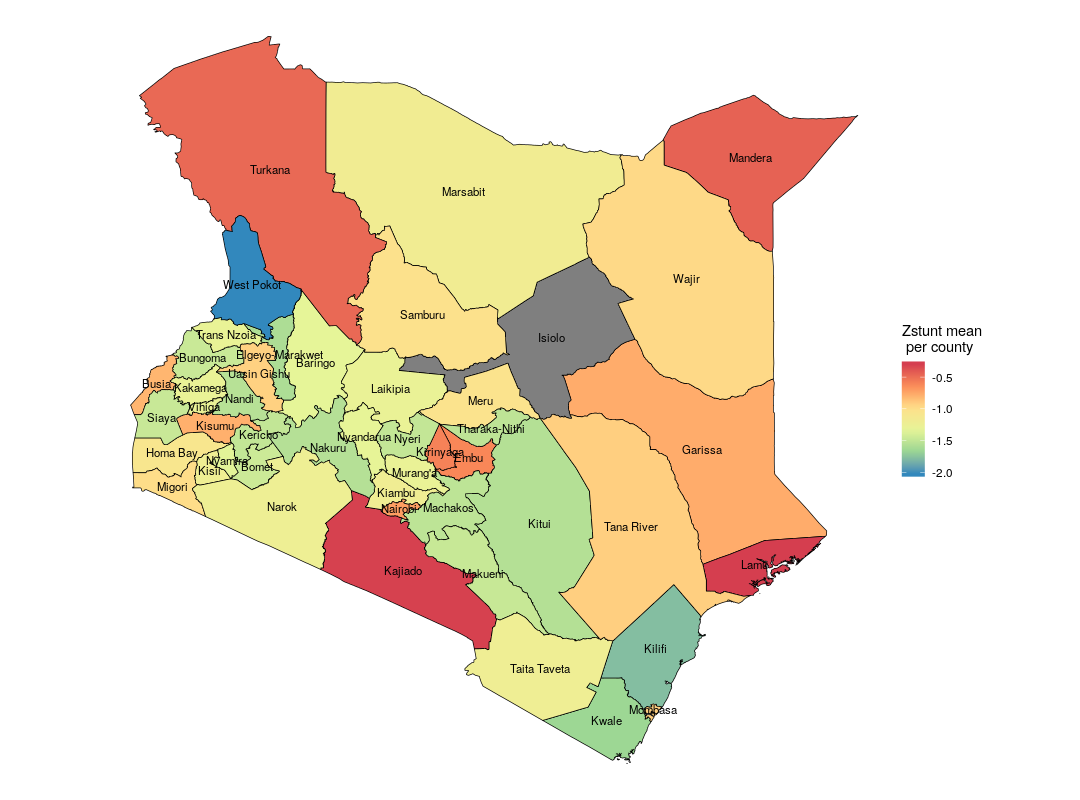
\includegraphics[scale=0.5]{Ex1plot4.png}
		\caption{Plot the map of Kenya with the mean of $\mathtt{zstunt}$ in the each county}
		\label{fig 1.4}
	\end{figure}
		
\end{enumerate}	
%222222222222222222222222222222222222222222222%

{\color{royalblue}\chapter{Random number generation}}

{\color{royalblue}\section{Problem description}}
Generating a random variable from any distribution is very essential for stochastics studies. However, true random numbers are not always available, but we can use some algorithms that generate some pseudo-random numbers.\\

{\color{royalblue}\section{Methods}}
Pseudo-random numbers are a sequence of numbers that appear "random" or approximate properties of random numbers with the following properties:\\
\begin{itemize}
	\item Good approximation of the properties of random numbers.
	\item Number can be easily and efficiently generated.
	\item Reproducibility (truly random numbers never satisfy this).
\end{itemize}

With the help of some probability properties, it is typically enough to be able to use a uniform distributed random variable, in order to generate any pseudo-random numbers from a given distribution.\\
The simplest idea for generating uniformly distributed pseudo-random numbers is using a \textit{linear congruent generators} (LCG):\\
\fbox{
	\begin{minipage}{1\textwidth}
		\begin{center}
			\begin{enumerate}
				\item Choose positive integer parameters a, c and m.
				\item Choose an initial value $x_0 \in \{0, 1, \ldots, m - 1\}$ (this value is called the seed).
				\item For each $n \in \mathbb{N} $, compute\\
				\begin{equation}
				x_{n+1} := ax_{n} + c \hspace{0.2cm}
				\text{mod} \hspace{0.2cm} m, \hspace{1cm} \forall n \in \mathbb{N} 
				\end{equation}
				\item The psuedorandom numbers are the sequence $x_1; x_2; x_3; \ldots $.
			\end{enumerate}
		\end{center}
	\end{minipage}
}\\

We make some observations regarding the LCG algorithm.\\
\begin{itemize}
	\item The LCG can generates at most m distinct numbers which are contained in $\{0, 1, \ldots, m - 1\}$
	\item As soon as some number in the sequence, say ${x_n}_0$, is repeated (i.e.,$\exists p$ such that $x_{n_{0} + p} = {x_n}_0$),

	then the same is true for the entire sequence:
	\begin{equation}
	x_{n_{0} +p+j} = x_{n_{0} + j}, \hspace{0.5cm} \forall j \geqslant 1
	\end{equation}
	The number $p$ is called the period of the sequence. This musst be less than or equal to $m$.
	\item Suppose that (under the right conditions) the LCG approximates a uniform distribution with

	parameters $0$ and $m$. In this case, $x_n / m$ would approximate a uniform distribution with parameters
0 and 1.
\end{itemize}
To generate uniformly random numbers, the period has to be maximal
(i.e., $p = m$), so that we sample every value in the sequence before repeating any. One can show that LCG has a full period $m = 2^{b}$, $b \geqslant 2$ if and
only if $c \in (0; m)$ is odd and $a$ mod $4 = 1$.\\

After generating uniform pseudo-random numbers, we can easily obtain random variables from other distributions. The \textbf{inversion method} is one way of doing so, with the help of the following theorem:
\begin{theorem}
	Let F be a distribution function on $\mathbb{R}$. The quantile function $F^{-1}$ is defined by
	 \[ F^{-1}(u) = \text{inf} \{x: F(x)\ge u, 0 < u < 1 \} \]
	If $U \sim U_{[0; 1]}$, then $F^{-1}(u)$ has a distribution function
$F$.
\end{theorem}
Hence, for continuous distributions (exponential, Pareto, standard Cauchy, etc) where $F^{-1}$, we simply simulate $U_{i}$ (with LCG) and set $X_{i} = F^{-1}(U_i)$. If $F^{-1}$ cannot be inverted analytically, appropriate
numerical methods can be applied.\\

Let $X$ be a discrete random variable with ordered possible values $\{x_{1}, x{2},\ldots \}$, so that $F(x) = \displaystyle\sum_{i:x_{i} \leqslant x} P(X = x_{i})$ and
\[F^{-1}(r) =  \text{min} \{x_k \in \{x_{1}, x_{2},\ldots \}: \displaystyle\sum_{j=1}^{k} P(X = x_{j}) = \displaystyle\sum_{j=1}^{k}p_{j} \geqslant r\}\]
Then the inverse method becomes: set $X = x_{1}$ if and only if $U_{i} \in [0, p_{1})$ and $X = x_{k}$ if and only if
$U_{i} \in \Big[ \displaystyle\sum_{j=1}^{k-1}p_{j}, \displaystyle\sum_{j=1}^{k}p_{j}\Big)$, $k = 2, 3, \ldots$. Note that

\[P(X = x_{k}) = P\Big(\displaystyle\sum_{j=1}^{k-1}p_{j} \leqslant U_{i} < \displaystyle\sum_{j=1}^{k}p_{j} \Big) = \displaystyle\sum_{j=1}^{k}p_{j} - \displaystyle\sum_{j=1}^{k-1}p_{j} = p_{k} \]

For example, to simulate a Bernoulli random variable $Ber(p)$, generate $U \in U_{[0, 1]}$ and

set $X = 0$, if $U \leqslant 1 - p$ and $X = 1$ if $U > 1 - p$.\\

Another general approach to pseudo-random variables generation is the \textbf{acceptance-rejection method}.

\fbox{
	\begin{minipage}{1\textwidth}
		\begin{center}
			\begin{enumerate}
				\item [] \textbf{Data}: Two probability densitiy functions: $f$ for $X$ and $g$ for $Y$
				\item Find a constant $M > 0$ such that $sup_{x} \frac{f(x)}{g(x)} \leqslant c$ ;
				\item Obtain a sample $y$ from $Y$ ;
				\item Obtain a sample $u$ from the uniform distribution on $[0, 1]$;
				\item \textbf{if} $u < \dfrac{f(y)}{cg(y)}$ \textbf{then}
				\item $\bigg|$ Accept $y$ as a sample drawn from $f$;
				\item \textbf{else}
				\item $\bigg|$ Reject the value of $y$ and return to the sampling step (line 2);
				\item [] \textbf{Result:} $y$, a sample drawn from $f$ (using $g$)
			\end{enumerate}
		\end{center}
	\end{minipage}
}\\

\textbf{NB:} Computing $c$ could be difficult, but one can show that $c = sup_{x} {\frac{f(x)}{g(x)}}$\\

\newpage
{\color{royalblue}\section{Results}}
\begin{enumerate}[label=(\alph*)]
	\item 
	With the Wichmann-Hill pseudo-random number generator in R, we Simulate $N =
1000 $ binomial random variables $B(n = 10, p = 0.4)$ using three approaches: inversion

	method, by simulating corresponding Bernoulli random variables by inversion method
and using R built-in function rbinom. From the figure \ref{fig 2.1}, the histograms of the three samples present the same shape but are different. This proves that the "random" numbers generated by our methods are just approximations of true random numbers.
	
	\begin{figure}[ht]
		\centering
		\scalebox{1.2}{% Created by tikzDevice version 0.12 on 2019-04-01 14:59:11
% !TEX encoding = UTF-8 Unicode
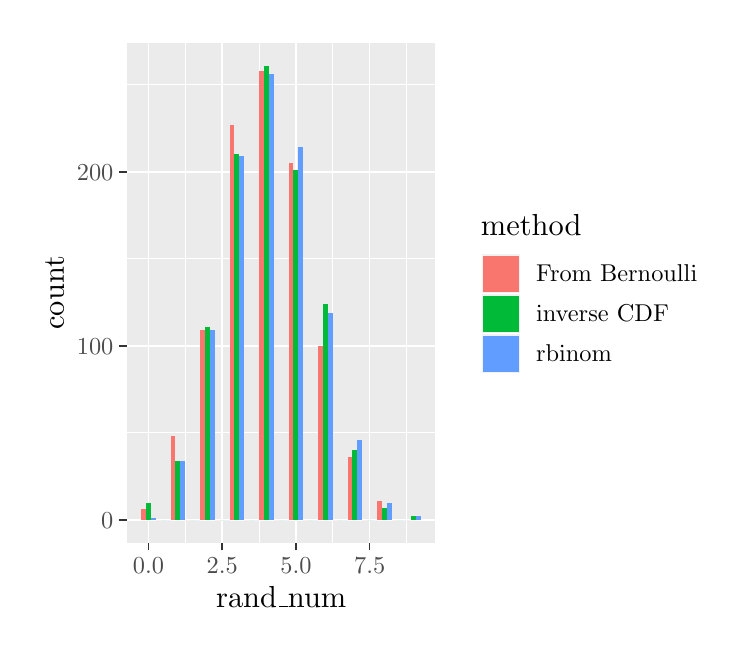
\begin{tikzpicture}[x=1pt,y=1pt]
\definecolor{fillColor}{RGB}{255,255,255}
\path[use as bounding box,fill=fillColor,fill opacity=0.00] (0,0) rectangle (252.94,216.81);
\begin{scope}
\path[clip] (  0.00,  0.00) rectangle (252.94,216.81);
\definecolor{drawColor}{RGB}{255,255,255}
\definecolor{fillColor}{RGB}{255,255,255}

\path[draw=drawColor,line width= 0.6pt,line join=round,line cap=round,fill=fillColor] (  0.00,  0.00) rectangle (252.94,216.81);
\end{scope}
\begin{scope}
\path[clip] ( 35.92, 30.72) rectangle (147.28,211.31);
\definecolor{fillColor}{gray}{0.92}

\path[fill=fillColor] ( 35.92, 30.72) rectangle (147.28,211.31);
\definecolor{drawColor}{RGB}{255,255,255}

\path[draw=drawColor,line width= 0.3pt,line join=round] ( 35.92, 70.38) --
	(147.28, 70.38);

\path[draw=drawColor,line width= 0.3pt,line join=round] ( 35.92,133.28) --
	(147.28,133.28);

\path[draw=drawColor,line width= 0.3pt,line join=round] ( 35.92,196.18) --
	(147.28,196.18);

\path[draw=drawColor,line width= 0.3pt,line join=round] ( 56.96, 30.72) --
	( 56.96,211.31);

\path[draw=drawColor,line width= 0.3pt,line join=round] ( 83.61, 30.72) --
	( 83.61,211.31);

\path[draw=drawColor,line width= 0.3pt,line join=round] (110.25, 30.72) --
	(110.25,211.31);

\path[draw=drawColor,line width= 0.3pt,line join=round] (136.89, 30.72) --
	(136.89,211.31);

\path[draw=drawColor,line width= 0.6pt,line join=round] ( 35.92, 38.93) --
	(147.28, 38.93);

\path[draw=drawColor,line width= 0.6pt,line join=round] ( 35.92,101.83) --
	(147.28,101.83);

\path[draw=drawColor,line width= 0.6pt,line join=round] ( 35.92,164.73) --
	(147.28,164.73);

\path[draw=drawColor,line width= 0.6pt,line join=round] ( 43.64, 30.72) --
	( 43.64,211.31);

\path[draw=drawColor,line width= 0.6pt,line join=round] ( 70.28, 30.72) --
	( 70.28,211.31);

\path[draw=drawColor,line width= 0.6pt,line join=round] ( 96.93, 30.72) --
	( 96.93,211.31);

\path[draw=drawColor,line width= 0.6pt,line join=round] (123.57, 30.72) --
	(123.57,211.31);
\definecolor{fillColor}{RGB}{97,156,255}

\path[fill=fillColor] ( 44.53, 38.93) rectangle ( 46.31, 39.56);
\definecolor{fillColor}{RGB}{0,186,56}

\path[fill=fillColor] ( 42.75, 38.93) rectangle ( 44.53, 45.22);
\definecolor{fillColor}{RGB}{248,118,109}

\path[fill=fillColor] ( 40.98, 38.93) rectangle ( 42.75, 42.71);
\definecolor{fillColor}{RGB}{97,156,255}

\path[fill=fillColor] ( 49.86, 38.93) rectangle ( 51.64, 38.93);
\definecolor{fillColor}{RGB}{0,186,56}

\path[fill=fillColor] ( 48.08, 38.93) rectangle ( 49.86, 38.93);
\definecolor{fillColor}{RGB}{248,118,109}

\path[fill=fillColor] ( 46.31, 38.93) rectangle ( 48.08, 38.93);
\definecolor{fillColor}{RGB}{97,156,255}

\path[fill=fillColor] ( 55.19, 38.93) rectangle ( 56.96, 60.32);
\definecolor{fillColor}{RGB}{0,186,56}

\path[fill=fillColor] ( 53.41, 38.93) rectangle ( 55.19, 60.32);
\definecolor{fillColor}{RGB}{248,118,109}

\path[fill=fillColor] ( 51.64, 38.93) rectangle ( 53.41, 69.13);
\definecolor{fillColor}{RGB}{97,156,255}

\path[fill=fillColor] ( 60.52, 38.93) rectangle ( 62.29, 38.93);
\definecolor{fillColor}{RGB}{0,186,56}

\path[fill=fillColor] ( 58.74, 38.93) rectangle ( 60.52, 38.93);
\definecolor{fillColor}{RGB}{248,118,109}

\path[fill=fillColor] ( 56.96, 38.93) rectangle ( 58.74, 38.93);
\definecolor{fillColor}{RGB}{97,156,255}

\path[fill=fillColor] ( 65.84, 38.93) rectangle ( 67.62,107.49);
\definecolor{fillColor}{RGB}{0,186,56}

\path[fill=fillColor] ( 64.07, 38.93) rectangle ( 65.84,108.75);
\definecolor{fillColor}{RGB}{248,118,109}

\path[fill=fillColor] ( 62.29, 38.93) rectangle ( 64.07,107.49);
\definecolor{fillColor}{RGB}{97,156,255}

\path[fill=fillColor] ( 71.17, 38.93) rectangle ( 72.95, 38.93);
\definecolor{fillColor}{RGB}{0,186,56}

\path[fill=fillColor] ( 69.40, 38.93) rectangle ( 71.17, 38.93);
\definecolor{fillColor}{RGB}{248,118,109}

\path[fill=fillColor] ( 67.62, 38.93) rectangle ( 69.40, 38.93);
\definecolor{fillColor}{RGB}{97,156,255}

\path[fill=fillColor] ( 76.50, 38.93) rectangle ( 78.28,170.39);
\definecolor{fillColor}{RGB}{0,186,56}

\path[fill=fillColor] ( 74.72, 38.93) rectangle ( 76.50,171.02);
\definecolor{fillColor}{RGB}{248,118,109}

\path[fill=fillColor] ( 72.95, 38.93) rectangle ( 74.72,181.72);
\definecolor{fillColor}{RGB}{97,156,255}

\path[fill=fillColor] ( 81.83, 38.93) rectangle ( 83.61, 38.93);
\definecolor{fillColor}{RGB}{0,186,56}

\path[fill=fillColor] ( 80.05, 38.93) rectangle ( 81.83, 38.93);
\definecolor{fillColor}{RGB}{248,118,109}

\path[fill=fillColor] ( 78.28, 38.93) rectangle ( 80.05, 38.93);
\definecolor{fillColor}{RGB}{97,156,255}

\path[fill=fillColor] ( 87.16, 38.93) rectangle ( 88.93,199.96);
\definecolor{fillColor}{RGB}{0,186,56}

\path[fill=fillColor] ( 85.38, 38.93) rectangle ( 87.16,203.10);
\definecolor{fillColor}{RGB}{248,118,109}

\path[fill=fillColor] ( 83.61, 38.93) rectangle ( 85.38,201.21);
\definecolor{fillColor}{RGB}{97,156,255}

\path[fill=fillColor] ( 92.49, 38.93) rectangle ( 94.26, 38.93);
\definecolor{fillColor}{RGB}{0,186,56}

\path[fill=fillColor] ( 90.71, 38.93) rectangle ( 92.49, 38.93);
\definecolor{fillColor}{RGB}{248,118,109}

\path[fill=fillColor] ( 88.93, 38.93) rectangle ( 90.71, 38.93);
\definecolor{fillColor}{RGB}{97,156,255}

\path[fill=fillColor] ( 97.81, 38.93) rectangle ( 99.59,173.54);
\definecolor{fillColor}{RGB}{0,186,56}

\path[fill=fillColor] ( 96.04, 38.93) rectangle ( 97.81,165.36);
\definecolor{fillColor}{RGB}{248,118,109}

\path[fill=fillColor] ( 94.26, 38.93) rectangle ( 96.04,167.88);
\definecolor{fillColor}{RGB}{97,156,255}

\path[fill=fillColor] (103.14, 38.93) rectangle (104.92, 38.93);
\definecolor{fillColor}{RGB}{0,186,56}

\path[fill=fillColor] (101.37, 38.93) rectangle (103.14, 38.93);
\definecolor{fillColor}{RGB}{248,118,109}

\path[fill=fillColor] ( 99.59, 38.93) rectangle (101.37, 38.93);
\definecolor{fillColor}{RGB}{97,156,255}

\path[fill=fillColor] (108.47, 38.93) rectangle (110.25,113.78);
\definecolor{fillColor}{RGB}{0,186,56}

\path[fill=fillColor] (106.69, 38.93) rectangle (108.47,116.93);
\definecolor{fillColor}{RGB}{248,118,109}

\path[fill=fillColor] (104.92, 38.93) rectangle (106.69,101.83);
\definecolor{fillColor}{RGB}{97,156,255}

\path[fill=fillColor] (113.80, 38.93) rectangle (115.57, 38.93);
\definecolor{fillColor}{RGB}{0,186,56}

\path[fill=fillColor] (112.02, 38.93) rectangle (113.80, 38.93);
\definecolor{fillColor}{RGB}{248,118,109}

\path[fill=fillColor] (110.25, 38.93) rectangle (112.02, 38.93);
\definecolor{fillColor}{RGB}{97,156,255}

\path[fill=fillColor] (119.13, 38.93) rectangle (120.90, 67.87);
\definecolor{fillColor}{RGB}{0,186,56}

\path[fill=fillColor] (117.35, 38.93) rectangle (119.13, 64.09);
\definecolor{fillColor}{RGB}{248,118,109}

\path[fill=fillColor] (115.57, 38.93) rectangle (117.35, 61.58);
\definecolor{fillColor}{RGB}{97,156,255}

\path[fill=fillColor] (124.46, 38.93) rectangle (126.23, 38.93);
\definecolor{fillColor}{RGB}{0,186,56}

\path[fill=fillColor] (122.68, 38.93) rectangle (124.46, 38.93);
\definecolor{fillColor}{RGB}{248,118,109}

\path[fill=fillColor] (120.90, 38.93) rectangle (122.68, 38.93);
\definecolor{fillColor}{RGB}{97,156,255}

\path[fill=fillColor] (129.78, 38.93) rectangle (131.56, 45.22);
\definecolor{fillColor}{RGB}{0,186,56}

\path[fill=fillColor] (128.01, 38.93) rectangle (129.78, 43.34);
\definecolor{fillColor}{RGB}{248,118,109}

\path[fill=fillColor] (126.23, 38.93) rectangle (128.01, 45.85);
\definecolor{fillColor}{RGB}{97,156,255}

\path[fill=fillColor] (135.11, 38.93) rectangle (136.89, 38.93);
\definecolor{fillColor}{RGB}{0,186,56}

\path[fill=fillColor] (133.34, 38.93) rectangle (135.11, 38.93);
\definecolor{fillColor}{RGB}{248,118,109}

\path[fill=fillColor] (131.56, 38.93) rectangle (133.34, 38.93);
\definecolor{fillColor}{RGB}{97,156,255}

\path[fill=fillColor] (140.44, 38.93) rectangle (142.22, 40.19);
\definecolor{fillColor}{RGB}{0,186,56}

\path[fill=fillColor] (138.66, 38.93) rectangle (140.44, 40.19);
\definecolor{fillColor}{RGB}{248,118,109}

\path[fill=fillColor] (136.89, 38.93) rectangle (138.66, 38.93);
\end{scope}
\begin{scope}
\path[clip] (  0.00,  0.00) rectangle (252.94,216.81);
\definecolor{drawColor}{gray}{0.30}

\node[text=drawColor,anchor=base east,inner sep=0pt, outer sep=0pt, scale=  0.88] at ( 30.97, 35.90) {0};

\node[text=drawColor,anchor=base east,inner sep=0pt, outer sep=0pt, scale=  0.88] at ( 30.97, 98.80) {100};

\node[text=drawColor,anchor=base east,inner sep=0pt, outer sep=0pt, scale=  0.88] at ( 30.97,161.70) {200};
\end{scope}
\begin{scope}
\path[clip] (  0.00,  0.00) rectangle (252.94,216.81);
\definecolor{drawColor}{gray}{0.20}

\path[draw=drawColor,line width= 0.6pt,line join=round] ( 33.17, 38.93) --
	( 35.92, 38.93);

\path[draw=drawColor,line width= 0.6pt,line join=round] ( 33.17,101.83) --
	( 35.92,101.83);

\path[draw=drawColor,line width= 0.6pt,line join=round] ( 33.17,164.73) --
	( 35.92,164.73);
\end{scope}
\begin{scope}
\path[clip] (  0.00,  0.00) rectangle (252.94,216.81);
\definecolor{drawColor}{gray}{0.20}

\path[draw=drawColor,line width= 0.6pt,line join=round] ( 43.64, 27.97) --
	( 43.64, 30.72);

\path[draw=drawColor,line width= 0.6pt,line join=round] ( 70.28, 27.97) --
	( 70.28, 30.72);

\path[draw=drawColor,line width= 0.6pt,line join=round] ( 96.93, 27.97) --
	( 96.93, 30.72);

\path[draw=drawColor,line width= 0.6pt,line join=round] (123.57, 27.97) --
	(123.57, 30.72);
\end{scope}
\begin{scope}
\path[clip] (  0.00,  0.00) rectangle (252.94,216.81);
\definecolor{drawColor}{gray}{0.30}

\node[text=drawColor,anchor=base,inner sep=0pt, outer sep=0pt, scale=  0.88] at ( 43.64, 19.71) {0.0};

\node[text=drawColor,anchor=base,inner sep=0pt, outer sep=0pt, scale=  0.88] at ( 70.28, 19.71) {2.5};

\node[text=drawColor,anchor=base,inner sep=0pt, outer sep=0pt, scale=  0.88] at ( 96.93, 19.71) {5.0};

\node[text=drawColor,anchor=base,inner sep=0pt, outer sep=0pt, scale=  0.88] at (123.57, 19.71) {7.5};
\end{scope}
\begin{scope}
\path[clip] (  0.00,  0.00) rectangle (252.94,216.81);
\definecolor{drawColor}{RGB}{0,0,0}

\node[text=drawColor,anchor=base,inner sep=0pt, outer sep=0pt, scale=  1.10] at ( 91.60,  7.44) {rand{\_{}}num};
\end{scope}
\begin{scope}
\path[clip] (  0.00,  0.00) rectangle (252.94,216.81);
\definecolor{drawColor}{RGB}{0,0,0}

\node[text=drawColor,rotate= 90.00,anchor=base,inner sep=0pt, outer sep=0pt, scale=  1.10] at ( 13.08,121.02) {count};
\end{scope}
\begin{scope}
\path[clip] (  0.00,  0.00) rectangle (252.94,216.81);
\definecolor{fillColor}{RGB}{255,255,255}

\path[fill=fillColor] (158.28, 86.33) rectangle (247.44,155.71);
\end{scope}
\begin{scope}
\path[clip] (  0.00,  0.00) rectangle (252.94,216.81);
\definecolor{drawColor}{RGB}{0,0,0}

\node[text=drawColor,anchor=base west,inner sep=0pt, outer sep=0pt, scale=  1.10] at (163.78,141.66) {method};
\end{scope}
\begin{scope}
\path[clip] (  0.00,  0.00) rectangle (252.94,216.81);
\definecolor{drawColor}{RGB}{255,255,255}
\definecolor{fillColor}{gray}{0.95}

\path[draw=drawColor,line width= 0.6pt,line join=round,line cap=round,fill=fillColor] (163.78,120.73) rectangle (178.23,135.19);
\end{scope}
\begin{scope}
\path[clip] (  0.00,  0.00) rectangle (252.94,216.81);
\definecolor{fillColor}{RGB}{248,118,109}

\path[fill=fillColor] (164.49,121.45) rectangle (177.52,134.48);
\end{scope}
\begin{scope}
\path[clip] (  0.00,  0.00) rectangle (252.94,216.81);
\definecolor{drawColor}{RGB}{255,255,255}
\definecolor{fillColor}{gray}{0.95}

\path[draw=drawColor,line width= 0.6pt,line join=round,line cap=round,fill=fillColor] (163.78,106.28) rectangle (178.23,120.73);
\end{scope}
\begin{scope}
\path[clip] (  0.00,  0.00) rectangle (252.94,216.81);
\definecolor{fillColor}{RGB}{0,186,56}

\path[fill=fillColor] (164.49,106.99) rectangle (177.52,120.02);
\end{scope}
\begin{scope}
\path[clip] (  0.00,  0.00) rectangle (252.94,216.81);
\definecolor{drawColor}{RGB}{255,255,255}
\definecolor{fillColor}{gray}{0.95}

\path[draw=drawColor,line width= 0.6pt,line join=round,line cap=round,fill=fillColor] (163.78, 91.83) rectangle (178.23,106.28);
\end{scope}
\begin{scope}
\path[clip] (  0.00,  0.00) rectangle (252.94,216.81);
\definecolor{fillColor}{RGB}{97,156,255}

\path[fill=fillColor] (164.49, 92.54) rectangle (177.52,105.57);
\end{scope}
\begin{scope}
\path[clip] (  0.00,  0.00) rectangle (252.94,216.81);
\definecolor{drawColor}{RGB}{0,0,0}

\node[text=drawColor,anchor=base west,inner sep=0pt, outer sep=0pt, scale=  0.88] at (183.73,124.93) {From Bernoulli};
\end{scope}
\begin{scope}
\path[clip] (  0.00,  0.00) rectangle (252.94,216.81);
\definecolor{drawColor}{RGB}{0,0,0}

\node[text=drawColor,anchor=base west,inner sep=0pt, outer sep=0pt, scale=  0.88] at (183.73,110.48) {inverse CDF};
\end{scope}
\begin{scope}
\path[clip] (  0.00,  0.00) rectangle (252.94,216.81);
\definecolor{drawColor}{RGB}{0,0,0}

\node[text=drawColor,anchor=base west,inner sep=0pt, outer sep=0pt, scale=  0.88] at (183.73, 96.02) {rbinom};
\end{scope}
\end{tikzpicture}
}
		\caption{Histogram of the empirical CDF of all
three samples}
		\label{fig 2.1}
	\end{figure}
	
	\item To use accept-reject method (and a generator for uniform random variables only), of $N = 10000$ standard normal distributed random variables
with density 
	$f(x) = (2\pi)^{-\frac{1}{2}}e^{-\frac{x^2}{2}} $, the density of the
standard Cauchy distribution is used: 
	$ g(x)=\{{\pi(1+x^2)}^{-1}\} $.
	
	\item[�] The constant value $c$ for this method is given by $sup_{x} {\frac{f(x)}{g(x)}} = 1.520347 $
	\item[�] Then after computing the $N$ standard normal random variables, we notice that the estimated and theoretical acceptance probabilities are almost equal. This is well depicted with in the figure \ref{fig 2.2}, where the histogram of the obtain sample is symmetric and has the same shape as the standard normal density curve.
	
	\begin{figure}[H]
		\centering
		\scalebox{0.75}{% Created by tikzDevice version 0.12 on 2019-04-01 14:59:12
% !TEX encoding = UTF-8 Unicode
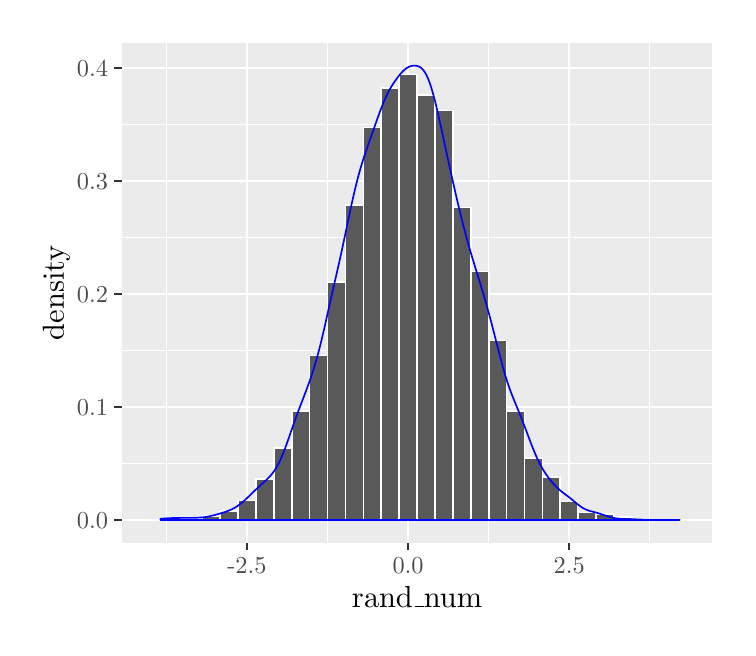
\begin{tikzpicture}[x=1pt,y=1pt]
\definecolor{fillColor}{RGB}{255,255,255}
\path[use as bounding box,fill=fillColor,fill opacity=0.00] (0,0) rectangle (252.94,216.81);
\begin{scope}
\path[clip] (  0.00,  0.00) rectangle (252.94,216.81);
\definecolor{drawColor}{RGB}{255,255,255}
\definecolor{fillColor}{RGB}{255,255,255}

\path[draw=drawColor,line width= 0.6pt,line join=round,line cap=round,fill=fillColor] (  0.00,  0.00) rectangle (252.94,216.81);
\end{scope}
\begin{scope}
\path[clip] ( 33.96, 30.72) rectangle (247.44,211.31);
\definecolor{fillColor}{gray}{0.92}

\path[fill=fillColor] ( 33.96, 30.72) rectangle (247.44,211.31);
\definecolor{drawColor}{RGB}{255,255,255}

\path[draw=drawColor,line width= 0.3pt,line join=round] ( 33.96, 59.34) --
	(247.44, 59.34);

\path[draw=drawColor,line width= 0.3pt,line join=round] ( 33.96,100.16) --
	(247.44,100.16);

\path[draw=drawColor,line width= 0.3pt,line join=round] ( 33.96,140.98) --
	(247.44,140.98);

\path[draw=drawColor,line width= 0.3pt,line join=round] ( 33.96,181.80) --
	(247.44,181.80);

\path[draw=drawColor,line width= 0.3pt,line join=round] ( 50.10, 30.72) --
	( 50.10,211.31);

\path[draw=drawColor,line width= 0.3pt,line join=round] (108.35, 30.72) --
	(108.35,211.31);

\path[draw=drawColor,line width= 0.3pt,line join=round] (166.59, 30.72) --
	(166.59,211.31);

\path[draw=drawColor,line width= 0.3pt,line join=round] (224.83, 30.72) --
	(224.83,211.31);

\path[draw=drawColor,line width= 0.6pt,line join=round] ( 33.96, 38.93) --
	(247.44, 38.93);

\path[draw=drawColor,line width= 0.6pt,line join=round] ( 33.96, 79.75) --
	(247.44, 79.75);

\path[draw=drawColor,line width= 0.6pt,line join=round] ( 33.96,120.57) --
	(247.44,120.57);

\path[draw=drawColor,line width= 0.6pt,line join=round] ( 33.96,161.39) --
	(247.44,161.39);

\path[draw=drawColor,line width= 0.6pt,line join=round] ( 33.96,202.21) --
	(247.44,202.21);

\path[draw=drawColor,line width= 0.6pt,line join=round] ( 79.23, 30.72) --
	( 79.23,211.31);

\path[draw=drawColor,line width= 0.6pt,line join=round] (137.47, 30.72) --
	(137.47,211.31);

\path[draw=drawColor,line width= 0.6pt,line join=round] (195.71, 30.72) --
	(195.71,211.31);
\definecolor{fillColor}{gray}{0.35}

\path[draw=drawColor,line width= 0.6pt,line join=round,fill=fillColor] ( 43.67, 38.93) rectangle ( 50.13, 38.93);

\path[draw=drawColor,line width= 0.6pt,line join=round,fill=fillColor] ( 50.13, 38.93) rectangle ( 56.60, 39.52);

\path[draw=drawColor,line width= 0.6pt,line join=round,fill=fillColor] ( 56.60, 38.93) rectangle ( 63.07, 39.37);

\path[draw=drawColor,line width= 0.6pt,line join=round,fill=fillColor] ( 63.07, 38.93) rectangle ( 69.54, 40.40);

\path[draw=drawColor,line width= 0.6pt,line join=round,fill=fillColor] ( 69.54, 38.93) rectangle ( 76.01, 42.17);

\path[draw=drawColor,line width= 0.6pt,line join=round,fill=fillColor] ( 76.01, 38.93) rectangle ( 82.48, 45.99);

\path[draw=drawColor,line width= 0.6pt,line join=round,fill=fillColor] ( 82.48, 38.93) rectangle ( 88.95, 53.78);

\path[draw=drawColor,line width= 0.6pt,line join=round,fill=fillColor] ( 88.95, 38.93) rectangle ( 95.42, 64.81);

\path[draw=drawColor,line width= 0.6pt,line join=round,fill=fillColor] ( 95.42, 38.93) rectangle (101.89, 78.18);

\path[draw=drawColor,line width= 0.6pt,line join=round,fill=fillColor] (101.89, 38.93) rectangle (108.36, 98.32);

\path[draw=drawColor,line width= 0.6pt,line join=round,fill=fillColor] (108.36, 38.93) rectangle (114.83,124.93);

\path[draw=drawColor,line width= 0.6pt,line join=round,fill=fillColor] (114.83, 38.93) rectangle (121.30,152.71);

\path[draw=drawColor,line width= 0.6pt,line join=round,fill=fillColor] (121.30, 38.93) rectangle (127.76,180.79);

\path[draw=drawColor,line width= 0.6pt,line join=round,fill=fillColor] (127.76, 38.93) rectangle (134.23,195.05);

\path[draw=drawColor,line width= 0.6pt,line join=round,fill=fillColor] (134.23, 38.93) rectangle (140.70,199.90);

\path[draw=drawColor,line width= 0.6pt,line join=round,fill=fillColor] (140.70, 38.93) rectangle (147.17,192.55);

\path[draw=drawColor,line width= 0.6pt,line join=round,fill=fillColor] (147.17, 38.93) rectangle (153.64,186.82);

\path[draw=drawColor,line width= 0.6pt,line join=round,fill=fillColor] (153.64, 38.93) rectangle (160.11,151.83);

\path[draw=drawColor,line width= 0.6pt,line join=round,fill=fillColor] (160.11, 38.93) rectangle (166.58,128.75);

\path[draw=drawColor,line width= 0.6pt,line join=round,fill=fillColor] (166.58, 38.93) rectangle (173.05,103.76);

\path[draw=drawColor,line width= 0.6pt,line join=round,fill=fillColor] (173.05, 38.93) rectangle (179.52, 78.33);

\path[draw=drawColor,line width= 0.6pt,line join=round,fill=fillColor] (179.52, 38.93) rectangle (185.99, 61.28);

\path[draw=drawColor,line width= 0.6pt,line join=round,fill=fillColor] (185.99, 38.93) rectangle (192.46, 54.37);

\path[draw=drawColor,line width= 0.6pt,line join=round,fill=fillColor] (192.46, 38.93) rectangle (198.93, 45.55);

\path[draw=drawColor,line width= 0.6pt,line join=round,fill=fillColor] (198.93, 38.93) rectangle (205.40, 41.58);

\path[draw=drawColor,line width= 0.6pt,line join=round,fill=fillColor] (205.40, 38.93) rectangle (211.86, 40.99);

\path[draw=drawColor,line width= 0.6pt,line join=round,fill=fillColor] (211.86, 38.93) rectangle (218.33, 40.11);

\path[draw=drawColor,line width= 0.6pt,line join=round,fill=fillColor] (218.33, 38.93) rectangle (224.80, 39.23);

\path[draw=drawColor,line width= 0.6pt,line join=round,fill=fillColor] (224.80, 38.93) rectangle (231.27, 38.93);

\path[draw=drawColor,line width= 0.6pt,line join=round,fill=fillColor] (231.27, 38.93) rectangle (237.74, 39.08);
\definecolor{drawColor}{RGB}{0,0,255}

\path[draw=drawColor,line width= 0.6pt,line join=round,line cap=round] ( 47.99, 39.34) --
	( 48.36, 39.37) --
	( 48.72, 39.40) --
	( 49.09, 39.43) --
	( 49.46, 39.46) --
	( 49.83, 39.48) --
	( 50.19, 39.51) --
	( 50.56, 39.53) --
	( 50.93, 39.55) --
	( 51.29, 39.57) --
	( 51.66, 39.59) --
	( 52.03, 39.60) --
	( 52.40, 39.61) --
	( 52.76, 39.63) --
	( 53.13, 39.63) --
	( 53.50, 39.64) --
	( 53.86, 39.65) --
	( 54.23, 39.65) --
	( 54.60, 39.65) --
	( 54.97, 39.66) --
	( 55.33, 39.66) --
	( 55.70, 39.66) --
	( 56.07, 39.66) --
	( 56.43, 39.66) --
	( 56.80, 39.66) --
	( 57.17, 39.66) --
	( 57.54, 39.67) --
	( 57.90, 39.67) --
	( 58.27, 39.67) --
	( 58.64, 39.68) --
	( 59.00, 39.68) --
	( 59.37, 39.69) --
	( 59.74, 39.69) --
	( 60.10, 39.70) --
	( 60.47, 39.71) --
	( 60.84, 39.72) --
	( 61.21, 39.73) --
	( 61.57, 39.75) --
	( 61.94, 39.77) --
	( 62.31, 39.79) --
	( 62.67, 39.82) --
	( 63.04, 39.85) --
	( 63.41, 39.88) --
	( 63.78, 39.93) --
	( 64.14, 39.97) --
	( 64.51, 40.03) --
	( 64.88, 40.09) --
	( 65.24, 40.16) --
	( 65.61, 40.23) --
	( 65.98, 40.31) --
	( 66.35, 40.40) --
	( 66.71, 40.49) --
	( 67.08, 40.58) --
	( 67.45, 40.68) --
	( 67.81, 40.78) --
	( 68.18, 40.88) --
	( 68.55, 40.98) --
	( 68.92, 41.09) --
	( 69.28, 41.20) --
	( 69.65, 41.30) --
	( 70.02, 41.41) --
	( 70.38, 41.52) --
	( 70.75, 41.63) --
	( 71.12, 41.75) --
	( 71.49, 41.87) --
	( 71.85, 41.99) --
	( 72.22, 42.13) --
	( 72.59, 42.27) --
	( 72.95, 42.41) --
	( 73.32, 42.57) --
	( 73.69, 42.74) --
	( 74.06, 42.92) --
	( 74.42, 43.12) --
	( 74.79, 43.32) --
	( 75.16, 43.54) --
	( 75.52, 43.78) --
	( 75.89, 44.02) --
	( 76.26, 44.28) --
	( 76.63, 44.55) --
	( 76.99, 44.84) --
	( 77.36, 45.13) --
	( 77.73, 45.44) --
	( 78.09, 45.76) --
	( 78.46, 46.08) --
	( 78.83, 46.42) --
	( 79.20, 46.76) --
	( 79.56, 47.11) --
	( 79.93, 47.46) --
	( 80.30, 47.82) --
	( 80.66, 48.18) --
	( 81.03, 48.53) --
	( 81.40, 48.89) --
	( 81.77, 49.25) --
	( 82.13, 49.60) --
	( 82.50, 49.95) --
	( 82.87, 50.30) --
	( 83.23, 50.64) --
	( 83.60, 50.98) --
	( 83.97, 51.32) --
	( 84.34, 51.65) --
	( 84.70, 51.98) --
	( 85.07, 52.31) --
	( 85.44, 52.65) --
	( 85.80, 52.99) --
	( 86.17, 53.33) --
	( 86.54, 53.68) --
	( 86.91, 54.05) --
	( 87.27, 54.43) --
	( 87.64, 54.83) --
	( 88.01, 55.25) --
	( 88.37, 55.69) --
	( 88.74, 56.17) --
	( 89.11, 56.68) --
	( 89.48, 57.23) --
	( 89.84, 57.82) --
	( 90.21, 58.46) --
	( 90.58, 59.14) --
	( 90.94, 59.86) --
	( 91.31, 60.63) --
	( 91.68, 61.46) --
	( 92.05, 62.33) --
	( 92.41, 63.24) --
	( 92.78, 64.19) --
	( 93.15, 65.17) --
	( 93.51, 66.17) --
	( 93.88, 67.20) --
	( 94.25, 68.25) --
	( 94.62, 69.31) --
	( 94.98, 70.37) --
	( 95.35, 71.42) --
	( 95.72, 72.48) --
	( 96.08, 73.52) --
	( 96.45, 74.55) --
	( 96.82, 75.58) --
	( 97.19, 76.58) --
	( 97.55, 77.58) --
	( 97.92, 78.56) --
	( 98.29, 79.54) --
	( 98.65, 80.50) --
	( 99.02, 81.46) --
	( 99.39, 82.42) --
	( 99.76, 83.38) --
	(100.12, 84.34) --
	(100.49, 85.31) --
	(100.86, 86.29) --
	(101.22, 87.28) --
	(101.59, 88.29) --
	(101.96, 89.32) --
	(102.33, 90.37) --
	(102.69, 91.46) --
	(103.06, 92.58) --
	(103.43, 93.74) --
	(103.79, 94.94) --
	(104.16, 96.19) --
	(104.53, 97.49) --
	(104.90, 98.84) --
	(105.26,100.23) --
	(105.63,101.68) --
	(106.00,103.16) --
	(106.36,104.70) --
	(106.73,106.26) --
	(107.10,107.86) --
	(107.47,109.47) --
	(107.83,111.10) --
	(108.20,112.74) --
	(108.57,114.39) --
	(108.93,116.03) --
	(109.30,117.66) --
	(109.67,119.29) --
	(110.04,120.91) --
	(110.40,122.52) --
	(110.77,124.13) --
	(111.14,125.73) --
	(111.50,127.34) --
	(111.87,128.95) --
	(112.24,130.57) --
	(112.61,132.20) --
	(112.97,133.86) --
	(113.34,135.53) --
	(113.71,137.22) --
	(114.07,138.93) --
	(114.44,140.66) --
	(114.81,142.40) --
	(115.18,144.16) --
	(115.54,145.91) --
	(115.91,147.67) --
	(116.28,149.41) --
	(116.64,151.14) --
	(117.01,152.84) --
	(117.38,154.51) --
	(117.75,156.14) --
	(118.11,157.72) --
	(118.48,159.25) --
	(118.85,160.73) --
	(119.21,162.16) --
	(119.58,163.53) --
	(119.95,164.86) --
	(120.32,166.14) --
	(120.68,167.37) --
	(121.05,168.56) --
	(121.42,169.70) --
	(121.78,170.82) --
	(122.15,171.92) --
	(122.52,172.99) --
	(122.89,174.05) --
	(123.25,175.10) --
	(123.62,176.14) --
	(123.99,177.18) --
	(124.35,178.22) --
	(124.72,179.25) --
	(125.09,180.29) --
	(125.46,181.33) --
	(125.82,182.37) --
	(126.19,183.41) --
	(126.56,184.44) --
	(126.92,185.46) --
	(127.29,186.46) --
	(127.66,187.44) --
	(128.03,188.39) --
	(128.39,189.32) --
	(128.76,190.21) --
	(129.13,191.06) --
	(129.49,191.87) --
	(129.86,192.65) --
	(130.23,193.38) --
	(130.60,194.07) --
	(130.96,194.73) --
	(131.33,195.35) --
	(131.70,195.95) --
	(132.06,196.52) --
	(132.43,197.08) --
	(132.80,197.61) --
	(133.17,198.12) --
	(133.53,198.62) --
	(133.90,199.10) --
	(134.27,199.57) --
	(134.63,200.01) --
	(135.00,200.44) --
	(135.37,200.84) --
	(135.74,201.21) --
	(136.10,201.55) --
	(136.47,201.86) --
	(136.84,202.13) --
	(137.20,202.36) --
	(137.57,202.57) --
	(137.94,202.74) --
	(138.30,202.87) --
	(138.67,202.98) --
	(139.04,203.05) --
	(139.41,203.09) --
	(139.77,203.10) --
	(140.14,203.08) --
	(140.51,203.03) --
	(140.87,202.94) --
	(141.24,202.81) --
	(141.61,202.64) --
	(141.98,202.41) --
	(142.34,202.12) --
	(142.71,201.75) --
	(143.08,201.32) --
	(143.44,200.80) --
	(143.81,200.20) --
	(144.18,199.50) --
	(144.55,198.71) --
	(144.91,197.82) --
	(145.28,196.83) --
	(145.65,195.74) --
	(146.01,194.57) --
	(146.38,193.30) --
	(146.75,191.97) --
	(147.12,190.56) --
	(147.48,189.08) --
	(147.85,187.55) --
	(148.22,185.97) --
	(148.58,184.36) --
	(148.95,182.71) --
	(149.32,181.04) --
	(149.69,179.36) --
	(150.05,177.67) --
	(150.42,175.97) --
	(150.79,174.27) --
	(151.15,172.57) --
	(151.52,170.88) --
	(151.89,169.19) --
	(152.26,167.51) --
	(152.62,165.83) --
	(152.99,164.17) --
	(153.36,162.52) --
	(153.72,160.87) --
	(154.09,159.25) --
	(154.46,157.63) --
	(154.83,156.04) --
	(155.19,154.46) --
	(155.56,152.90) --
	(155.93,151.36) --
	(156.29,149.84) --
	(156.66,148.34) --
	(157.03,146.88) --
	(157.40,145.43) --
	(157.76,144.02) --
	(158.13,142.63) --
	(158.50,141.26) --
	(158.86,139.92) --
	(159.23,138.60) --
	(159.60,137.31) --
	(159.97,136.04) --
	(160.33,134.79) --
	(160.70,133.56) --
	(161.07,132.34) --
	(161.43,131.13) --
	(161.80,129.94) --
	(162.17,128.75) --
	(162.54,127.56) --
	(162.90,126.37) --
	(163.27,125.18) --
	(163.64,123.98) --
	(164.00,122.77) --
	(164.37,121.55) --
	(164.74,120.31) --
	(165.11,119.06) --
	(165.47,117.79) --
	(165.84,116.50) --
	(166.21,115.19) --
	(166.57,113.86) --
	(166.94,112.51) --
	(167.31,111.14) --
	(167.68,109.75) --
	(168.04,108.34) --
	(168.41,106.91) --
	(168.78,105.47) --
	(169.14,104.03) --
	(169.51,102.58) --
	(169.88,101.13) --
	(170.25, 99.69) --
	(170.61, 98.27) --
	(170.98, 96.87) --
	(171.35, 95.49) --
	(171.71, 94.15) --
	(172.08, 92.85) --
	(172.45, 91.60) --
	(172.82, 90.39) --
	(173.18, 89.23) --
	(173.55, 88.11) --
	(173.92, 87.04) --
	(174.28, 86.01) --
	(174.65, 85.02) --
	(175.02, 84.07) --
	(175.39, 83.14) --
	(175.75, 82.23) --
	(176.12, 81.33) --
	(176.49, 80.44) --
	(176.85, 79.55) --
	(177.22, 78.66) --
	(177.59, 77.76) --
	(177.96, 76.85) --
	(178.32, 75.93) --
	(178.69, 75.00) --
	(179.06, 74.05) --
	(179.42, 73.10) --
	(179.79, 72.13) --
	(180.16, 71.15) --
	(180.53, 70.17) --
	(180.89, 69.19) --
	(181.26, 68.22) --
	(181.63, 67.25) --
	(181.99, 66.29) --
	(182.36, 65.35) --
	(182.73, 64.43) --
	(183.10, 63.53) --
	(183.46, 62.66) --
	(183.83, 61.82) --
	(184.20, 61.02) --
	(184.56, 60.24) --
	(184.93, 59.50) --
	(185.30, 58.79) --
	(185.67, 58.11) --
	(186.03, 57.46) --
	(186.40, 56.85) --
	(186.77, 56.26) --
	(187.13, 55.70) --
	(187.50, 55.16) --
	(187.87, 54.64) --
	(188.24, 54.15) --
	(188.60, 53.67) --
	(188.97, 53.20) --
	(189.34, 52.75) --
	(189.70, 52.32) --
	(190.07, 51.91) --
	(190.44, 51.51) --
	(190.81, 51.12) --
	(191.17, 50.75) --
	(191.54, 50.40) --
	(191.91, 50.06) --
	(192.27, 49.74) --
	(192.64, 49.43) --
	(193.01, 49.13) --
	(193.38, 48.84) --
	(193.74, 48.56) --
	(194.11, 48.28) --
	(194.48, 48.01) --
	(194.84, 47.73) --
	(195.21, 47.46) --
	(195.58, 47.17) --
	(195.95, 46.88) --
	(196.31, 46.59) --
	(196.68, 46.29) --
	(197.05, 45.99) --
	(197.41, 45.68) --
	(197.78, 45.38) --
	(198.15, 45.07) --
	(198.52, 44.77) --
	(198.88, 44.48) --
	(199.25, 44.19) --
	(199.62, 43.92) --
	(199.98, 43.67) --
	(200.35, 43.43) --
	(200.72, 43.21) --
	(201.09, 43.00) --
	(201.45, 42.82) --
	(201.82, 42.66) --
	(202.19, 42.51) --
	(202.55, 42.37) --
	(202.92, 42.25) --
	(203.29, 42.14) --
	(203.66, 42.04) --
	(204.02, 41.94) --
	(204.39, 41.85) --
	(204.76, 41.75) --
	(205.12, 41.66) --
	(205.49, 41.56) --
	(205.86, 41.46) --
	(206.23, 41.35) --
	(206.59, 41.24) --
	(206.96, 41.12) --
	(207.33, 41.01) --
	(207.69, 40.88) --
	(208.06, 40.76) --
	(208.43, 40.63) --
	(208.80, 40.51) --
	(209.16, 40.38) --
	(209.53, 40.26) --
	(209.90, 40.15) --
	(210.26, 40.03) --
	(210.63, 39.93) --
	(211.00, 39.84) --
	(211.37, 39.75) --
	(211.73, 39.67) --
	(212.10, 39.59) --
	(212.47, 39.53) --
	(212.83, 39.47) --
	(213.20, 39.42) --
	(213.57, 39.38) --
	(213.94, 39.35) --
	(214.30, 39.32) --
	(214.67, 39.29) --
	(215.04, 39.27) --
	(215.40, 39.26) --
	(215.77, 39.25) --
	(216.14, 39.24) --
	(216.50, 39.23) --
	(216.87, 39.22) --
	(217.24, 39.21) --
	(217.61, 39.21) --
	(217.97, 39.20) --
	(218.34, 39.19) --
	(218.71, 39.18) --
	(219.07, 39.17) --
	(219.44, 39.16) --
	(219.81, 39.15) --
	(220.18, 39.13) --
	(220.54, 39.12) --
	(220.91, 39.11) --
	(221.28, 39.09) --
	(221.64, 39.07) --
	(222.01, 39.06) --
	(222.38, 39.04) --
	(222.75, 39.03) --
	(223.11, 39.02) --
	(223.48, 39.01) --
	(223.85, 38.99) --
	(224.21, 38.98) --
	(224.58, 38.98) --
	(224.95, 38.97) --
	(225.32, 38.96) --
	(225.68, 38.96) --
	(226.05, 38.95) --
	(226.42, 38.95) --
	(226.78, 38.94) --
	(227.15, 38.94) --
	(227.52, 38.94) --
	(227.89, 38.94) --
	(228.25, 38.94) --
	(228.62, 38.94) --
	(228.99, 38.93) --
	(229.35, 38.93) --
	(229.72, 38.93) --
	(230.09, 38.93) --
	(230.46, 38.93) --
	(230.82, 38.93) --
	(231.19, 38.93) --
	(231.56, 38.93) --
	(231.92, 38.93) --
	(232.29, 38.93) --
	(232.66, 38.93) --
	(233.03, 38.93) --
	(233.39, 38.93) --
	(233.76, 38.93) --
	(234.13, 38.93) --
	(234.49, 38.93) --
	(234.86, 38.93) --
	(235.23, 38.93) --
	(235.60, 38.93) --
	(235.60, 38.93) --
	(235.23, 38.93) --
	(234.86, 38.93) --
	(234.49, 38.93) --
	(234.13, 38.93) --
	(233.76, 38.93) --
	(233.39, 38.93) --
	(233.03, 38.93) --
	(232.66, 38.93) --
	(232.29, 38.93) --
	(231.92, 38.93) --
	(231.56, 38.93) --
	(231.19, 38.93) --
	(230.82, 38.93) --
	(230.46, 38.93) --
	(230.09, 38.93) --
	(229.72, 38.93) --
	(229.35, 38.93) --
	(228.99, 38.93) --
	(228.62, 38.93) --
	(228.25, 38.93) --
	(227.89, 38.93) --
	(227.52, 38.93) --
	(227.15, 38.93) --
	(226.78, 38.93) --
	(226.42, 38.93) --
	(226.05, 38.93) --
	(225.68, 38.93) --
	(225.32, 38.93) --
	(224.95, 38.93) --
	(224.58, 38.93) --
	(224.21, 38.93) --
	(223.85, 38.93) --
	(223.48, 38.93) --
	(223.11, 38.93) --
	(222.75, 38.93) --
	(222.38, 38.93) --
	(222.01, 38.93) --
	(221.64, 38.93) --
	(221.28, 38.93) --
	(220.91, 38.93) --
	(220.54, 38.93) --
	(220.18, 38.93) --
	(219.81, 38.93) --
	(219.44, 38.93) --
	(219.07, 38.93) --
	(218.71, 38.93) --
	(218.34, 38.93) --
	(217.97, 38.93) --
	(217.61, 38.93) --
	(217.24, 38.93) --
	(216.87, 38.93) --
	(216.50, 38.93) --
	(216.14, 38.93) --
	(215.77, 38.93) --
	(215.40, 38.93) --
	(215.04, 38.93) --
	(214.67, 38.93) --
	(214.30, 38.93) --
	(213.94, 38.93) --
	(213.57, 38.93) --
	(213.20, 38.93) --
	(212.83, 38.93) --
	(212.47, 38.93) --
	(212.10, 38.93) --
	(211.73, 38.93) --
	(211.37, 38.93) --
	(211.00, 38.93) --
	(210.63, 38.93) --
	(210.26, 38.93) --
	(209.90, 38.93) --
	(209.53, 38.93) --
	(209.16, 38.93) --
	(208.80, 38.93) --
	(208.43, 38.93) --
	(208.06, 38.93) --
	(207.69, 38.93) --
	(207.33, 38.93) --
	(206.96, 38.93) --
	(206.59, 38.93) --
	(206.23, 38.93) --
	(205.86, 38.93) --
	(205.49, 38.93) --
	(205.12, 38.93) --
	(204.76, 38.93) --
	(204.39, 38.93) --
	(204.02, 38.93) --
	(203.66, 38.93) --
	(203.29, 38.93) --
	(202.92, 38.93) --
	(202.55, 38.93) --
	(202.19, 38.93) --
	(201.82, 38.93) --
	(201.45, 38.93) --
	(201.09, 38.93) --
	(200.72, 38.93) --
	(200.35, 38.93) --
	(199.98, 38.93) --
	(199.62, 38.93) --
	(199.25, 38.93) --
	(198.88, 38.93) --
	(198.52, 38.93) --
	(198.15, 38.93) --
	(197.78, 38.93) --
	(197.41, 38.93) --
	(197.05, 38.93) --
	(196.68, 38.93) --
	(196.31, 38.93) --
	(195.95, 38.93) --
	(195.58, 38.93) --
	(195.21, 38.93) --
	(194.84, 38.93) --
	(194.48, 38.93) --
	(194.11, 38.93) --
	(193.74, 38.93) --
	(193.38, 38.93) --
	(193.01, 38.93) --
	(192.64, 38.93) --
	(192.27, 38.93) --
	(191.91, 38.93) --
	(191.54, 38.93) --
	(191.17, 38.93) --
	(190.81, 38.93) --
	(190.44, 38.93) --
	(190.07, 38.93) --
	(189.70, 38.93) --
	(189.34, 38.93) --
	(188.97, 38.93) --
	(188.60, 38.93) --
	(188.24, 38.93) --
	(187.87, 38.93) --
	(187.50, 38.93) --
	(187.13, 38.93) --
	(186.77, 38.93) --
	(186.40, 38.93) --
	(186.03, 38.93) --
	(185.67, 38.93) --
	(185.30, 38.93) --
	(184.93, 38.93) --
	(184.56, 38.93) --
	(184.20, 38.93) --
	(183.83, 38.93) --
	(183.46, 38.93) --
	(183.10, 38.93) --
	(182.73, 38.93) --
	(182.36, 38.93) --
	(181.99, 38.93) --
	(181.63, 38.93) --
	(181.26, 38.93) --
	(180.89, 38.93) --
	(180.53, 38.93) --
	(180.16, 38.93) --
	(179.79, 38.93) --
	(179.42, 38.93) --
	(179.06, 38.93) --
	(178.69, 38.93) --
	(178.32, 38.93) --
	(177.96, 38.93) --
	(177.59, 38.93) --
	(177.22, 38.93) --
	(176.85, 38.93) --
	(176.49, 38.93) --
	(176.12, 38.93) --
	(175.75, 38.93) --
	(175.39, 38.93) --
	(175.02, 38.93) --
	(174.65, 38.93) --
	(174.28, 38.93) --
	(173.92, 38.93) --
	(173.55, 38.93) --
	(173.18, 38.93) --
	(172.82, 38.93) --
	(172.45, 38.93) --
	(172.08, 38.93) --
	(171.71, 38.93) --
	(171.35, 38.93) --
	(170.98, 38.93) --
	(170.61, 38.93) --
	(170.25, 38.93) --
	(169.88, 38.93) --
	(169.51, 38.93) --
	(169.14, 38.93) --
	(168.78, 38.93) --
	(168.41, 38.93) --
	(168.04, 38.93) --
	(167.68, 38.93) --
	(167.31, 38.93) --
	(166.94, 38.93) --
	(166.57, 38.93) --
	(166.21, 38.93) --
	(165.84, 38.93) --
	(165.47, 38.93) --
	(165.11, 38.93) --
	(164.74, 38.93) --
	(164.37, 38.93) --
	(164.00, 38.93) --
	(163.64, 38.93) --
	(163.27, 38.93) --
	(162.90, 38.93) --
	(162.54, 38.93) --
	(162.17, 38.93) --
	(161.80, 38.93) --
	(161.43, 38.93) --
	(161.07, 38.93) --
	(160.70, 38.93) --
	(160.33, 38.93) --
	(159.97, 38.93) --
	(159.60, 38.93) --
	(159.23, 38.93) --
	(158.86, 38.93) --
	(158.50, 38.93) --
	(158.13, 38.93) --
	(157.76, 38.93) --
	(157.40, 38.93) --
	(157.03, 38.93) --
	(156.66, 38.93) --
	(156.29, 38.93) --
	(155.93, 38.93) --
	(155.56, 38.93) --
	(155.19, 38.93) --
	(154.83, 38.93) --
	(154.46, 38.93) --
	(154.09, 38.93) --
	(153.72, 38.93) --
	(153.36, 38.93) --
	(152.99, 38.93) --
	(152.62, 38.93) --
	(152.26, 38.93) --
	(151.89, 38.93) --
	(151.52, 38.93) --
	(151.15, 38.93) --
	(150.79, 38.93) --
	(150.42, 38.93) --
	(150.05, 38.93) --
	(149.69, 38.93) --
	(149.32, 38.93) --
	(148.95, 38.93) --
	(148.58, 38.93) --
	(148.22, 38.93) --
	(147.85, 38.93) --
	(147.48, 38.93) --
	(147.12, 38.93) --
	(146.75, 38.93) --
	(146.38, 38.93) --
	(146.01, 38.93) --
	(145.65, 38.93) --
	(145.28, 38.93) --
	(144.91, 38.93) --
	(144.55, 38.93) --
	(144.18, 38.93) --
	(143.81, 38.93) --
	(143.44, 38.93) --
	(143.08, 38.93) --
	(142.71, 38.93) --
	(142.34, 38.93) --
	(141.98, 38.93) --
	(141.61, 38.93) --
	(141.24, 38.93) --
	(140.87, 38.93) --
	(140.51, 38.93) --
	(140.14, 38.93) --
	(139.77, 38.93) --
	(139.41, 38.93) --
	(139.04, 38.93) --
	(138.67, 38.93) --
	(138.30, 38.93) --
	(137.94, 38.93) --
	(137.57, 38.93) --
	(137.20, 38.93) --
	(136.84, 38.93) --
	(136.47, 38.93) --
	(136.10, 38.93) --
	(135.74, 38.93) --
	(135.37, 38.93) --
	(135.00, 38.93) --
	(134.63, 38.93) --
	(134.27, 38.93) --
	(133.90, 38.93) --
	(133.53, 38.93) --
	(133.17, 38.93) --
	(132.80, 38.93) --
	(132.43, 38.93) --
	(132.06, 38.93) --
	(131.70, 38.93) --
	(131.33, 38.93) --
	(130.96, 38.93) --
	(130.60, 38.93) --
	(130.23, 38.93) --
	(129.86, 38.93) --
	(129.49, 38.93) --
	(129.13, 38.93) --
	(128.76, 38.93) --
	(128.39, 38.93) --
	(128.03, 38.93) --
	(127.66, 38.93) --
	(127.29, 38.93) --
	(126.92, 38.93) --
	(126.56, 38.93) --
	(126.19, 38.93) --
	(125.82, 38.93) --
	(125.46, 38.93) --
	(125.09, 38.93) --
	(124.72, 38.93) --
	(124.35, 38.93) --
	(123.99, 38.93) --
	(123.62, 38.93) --
	(123.25, 38.93) --
	(122.89, 38.93) --
	(122.52, 38.93) --
	(122.15, 38.93) --
	(121.78, 38.93) --
	(121.42, 38.93) --
	(121.05, 38.93) --
	(120.68, 38.93) --
	(120.32, 38.93) --
	(119.95, 38.93) --
	(119.58, 38.93) --
	(119.21, 38.93) --
	(118.85, 38.93) --
	(118.48, 38.93) --
	(118.11, 38.93) --
	(117.75, 38.93) --
	(117.38, 38.93) --
	(117.01, 38.93) --
	(116.64, 38.93) --
	(116.28, 38.93) --
	(115.91, 38.93) --
	(115.54, 38.93) --
	(115.18, 38.93) --
	(114.81, 38.93) --
	(114.44, 38.93) --
	(114.07, 38.93) --
	(113.71, 38.93) --
	(113.34, 38.93) --
	(112.97, 38.93) --
	(112.61, 38.93) --
	(112.24, 38.93) --
	(111.87, 38.93) --
	(111.50, 38.93) --
	(111.14, 38.93) --
	(110.77, 38.93) --
	(110.40, 38.93) --
	(110.04, 38.93) --
	(109.67, 38.93) --
	(109.30, 38.93) --
	(108.93, 38.93) --
	(108.57, 38.93) --
	(108.20, 38.93) --
	(107.83, 38.93) --
	(107.47, 38.93) --
	(107.10, 38.93) --
	(106.73, 38.93) --
	(106.36, 38.93) --
	(106.00, 38.93) --
	(105.63, 38.93) --
	(105.26, 38.93) --
	(104.90, 38.93) --
	(104.53, 38.93) --
	(104.16, 38.93) --
	(103.79, 38.93) --
	(103.43, 38.93) --
	(103.06, 38.93) --
	(102.69, 38.93) --
	(102.33, 38.93) --
	(101.96, 38.93) --
	(101.59, 38.93) --
	(101.22, 38.93) --
	(100.86, 38.93) --
	(100.49, 38.93) --
	(100.12, 38.93) --
	( 99.76, 38.93) --
	( 99.39, 38.93) --
	( 99.02, 38.93) --
	( 98.65, 38.93) --
	( 98.29, 38.93) --
	( 97.92, 38.93) --
	( 97.55, 38.93) --
	( 97.19, 38.93) --
	( 96.82, 38.93) --
	( 96.45, 38.93) --
	( 96.08, 38.93) --
	( 95.72, 38.93) --
	( 95.35, 38.93) --
	( 94.98, 38.93) --
	( 94.62, 38.93) --
	( 94.25, 38.93) --
	( 93.88, 38.93) --
	( 93.51, 38.93) --
	( 93.15, 38.93) --
	( 92.78, 38.93) --
	( 92.41, 38.93) --
	( 92.05, 38.93) --
	( 91.68, 38.93) --
	( 91.31, 38.93) --
	( 90.94, 38.93) --
	( 90.58, 38.93) --
	( 90.21, 38.93) --
	( 89.84, 38.93) --
	( 89.48, 38.93) --
	( 89.11, 38.93) --
	( 88.74, 38.93) --
	( 88.37, 38.93) --
	( 88.01, 38.93) --
	( 87.64, 38.93) --
	( 87.27, 38.93) --
	( 86.91, 38.93) --
	( 86.54, 38.93) --
	( 86.17, 38.93) --
	( 85.80, 38.93) --
	( 85.44, 38.93) --
	( 85.07, 38.93) --
	( 84.70, 38.93) --
	( 84.34, 38.93) --
	( 83.97, 38.93) --
	( 83.60, 38.93) --
	( 83.23, 38.93) --
	( 82.87, 38.93) --
	( 82.50, 38.93) --
	( 82.13, 38.93) --
	( 81.77, 38.93) --
	( 81.40, 38.93) --
	( 81.03, 38.93) --
	( 80.66, 38.93) --
	( 80.30, 38.93) --
	( 79.93, 38.93) --
	( 79.56, 38.93) --
	( 79.20, 38.93) --
	( 78.83, 38.93) --
	( 78.46, 38.93) --
	( 78.09, 38.93) --
	( 77.73, 38.93) --
	( 77.36, 38.93) --
	( 76.99, 38.93) --
	( 76.63, 38.93) --
	( 76.26, 38.93) --
	( 75.89, 38.93) --
	( 75.52, 38.93) --
	( 75.16, 38.93) --
	( 74.79, 38.93) --
	( 74.42, 38.93) --
	( 74.06, 38.93) --
	( 73.69, 38.93) --
	( 73.32, 38.93) --
	( 72.95, 38.93) --
	( 72.59, 38.93) --
	( 72.22, 38.93) --
	( 71.85, 38.93) --
	( 71.49, 38.93) --
	( 71.12, 38.93) --
	( 70.75, 38.93) --
	( 70.38, 38.93) --
	( 70.02, 38.93) --
	( 69.65, 38.93) --
	( 69.28, 38.93) --
	( 68.92, 38.93) --
	( 68.55, 38.93) --
	( 68.18, 38.93) --
	( 67.81, 38.93) --
	( 67.45, 38.93) --
	( 67.08, 38.93) --
	( 66.71, 38.93) --
	( 66.35, 38.93) --
	( 65.98, 38.93) --
	( 65.61, 38.93) --
	( 65.24, 38.93) --
	( 64.88, 38.93) --
	( 64.51, 38.93) --
	( 64.14, 38.93) --
	( 63.78, 38.93) --
	( 63.41, 38.93) --
	( 63.04, 38.93) --
	( 62.67, 38.93) --
	( 62.31, 38.93) --
	( 61.94, 38.93) --
	( 61.57, 38.93) --
	( 61.21, 38.93) --
	( 60.84, 38.93) --
	( 60.47, 38.93) --
	( 60.10, 38.93) --
	( 59.74, 38.93) --
	( 59.37, 38.93) --
	( 59.00, 38.93) --
	( 58.64, 38.93) --
	( 58.27, 38.93) --
	( 57.90, 38.93) --
	( 57.54, 38.93) --
	( 57.17, 38.93) --
	( 56.80, 38.93) --
	( 56.43, 38.93) --
	( 56.07, 38.93) --
	( 55.70, 38.93) --
	( 55.33, 38.93) --
	( 54.97, 38.93) --
	( 54.60, 38.93) --
	( 54.23, 38.93) --
	( 53.86, 38.93) --
	( 53.50, 38.93) --
	( 53.13, 38.93) --
	( 52.76, 38.93) --
	( 52.40, 38.93) --
	( 52.03, 38.93) --
	( 51.66, 38.93) --
	( 51.29, 38.93) --
	( 50.93, 38.93) --
	( 50.56, 38.93) --
	( 50.19, 38.93) --
	( 49.83, 38.93) --
	( 49.46, 38.93) --
	( 49.09, 38.93) --
	( 48.72, 38.93) --
	( 48.36, 38.93) --
	( 47.99, 38.93) --
	( 47.99, 39.34);
\end{scope}
\begin{scope}
\path[clip] (  0.00,  0.00) rectangle (252.94,216.81);
\definecolor{drawColor}{gray}{0.30}

\node[text=drawColor,anchor=base east,inner sep=0pt, outer sep=0pt, scale=  0.88] at ( 29.01, 35.90) {0.0};

\node[text=drawColor,anchor=base east,inner sep=0pt, outer sep=0pt, scale=  0.88] at ( 29.01, 76.72) {0.1};

\node[text=drawColor,anchor=base east,inner sep=0pt, outer sep=0pt, scale=  0.88] at ( 29.01,117.54) {0.2};

\node[text=drawColor,anchor=base east,inner sep=0pt, outer sep=0pt, scale=  0.88] at ( 29.01,158.36) {0.3};

\node[text=drawColor,anchor=base east,inner sep=0pt, outer sep=0pt, scale=  0.88] at ( 29.01,199.18) {0.4};
\end{scope}
\begin{scope}
\path[clip] (  0.00,  0.00) rectangle (252.94,216.81);
\definecolor{drawColor}{gray}{0.20}

\path[draw=drawColor,line width= 0.6pt,line join=round] ( 31.21, 38.93) --
	( 33.96, 38.93);

\path[draw=drawColor,line width= 0.6pt,line join=round] ( 31.21, 79.75) --
	( 33.96, 79.75);

\path[draw=drawColor,line width= 0.6pt,line join=round] ( 31.21,120.57) --
	( 33.96,120.57);

\path[draw=drawColor,line width= 0.6pt,line join=round] ( 31.21,161.39) --
	( 33.96,161.39);

\path[draw=drawColor,line width= 0.6pt,line join=round] ( 31.21,202.21) --
	( 33.96,202.21);
\end{scope}
\begin{scope}
\path[clip] (  0.00,  0.00) rectangle (252.94,216.81);
\definecolor{drawColor}{gray}{0.20}

\path[draw=drawColor,line width= 0.6pt,line join=round] ( 79.23, 27.97) --
	( 79.23, 30.72);

\path[draw=drawColor,line width= 0.6pt,line join=round] (137.47, 27.97) --
	(137.47, 30.72);

\path[draw=drawColor,line width= 0.6pt,line join=round] (195.71, 27.97) --
	(195.71, 30.72);
\end{scope}
\begin{scope}
\path[clip] (  0.00,  0.00) rectangle (252.94,216.81);
\definecolor{drawColor}{gray}{0.30}

\node[text=drawColor,anchor=base,inner sep=0pt, outer sep=0pt, scale=  0.88] at ( 79.23, 19.71) {-2.5};

\node[text=drawColor,anchor=base,inner sep=0pt, outer sep=0pt, scale=  0.88] at (137.47, 19.71) {0.0};

\node[text=drawColor,anchor=base,inner sep=0pt, outer sep=0pt, scale=  0.88] at (195.71, 19.71) {2.5};
\end{scope}
\begin{scope}
\path[clip] (  0.00,  0.00) rectangle (252.94,216.81);
\definecolor{drawColor}{RGB}{0,0,0}

\node[text=drawColor,anchor=base,inner sep=0pt, outer sep=0pt, scale=  1.10] at (140.70,  7.44) {rand{\_{}}num};
\end{scope}
\begin{scope}
\path[clip] (  0.00,  0.00) rectangle (252.94,216.81);
\definecolor{drawColor}{RGB}{0,0,0}

\node[text=drawColor,rotate= 90.00,anchor=base,inner sep=0pt, outer sep=0pt, scale=  1.10] at ( 13.08,121.02) {density};
\end{scope}
\end{tikzpicture}
}
		\caption{Histogram of the obtained sample and the standard
		normal density (in blue)}
	\label{fig 2.2}
	\end{figure}
	
	\item[�] The QQ-plot in figure \ref{fig 2.3} shows points following the identity line. Hence the accept-reject method used to simulate a standard normal distributed sample (using the the standard Cauchy density) is well accurate.
	
	\newpage
	
	\begin{figure}[H]
		\centering
		\scalebox{0.75}{% Created by tikzDevice version 0.12 on 2019-04-01 14:59:13
% !TEX encoding = UTF-8 Unicode
\begin{tikzpicture}[x=1pt,y=1pt]
\definecolor{fillColor}{RGB}{255,255,255}
\path[use as bounding box,fill=fillColor,fill opacity=0.00] (0,0) rectangle (252.94,216.81);
\begin{scope}
\path[clip] (  0.00,  0.00) rectangle (252.94,216.81);
\definecolor{drawColor}{RGB}{255,255,255}
\definecolor{fillColor}{RGB}{255,255,255}

\path[draw=drawColor,line width= 0.6pt,line join=round,line cap=round,fill=fillColor] (  0.00,  0.00) rectangle (252.94,216.81);
\end{scope}
\begin{scope}
\path[clip] ( 30.05, 30.72) rectangle (247.44,211.31);
\definecolor{fillColor}{gray}{0.92}

\path[fill=fillColor] ( 30.05, 30.72) rectangle (247.44,211.31);
\definecolor{drawColor}{RGB}{255,255,255}

\path[draw=drawColor,line width= 0.3pt,line join=round] ( 30.05, 52.35) --
	(247.44, 52.35);

\path[draw=drawColor,line width= 0.3pt,line join=round] ( 30.05, 94.16) --
	(247.44, 94.16);

\path[draw=drawColor,line width= 0.3pt,line join=round] ( 30.05,135.96) --
	(247.44,135.96);

\path[draw=drawColor,line width= 0.3pt,line join=round] ( 30.05,177.77) --
	(247.44,177.77);

\path[draw=drawColor,line width= 0.3pt,line join=round] ( 62.55, 30.72) --
	( 62.55,211.31);

\path[draw=drawColor,line width= 0.3pt,line join=round] (113.35, 30.72) --
	(113.35,211.31);

\path[draw=drawColor,line width= 0.3pt,line join=round] (164.15, 30.72) --
	(164.15,211.31);

\path[draw=drawColor,line width= 0.3pt,line join=round] (214.94, 30.72) --
	(214.94,211.31);

\path[draw=drawColor,line width= 0.6pt,line join=round] ( 30.05, 31.45) --
	(247.44, 31.45);

\path[draw=drawColor,line width= 0.6pt,line join=round] ( 30.05, 73.26) --
	(247.44, 73.26);

\path[draw=drawColor,line width= 0.6pt,line join=round] ( 30.05,115.06) --
	(247.44,115.06);

\path[draw=drawColor,line width= 0.6pt,line join=round] ( 30.05,156.87) --
	(247.44,156.87);

\path[draw=drawColor,line width= 0.6pt,line join=round] ( 30.05,198.67) --
	(247.44,198.67);

\path[draw=drawColor,line width= 0.6pt,line join=round] ( 37.15, 30.72) --
	( 37.15,211.31);

\path[draw=drawColor,line width= 0.6pt,line join=round] ( 87.95, 30.72) --
	( 87.95,211.31);

\path[draw=drawColor,line width= 0.6pt,line join=round] (138.75, 30.72) --
	(138.75,211.31);

\path[draw=drawColor,line width= 0.6pt,line join=round] (189.55, 30.72) --
	(189.55,211.31);

\path[draw=drawColor,line width= 0.6pt,line join=round] (240.34, 30.72) --
	(240.34,211.31);
\definecolor{drawColor}{RGB}{0,0,0}
\definecolor{fillColor}{RGB}{0,0,0}

\path[draw=drawColor,line width= 0.4pt,line join=round,line cap=round,fill=fillColor] ( 39.93, 38.93) circle (  1.96);

\path[draw=drawColor,line width= 0.4pt,line join=round,line cap=round,fill=fillColor] ( 46.93, 39.01) circle (  1.96);

\path[draw=drawColor,line width= 0.4pt,line join=round,line cap=round,fill=fillColor] ( 50.34, 39.03) circle (  1.96);

\path[draw=drawColor,line width= 0.4pt,line join=round,line cap=round,fill=fillColor] ( 52.66, 40.90) circle (  1.96);

\path[draw=drawColor,line width= 0.4pt,line join=round,line cap=round,fill=fillColor] ( 54.42, 44.73) circle (  1.96);

\path[draw=drawColor,line width= 0.4pt,line join=round,line cap=round,fill=fillColor] ( 55.86, 45.95) circle (  1.96);

\path[draw=drawColor,line width= 0.4pt,line join=round,line cap=round,fill=fillColor] ( 57.07, 48.08) circle (  1.96);

\path[draw=drawColor,line width= 0.4pt,line join=round,line cap=round,fill=fillColor] ( 58.12, 49.28) circle (  1.96);

\path[draw=drawColor,line width= 0.4pt,line join=round,line cap=round,fill=fillColor] ( 59.04, 50.99) circle (  1.96);

\path[draw=drawColor,line width= 0.4pt,line join=round,line cap=round,fill=fillColor] ( 59.87, 51.07) circle (  1.96);

\path[draw=drawColor,line width= 0.4pt,line join=round,line cap=round,fill=fillColor] ( 60.63, 51.12) circle (  1.96);

\path[draw=drawColor,line width= 0.4pt,line join=round,line cap=round,fill=fillColor] ( 61.32, 51.27) circle (  1.96);

\path[draw=drawColor,line width= 0.4pt,line join=round,line cap=round,fill=fillColor] ( 61.96, 51.57) circle (  1.96);

\path[draw=drawColor,line width= 0.4pt,line join=round,line cap=round,fill=fillColor] ( 62.55, 51.88) circle (  1.96);

\path[draw=drawColor,line width= 0.4pt,line join=round,line cap=round,fill=fillColor] ( 63.11, 52.00) circle (  1.96);

\path[draw=drawColor,line width= 0.4pt,line join=round,line cap=round,fill=fillColor] ( 63.63, 52.61) circle (  1.96);

\path[draw=drawColor,line width= 0.4pt,line join=round,line cap=round,fill=fillColor] ( 64.12, 53.77) circle (  1.96);

\path[draw=drawColor,line width= 0.4pt,line join=round,line cap=round,fill=fillColor] ( 64.58, 54.26) circle (  1.96);

\path[draw=drawColor,line width= 0.4pt,line join=round,line cap=round,fill=fillColor] ( 65.02, 54.72) circle (  1.96);

\path[draw=drawColor,line width= 0.4pt,line join=round,line cap=round,fill=fillColor] ( 65.44, 54.91) circle (  1.96);

\path[draw=drawColor,line width= 0.4pt,line join=round,line cap=round,fill=fillColor] ( 65.85, 55.51) circle (  1.96);

\path[draw=drawColor,line width= 0.4pt,line join=round,line cap=round,fill=fillColor] ( 66.23, 56.55) circle (  1.96);

\path[draw=drawColor,line width= 0.4pt,line join=round,line cap=round,fill=fillColor] ( 66.60, 56.79) circle (  1.96);

\path[draw=drawColor,line width= 0.4pt,line join=round,line cap=round,fill=fillColor] ( 66.95, 57.34) circle (  1.96);

\path[draw=drawColor,line width= 0.4pt,line join=round,line cap=round,fill=fillColor] ( 67.29, 57.45) circle (  1.96);

\path[draw=drawColor,line width= 0.4pt,line join=round,line cap=round,fill=fillColor] ( 67.62, 57.62) circle (  1.96);

\path[draw=drawColor,line width= 0.4pt,line join=round,line cap=round,fill=fillColor] ( 67.93, 57.94) circle (  1.96);

\path[draw=drawColor,line width= 0.4pt,line join=round,line cap=round,fill=fillColor] ( 68.24, 57.97) circle (  1.96);

\path[draw=drawColor,line width= 0.4pt,line join=round,line cap=round,fill=fillColor] ( 68.53, 58.43) circle (  1.96);

\path[draw=drawColor,line width= 0.4pt,line join=round,line cap=round,fill=fillColor] ( 68.82, 58.55) circle (  1.96);

\path[draw=drawColor,line width= 0.4pt,line join=round,line cap=round,fill=fillColor] ( 69.10, 58.61) circle (  1.96);

\path[draw=drawColor,line width= 0.4pt,line join=round,line cap=round,fill=fillColor] ( 69.37, 58.72) circle (  1.96);

\path[draw=drawColor,line width= 0.4pt,line join=round,line cap=round,fill=fillColor] ( 69.63, 58.99) circle (  1.96);

\path[draw=drawColor,line width= 0.4pt,line join=round,line cap=round,fill=fillColor] ( 69.88, 59.08) circle (  1.96);

\path[draw=drawColor,line width= 0.4pt,line join=round,line cap=round,fill=fillColor] ( 70.13, 59.48) circle (  1.96);

\path[draw=drawColor,line width= 0.4pt,line join=round,line cap=round,fill=fillColor] ( 70.37, 59.75) circle (  1.96);

\path[draw=drawColor,line width= 0.4pt,line join=round,line cap=round,fill=fillColor] ( 70.61, 59.81) circle (  1.96);

\path[draw=drawColor,line width= 0.4pt,line join=round,line cap=round,fill=fillColor] ( 70.84, 59.88) circle (  1.96);

\path[draw=drawColor,line width= 0.4pt,line join=round,line cap=round,fill=fillColor] ( 71.06, 59.90) circle (  1.96);

\path[draw=drawColor,line width= 0.4pt,line join=round,line cap=round,fill=fillColor] ( 71.28, 60.09) circle (  1.96);

\path[draw=drawColor,line width= 0.4pt,line join=round,line cap=round,fill=fillColor] ( 71.50, 60.17) circle (  1.96);

\path[draw=drawColor,line width= 0.4pt,line join=round,line cap=round,fill=fillColor] ( 71.71, 60.28) circle (  1.96);

\path[draw=drawColor,line width= 0.4pt,line join=round,line cap=round,fill=fillColor] ( 71.91, 60.35) circle (  1.96);

\path[draw=drawColor,line width= 0.4pt,line join=round,line cap=round,fill=fillColor] ( 72.11, 60.37) circle (  1.96);

\path[draw=drawColor,line width= 0.4pt,line join=round,line cap=round,fill=fillColor] ( 72.31, 60.86) circle (  1.96);

\path[draw=drawColor,line width= 0.4pt,line join=round,line cap=round,fill=fillColor] ( 72.50, 60.88) circle (  1.96);

\path[draw=drawColor,line width= 0.4pt,line join=round,line cap=round,fill=fillColor] ( 72.69, 60.96) circle (  1.96);

\path[draw=drawColor,line width= 0.4pt,line join=round,line cap=round,fill=fillColor] ( 72.88, 61.09) circle (  1.96);

\path[draw=drawColor,line width= 0.4pt,line join=round,line cap=round,fill=fillColor] ( 73.06, 61.09) circle (  1.96);

\path[draw=drawColor,line width= 0.4pt,line join=round,line cap=round,fill=fillColor] ( 73.24, 61.09) circle (  1.96);

\path[draw=drawColor,line width= 0.4pt,line join=round,line cap=round,fill=fillColor] ( 73.41, 61.37) circle (  1.96);

\path[draw=drawColor,line width= 0.4pt,line join=round,line cap=round,fill=fillColor] ( 73.59, 61.62) circle (  1.96);

\path[draw=drawColor,line width= 0.4pt,line join=round,line cap=round,fill=fillColor] ( 73.76, 61.79) circle (  1.96);

\path[draw=drawColor,line width= 0.4pt,line join=round,line cap=round,fill=fillColor] ( 73.92, 61.99) circle (  1.96);

\path[draw=drawColor,line width= 0.4pt,line join=round,line cap=round,fill=fillColor] ( 74.09, 62.00) circle (  1.96);

\path[draw=drawColor,line width= 0.4pt,line join=round,line cap=round,fill=fillColor] ( 74.25, 62.11) circle (  1.96);

\path[draw=drawColor,line width= 0.4pt,line join=round,line cap=round,fill=fillColor] ( 74.41, 62.46) circle (  1.96);

\path[draw=drawColor,line width= 0.4pt,line join=round,line cap=round,fill=fillColor] ( 74.56, 62.68) circle (  1.96);

\path[draw=drawColor,line width= 0.4pt,line join=round,line cap=round,fill=fillColor] ( 74.72, 62.88) circle (  1.96);

\path[draw=drawColor,line width= 0.4pt,line join=round,line cap=round,fill=fillColor] ( 74.87, 63.02) circle (  1.96);

\path[draw=drawColor,line width= 0.4pt,line join=round,line cap=round,fill=fillColor] ( 75.02, 63.09) circle (  1.96);

\path[draw=drawColor,line width= 0.4pt,line join=round,line cap=round,fill=fillColor] ( 75.17, 63.11) circle (  1.96);

\path[draw=drawColor,line width= 0.4pt,line join=round,line cap=round,fill=fillColor] ( 75.31, 63.20) circle (  1.96);

\path[draw=drawColor,line width= 0.4pt,line join=round,line cap=round,fill=fillColor] ( 75.45, 63.46) circle (  1.96);

\path[draw=drawColor,line width= 0.4pt,line join=round,line cap=round,fill=fillColor] ( 75.59, 63.47) circle (  1.96);

\path[draw=drawColor,line width= 0.4pt,line join=round,line cap=round,fill=fillColor] ( 75.73, 63.56) circle (  1.96);

\path[draw=drawColor,line width= 0.4pt,line join=round,line cap=round,fill=fillColor] ( 75.87, 63.69) circle (  1.96);

\path[draw=drawColor,line width= 0.4pt,line join=round,line cap=round,fill=fillColor] ( 76.01, 63.80) circle (  1.96);

\path[draw=drawColor,line width= 0.4pt,line join=round,line cap=round,fill=fillColor] ( 76.14, 63.88) circle (  1.96);

\path[draw=drawColor,line width= 0.4pt,line join=round,line cap=round,fill=fillColor] ( 76.27, 64.11) circle (  1.96);

\path[draw=drawColor,line width= 0.4pt,line join=round,line cap=round,fill=fillColor] ( 76.40, 64.18) circle (  1.96);

\path[draw=drawColor,line width= 0.4pt,line join=round,line cap=round,fill=fillColor] ( 76.53, 64.29) circle (  1.96);

\path[draw=drawColor,line width= 0.4pt,line join=round,line cap=round,fill=fillColor] ( 76.66, 64.34) circle (  1.96);

\path[draw=drawColor,line width= 0.4pt,line join=round,line cap=round,fill=fillColor] ( 76.78, 64.37) circle (  1.96);

\path[draw=drawColor,line width= 0.4pt,line join=round,line cap=round,fill=fillColor] ( 76.91, 64.51) circle (  1.96);

\path[draw=drawColor,line width= 0.4pt,line join=round,line cap=round,fill=fillColor] ( 77.03, 64.63) circle (  1.96);

\path[draw=drawColor,line width= 0.4pt,line join=round,line cap=round,fill=fillColor] ( 77.15, 64.68) circle (  1.96);

\path[draw=drawColor,line width= 0.4pt,line join=round,line cap=round,fill=fillColor] ( 77.27, 64.70) circle (  1.96);

\path[draw=drawColor,line width= 0.4pt,line join=round,line cap=round,fill=fillColor] ( 77.39, 64.81) circle (  1.96);

\path[draw=drawColor,line width= 0.4pt,line join=round,line cap=round,fill=fillColor] ( 77.51, 64.83) circle (  1.96);

\path[draw=drawColor,line width= 0.4pt,line join=round,line cap=round,fill=fillColor] ( 77.62, 64.92) circle (  1.96);

\path[draw=drawColor,line width= 0.4pt,line join=round,line cap=round,fill=fillColor] ( 77.74, 65.07) circle (  1.96);

\path[draw=drawColor,line width= 0.4pt,line join=round,line cap=round,fill=fillColor] ( 77.85, 65.12) circle (  1.96);

\path[draw=drawColor,line width= 0.4pt,line join=round,line cap=round,fill=fillColor] ( 77.96, 65.20) circle (  1.96);

\path[draw=drawColor,line width= 0.4pt,line join=round,line cap=round,fill=fillColor] ( 78.07, 65.21) circle (  1.96);

\path[draw=drawColor,line width= 0.4pt,line join=round,line cap=round,fill=fillColor] ( 78.18, 65.38) circle (  1.96);

\path[draw=drawColor,line width= 0.4pt,line join=round,line cap=round,fill=fillColor] ( 78.29, 65.42) circle (  1.96);

\path[draw=drawColor,line width= 0.4pt,line join=round,line cap=round,fill=fillColor] ( 78.40, 65.78) circle (  1.96);

\path[draw=drawColor,line width= 0.4pt,line join=round,line cap=round,fill=fillColor] ( 78.51, 65.78) circle (  1.96);

\path[draw=drawColor,line width= 0.4pt,line join=round,line cap=round,fill=fillColor] ( 78.61, 65.82) circle (  1.96);

\path[draw=drawColor,line width= 0.4pt,line join=round,line cap=round,fill=fillColor] ( 78.72, 65.88) circle (  1.96);

\path[draw=drawColor,line width= 0.4pt,line join=round,line cap=round,fill=fillColor] ( 78.82, 65.88) circle (  1.96);

\path[draw=drawColor,line width= 0.4pt,line join=round,line cap=round,fill=fillColor] ( 78.92, 65.93) circle (  1.96);

\path[draw=drawColor,line width= 0.4pt,line join=round,line cap=round,fill=fillColor] ( 79.02, 65.99) circle (  1.96);

\path[draw=drawColor,line width= 0.4pt,line join=round,line cap=round,fill=fillColor] ( 79.13, 66.01) circle (  1.96);

\path[draw=drawColor,line width= 0.4pt,line join=round,line cap=round,fill=fillColor] ( 79.22, 66.10) circle (  1.96);

\path[draw=drawColor,line width= 0.4pt,line join=round,line cap=round,fill=fillColor] ( 79.32, 66.15) circle (  1.96);

\path[draw=drawColor,line width= 0.4pt,line join=round,line cap=round,fill=fillColor] ( 79.42, 66.17) circle (  1.96);

\path[draw=drawColor,line width= 0.4pt,line join=round,line cap=round,fill=fillColor] ( 79.52, 66.19) circle (  1.96);

\path[draw=drawColor,line width= 0.4pt,line join=round,line cap=round,fill=fillColor] ( 79.61, 66.24) circle (  1.96);

\path[draw=drawColor,line width= 0.4pt,line join=round,line cap=round,fill=fillColor] ( 79.71, 66.31) circle (  1.96);

\path[draw=drawColor,line width= 0.4pt,line join=round,line cap=round,fill=fillColor] ( 79.80, 66.43) circle (  1.96);

\path[draw=drawColor,line width= 0.4pt,line join=round,line cap=round,fill=fillColor] ( 79.90, 66.52) circle (  1.96);

\path[draw=drawColor,line width= 0.4pt,line join=round,line cap=round,fill=fillColor] ( 79.99, 66.53) circle (  1.96);

\path[draw=drawColor,line width= 0.4pt,line join=round,line cap=round,fill=fillColor] ( 80.08, 66.54) circle (  1.96);

\path[draw=drawColor,line width= 0.4pt,line join=round,line cap=round,fill=fillColor] ( 80.17, 66.63) circle (  1.96);

\path[draw=drawColor,line width= 0.4pt,line join=round,line cap=round,fill=fillColor] ( 80.27, 66.78) circle (  1.96);

\path[draw=drawColor,line width= 0.4pt,line join=round,line cap=round,fill=fillColor] ( 80.35, 66.83) circle (  1.96);

\path[draw=drawColor,line width= 0.4pt,line join=round,line cap=round,fill=fillColor] ( 80.44, 66.96) circle (  1.96);

\path[draw=drawColor,line width= 0.4pt,line join=round,line cap=round,fill=fillColor] ( 80.53, 67.02) circle (  1.96);

\path[draw=drawColor,line width= 0.4pt,line join=round,line cap=round,fill=fillColor] ( 80.62, 67.10) circle (  1.96);

\path[draw=drawColor,line width= 0.4pt,line join=round,line cap=round,fill=fillColor] ( 80.71, 67.10) circle (  1.96);

\path[draw=drawColor,line width= 0.4pt,line join=round,line cap=round,fill=fillColor] ( 80.79, 67.11) circle (  1.96);

\path[draw=drawColor,line width= 0.4pt,line join=round,line cap=round,fill=fillColor] ( 80.88, 67.11) circle (  1.96);

\path[draw=drawColor,line width= 0.4pt,line join=round,line cap=round,fill=fillColor] ( 80.96, 67.18) circle (  1.96);

\path[draw=drawColor,line width= 0.4pt,line join=round,line cap=round,fill=fillColor] ( 81.05, 67.32) circle (  1.96);

\path[draw=drawColor,line width= 0.4pt,line join=round,line cap=round,fill=fillColor] ( 81.13, 67.39) circle (  1.96);

\path[draw=drawColor,line width= 0.4pt,line join=round,line cap=round,fill=fillColor] ( 81.22, 67.58) circle (  1.96);

\path[draw=drawColor,line width= 0.4pt,line join=round,line cap=round,fill=fillColor] ( 81.30, 67.68) circle (  1.96);

\path[draw=drawColor,line width= 0.4pt,line join=round,line cap=round,fill=fillColor] ( 81.38, 67.71) circle (  1.96);

\path[draw=drawColor,line width= 0.4pt,line join=round,line cap=round,fill=fillColor] ( 81.46, 67.73) circle (  1.96);

\path[draw=drawColor,line width= 0.4pt,line join=round,line cap=round,fill=fillColor] ( 81.54, 67.77) circle (  1.96);

\path[draw=drawColor,line width= 0.4pt,line join=round,line cap=round,fill=fillColor] ( 81.62, 67.92) circle (  1.96);

\path[draw=drawColor,line width= 0.4pt,line join=round,line cap=round,fill=fillColor] ( 81.70, 67.94) circle (  1.96);

\path[draw=drawColor,line width= 0.4pt,line join=round,line cap=round,fill=fillColor] ( 81.78, 67.97) circle (  1.96);

\path[draw=drawColor,line width= 0.4pt,line join=round,line cap=round,fill=fillColor] ( 81.86, 68.03) circle (  1.96);

\path[draw=drawColor,line width= 0.4pt,line join=round,line cap=round,fill=fillColor] ( 81.94, 68.07) circle (  1.96);

\path[draw=drawColor,line width= 0.4pt,line join=round,line cap=round,fill=fillColor] ( 82.01, 68.10) circle (  1.96);

\path[draw=drawColor,line width= 0.4pt,line join=round,line cap=round,fill=fillColor] ( 82.09, 68.33) circle (  1.96);

\path[draw=drawColor,line width= 0.4pt,line join=round,line cap=round,fill=fillColor] ( 82.17, 68.38) circle (  1.96);

\path[draw=drawColor,line width= 0.4pt,line join=round,line cap=round,fill=fillColor] ( 82.24, 68.38) circle (  1.96);

\path[draw=drawColor,line width= 0.4pt,line join=round,line cap=round,fill=fillColor] ( 82.32, 68.40) circle (  1.96);

\path[draw=drawColor,line width= 0.4pt,line join=round,line cap=round,fill=fillColor] ( 82.39, 68.43) circle (  1.96);

\path[draw=drawColor,line width= 0.4pt,line join=round,line cap=round,fill=fillColor] ( 82.47, 68.46) circle (  1.96);

\path[draw=drawColor,line width= 0.4pt,line join=round,line cap=round,fill=fillColor] ( 82.54, 68.46) circle (  1.96);

\path[draw=drawColor,line width= 0.4pt,line join=round,line cap=round,fill=fillColor] ( 82.62, 68.47) circle (  1.96);

\path[draw=drawColor,line width= 0.4pt,line join=round,line cap=round,fill=fillColor] ( 82.69, 68.51) circle (  1.96);

\path[draw=drawColor,line width= 0.4pt,line join=round,line cap=round,fill=fillColor] ( 82.76, 68.57) circle (  1.96);

\path[draw=drawColor,line width= 0.4pt,line join=round,line cap=round,fill=fillColor] ( 82.83, 68.61) circle (  1.96);

\path[draw=drawColor,line width= 0.4pt,line join=round,line cap=round,fill=fillColor] ( 82.90, 68.77) circle (  1.96);

\path[draw=drawColor,line width= 0.4pt,line join=round,line cap=round,fill=fillColor] ( 82.98, 68.87) circle (  1.96);

\path[draw=drawColor,line width= 0.4pt,line join=round,line cap=round,fill=fillColor] ( 83.05, 68.94) circle (  1.96);

\path[draw=drawColor,line width= 0.4pt,line join=round,line cap=round,fill=fillColor] ( 83.12, 69.02) circle (  1.96);

\path[draw=drawColor,line width= 0.4pt,line join=round,line cap=round,fill=fillColor] ( 83.19, 69.03) circle (  1.96);

\path[draw=drawColor,line width= 0.4pt,line join=round,line cap=round,fill=fillColor] ( 83.26, 69.03) circle (  1.96);

\path[draw=drawColor,line width= 0.4pt,line join=round,line cap=round,fill=fillColor] ( 83.33, 69.07) circle (  1.96);

\path[draw=drawColor,line width= 0.4pt,line join=round,line cap=round,fill=fillColor] ( 83.39, 69.23) circle (  1.96);

\path[draw=drawColor,line width= 0.4pt,line join=round,line cap=round,fill=fillColor] ( 83.46, 69.54) circle (  1.96);

\path[draw=drawColor,line width= 0.4pt,line join=round,line cap=round,fill=fillColor] ( 83.53, 69.58) circle (  1.96);

\path[draw=drawColor,line width= 0.4pt,line join=round,line cap=round,fill=fillColor] ( 83.60, 69.59) circle (  1.96);

\path[draw=drawColor,line width= 0.4pt,line join=round,line cap=round,fill=fillColor] ( 83.66, 69.59) circle (  1.96);

\path[draw=drawColor,line width= 0.4pt,line join=round,line cap=round,fill=fillColor] ( 83.73, 69.61) circle (  1.96);

\path[draw=drawColor,line width= 0.4pt,line join=round,line cap=round,fill=fillColor] ( 83.80, 69.64) circle (  1.96);

\path[draw=drawColor,line width= 0.4pt,line join=round,line cap=round,fill=fillColor] ( 83.86, 69.66) circle (  1.96);

\path[draw=drawColor,line width= 0.4pt,line join=round,line cap=round,fill=fillColor] ( 83.93, 69.77) circle (  1.96);

\path[draw=drawColor,line width= 0.4pt,line join=round,line cap=round,fill=fillColor] ( 83.99, 69.78) circle (  1.96);

\path[draw=drawColor,line width= 0.4pt,line join=round,line cap=round,fill=fillColor] ( 84.06, 69.82) circle (  1.96);

\path[draw=drawColor,line width= 0.4pt,line join=round,line cap=round,fill=fillColor] ( 84.12, 69.86) circle (  1.96);

\path[draw=drawColor,line width= 0.4pt,line join=round,line cap=round,fill=fillColor] ( 84.19, 69.87) circle (  1.96);

\path[draw=drawColor,line width= 0.4pt,line join=round,line cap=round,fill=fillColor] ( 84.25, 69.95) circle (  1.96);

\path[draw=drawColor,line width= 0.4pt,line join=round,line cap=round,fill=fillColor] ( 84.32, 70.07) circle (  1.96);

\path[draw=drawColor,line width= 0.4pt,line join=round,line cap=round,fill=fillColor] ( 84.38, 70.19) circle (  1.96);

\path[draw=drawColor,line width= 0.4pt,line join=round,line cap=round,fill=fillColor] ( 84.44, 70.20) circle (  1.96);

\path[draw=drawColor,line width= 0.4pt,line join=round,line cap=round,fill=fillColor] ( 84.50, 70.20) circle (  1.96);

\path[draw=drawColor,line width= 0.4pt,line join=round,line cap=round,fill=fillColor] ( 84.57, 70.28) circle (  1.96);

\path[draw=drawColor,line width= 0.4pt,line join=round,line cap=round,fill=fillColor] ( 84.63, 70.39) circle (  1.96);

\path[draw=drawColor,line width= 0.4pt,line join=round,line cap=round,fill=fillColor] ( 84.69, 70.39) circle (  1.96);

\path[draw=drawColor,line width= 0.4pt,line join=round,line cap=round,fill=fillColor] ( 84.75, 70.40) circle (  1.96);

\path[draw=drawColor,line width= 0.4pt,line join=round,line cap=round,fill=fillColor] ( 84.81, 70.41) circle (  1.96);

\path[draw=drawColor,line width= 0.4pt,line join=round,line cap=round,fill=fillColor] ( 84.87, 70.44) circle (  1.96);

\path[draw=drawColor,line width= 0.4pt,line join=round,line cap=round,fill=fillColor] ( 84.93, 70.46) circle (  1.96);

\path[draw=drawColor,line width= 0.4pt,line join=round,line cap=round,fill=fillColor] ( 84.99, 70.57) circle (  1.96);

\path[draw=drawColor,line width= 0.4pt,line join=round,line cap=round,fill=fillColor] ( 85.05, 70.69) circle (  1.96);

\path[draw=drawColor,line width= 0.4pt,line join=round,line cap=round,fill=fillColor] ( 85.11, 70.79) circle (  1.96);

\path[draw=drawColor,line width= 0.4pt,line join=round,line cap=round,fill=fillColor] ( 85.17, 70.87) circle (  1.96);

\path[draw=drawColor,line width= 0.4pt,line join=round,line cap=round,fill=fillColor] ( 85.23, 70.87) circle (  1.96);

\path[draw=drawColor,line width= 0.4pt,line join=round,line cap=round,fill=fillColor] ( 85.29, 70.88) circle (  1.96);

\path[draw=drawColor,line width= 0.4pt,line join=round,line cap=round,fill=fillColor] ( 85.35, 70.93) circle (  1.96);

\path[draw=drawColor,line width= 0.4pt,line join=round,line cap=round,fill=fillColor] ( 85.40, 70.96) circle (  1.96);

\path[draw=drawColor,line width= 0.4pt,line join=round,line cap=round,fill=fillColor] ( 85.46, 70.97) circle (  1.96);

\path[draw=drawColor,line width= 0.4pt,line join=round,line cap=round,fill=fillColor] ( 85.52, 70.97) circle (  1.96);

\path[draw=drawColor,line width= 0.4pt,line join=round,line cap=round,fill=fillColor] ( 85.58, 71.09) circle (  1.96);

\path[draw=drawColor,line width= 0.4pt,line join=round,line cap=round,fill=fillColor] ( 85.63, 71.12) circle (  1.96);

\path[draw=drawColor,line width= 0.4pt,line join=round,line cap=round,fill=fillColor] ( 85.69, 71.22) circle (  1.96);

\path[draw=drawColor,line width= 0.4pt,line join=round,line cap=round,fill=fillColor] ( 85.74, 71.30) circle (  1.96);

\path[draw=drawColor,line width= 0.4pt,line join=round,line cap=round,fill=fillColor] ( 85.80, 71.44) circle (  1.96);

\path[draw=drawColor,line width= 0.4pt,line join=round,line cap=round,fill=fillColor] ( 85.86, 71.45) circle (  1.96);

\path[draw=drawColor,line width= 0.4pt,line join=round,line cap=round,fill=fillColor] ( 85.91, 71.51) circle (  1.96);

\path[draw=drawColor,line width= 0.4pt,line join=round,line cap=round,fill=fillColor] ( 85.97, 71.62) circle (  1.96);

\path[draw=drawColor,line width= 0.4pt,line join=round,line cap=round,fill=fillColor] ( 86.02, 71.67) circle (  1.96);

\path[draw=drawColor,line width= 0.4pt,line join=round,line cap=round,fill=fillColor] ( 86.08, 71.67) circle (  1.96);

\path[draw=drawColor,line width= 0.4pt,line join=round,line cap=round,fill=fillColor] ( 86.13, 71.71) circle (  1.96);

\path[draw=drawColor,line width= 0.4pt,line join=round,line cap=round,fill=fillColor] ( 86.19, 71.79) circle (  1.96);

\path[draw=drawColor,line width= 0.4pt,line join=round,line cap=round,fill=fillColor] ( 86.24, 71.82) circle (  1.96);

\path[draw=drawColor,line width= 0.4pt,line join=round,line cap=round,fill=fillColor] ( 86.29, 71.85) circle (  1.96);

\path[draw=drawColor,line width= 0.4pt,line join=round,line cap=round,fill=fillColor] ( 86.35, 71.86) circle (  1.96);

\path[draw=drawColor,line width= 0.4pt,line join=round,line cap=round,fill=fillColor] ( 86.40, 71.93) circle (  1.96);

\path[draw=drawColor,line width= 0.4pt,line join=round,line cap=round,fill=fillColor] ( 86.45, 72.05) circle (  1.96);

\path[draw=drawColor,line width= 0.4pt,line join=round,line cap=round,fill=fillColor] ( 86.51, 72.12) circle (  1.96);

\path[draw=drawColor,line width= 0.4pt,line join=round,line cap=round,fill=fillColor] ( 86.56, 72.14) circle (  1.96);

\path[draw=drawColor,line width= 0.4pt,line join=round,line cap=round,fill=fillColor] ( 86.61, 72.16) circle (  1.96);

\path[draw=drawColor,line width= 0.4pt,line join=round,line cap=round,fill=fillColor] ( 86.66, 72.21) circle (  1.96);

\path[draw=drawColor,line width= 0.4pt,line join=round,line cap=round,fill=fillColor] ( 86.72, 72.24) circle (  1.96);

\path[draw=drawColor,line width= 0.4pt,line join=round,line cap=round,fill=fillColor] ( 86.77, 72.24) circle (  1.96);

\path[draw=drawColor,line width= 0.4pt,line join=round,line cap=round,fill=fillColor] ( 86.82, 72.35) circle (  1.96);

\path[draw=drawColor,line width= 0.4pt,line join=round,line cap=round,fill=fillColor] ( 86.87, 72.44) circle (  1.96);

\path[draw=drawColor,line width= 0.4pt,line join=round,line cap=round,fill=fillColor] ( 86.92, 72.44) circle (  1.96);

\path[draw=drawColor,line width= 0.4pt,line join=round,line cap=round,fill=fillColor] ( 86.97, 72.45) circle (  1.96);

\path[draw=drawColor,line width= 0.4pt,line join=round,line cap=round,fill=fillColor] ( 87.02, 72.49) circle (  1.96);

\path[draw=drawColor,line width= 0.4pt,line join=round,line cap=round,fill=fillColor] ( 87.07, 72.55) circle (  1.96);

\path[draw=drawColor,line width= 0.4pt,line join=round,line cap=round,fill=fillColor] ( 87.13, 72.56) circle (  1.96);

\path[draw=drawColor,line width= 0.4pt,line join=round,line cap=round,fill=fillColor] ( 87.18, 72.65) circle (  1.96);

\path[draw=drawColor,line width= 0.4pt,line join=round,line cap=round,fill=fillColor] ( 87.23, 72.68) circle (  1.96);

\path[draw=drawColor,line width= 0.4pt,line join=round,line cap=round,fill=fillColor] ( 87.27, 72.77) circle (  1.96);

\path[draw=drawColor,line width= 0.4pt,line join=round,line cap=round,fill=fillColor] ( 87.32, 72.78) circle (  1.96);

\path[draw=drawColor,line width= 0.4pt,line join=round,line cap=round,fill=fillColor] ( 87.37, 72.78) circle (  1.96);

\path[draw=drawColor,line width= 0.4pt,line join=round,line cap=round,fill=fillColor] ( 87.42, 72.79) circle (  1.96);

\path[draw=drawColor,line width= 0.4pt,line join=round,line cap=round,fill=fillColor] ( 87.47, 72.79) circle (  1.96);

\path[draw=drawColor,line width= 0.4pt,line join=round,line cap=round,fill=fillColor] ( 87.52, 72.87) circle (  1.96);

\path[draw=drawColor,line width= 0.4pt,line join=round,line cap=round,fill=fillColor] ( 87.57, 72.90) circle (  1.96);

\path[draw=drawColor,line width= 0.4pt,line join=round,line cap=round,fill=fillColor] ( 87.62, 72.91) circle (  1.96);

\path[draw=drawColor,line width= 0.4pt,line join=round,line cap=round,fill=fillColor] ( 87.67, 72.93) circle (  1.96);

\path[draw=drawColor,line width= 0.4pt,line join=round,line cap=round,fill=fillColor] ( 87.71, 72.97) circle (  1.96);

\path[draw=drawColor,line width= 0.4pt,line join=round,line cap=round,fill=fillColor] ( 87.76, 73.00) circle (  1.96);

\path[draw=drawColor,line width= 0.4pt,line join=round,line cap=round,fill=fillColor] ( 87.81, 73.04) circle (  1.96);

\path[draw=drawColor,line width= 0.4pt,line join=round,line cap=round,fill=fillColor] ( 87.86, 73.06) circle (  1.96);

\path[draw=drawColor,line width= 0.4pt,line join=round,line cap=round,fill=fillColor] ( 87.90, 73.07) circle (  1.96);

\path[draw=drawColor,line width= 0.4pt,line join=round,line cap=round,fill=fillColor] ( 87.95, 73.10) circle (  1.96);

\path[draw=drawColor,line width= 0.4pt,line join=round,line cap=round,fill=fillColor] ( 88.00, 73.15) circle (  1.96);

\path[draw=drawColor,line width= 0.4pt,line join=round,line cap=round,fill=fillColor] ( 88.04, 73.17) circle (  1.96);

\path[draw=drawColor,line width= 0.4pt,line join=round,line cap=round,fill=fillColor] ( 88.09, 73.29) circle (  1.96);

\path[draw=drawColor,line width= 0.4pt,line join=round,line cap=round,fill=fillColor] ( 88.14, 73.29) circle (  1.96);

\path[draw=drawColor,line width= 0.4pt,line join=round,line cap=round,fill=fillColor] ( 88.18, 73.35) circle (  1.96);

\path[draw=drawColor,line width= 0.4pt,line join=round,line cap=round,fill=fillColor] ( 88.23, 73.38) circle (  1.96);

\path[draw=drawColor,line width= 0.4pt,line join=round,line cap=round,fill=fillColor] ( 88.28, 73.47) circle (  1.96);

\path[draw=drawColor,line width= 0.4pt,line join=round,line cap=round,fill=fillColor] ( 88.32, 73.50) circle (  1.96);

\path[draw=drawColor,line width= 0.4pt,line join=round,line cap=round,fill=fillColor] ( 88.37, 73.51) circle (  1.96);

\path[draw=drawColor,line width= 0.4pt,line join=round,line cap=round,fill=fillColor] ( 88.41, 73.54) circle (  1.96);

\path[draw=drawColor,line width= 0.4pt,line join=round,line cap=round,fill=fillColor] ( 88.46, 73.55) circle (  1.96);

\path[draw=drawColor,line width= 0.4pt,line join=round,line cap=round,fill=fillColor] ( 88.50, 73.56) circle (  1.96);

\path[draw=drawColor,line width= 0.4pt,line join=round,line cap=round,fill=fillColor] ( 88.55, 73.61) circle (  1.96);

\path[draw=drawColor,line width= 0.4pt,line join=round,line cap=round,fill=fillColor] ( 88.59, 73.63) circle (  1.96);

\path[draw=drawColor,line width= 0.4pt,line join=round,line cap=round,fill=fillColor] ( 88.64, 73.64) circle (  1.96);

\path[draw=drawColor,line width= 0.4pt,line join=round,line cap=round,fill=fillColor] ( 88.68, 73.66) circle (  1.96);

\path[draw=drawColor,line width= 0.4pt,line join=round,line cap=round,fill=fillColor] ( 88.73, 73.68) circle (  1.96);

\path[draw=drawColor,line width= 0.4pt,line join=round,line cap=round,fill=fillColor] ( 88.77, 73.72) circle (  1.96);

\path[draw=drawColor,line width= 0.4pt,line join=round,line cap=round,fill=fillColor] ( 88.82, 73.75) circle (  1.96);

\path[draw=drawColor,line width= 0.4pt,line join=round,line cap=round,fill=fillColor] ( 88.86, 73.86) circle (  1.96);

\path[draw=drawColor,line width= 0.4pt,line join=round,line cap=round,fill=fillColor] ( 88.90, 73.87) circle (  1.96);

\path[draw=drawColor,line width= 0.4pt,line join=round,line cap=round,fill=fillColor] ( 88.95, 73.88) circle (  1.96);

\path[draw=drawColor,line width= 0.4pt,line join=round,line cap=round,fill=fillColor] ( 88.99, 73.88) circle (  1.96);

\path[draw=drawColor,line width= 0.4pt,line join=round,line cap=round,fill=fillColor] ( 89.03, 73.89) circle (  1.96);

\path[draw=drawColor,line width= 0.4pt,line join=round,line cap=round,fill=fillColor] ( 89.08, 73.91) circle (  1.96);

\path[draw=drawColor,line width= 0.4pt,line join=round,line cap=round,fill=fillColor] ( 89.12, 73.93) circle (  1.96);

\path[draw=drawColor,line width= 0.4pt,line join=round,line cap=round,fill=fillColor] ( 89.16, 73.94) circle (  1.96);

\path[draw=drawColor,line width= 0.4pt,line join=round,line cap=round,fill=fillColor] ( 89.20, 73.95) circle (  1.96);

\path[draw=drawColor,line width= 0.4pt,line join=round,line cap=round,fill=fillColor] ( 89.25, 73.98) circle (  1.96);

\path[draw=drawColor,line width= 0.4pt,line join=round,line cap=round,fill=fillColor] ( 89.29, 73.99) circle (  1.96);

\path[draw=drawColor,line width= 0.4pt,line join=round,line cap=round,fill=fillColor] ( 89.33, 74.13) circle (  1.96);

\path[draw=drawColor,line width= 0.4pt,line join=round,line cap=round,fill=fillColor] ( 89.37, 74.17) circle (  1.96);

\path[draw=drawColor,line width= 0.4pt,line join=round,line cap=round,fill=fillColor] ( 89.42, 74.21) circle (  1.96);

\path[draw=drawColor,line width= 0.4pt,line join=round,line cap=round,fill=fillColor] ( 89.46, 74.22) circle (  1.96);

\path[draw=drawColor,line width= 0.4pt,line join=round,line cap=round,fill=fillColor] ( 89.50, 74.30) circle (  1.96);

\path[draw=drawColor,line width= 0.4pt,line join=round,line cap=round,fill=fillColor] ( 89.54, 74.31) circle (  1.96);

\path[draw=drawColor,line width= 0.4pt,line join=round,line cap=round,fill=fillColor] ( 89.58, 74.37) circle (  1.96);

\path[draw=drawColor,line width= 0.4pt,line join=round,line cap=round,fill=fillColor] ( 89.62, 74.45) circle (  1.96);

\path[draw=drawColor,line width= 0.4pt,line join=round,line cap=round,fill=fillColor] ( 89.67, 74.53) circle (  1.96);

\path[draw=drawColor,line width= 0.4pt,line join=round,line cap=round,fill=fillColor] ( 89.71, 74.56) circle (  1.96);

\path[draw=drawColor,line width= 0.4pt,line join=round,line cap=round,fill=fillColor] ( 89.75, 74.63) circle (  1.96);

\path[draw=drawColor,line width= 0.4pt,line join=round,line cap=round,fill=fillColor] ( 89.79, 74.68) circle (  1.96);

\path[draw=drawColor,line width= 0.4pt,line join=round,line cap=round,fill=fillColor] ( 89.83, 74.69) circle (  1.96);

\path[draw=drawColor,line width= 0.4pt,line join=round,line cap=round,fill=fillColor] ( 89.87, 74.69) circle (  1.96);

\path[draw=drawColor,line width= 0.4pt,line join=round,line cap=round,fill=fillColor] ( 89.91, 74.69) circle (  1.96);

\path[draw=drawColor,line width= 0.4pt,line join=round,line cap=round,fill=fillColor] ( 89.95, 74.73) circle (  1.96);

\path[draw=drawColor,line width= 0.4pt,line join=round,line cap=round,fill=fillColor] ( 89.99, 74.75) circle (  1.96);

\path[draw=drawColor,line width= 0.4pt,line join=round,line cap=round,fill=fillColor] ( 90.03, 74.75) circle (  1.96);

\path[draw=drawColor,line width= 0.4pt,line join=round,line cap=round,fill=fillColor] ( 90.07, 74.76) circle (  1.96);

\path[draw=drawColor,line width= 0.4pt,line join=round,line cap=round,fill=fillColor] ( 90.11, 74.84) circle (  1.96);

\path[draw=drawColor,line width= 0.4pt,line join=round,line cap=round,fill=fillColor] ( 90.15, 74.88) circle (  1.96);

\path[draw=drawColor,line width= 0.4pt,line join=round,line cap=round,fill=fillColor] ( 90.19, 75.03) circle (  1.96);

\path[draw=drawColor,line width= 0.4pt,line join=round,line cap=round,fill=fillColor] ( 90.23, 75.04) circle (  1.96);

\path[draw=drawColor,line width= 0.4pt,line join=round,line cap=round,fill=fillColor] ( 90.27, 75.12) circle (  1.96);

\path[draw=drawColor,line width= 0.4pt,line join=round,line cap=round,fill=fillColor] ( 90.31, 75.14) circle (  1.96);

\path[draw=drawColor,line width= 0.4pt,line join=round,line cap=round,fill=fillColor] ( 90.35, 75.16) circle (  1.96);

\path[draw=drawColor,line width= 0.4pt,line join=round,line cap=round,fill=fillColor] ( 90.39, 75.22) circle (  1.96);

\path[draw=drawColor,line width= 0.4pt,line join=round,line cap=round,fill=fillColor] ( 90.43, 75.22) circle (  1.96);

\path[draw=drawColor,line width= 0.4pt,line join=round,line cap=round,fill=fillColor] ( 90.47, 75.27) circle (  1.96);

\path[draw=drawColor,line width= 0.4pt,line join=round,line cap=round,fill=fillColor] ( 90.50, 75.30) circle (  1.96);

\path[draw=drawColor,line width= 0.4pt,line join=round,line cap=round,fill=fillColor] ( 90.54, 75.31) circle (  1.96);

\path[draw=drawColor,line width= 0.4pt,line join=round,line cap=round,fill=fillColor] ( 90.58, 75.32) circle (  1.96);

\path[draw=drawColor,line width= 0.4pt,line join=round,line cap=round,fill=fillColor] ( 90.62, 75.34) circle (  1.96);

\path[draw=drawColor,line width= 0.4pt,line join=round,line cap=round,fill=fillColor] ( 90.66, 75.35) circle (  1.96);

\path[draw=drawColor,line width= 0.4pt,line join=round,line cap=round,fill=fillColor] ( 90.70, 75.35) circle (  1.96);

\path[draw=drawColor,line width= 0.4pt,line join=round,line cap=round,fill=fillColor] ( 90.73, 75.38) circle (  1.96);

\path[draw=drawColor,line width= 0.4pt,line join=round,line cap=round,fill=fillColor] ( 90.77, 75.38) circle (  1.96);

\path[draw=drawColor,line width= 0.4pt,line join=round,line cap=round,fill=fillColor] ( 90.81, 75.42) circle (  1.96);

\path[draw=drawColor,line width= 0.4pt,line join=round,line cap=round,fill=fillColor] ( 90.85, 75.52) circle (  1.96);

\path[draw=drawColor,line width= 0.4pt,line join=round,line cap=round,fill=fillColor] ( 90.89, 75.52) circle (  1.96);

\path[draw=drawColor,line width= 0.4pt,line join=round,line cap=round,fill=fillColor] ( 90.92, 75.55) circle (  1.96);

\path[draw=drawColor,line width= 0.4pt,line join=round,line cap=round,fill=fillColor] ( 90.96, 75.60) circle (  1.96);

\path[draw=drawColor,line width= 0.4pt,line join=round,line cap=round,fill=fillColor] ( 91.00, 75.60) circle (  1.96);

\path[draw=drawColor,line width= 0.4pt,line join=round,line cap=round,fill=fillColor] ( 91.03, 75.62) circle (  1.96);

\path[draw=drawColor,line width= 0.4pt,line join=round,line cap=round,fill=fillColor] ( 91.07, 75.65) circle (  1.96);

\path[draw=drawColor,line width= 0.4pt,line join=round,line cap=round,fill=fillColor] ( 91.11, 75.66) circle (  1.96);

\path[draw=drawColor,line width= 0.4pt,line join=round,line cap=round,fill=fillColor] ( 91.15, 75.70) circle (  1.96);

\path[draw=drawColor,line width= 0.4pt,line join=round,line cap=round,fill=fillColor] ( 91.18, 75.71) circle (  1.96);

\path[draw=drawColor,line width= 0.4pt,line join=round,line cap=round,fill=fillColor] ( 91.22, 75.73) circle (  1.96);

\path[draw=drawColor,line width= 0.4pt,line join=round,line cap=round,fill=fillColor] ( 91.26, 75.89) circle (  1.96);

\path[draw=drawColor,line width= 0.4pt,line join=round,line cap=round,fill=fillColor] ( 91.29, 75.89) circle (  1.96);

\path[draw=drawColor,line width= 0.4pt,line join=round,line cap=round,fill=fillColor] ( 91.33, 75.93) circle (  1.96);

\path[draw=drawColor,line width= 0.4pt,line join=round,line cap=round,fill=fillColor] ( 91.37, 75.93) circle (  1.96);

\path[draw=drawColor,line width= 0.4pt,line join=round,line cap=round,fill=fillColor] ( 91.40, 75.95) circle (  1.96);

\path[draw=drawColor,line width= 0.4pt,line join=round,line cap=round,fill=fillColor] ( 91.44, 76.17) circle (  1.96);

\path[draw=drawColor,line width= 0.4pt,line join=round,line cap=round,fill=fillColor] ( 91.47, 76.20) circle (  1.96);

\path[draw=drawColor,line width= 0.4pt,line join=round,line cap=round,fill=fillColor] ( 91.51, 76.20) circle (  1.96);

\path[draw=drawColor,line width= 0.4pt,line join=round,line cap=round,fill=fillColor] ( 91.55, 76.22) circle (  1.96);

\path[draw=drawColor,line width= 0.4pt,line join=round,line cap=round,fill=fillColor] ( 91.58, 76.23) circle (  1.96);

\path[draw=drawColor,line width= 0.4pt,line join=round,line cap=round,fill=fillColor] ( 91.62, 76.25) circle (  1.96);

\path[draw=drawColor,line width= 0.4pt,line join=round,line cap=round,fill=fillColor] ( 91.65, 76.27) circle (  1.96);

\path[draw=drawColor,line width= 0.4pt,line join=round,line cap=round,fill=fillColor] ( 91.69, 76.32) circle (  1.96);

\path[draw=drawColor,line width= 0.4pt,line join=round,line cap=round,fill=fillColor] ( 91.72, 76.44) circle (  1.96);

\path[draw=drawColor,line width= 0.4pt,line join=round,line cap=round,fill=fillColor] ( 91.76, 76.46) circle (  1.96);

\path[draw=drawColor,line width= 0.4pt,line join=round,line cap=round,fill=fillColor] ( 91.79, 76.47) circle (  1.96);

\path[draw=drawColor,line width= 0.4pt,line join=round,line cap=round,fill=fillColor] ( 91.83, 76.48) circle (  1.96);

\path[draw=drawColor,line width= 0.4pt,line join=round,line cap=round,fill=fillColor] ( 91.86, 76.52) circle (  1.96);

\path[draw=drawColor,line width= 0.4pt,line join=round,line cap=round,fill=fillColor] ( 91.90, 76.53) circle (  1.96);

\path[draw=drawColor,line width= 0.4pt,line join=round,line cap=round,fill=fillColor] ( 91.93, 76.53) circle (  1.96);

\path[draw=drawColor,line width= 0.4pt,line join=round,line cap=round,fill=fillColor] ( 91.97, 76.59) circle (  1.96);

\path[draw=drawColor,line width= 0.4pt,line join=round,line cap=round,fill=fillColor] ( 92.00, 76.65) circle (  1.96);

\path[draw=drawColor,line width= 0.4pt,line join=round,line cap=round,fill=fillColor] ( 92.04, 76.67) circle (  1.96);

\path[draw=drawColor,line width= 0.4pt,line join=round,line cap=round,fill=fillColor] ( 92.07, 76.68) circle (  1.96);

\path[draw=drawColor,line width= 0.4pt,line join=round,line cap=round,fill=fillColor] ( 92.11, 76.71) circle (  1.96);

\path[draw=drawColor,line width= 0.4pt,line join=round,line cap=round,fill=fillColor] ( 92.14, 76.73) circle (  1.96);

\path[draw=drawColor,line width= 0.4pt,line join=round,line cap=round,fill=fillColor] ( 92.18, 76.75) circle (  1.96);

\path[draw=drawColor,line width= 0.4pt,line join=round,line cap=round,fill=fillColor] ( 92.21, 76.75) circle (  1.96);

\path[draw=drawColor,line width= 0.4pt,line join=round,line cap=round,fill=fillColor] ( 92.24, 76.77) circle (  1.96);

\path[draw=drawColor,line width= 0.4pt,line join=round,line cap=round,fill=fillColor] ( 92.28, 76.77) circle (  1.96);

\path[draw=drawColor,line width= 0.4pt,line join=round,line cap=round,fill=fillColor] ( 92.31, 76.77) circle (  1.96);

\path[draw=drawColor,line width= 0.4pt,line join=round,line cap=round,fill=fillColor] ( 92.35, 76.81) circle (  1.96);

\path[draw=drawColor,line width= 0.4pt,line join=round,line cap=round,fill=fillColor] ( 92.38, 76.82) circle (  1.96);

\path[draw=drawColor,line width= 0.4pt,line join=round,line cap=round,fill=fillColor] ( 92.41, 76.83) circle (  1.96);

\path[draw=drawColor,line width= 0.4pt,line join=round,line cap=round,fill=fillColor] ( 92.45, 76.86) circle (  1.96);

\path[draw=drawColor,line width= 0.4pt,line join=round,line cap=round,fill=fillColor] ( 92.48, 76.90) circle (  1.96);

\path[draw=drawColor,line width= 0.4pt,line join=round,line cap=round,fill=fillColor] ( 92.51, 76.91) circle (  1.96);

\path[draw=drawColor,line width= 0.4pt,line join=round,line cap=round,fill=fillColor] ( 92.55, 76.91) circle (  1.96);

\path[draw=drawColor,line width= 0.4pt,line join=round,line cap=round,fill=fillColor] ( 92.58, 77.00) circle (  1.96);

\path[draw=drawColor,line width= 0.4pt,line join=round,line cap=round,fill=fillColor] ( 92.61, 77.03) circle (  1.96);

\path[draw=drawColor,line width= 0.4pt,line join=round,line cap=round,fill=fillColor] ( 92.65, 77.05) circle (  1.96);

\path[draw=drawColor,line width= 0.4pt,line join=round,line cap=round,fill=fillColor] ( 92.68, 77.06) circle (  1.96);

\path[draw=drawColor,line width= 0.4pt,line join=round,line cap=round,fill=fillColor] ( 92.71, 77.06) circle (  1.96);

\path[draw=drawColor,line width= 0.4pt,line join=round,line cap=round,fill=fillColor] ( 92.74, 77.07) circle (  1.96);

\path[draw=drawColor,line width= 0.4pt,line join=round,line cap=round,fill=fillColor] ( 92.78, 77.07) circle (  1.96);

\path[draw=drawColor,line width= 0.4pt,line join=round,line cap=round,fill=fillColor] ( 92.81, 77.08) circle (  1.96);

\path[draw=drawColor,line width= 0.4pt,line join=round,line cap=round,fill=fillColor] ( 92.84, 77.09) circle (  1.96);

\path[draw=drawColor,line width= 0.4pt,line join=round,line cap=round,fill=fillColor] ( 92.88, 77.11) circle (  1.96);

\path[draw=drawColor,line width= 0.4pt,line join=round,line cap=round,fill=fillColor] ( 92.91, 77.11) circle (  1.96);

\path[draw=drawColor,line width= 0.4pt,line join=round,line cap=round,fill=fillColor] ( 92.94, 77.12) circle (  1.96);

\path[draw=drawColor,line width= 0.4pt,line join=round,line cap=round,fill=fillColor] ( 92.97, 77.12) circle (  1.96);

\path[draw=drawColor,line width= 0.4pt,line join=round,line cap=round,fill=fillColor] ( 93.01, 77.17) circle (  1.96);

\path[draw=drawColor,line width= 0.4pt,line join=round,line cap=round,fill=fillColor] ( 93.04, 77.17) circle (  1.96);

\path[draw=drawColor,line width= 0.4pt,line join=round,line cap=round,fill=fillColor] ( 93.07, 77.18) circle (  1.96);

\path[draw=drawColor,line width= 0.4pt,line join=round,line cap=round,fill=fillColor] ( 93.10, 77.22) circle (  1.96);

\path[draw=drawColor,line width= 0.4pt,line join=round,line cap=round,fill=fillColor] ( 93.13, 77.23) circle (  1.96);

\path[draw=drawColor,line width= 0.4pt,line join=round,line cap=round,fill=fillColor] ( 93.17, 77.28) circle (  1.96);

\path[draw=drawColor,line width= 0.4pt,line join=round,line cap=round,fill=fillColor] ( 93.20, 77.33) circle (  1.96);

\path[draw=drawColor,line width= 0.4pt,line join=round,line cap=round,fill=fillColor] ( 93.23, 77.35) circle (  1.96);

\path[draw=drawColor,line width= 0.4pt,line join=round,line cap=round,fill=fillColor] ( 93.26, 77.35) circle (  1.96);

\path[draw=drawColor,line width= 0.4pt,line join=round,line cap=round,fill=fillColor] ( 93.29, 77.45) circle (  1.96);

\path[draw=drawColor,line width= 0.4pt,line join=round,line cap=round,fill=fillColor] ( 93.32, 77.47) circle (  1.96);

\path[draw=drawColor,line width= 0.4pt,line join=round,line cap=round,fill=fillColor] ( 93.36, 77.51) circle (  1.96);

\path[draw=drawColor,line width= 0.4pt,line join=round,line cap=round,fill=fillColor] ( 93.39, 77.52) circle (  1.96);

\path[draw=drawColor,line width= 0.4pt,line join=round,line cap=round,fill=fillColor] ( 93.42, 77.61) circle (  1.96);

\path[draw=drawColor,line width= 0.4pt,line join=round,line cap=round,fill=fillColor] ( 93.45, 77.64) circle (  1.96);

\path[draw=drawColor,line width= 0.4pt,line join=round,line cap=round,fill=fillColor] ( 93.48, 77.69) circle (  1.96);

\path[draw=drawColor,line width= 0.4pt,line join=round,line cap=round,fill=fillColor] ( 93.51, 77.72) circle (  1.96);

\path[draw=drawColor,line width= 0.4pt,line join=round,line cap=round,fill=fillColor] ( 93.54, 77.77) circle (  1.96);

\path[draw=drawColor,line width= 0.4pt,line join=round,line cap=round,fill=fillColor] ( 93.57, 77.90) circle (  1.96);

\path[draw=drawColor,line width= 0.4pt,line join=round,line cap=round,fill=fillColor] ( 93.60, 77.98) circle (  1.96);

\path[draw=drawColor,line width= 0.4pt,line join=round,line cap=round,fill=fillColor] ( 93.64, 78.03) circle (  1.96);

\path[draw=drawColor,line width= 0.4pt,line join=round,line cap=round,fill=fillColor] ( 93.67, 78.03) circle (  1.96);

\path[draw=drawColor,line width= 0.4pt,line join=round,line cap=round,fill=fillColor] ( 93.70, 78.08) circle (  1.96);

\path[draw=drawColor,line width= 0.4pt,line join=round,line cap=round,fill=fillColor] ( 93.73, 78.09) circle (  1.96);

\path[draw=drawColor,line width= 0.4pt,line join=round,line cap=round,fill=fillColor] ( 93.76, 78.19) circle (  1.96);

\path[draw=drawColor,line width= 0.4pt,line join=round,line cap=round,fill=fillColor] ( 93.79, 78.19) circle (  1.96);

\path[draw=drawColor,line width= 0.4pt,line join=round,line cap=round,fill=fillColor] ( 93.82, 78.24) circle (  1.96);

\path[draw=drawColor,line width= 0.4pt,line join=round,line cap=round,fill=fillColor] ( 93.85, 78.25) circle (  1.96);

\path[draw=drawColor,line width= 0.4pt,line join=round,line cap=round,fill=fillColor] ( 93.88, 78.27) circle (  1.96);

\path[draw=drawColor,line width= 0.4pt,line join=round,line cap=round,fill=fillColor] ( 93.91, 78.30) circle (  1.96);

\path[draw=drawColor,line width= 0.4pt,line join=round,line cap=round,fill=fillColor] ( 93.94, 78.32) circle (  1.96);

\path[draw=drawColor,line width= 0.4pt,line join=round,line cap=round,fill=fillColor] ( 93.97, 78.32) circle (  1.96);

\path[draw=drawColor,line width= 0.4pt,line join=round,line cap=round,fill=fillColor] ( 94.00, 78.34) circle (  1.96);

\path[draw=drawColor,line width= 0.4pt,line join=round,line cap=round,fill=fillColor] ( 94.03, 78.34) circle (  1.96);

\path[draw=drawColor,line width= 0.4pt,line join=round,line cap=round,fill=fillColor] ( 94.06, 78.38) circle (  1.96);

\path[draw=drawColor,line width= 0.4pt,line join=round,line cap=round,fill=fillColor] ( 94.09, 78.38) circle (  1.96);

\path[draw=drawColor,line width= 0.4pt,line join=round,line cap=round,fill=fillColor] ( 94.12, 78.44) circle (  1.96);

\path[draw=drawColor,line width= 0.4pt,line join=round,line cap=round,fill=fillColor] ( 94.15, 78.48) circle (  1.96);

\path[draw=drawColor,line width= 0.4pt,line join=round,line cap=round,fill=fillColor] ( 94.18, 78.49) circle (  1.96);

\path[draw=drawColor,line width= 0.4pt,line join=round,line cap=round,fill=fillColor] ( 94.21, 78.50) circle (  1.96);

\path[draw=drawColor,line width= 0.4pt,line join=round,line cap=round,fill=fillColor] ( 94.24, 78.51) circle (  1.96);

\path[draw=drawColor,line width= 0.4pt,line join=round,line cap=round,fill=fillColor] ( 94.27, 78.59) circle (  1.96);

\path[draw=drawColor,line width= 0.4pt,line join=round,line cap=round,fill=fillColor] ( 94.30, 78.60) circle (  1.96);

\path[draw=drawColor,line width= 0.4pt,line join=round,line cap=round,fill=fillColor] ( 94.33, 78.63) circle (  1.96);

\path[draw=drawColor,line width= 0.4pt,line join=round,line cap=round,fill=fillColor] ( 94.36, 78.63) circle (  1.96);

\path[draw=drawColor,line width= 0.4pt,line join=round,line cap=round,fill=fillColor] ( 94.39, 78.63) circle (  1.96);

\path[draw=drawColor,line width= 0.4pt,line join=round,line cap=round,fill=fillColor] ( 94.42, 78.64) circle (  1.96);

\path[draw=drawColor,line width= 0.4pt,line join=round,line cap=round,fill=fillColor] ( 94.44, 78.66) circle (  1.96);

\path[draw=drawColor,line width= 0.4pt,line join=round,line cap=round,fill=fillColor] ( 94.47, 78.69) circle (  1.96);

\path[draw=drawColor,line width= 0.4pt,line join=round,line cap=round,fill=fillColor] ( 94.50, 78.73) circle (  1.96);

\path[draw=drawColor,line width= 0.4pt,line join=round,line cap=round,fill=fillColor] ( 94.53, 78.74) circle (  1.96);

\path[draw=drawColor,line width= 0.4pt,line join=round,line cap=round,fill=fillColor] ( 94.56, 78.75) circle (  1.96);

\path[draw=drawColor,line width= 0.4pt,line join=round,line cap=round,fill=fillColor] ( 94.59, 78.79) circle (  1.96);

\path[draw=drawColor,line width= 0.4pt,line join=round,line cap=round,fill=fillColor] ( 94.62, 78.79) circle (  1.96);

\path[draw=drawColor,line width= 0.4pt,line join=round,line cap=round,fill=fillColor] ( 94.65, 78.81) circle (  1.96);

\path[draw=drawColor,line width= 0.4pt,line join=round,line cap=round,fill=fillColor] ( 94.68, 78.84) circle (  1.96);

\path[draw=drawColor,line width= 0.4pt,line join=round,line cap=round,fill=fillColor] ( 94.70, 78.85) circle (  1.96);

\path[draw=drawColor,line width= 0.4pt,line join=round,line cap=round,fill=fillColor] ( 94.73, 78.85) circle (  1.96);

\path[draw=drawColor,line width= 0.4pt,line join=round,line cap=round,fill=fillColor] ( 94.76, 78.92) circle (  1.96);

\path[draw=drawColor,line width= 0.4pt,line join=round,line cap=round,fill=fillColor] ( 94.79, 78.94) circle (  1.96);

\path[draw=drawColor,line width= 0.4pt,line join=round,line cap=round,fill=fillColor] ( 94.82, 78.95) circle (  1.96);

\path[draw=drawColor,line width= 0.4pt,line join=round,line cap=round,fill=fillColor] ( 94.85, 78.97) circle (  1.96);

\path[draw=drawColor,line width= 0.4pt,line join=round,line cap=round,fill=fillColor] ( 94.88, 78.99) circle (  1.96);

\path[draw=drawColor,line width= 0.4pt,line join=round,line cap=round,fill=fillColor] ( 94.90, 78.99) circle (  1.96);

\path[draw=drawColor,line width= 0.4pt,line join=round,line cap=round,fill=fillColor] ( 94.93, 79.00) circle (  1.96);

\path[draw=drawColor,line width= 0.4pt,line join=round,line cap=round,fill=fillColor] ( 94.96, 79.03) circle (  1.96);

\path[draw=drawColor,line width= 0.4pt,line join=round,line cap=round,fill=fillColor] ( 94.99, 79.03) circle (  1.96);

\path[draw=drawColor,line width= 0.4pt,line join=round,line cap=round,fill=fillColor] ( 95.02, 79.03) circle (  1.96);

\path[draw=drawColor,line width= 0.4pt,line join=round,line cap=round,fill=fillColor] ( 95.04, 79.05) circle (  1.96);

\path[draw=drawColor,line width= 0.4pt,line join=round,line cap=round,fill=fillColor] ( 95.07, 79.05) circle (  1.96);

\path[draw=drawColor,line width= 0.4pt,line join=round,line cap=round,fill=fillColor] ( 95.10, 79.06) circle (  1.96);

\path[draw=drawColor,line width= 0.4pt,line join=round,line cap=round,fill=fillColor] ( 95.13, 79.13) circle (  1.96);

\path[draw=drawColor,line width= 0.4pt,line join=round,line cap=round,fill=fillColor] ( 95.16, 79.19) circle (  1.96);

\path[draw=drawColor,line width= 0.4pt,line join=round,line cap=round,fill=fillColor] ( 95.18, 79.19) circle (  1.96);

\path[draw=drawColor,line width= 0.4pt,line join=round,line cap=round,fill=fillColor] ( 95.21, 79.19) circle (  1.96);

\path[draw=drawColor,line width= 0.4pt,line join=round,line cap=round,fill=fillColor] ( 95.24, 79.23) circle (  1.96);

\path[draw=drawColor,line width= 0.4pt,line join=round,line cap=round,fill=fillColor] ( 95.27, 79.24) circle (  1.96);

\path[draw=drawColor,line width= 0.4pt,line join=round,line cap=round,fill=fillColor] ( 95.29, 79.26) circle (  1.96);

\path[draw=drawColor,line width= 0.4pt,line join=round,line cap=round,fill=fillColor] ( 95.32, 79.27) circle (  1.96);

\path[draw=drawColor,line width= 0.4pt,line join=round,line cap=round,fill=fillColor] ( 95.35, 79.30) circle (  1.96);

\path[draw=drawColor,line width= 0.4pt,line join=round,line cap=round,fill=fillColor] ( 95.38, 79.31) circle (  1.96);

\path[draw=drawColor,line width= 0.4pt,line join=round,line cap=round,fill=fillColor] ( 95.40, 79.31) circle (  1.96);

\path[draw=drawColor,line width= 0.4pt,line join=round,line cap=round,fill=fillColor] ( 95.43, 79.32) circle (  1.96);

\path[draw=drawColor,line width= 0.4pt,line join=round,line cap=round,fill=fillColor] ( 95.46, 79.32) circle (  1.96);

\path[draw=drawColor,line width= 0.4pt,line join=round,line cap=round,fill=fillColor] ( 95.49, 79.32) circle (  1.96);

\path[draw=drawColor,line width= 0.4pt,line join=round,line cap=round,fill=fillColor] ( 95.51, 79.41) circle (  1.96);

\path[draw=drawColor,line width= 0.4pt,line join=round,line cap=round,fill=fillColor] ( 95.54, 79.42) circle (  1.96);

\path[draw=drawColor,line width= 0.4pt,line join=round,line cap=round,fill=fillColor] ( 95.57, 79.42) circle (  1.96);

\path[draw=drawColor,line width= 0.4pt,line join=round,line cap=round,fill=fillColor] ( 95.59, 79.45) circle (  1.96);

\path[draw=drawColor,line width= 0.4pt,line join=round,line cap=round,fill=fillColor] ( 95.62, 79.50) circle (  1.96);

\path[draw=drawColor,line width= 0.4pt,line join=round,line cap=round,fill=fillColor] ( 95.65, 79.50) circle (  1.96);

\path[draw=drawColor,line width= 0.4pt,line join=round,line cap=round,fill=fillColor] ( 95.67, 79.51) circle (  1.96);

\path[draw=drawColor,line width= 0.4pt,line join=round,line cap=round,fill=fillColor] ( 95.70, 79.53) circle (  1.96);

\path[draw=drawColor,line width= 0.4pt,line join=round,line cap=round,fill=fillColor] ( 95.73, 79.59) circle (  1.96);

\path[draw=drawColor,line width= 0.4pt,line join=round,line cap=round,fill=fillColor] ( 95.75, 79.62) circle (  1.96);

\path[draw=drawColor,line width= 0.4pt,line join=round,line cap=round,fill=fillColor] ( 95.78, 79.67) circle (  1.96);

\path[draw=drawColor,line width= 0.4pt,line join=round,line cap=round,fill=fillColor] ( 95.81, 79.68) circle (  1.96);

\path[draw=drawColor,line width= 0.4pt,line join=round,line cap=round,fill=fillColor] ( 95.83, 79.70) circle (  1.96);

\path[draw=drawColor,line width= 0.4pt,line join=round,line cap=round,fill=fillColor] ( 95.86, 79.72) circle (  1.96);

\path[draw=drawColor,line width= 0.4pt,line join=round,line cap=round,fill=fillColor] ( 95.89, 79.73) circle (  1.96);

\path[draw=drawColor,line width= 0.4pt,line join=round,line cap=round,fill=fillColor] ( 95.91, 79.80) circle (  1.96);

\path[draw=drawColor,line width= 0.4pt,line join=round,line cap=round,fill=fillColor] ( 95.94, 79.83) circle (  1.96);

\path[draw=drawColor,line width= 0.4pt,line join=round,line cap=round,fill=fillColor] ( 95.97, 79.88) circle (  1.96);

\path[draw=drawColor,line width= 0.4pt,line join=round,line cap=round,fill=fillColor] ( 95.99, 79.89) circle (  1.96);

\path[draw=drawColor,line width= 0.4pt,line join=round,line cap=round,fill=fillColor] ( 96.02, 79.90) circle (  1.96);

\path[draw=drawColor,line width= 0.4pt,line join=round,line cap=round,fill=fillColor] ( 96.05, 79.93) circle (  1.96);

\path[draw=drawColor,line width= 0.4pt,line join=round,line cap=round,fill=fillColor] ( 96.07, 79.93) circle (  1.96);

\path[draw=drawColor,line width= 0.4pt,line join=round,line cap=round,fill=fillColor] ( 96.10, 79.95) circle (  1.96);

\path[draw=drawColor,line width= 0.4pt,line join=round,line cap=round,fill=fillColor] ( 96.12, 79.96) circle (  1.96);

\path[draw=drawColor,line width= 0.4pt,line join=round,line cap=round,fill=fillColor] ( 96.15, 79.97) circle (  1.96);

\path[draw=drawColor,line width= 0.4pt,line join=round,line cap=round,fill=fillColor] ( 96.18, 79.98) circle (  1.96);

\path[draw=drawColor,line width= 0.4pt,line join=round,line cap=round,fill=fillColor] ( 96.20, 80.00) circle (  1.96);

\path[draw=drawColor,line width= 0.4pt,line join=round,line cap=round,fill=fillColor] ( 96.23, 80.01) circle (  1.96);

\path[draw=drawColor,line width= 0.4pt,line join=round,line cap=round,fill=fillColor] ( 96.25, 80.01) circle (  1.96);

\path[draw=drawColor,line width= 0.4pt,line join=round,line cap=round,fill=fillColor] ( 96.28, 80.04) circle (  1.96);

\path[draw=drawColor,line width= 0.4pt,line join=round,line cap=round,fill=fillColor] ( 96.30, 80.08) circle (  1.96);

\path[draw=drawColor,line width= 0.4pt,line join=round,line cap=round,fill=fillColor] ( 96.33, 80.08) circle (  1.96);

\path[draw=drawColor,line width= 0.4pt,line join=round,line cap=round,fill=fillColor] ( 96.36, 80.09) circle (  1.96);

\path[draw=drawColor,line width= 0.4pt,line join=round,line cap=round,fill=fillColor] ( 96.38, 80.10) circle (  1.96);

\path[draw=drawColor,line width= 0.4pt,line join=round,line cap=round,fill=fillColor] ( 96.41, 80.11) circle (  1.96);

\path[draw=drawColor,line width= 0.4pt,line join=round,line cap=round,fill=fillColor] ( 96.43, 80.12) circle (  1.96);

\path[draw=drawColor,line width= 0.4pt,line join=round,line cap=round,fill=fillColor] ( 96.46, 80.17) circle (  1.96);

\path[draw=drawColor,line width= 0.4pt,line join=round,line cap=round,fill=fillColor] ( 96.48, 80.19) circle (  1.96);

\path[draw=drawColor,line width= 0.4pt,line join=round,line cap=round,fill=fillColor] ( 96.51, 80.20) circle (  1.96);

\path[draw=drawColor,line width= 0.4pt,line join=round,line cap=round,fill=fillColor] ( 96.53, 80.21) circle (  1.96);

\path[draw=drawColor,line width= 0.4pt,line join=round,line cap=round,fill=fillColor] ( 96.56, 80.24) circle (  1.96);

\path[draw=drawColor,line width= 0.4pt,line join=round,line cap=round,fill=fillColor] ( 96.58, 80.24) circle (  1.96);

\path[draw=drawColor,line width= 0.4pt,line join=round,line cap=round,fill=fillColor] ( 96.61, 80.24) circle (  1.96);

\path[draw=drawColor,line width= 0.4pt,line join=round,line cap=round,fill=fillColor] ( 96.64, 80.25) circle (  1.96);

\path[draw=drawColor,line width= 0.4pt,line join=round,line cap=round,fill=fillColor] ( 96.66, 80.28) circle (  1.96);

\path[draw=drawColor,line width= 0.4pt,line join=round,line cap=round,fill=fillColor] ( 96.69, 80.29) circle (  1.96);

\path[draw=drawColor,line width= 0.4pt,line join=round,line cap=round,fill=fillColor] ( 96.71, 80.30) circle (  1.96);

\path[draw=drawColor,line width= 0.4pt,line join=round,line cap=round,fill=fillColor] ( 96.74, 80.38) circle (  1.96);

\path[draw=drawColor,line width= 0.4pt,line join=round,line cap=round,fill=fillColor] ( 96.76, 80.39) circle (  1.96);

\path[draw=drawColor,line width= 0.4pt,line join=round,line cap=round,fill=fillColor] ( 96.79, 80.41) circle (  1.96);

\path[draw=drawColor,line width= 0.4pt,line join=round,line cap=round,fill=fillColor] ( 96.81, 80.42) circle (  1.96);

\path[draw=drawColor,line width= 0.4pt,line join=round,line cap=round,fill=fillColor] ( 96.84, 80.46) circle (  1.96);

\path[draw=drawColor,line width= 0.4pt,line join=round,line cap=round,fill=fillColor] ( 96.86, 80.48) circle (  1.96);

\path[draw=drawColor,line width= 0.4pt,line join=round,line cap=round,fill=fillColor] ( 96.88, 80.49) circle (  1.96);

\path[draw=drawColor,line width= 0.4pt,line join=round,line cap=round,fill=fillColor] ( 96.91, 80.53) circle (  1.96);

\path[draw=drawColor,line width= 0.4pt,line join=round,line cap=round,fill=fillColor] ( 96.93, 80.54) circle (  1.96);

\path[draw=drawColor,line width= 0.4pt,line join=round,line cap=round,fill=fillColor] ( 96.96, 80.56) circle (  1.96);

\path[draw=drawColor,line width= 0.4pt,line join=round,line cap=round,fill=fillColor] ( 96.98, 80.57) circle (  1.96);

\path[draw=drawColor,line width= 0.4pt,line join=round,line cap=round,fill=fillColor] ( 97.01, 80.61) circle (  1.96);

\path[draw=drawColor,line width= 0.4pt,line join=round,line cap=round,fill=fillColor] ( 97.03, 80.61) circle (  1.96);

\path[draw=drawColor,line width= 0.4pt,line join=round,line cap=round,fill=fillColor] ( 97.06, 80.63) circle (  1.96);

\path[draw=drawColor,line width= 0.4pt,line join=round,line cap=round,fill=fillColor] ( 97.08, 80.64) circle (  1.96);

\path[draw=drawColor,line width= 0.4pt,line join=round,line cap=round,fill=fillColor] ( 97.11, 80.66) circle (  1.96);

\path[draw=drawColor,line width= 0.4pt,line join=round,line cap=round,fill=fillColor] ( 97.13, 80.66) circle (  1.96);

\path[draw=drawColor,line width= 0.4pt,line join=round,line cap=round,fill=fillColor] ( 97.16, 80.66) circle (  1.96);

\path[draw=drawColor,line width= 0.4pt,line join=round,line cap=round,fill=fillColor] ( 97.18, 80.67) circle (  1.96);

\path[draw=drawColor,line width= 0.4pt,line join=round,line cap=round,fill=fillColor] ( 97.20, 80.69) circle (  1.96);

\path[draw=drawColor,line width= 0.4pt,line join=round,line cap=round,fill=fillColor] ( 97.23, 80.71) circle (  1.96);

\path[draw=drawColor,line width= 0.4pt,line join=round,line cap=round,fill=fillColor] ( 97.25, 80.87) circle (  1.96);

\path[draw=drawColor,line width= 0.4pt,line join=round,line cap=round,fill=fillColor] ( 97.28, 80.88) circle (  1.96);

\path[draw=drawColor,line width= 0.4pt,line join=round,line cap=round,fill=fillColor] ( 97.30, 80.88) circle (  1.96);

\path[draw=drawColor,line width= 0.4pt,line join=round,line cap=round,fill=fillColor] ( 97.32, 80.93) circle (  1.96);

\path[draw=drawColor,line width= 0.4pt,line join=round,line cap=round,fill=fillColor] ( 97.35, 80.95) circle (  1.96);

\path[draw=drawColor,line width= 0.4pt,line join=round,line cap=round,fill=fillColor] ( 97.37, 80.96) circle (  1.96);

\path[draw=drawColor,line width= 0.4pt,line join=round,line cap=round,fill=fillColor] ( 97.40, 80.99) circle (  1.96);

\path[draw=drawColor,line width= 0.4pt,line join=round,line cap=round,fill=fillColor] ( 97.42, 81.01) circle (  1.96);

\path[draw=drawColor,line width= 0.4pt,line join=round,line cap=round,fill=fillColor] ( 97.44, 81.02) circle (  1.96);

\path[draw=drawColor,line width= 0.4pt,line join=round,line cap=round,fill=fillColor] ( 97.47, 81.03) circle (  1.96);

\path[draw=drawColor,line width= 0.4pt,line join=round,line cap=round,fill=fillColor] ( 97.49, 81.04) circle (  1.96);

\path[draw=drawColor,line width= 0.4pt,line join=round,line cap=round,fill=fillColor] ( 97.52, 81.05) circle (  1.96);

\path[draw=drawColor,line width= 0.4pt,line join=round,line cap=round,fill=fillColor] ( 97.54, 81.14) circle (  1.96);

\path[draw=drawColor,line width= 0.4pt,line join=round,line cap=round,fill=fillColor] ( 97.56, 81.14) circle (  1.96);

\path[draw=drawColor,line width= 0.4pt,line join=round,line cap=round,fill=fillColor] ( 97.59, 81.16) circle (  1.96);

\path[draw=drawColor,line width= 0.4pt,line join=round,line cap=round,fill=fillColor] ( 97.61, 81.16) circle (  1.96);

\path[draw=drawColor,line width= 0.4pt,line join=round,line cap=round,fill=fillColor] ( 97.63, 81.17) circle (  1.96);

\path[draw=drawColor,line width= 0.4pt,line join=round,line cap=round,fill=fillColor] ( 97.66, 81.17) circle (  1.96);

\path[draw=drawColor,line width= 0.4pt,line join=round,line cap=round,fill=fillColor] ( 97.68, 81.23) circle (  1.96);

\path[draw=drawColor,line width= 0.4pt,line join=round,line cap=round,fill=fillColor] ( 97.70, 81.24) circle (  1.96);

\path[draw=drawColor,line width= 0.4pt,line join=round,line cap=round,fill=fillColor] ( 97.73, 81.24) circle (  1.96);

\path[draw=drawColor,line width= 0.4pt,line join=round,line cap=round,fill=fillColor] ( 97.75, 81.24) circle (  1.96);

\path[draw=drawColor,line width= 0.4pt,line join=round,line cap=round,fill=fillColor] ( 97.78, 81.26) circle (  1.96);

\path[draw=drawColor,line width= 0.4pt,line join=round,line cap=round,fill=fillColor] ( 97.80, 81.26) circle (  1.96);

\path[draw=drawColor,line width= 0.4pt,line join=round,line cap=round,fill=fillColor] ( 97.82, 81.28) circle (  1.96);

\path[draw=drawColor,line width= 0.4pt,line join=round,line cap=round,fill=fillColor] ( 97.85, 81.29) circle (  1.96);

\path[draw=drawColor,line width= 0.4pt,line join=round,line cap=round,fill=fillColor] ( 97.87, 81.31) circle (  1.96);

\path[draw=drawColor,line width= 0.4pt,line join=round,line cap=round,fill=fillColor] ( 97.89, 81.31) circle (  1.96);

\path[draw=drawColor,line width= 0.4pt,line join=round,line cap=round,fill=fillColor] ( 97.91, 81.36) circle (  1.96);

\path[draw=drawColor,line width= 0.4pt,line join=round,line cap=round,fill=fillColor] ( 97.94, 81.38) circle (  1.96);

\path[draw=drawColor,line width= 0.4pt,line join=round,line cap=round,fill=fillColor] ( 97.96, 81.43) circle (  1.96);

\path[draw=drawColor,line width= 0.4pt,line join=round,line cap=round,fill=fillColor] ( 97.98, 81.47) circle (  1.96);

\path[draw=drawColor,line width= 0.4pt,line join=round,line cap=round,fill=fillColor] ( 98.01, 81.51) circle (  1.96);

\path[draw=drawColor,line width= 0.4pt,line join=round,line cap=round,fill=fillColor] ( 98.03, 81.54) circle (  1.96);

\path[draw=drawColor,line width= 0.4pt,line join=round,line cap=round,fill=fillColor] ( 98.05, 81.57) circle (  1.96);

\path[draw=drawColor,line width= 0.4pt,line join=round,line cap=round,fill=fillColor] ( 98.08, 81.61) circle (  1.96);

\path[draw=drawColor,line width= 0.4pt,line join=round,line cap=round,fill=fillColor] ( 98.10, 81.61) circle (  1.96);

\path[draw=drawColor,line width= 0.4pt,line join=round,line cap=round,fill=fillColor] ( 98.12, 81.62) circle (  1.96);

\path[draw=drawColor,line width= 0.4pt,line join=round,line cap=round,fill=fillColor] ( 98.15, 81.62) circle (  1.96);

\path[draw=drawColor,line width= 0.4pt,line join=round,line cap=round,fill=fillColor] ( 98.17, 81.64) circle (  1.96);

\path[draw=drawColor,line width= 0.4pt,line join=round,line cap=round,fill=fillColor] ( 98.19, 81.69) circle (  1.96);

\path[draw=drawColor,line width= 0.4pt,line join=round,line cap=round,fill=fillColor] ( 98.21, 81.73) circle (  1.96);

\path[draw=drawColor,line width= 0.4pt,line join=round,line cap=round,fill=fillColor] ( 98.24, 81.77) circle (  1.96);

\path[draw=drawColor,line width= 0.4pt,line join=round,line cap=round,fill=fillColor] ( 98.26, 81.77) circle (  1.96);

\path[draw=drawColor,line width= 0.4pt,line join=round,line cap=round,fill=fillColor] ( 98.28, 81.78) circle (  1.96);

\path[draw=drawColor,line width= 0.4pt,line join=round,line cap=round,fill=fillColor] ( 98.30, 81.79) circle (  1.96);

\path[draw=drawColor,line width= 0.4pt,line join=round,line cap=round,fill=fillColor] ( 98.33, 81.84) circle (  1.96);

\path[draw=drawColor,line width= 0.4pt,line join=round,line cap=round,fill=fillColor] ( 98.35, 81.86) circle (  1.96);

\path[draw=drawColor,line width= 0.4pt,line join=round,line cap=round,fill=fillColor] ( 98.37, 81.88) circle (  1.96);

\path[draw=drawColor,line width= 0.4pt,line join=round,line cap=round,fill=fillColor] ( 98.39, 81.89) circle (  1.96);

\path[draw=drawColor,line width= 0.4pt,line join=round,line cap=round,fill=fillColor] ( 98.42, 81.94) circle (  1.96);

\path[draw=drawColor,line width= 0.4pt,line join=round,line cap=round,fill=fillColor] ( 98.44, 81.94) circle (  1.96);

\path[draw=drawColor,line width= 0.4pt,line join=round,line cap=round,fill=fillColor] ( 98.46, 81.95) circle (  1.96);

\path[draw=drawColor,line width= 0.4pt,line join=round,line cap=round,fill=fillColor] ( 98.48, 81.98) circle (  1.96);

\path[draw=drawColor,line width= 0.4pt,line join=round,line cap=round,fill=fillColor] ( 98.51, 82.00) circle (  1.96);

\path[draw=drawColor,line width= 0.4pt,line join=round,line cap=round,fill=fillColor] ( 98.53, 82.00) circle (  1.96);

\path[draw=drawColor,line width= 0.4pt,line join=round,line cap=round,fill=fillColor] ( 98.55, 82.01) circle (  1.96);

\path[draw=drawColor,line width= 0.4pt,line join=round,line cap=round,fill=fillColor] ( 98.57, 82.03) circle (  1.96);

\path[draw=drawColor,line width= 0.4pt,line join=round,line cap=round,fill=fillColor] ( 98.60, 82.04) circle (  1.96);

\path[draw=drawColor,line width= 0.4pt,line join=round,line cap=round,fill=fillColor] ( 98.62, 82.17) circle (  1.96);

\path[draw=drawColor,line width= 0.4pt,line join=round,line cap=round,fill=fillColor] ( 98.64, 82.18) circle (  1.96);

\path[draw=drawColor,line width= 0.4pt,line join=round,line cap=round,fill=fillColor] ( 98.66, 82.20) circle (  1.96);

\path[draw=drawColor,line width= 0.4pt,line join=round,line cap=round,fill=fillColor] ( 98.68, 82.21) circle (  1.96);

\path[draw=drawColor,line width= 0.4pt,line join=round,line cap=round,fill=fillColor] ( 98.71, 82.23) circle (  1.96);

\path[draw=drawColor,line width= 0.4pt,line join=round,line cap=round,fill=fillColor] ( 98.73, 82.26) circle (  1.96);

\path[draw=drawColor,line width= 0.4pt,line join=round,line cap=round,fill=fillColor] ( 98.75, 82.26) circle (  1.96);

\path[draw=drawColor,line width= 0.4pt,line join=round,line cap=round,fill=fillColor] ( 98.77, 82.27) circle (  1.96);

\path[draw=drawColor,line width= 0.4pt,line join=round,line cap=round,fill=fillColor] ( 98.79, 82.29) circle (  1.96);

\path[draw=drawColor,line width= 0.4pt,line join=round,line cap=round,fill=fillColor] ( 98.82, 82.35) circle (  1.96);

\path[draw=drawColor,line width= 0.4pt,line join=round,line cap=round,fill=fillColor] ( 98.84, 82.37) circle (  1.96);

\path[draw=drawColor,line width= 0.4pt,line join=round,line cap=round,fill=fillColor] ( 98.86, 82.37) circle (  1.96);

\path[draw=drawColor,line width= 0.4pt,line join=round,line cap=round,fill=fillColor] ( 98.88, 82.39) circle (  1.96);

\path[draw=drawColor,line width= 0.4pt,line join=round,line cap=round,fill=fillColor] ( 98.90, 82.39) circle (  1.96);

\path[draw=drawColor,line width= 0.4pt,line join=round,line cap=round,fill=fillColor] ( 98.93, 82.40) circle (  1.96);

\path[draw=drawColor,line width= 0.4pt,line join=round,line cap=round,fill=fillColor] ( 98.95, 82.40) circle (  1.96);

\path[draw=drawColor,line width= 0.4pt,line join=round,line cap=round,fill=fillColor] ( 98.97, 82.41) circle (  1.96);

\path[draw=drawColor,line width= 0.4pt,line join=round,line cap=round,fill=fillColor] ( 98.99, 82.46) circle (  1.96);

\path[draw=drawColor,line width= 0.4pt,line join=round,line cap=round,fill=fillColor] ( 99.01, 82.48) circle (  1.96);

\path[draw=drawColor,line width= 0.4pt,line join=round,line cap=round,fill=fillColor] ( 99.03, 82.49) circle (  1.96);

\path[draw=drawColor,line width= 0.4pt,line join=round,line cap=round,fill=fillColor] ( 99.06, 82.49) circle (  1.96);

\path[draw=drawColor,line width= 0.4pt,line join=round,line cap=round,fill=fillColor] ( 99.08, 82.52) circle (  1.96);

\path[draw=drawColor,line width= 0.4pt,line join=round,line cap=round,fill=fillColor] ( 99.10, 82.53) circle (  1.96);

\path[draw=drawColor,line width= 0.4pt,line join=round,line cap=round,fill=fillColor] ( 99.12, 82.53) circle (  1.96);

\path[draw=drawColor,line width= 0.4pt,line join=round,line cap=round,fill=fillColor] ( 99.14, 82.54) circle (  1.96);

\path[draw=drawColor,line width= 0.4pt,line join=round,line cap=round,fill=fillColor] ( 99.16, 82.55) circle (  1.96);

\path[draw=drawColor,line width= 0.4pt,line join=round,line cap=round,fill=fillColor] ( 99.18, 82.58) circle (  1.96);

\path[draw=drawColor,line width= 0.4pt,line join=round,line cap=round,fill=fillColor] ( 99.21, 82.58) circle (  1.96);

\path[draw=drawColor,line width= 0.4pt,line join=round,line cap=round,fill=fillColor] ( 99.23, 82.61) circle (  1.96);

\path[draw=drawColor,line width= 0.4pt,line join=round,line cap=round,fill=fillColor] ( 99.25, 82.62) circle (  1.96);

\path[draw=drawColor,line width= 0.4pt,line join=round,line cap=round,fill=fillColor] ( 99.27, 82.63) circle (  1.96);

\path[draw=drawColor,line width= 0.4pt,line join=round,line cap=round,fill=fillColor] ( 99.29, 82.64) circle (  1.96);

\path[draw=drawColor,line width= 0.4pt,line join=round,line cap=round,fill=fillColor] ( 99.31, 82.70) circle (  1.96);

\path[draw=drawColor,line width= 0.4pt,line join=round,line cap=round,fill=fillColor] ( 99.33, 82.74) circle (  1.96);

\path[draw=drawColor,line width= 0.4pt,line join=round,line cap=round,fill=fillColor] ( 99.35, 82.74) circle (  1.96);

\path[draw=drawColor,line width= 0.4pt,line join=round,line cap=round,fill=fillColor] ( 99.38, 82.74) circle (  1.96);

\path[draw=drawColor,line width= 0.4pt,line join=round,line cap=round,fill=fillColor] ( 99.40, 82.75) circle (  1.96);

\path[draw=drawColor,line width= 0.4pt,line join=round,line cap=round,fill=fillColor] ( 99.42, 82.77) circle (  1.96);

\path[draw=drawColor,line width= 0.4pt,line join=round,line cap=round,fill=fillColor] ( 99.44, 82.78) circle (  1.96);

\path[draw=drawColor,line width= 0.4pt,line join=round,line cap=round,fill=fillColor] ( 99.46, 82.81) circle (  1.96);

\path[draw=drawColor,line width= 0.4pt,line join=round,line cap=round,fill=fillColor] ( 99.48, 82.81) circle (  1.96);

\path[draw=drawColor,line width= 0.4pt,line join=round,line cap=round,fill=fillColor] ( 99.50, 82.81) circle (  1.96);

\path[draw=drawColor,line width= 0.4pt,line join=round,line cap=round,fill=fillColor] ( 99.52, 82.82) circle (  1.96);

\path[draw=drawColor,line width= 0.4pt,line join=round,line cap=round,fill=fillColor] ( 99.54, 82.82) circle (  1.96);

\path[draw=drawColor,line width= 0.4pt,line join=round,line cap=round,fill=fillColor] ( 99.57, 82.83) circle (  1.96);

\path[draw=drawColor,line width= 0.4pt,line join=round,line cap=round,fill=fillColor] ( 99.59, 82.84) circle (  1.96);

\path[draw=drawColor,line width= 0.4pt,line join=round,line cap=round,fill=fillColor] ( 99.61, 82.84) circle (  1.96);

\path[draw=drawColor,line width= 0.4pt,line join=round,line cap=round,fill=fillColor] ( 99.63, 82.92) circle (  1.96);

\path[draw=drawColor,line width= 0.4pt,line join=round,line cap=round,fill=fillColor] ( 99.65, 82.93) circle (  1.96);

\path[draw=drawColor,line width= 0.4pt,line join=round,line cap=round,fill=fillColor] ( 99.67, 82.94) circle (  1.96);

\path[draw=drawColor,line width= 0.4pt,line join=round,line cap=round,fill=fillColor] ( 99.69, 82.95) circle (  1.96);

\path[draw=drawColor,line width= 0.4pt,line join=round,line cap=round,fill=fillColor] ( 99.71, 82.99) circle (  1.96);

\path[draw=drawColor,line width= 0.4pt,line join=round,line cap=round,fill=fillColor] ( 99.73, 83.01) circle (  1.96);

\path[draw=drawColor,line width= 0.4pt,line join=round,line cap=round,fill=fillColor] ( 99.75, 83.03) circle (  1.96);

\path[draw=drawColor,line width= 0.4pt,line join=round,line cap=round,fill=fillColor] ( 99.77, 83.05) circle (  1.96);

\path[draw=drawColor,line width= 0.4pt,line join=round,line cap=round,fill=fillColor] ( 99.79, 83.05) circle (  1.96);

\path[draw=drawColor,line width= 0.4pt,line join=round,line cap=round,fill=fillColor] ( 99.81, 83.08) circle (  1.96);

\path[draw=drawColor,line width= 0.4pt,line join=round,line cap=round,fill=fillColor] ( 99.84, 83.08) circle (  1.96);

\path[draw=drawColor,line width= 0.4pt,line join=round,line cap=round,fill=fillColor] ( 99.86, 83.08) circle (  1.96);

\path[draw=drawColor,line width= 0.4pt,line join=round,line cap=round,fill=fillColor] ( 99.88, 83.10) circle (  1.96);

\path[draw=drawColor,line width= 0.4pt,line join=round,line cap=round,fill=fillColor] ( 99.90, 83.11) circle (  1.96);

\path[draw=drawColor,line width= 0.4pt,line join=round,line cap=round,fill=fillColor] ( 99.92, 83.14) circle (  1.96);

\path[draw=drawColor,line width= 0.4pt,line join=round,line cap=round,fill=fillColor] ( 99.94, 83.22) circle (  1.96);

\path[draw=drawColor,line width= 0.4pt,line join=round,line cap=round,fill=fillColor] ( 99.96, 83.24) circle (  1.96);

\path[draw=drawColor,line width= 0.4pt,line join=round,line cap=round,fill=fillColor] ( 99.98, 83.25) circle (  1.96);

\path[draw=drawColor,line width= 0.4pt,line join=round,line cap=round,fill=fillColor] (100.00, 83.26) circle (  1.96);

\path[draw=drawColor,line width= 0.4pt,line join=round,line cap=round,fill=fillColor] (100.02, 83.27) circle (  1.96);

\path[draw=drawColor,line width= 0.4pt,line join=round,line cap=round,fill=fillColor] (100.04, 83.28) circle (  1.96);

\path[draw=drawColor,line width= 0.4pt,line join=round,line cap=round,fill=fillColor] (100.06, 83.31) circle (  1.96);

\path[draw=drawColor,line width= 0.4pt,line join=round,line cap=round,fill=fillColor] (100.08, 83.33) circle (  1.96);

\path[draw=drawColor,line width= 0.4pt,line join=round,line cap=round,fill=fillColor] (100.10, 83.33) circle (  1.96);

\path[draw=drawColor,line width= 0.4pt,line join=round,line cap=round,fill=fillColor] (100.12, 83.34) circle (  1.96);

\path[draw=drawColor,line width= 0.4pt,line join=round,line cap=round,fill=fillColor] (100.14, 83.38) circle (  1.96);

\path[draw=drawColor,line width= 0.4pt,line join=round,line cap=round,fill=fillColor] (100.16, 83.40) circle (  1.96);

\path[draw=drawColor,line width= 0.4pt,line join=round,line cap=round,fill=fillColor] (100.18, 83.40) circle (  1.96);

\path[draw=drawColor,line width= 0.4pt,line join=round,line cap=round,fill=fillColor] (100.20, 83.41) circle (  1.96);

\path[draw=drawColor,line width= 0.4pt,line join=round,line cap=round,fill=fillColor] (100.22, 83.42) circle (  1.96);

\path[draw=drawColor,line width= 0.4pt,line join=round,line cap=round,fill=fillColor] (100.24, 83.44) circle (  1.96);

\path[draw=drawColor,line width= 0.4pt,line join=round,line cap=round,fill=fillColor] (100.26, 83.44) circle (  1.96);

\path[draw=drawColor,line width= 0.4pt,line join=round,line cap=round,fill=fillColor] (100.28, 83.45) circle (  1.96);

\path[draw=drawColor,line width= 0.4pt,line join=round,line cap=round,fill=fillColor] (100.30, 83.47) circle (  1.96);

\path[draw=drawColor,line width= 0.4pt,line join=round,line cap=round,fill=fillColor] (100.32, 83.49) circle (  1.96);

\path[draw=drawColor,line width= 0.4pt,line join=round,line cap=round,fill=fillColor] (100.34, 83.51) circle (  1.96);

\path[draw=drawColor,line width= 0.4pt,line join=round,line cap=round,fill=fillColor] (100.36, 83.51) circle (  1.96);

\path[draw=drawColor,line width= 0.4pt,line join=round,line cap=round,fill=fillColor] (100.38, 83.55) circle (  1.96);

\path[draw=drawColor,line width= 0.4pt,line join=round,line cap=round,fill=fillColor] (100.40, 83.56) circle (  1.96);

\path[draw=drawColor,line width= 0.4pt,line join=round,line cap=round,fill=fillColor] (100.42, 83.57) circle (  1.96);

\path[draw=drawColor,line width= 0.4pt,line join=round,line cap=round,fill=fillColor] (100.44, 83.58) circle (  1.96);

\path[draw=drawColor,line width= 0.4pt,line join=round,line cap=round,fill=fillColor] (100.46, 83.60) circle (  1.96);

\path[draw=drawColor,line width= 0.4pt,line join=round,line cap=round,fill=fillColor] (100.48, 83.61) circle (  1.96);

\path[draw=drawColor,line width= 0.4pt,line join=round,line cap=round,fill=fillColor] (100.50, 83.61) circle (  1.96);

\path[draw=drawColor,line width= 0.4pt,line join=round,line cap=round,fill=fillColor] (100.52, 83.66) circle (  1.96);

\path[draw=drawColor,line width= 0.4pt,line join=round,line cap=round,fill=fillColor] (100.54, 83.67) circle (  1.96);

\path[draw=drawColor,line width= 0.4pt,line join=round,line cap=round,fill=fillColor] (100.56, 83.71) circle (  1.96);

\path[draw=drawColor,line width= 0.4pt,line join=round,line cap=round,fill=fillColor] (100.58, 83.73) circle (  1.96);

\path[draw=drawColor,line width= 0.4pt,line join=round,line cap=round,fill=fillColor] (100.60, 83.74) circle (  1.96);

\path[draw=drawColor,line width= 0.4pt,line join=round,line cap=round,fill=fillColor] (100.62, 83.74) circle (  1.96);

\path[draw=drawColor,line width= 0.4pt,line join=round,line cap=round,fill=fillColor] (100.64, 83.78) circle (  1.96);

\path[draw=drawColor,line width= 0.4pt,line join=round,line cap=round,fill=fillColor] (100.66, 83.78) circle (  1.96);

\path[draw=drawColor,line width= 0.4pt,line join=round,line cap=round,fill=fillColor] (100.68, 83.85) circle (  1.96);

\path[draw=drawColor,line width= 0.4pt,line join=round,line cap=round,fill=fillColor] (100.70, 83.87) circle (  1.96);

\path[draw=drawColor,line width= 0.4pt,line join=round,line cap=round,fill=fillColor] (100.72, 83.88) circle (  1.96);

\path[draw=drawColor,line width= 0.4pt,line join=round,line cap=round,fill=fillColor] (100.74, 83.89) circle (  1.96);

\path[draw=drawColor,line width= 0.4pt,line join=round,line cap=round,fill=fillColor] (100.76, 83.92) circle (  1.96);

\path[draw=drawColor,line width= 0.4pt,line join=round,line cap=round,fill=fillColor] (100.78, 83.96) circle (  1.96);

\path[draw=drawColor,line width= 0.4pt,line join=round,line cap=round,fill=fillColor] (100.80, 83.97) circle (  1.96);

\path[draw=drawColor,line width= 0.4pt,line join=round,line cap=round,fill=fillColor] (100.81, 83.97) circle (  1.96);

\path[draw=drawColor,line width= 0.4pt,line join=round,line cap=round,fill=fillColor] (100.83, 83.99) circle (  1.96);

\path[draw=drawColor,line width= 0.4pt,line join=round,line cap=round,fill=fillColor] (100.85, 84.00) circle (  1.96);

\path[draw=drawColor,line width= 0.4pt,line join=round,line cap=round,fill=fillColor] (100.87, 84.00) circle (  1.96);

\path[draw=drawColor,line width= 0.4pt,line join=round,line cap=round,fill=fillColor] (100.89, 84.00) circle (  1.96);

\path[draw=drawColor,line width= 0.4pt,line join=round,line cap=round,fill=fillColor] (100.91, 84.02) circle (  1.96);

\path[draw=drawColor,line width= 0.4pt,line join=round,line cap=round,fill=fillColor] (100.93, 84.03) circle (  1.96);

\path[draw=drawColor,line width= 0.4pt,line join=round,line cap=round,fill=fillColor] (100.95, 84.04) circle (  1.96);

\path[draw=drawColor,line width= 0.4pt,line join=round,line cap=round,fill=fillColor] (100.97, 84.06) circle (  1.96);

\path[draw=drawColor,line width= 0.4pt,line join=round,line cap=round,fill=fillColor] (100.99, 84.06) circle (  1.96);

\path[draw=drawColor,line width= 0.4pt,line join=round,line cap=round,fill=fillColor] (101.01, 84.10) circle (  1.96);

\path[draw=drawColor,line width= 0.4pt,line join=round,line cap=round,fill=fillColor] (101.03, 84.14) circle (  1.96);

\path[draw=drawColor,line width= 0.4pt,line join=round,line cap=round,fill=fillColor] (101.05, 84.16) circle (  1.96);

\path[draw=drawColor,line width= 0.4pt,line join=round,line cap=round,fill=fillColor] (101.07, 84.16) circle (  1.96);

\path[draw=drawColor,line width= 0.4pt,line join=round,line cap=round,fill=fillColor] (101.08, 84.17) circle (  1.96);

\path[draw=drawColor,line width= 0.4pt,line join=round,line cap=round,fill=fillColor] (101.10, 84.21) circle (  1.96);

\path[draw=drawColor,line width= 0.4pt,line join=round,line cap=round,fill=fillColor] (101.12, 84.27) circle (  1.96);

\path[draw=drawColor,line width= 0.4pt,line join=round,line cap=round,fill=fillColor] (101.14, 84.30) circle (  1.96);

\path[draw=drawColor,line width= 0.4pt,line join=round,line cap=round,fill=fillColor] (101.16, 84.32) circle (  1.96);

\path[draw=drawColor,line width= 0.4pt,line join=round,line cap=round,fill=fillColor] (101.18, 84.33) circle (  1.96);

\path[draw=drawColor,line width= 0.4pt,line join=round,line cap=round,fill=fillColor] (101.20, 84.35) circle (  1.96);

\path[draw=drawColor,line width= 0.4pt,line join=round,line cap=round,fill=fillColor] (101.22, 84.37) circle (  1.96);

\path[draw=drawColor,line width= 0.4pt,line join=round,line cap=round,fill=fillColor] (101.24, 84.37) circle (  1.96);

\path[draw=drawColor,line width= 0.4pt,line join=round,line cap=round,fill=fillColor] (101.26, 84.39) circle (  1.96);

\path[draw=drawColor,line width= 0.4pt,line join=round,line cap=round,fill=fillColor] (101.27, 84.40) circle (  1.96);

\path[draw=drawColor,line width= 0.4pt,line join=round,line cap=round,fill=fillColor] (101.29, 84.40) circle (  1.96);

\path[draw=drawColor,line width= 0.4pt,line join=round,line cap=round,fill=fillColor] (101.31, 84.41) circle (  1.96);

\path[draw=drawColor,line width= 0.4pt,line join=round,line cap=round,fill=fillColor] (101.33, 84.42) circle (  1.96);

\path[draw=drawColor,line width= 0.4pt,line join=round,line cap=round,fill=fillColor] (101.35, 84.45) circle (  1.96);

\path[draw=drawColor,line width= 0.4pt,line join=round,line cap=round,fill=fillColor] (101.37, 84.47) circle (  1.96);

\path[draw=drawColor,line width= 0.4pt,line join=round,line cap=round,fill=fillColor] (101.39, 84.47) circle (  1.96);

\path[draw=drawColor,line width= 0.4pt,line join=round,line cap=round,fill=fillColor] (101.41, 84.47) circle (  1.96);

\path[draw=drawColor,line width= 0.4pt,line join=round,line cap=round,fill=fillColor] (101.43, 84.47) circle (  1.96);

\path[draw=drawColor,line width= 0.4pt,line join=round,line cap=round,fill=fillColor] (101.44, 84.47) circle (  1.96);

\path[draw=drawColor,line width= 0.4pt,line join=round,line cap=round,fill=fillColor] (101.46, 84.48) circle (  1.96);

\path[draw=drawColor,line width= 0.4pt,line join=round,line cap=round,fill=fillColor] (101.48, 84.48) circle (  1.96);

\path[draw=drawColor,line width= 0.4pt,line join=round,line cap=round,fill=fillColor] (101.50, 84.49) circle (  1.96);

\path[draw=drawColor,line width= 0.4pt,line join=round,line cap=round,fill=fillColor] (101.52, 84.52) circle (  1.96);

\path[draw=drawColor,line width= 0.4pt,line join=round,line cap=round,fill=fillColor] (101.54, 84.52) circle (  1.96);

\path[draw=drawColor,line width= 0.4pt,line join=round,line cap=round,fill=fillColor] (101.56, 84.53) circle (  1.96);

\path[draw=drawColor,line width= 0.4pt,line join=round,line cap=round,fill=fillColor] (101.57, 84.54) circle (  1.96);

\path[draw=drawColor,line width= 0.4pt,line join=round,line cap=round,fill=fillColor] (101.59, 84.55) circle (  1.96);

\path[draw=drawColor,line width= 0.4pt,line join=round,line cap=round,fill=fillColor] (101.61, 84.57) circle (  1.96);

\path[draw=drawColor,line width= 0.4pt,line join=round,line cap=round,fill=fillColor] (101.63, 84.60) circle (  1.96);

\path[draw=drawColor,line width= 0.4pt,line join=round,line cap=round,fill=fillColor] (101.65, 84.62) circle (  1.96);

\path[draw=drawColor,line width= 0.4pt,line join=round,line cap=round,fill=fillColor] (101.67, 84.63) circle (  1.96);

\path[draw=drawColor,line width= 0.4pt,line join=round,line cap=round,fill=fillColor] (101.69, 84.71) circle (  1.96);

\path[draw=drawColor,line width= 0.4pt,line join=round,line cap=round,fill=fillColor] (101.70, 84.73) circle (  1.96);

\path[draw=drawColor,line width= 0.4pt,line join=round,line cap=round,fill=fillColor] (101.72, 84.81) circle (  1.96);

\path[draw=drawColor,line width= 0.4pt,line join=round,line cap=round,fill=fillColor] (101.74, 84.81) circle (  1.96);

\path[draw=drawColor,line width= 0.4pt,line join=round,line cap=round,fill=fillColor] (101.76, 84.82) circle (  1.96);

\path[draw=drawColor,line width= 0.4pt,line join=round,line cap=round,fill=fillColor] (101.78, 84.85) circle (  1.96);

\path[draw=drawColor,line width= 0.4pt,line join=round,line cap=round,fill=fillColor] (101.80, 84.86) circle (  1.96);

\path[draw=drawColor,line width= 0.4pt,line join=round,line cap=round,fill=fillColor] (101.81, 84.86) circle (  1.96);

\path[draw=drawColor,line width= 0.4pt,line join=round,line cap=round,fill=fillColor] (101.83, 84.87) circle (  1.96);

\path[draw=drawColor,line width= 0.4pt,line join=round,line cap=round,fill=fillColor] (101.85, 84.88) circle (  1.96);

\path[draw=drawColor,line width= 0.4pt,line join=round,line cap=round,fill=fillColor] (101.87, 84.89) circle (  1.96);

\path[draw=drawColor,line width= 0.4pt,line join=round,line cap=round,fill=fillColor] (101.89, 84.93) circle (  1.96);

\path[draw=drawColor,line width= 0.4pt,line join=round,line cap=round,fill=fillColor] (101.91, 84.95) circle (  1.96);

\path[draw=drawColor,line width= 0.4pt,line join=round,line cap=round,fill=fillColor] (101.92, 84.98) circle (  1.96);

\path[draw=drawColor,line width= 0.4pt,line join=round,line cap=round,fill=fillColor] (101.94, 84.98) circle (  1.96);

\path[draw=drawColor,line width= 0.4pt,line join=round,line cap=round,fill=fillColor] (101.96, 84.98) circle (  1.96);

\path[draw=drawColor,line width= 0.4pt,line join=round,line cap=round,fill=fillColor] (101.98, 85.00) circle (  1.96);

\path[draw=drawColor,line width= 0.4pt,line join=round,line cap=round,fill=fillColor] (102.00, 85.00) circle (  1.96);

\path[draw=drawColor,line width= 0.4pt,line join=round,line cap=round,fill=fillColor] (102.02, 85.01) circle (  1.96);

\path[draw=drawColor,line width= 0.4pt,line join=round,line cap=round,fill=fillColor] (102.03, 85.06) circle (  1.96);

\path[draw=drawColor,line width= 0.4pt,line join=round,line cap=round,fill=fillColor] (102.05, 85.07) circle (  1.96);

\path[draw=drawColor,line width= 0.4pt,line join=round,line cap=round,fill=fillColor] (102.07, 85.08) circle (  1.96);

\path[draw=drawColor,line width= 0.4pt,line join=round,line cap=round,fill=fillColor] (102.09, 85.10) circle (  1.96);

\path[draw=drawColor,line width= 0.4pt,line join=round,line cap=round,fill=fillColor] (102.11, 85.14) circle (  1.96);

\path[draw=drawColor,line width= 0.4pt,line join=round,line cap=round,fill=fillColor] (102.12, 85.16) circle (  1.96);

\path[draw=drawColor,line width= 0.4pt,line join=round,line cap=round,fill=fillColor] (102.14, 85.19) circle (  1.96);

\path[draw=drawColor,line width= 0.4pt,line join=round,line cap=round,fill=fillColor] (102.16, 85.19) circle (  1.96);

\path[draw=drawColor,line width= 0.4pt,line join=round,line cap=round,fill=fillColor] (102.18, 85.24) circle (  1.96);

\path[draw=drawColor,line width= 0.4pt,line join=round,line cap=round,fill=fillColor] (102.20, 85.24) circle (  1.96);

\path[draw=drawColor,line width= 0.4pt,line join=round,line cap=round,fill=fillColor] (102.21, 85.27) circle (  1.96);

\path[draw=drawColor,line width= 0.4pt,line join=round,line cap=round,fill=fillColor] (102.23, 85.28) circle (  1.96);

\path[draw=drawColor,line width= 0.4pt,line join=round,line cap=round,fill=fillColor] (102.25, 85.29) circle (  1.96);

\path[draw=drawColor,line width= 0.4pt,line join=round,line cap=round,fill=fillColor] (102.27, 85.31) circle (  1.96);

\path[draw=drawColor,line width= 0.4pt,line join=round,line cap=round,fill=fillColor] (102.28, 85.34) circle (  1.96);

\path[draw=drawColor,line width= 0.4pt,line join=round,line cap=round,fill=fillColor] (102.30, 85.34) circle (  1.96);

\path[draw=drawColor,line width= 0.4pt,line join=round,line cap=round,fill=fillColor] (102.32, 85.35) circle (  1.96);

\path[draw=drawColor,line width= 0.4pt,line join=round,line cap=round,fill=fillColor] (102.34, 85.37) circle (  1.96);

\path[draw=drawColor,line width= 0.4pt,line join=round,line cap=round,fill=fillColor] (102.36, 85.37) circle (  1.96);

\path[draw=drawColor,line width= 0.4pt,line join=round,line cap=round,fill=fillColor] (102.37, 85.38) circle (  1.96);

\path[draw=drawColor,line width= 0.4pt,line join=round,line cap=round,fill=fillColor] (102.39, 85.41) circle (  1.96);

\path[draw=drawColor,line width= 0.4pt,line join=round,line cap=round,fill=fillColor] (102.41, 85.41) circle (  1.96);

\path[draw=drawColor,line width= 0.4pt,line join=round,line cap=round,fill=fillColor] (102.43, 85.42) circle (  1.96);

\path[draw=drawColor,line width= 0.4pt,line join=round,line cap=round,fill=fillColor] (102.44, 85.43) circle (  1.96);

\path[draw=drawColor,line width= 0.4pt,line join=round,line cap=round,fill=fillColor] (102.46, 85.43) circle (  1.96);

\path[draw=drawColor,line width= 0.4pt,line join=round,line cap=round,fill=fillColor] (102.48, 85.44) circle (  1.96);

\path[draw=drawColor,line width= 0.4pt,line join=round,line cap=round,fill=fillColor] (102.50, 85.45) circle (  1.96);

\path[draw=drawColor,line width= 0.4pt,line join=round,line cap=round,fill=fillColor] (102.52, 85.46) circle (  1.96);

\path[draw=drawColor,line width= 0.4pt,line join=round,line cap=round,fill=fillColor] (102.53, 85.47) circle (  1.96);

\path[draw=drawColor,line width= 0.4pt,line join=round,line cap=round,fill=fillColor] (102.55, 85.47) circle (  1.96);

\path[draw=drawColor,line width= 0.4pt,line join=round,line cap=round,fill=fillColor] (102.57, 85.49) circle (  1.96);

\path[draw=drawColor,line width= 0.4pt,line join=round,line cap=round,fill=fillColor] (102.59, 85.51) circle (  1.96);

\path[draw=drawColor,line width= 0.4pt,line join=round,line cap=round,fill=fillColor] (102.60, 85.53) circle (  1.96);

\path[draw=drawColor,line width= 0.4pt,line join=round,line cap=round,fill=fillColor] (102.62, 85.53) circle (  1.96);

\path[draw=drawColor,line width= 0.4pt,line join=round,line cap=round,fill=fillColor] (102.64, 85.55) circle (  1.96);

\path[draw=drawColor,line width= 0.4pt,line join=round,line cap=round,fill=fillColor] (102.66, 85.56) circle (  1.96);

\path[draw=drawColor,line width= 0.4pt,line join=round,line cap=round,fill=fillColor] (102.67, 85.56) circle (  1.96);

\path[draw=drawColor,line width= 0.4pt,line join=round,line cap=round,fill=fillColor] (102.69, 85.56) circle (  1.96);

\path[draw=drawColor,line width= 0.4pt,line join=round,line cap=round,fill=fillColor] (102.71, 85.57) circle (  1.96);

\path[draw=drawColor,line width= 0.4pt,line join=round,line cap=round,fill=fillColor] (102.73, 85.57) circle (  1.96);

\path[draw=drawColor,line width= 0.4pt,line join=round,line cap=round,fill=fillColor] (102.74, 85.57) circle (  1.96);

\path[draw=drawColor,line width= 0.4pt,line join=round,line cap=round,fill=fillColor] (102.76, 85.57) circle (  1.96);

\path[draw=drawColor,line width= 0.4pt,line join=round,line cap=round,fill=fillColor] (102.78, 85.59) circle (  1.96);

\path[draw=drawColor,line width= 0.4pt,line join=round,line cap=round,fill=fillColor] (102.79, 85.61) circle (  1.96);

\path[draw=drawColor,line width= 0.4pt,line join=round,line cap=round,fill=fillColor] (102.81, 85.62) circle (  1.96);

\path[draw=drawColor,line width= 0.4pt,line join=round,line cap=round,fill=fillColor] (102.83, 85.63) circle (  1.96);

\path[draw=drawColor,line width= 0.4pt,line join=round,line cap=round,fill=fillColor] (102.85, 85.65) circle (  1.96);

\path[draw=drawColor,line width= 0.4pt,line join=round,line cap=round,fill=fillColor] (102.86, 85.67) circle (  1.96);

\path[draw=drawColor,line width= 0.4pt,line join=round,line cap=round,fill=fillColor] (102.88, 85.70) circle (  1.96);

\path[draw=drawColor,line width= 0.4pt,line join=round,line cap=round,fill=fillColor] (102.90, 85.75) circle (  1.96);

\path[draw=drawColor,line width= 0.4pt,line join=round,line cap=round,fill=fillColor] (102.92, 85.76) circle (  1.96);

\path[draw=drawColor,line width= 0.4pt,line join=round,line cap=round,fill=fillColor] (102.93, 85.76) circle (  1.96);

\path[draw=drawColor,line width= 0.4pt,line join=round,line cap=round,fill=fillColor] (102.95, 85.79) circle (  1.96);

\path[draw=drawColor,line width= 0.4pt,line join=round,line cap=round,fill=fillColor] (102.97, 85.80) circle (  1.96);

\path[draw=drawColor,line width= 0.4pt,line join=round,line cap=round,fill=fillColor] (102.98, 85.83) circle (  1.96);

\path[draw=drawColor,line width= 0.4pt,line join=round,line cap=round,fill=fillColor] (103.00, 85.90) circle (  1.96);

\path[draw=drawColor,line width= 0.4pt,line join=round,line cap=round,fill=fillColor] (103.02, 85.93) circle (  1.96);

\path[draw=drawColor,line width= 0.4pt,line join=round,line cap=round,fill=fillColor] (103.04, 85.95) circle (  1.96);

\path[draw=drawColor,line width= 0.4pt,line join=round,line cap=round,fill=fillColor] (103.05, 85.96) circle (  1.96);

\path[draw=drawColor,line width= 0.4pt,line join=round,line cap=round,fill=fillColor] (103.07, 85.97) circle (  1.96);

\path[draw=drawColor,line width= 0.4pt,line join=round,line cap=round,fill=fillColor] (103.09, 86.02) circle (  1.96);

\path[draw=drawColor,line width= 0.4pt,line join=round,line cap=round,fill=fillColor] (103.10, 86.02) circle (  1.96);

\path[draw=drawColor,line width= 0.4pt,line join=round,line cap=round,fill=fillColor] (103.12, 86.04) circle (  1.96);

\path[draw=drawColor,line width= 0.4pt,line join=round,line cap=round,fill=fillColor] (103.14, 86.04) circle (  1.96);

\path[draw=drawColor,line width= 0.4pt,line join=round,line cap=round,fill=fillColor] (103.16, 86.05) circle (  1.96);

\path[draw=drawColor,line width= 0.4pt,line join=round,line cap=round,fill=fillColor] (103.17, 86.06) circle (  1.96);

\path[draw=drawColor,line width= 0.4pt,line join=round,line cap=round,fill=fillColor] (103.19, 86.09) circle (  1.96);

\path[draw=drawColor,line width= 0.4pt,line join=round,line cap=round,fill=fillColor] (103.21, 86.09) circle (  1.96);

\path[draw=drawColor,line width= 0.4pt,line join=round,line cap=round,fill=fillColor] (103.22, 86.10) circle (  1.96);

\path[draw=drawColor,line width= 0.4pt,line join=round,line cap=round,fill=fillColor] (103.24, 86.11) circle (  1.96);

\path[draw=drawColor,line width= 0.4pt,line join=round,line cap=round,fill=fillColor] (103.26, 86.11) circle (  1.96);

\path[draw=drawColor,line width= 0.4pt,line join=round,line cap=round,fill=fillColor] (103.27, 86.12) circle (  1.96);

\path[draw=drawColor,line width= 0.4pt,line join=round,line cap=round,fill=fillColor] (103.29, 86.15) circle (  1.96);

\path[draw=drawColor,line width= 0.4pt,line join=round,line cap=round,fill=fillColor] (103.31, 86.16) circle (  1.96);

\path[draw=drawColor,line width= 0.4pt,line join=round,line cap=round,fill=fillColor] (103.32, 86.19) circle (  1.96);

\path[draw=drawColor,line width= 0.4pt,line join=round,line cap=round,fill=fillColor] (103.34, 86.19) circle (  1.96);

\path[draw=drawColor,line width= 0.4pt,line join=round,line cap=round,fill=fillColor] (103.36, 86.19) circle (  1.96);

\path[draw=drawColor,line width= 0.4pt,line join=round,line cap=round,fill=fillColor] (103.37, 86.23) circle (  1.96);

\path[draw=drawColor,line width= 0.4pt,line join=round,line cap=round,fill=fillColor] (103.39, 86.26) circle (  1.96);

\path[draw=drawColor,line width= 0.4pt,line join=round,line cap=round,fill=fillColor] (103.41, 86.26) circle (  1.96);

\path[draw=drawColor,line width= 0.4pt,line join=round,line cap=round,fill=fillColor] (103.43, 86.27) circle (  1.96);

\path[draw=drawColor,line width= 0.4pt,line join=round,line cap=round,fill=fillColor] (103.44, 86.28) circle (  1.96);

\path[draw=drawColor,line width= 0.4pt,line join=round,line cap=round,fill=fillColor] (103.46, 86.29) circle (  1.96);

\path[draw=drawColor,line width= 0.4pt,line join=round,line cap=round,fill=fillColor] (103.48, 86.30) circle (  1.96);

\path[draw=drawColor,line width= 0.4pt,line join=round,line cap=round,fill=fillColor] (103.49, 86.31) circle (  1.96);

\path[draw=drawColor,line width= 0.4pt,line join=round,line cap=round,fill=fillColor] (103.51, 86.34) circle (  1.96);

\path[draw=drawColor,line width= 0.4pt,line join=round,line cap=round,fill=fillColor] (103.53, 86.35) circle (  1.96);

\path[draw=drawColor,line width= 0.4pt,line join=round,line cap=round,fill=fillColor] (103.54, 86.36) circle (  1.96);

\path[draw=drawColor,line width= 0.4pt,line join=round,line cap=round,fill=fillColor] (103.56, 86.36) circle (  1.96);

\path[draw=drawColor,line width= 0.4pt,line join=round,line cap=round,fill=fillColor] (103.58, 86.39) circle (  1.96);

\path[draw=drawColor,line width= 0.4pt,line join=round,line cap=round,fill=fillColor] (103.59, 86.40) circle (  1.96);

\path[draw=drawColor,line width= 0.4pt,line join=round,line cap=round,fill=fillColor] (103.61, 86.40) circle (  1.96);

\path[draw=drawColor,line width= 0.4pt,line join=round,line cap=round,fill=fillColor] (103.63, 86.40) circle (  1.96);

\path[draw=drawColor,line width= 0.4pt,line join=round,line cap=round,fill=fillColor] (103.64, 86.41) circle (  1.96);

\path[draw=drawColor,line width= 0.4pt,line join=round,line cap=round,fill=fillColor] (103.66, 86.44) circle (  1.96);

\path[draw=drawColor,line width= 0.4pt,line join=round,line cap=round,fill=fillColor] (103.67, 86.45) circle (  1.96);

\path[draw=drawColor,line width= 0.4pt,line join=round,line cap=round,fill=fillColor] (103.69, 86.46) circle (  1.96);

\path[draw=drawColor,line width= 0.4pt,line join=round,line cap=round,fill=fillColor] (103.71, 86.46) circle (  1.96);

\path[draw=drawColor,line width= 0.4pt,line join=round,line cap=round,fill=fillColor] (103.72, 86.47) circle (  1.96);

\path[draw=drawColor,line width= 0.4pt,line join=round,line cap=round,fill=fillColor] (103.74, 86.48) circle (  1.96);

\path[draw=drawColor,line width= 0.4pt,line join=round,line cap=round,fill=fillColor] (103.76, 86.52) circle (  1.96);

\path[draw=drawColor,line width= 0.4pt,line join=round,line cap=round,fill=fillColor] (103.77, 86.53) circle (  1.96);

\path[draw=drawColor,line width= 0.4pt,line join=round,line cap=round,fill=fillColor] (103.79, 86.53) circle (  1.96);

\path[draw=drawColor,line width= 0.4pt,line join=round,line cap=round,fill=fillColor] (103.81, 86.54) circle (  1.96);

\path[draw=drawColor,line width= 0.4pt,line join=round,line cap=round,fill=fillColor] (103.82, 86.55) circle (  1.96);

\path[draw=drawColor,line width= 0.4pt,line join=round,line cap=round,fill=fillColor] (103.84, 86.56) circle (  1.96);

\path[draw=drawColor,line width= 0.4pt,line join=round,line cap=round,fill=fillColor] (103.86, 86.56) circle (  1.96);

\path[draw=drawColor,line width= 0.4pt,line join=round,line cap=round,fill=fillColor] (103.87, 86.58) circle (  1.96);

\path[draw=drawColor,line width= 0.4pt,line join=round,line cap=round,fill=fillColor] (103.89, 86.58) circle (  1.96);

\path[draw=drawColor,line width= 0.4pt,line join=round,line cap=round,fill=fillColor] (103.90, 86.58) circle (  1.96);

\path[draw=drawColor,line width= 0.4pt,line join=round,line cap=round,fill=fillColor] (103.92, 86.59) circle (  1.96);

\path[draw=drawColor,line width= 0.4pt,line join=round,line cap=round,fill=fillColor] (103.94, 86.62) circle (  1.96);

\path[draw=drawColor,line width= 0.4pt,line join=round,line cap=round,fill=fillColor] (103.95, 86.63) circle (  1.96);

\path[draw=drawColor,line width= 0.4pt,line join=round,line cap=round,fill=fillColor] (103.97, 86.66) circle (  1.96);

\path[draw=drawColor,line width= 0.4pt,line join=round,line cap=round,fill=fillColor] (103.99, 86.69) circle (  1.96);

\path[draw=drawColor,line width= 0.4pt,line join=round,line cap=round,fill=fillColor] (104.00, 86.69) circle (  1.96);

\path[draw=drawColor,line width= 0.4pt,line join=round,line cap=round,fill=fillColor] (104.02, 86.74) circle (  1.96);

\path[draw=drawColor,line width= 0.4pt,line join=round,line cap=round,fill=fillColor] (104.03, 86.78) circle (  1.96);

\path[draw=drawColor,line width= 0.4pt,line join=round,line cap=round,fill=fillColor] (104.05, 86.79) circle (  1.96);

\path[draw=drawColor,line width= 0.4pt,line join=round,line cap=round,fill=fillColor] (104.07, 86.80) circle (  1.96);

\path[draw=drawColor,line width= 0.4pt,line join=round,line cap=round,fill=fillColor] (104.08, 86.80) circle (  1.96);

\path[draw=drawColor,line width= 0.4pt,line join=round,line cap=round,fill=fillColor] (104.10, 86.83) circle (  1.96);

\path[draw=drawColor,line width= 0.4pt,line join=round,line cap=round,fill=fillColor] (104.12, 86.83) circle (  1.96);

\path[draw=drawColor,line width= 0.4pt,line join=round,line cap=round,fill=fillColor] (104.13, 86.86) circle (  1.96);

\path[draw=drawColor,line width= 0.4pt,line join=round,line cap=round,fill=fillColor] (104.15, 86.88) circle (  1.96);

\path[draw=drawColor,line width= 0.4pt,line join=round,line cap=round,fill=fillColor] (104.16, 86.88) circle (  1.96);

\path[draw=drawColor,line width= 0.4pt,line join=round,line cap=round,fill=fillColor] (104.18, 86.91) circle (  1.96);

\path[draw=drawColor,line width= 0.4pt,line join=round,line cap=round,fill=fillColor] (104.20, 86.91) circle (  1.96);

\path[draw=drawColor,line width= 0.4pt,line join=round,line cap=round,fill=fillColor] (104.21, 86.92) circle (  1.96);

\path[draw=drawColor,line width= 0.4pt,line join=round,line cap=round,fill=fillColor] (104.23, 86.95) circle (  1.96);

\path[draw=drawColor,line width= 0.4pt,line join=round,line cap=round,fill=fillColor] (104.24, 86.96) circle (  1.96);

\path[draw=drawColor,line width= 0.4pt,line join=round,line cap=round,fill=fillColor] (104.26, 86.99) circle (  1.96);

\path[draw=drawColor,line width= 0.4pt,line join=round,line cap=round,fill=fillColor] (104.28, 87.00) circle (  1.96);

\path[draw=drawColor,line width= 0.4pt,line join=round,line cap=round,fill=fillColor] (104.29, 87.00) circle (  1.96);

\path[draw=drawColor,line width= 0.4pt,line join=round,line cap=round,fill=fillColor] (104.31, 87.01) circle (  1.96);

\path[draw=drawColor,line width= 0.4pt,line join=round,line cap=round,fill=fillColor] (104.32, 87.02) circle (  1.96);

\path[draw=drawColor,line width= 0.4pt,line join=round,line cap=round,fill=fillColor] (104.34, 87.05) circle (  1.96);

\path[draw=drawColor,line width= 0.4pt,line join=round,line cap=round,fill=fillColor] (104.36, 87.09) circle (  1.96);

\path[draw=drawColor,line width= 0.4pt,line join=round,line cap=round,fill=fillColor] (104.37, 87.10) circle (  1.96);

\path[draw=drawColor,line width= 0.4pt,line join=round,line cap=round,fill=fillColor] (104.39, 87.11) circle (  1.96);

\path[draw=drawColor,line width= 0.4pt,line join=round,line cap=round,fill=fillColor] (104.40, 87.11) circle (  1.96);

\path[draw=drawColor,line width= 0.4pt,line join=round,line cap=round,fill=fillColor] (104.42, 87.13) circle (  1.96);

\path[draw=drawColor,line width= 0.4pt,line join=round,line cap=round,fill=fillColor] (104.44, 87.13) circle (  1.96);

\path[draw=drawColor,line width= 0.4pt,line join=round,line cap=round,fill=fillColor] (104.45, 87.14) circle (  1.96);

\path[draw=drawColor,line width= 0.4pt,line join=round,line cap=round,fill=fillColor] (104.47, 87.14) circle (  1.96);

\path[draw=drawColor,line width= 0.4pt,line join=round,line cap=round,fill=fillColor] (104.48, 87.16) circle (  1.96);

\path[draw=drawColor,line width= 0.4pt,line join=round,line cap=round,fill=fillColor] (104.50, 87.16) circle (  1.96);

\path[draw=drawColor,line width= 0.4pt,line join=round,line cap=round,fill=fillColor] (104.51, 87.16) circle (  1.96);

\path[draw=drawColor,line width= 0.4pt,line join=round,line cap=round,fill=fillColor] (104.53, 87.18) circle (  1.96);

\path[draw=drawColor,line width= 0.4pt,line join=round,line cap=round,fill=fillColor] (104.55, 87.20) circle (  1.96);

\path[draw=drawColor,line width= 0.4pt,line join=round,line cap=round,fill=fillColor] (104.56, 87.22) circle (  1.96);

\path[draw=drawColor,line width= 0.4pt,line join=round,line cap=round,fill=fillColor] (104.58, 87.22) circle (  1.96);

\path[draw=drawColor,line width= 0.4pt,line join=round,line cap=round,fill=fillColor] (104.59, 87.23) circle (  1.96);

\path[draw=drawColor,line width= 0.4pt,line join=round,line cap=round,fill=fillColor] (104.61, 87.29) circle (  1.96);

\path[draw=drawColor,line width= 0.4pt,line join=round,line cap=round,fill=fillColor] (104.62, 87.29) circle (  1.96);

\path[draw=drawColor,line width= 0.4pt,line join=round,line cap=round,fill=fillColor] (104.64, 87.30) circle (  1.96);

\path[draw=drawColor,line width= 0.4pt,line join=round,line cap=round,fill=fillColor] (104.66, 87.30) circle (  1.96);

\path[draw=drawColor,line width= 0.4pt,line join=round,line cap=round,fill=fillColor] (104.67, 87.31) circle (  1.96);

\path[draw=drawColor,line width= 0.4pt,line join=round,line cap=round,fill=fillColor] (104.69, 87.32) circle (  1.96);

\path[draw=drawColor,line width= 0.4pt,line join=round,line cap=round,fill=fillColor] (104.70, 87.33) circle (  1.96);

\path[draw=drawColor,line width= 0.4pt,line join=round,line cap=round,fill=fillColor] (104.72, 87.34) circle (  1.96);

\path[draw=drawColor,line width= 0.4pt,line join=round,line cap=round,fill=fillColor] (104.73, 87.34) circle (  1.96);

\path[draw=drawColor,line width= 0.4pt,line join=round,line cap=round,fill=fillColor] (104.75, 87.36) circle (  1.96);

\path[draw=drawColor,line width= 0.4pt,line join=round,line cap=round,fill=fillColor] (104.77, 87.38) circle (  1.96);

\path[draw=drawColor,line width= 0.4pt,line join=round,line cap=round,fill=fillColor] (104.78, 87.38) circle (  1.96);

\path[draw=drawColor,line width= 0.4pt,line join=round,line cap=round,fill=fillColor] (104.80, 87.39) circle (  1.96);

\path[draw=drawColor,line width= 0.4pt,line join=round,line cap=round,fill=fillColor] (104.81, 87.41) circle (  1.96);

\path[draw=drawColor,line width= 0.4pt,line join=round,line cap=round,fill=fillColor] (104.83, 87.43) circle (  1.96);

\path[draw=drawColor,line width= 0.4pt,line join=round,line cap=round,fill=fillColor] (104.84, 87.43) circle (  1.96);

\path[draw=drawColor,line width= 0.4pt,line join=round,line cap=round,fill=fillColor] (104.86, 87.44) circle (  1.96);

\path[draw=drawColor,line width= 0.4pt,line join=round,line cap=round,fill=fillColor] (104.87, 87.44) circle (  1.96);

\path[draw=drawColor,line width= 0.4pt,line join=round,line cap=round,fill=fillColor] (104.89, 87.46) circle (  1.96);

\path[draw=drawColor,line width= 0.4pt,line join=round,line cap=round,fill=fillColor] (104.91, 87.47) circle (  1.96);

\path[draw=drawColor,line width= 0.4pt,line join=round,line cap=round,fill=fillColor] (104.92, 87.47) circle (  1.96);

\path[draw=drawColor,line width= 0.4pt,line join=round,line cap=round,fill=fillColor] (104.94, 87.49) circle (  1.96);

\path[draw=drawColor,line width= 0.4pt,line join=round,line cap=round,fill=fillColor] (104.95, 87.49) circle (  1.96);

\path[draw=drawColor,line width= 0.4pt,line join=round,line cap=round,fill=fillColor] (104.97, 87.51) circle (  1.96);

\path[draw=drawColor,line width= 0.4pt,line join=round,line cap=round,fill=fillColor] (104.98, 87.53) circle (  1.96);

\path[draw=drawColor,line width= 0.4pt,line join=round,line cap=round,fill=fillColor] (105.00, 87.53) circle (  1.96);

\path[draw=drawColor,line width= 0.4pt,line join=round,line cap=round,fill=fillColor] (105.01, 87.53) circle (  1.96);

\path[draw=drawColor,line width= 0.4pt,line join=round,line cap=round,fill=fillColor] (105.03, 87.54) circle (  1.96);

\path[draw=drawColor,line width= 0.4pt,line join=round,line cap=round,fill=fillColor] (105.04, 87.55) circle (  1.96);

\path[draw=drawColor,line width= 0.4pt,line join=round,line cap=round,fill=fillColor] (105.06, 87.59) circle (  1.96);

\path[draw=drawColor,line width= 0.4pt,line join=round,line cap=round,fill=fillColor] (105.07, 87.62) circle (  1.96);

\path[draw=drawColor,line width= 0.4pt,line join=round,line cap=round,fill=fillColor] (105.09, 87.63) circle (  1.96);

\path[draw=drawColor,line width= 0.4pt,line join=round,line cap=round,fill=fillColor] (105.11, 87.63) circle (  1.96);

\path[draw=drawColor,line width= 0.4pt,line join=round,line cap=round,fill=fillColor] (105.12, 87.64) circle (  1.96);

\path[draw=drawColor,line width= 0.4pt,line join=round,line cap=round,fill=fillColor] (105.14, 87.65) circle (  1.96);

\path[draw=drawColor,line width= 0.4pt,line join=round,line cap=round,fill=fillColor] (105.15, 87.66) circle (  1.96);

\path[draw=drawColor,line width= 0.4pt,line join=round,line cap=round,fill=fillColor] (105.17, 87.66) circle (  1.96);

\path[draw=drawColor,line width= 0.4pt,line join=round,line cap=round,fill=fillColor] (105.18, 87.66) circle (  1.96);

\path[draw=drawColor,line width= 0.4pt,line join=round,line cap=round,fill=fillColor] (105.20, 87.66) circle (  1.96);

\path[draw=drawColor,line width= 0.4pt,line join=round,line cap=round,fill=fillColor] (105.21, 87.67) circle (  1.96);

\path[draw=drawColor,line width= 0.4pt,line join=round,line cap=round,fill=fillColor] (105.23, 87.68) circle (  1.96);

\path[draw=drawColor,line width= 0.4pt,line join=round,line cap=round,fill=fillColor] (105.24, 87.68) circle (  1.96);

\path[draw=drawColor,line width= 0.4pt,line join=round,line cap=round,fill=fillColor] (105.26, 87.68) circle (  1.96);

\path[draw=drawColor,line width= 0.4pt,line join=round,line cap=round,fill=fillColor] (105.27, 87.71) circle (  1.96);

\path[draw=drawColor,line width= 0.4pt,line join=round,line cap=round,fill=fillColor] (105.29, 87.72) circle (  1.96);

\path[draw=drawColor,line width= 0.4pt,line join=round,line cap=round,fill=fillColor] (105.30, 87.74) circle (  1.96);

\path[draw=drawColor,line width= 0.4pt,line join=round,line cap=round,fill=fillColor] (105.32, 87.75) circle (  1.96);

\path[draw=drawColor,line width= 0.4pt,line join=round,line cap=round,fill=fillColor] (105.33, 87.76) circle (  1.96);

\path[draw=drawColor,line width= 0.4pt,line join=round,line cap=round,fill=fillColor] (105.35, 87.78) circle (  1.96);

\path[draw=drawColor,line width= 0.4pt,line join=round,line cap=round,fill=fillColor] (105.36, 87.78) circle (  1.96);

\path[draw=drawColor,line width= 0.4pt,line join=round,line cap=round,fill=fillColor] (105.38, 87.78) circle (  1.96);

\path[draw=drawColor,line width= 0.4pt,line join=round,line cap=round,fill=fillColor] (105.39, 87.78) circle (  1.96);

\path[draw=drawColor,line width= 0.4pt,line join=round,line cap=round,fill=fillColor] (105.41, 87.78) circle (  1.96);

\path[draw=drawColor,line width= 0.4pt,line join=round,line cap=round,fill=fillColor] (105.42, 87.78) circle (  1.96);

\path[draw=drawColor,line width= 0.4pt,line join=round,line cap=round,fill=fillColor] (105.44, 87.80) circle (  1.96);

\path[draw=drawColor,line width= 0.4pt,line join=round,line cap=round,fill=fillColor] (105.45, 87.81) circle (  1.96);

\path[draw=drawColor,line width= 0.4pt,line join=round,line cap=round,fill=fillColor] (105.47, 87.81) circle (  1.96);

\path[draw=drawColor,line width= 0.4pt,line join=round,line cap=round,fill=fillColor] (105.48, 87.81) circle (  1.96);

\path[draw=drawColor,line width= 0.4pt,line join=round,line cap=round,fill=fillColor] (105.50, 87.84) circle (  1.96);

\path[draw=drawColor,line width= 0.4pt,line join=round,line cap=round,fill=fillColor] (105.51, 87.84) circle (  1.96);

\path[draw=drawColor,line width= 0.4pt,line join=round,line cap=round,fill=fillColor] (105.53, 87.84) circle (  1.96);

\path[draw=drawColor,line width= 0.4pt,line join=round,line cap=round,fill=fillColor] (105.54, 87.84) circle (  1.96);

\path[draw=drawColor,line width= 0.4pt,line join=round,line cap=round,fill=fillColor] (105.56, 87.85) circle (  1.96);

\path[draw=drawColor,line width= 0.4pt,line join=round,line cap=round,fill=fillColor] (105.57, 87.86) circle (  1.96);

\path[draw=drawColor,line width= 0.4pt,line join=round,line cap=round,fill=fillColor] (105.59, 87.88) circle (  1.96);

\path[draw=drawColor,line width= 0.4pt,line join=round,line cap=round,fill=fillColor] (105.60, 87.88) circle (  1.96);

\path[draw=drawColor,line width= 0.4pt,line join=round,line cap=round,fill=fillColor] (105.62, 87.89) circle (  1.96);

\path[draw=drawColor,line width= 0.4pt,line join=round,line cap=round,fill=fillColor] (105.63, 87.91) circle (  1.96);

\path[draw=drawColor,line width= 0.4pt,line join=round,line cap=round,fill=fillColor] (105.65, 87.92) circle (  1.96);

\path[draw=drawColor,line width= 0.4pt,line join=round,line cap=round,fill=fillColor] (105.66, 87.93) circle (  1.96);

\path[draw=drawColor,line width= 0.4pt,line join=round,line cap=round,fill=fillColor] (105.68, 87.94) circle (  1.96);

\path[draw=drawColor,line width= 0.4pt,line join=round,line cap=round,fill=fillColor] (105.69, 87.96) circle (  1.96);

\path[draw=drawColor,line width= 0.4pt,line join=round,line cap=round,fill=fillColor] (105.71, 87.97) circle (  1.96);

\path[draw=drawColor,line width= 0.4pt,line join=round,line cap=round,fill=fillColor] (105.72, 87.97) circle (  1.96);

\path[draw=drawColor,line width= 0.4pt,line join=round,line cap=round,fill=fillColor] (105.74, 87.98) circle (  1.96);

\path[draw=drawColor,line width= 0.4pt,line join=round,line cap=round,fill=fillColor] (105.75, 87.98) circle (  1.96);

\path[draw=drawColor,line width= 0.4pt,line join=round,line cap=round,fill=fillColor] (105.77, 87.99) circle (  1.96);

\path[draw=drawColor,line width= 0.4pt,line join=round,line cap=round,fill=fillColor] (105.78, 87.99) circle (  1.96);

\path[draw=drawColor,line width= 0.4pt,line join=round,line cap=round,fill=fillColor] (105.80, 88.02) circle (  1.96);

\path[draw=drawColor,line width= 0.4pt,line join=round,line cap=round,fill=fillColor] (105.81, 88.03) circle (  1.96);

\path[draw=drawColor,line width= 0.4pt,line join=round,line cap=round,fill=fillColor] (105.83, 88.04) circle (  1.96);

\path[draw=drawColor,line width= 0.4pt,line join=round,line cap=round,fill=fillColor] (105.84, 88.06) circle (  1.96);

\path[draw=drawColor,line width= 0.4pt,line join=round,line cap=round,fill=fillColor] (105.86, 88.06) circle (  1.96);

\path[draw=drawColor,line width= 0.4pt,line join=round,line cap=round,fill=fillColor] (105.87, 88.07) circle (  1.96);

\path[draw=drawColor,line width= 0.4pt,line join=round,line cap=round,fill=fillColor] (105.89, 88.11) circle (  1.96);

\path[draw=drawColor,line width= 0.4pt,line join=round,line cap=round,fill=fillColor] (105.90, 88.13) circle (  1.96);

\path[draw=drawColor,line width= 0.4pt,line join=round,line cap=round,fill=fillColor] (105.91, 88.16) circle (  1.96);

\path[draw=drawColor,line width= 0.4pt,line join=round,line cap=round,fill=fillColor] (105.93, 88.17) circle (  1.96);

\path[draw=drawColor,line width= 0.4pt,line join=round,line cap=round,fill=fillColor] (105.94, 88.18) circle (  1.96);

\path[draw=drawColor,line width= 0.4pt,line join=round,line cap=round,fill=fillColor] (105.96, 88.21) circle (  1.96);

\path[draw=drawColor,line width= 0.4pt,line join=round,line cap=round,fill=fillColor] (105.97, 88.22) circle (  1.96);

\path[draw=drawColor,line width= 0.4pt,line join=round,line cap=round,fill=fillColor] (105.99, 88.24) circle (  1.96);

\path[draw=drawColor,line width= 0.4pt,line join=round,line cap=round,fill=fillColor] (106.00, 88.26) circle (  1.96);

\path[draw=drawColor,line width= 0.4pt,line join=round,line cap=round,fill=fillColor] (106.02, 88.27) circle (  1.96);

\path[draw=drawColor,line width= 0.4pt,line join=round,line cap=round,fill=fillColor] (106.03, 88.36) circle (  1.96);

\path[draw=drawColor,line width= 0.4pt,line join=round,line cap=round,fill=fillColor] (106.05, 88.38) circle (  1.96);

\path[draw=drawColor,line width= 0.4pt,line join=round,line cap=round,fill=fillColor] (106.06, 88.39) circle (  1.96);

\path[draw=drawColor,line width= 0.4pt,line join=round,line cap=round,fill=fillColor] (106.08, 88.39) circle (  1.96);

\path[draw=drawColor,line width= 0.4pt,line join=round,line cap=round,fill=fillColor] (106.09, 88.39) circle (  1.96);

\path[draw=drawColor,line width= 0.4pt,line join=round,line cap=round,fill=fillColor] (106.10, 88.40) circle (  1.96);

\path[draw=drawColor,line width= 0.4pt,line join=round,line cap=round,fill=fillColor] (106.12, 88.42) circle (  1.96);

\path[draw=drawColor,line width= 0.4pt,line join=round,line cap=round,fill=fillColor] (106.13, 88.42) circle (  1.96);

\path[draw=drawColor,line width= 0.4pt,line join=round,line cap=round,fill=fillColor] (106.15, 88.43) circle (  1.96);

\path[draw=drawColor,line width= 0.4pt,line join=round,line cap=round,fill=fillColor] (106.16, 88.43) circle (  1.96);

\path[draw=drawColor,line width= 0.4pt,line join=round,line cap=round,fill=fillColor] (106.18, 88.43) circle (  1.96);

\path[draw=drawColor,line width= 0.4pt,line join=round,line cap=round,fill=fillColor] (106.19, 88.44) circle (  1.96);

\path[draw=drawColor,line width= 0.4pt,line join=round,line cap=round,fill=fillColor] (106.21, 88.46) circle (  1.96);

\path[draw=drawColor,line width= 0.4pt,line join=round,line cap=round,fill=fillColor] (106.22, 88.52) circle (  1.96);

\path[draw=drawColor,line width= 0.4pt,line join=round,line cap=round,fill=fillColor] (106.23, 88.52) circle (  1.96);

\path[draw=drawColor,line width= 0.4pt,line join=round,line cap=round,fill=fillColor] (106.25, 88.54) circle (  1.96);

\path[draw=drawColor,line width= 0.4pt,line join=round,line cap=round,fill=fillColor] (106.26, 88.55) circle (  1.96);

\path[draw=drawColor,line width= 0.4pt,line join=round,line cap=round,fill=fillColor] (106.28, 88.57) circle (  1.96);

\path[draw=drawColor,line width= 0.4pt,line join=round,line cap=round,fill=fillColor] (106.29, 88.61) circle (  1.96);

\path[draw=drawColor,line width= 0.4pt,line join=round,line cap=round,fill=fillColor] (106.31, 88.62) circle (  1.96);

\path[draw=drawColor,line width= 0.4pt,line join=round,line cap=round,fill=fillColor] (106.32, 88.67) circle (  1.96);

\path[draw=drawColor,line width= 0.4pt,line join=round,line cap=round,fill=fillColor] (106.34, 88.67) circle (  1.96);

\path[draw=drawColor,line width= 0.4pt,line join=round,line cap=round,fill=fillColor] (106.35, 88.68) circle (  1.96);

\path[draw=drawColor,line width= 0.4pt,line join=round,line cap=round,fill=fillColor] (106.36, 88.68) circle (  1.96);

\path[draw=drawColor,line width= 0.4pt,line join=round,line cap=round,fill=fillColor] (106.38, 88.68) circle (  1.96);

\path[draw=drawColor,line width= 0.4pt,line join=round,line cap=round,fill=fillColor] (106.39, 88.70) circle (  1.96);

\path[draw=drawColor,line width= 0.4pt,line join=round,line cap=round,fill=fillColor] (106.41, 88.71) circle (  1.96);

\path[draw=drawColor,line width= 0.4pt,line join=round,line cap=round,fill=fillColor] (106.42, 88.75) circle (  1.96);

\path[draw=drawColor,line width= 0.4pt,line join=round,line cap=round,fill=fillColor] (106.44, 88.77) circle (  1.96);

\path[draw=drawColor,line width= 0.4pt,line join=round,line cap=round,fill=fillColor] (106.45, 88.78) circle (  1.96);

\path[draw=drawColor,line width= 0.4pt,line join=round,line cap=round,fill=fillColor] (106.46, 88.78) circle (  1.96);

\path[draw=drawColor,line width= 0.4pt,line join=round,line cap=round,fill=fillColor] (106.48, 88.78) circle (  1.96);

\path[draw=drawColor,line width= 0.4pt,line join=round,line cap=round,fill=fillColor] (106.49, 88.79) circle (  1.96);

\path[draw=drawColor,line width= 0.4pt,line join=round,line cap=round,fill=fillColor] (106.51, 88.79) circle (  1.96);

\path[draw=drawColor,line width= 0.4pt,line join=round,line cap=round,fill=fillColor] (106.52, 88.81) circle (  1.96);

\path[draw=drawColor,line width= 0.4pt,line join=round,line cap=round,fill=fillColor] (106.54, 88.82) circle (  1.96);

\path[draw=drawColor,line width= 0.4pt,line join=round,line cap=round,fill=fillColor] (106.55, 88.84) circle (  1.96);

\path[draw=drawColor,line width= 0.4pt,line join=round,line cap=round,fill=fillColor] (106.56, 88.85) circle (  1.96);

\path[draw=drawColor,line width= 0.4pt,line join=round,line cap=round,fill=fillColor] (106.58, 88.85) circle (  1.96);

\path[draw=drawColor,line width= 0.4pt,line join=round,line cap=round,fill=fillColor] (106.59, 88.86) circle (  1.96);

\path[draw=drawColor,line width= 0.4pt,line join=round,line cap=round,fill=fillColor] (106.61, 88.88) circle (  1.96);

\path[draw=drawColor,line width= 0.4pt,line join=round,line cap=round,fill=fillColor] (106.62, 88.90) circle (  1.96);

\path[draw=drawColor,line width= 0.4pt,line join=round,line cap=round,fill=fillColor] (106.64, 88.90) circle (  1.96);

\path[draw=drawColor,line width= 0.4pt,line join=round,line cap=round,fill=fillColor] (106.65, 88.91) circle (  1.96);

\path[draw=drawColor,line width= 0.4pt,line join=round,line cap=round,fill=fillColor] (106.66, 88.93) circle (  1.96);

\path[draw=drawColor,line width= 0.4pt,line join=round,line cap=round,fill=fillColor] (106.68, 88.94) circle (  1.96);

\path[draw=drawColor,line width= 0.4pt,line join=round,line cap=round,fill=fillColor] (106.69, 88.94) circle (  1.96);

\path[draw=drawColor,line width= 0.4pt,line join=round,line cap=round,fill=fillColor] (106.71, 88.95) circle (  1.96);

\path[draw=drawColor,line width= 0.4pt,line join=round,line cap=round,fill=fillColor] (106.72, 88.97) circle (  1.96);

\path[draw=drawColor,line width= 0.4pt,line join=round,line cap=round,fill=fillColor] (106.73, 88.97) circle (  1.96);

\path[draw=drawColor,line width= 0.4pt,line join=round,line cap=round,fill=fillColor] (106.75, 88.97) circle (  1.96);

\path[draw=drawColor,line width= 0.4pt,line join=round,line cap=round,fill=fillColor] (106.76, 88.97) circle (  1.96);

\path[draw=drawColor,line width= 0.4pt,line join=round,line cap=round,fill=fillColor] (106.78, 89.00) circle (  1.96);

\path[draw=drawColor,line width= 0.4pt,line join=round,line cap=round,fill=fillColor] (106.79, 89.01) circle (  1.96);

\path[draw=drawColor,line width= 0.4pt,line join=round,line cap=round,fill=fillColor] (106.80, 89.01) circle (  1.96);

\path[draw=drawColor,line width= 0.4pt,line join=round,line cap=round,fill=fillColor] (106.82, 89.01) circle (  1.96);

\path[draw=drawColor,line width= 0.4pt,line join=round,line cap=round,fill=fillColor] (106.83, 89.02) circle (  1.96);

\path[draw=drawColor,line width= 0.4pt,line join=round,line cap=round,fill=fillColor] (106.85, 89.02) circle (  1.96);

\path[draw=drawColor,line width= 0.4pt,line join=round,line cap=round,fill=fillColor] (106.86, 89.02) circle (  1.96);

\path[draw=drawColor,line width= 0.4pt,line join=round,line cap=round,fill=fillColor] (106.87, 89.04) circle (  1.96);

\path[draw=drawColor,line width= 0.4pt,line join=round,line cap=round,fill=fillColor] (106.89, 89.06) circle (  1.96);

\path[draw=drawColor,line width= 0.4pt,line join=round,line cap=round,fill=fillColor] (106.90, 89.07) circle (  1.96);

\path[draw=drawColor,line width= 0.4pt,line join=round,line cap=round,fill=fillColor] (106.92, 89.09) circle (  1.96);

\path[draw=drawColor,line width= 0.4pt,line join=round,line cap=round,fill=fillColor] (106.93, 89.10) circle (  1.96);

\path[draw=drawColor,line width= 0.4pt,line join=round,line cap=round,fill=fillColor] (106.94, 89.10) circle (  1.96);

\path[draw=drawColor,line width= 0.4pt,line join=round,line cap=round,fill=fillColor] (106.96, 89.10) circle (  1.96);

\path[draw=drawColor,line width= 0.4pt,line join=round,line cap=round,fill=fillColor] (106.97, 89.12) circle (  1.96);

\path[draw=drawColor,line width= 0.4pt,line join=round,line cap=round,fill=fillColor] (106.99, 89.13) circle (  1.96);

\path[draw=drawColor,line width= 0.4pt,line join=round,line cap=round,fill=fillColor] (107.00, 89.14) circle (  1.96);

\path[draw=drawColor,line width= 0.4pt,line join=round,line cap=round,fill=fillColor] (107.01, 89.16) circle (  1.96);

\path[draw=drawColor,line width= 0.4pt,line join=round,line cap=round,fill=fillColor] (107.03, 89.19) circle (  1.96);

\path[draw=drawColor,line width= 0.4pt,line join=round,line cap=round,fill=fillColor] (107.04, 89.20) circle (  1.96);

\path[draw=drawColor,line width= 0.4pt,line join=round,line cap=round,fill=fillColor] (107.06, 89.20) circle (  1.96);

\path[draw=drawColor,line width= 0.4pt,line join=round,line cap=round,fill=fillColor] (107.07, 89.21) circle (  1.96);

\path[draw=drawColor,line width= 0.4pt,line join=round,line cap=round,fill=fillColor] (107.08, 89.24) circle (  1.96);

\path[draw=drawColor,line width= 0.4pt,line join=round,line cap=round,fill=fillColor] (107.10, 89.24) circle (  1.96);

\path[draw=drawColor,line width= 0.4pt,line join=round,line cap=round,fill=fillColor] (107.11, 89.24) circle (  1.96);

\path[draw=drawColor,line width= 0.4pt,line join=round,line cap=round,fill=fillColor] (107.12, 89.26) circle (  1.96);

\path[draw=drawColor,line width= 0.4pt,line join=round,line cap=round,fill=fillColor] (107.14, 89.26) circle (  1.96);

\path[draw=drawColor,line width= 0.4pt,line join=round,line cap=round,fill=fillColor] (107.15, 89.28) circle (  1.96);

\path[draw=drawColor,line width= 0.4pt,line join=round,line cap=round,fill=fillColor] (107.17, 89.29) circle (  1.96);

\path[draw=drawColor,line width= 0.4pt,line join=round,line cap=round,fill=fillColor] (107.18, 89.30) circle (  1.96);

\path[draw=drawColor,line width= 0.4pt,line join=round,line cap=round,fill=fillColor] (107.19, 89.31) circle (  1.96);

\path[draw=drawColor,line width= 0.4pt,line join=round,line cap=round,fill=fillColor] (107.21, 89.34) circle (  1.96);

\path[draw=drawColor,line width= 0.4pt,line join=round,line cap=round,fill=fillColor] (107.22, 89.35) circle (  1.96);

\path[draw=drawColor,line width= 0.4pt,line join=round,line cap=round,fill=fillColor] (107.24, 89.35) circle (  1.96);

\path[draw=drawColor,line width= 0.4pt,line join=round,line cap=round,fill=fillColor] (107.25, 89.36) circle (  1.96);

\path[draw=drawColor,line width= 0.4pt,line join=round,line cap=round,fill=fillColor] (107.26, 89.41) circle (  1.96);

\path[draw=drawColor,line width= 0.4pt,line join=round,line cap=round,fill=fillColor] (107.28, 89.42) circle (  1.96);

\path[draw=drawColor,line width= 0.4pt,line join=round,line cap=round,fill=fillColor] (107.29, 89.42) circle (  1.96);

\path[draw=drawColor,line width= 0.4pt,line join=round,line cap=round,fill=fillColor] (107.30, 89.43) circle (  1.96);

\path[draw=drawColor,line width= 0.4pt,line join=round,line cap=round,fill=fillColor] (107.32, 89.49) circle (  1.96);

\path[draw=drawColor,line width= 0.4pt,line join=round,line cap=round,fill=fillColor] (107.33, 89.50) circle (  1.96);

\path[draw=drawColor,line width= 0.4pt,line join=round,line cap=round,fill=fillColor] (107.34, 89.50) circle (  1.96);

\path[draw=drawColor,line width= 0.4pt,line join=round,line cap=round,fill=fillColor] (107.36, 89.51) circle (  1.96);

\path[draw=drawColor,line width= 0.4pt,line join=round,line cap=round,fill=fillColor] (107.37, 89.51) circle (  1.96);

\path[draw=drawColor,line width= 0.4pt,line join=round,line cap=round,fill=fillColor] (107.39, 89.53) circle (  1.96);

\path[draw=drawColor,line width= 0.4pt,line join=round,line cap=round,fill=fillColor] (107.40, 89.53) circle (  1.96);

\path[draw=drawColor,line width= 0.4pt,line join=round,line cap=round,fill=fillColor] (107.41, 89.55) circle (  1.96);

\path[draw=drawColor,line width= 0.4pt,line join=round,line cap=round,fill=fillColor] (107.43, 89.57) circle (  1.96);

\path[draw=drawColor,line width= 0.4pt,line join=round,line cap=round,fill=fillColor] (107.44, 89.59) circle (  1.96);

\path[draw=drawColor,line width= 0.4pt,line join=round,line cap=round,fill=fillColor] (107.45, 89.60) circle (  1.96);

\path[draw=drawColor,line width= 0.4pt,line join=round,line cap=round,fill=fillColor] (107.47, 89.60) circle (  1.96);

\path[draw=drawColor,line width= 0.4pt,line join=round,line cap=round,fill=fillColor] (107.48, 89.60) circle (  1.96);

\path[draw=drawColor,line width= 0.4pt,line join=round,line cap=round,fill=fillColor] (107.49, 89.62) circle (  1.96);

\path[draw=drawColor,line width= 0.4pt,line join=round,line cap=round,fill=fillColor] (107.51, 89.62) circle (  1.96);

\path[draw=drawColor,line width= 0.4pt,line join=round,line cap=round,fill=fillColor] (107.52, 89.63) circle (  1.96);

\path[draw=drawColor,line width= 0.4pt,line join=round,line cap=round,fill=fillColor] (107.54, 89.64) circle (  1.96);

\path[draw=drawColor,line width= 0.4pt,line join=round,line cap=round,fill=fillColor] (107.55, 89.66) circle (  1.96);

\path[draw=drawColor,line width= 0.4pt,line join=round,line cap=round,fill=fillColor] (107.56, 89.68) circle (  1.96);

\path[draw=drawColor,line width= 0.4pt,line join=round,line cap=round,fill=fillColor] (107.58, 89.68) circle (  1.96);

\path[draw=drawColor,line width= 0.4pt,line join=round,line cap=round,fill=fillColor] (107.59, 89.70) circle (  1.96);

\path[draw=drawColor,line width= 0.4pt,line join=round,line cap=round,fill=fillColor] (107.60, 89.71) circle (  1.96);

\path[draw=drawColor,line width= 0.4pt,line join=round,line cap=round,fill=fillColor] (107.62, 89.71) circle (  1.96);

\path[draw=drawColor,line width= 0.4pt,line join=round,line cap=round,fill=fillColor] (107.63, 89.72) circle (  1.96);

\path[draw=drawColor,line width= 0.4pt,line join=round,line cap=round,fill=fillColor] (107.64, 89.74) circle (  1.96);

\path[draw=drawColor,line width= 0.4pt,line join=round,line cap=round,fill=fillColor] (107.66, 89.77) circle (  1.96);

\path[draw=drawColor,line width= 0.4pt,line join=round,line cap=round,fill=fillColor] (107.67, 89.79) circle (  1.96);

\path[draw=drawColor,line width= 0.4pt,line join=round,line cap=round,fill=fillColor] (107.68, 89.82) circle (  1.96);

\path[draw=drawColor,line width= 0.4pt,line join=round,line cap=round,fill=fillColor] (107.70, 89.83) circle (  1.96);

\path[draw=drawColor,line width= 0.4pt,line join=round,line cap=round,fill=fillColor] (107.71, 89.83) circle (  1.96);

\path[draw=drawColor,line width= 0.4pt,line join=round,line cap=round,fill=fillColor] (107.72, 89.84) circle (  1.96);

\path[draw=drawColor,line width= 0.4pt,line join=round,line cap=round,fill=fillColor] (107.74, 89.84) circle (  1.96);

\path[draw=drawColor,line width= 0.4pt,line join=round,line cap=round,fill=fillColor] (107.75, 89.85) circle (  1.96);

\path[draw=drawColor,line width= 0.4pt,line join=round,line cap=round,fill=fillColor] (107.76, 89.86) circle (  1.96);

\path[draw=drawColor,line width= 0.4pt,line join=round,line cap=round,fill=fillColor] (107.78, 89.86) circle (  1.96);

\path[draw=drawColor,line width= 0.4pt,line join=round,line cap=round,fill=fillColor] (107.79, 89.86) circle (  1.96);

\path[draw=drawColor,line width= 0.4pt,line join=round,line cap=round,fill=fillColor] (107.80, 89.88) circle (  1.96);

\path[draw=drawColor,line width= 0.4pt,line join=round,line cap=round,fill=fillColor] (107.82, 89.90) circle (  1.96);

\path[draw=drawColor,line width= 0.4pt,line join=round,line cap=round,fill=fillColor] (107.83, 89.91) circle (  1.96);

\path[draw=drawColor,line width= 0.4pt,line join=round,line cap=round,fill=fillColor] (107.84, 89.94) circle (  1.96);

\path[draw=drawColor,line width= 0.4pt,line join=round,line cap=round,fill=fillColor] (107.86, 89.95) circle (  1.96);

\path[draw=drawColor,line width= 0.4pt,line join=round,line cap=round,fill=fillColor] (107.87, 89.95) circle (  1.96);

\path[draw=drawColor,line width= 0.4pt,line join=round,line cap=round,fill=fillColor] (107.88, 89.97) circle (  1.96);

\path[draw=drawColor,line width= 0.4pt,line join=round,line cap=round,fill=fillColor] (107.90, 90.00) circle (  1.96);

\path[draw=drawColor,line width= 0.4pt,line join=round,line cap=round,fill=fillColor] (107.91, 90.02) circle (  1.96);

\path[draw=drawColor,line width= 0.4pt,line join=round,line cap=round,fill=fillColor] (107.92, 90.02) circle (  1.96);

\path[draw=drawColor,line width= 0.4pt,line join=round,line cap=round,fill=fillColor] (107.94, 90.04) circle (  1.96);

\path[draw=drawColor,line width= 0.4pt,line join=round,line cap=round,fill=fillColor] (107.95, 90.05) circle (  1.96);

\path[draw=drawColor,line width= 0.4pt,line join=round,line cap=round,fill=fillColor] (107.96, 90.08) circle (  1.96);

\path[draw=drawColor,line width= 0.4pt,line join=round,line cap=round,fill=fillColor] (107.98, 90.10) circle (  1.96);

\path[draw=drawColor,line width= 0.4pt,line join=round,line cap=round,fill=fillColor] (107.99, 90.10) circle (  1.96);

\path[draw=drawColor,line width= 0.4pt,line join=round,line cap=round,fill=fillColor] (108.00, 90.11) circle (  1.96);

\path[draw=drawColor,line width= 0.4pt,line join=round,line cap=round,fill=fillColor] (108.02, 90.11) circle (  1.96);

\path[draw=drawColor,line width= 0.4pt,line join=round,line cap=round,fill=fillColor] (108.03, 90.12) circle (  1.96);

\path[draw=drawColor,line width= 0.4pt,line join=round,line cap=round,fill=fillColor] (108.04, 90.13) circle (  1.96);

\path[draw=drawColor,line width= 0.4pt,line join=round,line cap=round,fill=fillColor] (108.06, 90.14) circle (  1.96);

\path[draw=drawColor,line width= 0.4pt,line join=round,line cap=round,fill=fillColor] (108.07, 90.15) circle (  1.96);

\path[draw=drawColor,line width= 0.4pt,line join=round,line cap=round,fill=fillColor] (108.08, 90.16) circle (  1.96);

\path[draw=drawColor,line width= 0.4pt,line join=round,line cap=round,fill=fillColor] (108.10, 90.16) circle (  1.96);

\path[draw=drawColor,line width= 0.4pt,line join=round,line cap=round,fill=fillColor] (108.11, 90.16) circle (  1.96);

\path[draw=drawColor,line width= 0.4pt,line join=round,line cap=round,fill=fillColor] (108.12, 90.16) circle (  1.96);

\path[draw=drawColor,line width= 0.4pt,line join=round,line cap=round,fill=fillColor] (108.14, 90.17) circle (  1.96);

\path[draw=drawColor,line width= 0.4pt,line join=round,line cap=round,fill=fillColor] (108.15, 90.20) circle (  1.96);

\path[draw=drawColor,line width= 0.4pt,line join=round,line cap=round,fill=fillColor] (108.16, 90.21) circle (  1.96);

\path[draw=drawColor,line width= 0.4pt,line join=round,line cap=round,fill=fillColor] (108.18, 90.22) circle (  1.96);

\path[draw=drawColor,line width= 0.4pt,line join=round,line cap=round,fill=fillColor] (108.19, 90.26) circle (  1.96);

\path[draw=drawColor,line width= 0.4pt,line join=round,line cap=round,fill=fillColor] (108.20, 90.26) circle (  1.96);

\path[draw=drawColor,line width= 0.4pt,line join=round,line cap=round,fill=fillColor] (108.22, 90.27) circle (  1.96);

\path[draw=drawColor,line width= 0.4pt,line join=round,line cap=round,fill=fillColor] (108.23, 90.27) circle (  1.96);

\path[draw=drawColor,line width= 0.4pt,line join=round,line cap=round,fill=fillColor] (108.24, 90.28) circle (  1.96);

\path[draw=drawColor,line width= 0.4pt,line join=round,line cap=round,fill=fillColor] (108.25, 90.28) circle (  1.96);

\path[draw=drawColor,line width= 0.4pt,line join=round,line cap=round,fill=fillColor] (108.27, 90.28) circle (  1.96);

\path[draw=drawColor,line width= 0.4pt,line join=round,line cap=round,fill=fillColor] (108.28, 90.34) circle (  1.96);

\path[draw=drawColor,line width= 0.4pt,line join=round,line cap=round,fill=fillColor] (108.29, 90.35) circle (  1.96);

\path[draw=drawColor,line width= 0.4pt,line join=round,line cap=round,fill=fillColor] (108.31, 90.36) circle (  1.96);

\path[draw=drawColor,line width= 0.4pt,line join=round,line cap=round,fill=fillColor] (108.32, 90.36) circle (  1.96);

\path[draw=drawColor,line width= 0.4pt,line join=round,line cap=round,fill=fillColor] (108.33, 90.40) circle (  1.96);

\path[draw=drawColor,line width= 0.4pt,line join=round,line cap=round,fill=fillColor] (108.35, 90.41) circle (  1.96);

\path[draw=drawColor,line width= 0.4pt,line join=round,line cap=round,fill=fillColor] (108.36, 90.42) circle (  1.96);

\path[draw=drawColor,line width= 0.4pt,line join=round,line cap=round,fill=fillColor] (108.37, 90.44) circle (  1.96);

\path[draw=drawColor,line width= 0.4pt,line join=round,line cap=round,fill=fillColor] (108.38, 90.45) circle (  1.96);

\path[draw=drawColor,line width= 0.4pt,line join=round,line cap=round,fill=fillColor] (108.40, 90.45) circle (  1.96);

\path[draw=drawColor,line width= 0.4pt,line join=round,line cap=round,fill=fillColor] (108.41, 90.48) circle (  1.96);

\path[draw=drawColor,line width= 0.4pt,line join=round,line cap=round,fill=fillColor] (108.42, 90.49) circle (  1.96);

\path[draw=drawColor,line width= 0.4pt,line join=round,line cap=round,fill=fillColor] (108.44, 90.49) circle (  1.96);

\path[draw=drawColor,line width= 0.4pt,line join=round,line cap=round,fill=fillColor] (108.45, 90.50) circle (  1.96);

\path[draw=drawColor,line width= 0.4pt,line join=round,line cap=round,fill=fillColor] (108.46, 90.50) circle (  1.96);

\path[draw=drawColor,line width= 0.4pt,line join=round,line cap=round,fill=fillColor] (108.48, 90.51) circle (  1.96);

\path[draw=drawColor,line width= 0.4pt,line join=round,line cap=round,fill=fillColor] (108.49, 90.51) circle (  1.96);

\path[draw=drawColor,line width= 0.4pt,line join=round,line cap=round,fill=fillColor] (108.50, 90.53) circle (  1.96);

\path[draw=drawColor,line width= 0.4pt,line join=round,line cap=round,fill=fillColor] (108.51, 90.54) circle (  1.96);

\path[draw=drawColor,line width= 0.4pt,line join=round,line cap=round,fill=fillColor] (108.53, 90.58) circle (  1.96);

\path[draw=drawColor,line width= 0.4pt,line join=round,line cap=round,fill=fillColor] (108.54, 90.58) circle (  1.96);

\path[draw=drawColor,line width= 0.4pt,line join=round,line cap=round,fill=fillColor] (108.55, 90.59) circle (  1.96);

\path[draw=drawColor,line width= 0.4pt,line join=round,line cap=round,fill=fillColor] (108.57, 90.61) circle (  1.96);

\path[draw=drawColor,line width= 0.4pt,line join=round,line cap=round,fill=fillColor] (108.58, 90.61) circle (  1.96);

\path[draw=drawColor,line width= 0.4pt,line join=round,line cap=round,fill=fillColor] (108.59, 90.62) circle (  1.96);

\path[draw=drawColor,line width= 0.4pt,line join=round,line cap=round,fill=fillColor] (108.60, 90.62) circle (  1.96);

\path[draw=drawColor,line width= 0.4pt,line join=round,line cap=round,fill=fillColor] (108.62, 90.62) circle (  1.96);

\path[draw=drawColor,line width= 0.4pt,line join=round,line cap=round,fill=fillColor] (108.63, 90.64) circle (  1.96);

\path[draw=drawColor,line width= 0.4pt,line join=round,line cap=round,fill=fillColor] (108.64, 90.64) circle (  1.96);

\path[draw=drawColor,line width= 0.4pt,line join=round,line cap=round,fill=fillColor] (108.66, 90.65) circle (  1.96);

\path[draw=drawColor,line width= 0.4pt,line join=round,line cap=round,fill=fillColor] (108.67, 90.65) circle (  1.96);

\path[draw=drawColor,line width= 0.4pt,line join=round,line cap=round,fill=fillColor] (108.68, 90.65) circle (  1.96);

\path[draw=drawColor,line width= 0.4pt,line join=round,line cap=round,fill=fillColor] (108.69, 90.65) circle (  1.96);

\path[draw=drawColor,line width= 0.4pt,line join=round,line cap=round,fill=fillColor] (108.71, 90.66) circle (  1.96);

\path[draw=drawColor,line width= 0.4pt,line join=round,line cap=round,fill=fillColor] (108.72, 90.66) circle (  1.96);

\path[draw=drawColor,line width= 0.4pt,line join=round,line cap=round,fill=fillColor] (108.73, 90.67) circle (  1.96);

\path[draw=drawColor,line width= 0.4pt,line join=round,line cap=round,fill=fillColor] (108.75, 90.67) circle (  1.96);

\path[draw=drawColor,line width= 0.4pt,line join=round,line cap=round,fill=fillColor] (108.76, 90.67) circle (  1.96);

\path[draw=drawColor,line width= 0.4pt,line join=round,line cap=round,fill=fillColor] (108.77, 90.68) circle (  1.96);

\path[draw=drawColor,line width= 0.4pt,line join=round,line cap=round,fill=fillColor] (108.78, 90.69) circle (  1.96);

\path[draw=drawColor,line width= 0.4pt,line join=round,line cap=round,fill=fillColor] (108.80, 90.70) circle (  1.96);

\path[draw=drawColor,line width= 0.4pt,line join=round,line cap=round,fill=fillColor] (108.81, 90.71) circle (  1.96);

\path[draw=drawColor,line width= 0.4pt,line join=round,line cap=round,fill=fillColor] (108.82, 90.73) circle (  1.96);

\path[draw=drawColor,line width= 0.4pt,line join=round,line cap=round,fill=fillColor] (108.84, 90.73) circle (  1.96);

\path[draw=drawColor,line width= 0.4pt,line join=round,line cap=round,fill=fillColor] (108.85, 90.74) circle (  1.96);

\path[draw=drawColor,line width= 0.4pt,line join=round,line cap=round,fill=fillColor] (108.86, 90.75) circle (  1.96);

\path[draw=drawColor,line width= 0.4pt,line join=round,line cap=round,fill=fillColor] (108.87, 90.76) circle (  1.96);

\path[draw=drawColor,line width= 0.4pt,line join=round,line cap=round,fill=fillColor] (108.89, 90.77) circle (  1.96);

\path[draw=drawColor,line width= 0.4pt,line join=round,line cap=round,fill=fillColor] (108.90, 90.82) circle (  1.96);

\path[draw=drawColor,line width= 0.4pt,line join=round,line cap=round,fill=fillColor] (108.91, 90.83) circle (  1.96);

\path[draw=drawColor,line width= 0.4pt,line join=round,line cap=round,fill=fillColor] (108.92, 90.84) circle (  1.96);

\path[draw=drawColor,line width= 0.4pt,line join=round,line cap=round,fill=fillColor] (108.94, 90.84) circle (  1.96);

\path[draw=drawColor,line width= 0.4pt,line join=round,line cap=round,fill=fillColor] (108.95, 90.85) circle (  1.96);

\path[draw=drawColor,line width= 0.4pt,line join=round,line cap=round,fill=fillColor] (108.96, 90.86) circle (  1.96);

\path[draw=drawColor,line width= 0.4pt,line join=round,line cap=round,fill=fillColor] (108.98, 90.87) circle (  1.96);

\path[draw=drawColor,line width= 0.4pt,line join=round,line cap=round,fill=fillColor] (108.99, 90.92) circle (  1.96);

\path[draw=drawColor,line width= 0.4pt,line join=round,line cap=round,fill=fillColor] (109.00, 90.93) circle (  1.96);

\path[draw=drawColor,line width= 0.4pt,line join=round,line cap=round,fill=fillColor] (109.01, 90.96) circle (  1.96);

\path[draw=drawColor,line width= 0.4pt,line join=round,line cap=round,fill=fillColor] (109.03, 90.96) circle (  1.96);

\path[draw=drawColor,line width= 0.4pt,line join=round,line cap=round,fill=fillColor] (109.04, 90.99) circle (  1.96);

\path[draw=drawColor,line width= 0.4pt,line join=round,line cap=round,fill=fillColor] (109.05, 91.02) circle (  1.96);

\path[draw=drawColor,line width= 0.4pt,line join=round,line cap=round,fill=fillColor] (109.06, 91.02) circle (  1.96);

\path[draw=drawColor,line width= 0.4pt,line join=round,line cap=round,fill=fillColor] (109.08, 91.04) circle (  1.96);

\path[draw=drawColor,line width= 0.4pt,line join=round,line cap=round,fill=fillColor] (109.09, 91.04) circle (  1.96);

\path[draw=drawColor,line width= 0.4pt,line join=round,line cap=round,fill=fillColor] (109.10, 91.05) circle (  1.96);

\path[draw=drawColor,line width= 0.4pt,line join=round,line cap=round,fill=fillColor] (109.11, 91.07) circle (  1.96);

\path[draw=drawColor,line width= 0.4pt,line join=round,line cap=round,fill=fillColor] (109.13, 91.10) circle (  1.96);

\path[draw=drawColor,line width= 0.4pt,line join=round,line cap=round,fill=fillColor] (109.14, 91.10) circle (  1.96);

\path[draw=drawColor,line width= 0.4pt,line join=round,line cap=round,fill=fillColor] (109.15, 91.11) circle (  1.96);

\path[draw=drawColor,line width= 0.4pt,line join=round,line cap=round,fill=fillColor] (109.16, 91.12) circle (  1.96);

\path[draw=drawColor,line width= 0.4pt,line join=round,line cap=round,fill=fillColor] (109.18, 91.12) circle (  1.96);

\path[draw=drawColor,line width= 0.4pt,line join=round,line cap=round,fill=fillColor] (109.19, 91.12) circle (  1.96);

\path[draw=drawColor,line width= 0.4pt,line join=round,line cap=round,fill=fillColor] (109.20, 91.13) circle (  1.96);

\path[draw=drawColor,line width= 0.4pt,line join=round,line cap=round,fill=fillColor] (109.21, 91.13) circle (  1.96);

\path[draw=drawColor,line width= 0.4pt,line join=round,line cap=round,fill=fillColor] (109.23, 91.13) circle (  1.96);

\path[draw=drawColor,line width= 0.4pt,line join=round,line cap=round,fill=fillColor] (109.24, 91.13) circle (  1.96);

\path[draw=drawColor,line width= 0.4pt,line join=round,line cap=round,fill=fillColor] (109.25, 91.15) circle (  1.96);

\path[draw=drawColor,line width= 0.4pt,line join=round,line cap=round,fill=fillColor] (109.26, 91.15) circle (  1.96);

\path[draw=drawColor,line width= 0.4pt,line join=round,line cap=round,fill=fillColor] (109.28, 91.16) circle (  1.96);

\path[draw=drawColor,line width= 0.4pt,line join=round,line cap=round,fill=fillColor] (109.29, 91.16) circle (  1.96);

\path[draw=drawColor,line width= 0.4pt,line join=round,line cap=round,fill=fillColor] (109.30, 91.17) circle (  1.96);

\path[draw=drawColor,line width= 0.4pt,line join=round,line cap=round,fill=fillColor] (109.31, 91.19) circle (  1.96);

\path[draw=drawColor,line width= 0.4pt,line join=round,line cap=round,fill=fillColor] (109.33, 91.21) circle (  1.96);

\path[draw=drawColor,line width= 0.4pt,line join=round,line cap=round,fill=fillColor] (109.34, 91.22) circle (  1.96);

\path[draw=drawColor,line width= 0.4pt,line join=round,line cap=round,fill=fillColor] (109.35, 91.22) circle (  1.96);

\path[draw=drawColor,line width= 0.4pt,line join=round,line cap=round,fill=fillColor] (109.36, 91.23) circle (  1.96);

\path[draw=drawColor,line width= 0.4pt,line join=round,line cap=round,fill=fillColor] (109.38, 91.24) circle (  1.96);

\path[draw=drawColor,line width= 0.4pt,line join=round,line cap=round,fill=fillColor] (109.39, 91.24) circle (  1.96);

\path[draw=drawColor,line width= 0.4pt,line join=round,line cap=round,fill=fillColor] (109.40, 91.24) circle (  1.96);

\path[draw=drawColor,line width= 0.4pt,line join=round,line cap=round,fill=fillColor] (109.41, 91.26) circle (  1.96);

\path[draw=drawColor,line width= 0.4pt,line join=round,line cap=round,fill=fillColor] (109.43, 91.26) circle (  1.96);

\path[draw=drawColor,line width= 0.4pt,line join=round,line cap=round,fill=fillColor] (109.44, 91.27) circle (  1.96);

\path[draw=drawColor,line width= 0.4pt,line join=round,line cap=round,fill=fillColor] (109.45, 91.27) circle (  1.96);

\path[draw=drawColor,line width= 0.4pt,line join=round,line cap=round,fill=fillColor] (109.46, 91.28) circle (  1.96);

\path[draw=drawColor,line width= 0.4pt,line join=round,line cap=round,fill=fillColor] (109.48, 91.30) circle (  1.96);

\path[draw=drawColor,line width= 0.4pt,line join=round,line cap=round,fill=fillColor] (109.49, 91.30) circle (  1.96);

\path[draw=drawColor,line width= 0.4pt,line join=round,line cap=round,fill=fillColor] (109.50, 91.32) circle (  1.96);

\path[draw=drawColor,line width= 0.4pt,line join=round,line cap=round,fill=fillColor] (109.51, 91.33) circle (  1.96);

\path[draw=drawColor,line width= 0.4pt,line join=round,line cap=round,fill=fillColor] (109.52, 91.34) circle (  1.96);

\path[draw=drawColor,line width= 0.4pt,line join=round,line cap=round,fill=fillColor] (109.54, 91.35) circle (  1.96);

\path[draw=drawColor,line width= 0.4pt,line join=round,line cap=round,fill=fillColor] (109.55, 91.35) circle (  1.96);

\path[draw=drawColor,line width= 0.4pt,line join=round,line cap=round,fill=fillColor] (109.56, 91.35) circle (  1.96);

\path[draw=drawColor,line width= 0.4pt,line join=round,line cap=round,fill=fillColor] (109.57, 91.37) circle (  1.96);

\path[draw=drawColor,line width= 0.4pt,line join=round,line cap=round,fill=fillColor] (109.59, 91.37) circle (  1.96);

\path[draw=drawColor,line width= 0.4pt,line join=round,line cap=round,fill=fillColor] (109.60, 91.38) circle (  1.96);

\path[draw=drawColor,line width= 0.4pt,line join=round,line cap=round,fill=fillColor] (109.61, 91.39) circle (  1.96);

\path[draw=drawColor,line width= 0.4pt,line join=round,line cap=round,fill=fillColor] (109.62, 91.39) circle (  1.96);

\path[draw=drawColor,line width= 0.4pt,line join=round,line cap=round,fill=fillColor] (109.64, 91.43) circle (  1.96);

\path[draw=drawColor,line width= 0.4pt,line join=round,line cap=round,fill=fillColor] (109.65, 91.46) circle (  1.96);

\path[draw=drawColor,line width= 0.4pt,line join=round,line cap=round,fill=fillColor] (109.66, 91.46) circle (  1.96);

\path[draw=drawColor,line width= 0.4pt,line join=round,line cap=round,fill=fillColor] (109.67, 91.50) circle (  1.96);

\path[draw=drawColor,line width= 0.4pt,line join=round,line cap=round,fill=fillColor] (109.68, 91.51) circle (  1.96);

\path[draw=drawColor,line width= 0.4pt,line join=round,line cap=round,fill=fillColor] (109.70, 91.52) circle (  1.96);

\path[draw=drawColor,line width= 0.4pt,line join=round,line cap=round,fill=fillColor] (109.71, 91.53) circle (  1.96);

\path[draw=drawColor,line width= 0.4pt,line join=round,line cap=round,fill=fillColor] (109.72, 91.53) circle (  1.96);

\path[draw=drawColor,line width= 0.4pt,line join=round,line cap=round,fill=fillColor] (109.73, 91.53) circle (  1.96);

\path[draw=drawColor,line width= 0.4pt,line join=round,line cap=round,fill=fillColor] (109.75, 91.54) circle (  1.96);

\path[draw=drawColor,line width= 0.4pt,line join=round,line cap=round,fill=fillColor] (109.76, 91.54) circle (  1.96);

\path[draw=drawColor,line width= 0.4pt,line join=round,line cap=round,fill=fillColor] (109.77, 91.56) circle (  1.96);

\path[draw=drawColor,line width= 0.4pt,line join=round,line cap=round,fill=fillColor] (109.78, 91.58) circle (  1.96);

\path[draw=drawColor,line width= 0.4pt,line join=round,line cap=round,fill=fillColor] (109.79, 91.59) circle (  1.96);

\path[draw=drawColor,line width= 0.4pt,line join=round,line cap=round,fill=fillColor] (109.81, 91.60) circle (  1.96);

\path[draw=drawColor,line width= 0.4pt,line join=round,line cap=round,fill=fillColor] (109.82, 91.61) circle (  1.96);

\path[draw=drawColor,line width= 0.4pt,line join=round,line cap=round,fill=fillColor] (109.83, 91.63) circle (  1.96);

\path[draw=drawColor,line width= 0.4pt,line join=round,line cap=round,fill=fillColor] (109.84, 91.63) circle (  1.96);

\path[draw=drawColor,line width= 0.4pt,line join=round,line cap=round,fill=fillColor] (109.86, 91.63) circle (  1.96);

\path[draw=drawColor,line width= 0.4pt,line join=round,line cap=round,fill=fillColor] (109.87, 91.64) circle (  1.96);

\path[draw=drawColor,line width= 0.4pt,line join=round,line cap=round,fill=fillColor] (109.88, 91.66) circle (  1.96);

\path[draw=drawColor,line width= 0.4pt,line join=round,line cap=round,fill=fillColor] (109.89, 91.68) circle (  1.96);

\path[draw=drawColor,line width= 0.4pt,line join=round,line cap=round,fill=fillColor] (109.90, 91.69) circle (  1.96);

\path[draw=drawColor,line width= 0.4pt,line join=round,line cap=round,fill=fillColor] (109.92, 91.70) circle (  1.96);

\path[draw=drawColor,line width= 0.4pt,line join=round,line cap=round,fill=fillColor] (109.93, 91.72) circle (  1.96);

\path[draw=drawColor,line width= 0.4pt,line join=round,line cap=round,fill=fillColor] (109.94, 91.72) circle (  1.96);

\path[draw=drawColor,line width= 0.4pt,line join=round,line cap=round,fill=fillColor] (109.95, 91.74) circle (  1.96);

\path[draw=drawColor,line width= 0.4pt,line join=round,line cap=round,fill=fillColor] (109.96, 91.74) circle (  1.96);

\path[draw=drawColor,line width= 0.4pt,line join=round,line cap=round,fill=fillColor] (109.98, 91.74) circle (  1.96);

\path[draw=drawColor,line width= 0.4pt,line join=round,line cap=round,fill=fillColor] (109.99, 91.74) circle (  1.96);

\path[draw=drawColor,line width= 0.4pt,line join=round,line cap=round,fill=fillColor] (110.00, 91.76) circle (  1.96);

\path[draw=drawColor,line width= 0.4pt,line join=round,line cap=round,fill=fillColor] (110.01, 91.77) circle (  1.96);

\path[draw=drawColor,line width= 0.4pt,line join=round,line cap=round,fill=fillColor] (110.03, 91.79) circle (  1.96);

\path[draw=drawColor,line width= 0.4pt,line join=round,line cap=round,fill=fillColor] (110.04, 91.80) circle (  1.96);

\path[draw=drawColor,line width= 0.4pt,line join=round,line cap=round,fill=fillColor] (110.05, 91.80) circle (  1.96);

\path[draw=drawColor,line width= 0.4pt,line join=round,line cap=round,fill=fillColor] (110.06, 91.81) circle (  1.96);

\path[draw=drawColor,line width= 0.4pt,line join=round,line cap=round,fill=fillColor] (110.07, 91.82) circle (  1.96);

\path[draw=drawColor,line width= 0.4pt,line join=round,line cap=round,fill=fillColor] (110.09, 91.83) circle (  1.96);

\path[draw=drawColor,line width= 0.4pt,line join=round,line cap=round,fill=fillColor] (110.10, 91.84) circle (  1.96);

\path[draw=drawColor,line width= 0.4pt,line join=round,line cap=round,fill=fillColor] (110.11, 91.84) circle (  1.96);

\path[draw=drawColor,line width= 0.4pt,line join=round,line cap=round,fill=fillColor] (110.12, 91.85) circle (  1.96);

\path[draw=drawColor,line width= 0.4pt,line join=round,line cap=round,fill=fillColor] (110.13, 91.85) circle (  1.96);

\path[draw=drawColor,line width= 0.4pt,line join=round,line cap=round,fill=fillColor] (110.15, 91.89) circle (  1.96);

\path[draw=drawColor,line width= 0.4pt,line join=round,line cap=round,fill=fillColor] (110.16, 91.90) circle (  1.96);

\path[draw=drawColor,line width= 0.4pt,line join=round,line cap=round,fill=fillColor] (110.17, 91.90) circle (  1.96);

\path[draw=drawColor,line width= 0.4pt,line join=round,line cap=round,fill=fillColor] (110.18, 91.91) circle (  1.96);

\path[draw=drawColor,line width= 0.4pt,line join=round,line cap=round,fill=fillColor] (110.19, 91.91) circle (  1.96);

\path[draw=drawColor,line width= 0.4pt,line join=round,line cap=round,fill=fillColor] (110.21, 91.92) circle (  1.96);

\path[draw=drawColor,line width= 0.4pt,line join=round,line cap=round,fill=fillColor] (110.22, 91.92) circle (  1.96);

\path[draw=drawColor,line width= 0.4pt,line join=round,line cap=round,fill=fillColor] (110.23, 91.93) circle (  1.96);

\path[draw=drawColor,line width= 0.4pt,line join=round,line cap=round,fill=fillColor] (110.24, 91.95) circle (  1.96);

\path[draw=drawColor,line width= 0.4pt,line join=round,line cap=round,fill=fillColor] (110.25, 91.95) circle (  1.96);

\path[draw=drawColor,line width= 0.4pt,line join=round,line cap=round,fill=fillColor] (110.27, 91.96) circle (  1.96);

\path[draw=drawColor,line width= 0.4pt,line join=round,line cap=round,fill=fillColor] (110.28, 91.96) circle (  1.96);

\path[draw=drawColor,line width= 0.4pt,line join=round,line cap=round,fill=fillColor] (110.29, 91.99) circle (  1.96);

\path[draw=drawColor,line width= 0.4pt,line join=round,line cap=round,fill=fillColor] (110.30, 92.00) circle (  1.96);

\path[draw=drawColor,line width= 0.4pt,line join=round,line cap=round,fill=fillColor] (110.31, 92.01) circle (  1.96);

\path[draw=drawColor,line width= 0.4pt,line join=round,line cap=round,fill=fillColor] (110.32, 92.01) circle (  1.96);

\path[draw=drawColor,line width= 0.4pt,line join=round,line cap=round,fill=fillColor] (110.34, 92.02) circle (  1.96);

\path[draw=drawColor,line width= 0.4pt,line join=round,line cap=round,fill=fillColor] (110.35, 92.03) circle (  1.96);

\path[draw=drawColor,line width= 0.4pt,line join=round,line cap=round,fill=fillColor] (110.36, 92.03) circle (  1.96);

\path[draw=drawColor,line width= 0.4pt,line join=round,line cap=round,fill=fillColor] (110.37, 92.05) circle (  1.96);

\path[draw=drawColor,line width= 0.4pt,line join=round,line cap=round,fill=fillColor] (110.38, 92.05) circle (  1.96);

\path[draw=drawColor,line width= 0.4pt,line join=round,line cap=round,fill=fillColor] (110.40, 92.06) circle (  1.96);

\path[draw=drawColor,line width= 0.4pt,line join=round,line cap=round,fill=fillColor] (110.41, 92.06) circle (  1.96);

\path[draw=drawColor,line width= 0.4pt,line join=round,line cap=round,fill=fillColor] (110.42, 92.07) circle (  1.96);

\path[draw=drawColor,line width= 0.4pt,line join=round,line cap=round,fill=fillColor] (110.43, 92.07) circle (  1.96);

\path[draw=drawColor,line width= 0.4pt,line join=round,line cap=round,fill=fillColor] (110.44, 92.08) circle (  1.96);

\path[draw=drawColor,line width= 0.4pt,line join=round,line cap=round,fill=fillColor] (110.46, 92.09) circle (  1.96);

\path[draw=drawColor,line width= 0.4pt,line join=round,line cap=round,fill=fillColor] (110.47, 92.10) circle (  1.96);

\path[draw=drawColor,line width= 0.4pt,line join=round,line cap=round,fill=fillColor] (110.48, 92.10) circle (  1.96);

\path[draw=drawColor,line width= 0.4pt,line join=round,line cap=round,fill=fillColor] (110.49, 92.11) circle (  1.96);

\path[draw=drawColor,line width= 0.4pt,line join=round,line cap=round,fill=fillColor] (110.50, 92.12) circle (  1.96);

\path[draw=drawColor,line width= 0.4pt,line join=round,line cap=round,fill=fillColor] (110.51, 92.13) circle (  1.96);

\path[draw=drawColor,line width= 0.4pt,line join=round,line cap=round,fill=fillColor] (110.53, 92.14) circle (  1.96);

\path[draw=drawColor,line width= 0.4pt,line join=round,line cap=round,fill=fillColor] (110.54, 92.14) circle (  1.96);

\path[draw=drawColor,line width= 0.4pt,line join=round,line cap=round,fill=fillColor] (110.55, 92.15) circle (  1.96);

\path[draw=drawColor,line width= 0.4pt,line join=round,line cap=round,fill=fillColor] (110.56, 92.16) circle (  1.96);

\path[draw=drawColor,line width= 0.4pt,line join=round,line cap=round,fill=fillColor] (110.57, 92.16) circle (  1.96);

\path[draw=drawColor,line width= 0.4pt,line join=round,line cap=round,fill=fillColor] (110.59, 92.20) circle (  1.96);

\path[draw=drawColor,line width= 0.4pt,line join=round,line cap=round,fill=fillColor] (110.60, 92.20) circle (  1.96);

\path[draw=drawColor,line width= 0.4pt,line join=round,line cap=round,fill=fillColor] (110.61, 92.22) circle (  1.96);

\path[draw=drawColor,line width= 0.4pt,line join=round,line cap=round,fill=fillColor] (110.62, 92.27) circle (  1.96);

\path[draw=drawColor,line width= 0.4pt,line join=round,line cap=round,fill=fillColor] (110.63, 92.28) circle (  1.96);

\path[draw=drawColor,line width= 0.4pt,line join=round,line cap=round,fill=fillColor] (110.64, 92.31) circle (  1.96);

\path[draw=drawColor,line width= 0.4pt,line join=round,line cap=round,fill=fillColor] (110.66, 92.32) circle (  1.96);

\path[draw=drawColor,line width= 0.4pt,line join=round,line cap=round,fill=fillColor] (110.67, 92.32) circle (  1.96);

\path[draw=drawColor,line width= 0.4pt,line join=round,line cap=round,fill=fillColor] (110.68, 92.33) circle (  1.96);

\path[draw=drawColor,line width= 0.4pt,line join=round,line cap=round,fill=fillColor] (110.69, 92.33) circle (  1.96);

\path[draw=drawColor,line width= 0.4pt,line join=round,line cap=round,fill=fillColor] (110.70, 92.33) circle (  1.96);

\path[draw=drawColor,line width= 0.4pt,line join=round,line cap=round,fill=fillColor] (110.71, 92.37) circle (  1.96);

\path[draw=drawColor,line width= 0.4pt,line join=round,line cap=round,fill=fillColor] (110.73, 92.37) circle (  1.96);

\path[draw=drawColor,line width= 0.4pt,line join=round,line cap=round,fill=fillColor] (110.74, 92.38) circle (  1.96);

\path[draw=drawColor,line width= 0.4pt,line join=round,line cap=round,fill=fillColor] (110.75, 92.41) circle (  1.96);

\path[draw=drawColor,line width= 0.4pt,line join=round,line cap=round,fill=fillColor] (110.76, 92.42) circle (  1.96);

\path[draw=drawColor,line width= 0.4pt,line join=round,line cap=round,fill=fillColor] (110.77, 92.45) circle (  1.96);

\path[draw=drawColor,line width= 0.4pt,line join=round,line cap=round,fill=fillColor] (110.78, 92.47) circle (  1.96);

\path[draw=drawColor,line width= 0.4pt,line join=round,line cap=round,fill=fillColor] (110.80, 92.47) circle (  1.96);

\path[draw=drawColor,line width= 0.4pt,line join=round,line cap=round,fill=fillColor] (110.81, 92.48) circle (  1.96);

\path[draw=drawColor,line width= 0.4pt,line join=round,line cap=round,fill=fillColor] (110.82, 92.49) circle (  1.96);

\path[draw=drawColor,line width= 0.4pt,line join=round,line cap=round,fill=fillColor] (110.83, 92.50) circle (  1.96);

\path[draw=drawColor,line width= 0.4pt,line join=round,line cap=round,fill=fillColor] (110.84, 92.51) circle (  1.96);

\path[draw=drawColor,line width= 0.4pt,line join=round,line cap=round,fill=fillColor] (110.85, 92.52) circle (  1.96);

\path[draw=drawColor,line width= 0.4pt,line join=round,line cap=round,fill=fillColor] (110.87, 92.52) circle (  1.96);

\path[draw=drawColor,line width= 0.4pt,line join=round,line cap=round,fill=fillColor] (110.88, 92.54) circle (  1.96);

\path[draw=drawColor,line width= 0.4pt,line join=round,line cap=round,fill=fillColor] (110.89, 92.54) circle (  1.96);

\path[draw=drawColor,line width= 0.4pt,line join=round,line cap=round,fill=fillColor] (110.90, 92.57) circle (  1.96);

\path[draw=drawColor,line width= 0.4pt,line join=round,line cap=round,fill=fillColor] (110.91, 92.59) circle (  1.96);

\path[draw=drawColor,line width= 0.4pt,line join=round,line cap=round,fill=fillColor] (110.92, 92.59) circle (  1.96);

\path[draw=drawColor,line width= 0.4pt,line join=round,line cap=round,fill=fillColor] (110.94, 92.60) circle (  1.96);

\path[draw=drawColor,line width= 0.4pt,line join=round,line cap=round,fill=fillColor] (110.95, 92.61) circle (  1.96);

\path[draw=drawColor,line width= 0.4pt,line join=round,line cap=round,fill=fillColor] (110.96, 92.61) circle (  1.96);

\path[draw=drawColor,line width= 0.4pt,line join=round,line cap=round,fill=fillColor] (110.97, 92.62) circle (  1.96);

\path[draw=drawColor,line width= 0.4pt,line join=round,line cap=round,fill=fillColor] (110.98, 92.62) circle (  1.96);

\path[draw=drawColor,line width= 0.4pt,line join=round,line cap=round,fill=fillColor] (110.99, 92.63) circle (  1.96);

\path[draw=drawColor,line width= 0.4pt,line join=round,line cap=round,fill=fillColor] (111.01, 92.63) circle (  1.96);

\path[draw=drawColor,line width= 0.4pt,line join=round,line cap=round,fill=fillColor] (111.02, 92.64) circle (  1.96);

\path[draw=drawColor,line width= 0.4pt,line join=round,line cap=round,fill=fillColor] (111.03, 92.64) circle (  1.96);

\path[draw=drawColor,line width= 0.4pt,line join=round,line cap=round,fill=fillColor] (111.04, 92.65) circle (  1.96);

\path[draw=drawColor,line width= 0.4pt,line join=round,line cap=round,fill=fillColor] (111.05, 92.66) circle (  1.96);

\path[draw=drawColor,line width= 0.4pt,line join=round,line cap=round,fill=fillColor] (111.06, 92.66) circle (  1.96);

\path[draw=drawColor,line width= 0.4pt,line join=round,line cap=round,fill=fillColor] (111.07, 92.67) circle (  1.96);

\path[draw=drawColor,line width= 0.4pt,line join=round,line cap=round,fill=fillColor] (111.09, 92.67) circle (  1.96);

\path[draw=drawColor,line width= 0.4pt,line join=round,line cap=round,fill=fillColor] (111.10, 92.68) circle (  1.96);

\path[draw=drawColor,line width= 0.4pt,line join=round,line cap=round,fill=fillColor] (111.11, 92.68) circle (  1.96);

\path[draw=drawColor,line width= 0.4pt,line join=round,line cap=round,fill=fillColor] (111.12, 92.69) circle (  1.96);

\path[draw=drawColor,line width= 0.4pt,line join=round,line cap=round,fill=fillColor] (111.13, 92.70) circle (  1.96);

\path[draw=drawColor,line width= 0.4pt,line join=round,line cap=round,fill=fillColor] (111.14, 92.70) circle (  1.96);

\path[draw=drawColor,line width= 0.4pt,line join=round,line cap=round,fill=fillColor] (111.16, 92.72) circle (  1.96);

\path[draw=drawColor,line width= 0.4pt,line join=round,line cap=round,fill=fillColor] (111.17, 92.72) circle (  1.96);

\path[draw=drawColor,line width= 0.4pt,line join=round,line cap=round,fill=fillColor] (111.18, 92.72) circle (  1.96);

\path[draw=drawColor,line width= 0.4pt,line join=round,line cap=round,fill=fillColor] (111.19, 92.73) circle (  1.96);

\path[draw=drawColor,line width= 0.4pt,line join=round,line cap=round,fill=fillColor] (111.20, 92.73) circle (  1.96);

\path[draw=drawColor,line width= 0.4pt,line join=round,line cap=round,fill=fillColor] (111.21, 92.73) circle (  1.96);

\path[draw=drawColor,line width= 0.4pt,line join=round,line cap=round,fill=fillColor] (111.22, 92.77) circle (  1.96);

\path[draw=drawColor,line width= 0.4pt,line join=round,line cap=round,fill=fillColor] (111.24, 92.78) circle (  1.96);

\path[draw=drawColor,line width= 0.4pt,line join=round,line cap=round,fill=fillColor] (111.25, 92.80) circle (  1.96);

\path[draw=drawColor,line width= 0.4pt,line join=round,line cap=round,fill=fillColor] (111.26, 92.80) circle (  1.96);

\path[draw=drawColor,line width= 0.4pt,line join=round,line cap=round,fill=fillColor] (111.27, 92.80) circle (  1.96);

\path[draw=drawColor,line width= 0.4pt,line join=round,line cap=round,fill=fillColor] (111.28, 92.81) circle (  1.96);

\path[draw=drawColor,line width= 0.4pt,line join=round,line cap=round,fill=fillColor] (111.29, 92.81) circle (  1.96);

\path[draw=drawColor,line width= 0.4pt,line join=round,line cap=round,fill=fillColor] (111.30, 92.81) circle (  1.96);

\path[draw=drawColor,line width= 0.4pt,line join=round,line cap=round,fill=fillColor] (111.32, 92.85) circle (  1.96);

\path[draw=drawColor,line width= 0.4pt,line join=round,line cap=round,fill=fillColor] (111.33, 92.87) circle (  1.96);

\path[draw=drawColor,line width= 0.4pt,line join=round,line cap=round,fill=fillColor] (111.34, 92.88) circle (  1.96);

\path[draw=drawColor,line width= 0.4pt,line join=round,line cap=round,fill=fillColor] (111.35, 92.91) circle (  1.96);

\path[draw=drawColor,line width= 0.4pt,line join=round,line cap=round,fill=fillColor] (111.36, 92.92) circle (  1.96);

\path[draw=drawColor,line width= 0.4pt,line join=round,line cap=round,fill=fillColor] (111.37, 92.92) circle (  1.96);

\path[draw=drawColor,line width= 0.4pt,line join=round,line cap=round,fill=fillColor] (111.38, 92.94) circle (  1.96);

\path[draw=drawColor,line width= 0.4pt,line join=round,line cap=round,fill=fillColor] (111.40, 92.94) circle (  1.96);

\path[draw=drawColor,line width= 0.4pt,line join=round,line cap=round,fill=fillColor] (111.41, 92.95) circle (  1.96);

\path[draw=drawColor,line width= 0.4pt,line join=round,line cap=round,fill=fillColor] (111.42, 92.95) circle (  1.96);

\path[draw=drawColor,line width= 0.4pt,line join=round,line cap=round,fill=fillColor] (111.43, 92.95) circle (  1.96);

\path[draw=drawColor,line width= 0.4pt,line join=round,line cap=round,fill=fillColor] (111.44, 92.96) circle (  1.96);

\path[draw=drawColor,line width= 0.4pt,line join=round,line cap=round,fill=fillColor] (111.45, 92.96) circle (  1.96);

\path[draw=drawColor,line width= 0.4pt,line join=round,line cap=round,fill=fillColor] (111.46, 92.96) circle (  1.96);

\path[draw=drawColor,line width= 0.4pt,line join=round,line cap=round,fill=fillColor] (111.47, 92.97) circle (  1.96);

\path[draw=drawColor,line width= 0.4pt,line join=round,line cap=round,fill=fillColor] (111.49, 92.98) circle (  1.96);

\path[draw=drawColor,line width= 0.4pt,line join=round,line cap=round,fill=fillColor] (111.50, 92.99) circle (  1.96);

\path[draw=drawColor,line width= 0.4pt,line join=round,line cap=round,fill=fillColor] (111.51, 93.00) circle (  1.96);

\path[draw=drawColor,line width= 0.4pt,line join=round,line cap=round,fill=fillColor] (111.52, 93.01) circle (  1.96);

\path[draw=drawColor,line width= 0.4pt,line join=round,line cap=round,fill=fillColor] (111.53, 93.01) circle (  1.96);

\path[draw=drawColor,line width= 0.4pt,line join=round,line cap=round,fill=fillColor] (111.54, 93.01) circle (  1.96);

\path[draw=drawColor,line width= 0.4pt,line join=round,line cap=round,fill=fillColor] (111.55, 93.02) circle (  1.96);

\path[draw=drawColor,line width= 0.4pt,line join=round,line cap=round,fill=fillColor] (111.57, 93.03) circle (  1.96);

\path[draw=drawColor,line width= 0.4pt,line join=round,line cap=round,fill=fillColor] (111.58, 93.05) circle (  1.96);

\path[draw=drawColor,line width= 0.4pt,line join=round,line cap=round,fill=fillColor] (111.59, 93.06) circle (  1.96);

\path[draw=drawColor,line width= 0.4pt,line join=round,line cap=round,fill=fillColor] (111.60, 93.06) circle (  1.96);

\path[draw=drawColor,line width= 0.4pt,line join=round,line cap=round,fill=fillColor] (111.61, 93.06) circle (  1.96);

\path[draw=drawColor,line width= 0.4pt,line join=round,line cap=round,fill=fillColor] (111.62, 93.10) circle (  1.96);

\path[draw=drawColor,line width= 0.4pt,line join=round,line cap=round,fill=fillColor] (111.63, 93.12) circle (  1.96);

\path[draw=drawColor,line width= 0.4pt,line join=round,line cap=round,fill=fillColor] (111.64, 93.13) circle (  1.96);

\path[draw=drawColor,line width= 0.4pt,line join=round,line cap=round,fill=fillColor] (111.66, 93.13) circle (  1.96);

\path[draw=drawColor,line width= 0.4pt,line join=round,line cap=round,fill=fillColor] (111.67, 93.13) circle (  1.96);

\path[draw=drawColor,line width= 0.4pt,line join=round,line cap=round,fill=fillColor] (111.68, 93.13) circle (  1.96);

\path[draw=drawColor,line width= 0.4pt,line join=round,line cap=round,fill=fillColor] (111.69, 93.15) circle (  1.96);

\path[draw=drawColor,line width= 0.4pt,line join=round,line cap=round,fill=fillColor] (111.70, 93.15) circle (  1.96);

\path[draw=drawColor,line width= 0.4pt,line join=round,line cap=round,fill=fillColor] (111.71, 93.16) circle (  1.96);

\path[draw=drawColor,line width= 0.4pt,line join=round,line cap=round,fill=fillColor] (111.72, 93.16) circle (  1.96);

\path[draw=drawColor,line width= 0.4pt,line join=round,line cap=round,fill=fillColor] (111.73, 93.18) circle (  1.96);

\path[draw=drawColor,line width= 0.4pt,line join=round,line cap=round,fill=fillColor] (111.75, 93.18) circle (  1.96);

\path[draw=drawColor,line width= 0.4pt,line join=round,line cap=round,fill=fillColor] (111.76, 93.18) circle (  1.96);

\path[draw=drawColor,line width= 0.4pt,line join=round,line cap=round,fill=fillColor] (111.77, 93.19) circle (  1.96);

\path[draw=drawColor,line width= 0.4pt,line join=round,line cap=round,fill=fillColor] (111.78, 93.20) circle (  1.96);

\path[draw=drawColor,line width= 0.4pt,line join=round,line cap=round,fill=fillColor] (111.79, 93.20) circle (  1.96);

\path[draw=drawColor,line width= 0.4pt,line join=round,line cap=round,fill=fillColor] (111.80, 93.22) circle (  1.96);

\path[draw=drawColor,line width= 0.4pt,line join=round,line cap=round,fill=fillColor] (111.81, 93.24) circle (  1.96);

\path[draw=drawColor,line width= 0.4pt,line join=round,line cap=round,fill=fillColor] (111.82, 93.25) circle (  1.96);

\path[draw=drawColor,line width= 0.4pt,line join=round,line cap=round,fill=fillColor] (111.83, 93.25) circle (  1.96);

\path[draw=drawColor,line width= 0.4pt,line join=round,line cap=round,fill=fillColor] (111.85, 93.25) circle (  1.96);

\path[draw=drawColor,line width= 0.4pt,line join=round,line cap=round,fill=fillColor] (111.86, 93.25) circle (  1.96);

\path[draw=drawColor,line width= 0.4pt,line join=round,line cap=round,fill=fillColor] (111.87, 93.27) circle (  1.96);

\path[draw=drawColor,line width= 0.4pt,line join=round,line cap=round,fill=fillColor] (111.88, 93.27) circle (  1.96);

\path[draw=drawColor,line width= 0.4pt,line join=round,line cap=round,fill=fillColor] (111.89, 93.28) circle (  1.96);

\path[draw=drawColor,line width= 0.4pt,line join=round,line cap=round,fill=fillColor] (111.90, 93.29) circle (  1.96);

\path[draw=drawColor,line width= 0.4pt,line join=round,line cap=round,fill=fillColor] (111.91, 93.29) circle (  1.96);

\path[draw=drawColor,line width= 0.4pt,line join=round,line cap=round,fill=fillColor] (111.92, 93.30) circle (  1.96);

\path[draw=drawColor,line width= 0.4pt,line join=round,line cap=round,fill=fillColor] (111.93, 93.30) circle (  1.96);

\path[draw=drawColor,line width= 0.4pt,line join=round,line cap=round,fill=fillColor] (111.95, 93.30) circle (  1.96);

\path[draw=drawColor,line width= 0.4pt,line join=round,line cap=round,fill=fillColor] (111.96, 93.32) circle (  1.96);

\path[draw=drawColor,line width= 0.4pt,line join=round,line cap=round,fill=fillColor] (111.97, 93.33) circle (  1.96);

\path[draw=drawColor,line width= 0.4pt,line join=round,line cap=round,fill=fillColor] (111.98, 93.33) circle (  1.96);

\path[draw=drawColor,line width= 0.4pt,line join=round,line cap=round,fill=fillColor] (111.99, 93.35) circle (  1.96);

\path[draw=drawColor,line width= 0.4pt,line join=round,line cap=round,fill=fillColor] (112.00, 93.37) circle (  1.96);

\path[draw=drawColor,line width= 0.4pt,line join=round,line cap=round,fill=fillColor] (112.01, 93.37) circle (  1.96);

\path[draw=drawColor,line width= 0.4pt,line join=round,line cap=round,fill=fillColor] (112.02, 93.41) circle (  1.96);

\path[draw=drawColor,line width= 0.4pt,line join=round,line cap=round,fill=fillColor] (112.03, 93.41) circle (  1.96);

\path[draw=drawColor,line width= 0.4pt,line join=round,line cap=round,fill=fillColor] (112.05, 93.42) circle (  1.96);

\path[draw=drawColor,line width= 0.4pt,line join=round,line cap=round,fill=fillColor] (112.06, 93.43) circle (  1.96);

\path[draw=drawColor,line width= 0.4pt,line join=round,line cap=round,fill=fillColor] (112.07, 93.43) circle (  1.96);

\path[draw=drawColor,line width= 0.4pt,line join=round,line cap=round,fill=fillColor] (112.08, 93.43) circle (  1.96);

\path[draw=drawColor,line width= 0.4pt,line join=round,line cap=round,fill=fillColor] (112.09, 93.43) circle (  1.96);

\path[draw=drawColor,line width= 0.4pt,line join=round,line cap=round,fill=fillColor] (112.10, 93.44) circle (  1.96);

\path[draw=drawColor,line width= 0.4pt,line join=round,line cap=round,fill=fillColor] (112.11, 93.44) circle (  1.96);

\path[draw=drawColor,line width= 0.4pt,line join=round,line cap=round,fill=fillColor] (112.12, 93.45) circle (  1.96);

\path[draw=drawColor,line width= 0.4pt,line join=round,line cap=round,fill=fillColor] (112.13, 93.46) circle (  1.96);

\path[draw=drawColor,line width= 0.4pt,line join=round,line cap=round,fill=fillColor] (112.15, 93.46) circle (  1.96);

\path[draw=drawColor,line width= 0.4pt,line join=round,line cap=round,fill=fillColor] (112.16, 93.46) circle (  1.96);

\path[draw=drawColor,line width= 0.4pt,line join=round,line cap=round,fill=fillColor] (112.17, 93.47) circle (  1.96);

\path[draw=drawColor,line width= 0.4pt,line join=round,line cap=round,fill=fillColor] (112.18, 93.49) circle (  1.96);

\path[draw=drawColor,line width= 0.4pt,line join=round,line cap=round,fill=fillColor] (112.19, 93.50) circle (  1.96);

\path[draw=drawColor,line width= 0.4pt,line join=round,line cap=round,fill=fillColor] (112.20, 93.51) circle (  1.96);

\path[draw=drawColor,line width= 0.4pt,line join=round,line cap=round,fill=fillColor] (112.21, 93.51) circle (  1.96);

\path[draw=drawColor,line width= 0.4pt,line join=round,line cap=round,fill=fillColor] (112.22, 93.53) circle (  1.96);

\path[draw=drawColor,line width= 0.4pt,line join=round,line cap=round,fill=fillColor] (112.23, 93.55) circle (  1.96);

\path[draw=drawColor,line width= 0.4pt,line join=round,line cap=round,fill=fillColor] (112.24, 93.56) circle (  1.96);

\path[draw=drawColor,line width= 0.4pt,line join=round,line cap=round,fill=fillColor] (112.25, 93.58) circle (  1.96);

\path[draw=drawColor,line width= 0.4pt,line join=round,line cap=round,fill=fillColor] (112.27, 93.59) circle (  1.96);

\path[draw=drawColor,line width= 0.4pt,line join=round,line cap=round,fill=fillColor] (112.28, 93.59) circle (  1.96);

\path[draw=drawColor,line width= 0.4pt,line join=round,line cap=round,fill=fillColor] (112.29, 93.60) circle (  1.96);

\path[draw=drawColor,line width= 0.4pt,line join=round,line cap=round,fill=fillColor] (112.30, 93.61) circle (  1.96);

\path[draw=drawColor,line width= 0.4pt,line join=round,line cap=round,fill=fillColor] (112.31, 93.61) circle (  1.96);

\path[draw=drawColor,line width= 0.4pt,line join=round,line cap=round,fill=fillColor] (112.32, 93.62) circle (  1.96);

\path[draw=drawColor,line width= 0.4pt,line join=round,line cap=round,fill=fillColor] (112.33, 93.62) circle (  1.96);

\path[draw=drawColor,line width= 0.4pt,line join=round,line cap=round,fill=fillColor] (112.34, 93.64) circle (  1.96);

\path[draw=drawColor,line width= 0.4pt,line join=round,line cap=round,fill=fillColor] (112.35, 93.66) circle (  1.96);

\path[draw=drawColor,line width= 0.4pt,line join=round,line cap=round,fill=fillColor] (112.36, 93.66) circle (  1.96);

\path[draw=drawColor,line width= 0.4pt,line join=round,line cap=round,fill=fillColor] (112.38, 93.67) circle (  1.96);

\path[draw=drawColor,line width= 0.4pt,line join=round,line cap=round,fill=fillColor] (112.39, 93.67) circle (  1.96);

\path[draw=drawColor,line width= 0.4pt,line join=round,line cap=round,fill=fillColor] (112.40, 93.68) circle (  1.96);

\path[draw=drawColor,line width= 0.4pt,line join=round,line cap=round,fill=fillColor] (112.41, 93.69) circle (  1.96);

\path[draw=drawColor,line width= 0.4pt,line join=round,line cap=round,fill=fillColor] (112.42, 93.70) circle (  1.96);

\path[draw=drawColor,line width= 0.4pt,line join=round,line cap=round,fill=fillColor] (112.43, 93.71) circle (  1.96);

\path[draw=drawColor,line width= 0.4pt,line join=round,line cap=round,fill=fillColor] (112.44, 93.73) circle (  1.96);

\path[draw=drawColor,line width= 0.4pt,line join=round,line cap=round,fill=fillColor] (112.45, 93.73) circle (  1.96);

\path[draw=drawColor,line width= 0.4pt,line join=round,line cap=round,fill=fillColor] (112.46, 93.75) circle (  1.96);

\path[draw=drawColor,line width= 0.4pt,line join=round,line cap=round,fill=fillColor] (112.47, 93.76) circle (  1.96);

\path[draw=drawColor,line width= 0.4pt,line join=round,line cap=round,fill=fillColor] (112.48, 93.78) circle (  1.96);

\path[draw=drawColor,line width= 0.4pt,line join=round,line cap=round,fill=fillColor] (112.50, 93.81) circle (  1.96);

\path[draw=drawColor,line width= 0.4pt,line join=round,line cap=round,fill=fillColor] (112.51, 93.81) circle (  1.96);

\path[draw=drawColor,line width= 0.4pt,line join=round,line cap=round,fill=fillColor] (112.52, 93.82) circle (  1.96);

\path[draw=drawColor,line width= 0.4pt,line join=round,line cap=round,fill=fillColor] (112.53, 93.83) circle (  1.96);

\path[draw=drawColor,line width= 0.4pt,line join=round,line cap=round,fill=fillColor] (112.54, 93.84) circle (  1.96);

\path[draw=drawColor,line width= 0.4pt,line join=round,line cap=round,fill=fillColor] (112.55, 93.85) circle (  1.96);

\path[draw=drawColor,line width= 0.4pt,line join=round,line cap=round,fill=fillColor] (112.56, 93.86) circle (  1.96);

\path[draw=drawColor,line width= 0.4pt,line join=round,line cap=round,fill=fillColor] (112.57, 93.87) circle (  1.96);

\path[draw=drawColor,line width= 0.4pt,line join=round,line cap=round,fill=fillColor] (112.58, 93.88) circle (  1.96);

\path[draw=drawColor,line width= 0.4pt,line join=round,line cap=round,fill=fillColor] (112.59, 93.89) circle (  1.96);

\path[draw=drawColor,line width= 0.4pt,line join=round,line cap=round,fill=fillColor] (112.60, 93.92) circle (  1.96);

\path[draw=drawColor,line width= 0.4pt,line join=round,line cap=round,fill=fillColor] (112.61, 93.93) circle (  1.96);

\path[draw=drawColor,line width= 0.4pt,line join=round,line cap=round,fill=fillColor] (112.63, 93.94) circle (  1.96);

\path[draw=drawColor,line width= 0.4pt,line join=round,line cap=round,fill=fillColor] (112.64, 93.95) circle (  1.96);

\path[draw=drawColor,line width= 0.4pt,line join=round,line cap=round,fill=fillColor] (112.65, 93.95) circle (  1.96);

\path[draw=drawColor,line width= 0.4pt,line join=round,line cap=round,fill=fillColor] (112.66, 93.96) circle (  1.96);

\path[draw=drawColor,line width= 0.4pt,line join=round,line cap=round,fill=fillColor] (112.67, 93.96) circle (  1.96);

\path[draw=drawColor,line width= 0.4pt,line join=round,line cap=round,fill=fillColor] (112.68, 93.99) circle (  1.96);

\path[draw=drawColor,line width= 0.4pt,line join=round,line cap=round,fill=fillColor] (112.69, 93.99) circle (  1.96);

\path[draw=drawColor,line width= 0.4pt,line join=round,line cap=round,fill=fillColor] (112.70, 94.00) circle (  1.96);

\path[draw=drawColor,line width= 0.4pt,line join=round,line cap=round,fill=fillColor] (112.71, 94.01) circle (  1.96);

\path[draw=drawColor,line width= 0.4pt,line join=round,line cap=round,fill=fillColor] (112.72, 94.02) circle (  1.96);

\path[draw=drawColor,line width= 0.4pt,line join=round,line cap=round,fill=fillColor] (112.73, 94.02) circle (  1.96);

\path[draw=drawColor,line width= 0.4pt,line join=round,line cap=round,fill=fillColor] (112.74, 94.02) circle (  1.96);

\path[draw=drawColor,line width= 0.4pt,line join=round,line cap=round,fill=fillColor] (112.75, 94.02) circle (  1.96);

\path[draw=drawColor,line width= 0.4pt,line join=round,line cap=round,fill=fillColor] (112.77, 94.03) circle (  1.96);

\path[draw=drawColor,line width= 0.4pt,line join=round,line cap=round,fill=fillColor] (112.78, 94.04) circle (  1.96);

\path[draw=drawColor,line width= 0.4pt,line join=round,line cap=round,fill=fillColor] (112.79, 94.05) circle (  1.96);

\path[draw=drawColor,line width= 0.4pt,line join=round,line cap=round,fill=fillColor] (112.80, 94.06) circle (  1.96);

\path[draw=drawColor,line width= 0.4pt,line join=round,line cap=round,fill=fillColor] (112.81, 94.06) circle (  1.96);

\path[draw=drawColor,line width= 0.4pt,line join=round,line cap=round,fill=fillColor] (112.82, 94.06) circle (  1.96);

\path[draw=drawColor,line width= 0.4pt,line join=round,line cap=round,fill=fillColor] (112.83, 94.07) circle (  1.96);

\path[draw=drawColor,line width= 0.4pt,line join=round,line cap=round,fill=fillColor] (112.84, 94.08) circle (  1.96);

\path[draw=drawColor,line width= 0.4pt,line join=round,line cap=round,fill=fillColor] (112.85, 94.09) circle (  1.96);

\path[draw=drawColor,line width= 0.4pt,line join=round,line cap=round,fill=fillColor] (112.86, 94.09) circle (  1.96);

\path[draw=drawColor,line width= 0.4pt,line join=round,line cap=round,fill=fillColor] (112.87, 94.09) circle (  1.96);

\path[draw=drawColor,line width= 0.4pt,line join=round,line cap=round,fill=fillColor] (112.88, 94.09) circle (  1.96);

\path[draw=drawColor,line width= 0.4pt,line join=round,line cap=round,fill=fillColor] (112.89, 94.10) circle (  1.96);

\path[draw=drawColor,line width= 0.4pt,line join=round,line cap=round,fill=fillColor] (112.90, 94.11) circle (  1.96);

\path[draw=drawColor,line width= 0.4pt,line join=round,line cap=round,fill=fillColor] (112.92, 94.13) circle (  1.96);

\path[draw=drawColor,line width= 0.4pt,line join=round,line cap=round,fill=fillColor] (112.93, 94.13) circle (  1.96);

\path[draw=drawColor,line width= 0.4pt,line join=round,line cap=round,fill=fillColor] (112.94, 94.13) circle (  1.96);

\path[draw=drawColor,line width= 0.4pt,line join=round,line cap=round,fill=fillColor] (112.95, 94.14) circle (  1.96);

\path[draw=drawColor,line width= 0.4pt,line join=round,line cap=round,fill=fillColor] (112.96, 94.16) circle (  1.96);

\path[draw=drawColor,line width= 0.4pt,line join=round,line cap=round,fill=fillColor] (112.97, 94.17) circle (  1.96);

\path[draw=drawColor,line width= 0.4pt,line join=round,line cap=round,fill=fillColor] (112.98, 94.18) circle (  1.96);

\path[draw=drawColor,line width= 0.4pt,line join=round,line cap=round,fill=fillColor] (112.99, 94.18) circle (  1.96);

\path[draw=drawColor,line width= 0.4pt,line join=round,line cap=round,fill=fillColor] (113.00, 94.19) circle (  1.96);

\path[draw=drawColor,line width= 0.4pt,line join=round,line cap=round,fill=fillColor] (113.01, 94.20) circle (  1.96);

\path[draw=drawColor,line width= 0.4pt,line join=round,line cap=round,fill=fillColor] (113.02, 94.20) circle (  1.96);

\path[draw=drawColor,line width= 0.4pt,line join=round,line cap=round,fill=fillColor] (113.03, 94.20) circle (  1.96);

\path[draw=drawColor,line width= 0.4pt,line join=round,line cap=round,fill=fillColor] (113.04, 94.21) circle (  1.96);

\path[draw=drawColor,line width= 0.4pt,line join=round,line cap=round,fill=fillColor] (113.05, 94.21) circle (  1.96);

\path[draw=drawColor,line width= 0.4pt,line join=round,line cap=round,fill=fillColor] (113.06, 94.22) circle (  1.96);

\path[draw=drawColor,line width= 0.4pt,line join=round,line cap=round,fill=fillColor] (113.07, 94.22) circle (  1.96);

\path[draw=drawColor,line width= 0.4pt,line join=round,line cap=round,fill=fillColor] (113.09, 94.23) circle (  1.96);

\path[draw=drawColor,line width= 0.4pt,line join=round,line cap=round,fill=fillColor] (113.10, 94.23) circle (  1.96);

\path[draw=drawColor,line width= 0.4pt,line join=round,line cap=round,fill=fillColor] (113.11, 94.24) circle (  1.96);

\path[draw=drawColor,line width= 0.4pt,line join=round,line cap=round,fill=fillColor] (113.12, 94.24) circle (  1.96);

\path[draw=drawColor,line width= 0.4pt,line join=round,line cap=round,fill=fillColor] (113.13, 94.25) circle (  1.96);

\path[draw=drawColor,line width= 0.4pt,line join=round,line cap=round,fill=fillColor] (113.14, 94.27) circle (  1.96);

\path[draw=drawColor,line width= 0.4pt,line join=round,line cap=round,fill=fillColor] (113.15, 94.27) circle (  1.96);

\path[draw=drawColor,line width= 0.4pt,line join=round,line cap=round,fill=fillColor] (113.16, 94.27) circle (  1.96);

\path[draw=drawColor,line width= 0.4pt,line join=round,line cap=round,fill=fillColor] (113.17, 94.28) circle (  1.96);

\path[draw=drawColor,line width= 0.4pt,line join=round,line cap=round,fill=fillColor] (113.18, 94.32) circle (  1.96);

\path[draw=drawColor,line width= 0.4pt,line join=round,line cap=round,fill=fillColor] (113.19, 94.32) circle (  1.96);

\path[draw=drawColor,line width= 0.4pt,line join=round,line cap=round,fill=fillColor] (113.20, 94.33) circle (  1.96);

\path[draw=drawColor,line width= 0.4pt,line join=round,line cap=round,fill=fillColor] (113.21, 94.34) circle (  1.96);

\path[draw=drawColor,line width= 0.4pt,line join=round,line cap=round,fill=fillColor] (113.22, 94.37) circle (  1.96);

\path[draw=drawColor,line width= 0.4pt,line join=round,line cap=round,fill=fillColor] (113.23, 94.37) circle (  1.96);

\path[draw=drawColor,line width= 0.4pt,line join=round,line cap=round,fill=fillColor] (113.24, 94.38) circle (  1.96);

\path[draw=drawColor,line width= 0.4pt,line join=round,line cap=round,fill=fillColor] (113.25, 94.39) circle (  1.96);

\path[draw=drawColor,line width= 0.4pt,line join=round,line cap=round,fill=fillColor] (113.27, 94.41) circle (  1.96);

\path[draw=drawColor,line width= 0.4pt,line join=round,line cap=round,fill=fillColor] (113.28, 94.45) circle (  1.96);

\path[draw=drawColor,line width= 0.4pt,line join=round,line cap=round,fill=fillColor] (113.29, 94.45) circle (  1.96);

\path[draw=drawColor,line width= 0.4pt,line join=round,line cap=round,fill=fillColor] (113.30, 94.45) circle (  1.96);

\path[draw=drawColor,line width= 0.4pt,line join=round,line cap=round,fill=fillColor] (113.31, 94.48) circle (  1.96);

\path[draw=drawColor,line width= 0.4pt,line join=round,line cap=round,fill=fillColor] (113.32, 94.48) circle (  1.96);

\path[draw=drawColor,line width= 0.4pt,line join=round,line cap=round,fill=fillColor] (113.33, 94.50) circle (  1.96);

\path[draw=drawColor,line width= 0.4pt,line join=round,line cap=round,fill=fillColor] (113.34, 94.50) circle (  1.96);

\path[draw=drawColor,line width= 0.4pt,line join=round,line cap=round,fill=fillColor] (113.35, 94.51) circle (  1.96);

\path[draw=drawColor,line width= 0.4pt,line join=round,line cap=round,fill=fillColor] (113.36, 94.51) circle (  1.96);

\path[draw=drawColor,line width= 0.4pt,line join=round,line cap=round,fill=fillColor] (113.37, 94.52) circle (  1.96);

\path[draw=drawColor,line width= 0.4pt,line join=round,line cap=round,fill=fillColor] (113.38, 94.52) circle (  1.96);

\path[draw=drawColor,line width= 0.4pt,line join=round,line cap=round,fill=fillColor] (113.39, 94.53) circle (  1.96);

\path[draw=drawColor,line width= 0.4pt,line join=round,line cap=round,fill=fillColor] (113.40, 94.54) circle (  1.96);

\path[draw=drawColor,line width= 0.4pt,line join=round,line cap=round,fill=fillColor] (113.41, 94.55) circle (  1.96);

\path[draw=drawColor,line width= 0.4pt,line join=round,line cap=round,fill=fillColor] (113.42, 94.55) circle (  1.96);

\path[draw=drawColor,line width= 0.4pt,line join=round,line cap=round,fill=fillColor] (113.43, 94.55) circle (  1.96);

\path[draw=drawColor,line width= 0.4pt,line join=round,line cap=round,fill=fillColor] (113.44, 94.57) circle (  1.96);

\path[draw=drawColor,line width= 0.4pt,line join=round,line cap=round,fill=fillColor] (113.45, 94.59) circle (  1.96);

\path[draw=drawColor,line width= 0.4pt,line join=round,line cap=round,fill=fillColor] (113.46, 94.59) circle (  1.96);

\path[draw=drawColor,line width= 0.4pt,line join=round,line cap=round,fill=fillColor] (113.47, 94.59) circle (  1.96);

\path[draw=drawColor,line width= 0.4pt,line join=round,line cap=round,fill=fillColor] (113.49, 94.59) circle (  1.96);

\path[draw=drawColor,line width= 0.4pt,line join=round,line cap=round,fill=fillColor] (113.50, 94.60) circle (  1.96);

\path[draw=drawColor,line width= 0.4pt,line join=round,line cap=round,fill=fillColor] (113.51, 94.60) circle (  1.96);

\path[draw=drawColor,line width= 0.4pt,line join=round,line cap=round,fill=fillColor] (113.52, 94.61) circle (  1.96);

\path[draw=drawColor,line width= 0.4pt,line join=round,line cap=round,fill=fillColor] (113.53, 94.61) circle (  1.96);

\path[draw=drawColor,line width= 0.4pt,line join=round,line cap=round,fill=fillColor] (113.54, 94.61) circle (  1.96);

\path[draw=drawColor,line width= 0.4pt,line join=round,line cap=round,fill=fillColor] (113.55, 94.63) circle (  1.96);

\path[draw=drawColor,line width= 0.4pt,line join=round,line cap=round,fill=fillColor] (113.56, 94.64) circle (  1.96);

\path[draw=drawColor,line width= 0.4pt,line join=round,line cap=round,fill=fillColor] (113.57, 94.64) circle (  1.96);

\path[draw=drawColor,line width= 0.4pt,line join=round,line cap=round,fill=fillColor] (113.58, 94.65) circle (  1.96);

\path[draw=drawColor,line width= 0.4pt,line join=round,line cap=round,fill=fillColor] (113.59, 94.66) circle (  1.96);

\path[draw=drawColor,line width= 0.4pt,line join=round,line cap=round,fill=fillColor] (113.60, 94.66) circle (  1.96);

\path[draw=drawColor,line width= 0.4pt,line join=round,line cap=round,fill=fillColor] (113.61, 94.67) circle (  1.96);

\path[draw=drawColor,line width= 0.4pt,line join=round,line cap=round,fill=fillColor] (113.62, 94.67) circle (  1.96);

\path[draw=drawColor,line width= 0.4pt,line join=round,line cap=round,fill=fillColor] (113.63, 94.67) circle (  1.96);

\path[draw=drawColor,line width= 0.4pt,line join=round,line cap=round,fill=fillColor] (113.64, 94.68) circle (  1.96);

\path[draw=drawColor,line width= 0.4pt,line join=round,line cap=round,fill=fillColor] (113.65, 94.69) circle (  1.96);

\path[draw=drawColor,line width= 0.4pt,line join=round,line cap=round,fill=fillColor] (113.66, 94.69) circle (  1.96);

\path[draw=drawColor,line width= 0.4pt,line join=round,line cap=round,fill=fillColor] (113.67, 94.70) circle (  1.96);

\path[draw=drawColor,line width= 0.4pt,line join=round,line cap=round,fill=fillColor] (113.68, 94.73) circle (  1.96);

\path[draw=drawColor,line width= 0.4pt,line join=round,line cap=round,fill=fillColor] (113.69, 94.74) circle (  1.96);

\path[draw=drawColor,line width= 0.4pt,line join=round,line cap=round,fill=fillColor] (113.70, 94.75) circle (  1.96);

\path[draw=drawColor,line width= 0.4pt,line join=round,line cap=round,fill=fillColor] (113.71, 94.75) circle (  1.96);

\path[draw=drawColor,line width= 0.4pt,line join=round,line cap=round,fill=fillColor] (113.72, 94.76) circle (  1.96);

\path[draw=drawColor,line width= 0.4pt,line join=round,line cap=round,fill=fillColor] (113.73, 94.76) circle (  1.96);

\path[draw=drawColor,line width= 0.4pt,line join=round,line cap=round,fill=fillColor] (113.74, 94.76) circle (  1.96);

\path[draw=drawColor,line width= 0.4pt,line join=round,line cap=round,fill=fillColor] (113.76, 94.77) circle (  1.96);

\path[draw=drawColor,line width= 0.4pt,line join=round,line cap=round,fill=fillColor] (113.77, 94.78) circle (  1.96);

\path[draw=drawColor,line width= 0.4pt,line join=round,line cap=round,fill=fillColor] (113.78, 94.82) circle (  1.96);

\path[draw=drawColor,line width= 0.4pt,line join=round,line cap=round,fill=fillColor] (113.79, 94.83) circle (  1.96);

\path[draw=drawColor,line width= 0.4pt,line join=round,line cap=round,fill=fillColor] (113.80, 94.83) circle (  1.96);

\path[draw=drawColor,line width= 0.4pt,line join=round,line cap=round,fill=fillColor] (113.81, 94.84) circle (  1.96);

\path[draw=drawColor,line width= 0.4pt,line join=round,line cap=round,fill=fillColor] (113.82, 94.84) circle (  1.96);

\path[draw=drawColor,line width= 0.4pt,line join=round,line cap=round,fill=fillColor] (113.83, 94.86) circle (  1.96);

\path[draw=drawColor,line width= 0.4pt,line join=round,line cap=round,fill=fillColor] (113.84, 94.86) circle (  1.96);

\path[draw=drawColor,line width= 0.4pt,line join=round,line cap=round,fill=fillColor] (113.85, 94.87) circle (  1.96);

\path[draw=drawColor,line width= 0.4pt,line join=round,line cap=round,fill=fillColor] (113.86, 94.88) circle (  1.96);

\path[draw=drawColor,line width= 0.4pt,line join=round,line cap=round,fill=fillColor] (113.87, 94.88) circle (  1.96);

\path[draw=drawColor,line width= 0.4pt,line join=round,line cap=round,fill=fillColor] (113.88, 94.88) circle (  1.96);

\path[draw=drawColor,line width= 0.4pt,line join=round,line cap=round,fill=fillColor] (113.89, 94.88) circle (  1.96);

\path[draw=drawColor,line width= 0.4pt,line join=round,line cap=round,fill=fillColor] (113.90, 94.89) circle (  1.96);

\path[draw=drawColor,line width= 0.4pt,line join=round,line cap=round,fill=fillColor] (113.91, 94.90) circle (  1.96);

\path[draw=drawColor,line width= 0.4pt,line join=round,line cap=round,fill=fillColor] (113.92, 94.91) circle (  1.96);

\path[draw=drawColor,line width= 0.4pt,line join=round,line cap=round,fill=fillColor] (113.93, 94.91) circle (  1.96);

\path[draw=drawColor,line width= 0.4pt,line join=round,line cap=round,fill=fillColor] (113.94, 94.92) circle (  1.96);

\path[draw=drawColor,line width= 0.4pt,line join=round,line cap=round,fill=fillColor] (113.95, 94.92) circle (  1.96);

\path[draw=drawColor,line width= 0.4pt,line join=round,line cap=round,fill=fillColor] (113.96, 94.93) circle (  1.96);

\path[draw=drawColor,line width= 0.4pt,line join=round,line cap=round,fill=fillColor] (113.97, 94.94) circle (  1.96);

\path[draw=drawColor,line width= 0.4pt,line join=round,line cap=round,fill=fillColor] (113.98, 94.94) circle (  1.96);

\path[draw=drawColor,line width= 0.4pt,line join=round,line cap=round,fill=fillColor] (113.99, 94.94) circle (  1.96);

\path[draw=drawColor,line width= 0.4pt,line join=round,line cap=round,fill=fillColor] (114.00, 94.96) circle (  1.96);

\path[draw=drawColor,line width= 0.4pt,line join=round,line cap=round,fill=fillColor] (114.01, 95.00) circle (  1.96);

\path[draw=drawColor,line width= 0.4pt,line join=round,line cap=round,fill=fillColor] (114.02, 95.01) circle (  1.96);

\path[draw=drawColor,line width= 0.4pt,line join=round,line cap=round,fill=fillColor] (114.03, 95.01) circle (  1.96);

\path[draw=drawColor,line width= 0.4pt,line join=round,line cap=round,fill=fillColor] (114.04, 95.01) circle (  1.96);

\path[draw=drawColor,line width= 0.4pt,line join=round,line cap=round,fill=fillColor] (114.05, 95.05) circle (  1.96);

\path[draw=drawColor,line width= 0.4pt,line join=round,line cap=round,fill=fillColor] (114.06, 95.05) circle (  1.96);

\path[draw=drawColor,line width= 0.4pt,line join=round,line cap=round,fill=fillColor] (114.07, 95.07) circle (  1.96);

\path[draw=drawColor,line width= 0.4pt,line join=round,line cap=round,fill=fillColor] (114.08, 95.09) circle (  1.96);

\path[draw=drawColor,line width= 0.4pt,line join=round,line cap=round,fill=fillColor] (114.09, 95.09) circle (  1.96);

\path[draw=drawColor,line width= 0.4pt,line join=round,line cap=round,fill=fillColor] (114.10, 95.10) circle (  1.96);

\path[draw=drawColor,line width= 0.4pt,line join=round,line cap=round,fill=fillColor] (114.11, 95.10) circle (  1.96);

\path[draw=drawColor,line width= 0.4pt,line join=round,line cap=round,fill=fillColor] (114.12, 95.10) circle (  1.96);

\path[draw=drawColor,line width= 0.4pt,line join=round,line cap=round,fill=fillColor] (114.13, 95.11) circle (  1.96);

\path[draw=drawColor,line width= 0.4pt,line join=round,line cap=round,fill=fillColor] (114.14, 95.16) circle (  1.96);

\path[draw=drawColor,line width= 0.4pt,line join=round,line cap=round,fill=fillColor] (114.16, 95.16) circle (  1.96);

\path[draw=drawColor,line width= 0.4pt,line join=round,line cap=round,fill=fillColor] (114.17, 95.16) circle (  1.96);

\path[draw=drawColor,line width= 0.4pt,line join=round,line cap=round,fill=fillColor] (114.18, 95.16) circle (  1.96);

\path[draw=drawColor,line width= 0.4pt,line join=round,line cap=round,fill=fillColor] (114.19, 95.16) circle (  1.96);

\path[draw=drawColor,line width= 0.4pt,line join=round,line cap=round,fill=fillColor] (114.20, 95.16) circle (  1.96);

\path[draw=drawColor,line width= 0.4pt,line join=round,line cap=round,fill=fillColor] (114.21, 95.19) circle (  1.96);

\path[draw=drawColor,line width= 0.4pt,line join=round,line cap=round,fill=fillColor] (114.22, 95.20) circle (  1.96);

\path[draw=drawColor,line width= 0.4pt,line join=round,line cap=round,fill=fillColor] (114.23, 95.21) circle (  1.96);

\path[draw=drawColor,line width= 0.4pt,line join=round,line cap=round,fill=fillColor] (114.24, 95.22) circle (  1.96);

\path[draw=drawColor,line width= 0.4pt,line join=round,line cap=round,fill=fillColor] (114.25, 95.24) circle (  1.96);

\path[draw=drawColor,line width= 0.4pt,line join=round,line cap=round,fill=fillColor] (114.26, 95.25) circle (  1.96);

\path[draw=drawColor,line width= 0.4pt,line join=round,line cap=round,fill=fillColor] (114.27, 95.27) circle (  1.96);

\path[draw=drawColor,line width= 0.4pt,line join=round,line cap=round,fill=fillColor] (114.28, 95.27) circle (  1.96);

\path[draw=drawColor,line width= 0.4pt,line join=round,line cap=round,fill=fillColor] (114.29, 95.27) circle (  1.96);

\path[draw=drawColor,line width= 0.4pt,line join=round,line cap=round,fill=fillColor] (114.30, 95.32) circle (  1.96);

\path[draw=drawColor,line width= 0.4pt,line join=round,line cap=round,fill=fillColor] (114.31, 95.33) circle (  1.96);

\path[draw=drawColor,line width= 0.4pt,line join=round,line cap=round,fill=fillColor] (114.32, 95.33) circle (  1.96);

\path[draw=drawColor,line width= 0.4pt,line join=round,line cap=round,fill=fillColor] (114.33, 95.34) circle (  1.96);

\path[draw=drawColor,line width= 0.4pt,line join=round,line cap=round,fill=fillColor] (114.34, 95.35) circle (  1.96);

\path[draw=drawColor,line width= 0.4pt,line join=round,line cap=round,fill=fillColor] (114.35, 95.36) circle (  1.96);

\path[draw=drawColor,line width= 0.4pt,line join=round,line cap=round,fill=fillColor] (114.36, 95.36) circle (  1.96);

\path[draw=drawColor,line width= 0.4pt,line join=round,line cap=round,fill=fillColor] (114.37, 95.36) circle (  1.96);

\path[draw=drawColor,line width= 0.4pt,line join=round,line cap=round,fill=fillColor] (114.38, 95.37) circle (  1.96);

\path[draw=drawColor,line width= 0.4pt,line join=round,line cap=round,fill=fillColor] (114.39, 95.38) circle (  1.96);

\path[draw=drawColor,line width= 0.4pt,line join=round,line cap=round,fill=fillColor] (114.40, 95.38) circle (  1.96);

\path[draw=drawColor,line width= 0.4pt,line join=round,line cap=round,fill=fillColor] (114.41, 95.38) circle (  1.96);

\path[draw=drawColor,line width= 0.4pt,line join=round,line cap=round,fill=fillColor] (114.42, 95.39) circle (  1.96);

\path[draw=drawColor,line width= 0.4pt,line join=round,line cap=round,fill=fillColor] (114.43, 95.40) circle (  1.96);

\path[draw=drawColor,line width= 0.4pt,line join=round,line cap=round,fill=fillColor] (114.44, 95.40) circle (  1.96);

\path[draw=drawColor,line width= 0.4pt,line join=round,line cap=round,fill=fillColor] (114.45, 95.41) circle (  1.96);

\path[draw=drawColor,line width= 0.4pt,line join=round,line cap=round,fill=fillColor] (114.46, 95.42) circle (  1.96);

\path[draw=drawColor,line width= 0.4pt,line join=round,line cap=round,fill=fillColor] (114.47, 95.44) circle (  1.96);

\path[draw=drawColor,line width= 0.4pt,line join=round,line cap=round,fill=fillColor] (114.48, 95.44) circle (  1.96);

\path[draw=drawColor,line width= 0.4pt,line join=round,line cap=round,fill=fillColor] (114.49, 95.45) circle (  1.96);

\path[draw=drawColor,line width= 0.4pt,line join=round,line cap=round,fill=fillColor] (114.50, 95.47) circle (  1.96);

\path[draw=drawColor,line width= 0.4pt,line join=round,line cap=round,fill=fillColor] (114.51, 95.48) circle (  1.96);

\path[draw=drawColor,line width= 0.4pt,line join=round,line cap=round,fill=fillColor] (114.52, 95.49) circle (  1.96);

\path[draw=drawColor,line width= 0.4pt,line join=round,line cap=round,fill=fillColor] (114.53, 95.53) circle (  1.96);

\path[draw=drawColor,line width= 0.4pt,line join=round,line cap=round,fill=fillColor] (114.54, 95.54) circle (  1.96);

\path[draw=drawColor,line width= 0.4pt,line join=round,line cap=round,fill=fillColor] (114.55, 95.54) circle (  1.96);

\path[draw=drawColor,line width= 0.4pt,line join=round,line cap=round,fill=fillColor] (114.56, 95.54) circle (  1.96);

\path[draw=drawColor,line width= 0.4pt,line join=round,line cap=round,fill=fillColor] (114.57, 95.56) circle (  1.96);

\path[draw=drawColor,line width= 0.4pt,line join=round,line cap=round,fill=fillColor] (114.58, 95.56) circle (  1.96);

\path[draw=drawColor,line width= 0.4pt,line join=round,line cap=round,fill=fillColor] (114.59, 95.56) circle (  1.96);

\path[draw=drawColor,line width= 0.4pt,line join=round,line cap=round,fill=fillColor] (114.60, 95.58) circle (  1.96);

\path[draw=drawColor,line width= 0.4pt,line join=round,line cap=round,fill=fillColor] (114.61, 95.59) circle (  1.96);

\path[draw=drawColor,line width= 0.4pt,line join=round,line cap=round,fill=fillColor] (114.62, 95.61) circle (  1.96);

\path[draw=drawColor,line width= 0.4pt,line join=round,line cap=round,fill=fillColor] (114.63, 95.62) circle (  1.96);

\path[draw=drawColor,line width= 0.4pt,line join=round,line cap=round,fill=fillColor] (114.64, 95.62) circle (  1.96);

\path[draw=drawColor,line width= 0.4pt,line join=round,line cap=round,fill=fillColor] (114.65, 95.62) circle (  1.96);

\path[draw=drawColor,line width= 0.4pt,line join=round,line cap=round,fill=fillColor] (114.66, 95.63) circle (  1.96);

\path[draw=drawColor,line width= 0.4pt,line join=round,line cap=round,fill=fillColor] (114.67, 95.65) circle (  1.96);

\path[draw=drawColor,line width= 0.4pt,line join=round,line cap=round,fill=fillColor] (114.68, 95.65) circle (  1.96);

\path[draw=drawColor,line width= 0.4pt,line join=round,line cap=round,fill=fillColor] (114.69, 95.65) circle (  1.96);

\path[draw=drawColor,line width= 0.4pt,line join=round,line cap=round,fill=fillColor] (114.70, 95.65) circle (  1.96);

\path[draw=drawColor,line width= 0.4pt,line join=round,line cap=round,fill=fillColor] (114.71, 95.66) circle (  1.96);

\path[draw=drawColor,line width= 0.4pt,line join=round,line cap=round,fill=fillColor] (114.72, 95.66) circle (  1.96);

\path[draw=drawColor,line width= 0.4pt,line join=round,line cap=round,fill=fillColor] (114.73, 95.67) circle (  1.96);

\path[draw=drawColor,line width= 0.4pt,line join=round,line cap=round,fill=fillColor] (114.74, 95.68) circle (  1.96);

\path[draw=drawColor,line width= 0.4pt,line join=round,line cap=round,fill=fillColor] (114.75, 95.68) circle (  1.96);

\path[draw=drawColor,line width= 0.4pt,line join=round,line cap=round,fill=fillColor] (114.76, 95.68) circle (  1.96);

\path[draw=drawColor,line width= 0.4pt,line join=round,line cap=round,fill=fillColor] (114.77, 95.70) circle (  1.96);

\path[draw=drawColor,line width= 0.4pt,line join=round,line cap=round,fill=fillColor] (114.78, 95.71) circle (  1.96);

\path[draw=drawColor,line width= 0.4pt,line join=round,line cap=round,fill=fillColor] (114.79, 95.71) circle (  1.96);

\path[draw=drawColor,line width= 0.4pt,line join=round,line cap=round,fill=fillColor] (114.80, 95.71) circle (  1.96);

\path[draw=drawColor,line width= 0.4pt,line join=round,line cap=round,fill=fillColor] (114.81, 95.72) circle (  1.96);

\path[draw=drawColor,line width= 0.4pt,line join=round,line cap=round,fill=fillColor] (114.82, 95.73) circle (  1.96);

\path[draw=drawColor,line width= 0.4pt,line join=round,line cap=round,fill=fillColor] (114.83, 95.73) circle (  1.96);

\path[draw=drawColor,line width= 0.4pt,line join=round,line cap=round,fill=fillColor] (114.84, 95.73) circle (  1.96);

\path[draw=drawColor,line width= 0.4pt,line join=round,line cap=round,fill=fillColor] (114.85, 95.74) circle (  1.96);

\path[draw=drawColor,line width= 0.4pt,line join=round,line cap=round,fill=fillColor] (114.86, 95.74) circle (  1.96);

\path[draw=drawColor,line width= 0.4pt,line join=round,line cap=round,fill=fillColor] (114.87, 95.75) circle (  1.96);

\path[draw=drawColor,line width= 0.4pt,line join=round,line cap=round,fill=fillColor] (114.88, 95.76) circle (  1.96);

\path[draw=drawColor,line width= 0.4pt,line join=round,line cap=round,fill=fillColor] (114.89, 95.76) circle (  1.96);

\path[draw=drawColor,line width= 0.4pt,line join=round,line cap=round,fill=fillColor] (114.90, 95.76) circle (  1.96);

\path[draw=drawColor,line width= 0.4pt,line join=round,line cap=round,fill=fillColor] (114.91, 95.76) circle (  1.96);

\path[draw=drawColor,line width= 0.4pt,line join=round,line cap=round,fill=fillColor] (114.92, 95.77) circle (  1.96);

\path[draw=drawColor,line width= 0.4pt,line join=round,line cap=round,fill=fillColor] (114.93, 95.79) circle (  1.96);

\path[draw=drawColor,line width= 0.4pt,line join=round,line cap=round,fill=fillColor] (114.94, 95.81) circle (  1.96);

\path[draw=drawColor,line width= 0.4pt,line join=round,line cap=round,fill=fillColor] (114.95, 95.82) circle (  1.96);

\path[draw=drawColor,line width= 0.4pt,line join=round,line cap=round,fill=fillColor] (114.96, 95.82) circle (  1.96);

\path[draw=drawColor,line width= 0.4pt,line join=round,line cap=round,fill=fillColor] (114.97, 95.82) circle (  1.96);

\path[draw=drawColor,line width= 0.4pt,line join=round,line cap=round,fill=fillColor] (114.98, 95.82) circle (  1.96);

\path[draw=drawColor,line width= 0.4pt,line join=round,line cap=round,fill=fillColor] (114.99, 95.82) circle (  1.96);

\path[draw=drawColor,line width= 0.4pt,line join=round,line cap=round,fill=fillColor] (115.00, 95.83) circle (  1.96);

\path[draw=drawColor,line width= 0.4pt,line join=round,line cap=round,fill=fillColor] (115.01, 95.85) circle (  1.96);

\path[draw=drawColor,line width= 0.4pt,line join=round,line cap=round,fill=fillColor] (115.02, 95.86) circle (  1.96);

\path[draw=drawColor,line width= 0.4pt,line join=round,line cap=round,fill=fillColor] (115.03, 95.86) circle (  1.96);

\path[draw=drawColor,line width= 0.4pt,line join=round,line cap=round,fill=fillColor] (115.04, 95.87) circle (  1.96);

\path[draw=drawColor,line width= 0.4pt,line join=round,line cap=round,fill=fillColor] (115.05, 95.87) circle (  1.96);

\path[draw=drawColor,line width= 0.4pt,line join=round,line cap=round,fill=fillColor] (115.06, 95.88) circle (  1.96);

\path[draw=drawColor,line width= 0.4pt,line join=round,line cap=round,fill=fillColor] (115.07, 95.88) circle (  1.96);

\path[draw=drawColor,line width= 0.4pt,line join=round,line cap=round,fill=fillColor] (115.08, 95.88) circle (  1.96);

\path[draw=drawColor,line width= 0.4pt,line join=round,line cap=round,fill=fillColor] (115.08, 95.88) circle (  1.96);

\path[draw=drawColor,line width= 0.4pt,line join=round,line cap=round,fill=fillColor] (115.09, 95.90) circle (  1.96);

\path[draw=drawColor,line width= 0.4pt,line join=round,line cap=round,fill=fillColor] (115.10, 95.90) circle (  1.96);

\path[draw=drawColor,line width= 0.4pt,line join=round,line cap=round,fill=fillColor] (115.11, 95.90) circle (  1.96);

\path[draw=drawColor,line width= 0.4pt,line join=round,line cap=round,fill=fillColor] (115.12, 95.91) circle (  1.96);

\path[draw=drawColor,line width= 0.4pt,line join=round,line cap=round,fill=fillColor] (115.13, 95.91) circle (  1.96);

\path[draw=drawColor,line width= 0.4pt,line join=round,line cap=round,fill=fillColor] (115.14, 95.92) circle (  1.96);

\path[draw=drawColor,line width= 0.4pt,line join=round,line cap=round,fill=fillColor] (115.15, 95.92) circle (  1.96);

\path[draw=drawColor,line width= 0.4pt,line join=round,line cap=round,fill=fillColor] (115.16, 95.93) circle (  1.96);

\path[draw=drawColor,line width= 0.4pt,line join=round,line cap=round,fill=fillColor] (115.17, 95.94) circle (  1.96);

\path[draw=drawColor,line width= 0.4pt,line join=round,line cap=round,fill=fillColor] (115.18, 95.94) circle (  1.96);

\path[draw=drawColor,line width= 0.4pt,line join=round,line cap=round,fill=fillColor] (115.19, 95.94) circle (  1.96);

\path[draw=drawColor,line width= 0.4pt,line join=round,line cap=round,fill=fillColor] (115.20, 95.94) circle (  1.96);

\path[draw=drawColor,line width= 0.4pt,line join=round,line cap=round,fill=fillColor] (115.21, 95.96) circle (  1.96);

\path[draw=drawColor,line width= 0.4pt,line join=round,line cap=round,fill=fillColor] (115.22, 95.98) circle (  1.96);

\path[draw=drawColor,line width= 0.4pt,line join=round,line cap=round,fill=fillColor] (115.23, 96.00) circle (  1.96);

\path[draw=drawColor,line width= 0.4pt,line join=round,line cap=round,fill=fillColor] (115.24, 96.00) circle (  1.96);

\path[draw=drawColor,line width= 0.4pt,line join=round,line cap=round,fill=fillColor] (115.25, 96.00) circle (  1.96);

\path[draw=drawColor,line width= 0.4pt,line join=round,line cap=round,fill=fillColor] (115.26, 96.01) circle (  1.96);

\path[draw=drawColor,line width= 0.4pt,line join=round,line cap=round,fill=fillColor] (115.27, 96.01) circle (  1.96);

\path[draw=drawColor,line width= 0.4pt,line join=round,line cap=round,fill=fillColor] (115.28, 96.03) circle (  1.96);

\path[draw=drawColor,line width= 0.4pt,line join=round,line cap=round,fill=fillColor] (115.29, 96.05) circle (  1.96);

\path[draw=drawColor,line width= 0.4pt,line join=round,line cap=round,fill=fillColor] (115.30, 96.06) circle (  1.96);

\path[draw=drawColor,line width= 0.4pt,line join=round,line cap=round,fill=fillColor] (115.31, 96.06) circle (  1.96);

\path[draw=drawColor,line width= 0.4pt,line join=round,line cap=round,fill=fillColor] (115.32, 96.06) circle (  1.96);

\path[draw=drawColor,line width= 0.4pt,line join=round,line cap=round,fill=fillColor] (115.33, 96.06) circle (  1.96);

\path[draw=drawColor,line width= 0.4pt,line join=round,line cap=round,fill=fillColor] (115.34, 96.07) circle (  1.96);

\path[draw=drawColor,line width= 0.4pt,line join=round,line cap=round,fill=fillColor] (115.35, 96.08) circle (  1.96);

\path[draw=drawColor,line width= 0.4pt,line join=round,line cap=round,fill=fillColor] (115.36, 96.10) circle (  1.96);

\path[draw=drawColor,line width= 0.4pt,line join=round,line cap=round,fill=fillColor] (115.37, 96.11) circle (  1.96);

\path[draw=drawColor,line width= 0.4pt,line join=round,line cap=round,fill=fillColor] (115.38, 96.11) circle (  1.96);

\path[draw=drawColor,line width= 0.4pt,line join=round,line cap=round,fill=fillColor] (115.39, 96.12) circle (  1.96);

\path[draw=drawColor,line width= 0.4pt,line join=round,line cap=round,fill=fillColor] (115.40, 96.14) circle (  1.96);

\path[draw=drawColor,line width= 0.4pt,line join=round,line cap=round,fill=fillColor] (115.41, 96.15) circle (  1.96);

\path[draw=drawColor,line width= 0.4pt,line join=round,line cap=round,fill=fillColor] (115.42, 96.17) circle (  1.96);

\path[draw=drawColor,line width= 0.4pt,line join=round,line cap=round,fill=fillColor] (115.43, 96.17) circle (  1.96);

\path[draw=drawColor,line width= 0.4pt,line join=round,line cap=round,fill=fillColor] (115.44, 96.18) circle (  1.96);

\path[draw=drawColor,line width= 0.4pt,line join=round,line cap=round,fill=fillColor] (115.45, 96.20) circle (  1.96);

\path[draw=drawColor,line width= 0.4pt,line join=round,line cap=round,fill=fillColor] (115.46, 96.22) circle (  1.96);

\path[draw=drawColor,line width= 0.4pt,line join=round,line cap=round,fill=fillColor] (115.47, 96.23) circle (  1.96);

\path[draw=drawColor,line width= 0.4pt,line join=round,line cap=round,fill=fillColor] (115.48, 96.23) circle (  1.96);

\path[draw=drawColor,line width= 0.4pt,line join=round,line cap=round,fill=fillColor] (115.48, 96.23) circle (  1.96);

\path[draw=drawColor,line width= 0.4pt,line join=round,line cap=round,fill=fillColor] (115.49, 96.23) circle (  1.96);

\path[draw=drawColor,line width= 0.4pt,line join=round,line cap=round,fill=fillColor] (115.50, 96.25) circle (  1.96);

\path[draw=drawColor,line width= 0.4pt,line join=round,line cap=round,fill=fillColor] (115.51, 96.26) circle (  1.96);

\path[draw=drawColor,line width= 0.4pt,line join=round,line cap=round,fill=fillColor] (115.52, 96.27) circle (  1.96);

\path[draw=drawColor,line width= 0.4pt,line join=round,line cap=round,fill=fillColor] (115.53, 96.27) circle (  1.96);

\path[draw=drawColor,line width= 0.4pt,line join=round,line cap=round,fill=fillColor] (115.54, 96.27) circle (  1.96);

\path[draw=drawColor,line width= 0.4pt,line join=round,line cap=round,fill=fillColor] (115.55, 96.29) circle (  1.96);

\path[draw=drawColor,line width= 0.4pt,line join=round,line cap=round,fill=fillColor] (115.56, 96.31) circle (  1.96);

\path[draw=drawColor,line width= 0.4pt,line join=round,line cap=round,fill=fillColor] (115.57, 96.31) circle (  1.96);

\path[draw=drawColor,line width= 0.4pt,line join=round,line cap=round,fill=fillColor] (115.58, 96.31) circle (  1.96);

\path[draw=drawColor,line width= 0.4pt,line join=round,line cap=round,fill=fillColor] (115.59, 96.32) circle (  1.96);

\path[draw=drawColor,line width= 0.4pt,line join=round,line cap=round,fill=fillColor] (115.60, 96.32) circle (  1.96);

\path[draw=drawColor,line width= 0.4pt,line join=round,line cap=round,fill=fillColor] (115.61, 96.33) circle (  1.96);

\path[draw=drawColor,line width= 0.4pt,line join=round,line cap=round,fill=fillColor] (115.62, 96.33) circle (  1.96);

\path[draw=drawColor,line width= 0.4pt,line join=round,line cap=round,fill=fillColor] (115.63, 96.33) circle (  1.96);

\path[draw=drawColor,line width= 0.4pt,line join=round,line cap=round,fill=fillColor] (115.64, 96.33) circle (  1.96);

\path[draw=drawColor,line width= 0.4pt,line join=round,line cap=round,fill=fillColor] (115.65, 96.35) circle (  1.96);

\path[draw=drawColor,line width= 0.4pt,line join=round,line cap=round,fill=fillColor] (115.66, 96.36) circle (  1.96);

\path[draw=drawColor,line width= 0.4pt,line join=round,line cap=round,fill=fillColor] (115.67, 96.37) circle (  1.96);

\path[draw=drawColor,line width= 0.4pt,line join=round,line cap=round,fill=fillColor] (115.68, 96.38) circle (  1.96);

\path[draw=drawColor,line width= 0.4pt,line join=round,line cap=round,fill=fillColor] (115.69, 96.39) circle (  1.96);

\path[draw=drawColor,line width= 0.4pt,line join=round,line cap=round,fill=fillColor] (115.70, 96.39) circle (  1.96);

\path[draw=drawColor,line width= 0.4pt,line join=round,line cap=round,fill=fillColor] (115.71, 96.40) circle (  1.96);

\path[draw=drawColor,line width= 0.4pt,line join=round,line cap=round,fill=fillColor] (115.72, 96.43) circle (  1.96);

\path[draw=drawColor,line width= 0.4pt,line join=round,line cap=round,fill=fillColor] (115.73, 96.43) circle (  1.96);

\path[draw=drawColor,line width= 0.4pt,line join=round,line cap=round,fill=fillColor] (115.74, 96.44) circle (  1.96);

\path[draw=drawColor,line width= 0.4pt,line join=round,line cap=round,fill=fillColor] (115.75, 96.46) circle (  1.96);

\path[draw=drawColor,line width= 0.4pt,line join=round,line cap=round,fill=fillColor] (115.75, 96.46) circle (  1.96);

\path[draw=drawColor,line width= 0.4pt,line join=round,line cap=round,fill=fillColor] (115.76, 96.49) circle (  1.96);

\path[draw=drawColor,line width= 0.4pt,line join=round,line cap=round,fill=fillColor] (115.77, 96.49) circle (  1.96);

\path[draw=drawColor,line width= 0.4pt,line join=round,line cap=round,fill=fillColor] (115.78, 96.51) circle (  1.96);

\path[draw=drawColor,line width= 0.4pt,line join=round,line cap=round,fill=fillColor] (115.79, 96.51) circle (  1.96);

\path[draw=drawColor,line width= 0.4pt,line join=round,line cap=round,fill=fillColor] (115.80, 96.52) circle (  1.96);

\path[draw=drawColor,line width= 0.4pt,line join=round,line cap=round,fill=fillColor] (115.81, 96.52) circle (  1.96);

\path[draw=drawColor,line width= 0.4pt,line join=round,line cap=round,fill=fillColor] (115.82, 96.54) circle (  1.96);

\path[draw=drawColor,line width= 0.4pt,line join=round,line cap=round,fill=fillColor] (115.83, 96.58) circle (  1.96);

\path[draw=drawColor,line width= 0.4pt,line join=round,line cap=round,fill=fillColor] (115.84, 96.58) circle (  1.96);

\path[draw=drawColor,line width= 0.4pt,line join=round,line cap=round,fill=fillColor] (115.85, 96.58) circle (  1.96);

\path[draw=drawColor,line width= 0.4pt,line join=round,line cap=round,fill=fillColor] (115.86, 96.58) circle (  1.96);

\path[draw=drawColor,line width= 0.4pt,line join=round,line cap=round,fill=fillColor] (115.87, 96.59) circle (  1.96);

\path[draw=drawColor,line width= 0.4pt,line join=round,line cap=round,fill=fillColor] (115.88, 96.60) circle (  1.96);

\path[draw=drawColor,line width= 0.4pt,line join=round,line cap=round,fill=fillColor] (115.89, 96.60) circle (  1.96);

\path[draw=drawColor,line width= 0.4pt,line join=round,line cap=round,fill=fillColor] (115.90, 96.61) circle (  1.96);

\path[draw=drawColor,line width= 0.4pt,line join=round,line cap=round,fill=fillColor] (115.91, 96.62) circle (  1.96);

\path[draw=drawColor,line width= 0.4pt,line join=round,line cap=round,fill=fillColor] (115.92, 96.62) circle (  1.96);

\path[draw=drawColor,line width= 0.4pt,line join=round,line cap=round,fill=fillColor] (115.93, 96.64) circle (  1.96);

\path[draw=drawColor,line width= 0.4pt,line join=round,line cap=round,fill=fillColor] (115.94, 96.64) circle (  1.96);

\path[draw=drawColor,line width= 0.4pt,line join=round,line cap=round,fill=fillColor] (115.95, 96.64) circle (  1.96);

\path[draw=drawColor,line width= 0.4pt,line join=round,line cap=round,fill=fillColor] (115.96, 96.65) circle (  1.96);

\path[draw=drawColor,line width= 0.4pt,line join=round,line cap=round,fill=fillColor] (115.96, 96.65) circle (  1.96);

\path[draw=drawColor,line width= 0.4pt,line join=round,line cap=round,fill=fillColor] (115.97, 96.65) circle (  1.96);

\path[draw=drawColor,line width= 0.4pt,line join=round,line cap=round,fill=fillColor] (115.98, 96.66) circle (  1.96);

\path[draw=drawColor,line width= 0.4pt,line join=round,line cap=round,fill=fillColor] (115.99, 96.66) circle (  1.96);

\path[draw=drawColor,line width= 0.4pt,line join=round,line cap=round,fill=fillColor] (116.00, 96.67) circle (  1.96);

\path[draw=drawColor,line width= 0.4pt,line join=round,line cap=round,fill=fillColor] (116.01, 96.68) circle (  1.96);

\path[draw=drawColor,line width= 0.4pt,line join=round,line cap=round,fill=fillColor] (116.02, 96.70) circle (  1.96);

\path[draw=drawColor,line width= 0.4pt,line join=round,line cap=round,fill=fillColor] (116.03, 96.70) circle (  1.96);

\path[draw=drawColor,line width= 0.4pt,line join=round,line cap=round,fill=fillColor] (116.04, 96.71) circle (  1.96);

\path[draw=drawColor,line width= 0.4pt,line join=round,line cap=round,fill=fillColor] (116.05, 96.71) circle (  1.96);

\path[draw=drawColor,line width= 0.4pt,line join=round,line cap=round,fill=fillColor] (116.06, 96.71) circle (  1.96);

\path[draw=drawColor,line width= 0.4pt,line join=round,line cap=round,fill=fillColor] (116.07, 96.74) circle (  1.96);

\path[draw=drawColor,line width= 0.4pt,line join=round,line cap=round,fill=fillColor] (116.08, 96.74) circle (  1.96);

\path[draw=drawColor,line width= 0.4pt,line join=round,line cap=round,fill=fillColor] (116.09, 96.74) circle (  1.96);

\path[draw=drawColor,line width= 0.4pt,line join=round,line cap=round,fill=fillColor] (116.10, 96.75) circle (  1.96);

\path[draw=drawColor,line width= 0.4pt,line join=round,line cap=round,fill=fillColor] (116.11, 96.77) circle (  1.96);

\path[draw=drawColor,line width= 0.4pt,line join=round,line cap=round,fill=fillColor] (116.12, 96.77) circle (  1.96);

\path[draw=drawColor,line width= 0.4pt,line join=round,line cap=round,fill=fillColor] (116.13, 96.78) circle (  1.96);

\path[draw=drawColor,line width= 0.4pt,line join=round,line cap=round,fill=fillColor] (116.14, 96.80) circle (  1.96);

\path[draw=drawColor,line width= 0.4pt,line join=round,line cap=round,fill=fillColor] (116.15, 96.80) circle (  1.96);

\path[draw=drawColor,line width= 0.4pt,line join=round,line cap=round,fill=fillColor] (116.15, 96.82) circle (  1.96);

\path[draw=drawColor,line width= 0.4pt,line join=round,line cap=round,fill=fillColor] (116.16, 96.82) circle (  1.96);

\path[draw=drawColor,line width= 0.4pt,line join=round,line cap=round,fill=fillColor] (116.17, 96.82) circle (  1.96);

\path[draw=drawColor,line width= 0.4pt,line join=round,line cap=round,fill=fillColor] (116.18, 96.83) circle (  1.96);

\path[draw=drawColor,line width= 0.4pt,line join=round,line cap=round,fill=fillColor] (116.19, 96.84) circle (  1.96);

\path[draw=drawColor,line width= 0.4pt,line join=round,line cap=round,fill=fillColor] (116.20, 96.85) circle (  1.96);

\path[draw=drawColor,line width= 0.4pt,line join=round,line cap=round,fill=fillColor] (116.21, 96.87) circle (  1.96);

\path[draw=drawColor,line width= 0.4pt,line join=round,line cap=round,fill=fillColor] (116.22, 96.87) circle (  1.96);

\path[draw=drawColor,line width= 0.4pt,line join=round,line cap=round,fill=fillColor] (116.23, 96.88) circle (  1.96);

\path[draw=drawColor,line width= 0.4pt,line join=round,line cap=round,fill=fillColor] (116.24, 96.88) circle (  1.96);

\path[draw=drawColor,line width= 0.4pt,line join=round,line cap=round,fill=fillColor] (116.25, 96.89) circle (  1.96);

\path[draw=drawColor,line width= 0.4pt,line join=round,line cap=round,fill=fillColor] (116.26, 96.90) circle (  1.96);

\path[draw=drawColor,line width= 0.4pt,line join=round,line cap=round,fill=fillColor] (116.27, 96.91) circle (  1.96);

\path[draw=drawColor,line width= 0.4pt,line join=round,line cap=round,fill=fillColor] (116.28, 96.91) circle (  1.96);

\path[draw=drawColor,line width= 0.4pt,line join=round,line cap=round,fill=fillColor] (116.29, 96.92) circle (  1.96);

\path[draw=drawColor,line width= 0.4pt,line join=round,line cap=round,fill=fillColor] (116.30, 96.92) circle (  1.96);

\path[draw=drawColor,line width= 0.4pt,line join=round,line cap=round,fill=fillColor] (116.31, 96.92) circle (  1.96);

\path[draw=drawColor,line width= 0.4pt,line join=round,line cap=round,fill=fillColor] (116.31, 96.94) circle (  1.96);

\path[draw=drawColor,line width= 0.4pt,line join=round,line cap=round,fill=fillColor] (116.32, 96.95) circle (  1.96);

\path[draw=drawColor,line width= 0.4pt,line join=round,line cap=round,fill=fillColor] (116.33, 96.97) circle (  1.96);

\path[draw=drawColor,line width= 0.4pt,line join=round,line cap=round,fill=fillColor] (116.34, 96.97) circle (  1.96);

\path[draw=drawColor,line width= 0.4pt,line join=round,line cap=round,fill=fillColor] (116.35, 96.98) circle (  1.96);

\path[draw=drawColor,line width= 0.4pt,line join=round,line cap=round,fill=fillColor] (116.36, 96.98) circle (  1.96);

\path[draw=drawColor,line width= 0.4pt,line join=round,line cap=round,fill=fillColor] (116.37, 97.00) circle (  1.96);

\path[draw=drawColor,line width= 0.4pt,line join=round,line cap=round,fill=fillColor] (116.38, 97.02) circle (  1.96);

\path[draw=drawColor,line width= 0.4pt,line join=round,line cap=round,fill=fillColor] (116.39, 97.02) circle (  1.96);

\path[draw=drawColor,line width= 0.4pt,line join=round,line cap=round,fill=fillColor] (116.40, 97.03) circle (  1.96);

\path[draw=drawColor,line width= 0.4pt,line join=round,line cap=round,fill=fillColor] (116.41, 97.03) circle (  1.96);

\path[draw=drawColor,line width= 0.4pt,line join=round,line cap=round,fill=fillColor] (116.42, 97.04) circle (  1.96);

\path[draw=drawColor,line width= 0.4pt,line join=round,line cap=round,fill=fillColor] (116.43, 97.05) circle (  1.96);

\path[draw=drawColor,line width= 0.4pt,line join=round,line cap=round,fill=fillColor] (116.44, 97.05) circle (  1.96);

\path[draw=drawColor,line width= 0.4pt,line join=round,line cap=round,fill=fillColor] (116.45, 97.05) circle (  1.96);

\path[draw=drawColor,line width= 0.4pt,line join=round,line cap=round,fill=fillColor] (116.46, 97.06) circle (  1.96);

\path[draw=drawColor,line width= 0.4pt,line join=round,line cap=round,fill=fillColor] (116.47, 97.07) circle (  1.96);

\path[draw=drawColor,line width= 0.4pt,line join=round,line cap=round,fill=fillColor] (116.47, 97.08) circle (  1.96);

\path[draw=drawColor,line width= 0.4pt,line join=round,line cap=round,fill=fillColor] (116.48, 97.09) circle (  1.96);

\path[draw=drawColor,line width= 0.4pt,line join=round,line cap=round,fill=fillColor] (116.49, 97.09) circle (  1.96);

\path[draw=drawColor,line width= 0.4pt,line join=round,line cap=round,fill=fillColor] (116.50, 97.09) circle (  1.96);

\path[draw=drawColor,line width= 0.4pt,line join=round,line cap=round,fill=fillColor] (116.51, 97.09) circle (  1.96);

\path[draw=drawColor,line width= 0.4pt,line join=round,line cap=round,fill=fillColor] (116.52, 97.10) circle (  1.96);

\path[draw=drawColor,line width= 0.4pt,line join=round,line cap=round,fill=fillColor] (116.53, 97.10) circle (  1.96);

\path[draw=drawColor,line width= 0.4pt,line join=round,line cap=round,fill=fillColor] (116.54, 97.11) circle (  1.96);

\path[draw=drawColor,line width= 0.4pt,line join=round,line cap=round,fill=fillColor] (116.55, 97.11) circle (  1.96);

\path[draw=drawColor,line width= 0.4pt,line join=round,line cap=round,fill=fillColor] (116.56, 97.13) circle (  1.96);

\path[draw=drawColor,line width= 0.4pt,line join=round,line cap=round,fill=fillColor] (116.57, 97.15) circle (  1.96);

\path[draw=drawColor,line width= 0.4pt,line join=round,line cap=round,fill=fillColor] (116.58, 97.16) circle (  1.96);

\path[draw=drawColor,line width= 0.4pt,line join=round,line cap=round,fill=fillColor] (116.59, 97.16) circle (  1.96);

\path[draw=drawColor,line width= 0.4pt,line join=round,line cap=round,fill=fillColor] (116.60, 97.16) circle (  1.96);

\path[draw=drawColor,line width= 0.4pt,line join=round,line cap=round,fill=fillColor] (116.61, 97.17) circle (  1.96);

\path[draw=drawColor,line width= 0.4pt,line join=round,line cap=round,fill=fillColor] (116.61, 97.17) circle (  1.96);

\path[draw=drawColor,line width= 0.4pt,line join=round,line cap=round,fill=fillColor] (116.62, 97.18) circle (  1.96);

\path[draw=drawColor,line width= 0.4pt,line join=round,line cap=round,fill=fillColor] (116.63, 97.18) circle (  1.96);

\path[draw=drawColor,line width= 0.4pt,line join=round,line cap=round,fill=fillColor] (116.64, 97.18) circle (  1.96);

\path[draw=drawColor,line width= 0.4pt,line join=round,line cap=round,fill=fillColor] (116.65, 97.19) circle (  1.96);

\path[draw=drawColor,line width= 0.4pt,line join=round,line cap=round,fill=fillColor] (116.66, 97.19) circle (  1.96);

\path[draw=drawColor,line width= 0.4pt,line join=round,line cap=round,fill=fillColor] (116.67, 97.20) circle (  1.96);

\path[draw=drawColor,line width= 0.4pt,line join=round,line cap=round,fill=fillColor] (116.68, 97.21) circle (  1.96);

\path[draw=drawColor,line width= 0.4pt,line join=round,line cap=round,fill=fillColor] (116.69, 97.22) circle (  1.96);

\path[draw=drawColor,line width= 0.4pt,line join=round,line cap=round,fill=fillColor] (116.70, 97.23) circle (  1.96);

\path[draw=drawColor,line width= 0.4pt,line join=round,line cap=round,fill=fillColor] (116.71, 97.23) circle (  1.96);

\path[draw=drawColor,line width= 0.4pt,line join=round,line cap=round,fill=fillColor] (116.72, 97.24) circle (  1.96);

\path[draw=drawColor,line width= 0.4pt,line join=round,line cap=round,fill=fillColor] (116.73, 97.24) circle (  1.96);

\path[draw=drawColor,line width= 0.4pt,line join=round,line cap=round,fill=fillColor] (116.74, 97.27) circle (  1.96);

\path[draw=drawColor,line width= 0.4pt,line join=round,line cap=round,fill=fillColor] (116.74, 97.27) circle (  1.96);

\path[draw=drawColor,line width= 0.4pt,line join=round,line cap=round,fill=fillColor] (116.75, 97.27) circle (  1.96);

\path[draw=drawColor,line width= 0.4pt,line join=round,line cap=round,fill=fillColor] (116.76, 97.28) circle (  1.96);

\path[draw=drawColor,line width= 0.4pt,line join=round,line cap=round,fill=fillColor] (116.77, 97.28) circle (  1.96);

\path[draw=drawColor,line width= 0.4pt,line join=round,line cap=round,fill=fillColor] (116.78, 97.29) circle (  1.96);

\path[draw=drawColor,line width= 0.4pt,line join=round,line cap=round,fill=fillColor] (116.79, 97.29) circle (  1.96);

\path[draw=drawColor,line width= 0.4pt,line join=round,line cap=round,fill=fillColor] (116.80, 97.30) circle (  1.96);

\path[draw=drawColor,line width= 0.4pt,line join=round,line cap=round,fill=fillColor] (116.81, 97.30) circle (  1.96);

\path[draw=drawColor,line width= 0.4pt,line join=round,line cap=round,fill=fillColor] (116.82, 97.30) circle (  1.96);

\path[draw=drawColor,line width= 0.4pt,line join=round,line cap=round,fill=fillColor] (116.83, 97.31) circle (  1.96);

\path[draw=drawColor,line width= 0.4pt,line join=round,line cap=round,fill=fillColor] (116.84, 97.32) circle (  1.96);

\path[draw=drawColor,line width= 0.4pt,line join=round,line cap=round,fill=fillColor] (116.85, 97.32) circle (  1.96);

\path[draw=drawColor,line width= 0.4pt,line join=round,line cap=round,fill=fillColor] (116.86, 97.33) circle (  1.96);

\path[draw=drawColor,line width= 0.4pt,line join=round,line cap=round,fill=fillColor] (116.86, 97.34) circle (  1.96);

\path[draw=drawColor,line width= 0.4pt,line join=round,line cap=round,fill=fillColor] (116.87, 97.34) circle (  1.96);

\path[draw=drawColor,line width= 0.4pt,line join=round,line cap=round,fill=fillColor] (116.88, 97.34) circle (  1.96);

\path[draw=drawColor,line width= 0.4pt,line join=round,line cap=round,fill=fillColor] (116.89, 97.35) circle (  1.96);

\path[draw=drawColor,line width= 0.4pt,line join=round,line cap=round,fill=fillColor] (116.90, 97.35) circle (  1.96);

\path[draw=drawColor,line width= 0.4pt,line join=round,line cap=round,fill=fillColor] (116.91, 97.37) circle (  1.96);

\path[draw=drawColor,line width= 0.4pt,line join=round,line cap=round,fill=fillColor] (116.92, 97.37) circle (  1.96);

\path[draw=drawColor,line width= 0.4pt,line join=round,line cap=round,fill=fillColor] (116.93, 97.39) circle (  1.96);

\path[draw=drawColor,line width= 0.4pt,line join=round,line cap=round,fill=fillColor] (116.94, 97.40) circle (  1.96);

\path[draw=drawColor,line width= 0.4pt,line join=round,line cap=round,fill=fillColor] (116.95, 97.41) circle (  1.96);

\path[draw=drawColor,line width= 0.4pt,line join=round,line cap=round,fill=fillColor] (116.96, 97.42) circle (  1.96);

\path[draw=drawColor,line width= 0.4pt,line join=round,line cap=round,fill=fillColor] (116.97, 97.42) circle (  1.96);

\path[draw=drawColor,line width= 0.4pt,line join=round,line cap=round,fill=fillColor] (116.98, 97.44) circle (  1.96);

\path[draw=drawColor,line width= 0.4pt,line join=round,line cap=round,fill=fillColor] (116.98, 97.44) circle (  1.96);

\path[draw=drawColor,line width= 0.4pt,line join=round,line cap=round,fill=fillColor] (116.99, 97.45) circle (  1.96);

\path[draw=drawColor,line width= 0.4pt,line join=round,line cap=round,fill=fillColor] (117.00, 97.45) circle (  1.96);

\path[draw=drawColor,line width= 0.4pt,line join=round,line cap=round,fill=fillColor] (117.01, 97.45) circle (  1.96);

\path[draw=drawColor,line width= 0.4pt,line join=round,line cap=round,fill=fillColor] (117.02, 97.45) circle (  1.96);

\path[draw=drawColor,line width= 0.4pt,line join=round,line cap=round,fill=fillColor] (117.03, 97.45) circle (  1.96);

\path[draw=drawColor,line width= 0.4pt,line join=round,line cap=round,fill=fillColor] (117.04, 97.46) circle (  1.96);

\path[draw=drawColor,line width= 0.4pt,line join=round,line cap=round,fill=fillColor] (117.05, 97.48) circle (  1.96);

\path[draw=drawColor,line width= 0.4pt,line join=round,line cap=round,fill=fillColor] (117.06, 97.49) circle (  1.96);

\path[draw=drawColor,line width= 0.4pt,line join=round,line cap=round,fill=fillColor] (117.07, 97.49) circle (  1.96);

\path[draw=drawColor,line width= 0.4pt,line join=round,line cap=round,fill=fillColor] (117.08, 97.50) circle (  1.96);

\path[draw=drawColor,line width= 0.4pt,line join=round,line cap=round,fill=fillColor] (117.09, 97.50) circle (  1.96);

\path[draw=drawColor,line width= 0.4pt,line join=round,line cap=round,fill=fillColor] (117.09, 97.52) circle (  1.96);

\path[draw=drawColor,line width= 0.4pt,line join=round,line cap=round,fill=fillColor] (117.10, 97.52) circle (  1.96);

\path[draw=drawColor,line width= 0.4pt,line join=round,line cap=round,fill=fillColor] (117.11, 97.54) circle (  1.96);

\path[draw=drawColor,line width= 0.4pt,line join=round,line cap=round,fill=fillColor] (117.12, 97.54) circle (  1.96);

\path[draw=drawColor,line width= 0.4pt,line join=round,line cap=round,fill=fillColor] (117.13, 97.55) circle (  1.96);

\path[draw=drawColor,line width= 0.4pt,line join=round,line cap=round,fill=fillColor] (117.14, 97.55) circle (  1.96);

\path[draw=drawColor,line width= 0.4pt,line join=round,line cap=round,fill=fillColor] (117.15, 97.56) circle (  1.96);

\path[draw=drawColor,line width= 0.4pt,line join=round,line cap=round,fill=fillColor] (117.16, 97.57) circle (  1.96);

\path[draw=drawColor,line width= 0.4pt,line join=round,line cap=round,fill=fillColor] (117.17, 97.57) circle (  1.96);

\path[draw=drawColor,line width= 0.4pt,line join=round,line cap=round,fill=fillColor] (117.18, 97.58) circle (  1.96);

\path[draw=drawColor,line width= 0.4pt,line join=round,line cap=round,fill=fillColor] (117.19, 97.60) circle (  1.96);

\path[draw=drawColor,line width= 0.4pt,line join=round,line cap=round,fill=fillColor] (117.19, 97.61) circle (  1.96);

\path[draw=drawColor,line width= 0.4pt,line join=round,line cap=round,fill=fillColor] (117.20, 97.62) circle (  1.96);

\path[draw=drawColor,line width= 0.4pt,line join=round,line cap=round,fill=fillColor] (117.21, 97.62) circle (  1.96);

\path[draw=drawColor,line width= 0.4pt,line join=round,line cap=round,fill=fillColor] (117.22, 97.63) circle (  1.96);

\path[draw=drawColor,line width= 0.4pt,line join=round,line cap=round,fill=fillColor] (117.23, 97.63) circle (  1.96);

\path[draw=drawColor,line width= 0.4pt,line join=round,line cap=round,fill=fillColor] (117.24, 97.63) circle (  1.96);

\path[draw=drawColor,line width= 0.4pt,line join=round,line cap=round,fill=fillColor] (117.25, 97.63) circle (  1.96);

\path[draw=drawColor,line width= 0.4pt,line join=round,line cap=round,fill=fillColor] (117.26, 97.64) circle (  1.96);

\path[draw=drawColor,line width= 0.4pt,line join=round,line cap=round,fill=fillColor] (117.27, 97.65) circle (  1.96);

\path[draw=drawColor,line width= 0.4pt,line join=round,line cap=round,fill=fillColor] (117.28, 97.65) circle (  1.96);

\path[draw=drawColor,line width= 0.4pt,line join=round,line cap=round,fill=fillColor] (117.29, 97.65) circle (  1.96);

\path[draw=drawColor,line width= 0.4pt,line join=round,line cap=round,fill=fillColor] (117.30, 97.66) circle (  1.96);

\path[draw=drawColor,line width= 0.4pt,line join=round,line cap=round,fill=fillColor] (117.30, 97.69) circle (  1.96);

\path[draw=drawColor,line width= 0.4pt,line join=round,line cap=round,fill=fillColor] (117.31, 97.69) circle (  1.96);

\path[draw=drawColor,line width= 0.4pt,line join=round,line cap=round,fill=fillColor] (117.32, 97.69) circle (  1.96);

\path[draw=drawColor,line width= 0.4pt,line join=round,line cap=round,fill=fillColor] (117.33, 97.70) circle (  1.96);

\path[draw=drawColor,line width= 0.4pt,line join=round,line cap=round,fill=fillColor] (117.34, 97.70) circle (  1.96);

\path[draw=drawColor,line width= 0.4pt,line join=round,line cap=round,fill=fillColor] (117.35, 97.70) circle (  1.96);

\path[draw=drawColor,line width= 0.4pt,line join=round,line cap=round,fill=fillColor] (117.36, 97.70) circle (  1.96);

\path[draw=drawColor,line width= 0.4pt,line join=round,line cap=round,fill=fillColor] (117.37, 97.71) circle (  1.96);

\path[draw=drawColor,line width= 0.4pt,line join=round,line cap=round,fill=fillColor] (117.38, 97.73) circle (  1.96);

\path[draw=drawColor,line width= 0.4pt,line join=round,line cap=round,fill=fillColor] (117.39, 97.73) circle (  1.96);

\path[draw=drawColor,line width= 0.4pt,line join=round,line cap=round,fill=fillColor] (117.39, 97.74) circle (  1.96);

\path[draw=drawColor,line width= 0.4pt,line join=round,line cap=round,fill=fillColor] (117.40, 97.75) circle (  1.96);

\path[draw=drawColor,line width= 0.4pt,line join=round,line cap=round,fill=fillColor] (117.41, 97.76) circle (  1.96);

\path[draw=drawColor,line width= 0.4pt,line join=round,line cap=round,fill=fillColor] (117.42, 97.76) circle (  1.96);

\path[draw=drawColor,line width= 0.4pt,line join=round,line cap=round,fill=fillColor] (117.43, 97.77) circle (  1.96);

\path[draw=drawColor,line width= 0.4pt,line join=round,line cap=round,fill=fillColor] (117.44, 97.77) circle (  1.96);

\path[draw=drawColor,line width= 0.4pt,line join=round,line cap=round,fill=fillColor] (117.45, 97.77) circle (  1.96);

\path[draw=drawColor,line width= 0.4pt,line join=round,line cap=round,fill=fillColor] (117.46, 97.77) circle (  1.96);

\path[draw=drawColor,line width= 0.4pt,line join=round,line cap=round,fill=fillColor] (117.47, 97.78) circle (  1.96);

\path[draw=drawColor,line width= 0.4pt,line join=round,line cap=round,fill=fillColor] (117.48, 97.78) circle (  1.96);

\path[draw=drawColor,line width= 0.4pt,line join=round,line cap=round,fill=fillColor] (117.49, 97.81) circle (  1.96);

\path[draw=drawColor,line width= 0.4pt,line join=round,line cap=round,fill=fillColor] (117.49, 97.82) circle (  1.96);

\path[draw=drawColor,line width= 0.4pt,line join=round,line cap=round,fill=fillColor] (117.50, 97.82) circle (  1.96);

\path[draw=drawColor,line width= 0.4pt,line join=round,line cap=round,fill=fillColor] (117.51, 97.82) circle (  1.96);

\path[draw=drawColor,line width= 0.4pt,line join=round,line cap=round,fill=fillColor] (117.52, 97.84) circle (  1.96);

\path[draw=drawColor,line width= 0.4pt,line join=round,line cap=round,fill=fillColor] (117.53, 97.84) circle (  1.96);

\path[draw=drawColor,line width= 0.4pt,line join=round,line cap=round,fill=fillColor] (117.54, 97.84) circle (  1.96);

\path[draw=drawColor,line width= 0.4pt,line join=round,line cap=round,fill=fillColor] (117.55, 97.84) circle (  1.96);

\path[draw=drawColor,line width= 0.4pt,line join=round,line cap=round,fill=fillColor] (117.56, 97.84) circle (  1.96);

\path[draw=drawColor,line width= 0.4pt,line join=round,line cap=round,fill=fillColor] (117.57, 97.84) circle (  1.96);

\path[draw=drawColor,line width= 0.4pt,line join=round,line cap=round,fill=fillColor] (117.58, 97.87) circle (  1.96);

\path[draw=drawColor,line width= 0.4pt,line join=round,line cap=round,fill=fillColor] (117.58, 97.88) circle (  1.96);

\path[draw=drawColor,line width= 0.4pt,line join=round,line cap=round,fill=fillColor] (117.59, 97.88) circle (  1.96);

\path[draw=drawColor,line width= 0.4pt,line join=round,line cap=round,fill=fillColor] (117.60, 97.88) circle (  1.96);

\path[draw=drawColor,line width= 0.4pt,line join=round,line cap=round,fill=fillColor] (117.61, 97.89) circle (  1.96);

\path[draw=drawColor,line width= 0.4pt,line join=round,line cap=round,fill=fillColor] (117.62, 97.89) circle (  1.96);

\path[draw=drawColor,line width= 0.4pt,line join=round,line cap=round,fill=fillColor] (117.63, 97.89) circle (  1.96);

\path[draw=drawColor,line width= 0.4pt,line join=round,line cap=round,fill=fillColor] (117.64, 97.91) circle (  1.96);

\path[draw=drawColor,line width= 0.4pt,line join=round,line cap=round,fill=fillColor] (117.65, 97.94) circle (  1.96);

\path[draw=drawColor,line width= 0.4pt,line join=round,line cap=round,fill=fillColor] (117.66, 97.96) circle (  1.96);

\path[draw=drawColor,line width= 0.4pt,line join=round,line cap=round,fill=fillColor] (117.67, 97.97) circle (  1.96);

\path[draw=drawColor,line width= 0.4pt,line join=round,line cap=round,fill=fillColor] (117.67, 97.98) circle (  1.96);

\path[draw=drawColor,line width= 0.4pt,line join=round,line cap=round,fill=fillColor] (117.68, 97.98) circle (  1.96);

\path[draw=drawColor,line width= 0.4pt,line join=round,line cap=round,fill=fillColor] (117.69, 97.98) circle (  1.96);

\path[draw=drawColor,line width= 0.4pt,line join=round,line cap=round,fill=fillColor] (117.70, 97.98) circle (  1.96);

\path[draw=drawColor,line width= 0.4pt,line join=round,line cap=round,fill=fillColor] (117.71, 97.99) circle (  1.96);

\path[draw=drawColor,line width= 0.4pt,line join=round,line cap=round,fill=fillColor] (117.72, 97.99) circle (  1.96);

\path[draw=drawColor,line width= 0.4pt,line join=round,line cap=round,fill=fillColor] (117.73, 98.00) circle (  1.96);

\path[draw=drawColor,line width= 0.4pt,line join=round,line cap=round,fill=fillColor] (117.74, 98.00) circle (  1.96);

\path[draw=drawColor,line width= 0.4pt,line join=round,line cap=round,fill=fillColor] (117.75, 98.01) circle (  1.96);

\path[draw=drawColor,line width= 0.4pt,line join=round,line cap=round,fill=fillColor] (117.76, 98.02) circle (  1.96);

\path[draw=drawColor,line width= 0.4pt,line join=round,line cap=round,fill=fillColor] (117.76, 98.03) circle (  1.96);

\path[draw=drawColor,line width= 0.4pt,line join=round,line cap=round,fill=fillColor] (117.77, 98.04) circle (  1.96);

\path[draw=drawColor,line width= 0.4pt,line join=round,line cap=round,fill=fillColor] (117.78, 98.05) circle (  1.96);

\path[draw=drawColor,line width= 0.4pt,line join=round,line cap=round,fill=fillColor] (117.79, 98.06) circle (  1.96);

\path[draw=drawColor,line width= 0.4pt,line join=round,line cap=round,fill=fillColor] (117.80, 98.06) circle (  1.96);

\path[draw=drawColor,line width= 0.4pt,line join=round,line cap=round,fill=fillColor] (117.81, 98.06) circle (  1.96);

\path[draw=drawColor,line width= 0.4pt,line join=round,line cap=round,fill=fillColor] (117.82, 98.07) circle (  1.96);

\path[draw=drawColor,line width= 0.4pt,line join=round,line cap=round,fill=fillColor] (117.83, 98.07) circle (  1.96);

\path[draw=drawColor,line width= 0.4pt,line join=round,line cap=round,fill=fillColor] (117.84, 98.07) circle (  1.96);

\path[draw=drawColor,line width= 0.4pt,line join=round,line cap=round,fill=fillColor] (117.84, 98.07) circle (  1.96);

\path[draw=drawColor,line width= 0.4pt,line join=round,line cap=round,fill=fillColor] (117.85, 98.07) circle (  1.96);

\path[draw=drawColor,line width= 0.4pt,line join=round,line cap=round,fill=fillColor] (117.86, 98.08) circle (  1.96);

\path[draw=drawColor,line width= 0.4pt,line join=round,line cap=round,fill=fillColor] (117.87, 98.08) circle (  1.96);

\path[draw=drawColor,line width= 0.4pt,line join=round,line cap=round,fill=fillColor] (117.88, 98.08) circle (  1.96);

\path[draw=drawColor,line width= 0.4pt,line join=round,line cap=round,fill=fillColor] (117.89, 98.09) circle (  1.96);

\path[draw=drawColor,line width= 0.4pt,line join=round,line cap=round,fill=fillColor] (117.90, 98.09) circle (  1.96);

\path[draw=drawColor,line width= 0.4pt,line join=round,line cap=round,fill=fillColor] (117.91, 98.10) circle (  1.96);

\path[draw=drawColor,line width= 0.4pt,line join=round,line cap=round,fill=fillColor] (117.92, 98.10) circle (  1.96);

\path[draw=drawColor,line width= 0.4pt,line join=round,line cap=round,fill=fillColor] (117.93, 98.11) circle (  1.96);

\path[draw=drawColor,line width= 0.4pt,line join=round,line cap=round,fill=fillColor] (117.93, 98.11) circle (  1.96);

\path[draw=drawColor,line width= 0.4pt,line join=round,line cap=round,fill=fillColor] (117.94, 98.11) circle (  1.96);

\path[draw=drawColor,line width= 0.4pt,line join=round,line cap=round,fill=fillColor] (117.95, 98.12) circle (  1.96);

\path[draw=drawColor,line width= 0.4pt,line join=round,line cap=round,fill=fillColor] (117.96, 98.13) circle (  1.96);

\path[draw=drawColor,line width= 0.4pt,line join=round,line cap=round,fill=fillColor] (117.97, 98.13) circle (  1.96);

\path[draw=drawColor,line width= 0.4pt,line join=round,line cap=round,fill=fillColor] (117.98, 98.15) circle (  1.96);

\path[draw=drawColor,line width= 0.4pt,line join=round,line cap=round,fill=fillColor] (117.99, 98.21) circle (  1.96);

\path[draw=drawColor,line width= 0.4pt,line join=round,line cap=round,fill=fillColor] (118.00, 98.21) circle (  1.96);

\path[draw=drawColor,line width= 0.4pt,line join=round,line cap=round,fill=fillColor] (118.01, 98.21) circle (  1.96);

\path[draw=drawColor,line width= 0.4pt,line join=round,line cap=round,fill=fillColor] (118.01, 98.22) circle (  1.96);

\path[draw=drawColor,line width= 0.4pt,line join=round,line cap=round,fill=fillColor] (118.02, 98.22) circle (  1.96);

\path[draw=drawColor,line width= 0.4pt,line join=round,line cap=round,fill=fillColor] (118.03, 98.23) circle (  1.96);

\path[draw=drawColor,line width= 0.4pt,line join=round,line cap=round,fill=fillColor] (118.04, 98.23) circle (  1.96);

\path[draw=drawColor,line width= 0.4pt,line join=round,line cap=round,fill=fillColor] (118.05, 98.24) circle (  1.96);

\path[draw=drawColor,line width= 0.4pt,line join=round,line cap=round,fill=fillColor] (118.06, 98.24) circle (  1.96);

\path[draw=drawColor,line width= 0.4pt,line join=round,line cap=round,fill=fillColor] (118.07, 98.26) circle (  1.96);

\path[draw=drawColor,line width= 0.4pt,line join=round,line cap=round,fill=fillColor] (118.08, 98.26) circle (  1.96);

\path[draw=drawColor,line width= 0.4pt,line join=round,line cap=round,fill=fillColor] (118.09, 98.27) circle (  1.96);

\path[draw=drawColor,line width= 0.4pt,line join=round,line cap=round,fill=fillColor] (118.09, 98.27) circle (  1.96);

\path[draw=drawColor,line width= 0.4pt,line join=round,line cap=round,fill=fillColor] (118.10, 98.28) circle (  1.96);

\path[draw=drawColor,line width= 0.4pt,line join=round,line cap=round,fill=fillColor] (118.11, 98.30) circle (  1.96);

\path[draw=drawColor,line width= 0.4pt,line join=round,line cap=round,fill=fillColor] (118.12, 98.30) circle (  1.96);

\path[draw=drawColor,line width= 0.4pt,line join=round,line cap=round,fill=fillColor] (118.13, 98.33) circle (  1.96);

\path[draw=drawColor,line width= 0.4pt,line join=round,line cap=round,fill=fillColor] (118.14, 98.34) circle (  1.96);

\path[draw=drawColor,line width= 0.4pt,line join=round,line cap=round,fill=fillColor] (118.15, 98.34) circle (  1.96);

\path[draw=drawColor,line width= 0.4pt,line join=round,line cap=round,fill=fillColor] (118.16, 98.34) circle (  1.96);

\path[draw=drawColor,line width= 0.4pt,line join=round,line cap=round,fill=fillColor] (118.16, 98.34) circle (  1.96);

\path[draw=drawColor,line width= 0.4pt,line join=round,line cap=round,fill=fillColor] (118.17, 98.35) circle (  1.96);

\path[draw=drawColor,line width= 0.4pt,line join=round,line cap=round,fill=fillColor] (118.18, 98.35) circle (  1.96);

\path[draw=drawColor,line width= 0.4pt,line join=round,line cap=round,fill=fillColor] (118.19, 98.36) circle (  1.96);

\path[draw=drawColor,line width= 0.4pt,line join=round,line cap=round,fill=fillColor] (118.20, 98.36) circle (  1.96);

\path[draw=drawColor,line width= 0.4pt,line join=round,line cap=round,fill=fillColor] (118.21, 98.36) circle (  1.96);

\path[draw=drawColor,line width= 0.4pt,line join=round,line cap=round,fill=fillColor] (118.22, 98.36) circle (  1.96);

\path[draw=drawColor,line width= 0.4pt,line join=round,line cap=round,fill=fillColor] (118.23, 98.37) circle (  1.96);

\path[draw=drawColor,line width= 0.4pt,line join=round,line cap=round,fill=fillColor] (118.24, 98.37) circle (  1.96);

\path[draw=drawColor,line width= 0.4pt,line join=round,line cap=round,fill=fillColor] (118.24, 98.38) circle (  1.96);

\path[draw=drawColor,line width= 0.4pt,line join=round,line cap=round,fill=fillColor] (118.25, 98.39) circle (  1.96);

\path[draw=drawColor,line width= 0.4pt,line join=round,line cap=round,fill=fillColor] (118.26, 98.39) circle (  1.96);

\path[draw=drawColor,line width= 0.4pt,line join=round,line cap=round,fill=fillColor] (118.27, 98.40) circle (  1.96);

\path[draw=drawColor,line width= 0.4pt,line join=round,line cap=round,fill=fillColor] (118.28, 98.41) circle (  1.96);

\path[draw=drawColor,line width= 0.4pt,line join=round,line cap=round,fill=fillColor] (118.29, 98.41) circle (  1.96);

\path[draw=drawColor,line width= 0.4pt,line join=round,line cap=round,fill=fillColor] (118.30, 98.41) circle (  1.96);

\path[draw=drawColor,line width= 0.4pt,line join=round,line cap=round,fill=fillColor] (118.31, 98.43) circle (  1.96);

\path[draw=drawColor,line width= 0.4pt,line join=round,line cap=round,fill=fillColor] (118.31, 98.44) circle (  1.96);

\path[draw=drawColor,line width= 0.4pt,line join=round,line cap=round,fill=fillColor] (118.32, 98.44) circle (  1.96);

\path[draw=drawColor,line width= 0.4pt,line join=round,line cap=round,fill=fillColor] (118.33, 98.45) circle (  1.96);

\path[draw=drawColor,line width= 0.4pt,line join=round,line cap=round,fill=fillColor] (118.34, 98.45) circle (  1.96);

\path[draw=drawColor,line width= 0.4pt,line join=round,line cap=round,fill=fillColor] (118.35, 98.47) circle (  1.96);

\path[draw=drawColor,line width= 0.4pt,line join=round,line cap=round,fill=fillColor] (118.36, 98.47) circle (  1.96);

\path[draw=drawColor,line width= 0.4pt,line join=round,line cap=round,fill=fillColor] (118.37, 98.48) circle (  1.96);

\path[draw=drawColor,line width= 0.4pt,line join=round,line cap=round,fill=fillColor] (118.38, 98.49) circle (  1.96);

\path[draw=drawColor,line width= 0.4pt,line join=round,line cap=round,fill=fillColor] (118.39, 98.49) circle (  1.96);

\path[draw=drawColor,line width= 0.4pt,line join=round,line cap=round,fill=fillColor] (118.39, 98.49) circle (  1.96);

\path[draw=drawColor,line width= 0.4pt,line join=round,line cap=round,fill=fillColor] (118.40, 98.49) circle (  1.96);

\path[draw=drawColor,line width= 0.4pt,line join=round,line cap=round,fill=fillColor] (118.41, 98.50) circle (  1.96);

\path[draw=drawColor,line width= 0.4pt,line join=round,line cap=round,fill=fillColor] (118.42, 98.50) circle (  1.96);

\path[draw=drawColor,line width= 0.4pt,line join=round,line cap=round,fill=fillColor] (118.43, 98.51) circle (  1.96);

\path[draw=drawColor,line width= 0.4pt,line join=round,line cap=round,fill=fillColor] (118.44, 98.53) circle (  1.96);

\path[draw=drawColor,line width= 0.4pt,line join=round,line cap=round,fill=fillColor] (118.45, 98.53) circle (  1.96);

\path[draw=drawColor,line width= 0.4pt,line join=round,line cap=round,fill=fillColor] (118.46, 98.54) circle (  1.96);

\path[draw=drawColor,line width= 0.4pt,line join=round,line cap=round,fill=fillColor] (118.46, 98.55) circle (  1.96);

\path[draw=drawColor,line width= 0.4pt,line join=round,line cap=round,fill=fillColor] (118.47, 98.56) circle (  1.96);

\path[draw=drawColor,line width= 0.4pt,line join=round,line cap=round,fill=fillColor] (118.48, 98.56) circle (  1.96);

\path[draw=drawColor,line width= 0.4pt,line join=round,line cap=round,fill=fillColor] (118.49, 98.57) circle (  1.96);

\path[draw=drawColor,line width= 0.4pt,line join=round,line cap=round,fill=fillColor] (118.50, 98.60) circle (  1.96);

\path[draw=drawColor,line width= 0.4pt,line join=round,line cap=round,fill=fillColor] (118.51, 98.60) circle (  1.96);

\path[draw=drawColor,line width= 0.4pt,line join=round,line cap=round,fill=fillColor] (118.52, 98.61) circle (  1.96);

\path[draw=drawColor,line width= 0.4pt,line join=round,line cap=round,fill=fillColor] (118.53, 98.61) circle (  1.96);

\path[draw=drawColor,line width= 0.4pt,line join=round,line cap=round,fill=fillColor] (118.53, 98.62) circle (  1.96);

\path[draw=drawColor,line width= 0.4pt,line join=round,line cap=round,fill=fillColor] (118.54, 98.63) circle (  1.96);

\path[draw=drawColor,line width= 0.4pt,line join=round,line cap=round,fill=fillColor] (118.55, 98.63) circle (  1.96);

\path[draw=drawColor,line width= 0.4pt,line join=round,line cap=round,fill=fillColor] (118.56, 98.65) circle (  1.96);

\path[draw=drawColor,line width= 0.4pt,line join=round,line cap=round,fill=fillColor] (118.57, 98.66) circle (  1.96);

\path[draw=drawColor,line width= 0.4pt,line join=round,line cap=round,fill=fillColor] (118.58, 98.67) circle (  1.96);

\path[draw=drawColor,line width= 0.4pt,line join=round,line cap=round,fill=fillColor] (118.59, 98.68) circle (  1.96);

\path[draw=drawColor,line width= 0.4pt,line join=round,line cap=round,fill=fillColor] (118.60, 98.68) circle (  1.96);

\path[draw=drawColor,line width= 0.4pt,line join=round,line cap=round,fill=fillColor] (118.60, 98.68) circle (  1.96);

\path[draw=drawColor,line width= 0.4pt,line join=round,line cap=round,fill=fillColor] (118.61, 98.69) circle (  1.96);

\path[draw=drawColor,line width= 0.4pt,line join=round,line cap=round,fill=fillColor] (118.62, 98.69) circle (  1.96);

\path[draw=drawColor,line width= 0.4pt,line join=round,line cap=round,fill=fillColor] (118.63, 98.71) circle (  1.96);

\path[draw=drawColor,line width= 0.4pt,line join=round,line cap=round,fill=fillColor] (118.64, 98.71) circle (  1.96);

\path[draw=drawColor,line width= 0.4pt,line join=round,line cap=round,fill=fillColor] (118.65, 98.72) circle (  1.96);

\path[draw=drawColor,line width= 0.4pt,line join=round,line cap=round,fill=fillColor] (118.66, 98.73) circle (  1.96);

\path[draw=drawColor,line width= 0.4pt,line join=round,line cap=round,fill=fillColor] (118.66, 98.74) circle (  1.96);

\path[draw=drawColor,line width= 0.4pt,line join=round,line cap=round,fill=fillColor] (118.67, 98.74) circle (  1.96);

\path[draw=drawColor,line width= 0.4pt,line join=round,line cap=round,fill=fillColor] (118.68, 98.74) circle (  1.96);

\path[draw=drawColor,line width= 0.4pt,line join=round,line cap=round,fill=fillColor] (118.69, 98.75) circle (  1.96);

\path[draw=drawColor,line width= 0.4pt,line join=round,line cap=round,fill=fillColor] (118.70, 98.75) circle (  1.96);

\path[draw=drawColor,line width= 0.4pt,line join=round,line cap=round,fill=fillColor] (118.71, 98.76) circle (  1.96);

\path[draw=drawColor,line width= 0.4pt,line join=round,line cap=round,fill=fillColor] (118.72, 98.76) circle (  1.96);

\path[draw=drawColor,line width= 0.4pt,line join=round,line cap=round,fill=fillColor] (118.73, 98.76) circle (  1.96);

\path[draw=drawColor,line width= 0.4pt,line join=round,line cap=round,fill=fillColor] (118.73, 98.79) circle (  1.96);

\path[draw=drawColor,line width= 0.4pt,line join=round,line cap=round,fill=fillColor] (118.74, 98.79) circle (  1.96);

\path[draw=drawColor,line width= 0.4pt,line join=round,line cap=round,fill=fillColor] (118.75, 98.79) circle (  1.96);

\path[draw=drawColor,line width= 0.4pt,line join=round,line cap=round,fill=fillColor] (118.76, 98.81) circle (  1.96);

\path[draw=drawColor,line width= 0.4pt,line join=round,line cap=round,fill=fillColor] (118.77, 98.82) circle (  1.96);

\path[draw=drawColor,line width= 0.4pt,line join=round,line cap=round,fill=fillColor] (118.78, 98.83) circle (  1.96);

\path[draw=drawColor,line width= 0.4pt,line join=round,line cap=round,fill=fillColor] (118.79, 98.83) circle (  1.96);

\path[draw=drawColor,line width= 0.4pt,line join=round,line cap=round,fill=fillColor] (118.80, 98.84) circle (  1.96);

\path[draw=drawColor,line width= 0.4pt,line join=round,line cap=round,fill=fillColor] (118.80, 98.85) circle (  1.96);

\path[draw=drawColor,line width= 0.4pt,line join=round,line cap=round,fill=fillColor] (118.81, 98.87) circle (  1.96);

\path[draw=drawColor,line width= 0.4pt,line join=round,line cap=round,fill=fillColor] (118.82, 98.87) circle (  1.96);

\path[draw=drawColor,line width= 0.4pt,line join=round,line cap=round,fill=fillColor] (118.83, 98.89) circle (  1.96);

\path[draw=drawColor,line width= 0.4pt,line join=round,line cap=round,fill=fillColor] (118.84, 98.91) circle (  1.96);

\path[draw=drawColor,line width= 0.4pt,line join=round,line cap=round,fill=fillColor] (118.85, 98.91) circle (  1.96);

\path[draw=drawColor,line width= 0.4pt,line join=round,line cap=round,fill=fillColor] (118.86, 98.91) circle (  1.96);

\path[draw=drawColor,line width= 0.4pt,line join=round,line cap=round,fill=fillColor] (118.86, 98.92) circle (  1.96);

\path[draw=drawColor,line width= 0.4pt,line join=round,line cap=round,fill=fillColor] (118.87, 98.94) circle (  1.96);

\path[draw=drawColor,line width= 0.4pt,line join=round,line cap=round,fill=fillColor] (118.88, 98.95) circle (  1.96);

\path[draw=drawColor,line width= 0.4pt,line join=round,line cap=round,fill=fillColor] (118.89, 98.95) circle (  1.96);

\path[draw=drawColor,line width= 0.4pt,line join=round,line cap=round,fill=fillColor] (118.90, 98.96) circle (  1.96);

\path[draw=drawColor,line width= 0.4pt,line join=round,line cap=round,fill=fillColor] (118.91, 98.96) circle (  1.96);

\path[draw=drawColor,line width= 0.4pt,line join=round,line cap=round,fill=fillColor] (118.92, 98.96) circle (  1.96);

\path[draw=drawColor,line width= 0.4pt,line join=round,line cap=round,fill=fillColor] (118.92, 98.96) circle (  1.96);

\path[draw=drawColor,line width= 0.4pt,line join=round,line cap=round,fill=fillColor] (118.93, 98.98) circle (  1.96);

\path[draw=drawColor,line width= 0.4pt,line join=round,line cap=round,fill=fillColor] (118.94, 98.99) circle (  1.96);

\path[draw=drawColor,line width= 0.4pt,line join=round,line cap=round,fill=fillColor] (118.95, 98.99) circle (  1.96);

\path[draw=drawColor,line width= 0.4pt,line join=round,line cap=round,fill=fillColor] (118.96, 98.99) circle (  1.96);

\path[draw=drawColor,line width= 0.4pt,line join=round,line cap=round,fill=fillColor] (118.97, 98.99) circle (  1.96);

\path[draw=drawColor,line width= 0.4pt,line join=round,line cap=round,fill=fillColor] (118.98, 99.00) circle (  1.96);

\path[draw=drawColor,line width= 0.4pt,line join=round,line cap=round,fill=fillColor] (118.99, 99.00) circle (  1.96);

\path[draw=drawColor,line width= 0.4pt,line join=round,line cap=round,fill=fillColor] (118.99, 99.00) circle (  1.96);

\path[draw=drawColor,line width= 0.4pt,line join=round,line cap=round,fill=fillColor] (119.00, 99.01) circle (  1.96);

\path[draw=drawColor,line width= 0.4pt,line join=round,line cap=round,fill=fillColor] (119.01, 99.01) circle (  1.96);

\path[draw=drawColor,line width= 0.4pt,line join=round,line cap=round,fill=fillColor] (119.02, 99.01) circle (  1.96);

\path[draw=drawColor,line width= 0.4pt,line join=round,line cap=round,fill=fillColor] (119.03, 99.01) circle (  1.96);

\path[draw=drawColor,line width= 0.4pt,line join=round,line cap=round,fill=fillColor] (119.04, 99.01) circle (  1.96);

\path[draw=drawColor,line width= 0.4pt,line join=round,line cap=round,fill=fillColor] (119.05, 99.02) circle (  1.96);

\path[draw=drawColor,line width= 0.4pt,line join=round,line cap=round,fill=fillColor] (119.05, 99.02) circle (  1.96);

\path[draw=drawColor,line width= 0.4pt,line join=round,line cap=round,fill=fillColor] (119.06, 99.04) circle (  1.96);

\path[draw=drawColor,line width= 0.4pt,line join=round,line cap=round,fill=fillColor] (119.07, 99.04) circle (  1.96);

\path[draw=drawColor,line width= 0.4pt,line join=round,line cap=round,fill=fillColor] (119.08, 99.04) circle (  1.96);

\path[draw=drawColor,line width= 0.4pt,line join=round,line cap=round,fill=fillColor] (119.09, 99.06) circle (  1.96);

\path[draw=drawColor,line width= 0.4pt,line join=round,line cap=round,fill=fillColor] (119.10, 99.07) circle (  1.96);

\path[draw=drawColor,line width= 0.4pt,line join=round,line cap=round,fill=fillColor] (119.11, 99.10) circle (  1.96);

\path[draw=drawColor,line width= 0.4pt,line join=round,line cap=round,fill=fillColor] (119.11, 99.10) circle (  1.96);

\path[draw=drawColor,line width= 0.4pt,line join=round,line cap=round,fill=fillColor] (119.12, 99.10) circle (  1.96);

\path[draw=drawColor,line width= 0.4pt,line join=round,line cap=round,fill=fillColor] (119.13, 99.10) circle (  1.96);

\path[draw=drawColor,line width= 0.4pt,line join=round,line cap=round,fill=fillColor] (119.14, 99.11) circle (  1.96);

\path[draw=drawColor,line width= 0.4pt,line join=round,line cap=round,fill=fillColor] (119.15, 99.14) circle (  1.96);

\path[draw=drawColor,line width= 0.4pt,line join=round,line cap=round,fill=fillColor] (119.16, 99.15) circle (  1.96);

\path[draw=drawColor,line width= 0.4pt,line join=round,line cap=round,fill=fillColor] (119.17, 99.15) circle (  1.96);

\path[draw=drawColor,line width= 0.4pt,line join=round,line cap=round,fill=fillColor] (119.17, 99.16) circle (  1.96);

\path[draw=drawColor,line width= 0.4pt,line join=round,line cap=round,fill=fillColor] (119.18, 99.17) circle (  1.96);

\path[draw=drawColor,line width= 0.4pt,line join=round,line cap=round,fill=fillColor] (119.19, 99.17) circle (  1.96);

\path[draw=drawColor,line width= 0.4pt,line join=round,line cap=round,fill=fillColor] (119.20, 99.19) circle (  1.96);

\path[draw=drawColor,line width= 0.4pt,line join=round,line cap=round,fill=fillColor] (119.21, 99.22) circle (  1.96);

\path[draw=drawColor,line width= 0.4pt,line join=round,line cap=round,fill=fillColor] (119.22, 99.22) circle (  1.96);

\path[draw=drawColor,line width= 0.4pt,line join=round,line cap=round,fill=fillColor] (119.23, 99.23) circle (  1.96);

\path[draw=drawColor,line width= 0.4pt,line join=round,line cap=round,fill=fillColor] (119.23, 99.24) circle (  1.96);

\path[draw=drawColor,line width= 0.4pt,line join=round,line cap=round,fill=fillColor] (119.24, 99.24) circle (  1.96);

\path[draw=drawColor,line width= 0.4pt,line join=round,line cap=round,fill=fillColor] (119.25, 99.25) circle (  1.96);

\path[draw=drawColor,line width= 0.4pt,line join=round,line cap=round,fill=fillColor] (119.26, 99.25) circle (  1.96);

\path[draw=drawColor,line width= 0.4pt,line join=round,line cap=round,fill=fillColor] (119.27, 99.26) circle (  1.96);

\path[draw=drawColor,line width= 0.4pt,line join=round,line cap=round,fill=fillColor] (119.28, 99.26) circle (  1.96);

\path[draw=drawColor,line width= 0.4pt,line join=round,line cap=round,fill=fillColor] (119.29, 99.26) circle (  1.96);

\path[draw=drawColor,line width= 0.4pt,line join=round,line cap=round,fill=fillColor] (119.29, 99.26) circle (  1.96);

\path[draw=drawColor,line width= 0.4pt,line join=round,line cap=round,fill=fillColor] (119.30, 99.27) circle (  1.96);

\path[draw=drawColor,line width= 0.4pt,line join=round,line cap=round,fill=fillColor] (119.31, 99.28) circle (  1.96);

\path[draw=drawColor,line width= 0.4pt,line join=round,line cap=round,fill=fillColor] (119.32, 99.28) circle (  1.96);

\path[draw=drawColor,line width= 0.4pt,line join=round,line cap=round,fill=fillColor] (119.33, 99.28) circle (  1.96);

\path[draw=drawColor,line width= 0.4pt,line join=round,line cap=round,fill=fillColor] (119.34, 99.28) circle (  1.96);

\path[draw=drawColor,line width= 0.4pt,line join=round,line cap=round,fill=fillColor] (119.35, 99.28) circle (  1.96);

\path[draw=drawColor,line width= 0.4pt,line join=round,line cap=round,fill=fillColor] (119.35, 99.29) circle (  1.96);

\path[draw=drawColor,line width= 0.4pt,line join=round,line cap=round,fill=fillColor] (119.36, 99.29) circle (  1.96);

\path[draw=drawColor,line width= 0.4pt,line join=round,line cap=round,fill=fillColor] (119.37, 99.30) circle (  1.96);

\path[draw=drawColor,line width= 0.4pt,line join=round,line cap=round,fill=fillColor] (119.38, 99.30) circle (  1.96);

\path[draw=drawColor,line width= 0.4pt,line join=round,line cap=round,fill=fillColor] (119.39, 99.33) circle (  1.96);

\path[draw=drawColor,line width= 0.4pt,line join=round,line cap=round,fill=fillColor] (119.40, 99.34) circle (  1.96);

\path[draw=drawColor,line width= 0.4pt,line join=round,line cap=round,fill=fillColor] (119.40, 99.35) circle (  1.96);

\path[draw=drawColor,line width= 0.4pt,line join=round,line cap=round,fill=fillColor] (119.41, 99.36) circle (  1.96);

\path[draw=drawColor,line width= 0.4pt,line join=round,line cap=round,fill=fillColor] (119.42, 99.37) circle (  1.96);

\path[draw=drawColor,line width= 0.4pt,line join=round,line cap=round,fill=fillColor] (119.43, 99.37) circle (  1.96);

\path[draw=drawColor,line width= 0.4pt,line join=round,line cap=round,fill=fillColor] (119.44, 99.38) circle (  1.96);

\path[draw=drawColor,line width= 0.4pt,line join=round,line cap=round,fill=fillColor] (119.45, 99.39) circle (  1.96);

\path[draw=drawColor,line width= 0.4pt,line join=round,line cap=round,fill=fillColor] (119.46, 99.39) circle (  1.96);

\path[draw=drawColor,line width= 0.4pt,line join=round,line cap=round,fill=fillColor] (119.46, 99.39) circle (  1.96);

\path[draw=drawColor,line width= 0.4pt,line join=round,line cap=round,fill=fillColor] (119.47, 99.40) circle (  1.96);

\path[draw=drawColor,line width= 0.4pt,line join=round,line cap=round,fill=fillColor] (119.48, 99.40) circle (  1.96);

\path[draw=drawColor,line width= 0.4pt,line join=round,line cap=round,fill=fillColor] (119.49, 99.40) circle (  1.96);

\path[draw=drawColor,line width= 0.4pt,line join=round,line cap=round,fill=fillColor] (119.50, 99.41) circle (  1.96);

\path[draw=drawColor,line width= 0.4pt,line join=round,line cap=round,fill=fillColor] (119.51, 99.41) circle (  1.96);

\path[draw=drawColor,line width= 0.4pt,line join=round,line cap=round,fill=fillColor] (119.52, 99.42) circle (  1.96);

\path[draw=drawColor,line width= 0.4pt,line join=round,line cap=round,fill=fillColor] (119.52, 99.42) circle (  1.96);

\path[draw=drawColor,line width= 0.4pt,line join=round,line cap=round,fill=fillColor] (119.53, 99.43) circle (  1.96);

\path[draw=drawColor,line width= 0.4pt,line join=round,line cap=round,fill=fillColor] (119.54, 99.43) circle (  1.96);

\path[draw=drawColor,line width= 0.4pt,line join=round,line cap=round,fill=fillColor] (119.55, 99.44) circle (  1.96);

\path[draw=drawColor,line width= 0.4pt,line join=round,line cap=round,fill=fillColor] (119.56, 99.47) circle (  1.96);

\path[draw=drawColor,line width= 0.4pt,line join=round,line cap=round,fill=fillColor] (119.57, 99.48) circle (  1.96);

\path[draw=drawColor,line width= 0.4pt,line join=round,line cap=round,fill=fillColor] (119.57, 99.49) circle (  1.96);

\path[draw=drawColor,line width= 0.4pt,line join=round,line cap=round,fill=fillColor] (119.58, 99.49) circle (  1.96);

\path[draw=drawColor,line width= 0.4pt,line join=round,line cap=round,fill=fillColor] (119.59, 99.52) circle (  1.96);

\path[draw=drawColor,line width= 0.4pt,line join=round,line cap=round,fill=fillColor] (119.60, 99.52) circle (  1.96);

\path[draw=drawColor,line width= 0.4pt,line join=round,line cap=round,fill=fillColor] (119.61, 99.53) circle (  1.96);

\path[draw=drawColor,line width= 0.4pt,line join=round,line cap=round,fill=fillColor] (119.62, 99.53) circle (  1.96);

\path[draw=drawColor,line width= 0.4pt,line join=round,line cap=round,fill=fillColor] (119.63, 99.56) circle (  1.96);

\path[draw=drawColor,line width= 0.4pt,line join=round,line cap=round,fill=fillColor] (119.63, 99.56) circle (  1.96);

\path[draw=drawColor,line width= 0.4pt,line join=round,line cap=round,fill=fillColor] (119.64, 99.56) circle (  1.96);

\path[draw=drawColor,line width= 0.4pt,line join=round,line cap=round,fill=fillColor] (119.65, 99.56) circle (  1.96);

\path[draw=drawColor,line width= 0.4pt,line join=round,line cap=round,fill=fillColor] (119.66, 99.56) circle (  1.96);

\path[draw=drawColor,line width= 0.4pt,line join=round,line cap=round,fill=fillColor] (119.67, 99.57) circle (  1.96);

\path[draw=drawColor,line width= 0.4pt,line join=round,line cap=round,fill=fillColor] (119.68, 99.57) circle (  1.96);

\path[draw=drawColor,line width= 0.4pt,line join=round,line cap=round,fill=fillColor] (119.68, 99.58) circle (  1.96);

\path[draw=drawColor,line width= 0.4pt,line join=round,line cap=round,fill=fillColor] (119.69, 99.60) circle (  1.96);

\path[draw=drawColor,line width= 0.4pt,line join=round,line cap=round,fill=fillColor] (119.70, 99.62) circle (  1.96);

\path[draw=drawColor,line width= 0.4pt,line join=round,line cap=round,fill=fillColor] (119.71, 99.63) circle (  1.96);

\path[draw=drawColor,line width= 0.4pt,line join=round,line cap=round,fill=fillColor] (119.72, 99.64) circle (  1.96);

\path[draw=drawColor,line width= 0.4pt,line join=round,line cap=round,fill=fillColor] (119.73, 99.65) circle (  1.96);

\path[draw=drawColor,line width= 0.4pt,line join=round,line cap=round,fill=fillColor] (119.73, 99.65) circle (  1.96);

\path[draw=drawColor,line width= 0.4pt,line join=round,line cap=round,fill=fillColor] (119.74, 99.65) circle (  1.96);

\path[draw=drawColor,line width= 0.4pt,line join=round,line cap=round,fill=fillColor] (119.75, 99.65) circle (  1.96);

\path[draw=drawColor,line width= 0.4pt,line join=round,line cap=round,fill=fillColor] (119.76, 99.66) circle (  1.96);

\path[draw=drawColor,line width= 0.4pt,line join=round,line cap=round,fill=fillColor] (119.77, 99.66) circle (  1.96);

\path[draw=drawColor,line width= 0.4pt,line join=round,line cap=round,fill=fillColor] (119.78, 99.67) circle (  1.96);

\path[draw=drawColor,line width= 0.4pt,line join=round,line cap=round,fill=fillColor] (119.79, 99.67) circle (  1.96);

\path[draw=drawColor,line width= 0.4pt,line join=round,line cap=round,fill=fillColor] (119.79, 99.67) circle (  1.96);

\path[draw=drawColor,line width= 0.4pt,line join=round,line cap=round,fill=fillColor] (119.80, 99.68) circle (  1.96);

\path[draw=drawColor,line width= 0.4pt,line join=round,line cap=round,fill=fillColor] (119.81, 99.68) circle (  1.96);

\path[draw=drawColor,line width= 0.4pt,line join=round,line cap=round,fill=fillColor] (119.82, 99.70) circle (  1.96);

\path[draw=drawColor,line width= 0.4pt,line join=round,line cap=round,fill=fillColor] (119.83, 99.72) circle (  1.96);

\path[draw=drawColor,line width= 0.4pt,line join=round,line cap=round,fill=fillColor] (119.84, 99.72) circle (  1.96);

\path[draw=drawColor,line width= 0.4pt,line join=round,line cap=round,fill=fillColor] (119.84, 99.72) circle (  1.96);

\path[draw=drawColor,line width= 0.4pt,line join=round,line cap=round,fill=fillColor] (119.85, 99.74) circle (  1.96);

\path[draw=drawColor,line width= 0.4pt,line join=round,line cap=round,fill=fillColor] (119.86, 99.74) circle (  1.96);

\path[draw=drawColor,line width= 0.4pt,line join=round,line cap=round,fill=fillColor] (119.87, 99.74) circle (  1.96);

\path[draw=drawColor,line width= 0.4pt,line join=round,line cap=round,fill=fillColor] (119.88, 99.75) circle (  1.96);

\path[draw=drawColor,line width= 0.4pt,line join=round,line cap=round,fill=fillColor] (119.89, 99.75) circle (  1.96);

\path[draw=drawColor,line width= 0.4pt,line join=round,line cap=round,fill=fillColor] (119.89, 99.76) circle (  1.96);

\path[draw=drawColor,line width= 0.4pt,line join=round,line cap=round,fill=fillColor] (119.90, 99.76) circle (  1.96);

\path[draw=drawColor,line width= 0.4pt,line join=round,line cap=round,fill=fillColor] (119.91, 99.76) circle (  1.96);

\path[draw=drawColor,line width= 0.4pt,line join=round,line cap=round,fill=fillColor] (119.92, 99.78) circle (  1.96);

\path[draw=drawColor,line width= 0.4pt,line join=round,line cap=round,fill=fillColor] (119.93, 99.79) circle (  1.96);

\path[draw=drawColor,line width= 0.4pt,line join=round,line cap=round,fill=fillColor] (119.94, 99.79) circle (  1.96);

\path[draw=drawColor,line width= 0.4pt,line join=round,line cap=round,fill=fillColor] (119.94, 99.79) circle (  1.96);

\path[draw=drawColor,line width= 0.4pt,line join=round,line cap=round,fill=fillColor] (119.95, 99.80) circle (  1.96);

\path[draw=drawColor,line width= 0.4pt,line join=round,line cap=round,fill=fillColor] (119.96, 99.81) circle (  1.96);

\path[draw=drawColor,line width= 0.4pt,line join=round,line cap=round,fill=fillColor] (119.97, 99.82) circle (  1.96);

\path[draw=drawColor,line width= 0.4pt,line join=round,line cap=round,fill=fillColor] (119.98, 99.87) circle (  1.96);

\path[draw=drawColor,line width= 0.4pt,line join=round,line cap=round,fill=fillColor] (119.99, 99.88) circle (  1.96);

\path[draw=drawColor,line width= 0.4pt,line join=round,line cap=round,fill=fillColor] (120.00, 99.89) circle (  1.96);

\path[draw=drawColor,line width= 0.4pt,line join=round,line cap=round,fill=fillColor] (120.00, 99.89) circle (  1.96);

\path[draw=drawColor,line width= 0.4pt,line join=round,line cap=round,fill=fillColor] (120.01, 99.91) circle (  1.96);

\path[draw=drawColor,line width= 0.4pt,line join=round,line cap=round,fill=fillColor] (120.02, 99.92) circle (  1.96);

\path[draw=drawColor,line width= 0.4pt,line join=round,line cap=round,fill=fillColor] (120.03, 99.92) circle (  1.96);

\path[draw=drawColor,line width= 0.4pt,line join=round,line cap=round,fill=fillColor] (120.04, 99.92) circle (  1.96);

\path[draw=drawColor,line width= 0.4pt,line join=round,line cap=round,fill=fillColor] (120.05, 99.93) circle (  1.96);

\path[draw=drawColor,line width= 0.4pt,line join=round,line cap=round,fill=fillColor] (120.05, 99.93) circle (  1.96);

\path[draw=drawColor,line width= 0.4pt,line join=round,line cap=round,fill=fillColor] (120.06, 99.94) circle (  1.96);

\path[draw=drawColor,line width= 0.4pt,line join=round,line cap=round,fill=fillColor] (120.07, 99.94) circle (  1.96);

\path[draw=drawColor,line width= 0.4pt,line join=round,line cap=round,fill=fillColor] (120.08, 99.97) circle (  1.96);

\path[draw=drawColor,line width= 0.4pt,line join=round,line cap=round,fill=fillColor] (120.09, 99.98) circle (  1.96);

\path[draw=drawColor,line width= 0.4pt,line join=round,line cap=round,fill=fillColor] (120.10, 99.99) circle (  1.96);

\path[draw=drawColor,line width= 0.4pt,line join=round,line cap=round,fill=fillColor] (120.10, 99.99) circle (  1.96);

\path[draw=drawColor,line width= 0.4pt,line join=round,line cap=round,fill=fillColor] (120.11,100.00) circle (  1.96);

\path[draw=drawColor,line width= 0.4pt,line join=round,line cap=round,fill=fillColor] (120.12,100.00) circle (  1.96);

\path[draw=drawColor,line width= 0.4pt,line join=round,line cap=round,fill=fillColor] (120.13,100.01) circle (  1.96);

\path[draw=drawColor,line width= 0.4pt,line join=round,line cap=round,fill=fillColor] (120.14,100.02) circle (  1.96);

\path[draw=drawColor,line width= 0.4pt,line join=round,line cap=round,fill=fillColor] (120.15,100.02) circle (  1.96);

\path[draw=drawColor,line width= 0.4pt,line join=round,line cap=round,fill=fillColor] (120.15,100.02) circle (  1.96);

\path[draw=drawColor,line width= 0.4pt,line join=round,line cap=round,fill=fillColor] (120.16,100.02) circle (  1.96);

\path[draw=drawColor,line width= 0.4pt,line join=round,line cap=round,fill=fillColor] (120.17,100.02) circle (  1.96);

\path[draw=drawColor,line width= 0.4pt,line join=round,line cap=round,fill=fillColor] (120.18,100.03) circle (  1.96);

\path[draw=drawColor,line width= 0.4pt,line join=round,line cap=round,fill=fillColor] (120.19,100.04) circle (  1.96);

\path[draw=drawColor,line width= 0.4pt,line join=round,line cap=round,fill=fillColor] (120.20,100.04) circle (  1.96);

\path[draw=drawColor,line width= 0.4pt,line join=round,line cap=round,fill=fillColor] (120.20,100.06) circle (  1.96);

\path[draw=drawColor,line width= 0.4pt,line join=round,line cap=round,fill=fillColor] (120.21,100.06) circle (  1.96);

\path[draw=drawColor,line width= 0.4pt,line join=round,line cap=round,fill=fillColor] (120.22,100.07) circle (  1.96);

\path[draw=drawColor,line width= 0.4pt,line join=round,line cap=round,fill=fillColor] (120.23,100.07) circle (  1.96);

\path[draw=drawColor,line width= 0.4pt,line join=round,line cap=round,fill=fillColor] (120.24,100.07) circle (  1.96);

\path[draw=drawColor,line width= 0.4pt,line join=round,line cap=round,fill=fillColor] (120.25,100.09) circle (  1.96);

\path[draw=drawColor,line width= 0.4pt,line join=round,line cap=round,fill=fillColor] (120.25,100.09) circle (  1.96);

\path[draw=drawColor,line width= 0.4pt,line join=round,line cap=round,fill=fillColor] (120.26,100.09) circle (  1.96);

\path[draw=drawColor,line width= 0.4pt,line join=round,line cap=round,fill=fillColor] (120.27,100.10) circle (  1.96);

\path[draw=drawColor,line width= 0.4pt,line join=round,line cap=round,fill=fillColor] (120.28,100.11) circle (  1.96);

\path[draw=drawColor,line width= 0.4pt,line join=round,line cap=round,fill=fillColor] (120.29,100.11) circle (  1.96);

\path[draw=drawColor,line width= 0.4pt,line join=round,line cap=round,fill=fillColor] (120.29,100.12) circle (  1.96);

\path[draw=drawColor,line width= 0.4pt,line join=round,line cap=round,fill=fillColor] (120.30,100.12) circle (  1.96);

\path[draw=drawColor,line width= 0.4pt,line join=round,line cap=round,fill=fillColor] (120.31,100.12) circle (  1.96);

\path[draw=drawColor,line width= 0.4pt,line join=round,line cap=round,fill=fillColor] (120.32,100.15) circle (  1.96);

\path[draw=drawColor,line width= 0.4pt,line join=round,line cap=round,fill=fillColor] (120.33,100.16) circle (  1.96);

\path[draw=drawColor,line width= 0.4pt,line join=round,line cap=round,fill=fillColor] (120.34,100.17) circle (  1.96);

\path[draw=drawColor,line width= 0.4pt,line join=round,line cap=round,fill=fillColor] (120.34,100.18) circle (  1.96);

\path[draw=drawColor,line width= 0.4pt,line join=round,line cap=round,fill=fillColor] (120.35,100.19) circle (  1.96);

\path[draw=drawColor,line width= 0.4pt,line join=round,line cap=round,fill=fillColor] (120.36,100.20) circle (  1.96);

\path[draw=drawColor,line width= 0.4pt,line join=round,line cap=round,fill=fillColor] (120.37,100.20) circle (  1.96);

\path[draw=drawColor,line width= 0.4pt,line join=round,line cap=round,fill=fillColor] (120.38,100.20) circle (  1.96);

\path[draw=drawColor,line width= 0.4pt,line join=round,line cap=round,fill=fillColor] (120.39,100.21) circle (  1.96);

\path[draw=drawColor,line width= 0.4pt,line join=round,line cap=round,fill=fillColor] (120.39,100.21) circle (  1.96);

\path[draw=drawColor,line width= 0.4pt,line join=round,line cap=round,fill=fillColor] (120.40,100.22) circle (  1.96);

\path[draw=drawColor,line width= 0.4pt,line join=round,line cap=round,fill=fillColor] (120.41,100.23) circle (  1.96);

\path[draw=drawColor,line width= 0.4pt,line join=round,line cap=round,fill=fillColor] (120.42,100.24) circle (  1.96);

\path[draw=drawColor,line width= 0.4pt,line join=round,line cap=round,fill=fillColor] (120.43,100.25) circle (  1.96);

\path[draw=drawColor,line width= 0.4pt,line join=round,line cap=round,fill=fillColor] (120.44,100.26) circle (  1.96);

\path[draw=drawColor,line width= 0.4pt,line join=round,line cap=round,fill=fillColor] (120.44,100.27) circle (  1.96);

\path[draw=drawColor,line width= 0.4pt,line join=round,line cap=round,fill=fillColor] (120.45,100.28) circle (  1.96);

\path[draw=drawColor,line width= 0.4pt,line join=round,line cap=round,fill=fillColor] (120.46,100.28) circle (  1.96);

\path[draw=drawColor,line width= 0.4pt,line join=round,line cap=round,fill=fillColor] (120.47,100.29) circle (  1.96);

\path[draw=drawColor,line width= 0.4pt,line join=round,line cap=round,fill=fillColor] (120.48,100.30) circle (  1.96);

\path[draw=drawColor,line width= 0.4pt,line join=round,line cap=round,fill=fillColor] (120.49,100.31) circle (  1.96);

\path[draw=drawColor,line width= 0.4pt,line join=round,line cap=round,fill=fillColor] (120.49,100.31) circle (  1.96);

\path[draw=drawColor,line width= 0.4pt,line join=round,line cap=round,fill=fillColor] (120.50,100.32) circle (  1.96);

\path[draw=drawColor,line width= 0.4pt,line join=round,line cap=round,fill=fillColor] (120.51,100.32) circle (  1.96);

\path[draw=drawColor,line width= 0.4pt,line join=round,line cap=round,fill=fillColor] (120.52,100.32) circle (  1.96);

\path[draw=drawColor,line width= 0.4pt,line join=round,line cap=round,fill=fillColor] (120.53,100.32) circle (  1.96);

\path[draw=drawColor,line width= 0.4pt,line join=round,line cap=round,fill=fillColor] (120.53,100.34) circle (  1.96);

\path[draw=drawColor,line width= 0.4pt,line join=round,line cap=round,fill=fillColor] (120.54,100.35) circle (  1.96);

\path[draw=drawColor,line width= 0.4pt,line join=round,line cap=round,fill=fillColor] (120.55,100.36) circle (  1.96);

\path[draw=drawColor,line width= 0.4pt,line join=round,line cap=round,fill=fillColor] (120.56,100.37) circle (  1.96);

\path[draw=drawColor,line width= 0.4pt,line join=round,line cap=round,fill=fillColor] (120.57,100.37) circle (  1.96);

\path[draw=drawColor,line width= 0.4pt,line join=round,line cap=round,fill=fillColor] (120.58,100.38) circle (  1.96);

\path[draw=drawColor,line width= 0.4pt,line join=round,line cap=round,fill=fillColor] (120.58,100.39) circle (  1.96);

\path[draw=drawColor,line width= 0.4pt,line join=round,line cap=round,fill=fillColor] (120.59,100.39) circle (  1.96);

\path[draw=drawColor,line width= 0.4pt,line join=round,line cap=round,fill=fillColor] (120.60,100.40) circle (  1.96);

\path[draw=drawColor,line width= 0.4pt,line join=round,line cap=round,fill=fillColor] (120.61,100.41) circle (  1.96);

\path[draw=drawColor,line width= 0.4pt,line join=round,line cap=round,fill=fillColor] (120.62,100.41) circle (  1.96);

\path[draw=drawColor,line width= 0.4pt,line join=round,line cap=round,fill=fillColor] (120.62,100.43) circle (  1.96);

\path[draw=drawColor,line width= 0.4pt,line join=round,line cap=round,fill=fillColor] (120.63,100.46) circle (  1.96);

\path[draw=drawColor,line width= 0.4pt,line join=round,line cap=round,fill=fillColor] (120.64,100.47) circle (  1.96);

\path[draw=drawColor,line width= 0.4pt,line join=round,line cap=round,fill=fillColor] (120.65,100.47) circle (  1.96);

\path[draw=drawColor,line width= 0.4pt,line join=round,line cap=round,fill=fillColor] (120.66,100.47) circle (  1.96);

\path[draw=drawColor,line width= 0.4pt,line join=round,line cap=round,fill=fillColor] (120.67,100.47) circle (  1.96);

\path[draw=drawColor,line width= 0.4pt,line join=round,line cap=round,fill=fillColor] (120.67,100.47) circle (  1.96);

\path[draw=drawColor,line width= 0.4pt,line join=round,line cap=round,fill=fillColor] (120.68,100.48) circle (  1.96);

\path[draw=drawColor,line width= 0.4pt,line join=round,line cap=round,fill=fillColor] (120.69,100.49) circle (  1.96);

\path[draw=drawColor,line width= 0.4pt,line join=round,line cap=round,fill=fillColor] (120.70,100.49) circle (  1.96);

\path[draw=drawColor,line width= 0.4pt,line join=round,line cap=round,fill=fillColor] (120.71,100.50) circle (  1.96);

\path[draw=drawColor,line width= 0.4pt,line join=round,line cap=round,fill=fillColor] (120.72,100.51) circle (  1.96);

\path[draw=drawColor,line width= 0.4pt,line join=round,line cap=round,fill=fillColor] (120.72,100.54) circle (  1.96);

\path[draw=drawColor,line width= 0.4pt,line join=round,line cap=round,fill=fillColor] (120.73,100.54) circle (  1.96);

\path[draw=drawColor,line width= 0.4pt,line join=round,line cap=round,fill=fillColor] (120.74,100.54) circle (  1.96);

\path[draw=drawColor,line width= 0.4pt,line join=round,line cap=round,fill=fillColor] (120.75,100.55) circle (  1.96);

\path[draw=drawColor,line width= 0.4pt,line join=round,line cap=round,fill=fillColor] (120.76,100.55) circle (  1.96);

\path[draw=drawColor,line width= 0.4pt,line join=round,line cap=round,fill=fillColor] (120.76,100.55) circle (  1.96);

\path[draw=drawColor,line width= 0.4pt,line join=round,line cap=round,fill=fillColor] (120.77,100.55) circle (  1.96);

\path[draw=drawColor,line width= 0.4pt,line join=round,line cap=round,fill=fillColor] (120.78,100.55) circle (  1.96);

\path[draw=drawColor,line width= 0.4pt,line join=round,line cap=round,fill=fillColor] (120.79,100.56) circle (  1.96);

\path[draw=drawColor,line width= 0.4pt,line join=round,line cap=round,fill=fillColor] (120.80,100.57) circle (  1.96);

\path[draw=drawColor,line width= 0.4pt,line join=round,line cap=round,fill=fillColor] (120.81,100.58) circle (  1.96);

\path[draw=drawColor,line width= 0.4pt,line join=round,line cap=round,fill=fillColor] (120.81,100.58) circle (  1.96);

\path[draw=drawColor,line width= 0.4pt,line join=round,line cap=round,fill=fillColor] (120.82,100.59) circle (  1.96);

\path[draw=drawColor,line width= 0.4pt,line join=round,line cap=round,fill=fillColor] (120.83,100.59) circle (  1.96);

\path[draw=drawColor,line width= 0.4pt,line join=round,line cap=round,fill=fillColor] (120.84,100.60) circle (  1.96);

\path[draw=drawColor,line width= 0.4pt,line join=round,line cap=round,fill=fillColor] (120.85,100.61) circle (  1.96);

\path[draw=drawColor,line width= 0.4pt,line join=round,line cap=round,fill=fillColor] (120.85,100.61) circle (  1.96);

\path[draw=drawColor,line width= 0.4pt,line join=round,line cap=round,fill=fillColor] (120.86,100.63) circle (  1.96);

\path[draw=drawColor,line width= 0.4pt,line join=round,line cap=round,fill=fillColor] (120.87,100.63) circle (  1.96);

\path[draw=drawColor,line width= 0.4pt,line join=round,line cap=round,fill=fillColor] (120.88,100.64) circle (  1.96);

\path[draw=drawColor,line width= 0.4pt,line join=round,line cap=round,fill=fillColor] (120.89,100.65) circle (  1.96);

\path[draw=drawColor,line width= 0.4pt,line join=round,line cap=round,fill=fillColor] (120.89,100.67) circle (  1.96);

\path[draw=drawColor,line width= 0.4pt,line join=round,line cap=round,fill=fillColor] (120.90,100.68) circle (  1.96);

\path[draw=drawColor,line width= 0.4pt,line join=round,line cap=round,fill=fillColor] (120.91,100.68) circle (  1.96);

\path[draw=drawColor,line width= 0.4pt,line join=round,line cap=round,fill=fillColor] (120.92,100.69) circle (  1.96);

\path[draw=drawColor,line width= 0.4pt,line join=round,line cap=round,fill=fillColor] (120.93,100.70) circle (  1.96);

\path[draw=drawColor,line width= 0.4pt,line join=round,line cap=round,fill=fillColor] (120.94,100.70) circle (  1.96);

\path[draw=drawColor,line width= 0.4pt,line join=round,line cap=round,fill=fillColor] (120.94,100.70) circle (  1.96);

\path[draw=drawColor,line width= 0.4pt,line join=round,line cap=round,fill=fillColor] (120.95,100.71) circle (  1.96);

\path[draw=drawColor,line width= 0.4pt,line join=round,line cap=round,fill=fillColor] (120.96,100.72) circle (  1.96);

\path[draw=drawColor,line width= 0.4pt,line join=round,line cap=round,fill=fillColor] (120.97,100.72) circle (  1.96);

\path[draw=drawColor,line width= 0.4pt,line join=round,line cap=round,fill=fillColor] (120.98,100.72) circle (  1.96);

\path[draw=drawColor,line width= 0.4pt,line join=round,line cap=round,fill=fillColor] (120.98,100.73) circle (  1.96);

\path[draw=drawColor,line width= 0.4pt,line join=round,line cap=round,fill=fillColor] (120.99,100.74) circle (  1.96);

\path[draw=drawColor,line width= 0.4pt,line join=round,line cap=round,fill=fillColor] (121.00,100.75) circle (  1.96);

\path[draw=drawColor,line width= 0.4pt,line join=round,line cap=round,fill=fillColor] (121.01,100.78) circle (  1.96);

\path[draw=drawColor,line width= 0.4pt,line join=round,line cap=round,fill=fillColor] (121.02,100.78) circle (  1.96);

\path[draw=drawColor,line width= 0.4pt,line join=round,line cap=round,fill=fillColor] (121.03,100.79) circle (  1.96);

\path[draw=drawColor,line width= 0.4pt,line join=round,line cap=round,fill=fillColor] (121.03,100.80) circle (  1.96);

\path[draw=drawColor,line width= 0.4pt,line join=round,line cap=round,fill=fillColor] (121.04,100.80) circle (  1.96);

\path[draw=drawColor,line width= 0.4pt,line join=round,line cap=round,fill=fillColor] (121.05,100.81) circle (  1.96);

\path[draw=drawColor,line width= 0.4pt,line join=round,line cap=round,fill=fillColor] (121.06,100.82) circle (  1.96);

\path[draw=drawColor,line width= 0.4pt,line join=round,line cap=round,fill=fillColor] (121.07,100.82) circle (  1.96);

\path[draw=drawColor,line width= 0.4pt,line join=round,line cap=round,fill=fillColor] (121.07,100.82) circle (  1.96);

\path[draw=drawColor,line width= 0.4pt,line join=round,line cap=round,fill=fillColor] (121.08,100.83) circle (  1.96);

\path[draw=drawColor,line width= 0.4pt,line join=round,line cap=round,fill=fillColor] (121.09,100.83) circle (  1.96);

\path[draw=drawColor,line width= 0.4pt,line join=round,line cap=round,fill=fillColor] (121.10,100.83) circle (  1.96);

\path[draw=drawColor,line width= 0.4pt,line join=round,line cap=round,fill=fillColor] (121.11,100.85) circle (  1.96);

\path[draw=drawColor,line width= 0.4pt,line join=round,line cap=round,fill=fillColor] (121.11,100.85) circle (  1.96);

\path[draw=drawColor,line width= 0.4pt,line join=round,line cap=round,fill=fillColor] (121.12,100.86) circle (  1.96);

\path[draw=drawColor,line width= 0.4pt,line join=round,line cap=round,fill=fillColor] (121.13,100.87) circle (  1.96);

\path[draw=drawColor,line width= 0.4pt,line join=round,line cap=round,fill=fillColor] (121.14,100.87) circle (  1.96);

\path[draw=drawColor,line width= 0.4pt,line join=round,line cap=round,fill=fillColor] (121.15,100.87) circle (  1.96);

\path[draw=drawColor,line width= 0.4pt,line join=round,line cap=round,fill=fillColor] (121.15,100.88) circle (  1.96);

\path[draw=drawColor,line width= 0.4pt,line join=round,line cap=round,fill=fillColor] (121.16,100.88) circle (  1.96);

\path[draw=drawColor,line width= 0.4pt,line join=round,line cap=round,fill=fillColor] (121.17,100.89) circle (  1.96);

\path[draw=drawColor,line width= 0.4pt,line join=round,line cap=round,fill=fillColor] (121.18,100.90) circle (  1.96);

\path[draw=drawColor,line width= 0.4pt,line join=round,line cap=round,fill=fillColor] (121.19,100.90) circle (  1.96);

\path[draw=drawColor,line width= 0.4pt,line join=round,line cap=round,fill=fillColor] (121.20,100.90) circle (  1.96);

\path[draw=drawColor,line width= 0.4pt,line join=round,line cap=round,fill=fillColor] (121.20,100.90) circle (  1.96);

\path[draw=drawColor,line width= 0.4pt,line join=round,line cap=round,fill=fillColor] (121.21,100.93) circle (  1.96);

\path[draw=drawColor,line width= 0.4pt,line join=round,line cap=round,fill=fillColor] (121.22,100.95) circle (  1.96);

\path[draw=drawColor,line width= 0.4pt,line join=round,line cap=round,fill=fillColor] (121.23,100.95) circle (  1.96);

\path[draw=drawColor,line width= 0.4pt,line join=round,line cap=round,fill=fillColor] (121.24,100.95) circle (  1.96);

\path[draw=drawColor,line width= 0.4pt,line join=round,line cap=round,fill=fillColor] (121.24,100.96) circle (  1.96);

\path[draw=drawColor,line width= 0.4pt,line join=round,line cap=round,fill=fillColor] (121.25,100.96) circle (  1.96);

\path[draw=drawColor,line width= 0.4pt,line join=round,line cap=round,fill=fillColor] (121.26,100.97) circle (  1.96);

\path[draw=drawColor,line width= 0.4pt,line join=round,line cap=round,fill=fillColor] (121.27,100.97) circle (  1.96);

\path[draw=drawColor,line width= 0.4pt,line join=round,line cap=round,fill=fillColor] (121.28,100.99) circle (  1.96);

\path[draw=drawColor,line width= 0.4pt,line join=round,line cap=round,fill=fillColor] (121.28,100.99) circle (  1.96);

\path[draw=drawColor,line width= 0.4pt,line join=round,line cap=round,fill=fillColor] (121.29,101.00) circle (  1.96);

\path[draw=drawColor,line width= 0.4pt,line join=round,line cap=round,fill=fillColor] (121.30,101.01) circle (  1.96);

\path[draw=drawColor,line width= 0.4pt,line join=round,line cap=round,fill=fillColor] (121.31,101.01) circle (  1.96);

\path[draw=drawColor,line width= 0.4pt,line join=round,line cap=round,fill=fillColor] (121.32,101.01) circle (  1.96);

\path[draw=drawColor,line width= 0.4pt,line join=round,line cap=round,fill=fillColor] (121.32,101.02) circle (  1.96);

\path[draw=drawColor,line width= 0.4pt,line join=round,line cap=round,fill=fillColor] (121.33,101.02) circle (  1.96);

\path[draw=drawColor,line width= 0.4pt,line join=round,line cap=round,fill=fillColor] (121.34,101.02) circle (  1.96);

\path[draw=drawColor,line width= 0.4pt,line join=round,line cap=round,fill=fillColor] (121.35,101.03) circle (  1.96);

\path[draw=drawColor,line width= 0.4pt,line join=round,line cap=round,fill=fillColor] (121.36,101.06) circle (  1.96);

\path[draw=drawColor,line width= 0.4pt,line join=round,line cap=round,fill=fillColor] (121.36,101.07) circle (  1.96);

\path[draw=drawColor,line width= 0.4pt,line join=round,line cap=round,fill=fillColor] (121.37,101.07) circle (  1.96);

\path[draw=drawColor,line width= 0.4pt,line join=round,line cap=round,fill=fillColor] (121.38,101.07) circle (  1.96);

\path[draw=drawColor,line width= 0.4pt,line join=round,line cap=round,fill=fillColor] (121.39,101.07) circle (  1.96);

\path[draw=drawColor,line width= 0.4pt,line join=round,line cap=round,fill=fillColor] (121.40,101.08) circle (  1.96);

\path[draw=drawColor,line width= 0.4pt,line join=round,line cap=round,fill=fillColor] (121.40,101.08) circle (  1.96);

\path[draw=drawColor,line width= 0.4pt,line join=round,line cap=round,fill=fillColor] (121.41,101.09) circle (  1.96);

\path[draw=drawColor,line width= 0.4pt,line join=round,line cap=round,fill=fillColor] (121.42,101.12) circle (  1.96);

\path[draw=drawColor,line width= 0.4pt,line join=round,line cap=round,fill=fillColor] (121.43,101.12) circle (  1.96);

\path[draw=drawColor,line width= 0.4pt,line join=round,line cap=round,fill=fillColor] (121.44,101.12) circle (  1.96);

\path[draw=drawColor,line width= 0.4pt,line join=round,line cap=round,fill=fillColor] (121.44,101.13) circle (  1.96);

\path[draw=drawColor,line width= 0.4pt,line join=round,line cap=round,fill=fillColor] (121.45,101.14) circle (  1.96);

\path[draw=drawColor,line width= 0.4pt,line join=round,line cap=round,fill=fillColor] (121.46,101.14) circle (  1.96);

\path[draw=drawColor,line width= 0.4pt,line join=round,line cap=round,fill=fillColor] (121.47,101.14) circle (  1.96);

\path[draw=drawColor,line width= 0.4pt,line join=round,line cap=round,fill=fillColor] (121.48,101.15) circle (  1.96);

\path[draw=drawColor,line width= 0.4pt,line join=round,line cap=round,fill=fillColor] (121.49,101.16) circle (  1.96);

\path[draw=drawColor,line width= 0.4pt,line join=round,line cap=round,fill=fillColor] (121.49,101.17) circle (  1.96);

\path[draw=drawColor,line width= 0.4pt,line join=round,line cap=round,fill=fillColor] (121.50,101.17) circle (  1.96);

\path[draw=drawColor,line width= 0.4pt,line join=round,line cap=round,fill=fillColor] (121.51,101.18) circle (  1.96);

\path[draw=drawColor,line width= 0.4pt,line join=round,line cap=round,fill=fillColor] (121.52,101.18) circle (  1.96);

\path[draw=drawColor,line width= 0.4pt,line join=round,line cap=round,fill=fillColor] (121.53,101.18) circle (  1.96);

\path[draw=drawColor,line width= 0.4pt,line join=round,line cap=round,fill=fillColor] (121.53,101.19) circle (  1.96);

\path[draw=drawColor,line width= 0.4pt,line join=round,line cap=round,fill=fillColor] (121.54,101.20) circle (  1.96);

\path[draw=drawColor,line width= 0.4pt,line join=round,line cap=round,fill=fillColor] (121.55,101.20) circle (  1.96);

\path[draw=drawColor,line width= 0.4pt,line join=round,line cap=round,fill=fillColor] (121.56,101.21) circle (  1.96);

\path[draw=drawColor,line width= 0.4pt,line join=round,line cap=round,fill=fillColor] (121.57,101.21) circle (  1.96);

\path[draw=drawColor,line width= 0.4pt,line join=round,line cap=round,fill=fillColor] (121.57,101.25) circle (  1.96);

\path[draw=drawColor,line width= 0.4pt,line join=round,line cap=round,fill=fillColor] (121.58,101.26) circle (  1.96);

\path[draw=drawColor,line width= 0.4pt,line join=round,line cap=round,fill=fillColor] (121.59,101.27) circle (  1.96);

\path[draw=drawColor,line width= 0.4pt,line join=round,line cap=round,fill=fillColor] (121.60,101.28) circle (  1.96);

\path[draw=drawColor,line width= 0.4pt,line join=round,line cap=round,fill=fillColor] (121.61,101.29) circle (  1.96);

\path[draw=drawColor,line width= 0.4pt,line join=round,line cap=round,fill=fillColor] (121.61,101.29) circle (  1.96);

\path[draw=drawColor,line width= 0.4pt,line join=round,line cap=round,fill=fillColor] (121.62,101.30) circle (  1.96);

\path[draw=drawColor,line width= 0.4pt,line join=round,line cap=round,fill=fillColor] (121.63,101.31) circle (  1.96);

\path[draw=drawColor,line width= 0.4pt,line join=round,line cap=round,fill=fillColor] (121.64,101.31) circle (  1.96);

\path[draw=drawColor,line width= 0.4pt,line join=round,line cap=round,fill=fillColor] (121.65,101.31) circle (  1.96);

\path[draw=drawColor,line width= 0.4pt,line join=round,line cap=round,fill=fillColor] (121.65,101.32) circle (  1.96);

\path[draw=drawColor,line width= 0.4pt,line join=round,line cap=round,fill=fillColor] (121.66,101.34) circle (  1.96);

\path[draw=drawColor,line width= 0.4pt,line join=round,line cap=round,fill=fillColor] (121.67,101.34) circle (  1.96);

\path[draw=drawColor,line width= 0.4pt,line join=round,line cap=round,fill=fillColor] (121.68,101.35) circle (  1.96);

\path[draw=drawColor,line width= 0.4pt,line join=round,line cap=round,fill=fillColor] (121.69,101.36) circle (  1.96);

\path[draw=drawColor,line width= 0.4pt,line join=round,line cap=round,fill=fillColor] (121.69,101.36) circle (  1.96);

\path[draw=drawColor,line width= 0.4pt,line join=round,line cap=round,fill=fillColor] (121.70,101.36) circle (  1.96);

\path[draw=drawColor,line width= 0.4pt,line join=round,line cap=round,fill=fillColor] (121.71,101.37) circle (  1.96);

\path[draw=drawColor,line width= 0.4pt,line join=round,line cap=round,fill=fillColor] (121.72,101.37) circle (  1.96);

\path[draw=drawColor,line width= 0.4pt,line join=round,line cap=round,fill=fillColor] (121.72,101.37) circle (  1.96);

\path[draw=drawColor,line width= 0.4pt,line join=round,line cap=round,fill=fillColor] (121.73,101.38) circle (  1.96);

\path[draw=drawColor,line width= 0.4pt,line join=round,line cap=round,fill=fillColor] (121.74,101.38) circle (  1.96);

\path[draw=drawColor,line width= 0.4pt,line join=round,line cap=round,fill=fillColor] (121.75,101.38) circle (  1.96);

\path[draw=drawColor,line width= 0.4pt,line join=round,line cap=round,fill=fillColor] (121.76,101.38) circle (  1.96);

\path[draw=drawColor,line width= 0.4pt,line join=round,line cap=round,fill=fillColor] (121.76,101.38) circle (  1.96);

\path[draw=drawColor,line width= 0.4pt,line join=round,line cap=round,fill=fillColor] (121.77,101.39) circle (  1.96);

\path[draw=drawColor,line width= 0.4pt,line join=round,line cap=round,fill=fillColor] (121.78,101.39) circle (  1.96);

\path[draw=drawColor,line width= 0.4pt,line join=round,line cap=round,fill=fillColor] (121.79,101.39) circle (  1.96);

\path[draw=drawColor,line width= 0.4pt,line join=round,line cap=round,fill=fillColor] (121.80,101.40) circle (  1.96);

\path[draw=drawColor,line width= 0.4pt,line join=round,line cap=round,fill=fillColor] (121.80,101.41) circle (  1.96);

\path[draw=drawColor,line width= 0.4pt,line join=round,line cap=round,fill=fillColor] (121.81,101.42) circle (  1.96);

\path[draw=drawColor,line width= 0.4pt,line join=round,line cap=round,fill=fillColor] (121.82,101.42) circle (  1.96);

\path[draw=drawColor,line width= 0.4pt,line join=round,line cap=round,fill=fillColor] (121.83,101.43) circle (  1.96);

\path[draw=drawColor,line width= 0.4pt,line join=round,line cap=round,fill=fillColor] (121.84,101.43) circle (  1.96);

\path[draw=drawColor,line width= 0.4pt,line join=round,line cap=round,fill=fillColor] (121.84,101.43) circle (  1.96);

\path[draw=drawColor,line width= 0.4pt,line join=round,line cap=round,fill=fillColor] (121.85,101.44) circle (  1.96);

\path[draw=drawColor,line width= 0.4pt,line join=round,line cap=round,fill=fillColor] (121.86,101.44) circle (  1.96);

\path[draw=drawColor,line width= 0.4pt,line join=round,line cap=round,fill=fillColor] (121.87,101.44) circle (  1.96);

\path[draw=drawColor,line width= 0.4pt,line join=round,line cap=round,fill=fillColor] (121.88,101.45) circle (  1.96);

\path[draw=drawColor,line width= 0.4pt,line join=round,line cap=round,fill=fillColor] (121.88,101.46) circle (  1.96);

\path[draw=drawColor,line width= 0.4pt,line join=round,line cap=round,fill=fillColor] (121.89,101.47) circle (  1.96);

\path[draw=drawColor,line width= 0.4pt,line join=round,line cap=round,fill=fillColor] (121.90,101.47) circle (  1.96);

\path[draw=drawColor,line width= 0.4pt,line join=round,line cap=round,fill=fillColor] (121.91,101.48) circle (  1.96);

\path[draw=drawColor,line width= 0.4pt,line join=round,line cap=round,fill=fillColor] (121.92,101.49) circle (  1.96);

\path[draw=drawColor,line width= 0.4pt,line join=round,line cap=round,fill=fillColor] (121.92,101.50) circle (  1.96);

\path[draw=drawColor,line width= 0.4pt,line join=round,line cap=round,fill=fillColor] (121.93,101.50) circle (  1.96);

\path[draw=drawColor,line width= 0.4pt,line join=round,line cap=round,fill=fillColor] (121.94,101.51) circle (  1.96);

\path[draw=drawColor,line width= 0.4pt,line join=round,line cap=round,fill=fillColor] (121.95,101.51) circle (  1.96);

\path[draw=drawColor,line width= 0.4pt,line join=round,line cap=round,fill=fillColor] (121.96,101.51) circle (  1.96);

\path[draw=drawColor,line width= 0.4pt,line join=round,line cap=round,fill=fillColor] (121.96,101.51) circle (  1.96);

\path[draw=drawColor,line width= 0.4pt,line join=round,line cap=round,fill=fillColor] (121.97,101.52) circle (  1.96);

\path[draw=drawColor,line width= 0.4pt,line join=round,line cap=round,fill=fillColor] (121.98,101.52) circle (  1.96);

\path[draw=drawColor,line width= 0.4pt,line join=round,line cap=round,fill=fillColor] (121.99,101.52) circle (  1.96);

\path[draw=drawColor,line width= 0.4pt,line join=round,line cap=round,fill=fillColor] (121.99,101.52) circle (  1.96);

\path[draw=drawColor,line width= 0.4pt,line join=round,line cap=round,fill=fillColor] (122.00,101.53) circle (  1.96);

\path[draw=drawColor,line width= 0.4pt,line join=round,line cap=round,fill=fillColor] (122.01,101.53) circle (  1.96);

\path[draw=drawColor,line width= 0.4pt,line join=round,line cap=round,fill=fillColor] (122.02,101.53) circle (  1.96);

\path[draw=drawColor,line width= 0.4pt,line join=round,line cap=round,fill=fillColor] (122.03,101.53) circle (  1.96);

\path[draw=drawColor,line width= 0.4pt,line join=round,line cap=round,fill=fillColor] (122.03,101.54) circle (  1.96);

\path[draw=drawColor,line width= 0.4pt,line join=round,line cap=round,fill=fillColor] (122.04,101.54) circle (  1.96);

\path[draw=drawColor,line width= 0.4pt,line join=round,line cap=round,fill=fillColor] (122.05,101.55) circle (  1.96);

\path[draw=drawColor,line width= 0.4pt,line join=round,line cap=round,fill=fillColor] (122.06,101.55) circle (  1.96);

\path[draw=drawColor,line width= 0.4pt,line join=round,line cap=round,fill=fillColor] (122.07,101.56) circle (  1.96);

\path[draw=drawColor,line width= 0.4pt,line join=round,line cap=round,fill=fillColor] (122.07,101.56) circle (  1.96);

\path[draw=drawColor,line width= 0.4pt,line join=round,line cap=round,fill=fillColor] (122.08,101.56) circle (  1.96);

\path[draw=drawColor,line width= 0.4pt,line join=round,line cap=round,fill=fillColor] (122.09,101.57) circle (  1.96);

\path[draw=drawColor,line width= 0.4pt,line join=round,line cap=round,fill=fillColor] (122.10,101.57) circle (  1.96);

\path[draw=drawColor,line width= 0.4pt,line join=round,line cap=round,fill=fillColor] (122.11,101.58) circle (  1.96);

\path[draw=drawColor,line width= 0.4pt,line join=round,line cap=round,fill=fillColor] (122.11,101.58) circle (  1.96);

\path[draw=drawColor,line width= 0.4pt,line join=round,line cap=round,fill=fillColor] (122.12,101.59) circle (  1.96);

\path[draw=drawColor,line width= 0.4pt,line join=round,line cap=round,fill=fillColor] (122.13,101.59) circle (  1.96);

\path[draw=drawColor,line width= 0.4pt,line join=round,line cap=round,fill=fillColor] (122.14,101.59) circle (  1.96);

\path[draw=drawColor,line width= 0.4pt,line join=round,line cap=round,fill=fillColor] (122.15,101.59) circle (  1.96);

\path[draw=drawColor,line width= 0.4pt,line join=round,line cap=round,fill=fillColor] (122.15,101.60) circle (  1.96);

\path[draw=drawColor,line width= 0.4pt,line join=round,line cap=round,fill=fillColor] (122.16,101.62) circle (  1.96);

\path[draw=drawColor,line width= 0.4pt,line join=round,line cap=round,fill=fillColor] (122.17,101.62) circle (  1.96);

\path[draw=drawColor,line width= 0.4pt,line join=round,line cap=round,fill=fillColor] (122.18,101.63) circle (  1.96);

\path[draw=drawColor,line width= 0.4pt,line join=round,line cap=round,fill=fillColor] (122.18,101.63) circle (  1.96);

\path[draw=drawColor,line width= 0.4pt,line join=round,line cap=round,fill=fillColor] (122.19,101.63) circle (  1.96);

\path[draw=drawColor,line width= 0.4pt,line join=round,line cap=round,fill=fillColor] (122.20,101.63) circle (  1.96);

\path[draw=drawColor,line width= 0.4pt,line join=round,line cap=round,fill=fillColor] (122.21,101.64) circle (  1.96);

\path[draw=drawColor,line width= 0.4pt,line join=round,line cap=round,fill=fillColor] (122.22,101.65) circle (  1.96);

\path[draw=drawColor,line width= 0.4pt,line join=round,line cap=round,fill=fillColor] (122.22,101.67) circle (  1.96);

\path[draw=drawColor,line width= 0.4pt,line join=round,line cap=round,fill=fillColor] (122.23,101.69) circle (  1.96);

\path[draw=drawColor,line width= 0.4pt,line join=round,line cap=round,fill=fillColor] (122.24,101.70) circle (  1.96);

\path[draw=drawColor,line width= 0.4pt,line join=round,line cap=round,fill=fillColor] (122.25,101.72) circle (  1.96);

\path[draw=drawColor,line width= 0.4pt,line join=round,line cap=round,fill=fillColor] (122.26,101.73) circle (  1.96);

\path[draw=drawColor,line width= 0.4pt,line join=round,line cap=round,fill=fillColor] (122.26,101.73) circle (  1.96);

\path[draw=drawColor,line width= 0.4pt,line join=round,line cap=round,fill=fillColor] (122.27,101.74) circle (  1.96);

\path[draw=drawColor,line width= 0.4pt,line join=round,line cap=round,fill=fillColor] (122.28,101.74) circle (  1.96);

\path[draw=drawColor,line width= 0.4pt,line join=round,line cap=round,fill=fillColor] (122.29,101.75) circle (  1.96);

\path[draw=drawColor,line width= 0.4pt,line join=round,line cap=round,fill=fillColor] (122.29,101.75) circle (  1.96);

\path[draw=drawColor,line width= 0.4pt,line join=round,line cap=round,fill=fillColor] (122.30,101.76) circle (  1.96);

\path[draw=drawColor,line width= 0.4pt,line join=round,line cap=round,fill=fillColor] (122.31,101.76) circle (  1.96);

\path[draw=drawColor,line width= 0.4pt,line join=round,line cap=round,fill=fillColor] (122.32,101.76) circle (  1.96);

\path[draw=drawColor,line width= 0.4pt,line join=round,line cap=round,fill=fillColor] (122.33,101.76) circle (  1.96);

\path[draw=drawColor,line width= 0.4pt,line join=round,line cap=round,fill=fillColor] (122.33,101.76) circle (  1.96);

\path[draw=drawColor,line width= 0.4pt,line join=round,line cap=round,fill=fillColor] (122.34,101.78) circle (  1.96);

\path[draw=drawColor,line width= 0.4pt,line join=round,line cap=round,fill=fillColor] (122.35,101.79) circle (  1.96);

\path[draw=drawColor,line width= 0.4pt,line join=round,line cap=round,fill=fillColor] (122.36,101.80) circle (  1.96);

\path[draw=drawColor,line width= 0.4pt,line join=round,line cap=round,fill=fillColor] (122.37,101.81) circle (  1.96);

\path[draw=drawColor,line width= 0.4pt,line join=round,line cap=round,fill=fillColor] (122.37,101.81) circle (  1.96);

\path[draw=drawColor,line width= 0.4pt,line join=round,line cap=round,fill=fillColor] (122.38,101.82) circle (  1.96);

\path[draw=drawColor,line width= 0.4pt,line join=round,line cap=round,fill=fillColor] (122.39,101.83) circle (  1.96);

\path[draw=drawColor,line width= 0.4pt,line join=round,line cap=round,fill=fillColor] (122.40,101.86) circle (  1.96);

\path[draw=drawColor,line width= 0.4pt,line join=round,line cap=round,fill=fillColor] (122.40,101.87) circle (  1.96);

\path[draw=drawColor,line width= 0.4pt,line join=round,line cap=round,fill=fillColor] (122.41,101.87) circle (  1.96);

\path[draw=drawColor,line width= 0.4pt,line join=round,line cap=round,fill=fillColor] (122.42,101.89) circle (  1.96);

\path[draw=drawColor,line width= 0.4pt,line join=round,line cap=round,fill=fillColor] (122.43,101.90) circle (  1.96);

\path[draw=drawColor,line width= 0.4pt,line join=round,line cap=round,fill=fillColor] (122.44,101.90) circle (  1.96);

\path[draw=drawColor,line width= 0.4pt,line join=round,line cap=round,fill=fillColor] (122.44,101.92) circle (  1.96);

\path[draw=drawColor,line width= 0.4pt,line join=round,line cap=round,fill=fillColor] (122.45,101.92) circle (  1.96);

\path[draw=drawColor,line width= 0.4pt,line join=round,line cap=round,fill=fillColor] (122.46,101.93) circle (  1.96);

\path[draw=drawColor,line width= 0.4pt,line join=round,line cap=round,fill=fillColor] (122.47,101.93) circle (  1.96);

\path[draw=drawColor,line width= 0.4pt,line join=round,line cap=round,fill=fillColor] (122.47,101.93) circle (  1.96);

\path[draw=drawColor,line width= 0.4pt,line join=round,line cap=round,fill=fillColor] (122.48,101.94) circle (  1.96);

\path[draw=drawColor,line width= 0.4pt,line join=round,line cap=round,fill=fillColor] (122.49,101.94) circle (  1.96);

\path[draw=drawColor,line width= 0.4pt,line join=round,line cap=round,fill=fillColor] (122.50,101.95) circle (  1.96);

\path[draw=drawColor,line width= 0.4pt,line join=round,line cap=round,fill=fillColor] (122.51,101.96) circle (  1.96);

\path[draw=drawColor,line width= 0.4pt,line join=round,line cap=round,fill=fillColor] (122.51,101.97) circle (  1.96);

\path[draw=drawColor,line width= 0.4pt,line join=round,line cap=round,fill=fillColor] (122.52,101.98) circle (  1.96);

\path[draw=drawColor,line width= 0.4pt,line join=round,line cap=round,fill=fillColor] (122.53,101.98) circle (  1.96);

\path[draw=drawColor,line width= 0.4pt,line join=round,line cap=round,fill=fillColor] (122.54,101.98) circle (  1.96);

\path[draw=drawColor,line width= 0.4pt,line join=round,line cap=round,fill=fillColor] (122.55,101.98) circle (  1.96);

\path[draw=drawColor,line width= 0.4pt,line join=round,line cap=round,fill=fillColor] (122.55,101.99) circle (  1.96);

\path[draw=drawColor,line width= 0.4pt,line join=round,line cap=round,fill=fillColor] (122.56,102.00) circle (  1.96);

\path[draw=drawColor,line width= 0.4pt,line join=round,line cap=round,fill=fillColor] (122.57,102.00) circle (  1.96);

\path[draw=drawColor,line width= 0.4pt,line join=round,line cap=round,fill=fillColor] (122.58,102.00) circle (  1.96);

\path[draw=drawColor,line width= 0.4pt,line join=round,line cap=round,fill=fillColor] (122.58,102.00) circle (  1.96);

\path[draw=drawColor,line width= 0.4pt,line join=round,line cap=round,fill=fillColor] (122.59,102.01) circle (  1.96);

\path[draw=drawColor,line width= 0.4pt,line join=round,line cap=round,fill=fillColor] (122.60,102.01) circle (  1.96);

\path[draw=drawColor,line width= 0.4pt,line join=round,line cap=round,fill=fillColor] (122.61,102.02) circle (  1.96);

\path[draw=drawColor,line width= 0.4pt,line join=round,line cap=round,fill=fillColor] (122.62,102.02) circle (  1.96);

\path[draw=drawColor,line width= 0.4pt,line join=round,line cap=round,fill=fillColor] (122.62,102.03) circle (  1.96);

\path[draw=drawColor,line width= 0.4pt,line join=round,line cap=round,fill=fillColor] (122.63,102.04) circle (  1.96);

\path[draw=drawColor,line width= 0.4pt,line join=round,line cap=round,fill=fillColor] (122.64,102.04) circle (  1.96);

\path[draw=drawColor,line width= 0.4pt,line join=round,line cap=round,fill=fillColor] (122.65,102.05) circle (  1.96);

\path[draw=drawColor,line width= 0.4pt,line join=round,line cap=round,fill=fillColor] (122.65,102.05) circle (  1.96);

\path[draw=drawColor,line width= 0.4pt,line join=round,line cap=round,fill=fillColor] (122.66,102.05) circle (  1.96);

\path[draw=drawColor,line width= 0.4pt,line join=round,line cap=round,fill=fillColor] (122.67,102.06) circle (  1.96);

\path[draw=drawColor,line width= 0.4pt,line join=round,line cap=round,fill=fillColor] (122.68,102.06) circle (  1.96);

\path[draw=drawColor,line width= 0.4pt,line join=round,line cap=round,fill=fillColor] (122.69,102.06) circle (  1.96);

\path[draw=drawColor,line width= 0.4pt,line join=round,line cap=round,fill=fillColor] (122.69,102.06) circle (  1.96);

\path[draw=drawColor,line width= 0.4pt,line join=round,line cap=round,fill=fillColor] (122.70,102.07) circle (  1.96);

\path[draw=drawColor,line width= 0.4pt,line join=round,line cap=round,fill=fillColor] (122.71,102.08) circle (  1.96);

\path[draw=drawColor,line width= 0.4pt,line join=round,line cap=round,fill=fillColor] (122.72,102.08) circle (  1.96);

\path[draw=drawColor,line width= 0.4pt,line join=round,line cap=round,fill=fillColor] (122.72,102.09) circle (  1.96);

\path[draw=drawColor,line width= 0.4pt,line join=round,line cap=round,fill=fillColor] (122.73,102.10) circle (  1.96);

\path[draw=drawColor,line width= 0.4pt,line join=round,line cap=round,fill=fillColor] (122.74,102.11) circle (  1.96);

\path[draw=drawColor,line width= 0.4pt,line join=round,line cap=round,fill=fillColor] (122.75,102.12) circle (  1.96);

\path[draw=drawColor,line width= 0.4pt,line join=round,line cap=round,fill=fillColor] (122.76,102.12) circle (  1.96);

\path[draw=drawColor,line width= 0.4pt,line join=round,line cap=round,fill=fillColor] (122.76,102.12) circle (  1.96);

\path[draw=drawColor,line width= 0.4pt,line join=round,line cap=round,fill=fillColor] (122.77,102.12) circle (  1.96);

\path[draw=drawColor,line width= 0.4pt,line join=round,line cap=round,fill=fillColor] (122.78,102.12) circle (  1.96);

\path[draw=drawColor,line width= 0.4pt,line join=round,line cap=round,fill=fillColor] (122.79,102.13) circle (  1.96);

\path[draw=drawColor,line width= 0.4pt,line join=round,line cap=round,fill=fillColor] (122.79,102.13) circle (  1.96);

\path[draw=drawColor,line width= 0.4pt,line join=round,line cap=round,fill=fillColor] (122.80,102.13) circle (  1.96);

\path[draw=drawColor,line width= 0.4pt,line join=round,line cap=round,fill=fillColor] (122.81,102.14) circle (  1.96);

\path[draw=drawColor,line width= 0.4pt,line join=round,line cap=round,fill=fillColor] (122.82,102.15) circle (  1.96);

\path[draw=drawColor,line width= 0.4pt,line join=round,line cap=round,fill=fillColor] (122.82,102.15) circle (  1.96);

\path[draw=drawColor,line width= 0.4pt,line join=round,line cap=round,fill=fillColor] (122.83,102.16) circle (  1.96);

\path[draw=drawColor,line width= 0.4pt,line join=round,line cap=round,fill=fillColor] (122.84,102.16) circle (  1.96);

\path[draw=drawColor,line width= 0.4pt,line join=round,line cap=round,fill=fillColor] (122.85,102.16) circle (  1.96);

\path[draw=drawColor,line width= 0.4pt,line join=round,line cap=round,fill=fillColor] (122.86,102.17) circle (  1.96);

\path[draw=drawColor,line width= 0.4pt,line join=round,line cap=round,fill=fillColor] (122.86,102.18) circle (  1.96);

\path[draw=drawColor,line width= 0.4pt,line join=round,line cap=round,fill=fillColor] (122.87,102.18) circle (  1.96);

\path[draw=drawColor,line width= 0.4pt,line join=round,line cap=round,fill=fillColor] (122.88,102.19) circle (  1.96);

\path[draw=drawColor,line width= 0.4pt,line join=round,line cap=round,fill=fillColor] (122.89,102.19) circle (  1.96);

\path[draw=drawColor,line width= 0.4pt,line join=round,line cap=round,fill=fillColor] (122.89,102.19) circle (  1.96);

\path[draw=drawColor,line width= 0.4pt,line join=round,line cap=round,fill=fillColor] (122.90,102.20) circle (  1.96);

\path[draw=drawColor,line width= 0.4pt,line join=round,line cap=round,fill=fillColor] (122.91,102.20) circle (  1.96);

\path[draw=drawColor,line width= 0.4pt,line join=round,line cap=round,fill=fillColor] (122.92,102.20) circle (  1.96);

\path[draw=drawColor,line width= 0.4pt,line join=round,line cap=round,fill=fillColor] (122.93,102.20) circle (  1.96);

\path[draw=drawColor,line width= 0.4pt,line join=round,line cap=round,fill=fillColor] (122.93,102.21) circle (  1.96);

\path[draw=drawColor,line width= 0.4pt,line join=round,line cap=round,fill=fillColor] (122.94,102.21) circle (  1.96);

\path[draw=drawColor,line width= 0.4pt,line join=round,line cap=round,fill=fillColor] (122.95,102.22) circle (  1.96);

\path[draw=drawColor,line width= 0.4pt,line join=round,line cap=round,fill=fillColor] (122.96,102.22) circle (  1.96);

\path[draw=drawColor,line width= 0.4pt,line join=round,line cap=round,fill=fillColor] (122.96,102.22) circle (  1.96);

\path[draw=drawColor,line width= 0.4pt,line join=round,line cap=round,fill=fillColor] (122.97,102.22) circle (  1.96);

\path[draw=drawColor,line width= 0.4pt,line join=round,line cap=round,fill=fillColor] (122.98,102.25) circle (  1.96);

\path[draw=drawColor,line width= 0.4pt,line join=round,line cap=round,fill=fillColor] (122.99,102.25) circle (  1.96);

\path[draw=drawColor,line width= 0.4pt,line join=round,line cap=round,fill=fillColor] (123.00,102.25) circle (  1.96);

\path[draw=drawColor,line width= 0.4pt,line join=round,line cap=round,fill=fillColor] (123.00,102.26) circle (  1.96);

\path[draw=drawColor,line width= 0.4pt,line join=round,line cap=round,fill=fillColor] (123.01,102.26) circle (  1.96);

\path[draw=drawColor,line width= 0.4pt,line join=round,line cap=round,fill=fillColor] (123.02,102.26) circle (  1.96);

\path[draw=drawColor,line width= 0.4pt,line join=round,line cap=round,fill=fillColor] (123.03,102.26) circle (  1.96);

\path[draw=drawColor,line width= 0.4pt,line join=round,line cap=round,fill=fillColor] (123.03,102.27) circle (  1.96);

\path[draw=drawColor,line width= 0.4pt,line join=round,line cap=round,fill=fillColor] (123.04,102.28) circle (  1.96);

\path[draw=drawColor,line width= 0.4pt,line join=round,line cap=round,fill=fillColor] (123.05,102.28) circle (  1.96);

\path[draw=drawColor,line width= 0.4pt,line join=round,line cap=round,fill=fillColor] (123.06,102.28) circle (  1.96);

\path[draw=drawColor,line width= 0.4pt,line join=round,line cap=round,fill=fillColor] (123.06,102.28) circle (  1.96);

\path[draw=drawColor,line width= 0.4pt,line join=round,line cap=round,fill=fillColor] (123.07,102.29) circle (  1.96);

\path[draw=drawColor,line width= 0.4pt,line join=round,line cap=round,fill=fillColor] (123.08,102.31) circle (  1.96);

\path[draw=drawColor,line width= 0.4pt,line join=round,line cap=round,fill=fillColor] (123.09,102.32) circle (  1.96);

\path[draw=drawColor,line width= 0.4pt,line join=round,line cap=round,fill=fillColor] (123.10,102.34) circle (  1.96);

\path[draw=drawColor,line width= 0.4pt,line join=round,line cap=round,fill=fillColor] (123.10,102.35) circle (  1.96);

\path[draw=drawColor,line width= 0.4pt,line join=round,line cap=round,fill=fillColor] (123.11,102.36) circle (  1.96);

\path[draw=drawColor,line width= 0.4pt,line join=round,line cap=round,fill=fillColor] (123.12,102.36) circle (  1.96);

\path[draw=drawColor,line width= 0.4pt,line join=round,line cap=round,fill=fillColor] (123.13,102.38) circle (  1.96);

\path[draw=drawColor,line width= 0.4pt,line join=round,line cap=round,fill=fillColor] (123.13,102.40) circle (  1.96);

\path[draw=drawColor,line width= 0.4pt,line join=round,line cap=round,fill=fillColor] (123.14,102.40) circle (  1.96);

\path[draw=drawColor,line width= 0.4pt,line join=round,line cap=round,fill=fillColor] (123.15,102.41) circle (  1.96);

\path[draw=drawColor,line width= 0.4pt,line join=round,line cap=round,fill=fillColor] (123.16,102.42) circle (  1.96);

\path[draw=drawColor,line width= 0.4pt,line join=round,line cap=round,fill=fillColor] (123.16,102.46) circle (  1.96);

\path[draw=drawColor,line width= 0.4pt,line join=round,line cap=round,fill=fillColor] (123.17,102.47) circle (  1.96);

\path[draw=drawColor,line width= 0.4pt,line join=round,line cap=round,fill=fillColor] (123.18,102.47) circle (  1.96);

\path[draw=drawColor,line width= 0.4pt,line join=round,line cap=round,fill=fillColor] (123.19,102.47) circle (  1.96);

\path[draw=drawColor,line width= 0.4pt,line join=round,line cap=round,fill=fillColor] (123.20,102.48) circle (  1.96);

\path[draw=drawColor,line width= 0.4pt,line join=round,line cap=round,fill=fillColor] (123.20,102.52) circle (  1.96);

\path[draw=drawColor,line width= 0.4pt,line join=round,line cap=round,fill=fillColor] (123.21,102.52) circle (  1.96);

\path[draw=drawColor,line width= 0.4pt,line join=round,line cap=round,fill=fillColor] (123.22,102.53) circle (  1.96);

\path[draw=drawColor,line width= 0.4pt,line join=round,line cap=round,fill=fillColor] (123.23,102.53) circle (  1.96);

\path[draw=drawColor,line width= 0.4pt,line join=round,line cap=round,fill=fillColor] (123.23,102.55) circle (  1.96);

\path[draw=drawColor,line width= 0.4pt,line join=round,line cap=round,fill=fillColor] (123.24,102.55) circle (  1.96);

\path[draw=drawColor,line width= 0.4pt,line join=round,line cap=round,fill=fillColor] (123.25,102.55) circle (  1.96);

\path[draw=drawColor,line width= 0.4pt,line join=round,line cap=round,fill=fillColor] (123.26,102.55) circle (  1.96);

\path[draw=drawColor,line width= 0.4pt,line join=round,line cap=round,fill=fillColor] (123.26,102.56) circle (  1.96);

\path[draw=drawColor,line width= 0.4pt,line join=round,line cap=round,fill=fillColor] (123.27,102.57) circle (  1.96);

\path[draw=drawColor,line width= 0.4pt,line join=round,line cap=round,fill=fillColor] (123.28,102.58) circle (  1.96);

\path[draw=drawColor,line width= 0.4pt,line join=round,line cap=round,fill=fillColor] (123.29,102.59) circle (  1.96);

\path[draw=drawColor,line width= 0.4pt,line join=round,line cap=round,fill=fillColor] (123.29,102.62) circle (  1.96);

\path[draw=drawColor,line width= 0.4pt,line join=round,line cap=round,fill=fillColor] (123.30,102.63) circle (  1.96);

\path[draw=drawColor,line width= 0.4pt,line join=round,line cap=round,fill=fillColor] (123.31,102.63) circle (  1.96);

\path[draw=drawColor,line width= 0.4pt,line join=round,line cap=round,fill=fillColor] (123.32,102.64) circle (  1.96);

\path[draw=drawColor,line width= 0.4pt,line join=round,line cap=round,fill=fillColor] (123.33,102.65) circle (  1.96);

\path[draw=drawColor,line width= 0.4pt,line join=round,line cap=round,fill=fillColor] (123.33,102.65) circle (  1.96);

\path[draw=drawColor,line width= 0.4pt,line join=round,line cap=round,fill=fillColor] (123.34,102.66) circle (  1.96);

\path[draw=drawColor,line width= 0.4pt,line join=round,line cap=round,fill=fillColor] (123.35,102.66) circle (  1.96);

\path[draw=drawColor,line width= 0.4pt,line join=round,line cap=round,fill=fillColor] (123.36,102.66) circle (  1.96);

\path[draw=drawColor,line width= 0.4pt,line join=round,line cap=round,fill=fillColor] (123.36,102.71) circle (  1.96);

\path[draw=drawColor,line width= 0.4pt,line join=round,line cap=round,fill=fillColor] (123.37,102.71) circle (  1.96);

\path[draw=drawColor,line width= 0.4pt,line join=round,line cap=round,fill=fillColor] (123.38,102.71) circle (  1.96);

\path[draw=drawColor,line width= 0.4pt,line join=round,line cap=round,fill=fillColor] (123.39,102.73) circle (  1.96);

\path[draw=drawColor,line width= 0.4pt,line join=round,line cap=round,fill=fillColor] (123.39,102.73) circle (  1.96);

\path[draw=drawColor,line width= 0.4pt,line join=round,line cap=round,fill=fillColor] (123.40,102.73) circle (  1.96);

\path[draw=drawColor,line width= 0.4pt,line join=round,line cap=round,fill=fillColor] (123.41,102.74) circle (  1.96);

\path[draw=drawColor,line width= 0.4pt,line join=round,line cap=round,fill=fillColor] (123.42,102.76) circle (  1.96);

\path[draw=drawColor,line width= 0.4pt,line join=round,line cap=round,fill=fillColor] (123.42,102.76) circle (  1.96);

\path[draw=drawColor,line width= 0.4pt,line join=round,line cap=round,fill=fillColor] (123.43,102.76) circle (  1.96);

\path[draw=drawColor,line width= 0.4pt,line join=round,line cap=round,fill=fillColor] (123.44,102.77) circle (  1.96);

\path[draw=drawColor,line width= 0.4pt,line join=round,line cap=round,fill=fillColor] (123.45,102.77) circle (  1.96);

\path[draw=drawColor,line width= 0.4pt,line join=round,line cap=round,fill=fillColor] (123.46,102.78) circle (  1.96);

\path[draw=drawColor,line width= 0.4pt,line join=round,line cap=round,fill=fillColor] (123.46,102.78) circle (  1.96);

\path[draw=drawColor,line width= 0.4pt,line join=round,line cap=round,fill=fillColor] (123.47,102.79) circle (  1.96);

\path[draw=drawColor,line width= 0.4pt,line join=round,line cap=round,fill=fillColor] (123.48,102.79) circle (  1.96);

\path[draw=drawColor,line width= 0.4pt,line join=round,line cap=round,fill=fillColor] (123.49,102.80) circle (  1.96);

\path[draw=drawColor,line width= 0.4pt,line join=round,line cap=round,fill=fillColor] (123.49,102.80) circle (  1.96);

\path[draw=drawColor,line width= 0.4pt,line join=round,line cap=round,fill=fillColor] (123.50,102.81) circle (  1.96);

\path[draw=drawColor,line width= 0.4pt,line join=round,line cap=round,fill=fillColor] (123.51,102.81) circle (  1.96);

\path[draw=drawColor,line width= 0.4pt,line join=round,line cap=round,fill=fillColor] (123.52,102.81) circle (  1.96);

\path[draw=drawColor,line width= 0.4pt,line join=round,line cap=round,fill=fillColor] (123.52,102.82) circle (  1.96);

\path[draw=drawColor,line width= 0.4pt,line join=round,line cap=round,fill=fillColor] (123.53,102.83) circle (  1.96);

\path[draw=drawColor,line width= 0.4pt,line join=round,line cap=round,fill=fillColor] (123.54,102.83) circle (  1.96);

\path[draw=drawColor,line width= 0.4pt,line join=round,line cap=round,fill=fillColor] (123.55,102.83) circle (  1.96);

\path[draw=drawColor,line width= 0.4pt,line join=round,line cap=round,fill=fillColor] (123.55,102.83) circle (  1.96);

\path[draw=drawColor,line width= 0.4pt,line join=round,line cap=round,fill=fillColor] (123.56,102.84) circle (  1.96);

\path[draw=drawColor,line width= 0.4pt,line join=round,line cap=round,fill=fillColor] (123.57,102.84) circle (  1.96);

\path[draw=drawColor,line width= 0.4pt,line join=round,line cap=round,fill=fillColor] (123.58,102.84) circle (  1.96);

\path[draw=drawColor,line width= 0.4pt,line join=round,line cap=round,fill=fillColor] (123.59,102.85) circle (  1.96);

\path[draw=drawColor,line width= 0.4pt,line join=round,line cap=round,fill=fillColor] (123.59,102.86) circle (  1.96);

\path[draw=drawColor,line width= 0.4pt,line join=round,line cap=round,fill=fillColor] (123.60,102.86) circle (  1.96);

\path[draw=drawColor,line width= 0.4pt,line join=round,line cap=round,fill=fillColor] (123.61,102.86) circle (  1.96);

\path[draw=drawColor,line width= 0.4pt,line join=round,line cap=round,fill=fillColor] (123.62,102.86) circle (  1.96);

\path[draw=drawColor,line width= 0.4pt,line join=round,line cap=round,fill=fillColor] (123.62,102.87) circle (  1.96);

\path[draw=drawColor,line width= 0.4pt,line join=round,line cap=round,fill=fillColor] (123.63,102.88) circle (  1.96);

\path[draw=drawColor,line width= 0.4pt,line join=round,line cap=round,fill=fillColor] (123.64,102.88) circle (  1.96);

\path[draw=drawColor,line width= 0.4pt,line join=round,line cap=round,fill=fillColor] (123.65,102.89) circle (  1.96);

\path[draw=drawColor,line width= 0.4pt,line join=round,line cap=round,fill=fillColor] (123.65,102.89) circle (  1.96);

\path[draw=drawColor,line width= 0.4pt,line join=round,line cap=round,fill=fillColor] (123.66,102.90) circle (  1.96);

\path[draw=drawColor,line width= 0.4pt,line join=round,line cap=round,fill=fillColor] (123.67,102.91) circle (  1.96);

\path[draw=drawColor,line width= 0.4pt,line join=round,line cap=round,fill=fillColor] (123.68,102.91) circle (  1.96);

\path[draw=drawColor,line width= 0.4pt,line join=round,line cap=round,fill=fillColor] (123.68,102.91) circle (  1.96);

\path[draw=drawColor,line width= 0.4pt,line join=round,line cap=round,fill=fillColor] (123.69,102.91) circle (  1.96);

\path[draw=drawColor,line width= 0.4pt,line join=round,line cap=round,fill=fillColor] (123.70,102.91) circle (  1.96);

\path[draw=drawColor,line width= 0.4pt,line join=round,line cap=round,fill=fillColor] (123.71,102.92) circle (  1.96);

\path[draw=drawColor,line width= 0.4pt,line join=round,line cap=round,fill=fillColor] (123.71,102.93) circle (  1.96);

\path[draw=drawColor,line width= 0.4pt,line join=round,line cap=round,fill=fillColor] (123.72,102.96) circle (  1.96);

\path[draw=drawColor,line width= 0.4pt,line join=round,line cap=round,fill=fillColor] (123.73,102.96) circle (  1.96);

\path[draw=drawColor,line width= 0.4pt,line join=round,line cap=round,fill=fillColor] (123.74,102.96) circle (  1.96);

\path[draw=drawColor,line width= 0.4pt,line join=round,line cap=round,fill=fillColor] (123.74,102.97) circle (  1.96);

\path[draw=drawColor,line width= 0.4pt,line join=round,line cap=round,fill=fillColor] (123.75,102.98) circle (  1.96);

\path[draw=drawColor,line width= 0.4pt,line join=round,line cap=round,fill=fillColor] (123.76,102.98) circle (  1.96);

\path[draw=drawColor,line width= 0.4pt,line join=round,line cap=round,fill=fillColor] (123.77,103.00) circle (  1.96);

\path[draw=drawColor,line width= 0.4pt,line join=round,line cap=round,fill=fillColor] (123.77,103.00) circle (  1.96);

\path[draw=drawColor,line width= 0.4pt,line join=round,line cap=round,fill=fillColor] (123.78,103.01) circle (  1.96);

\path[draw=drawColor,line width= 0.4pt,line join=round,line cap=round,fill=fillColor] (123.79,103.01) circle (  1.96);

\path[draw=drawColor,line width= 0.4pt,line join=round,line cap=round,fill=fillColor] (123.80,103.01) circle (  1.96);

\path[draw=drawColor,line width= 0.4pt,line join=round,line cap=round,fill=fillColor] (123.81,103.02) circle (  1.96);

\path[draw=drawColor,line width= 0.4pt,line join=round,line cap=round,fill=fillColor] (123.81,103.02) circle (  1.96);

\path[draw=drawColor,line width= 0.4pt,line join=round,line cap=round,fill=fillColor] (123.82,103.03) circle (  1.96);

\path[draw=drawColor,line width= 0.4pt,line join=round,line cap=round,fill=fillColor] (123.83,103.04) circle (  1.96);

\path[draw=drawColor,line width= 0.4pt,line join=round,line cap=round,fill=fillColor] (123.84,103.04) circle (  1.96);

\path[draw=drawColor,line width= 0.4pt,line join=round,line cap=round,fill=fillColor] (123.84,103.06) circle (  1.96);

\path[draw=drawColor,line width= 0.4pt,line join=round,line cap=round,fill=fillColor] (123.85,103.06) circle (  1.96);

\path[draw=drawColor,line width= 0.4pt,line join=round,line cap=round,fill=fillColor] (123.86,103.09) circle (  1.96);

\path[draw=drawColor,line width= 0.4pt,line join=round,line cap=round,fill=fillColor] (123.87,103.10) circle (  1.96);

\path[draw=drawColor,line width= 0.4pt,line join=round,line cap=round,fill=fillColor] (123.87,103.10) circle (  1.96);

\path[draw=drawColor,line width= 0.4pt,line join=round,line cap=round,fill=fillColor] (123.88,103.11) circle (  1.96);

\path[draw=drawColor,line width= 0.4pt,line join=round,line cap=round,fill=fillColor] (123.89,103.11) circle (  1.96);

\path[draw=drawColor,line width= 0.4pt,line join=round,line cap=round,fill=fillColor] (123.90,103.11) circle (  1.96);

\path[draw=drawColor,line width= 0.4pt,line join=round,line cap=round,fill=fillColor] (123.90,103.11) circle (  1.96);

\path[draw=drawColor,line width= 0.4pt,line join=round,line cap=round,fill=fillColor] (123.91,103.12) circle (  1.96);

\path[draw=drawColor,line width= 0.4pt,line join=round,line cap=round,fill=fillColor] (123.92,103.12) circle (  1.96);

\path[draw=drawColor,line width= 0.4pt,line join=round,line cap=round,fill=fillColor] (123.93,103.12) circle (  1.96);

\path[draw=drawColor,line width= 0.4pt,line join=round,line cap=round,fill=fillColor] (123.93,103.13) circle (  1.96);

\path[draw=drawColor,line width= 0.4pt,line join=round,line cap=round,fill=fillColor] (123.94,103.13) circle (  1.96);

\path[draw=drawColor,line width= 0.4pt,line join=round,line cap=round,fill=fillColor] (123.95,103.15) circle (  1.96);

\path[draw=drawColor,line width= 0.4pt,line join=round,line cap=round,fill=fillColor] (123.96,103.15) circle (  1.96);

\path[draw=drawColor,line width= 0.4pt,line join=round,line cap=round,fill=fillColor] (123.96,103.16) circle (  1.96);

\path[draw=drawColor,line width= 0.4pt,line join=round,line cap=round,fill=fillColor] (123.97,103.16) circle (  1.96);

\path[draw=drawColor,line width= 0.4pt,line join=round,line cap=round,fill=fillColor] (123.98,103.16) circle (  1.96);

\path[draw=drawColor,line width= 0.4pt,line join=round,line cap=round,fill=fillColor] (123.99,103.17) circle (  1.96);

\path[draw=drawColor,line width= 0.4pt,line join=round,line cap=round,fill=fillColor] (123.99,103.17) circle (  1.96);

\path[draw=drawColor,line width= 0.4pt,line join=round,line cap=round,fill=fillColor] (124.00,103.17) circle (  1.96);

\path[draw=drawColor,line width= 0.4pt,line join=round,line cap=round,fill=fillColor] (124.01,103.17) circle (  1.96);

\path[draw=drawColor,line width= 0.4pt,line join=round,line cap=round,fill=fillColor] (124.02,103.18) circle (  1.96);

\path[draw=drawColor,line width= 0.4pt,line join=round,line cap=round,fill=fillColor] (124.02,103.19) circle (  1.96);

\path[draw=drawColor,line width= 0.4pt,line join=round,line cap=round,fill=fillColor] (124.03,103.20) circle (  1.96);

\path[draw=drawColor,line width= 0.4pt,line join=round,line cap=round,fill=fillColor] (124.04,103.21) circle (  1.96);

\path[draw=drawColor,line width= 0.4pt,line join=round,line cap=round,fill=fillColor] (124.05,103.21) circle (  1.96);

\path[draw=drawColor,line width= 0.4pt,line join=round,line cap=round,fill=fillColor] (124.05,103.21) circle (  1.96);

\path[draw=drawColor,line width= 0.4pt,line join=round,line cap=round,fill=fillColor] (124.06,103.22) circle (  1.96);

\path[draw=drawColor,line width= 0.4pt,line join=round,line cap=round,fill=fillColor] (124.07,103.22) circle (  1.96);

\path[draw=drawColor,line width= 0.4pt,line join=round,line cap=round,fill=fillColor] (124.08,103.23) circle (  1.96);

\path[draw=drawColor,line width= 0.4pt,line join=round,line cap=round,fill=fillColor] (124.08,103.24) circle (  1.96);

\path[draw=drawColor,line width= 0.4pt,line join=round,line cap=round,fill=fillColor] (124.09,103.24) circle (  1.96);

\path[draw=drawColor,line width= 0.4pt,line join=round,line cap=round,fill=fillColor] (124.10,103.24) circle (  1.96);

\path[draw=drawColor,line width= 0.4pt,line join=round,line cap=round,fill=fillColor] (124.11,103.25) circle (  1.96);

\path[draw=drawColor,line width= 0.4pt,line join=round,line cap=round,fill=fillColor] (124.11,103.25) circle (  1.96);

\path[draw=drawColor,line width= 0.4pt,line join=round,line cap=round,fill=fillColor] (124.12,103.27) circle (  1.96);

\path[draw=drawColor,line width= 0.4pt,line join=round,line cap=round,fill=fillColor] (124.13,103.27) circle (  1.96);

\path[draw=drawColor,line width= 0.4pt,line join=round,line cap=round,fill=fillColor] (124.14,103.28) circle (  1.96);

\path[draw=drawColor,line width= 0.4pt,line join=round,line cap=round,fill=fillColor] (124.14,103.28) circle (  1.96);

\path[draw=drawColor,line width= 0.4pt,line join=round,line cap=round,fill=fillColor] (124.15,103.30) circle (  1.96);

\path[draw=drawColor,line width= 0.4pt,line join=round,line cap=round,fill=fillColor] (124.16,103.30) circle (  1.96);

\path[draw=drawColor,line width= 0.4pt,line join=round,line cap=round,fill=fillColor] (124.17,103.31) circle (  1.96);

\path[draw=drawColor,line width= 0.4pt,line join=round,line cap=round,fill=fillColor] (124.17,103.33) circle (  1.96);

\path[draw=drawColor,line width= 0.4pt,line join=round,line cap=round,fill=fillColor] (124.18,103.33) circle (  1.96);

\path[draw=drawColor,line width= 0.4pt,line join=round,line cap=round,fill=fillColor] (124.19,103.34) circle (  1.96);

\path[draw=drawColor,line width= 0.4pt,line join=round,line cap=round,fill=fillColor] (124.20,103.34) circle (  1.96);

\path[draw=drawColor,line width= 0.4pt,line join=round,line cap=round,fill=fillColor] (124.20,103.34) circle (  1.96);

\path[draw=drawColor,line width= 0.4pt,line join=round,line cap=round,fill=fillColor] (124.21,103.35) circle (  1.96);

\path[draw=drawColor,line width= 0.4pt,line join=round,line cap=round,fill=fillColor] (124.22,103.36) circle (  1.96);

\path[draw=drawColor,line width= 0.4pt,line join=round,line cap=round,fill=fillColor] (124.23,103.37) circle (  1.96);

\path[draw=drawColor,line width= 0.4pt,line join=round,line cap=round,fill=fillColor] (124.23,103.37) circle (  1.96);

\path[draw=drawColor,line width= 0.4pt,line join=round,line cap=round,fill=fillColor] (124.24,103.38) circle (  1.96);

\path[draw=drawColor,line width= 0.4pt,line join=round,line cap=round,fill=fillColor] (124.25,103.38) circle (  1.96);

\path[draw=drawColor,line width= 0.4pt,line join=round,line cap=round,fill=fillColor] (124.26,103.38) circle (  1.96);

\path[draw=drawColor,line width= 0.4pt,line join=round,line cap=round,fill=fillColor] (124.26,103.39) circle (  1.96);

\path[draw=drawColor,line width= 0.4pt,line join=round,line cap=round,fill=fillColor] (124.27,103.39) circle (  1.96);

\path[draw=drawColor,line width= 0.4pt,line join=round,line cap=round,fill=fillColor] (124.28,103.39) circle (  1.96);

\path[draw=drawColor,line width= 0.4pt,line join=round,line cap=round,fill=fillColor] (124.29,103.40) circle (  1.96);

\path[draw=drawColor,line width= 0.4pt,line join=round,line cap=round,fill=fillColor] (124.29,103.41) circle (  1.96);

\path[draw=drawColor,line width= 0.4pt,line join=round,line cap=round,fill=fillColor] (124.30,103.41) circle (  1.96);

\path[draw=drawColor,line width= 0.4pt,line join=round,line cap=round,fill=fillColor] (124.31,103.41) circle (  1.96);

\path[draw=drawColor,line width= 0.4pt,line join=round,line cap=round,fill=fillColor] (124.32,103.42) circle (  1.96);

\path[draw=drawColor,line width= 0.4pt,line join=round,line cap=round,fill=fillColor] (124.32,103.43) circle (  1.96);

\path[draw=drawColor,line width= 0.4pt,line join=round,line cap=round,fill=fillColor] (124.33,103.43) circle (  1.96);

\path[draw=drawColor,line width= 0.4pt,line join=round,line cap=round,fill=fillColor] (124.34,103.44) circle (  1.96);

\path[draw=drawColor,line width= 0.4pt,line join=round,line cap=round,fill=fillColor] (124.35,103.45) circle (  1.96);

\path[draw=drawColor,line width= 0.4pt,line join=round,line cap=round,fill=fillColor] (124.35,103.45) circle (  1.96);

\path[draw=drawColor,line width= 0.4pt,line join=round,line cap=round,fill=fillColor] (124.36,103.45) circle (  1.96);

\path[draw=drawColor,line width= 0.4pt,line join=round,line cap=round,fill=fillColor] (124.37,103.46) circle (  1.96);

\path[draw=drawColor,line width= 0.4pt,line join=round,line cap=round,fill=fillColor] (124.38,103.46) circle (  1.96);

\path[draw=drawColor,line width= 0.4pt,line join=round,line cap=round,fill=fillColor] (124.38,103.46) circle (  1.96);

\path[draw=drawColor,line width= 0.4pt,line join=round,line cap=round,fill=fillColor] (124.39,103.46) circle (  1.96);

\path[draw=drawColor,line width= 0.4pt,line join=round,line cap=round,fill=fillColor] (124.40,103.47) circle (  1.96);

\path[draw=drawColor,line width= 0.4pt,line join=round,line cap=round,fill=fillColor] (124.41,103.48) circle (  1.96);

\path[draw=drawColor,line width= 0.4pt,line join=round,line cap=round,fill=fillColor] (124.41,103.49) circle (  1.96);

\path[draw=drawColor,line width= 0.4pt,line join=round,line cap=round,fill=fillColor] (124.42,103.50) circle (  1.96);

\path[draw=drawColor,line width= 0.4pt,line join=round,line cap=round,fill=fillColor] (124.43,103.50) circle (  1.96);

\path[draw=drawColor,line width= 0.4pt,line join=round,line cap=round,fill=fillColor] (124.44,103.50) circle (  1.96);

\path[draw=drawColor,line width= 0.4pt,line join=round,line cap=round,fill=fillColor] (124.44,103.51) circle (  1.96);

\path[draw=drawColor,line width= 0.4pt,line join=round,line cap=round,fill=fillColor] (124.45,103.52) circle (  1.96);

\path[draw=drawColor,line width= 0.4pt,line join=round,line cap=round,fill=fillColor] (124.46,103.53) circle (  1.96);

\path[draw=drawColor,line width= 0.4pt,line join=round,line cap=round,fill=fillColor] (124.47,103.54) circle (  1.96);

\path[draw=drawColor,line width= 0.4pt,line join=round,line cap=round,fill=fillColor] (124.47,103.54) circle (  1.96);

\path[draw=drawColor,line width= 0.4pt,line join=round,line cap=round,fill=fillColor] (124.48,103.54) circle (  1.96);

\path[draw=drawColor,line width= 0.4pt,line join=round,line cap=round,fill=fillColor] (124.49,103.55) circle (  1.96);

\path[draw=drawColor,line width= 0.4pt,line join=round,line cap=round,fill=fillColor] (124.50,103.55) circle (  1.96);

\path[draw=drawColor,line width= 0.4pt,line join=round,line cap=round,fill=fillColor] (124.50,103.57) circle (  1.96);

\path[draw=drawColor,line width= 0.4pt,line join=round,line cap=round,fill=fillColor] (124.51,103.57) circle (  1.96);

\path[draw=drawColor,line width= 0.4pt,line join=round,line cap=round,fill=fillColor] (124.52,103.58) circle (  1.96);

\path[draw=drawColor,line width= 0.4pt,line join=round,line cap=round,fill=fillColor] (124.53,103.60) circle (  1.96);

\path[draw=drawColor,line width= 0.4pt,line join=round,line cap=round,fill=fillColor] (124.53,103.61) circle (  1.96);

\path[draw=drawColor,line width= 0.4pt,line join=round,line cap=round,fill=fillColor] (124.54,103.62) circle (  1.96);

\path[draw=drawColor,line width= 0.4pt,line join=round,line cap=round,fill=fillColor] (124.55,103.62) circle (  1.96);

\path[draw=drawColor,line width= 0.4pt,line join=round,line cap=round,fill=fillColor] (124.56,103.63) circle (  1.96);

\path[draw=drawColor,line width= 0.4pt,line join=round,line cap=round,fill=fillColor] (124.56,103.63) circle (  1.96);

\path[draw=drawColor,line width= 0.4pt,line join=round,line cap=round,fill=fillColor] (124.57,103.63) circle (  1.96);

\path[draw=drawColor,line width= 0.4pt,line join=round,line cap=round,fill=fillColor] (124.58,103.63) circle (  1.96);

\path[draw=drawColor,line width= 0.4pt,line join=round,line cap=round,fill=fillColor] (124.59,103.63) circle (  1.96);

\path[draw=drawColor,line width= 0.4pt,line join=round,line cap=round,fill=fillColor] (124.59,103.64) circle (  1.96);

\path[draw=drawColor,line width= 0.4pt,line join=round,line cap=round,fill=fillColor] (124.60,103.64) circle (  1.96);

\path[draw=drawColor,line width= 0.4pt,line join=round,line cap=round,fill=fillColor] (124.61,103.65) circle (  1.96);

\path[draw=drawColor,line width= 0.4pt,line join=round,line cap=round,fill=fillColor] (124.62,103.65) circle (  1.96);

\path[draw=drawColor,line width= 0.4pt,line join=round,line cap=round,fill=fillColor] (124.62,103.65) circle (  1.96);

\path[draw=drawColor,line width= 0.4pt,line join=round,line cap=round,fill=fillColor] (124.63,103.65) circle (  1.96);

\path[draw=drawColor,line width= 0.4pt,line join=round,line cap=round,fill=fillColor] (124.64,103.67) circle (  1.96);

\path[draw=drawColor,line width= 0.4pt,line join=round,line cap=round,fill=fillColor] (124.64,103.67) circle (  1.96);

\path[draw=drawColor,line width= 0.4pt,line join=round,line cap=round,fill=fillColor] (124.65,103.67) circle (  1.96);

\path[draw=drawColor,line width= 0.4pt,line join=round,line cap=round,fill=fillColor] (124.66,103.68) circle (  1.96);

\path[draw=drawColor,line width= 0.4pt,line join=round,line cap=round,fill=fillColor] (124.67,103.68) circle (  1.96);

\path[draw=drawColor,line width= 0.4pt,line join=round,line cap=round,fill=fillColor] (124.67,103.68) circle (  1.96);

\path[draw=drawColor,line width= 0.4pt,line join=round,line cap=round,fill=fillColor] (124.68,103.69) circle (  1.96);

\path[draw=drawColor,line width= 0.4pt,line join=round,line cap=round,fill=fillColor] (124.69,103.69) circle (  1.96);

\path[draw=drawColor,line width= 0.4pt,line join=round,line cap=round,fill=fillColor] (124.70,103.70) circle (  1.96);

\path[draw=drawColor,line width= 0.4pt,line join=round,line cap=round,fill=fillColor] (124.70,103.71) circle (  1.96);

\path[draw=drawColor,line width= 0.4pt,line join=round,line cap=round,fill=fillColor] (124.71,103.73) circle (  1.96);

\path[draw=drawColor,line width= 0.4pt,line join=round,line cap=round,fill=fillColor] (124.72,103.73) circle (  1.96);

\path[draw=drawColor,line width= 0.4pt,line join=round,line cap=round,fill=fillColor] (124.73,103.77) circle (  1.96);

\path[draw=drawColor,line width= 0.4pt,line join=round,line cap=round,fill=fillColor] (124.73,103.78) circle (  1.96);

\path[draw=drawColor,line width= 0.4pt,line join=round,line cap=round,fill=fillColor] (124.74,103.78) circle (  1.96);

\path[draw=drawColor,line width= 0.4pt,line join=round,line cap=round,fill=fillColor] (124.75,103.79) circle (  1.96);

\path[draw=drawColor,line width= 0.4pt,line join=round,line cap=round,fill=fillColor] (124.76,103.80) circle (  1.96);

\path[draw=drawColor,line width= 0.4pt,line join=round,line cap=round,fill=fillColor] (124.76,103.80) circle (  1.96);

\path[draw=drawColor,line width= 0.4pt,line join=round,line cap=round,fill=fillColor] (124.77,103.80) circle (  1.96);

\path[draw=drawColor,line width= 0.4pt,line join=round,line cap=round,fill=fillColor] (124.78,103.80) circle (  1.96);

\path[draw=drawColor,line width= 0.4pt,line join=round,line cap=round,fill=fillColor] (124.79,103.80) circle (  1.96);

\path[draw=drawColor,line width= 0.4pt,line join=round,line cap=round,fill=fillColor] (124.79,103.80) circle (  1.96);

\path[draw=drawColor,line width= 0.4pt,line join=round,line cap=round,fill=fillColor] (124.80,103.81) circle (  1.96);

\path[draw=drawColor,line width= 0.4pt,line join=round,line cap=round,fill=fillColor] (124.81,103.81) circle (  1.96);

\path[draw=drawColor,line width= 0.4pt,line join=round,line cap=round,fill=fillColor] (124.82,103.81) circle (  1.96);

\path[draw=drawColor,line width= 0.4pt,line join=round,line cap=round,fill=fillColor] (124.82,103.81) circle (  1.96);

\path[draw=drawColor,line width= 0.4pt,line join=round,line cap=round,fill=fillColor] (124.83,103.83) circle (  1.96);

\path[draw=drawColor,line width= 0.4pt,line join=round,line cap=round,fill=fillColor] (124.84,103.84) circle (  1.96);

\path[draw=drawColor,line width= 0.4pt,line join=round,line cap=round,fill=fillColor] (124.84,103.84) circle (  1.96);

\path[draw=drawColor,line width= 0.4pt,line join=round,line cap=round,fill=fillColor] (124.85,103.86) circle (  1.96);

\path[draw=drawColor,line width= 0.4pt,line join=round,line cap=round,fill=fillColor] (124.86,103.87) circle (  1.96);

\path[draw=drawColor,line width= 0.4pt,line join=round,line cap=round,fill=fillColor] (124.87,103.88) circle (  1.96);

\path[draw=drawColor,line width= 0.4pt,line join=round,line cap=round,fill=fillColor] (124.87,103.88) circle (  1.96);

\path[draw=drawColor,line width= 0.4pt,line join=round,line cap=round,fill=fillColor] (124.88,103.88) circle (  1.96);

\path[draw=drawColor,line width= 0.4pt,line join=round,line cap=round,fill=fillColor] (124.89,103.88) circle (  1.96);

\path[draw=drawColor,line width= 0.4pt,line join=round,line cap=round,fill=fillColor] (124.90,103.88) circle (  1.96);

\path[draw=drawColor,line width= 0.4pt,line join=round,line cap=round,fill=fillColor] (124.90,103.89) circle (  1.96);

\path[draw=drawColor,line width= 0.4pt,line join=round,line cap=round,fill=fillColor] (124.91,103.89) circle (  1.96);

\path[draw=drawColor,line width= 0.4pt,line join=round,line cap=round,fill=fillColor] (124.92,103.90) circle (  1.96);

\path[draw=drawColor,line width= 0.4pt,line join=round,line cap=round,fill=fillColor] (124.93,103.90) circle (  1.96);

\path[draw=drawColor,line width= 0.4pt,line join=round,line cap=round,fill=fillColor] (124.93,103.90) circle (  1.96);

\path[draw=drawColor,line width= 0.4pt,line join=round,line cap=round,fill=fillColor] (124.94,103.90) circle (  1.96);

\path[draw=drawColor,line width= 0.4pt,line join=round,line cap=round,fill=fillColor] (124.95,103.91) circle (  1.96);

\path[draw=drawColor,line width= 0.4pt,line join=round,line cap=round,fill=fillColor] (124.96,103.92) circle (  1.96);

\path[draw=drawColor,line width= 0.4pt,line join=round,line cap=round,fill=fillColor] (124.96,103.92) circle (  1.96);

\path[draw=drawColor,line width= 0.4pt,line join=round,line cap=round,fill=fillColor] (124.97,103.92) circle (  1.96);

\path[draw=drawColor,line width= 0.4pt,line join=round,line cap=round,fill=fillColor] (124.98,103.92) circle (  1.96);

\path[draw=drawColor,line width= 0.4pt,line join=round,line cap=round,fill=fillColor] (124.99,103.95) circle (  1.96);

\path[draw=drawColor,line width= 0.4pt,line join=round,line cap=round,fill=fillColor] (124.99,103.96) circle (  1.96);

\path[draw=drawColor,line width= 0.4pt,line join=round,line cap=round,fill=fillColor] (125.00,103.96) circle (  1.96);

\path[draw=drawColor,line width= 0.4pt,line join=round,line cap=round,fill=fillColor] (125.01,103.96) circle (  1.96);

\path[draw=drawColor,line width= 0.4pt,line join=round,line cap=round,fill=fillColor] (125.01,103.96) circle (  1.96);

\path[draw=drawColor,line width= 0.4pt,line join=round,line cap=round,fill=fillColor] (125.02,103.96) circle (  1.96);

\path[draw=drawColor,line width= 0.4pt,line join=round,line cap=round,fill=fillColor] (125.03,103.97) circle (  1.96);

\path[draw=drawColor,line width= 0.4pt,line join=round,line cap=round,fill=fillColor] (125.04,103.97) circle (  1.96);

\path[draw=drawColor,line width= 0.4pt,line join=round,line cap=round,fill=fillColor] (125.04,103.97) circle (  1.96);

\path[draw=drawColor,line width= 0.4pt,line join=round,line cap=round,fill=fillColor] (125.05,103.98) circle (  1.96);

\path[draw=drawColor,line width= 0.4pt,line join=round,line cap=round,fill=fillColor] (125.06,103.98) circle (  1.96);

\path[draw=drawColor,line width= 0.4pt,line join=round,line cap=round,fill=fillColor] (125.07,103.99) circle (  1.96);

\path[draw=drawColor,line width= 0.4pt,line join=round,line cap=round,fill=fillColor] (125.07,103.99) circle (  1.96);

\path[draw=drawColor,line width= 0.4pt,line join=round,line cap=round,fill=fillColor] (125.08,103.99) circle (  1.96);

\path[draw=drawColor,line width= 0.4pt,line join=round,line cap=round,fill=fillColor] (125.09,104.00) circle (  1.96);

\path[draw=drawColor,line width= 0.4pt,line join=round,line cap=round,fill=fillColor] (125.10,104.01) circle (  1.96);

\path[draw=drawColor,line width= 0.4pt,line join=round,line cap=round,fill=fillColor] (125.10,104.01) circle (  1.96);

\path[draw=drawColor,line width= 0.4pt,line join=round,line cap=round,fill=fillColor] (125.11,104.02) circle (  1.96);

\path[draw=drawColor,line width= 0.4pt,line join=round,line cap=round,fill=fillColor] (125.12,104.02) circle (  1.96);

\path[draw=drawColor,line width= 0.4pt,line join=round,line cap=round,fill=fillColor] (125.13,104.02) circle (  1.96);

\path[draw=drawColor,line width= 0.4pt,line join=round,line cap=round,fill=fillColor] (125.13,104.03) circle (  1.96);

\path[draw=drawColor,line width= 0.4pt,line join=round,line cap=round,fill=fillColor] (125.14,104.03) circle (  1.96);

\path[draw=drawColor,line width= 0.4pt,line join=round,line cap=round,fill=fillColor] (125.15,104.03) circle (  1.96);

\path[draw=drawColor,line width= 0.4pt,line join=round,line cap=round,fill=fillColor] (125.15,104.04) circle (  1.96);

\path[draw=drawColor,line width= 0.4pt,line join=round,line cap=round,fill=fillColor] (125.16,104.05) circle (  1.96);

\path[draw=drawColor,line width= 0.4pt,line join=round,line cap=round,fill=fillColor] (125.17,104.05) circle (  1.96);

\path[draw=drawColor,line width= 0.4pt,line join=round,line cap=round,fill=fillColor] (125.18,104.05) circle (  1.96);

\path[draw=drawColor,line width= 0.4pt,line join=round,line cap=round,fill=fillColor] (125.18,104.08) circle (  1.96);

\path[draw=drawColor,line width= 0.4pt,line join=round,line cap=round,fill=fillColor] (125.19,104.09) circle (  1.96);

\path[draw=drawColor,line width= 0.4pt,line join=round,line cap=round,fill=fillColor] (125.20,104.09) circle (  1.96);

\path[draw=drawColor,line width= 0.4pt,line join=round,line cap=round,fill=fillColor] (125.21,104.10) circle (  1.96);

\path[draw=drawColor,line width= 0.4pt,line join=round,line cap=round,fill=fillColor] (125.21,104.10) circle (  1.96);

\path[draw=drawColor,line width= 0.4pt,line join=round,line cap=round,fill=fillColor] (125.22,104.11) circle (  1.96);

\path[draw=drawColor,line width= 0.4pt,line join=round,line cap=round,fill=fillColor] (125.23,104.13) circle (  1.96);

\path[draw=drawColor,line width= 0.4pt,line join=round,line cap=round,fill=fillColor] (125.24,104.13) circle (  1.96);

\path[draw=drawColor,line width= 0.4pt,line join=round,line cap=round,fill=fillColor] (125.24,104.14) circle (  1.96);

\path[draw=drawColor,line width= 0.4pt,line join=round,line cap=round,fill=fillColor] (125.25,104.14) circle (  1.96);

\path[draw=drawColor,line width= 0.4pt,line join=round,line cap=round,fill=fillColor] (125.26,104.14) circle (  1.96);

\path[draw=drawColor,line width= 0.4pt,line join=round,line cap=round,fill=fillColor] (125.26,104.15) circle (  1.96);

\path[draw=drawColor,line width= 0.4pt,line join=round,line cap=round,fill=fillColor] (125.27,104.15) circle (  1.96);

\path[draw=drawColor,line width= 0.4pt,line join=round,line cap=round,fill=fillColor] (125.28,104.16) circle (  1.96);

\path[draw=drawColor,line width= 0.4pt,line join=round,line cap=round,fill=fillColor] (125.29,104.17) circle (  1.96);

\path[draw=drawColor,line width= 0.4pt,line join=round,line cap=round,fill=fillColor] (125.29,104.17) circle (  1.96);

\path[draw=drawColor,line width= 0.4pt,line join=round,line cap=round,fill=fillColor] (125.30,104.19) circle (  1.96);

\path[draw=drawColor,line width= 0.4pt,line join=round,line cap=round,fill=fillColor] (125.31,104.19) circle (  1.96);

\path[draw=drawColor,line width= 0.4pt,line join=round,line cap=round,fill=fillColor] (125.32,104.20) circle (  1.96);

\path[draw=drawColor,line width= 0.4pt,line join=round,line cap=round,fill=fillColor] (125.32,104.20) circle (  1.96);

\path[draw=drawColor,line width= 0.4pt,line join=round,line cap=round,fill=fillColor] (125.33,104.20) circle (  1.96);

\path[draw=drawColor,line width= 0.4pt,line join=round,line cap=round,fill=fillColor] (125.34,104.21) circle (  1.96);

\path[draw=drawColor,line width= 0.4pt,line join=round,line cap=round,fill=fillColor] (125.35,104.21) circle (  1.96);

\path[draw=drawColor,line width= 0.4pt,line join=round,line cap=round,fill=fillColor] (125.35,104.22) circle (  1.96);

\path[draw=drawColor,line width= 0.4pt,line join=round,line cap=round,fill=fillColor] (125.36,104.22) circle (  1.96);

\path[draw=drawColor,line width= 0.4pt,line join=round,line cap=round,fill=fillColor] (125.37,104.22) circle (  1.96);

\path[draw=drawColor,line width= 0.4pt,line join=round,line cap=round,fill=fillColor] (125.37,104.23) circle (  1.96);

\path[draw=drawColor,line width= 0.4pt,line join=round,line cap=round,fill=fillColor] (125.38,104.23) circle (  1.96);

\path[draw=drawColor,line width= 0.4pt,line join=round,line cap=round,fill=fillColor] (125.39,104.24) circle (  1.96);

\path[draw=drawColor,line width= 0.4pt,line join=round,line cap=round,fill=fillColor] (125.40,104.24) circle (  1.96);

\path[draw=drawColor,line width= 0.4pt,line join=round,line cap=round,fill=fillColor] (125.40,104.24) circle (  1.96);

\path[draw=drawColor,line width= 0.4pt,line join=round,line cap=round,fill=fillColor] (125.41,104.25) circle (  1.96);

\path[draw=drawColor,line width= 0.4pt,line join=round,line cap=round,fill=fillColor] (125.42,104.25) circle (  1.96);

\path[draw=drawColor,line width= 0.4pt,line join=round,line cap=round,fill=fillColor] (125.43,104.25) circle (  1.96);

\path[draw=drawColor,line width= 0.4pt,line join=round,line cap=round,fill=fillColor] (125.43,104.26) circle (  1.96);

\path[draw=drawColor,line width= 0.4pt,line join=round,line cap=round,fill=fillColor] (125.44,104.26) circle (  1.96);

\path[draw=drawColor,line width= 0.4pt,line join=round,line cap=round,fill=fillColor] (125.45,104.26) circle (  1.96);

\path[draw=drawColor,line width= 0.4pt,line join=round,line cap=round,fill=fillColor] (125.45,104.26) circle (  1.96);

\path[draw=drawColor,line width= 0.4pt,line join=round,line cap=round,fill=fillColor] (125.46,104.26) circle (  1.96);

\path[draw=drawColor,line width= 0.4pt,line join=round,line cap=round,fill=fillColor] (125.47,104.27) circle (  1.96);

\path[draw=drawColor,line width= 0.4pt,line join=round,line cap=round,fill=fillColor] (125.48,104.27) circle (  1.96);

\path[draw=drawColor,line width= 0.4pt,line join=round,line cap=round,fill=fillColor] (125.48,104.28) circle (  1.96);

\path[draw=drawColor,line width= 0.4pt,line join=round,line cap=round,fill=fillColor] (125.49,104.32) circle (  1.96);

\path[draw=drawColor,line width= 0.4pt,line join=round,line cap=round,fill=fillColor] (125.50,104.32) circle (  1.96);

\path[draw=drawColor,line width= 0.4pt,line join=round,line cap=round,fill=fillColor] (125.51,104.32) circle (  1.96);

\path[draw=drawColor,line width= 0.4pt,line join=round,line cap=round,fill=fillColor] (125.51,104.32) circle (  1.96);

\path[draw=drawColor,line width= 0.4pt,line join=round,line cap=round,fill=fillColor] (125.52,104.34) circle (  1.96);

\path[draw=drawColor,line width= 0.4pt,line join=round,line cap=round,fill=fillColor] (125.53,104.34) circle (  1.96);

\path[draw=drawColor,line width= 0.4pt,line join=round,line cap=round,fill=fillColor] (125.54,104.34) circle (  1.96);

\path[draw=drawColor,line width= 0.4pt,line join=round,line cap=round,fill=fillColor] (125.54,104.34) circle (  1.96);

\path[draw=drawColor,line width= 0.4pt,line join=round,line cap=round,fill=fillColor] (125.55,104.36) circle (  1.96);

\path[draw=drawColor,line width= 0.4pt,line join=round,line cap=round,fill=fillColor] (125.56,104.36) circle (  1.96);

\path[draw=drawColor,line width= 0.4pt,line join=round,line cap=round,fill=fillColor] (125.56,104.36) circle (  1.96);

\path[draw=drawColor,line width= 0.4pt,line join=round,line cap=round,fill=fillColor] (125.57,104.37) circle (  1.96);

\path[draw=drawColor,line width= 0.4pt,line join=round,line cap=round,fill=fillColor] (125.58,104.37) circle (  1.96);

\path[draw=drawColor,line width= 0.4pt,line join=round,line cap=round,fill=fillColor] (125.59,104.37) circle (  1.96);

\path[draw=drawColor,line width= 0.4pt,line join=round,line cap=round,fill=fillColor] (125.59,104.37) circle (  1.96);

\path[draw=drawColor,line width= 0.4pt,line join=round,line cap=round,fill=fillColor] (125.60,104.38) circle (  1.96);

\path[draw=drawColor,line width= 0.4pt,line join=round,line cap=round,fill=fillColor] (125.61,104.38) circle (  1.96);

\path[draw=drawColor,line width= 0.4pt,line join=round,line cap=round,fill=fillColor] (125.62,104.39) circle (  1.96);

\path[draw=drawColor,line width= 0.4pt,line join=round,line cap=round,fill=fillColor] (125.62,104.40) circle (  1.96);

\path[draw=drawColor,line width= 0.4pt,line join=round,line cap=round,fill=fillColor] (125.63,104.40) circle (  1.96);

\path[draw=drawColor,line width= 0.4pt,line join=round,line cap=round,fill=fillColor] (125.64,104.40) circle (  1.96);

\path[draw=drawColor,line width= 0.4pt,line join=round,line cap=round,fill=fillColor] (125.64,104.42) circle (  1.96);

\path[draw=drawColor,line width= 0.4pt,line join=round,line cap=round,fill=fillColor] (125.65,104.43) circle (  1.96);

\path[draw=drawColor,line width= 0.4pt,line join=round,line cap=round,fill=fillColor] (125.66,104.44) circle (  1.96);

\path[draw=drawColor,line width= 0.4pt,line join=round,line cap=round,fill=fillColor] (125.67,104.44) circle (  1.96);

\path[draw=drawColor,line width= 0.4pt,line join=round,line cap=round,fill=fillColor] (125.67,104.45) circle (  1.96);

\path[draw=drawColor,line width= 0.4pt,line join=round,line cap=round,fill=fillColor] (125.68,104.45) circle (  1.96);

\path[draw=drawColor,line width= 0.4pt,line join=round,line cap=round,fill=fillColor] (125.69,104.45) circle (  1.96);

\path[draw=drawColor,line width= 0.4pt,line join=round,line cap=round,fill=fillColor] (125.70,104.45) circle (  1.96);

\path[draw=drawColor,line width= 0.4pt,line join=round,line cap=round,fill=fillColor] (125.70,104.45) circle (  1.96);

\path[draw=drawColor,line width= 0.4pt,line join=round,line cap=round,fill=fillColor] (125.71,104.45) circle (  1.96);

\path[draw=drawColor,line width= 0.4pt,line join=round,line cap=round,fill=fillColor] (125.72,104.46) circle (  1.96);

\path[draw=drawColor,line width= 0.4pt,line join=round,line cap=round,fill=fillColor] (125.72,104.46) circle (  1.96);

\path[draw=drawColor,line width= 0.4pt,line join=round,line cap=round,fill=fillColor] (125.73,104.46) circle (  1.96);

\path[draw=drawColor,line width= 0.4pt,line join=round,line cap=round,fill=fillColor] (125.74,104.47) circle (  1.96);

\path[draw=drawColor,line width= 0.4pt,line join=round,line cap=round,fill=fillColor] (125.75,104.47) circle (  1.96);

\path[draw=drawColor,line width= 0.4pt,line join=round,line cap=round,fill=fillColor] (125.75,104.47) circle (  1.96);

\path[draw=drawColor,line width= 0.4pt,line join=round,line cap=round,fill=fillColor] (125.76,104.47) circle (  1.96);

\path[draw=drawColor,line width= 0.4pt,line join=round,line cap=round,fill=fillColor] (125.77,104.49) circle (  1.96);

\path[draw=drawColor,line width= 0.4pt,line join=round,line cap=round,fill=fillColor] (125.78,104.50) circle (  1.96);

\path[draw=drawColor,line width= 0.4pt,line join=round,line cap=round,fill=fillColor] (125.78,104.51) circle (  1.96);

\path[draw=drawColor,line width= 0.4pt,line join=round,line cap=round,fill=fillColor] (125.79,104.51) circle (  1.96);

\path[draw=drawColor,line width= 0.4pt,line join=round,line cap=round,fill=fillColor] (125.80,104.52) circle (  1.96);

\path[draw=drawColor,line width= 0.4pt,line join=round,line cap=round,fill=fillColor] (125.80,104.53) circle (  1.96);

\path[draw=drawColor,line width= 0.4pt,line join=round,line cap=round,fill=fillColor] (125.81,104.54) circle (  1.96);

\path[draw=drawColor,line width= 0.4pt,line join=round,line cap=round,fill=fillColor] (125.82,104.55) circle (  1.96);

\path[draw=drawColor,line width= 0.4pt,line join=round,line cap=round,fill=fillColor] (125.83,104.55) circle (  1.96);

\path[draw=drawColor,line width= 0.4pt,line join=round,line cap=round,fill=fillColor] (125.83,104.55) circle (  1.96);

\path[draw=drawColor,line width= 0.4pt,line join=round,line cap=round,fill=fillColor] (125.84,104.56) circle (  1.96);

\path[draw=drawColor,line width= 0.4pt,line join=round,line cap=round,fill=fillColor] (125.85,104.56) circle (  1.96);

\path[draw=drawColor,line width= 0.4pt,line join=round,line cap=round,fill=fillColor] (125.85,104.58) circle (  1.96);

\path[draw=drawColor,line width= 0.4pt,line join=round,line cap=round,fill=fillColor] (125.86,104.59) circle (  1.96);

\path[draw=drawColor,line width= 0.4pt,line join=round,line cap=round,fill=fillColor] (125.87,104.59) circle (  1.96);

\path[draw=drawColor,line width= 0.4pt,line join=round,line cap=round,fill=fillColor] (125.88,104.60) circle (  1.96);

\path[draw=drawColor,line width= 0.4pt,line join=round,line cap=round,fill=fillColor] (125.88,104.60) circle (  1.96);

\path[draw=drawColor,line width= 0.4pt,line join=round,line cap=round,fill=fillColor] (125.89,104.60) circle (  1.96);

\path[draw=drawColor,line width= 0.4pt,line join=round,line cap=round,fill=fillColor] (125.90,104.60) circle (  1.96);

\path[draw=drawColor,line width= 0.4pt,line join=round,line cap=round,fill=fillColor] (125.91,104.61) circle (  1.96);

\path[draw=drawColor,line width= 0.4pt,line join=round,line cap=round,fill=fillColor] (125.91,104.62) circle (  1.96);

\path[draw=drawColor,line width= 0.4pt,line join=round,line cap=round,fill=fillColor] (125.92,104.62) circle (  1.96);

\path[draw=drawColor,line width= 0.4pt,line join=round,line cap=round,fill=fillColor] (125.93,104.63) circle (  1.96);

\path[draw=drawColor,line width= 0.4pt,line join=round,line cap=round,fill=fillColor] (125.93,104.64) circle (  1.96);

\path[draw=drawColor,line width= 0.4pt,line join=round,line cap=round,fill=fillColor] (125.94,104.64) circle (  1.96);

\path[draw=drawColor,line width= 0.4pt,line join=round,line cap=round,fill=fillColor] (125.95,104.65) circle (  1.96);

\path[draw=drawColor,line width= 0.4pt,line join=round,line cap=round,fill=fillColor] (125.96,104.65) circle (  1.96);

\path[draw=drawColor,line width= 0.4pt,line join=round,line cap=round,fill=fillColor] (125.96,104.65) circle (  1.96);

\path[draw=drawColor,line width= 0.4pt,line join=round,line cap=round,fill=fillColor] (125.97,104.66) circle (  1.96);

\path[draw=drawColor,line width= 0.4pt,line join=round,line cap=round,fill=fillColor] (125.98,104.66) circle (  1.96);

\path[draw=drawColor,line width= 0.4pt,line join=round,line cap=round,fill=fillColor] (125.98,104.67) circle (  1.96);

\path[draw=drawColor,line width= 0.4pt,line join=round,line cap=round,fill=fillColor] (125.99,104.69) circle (  1.96);

\path[draw=drawColor,line width= 0.4pt,line join=round,line cap=round,fill=fillColor] (126.00,104.69) circle (  1.96);

\path[draw=drawColor,line width= 0.4pt,line join=round,line cap=round,fill=fillColor] (126.01,104.70) circle (  1.96);

\path[draw=drawColor,line width= 0.4pt,line join=round,line cap=round,fill=fillColor] (126.01,104.71) circle (  1.96);

\path[draw=drawColor,line width= 0.4pt,line join=round,line cap=round,fill=fillColor] (126.02,104.71) circle (  1.96);

\path[draw=drawColor,line width= 0.4pt,line join=round,line cap=round,fill=fillColor] (126.03,104.72) circle (  1.96);

\path[draw=drawColor,line width= 0.4pt,line join=round,line cap=round,fill=fillColor] (126.04,104.72) circle (  1.96);

\path[draw=drawColor,line width= 0.4pt,line join=round,line cap=round,fill=fillColor] (126.04,104.72) circle (  1.96);

\path[draw=drawColor,line width= 0.4pt,line join=round,line cap=round,fill=fillColor] (126.05,104.73) circle (  1.96);

\path[draw=drawColor,line width= 0.4pt,line join=round,line cap=round,fill=fillColor] (126.06,104.73) circle (  1.96);

\path[draw=drawColor,line width= 0.4pt,line join=round,line cap=round,fill=fillColor] (126.06,104.73) circle (  1.96);

\path[draw=drawColor,line width= 0.4pt,line join=round,line cap=round,fill=fillColor] (126.07,104.73) circle (  1.96);

\path[draw=drawColor,line width= 0.4pt,line join=round,line cap=round,fill=fillColor] (126.08,104.74) circle (  1.96);

\path[draw=drawColor,line width= 0.4pt,line join=round,line cap=round,fill=fillColor] (126.09,104.75) circle (  1.96);

\path[draw=drawColor,line width= 0.4pt,line join=round,line cap=round,fill=fillColor] (126.09,104.76) circle (  1.96);

\path[draw=drawColor,line width= 0.4pt,line join=round,line cap=round,fill=fillColor] (126.10,104.76) circle (  1.96);

\path[draw=drawColor,line width= 0.4pt,line join=round,line cap=round,fill=fillColor] (126.11,104.77) circle (  1.96);

\path[draw=drawColor,line width= 0.4pt,line join=round,line cap=round,fill=fillColor] (126.11,104.77) circle (  1.96);

\path[draw=drawColor,line width= 0.4pt,line join=round,line cap=round,fill=fillColor] (126.12,104.78) circle (  1.96);

\path[draw=drawColor,line width= 0.4pt,line join=round,line cap=round,fill=fillColor] (126.13,104.78) circle (  1.96);

\path[draw=drawColor,line width= 0.4pt,line join=round,line cap=round,fill=fillColor] (126.14,104.79) circle (  1.96);

\path[draw=drawColor,line width= 0.4pt,line join=round,line cap=round,fill=fillColor] (126.14,104.80) circle (  1.96);

\path[draw=drawColor,line width= 0.4pt,line join=round,line cap=round,fill=fillColor] (126.15,104.81) circle (  1.96);

\path[draw=drawColor,line width= 0.4pt,line join=round,line cap=round,fill=fillColor] (126.16,104.84) circle (  1.96);

\path[draw=drawColor,line width= 0.4pt,line join=round,line cap=round,fill=fillColor] (126.17,104.84) circle (  1.96);

\path[draw=drawColor,line width= 0.4pt,line join=round,line cap=round,fill=fillColor] (126.17,104.85) circle (  1.96);

\path[draw=drawColor,line width= 0.4pt,line join=round,line cap=round,fill=fillColor] (126.18,104.85) circle (  1.96);

\path[draw=drawColor,line width= 0.4pt,line join=round,line cap=round,fill=fillColor] (126.19,104.85) circle (  1.96);

\path[draw=drawColor,line width= 0.4pt,line join=round,line cap=round,fill=fillColor] (126.19,104.86) circle (  1.96);

\path[draw=drawColor,line width= 0.4pt,line join=round,line cap=round,fill=fillColor] (126.20,104.86) circle (  1.96);

\path[draw=drawColor,line width= 0.4pt,line join=round,line cap=round,fill=fillColor] (126.21,104.86) circle (  1.96);

\path[draw=drawColor,line width= 0.4pt,line join=round,line cap=round,fill=fillColor] (126.22,104.87) circle (  1.96);

\path[draw=drawColor,line width= 0.4pt,line join=round,line cap=round,fill=fillColor] (126.22,104.87) circle (  1.96);

\path[draw=drawColor,line width= 0.4pt,line join=round,line cap=round,fill=fillColor] (126.23,104.88) circle (  1.96);

\path[draw=drawColor,line width= 0.4pt,line join=round,line cap=round,fill=fillColor] (126.24,104.88) circle (  1.96);

\path[draw=drawColor,line width= 0.4pt,line join=round,line cap=round,fill=fillColor] (126.24,104.89) circle (  1.96);

\path[draw=drawColor,line width= 0.4pt,line join=round,line cap=round,fill=fillColor] (126.25,104.90) circle (  1.96);

\path[draw=drawColor,line width= 0.4pt,line join=round,line cap=round,fill=fillColor] (126.26,104.90) circle (  1.96);

\path[draw=drawColor,line width= 0.4pt,line join=round,line cap=round,fill=fillColor] (126.27,104.91) circle (  1.96);

\path[draw=drawColor,line width= 0.4pt,line join=round,line cap=round,fill=fillColor] (126.27,104.92) circle (  1.96);

\path[draw=drawColor,line width= 0.4pt,line join=round,line cap=round,fill=fillColor] (126.28,104.92) circle (  1.96);

\path[draw=drawColor,line width= 0.4pt,line join=round,line cap=round,fill=fillColor] (126.29,104.93) circle (  1.96);

\path[draw=drawColor,line width= 0.4pt,line join=round,line cap=round,fill=fillColor] (126.29,104.93) circle (  1.96);

\path[draw=drawColor,line width= 0.4pt,line join=round,line cap=round,fill=fillColor] (126.30,104.93) circle (  1.96);

\path[draw=drawColor,line width= 0.4pt,line join=round,line cap=round,fill=fillColor] (126.31,104.94) circle (  1.96);

\path[draw=drawColor,line width= 0.4pt,line join=round,line cap=round,fill=fillColor] (126.32,104.94) circle (  1.96);

\path[draw=drawColor,line width= 0.4pt,line join=round,line cap=round,fill=fillColor] (126.32,104.95) circle (  1.96);

\path[draw=drawColor,line width= 0.4pt,line join=round,line cap=round,fill=fillColor] (126.33,104.96) circle (  1.96);

\path[draw=drawColor,line width= 0.4pt,line join=round,line cap=round,fill=fillColor] (126.34,104.96) circle (  1.96);

\path[draw=drawColor,line width= 0.4pt,line join=round,line cap=round,fill=fillColor] (126.34,104.96) circle (  1.96);

\path[draw=drawColor,line width= 0.4pt,line join=round,line cap=round,fill=fillColor] (126.35,104.96) circle (  1.96);

\path[draw=drawColor,line width= 0.4pt,line join=round,line cap=round,fill=fillColor] (126.36,104.97) circle (  1.96);

\path[draw=drawColor,line width= 0.4pt,line join=round,line cap=round,fill=fillColor] (126.37,104.97) circle (  1.96);

\path[draw=drawColor,line width= 0.4pt,line join=round,line cap=round,fill=fillColor] (126.37,104.98) circle (  1.96);

\path[draw=drawColor,line width= 0.4pt,line join=round,line cap=round,fill=fillColor] (126.38,104.98) circle (  1.96);

\path[draw=drawColor,line width= 0.4pt,line join=round,line cap=round,fill=fillColor] (126.39,104.98) circle (  1.96);

\path[draw=drawColor,line width= 0.4pt,line join=round,line cap=round,fill=fillColor] (126.40,104.99) circle (  1.96);

\path[draw=drawColor,line width= 0.4pt,line join=round,line cap=round,fill=fillColor] (126.40,105.00) circle (  1.96);

\path[draw=drawColor,line width= 0.4pt,line join=round,line cap=round,fill=fillColor] (126.41,105.01) circle (  1.96);

\path[draw=drawColor,line width= 0.4pt,line join=round,line cap=round,fill=fillColor] (126.42,105.02) circle (  1.96);

\path[draw=drawColor,line width= 0.4pt,line join=round,line cap=round,fill=fillColor] (126.42,105.03) circle (  1.96);

\path[draw=drawColor,line width= 0.4pt,line join=round,line cap=round,fill=fillColor] (126.43,105.04) circle (  1.96);

\path[draw=drawColor,line width= 0.4pt,line join=round,line cap=round,fill=fillColor] (126.44,105.04) circle (  1.96);

\path[draw=drawColor,line width= 0.4pt,line join=round,line cap=round,fill=fillColor] (126.45,105.05) circle (  1.96);

\path[draw=drawColor,line width= 0.4pt,line join=round,line cap=round,fill=fillColor] (126.45,105.05) circle (  1.96);

\path[draw=drawColor,line width= 0.4pt,line join=round,line cap=round,fill=fillColor] (126.46,105.06) circle (  1.96);

\path[draw=drawColor,line width= 0.4pt,line join=round,line cap=round,fill=fillColor] (126.47,105.07) circle (  1.96);

\path[draw=drawColor,line width= 0.4pt,line join=round,line cap=round,fill=fillColor] (126.47,105.09) circle (  1.96);

\path[draw=drawColor,line width= 0.4pt,line join=round,line cap=round,fill=fillColor] (126.48,105.09) circle (  1.96);

\path[draw=drawColor,line width= 0.4pt,line join=round,line cap=round,fill=fillColor] (126.49,105.11) circle (  1.96);

\path[draw=drawColor,line width= 0.4pt,line join=round,line cap=round,fill=fillColor] (126.50,105.12) circle (  1.96);

\path[draw=drawColor,line width= 0.4pt,line join=round,line cap=round,fill=fillColor] (126.50,105.12) circle (  1.96);

\path[draw=drawColor,line width= 0.4pt,line join=round,line cap=round,fill=fillColor] (126.51,105.12) circle (  1.96);

\path[draw=drawColor,line width= 0.4pt,line join=round,line cap=round,fill=fillColor] (126.52,105.12) circle (  1.96);

\path[draw=drawColor,line width= 0.4pt,line join=round,line cap=round,fill=fillColor] (126.52,105.12) circle (  1.96);

\path[draw=drawColor,line width= 0.4pt,line join=round,line cap=round,fill=fillColor] (126.53,105.12) circle (  1.96);

\path[draw=drawColor,line width= 0.4pt,line join=round,line cap=round,fill=fillColor] (126.54,105.13) circle (  1.96);

\path[draw=drawColor,line width= 0.4pt,line join=round,line cap=round,fill=fillColor] (126.55,105.13) circle (  1.96);

\path[draw=drawColor,line width= 0.4pt,line join=round,line cap=round,fill=fillColor] (126.55,105.13) circle (  1.96);

\path[draw=drawColor,line width= 0.4pt,line join=round,line cap=round,fill=fillColor] (126.56,105.13) circle (  1.96);

\path[draw=drawColor,line width= 0.4pt,line join=round,line cap=round,fill=fillColor] (126.57,105.14) circle (  1.96);

\path[draw=drawColor,line width= 0.4pt,line join=round,line cap=round,fill=fillColor] (126.57,105.15) circle (  1.96);

\path[draw=drawColor,line width= 0.4pt,line join=round,line cap=round,fill=fillColor] (126.58,105.15) circle (  1.96);

\path[draw=drawColor,line width= 0.4pt,line join=round,line cap=round,fill=fillColor] (126.59,105.16) circle (  1.96);

\path[draw=drawColor,line width= 0.4pt,line join=round,line cap=round,fill=fillColor] (126.60,105.17) circle (  1.96);

\path[draw=drawColor,line width= 0.4pt,line join=round,line cap=round,fill=fillColor] (126.60,105.17) circle (  1.96);

\path[draw=drawColor,line width= 0.4pt,line join=round,line cap=round,fill=fillColor] (126.61,105.17) circle (  1.96);

\path[draw=drawColor,line width= 0.4pt,line join=round,line cap=round,fill=fillColor] (126.62,105.17) circle (  1.96);

\path[draw=drawColor,line width= 0.4pt,line join=round,line cap=round,fill=fillColor] (126.62,105.18) circle (  1.96);

\path[draw=drawColor,line width= 0.4pt,line join=round,line cap=round,fill=fillColor] (126.63,105.18) circle (  1.96);

\path[draw=drawColor,line width= 0.4pt,line join=round,line cap=round,fill=fillColor] (126.64,105.19) circle (  1.96);

\path[draw=drawColor,line width= 0.4pt,line join=round,line cap=round,fill=fillColor] (126.65,105.19) circle (  1.96);

\path[draw=drawColor,line width= 0.4pt,line join=round,line cap=round,fill=fillColor] (126.65,105.19) circle (  1.96);

\path[draw=drawColor,line width= 0.4pt,line join=round,line cap=round,fill=fillColor] (126.66,105.20) circle (  1.96);

\path[draw=drawColor,line width= 0.4pt,line join=round,line cap=round,fill=fillColor] (126.67,105.20) circle (  1.96);

\path[draw=drawColor,line width= 0.4pt,line join=round,line cap=round,fill=fillColor] (126.67,105.20) circle (  1.96);

\path[draw=drawColor,line width= 0.4pt,line join=round,line cap=round,fill=fillColor] (126.68,105.21) circle (  1.96);

\path[draw=drawColor,line width= 0.4pt,line join=round,line cap=round,fill=fillColor] (126.69,105.21) circle (  1.96);

\path[draw=drawColor,line width= 0.4pt,line join=round,line cap=round,fill=fillColor] (126.70,105.22) circle (  1.96);

\path[draw=drawColor,line width= 0.4pt,line join=round,line cap=round,fill=fillColor] (126.70,105.23) circle (  1.96);

\path[draw=drawColor,line width= 0.4pt,line join=round,line cap=round,fill=fillColor] (126.71,105.24) circle (  1.96);

\path[draw=drawColor,line width= 0.4pt,line join=round,line cap=round,fill=fillColor] (126.72,105.24) circle (  1.96);

\path[draw=drawColor,line width= 0.4pt,line join=round,line cap=round,fill=fillColor] (126.72,105.26) circle (  1.96);

\path[draw=drawColor,line width= 0.4pt,line join=round,line cap=round,fill=fillColor] (126.73,105.26) circle (  1.96);

\path[draw=drawColor,line width= 0.4pt,line join=round,line cap=round,fill=fillColor] (126.74,105.26) circle (  1.96);

\path[draw=drawColor,line width= 0.4pt,line join=round,line cap=round,fill=fillColor] (126.74,105.27) circle (  1.96);

\path[draw=drawColor,line width= 0.4pt,line join=round,line cap=round,fill=fillColor] (126.75,105.27) circle (  1.96);

\path[draw=drawColor,line width= 0.4pt,line join=round,line cap=round,fill=fillColor] (126.76,105.28) circle (  1.96);

\path[draw=drawColor,line width= 0.4pt,line join=round,line cap=round,fill=fillColor] (126.77,105.28) circle (  1.96);

\path[draw=drawColor,line width= 0.4pt,line join=round,line cap=round,fill=fillColor] (126.77,105.30) circle (  1.96);

\path[draw=drawColor,line width= 0.4pt,line join=round,line cap=round,fill=fillColor] (126.78,105.30) circle (  1.96);

\path[draw=drawColor,line width= 0.4pt,line join=round,line cap=round,fill=fillColor] (126.79,105.32) circle (  1.96);

\path[draw=drawColor,line width= 0.4pt,line join=round,line cap=round,fill=fillColor] (126.79,105.33) circle (  1.96);

\path[draw=drawColor,line width= 0.4pt,line join=round,line cap=round,fill=fillColor] (126.80,105.33) circle (  1.96);

\path[draw=drawColor,line width= 0.4pt,line join=round,line cap=round,fill=fillColor] (126.81,105.34) circle (  1.96);

\path[draw=drawColor,line width= 0.4pt,line join=round,line cap=round,fill=fillColor] (126.82,105.35) circle (  1.96);

\path[draw=drawColor,line width= 0.4pt,line join=round,line cap=round,fill=fillColor] (126.82,105.36) circle (  1.96);

\path[draw=drawColor,line width= 0.4pt,line join=round,line cap=round,fill=fillColor] (126.83,105.36) circle (  1.96);

\path[draw=drawColor,line width= 0.4pt,line join=round,line cap=round,fill=fillColor] (126.84,105.36) circle (  1.96);

\path[draw=drawColor,line width= 0.4pt,line join=round,line cap=round,fill=fillColor] (126.84,105.38) circle (  1.96);

\path[draw=drawColor,line width= 0.4pt,line join=round,line cap=round,fill=fillColor] (126.85,105.38) circle (  1.96);

\path[draw=drawColor,line width= 0.4pt,line join=round,line cap=round,fill=fillColor] (126.86,105.39) circle (  1.96);

\path[draw=drawColor,line width= 0.4pt,line join=round,line cap=round,fill=fillColor] (126.87,105.40) circle (  1.96);

\path[draw=drawColor,line width= 0.4pt,line join=round,line cap=round,fill=fillColor] (126.87,105.40) circle (  1.96);

\path[draw=drawColor,line width= 0.4pt,line join=round,line cap=round,fill=fillColor] (126.88,105.40) circle (  1.96);

\path[draw=drawColor,line width= 0.4pt,line join=round,line cap=round,fill=fillColor] (126.89,105.41) circle (  1.96);

\path[draw=drawColor,line width= 0.4pt,line join=round,line cap=round,fill=fillColor] (126.89,105.43) circle (  1.96);

\path[draw=drawColor,line width= 0.4pt,line join=round,line cap=round,fill=fillColor] (126.90,105.44) circle (  1.96);

\path[draw=drawColor,line width= 0.4pt,line join=round,line cap=round,fill=fillColor] (126.91,105.44) circle (  1.96);

\path[draw=drawColor,line width= 0.4pt,line join=round,line cap=round,fill=fillColor] (126.92,105.47) circle (  1.96);

\path[draw=drawColor,line width= 0.4pt,line join=round,line cap=round,fill=fillColor] (126.92,105.48) circle (  1.96);

\path[draw=drawColor,line width= 0.4pt,line join=round,line cap=round,fill=fillColor] (126.93,105.48) circle (  1.96);

\path[draw=drawColor,line width= 0.4pt,line join=round,line cap=round,fill=fillColor] (126.94,105.48) circle (  1.96);

\path[draw=drawColor,line width= 0.4pt,line join=round,line cap=round,fill=fillColor] (126.94,105.49) circle (  1.96);

\path[draw=drawColor,line width= 0.4pt,line join=round,line cap=round,fill=fillColor] (126.95,105.52) circle (  1.96);

\path[draw=drawColor,line width= 0.4pt,line join=round,line cap=round,fill=fillColor] (126.96,105.53) circle (  1.96);

\path[draw=drawColor,line width= 0.4pt,line join=round,line cap=round,fill=fillColor] (126.97,105.53) circle (  1.96);

\path[draw=drawColor,line width= 0.4pt,line join=round,line cap=round,fill=fillColor] (126.97,105.55) circle (  1.96);

\path[draw=drawColor,line width= 0.4pt,line join=round,line cap=round,fill=fillColor] (126.98,105.56) circle (  1.96);

\path[draw=drawColor,line width= 0.4pt,line join=round,line cap=round,fill=fillColor] (126.99,105.56) circle (  1.96);

\path[draw=drawColor,line width= 0.4pt,line join=round,line cap=round,fill=fillColor] (126.99,105.58) circle (  1.96);

\path[draw=drawColor,line width= 0.4pt,line join=round,line cap=round,fill=fillColor] (127.00,105.58) circle (  1.96);

\path[draw=drawColor,line width= 0.4pt,line join=round,line cap=round,fill=fillColor] (127.01,105.58) circle (  1.96);

\path[draw=drawColor,line width= 0.4pt,line join=round,line cap=round,fill=fillColor] (127.01,105.59) circle (  1.96);

\path[draw=drawColor,line width= 0.4pt,line join=round,line cap=round,fill=fillColor] (127.02,105.60) circle (  1.96);

\path[draw=drawColor,line width= 0.4pt,line join=round,line cap=round,fill=fillColor] (127.03,105.60) circle (  1.96);

\path[draw=drawColor,line width= 0.4pt,line join=round,line cap=round,fill=fillColor] (127.04,105.60) circle (  1.96);

\path[draw=drawColor,line width= 0.4pt,line join=round,line cap=round,fill=fillColor] (127.04,105.61) circle (  1.96);

\path[draw=drawColor,line width= 0.4pt,line join=round,line cap=round,fill=fillColor] (127.05,105.62) circle (  1.96);

\path[draw=drawColor,line width= 0.4pt,line join=round,line cap=round,fill=fillColor] (127.06,105.62) circle (  1.96);

\path[draw=drawColor,line width= 0.4pt,line join=round,line cap=round,fill=fillColor] (127.06,105.63) circle (  1.96);

\path[draw=drawColor,line width= 0.4pt,line join=round,line cap=round,fill=fillColor] (127.07,105.65) circle (  1.96);

\path[draw=drawColor,line width= 0.4pt,line join=round,line cap=round,fill=fillColor] (127.08,105.66) circle (  1.96);

\path[draw=drawColor,line width= 0.4pt,line join=round,line cap=round,fill=fillColor] (127.09,105.66) circle (  1.96);

\path[draw=drawColor,line width= 0.4pt,line join=round,line cap=round,fill=fillColor] (127.09,105.66) circle (  1.96);

\path[draw=drawColor,line width= 0.4pt,line join=round,line cap=round,fill=fillColor] (127.10,105.66) circle (  1.96);

\path[draw=drawColor,line width= 0.4pt,line join=round,line cap=round,fill=fillColor] (127.11,105.66) circle (  1.96);

\path[draw=drawColor,line width= 0.4pt,line join=round,line cap=round,fill=fillColor] (127.11,105.67) circle (  1.96);

\path[draw=drawColor,line width= 0.4pt,line join=round,line cap=round,fill=fillColor] (127.12,105.67) circle (  1.96);

\path[draw=drawColor,line width= 0.4pt,line join=round,line cap=round,fill=fillColor] (127.13,105.67) circle (  1.96);

\path[draw=drawColor,line width= 0.4pt,line join=round,line cap=round,fill=fillColor] (127.14,105.68) circle (  1.96);

\path[draw=drawColor,line width= 0.4pt,line join=round,line cap=round,fill=fillColor] (127.14,105.69) circle (  1.96);

\path[draw=drawColor,line width= 0.4pt,line join=round,line cap=round,fill=fillColor] (127.15,105.70) circle (  1.96);

\path[draw=drawColor,line width= 0.4pt,line join=round,line cap=round,fill=fillColor] (127.16,105.70) circle (  1.96);

\path[draw=drawColor,line width= 0.4pt,line join=round,line cap=round,fill=fillColor] (127.16,105.71) circle (  1.96);

\path[draw=drawColor,line width= 0.4pt,line join=round,line cap=round,fill=fillColor] (127.17,105.72) circle (  1.96);

\path[draw=drawColor,line width= 0.4pt,line join=round,line cap=round,fill=fillColor] (127.18,105.73) circle (  1.96);

\path[draw=drawColor,line width= 0.4pt,line join=round,line cap=round,fill=fillColor] (127.18,105.74) circle (  1.96);

\path[draw=drawColor,line width= 0.4pt,line join=round,line cap=round,fill=fillColor] (127.19,105.74) circle (  1.96);

\path[draw=drawColor,line width= 0.4pt,line join=round,line cap=round,fill=fillColor] (127.20,105.74) circle (  1.96);

\path[draw=drawColor,line width= 0.4pt,line join=round,line cap=round,fill=fillColor] (127.21,105.75) circle (  1.96);

\path[draw=drawColor,line width= 0.4pt,line join=round,line cap=round,fill=fillColor] (127.21,105.75) circle (  1.96);

\path[draw=drawColor,line width= 0.4pt,line join=round,line cap=round,fill=fillColor] (127.22,105.75) circle (  1.96);

\path[draw=drawColor,line width= 0.4pt,line join=round,line cap=round,fill=fillColor] (127.23,105.75) circle (  1.96);

\path[draw=drawColor,line width= 0.4pt,line join=round,line cap=round,fill=fillColor] (127.23,105.75) circle (  1.96);

\path[draw=drawColor,line width= 0.4pt,line join=round,line cap=round,fill=fillColor] (127.24,105.76) circle (  1.96);

\path[draw=drawColor,line width= 0.4pt,line join=round,line cap=round,fill=fillColor] (127.25,105.76) circle (  1.96);

\path[draw=drawColor,line width= 0.4pt,line join=round,line cap=round,fill=fillColor] (127.26,105.76) circle (  1.96);

\path[draw=drawColor,line width= 0.4pt,line join=round,line cap=round,fill=fillColor] (127.26,105.78) circle (  1.96);

\path[draw=drawColor,line width= 0.4pt,line join=round,line cap=round,fill=fillColor] (127.27,105.78) circle (  1.96);

\path[draw=drawColor,line width= 0.4pt,line join=round,line cap=round,fill=fillColor] (127.28,105.79) circle (  1.96);

\path[draw=drawColor,line width= 0.4pt,line join=round,line cap=round,fill=fillColor] (127.28,105.79) circle (  1.96);

\path[draw=drawColor,line width= 0.4pt,line join=round,line cap=round,fill=fillColor] (127.29,105.81) circle (  1.96);

\path[draw=drawColor,line width= 0.4pt,line join=round,line cap=round,fill=fillColor] (127.30,105.81) circle (  1.96);

\path[draw=drawColor,line width= 0.4pt,line join=round,line cap=round,fill=fillColor] (127.30,105.81) circle (  1.96);

\path[draw=drawColor,line width= 0.4pt,line join=round,line cap=round,fill=fillColor] (127.31,105.81) circle (  1.96);

\path[draw=drawColor,line width= 0.4pt,line join=round,line cap=round,fill=fillColor] (127.32,105.81) circle (  1.96);

\path[draw=drawColor,line width= 0.4pt,line join=round,line cap=round,fill=fillColor] (127.33,105.82) circle (  1.96);

\path[draw=drawColor,line width= 0.4pt,line join=round,line cap=round,fill=fillColor] (127.33,105.83) circle (  1.96);

\path[draw=drawColor,line width= 0.4pt,line join=round,line cap=round,fill=fillColor] (127.34,105.84) circle (  1.96);

\path[draw=drawColor,line width= 0.4pt,line join=round,line cap=round,fill=fillColor] (127.35,105.85) circle (  1.96);

\path[draw=drawColor,line width= 0.4pt,line join=round,line cap=round,fill=fillColor] (127.35,105.85) circle (  1.96);

\path[draw=drawColor,line width= 0.4pt,line join=round,line cap=round,fill=fillColor] (127.36,105.86) circle (  1.96);

\path[draw=drawColor,line width= 0.4pt,line join=round,line cap=round,fill=fillColor] (127.37,105.87) circle (  1.96);

\path[draw=drawColor,line width= 0.4pt,line join=round,line cap=round,fill=fillColor] (127.37,105.87) circle (  1.96);

\path[draw=drawColor,line width= 0.4pt,line join=round,line cap=round,fill=fillColor] (127.38,105.88) circle (  1.96);

\path[draw=drawColor,line width= 0.4pt,line join=round,line cap=round,fill=fillColor] (127.39,105.89) circle (  1.96);

\path[draw=drawColor,line width= 0.4pt,line join=round,line cap=round,fill=fillColor] (127.40,105.89) circle (  1.96);

\path[draw=drawColor,line width= 0.4pt,line join=round,line cap=round,fill=fillColor] (127.40,105.89) circle (  1.96);

\path[draw=drawColor,line width= 0.4pt,line join=round,line cap=round,fill=fillColor] (127.41,105.90) circle (  1.96);

\path[draw=drawColor,line width= 0.4pt,line join=round,line cap=round,fill=fillColor] (127.42,105.90) circle (  1.96);

\path[draw=drawColor,line width= 0.4pt,line join=round,line cap=round,fill=fillColor] (127.42,105.90) circle (  1.96);

\path[draw=drawColor,line width= 0.4pt,line join=round,line cap=round,fill=fillColor] (127.43,105.91) circle (  1.96);

\path[draw=drawColor,line width= 0.4pt,line join=round,line cap=round,fill=fillColor] (127.44,105.92) circle (  1.96);

\path[draw=drawColor,line width= 0.4pt,line join=round,line cap=round,fill=fillColor] (127.45,105.92) circle (  1.96);

\path[draw=drawColor,line width= 0.4pt,line join=round,line cap=round,fill=fillColor] (127.45,105.93) circle (  1.96);

\path[draw=drawColor,line width= 0.4pt,line join=round,line cap=round,fill=fillColor] (127.46,105.93) circle (  1.96);

\path[draw=drawColor,line width= 0.4pt,line join=round,line cap=round,fill=fillColor] (127.47,105.93) circle (  1.96);

\path[draw=drawColor,line width= 0.4pt,line join=round,line cap=round,fill=fillColor] (127.47,105.94) circle (  1.96);

\path[draw=drawColor,line width= 0.4pt,line join=round,line cap=round,fill=fillColor] (127.48,105.95) circle (  1.96);

\path[draw=drawColor,line width= 0.4pt,line join=round,line cap=round,fill=fillColor] (127.49,105.96) circle (  1.96);

\path[draw=drawColor,line width= 0.4pt,line join=round,line cap=round,fill=fillColor] (127.49,105.97) circle (  1.96);

\path[draw=drawColor,line width= 0.4pt,line join=round,line cap=round,fill=fillColor] (127.50,105.97) circle (  1.96);

\path[draw=drawColor,line width= 0.4pt,line join=round,line cap=round,fill=fillColor] (127.51,105.98) circle (  1.96);

\path[draw=drawColor,line width= 0.4pt,line join=round,line cap=round,fill=fillColor] (127.52,105.98) circle (  1.96);

\path[draw=drawColor,line width= 0.4pt,line join=round,line cap=round,fill=fillColor] (127.52,105.99) circle (  1.96);

\path[draw=drawColor,line width= 0.4pt,line join=round,line cap=round,fill=fillColor] (127.53,105.99) circle (  1.96);

\path[draw=drawColor,line width= 0.4pt,line join=round,line cap=round,fill=fillColor] (127.54,105.99) circle (  1.96);

\path[draw=drawColor,line width= 0.4pt,line join=round,line cap=round,fill=fillColor] (127.54,106.01) circle (  1.96);

\path[draw=drawColor,line width= 0.4pt,line join=round,line cap=round,fill=fillColor] (127.55,106.01) circle (  1.96);

\path[draw=drawColor,line width= 0.4pt,line join=round,line cap=round,fill=fillColor] (127.56,106.02) circle (  1.96);

\path[draw=drawColor,line width= 0.4pt,line join=round,line cap=round,fill=fillColor] (127.56,106.03) circle (  1.96);

\path[draw=drawColor,line width= 0.4pt,line join=round,line cap=round,fill=fillColor] (127.57,106.03) circle (  1.96);

\path[draw=drawColor,line width= 0.4pt,line join=round,line cap=round,fill=fillColor] (127.58,106.04) circle (  1.96);

\path[draw=drawColor,line width= 0.4pt,line join=round,line cap=round,fill=fillColor] (127.59,106.05) circle (  1.96);

\path[draw=drawColor,line width= 0.4pt,line join=round,line cap=round,fill=fillColor] (127.59,106.05) circle (  1.96);

\path[draw=drawColor,line width= 0.4pt,line join=round,line cap=round,fill=fillColor] (127.60,106.06) circle (  1.96);

\path[draw=drawColor,line width= 0.4pt,line join=round,line cap=round,fill=fillColor] (127.61,106.07) circle (  1.96);

\path[draw=drawColor,line width= 0.4pt,line join=round,line cap=round,fill=fillColor] (127.61,106.07) circle (  1.96);

\path[draw=drawColor,line width= 0.4pt,line join=round,line cap=round,fill=fillColor] (127.62,106.08) circle (  1.96);

\path[draw=drawColor,line width= 0.4pt,line join=round,line cap=round,fill=fillColor] (127.63,106.10) circle (  1.96);

\path[draw=drawColor,line width= 0.4pt,line join=round,line cap=round,fill=fillColor] (127.63,106.11) circle (  1.96);

\path[draw=drawColor,line width= 0.4pt,line join=round,line cap=round,fill=fillColor] (127.64,106.11) circle (  1.96);

\path[draw=drawColor,line width= 0.4pt,line join=round,line cap=round,fill=fillColor] (127.65,106.12) circle (  1.96);

\path[draw=drawColor,line width= 0.4pt,line join=round,line cap=round,fill=fillColor] (127.66,106.12) circle (  1.96);

\path[draw=drawColor,line width= 0.4pt,line join=round,line cap=round,fill=fillColor] (127.66,106.12) circle (  1.96);

\path[draw=drawColor,line width= 0.4pt,line join=round,line cap=round,fill=fillColor] (127.67,106.15) circle (  1.96);

\path[draw=drawColor,line width= 0.4pt,line join=round,line cap=round,fill=fillColor] (127.68,106.15) circle (  1.96);

\path[draw=drawColor,line width= 0.4pt,line join=round,line cap=round,fill=fillColor] (127.68,106.15) circle (  1.96);

\path[draw=drawColor,line width= 0.4pt,line join=round,line cap=round,fill=fillColor] (127.69,106.17) circle (  1.96);

\path[draw=drawColor,line width= 0.4pt,line join=round,line cap=round,fill=fillColor] (127.70,106.17) circle (  1.96);

\path[draw=drawColor,line width= 0.4pt,line join=round,line cap=round,fill=fillColor] (127.70,106.17) circle (  1.96);

\path[draw=drawColor,line width= 0.4pt,line join=round,line cap=round,fill=fillColor] (127.71,106.17) circle (  1.96);

\path[draw=drawColor,line width= 0.4pt,line join=round,line cap=round,fill=fillColor] (127.72,106.17) circle (  1.96);

\path[draw=drawColor,line width= 0.4pt,line join=round,line cap=round,fill=fillColor] (127.73,106.19) circle (  1.96);

\path[draw=drawColor,line width= 0.4pt,line join=round,line cap=round,fill=fillColor] (127.73,106.19) circle (  1.96);

\path[draw=drawColor,line width= 0.4pt,line join=round,line cap=round,fill=fillColor] (127.74,106.20) circle (  1.96);

\path[draw=drawColor,line width= 0.4pt,line join=round,line cap=round,fill=fillColor] (127.75,106.20) circle (  1.96);

\path[draw=drawColor,line width= 0.4pt,line join=round,line cap=round,fill=fillColor] (127.75,106.20) circle (  1.96);

\path[draw=drawColor,line width= 0.4pt,line join=round,line cap=round,fill=fillColor] (127.76,106.21) circle (  1.96);

\path[draw=drawColor,line width= 0.4pt,line join=round,line cap=round,fill=fillColor] (127.77,106.22) circle (  1.96);

\path[draw=drawColor,line width= 0.4pt,line join=round,line cap=round,fill=fillColor] (127.77,106.22) circle (  1.96);

\path[draw=drawColor,line width= 0.4pt,line join=round,line cap=round,fill=fillColor] (127.78,106.22) circle (  1.96);

\path[draw=drawColor,line width= 0.4pt,line join=round,line cap=round,fill=fillColor] (127.79,106.22) circle (  1.96);

\path[draw=drawColor,line width= 0.4pt,line join=round,line cap=round,fill=fillColor] (127.80,106.23) circle (  1.96);

\path[draw=drawColor,line width= 0.4pt,line join=round,line cap=round,fill=fillColor] (127.80,106.23) circle (  1.96);

\path[draw=drawColor,line width= 0.4pt,line join=round,line cap=round,fill=fillColor] (127.81,106.23) circle (  1.96);

\path[draw=drawColor,line width= 0.4pt,line join=round,line cap=round,fill=fillColor] (127.82,106.24) circle (  1.96);

\path[draw=drawColor,line width= 0.4pt,line join=round,line cap=round,fill=fillColor] (127.82,106.24) circle (  1.96);

\path[draw=drawColor,line width= 0.4pt,line join=round,line cap=round,fill=fillColor] (127.83,106.25) circle (  1.96);

\path[draw=drawColor,line width= 0.4pt,line join=round,line cap=round,fill=fillColor] (127.84,106.26) circle (  1.96);

\path[draw=drawColor,line width= 0.4pt,line join=round,line cap=round,fill=fillColor] (127.84,106.26) circle (  1.96);

\path[draw=drawColor,line width= 0.4pt,line join=round,line cap=round,fill=fillColor] (127.85,106.26) circle (  1.96);

\path[draw=drawColor,line width= 0.4pt,line join=round,line cap=round,fill=fillColor] (127.86,106.27) circle (  1.96);

\path[draw=drawColor,line width= 0.4pt,line join=round,line cap=round,fill=fillColor] (127.87,106.27) circle (  1.96);

\path[draw=drawColor,line width= 0.4pt,line join=round,line cap=round,fill=fillColor] (127.87,106.27) circle (  1.96);

\path[draw=drawColor,line width= 0.4pt,line join=round,line cap=round,fill=fillColor] (127.88,106.28) circle (  1.96);

\path[draw=drawColor,line width= 0.4pt,line join=round,line cap=round,fill=fillColor] (127.89,106.28) circle (  1.96);

\path[draw=drawColor,line width= 0.4pt,line join=round,line cap=round,fill=fillColor] (127.89,106.29) circle (  1.96);

\path[draw=drawColor,line width= 0.4pt,line join=round,line cap=round,fill=fillColor] (127.90,106.29) circle (  1.96);

\path[draw=drawColor,line width= 0.4pt,line join=round,line cap=round,fill=fillColor] (127.91,106.30) circle (  1.96);

\path[draw=drawColor,line width= 0.4pt,line join=round,line cap=round,fill=fillColor] (127.91,106.30) circle (  1.96);

\path[draw=drawColor,line width= 0.4pt,line join=round,line cap=round,fill=fillColor] (127.92,106.30) circle (  1.96);

\path[draw=drawColor,line width= 0.4pt,line join=round,line cap=round,fill=fillColor] (127.93,106.31) circle (  1.96);

\path[draw=drawColor,line width= 0.4pt,line join=round,line cap=round,fill=fillColor] (127.94,106.31) circle (  1.96);

\path[draw=drawColor,line width= 0.4pt,line join=round,line cap=round,fill=fillColor] (127.94,106.32) circle (  1.96);

\path[draw=drawColor,line width= 0.4pt,line join=round,line cap=round,fill=fillColor] (127.95,106.33) circle (  1.96);

\path[draw=drawColor,line width= 0.4pt,line join=round,line cap=round,fill=fillColor] (127.96,106.33) circle (  1.96);

\path[draw=drawColor,line width= 0.4pt,line join=round,line cap=round,fill=fillColor] (127.96,106.34) circle (  1.96);

\path[draw=drawColor,line width= 0.4pt,line join=round,line cap=round,fill=fillColor] (127.97,106.34) circle (  1.96);

\path[draw=drawColor,line width= 0.4pt,line join=round,line cap=round,fill=fillColor] (127.98,106.34) circle (  1.96);

\path[draw=drawColor,line width= 0.4pt,line join=round,line cap=round,fill=fillColor] (127.98,106.35) circle (  1.96);

\path[draw=drawColor,line width= 0.4pt,line join=round,line cap=round,fill=fillColor] (127.99,106.36) circle (  1.96);

\path[draw=drawColor,line width= 0.4pt,line join=round,line cap=round,fill=fillColor] (128.00,106.36) circle (  1.96);

\path[draw=drawColor,line width= 0.4pt,line join=round,line cap=round,fill=fillColor] (128.00,106.39) circle (  1.96);

\path[draw=drawColor,line width= 0.4pt,line join=round,line cap=round,fill=fillColor] (128.01,106.40) circle (  1.96);

\path[draw=drawColor,line width= 0.4pt,line join=round,line cap=round,fill=fillColor] (128.02,106.40) circle (  1.96);

\path[draw=drawColor,line width= 0.4pt,line join=round,line cap=round,fill=fillColor] (128.03,106.41) circle (  1.96);

\path[draw=drawColor,line width= 0.4pt,line join=round,line cap=round,fill=fillColor] (128.03,106.41) circle (  1.96);

\path[draw=drawColor,line width= 0.4pt,line join=round,line cap=round,fill=fillColor] (128.04,106.42) circle (  1.96);

\path[draw=drawColor,line width= 0.4pt,line join=round,line cap=round,fill=fillColor] (128.05,106.43) circle (  1.96);

\path[draw=drawColor,line width= 0.4pt,line join=round,line cap=round,fill=fillColor] (128.05,106.47) circle (  1.96);

\path[draw=drawColor,line width= 0.4pt,line join=round,line cap=round,fill=fillColor] (128.06,106.48) circle (  1.96);

\path[draw=drawColor,line width= 0.4pt,line join=round,line cap=round,fill=fillColor] (128.07,106.49) circle (  1.96);

\path[draw=drawColor,line width= 0.4pt,line join=round,line cap=round,fill=fillColor] (128.07,106.49) circle (  1.96);

\path[draw=drawColor,line width= 0.4pt,line join=round,line cap=round,fill=fillColor] (128.08,106.50) circle (  1.96);

\path[draw=drawColor,line width= 0.4pt,line join=round,line cap=round,fill=fillColor] (128.09,106.50) circle (  1.96);

\path[draw=drawColor,line width= 0.4pt,line join=round,line cap=round,fill=fillColor] (128.10,106.51) circle (  1.96);

\path[draw=drawColor,line width= 0.4pt,line join=round,line cap=round,fill=fillColor] (128.10,106.52) circle (  1.96);

\path[draw=drawColor,line width= 0.4pt,line join=round,line cap=round,fill=fillColor] (128.11,106.52) circle (  1.96);

\path[draw=drawColor,line width= 0.4pt,line join=round,line cap=round,fill=fillColor] (128.12,106.52) circle (  1.96);

\path[draw=drawColor,line width= 0.4pt,line join=round,line cap=round,fill=fillColor] (128.12,106.52) circle (  1.96);

\path[draw=drawColor,line width= 0.4pt,line join=round,line cap=round,fill=fillColor] (128.13,106.53) circle (  1.96);

\path[draw=drawColor,line width= 0.4pt,line join=round,line cap=round,fill=fillColor] (128.14,106.53) circle (  1.96);

\path[draw=drawColor,line width= 0.4pt,line join=round,line cap=round,fill=fillColor] (128.14,106.54) circle (  1.96);

\path[draw=drawColor,line width= 0.4pt,line join=round,line cap=round,fill=fillColor] (128.15,106.55) circle (  1.96);

\path[draw=drawColor,line width= 0.4pt,line join=round,line cap=round,fill=fillColor] (128.16,106.55) circle (  1.96);

\path[draw=drawColor,line width= 0.4pt,line join=round,line cap=round,fill=fillColor] (128.16,106.55) circle (  1.96);

\path[draw=drawColor,line width= 0.4pt,line join=round,line cap=round,fill=fillColor] (128.17,106.55) circle (  1.96);

\path[draw=drawColor,line width= 0.4pt,line join=round,line cap=round,fill=fillColor] (128.18,106.56) circle (  1.96);

\path[draw=drawColor,line width= 0.4pt,line join=round,line cap=round,fill=fillColor] (128.19,106.56) circle (  1.96);

\path[draw=drawColor,line width= 0.4pt,line join=round,line cap=round,fill=fillColor] (128.19,106.58) circle (  1.96);

\path[draw=drawColor,line width= 0.4pt,line join=round,line cap=round,fill=fillColor] (128.20,106.59) circle (  1.96);

\path[draw=drawColor,line width= 0.4pt,line join=round,line cap=round,fill=fillColor] (128.21,106.59) circle (  1.96);

\path[draw=drawColor,line width= 0.4pt,line join=round,line cap=round,fill=fillColor] (128.21,106.59) circle (  1.96);

\path[draw=drawColor,line width= 0.4pt,line join=round,line cap=round,fill=fillColor] (128.22,106.59) circle (  1.96);

\path[draw=drawColor,line width= 0.4pt,line join=round,line cap=round,fill=fillColor] (128.23,106.60) circle (  1.96);

\path[draw=drawColor,line width= 0.4pt,line join=round,line cap=round,fill=fillColor] (128.23,106.60) circle (  1.96);

\path[draw=drawColor,line width= 0.4pt,line join=round,line cap=round,fill=fillColor] (128.24,106.61) circle (  1.96);

\path[draw=drawColor,line width= 0.4pt,line join=round,line cap=round,fill=fillColor] (128.25,106.61) circle (  1.96);

\path[draw=drawColor,line width= 0.4pt,line join=round,line cap=round,fill=fillColor] (128.25,106.61) circle (  1.96);

\path[draw=drawColor,line width= 0.4pt,line join=round,line cap=round,fill=fillColor] (128.26,106.61) circle (  1.96);

\path[draw=drawColor,line width= 0.4pt,line join=round,line cap=round,fill=fillColor] (128.27,106.61) circle (  1.96);

\path[draw=drawColor,line width= 0.4pt,line join=round,line cap=round,fill=fillColor] (128.28,106.61) circle (  1.96);

\path[draw=drawColor,line width= 0.4pt,line join=round,line cap=round,fill=fillColor] (128.28,106.62) circle (  1.96);

\path[draw=drawColor,line width= 0.4pt,line join=round,line cap=round,fill=fillColor] (128.29,106.62) circle (  1.96);

\path[draw=drawColor,line width= 0.4pt,line join=round,line cap=round,fill=fillColor] (128.30,106.63) circle (  1.96);

\path[draw=drawColor,line width= 0.4pt,line join=round,line cap=round,fill=fillColor] (128.30,106.64) circle (  1.96);

\path[draw=drawColor,line width= 0.4pt,line join=round,line cap=round,fill=fillColor] (128.31,106.64) circle (  1.96);

\path[draw=drawColor,line width= 0.4pt,line join=round,line cap=round,fill=fillColor] (128.32,106.64) circle (  1.96);

\path[draw=drawColor,line width= 0.4pt,line join=round,line cap=round,fill=fillColor] (128.32,106.64) circle (  1.96);

\path[draw=drawColor,line width= 0.4pt,line join=round,line cap=round,fill=fillColor] (128.33,106.64) circle (  1.96);

\path[draw=drawColor,line width= 0.4pt,line join=round,line cap=round,fill=fillColor] (128.34,106.65) circle (  1.96);

\path[draw=drawColor,line width= 0.4pt,line join=round,line cap=round,fill=fillColor] (128.35,106.66) circle (  1.96);

\path[draw=drawColor,line width= 0.4pt,line join=round,line cap=round,fill=fillColor] (128.35,106.66) circle (  1.96);

\path[draw=drawColor,line width= 0.4pt,line join=round,line cap=round,fill=fillColor] (128.36,106.67) circle (  1.96);

\path[draw=drawColor,line width= 0.4pt,line join=round,line cap=round,fill=fillColor] (128.37,106.67) circle (  1.96);

\path[draw=drawColor,line width= 0.4pt,line join=round,line cap=round,fill=fillColor] (128.37,106.68) circle (  1.96);

\path[draw=drawColor,line width= 0.4pt,line join=round,line cap=round,fill=fillColor] (128.38,106.68) circle (  1.96);

\path[draw=drawColor,line width= 0.4pt,line join=round,line cap=round,fill=fillColor] (128.39,106.68) circle (  1.96);

\path[draw=drawColor,line width= 0.4pt,line join=round,line cap=round,fill=fillColor] (128.39,106.69) circle (  1.96);

\path[draw=drawColor,line width= 0.4pt,line join=round,line cap=round,fill=fillColor] (128.40,106.69) circle (  1.96);

\path[draw=drawColor,line width= 0.4pt,line join=round,line cap=round,fill=fillColor] (128.41,106.71) circle (  1.96);

\path[draw=drawColor,line width= 0.4pt,line join=round,line cap=round,fill=fillColor] (128.41,106.71) circle (  1.96);

\path[draw=drawColor,line width= 0.4pt,line join=round,line cap=round,fill=fillColor] (128.42,106.71) circle (  1.96);

\path[draw=drawColor,line width= 0.4pt,line join=round,line cap=round,fill=fillColor] (128.43,106.71) circle (  1.96);

\path[draw=drawColor,line width= 0.4pt,line join=round,line cap=round,fill=fillColor] (128.43,106.72) circle (  1.96);

\path[draw=drawColor,line width= 0.4pt,line join=round,line cap=round,fill=fillColor] (128.44,106.72) circle (  1.96);

\path[draw=drawColor,line width= 0.4pt,line join=round,line cap=round,fill=fillColor] (128.45,106.72) circle (  1.96);

\path[draw=drawColor,line width= 0.4pt,line join=round,line cap=round,fill=fillColor] (128.46,106.75) circle (  1.96);

\path[draw=drawColor,line width= 0.4pt,line join=round,line cap=round,fill=fillColor] (128.46,106.75) circle (  1.96);

\path[draw=drawColor,line width= 0.4pt,line join=round,line cap=round,fill=fillColor] (128.47,106.75) circle (  1.96);

\path[draw=drawColor,line width= 0.4pt,line join=round,line cap=round,fill=fillColor] (128.48,106.76) circle (  1.96);

\path[draw=drawColor,line width= 0.4pt,line join=round,line cap=round,fill=fillColor] (128.48,106.77) circle (  1.96);

\path[draw=drawColor,line width= 0.4pt,line join=round,line cap=round,fill=fillColor] (128.49,106.78) circle (  1.96);

\path[draw=drawColor,line width= 0.4pt,line join=round,line cap=round,fill=fillColor] (128.50,106.78) circle (  1.96);

\path[draw=drawColor,line width= 0.4pt,line join=round,line cap=round,fill=fillColor] (128.50,106.78) circle (  1.96);

\path[draw=drawColor,line width= 0.4pt,line join=round,line cap=round,fill=fillColor] (128.51,106.79) circle (  1.96);

\path[draw=drawColor,line width= 0.4pt,line join=round,line cap=round,fill=fillColor] (128.52,106.79) circle (  1.96);

\path[draw=drawColor,line width= 0.4pt,line join=round,line cap=round,fill=fillColor] (128.52,106.79) circle (  1.96);

\path[draw=drawColor,line width= 0.4pt,line join=round,line cap=round,fill=fillColor] (128.53,106.79) circle (  1.96);

\path[draw=drawColor,line width= 0.4pt,line join=round,line cap=round,fill=fillColor] (128.54,106.81) circle (  1.96);

\path[draw=drawColor,line width= 0.4pt,line join=round,line cap=round,fill=fillColor] (128.55,106.82) circle (  1.96);

\path[draw=drawColor,line width= 0.4pt,line join=round,line cap=round,fill=fillColor] (128.55,106.83) circle (  1.96);

\path[draw=drawColor,line width= 0.4pt,line join=round,line cap=round,fill=fillColor] (128.56,106.83) circle (  1.96);

\path[draw=drawColor,line width= 0.4pt,line join=round,line cap=round,fill=fillColor] (128.57,106.84) circle (  1.96);

\path[draw=drawColor,line width= 0.4pt,line join=round,line cap=round,fill=fillColor] (128.57,106.84) circle (  1.96);

\path[draw=drawColor,line width= 0.4pt,line join=round,line cap=round,fill=fillColor] (128.58,106.84) circle (  1.96);

\path[draw=drawColor,line width= 0.4pt,line join=round,line cap=round,fill=fillColor] (128.59,106.85) circle (  1.96);

\path[draw=drawColor,line width= 0.4pt,line join=round,line cap=round,fill=fillColor] (128.59,106.85) circle (  1.96);

\path[draw=drawColor,line width= 0.4pt,line join=round,line cap=round,fill=fillColor] (128.60,106.85) circle (  1.96);

\path[draw=drawColor,line width= 0.4pt,line join=round,line cap=round,fill=fillColor] (128.61,106.86) circle (  1.96);

\path[draw=drawColor,line width= 0.4pt,line join=round,line cap=round,fill=fillColor] (128.61,106.87) circle (  1.96);

\path[draw=drawColor,line width= 0.4pt,line join=round,line cap=round,fill=fillColor] (128.62,106.89) circle (  1.96);

\path[draw=drawColor,line width= 0.4pt,line join=round,line cap=round,fill=fillColor] (128.63,106.89) circle (  1.96);

\path[draw=drawColor,line width= 0.4pt,line join=round,line cap=round,fill=fillColor] (128.64,106.90) circle (  1.96);

\path[draw=drawColor,line width= 0.4pt,line join=round,line cap=round,fill=fillColor] (128.64,106.90) circle (  1.96);

\path[draw=drawColor,line width= 0.4pt,line join=round,line cap=round,fill=fillColor] (128.65,106.90) circle (  1.96);

\path[draw=drawColor,line width= 0.4pt,line join=round,line cap=round,fill=fillColor] (128.66,106.91) circle (  1.96);

\path[draw=drawColor,line width= 0.4pt,line join=round,line cap=round,fill=fillColor] (128.66,106.91) circle (  1.96);

\path[draw=drawColor,line width= 0.4pt,line join=round,line cap=round,fill=fillColor] (128.67,106.91) circle (  1.96);

\path[draw=drawColor,line width= 0.4pt,line join=round,line cap=round,fill=fillColor] (128.68,106.93) circle (  1.96);

\path[draw=drawColor,line width= 0.4pt,line join=round,line cap=round,fill=fillColor] (128.68,106.93) circle (  1.96);

\path[draw=drawColor,line width= 0.4pt,line join=round,line cap=round,fill=fillColor] (128.69,106.93) circle (  1.96);

\path[draw=drawColor,line width= 0.4pt,line join=round,line cap=round,fill=fillColor] (128.70,106.93) circle (  1.96);

\path[draw=drawColor,line width= 0.4pt,line join=round,line cap=round,fill=fillColor] (128.70,106.94) circle (  1.96);

\path[draw=drawColor,line width= 0.4pt,line join=round,line cap=round,fill=fillColor] (128.71,106.94) circle (  1.96);

\path[draw=drawColor,line width= 0.4pt,line join=round,line cap=round,fill=fillColor] (128.72,106.94) circle (  1.96);

\path[draw=drawColor,line width= 0.4pt,line join=round,line cap=round,fill=fillColor] (128.72,106.95) circle (  1.96);

\path[draw=drawColor,line width= 0.4pt,line join=round,line cap=round,fill=fillColor] (128.73,106.95) circle (  1.96);

\path[draw=drawColor,line width= 0.4pt,line join=round,line cap=round,fill=fillColor] (128.74,106.95) circle (  1.96);

\path[draw=drawColor,line width= 0.4pt,line join=round,line cap=round,fill=fillColor] (128.75,106.96) circle (  1.96);

\path[draw=drawColor,line width= 0.4pt,line join=round,line cap=round,fill=fillColor] (128.75,106.96) circle (  1.96);

\path[draw=drawColor,line width= 0.4pt,line join=round,line cap=round,fill=fillColor] (128.76,106.97) circle (  1.96);

\path[draw=drawColor,line width= 0.4pt,line join=round,line cap=round,fill=fillColor] (128.77,106.98) circle (  1.96);

\path[draw=drawColor,line width= 0.4pt,line join=round,line cap=round,fill=fillColor] (128.77,106.99) circle (  1.96);

\path[draw=drawColor,line width= 0.4pt,line join=round,line cap=round,fill=fillColor] (128.78,106.99) circle (  1.96);

\path[draw=drawColor,line width= 0.4pt,line join=round,line cap=round,fill=fillColor] (128.79,107.01) circle (  1.96);

\path[draw=drawColor,line width= 0.4pt,line join=round,line cap=round,fill=fillColor] (128.79,107.01) circle (  1.96);

\path[draw=drawColor,line width= 0.4pt,line join=round,line cap=round,fill=fillColor] (128.80,107.02) circle (  1.96);

\path[draw=drawColor,line width= 0.4pt,line join=round,line cap=round,fill=fillColor] (128.81,107.02) circle (  1.96);

\path[draw=drawColor,line width= 0.4pt,line join=round,line cap=round,fill=fillColor] (128.81,107.02) circle (  1.96);

\path[draw=drawColor,line width= 0.4pt,line join=round,line cap=round,fill=fillColor] (128.82,107.03) circle (  1.96);

\path[draw=drawColor,line width= 0.4pt,line join=round,line cap=round,fill=fillColor] (128.83,107.04) circle (  1.96);

\path[draw=drawColor,line width= 0.4pt,line join=round,line cap=round,fill=fillColor] (128.83,107.04) circle (  1.96);

\path[draw=drawColor,line width= 0.4pt,line join=round,line cap=round,fill=fillColor] (128.84,107.04) circle (  1.96);

\path[draw=drawColor,line width= 0.4pt,line join=round,line cap=round,fill=fillColor] (128.85,107.05) circle (  1.96);

\path[draw=drawColor,line width= 0.4pt,line join=round,line cap=round,fill=fillColor] (128.86,107.05) circle (  1.96);

\path[draw=drawColor,line width= 0.4pt,line join=round,line cap=round,fill=fillColor] (128.86,107.06) circle (  1.96);

\path[draw=drawColor,line width= 0.4pt,line join=round,line cap=round,fill=fillColor] (128.87,107.06) circle (  1.96);

\path[draw=drawColor,line width= 0.4pt,line join=round,line cap=round,fill=fillColor] (128.88,107.07) circle (  1.96);

\path[draw=drawColor,line width= 0.4pt,line join=round,line cap=round,fill=fillColor] (128.88,107.07) circle (  1.96);

\path[draw=drawColor,line width= 0.4pt,line join=round,line cap=round,fill=fillColor] (128.89,107.07) circle (  1.96);

\path[draw=drawColor,line width= 0.4pt,line join=round,line cap=round,fill=fillColor] (128.90,107.08) circle (  1.96);

\path[draw=drawColor,line width= 0.4pt,line join=round,line cap=round,fill=fillColor] (128.90,107.08) circle (  1.96);

\path[draw=drawColor,line width= 0.4pt,line join=round,line cap=round,fill=fillColor] (128.91,107.08) circle (  1.96);

\path[draw=drawColor,line width= 0.4pt,line join=round,line cap=round,fill=fillColor] (128.92,107.09) circle (  1.96);

\path[draw=drawColor,line width= 0.4pt,line join=round,line cap=round,fill=fillColor] (128.92,107.10) circle (  1.96);

\path[draw=drawColor,line width= 0.4pt,line join=round,line cap=round,fill=fillColor] (128.93,107.10) circle (  1.96);

\path[draw=drawColor,line width= 0.4pt,line join=round,line cap=round,fill=fillColor] (128.94,107.11) circle (  1.96);

\path[draw=drawColor,line width= 0.4pt,line join=round,line cap=round,fill=fillColor] (128.94,107.11) circle (  1.96);

\path[draw=drawColor,line width= 0.4pt,line join=round,line cap=round,fill=fillColor] (128.95,107.11) circle (  1.96);

\path[draw=drawColor,line width= 0.4pt,line join=round,line cap=round,fill=fillColor] (128.96,107.12) circle (  1.96);

\path[draw=drawColor,line width= 0.4pt,line join=round,line cap=round,fill=fillColor] (128.97,107.12) circle (  1.96);

\path[draw=drawColor,line width= 0.4pt,line join=round,line cap=round,fill=fillColor] (128.97,107.13) circle (  1.96);

\path[draw=drawColor,line width= 0.4pt,line join=round,line cap=round,fill=fillColor] (128.98,107.13) circle (  1.96);

\path[draw=drawColor,line width= 0.4pt,line join=round,line cap=round,fill=fillColor] (128.99,107.13) circle (  1.96);

\path[draw=drawColor,line width= 0.4pt,line join=round,line cap=round,fill=fillColor] (128.99,107.14) circle (  1.96);

\path[draw=drawColor,line width= 0.4pt,line join=round,line cap=round,fill=fillColor] (129.00,107.14) circle (  1.96);

\path[draw=drawColor,line width= 0.4pt,line join=round,line cap=round,fill=fillColor] (129.01,107.14) circle (  1.96);

\path[draw=drawColor,line width= 0.4pt,line join=round,line cap=round,fill=fillColor] (129.01,107.15) circle (  1.96);

\path[draw=drawColor,line width= 0.4pt,line join=round,line cap=round,fill=fillColor] (129.02,107.15) circle (  1.96);

\path[draw=drawColor,line width= 0.4pt,line join=round,line cap=round,fill=fillColor] (129.03,107.16) circle (  1.96);

\path[draw=drawColor,line width= 0.4pt,line join=round,line cap=round,fill=fillColor] (129.03,107.16) circle (  1.96);

\path[draw=drawColor,line width= 0.4pt,line join=round,line cap=round,fill=fillColor] (129.04,107.17) circle (  1.96);

\path[draw=drawColor,line width= 0.4pt,line join=round,line cap=round,fill=fillColor] (129.05,107.17) circle (  1.96);

\path[draw=drawColor,line width= 0.4pt,line join=round,line cap=round,fill=fillColor] (129.05,107.18) circle (  1.96);

\path[draw=drawColor,line width= 0.4pt,line join=round,line cap=round,fill=fillColor] (129.06,107.18) circle (  1.96);

\path[draw=drawColor,line width= 0.4pt,line join=round,line cap=round,fill=fillColor] (129.07,107.19) circle (  1.96);

\path[draw=drawColor,line width= 0.4pt,line join=round,line cap=round,fill=fillColor] (129.07,107.19) circle (  1.96);

\path[draw=drawColor,line width= 0.4pt,line join=round,line cap=round,fill=fillColor] (129.08,107.19) circle (  1.96);

\path[draw=drawColor,line width= 0.4pt,line join=round,line cap=round,fill=fillColor] (129.09,107.19) circle (  1.96);

\path[draw=drawColor,line width= 0.4pt,line join=round,line cap=round,fill=fillColor] (129.10,107.19) circle (  1.96);

\path[draw=drawColor,line width= 0.4pt,line join=round,line cap=round,fill=fillColor] (129.10,107.20) circle (  1.96);

\path[draw=drawColor,line width= 0.4pt,line join=round,line cap=round,fill=fillColor] (129.11,107.20) circle (  1.96);

\path[draw=drawColor,line width= 0.4pt,line join=round,line cap=round,fill=fillColor] (129.12,107.21) circle (  1.96);

\path[draw=drawColor,line width= 0.4pt,line join=round,line cap=round,fill=fillColor] (129.12,107.21) circle (  1.96);

\path[draw=drawColor,line width= 0.4pt,line join=round,line cap=round,fill=fillColor] (129.13,107.23) circle (  1.96);

\path[draw=drawColor,line width= 0.4pt,line join=round,line cap=round,fill=fillColor] (129.14,107.23) circle (  1.96);

\path[draw=drawColor,line width= 0.4pt,line join=round,line cap=round,fill=fillColor] (129.14,107.23) circle (  1.96);

\path[draw=drawColor,line width= 0.4pt,line join=round,line cap=round,fill=fillColor] (129.15,107.25) circle (  1.96);

\path[draw=drawColor,line width= 0.4pt,line join=round,line cap=round,fill=fillColor] (129.16,107.26) circle (  1.96);

\path[draw=drawColor,line width= 0.4pt,line join=round,line cap=round,fill=fillColor] (129.16,107.26) circle (  1.96);

\path[draw=drawColor,line width= 0.4pt,line join=round,line cap=round,fill=fillColor] (129.17,107.27) circle (  1.96);

\path[draw=drawColor,line width= 0.4pt,line join=round,line cap=round,fill=fillColor] (129.18,107.28) circle (  1.96);

\path[draw=drawColor,line width= 0.4pt,line join=round,line cap=round,fill=fillColor] (129.18,107.28) circle (  1.96);

\path[draw=drawColor,line width= 0.4pt,line join=round,line cap=round,fill=fillColor] (129.19,107.28) circle (  1.96);

\path[draw=drawColor,line width= 0.4pt,line join=round,line cap=round,fill=fillColor] (129.20,107.29) circle (  1.96);

\path[draw=drawColor,line width= 0.4pt,line join=round,line cap=round,fill=fillColor] (129.20,107.30) circle (  1.96);

\path[draw=drawColor,line width= 0.4pt,line join=round,line cap=round,fill=fillColor] (129.21,107.31) circle (  1.96);

\path[draw=drawColor,line width= 0.4pt,line join=round,line cap=round,fill=fillColor] (129.22,107.31) circle (  1.96);

\path[draw=drawColor,line width= 0.4pt,line join=round,line cap=round,fill=fillColor] (129.23,107.32) circle (  1.96);

\path[draw=drawColor,line width= 0.4pt,line join=round,line cap=round,fill=fillColor] (129.23,107.33) circle (  1.96);

\path[draw=drawColor,line width= 0.4pt,line join=round,line cap=round,fill=fillColor] (129.24,107.33) circle (  1.96);

\path[draw=drawColor,line width= 0.4pt,line join=round,line cap=round,fill=fillColor] (129.25,107.33) circle (  1.96);

\path[draw=drawColor,line width= 0.4pt,line join=round,line cap=round,fill=fillColor] (129.25,107.34) circle (  1.96);

\path[draw=drawColor,line width= 0.4pt,line join=round,line cap=round,fill=fillColor] (129.26,107.34) circle (  1.96);

\path[draw=drawColor,line width= 0.4pt,line join=round,line cap=round,fill=fillColor] (129.27,107.34) circle (  1.96);

\path[draw=drawColor,line width= 0.4pt,line join=round,line cap=round,fill=fillColor] (129.27,107.35) circle (  1.96);

\path[draw=drawColor,line width= 0.4pt,line join=round,line cap=round,fill=fillColor] (129.28,107.36) circle (  1.96);

\path[draw=drawColor,line width= 0.4pt,line join=round,line cap=round,fill=fillColor] (129.29,107.36) circle (  1.96);

\path[draw=drawColor,line width= 0.4pt,line join=round,line cap=round,fill=fillColor] (129.29,107.36) circle (  1.96);

\path[draw=drawColor,line width= 0.4pt,line join=round,line cap=round,fill=fillColor] (129.30,107.36) circle (  1.96);

\path[draw=drawColor,line width= 0.4pt,line join=round,line cap=round,fill=fillColor] (129.31,107.36) circle (  1.96);

\path[draw=drawColor,line width= 0.4pt,line join=round,line cap=round,fill=fillColor] (129.31,107.37) circle (  1.96);

\path[draw=drawColor,line width= 0.4pt,line join=round,line cap=round,fill=fillColor] (129.32,107.38) circle (  1.96);

\path[draw=drawColor,line width= 0.4pt,line join=round,line cap=round,fill=fillColor] (129.33,107.39) circle (  1.96);

\path[draw=drawColor,line width= 0.4pt,line join=round,line cap=round,fill=fillColor] (129.33,107.41) circle (  1.96);

\path[draw=drawColor,line width= 0.4pt,line join=round,line cap=round,fill=fillColor] (129.34,107.41) circle (  1.96);

\path[draw=drawColor,line width= 0.4pt,line join=round,line cap=round,fill=fillColor] (129.35,107.43) circle (  1.96);

\path[draw=drawColor,line width= 0.4pt,line join=round,line cap=round,fill=fillColor] (129.35,107.43) circle (  1.96);

\path[draw=drawColor,line width= 0.4pt,line join=round,line cap=round,fill=fillColor] (129.36,107.43) circle (  1.96);

\path[draw=drawColor,line width= 0.4pt,line join=round,line cap=round,fill=fillColor] (129.37,107.44) circle (  1.96);

\path[draw=drawColor,line width= 0.4pt,line join=round,line cap=round,fill=fillColor] (129.38,107.45) circle (  1.96);

\path[draw=drawColor,line width= 0.4pt,line join=round,line cap=round,fill=fillColor] (129.38,107.46) circle (  1.96);

\path[draw=drawColor,line width= 0.4pt,line join=round,line cap=round,fill=fillColor] (129.39,107.46) circle (  1.96);

\path[draw=drawColor,line width= 0.4pt,line join=round,line cap=round,fill=fillColor] (129.40,107.46) circle (  1.96);

\path[draw=drawColor,line width= 0.4pt,line join=round,line cap=round,fill=fillColor] (129.40,107.47) circle (  1.96);

\path[draw=drawColor,line width= 0.4pt,line join=round,line cap=round,fill=fillColor] (129.41,107.48) circle (  1.96);

\path[draw=drawColor,line width= 0.4pt,line join=round,line cap=round,fill=fillColor] (129.42,107.48) circle (  1.96);

\path[draw=drawColor,line width= 0.4pt,line join=round,line cap=round,fill=fillColor] (129.42,107.48) circle (  1.96);

\path[draw=drawColor,line width= 0.4pt,line join=round,line cap=round,fill=fillColor] (129.43,107.48) circle (  1.96);

\path[draw=drawColor,line width= 0.4pt,line join=round,line cap=round,fill=fillColor] (129.44,107.49) circle (  1.96);

\path[draw=drawColor,line width= 0.4pt,line join=round,line cap=round,fill=fillColor] (129.44,107.49) circle (  1.96);

\path[draw=drawColor,line width= 0.4pt,line join=round,line cap=round,fill=fillColor] (129.45,107.49) circle (  1.96);

\path[draw=drawColor,line width= 0.4pt,line join=round,line cap=round,fill=fillColor] (129.46,107.49) circle (  1.96);

\path[draw=drawColor,line width= 0.4pt,line join=round,line cap=round,fill=fillColor] (129.46,107.50) circle (  1.96);

\path[draw=drawColor,line width= 0.4pt,line join=round,line cap=round,fill=fillColor] (129.47,107.52) circle (  1.96);

\path[draw=drawColor,line width= 0.4pt,line join=round,line cap=round,fill=fillColor] (129.48,107.52) circle (  1.96);

\path[draw=drawColor,line width= 0.4pt,line join=round,line cap=round,fill=fillColor] (129.48,107.53) circle (  1.96);

\path[draw=drawColor,line width= 0.4pt,line join=round,line cap=round,fill=fillColor] (129.49,107.54) circle (  1.96);

\path[draw=drawColor,line width= 0.4pt,line join=round,line cap=round,fill=fillColor] (129.50,107.54) circle (  1.96);

\path[draw=drawColor,line width= 0.4pt,line join=round,line cap=round,fill=fillColor] (129.50,107.55) circle (  1.96);

\path[draw=drawColor,line width= 0.4pt,line join=round,line cap=round,fill=fillColor] (129.51,107.55) circle (  1.96);

\path[draw=drawColor,line width= 0.4pt,line join=round,line cap=round,fill=fillColor] (129.52,107.56) circle (  1.96);

\path[draw=drawColor,line width= 0.4pt,line join=round,line cap=round,fill=fillColor] (129.53,107.56) circle (  1.96);

\path[draw=drawColor,line width= 0.4pt,line join=round,line cap=round,fill=fillColor] (129.53,107.56) circle (  1.96);

\path[draw=drawColor,line width= 0.4pt,line join=round,line cap=round,fill=fillColor] (129.54,107.57) circle (  1.96);

\path[draw=drawColor,line width= 0.4pt,line join=round,line cap=round,fill=fillColor] (129.55,107.58) circle (  1.96);

\path[draw=drawColor,line width= 0.4pt,line join=round,line cap=round,fill=fillColor] (129.55,107.58) circle (  1.96);

\path[draw=drawColor,line width= 0.4pt,line join=round,line cap=round,fill=fillColor] (129.56,107.59) circle (  1.96);

\path[draw=drawColor,line width= 0.4pt,line join=round,line cap=round,fill=fillColor] (129.57,107.59) circle (  1.96);

\path[draw=drawColor,line width= 0.4pt,line join=round,line cap=round,fill=fillColor] (129.57,107.59) circle (  1.96);

\path[draw=drawColor,line width= 0.4pt,line join=round,line cap=round,fill=fillColor] (129.58,107.59) circle (  1.96);

\path[draw=drawColor,line width= 0.4pt,line join=round,line cap=round,fill=fillColor] (129.59,107.59) circle (  1.96);

\path[draw=drawColor,line width= 0.4pt,line join=round,line cap=round,fill=fillColor] (129.59,107.61) circle (  1.96);

\path[draw=drawColor,line width= 0.4pt,line join=round,line cap=round,fill=fillColor] (129.60,107.62) circle (  1.96);

\path[draw=drawColor,line width= 0.4pt,line join=round,line cap=round,fill=fillColor] (129.61,107.62) circle (  1.96);

\path[draw=drawColor,line width= 0.4pt,line join=round,line cap=round,fill=fillColor] (129.61,107.63) circle (  1.96);

\path[draw=drawColor,line width= 0.4pt,line join=round,line cap=round,fill=fillColor] (129.62,107.63) circle (  1.96);

\path[draw=drawColor,line width= 0.4pt,line join=round,line cap=round,fill=fillColor] (129.63,107.65) circle (  1.96);

\path[draw=drawColor,line width= 0.4pt,line join=round,line cap=round,fill=fillColor] (129.63,107.65) circle (  1.96);

\path[draw=drawColor,line width= 0.4pt,line join=round,line cap=round,fill=fillColor] (129.64,107.65) circle (  1.96);

\path[draw=drawColor,line width= 0.4pt,line join=round,line cap=round,fill=fillColor] (129.65,107.65) circle (  1.96);

\path[draw=drawColor,line width= 0.4pt,line join=round,line cap=round,fill=fillColor] (129.65,107.67) circle (  1.96);

\path[draw=drawColor,line width= 0.4pt,line join=round,line cap=round,fill=fillColor] (129.66,107.69) circle (  1.96);

\path[draw=drawColor,line width= 0.4pt,line join=round,line cap=round,fill=fillColor] (129.67,107.70) circle (  1.96);

\path[draw=drawColor,line width= 0.4pt,line join=round,line cap=round,fill=fillColor] (129.67,107.71) circle (  1.96);

\path[draw=drawColor,line width= 0.4pt,line join=round,line cap=round,fill=fillColor] (129.68,107.71) circle (  1.96);

\path[draw=drawColor,line width= 0.4pt,line join=round,line cap=round,fill=fillColor] (129.69,107.71) circle (  1.96);

\path[draw=drawColor,line width= 0.4pt,line join=round,line cap=round,fill=fillColor] (129.69,107.72) circle (  1.96);

\path[draw=drawColor,line width= 0.4pt,line join=round,line cap=round,fill=fillColor] (129.70,107.72) circle (  1.96);

\path[draw=drawColor,line width= 0.4pt,line join=round,line cap=round,fill=fillColor] (129.71,107.72) circle (  1.96);

\path[draw=drawColor,line width= 0.4pt,line join=round,line cap=round,fill=fillColor] (129.72,107.72) circle (  1.96);

\path[draw=drawColor,line width= 0.4pt,line join=round,line cap=round,fill=fillColor] (129.72,107.72) circle (  1.96);

\path[draw=drawColor,line width= 0.4pt,line join=round,line cap=round,fill=fillColor] (129.73,107.74) circle (  1.96);

\path[draw=drawColor,line width= 0.4pt,line join=round,line cap=round,fill=fillColor] (129.74,107.75) circle (  1.96);

\path[draw=drawColor,line width= 0.4pt,line join=round,line cap=round,fill=fillColor] (129.74,107.75) circle (  1.96);

\path[draw=drawColor,line width= 0.4pt,line join=round,line cap=round,fill=fillColor] (129.75,107.76) circle (  1.96);

\path[draw=drawColor,line width= 0.4pt,line join=round,line cap=round,fill=fillColor] (129.76,107.76) circle (  1.96);

\path[draw=drawColor,line width= 0.4pt,line join=round,line cap=round,fill=fillColor] (129.76,107.76) circle (  1.96);

\path[draw=drawColor,line width= 0.4pt,line join=round,line cap=round,fill=fillColor] (129.77,107.76) circle (  1.96);

\path[draw=drawColor,line width= 0.4pt,line join=round,line cap=round,fill=fillColor] (129.78,107.76) circle (  1.96);

\path[draw=drawColor,line width= 0.4pt,line join=round,line cap=round,fill=fillColor] (129.78,107.76) circle (  1.96);

\path[draw=drawColor,line width= 0.4pt,line join=round,line cap=round,fill=fillColor] (129.79,107.77) circle (  1.96);

\path[draw=drawColor,line width= 0.4pt,line join=round,line cap=round,fill=fillColor] (129.80,107.77) circle (  1.96);

\path[draw=drawColor,line width= 0.4pt,line join=round,line cap=round,fill=fillColor] (129.80,107.77) circle (  1.96);

\path[draw=drawColor,line width= 0.4pt,line join=round,line cap=round,fill=fillColor] (129.81,107.79) circle (  1.96);

\path[draw=drawColor,line width= 0.4pt,line join=round,line cap=round,fill=fillColor] (129.82,107.79) circle (  1.96);

\path[draw=drawColor,line width= 0.4pt,line join=round,line cap=round,fill=fillColor] (129.82,107.81) circle (  1.96);

\path[draw=drawColor,line width= 0.4pt,line join=round,line cap=round,fill=fillColor] (129.83,107.81) circle (  1.96);

\path[draw=drawColor,line width= 0.4pt,line join=round,line cap=round,fill=fillColor] (129.84,107.82) circle (  1.96);

\path[draw=drawColor,line width= 0.4pt,line join=round,line cap=round,fill=fillColor] (129.84,107.82) circle (  1.96);

\path[draw=drawColor,line width= 0.4pt,line join=round,line cap=round,fill=fillColor] (129.85,107.82) circle (  1.96);

\path[draw=drawColor,line width= 0.4pt,line join=round,line cap=round,fill=fillColor] (129.86,107.85) circle (  1.96);

\path[draw=drawColor,line width= 0.4pt,line join=round,line cap=round,fill=fillColor] (129.86,107.85) circle (  1.96);

\path[draw=drawColor,line width= 0.4pt,line join=round,line cap=round,fill=fillColor] (129.87,107.86) circle (  1.96);

\path[draw=drawColor,line width= 0.4pt,line join=round,line cap=round,fill=fillColor] (129.88,107.90) circle (  1.96);

\path[draw=drawColor,line width= 0.4pt,line join=round,line cap=round,fill=fillColor] (129.88,107.90) circle (  1.96);

\path[draw=drawColor,line width= 0.4pt,line join=round,line cap=round,fill=fillColor] (129.89,107.91) circle (  1.96);

\path[draw=drawColor,line width= 0.4pt,line join=round,line cap=round,fill=fillColor] (129.90,107.91) circle (  1.96);

\path[draw=drawColor,line width= 0.4pt,line join=round,line cap=round,fill=fillColor] (129.90,107.93) circle (  1.96);

\path[draw=drawColor,line width= 0.4pt,line join=round,line cap=round,fill=fillColor] (129.91,107.93) circle (  1.96);

\path[draw=drawColor,line width= 0.4pt,line join=round,line cap=round,fill=fillColor] (129.92,107.94) circle (  1.96);

\path[draw=drawColor,line width= 0.4pt,line join=round,line cap=round,fill=fillColor] (129.93,107.94) circle (  1.96);

\path[draw=drawColor,line width= 0.4pt,line join=round,line cap=round,fill=fillColor] (129.93,107.96) circle (  1.96);

\path[draw=drawColor,line width= 0.4pt,line join=round,line cap=round,fill=fillColor] (129.94,107.96) circle (  1.96);

\path[draw=drawColor,line width= 0.4pt,line join=round,line cap=round,fill=fillColor] (129.95,107.97) circle (  1.96);

\path[draw=drawColor,line width= 0.4pt,line join=round,line cap=round,fill=fillColor] (129.95,107.97) circle (  1.96);

\path[draw=drawColor,line width= 0.4pt,line join=round,line cap=round,fill=fillColor] (129.96,107.98) circle (  1.96);

\path[draw=drawColor,line width= 0.4pt,line join=round,line cap=round,fill=fillColor] (129.97,107.99) circle (  1.96);

\path[draw=drawColor,line width= 0.4pt,line join=round,line cap=round,fill=fillColor] (129.97,107.99) circle (  1.96);

\path[draw=drawColor,line width= 0.4pt,line join=round,line cap=round,fill=fillColor] (129.98,107.99) circle (  1.96);

\path[draw=drawColor,line width= 0.4pt,line join=round,line cap=round,fill=fillColor] (129.99,107.99) circle (  1.96);

\path[draw=drawColor,line width= 0.4pt,line join=round,line cap=round,fill=fillColor] (129.99,108.00) circle (  1.96);

\path[draw=drawColor,line width= 0.4pt,line join=round,line cap=round,fill=fillColor] (130.00,108.02) circle (  1.96);

\path[draw=drawColor,line width= 0.4pt,line join=round,line cap=round,fill=fillColor] (130.01,108.03) circle (  1.96);

\path[draw=drawColor,line width= 0.4pt,line join=round,line cap=round,fill=fillColor] (130.01,108.06) circle (  1.96);

\path[draw=drawColor,line width= 0.4pt,line join=round,line cap=round,fill=fillColor] (130.02,108.07) circle (  1.96);

\path[draw=drawColor,line width= 0.4pt,line join=round,line cap=round,fill=fillColor] (130.03,108.07) circle (  1.96);

\path[draw=drawColor,line width= 0.4pt,line join=round,line cap=round,fill=fillColor] (130.03,108.07) circle (  1.96);

\path[draw=drawColor,line width= 0.4pt,line join=round,line cap=round,fill=fillColor] (130.04,108.07) circle (  1.96);

\path[draw=drawColor,line width= 0.4pt,line join=round,line cap=round,fill=fillColor] (130.05,108.07) circle (  1.96);

\path[draw=drawColor,line width= 0.4pt,line join=round,line cap=round,fill=fillColor] (130.05,108.08) circle (  1.96);

\path[draw=drawColor,line width= 0.4pt,line join=round,line cap=round,fill=fillColor] (130.06,108.08) circle (  1.96);

\path[draw=drawColor,line width= 0.4pt,line join=round,line cap=round,fill=fillColor] (130.07,108.09) circle (  1.96);

\path[draw=drawColor,line width= 0.4pt,line join=round,line cap=round,fill=fillColor] (130.07,108.09) circle (  1.96);

\path[draw=drawColor,line width= 0.4pt,line join=round,line cap=round,fill=fillColor] (130.08,108.09) circle (  1.96);

\path[draw=drawColor,line width= 0.4pt,line join=round,line cap=round,fill=fillColor] (130.09,108.10) circle (  1.96);

\path[draw=drawColor,line width= 0.4pt,line join=round,line cap=round,fill=fillColor] (130.09,108.11) circle (  1.96);

\path[draw=drawColor,line width= 0.4pt,line join=round,line cap=round,fill=fillColor] (130.10,108.11) circle (  1.96);

\path[draw=drawColor,line width= 0.4pt,line join=round,line cap=round,fill=fillColor] (130.11,108.11) circle (  1.96);

\path[draw=drawColor,line width= 0.4pt,line join=round,line cap=round,fill=fillColor] (130.11,108.11) circle (  1.96);

\path[draw=drawColor,line width= 0.4pt,line join=round,line cap=round,fill=fillColor] (130.12,108.12) circle (  1.96);

\path[draw=drawColor,line width= 0.4pt,line join=round,line cap=round,fill=fillColor] (130.13,108.12) circle (  1.96);

\path[draw=drawColor,line width= 0.4pt,line join=round,line cap=round,fill=fillColor] (130.13,108.13) circle (  1.96);

\path[draw=drawColor,line width= 0.4pt,line join=round,line cap=round,fill=fillColor] (130.14,108.15) circle (  1.96);

\path[draw=drawColor,line width= 0.4pt,line join=round,line cap=round,fill=fillColor] (130.15,108.15) circle (  1.96);

\path[draw=drawColor,line width= 0.4pt,line join=round,line cap=round,fill=fillColor] (130.15,108.16) circle (  1.96);

\path[draw=drawColor,line width= 0.4pt,line join=round,line cap=round,fill=fillColor] (130.16,108.16) circle (  1.96);

\path[draw=drawColor,line width= 0.4pt,line join=round,line cap=round,fill=fillColor] (130.17,108.18) circle (  1.96);

\path[draw=drawColor,line width= 0.4pt,line join=round,line cap=round,fill=fillColor] (130.17,108.21) circle (  1.96);

\path[draw=drawColor,line width= 0.4pt,line join=round,line cap=round,fill=fillColor] (130.18,108.22) circle (  1.96);

\path[draw=drawColor,line width= 0.4pt,line join=round,line cap=round,fill=fillColor] (130.19,108.22) circle (  1.96);

\path[draw=drawColor,line width= 0.4pt,line join=round,line cap=round,fill=fillColor] (130.20,108.22) circle (  1.96);

\path[draw=drawColor,line width= 0.4pt,line join=round,line cap=round,fill=fillColor] (130.20,108.23) circle (  1.96);

\path[draw=drawColor,line width= 0.4pt,line join=round,line cap=round,fill=fillColor] (130.21,108.24) circle (  1.96);

\path[draw=drawColor,line width= 0.4pt,line join=round,line cap=round,fill=fillColor] (130.22,108.24) circle (  1.96);

\path[draw=drawColor,line width= 0.4pt,line join=round,line cap=round,fill=fillColor] (130.22,108.24) circle (  1.96);

\path[draw=drawColor,line width= 0.4pt,line join=round,line cap=round,fill=fillColor] (130.23,108.24) circle (  1.96);

\path[draw=drawColor,line width= 0.4pt,line join=round,line cap=round,fill=fillColor] (130.24,108.24) circle (  1.96);

\path[draw=drawColor,line width= 0.4pt,line join=round,line cap=round,fill=fillColor] (130.24,108.25) circle (  1.96);

\path[draw=drawColor,line width= 0.4pt,line join=round,line cap=round,fill=fillColor] (130.25,108.25) circle (  1.96);

\path[draw=drawColor,line width= 0.4pt,line join=round,line cap=round,fill=fillColor] (130.26,108.25) circle (  1.96);

\path[draw=drawColor,line width= 0.4pt,line join=round,line cap=round,fill=fillColor] (130.26,108.26) circle (  1.96);

\path[draw=drawColor,line width= 0.4pt,line join=round,line cap=round,fill=fillColor] (130.27,108.26) circle (  1.96);

\path[draw=drawColor,line width= 0.4pt,line join=round,line cap=round,fill=fillColor] (130.28,108.26) circle (  1.96);

\path[draw=drawColor,line width= 0.4pt,line join=round,line cap=round,fill=fillColor] (130.28,108.26) circle (  1.96);

\path[draw=drawColor,line width= 0.4pt,line join=round,line cap=round,fill=fillColor] (130.29,108.26) circle (  1.96);

\path[draw=drawColor,line width= 0.4pt,line join=round,line cap=round,fill=fillColor] (130.30,108.26) circle (  1.96);

\path[draw=drawColor,line width= 0.4pt,line join=round,line cap=round,fill=fillColor] (130.30,108.27) circle (  1.96);

\path[draw=drawColor,line width= 0.4pt,line join=round,line cap=round,fill=fillColor] (130.31,108.27) circle (  1.96);

\path[draw=drawColor,line width= 0.4pt,line join=round,line cap=round,fill=fillColor] (130.32,108.28) circle (  1.96);

\path[draw=drawColor,line width= 0.4pt,line join=round,line cap=round,fill=fillColor] (130.32,108.30) circle (  1.96);

\path[draw=drawColor,line width= 0.4pt,line join=round,line cap=round,fill=fillColor] (130.33,108.31) circle (  1.96);

\path[draw=drawColor,line width= 0.4pt,line join=round,line cap=round,fill=fillColor] (130.34,108.32) circle (  1.96);

\path[draw=drawColor,line width= 0.4pt,line join=round,line cap=round,fill=fillColor] (130.34,108.32) circle (  1.96);

\path[draw=drawColor,line width= 0.4pt,line join=round,line cap=round,fill=fillColor] (130.35,108.32) circle (  1.96);

\path[draw=drawColor,line width= 0.4pt,line join=round,line cap=round,fill=fillColor] (130.36,108.33) circle (  1.96);

\path[draw=drawColor,line width= 0.4pt,line join=round,line cap=round,fill=fillColor] (130.36,108.33) circle (  1.96);

\path[draw=drawColor,line width= 0.4pt,line join=round,line cap=round,fill=fillColor] (130.37,108.35) circle (  1.96);

\path[draw=drawColor,line width= 0.4pt,line join=round,line cap=round,fill=fillColor] (130.38,108.35) circle (  1.96);

\path[draw=drawColor,line width= 0.4pt,line join=round,line cap=round,fill=fillColor] (130.38,108.36) circle (  1.96);

\path[draw=drawColor,line width= 0.4pt,line join=round,line cap=round,fill=fillColor] (130.39,108.36) circle (  1.96);

\path[draw=drawColor,line width= 0.4pt,line join=round,line cap=round,fill=fillColor] (130.40,108.37) circle (  1.96);

\path[draw=drawColor,line width= 0.4pt,line join=round,line cap=round,fill=fillColor] (130.40,108.37) circle (  1.96);

\path[draw=drawColor,line width= 0.4pt,line join=round,line cap=round,fill=fillColor] (130.41,108.38) circle (  1.96);

\path[draw=drawColor,line width= 0.4pt,line join=round,line cap=round,fill=fillColor] (130.42,108.39) circle (  1.96);

\path[draw=drawColor,line width= 0.4pt,line join=round,line cap=round,fill=fillColor] (130.42,108.39) circle (  1.96);

\path[draw=drawColor,line width= 0.4pt,line join=round,line cap=round,fill=fillColor] (130.43,108.40) circle (  1.96);

\path[draw=drawColor,line width= 0.4pt,line join=round,line cap=round,fill=fillColor] (130.44,108.40) circle (  1.96);

\path[draw=drawColor,line width= 0.4pt,line join=round,line cap=round,fill=fillColor] (130.44,108.40) circle (  1.96);

\path[draw=drawColor,line width= 0.4pt,line join=round,line cap=round,fill=fillColor] (130.45,108.40) circle (  1.96);

\path[draw=drawColor,line width= 0.4pt,line join=round,line cap=round,fill=fillColor] (130.46,108.40) circle (  1.96);

\path[draw=drawColor,line width= 0.4pt,line join=round,line cap=round,fill=fillColor] (130.46,108.42) circle (  1.96);

\path[draw=drawColor,line width= 0.4pt,line join=round,line cap=round,fill=fillColor] (130.47,108.42) circle (  1.96);

\path[draw=drawColor,line width= 0.4pt,line join=round,line cap=round,fill=fillColor] (130.48,108.42) circle (  1.96);

\path[draw=drawColor,line width= 0.4pt,line join=round,line cap=round,fill=fillColor] (130.48,108.42) circle (  1.96);

\path[draw=drawColor,line width= 0.4pt,line join=round,line cap=round,fill=fillColor] (130.49,108.43) circle (  1.96);

\path[draw=drawColor,line width= 0.4pt,line join=round,line cap=round,fill=fillColor] (130.50,108.43) circle (  1.96);

\path[draw=drawColor,line width= 0.4pt,line join=round,line cap=round,fill=fillColor] (130.50,108.44) circle (  1.96);

\path[draw=drawColor,line width= 0.4pt,line join=round,line cap=round,fill=fillColor] (130.51,108.45) circle (  1.96);

\path[draw=drawColor,line width= 0.4pt,line join=round,line cap=round,fill=fillColor] (130.52,108.45) circle (  1.96);

\path[draw=drawColor,line width= 0.4pt,line join=round,line cap=round,fill=fillColor] (130.52,108.45) circle (  1.96);

\path[draw=drawColor,line width= 0.4pt,line join=round,line cap=round,fill=fillColor] (130.53,108.46) circle (  1.96);

\path[draw=drawColor,line width= 0.4pt,line join=round,line cap=round,fill=fillColor] (130.54,108.46) circle (  1.96);

\path[draw=drawColor,line width= 0.4pt,line join=round,line cap=round,fill=fillColor] (130.54,108.46) circle (  1.96);

\path[draw=drawColor,line width= 0.4pt,line join=round,line cap=round,fill=fillColor] (130.55,108.46) circle (  1.96);

\path[draw=drawColor,line width= 0.4pt,line join=round,line cap=round,fill=fillColor] (130.56,108.47) circle (  1.96);

\path[draw=drawColor,line width= 0.4pt,line join=round,line cap=round,fill=fillColor] (130.56,108.47) circle (  1.96);

\path[draw=drawColor,line width= 0.4pt,line join=round,line cap=round,fill=fillColor] (130.57,108.48) circle (  1.96);

\path[draw=drawColor,line width= 0.4pt,line join=round,line cap=round,fill=fillColor] (130.58,108.49) circle (  1.96);

\path[draw=drawColor,line width= 0.4pt,line join=round,line cap=round,fill=fillColor] (130.58,108.50) circle (  1.96);

\path[draw=drawColor,line width= 0.4pt,line join=round,line cap=round,fill=fillColor] (130.59,108.50) circle (  1.96);

\path[draw=drawColor,line width= 0.4pt,line join=round,line cap=round,fill=fillColor] (130.60,108.50) circle (  1.96);

\path[draw=drawColor,line width= 0.4pt,line join=round,line cap=round,fill=fillColor] (130.61,108.51) circle (  1.96);

\path[draw=drawColor,line width= 0.4pt,line join=round,line cap=round,fill=fillColor] (130.61,108.51) circle (  1.96);

\path[draw=drawColor,line width= 0.4pt,line join=round,line cap=round,fill=fillColor] (130.62,108.51) circle (  1.96);

\path[draw=drawColor,line width= 0.4pt,line join=round,line cap=round,fill=fillColor] (130.63,108.52) circle (  1.96);

\path[draw=drawColor,line width= 0.4pt,line join=round,line cap=round,fill=fillColor] (130.63,108.53) circle (  1.96);

\path[draw=drawColor,line width= 0.4pt,line join=round,line cap=round,fill=fillColor] (130.64,108.53) circle (  1.96);

\path[draw=drawColor,line width= 0.4pt,line join=round,line cap=round,fill=fillColor] (130.65,108.53) circle (  1.96);

\path[draw=drawColor,line width= 0.4pt,line join=round,line cap=round,fill=fillColor] (130.65,108.53) circle (  1.96);

\path[draw=drawColor,line width= 0.4pt,line join=round,line cap=round,fill=fillColor] (130.66,108.56) circle (  1.96);

\path[draw=drawColor,line width= 0.4pt,line join=round,line cap=round,fill=fillColor] (130.67,108.56) circle (  1.96);

\path[draw=drawColor,line width= 0.4pt,line join=round,line cap=round,fill=fillColor] (130.67,108.56) circle (  1.96);

\path[draw=drawColor,line width= 0.4pt,line join=round,line cap=round,fill=fillColor] (130.68,108.56) circle (  1.96);

\path[draw=drawColor,line width= 0.4pt,line join=round,line cap=round,fill=fillColor] (130.69,108.57) circle (  1.96);

\path[draw=drawColor,line width= 0.4pt,line join=round,line cap=round,fill=fillColor] (130.69,108.57) circle (  1.96);

\path[draw=drawColor,line width= 0.4pt,line join=round,line cap=round,fill=fillColor] (130.70,108.58) circle (  1.96);

\path[draw=drawColor,line width= 0.4pt,line join=round,line cap=round,fill=fillColor] (130.71,108.59) circle (  1.96);

\path[draw=drawColor,line width= 0.4pt,line join=round,line cap=round,fill=fillColor] (130.71,108.59) circle (  1.96);

\path[draw=drawColor,line width= 0.4pt,line join=round,line cap=round,fill=fillColor] (130.72,108.60) circle (  1.96);

\path[draw=drawColor,line width= 0.4pt,line join=round,line cap=round,fill=fillColor] (130.73,108.60) circle (  1.96);

\path[draw=drawColor,line width= 0.4pt,line join=round,line cap=round,fill=fillColor] (130.73,108.60) circle (  1.96);

\path[draw=drawColor,line width= 0.4pt,line join=round,line cap=round,fill=fillColor] (130.74,108.60) circle (  1.96);

\path[draw=drawColor,line width= 0.4pt,line join=round,line cap=round,fill=fillColor] (130.75,108.62) circle (  1.96);

\path[draw=drawColor,line width= 0.4pt,line join=round,line cap=round,fill=fillColor] (130.75,108.62) circle (  1.96);

\path[draw=drawColor,line width= 0.4pt,line join=round,line cap=round,fill=fillColor] (130.76,108.62) circle (  1.96);

\path[draw=drawColor,line width= 0.4pt,line join=round,line cap=round,fill=fillColor] (130.77,108.62) circle (  1.96);

\path[draw=drawColor,line width= 0.4pt,line join=round,line cap=round,fill=fillColor] (130.77,108.62) circle (  1.96);

\path[draw=drawColor,line width= 0.4pt,line join=round,line cap=round,fill=fillColor] (130.78,108.62) circle (  1.96);

\path[draw=drawColor,line width= 0.4pt,line join=round,line cap=round,fill=fillColor] (130.79,108.63) circle (  1.96);

\path[draw=drawColor,line width= 0.4pt,line join=round,line cap=round,fill=fillColor] (130.79,108.64) circle (  1.96);

\path[draw=drawColor,line width= 0.4pt,line join=round,line cap=round,fill=fillColor] (130.80,108.65) circle (  1.96);

\path[draw=drawColor,line width= 0.4pt,line join=round,line cap=round,fill=fillColor] (130.81,108.65) circle (  1.96);

\path[draw=drawColor,line width= 0.4pt,line join=round,line cap=round,fill=fillColor] (130.81,108.65) circle (  1.96);

\path[draw=drawColor,line width= 0.4pt,line join=round,line cap=round,fill=fillColor] (130.82,108.67) circle (  1.96);

\path[draw=drawColor,line width= 0.4pt,line join=round,line cap=round,fill=fillColor] (130.83,108.67) circle (  1.96);

\path[draw=drawColor,line width= 0.4pt,line join=round,line cap=round,fill=fillColor] (130.83,108.67) circle (  1.96);

\path[draw=drawColor,line width= 0.4pt,line join=round,line cap=round,fill=fillColor] (130.84,108.67) circle (  1.96);

\path[draw=drawColor,line width= 0.4pt,line join=round,line cap=round,fill=fillColor] (130.85,108.68) circle (  1.96);

\path[draw=drawColor,line width= 0.4pt,line join=round,line cap=round,fill=fillColor] (130.85,108.68) circle (  1.96);

\path[draw=drawColor,line width= 0.4pt,line join=round,line cap=round,fill=fillColor] (130.86,108.68) circle (  1.96);

\path[draw=drawColor,line width= 0.4pt,line join=round,line cap=round,fill=fillColor] (130.87,108.69) circle (  1.96);

\path[draw=drawColor,line width= 0.4pt,line join=round,line cap=round,fill=fillColor] (130.87,108.70) circle (  1.96);

\path[draw=drawColor,line width= 0.4pt,line join=round,line cap=round,fill=fillColor] (130.88,108.70) circle (  1.96);

\path[draw=drawColor,line width= 0.4pt,line join=round,line cap=round,fill=fillColor] (130.89,108.70) circle (  1.96);

\path[draw=drawColor,line width= 0.4pt,line join=round,line cap=round,fill=fillColor] (130.89,108.70) circle (  1.96);

\path[draw=drawColor,line width= 0.4pt,line join=round,line cap=round,fill=fillColor] (130.90,108.70) circle (  1.96);

\path[draw=drawColor,line width= 0.4pt,line join=round,line cap=round,fill=fillColor] (130.91,108.71) circle (  1.96);

\path[draw=drawColor,line width= 0.4pt,line join=round,line cap=round,fill=fillColor] (130.91,108.71) circle (  1.96);

\path[draw=drawColor,line width= 0.4pt,line join=round,line cap=round,fill=fillColor] (130.92,108.74) circle (  1.96);

\path[draw=drawColor,line width= 0.4pt,line join=round,line cap=round,fill=fillColor] (130.93,108.75) circle (  1.96);

\path[draw=drawColor,line width= 0.4pt,line join=round,line cap=round,fill=fillColor] (130.93,108.75) circle (  1.96);

\path[draw=drawColor,line width= 0.4pt,line join=round,line cap=round,fill=fillColor] (130.94,108.76) circle (  1.96);

\path[draw=drawColor,line width= 0.4pt,line join=round,line cap=round,fill=fillColor] (130.95,108.76) circle (  1.96);

\path[draw=drawColor,line width= 0.4pt,line join=round,line cap=round,fill=fillColor] (130.95,108.76) circle (  1.96);

\path[draw=drawColor,line width= 0.4pt,line join=round,line cap=round,fill=fillColor] (130.96,108.77) circle (  1.96);

\path[draw=drawColor,line width= 0.4pt,line join=round,line cap=round,fill=fillColor] (130.97,108.77) circle (  1.96);

\path[draw=drawColor,line width= 0.4pt,line join=round,line cap=round,fill=fillColor] (130.97,108.79) circle (  1.96);

\path[draw=drawColor,line width= 0.4pt,line join=round,line cap=round,fill=fillColor] (130.98,108.79) circle (  1.96);

\path[draw=drawColor,line width= 0.4pt,line join=round,line cap=round,fill=fillColor] (130.99,108.80) circle (  1.96);

\path[draw=drawColor,line width= 0.4pt,line join=round,line cap=round,fill=fillColor] (130.99,108.80) circle (  1.96);

\path[draw=drawColor,line width= 0.4pt,line join=round,line cap=round,fill=fillColor] (131.00,108.80) circle (  1.96);

\path[draw=drawColor,line width= 0.4pt,line join=round,line cap=round,fill=fillColor] (131.01,108.80) circle (  1.96);

\path[draw=drawColor,line width= 0.4pt,line join=round,line cap=round,fill=fillColor] (131.01,108.81) circle (  1.96);

\path[draw=drawColor,line width= 0.4pt,line join=round,line cap=round,fill=fillColor] (131.02,108.81) circle (  1.96);

\path[draw=drawColor,line width= 0.4pt,line join=round,line cap=round,fill=fillColor] (131.03,108.81) circle (  1.96);

\path[draw=drawColor,line width= 0.4pt,line join=round,line cap=round,fill=fillColor] (131.03,108.83) circle (  1.96);

\path[draw=drawColor,line width= 0.4pt,line join=round,line cap=round,fill=fillColor] (131.04,108.83) circle (  1.96);

\path[draw=drawColor,line width= 0.4pt,line join=round,line cap=round,fill=fillColor] (131.05,108.83) circle (  1.96);

\path[draw=drawColor,line width= 0.4pt,line join=round,line cap=round,fill=fillColor] (131.05,108.83) circle (  1.96);

\path[draw=drawColor,line width= 0.4pt,line join=round,line cap=round,fill=fillColor] (131.06,108.84) circle (  1.96);

\path[draw=drawColor,line width= 0.4pt,line join=round,line cap=round,fill=fillColor] (131.07,108.84) circle (  1.96);

\path[draw=drawColor,line width= 0.4pt,line join=round,line cap=round,fill=fillColor] (131.07,108.85) circle (  1.96);

\path[draw=drawColor,line width= 0.4pt,line join=round,line cap=round,fill=fillColor] (131.08,108.86) circle (  1.96);

\path[draw=drawColor,line width= 0.4pt,line join=round,line cap=round,fill=fillColor] (131.09,108.88) circle (  1.96);

\path[draw=drawColor,line width= 0.4pt,line join=round,line cap=round,fill=fillColor] (131.09,108.89) circle (  1.96);

\path[draw=drawColor,line width= 0.4pt,line join=round,line cap=round,fill=fillColor] (131.10,108.89) circle (  1.96);

\path[draw=drawColor,line width= 0.4pt,line join=round,line cap=round,fill=fillColor] (131.11,108.90) circle (  1.96);

\path[draw=drawColor,line width= 0.4pt,line join=round,line cap=round,fill=fillColor] (131.11,108.90) circle (  1.96);

\path[draw=drawColor,line width= 0.4pt,line join=round,line cap=round,fill=fillColor] (131.12,108.90) circle (  1.96);

\path[draw=drawColor,line width= 0.4pt,line join=round,line cap=round,fill=fillColor] (131.13,108.91) circle (  1.96);

\path[draw=drawColor,line width= 0.4pt,line join=round,line cap=round,fill=fillColor] (131.13,108.93) circle (  1.96);

\path[draw=drawColor,line width= 0.4pt,line join=round,line cap=round,fill=fillColor] (131.14,108.94) circle (  1.96);

\path[draw=drawColor,line width= 0.4pt,line join=round,line cap=round,fill=fillColor] (131.15,108.95) circle (  1.96);

\path[draw=drawColor,line width= 0.4pt,line join=round,line cap=round,fill=fillColor] (131.15,108.95) circle (  1.96);

\path[draw=drawColor,line width= 0.4pt,line join=round,line cap=round,fill=fillColor] (131.16,108.96) circle (  1.96);

\path[draw=drawColor,line width= 0.4pt,line join=round,line cap=round,fill=fillColor] (131.17,108.96) circle (  1.96);

\path[draw=drawColor,line width= 0.4pt,line join=round,line cap=round,fill=fillColor] (131.17,108.97) circle (  1.96);

\path[draw=drawColor,line width= 0.4pt,line join=round,line cap=round,fill=fillColor] (131.18,108.97) circle (  1.96);

\path[draw=drawColor,line width= 0.4pt,line join=round,line cap=round,fill=fillColor] (131.19,108.97) circle (  1.96);

\path[draw=drawColor,line width= 0.4pt,line join=round,line cap=round,fill=fillColor] (131.19,108.97) circle (  1.96);

\path[draw=drawColor,line width= 0.4pt,line join=round,line cap=round,fill=fillColor] (131.20,108.97) circle (  1.96);

\path[draw=drawColor,line width= 0.4pt,line join=round,line cap=round,fill=fillColor] (131.21,108.97) circle (  1.96);

\path[draw=drawColor,line width= 0.4pt,line join=round,line cap=round,fill=fillColor] (131.21,108.98) circle (  1.96);

\path[draw=drawColor,line width= 0.4pt,line join=round,line cap=round,fill=fillColor] (131.22,108.98) circle (  1.96);

\path[draw=drawColor,line width= 0.4pt,line join=round,line cap=round,fill=fillColor] (131.23,108.99) circle (  1.96);

\path[draw=drawColor,line width= 0.4pt,line join=round,line cap=round,fill=fillColor] (131.23,108.99) circle (  1.96);

\path[draw=drawColor,line width= 0.4pt,line join=round,line cap=round,fill=fillColor] (131.24,108.99) circle (  1.96);

\path[draw=drawColor,line width= 0.4pt,line join=round,line cap=round,fill=fillColor] (131.25,108.99) circle (  1.96);

\path[draw=drawColor,line width= 0.4pt,line join=round,line cap=round,fill=fillColor] (131.25,109.00) circle (  1.96);

\path[draw=drawColor,line width= 0.4pt,line join=round,line cap=round,fill=fillColor] (131.26,109.00) circle (  1.96);

\path[draw=drawColor,line width= 0.4pt,line join=round,line cap=round,fill=fillColor] (131.27,109.00) circle (  1.96);

\path[draw=drawColor,line width= 0.4pt,line join=round,line cap=round,fill=fillColor] (131.27,109.00) circle (  1.96);

\path[draw=drawColor,line width= 0.4pt,line join=round,line cap=round,fill=fillColor] (131.28,109.01) circle (  1.96);

\path[draw=drawColor,line width= 0.4pt,line join=round,line cap=round,fill=fillColor] (131.29,109.01) circle (  1.96);

\path[draw=drawColor,line width= 0.4pt,line join=round,line cap=round,fill=fillColor] (131.29,109.02) circle (  1.96);

\path[draw=drawColor,line width= 0.4pt,line join=round,line cap=round,fill=fillColor] (131.30,109.03) circle (  1.96);

\path[draw=drawColor,line width= 0.4pt,line join=round,line cap=round,fill=fillColor] (131.31,109.03) circle (  1.96);

\path[draw=drawColor,line width= 0.4pt,line join=round,line cap=round,fill=fillColor] (131.31,109.03) circle (  1.96);

\path[draw=drawColor,line width= 0.4pt,line join=round,line cap=round,fill=fillColor] (131.32,109.04) circle (  1.96);

\path[draw=drawColor,line width= 0.4pt,line join=round,line cap=round,fill=fillColor] (131.33,109.04) circle (  1.96);

\path[draw=drawColor,line width= 0.4pt,line join=round,line cap=round,fill=fillColor] (131.33,109.04) circle (  1.96);

\path[draw=drawColor,line width= 0.4pt,line join=round,line cap=round,fill=fillColor] (131.34,109.04) circle (  1.96);

\path[draw=drawColor,line width= 0.4pt,line join=round,line cap=round,fill=fillColor] (131.35,109.04) circle (  1.96);

\path[draw=drawColor,line width= 0.4pt,line join=round,line cap=round,fill=fillColor] (131.35,109.04) circle (  1.96);

\path[draw=drawColor,line width= 0.4pt,line join=round,line cap=round,fill=fillColor] (131.36,109.05) circle (  1.96);

\path[draw=drawColor,line width= 0.4pt,line join=round,line cap=round,fill=fillColor] (131.37,109.05) circle (  1.96);

\path[draw=drawColor,line width= 0.4pt,line join=round,line cap=round,fill=fillColor] (131.37,109.05) circle (  1.96);

\path[draw=drawColor,line width= 0.4pt,line join=round,line cap=round,fill=fillColor] (131.38,109.05) circle (  1.96);

\path[draw=drawColor,line width= 0.4pt,line join=round,line cap=round,fill=fillColor] (131.39,109.05) circle (  1.96);

\path[draw=drawColor,line width= 0.4pt,line join=round,line cap=round,fill=fillColor] (131.39,109.06) circle (  1.96);

\path[draw=drawColor,line width= 0.4pt,line join=round,line cap=round,fill=fillColor] (131.40,109.07) circle (  1.96);

\path[draw=drawColor,line width= 0.4pt,line join=round,line cap=round,fill=fillColor] (131.41,109.07) circle (  1.96);

\path[draw=drawColor,line width= 0.4pt,line join=round,line cap=round,fill=fillColor] (131.41,109.08) circle (  1.96);

\path[draw=drawColor,line width= 0.4pt,line join=round,line cap=round,fill=fillColor] (131.42,109.10) circle (  1.96);

\path[draw=drawColor,line width= 0.4pt,line join=round,line cap=round,fill=fillColor] (131.43,109.10) circle (  1.96);

\path[draw=drawColor,line width= 0.4pt,line join=round,line cap=round,fill=fillColor] (131.43,109.10) circle (  1.96);

\path[draw=drawColor,line width= 0.4pt,line join=round,line cap=round,fill=fillColor] (131.44,109.10) circle (  1.96);

\path[draw=drawColor,line width= 0.4pt,line join=round,line cap=round,fill=fillColor] (131.45,109.11) circle (  1.96);

\path[draw=drawColor,line width= 0.4pt,line join=round,line cap=round,fill=fillColor] (131.45,109.11) circle (  1.96);

\path[draw=drawColor,line width= 0.4pt,line join=round,line cap=round,fill=fillColor] (131.46,109.11) circle (  1.96);

\path[draw=drawColor,line width= 0.4pt,line join=round,line cap=round,fill=fillColor] (131.47,109.12) circle (  1.96);

\path[draw=drawColor,line width= 0.4pt,line join=round,line cap=round,fill=fillColor] (131.47,109.13) circle (  1.96);

\path[draw=drawColor,line width= 0.4pt,line join=round,line cap=round,fill=fillColor] (131.48,109.13) circle (  1.96);

\path[draw=drawColor,line width= 0.4pt,line join=round,line cap=round,fill=fillColor] (131.49,109.14) circle (  1.96);

\path[draw=drawColor,line width= 0.4pt,line join=round,line cap=round,fill=fillColor] (131.49,109.14) circle (  1.96);

\path[draw=drawColor,line width= 0.4pt,line join=round,line cap=round,fill=fillColor] (131.50,109.15) circle (  1.96);

\path[draw=drawColor,line width= 0.4pt,line join=round,line cap=round,fill=fillColor] (131.50,109.15) circle (  1.96);

\path[draw=drawColor,line width= 0.4pt,line join=round,line cap=round,fill=fillColor] (131.51,109.15) circle (  1.96);

\path[draw=drawColor,line width= 0.4pt,line join=round,line cap=round,fill=fillColor] (131.52,109.16) circle (  1.96);

\path[draw=drawColor,line width= 0.4pt,line join=round,line cap=round,fill=fillColor] (131.52,109.16) circle (  1.96);

\path[draw=drawColor,line width= 0.4pt,line join=round,line cap=round,fill=fillColor] (131.53,109.16) circle (  1.96);

\path[draw=drawColor,line width= 0.4pt,line join=round,line cap=round,fill=fillColor] (131.54,109.16) circle (  1.96);

\path[draw=drawColor,line width= 0.4pt,line join=round,line cap=round,fill=fillColor] (131.54,109.17) circle (  1.96);

\path[draw=drawColor,line width= 0.4pt,line join=round,line cap=round,fill=fillColor] (131.55,109.17) circle (  1.96);

\path[draw=drawColor,line width= 0.4pt,line join=round,line cap=round,fill=fillColor] (131.56,109.18) circle (  1.96);

\path[draw=drawColor,line width= 0.4pt,line join=round,line cap=round,fill=fillColor] (131.56,109.19) circle (  1.96);

\path[draw=drawColor,line width= 0.4pt,line join=round,line cap=round,fill=fillColor] (131.57,109.20) circle (  1.96);

\path[draw=drawColor,line width= 0.4pt,line join=round,line cap=round,fill=fillColor] (131.58,109.21) circle (  1.96);

\path[draw=drawColor,line width= 0.4pt,line join=round,line cap=round,fill=fillColor] (131.58,109.21) circle (  1.96);

\path[draw=drawColor,line width= 0.4pt,line join=round,line cap=round,fill=fillColor] (131.59,109.22) circle (  1.96);

\path[draw=drawColor,line width= 0.4pt,line join=round,line cap=round,fill=fillColor] (131.60,109.22) circle (  1.96);

\path[draw=drawColor,line width= 0.4pt,line join=round,line cap=round,fill=fillColor] (131.60,109.23) circle (  1.96);

\path[draw=drawColor,line width= 0.4pt,line join=round,line cap=round,fill=fillColor] (131.61,109.26) circle (  1.96);

\path[draw=drawColor,line width= 0.4pt,line join=round,line cap=round,fill=fillColor] (131.62,109.26) circle (  1.96);

\path[draw=drawColor,line width= 0.4pt,line join=round,line cap=round,fill=fillColor] (131.62,109.26) circle (  1.96);

\path[draw=drawColor,line width= 0.4pt,line join=round,line cap=round,fill=fillColor] (131.63,109.26) circle (  1.96);

\path[draw=drawColor,line width= 0.4pt,line join=round,line cap=round,fill=fillColor] (131.64,109.28) circle (  1.96);

\path[draw=drawColor,line width= 0.4pt,line join=round,line cap=round,fill=fillColor] (131.64,109.28) circle (  1.96);

\path[draw=drawColor,line width= 0.4pt,line join=round,line cap=round,fill=fillColor] (131.65,109.29) circle (  1.96);

\path[draw=drawColor,line width= 0.4pt,line join=round,line cap=round,fill=fillColor] (131.66,109.30) circle (  1.96);

\path[draw=drawColor,line width= 0.4pt,line join=round,line cap=round,fill=fillColor] (131.66,109.31) circle (  1.96);

\path[draw=drawColor,line width= 0.4pt,line join=round,line cap=round,fill=fillColor] (131.67,109.31) circle (  1.96);

\path[draw=drawColor,line width= 0.4pt,line join=round,line cap=round,fill=fillColor] (131.68,109.31) circle (  1.96);

\path[draw=drawColor,line width= 0.4pt,line join=round,line cap=round,fill=fillColor] (131.68,109.32) circle (  1.96);

\path[draw=drawColor,line width= 0.4pt,line join=round,line cap=round,fill=fillColor] (131.69,109.33) circle (  1.96);

\path[draw=drawColor,line width= 0.4pt,line join=round,line cap=round,fill=fillColor] (131.70,109.34) circle (  1.96);

\path[draw=drawColor,line width= 0.4pt,line join=round,line cap=round,fill=fillColor] (131.70,109.34) circle (  1.96);

\path[draw=drawColor,line width= 0.4pt,line join=round,line cap=round,fill=fillColor] (131.71,109.36) circle (  1.96);

\path[draw=drawColor,line width= 0.4pt,line join=round,line cap=round,fill=fillColor] (131.72,109.37) circle (  1.96);

\path[draw=drawColor,line width= 0.4pt,line join=round,line cap=round,fill=fillColor] (131.72,109.37) circle (  1.96);

\path[draw=drawColor,line width= 0.4pt,line join=round,line cap=round,fill=fillColor] (131.73,109.37) circle (  1.96);

\path[draw=drawColor,line width= 0.4pt,line join=round,line cap=round,fill=fillColor] (131.74,109.38) circle (  1.96);

\path[draw=drawColor,line width= 0.4pt,line join=round,line cap=round,fill=fillColor] (131.74,109.38) circle (  1.96);

\path[draw=drawColor,line width= 0.4pt,line join=round,line cap=round,fill=fillColor] (131.75,109.38) circle (  1.96);

\path[draw=drawColor,line width= 0.4pt,line join=round,line cap=round,fill=fillColor] (131.76,109.38) circle (  1.96);

\path[draw=drawColor,line width= 0.4pt,line join=round,line cap=round,fill=fillColor] (131.76,109.39) circle (  1.96);

\path[draw=drawColor,line width= 0.4pt,line join=round,line cap=round,fill=fillColor] (131.77,109.40) circle (  1.96);

\path[draw=drawColor,line width= 0.4pt,line join=round,line cap=round,fill=fillColor] (131.78,109.40) circle (  1.96);

\path[draw=drawColor,line width= 0.4pt,line join=round,line cap=round,fill=fillColor] (131.78,109.40) circle (  1.96);

\path[draw=drawColor,line width= 0.4pt,line join=round,line cap=round,fill=fillColor] (131.79,109.40) circle (  1.96);

\path[draw=drawColor,line width= 0.4pt,line join=round,line cap=round,fill=fillColor] (131.80,109.41) circle (  1.96);

\path[draw=drawColor,line width= 0.4pt,line join=round,line cap=round,fill=fillColor] (131.80,109.41) circle (  1.96);

\path[draw=drawColor,line width= 0.4pt,line join=round,line cap=round,fill=fillColor] (131.81,109.41) circle (  1.96);

\path[draw=drawColor,line width= 0.4pt,line join=round,line cap=round,fill=fillColor] (131.82,109.42) circle (  1.96);

\path[draw=drawColor,line width= 0.4pt,line join=round,line cap=round,fill=fillColor] (131.82,109.42) circle (  1.96);

\path[draw=drawColor,line width= 0.4pt,line join=round,line cap=round,fill=fillColor] (131.83,109.43) circle (  1.96);

\path[draw=drawColor,line width= 0.4pt,line join=round,line cap=round,fill=fillColor] (131.84,109.43) circle (  1.96);

\path[draw=drawColor,line width= 0.4pt,line join=round,line cap=round,fill=fillColor] (131.84,109.43) circle (  1.96);

\path[draw=drawColor,line width= 0.4pt,line join=round,line cap=round,fill=fillColor] (131.85,109.45) circle (  1.96);

\path[draw=drawColor,line width= 0.4pt,line join=round,line cap=round,fill=fillColor] (131.86,109.46) circle (  1.96);

\path[draw=drawColor,line width= 0.4pt,line join=round,line cap=round,fill=fillColor] (131.86,109.46) circle (  1.96);

\path[draw=drawColor,line width= 0.4pt,line join=round,line cap=round,fill=fillColor] (131.87,109.48) circle (  1.96);

\path[draw=drawColor,line width= 0.4pt,line join=round,line cap=round,fill=fillColor] (131.88,109.49) circle (  1.96);

\path[draw=drawColor,line width= 0.4pt,line join=round,line cap=round,fill=fillColor] (131.88,109.50) circle (  1.96);

\path[draw=drawColor,line width= 0.4pt,line join=round,line cap=round,fill=fillColor] (131.89,109.50) circle (  1.96);

\path[draw=drawColor,line width= 0.4pt,line join=round,line cap=round,fill=fillColor] (131.90,109.51) circle (  1.96);

\path[draw=drawColor,line width= 0.4pt,line join=round,line cap=round,fill=fillColor] (131.90,109.51) circle (  1.96);

\path[draw=drawColor,line width= 0.4pt,line join=round,line cap=round,fill=fillColor] (131.91,109.51) circle (  1.96);

\path[draw=drawColor,line width= 0.4pt,line join=round,line cap=round,fill=fillColor] (131.92,109.53) circle (  1.96);

\path[draw=drawColor,line width= 0.4pt,line join=round,line cap=round,fill=fillColor] (131.92,109.54) circle (  1.96);

\path[draw=drawColor,line width= 0.4pt,line join=round,line cap=round,fill=fillColor] (131.93,109.54) circle (  1.96);

\path[draw=drawColor,line width= 0.4pt,line join=round,line cap=round,fill=fillColor] (131.93,109.54) circle (  1.96);

\path[draw=drawColor,line width= 0.4pt,line join=round,line cap=round,fill=fillColor] (131.94,109.54) circle (  1.96);

\path[draw=drawColor,line width= 0.4pt,line join=round,line cap=round,fill=fillColor] (131.95,109.55) circle (  1.96);

\path[draw=drawColor,line width= 0.4pt,line join=round,line cap=round,fill=fillColor] (131.95,109.56) circle (  1.96);

\path[draw=drawColor,line width= 0.4pt,line join=round,line cap=round,fill=fillColor] (131.96,109.56) circle (  1.96);

\path[draw=drawColor,line width= 0.4pt,line join=round,line cap=round,fill=fillColor] (131.97,109.56) circle (  1.96);

\path[draw=drawColor,line width= 0.4pt,line join=round,line cap=round,fill=fillColor] (131.97,109.57) circle (  1.96);

\path[draw=drawColor,line width= 0.4pt,line join=round,line cap=round,fill=fillColor] (131.98,109.58) circle (  1.96);

\path[draw=drawColor,line width= 0.4pt,line join=round,line cap=round,fill=fillColor] (131.99,109.58) circle (  1.96);

\path[draw=drawColor,line width= 0.4pt,line join=round,line cap=round,fill=fillColor] (131.99,109.58) circle (  1.96);

\path[draw=drawColor,line width= 0.4pt,line join=round,line cap=round,fill=fillColor] (132.00,109.59) circle (  1.96);

\path[draw=drawColor,line width= 0.4pt,line join=round,line cap=round,fill=fillColor] (132.01,109.59) circle (  1.96);

\path[draw=drawColor,line width= 0.4pt,line join=round,line cap=round,fill=fillColor] (132.01,109.60) circle (  1.96);

\path[draw=drawColor,line width= 0.4pt,line join=round,line cap=round,fill=fillColor] (132.02,109.61) circle (  1.96);

\path[draw=drawColor,line width= 0.4pt,line join=round,line cap=round,fill=fillColor] (132.03,109.63) circle (  1.96);

\path[draw=drawColor,line width= 0.4pt,line join=round,line cap=round,fill=fillColor] (132.03,109.65) circle (  1.96);

\path[draw=drawColor,line width= 0.4pt,line join=round,line cap=round,fill=fillColor] (132.04,109.66) circle (  1.96);

\path[draw=drawColor,line width= 0.4pt,line join=round,line cap=round,fill=fillColor] (132.05,109.66) circle (  1.96);

\path[draw=drawColor,line width= 0.4pt,line join=round,line cap=round,fill=fillColor] (132.05,109.67) circle (  1.96);

\path[draw=drawColor,line width= 0.4pt,line join=round,line cap=round,fill=fillColor] (132.06,109.67) circle (  1.96);

\path[draw=drawColor,line width= 0.4pt,line join=round,line cap=round,fill=fillColor] (132.07,109.67) circle (  1.96);

\path[draw=drawColor,line width= 0.4pt,line join=round,line cap=round,fill=fillColor] (132.07,109.67) circle (  1.96);

\path[draw=drawColor,line width= 0.4pt,line join=round,line cap=round,fill=fillColor] (132.08,109.67) circle (  1.96);

\path[draw=drawColor,line width= 0.4pt,line join=round,line cap=round,fill=fillColor] (132.09,109.69) circle (  1.96);

\path[draw=drawColor,line width= 0.4pt,line join=round,line cap=round,fill=fillColor] (132.09,109.70) circle (  1.96);

\path[draw=drawColor,line width= 0.4pt,line join=round,line cap=round,fill=fillColor] (132.10,109.70) circle (  1.96);

\path[draw=drawColor,line width= 0.4pt,line join=round,line cap=round,fill=fillColor] (132.11,109.71) circle (  1.96);

\path[draw=drawColor,line width= 0.4pt,line join=round,line cap=round,fill=fillColor] (132.11,109.71) circle (  1.96);

\path[draw=drawColor,line width= 0.4pt,line join=round,line cap=round,fill=fillColor] (132.12,109.72) circle (  1.96);

\path[draw=drawColor,line width= 0.4pt,line join=round,line cap=round,fill=fillColor] (132.13,109.72) circle (  1.96);

\path[draw=drawColor,line width= 0.4pt,line join=round,line cap=round,fill=fillColor] (132.13,109.73) circle (  1.96);

\path[draw=drawColor,line width= 0.4pt,line join=round,line cap=round,fill=fillColor] (132.14,109.73) circle (  1.96);

\path[draw=drawColor,line width= 0.4pt,line join=round,line cap=round,fill=fillColor] (132.15,109.73) circle (  1.96);

\path[draw=drawColor,line width= 0.4pt,line join=round,line cap=round,fill=fillColor] (132.15,109.73) circle (  1.96);

\path[draw=drawColor,line width= 0.4pt,line join=round,line cap=round,fill=fillColor] (132.16,109.73) circle (  1.96);

\path[draw=drawColor,line width= 0.4pt,line join=round,line cap=round,fill=fillColor] (132.17,109.74) circle (  1.96);

\path[draw=drawColor,line width= 0.4pt,line join=round,line cap=round,fill=fillColor] (132.17,109.75) circle (  1.96);

\path[draw=drawColor,line width= 0.4pt,line join=round,line cap=round,fill=fillColor] (132.18,109.76) circle (  1.96);

\path[draw=drawColor,line width= 0.4pt,line join=round,line cap=round,fill=fillColor] (132.19,109.77) circle (  1.96);

\path[draw=drawColor,line width= 0.4pt,line join=round,line cap=round,fill=fillColor] (132.19,109.78) circle (  1.96);

\path[draw=drawColor,line width= 0.4pt,line join=round,line cap=round,fill=fillColor] (132.20,109.78) circle (  1.96);

\path[draw=drawColor,line width= 0.4pt,line join=round,line cap=round,fill=fillColor] (132.21,109.79) circle (  1.96);

\path[draw=drawColor,line width= 0.4pt,line join=round,line cap=round,fill=fillColor] (132.21,109.79) circle (  1.96);

\path[draw=drawColor,line width= 0.4pt,line join=round,line cap=round,fill=fillColor] (132.22,109.81) circle (  1.96);

\path[draw=drawColor,line width= 0.4pt,line join=round,line cap=round,fill=fillColor] (132.22,109.81) circle (  1.96);

\path[draw=drawColor,line width= 0.4pt,line join=round,line cap=round,fill=fillColor] (132.23,109.82) circle (  1.96);

\path[draw=drawColor,line width= 0.4pt,line join=round,line cap=round,fill=fillColor] (132.24,109.82) circle (  1.96);

\path[draw=drawColor,line width= 0.4pt,line join=round,line cap=round,fill=fillColor] (132.24,109.84) circle (  1.96);

\path[draw=drawColor,line width= 0.4pt,line join=round,line cap=round,fill=fillColor] (132.25,109.84) circle (  1.96);

\path[draw=drawColor,line width= 0.4pt,line join=round,line cap=round,fill=fillColor] (132.26,109.85) circle (  1.96);

\path[draw=drawColor,line width= 0.4pt,line join=round,line cap=round,fill=fillColor] (132.26,109.85) circle (  1.96);

\path[draw=drawColor,line width= 0.4pt,line join=round,line cap=round,fill=fillColor] (132.27,109.86) circle (  1.96);

\path[draw=drawColor,line width= 0.4pt,line join=round,line cap=round,fill=fillColor] (132.28,109.87) circle (  1.96);

\path[draw=drawColor,line width= 0.4pt,line join=round,line cap=round,fill=fillColor] (132.28,109.87) circle (  1.96);

\path[draw=drawColor,line width= 0.4pt,line join=round,line cap=round,fill=fillColor] (132.29,109.87) circle (  1.96);

\path[draw=drawColor,line width= 0.4pt,line join=round,line cap=round,fill=fillColor] (132.30,109.87) circle (  1.96);

\path[draw=drawColor,line width= 0.4pt,line join=round,line cap=round,fill=fillColor] (132.30,109.88) circle (  1.96);

\path[draw=drawColor,line width= 0.4pt,line join=round,line cap=round,fill=fillColor] (132.31,109.88) circle (  1.96);

\path[draw=drawColor,line width= 0.4pt,line join=round,line cap=round,fill=fillColor] (132.32,109.88) circle (  1.96);

\path[draw=drawColor,line width= 0.4pt,line join=round,line cap=round,fill=fillColor] (132.32,109.89) circle (  1.96);

\path[draw=drawColor,line width= 0.4pt,line join=round,line cap=round,fill=fillColor] (132.33,109.90) circle (  1.96);

\path[draw=drawColor,line width= 0.4pt,line join=round,line cap=round,fill=fillColor] (132.34,109.90) circle (  1.96);

\path[draw=drawColor,line width= 0.4pt,line join=round,line cap=round,fill=fillColor] (132.34,109.91) circle (  1.96);

\path[draw=drawColor,line width= 0.4pt,line join=round,line cap=round,fill=fillColor] (132.35,109.91) circle (  1.96);

\path[draw=drawColor,line width= 0.4pt,line join=round,line cap=round,fill=fillColor] (132.36,109.91) circle (  1.96);

\path[draw=drawColor,line width= 0.4pt,line join=round,line cap=round,fill=fillColor] (132.36,109.92) circle (  1.96);

\path[draw=drawColor,line width= 0.4pt,line join=round,line cap=round,fill=fillColor] (132.37,109.92) circle (  1.96);

\path[draw=drawColor,line width= 0.4pt,line join=round,line cap=round,fill=fillColor] (132.38,109.92) circle (  1.96);

\path[draw=drawColor,line width= 0.4pt,line join=round,line cap=round,fill=fillColor] (132.38,109.94) circle (  1.96);

\path[draw=drawColor,line width= 0.4pt,line join=round,line cap=round,fill=fillColor] (132.39,109.95) circle (  1.96);

\path[draw=drawColor,line width= 0.4pt,line join=round,line cap=round,fill=fillColor] (132.40,109.95) circle (  1.96);

\path[draw=drawColor,line width= 0.4pt,line join=round,line cap=round,fill=fillColor] (132.40,109.96) circle (  1.96);

\path[draw=drawColor,line width= 0.4pt,line join=round,line cap=round,fill=fillColor] (132.41,109.96) circle (  1.96);

\path[draw=drawColor,line width= 0.4pt,line join=round,line cap=round,fill=fillColor] (132.42,109.96) circle (  1.96);

\path[draw=drawColor,line width= 0.4pt,line join=round,line cap=round,fill=fillColor] (132.42,109.97) circle (  1.96);

\path[draw=drawColor,line width= 0.4pt,line join=round,line cap=round,fill=fillColor] (132.43,109.98) circle (  1.96);

\path[draw=drawColor,line width= 0.4pt,line join=round,line cap=round,fill=fillColor] (132.44,109.98) circle (  1.96);

\path[draw=drawColor,line width= 0.4pt,line join=round,line cap=round,fill=fillColor] (132.44,109.98) circle (  1.96);

\path[draw=drawColor,line width= 0.4pt,line join=round,line cap=round,fill=fillColor] (132.45,109.99) circle (  1.96);

\path[draw=drawColor,line width= 0.4pt,line join=round,line cap=round,fill=fillColor] (132.45,109.99) circle (  1.96);

\path[draw=drawColor,line width= 0.4pt,line join=round,line cap=round,fill=fillColor] (132.46,109.99) circle (  1.96);

\path[draw=drawColor,line width= 0.4pt,line join=round,line cap=round,fill=fillColor] (132.47,109.99) circle (  1.96);

\path[draw=drawColor,line width= 0.4pt,line join=round,line cap=round,fill=fillColor] (132.47,110.00) circle (  1.96);

\path[draw=drawColor,line width= 0.4pt,line join=round,line cap=round,fill=fillColor] (132.48,110.01) circle (  1.96);

\path[draw=drawColor,line width= 0.4pt,line join=round,line cap=round,fill=fillColor] (132.49,110.01) circle (  1.96);

\path[draw=drawColor,line width= 0.4pt,line join=round,line cap=round,fill=fillColor] (132.49,110.01) circle (  1.96);

\path[draw=drawColor,line width= 0.4pt,line join=round,line cap=round,fill=fillColor] (132.50,110.01) circle (  1.96);

\path[draw=drawColor,line width= 0.4pt,line join=round,line cap=round,fill=fillColor] (132.51,110.02) circle (  1.96);

\path[draw=drawColor,line width= 0.4pt,line join=round,line cap=round,fill=fillColor] (132.51,110.02) circle (  1.96);

\path[draw=drawColor,line width= 0.4pt,line join=round,line cap=round,fill=fillColor] (132.52,110.02) circle (  1.96);

\path[draw=drawColor,line width= 0.4pt,line join=round,line cap=round,fill=fillColor] (132.53,110.03) circle (  1.96);

\path[draw=drawColor,line width= 0.4pt,line join=round,line cap=round,fill=fillColor] (132.53,110.05) circle (  1.96);

\path[draw=drawColor,line width= 0.4pt,line join=round,line cap=round,fill=fillColor] (132.54,110.05) circle (  1.96);

\path[draw=drawColor,line width= 0.4pt,line join=round,line cap=round,fill=fillColor] (132.55,110.06) circle (  1.96);

\path[draw=drawColor,line width= 0.4pt,line join=round,line cap=round,fill=fillColor] (132.55,110.06) circle (  1.96);

\path[draw=drawColor,line width= 0.4pt,line join=round,line cap=round,fill=fillColor] (132.56,110.06) circle (  1.96);

\path[draw=drawColor,line width= 0.4pt,line join=round,line cap=round,fill=fillColor] (132.57,110.07) circle (  1.96);

\path[draw=drawColor,line width= 0.4pt,line join=round,line cap=round,fill=fillColor] (132.57,110.08) circle (  1.96);

\path[draw=drawColor,line width= 0.4pt,line join=round,line cap=round,fill=fillColor] (132.58,110.09) circle (  1.96);

\path[draw=drawColor,line width= 0.4pt,line join=round,line cap=round,fill=fillColor] (132.59,110.09) circle (  1.96);

\path[draw=drawColor,line width= 0.4pt,line join=round,line cap=round,fill=fillColor] (132.59,110.09) circle (  1.96);

\path[draw=drawColor,line width= 0.4pt,line join=round,line cap=round,fill=fillColor] (132.60,110.10) circle (  1.96);

\path[draw=drawColor,line width= 0.4pt,line join=round,line cap=round,fill=fillColor] (132.61,110.11) circle (  1.96);

\path[draw=drawColor,line width= 0.4pt,line join=round,line cap=round,fill=fillColor] (132.61,110.12) circle (  1.96);

\path[draw=drawColor,line width= 0.4pt,line join=round,line cap=round,fill=fillColor] (132.62,110.12) circle (  1.96);

\path[draw=drawColor,line width= 0.4pt,line join=round,line cap=round,fill=fillColor] (132.63,110.12) circle (  1.96);

\path[draw=drawColor,line width= 0.4pt,line join=round,line cap=round,fill=fillColor] (132.63,110.13) circle (  1.96);

\path[draw=drawColor,line width= 0.4pt,line join=round,line cap=round,fill=fillColor] (132.64,110.13) circle (  1.96);

\path[draw=drawColor,line width= 0.4pt,line join=round,line cap=round,fill=fillColor] (132.65,110.13) circle (  1.96);

\path[draw=drawColor,line width= 0.4pt,line join=round,line cap=round,fill=fillColor] (132.65,110.14) circle (  1.96);

\path[draw=drawColor,line width= 0.4pt,line join=round,line cap=round,fill=fillColor] (132.66,110.14) circle (  1.96);

\path[draw=drawColor,line width= 0.4pt,line join=round,line cap=round,fill=fillColor] (132.66,110.15) circle (  1.96);

\path[draw=drawColor,line width= 0.4pt,line join=round,line cap=round,fill=fillColor] (132.67,110.15) circle (  1.96);

\path[draw=drawColor,line width= 0.4pt,line join=round,line cap=round,fill=fillColor] (132.68,110.16) circle (  1.96);

\path[draw=drawColor,line width= 0.4pt,line join=round,line cap=round,fill=fillColor] (132.68,110.16) circle (  1.96);

\path[draw=drawColor,line width= 0.4pt,line join=round,line cap=round,fill=fillColor] (132.69,110.17) circle (  1.96);

\path[draw=drawColor,line width= 0.4pt,line join=round,line cap=round,fill=fillColor] (132.70,110.17) circle (  1.96);

\path[draw=drawColor,line width= 0.4pt,line join=round,line cap=round,fill=fillColor] (132.70,110.18) circle (  1.96);

\path[draw=drawColor,line width= 0.4pt,line join=round,line cap=round,fill=fillColor] (132.71,110.18) circle (  1.96);

\path[draw=drawColor,line width= 0.4pt,line join=round,line cap=round,fill=fillColor] (132.72,110.19) circle (  1.96);

\path[draw=drawColor,line width= 0.4pt,line join=round,line cap=round,fill=fillColor] (132.72,110.19) circle (  1.96);

\path[draw=drawColor,line width= 0.4pt,line join=round,line cap=round,fill=fillColor] (132.73,110.19) circle (  1.96);

\path[draw=drawColor,line width= 0.4pt,line join=round,line cap=round,fill=fillColor] (132.74,110.20) circle (  1.96);

\path[draw=drawColor,line width= 0.4pt,line join=round,line cap=round,fill=fillColor] (132.74,110.20) circle (  1.96);

\path[draw=drawColor,line width= 0.4pt,line join=round,line cap=round,fill=fillColor] (132.75,110.21) circle (  1.96);

\path[draw=drawColor,line width= 0.4pt,line join=round,line cap=round,fill=fillColor] (132.76,110.21) circle (  1.96);

\path[draw=drawColor,line width= 0.4pt,line join=round,line cap=round,fill=fillColor] (132.76,110.22) circle (  1.96);

\path[draw=drawColor,line width= 0.4pt,line join=round,line cap=round,fill=fillColor] (132.77,110.22) circle (  1.96);

\path[draw=drawColor,line width= 0.4pt,line join=round,line cap=round,fill=fillColor] (132.78,110.22) circle (  1.96);

\path[draw=drawColor,line width= 0.4pt,line join=round,line cap=round,fill=fillColor] (132.78,110.24) circle (  1.96);

\path[draw=drawColor,line width= 0.4pt,line join=round,line cap=round,fill=fillColor] (132.79,110.24) circle (  1.96);

\path[draw=drawColor,line width= 0.4pt,line join=round,line cap=round,fill=fillColor] (132.80,110.24) circle (  1.96);

\path[draw=drawColor,line width= 0.4pt,line join=round,line cap=round,fill=fillColor] (132.80,110.24) circle (  1.96);

\path[draw=drawColor,line width= 0.4pt,line join=round,line cap=round,fill=fillColor] (132.81,110.24) circle (  1.96);

\path[draw=drawColor,line width= 0.4pt,line join=round,line cap=round,fill=fillColor] (132.82,110.25) circle (  1.96);

\path[draw=drawColor,line width= 0.4pt,line join=round,line cap=round,fill=fillColor] (132.82,110.25) circle (  1.96);

\path[draw=drawColor,line width= 0.4pt,line join=round,line cap=round,fill=fillColor] (132.83,110.25) circle (  1.96);

\path[draw=drawColor,line width= 0.4pt,line join=round,line cap=round,fill=fillColor] (132.83,110.25) circle (  1.96);

\path[draw=drawColor,line width= 0.4pt,line join=round,line cap=round,fill=fillColor] (132.84,110.27) circle (  1.96);

\path[draw=drawColor,line width= 0.4pt,line join=round,line cap=round,fill=fillColor] (132.85,110.27) circle (  1.96);

\path[draw=drawColor,line width= 0.4pt,line join=round,line cap=round,fill=fillColor] (132.85,110.28) circle (  1.96);

\path[draw=drawColor,line width= 0.4pt,line join=round,line cap=round,fill=fillColor] (132.86,110.28) circle (  1.96);

\path[draw=drawColor,line width= 0.4pt,line join=round,line cap=round,fill=fillColor] (132.87,110.30) circle (  1.96);

\path[draw=drawColor,line width= 0.4pt,line join=round,line cap=round,fill=fillColor] (132.87,110.30) circle (  1.96);

\path[draw=drawColor,line width= 0.4pt,line join=round,line cap=round,fill=fillColor] (132.88,110.30) circle (  1.96);

\path[draw=drawColor,line width= 0.4pt,line join=round,line cap=round,fill=fillColor] (132.89,110.30) circle (  1.96);

\path[draw=drawColor,line width= 0.4pt,line join=round,line cap=round,fill=fillColor] (132.89,110.32) circle (  1.96);

\path[draw=drawColor,line width= 0.4pt,line join=round,line cap=round,fill=fillColor] (132.90,110.32) circle (  1.96);

\path[draw=drawColor,line width= 0.4pt,line join=round,line cap=round,fill=fillColor] (132.91,110.32) circle (  1.96);

\path[draw=drawColor,line width= 0.4pt,line join=round,line cap=round,fill=fillColor] (132.91,110.33) circle (  1.96);

\path[draw=drawColor,line width= 0.4pt,line join=round,line cap=round,fill=fillColor] (132.92,110.34) circle (  1.96);

\path[draw=drawColor,line width= 0.4pt,line join=round,line cap=round,fill=fillColor] (132.93,110.35) circle (  1.96);

\path[draw=drawColor,line width= 0.4pt,line join=round,line cap=round,fill=fillColor] (132.93,110.35) circle (  1.96);

\path[draw=drawColor,line width= 0.4pt,line join=round,line cap=round,fill=fillColor] (132.94,110.36) circle (  1.96);

\path[draw=drawColor,line width= 0.4pt,line join=round,line cap=round,fill=fillColor] (132.95,110.37) circle (  1.96);

\path[draw=drawColor,line width= 0.4pt,line join=round,line cap=round,fill=fillColor] (132.95,110.37) circle (  1.96);

\path[draw=drawColor,line width= 0.4pt,line join=round,line cap=round,fill=fillColor] (132.96,110.38) circle (  1.96);

\path[draw=drawColor,line width= 0.4pt,line join=round,line cap=round,fill=fillColor] (132.97,110.39) circle (  1.96);

\path[draw=drawColor,line width= 0.4pt,line join=round,line cap=round,fill=fillColor] (132.97,110.39) circle (  1.96);

\path[draw=drawColor,line width= 0.4pt,line join=round,line cap=round,fill=fillColor] (132.98,110.40) circle (  1.96);

\path[draw=drawColor,line width= 0.4pt,line join=round,line cap=round,fill=fillColor] (132.99,110.42) circle (  1.96);

\path[draw=drawColor,line width= 0.4pt,line join=round,line cap=round,fill=fillColor] (132.99,110.42) circle (  1.96);

\path[draw=drawColor,line width= 0.4pt,line join=round,line cap=round,fill=fillColor] (133.00,110.42) circle (  1.96);

\path[draw=drawColor,line width= 0.4pt,line join=round,line cap=round,fill=fillColor] (133.00,110.42) circle (  1.96);

\path[draw=drawColor,line width= 0.4pt,line join=round,line cap=round,fill=fillColor] (133.01,110.43) circle (  1.96);

\path[draw=drawColor,line width= 0.4pt,line join=round,line cap=round,fill=fillColor] (133.02,110.44) circle (  1.96);

\path[draw=drawColor,line width= 0.4pt,line join=round,line cap=round,fill=fillColor] (133.02,110.44) circle (  1.96);

\path[draw=drawColor,line width= 0.4pt,line join=round,line cap=round,fill=fillColor] (133.03,110.45) circle (  1.96);

\path[draw=drawColor,line width= 0.4pt,line join=round,line cap=round,fill=fillColor] (133.04,110.45) circle (  1.96);

\path[draw=drawColor,line width= 0.4pt,line join=round,line cap=round,fill=fillColor] (133.04,110.45) circle (  1.96);

\path[draw=drawColor,line width= 0.4pt,line join=round,line cap=round,fill=fillColor] (133.05,110.46) circle (  1.96);

\path[draw=drawColor,line width= 0.4pt,line join=round,line cap=round,fill=fillColor] (133.06,110.46) circle (  1.96);

\path[draw=drawColor,line width= 0.4pt,line join=round,line cap=round,fill=fillColor] (133.06,110.46) circle (  1.96);

\path[draw=drawColor,line width= 0.4pt,line join=round,line cap=round,fill=fillColor] (133.07,110.46) circle (  1.96);

\path[draw=drawColor,line width= 0.4pt,line join=round,line cap=round,fill=fillColor] (133.08,110.47) circle (  1.96);

\path[draw=drawColor,line width= 0.4pt,line join=round,line cap=round,fill=fillColor] (133.08,110.47) circle (  1.96);

\path[draw=drawColor,line width= 0.4pt,line join=round,line cap=round,fill=fillColor] (133.09,110.48) circle (  1.96);

\path[draw=drawColor,line width= 0.4pt,line join=round,line cap=round,fill=fillColor] (133.10,110.49) circle (  1.96);

\path[draw=drawColor,line width= 0.4pt,line join=round,line cap=round,fill=fillColor] (133.10,110.49) circle (  1.96);

\path[draw=drawColor,line width= 0.4pt,line join=round,line cap=round,fill=fillColor] (133.11,110.49) circle (  1.96);

\path[draw=drawColor,line width= 0.4pt,line join=round,line cap=round,fill=fillColor] (133.12,110.50) circle (  1.96);

\path[draw=drawColor,line width= 0.4pt,line join=round,line cap=round,fill=fillColor] (133.12,110.50) circle (  1.96);

\path[draw=drawColor,line width= 0.4pt,line join=round,line cap=round,fill=fillColor] (133.13,110.51) circle (  1.96);

\path[draw=drawColor,line width= 0.4pt,line join=round,line cap=round,fill=fillColor] (133.14,110.52) circle (  1.96);

\path[draw=drawColor,line width= 0.4pt,line join=round,line cap=round,fill=fillColor] (133.14,110.52) circle (  1.96);

\path[draw=drawColor,line width= 0.4pt,line join=round,line cap=round,fill=fillColor] (133.15,110.54) circle (  1.96);

\path[draw=drawColor,line width= 0.4pt,line join=round,line cap=round,fill=fillColor] (133.15,110.55) circle (  1.96);

\path[draw=drawColor,line width= 0.4pt,line join=round,line cap=round,fill=fillColor] (133.16,110.55) circle (  1.96);

\path[draw=drawColor,line width= 0.4pt,line join=round,line cap=round,fill=fillColor] (133.17,110.55) circle (  1.96);

\path[draw=drawColor,line width= 0.4pt,line join=round,line cap=round,fill=fillColor] (133.17,110.56) circle (  1.96);

\path[draw=drawColor,line width= 0.4pt,line join=round,line cap=round,fill=fillColor] (133.18,110.56) circle (  1.96);

\path[draw=drawColor,line width= 0.4pt,line join=round,line cap=round,fill=fillColor] (133.19,110.57) circle (  1.96);

\path[draw=drawColor,line width= 0.4pt,line join=round,line cap=round,fill=fillColor] (133.19,110.57) circle (  1.96);

\path[draw=drawColor,line width= 0.4pt,line join=round,line cap=round,fill=fillColor] (133.20,110.57) circle (  1.96);

\path[draw=drawColor,line width= 0.4pt,line join=round,line cap=round,fill=fillColor] (133.21,110.57) circle (  1.96);

\path[draw=drawColor,line width= 0.4pt,line join=round,line cap=round,fill=fillColor] (133.21,110.58) circle (  1.96);

\path[draw=drawColor,line width= 0.4pt,line join=round,line cap=round,fill=fillColor] (133.22,110.58) circle (  1.96);

\path[draw=drawColor,line width= 0.4pt,line join=round,line cap=round,fill=fillColor] (133.23,110.60) circle (  1.96);

\path[draw=drawColor,line width= 0.4pt,line join=round,line cap=round,fill=fillColor] (133.23,110.60) circle (  1.96);

\path[draw=drawColor,line width= 0.4pt,line join=round,line cap=round,fill=fillColor] (133.24,110.61) circle (  1.96);

\path[draw=drawColor,line width= 0.4pt,line join=round,line cap=round,fill=fillColor] (133.25,110.61) circle (  1.96);

\path[draw=drawColor,line width= 0.4pt,line join=round,line cap=round,fill=fillColor] (133.25,110.62) circle (  1.96);

\path[draw=drawColor,line width= 0.4pt,line join=round,line cap=round,fill=fillColor] (133.26,110.62) circle (  1.96);

\path[draw=drawColor,line width= 0.4pt,line join=round,line cap=round,fill=fillColor] (133.27,110.62) circle (  1.96);

\path[draw=drawColor,line width= 0.4pt,line join=round,line cap=round,fill=fillColor] (133.27,110.62) circle (  1.96);

\path[draw=drawColor,line width= 0.4pt,line join=round,line cap=round,fill=fillColor] (133.28,110.63) circle (  1.96);

\path[draw=drawColor,line width= 0.4pt,line join=round,line cap=round,fill=fillColor] (133.29,110.63) circle (  1.96);

\path[draw=drawColor,line width= 0.4pt,line join=round,line cap=round,fill=fillColor] (133.29,110.64) circle (  1.96);

\path[draw=drawColor,line width= 0.4pt,line join=round,line cap=round,fill=fillColor] (133.30,110.65) circle (  1.96);

\path[draw=drawColor,line width= 0.4pt,line join=round,line cap=round,fill=fillColor] (133.30,110.65) circle (  1.96);

\path[draw=drawColor,line width= 0.4pt,line join=round,line cap=round,fill=fillColor] (133.31,110.65) circle (  1.96);

\path[draw=drawColor,line width= 0.4pt,line join=round,line cap=round,fill=fillColor] (133.32,110.67) circle (  1.96);

\path[draw=drawColor,line width= 0.4pt,line join=round,line cap=round,fill=fillColor] (133.32,110.68) circle (  1.96);

\path[draw=drawColor,line width= 0.4pt,line join=round,line cap=round,fill=fillColor] (133.33,110.69) circle (  1.96);

\path[draw=drawColor,line width= 0.4pt,line join=round,line cap=round,fill=fillColor] (133.34,110.69) circle (  1.96);

\path[draw=drawColor,line width= 0.4pt,line join=round,line cap=round,fill=fillColor] (133.34,110.69) circle (  1.96);

\path[draw=drawColor,line width= 0.4pt,line join=round,line cap=round,fill=fillColor] (133.35,110.69) circle (  1.96);

\path[draw=drawColor,line width= 0.4pt,line join=round,line cap=round,fill=fillColor] (133.36,110.69) circle (  1.96);

\path[draw=drawColor,line width= 0.4pt,line join=round,line cap=round,fill=fillColor] (133.36,110.70) circle (  1.96);

\path[draw=drawColor,line width= 0.4pt,line join=round,line cap=round,fill=fillColor] (133.37,110.72) circle (  1.96);

\path[draw=drawColor,line width= 0.4pt,line join=round,line cap=round,fill=fillColor] (133.38,110.73) circle (  1.96);

\path[draw=drawColor,line width= 0.4pt,line join=round,line cap=round,fill=fillColor] (133.38,110.74) circle (  1.96);

\path[draw=drawColor,line width= 0.4pt,line join=round,line cap=round,fill=fillColor] (133.39,110.74) circle (  1.96);

\path[draw=drawColor,line width= 0.4pt,line join=round,line cap=round,fill=fillColor] (133.40,110.75) circle (  1.96);

\path[draw=drawColor,line width= 0.4pt,line join=round,line cap=round,fill=fillColor] (133.40,110.75) circle (  1.96);

\path[draw=drawColor,line width= 0.4pt,line join=round,line cap=round,fill=fillColor] (133.41,110.75) circle (  1.96);

\path[draw=drawColor,line width= 0.4pt,line join=round,line cap=round,fill=fillColor] (133.42,110.75) circle (  1.96);

\path[draw=drawColor,line width= 0.4pt,line join=round,line cap=round,fill=fillColor] (133.42,110.76) circle (  1.96);

\path[draw=drawColor,line width= 0.4pt,line join=round,line cap=round,fill=fillColor] (133.43,110.76) circle (  1.96);

\path[draw=drawColor,line width= 0.4pt,line join=round,line cap=round,fill=fillColor] (133.44,110.78) circle (  1.96);

\path[draw=drawColor,line width= 0.4pt,line join=round,line cap=round,fill=fillColor] (133.44,110.78) circle (  1.96);

\path[draw=drawColor,line width= 0.4pt,line join=round,line cap=round,fill=fillColor] (133.45,110.79) circle (  1.96);

\path[draw=drawColor,line width= 0.4pt,line join=round,line cap=round,fill=fillColor] (133.45,110.79) circle (  1.96);

\path[draw=drawColor,line width= 0.4pt,line join=round,line cap=round,fill=fillColor] (133.46,110.80) circle (  1.96);

\path[draw=drawColor,line width= 0.4pt,line join=round,line cap=round,fill=fillColor] (133.47,110.80) circle (  1.96);

\path[draw=drawColor,line width= 0.4pt,line join=round,line cap=round,fill=fillColor] (133.47,110.81) circle (  1.96);

\path[draw=drawColor,line width= 0.4pt,line join=round,line cap=round,fill=fillColor] (133.48,110.81) circle (  1.96);

\path[draw=drawColor,line width= 0.4pt,line join=round,line cap=round,fill=fillColor] (133.49,110.82) circle (  1.96);

\path[draw=drawColor,line width= 0.4pt,line join=round,line cap=round,fill=fillColor] (133.49,110.82) circle (  1.96);

\path[draw=drawColor,line width= 0.4pt,line join=round,line cap=round,fill=fillColor] (133.50,110.82) circle (  1.96);

\path[draw=drawColor,line width= 0.4pt,line join=round,line cap=round,fill=fillColor] (133.51,110.82) circle (  1.96);

\path[draw=drawColor,line width= 0.4pt,line join=round,line cap=round,fill=fillColor] (133.51,110.83) circle (  1.96);

\path[draw=drawColor,line width= 0.4pt,line join=round,line cap=round,fill=fillColor] (133.52,110.83) circle (  1.96);

\path[draw=drawColor,line width= 0.4pt,line join=round,line cap=round,fill=fillColor] (133.53,110.83) circle (  1.96);

\path[draw=drawColor,line width= 0.4pt,line join=round,line cap=round,fill=fillColor] (133.53,110.83) circle (  1.96);

\path[draw=drawColor,line width= 0.4pt,line join=round,line cap=round,fill=fillColor] (133.54,110.83) circle (  1.96);

\path[draw=drawColor,line width= 0.4pt,line join=round,line cap=round,fill=fillColor] (133.55,110.84) circle (  1.96);

\path[draw=drawColor,line width= 0.4pt,line join=round,line cap=round,fill=fillColor] (133.55,110.85) circle (  1.96);

\path[draw=drawColor,line width= 0.4pt,line join=round,line cap=round,fill=fillColor] (133.56,110.86) circle (  1.96);

\path[draw=drawColor,line width= 0.4pt,line join=round,line cap=round,fill=fillColor] (133.57,110.86) circle (  1.96);

\path[draw=drawColor,line width= 0.4pt,line join=round,line cap=round,fill=fillColor] (133.57,110.87) circle (  1.96);

\path[draw=drawColor,line width= 0.4pt,line join=round,line cap=round,fill=fillColor] (133.58,110.87) circle (  1.96);

\path[draw=drawColor,line width= 0.4pt,line join=round,line cap=round,fill=fillColor] (133.58,110.88) circle (  1.96);

\path[draw=drawColor,line width= 0.4pt,line join=round,line cap=round,fill=fillColor] (133.59,110.89) circle (  1.96);

\path[draw=drawColor,line width= 0.4pt,line join=round,line cap=round,fill=fillColor] (133.60,110.90) circle (  1.96);

\path[draw=drawColor,line width= 0.4pt,line join=round,line cap=round,fill=fillColor] (133.60,110.91) circle (  1.96);

\path[draw=drawColor,line width= 0.4pt,line join=round,line cap=round,fill=fillColor] (133.61,110.92) circle (  1.96);

\path[draw=drawColor,line width= 0.4pt,line join=round,line cap=round,fill=fillColor] (133.62,110.92) circle (  1.96);

\path[draw=drawColor,line width= 0.4pt,line join=round,line cap=round,fill=fillColor] (133.62,110.93) circle (  1.96);

\path[draw=drawColor,line width= 0.4pt,line join=round,line cap=round,fill=fillColor] (133.63,110.93) circle (  1.96);

\path[draw=drawColor,line width= 0.4pt,line join=round,line cap=round,fill=fillColor] (133.64,110.94) circle (  1.96);

\path[draw=drawColor,line width= 0.4pt,line join=round,line cap=round,fill=fillColor] (133.64,110.94) circle (  1.96);

\path[draw=drawColor,line width= 0.4pt,line join=round,line cap=round,fill=fillColor] (133.65,110.95) circle (  1.96);

\path[draw=drawColor,line width= 0.4pt,line join=round,line cap=round,fill=fillColor] (133.66,110.95) circle (  1.96);

\path[draw=drawColor,line width= 0.4pt,line join=round,line cap=round,fill=fillColor] (133.66,110.96) circle (  1.96);

\path[draw=drawColor,line width= 0.4pt,line join=round,line cap=round,fill=fillColor] (133.67,110.97) circle (  1.96);

\path[draw=drawColor,line width= 0.4pt,line join=round,line cap=round,fill=fillColor] (133.68,110.97) circle (  1.96);

\path[draw=drawColor,line width= 0.4pt,line join=round,line cap=round,fill=fillColor] (133.68,110.97) circle (  1.96);

\path[draw=drawColor,line width= 0.4pt,line join=round,line cap=round,fill=fillColor] (133.69,110.98) circle (  1.96);

\path[draw=drawColor,line width= 0.4pt,line join=round,line cap=round,fill=fillColor] (133.70,110.98) circle (  1.96);

\path[draw=drawColor,line width= 0.4pt,line join=round,line cap=round,fill=fillColor] (133.70,110.98) circle (  1.96);

\path[draw=drawColor,line width= 0.4pt,line join=round,line cap=round,fill=fillColor] (133.71,110.98) circle (  1.96);

\path[draw=drawColor,line width= 0.4pt,line join=round,line cap=round,fill=fillColor] (133.71,110.99) circle (  1.96);

\path[draw=drawColor,line width= 0.4pt,line join=round,line cap=round,fill=fillColor] (133.72,111.00) circle (  1.96);

\path[draw=drawColor,line width= 0.4pt,line join=round,line cap=round,fill=fillColor] (133.73,111.02) circle (  1.96);

\path[draw=drawColor,line width= 0.4pt,line join=round,line cap=round,fill=fillColor] (133.73,111.02) circle (  1.96);

\path[draw=drawColor,line width= 0.4pt,line join=round,line cap=round,fill=fillColor] (133.74,111.04) circle (  1.96);

\path[draw=drawColor,line width= 0.4pt,line join=round,line cap=round,fill=fillColor] (133.75,111.04) circle (  1.96);

\path[draw=drawColor,line width= 0.4pt,line join=round,line cap=round,fill=fillColor] (133.75,111.04) circle (  1.96);

\path[draw=drawColor,line width= 0.4pt,line join=round,line cap=round,fill=fillColor] (133.76,111.05) circle (  1.96);

\path[draw=drawColor,line width= 0.4pt,line join=round,line cap=round,fill=fillColor] (133.77,111.08) circle (  1.96);

\path[draw=drawColor,line width= 0.4pt,line join=round,line cap=round,fill=fillColor] (133.77,111.08) circle (  1.96);

\path[draw=drawColor,line width= 0.4pt,line join=round,line cap=round,fill=fillColor] (133.78,111.09) circle (  1.96);

\path[draw=drawColor,line width= 0.4pt,line join=round,line cap=round,fill=fillColor] (133.79,111.09) circle (  1.96);

\path[draw=drawColor,line width= 0.4pt,line join=round,line cap=round,fill=fillColor] (133.79,111.10) circle (  1.96);

\path[draw=drawColor,line width= 0.4pt,line join=round,line cap=round,fill=fillColor] (133.80,111.10) circle (  1.96);

\path[draw=drawColor,line width= 0.4pt,line join=round,line cap=round,fill=fillColor] (133.81,111.11) circle (  1.96);

\path[draw=drawColor,line width= 0.4pt,line join=round,line cap=round,fill=fillColor] (133.81,111.11) circle (  1.96);

\path[draw=drawColor,line width= 0.4pt,line join=round,line cap=round,fill=fillColor] (133.82,111.11) circle (  1.96);

\path[draw=drawColor,line width= 0.4pt,line join=round,line cap=round,fill=fillColor] (133.82,111.12) circle (  1.96);

\path[draw=drawColor,line width= 0.4pt,line join=round,line cap=round,fill=fillColor] (133.83,111.12) circle (  1.96);

\path[draw=drawColor,line width= 0.4pt,line join=round,line cap=round,fill=fillColor] (133.84,111.13) circle (  1.96);

\path[draw=drawColor,line width= 0.4pt,line join=round,line cap=round,fill=fillColor] (133.84,111.14) circle (  1.96);

\path[draw=drawColor,line width= 0.4pt,line join=round,line cap=round,fill=fillColor] (133.85,111.14) circle (  1.96);

\path[draw=drawColor,line width= 0.4pt,line join=round,line cap=round,fill=fillColor] (133.86,111.15) circle (  1.96);

\path[draw=drawColor,line width= 0.4pt,line join=round,line cap=round,fill=fillColor] (133.86,111.16) circle (  1.96);

\path[draw=drawColor,line width= 0.4pt,line join=round,line cap=round,fill=fillColor] (133.87,111.16) circle (  1.96);

\path[draw=drawColor,line width= 0.4pt,line join=round,line cap=round,fill=fillColor] (133.88,111.18) circle (  1.96);

\path[draw=drawColor,line width= 0.4pt,line join=round,line cap=round,fill=fillColor] (133.88,111.18) circle (  1.96);

\path[draw=drawColor,line width= 0.4pt,line join=round,line cap=round,fill=fillColor] (133.89,111.18) circle (  1.96);

\path[draw=drawColor,line width= 0.4pt,line join=round,line cap=round,fill=fillColor] (133.90,111.19) circle (  1.96);

\path[draw=drawColor,line width= 0.4pt,line join=round,line cap=round,fill=fillColor] (133.90,111.20) circle (  1.96);

\path[draw=drawColor,line width= 0.4pt,line join=round,line cap=round,fill=fillColor] (133.91,111.20) circle (  1.96);

\path[draw=drawColor,line width= 0.4pt,line join=round,line cap=round,fill=fillColor] (133.92,111.20) circle (  1.96);

\path[draw=drawColor,line width= 0.4pt,line join=round,line cap=round,fill=fillColor] (133.92,111.20) circle (  1.96);

\path[draw=drawColor,line width= 0.4pt,line join=round,line cap=round,fill=fillColor] (133.93,111.20) circle (  1.96);

\path[draw=drawColor,line width= 0.4pt,line join=round,line cap=round,fill=fillColor] (133.94,111.20) circle (  1.96);

\path[draw=drawColor,line width= 0.4pt,line join=round,line cap=round,fill=fillColor] (133.94,111.21) circle (  1.96);

\path[draw=drawColor,line width= 0.4pt,line join=round,line cap=round,fill=fillColor] (133.95,111.21) circle (  1.96);

\path[draw=drawColor,line width= 0.4pt,line join=round,line cap=round,fill=fillColor] (133.95,111.22) circle (  1.96);

\path[draw=drawColor,line width= 0.4pt,line join=round,line cap=round,fill=fillColor] (133.96,111.23) circle (  1.96);

\path[draw=drawColor,line width= 0.4pt,line join=round,line cap=round,fill=fillColor] (133.97,111.23) circle (  1.96);

\path[draw=drawColor,line width= 0.4pt,line join=round,line cap=round,fill=fillColor] (133.97,111.23) circle (  1.96);

\path[draw=drawColor,line width= 0.4pt,line join=round,line cap=round,fill=fillColor] (133.98,111.25) circle (  1.96);

\path[draw=drawColor,line width= 0.4pt,line join=round,line cap=round,fill=fillColor] (133.99,111.26) circle (  1.96);

\path[draw=drawColor,line width= 0.4pt,line join=round,line cap=round,fill=fillColor] (133.99,111.27) circle (  1.96);

\path[draw=drawColor,line width= 0.4pt,line join=round,line cap=round,fill=fillColor] (134.00,111.28) circle (  1.96);

\path[draw=drawColor,line width= 0.4pt,line join=round,line cap=round,fill=fillColor] (134.01,111.29) circle (  1.96);

\path[draw=drawColor,line width= 0.4pt,line join=round,line cap=round,fill=fillColor] (134.01,111.29) circle (  1.96);

\path[draw=drawColor,line width= 0.4pt,line join=round,line cap=round,fill=fillColor] (134.02,111.31) circle (  1.96);

\path[draw=drawColor,line width= 0.4pt,line join=round,line cap=round,fill=fillColor] (134.03,111.32) circle (  1.96);

\path[draw=drawColor,line width= 0.4pt,line join=round,line cap=round,fill=fillColor] (134.03,111.33) circle (  1.96);

\path[draw=drawColor,line width= 0.4pt,line join=round,line cap=round,fill=fillColor] (134.04,111.33) circle (  1.96);

\path[draw=drawColor,line width= 0.4pt,line join=round,line cap=round,fill=fillColor] (134.05,111.34) circle (  1.96);

\path[draw=drawColor,line width= 0.4pt,line join=round,line cap=round,fill=fillColor] (134.05,111.36) circle (  1.96);

\path[draw=drawColor,line width= 0.4pt,line join=round,line cap=round,fill=fillColor] (134.06,111.36) circle (  1.96);

\path[draw=drawColor,line width= 0.4pt,line join=round,line cap=round,fill=fillColor] (134.06,111.37) circle (  1.96);

\path[draw=drawColor,line width= 0.4pt,line join=round,line cap=round,fill=fillColor] (134.07,111.37) circle (  1.96);

\path[draw=drawColor,line width= 0.4pt,line join=round,line cap=round,fill=fillColor] (134.08,111.37) circle (  1.96);

\path[draw=drawColor,line width= 0.4pt,line join=round,line cap=round,fill=fillColor] (134.08,111.37) circle (  1.96);

\path[draw=drawColor,line width= 0.4pt,line join=round,line cap=round,fill=fillColor] (134.09,111.37) circle (  1.96);

\path[draw=drawColor,line width= 0.4pt,line join=round,line cap=round,fill=fillColor] (134.10,111.38) circle (  1.96);

\path[draw=drawColor,line width= 0.4pt,line join=round,line cap=round,fill=fillColor] (134.10,111.38) circle (  1.96);

\path[draw=drawColor,line width= 0.4pt,line join=round,line cap=round,fill=fillColor] (134.11,111.39) circle (  1.96);

\path[draw=drawColor,line width= 0.4pt,line join=round,line cap=round,fill=fillColor] (134.12,111.39) circle (  1.96);

\path[draw=drawColor,line width= 0.4pt,line join=round,line cap=round,fill=fillColor] (134.12,111.40) circle (  1.96);

\path[draw=drawColor,line width= 0.4pt,line join=round,line cap=round,fill=fillColor] (134.13,111.40) circle (  1.96);

\path[draw=drawColor,line width= 0.4pt,line join=round,line cap=round,fill=fillColor] (134.14,111.41) circle (  1.96);

\path[draw=drawColor,line width= 0.4pt,line join=round,line cap=round,fill=fillColor] (134.14,111.41) circle (  1.96);

\path[draw=drawColor,line width= 0.4pt,line join=round,line cap=round,fill=fillColor] (134.15,111.42) circle (  1.96);

\path[draw=drawColor,line width= 0.4pt,line join=round,line cap=round,fill=fillColor] (134.16,111.42) circle (  1.96);

\path[draw=drawColor,line width= 0.4pt,line join=round,line cap=round,fill=fillColor] (134.16,111.42) circle (  1.96);

\path[draw=drawColor,line width= 0.4pt,line join=round,line cap=round,fill=fillColor] (134.17,111.42) circle (  1.96);

\path[draw=drawColor,line width= 0.4pt,line join=round,line cap=round,fill=fillColor] (134.17,111.43) circle (  1.96);

\path[draw=drawColor,line width= 0.4pt,line join=round,line cap=round,fill=fillColor] (134.18,111.43) circle (  1.96);

\path[draw=drawColor,line width= 0.4pt,line join=round,line cap=round,fill=fillColor] (134.19,111.45) circle (  1.96);

\path[draw=drawColor,line width= 0.4pt,line join=round,line cap=round,fill=fillColor] (134.19,111.45) circle (  1.96);

\path[draw=drawColor,line width= 0.4pt,line join=round,line cap=round,fill=fillColor] (134.20,111.46) circle (  1.96);

\path[draw=drawColor,line width= 0.4pt,line join=round,line cap=round,fill=fillColor] (134.21,111.47) circle (  1.96);

\path[draw=drawColor,line width= 0.4pt,line join=round,line cap=round,fill=fillColor] (134.21,111.48) circle (  1.96);

\path[draw=drawColor,line width= 0.4pt,line join=round,line cap=round,fill=fillColor] (134.22,111.50) circle (  1.96);

\path[draw=drawColor,line width= 0.4pt,line join=round,line cap=round,fill=fillColor] (134.23,111.51) circle (  1.96);

\path[draw=drawColor,line width= 0.4pt,line join=round,line cap=round,fill=fillColor] (134.23,111.51) circle (  1.96);

\path[draw=drawColor,line width= 0.4pt,line join=round,line cap=round,fill=fillColor] (134.24,111.52) circle (  1.96);

\path[draw=drawColor,line width= 0.4pt,line join=round,line cap=round,fill=fillColor] (134.25,111.52) circle (  1.96);

\path[draw=drawColor,line width= 0.4pt,line join=round,line cap=round,fill=fillColor] (134.25,111.52) circle (  1.96);

\path[draw=drawColor,line width= 0.4pt,line join=round,line cap=round,fill=fillColor] (134.26,111.52) circle (  1.96);

\path[draw=drawColor,line width= 0.4pt,line join=round,line cap=round,fill=fillColor] (134.27,111.54) circle (  1.96);

\path[draw=drawColor,line width= 0.4pt,line join=round,line cap=round,fill=fillColor] (134.27,111.54) circle (  1.96);

\path[draw=drawColor,line width= 0.4pt,line join=round,line cap=round,fill=fillColor] (134.28,111.55) circle (  1.96);

\path[draw=drawColor,line width= 0.4pt,line join=round,line cap=round,fill=fillColor] (134.28,111.55) circle (  1.96);

\path[draw=drawColor,line width= 0.4pt,line join=round,line cap=round,fill=fillColor] (134.29,111.56) circle (  1.96);

\path[draw=drawColor,line width= 0.4pt,line join=round,line cap=round,fill=fillColor] (134.30,111.56) circle (  1.96);

\path[draw=drawColor,line width= 0.4pt,line join=round,line cap=round,fill=fillColor] (134.30,111.57) circle (  1.96);

\path[draw=drawColor,line width= 0.4pt,line join=round,line cap=round,fill=fillColor] (134.31,111.57) circle (  1.96);

\path[draw=drawColor,line width= 0.4pt,line join=round,line cap=round,fill=fillColor] (134.32,111.57) circle (  1.96);

\path[draw=drawColor,line width= 0.4pt,line join=round,line cap=round,fill=fillColor] (134.32,111.57) circle (  1.96);

\path[draw=drawColor,line width= 0.4pt,line join=round,line cap=round,fill=fillColor] (134.33,111.58) circle (  1.96);

\path[draw=drawColor,line width= 0.4pt,line join=round,line cap=round,fill=fillColor] (134.34,111.58) circle (  1.96);

\path[draw=drawColor,line width= 0.4pt,line join=round,line cap=round,fill=fillColor] (134.34,111.59) circle (  1.96);

\path[draw=drawColor,line width= 0.4pt,line join=round,line cap=round,fill=fillColor] (134.35,111.59) circle (  1.96);

\path[draw=drawColor,line width= 0.4pt,line join=round,line cap=round,fill=fillColor] (134.36,111.59) circle (  1.96);

\path[draw=drawColor,line width= 0.4pt,line join=round,line cap=round,fill=fillColor] (134.36,111.60) circle (  1.96);

\path[draw=drawColor,line width= 0.4pt,line join=round,line cap=round,fill=fillColor] (134.37,111.60) circle (  1.96);

\path[draw=drawColor,line width= 0.4pt,line join=round,line cap=round,fill=fillColor] (134.38,111.61) circle (  1.96);

\path[draw=drawColor,line width= 0.4pt,line join=round,line cap=round,fill=fillColor] (134.38,111.62) circle (  1.96);

\path[draw=drawColor,line width= 0.4pt,line join=round,line cap=round,fill=fillColor] (134.39,111.62) circle (  1.96);

\path[draw=drawColor,line width= 0.4pt,line join=round,line cap=round,fill=fillColor] (134.39,111.62) circle (  1.96);

\path[draw=drawColor,line width= 0.4pt,line join=round,line cap=round,fill=fillColor] (134.40,111.63) circle (  1.96);

\path[draw=drawColor,line width= 0.4pt,line join=round,line cap=round,fill=fillColor] (134.41,111.63) circle (  1.96);

\path[draw=drawColor,line width= 0.4pt,line join=round,line cap=round,fill=fillColor] (134.41,111.64) circle (  1.96);

\path[draw=drawColor,line width= 0.4pt,line join=round,line cap=round,fill=fillColor] (134.42,111.64) circle (  1.96);

\path[draw=drawColor,line width= 0.4pt,line join=round,line cap=round,fill=fillColor] (134.43,111.64) circle (  1.96);

\path[draw=drawColor,line width= 0.4pt,line join=round,line cap=round,fill=fillColor] (134.43,111.64) circle (  1.96);

\path[draw=drawColor,line width= 0.4pt,line join=round,line cap=round,fill=fillColor] (134.44,111.65) circle (  1.96);

\path[draw=drawColor,line width= 0.4pt,line join=round,line cap=round,fill=fillColor] (134.45,111.66) circle (  1.96);

\path[draw=drawColor,line width= 0.4pt,line join=round,line cap=round,fill=fillColor] (134.45,111.66) circle (  1.96);

\path[draw=drawColor,line width= 0.4pt,line join=round,line cap=round,fill=fillColor] (134.46,111.66) circle (  1.96);

\path[draw=drawColor,line width= 0.4pt,line join=round,line cap=round,fill=fillColor] (134.47,111.67) circle (  1.96);

\path[draw=drawColor,line width= 0.4pt,line join=round,line cap=round,fill=fillColor] (134.47,111.67) circle (  1.96);

\path[draw=drawColor,line width= 0.4pt,line join=round,line cap=round,fill=fillColor] (134.48,111.67) circle (  1.96);

\path[draw=drawColor,line width= 0.4pt,line join=round,line cap=round,fill=fillColor] (134.49,111.69) circle (  1.96);

\path[draw=drawColor,line width= 0.4pt,line join=round,line cap=round,fill=fillColor] (134.49,111.69) circle (  1.96);

\path[draw=drawColor,line width= 0.4pt,line join=round,line cap=round,fill=fillColor] (134.50,111.69) circle (  1.96);

\path[draw=drawColor,line width= 0.4pt,line join=round,line cap=round,fill=fillColor] (134.50,111.71) circle (  1.96);

\path[draw=drawColor,line width= 0.4pt,line join=round,line cap=round,fill=fillColor] (134.51,111.72) circle (  1.96);

\path[draw=drawColor,line width= 0.4pt,line join=round,line cap=round,fill=fillColor] (134.52,111.72) circle (  1.96);

\path[draw=drawColor,line width= 0.4pt,line join=round,line cap=round,fill=fillColor] (134.52,111.73) circle (  1.96);

\path[draw=drawColor,line width= 0.4pt,line join=round,line cap=round,fill=fillColor] (134.53,111.73) circle (  1.96);

\path[draw=drawColor,line width= 0.4pt,line join=round,line cap=round,fill=fillColor] (134.54,111.73) circle (  1.96);

\path[draw=drawColor,line width= 0.4pt,line join=round,line cap=round,fill=fillColor] (134.54,111.73) circle (  1.96);

\path[draw=drawColor,line width= 0.4pt,line join=round,line cap=round,fill=fillColor] (134.55,111.74) circle (  1.96);

\path[draw=drawColor,line width= 0.4pt,line join=round,line cap=round,fill=fillColor] (134.56,111.74) circle (  1.96);

\path[draw=drawColor,line width= 0.4pt,line join=round,line cap=round,fill=fillColor] (134.56,111.74) circle (  1.96);

\path[draw=drawColor,line width= 0.4pt,line join=round,line cap=round,fill=fillColor] (134.57,111.75) circle (  1.96);

\path[draw=drawColor,line width= 0.4pt,line join=round,line cap=round,fill=fillColor] (134.58,111.76) circle (  1.96);

\path[draw=drawColor,line width= 0.4pt,line join=round,line cap=round,fill=fillColor] (134.58,111.76) circle (  1.96);

\path[draw=drawColor,line width= 0.4pt,line join=round,line cap=round,fill=fillColor] (134.59,111.77) circle (  1.96);

\path[draw=drawColor,line width= 0.4pt,line join=round,line cap=round,fill=fillColor] (134.59,111.78) circle (  1.96);

\path[draw=drawColor,line width= 0.4pt,line join=round,line cap=round,fill=fillColor] (134.60,111.78) circle (  1.96);

\path[draw=drawColor,line width= 0.4pt,line join=round,line cap=round,fill=fillColor] (134.61,111.79) circle (  1.96);

\path[draw=drawColor,line width= 0.4pt,line join=round,line cap=round,fill=fillColor] (134.61,111.79) circle (  1.96);

\path[draw=drawColor,line width= 0.4pt,line join=round,line cap=round,fill=fillColor] (134.62,111.79) circle (  1.96);

\path[draw=drawColor,line width= 0.4pt,line join=round,line cap=round,fill=fillColor] (134.63,111.80) circle (  1.96);

\path[draw=drawColor,line width= 0.4pt,line join=round,line cap=round,fill=fillColor] (134.63,111.80) circle (  1.96);

\path[draw=drawColor,line width= 0.4pt,line join=round,line cap=round,fill=fillColor] (134.64,111.80) circle (  1.96);

\path[draw=drawColor,line width= 0.4pt,line join=round,line cap=round,fill=fillColor] (134.65,111.80) circle (  1.96);

\path[draw=drawColor,line width= 0.4pt,line join=round,line cap=round,fill=fillColor] (134.65,111.80) circle (  1.96);

\path[draw=drawColor,line width= 0.4pt,line join=round,line cap=round,fill=fillColor] (134.66,111.82) circle (  1.96);

\path[draw=drawColor,line width= 0.4pt,line join=round,line cap=round,fill=fillColor] (134.67,111.83) circle (  1.96);

\path[draw=drawColor,line width= 0.4pt,line join=round,line cap=round,fill=fillColor] (134.67,111.83) circle (  1.96);

\path[draw=drawColor,line width= 0.4pt,line join=round,line cap=round,fill=fillColor] (134.68,111.83) circle (  1.96);

\path[draw=drawColor,line width= 0.4pt,line join=round,line cap=round,fill=fillColor] (134.69,111.84) circle (  1.96);

\path[draw=drawColor,line width= 0.4pt,line join=round,line cap=round,fill=fillColor] (134.69,111.84) circle (  1.96);

\path[draw=drawColor,line width= 0.4pt,line join=round,line cap=round,fill=fillColor] (134.70,111.84) circle (  1.96);

\path[draw=drawColor,line width= 0.4pt,line join=round,line cap=round,fill=fillColor] (134.70,111.84) circle (  1.96);

\path[draw=drawColor,line width= 0.4pt,line join=round,line cap=round,fill=fillColor] (134.71,111.85) circle (  1.96);

\path[draw=drawColor,line width= 0.4pt,line join=round,line cap=round,fill=fillColor] (134.72,111.86) circle (  1.96);

\path[draw=drawColor,line width= 0.4pt,line join=round,line cap=round,fill=fillColor] (134.72,111.86) circle (  1.96);

\path[draw=drawColor,line width= 0.4pt,line join=round,line cap=round,fill=fillColor] (134.73,111.87) circle (  1.96);

\path[draw=drawColor,line width= 0.4pt,line join=round,line cap=round,fill=fillColor] (134.74,111.87) circle (  1.96);

\path[draw=drawColor,line width= 0.4pt,line join=round,line cap=round,fill=fillColor] (134.74,111.88) circle (  1.96);

\path[draw=drawColor,line width= 0.4pt,line join=round,line cap=round,fill=fillColor] (134.75,111.88) circle (  1.96);

\path[draw=drawColor,line width= 0.4pt,line join=round,line cap=round,fill=fillColor] (134.76,111.90) circle (  1.96);

\path[draw=drawColor,line width= 0.4pt,line join=round,line cap=round,fill=fillColor] (134.76,111.90) circle (  1.96);

\path[draw=drawColor,line width= 0.4pt,line join=round,line cap=round,fill=fillColor] (134.77,111.91) circle (  1.96);

\path[draw=drawColor,line width= 0.4pt,line join=round,line cap=round,fill=fillColor] (134.78,111.91) circle (  1.96);

\path[draw=drawColor,line width= 0.4pt,line join=round,line cap=round,fill=fillColor] (134.78,111.92) circle (  1.96);

\path[draw=drawColor,line width= 0.4pt,line join=round,line cap=round,fill=fillColor] (134.79,111.92) circle (  1.96);

\path[draw=drawColor,line width= 0.4pt,line join=round,line cap=round,fill=fillColor] (134.79,111.92) circle (  1.96);

\path[draw=drawColor,line width= 0.4pt,line join=round,line cap=round,fill=fillColor] (134.80,111.93) circle (  1.96);

\path[draw=drawColor,line width= 0.4pt,line join=round,line cap=round,fill=fillColor] (134.81,111.94) circle (  1.96);

\path[draw=drawColor,line width= 0.4pt,line join=round,line cap=round,fill=fillColor] (134.81,111.97) circle (  1.96);

\path[draw=drawColor,line width= 0.4pt,line join=round,line cap=round,fill=fillColor] (134.82,111.98) circle (  1.96);

\path[draw=drawColor,line width= 0.4pt,line join=round,line cap=round,fill=fillColor] (134.83,111.98) circle (  1.96);

\path[draw=drawColor,line width= 0.4pt,line join=round,line cap=round,fill=fillColor] (134.83,112.00) circle (  1.96);

\path[draw=drawColor,line width= 0.4pt,line join=round,line cap=round,fill=fillColor] (134.84,112.00) circle (  1.96);

\path[draw=drawColor,line width= 0.4pt,line join=round,line cap=round,fill=fillColor] (134.85,112.01) circle (  1.96);

\path[draw=drawColor,line width= 0.4pt,line join=round,line cap=round,fill=fillColor] (134.85,112.01) circle (  1.96);

\path[draw=drawColor,line width= 0.4pt,line join=round,line cap=round,fill=fillColor] (134.86,112.01) circle (  1.96);

\path[draw=drawColor,line width= 0.4pt,line join=round,line cap=round,fill=fillColor] (134.87,112.02) circle (  1.96);

\path[draw=drawColor,line width= 0.4pt,line join=round,line cap=round,fill=fillColor] (134.87,112.02) circle (  1.96);

\path[draw=drawColor,line width= 0.4pt,line join=round,line cap=round,fill=fillColor] (134.88,112.03) circle (  1.96);

\path[draw=drawColor,line width= 0.4pt,line join=round,line cap=round,fill=fillColor] (134.88,112.05) circle (  1.96);

\path[draw=drawColor,line width= 0.4pt,line join=round,line cap=round,fill=fillColor] (134.89,112.05) circle (  1.96);

\path[draw=drawColor,line width= 0.4pt,line join=round,line cap=round,fill=fillColor] (134.90,112.05) circle (  1.96);

\path[draw=drawColor,line width= 0.4pt,line join=round,line cap=round,fill=fillColor] (134.90,112.05) circle (  1.96);

\path[draw=drawColor,line width= 0.4pt,line join=round,line cap=round,fill=fillColor] (134.91,112.05) circle (  1.96);

\path[draw=drawColor,line width= 0.4pt,line join=round,line cap=round,fill=fillColor] (134.92,112.06) circle (  1.96);

\path[draw=drawColor,line width= 0.4pt,line join=round,line cap=round,fill=fillColor] (134.92,112.08) circle (  1.96);

\path[draw=drawColor,line width= 0.4pt,line join=round,line cap=round,fill=fillColor] (134.93,112.08) circle (  1.96);

\path[draw=drawColor,line width= 0.4pt,line join=round,line cap=round,fill=fillColor] (134.94,112.08) circle (  1.96);

\path[draw=drawColor,line width= 0.4pt,line join=round,line cap=round,fill=fillColor] (134.94,112.08) circle (  1.96);

\path[draw=drawColor,line width= 0.4pt,line join=round,line cap=round,fill=fillColor] (134.95,112.08) circle (  1.96);

\path[draw=drawColor,line width= 0.4pt,line join=round,line cap=round,fill=fillColor] (134.96,112.09) circle (  1.96);

\path[draw=drawColor,line width= 0.4pt,line join=round,line cap=round,fill=fillColor] (134.96,112.09) circle (  1.96);

\path[draw=drawColor,line width= 0.4pt,line join=round,line cap=round,fill=fillColor] (134.97,112.10) circle (  1.96);

\path[draw=drawColor,line width= 0.4pt,line join=round,line cap=round,fill=fillColor] (134.98,112.10) circle (  1.96);

\path[draw=drawColor,line width= 0.4pt,line join=round,line cap=round,fill=fillColor] (134.98,112.10) circle (  1.96);

\path[draw=drawColor,line width= 0.4pt,line join=round,line cap=round,fill=fillColor] (134.99,112.11) circle (  1.96);

\path[draw=drawColor,line width= 0.4pt,line join=round,line cap=round,fill=fillColor] (134.99,112.11) circle (  1.96);

\path[draw=drawColor,line width= 0.4pt,line join=round,line cap=round,fill=fillColor] (135.00,112.11) circle (  1.96);

\path[draw=drawColor,line width= 0.4pt,line join=round,line cap=round,fill=fillColor] (135.01,112.12) circle (  1.96);

\path[draw=drawColor,line width= 0.4pt,line join=round,line cap=round,fill=fillColor] (135.01,112.12) circle (  1.96);

\path[draw=drawColor,line width= 0.4pt,line join=round,line cap=round,fill=fillColor] (135.02,112.13) circle (  1.96);

\path[draw=drawColor,line width= 0.4pt,line join=round,line cap=round,fill=fillColor] (135.03,112.14) circle (  1.96);

\path[draw=drawColor,line width= 0.4pt,line join=round,line cap=round,fill=fillColor] (135.03,112.16) circle (  1.96);

\path[draw=drawColor,line width= 0.4pt,line join=round,line cap=round,fill=fillColor] (135.04,112.16) circle (  1.96);

\path[draw=drawColor,line width= 0.4pt,line join=round,line cap=round,fill=fillColor] (135.05,112.16) circle (  1.96);

\path[draw=drawColor,line width= 0.4pt,line join=round,line cap=round,fill=fillColor] (135.05,112.17) circle (  1.96);

\path[draw=drawColor,line width= 0.4pt,line join=round,line cap=round,fill=fillColor] (135.06,112.17) circle (  1.96);

\path[draw=drawColor,line width= 0.4pt,line join=round,line cap=round,fill=fillColor] (135.07,112.19) circle (  1.96);

\path[draw=drawColor,line width= 0.4pt,line join=round,line cap=round,fill=fillColor] (135.07,112.19) circle (  1.96);

\path[draw=drawColor,line width= 0.4pt,line join=round,line cap=round,fill=fillColor] (135.08,112.19) circle (  1.96);

\path[draw=drawColor,line width= 0.4pt,line join=round,line cap=round,fill=fillColor] (135.08,112.19) circle (  1.96);

\path[draw=drawColor,line width= 0.4pt,line join=round,line cap=round,fill=fillColor] (135.09,112.20) circle (  1.96);

\path[draw=drawColor,line width= 0.4pt,line join=round,line cap=round,fill=fillColor] (135.10,112.20) circle (  1.96);

\path[draw=drawColor,line width= 0.4pt,line join=round,line cap=round,fill=fillColor] (135.10,112.20) circle (  1.96);

\path[draw=drawColor,line width= 0.4pt,line join=round,line cap=round,fill=fillColor] (135.11,112.20) circle (  1.96);

\path[draw=drawColor,line width= 0.4pt,line join=round,line cap=round,fill=fillColor] (135.12,112.21) circle (  1.96);

\path[draw=drawColor,line width= 0.4pt,line join=round,line cap=round,fill=fillColor] (135.12,112.22) circle (  1.96);

\path[draw=drawColor,line width= 0.4pt,line join=round,line cap=round,fill=fillColor] (135.13,112.22) circle (  1.96);

\path[draw=drawColor,line width= 0.4pt,line join=round,line cap=round,fill=fillColor] (135.14,112.22) circle (  1.96);

\path[draw=drawColor,line width= 0.4pt,line join=round,line cap=round,fill=fillColor] (135.14,112.23) circle (  1.96);

\path[draw=drawColor,line width= 0.4pt,line join=round,line cap=round,fill=fillColor] (135.15,112.24) circle (  1.96);

\path[draw=drawColor,line width= 0.4pt,line join=round,line cap=round,fill=fillColor] (135.16,112.24) circle (  1.96);

\path[draw=drawColor,line width= 0.4pt,line join=round,line cap=round,fill=fillColor] (135.16,112.25) circle (  1.96);

\path[draw=drawColor,line width= 0.4pt,line join=round,line cap=round,fill=fillColor] (135.17,112.26) circle (  1.96);

\path[draw=drawColor,line width= 0.4pt,line join=round,line cap=round,fill=fillColor] (135.17,112.26) circle (  1.96);

\path[draw=drawColor,line width= 0.4pt,line join=round,line cap=round,fill=fillColor] (135.18,112.26) circle (  1.96);

\path[draw=drawColor,line width= 0.4pt,line join=round,line cap=round,fill=fillColor] (135.19,112.27) circle (  1.96);

\path[draw=drawColor,line width= 0.4pt,line join=round,line cap=round,fill=fillColor] (135.19,112.28) circle (  1.96);

\path[draw=drawColor,line width= 0.4pt,line join=round,line cap=round,fill=fillColor] (135.20,112.28) circle (  1.96);

\path[draw=drawColor,line width= 0.4pt,line join=round,line cap=round,fill=fillColor] (135.21,112.29) circle (  1.96);

\path[draw=drawColor,line width= 0.4pt,line join=round,line cap=round,fill=fillColor] (135.21,112.30) circle (  1.96);

\path[draw=drawColor,line width= 0.4pt,line join=round,line cap=round,fill=fillColor] (135.22,112.32) circle (  1.96);

\path[draw=drawColor,line width= 0.4pt,line join=round,line cap=round,fill=fillColor] (135.23,112.32) circle (  1.96);

\path[draw=drawColor,line width= 0.4pt,line join=round,line cap=round,fill=fillColor] (135.23,112.32) circle (  1.96);

\path[draw=drawColor,line width= 0.4pt,line join=round,line cap=round,fill=fillColor] (135.24,112.32) circle (  1.96);

\path[draw=drawColor,line width= 0.4pt,line join=round,line cap=round,fill=fillColor] (135.25,112.35) circle (  1.96);

\path[draw=drawColor,line width= 0.4pt,line join=round,line cap=round,fill=fillColor] (135.25,112.36) circle (  1.96);

\path[draw=drawColor,line width= 0.4pt,line join=round,line cap=round,fill=fillColor] (135.26,112.36) circle (  1.96);

\path[draw=drawColor,line width= 0.4pt,line join=round,line cap=round,fill=fillColor] (135.26,112.36) circle (  1.96);

\path[draw=drawColor,line width= 0.4pt,line join=round,line cap=round,fill=fillColor] (135.27,112.37) circle (  1.96);

\path[draw=drawColor,line width= 0.4pt,line join=round,line cap=round,fill=fillColor] (135.28,112.37) circle (  1.96);

\path[draw=drawColor,line width= 0.4pt,line join=round,line cap=round,fill=fillColor] (135.28,112.37) circle (  1.96);

\path[draw=drawColor,line width= 0.4pt,line join=round,line cap=round,fill=fillColor] (135.29,112.38) circle (  1.96);

\path[draw=drawColor,line width= 0.4pt,line join=round,line cap=round,fill=fillColor] (135.30,112.39) circle (  1.96);

\path[draw=drawColor,line width= 0.4pt,line join=round,line cap=round,fill=fillColor] (135.30,112.40) circle (  1.96);

\path[draw=drawColor,line width= 0.4pt,line join=round,line cap=round,fill=fillColor] (135.31,112.42) circle (  1.96);

\path[draw=drawColor,line width= 0.4pt,line join=round,line cap=round,fill=fillColor] (135.32,112.43) circle (  1.96);

\path[draw=drawColor,line width= 0.4pt,line join=round,line cap=round,fill=fillColor] (135.32,112.43) circle (  1.96);

\path[draw=drawColor,line width= 0.4pt,line join=round,line cap=round,fill=fillColor] (135.33,112.44) circle (  1.96);

\path[draw=drawColor,line width= 0.4pt,line join=round,line cap=round,fill=fillColor] (135.34,112.44) circle (  1.96);

\path[draw=drawColor,line width= 0.4pt,line join=round,line cap=round,fill=fillColor] (135.34,112.45) circle (  1.96);

\path[draw=drawColor,line width= 0.4pt,line join=round,line cap=round,fill=fillColor] (135.35,112.45) circle (  1.96);

\path[draw=drawColor,line width= 0.4pt,line join=round,line cap=round,fill=fillColor] (135.35,112.45) circle (  1.96);

\path[draw=drawColor,line width= 0.4pt,line join=round,line cap=round,fill=fillColor] (135.36,112.45) circle (  1.96);

\path[draw=drawColor,line width= 0.4pt,line join=round,line cap=round,fill=fillColor] (135.37,112.45) circle (  1.96);

\path[draw=drawColor,line width= 0.4pt,line join=round,line cap=round,fill=fillColor] (135.37,112.46) circle (  1.96);

\path[draw=drawColor,line width= 0.4pt,line join=round,line cap=round,fill=fillColor] (135.38,112.47) circle (  1.96);

\path[draw=drawColor,line width= 0.4pt,line join=round,line cap=round,fill=fillColor] (135.39,112.48) circle (  1.96);

\path[draw=drawColor,line width= 0.4pt,line join=round,line cap=round,fill=fillColor] (135.39,112.48) circle (  1.96);

\path[draw=drawColor,line width= 0.4pt,line join=round,line cap=round,fill=fillColor] (135.40,112.48) circle (  1.96);

\path[draw=drawColor,line width= 0.4pt,line join=round,line cap=round,fill=fillColor] (135.41,112.50) circle (  1.96);

\path[draw=drawColor,line width= 0.4pt,line join=round,line cap=round,fill=fillColor] (135.41,112.50) circle (  1.96);

\path[draw=drawColor,line width= 0.4pt,line join=round,line cap=round,fill=fillColor] (135.42,112.50) circle (  1.96);

\path[draw=drawColor,line width= 0.4pt,line join=round,line cap=round,fill=fillColor] (135.43,112.51) circle (  1.96);

\path[draw=drawColor,line width= 0.4pt,line join=round,line cap=round,fill=fillColor] (135.43,112.52) circle (  1.96);

\path[draw=drawColor,line width= 0.4pt,line join=round,line cap=round,fill=fillColor] (135.44,112.54) circle (  1.96);

\path[draw=drawColor,line width= 0.4pt,line join=round,line cap=round,fill=fillColor] (135.44,112.55) circle (  1.96);

\path[draw=drawColor,line width= 0.4pt,line join=round,line cap=round,fill=fillColor] (135.45,112.55) circle (  1.96);

\path[draw=drawColor,line width= 0.4pt,line join=round,line cap=round,fill=fillColor] (135.46,112.55) circle (  1.96);

\path[draw=drawColor,line width= 0.4pt,line join=round,line cap=round,fill=fillColor] (135.46,112.56) circle (  1.96);

\path[draw=drawColor,line width= 0.4pt,line join=round,line cap=round,fill=fillColor] (135.47,112.56) circle (  1.96);

\path[draw=drawColor,line width= 0.4pt,line join=round,line cap=round,fill=fillColor] (135.48,112.56) circle (  1.96);

\path[draw=drawColor,line width= 0.4pt,line join=round,line cap=round,fill=fillColor] (135.48,112.57) circle (  1.96);

\path[draw=drawColor,line width= 0.4pt,line join=round,line cap=round,fill=fillColor] (135.49,112.57) circle (  1.96);

\path[draw=drawColor,line width= 0.4pt,line join=round,line cap=round,fill=fillColor] (135.50,112.58) circle (  1.96);

\path[draw=drawColor,line width= 0.4pt,line join=round,line cap=round,fill=fillColor] (135.50,112.58) circle (  1.96);

\path[draw=drawColor,line width= 0.4pt,line join=round,line cap=round,fill=fillColor] (135.51,112.58) circle (  1.96);

\path[draw=drawColor,line width= 0.4pt,line join=round,line cap=round,fill=fillColor] (135.51,112.59) circle (  1.96);

\path[draw=drawColor,line width= 0.4pt,line join=round,line cap=round,fill=fillColor] (135.52,112.60) circle (  1.96);

\path[draw=drawColor,line width= 0.4pt,line join=round,line cap=round,fill=fillColor] (135.53,112.61) circle (  1.96);

\path[draw=drawColor,line width= 0.4pt,line join=round,line cap=round,fill=fillColor] (135.53,112.62) circle (  1.96);

\path[draw=drawColor,line width= 0.4pt,line join=round,line cap=round,fill=fillColor] (135.54,112.63) circle (  1.96);

\path[draw=drawColor,line width= 0.4pt,line join=round,line cap=round,fill=fillColor] (135.55,112.63) circle (  1.96);

\path[draw=drawColor,line width= 0.4pt,line join=round,line cap=round,fill=fillColor] (135.55,112.63) circle (  1.96);

\path[draw=drawColor,line width= 0.4pt,line join=round,line cap=round,fill=fillColor] (135.56,112.63) circle (  1.96);

\path[draw=drawColor,line width= 0.4pt,line join=round,line cap=round,fill=fillColor] (135.57,112.63) circle (  1.96);

\path[draw=drawColor,line width= 0.4pt,line join=round,line cap=round,fill=fillColor] (135.57,112.64) circle (  1.96);

\path[draw=drawColor,line width= 0.4pt,line join=round,line cap=round,fill=fillColor] (135.58,112.66) circle (  1.96);

\path[draw=drawColor,line width= 0.4pt,line join=round,line cap=round,fill=fillColor] (135.59,112.67) circle (  1.96);

\path[draw=drawColor,line width= 0.4pt,line join=round,line cap=round,fill=fillColor] (135.59,112.67) circle (  1.96);

\path[draw=drawColor,line width= 0.4pt,line join=round,line cap=round,fill=fillColor] (135.60,112.68) circle (  1.96);

\path[draw=drawColor,line width= 0.4pt,line join=round,line cap=round,fill=fillColor] (135.60,112.70) circle (  1.96);

\path[draw=drawColor,line width= 0.4pt,line join=round,line cap=round,fill=fillColor] (135.61,112.70) circle (  1.96);

\path[draw=drawColor,line width= 0.4pt,line join=round,line cap=round,fill=fillColor] (135.62,112.71) circle (  1.96);

\path[draw=drawColor,line width= 0.4pt,line join=round,line cap=round,fill=fillColor] (135.62,112.72) circle (  1.96);

\path[draw=drawColor,line width= 0.4pt,line join=round,line cap=round,fill=fillColor] (135.63,112.72) circle (  1.96);

\path[draw=drawColor,line width= 0.4pt,line join=round,line cap=round,fill=fillColor] (135.64,112.72) circle (  1.96);

\path[draw=drawColor,line width= 0.4pt,line join=round,line cap=round,fill=fillColor] (135.64,112.73) circle (  1.96);

\path[draw=drawColor,line width= 0.4pt,line join=round,line cap=round,fill=fillColor] (135.65,112.73) circle (  1.96);

\path[draw=drawColor,line width= 0.4pt,line join=round,line cap=round,fill=fillColor] (135.66,112.73) circle (  1.96);

\path[draw=drawColor,line width= 0.4pt,line join=round,line cap=round,fill=fillColor] (135.66,112.74) circle (  1.96);

\path[draw=drawColor,line width= 0.4pt,line join=round,line cap=round,fill=fillColor] (135.67,112.75) circle (  1.96);

\path[draw=drawColor,line width= 0.4pt,line join=round,line cap=round,fill=fillColor] (135.68,112.75) circle (  1.96);

\path[draw=drawColor,line width= 0.4pt,line join=round,line cap=round,fill=fillColor] (135.68,112.76) circle (  1.96);

\path[draw=drawColor,line width= 0.4pt,line join=round,line cap=round,fill=fillColor] (135.69,112.78) circle (  1.96);

\path[draw=drawColor,line width= 0.4pt,line join=round,line cap=round,fill=fillColor] (135.69,112.78) circle (  1.96);

\path[draw=drawColor,line width= 0.4pt,line join=round,line cap=round,fill=fillColor] (135.70,112.79) circle (  1.96);

\path[draw=drawColor,line width= 0.4pt,line join=round,line cap=round,fill=fillColor] (135.71,112.80) circle (  1.96);

\path[draw=drawColor,line width= 0.4pt,line join=round,line cap=round,fill=fillColor] (135.71,112.80) circle (  1.96);

\path[draw=drawColor,line width= 0.4pt,line join=round,line cap=round,fill=fillColor] (135.72,112.81) circle (  1.96);

\path[draw=drawColor,line width= 0.4pt,line join=round,line cap=round,fill=fillColor] (135.73,112.81) circle (  1.96);

\path[draw=drawColor,line width= 0.4pt,line join=round,line cap=round,fill=fillColor] (135.73,112.81) circle (  1.96);

\path[draw=drawColor,line width= 0.4pt,line join=round,line cap=round,fill=fillColor] (135.74,112.81) circle (  1.96);

\path[draw=drawColor,line width= 0.4pt,line join=round,line cap=round,fill=fillColor] (135.75,112.82) circle (  1.96);

\path[draw=drawColor,line width= 0.4pt,line join=round,line cap=round,fill=fillColor] (135.75,112.85) circle (  1.96);

\path[draw=drawColor,line width= 0.4pt,line join=round,line cap=round,fill=fillColor] (135.76,112.85) circle (  1.96);

\path[draw=drawColor,line width= 0.4pt,line join=round,line cap=round,fill=fillColor] (135.77,112.85) circle (  1.96);

\path[draw=drawColor,line width= 0.4pt,line join=round,line cap=round,fill=fillColor] (135.77,112.85) circle (  1.96);

\path[draw=drawColor,line width= 0.4pt,line join=round,line cap=round,fill=fillColor] (135.78,112.87) circle (  1.96);

\path[draw=drawColor,line width= 0.4pt,line join=round,line cap=round,fill=fillColor] (135.78,112.87) circle (  1.96);

\path[draw=drawColor,line width= 0.4pt,line join=round,line cap=round,fill=fillColor] (135.79,112.88) circle (  1.96);

\path[draw=drawColor,line width= 0.4pt,line join=round,line cap=round,fill=fillColor] (135.80,112.88) circle (  1.96);

\path[draw=drawColor,line width= 0.4pt,line join=round,line cap=round,fill=fillColor] (135.80,112.88) circle (  1.96);

\path[draw=drawColor,line width= 0.4pt,line join=round,line cap=round,fill=fillColor] (135.81,112.89) circle (  1.96);

\path[draw=drawColor,line width= 0.4pt,line join=round,line cap=round,fill=fillColor] (135.82,112.89) circle (  1.96);

\path[draw=drawColor,line width= 0.4pt,line join=round,line cap=round,fill=fillColor] (135.82,112.92) circle (  1.96);

\path[draw=drawColor,line width= 0.4pt,line join=round,line cap=round,fill=fillColor] (135.83,112.93) circle (  1.96);

\path[draw=drawColor,line width= 0.4pt,line join=round,line cap=round,fill=fillColor] (135.84,112.93) circle (  1.96);

\path[draw=drawColor,line width= 0.4pt,line join=round,line cap=round,fill=fillColor] (135.84,112.93) circle (  1.96);

\path[draw=drawColor,line width= 0.4pt,line join=round,line cap=round,fill=fillColor] (135.85,112.93) circle (  1.96);

\path[draw=drawColor,line width= 0.4pt,line join=round,line cap=round,fill=fillColor] (135.85,112.93) circle (  1.96);

\path[draw=drawColor,line width= 0.4pt,line join=round,line cap=round,fill=fillColor] (135.86,112.95) circle (  1.96);

\path[draw=drawColor,line width= 0.4pt,line join=round,line cap=round,fill=fillColor] (135.87,112.96) circle (  1.96);

\path[draw=drawColor,line width= 0.4pt,line join=round,line cap=round,fill=fillColor] (135.87,112.96) circle (  1.96);

\path[draw=drawColor,line width= 0.4pt,line join=round,line cap=round,fill=fillColor] (135.88,112.98) circle (  1.96);

\path[draw=drawColor,line width= 0.4pt,line join=round,line cap=round,fill=fillColor] (135.89,112.98) circle (  1.96);

\path[draw=drawColor,line width= 0.4pt,line join=round,line cap=round,fill=fillColor] (135.89,112.99) circle (  1.96);

\path[draw=drawColor,line width= 0.4pt,line join=round,line cap=round,fill=fillColor] (135.90,113.00) circle (  1.96);

\path[draw=drawColor,line width= 0.4pt,line join=round,line cap=round,fill=fillColor] (135.91,113.00) circle (  1.96);

\path[draw=drawColor,line width= 0.4pt,line join=round,line cap=round,fill=fillColor] (135.91,113.01) circle (  1.96);

\path[draw=drawColor,line width= 0.4pt,line join=round,line cap=round,fill=fillColor] (135.92,113.02) circle (  1.96);

\path[draw=drawColor,line width= 0.4pt,line join=round,line cap=round,fill=fillColor] (135.93,113.03) circle (  1.96);

\path[draw=drawColor,line width= 0.4pt,line join=round,line cap=round,fill=fillColor] (135.93,113.05) circle (  1.96);

\path[draw=drawColor,line width= 0.4pt,line join=round,line cap=round,fill=fillColor] (135.94,113.05) circle (  1.96);

\path[draw=drawColor,line width= 0.4pt,line join=round,line cap=round,fill=fillColor] (135.94,113.07) circle (  1.96);

\path[draw=drawColor,line width= 0.4pt,line join=round,line cap=round,fill=fillColor] (135.95,113.09) circle (  1.96);

\path[draw=drawColor,line width= 0.4pt,line join=round,line cap=round,fill=fillColor] (135.96,113.09) circle (  1.96);

\path[draw=drawColor,line width= 0.4pt,line join=round,line cap=round,fill=fillColor] (135.96,113.09) circle (  1.96);

\path[draw=drawColor,line width= 0.4pt,line join=round,line cap=round,fill=fillColor] (135.97,113.09) circle (  1.96);

\path[draw=drawColor,line width= 0.4pt,line join=round,line cap=round,fill=fillColor] (135.98,113.10) circle (  1.96);

\path[draw=drawColor,line width= 0.4pt,line join=round,line cap=round,fill=fillColor] (135.98,113.11) circle (  1.96);

\path[draw=drawColor,line width= 0.4pt,line join=round,line cap=round,fill=fillColor] (135.99,113.11) circle (  1.96);

\path[draw=drawColor,line width= 0.4pt,line join=round,line cap=round,fill=fillColor] (136.00,113.11) circle (  1.96);

\path[draw=drawColor,line width= 0.4pt,line join=round,line cap=round,fill=fillColor] (136.00,113.11) circle (  1.96);

\path[draw=drawColor,line width= 0.4pt,line join=round,line cap=round,fill=fillColor] (136.01,113.11) circle (  1.96);

\path[draw=drawColor,line width= 0.4pt,line join=round,line cap=round,fill=fillColor] (136.01,113.12) circle (  1.96);

\path[draw=drawColor,line width= 0.4pt,line join=round,line cap=round,fill=fillColor] (136.02,113.14) circle (  1.96);

\path[draw=drawColor,line width= 0.4pt,line join=round,line cap=round,fill=fillColor] (136.03,113.15) circle (  1.96);

\path[draw=drawColor,line width= 0.4pt,line join=round,line cap=round,fill=fillColor] (136.03,113.15) circle (  1.96);

\path[draw=drawColor,line width= 0.4pt,line join=round,line cap=round,fill=fillColor] (136.04,113.17) circle (  1.96);

\path[draw=drawColor,line width= 0.4pt,line join=round,line cap=round,fill=fillColor] (136.05,113.17) circle (  1.96);

\path[draw=drawColor,line width= 0.4pt,line join=round,line cap=round,fill=fillColor] (136.05,113.19) circle (  1.96);

\path[draw=drawColor,line width= 0.4pt,line join=round,line cap=round,fill=fillColor] (136.06,113.19) circle (  1.96);

\path[draw=drawColor,line width= 0.4pt,line join=round,line cap=round,fill=fillColor] (136.07,113.19) circle (  1.96);

\path[draw=drawColor,line width= 0.4pt,line join=round,line cap=round,fill=fillColor] (136.07,113.19) circle (  1.96);

\path[draw=drawColor,line width= 0.4pt,line join=round,line cap=round,fill=fillColor] (136.08,113.20) circle (  1.96);

\path[draw=drawColor,line width= 0.4pt,line join=round,line cap=round,fill=fillColor] (136.09,113.20) circle (  1.96);

\path[draw=drawColor,line width= 0.4pt,line join=round,line cap=round,fill=fillColor] (136.09,113.20) circle (  1.96);

\path[draw=drawColor,line width= 0.4pt,line join=round,line cap=round,fill=fillColor] (136.10,113.21) circle (  1.96);

\path[draw=drawColor,line width= 0.4pt,line join=round,line cap=round,fill=fillColor] (136.10,113.24) circle (  1.96);

\path[draw=drawColor,line width= 0.4pt,line join=round,line cap=round,fill=fillColor] (136.11,113.24) circle (  1.96);

\path[draw=drawColor,line width= 0.4pt,line join=round,line cap=round,fill=fillColor] (136.12,113.25) circle (  1.96);

\path[draw=drawColor,line width= 0.4pt,line join=round,line cap=round,fill=fillColor] (136.12,113.25) circle (  1.96);

\path[draw=drawColor,line width= 0.4pt,line join=round,line cap=round,fill=fillColor] (136.13,113.26) circle (  1.96);

\path[draw=drawColor,line width= 0.4pt,line join=round,line cap=round,fill=fillColor] (136.14,113.26) circle (  1.96);

\path[draw=drawColor,line width= 0.4pt,line join=round,line cap=round,fill=fillColor] (136.14,113.26) circle (  1.96);

\path[draw=drawColor,line width= 0.4pt,line join=round,line cap=round,fill=fillColor] (136.15,113.27) circle (  1.96);

\path[draw=drawColor,line width= 0.4pt,line join=round,line cap=round,fill=fillColor] (136.16,113.27) circle (  1.96);

\path[draw=drawColor,line width= 0.4pt,line join=round,line cap=round,fill=fillColor] (136.16,113.28) circle (  1.96);

\path[draw=drawColor,line width= 0.4pt,line join=round,line cap=round,fill=fillColor] (136.17,113.28) circle (  1.96);

\path[draw=drawColor,line width= 0.4pt,line join=round,line cap=round,fill=fillColor] (136.17,113.29) circle (  1.96);

\path[draw=drawColor,line width= 0.4pt,line join=round,line cap=round,fill=fillColor] (136.18,113.30) circle (  1.96);

\path[draw=drawColor,line width= 0.4pt,line join=round,line cap=round,fill=fillColor] (136.19,113.30) circle (  1.96);

\path[draw=drawColor,line width= 0.4pt,line join=round,line cap=round,fill=fillColor] (136.19,113.30) circle (  1.96);

\path[draw=drawColor,line width= 0.4pt,line join=round,line cap=round,fill=fillColor] (136.20,113.31) circle (  1.96);

\path[draw=drawColor,line width= 0.4pt,line join=round,line cap=round,fill=fillColor] (136.21,113.31) circle (  1.96);

\path[draw=drawColor,line width= 0.4pt,line join=round,line cap=round,fill=fillColor] (136.21,113.32) circle (  1.96);

\path[draw=drawColor,line width= 0.4pt,line join=round,line cap=round,fill=fillColor] (136.22,113.32) circle (  1.96);

\path[draw=drawColor,line width= 0.4pt,line join=round,line cap=round,fill=fillColor] (136.23,113.32) circle (  1.96);

\path[draw=drawColor,line width= 0.4pt,line join=round,line cap=round,fill=fillColor] (136.23,113.33) circle (  1.96);

\path[draw=drawColor,line width= 0.4pt,line join=round,line cap=round,fill=fillColor] (136.24,113.33) circle (  1.96);

\path[draw=drawColor,line width= 0.4pt,line join=round,line cap=round,fill=fillColor] (136.25,113.33) circle (  1.96);

\path[draw=drawColor,line width= 0.4pt,line join=round,line cap=round,fill=fillColor] (136.25,113.34) circle (  1.96);

\path[draw=drawColor,line width= 0.4pt,line join=round,line cap=round,fill=fillColor] (136.26,113.34) circle (  1.96);

\path[draw=drawColor,line width= 0.4pt,line join=round,line cap=round,fill=fillColor] (136.26,113.34) circle (  1.96);

\path[draw=drawColor,line width= 0.4pt,line join=round,line cap=round,fill=fillColor] (136.27,113.35) circle (  1.96);

\path[draw=drawColor,line width= 0.4pt,line join=round,line cap=round,fill=fillColor] (136.28,113.36) circle (  1.96);

\path[draw=drawColor,line width= 0.4pt,line join=round,line cap=round,fill=fillColor] (136.28,113.36) circle (  1.96);

\path[draw=drawColor,line width= 0.4pt,line join=round,line cap=round,fill=fillColor] (136.29,113.37) circle (  1.96);

\path[draw=drawColor,line width= 0.4pt,line join=round,line cap=round,fill=fillColor] (136.30,113.37) circle (  1.96);

\path[draw=drawColor,line width= 0.4pt,line join=round,line cap=round,fill=fillColor] (136.30,113.39) circle (  1.96);

\path[draw=drawColor,line width= 0.4pt,line join=round,line cap=round,fill=fillColor] (136.31,113.39) circle (  1.96);

\path[draw=drawColor,line width= 0.4pt,line join=round,line cap=round,fill=fillColor] (136.32,113.40) circle (  1.96);

\path[draw=drawColor,line width= 0.4pt,line join=round,line cap=round,fill=fillColor] (136.32,113.40) circle (  1.96);

\path[draw=drawColor,line width= 0.4pt,line join=round,line cap=round,fill=fillColor] (136.33,113.40) circle (  1.96);

\path[draw=drawColor,line width= 0.4pt,line join=round,line cap=round,fill=fillColor] (136.33,113.41) circle (  1.96);

\path[draw=drawColor,line width= 0.4pt,line join=round,line cap=round,fill=fillColor] (136.34,113.42) circle (  1.96);

\path[draw=drawColor,line width= 0.4pt,line join=round,line cap=round,fill=fillColor] (136.35,113.42) circle (  1.96);

\path[draw=drawColor,line width= 0.4pt,line join=round,line cap=round,fill=fillColor] (136.35,113.42) circle (  1.96);

\path[draw=drawColor,line width= 0.4pt,line join=round,line cap=round,fill=fillColor] (136.36,113.42) circle (  1.96);

\path[draw=drawColor,line width= 0.4pt,line join=round,line cap=round,fill=fillColor] (136.37,113.44) circle (  1.96);

\path[draw=drawColor,line width= 0.4pt,line join=round,line cap=round,fill=fillColor] (136.37,113.44) circle (  1.96);

\path[draw=drawColor,line width= 0.4pt,line join=round,line cap=round,fill=fillColor] (136.38,113.44) circle (  1.96);

\path[draw=drawColor,line width= 0.4pt,line join=round,line cap=round,fill=fillColor] (136.39,113.45) circle (  1.96);

\path[draw=drawColor,line width= 0.4pt,line join=round,line cap=round,fill=fillColor] (136.39,113.45) circle (  1.96);

\path[draw=drawColor,line width= 0.4pt,line join=round,line cap=round,fill=fillColor] (136.40,113.46) circle (  1.96);

\path[draw=drawColor,line width= 0.4pt,line join=round,line cap=round,fill=fillColor] (136.41,113.47) circle (  1.96);

\path[draw=drawColor,line width= 0.4pt,line join=round,line cap=round,fill=fillColor] (136.41,113.47) circle (  1.96);

\path[draw=drawColor,line width= 0.4pt,line join=round,line cap=round,fill=fillColor] (136.42,113.47) circle (  1.96);

\path[draw=drawColor,line width= 0.4pt,line join=round,line cap=round,fill=fillColor] (136.42,113.47) circle (  1.96);

\path[draw=drawColor,line width= 0.4pt,line join=round,line cap=round,fill=fillColor] (136.43,113.47) circle (  1.96);

\path[draw=drawColor,line width= 0.4pt,line join=round,line cap=round,fill=fillColor] (136.44,113.47) circle (  1.96);

\path[draw=drawColor,line width= 0.4pt,line join=round,line cap=round,fill=fillColor] (136.44,113.48) circle (  1.96);

\path[draw=drawColor,line width= 0.4pt,line join=round,line cap=round,fill=fillColor] (136.45,113.48) circle (  1.96);

\path[draw=drawColor,line width= 0.4pt,line join=round,line cap=round,fill=fillColor] (136.46,113.48) circle (  1.96);

\path[draw=drawColor,line width= 0.4pt,line join=round,line cap=round,fill=fillColor] (136.46,113.49) circle (  1.96);

\path[draw=drawColor,line width= 0.4pt,line join=round,line cap=round,fill=fillColor] (136.47,113.50) circle (  1.96);

\path[draw=drawColor,line width= 0.4pt,line join=round,line cap=round,fill=fillColor] (136.48,113.50) circle (  1.96);

\path[draw=drawColor,line width= 0.4pt,line join=round,line cap=round,fill=fillColor] (136.48,113.51) circle (  1.96);

\path[draw=drawColor,line width= 0.4pt,line join=round,line cap=round,fill=fillColor] (136.49,113.52) circle (  1.96);

\path[draw=drawColor,line width= 0.4pt,line join=round,line cap=round,fill=fillColor] (136.49,113.52) circle (  1.96);

\path[draw=drawColor,line width= 0.4pt,line join=round,line cap=round,fill=fillColor] (136.50,113.52) circle (  1.96);

\path[draw=drawColor,line width= 0.4pt,line join=round,line cap=round,fill=fillColor] (136.51,113.54) circle (  1.96);

\path[draw=drawColor,line width= 0.4pt,line join=round,line cap=round,fill=fillColor] (136.51,113.55) circle (  1.96);

\path[draw=drawColor,line width= 0.4pt,line join=round,line cap=round,fill=fillColor] (136.52,113.55) circle (  1.96);

\path[draw=drawColor,line width= 0.4pt,line join=round,line cap=round,fill=fillColor] (136.53,113.56) circle (  1.96);

\path[draw=drawColor,line width= 0.4pt,line join=round,line cap=round,fill=fillColor] (136.53,113.56) circle (  1.96);

\path[draw=drawColor,line width= 0.4pt,line join=round,line cap=round,fill=fillColor] (136.54,113.57) circle (  1.96);

\path[draw=drawColor,line width= 0.4pt,line join=round,line cap=round,fill=fillColor] (136.55,113.57) circle (  1.96);

\path[draw=drawColor,line width= 0.4pt,line join=round,line cap=round,fill=fillColor] (136.55,113.58) circle (  1.96);

\path[draw=drawColor,line width= 0.4pt,line join=round,line cap=round,fill=fillColor] (136.56,113.58) circle (  1.96);

\path[draw=drawColor,line width= 0.4pt,line join=round,line cap=round,fill=fillColor] (136.57,113.59) circle (  1.96);

\path[draw=drawColor,line width= 0.4pt,line join=round,line cap=round,fill=fillColor] (136.57,113.59) circle (  1.96);

\path[draw=drawColor,line width= 0.4pt,line join=round,line cap=round,fill=fillColor] (136.58,113.60) circle (  1.96);

\path[draw=drawColor,line width= 0.4pt,line join=round,line cap=round,fill=fillColor] (136.58,113.60) circle (  1.96);

\path[draw=drawColor,line width= 0.4pt,line join=round,line cap=round,fill=fillColor] (136.59,113.60) circle (  1.96);

\path[draw=drawColor,line width= 0.4pt,line join=round,line cap=round,fill=fillColor] (136.60,113.61) circle (  1.96);

\path[draw=drawColor,line width= 0.4pt,line join=round,line cap=round,fill=fillColor] (136.60,113.61) circle (  1.96);

\path[draw=drawColor,line width= 0.4pt,line join=round,line cap=round,fill=fillColor] (136.61,113.61) circle (  1.96);

\path[draw=drawColor,line width= 0.4pt,line join=round,line cap=round,fill=fillColor] (136.62,113.62) circle (  1.96);

\path[draw=drawColor,line width= 0.4pt,line join=round,line cap=round,fill=fillColor] (136.62,113.63) circle (  1.96);

\path[draw=drawColor,line width= 0.4pt,line join=round,line cap=round,fill=fillColor] (136.63,113.63) circle (  1.96);

\path[draw=drawColor,line width= 0.4pt,line join=round,line cap=round,fill=fillColor] (136.64,113.63) circle (  1.96);

\path[draw=drawColor,line width= 0.4pt,line join=round,line cap=round,fill=fillColor] (136.64,113.63) circle (  1.96);

\path[draw=drawColor,line width= 0.4pt,line join=round,line cap=round,fill=fillColor] (136.65,113.63) circle (  1.96);

\path[draw=drawColor,line width= 0.4pt,line join=round,line cap=round,fill=fillColor] (136.65,113.64) circle (  1.96);

\path[draw=drawColor,line width= 0.4pt,line join=round,line cap=round,fill=fillColor] (136.66,113.64) circle (  1.96);

\path[draw=drawColor,line width= 0.4pt,line join=round,line cap=round,fill=fillColor] (136.67,113.65) circle (  1.96);

\path[draw=drawColor,line width= 0.4pt,line join=round,line cap=round,fill=fillColor] (136.67,113.66) circle (  1.96);

\path[draw=drawColor,line width= 0.4pt,line join=round,line cap=round,fill=fillColor] (136.68,113.66) circle (  1.96);

\path[draw=drawColor,line width= 0.4pt,line join=round,line cap=round,fill=fillColor] (136.69,113.66) circle (  1.96);

\path[draw=drawColor,line width= 0.4pt,line join=round,line cap=round,fill=fillColor] (136.69,113.68) circle (  1.96);

\path[draw=drawColor,line width= 0.4pt,line join=round,line cap=round,fill=fillColor] (136.70,113.69) circle (  1.96);

\path[draw=drawColor,line width= 0.4pt,line join=round,line cap=round,fill=fillColor] (136.71,113.69) circle (  1.96);

\path[draw=drawColor,line width= 0.4pt,line join=round,line cap=round,fill=fillColor] (136.71,113.69) circle (  1.96);

\path[draw=drawColor,line width= 0.4pt,line join=round,line cap=round,fill=fillColor] (136.72,113.69) circle (  1.96);

\path[draw=drawColor,line width= 0.4pt,line join=round,line cap=round,fill=fillColor] (136.72,113.69) circle (  1.96);

\path[draw=drawColor,line width= 0.4pt,line join=round,line cap=round,fill=fillColor] (136.73,113.70) circle (  1.96);

\path[draw=drawColor,line width= 0.4pt,line join=round,line cap=round,fill=fillColor] (136.74,113.72) circle (  1.96);

\path[draw=drawColor,line width= 0.4pt,line join=round,line cap=round,fill=fillColor] (136.74,113.72) circle (  1.96);

\path[draw=drawColor,line width= 0.4pt,line join=round,line cap=round,fill=fillColor] (136.75,113.72) circle (  1.96);

\path[draw=drawColor,line width= 0.4pt,line join=round,line cap=round,fill=fillColor] (136.76,113.72) circle (  1.96);

\path[draw=drawColor,line width= 0.4pt,line join=round,line cap=round,fill=fillColor] (136.76,113.73) circle (  1.96);

\path[draw=drawColor,line width= 0.4pt,line join=round,line cap=round,fill=fillColor] (136.77,113.73) circle (  1.96);

\path[draw=drawColor,line width= 0.4pt,line join=round,line cap=round,fill=fillColor] (136.78,113.73) circle (  1.96);

\path[draw=drawColor,line width= 0.4pt,line join=round,line cap=round,fill=fillColor] (136.78,113.73) circle (  1.96);

\path[draw=drawColor,line width= 0.4pt,line join=round,line cap=round,fill=fillColor] (136.79,113.75) circle (  1.96);

\path[draw=drawColor,line width= 0.4pt,line join=round,line cap=round,fill=fillColor] (136.80,113.75) circle (  1.96);

\path[draw=drawColor,line width= 0.4pt,line join=round,line cap=round,fill=fillColor] (136.80,113.75) circle (  1.96);

\path[draw=drawColor,line width= 0.4pt,line join=round,line cap=round,fill=fillColor] (136.81,113.76) circle (  1.96);

\path[draw=drawColor,line width= 0.4pt,line join=round,line cap=round,fill=fillColor] (136.81,113.76) circle (  1.96);

\path[draw=drawColor,line width= 0.4pt,line join=round,line cap=round,fill=fillColor] (136.82,113.77) circle (  1.96);

\path[draw=drawColor,line width= 0.4pt,line join=round,line cap=round,fill=fillColor] (136.83,113.78) circle (  1.96);

\path[draw=drawColor,line width= 0.4pt,line join=round,line cap=round,fill=fillColor] (136.83,113.78) circle (  1.96);

\path[draw=drawColor,line width= 0.4pt,line join=round,line cap=round,fill=fillColor] (136.84,113.78) circle (  1.96);

\path[draw=drawColor,line width= 0.4pt,line join=round,line cap=round,fill=fillColor] (136.85,113.78) circle (  1.96);

\path[draw=drawColor,line width= 0.4pt,line join=round,line cap=round,fill=fillColor] (136.85,113.79) circle (  1.96);

\path[draw=drawColor,line width= 0.4pt,line join=round,line cap=round,fill=fillColor] (136.86,113.80) circle (  1.96);

\path[draw=drawColor,line width= 0.4pt,line join=round,line cap=round,fill=fillColor] (136.87,113.80) circle (  1.96);

\path[draw=drawColor,line width= 0.4pt,line join=round,line cap=round,fill=fillColor] (136.87,113.81) circle (  1.96);

\path[draw=drawColor,line width= 0.4pt,line join=round,line cap=round,fill=fillColor] (136.88,113.82) circle (  1.96);

\path[draw=drawColor,line width= 0.4pt,line join=round,line cap=round,fill=fillColor] (136.88,113.82) circle (  1.96);

\path[draw=drawColor,line width= 0.4pt,line join=round,line cap=round,fill=fillColor] (136.89,113.83) circle (  1.96);

\path[draw=drawColor,line width= 0.4pt,line join=round,line cap=round,fill=fillColor] (136.90,113.83) circle (  1.96);

\path[draw=drawColor,line width= 0.4pt,line join=round,line cap=round,fill=fillColor] (136.90,113.84) circle (  1.96);

\path[draw=drawColor,line width= 0.4pt,line join=round,line cap=round,fill=fillColor] (136.91,113.85) circle (  1.96);

\path[draw=drawColor,line width= 0.4pt,line join=round,line cap=round,fill=fillColor] (136.92,113.86) circle (  1.96);

\path[draw=drawColor,line width= 0.4pt,line join=round,line cap=round,fill=fillColor] (136.92,113.86) circle (  1.96);

\path[draw=drawColor,line width= 0.4pt,line join=round,line cap=round,fill=fillColor] (136.93,113.86) circle (  1.96);

\path[draw=drawColor,line width= 0.4pt,line join=round,line cap=round,fill=fillColor] (136.94,113.86) circle (  1.96);

\path[draw=drawColor,line width= 0.4pt,line join=round,line cap=round,fill=fillColor] (136.94,113.87) circle (  1.96);

\path[draw=drawColor,line width= 0.4pt,line join=round,line cap=round,fill=fillColor] (136.95,113.87) circle (  1.96);

\path[draw=drawColor,line width= 0.4pt,line join=round,line cap=round,fill=fillColor] (136.95,113.87) circle (  1.96);

\path[draw=drawColor,line width= 0.4pt,line join=round,line cap=round,fill=fillColor] (136.96,113.88) circle (  1.96);

\path[draw=drawColor,line width= 0.4pt,line join=round,line cap=round,fill=fillColor] (136.97,113.91) circle (  1.96);

\path[draw=drawColor,line width= 0.4pt,line join=round,line cap=round,fill=fillColor] (136.97,113.92) circle (  1.96);

\path[draw=drawColor,line width= 0.4pt,line join=round,line cap=round,fill=fillColor] (136.98,113.92) circle (  1.96);

\path[draw=drawColor,line width= 0.4pt,line join=round,line cap=round,fill=fillColor] (136.99,113.93) circle (  1.96);

\path[draw=drawColor,line width= 0.4pt,line join=round,line cap=round,fill=fillColor] (136.99,113.93) circle (  1.96);

\path[draw=drawColor,line width= 0.4pt,line join=round,line cap=round,fill=fillColor] (137.00,113.93) circle (  1.96);

\path[draw=drawColor,line width= 0.4pt,line join=round,line cap=round,fill=fillColor] (137.01,113.93) circle (  1.96);

\path[draw=drawColor,line width= 0.4pt,line join=round,line cap=round,fill=fillColor] (137.01,113.93) circle (  1.96);

\path[draw=drawColor,line width= 0.4pt,line join=round,line cap=round,fill=fillColor] (137.02,113.94) circle (  1.96);

\path[draw=drawColor,line width= 0.4pt,line join=round,line cap=round,fill=fillColor] (137.02,113.94) circle (  1.96);

\path[draw=drawColor,line width= 0.4pt,line join=round,line cap=round,fill=fillColor] (137.03,113.95) circle (  1.96);

\path[draw=drawColor,line width= 0.4pt,line join=round,line cap=round,fill=fillColor] (137.04,113.96) circle (  1.96);

\path[draw=drawColor,line width= 0.4pt,line join=round,line cap=round,fill=fillColor] (137.04,113.97) circle (  1.96);

\path[draw=drawColor,line width= 0.4pt,line join=round,line cap=round,fill=fillColor] (137.05,113.97) circle (  1.96);

\path[draw=drawColor,line width= 0.4pt,line join=round,line cap=round,fill=fillColor] (137.06,113.97) circle (  1.96);

\path[draw=drawColor,line width= 0.4pt,line join=round,line cap=round,fill=fillColor] (137.06,113.97) circle (  1.96);

\path[draw=drawColor,line width= 0.4pt,line join=round,line cap=round,fill=fillColor] (137.07,113.99) circle (  1.96);

\path[draw=drawColor,line width= 0.4pt,line join=round,line cap=round,fill=fillColor] (137.08,113.99) circle (  1.96);

\path[draw=drawColor,line width= 0.4pt,line join=round,line cap=round,fill=fillColor] (137.08,113.99) circle (  1.96);

\path[draw=drawColor,line width= 0.4pt,line join=round,line cap=round,fill=fillColor] (137.09,114.00) circle (  1.96);

\path[draw=drawColor,line width= 0.4pt,line join=round,line cap=round,fill=fillColor] (137.09,114.00) circle (  1.96);

\path[draw=drawColor,line width= 0.4pt,line join=round,line cap=round,fill=fillColor] (137.10,114.01) circle (  1.96);

\path[draw=drawColor,line width= 0.4pt,line join=round,line cap=round,fill=fillColor] (137.11,114.02) circle (  1.96);

\path[draw=drawColor,line width= 0.4pt,line join=round,line cap=round,fill=fillColor] (137.11,114.02) circle (  1.96);

\path[draw=drawColor,line width= 0.4pt,line join=round,line cap=round,fill=fillColor] (137.12,114.03) circle (  1.96);

\path[draw=drawColor,line width= 0.4pt,line join=round,line cap=round,fill=fillColor] (137.13,114.03) circle (  1.96);

\path[draw=drawColor,line width= 0.4pt,line join=round,line cap=round,fill=fillColor] (137.13,114.04) circle (  1.96);

\path[draw=drawColor,line width= 0.4pt,line join=round,line cap=round,fill=fillColor] (137.14,114.04) circle (  1.96);

\path[draw=drawColor,line width= 0.4pt,line join=round,line cap=round,fill=fillColor] (137.15,114.04) circle (  1.96);

\path[draw=drawColor,line width= 0.4pt,line join=round,line cap=round,fill=fillColor] (137.15,114.05) circle (  1.96);

\path[draw=drawColor,line width= 0.4pt,line join=round,line cap=round,fill=fillColor] (137.16,114.05) circle (  1.96);

\path[draw=drawColor,line width= 0.4pt,line join=round,line cap=round,fill=fillColor] (137.17,114.06) circle (  1.96);

\path[draw=drawColor,line width= 0.4pt,line join=round,line cap=round,fill=fillColor] (137.17,114.06) circle (  1.96);

\path[draw=drawColor,line width= 0.4pt,line join=round,line cap=round,fill=fillColor] (137.18,114.08) circle (  1.96);

\path[draw=drawColor,line width= 0.4pt,line join=round,line cap=round,fill=fillColor] (137.18,114.08) circle (  1.96);

\path[draw=drawColor,line width= 0.4pt,line join=round,line cap=round,fill=fillColor] (137.19,114.09) circle (  1.96);

\path[draw=drawColor,line width= 0.4pt,line join=round,line cap=round,fill=fillColor] (137.20,114.09) circle (  1.96);

\path[draw=drawColor,line width= 0.4pt,line join=round,line cap=round,fill=fillColor] (137.20,114.09) circle (  1.96);

\path[draw=drawColor,line width= 0.4pt,line join=round,line cap=round,fill=fillColor] (137.21,114.10) circle (  1.96);

\path[draw=drawColor,line width= 0.4pt,line join=round,line cap=round,fill=fillColor] (137.22,114.10) circle (  1.96);

\path[draw=drawColor,line width= 0.4pt,line join=round,line cap=round,fill=fillColor] (137.22,114.10) circle (  1.96);

\path[draw=drawColor,line width= 0.4pt,line join=round,line cap=round,fill=fillColor] (137.23,114.10) circle (  1.96);

\path[draw=drawColor,line width= 0.4pt,line join=round,line cap=round,fill=fillColor] (137.24,114.11) circle (  1.96);

\path[draw=drawColor,line width= 0.4pt,line join=round,line cap=round,fill=fillColor] (137.24,114.11) circle (  1.96);

\path[draw=drawColor,line width= 0.4pt,line join=round,line cap=round,fill=fillColor] (137.25,114.13) circle (  1.96);

\path[draw=drawColor,line width= 0.4pt,line join=round,line cap=round,fill=fillColor] (137.25,114.13) circle (  1.96);

\path[draw=drawColor,line width= 0.4pt,line join=round,line cap=round,fill=fillColor] (137.26,114.13) circle (  1.96);

\path[draw=drawColor,line width= 0.4pt,line join=round,line cap=round,fill=fillColor] (137.27,114.13) circle (  1.96);

\path[draw=drawColor,line width= 0.4pt,line join=round,line cap=round,fill=fillColor] (137.27,114.13) circle (  1.96);

\path[draw=drawColor,line width= 0.4pt,line join=round,line cap=round,fill=fillColor] (137.28,114.15) circle (  1.96);

\path[draw=drawColor,line width= 0.4pt,line join=round,line cap=round,fill=fillColor] (137.29,114.15) circle (  1.96);

\path[draw=drawColor,line width= 0.4pt,line join=round,line cap=round,fill=fillColor] (137.29,114.15) circle (  1.96);

\path[draw=drawColor,line width= 0.4pt,line join=round,line cap=round,fill=fillColor] (137.30,114.16) circle (  1.96);

\path[draw=drawColor,line width= 0.4pt,line join=round,line cap=round,fill=fillColor] (137.31,114.16) circle (  1.96);

\path[draw=drawColor,line width= 0.4pt,line join=round,line cap=round,fill=fillColor] (137.31,114.16) circle (  1.96);

\path[draw=drawColor,line width= 0.4pt,line join=round,line cap=round,fill=fillColor] (137.32,114.16) circle (  1.96);

\path[draw=drawColor,line width= 0.4pt,line join=round,line cap=round,fill=fillColor] (137.32,114.17) circle (  1.96);

\path[draw=drawColor,line width= 0.4pt,line join=round,line cap=round,fill=fillColor] (137.33,114.18) circle (  1.96);

\path[draw=drawColor,line width= 0.4pt,line join=round,line cap=round,fill=fillColor] (137.34,114.19) circle (  1.96);

\path[draw=drawColor,line width= 0.4pt,line join=round,line cap=round,fill=fillColor] (137.34,114.19) circle (  1.96);

\path[draw=drawColor,line width= 0.4pt,line join=round,line cap=round,fill=fillColor] (137.35,114.20) circle (  1.96);

\path[draw=drawColor,line width= 0.4pt,line join=round,line cap=round,fill=fillColor] (137.36,114.20) circle (  1.96);

\path[draw=drawColor,line width= 0.4pt,line join=round,line cap=round,fill=fillColor] (137.36,114.20) circle (  1.96);

\path[draw=drawColor,line width= 0.4pt,line join=round,line cap=round,fill=fillColor] (137.37,114.21) circle (  1.96);

\path[draw=drawColor,line width= 0.4pt,line join=round,line cap=round,fill=fillColor] (137.38,114.21) circle (  1.96);

\path[draw=drawColor,line width= 0.4pt,line join=round,line cap=round,fill=fillColor] (137.38,114.21) circle (  1.96);

\path[draw=drawColor,line width= 0.4pt,line join=round,line cap=round,fill=fillColor] (137.39,114.21) circle (  1.96);

\path[draw=drawColor,line width= 0.4pt,line join=round,line cap=round,fill=fillColor] (137.39,114.22) circle (  1.96);

\path[draw=drawColor,line width= 0.4pt,line join=round,line cap=round,fill=fillColor] (137.40,114.22) circle (  1.96);

\path[draw=drawColor,line width= 0.4pt,line join=round,line cap=round,fill=fillColor] (137.41,114.23) circle (  1.96);

\path[draw=drawColor,line width= 0.4pt,line join=round,line cap=round,fill=fillColor] (137.41,114.24) circle (  1.96);

\path[draw=drawColor,line width= 0.4pt,line join=round,line cap=round,fill=fillColor] (137.42,114.25) circle (  1.96);

\path[draw=drawColor,line width= 0.4pt,line join=round,line cap=round,fill=fillColor] (137.43,114.25) circle (  1.96);

\path[draw=drawColor,line width= 0.4pt,line join=round,line cap=round,fill=fillColor] (137.43,114.27) circle (  1.96);

\path[draw=drawColor,line width= 0.4pt,line join=round,line cap=round,fill=fillColor] (137.44,114.27) circle (  1.96);

\path[draw=drawColor,line width= 0.4pt,line join=round,line cap=round,fill=fillColor] (137.45,114.27) circle (  1.96);

\path[draw=drawColor,line width= 0.4pt,line join=round,line cap=round,fill=fillColor] (137.45,114.27) circle (  1.96);

\path[draw=drawColor,line width= 0.4pt,line join=round,line cap=round,fill=fillColor] (137.46,114.28) circle (  1.96);

\path[draw=drawColor,line width= 0.4pt,line join=round,line cap=round,fill=fillColor] (137.46,114.29) circle (  1.96);

\path[draw=drawColor,line width= 0.4pt,line join=round,line cap=round,fill=fillColor] (137.47,114.29) circle (  1.96);

\path[draw=drawColor,line width= 0.4pt,line join=round,line cap=round,fill=fillColor] (137.48,114.29) circle (  1.96);

\path[draw=drawColor,line width= 0.4pt,line join=round,line cap=round,fill=fillColor] (137.48,114.29) circle (  1.96);

\path[draw=drawColor,line width= 0.4pt,line join=round,line cap=round,fill=fillColor] (137.49,114.30) circle (  1.96);

\path[draw=drawColor,line width= 0.4pt,line join=round,line cap=round,fill=fillColor] (137.50,114.30) circle (  1.96);

\path[draw=drawColor,line width= 0.4pt,line join=round,line cap=round,fill=fillColor] (137.50,114.30) circle (  1.96);

\path[draw=drawColor,line width= 0.4pt,line join=round,line cap=round,fill=fillColor] (137.51,114.30) circle (  1.96);

\path[draw=drawColor,line width= 0.4pt,line join=round,line cap=round,fill=fillColor] (137.52,114.31) circle (  1.96);

\path[draw=drawColor,line width= 0.4pt,line join=round,line cap=round,fill=fillColor] (137.52,114.31) circle (  1.96);

\path[draw=drawColor,line width= 0.4pt,line join=round,line cap=round,fill=fillColor] (137.53,114.31) circle (  1.96);

\path[draw=drawColor,line width= 0.4pt,line join=round,line cap=round,fill=fillColor] (137.53,114.31) circle (  1.96);

\path[draw=drawColor,line width= 0.4pt,line join=round,line cap=round,fill=fillColor] (137.54,114.32) circle (  1.96);

\path[draw=drawColor,line width= 0.4pt,line join=round,line cap=round,fill=fillColor] (137.55,114.33) circle (  1.96);

\path[draw=drawColor,line width= 0.4pt,line join=round,line cap=round,fill=fillColor] (137.55,114.33) circle (  1.96);

\path[draw=drawColor,line width= 0.4pt,line join=round,line cap=round,fill=fillColor] (137.56,114.34) circle (  1.96);

\path[draw=drawColor,line width= 0.4pt,line join=round,line cap=round,fill=fillColor] (137.57,114.34) circle (  1.96);

\path[draw=drawColor,line width= 0.4pt,line join=round,line cap=round,fill=fillColor] (137.57,114.34) circle (  1.96);

\path[draw=drawColor,line width= 0.4pt,line join=round,line cap=round,fill=fillColor] (137.58,114.36) circle (  1.96);

\path[draw=drawColor,line width= 0.4pt,line join=round,line cap=round,fill=fillColor] (137.59,114.37) circle (  1.96);

\path[draw=drawColor,line width= 0.4pt,line join=round,line cap=round,fill=fillColor] (137.59,114.38) circle (  1.96);

\path[draw=drawColor,line width= 0.4pt,line join=round,line cap=round,fill=fillColor] (137.60,114.38) circle (  1.96);

\path[draw=drawColor,line width= 0.4pt,line join=round,line cap=round,fill=fillColor] (137.61,114.38) circle (  1.96);

\path[draw=drawColor,line width= 0.4pt,line join=round,line cap=round,fill=fillColor] (137.61,114.38) circle (  1.96);

\path[draw=drawColor,line width= 0.4pt,line join=round,line cap=round,fill=fillColor] (137.62,114.38) circle (  1.96);

\path[draw=drawColor,line width= 0.4pt,line join=round,line cap=round,fill=fillColor] (137.62,114.39) circle (  1.96);

\path[draw=drawColor,line width= 0.4pt,line join=round,line cap=round,fill=fillColor] (137.63,114.39) circle (  1.96);

\path[draw=drawColor,line width= 0.4pt,line join=round,line cap=round,fill=fillColor] (137.64,114.40) circle (  1.96);

\path[draw=drawColor,line width= 0.4pt,line join=round,line cap=round,fill=fillColor] (137.64,114.41) circle (  1.96);

\path[draw=drawColor,line width= 0.4pt,line join=round,line cap=round,fill=fillColor] (137.65,114.41) circle (  1.96);

\path[draw=drawColor,line width= 0.4pt,line join=round,line cap=round,fill=fillColor] (137.66,114.42) circle (  1.96);

\path[draw=drawColor,line width= 0.4pt,line join=round,line cap=round,fill=fillColor] (137.66,114.42) circle (  1.96);

\path[draw=drawColor,line width= 0.4pt,line join=round,line cap=round,fill=fillColor] (137.67,114.44) circle (  1.96);

\path[draw=drawColor,line width= 0.4pt,line join=round,line cap=round,fill=fillColor] (137.68,114.45) circle (  1.96);

\path[draw=drawColor,line width= 0.4pt,line join=round,line cap=round,fill=fillColor] (137.68,114.46) circle (  1.96);

\path[draw=drawColor,line width= 0.4pt,line join=round,line cap=round,fill=fillColor] (137.69,114.47) circle (  1.96);

\path[draw=drawColor,line width= 0.4pt,line join=round,line cap=round,fill=fillColor] (137.69,114.47) circle (  1.96);

\path[draw=drawColor,line width= 0.4pt,line join=round,line cap=round,fill=fillColor] (137.70,114.47) circle (  1.96);

\path[draw=drawColor,line width= 0.4pt,line join=round,line cap=round,fill=fillColor] (137.71,114.47) circle (  1.96);

\path[draw=drawColor,line width= 0.4pt,line join=round,line cap=round,fill=fillColor] (137.71,114.48) circle (  1.96);

\path[draw=drawColor,line width= 0.4pt,line join=round,line cap=round,fill=fillColor] (137.72,114.49) circle (  1.96);

\path[draw=drawColor,line width= 0.4pt,line join=round,line cap=round,fill=fillColor] (137.73,114.49) circle (  1.96);

\path[draw=drawColor,line width= 0.4pt,line join=round,line cap=round,fill=fillColor] (137.73,114.50) circle (  1.96);

\path[draw=drawColor,line width= 0.4pt,line join=round,line cap=round,fill=fillColor] (137.74,114.50) circle (  1.96);

\path[draw=drawColor,line width= 0.4pt,line join=round,line cap=round,fill=fillColor] (137.75,114.51) circle (  1.96);

\path[draw=drawColor,line width= 0.4pt,line join=round,line cap=round,fill=fillColor] (137.75,114.51) circle (  1.96);

\path[draw=drawColor,line width= 0.4pt,line join=round,line cap=round,fill=fillColor] (137.76,114.51) circle (  1.96);

\path[draw=drawColor,line width= 0.4pt,line join=round,line cap=round,fill=fillColor] (137.76,114.51) circle (  1.96);

\path[draw=drawColor,line width= 0.4pt,line join=round,line cap=round,fill=fillColor] (137.77,114.52) circle (  1.96);

\path[draw=drawColor,line width= 0.4pt,line join=round,line cap=round,fill=fillColor] (137.78,114.53) circle (  1.96);

\path[draw=drawColor,line width= 0.4pt,line join=round,line cap=round,fill=fillColor] (137.78,114.53) circle (  1.96);

\path[draw=drawColor,line width= 0.4pt,line join=round,line cap=round,fill=fillColor] (137.79,114.54) circle (  1.96);

\path[draw=drawColor,line width= 0.4pt,line join=round,line cap=round,fill=fillColor] (137.80,114.54) circle (  1.96);

\path[draw=drawColor,line width= 0.4pt,line join=round,line cap=round,fill=fillColor] (137.80,114.54) circle (  1.96);

\path[draw=drawColor,line width= 0.4pt,line join=round,line cap=round,fill=fillColor] (137.81,114.54) circle (  1.96);

\path[draw=drawColor,line width= 0.4pt,line join=round,line cap=round,fill=fillColor] (137.82,114.55) circle (  1.96);

\path[draw=drawColor,line width= 0.4pt,line join=round,line cap=round,fill=fillColor] (137.82,114.55) circle (  1.96);

\path[draw=drawColor,line width= 0.4pt,line join=round,line cap=round,fill=fillColor] (137.83,114.55) circle (  1.96);

\path[draw=drawColor,line width= 0.4pt,line join=round,line cap=round,fill=fillColor] (137.83,114.57) circle (  1.96);

\path[draw=drawColor,line width= 0.4pt,line join=round,line cap=round,fill=fillColor] (137.84,114.57) circle (  1.96);

\path[draw=drawColor,line width= 0.4pt,line join=round,line cap=round,fill=fillColor] (137.85,114.57) circle (  1.96);

\path[draw=drawColor,line width= 0.4pt,line join=round,line cap=round,fill=fillColor] (137.85,114.57) circle (  1.96);

\path[draw=drawColor,line width= 0.4pt,line join=round,line cap=round,fill=fillColor] (137.86,114.57) circle (  1.96);

\path[draw=drawColor,line width= 0.4pt,line join=round,line cap=round,fill=fillColor] (137.87,114.58) circle (  1.96);

\path[draw=drawColor,line width= 0.4pt,line join=round,line cap=round,fill=fillColor] (137.87,114.59) circle (  1.96);

\path[draw=drawColor,line width= 0.4pt,line join=round,line cap=round,fill=fillColor] (137.88,114.59) circle (  1.96);

\path[draw=drawColor,line width= 0.4pt,line join=round,line cap=round,fill=fillColor] (137.89,114.59) circle (  1.96);

\path[draw=drawColor,line width= 0.4pt,line join=round,line cap=round,fill=fillColor] (137.89,114.59) circle (  1.96);

\path[draw=drawColor,line width= 0.4pt,line join=round,line cap=round,fill=fillColor] (137.90,114.60) circle (  1.96);

\path[draw=drawColor,line width= 0.4pt,line join=round,line cap=round,fill=fillColor] (137.90,114.61) circle (  1.96);

\path[draw=drawColor,line width= 0.4pt,line join=round,line cap=round,fill=fillColor] (137.91,114.62) circle (  1.96);

\path[draw=drawColor,line width= 0.4pt,line join=round,line cap=round,fill=fillColor] (137.92,114.63) circle (  1.96);

\path[draw=drawColor,line width= 0.4pt,line join=round,line cap=round,fill=fillColor] (137.92,114.63) circle (  1.96);

\path[draw=drawColor,line width= 0.4pt,line join=round,line cap=round,fill=fillColor] (137.93,114.63) circle (  1.96);

\path[draw=drawColor,line width= 0.4pt,line join=round,line cap=round,fill=fillColor] (137.94,114.63) circle (  1.96);

\path[draw=drawColor,line width= 0.4pt,line join=round,line cap=round,fill=fillColor] (137.94,114.66) circle (  1.96);

\path[draw=drawColor,line width= 0.4pt,line join=round,line cap=round,fill=fillColor] (137.95,114.67) circle (  1.96);

\path[draw=drawColor,line width= 0.4pt,line join=round,line cap=round,fill=fillColor] (137.96,114.68) circle (  1.96);

\path[draw=drawColor,line width= 0.4pt,line join=round,line cap=round,fill=fillColor] (137.96,114.68) circle (  1.96);

\path[draw=drawColor,line width= 0.4pt,line join=round,line cap=round,fill=fillColor] (137.97,114.69) circle (  1.96);

\path[draw=drawColor,line width= 0.4pt,line join=round,line cap=round,fill=fillColor] (137.97,114.69) circle (  1.96);

\path[draw=drawColor,line width= 0.4pt,line join=round,line cap=round,fill=fillColor] (137.98,114.69) circle (  1.96);

\path[draw=drawColor,line width= 0.4pt,line join=round,line cap=round,fill=fillColor] (137.99,114.70) circle (  1.96);

\path[draw=drawColor,line width= 0.4pt,line join=round,line cap=round,fill=fillColor] (137.99,114.70) circle (  1.96);

\path[draw=drawColor,line width= 0.4pt,line join=round,line cap=round,fill=fillColor] (138.00,114.70) circle (  1.96);

\path[draw=drawColor,line width= 0.4pt,line join=round,line cap=round,fill=fillColor] (138.01,114.71) circle (  1.96);

\path[draw=drawColor,line width= 0.4pt,line join=round,line cap=round,fill=fillColor] (138.01,114.71) circle (  1.96);

\path[draw=drawColor,line width= 0.4pt,line join=round,line cap=round,fill=fillColor] (138.02,114.73) circle (  1.96);

\path[draw=drawColor,line width= 0.4pt,line join=round,line cap=round,fill=fillColor] (138.03,114.73) circle (  1.96);

\path[draw=drawColor,line width= 0.4pt,line join=round,line cap=round,fill=fillColor] (138.03,114.73) circle (  1.96);

\path[draw=drawColor,line width= 0.4pt,line join=round,line cap=round,fill=fillColor] (138.04,114.74) circle (  1.96);

\path[draw=drawColor,line width= 0.4pt,line join=round,line cap=round,fill=fillColor] (138.04,114.75) circle (  1.96);

\path[draw=drawColor,line width= 0.4pt,line join=round,line cap=round,fill=fillColor] (138.05,114.75) circle (  1.96);

\path[draw=drawColor,line width= 0.4pt,line join=round,line cap=round,fill=fillColor] (138.06,114.75) circle (  1.96);

\path[draw=drawColor,line width= 0.4pt,line join=round,line cap=round,fill=fillColor] (138.06,114.75) circle (  1.96);

\path[draw=drawColor,line width= 0.4pt,line join=round,line cap=round,fill=fillColor] (138.07,114.76) circle (  1.96);

\path[draw=drawColor,line width= 0.4pt,line join=round,line cap=round,fill=fillColor] (138.08,114.77) circle (  1.96);

\path[draw=drawColor,line width= 0.4pt,line join=round,line cap=round,fill=fillColor] (138.08,114.77) circle (  1.96);

\path[draw=drawColor,line width= 0.4pt,line join=round,line cap=round,fill=fillColor] (138.09,114.78) circle (  1.96);

\path[draw=drawColor,line width= 0.4pt,line join=round,line cap=round,fill=fillColor] (138.10,114.79) circle (  1.96);

\path[draw=drawColor,line width= 0.4pt,line join=round,line cap=round,fill=fillColor] (138.10,114.79) circle (  1.96);

\path[draw=drawColor,line width= 0.4pt,line join=round,line cap=round,fill=fillColor] (138.11,114.79) circle (  1.96);

\path[draw=drawColor,line width= 0.4pt,line join=round,line cap=round,fill=fillColor] (138.11,114.80) circle (  1.96);

\path[draw=drawColor,line width= 0.4pt,line join=round,line cap=round,fill=fillColor] (138.12,114.80) circle (  1.96);

\path[draw=drawColor,line width= 0.4pt,line join=round,line cap=round,fill=fillColor] (138.13,114.80) circle (  1.96);

\path[draw=drawColor,line width= 0.4pt,line join=round,line cap=round,fill=fillColor] (138.13,114.81) circle (  1.96);

\path[draw=drawColor,line width= 0.4pt,line join=round,line cap=round,fill=fillColor] (138.14,114.82) circle (  1.96);

\path[draw=drawColor,line width= 0.4pt,line join=round,line cap=round,fill=fillColor] (138.15,114.83) circle (  1.96);

\path[draw=drawColor,line width= 0.4pt,line join=round,line cap=round,fill=fillColor] (138.15,114.83) circle (  1.96);

\path[draw=drawColor,line width= 0.4pt,line join=round,line cap=round,fill=fillColor] (138.16,114.83) circle (  1.96);

\path[draw=drawColor,line width= 0.4pt,line join=round,line cap=round,fill=fillColor] (138.17,114.83) circle (  1.96);

\path[draw=drawColor,line width= 0.4pt,line join=round,line cap=round,fill=fillColor] (138.17,114.83) circle (  1.96);

\path[draw=drawColor,line width= 0.4pt,line join=round,line cap=round,fill=fillColor] (138.18,114.84) circle (  1.96);

\path[draw=drawColor,line width= 0.4pt,line join=round,line cap=round,fill=fillColor] (138.18,114.84) circle (  1.96);

\path[draw=drawColor,line width= 0.4pt,line join=round,line cap=round,fill=fillColor] (138.19,114.84) circle (  1.96);

\path[draw=drawColor,line width= 0.4pt,line join=round,line cap=round,fill=fillColor] (138.20,114.85) circle (  1.96);

\path[draw=drawColor,line width= 0.4pt,line join=round,line cap=round,fill=fillColor] (138.20,114.86) circle (  1.96);

\path[draw=drawColor,line width= 0.4pt,line join=round,line cap=round,fill=fillColor] (138.21,114.86) circle (  1.96);

\path[draw=drawColor,line width= 0.4pt,line join=round,line cap=round,fill=fillColor] (138.22,114.86) circle (  1.96);

\path[draw=drawColor,line width= 0.4pt,line join=round,line cap=round,fill=fillColor] (138.22,114.88) circle (  1.96);

\path[draw=drawColor,line width= 0.4pt,line join=round,line cap=round,fill=fillColor] (138.23,114.88) circle (  1.96);

\path[draw=drawColor,line width= 0.4pt,line join=round,line cap=round,fill=fillColor] (138.24,114.88) circle (  1.96);

\path[draw=drawColor,line width= 0.4pt,line join=round,line cap=round,fill=fillColor] (138.24,114.89) circle (  1.96);

\path[draw=drawColor,line width= 0.4pt,line join=round,line cap=round,fill=fillColor] (138.25,114.89) circle (  1.96);

\path[draw=drawColor,line width= 0.4pt,line join=round,line cap=round,fill=fillColor] (138.25,114.89) circle (  1.96);

\path[draw=drawColor,line width= 0.4pt,line join=round,line cap=round,fill=fillColor] (138.26,114.89) circle (  1.96);

\path[draw=drawColor,line width= 0.4pt,line join=round,line cap=round,fill=fillColor] (138.27,114.90) circle (  1.96);

\path[draw=drawColor,line width= 0.4pt,line join=round,line cap=round,fill=fillColor] (138.27,114.91) circle (  1.96);

\path[draw=drawColor,line width= 0.4pt,line join=round,line cap=round,fill=fillColor] (138.28,114.91) circle (  1.96);

\path[draw=drawColor,line width= 0.4pt,line join=round,line cap=round,fill=fillColor] (138.29,114.92) circle (  1.96);

\path[draw=drawColor,line width= 0.4pt,line join=round,line cap=round,fill=fillColor] (138.29,114.92) circle (  1.96);

\path[draw=drawColor,line width= 0.4pt,line join=round,line cap=round,fill=fillColor] (138.30,114.93) circle (  1.96);

\path[draw=drawColor,line width= 0.4pt,line join=round,line cap=round,fill=fillColor] (138.31,114.93) circle (  1.96);

\path[draw=drawColor,line width= 0.4pt,line join=round,line cap=round,fill=fillColor] (138.31,114.93) circle (  1.96);

\path[draw=drawColor,line width= 0.4pt,line join=round,line cap=round,fill=fillColor] (138.32,114.94) circle (  1.96);

\path[draw=drawColor,line width= 0.4pt,line join=round,line cap=round,fill=fillColor] (138.32,114.94) circle (  1.96);

\path[draw=drawColor,line width= 0.4pt,line join=round,line cap=round,fill=fillColor] (138.33,114.94) circle (  1.96);

\path[draw=drawColor,line width= 0.4pt,line join=round,line cap=round,fill=fillColor] (138.34,114.95) circle (  1.96);

\path[draw=drawColor,line width= 0.4pt,line join=round,line cap=round,fill=fillColor] (138.34,114.96) circle (  1.96);

\path[draw=drawColor,line width= 0.4pt,line join=round,line cap=round,fill=fillColor] (138.35,114.96) circle (  1.96);

\path[draw=drawColor,line width= 0.4pt,line join=round,line cap=round,fill=fillColor] (138.36,114.97) circle (  1.96);

\path[draw=drawColor,line width= 0.4pt,line join=round,line cap=round,fill=fillColor] (138.36,114.97) circle (  1.96);

\path[draw=drawColor,line width= 0.4pt,line join=round,line cap=round,fill=fillColor] (138.37,114.97) circle (  1.96);

\path[draw=drawColor,line width= 0.4pt,line join=round,line cap=round,fill=fillColor] (138.38,114.98) circle (  1.96);

\path[draw=drawColor,line width= 0.4pt,line join=round,line cap=round,fill=fillColor] (138.38,114.99) circle (  1.96);

\path[draw=drawColor,line width= 0.4pt,line join=round,line cap=round,fill=fillColor] (138.39,115.00) circle (  1.96);

\path[draw=drawColor,line width= 0.4pt,line join=round,line cap=round,fill=fillColor] (138.39,115.00) circle (  1.96);

\path[draw=drawColor,line width= 0.4pt,line join=round,line cap=round,fill=fillColor] (138.40,115.00) circle (  1.96);

\path[draw=drawColor,line width= 0.4pt,line join=round,line cap=round,fill=fillColor] (138.41,115.01) circle (  1.96);

\path[draw=drawColor,line width= 0.4pt,line join=round,line cap=round,fill=fillColor] (138.41,115.01) circle (  1.96);

\path[draw=drawColor,line width= 0.4pt,line join=round,line cap=round,fill=fillColor] (138.42,115.02) circle (  1.96);

\path[draw=drawColor,line width= 0.4pt,line join=round,line cap=round,fill=fillColor] (138.43,115.02) circle (  1.96);

\path[draw=drawColor,line width= 0.4pt,line join=round,line cap=round,fill=fillColor] (138.43,115.03) circle (  1.96);

\path[draw=drawColor,line width= 0.4pt,line join=round,line cap=round,fill=fillColor] (138.44,115.03) circle (  1.96);

\path[draw=drawColor,line width= 0.4pt,line join=round,line cap=round,fill=fillColor] (138.45,115.03) circle (  1.96);

\path[draw=drawColor,line width= 0.4pt,line join=round,line cap=round,fill=fillColor] (138.45,115.03) circle (  1.96);

\path[draw=drawColor,line width= 0.4pt,line join=round,line cap=round,fill=fillColor] (138.46,115.03) circle (  1.96);

\path[draw=drawColor,line width= 0.4pt,line join=round,line cap=round,fill=fillColor] (138.46,115.04) circle (  1.96);

\path[draw=drawColor,line width= 0.4pt,line join=round,line cap=round,fill=fillColor] (138.47,115.04) circle (  1.96);

\path[draw=drawColor,line width= 0.4pt,line join=round,line cap=round,fill=fillColor] (138.48,115.04) circle (  1.96);

\path[draw=drawColor,line width= 0.4pt,line join=round,line cap=round,fill=fillColor] (138.48,115.05) circle (  1.96);

\path[draw=drawColor,line width= 0.4pt,line join=round,line cap=round,fill=fillColor] (138.49,115.05) circle (  1.96);

\path[draw=drawColor,line width= 0.4pt,line join=round,line cap=round,fill=fillColor] (138.50,115.05) circle (  1.96);

\path[draw=drawColor,line width= 0.4pt,line join=round,line cap=round,fill=fillColor] (138.50,115.05) circle (  1.96);

\path[draw=drawColor,line width= 0.4pt,line join=round,line cap=round,fill=fillColor] (138.51,115.05) circle (  1.96);

\path[draw=drawColor,line width= 0.4pt,line join=round,line cap=round,fill=fillColor] (138.52,115.05) circle (  1.96);

\path[draw=drawColor,line width= 0.4pt,line join=round,line cap=round,fill=fillColor] (138.52,115.06) circle (  1.96);

\path[draw=drawColor,line width= 0.4pt,line join=round,line cap=round,fill=fillColor] (138.53,115.06) circle (  1.96);

\path[draw=drawColor,line width= 0.4pt,line join=round,line cap=round,fill=fillColor] (138.53,115.07) circle (  1.96);

\path[draw=drawColor,line width= 0.4pt,line join=round,line cap=round,fill=fillColor] (138.54,115.08) circle (  1.96);

\path[draw=drawColor,line width= 0.4pt,line join=round,line cap=round,fill=fillColor] (138.55,115.09) circle (  1.96);

\path[draw=drawColor,line width= 0.4pt,line join=round,line cap=round,fill=fillColor] (138.55,115.09) circle (  1.96);

\path[draw=drawColor,line width= 0.4pt,line join=round,line cap=round,fill=fillColor] (138.56,115.10) circle (  1.96);

\path[draw=drawColor,line width= 0.4pt,line join=round,line cap=round,fill=fillColor] (138.57,115.10) circle (  1.96);

\path[draw=drawColor,line width= 0.4pt,line join=round,line cap=round,fill=fillColor] (138.57,115.10) circle (  1.96);

\path[draw=drawColor,line width= 0.4pt,line join=round,line cap=round,fill=fillColor] (138.58,115.10) circle (  1.96);

\path[draw=drawColor,line width= 0.4pt,line join=round,line cap=round,fill=fillColor] (138.59,115.11) circle (  1.96);

\path[draw=drawColor,line width= 0.4pt,line join=round,line cap=round,fill=fillColor] (138.59,115.11) circle (  1.96);

\path[draw=drawColor,line width= 0.4pt,line join=round,line cap=round,fill=fillColor] (138.60,115.12) circle (  1.96);

\path[draw=drawColor,line width= 0.4pt,line join=round,line cap=round,fill=fillColor] (138.61,115.12) circle (  1.96);

\path[draw=drawColor,line width= 0.4pt,line join=round,line cap=round,fill=fillColor] (138.61,115.13) circle (  1.96);

\path[draw=drawColor,line width= 0.4pt,line join=round,line cap=round,fill=fillColor] (138.62,115.13) circle (  1.96);

\path[draw=drawColor,line width= 0.4pt,line join=round,line cap=round,fill=fillColor] (138.62,115.14) circle (  1.96);

\path[draw=drawColor,line width= 0.4pt,line join=round,line cap=round,fill=fillColor] (138.63,115.15) circle (  1.96);

\path[draw=drawColor,line width= 0.4pt,line join=round,line cap=round,fill=fillColor] (138.64,115.15) circle (  1.96);

\path[draw=drawColor,line width= 0.4pt,line join=round,line cap=round,fill=fillColor] (138.64,115.15) circle (  1.96);

\path[draw=drawColor,line width= 0.4pt,line join=round,line cap=round,fill=fillColor] (138.65,115.15) circle (  1.96);

\path[draw=drawColor,line width= 0.4pt,line join=round,line cap=round,fill=fillColor] (138.66,115.15) circle (  1.96);

\path[draw=drawColor,line width= 0.4pt,line join=round,line cap=round,fill=fillColor] (138.66,115.16) circle (  1.96);

\path[draw=drawColor,line width= 0.4pt,line join=round,line cap=round,fill=fillColor] (138.67,115.16) circle (  1.96);

\path[draw=drawColor,line width= 0.4pt,line join=round,line cap=round,fill=fillColor] (138.68,115.16) circle (  1.96);

\path[draw=drawColor,line width= 0.4pt,line join=round,line cap=round,fill=fillColor] (138.68,115.16) circle (  1.96);

\path[draw=drawColor,line width= 0.4pt,line join=round,line cap=round,fill=fillColor] (138.69,115.16) circle (  1.96);

\path[draw=drawColor,line width= 0.4pt,line join=round,line cap=round,fill=fillColor] (138.69,115.17) circle (  1.96);

\path[draw=drawColor,line width= 0.4pt,line join=round,line cap=round,fill=fillColor] (138.70,115.17) circle (  1.96);

\path[draw=drawColor,line width= 0.4pt,line join=round,line cap=round,fill=fillColor] (138.71,115.18) circle (  1.96);

\path[draw=drawColor,line width= 0.4pt,line join=round,line cap=round,fill=fillColor] (138.71,115.18) circle (  1.96);

\path[draw=drawColor,line width= 0.4pt,line join=round,line cap=round,fill=fillColor] (138.72,115.18) circle (  1.96);

\path[draw=drawColor,line width= 0.4pt,line join=round,line cap=round,fill=fillColor] (138.73,115.19) circle (  1.96);

\path[draw=drawColor,line width= 0.4pt,line join=round,line cap=round,fill=fillColor] (138.73,115.20) circle (  1.96);

\path[draw=drawColor,line width= 0.4pt,line join=round,line cap=round,fill=fillColor] (138.74,115.21) circle (  1.96);

\path[draw=drawColor,line width= 0.4pt,line join=round,line cap=round,fill=fillColor] (138.75,115.22) circle (  1.96);

\path[draw=drawColor,line width= 0.4pt,line join=round,line cap=round,fill=fillColor] (138.75,115.23) circle (  1.96);

\path[draw=drawColor,line width= 0.4pt,line join=round,line cap=round,fill=fillColor] (138.76,115.23) circle (  1.96);

\path[draw=drawColor,line width= 0.4pt,line join=round,line cap=round,fill=fillColor] (138.76,115.24) circle (  1.96);

\path[draw=drawColor,line width= 0.4pt,line join=round,line cap=round,fill=fillColor] (138.77,115.24) circle (  1.96);

\path[draw=drawColor,line width= 0.4pt,line join=round,line cap=round,fill=fillColor] (138.78,115.25) circle (  1.96);

\path[draw=drawColor,line width= 0.4pt,line join=round,line cap=round,fill=fillColor] (138.78,115.25) circle (  1.96);

\path[draw=drawColor,line width= 0.4pt,line join=round,line cap=round,fill=fillColor] (138.79,115.25) circle (  1.96);

\path[draw=drawColor,line width= 0.4pt,line join=round,line cap=round,fill=fillColor] (138.80,115.26) circle (  1.96);

\path[draw=drawColor,line width= 0.4pt,line join=round,line cap=round,fill=fillColor] (138.80,115.26) circle (  1.96);

\path[draw=drawColor,line width= 0.4pt,line join=round,line cap=round,fill=fillColor] (138.81,115.27) circle (  1.96);

\path[draw=drawColor,line width= 0.4pt,line join=round,line cap=round,fill=fillColor] (138.82,115.29) circle (  1.96);

\path[draw=drawColor,line width= 0.4pt,line join=round,line cap=round,fill=fillColor] (138.82,115.29) circle (  1.96);

\path[draw=drawColor,line width= 0.4pt,line join=round,line cap=round,fill=fillColor] (138.83,115.29) circle (  1.96);

\path[draw=drawColor,line width= 0.4pt,line join=round,line cap=round,fill=fillColor] (138.83,115.30) circle (  1.96);

\path[draw=drawColor,line width= 0.4pt,line join=round,line cap=round,fill=fillColor] (138.84,115.30) circle (  1.96);

\path[draw=drawColor,line width= 0.4pt,line join=round,line cap=round,fill=fillColor] (138.85,115.30) circle (  1.96);

\path[draw=drawColor,line width= 0.4pt,line join=round,line cap=round,fill=fillColor] (138.85,115.30) circle (  1.96);

\path[draw=drawColor,line width= 0.4pt,line join=round,line cap=round,fill=fillColor] (138.86,115.30) circle (  1.96);

\path[draw=drawColor,line width= 0.4pt,line join=round,line cap=round,fill=fillColor] (138.87,115.30) circle (  1.96);

\path[draw=drawColor,line width= 0.4pt,line join=round,line cap=round,fill=fillColor] (138.87,115.31) circle (  1.96);

\path[draw=drawColor,line width= 0.4pt,line join=round,line cap=round,fill=fillColor] (138.88,115.31) circle (  1.96);

\path[draw=drawColor,line width= 0.4pt,line join=round,line cap=round,fill=fillColor] (138.89,115.31) circle (  1.96);

\path[draw=drawColor,line width= 0.4pt,line join=round,line cap=round,fill=fillColor] (138.89,115.32) circle (  1.96);

\path[draw=drawColor,line width= 0.4pt,line join=round,line cap=round,fill=fillColor] (138.90,115.32) circle (  1.96);

\path[draw=drawColor,line width= 0.4pt,line join=round,line cap=round,fill=fillColor] (138.90,115.33) circle (  1.96);

\path[draw=drawColor,line width= 0.4pt,line join=round,line cap=round,fill=fillColor] (138.91,115.33) circle (  1.96);

\path[draw=drawColor,line width= 0.4pt,line join=round,line cap=round,fill=fillColor] (138.92,115.34) circle (  1.96);

\path[draw=drawColor,line width= 0.4pt,line join=round,line cap=round,fill=fillColor] (138.92,115.36) circle (  1.96);

\path[draw=drawColor,line width= 0.4pt,line join=round,line cap=round,fill=fillColor] (138.93,115.36) circle (  1.96);

\path[draw=drawColor,line width= 0.4pt,line join=round,line cap=round,fill=fillColor] (138.94,115.37) circle (  1.96);

\path[draw=drawColor,line width= 0.4pt,line join=round,line cap=round,fill=fillColor] (138.94,115.37) circle (  1.96);

\path[draw=drawColor,line width= 0.4pt,line join=round,line cap=round,fill=fillColor] (138.95,115.38) circle (  1.96);

\path[draw=drawColor,line width= 0.4pt,line join=round,line cap=round,fill=fillColor] (138.96,115.39) circle (  1.96);

\path[draw=drawColor,line width= 0.4pt,line join=round,line cap=round,fill=fillColor] (138.96,115.40) circle (  1.96);

\path[draw=drawColor,line width= 0.4pt,line join=round,line cap=round,fill=fillColor] (138.97,115.40) circle (  1.96);

\path[draw=drawColor,line width= 0.4pt,line join=round,line cap=round,fill=fillColor] (138.97,115.41) circle (  1.96);

\path[draw=drawColor,line width= 0.4pt,line join=round,line cap=round,fill=fillColor] (138.98,115.41) circle (  1.96);

\path[draw=drawColor,line width= 0.4pt,line join=round,line cap=round,fill=fillColor] (138.99,115.42) circle (  1.96);

\path[draw=drawColor,line width= 0.4pt,line join=round,line cap=round,fill=fillColor] (138.99,115.43) circle (  1.96);

\path[draw=drawColor,line width= 0.4pt,line join=round,line cap=round,fill=fillColor] (139.00,115.44) circle (  1.96);

\path[draw=drawColor,line width= 0.4pt,line join=round,line cap=round,fill=fillColor] (139.01,115.45) circle (  1.96);

\path[draw=drawColor,line width= 0.4pt,line join=round,line cap=round,fill=fillColor] (139.01,115.45) circle (  1.96);

\path[draw=drawColor,line width= 0.4pt,line join=round,line cap=round,fill=fillColor] (139.02,115.46) circle (  1.96);

\path[draw=drawColor,line width= 0.4pt,line join=round,line cap=round,fill=fillColor] (139.03,115.46) circle (  1.96);

\path[draw=drawColor,line width= 0.4pt,line join=round,line cap=round,fill=fillColor] (139.03,115.47) circle (  1.96);

\path[draw=drawColor,line width= 0.4pt,line join=round,line cap=round,fill=fillColor] (139.04,115.47) circle (  1.96);

\path[draw=drawColor,line width= 0.4pt,line join=round,line cap=round,fill=fillColor] (139.04,115.48) circle (  1.96);

\path[draw=drawColor,line width= 0.4pt,line join=round,line cap=round,fill=fillColor] (139.05,115.48) circle (  1.96);

\path[draw=drawColor,line width= 0.4pt,line join=round,line cap=round,fill=fillColor] (139.06,115.48) circle (  1.96);

\path[draw=drawColor,line width= 0.4pt,line join=round,line cap=round,fill=fillColor] (139.06,115.49) circle (  1.96);

\path[draw=drawColor,line width= 0.4pt,line join=round,line cap=round,fill=fillColor] (139.07,115.49) circle (  1.96);

\path[draw=drawColor,line width= 0.4pt,line join=round,line cap=round,fill=fillColor] (139.08,115.49) circle (  1.96);

\path[draw=drawColor,line width= 0.4pt,line join=round,line cap=round,fill=fillColor] (139.08,115.49) circle (  1.96);

\path[draw=drawColor,line width= 0.4pt,line join=round,line cap=round,fill=fillColor] (139.09,115.49) circle (  1.96);

\path[draw=drawColor,line width= 0.4pt,line join=round,line cap=round,fill=fillColor] (139.10,115.49) circle (  1.96);

\path[draw=drawColor,line width= 0.4pt,line join=round,line cap=round,fill=fillColor] (139.10,115.50) circle (  1.96);

\path[draw=drawColor,line width= 0.4pt,line join=round,line cap=round,fill=fillColor] (139.11,115.50) circle (  1.96);

\path[draw=drawColor,line width= 0.4pt,line join=round,line cap=round,fill=fillColor] (139.11,115.50) circle (  1.96);

\path[draw=drawColor,line width= 0.4pt,line join=round,line cap=round,fill=fillColor] (139.12,115.50) circle (  1.96);

\path[draw=drawColor,line width= 0.4pt,line join=round,line cap=round,fill=fillColor] (139.13,115.51) circle (  1.96);

\path[draw=drawColor,line width= 0.4pt,line join=round,line cap=round,fill=fillColor] (139.13,115.51) circle (  1.96);

\path[draw=drawColor,line width= 0.4pt,line join=round,line cap=round,fill=fillColor] (139.14,115.51) circle (  1.96);

\path[draw=drawColor,line width= 0.4pt,line join=round,line cap=round,fill=fillColor] (139.15,115.52) circle (  1.96);

\path[draw=drawColor,line width= 0.4pt,line join=round,line cap=round,fill=fillColor] (139.15,115.52) circle (  1.96);

\path[draw=drawColor,line width= 0.4pt,line join=round,line cap=round,fill=fillColor] (139.16,115.53) circle (  1.96);

\path[draw=drawColor,line width= 0.4pt,line join=round,line cap=round,fill=fillColor] (139.17,115.54) circle (  1.96);

\path[draw=drawColor,line width= 0.4pt,line join=round,line cap=round,fill=fillColor] (139.17,115.55) circle (  1.96);

\path[draw=drawColor,line width= 0.4pt,line join=round,line cap=round,fill=fillColor] (139.18,115.56) circle (  1.96);

\path[draw=drawColor,line width= 0.4pt,line join=round,line cap=round,fill=fillColor] (139.18,115.56) circle (  1.96);

\path[draw=drawColor,line width= 0.4pt,line join=round,line cap=round,fill=fillColor] (139.19,115.56) circle (  1.96);

\path[draw=drawColor,line width= 0.4pt,line join=round,line cap=round,fill=fillColor] (139.20,115.57) circle (  1.96);

\path[draw=drawColor,line width= 0.4pt,line join=round,line cap=round,fill=fillColor] (139.20,115.57) circle (  1.96);

\path[draw=drawColor,line width= 0.4pt,line join=round,line cap=round,fill=fillColor] (139.21,115.57) circle (  1.96);

\path[draw=drawColor,line width= 0.4pt,line join=round,line cap=round,fill=fillColor] (139.22,115.58) circle (  1.96);

\path[draw=drawColor,line width= 0.4pt,line join=round,line cap=round,fill=fillColor] (139.22,115.58) circle (  1.96);

\path[draw=drawColor,line width= 0.4pt,line join=round,line cap=round,fill=fillColor] (139.23,115.59) circle (  1.96);

\path[draw=drawColor,line width= 0.4pt,line join=round,line cap=round,fill=fillColor] (139.24,115.59) circle (  1.96);

\path[draw=drawColor,line width= 0.4pt,line join=round,line cap=round,fill=fillColor] (139.24,115.59) circle (  1.96);

\path[draw=drawColor,line width= 0.4pt,line join=round,line cap=round,fill=fillColor] (139.25,115.60) circle (  1.96);

\path[draw=drawColor,line width= 0.4pt,line join=round,line cap=round,fill=fillColor] (139.25,115.61) circle (  1.96);

\path[draw=drawColor,line width= 0.4pt,line join=round,line cap=round,fill=fillColor] (139.26,115.61) circle (  1.96);

\path[draw=drawColor,line width= 0.4pt,line join=round,line cap=round,fill=fillColor] (139.27,115.61) circle (  1.96);

\path[draw=drawColor,line width= 0.4pt,line join=round,line cap=round,fill=fillColor] (139.27,115.61) circle (  1.96);

\path[draw=drawColor,line width= 0.4pt,line join=round,line cap=round,fill=fillColor] (139.28,115.61) circle (  1.96);

\path[draw=drawColor,line width= 0.4pt,line join=round,line cap=round,fill=fillColor] (139.29,115.62) circle (  1.96);

\path[draw=drawColor,line width= 0.4pt,line join=round,line cap=round,fill=fillColor] (139.29,115.62) circle (  1.96);

\path[draw=drawColor,line width= 0.4pt,line join=round,line cap=round,fill=fillColor] (139.30,115.62) circle (  1.96);

\path[draw=drawColor,line width= 0.4pt,line join=round,line cap=round,fill=fillColor] (139.31,115.63) circle (  1.96);

\path[draw=drawColor,line width= 0.4pt,line join=round,line cap=round,fill=fillColor] (139.31,115.64) circle (  1.96);

\path[draw=drawColor,line width= 0.4pt,line join=round,line cap=round,fill=fillColor] (139.32,115.65) circle (  1.96);

\path[draw=drawColor,line width= 0.4pt,line join=round,line cap=round,fill=fillColor] (139.32,115.66) circle (  1.96);

\path[draw=drawColor,line width= 0.4pt,line join=round,line cap=round,fill=fillColor] (139.33,115.67) circle (  1.96);

\path[draw=drawColor,line width= 0.4pt,line join=round,line cap=round,fill=fillColor] (139.34,115.67) circle (  1.96);

\path[draw=drawColor,line width= 0.4pt,line join=round,line cap=round,fill=fillColor] (139.34,115.67) circle (  1.96);

\path[draw=drawColor,line width= 0.4pt,line join=round,line cap=round,fill=fillColor] (139.35,115.68) circle (  1.96);

\path[draw=drawColor,line width= 0.4pt,line join=round,line cap=round,fill=fillColor] (139.36,115.68) circle (  1.96);

\path[draw=drawColor,line width= 0.4pt,line join=round,line cap=round,fill=fillColor] (139.36,115.70) circle (  1.96);

\path[draw=drawColor,line width= 0.4pt,line join=round,line cap=round,fill=fillColor] (139.37,115.71) circle (  1.96);

\path[draw=drawColor,line width= 0.4pt,line join=round,line cap=round,fill=fillColor] (139.38,115.72) circle (  1.96);

\path[draw=drawColor,line width= 0.4pt,line join=round,line cap=round,fill=fillColor] (139.38,115.72) circle (  1.96);

\path[draw=drawColor,line width= 0.4pt,line join=round,line cap=round,fill=fillColor] (139.39,115.72) circle (  1.96);

\path[draw=drawColor,line width= 0.4pt,line join=round,line cap=round,fill=fillColor] (139.39,115.73) circle (  1.96);

\path[draw=drawColor,line width= 0.4pt,line join=round,line cap=round,fill=fillColor] (139.40,115.73) circle (  1.96);

\path[draw=drawColor,line width= 0.4pt,line join=round,line cap=round,fill=fillColor] (139.41,115.74) circle (  1.96);

\path[draw=drawColor,line width= 0.4pt,line join=round,line cap=round,fill=fillColor] (139.41,115.74) circle (  1.96);

\path[draw=drawColor,line width= 0.4pt,line join=round,line cap=round,fill=fillColor] (139.42,115.74) circle (  1.96);

\path[draw=drawColor,line width= 0.4pt,line join=round,line cap=round,fill=fillColor] (139.43,115.75) circle (  1.96);

\path[draw=drawColor,line width= 0.4pt,line join=round,line cap=round,fill=fillColor] (139.43,115.75) circle (  1.96);

\path[draw=drawColor,line width= 0.4pt,line join=round,line cap=round,fill=fillColor] (139.44,115.76) circle (  1.96);

\path[draw=drawColor,line width= 0.4pt,line join=round,line cap=round,fill=fillColor] (139.45,115.77) circle (  1.96);

\path[draw=drawColor,line width= 0.4pt,line join=round,line cap=round,fill=fillColor] (139.45,115.77) circle (  1.96);

\path[draw=drawColor,line width= 0.4pt,line join=round,line cap=round,fill=fillColor] (139.46,115.78) circle (  1.96);

\path[draw=drawColor,line width= 0.4pt,line join=round,line cap=round,fill=fillColor] (139.46,115.78) circle (  1.96);

\path[draw=drawColor,line width= 0.4pt,line join=round,line cap=round,fill=fillColor] (139.47,115.78) circle (  1.96);

\path[draw=drawColor,line width= 0.4pt,line join=round,line cap=round,fill=fillColor] (139.48,115.79) circle (  1.96);

\path[draw=drawColor,line width= 0.4pt,line join=round,line cap=round,fill=fillColor] (139.48,115.79) circle (  1.96);

\path[draw=drawColor,line width= 0.4pt,line join=round,line cap=round,fill=fillColor] (139.49,115.79) circle (  1.96);

\path[draw=drawColor,line width= 0.4pt,line join=round,line cap=round,fill=fillColor] (139.50,115.79) circle (  1.96);

\path[draw=drawColor,line width= 0.4pt,line join=round,line cap=round,fill=fillColor] (139.50,115.79) circle (  1.96);

\path[draw=drawColor,line width= 0.4pt,line join=round,line cap=round,fill=fillColor] (139.51,115.80) circle (  1.96);

\path[draw=drawColor,line width= 0.4pt,line join=round,line cap=round,fill=fillColor] (139.52,115.80) circle (  1.96);

\path[draw=drawColor,line width= 0.4pt,line join=round,line cap=round,fill=fillColor] (139.52,115.80) circle (  1.96);

\path[draw=drawColor,line width= 0.4pt,line join=round,line cap=round,fill=fillColor] (139.53,115.80) circle (  1.96);

\path[draw=drawColor,line width= 0.4pt,line join=round,line cap=round,fill=fillColor] (139.53,115.81) circle (  1.96);

\path[draw=drawColor,line width= 0.4pt,line join=round,line cap=round,fill=fillColor] (139.54,115.82) circle (  1.96);

\path[draw=drawColor,line width= 0.4pt,line join=round,line cap=round,fill=fillColor] (139.55,115.84) circle (  1.96);

\path[draw=drawColor,line width= 0.4pt,line join=round,line cap=round,fill=fillColor] (139.55,115.84) circle (  1.96);

\path[draw=drawColor,line width= 0.4pt,line join=round,line cap=round,fill=fillColor] (139.56,115.84) circle (  1.96);

\path[draw=drawColor,line width= 0.4pt,line join=round,line cap=round,fill=fillColor] (139.57,115.85) circle (  1.96);

\path[draw=drawColor,line width= 0.4pt,line join=round,line cap=round,fill=fillColor] (139.57,115.87) circle (  1.96);

\path[draw=drawColor,line width= 0.4pt,line join=round,line cap=round,fill=fillColor] (139.58,115.88) circle (  1.96);

\path[draw=drawColor,line width= 0.4pt,line join=round,line cap=round,fill=fillColor] (139.59,115.88) circle (  1.96);

\path[draw=drawColor,line width= 0.4pt,line join=round,line cap=round,fill=fillColor] (139.59,115.88) circle (  1.96);

\path[draw=drawColor,line width= 0.4pt,line join=round,line cap=round,fill=fillColor] (139.60,115.88) circle (  1.96);

\path[draw=drawColor,line width= 0.4pt,line join=round,line cap=round,fill=fillColor] (139.60,115.89) circle (  1.96);

\path[draw=drawColor,line width= 0.4pt,line join=round,line cap=round,fill=fillColor] (139.61,115.89) circle (  1.96);

\path[draw=drawColor,line width= 0.4pt,line join=round,line cap=round,fill=fillColor] (139.62,115.89) circle (  1.96);

\path[draw=drawColor,line width= 0.4pt,line join=round,line cap=round,fill=fillColor] (139.62,115.90) circle (  1.96);

\path[draw=drawColor,line width= 0.4pt,line join=round,line cap=round,fill=fillColor] (139.63,115.90) circle (  1.96);

\path[draw=drawColor,line width= 0.4pt,line join=round,line cap=round,fill=fillColor] (139.64,115.91) circle (  1.96);

\path[draw=drawColor,line width= 0.4pt,line join=round,line cap=round,fill=fillColor] (139.64,115.91) circle (  1.96);

\path[draw=drawColor,line width= 0.4pt,line join=round,line cap=round,fill=fillColor] (139.65,115.93) circle (  1.96);

\path[draw=drawColor,line width= 0.4pt,line join=round,line cap=round,fill=fillColor] (139.66,115.94) circle (  1.96);

\path[draw=drawColor,line width= 0.4pt,line join=round,line cap=round,fill=fillColor] (139.66,115.95) circle (  1.96);

\path[draw=drawColor,line width= 0.4pt,line join=round,line cap=round,fill=fillColor] (139.67,115.95) circle (  1.96);

\path[draw=drawColor,line width= 0.4pt,line join=round,line cap=round,fill=fillColor] (139.67,115.97) circle (  1.96);

\path[draw=drawColor,line width= 0.4pt,line join=round,line cap=round,fill=fillColor] (139.68,115.98) circle (  1.96);

\path[draw=drawColor,line width= 0.4pt,line join=round,line cap=round,fill=fillColor] (139.69,115.99) circle (  1.96);

\path[draw=drawColor,line width= 0.4pt,line join=round,line cap=round,fill=fillColor] (139.69,115.99) circle (  1.96);

\path[draw=drawColor,line width= 0.4pt,line join=round,line cap=round,fill=fillColor] (139.70,115.99) circle (  1.96);

\path[draw=drawColor,line width= 0.4pt,line join=round,line cap=round,fill=fillColor] (139.71,116.00) circle (  1.96);

\path[draw=drawColor,line width= 0.4pt,line join=round,line cap=round,fill=fillColor] (139.71,116.00) circle (  1.96);

\path[draw=drawColor,line width= 0.4pt,line join=round,line cap=round,fill=fillColor] (139.72,116.00) circle (  1.96);

\path[draw=drawColor,line width= 0.4pt,line join=round,line cap=round,fill=fillColor] (139.73,116.00) circle (  1.96);

\path[draw=drawColor,line width= 0.4pt,line join=round,line cap=round,fill=fillColor] (139.73,116.02) circle (  1.96);

\path[draw=drawColor,line width= 0.4pt,line join=round,line cap=round,fill=fillColor] (139.74,116.02) circle (  1.96);

\path[draw=drawColor,line width= 0.4pt,line join=round,line cap=round,fill=fillColor] (139.74,116.03) circle (  1.96);

\path[draw=drawColor,line width= 0.4pt,line join=round,line cap=round,fill=fillColor] (139.75,116.03) circle (  1.96);

\path[draw=drawColor,line width= 0.4pt,line join=round,line cap=round,fill=fillColor] (139.76,116.04) circle (  1.96);

\path[draw=drawColor,line width= 0.4pt,line join=round,line cap=round,fill=fillColor] (139.76,116.05) circle (  1.96);

\path[draw=drawColor,line width= 0.4pt,line join=round,line cap=round,fill=fillColor] (139.77,116.06) circle (  1.96);

\path[draw=drawColor,line width= 0.4pt,line join=round,line cap=round,fill=fillColor] (139.78,116.06) circle (  1.96);

\path[draw=drawColor,line width= 0.4pt,line join=round,line cap=round,fill=fillColor] (139.78,116.06) circle (  1.96);

\path[draw=drawColor,line width= 0.4pt,line join=round,line cap=round,fill=fillColor] (139.79,116.07) circle (  1.96);

\path[draw=drawColor,line width= 0.4pt,line join=round,line cap=round,fill=fillColor] (139.80,116.07) circle (  1.96);

\path[draw=drawColor,line width= 0.4pt,line join=round,line cap=round,fill=fillColor] (139.80,116.08) circle (  1.96);

\path[draw=drawColor,line width= 0.4pt,line join=round,line cap=round,fill=fillColor] (139.81,116.08) circle (  1.96);

\path[draw=drawColor,line width= 0.4pt,line join=round,line cap=round,fill=fillColor] (139.81,116.09) circle (  1.96);

\path[draw=drawColor,line width= 0.4pt,line join=round,line cap=round,fill=fillColor] (139.82,116.09) circle (  1.96);

\path[draw=drawColor,line width= 0.4pt,line join=round,line cap=round,fill=fillColor] (139.83,116.10) circle (  1.96);

\path[draw=drawColor,line width= 0.4pt,line join=round,line cap=round,fill=fillColor] (139.83,116.10) circle (  1.96);

\path[draw=drawColor,line width= 0.4pt,line join=round,line cap=round,fill=fillColor] (139.84,116.10) circle (  1.96);

\path[draw=drawColor,line width= 0.4pt,line join=round,line cap=round,fill=fillColor] (139.85,116.11) circle (  1.96);

\path[draw=drawColor,line width= 0.4pt,line join=round,line cap=round,fill=fillColor] (139.85,116.11) circle (  1.96);

\path[draw=drawColor,line width= 0.4pt,line join=round,line cap=round,fill=fillColor] (139.86,116.11) circle (  1.96);

\path[draw=drawColor,line width= 0.4pt,line join=round,line cap=round,fill=fillColor] (139.87,116.12) circle (  1.96);

\path[draw=drawColor,line width= 0.4pt,line join=round,line cap=round,fill=fillColor] (139.87,116.12) circle (  1.96);

\path[draw=drawColor,line width= 0.4pt,line join=round,line cap=round,fill=fillColor] (139.88,116.13) circle (  1.96);

\path[draw=drawColor,line width= 0.4pt,line join=round,line cap=round,fill=fillColor] (139.89,116.14) circle (  1.96);

\path[draw=drawColor,line width= 0.4pt,line join=round,line cap=round,fill=fillColor] (139.89,116.15) circle (  1.96);

\path[draw=drawColor,line width= 0.4pt,line join=round,line cap=round,fill=fillColor] (139.90,116.17) circle (  1.96);

\path[draw=drawColor,line width= 0.4pt,line join=round,line cap=round,fill=fillColor] (139.90,116.18) circle (  1.96);

\path[draw=drawColor,line width= 0.4pt,line join=round,line cap=round,fill=fillColor] (139.91,116.18) circle (  1.96);

\path[draw=drawColor,line width= 0.4pt,line join=round,line cap=round,fill=fillColor] (139.92,116.18) circle (  1.96);

\path[draw=drawColor,line width= 0.4pt,line join=round,line cap=round,fill=fillColor] (139.92,116.19) circle (  1.96);

\path[draw=drawColor,line width= 0.4pt,line join=round,line cap=round,fill=fillColor] (139.93,116.19) circle (  1.96);

\path[draw=drawColor,line width= 0.4pt,line join=round,line cap=round,fill=fillColor] (139.94,116.19) circle (  1.96);

\path[draw=drawColor,line width= 0.4pt,line join=round,line cap=round,fill=fillColor] (139.94,116.20) circle (  1.96);

\path[draw=drawColor,line width= 0.4pt,line join=round,line cap=round,fill=fillColor] (139.95,116.20) circle (  1.96);

\path[draw=drawColor,line width= 0.4pt,line join=round,line cap=round,fill=fillColor] (139.96,116.21) circle (  1.96);

\path[draw=drawColor,line width= 0.4pt,line join=round,line cap=round,fill=fillColor] (139.96,116.21) circle (  1.96);

\path[draw=drawColor,line width= 0.4pt,line join=round,line cap=round,fill=fillColor] (139.97,116.22) circle (  1.96);

\path[draw=drawColor,line width= 0.4pt,line join=round,line cap=round,fill=fillColor] (139.97,116.23) circle (  1.96);

\path[draw=drawColor,line width= 0.4pt,line join=round,line cap=round,fill=fillColor] (139.98,116.23) circle (  1.96);

\path[draw=drawColor,line width= 0.4pt,line join=round,line cap=round,fill=fillColor] (139.99,116.23) circle (  1.96);

\path[draw=drawColor,line width= 0.4pt,line join=round,line cap=round,fill=fillColor] (139.99,116.24) circle (  1.96);

\path[draw=drawColor,line width= 0.4pt,line join=round,line cap=round,fill=fillColor] (140.00,116.24) circle (  1.96);

\path[draw=drawColor,line width= 0.4pt,line join=round,line cap=round,fill=fillColor] (140.01,116.26) circle (  1.96);

\path[draw=drawColor,line width= 0.4pt,line join=round,line cap=round,fill=fillColor] (140.01,116.27) circle (  1.96);

\path[draw=drawColor,line width= 0.4pt,line join=round,line cap=round,fill=fillColor] (140.02,116.27) circle (  1.96);

\path[draw=drawColor,line width= 0.4pt,line join=round,line cap=round,fill=fillColor] (140.03,116.27) circle (  1.96);

\path[draw=drawColor,line width= 0.4pt,line join=round,line cap=round,fill=fillColor] (140.03,116.27) circle (  1.96);

\path[draw=drawColor,line width= 0.4pt,line join=round,line cap=round,fill=fillColor] (140.04,116.29) circle (  1.96);

\path[draw=drawColor,line width= 0.4pt,line join=round,line cap=round,fill=fillColor] (140.04,116.29) circle (  1.96);

\path[draw=drawColor,line width= 0.4pt,line join=round,line cap=round,fill=fillColor] (140.05,116.30) circle (  1.96);

\path[draw=drawColor,line width= 0.4pt,line join=round,line cap=round,fill=fillColor] (140.06,116.31) circle (  1.96);

\path[draw=drawColor,line width= 0.4pt,line join=round,line cap=round,fill=fillColor] (140.06,116.31) circle (  1.96);

\path[draw=drawColor,line width= 0.4pt,line join=round,line cap=round,fill=fillColor] (140.07,116.32) circle (  1.96);

\path[draw=drawColor,line width= 0.4pt,line join=round,line cap=round,fill=fillColor] (140.08,116.32) circle (  1.96);

\path[draw=drawColor,line width= 0.4pt,line join=round,line cap=round,fill=fillColor] (140.08,116.34) circle (  1.96);

\path[draw=drawColor,line width= 0.4pt,line join=round,line cap=round,fill=fillColor] (140.09,116.34) circle (  1.96);

\path[draw=drawColor,line width= 0.4pt,line join=round,line cap=round,fill=fillColor] (140.10,116.35) circle (  1.96);

\path[draw=drawColor,line width= 0.4pt,line join=round,line cap=round,fill=fillColor] (140.10,116.35) circle (  1.96);

\path[draw=drawColor,line width= 0.4pt,line join=round,line cap=round,fill=fillColor] (140.11,116.36) circle (  1.96);

\path[draw=drawColor,line width= 0.4pt,line join=round,line cap=round,fill=fillColor] (140.11,116.37) circle (  1.96);

\path[draw=drawColor,line width= 0.4pt,line join=round,line cap=round,fill=fillColor] (140.12,116.37) circle (  1.96);

\path[draw=drawColor,line width= 0.4pt,line join=round,line cap=round,fill=fillColor] (140.13,116.37) circle (  1.96);

\path[draw=drawColor,line width= 0.4pt,line join=round,line cap=round,fill=fillColor] (140.13,116.38) circle (  1.96);

\path[draw=drawColor,line width= 0.4pt,line join=round,line cap=round,fill=fillColor] (140.14,116.39) circle (  1.96);

\path[draw=drawColor,line width= 0.4pt,line join=round,line cap=round,fill=fillColor] (140.15,116.40) circle (  1.96);

\path[draw=drawColor,line width= 0.4pt,line join=round,line cap=round,fill=fillColor] (140.15,116.42) circle (  1.96);

\path[draw=drawColor,line width= 0.4pt,line join=round,line cap=round,fill=fillColor] (140.16,116.42) circle (  1.96);

\path[draw=drawColor,line width= 0.4pt,line join=round,line cap=round,fill=fillColor] (140.17,116.42) circle (  1.96);

\path[draw=drawColor,line width= 0.4pt,line join=round,line cap=round,fill=fillColor] (140.17,116.44) circle (  1.96);

\path[draw=drawColor,line width= 0.4pt,line join=round,line cap=round,fill=fillColor] (140.18,116.45) circle (  1.96);

\path[draw=drawColor,line width= 0.4pt,line join=round,line cap=round,fill=fillColor] (140.18,116.47) circle (  1.96);

\path[draw=drawColor,line width= 0.4pt,line join=round,line cap=round,fill=fillColor] (140.19,116.47) circle (  1.96);

\path[draw=drawColor,line width= 0.4pt,line join=round,line cap=round,fill=fillColor] (140.20,116.48) circle (  1.96);

\path[draw=drawColor,line width= 0.4pt,line join=round,line cap=round,fill=fillColor] (140.20,116.48) circle (  1.96);

\path[draw=drawColor,line width= 0.4pt,line join=round,line cap=round,fill=fillColor] (140.21,116.48) circle (  1.96);

\path[draw=drawColor,line width= 0.4pt,line join=round,line cap=round,fill=fillColor] (140.22,116.49) circle (  1.96);

\path[draw=drawColor,line width= 0.4pt,line join=round,line cap=round,fill=fillColor] (140.22,116.49) circle (  1.96);

\path[draw=drawColor,line width= 0.4pt,line join=round,line cap=round,fill=fillColor] (140.23,116.50) circle (  1.96);

\path[draw=drawColor,line width= 0.4pt,line join=round,line cap=round,fill=fillColor] (140.24,116.51) circle (  1.96);

\path[draw=drawColor,line width= 0.4pt,line join=round,line cap=round,fill=fillColor] (140.24,116.51) circle (  1.96);

\path[draw=drawColor,line width= 0.4pt,line join=round,line cap=round,fill=fillColor] (140.25,116.51) circle (  1.96);

\path[draw=drawColor,line width= 0.4pt,line join=round,line cap=round,fill=fillColor] (140.25,116.51) circle (  1.96);

\path[draw=drawColor,line width= 0.4pt,line join=round,line cap=round,fill=fillColor] (140.26,116.51) circle (  1.96);

\path[draw=drawColor,line width= 0.4pt,line join=round,line cap=round,fill=fillColor] (140.27,116.52) circle (  1.96);

\path[draw=drawColor,line width= 0.4pt,line join=round,line cap=round,fill=fillColor] (140.27,116.54) circle (  1.96);

\path[draw=drawColor,line width= 0.4pt,line join=round,line cap=round,fill=fillColor] (140.28,116.55) circle (  1.96);

\path[draw=drawColor,line width= 0.4pt,line join=round,line cap=round,fill=fillColor] (140.29,116.56) circle (  1.96);

\path[draw=drawColor,line width= 0.4pt,line join=round,line cap=round,fill=fillColor] (140.29,116.56) circle (  1.96);

\path[draw=drawColor,line width= 0.4pt,line join=round,line cap=round,fill=fillColor] (140.30,116.56) circle (  1.96);

\path[draw=drawColor,line width= 0.4pt,line join=round,line cap=round,fill=fillColor] (140.31,116.56) circle (  1.96);

\path[draw=drawColor,line width= 0.4pt,line join=round,line cap=round,fill=fillColor] (140.31,116.56) circle (  1.96);

\path[draw=drawColor,line width= 0.4pt,line join=round,line cap=round,fill=fillColor] (140.32,116.57) circle (  1.96);

\path[draw=drawColor,line width= 0.4pt,line join=round,line cap=round,fill=fillColor] (140.32,116.57) circle (  1.96);

\path[draw=drawColor,line width= 0.4pt,line join=round,line cap=round,fill=fillColor] (140.33,116.57) circle (  1.96);

\path[draw=drawColor,line width= 0.4pt,line join=round,line cap=round,fill=fillColor] (140.34,116.58) circle (  1.96);

\path[draw=drawColor,line width= 0.4pt,line join=round,line cap=round,fill=fillColor] (140.34,116.58) circle (  1.96);

\path[draw=drawColor,line width= 0.4pt,line join=round,line cap=round,fill=fillColor] (140.35,116.58) circle (  1.96);

\path[draw=drawColor,line width= 0.4pt,line join=round,line cap=round,fill=fillColor] (140.36,116.59) circle (  1.96);

\path[draw=drawColor,line width= 0.4pt,line join=round,line cap=round,fill=fillColor] (140.36,116.59) circle (  1.96);

\path[draw=drawColor,line width= 0.4pt,line join=round,line cap=round,fill=fillColor] (140.37,116.59) circle (  1.96);

\path[draw=drawColor,line width= 0.4pt,line join=round,line cap=round,fill=fillColor] (140.38,116.60) circle (  1.96);

\path[draw=drawColor,line width= 0.4pt,line join=round,line cap=round,fill=fillColor] (140.38,116.61) circle (  1.96);

\path[draw=drawColor,line width= 0.4pt,line join=round,line cap=round,fill=fillColor] (140.39,116.61) circle (  1.96);

\path[draw=drawColor,line width= 0.4pt,line join=round,line cap=round,fill=fillColor] (140.40,116.62) circle (  1.96);

\path[draw=drawColor,line width= 0.4pt,line join=round,line cap=round,fill=fillColor] (140.40,116.63) circle (  1.96);

\path[draw=drawColor,line width= 0.4pt,line join=round,line cap=round,fill=fillColor] (140.41,116.63) circle (  1.96);

\path[draw=drawColor,line width= 0.4pt,line join=round,line cap=round,fill=fillColor] (140.41,116.64) circle (  1.96);

\path[draw=drawColor,line width= 0.4pt,line join=round,line cap=round,fill=fillColor] (140.42,116.64) circle (  1.96);

\path[draw=drawColor,line width= 0.4pt,line join=round,line cap=round,fill=fillColor] (140.43,116.65) circle (  1.96);

\path[draw=drawColor,line width= 0.4pt,line join=round,line cap=round,fill=fillColor] (140.43,116.67) circle (  1.96);

\path[draw=drawColor,line width= 0.4pt,line join=round,line cap=round,fill=fillColor] (140.44,116.68) circle (  1.96);

\path[draw=drawColor,line width= 0.4pt,line join=round,line cap=round,fill=fillColor] (140.45,116.68) circle (  1.96);

\path[draw=drawColor,line width= 0.4pt,line join=round,line cap=round,fill=fillColor] (140.45,116.68) circle (  1.96);

\path[draw=drawColor,line width= 0.4pt,line join=round,line cap=round,fill=fillColor] (140.46,116.68) circle (  1.96);

\path[draw=drawColor,line width= 0.4pt,line join=round,line cap=round,fill=fillColor] (140.47,116.68) circle (  1.96);

\path[draw=drawColor,line width= 0.4pt,line join=round,line cap=round,fill=fillColor] (140.47,116.68) circle (  1.96);

\path[draw=drawColor,line width= 0.4pt,line join=round,line cap=round,fill=fillColor] (140.48,116.69) circle (  1.96);

\path[draw=drawColor,line width= 0.4pt,line join=round,line cap=round,fill=fillColor] (140.48,116.69) circle (  1.96);

\path[draw=drawColor,line width= 0.4pt,line join=round,line cap=round,fill=fillColor] (140.49,116.70) circle (  1.96);

\path[draw=drawColor,line width= 0.4pt,line join=round,line cap=round,fill=fillColor] (140.50,116.71) circle (  1.96);

\path[draw=drawColor,line width= 0.4pt,line join=round,line cap=round,fill=fillColor] (140.50,116.71) circle (  1.96);

\path[draw=drawColor,line width= 0.4pt,line join=round,line cap=round,fill=fillColor] (140.51,116.71) circle (  1.96);

\path[draw=drawColor,line width= 0.4pt,line join=round,line cap=round,fill=fillColor] (140.52,116.72) circle (  1.96);

\path[draw=drawColor,line width= 0.4pt,line join=round,line cap=round,fill=fillColor] (140.52,116.72) circle (  1.96);

\path[draw=drawColor,line width= 0.4pt,line join=round,line cap=round,fill=fillColor] (140.53,116.72) circle (  1.96);

\path[draw=drawColor,line width= 0.4pt,line join=round,line cap=round,fill=fillColor] (140.54,116.73) circle (  1.96);

\path[draw=drawColor,line width= 0.4pt,line join=round,line cap=round,fill=fillColor] (140.54,116.73) circle (  1.96);

\path[draw=drawColor,line width= 0.4pt,line join=round,line cap=round,fill=fillColor] (140.55,116.73) circle (  1.96);

\path[draw=drawColor,line width= 0.4pt,line join=round,line cap=round,fill=fillColor] (140.55,116.74) circle (  1.96);

\path[draw=drawColor,line width= 0.4pt,line join=round,line cap=round,fill=fillColor] (140.56,116.74) circle (  1.96);

\path[draw=drawColor,line width= 0.4pt,line join=round,line cap=round,fill=fillColor] (140.57,116.76) circle (  1.96);

\path[draw=drawColor,line width= 0.4pt,line join=round,line cap=round,fill=fillColor] (140.57,116.76) circle (  1.96);

\path[draw=drawColor,line width= 0.4pt,line join=round,line cap=round,fill=fillColor] (140.58,116.76) circle (  1.96);

\path[draw=drawColor,line width= 0.4pt,line join=round,line cap=round,fill=fillColor] (140.59,116.78) circle (  1.96);

\path[draw=drawColor,line width= 0.4pt,line join=round,line cap=round,fill=fillColor] (140.59,116.78) circle (  1.96);

\path[draw=drawColor,line width= 0.4pt,line join=round,line cap=round,fill=fillColor] (140.60,116.78) circle (  1.96);

\path[draw=drawColor,line width= 0.4pt,line join=round,line cap=round,fill=fillColor] (140.61,116.78) circle (  1.96);

\path[draw=drawColor,line width= 0.4pt,line join=round,line cap=round,fill=fillColor] (140.61,116.79) circle (  1.96);

\path[draw=drawColor,line width= 0.4pt,line join=round,line cap=round,fill=fillColor] (140.62,116.79) circle (  1.96);

\path[draw=drawColor,line width= 0.4pt,line join=round,line cap=round,fill=fillColor] (140.62,116.80) circle (  1.96);

\path[draw=drawColor,line width= 0.4pt,line join=round,line cap=round,fill=fillColor] (140.63,116.82) circle (  1.96);

\path[draw=drawColor,line width= 0.4pt,line join=round,line cap=round,fill=fillColor] (140.64,116.83) circle (  1.96);

\path[draw=drawColor,line width= 0.4pt,line join=round,line cap=round,fill=fillColor] (140.64,116.83) circle (  1.96);

\path[draw=drawColor,line width= 0.4pt,line join=round,line cap=round,fill=fillColor] (140.65,116.83) circle (  1.96);

\path[draw=drawColor,line width= 0.4pt,line join=round,line cap=round,fill=fillColor] (140.66,116.84) circle (  1.96);

\path[draw=drawColor,line width= 0.4pt,line join=round,line cap=round,fill=fillColor] (140.66,116.84) circle (  1.96);

\path[draw=drawColor,line width= 0.4pt,line join=round,line cap=round,fill=fillColor] (140.67,116.84) circle (  1.96);

\path[draw=drawColor,line width= 0.4pt,line join=round,line cap=round,fill=fillColor] (140.68,116.84) circle (  1.96);

\path[draw=drawColor,line width= 0.4pt,line join=round,line cap=round,fill=fillColor] (140.68,116.84) circle (  1.96);

\path[draw=drawColor,line width= 0.4pt,line join=round,line cap=round,fill=fillColor] (140.69,116.85) circle (  1.96);

\path[draw=drawColor,line width= 0.4pt,line join=round,line cap=round,fill=fillColor] (140.70,116.85) circle (  1.96);

\path[draw=drawColor,line width= 0.4pt,line join=round,line cap=round,fill=fillColor] (140.70,116.85) circle (  1.96);

\path[draw=drawColor,line width= 0.4pt,line join=round,line cap=round,fill=fillColor] (140.71,116.87) circle (  1.96);

\path[draw=drawColor,line width= 0.4pt,line join=round,line cap=round,fill=fillColor] (140.71,116.88) circle (  1.96);

\path[draw=drawColor,line width= 0.4pt,line join=round,line cap=round,fill=fillColor] (140.72,116.88) circle (  1.96);

\path[draw=drawColor,line width= 0.4pt,line join=round,line cap=round,fill=fillColor] (140.73,116.88) circle (  1.96);

\path[draw=drawColor,line width= 0.4pt,line join=round,line cap=round,fill=fillColor] (140.73,116.89) circle (  1.96);

\path[draw=drawColor,line width= 0.4pt,line join=round,line cap=round,fill=fillColor] (140.74,116.91) circle (  1.96);

\path[draw=drawColor,line width= 0.4pt,line join=round,line cap=round,fill=fillColor] (140.75,116.91) circle (  1.96);

\path[draw=drawColor,line width= 0.4pt,line join=round,line cap=round,fill=fillColor] (140.75,116.91) circle (  1.96);

\path[draw=drawColor,line width= 0.4pt,line join=round,line cap=round,fill=fillColor] (140.76,116.91) circle (  1.96);

\path[draw=drawColor,line width= 0.4pt,line join=round,line cap=round,fill=fillColor] (140.77,116.92) circle (  1.96);

\path[draw=drawColor,line width= 0.4pt,line join=round,line cap=round,fill=fillColor] (140.77,116.92) circle (  1.96);

\path[draw=drawColor,line width= 0.4pt,line join=round,line cap=round,fill=fillColor] (140.78,116.94) circle (  1.96);

\path[draw=drawColor,line width= 0.4pt,line join=round,line cap=round,fill=fillColor] (140.78,116.95) circle (  1.96);

\path[draw=drawColor,line width= 0.4pt,line join=round,line cap=round,fill=fillColor] (140.79,116.95) circle (  1.96);

\path[draw=drawColor,line width= 0.4pt,line join=round,line cap=round,fill=fillColor] (140.80,116.95) circle (  1.96);

\path[draw=drawColor,line width= 0.4pt,line join=round,line cap=round,fill=fillColor] (140.80,116.96) circle (  1.96);

\path[draw=drawColor,line width= 0.4pt,line join=round,line cap=round,fill=fillColor] (140.81,116.96) circle (  1.96);

\path[draw=drawColor,line width= 0.4pt,line join=round,line cap=round,fill=fillColor] (140.82,116.96) circle (  1.96);

\path[draw=drawColor,line width= 0.4pt,line join=round,line cap=round,fill=fillColor] (140.82,116.97) circle (  1.96);

\path[draw=drawColor,line width= 0.4pt,line join=round,line cap=round,fill=fillColor] (140.83,116.97) circle (  1.96);

\path[draw=drawColor,line width= 0.4pt,line join=round,line cap=round,fill=fillColor] (140.84,116.98) circle (  1.96);

\path[draw=drawColor,line width= 0.4pt,line join=round,line cap=round,fill=fillColor] (140.84,116.98) circle (  1.96);

\path[draw=drawColor,line width= 0.4pt,line join=round,line cap=round,fill=fillColor] (140.85,116.99) circle (  1.96);

\path[draw=drawColor,line width= 0.4pt,line join=round,line cap=round,fill=fillColor] (140.85,116.99) circle (  1.96);

\path[draw=drawColor,line width= 0.4pt,line join=round,line cap=round,fill=fillColor] (140.86,116.99) circle (  1.96);

\path[draw=drawColor,line width= 0.4pt,line join=round,line cap=round,fill=fillColor] (140.87,117.01) circle (  1.96);

\path[draw=drawColor,line width= 0.4pt,line join=round,line cap=round,fill=fillColor] (140.87,117.01) circle (  1.96);

\path[draw=drawColor,line width= 0.4pt,line join=round,line cap=round,fill=fillColor] (140.88,117.01) circle (  1.96);

\path[draw=drawColor,line width= 0.4pt,line join=round,line cap=round,fill=fillColor] (140.89,117.02) circle (  1.96);

\path[draw=drawColor,line width= 0.4pt,line join=round,line cap=round,fill=fillColor] (140.89,117.04) circle (  1.96);

\path[draw=drawColor,line width= 0.4pt,line join=round,line cap=round,fill=fillColor] (140.90,117.05) circle (  1.96);

\path[draw=drawColor,line width= 0.4pt,line join=round,line cap=round,fill=fillColor] (140.91,117.05) circle (  1.96);

\path[draw=drawColor,line width= 0.4pt,line join=round,line cap=round,fill=fillColor] (140.91,117.06) circle (  1.96);

\path[draw=drawColor,line width= 0.4pt,line join=round,line cap=round,fill=fillColor] (140.92,117.06) circle (  1.96);

\path[draw=drawColor,line width= 0.4pt,line join=round,line cap=round,fill=fillColor] (140.93,117.06) circle (  1.96);

\path[draw=drawColor,line width= 0.4pt,line join=round,line cap=round,fill=fillColor] (140.93,117.07) circle (  1.96);

\path[draw=drawColor,line width= 0.4pt,line join=round,line cap=round,fill=fillColor] (140.94,117.07) circle (  1.96);

\path[draw=drawColor,line width= 0.4pt,line join=round,line cap=round,fill=fillColor] (140.94,117.08) circle (  1.96);

\path[draw=drawColor,line width= 0.4pt,line join=round,line cap=round,fill=fillColor] (140.95,117.09) circle (  1.96);

\path[draw=drawColor,line width= 0.4pt,line join=round,line cap=round,fill=fillColor] (140.96,117.09) circle (  1.96);

\path[draw=drawColor,line width= 0.4pt,line join=round,line cap=round,fill=fillColor] (140.96,117.10) circle (  1.96);

\path[draw=drawColor,line width= 0.4pt,line join=round,line cap=round,fill=fillColor] (140.97,117.10) circle (  1.96);

\path[draw=drawColor,line width= 0.4pt,line join=round,line cap=round,fill=fillColor] (140.98,117.10) circle (  1.96);

\path[draw=drawColor,line width= 0.4pt,line join=round,line cap=round,fill=fillColor] (140.98,117.11) circle (  1.96);

\path[draw=drawColor,line width= 0.4pt,line join=round,line cap=round,fill=fillColor] (140.99,117.11) circle (  1.96);

\path[draw=drawColor,line width= 0.4pt,line join=round,line cap=round,fill=fillColor] (141.00,117.11) circle (  1.96);

\path[draw=drawColor,line width= 0.4pt,line join=round,line cap=round,fill=fillColor] (141.00,117.13) circle (  1.96);

\path[draw=drawColor,line width= 0.4pt,line join=round,line cap=round,fill=fillColor] (141.01,117.13) circle (  1.96);

\path[draw=drawColor,line width= 0.4pt,line join=round,line cap=round,fill=fillColor] (141.01,117.14) circle (  1.96);

\path[draw=drawColor,line width= 0.4pt,line join=round,line cap=round,fill=fillColor] (141.02,117.15) circle (  1.96);

\path[draw=drawColor,line width= 0.4pt,line join=round,line cap=round,fill=fillColor] (141.03,117.15) circle (  1.96);

\path[draw=drawColor,line width= 0.4pt,line join=round,line cap=round,fill=fillColor] (141.03,117.15) circle (  1.96);

\path[draw=drawColor,line width= 0.4pt,line join=round,line cap=round,fill=fillColor] (141.04,117.16) circle (  1.96);

\path[draw=drawColor,line width= 0.4pt,line join=round,line cap=round,fill=fillColor] (141.05,117.16) circle (  1.96);

\path[draw=drawColor,line width= 0.4pt,line join=round,line cap=round,fill=fillColor] (141.05,117.16) circle (  1.96);

\path[draw=drawColor,line width= 0.4pt,line join=round,line cap=round,fill=fillColor] (141.06,117.17) circle (  1.96);

\path[draw=drawColor,line width= 0.4pt,line join=round,line cap=round,fill=fillColor] (141.07,117.20) circle (  1.96);

\path[draw=drawColor,line width= 0.4pt,line join=round,line cap=round,fill=fillColor] (141.07,117.20) circle (  1.96);

\path[draw=drawColor,line width= 0.4pt,line join=round,line cap=round,fill=fillColor] (141.08,117.21) circle (  1.96);

\path[draw=drawColor,line width= 0.4pt,line join=round,line cap=round,fill=fillColor] (141.08,117.21) circle (  1.96);

\path[draw=drawColor,line width= 0.4pt,line join=round,line cap=round,fill=fillColor] (141.09,117.22) circle (  1.96);

\path[draw=drawColor,line width= 0.4pt,line join=round,line cap=round,fill=fillColor] (141.10,117.22) circle (  1.96);

\path[draw=drawColor,line width= 0.4pt,line join=round,line cap=round,fill=fillColor] (141.10,117.22) circle (  1.96);

\path[draw=drawColor,line width= 0.4pt,line join=round,line cap=round,fill=fillColor] (141.11,117.24) circle (  1.96);

\path[draw=drawColor,line width= 0.4pt,line join=round,line cap=round,fill=fillColor] (141.12,117.25) circle (  1.96);

\path[draw=drawColor,line width= 0.4pt,line join=round,line cap=round,fill=fillColor] (141.12,117.26) circle (  1.96);

\path[draw=drawColor,line width= 0.4pt,line join=round,line cap=round,fill=fillColor] (141.13,117.27) circle (  1.96);

\path[draw=drawColor,line width= 0.4pt,line join=round,line cap=round,fill=fillColor] (141.14,117.28) circle (  1.96);

\path[draw=drawColor,line width= 0.4pt,line join=round,line cap=round,fill=fillColor] (141.14,117.28) circle (  1.96);

\path[draw=drawColor,line width= 0.4pt,line join=round,line cap=round,fill=fillColor] (141.15,117.29) circle (  1.96);

\path[draw=drawColor,line width= 0.4pt,line join=round,line cap=round,fill=fillColor] (141.16,117.29) circle (  1.96);

\path[draw=drawColor,line width= 0.4pt,line join=round,line cap=round,fill=fillColor] (141.16,117.30) circle (  1.96);

\path[draw=drawColor,line width= 0.4pt,line join=round,line cap=round,fill=fillColor] (141.17,117.30) circle (  1.96);

\path[draw=drawColor,line width= 0.4pt,line join=round,line cap=round,fill=fillColor] (141.17,117.32) circle (  1.96);

\path[draw=drawColor,line width= 0.4pt,line join=round,line cap=round,fill=fillColor] (141.18,117.33) circle (  1.96);

\path[draw=drawColor,line width= 0.4pt,line join=round,line cap=round,fill=fillColor] (141.19,117.33) circle (  1.96);

\path[draw=drawColor,line width= 0.4pt,line join=round,line cap=round,fill=fillColor] (141.19,117.33) circle (  1.96);

\path[draw=drawColor,line width= 0.4pt,line join=round,line cap=round,fill=fillColor] (141.20,117.33) circle (  1.96);

\path[draw=drawColor,line width= 0.4pt,line join=round,line cap=round,fill=fillColor] (141.21,117.34) circle (  1.96);

\path[draw=drawColor,line width= 0.4pt,line join=round,line cap=round,fill=fillColor] (141.21,117.34) circle (  1.96);

\path[draw=drawColor,line width= 0.4pt,line join=round,line cap=round,fill=fillColor] (141.22,117.34) circle (  1.96);

\path[draw=drawColor,line width= 0.4pt,line join=round,line cap=round,fill=fillColor] (141.23,117.34) circle (  1.96);

\path[draw=drawColor,line width= 0.4pt,line join=round,line cap=round,fill=fillColor] (141.23,117.35) circle (  1.96);

\path[draw=drawColor,line width= 0.4pt,line join=round,line cap=round,fill=fillColor] (141.24,117.36) circle (  1.96);

\path[draw=drawColor,line width= 0.4pt,line join=round,line cap=round,fill=fillColor] (141.24,117.36) circle (  1.96);

\path[draw=drawColor,line width= 0.4pt,line join=round,line cap=round,fill=fillColor] (141.25,117.37) circle (  1.96);

\path[draw=drawColor,line width= 0.4pt,line join=round,line cap=round,fill=fillColor] (141.26,117.37) circle (  1.96);

\path[draw=drawColor,line width= 0.4pt,line join=round,line cap=round,fill=fillColor] (141.26,117.37) circle (  1.96);

\path[draw=drawColor,line width= 0.4pt,line join=round,line cap=round,fill=fillColor] (141.27,117.37) circle (  1.96);

\path[draw=drawColor,line width= 0.4pt,line join=round,line cap=round,fill=fillColor] (141.28,117.38) circle (  1.96);

\path[draw=drawColor,line width= 0.4pt,line join=round,line cap=round,fill=fillColor] (141.28,117.38) circle (  1.96);

\path[draw=drawColor,line width= 0.4pt,line join=round,line cap=round,fill=fillColor] (141.29,117.39) circle (  1.96);

\path[draw=drawColor,line width= 0.4pt,line join=round,line cap=round,fill=fillColor] (141.30,117.40) circle (  1.96);

\path[draw=drawColor,line width= 0.4pt,line join=round,line cap=round,fill=fillColor] (141.30,117.40) circle (  1.96);

\path[draw=drawColor,line width= 0.4pt,line join=round,line cap=round,fill=fillColor] (141.31,117.41) circle (  1.96);

\path[draw=drawColor,line width= 0.4pt,line join=round,line cap=round,fill=fillColor] (141.32,117.41) circle (  1.96);

\path[draw=drawColor,line width= 0.4pt,line join=round,line cap=round,fill=fillColor] (141.32,117.42) circle (  1.96);

\path[draw=drawColor,line width= 0.4pt,line join=round,line cap=round,fill=fillColor] (141.33,117.42) circle (  1.96);

\path[draw=drawColor,line width= 0.4pt,line join=round,line cap=round,fill=fillColor] (141.33,117.42) circle (  1.96);

\path[draw=drawColor,line width= 0.4pt,line join=round,line cap=round,fill=fillColor] (141.34,117.43) circle (  1.96);

\path[draw=drawColor,line width= 0.4pt,line join=round,line cap=round,fill=fillColor] (141.35,117.44) circle (  1.96);

\path[draw=drawColor,line width= 0.4pt,line join=round,line cap=round,fill=fillColor] (141.35,117.44) circle (  1.96);

\path[draw=drawColor,line width= 0.4pt,line join=round,line cap=round,fill=fillColor] (141.36,117.45) circle (  1.96);

\path[draw=drawColor,line width= 0.4pt,line join=round,line cap=round,fill=fillColor] (141.37,117.46) circle (  1.96);

\path[draw=drawColor,line width= 0.4pt,line join=round,line cap=round,fill=fillColor] (141.37,117.46) circle (  1.96);

\path[draw=drawColor,line width= 0.4pt,line join=round,line cap=round,fill=fillColor] (141.38,117.46) circle (  1.96);

\path[draw=drawColor,line width= 0.4pt,line join=round,line cap=round,fill=fillColor] (141.39,117.46) circle (  1.96);

\path[draw=drawColor,line width= 0.4pt,line join=round,line cap=round,fill=fillColor] (141.39,117.46) circle (  1.96);

\path[draw=drawColor,line width= 0.4pt,line join=round,line cap=round,fill=fillColor] (141.40,117.47) circle (  1.96);

\path[draw=drawColor,line width= 0.4pt,line join=round,line cap=round,fill=fillColor] (141.40,117.47) circle (  1.96);

\path[draw=drawColor,line width= 0.4pt,line join=round,line cap=round,fill=fillColor] (141.41,117.49) circle (  1.96);

\path[draw=drawColor,line width= 0.4pt,line join=round,line cap=round,fill=fillColor] (141.42,117.49) circle (  1.96);

\path[draw=drawColor,line width= 0.4pt,line join=round,line cap=round,fill=fillColor] (141.42,117.50) circle (  1.96);

\path[draw=drawColor,line width= 0.4pt,line join=round,line cap=round,fill=fillColor] (141.43,117.50) circle (  1.96);

\path[draw=drawColor,line width= 0.4pt,line join=round,line cap=round,fill=fillColor] (141.44,117.50) circle (  1.96);

\path[draw=drawColor,line width= 0.4pt,line join=round,line cap=round,fill=fillColor] (141.44,117.50) circle (  1.96);

\path[draw=drawColor,line width= 0.4pt,line join=round,line cap=round,fill=fillColor] (141.45,117.51) circle (  1.96);

\path[draw=drawColor,line width= 0.4pt,line join=round,line cap=round,fill=fillColor] (141.46,117.52) circle (  1.96);

\path[draw=drawColor,line width= 0.4pt,line join=round,line cap=round,fill=fillColor] (141.46,117.53) circle (  1.96);

\path[draw=drawColor,line width= 0.4pt,line join=round,line cap=round,fill=fillColor] (141.47,117.53) circle (  1.96);

\path[draw=drawColor,line width= 0.4pt,line join=round,line cap=round,fill=fillColor] (141.48,117.53) circle (  1.96);

\path[draw=drawColor,line width= 0.4pt,line join=round,line cap=round,fill=fillColor] (141.48,117.54) circle (  1.96);

\path[draw=drawColor,line width= 0.4pt,line join=round,line cap=round,fill=fillColor] (141.49,117.54) circle (  1.96);

\path[draw=drawColor,line width= 0.4pt,line join=round,line cap=round,fill=fillColor] (141.49,117.54) circle (  1.96);

\path[draw=drawColor,line width= 0.4pt,line join=round,line cap=round,fill=fillColor] (141.50,117.55) circle (  1.96);

\path[draw=drawColor,line width= 0.4pt,line join=round,line cap=round,fill=fillColor] (141.51,117.55) circle (  1.96);

\path[draw=drawColor,line width= 0.4pt,line join=round,line cap=round,fill=fillColor] (141.51,117.55) circle (  1.96);

\path[draw=drawColor,line width= 0.4pt,line join=round,line cap=round,fill=fillColor] (141.52,117.57) circle (  1.96);

\path[draw=drawColor,line width= 0.4pt,line join=round,line cap=round,fill=fillColor] (141.53,117.57) circle (  1.96);

\path[draw=drawColor,line width= 0.4pt,line join=round,line cap=round,fill=fillColor] (141.53,117.58) circle (  1.96);

\path[draw=drawColor,line width= 0.4pt,line join=round,line cap=round,fill=fillColor] (141.54,117.59) circle (  1.96);

\path[draw=drawColor,line width= 0.4pt,line join=round,line cap=round,fill=fillColor] (141.55,117.59) circle (  1.96);

\path[draw=drawColor,line width= 0.4pt,line join=round,line cap=round,fill=fillColor] (141.55,117.59) circle (  1.96);

\path[draw=drawColor,line width= 0.4pt,line join=round,line cap=round,fill=fillColor] (141.56,117.60) circle (  1.96);

\path[draw=drawColor,line width= 0.4pt,line join=round,line cap=round,fill=fillColor] (141.56,117.60) circle (  1.96);

\path[draw=drawColor,line width= 0.4pt,line join=round,line cap=round,fill=fillColor] (141.57,117.62) circle (  1.96);

\path[draw=drawColor,line width= 0.4pt,line join=round,line cap=round,fill=fillColor] (141.58,117.62) circle (  1.96);

\path[draw=drawColor,line width= 0.4pt,line join=round,line cap=round,fill=fillColor] (141.58,117.62) circle (  1.96);

\path[draw=drawColor,line width= 0.4pt,line join=round,line cap=round,fill=fillColor] (141.59,117.63) circle (  1.96);

\path[draw=drawColor,line width= 0.4pt,line join=round,line cap=round,fill=fillColor] (141.60,117.63) circle (  1.96);

\path[draw=drawColor,line width= 0.4pt,line join=round,line cap=round,fill=fillColor] (141.60,117.64) circle (  1.96);

\path[draw=drawColor,line width= 0.4pt,line join=round,line cap=round,fill=fillColor] (141.61,117.64) circle (  1.96);

\path[draw=drawColor,line width= 0.4pt,line join=round,line cap=round,fill=fillColor] (141.62,117.65) circle (  1.96);

\path[draw=drawColor,line width= 0.4pt,line join=round,line cap=round,fill=fillColor] (141.62,117.65) circle (  1.96);

\path[draw=drawColor,line width= 0.4pt,line join=round,line cap=round,fill=fillColor] (141.63,117.65) circle (  1.96);

\path[draw=drawColor,line width= 0.4pt,line join=round,line cap=round,fill=fillColor] (141.64,117.65) circle (  1.96);

\path[draw=drawColor,line width= 0.4pt,line join=round,line cap=round,fill=fillColor] (141.64,117.66) circle (  1.96);

\path[draw=drawColor,line width= 0.4pt,line join=round,line cap=round,fill=fillColor] (141.65,117.66) circle (  1.96);

\path[draw=drawColor,line width= 0.4pt,line join=round,line cap=round,fill=fillColor] (141.65,117.67) circle (  1.96);

\path[draw=drawColor,line width= 0.4pt,line join=round,line cap=round,fill=fillColor] (141.66,117.67) circle (  1.96);

\path[draw=drawColor,line width= 0.4pt,line join=round,line cap=round,fill=fillColor] (141.67,117.68) circle (  1.96);

\path[draw=drawColor,line width= 0.4pt,line join=round,line cap=round,fill=fillColor] (141.67,117.68) circle (  1.96);

\path[draw=drawColor,line width= 0.4pt,line join=round,line cap=round,fill=fillColor] (141.68,117.68) circle (  1.96);

\path[draw=drawColor,line width= 0.4pt,line join=round,line cap=round,fill=fillColor] (141.69,117.68) circle (  1.96);

\path[draw=drawColor,line width= 0.4pt,line join=round,line cap=round,fill=fillColor] (141.69,117.69) circle (  1.96);

\path[draw=drawColor,line width= 0.4pt,line join=round,line cap=round,fill=fillColor] (141.70,117.69) circle (  1.96);

\path[draw=drawColor,line width= 0.4pt,line join=round,line cap=round,fill=fillColor] (141.71,117.69) circle (  1.96);

\path[draw=drawColor,line width= 0.4pt,line join=round,line cap=round,fill=fillColor] (141.71,117.69) circle (  1.96);

\path[draw=drawColor,line width= 0.4pt,line join=round,line cap=round,fill=fillColor] (141.72,117.69) circle (  1.96);

\path[draw=drawColor,line width= 0.4pt,line join=round,line cap=round,fill=fillColor] (141.73,117.70) circle (  1.96);

\path[draw=drawColor,line width= 0.4pt,line join=round,line cap=round,fill=fillColor] (141.73,117.71) circle (  1.96);

\path[draw=drawColor,line width= 0.4pt,line join=round,line cap=round,fill=fillColor] (141.74,117.71) circle (  1.96);

\path[draw=drawColor,line width= 0.4pt,line join=round,line cap=round,fill=fillColor] (141.74,117.72) circle (  1.96);

\path[draw=drawColor,line width= 0.4pt,line join=round,line cap=round,fill=fillColor] (141.75,117.72) circle (  1.96);

\path[draw=drawColor,line width= 0.4pt,line join=round,line cap=round,fill=fillColor] (141.76,117.72) circle (  1.96);

\path[draw=drawColor,line width= 0.4pt,line join=round,line cap=round,fill=fillColor] (141.76,117.72) circle (  1.96);

\path[draw=drawColor,line width= 0.4pt,line join=round,line cap=round,fill=fillColor] (141.77,117.72) circle (  1.96);

\path[draw=drawColor,line width= 0.4pt,line join=round,line cap=round,fill=fillColor] (141.78,117.73) circle (  1.96);

\path[draw=drawColor,line width= 0.4pt,line join=round,line cap=round,fill=fillColor] (141.78,117.74) circle (  1.96);

\path[draw=drawColor,line width= 0.4pt,line join=round,line cap=round,fill=fillColor] (141.79,117.74) circle (  1.96);

\path[draw=drawColor,line width= 0.4pt,line join=round,line cap=round,fill=fillColor] (141.80,117.74) circle (  1.96);

\path[draw=drawColor,line width= 0.4pt,line join=round,line cap=round,fill=fillColor] (141.80,117.75) circle (  1.96);

\path[draw=drawColor,line width= 0.4pt,line join=round,line cap=round,fill=fillColor] (141.81,117.75) circle (  1.96);

\path[draw=drawColor,line width= 0.4pt,line join=round,line cap=round,fill=fillColor] (141.81,117.76) circle (  1.96);

\path[draw=drawColor,line width= 0.4pt,line join=round,line cap=round,fill=fillColor] (141.82,117.76) circle (  1.96);

\path[draw=drawColor,line width= 0.4pt,line join=round,line cap=round,fill=fillColor] (141.83,117.76) circle (  1.96);

\path[draw=drawColor,line width= 0.4pt,line join=round,line cap=round,fill=fillColor] (141.83,117.76) circle (  1.96);

\path[draw=drawColor,line width= 0.4pt,line join=round,line cap=round,fill=fillColor] (141.84,117.77) circle (  1.96);

\path[draw=drawColor,line width= 0.4pt,line join=round,line cap=round,fill=fillColor] (141.85,117.77) circle (  1.96);

\path[draw=drawColor,line width= 0.4pt,line join=round,line cap=round,fill=fillColor] (141.85,117.77) circle (  1.96);

\path[draw=drawColor,line width= 0.4pt,line join=round,line cap=round,fill=fillColor] (141.86,117.78) circle (  1.96);

\path[draw=drawColor,line width= 0.4pt,line join=round,line cap=round,fill=fillColor] (141.87,117.79) circle (  1.96);

\path[draw=drawColor,line width= 0.4pt,line join=round,line cap=round,fill=fillColor] (141.87,117.80) circle (  1.96);

\path[draw=drawColor,line width= 0.4pt,line join=round,line cap=round,fill=fillColor] (141.88,117.80) circle (  1.96);

\path[draw=drawColor,line width= 0.4pt,line join=round,line cap=round,fill=fillColor] (141.89,117.80) circle (  1.96);

\path[draw=drawColor,line width= 0.4pt,line join=round,line cap=round,fill=fillColor] (141.89,117.82) circle (  1.96);

\path[draw=drawColor,line width= 0.4pt,line join=round,line cap=round,fill=fillColor] (141.90,117.82) circle (  1.96);

\path[draw=drawColor,line width= 0.4pt,line join=round,line cap=round,fill=fillColor] (141.90,117.82) circle (  1.96);

\path[draw=drawColor,line width= 0.4pt,line join=round,line cap=round,fill=fillColor] (141.91,117.82) circle (  1.96);

\path[draw=drawColor,line width= 0.4pt,line join=round,line cap=round,fill=fillColor] (141.92,117.83) circle (  1.96);

\path[draw=drawColor,line width= 0.4pt,line join=round,line cap=round,fill=fillColor] (141.92,117.86) circle (  1.96);

\path[draw=drawColor,line width= 0.4pt,line join=round,line cap=round,fill=fillColor] (141.93,117.87) circle (  1.96);

\path[draw=drawColor,line width= 0.4pt,line join=round,line cap=round,fill=fillColor] (141.94,117.87) circle (  1.96);

\path[draw=drawColor,line width= 0.4pt,line join=round,line cap=round,fill=fillColor] (141.94,117.88) circle (  1.96);

\path[draw=drawColor,line width= 0.4pt,line join=round,line cap=round,fill=fillColor] (141.95,117.88) circle (  1.96);

\path[draw=drawColor,line width= 0.4pt,line join=round,line cap=round,fill=fillColor] (141.96,117.89) circle (  1.96);

\path[draw=drawColor,line width= 0.4pt,line join=round,line cap=round,fill=fillColor] (141.96,117.90) circle (  1.96);

\path[draw=drawColor,line width= 0.4pt,line join=round,line cap=round,fill=fillColor] (141.97,117.91) circle (  1.96);

\path[draw=drawColor,line width= 0.4pt,line join=round,line cap=round,fill=fillColor] (141.98,117.91) circle (  1.96);

\path[draw=drawColor,line width= 0.4pt,line join=round,line cap=round,fill=fillColor] (141.98,117.93) circle (  1.96);

\path[draw=drawColor,line width= 0.4pt,line join=round,line cap=round,fill=fillColor] (141.99,117.93) circle (  1.96);

\path[draw=drawColor,line width= 0.4pt,line join=round,line cap=round,fill=fillColor] (141.99,117.93) circle (  1.96);

\path[draw=drawColor,line width= 0.4pt,line join=round,line cap=round,fill=fillColor] (142.00,117.93) circle (  1.96);

\path[draw=drawColor,line width= 0.4pt,line join=round,line cap=round,fill=fillColor] (142.01,117.93) circle (  1.96);

\path[draw=drawColor,line width= 0.4pt,line join=round,line cap=round,fill=fillColor] (142.01,117.94) circle (  1.96);

\path[draw=drawColor,line width= 0.4pt,line join=round,line cap=round,fill=fillColor] (142.02,117.94) circle (  1.96);

\path[draw=drawColor,line width= 0.4pt,line join=round,line cap=round,fill=fillColor] (142.03,117.95) circle (  1.96);

\path[draw=drawColor,line width= 0.4pt,line join=round,line cap=round,fill=fillColor] (142.03,117.95) circle (  1.96);

\path[draw=drawColor,line width= 0.4pt,line join=round,line cap=round,fill=fillColor] (142.04,117.96) circle (  1.96);

\path[draw=drawColor,line width= 0.4pt,line join=round,line cap=round,fill=fillColor] (142.05,117.97) circle (  1.96);

\path[draw=drawColor,line width= 0.4pt,line join=round,line cap=round,fill=fillColor] (142.05,117.97) circle (  1.96);

\path[draw=drawColor,line width= 0.4pt,line join=round,line cap=round,fill=fillColor] (142.06,117.98) circle (  1.96);

\path[draw=drawColor,line width= 0.4pt,line join=round,line cap=round,fill=fillColor] (142.07,117.99) circle (  1.96);

\path[draw=drawColor,line width= 0.4pt,line join=round,line cap=round,fill=fillColor] (142.07,117.99) circle (  1.96);

\path[draw=drawColor,line width= 0.4pt,line join=round,line cap=round,fill=fillColor] (142.08,117.99) circle (  1.96);

\path[draw=drawColor,line width= 0.4pt,line join=round,line cap=round,fill=fillColor] (142.08,117.99) circle (  1.96);

\path[draw=drawColor,line width= 0.4pt,line join=round,line cap=round,fill=fillColor] (142.09,118.00) circle (  1.96);

\path[draw=drawColor,line width= 0.4pt,line join=round,line cap=round,fill=fillColor] (142.10,118.01) circle (  1.96);

\path[draw=drawColor,line width= 0.4pt,line join=round,line cap=round,fill=fillColor] (142.10,118.01) circle (  1.96);

\path[draw=drawColor,line width= 0.4pt,line join=round,line cap=round,fill=fillColor] (142.11,118.02) circle (  1.96);

\path[draw=drawColor,line width= 0.4pt,line join=round,line cap=round,fill=fillColor] (142.12,118.03) circle (  1.96);

\path[draw=drawColor,line width= 0.4pt,line join=round,line cap=round,fill=fillColor] (142.12,118.03) circle (  1.96);

\path[draw=drawColor,line width= 0.4pt,line join=round,line cap=round,fill=fillColor] (142.13,118.03) circle (  1.96);

\path[draw=drawColor,line width= 0.4pt,line join=round,line cap=round,fill=fillColor] (142.14,118.04) circle (  1.96);

\path[draw=drawColor,line width= 0.4pt,line join=round,line cap=round,fill=fillColor] (142.14,118.05) circle (  1.96);

\path[draw=drawColor,line width= 0.4pt,line join=round,line cap=round,fill=fillColor] (142.15,118.05) circle (  1.96);

\path[draw=drawColor,line width= 0.4pt,line join=round,line cap=round,fill=fillColor] (142.15,118.06) circle (  1.96);

\path[draw=drawColor,line width= 0.4pt,line join=round,line cap=round,fill=fillColor] (142.16,118.07) circle (  1.96);

\path[draw=drawColor,line width= 0.4pt,line join=round,line cap=round,fill=fillColor] (142.17,118.08) circle (  1.96);

\path[draw=drawColor,line width= 0.4pt,line join=round,line cap=round,fill=fillColor] (142.17,118.08) circle (  1.96);

\path[draw=drawColor,line width= 0.4pt,line join=round,line cap=round,fill=fillColor] (142.18,118.08) circle (  1.96);

\path[draw=drawColor,line width= 0.4pt,line join=round,line cap=round,fill=fillColor] (142.19,118.08) circle (  1.96);

\path[draw=drawColor,line width= 0.4pt,line join=round,line cap=round,fill=fillColor] (142.19,118.09) circle (  1.96);

\path[draw=drawColor,line width= 0.4pt,line join=round,line cap=round,fill=fillColor] (142.20,118.10) circle (  1.96);

\path[draw=drawColor,line width= 0.4pt,line join=round,line cap=round,fill=fillColor] (142.21,118.10) circle (  1.96);

\path[draw=drawColor,line width= 0.4pt,line join=round,line cap=round,fill=fillColor] (142.21,118.10) circle (  1.96);

\path[draw=drawColor,line width= 0.4pt,line join=round,line cap=round,fill=fillColor] (142.22,118.10) circle (  1.96);

\path[draw=drawColor,line width= 0.4pt,line join=round,line cap=round,fill=fillColor] (142.23,118.10) circle (  1.96);

\path[draw=drawColor,line width= 0.4pt,line join=round,line cap=round,fill=fillColor] (142.23,118.11) circle (  1.96);

\path[draw=drawColor,line width= 0.4pt,line join=round,line cap=round,fill=fillColor] (142.24,118.12) circle (  1.96);

\path[draw=drawColor,line width= 0.4pt,line join=round,line cap=round,fill=fillColor] (142.24,118.12) circle (  1.96);

\path[draw=drawColor,line width= 0.4pt,line join=round,line cap=round,fill=fillColor] (142.25,118.13) circle (  1.96);

\path[draw=drawColor,line width= 0.4pt,line join=round,line cap=round,fill=fillColor] (142.26,118.14) circle (  1.96);

\path[draw=drawColor,line width= 0.4pt,line join=round,line cap=round,fill=fillColor] (142.26,118.14) circle (  1.96);

\path[draw=drawColor,line width= 0.4pt,line join=round,line cap=round,fill=fillColor] (142.27,118.14) circle (  1.96);

\path[draw=drawColor,line width= 0.4pt,line join=round,line cap=round,fill=fillColor] (142.28,118.15) circle (  1.96);

\path[draw=drawColor,line width= 0.4pt,line join=round,line cap=round,fill=fillColor] (142.28,118.16) circle (  1.96);

\path[draw=drawColor,line width= 0.4pt,line join=round,line cap=round,fill=fillColor] (142.29,118.16) circle (  1.96);

\path[draw=drawColor,line width= 0.4pt,line join=round,line cap=round,fill=fillColor] (142.30,118.17) circle (  1.96);

\path[draw=drawColor,line width= 0.4pt,line join=round,line cap=round,fill=fillColor] (142.30,118.17) circle (  1.96);

\path[draw=drawColor,line width= 0.4pt,line join=round,line cap=round,fill=fillColor] (142.31,118.17) circle (  1.96);

\path[draw=drawColor,line width= 0.4pt,line join=round,line cap=round,fill=fillColor] (142.32,118.17) circle (  1.96);

\path[draw=drawColor,line width= 0.4pt,line join=round,line cap=round,fill=fillColor] (142.32,118.18) circle (  1.96);

\path[draw=drawColor,line width= 0.4pt,line join=round,line cap=round,fill=fillColor] (142.33,118.18) circle (  1.96);

\path[draw=drawColor,line width= 0.4pt,line join=round,line cap=round,fill=fillColor] (142.33,118.19) circle (  1.96);

\path[draw=drawColor,line width= 0.4pt,line join=round,line cap=round,fill=fillColor] (142.34,118.20) circle (  1.96);

\path[draw=drawColor,line width= 0.4pt,line join=round,line cap=round,fill=fillColor] (142.35,118.20) circle (  1.96);

\path[draw=drawColor,line width= 0.4pt,line join=round,line cap=round,fill=fillColor] (142.35,118.20) circle (  1.96);

\path[draw=drawColor,line width= 0.4pt,line join=round,line cap=round,fill=fillColor] (142.36,118.20) circle (  1.96);

\path[draw=drawColor,line width= 0.4pt,line join=round,line cap=round,fill=fillColor] (142.37,118.20) circle (  1.96);

\path[draw=drawColor,line width= 0.4pt,line join=round,line cap=round,fill=fillColor] (142.37,118.21) circle (  1.96);

\path[draw=drawColor,line width= 0.4pt,line join=round,line cap=round,fill=fillColor] (142.38,118.21) circle (  1.96);

\path[draw=drawColor,line width= 0.4pt,line join=round,line cap=round,fill=fillColor] (142.39,118.22) circle (  1.96);

\path[draw=drawColor,line width= 0.4pt,line join=round,line cap=round,fill=fillColor] (142.39,118.22) circle (  1.96);

\path[draw=drawColor,line width= 0.4pt,line join=round,line cap=round,fill=fillColor] (142.40,118.24) circle (  1.96);

\path[draw=drawColor,line width= 0.4pt,line join=round,line cap=round,fill=fillColor] (142.41,118.24) circle (  1.96);

\path[draw=drawColor,line width= 0.4pt,line join=round,line cap=round,fill=fillColor] (142.41,118.24) circle (  1.96);

\path[draw=drawColor,line width= 0.4pt,line join=round,line cap=round,fill=fillColor] (142.42,118.25) circle (  1.96);

\path[draw=drawColor,line width= 0.4pt,line join=round,line cap=round,fill=fillColor] (142.42,118.26) circle (  1.96);

\path[draw=drawColor,line width= 0.4pt,line join=round,line cap=round,fill=fillColor] (142.43,118.26) circle (  1.96);

\path[draw=drawColor,line width= 0.4pt,line join=round,line cap=round,fill=fillColor] (142.44,118.26) circle (  1.96);

\path[draw=drawColor,line width= 0.4pt,line join=round,line cap=round,fill=fillColor] (142.44,118.27) circle (  1.96);

\path[draw=drawColor,line width= 0.4pt,line join=round,line cap=round,fill=fillColor] (142.45,118.27) circle (  1.96);

\path[draw=drawColor,line width= 0.4pt,line join=round,line cap=round,fill=fillColor] (142.46,118.28) circle (  1.96);

\path[draw=drawColor,line width= 0.4pt,line join=round,line cap=round,fill=fillColor] (142.46,118.31) circle (  1.96);

\path[draw=drawColor,line width= 0.4pt,line join=round,line cap=round,fill=fillColor] (142.47,118.31) circle (  1.96);

\path[draw=drawColor,line width= 0.4pt,line join=round,line cap=round,fill=fillColor] (142.48,118.31) circle (  1.96);

\path[draw=drawColor,line width= 0.4pt,line join=round,line cap=round,fill=fillColor] (142.48,118.31) circle (  1.96);

\path[draw=drawColor,line width= 0.4pt,line join=round,line cap=round,fill=fillColor] (142.49,118.32) circle (  1.96);

\path[draw=drawColor,line width= 0.4pt,line join=round,line cap=round,fill=fillColor] (142.50,118.32) circle (  1.96);

\path[draw=drawColor,line width= 0.4pt,line join=round,line cap=round,fill=fillColor] (142.50,118.32) circle (  1.96);

\path[draw=drawColor,line width= 0.4pt,line join=round,line cap=round,fill=fillColor] (142.51,118.32) circle (  1.96);

\path[draw=drawColor,line width= 0.4pt,line join=round,line cap=round,fill=fillColor] (142.52,118.34) circle (  1.96);

\path[draw=drawColor,line width= 0.4pt,line join=round,line cap=round,fill=fillColor] (142.52,118.34) circle (  1.96);

\path[draw=drawColor,line width= 0.4pt,line join=round,line cap=round,fill=fillColor] (142.53,118.35) circle (  1.96);

\path[draw=drawColor,line width= 0.4pt,line join=round,line cap=round,fill=fillColor] (142.53,118.36) circle (  1.96);

\path[draw=drawColor,line width= 0.4pt,line join=round,line cap=round,fill=fillColor] (142.54,118.37) circle (  1.96);

\path[draw=drawColor,line width= 0.4pt,line join=round,line cap=round,fill=fillColor] (142.55,118.37) circle (  1.96);

\path[draw=drawColor,line width= 0.4pt,line join=round,line cap=round,fill=fillColor] (142.55,118.37) circle (  1.96);

\path[draw=drawColor,line width= 0.4pt,line join=round,line cap=round,fill=fillColor] (142.56,118.37) circle (  1.96);

\path[draw=drawColor,line width= 0.4pt,line join=round,line cap=round,fill=fillColor] (142.57,118.37) circle (  1.96);

\path[draw=drawColor,line width= 0.4pt,line join=round,line cap=round,fill=fillColor] (142.57,118.38) circle (  1.96);

\path[draw=drawColor,line width= 0.4pt,line join=round,line cap=round,fill=fillColor] (142.58,118.38) circle (  1.96);

\path[draw=drawColor,line width= 0.4pt,line join=round,line cap=round,fill=fillColor] (142.59,118.39) circle (  1.96);

\path[draw=drawColor,line width= 0.4pt,line join=round,line cap=round,fill=fillColor] (142.59,118.39) circle (  1.96);

\path[draw=drawColor,line width= 0.4pt,line join=round,line cap=round,fill=fillColor] (142.60,118.40) circle (  1.96);

\path[draw=drawColor,line width= 0.4pt,line join=round,line cap=round,fill=fillColor] (142.61,118.42) circle (  1.96);

\path[draw=drawColor,line width= 0.4pt,line join=round,line cap=round,fill=fillColor] (142.61,118.43) circle (  1.96);

\path[draw=drawColor,line width= 0.4pt,line join=round,line cap=round,fill=fillColor] (142.62,118.43) circle (  1.96);

\path[draw=drawColor,line width= 0.4pt,line join=round,line cap=round,fill=fillColor] (142.62,118.43) circle (  1.96);

\path[draw=drawColor,line width= 0.4pt,line join=round,line cap=round,fill=fillColor] (142.63,118.43) circle (  1.96);

\path[draw=drawColor,line width= 0.4pt,line join=round,line cap=round,fill=fillColor] (142.64,118.43) circle (  1.96);

\path[draw=drawColor,line width= 0.4pt,line join=round,line cap=round,fill=fillColor] (142.64,118.45) circle (  1.96);

\path[draw=drawColor,line width= 0.4pt,line join=round,line cap=round,fill=fillColor] (142.65,118.45) circle (  1.96);

\path[draw=drawColor,line width= 0.4pt,line join=round,line cap=round,fill=fillColor] (142.66,118.46) circle (  1.96);

\path[draw=drawColor,line width= 0.4pt,line join=round,line cap=round,fill=fillColor] (142.66,118.46) circle (  1.96);

\path[draw=drawColor,line width= 0.4pt,line join=round,line cap=round,fill=fillColor] (142.67,118.46) circle (  1.96);

\path[draw=drawColor,line width= 0.4pt,line join=round,line cap=round,fill=fillColor] (142.68,118.47) circle (  1.96);

\path[draw=drawColor,line width= 0.4pt,line join=round,line cap=round,fill=fillColor] (142.68,118.47) circle (  1.96);

\path[draw=drawColor,line width= 0.4pt,line join=round,line cap=round,fill=fillColor] (142.69,118.47) circle (  1.96);

\path[draw=drawColor,line width= 0.4pt,line join=round,line cap=round,fill=fillColor] (142.70,118.47) circle (  1.96);

\path[draw=drawColor,line width= 0.4pt,line join=round,line cap=round,fill=fillColor] (142.70,118.47) circle (  1.96);

\path[draw=drawColor,line width= 0.4pt,line join=round,line cap=round,fill=fillColor] (142.71,118.47) circle (  1.96);

\path[draw=drawColor,line width= 0.4pt,line join=round,line cap=round,fill=fillColor] (142.71,118.48) circle (  1.96);

\path[draw=drawColor,line width= 0.4pt,line join=round,line cap=round,fill=fillColor] (142.72,118.48) circle (  1.96);

\path[draw=drawColor,line width= 0.4pt,line join=round,line cap=round,fill=fillColor] (142.73,118.49) circle (  1.96);

\path[draw=drawColor,line width= 0.4pt,line join=round,line cap=round,fill=fillColor] (142.73,118.49) circle (  1.96);

\path[draw=drawColor,line width= 0.4pt,line join=round,line cap=round,fill=fillColor] (142.74,118.50) circle (  1.96);

\path[draw=drawColor,line width= 0.4pt,line join=round,line cap=round,fill=fillColor] (142.75,118.50) circle (  1.96);

\path[draw=drawColor,line width= 0.4pt,line join=round,line cap=round,fill=fillColor] (142.75,118.50) circle (  1.96);

\path[draw=drawColor,line width= 0.4pt,line join=round,line cap=round,fill=fillColor] (142.76,118.51) circle (  1.96);

\path[draw=drawColor,line width= 0.4pt,line join=round,line cap=round,fill=fillColor] (142.77,118.51) circle (  1.96);

\path[draw=drawColor,line width= 0.4pt,line join=round,line cap=round,fill=fillColor] (142.77,118.51) circle (  1.96);

\path[draw=drawColor,line width= 0.4pt,line join=round,line cap=round,fill=fillColor] (142.78,118.52) circle (  1.96);

\path[draw=drawColor,line width= 0.4pt,line join=round,line cap=round,fill=fillColor] (142.79,118.52) circle (  1.96);

\path[draw=drawColor,line width= 0.4pt,line join=round,line cap=round,fill=fillColor] (142.79,118.53) circle (  1.96);

\path[draw=drawColor,line width= 0.4pt,line join=round,line cap=round,fill=fillColor] (142.80,118.53) circle (  1.96);

\path[draw=drawColor,line width= 0.4pt,line join=round,line cap=round,fill=fillColor] (142.80,118.55) circle (  1.96);

\path[draw=drawColor,line width= 0.4pt,line join=round,line cap=round,fill=fillColor] (142.81,118.55) circle (  1.96);

\path[draw=drawColor,line width= 0.4pt,line join=round,line cap=round,fill=fillColor] (142.82,118.56) circle (  1.96);

\path[draw=drawColor,line width= 0.4pt,line join=round,line cap=round,fill=fillColor] (142.82,118.56) circle (  1.96);

\path[draw=drawColor,line width= 0.4pt,line join=round,line cap=round,fill=fillColor] (142.83,118.56) circle (  1.96);

\path[draw=drawColor,line width= 0.4pt,line join=round,line cap=round,fill=fillColor] (142.84,118.57) circle (  1.96);

\path[draw=drawColor,line width= 0.4pt,line join=round,line cap=round,fill=fillColor] (142.84,118.57) circle (  1.96);

\path[draw=drawColor,line width= 0.4pt,line join=round,line cap=round,fill=fillColor] (142.85,118.57) circle (  1.96);

\path[draw=drawColor,line width= 0.4pt,line join=round,line cap=round,fill=fillColor] (142.86,118.57) circle (  1.96);

\path[draw=drawColor,line width= 0.4pt,line join=round,line cap=round,fill=fillColor] (142.86,118.57) circle (  1.96);

\path[draw=drawColor,line width= 0.4pt,line join=round,line cap=round,fill=fillColor] (142.87,118.58) circle (  1.96);

\path[draw=drawColor,line width= 0.4pt,line join=round,line cap=round,fill=fillColor] (142.88,118.58) circle (  1.96);

\path[draw=drawColor,line width= 0.4pt,line join=round,line cap=round,fill=fillColor] (142.88,118.59) circle (  1.96);

\path[draw=drawColor,line width= 0.4pt,line join=round,line cap=round,fill=fillColor] (142.89,118.59) circle (  1.96);

\path[draw=drawColor,line width= 0.4pt,line join=round,line cap=round,fill=fillColor] (142.90,118.59) circle (  1.96);

\path[draw=drawColor,line width= 0.4pt,line join=round,line cap=round,fill=fillColor] (142.90,118.60) circle (  1.96);

\path[draw=drawColor,line width= 0.4pt,line join=round,line cap=round,fill=fillColor] (142.91,118.62) circle (  1.96);

\path[draw=drawColor,line width= 0.4pt,line join=round,line cap=round,fill=fillColor] (142.91,118.62) circle (  1.96);

\path[draw=drawColor,line width= 0.4pt,line join=round,line cap=round,fill=fillColor] (142.92,118.63) circle (  1.96);

\path[draw=drawColor,line width= 0.4pt,line join=round,line cap=round,fill=fillColor] (142.93,118.65) circle (  1.96);

\path[draw=drawColor,line width= 0.4pt,line join=round,line cap=round,fill=fillColor] (142.93,118.66) circle (  1.96);

\path[draw=drawColor,line width= 0.4pt,line join=round,line cap=round,fill=fillColor] (142.94,118.68) circle (  1.96);

\path[draw=drawColor,line width= 0.4pt,line join=round,line cap=round,fill=fillColor] (142.95,118.68) circle (  1.96);

\path[draw=drawColor,line width= 0.4pt,line join=round,line cap=round,fill=fillColor] (142.95,118.69) circle (  1.96);

\path[draw=drawColor,line width= 0.4pt,line join=round,line cap=round,fill=fillColor] (142.96,118.69) circle (  1.96);

\path[draw=drawColor,line width= 0.4pt,line join=round,line cap=round,fill=fillColor] (142.97,118.72) circle (  1.96);

\path[draw=drawColor,line width= 0.4pt,line join=round,line cap=round,fill=fillColor] (142.97,118.72) circle (  1.96);

\path[draw=drawColor,line width= 0.4pt,line join=round,line cap=round,fill=fillColor] (142.98,118.73) circle (  1.96);

\path[draw=drawColor,line width= 0.4pt,line join=round,line cap=round,fill=fillColor] (142.99,118.73) circle (  1.96);

\path[draw=drawColor,line width= 0.4pt,line join=round,line cap=round,fill=fillColor] (142.99,118.74) circle (  1.96);

\path[draw=drawColor,line width= 0.4pt,line join=round,line cap=round,fill=fillColor] (143.00,118.74) circle (  1.96);

\path[draw=drawColor,line width= 0.4pt,line join=round,line cap=round,fill=fillColor] (143.00,118.74) circle (  1.96);

\path[draw=drawColor,line width= 0.4pt,line join=round,line cap=round,fill=fillColor] (143.01,118.74) circle (  1.96);

\path[draw=drawColor,line width= 0.4pt,line join=round,line cap=round,fill=fillColor] (143.02,118.75) circle (  1.96);

\path[draw=drawColor,line width= 0.4pt,line join=round,line cap=round,fill=fillColor] (143.02,118.75) circle (  1.96);

\path[draw=drawColor,line width= 0.4pt,line join=round,line cap=round,fill=fillColor] (143.03,118.76) circle (  1.96);

\path[draw=drawColor,line width= 0.4pt,line join=round,line cap=round,fill=fillColor] (143.04,118.77) circle (  1.96);

\path[draw=drawColor,line width= 0.4pt,line join=round,line cap=round,fill=fillColor] (143.04,118.77) circle (  1.96);

\path[draw=drawColor,line width= 0.4pt,line join=round,line cap=round,fill=fillColor] (143.05,118.78) circle (  1.96);

\path[draw=drawColor,line width= 0.4pt,line join=round,line cap=round,fill=fillColor] (143.06,118.78) circle (  1.96);

\path[draw=drawColor,line width= 0.4pt,line join=round,line cap=round,fill=fillColor] (143.06,118.79) circle (  1.96);

\path[draw=drawColor,line width= 0.4pt,line join=round,line cap=round,fill=fillColor] (143.07,118.80) circle (  1.96);

\path[draw=drawColor,line width= 0.4pt,line join=round,line cap=round,fill=fillColor] (143.08,118.80) circle (  1.96);

\path[draw=drawColor,line width= 0.4pt,line join=round,line cap=round,fill=fillColor] (143.08,118.80) circle (  1.96);

\path[draw=drawColor,line width= 0.4pt,line join=round,line cap=round,fill=fillColor] (143.09,118.81) circle (  1.96);

\path[draw=drawColor,line width= 0.4pt,line join=round,line cap=round,fill=fillColor] (143.10,118.81) circle (  1.96);

\path[draw=drawColor,line width= 0.4pt,line join=round,line cap=round,fill=fillColor] (143.10,118.82) circle (  1.96);

\path[draw=drawColor,line width= 0.4pt,line join=round,line cap=round,fill=fillColor] (143.11,118.82) circle (  1.96);

\path[draw=drawColor,line width= 0.4pt,line join=round,line cap=round,fill=fillColor] (143.11,118.83) circle (  1.96);

\path[draw=drawColor,line width= 0.4pt,line join=round,line cap=round,fill=fillColor] (143.12,118.84) circle (  1.96);

\path[draw=drawColor,line width= 0.4pt,line join=round,line cap=round,fill=fillColor] (143.13,118.84) circle (  1.96);

\path[draw=drawColor,line width= 0.4pt,line join=round,line cap=round,fill=fillColor] (143.13,118.85) circle (  1.96);

\path[draw=drawColor,line width= 0.4pt,line join=round,line cap=round,fill=fillColor] (143.14,118.85) circle (  1.96);

\path[draw=drawColor,line width= 0.4pt,line join=round,line cap=round,fill=fillColor] (143.15,118.85) circle (  1.96);

\path[draw=drawColor,line width= 0.4pt,line join=round,line cap=round,fill=fillColor] (143.15,118.85) circle (  1.96);

\path[draw=drawColor,line width= 0.4pt,line join=round,line cap=round,fill=fillColor] (143.16,118.86) circle (  1.96);

\path[draw=drawColor,line width= 0.4pt,line join=round,line cap=round,fill=fillColor] (143.17,118.86) circle (  1.96);

\path[draw=drawColor,line width= 0.4pt,line join=round,line cap=round,fill=fillColor] (143.17,118.87) circle (  1.96);

\path[draw=drawColor,line width= 0.4pt,line join=round,line cap=round,fill=fillColor] (143.18,118.88) circle (  1.96);

\path[draw=drawColor,line width= 0.4pt,line join=round,line cap=round,fill=fillColor] (143.19,118.90) circle (  1.96);

\path[draw=drawColor,line width= 0.4pt,line join=round,line cap=round,fill=fillColor] (143.19,118.90) circle (  1.96);

\path[draw=drawColor,line width= 0.4pt,line join=round,line cap=round,fill=fillColor] (143.20,118.91) circle (  1.96);

\path[draw=drawColor,line width= 0.4pt,line join=round,line cap=round,fill=fillColor] (143.21,118.91) circle (  1.96);

\path[draw=drawColor,line width= 0.4pt,line join=round,line cap=round,fill=fillColor] (143.21,118.91) circle (  1.96);

\path[draw=drawColor,line width= 0.4pt,line join=round,line cap=round,fill=fillColor] (143.22,118.91) circle (  1.96);

\path[draw=drawColor,line width= 0.4pt,line join=round,line cap=round,fill=fillColor] (143.22,118.91) circle (  1.96);

\path[draw=drawColor,line width= 0.4pt,line join=round,line cap=round,fill=fillColor] (143.23,118.92) circle (  1.96);

\path[draw=drawColor,line width= 0.4pt,line join=round,line cap=round,fill=fillColor] (143.24,118.92) circle (  1.96);

\path[draw=drawColor,line width= 0.4pt,line join=round,line cap=round,fill=fillColor] (143.24,118.93) circle (  1.96);

\path[draw=drawColor,line width= 0.4pt,line join=round,line cap=round,fill=fillColor] (143.25,118.93) circle (  1.96);

\path[draw=drawColor,line width= 0.4pt,line join=round,line cap=round,fill=fillColor] (143.26,118.94) circle (  1.96);

\path[draw=drawColor,line width= 0.4pt,line join=round,line cap=round,fill=fillColor] (143.26,118.94) circle (  1.96);

\path[draw=drawColor,line width= 0.4pt,line join=round,line cap=round,fill=fillColor] (143.27,118.95) circle (  1.96);

\path[draw=drawColor,line width= 0.4pt,line join=round,line cap=round,fill=fillColor] (143.28,118.95) circle (  1.96);

\path[draw=drawColor,line width= 0.4pt,line join=round,line cap=round,fill=fillColor] (143.28,118.95) circle (  1.96);

\path[draw=drawColor,line width= 0.4pt,line join=round,line cap=round,fill=fillColor] (143.29,118.95) circle (  1.96);

\path[draw=drawColor,line width= 0.4pt,line join=round,line cap=round,fill=fillColor] (143.30,118.96) circle (  1.96);

\path[draw=drawColor,line width= 0.4pt,line join=round,line cap=round,fill=fillColor] (143.30,118.97) circle (  1.96);

\path[draw=drawColor,line width= 0.4pt,line join=round,line cap=round,fill=fillColor] (143.31,118.98) circle (  1.96);

\path[draw=drawColor,line width= 0.4pt,line join=round,line cap=round,fill=fillColor] (143.32,118.99) circle (  1.96);

\path[draw=drawColor,line width= 0.4pt,line join=round,line cap=round,fill=fillColor] (143.32,118.99) circle (  1.96);

\path[draw=drawColor,line width= 0.4pt,line join=round,line cap=round,fill=fillColor] (143.33,118.99) circle (  1.96);

\path[draw=drawColor,line width= 0.4pt,line join=round,line cap=round,fill=fillColor] (143.33,118.99) circle (  1.96);

\path[draw=drawColor,line width= 0.4pt,line join=round,line cap=round,fill=fillColor] (143.34,119.00) circle (  1.96);

\path[draw=drawColor,line width= 0.4pt,line join=round,line cap=round,fill=fillColor] (143.35,119.00) circle (  1.96);

\path[draw=drawColor,line width= 0.4pt,line join=round,line cap=round,fill=fillColor] (143.35,119.01) circle (  1.96);

\path[draw=drawColor,line width= 0.4pt,line join=round,line cap=round,fill=fillColor] (143.36,119.02) circle (  1.96);

\path[draw=drawColor,line width= 0.4pt,line join=round,line cap=round,fill=fillColor] (143.37,119.04) circle (  1.96);

\path[draw=drawColor,line width= 0.4pt,line join=round,line cap=round,fill=fillColor] (143.37,119.04) circle (  1.96);

\path[draw=drawColor,line width= 0.4pt,line join=round,line cap=round,fill=fillColor] (143.38,119.04) circle (  1.96);

\path[draw=drawColor,line width= 0.4pt,line join=round,line cap=round,fill=fillColor] (143.39,119.06) circle (  1.96);

\path[draw=drawColor,line width= 0.4pt,line join=round,line cap=round,fill=fillColor] (143.39,119.06) circle (  1.96);

\path[draw=drawColor,line width= 0.4pt,line join=round,line cap=round,fill=fillColor] (143.40,119.06) circle (  1.96);

\path[draw=drawColor,line width= 0.4pt,line join=round,line cap=round,fill=fillColor] (143.41,119.06) circle (  1.96);

\path[draw=drawColor,line width= 0.4pt,line join=round,line cap=round,fill=fillColor] (143.41,119.07) circle (  1.96);

\path[draw=drawColor,line width= 0.4pt,line join=round,line cap=round,fill=fillColor] (143.42,119.08) circle (  1.96);

\path[draw=drawColor,line width= 0.4pt,line join=round,line cap=round,fill=fillColor] (143.43,119.08) circle (  1.96);

\path[draw=drawColor,line width= 0.4pt,line join=round,line cap=round,fill=fillColor] (143.43,119.08) circle (  1.96);

\path[draw=drawColor,line width= 0.4pt,line join=round,line cap=round,fill=fillColor] (143.44,119.09) circle (  1.96);

\path[draw=drawColor,line width= 0.4pt,line join=round,line cap=round,fill=fillColor] (143.44,119.09) circle (  1.96);

\path[draw=drawColor,line width= 0.4pt,line join=round,line cap=round,fill=fillColor] (143.45,119.10) circle (  1.96);

\path[draw=drawColor,line width= 0.4pt,line join=round,line cap=round,fill=fillColor] (143.46,119.10) circle (  1.96);

\path[draw=drawColor,line width= 0.4pt,line join=round,line cap=round,fill=fillColor] (143.46,119.10) circle (  1.96);

\path[draw=drawColor,line width= 0.4pt,line join=round,line cap=round,fill=fillColor] (143.47,119.10) circle (  1.96);

\path[draw=drawColor,line width= 0.4pt,line join=round,line cap=round,fill=fillColor] (143.48,119.11) circle (  1.96);

\path[draw=drawColor,line width= 0.4pt,line join=round,line cap=round,fill=fillColor] (143.48,119.12) circle (  1.96);

\path[draw=drawColor,line width= 0.4pt,line join=round,line cap=round,fill=fillColor] (143.49,119.12) circle (  1.96);

\path[draw=drawColor,line width= 0.4pt,line join=round,line cap=round,fill=fillColor] (143.50,119.13) circle (  1.96);

\path[draw=drawColor,line width= 0.4pt,line join=round,line cap=round,fill=fillColor] (143.50,119.13) circle (  1.96);

\path[draw=drawColor,line width= 0.4pt,line join=round,line cap=round,fill=fillColor] (143.51,119.13) circle (  1.96);

\path[draw=drawColor,line width= 0.4pt,line join=round,line cap=round,fill=fillColor] (143.52,119.13) circle (  1.96);

\path[draw=drawColor,line width= 0.4pt,line join=round,line cap=round,fill=fillColor] (143.52,119.14) circle (  1.96);

\path[draw=drawColor,line width= 0.4pt,line join=round,line cap=round,fill=fillColor] (143.53,119.15) circle (  1.96);

\path[draw=drawColor,line width= 0.4pt,line join=round,line cap=round,fill=fillColor] (143.54,119.16) circle (  1.96);

\path[draw=drawColor,line width= 0.4pt,line join=round,line cap=round,fill=fillColor] (143.54,119.16) circle (  1.96);

\path[draw=drawColor,line width= 0.4pt,line join=round,line cap=round,fill=fillColor] (143.55,119.16) circle (  1.96);

\path[draw=drawColor,line width= 0.4pt,line join=round,line cap=round,fill=fillColor] (143.55,119.17) circle (  1.96);

\path[draw=drawColor,line width= 0.4pt,line join=round,line cap=round,fill=fillColor] (143.56,119.17) circle (  1.96);

\path[draw=drawColor,line width= 0.4pt,line join=round,line cap=round,fill=fillColor] (143.57,119.18) circle (  1.96);

\path[draw=drawColor,line width= 0.4pt,line join=round,line cap=round,fill=fillColor] (143.57,119.18) circle (  1.96);

\path[draw=drawColor,line width= 0.4pt,line join=round,line cap=round,fill=fillColor] (143.58,119.19) circle (  1.96);

\path[draw=drawColor,line width= 0.4pt,line join=round,line cap=round,fill=fillColor] (143.59,119.19) circle (  1.96);

\path[draw=drawColor,line width= 0.4pt,line join=round,line cap=round,fill=fillColor] (143.59,119.20) circle (  1.96);

\path[draw=drawColor,line width= 0.4pt,line join=round,line cap=round,fill=fillColor] (143.60,119.20) circle (  1.96);

\path[draw=drawColor,line width= 0.4pt,line join=round,line cap=round,fill=fillColor] (143.61,119.22) circle (  1.96);

\path[draw=drawColor,line width= 0.4pt,line join=round,line cap=round,fill=fillColor] (143.61,119.22) circle (  1.96);

\path[draw=drawColor,line width= 0.4pt,line join=round,line cap=round,fill=fillColor] (143.62,119.23) circle (  1.96);

\path[draw=drawColor,line width= 0.4pt,line join=round,line cap=round,fill=fillColor] (143.63,119.24) circle (  1.96);

\path[draw=drawColor,line width= 0.4pt,line join=round,line cap=round,fill=fillColor] (143.63,119.24) circle (  1.96);

\path[draw=drawColor,line width= 0.4pt,line join=round,line cap=round,fill=fillColor] (143.64,119.25) circle (  1.96);

\path[draw=drawColor,line width= 0.4pt,line join=round,line cap=round,fill=fillColor] (143.65,119.25) circle (  1.96);

\path[draw=drawColor,line width= 0.4pt,line join=round,line cap=round,fill=fillColor] (143.65,119.25) circle (  1.96);

\path[draw=drawColor,line width= 0.4pt,line join=round,line cap=round,fill=fillColor] (143.66,119.27) circle (  1.96);

\path[draw=drawColor,line width= 0.4pt,line join=round,line cap=round,fill=fillColor] (143.67,119.27) circle (  1.96);

\path[draw=drawColor,line width= 0.4pt,line join=round,line cap=round,fill=fillColor] (143.67,119.27) circle (  1.96);

\path[draw=drawColor,line width= 0.4pt,line join=round,line cap=round,fill=fillColor] (143.68,119.28) circle (  1.96);

\path[draw=drawColor,line width= 0.4pt,line join=round,line cap=round,fill=fillColor] (143.68,119.28) circle (  1.96);

\path[draw=drawColor,line width= 0.4pt,line join=round,line cap=round,fill=fillColor] (143.69,119.29) circle (  1.96);

\path[draw=drawColor,line width= 0.4pt,line join=round,line cap=round,fill=fillColor] (143.70,119.29) circle (  1.96);

\path[draw=drawColor,line width= 0.4pt,line join=round,line cap=round,fill=fillColor] (143.70,119.30) circle (  1.96);

\path[draw=drawColor,line width= 0.4pt,line join=round,line cap=round,fill=fillColor] (143.71,119.31) circle (  1.96);

\path[draw=drawColor,line width= 0.4pt,line join=round,line cap=round,fill=fillColor] (143.72,119.32) circle (  1.96);

\path[draw=drawColor,line width= 0.4pt,line join=round,line cap=round,fill=fillColor] (143.72,119.32) circle (  1.96);

\path[draw=drawColor,line width= 0.4pt,line join=round,line cap=round,fill=fillColor] (143.73,119.33) circle (  1.96);

\path[draw=drawColor,line width= 0.4pt,line join=round,line cap=round,fill=fillColor] (143.74,119.33) circle (  1.96);

\path[draw=drawColor,line width= 0.4pt,line join=round,line cap=round,fill=fillColor] (143.74,119.34) circle (  1.96);

\path[draw=drawColor,line width= 0.4pt,line join=round,line cap=round,fill=fillColor] (143.75,119.34) circle (  1.96);

\path[draw=drawColor,line width= 0.4pt,line join=round,line cap=round,fill=fillColor] (143.76,119.34) circle (  1.96);

\path[draw=drawColor,line width= 0.4pt,line join=round,line cap=round,fill=fillColor] (143.76,119.34) circle (  1.96);

\path[draw=drawColor,line width= 0.4pt,line join=round,line cap=round,fill=fillColor] (143.77,119.35) circle (  1.96);

\path[draw=drawColor,line width= 0.4pt,line join=round,line cap=round,fill=fillColor] (143.78,119.37) circle (  1.96);

\path[draw=drawColor,line width= 0.4pt,line join=round,line cap=round,fill=fillColor] (143.78,119.37) circle (  1.96);

\path[draw=drawColor,line width= 0.4pt,line join=round,line cap=round,fill=fillColor] (143.79,119.37) circle (  1.96);

\path[draw=drawColor,line width= 0.4pt,line join=round,line cap=round,fill=fillColor] (143.79,119.37) circle (  1.96);

\path[draw=drawColor,line width= 0.4pt,line join=round,line cap=round,fill=fillColor] (143.80,119.38) circle (  1.96);

\path[draw=drawColor,line width= 0.4pt,line join=round,line cap=round,fill=fillColor] (143.81,119.43) circle (  1.96);

\path[draw=drawColor,line width= 0.4pt,line join=round,line cap=round,fill=fillColor] (143.81,119.43) circle (  1.96);

\path[draw=drawColor,line width= 0.4pt,line join=round,line cap=round,fill=fillColor] (143.82,119.43) circle (  1.96);

\path[draw=drawColor,line width= 0.4pt,line join=round,line cap=round,fill=fillColor] (143.83,119.44) circle (  1.96);

\path[draw=drawColor,line width= 0.4pt,line join=round,line cap=round,fill=fillColor] (143.83,119.45) circle (  1.96);

\path[draw=drawColor,line width= 0.4pt,line join=round,line cap=round,fill=fillColor] (143.84,119.45) circle (  1.96);

\path[draw=drawColor,line width= 0.4pt,line join=round,line cap=round,fill=fillColor] (143.85,119.45) circle (  1.96);

\path[draw=drawColor,line width= 0.4pt,line join=round,line cap=round,fill=fillColor] (143.85,119.45) circle (  1.96);

\path[draw=drawColor,line width= 0.4pt,line join=round,line cap=round,fill=fillColor] (143.86,119.46) circle (  1.96);

\path[draw=drawColor,line width= 0.4pt,line join=round,line cap=round,fill=fillColor] (143.87,119.46) circle (  1.96);

\path[draw=drawColor,line width= 0.4pt,line join=round,line cap=round,fill=fillColor] (143.87,119.46) circle (  1.96);

\path[draw=drawColor,line width= 0.4pt,line join=round,line cap=round,fill=fillColor] (143.88,119.46) circle (  1.96);

\path[draw=drawColor,line width= 0.4pt,line join=round,line cap=round,fill=fillColor] (143.89,119.47) circle (  1.96);

\path[draw=drawColor,line width= 0.4pt,line join=round,line cap=round,fill=fillColor] (143.89,119.47) circle (  1.96);

\path[draw=drawColor,line width= 0.4pt,line join=round,line cap=round,fill=fillColor] (143.90,119.47) circle (  1.96);

\path[draw=drawColor,line width= 0.4pt,line join=round,line cap=round,fill=fillColor] (143.91,119.48) circle (  1.96);

\path[draw=drawColor,line width= 0.4pt,line join=round,line cap=round,fill=fillColor] (143.91,119.49) circle (  1.96);

\path[draw=drawColor,line width= 0.4pt,line join=round,line cap=round,fill=fillColor] (143.92,119.49) circle (  1.96);

\path[draw=drawColor,line width= 0.4pt,line join=round,line cap=round,fill=fillColor] (143.92,119.50) circle (  1.96);

\path[draw=drawColor,line width= 0.4pt,line join=round,line cap=round,fill=fillColor] (143.93,119.50) circle (  1.96);

\path[draw=drawColor,line width= 0.4pt,line join=round,line cap=round,fill=fillColor] (143.94,119.51) circle (  1.96);

\path[draw=drawColor,line width= 0.4pt,line join=round,line cap=round,fill=fillColor] (143.94,119.51) circle (  1.96);

\path[draw=drawColor,line width= 0.4pt,line join=round,line cap=round,fill=fillColor] (143.95,119.51) circle (  1.96);

\path[draw=drawColor,line width= 0.4pt,line join=round,line cap=round,fill=fillColor] (143.96,119.53) circle (  1.96);

\path[draw=drawColor,line width= 0.4pt,line join=round,line cap=round,fill=fillColor] (143.96,119.54) circle (  1.96);

\path[draw=drawColor,line width= 0.4pt,line join=round,line cap=round,fill=fillColor] (143.97,119.54) circle (  1.96);

\path[draw=drawColor,line width= 0.4pt,line join=round,line cap=round,fill=fillColor] (143.98,119.55) circle (  1.96);

\path[draw=drawColor,line width= 0.4pt,line join=round,line cap=round,fill=fillColor] (143.98,119.56) circle (  1.96);

\path[draw=drawColor,line width= 0.4pt,line join=round,line cap=round,fill=fillColor] (143.99,119.56) circle (  1.96);

\path[draw=drawColor,line width= 0.4pt,line join=round,line cap=round,fill=fillColor] (144.00,119.57) circle (  1.96);

\path[draw=drawColor,line width= 0.4pt,line join=round,line cap=round,fill=fillColor] (144.00,119.57) circle (  1.96);

\path[draw=drawColor,line width= 0.4pt,line join=round,line cap=round,fill=fillColor] (144.01,119.58) circle (  1.96);

\path[draw=drawColor,line width= 0.4pt,line join=round,line cap=round,fill=fillColor] (144.02,119.59) circle (  1.96);

\path[draw=drawColor,line width= 0.4pt,line join=round,line cap=round,fill=fillColor] (144.02,119.60) circle (  1.96);

\path[draw=drawColor,line width= 0.4pt,line join=round,line cap=round,fill=fillColor] (144.03,119.61) circle (  1.96);

\path[draw=drawColor,line width= 0.4pt,line join=round,line cap=round,fill=fillColor] (144.04,119.61) circle (  1.96);

\path[draw=drawColor,line width= 0.4pt,line join=round,line cap=round,fill=fillColor] (144.04,119.63) circle (  1.96);

\path[draw=drawColor,line width= 0.4pt,line join=round,line cap=round,fill=fillColor] (144.05,119.64) circle (  1.96);

\path[draw=drawColor,line width= 0.4pt,line join=round,line cap=round,fill=fillColor] (144.05,119.64) circle (  1.96);

\path[draw=drawColor,line width= 0.4pt,line join=round,line cap=round,fill=fillColor] (144.06,119.64) circle (  1.96);

\path[draw=drawColor,line width= 0.4pt,line join=round,line cap=round,fill=fillColor] (144.07,119.65) circle (  1.96);

\path[draw=drawColor,line width= 0.4pt,line join=round,line cap=round,fill=fillColor] (144.07,119.65) circle (  1.96);

\path[draw=drawColor,line width= 0.4pt,line join=round,line cap=round,fill=fillColor] (144.08,119.67) circle (  1.96);

\path[draw=drawColor,line width= 0.4pt,line join=round,line cap=round,fill=fillColor] (144.09,119.67) circle (  1.96);

\path[draw=drawColor,line width= 0.4pt,line join=round,line cap=round,fill=fillColor] (144.09,119.69) circle (  1.96);

\path[draw=drawColor,line width= 0.4pt,line join=round,line cap=round,fill=fillColor] (144.10,119.69) circle (  1.96);

\path[draw=drawColor,line width= 0.4pt,line join=round,line cap=round,fill=fillColor] (144.11,119.70) circle (  1.96);

\path[draw=drawColor,line width= 0.4pt,line join=round,line cap=round,fill=fillColor] (144.11,119.70) circle (  1.96);

\path[draw=drawColor,line width= 0.4pt,line join=round,line cap=round,fill=fillColor] (144.12,119.71) circle (  1.96);

\path[draw=drawColor,line width= 0.4pt,line join=round,line cap=round,fill=fillColor] (144.13,119.71) circle (  1.96);

\path[draw=drawColor,line width= 0.4pt,line join=round,line cap=round,fill=fillColor] (144.13,119.72) circle (  1.96);

\path[draw=drawColor,line width= 0.4pt,line join=round,line cap=round,fill=fillColor] (144.14,119.72) circle (  1.96);

\path[draw=drawColor,line width= 0.4pt,line join=round,line cap=round,fill=fillColor] (144.15,119.72) circle (  1.96);

\path[draw=drawColor,line width= 0.4pt,line join=round,line cap=round,fill=fillColor] (144.15,119.73) circle (  1.96);

\path[draw=drawColor,line width= 0.4pt,line join=round,line cap=round,fill=fillColor] (144.16,119.74) circle (  1.96);

\path[draw=drawColor,line width= 0.4pt,line join=round,line cap=round,fill=fillColor] (144.17,119.74) circle (  1.96);

\path[draw=drawColor,line width= 0.4pt,line join=round,line cap=round,fill=fillColor] (144.17,119.75) circle (  1.96);

\path[draw=drawColor,line width= 0.4pt,line join=round,line cap=round,fill=fillColor] (144.18,119.75) circle (  1.96);

\path[draw=drawColor,line width= 0.4pt,line join=round,line cap=round,fill=fillColor] (144.19,119.76) circle (  1.96);

\path[draw=drawColor,line width= 0.4pt,line join=round,line cap=round,fill=fillColor] (144.19,119.76) circle (  1.96);

\path[draw=drawColor,line width= 0.4pt,line join=round,line cap=round,fill=fillColor] (144.20,119.76) circle (  1.96);

\path[draw=drawColor,line width= 0.4pt,line join=round,line cap=round,fill=fillColor] (144.20,119.78) circle (  1.96);

\path[draw=drawColor,line width= 0.4pt,line join=round,line cap=round,fill=fillColor] (144.21,119.78) circle (  1.96);

\path[draw=drawColor,line width= 0.4pt,line join=round,line cap=round,fill=fillColor] (144.22,119.80) circle (  1.96);

\path[draw=drawColor,line width= 0.4pt,line join=round,line cap=round,fill=fillColor] (144.22,119.80) circle (  1.96);

\path[draw=drawColor,line width= 0.4pt,line join=round,line cap=round,fill=fillColor] (144.23,119.80) circle (  1.96);

\path[draw=drawColor,line width= 0.4pt,line join=round,line cap=round,fill=fillColor] (144.24,119.80) circle (  1.96);

\path[draw=drawColor,line width= 0.4pt,line join=round,line cap=round,fill=fillColor] (144.24,119.81) circle (  1.96);

\path[draw=drawColor,line width= 0.4pt,line join=round,line cap=round,fill=fillColor] (144.25,119.81) circle (  1.96);

\path[draw=drawColor,line width= 0.4pt,line join=round,line cap=round,fill=fillColor] (144.26,119.82) circle (  1.96);

\path[draw=drawColor,line width= 0.4pt,line join=round,line cap=round,fill=fillColor] (144.26,119.82) circle (  1.96);

\path[draw=drawColor,line width= 0.4pt,line join=round,line cap=round,fill=fillColor] (144.27,119.82) circle (  1.96);

\path[draw=drawColor,line width= 0.4pt,line join=round,line cap=round,fill=fillColor] (144.28,119.83) circle (  1.96);

\path[draw=drawColor,line width= 0.4pt,line join=round,line cap=round,fill=fillColor] (144.28,119.83) circle (  1.96);

\path[draw=drawColor,line width= 0.4pt,line join=round,line cap=round,fill=fillColor] (144.29,119.84) circle (  1.96);

\path[draw=drawColor,line width= 0.4pt,line join=round,line cap=round,fill=fillColor] (144.30,119.85) circle (  1.96);

\path[draw=drawColor,line width= 0.4pt,line join=round,line cap=round,fill=fillColor] (144.30,119.86) circle (  1.96);

\path[draw=drawColor,line width= 0.4pt,line join=round,line cap=round,fill=fillColor] (144.31,119.86) circle (  1.96);

\path[draw=drawColor,line width= 0.4pt,line join=round,line cap=round,fill=fillColor] (144.32,119.87) circle (  1.96);

\path[draw=drawColor,line width= 0.4pt,line join=round,line cap=round,fill=fillColor] (144.32,119.88) circle (  1.96);

\path[draw=drawColor,line width= 0.4pt,line join=round,line cap=round,fill=fillColor] (144.33,119.91) circle (  1.96);

\path[draw=drawColor,line width= 0.4pt,line join=round,line cap=round,fill=fillColor] (144.33,119.91) circle (  1.96);

\path[draw=drawColor,line width= 0.4pt,line join=round,line cap=round,fill=fillColor] (144.34,119.92) circle (  1.96);

\path[draw=drawColor,line width= 0.4pt,line join=round,line cap=round,fill=fillColor] (144.35,119.92) circle (  1.96);

\path[draw=drawColor,line width= 0.4pt,line join=round,line cap=round,fill=fillColor] (144.35,119.92) circle (  1.96);

\path[draw=drawColor,line width= 0.4pt,line join=round,line cap=round,fill=fillColor] (144.36,119.93) circle (  1.96);

\path[draw=drawColor,line width= 0.4pt,line join=round,line cap=round,fill=fillColor] (144.37,119.93) circle (  1.96);

\path[draw=drawColor,line width= 0.4pt,line join=round,line cap=round,fill=fillColor] (144.37,119.93) circle (  1.96);

\path[draw=drawColor,line width= 0.4pt,line join=round,line cap=round,fill=fillColor] (144.38,119.94) circle (  1.96);

\path[draw=drawColor,line width= 0.4pt,line join=round,line cap=round,fill=fillColor] (144.39,119.94) circle (  1.96);

\path[draw=drawColor,line width= 0.4pt,line join=round,line cap=round,fill=fillColor] (144.39,119.96) circle (  1.96);

\path[draw=drawColor,line width= 0.4pt,line join=round,line cap=round,fill=fillColor] (144.40,119.96) circle (  1.96);

\path[draw=drawColor,line width= 0.4pt,line join=round,line cap=round,fill=fillColor] (144.41,119.96) circle (  1.96);

\path[draw=drawColor,line width= 0.4pt,line join=round,line cap=round,fill=fillColor] (144.41,119.96) circle (  1.96);

\path[draw=drawColor,line width= 0.4pt,line join=round,line cap=round,fill=fillColor] (144.42,119.97) circle (  1.96);

\path[draw=drawColor,line width= 0.4pt,line join=round,line cap=round,fill=fillColor] (144.43,119.97) circle (  1.96);

\path[draw=drawColor,line width= 0.4pt,line join=round,line cap=round,fill=fillColor] (144.43,119.99) circle (  1.96);

\path[draw=drawColor,line width= 0.4pt,line join=round,line cap=round,fill=fillColor] (144.44,119.99) circle (  1.96);

\path[draw=drawColor,line width= 0.4pt,line join=round,line cap=round,fill=fillColor] (144.45,119.99) circle (  1.96);

\path[draw=drawColor,line width= 0.4pt,line join=round,line cap=round,fill=fillColor] (144.45,120.00) circle (  1.96);

\path[draw=drawColor,line width= 0.4pt,line join=round,line cap=round,fill=fillColor] (144.46,120.00) circle (  1.96);

\path[draw=drawColor,line width= 0.4pt,line join=round,line cap=round,fill=fillColor] (144.47,120.01) circle (  1.96);

\path[draw=drawColor,line width= 0.4pt,line join=round,line cap=round,fill=fillColor] (144.47,120.01) circle (  1.96);

\path[draw=drawColor,line width= 0.4pt,line join=round,line cap=round,fill=fillColor] (144.48,120.03) circle (  1.96);

\path[draw=drawColor,line width= 0.4pt,line join=round,line cap=round,fill=fillColor] (144.49,120.03) circle (  1.96);

\path[draw=drawColor,line width= 0.4pt,line join=round,line cap=round,fill=fillColor] (144.49,120.04) circle (  1.96);

\path[draw=drawColor,line width= 0.4pt,line join=round,line cap=round,fill=fillColor] (144.50,120.04) circle (  1.96);

\path[draw=drawColor,line width= 0.4pt,line join=round,line cap=round,fill=fillColor] (144.50,120.04) circle (  1.96);

\path[draw=drawColor,line width= 0.4pt,line join=round,line cap=round,fill=fillColor] (144.51,120.04) circle (  1.96);

\path[draw=drawColor,line width= 0.4pt,line join=round,line cap=round,fill=fillColor] (144.52,120.04) circle (  1.96);

\path[draw=drawColor,line width= 0.4pt,line join=round,line cap=round,fill=fillColor] (144.52,120.06) circle (  1.96);

\path[draw=drawColor,line width= 0.4pt,line join=round,line cap=round,fill=fillColor] (144.53,120.07) circle (  1.96);

\path[draw=drawColor,line width= 0.4pt,line join=round,line cap=round,fill=fillColor] (144.54,120.07) circle (  1.96);

\path[draw=drawColor,line width= 0.4pt,line join=round,line cap=round,fill=fillColor] (144.54,120.07) circle (  1.96);

\path[draw=drawColor,line width= 0.4pt,line join=round,line cap=round,fill=fillColor] (144.55,120.07) circle (  1.96);

\path[draw=drawColor,line width= 0.4pt,line join=round,line cap=round,fill=fillColor] (144.56,120.08) circle (  1.96);

\path[draw=drawColor,line width= 0.4pt,line join=round,line cap=round,fill=fillColor] (144.56,120.08) circle (  1.96);

\path[draw=drawColor,line width= 0.4pt,line join=round,line cap=round,fill=fillColor] (144.57,120.09) circle (  1.96);

\path[draw=drawColor,line width= 0.4pt,line join=round,line cap=round,fill=fillColor] (144.58,120.09) circle (  1.96);

\path[draw=drawColor,line width= 0.4pt,line join=round,line cap=round,fill=fillColor] (144.58,120.09) circle (  1.96);

\path[draw=drawColor,line width= 0.4pt,line join=round,line cap=round,fill=fillColor] (144.59,120.10) circle (  1.96);

\path[draw=drawColor,line width= 0.4pt,line join=round,line cap=round,fill=fillColor] (144.60,120.11) circle (  1.96);

\path[draw=drawColor,line width= 0.4pt,line join=round,line cap=round,fill=fillColor] (144.60,120.12) circle (  1.96);

\path[draw=drawColor,line width= 0.4pt,line join=round,line cap=round,fill=fillColor] (144.61,120.12) circle (  1.96);

\path[draw=drawColor,line width= 0.4pt,line join=round,line cap=round,fill=fillColor] (144.62,120.13) circle (  1.96);

\path[draw=drawColor,line width= 0.4pt,line join=round,line cap=round,fill=fillColor] (144.62,120.13) circle (  1.96);

\path[draw=drawColor,line width= 0.4pt,line join=round,line cap=round,fill=fillColor] (144.63,120.13) circle (  1.96);

\path[draw=drawColor,line width= 0.4pt,line join=round,line cap=round,fill=fillColor] (144.64,120.14) circle (  1.96);

\path[draw=drawColor,line width= 0.4pt,line join=round,line cap=round,fill=fillColor] (144.64,120.14) circle (  1.96);

\path[draw=drawColor,line width= 0.4pt,line join=round,line cap=round,fill=fillColor] (144.65,120.15) circle (  1.96);

\path[draw=drawColor,line width= 0.4pt,line join=round,line cap=round,fill=fillColor] (144.66,120.15) circle (  1.96);

\path[draw=drawColor,line width= 0.4pt,line join=round,line cap=round,fill=fillColor] (144.66,120.16) circle (  1.96);

\path[draw=drawColor,line width= 0.4pt,line join=round,line cap=round,fill=fillColor] (144.67,120.17) circle (  1.96);

\path[draw=drawColor,line width= 0.4pt,line join=round,line cap=round,fill=fillColor] (144.67,120.17) circle (  1.96);

\path[draw=drawColor,line width= 0.4pt,line join=round,line cap=round,fill=fillColor] (144.68,120.17) circle (  1.96);

\path[draw=drawColor,line width= 0.4pt,line join=round,line cap=round,fill=fillColor] (144.69,120.18) circle (  1.96);

\path[draw=drawColor,line width= 0.4pt,line join=round,line cap=round,fill=fillColor] (144.69,120.18) circle (  1.96);

\path[draw=drawColor,line width= 0.4pt,line join=round,line cap=round,fill=fillColor] (144.70,120.18) circle (  1.96);

\path[draw=drawColor,line width= 0.4pt,line join=round,line cap=round,fill=fillColor] (144.71,120.19) circle (  1.96);

\path[draw=drawColor,line width= 0.4pt,line join=round,line cap=round,fill=fillColor] (144.71,120.20) circle (  1.96);

\path[draw=drawColor,line width= 0.4pt,line join=round,line cap=round,fill=fillColor] (144.72,120.20) circle (  1.96);

\path[draw=drawColor,line width= 0.4pt,line join=round,line cap=round,fill=fillColor] (144.73,120.21) circle (  1.96);

\path[draw=drawColor,line width= 0.4pt,line join=round,line cap=round,fill=fillColor] (144.73,120.21) circle (  1.96);

\path[draw=drawColor,line width= 0.4pt,line join=round,line cap=round,fill=fillColor] (144.74,120.21) circle (  1.96);

\path[draw=drawColor,line width= 0.4pt,line join=round,line cap=round,fill=fillColor] (144.75,120.21) circle (  1.96);

\path[draw=drawColor,line width= 0.4pt,line join=round,line cap=round,fill=fillColor] (144.75,120.21) circle (  1.96);

\path[draw=drawColor,line width= 0.4pt,line join=round,line cap=round,fill=fillColor] (144.76,120.21) circle (  1.96);

\path[draw=drawColor,line width= 0.4pt,line join=round,line cap=round,fill=fillColor] (144.77,120.22) circle (  1.96);

\path[draw=drawColor,line width= 0.4pt,line join=round,line cap=round,fill=fillColor] (144.77,120.23) circle (  1.96);

\path[draw=drawColor,line width= 0.4pt,line join=round,line cap=round,fill=fillColor] (144.78,120.23) circle (  1.96);

\path[draw=drawColor,line width= 0.4pt,line join=round,line cap=round,fill=fillColor] (144.79,120.24) circle (  1.96);

\path[draw=drawColor,line width= 0.4pt,line join=round,line cap=round,fill=fillColor] (144.79,120.25) circle (  1.96);

\path[draw=drawColor,line width= 0.4pt,line join=round,line cap=round,fill=fillColor] (144.80,120.25) circle (  1.96);

\path[draw=drawColor,line width= 0.4pt,line join=round,line cap=round,fill=fillColor] (144.81,120.25) circle (  1.96);

\path[draw=drawColor,line width= 0.4pt,line join=round,line cap=round,fill=fillColor] (144.81,120.25) circle (  1.96);

\path[draw=drawColor,line width= 0.4pt,line join=round,line cap=round,fill=fillColor] (144.82,120.25) circle (  1.96);

\path[draw=drawColor,line width= 0.4pt,line join=round,line cap=round,fill=fillColor] (144.83,120.26) circle (  1.96);

\path[draw=drawColor,line width= 0.4pt,line join=round,line cap=round,fill=fillColor] (144.83,120.27) circle (  1.96);

\path[draw=drawColor,line width= 0.4pt,line join=round,line cap=round,fill=fillColor] (144.84,120.28) circle (  1.96);

\path[draw=drawColor,line width= 0.4pt,line join=round,line cap=round,fill=fillColor] (144.84,120.28) circle (  1.96);

\path[draw=drawColor,line width= 0.4pt,line join=round,line cap=round,fill=fillColor] (144.85,120.29) circle (  1.96);

\path[draw=drawColor,line width= 0.4pt,line join=round,line cap=round,fill=fillColor] (144.86,120.29) circle (  1.96);

\path[draw=drawColor,line width= 0.4pt,line join=round,line cap=round,fill=fillColor] (144.86,120.29) circle (  1.96);

\path[draw=drawColor,line width= 0.4pt,line join=round,line cap=round,fill=fillColor] (144.87,120.31) circle (  1.96);

\path[draw=drawColor,line width= 0.4pt,line join=round,line cap=round,fill=fillColor] (144.88,120.31) circle (  1.96);

\path[draw=drawColor,line width= 0.4pt,line join=round,line cap=round,fill=fillColor] (144.88,120.31) circle (  1.96);

\path[draw=drawColor,line width= 0.4pt,line join=round,line cap=round,fill=fillColor] (144.89,120.33) circle (  1.96);

\path[draw=drawColor,line width= 0.4pt,line join=round,line cap=round,fill=fillColor] (144.90,120.33) circle (  1.96);

\path[draw=drawColor,line width= 0.4pt,line join=round,line cap=round,fill=fillColor] (144.90,120.34) circle (  1.96);

\path[draw=drawColor,line width= 0.4pt,line join=round,line cap=round,fill=fillColor] (144.91,120.34) circle (  1.96);

\path[draw=drawColor,line width= 0.4pt,line join=round,line cap=round,fill=fillColor] (144.92,120.34) circle (  1.96);

\path[draw=drawColor,line width= 0.4pt,line join=round,line cap=round,fill=fillColor] (144.92,120.35) circle (  1.96);

\path[draw=drawColor,line width= 0.4pt,line join=round,line cap=round,fill=fillColor] (144.93,120.35) circle (  1.96);

\path[draw=drawColor,line width= 0.4pt,line join=round,line cap=round,fill=fillColor] (144.94,120.37) circle (  1.96);

\path[draw=drawColor,line width= 0.4pt,line join=round,line cap=round,fill=fillColor] (144.94,120.37) circle (  1.96);

\path[draw=drawColor,line width= 0.4pt,line join=round,line cap=round,fill=fillColor] (144.95,120.38) circle (  1.96);

\path[draw=drawColor,line width= 0.4pt,line join=round,line cap=round,fill=fillColor] (144.96,120.39) circle (  1.96);

\path[draw=drawColor,line width= 0.4pt,line join=round,line cap=round,fill=fillColor] (144.96,120.39) circle (  1.96);

\path[draw=drawColor,line width= 0.4pt,line join=round,line cap=round,fill=fillColor] (144.97,120.40) circle (  1.96);

\path[draw=drawColor,line width= 0.4pt,line join=round,line cap=round,fill=fillColor] (144.98,120.40) circle (  1.96);

\path[draw=drawColor,line width= 0.4pt,line join=round,line cap=round,fill=fillColor] (144.98,120.41) circle (  1.96);

\path[draw=drawColor,line width= 0.4pt,line join=round,line cap=round,fill=fillColor] (144.99,120.41) circle (  1.96);

\path[draw=drawColor,line width= 0.4pt,line join=round,line cap=round,fill=fillColor] (145.00,120.43) circle (  1.96);

\path[draw=drawColor,line width= 0.4pt,line join=round,line cap=round,fill=fillColor] (145.00,120.44) circle (  1.96);

\path[draw=drawColor,line width= 0.4pt,line join=round,line cap=round,fill=fillColor] (145.01,120.44) circle (  1.96);

\path[draw=drawColor,line width= 0.4pt,line join=round,line cap=round,fill=fillColor] (145.02,120.45) circle (  1.96);

\path[draw=drawColor,line width= 0.4pt,line join=round,line cap=round,fill=fillColor] (145.02,120.47) circle (  1.96);

\path[draw=drawColor,line width= 0.4pt,line join=round,line cap=round,fill=fillColor] (145.03,120.48) circle (  1.96);

\path[draw=drawColor,line width= 0.4pt,line join=round,line cap=round,fill=fillColor] (145.04,120.49) circle (  1.96);

\path[draw=drawColor,line width= 0.4pt,line join=round,line cap=round,fill=fillColor] (145.04,120.49) circle (  1.96);

\path[draw=drawColor,line width= 0.4pt,line join=round,line cap=round,fill=fillColor] (145.05,120.49) circle (  1.96);

\path[draw=drawColor,line width= 0.4pt,line join=round,line cap=round,fill=fillColor] (145.05,120.50) circle (  1.96);

\path[draw=drawColor,line width= 0.4pt,line join=round,line cap=round,fill=fillColor] (145.06,120.50) circle (  1.96);

\path[draw=drawColor,line width= 0.4pt,line join=round,line cap=round,fill=fillColor] (145.07,120.51) circle (  1.96);

\path[draw=drawColor,line width= 0.4pt,line join=round,line cap=round,fill=fillColor] (145.07,120.51) circle (  1.96);

\path[draw=drawColor,line width= 0.4pt,line join=round,line cap=round,fill=fillColor] (145.08,120.51) circle (  1.96);

\path[draw=drawColor,line width= 0.4pt,line join=round,line cap=round,fill=fillColor] (145.09,120.51) circle (  1.96);

\path[draw=drawColor,line width= 0.4pt,line join=round,line cap=round,fill=fillColor] (145.09,120.51) circle (  1.96);

\path[draw=drawColor,line width= 0.4pt,line join=round,line cap=round,fill=fillColor] (145.10,120.52) circle (  1.96);

\path[draw=drawColor,line width= 0.4pt,line join=round,line cap=round,fill=fillColor] (145.11,120.52) circle (  1.96);

\path[draw=drawColor,line width= 0.4pt,line join=round,line cap=round,fill=fillColor] (145.11,120.52) circle (  1.96);

\path[draw=drawColor,line width= 0.4pt,line join=round,line cap=round,fill=fillColor] (145.12,120.52) circle (  1.96);

\path[draw=drawColor,line width= 0.4pt,line join=round,line cap=round,fill=fillColor] (145.13,120.53) circle (  1.96);

\path[draw=drawColor,line width= 0.4pt,line join=round,line cap=round,fill=fillColor] (145.13,120.54) circle (  1.96);

\path[draw=drawColor,line width= 0.4pt,line join=round,line cap=round,fill=fillColor] (145.14,120.54) circle (  1.96);

\path[draw=drawColor,line width= 0.4pt,line join=round,line cap=round,fill=fillColor] (145.15,120.56) circle (  1.96);

\path[draw=drawColor,line width= 0.4pt,line join=round,line cap=round,fill=fillColor] (145.15,120.57) circle (  1.96);

\path[draw=drawColor,line width= 0.4pt,line join=round,line cap=round,fill=fillColor] (145.16,120.57) circle (  1.96);

\path[draw=drawColor,line width= 0.4pt,line join=round,line cap=round,fill=fillColor] (145.17,120.57) circle (  1.96);

\path[draw=drawColor,line width= 0.4pt,line join=round,line cap=round,fill=fillColor] (145.17,120.58) circle (  1.96);

\path[draw=drawColor,line width= 0.4pt,line join=round,line cap=round,fill=fillColor] (145.18,120.58) circle (  1.96);

\path[draw=drawColor,line width= 0.4pt,line join=round,line cap=round,fill=fillColor] (145.19,120.58) circle (  1.96);

\path[draw=drawColor,line width= 0.4pt,line join=round,line cap=round,fill=fillColor] (145.19,120.58) circle (  1.96);

\path[draw=drawColor,line width= 0.4pt,line join=round,line cap=round,fill=fillColor] (145.20,120.59) circle (  1.96);

\path[draw=drawColor,line width= 0.4pt,line join=round,line cap=round,fill=fillColor] (145.21,120.60) circle (  1.96);

\path[draw=drawColor,line width= 0.4pt,line join=round,line cap=round,fill=fillColor] (145.21,120.60) circle (  1.96);

\path[draw=drawColor,line width= 0.4pt,line join=round,line cap=round,fill=fillColor] (145.22,120.60) circle (  1.96);

\path[draw=drawColor,line width= 0.4pt,line join=round,line cap=round,fill=fillColor] (145.23,120.60) circle (  1.96);

\path[draw=drawColor,line width= 0.4pt,line join=round,line cap=round,fill=fillColor] (145.23,120.61) circle (  1.96);

\path[draw=drawColor,line width= 0.4pt,line join=round,line cap=round,fill=fillColor] (145.24,120.61) circle (  1.96);

\path[draw=drawColor,line width= 0.4pt,line join=round,line cap=round,fill=fillColor] (145.25,120.61) circle (  1.96);

\path[draw=drawColor,line width= 0.4pt,line join=round,line cap=round,fill=fillColor] (145.25,120.62) circle (  1.96);

\path[draw=drawColor,line width= 0.4pt,line join=round,line cap=round,fill=fillColor] (145.26,120.63) circle (  1.96);

\path[draw=drawColor,line width= 0.4pt,line join=round,line cap=round,fill=fillColor] (145.27,120.64) circle (  1.96);

\path[draw=drawColor,line width= 0.4pt,line join=round,line cap=round,fill=fillColor] (145.27,120.64) circle (  1.96);

\path[draw=drawColor,line width= 0.4pt,line join=round,line cap=round,fill=fillColor] (145.28,120.65) circle (  1.96);

\path[draw=drawColor,line width= 0.4pt,line join=round,line cap=round,fill=fillColor] (145.28,120.66) circle (  1.96);

\path[draw=drawColor,line width= 0.4pt,line join=round,line cap=round,fill=fillColor] (145.29,120.66) circle (  1.96);

\path[draw=drawColor,line width= 0.4pt,line join=round,line cap=round,fill=fillColor] (145.30,120.66) circle (  1.96);

\path[draw=drawColor,line width= 0.4pt,line join=round,line cap=round,fill=fillColor] (145.30,120.67) circle (  1.96);

\path[draw=drawColor,line width= 0.4pt,line join=round,line cap=round,fill=fillColor] (145.31,120.67) circle (  1.96);

\path[draw=drawColor,line width= 0.4pt,line join=round,line cap=round,fill=fillColor] (145.32,120.67) circle (  1.96);

\path[draw=drawColor,line width= 0.4pt,line join=round,line cap=round,fill=fillColor] (145.32,120.68) circle (  1.96);

\path[draw=drawColor,line width= 0.4pt,line join=round,line cap=round,fill=fillColor] (145.33,120.69) circle (  1.96);

\path[draw=drawColor,line width= 0.4pt,line join=round,line cap=round,fill=fillColor] (145.34,120.70) circle (  1.96);

\path[draw=drawColor,line width= 0.4pt,line join=round,line cap=round,fill=fillColor] (145.34,120.71) circle (  1.96);

\path[draw=drawColor,line width= 0.4pt,line join=round,line cap=round,fill=fillColor] (145.35,120.71) circle (  1.96);

\path[draw=drawColor,line width= 0.4pt,line join=round,line cap=round,fill=fillColor] (145.36,120.71) circle (  1.96);

\path[draw=drawColor,line width= 0.4pt,line join=round,line cap=round,fill=fillColor] (145.36,120.72) circle (  1.96);

\path[draw=drawColor,line width= 0.4pt,line join=round,line cap=round,fill=fillColor] (145.37,120.73) circle (  1.96);

\path[draw=drawColor,line width= 0.4pt,line join=round,line cap=round,fill=fillColor] (145.38,120.73) circle (  1.96);

\path[draw=drawColor,line width= 0.4pt,line join=round,line cap=round,fill=fillColor] (145.38,120.74) circle (  1.96);

\path[draw=drawColor,line width= 0.4pt,line join=round,line cap=round,fill=fillColor] (145.39,120.75) circle (  1.96);

\path[draw=drawColor,line width= 0.4pt,line join=round,line cap=round,fill=fillColor] (145.40,120.75) circle (  1.96);

\path[draw=drawColor,line width= 0.4pt,line join=round,line cap=round,fill=fillColor] (145.40,120.76) circle (  1.96);

\path[draw=drawColor,line width= 0.4pt,line join=round,line cap=round,fill=fillColor] (145.41,120.77) circle (  1.96);

\path[draw=drawColor,line width= 0.4pt,line join=round,line cap=round,fill=fillColor] (145.42,120.77) circle (  1.96);

\path[draw=drawColor,line width= 0.4pt,line join=round,line cap=round,fill=fillColor] (145.42,120.77) circle (  1.96);

\path[draw=drawColor,line width= 0.4pt,line join=round,line cap=round,fill=fillColor] (145.43,120.78) circle (  1.96);

\path[draw=drawColor,line width= 0.4pt,line join=round,line cap=round,fill=fillColor] (145.44,120.78) circle (  1.96);

\path[draw=drawColor,line width= 0.4pt,line join=round,line cap=round,fill=fillColor] (145.44,120.80) circle (  1.96);

\path[draw=drawColor,line width= 0.4pt,line join=round,line cap=round,fill=fillColor] (145.45,120.80) circle (  1.96);

\path[draw=drawColor,line width= 0.4pt,line join=round,line cap=round,fill=fillColor] (145.46,120.81) circle (  1.96);

\path[draw=drawColor,line width= 0.4pt,line join=round,line cap=round,fill=fillColor] (145.46,120.81) circle (  1.96);

\path[draw=drawColor,line width= 0.4pt,line join=round,line cap=round,fill=fillColor] (145.47,120.82) circle (  1.96);

\path[draw=drawColor,line width= 0.4pt,line join=round,line cap=round,fill=fillColor] (145.48,120.82) circle (  1.96);

\path[draw=drawColor,line width= 0.4pt,line join=round,line cap=round,fill=fillColor] (145.48,120.82) circle (  1.96);

\path[draw=drawColor,line width= 0.4pt,line join=round,line cap=round,fill=fillColor] (145.49,120.82) circle (  1.96);

\path[draw=drawColor,line width= 0.4pt,line join=round,line cap=round,fill=fillColor] (145.50,120.82) circle (  1.96);

\path[draw=drawColor,line width= 0.4pt,line join=round,line cap=round,fill=fillColor] (145.50,120.82) circle (  1.96);

\path[draw=drawColor,line width= 0.4pt,line join=round,line cap=round,fill=fillColor] (145.51,120.84) circle (  1.96);

\path[draw=drawColor,line width= 0.4pt,line join=round,line cap=round,fill=fillColor] (145.52,120.84) circle (  1.96);

\path[draw=drawColor,line width= 0.4pt,line join=round,line cap=round,fill=fillColor] (145.52,120.86) circle (  1.96);

\path[draw=drawColor,line width= 0.4pt,line join=round,line cap=round,fill=fillColor] (145.53,120.86) circle (  1.96);

\path[draw=drawColor,line width= 0.4pt,line join=round,line cap=round,fill=fillColor] (145.54,120.86) circle (  1.96);

\path[draw=drawColor,line width= 0.4pt,line join=round,line cap=round,fill=fillColor] (145.54,120.86) circle (  1.96);

\path[draw=drawColor,line width= 0.4pt,line join=round,line cap=round,fill=fillColor] (145.55,120.87) circle (  1.96);

\path[draw=drawColor,line width= 0.4pt,line join=round,line cap=round,fill=fillColor] (145.56,120.87) circle (  1.96);

\path[draw=drawColor,line width= 0.4pt,line join=round,line cap=round,fill=fillColor] (145.56,120.87) circle (  1.96);

\path[draw=drawColor,line width= 0.4pt,line join=round,line cap=round,fill=fillColor] (145.57,120.88) circle (  1.96);

\path[draw=drawColor,line width= 0.4pt,line join=round,line cap=round,fill=fillColor] (145.57,120.89) circle (  1.96);

\path[draw=drawColor,line width= 0.4pt,line join=round,line cap=round,fill=fillColor] (145.58,120.89) circle (  1.96);

\path[draw=drawColor,line width= 0.4pt,line join=round,line cap=round,fill=fillColor] (145.59,120.90) circle (  1.96);

\path[draw=drawColor,line width= 0.4pt,line join=round,line cap=round,fill=fillColor] (145.59,120.90) circle (  1.96);

\path[draw=drawColor,line width= 0.4pt,line join=round,line cap=round,fill=fillColor] (145.60,120.91) circle (  1.96);

\path[draw=drawColor,line width= 0.4pt,line join=round,line cap=round,fill=fillColor] (145.61,120.91) circle (  1.96);

\path[draw=drawColor,line width= 0.4pt,line join=round,line cap=round,fill=fillColor] (145.61,120.93) circle (  1.96);

\path[draw=drawColor,line width= 0.4pt,line join=round,line cap=round,fill=fillColor] (145.62,120.93) circle (  1.96);

\path[draw=drawColor,line width= 0.4pt,line join=round,line cap=round,fill=fillColor] (145.63,120.93) circle (  1.96);

\path[draw=drawColor,line width= 0.4pt,line join=round,line cap=round,fill=fillColor] (145.63,120.94) circle (  1.96);

\path[draw=drawColor,line width= 0.4pt,line join=round,line cap=round,fill=fillColor] (145.64,120.94) circle (  1.96);

\path[draw=drawColor,line width= 0.4pt,line join=round,line cap=round,fill=fillColor] (145.65,120.94) circle (  1.96);

\path[draw=drawColor,line width= 0.4pt,line join=round,line cap=round,fill=fillColor] (145.65,120.94) circle (  1.96);

\path[draw=drawColor,line width= 0.4pt,line join=round,line cap=round,fill=fillColor] (145.66,120.94) circle (  1.96);

\path[draw=drawColor,line width= 0.4pt,line join=round,line cap=round,fill=fillColor] (145.67,120.95) circle (  1.96);

\path[draw=drawColor,line width= 0.4pt,line join=round,line cap=round,fill=fillColor] (145.67,120.95) circle (  1.96);

\path[draw=drawColor,line width= 0.4pt,line join=round,line cap=round,fill=fillColor] (145.68,120.95) circle (  1.96);

\path[draw=drawColor,line width= 0.4pt,line join=round,line cap=round,fill=fillColor] (145.69,120.96) circle (  1.96);

\path[draw=drawColor,line width= 0.4pt,line join=round,line cap=round,fill=fillColor] (145.69,120.96) circle (  1.96);

\path[draw=drawColor,line width= 0.4pt,line join=round,line cap=round,fill=fillColor] (145.70,120.96) circle (  1.96);

\path[draw=drawColor,line width= 0.4pt,line join=round,line cap=round,fill=fillColor] (145.71,120.97) circle (  1.96);

\path[draw=drawColor,line width= 0.4pt,line join=round,line cap=round,fill=fillColor] (145.71,120.97) circle (  1.96);

\path[draw=drawColor,line width= 0.4pt,line join=round,line cap=round,fill=fillColor] (145.72,120.99) circle (  1.96);

\path[draw=drawColor,line width= 0.4pt,line join=round,line cap=round,fill=fillColor] (145.73,121.00) circle (  1.96);

\path[draw=drawColor,line width= 0.4pt,line join=round,line cap=round,fill=fillColor] (145.73,121.01) circle (  1.96);

\path[draw=drawColor,line width= 0.4pt,line join=round,line cap=round,fill=fillColor] (145.74,121.01) circle (  1.96);

\path[draw=drawColor,line width= 0.4pt,line join=round,line cap=round,fill=fillColor] (145.75,121.02) circle (  1.96);

\path[draw=drawColor,line width= 0.4pt,line join=round,line cap=round,fill=fillColor] (145.75,121.02) circle (  1.96);

\path[draw=drawColor,line width= 0.4pt,line join=round,line cap=round,fill=fillColor] (145.76,121.03) circle (  1.96);

\path[draw=drawColor,line width= 0.4pt,line join=round,line cap=round,fill=fillColor] (145.77,121.03) circle (  1.96);

\path[draw=drawColor,line width= 0.4pt,line join=round,line cap=round,fill=fillColor] (145.77,121.03) circle (  1.96);

\path[draw=drawColor,line width= 0.4pt,line join=round,line cap=round,fill=fillColor] (145.78,121.05) circle (  1.96);

\path[draw=drawColor,line width= 0.4pt,line join=round,line cap=round,fill=fillColor] (145.79,121.05) circle (  1.96);

\path[draw=drawColor,line width= 0.4pt,line join=round,line cap=round,fill=fillColor] (145.79,121.05) circle (  1.96);

\path[draw=drawColor,line width= 0.4pt,line join=round,line cap=round,fill=fillColor] (145.80,121.05) circle (  1.96);

\path[draw=drawColor,line width= 0.4pt,line join=round,line cap=round,fill=fillColor] (145.81,121.06) circle (  1.96);

\path[draw=drawColor,line width= 0.4pt,line join=round,line cap=round,fill=fillColor] (145.81,121.06) circle (  1.96);

\path[draw=drawColor,line width= 0.4pt,line join=round,line cap=round,fill=fillColor] (145.82,121.08) circle (  1.96);

\path[draw=drawColor,line width= 0.4pt,line join=round,line cap=round,fill=fillColor] (145.83,121.09) circle (  1.96);

\path[draw=drawColor,line width= 0.4pt,line join=round,line cap=round,fill=fillColor] (145.83,121.09) circle (  1.96);

\path[draw=drawColor,line width= 0.4pt,line join=round,line cap=round,fill=fillColor] (145.84,121.09) circle (  1.96);

\path[draw=drawColor,line width= 0.4pt,line join=round,line cap=round,fill=fillColor] (145.85,121.09) circle (  1.96);

\path[draw=drawColor,line width= 0.4pt,line join=round,line cap=round,fill=fillColor] (145.85,121.09) circle (  1.96);

\path[draw=drawColor,line width= 0.4pt,line join=round,line cap=round,fill=fillColor] (145.86,121.10) circle (  1.96);

\path[draw=drawColor,line width= 0.4pt,line join=round,line cap=round,fill=fillColor] (145.87,121.10) circle (  1.96);

\path[draw=drawColor,line width= 0.4pt,line join=round,line cap=round,fill=fillColor] (145.87,121.10) circle (  1.96);

\path[draw=drawColor,line width= 0.4pt,line join=round,line cap=round,fill=fillColor] (145.88,121.10) circle (  1.96);

\path[draw=drawColor,line width= 0.4pt,line join=round,line cap=round,fill=fillColor] (145.89,121.11) circle (  1.96);

\path[draw=drawColor,line width= 0.4pt,line join=round,line cap=round,fill=fillColor] (145.89,121.13) circle (  1.96);

\path[draw=drawColor,line width= 0.4pt,line join=round,line cap=round,fill=fillColor] (145.90,121.14) circle (  1.96);

\path[draw=drawColor,line width= 0.4pt,line join=round,line cap=round,fill=fillColor] (145.91,121.15) circle (  1.96);

\path[draw=drawColor,line width= 0.4pt,line join=round,line cap=round,fill=fillColor] (145.91,121.15) circle (  1.96);

\path[draw=drawColor,line width= 0.4pt,line join=round,line cap=round,fill=fillColor] (145.92,121.15) circle (  1.96);

\path[draw=drawColor,line width= 0.4pt,line join=round,line cap=round,fill=fillColor] (145.93,121.15) circle (  1.96);

\path[draw=drawColor,line width= 0.4pt,line join=round,line cap=round,fill=fillColor] (145.93,121.16) circle (  1.96);

\path[draw=drawColor,line width= 0.4pt,line join=round,line cap=round,fill=fillColor] (145.94,121.16) circle (  1.96);

\path[draw=drawColor,line width= 0.4pt,line join=round,line cap=round,fill=fillColor] (145.95,121.17) circle (  1.96);

\path[draw=drawColor,line width= 0.4pt,line join=round,line cap=round,fill=fillColor] (145.95,121.17) circle (  1.96);

\path[draw=drawColor,line width= 0.4pt,line join=round,line cap=round,fill=fillColor] (145.96,121.17) circle (  1.96);

\path[draw=drawColor,line width= 0.4pt,line join=round,line cap=round,fill=fillColor] (145.97,121.18) circle (  1.96);

\path[draw=drawColor,line width= 0.4pt,line join=round,line cap=round,fill=fillColor] (145.97,121.18) circle (  1.96);

\path[draw=drawColor,line width= 0.4pt,line join=round,line cap=round,fill=fillColor] (145.98,121.19) circle (  1.96);

\path[draw=drawColor,line width= 0.4pt,line join=round,line cap=round,fill=fillColor] (145.98,121.20) circle (  1.96);

\path[draw=drawColor,line width= 0.4pt,line join=round,line cap=round,fill=fillColor] (145.99,121.22) circle (  1.96);

\path[draw=drawColor,line width= 0.4pt,line join=round,line cap=round,fill=fillColor] (146.00,121.22) circle (  1.96);

\path[draw=drawColor,line width= 0.4pt,line join=round,line cap=round,fill=fillColor] (146.00,121.25) circle (  1.96);

\path[draw=drawColor,line width= 0.4pt,line join=round,line cap=round,fill=fillColor] (146.01,121.25) circle (  1.96);

\path[draw=drawColor,line width= 0.4pt,line join=round,line cap=round,fill=fillColor] (146.02,121.25) circle (  1.96);

\path[draw=drawColor,line width= 0.4pt,line join=round,line cap=round,fill=fillColor] (146.02,121.26) circle (  1.96);

\path[draw=drawColor,line width= 0.4pt,line join=round,line cap=round,fill=fillColor] (146.03,121.27) circle (  1.96);

\path[draw=drawColor,line width= 0.4pt,line join=round,line cap=round,fill=fillColor] (146.04,121.28) circle (  1.96);

\path[draw=drawColor,line width= 0.4pt,line join=round,line cap=round,fill=fillColor] (146.04,121.28) circle (  1.96);

\path[draw=drawColor,line width= 0.4pt,line join=round,line cap=round,fill=fillColor] (146.05,121.28) circle (  1.96);

\path[draw=drawColor,line width= 0.4pt,line join=round,line cap=round,fill=fillColor] (146.06,121.29) circle (  1.96);

\path[draw=drawColor,line width= 0.4pt,line join=round,line cap=round,fill=fillColor] (146.06,121.30) circle (  1.96);

\path[draw=drawColor,line width= 0.4pt,line join=round,line cap=round,fill=fillColor] (146.07,121.31) circle (  1.96);

\path[draw=drawColor,line width= 0.4pt,line join=round,line cap=round,fill=fillColor] (146.08,121.31) circle (  1.96);

\path[draw=drawColor,line width= 0.4pt,line join=round,line cap=round,fill=fillColor] (146.08,121.31) circle (  1.96);

\path[draw=drawColor,line width= 0.4pt,line join=round,line cap=round,fill=fillColor] (146.09,121.31) circle (  1.96);

\path[draw=drawColor,line width= 0.4pt,line join=round,line cap=round,fill=fillColor] (146.10,121.31) circle (  1.96);

\path[draw=drawColor,line width= 0.4pt,line join=round,line cap=round,fill=fillColor] (146.10,121.33) circle (  1.96);

\path[draw=drawColor,line width= 0.4pt,line join=round,line cap=round,fill=fillColor] (146.11,121.33) circle (  1.96);

\path[draw=drawColor,line width= 0.4pt,line join=round,line cap=round,fill=fillColor] (146.12,121.35) circle (  1.96);

\path[draw=drawColor,line width= 0.4pt,line join=round,line cap=round,fill=fillColor] (146.12,121.36) circle (  1.96);

\path[draw=drawColor,line width= 0.4pt,line join=round,line cap=round,fill=fillColor] (146.13,121.36) circle (  1.96);

\path[draw=drawColor,line width= 0.4pt,line join=round,line cap=round,fill=fillColor] (146.14,121.36) circle (  1.96);

\path[draw=drawColor,line width= 0.4pt,line join=round,line cap=round,fill=fillColor] (146.14,121.39) circle (  1.96);

\path[draw=drawColor,line width= 0.4pt,line join=round,line cap=round,fill=fillColor] (146.15,121.40) circle (  1.96);

\path[draw=drawColor,line width= 0.4pt,line join=round,line cap=round,fill=fillColor] (146.16,121.40) circle (  1.96);

\path[draw=drawColor,line width= 0.4pt,line join=round,line cap=round,fill=fillColor] (146.16,121.40) circle (  1.96);

\path[draw=drawColor,line width= 0.4pt,line join=round,line cap=round,fill=fillColor] (146.17,121.41) circle (  1.96);

\path[draw=drawColor,line width= 0.4pt,line join=round,line cap=round,fill=fillColor] (146.18,121.42) circle (  1.96);

\path[draw=drawColor,line width= 0.4pt,line join=round,line cap=round,fill=fillColor] (146.18,121.44) circle (  1.96);

\path[draw=drawColor,line width= 0.4pt,line join=round,line cap=round,fill=fillColor] (146.19,121.45) circle (  1.96);

\path[draw=drawColor,line width= 0.4pt,line join=round,line cap=round,fill=fillColor] (146.20,121.45) circle (  1.96);

\path[draw=drawColor,line width= 0.4pt,line join=round,line cap=round,fill=fillColor] (146.20,121.46) circle (  1.96);

\path[draw=drawColor,line width= 0.4pt,line join=round,line cap=round,fill=fillColor] (146.21,121.46) circle (  1.96);

\path[draw=drawColor,line width= 0.4pt,line join=round,line cap=round,fill=fillColor] (146.22,121.46) circle (  1.96);

\path[draw=drawColor,line width= 0.4pt,line join=round,line cap=round,fill=fillColor] (146.22,121.46) circle (  1.96);

\path[draw=drawColor,line width= 0.4pt,line join=round,line cap=round,fill=fillColor] (146.23,121.47) circle (  1.96);

\path[draw=drawColor,line width= 0.4pt,line join=round,line cap=round,fill=fillColor] (146.24,121.47) circle (  1.96);

\path[draw=drawColor,line width= 0.4pt,line join=round,line cap=round,fill=fillColor] (146.24,121.49) circle (  1.96);

\path[draw=drawColor,line width= 0.4pt,line join=round,line cap=round,fill=fillColor] (146.25,121.49) circle (  1.96);

\path[draw=drawColor,line width= 0.4pt,line join=round,line cap=round,fill=fillColor] (146.26,121.49) circle (  1.96);

\path[draw=drawColor,line width= 0.4pt,line join=round,line cap=round,fill=fillColor] (146.26,121.49) circle (  1.96);

\path[draw=drawColor,line width= 0.4pt,line join=round,line cap=round,fill=fillColor] (146.27,121.49) circle (  1.96);

\path[draw=drawColor,line width= 0.4pt,line join=round,line cap=round,fill=fillColor] (146.28,121.50) circle (  1.96);

\path[draw=drawColor,line width= 0.4pt,line join=round,line cap=round,fill=fillColor] (146.28,121.50) circle (  1.96);

\path[draw=drawColor,line width= 0.4pt,line join=round,line cap=round,fill=fillColor] (146.29,121.50) circle (  1.96);

\path[draw=drawColor,line width= 0.4pt,line join=round,line cap=round,fill=fillColor] (146.30,121.51) circle (  1.96);

\path[draw=drawColor,line width= 0.4pt,line join=round,line cap=round,fill=fillColor] (146.30,121.51) circle (  1.96);

\path[draw=drawColor,line width= 0.4pt,line join=round,line cap=round,fill=fillColor] (146.31,121.51) circle (  1.96);

\path[draw=drawColor,line width= 0.4pt,line join=round,line cap=round,fill=fillColor] (146.32,121.51) circle (  1.96);

\path[draw=drawColor,line width= 0.4pt,line join=round,line cap=round,fill=fillColor] (146.32,121.52) circle (  1.96);

\path[draw=drawColor,line width= 0.4pt,line join=round,line cap=round,fill=fillColor] (146.33,121.52) circle (  1.96);

\path[draw=drawColor,line width= 0.4pt,line join=round,line cap=round,fill=fillColor] (146.34,121.53) circle (  1.96);

\path[draw=drawColor,line width= 0.4pt,line join=round,line cap=round,fill=fillColor] (146.34,121.53) circle (  1.96);

\path[draw=drawColor,line width= 0.4pt,line join=round,line cap=round,fill=fillColor] (146.35,121.53) circle (  1.96);

\path[draw=drawColor,line width= 0.4pt,line join=round,line cap=round,fill=fillColor] (146.36,121.53) circle (  1.96);

\path[draw=drawColor,line width= 0.4pt,line join=round,line cap=round,fill=fillColor] (146.36,121.53) circle (  1.96);

\path[draw=drawColor,line width= 0.4pt,line join=round,line cap=round,fill=fillColor] (146.37,121.54) circle (  1.96);

\path[draw=drawColor,line width= 0.4pt,line join=round,line cap=round,fill=fillColor] (146.38,121.55) circle (  1.96);

\path[draw=drawColor,line width= 0.4pt,line join=round,line cap=round,fill=fillColor] (146.38,121.55) circle (  1.96);

\path[draw=drawColor,line width= 0.4pt,line join=round,line cap=round,fill=fillColor] (146.39,121.57) circle (  1.96);

\path[draw=drawColor,line width= 0.4pt,line join=round,line cap=round,fill=fillColor] (146.40,121.57) circle (  1.96);

\path[draw=drawColor,line width= 0.4pt,line join=round,line cap=round,fill=fillColor] (146.40,121.57) circle (  1.96);

\path[draw=drawColor,line width= 0.4pt,line join=round,line cap=round,fill=fillColor] (146.41,121.57) circle (  1.96);

\path[draw=drawColor,line width= 0.4pt,line join=round,line cap=round,fill=fillColor] (146.42,121.58) circle (  1.96);

\path[draw=drawColor,line width= 0.4pt,line join=round,line cap=round,fill=fillColor] (146.42,121.59) circle (  1.96);

\path[draw=drawColor,line width= 0.4pt,line join=round,line cap=round,fill=fillColor] (146.43,121.59) circle (  1.96);

\path[draw=drawColor,line width= 0.4pt,line join=round,line cap=round,fill=fillColor] (146.44,121.60) circle (  1.96);

\path[draw=drawColor,line width= 0.4pt,line join=round,line cap=round,fill=fillColor] (146.44,121.60) circle (  1.96);

\path[draw=drawColor,line width= 0.4pt,line join=round,line cap=round,fill=fillColor] (146.45,121.61) circle (  1.96);

\path[draw=drawColor,line width= 0.4pt,line join=round,line cap=round,fill=fillColor] (146.46,121.62) circle (  1.96);

\path[draw=drawColor,line width= 0.4pt,line join=round,line cap=round,fill=fillColor] (146.46,121.63) circle (  1.96);

\path[draw=drawColor,line width= 0.4pt,line join=round,line cap=round,fill=fillColor] (146.47,121.63) circle (  1.96);

\path[draw=drawColor,line width= 0.4pt,line join=round,line cap=round,fill=fillColor] (146.48,121.65) circle (  1.96);

\path[draw=drawColor,line width= 0.4pt,line join=round,line cap=round,fill=fillColor] (146.48,121.65) circle (  1.96);

\path[draw=drawColor,line width= 0.4pt,line join=round,line cap=round,fill=fillColor] (146.49,121.67) circle (  1.96);

\path[draw=drawColor,line width= 0.4pt,line join=round,line cap=round,fill=fillColor] (146.50,121.67) circle (  1.96);

\path[draw=drawColor,line width= 0.4pt,line join=round,line cap=round,fill=fillColor] (146.50,121.67) circle (  1.96);

\path[draw=drawColor,line width= 0.4pt,line join=round,line cap=round,fill=fillColor] (146.51,121.67) circle (  1.96);

\path[draw=drawColor,line width= 0.4pt,line join=round,line cap=round,fill=fillColor] (146.52,121.67) circle (  1.96);

\path[draw=drawColor,line width= 0.4pt,line join=round,line cap=round,fill=fillColor] (146.52,121.67) circle (  1.96);

\path[draw=drawColor,line width= 0.4pt,line join=round,line cap=round,fill=fillColor] (146.53,121.68) circle (  1.96);

\path[draw=drawColor,line width= 0.4pt,line join=round,line cap=round,fill=fillColor] (146.54,121.68) circle (  1.96);

\path[draw=drawColor,line width= 0.4pt,line join=round,line cap=round,fill=fillColor] (146.54,121.68) circle (  1.96);

\path[draw=drawColor,line width= 0.4pt,line join=round,line cap=round,fill=fillColor] (146.55,121.68) circle (  1.96);

\path[draw=drawColor,line width= 0.4pt,line join=round,line cap=round,fill=fillColor] (146.56,121.69) circle (  1.96);

\path[draw=drawColor,line width= 0.4pt,line join=round,line cap=round,fill=fillColor] (146.56,121.69) circle (  1.96);

\path[draw=drawColor,line width= 0.4pt,line join=round,line cap=round,fill=fillColor] (146.57,121.69) circle (  1.96);

\path[draw=drawColor,line width= 0.4pt,line join=round,line cap=round,fill=fillColor] (146.58,121.70) circle (  1.96);

\path[draw=drawColor,line width= 0.4pt,line join=round,line cap=round,fill=fillColor] (146.58,121.71) circle (  1.96);

\path[draw=drawColor,line width= 0.4pt,line join=round,line cap=round,fill=fillColor] (146.59,121.72) circle (  1.96);

\path[draw=drawColor,line width= 0.4pt,line join=round,line cap=round,fill=fillColor] (146.60,121.72) circle (  1.96);

\path[draw=drawColor,line width= 0.4pt,line join=round,line cap=round,fill=fillColor] (146.60,121.72) circle (  1.96);

\path[draw=drawColor,line width= 0.4pt,line join=round,line cap=round,fill=fillColor] (146.61,121.73) circle (  1.96);

\path[draw=drawColor,line width= 0.4pt,line join=round,line cap=round,fill=fillColor] (146.62,121.73) circle (  1.96);

\path[draw=drawColor,line width= 0.4pt,line join=round,line cap=round,fill=fillColor] (146.62,121.76) circle (  1.96);

\path[draw=drawColor,line width= 0.4pt,line join=round,line cap=round,fill=fillColor] (146.63,121.76) circle (  1.96);

\path[draw=drawColor,line width= 0.4pt,line join=round,line cap=round,fill=fillColor] (146.64,121.76) circle (  1.96);

\path[draw=drawColor,line width= 0.4pt,line join=round,line cap=round,fill=fillColor] (146.64,121.77) circle (  1.96);

\path[draw=drawColor,line width= 0.4pt,line join=round,line cap=round,fill=fillColor] (146.65,121.77) circle (  1.96);

\path[draw=drawColor,line width= 0.4pt,line join=round,line cap=round,fill=fillColor] (146.66,121.77) circle (  1.96);

\path[draw=drawColor,line width= 0.4pt,line join=round,line cap=round,fill=fillColor] (146.66,121.78) circle (  1.96);

\path[draw=drawColor,line width= 0.4pt,line join=round,line cap=round,fill=fillColor] (146.67,121.79) circle (  1.96);

\path[draw=drawColor,line width= 0.4pt,line join=round,line cap=round,fill=fillColor] (146.68,121.79) circle (  1.96);

\path[draw=drawColor,line width= 0.4pt,line join=round,line cap=round,fill=fillColor] (146.68,121.80) circle (  1.96);

\path[draw=drawColor,line width= 0.4pt,line join=round,line cap=round,fill=fillColor] (146.69,121.80) circle (  1.96);

\path[draw=drawColor,line width= 0.4pt,line join=round,line cap=round,fill=fillColor] (146.70,121.81) circle (  1.96);

\path[draw=drawColor,line width= 0.4pt,line join=round,line cap=round,fill=fillColor] (146.70,121.81) circle (  1.96);

\path[draw=drawColor,line width= 0.4pt,line join=round,line cap=round,fill=fillColor] (146.71,121.82) circle (  1.96);

\path[draw=drawColor,line width= 0.4pt,line join=round,line cap=round,fill=fillColor] (146.72,121.82) circle (  1.96);

\path[draw=drawColor,line width= 0.4pt,line join=round,line cap=round,fill=fillColor] (146.72,121.82) circle (  1.96);

\path[draw=drawColor,line width= 0.4pt,line join=round,line cap=round,fill=fillColor] (146.73,121.83) circle (  1.96);

\path[draw=drawColor,line width= 0.4pt,line join=round,line cap=round,fill=fillColor] (146.74,121.83) circle (  1.96);

\path[draw=drawColor,line width= 0.4pt,line join=round,line cap=round,fill=fillColor] (146.74,121.84) circle (  1.96);

\path[draw=drawColor,line width= 0.4pt,line join=round,line cap=round,fill=fillColor] (146.75,121.84) circle (  1.96);

\path[draw=drawColor,line width= 0.4pt,line join=round,line cap=round,fill=fillColor] (146.76,121.84) circle (  1.96);

\path[draw=drawColor,line width= 0.4pt,line join=round,line cap=round,fill=fillColor] (146.76,121.85) circle (  1.96);

\path[draw=drawColor,line width= 0.4pt,line join=round,line cap=round,fill=fillColor] (146.77,121.86) circle (  1.96);

\path[draw=drawColor,line width= 0.4pt,line join=round,line cap=round,fill=fillColor] (146.78,121.86) circle (  1.96);

\path[draw=drawColor,line width= 0.4pt,line join=round,line cap=round,fill=fillColor] (146.78,121.86) circle (  1.96);

\path[draw=drawColor,line width= 0.4pt,line join=round,line cap=round,fill=fillColor] (146.79,121.88) circle (  1.96);

\path[draw=drawColor,line width= 0.4pt,line join=round,line cap=round,fill=fillColor] (146.80,121.88) circle (  1.96);

\path[draw=drawColor,line width= 0.4pt,line join=round,line cap=round,fill=fillColor] (146.80,121.88) circle (  1.96);

\path[draw=drawColor,line width= 0.4pt,line join=round,line cap=round,fill=fillColor] (146.81,121.88) circle (  1.96);

\path[draw=drawColor,line width= 0.4pt,line join=round,line cap=round,fill=fillColor] (146.82,121.89) circle (  1.96);

\path[draw=drawColor,line width= 0.4pt,line join=round,line cap=round,fill=fillColor] (146.82,121.89) circle (  1.96);

\path[draw=drawColor,line width= 0.4pt,line join=round,line cap=round,fill=fillColor] (146.83,121.89) circle (  1.96);

\path[draw=drawColor,line width= 0.4pt,line join=round,line cap=round,fill=fillColor] (146.84,121.91) circle (  1.96);

\path[draw=drawColor,line width= 0.4pt,line join=round,line cap=round,fill=fillColor] (146.84,121.91) circle (  1.96);

\path[draw=drawColor,line width= 0.4pt,line join=round,line cap=round,fill=fillColor] (146.85,121.91) circle (  1.96);

\path[draw=drawColor,line width= 0.4pt,line join=round,line cap=round,fill=fillColor] (146.86,121.91) circle (  1.96);

\path[draw=drawColor,line width= 0.4pt,line join=round,line cap=round,fill=fillColor] (146.86,121.91) circle (  1.96);

\path[draw=drawColor,line width= 0.4pt,line join=round,line cap=round,fill=fillColor] (146.87,121.92) circle (  1.96);

\path[draw=drawColor,line width= 0.4pt,line join=round,line cap=round,fill=fillColor] (146.88,121.92) circle (  1.96);

\path[draw=drawColor,line width= 0.4pt,line join=round,line cap=round,fill=fillColor] (146.88,121.93) circle (  1.96);

\path[draw=drawColor,line width= 0.4pt,line join=round,line cap=round,fill=fillColor] (146.89,121.93) circle (  1.96);

\path[draw=drawColor,line width= 0.4pt,line join=round,line cap=round,fill=fillColor] (146.90,121.93) circle (  1.96);

\path[draw=drawColor,line width= 0.4pt,line join=round,line cap=round,fill=fillColor] (146.90,121.93) circle (  1.96);

\path[draw=drawColor,line width= 0.4pt,line join=round,line cap=round,fill=fillColor] (146.91,121.93) circle (  1.96);

\path[draw=drawColor,line width= 0.4pt,line join=round,line cap=round,fill=fillColor] (146.92,121.94) circle (  1.96);

\path[draw=drawColor,line width= 0.4pt,line join=round,line cap=round,fill=fillColor] (146.92,121.94) circle (  1.96);

\path[draw=drawColor,line width= 0.4pt,line join=round,line cap=round,fill=fillColor] (146.93,121.95) circle (  1.96);

\path[draw=drawColor,line width= 0.4pt,line join=round,line cap=round,fill=fillColor] (146.94,121.95) circle (  1.96);

\path[draw=drawColor,line width= 0.4pt,line join=round,line cap=round,fill=fillColor] (146.95,121.95) circle (  1.96);

\path[draw=drawColor,line width= 0.4pt,line join=round,line cap=round,fill=fillColor] (146.95,121.96) circle (  1.96);

\path[draw=drawColor,line width= 0.4pt,line join=round,line cap=round,fill=fillColor] (146.96,121.96) circle (  1.96);

\path[draw=drawColor,line width= 0.4pt,line join=round,line cap=round,fill=fillColor] (146.97,121.96) circle (  1.96);

\path[draw=drawColor,line width= 0.4pt,line join=round,line cap=round,fill=fillColor] (146.97,121.97) circle (  1.96);

\path[draw=drawColor,line width= 0.4pt,line join=round,line cap=round,fill=fillColor] (146.98,121.99) circle (  1.96);

\path[draw=drawColor,line width= 0.4pt,line join=round,line cap=round,fill=fillColor] (146.99,121.99) circle (  1.96);

\path[draw=drawColor,line width= 0.4pt,line join=round,line cap=round,fill=fillColor] (146.99,122.00) circle (  1.96);

\path[draw=drawColor,line width= 0.4pt,line join=round,line cap=round,fill=fillColor] (147.00,122.01) circle (  1.96);

\path[draw=drawColor,line width= 0.4pt,line join=round,line cap=round,fill=fillColor] (147.01,122.02) circle (  1.96);

\path[draw=drawColor,line width= 0.4pt,line join=round,line cap=round,fill=fillColor] (147.01,122.02) circle (  1.96);

\path[draw=drawColor,line width= 0.4pt,line join=round,line cap=round,fill=fillColor] (147.02,122.02) circle (  1.96);

\path[draw=drawColor,line width= 0.4pt,line join=round,line cap=round,fill=fillColor] (147.03,122.03) circle (  1.96);

\path[draw=drawColor,line width= 0.4pt,line join=round,line cap=round,fill=fillColor] (147.03,122.03) circle (  1.96);

\path[draw=drawColor,line width= 0.4pt,line join=round,line cap=round,fill=fillColor] (147.04,122.03) circle (  1.96);

\path[draw=drawColor,line width= 0.4pt,line join=round,line cap=round,fill=fillColor] (147.05,122.04) circle (  1.96);

\path[draw=drawColor,line width= 0.4pt,line join=round,line cap=round,fill=fillColor] (147.05,122.04) circle (  1.96);

\path[draw=drawColor,line width= 0.4pt,line join=round,line cap=round,fill=fillColor] (147.06,122.04) circle (  1.96);

\path[draw=drawColor,line width= 0.4pt,line join=round,line cap=round,fill=fillColor] (147.07,122.05) circle (  1.96);

\path[draw=drawColor,line width= 0.4pt,line join=round,line cap=round,fill=fillColor] (147.07,122.06) circle (  1.96);

\path[draw=drawColor,line width= 0.4pt,line join=round,line cap=round,fill=fillColor] (147.08,122.07) circle (  1.96);

\path[draw=drawColor,line width= 0.4pt,line join=round,line cap=round,fill=fillColor] (147.09,122.07) circle (  1.96);

\path[draw=drawColor,line width= 0.4pt,line join=round,line cap=round,fill=fillColor] (147.09,122.07) circle (  1.96);

\path[draw=drawColor,line width= 0.4pt,line join=round,line cap=round,fill=fillColor] (147.10,122.08) circle (  1.96);

\path[draw=drawColor,line width= 0.4pt,line join=round,line cap=round,fill=fillColor] (147.11,122.08) circle (  1.96);

\path[draw=drawColor,line width= 0.4pt,line join=round,line cap=round,fill=fillColor] (147.11,122.09) circle (  1.96);

\path[draw=drawColor,line width= 0.4pt,line join=round,line cap=round,fill=fillColor] (147.12,122.09) circle (  1.96);

\path[draw=drawColor,line width= 0.4pt,line join=round,line cap=round,fill=fillColor] (147.13,122.09) circle (  1.96);

\path[draw=drawColor,line width= 0.4pt,line join=round,line cap=round,fill=fillColor] (147.13,122.09) circle (  1.96);

\path[draw=drawColor,line width= 0.4pt,line join=round,line cap=round,fill=fillColor] (147.14,122.09) circle (  1.96);

\path[draw=drawColor,line width= 0.4pt,line join=round,line cap=round,fill=fillColor] (147.15,122.10) circle (  1.96);

\path[draw=drawColor,line width= 0.4pt,line join=round,line cap=round,fill=fillColor] (147.15,122.12) circle (  1.96);

\path[draw=drawColor,line width= 0.4pt,line join=round,line cap=round,fill=fillColor] (147.16,122.12) circle (  1.96);

\path[draw=drawColor,line width= 0.4pt,line join=round,line cap=round,fill=fillColor] (147.17,122.13) circle (  1.96);

\path[draw=drawColor,line width= 0.4pt,line join=round,line cap=round,fill=fillColor] (147.17,122.13) circle (  1.96);

\path[draw=drawColor,line width= 0.4pt,line join=round,line cap=round,fill=fillColor] (147.18,122.13) circle (  1.96);

\path[draw=drawColor,line width= 0.4pt,line join=round,line cap=round,fill=fillColor] (147.19,122.14) circle (  1.96);

\path[draw=drawColor,line width= 0.4pt,line join=round,line cap=round,fill=fillColor] (147.19,122.14) circle (  1.96);

\path[draw=drawColor,line width= 0.4pt,line join=round,line cap=round,fill=fillColor] (147.20,122.14) circle (  1.96);

\path[draw=drawColor,line width= 0.4pt,line join=round,line cap=round,fill=fillColor] (147.21,122.15) circle (  1.96);

\path[draw=drawColor,line width= 0.4pt,line join=round,line cap=round,fill=fillColor] (147.21,122.16) circle (  1.96);

\path[draw=drawColor,line width= 0.4pt,line join=round,line cap=round,fill=fillColor] (147.22,122.16) circle (  1.96);

\path[draw=drawColor,line width= 0.4pt,line join=round,line cap=round,fill=fillColor] (147.23,122.16) circle (  1.96);

\path[draw=drawColor,line width= 0.4pt,line join=round,line cap=round,fill=fillColor] (147.23,122.17) circle (  1.96);

\path[draw=drawColor,line width= 0.4pt,line join=round,line cap=round,fill=fillColor] (147.24,122.17) circle (  1.96);

\path[draw=drawColor,line width= 0.4pt,line join=round,line cap=round,fill=fillColor] (147.25,122.17) circle (  1.96);

\path[draw=drawColor,line width= 0.4pt,line join=round,line cap=round,fill=fillColor] (147.25,122.17) circle (  1.96);

\path[draw=drawColor,line width= 0.4pt,line join=round,line cap=round,fill=fillColor] (147.26,122.19) circle (  1.96);

\path[draw=drawColor,line width= 0.4pt,line join=round,line cap=round,fill=fillColor] (147.27,122.20) circle (  1.96);

\path[draw=drawColor,line width= 0.4pt,line join=round,line cap=round,fill=fillColor] (147.27,122.20) circle (  1.96);

\path[draw=drawColor,line width= 0.4pt,line join=round,line cap=round,fill=fillColor] (147.28,122.20) circle (  1.96);

\path[draw=drawColor,line width= 0.4pt,line join=round,line cap=round,fill=fillColor] (147.29,122.22) circle (  1.96);

\path[draw=drawColor,line width= 0.4pt,line join=round,line cap=round,fill=fillColor] (147.29,122.22) circle (  1.96);

\path[draw=drawColor,line width= 0.4pt,line join=round,line cap=round,fill=fillColor] (147.30,122.22) circle (  1.96);

\path[draw=drawColor,line width= 0.4pt,line join=round,line cap=round,fill=fillColor] (147.31,122.22) circle (  1.96);

\path[draw=drawColor,line width= 0.4pt,line join=round,line cap=round,fill=fillColor] (147.31,122.23) circle (  1.96);

\path[draw=drawColor,line width= 0.4pt,line join=round,line cap=round,fill=fillColor] (147.32,122.24) circle (  1.96);

\path[draw=drawColor,line width= 0.4pt,line join=round,line cap=round,fill=fillColor] (147.33,122.24) circle (  1.96);

\path[draw=drawColor,line width= 0.4pt,line join=round,line cap=round,fill=fillColor] (147.34,122.25) circle (  1.96);

\path[draw=drawColor,line width= 0.4pt,line join=round,line cap=round,fill=fillColor] (147.34,122.26) circle (  1.96);

\path[draw=drawColor,line width= 0.4pt,line join=round,line cap=round,fill=fillColor] (147.35,122.26) circle (  1.96);

\path[draw=drawColor,line width= 0.4pt,line join=round,line cap=round,fill=fillColor] (147.36,122.26) circle (  1.96);

\path[draw=drawColor,line width= 0.4pt,line join=round,line cap=round,fill=fillColor] (147.36,122.27) circle (  1.96);

\path[draw=drawColor,line width= 0.4pt,line join=round,line cap=round,fill=fillColor] (147.37,122.27) circle (  1.96);

\path[draw=drawColor,line width= 0.4pt,line join=round,line cap=round,fill=fillColor] (147.38,122.27) circle (  1.96);

\path[draw=drawColor,line width= 0.4pt,line join=round,line cap=round,fill=fillColor] (147.38,122.30) circle (  1.96);

\path[draw=drawColor,line width= 0.4pt,line join=round,line cap=round,fill=fillColor] (147.39,122.30) circle (  1.96);

\path[draw=drawColor,line width= 0.4pt,line join=round,line cap=round,fill=fillColor] (147.40,122.30) circle (  1.96);

\path[draw=drawColor,line width= 0.4pt,line join=round,line cap=round,fill=fillColor] (147.40,122.31) circle (  1.96);

\path[draw=drawColor,line width= 0.4pt,line join=round,line cap=round,fill=fillColor] (147.41,122.32) circle (  1.96);

\path[draw=drawColor,line width= 0.4pt,line join=round,line cap=round,fill=fillColor] (147.42,122.33) circle (  1.96);

\path[draw=drawColor,line width= 0.4pt,line join=round,line cap=round,fill=fillColor] (147.42,122.33) circle (  1.96);

\path[draw=drawColor,line width= 0.4pt,line join=round,line cap=round,fill=fillColor] (147.43,122.33) circle (  1.96);

\path[draw=drawColor,line width= 0.4pt,line join=round,line cap=round,fill=fillColor] (147.44,122.33) circle (  1.96);

\path[draw=drawColor,line width= 0.4pt,line join=round,line cap=round,fill=fillColor] (147.44,122.34) circle (  1.96);

\path[draw=drawColor,line width= 0.4pt,line join=round,line cap=round,fill=fillColor] (147.45,122.34) circle (  1.96);

\path[draw=drawColor,line width= 0.4pt,line join=round,line cap=round,fill=fillColor] (147.46,122.34) circle (  1.96);

\path[draw=drawColor,line width= 0.4pt,line join=round,line cap=round,fill=fillColor] (147.46,122.35) circle (  1.96);

\path[draw=drawColor,line width= 0.4pt,line join=round,line cap=round,fill=fillColor] (147.47,122.35) circle (  1.96);

\path[draw=drawColor,line width= 0.4pt,line join=round,line cap=round,fill=fillColor] (147.48,122.35) circle (  1.96);

\path[draw=drawColor,line width= 0.4pt,line join=round,line cap=round,fill=fillColor] (147.48,122.36) circle (  1.96);

\path[draw=drawColor,line width= 0.4pt,line join=round,line cap=round,fill=fillColor] (147.49,122.37) circle (  1.96);

\path[draw=drawColor,line width= 0.4pt,line join=round,line cap=round,fill=fillColor] (147.50,122.38) circle (  1.96);

\path[draw=drawColor,line width= 0.4pt,line join=round,line cap=round,fill=fillColor] (147.50,122.38) circle (  1.96);

\path[draw=drawColor,line width= 0.4pt,line join=round,line cap=round,fill=fillColor] (147.51,122.39) circle (  1.96);

\path[draw=drawColor,line width= 0.4pt,line join=round,line cap=round,fill=fillColor] (147.52,122.41) circle (  1.96);

\path[draw=drawColor,line width= 0.4pt,line join=round,line cap=round,fill=fillColor] (147.52,122.43) circle (  1.96);

\path[draw=drawColor,line width= 0.4pt,line join=round,line cap=round,fill=fillColor] (147.53,122.44) circle (  1.96);

\path[draw=drawColor,line width= 0.4pt,line join=round,line cap=round,fill=fillColor] (147.54,122.44) circle (  1.96);

\path[draw=drawColor,line width= 0.4pt,line join=round,line cap=round,fill=fillColor] (147.54,122.46) circle (  1.96);

\path[draw=drawColor,line width= 0.4pt,line join=round,line cap=round,fill=fillColor] (147.55,122.47) circle (  1.96);

\path[draw=drawColor,line width= 0.4pt,line join=round,line cap=round,fill=fillColor] (147.56,122.48) circle (  1.96);

\path[draw=drawColor,line width= 0.4pt,line join=round,line cap=round,fill=fillColor] (147.56,122.48) circle (  1.96);

\path[draw=drawColor,line width= 0.4pt,line join=round,line cap=round,fill=fillColor] (147.57,122.49) circle (  1.96);

\path[draw=drawColor,line width= 0.4pt,line join=round,line cap=round,fill=fillColor] (147.58,122.50) circle (  1.96);

\path[draw=drawColor,line width= 0.4pt,line join=round,line cap=round,fill=fillColor] (147.58,122.50) circle (  1.96);

\path[draw=drawColor,line width= 0.4pt,line join=round,line cap=round,fill=fillColor] (147.59,122.51) circle (  1.96);

\path[draw=drawColor,line width= 0.4pt,line join=round,line cap=round,fill=fillColor] (147.60,122.52) circle (  1.96);

\path[draw=drawColor,line width= 0.4pt,line join=round,line cap=round,fill=fillColor] (147.61,122.52) circle (  1.96);

\path[draw=drawColor,line width= 0.4pt,line join=round,line cap=round,fill=fillColor] (147.61,122.53) circle (  1.96);

\path[draw=drawColor,line width= 0.4pt,line join=round,line cap=round,fill=fillColor] (147.62,122.53) circle (  1.96);

\path[draw=drawColor,line width= 0.4pt,line join=round,line cap=round,fill=fillColor] (147.63,122.54) circle (  1.96);

\path[draw=drawColor,line width= 0.4pt,line join=round,line cap=round,fill=fillColor] (147.63,122.54) circle (  1.96);

\path[draw=drawColor,line width= 0.4pt,line join=round,line cap=round,fill=fillColor] (147.64,122.55) circle (  1.96);

\path[draw=drawColor,line width= 0.4pt,line join=round,line cap=round,fill=fillColor] (147.65,122.55) circle (  1.96);

\path[draw=drawColor,line width= 0.4pt,line join=round,line cap=round,fill=fillColor] (147.65,122.56) circle (  1.96);

\path[draw=drawColor,line width= 0.4pt,line join=round,line cap=round,fill=fillColor] (147.66,122.56) circle (  1.96);

\path[draw=drawColor,line width= 0.4pt,line join=round,line cap=round,fill=fillColor] (147.67,122.57) circle (  1.96);

\path[draw=drawColor,line width= 0.4pt,line join=round,line cap=round,fill=fillColor] (147.67,122.58) circle (  1.96);

\path[draw=drawColor,line width= 0.4pt,line join=round,line cap=round,fill=fillColor] (147.68,122.59) circle (  1.96);

\path[draw=drawColor,line width= 0.4pt,line join=round,line cap=round,fill=fillColor] (147.69,122.59) circle (  1.96);

\path[draw=drawColor,line width= 0.4pt,line join=round,line cap=round,fill=fillColor] (147.69,122.59) circle (  1.96);

\path[draw=drawColor,line width= 0.4pt,line join=round,line cap=round,fill=fillColor] (147.70,122.59) circle (  1.96);

\path[draw=drawColor,line width= 0.4pt,line join=round,line cap=round,fill=fillColor] (147.71,122.60) circle (  1.96);

\path[draw=drawColor,line width= 0.4pt,line join=round,line cap=round,fill=fillColor] (147.71,122.60) circle (  1.96);

\path[draw=drawColor,line width= 0.4pt,line join=round,line cap=round,fill=fillColor] (147.72,122.61) circle (  1.96);

\path[draw=drawColor,line width= 0.4pt,line join=round,line cap=round,fill=fillColor] (147.73,122.61) circle (  1.96);

\path[draw=drawColor,line width= 0.4pt,line join=round,line cap=round,fill=fillColor] (147.73,122.61) circle (  1.96);

\path[draw=drawColor,line width= 0.4pt,line join=round,line cap=round,fill=fillColor] (147.74,122.61) circle (  1.96);

\path[draw=drawColor,line width= 0.4pt,line join=round,line cap=round,fill=fillColor] (147.75,122.62) circle (  1.96);

\path[draw=drawColor,line width= 0.4pt,line join=round,line cap=round,fill=fillColor] (147.75,122.64) circle (  1.96);

\path[draw=drawColor,line width= 0.4pt,line join=round,line cap=round,fill=fillColor] (147.76,122.65) circle (  1.96);

\path[draw=drawColor,line width= 0.4pt,line join=round,line cap=round,fill=fillColor] (147.77,122.66) circle (  1.96);

\path[draw=drawColor,line width= 0.4pt,line join=round,line cap=round,fill=fillColor] (147.77,122.66) circle (  1.96);

\path[draw=drawColor,line width= 0.4pt,line join=round,line cap=round,fill=fillColor] (147.78,122.66) circle (  1.96);

\path[draw=drawColor,line width= 0.4pt,line join=round,line cap=round,fill=fillColor] (147.79,122.67) circle (  1.96);

\path[draw=drawColor,line width= 0.4pt,line join=round,line cap=round,fill=fillColor] (147.79,122.68) circle (  1.96);

\path[draw=drawColor,line width= 0.4pt,line join=round,line cap=round,fill=fillColor] (147.80,122.69) circle (  1.96);

\path[draw=drawColor,line width= 0.4pt,line join=round,line cap=round,fill=fillColor] (147.81,122.70) circle (  1.96);

\path[draw=drawColor,line width= 0.4pt,line join=round,line cap=round,fill=fillColor] (147.82,122.72) circle (  1.96);

\path[draw=drawColor,line width= 0.4pt,line join=round,line cap=round,fill=fillColor] (147.82,122.72) circle (  1.96);

\path[draw=drawColor,line width= 0.4pt,line join=round,line cap=round,fill=fillColor] (147.83,122.73) circle (  1.96);

\path[draw=drawColor,line width= 0.4pt,line join=round,line cap=round,fill=fillColor] (147.84,122.73) circle (  1.96);

\path[draw=drawColor,line width= 0.4pt,line join=round,line cap=round,fill=fillColor] (147.84,122.73) circle (  1.96);

\path[draw=drawColor,line width= 0.4pt,line join=round,line cap=round,fill=fillColor] (147.85,122.75) circle (  1.96);

\path[draw=drawColor,line width= 0.4pt,line join=round,line cap=round,fill=fillColor] (147.86,122.75) circle (  1.96);

\path[draw=drawColor,line width= 0.4pt,line join=round,line cap=round,fill=fillColor] (147.86,122.76) circle (  1.96);

\path[draw=drawColor,line width= 0.4pt,line join=round,line cap=round,fill=fillColor] (147.87,122.77) circle (  1.96);

\path[draw=drawColor,line width= 0.4pt,line join=round,line cap=round,fill=fillColor] (147.88,122.78) circle (  1.96);

\path[draw=drawColor,line width= 0.4pt,line join=round,line cap=round,fill=fillColor] (147.88,122.79) circle (  1.96);

\path[draw=drawColor,line width= 0.4pt,line join=round,line cap=round,fill=fillColor] (147.89,122.79) circle (  1.96);

\path[draw=drawColor,line width= 0.4pt,line join=round,line cap=round,fill=fillColor] (147.90,122.80) circle (  1.96);

\path[draw=drawColor,line width= 0.4pt,line join=round,line cap=round,fill=fillColor] (147.90,122.81) circle (  1.96);

\path[draw=drawColor,line width= 0.4pt,line join=round,line cap=round,fill=fillColor] (147.91,122.81) circle (  1.96);

\path[draw=drawColor,line width= 0.4pt,line join=round,line cap=round,fill=fillColor] (147.92,122.82) circle (  1.96);

\path[draw=drawColor,line width= 0.4pt,line join=round,line cap=round,fill=fillColor] (147.92,122.83) circle (  1.96);

\path[draw=drawColor,line width= 0.4pt,line join=round,line cap=round,fill=fillColor] (147.93,122.83) circle (  1.96);

\path[draw=drawColor,line width= 0.4pt,line join=round,line cap=round,fill=fillColor] (147.94,122.83) circle (  1.96);

\path[draw=drawColor,line width= 0.4pt,line join=round,line cap=round,fill=fillColor] (147.94,122.84) circle (  1.96);

\path[draw=drawColor,line width= 0.4pt,line join=round,line cap=round,fill=fillColor] (147.95,122.84) circle (  1.96);

\path[draw=drawColor,line width= 0.4pt,line join=round,line cap=round,fill=fillColor] (147.96,122.84) circle (  1.96);

\path[draw=drawColor,line width= 0.4pt,line join=round,line cap=round,fill=fillColor] (147.96,122.86) circle (  1.96);

\path[draw=drawColor,line width= 0.4pt,line join=round,line cap=round,fill=fillColor] (147.97,122.86) circle (  1.96);

\path[draw=drawColor,line width= 0.4pt,line join=round,line cap=round,fill=fillColor] (147.98,122.86) circle (  1.96);

\path[draw=drawColor,line width= 0.4pt,line join=round,line cap=round,fill=fillColor] (147.99,122.86) circle (  1.96);

\path[draw=drawColor,line width= 0.4pt,line join=round,line cap=round,fill=fillColor] (147.99,122.86) circle (  1.96);

\path[draw=drawColor,line width= 0.4pt,line join=round,line cap=round,fill=fillColor] (148.00,122.86) circle (  1.96);

\path[draw=drawColor,line width= 0.4pt,line join=round,line cap=round,fill=fillColor] (148.01,122.86) circle (  1.96);

\path[draw=drawColor,line width= 0.4pt,line join=round,line cap=round,fill=fillColor] (148.01,122.88) circle (  1.96);

\path[draw=drawColor,line width= 0.4pt,line join=round,line cap=round,fill=fillColor] (148.02,122.89) circle (  1.96);

\path[draw=drawColor,line width= 0.4pt,line join=round,line cap=round,fill=fillColor] (148.03,122.91) circle (  1.96);

\path[draw=drawColor,line width= 0.4pt,line join=round,line cap=round,fill=fillColor] (148.03,122.91) circle (  1.96);

\path[draw=drawColor,line width= 0.4pt,line join=round,line cap=round,fill=fillColor] (148.04,122.91) circle (  1.96);

\path[draw=drawColor,line width= 0.4pt,line join=round,line cap=round,fill=fillColor] (148.05,122.93) circle (  1.96);

\path[draw=drawColor,line width= 0.4pt,line join=round,line cap=round,fill=fillColor] (148.05,122.94) circle (  1.96);

\path[draw=drawColor,line width= 0.4pt,line join=round,line cap=round,fill=fillColor] (148.06,122.94) circle (  1.96);

\path[draw=drawColor,line width= 0.4pt,line join=round,line cap=round,fill=fillColor] (148.07,122.94) circle (  1.96);

\path[draw=drawColor,line width= 0.4pt,line join=round,line cap=round,fill=fillColor] (148.07,122.94) circle (  1.96);

\path[draw=drawColor,line width= 0.4pt,line join=round,line cap=round,fill=fillColor] (148.08,122.95) circle (  1.96);

\path[draw=drawColor,line width= 0.4pt,line join=round,line cap=round,fill=fillColor] (148.09,122.96) circle (  1.96);

\path[draw=drawColor,line width= 0.4pt,line join=round,line cap=round,fill=fillColor] (148.09,122.97) circle (  1.96);

\path[draw=drawColor,line width= 0.4pt,line join=round,line cap=round,fill=fillColor] (148.10,122.97) circle (  1.96);

\path[draw=drawColor,line width= 0.4pt,line join=round,line cap=round,fill=fillColor] (148.11,122.98) circle (  1.96);

\path[draw=drawColor,line width= 0.4pt,line join=round,line cap=round,fill=fillColor] (148.11,122.99) circle (  1.96);

\path[draw=drawColor,line width= 0.4pt,line join=round,line cap=round,fill=fillColor] (148.12,122.99) circle (  1.96);

\path[draw=drawColor,line width= 0.4pt,line join=round,line cap=round,fill=fillColor] (148.13,123.00) circle (  1.96);

\path[draw=drawColor,line width= 0.4pt,line join=round,line cap=round,fill=fillColor] (148.13,123.00) circle (  1.96);

\path[draw=drawColor,line width= 0.4pt,line join=round,line cap=round,fill=fillColor] (148.14,123.01) circle (  1.96);

\path[draw=drawColor,line width= 0.4pt,line join=round,line cap=round,fill=fillColor] (148.15,123.01) circle (  1.96);

\path[draw=drawColor,line width= 0.4pt,line join=round,line cap=round,fill=fillColor] (148.16,123.02) circle (  1.96);

\path[draw=drawColor,line width= 0.4pt,line join=round,line cap=round,fill=fillColor] (148.16,123.02) circle (  1.96);

\path[draw=drawColor,line width= 0.4pt,line join=round,line cap=round,fill=fillColor] (148.17,123.02) circle (  1.96);

\path[draw=drawColor,line width= 0.4pt,line join=round,line cap=round,fill=fillColor] (148.18,123.02) circle (  1.96);

\path[draw=drawColor,line width= 0.4pt,line join=round,line cap=round,fill=fillColor] (148.18,123.03) circle (  1.96);

\path[draw=drawColor,line width= 0.4pt,line join=round,line cap=round,fill=fillColor] (148.19,123.03) circle (  1.96);

\path[draw=drawColor,line width= 0.4pt,line join=round,line cap=round,fill=fillColor] (148.20,123.04) circle (  1.96);

\path[draw=drawColor,line width= 0.4pt,line join=round,line cap=round,fill=fillColor] (148.20,123.04) circle (  1.96);

\path[draw=drawColor,line width= 0.4pt,line join=round,line cap=round,fill=fillColor] (148.21,123.04) circle (  1.96);

\path[draw=drawColor,line width= 0.4pt,line join=round,line cap=round,fill=fillColor] (148.22,123.04) circle (  1.96);

\path[draw=drawColor,line width= 0.4pt,line join=round,line cap=round,fill=fillColor] (148.22,123.06) circle (  1.96);

\path[draw=drawColor,line width= 0.4pt,line join=round,line cap=round,fill=fillColor] (148.23,123.07) circle (  1.96);

\path[draw=drawColor,line width= 0.4pt,line join=round,line cap=round,fill=fillColor] (148.24,123.07) circle (  1.96);

\path[draw=drawColor,line width= 0.4pt,line join=round,line cap=round,fill=fillColor] (148.24,123.08) circle (  1.96);

\path[draw=drawColor,line width= 0.4pt,line join=round,line cap=round,fill=fillColor] (148.25,123.08) circle (  1.96);

\path[draw=drawColor,line width= 0.4pt,line join=round,line cap=round,fill=fillColor] (148.26,123.08) circle (  1.96);

\path[draw=drawColor,line width= 0.4pt,line join=round,line cap=round,fill=fillColor] (148.26,123.08) circle (  1.96);

\path[draw=drawColor,line width= 0.4pt,line join=round,line cap=round,fill=fillColor] (148.27,123.09) circle (  1.96);

\path[draw=drawColor,line width= 0.4pt,line join=round,line cap=round,fill=fillColor] (148.28,123.09) circle (  1.96);

\path[draw=drawColor,line width= 0.4pt,line join=round,line cap=round,fill=fillColor] (148.29,123.09) circle (  1.96);

\path[draw=drawColor,line width= 0.4pt,line join=round,line cap=round,fill=fillColor] (148.29,123.10) circle (  1.96);

\path[draw=drawColor,line width= 0.4pt,line join=round,line cap=round,fill=fillColor] (148.30,123.11) circle (  1.96);

\path[draw=drawColor,line width= 0.4pt,line join=round,line cap=round,fill=fillColor] (148.31,123.12) circle (  1.96);

\path[draw=drawColor,line width= 0.4pt,line join=round,line cap=round,fill=fillColor] (148.31,123.13) circle (  1.96);

\path[draw=drawColor,line width= 0.4pt,line join=round,line cap=round,fill=fillColor] (148.32,123.13) circle (  1.96);

\path[draw=drawColor,line width= 0.4pt,line join=round,line cap=round,fill=fillColor] (148.33,123.13) circle (  1.96);

\path[draw=drawColor,line width= 0.4pt,line join=round,line cap=round,fill=fillColor] (148.33,123.14) circle (  1.96);

\path[draw=drawColor,line width= 0.4pt,line join=round,line cap=round,fill=fillColor] (148.34,123.14) circle (  1.96);

\path[draw=drawColor,line width= 0.4pt,line join=round,line cap=round,fill=fillColor] (148.35,123.15) circle (  1.96);

\path[draw=drawColor,line width= 0.4pt,line join=round,line cap=round,fill=fillColor] (148.35,123.16) circle (  1.96);

\path[draw=drawColor,line width= 0.4pt,line join=round,line cap=round,fill=fillColor] (148.36,123.17) circle (  1.96);

\path[draw=drawColor,line width= 0.4pt,line join=round,line cap=round,fill=fillColor] (148.37,123.17) circle (  1.96);

\path[draw=drawColor,line width= 0.4pt,line join=round,line cap=round,fill=fillColor] (148.37,123.17) circle (  1.96);

\path[draw=drawColor,line width= 0.4pt,line join=round,line cap=round,fill=fillColor] (148.38,123.18) circle (  1.96);

\path[draw=drawColor,line width= 0.4pt,line join=round,line cap=round,fill=fillColor] (148.39,123.19) circle (  1.96);

\path[draw=drawColor,line width= 0.4pt,line join=round,line cap=round,fill=fillColor] (148.39,123.19) circle (  1.96);

\path[draw=drawColor,line width= 0.4pt,line join=round,line cap=round,fill=fillColor] (148.40,123.19) circle (  1.96);

\path[draw=drawColor,line width= 0.4pt,line join=round,line cap=round,fill=fillColor] (148.41,123.19) circle (  1.96);

\path[draw=drawColor,line width= 0.4pt,line join=round,line cap=round,fill=fillColor] (148.41,123.20) circle (  1.96);

\path[draw=drawColor,line width= 0.4pt,line join=round,line cap=round,fill=fillColor] (148.42,123.20) circle (  1.96);

\path[draw=drawColor,line width= 0.4pt,line join=round,line cap=round,fill=fillColor] (148.43,123.21) circle (  1.96);

\path[draw=drawColor,line width= 0.4pt,line join=round,line cap=round,fill=fillColor] (148.44,123.21) circle (  1.96);

\path[draw=drawColor,line width= 0.4pt,line join=round,line cap=round,fill=fillColor] (148.44,123.21) circle (  1.96);

\path[draw=drawColor,line width= 0.4pt,line join=round,line cap=round,fill=fillColor] (148.45,123.22) circle (  1.96);

\path[draw=drawColor,line width= 0.4pt,line join=round,line cap=round,fill=fillColor] (148.46,123.22) circle (  1.96);

\path[draw=drawColor,line width= 0.4pt,line join=round,line cap=round,fill=fillColor] (148.46,123.23) circle (  1.96);

\path[draw=drawColor,line width= 0.4pt,line join=round,line cap=round,fill=fillColor] (148.47,123.23) circle (  1.96);

\path[draw=drawColor,line width= 0.4pt,line join=round,line cap=round,fill=fillColor] (148.48,123.23) circle (  1.96);

\path[draw=drawColor,line width= 0.4pt,line join=round,line cap=round,fill=fillColor] (148.48,123.23) circle (  1.96);

\path[draw=drawColor,line width= 0.4pt,line join=round,line cap=round,fill=fillColor] (148.49,123.23) circle (  1.96);

\path[draw=drawColor,line width= 0.4pt,line join=round,line cap=round,fill=fillColor] (148.50,123.24) circle (  1.96);

\path[draw=drawColor,line width= 0.4pt,line join=round,line cap=round,fill=fillColor] (148.50,123.25) circle (  1.96);

\path[draw=drawColor,line width= 0.4pt,line join=round,line cap=round,fill=fillColor] (148.51,123.25) circle (  1.96);

\path[draw=drawColor,line width= 0.4pt,line join=round,line cap=round,fill=fillColor] (148.52,123.26) circle (  1.96);

\path[draw=drawColor,line width= 0.4pt,line join=round,line cap=round,fill=fillColor] (148.52,123.26) circle (  1.96);

\path[draw=drawColor,line width= 0.4pt,line join=round,line cap=round,fill=fillColor] (148.53,123.27) circle (  1.96);

\path[draw=drawColor,line width= 0.4pt,line join=round,line cap=round,fill=fillColor] (148.54,123.27) circle (  1.96);

\path[draw=drawColor,line width= 0.4pt,line join=round,line cap=round,fill=fillColor] (148.55,123.29) circle (  1.96);

\path[draw=drawColor,line width= 0.4pt,line join=round,line cap=round,fill=fillColor] (148.55,123.29) circle (  1.96);

\path[draw=drawColor,line width= 0.4pt,line join=round,line cap=round,fill=fillColor] (148.56,123.29) circle (  1.96);

\path[draw=drawColor,line width= 0.4pt,line join=round,line cap=round,fill=fillColor] (148.57,123.30) circle (  1.96);

\path[draw=drawColor,line width= 0.4pt,line join=round,line cap=round,fill=fillColor] (148.57,123.30) circle (  1.96);

\path[draw=drawColor,line width= 0.4pt,line join=round,line cap=round,fill=fillColor] (148.58,123.30) circle (  1.96);

\path[draw=drawColor,line width= 0.4pt,line join=round,line cap=round,fill=fillColor] (148.59,123.30) circle (  1.96);

\path[draw=drawColor,line width= 0.4pt,line join=round,line cap=round,fill=fillColor] (148.59,123.33) circle (  1.96);

\path[draw=drawColor,line width= 0.4pt,line join=round,line cap=round,fill=fillColor] (148.60,123.33) circle (  1.96);

\path[draw=drawColor,line width= 0.4pt,line join=round,line cap=round,fill=fillColor] (148.61,123.33) circle (  1.96);

\path[draw=drawColor,line width= 0.4pt,line join=round,line cap=round,fill=fillColor] (148.61,123.33) circle (  1.96);

\path[draw=drawColor,line width= 0.4pt,line join=round,line cap=round,fill=fillColor] (148.62,123.36) circle (  1.96);

\path[draw=drawColor,line width= 0.4pt,line join=round,line cap=round,fill=fillColor] (148.63,123.37) circle (  1.96);

\path[draw=drawColor,line width= 0.4pt,line join=round,line cap=round,fill=fillColor] (148.63,123.40) circle (  1.96);

\path[draw=drawColor,line width= 0.4pt,line join=round,line cap=round,fill=fillColor] (148.64,123.40) circle (  1.96);

\path[draw=drawColor,line width= 0.4pt,line join=round,line cap=round,fill=fillColor] (148.65,123.42) circle (  1.96);

\path[draw=drawColor,line width= 0.4pt,line join=round,line cap=round,fill=fillColor] (148.65,123.43) circle (  1.96);

\path[draw=drawColor,line width= 0.4pt,line join=round,line cap=round,fill=fillColor] (148.66,123.43) circle (  1.96);

\path[draw=drawColor,line width= 0.4pt,line join=round,line cap=round,fill=fillColor] (148.67,123.44) circle (  1.96);

\path[draw=drawColor,line width= 0.4pt,line join=round,line cap=round,fill=fillColor] (148.68,123.44) circle (  1.96);

\path[draw=drawColor,line width= 0.4pt,line join=round,line cap=round,fill=fillColor] (148.68,123.45) circle (  1.96);

\path[draw=drawColor,line width= 0.4pt,line join=round,line cap=round,fill=fillColor] (148.69,123.45) circle (  1.96);

\path[draw=drawColor,line width= 0.4pt,line join=round,line cap=round,fill=fillColor] (148.70,123.46) circle (  1.96);

\path[draw=drawColor,line width= 0.4pt,line join=round,line cap=round,fill=fillColor] (148.70,123.46) circle (  1.96);

\path[draw=drawColor,line width= 0.4pt,line join=round,line cap=round,fill=fillColor] (148.71,123.46) circle (  1.96);

\path[draw=drawColor,line width= 0.4pt,line join=round,line cap=round,fill=fillColor] (148.72,123.47) circle (  1.96);

\path[draw=drawColor,line width= 0.4pt,line join=round,line cap=round,fill=fillColor] (148.72,123.48) circle (  1.96);

\path[draw=drawColor,line width= 0.4pt,line join=round,line cap=round,fill=fillColor] (148.73,123.49) circle (  1.96);

\path[draw=drawColor,line width= 0.4pt,line join=round,line cap=round,fill=fillColor] (148.74,123.51) circle (  1.96);

\path[draw=drawColor,line width= 0.4pt,line join=round,line cap=round,fill=fillColor] (148.74,123.52) circle (  1.96);

\path[draw=drawColor,line width= 0.4pt,line join=round,line cap=round,fill=fillColor] (148.75,123.52) circle (  1.96);

\path[draw=drawColor,line width= 0.4pt,line join=round,line cap=round,fill=fillColor] (148.76,123.53) circle (  1.96);

\path[draw=drawColor,line width= 0.4pt,line join=round,line cap=round,fill=fillColor] (148.76,123.54) circle (  1.96);

\path[draw=drawColor,line width= 0.4pt,line join=round,line cap=round,fill=fillColor] (148.77,123.54) circle (  1.96);

\path[draw=drawColor,line width= 0.4pt,line join=round,line cap=round,fill=fillColor] (148.78,123.54) circle (  1.96);

\path[draw=drawColor,line width= 0.4pt,line join=round,line cap=round,fill=fillColor] (148.79,123.55) circle (  1.96);

\path[draw=drawColor,line width= 0.4pt,line join=round,line cap=round,fill=fillColor] (148.79,123.55) circle (  1.96);

\path[draw=drawColor,line width= 0.4pt,line join=round,line cap=round,fill=fillColor] (148.80,123.55) circle (  1.96);

\path[draw=drawColor,line width= 0.4pt,line join=round,line cap=round,fill=fillColor] (148.81,123.55) circle (  1.96);

\path[draw=drawColor,line width= 0.4pt,line join=round,line cap=round,fill=fillColor] (148.81,123.57) circle (  1.96);

\path[draw=drawColor,line width= 0.4pt,line join=round,line cap=round,fill=fillColor] (148.82,123.58) circle (  1.96);

\path[draw=drawColor,line width= 0.4pt,line join=round,line cap=round,fill=fillColor] (148.83,123.60) circle (  1.96);

\path[draw=drawColor,line width= 0.4pt,line join=round,line cap=round,fill=fillColor] (148.83,123.60) circle (  1.96);

\path[draw=drawColor,line width= 0.4pt,line join=round,line cap=round,fill=fillColor] (148.84,123.61) circle (  1.96);

\path[draw=drawColor,line width= 0.4pt,line join=round,line cap=round,fill=fillColor] (148.85,123.61) circle (  1.96);

\path[draw=drawColor,line width= 0.4pt,line join=round,line cap=round,fill=fillColor] (148.85,123.61) circle (  1.96);

\path[draw=drawColor,line width= 0.4pt,line join=round,line cap=round,fill=fillColor] (148.86,123.62) circle (  1.96);

\path[draw=drawColor,line width= 0.4pt,line join=round,line cap=round,fill=fillColor] (148.87,123.64) circle (  1.96);

\path[draw=drawColor,line width= 0.4pt,line join=round,line cap=round,fill=fillColor] (148.88,123.65) circle (  1.96);

\path[draw=drawColor,line width= 0.4pt,line join=round,line cap=round,fill=fillColor] (148.88,123.65) circle (  1.96);

\path[draw=drawColor,line width= 0.4pt,line join=round,line cap=round,fill=fillColor] (148.89,123.65) circle (  1.96);

\path[draw=drawColor,line width= 0.4pt,line join=round,line cap=round,fill=fillColor] (148.90,123.66) circle (  1.96);

\path[draw=drawColor,line width= 0.4pt,line join=round,line cap=round,fill=fillColor] (148.90,123.66) circle (  1.96);

\path[draw=drawColor,line width= 0.4pt,line join=round,line cap=round,fill=fillColor] (148.91,123.67) circle (  1.96);

\path[draw=drawColor,line width= 0.4pt,line join=round,line cap=round,fill=fillColor] (148.92,123.68) circle (  1.96);

\path[draw=drawColor,line width= 0.4pt,line join=round,line cap=round,fill=fillColor] (148.92,123.70) circle (  1.96);

\path[draw=drawColor,line width= 0.4pt,line join=round,line cap=round,fill=fillColor] (148.93,123.70) circle (  1.96);

\path[draw=drawColor,line width= 0.4pt,line join=round,line cap=round,fill=fillColor] (148.94,123.70) circle (  1.96);

\path[draw=drawColor,line width= 0.4pt,line join=round,line cap=round,fill=fillColor] (148.94,123.72) circle (  1.96);

\path[draw=drawColor,line width= 0.4pt,line join=round,line cap=round,fill=fillColor] (148.95,123.77) circle (  1.96);

\path[draw=drawColor,line width= 0.4pt,line join=round,line cap=round,fill=fillColor] (148.96,123.77) circle (  1.96);

\path[draw=drawColor,line width= 0.4pt,line join=round,line cap=round,fill=fillColor] (148.96,123.77) circle (  1.96);

\path[draw=drawColor,line width= 0.4pt,line join=round,line cap=round,fill=fillColor] (148.97,123.77) circle (  1.96);

\path[draw=drawColor,line width= 0.4pt,line join=round,line cap=round,fill=fillColor] (148.98,123.78) circle (  1.96);

\path[draw=drawColor,line width= 0.4pt,line join=round,line cap=round,fill=fillColor] (148.99,123.80) circle (  1.96);

\path[draw=drawColor,line width= 0.4pt,line join=round,line cap=round,fill=fillColor] (148.99,123.81) circle (  1.96);

\path[draw=drawColor,line width= 0.4pt,line join=round,line cap=round,fill=fillColor] (149.00,123.81) circle (  1.96);

\path[draw=drawColor,line width= 0.4pt,line join=round,line cap=round,fill=fillColor] (149.01,123.83) circle (  1.96);

\path[draw=drawColor,line width= 0.4pt,line join=round,line cap=round,fill=fillColor] (149.01,123.84) circle (  1.96);

\path[draw=drawColor,line width= 0.4pt,line join=round,line cap=round,fill=fillColor] (149.02,123.84) circle (  1.96);

\path[draw=drawColor,line width= 0.4pt,line join=round,line cap=round,fill=fillColor] (149.03,123.84) circle (  1.96);

\path[draw=drawColor,line width= 0.4pt,line join=round,line cap=round,fill=fillColor] (149.03,123.85) circle (  1.96);

\path[draw=drawColor,line width= 0.4pt,line join=round,line cap=round,fill=fillColor] (149.04,123.85) circle (  1.96);

\path[draw=drawColor,line width= 0.4pt,line join=round,line cap=round,fill=fillColor] (149.05,123.86) circle (  1.96);

\path[draw=drawColor,line width= 0.4pt,line join=round,line cap=round,fill=fillColor] (149.05,123.86) circle (  1.96);

\path[draw=drawColor,line width= 0.4pt,line join=round,line cap=round,fill=fillColor] (149.06,123.86) circle (  1.96);

\path[draw=drawColor,line width= 0.4pt,line join=round,line cap=round,fill=fillColor] (149.07,123.87) circle (  1.96);

\path[draw=drawColor,line width= 0.4pt,line join=round,line cap=round,fill=fillColor] (149.08,123.88) circle (  1.96);

\path[draw=drawColor,line width= 0.4pt,line join=round,line cap=round,fill=fillColor] (149.08,123.88) circle (  1.96);

\path[draw=drawColor,line width= 0.4pt,line join=round,line cap=round,fill=fillColor] (149.09,123.88) circle (  1.96);

\path[draw=drawColor,line width= 0.4pt,line join=round,line cap=round,fill=fillColor] (149.10,123.89) circle (  1.96);

\path[draw=drawColor,line width= 0.4pt,line join=round,line cap=round,fill=fillColor] (149.10,123.90) circle (  1.96);

\path[draw=drawColor,line width= 0.4pt,line join=round,line cap=round,fill=fillColor] (149.11,123.90) circle (  1.96);

\path[draw=drawColor,line width= 0.4pt,line join=round,line cap=round,fill=fillColor] (149.12,123.90) circle (  1.96);

\path[draw=drawColor,line width= 0.4pt,line join=round,line cap=round,fill=fillColor] (149.12,123.91) circle (  1.96);

\path[draw=drawColor,line width= 0.4pt,line join=round,line cap=round,fill=fillColor] (149.13,123.91) circle (  1.96);

\path[draw=drawColor,line width= 0.4pt,line join=round,line cap=round,fill=fillColor] (149.14,123.91) circle (  1.96);

\path[draw=drawColor,line width= 0.4pt,line join=round,line cap=round,fill=fillColor] (149.14,123.91) circle (  1.96);

\path[draw=drawColor,line width= 0.4pt,line join=round,line cap=round,fill=fillColor] (149.15,123.92) circle (  1.96);

\path[draw=drawColor,line width= 0.4pt,line join=round,line cap=round,fill=fillColor] (149.16,123.93) circle (  1.96);

\path[draw=drawColor,line width= 0.4pt,line join=round,line cap=round,fill=fillColor] (149.17,123.93) circle (  1.96);

\path[draw=drawColor,line width= 0.4pt,line join=round,line cap=round,fill=fillColor] (149.17,123.93) circle (  1.96);

\path[draw=drawColor,line width= 0.4pt,line join=round,line cap=round,fill=fillColor] (149.18,123.94) circle (  1.96);

\path[draw=drawColor,line width= 0.4pt,line join=round,line cap=round,fill=fillColor] (149.19,123.94) circle (  1.96);

\path[draw=drawColor,line width= 0.4pt,line join=round,line cap=round,fill=fillColor] (149.19,123.95) circle (  1.96);

\path[draw=drawColor,line width= 0.4pt,line join=round,line cap=round,fill=fillColor] (149.20,123.95) circle (  1.96);

\path[draw=drawColor,line width= 0.4pt,line join=round,line cap=round,fill=fillColor] (149.21,123.95) circle (  1.96);

\path[draw=drawColor,line width= 0.4pt,line join=round,line cap=round,fill=fillColor] (149.21,123.95) circle (  1.96);

\path[draw=drawColor,line width= 0.4pt,line join=round,line cap=round,fill=fillColor] (149.22,123.96) circle (  1.96);

\path[draw=drawColor,line width= 0.4pt,line join=round,line cap=round,fill=fillColor] (149.23,123.97) circle (  1.96);

\path[draw=drawColor,line width= 0.4pt,line join=round,line cap=round,fill=fillColor] (149.23,123.98) circle (  1.96);

\path[draw=drawColor,line width= 0.4pt,line join=round,line cap=round,fill=fillColor] (149.24,123.99) circle (  1.96);

\path[draw=drawColor,line width= 0.4pt,line join=round,line cap=round,fill=fillColor] (149.25,124.00) circle (  1.96);

\path[draw=drawColor,line width= 0.4pt,line join=round,line cap=round,fill=fillColor] (149.26,124.01) circle (  1.96);

\path[draw=drawColor,line width= 0.4pt,line join=round,line cap=round,fill=fillColor] (149.26,124.01) circle (  1.96);

\path[draw=drawColor,line width= 0.4pt,line join=round,line cap=round,fill=fillColor] (149.27,124.01) circle (  1.96);

\path[draw=drawColor,line width= 0.4pt,line join=round,line cap=round,fill=fillColor] (149.28,124.01) circle (  1.96);

\path[draw=drawColor,line width= 0.4pt,line join=round,line cap=round,fill=fillColor] (149.28,124.02) circle (  1.96);

\path[draw=drawColor,line width= 0.4pt,line join=round,line cap=round,fill=fillColor] (149.29,124.03) circle (  1.96);

\path[draw=drawColor,line width= 0.4pt,line join=round,line cap=round,fill=fillColor] (149.30,124.03) circle (  1.96);

\path[draw=drawColor,line width= 0.4pt,line join=round,line cap=round,fill=fillColor] (149.30,124.04) circle (  1.96);

\path[draw=drawColor,line width= 0.4pt,line join=round,line cap=round,fill=fillColor] (149.31,124.05) circle (  1.96);

\path[draw=drawColor,line width= 0.4pt,line join=round,line cap=round,fill=fillColor] (149.32,124.06) circle (  1.96);

\path[draw=drawColor,line width= 0.4pt,line join=round,line cap=round,fill=fillColor] (149.32,124.06) circle (  1.96);

\path[draw=drawColor,line width= 0.4pt,line join=round,line cap=round,fill=fillColor] (149.33,124.07) circle (  1.96);

\path[draw=drawColor,line width= 0.4pt,line join=round,line cap=round,fill=fillColor] (149.34,124.07) circle (  1.96);

\path[draw=drawColor,line width= 0.4pt,line join=round,line cap=round,fill=fillColor] (149.35,124.07) circle (  1.96);

\path[draw=drawColor,line width= 0.4pt,line join=round,line cap=round,fill=fillColor] (149.35,124.10) circle (  1.96);

\path[draw=drawColor,line width= 0.4pt,line join=round,line cap=round,fill=fillColor] (149.36,124.11) circle (  1.96);

\path[draw=drawColor,line width= 0.4pt,line join=round,line cap=round,fill=fillColor] (149.37,124.12) circle (  1.96);

\path[draw=drawColor,line width= 0.4pt,line join=round,line cap=round,fill=fillColor] (149.37,124.13) circle (  1.96);

\path[draw=drawColor,line width= 0.4pt,line join=round,line cap=round,fill=fillColor] (149.38,124.14) circle (  1.96);

\path[draw=drawColor,line width= 0.4pt,line join=round,line cap=round,fill=fillColor] (149.39,124.15) circle (  1.96);

\path[draw=drawColor,line width= 0.4pt,line join=round,line cap=round,fill=fillColor] (149.39,124.16) circle (  1.96);

\path[draw=drawColor,line width= 0.4pt,line join=round,line cap=round,fill=fillColor] (149.40,124.17) circle (  1.96);

\path[draw=drawColor,line width= 0.4pt,line join=round,line cap=round,fill=fillColor] (149.41,124.17) circle (  1.96);

\path[draw=drawColor,line width= 0.4pt,line join=round,line cap=round,fill=fillColor] (149.42,124.17) circle (  1.96);

\path[draw=drawColor,line width= 0.4pt,line join=round,line cap=round,fill=fillColor] (149.42,124.17) circle (  1.96);

\path[draw=drawColor,line width= 0.4pt,line join=round,line cap=round,fill=fillColor] (149.43,124.19) circle (  1.96);

\path[draw=drawColor,line width= 0.4pt,line join=round,line cap=round,fill=fillColor] (149.44,124.19) circle (  1.96);

\path[draw=drawColor,line width= 0.4pt,line join=round,line cap=round,fill=fillColor] (149.44,124.20) circle (  1.96);

\path[draw=drawColor,line width= 0.4pt,line join=round,line cap=round,fill=fillColor] (149.45,124.21) circle (  1.96);

\path[draw=drawColor,line width= 0.4pt,line join=round,line cap=round,fill=fillColor] (149.46,124.22) circle (  1.96);

\path[draw=drawColor,line width= 0.4pt,line join=round,line cap=round,fill=fillColor] (149.46,124.22) circle (  1.96);

\path[draw=drawColor,line width= 0.4pt,line join=round,line cap=round,fill=fillColor] (149.47,124.22) circle (  1.96);

\path[draw=drawColor,line width= 0.4pt,line join=round,line cap=round,fill=fillColor] (149.48,124.22) circle (  1.96);

\path[draw=drawColor,line width= 0.4pt,line join=round,line cap=round,fill=fillColor] (149.48,124.24) circle (  1.96);

\path[draw=drawColor,line width= 0.4pt,line join=round,line cap=round,fill=fillColor] (149.49,124.25) circle (  1.96);

\path[draw=drawColor,line width= 0.4pt,line join=round,line cap=round,fill=fillColor] (149.50,124.25) circle (  1.96);

\path[draw=drawColor,line width= 0.4pt,line join=round,line cap=round,fill=fillColor] (149.51,124.25) circle (  1.96);

\path[draw=drawColor,line width= 0.4pt,line join=round,line cap=round,fill=fillColor] (149.51,124.26) circle (  1.96);

\path[draw=drawColor,line width= 0.4pt,line join=round,line cap=round,fill=fillColor] (149.52,124.26) circle (  1.96);

\path[draw=drawColor,line width= 0.4pt,line join=round,line cap=round,fill=fillColor] (149.53,124.27) circle (  1.96);

\path[draw=drawColor,line width= 0.4pt,line join=round,line cap=round,fill=fillColor] (149.53,124.27) circle (  1.96);

\path[draw=drawColor,line width= 0.4pt,line join=round,line cap=round,fill=fillColor] (149.54,124.28) circle (  1.96);

\path[draw=drawColor,line width= 0.4pt,line join=round,line cap=round,fill=fillColor] (149.55,124.29) circle (  1.96);

\path[draw=drawColor,line width= 0.4pt,line join=round,line cap=round,fill=fillColor] (149.55,124.30) circle (  1.96);

\path[draw=drawColor,line width= 0.4pt,line join=round,line cap=round,fill=fillColor] (149.56,124.31) circle (  1.96);

\path[draw=drawColor,line width= 0.4pt,line join=round,line cap=round,fill=fillColor] (149.57,124.32) circle (  1.96);

\path[draw=drawColor,line width= 0.4pt,line join=round,line cap=round,fill=fillColor] (149.58,124.32) circle (  1.96);

\path[draw=drawColor,line width= 0.4pt,line join=round,line cap=round,fill=fillColor] (149.58,124.32) circle (  1.96);

\path[draw=drawColor,line width= 0.4pt,line join=round,line cap=round,fill=fillColor] (149.59,124.34) circle (  1.96);

\path[draw=drawColor,line width= 0.4pt,line join=round,line cap=round,fill=fillColor] (149.60,124.35) circle (  1.96);

\path[draw=drawColor,line width= 0.4pt,line join=round,line cap=round,fill=fillColor] (149.60,124.35) circle (  1.96);

\path[draw=drawColor,line width= 0.4pt,line join=round,line cap=round,fill=fillColor] (149.61,124.36) circle (  1.96);

\path[draw=drawColor,line width= 0.4pt,line join=round,line cap=round,fill=fillColor] (149.62,124.36) circle (  1.96);

\path[draw=drawColor,line width= 0.4pt,line join=round,line cap=round,fill=fillColor] (149.62,124.37) circle (  1.96);

\path[draw=drawColor,line width= 0.4pt,line join=round,line cap=round,fill=fillColor] (149.63,124.37) circle (  1.96);

\path[draw=drawColor,line width= 0.4pt,line join=round,line cap=round,fill=fillColor] (149.64,124.37) circle (  1.96);

\path[draw=drawColor,line width= 0.4pt,line join=round,line cap=round,fill=fillColor] (149.65,124.38) circle (  1.96);

\path[draw=drawColor,line width= 0.4pt,line join=round,line cap=round,fill=fillColor] (149.65,124.39) circle (  1.96);

\path[draw=drawColor,line width= 0.4pt,line join=round,line cap=round,fill=fillColor] (149.66,124.39) circle (  1.96);

\path[draw=drawColor,line width= 0.4pt,line join=round,line cap=round,fill=fillColor] (149.67,124.40) circle (  1.96);

\path[draw=drawColor,line width= 0.4pt,line join=round,line cap=round,fill=fillColor] (149.67,124.40) circle (  1.96);

\path[draw=drawColor,line width= 0.4pt,line join=round,line cap=round,fill=fillColor] (149.68,124.40) circle (  1.96);

\path[draw=drawColor,line width= 0.4pt,line join=round,line cap=round,fill=fillColor] (149.69,124.41) circle (  1.96);

\path[draw=drawColor,line width= 0.4pt,line join=round,line cap=round,fill=fillColor] (149.69,124.42) circle (  1.96);

\path[draw=drawColor,line width= 0.4pt,line join=round,line cap=round,fill=fillColor] (149.70,124.44) circle (  1.96);

\path[draw=drawColor,line width= 0.4pt,line join=round,line cap=round,fill=fillColor] (149.71,124.45) circle (  1.96);

\path[draw=drawColor,line width= 0.4pt,line join=round,line cap=round,fill=fillColor] (149.71,124.45) circle (  1.96);

\path[draw=drawColor,line width= 0.4pt,line join=round,line cap=round,fill=fillColor] (149.72,124.46) circle (  1.96);

\path[draw=drawColor,line width= 0.4pt,line join=round,line cap=round,fill=fillColor] (149.73,124.47) circle (  1.96);

\path[draw=drawColor,line width= 0.4pt,line join=round,line cap=round,fill=fillColor] (149.74,124.48) circle (  1.96);

\path[draw=drawColor,line width= 0.4pt,line join=round,line cap=round,fill=fillColor] (149.74,124.48) circle (  1.96);

\path[draw=drawColor,line width= 0.4pt,line join=round,line cap=round,fill=fillColor] (149.75,124.51) circle (  1.96);

\path[draw=drawColor,line width= 0.4pt,line join=round,line cap=round,fill=fillColor] (149.76,124.51) circle (  1.96);

\path[draw=drawColor,line width= 0.4pt,line join=round,line cap=round,fill=fillColor] (149.76,124.51) circle (  1.96);

\path[draw=drawColor,line width= 0.4pt,line join=round,line cap=round,fill=fillColor] (149.77,124.51) circle (  1.96);

\path[draw=drawColor,line width= 0.4pt,line join=round,line cap=round,fill=fillColor] (149.78,124.52) circle (  1.96);

\path[draw=drawColor,line width= 0.4pt,line join=round,line cap=round,fill=fillColor] (149.78,124.52) circle (  1.96);

\path[draw=drawColor,line width= 0.4pt,line join=round,line cap=round,fill=fillColor] (149.79,124.52) circle (  1.96);

\path[draw=drawColor,line width= 0.4pt,line join=round,line cap=round,fill=fillColor] (149.80,124.53) circle (  1.96);

\path[draw=drawColor,line width= 0.4pt,line join=round,line cap=round,fill=fillColor] (149.81,124.54) circle (  1.96);

\path[draw=drawColor,line width= 0.4pt,line join=round,line cap=round,fill=fillColor] (149.81,124.55) circle (  1.96);

\path[draw=drawColor,line width= 0.4pt,line join=round,line cap=round,fill=fillColor] (149.82,124.57) circle (  1.96);

\path[draw=drawColor,line width= 0.4pt,line join=round,line cap=round,fill=fillColor] (149.83,124.57) circle (  1.96);

\path[draw=drawColor,line width= 0.4pt,line join=round,line cap=round,fill=fillColor] (149.83,124.58) circle (  1.96);

\path[draw=drawColor,line width= 0.4pt,line join=round,line cap=round,fill=fillColor] (149.84,124.58) circle (  1.96);

\path[draw=drawColor,line width= 0.4pt,line join=round,line cap=round,fill=fillColor] (149.85,124.60) circle (  1.96);

\path[draw=drawColor,line width= 0.4pt,line join=round,line cap=round,fill=fillColor] (149.85,124.60) circle (  1.96);

\path[draw=drawColor,line width= 0.4pt,line join=round,line cap=round,fill=fillColor] (149.86,124.60) circle (  1.96);

\path[draw=drawColor,line width= 0.4pt,line join=round,line cap=round,fill=fillColor] (149.87,124.60) circle (  1.96);

\path[draw=drawColor,line width= 0.4pt,line join=round,line cap=round,fill=fillColor] (149.88,124.60) circle (  1.96);

\path[draw=drawColor,line width= 0.4pt,line join=round,line cap=round,fill=fillColor] (149.88,124.61) circle (  1.96);

\path[draw=drawColor,line width= 0.4pt,line join=round,line cap=round,fill=fillColor] (149.89,124.61) circle (  1.96);

\path[draw=drawColor,line width= 0.4pt,line join=round,line cap=round,fill=fillColor] (149.90,124.62) circle (  1.96);

\path[draw=drawColor,line width= 0.4pt,line join=round,line cap=round,fill=fillColor] (149.90,124.62) circle (  1.96);

\path[draw=drawColor,line width= 0.4pt,line join=round,line cap=round,fill=fillColor] (149.91,124.62) circle (  1.96);

\path[draw=drawColor,line width= 0.4pt,line join=round,line cap=round,fill=fillColor] (149.92,124.63) circle (  1.96);

\path[draw=drawColor,line width= 0.4pt,line join=round,line cap=round,fill=fillColor] (149.92,124.64) circle (  1.96);

\path[draw=drawColor,line width= 0.4pt,line join=round,line cap=round,fill=fillColor] (149.93,124.64) circle (  1.96);

\path[draw=drawColor,line width= 0.4pt,line join=round,line cap=round,fill=fillColor] (149.94,124.65) circle (  1.96);

\path[draw=drawColor,line width= 0.4pt,line join=round,line cap=round,fill=fillColor] (149.95,124.66) circle (  1.96);

\path[draw=drawColor,line width= 0.4pt,line join=round,line cap=round,fill=fillColor] (149.95,124.68) circle (  1.96);

\path[draw=drawColor,line width= 0.4pt,line join=round,line cap=round,fill=fillColor] (149.96,124.69) circle (  1.96);

\path[draw=drawColor,line width= 0.4pt,line join=round,line cap=round,fill=fillColor] (149.97,124.69) circle (  1.96);

\path[draw=drawColor,line width= 0.4pt,line join=round,line cap=round,fill=fillColor] (149.97,124.69) circle (  1.96);

\path[draw=drawColor,line width= 0.4pt,line join=round,line cap=round,fill=fillColor] (149.98,124.70) circle (  1.96);

\path[draw=drawColor,line width= 0.4pt,line join=round,line cap=round,fill=fillColor] (149.99,124.70) circle (  1.96);

\path[draw=drawColor,line width= 0.4pt,line join=round,line cap=round,fill=fillColor] (150.00,124.70) circle (  1.96);

\path[draw=drawColor,line width= 0.4pt,line join=round,line cap=round,fill=fillColor] (150.00,124.71) circle (  1.96);

\path[draw=drawColor,line width= 0.4pt,line join=round,line cap=round,fill=fillColor] (150.01,124.72) circle (  1.96);

\path[draw=drawColor,line width= 0.4pt,line join=round,line cap=round,fill=fillColor] (150.02,124.72) circle (  1.96);

\path[draw=drawColor,line width= 0.4pt,line join=round,line cap=round,fill=fillColor] (150.02,124.73) circle (  1.96);

\path[draw=drawColor,line width= 0.4pt,line join=round,line cap=round,fill=fillColor] (150.03,124.73) circle (  1.96);

\path[draw=drawColor,line width= 0.4pt,line join=round,line cap=round,fill=fillColor] (150.04,124.74) circle (  1.96);

\path[draw=drawColor,line width= 0.4pt,line join=round,line cap=round,fill=fillColor] (150.04,124.75) circle (  1.96);

\path[draw=drawColor,line width= 0.4pt,line join=round,line cap=round,fill=fillColor] (150.05,124.75) circle (  1.96);

\path[draw=drawColor,line width= 0.4pt,line join=round,line cap=round,fill=fillColor] (150.06,124.76) circle (  1.96);

\path[draw=drawColor,line width= 0.4pt,line join=round,line cap=round,fill=fillColor] (150.07,124.76) circle (  1.96);

\path[draw=drawColor,line width= 0.4pt,line join=round,line cap=round,fill=fillColor] (150.07,124.76) circle (  1.96);

\path[draw=drawColor,line width= 0.4pt,line join=round,line cap=round,fill=fillColor] (150.08,124.77) circle (  1.96);

\path[draw=drawColor,line width= 0.4pt,line join=round,line cap=round,fill=fillColor] (150.09,124.77) circle (  1.96);

\path[draw=drawColor,line width= 0.4pt,line join=round,line cap=round,fill=fillColor] (150.09,124.77) circle (  1.96);

\path[draw=drawColor,line width= 0.4pt,line join=round,line cap=round,fill=fillColor] (150.10,124.78) circle (  1.96);

\path[draw=drawColor,line width= 0.4pt,line join=round,line cap=round,fill=fillColor] (150.11,124.78) circle (  1.96);

\path[draw=drawColor,line width= 0.4pt,line join=round,line cap=round,fill=fillColor] (150.11,124.78) circle (  1.96);

\path[draw=drawColor,line width= 0.4pt,line join=round,line cap=round,fill=fillColor] (150.12,124.79) circle (  1.96);

\path[draw=drawColor,line width= 0.4pt,line join=round,line cap=round,fill=fillColor] (150.13,124.79) circle (  1.96);

\path[draw=drawColor,line width= 0.4pt,line join=round,line cap=round,fill=fillColor] (150.14,124.79) circle (  1.96);

\path[draw=drawColor,line width= 0.4pt,line join=round,line cap=round,fill=fillColor] (150.14,124.79) circle (  1.96);

\path[draw=drawColor,line width= 0.4pt,line join=round,line cap=round,fill=fillColor] (150.15,124.79) circle (  1.96);

\path[draw=drawColor,line width= 0.4pt,line join=round,line cap=round,fill=fillColor] (150.16,124.80) circle (  1.96);

\path[draw=drawColor,line width= 0.4pt,line join=round,line cap=round,fill=fillColor] (150.16,124.80) circle (  1.96);

\path[draw=drawColor,line width= 0.4pt,line join=round,line cap=round,fill=fillColor] (150.17,124.80) circle (  1.96);

\path[draw=drawColor,line width= 0.4pt,line join=round,line cap=round,fill=fillColor] (150.18,124.80) circle (  1.96);

\path[draw=drawColor,line width= 0.4pt,line join=round,line cap=round,fill=fillColor] (150.18,124.81) circle (  1.96);

\path[draw=drawColor,line width= 0.4pt,line join=round,line cap=round,fill=fillColor] (150.19,124.82) circle (  1.96);

\path[draw=drawColor,line width= 0.4pt,line join=round,line cap=round,fill=fillColor] (150.20,124.84) circle (  1.96);

\path[draw=drawColor,line width= 0.4pt,line join=round,line cap=round,fill=fillColor] (150.21,124.84) circle (  1.96);

\path[draw=drawColor,line width= 0.4pt,line join=round,line cap=round,fill=fillColor] (150.21,124.85) circle (  1.96);

\path[draw=drawColor,line width= 0.4pt,line join=round,line cap=round,fill=fillColor] (150.22,124.85) circle (  1.96);

\path[draw=drawColor,line width= 0.4pt,line join=round,line cap=round,fill=fillColor] (150.23,124.87) circle (  1.96);

\path[draw=drawColor,line width= 0.4pt,line join=round,line cap=round,fill=fillColor] (150.23,124.87) circle (  1.96);

\path[draw=drawColor,line width= 0.4pt,line join=round,line cap=round,fill=fillColor] (150.24,124.87) circle (  1.96);

\path[draw=drawColor,line width= 0.4pt,line join=round,line cap=round,fill=fillColor] (150.25,124.89) circle (  1.96);

\path[draw=drawColor,line width= 0.4pt,line join=round,line cap=round,fill=fillColor] (150.26,124.89) circle (  1.96);

\path[draw=drawColor,line width= 0.4pt,line join=round,line cap=round,fill=fillColor] (150.26,124.89) circle (  1.96);

\path[draw=drawColor,line width= 0.4pt,line join=round,line cap=round,fill=fillColor] (150.27,124.90) circle (  1.96);

\path[draw=drawColor,line width= 0.4pt,line join=round,line cap=round,fill=fillColor] (150.28,124.91) circle (  1.96);

\path[draw=drawColor,line width= 0.4pt,line join=round,line cap=round,fill=fillColor] (150.28,124.92) circle (  1.96);

\path[draw=drawColor,line width= 0.4pt,line join=round,line cap=round,fill=fillColor] (150.29,124.93) circle (  1.96);

\path[draw=drawColor,line width= 0.4pt,line join=round,line cap=round,fill=fillColor] (150.30,124.95) circle (  1.96);

\path[draw=drawColor,line width= 0.4pt,line join=round,line cap=round,fill=fillColor] (150.30,124.96) circle (  1.96);

\path[draw=drawColor,line width= 0.4pt,line join=round,line cap=round,fill=fillColor] (150.31,124.96) circle (  1.96);

\path[draw=drawColor,line width= 0.4pt,line join=round,line cap=round,fill=fillColor] (150.32,124.96) circle (  1.96);

\path[draw=drawColor,line width= 0.4pt,line join=round,line cap=round,fill=fillColor] (150.33,124.96) circle (  1.96);

\path[draw=drawColor,line width= 0.4pt,line join=round,line cap=round,fill=fillColor] (150.33,124.97) circle (  1.96);

\path[draw=drawColor,line width= 0.4pt,line join=round,line cap=round,fill=fillColor] (150.34,124.98) circle (  1.96);

\path[draw=drawColor,line width= 0.4pt,line join=round,line cap=round,fill=fillColor] (150.35,124.98) circle (  1.96);

\path[draw=drawColor,line width= 0.4pt,line join=round,line cap=round,fill=fillColor] (150.35,124.99) circle (  1.96);

\path[draw=drawColor,line width= 0.4pt,line join=round,line cap=round,fill=fillColor] (150.36,124.99) circle (  1.96);

\path[draw=drawColor,line width= 0.4pt,line join=round,line cap=round,fill=fillColor] (150.37,124.99) circle (  1.96);

\path[draw=drawColor,line width= 0.4pt,line join=round,line cap=round,fill=fillColor] (150.38,124.99) circle (  1.96);

\path[draw=drawColor,line width= 0.4pt,line join=round,line cap=round,fill=fillColor] (150.38,125.00) circle (  1.96);

\path[draw=drawColor,line width= 0.4pt,line join=round,line cap=round,fill=fillColor] (150.39,125.00) circle (  1.96);

\path[draw=drawColor,line width= 0.4pt,line join=round,line cap=round,fill=fillColor] (150.40,125.01) circle (  1.96);

\path[draw=drawColor,line width= 0.4pt,line join=round,line cap=round,fill=fillColor] (150.40,125.01) circle (  1.96);

\path[draw=drawColor,line width= 0.4pt,line join=round,line cap=round,fill=fillColor] (150.41,125.03) circle (  1.96);

\path[draw=drawColor,line width= 0.4pt,line join=round,line cap=round,fill=fillColor] (150.42,125.04) circle (  1.96);

\path[draw=drawColor,line width= 0.4pt,line join=round,line cap=round,fill=fillColor] (150.43,125.04) circle (  1.96);

\path[draw=drawColor,line width= 0.4pt,line join=round,line cap=round,fill=fillColor] (150.43,125.05) circle (  1.96);

\path[draw=drawColor,line width= 0.4pt,line join=round,line cap=round,fill=fillColor] (150.44,125.06) circle (  1.96);

\path[draw=drawColor,line width= 0.4pt,line join=round,line cap=round,fill=fillColor] (150.45,125.08) circle (  1.96);

\path[draw=drawColor,line width= 0.4pt,line join=round,line cap=round,fill=fillColor] (150.45,125.09) circle (  1.96);

\path[draw=drawColor,line width= 0.4pt,line join=round,line cap=round,fill=fillColor] (150.46,125.09) circle (  1.96);

\path[draw=drawColor,line width= 0.4pt,line join=round,line cap=round,fill=fillColor] (150.47,125.09) circle (  1.96);

\path[draw=drawColor,line width= 0.4pt,line join=round,line cap=round,fill=fillColor] (150.47,125.10) circle (  1.96);

\path[draw=drawColor,line width= 0.4pt,line join=round,line cap=round,fill=fillColor] (150.48,125.10) circle (  1.96);

\path[draw=drawColor,line width= 0.4pt,line join=round,line cap=round,fill=fillColor] (150.49,125.10) circle (  1.96);

\path[draw=drawColor,line width= 0.4pt,line join=round,line cap=round,fill=fillColor] (150.50,125.11) circle (  1.96);

\path[draw=drawColor,line width= 0.4pt,line join=round,line cap=round,fill=fillColor] (150.50,125.11) circle (  1.96);

\path[draw=drawColor,line width= 0.4pt,line join=round,line cap=round,fill=fillColor] (150.51,125.11) circle (  1.96);

\path[draw=drawColor,line width= 0.4pt,line join=round,line cap=round,fill=fillColor] (150.52,125.11) circle (  1.96);

\path[draw=drawColor,line width= 0.4pt,line join=round,line cap=round,fill=fillColor] (150.52,125.13) circle (  1.96);

\path[draw=drawColor,line width= 0.4pt,line join=round,line cap=round,fill=fillColor] (150.53,125.13) circle (  1.96);

\path[draw=drawColor,line width= 0.4pt,line join=round,line cap=round,fill=fillColor] (150.54,125.14) circle (  1.96);

\path[draw=drawColor,line width= 0.4pt,line join=round,line cap=round,fill=fillColor] (150.55,125.14) circle (  1.96);

\path[draw=drawColor,line width= 0.4pt,line join=round,line cap=round,fill=fillColor] (150.55,125.14) circle (  1.96);

\path[draw=drawColor,line width= 0.4pt,line join=round,line cap=round,fill=fillColor] (150.56,125.14) circle (  1.96);

\path[draw=drawColor,line width= 0.4pt,line join=round,line cap=round,fill=fillColor] (150.57,125.15) circle (  1.96);

\path[draw=drawColor,line width= 0.4pt,line join=round,line cap=round,fill=fillColor] (150.57,125.16) circle (  1.96);

\path[draw=drawColor,line width= 0.4pt,line join=round,line cap=round,fill=fillColor] (150.58,125.17) circle (  1.96);

\path[draw=drawColor,line width= 0.4pt,line join=round,line cap=round,fill=fillColor] (150.59,125.17) circle (  1.96);

\path[draw=drawColor,line width= 0.4pt,line join=round,line cap=round,fill=fillColor] (150.60,125.17) circle (  1.96);

\path[draw=drawColor,line width= 0.4pt,line join=round,line cap=round,fill=fillColor] (150.60,125.18) circle (  1.96);

\path[draw=drawColor,line width= 0.4pt,line join=round,line cap=round,fill=fillColor] (150.61,125.18) circle (  1.96);

\path[draw=drawColor,line width= 0.4pt,line join=round,line cap=round,fill=fillColor] (150.62,125.18) circle (  1.96);

\path[draw=drawColor,line width= 0.4pt,line join=round,line cap=round,fill=fillColor] (150.62,125.19) circle (  1.96);

\path[draw=drawColor,line width= 0.4pt,line join=round,line cap=round,fill=fillColor] (150.63,125.19) circle (  1.96);

\path[draw=drawColor,line width= 0.4pt,line join=round,line cap=round,fill=fillColor] (150.64,125.19) circle (  1.96);

\path[draw=drawColor,line width= 0.4pt,line join=round,line cap=round,fill=fillColor] (150.64,125.20) circle (  1.96);

\path[draw=drawColor,line width= 0.4pt,line join=round,line cap=round,fill=fillColor] (150.65,125.20) circle (  1.96);

\path[draw=drawColor,line width= 0.4pt,line join=round,line cap=round,fill=fillColor] (150.66,125.21) circle (  1.96);

\path[draw=drawColor,line width= 0.4pt,line join=round,line cap=round,fill=fillColor] (150.67,125.21) circle (  1.96);

\path[draw=drawColor,line width= 0.4pt,line join=round,line cap=round,fill=fillColor] (150.67,125.22) circle (  1.96);

\path[draw=drawColor,line width= 0.4pt,line join=round,line cap=round,fill=fillColor] (150.68,125.22) circle (  1.96);

\path[draw=drawColor,line width= 0.4pt,line join=round,line cap=round,fill=fillColor] (150.69,125.24) circle (  1.96);

\path[draw=drawColor,line width= 0.4pt,line join=round,line cap=round,fill=fillColor] (150.69,125.25) circle (  1.96);

\path[draw=drawColor,line width= 0.4pt,line join=round,line cap=round,fill=fillColor] (150.70,125.25) circle (  1.96);

\path[draw=drawColor,line width= 0.4pt,line join=round,line cap=round,fill=fillColor] (150.71,125.26) circle (  1.96);

\path[draw=drawColor,line width= 0.4pt,line join=round,line cap=round,fill=fillColor] (150.72,125.27) circle (  1.96);

\path[draw=drawColor,line width= 0.4pt,line join=round,line cap=round,fill=fillColor] (150.72,125.27) circle (  1.96);

\path[draw=drawColor,line width= 0.4pt,line join=round,line cap=round,fill=fillColor] (150.73,125.27) circle (  1.96);

\path[draw=drawColor,line width= 0.4pt,line join=round,line cap=round,fill=fillColor] (150.74,125.27) circle (  1.96);

\path[draw=drawColor,line width= 0.4pt,line join=round,line cap=round,fill=fillColor] (150.74,125.27) circle (  1.96);

\path[draw=drawColor,line width= 0.4pt,line join=round,line cap=round,fill=fillColor] (150.75,125.27) circle (  1.96);

\path[draw=drawColor,line width= 0.4pt,line join=round,line cap=round,fill=fillColor] (150.76,125.28) circle (  1.96);

\path[draw=drawColor,line width= 0.4pt,line join=round,line cap=round,fill=fillColor] (150.77,125.28) circle (  1.96);

\path[draw=drawColor,line width= 0.4pt,line join=round,line cap=round,fill=fillColor] (150.77,125.28) circle (  1.96);

\path[draw=drawColor,line width= 0.4pt,line join=round,line cap=round,fill=fillColor] (150.78,125.29) circle (  1.96);

\path[draw=drawColor,line width= 0.4pt,line join=round,line cap=round,fill=fillColor] (150.79,125.30) circle (  1.96);

\path[draw=drawColor,line width= 0.4pt,line join=round,line cap=round,fill=fillColor] (150.79,125.30) circle (  1.96);

\path[draw=drawColor,line width= 0.4pt,line join=round,line cap=round,fill=fillColor] (150.80,125.32) circle (  1.96);

\path[draw=drawColor,line width= 0.4pt,line join=round,line cap=round,fill=fillColor] (150.81,125.32) circle (  1.96);

\path[draw=drawColor,line width= 0.4pt,line join=round,line cap=round,fill=fillColor] (150.82,125.32) circle (  1.96);

\path[draw=drawColor,line width= 0.4pt,line join=round,line cap=round,fill=fillColor] (150.82,125.33) circle (  1.96);

\path[draw=drawColor,line width= 0.4pt,line join=round,line cap=round,fill=fillColor] (150.83,125.33) circle (  1.96);

\path[draw=drawColor,line width= 0.4pt,line join=round,line cap=round,fill=fillColor] (150.84,125.34) circle (  1.96);

\path[draw=drawColor,line width= 0.4pt,line join=round,line cap=round,fill=fillColor] (150.84,125.34) circle (  1.96);

\path[draw=drawColor,line width= 0.4pt,line join=round,line cap=round,fill=fillColor] (150.85,125.34) circle (  1.96);

\path[draw=drawColor,line width= 0.4pt,line join=round,line cap=round,fill=fillColor] (150.86,125.35) circle (  1.96);

\path[draw=drawColor,line width= 0.4pt,line join=round,line cap=round,fill=fillColor] (150.87,125.35) circle (  1.96);

\path[draw=drawColor,line width= 0.4pt,line join=round,line cap=round,fill=fillColor] (150.87,125.35) circle (  1.96);

\path[draw=drawColor,line width= 0.4pt,line join=round,line cap=round,fill=fillColor] (150.88,125.36) circle (  1.96);

\path[draw=drawColor,line width= 0.4pt,line join=round,line cap=round,fill=fillColor] (150.89,125.36) circle (  1.96);

\path[draw=drawColor,line width= 0.4pt,line join=round,line cap=round,fill=fillColor] (150.89,125.36) circle (  1.96);

\path[draw=drawColor,line width= 0.4pt,line join=round,line cap=round,fill=fillColor] (150.90,125.36) circle (  1.96);

\path[draw=drawColor,line width= 0.4pt,line join=round,line cap=round,fill=fillColor] (150.91,125.37) circle (  1.96);

\path[draw=drawColor,line width= 0.4pt,line join=round,line cap=round,fill=fillColor] (150.92,125.37) circle (  1.96);

\path[draw=drawColor,line width= 0.4pt,line join=round,line cap=round,fill=fillColor] (150.92,125.37) circle (  1.96);

\path[draw=drawColor,line width= 0.4pt,line join=round,line cap=round,fill=fillColor] (150.93,125.37) circle (  1.96);

\path[draw=drawColor,line width= 0.4pt,line join=round,line cap=round,fill=fillColor] (150.94,125.38) circle (  1.96);

\path[draw=drawColor,line width= 0.4pt,line join=round,line cap=round,fill=fillColor] (150.94,125.38) circle (  1.96);

\path[draw=drawColor,line width= 0.4pt,line join=round,line cap=round,fill=fillColor] (150.95,125.38) circle (  1.96);

\path[draw=drawColor,line width= 0.4pt,line join=round,line cap=round,fill=fillColor] (150.96,125.38) circle (  1.96);

\path[draw=drawColor,line width= 0.4pt,line join=round,line cap=round,fill=fillColor] (150.97,125.38) circle (  1.96);

\path[draw=drawColor,line width= 0.4pt,line join=round,line cap=round,fill=fillColor] (150.97,125.40) circle (  1.96);

\path[draw=drawColor,line width= 0.4pt,line join=round,line cap=round,fill=fillColor] (150.98,125.40) circle (  1.96);

\path[draw=drawColor,line width= 0.4pt,line join=round,line cap=round,fill=fillColor] (150.99,125.40) circle (  1.96);

\path[draw=drawColor,line width= 0.4pt,line join=round,line cap=round,fill=fillColor] (150.99,125.41) circle (  1.96);

\path[draw=drawColor,line width= 0.4pt,line join=round,line cap=round,fill=fillColor] (151.00,125.41) circle (  1.96);

\path[draw=drawColor,line width= 0.4pt,line join=round,line cap=round,fill=fillColor] (151.01,125.42) circle (  1.96);

\path[draw=drawColor,line width= 0.4pt,line join=round,line cap=round,fill=fillColor] (151.02,125.44) circle (  1.96);

\path[draw=drawColor,line width= 0.4pt,line join=round,line cap=round,fill=fillColor] (151.02,125.44) circle (  1.96);

\path[draw=drawColor,line width= 0.4pt,line join=round,line cap=round,fill=fillColor] (151.03,125.44) circle (  1.96);

\path[draw=drawColor,line width= 0.4pt,line join=round,line cap=round,fill=fillColor] (151.04,125.45) circle (  1.96);

\path[draw=drawColor,line width= 0.4pt,line join=round,line cap=round,fill=fillColor] (151.04,125.46) circle (  1.96);

\path[draw=drawColor,line width= 0.4pt,line join=round,line cap=round,fill=fillColor] (151.05,125.47) circle (  1.96);

\path[draw=drawColor,line width= 0.4pt,line join=round,line cap=round,fill=fillColor] (151.06,125.47) circle (  1.96);

\path[draw=drawColor,line width= 0.4pt,line join=round,line cap=round,fill=fillColor] (151.07,125.48) circle (  1.96);

\path[draw=drawColor,line width= 0.4pt,line join=round,line cap=round,fill=fillColor] (151.07,125.48) circle (  1.96);

\path[draw=drawColor,line width= 0.4pt,line join=round,line cap=round,fill=fillColor] (151.08,125.49) circle (  1.96);

\path[draw=drawColor,line width= 0.4pt,line join=round,line cap=round,fill=fillColor] (151.09,125.49) circle (  1.96);

\path[draw=drawColor,line width= 0.4pt,line join=round,line cap=round,fill=fillColor] (151.09,125.50) circle (  1.96);

\path[draw=drawColor,line width= 0.4pt,line join=round,line cap=round,fill=fillColor] (151.10,125.50) circle (  1.96);

\path[draw=drawColor,line width= 0.4pt,line join=round,line cap=round,fill=fillColor] (151.11,125.50) circle (  1.96);

\path[draw=drawColor,line width= 0.4pt,line join=round,line cap=round,fill=fillColor] (151.12,125.51) circle (  1.96);

\path[draw=drawColor,line width= 0.4pt,line join=round,line cap=round,fill=fillColor] (151.12,125.51) circle (  1.96);

\path[draw=drawColor,line width= 0.4pt,line join=round,line cap=round,fill=fillColor] (151.13,125.52) circle (  1.96);

\path[draw=drawColor,line width= 0.4pt,line join=round,line cap=round,fill=fillColor] (151.14,125.52) circle (  1.96);

\path[draw=drawColor,line width= 0.4pt,line join=round,line cap=round,fill=fillColor] (151.14,125.53) circle (  1.96);

\path[draw=drawColor,line width= 0.4pt,line join=round,line cap=round,fill=fillColor] (151.15,125.53) circle (  1.96);

\path[draw=drawColor,line width= 0.4pt,line join=round,line cap=round,fill=fillColor] (151.16,125.54) circle (  1.96);

\path[draw=drawColor,line width= 0.4pt,line join=round,line cap=round,fill=fillColor] (151.17,125.54) circle (  1.96);

\path[draw=drawColor,line width= 0.4pt,line join=round,line cap=round,fill=fillColor] (151.17,125.55) circle (  1.96);

\path[draw=drawColor,line width= 0.4pt,line join=round,line cap=round,fill=fillColor] (151.18,125.56) circle (  1.96);

\path[draw=drawColor,line width= 0.4pt,line join=round,line cap=round,fill=fillColor] (151.19,125.57) circle (  1.96);

\path[draw=drawColor,line width= 0.4pt,line join=round,line cap=round,fill=fillColor] (151.19,125.59) circle (  1.96);

\path[draw=drawColor,line width= 0.4pt,line join=round,line cap=round,fill=fillColor] (151.20,125.60) circle (  1.96);

\path[draw=drawColor,line width= 0.4pt,line join=round,line cap=round,fill=fillColor] (151.21,125.61) circle (  1.96);

\path[draw=drawColor,line width= 0.4pt,line join=round,line cap=round,fill=fillColor] (151.22,125.61) circle (  1.96);

\path[draw=drawColor,line width= 0.4pt,line join=round,line cap=round,fill=fillColor] (151.22,125.62) circle (  1.96);

\path[draw=drawColor,line width= 0.4pt,line join=round,line cap=round,fill=fillColor] (151.23,125.62) circle (  1.96);

\path[draw=drawColor,line width= 0.4pt,line join=round,line cap=round,fill=fillColor] (151.24,125.65) circle (  1.96);

\path[draw=drawColor,line width= 0.4pt,line join=round,line cap=round,fill=fillColor] (151.25,125.65) circle (  1.96);

\path[draw=drawColor,line width= 0.4pt,line join=round,line cap=round,fill=fillColor] (151.25,125.65) circle (  1.96);

\path[draw=drawColor,line width= 0.4pt,line join=round,line cap=round,fill=fillColor] (151.26,125.65) circle (  1.96);

\path[draw=drawColor,line width= 0.4pt,line join=round,line cap=round,fill=fillColor] (151.27,125.66) circle (  1.96);

\path[draw=drawColor,line width= 0.4pt,line join=round,line cap=round,fill=fillColor] (151.27,125.67) circle (  1.96);

\path[draw=drawColor,line width= 0.4pt,line join=round,line cap=round,fill=fillColor] (151.28,125.67) circle (  1.96);

\path[draw=drawColor,line width= 0.4pt,line join=round,line cap=round,fill=fillColor] (151.29,125.68) circle (  1.96);

\path[draw=drawColor,line width= 0.4pt,line join=round,line cap=round,fill=fillColor] (151.30,125.68) circle (  1.96);

\path[draw=drawColor,line width= 0.4pt,line join=round,line cap=round,fill=fillColor] (151.30,125.68) circle (  1.96);

\path[draw=drawColor,line width= 0.4pt,line join=round,line cap=round,fill=fillColor] (151.31,125.68) circle (  1.96);

\path[draw=drawColor,line width= 0.4pt,line join=round,line cap=round,fill=fillColor] (151.32,125.68) circle (  1.96);

\path[draw=drawColor,line width= 0.4pt,line join=round,line cap=round,fill=fillColor] (151.32,125.70) circle (  1.96);

\path[draw=drawColor,line width= 0.4pt,line join=round,line cap=round,fill=fillColor] (151.33,125.70) circle (  1.96);

\path[draw=drawColor,line width= 0.4pt,line join=round,line cap=round,fill=fillColor] (151.34,125.70) circle (  1.96);

\path[draw=drawColor,line width= 0.4pt,line join=round,line cap=round,fill=fillColor] (151.35,125.71) circle (  1.96);

\path[draw=drawColor,line width= 0.4pt,line join=round,line cap=round,fill=fillColor] (151.35,125.71) circle (  1.96);

\path[draw=drawColor,line width= 0.4pt,line join=round,line cap=round,fill=fillColor] (151.36,125.71) circle (  1.96);

\path[draw=drawColor,line width= 0.4pt,line join=round,line cap=round,fill=fillColor] (151.37,125.73) circle (  1.96);

\path[draw=drawColor,line width= 0.4pt,line join=round,line cap=round,fill=fillColor] (151.37,125.73) circle (  1.96);

\path[draw=drawColor,line width= 0.4pt,line join=round,line cap=round,fill=fillColor] (151.38,125.74) circle (  1.96);

\path[draw=drawColor,line width= 0.4pt,line join=round,line cap=round,fill=fillColor] (151.39,125.75) circle (  1.96);

\path[draw=drawColor,line width= 0.4pt,line join=round,line cap=round,fill=fillColor] (151.40,125.76) circle (  1.96);

\path[draw=drawColor,line width= 0.4pt,line join=round,line cap=round,fill=fillColor] (151.40,125.76) circle (  1.96);

\path[draw=drawColor,line width= 0.4pt,line join=round,line cap=round,fill=fillColor] (151.41,125.76) circle (  1.96);

\path[draw=drawColor,line width= 0.4pt,line join=round,line cap=round,fill=fillColor] (151.42,125.76) circle (  1.96);

\path[draw=drawColor,line width= 0.4pt,line join=round,line cap=round,fill=fillColor] (151.42,125.77) circle (  1.96);

\path[draw=drawColor,line width= 0.4pt,line join=round,line cap=round,fill=fillColor] (151.43,125.78) circle (  1.96);

\path[draw=drawColor,line width= 0.4pt,line join=round,line cap=round,fill=fillColor] (151.44,125.78) circle (  1.96);

\path[draw=drawColor,line width= 0.4pt,line join=round,line cap=round,fill=fillColor] (151.45,125.78) circle (  1.96);

\path[draw=drawColor,line width= 0.4pt,line join=round,line cap=round,fill=fillColor] (151.45,125.78) circle (  1.96);

\path[draw=drawColor,line width= 0.4pt,line join=round,line cap=round,fill=fillColor] (151.46,125.78) circle (  1.96);

\path[draw=drawColor,line width= 0.4pt,line join=round,line cap=round,fill=fillColor] (151.47,125.79) circle (  1.96);

\path[draw=drawColor,line width= 0.4pt,line join=round,line cap=round,fill=fillColor] (151.48,125.79) circle (  1.96);

\path[draw=drawColor,line width= 0.4pt,line join=round,line cap=round,fill=fillColor] (151.48,125.79) circle (  1.96);

\path[draw=drawColor,line width= 0.4pt,line join=round,line cap=round,fill=fillColor] (151.49,125.80) circle (  1.96);

\path[draw=drawColor,line width= 0.4pt,line join=round,line cap=round,fill=fillColor] (151.50,125.80) circle (  1.96);

\path[draw=drawColor,line width= 0.4pt,line join=round,line cap=round,fill=fillColor] (151.50,125.81) circle (  1.96);

\path[draw=drawColor,line width= 0.4pt,line join=round,line cap=round,fill=fillColor] (151.51,125.82) circle (  1.96);

\path[draw=drawColor,line width= 0.4pt,line join=round,line cap=round,fill=fillColor] (151.52,125.83) circle (  1.96);

\path[draw=drawColor,line width= 0.4pt,line join=round,line cap=round,fill=fillColor] (151.53,125.84) circle (  1.96);

\path[draw=drawColor,line width= 0.4pt,line join=round,line cap=round,fill=fillColor] (151.53,125.84) circle (  1.96);

\path[draw=drawColor,line width= 0.4pt,line join=round,line cap=round,fill=fillColor] (151.54,125.85) circle (  1.96);

\path[draw=drawColor,line width= 0.4pt,line join=round,line cap=round,fill=fillColor] (151.55,125.85) circle (  1.96);

\path[draw=drawColor,line width= 0.4pt,line join=round,line cap=round,fill=fillColor] (151.55,125.85) circle (  1.96);

\path[draw=drawColor,line width= 0.4pt,line join=round,line cap=round,fill=fillColor] (151.56,125.85) circle (  1.96);

\path[draw=drawColor,line width= 0.4pt,line join=round,line cap=round,fill=fillColor] (151.57,125.86) circle (  1.96);

\path[draw=drawColor,line width= 0.4pt,line join=round,line cap=round,fill=fillColor] (151.58,125.86) circle (  1.96);

\path[draw=drawColor,line width= 0.4pt,line join=round,line cap=round,fill=fillColor] (151.58,125.86) circle (  1.96);

\path[draw=drawColor,line width= 0.4pt,line join=round,line cap=round,fill=fillColor] (151.59,125.87) circle (  1.96);

\path[draw=drawColor,line width= 0.4pt,line join=round,line cap=round,fill=fillColor] (151.60,125.88) circle (  1.96);

\path[draw=drawColor,line width= 0.4pt,line join=round,line cap=round,fill=fillColor] (151.61,125.88) circle (  1.96);

\path[draw=drawColor,line width= 0.4pt,line join=round,line cap=round,fill=fillColor] (151.61,125.88) circle (  1.96);

\path[draw=drawColor,line width= 0.4pt,line join=round,line cap=round,fill=fillColor] (151.62,125.88) circle (  1.96);

\path[draw=drawColor,line width= 0.4pt,line join=round,line cap=round,fill=fillColor] (151.63,125.88) circle (  1.96);

\path[draw=drawColor,line width= 0.4pt,line join=round,line cap=round,fill=fillColor] (151.63,125.89) circle (  1.96);

\path[draw=drawColor,line width= 0.4pt,line join=round,line cap=round,fill=fillColor] (151.64,125.89) circle (  1.96);

\path[draw=drawColor,line width= 0.4pt,line join=round,line cap=round,fill=fillColor] (151.65,125.89) circle (  1.96);

\path[draw=drawColor,line width= 0.4pt,line join=round,line cap=round,fill=fillColor] (151.66,125.91) circle (  1.96);

\path[draw=drawColor,line width= 0.4pt,line join=round,line cap=round,fill=fillColor] (151.66,125.92) circle (  1.96);

\path[draw=drawColor,line width= 0.4pt,line join=round,line cap=round,fill=fillColor] (151.67,125.92) circle (  1.96);

\path[draw=drawColor,line width= 0.4pt,line join=round,line cap=round,fill=fillColor] (151.68,125.93) circle (  1.96);

\path[draw=drawColor,line width= 0.4pt,line join=round,line cap=round,fill=fillColor] (151.69,125.93) circle (  1.96);

\path[draw=drawColor,line width= 0.4pt,line join=round,line cap=round,fill=fillColor] (151.69,125.95) circle (  1.96);

\path[draw=drawColor,line width= 0.4pt,line join=round,line cap=round,fill=fillColor] (151.70,125.97) circle (  1.96);

\path[draw=drawColor,line width= 0.4pt,line join=round,line cap=round,fill=fillColor] (151.71,125.98) circle (  1.96);

\path[draw=drawColor,line width= 0.4pt,line join=round,line cap=round,fill=fillColor] (151.71,125.99) circle (  1.96);

\path[draw=drawColor,line width= 0.4pt,line join=round,line cap=round,fill=fillColor] (151.72,125.99) circle (  1.96);

\path[draw=drawColor,line width= 0.4pt,line join=round,line cap=round,fill=fillColor] (151.73,126.00) circle (  1.96);

\path[draw=drawColor,line width= 0.4pt,line join=round,line cap=round,fill=fillColor] (151.74,126.00) circle (  1.96);

\path[draw=drawColor,line width= 0.4pt,line join=round,line cap=round,fill=fillColor] (151.74,126.00) circle (  1.96);

\path[draw=drawColor,line width= 0.4pt,line join=round,line cap=round,fill=fillColor] (151.75,126.00) circle (  1.96);

\path[draw=drawColor,line width= 0.4pt,line join=round,line cap=round,fill=fillColor] (151.76,126.02) circle (  1.96);

\path[draw=drawColor,line width= 0.4pt,line join=round,line cap=round,fill=fillColor] (151.77,126.02) circle (  1.96);

\path[draw=drawColor,line width= 0.4pt,line join=round,line cap=round,fill=fillColor] (151.77,126.02) circle (  1.96);

\path[draw=drawColor,line width= 0.4pt,line join=round,line cap=round,fill=fillColor] (151.78,126.03) circle (  1.96);

\path[draw=drawColor,line width= 0.4pt,line join=round,line cap=round,fill=fillColor] (151.79,126.03) circle (  1.96);

\path[draw=drawColor,line width= 0.4pt,line join=round,line cap=round,fill=fillColor] (151.79,126.03) circle (  1.96);

\path[draw=drawColor,line width= 0.4pt,line join=round,line cap=round,fill=fillColor] (151.80,126.03) circle (  1.96);

\path[draw=drawColor,line width= 0.4pt,line join=round,line cap=round,fill=fillColor] (151.81,126.05) circle (  1.96);

\path[draw=drawColor,line width= 0.4pt,line join=round,line cap=round,fill=fillColor] (151.82,126.06) circle (  1.96);

\path[draw=drawColor,line width= 0.4pt,line join=round,line cap=round,fill=fillColor] (151.82,126.07) circle (  1.96);

\path[draw=drawColor,line width= 0.4pt,line join=round,line cap=round,fill=fillColor] (151.83,126.07) circle (  1.96);

\path[draw=drawColor,line width= 0.4pt,line join=round,line cap=round,fill=fillColor] (151.84,126.07) circle (  1.96);

\path[draw=drawColor,line width= 0.4pt,line join=round,line cap=round,fill=fillColor] (151.84,126.08) circle (  1.96);

\path[draw=drawColor,line width= 0.4pt,line join=round,line cap=round,fill=fillColor] (151.85,126.08) circle (  1.96);

\path[draw=drawColor,line width= 0.4pt,line join=round,line cap=round,fill=fillColor] (151.86,126.08) circle (  1.96);

\path[draw=drawColor,line width= 0.4pt,line join=round,line cap=round,fill=fillColor] (151.87,126.09) circle (  1.96);

\path[draw=drawColor,line width= 0.4pt,line join=round,line cap=round,fill=fillColor] (151.87,126.09) circle (  1.96);

\path[draw=drawColor,line width= 0.4pt,line join=round,line cap=round,fill=fillColor] (151.88,126.09) circle (  1.96);

\path[draw=drawColor,line width= 0.4pt,line join=round,line cap=round,fill=fillColor] (151.89,126.10) circle (  1.96);

\path[draw=drawColor,line width= 0.4pt,line join=round,line cap=round,fill=fillColor] (151.90,126.10) circle (  1.96);

\path[draw=drawColor,line width= 0.4pt,line join=round,line cap=round,fill=fillColor] (151.90,126.11) circle (  1.96);

\path[draw=drawColor,line width= 0.4pt,line join=round,line cap=round,fill=fillColor] (151.91,126.11) circle (  1.96);

\path[draw=drawColor,line width= 0.4pt,line join=round,line cap=round,fill=fillColor] (151.92,126.11) circle (  1.96);

\path[draw=drawColor,line width= 0.4pt,line join=round,line cap=round,fill=fillColor] (151.93,126.11) circle (  1.96);

\path[draw=drawColor,line width= 0.4pt,line join=round,line cap=round,fill=fillColor] (151.93,126.12) circle (  1.96);

\path[draw=drawColor,line width= 0.4pt,line join=round,line cap=round,fill=fillColor] (151.94,126.13) circle (  1.96);

\path[draw=drawColor,line width= 0.4pt,line join=round,line cap=round,fill=fillColor] (151.95,126.13) circle (  1.96);

\path[draw=drawColor,line width= 0.4pt,line join=round,line cap=round,fill=fillColor] (151.95,126.15) circle (  1.96);

\path[draw=drawColor,line width= 0.4pt,line join=round,line cap=round,fill=fillColor] (151.96,126.15) circle (  1.96);

\path[draw=drawColor,line width= 0.4pt,line join=round,line cap=round,fill=fillColor] (151.97,126.16) circle (  1.96);

\path[draw=drawColor,line width= 0.4pt,line join=round,line cap=round,fill=fillColor] (151.98,126.16) circle (  1.96);

\path[draw=drawColor,line width= 0.4pt,line join=round,line cap=round,fill=fillColor] (151.98,126.16) circle (  1.96);

\path[draw=drawColor,line width= 0.4pt,line join=round,line cap=round,fill=fillColor] (151.99,126.17) circle (  1.96);

\path[draw=drawColor,line width= 0.4pt,line join=round,line cap=round,fill=fillColor] (152.00,126.17) circle (  1.96);

\path[draw=drawColor,line width= 0.4pt,line join=round,line cap=round,fill=fillColor] (152.01,126.18) circle (  1.96);

\path[draw=drawColor,line width= 0.4pt,line join=round,line cap=round,fill=fillColor] (152.01,126.18) circle (  1.96);

\path[draw=drawColor,line width= 0.4pt,line join=round,line cap=round,fill=fillColor] (152.02,126.20) circle (  1.96);

\path[draw=drawColor,line width= 0.4pt,line join=round,line cap=round,fill=fillColor] (152.03,126.20) circle (  1.96);

\path[draw=drawColor,line width= 0.4pt,line join=round,line cap=round,fill=fillColor] (152.03,126.21) circle (  1.96);

\path[draw=drawColor,line width= 0.4pt,line join=round,line cap=round,fill=fillColor] (152.04,126.21) circle (  1.96);

\path[draw=drawColor,line width= 0.4pt,line join=round,line cap=round,fill=fillColor] (152.05,126.21) circle (  1.96);

\path[draw=drawColor,line width= 0.4pt,line join=round,line cap=round,fill=fillColor] (152.06,126.22) circle (  1.96);

\path[draw=drawColor,line width= 0.4pt,line join=round,line cap=round,fill=fillColor] (152.06,126.23) circle (  1.96);

\path[draw=drawColor,line width= 0.4pt,line join=round,line cap=round,fill=fillColor] (152.07,126.23) circle (  1.96);

\path[draw=drawColor,line width= 0.4pt,line join=round,line cap=round,fill=fillColor] (152.08,126.24) circle (  1.96);

\path[draw=drawColor,line width= 0.4pt,line join=round,line cap=round,fill=fillColor] (152.09,126.24) circle (  1.96);

\path[draw=drawColor,line width= 0.4pt,line join=round,line cap=round,fill=fillColor] (152.09,126.24) circle (  1.96);

\path[draw=drawColor,line width= 0.4pt,line join=round,line cap=round,fill=fillColor] (152.10,126.26) circle (  1.96);

\path[draw=drawColor,line width= 0.4pt,line join=round,line cap=round,fill=fillColor] (152.11,126.27) circle (  1.96);

\path[draw=drawColor,line width= 0.4pt,line join=round,line cap=round,fill=fillColor] (152.11,126.27) circle (  1.96);

\path[draw=drawColor,line width= 0.4pt,line join=round,line cap=round,fill=fillColor] (152.12,126.28) circle (  1.96);

\path[draw=drawColor,line width= 0.4pt,line join=round,line cap=round,fill=fillColor] (152.13,126.29) circle (  1.96);

\path[draw=drawColor,line width= 0.4pt,line join=round,line cap=round,fill=fillColor] (152.14,126.30) circle (  1.96);

\path[draw=drawColor,line width= 0.4pt,line join=round,line cap=round,fill=fillColor] (152.14,126.31) circle (  1.96);

\path[draw=drawColor,line width= 0.4pt,line join=round,line cap=round,fill=fillColor] (152.15,126.31) circle (  1.96);

\path[draw=drawColor,line width= 0.4pt,line join=round,line cap=round,fill=fillColor] (152.16,126.31) circle (  1.96);

\path[draw=drawColor,line width= 0.4pt,line join=round,line cap=round,fill=fillColor] (152.17,126.32) circle (  1.96);

\path[draw=drawColor,line width= 0.4pt,line join=round,line cap=round,fill=fillColor] (152.17,126.32) circle (  1.96);

\path[draw=drawColor,line width= 0.4pt,line join=round,line cap=round,fill=fillColor] (152.18,126.33) circle (  1.96);

\path[draw=drawColor,line width= 0.4pt,line join=round,line cap=round,fill=fillColor] (152.19,126.33) circle (  1.96);

\path[draw=drawColor,line width= 0.4pt,line join=round,line cap=round,fill=fillColor] (152.20,126.33) circle (  1.96);

\path[draw=drawColor,line width= 0.4pt,line join=round,line cap=round,fill=fillColor] (152.20,126.34) circle (  1.96);

\path[draw=drawColor,line width= 0.4pt,line join=round,line cap=round,fill=fillColor] (152.21,126.35) circle (  1.96);

\path[draw=drawColor,line width= 0.4pt,line join=round,line cap=round,fill=fillColor] (152.22,126.35) circle (  1.96);

\path[draw=drawColor,line width= 0.4pt,line join=round,line cap=round,fill=fillColor] (152.22,126.36) circle (  1.96);

\path[draw=drawColor,line width= 0.4pt,line join=round,line cap=round,fill=fillColor] (152.23,126.37) circle (  1.96);

\path[draw=drawColor,line width= 0.4pt,line join=round,line cap=round,fill=fillColor] (152.24,126.37) circle (  1.96);

\path[draw=drawColor,line width= 0.4pt,line join=round,line cap=round,fill=fillColor] (152.25,126.37) circle (  1.96);

\path[draw=drawColor,line width= 0.4pt,line join=round,line cap=round,fill=fillColor] (152.25,126.37) circle (  1.96);

\path[draw=drawColor,line width= 0.4pt,line join=round,line cap=round,fill=fillColor] (152.26,126.38) circle (  1.96);

\path[draw=drawColor,line width= 0.4pt,line join=round,line cap=round,fill=fillColor] (152.27,126.39) circle (  1.96);

\path[draw=drawColor,line width= 0.4pt,line join=round,line cap=round,fill=fillColor] (152.28,126.39) circle (  1.96);

\path[draw=drawColor,line width= 0.4pt,line join=round,line cap=round,fill=fillColor] (152.28,126.40) circle (  1.96);

\path[draw=drawColor,line width= 0.4pt,line join=round,line cap=round,fill=fillColor] (152.29,126.40) circle (  1.96);

\path[draw=drawColor,line width= 0.4pt,line join=round,line cap=round,fill=fillColor] (152.30,126.41) circle (  1.96);

\path[draw=drawColor,line width= 0.4pt,line join=round,line cap=round,fill=fillColor] (152.31,126.41) circle (  1.96);

\path[draw=drawColor,line width= 0.4pt,line join=round,line cap=round,fill=fillColor] (152.31,126.42) circle (  1.96);

\path[draw=drawColor,line width= 0.4pt,line join=round,line cap=round,fill=fillColor] (152.32,126.42) circle (  1.96);

\path[draw=drawColor,line width= 0.4pt,line join=round,line cap=round,fill=fillColor] (152.33,126.42) circle (  1.96);

\path[draw=drawColor,line width= 0.4pt,line join=round,line cap=round,fill=fillColor] (152.33,126.43) circle (  1.96);

\path[draw=drawColor,line width= 0.4pt,line join=round,line cap=round,fill=fillColor] (152.34,126.43) circle (  1.96);

\path[draw=drawColor,line width= 0.4pt,line join=round,line cap=round,fill=fillColor] (152.35,126.43) circle (  1.96);

\path[draw=drawColor,line width= 0.4pt,line join=round,line cap=round,fill=fillColor] (152.36,126.44) circle (  1.96);

\path[draw=drawColor,line width= 0.4pt,line join=round,line cap=round,fill=fillColor] (152.36,126.44) circle (  1.96);

\path[draw=drawColor,line width= 0.4pt,line join=round,line cap=round,fill=fillColor] (152.37,126.45) circle (  1.96);

\path[draw=drawColor,line width= 0.4pt,line join=round,line cap=round,fill=fillColor] (152.38,126.45) circle (  1.96);

\path[draw=drawColor,line width= 0.4pt,line join=round,line cap=round,fill=fillColor] (152.39,126.46) circle (  1.96);

\path[draw=drawColor,line width= 0.4pt,line join=round,line cap=round,fill=fillColor] (152.39,126.46) circle (  1.96);

\path[draw=drawColor,line width= 0.4pt,line join=round,line cap=round,fill=fillColor] (152.40,126.47) circle (  1.96);

\path[draw=drawColor,line width= 0.4pt,line join=round,line cap=round,fill=fillColor] (152.41,126.47) circle (  1.96);

\path[draw=drawColor,line width= 0.4pt,line join=round,line cap=round,fill=fillColor] (152.42,126.47) circle (  1.96);

\path[draw=drawColor,line width= 0.4pt,line join=round,line cap=round,fill=fillColor] (152.42,126.48) circle (  1.96);

\path[draw=drawColor,line width= 0.4pt,line join=round,line cap=round,fill=fillColor] (152.43,126.49) circle (  1.96);

\path[draw=drawColor,line width= 0.4pt,line join=round,line cap=round,fill=fillColor] (152.44,126.50) circle (  1.96);

\path[draw=drawColor,line width= 0.4pt,line join=round,line cap=round,fill=fillColor] (152.44,126.50) circle (  1.96);

\path[draw=drawColor,line width= 0.4pt,line join=round,line cap=round,fill=fillColor] (152.45,126.51) circle (  1.96);

\path[draw=drawColor,line width= 0.4pt,line join=round,line cap=round,fill=fillColor] (152.46,126.52) circle (  1.96);

\path[draw=drawColor,line width= 0.4pt,line join=round,line cap=round,fill=fillColor] (152.47,126.53) circle (  1.96);

\path[draw=drawColor,line width= 0.4pt,line join=round,line cap=round,fill=fillColor] (152.47,126.53) circle (  1.96);

\path[draw=drawColor,line width= 0.4pt,line join=round,line cap=round,fill=fillColor] (152.48,126.53) circle (  1.96);

\path[draw=drawColor,line width= 0.4pt,line join=round,line cap=round,fill=fillColor] (152.49,126.53) circle (  1.96);

\path[draw=drawColor,line width= 0.4pt,line join=round,line cap=round,fill=fillColor] (152.50,126.54) circle (  1.96);

\path[draw=drawColor,line width= 0.4pt,line join=round,line cap=round,fill=fillColor] (152.50,126.55) circle (  1.96);

\path[draw=drawColor,line width= 0.4pt,line join=round,line cap=round,fill=fillColor] (152.51,126.56) circle (  1.96);

\path[draw=drawColor,line width= 0.4pt,line join=round,line cap=round,fill=fillColor] (152.52,126.56) circle (  1.96);

\path[draw=drawColor,line width= 0.4pt,line join=round,line cap=round,fill=fillColor] (152.53,126.56) circle (  1.96);

\path[draw=drawColor,line width= 0.4pt,line join=round,line cap=round,fill=fillColor] (152.53,126.56) circle (  1.96);

\path[draw=drawColor,line width= 0.4pt,line join=round,line cap=round,fill=fillColor] (152.54,126.57) circle (  1.96);

\path[draw=drawColor,line width= 0.4pt,line join=round,line cap=round,fill=fillColor] (152.55,126.57) circle (  1.96);

\path[draw=drawColor,line width= 0.4pt,line join=round,line cap=round,fill=fillColor] (152.56,126.58) circle (  1.96);

\path[draw=drawColor,line width= 0.4pt,line join=round,line cap=round,fill=fillColor] (152.56,126.59) circle (  1.96);

\path[draw=drawColor,line width= 0.4pt,line join=round,line cap=round,fill=fillColor] (152.57,126.61) circle (  1.96);

\path[draw=drawColor,line width= 0.4pt,line join=round,line cap=round,fill=fillColor] (152.58,126.61) circle (  1.96);

\path[draw=drawColor,line width= 0.4pt,line join=round,line cap=round,fill=fillColor] (152.59,126.63) circle (  1.96);

\path[draw=drawColor,line width= 0.4pt,line join=round,line cap=round,fill=fillColor] (152.59,126.65) circle (  1.96);

\path[draw=drawColor,line width= 0.4pt,line join=round,line cap=round,fill=fillColor] (152.60,126.65) circle (  1.96);

\path[draw=drawColor,line width= 0.4pt,line join=round,line cap=round,fill=fillColor] (152.61,126.65) circle (  1.96);

\path[draw=drawColor,line width= 0.4pt,line join=round,line cap=round,fill=fillColor] (152.61,126.66) circle (  1.96);

\path[draw=drawColor,line width= 0.4pt,line join=round,line cap=round,fill=fillColor] (152.62,126.67) circle (  1.96);

\path[draw=drawColor,line width= 0.4pt,line join=round,line cap=round,fill=fillColor] (152.63,126.68) circle (  1.96);

\path[draw=drawColor,line width= 0.4pt,line join=round,line cap=round,fill=fillColor] (152.64,126.69) circle (  1.96);

\path[draw=drawColor,line width= 0.4pt,line join=round,line cap=round,fill=fillColor] (152.64,126.69) circle (  1.96);

\path[draw=drawColor,line width= 0.4pt,line join=round,line cap=round,fill=fillColor] (152.65,126.69) circle (  1.96);

\path[draw=drawColor,line width= 0.4pt,line join=round,line cap=round,fill=fillColor] (152.66,126.69) circle (  1.96);

\path[draw=drawColor,line width= 0.4pt,line join=round,line cap=round,fill=fillColor] (152.67,126.70) circle (  1.96);

\path[draw=drawColor,line width= 0.4pt,line join=round,line cap=round,fill=fillColor] (152.67,126.70) circle (  1.96);

\path[draw=drawColor,line width= 0.4pt,line join=round,line cap=round,fill=fillColor] (152.68,126.71) circle (  1.96);

\path[draw=drawColor,line width= 0.4pt,line join=round,line cap=round,fill=fillColor] (152.69,126.72) circle (  1.96);

\path[draw=drawColor,line width= 0.4pt,line join=round,line cap=round,fill=fillColor] (152.70,126.74) circle (  1.96);

\path[draw=drawColor,line width= 0.4pt,line join=round,line cap=round,fill=fillColor] (152.70,126.74) circle (  1.96);

\path[draw=drawColor,line width= 0.4pt,line join=round,line cap=round,fill=fillColor] (152.71,126.74) circle (  1.96);

\path[draw=drawColor,line width= 0.4pt,line join=round,line cap=round,fill=fillColor] (152.72,126.75) circle (  1.96);

\path[draw=drawColor,line width= 0.4pt,line join=round,line cap=round,fill=fillColor] (152.73,126.75) circle (  1.96);

\path[draw=drawColor,line width= 0.4pt,line join=round,line cap=round,fill=fillColor] (152.73,126.75) circle (  1.96);

\path[draw=drawColor,line width= 0.4pt,line join=round,line cap=round,fill=fillColor] (152.74,126.77) circle (  1.96);

\path[draw=drawColor,line width= 0.4pt,line join=round,line cap=round,fill=fillColor] (152.75,126.77) circle (  1.96);

\path[draw=drawColor,line width= 0.4pt,line join=round,line cap=round,fill=fillColor] (152.76,126.78) circle (  1.96);

\path[draw=drawColor,line width= 0.4pt,line join=round,line cap=round,fill=fillColor] (152.76,126.79) circle (  1.96);

\path[draw=drawColor,line width= 0.4pt,line join=round,line cap=round,fill=fillColor] (152.77,126.80) circle (  1.96);

\path[draw=drawColor,line width= 0.4pt,line join=round,line cap=round,fill=fillColor] (152.78,126.80) circle (  1.96);

\path[draw=drawColor,line width= 0.4pt,line join=round,line cap=round,fill=fillColor] (152.78,126.81) circle (  1.96);

\path[draw=drawColor,line width= 0.4pt,line join=round,line cap=round,fill=fillColor] (152.79,126.82) circle (  1.96);

\path[draw=drawColor,line width= 0.4pt,line join=round,line cap=round,fill=fillColor] (152.80,126.83) circle (  1.96);

\path[draw=drawColor,line width= 0.4pt,line join=round,line cap=round,fill=fillColor] (152.81,126.83) circle (  1.96);

\path[draw=drawColor,line width= 0.4pt,line join=round,line cap=round,fill=fillColor] (152.81,126.83) circle (  1.96);

\path[draw=drawColor,line width= 0.4pt,line join=round,line cap=round,fill=fillColor] (152.82,126.83) circle (  1.96);

\path[draw=drawColor,line width= 0.4pt,line join=round,line cap=round,fill=fillColor] (152.83,126.84) circle (  1.96);

\path[draw=drawColor,line width= 0.4pt,line join=round,line cap=round,fill=fillColor] (152.84,126.84) circle (  1.96);

\path[draw=drawColor,line width= 0.4pt,line join=round,line cap=round,fill=fillColor] (152.84,126.87) circle (  1.96);

\path[draw=drawColor,line width= 0.4pt,line join=round,line cap=round,fill=fillColor] (152.85,126.87) circle (  1.96);

\path[draw=drawColor,line width= 0.4pt,line join=round,line cap=round,fill=fillColor] (152.86,126.87) circle (  1.96);

\path[draw=drawColor,line width= 0.4pt,line join=round,line cap=round,fill=fillColor] (152.87,126.87) circle (  1.96);

\path[draw=drawColor,line width= 0.4pt,line join=round,line cap=round,fill=fillColor] (152.87,126.88) circle (  1.96);

\path[draw=drawColor,line width= 0.4pt,line join=round,line cap=round,fill=fillColor] (152.88,126.88) circle (  1.96);

\path[draw=drawColor,line width= 0.4pt,line join=round,line cap=round,fill=fillColor] (152.89,126.89) circle (  1.96);

\path[draw=drawColor,line width= 0.4pt,line join=round,line cap=round,fill=fillColor] (152.90,126.89) circle (  1.96);

\path[draw=drawColor,line width= 0.4pt,line join=round,line cap=round,fill=fillColor] (152.90,126.90) circle (  1.96);

\path[draw=drawColor,line width= 0.4pt,line join=round,line cap=round,fill=fillColor] (152.91,126.91) circle (  1.96);

\path[draw=drawColor,line width= 0.4pt,line join=round,line cap=round,fill=fillColor] (152.92,126.91) circle (  1.96);

\path[draw=drawColor,line width= 0.4pt,line join=round,line cap=round,fill=fillColor] (152.93,126.91) circle (  1.96);

\path[draw=drawColor,line width= 0.4pt,line join=round,line cap=round,fill=fillColor] (152.93,126.93) circle (  1.96);

\path[draw=drawColor,line width= 0.4pt,line join=round,line cap=round,fill=fillColor] (152.94,126.93) circle (  1.96);

\path[draw=drawColor,line width= 0.4pt,line join=round,line cap=round,fill=fillColor] (152.95,126.93) circle (  1.96);

\path[draw=drawColor,line width= 0.4pt,line join=round,line cap=round,fill=fillColor] (152.96,126.94) circle (  1.96);

\path[draw=drawColor,line width= 0.4pt,line join=round,line cap=round,fill=fillColor] (152.96,126.94) circle (  1.96);

\path[draw=drawColor,line width= 0.4pt,line join=round,line cap=round,fill=fillColor] (152.97,126.95) circle (  1.96);

\path[draw=drawColor,line width= 0.4pt,line join=round,line cap=round,fill=fillColor] (152.98,126.95) circle (  1.96);

\path[draw=drawColor,line width= 0.4pt,line join=round,line cap=round,fill=fillColor] (152.99,126.95) circle (  1.96);

\path[draw=drawColor,line width= 0.4pt,line join=round,line cap=round,fill=fillColor] (152.99,126.98) circle (  1.96);

\path[draw=drawColor,line width= 0.4pt,line join=round,line cap=round,fill=fillColor] (153.00,126.99) circle (  1.96);

\path[draw=drawColor,line width= 0.4pt,line join=round,line cap=round,fill=fillColor] (153.01,126.99) circle (  1.96);

\path[draw=drawColor,line width= 0.4pt,line join=round,line cap=round,fill=fillColor] (153.02,127.00) circle (  1.96);

\path[draw=drawColor,line width= 0.4pt,line join=round,line cap=round,fill=fillColor] (153.02,127.00) circle (  1.96);

\path[draw=drawColor,line width= 0.4pt,line join=round,line cap=round,fill=fillColor] (153.03,127.01) circle (  1.96);

\path[draw=drawColor,line width= 0.4pt,line join=round,line cap=round,fill=fillColor] (153.04,127.03) circle (  1.96);

\path[draw=drawColor,line width= 0.4pt,line join=round,line cap=round,fill=fillColor] (153.05,127.03) circle (  1.96);

\path[draw=drawColor,line width= 0.4pt,line join=round,line cap=round,fill=fillColor] (153.05,127.03) circle (  1.96);

\path[draw=drawColor,line width= 0.4pt,line join=round,line cap=round,fill=fillColor] (153.06,127.04) circle (  1.96);

\path[draw=drawColor,line width= 0.4pt,line join=round,line cap=round,fill=fillColor] (153.07,127.04) circle (  1.96);

\path[draw=drawColor,line width= 0.4pt,line join=round,line cap=round,fill=fillColor] (153.08,127.04) circle (  1.96);

\path[draw=drawColor,line width= 0.4pt,line join=round,line cap=round,fill=fillColor] (153.08,127.05) circle (  1.96);

\path[draw=drawColor,line width= 0.4pt,line join=round,line cap=round,fill=fillColor] (153.09,127.06) circle (  1.96);

\path[draw=drawColor,line width= 0.4pt,line join=round,line cap=round,fill=fillColor] (153.10,127.06) circle (  1.96);

\path[draw=drawColor,line width= 0.4pt,line join=round,line cap=round,fill=fillColor] (153.10,127.06) circle (  1.96);

\path[draw=drawColor,line width= 0.4pt,line join=round,line cap=round,fill=fillColor] (153.11,127.06) circle (  1.96);

\path[draw=drawColor,line width= 0.4pt,line join=round,line cap=round,fill=fillColor] (153.12,127.06) circle (  1.96);

\path[draw=drawColor,line width= 0.4pt,line join=round,line cap=round,fill=fillColor] (153.13,127.06) circle (  1.96);

\path[draw=drawColor,line width= 0.4pt,line join=round,line cap=round,fill=fillColor] (153.13,127.07) circle (  1.96);

\path[draw=drawColor,line width= 0.4pt,line join=round,line cap=round,fill=fillColor] (153.14,127.07) circle (  1.96);

\path[draw=drawColor,line width= 0.4pt,line join=round,line cap=round,fill=fillColor] (153.15,127.07) circle (  1.96);

\path[draw=drawColor,line width= 0.4pt,line join=round,line cap=round,fill=fillColor] (153.16,127.07) circle (  1.96);

\path[draw=drawColor,line width= 0.4pt,line join=round,line cap=round,fill=fillColor] (153.16,127.08) circle (  1.96);

\path[draw=drawColor,line width= 0.4pt,line join=round,line cap=round,fill=fillColor] (153.17,127.09) circle (  1.96);

\path[draw=drawColor,line width= 0.4pt,line join=round,line cap=round,fill=fillColor] (153.18,127.09) circle (  1.96);

\path[draw=drawColor,line width= 0.4pt,line join=round,line cap=round,fill=fillColor] (153.19,127.09) circle (  1.96);

\path[draw=drawColor,line width= 0.4pt,line join=round,line cap=round,fill=fillColor] (153.19,127.09) circle (  1.96);

\path[draw=drawColor,line width= 0.4pt,line join=round,line cap=round,fill=fillColor] (153.20,127.10) circle (  1.96);

\path[draw=drawColor,line width= 0.4pt,line join=round,line cap=round,fill=fillColor] (153.21,127.10) circle (  1.96);

\path[draw=drawColor,line width= 0.4pt,line join=round,line cap=round,fill=fillColor] (153.22,127.10) circle (  1.96);

\path[draw=drawColor,line width= 0.4pt,line join=round,line cap=round,fill=fillColor] (153.22,127.10) circle (  1.96);

\path[draw=drawColor,line width= 0.4pt,line join=round,line cap=round,fill=fillColor] (153.23,127.11) circle (  1.96);

\path[draw=drawColor,line width= 0.4pt,line join=round,line cap=round,fill=fillColor] (153.24,127.11) circle (  1.96);

\path[draw=drawColor,line width= 0.4pt,line join=round,line cap=round,fill=fillColor] (153.25,127.12) circle (  1.96);

\path[draw=drawColor,line width= 0.4pt,line join=round,line cap=round,fill=fillColor] (153.25,127.12) circle (  1.96);

\path[draw=drawColor,line width= 0.4pt,line join=round,line cap=round,fill=fillColor] (153.26,127.12) circle (  1.96);

\path[draw=drawColor,line width= 0.4pt,line join=round,line cap=round,fill=fillColor] (153.27,127.12) circle (  1.96);

\path[draw=drawColor,line width= 0.4pt,line join=round,line cap=round,fill=fillColor] (153.28,127.13) circle (  1.96);

\path[draw=drawColor,line width= 0.4pt,line join=round,line cap=round,fill=fillColor] (153.28,127.14) circle (  1.96);

\path[draw=drawColor,line width= 0.4pt,line join=round,line cap=round,fill=fillColor] (153.29,127.14) circle (  1.96);

\path[draw=drawColor,line width= 0.4pt,line join=round,line cap=round,fill=fillColor] (153.30,127.14) circle (  1.96);

\path[draw=drawColor,line width= 0.4pt,line join=round,line cap=round,fill=fillColor] (153.31,127.15) circle (  1.96);

\path[draw=drawColor,line width= 0.4pt,line join=round,line cap=round,fill=fillColor] (153.31,127.15) circle (  1.96);

\path[draw=drawColor,line width= 0.4pt,line join=round,line cap=round,fill=fillColor] (153.32,127.15) circle (  1.96);

\path[draw=drawColor,line width= 0.4pt,line join=round,line cap=round,fill=fillColor] (153.33,127.16) circle (  1.96);

\path[draw=drawColor,line width= 0.4pt,line join=round,line cap=round,fill=fillColor] (153.34,127.16) circle (  1.96);

\path[draw=drawColor,line width= 0.4pt,line join=round,line cap=round,fill=fillColor] (153.34,127.16) circle (  1.96);

\path[draw=drawColor,line width= 0.4pt,line join=round,line cap=round,fill=fillColor] (153.35,127.17) circle (  1.96);

\path[draw=drawColor,line width= 0.4pt,line join=round,line cap=round,fill=fillColor] (153.36,127.17) circle (  1.96);

\path[draw=drawColor,line width= 0.4pt,line join=round,line cap=round,fill=fillColor] (153.37,127.18) circle (  1.96);

\path[draw=drawColor,line width= 0.4pt,line join=round,line cap=round,fill=fillColor] (153.37,127.18) circle (  1.96);

\path[draw=drawColor,line width= 0.4pt,line join=round,line cap=round,fill=fillColor] (153.38,127.19) circle (  1.96);

\path[draw=drawColor,line width= 0.4pt,line join=round,line cap=round,fill=fillColor] (153.39,127.19) circle (  1.96);

\path[draw=drawColor,line width= 0.4pt,line join=round,line cap=round,fill=fillColor] (153.40,127.20) circle (  1.96);

\path[draw=drawColor,line width= 0.4pt,line join=round,line cap=round,fill=fillColor] (153.40,127.21) circle (  1.96);

\path[draw=drawColor,line width= 0.4pt,line join=round,line cap=round,fill=fillColor] (153.41,127.21) circle (  1.96);

\path[draw=drawColor,line width= 0.4pt,line join=round,line cap=round,fill=fillColor] (153.42,127.21) circle (  1.96);

\path[draw=drawColor,line width= 0.4pt,line join=round,line cap=round,fill=fillColor] (153.43,127.23) circle (  1.96);

\path[draw=drawColor,line width= 0.4pt,line join=round,line cap=round,fill=fillColor] (153.43,127.23) circle (  1.96);

\path[draw=drawColor,line width= 0.4pt,line join=round,line cap=round,fill=fillColor] (153.44,127.23) circle (  1.96);

\path[draw=drawColor,line width= 0.4pt,line join=round,line cap=round,fill=fillColor] (153.45,127.24) circle (  1.96);

\path[draw=drawColor,line width= 0.4pt,line join=round,line cap=round,fill=fillColor] (153.46,127.24) circle (  1.96);

\path[draw=drawColor,line width= 0.4pt,line join=round,line cap=round,fill=fillColor] (153.46,127.24) circle (  1.96);

\path[draw=drawColor,line width= 0.4pt,line join=round,line cap=round,fill=fillColor] (153.47,127.24) circle (  1.96);

\path[draw=drawColor,line width= 0.4pt,line join=round,line cap=round,fill=fillColor] (153.48,127.26) circle (  1.96);

\path[draw=drawColor,line width= 0.4pt,line join=round,line cap=round,fill=fillColor] (153.49,127.26) circle (  1.96);

\path[draw=drawColor,line width= 0.4pt,line join=round,line cap=round,fill=fillColor] (153.50,127.26) circle (  1.96);

\path[draw=drawColor,line width= 0.4pt,line join=round,line cap=round,fill=fillColor] (153.50,127.26) circle (  1.96);

\path[draw=drawColor,line width= 0.4pt,line join=round,line cap=round,fill=fillColor] (153.51,127.27) circle (  1.96);

\path[draw=drawColor,line width= 0.4pt,line join=round,line cap=round,fill=fillColor] (153.52,127.27) circle (  1.96);

\path[draw=drawColor,line width= 0.4pt,line join=round,line cap=round,fill=fillColor] (153.53,127.28) circle (  1.96);

\path[draw=drawColor,line width= 0.4pt,line join=round,line cap=round,fill=fillColor] (153.53,127.29) circle (  1.96);

\path[draw=drawColor,line width= 0.4pt,line join=round,line cap=round,fill=fillColor] (153.54,127.30) circle (  1.96);

\path[draw=drawColor,line width= 0.4pt,line join=round,line cap=round,fill=fillColor] (153.55,127.30) circle (  1.96);

\path[draw=drawColor,line width= 0.4pt,line join=round,line cap=round,fill=fillColor] (153.56,127.31) circle (  1.96);

\path[draw=drawColor,line width= 0.4pt,line join=round,line cap=round,fill=fillColor] (153.56,127.32) circle (  1.96);

\path[draw=drawColor,line width= 0.4pt,line join=round,line cap=round,fill=fillColor] (153.57,127.32) circle (  1.96);

\path[draw=drawColor,line width= 0.4pt,line join=round,line cap=round,fill=fillColor] (153.58,127.32) circle (  1.96);

\path[draw=drawColor,line width= 0.4pt,line join=round,line cap=round,fill=fillColor] (153.59,127.33) circle (  1.96);

\path[draw=drawColor,line width= 0.4pt,line join=round,line cap=round,fill=fillColor] (153.59,127.33) circle (  1.96);

\path[draw=drawColor,line width= 0.4pt,line join=round,line cap=round,fill=fillColor] (153.60,127.33) circle (  1.96);

\path[draw=drawColor,line width= 0.4pt,line join=round,line cap=round,fill=fillColor] (153.61,127.34) circle (  1.96);

\path[draw=drawColor,line width= 0.4pt,line join=round,line cap=round,fill=fillColor] (153.62,127.34) circle (  1.96);

\path[draw=drawColor,line width= 0.4pt,line join=round,line cap=round,fill=fillColor] (153.62,127.34) circle (  1.96);

\path[draw=drawColor,line width= 0.4pt,line join=round,line cap=round,fill=fillColor] (153.63,127.36) circle (  1.96);

\path[draw=drawColor,line width= 0.4pt,line join=round,line cap=round,fill=fillColor] (153.64,127.36) circle (  1.96);

\path[draw=drawColor,line width= 0.4pt,line join=round,line cap=round,fill=fillColor] (153.65,127.36) circle (  1.96);

\path[draw=drawColor,line width= 0.4pt,line join=round,line cap=round,fill=fillColor] (153.65,127.36) circle (  1.96);

\path[draw=drawColor,line width= 0.4pt,line join=round,line cap=round,fill=fillColor] (153.66,127.37) circle (  1.96);

\path[draw=drawColor,line width= 0.4pt,line join=round,line cap=round,fill=fillColor] (153.67,127.38) circle (  1.96);

\path[draw=drawColor,line width= 0.4pt,line join=round,line cap=round,fill=fillColor] (153.68,127.41) circle (  1.96);

\path[draw=drawColor,line width= 0.4pt,line join=round,line cap=round,fill=fillColor] (153.68,127.41) circle (  1.96);

\path[draw=drawColor,line width= 0.4pt,line join=round,line cap=round,fill=fillColor] (153.69,127.42) circle (  1.96);

\path[draw=drawColor,line width= 0.4pt,line join=round,line cap=round,fill=fillColor] (153.70,127.42) circle (  1.96);

\path[draw=drawColor,line width= 0.4pt,line join=round,line cap=round,fill=fillColor] (153.71,127.42) circle (  1.96);

\path[draw=drawColor,line width= 0.4pt,line join=round,line cap=round,fill=fillColor] (153.71,127.42) circle (  1.96);

\path[draw=drawColor,line width= 0.4pt,line join=round,line cap=round,fill=fillColor] (153.72,127.43) circle (  1.96);

\path[draw=drawColor,line width= 0.4pt,line join=round,line cap=round,fill=fillColor] (153.73,127.43) circle (  1.96);

\path[draw=drawColor,line width= 0.4pt,line join=round,line cap=round,fill=fillColor] (153.74,127.43) circle (  1.96);

\path[draw=drawColor,line width= 0.4pt,line join=round,line cap=round,fill=fillColor] (153.74,127.44) circle (  1.96);

\path[draw=drawColor,line width= 0.4pt,line join=round,line cap=round,fill=fillColor] (153.75,127.46) circle (  1.96);

\path[draw=drawColor,line width= 0.4pt,line join=round,line cap=round,fill=fillColor] (153.76,127.46) circle (  1.96);

\path[draw=drawColor,line width= 0.4pt,line join=round,line cap=round,fill=fillColor] (153.77,127.47) circle (  1.96);

\path[draw=drawColor,line width= 0.4pt,line join=round,line cap=round,fill=fillColor] (153.77,127.47) circle (  1.96);

\path[draw=drawColor,line width= 0.4pt,line join=round,line cap=round,fill=fillColor] (153.78,127.47) circle (  1.96);

\path[draw=drawColor,line width= 0.4pt,line join=round,line cap=round,fill=fillColor] (153.79,127.48) circle (  1.96);

\path[draw=drawColor,line width= 0.4pt,line join=round,line cap=round,fill=fillColor] (153.80,127.48) circle (  1.96);

\path[draw=drawColor,line width= 0.4pt,line join=round,line cap=round,fill=fillColor] (153.81,127.50) circle (  1.96);

\path[draw=drawColor,line width= 0.4pt,line join=round,line cap=round,fill=fillColor] (153.81,127.51) circle (  1.96);

\path[draw=drawColor,line width= 0.4pt,line join=round,line cap=round,fill=fillColor] (153.82,127.51) circle (  1.96);

\path[draw=drawColor,line width= 0.4pt,line join=round,line cap=round,fill=fillColor] (153.83,127.51) circle (  1.96);

\path[draw=drawColor,line width= 0.4pt,line join=round,line cap=round,fill=fillColor] (153.84,127.53) circle (  1.96);

\path[draw=drawColor,line width= 0.4pt,line join=round,line cap=round,fill=fillColor] (153.84,127.53) circle (  1.96);

\path[draw=drawColor,line width= 0.4pt,line join=round,line cap=round,fill=fillColor] (153.85,127.53) circle (  1.96);

\path[draw=drawColor,line width= 0.4pt,line join=round,line cap=round,fill=fillColor] (153.86,127.54) circle (  1.96);

\path[draw=drawColor,line width= 0.4pt,line join=round,line cap=round,fill=fillColor] (153.87,127.54) circle (  1.96);

\path[draw=drawColor,line width= 0.4pt,line join=round,line cap=round,fill=fillColor] (153.87,127.55) circle (  1.96);

\path[draw=drawColor,line width= 0.4pt,line join=round,line cap=round,fill=fillColor] (153.88,127.56) circle (  1.96);

\path[draw=drawColor,line width= 0.4pt,line join=round,line cap=round,fill=fillColor] (153.89,127.57) circle (  1.96);

\path[draw=drawColor,line width= 0.4pt,line join=round,line cap=round,fill=fillColor] (153.90,127.57) circle (  1.96);

\path[draw=drawColor,line width= 0.4pt,line join=round,line cap=round,fill=fillColor] (153.90,127.57) circle (  1.96);

\path[draw=drawColor,line width= 0.4pt,line join=round,line cap=round,fill=fillColor] (153.91,127.58) circle (  1.96);

\path[draw=drawColor,line width= 0.4pt,line join=round,line cap=round,fill=fillColor] (153.92,127.58) circle (  1.96);

\path[draw=drawColor,line width= 0.4pt,line join=round,line cap=round,fill=fillColor] (153.93,127.59) circle (  1.96);

\path[draw=drawColor,line width= 0.4pt,line join=round,line cap=round,fill=fillColor] (153.93,127.59) circle (  1.96);

\path[draw=drawColor,line width= 0.4pt,line join=round,line cap=round,fill=fillColor] (153.94,127.59) circle (  1.96);

\path[draw=drawColor,line width= 0.4pt,line join=round,line cap=round,fill=fillColor] (153.95,127.59) circle (  1.96);

\path[draw=drawColor,line width= 0.4pt,line join=round,line cap=round,fill=fillColor] (153.96,127.60) circle (  1.96);

\path[draw=drawColor,line width= 0.4pt,line join=round,line cap=round,fill=fillColor] (153.96,127.61) circle (  1.96);

\path[draw=drawColor,line width= 0.4pt,line join=round,line cap=round,fill=fillColor] (153.97,127.61) circle (  1.96);

\path[draw=drawColor,line width= 0.4pt,line join=round,line cap=round,fill=fillColor] (153.98,127.61) circle (  1.96);

\path[draw=drawColor,line width= 0.4pt,line join=round,line cap=round,fill=fillColor] (153.99,127.62) circle (  1.96);

\path[draw=drawColor,line width= 0.4pt,line join=round,line cap=round,fill=fillColor] (154.00,127.62) circle (  1.96);

\path[draw=drawColor,line width= 0.4pt,line join=round,line cap=round,fill=fillColor] (154.00,127.63) circle (  1.96);

\path[draw=drawColor,line width= 0.4pt,line join=round,line cap=round,fill=fillColor] (154.01,127.63) circle (  1.96);

\path[draw=drawColor,line width= 0.4pt,line join=round,line cap=round,fill=fillColor] (154.02,127.64) circle (  1.96);

\path[draw=drawColor,line width= 0.4pt,line join=round,line cap=round,fill=fillColor] (154.03,127.65) circle (  1.96);

\path[draw=drawColor,line width= 0.4pt,line join=round,line cap=round,fill=fillColor] (154.03,127.66) circle (  1.96);

\path[draw=drawColor,line width= 0.4pt,line join=round,line cap=round,fill=fillColor] (154.04,127.67) circle (  1.96);

\path[draw=drawColor,line width= 0.4pt,line join=round,line cap=round,fill=fillColor] (154.05,127.67) circle (  1.96);

\path[draw=drawColor,line width= 0.4pt,line join=round,line cap=round,fill=fillColor] (154.06,127.68) circle (  1.96);

\path[draw=drawColor,line width= 0.4pt,line join=round,line cap=round,fill=fillColor] (154.06,127.68) circle (  1.96);

\path[draw=drawColor,line width= 0.4pt,line join=round,line cap=round,fill=fillColor] (154.07,127.68) circle (  1.96);

\path[draw=drawColor,line width= 0.4pt,line join=round,line cap=round,fill=fillColor] (154.08,127.68) circle (  1.96);

\path[draw=drawColor,line width= 0.4pt,line join=round,line cap=round,fill=fillColor] (154.09,127.68) circle (  1.96);

\path[draw=drawColor,line width= 0.4pt,line join=round,line cap=round,fill=fillColor] (154.09,127.68) circle (  1.96);

\path[draw=drawColor,line width= 0.4pt,line join=round,line cap=round,fill=fillColor] (154.10,127.69) circle (  1.96);

\path[draw=drawColor,line width= 0.4pt,line join=round,line cap=round,fill=fillColor] (154.11,127.69) circle (  1.96);

\path[draw=drawColor,line width= 0.4pt,line join=round,line cap=round,fill=fillColor] (154.12,127.72) circle (  1.96);

\path[draw=drawColor,line width= 0.4pt,line join=round,line cap=round,fill=fillColor] (154.13,127.72) circle (  1.96);

\path[draw=drawColor,line width= 0.4pt,line join=round,line cap=round,fill=fillColor] (154.13,127.72) circle (  1.96);

\path[draw=drawColor,line width= 0.4pt,line join=round,line cap=round,fill=fillColor] (154.14,127.73) circle (  1.96);

\path[draw=drawColor,line width= 0.4pt,line join=round,line cap=round,fill=fillColor] (154.15,127.73) circle (  1.96);

\path[draw=drawColor,line width= 0.4pt,line join=round,line cap=round,fill=fillColor] (154.16,127.73) circle (  1.96);

\path[draw=drawColor,line width= 0.4pt,line join=round,line cap=round,fill=fillColor] (154.16,127.74) circle (  1.96);

\path[draw=drawColor,line width= 0.4pt,line join=round,line cap=round,fill=fillColor] (154.17,127.75) circle (  1.96);

\path[draw=drawColor,line width= 0.4pt,line join=round,line cap=round,fill=fillColor] (154.18,127.80) circle (  1.96);

\path[draw=drawColor,line width= 0.4pt,line join=round,line cap=round,fill=fillColor] (154.19,127.81) circle (  1.96);

\path[draw=drawColor,line width= 0.4pt,line join=round,line cap=round,fill=fillColor] (154.19,127.81) circle (  1.96);

\path[draw=drawColor,line width= 0.4pt,line join=round,line cap=round,fill=fillColor] (154.20,127.83) circle (  1.96);

\path[draw=drawColor,line width= 0.4pt,line join=round,line cap=round,fill=fillColor] (154.21,127.83) circle (  1.96);

\path[draw=drawColor,line width= 0.4pt,line join=round,line cap=round,fill=fillColor] (154.22,127.84) circle (  1.96);

\path[draw=drawColor,line width= 0.4pt,line join=round,line cap=round,fill=fillColor] (154.22,127.84) circle (  1.96);

\path[draw=drawColor,line width= 0.4pt,line join=round,line cap=round,fill=fillColor] (154.23,127.84) circle (  1.96);

\path[draw=drawColor,line width= 0.4pt,line join=round,line cap=round,fill=fillColor] (154.24,127.85) circle (  1.96);

\path[draw=drawColor,line width= 0.4pt,line join=round,line cap=round,fill=fillColor] (154.25,127.86) circle (  1.96);

\path[draw=drawColor,line width= 0.4pt,line join=round,line cap=round,fill=fillColor] (154.26,127.87) circle (  1.96);

\path[draw=drawColor,line width= 0.4pt,line join=round,line cap=round,fill=fillColor] (154.26,127.87) circle (  1.96);

\path[draw=drawColor,line width= 0.4pt,line join=round,line cap=round,fill=fillColor] (154.27,127.87) circle (  1.96);

\path[draw=drawColor,line width= 0.4pt,line join=round,line cap=round,fill=fillColor] (154.28,127.88) circle (  1.96);

\path[draw=drawColor,line width= 0.4pt,line join=round,line cap=round,fill=fillColor] (154.29,127.89) circle (  1.96);

\path[draw=drawColor,line width= 0.4pt,line join=round,line cap=round,fill=fillColor] (154.29,127.90) circle (  1.96);

\path[draw=drawColor,line width= 0.4pt,line join=round,line cap=round,fill=fillColor] (154.30,127.91) circle (  1.96);

\path[draw=drawColor,line width= 0.4pt,line join=round,line cap=round,fill=fillColor] (154.31,127.91) circle (  1.96);

\path[draw=drawColor,line width= 0.4pt,line join=round,line cap=round,fill=fillColor] (154.32,127.93) circle (  1.96);

\path[draw=drawColor,line width= 0.4pt,line join=round,line cap=round,fill=fillColor] (154.32,127.93) circle (  1.96);

\path[draw=drawColor,line width= 0.4pt,line join=round,line cap=round,fill=fillColor] (154.33,127.93) circle (  1.96);

\path[draw=drawColor,line width= 0.4pt,line join=round,line cap=round,fill=fillColor] (154.34,127.94) circle (  1.96);

\path[draw=drawColor,line width= 0.4pt,line join=round,line cap=round,fill=fillColor] (154.35,127.95) circle (  1.96);

\path[draw=drawColor,line width= 0.4pt,line join=round,line cap=round,fill=fillColor] (154.36,127.96) circle (  1.96);

\path[draw=drawColor,line width= 0.4pt,line join=round,line cap=round,fill=fillColor] (154.36,127.96) circle (  1.96);

\path[draw=drawColor,line width= 0.4pt,line join=round,line cap=round,fill=fillColor] (154.37,127.97) circle (  1.96);

\path[draw=drawColor,line width= 0.4pt,line join=round,line cap=round,fill=fillColor] (154.38,127.97) circle (  1.96);

\path[draw=drawColor,line width= 0.4pt,line join=round,line cap=round,fill=fillColor] (154.39,127.97) circle (  1.96);

\path[draw=drawColor,line width= 0.4pt,line join=round,line cap=round,fill=fillColor] (154.39,127.99) circle (  1.96);

\path[draw=drawColor,line width= 0.4pt,line join=round,line cap=round,fill=fillColor] (154.40,127.99) circle (  1.96);

\path[draw=drawColor,line width= 0.4pt,line join=round,line cap=round,fill=fillColor] (154.41,127.99) circle (  1.96);

\path[draw=drawColor,line width= 0.4pt,line join=round,line cap=round,fill=fillColor] (154.42,127.99) circle (  1.96);

\path[draw=drawColor,line width= 0.4pt,line join=round,line cap=round,fill=fillColor] (154.42,127.99) circle (  1.96);

\path[draw=drawColor,line width= 0.4pt,line join=round,line cap=round,fill=fillColor] (154.43,127.99) circle (  1.96);

\path[draw=drawColor,line width= 0.4pt,line join=round,line cap=round,fill=fillColor] (154.44,128.00) circle (  1.96);

\path[draw=drawColor,line width= 0.4pt,line join=round,line cap=round,fill=fillColor] (154.45,128.00) circle (  1.96);

\path[draw=drawColor,line width= 0.4pt,line join=round,line cap=round,fill=fillColor] (154.46,128.00) circle (  1.96);

\path[draw=drawColor,line width= 0.4pt,line join=round,line cap=round,fill=fillColor] (154.46,128.02) circle (  1.96);

\path[draw=drawColor,line width= 0.4pt,line join=round,line cap=round,fill=fillColor] (154.47,128.03) circle (  1.96);

\path[draw=drawColor,line width= 0.4pt,line join=round,line cap=round,fill=fillColor] (154.48,128.03) circle (  1.96);

\path[draw=drawColor,line width= 0.4pt,line join=round,line cap=round,fill=fillColor] (154.49,128.04) circle (  1.96);

\path[draw=drawColor,line width= 0.4pt,line join=round,line cap=round,fill=fillColor] (154.49,128.05) circle (  1.96);

\path[draw=drawColor,line width= 0.4pt,line join=round,line cap=round,fill=fillColor] (154.50,128.05) circle (  1.96);

\path[draw=drawColor,line width= 0.4pt,line join=round,line cap=round,fill=fillColor] (154.51,128.07) circle (  1.96);

\path[draw=drawColor,line width= 0.4pt,line join=round,line cap=round,fill=fillColor] (154.52,128.07) circle (  1.96);

\path[draw=drawColor,line width= 0.4pt,line join=round,line cap=round,fill=fillColor] (154.52,128.08) circle (  1.96);

\path[draw=drawColor,line width= 0.4pt,line join=round,line cap=round,fill=fillColor] (154.53,128.08) circle (  1.96);

\path[draw=drawColor,line width= 0.4pt,line join=round,line cap=round,fill=fillColor] (154.54,128.08) circle (  1.96);

\path[draw=drawColor,line width= 0.4pt,line join=round,line cap=round,fill=fillColor] (154.55,128.08) circle (  1.96);

\path[draw=drawColor,line width= 0.4pt,line join=round,line cap=round,fill=fillColor] (154.56,128.09) circle (  1.96);

\path[draw=drawColor,line width= 0.4pt,line join=round,line cap=round,fill=fillColor] (154.56,128.09) circle (  1.96);

\path[draw=drawColor,line width= 0.4pt,line join=round,line cap=round,fill=fillColor] (154.57,128.10) circle (  1.96);

\path[draw=drawColor,line width= 0.4pt,line join=round,line cap=round,fill=fillColor] (154.58,128.10) circle (  1.96);

\path[draw=drawColor,line width= 0.4pt,line join=round,line cap=round,fill=fillColor] (154.59,128.10) circle (  1.96);

\path[draw=drawColor,line width= 0.4pt,line join=round,line cap=round,fill=fillColor] (154.59,128.11) circle (  1.96);

\path[draw=drawColor,line width= 0.4pt,line join=round,line cap=round,fill=fillColor] (154.60,128.12) circle (  1.96);

\path[draw=drawColor,line width= 0.4pt,line join=round,line cap=round,fill=fillColor] (154.61,128.12) circle (  1.96);

\path[draw=drawColor,line width= 0.4pt,line join=round,line cap=round,fill=fillColor] (154.62,128.13) circle (  1.96);

\path[draw=drawColor,line width= 0.4pt,line join=round,line cap=round,fill=fillColor] (154.63,128.13) circle (  1.96);

\path[draw=drawColor,line width= 0.4pt,line join=round,line cap=round,fill=fillColor] (154.63,128.14) circle (  1.96);

\path[draw=drawColor,line width= 0.4pt,line join=round,line cap=round,fill=fillColor] (154.64,128.15) circle (  1.96);

\path[draw=drawColor,line width= 0.4pt,line join=round,line cap=round,fill=fillColor] (154.65,128.15) circle (  1.96);

\path[draw=drawColor,line width= 0.4pt,line join=round,line cap=round,fill=fillColor] (154.66,128.15) circle (  1.96);

\path[draw=drawColor,line width= 0.4pt,line join=round,line cap=round,fill=fillColor] (154.66,128.16) circle (  1.96);

\path[draw=drawColor,line width= 0.4pt,line join=round,line cap=round,fill=fillColor] (154.67,128.16) circle (  1.96);

\path[draw=drawColor,line width= 0.4pt,line join=round,line cap=round,fill=fillColor] (154.68,128.17) circle (  1.96);

\path[draw=drawColor,line width= 0.4pt,line join=round,line cap=round,fill=fillColor] (154.69,128.19) circle (  1.96);

\path[draw=drawColor,line width= 0.4pt,line join=round,line cap=round,fill=fillColor] (154.69,128.19) circle (  1.96);

\path[draw=drawColor,line width= 0.4pt,line join=round,line cap=round,fill=fillColor] (154.70,128.19) circle (  1.96);

\path[draw=drawColor,line width= 0.4pt,line join=round,line cap=round,fill=fillColor] (154.71,128.20) circle (  1.96);

\path[draw=drawColor,line width= 0.4pt,line join=round,line cap=round,fill=fillColor] (154.72,128.20) circle (  1.96);

\path[draw=drawColor,line width= 0.4pt,line join=round,line cap=round,fill=fillColor] (154.73,128.20) circle (  1.96);

\path[draw=drawColor,line width= 0.4pt,line join=round,line cap=round,fill=fillColor] (154.73,128.20) circle (  1.96);

\path[draw=drawColor,line width= 0.4pt,line join=round,line cap=round,fill=fillColor] (154.74,128.21) circle (  1.96);

\path[draw=drawColor,line width= 0.4pt,line join=round,line cap=round,fill=fillColor] (154.75,128.21) circle (  1.96);

\path[draw=drawColor,line width= 0.4pt,line join=round,line cap=round,fill=fillColor] (154.76,128.23) circle (  1.96);

\path[draw=drawColor,line width= 0.4pt,line join=round,line cap=round,fill=fillColor] (154.76,128.23) circle (  1.96);

\path[draw=drawColor,line width= 0.4pt,line join=round,line cap=round,fill=fillColor] (154.77,128.24) circle (  1.96);

\path[draw=drawColor,line width= 0.4pt,line join=round,line cap=round,fill=fillColor] (154.78,128.25) circle (  1.96);

\path[draw=drawColor,line width= 0.4pt,line join=round,line cap=round,fill=fillColor] (154.79,128.25) circle (  1.96);

\path[draw=drawColor,line width= 0.4pt,line join=round,line cap=round,fill=fillColor] (154.80,128.27) circle (  1.96);

\path[draw=drawColor,line width= 0.4pt,line join=round,line cap=round,fill=fillColor] (154.80,128.27) circle (  1.96);

\path[draw=drawColor,line width= 0.4pt,line join=round,line cap=round,fill=fillColor] (154.81,128.28) circle (  1.96);

\path[draw=drawColor,line width= 0.4pt,line join=round,line cap=round,fill=fillColor] (154.82,128.28) circle (  1.96);

\path[draw=drawColor,line width= 0.4pt,line join=round,line cap=round,fill=fillColor] (154.83,128.30) circle (  1.96);

\path[draw=drawColor,line width= 0.4pt,line join=round,line cap=round,fill=fillColor] (154.83,128.30) circle (  1.96);

\path[draw=drawColor,line width= 0.4pt,line join=round,line cap=round,fill=fillColor] (154.84,128.31) circle (  1.96);

\path[draw=drawColor,line width= 0.4pt,line join=round,line cap=round,fill=fillColor] (154.85,128.32) circle (  1.96);

\path[draw=drawColor,line width= 0.4pt,line join=round,line cap=round,fill=fillColor] (154.86,128.35) circle (  1.96);

\path[draw=drawColor,line width= 0.4pt,line join=round,line cap=round,fill=fillColor] (154.87,128.35) circle (  1.96);

\path[draw=drawColor,line width= 0.4pt,line join=round,line cap=round,fill=fillColor] (154.87,128.36) circle (  1.96);

\path[draw=drawColor,line width= 0.4pt,line join=round,line cap=round,fill=fillColor] (154.88,128.36) circle (  1.96);

\path[draw=drawColor,line width= 0.4pt,line join=round,line cap=round,fill=fillColor] (154.89,128.37) circle (  1.96);

\path[draw=drawColor,line width= 0.4pt,line join=round,line cap=round,fill=fillColor] (154.90,128.37) circle (  1.96);

\path[draw=drawColor,line width= 0.4pt,line join=round,line cap=round,fill=fillColor] (154.90,128.38) circle (  1.96);

\path[draw=drawColor,line width= 0.4pt,line join=round,line cap=round,fill=fillColor] (154.91,128.39) circle (  1.96);

\path[draw=drawColor,line width= 0.4pt,line join=round,line cap=round,fill=fillColor] (154.92,128.39) circle (  1.96);

\path[draw=drawColor,line width= 0.4pt,line join=round,line cap=round,fill=fillColor] (154.93,128.39) circle (  1.96);

\path[draw=drawColor,line width= 0.4pt,line join=round,line cap=round,fill=fillColor] (154.94,128.39) circle (  1.96);

\path[draw=drawColor,line width= 0.4pt,line join=round,line cap=round,fill=fillColor] (154.94,128.39) circle (  1.96);

\path[draw=drawColor,line width= 0.4pt,line join=round,line cap=round,fill=fillColor] (154.95,128.40) circle (  1.96);

\path[draw=drawColor,line width= 0.4pt,line join=round,line cap=round,fill=fillColor] (154.96,128.41) circle (  1.96);

\path[draw=drawColor,line width= 0.4pt,line join=round,line cap=round,fill=fillColor] (154.97,128.42) circle (  1.96);

\path[draw=drawColor,line width= 0.4pt,line join=round,line cap=round,fill=fillColor] (154.97,128.42) circle (  1.96);

\path[draw=drawColor,line width= 0.4pt,line join=round,line cap=round,fill=fillColor] (154.98,128.43) circle (  1.96);

\path[draw=drawColor,line width= 0.4pt,line join=round,line cap=round,fill=fillColor] (154.99,128.44) circle (  1.96);

\path[draw=drawColor,line width= 0.4pt,line join=round,line cap=round,fill=fillColor] (155.00,128.44) circle (  1.96);

\path[draw=drawColor,line width= 0.4pt,line join=round,line cap=round,fill=fillColor] (155.01,128.45) circle (  1.96);

\path[draw=drawColor,line width= 0.4pt,line join=round,line cap=round,fill=fillColor] (155.01,128.45) circle (  1.96);

\path[draw=drawColor,line width= 0.4pt,line join=round,line cap=round,fill=fillColor] (155.02,128.45) circle (  1.96);

\path[draw=drawColor,line width= 0.4pt,line join=round,line cap=round,fill=fillColor] (155.03,128.46) circle (  1.96);

\path[draw=drawColor,line width= 0.4pt,line join=round,line cap=round,fill=fillColor] (155.04,128.46) circle (  1.96);

\path[draw=drawColor,line width= 0.4pt,line join=round,line cap=round,fill=fillColor] (155.05,128.47) circle (  1.96);

\path[draw=drawColor,line width= 0.4pt,line join=round,line cap=round,fill=fillColor] (155.05,128.47) circle (  1.96);

\path[draw=drawColor,line width= 0.4pt,line join=round,line cap=round,fill=fillColor] (155.06,128.49) circle (  1.96);

\path[draw=drawColor,line width= 0.4pt,line join=round,line cap=round,fill=fillColor] (155.07,128.50) circle (  1.96);

\path[draw=drawColor,line width= 0.4pt,line join=round,line cap=round,fill=fillColor] (155.08,128.52) circle (  1.96);

\path[draw=drawColor,line width= 0.4pt,line join=round,line cap=round,fill=fillColor] (155.08,128.52) circle (  1.96);

\path[draw=drawColor,line width= 0.4pt,line join=round,line cap=round,fill=fillColor] (155.09,128.53) circle (  1.96);

\path[draw=drawColor,line width= 0.4pt,line join=round,line cap=round,fill=fillColor] (155.10,128.53) circle (  1.96);

\path[draw=drawColor,line width= 0.4pt,line join=round,line cap=round,fill=fillColor] (155.11,128.53) circle (  1.96);

\path[draw=drawColor,line width= 0.4pt,line join=round,line cap=round,fill=fillColor] (155.12,128.53) circle (  1.96);

\path[draw=drawColor,line width= 0.4pt,line join=round,line cap=round,fill=fillColor] (155.12,128.53) circle (  1.96);

\path[draw=drawColor,line width= 0.4pt,line join=round,line cap=round,fill=fillColor] (155.13,128.53) circle (  1.96);

\path[draw=drawColor,line width= 0.4pt,line join=round,line cap=round,fill=fillColor] (155.14,128.53) circle (  1.96);

\path[draw=drawColor,line width= 0.4pt,line join=round,line cap=round,fill=fillColor] (155.15,128.54) circle (  1.96);

\path[draw=drawColor,line width= 0.4pt,line join=round,line cap=round,fill=fillColor] (155.15,128.54) circle (  1.96);

\path[draw=drawColor,line width= 0.4pt,line join=round,line cap=round,fill=fillColor] (155.16,128.55) circle (  1.96);

\path[draw=drawColor,line width= 0.4pt,line join=round,line cap=round,fill=fillColor] (155.17,128.57) circle (  1.96);

\path[draw=drawColor,line width= 0.4pt,line join=round,line cap=round,fill=fillColor] (155.18,128.58) circle (  1.96);

\path[draw=drawColor,line width= 0.4pt,line join=round,line cap=round,fill=fillColor] (155.19,128.59) circle (  1.96);

\path[draw=drawColor,line width= 0.4pt,line join=round,line cap=round,fill=fillColor] (155.19,128.59) circle (  1.96);

\path[draw=drawColor,line width= 0.4pt,line join=round,line cap=round,fill=fillColor] (155.20,128.59) circle (  1.96);

\path[draw=drawColor,line width= 0.4pt,line join=round,line cap=round,fill=fillColor] (155.21,128.59) circle (  1.96);

\path[draw=drawColor,line width= 0.4pt,line join=round,line cap=round,fill=fillColor] (155.22,128.60) circle (  1.96);

\path[draw=drawColor,line width= 0.4pt,line join=round,line cap=round,fill=fillColor] (155.23,128.60) circle (  1.96);

\path[draw=drawColor,line width= 0.4pt,line join=round,line cap=round,fill=fillColor] (155.23,128.60) circle (  1.96);

\path[draw=drawColor,line width= 0.4pt,line join=round,line cap=round,fill=fillColor] (155.24,128.61) circle (  1.96);

\path[draw=drawColor,line width= 0.4pt,line join=round,line cap=round,fill=fillColor] (155.25,128.62) circle (  1.96);

\path[draw=drawColor,line width= 0.4pt,line join=round,line cap=round,fill=fillColor] (155.26,128.62) circle (  1.96);

\path[draw=drawColor,line width= 0.4pt,line join=round,line cap=round,fill=fillColor] (155.26,128.66) circle (  1.96);

\path[draw=drawColor,line width= 0.4pt,line join=round,line cap=round,fill=fillColor] (155.27,128.67) circle (  1.96);

\path[draw=drawColor,line width= 0.4pt,line join=round,line cap=round,fill=fillColor] (155.28,128.68) circle (  1.96);

\path[draw=drawColor,line width= 0.4pt,line join=round,line cap=round,fill=fillColor] (155.29,128.70) circle (  1.96);

\path[draw=drawColor,line width= 0.4pt,line join=round,line cap=round,fill=fillColor] (155.30,128.70) circle (  1.96);

\path[draw=drawColor,line width= 0.4pt,line join=round,line cap=round,fill=fillColor] (155.30,128.70) circle (  1.96);

\path[draw=drawColor,line width= 0.4pt,line join=round,line cap=round,fill=fillColor] (155.31,128.70) circle (  1.96);

\path[draw=drawColor,line width= 0.4pt,line join=round,line cap=round,fill=fillColor] (155.32,128.71) circle (  1.96);

\path[draw=drawColor,line width= 0.4pt,line join=round,line cap=round,fill=fillColor] (155.33,128.71) circle (  1.96);

\path[draw=drawColor,line width= 0.4pt,line join=round,line cap=round,fill=fillColor] (155.34,128.71) circle (  1.96);

\path[draw=drawColor,line width= 0.4pt,line join=round,line cap=round,fill=fillColor] (155.34,128.71) circle (  1.96);

\path[draw=drawColor,line width= 0.4pt,line join=round,line cap=round,fill=fillColor] (155.35,128.71) circle (  1.96);

\path[draw=drawColor,line width= 0.4pt,line join=round,line cap=round,fill=fillColor] (155.36,128.73) circle (  1.96);

\path[draw=drawColor,line width= 0.4pt,line join=round,line cap=round,fill=fillColor] (155.37,128.73) circle (  1.96);

\path[draw=drawColor,line width= 0.4pt,line join=round,line cap=round,fill=fillColor] (155.38,128.73) circle (  1.96);

\path[draw=drawColor,line width= 0.4pt,line join=round,line cap=round,fill=fillColor] (155.38,128.74) circle (  1.96);

\path[draw=drawColor,line width= 0.4pt,line join=round,line cap=round,fill=fillColor] (155.39,128.74) circle (  1.96);

\path[draw=drawColor,line width= 0.4pt,line join=round,line cap=round,fill=fillColor] (155.40,128.75) circle (  1.96);

\path[draw=drawColor,line width= 0.4pt,line join=round,line cap=round,fill=fillColor] (155.41,128.75) circle (  1.96);

\path[draw=drawColor,line width= 0.4pt,line join=round,line cap=round,fill=fillColor] (155.41,128.76) circle (  1.96);

\path[draw=drawColor,line width= 0.4pt,line join=round,line cap=round,fill=fillColor] (155.42,128.77) circle (  1.96);

\path[draw=drawColor,line width= 0.4pt,line join=round,line cap=round,fill=fillColor] (155.43,128.77) circle (  1.96);

\path[draw=drawColor,line width= 0.4pt,line join=round,line cap=round,fill=fillColor] (155.44,128.78) circle (  1.96);

\path[draw=drawColor,line width= 0.4pt,line join=round,line cap=round,fill=fillColor] (155.45,128.79) circle (  1.96);

\path[draw=drawColor,line width= 0.4pt,line join=round,line cap=round,fill=fillColor] (155.45,128.80) circle (  1.96);

\path[draw=drawColor,line width= 0.4pt,line join=round,line cap=round,fill=fillColor] (155.46,128.80) circle (  1.96);

\path[draw=drawColor,line width= 0.4pt,line join=round,line cap=round,fill=fillColor] (155.47,128.80) circle (  1.96);

\path[draw=drawColor,line width= 0.4pt,line join=round,line cap=round,fill=fillColor] (155.48,128.81) circle (  1.96);

\path[draw=drawColor,line width= 0.4pt,line join=round,line cap=round,fill=fillColor] (155.49,128.81) circle (  1.96);

\path[draw=drawColor,line width= 0.4pt,line join=round,line cap=round,fill=fillColor] (155.49,128.81) circle (  1.96);

\path[draw=drawColor,line width= 0.4pt,line join=round,line cap=round,fill=fillColor] (155.50,128.81) circle (  1.96);

\path[draw=drawColor,line width= 0.4pt,line join=round,line cap=round,fill=fillColor] (155.51,128.82) circle (  1.96);

\path[draw=drawColor,line width= 0.4pt,line join=round,line cap=round,fill=fillColor] (155.52,128.83) circle (  1.96);

\path[draw=drawColor,line width= 0.4pt,line join=round,line cap=round,fill=fillColor] (155.53,128.84) circle (  1.96);

\path[draw=drawColor,line width= 0.4pt,line join=round,line cap=round,fill=fillColor] (155.53,128.84) circle (  1.96);

\path[draw=drawColor,line width= 0.4pt,line join=round,line cap=round,fill=fillColor] (155.54,128.85) circle (  1.96);

\path[draw=drawColor,line width= 0.4pt,line join=round,line cap=round,fill=fillColor] (155.55,128.86) circle (  1.96);

\path[draw=drawColor,line width= 0.4pt,line join=round,line cap=round,fill=fillColor] (155.56,128.87) circle (  1.96);

\path[draw=drawColor,line width= 0.4pt,line join=round,line cap=round,fill=fillColor] (155.56,128.89) circle (  1.96);

\path[draw=drawColor,line width= 0.4pt,line join=round,line cap=round,fill=fillColor] (155.57,128.89) circle (  1.96);

\path[draw=drawColor,line width= 0.4pt,line join=round,line cap=round,fill=fillColor] (155.58,128.89) circle (  1.96);

\path[draw=drawColor,line width= 0.4pt,line join=round,line cap=round,fill=fillColor] (155.59,128.89) circle (  1.96);

\path[draw=drawColor,line width= 0.4pt,line join=round,line cap=round,fill=fillColor] (155.60,128.90) circle (  1.96);

\path[draw=drawColor,line width= 0.4pt,line join=round,line cap=round,fill=fillColor] (155.60,128.90) circle (  1.96);

\path[draw=drawColor,line width= 0.4pt,line join=round,line cap=round,fill=fillColor] (155.61,128.90) circle (  1.96);

\path[draw=drawColor,line width= 0.4pt,line join=round,line cap=round,fill=fillColor] (155.62,128.91) circle (  1.96);

\path[draw=drawColor,line width= 0.4pt,line join=round,line cap=round,fill=fillColor] (155.63,128.92) circle (  1.96);

\path[draw=drawColor,line width= 0.4pt,line join=round,line cap=round,fill=fillColor] (155.64,128.94) circle (  1.96);

\path[draw=drawColor,line width= 0.4pt,line join=round,line cap=round,fill=fillColor] (155.64,128.94) circle (  1.96);

\path[draw=drawColor,line width= 0.4pt,line join=round,line cap=round,fill=fillColor] (155.65,128.94) circle (  1.96);

\path[draw=drawColor,line width= 0.4pt,line join=round,line cap=round,fill=fillColor] (155.66,128.95) circle (  1.96);

\path[draw=drawColor,line width= 0.4pt,line join=round,line cap=round,fill=fillColor] (155.67,128.95) circle (  1.96);

\path[draw=drawColor,line width= 0.4pt,line join=round,line cap=round,fill=fillColor] (155.68,128.96) circle (  1.96);

\path[draw=drawColor,line width= 0.4pt,line join=round,line cap=round,fill=fillColor] (155.68,128.96) circle (  1.96);

\path[draw=drawColor,line width= 0.4pt,line join=round,line cap=round,fill=fillColor] (155.69,128.97) circle (  1.96);

\path[draw=drawColor,line width= 0.4pt,line join=round,line cap=round,fill=fillColor] (155.70,128.97) circle (  1.96);

\path[draw=drawColor,line width= 0.4pt,line join=round,line cap=round,fill=fillColor] (155.71,128.98) circle (  1.96);

\path[draw=drawColor,line width= 0.4pt,line join=round,line cap=round,fill=fillColor] (155.72,128.98) circle (  1.96);

\path[draw=drawColor,line width= 0.4pt,line join=round,line cap=round,fill=fillColor] (155.72,128.98) circle (  1.96);

\path[draw=drawColor,line width= 0.4pt,line join=round,line cap=round,fill=fillColor] (155.73,129.01) circle (  1.96);

\path[draw=drawColor,line width= 0.4pt,line join=round,line cap=round,fill=fillColor] (155.74,129.02) circle (  1.96);

\path[draw=drawColor,line width= 0.4pt,line join=round,line cap=round,fill=fillColor] (155.75,129.02) circle (  1.96);

\path[draw=drawColor,line width= 0.4pt,line join=round,line cap=round,fill=fillColor] (155.76,129.03) circle (  1.96);

\path[draw=drawColor,line width= 0.4pt,line join=round,line cap=round,fill=fillColor] (155.76,129.03) circle (  1.96);

\path[draw=drawColor,line width= 0.4pt,line join=round,line cap=round,fill=fillColor] (155.77,129.03) circle (  1.96);

\path[draw=drawColor,line width= 0.4pt,line join=round,line cap=round,fill=fillColor] (155.78,129.04) circle (  1.96);

\path[draw=drawColor,line width= 0.4pt,line join=round,line cap=round,fill=fillColor] (155.79,129.05) circle (  1.96);

\path[draw=drawColor,line width= 0.4pt,line join=round,line cap=round,fill=fillColor] (155.80,129.06) circle (  1.96);

\path[draw=drawColor,line width= 0.4pt,line join=round,line cap=round,fill=fillColor] (155.80,129.06) circle (  1.96);

\path[draw=drawColor,line width= 0.4pt,line join=round,line cap=round,fill=fillColor] (155.81,129.06) circle (  1.96);

\path[draw=drawColor,line width= 0.4pt,line join=round,line cap=round,fill=fillColor] (155.82,129.06) circle (  1.96);

\path[draw=drawColor,line width= 0.4pt,line join=round,line cap=round,fill=fillColor] (155.83,129.07) circle (  1.96);

\path[draw=drawColor,line width= 0.4pt,line join=round,line cap=round,fill=fillColor] (155.84,129.07) circle (  1.96);

\path[draw=drawColor,line width= 0.4pt,line join=round,line cap=round,fill=fillColor] (155.84,129.07) circle (  1.96);

\path[draw=drawColor,line width= 0.4pt,line join=round,line cap=round,fill=fillColor] (155.85,129.08) circle (  1.96);

\path[draw=drawColor,line width= 0.4pt,line join=round,line cap=round,fill=fillColor] (155.86,129.10) circle (  1.96);

\path[draw=drawColor,line width= 0.4pt,line join=round,line cap=round,fill=fillColor] (155.87,129.11) circle (  1.96);

\path[draw=drawColor,line width= 0.4pt,line join=round,line cap=round,fill=fillColor] (155.88,129.12) circle (  1.96);

\path[draw=drawColor,line width= 0.4pt,line join=round,line cap=round,fill=fillColor] (155.88,129.13) circle (  1.96);

\path[draw=drawColor,line width= 0.4pt,line join=round,line cap=round,fill=fillColor] (155.89,129.14) circle (  1.96);

\path[draw=drawColor,line width= 0.4pt,line join=round,line cap=round,fill=fillColor] (155.90,129.14) circle (  1.96);

\path[draw=drawColor,line width= 0.4pt,line join=round,line cap=round,fill=fillColor] (155.91,129.18) circle (  1.96);

\path[draw=drawColor,line width= 0.4pt,line join=round,line cap=round,fill=fillColor] (155.92,129.18) circle (  1.96);

\path[draw=drawColor,line width= 0.4pt,line join=round,line cap=round,fill=fillColor] (155.92,129.19) circle (  1.96);

\path[draw=drawColor,line width= 0.4pt,line join=round,line cap=round,fill=fillColor] (155.93,129.20) circle (  1.96);

\path[draw=drawColor,line width= 0.4pt,line join=round,line cap=round,fill=fillColor] (155.94,129.20) circle (  1.96);

\path[draw=drawColor,line width= 0.4pt,line join=round,line cap=round,fill=fillColor] (155.95,129.21) circle (  1.96);

\path[draw=drawColor,line width= 0.4pt,line join=round,line cap=round,fill=fillColor] (155.96,129.21) circle (  1.96);

\path[draw=drawColor,line width= 0.4pt,line join=round,line cap=round,fill=fillColor] (155.96,129.22) circle (  1.96);

\path[draw=drawColor,line width= 0.4pt,line join=round,line cap=round,fill=fillColor] (155.97,129.23) circle (  1.96);

\path[draw=drawColor,line width= 0.4pt,line join=round,line cap=round,fill=fillColor] (155.98,129.23) circle (  1.96);

\path[draw=drawColor,line width= 0.4pt,line join=round,line cap=round,fill=fillColor] (155.99,129.23) circle (  1.96);

\path[draw=drawColor,line width= 0.4pt,line join=round,line cap=round,fill=fillColor] (156.00,129.23) circle (  1.96);

\path[draw=drawColor,line width= 0.4pt,line join=round,line cap=round,fill=fillColor] (156.00,129.23) circle (  1.96);

\path[draw=drawColor,line width= 0.4pt,line join=round,line cap=round,fill=fillColor] (156.01,129.23) circle (  1.96);

\path[draw=drawColor,line width= 0.4pt,line join=round,line cap=round,fill=fillColor] (156.02,129.23) circle (  1.96);

\path[draw=drawColor,line width= 0.4pt,line join=round,line cap=round,fill=fillColor] (156.03,129.24) circle (  1.96);

\path[draw=drawColor,line width= 0.4pt,line join=round,line cap=round,fill=fillColor] (156.04,129.25) circle (  1.96);

\path[draw=drawColor,line width= 0.4pt,line join=round,line cap=round,fill=fillColor] (156.04,129.26) circle (  1.96);

\path[draw=drawColor,line width= 0.4pt,line join=round,line cap=round,fill=fillColor] (156.05,129.26) circle (  1.96);

\path[draw=drawColor,line width= 0.4pt,line join=round,line cap=round,fill=fillColor] (156.06,129.27) circle (  1.96);

\path[draw=drawColor,line width= 0.4pt,line join=round,line cap=round,fill=fillColor] (156.07,129.27) circle (  1.96);

\path[draw=drawColor,line width= 0.4pt,line join=round,line cap=round,fill=fillColor] (156.08,129.28) circle (  1.96);

\path[draw=drawColor,line width= 0.4pt,line join=round,line cap=round,fill=fillColor] (156.08,129.29) circle (  1.96);

\path[draw=drawColor,line width= 0.4pt,line join=round,line cap=round,fill=fillColor] (156.09,129.30) circle (  1.96);

\path[draw=drawColor,line width= 0.4pt,line join=round,line cap=round,fill=fillColor] (156.10,129.30) circle (  1.96);

\path[draw=drawColor,line width= 0.4pt,line join=round,line cap=round,fill=fillColor] (156.11,129.30) circle (  1.96);

\path[draw=drawColor,line width= 0.4pt,line join=round,line cap=round,fill=fillColor] (156.12,129.31) circle (  1.96);

\path[draw=drawColor,line width= 0.4pt,line join=round,line cap=round,fill=fillColor] (156.12,129.31) circle (  1.96);

\path[draw=drawColor,line width= 0.4pt,line join=round,line cap=round,fill=fillColor] (156.13,129.33) circle (  1.96);

\path[draw=drawColor,line width= 0.4pt,line join=round,line cap=round,fill=fillColor] (156.14,129.33) circle (  1.96);

\path[draw=drawColor,line width= 0.4pt,line join=round,line cap=round,fill=fillColor] (156.15,129.34) circle (  1.96);

\path[draw=drawColor,line width= 0.4pt,line join=round,line cap=round,fill=fillColor] (156.16,129.34) circle (  1.96);

\path[draw=drawColor,line width= 0.4pt,line join=round,line cap=round,fill=fillColor] (156.16,129.35) circle (  1.96);

\path[draw=drawColor,line width= 0.4pt,line join=round,line cap=round,fill=fillColor] (156.17,129.35) circle (  1.96);

\path[draw=drawColor,line width= 0.4pt,line join=round,line cap=round,fill=fillColor] (156.18,129.38) circle (  1.96);

\path[draw=drawColor,line width= 0.4pt,line join=round,line cap=round,fill=fillColor] (156.19,129.39) circle (  1.96);

\path[draw=drawColor,line width= 0.4pt,line join=round,line cap=round,fill=fillColor] (156.20,129.40) circle (  1.96);

\path[draw=drawColor,line width= 0.4pt,line join=round,line cap=round,fill=fillColor] (156.20,129.41) circle (  1.96);

\path[draw=drawColor,line width= 0.4pt,line join=round,line cap=round,fill=fillColor] (156.21,129.41) circle (  1.96);

\path[draw=drawColor,line width= 0.4pt,line join=round,line cap=round,fill=fillColor] (156.22,129.42) circle (  1.96);

\path[draw=drawColor,line width= 0.4pt,line join=round,line cap=round,fill=fillColor] (156.23,129.42) circle (  1.96);

\path[draw=drawColor,line width= 0.4pt,line join=round,line cap=round,fill=fillColor] (156.24,129.43) circle (  1.96);

\path[draw=drawColor,line width= 0.4pt,line join=round,line cap=round,fill=fillColor] (156.24,129.44) circle (  1.96);

\path[draw=drawColor,line width= 0.4pt,line join=round,line cap=round,fill=fillColor] (156.25,129.44) circle (  1.96);

\path[draw=drawColor,line width= 0.4pt,line join=round,line cap=round,fill=fillColor] (156.26,129.44) circle (  1.96);

\path[draw=drawColor,line width= 0.4pt,line join=round,line cap=round,fill=fillColor] (156.27,129.44) circle (  1.96);

\path[draw=drawColor,line width= 0.4pt,line join=round,line cap=round,fill=fillColor] (156.28,129.46) circle (  1.96);

\path[draw=drawColor,line width= 0.4pt,line join=round,line cap=round,fill=fillColor] (156.29,129.46) circle (  1.96);

\path[draw=drawColor,line width= 0.4pt,line join=round,line cap=round,fill=fillColor] (156.29,129.46) circle (  1.96);

\path[draw=drawColor,line width= 0.4pt,line join=round,line cap=round,fill=fillColor] (156.30,129.46) circle (  1.96);

\path[draw=drawColor,line width= 0.4pt,line join=round,line cap=round,fill=fillColor] (156.31,129.48) circle (  1.96);

\path[draw=drawColor,line width= 0.4pt,line join=round,line cap=round,fill=fillColor] (156.32,129.50) circle (  1.96);

\path[draw=drawColor,line width= 0.4pt,line join=round,line cap=round,fill=fillColor] (156.33,129.50) circle (  1.96);

\path[draw=drawColor,line width= 0.4pt,line join=round,line cap=round,fill=fillColor] (156.33,129.51) circle (  1.96);

\path[draw=drawColor,line width= 0.4pt,line join=round,line cap=round,fill=fillColor] (156.34,129.52) circle (  1.96);

\path[draw=drawColor,line width= 0.4pt,line join=round,line cap=round,fill=fillColor] (156.35,129.53) circle (  1.96);

\path[draw=drawColor,line width= 0.4pt,line join=round,line cap=round,fill=fillColor] (156.36,129.53) circle (  1.96);

\path[draw=drawColor,line width= 0.4pt,line join=round,line cap=round,fill=fillColor] (156.37,129.53) circle (  1.96);

\path[draw=drawColor,line width= 0.4pt,line join=round,line cap=round,fill=fillColor] (156.37,129.53) circle (  1.96);

\path[draw=drawColor,line width= 0.4pt,line join=round,line cap=round,fill=fillColor] (156.38,129.54) circle (  1.96);

\path[draw=drawColor,line width= 0.4pt,line join=round,line cap=round,fill=fillColor] (156.39,129.54) circle (  1.96);

\path[draw=drawColor,line width= 0.4pt,line join=round,line cap=round,fill=fillColor] (156.40,129.54) circle (  1.96);

\path[draw=drawColor,line width= 0.4pt,line join=round,line cap=round,fill=fillColor] (156.41,129.57) circle (  1.96);

\path[draw=drawColor,line width= 0.4pt,line join=round,line cap=round,fill=fillColor] (156.41,129.57) circle (  1.96);

\path[draw=drawColor,line width= 0.4pt,line join=round,line cap=round,fill=fillColor] (156.42,129.57) circle (  1.96);

\path[draw=drawColor,line width= 0.4pt,line join=round,line cap=round,fill=fillColor] (156.43,129.58) circle (  1.96);

\path[draw=drawColor,line width= 0.4pt,line join=round,line cap=round,fill=fillColor] (156.44,129.58) circle (  1.96);

\path[draw=drawColor,line width= 0.4pt,line join=round,line cap=round,fill=fillColor] (156.45,129.59) circle (  1.96);

\path[draw=drawColor,line width= 0.4pt,line join=round,line cap=round,fill=fillColor] (156.46,129.59) circle (  1.96);

\path[draw=drawColor,line width= 0.4pt,line join=round,line cap=round,fill=fillColor] (156.46,129.59) circle (  1.96);

\path[draw=drawColor,line width= 0.4pt,line join=round,line cap=round,fill=fillColor] (156.47,129.60) circle (  1.96);

\path[draw=drawColor,line width= 0.4pt,line join=round,line cap=round,fill=fillColor] (156.48,129.61) circle (  1.96);

\path[draw=drawColor,line width= 0.4pt,line join=round,line cap=round,fill=fillColor] (156.49,129.61) circle (  1.96);

\path[draw=drawColor,line width= 0.4pt,line join=round,line cap=round,fill=fillColor] (156.50,129.61) circle (  1.96);

\path[draw=drawColor,line width= 0.4pt,line join=round,line cap=round,fill=fillColor] (156.50,129.61) circle (  1.96);

\path[draw=drawColor,line width= 0.4pt,line join=round,line cap=round,fill=fillColor] (156.51,129.62) circle (  1.96);

\path[draw=drawColor,line width= 0.4pt,line join=round,line cap=round,fill=fillColor] (156.52,129.62) circle (  1.96);

\path[draw=drawColor,line width= 0.4pt,line join=round,line cap=round,fill=fillColor] (156.53,129.63) circle (  1.96);

\path[draw=drawColor,line width= 0.4pt,line join=round,line cap=round,fill=fillColor] (156.54,129.63) circle (  1.96);

\path[draw=drawColor,line width= 0.4pt,line join=round,line cap=round,fill=fillColor] (156.54,129.64) circle (  1.96);

\path[draw=drawColor,line width= 0.4pt,line join=round,line cap=round,fill=fillColor] (156.55,129.64) circle (  1.96);

\path[draw=drawColor,line width= 0.4pt,line join=round,line cap=round,fill=fillColor] (156.56,129.65) circle (  1.96);

\path[draw=drawColor,line width= 0.4pt,line join=round,line cap=round,fill=fillColor] (156.57,129.65) circle (  1.96);

\path[draw=drawColor,line width= 0.4pt,line join=round,line cap=round,fill=fillColor] (156.58,129.67) circle (  1.96);

\path[draw=drawColor,line width= 0.4pt,line join=round,line cap=round,fill=fillColor] (156.59,129.67) circle (  1.96);

\path[draw=drawColor,line width= 0.4pt,line join=round,line cap=round,fill=fillColor] (156.59,129.67) circle (  1.96);

\path[draw=drawColor,line width= 0.4pt,line join=round,line cap=round,fill=fillColor] (156.60,129.67) circle (  1.96);

\path[draw=drawColor,line width= 0.4pt,line join=round,line cap=round,fill=fillColor] (156.61,129.68) circle (  1.96);

\path[draw=drawColor,line width= 0.4pt,line join=round,line cap=round,fill=fillColor] (156.62,129.69) circle (  1.96);

\path[draw=drawColor,line width= 0.4pt,line join=round,line cap=round,fill=fillColor] (156.63,129.70) circle (  1.96);

\path[draw=drawColor,line width= 0.4pt,line join=round,line cap=round,fill=fillColor] (156.63,129.70) circle (  1.96);

\path[draw=drawColor,line width= 0.4pt,line join=round,line cap=round,fill=fillColor] (156.64,129.70) circle (  1.96);

\path[draw=drawColor,line width= 0.4pt,line join=round,line cap=round,fill=fillColor] (156.65,129.72) circle (  1.96);

\path[draw=drawColor,line width= 0.4pt,line join=round,line cap=round,fill=fillColor] (156.66,129.73) circle (  1.96);

\path[draw=drawColor,line width= 0.4pt,line join=round,line cap=round,fill=fillColor] (156.67,129.74) circle (  1.96);

\path[draw=drawColor,line width= 0.4pt,line join=round,line cap=round,fill=fillColor] (156.68,129.74) circle (  1.96);

\path[draw=drawColor,line width= 0.4pt,line join=round,line cap=round,fill=fillColor] (156.68,129.75) circle (  1.96);

\path[draw=drawColor,line width= 0.4pt,line join=round,line cap=round,fill=fillColor] (156.69,129.75) circle (  1.96);

\path[draw=drawColor,line width= 0.4pt,line join=round,line cap=round,fill=fillColor] (156.70,129.77) circle (  1.96);

\path[draw=drawColor,line width= 0.4pt,line join=round,line cap=round,fill=fillColor] (156.71,129.78) circle (  1.96);

\path[draw=drawColor,line width= 0.4pt,line join=round,line cap=round,fill=fillColor] (156.72,129.79) circle (  1.96);

\path[draw=drawColor,line width= 0.4pt,line join=round,line cap=round,fill=fillColor] (156.72,129.79) circle (  1.96);

\path[draw=drawColor,line width= 0.4pt,line join=round,line cap=round,fill=fillColor] (156.73,129.80) circle (  1.96);

\path[draw=drawColor,line width= 0.4pt,line join=round,line cap=round,fill=fillColor] (156.74,129.81) circle (  1.96);

\path[draw=drawColor,line width= 0.4pt,line join=round,line cap=round,fill=fillColor] (156.75,129.83) circle (  1.96);

\path[draw=drawColor,line width= 0.4pt,line join=round,line cap=round,fill=fillColor] (156.76,129.83) circle (  1.96);

\path[draw=drawColor,line width= 0.4pt,line join=round,line cap=round,fill=fillColor] (156.76,129.85) circle (  1.96);

\path[draw=drawColor,line width= 0.4pt,line join=round,line cap=round,fill=fillColor] (156.77,129.85) circle (  1.96);

\path[draw=drawColor,line width= 0.4pt,line join=round,line cap=round,fill=fillColor] (156.78,129.85) circle (  1.96);

\path[draw=drawColor,line width= 0.4pt,line join=round,line cap=round,fill=fillColor] (156.79,129.86) circle (  1.96);

\path[draw=drawColor,line width= 0.4pt,line join=round,line cap=round,fill=fillColor] (156.80,129.86) circle (  1.96);

\path[draw=drawColor,line width= 0.4pt,line join=round,line cap=round,fill=fillColor] (156.81,129.87) circle (  1.96);

\path[draw=drawColor,line width= 0.4pt,line join=round,line cap=round,fill=fillColor] (156.81,129.87) circle (  1.96);

\path[draw=drawColor,line width= 0.4pt,line join=round,line cap=round,fill=fillColor] (156.82,129.88) circle (  1.96);

\path[draw=drawColor,line width= 0.4pt,line join=round,line cap=round,fill=fillColor] (156.83,129.88) circle (  1.96);

\path[draw=drawColor,line width= 0.4pt,line join=round,line cap=round,fill=fillColor] (156.84,129.88) circle (  1.96);

\path[draw=drawColor,line width= 0.4pt,line join=round,line cap=round,fill=fillColor] (156.85,129.89) circle (  1.96);

\path[draw=drawColor,line width= 0.4pt,line join=round,line cap=round,fill=fillColor] (156.86,129.89) circle (  1.96);

\path[draw=drawColor,line width= 0.4pt,line join=round,line cap=round,fill=fillColor] (156.86,129.90) circle (  1.96);

\path[draw=drawColor,line width= 0.4pt,line join=round,line cap=round,fill=fillColor] (156.87,129.90) circle (  1.96);

\path[draw=drawColor,line width= 0.4pt,line join=round,line cap=round,fill=fillColor] (156.88,129.90) circle (  1.96);

\path[draw=drawColor,line width= 0.4pt,line join=round,line cap=round,fill=fillColor] (156.89,129.91) circle (  1.96);

\path[draw=drawColor,line width= 0.4pt,line join=round,line cap=round,fill=fillColor] (156.90,129.91) circle (  1.96);

\path[draw=drawColor,line width= 0.4pt,line join=round,line cap=round,fill=fillColor] (156.90,129.91) circle (  1.96);

\path[draw=drawColor,line width= 0.4pt,line join=round,line cap=round,fill=fillColor] (156.91,129.92) circle (  1.96);

\path[draw=drawColor,line width= 0.4pt,line join=round,line cap=round,fill=fillColor] (156.92,129.92) circle (  1.96);

\path[draw=drawColor,line width= 0.4pt,line join=round,line cap=round,fill=fillColor] (156.93,129.93) circle (  1.96);

\path[draw=drawColor,line width= 0.4pt,line join=round,line cap=round,fill=fillColor] (156.94,129.94) circle (  1.96);

\path[draw=drawColor,line width= 0.4pt,line join=round,line cap=round,fill=fillColor] (156.95,129.94) circle (  1.96);

\path[draw=drawColor,line width= 0.4pt,line join=round,line cap=round,fill=fillColor] (156.95,129.95) circle (  1.96);

\path[draw=drawColor,line width= 0.4pt,line join=round,line cap=round,fill=fillColor] (156.96,129.95) circle (  1.96);

\path[draw=drawColor,line width= 0.4pt,line join=round,line cap=round,fill=fillColor] (156.97,129.97) circle (  1.96);

\path[draw=drawColor,line width= 0.4pt,line join=round,line cap=round,fill=fillColor] (156.98,129.97) circle (  1.96);

\path[draw=drawColor,line width= 0.4pt,line join=round,line cap=round,fill=fillColor] (156.99,129.97) circle (  1.96);

\path[draw=drawColor,line width= 0.4pt,line join=round,line cap=round,fill=fillColor] (156.99,129.98) circle (  1.96);

\path[draw=drawColor,line width= 0.4pt,line join=round,line cap=round,fill=fillColor] (157.00,129.98) circle (  1.96);

\path[draw=drawColor,line width= 0.4pt,line join=round,line cap=round,fill=fillColor] (157.01,129.98) circle (  1.96);

\path[draw=drawColor,line width= 0.4pt,line join=round,line cap=round,fill=fillColor] (157.02,130.00) circle (  1.96);

\path[draw=drawColor,line width= 0.4pt,line join=round,line cap=round,fill=fillColor] (157.03,130.00) circle (  1.96);

\path[draw=drawColor,line width= 0.4pt,line join=round,line cap=round,fill=fillColor] (157.04,130.00) circle (  1.96);

\path[draw=drawColor,line width= 0.4pt,line join=round,line cap=round,fill=fillColor] (157.04,130.01) circle (  1.96);

\path[draw=drawColor,line width= 0.4pt,line join=round,line cap=round,fill=fillColor] (157.05,130.01) circle (  1.96);

\path[draw=drawColor,line width= 0.4pt,line join=round,line cap=round,fill=fillColor] (157.06,130.01) circle (  1.96);

\path[draw=drawColor,line width= 0.4pt,line join=round,line cap=round,fill=fillColor] (157.07,130.02) circle (  1.96);

\path[draw=drawColor,line width= 0.4pt,line join=round,line cap=round,fill=fillColor] (157.08,130.03) circle (  1.96);

\path[draw=drawColor,line width= 0.4pt,line join=round,line cap=round,fill=fillColor] (157.09,130.05) circle (  1.96);

\path[draw=drawColor,line width= 0.4pt,line join=round,line cap=round,fill=fillColor] (157.09,130.05) circle (  1.96);

\path[draw=drawColor,line width= 0.4pt,line join=round,line cap=round,fill=fillColor] (157.10,130.06) circle (  1.96);

\path[draw=drawColor,line width= 0.4pt,line join=round,line cap=round,fill=fillColor] (157.11,130.06) circle (  1.96);

\path[draw=drawColor,line width= 0.4pt,line join=round,line cap=round,fill=fillColor] (157.12,130.06) circle (  1.96);

\path[draw=drawColor,line width= 0.4pt,line join=round,line cap=round,fill=fillColor] (157.13,130.07) circle (  1.96);

\path[draw=drawColor,line width= 0.4pt,line join=round,line cap=round,fill=fillColor] (157.14,130.09) circle (  1.96);

\path[draw=drawColor,line width= 0.4pt,line join=round,line cap=round,fill=fillColor] (157.14,130.10) circle (  1.96);

\path[draw=drawColor,line width= 0.4pt,line join=round,line cap=round,fill=fillColor] (157.15,130.10) circle (  1.96);

\path[draw=drawColor,line width= 0.4pt,line join=round,line cap=round,fill=fillColor] (157.16,130.10) circle (  1.96);

\path[draw=drawColor,line width= 0.4pt,line join=round,line cap=round,fill=fillColor] (157.17,130.11) circle (  1.96);

\path[draw=drawColor,line width= 0.4pt,line join=round,line cap=round,fill=fillColor] (157.18,130.12) circle (  1.96);

\path[draw=drawColor,line width= 0.4pt,line join=round,line cap=round,fill=fillColor] (157.19,130.12) circle (  1.96);

\path[draw=drawColor,line width= 0.4pt,line join=round,line cap=round,fill=fillColor] (157.19,130.12) circle (  1.96);

\path[draw=drawColor,line width= 0.4pt,line join=round,line cap=round,fill=fillColor] (157.20,130.13) circle (  1.96);

\path[draw=drawColor,line width= 0.4pt,line join=round,line cap=round,fill=fillColor] (157.21,130.14) circle (  1.96);

\path[draw=drawColor,line width= 0.4pt,line join=round,line cap=round,fill=fillColor] (157.22,130.14) circle (  1.96);

\path[draw=drawColor,line width= 0.4pt,line join=round,line cap=round,fill=fillColor] (157.23,130.15) circle (  1.96);

\path[draw=drawColor,line width= 0.4pt,line join=round,line cap=round,fill=fillColor] (157.23,130.16) circle (  1.96);

\path[draw=drawColor,line width= 0.4pt,line join=round,line cap=round,fill=fillColor] (157.24,130.16) circle (  1.96);

\path[draw=drawColor,line width= 0.4pt,line join=round,line cap=round,fill=fillColor] (157.25,130.16) circle (  1.96);

\path[draw=drawColor,line width= 0.4pt,line join=round,line cap=round,fill=fillColor] (157.26,130.16) circle (  1.96);

\path[draw=drawColor,line width= 0.4pt,line join=round,line cap=round,fill=fillColor] (157.27,130.16) circle (  1.96);

\path[draw=drawColor,line width= 0.4pt,line join=round,line cap=round,fill=fillColor] (157.28,130.17) circle (  1.96);

\path[draw=drawColor,line width= 0.4pt,line join=round,line cap=round,fill=fillColor] (157.28,130.17) circle (  1.96);

\path[draw=drawColor,line width= 0.4pt,line join=round,line cap=round,fill=fillColor] (157.29,130.18) circle (  1.96);

\path[draw=drawColor,line width= 0.4pt,line join=round,line cap=round,fill=fillColor] (157.30,130.18) circle (  1.96);

\path[draw=drawColor,line width= 0.4pt,line join=round,line cap=round,fill=fillColor] (157.31,130.19) circle (  1.96);

\path[draw=drawColor,line width= 0.4pt,line join=round,line cap=round,fill=fillColor] (157.32,130.20) circle (  1.96);

\path[draw=drawColor,line width= 0.4pt,line join=round,line cap=round,fill=fillColor] (157.33,130.24) circle (  1.96);

\path[draw=drawColor,line width= 0.4pt,line join=round,line cap=round,fill=fillColor] (157.33,130.25) circle (  1.96);

\path[draw=drawColor,line width= 0.4pt,line join=round,line cap=round,fill=fillColor] (157.34,130.25) circle (  1.96);

\path[draw=drawColor,line width= 0.4pt,line join=round,line cap=round,fill=fillColor] (157.35,130.25) circle (  1.96);

\path[draw=drawColor,line width= 0.4pt,line join=round,line cap=round,fill=fillColor] (157.36,130.26) circle (  1.96);

\path[draw=drawColor,line width= 0.4pt,line join=round,line cap=round,fill=fillColor] (157.37,130.27) circle (  1.96);

\path[draw=drawColor,line width= 0.4pt,line join=round,line cap=round,fill=fillColor] (157.38,130.28) circle (  1.96);

\path[draw=drawColor,line width= 0.4pt,line join=round,line cap=round,fill=fillColor] (157.38,130.29) circle (  1.96);

\path[draw=drawColor,line width= 0.4pt,line join=round,line cap=round,fill=fillColor] (157.39,130.30) circle (  1.96);

\path[draw=drawColor,line width= 0.4pt,line join=round,line cap=round,fill=fillColor] (157.40,130.32) circle (  1.96);

\path[draw=drawColor,line width= 0.4pt,line join=round,line cap=round,fill=fillColor] (157.41,130.32) circle (  1.96);

\path[draw=drawColor,line width= 0.4pt,line join=round,line cap=round,fill=fillColor] (157.42,130.33) circle (  1.96);

\path[draw=drawColor,line width= 0.4pt,line join=round,line cap=round,fill=fillColor] (157.43,130.35) circle (  1.96);

\path[draw=drawColor,line width= 0.4pt,line join=round,line cap=round,fill=fillColor] (157.43,130.36) circle (  1.96);

\path[draw=drawColor,line width= 0.4pt,line join=round,line cap=round,fill=fillColor] (157.44,130.37) circle (  1.96);

\path[draw=drawColor,line width= 0.4pt,line join=round,line cap=round,fill=fillColor] (157.45,130.38) circle (  1.96);

\path[draw=drawColor,line width= 0.4pt,line join=round,line cap=round,fill=fillColor] (157.46,130.39) circle (  1.96);

\path[draw=drawColor,line width= 0.4pt,line join=round,line cap=round,fill=fillColor] (157.47,130.39) circle (  1.96);

\path[draw=drawColor,line width= 0.4pt,line join=round,line cap=round,fill=fillColor] (157.48,130.41) circle (  1.96);

\path[draw=drawColor,line width= 0.4pt,line join=round,line cap=round,fill=fillColor] (157.48,130.41) circle (  1.96);

\path[draw=drawColor,line width= 0.4pt,line join=round,line cap=round,fill=fillColor] (157.49,130.43) circle (  1.96);

\path[draw=drawColor,line width= 0.4pt,line join=round,line cap=round,fill=fillColor] (157.50,130.43) circle (  1.96);

\path[draw=drawColor,line width= 0.4pt,line join=round,line cap=round,fill=fillColor] (157.51,130.44) circle (  1.96);

\path[draw=drawColor,line width= 0.4pt,line join=round,line cap=round,fill=fillColor] (157.52,130.44) circle (  1.96);

\path[draw=drawColor,line width= 0.4pt,line join=round,line cap=round,fill=fillColor] (157.53,130.44) circle (  1.96);

\path[draw=drawColor,line width= 0.4pt,line join=round,line cap=round,fill=fillColor] (157.53,130.46) circle (  1.96);

\path[draw=drawColor,line width= 0.4pt,line join=round,line cap=round,fill=fillColor] (157.54,130.47) circle (  1.96);

\path[draw=drawColor,line width= 0.4pt,line join=round,line cap=round,fill=fillColor] (157.55,130.49) circle (  1.96);

\path[draw=drawColor,line width= 0.4pt,line join=round,line cap=round,fill=fillColor] (157.56,130.49) circle (  1.96);

\path[draw=drawColor,line width= 0.4pt,line join=round,line cap=round,fill=fillColor] (157.57,130.50) circle (  1.96);

\path[draw=drawColor,line width= 0.4pt,line join=round,line cap=round,fill=fillColor] (157.58,130.50) circle (  1.96);

\path[draw=drawColor,line width= 0.4pt,line join=round,line cap=round,fill=fillColor] (157.59,130.50) circle (  1.96);

\path[draw=drawColor,line width= 0.4pt,line join=round,line cap=round,fill=fillColor] (157.59,130.50) circle (  1.96);

\path[draw=drawColor,line width= 0.4pt,line join=round,line cap=round,fill=fillColor] (157.60,130.50) circle (  1.96);

\path[draw=drawColor,line width= 0.4pt,line join=round,line cap=round,fill=fillColor] (157.61,130.51) circle (  1.96);

\path[draw=drawColor,line width= 0.4pt,line join=round,line cap=round,fill=fillColor] (157.62,130.51) circle (  1.96);

\path[draw=drawColor,line width= 0.4pt,line join=round,line cap=round,fill=fillColor] (157.63,130.52) circle (  1.96);

\path[draw=drawColor,line width= 0.4pt,line join=round,line cap=round,fill=fillColor] (157.64,130.52) circle (  1.96);

\path[draw=drawColor,line width= 0.4pt,line join=round,line cap=round,fill=fillColor] (157.64,130.53) circle (  1.96);

\path[draw=drawColor,line width= 0.4pt,line join=round,line cap=round,fill=fillColor] (157.65,130.53) circle (  1.96);

\path[draw=drawColor,line width= 0.4pt,line join=round,line cap=round,fill=fillColor] (157.66,130.54) circle (  1.96);

\path[draw=drawColor,line width= 0.4pt,line join=round,line cap=round,fill=fillColor] (157.67,130.54) circle (  1.96);

\path[draw=drawColor,line width= 0.4pt,line join=round,line cap=round,fill=fillColor] (157.68,130.57) circle (  1.96);

\path[draw=drawColor,line width= 0.4pt,line join=round,line cap=round,fill=fillColor] (157.69,130.58) circle (  1.96);

\path[draw=drawColor,line width= 0.4pt,line join=round,line cap=round,fill=fillColor] (157.69,130.58) circle (  1.96);

\path[draw=drawColor,line width= 0.4pt,line join=round,line cap=round,fill=fillColor] (157.70,130.59) circle (  1.96);

\path[draw=drawColor,line width= 0.4pt,line join=round,line cap=round,fill=fillColor] (157.71,130.59) circle (  1.96);

\path[draw=drawColor,line width= 0.4pt,line join=round,line cap=round,fill=fillColor] (157.72,130.60) circle (  1.96);

\path[draw=drawColor,line width= 0.4pt,line join=round,line cap=round,fill=fillColor] (157.73,130.60) circle (  1.96);

\path[draw=drawColor,line width= 0.4pt,line join=round,line cap=round,fill=fillColor] (157.74,130.60) circle (  1.96);

\path[draw=drawColor,line width= 0.4pt,line join=round,line cap=round,fill=fillColor] (157.74,130.60) circle (  1.96);

\path[draw=drawColor,line width= 0.4pt,line join=round,line cap=round,fill=fillColor] (157.75,130.61) circle (  1.96);

\path[draw=drawColor,line width= 0.4pt,line join=round,line cap=round,fill=fillColor] (157.76,130.62) circle (  1.96);

\path[draw=drawColor,line width= 0.4pt,line join=round,line cap=round,fill=fillColor] (157.77,130.62) circle (  1.96);

\path[draw=drawColor,line width= 0.4pt,line join=round,line cap=round,fill=fillColor] (157.78,130.63) circle (  1.96);

\path[draw=drawColor,line width= 0.4pt,line join=round,line cap=round,fill=fillColor] (157.79,130.65) circle (  1.96);

\path[draw=drawColor,line width= 0.4pt,line join=round,line cap=round,fill=fillColor] (157.80,130.66) circle (  1.96);

\path[draw=drawColor,line width= 0.4pt,line join=round,line cap=round,fill=fillColor] (157.80,130.66) circle (  1.96);

\path[draw=drawColor,line width= 0.4pt,line join=round,line cap=round,fill=fillColor] (157.81,130.66) circle (  1.96);

\path[draw=drawColor,line width= 0.4pt,line join=round,line cap=round,fill=fillColor] (157.82,130.66) circle (  1.96);

\path[draw=drawColor,line width= 0.4pt,line join=round,line cap=round,fill=fillColor] (157.83,130.67) circle (  1.96);

\path[draw=drawColor,line width= 0.4pt,line join=round,line cap=round,fill=fillColor] (157.84,130.67) circle (  1.96);

\path[draw=drawColor,line width= 0.4pt,line join=round,line cap=round,fill=fillColor] (157.85,130.67) circle (  1.96);

\path[draw=drawColor,line width= 0.4pt,line join=round,line cap=round,fill=fillColor] (157.85,130.67) circle (  1.96);

\path[draw=drawColor,line width= 0.4pt,line join=round,line cap=round,fill=fillColor] (157.86,130.68) circle (  1.96);

\path[draw=drawColor,line width= 0.4pt,line join=round,line cap=round,fill=fillColor] (157.87,130.68) circle (  1.96);

\path[draw=drawColor,line width= 0.4pt,line join=round,line cap=round,fill=fillColor] (157.88,130.70) circle (  1.96);

\path[draw=drawColor,line width= 0.4pt,line join=round,line cap=round,fill=fillColor] (157.89,130.70) circle (  1.96);

\path[draw=drawColor,line width= 0.4pt,line join=round,line cap=round,fill=fillColor] (157.90,130.73) circle (  1.96);

\path[draw=drawColor,line width= 0.4pt,line join=round,line cap=round,fill=fillColor] (157.91,130.73) circle (  1.96);

\path[draw=drawColor,line width= 0.4pt,line join=round,line cap=round,fill=fillColor] (157.91,130.73) circle (  1.96);

\path[draw=drawColor,line width= 0.4pt,line join=round,line cap=round,fill=fillColor] (157.92,130.73) circle (  1.96);

\path[draw=drawColor,line width= 0.4pt,line join=round,line cap=round,fill=fillColor] (157.93,130.77) circle (  1.96);

\path[draw=drawColor,line width= 0.4pt,line join=round,line cap=round,fill=fillColor] (157.94,130.77) circle (  1.96);

\path[draw=drawColor,line width= 0.4pt,line join=round,line cap=round,fill=fillColor] (157.95,130.77) circle (  1.96);

\path[draw=drawColor,line width= 0.4pt,line join=round,line cap=round,fill=fillColor] (157.96,130.77) circle (  1.96);

\path[draw=drawColor,line width= 0.4pt,line join=round,line cap=round,fill=fillColor] (157.96,130.78) circle (  1.96);

\path[draw=drawColor,line width= 0.4pt,line join=round,line cap=round,fill=fillColor] (157.97,130.79) circle (  1.96);

\path[draw=drawColor,line width= 0.4pt,line join=round,line cap=round,fill=fillColor] (157.98,130.79) circle (  1.96);

\path[draw=drawColor,line width= 0.4pt,line join=round,line cap=round,fill=fillColor] (157.99,130.79) circle (  1.96);

\path[draw=drawColor,line width= 0.4pt,line join=round,line cap=round,fill=fillColor] (158.00,130.80) circle (  1.96);

\path[draw=drawColor,line width= 0.4pt,line join=round,line cap=round,fill=fillColor] (158.01,130.81) circle (  1.96);

\path[draw=drawColor,line width= 0.4pt,line join=round,line cap=round,fill=fillColor] (158.02,130.82) circle (  1.96);

\path[draw=drawColor,line width= 0.4pt,line join=round,line cap=round,fill=fillColor] (158.02,130.84) circle (  1.96);

\path[draw=drawColor,line width= 0.4pt,line join=round,line cap=round,fill=fillColor] (158.03,130.85) circle (  1.96);

\path[draw=drawColor,line width= 0.4pt,line join=round,line cap=round,fill=fillColor] (158.04,130.85) circle (  1.96);

\path[draw=drawColor,line width= 0.4pt,line join=round,line cap=round,fill=fillColor] (158.05,130.86) circle (  1.96);

\path[draw=drawColor,line width= 0.4pt,line join=round,line cap=round,fill=fillColor] (158.06,130.87) circle (  1.96);

\path[draw=drawColor,line width= 0.4pt,line join=round,line cap=round,fill=fillColor] (158.07,130.88) circle (  1.96);

\path[draw=drawColor,line width= 0.4pt,line join=round,line cap=round,fill=fillColor] (158.07,130.88) circle (  1.96);

\path[draw=drawColor,line width= 0.4pt,line join=round,line cap=round,fill=fillColor] (158.08,130.88) circle (  1.96);

\path[draw=drawColor,line width= 0.4pt,line join=round,line cap=round,fill=fillColor] (158.09,130.88) circle (  1.96);

\path[draw=drawColor,line width= 0.4pt,line join=round,line cap=round,fill=fillColor] (158.10,130.89) circle (  1.96);

\path[draw=drawColor,line width= 0.4pt,line join=round,line cap=round,fill=fillColor] (158.11,130.89) circle (  1.96);

\path[draw=drawColor,line width= 0.4pt,line join=round,line cap=round,fill=fillColor] (158.12,130.89) circle (  1.96);

\path[draw=drawColor,line width= 0.4pt,line join=round,line cap=round,fill=fillColor] (158.13,130.90) circle (  1.96);

\path[draw=drawColor,line width= 0.4pt,line join=round,line cap=round,fill=fillColor] (158.13,130.91) circle (  1.96);

\path[draw=drawColor,line width= 0.4pt,line join=round,line cap=round,fill=fillColor] (158.14,130.91) circle (  1.96);

\path[draw=drawColor,line width= 0.4pt,line join=round,line cap=round,fill=fillColor] (158.15,130.91) circle (  1.96);

\path[draw=drawColor,line width= 0.4pt,line join=round,line cap=round,fill=fillColor] (158.16,130.92) circle (  1.96);

\path[draw=drawColor,line width= 0.4pt,line join=round,line cap=round,fill=fillColor] (158.17,130.93) circle (  1.96);

\path[draw=drawColor,line width= 0.4pt,line join=round,line cap=round,fill=fillColor] (158.18,130.93) circle (  1.96);

\path[draw=drawColor,line width= 0.4pt,line join=round,line cap=round,fill=fillColor] (158.19,130.95) circle (  1.96);

\path[draw=drawColor,line width= 0.4pt,line join=round,line cap=round,fill=fillColor] (158.19,130.95) circle (  1.96);

\path[draw=drawColor,line width= 0.4pt,line join=round,line cap=round,fill=fillColor] (158.20,130.96) circle (  1.96);

\path[draw=drawColor,line width= 0.4pt,line join=round,line cap=round,fill=fillColor] (158.21,130.96) circle (  1.96);

\path[draw=drawColor,line width= 0.4pt,line join=round,line cap=round,fill=fillColor] (158.22,130.98) circle (  1.96);

\path[draw=drawColor,line width= 0.4pt,line join=round,line cap=round,fill=fillColor] (158.23,130.98) circle (  1.96);

\path[draw=drawColor,line width= 0.4pt,line join=round,line cap=round,fill=fillColor] (158.24,130.98) circle (  1.96);

\path[draw=drawColor,line width= 0.4pt,line join=round,line cap=round,fill=fillColor] (158.25,130.99) circle (  1.96);

\path[draw=drawColor,line width= 0.4pt,line join=round,line cap=round,fill=fillColor] (158.25,130.99) circle (  1.96);

\path[draw=drawColor,line width= 0.4pt,line join=round,line cap=round,fill=fillColor] (158.26,130.99) circle (  1.96);

\path[draw=drawColor,line width= 0.4pt,line join=round,line cap=round,fill=fillColor] (158.27,130.99) circle (  1.96);

\path[draw=drawColor,line width= 0.4pt,line join=round,line cap=round,fill=fillColor] (158.28,130.99) circle (  1.96);

\path[draw=drawColor,line width= 0.4pt,line join=round,line cap=round,fill=fillColor] (158.29,131.00) circle (  1.96);

\path[draw=drawColor,line width= 0.4pt,line join=round,line cap=round,fill=fillColor] (158.30,131.00) circle (  1.96);

\path[draw=drawColor,line width= 0.4pt,line join=round,line cap=round,fill=fillColor] (158.31,131.00) circle (  1.96);

\path[draw=drawColor,line width= 0.4pt,line join=round,line cap=round,fill=fillColor] (158.31,131.02) circle (  1.96);

\path[draw=drawColor,line width= 0.4pt,line join=round,line cap=round,fill=fillColor] (158.32,131.03) circle (  1.96);

\path[draw=drawColor,line width= 0.4pt,line join=round,line cap=round,fill=fillColor] (158.33,131.03) circle (  1.96);

\path[draw=drawColor,line width= 0.4pt,line join=round,line cap=round,fill=fillColor] (158.34,131.04) circle (  1.96);

\path[draw=drawColor,line width= 0.4pt,line join=round,line cap=round,fill=fillColor] (158.35,131.05) circle (  1.96);

\path[draw=drawColor,line width= 0.4pt,line join=round,line cap=round,fill=fillColor] (158.36,131.06) circle (  1.96);

\path[draw=drawColor,line width= 0.4pt,line join=round,line cap=round,fill=fillColor] (158.37,131.07) circle (  1.96);

\path[draw=drawColor,line width= 0.4pt,line join=round,line cap=round,fill=fillColor] (158.37,131.08) circle (  1.96);

\path[draw=drawColor,line width= 0.4pt,line join=round,line cap=round,fill=fillColor] (158.38,131.09) circle (  1.96);

\path[draw=drawColor,line width= 0.4pt,line join=round,line cap=round,fill=fillColor] (158.39,131.10) circle (  1.96);

\path[draw=drawColor,line width= 0.4pt,line join=round,line cap=round,fill=fillColor] (158.40,131.11) circle (  1.96);

\path[draw=drawColor,line width= 0.4pt,line join=round,line cap=round,fill=fillColor] (158.41,131.11) circle (  1.96);

\path[draw=drawColor,line width= 0.4pt,line join=round,line cap=round,fill=fillColor] (158.42,131.11) circle (  1.96);

\path[draw=drawColor,line width= 0.4pt,line join=round,line cap=round,fill=fillColor] (158.43,131.12) circle (  1.96);

\path[draw=drawColor,line width= 0.4pt,line join=round,line cap=round,fill=fillColor] (158.43,131.13) circle (  1.96);

\path[draw=drawColor,line width= 0.4pt,line join=round,line cap=round,fill=fillColor] (158.44,131.14) circle (  1.96);

\path[draw=drawColor,line width= 0.4pt,line join=round,line cap=round,fill=fillColor] (158.45,131.15) circle (  1.96);

\path[draw=drawColor,line width= 0.4pt,line join=round,line cap=round,fill=fillColor] (158.46,131.15) circle (  1.96);

\path[draw=drawColor,line width= 0.4pt,line join=round,line cap=round,fill=fillColor] (158.47,131.15) circle (  1.96);

\path[draw=drawColor,line width= 0.4pt,line join=round,line cap=round,fill=fillColor] (158.48,131.16) circle (  1.96);

\path[draw=drawColor,line width= 0.4pt,line join=round,line cap=round,fill=fillColor] (158.49,131.16) circle (  1.96);

\path[draw=drawColor,line width= 0.4pt,line join=round,line cap=round,fill=fillColor] (158.49,131.17) circle (  1.96);

\path[draw=drawColor,line width= 0.4pt,line join=round,line cap=round,fill=fillColor] (158.50,131.18) circle (  1.96);

\path[draw=drawColor,line width= 0.4pt,line join=round,line cap=round,fill=fillColor] (158.51,131.18) circle (  1.96);

\path[draw=drawColor,line width= 0.4pt,line join=round,line cap=round,fill=fillColor] (158.52,131.23) circle (  1.96);

\path[draw=drawColor,line width= 0.4pt,line join=round,line cap=round,fill=fillColor] (158.53,131.27) circle (  1.96);

\path[draw=drawColor,line width= 0.4pt,line join=round,line cap=round,fill=fillColor] (158.54,131.27) circle (  1.96);

\path[draw=drawColor,line width= 0.4pt,line join=round,line cap=round,fill=fillColor] (158.55,131.27) circle (  1.96);

\path[draw=drawColor,line width= 0.4pt,line join=round,line cap=round,fill=fillColor] (158.55,131.29) circle (  1.96);

\path[draw=drawColor,line width= 0.4pt,line join=round,line cap=round,fill=fillColor] (158.56,131.29) circle (  1.96);

\path[draw=drawColor,line width= 0.4pt,line join=round,line cap=round,fill=fillColor] (158.57,131.29) circle (  1.96);

\path[draw=drawColor,line width= 0.4pt,line join=round,line cap=round,fill=fillColor] (158.58,131.30) circle (  1.96);

\path[draw=drawColor,line width= 0.4pt,line join=round,line cap=round,fill=fillColor] (158.59,131.31) circle (  1.96);

\path[draw=drawColor,line width= 0.4pt,line join=round,line cap=round,fill=fillColor] (158.60,131.31) circle (  1.96);

\path[draw=drawColor,line width= 0.4pt,line join=round,line cap=round,fill=fillColor] (158.61,131.32) circle (  1.96);

\path[draw=drawColor,line width= 0.4pt,line join=round,line cap=round,fill=fillColor] (158.61,131.33) circle (  1.96);

\path[draw=drawColor,line width= 0.4pt,line join=round,line cap=round,fill=fillColor] (158.62,131.33) circle (  1.96);

\path[draw=drawColor,line width= 0.4pt,line join=round,line cap=round,fill=fillColor] (158.63,131.34) circle (  1.96);

\path[draw=drawColor,line width= 0.4pt,line join=round,line cap=round,fill=fillColor] (158.64,131.34) circle (  1.96);

\path[draw=drawColor,line width= 0.4pt,line join=round,line cap=round,fill=fillColor] (158.65,131.35) circle (  1.96);

\path[draw=drawColor,line width= 0.4pt,line join=round,line cap=round,fill=fillColor] (158.66,131.36) circle (  1.96);

\path[draw=drawColor,line width= 0.4pt,line join=round,line cap=round,fill=fillColor] (158.67,131.37) circle (  1.96);

\path[draw=drawColor,line width= 0.4pt,line join=round,line cap=round,fill=fillColor] (158.68,131.38) circle (  1.96);

\path[draw=drawColor,line width= 0.4pt,line join=round,line cap=round,fill=fillColor] (158.68,131.38) circle (  1.96);

\path[draw=drawColor,line width= 0.4pt,line join=round,line cap=round,fill=fillColor] (158.69,131.39) circle (  1.96);

\path[draw=drawColor,line width= 0.4pt,line join=round,line cap=round,fill=fillColor] (158.70,131.43) circle (  1.96);

\path[draw=drawColor,line width= 0.4pt,line join=round,line cap=round,fill=fillColor] (158.71,131.43) circle (  1.96);

\path[draw=drawColor,line width= 0.4pt,line join=round,line cap=round,fill=fillColor] (158.72,131.44) circle (  1.96);

\path[draw=drawColor,line width= 0.4pt,line join=round,line cap=round,fill=fillColor] (158.73,131.44) circle (  1.96);

\path[draw=drawColor,line width= 0.4pt,line join=round,line cap=round,fill=fillColor] (158.74,131.47) circle (  1.96);

\path[draw=drawColor,line width= 0.4pt,line join=round,line cap=round,fill=fillColor] (158.74,131.47) circle (  1.96);

\path[draw=drawColor,line width= 0.4pt,line join=round,line cap=round,fill=fillColor] (158.75,131.50) circle (  1.96);

\path[draw=drawColor,line width= 0.4pt,line join=round,line cap=round,fill=fillColor] (158.76,131.50) circle (  1.96);

\path[draw=drawColor,line width= 0.4pt,line join=round,line cap=round,fill=fillColor] (158.77,131.50) circle (  1.96);

\path[draw=drawColor,line width= 0.4pt,line join=round,line cap=round,fill=fillColor] (158.78,131.52) circle (  1.96);

\path[draw=drawColor,line width= 0.4pt,line join=round,line cap=round,fill=fillColor] (158.79,131.52) circle (  1.96);

\path[draw=drawColor,line width= 0.4pt,line join=round,line cap=round,fill=fillColor] (158.80,131.52) circle (  1.96);

\path[draw=drawColor,line width= 0.4pt,line join=round,line cap=round,fill=fillColor] (158.81,131.52) circle (  1.96);

\path[draw=drawColor,line width= 0.4pt,line join=round,line cap=round,fill=fillColor] (158.81,131.54) circle (  1.96);

\path[draw=drawColor,line width= 0.4pt,line join=round,line cap=round,fill=fillColor] (158.82,131.55) circle (  1.96);

\path[draw=drawColor,line width= 0.4pt,line join=round,line cap=round,fill=fillColor] (158.83,131.55) circle (  1.96);

\path[draw=drawColor,line width= 0.4pt,line join=round,line cap=round,fill=fillColor] (158.84,131.55) circle (  1.96);

\path[draw=drawColor,line width= 0.4pt,line join=round,line cap=round,fill=fillColor] (158.85,131.56) circle (  1.96);

\path[draw=drawColor,line width= 0.4pt,line join=round,line cap=round,fill=fillColor] (158.86,131.56) circle (  1.96);

\path[draw=drawColor,line width= 0.4pt,line join=round,line cap=round,fill=fillColor] (158.87,131.56) circle (  1.96);

\path[draw=drawColor,line width= 0.4pt,line join=round,line cap=round,fill=fillColor] (158.88,131.56) circle (  1.96);

\path[draw=drawColor,line width= 0.4pt,line join=round,line cap=round,fill=fillColor] (158.88,131.57) circle (  1.96);

\path[draw=drawColor,line width= 0.4pt,line join=round,line cap=round,fill=fillColor] (158.89,131.59) circle (  1.96);

\path[draw=drawColor,line width= 0.4pt,line join=round,line cap=round,fill=fillColor] (158.90,131.60) circle (  1.96);

\path[draw=drawColor,line width= 0.4pt,line join=round,line cap=round,fill=fillColor] (158.91,131.61) circle (  1.96);

\path[draw=drawColor,line width= 0.4pt,line join=round,line cap=round,fill=fillColor] (158.92,131.62) circle (  1.96);

\path[draw=drawColor,line width= 0.4pt,line join=round,line cap=round,fill=fillColor] (158.93,131.62) circle (  1.96);

\path[draw=drawColor,line width= 0.4pt,line join=round,line cap=round,fill=fillColor] (158.94,131.63) circle (  1.96);

\path[draw=drawColor,line width= 0.4pt,line join=round,line cap=round,fill=fillColor] (158.95,131.63) circle (  1.96);

\path[draw=drawColor,line width= 0.4pt,line join=round,line cap=round,fill=fillColor] (158.95,131.63) circle (  1.96);

\path[draw=drawColor,line width= 0.4pt,line join=round,line cap=round,fill=fillColor] (158.96,131.64) circle (  1.96);

\path[draw=drawColor,line width= 0.4pt,line join=round,line cap=round,fill=fillColor] (158.97,131.64) circle (  1.96);

\path[draw=drawColor,line width= 0.4pt,line join=round,line cap=round,fill=fillColor] (158.98,131.64) circle (  1.96);

\path[draw=drawColor,line width= 0.4pt,line join=round,line cap=round,fill=fillColor] (158.99,131.64) circle (  1.96);

\path[draw=drawColor,line width= 0.4pt,line join=round,line cap=round,fill=fillColor] (159.00,131.66) circle (  1.96);

\path[draw=drawColor,line width= 0.4pt,line join=round,line cap=round,fill=fillColor] (159.01,131.66) circle (  1.96);

\path[draw=drawColor,line width= 0.4pt,line join=round,line cap=round,fill=fillColor] (159.01,131.67) circle (  1.96);

\path[draw=drawColor,line width= 0.4pt,line join=round,line cap=round,fill=fillColor] (159.02,131.67) circle (  1.96);

\path[draw=drawColor,line width= 0.4pt,line join=round,line cap=round,fill=fillColor] (159.03,131.67) circle (  1.96);

\path[draw=drawColor,line width= 0.4pt,line join=round,line cap=round,fill=fillColor] (159.04,131.67) circle (  1.96);

\path[draw=drawColor,line width= 0.4pt,line join=round,line cap=round,fill=fillColor] (159.05,131.69) circle (  1.96);

\path[draw=drawColor,line width= 0.4pt,line join=round,line cap=round,fill=fillColor] (159.06,131.70) circle (  1.96);

\path[draw=drawColor,line width= 0.4pt,line join=round,line cap=round,fill=fillColor] (159.07,131.71) circle (  1.96);

\path[draw=drawColor,line width= 0.4pt,line join=round,line cap=round,fill=fillColor] (159.08,131.71) circle (  1.96);

\path[draw=drawColor,line width= 0.4pt,line join=round,line cap=round,fill=fillColor] (159.09,131.72) circle (  1.96);

\path[draw=drawColor,line width= 0.4pt,line join=round,line cap=round,fill=fillColor] (159.09,131.72) circle (  1.96);

\path[draw=drawColor,line width= 0.4pt,line join=round,line cap=round,fill=fillColor] (159.10,131.74) circle (  1.96);

\path[draw=drawColor,line width= 0.4pt,line join=round,line cap=round,fill=fillColor] (159.11,131.75) circle (  1.96);

\path[draw=drawColor,line width= 0.4pt,line join=round,line cap=round,fill=fillColor] (159.12,131.76) circle (  1.96);

\path[draw=drawColor,line width= 0.4pt,line join=round,line cap=round,fill=fillColor] (159.13,131.76) circle (  1.96);

\path[draw=drawColor,line width= 0.4pt,line join=round,line cap=round,fill=fillColor] (159.14,131.78) circle (  1.96);

\path[draw=drawColor,line width= 0.4pt,line join=round,line cap=round,fill=fillColor] (159.15,131.78) circle (  1.96);

\path[draw=drawColor,line width= 0.4pt,line join=round,line cap=round,fill=fillColor] (159.16,131.80) circle (  1.96);

\path[draw=drawColor,line width= 0.4pt,line join=round,line cap=round,fill=fillColor] (159.16,131.81) circle (  1.96);

\path[draw=drawColor,line width= 0.4pt,line join=round,line cap=round,fill=fillColor] (159.17,131.81) circle (  1.96);

\path[draw=drawColor,line width= 0.4pt,line join=round,line cap=round,fill=fillColor] (159.18,131.81) circle (  1.96);

\path[draw=drawColor,line width= 0.4pt,line join=round,line cap=round,fill=fillColor] (159.19,131.81) circle (  1.96);

\path[draw=drawColor,line width= 0.4pt,line join=round,line cap=round,fill=fillColor] (159.20,131.84) circle (  1.96);

\path[draw=drawColor,line width= 0.4pt,line join=round,line cap=round,fill=fillColor] (159.21,131.85) circle (  1.96);

\path[draw=drawColor,line width= 0.4pt,line join=round,line cap=round,fill=fillColor] (159.22,131.86) circle (  1.96);

\path[draw=drawColor,line width= 0.4pt,line join=round,line cap=round,fill=fillColor] (159.23,131.86) circle (  1.96);

\path[draw=drawColor,line width= 0.4pt,line join=round,line cap=round,fill=fillColor] (159.23,131.86) circle (  1.96);

\path[draw=drawColor,line width= 0.4pt,line join=round,line cap=round,fill=fillColor] (159.24,131.87) circle (  1.96);

\path[draw=drawColor,line width= 0.4pt,line join=round,line cap=round,fill=fillColor] (159.25,131.88) circle (  1.96);

\path[draw=drawColor,line width= 0.4pt,line join=round,line cap=round,fill=fillColor] (159.26,131.89) circle (  1.96);

\path[draw=drawColor,line width= 0.4pt,line join=round,line cap=round,fill=fillColor] (159.27,131.90) circle (  1.96);

\path[draw=drawColor,line width= 0.4pt,line join=round,line cap=round,fill=fillColor] (159.28,131.91) circle (  1.96);

\path[draw=drawColor,line width= 0.4pt,line join=round,line cap=round,fill=fillColor] (159.29,131.91) circle (  1.96);

\path[draw=drawColor,line width= 0.4pt,line join=round,line cap=round,fill=fillColor] (159.30,131.91) circle (  1.96);

\path[draw=drawColor,line width= 0.4pt,line join=round,line cap=round,fill=fillColor] (159.31,131.92) circle (  1.96);

\path[draw=drawColor,line width= 0.4pt,line join=round,line cap=round,fill=fillColor] (159.31,131.92) circle (  1.96);

\path[draw=drawColor,line width= 0.4pt,line join=round,line cap=round,fill=fillColor] (159.32,131.92) circle (  1.96);

\path[draw=drawColor,line width= 0.4pt,line join=round,line cap=round,fill=fillColor] (159.33,131.93) circle (  1.96);

\path[draw=drawColor,line width= 0.4pt,line join=round,line cap=round,fill=fillColor] (159.34,131.94) circle (  1.96);

\path[draw=drawColor,line width= 0.4pt,line join=round,line cap=round,fill=fillColor] (159.35,131.95) circle (  1.96);

\path[draw=drawColor,line width= 0.4pt,line join=round,line cap=round,fill=fillColor] (159.36,131.96) circle (  1.96);

\path[draw=drawColor,line width= 0.4pt,line join=round,line cap=round,fill=fillColor] (159.37,131.97) circle (  1.96);

\path[draw=drawColor,line width= 0.4pt,line join=round,line cap=round,fill=fillColor] (159.38,131.97) circle (  1.96);

\path[draw=drawColor,line width= 0.4pt,line join=round,line cap=round,fill=fillColor] (159.38,131.97) circle (  1.96);

\path[draw=drawColor,line width= 0.4pt,line join=round,line cap=round,fill=fillColor] (159.39,131.98) circle (  1.96);

\path[draw=drawColor,line width= 0.4pt,line join=round,line cap=round,fill=fillColor] (159.40,131.98) circle (  1.96);

\path[draw=drawColor,line width= 0.4pt,line join=round,line cap=round,fill=fillColor] (159.41,131.98) circle (  1.96);

\path[draw=drawColor,line width= 0.4pt,line join=round,line cap=round,fill=fillColor] (159.42,131.98) circle (  1.96);

\path[draw=drawColor,line width= 0.4pt,line join=round,line cap=round,fill=fillColor] (159.43,131.99) circle (  1.96);

\path[draw=drawColor,line width= 0.4pt,line join=round,line cap=round,fill=fillColor] (159.44,132.00) circle (  1.96);

\path[draw=drawColor,line width= 0.4pt,line join=round,line cap=round,fill=fillColor] (159.45,132.00) circle (  1.96);

\path[draw=drawColor,line width= 0.4pt,line join=round,line cap=round,fill=fillColor] (159.46,132.00) circle (  1.96);

\path[draw=drawColor,line width= 0.4pt,line join=round,line cap=round,fill=fillColor] (159.46,132.02) circle (  1.96);

\path[draw=drawColor,line width= 0.4pt,line join=round,line cap=round,fill=fillColor] (159.47,132.03) circle (  1.96);

\path[draw=drawColor,line width= 0.4pt,line join=round,line cap=round,fill=fillColor] (159.48,132.03) circle (  1.96);

\path[draw=drawColor,line width= 0.4pt,line join=round,line cap=round,fill=fillColor] (159.49,132.06) circle (  1.96);

\path[draw=drawColor,line width= 0.4pt,line join=round,line cap=round,fill=fillColor] (159.50,132.07) circle (  1.96);

\path[draw=drawColor,line width= 0.4pt,line join=round,line cap=round,fill=fillColor] (159.51,132.07) circle (  1.96);

\path[draw=drawColor,line width= 0.4pt,line join=round,line cap=round,fill=fillColor] (159.52,132.11) circle (  1.96);

\path[draw=drawColor,line width= 0.4pt,line join=round,line cap=round,fill=fillColor] (159.53,132.11) circle (  1.96);

\path[draw=drawColor,line width= 0.4pt,line join=round,line cap=round,fill=fillColor] (159.54,132.11) circle (  1.96);

\path[draw=drawColor,line width= 0.4pt,line join=round,line cap=round,fill=fillColor] (159.54,132.15) circle (  1.96);

\path[draw=drawColor,line width= 0.4pt,line join=round,line cap=round,fill=fillColor] (159.55,132.17) circle (  1.96);

\path[draw=drawColor,line width= 0.4pt,line join=round,line cap=round,fill=fillColor] (159.56,132.17) circle (  1.96);

\path[draw=drawColor,line width= 0.4pt,line join=round,line cap=round,fill=fillColor] (159.57,132.18) circle (  1.96);

\path[draw=drawColor,line width= 0.4pt,line join=round,line cap=round,fill=fillColor] (159.58,132.19) circle (  1.96);

\path[draw=drawColor,line width= 0.4pt,line join=round,line cap=round,fill=fillColor] (159.59,132.23) circle (  1.96);

\path[draw=drawColor,line width= 0.4pt,line join=round,line cap=round,fill=fillColor] (159.60,132.24) circle (  1.96);

\path[draw=drawColor,line width= 0.4pt,line join=round,line cap=round,fill=fillColor] (159.61,132.25) circle (  1.96);

\path[draw=drawColor,line width= 0.4pt,line join=round,line cap=round,fill=fillColor] (159.62,132.25) circle (  1.96);

\path[draw=drawColor,line width= 0.4pt,line join=round,line cap=round,fill=fillColor] (159.62,132.26) circle (  1.96);

\path[draw=drawColor,line width= 0.4pt,line join=round,line cap=round,fill=fillColor] (159.63,132.27) circle (  1.96);

\path[draw=drawColor,line width= 0.4pt,line join=round,line cap=round,fill=fillColor] (159.64,132.27) circle (  1.96);

\path[draw=drawColor,line width= 0.4pt,line join=round,line cap=round,fill=fillColor] (159.65,132.27) circle (  1.96);

\path[draw=drawColor,line width= 0.4pt,line join=round,line cap=round,fill=fillColor] (159.66,132.29) circle (  1.96);

\path[draw=drawColor,line width= 0.4pt,line join=round,line cap=round,fill=fillColor] (159.67,132.29) circle (  1.96);

\path[draw=drawColor,line width= 0.4pt,line join=round,line cap=round,fill=fillColor] (159.68,132.30) circle (  1.96);

\path[draw=drawColor,line width= 0.4pt,line join=round,line cap=round,fill=fillColor] (159.69,132.30) circle (  1.96);

\path[draw=drawColor,line width= 0.4pt,line join=round,line cap=round,fill=fillColor] (159.70,132.31) circle (  1.96);

\path[draw=drawColor,line width= 0.4pt,line join=round,line cap=round,fill=fillColor] (159.71,132.31) circle (  1.96);

\path[draw=drawColor,line width= 0.4pt,line join=round,line cap=round,fill=fillColor] (159.71,132.31) circle (  1.96);

\path[draw=drawColor,line width= 0.4pt,line join=round,line cap=round,fill=fillColor] (159.72,132.33) circle (  1.96);

\path[draw=drawColor,line width= 0.4pt,line join=round,line cap=round,fill=fillColor] (159.73,132.33) circle (  1.96);

\path[draw=drawColor,line width= 0.4pt,line join=round,line cap=round,fill=fillColor] (159.74,132.33) circle (  1.96);

\path[draw=drawColor,line width= 0.4pt,line join=round,line cap=round,fill=fillColor] (159.75,132.34) circle (  1.96);

\path[draw=drawColor,line width= 0.4pt,line join=round,line cap=round,fill=fillColor] (159.76,132.35) circle (  1.96);

\path[draw=drawColor,line width= 0.4pt,line join=round,line cap=round,fill=fillColor] (159.77,132.35) circle (  1.96);

\path[draw=drawColor,line width= 0.4pt,line join=round,line cap=round,fill=fillColor] (159.78,132.36) circle (  1.96);

\path[draw=drawColor,line width= 0.4pt,line join=round,line cap=round,fill=fillColor] (159.79,132.38) circle (  1.96);

\path[draw=drawColor,line width= 0.4pt,line join=round,line cap=round,fill=fillColor] (159.79,132.38) circle (  1.96);

\path[draw=drawColor,line width= 0.4pt,line join=round,line cap=round,fill=fillColor] (159.80,132.38) circle (  1.96);

\path[draw=drawColor,line width= 0.4pt,line join=round,line cap=round,fill=fillColor] (159.81,132.41) circle (  1.96);

\path[draw=drawColor,line width= 0.4pt,line join=round,line cap=round,fill=fillColor] (159.82,132.41) circle (  1.96);

\path[draw=drawColor,line width= 0.4pt,line join=round,line cap=round,fill=fillColor] (159.83,132.41) circle (  1.96);

\path[draw=drawColor,line width= 0.4pt,line join=round,line cap=round,fill=fillColor] (159.84,132.43) circle (  1.96);

\path[draw=drawColor,line width= 0.4pt,line join=round,line cap=round,fill=fillColor] (159.85,132.43) circle (  1.96);

\path[draw=drawColor,line width= 0.4pt,line join=round,line cap=round,fill=fillColor] (159.86,132.44) circle (  1.96);

\path[draw=drawColor,line width= 0.4pt,line join=round,line cap=round,fill=fillColor] (159.87,132.45) circle (  1.96);

\path[draw=drawColor,line width= 0.4pt,line join=round,line cap=round,fill=fillColor] (159.88,132.46) circle (  1.96);

\path[draw=drawColor,line width= 0.4pt,line join=round,line cap=round,fill=fillColor] (159.88,132.46) circle (  1.96);

\path[draw=drawColor,line width= 0.4pt,line join=round,line cap=round,fill=fillColor] (159.89,132.46) circle (  1.96);

\path[draw=drawColor,line width= 0.4pt,line join=round,line cap=round,fill=fillColor] (159.90,132.47) circle (  1.96);

\path[draw=drawColor,line width= 0.4pt,line join=round,line cap=round,fill=fillColor] (159.91,132.47) circle (  1.96);

\path[draw=drawColor,line width= 0.4pt,line join=round,line cap=round,fill=fillColor] (159.92,132.47) circle (  1.96);

\path[draw=drawColor,line width= 0.4pt,line join=round,line cap=round,fill=fillColor] (159.93,132.48) circle (  1.96);

\path[draw=drawColor,line width= 0.4pt,line join=round,line cap=round,fill=fillColor] (159.94,132.48) circle (  1.96);

\path[draw=drawColor,line width= 0.4pt,line join=round,line cap=round,fill=fillColor] (159.95,132.48) circle (  1.96);

\path[draw=drawColor,line width= 0.4pt,line join=round,line cap=round,fill=fillColor] (159.96,132.48) circle (  1.96);

\path[draw=drawColor,line width= 0.4pt,line join=round,line cap=round,fill=fillColor] (159.97,132.49) circle (  1.96);

\path[draw=drawColor,line width= 0.4pt,line join=round,line cap=round,fill=fillColor] (159.97,132.49) circle (  1.96);

\path[draw=drawColor,line width= 0.4pt,line join=round,line cap=round,fill=fillColor] (159.98,132.49) circle (  1.96);

\path[draw=drawColor,line width= 0.4pt,line join=round,line cap=round,fill=fillColor] (159.99,132.51) circle (  1.96);

\path[draw=drawColor,line width= 0.4pt,line join=round,line cap=round,fill=fillColor] (160.00,132.51) circle (  1.96);

\path[draw=drawColor,line width= 0.4pt,line join=round,line cap=round,fill=fillColor] (160.01,132.51) circle (  1.96);

\path[draw=drawColor,line width= 0.4pt,line join=round,line cap=round,fill=fillColor] (160.02,132.51) circle (  1.96);

\path[draw=drawColor,line width= 0.4pt,line join=round,line cap=round,fill=fillColor] (160.03,132.52) circle (  1.96);

\path[draw=drawColor,line width= 0.4pt,line join=round,line cap=round,fill=fillColor] (160.04,132.52) circle (  1.96);

\path[draw=drawColor,line width= 0.4pt,line join=round,line cap=round,fill=fillColor] (160.05,132.52) circle (  1.96);

\path[draw=drawColor,line width= 0.4pt,line join=round,line cap=round,fill=fillColor] (160.06,132.53) circle (  1.96);

\path[draw=drawColor,line width= 0.4pt,line join=round,line cap=round,fill=fillColor] (160.07,132.53) circle (  1.96);

\path[draw=drawColor,line width= 0.4pt,line join=round,line cap=round,fill=fillColor] (160.07,132.54) circle (  1.96);

\path[draw=drawColor,line width= 0.4pt,line join=round,line cap=round,fill=fillColor] (160.08,132.57) circle (  1.96);

\path[draw=drawColor,line width= 0.4pt,line join=round,line cap=round,fill=fillColor] (160.09,132.58) circle (  1.96);

\path[draw=drawColor,line width= 0.4pt,line join=round,line cap=round,fill=fillColor] (160.10,132.58) circle (  1.96);

\path[draw=drawColor,line width= 0.4pt,line join=round,line cap=round,fill=fillColor] (160.11,132.58) circle (  1.96);

\path[draw=drawColor,line width= 0.4pt,line join=round,line cap=round,fill=fillColor] (160.12,132.60) circle (  1.96);

\path[draw=drawColor,line width= 0.4pt,line join=round,line cap=round,fill=fillColor] (160.13,132.60) circle (  1.96);

\path[draw=drawColor,line width= 0.4pt,line join=round,line cap=round,fill=fillColor] (160.14,132.61) circle (  1.96);

\path[draw=drawColor,line width= 0.4pt,line join=round,line cap=round,fill=fillColor] (160.15,132.61) circle (  1.96);

\path[draw=drawColor,line width= 0.4pt,line join=round,line cap=round,fill=fillColor] (160.16,132.62) circle (  1.96);

\path[draw=drawColor,line width= 0.4pt,line join=round,line cap=round,fill=fillColor] (160.17,132.63) circle (  1.96);

\path[draw=drawColor,line width= 0.4pt,line join=round,line cap=round,fill=fillColor] (160.17,132.63) circle (  1.96);

\path[draw=drawColor,line width= 0.4pt,line join=round,line cap=round,fill=fillColor] (160.18,132.63) circle (  1.96);

\path[draw=drawColor,line width= 0.4pt,line join=round,line cap=round,fill=fillColor] (160.19,132.64) circle (  1.96);

\path[draw=drawColor,line width= 0.4pt,line join=round,line cap=round,fill=fillColor] (160.20,132.65) circle (  1.96);

\path[draw=drawColor,line width= 0.4pt,line join=round,line cap=round,fill=fillColor] (160.21,132.66) circle (  1.96);

\path[draw=drawColor,line width= 0.4pt,line join=round,line cap=round,fill=fillColor] (160.22,132.68) circle (  1.96);

\path[draw=drawColor,line width= 0.4pt,line join=round,line cap=round,fill=fillColor] (160.23,132.69) circle (  1.96);

\path[draw=drawColor,line width= 0.4pt,line join=round,line cap=round,fill=fillColor] (160.24,132.69) circle (  1.96);

\path[draw=drawColor,line width= 0.4pt,line join=round,line cap=round,fill=fillColor] (160.25,132.70) circle (  1.96);

\path[draw=drawColor,line width= 0.4pt,line join=round,line cap=round,fill=fillColor] (160.26,132.71) circle (  1.96);

\path[draw=drawColor,line width= 0.4pt,line join=round,line cap=round,fill=fillColor] (160.27,132.71) circle (  1.96);

\path[draw=drawColor,line width= 0.4pt,line join=round,line cap=round,fill=fillColor] (160.27,132.71) circle (  1.96);

\path[draw=drawColor,line width= 0.4pt,line join=round,line cap=round,fill=fillColor] (160.28,132.71) circle (  1.96);

\path[draw=drawColor,line width= 0.4pt,line join=round,line cap=round,fill=fillColor] (160.29,132.73) circle (  1.96);

\path[draw=drawColor,line width= 0.4pt,line join=round,line cap=round,fill=fillColor] (160.30,132.73) circle (  1.96);

\path[draw=drawColor,line width= 0.4pt,line join=round,line cap=round,fill=fillColor] (160.31,132.73) circle (  1.96);

\path[draw=drawColor,line width= 0.4pt,line join=round,line cap=round,fill=fillColor] (160.32,132.75) circle (  1.96);

\path[draw=drawColor,line width= 0.4pt,line join=round,line cap=round,fill=fillColor] (160.33,132.79) circle (  1.96);

\path[draw=drawColor,line width= 0.4pt,line join=round,line cap=round,fill=fillColor] (160.34,132.79) circle (  1.96);

\path[draw=drawColor,line width= 0.4pt,line join=round,line cap=round,fill=fillColor] (160.35,132.80) circle (  1.96);

\path[draw=drawColor,line width= 0.4pt,line join=round,line cap=round,fill=fillColor] (160.36,132.81) circle (  1.96);

\path[draw=drawColor,line width= 0.4pt,line join=round,line cap=round,fill=fillColor] (160.37,132.81) circle (  1.96);

\path[draw=drawColor,line width= 0.4pt,line join=round,line cap=round,fill=fillColor] (160.37,132.82) circle (  1.96);

\path[draw=drawColor,line width= 0.4pt,line join=round,line cap=round,fill=fillColor] (160.38,132.86) circle (  1.96);

\path[draw=drawColor,line width= 0.4pt,line join=round,line cap=round,fill=fillColor] (160.39,132.87) circle (  1.96);

\path[draw=drawColor,line width= 0.4pt,line join=round,line cap=round,fill=fillColor] (160.40,132.87) circle (  1.96);

\path[draw=drawColor,line width= 0.4pt,line join=round,line cap=round,fill=fillColor] (160.41,132.89) circle (  1.96);

\path[draw=drawColor,line width= 0.4pt,line join=round,line cap=round,fill=fillColor] (160.42,132.90) circle (  1.96);

\path[draw=drawColor,line width= 0.4pt,line join=round,line cap=round,fill=fillColor] (160.43,132.91) circle (  1.96);

\path[draw=drawColor,line width= 0.4pt,line join=round,line cap=round,fill=fillColor] (160.44,132.94) circle (  1.96);

\path[draw=drawColor,line width= 0.4pt,line join=round,line cap=round,fill=fillColor] (160.45,132.95) circle (  1.96);

\path[draw=drawColor,line width= 0.4pt,line join=round,line cap=round,fill=fillColor] (160.46,132.96) circle (  1.96);

\path[draw=drawColor,line width= 0.4pt,line join=round,line cap=round,fill=fillColor] (160.47,132.96) circle (  1.96);

\path[draw=drawColor,line width= 0.4pt,line join=round,line cap=round,fill=fillColor] (160.48,132.96) circle (  1.96);

\path[draw=drawColor,line width= 0.4pt,line join=round,line cap=round,fill=fillColor] (160.48,133.01) circle (  1.96);

\path[draw=drawColor,line width= 0.4pt,line join=round,line cap=round,fill=fillColor] (160.49,133.01) circle (  1.96);

\path[draw=drawColor,line width= 0.4pt,line join=round,line cap=round,fill=fillColor] (160.50,133.03) circle (  1.96);

\path[draw=drawColor,line width= 0.4pt,line join=round,line cap=round,fill=fillColor] (160.51,133.04) circle (  1.96);

\path[draw=drawColor,line width= 0.4pt,line join=round,line cap=round,fill=fillColor] (160.52,133.04) circle (  1.96);

\path[draw=drawColor,line width= 0.4pt,line join=round,line cap=round,fill=fillColor] (160.53,133.04) circle (  1.96);

\path[draw=drawColor,line width= 0.4pt,line join=round,line cap=round,fill=fillColor] (160.54,133.05) circle (  1.96);

\path[draw=drawColor,line width= 0.4pt,line join=round,line cap=round,fill=fillColor] (160.55,133.05) circle (  1.96);

\path[draw=drawColor,line width= 0.4pt,line join=round,line cap=round,fill=fillColor] (160.56,133.05) circle (  1.96);

\path[draw=drawColor,line width= 0.4pt,line join=round,line cap=round,fill=fillColor] (160.57,133.05) circle (  1.96);

\path[draw=drawColor,line width= 0.4pt,line join=round,line cap=round,fill=fillColor] (160.58,133.05) circle (  1.96);

\path[draw=drawColor,line width= 0.4pt,line join=round,line cap=round,fill=fillColor] (160.59,133.06) circle (  1.96);

\path[draw=drawColor,line width= 0.4pt,line join=round,line cap=round,fill=fillColor] (160.60,133.06) circle (  1.96);

\path[draw=drawColor,line width= 0.4pt,line join=round,line cap=round,fill=fillColor] (160.60,133.06) circle (  1.96);

\path[draw=drawColor,line width= 0.4pt,line join=round,line cap=round,fill=fillColor] (160.61,133.06) circle (  1.96);

\path[draw=drawColor,line width= 0.4pt,line join=round,line cap=round,fill=fillColor] (160.62,133.07) circle (  1.96);

\path[draw=drawColor,line width= 0.4pt,line join=round,line cap=round,fill=fillColor] (160.63,133.10) circle (  1.96);

\path[draw=drawColor,line width= 0.4pt,line join=round,line cap=round,fill=fillColor] (160.64,133.10) circle (  1.96);

\path[draw=drawColor,line width= 0.4pt,line join=round,line cap=round,fill=fillColor] (160.65,133.10) circle (  1.96);

\path[draw=drawColor,line width= 0.4pt,line join=round,line cap=round,fill=fillColor] (160.66,133.11) circle (  1.96);

\path[draw=drawColor,line width= 0.4pt,line join=round,line cap=round,fill=fillColor] (160.67,133.12) circle (  1.96);

\path[draw=drawColor,line width= 0.4pt,line join=round,line cap=round,fill=fillColor] (160.68,133.14) circle (  1.96);

\path[draw=drawColor,line width= 0.4pt,line join=round,line cap=round,fill=fillColor] (160.69,133.14) circle (  1.96);

\path[draw=drawColor,line width= 0.4pt,line join=round,line cap=round,fill=fillColor] (160.70,133.14) circle (  1.96);

\path[draw=drawColor,line width= 0.4pt,line join=round,line cap=round,fill=fillColor] (160.71,133.14) circle (  1.96);

\path[draw=drawColor,line width= 0.4pt,line join=round,line cap=round,fill=fillColor] (160.72,133.15) circle (  1.96);

\path[draw=drawColor,line width= 0.4pt,line join=round,line cap=round,fill=fillColor] (160.72,133.17) circle (  1.96);

\path[draw=drawColor,line width= 0.4pt,line join=round,line cap=round,fill=fillColor] (160.73,133.18) circle (  1.96);

\path[draw=drawColor,line width= 0.4pt,line join=round,line cap=round,fill=fillColor] (160.74,133.19) circle (  1.96);

\path[draw=drawColor,line width= 0.4pt,line join=round,line cap=round,fill=fillColor] (160.75,133.19) circle (  1.96);

\path[draw=drawColor,line width= 0.4pt,line join=round,line cap=round,fill=fillColor] (160.76,133.21) circle (  1.96);

\path[draw=drawColor,line width= 0.4pt,line join=round,line cap=round,fill=fillColor] (160.77,133.22) circle (  1.96);

\path[draw=drawColor,line width= 0.4pt,line join=round,line cap=round,fill=fillColor] (160.78,133.25) circle (  1.96);

\path[draw=drawColor,line width= 0.4pt,line join=round,line cap=round,fill=fillColor] (160.79,133.25) circle (  1.96);

\path[draw=drawColor,line width= 0.4pt,line join=round,line cap=round,fill=fillColor] (160.80,133.27) circle (  1.96);

\path[draw=drawColor,line width= 0.4pt,line join=round,line cap=round,fill=fillColor] (160.81,133.28) circle (  1.96);

\path[draw=drawColor,line width= 0.4pt,line join=round,line cap=round,fill=fillColor] (160.82,133.28) circle (  1.96);

\path[draw=drawColor,line width= 0.4pt,line join=round,line cap=round,fill=fillColor] (160.83,133.29) circle (  1.96);

\path[draw=drawColor,line width= 0.4pt,line join=round,line cap=round,fill=fillColor] (160.84,133.29) circle (  1.96);

\path[draw=drawColor,line width= 0.4pt,line join=round,line cap=round,fill=fillColor] (160.84,133.30) circle (  1.96);

\path[draw=drawColor,line width= 0.4pt,line join=round,line cap=round,fill=fillColor] (160.85,133.31) circle (  1.96);

\path[draw=drawColor,line width= 0.4pt,line join=round,line cap=round,fill=fillColor] (160.86,133.31) circle (  1.96);

\path[draw=drawColor,line width= 0.4pt,line join=round,line cap=round,fill=fillColor] (160.87,133.31) circle (  1.96);

\path[draw=drawColor,line width= 0.4pt,line join=round,line cap=round,fill=fillColor] (160.88,133.32) circle (  1.96);

\path[draw=drawColor,line width= 0.4pt,line join=round,line cap=round,fill=fillColor] (160.89,133.32) circle (  1.96);

\path[draw=drawColor,line width= 0.4pt,line join=round,line cap=round,fill=fillColor] (160.90,133.33) circle (  1.96);

\path[draw=drawColor,line width= 0.4pt,line join=round,line cap=round,fill=fillColor] (160.91,133.33) circle (  1.96);

\path[draw=drawColor,line width= 0.4pt,line join=round,line cap=round,fill=fillColor] (160.92,133.34) circle (  1.96);

\path[draw=drawColor,line width= 0.4pt,line join=round,line cap=round,fill=fillColor] (160.93,133.35) circle (  1.96);

\path[draw=drawColor,line width= 0.4pt,line join=round,line cap=round,fill=fillColor] (160.94,133.36) circle (  1.96);

\path[draw=drawColor,line width= 0.4pt,line join=round,line cap=round,fill=fillColor] (160.95,133.37) circle (  1.96);

\path[draw=drawColor,line width= 0.4pt,line join=round,line cap=round,fill=fillColor] (160.96,133.37) circle (  1.96);

\path[draw=drawColor,line width= 0.4pt,line join=round,line cap=round,fill=fillColor] (160.97,133.37) circle (  1.96);

\path[draw=drawColor,line width= 0.4pt,line join=round,line cap=round,fill=fillColor] (160.98,133.37) circle (  1.96);

\path[draw=drawColor,line width= 0.4pt,line join=round,line cap=round,fill=fillColor] (160.98,133.38) circle (  1.96);

\path[draw=drawColor,line width= 0.4pt,line join=round,line cap=round,fill=fillColor] (160.99,133.40) circle (  1.96);

\path[draw=drawColor,line width= 0.4pt,line join=round,line cap=round,fill=fillColor] (161.00,133.41) circle (  1.96);

\path[draw=drawColor,line width= 0.4pt,line join=round,line cap=round,fill=fillColor] (161.01,133.41) circle (  1.96);

\path[draw=drawColor,line width= 0.4pt,line join=round,line cap=round,fill=fillColor] (161.02,133.41) circle (  1.96);

\path[draw=drawColor,line width= 0.4pt,line join=round,line cap=round,fill=fillColor] (161.03,133.41) circle (  1.96);

\path[draw=drawColor,line width= 0.4pt,line join=round,line cap=round,fill=fillColor] (161.04,133.42) circle (  1.96);

\path[draw=drawColor,line width= 0.4pt,line join=round,line cap=round,fill=fillColor] (161.05,133.42) circle (  1.96);

\path[draw=drawColor,line width= 0.4pt,line join=round,line cap=round,fill=fillColor] (161.06,133.43) circle (  1.96);

\path[draw=drawColor,line width= 0.4pt,line join=round,line cap=round,fill=fillColor] (161.07,133.43) circle (  1.96);

\path[draw=drawColor,line width= 0.4pt,line join=round,line cap=round,fill=fillColor] (161.08,133.43) circle (  1.96);

\path[draw=drawColor,line width= 0.4pt,line join=round,line cap=round,fill=fillColor] (161.09,133.43) circle (  1.96);

\path[draw=drawColor,line width= 0.4pt,line join=round,line cap=round,fill=fillColor] (161.10,133.44) circle (  1.96);

\path[draw=drawColor,line width= 0.4pt,line join=round,line cap=round,fill=fillColor] (161.11,133.45) circle (  1.96);

\path[draw=drawColor,line width= 0.4pt,line join=round,line cap=round,fill=fillColor] (161.12,133.45) circle (  1.96);

\path[draw=drawColor,line width= 0.4pt,line join=round,line cap=round,fill=fillColor] (161.13,133.45) circle (  1.96);

\path[draw=drawColor,line width= 0.4pt,line join=round,line cap=round,fill=fillColor] (161.13,133.46) circle (  1.96);

\path[draw=drawColor,line width= 0.4pt,line join=round,line cap=round,fill=fillColor] (161.14,133.46) circle (  1.96);

\path[draw=drawColor,line width= 0.4pt,line join=round,line cap=round,fill=fillColor] (161.15,133.47) circle (  1.96);

\path[draw=drawColor,line width= 0.4pt,line join=round,line cap=round,fill=fillColor] (161.16,133.48) circle (  1.96);

\path[draw=drawColor,line width= 0.4pt,line join=round,line cap=round,fill=fillColor] (161.17,133.49) circle (  1.96);

\path[draw=drawColor,line width= 0.4pt,line join=round,line cap=round,fill=fillColor] (161.18,133.49) circle (  1.96);

\path[draw=drawColor,line width= 0.4pt,line join=round,line cap=round,fill=fillColor] (161.19,133.50) circle (  1.96);

\path[draw=drawColor,line width= 0.4pt,line join=round,line cap=round,fill=fillColor] (161.20,133.51) circle (  1.96);

\path[draw=drawColor,line width= 0.4pt,line join=round,line cap=round,fill=fillColor] (161.21,133.52) circle (  1.96);

\path[draw=drawColor,line width= 0.4pt,line join=round,line cap=round,fill=fillColor] (161.22,133.54) circle (  1.96);

\path[draw=drawColor,line width= 0.4pt,line join=round,line cap=round,fill=fillColor] (161.23,133.55) circle (  1.96);

\path[draw=drawColor,line width= 0.4pt,line join=round,line cap=round,fill=fillColor] (161.24,133.55) circle (  1.96);

\path[draw=drawColor,line width= 0.4pt,line join=round,line cap=round,fill=fillColor] (161.25,133.55) circle (  1.96);

\path[draw=drawColor,line width= 0.4pt,line join=round,line cap=round,fill=fillColor] (161.26,133.56) circle (  1.96);

\path[draw=drawColor,line width= 0.4pt,line join=round,line cap=round,fill=fillColor] (161.27,133.59) circle (  1.96);

\path[draw=drawColor,line width= 0.4pt,line join=round,line cap=round,fill=fillColor] (161.28,133.60) circle (  1.96);

\path[draw=drawColor,line width= 0.4pt,line join=round,line cap=round,fill=fillColor] (161.29,133.62) circle (  1.96);

\path[draw=drawColor,line width= 0.4pt,line join=round,line cap=round,fill=fillColor] (161.29,133.62) circle (  1.96);

\path[draw=drawColor,line width= 0.4pt,line join=round,line cap=round,fill=fillColor] (161.30,133.63) circle (  1.96);

\path[draw=drawColor,line width= 0.4pt,line join=round,line cap=round,fill=fillColor] (161.31,133.64) circle (  1.96);

\path[draw=drawColor,line width= 0.4pt,line join=round,line cap=round,fill=fillColor] (161.32,133.66) circle (  1.96);

\path[draw=drawColor,line width= 0.4pt,line join=round,line cap=round,fill=fillColor] (161.33,133.66) circle (  1.96);

\path[draw=drawColor,line width= 0.4pt,line join=round,line cap=round,fill=fillColor] (161.34,133.67) circle (  1.96);

\path[draw=drawColor,line width= 0.4pt,line join=round,line cap=round,fill=fillColor] (161.35,133.68) circle (  1.96);

\path[draw=drawColor,line width= 0.4pt,line join=round,line cap=round,fill=fillColor] (161.36,133.69) circle (  1.96);

\path[draw=drawColor,line width= 0.4pt,line join=round,line cap=round,fill=fillColor] (161.37,133.70) circle (  1.96);

\path[draw=drawColor,line width= 0.4pt,line join=round,line cap=round,fill=fillColor] (161.38,133.70) circle (  1.96);

\path[draw=drawColor,line width= 0.4pt,line join=round,line cap=round,fill=fillColor] (161.39,133.71) circle (  1.96);

\path[draw=drawColor,line width= 0.4pt,line join=round,line cap=round,fill=fillColor] (161.40,133.71) circle (  1.96);

\path[draw=drawColor,line width= 0.4pt,line join=round,line cap=round,fill=fillColor] (161.41,133.73) circle (  1.96);

\path[draw=drawColor,line width= 0.4pt,line join=round,line cap=round,fill=fillColor] (161.42,133.74) circle (  1.96);

\path[draw=drawColor,line width= 0.4pt,line join=round,line cap=round,fill=fillColor] (161.43,133.74) circle (  1.96);

\path[draw=drawColor,line width= 0.4pt,line join=round,line cap=round,fill=fillColor] (161.44,133.75) circle (  1.96);

\path[draw=drawColor,line width= 0.4pt,line join=round,line cap=round,fill=fillColor] (161.45,133.75) circle (  1.96);

\path[draw=drawColor,line width= 0.4pt,line join=round,line cap=round,fill=fillColor] (161.46,133.76) circle (  1.96);

\path[draw=drawColor,line width= 0.4pt,line join=round,line cap=round,fill=fillColor] (161.47,133.78) circle (  1.96);

\path[draw=drawColor,line width= 0.4pt,line join=round,line cap=round,fill=fillColor] (161.47,133.78) circle (  1.96);

\path[draw=drawColor,line width= 0.4pt,line join=round,line cap=round,fill=fillColor] (161.48,133.79) circle (  1.96);

\path[draw=drawColor,line width= 0.4pt,line join=round,line cap=round,fill=fillColor] (161.49,133.80) circle (  1.96);

\path[draw=drawColor,line width= 0.4pt,line join=round,line cap=round,fill=fillColor] (161.50,133.81) circle (  1.96);

\path[draw=drawColor,line width= 0.4pt,line join=round,line cap=round,fill=fillColor] (161.51,133.81) circle (  1.96);

\path[draw=drawColor,line width= 0.4pt,line join=round,line cap=round,fill=fillColor] (161.52,133.82) circle (  1.96);

\path[draw=drawColor,line width= 0.4pt,line join=round,line cap=round,fill=fillColor] (161.53,133.84) circle (  1.96);

\path[draw=drawColor,line width= 0.4pt,line join=round,line cap=round,fill=fillColor] (161.54,133.84) circle (  1.96);

\path[draw=drawColor,line width= 0.4pt,line join=round,line cap=round,fill=fillColor] (161.55,133.85) circle (  1.96);

\path[draw=drawColor,line width= 0.4pt,line join=round,line cap=round,fill=fillColor] (161.56,133.85) circle (  1.96);

\path[draw=drawColor,line width= 0.4pt,line join=round,line cap=round,fill=fillColor] (161.57,133.85) circle (  1.96);

\path[draw=drawColor,line width= 0.4pt,line join=round,line cap=round,fill=fillColor] (161.58,133.86) circle (  1.96);

\path[draw=drawColor,line width= 0.4pt,line join=round,line cap=round,fill=fillColor] (161.59,133.86) circle (  1.96);

\path[draw=drawColor,line width= 0.4pt,line join=round,line cap=round,fill=fillColor] (161.60,133.87) circle (  1.96);

\path[draw=drawColor,line width= 0.4pt,line join=round,line cap=round,fill=fillColor] (161.61,133.88) circle (  1.96);

\path[draw=drawColor,line width= 0.4pt,line join=round,line cap=round,fill=fillColor] (161.62,133.88) circle (  1.96);

\path[draw=drawColor,line width= 0.4pt,line join=round,line cap=round,fill=fillColor] (161.63,133.89) circle (  1.96);

\path[draw=drawColor,line width= 0.4pt,line join=round,line cap=round,fill=fillColor] (161.64,133.89) circle (  1.96);

\path[draw=drawColor,line width= 0.4pt,line join=round,line cap=round,fill=fillColor] (161.65,133.90) circle (  1.96);

\path[draw=drawColor,line width= 0.4pt,line join=round,line cap=round,fill=fillColor] (161.66,133.91) circle (  1.96);

\path[draw=drawColor,line width= 0.4pt,line join=round,line cap=round,fill=fillColor] (161.67,133.91) circle (  1.96);

\path[draw=drawColor,line width= 0.4pt,line join=round,line cap=round,fill=fillColor] (161.67,133.93) circle (  1.96);

\path[draw=drawColor,line width= 0.4pt,line join=round,line cap=round,fill=fillColor] (161.68,133.94) circle (  1.96);

\path[draw=drawColor,line width= 0.4pt,line join=round,line cap=round,fill=fillColor] (161.69,133.96) circle (  1.96);

\path[draw=drawColor,line width= 0.4pt,line join=round,line cap=round,fill=fillColor] (161.70,133.96) circle (  1.96);

\path[draw=drawColor,line width= 0.4pt,line join=round,line cap=round,fill=fillColor] (161.71,133.97) circle (  1.96);

\path[draw=drawColor,line width= 0.4pt,line join=round,line cap=round,fill=fillColor] (161.72,133.97) circle (  1.96);

\path[draw=drawColor,line width= 0.4pt,line join=round,line cap=round,fill=fillColor] (161.73,133.98) circle (  1.96);

\path[draw=drawColor,line width= 0.4pt,line join=round,line cap=round,fill=fillColor] (161.74,133.98) circle (  1.96);

\path[draw=drawColor,line width= 0.4pt,line join=round,line cap=round,fill=fillColor] (161.75,133.98) circle (  1.96);

\path[draw=drawColor,line width= 0.4pt,line join=round,line cap=round,fill=fillColor] (161.76,134.00) circle (  1.96);

\path[draw=drawColor,line width= 0.4pt,line join=round,line cap=round,fill=fillColor] (161.77,134.00) circle (  1.96);

\path[draw=drawColor,line width= 0.4pt,line join=round,line cap=round,fill=fillColor] (161.78,134.03) circle (  1.96);

\path[draw=drawColor,line width= 0.4pt,line join=round,line cap=round,fill=fillColor] (161.79,134.03) circle (  1.96);

\path[draw=drawColor,line width= 0.4pt,line join=round,line cap=round,fill=fillColor] (161.80,134.03) circle (  1.96);

\path[draw=drawColor,line width= 0.4pt,line join=round,line cap=round,fill=fillColor] (161.81,134.04) circle (  1.96);

\path[draw=drawColor,line width= 0.4pt,line join=round,line cap=round,fill=fillColor] (161.82,134.08) circle (  1.96);

\path[draw=drawColor,line width= 0.4pt,line join=round,line cap=round,fill=fillColor] (161.83,134.09) circle (  1.96);

\path[draw=drawColor,line width= 0.4pt,line join=round,line cap=round,fill=fillColor] (161.84,134.10) circle (  1.96);

\path[draw=drawColor,line width= 0.4pt,line join=round,line cap=round,fill=fillColor] (161.85,134.10) circle (  1.96);

\path[draw=drawColor,line width= 0.4pt,line join=round,line cap=round,fill=fillColor] (161.86,134.10) circle (  1.96);

\path[draw=drawColor,line width= 0.4pt,line join=round,line cap=round,fill=fillColor] (161.87,134.11) circle (  1.96);

\path[draw=drawColor,line width= 0.4pt,line join=round,line cap=round,fill=fillColor] (161.88,134.11) circle (  1.96);

\path[draw=drawColor,line width= 0.4pt,line join=round,line cap=round,fill=fillColor] (161.89,134.12) circle (  1.96);

\path[draw=drawColor,line width= 0.4pt,line join=round,line cap=round,fill=fillColor] (161.90,134.12) circle (  1.96);

\path[draw=drawColor,line width= 0.4pt,line join=round,line cap=round,fill=fillColor] (161.91,134.12) circle (  1.96);

\path[draw=drawColor,line width= 0.4pt,line join=round,line cap=round,fill=fillColor] (161.92,134.12) circle (  1.96);

\path[draw=drawColor,line width= 0.4pt,line join=round,line cap=round,fill=fillColor] (161.92,134.12) circle (  1.96);

\path[draw=drawColor,line width= 0.4pt,line join=round,line cap=round,fill=fillColor] (161.93,134.12) circle (  1.96);

\path[draw=drawColor,line width= 0.4pt,line join=round,line cap=round,fill=fillColor] (161.94,134.13) circle (  1.96);

\path[draw=drawColor,line width= 0.4pt,line join=round,line cap=round,fill=fillColor] (161.95,134.14) circle (  1.96);

\path[draw=drawColor,line width= 0.4pt,line join=round,line cap=round,fill=fillColor] (161.96,134.14) circle (  1.96);

\path[draw=drawColor,line width= 0.4pt,line join=round,line cap=round,fill=fillColor] (161.97,134.14) circle (  1.96);

\path[draw=drawColor,line width= 0.4pt,line join=round,line cap=round,fill=fillColor] (161.98,134.15) circle (  1.96);

\path[draw=drawColor,line width= 0.4pt,line join=round,line cap=round,fill=fillColor] (161.99,134.15) circle (  1.96);

\path[draw=drawColor,line width= 0.4pt,line join=round,line cap=round,fill=fillColor] (162.00,134.15) circle (  1.96);

\path[draw=drawColor,line width= 0.4pt,line join=round,line cap=round,fill=fillColor] (162.01,134.16) circle (  1.96);

\path[draw=drawColor,line width= 0.4pt,line join=round,line cap=round,fill=fillColor] (162.02,134.17) circle (  1.96);

\path[draw=drawColor,line width= 0.4pt,line join=round,line cap=round,fill=fillColor] (162.03,134.17) circle (  1.96);

\path[draw=drawColor,line width= 0.4pt,line join=round,line cap=round,fill=fillColor] (162.04,134.17) circle (  1.96);

\path[draw=drawColor,line width= 0.4pt,line join=round,line cap=round,fill=fillColor] (162.05,134.17) circle (  1.96);

\path[draw=drawColor,line width= 0.4pt,line join=round,line cap=round,fill=fillColor] (162.06,134.18) circle (  1.96);

\path[draw=drawColor,line width= 0.4pt,line join=round,line cap=round,fill=fillColor] (162.07,134.18) circle (  1.96);

\path[draw=drawColor,line width= 0.4pt,line join=round,line cap=round,fill=fillColor] (162.08,134.19) circle (  1.96);

\path[draw=drawColor,line width= 0.4pt,line join=round,line cap=round,fill=fillColor] (162.09,134.20) circle (  1.96);

\path[draw=drawColor,line width= 0.4pt,line join=round,line cap=round,fill=fillColor] (162.10,134.20) circle (  1.96);

\path[draw=drawColor,line width= 0.4pt,line join=round,line cap=round,fill=fillColor] (162.11,134.21) circle (  1.96);

\path[draw=drawColor,line width= 0.4pt,line join=round,line cap=round,fill=fillColor] (162.12,134.22) circle (  1.96);

\path[draw=drawColor,line width= 0.4pt,line join=round,line cap=round,fill=fillColor] (162.13,134.24) circle (  1.96);

\path[draw=drawColor,line width= 0.4pt,line join=round,line cap=round,fill=fillColor] (162.14,134.28) circle (  1.96);

\path[draw=drawColor,line width= 0.4pt,line join=round,line cap=round,fill=fillColor] (162.15,134.28) circle (  1.96);

\path[draw=drawColor,line width= 0.4pt,line join=round,line cap=round,fill=fillColor] (162.16,134.29) circle (  1.96);

\path[draw=drawColor,line width= 0.4pt,line join=round,line cap=round,fill=fillColor] (162.17,134.29) circle (  1.96);

\path[draw=drawColor,line width= 0.4pt,line join=round,line cap=round,fill=fillColor] (162.18,134.30) circle (  1.96);

\path[draw=drawColor,line width= 0.4pt,line join=round,line cap=round,fill=fillColor] (162.19,134.31) circle (  1.96);

\path[draw=drawColor,line width= 0.4pt,line join=round,line cap=round,fill=fillColor] (162.20,134.33) circle (  1.96);

\path[draw=drawColor,line width= 0.4pt,line join=round,line cap=round,fill=fillColor] (162.21,134.34) circle (  1.96);

\path[draw=drawColor,line width= 0.4pt,line join=round,line cap=round,fill=fillColor] (162.22,134.35) circle (  1.96);

\path[draw=drawColor,line width= 0.4pt,line join=round,line cap=round,fill=fillColor] (162.23,134.35) circle (  1.96);

\path[draw=drawColor,line width= 0.4pt,line join=round,line cap=round,fill=fillColor] (162.24,134.36) circle (  1.96);

\path[draw=drawColor,line width= 0.4pt,line join=round,line cap=round,fill=fillColor] (162.25,134.37) circle (  1.96);

\path[draw=drawColor,line width= 0.4pt,line join=round,line cap=round,fill=fillColor] (162.25,134.37) circle (  1.96);

\path[draw=drawColor,line width= 0.4pt,line join=round,line cap=round,fill=fillColor] (162.26,134.37) circle (  1.96);

\path[draw=drawColor,line width= 0.4pt,line join=round,line cap=round,fill=fillColor] (162.27,134.37) circle (  1.96);

\path[draw=drawColor,line width= 0.4pt,line join=round,line cap=round,fill=fillColor] (162.28,134.40) circle (  1.96);

\path[draw=drawColor,line width= 0.4pt,line join=round,line cap=round,fill=fillColor] (162.29,134.40) circle (  1.96);

\path[draw=drawColor,line width= 0.4pt,line join=round,line cap=round,fill=fillColor] (162.30,134.45) circle (  1.96);

\path[draw=drawColor,line width= 0.4pt,line join=round,line cap=round,fill=fillColor] (162.31,134.45) circle (  1.96);

\path[draw=drawColor,line width= 0.4pt,line join=round,line cap=round,fill=fillColor] (162.32,134.49) circle (  1.96);

\path[draw=drawColor,line width= 0.4pt,line join=round,line cap=round,fill=fillColor] (162.33,134.49) circle (  1.96);

\path[draw=drawColor,line width= 0.4pt,line join=round,line cap=round,fill=fillColor] (162.34,134.49) circle (  1.96);

\path[draw=drawColor,line width= 0.4pt,line join=round,line cap=round,fill=fillColor] (162.35,134.51) circle (  1.96);

\path[draw=drawColor,line width= 0.4pt,line join=round,line cap=round,fill=fillColor] (162.36,134.52) circle (  1.96);

\path[draw=drawColor,line width= 0.4pt,line join=round,line cap=round,fill=fillColor] (162.37,134.52) circle (  1.96);

\path[draw=drawColor,line width= 0.4pt,line join=round,line cap=round,fill=fillColor] (162.38,134.53) circle (  1.96);

\path[draw=drawColor,line width= 0.4pt,line join=round,line cap=round,fill=fillColor] (162.39,134.54) circle (  1.96);

\path[draw=drawColor,line width= 0.4pt,line join=round,line cap=round,fill=fillColor] (162.40,134.55) circle (  1.96);

\path[draw=drawColor,line width= 0.4pt,line join=round,line cap=round,fill=fillColor] (162.41,134.55) circle (  1.96);

\path[draw=drawColor,line width= 0.4pt,line join=round,line cap=round,fill=fillColor] (162.42,134.57) circle (  1.96);

\path[draw=drawColor,line width= 0.4pt,line join=round,line cap=round,fill=fillColor] (162.43,134.59) circle (  1.96);

\path[draw=drawColor,line width= 0.4pt,line join=round,line cap=round,fill=fillColor] (162.44,134.60) circle (  1.96);

\path[draw=drawColor,line width= 0.4pt,line join=round,line cap=round,fill=fillColor] (162.45,134.60) circle (  1.96);

\path[draw=drawColor,line width= 0.4pt,line join=round,line cap=round,fill=fillColor] (162.46,134.60) circle (  1.96);

\path[draw=drawColor,line width= 0.4pt,line join=round,line cap=round,fill=fillColor] (162.47,134.62) circle (  1.96);

\path[draw=drawColor,line width= 0.4pt,line join=round,line cap=round,fill=fillColor] (162.48,134.63) circle (  1.96);

\path[draw=drawColor,line width= 0.4pt,line join=round,line cap=round,fill=fillColor] (162.49,134.63) circle (  1.96);

\path[draw=drawColor,line width= 0.4pt,line join=round,line cap=round,fill=fillColor] (162.50,134.63) circle (  1.96);

\path[draw=drawColor,line width= 0.4pt,line join=round,line cap=round,fill=fillColor] (162.51,134.65) circle (  1.96);

\path[draw=drawColor,line width= 0.4pt,line join=round,line cap=round,fill=fillColor] (162.52,134.65) circle (  1.96);

\path[draw=drawColor,line width= 0.4pt,line join=round,line cap=round,fill=fillColor] (162.53,134.65) circle (  1.96);

\path[draw=drawColor,line width= 0.4pt,line join=round,line cap=round,fill=fillColor] (162.54,134.65) circle (  1.96);

\path[draw=drawColor,line width= 0.4pt,line join=round,line cap=round,fill=fillColor] (162.55,134.67) circle (  1.96);

\path[draw=drawColor,line width= 0.4pt,line join=round,line cap=round,fill=fillColor] (162.56,134.67) circle (  1.96);

\path[draw=drawColor,line width= 0.4pt,line join=round,line cap=round,fill=fillColor] (162.57,134.69) circle (  1.96);

\path[draw=drawColor,line width= 0.4pt,line join=round,line cap=round,fill=fillColor] (162.58,134.69) circle (  1.96);

\path[draw=drawColor,line width= 0.4pt,line join=round,line cap=round,fill=fillColor] (162.59,134.73) circle (  1.96);

\path[draw=drawColor,line width= 0.4pt,line join=round,line cap=round,fill=fillColor] (162.60,134.73) circle (  1.96);

\path[draw=drawColor,line width= 0.4pt,line join=round,line cap=round,fill=fillColor] (162.61,134.74) circle (  1.96);

\path[draw=drawColor,line width= 0.4pt,line join=round,line cap=round,fill=fillColor] (162.62,134.74) circle (  1.96);

\path[draw=drawColor,line width= 0.4pt,line join=round,line cap=round,fill=fillColor] (162.63,134.74) circle (  1.96);

\path[draw=drawColor,line width= 0.4pt,line join=round,line cap=round,fill=fillColor] (162.64,134.74) circle (  1.96);

\path[draw=drawColor,line width= 0.4pt,line join=round,line cap=round,fill=fillColor] (162.65,134.75) circle (  1.96);

\path[draw=drawColor,line width= 0.4pt,line join=round,line cap=round,fill=fillColor] (162.66,134.76) circle (  1.96);

\path[draw=drawColor,line width= 0.4pt,line join=round,line cap=round,fill=fillColor] (162.67,134.76) circle (  1.96);

\path[draw=drawColor,line width= 0.4pt,line join=round,line cap=round,fill=fillColor] (162.68,134.76) circle (  1.96);

\path[draw=drawColor,line width= 0.4pt,line join=round,line cap=round,fill=fillColor] (162.69,134.76) circle (  1.96);

\path[draw=drawColor,line width= 0.4pt,line join=round,line cap=round,fill=fillColor] (162.70,134.77) circle (  1.96);

\path[draw=drawColor,line width= 0.4pt,line join=round,line cap=round,fill=fillColor] (162.71,134.80) circle (  1.96);

\path[draw=drawColor,line width= 0.4pt,line join=round,line cap=round,fill=fillColor] (162.72,134.81) circle (  1.96);

\path[draw=drawColor,line width= 0.4pt,line join=round,line cap=round,fill=fillColor] (162.73,134.82) circle (  1.96);

\path[draw=drawColor,line width= 0.4pt,line join=round,line cap=round,fill=fillColor] (162.74,134.84) circle (  1.96);

\path[draw=drawColor,line width= 0.4pt,line join=round,line cap=round,fill=fillColor] (162.75,134.84) circle (  1.96);

\path[draw=drawColor,line width= 0.4pt,line join=round,line cap=round,fill=fillColor] (162.76,134.84) circle (  1.96);

\path[draw=drawColor,line width= 0.4pt,line join=round,line cap=round,fill=fillColor] (162.77,134.86) circle (  1.96);

\path[draw=drawColor,line width= 0.4pt,line join=round,line cap=round,fill=fillColor] (162.78,134.87) circle (  1.96);

\path[draw=drawColor,line width= 0.4pt,line join=round,line cap=round,fill=fillColor] (162.79,134.87) circle (  1.96);

\path[draw=drawColor,line width= 0.4pt,line join=round,line cap=round,fill=fillColor] (162.80,134.87) circle (  1.96);

\path[draw=drawColor,line width= 0.4pt,line join=round,line cap=round,fill=fillColor] (162.81,134.87) circle (  1.96);

\path[draw=drawColor,line width= 0.4pt,line join=round,line cap=round,fill=fillColor] (162.82,134.88) circle (  1.96);

\path[draw=drawColor,line width= 0.4pt,line join=round,line cap=round,fill=fillColor] (162.83,134.88) circle (  1.96);

\path[draw=drawColor,line width= 0.4pt,line join=round,line cap=round,fill=fillColor] (162.84,134.89) circle (  1.96);

\path[draw=drawColor,line width= 0.4pt,line join=round,line cap=round,fill=fillColor] (162.85,134.90) circle (  1.96);

\path[draw=drawColor,line width= 0.4pt,line join=round,line cap=round,fill=fillColor] (162.86,134.90) circle (  1.96);

\path[draw=drawColor,line width= 0.4pt,line join=round,line cap=round,fill=fillColor] (162.87,134.90) circle (  1.96);

\path[draw=drawColor,line width= 0.4pt,line join=round,line cap=round,fill=fillColor] (162.88,134.91) circle (  1.96);

\path[draw=drawColor,line width= 0.4pt,line join=round,line cap=round,fill=fillColor] (162.89,134.92) circle (  1.96);

\path[draw=drawColor,line width= 0.4pt,line join=round,line cap=round,fill=fillColor] (162.90,134.93) circle (  1.96);

\path[draw=drawColor,line width= 0.4pt,line join=round,line cap=round,fill=fillColor] (162.91,134.93) circle (  1.96);

\path[draw=drawColor,line width= 0.4pt,line join=round,line cap=round,fill=fillColor] (162.92,134.93) circle (  1.96);

\path[draw=drawColor,line width= 0.4pt,line join=round,line cap=round,fill=fillColor] (162.93,134.95) circle (  1.96);

\path[draw=drawColor,line width= 0.4pt,line join=round,line cap=round,fill=fillColor] (162.94,134.95) circle (  1.96);

\path[draw=drawColor,line width= 0.4pt,line join=round,line cap=round,fill=fillColor] (162.95,134.95) circle (  1.96);

\path[draw=drawColor,line width= 0.4pt,line join=round,line cap=round,fill=fillColor] (162.96,134.96) circle (  1.96);

\path[draw=drawColor,line width= 0.4pt,line join=round,line cap=round,fill=fillColor] (162.97,134.97) circle (  1.96);

\path[draw=drawColor,line width= 0.4pt,line join=round,line cap=round,fill=fillColor] (162.98,134.97) circle (  1.96);

\path[draw=drawColor,line width= 0.4pt,line join=round,line cap=round,fill=fillColor] (162.99,134.98) circle (  1.96);

\path[draw=drawColor,line width= 0.4pt,line join=round,line cap=round,fill=fillColor] (163.00,134.99) circle (  1.96);

\path[draw=drawColor,line width= 0.4pt,line join=round,line cap=round,fill=fillColor] (163.01,135.03) circle (  1.96);

\path[draw=drawColor,line width= 0.4pt,line join=round,line cap=round,fill=fillColor] (163.02,135.05) circle (  1.96);

\path[draw=drawColor,line width= 0.4pt,line join=round,line cap=round,fill=fillColor] (163.03,135.05) circle (  1.96);

\path[draw=drawColor,line width= 0.4pt,line join=round,line cap=round,fill=fillColor] (163.04,135.09) circle (  1.96);

\path[draw=drawColor,line width= 0.4pt,line join=round,line cap=round,fill=fillColor] (163.05,135.09) circle (  1.96);

\path[draw=drawColor,line width= 0.4pt,line join=round,line cap=round,fill=fillColor] (163.06,135.09) circle (  1.96);

\path[draw=drawColor,line width= 0.4pt,line join=round,line cap=round,fill=fillColor] (163.07,135.10) circle (  1.96);

\path[draw=drawColor,line width= 0.4pt,line join=round,line cap=round,fill=fillColor] (163.08,135.12) circle (  1.96);

\path[draw=drawColor,line width= 0.4pt,line join=round,line cap=round,fill=fillColor] (163.09,135.13) circle (  1.96);

\path[draw=drawColor,line width= 0.4pt,line join=round,line cap=round,fill=fillColor] (163.10,135.13) circle (  1.96);

\path[draw=drawColor,line width= 0.4pt,line join=round,line cap=round,fill=fillColor] (163.11,135.13) circle (  1.96);

\path[draw=drawColor,line width= 0.4pt,line join=round,line cap=round,fill=fillColor] (163.12,135.14) circle (  1.96);

\path[draw=drawColor,line width= 0.4pt,line join=round,line cap=round,fill=fillColor] (163.13,135.15) circle (  1.96);

\path[draw=drawColor,line width= 0.4pt,line join=round,line cap=round,fill=fillColor] (163.14,135.16) circle (  1.96);

\path[draw=drawColor,line width= 0.4pt,line join=round,line cap=round,fill=fillColor] (163.15,135.19) circle (  1.96);

\path[draw=drawColor,line width= 0.4pt,line join=round,line cap=round,fill=fillColor] (163.16,135.19) circle (  1.96);

\path[draw=drawColor,line width= 0.4pt,line join=round,line cap=round,fill=fillColor] (163.17,135.19) circle (  1.96);

\path[draw=drawColor,line width= 0.4pt,line join=round,line cap=round,fill=fillColor] (163.18,135.20) circle (  1.96);

\path[draw=drawColor,line width= 0.4pt,line join=round,line cap=round,fill=fillColor] (163.19,135.20) circle (  1.96);

\path[draw=drawColor,line width= 0.4pt,line join=round,line cap=round,fill=fillColor] (163.20,135.22) circle (  1.96);

\path[draw=drawColor,line width= 0.4pt,line join=round,line cap=round,fill=fillColor] (163.21,135.23) circle (  1.96);

\path[draw=drawColor,line width= 0.4pt,line join=round,line cap=round,fill=fillColor] (163.22,135.25) circle (  1.96);

\path[draw=drawColor,line width= 0.4pt,line join=round,line cap=round,fill=fillColor] (163.23,135.25) circle (  1.96);

\path[draw=drawColor,line width= 0.4pt,line join=round,line cap=round,fill=fillColor] (163.24,135.25) circle (  1.96);

\path[draw=drawColor,line width= 0.4pt,line join=round,line cap=round,fill=fillColor] (163.25,135.28) circle (  1.96);

\path[draw=drawColor,line width= 0.4pt,line join=round,line cap=round,fill=fillColor] (163.26,135.30) circle (  1.96);

\path[draw=drawColor,line width= 0.4pt,line join=round,line cap=round,fill=fillColor] (163.27,135.30) circle (  1.96);

\path[draw=drawColor,line width= 0.4pt,line join=round,line cap=round,fill=fillColor] (163.28,135.30) circle (  1.96);

\path[draw=drawColor,line width= 0.4pt,line join=round,line cap=round,fill=fillColor] (163.29,135.31) circle (  1.96);

\path[draw=drawColor,line width= 0.4pt,line join=round,line cap=round,fill=fillColor] (163.30,135.33) circle (  1.96);

\path[draw=drawColor,line width= 0.4pt,line join=round,line cap=round,fill=fillColor] (163.31,135.36) circle (  1.96);

\path[draw=drawColor,line width= 0.4pt,line join=round,line cap=round,fill=fillColor] (163.32,135.37) circle (  1.96);

\path[draw=drawColor,line width= 0.4pt,line join=round,line cap=round,fill=fillColor] (163.33,135.38) circle (  1.96);

\path[draw=drawColor,line width= 0.4pt,line join=round,line cap=round,fill=fillColor] (163.34,135.38) circle (  1.96);

\path[draw=drawColor,line width= 0.4pt,line join=round,line cap=round,fill=fillColor] (163.35,135.38) circle (  1.96);

\path[draw=drawColor,line width= 0.4pt,line join=round,line cap=round,fill=fillColor] (163.36,135.39) circle (  1.96);

\path[draw=drawColor,line width= 0.4pt,line join=round,line cap=round,fill=fillColor] (163.37,135.40) circle (  1.96);

\path[draw=drawColor,line width= 0.4pt,line join=round,line cap=round,fill=fillColor] (163.38,135.40) circle (  1.96);

\path[draw=drawColor,line width= 0.4pt,line join=round,line cap=round,fill=fillColor] (163.39,135.41) circle (  1.96);

\path[draw=drawColor,line width= 0.4pt,line join=round,line cap=round,fill=fillColor] (163.40,135.45) circle (  1.96);

\path[draw=drawColor,line width= 0.4pt,line join=round,line cap=round,fill=fillColor] (163.41,135.46) circle (  1.96);

\path[draw=drawColor,line width= 0.4pt,line join=round,line cap=round,fill=fillColor] (163.42,135.46) circle (  1.96);

\path[draw=drawColor,line width= 0.4pt,line join=round,line cap=round,fill=fillColor] (163.43,135.47) circle (  1.96);

\path[draw=drawColor,line width= 0.4pt,line join=round,line cap=round,fill=fillColor] (163.44,135.47) circle (  1.96);

\path[draw=drawColor,line width= 0.4pt,line join=round,line cap=round,fill=fillColor] (163.45,135.48) circle (  1.96);

\path[draw=drawColor,line width= 0.4pt,line join=round,line cap=round,fill=fillColor] (163.46,135.49) circle (  1.96);

\path[draw=drawColor,line width= 0.4pt,line join=round,line cap=round,fill=fillColor] (163.47,135.51) circle (  1.96);

\path[draw=drawColor,line width= 0.4pt,line join=round,line cap=round,fill=fillColor] (163.48,135.51) circle (  1.96);

\path[draw=drawColor,line width= 0.4pt,line join=round,line cap=round,fill=fillColor] (163.49,135.52) circle (  1.96);

\path[draw=drawColor,line width= 0.4pt,line join=round,line cap=round,fill=fillColor] (163.50,135.53) circle (  1.96);

\path[draw=drawColor,line width= 0.4pt,line join=round,line cap=round,fill=fillColor] (163.51,135.54) circle (  1.96);

\path[draw=drawColor,line width= 0.4pt,line join=round,line cap=round,fill=fillColor] (163.53,135.55) circle (  1.96);

\path[draw=drawColor,line width= 0.4pt,line join=round,line cap=round,fill=fillColor] (163.54,135.55) circle (  1.96);

\path[draw=drawColor,line width= 0.4pt,line join=round,line cap=round,fill=fillColor] (163.55,135.55) circle (  1.96);

\path[draw=drawColor,line width= 0.4pt,line join=round,line cap=round,fill=fillColor] (163.56,135.58) circle (  1.96);

\path[draw=drawColor,line width= 0.4pt,line join=round,line cap=round,fill=fillColor] (163.57,135.59) circle (  1.96);

\path[draw=drawColor,line width= 0.4pt,line join=round,line cap=round,fill=fillColor] (163.58,135.59) circle (  1.96);

\path[draw=drawColor,line width= 0.4pt,line join=round,line cap=round,fill=fillColor] (163.59,135.60) circle (  1.96);

\path[draw=drawColor,line width= 0.4pt,line join=round,line cap=round,fill=fillColor] (163.60,135.61) circle (  1.96);

\path[draw=drawColor,line width= 0.4pt,line join=round,line cap=round,fill=fillColor] (163.61,135.63) circle (  1.96);

\path[draw=drawColor,line width= 0.4pt,line join=round,line cap=round,fill=fillColor] (163.62,135.64) circle (  1.96);

\path[draw=drawColor,line width= 0.4pt,line join=round,line cap=round,fill=fillColor] (163.63,135.64) circle (  1.96);

\path[draw=drawColor,line width= 0.4pt,line join=round,line cap=round,fill=fillColor] (163.64,135.64) circle (  1.96);

\path[draw=drawColor,line width= 0.4pt,line join=round,line cap=round,fill=fillColor] (163.65,135.66) circle (  1.96);

\path[draw=drawColor,line width= 0.4pt,line join=round,line cap=round,fill=fillColor] (163.66,135.66) circle (  1.96);

\path[draw=drawColor,line width= 0.4pt,line join=round,line cap=round,fill=fillColor] (163.67,135.67) circle (  1.96);

\path[draw=drawColor,line width= 0.4pt,line join=round,line cap=round,fill=fillColor] (163.68,135.68) circle (  1.96);

\path[draw=drawColor,line width= 0.4pt,line join=round,line cap=round,fill=fillColor] (163.69,135.68) circle (  1.96);

\path[draw=drawColor,line width= 0.4pt,line join=round,line cap=round,fill=fillColor] (163.70,135.68) circle (  1.96);

\path[draw=drawColor,line width= 0.4pt,line join=round,line cap=round,fill=fillColor] (163.71,135.69) circle (  1.96);

\path[draw=drawColor,line width= 0.4pt,line join=round,line cap=round,fill=fillColor] (163.72,135.73) circle (  1.96);

\path[draw=drawColor,line width= 0.4pt,line join=round,line cap=round,fill=fillColor] (163.73,135.73) circle (  1.96);

\path[draw=drawColor,line width= 0.4pt,line join=round,line cap=round,fill=fillColor] (163.74,135.75) circle (  1.96);

\path[draw=drawColor,line width= 0.4pt,line join=round,line cap=round,fill=fillColor] (163.75,135.75) circle (  1.96);

\path[draw=drawColor,line width= 0.4pt,line join=round,line cap=round,fill=fillColor] (163.76,135.76) circle (  1.96);

\path[draw=drawColor,line width= 0.4pt,line join=round,line cap=round,fill=fillColor] (163.77,135.76) circle (  1.96);

\path[draw=drawColor,line width= 0.4pt,line join=round,line cap=round,fill=fillColor] (163.78,135.78) circle (  1.96);

\path[draw=drawColor,line width= 0.4pt,line join=round,line cap=round,fill=fillColor] (163.79,135.79) circle (  1.96);

\path[draw=drawColor,line width= 0.4pt,line join=round,line cap=round,fill=fillColor] (163.80,135.79) circle (  1.96);

\path[draw=drawColor,line width= 0.4pt,line join=round,line cap=round,fill=fillColor] (163.81,135.80) circle (  1.96);

\path[draw=drawColor,line width= 0.4pt,line join=round,line cap=round,fill=fillColor] (163.82,135.80) circle (  1.96);

\path[draw=drawColor,line width= 0.4pt,line join=round,line cap=round,fill=fillColor] (163.83,135.81) circle (  1.96);

\path[draw=drawColor,line width= 0.4pt,line join=round,line cap=round,fill=fillColor] (163.84,135.82) circle (  1.96);

\path[draw=drawColor,line width= 0.4pt,line join=round,line cap=round,fill=fillColor] (163.86,135.82) circle (  1.96);

\path[draw=drawColor,line width= 0.4pt,line join=round,line cap=round,fill=fillColor] (163.87,135.82) circle (  1.96);

\path[draw=drawColor,line width= 0.4pt,line join=round,line cap=round,fill=fillColor] (163.88,135.84) circle (  1.96);

\path[draw=drawColor,line width= 0.4pt,line join=round,line cap=round,fill=fillColor] (163.89,135.85) circle (  1.96);

\path[draw=drawColor,line width= 0.4pt,line join=round,line cap=round,fill=fillColor] (163.90,135.85) circle (  1.96);

\path[draw=drawColor,line width= 0.4pt,line join=round,line cap=round,fill=fillColor] (163.91,135.87) circle (  1.96);

\path[draw=drawColor,line width= 0.4pt,line join=round,line cap=round,fill=fillColor] (163.92,135.87) circle (  1.96);

\path[draw=drawColor,line width= 0.4pt,line join=round,line cap=round,fill=fillColor] (163.93,135.89) circle (  1.96);

\path[draw=drawColor,line width= 0.4pt,line join=round,line cap=round,fill=fillColor] (163.94,135.91) circle (  1.96);

\path[draw=drawColor,line width= 0.4pt,line join=round,line cap=round,fill=fillColor] (163.95,135.92) circle (  1.96);

\path[draw=drawColor,line width= 0.4pt,line join=round,line cap=round,fill=fillColor] (163.96,135.93) circle (  1.96);

\path[draw=drawColor,line width= 0.4pt,line join=round,line cap=round,fill=fillColor] (163.97,135.93) circle (  1.96);

\path[draw=drawColor,line width= 0.4pt,line join=round,line cap=round,fill=fillColor] (163.98,135.95) circle (  1.96);

\path[draw=drawColor,line width= 0.4pt,line join=round,line cap=round,fill=fillColor] (163.99,135.96) circle (  1.96);

\path[draw=drawColor,line width= 0.4pt,line join=round,line cap=round,fill=fillColor] (164.00,135.97) circle (  1.96);

\path[draw=drawColor,line width= 0.4pt,line join=round,line cap=round,fill=fillColor] (164.01,135.97) circle (  1.96);

\path[draw=drawColor,line width= 0.4pt,line join=round,line cap=round,fill=fillColor] (164.02,135.97) circle (  1.96);

\path[draw=drawColor,line width= 0.4pt,line join=round,line cap=round,fill=fillColor] (164.03,135.98) circle (  1.96);

\path[draw=drawColor,line width= 0.4pt,line join=round,line cap=round,fill=fillColor] (164.04,136.00) circle (  1.96);

\path[draw=drawColor,line width= 0.4pt,line join=round,line cap=round,fill=fillColor] (164.05,136.00) circle (  1.96);

\path[draw=drawColor,line width= 0.4pt,line join=round,line cap=round,fill=fillColor] (164.06,136.00) circle (  1.96);

\path[draw=drawColor,line width= 0.4pt,line join=round,line cap=round,fill=fillColor] (164.07,136.00) circle (  1.96);

\path[draw=drawColor,line width= 0.4pt,line join=round,line cap=round,fill=fillColor] (164.08,136.01) circle (  1.96);

\path[draw=drawColor,line width= 0.4pt,line join=round,line cap=round,fill=fillColor] (164.09,136.02) circle (  1.96);

\path[draw=drawColor,line width= 0.4pt,line join=round,line cap=round,fill=fillColor] (164.11,136.04) circle (  1.96);

\path[draw=drawColor,line width= 0.4pt,line join=round,line cap=round,fill=fillColor] (164.12,136.04) circle (  1.96);

\path[draw=drawColor,line width= 0.4pt,line join=round,line cap=round,fill=fillColor] (164.13,136.05) circle (  1.96);

\path[draw=drawColor,line width= 0.4pt,line join=round,line cap=round,fill=fillColor] (164.14,136.05) circle (  1.96);

\path[draw=drawColor,line width= 0.4pt,line join=round,line cap=round,fill=fillColor] (164.15,136.06) circle (  1.96);

\path[draw=drawColor,line width= 0.4pt,line join=round,line cap=round,fill=fillColor] (164.16,136.08) circle (  1.96);

\path[draw=drawColor,line width= 0.4pt,line join=round,line cap=round,fill=fillColor] (164.17,136.08) circle (  1.96);

\path[draw=drawColor,line width= 0.4pt,line join=round,line cap=round,fill=fillColor] (164.18,136.09) circle (  1.96);

\path[draw=drawColor,line width= 0.4pt,line join=round,line cap=round,fill=fillColor] (164.19,136.09) circle (  1.96);

\path[draw=drawColor,line width= 0.4pt,line join=round,line cap=round,fill=fillColor] (164.20,136.09) circle (  1.96);

\path[draw=drawColor,line width= 0.4pt,line join=round,line cap=round,fill=fillColor] (164.21,136.10) circle (  1.96);

\path[draw=drawColor,line width= 0.4pt,line join=round,line cap=round,fill=fillColor] (164.22,136.10) circle (  1.96);

\path[draw=drawColor,line width= 0.4pt,line join=round,line cap=round,fill=fillColor] (164.23,136.11) circle (  1.96);

\path[draw=drawColor,line width= 0.4pt,line join=round,line cap=round,fill=fillColor] (164.24,136.12) circle (  1.96);

\path[draw=drawColor,line width= 0.4pt,line join=round,line cap=round,fill=fillColor] (164.25,136.14) circle (  1.96);

\path[draw=drawColor,line width= 0.4pt,line join=round,line cap=round,fill=fillColor] (164.26,136.15) circle (  1.96);

\path[draw=drawColor,line width= 0.4pt,line join=round,line cap=round,fill=fillColor] (164.27,136.15) circle (  1.96);

\path[draw=drawColor,line width= 0.4pt,line join=round,line cap=round,fill=fillColor] (164.28,136.18) circle (  1.96);

\path[draw=drawColor,line width= 0.4pt,line join=round,line cap=round,fill=fillColor] (164.29,136.20) circle (  1.96);

\path[draw=drawColor,line width= 0.4pt,line join=round,line cap=round,fill=fillColor] (164.31,136.20) circle (  1.96);

\path[draw=drawColor,line width= 0.4pt,line join=round,line cap=round,fill=fillColor] (164.32,136.21) circle (  1.96);

\path[draw=drawColor,line width= 0.4pt,line join=round,line cap=round,fill=fillColor] (164.33,136.22) circle (  1.96);

\path[draw=drawColor,line width= 0.4pt,line join=round,line cap=round,fill=fillColor] (164.34,136.22) circle (  1.96);

\path[draw=drawColor,line width= 0.4pt,line join=round,line cap=round,fill=fillColor] (164.35,136.22) circle (  1.96);

\path[draw=drawColor,line width= 0.4pt,line join=round,line cap=round,fill=fillColor] (164.36,136.23) circle (  1.96);

\path[draw=drawColor,line width= 0.4pt,line join=round,line cap=round,fill=fillColor] (164.37,136.23) circle (  1.96);

\path[draw=drawColor,line width= 0.4pt,line join=round,line cap=round,fill=fillColor] (164.38,136.25) circle (  1.96);

\path[draw=drawColor,line width= 0.4pt,line join=round,line cap=round,fill=fillColor] (164.39,136.26) circle (  1.96);

\path[draw=drawColor,line width= 0.4pt,line join=round,line cap=round,fill=fillColor] (164.40,136.27) circle (  1.96);

\path[draw=drawColor,line width= 0.4pt,line join=round,line cap=round,fill=fillColor] (164.41,136.27) circle (  1.96);

\path[draw=drawColor,line width= 0.4pt,line join=round,line cap=round,fill=fillColor] (164.42,136.28) circle (  1.96);

\path[draw=drawColor,line width= 0.4pt,line join=round,line cap=round,fill=fillColor] (164.43,136.29) circle (  1.96);

\path[draw=drawColor,line width= 0.4pt,line join=round,line cap=round,fill=fillColor] (164.44,136.29) circle (  1.96);

\path[draw=drawColor,line width= 0.4pt,line join=round,line cap=round,fill=fillColor] (164.45,136.30) circle (  1.96);

\path[draw=drawColor,line width= 0.4pt,line join=round,line cap=round,fill=fillColor] (164.46,136.31) circle (  1.96);

\path[draw=drawColor,line width= 0.4pt,line join=round,line cap=round,fill=fillColor] (164.47,136.32) circle (  1.96);

\path[draw=drawColor,line width= 0.4pt,line join=round,line cap=round,fill=fillColor] (164.49,136.32) circle (  1.96);

\path[draw=drawColor,line width= 0.4pt,line join=round,line cap=round,fill=fillColor] (164.50,136.33) circle (  1.96);

\path[draw=drawColor,line width= 0.4pt,line join=round,line cap=round,fill=fillColor] (164.51,136.33) circle (  1.96);

\path[draw=drawColor,line width= 0.4pt,line join=round,line cap=round,fill=fillColor] (164.52,136.33) circle (  1.96);

\path[draw=drawColor,line width= 0.4pt,line join=round,line cap=round,fill=fillColor] (164.53,136.34) circle (  1.96);

\path[draw=drawColor,line width= 0.4pt,line join=round,line cap=round,fill=fillColor] (164.54,136.35) circle (  1.96);

\path[draw=drawColor,line width= 0.4pt,line join=round,line cap=round,fill=fillColor] (164.55,136.35) circle (  1.96);

\path[draw=drawColor,line width= 0.4pt,line join=round,line cap=round,fill=fillColor] (164.56,136.36) circle (  1.96);

\path[draw=drawColor,line width= 0.4pt,line join=round,line cap=round,fill=fillColor] (164.57,136.36) circle (  1.96);

\path[draw=drawColor,line width= 0.4pt,line join=round,line cap=round,fill=fillColor] (164.58,136.37) circle (  1.96);

\path[draw=drawColor,line width= 0.4pt,line join=round,line cap=round,fill=fillColor] (164.59,136.37) circle (  1.96);

\path[draw=drawColor,line width= 0.4pt,line join=round,line cap=round,fill=fillColor] (164.60,136.38) circle (  1.96);

\path[draw=drawColor,line width= 0.4pt,line join=round,line cap=round,fill=fillColor] (164.61,136.40) circle (  1.96);

\path[draw=drawColor,line width= 0.4pt,line join=round,line cap=round,fill=fillColor] (164.62,136.41) circle (  1.96);

\path[draw=drawColor,line width= 0.4pt,line join=round,line cap=round,fill=fillColor] (164.63,136.42) circle (  1.96);

\path[draw=drawColor,line width= 0.4pt,line join=round,line cap=round,fill=fillColor] (164.65,136.43) circle (  1.96);

\path[draw=drawColor,line width= 0.4pt,line join=round,line cap=round,fill=fillColor] (164.66,136.43) circle (  1.96);

\path[draw=drawColor,line width= 0.4pt,line join=round,line cap=round,fill=fillColor] (164.67,136.44) circle (  1.96);

\path[draw=drawColor,line width= 0.4pt,line join=round,line cap=round,fill=fillColor] (164.68,136.45) circle (  1.96);

\path[draw=drawColor,line width= 0.4pt,line join=round,line cap=round,fill=fillColor] (164.69,136.45) circle (  1.96);

\path[draw=drawColor,line width= 0.4pt,line join=round,line cap=round,fill=fillColor] (164.70,136.46) circle (  1.96);

\path[draw=drawColor,line width= 0.4pt,line join=round,line cap=round,fill=fillColor] (164.71,136.47) circle (  1.96);

\path[draw=drawColor,line width= 0.4pt,line join=round,line cap=round,fill=fillColor] (164.72,136.48) circle (  1.96);

\path[draw=drawColor,line width= 0.4pt,line join=round,line cap=round,fill=fillColor] (164.73,136.49) circle (  1.96);

\path[draw=drawColor,line width= 0.4pt,line join=round,line cap=round,fill=fillColor] (164.74,136.49) circle (  1.96);

\path[draw=drawColor,line width= 0.4pt,line join=round,line cap=round,fill=fillColor] (164.75,136.50) circle (  1.96);

\path[draw=drawColor,line width= 0.4pt,line join=round,line cap=round,fill=fillColor] (164.76,136.51) circle (  1.96);

\path[draw=drawColor,line width= 0.4pt,line join=round,line cap=round,fill=fillColor] (164.77,136.51) circle (  1.96);

\path[draw=drawColor,line width= 0.4pt,line join=round,line cap=round,fill=fillColor] (164.79,136.53) circle (  1.96);

\path[draw=drawColor,line width= 0.4pt,line join=round,line cap=round,fill=fillColor] (164.80,136.54) circle (  1.96);

\path[draw=drawColor,line width= 0.4pt,line join=round,line cap=round,fill=fillColor] (164.81,136.55) circle (  1.96);

\path[draw=drawColor,line width= 0.4pt,line join=round,line cap=round,fill=fillColor] (164.82,136.57) circle (  1.96);

\path[draw=drawColor,line width= 0.4pt,line join=round,line cap=round,fill=fillColor] (164.83,136.57) circle (  1.96);

\path[draw=drawColor,line width= 0.4pt,line join=round,line cap=round,fill=fillColor] (164.84,136.57) circle (  1.96);

\path[draw=drawColor,line width= 0.4pt,line join=round,line cap=round,fill=fillColor] (164.85,136.58) circle (  1.96);

\path[draw=drawColor,line width= 0.4pt,line join=round,line cap=round,fill=fillColor] (164.86,136.58) circle (  1.96);

\path[draw=drawColor,line width= 0.4pt,line join=round,line cap=round,fill=fillColor] (164.87,136.59) circle (  1.96);

\path[draw=drawColor,line width= 0.4pt,line join=round,line cap=round,fill=fillColor] (164.88,136.59) circle (  1.96);

\path[draw=drawColor,line width= 0.4pt,line join=round,line cap=round,fill=fillColor] (164.89,136.59) circle (  1.96);

\path[draw=drawColor,line width= 0.4pt,line join=round,line cap=round,fill=fillColor] (164.90,136.60) circle (  1.96);

\path[draw=drawColor,line width= 0.4pt,line join=round,line cap=round,fill=fillColor] (164.91,136.60) circle (  1.96);

\path[draw=drawColor,line width= 0.4pt,line join=round,line cap=round,fill=fillColor] (164.93,136.62) circle (  1.96);

\path[draw=drawColor,line width= 0.4pt,line join=round,line cap=round,fill=fillColor] (164.94,136.63) circle (  1.96);

\path[draw=drawColor,line width= 0.4pt,line join=round,line cap=round,fill=fillColor] (164.95,136.63) circle (  1.96);

\path[draw=drawColor,line width= 0.4pt,line join=round,line cap=round,fill=fillColor] (164.96,136.63) circle (  1.96);

\path[draw=drawColor,line width= 0.4pt,line join=round,line cap=round,fill=fillColor] (164.97,136.64) circle (  1.96);

\path[draw=drawColor,line width= 0.4pt,line join=round,line cap=round,fill=fillColor] (164.98,136.65) circle (  1.96);

\path[draw=drawColor,line width= 0.4pt,line join=round,line cap=round,fill=fillColor] (164.99,136.65) circle (  1.96);

\path[draw=drawColor,line width= 0.4pt,line join=round,line cap=round,fill=fillColor] (165.00,136.65) circle (  1.96);

\path[draw=drawColor,line width= 0.4pt,line join=round,line cap=round,fill=fillColor] (165.01,136.66) circle (  1.96);

\path[draw=drawColor,line width= 0.4pt,line join=round,line cap=round,fill=fillColor] (165.02,136.67) circle (  1.96);

\path[draw=drawColor,line width= 0.4pt,line join=round,line cap=round,fill=fillColor] (165.03,136.67) circle (  1.96);

\path[draw=drawColor,line width= 0.4pt,line join=round,line cap=round,fill=fillColor] (165.04,136.67) circle (  1.96);

\path[draw=drawColor,line width= 0.4pt,line join=round,line cap=round,fill=fillColor] (165.06,136.69) circle (  1.96);

\path[draw=drawColor,line width= 0.4pt,line join=round,line cap=round,fill=fillColor] (165.07,136.70) circle (  1.96);

\path[draw=drawColor,line width= 0.4pt,line join=round,line cap=round,fill=fillColor] (165.08,136.71) circle (  1.96);

\path[draw=drawColor,line width= 0.4pt,line join=round,line cap=round,fill=fillColor] (165.09,136.74) circle (  1.96);

\path[draw=drawColor,line width= 0.4pt,line join=round,line cap=round,fill=fillColor] (165.10,136.74) circle (  1.96);

\path[draw=drawColor,line width= 0.4pt,line join=round,line cap=round,fill=fillColor] (165.11,136.75) circle (  1.96);

\path[draw=drawColor,line width= 0.4pt,line join=round,line cap=round,fill=fillColor] (165.12,136.75) circle (  1.96);

\path[draw=drawColor,line width= 0.4pt,line join=round,line cap=round,fill=fillColor] (165.13,136.77) circle (  1.96);

\path[draw=drawColor,line width= 0.4pt,line join=round,line cap=round,fill=fillColor] (165.14,136.78) circle (  1.96);

\path[draw=drawColor,line width= 0.4pt,line join=round,line cap=round,fill=fillColor] (165.15,136.78) circle (  1.96);

\path[draw=drawColor,line width= 0.4pt,line join=round,line cap=round,fill=fillColor] (165.16,136.78) circle (  1.96);

\path[draw=drawColor,line width= 0.4pt,line join=round,line cap=round,fill=fillColor] (165.18,136.80) circle (  1.96);

\path[draw=drawColor,line width= 0.4pt,line join=round,line cap=round,fill=fillColor] (165.19,136.82) circle (  1.96);

\path[draw=drawColor,line width= 0.4pt,line join=round,line cap=round,fill=fillColor] (165.20,136.82) circle (  1.96);

\path[draw=drawColor,line width= 0.4pt,line join=round,line cap=round,fill=fillColor] (165.21,136.82) circle (  1.96);

\path[draw=drawColor,line width= 0.4pt,line join=round,line cap=round,fill=fillColor] (165.22,136.83) circle (  1.96);

\path[draw=drawColor,line width= 0.4pt,line join=round,line cap=round,fill=fillColor] (165.23,136.85) circle (  1.96);

\path[draw=drawColor,line width= 0.4pt,line join=round,line cap=round,fill=fillColor] (165.24,136.86) circle (  1.96);

\path[draw=drawColor,line width= 0.4pt,line join=round,line cap=round,fill=fillColor] (165.25,136.86) circle (  1.96);

\path[draw=drawColor,line width= 0.4pt,line join=round,line cap=round,fill=fillColor] (165.26,136.88) circle (  1.96);

\path[draw=drawColor,line width= 0.4pt,line join=round,line cap=round,fill=fillColor] (165.27,136.88) circle (  1.96);

\path[draw=drawColor,line width= 0.4pt,line join=round,line cap=round,fill=fillColor] (165.29,136.88) circle (  1.96);

\path[draw=drawColor,line width= 0.4pt,line join=round,line cap=round,fill=fillColor] (165.30,136.90) circle (  1.96);

\path[draw=drawColor,line width= 0.4pt,line join=round,line cap=round,fill=fillColor] (165.31,136.92) circle (  1.96);

\path[draw=drawColor,line width= 0.4pt,line join=round,line cap=round,fill=fillColor] (165.32,136.93) circle (  1.96);

\path[draw=drawColor,line width= 0.4pt,line join=round,line cap=round,fill=fillColor] (165.33,136.95) circle (  1.96);

\path[draw=drawColor,line width= 0.4pt,line join=round,line cap=round,fill=fillColor] (165.34,136.95) circle (  1.96);

\path[draw=drawColor,line width= 0.4pt,line join=round,line cap=round,fill=fillColor] (165.35,136.96) circle (  1.96);

\path[draw=drawColor,line width= 0.4pt,line join=round,line cap=round,fill=fillColor] (165.36,136.97) circle (  1.96);

\path[draw=drawColor,line width= 0.4pt,line join=round,line cap=round,fill=fillColor] (165.37,136.97) circle (  1.96);

\path[draw=drawColor,line width= 0.4pt,line join=round,line cap=round,fill=fillColor] (165.38,136.98) circle (  1.96);

\path[draw=drawColor,line width= 0.4pt,line join=round,line cap=round,fill=fillColor] (165.40,136.99) circle (  1.96);

\path[draw=drawColor,line width= 0.4pt,line join=round,line cap=round,fill=fillColor] (165.41,137.00) circle (  1.96);

\path[draw=drawColor,line width= 0.4pt,line join=round,line cap=round,fill=fillColor] (165.42,137.00) circle (  1.96);

\path[draw=drawColor,line width= 0.4pt,line join=round,line cap=round,fill=fillColor] (165.43,137.00) circle (  1.96);

\path[draw=drawColor,line width= 0.4pt,line join=round,line cap=round,fill=fillColor] (165.44,137.01) circle (  1.96);

\path[draw=drawColor,line width= 0.4pt,line join=round,line cap=round,fill=fillColor] (165.45,137.02) circle (  1.96);

\path[draw=drawColor,line width= 0.4pt,line join=round,line cap=round,fill=fillColor] (165.46,137.03) circle (  1.96);

\path[draw=drawColor,line width= 0.4pt,line join=round,line cap=round,fill=fillColor] (165.47,137.05) circle (  1.96);

\path[draw=drawColor,line width= 0.4pt,line join=round,line cap=round,fill=fillColor] (165.48,137.05) circle (  1.96);

\path[draw=drawColor,line width= 0.4pt,line join=round,line cap=round,fill=fillColor] (165.50,137.06) circle (  1.96);

\path[draw=drawColor,line width= 0.4pt,line join=round,line cap=round,fill=fillColor] (165.51,137.06) circle (  1.96);

\path[draw=drawColor,line width= 0.4pt,line join=round,line cap=round,fill=fillColor] (165.52,137.10) circle (  1.96);

\path[draw=drawColor,line width= 0.4pt,line join=round,line cap=round,fill=fillColor] (165.53,137.10) circle (  1.96);

\path[draw=drawColor,line width= 0.4pt,line join=round,line cap=round,fill=fillColor] (165.54,137.13) circle (  1.96);

\path[draw=drawColor,line width= 0.4pt,line join=round,line cap=round,fill=fillColor] (165.55,137.14) circle (  1.96);

\path[draw=drawColor,line width= 0.4pt,line join=round,line cap=round,fill=fillColor] (165.56,137.15) circle (  1.96);

\path[draw=drawColor,line width= 0.4pt,line join=round,line cap=round,fill=fillColor] (165.57,137.17) circle (  1.96);

\path[draw=drawColor,line width= 0.4pt,line join=round,line cap=round,fill=fillColor] (165.58,137.20) circle (  1.96);

\path[draw=drawColor,line width= 0.4pt,line join=round,line cap=round,fill=fillColor] (165.60,137.23) circle (  1.96);

\path[draw=drawColor,line width= 0.4pt,line join=round,line cap=round,fill=fillColor] (165.61,137.23) circle (  1.96);

\path[draw=drawColor,line width= 0.4pt,line join=round,line cap=round,fill=fillColor] (165.62,137.24) circle (  1.96);

\path[draw=drawColor,line width= 0.4pt,line join=round,line cap=round,fill=fillColor] (165.63,137.25) circle (  1.96);

\path[draw=drawColor,line width= 0.4pt,line join=round,line cap=round,fill=fillColor] (165.64,137.28) circle (  1.96);

\path[draw=drawColor,line width= 0.4pt,line join=round,line cap=round,fill=fillColor] (165.65,137.28) circle (  1.96);

\path[draw=drawColor,line width= 0.4pt,line join=round,line cap=round,fill=fillColor] (165.66,137.28) circle (  1.96);

\path[draw=drawColor,line width= 0.4pt,line join=round,line cap=round,fill=fillColor] (165.67,137.29) circle (  1.96);

\path[draw=drawColor,line width= 0.4pt,line join=round,line cap=round,fill=fillColor] (165.68,137.30) circle (  1.96);

\path[draw=drawColor,line width= 0.4pt,line join=round,line cap=round,fill=fillColor] (165.70,137.32) circle (  1.96);

\path[draw=drawColor,line width= 0.4pt,line join=round,line cap=round,fill=fillColor] (165.71,137.33) circle (  1.96);

\path[draw=drawColor,line width= 0.4pt,line join=round,line cap=round,fill=fillColor] (165.72,137.34) circle (  1.96);

\path[draw=drawColor,line width= 0.4pt,line join=round,line cap=round,fill=fillColor] (165.73,137.35) circle (  1.96);

\path[draw=drawColor,line width= 0.4pt,line join=round,line cap=round,fill=fillColor] (165.74,137.36) circle (  1.96);

\path[draw=drawColor,line width= 0.4pt,line join=round,line cap=round,fill=fillColor] (165.75,137.36) circle (  1.96);

\path[draw=drawColor,line width= 0.4pt,line join=round,line cap=round,fill=fillColor] (165.76,137.37) circle (  1.96);

\path[draw=drawColor,line width= 0.4pt,line join=round,line cap=round,fill=fillColor] (165.77,137.39) circle (  1.96);

\path[draw=drawColor,line width= 0.4pt,line join=round,line cap=round,fill=fillColor] (165.79,137.40) circle (  1.96);

\path[draw=drawColor,line width= 0.4pt,line join=round,line cap=round,fill=fillColor] (165.80,137.42) circle (  1.96);

\path[draw=drawColor,line width= 0.4pt,line join=round,line cap=round,fill=fillColor] (165.81,137.44) circle (  1.96);

\path[draw=drawColor,line width= 0.4pt,line join=round,line cap=round,fill=fillColor] (165.82,137.44) circle (  1.96);

\path[draw=drawColor,line width= 0.4pt,line join=round,line cap=round,fill=fillColor] (165.83,137.45) circle (  1.96);

\path[draw=drawColor,line width= 0.4pt,line join=round,line cap=round,fill=fillColor] (165.84,137.47) circle (  1.96);

\path[draw=drawColor,line width= 0.4pt,line join=round,line cap=round,fill=fillColor] (165.85,137.47) circle (  1.96);

\path[draw=drawColor,line width= 0.4pt,line join=round,line cap=round,fill=fillColor] (165.86,137.47) circle (  1.96);

\path[draw=drawColor,line width= 0.4pt,line join=round,line cap=round,fill=fillColor] (165.88,137.48) circle (  1.96);

\path[draw=drawColor,line width= 0.4pt,line join=round,line cap=round,fill=fillColor] (165.89,137.49) circle (  1.96);

\path[draw=drawColor,line width= 0.4pt,line join=round,line cap=round,fill=fillColor] (165.90,137.49) circle (  1.96);

\path[draw=drawColor,line width= 0.4pt,line join=round,line cap=round,fill=fillColor] (165.91,137.50) circle (  1.96);

\path[draw=drawColor,line width= 0.4pt,line join=round,line cap=round,fill=fillColor] (165.92,137.51) circle (  1.96);

\path[draw=drawColor,line width= 0.4pt,line join=round,line cap=round,fill=fillColor] (165.93,137.52) circle (  1.96);

\path[draw=drawColor,line width= 0.4pt,line join=round,line cap=round,fill=fillColor] (165.94,137.53) circle (  1.96);

\path[draw=drawColor,line width= 0.4pt,line join=round,line cap=round,fill=fillColor] (165.95,137.54) circle (  1.96);

\path[draw=drawColor,line width= 0.4pt,line join=round,line cap=round,fill=fillColor] (165.97,137.55) circle (  1.96);

\path[draw=drawColor,line width= 0.4pt,line join=round,line cap=round,fill=fillColor] (165.98,137.55) circle (  1.96);

\path[draw=drawColor,line width= 0.4pt,line join=round,line cap=round,fill=fillColor] (165.99,137.56) circle (  1.96);

\path[draw=drawColor,line width= 0.4pt,line join=round,line cap=round,fill=fillColor] (166.00,137.56) circle (  1.96);

\path[draw=drawColor,line width= 0.4pt,line join=round,line cap=round,fill=fillColor] (166.01,137.57) circle (  1.96);

\path[draw=drawColor,line width= 0.4pt,line join=round,line cap=round,fill=fillColor] (166.02,137.58) circle (  1.96);

\path[draw=drawColor,line width= 0.4pt,line join=round,line cap=round,fill=fillColor] (166.03,137.59) circle (  1.96);

\path[draw=drawColor,line width= 0.4pt,line join=round,line cap=round,fill=fillColor] (166.04,137.60) circle (  1.96);

\path[draw=drawColor,line width= 0.4pt,line join=round,line cap=round,fill=fillColor] (166.06,137.61) circle (  1.96);

\path[draw=drawColor,line width= 0.4pt,line join=round,line cap=round,fill=fillColor] (166.07,137.62) circle (  1.96);

\path[draw=drawColor,line width= 0.4pt,line join=round,line cap=round,fill=fillColor] (166.08,137.62) circle (  1.96);

\path[draw=drawColor,line width= 0.4pt,line join=round,line cap=round,fill=fillColor] (166.09,137.63) circle (  1.96);

\path[draw=drawColor,line width= 0.4pt,line join=round,line cap=round,fill=fillColor] (166.10,137.63) circle (  1.96);

\path[draw=drawColor,line width= 0.4pt,line join=round,line cap=round,fill=fillColor] (166.11,137.63) circle (  1.96);

\path[draw=drawColor,line width= 0.4pt,line join=round,line cap=round,fill=fillColor] (166.12,137.65) circle (  1.96);

\path[draw=drawColor,line width= 0.4pt,line join=round,line cap=round,fill=fillColor] (166.14,137.67) circle (  1.96);

\path[draw=drawColor,line width= 0.4pt,line join=round,line cap=round,fill=fillColor] (166.15,137.68) circle (  1.96);

\path[draw=drawColor,line width= 0.4pt,line join=round,line cap=round,fill=fillColor] (166.16,137.70) circle (  1.96);

\path[draw=drawColor,line width= 0.4pt,line join=round,line cap=round,fill=fillColor] (166.17,137.70) circle (  1.96);

\path[draw=drawColor,line width= 0.4pt,line join=round,line cap=round,fill=fillColor] (166.18,137.71) circle (  1.96);

\path[draw=drawColor,line width= 0.4pt,line join=round,line cap=round,fill=fillColor] (166.19,137.72) circle (  1.96);

\path[draw=drawColor,line width= 0.4pt,line join=round,line cap=round,fill=fillColor] (166.20,137.72) circle (  1.96);

\path[draw=drawColor,line width= 0.4pt,line join=round,line cap=round,fill=fillColor] (166.22,137.72) circle (  1.96);

\path[draw=drawColor,line width= 0.4pt,line join=round,line cap=round,fill=fillColor] (166.23,137.73) circle (  1.96);

\path[draw=drawColor,line width= 0.4pt,line join=round,line cap=round,fill=fillColor] (166.24,137.73) circle (  1.96);

\path[draw=drawColor,line width= 0.4pt,line join=round,line cap=round,fill=fillColor] (166.25,137.74) circle (  1.96);

\path[draw=drawColor,line width= 0.4pt,line join=round,line cap=round,fill=fillColor] (166.26,137.74) circle (  1.96);

\path[draw=drawColor,line width= 0.4pt,line join=round,line cap=round,fill=fillColor] (166.27,137.75) circle (  1.96);

\path[draw=drawColor,line width= 0.4pt,line join=round,line cap=round,fill=fillColor] (166.28,137.78) circle (  1.96);

\path[draw=drawColor,line width= 0.4pt,line join=round,line cap=round,fill=fillColor] (166.30,137.79) circle (  1.96);

\path[draw=drawColor,line width= 0.4pt,line join=round,line cap=round,fill=fillColor] (166.31,137.79) circle (  1.96);

\path[draw=drawColor,line width= 0.4pt,line join=round,line cap=round,fill=fillColor] (166.32,137.79) circle (  1.96);

\path[draw=drawColor,line width= 0.4pt,line join=round,line cap=round,fill=fillColor] (166.33,137.80) circle (  1.96);

\path[draw=drawColor,line width= 0.4pt,line join=round,line cap=round,fill=fillColor] (166.34,137.80) circle (  1.96);

\path[draw=drawColor,line width= 0.4pt,line join=round,line cap=round,fill=fillColor] (166.35,137.80) circle (  1.96);

\path[draw=drawColor,line width= 0.4pt,line join=round,line cap=round,fill=fillColor] (166.36,137.81) circle (  1.96);

\path[draw=drawColor,line width= 0.4pt,line join=round,line cap=round,fill=fillColor] (166.38,137.82) circle (  1.96);

\path[draw=drawColor,line width= 0.4pt,line join=round,line cap=round,fill=fillColor] (166.39,137.83) circle (  1.96);

\path[draw=drawColor,line width= 0.4pt,line join=round,line cap=round,fill=fillColor] (166.40,137.83) circle (  1.96);

\path[draw=drawColor,line width= 0.4pt,line join=round,line cap=round,fill=fillColor] (166.41,137.84) circle (  1.96);

\path[draw=drawColor,line width= 0.4pt,line join=round,line cap=round,fill=fillColor] (166.42,137.84) circle (  1.96);

\path[draw=drawColor,line width= 0.4pt,line join=round,line cap=round,fill=fillColor] (166.43,137.84) circle (  1.96);

\path[draw=drawColor,line width= 0.4pt,line join=round,line cap=round,fill=fillColor] (166.44,137.90) circle (  1.96);

\path[draw=drawColor,line width= 0.4pt,line join=round,line cap=round,fill=fillColor] (166.46,137.91) circle (  1.96);

\path[draw=drawColor,line width= 0.4pt,line join=round,line cap=round,fill=fillColor] (166.47,137.91) circle (  1.96);

\path[draw=drawColor,line width= 0.4pt,line join=round,line cap=round,fill=fillColor] (166.48,137.92) circle (  1.96);

\path[draw=drawColor,line width= 0.4pt,line join=round,line cap=round,fill=fillColor] (166.49,137.93) circle (  1.96);

\path[draw=drawColor,line width= 0.4pt,line join=round,line cap=round,fill=fillColor] (166.50,137.96) circle (  1.96);

\path[draw=drawColor,line width= 0.4pt,line join=round,line cap=round,fill=fillColor] (166.51,137.96) circle (  1.96);

\path[draw=drawColor,line width= 0.4pt,line join=round,line cap=round,fill=fillColor] (166.53,137.97) circle (  1.96);

\path[draw=drawColor,line width= 0.4pt,line join=round,line cap=round,fill=fillColor] (166.54,137.98) circle (  1.96);

\path[draw=drawColor,line width= 0.4pt,line join=round,line cap=round,fill=fillColor] (166.55,137.98) circle (  1.96);

\path[draw=drawColor,line width= 0.4pt,line join=round,line cap=round,fill=fillColor] (166.56,137.99) circle (  1.96);

\path[draw=drawColor,line width= 0.4pt,line join=round,line cap=round,fill=fillColor] (166.57,137.99) circle (  1.96);

\path[draw=drawColor,line width= 0.4pt,line join=round,line cap=round,fill=fillColor] (166.58,137.99) circle (  1.96);

\path[draw=drawColor,line width= 0.4pt,line join=round,line cap=round,fill=fillColor] (166.60,137.99) circle (  1.96);

\path[draw=drawColor,line width= 0.4pt,line join=round,line cap=round,fill=fillColor] (166.61,138.00) circle (  1.96);

\path[draw=drawColor,line width= 0.4pt,line join=round,line cap=round,fill=fillColor] (166.62,138.00) circle (  1.96);

\path[draw=drawColor,line width= 0.4pt,line join=round,line cap=round,fill=fillColor] (166.63,138.01) circle (  1.96);

\path[draw=drawColor,line width= 0.4pt,line join=round,line cap=round,fill=fillColor] (166.64,138.01) circle (  1.96);

\path[draw=drawColor,line width= 0.4pt,line join=round,line cap=round,fill=fillColor] (166.65,138.02) circle (  1.96);

\path[draw=drawColor,line width= 0.4pt,line join=round,line cap=round,fill=fillColor] (166.67,138.03) circle (  1.96);

\path[draw=drawColor,line width= 0.4pt,line join=round,line cap=round,fill=fillColor] (166.68,138.04) circle (  1.96);

\path[draw=drawColor,line width= 0.4pt,line join=round,line cap=round,fill=fillColor] (166.69,138.04) circle (  1.96);

\path[draw=drawColor,line width= 0.4pt,line join=round,line cap=round,fill=fillColor] (166.70,138.05) circle (  1.96);

\path[draw=drawColor,line width= 0.4pt,line join=round,line cap=round,fill=fillColor] (166.71,138.06) circle (  1.96);

\path[draw=drawColor,line width= 0.4pt,line join=round,line cap=round,fill=fillColor] (166.72,138.07) circle (  1.96);

\path[draw=drawColor,line width= 0.4pt,line join=round,line cap=round,fill=fillColor] (166.74,138.09) circle (  1.96);

\path[draw=drawColor,line width= 0.4pt,line join=round,line cap=round,fill=fillColor] (166.75,138.11) circle (  1.96);

\path[draw=drawColor,line width= 0.4pt,line join=round,line cap=round,fill=fillColor] (166.76,138.11) circle (  1.96);

\path[draw=drawColor,line width= 0.4pt,line join=round,line cap=round,fill=fillColor] (166.77,138.11) circle (  1.96);

\path[draw=drawColor,line width= 0.4pt,line join=round,line cap=round,fill=fillColor] (166.78,138.11) circle (  1.96);

\path[draw=drawColor,line width= 0.4pt,line join=round,line cap=round,fill=fillColor] (166.79,138.12) circle (  1.96);

\path[draw=drawColor,line width= 0.4pt,line join=round,line cap=round,fill=fillColor] (166.81,138.12) circle (  1.96);

\path[draw=drawColor,line width= 0.4pt,line join=round,line cap=round,fill=fillColor] (166.82,138.13) circle (  1.96);

\path[draw=drawColor,line width= 0.4pt,line join=round,line cap=round,fill=fillColor] (166.83,138.13) circle (  1.96);

\path[draw=drawColor,line width= 0.4pt,line join=round,line cap=round,fill=fillColor] (166.84,138.14) circle (  1.96);

\path[draw=drawColor,line width= 0.4pt,line join=round,line cap=round,fill=fillColor] (166.85,138.19) circle (  1.96);

\path[draw=drawColor,line width= 0.4pt,line join=round,line cap=round,fill=fillColor] (166.86,138.20) circle (  1.96);

\path[draw=drawColor,line width= 0.4pt,line join=round,line cap=round,fill=fillColor] (166.88,138.21) circle (  1.96);

\path[draw=drawColor,line width= 0.4pt,line join=round,line cap=round,fill=fillColor] (166.89,138.22) circle (  1.96);

\path[draw=drawColor,line width= 0.4pt,line join=round,line cap=round,fill=fillColor] (166.90,138.22) circle (  1.96);

\path[draw=drawColor,line width= 0.4pt,line join=round,line cap=round,fill=fillColor] (166.91,138.23) circle (  1.96);

\path[draw=drawColor,line width= 0.4pt,line join=round,line cap=round,fill=fillColor] (166.92,138.23) circle (  1.96);

\path[draw=drawColor,line width= 0.4pt,line join=round,line cap=round,fill=fillColor] (166.93,138.23) circle (  1.96);

\path[draw=drawColor,line width= 0.4pt,line join=round,line cap=round,fill=fillColor] (166.95,138.23) circle (  1.96);

\path[draw=drawColor,line width= 0.4pt,line join=round,line cap=round,fill=fillColor] (166.96,138.27) circle (  1.96);

\path[draw=drawColor,line width= 0.4pt,line join=round,line cap=round,fill=fillColor] (166.97,138.27) circle (  1.96);

\path[draw=drawColor,line width= 0.4pt,line join=round,line cap=round,fill=fillColor] (166.98,138.28) circle (  1.96);

\path[draw=drawColor,line width= 0.4pt,line join=round,line cap=round,fill=fillColor] (166.99,138.29) circle (  1.96);

\path[draw=drawColor,line width= 0.4pt,line join=round,line cap=round,fill=fillColor] (167.01,138.30) circle (  1.96);

\path[draw=drawColor,line width= 0.4pt,line join=round,line cap=round,fill=fillColor] (167.02,138.31) circle (  1.96);

\path[draw=drawColor,line width= 0.4pt,line join=round,line cap=round,fill=fillColor] (167.03,138.31) circle (  1.96);

\path[draw=drawColor,line width= 0.4pt,line join=round,line cap=round,fill=fillColor] (167.04,138.32) circle (  1.96);

\path[draw=drawColor,line width= 0.4pt,line join=round,line cap=round,fill=fillColor] (167.05,138.33) circle (  1.96);

\path[draw=drawColor,line width= 0.4pt,line join=round,line cap=round,fill=fillColor] (167.06,138.33) circle (  1.96);

\path[draw=drawColor,line width= 0.4pt,line join=round,line cap=round,fill=fillColor] (167.08,138.34) circle (  1.96);

\path[draw=drawColor,line width= 0.4pt,line join=round,line cap=round,fill=fillColor] (167.09,138.35) circle (  1.96);

\path[draw=drawColor,line width= 0.4pt,line join=round,line cap=round,fill=fillColor] (167.10,138.35) circle (  1.96);

\path[draw=drawColor,line width= 0.4pt,line join=round,line cap=round,fill=fillColor] (167.11,138.36) circle (  1.96);

\path[draw=drawColor,line width= 0.4pt,line join=round,line cap=round,fill=fillColor] (167.12,138.36) circle (  1.96);

\path[draw=drawColor,line width= 0.4pt,line join=round,line cap=round,fill=fillColor] (167.14,138.38) circle (  1.96);

\path[draw=drawColor,line width= 0.4pt,line join=round,line cap=round,fill=fillColor] (167.15,138.39) circle (  1.96);

\path[draw=drawColor,line width= 0.4pt,line join=round,line cap=round,fill=fillColor] (167.16,138.42) circle (  1.96);

\path[draw=drawColor,line width= 0.4pt,line join=round,line cap=round,fill=fillColor] (167.17,138.43) circle (  1.96);

\path[draw=drawColor,line width= 0.4pt,line join=round,line cap=round,fill=fillColor] (167.18,138.46) circle (  1.96);

\path[draw=drawColor,line width= 0.4pt,line join=round,line cap=round,fill=fillColor] (167.20,138.46) circle (  1.96);

\path[draw=drawColor,line width= 0.4pt,line join=round,line cap=round,fill=fillColor] (167.21,138.46) circle (  1.96);

\path[draw=drawColor,line width= 0.4pt,line join=round,line cap=round,fill=fillColor] (167.22,138.50) circle (  1.96);

\path[draw=drawColor,line width= 0.4pt,line join=round,line cap=round,fill=fillColor] (167.23,138.55) circle (  1.96);

\path[draw=drawColor,line width= 0.4pt,line join=round,line cap=round,fill=fillColor] (167.24,138.56) circle (  1.96);

\path[draw=drawColor,line width= 0.4pt,line join=round,line cap=round,fill=fillColor] (167.26,138.57) circle (  1.96);

\path[draw=drawColor,line width= 0.4pt,line join=round,line cap=round,fill=fillColor] (167.27,138.59) circle (  1.96);

\path[draw=drawColor,line width= 0.4pt,line join=round,line cap=round,fill=fillColor] (167.28,138.60) circle (  1.96);

\path[draw=drawColor,line width= 0.4pt,line join=round,line cap=round,fill=fillColor] (167.29,138.61) circle (  1.96);

\path[draw=drawColor,line width= 0.4pt,line join=round,line cap=round,fill=fillColor] (167.30,138.62) circle (  1.96);

\path[draw=drawColor,line width= 0.4pt,line join=round,line cap=round,fill=fillColor] (167.31,138.62) circle (  1.96);

\path[draw=drawColor,line width= 0.4pt,line join=round,line cap=round,fill=fillColor] (167.33,138.65) circle (  1.96);

\path[draw=drawColor,line width= 0.4pt,line join=round,line cap=round,fill=fillColor] (167.34,138.66) circle (  1.96);

\path[draw=drawColor,line width= 0.4pt,line join=round,line cap=round,fill=fillColor] (167.35,138.66) circle (  1.96);

\path[draw=drawColor,line width= 0.4pt,line join=round,line cap=round,fill=fillColor] (167.36,138.67) circle (  1.96);

\path[draw=drawColor,line width= 0.4pt,line join=round,line cap=round,fill=fillColor] (167.37,138.68) circle (  1.96);

\path[draw=drawColor,line width= 0.4pt,line join=round,line cap=round,fill=fillColor] (167.39,138.69) circle (  1.96);

\path[draw=drawColor,line width= 0.4pt,line join=round,line cap=round,fill=fillColor] (167.40,138.70) circle (  1.96);

\path[draw=drawColor,line width= 0.4pt,line join=round,line cap=round,fill=fillColor] (167.41,138.70) circle (  1.96);

\path[draw=drawColor,line width= 0.4pt,line join=round,line cap=round,fill=fillColor] (167.42,138.71) circle (  1.96);

\path[draw=drawColor,line width= 0.4pt,line join=round,line cap=round,fill=fillColor] (167.44,138.71) circle (  1.96);

\path[draw=drawColor,line width= 0.4pt,line join=round,line cap=round,fill=fillColor] (167.45,138.76) circle (  1.96);

\path[draw=drawColor,line width= 0.4pt,line join=round,line cap=round,fill=fillColor] (167.46,138.77) circle (  1.96);

\path[draw=drawColor,line width= 0.4pt,line join=round,line cap=round,fill=fillColor] (167.47,138.78) circle (  1.96);

\path[draw=drawColor,line width= 0.4pt,line join=round,line cap=round,fill=fillColor] (167.48,138.81) circle (  1.96);

\path[draw=drawColor,line width= 0.4pt,line join=round,line cap=round,fill=fillColor] (167.50,138.81) circle (  1.96);

\path[draw=drawColor,line width= 0.4pt,line join=round,line cap=round,fill=fillColor] (167.51,138.82) circle (  1.96);

\path[draw=drawColor,line width= 0.4pt,line join=round,line cap=round,fill=fillColor] (167.52,138.82) circle (  1.96);

\path[draw=drawColor,line width= 0.4pt,line join=round,line cap=round,fill=fillColor] (167.53,138.83) circle (  1.96);

\path[draw=drawColor,line width= 0.4pt,line join=round,line cap=round,fill=fillColor] (167.54,138.85) circle (  1.96);

\path[draw=drawColor,line width= 0.4pt,line join=round,line cap=round,fill=fillColor] (167.56,138.85) circle (  1.96);

\path[draw=drawColor,line width= 0.4pt,line join=round,line cap=round,fill=fillColor] (167.57,138.86) circle (  1.96);

\path[draw=drawColor,line width= 0.4pt,line join=round,line cap=round,fill=fillColor] (167.58,138.86) circle (  1.96);

\path[draw=drawColor,line width= 0.4pt,line join=round,line cap=round,fill=fillColor] (167.59,138.88) circle (  1.96);

\path[draw=drawColor,line width= 0.4pt,line join=round,line cap=round,fill=fillColor] (167.60,138.88) circle (  1.96);

\path[draw=drawColor,line width= 0.4pt,line join=round,line cap=round,fill=fillColor] (167.62,138.89) circle (  1.96);

\path[draw=drawColor,line width= 0.4pt,line join=round,line cap=round,fill=fillColor] (167.63,138.89) circle (  1.96);

\path[draw=drawColor,line width= 0.4pt,line join=round,line cap=round,fill=fillColor] (167.64,138.90) circle (  1.96);

\path[draw=drawColor,line width= 0.4pt,line join=round,line cap=round,fill=fillColor] (167.65,138.92) circle (  1.96);

\path[draw=drawColor,line width= 0.4pt,line join=round,line cap=round,fill=fillColor] (167.67,138.94) circle (  1.96);

\path[draw=drawColor,line width= 0.4pt,line join=round,line cap=round,fill=fillColor] (167.68,138.94) circle (  1.96);

\path[draw=drawColor,line width= 0.4pt,line join=round,line cap=round,fill=fillColor] (167.69,138.94) circle (  1.96);

\path[draw=drawColor,line width= 0.4pt,line join=round,line cap=round,fill=fillColor] (167.70,138.94) circle (  1.96);

\path[draw=drawColor,line width= 0.4pt,line join=round,line cap=round,fill=fillColor] (167.71,138.95) circle (  1.96);

\path[draw=drawColor,line width= 0.4pt,line join=round,line cap=round,fill=fillColor] (167.73,138.97) circle (  1.96);

\path[draw=drawColor,line width= 0.4pt,line join=round,line cap=round,fill=fillColor] (167.74,138.98) circle (  1.96);

\path[draw=drawColor,line width= 0.4pt,line join=round,line cap=round,fill=fillColor] (167.75,138.99) circle (  1.96);

\path[draw=drawColor,line width= 0.4pt,line join=round,line cap=round,fill=fillColor] (167.76,138.99) circle (  1.96);

\path[draw=drawColor,line width= 0.4pt,line join=round,line cap=round,fill=fillColor] (167.77,138.99) circle (  1.96);

\path[draw=drawColor,line width= 0.4pt,line join=round,line cap=round,fill=fillColor] (167.79,138.99) circle (  1.96);

\path[draw=drawColor,line width= 0.4pt,line join=round,line cap=round,fill=fillColor] (167.80,139.00) circle (  1.96);

\path[draw=drawColor,line width= 0.4pt,line join=round,line cap=round,fill=fillColor] (167.81,139.03) circle (  1.96);

\path[draw=drawColor,line width= 0.4pt,line join=round,line cap=round,fill=fillColor] (167.82,139.03) circle (  1.96);

\path[draw=drawColor,line width= 0.4pt,line join=round,line cap=round,fill=fillColor] (167.84,139.03) circle (  1.96);

\path[draw=drawColor,line width= 0.4pt,line join=round,line cap=round,fill=fillColor] (167.85,139.04) circle (  1.96);

\path[draw=drawColor,line width= 0.4pt,line join=round,line cap=round,fill=fillColor] (167.86,139.07) circle (  1.96);

\path[draw=drawColor,line width= 0.4pt,line join=round,line cap=round,fill=fillColor] (167.87,139.08) circle (  1.96);

\path[draw=drawColor,line width= 0.4pt,line join=round,line cap=round,fill=fillColor] (167.89,139.08) circle (  1.96);

\path[draw=drawColor,line width= 0.4pt,line join=round,line cap=round,fill=fillColor] (167.90,139.08) circle (  1.96);

\path[draw=drawColor,line width= 0.4pt,line join=round,line cap=round,fill=fillColor] (167.91,139.09) circle (  1.96);

\path[draw=drawColor,line width= 0.4pt,line join=round,line cap=round,fill=fillColor] (167.92,139.09) circle (  1.96);

\path[draw=drawColor,line width= 0.4pt,line join=round,line cap=round,fill=fillColor] (167.93,139.10) circle (  1.96);

\path[draw=drawColor,line width= 0.4pt,line join=round,line cap=round,fill=fillColor] (167.95,139.10) circle (  1.96);

\path[draw=drawColor,line width= 0.4pt,line join=round,line cap=round,fill=fillColor] (167.96,139.11) circle (  1.96);

\path[draw=drawColor,line width= 0.4pt,line join=round,line cap=round,fill=fillColor] (167.97,139.11) circle (  1.96);

\path[draw=drawColor,line width= 0.4pt,line join=round,line cap=round,fill=fillColor] (167.98,139.13) circle (  1.96);

\path[draw=drawColor,line width= 0.4pt,line join=round,line cap=round,fill=fillColor] (168.00,139.13) circle (  1.96);

\path[draw=drawColor,line width= 0.4pt,line join=round,line cap=round,fill=fillColor] (168.01,139.14) circle (  1.96);

\path[draw=drawColor,line width= 0.4pt,line join=round,line cap=round,fill=fillColor] (168.02,139.14) circle (  1.96);

\path[draw=drawColor,line width= 0.4pt,line join=round,line cap=round,fill=fillColor] (168.03,139.14) circle (  1.96);

\path[draw=drawColor,line width= 0.4pt,line join=round,line cap=round,fill=fillColor] (168.05,139.14) circle (  1.96);

\path[draw=drawColor,line width= 0.4pt,line join=round,line cap=round,fill=fillColor] (168.06,139.15) circle (  1.96);

\path[draw=drawColor,line width= 0.4pt,line join=round,line cap=round,fill=fillColor] (168.07,139.16) circle (  1.96);

\path[draw=drawColor,line width= 0.4pt,line join=round,line cap=round,fill=fillColor] (168.08,139.18) circle (  1.96);

\path[draw=drawColor,line width= 0.4pt,line join=round,line cap=round,fill=fillColor] (168.10,139.19) circle (  1.96);

\path[draw=drawColor,line width= 0.4pt,line join=round,line cap=round,fill=fillColor] (168.11,139.20) circle (  1.96);

\path[draw=drawColor,line width= 0.4pt,line join=round,line cap=round,fill=fillColor] (168.12,139.21) circle (  1.96);

\path[draw=drawColor,line width= 0.4pt,line join=round,line cap=round,fill=fillColor] (168.13,139.21) circle (  1.96);

\path[draw=drawColor,line width= 0.4pt,line join=round,line cap=round,fill=fillColor] (168.15,139.22) circle (  1.96);

\path[draw=drawColor,line width= 0.4pt,line join=round,line cap=round,fill=fillColor] (168.16,139.24) circle (  1.96);

\path[draw=drawColor,line width= 0.4pt,line join=round,line cap=round,fill=fillColor] (168.17,139.24) circle (  1.96);

\path[draw=drawColor,line width= 0.4pt,line join=round,line cap=round,fill=fillColor] (168.18,139.25) circle (  1.96);

\path[draw=drawColor,line width= 0.4pt,line join=round,line cap=round,fill=fillColor] (168.19,139.25) circle (  1.96);

\path[draw=drawColor,line width= 0.4pt,line join=round,line cap=round,fill=fillColor] (168.21,139.26) circle (  1.96);

\path[draw=drawColor,line width= 0.4pt,line join=round,line cap=round,fill=fillColor] (168.22,139.26) circle (  1.96);

\path[draw=drawColor,line width= 0.4pt,line join=round,line cap=round,fill=fillColor] (168.23,139.26) circle (  1.96);

\path[draw=drawColor,line width= 0.4pt,line join=round,line cap=round,fill=fillColor] (168.24,139.26) circle (  1.96);

\path[draw=drawColor,line width= 0.4pt,line join=round,line cap=round,fill=fillColor] (168.26,139.27) circle (  1.96);

\path[draw=drawColor,line width= 0.4pt,line join=round,line cap=round,fill=fillColor] (168.27,139.28) circle (  1.96);

\path[draw=drawColor,line width= 0.4pt,line join=round,line cap=round,fill=fillColor] (168.28,139.28) circle (  1.96);

\path[draw=drawColor,line width= 0.4pt,line join=round,line cap=round,fill=fillColor] (168.29,139.30) circle (  1.96);

\path[draw=drawColor,line width= 0.4pt,line join=round,line cap=round,fill=fillColor] (168.31,139.30) circle (  1.96);

\path[draw=drawColor,line width= 0.4pt,line join=round,line cap=round,fill=fillColor] (168.32,139.31) circle (  1.96);

\path[draw=drawColor,line width= 0.4pt,line join=round,line cap=round,fill=fillColor] (168.33,139.31) circle (  1.96);

\path[draw=drawColor,line width= 0.4pt,line join=round,line cap=round,fill=fillColor] (168.34,139.31) circle (  1.96);

\path[draw=drawColor,line width= 0.4pt,line join=round,line cap=round,fill=fillColor] (168.36,139.33) circle (  1.96);

\path[draw=drawColor,line width= 0.4pt,line join=round,line cap=round,fill=fillColor] (168.37,139.35) circle (  1.96);

\path[draw=drawColor,line width= 0.4pt,line join=round,line cap=round,fill=fillColor] (168.38,139.36) circle (  1.96);

\path[draw=drawColor,line width= 0.4pt,line join=round,line cap=round,fill=fillColor] (168.40,139.37) circle (  1.96);

\path[draw=drawColor,line width= 0.4pt,line join=round,line cap=round,fill=fillColor] (168.41,139.38) circle (  1.96);

\path[draw=drawColor,line width= 0.4pt,line join=round,line cap=round,fill=fillColor] (168.42,139.40) circle (  1.96);

\path[draw=drawColor,line width= 0.4pt,line join=round,line cap=round,fill=fillColor] (168.43,139.41) circle (  1.96);

\path[draw=drawColor,line width= 0.4pt,line join=round,line cap=round,fill=fillColor] (168.45,139.41) circle (  1.96);

\path[draw=drawColor,line width= 0.4pt,line join=round,line cap=round,fill=fillColor] (168.46,139.41) circle (  1.96);

\path[draw=drawColor,line width= 0.4pt,line join=round,line cap=round,fill=fillColor] (168.47,139.42) circle (  1.96);

\path[draw=drawColor,line width= 0.4pt,line join=round,line cap=round,fill=fillColor] (168.48,139.44) circle (  1.96);

\path[draw=drawColor,line width= 0.4pt,line join=round,line cap=round,fill=fillColor] (168.50,139.48) circle (  1.96);

\path[draw=drawColor,line width= 0.4pt,line join=round,line cap=round,fill=fillColor] (168.51,139.48) circle (  1.96);

\path[draw=drawColor,line width= 0.4pt,line join=round,line cap=round,fill=fillColor] (168.52,139.49) circle (  1.96);

\path[draw=drawColor,line width= 0.4pt,line join=round,line cap=round,fill=fillColor] (168.53,139.49) circle (  1.96);

\path[draw=drawColor,line width= 0.4pt,line join=round,line cap=round,fill=fillColor] (168.55,139.49) circle (  1.96);

\path[draw=drawColor,line width= 0.4pt,line join=round,line cap=round,fill=fillColor] (168.56,139.49) circle (  1.96);

\path[draw=drawColor,line width= 0.4pt,line join=round,line cap=round,fill=fillColor] (168.57,139.50) circle (  1.96);

\path[draw=drawColor,line width= 0.4pt,line join=round,line cap=round,fill=fillColor] (168.58,139.52) circle (  1.96);

\path[draw=drawColor,line width= 0.4pt,line join=round,line cap=round,fill=fillColor] (168.60,139.52) circle (  1.96);

\path[draw=drawColor,line width= 0.4pt,line join=round,line cap=round,fill=fillColor] (168.61,139.53) circle (  1.96);

\path[draw=drawColor,line width= 0.4pt,line join=round,line cap=round,fill=fillColor] (168.62,139.54) circle (  1.96);

\path[draw=drawColor,line width= 0.4pt,line join=round,line cap=round,fill=fillColor] (168.64,139.54) circle (  1.96);

\path[draw=drawColor,line width= 0.4pt,line join=round,line cap=round,fill=fillColor] (168.65,139.56) circle (  1.96);

\path[draw=drawColor,line width= 0.4pt,line join=round,line cap=round,fill=fillColor] (168.66,139.57) circle (  1.96);

\path[draw=drawColor,line width= 0.4pt,line join=round,line cap=round,fill=fillColor] (168.67,139.57) circle (  1.96);

\path[draw=drawColor,line width= 0.4pt,line join=round,line cap=round,fill=fillColor] (168.69,139.57) circle (  1.96);

\path[draw=drawColor,line width= 0.4pt,line join=round,line cap=round,fill=fillColor] (168.70,139.59) circle (  1.96);

\path[draw=drawColor,line width= 0.4pt,line join=round,line cap=round,fill=fillColor] (168.71,139.63) circle (  1.96);

\path[draw=drawColor,line width= 0.4pt,line join=round,line cap=round,fill=fillColor] (168.72,139.65) circle (  1.96);

\path[draw=drawColor,line width= 0.4pt,line join=round,line cap=round,fill=fillColor] (168.74,139.71) circle (  1.96);

\path[draw=drawColor,line width= 0.4pt,line join=round,line cap=round,fill=fillColor] (168.75,139.71) circle (  1.96);

\path[draw=drawColor,line width= 0.4pt,line join=round,line cap=round,fill=fillColor] (168.76,139.72) circle (  1.96);

\path[draw=drawColor,line width= 0.4pt,line join=round,line cap=round,fill=fillColor] (168.78,139.73) circle (  1.96);

\path[draw=drawColor,line width= 0.4pt,line join=round,line cap=round,fill=fillColor] (168.79,139.75) circle (  1.96);

\path[draw=drawColor,line width= 0.4pt,line join=round,line cap=round,fill=fillColor] (168.80,139.75) circle (  1.96);

\path[draw=drawColor,line width= 0.4pt,line join=round,line cap=round,fill=fillColor] (168.81,139.75) circle (  1.96);

\path[draw=drawColor,line width= 0.4pt,line join=round,line cap=round,fill=fillColor] (168.83,139.76) circle (  1.96);

\path[draw=drawColor,line width= 0.4pt,line join=round,line cap=round,fill=fillColor] (168.84,139.77) circle (  1.96);

\path[draw=drawColor,line width= 0.4pt,line join=round,line cap=round,fill=fillColor] (168.85,139.77) circle (  1.96);

\path[draw=drawColor,line width= 0.4pt,line join=round,line cap=round,fill=fillColor] (168.87,139.79) circle (  1.96);

\path[draw=drawColor,line width= 0.4pt,line join=round,line cap=round,fill=fillColor] (168.88,139.80) circle (  1.96);

\path[draw=drawColor,line width= 0.4pt,line join=round,line cap=round,fill=fillColor] (168.89,139.80) circle (  1.96);

\path[draw=drawColor,line width= 0.4pt,line join=round,line cap=round,fill=fillColor] (168.90,139.81) circle (  1.96);

\path[draw=drawColor,line width= 0.4pt,line join=round,line cap=round,fill=fillColor] (168.92,139.81) circle (  1.96);

\path[draw=drawColor,line width= 0.4pt,line join=round,line cap=round,fill=fillColor] (168.93,139.84) circle (  1.96);

\path[draw=drawColor,line width= 0.4pt,line join=round,line cap=round,fill=fillColor] (168.94,139.84) circle (  1.96);

\path[draw=drawColor,line width= 0.4pt,line join=round,line cap=round,fill=fillColor] (168.96,139.85) circle (  1.96);

\path[draw=drawColor,line width= 0.4pt,line join=round,line cap=round,fill=fillColor] (168.97,139.85) circle (  1.96);

\path[draw=drawColor,line width= 0.4pt,line join=round,line cap=round,fill=fillColor] (168.98,139.87) circle (  1.96);

\path[draw=drawColor,line width= 0.4pt,line join=round,line cap=round,fill=fillColor] (168.99,139.87) circle (  1.96);

\path[draw=drawColor,line width= 0.4pt,line join=round,line cap=round,fill=fillColor] (169.01,139.89) circle (  1.96);

\path[draw=drawColor,line width= 0.4pt,line join=round,line cap=round,fill=fillColor] (169.02,139.89) circle (  1.96);

\path[draw=drawColor,line width= 0.4pt,line join=round,line cap=round,fill=fillColor] (169.03,139.90) circle (  1.96);

\path[draw=drawColor,line width= 0.4pt,line join=round,line cap=round,fill=fillColor] (169.05,139.92) circle (  1.96);

\path[draw=drawColor,line width= 0.4pt,line join=round,line cap=round,fill=fillColor] (169.06,139.92) circle (  1.96);

\path[draw=drawColor,line width= 0.4pt,line join=round,line cap=round,fill=fillColor] (169.07,139.94) circle (  1.96);

\path[draw=drawColor,line width= 0.4pt,line join=round,line cap=round,fill=fillColor] (169.09,139.94) circle (  1.96);

\path[draw=drawColor,line width= 0.4pt,line join=round,line cap=round,fill=fillColor] (169.10,139.95) circle (  1.96);

\path[draw=drawColor,line width= 0.4pt,line join=round,line cap=round,fill=fillColor] (169.11,139.96) circle (  1.96);

\path[draw=drawColor,line width= 0.4pt,line join=round,line cap=round,fill=fillColor] (169.12,139.98) circle (  1.96);

\path[draw=drawColor,line width= 0.4pt,line join=round,line cap=round,fill=fillColor] (169.14,139.98) circle (  1.96);

\path[draw=drawColor,line width= 0.4pt,line join=round,line cap=round,fill=fillColor] (169.15,140.00) circle (  1.96);

\path[draw=drawColor,line width= 0.4pt,line join=round,line cap=round,fill=fillColor] (169.16,140.00) circle (  1.96);

\path[draw=drawColor,line width= 0.4pt,line join=round,line cap=round,fill=fillColor] (169.18,140.01) circle (  1.96);

\path[draw=drawColor,line width= 0.4pt,line join=round,line cap=round,fill=fillColor] (169.19,140.03) circle (  1.96);

\path[draw=drawColor,line width= 0.4pt,line join=round,line cap=round,fill=fillColor] (169.20,140.06) circle (  1.96);

\path[draw=drawColor,line width= 0.4pt,line join=round,line cap=round,fill=fillColor] (169.22,140.06) circle (  1.96);

\path[draw=drawColor,line width= 0.4pt,line join=round,line cap=round,fill=fillColor] (169.23,140.09) circle (  1.96);

\path[draw=drawColor,line width= 0.4pt,line join=round,line cap=round,fill=fillColor] (169.24,140.09) circle (  1.96);

\path[draw=drawColor,line width= 0.4pt,line join=round,line cap=round,fill=fillColor] (169.26,140.10) circle (  1.96);

\path[draw=drawColor,line width= 0.4pt,line join=round,line cap=round,fill=fillColor] (169.27,140.11) circle (  1.96);

\path[draw=drawColor,line width= 0.4pt,line join=round,line cap=round,fill=fillColor] (169.28,140.13) circle (  1.96);

\path[draw=drawColor,line width= 0.4pt,line join=round,line cap=round,fill=fillColor] (169.29,140.13) circle (  1.96);

\path[draw=drawColor,line width= 0.4pt,line join=round,line cap=round,fill=fillColor] (169.31,140.15) circle (  1.96);

\path[draw=drawColor,line width= 0.4pt,line join=round,line cap=round,fill=fillColor] (169.32,140.16) circle (  1.96);

\path[draw=drawColor,line width= 0.4pt,line join=round,line cap=round,fill=fillColor] (169.33,140.16) circle (  1.96);

\path[draw=drawColor,line width= 0.4pt,line join=round,line cap=round,fill=fillColor] (169.35,140.16) circle (  1.96);

\path[draw=drawColor,line width= 0.4pt,line join=round,line cap=round,fill=fillColor] (169.36,140.17) circle (  1.96);

\path[draw=drawColor,line width= 0.4pt,line join=round,line cap=round,fill=fillColor] (169.37,140.17) circle (  1.96);

\path[draw=drawColor,line width= 0.4pt,line join=round,line cap=round,fill=fillColor] (169.39,140.21) circle (  1.96);

\path[draw=drawColor,line width= 0.4pt,line join=round,line cap=round,fill=fillColor] (169.40,140.24) circle (  1.96);

\path[draw=drawColor,line width= 0.4pt,line join=round,line cap=round,fill=fillColor] (169.41,140.24) circle (  1.96);

\path[draw=drawColor,line width= 0.4pt,line join=round,line cap=round,fill=fillColor] (169.43,140.24) circle (  1.96);

\path[draw=drawColor,line width= 0.4pt,line join=round,line cap=round,fill=fillColor] (169.44,140.27) circle (  1.96);

\path[draw=drawColor,line width= 0.4pt,line join=round,line cap=round,fill=fillColor] (169.45,140.27) circle (  1.96);

\path[draw=drawColor,line width= 0.4pt,line join=round,line cap=round,fill=fillColor] (169.47,140.28) circle (  1.96);

\path[draw=drawColor,line width= 0.4pt,line join=round,line cap=round,fill=fillColor] (169.48,140.28) circle (  1.96);

\path[draw=drawColor,line width= 0.4pt,line join=round,line cap=round,fill=fillColor] (169.49,140.30) circle (  1.96);

\path[draw=drawColor,line width= 0.4pt,line join=round,line cap=round,fill=fillColor] (169.51,140.31) circle (  1.96);

\path[draw=drawColor,line width= 0.4pt,line join=round,line cap=round,fill=fillColor] (169.52,140.32) circle (  1.96);

\path[draw=drawColor,line width= 0.4pt,line join=round,line cap=round,fill=fillColor] (169.53,140.32) circle (  1.96);

\path[draw=drawColor,line width= 0.4pt,line join=round,line cap=round,fill=fillColor] (169.55,140.33) circle (  1.96);

\path[draw=drawColor,line width= 0.4pt,line join=round,line cap=round,fill=fillColor] (169.56,140.33) circle (  1.96);

\path[draw=drawColor,line width= 0.4pt,line join=round,line cap=round,fill=fillColor] (169.57,140.38) circle (  1.96);

\path[draw=drawColor,line width= 0.4pt,line join=round,line cap=round,fill=fillColor] (169.59,140.43) circle (  1.96);

\path[draw=drawColor,line width= 0.4pt,line join=round,line cap=round,fill=fillColor] (169.60,140.45) circle (  1.96);

\path[draw=drawColor,line width= 0.4pt,line join=round,line cap=round,fill=fillColor] (169.61,140.45) circle (  1.96);

\path[draw=drawColor,line width= 0.4pt,line join=round,line cap=round,fill=fillColor] (169.63,140.45) circle (  1.96);

\path[draw=drawColor,line width= 0.4pt,line join=round,line cap=round,fill=fillColor] (169.64,140.46) circle (  1.96);

\path[draw=drawColor,line width= 0.4pt,line join=round,line cap=round,fill=fillColor] (169.65,140.50) circle (  1.96);

\path[draw=drawColor,line width= 0.4pt,line join=round,line cap=round,fill=fillColor] (169.67,140.51) circle (  1.96);

\path[draw=drawColor,line width= 0.4pt,line join=round,line cap=round,fill=fillColor] (169.68,140.51) circle (  1.96);

\path[draw=drawColor,line width= 0.4pt,line join=round,line cap=round,fill=fillColor] (169.69,140.51) circle (  1.96);

\path[draw=drawColor,line width= 0.4pt,line join=round,line cap=round,fill=fillColor] (169.71,140.52) circle (  1.96);

\path[draw=drawColor,line width= 0.4pt,line join=round,line cap=round,fill=fillColor] (169.72,140.54) circle (  1.96);

\path[draw=drawColor,line width= 0.4pt,line join=round,line cap=round,fill=fillColor] (169.73,140.55) circle (  1.96);

\path[draw=drawColor,line width= 0.4pt,line join=round,line cap=round,fill=fillColor] (169.75,140.57) circle (  1.96);

\path[draw=drawColor,line width= 0.4pt,line join=round,line cap=round,fill=fillColor] (169.76,140.57) circle (  1.96);

\path[draw=drawColor,line width= 0.4pt,line join=round,line cap=round,fill=fillColor] (169.77,140.57) circle (  1.96);

\path[draw=drawColor,line width= 0.4pt,line join=round,line cap=round,fill=fillColor] (169.79,140.59) circle (  1.96);

\path[draw=drawColor,line width= 0.4pt,line join=round,line cap=round,fill=fillColor] (169.80,140.60) circle (  1.96);

\path[draw=drawColor,line width= 0.4pt,line join=round,line cap=round,fill=fillColor] (169.81,140.60) circle (  1.96);

\path[draw=drawColor,line width= 0.4pt,line join=round,line cap=round,fill=fillColor] (169.83,140.62) circle (  1.96);

\path[draw=drawColor,line width= 0.4pt,line join=round,line cap=round,fill=fillColor] (169.84,140.64) circle (  1.96);

\path[draw=drawColor,line width= 0.4pt,line join=round,line cap=round,fill=fillColor] (169.85,140.64) circle (  1.96);

\path[draw=drawColor,line width= 0.4pt,line join=round,line cap=round,fill=fillColor] (169.87,140.66) circle (  1.96);

\path[draw=drawColor,line width= 0.4pt,line join=round,line cap=round,fill=fillColor] (169.88,140.66) circle (  1.96);

\path[draw=drawColor,line width= 0.4pt,line join=round,line cap=round,fill=fillColor] (169.89,140.66) circle (  1.96);

\path[draw=drawColor,line width= 0.4pt,line join=round,line cap=round,fill=fillColor] (169.91,140.68) circle (  1.96);

\path[draw=drawColor,line width= 0.4pt,line join=round,line cap=round,fill=fillColor] (169.92,140.69) circle (  1.96);

\path[draw=drawColor,line width= 0.4pt,line join=round,line cap=round,fill=fillColor] (169.93,140.69) circle (  1.96);

\path[draw=drawColor,line width= 0.4pt,line join=round,line cap=round,fill=fillColor] (169.95,140.74) circle (  1.96);

\path[draw=drawColor,line width= 0.4pt,line join=round,line cap=round,fill=fillColor] (169.96,140.74) circle (  1.96);

\path[draw=drawColor,line width= 0.4pt,line join=round,line cap=round,fill=fillColor] (169.97,140.75) circle (  1.96);

\path[draw=drawColor,line width= 0.4pt,line join=round,line cap=round,fill=fillColor] (169.99,140.76) circle (  1.96);

\path[draw=drawColor,line width= 0.4pt,line join=round,line cap=round,fill=fillColor] (170.00,140.78) circle (  1.96);

\path[draw=drawColor,line width= 0.4pt,line join=round,line cap=round,fill=fillColor] (170.02,140.79) circle (  1.96);

\path[draw=drawColor,line width= 0.4pt,line join=round,line cap=round,fill=fillColor] (170.03,140.80) circle (  1.96);

\path[draw=drawColor,line width= 0.4pt,line join=round,line cap=round,fill=fillColor] (170.04,140.81) circle (  1.96);

\path[draw=drawColor,line width= 0.4pt,line join=round,line cap=round,fill=fillColor] (170.06,140.82) circle (  1.96);

\path[draw=drawColor,line width= 0.4pt,line join=round,line cap=round,fill=fillColor] (170.07,140.83) circle (  1.96);

\path[draw=drawColor,line width= 0.4pt,line join=round,line cap=round,fill=fillColor] (170.08,140.84) circle (  1.96);

\path[draw=drawColor,line width= 0.4pt,line join=round,line cap=round,fill=fillColor] (170.10,140.85) circle (  1.96);

\path[draw=drawColor,line width= 0.4pt,line join=round,line cap=round,fill=fillColor] (170.11,140.85) circle (  1.96);

\path[draw=drawColor,line width= 0.4pt,line join=round,line cap=round,fill=fillColor] (170.12,140.88) circle (  1.96);

\path[draw=drawColor,line width= 0.4pt,line join=round,line cap=round,fill=fillColor] (170.14,140.88) circle (  1.96);

\path[draw=drawColor,line width= 0.4pt,line join=round,line cap=round,fill=fillColor] (170.15,140.89) circle (  1.96);

\path[draw=drawColor,line width= 0.4pt,line join=round,line cap=round,fill=fillColor] (170.17,140.91) circle (  1.96);

\path[draw=drawColor,line width= 0.4pt,line join=round,line cap=round,fill=fillColor] (170.18,140.91) circle (  1.96);

\path[draw=drawColor,line width= 0.4pt,line join=round,line cap=round,fill=fillColor] (170.19,140.94) circle (  1.96);

\path[draw=drawColor,line width= 0.4pt,line join=round,line cap=round,fill=fillColor] (170.21,140.95) circle (  1.96);

\path[draw=drawColor,line width= 0.4pt,line join=round,line cap=round,fill=fillColor] (170.22,140.96) circle (  1.96);

\path[draw=drawColor,line width= 0.4pt,line join=round,line cap=round,fill=fillColor] (170.23,140.96) circle (  1.96);

\path[draw=drawColor,line width= 0.4pt,line join=round,line cap=round,fill=fillColor] (170.25,140.98) circle (  1.96);

\path[draw=drawColor,line width= 0.4pt,line join=round,line cap=round,fill=fillColor] (170.26,140.99) circle (  1.96);

\path[draw=drawColor,line width= 0.4pt,line join=round,line cap=round,fill=fillColor] (170.28,140.99) circle (  1.96);

\path[draw=drawColor,line width= 0.4pt,line join=round,line cap=round,fill=fillColor] (170.29,141.01) circle (  1.96);

\path[draw=drawColor,line width= 0.4pt,line join=round,line cap=round,fill=fillColor] (170.30,141.02) circle (  1.96);

\path[draw=drawColor,line width= 0.4pt,line join=round,line cap=round,fill=fillColor] (170.32,141.02) circle (  1.96);

\path[draw=drawColor,line width= 0.4pt,line join=round,line cap=round,fill=fillColor] (170.33,141.03) circle (  1.96);

\path[draw=drawColor,line width= 0.4pt,line join=round,line cap=round,fill=fillColor] (170.34,141.05) circle (  1.96);

\path[draw=drawColor,line width= 0.4pt,line join=round,line cap=round,fill=fillColor] (170.36,141.06) circle (  1.96);

\path[draw=drawColor,line width= 0.4pt,line join=round,line cap=round,fill=fillColor] (170.37,141.06) circle (  1.96);

\path[draw=drawColor,line width= 0.4pt,line join=round,line cap=round,fill=fillColor] (170.39,141.10) circle (  1.96);

\path[draw=drawColor,line width= 0.4pt,line join=round,line cap=round,fill=fillColor] (170.40,141.11) circle (  1.96);

\path[draw=drawColor,line width= 0.4pt,line join=round,line cap=round,fill=fillColor] (170.41,141.11) circle (  1.96);

\path[draw=drawColor,line width= 0.4pt,line join=round,line cap=round,fill=fillColor] (170.43,141.11) circle (  1.96);

\path[draw=drawColor,line width= 0.4pt,line join=round,line cap=round,fill=fillColor] (170.44,141.12) circle (  1.96);

\path[draw=drawColor,line width= 0.4pt,line join=round,line cap=round,fill=fillColor] (170.45,141.13) circle (  1.96);

\path[draw=drawColor,line width= 0.4pt,line join=round,line cap=round,fill=fillColor] (170.47,141.14) circle (  1.96);

\path[draw=drawColor,line width= 0.4pt,line join=round,line cap=round,fill=fillColor] (170.48,141.15) circle (  1.96);

\path[draw=drawColor,line width= 0.4pt,line join=round,line cap=round,fill=fillColor] (170.50,141.15) circle (  1.96);

\path[draw=drawColor,line width= 0.4pt,line join=round,line cap=round,fill=fillColor] (170.51,141.16) circle (  1.96);

\path[draw=drawColor,line width= 0.4pt,line join=round,line cap=round,fill=fillColor] (170.52,141.16) circle (  1.96);

\path[draw=drawColor,line width= 0.4pt,line join=round,line cap=round,fill=fillColor] (170.54,141.19) circle (  1.96);

\path[draw=drawColor,line width= 0.4pt,line join=round,line cap=round,fill=fillColor] (170.55,141.19) circle (  1.96);

\path[draw=drawColor,line width= 0.4pt,line join=round,line cap=round,fill=fillColor] (170.57,141.20) circle (  1.96);

\path[draw=drawColor,line width= 0.4pt,line join=round,line cap=round,fill=fillColor] (170.58,141.21) circle (  1.96);

\path[draw=drawColor,line width= 0.4pt,line join=round,line cap=round,fill=fillColor] (170.59,141.24) circle (  1.96);

\path[draw=drawColor,line width= 0.4pt,line join=round,line cap=round,fill=fillColor] (170.61,141.24) circle (  1.96);

\path[draw=drawColor,line width= 0.4pt,line join=round,line cap=round,fill=fillColor] (170.62,141.25) circle (  1.96);

\path[draw=drawColor,line width= 0.4pt,line join=round,line cap=round,fill=fillColor] (170.64,141.27) circle (  1.96);

\path[draw=drawColor,line width= 0.4pt,line join=round,line cap=round,fill=fillColor] (170.65,141.29) circle (  1.96);

\path[draw=drawColor,line width= 0.4pt,line join=round,line cap=round,fill=fillColor] (170.66,141.29) circle (  1.96);

\path[draw=drawColor,line width= 0.4pt,line join=round,line cap=round,fill=fillColor] (170.68,141.30) circle (  1.96);

\path[draw=drawColor,line width= 0.4pt,line join=round,line cap=round,fill=fillColor] (170.69,141.30) circle (  1.96);

\path[draw=drawColor,line width= 0.4pt,line join=round,line cap=round,fill=fillColor] (170.71,141.34) circle (  1.96);

\path[draw=drawColor,line width= 0.4pt,line join=round,line cap=round,fill=fillColor] (170.72,141.35) circle (  1.96);

\path[draw=drawColor,line width= 0.4pt,line join=round,line cap=round,fill=fillColor] (170.73,141.37) circle (  1.96);

\path[draw=drawColor,line width= 0.4pt,line join=round,line cap=round,fill=fillColor] (170.75,141.37) circle (  1.96);

\path[draw=drawColor,line width= 0.4pt,line join=round,line cap=round,fill=fillColor] (170.76,141.38) circle (  1.96);

\path[draw=drawColor,line width= 0.4pt,line join=round,line cap=round,fill=fillColor] (170.78,141.39) circle (  1.96);

\path[draw=drawColor,line width= 0.4pt,line join=round,line cap=round,fill=fillColor] (170.79,141.39) circle (  1.96);

\path[draw=drawColor,line width= 0.4pt,line join=round,line cap=round,fill=fillColor] (170.80,141.40) circle (  1.96);

\path[draw=drawColor,line width= 0.4pt,line join=round,line cap=round,fill=fillColor] (170.82,141.40) circle (  1.96);

\path[draw=drawColor,line width= 0.4pt,line join=round,line cap=round,fill=fillColor] (170.83,141.42) circle (  1.96);

\path[draw=drawColor,line width= 0.4pt,line join=round,line cap=round,fill=fillColor] (170.85,141.42) circle (  1.96);

\path[draw=drawColor,line width= 0.4pt,line join=round,line cap=round,fill=fillColor] (170.86,141.43) circle (  1.96);

\path[draw=drawColor,line width= 0.4pt,line join=round,line cap=round,fill=fillColor] (170.88,141.43) circle (  1.96);

\path[draw=drawColor,line width= 0.4pt,line join=round,line cap=round,fill=fillColor] (170.89,141.45) circle (  1.96);

\path[draw=drawColor,line width= 0.4pt,line join=round,line cap=round,fill=fillColor] (170.90,141.46) circle (  1.96);

\path[draw=drawColor,line width= 0.4pt,line join=round,line cap=round,fill=fillColor] (170.92,141.46) circle (  1.96);

\path[draw=drawColor,line width= 0.4pt,line join=round,line cap=round,fill=fillColor] (170.93,141.48) circle (  1.96);

\path[draw=drawColor,line width= 0.4pt,line join=round,line cap=round,fill=fillColor] (170.95,141.50) circle (  1.96);

\path[draw=drawColor,line width= 0.4pt,line join=round,line cap=round,fill=fillColor] (170.96,141.50) circle (  1.96);

\path[draw=drawColor,line width= 0.4pt,line join=round,line cap=round,fill=fillColor] (170.97,141.51) circle (  1.96);

\path[draw=drawColor,line width= 0.4pt,line join=round,line cap=round,fill=fillColor] (170.99,141.52) circle (  1.96);

\path[draw=drawColor,line width= 0.4pt,line join=round,line cap=round,fill=fillColor] (171.00,141.53) circle (  1.96);

\path[draw=drawColor,line width= 0.4pt,line join=round,line cap=round,fill=fillColor] (171.02,141.54) circle (  1.96);

\path[draw=drawColor,line width= 0.4pt,line join=round,line cap=round,fill=fillColor] (171.03,141.55) circle (  1.96);

\path[draw=drawColor,line width= 0.4pt,line join=round,line cap=round,fill=fillColor] (171.05,141.55) circle (  1.96);

\path[draw=drawColor,line width= 0.4pt,line join=round,line cap=round,fill=fillColor] (171.06,141.56) circle (  1.96);

\path[draw=drawColor,line width= 0.4pt,line join=round,line cap=round,fill=fillColor] (171.07,141.60) circle (  1.96);

\path[draw=drawColor,line width= 0.4pt,line join=round,line cap=round,fill=fillColor] (171.09,141.62) circle (  1.96);

\path[draw=drawColor,line width= 0.4pt,line join=round,line cap=round,fill=fillColor] (171.10,141.62) circle (  1.96);

\path[draw=drawColor,line width= 0.4pt,line join=round,line cap=round,fill=fillColor] (171.12,141.65) circle (  1.96);

\path[draw=drawColor,line width= 0.4pt,line join=round,line cap=round,fill=fillColor] (171.13,141.65) circle (  1.96);

\path[draw=drawColor,line width= 0.4pt,line join=round,line cap=round,fill=fillColor] (171.15,141.66) circle (  1.96);

\path[draw=drawColor,line width= 0.4pt,line join=round,line cap=round,fill=fillColor] (171.16,141.66) circle (  1.96);

\path[draw=drawColor,line width= 0.4pt,line join=round,line cap=round,fill=fillColor] (171.18,141.66) circle (  1.96);

\path[draw=drawColor,line width= 0.4pt,line join=round,line cap=round,fill=fillColor] (171.19,141.67) circle (  1.96);

\path[draw=drawColor,line width= 0.4pt,line join=round,line cap=round,fill=fillColor] (171.20,141.68) circle (  1.96);

\path[draw=drawColor,line width= 0.4pt,line join=round,line cap=round,fill=fillColor] (171.22,141.68) circle (  1.96);

\path[draw=drawColor,line width= 0.4pt,line join=round,line cap=round,fill=fillColor] (171.23,141.69) circle (  1.96);

\path[draw=drawColor,line width= 0.4pt,line join=round,line cap=round,fill=fillColor] (171.25,141.71) circle (  1.96);

\path[draw=drawColor,line width= 0.4pt,line join=round,line cap=round,fill=fillColor] (171.26,141.71) circle (  1.96);

\path[draw=drawColor,line width= 0.4pt,line join=round,line cap=round,fill=fillColor] (171.28,141.71) circle (  1.96);

\path[draw=drawColor,line width= 0.4pt,line join=round,line cap=round,fill=fillColor] (171.29,141.72) circle (  1.96);

\path[draw=drawColor,line width= 0.4pt,line join=round,line cap=round,fill=fillColor] (171.30,141.73) circle (  1.96);

\path[draw=drawColor,line width= 0.4pt,line join=round,line cap=round,fill=fillColor] (171.32,141.73) circle (  1.96);

\path[draw=drawColor,line width= 0.4pt,line join=round,line cap=round,fill=fillColor] (171.33,141.77) circle (  1.96);

\path[draw=drawColor,line width= 0.4pt,line join=round,line cap=round,fill=fillColor] (171.35,141.77) circle (  1.96);

\path[draw=drawColor,line width= 0.4pt,line join=round,line cap=round,fill=fillColor] (171.36,141.78) circle (  1.96);

\path[draw=drawColor,line width= 0.4pt,line join=round,line cap=round,fill=fillColor] (171.38,141.81) circle (  1.96);

\path[draw=drawColor,line width= 0.4pt,line join=round,line cap=round,fill=fillColor] (171.39,141.81) circle (  1.96);

\path[draw=drawColor,line width= 0.4pt,line join=round,line cap=round,fill=fillColor] (171.41,141.81) circle (  1.96);

\path[draw=drawColor,line width= 0.4pt,line join=round,line cap=round,fill=fillColor] (171.42,141.85) circle (  1.96);

\path[draw=drawColor,line width= 0.4pt,line join=round,line cap=round,fill=fillColor] (171.44,141.91) circle (  1.96);

\path[draw=drawColor,line width= 0.4pt,line join=round,line cap=round,fill=fillColor] (171.45,141.91) circle (  1.96);

\path[draw=drawColor,line width= 0.4pt,line join=round,line cap=round,fill=fillColor] (171.46,141.92) circle (  1.96);

\path[draw=drawColor,line width= 0.4pt,line join=round,line cap=round,fill=fillColor] (171.48,141.92) circle (  1.96);

\path[draw=drawColor,line width= 0.4pt,line join=round,line cap=round,fill=fillColor] (171.49,141.92) circle (  1.96);

\path[draw=drawColor,line width= 0.4pt,line join=round,line cap=round,fill=fillColor] (171.51,141.92) circle (  1.96);

\path[draw=drawColor,line width= 0.4pt,line join=round,line cap=round,fill=fillColor] (171.52,141.92) circle (  1.96);

\path[draw=drawColor,line width= 0.4pt,line join=round,line cap=round,fill=fillColor] (171.54,141.96) circle (  1.96);

\path[draw=drawColor,line width= 0.4pt,line join=round,line cap=round,fill=fillColor] (171.55,141.97) circle (  1.96);

\path[draw=drawColor,line width= 0.4pt,line join=round,line cap=round,fill=fillColor] (171.57,141.97) circle (  1.96);

\path[draw=drawColor,line width= 0.4pt,line join=round,line cap=round,fill=fillColor] (171.58,141.97) circle (  1.96);

\path[draw=drawColor,line width= 0.4pt,line join=round,line cap=round,fill=fillColor] (171.60,141.98) circle (  1.96);

\path[draw=drawColor,line width= 0.4pt,line join=round,line cap=round,fill=fillColor] (171.61,141.98) circle (  1.96);

\path[draw=drawColor,line width= 0.4pt,line join=round,line cap=round,fill=fillColor] (171.63,141.99) circle (  1.96);

\path[draw=drawColor,line width= 0.4pt,line join=round,line cap=round,fill=fillColor] (171.64,142.00) circle (  1.96);

\path[draw=drawColor,line width= 0.4pt,line join=round,line cap=round,fill=fillColor] (171.66,142.00) circle (  1.96);

\path[draw=drawColor,line width= 0.4pt,line join=round,line cap=round,fill=fillColor] (171.67,142.00) circle (  1.96);

\path[draw=drawColor,line width= 0.4pt,line join=round,line cap=round,fill=fillColor] (171.69,142.01) circle (  1.96);

\path[draw=drawColor,line width= 0.4pt,line join=round,line cap=round,fill=fillColor] (171.70,142.03) circle (  1.96);

\path[draw=drawColor,line width= 0.4pt,line join=round,line cap=round,fill=fillColor] (171.71,142.04) circle (  1.96);

\path[draw=drawColor,line width= 0.4pt,line join=round,line cap=round,fill=fillColor] (171.73,142.04) circle (  1.96);

\path[draw=drawColor,line width= 0.4pt,line join=round,line cap=round,fill=fillColor] (171.74,142.05) circle (  1.96);

\path[draw=drawColor,line width= 0.4pt,line join=round,line cap=round,fill=fillColor] (171.76,142.06) circle (  1.96);

\path[draw=drawColor,line width= 0.4pt,line join=round,line cap=round,fill=fillColor] (171.77,142.07) circle (  1.96);

\path[draw=drawColor,line width= 0.4pt,line join=round,line cap=round,fill=fillColor] (171.79,142.07) circle (  1.96);

\path[draw=drawColor,line width= 0.4pt,line join=round,line cap=round,fill=fillColor] (171.80,142.08) circle (  1.96);

\path[draw=drawColor,line width= 0.4pt,line join=round,line cap=round,fill=fillColor] (171.82,142.09) circle (  1.96);

\path[draw=drawColor,line width= 0.4pt,line join=round,line cap=round,fill=fillColor] (171.83,142.10) circle (  1.96);

\path[draw=drawColor,line width= 0.4pt,line join=round,line cap=round,fill=fillColor] (171.85,142.11) circle (  1.96);

\path[draw=drawColor,line width= 0.4pt,line join=round,line cap=round,fill=fillColor] (171.86,142.11) circle (  1.96);

\path[draw=drawColor,line width= 0.4pt,line join=round,line cap=round,fill=fillColor] (171.88,142.11) circle (  1.96);

\path[draw=drawColor,line width= 0.4pt,line join=round,line cap=round,fill=fillColor] (171.89,142.12) circle (  1.96);

\path[draw=drawColor,line width= 0.4pt,line join=round,line cap=round,fill=fillColor] (171.91,142.12) circle (  1.96);

\path[draw=drawColor,line width= 0.4pt,line join=round,line cap=round,fill=fillColor] (171.92,142.12) circle (  1.96);

\path[draw=drawColor,line width= 0.4pt,line join=round,line cap=round,fill=fillColor] (171.94,142.14) circle (  1.96);

\path[draw=drawColor,line width= 0.4pt,line join=round,line cap=round,fill=fillColor] (171.95,142.14) circle (  1.96);

\path[draw=drawColor,line width= 0.4pt,line join=round,line cap=round,fill=fillColor] (171.97,142.15) circle (  1.96);

\path[draw=drawColor,line width= 0.4pt,line join=round,line cap=round,fill=fillColor] (171.98,142.16) circle (  1.96);

\path[draw=drawColor,line width= 0.4pt,line join=round,line cap=round,fill=fillColor] (172.00,142.18) circle (  1.96);

\path[draw=drawColor,line width= 0.4pt,line join=round,line cap=round,fill=fillColor] (172.01,142.23) circle (  1.96);

\path[draw=drawColor,line width= 0.4pt,line join=round,line cap=round,fill=fillColor] (172.03,142.24) circle (  1.96);

\path[draw=drawColor,line width= 0.4pt,line join=round,line cap=round,fill=fillColor] (172.04,142.24) circle (  1.96);

\path[draw=drawColor,line width= 0.4pt,line join=round,line cap=round,fill=fillColor] (172.06,142.25) circle (  1.96);

\path[draw=drawColor,line width= 0.4pt,line join=round,line cap=round,fill=fillColor] (172.07,142.26) circle (  1.96);

\path[draw=drawColor,line width= 0.4pt,line join=round,line cap=round,fill=fillColor] (172.09,142.27) circle (  1.96);

\path[draw=drawColor,line width= 0.4pt,line join=round,line cap=round,fill=fillColor] (172.10,142.27) circle (  1.96);

\path[draw=drawColor,line width= 0.4pt,line join=round,line cap=round,fill=fillColor] (172.12,142.28) circle (  1.96);

\path[draw=drawColor,line width= 0.4pt,line join=round,line cap=round,fill=fillColor] (172.13,142.30) circle (  1.96);

\path[draw=drawColor,line width= 0.4pt,line join=round,line cap=round,fill=fillColor] (172.15,142.32) circle (  1.96);

\path[draw=drawColor,line width= 0.4pt,line join=round,line cap=round,fill=fillColor] (172.16,142.34) circle (  1.96);

\path[draw=drawColor,line width= 0.4pt,line join=round,line cap=round,fill=fillColor] (172.18,142.41) circle (  1.96);

\path[draw=drawColor,line width= 0.4pt,line join=round,line cap=round,fill=fillColor] (172.19,142.42) circle (  1.96);

\path[draw=drawColor,line width= 0.4pt,line join=round,line cap=round,fill=fillColor] (172.21,142.45) circle (  1.96);

\path[draw=drawColor,line width= 0.4pt,line join=round,line cap=round,fill=fillColor] (172.22,142.51) circle (  1.96);

\path[draw=drawColor,line width= 0.4pt,line join=round,line cap=round,fill=fillColor] (172.24,142.52) circle (  1.96);

\path[draw=drawColor,line width= 0.4pt,line join=round,line cap=round,fill=fillColor] (172.25,142.52) circle (  1.96);

\path[draw=drawColor,line width= 0.4pt,line join=round,line cap=round,fill=fillColor] (172.27,142.52) circle (  1.96);

\path[draw=drawColor,line width= 0.4pt,line join=round,line cap=round,fill=fillColor] (172.28,142.54) circle (  1.96);

\path[draw=drawColor,line width= 0.4pt,line join=round,line cap=round,fill=fillColor] (172.30,142.54) circle (  1.96);

\path[draw=drawColor,line width= 0.4pt,line join=round,line cap=round,fill=fillColor] (172.32,142.55) circle (  1.96);

\path[draw=drawColor,line width= 0.4pt,line join=round,line cap=round,fill=fillColor] (172.33,142.55) circle (  1.96);

\path[draw=drawColor,line width= 0.4pt,line join=round,line cap=round,fill=fillColor] (172.35,142.56) circle (  1.96);

\path[draw=drawColor,line width= 0.4pt,line join=round,line cap=round,fill=fillColor] (172.36,142.56) circle (  1.96);

\path[draw=drawColor,line width= 0.4pt,line join=round,line cap=round,fill=fillColor] (172.38,142.56) circle (  1.96);

\path[draw=drawColor,line width= 0.4pt,line join=round,line cap=round,fill=fillColor] (172.39,142.57) circle (  1.96);

\path[draw=drawColor,line width= 0.4pt,line join=round,line cap=round,fill=fillColor] (172.41,142.57) circle (  1.96);

\path[draw=drawColor,line width= 0.4pt,line join=round,line cap=round,fill=fillColor] (172.42,142.59) circle (  1.96);

\path[draw=drawColor,line width= 0.4pt,line join=round,line cap=round,fill=fillColor] (172.44,142.60) circle (  1.96);

\path[draw=drawColor,line width= 0.4pt,line join=round,line cap=round,fill=fillColor] (172.45,142.62) circle (  1.96);

\path[draw=drawColor,line width= 0.4pt,line join=round,line cap=round,fill=fillColor] (172.47,142.62) circle (  1.96);

\path[draw=drawColor,line width= 0.4pt,line join=round,line cap=round,fill=fillColor] (172.48,142.65) circle (  1.96);

\path[draw=drawColor,line width= 0.4pt,line join=round,line cap=round,fill=fillColor] (172.50,142.65) circle (  1.96);

\path[draw=drawColor,line width= 0.4pt,line join=round,line cap=round,fill=fillColor] (172.51,142.66) circle (  1.96);

\path[draw=drawColor,line width= 0.4pt,line join=round,line cap=round,fill=fillColor] (172.53,142.67) circle (  1.96);

\path[draw=drawColor,line width= 0.4pt,line join=round,line cap=round,fill=fillColor] (172.55,142.68) circle (  1.96);

\path[draw=drawColor,line width= 0.4pt,line join=round,line cap=round,fill=fillColor] (172.56,142.69) circle (  1.96);

\path[draw=drawColor,line width= 0.4pt,line join=round,line cap=round,fill=fillColor] (172.58,142.70) circle (  1.96);

\path[draw=drawColor,line width= 0.4pt,line join=round,line cap=round,fill=fillColor] (172.59,142.71) circle (  1.96);

\path[draw=drawColor,line width= 0.4pt,line join=round,line cap=round,fill=fillColor] (172.61,142.76) circle (  1.96);

\path[draw=drawColor,line width= 0.4pt,line join=round,line cap=round,fill=fillColor] (172.62,142.77) circle (  1.96);

\path[draw=drawColor,line width= 0.4pt,line join=round,line cap=round,fill=fillColor] (172.64,142.77) circle (  1.96);

\path[draw=drawColor,line width= 0.4pt,line join=round,line cap=round,fill=fillColor] (172.65,142.78) circle (  1.96);

\path[draw=drawColor,line width= 0.4pt,line join=round,line cap=round,fill=fillColor] (172.67,142.79) circle (  1.96);

\path[draw=drawColor,line width= 0.4pt,line join=round,line cap=round,fill=fillColor] (172.68,142.81) circle (  1.96);

\path[draw=drawColor,line width= 0.4pt,line join=round,line cap=round,fill=fillColor] (172.70,142.83) circle (  1.96);

\path[draw=drawColor,line width= 0.4pt,line join=round,line cap=round,fill=fillColor] (172.72,142.84) circle (  1.96);

\path[draw=drawColor,line width= 0.4pt,line join=round,line cap=round,fill=fillColor] (172.73,142.85) circle (  1.96);

\path[draw=drawColor,line width= 0.4pt,line join=round,line cap=round,fill=fillColor] (172.75,142.86) circle (  1.96);

\path[draw=drawColor,line width= 0.4pt,line join=round,line cap=round,fill=fillColor] (172.76,142.87) circle (  1.96);

\path[draw=drawColor,line width= 0.4pt,line join=round,line cap=round,fill=fillColor] (172.78,142.87) circle (  1.96);

\path[draw=drawColor,line width= 0.4pt,line join=round,line cap=round,fill=fillColor] (172.79,142.88) circle (  1.96);

\path[draw=drawColor,line width= 0.4pt,line join=round,line cap=round,fill=fillColor] (172.81,142.89) circle (  1.96);

\path[draw=drawColor,line width= 0.4pt,line join=round,line cap=round,fill=fillColor] (172.82,142.89) circle (  1.96);

\path[draw=drawColor,line width= 0.4pt,line join=round,line cap=round,fill=fillColor] (172.84,142.90) circle (  1.96);

\path[draw=drawColor,line width= 0.4pt,line join=round,line cap=round,fill=fillColor] (172.86,142.90) circle (  1.96);

\path[draw=drawColor,line width= 0.4pt,line join=round,line cap=round,fill=fillColor] (172.87,142.91) circle (  1.96);

\path[draw=drawColor,line width= 0.4pt,line join=round,line cap=round,fill=fillColor] (172.89,142.91) circle (  1.96);

\path[draw=drawColor,line width= 0.4pt,line join=round,line cap=round,fill=fillColor] (172.90,142.92) circle (  1.96);

\path[draw=drawColor,line width= 0.4pt,line join=round,line cap=round,fill=fillColor] (172.92,142.96) circle (  1.96);

\path[draw=drawColor,line width= 0.4pt,line join=round,line cap=round,fill=fillColor] (172.93,142.97) circle (  1.96);

\path[draw=drawColor,line width= 0.4pt,line join=round,line cap=round,fill=fillColor] (172.95,142.98) circle (  1.96);

\path[draw=drawColor,line width= 0.4pt,line join=round,line cap=round,fill=fillColor] (172.97,143.01) circle (  1.96);

\path[draw=drawColor,line width= 0.4pt,line join=round,line cap=round,fill=fillColor] (172.98,143.02) circle (  1.96);

\path[draw=drawColor,line width= 0.4pt,line join=round,line cap=round,fill=fillColor] (173.00,143.03) circle (  1.96);

\path[draw=drawColor,line width= 0.4pt,line join=round,line cap=round,fill=fillColor] (173.01,143.03) circle (  1.96);

\path[draw=drawColor,line width= 0.4pt,line join=round,line cap=round,fill=fillColor] (173.03,143.03) circle (  1.96);

\path[draw=drawColor,line width= 0.4pt,line join=round,line cap=round,fill=fillColor] (173.05,143.04) circle (  1.96);

\path[draw=drawColor,line width= 0.4pt,line join=round,line cap=round,fill=fillColor] (173.06,143.05) circle (  1.96);

\path[draw=drawColor,line width= 0.4pt,line join=round,line cap=round,fill=fillColor] (173.08,143.05) circle (  1.96);

\path[draw=drawColor,line width= 0.4pt,line join=round,line cap=round,fill=fillColor] (173.09,143.05) circle (  1.96);

\path[draw=drawColor,line width= 0.4pt,line join=round,line cap=round,fill=fillColor] (173.11,143.08) circle (  1.96);

\path[draw=drawColor,line width= 0.4pt,line join=round,line cap=round,fill=fillColor] (173.12,143.09) circle (  1.96);

\path[draw=drawColor,line width= 0.4pt,line join=round,line cap=round,fill=fillColor] (173.14,143.09) circle (  1.96);

\path[draw=drawColor,line width= 0.4pt,line join=round,line cap=round,fill=fillColor] (173.16,143.10) circle (  1.96);

\path[draw=drawColor,line width= 0.4pt,line join=round,line cap=round,fill=fillColor] (173.17,143.11) circle (  1.96);

\path[draw=drawColor,line width= 0.4pt,line join=round,line cap=round,fill=fillColor] (173.19,143.13) circle (  1.96);

\path[draw=drawColor,line width= 0.4pt,line join=round,line cap=round,fill=fillColor] (173.20,143.13) circle (  1.96);

\path[draw=drawColor,line width= 0.4pt,line join=round,line cap=round,fill=fillColor] (173.22,143.15) circle (  1.96);

\path[draw=drawColor,line width= 0.4pt,line join=round,line cap=round,fill=fillColor] (173.24,143.16) circle (  1.96);

\path[draw=drawColor,line width= 0.4pt,line join=round,line cap=round,fill=fillColor] (173.25,143.19) circle (  1.96);

\path[draw=drawColor,line width= 0.4pt,line join=round,line cap=round,fill=fillColor] (173.27,143.19) circle (  1.96);

\path[draw=drawColor,line width= 0.4pt,line join=round,line cap=round,fill=fillColor] (173.28,143.20) circle (  1.96);

\path[draw=drawColor,line width= 0.4pt,line join=round,line cap=round,fill=fillColor] (173.30,143.20) circle (  1.96);

\path[draw=drawColor,line width= 0.4pt,line join=round,line cap=round,fill=fillColor] (173.32,143.20) circle (  1.96);

\path[draw=drawColor,line width= 0.4pt,line join=round,line cap=round,fill=fillColor] (173.33,143.22) circle (  1.96);

\path[draw=drawColor,line width= 0.4pt,line join=round,line cap=round,fill=fillColor] (173.35,143.22) circle (  1.96);

\path[draw=drawColor,line width= 0.4pt,line join=round,line cap=round,fill=fillColor] (173.37,143.23) circle (  1.96);

\path[draw=drawColor,line width= 0.4pt,line join=round,line cap=round,fill=fillColor] (173.38,143.24) circle (  1.96);

\path[draw=drawColor,line width= 0.4pt,line join=round,line cap=round,fill=fillColor] (173.40,143.25) circle (  1.96);

\path[draw=drawColor,line width= 0.4pt,line join=round,line cap=round,fill=fillColor] (173.41,143.27) circle (  1.96);

\path[draw=drawColor,line width= 0.4pt,line join=round,line cap=round,fill=fillColor] (173.43,143.28) circle (  1.96);

\path[draw=drawColor,line width= 0.4pt,line join=round,line cap=round,fill=fillColor] (173.45,143.29) circle (  1.96);

\path[draw=drawColor,line width= 0.4pt,line join=round,line cap=round,fill=fillColor] (173.46,143.30) circle (  1.96);

\path[draw=drawColor,line width= 0.4pt,line join=round,line cap=round,fill=fillColor] (173.48,143.30) circle (  1.96);

\path[draw=drawColor,line width= 0.4pt,line join=round,line cap=round,fill=fillColor] (173.49,143.31) circle (  1.96);

\path[draw=drawColor,line width= 0.4pt,line join=round,line cap=round,fill=fillColor] (173.51,143.33) circle (  1.96);

\path[draw=drawColor,line width= 0.4pt,line join=round,line cap=round,fill=fillColor] (173.53,143.33) circle (  1.96);

\path[draw=drawColor,line width= 0.4pt,line join=round,line cap=round,fill=fillColor] (173.54,143.33) circle (  1.96);

\path[draw=drawColor,line width= 0.4pt,line join=round,line cap=round,fill=fillColor] (173.56,143.36) circle (  1.96);

\path[draw=drawColor,line width= 0.4pt,line join=round,line cap=round,fill=fillColor] (173.58,143.37) circle (  1.96);

\path[draw=drawColor,line width= 0.4pt,line join=round,line cap=round,fill=fillColor] (173.59,143.40) circle (  1.96);

\path[draw=drawColor,line width= 0.4pt,line join=round,line cap=round,fill=fillColor] (173.61,143.41) circle (  1.96);

\path[draw=drawColor,line width= 0.4pt,line join=round,line cap=round,fill=fillColor] (173.62,143.46) circle (  1.96);

\path[draw=drawColor,line width= 0.4pt,line join=round,line cap=round,fill=fillColor] (173.64,143.46) circle (  1.96);

\path[draw=drawColor,line width= 0.4pt,line join=round,line cap=round,fill=fillColor] (173.66,143.48) circle (  1.96);

\path[draw=drawColor,line width= 0.4pt,line join=round,line cap=round,fill=fillColor] (173.67,143.48) circle (  1.96);

\path[draw=drawColor,line width= 0.4pt,line join=round,line cap=round,fill=fillColor] (173.69,143.48) circle (  1.96);

\path[draw=drawColor,line width= 0.4pt,line join=round,line cap=round,fill=fillColor] (173.71,143.49) circle (  1.96);

\path[draw=drawColor,line width= 0.4pt,line join=round,line cap=round,fill=fillColor] (173.72,143.49) circle (  1.96);

\path[draw=drawColor,line width= 0.4pt,line join=round,line cap=round,fill=fillColor] (173.74,143.52) circle (  1.96);

\path[draw=drawColor,line width= 0.4pt,line join=round,line cap=round,fill=fillColor] (173.76,143.53) circle (  1.96);

\path[draw=drawColor,line width= 0.4pt,line join=round,line cap=round,fill=fillColor] (173.77,143.53) circle (  1.96);

\path[draw=drawColor,line width= 0.4pt,line join=round,line cap=round,fill=fillColor] (173.79,143.53) circle (  1.96);

\path[draw=drawColor,line width= 0.4pt,line join=round,line cap=round,fill=fillColor] (173.81,143.55) circle (  1.96);

\path[draw=drawColor,line width= 0.4pt,line join=round,line cap=round,fill=fillColor] (173.82,143.55) circle (  1.96);

\path[draw=drawColor,line width= 0.4pt,line join=round,line cap=round,fill=fillColor] (173.84,143.57) circle (  1.96);

\path[draw=drawColor,line width= 0.4pt,line join=round,line cap=round,fill=fillColor] (173.85,143.59) circle (  1.96);

\path[draw=drawColor,line width= 0.4pt,line join=round,line cap=round,fill=fillColor] (173.87,143.59) circle (  1.96);

\path[draw=drawColor,line width= 0.4pt,line join=round,line cap=round,fill=fillColor] (173.89,143.60) circle (  1.96);

\path[draw=drawColor,line width= 0.4pt,line join=round,line cap=round,fill=fillColor] (173.90,143.60) circle (  1.96);

\path[draw=drawColor,line width= 0.4pt,line join=round,line cap=round,fill=fillColor] (173.92,143.61) circle (  1.96);

\path[draw=drawColor,line width= 0.4pt,line join=round,line cap=round,fill=fillColor] (173.94,143.63) circle (  1.96);

\path[draw=drawColor,line width= 0.4pt,line join=round,line cap=round,fill=fillColor] (173.95,143.63) circle (  1.96);

\path[draw=drawColor,line width= 0.4pt,line join=round,line cap=round,fill=fillColor] (173.97,143.71) circle (  1.96);

\path[draw=drawColor,line width= 0.4pt,line join=round,line cap=round,fill=fillColor] (173.99,143.73) circle (  1.96);

\path[draw=drawColor,line width= 0.4pt,line join=round,line cap=round,fill=fillColor] (174.00,143.75) circle (  1.96);

\path[draw=drawColor,line width= 0.4pt,line join=round,line cap=round,fill=fillColor] (174.02,143.77) circle (  1.96);

\path[draw=drawColor,line width= 0.4pt,line join=round,line cap=round,fill=fillColor] (174.04,143.78) circle (  1.96);

\path[draw=drawColor,line width= 0.4pt,line join=round,line cap=round,fill=fillColor] (174.05,143.79) circle (  1.96);

\path[draw=drawColor,line width= 0.4pt,line join=round,line cap=round,fill=fillColor] (174.07,143.79) circle (  1.96);

\path[draw=drawColor,line width= 0.4pt,line join=round,line cap=round,fill=fillColor] (174.09,143.83) circle (  1.96);

\path[draw=drawColor,line width= 0.4pt,line join=round,line cap=round,fill=fillColor] (174.10,143.83) circle (  1.96);

\path[draw=drawColor,line width= 0.4pt,line join=round,line cap=round,fill=fillColor] (174.12,143.85) circle (  1.96);

\path[draw=drawColor,line width= 0.4pt,line join=round,line cap=round,fill=fillColor] (174.14,143.85) circle (  1.96);

\path[draw=drawColor,line width= 0.4pt,line join=round,line cap=round,fill=fillColor] (174.16,143.85) circle (  1.96);

\path[draw=drawColor,line width= 0.4pt,line join=round,line cap=round,fill=fillColor] (174.17,143.85) circle (  1.96);

\path[draw=drawColor,line width= 0.4pt,line join=round,line cap=round,fill=fillColor] (174.19,143.87) circle (  1.96);

\path[draw=drawColor,line width= 0.4pt,line join=round,line cap=round,fill=fillColor] (174.21,143.88) circle (  1.96);

\path[draw=drawColor,line width= 0.4pt,line join=round,line cap=round,fill=fillColor] (174.22,143.89) circle (  1.96);

\path[draw=drawColor,line width= 0.4pt,line join=round,line cap=round,fill=fillColor] (174.24,143.89) circle (  1.96);

\path[draw=drawColor,line width= 0.4pt,line join=round,line cap=round,fill=fillColor] (174.26,143.90) circle (  1.96);

\path[draw=drawColor,line width= 0.4pt,line join=round,line cap=round,fill=fillColor] (174.27,143.93) circle (  1.96);

\path[draw=drawColor,line width= 0.4pt,line join=round,line cap=round,fill=fillColor] (174.29,143.94) circle (  1.96);

\path[draw=drawColor,line width= 0.4pt,line join=round,line cap=round,fill=fillColor] (174.31,143.95) circle (  1.96);

\path[draw=drawColor,line width= 0.4pt,line join=round,line cap=round,fill=fillColor] (174.32,143.97) circle (  1.96);

\path[draw=drawColor,line width= 0.4pt,line join=round,line cap=round,fill=fillColor] (174.34,143.98) circle (  1.96);

\path[draw=drawColor,line width= 0.4pt,line join=round,line cap=round,fill=fillColor] (174.36,143.99) circle (  1.96);

\path[draw=drawColor,line width= 0.4pt,line join=round,line cap=round,fill=fillColor] (174.38,143.99) circle (  1.96);

\path[draw=drawColor,line width= 0.4pt,line join=round,line cap=round,fill=fillColor] (174.39,144.02) circle (  1.96);

\path[draw=drawColor,line width= 0.4pt,line join=round,line cap=round,fill=fillColor] (174.41,144.03) circle (  1.96);

\path[draw=drawColor,line width= 0.4pt,line join=round,line cap=round,fill=fillColor] (174.43,144.03) circle (  1.96);

\path[draw=drawColor,line width= 0.4pt,line join=round,line cap=round,fill=fillColor] (174.44,144.06) circle (  1.96);

\path[draw=drawColor,line width= 0.4pt,line join=round,line cap=round,fill=fillColor] (174.46,144.06) circle (  1.96);

\path[draw=drawColor,line width= 0.4pt,line join=round,line cap=round,fill=fillColor] (174.48,144.07) circle (  1.96);

\path[draw=drawColor,line width= 0.4pt,line join=round,line cap=round,fill=fillColor] (174.49,144.08) circle (  1.96);

\path[draw=drawColor,line width= 0.4pt,line join=round,line cap=round,fill=fillColor] (174.51,144.10) circle (  1.96);

\path[draw=drawColor,line width= 0.4pt,line join=round,line cap=round,fill=fillColor] (174.53,144.13) circle (  1.96);

\path[draw=drawColor,line width= 0.4pt,line join=round,line cap=round,fill=fillColor] (174.55,144.14) circle (  1.96);

\path[draw=drawColor,line width= 0.4pt,line join=round,line cap=round,fill=fillColor] (174.56,144.15) circle (  1.96);

\path[draw=drawColor,line width= 0.4pt,line join=round,line cap=round,fill=fillColor] (174.58,144.17) circle (  1.96);

\path[draw=drawColor,line width= 0.4pt,line join=round,line cap=round,fill=fillColor] (174.60,144.18) circle (  1.96);

\path[draw=drawColor,line width= 0.4pt,line join=round,line cap=round,fill=fillColor] (174.62,144.18) circle (  1.96);

\path[draw=drawColor,line width= 0.4pt,line join=round,line cap=round,fill=fillColor] (174.63,144.19) circle (  1.96);

\path[draw=drawColor,line width= 0.4pt,line join=round,line cap=round,fill=fillColor] (174.65,144.19) circle (  1.96);

\path[draw=drawColor,line width= 0.4pt,line join=round,line cap=round,fill=fillColor] (174.67,144.20) circle (  1.96);

\path[draw=drawColor,line width= 0.4pt,line join=round,line cap=round,fill=fillColor] (174.68,144.20) circle (  1.96);

\path[draw=drawColor,line width= 0.4pt,line join=round,line cap=round,fill=fillColor] (174.70,144.23) circle (  1.96);

\path[draw=drawColor,line width= 0.4pt,line join=round,line cap=round,fill=fillColor] (174.72,144.26) circle (  1.96);

\path[draw=drawColor,line width= 0.4pt,line join=round,line cap=round,fill=fillColor] (174.74,144.28) circle (  1.96);

\path[draw=drawColor,line width= 0.4pt,line join=round,line cap=round,fill=fillColor] (174.75,144.30) circle (  1.96);

\path[draw=drawColor,line width= 0.4pt,line join=round,line cap=round,fill=fillColor] (174.77,144.30) circle (  1.96);

\path[draw=drawColor,line width= 0.4pt,line join=round,line cap=round,fill=fillColor] (174.79,144.31) circle (  1.96);

\path[draw=drawColor,line width= 0.4pt,line join=round,line cap=round,fill=fillColor] (174.81,144.31) circle (  1.96);

\path[draw=drawColor,line width= 0.4pt,line join=round,line cap=round,fill=fillColor] (174.82,144.35) circle (  1.96);

\path[draw=drawColor,line width= 0.4pt,line join=round,line cap=round,fill=fillColor] (174.84,144.36) circle (  1.96);

\path[draw=drawColor,line width= 0.4pt,line join=round,line cap=round,fill=fillColor] (174.86,144.37) circle (  1.96);

\path[draw=drawColor,line width= 0.4pt,line join=round,line cap=round,fill=fillColor] (174.88,144.38) circle (  1.96);

\path[draw=drawColor,line width= 0.4pt,line join=round,line cap=round,fill=fillColor] (174.89,144.38) circle (  1.96);

\path[draw=drawColor,line width= 0.4pt,line join=round,line cap=round,fill=fillColor] (174.91,144.38) circle (  1.96);

\path[draw=drawColor,line width= 0.4pt,line join=round,line cap=round,fill=fillColor] (174.93,144.43) circle (  1.96);

\path[draw=drawColor,line width= 0.4pt,line join=round,line cap=round,fill=fillColor] (174.95,144.45) circle (  1.96);

\path[draw=drawColor,line width= 0.4pt,line join=round,line cap=round,fill=fillColor] (174.96,144.45) circle (  1.96);

\path[draw=drawColor,line width= 0.4pt,line join=round,line cap=round,fill=fillColor] (174.98,144.46) circle (  1.96);

\path[draw=drawColor,line width= 0.4pt,line join=round,line cap=round,fill=fillColor] (175.00,144.46) circle (  1.96);

\path[draw=drawColor,line width= 0.4pt,line join=round,line cap=round,fill=fillColor] (175.02,144.46) circle (  1.96);

\path[draw=drawColor,line width= 0.4pt,line join=round,line cap=round,fill=fillColor] (175.03,144.47) circle (  1.96);

\path[draw=drawColor,line width= 0.4pt,line join=round,line cap=round,fill=fillColor] (175.05,144.47) circle (  1.96);

\path[draw=drawColor,line width= 0.4pt,line join=round,line cap=round,fill=fillColor] (175.07,144.48) circle (  1.96);

\path[draw=drawColor,line width= 0.4pt,line join=round,line cap=round,fill=fillColor] (175.09,144.49) circle (  1.96);

\path[draw=drawColor,line width= 0.4pt,line join=round,line cap=round,fill=fillColor] (175.11,144.49) circle (  1.96);

\path[draw=drawColor,line width= 0.4pt,line join=round,line cap=round,fill=fillColor] (175.12,144.52) circle (  1.96);

\path[draw=drawColor,line width= 0.4pt,line join=round,line cap=round,fill=fillColor] (175.14,144.53) circle (  1.96);

\path[draw=drawColor,line width= 0.4pt,line join=round,line cap=round,fill=fillColor] (175.16,144.54) circle (  1.96);

\path[draw=drawColor,line width= 0.4pt,line join=round,line cap=round,fill=fillColor] (175.18,144.55) circle (  1.96);

\path[draw=drawColor,line width= 0.4pt,line join=round,line cap=round,fill=fillColor] (175.19,144.56) circle (  1.96);

\path[draw=drawColor,line width= 0.4pt,line join=round,line cap=round,fill=fillColor] (175.21,144.61) circle (  1.96);

\path[draw=drawColor,line width= 0.4pt,line join=round,line cap=round,fill=fillColor] (175.23,144.61) circle (  1.96);

\path[draw=drawColor,line width= 0.4pt,line join=round,line cap=round,fill=fillColor] (175.25,144.63) circle (  1.96);

\path[draw=drawColor,line width= 0.4pt,line join=round,line cap=round,fill=fillColor] (175.27,144.63) circle (  1.96);

\path[draw=drawColor,line width= 0.4pt,line join=round,line cap=round,fill=fillColor] (175.28,144.64) circle (  1.96);

\path[draw=drawColor,line width= 0.4pt,line join=round,line cap=round,fill=fillColor] (175.30,144.67) circle (  1.96);

\path[draw=drawColor,line width= 0.4pt,line join=round,line cap=round,fill=fillColor] (175.32,144.69) circle (  1.96);

\path[draw=drawColor,line width= 0.4pt,line join=round,line cap=round,fill=fillColor] (175.34,144.69) circle (  1.96);

\path[draw=drawColor,line width= 0.4pt,line join=round,line cap=round,fill=fillColor] (175.36,144.71) circle (  1.96);

\path[draw=drawColor,line width= 0.4pt,line join=round,line cap=round,fill=fillColor] (175.37,144.73) circle (  1.96);

\path[draw=drawColor,line width= 0.4pt,line join=round,line cap=round,fill=fillColor] (175.39,144.75) circle (  1.96);

\path[draw=drawColor,line width= 0.4pt,line join=round,line cap=round,fill=fillColor] (175.41,144.79) circle (  1.96);

\path[draw=drawColor,line width= 0.4pt,line join=round,line cap=round,fill=fillColor] (175.43,144.80) circle (  1.96);

\path[draw=drawColor,line width= 0.4pt,line join=round,line cap=round,fill=fillColor] (175.45,144.84) circle (  1.96);

\path[draw=drawColor,line width= 0.4pt,line join=round,line cap=round,fill=fillColor] (175.46,144.85) circle (  1.96);

\path[draw=drawColor,line width= 0.4pt,line join=round,line cap=round,fill=fillColor] (175.48,144.87) circle (  1.96);

\path[draw=drawColor,line width= 0.4pt,line join=round,line cap=round,fill=fillColor] (175.50,144.87) circle (  1.96);

\path[draw=drawColor,line width= 0.4pt,line join=round,line cap=round,fill=fillColor] (175.52,144.92) circle (  1.96);

\path[draw=drawColor,line width= 0.4pt,line join=round,line cap=round,fill=fillColor] (175.54,144.93) circle (  1.96);

\path[draw=drawColor,line width= 0.4pt,line join=round,line cap=round,fill=fillColor] (175.55,144.97) circle (  1.96);

\path[draw=drawColor,line width= 0.4pt,line join=round,line cap=round,fill=fillColor] (175.57,144.98) circle (  1.96);

\path[draw=drawColor,line width= 0.4pt,line join=round,line cap=round,fill=fillColor] (175.59,144.98) circle (  1.96);

\path[draw=drawColor,line width= 0.4pt,line join=round,line cap=round,fill=fillColor] (175.61,145.00) circle (  1.96);

\path[draw=drawColor,line width= 0.4pt,line join=round,line cap=round,fill=fillColor] (175.63,145.01) circle (  1.96);

\path[draw=drawColor,line width= 0.4pt,line join=round,line cap=round,fill=fillColor] (175.65,145.03) circle (  1.96);

\path[draw=drawColor,line width= 0.4pt,line join=round,line cap=round,fill=fillColor] (175.66,145.05) circle (  1.96);

\path[draw=drawColor,line width= 0.4pt,line join=round,line cap=round,fill=fillColor] (175.68,145.10) circle (  1.96);

\path[draw=drawColor,line width= 0.4pt,line join=round,line cap=round,fill=fillColor] (175.70,145.14) circle (  1.96);

\path[draw=drawColor,line width= 0.4pt,line join=round,line cap=round,fill=fillColor] (175.72,145.16) circle (  1.96);

\path[draw=drawColor,line width= 0.4pt,line join=round,line cap=round,fill=fillColor] (175.74,145.16) circle (  1.96);

\path[draw=drawColor,line width= 0.4pt,line join=round,line cap=round,fill=fillColor] (175.76,145.17) circle (  1.96);

\path[draw=drawColor,line width= 0.4pt,line join=round,line cap=round,fill=fillColor] (175.77,145.19) circle (  1.96);

\path[draw=drawColor,line width= 0.4pt,line join=round,line cap=round,fill=fillColor] (175.79,145.19) circle (  1.96);

\path[draw=drawColor,line width= 0.4pt,line join=round,line cap=round,fill=fillColor] (175.81,145.21) circle (  1.96);

\path[draw=drawColor,line width= 0.4pt,line join=round,line cap=round,fill=fillColor] (175.83,145.22) circle (  1.96);

\path[draw=drawColor,line width= 0.4pt,line join=round,line cap=round,fill=fillColor] (175.85,145.22) circle (  1.96);

\path[draw=drawColor,line width= 0.4pt,line join=round,line cap=round,fill=fillColor] (175.87,145.26) circle (  1.96);

\path[draw=drawColor,line width= 0.4pt,line join=round,line cap=round,fill=fillColor] (175.88,145.26) circle (  1.96);

\path[draw=drawColor,line width= 0.4pt,line join=round,line cap=round,fill=fillColor] (175.90,145.27) circle (  1.96);

\path[draw=drawColor,line width= 0.4pt,line join=round,line cap=round,fill=fillColor] (175.92,145.30) circle (  1.96);

\path[draw=drawColor,line width= 0.4pt,line join=round,line cap=round,fill=fillColor] (175.94,145.34) circle (  1.96);

\path[draw=drawColor,line width= 0.4pt,line join=round,line cap=round,fill=fillColor] (175.96,145.35) circle (  1.96);

\path[draw=drawColor,line width= 0.4pt,line join=round,line cap=round,fill=fillColor] (175.98,145.38) circle (  1.96);

\path[draw=drawColor,line width= 0.4pt,line join=round,line cap=round,fill=fillColor] (176.00,145.39) circle (  1.96);

\path[draw=drawColor,line width= 0.4pt,line join=round,line cap=round,fill=fillColor] (176.01,145.40) circle (  1.96);

\path[draw=drawColor,line width= 0.4pt,line join=round,line cap=round,fill=fillColor] (176.03,145.41) circle (  1.96);

\path[draw=drawColor,line width= 0.4pt,line join=round,line cap=round,fill=fillColor] (176.05,145.41) circle (  1.96);

\path[draw=drawColor,line width= 0.4pt,line join=round,line cap=round,fill=fillColor] (176.07,145.44) circle (  1.96);

\path[draw=drawColor,line width= 0.4pt,line join=round,line cap=round,fill=fillColor] (176.09,145.44) circle (  1.96);

\path[draw=drawColor,line width= 0.4pt,line join=round,line cap=round,fill=fillColor] (176.11,145.48) circle (  1.96);

\path[draw=drawColor,line width= 0.4pt,line join=round,line cap=round,fill=fillColor] (176.13,145.48) circle (  1.96);

\path[draw=drawColor,line width= 0.4pt,line join=round,line cap=round,fill=fillColor] (176.15,145.49) circle (  1.96);

\path[draw=drawColor,line width= 0.4pt,line join=round,line cap=round,fill=fillColor] (176.17,145.50) circle (  1.96);

\path[draw=drawColor,line width= 0.4pt,line join=round,line cap=round,fill=fillColor] (176.18,145.51) circle (  1.96);

\path[draw=drawColor,line width= 0.4pt,line join=round,line cap=round,fill=fillColor] (176.20,145.52) circle (  1.96);

\path[draw=drawColor,line width= 0.4pt,line join=round,line cap=round,fill=fillColor] (176.22,145.54) circle (  1.96);

\path[draw=drawColor,line width= 0.4pt,line join=round,line cap=round,fill=fillColor] (176.24,145.54) circle (  1.96);

\path[draw=drawColor,line width= 0.4pt,line join=round,line cap=round,fill=fillColor] (176.26,145.55) circle (  1.96);

\path[draw=drawColor,line width= 0.4pt,line join=round,line cap=round,fill=fillColor] (176.28,145.55) circle (  1.96);

\path[draw=drawColor,line width= 0.4pt,line join=round,line cap=round,fill=fillColor] (176.30,145.56) circle (  1.96);

\path[draw=drawColor,line width= 0.4pt,line join=round,line cap=round,fill=fillColor] (176.32,145.61) circle (  1.96);

\path[draw=drawColor,line width= 0.4pt,line join=round,line cap=round,fill=fillColor] (176.34,145.62) circle (  1.96);

\path[draw=drawColor,line width= 0.4pt,line join=round,line cap=round,fill=fillColor] (176.35,145.62) circle (  1.96);

\path[draw=drawColor,line width= 0.4pt,line join=round,line cap=round,fill=fillColor] (176.37,145.64) circle (  1.96);

\path[draw=drawColor,line width= 0.4pt,line join=round,line cap=round,fill=fillColor] (176.39,145.66) circle (  1.96);

\path[draw=drawColor,line width= 0.4pt,line join=round,line cap=round,fill=fillColor] (176.41,145.68) circle (  1.96);

\path[draw=drawColor,line width= 0.4pt,line join=round,line cap=round,fill=fillColor] (176.43,145.70) circle (  1.96);

\path[draw=drawColor,line width= 0.4pt,line join=round,line cap=round,fill=fillColor] (176.45,145.72) circle (  1.96);

\path[draw=drawColor,line width= 0.4pt,line join=round,line cap=round,fill=fillColor] (176.47,145.72) circle (  1.96);

\path[draw=drawColor,line width= 0.4pt,line join=round,line cap=round,fill=fillColor] (176.49,145.72) circle (  1.96);

\path[draw=drawColor,line width= 0.4pt,line join=round,line cap=round,fill=fillColor] (176.51,145.72) circle (  1.96);

\path[draw=drawColor,line width= 0.4pt,line join=round,line cap=round,fill=fillColor] (176.53,145.73) circle (  1.96);

\path[draw=drawColor,line width= 0.4pt,line join=round,line cap=round,fill=fillColor] (176.55,145.75) circle (  1.96);

\path[draw=drawColor,line width= 0.4pt,line join=round,line cap=round,fill=fillColor] (176.57,145.81) circle (  1.96);

\path[draw=drawColor,line width= 0.4pt,line join=round,line cap=round,fill=fillColor] (176.58,145.82) circle (  1.96);

\path[draw=drawColor,line width= 0.4pt,line join=round,line cap=round,fill=fillColor] (176.60,145.84) circle (  1.96);

\path[draw=drawColor,line width= 0.4pt,line join=round,line cap=round,fill=fillColor] (176.62,145.84) circle (  1.96);

\path[draw=drawColor,line width= 0.4pt,line join=round,line cap=round,fill=fillColor] (176.64,145.90) circle (  1.96);

\path[draw=drawColor,line width= 0.4pt,line join=round,line cap=round,fill=fillColor] (176.66,145.91) circle (  1.96);

\path[draw=drawColor,line width= 0.4pt,line join=round,line cap=round,fill=fillColor] (176.68,145.93) circle (  1.96);

\path[draw=drawColor,line width= 0.4pt,line join=round,line cap=round,fill=fillColor] (176.70,145.95) circle (  1.96);

\path[draw=drawColor,line width= 0.4pt,line join=round,line cap=round,fill=fillColor] (176.72,145.95) circle (  1.96);

\path[draw=drawColor,line width= 0.4pt,line join=round,line cap=round,fill=fillColor] (176.74,145.98) circle (  1.96);

\path[draw=drawColor,line width= 0.4pt,line join=round,line cap=round,fill=fillColor] (176.76,146.01) circle (  1.96);

\path[draw=drawColor,line width= 0.4pt,line join=round,line cap=round,fill=fillColor] (176.78,146.03) circle (  1.96);

\path[draw=drawColor,line width= 0.4pt,line join=round,line cap=round,fill=fillColor] (176.80,146.06) circle (  1.96);

\path[draw=drawColor,line width= 0.4pt,line join=round,line cap=round,fill=fillColor] (176.82,146.09) circle (  1.96);

\path[draw=drawColor,line width= 0.4pt,line join=round,line cap=round,fill=fillColor] (176.84,146.10) circle (  1.96);

\path[draw=drawColor,line width= 0.4pt,line join=round,line cap=round,fill=fillColor] (176.86,146.12) circle (  1.96);

\path[draw=drawColor,line width= 0.4pt,line join=round,line cap=round,fill=fillColor] (176.88,146.13) circle (  1.96);

\path[draw=drawColor,line width= 0.4pt,line join=round,line cap=round,fill=fillColor] (176.90,146.14) circle (  1.96);

\path[draw=drawColor,line width= 0.4pt,line join=round,line cap=round,fill=fillColor] (176.92,146.16) circle (  1.96);

\path[draw=drawColor,line width= 0.4pt,line join=round,line cap=round,fill=fillColor] (176.94,146.18) circle (  1.96);

\path[draw=drawColor,line width= 0.4pt,line join=round,line cap=round,fill=fillColor] (176.96,146.20) circle (  1.96);

\path[draw=drawColor,line width= 0.4pt,line join=round,line cap=round,fill=fillColor] (176.98,146.23) circle (  1.96);

\path[draw=drawColor,line width= 0.4pt,line join=round,line cap=round,fill=fillColor] (177.00,146.26) circle (  1.96);

\path[draw=drawColor,line width= 0.4pt,line join=round,line cap=round,fill=fillColor] (177.01,146.28) circle (  1.96);

\path[draw=drawColor,line width= 0.4pt,line join=round,line cap=round,fill=fillColor] (177.03,146.29) circle (  1.96);

\path[draw=drawColor,line width= 0.4pt,line join=round,line cap=round,fill=fillColor] (177.05,146.30) circle (  1.96);

\path[draw=drawColor,line width= 0.4pt,line join=round,line cap=round,fill=fillColor] (177.07,146.32) circle (  1.96);

\path[draw=drawColor,line width= 0.4pt,line join=round,line cap=round,fill=fillColor] (177.09,146.32) circle (  1.96);

\path[draw=drawColor,line width= 0.4pt,line join=round,line cap=round,fill=fillColor] (177.11,146.35) circle (  1.96);

\path[draw=drawColor,line width= 0.4pt,line join=round,line cap=round,fill=fillColor] (177.13,146.42) circle (  1.96);

\path[draw=drawColor,line width= 0.4pt,line join=round,line cap=round,fill=fillColor] (177.15,146.43) circle (  1.96);

\path[draw=drawColor,line width= 0.4pt,line join=round,line cap=round,fill=fillColor] (177.17,146.44) circle (  1.96);

\path[draw=drawColor,line width= 0.4pt,line join=round,line cap=round,fill=fillColor] (177.19,146.44) circle (  1.96);

\path[draw=drawColor,line width= 0.4pt,line join=round,line cap=round,fill=fillColor] (177.21,146.45) circle (  1.96);

\path[draw=drawColor,line width= 0.4pt,line join=round,line cap=round,fill=fillColor] (177.23,146.46) circle (  1.96);

\path[draw=drawColor,line width= 0.4pt,line join=round,line cap=round,fill=fillColor] (177.25,146.48) circle (  1.96);

\path[draw=drawColor,line width= 0.4pt,line join=round,line cap=round,fill=fillColor] (177.27,146.50) circle (  1.96);

\path[draw=drawColor,line width= 0.4pt,line join=round,line cap=round,fill=fillColor] (177.29,146.53) circle (  1.96);

\path[draw=drawColor,line width= 0.4pt,line join=round,line cap=round,fill=fillColor] (177.31,146.54) circle (  1.96);

\path[draw=drawColor,line width= 0.4pt,line join=round,line cap=round,fill=fillColor] (177.33,146.58) circle (  1.96);

\path[draw=drawColor,line width= 0.4pt,line join=round,line cap=round,fill=fillColor] (177.36,146.59) circle (  1.96);

\path[draw=drawColor,line width= 0.4pt,line join=round,line cap=round,fill=fillColor] (177.38,146.62) circle (  1.96);

\path[draw=drawColor,line width= 0.4pt,line join=round,line cap=round,fill=fillColor] (177.40,146.64) circle (  1.96);

\path[draw=drawColor,line width= 0.4pt,line join=round,line cap=round,fill=fillColor] (177.42,146.64) circle (  1.96);

\path[draw=drawColor,line width= 0.4pt,line join=round,line cap=round,fill=fillColor] (177.44,146.65) circle (  1.96);

\path[draw=drawColor,line width= 0.4pt,line join=round,line cap=round,fill=fillColor] (177.46,146.66) circle (  1.96);

\path[draw=drawColor,line width= 0.4pt,line join=round,line cap=round,fill=fillColor] (177.48,146.68) circle (  1.96);

\path[draw=drawColor,line width= 0.4pt,line join=round,line cap=round,fill=fillColor] (177.50,146.71) circle (  1.96);

\path[draw=drawColor,line width= 0.4pt,line join=round,line cap=round,fill=fillColor] (177.52,146.71) circle (  1.96);

\path[draw=drawColor,line width= 0.4pt,line join=round,line cap=round,fill=fillColor] (177.54,146.72) circle (  1.96);

\path[draw=drawColor,line width= 0.4pt,line join=round,line cap=round,fill=fillColor] (177.56,146.74) circle (  1.96);

\path[draw=drawColor,line width= 0.4pt,line join=round,line cap=round,fill=fillColor] (177.58,146.74) circle (  1.96);

\path[draw=drawColor,line width= 0.4pt,line join=round,line cap=round,fill=fillColor] (177.60,146.74) circle (  1.96);

\path[draw=drawColor,line width= 0.4pt,line join=round,line cap=round,fill=fillColor] (177.62,146.75) circle (  1.96);

\path[draw=drawColor,line width= 0.4pt,line join=round,line cap=round,fill=fillColor] (177.64,146.75) circle (  1.96);

\path[draw=drawColor,line width= 0.4pt,line join=round,line cap=round,fill=fillColor] (177.66,146.76) circle (  1.96);

\path[draw=drawColor,line width= 0.4pt,line join=round,line cap=round,fill=fillColor] (177.68,146.78) circle (  1.96);

\path[draw=drawColor,line width= 0.4pt,line join=round,line cap=round,fill=fillColor] (177.70,146.83) circle (  1.96);

\path[draw=drawColor,line width= 0.4pt,line join=round,line cap=round,fill=fillColor] (177.72,146.87) circle (  1.96);

\path[draw=drawColor,line width= 0.4pt,line join=round,line cap=round,fill=fillColor] (177.74,146.89) circle (  1.96);

\path[draw=drawColor,line width= 0.4pt,line join=round,line cap=round,fill=fillColor] (177.76,146.89) circle (  1.96);

\path[draw=drawColor,line width= 0.4pt,line join=round,line cap=round,fill=fillColor] (177.79,146.90) circle (  1.96);

\path[draw=drawColor,line width= 0.4pt,line join=round,line cap=round,fill=fillColor] (177.81,146.92) circle (  1.96);

\path[draw=drawColor,line width= 0.4pt,line join=round,line cap=round,fill=fillColor] (177.83,146.92) circle (  1.96);

\path[draw=drawColor,line width= 0.4pt,line join=round,line cap=round,fill=fillColor] (177.85,146.93) circle (  1.96);

\path[draw=drawColor,line width= 0.4pt,line join=round,line cap=round,fill=fillColor] (177.87,146.93) circle (  1.96);

\path[draw=drawColor,line width= 0.4pt,line join=round,line cap=round,fill=fillColor] (177.89,146.95) circle (  1.96);

\path[draw=drawColor,line width= 0.4pt,line join=round,line cap=round,fill=fillColor] (177.91,146.97) circle (  1.96);

\path[draw=drawColor,line width= 0.4pt,line join=round,line cap=round,fill=fillColor] (177.93,146.97) circle (  1.96);

\path[draw=drawColor,line width= 0.4pt,line join=round,line cap=round,fill=fillColor] (177.95,146.98) circle (  1.96);

\path[draw=drawColor,line width= 0.4pt,line join=round,line cap=round,fill=fillColor] (177.97,146.99) circle (  1.96);

\path[draw=drawColor,line width= 0.4pt,line join=round,line cap=round,fill=fillColor] (177.99,147.01) circle (  1.96);

\path[draw=drawColor,line width= 0.4pt,line join=round,line cap=round,fill=fillColor] (178.01,147.04) circle (  1.96);

\path[draw=drawColor,line width= 0.4pt,line join=round,line cap=round,fill=fillColor] (178.04,147.06) circle (  1.96);

\path[draw=drawColor,line width= 0.4pt,line join=round,line cap=round,fill=fillColor] (178.06,147.13) circle (  1.96);

\path[draw=drawColor,line width= 0.4pt,line join=round,line cap=round,fill=fillColor] (178.08,147.20) circle (  1.96);

\path[draw=drawColor,line width= 0.4pt,line join=round,line cap=round,fill=fillColor] (178.10,147.20) circle (  1.96);

\path[draw=drawColor,line width= 0.4pt,line join=round,line cap=round,fill=fillColor] (178.12,147.21) circle (  1.96);

\path[draw=drawColor,line width= 0.4pt,line join=round,line cap=round,fill=fillColor] (178.14,147.21) circle (  1.96);

\path[draw=drawColor,line width= 0.4pt,line join=round,line cap=round,fill=fillColor] (178.16,147.23) circle (  1.96);

\path[draw=drawColor,line width= 0.4pt,line join=round,line cap=round,fill=fillColor] (178.18,147.23) circle (  1.96);

\path[draw=drawColor,line width= 0.4pt,line join=round,line cap=round,fill=fillColor] (178.21,147.25) circle (  1.96);

\path[draw=drawColor,line width= 0.4pt,line join=round,line cap=round,fill=fillColor] (178.23,147.25) circle (  1.96);

\path[draw=drawColor,line width= 0.4pt,line join=round,line cap=round,fill=fillColor] (178.25,147.29) circle (  1.96);

\path[draw=drawColor,line width= 0.4pt,line join=round,line cap=round,fill=fillColor] (178.27,147.30) circle (  1.96);

\path[draw=drawColor,line width= 0.4pt,line join=round,line cap=round,fill=fillColor] (178.29,147.32) circle (  1.96);

\path[draw=drawColor,line width= 0.4pt,line join=round,line cap=round,fill=fillColor] (178.31,147.35) circle (  1.96);

\path[draw=drawColor,line width= 0.4pt,line join=round,line cap=round,fill=fillColor] (178.33,147.35) circle (  1.96);

\path[draw=drawColor,line width= 0.4pt,line join=round,line cap=round,fill=fillColor] (178.35,147.40) circle (  1.96);

\path[draw=drawColor,line width= 0.4pt,line join=round,line cap=round,fill=fillColor] (178.38,147.43) circle (  1.96);

\path[draw=drawColor,line width= 0.4pt,line join=round,line cap=round,fill=fillColor] (178.40,147.46) circle (  1.96);

\path[draw=drawColor,line width= 0.4pt,line join=round,line cap=round,fill=fillColor] (178.42,147.47) circle (  1.96);

\path[draw=drawColor,line width= 0.4pt,line join=round,line cap=round,fill=fillColor] (178.44,147.47) circle (  1.96);

\path[draw=drawColor,line width= 0.4pt,line join=round,line cap=round,fill=fillColor] (178.46,147.49) circle (  1.96);

\path[draw=drawColor,line width= 0.4pt,line join=round,line cap=round,fill=fillColor] (178.48,147.49) circle (  1.96);

\path[draw=drawColor,line width= 0.4pt,line join=round,line cap=round,fill=fillColor] (178.51,147.49) circle (  1.96);

\path[draw=drawColor,line width= 0.4pt,line join=round,line cap=round,fill=fillColor] (178.53,147.50) circle (  1.96);

\path[draw=drawColor,line width= 0.4pt,line join=round,line cap=round,fill=fillColor] (178.55,147.50) circle (  1.96);

\path[draw=drawColor,line width= 0.4pt,line join=round,line cap=round,fill=fillColor] (178.57,147.50) circle (  1.96);

\path[draw=drawColor,line width= 0.4pt,line join=round,line cap=round,fill=fillColor] (178.59,147.51) circle (  1.96);

\path[draw=drawColor,line width= 0.4pt,line join=round,line cap=round,fill=fillColor] (178.61,147.54) circle (  1.96);

\path[draw=drawColor,line width= 0.4pt,line join=round,line cap=round,fill=fillColor] (178.64,147.58) circle (  1.96);

\path[draw=drawColor,line width= 0.4pt,line join=round,line cap=round,fill=fillColor] (178.66,147.58) circle (  1.96);

\path[draw=drawColor,line width= 0.4pt,line join=round,line cap=round,fill=fillColor] (178.68,147.58) circle (  1.96);

\path[draw=drawColor,line width= 0.4pt,line join=round,line cap=round,fill=fillColor] (178.70,147.59) circle (  1.96);

\path[draw=drawColor,line width= 0.4pt,line join=round,line cap=round,fill=fillColor] (178.72,147.70) circle (  1.96);

\path[draw=drawColor,line width= 0.4pt,line join=round,line cap=round,fill=fillColor] (178.75,147.70) circle (  1.96);

\path[draw=drawColor,line width= 0.4pt,line join=round,line cap=round,fill=fillColor] (178.77,147.72) circle (  1.96);

\path[draw=drawColor,line width= 0.4pt,line join=round,line cap=round,fill=fillColor] (178.79,147.75) circle (  1.96);

\path[draw=drawColor,line width= 0.4pt,line join=round,line cap=round,fill=fillColor] (178.81,147.78) circle (  1.96);

\path[draw=drawColor,line width= 0.4pt,line join=round,line cap=round,fill=fillColor] (178.83,147.79) circle (  1.96);

\path[draw=drawColor,line width= 0.4pt,line join=round,line cap=round,fill=fillColor] (178.86,147.80) circle (  1.96);

\path[draw=drawColor,line width= 0.4pt,line join=round,line cap=round,fill=fillColor] (178.88,147.83) circle (  1.96);

\path[draw=drawColor,line width= 0.4pt,line join=round,line cap=round,fill=fillColor] (178.90,147.83) circle (  1.96);

\path[draw=drawColor,line width= 0.4pt,line join=round,line cap=round,fill=fillColor] (178.92,147.89) circle (  1.96);

\path[draw=drawColor,line width= 0.4pt,line join=round,line cap=round,fill=fillColor] (178.95,147.92) circle (  1.96);

\path[draw=drawColor,line width= 0.4pt,line join=round,line cap=round,fill=fillColor] (178.97,147.95) circle (  1.96);

\path[draw=drawColor,line width= 0.4pt,line join=round,line cap=round,fill=fillColor] (178.99,148.02) circle (  1.96);

\path[draw=drawColor,line width= 0.4pt,line join=round,line cap=round,fill=fillColor] (179.01,148.05) circle (  1.96);

\path[draw=drawColor,line width= 0.4pt,line join=round,line cap=round,fill=fillColor] (179.03,148.08) circle (  1.96);

\path[draw=drawColor,line width= 0.4pt,line join=round,line cap=round,fill=fillColor] (179.06,148.13) circle (  1.96);

\path[draw=drawColor,line width= 0.4pt,line join=round,line cap=round,fill=fillColor] (179.08,148.14) circle (  1.96);

\path[draw=drawColor,line width= 0.4pt,line join=round,line cap=round,fill=fillColor] (179.10,148.15) circle (  1.96);

\path[draw=drawColor,line width= 0.4pt,line join=round,line cap=round,fill=fillColor] (179.12,148.17) circle (  1.96);

\path[draw=drawColor,line width= 0.4pt,line join=round,line cap=round,fill=fillColor] (179.15,148.23) circle (  1.96);

\path[draw=drawColor,line width= 0.4pt,line join=round,line cap=round,fill=fillColor] (179.17,148.24) circle (  1.96);

\path[draw=drawColor,line width= 0.4pt,line join=round,line cap=round,fill=fillColor] (179.19,148.25) circle (  1.96);

\path[draw=drawColor,line width= 0.4pt,line join=round,line cap=round,fill=fillColor] (179.21,148.26) circle (  1.96);

\path[draw=drawColor,line width= 0.4pt,line join=round,line cap=round,fill=fillColor] (179.24,148.27) circle (  1.96);

\path[draw=drawColor,line width= 0.4pt,line join=round,line cap=round,fill=fillColor] (179.26,148.27) circle (  1.96);

\path[draw=drawColor,line width= 0.4pt,line join=round,line cap=round,fill=fillColor] (179.28,148.28) circle (  1.96);

\path[draw=drawColor,line width= 0.4pt,line join=round,line cap=round,fill=fillColor] (179.31,148.29) circle (  1.96);

\path[draw=drawColor,line width= 0.4pt,line join=round,line cap=round,fill=fillColor] (179.33,148.30) circle (  1.96);

\path[draw=drawColor,line width= 0.4pt,line join=round,line cap=round,fill=fillColor] (179.35,148.38) circle (  1.96);

\path[draw=drawColor,line width= 0.4pt,line join=round,line cap=round,fill=fillColor] (179.37,148.40) circle (  1.96);

\path[draw=drawColor,line width= 0.4pt,line join=round,line cap=round,fill=fillColor] (179.40,148.40) circle (  1.96);

\path[draw=drawColor,line width= 0.4pt,line join=round,line cap=round,fill=fillColor] (179.42,148.41) circle (  1.96);

\path[draw=drawColor,line width= 0.4pt,line join=round,line cap=round,fill=fillColor] (179.44,148.43) circle (  1.96);

\path[draw=drawColor,line width= 0.4pt,line join=round,line cap=round,fill=fillColor] (179.47,148.44) circle (  1.96);

\path[draw=drawColor,line width= 0.4pt,line join=round,line cap=round,fill=fillColor] (179.49,148.45) circle (  1.96);

\path[draw=drawColor,line width= 0.4pt,line join=round,line cap=round,fill=fillColor] (179.51,148.45) circle (  1.96);

\path[draw=drawColor,line width= 0.4pt,line join=round,line cap=round,fill=fillColor] (179.54,148.50) circle (  1.96);

\path[draw=drawColor,line width= 0.4pt,line join=round,line cap=round,fill=fillColor] (179.56,148.51) circle (  1.96);

\path[draw=drawColor,line width= 0.4pt,line join=round,line cap=round,fill=fillColor] (179.58,148.54) circle (  1.96);

\path[draw=drawColor,line width= 0.4pt,line join=round,line cap=round,fill=fillColor] (179.60,148.55) circle (  1.96);

\path[draw=drawColor,line width= 0.4pt,line join=round,line cap=round,fill=fillColor] (179.63,148.55) circle (  1.96);

\path[draw=drawColor,line width= 0.4pt,line join=round,line cap=round,fill=fillColor] (179.65,148.57) circle (  1.96);

\path[draw=drawColor,line width= 0.4pt,line join=round,line cap=round,fill=fillColor] (179.67,148.58) circle (  1.96);

\path[draw=drawColor,line width= 0.4pt,line join=round,line cap=round,fill=fillColor] (179.70,148.59) circle (  1.96);

\path[draw=drawColor,line width= 0.4pt,line join=round,line cap=round,fill=fillColor] (179.72,148.60) circle (  1.96);

\path[draw=drawColor,line width= 0.4pt,line join=round,line cap=round,fill=fillColor] (179.74,148.64) circle (  1.96);

\path[draw=drawColor,line width= 0.4pt,line join=round,line cap=round,fill=fillColor] (179.77,148.66) circle (  1.96);

\path[draw=drawColor,line width= 0.4pt,line join=round,line cap=round,fill=fillColor] (179.79,148.66) circle (  1.96);

\path[draw=drawColor,line width= 0.4pt,line join=round,line cap=round,fill=fillColor] (179.82,148.66) circle (  1.96);

\path[draw=drawColor,line width= 0.4pt,line join=round,line cap=round,fill=fillColor] (179.84,148.67) circle (  1.96);

\path[draw=drawColor,line width= 0.4pt,line join=round,line cap=round,fill=fillColor] (179.86,148.69) circle (  1.96);

\path[draw=drawColor,line width= 0.4pt,line join=round,line cap=round,fill=fillColor] (179.89,148.69) circle (  1.96);

\path[draw=drawColor,line width= 0.4pt,line join=round,line cap=round,fill=fillColor] (179.91,148.72) circle (  1.96);

\path[draw=drawColor,line width= 0.4pt,line join=round,line cap=round,fill=fillColor] (179.93,148.73) circle (  1.96);

\path[draw=drawColor,line width= 0.4pt,line join=round,line cap=round,fill=fillColor] (179.96,148.74) circle (  1.96);

\path[draw=drawColor,line width= 0.4pt,line join=round,line cap=round,fill=fillColor] (179.98,148.74) circle (  1.96);

\path[draw=drawColor,line width= 0.4pt,line join=round,line cap=round,fill=fillColor] (180.00,148.80) circle (  1.96);

\path[draw=drawColor,line width= 0.4pt,line join=round,line cap=round,fill=fillColor] (180.03,148.80) circle (  1.96);

\path[draw=drawColor,line width= 0.4pt,line join=round,line cap=round,fill=fillColor] (180.05,148.88) circle (  1.96);

\path[draw=drawColor,line width= 0.4pt,line join=round,line cap=round,fill=fillColor] (180.08,148.91) circle (  1.96);

\path[draw=drawColor,line width= 0.4pt,line join=round,line cap=round,fill=fillColor] (180.10,148.92) circle (  1.96);

\path[draw=drawColor,line width= 0.4pt,line join=round,line cap=round,fill=fillColor] (180.12,148.92) circle (  1.96);

\path[draw=drawColor,line width= 0.4pt,line join=round,line cap=round,fill=fillColor] (180.15,148.94) circle (  1.96);

\path[draw=drawColor,line width= 0.4pt,line join=round,line cap=round,fill=fillColor] (180.17,148.96) circle (  1.96);

\path[draw=drawColor,line width= 0.4pt,line join=round,line cap=round,fill=fillColor] (180.20,148.97) circle (  1.96);

\path[draw=drawColor,line width= 0.4pt,line join=round,line cap=round,fill=fillColor] (180.22,148.98) circle (  1.96);

\path[draw=drawColor,line width= 0.4pt,line join=round,line cap=round,fill=fillColor] (180.24,148.99) circle (  1.96);

\path[draw=drawColor,line width= 0.4pt,line join=round,line cap=round,fill=fillColor] (180.27,148.99) circle (  1.96);

\path[draw=drawColor,line width= 0.4pt,line join=round,line cap=round,fill=fillColor] (180.29,149.00) circle (  1.96);

\path[draw=drawColor,line width= 0.4pt,line join=round,line cap=round,fill=fillColor] (180.32,149.01) circle (  1.96);

\path[draw=drawColor,line width= 0.4pt,line join=round,line cap=round,fill=fillColor] (180.34,149.04) circle (  1.96);

\path[draw=drawColor,line width= 0.4pt,line join=round,line cap=round,fill=fillColor] (180.37,149.10) circle (  1.96);

\path[draw=drawColor,line width= 0.4pt,line join=round,line cap=round,fill=fillColor] (180.39,149.16) circle (  1.96);

\path[draw=drawColor,line width= 0.4pt,line join=round,line cap=round,fill=fillColor] (180.41,149.16) circle (  1.96);

\path[draw=drawColor,line width= 0.4pt,line join=round,line cap=round,fill=fillColor] (180.44,149.16) circle (  1.96);

\path[draw=drawColor,line width= 0.4pt,line join=round,line cap=round,fill=fillColor] (180.46,149.17) circle (  1.96);

\path[draw=drawColor,line width= 0.4pt,line join=round,line cap=round,fill=fillColor] (180.49,149.22) circle (  1.96);

\path[draw=drawColor,line width= 0.4pt,line join=round,line cap=round,fill=fillColor] (180.51,149.23) circle (  1.96);

\path[draw=drawColor,line width= 0.4pt,line join=round,line cap=round,fill=fillColor] (180.54,149.24) circle (  1.96);

\path[draw=drawColor,line width= 0.4pt,line join=round,line cap=round,fill=fillColor] (180.56,149.33) circle (  1.96);

\path[draw=drawColor,line width= 0.4pt,line join=round,line cap=round,fill=fillColor] (180.59,149.37) circle (  1.96);

\path[draw=drawColor,line width= 0.4pt,line join=round,line cap=round,fill=fillColor] (180.61,149.38) circle (  1.96);

\path[draw=drawColor,line width= 0.4pt,line join=round,line cap=round,fill=fillColor] (180.64,149.39) circle (  1.96);

\path[draw=drawColor,line width= 0.4pt,line join=round,line cap=round,fill=fillColor] (180.66,149.39) circle (  1.96);

\path[draw=drawColor,line width= 0.4pt,line join=round,line cap=round,fill=fillColor] (180.69,149.40) circle (  1.96);

\path[draw=drawColor,line width= 0.4pt,line join=round,line cap=round,fill=fillColor] (180.71,149.46) circle (  1.96);

\path[draw=drawColor,line width= 0.4pt,line join=round,line cap=round,fill=fillColor] (180.74,149.47) circle (  1.96);

\path[draw=drawColor,line width= 0.4pt,line join=round,line cap=round,fill=fillColor] (180.76,149.53) circle (  1.96);

\path[draw=drawColor,line width= 0.4pt,line join=round,line cap=round,fill=fillColor] (180.79,149.54) circle (  1.96);

\path[draw=drawColor,line width= 0.4pt,line join=round,line cap=round,fill=fillColor] (180.81,149.58) circle (  1.96);

\path[draw=drawColor,line width= 0.4pt,line join=round,line cap=round,fill=fillColor] (180.84,149.62) circle (  1.96);

\path[draw=drawColor,line width= 0.4pt,line join=round,line cap=round,fill=fillColor] (180.86,149.62) circle (  1.96);

\path[draw=drawColor,line width= 0.4pt,line join=round,line cap=round,fill=fillColor] (180.89,149.62) circle (  1.96);

\path[draw=drawColor,line width= 0.4pt,line join=round,line cap=round,fill=fillColor] (180.91,149.65) circle (  1.96);

\path[draw=drawColor,line width= 0.4pt,line join=round,line cap=round,fill=fillColor] (180.94,149.65) circle (  1.96);

\path[draw=drawColor,line width= 0.4pt,line join=round,line cap=round,fill=fillColor] (180.96,149.66) circle (  1.96);

\path[draw=drawColor,line width= 0.4pt,line join=round,line cap=round,fill=fillColor] (180.99,149.67) circle (  1.96);

\path[draw=drawColor,line width= 0.4pt,line join=round,line cap=round,fill=fillColor] (181.01,149.68) circle (  1.96);

\path[draw=drawColor,line width= 0.4pt,line join=round,line cap=round,fill=fillColor] (181.04,149.70) circle (  1.96);

\path[draw=drawColor,line width= 0.4pt,line join=round,line cap=round,fill=fillColor] (181.06,149.70) circle (  1.96);

\path[draw=drawColor,line width= 0.4pt,line join=round,line cap=round,fill=fillColor] (181.09,149.70) circle (  1.96);

\path[draw=drawColor,line width= 0.4pt,line join=round,line cap=round,fill=fillColor] (181.11,149.74) circle (  1.96);

\path[draw=drawColor,line width= 0.4pt,line join=round,line cap=round,fill=fillColor] (181.14,149.74) circle (  1.96);

\path[draw=drawColor,line width= 0.4pt,line join=round,line cap=round,fill=fillColor] (181.17,149.75) circle (  1.96);

\path[draw=drawColor,line width= 0.4pt,line join=round,line cap=round,fill=fillColor] (181.19,149.75) circle (  1.96);

\path[draw=drawColor,line width= 0.4pt,line join=round,line cap=round,fill=fillColor] (181.22,149.77) circle (  1.96);

\path[draw=drawColor,line width= 0.4pt,line join=round,line cap=round,fill=fillColor] (181.24,149.80) circle (  1.96);

\path[draw=drawColor,line width= 0.4pt,line join=round,line cap=round,fill=fillColor] (181.27,149.82) circle (  1.96);

\path[draw=drawColor,line width= 0.4pt,line join=round,line cap=round,fill=fillColor] (181.30,149.83) circle (  1.96);

\path[draw=drawColor,line width= 0.4pt,line join=round,line cap=round,fill=fillColor] (181.32,149.91) circle (  1.96);

\path[draw=drawColor,line width= 0.4pt,line join=round,line cap=round,fill=fillColor] (181.35,150.01) circle (  1.96);

\path[draw=drawColor,line width= 0.4pt,line join=round,line cap=round,fill=fillColor] (181.37,150.08) circle (  1.96);

\path[draw=drawColor,line width= 0.4pt,line join=round,line cap=round,fill=fillColor] (181.40,150.11) circle (  1.96);

\path[draw=drawColor,line width= 0.4pt,line join=round,line cap=round,fill=fillColor] (181.43,150.11) circle (  1.96);

\path[draw=drawColor,line width= 0.4pt,line join=round,line cap=round,fill=fillColor] (181.45,150.12) circle (  1.96);

\path[draw=drawColor,line width= 0.4pt,line join=round,line cap=round,fill=fillColor] (181.48,150.17) circle (  1.96);

\path[draw=drawColor,line width= 0.4pt,line join=round,line cap=round,fill=fillColor] (181.50,150.18) circle (  1.96);

\path[draw=drawColor,line width= 0.4pt,line join=round,line cap=round,fill=fillColor] (181.53,150.20) circle (  1.96);

\path[draw=drawColor,line width= 0.4pt,line join=round,line cap=round,fill=fillColor] (181.56,150.22) circle (  1.96);

\path[draw=drawColor,line width= 0.4pt,line join=round,line cap=round,fill=fillColor] (181.58,150.32) circle (  1.96);

\path[draw=drawColor,line width= 0.4pt,line join=round,line cap=round,fill=fillColor] (181.61,150.34) circle (  1.96);

\path[draw=drawColor,line width= 0.4pt,line join=round,line cap=round,fill=fillColor] (181.64,150.35) circle (  1.96);

\path[draw=drawColor,line width= 0.4pt,line join=round,line cap=round,fill=fillColor] (181.66,150.38) circle (  1.96);

\path[draw=drawColor,line width= 0.4pt,line join=round,line cap=round,fill=fillColor] (181.69,150.40) circle (  1.96);

\path[draw=drawColor,line width= 0.4pt,line join=round,line cap=round,fill=fillColor] (181.72,150.41) circle (  1.96);

\path[draw=drawColor,line width= 0.4pt,line join=round,line cap=round,fill=fillColor] (181.74,150.42) circle (  1.96);

\path[draw=drawColor,line width= 0.4pt,line join=round,line cap=round,fill=fillColor] (181.77,150.43) circle (  1.96);

\path[draw=drawColor,line width= 0.4pt,line join=round,line cap=round,fill=fillColor] (181.80,150.45) circle (  1.96);

\path[draw=drawColor,line width= 0.4pt,line join=round,line cap=round,fill=fillColor] (181.82,150.48) circle (  1.96);

\path[draw=drawColor,line width= 0.4pt,line join=round,line cap=round,fill=fillColor] (181.85,150.49) circle (  1.96);

\path[draw=drawColor,line width= 0.4pt,line join=round,line cap=round,fill=fillColor] (181.88,150.49) circle (  1.96);

\path[draw=drawColor,line width= 0.4pt,line join=round,line cap=round,fill=fillColor] (181.90,150.55) circle (  1.96);

\path[draw=drawColor,line width= 0.4pt,line join=round,line cap=round,fill=fillColor] (181.93,150.57) circle (  1.96);

\path[draw=drawColor,line width= 0.4pt,line join=round,line cap=round,fill=fillColor] (181.96,150.58) circle (  1.96);

\path[draw=drawColor,line width= 0.4pt,line join=round,line cap=round,fill=fillColor] (181.98,150.59) circle (  1.96);

\path[draw=drawColor,line width= 0.4pt,line join=round,line cap=round,fill=fillColor] (182.01,150.61) circle (  1.96);

\path[draw=drawColor,line width= 0.4pt,line join=round,line cap=round,fill=fillColor] (182.04,150.65) circle (  1.96);

\path[draw=drawColor,line width= 0.4pt,line join=round,line cap=round,fill=fillColor] (182.07,150.66) circle (  1.96);

\path[draw=drawColor,line width= 0.4pt,line join=round,line cap=round,fill=fillColor] (182.09,150.67) circle (  1.96);

\path[draw=drawColor,line width= 0.4pt,line join=round,line cap=round,fill=fillColor] (182.12,150.69) circle (  1.96);

\path[draw=drawColor,line width= 0.4pt,line join=round,line cap=round,fill=fillColor] (182.15,150.70) circle (  1.96);

\path[draw=drawColor,line width= 0.4pt,line join=round,line cap=round,fill=fillColor] (182.18,150.70) circle (  1.96);

\path[draw=drawColor,line width= 0.4pt,line join=round,line cap=round,fill=fillColor] (182.20,150.70) circle (  1.96);

\path[draw=drawColor,line width= 0.4pt,line join=round,line cap=round,fill=fillColor] (182.23,150.74) circle (  1.96);

\path[draw=drawColor,line width= 0.4pt,line join=round,line cap=round,fill=fillColor] (182.26,150.74) circle (  1.96);

\path[draw=drawColor,line width= 0.4pt,line join=round,line cap=round,fill=fillColor] (182.29,150.75) circle (  1.96);

\path[draw=drawColor,line width= 0.4pt,line join=round,line cap=round,fill=fillColor] (182.31,150.75) circle (  1.96);

\path[draw=drawColor,line width= 0.4pt,line join=round,line cap=round,fill=fillColor] (182.34,150.77) circle (  1.96);

\path[draw=drawColor,line width= 0.4pt,line join=round,line cap=round,fill=fillColor] (182.37,150.77) circle (  1.96);

\path[draw=drawColor,line width= 0.4pt,line join=round,line cap=round,fill=fillColor] (182.40,150.79) circle (  1.96);

\path[draw=drawColor,line width= 0.4pt,line join=round,line cap=round,fill=fillColor] (182.42,150.79) circle (  1.96);

\path[draw=drawColor,line width= 0.4pt,line join=round,line cap=round,fill=fillColor] (182.45,150.80) circle (  1.96);

\path[draw=drawColor,line width= 0.4pt,line join=round,line cap=round,fill=fillColor] (182.48,150.80) circle (  1.96);

\path[draw=drawColor,line width= 0.4pt,line join=round,line cap=round,fill=fillColor] (182.51,150.82) circle (  1.96);

\path[draw=drawColor,line width= 0.4pt,line join=round,line cap=round,fill=fillColor] (182.54,150.82) circle (  1.96);

\path[draw=drawColor,line width= 0.4pt,line join=round,line cap=round,fill=fillColor] (182.56,150.83) circle (  1.96);

\path[draw=drawColor,line width= 0.4pt,line join=round,line cap=round,fill=fillColor] (182.59,150.83) circle (  1.96);

\path[draw=drawColor,line width= 0.4pt,line join=round,line cap=round,fill=fillColor] (182.62,150.84) circle (  1.96);

\path[draw=drawColor,line width= 0.4pt,line join=round,line cap=round,fill=fillColor] (182.65,150.87) circle (  1.96);

\path[draw=drawColor,line width= 0.4pt,line join=round,line cap=round,fill=fillColor] (182.68,150.87) circle (  1.96);

\path[draw=drawColor,line width= 0.4pt,line join=round,line cap=round,fill=fillColor] (182.71,150.90) circle (  1.96);

\path[draw=drawColor,line width= 0.4pt,line join=round,line cap=round,fill=fillColor] (182.73,150.92) circle (  1.96);

\path[draw=drawColor,line width= 0.4pt,line join=round,line cap=round,fill=fillColor] (182.76,150.92) circle (  1.96);

\path[draw=drawColor,line width= 0.4pt,line join=round,line cap=round,fill=fillColor] (182.79,150.94) circle (  1.96);

\path[draw=drawColor,line width= 0.4pt,line join=round,line cap=round,fill=fillColor] (182.82,150.97) circle (  1.96);

\path[draw=drawColor,line width= 0.4pt,line join=round,line cap=round,fill=fillColor] (182.85,151.00) circle (  1.96);

\path[draw=drawColor,line width= 0.4pt,line join=round,line cap=round,fill=fillColor] (182.88,151.08) circle (  1.96);

\path[draw=drawColor,line width= 0.4pt,line join=round,line cap=round,fill=fillColor] (182.91,151.16) circle (  1.96);

\path[draw=drawColor,line width= 0.4pt,line join=round,line cap=round,fill=fillColor] (182.94,151.17) circle (  1.96);

\path[draw=drawColor,line width= 0.4pt,line join=round,line cap=round,fill=fillColor] (182.96,151.26) circle (  1.96);

\path[draw=drawColor,line width= 0.4pt,line join=round,line cap=round,fill=fillColor] (182.99,151.31) circle (  1.96);

\path[draw=drawColor,line width= 0.4pt,line join=round,line cap=round,fill=fillColor] (183.02,151.32) circle (  1.96);

\path[draw=drawColor,line width= 0.4pt,line join=round,line cap=round,fill=fillColor] (183.05,151.36) circle (  1.96);

\path[draw=drawColor,line width= 0.4pt,line join=round,line cap=round,fill=fillColor] (183.08,151.38) circle (  1.96);

\path[draw=drawColor,line width= 0.4pt,line join=round,line cap=round,fill=fillColor] (183.11,151.38) circle (  1.96);

\path[draw=drawColor,line width= 0.4pt,line join=round,line cap=round,fill=fillColor] (183.14,151.40) circle (  1.96);

\path[draw=drawColor,line width= 0.4pt,line join=round,line cap=round,fill=fillColor] (183.17,151.43) circle (  1.96);

\path[draw=drawColor,line width= 0.4pt,line join=round,line cap=round,fill=fillColor] (183.20,151.44) circle (  1.96);

\path[draw=drawColor,line width= 0.4pt,line join=round,line cap=round,fill=fillColor] (183.23,151.45) circle (  1.96);

\path[draw=drawColor,line width= 0.4pt,line join=round,line cap=round,fill=fillColor] (183.26,151.47) circle (  1.96);

\path[draw=drawColor,line width= 0.4pt,line join=round,line cap=round,fill=fillColor] (183.29,151.50) circle (  1.96);

\path[draw=drawColor,line width= 0.4pt,line join=round,line cap=round,fill=fillColor] (183.32,151.51) circle (  1.96);

\path[draw=drawColor,line width= 0.4pt,line join=round,line cap=round,fill=fillColor] (183.35,151.51) circle (  1.96);

\path[draw=drawColor,line width= 0.4pt,line join=round,line cap=round,fill=fillColor] (183.38,151.54) circle (  1.96);

\path[draw=drawColor,line width= 0.4pt,line join=round,line cap=round,fill=fillColor] (183.41,151.55) circle (  1.96);

\path[draw=drawColor,line width= 0.4pt,line join=round,line cap=round,fill=fillColor] (183.44,151.60) circle (  1.96);

\path[draw=drawColor,line width= 0.4pt,line join=round,line cap=round,fill=fillColor] (183.47,151.60) circle (  1.96);

\path[draw=drawColor,line width= 0.4pt,line join=round,line cap=round,fill=fillColor] (183.50,151.62) circle (  1.96);

\path[draw=drawColor,line width= 0.4pt,line join=round,line cap=round,fill=fillColor] (183.53,151.67) circle (  1.96);

\path[draw=drawColor,line width= 0.4pt,line join=round,line cap=round,fill=fillColor] (183.56,151.67) circle (  1.96);

\path[draw=drawColor,line width= 0.4pt,line join=round,line cap=round,fill=fillColor] (183.59,151.68) circle (  1.96);

\path[draw=drawColor,line width= 0.4pt,line join=round,line cap=round,fill=fillColor] (183.62,151.71) circle (  1.96);

\path[draw=drawColor,line width= 0.4pt,line join=round,line cap=round,fill=fillColor] (183.65,151.71) circle (  1.96);

\path[draw=drawColor,line width= 0.4pt,line join=round,line cap=round,fill=fillColor] (183.68,151.72) circle (  1.96);

\path[draw=drawColor,line width= 0.4pt,line join=round,line cap=round,fill=fillColor] (183.71,151.75) circle (  1.96);

\path[draw=drawColor,line width= 0.4pt,line join=round,line cap=round,fill=fillColor] (183.74,151.80) circle (  1.96);

\path[draw=drawColor,line width= 0.4pt,line join=round,line cap=round,fill=fillColor] (183.77,151.82) circle (  1.96);

\path[draw=drawColor,line width= 0.4pt,line join=round,line cap=round,fill=fillColor] (183.80,151.84) circle (  1.96);

\path[draw=drawColor,line width= 0.4pt,line join=round,line cap=round,fill=fillColor] (183.83,151.84) circle (  1.96);

\path[draw=drawColor,line width= 0.4pt,line join=round,line cap=round,fill=fillColor] (183.86,151.89) circle (  1.96);

\path[draw=drawColor,line width= 0.4pt,line join=round,line cap=round,fill=fillColor] (183.89,151.89) circle (  1.96);

\path[draw=drawColor,line width= 0.4pt,line join=round,line cap=round,fill=fillColor] (183.92,151.91) circle (  1.96);

\path[draw=drawColor,line width= 0.4pt,line join=round,line cap=round,fill=fillColor] (183.95,151.96) circle (  1.96);

\path[draw=drawColor,line width= 0.4pt,line join=round,line cap=round,fill=fillColor] (183.98,152.06) circle (  1.96);

\path[draw=drawColor,line width= 0.4pt,line join=round,line cap=round,fill=fillColor] (184.02,152.07) circle (  1.96);

\path[draw=drawColor,line width= 0.4pt,line join=round,line cap=round,fill=fillColor] (184.05,152.07) circle (  1.96);

\path[draw=drawColor,line width= 0.4pt,line join=round,line cap=round,fill=fillColor] (184.08,152.08) circle (  1.96);

\path[draw=drawColor,line width= 0.4pt,line join=round,line cap=round,fill=fillColor] (184.11,152.11) circle (  1.96);

\path[draw=drawColor,line width= 0.4pt,line join=round,line cap=round,fill=fillColor] (184.14,152.13) circle (  1.96);

\path[draw=drawColor,line width= 0.4pt,line join=round,line cap=round,fill=fillColor] (184.17,152.14) circle (  1.96);

\path[draw=drawColor,line width= 0.4pt,line join=round,line cap=round,fill=fillColor] (184.20,152.18) circle (  1.96);

\path[draw=drawColor,line width= 0.4pt,line join=round,line cap=round,fill=fillColor] (184.24,152.21) circle (  1.96);

\path[draw=drawColor,line width= 0.4pt,line join=round,line cap=round,fill=fillColor] (184.27,152.21) circle (  1.96);

\path[draw=drawColor,line width= 0.4pt,line join=round,line cap=round,fill=fillColor] (184.30,152.22) circle (  1.96);

\path[draw=drawColor,line width= 0.4pt,line join=round,line cap=round,fill=fillColor] (184.33,152.26) circle (  1.96);

\path[draw=drawColor,line width= 0.4pt,line join=round,line cap=round,fill=fillColor] (184.36,152.28) circle (  1.96);

\path[draw=drawColor,line width= 0.4pt,line join=round,line cap=round,fill=fillColor] (184.40,152.29) circle (  1.96);

\path[draw=drawColor,line width= 0.4pt,line join=round,line cap=round,fill=fillColor] (184.43,152.41) circle (  1.96);

\path[draw=drawColor,line width= 0.4pt,line join=round,line cap=round,fill=fillColor] (184.46,152.41) circle (  1.96);

\path[draw=drawColor,line width= 0.4pt,line join=round,line cap=round,fill=fillColor] (184.49,152.42) circle (  1.96);

\path[draw=drawColor,line width= 0.4pt,line join=round,line cap=round,fill=fillColor] (184.52,152.43) circle (  1.96);

\path[draw=drawColor,line width= 0.4pt,line join=round,line cap=round,fill=fillColor] (184.56,152.50) circle (  1.96);

\path[draw=drawColor,line width= 0.4pt,line join=round,line cap=round,fill=fillColor] (184.59,152.55) circle (  1.96);

\path[draw=drawColor,line width= 0.4pt,line join=round,line cap=round,fill=fillColor] (184.62,152.61) circle (  1.96);

\path[draw=drawColor,line width= 0.4pt,line join=round,line cap=round,fill=fillColor] (184.65,152.64) circle (  1.96);

\path[draw=drawColor,line width= 0.4pt,line join=round,line cap=round,fill=fillColor] (184.69,152.67) circle (  1.96);

\path[draw=drawColor,line width= 0.4pt,line join=round,line cap=round,fill=fillColor] (184.72,152.67) circle (  1.96);

\path[draw=drawColor,line width= 0.4pt,line join=round,line cap=round,fill=fillColor] (184.75,152.69) circle (  1.96);

\path[draw=drawColor,line width= 0.4pt,line join=round,line cap=round,fill=fillColor] (184.78,152.74) circle (  1.96);

\path[draw=drawColor,line width= 0.4pt,line join=round,line cap=round,fill=fillColor] (184.82,152.74) circle (  1.96);

\path[draw=drawColor,line width= 0.4pt,line join=round,line cap=round,fill=fillColor] (184.85,152.74) circle (  1.96);

\path[draw=drawColor,line width= 0.4pt,line join=round,line cap=round,fill=fillColor] (184.88,152.76) circle (  1.96);

\path[draw=drawColor,line width= 0.4pt,line join=round,line cap=round,fill=fillColor] (184.92,152.78) circle (  1.96);

\path[draw=drawColor,line width= 0.4pt,line join=round,line cap=round,fill=fillColor] (184.95,152.89) circle (  1.96);

\path[draw=drawColor,line width= 0.4pt,line join=round,line cap=round,fill=fillColor] (184.98,152.89) circle (  1.96);

\path[draw=drawColor,line width= 0.4pt,line join=round,line cap=round,fill=fillColor] (185.02,152.90) circle (  1.96);

\path[draw=drawColor,line width= 0.4pt,line join=round,line cap=round,fill=fillColor] (185.05,152.95) circle (  1.96);

\path[draw=drawColor,line width= 0.4pt,line join=round,line cap=round,fill=fillColor] (185.08,153.04) circle (  1.96);

\path[draw=drawColor,line width= 0.4pt,line join=round,line cap=round,fill=fillColor] (185.12,153.06) circle (  1.96);

\path[draw=drawColor,line width= 0.4pt,line join=round,line cap=round,fill=fillColor] (185.15,153.07) circle (  1.96);

\path[draw=drawColor,line width= 0.4pt,line join=round,line cap=round,fill=fillColor] (185.19,153.08) circle (  1.96);

\path[draw=drawColor,line width= 0.4pt,line join=round,line cap=round,fill=fillColor] (185.22,153.08) circle (  1.96);

\path[draw=drawColor,line width= 0.4pt,line join=round,line cap=round,fill=fillColor] (185.25,153.10) circle (  1.96);

\path[draw=drawColor,line width= 0.4pt,line join=round,line cap=round,fill=fillColor] (185.29,153.12) circle (  1.96);

\path[draw=drawColor,line width= 0.4pt,line join=round,line cap=round,fill=fillColor] (185.32,153.23) circle (  1.96);

\path[draw=drawColor,line width= 0.4pt,line join=round,line cap=round,fill=fillColor] (185.36,153.30) circle (  1.96);

\path[draw=drawColor,line width= 0.4pt,line join=round,line cap=round,fill=fillColor] (185.39,153.36) circle (  1.96);

\path[draw=drawColor,line width= 0.4pt,line join=round,line cap=round,fill=fillColor] (185.42,153.36) circle (  1.96);

\path[draw=drawColor,line width= 0.4pt,line join=round,line cap=round,fill=fillColor] (185.46,153.44) circle (  1.96);

\path[draw=drawColor,line width= 0.4pt,line join=round,line cap=round,fill=fillColor] (185.49,153.45) circle (  1.96);

\path[draw=drawColor,line width= 0.4pt,line join=round,line cap=round,fill=fillColor] (185.53,153.45) circle (  1.96);

\path[draw=drawColor,line width= 0.4pt,line join=round,line cap=round,fill=fillColor] (185.56,153.48) circle (  1.96);

\path[draw=drawColor,line width= 0.4pt,line join=round,line cap=round,fill=fillColor] (185.60,153.49) circle (  1.96);

\path[draw=drawColor,line width= 0.4pt,line join=round,line cap=round,fill=fillColor] (185.63,153.50) circle (  1.96);

\path[draw=drawColor,line width= 0.4pt,line join=round,line cap=round,fill=fillColor] (185.67,153.50) circle (  1.96);

\path[draw=drawColor,line width= 0.4pt,line join=round,line cap=round,fill=fillColor] (185.70,153.52) circle (  1.96);

\path[draw=drawColor,line width= 0.4pt,line join=round,line cap=round,fill=fillColor] (185.74,153.53) circle (  1.96);

\path[draw=drawColor,line width= 0.4pt,line join=round,line cap=round,fill=fillColor] (185.77,153.57) circle (  1.96);

\path[draw=drawColor,line width= 0.4pt,line join=round,line cap=round,fill=fillColor] (185.81,153.58) circle (  1.96);

\path[draw=drawColor,line width= 0.4pt,line join=round,line cap=round,fill=fillColor] (185.84,153.58) circle (  1.96);

\path[draw=drawColor,line width= 0.4pt,line join=round,line cap=round,fill=fillColor] (185.88,153.58) circle (  1.96);

\path[draw=drawColor,line width= 0.4pt,line join=round,line cap=round,fill=fillColor] (185.92,153.58) circle (  1.96);

\path[draw=drawColor,line width= 0.4pt,line join=round,line cap=round,fill=fillColor] (185.95,153.59) circle (  1.96);

\path[draw=drawColor,line width= 0.4pt,line join=round,line cap=round,fill=fillColor] (185.99,153.63) circle (  1.96);

\path[draw=drawColor,line width= 0.4pt,line join=round,line cap=round,fill=fillColor] (186.02,153.65) circle (  1.96);

\path[draw=drawColor,line width= 0.4pt,line join=round,line cap=round,fill=fillColor] (186.06,153.66) circle (  1.96);

\path[draw=drawColor,line width= 0.4pt,line join=round,line cap=round,fill=fillColor] (186.09,153.72) circle (  1.96);

\path[draw=drawColor,line width= 0.4pt,line join=round,line cap=round,fill=fillColor] (186.13,153.78) circle (  1.96);

\path[draw=drawColor,line width= 0.4pt,line join=round,line cap=round,fill=fillColor] (186.17,153.84) circle (  1.96);

\path[draw=drawColor,line width= 0.4pt,line join=round,line cap=round,fill=fillColor] (186.20,153.86) circle (  1.96);

\path[draw=drawColor,line width= 0.4pt,line join=round,line cap=round,fill=fillColor] (186.24,153.87) circle (  1.96);

\path[draw=drawColor,line width= 0.4pt,line join=round,line cap=round,fill=fillColor] (186.28,153.96) circle (  1.96);

\path[draw=drawColor,line width= 0.4pt,line join=round,line cap=round,fill=fillColor] (186.31,153.97) circle (  1.96);

\path[draw=drawColor,line width= 0.4pt,line join=round,line cap=round,fill=fillColor] (186.35,153.98) circle (  1.96);

\path[draw=drawColor,line width= 0.4pt,line join=round,line cap=round,fill=fillColor] (186.39,154.05) circle (  1.96);

\path[draw=drawColor,line width= 0.4pt,line join=round,line cap=round,fill=fillColor] (186.42,154.08) circle (  1.96);

\path[draw=drawColor,line width= 0.4pt,line join=round,line cap=round,fill=fillColor] (186.46,154.09) circle (  1.96);

\path[draw=drawColor,line width= 0.4pt,line join=round,line cap=round,fill=fillColor] (186.50,154.12) circle (  1.96);

\path[draw=drawColor,line width= 0.4pt,line join=round,line cap=round,fill=fillColor] (186.54,154.12) circle (  1.96);

\path[draw=drawColor,line width= 0.4pt,line join=round,line cap=round,fill=fillColor] (186.57,154.15) circle (  1.96);

\path[draw=drawColor,line width= 0.4pt,line join=round,line cap=round,fill=fillColor] (186.61,154.15) circle (  1.96);

\path[draw=drawColor,line width= 0.4pt,line join=round,line cap=round,fill=fillColor] (186.65,154.18) circle (  1.96);

\path[draw=drawColor,line width= 0.4pt,line join=round,line cap=round,fill=fillColor] (186.69,154.19) circle (  1.96);

\path[draw=drawColor,line width= 0.4pt,line join=round,line cap=round,fill=fillColor] (186.72,154.21) circle (  1.96);

\path[draw=drawColor,line width= 0.4pt,line join=round,line cap=round,fill=fillColor] (186.76,154.22) circle (  1.96);

\path[draw=drawColor,line width= 0.4pt,line join=round,line cap=round,fill=fillColor] (186.80,154.30) circle (  1.96);

\path[draw=drawColor,line width= 0.4pt,line join=round,line cap=round,fill=fillColor] (186.84,154.35) circle (  1.96);

\path[draw=drawColor,line width= 0.4pt,line join=round,line cap=round,fill=fillColor] (186.88,154.36) circle (  1.96);

\path[draw=drawColor,line width= 0.4pt,line join=round,line cap=round,fill=fillColor] (186.92,154.38) circle (  1.96);

\path[draw=drawColor,line width= 0.4pt,line join=round,line cap=round,fill=fillColor] (186.95,154.39) circle (  1.96);

\path[draw=drawColor,line width= 0.4pt,line join=round,line cap=round,fill=fillColor] (186.99,154.41) circle (  1.96);

\path[draw=drawColor,line width= 0.4pt,line join=round,line cap=round,fill=fillColor] (187.03,154.41) circle (  1.96);

\path[draw=drawColor,line width= 0.4pt,line join=round,line cap=round,fill=fillColor] (187.07,154.41) circle (  1.96);

\path[draw=drawColor,line width= 0.4pt,line join=round,line cap=round,fill=fillColor] (187.11,154.45) circle (  1.96);

\path[draw=drawColor,line width= 0.4pt,line join=round,line cap=round,fill=fillColor] (187.15,154.60) circle (  1.96);

\path[draw=drawColor,line width= 0.4pt,line join=round,line cap=round,fill=fillColor] (187.19,154.66) circle (  1.96);

\path[draw=drawColor,line width= 0.4pt,line join=round,line cap=round,fill=fillColor] (187.23,154.71) circle (  1.96);

\path[draw=drawColor,line width= 0.4pt,line join=round,line cap=round,fill=fillColor] (187.27,154.75) circle (  1.96);

\path[draw=drawColor,line width= 0.4pt,line join=round,line cap=round,fill=fillColor] (187.31,154.78) circle (  1.96);

\path[draw=drawColor,line width= 0.4pt,line join=round,line cap=round,fill=fillColor] (187.35,154.80) circle (  1.96);

\path[draw=drawColor,line width= 0.4pt,line join=round,line cap=round,fill=fillColor] (187.38,154.81) circle (  1.96);

\path[draw=drawColor,line width= 0.4pt,line join=round,line cap=round,fill=fillColor] (187.42,154.84) circle (  1.96);

\path[draw=drawColor,line width= 0.4pt,line join=round,line cap=round,fill=fillColor] (187.46,154.87) circle (  1.96);

\path[draw=drawColor,line width= 0.4pt,line join=round,line cap=round,fill=fillColor] (187.50,154.88) circle (  1.96);

\path[draw=drawColor,line width= 0.4pt,line join=round,line cap=round,fill=fillColor] (187.55,154.91) circle (  1.96);

\path[draw=drawColor,line width= 0.4pt,line join=round,line cap=round,fill=fillColor] (187.59,155.01) circle (  1.96);

\path[draw=drawColor,line width= 0.4pt,line join=round,line cap=round,fill=fillColor] (187.63,155.15) circle (  1.96);

\path[draw=drawColor,line width= 0.4pt,line join=round,line cap=round,fill=fillColor] (187.67,155.16) circle (  1.96);

\path[draw=drawColor,line width= 0.4pt,line join=round,line cap=round,fill=fillColor] (187.71,155.16) circle (  1.96);

\path[draw=drawColor,line width= 0.4pt,line join=round,line cap=round,fill=fillColor] (187.75,155.17) circle (  1.96);

\path[draw=drawColor,line width= 0.4pt,line join=round,line cap=round,fill=fillColor] (187.79,155.19) circle (  1.96);

\path[draw=drawColor,line width= 0.4pt,line join=round,line cap=round,fill=fillColor] (187.83,155.21) circle (  1.96);

\path[draw=drawColor,line width= 0.4pt,line join=round,line cap=round,fill=fillColor] (187.87,155.23) circle (  1.96);

\path[draw=drawColor,line width= 0.4pt,line join=round,line cap=round,fill=fillColor] (187.91,155.23) circle (  1.96);

\path[draw=drawColor,line width= 0.4pt,line join=round,line cap=round,fill=fillColor] (187.95,155.25) circle (  1.96);

\path[draw=drawColor,line width= 0.4pt,line join=round,line cap=round,fill=fillColor] (188.00,155.44) circle (  1.96);

\path[draw=drawColor,line width= 0.4pt,line join=round,line cap=round,fill=fillColor] (188.04,155.46) circle (  1.96);

\path[draw=drawColor,line width= 0.4pt,line join=round,line cap=round,fill=fillColor] (188.08,155.46) circle (  1.96);

\path[draw=drawColor,line width= 0.4pt,line join=round,line cap=round,fill=fillColor] (188.12,155.48) circle (  1.96);

\path[draw=drawColor,line width= 0.4pt,line join=round,line cap=round,fill=fillColor] (188.16,155.48) circle (  1.96);

\path[draw=drawColor,line width= 0.4pt,line join=round,line cap=round,fill=fillColor] (188.21,155.49) circle (  1.96);

\path[draw=drawColor,line width= 0.4pt,line join=round,line cap=round,fill=fillColor] (188.25,155.55) circle (  1.96);

\path[draw=drawColor,line width= 0.4pt,line join=round,line cap=round,fill=fillColor] (188.29,155.55) circle (  1.96);

\path[draw=drawColor,line width= 0.4pt,line join=round,line cap=round,fill=fillColor] (188.33,155.56) circle (  1.96);

\path[draw=drawColor,line width= 0.4pt,line join=round,line cap=round,fill=fillColor] (188.38,155.64) circle (  1.96);

\path[draw=drawColor,line width= 0.4pt,line join=round,line cap=round,fill=fillColor] (188.42,155.69) circle (  1.96);

\path[draw=drawColor,line width= 0.4pt,line join=round,line cap=round,fill=fillColor] (188.46,155.73) circle (  1.96);

\path[draw=drawColor,line width= 0.4pt,line join=round,line cap=round,fill=fillColor] (188.51,155.78) circle (  1.96);

\path[draw=drawColor,line width= 0.4pt,line join=round,line cap=round,fill=fillColor] (188.55,155.91) circle (  1.96);

\path[draw=drawColor,line width= 0.4pt,line join=round,line cap=round,fill=fillColor] (188.59,155.96) circle (  1.96);

\path[draw=drawColor,line width= 0.4pt,line join=round,line cap=round,fill=fillColor] (188.64,155.99) circle (  1.96);

\path[draw=drawColor,line width= 0.4pt,line join=round,line cap=round,fill=fillColor] (188.68,156.05) circle (  1.96);

\path[draw=drawColor,line width= 0.4pt,line join=round,line cap=round,fill=fillColor] (188.73,156.09) circle (  1.96);

\path[draw=drawColor,line width= 0.4pt,line join=round,line cap=round,fill=fillColor] (188.77,156.10) circle (  1.96);

\path[draw=drawColor,line width= 0.4pt,line join=round,line cap=round,fill=fillColor] (188.81,156.12) circle (  1.96);

\path[draw=drawColor,line width= 0.4pt,line join=round,line cap=round,fill=fillColor] (188.86,156.17) circle (  1.96);

\path[draw=drawColor,line width= 0.4pt,line join=round,line cap=round,fill=fillColor] (188.90,156.17) circle (  1.96);

\path[draw=drawColor,line width= 0.4pt,line join=round,line cap=round,fill=fillColor] (188.95,156.19) circle (  1.96);

\path[draw=drawColor,line width= 0.4pt,line join=round,line cap=round,fill=fillColor] (188.99,156.22) circle (  1.96);

\path[draw=drawColor,line width= 0.4pt,line join=round,line cap=round,fill=fillColor] (189.04,156.28) circle (  1.96);

\path[draw=drawColor,line width= 0.4pt,line join=round,line cap=round,fill=fillColor] (189.08,156.30) circle (  1.96);

\path[draw=drawColor,line width= 0.4pt,line join=round,line cap=round,fill=fillColor] (189.13,156.32) circle (  1.96);

\path[draw=drawColor,line width= 0.4pt,line join=round,line cap=round,fill=fillColor] (189.17,156.34) circle (  1.96);

\path[draw=drawColor,line width= 0.4pt,line join=round,line cap=round,fill=fillColor] (189.22,156.41) circle (  1.96);

\path[draw=drawColor,line width= 0.4pt,line join=round,line cap=round,fill=fillColor] (189.27,156.45) circle (  1.96);

\path[draw=drawColor,line width= 0.4pt,line join=round,line cap=round,fill=fillColor] (189.31,156.48) circle (  1.96);

\path[draw=drawColor,line width= 0.4pt,line join=round,line cap=round,fill=fillColor] (189.36,156.53) circle (  1.96);

\path[draw=drawColor,line width= 0.4pt,line join=round,line cap=round,fill=fillColor] (189.40,156.58) circle (  1.96);

\path[draw=drawColor,line width= 0.4pt,line join=round,line cap=round,fill=fillColor] (189.45,156.68) circle (  1.96);

\path[draw=drawColor,line width= 0.4pt,line join=round,line cap=round,fill=fillColor] (189.50,156.69) circle (  1.96);

\path[draw=drawColor,line width= 0.4pt,line join=round,line cap=round,fill=fillColor] (189.55,156.79) circle (  1.96);

\path[draw=drawColor,line width= 0.4pt,line join=round,line cap=round,fill=fillColor] (189.59,156.85) circle (  1.96);

\path[draw=drawColor,line width= 0.4pt,line join=round,line cap=round,fill=fillColor] (189.64,157.09) circle (  1.96);

\path[draw=drawColor,line width= 0.4pt,line join=round,line cap=round,fill=fillColor] (189.69,157.19) circle (  1.96);

\path[draw=drawColor,line width= 0.4pt,line join=round,line cap=round,fill=fillColor] (189.73,157.22) circle (  1.96);

\path[draw=drawColor,line width= 0.4pt,line join=round,line cap=round,fill=fillColor] (189.78,157.29) circle (  1.96);

\path[draw=drawColor,line width= 0.4pt,line join=round,line cap=round,fill=fillColor] (189.83,157.36) circle (  1.96);

\path[draw=drawColor,line width= 0.4pt,line join=round,line cap=round,fill=fillColor] (189.88,157.39) circle (  1.96);

\path[draw=drawColor,line width= 0.4pt,line join=round,line cap=round,fill=fillColor] (189.93,157.40) circle (  1.96);

\path[draw=drawColor,line width= 0.4pt,line join=round,line cap=round,fill=fillColor] (189.98,157.42) circle (  1.96);

\path[draw=drawColor,line width= 0.4pt,line join=round,line cap=round,fill=fillColor] (190.02,157.45) circle (  1.96);

\path[draw=drawColor,line width= 0.4pt,line join=round,line cap=round,fill=fillColor] (190.07,157.59) circle (  1.96);

\path[draw=drawColor,line width= 0.4pt,line join=round,line cap=round,fill=fillColor] (190.12,157.60) circle (  1.96);

\path[draw=drawColor,line width= 0.4pt,line join=round,line cap=round,fill=fillColor] (190.17,157.60) circle (  1.96);

\path[draw=drawColor,line width= 0.4pt,line join=round,line cap=round,fill=fillColor] (190.22,157.61) circle (  1.96);

\path[draw=drawColor,line width= 0.4pt,line join=round,line cap=round,fill=fillColor] (190.27,157.64) circle (  1.96);

\path[draw=drawColor,line width= 0.4pt,line join=round,line cap=round,fill=fillColor] (190.32,157.70) circle (  1.96);

\path[draw=drawColor,line width= 0.4pt,line join=round,line cap=round,fill=fillColor] (190.37,157.80) circle (  1.96);

\path[draw=drawColor,line width= 0.4pt,line join=round,line cap=round,fill=fillColor] (190.42,157.87) circle (  1.96);

\path[draw=drawColor,line width= 0.4pt,line join=round,line cap=round,fill=fillColor] (190.47,157.88) circle (  1.96);

\path[draw=drawColor,line width= 0.4pt,line join=round,line cap=round,fill=fillColor] (190.52,157.92) circle (  1.96);

\path[draw=drawColor,line width= 0.4pt,line join=round,line cap=round,fill=fillColor] (190.57,157.94) circle (  1.96);

\path[draw=drawColor,line width= 0.4pt,line join=round,line cap=round,fill=fillColor] (190.63,157.98) circle (  1.96);

\path[draw=drawColor,line width= 0.4pt,line join=round,line cap=round,fill=fillColor] (190.68,157.99) circle (  1.96);

\path[draw=drawColor,line width= 0.4pt,line join=round,line cap=round,fill=fillColor] (190.73,158.01) circle (  1.96);

\path[draw=drawColor,line width= 0.4pt,line join=round,line cap=round,fill=fillColor] (190.78,158.07) circle (  1.96);

\path[draw=drawColor,line width= 0.4pt,line join=round,line cap=round,fill=fillColor] (190.83,158.08) circle (  1.96);

\path[draw=drawColor,line width= 0.4pt,line join=round,line cap=round,fill=fillColor] (190.88,158.09) circle (  1.96);

\path[draw=drawColor,line width= 0.4pt,line join=round,line cap=round,fill=fillColor] (190.94,158.11) circle (  1.96);

\path[draw=drawColor,line width= 0.4pt,line join=round,line cap=round,fill=fillColor] (190.99,158.18) circle (  1.96);

\path[draw=drawColor,line width= 0.4pt,line join=round,line cap=round,fill=fillColor] (191.04,158.26) circle (  1.96);

\path[draw=drawColor,line width= 0.4pt,line join=round,line cap=round,fill=fillColor] (191.10,158.29) circle (  1.96);

\path[draw=drawColor,line width= 0.4pt,line join=round,line cap=round,fill=fillColor] (191.15,158.35) circle (  1.96);

\path[draw=drawColor,line width= 0.4pt,line join=round,line cap=round,fill=fillColor] (191.20,158.40) circle (  1.96);

\path[draw=drawColor,line width= 0.4pt,line join=round,line cap=round,fill=fillColor] (191.26,158.57) circle (  1.96);

\path[draw=drawColor,line width= 0.4pt,line join=round,line cap=round,fill=fillColor] (191.31,158.62) circle (  1.96);

\path[draw=drawColor,line width= 0.4pt,line join=round,line cap=round,fill=fillColor] (191.36,158.63) circle (  1.96);

\path[draw=drawColor,line width= 0.4pt,line join=round,line cap=round,fill=fillColor] (191.42,158.67) circle (  1.96);

\path[draw=drawColor,line width= 0.4pt,line join=round,line cap=round,fill=fillColor] (191.47,158.69) circle (  1.96);

\path[draw=drawColor,line width= 0.4pt,line join=round,line cap=round,fill=fillColor] (191.53,158.74) circle (  1.96);

\path[draw=drawColor,line width= 0.4pt,line join=round,line cap=round,fill=fillColor] (191.58,158.76) circle (  1.96);

\path[draw=drawColor,line width= 0.4pt,line join=round,line cap=round,fill=fillColor] (191.64,158.85) circle (  1.96);

\path[draw=drawColor,line width= 0.4pt,line join=round,line cap=round,fill=fillColor] (191.70,158.88) circle (  1.96);

\path[draw=drawColor,line width= 0.4pt,line join=round,line cap=round,fill=fillColor] (191.75,158.88) circle (  1.96);

\path[draw=drawColor,line width= 0.4pt,line join=round,line cap=round,fill=fillColor] (191.81,158.95) circle (  1.96);

\path[draw=drawColor,line width= 0.4pt,line join=round,line cap=round,fill=fillColor] (191.86,158.96) circle (  1.96);

\path[draw=drawColor,line width= 0.4pt,line join=round,line cap=round,fill=fillColor] (191.92,158.98) circle (  1.96);

\path[draw=drawColor,line width= 0.4pt,line join=round,line cap=round,fill=fillColor] (191.98,159.07) circle (  1.96);

\path[draw=drawColor,line width= 0.4pt,line join=round,line cap=round,fill=fillColor] (192.04,159.18) circle (  1.96);

\path[draw=drawColor,line width= 0.4pt,line join=round,line cap=round,fill=fillColor] (192.09,159.18) circle (  1.96);

\path[draw=drawColor,line width= 0.4pt,line join=round,line cap=round,fill=fillColor] (192.15,159.19) circle (  1.96);

\path[draw=drawColor,line width= 0.4pt,line join=round,line cap=round,fill=fillColor] (192.21,159.20) circle (  1.96);

\path[draw=drawColor,line width= 0.4pt,line join=round,line cap=round,fill=fillColor] (192.27,159.28) circle (  1.96);

\path[draw=drawColor,line width= 0.4pt,line join=round,line cap=round,fill=fillColor] (192.33,159.28) circle (  1.96);

\path[draw=drawColor,line width= 0.4pt,line join=round,line cap=round,fill=fillColor] (192.39,159.33) circle (  1.96);

\path[draw=drawColor,line width= 0.4pt,line join=round,line cap=round,fill=fillColor] (192.45,159.33) circle (  1.96);

\path[draw=drawColor,line width= 0.4pt,line join=round,line cap=round,fill=fillColor] (192.50,159.39) circle (  1.96);

\path[draw=drawColor,line width= 0.4pt,line join=round,line cap=round,fill=fillColor] (192.56,159.43) circle (  1.96);

\path[draw=drawColor,line width= 0.4pt,line join=round,line cap=round,fill=fillColor] (192.63,159.45) circle (  1.96);

\path[draw=drawColor,line width= 0.4pt,line join=round,line cap=round,fill=fillColor] (192.69,159.46) circle (  1.96);

\path[draw=drawColor,line width= 0.4pt,line join=round,line cap=round,fill=fillColor] (192.75,159.52) circle (  1.96);

\path[draw=drawColor,line width= 0.4pt,line join=round,line cap=round,fill=fillColor] (192.81,159.55) circle (  1.96);

\path[draw=drawColor,line width= 0.4pt,line join=round,line cap=round,fill=fillColor] (192.87,159.55) circle (  1.96);

\path[draw=drawColor,line width= 0.4pt,line join=round,line cap=round,fill=fillColor] (192.93,159.57) circle (  1.96);

\path[draw=drawColor,line width= 0.4pt,line join=round,line cap=round,fill=fillColor] (192.99,159.75) circle (  1.96);

\path[draw=drawColor,line width= 0.4pt,line join=round,line cap=round,fill=fillColor] (193.06,159.75) circle (  1.96);

\path[draw=drawColor,line width= 0.4pt,line join=round,line cap=round,fill=fillColor] (193.12,159.80) circle (  1.96);

\path[draw=drawColor,line width= 0.4pt,line join=round,line cap=round,fill=fillColor] (193.18,159.83) circle (  1.96);

\path[draw=drawColor,line width= 0.4pt,line join=round,line cap=round,fill=fillColor] (193.24,159.90) circle (  1.96);

\path[draw=drawColor,line width= 0.4pt,line join=round,line cap=round,fill=fillColor] (193.31,159.91) circle (  1.96);

\path[draw=drawColor,line width= 0.4pt,line join=round,line cap=round,fill=fillColor] (193.37,160.07) circle (  1.96);

\path[draw=drawColor,line width= 0.4pt,line join=round,line cap=round,fill=fillColor] (193.44,160.09) circle (  1.96);

\path[draw=drawColor,line width= 0.4pt,line join=round,line cap=round,fill=fillColor] (193.50,160.14) circle (  1.96);

\path[draw=drawColor,line width= 0.4pt,line join=round,line cap=round,fill=fillColor] (193.57,160.25) circle (  1.96);

\path[draw=drawColor,line width= 0.4pt,line join=round,line cap=round,fill=fillColor] (193.63,160.27) circle (  1.96);

\path[draw=drawColor,line width= 0.4pt,line join=round,line cap=round,fill=fillColor] (193.70,160.35) circle (  1.96);

\path[draw=drawColor,line width= 0.4pt,line join=round,line cap=round,fill=fillColor] (193.77,160.38) circle (  1.96);

\path[draw=drawColor,line width= 0.4pt,line join=round,line cap=round,fill=fillColor] (193.83,160.40) circle (  1.96);

\path[draw=drawColor,line width= 0.4pt,line join=round,line cap=round,fill=fillColor] (193.90,160.41) circle (  1.96);

\path[draw=drawColor,line width= 0.4pt,line join=round,line cap=round,fill=fillColor] (193.97,160.45) circle (  1.96);

\path[draw=drawColor,line width= 0.4pt,line join=round,line cap=round,fill=fillColor] (194.03,160.48) circle (  1.96);

\path[draw=drawColor,line width= 0.4pt,line join=round,line cap=round,fill=fillColor] (194.10,160.59) circle (  1.96);

\path[draw=drawColor,line width= 0.4pt,line join=round,line cap=round,fill=fillColor] (194.17,160.62) circle (  1.96);

\path[draw=drawColor,line width= 0.4pt,line join=round,line cap=round,fill=fillColor] (194.24,160.63) circle (  1.96);

\path[draw=drawColor,line width= 0.4pt,line join=round,line cap=round,fill=fillColor] (194.31,160.69) circle (  1.96);

\path[draw=drawColor,line width= 0.4pt,line join=round,line cap=round,fill=fillColor] (194.38,160.72) circle (  1.96);

\path[draw=drawColor,line width= 0.4pt,line join=round,line cap=round,fill=fillColor] (194.45,160.76) circle (  1.96);

\path[draw=drawColor,line width= 0.4pt,line join=round,line cap=round,fill=fillColor] (194.52,160.77) circle (  1.96);

\path[draw=drawColor,line width= 0.4pt,line join=round,line cap=round,fill=fillColor] (194.59,160.94) circle (  1.96);

\path[draw=drawColor,line width= 0.4pt,line join=round,line cap=round,fill=fillColor] (194.66,160.94) circle (  1.96);

\path[draw=drawColor,line width= 0.4pt,line join=round,line cap=round,fill=fillColor] (194.74,160.95) circle (  1.96);

\path[draw=drawColor,line width= 0.4pt,line join=round,line cap=round,fill=fillColor] (194.81,161.04) circle (  1.96);

\path[draw=drawColor,line width= 0.4pt,line join=round,line cap=round,fill=fillColor] (194.88,161.05) circle (  1.96);

\path[draw=drawColor,line width= 0.4pt,line join=round,line cap=round,fill=fillColor] (194.95,161.06) circle (  1.96);

\path[draw=drawColor,line width= 0.4pt,line join=round,line cap=round,fill=fillColor] (195.03,161.16) circle (  1.96);

\path[draw=drawColor,line width= 0.4pt,line join=round,line cap=round,fill=fillColor] (195.10,161.18) circle (  1.96);

\path[draw=drawColor,line width= 0.4pt,line join=round,line cap=round,fill=fillColor] (195.18,161.20) circle (  1.96);

\path[draw=drawColor,line width= 0.4pt,line join=round,line cap=round,fill=fillColor] (195.25,161.29) circle (  1.96);

\path[draw=drawColor,line width= 0.4pt,line join=round,line cap=round,fill=fillColor] (195.33,161.38) circle (  1.96);

\path[draw=drawColor,line width= 0.4pt,line join=round,line cap=round,fill=fillColor] (195.41,161.39) circle (  1.96);

\path[draw=drawColor,line width= 0.4pt,line join=round,line cap=round,fill=fillColor] (195.48,161.43) circle (  1.96);

\path[draw=drawColor,line width= 0.4pt,line join=round,line cap=round,fill=fillColor] (195.56,161.45) circle (  1.96);

\path[draw=drawColor,line width= 0.4pt,line join=round,line cap=round,fill=fillColor] (195.64,161.53) circle (  1.96);

\path[draw=drawColor,line width= 0.4pt,line join=round,line cap=round,fill=fillColor] (195.72,161.54) circle (  1.96);

\path[draw=drawColor,line width= 0.4pt,line join=round,line cap=round,fill=fillColor] (195.79,161.60) circle (  1.96);

\path[draw=drawColor,line width= 0.4pt,line join=round,line cap=round,fill=fillColor] (195.87,161.71) circle (  1.96);

\path[draw=drawColor,line width= 0.4pt,line join=round,line cap=round,fill=fillColor] (195.95,161.79) circle (  1.96);

\path[draw=drawColor,line width= 0.4pt,line join=round,line cap=round,fill=fillColor] (196.04,161.82) circle (  1.96);

\path[draw=drawColor,line width= 0.4pt,line join=round,line cap=round,fill=fillColor] (196.12,161.85) circle (  1.96);

\path[draw=drawColor,line width= 0.4pt,line join=round,line cap=round,fill=fillColor] (196.20,161.93) circle (  1.96);

\path[draw=drawColor,line width= 0.4pt,line join=round,line cap=round,fill=fillColor] (196.28,162.01) circle (  1.96);

\path[draw=drawColor,line width= 0.4pt,line join=round,line cap=round,fill=fillColor] (196.36,162.16) circle (  1.96);

\path[draw=drawColor,line width= 0.4pt,line join=round,line cap=round,fill=fillColor] (196.45,162.24) circle (  1.96);

\path[draw=drawColor,line width= 0.4pt,line join=round,line cap=round,fill=fillColor] (196.53,162.25) circle (  1.96);

\path[draw=drawColor,line width= 0.4pt,line join=round,line cap=round,fill=fillColor] (196.62,162.31) circle (  1.96);

\path[draw=drawColor,line width= 0.4pt,line join=round,line cap=round,fill=fillColor] (196.70,162.52) circle (  1.96);

\path[draw=drawColor,line width= 0.4pt,line join=round,line cap=round,fill=fillColor] (196.79,162.52) circle (  1.96);

\path[draw=drawColor,line width= 0.4pt,line join=round,line cap=round,fill=fillColor] (196.88,162.61) circle (  1.96);

\path[draw=drawColor,line width= 0.4pt,line join=round,line cap=round,fill=fillColor] (196.96,162.84) circle (  1.96);

\path[draw=drawColor,line width= 0.4pt,line join=round,line cap=round,fill=fillColor] (197.05,162.86) circle (  1.96);

\path[draw=drawColor,line width= 0.4pt,line join=round,line cap=round,fill=fillColor] (197.14,162.90) circle (  1.96);

\path[draw=drawColor,line width= 0.4pt,line join=round,line cap=round,fill=fillColor] (197.23,162.95) circle (  1.96);

\path[draw=drawColor,line width= 0.4pt,line join=round,line cap=round,fill=fillColor] (197.32,162.96) circle (  1.96);

\path[draw=drawColor,line width= 0.4pt,line join=round,line cap=round,fill=fillColor] (197.41,163.05) circle (  1.96);

\path[draw=drawColor,line width= 0.4pt,line join=round,line cap=round,fill=fillColor] (197.51,163.10) circle (  1.96);

\path[draw=drawColor,line width= 0.4pt,line join=round,line cap=round,fill=fillColor] (197.60,163.12) circle (  1.96);

\path[draw=drawColor,line width= 0.4pt,line join=round,line cap=round,fill=fillColor] (197.69,163.29) circle (  1.96);

\path[draw=drawColor,line width= 0.4pt,line join=round,line cap=round,fill=fillColor] (197.79,163.34) circle (  1.96);

\path[draw=drawColor,line width= 0.4pt,line join=round,line cap=round,fill=fillColor] (197.88,163.41) circle (  1.96);

\path[draw=drawColor,line width= 0.4pt,line join=round,line cap=round,fill=fillColor] (197.98,163.51) circle (  1.96);

\path[draw=drawColor,line width= 0.4pt,line join=round,line cap=round,fill=fillColor] (198.07,163.58) circle (  1.96);

\path[draw=drawColor,line width= 0.4pt,line join=round,line cap=round,fill=fillColor] (198.17,163.59) circle (  1.96);

\path[draw=drawColor,line width= 0.4pt,line join=round,line cap=round,fill=fillColor] (198.27,163.60) circle (  1.96);

\path[draw=drawColor,line width= 0.4pt,line join=round,line cap=round,fill=fillColor] (198.37,163.67) circle (  1.96);

\path[draw=drawColor,line width= 0.4pt,line join=round,line cap=round,fill=fillColor] (198.47,163.72) circle (  1.96);

\path[draw=drawColor,line width= 0.4pt,line join=round,line cap=round,fill=fillColor] (198.57,164.03) circle (  1.96);

\path[draw=drawColor,line width= 0.4pt,line join=round,line cap=round,fill=fillColor] (198.68,164.04) circle (  1.96);

\path[draw=drawColor,line width= 0.4pt,line join=round,line cap=round,fill=fillColor] (198.78,164.09) circle (  1.96);

\path[draw=drawColor,line width= 0.4pt,line join=round,line cap=round,fill=fillColor] (198.88,164.14) circle (  1.96);

\path[draw=drawColor,line width= 0.4pt,line join=round,line cap=round,fill=fillColor] (198.99,164.23) circle (  1.96);

\path[draw=drawColor,line width= 0.4pt,line join=round,line cap=round,fill=fillColor] (199.10,164.50) circle (  1.96);

\path[draw=drawColor,line width= 0.4pt,line join=round,line cap=round,fill=fillColor] (199.20,164.62) circle (  1.96);

\path[draw=drawColor,line width= 0.4pt,line join=round,line cap=round,fill=fillColor] (199.31,164.69) circle (  1.96);

\path[draw=drawColor,line width= 0.4pt,line join=round,line cap=round,fill=fillColor] (199.42,164.81) circle (  1.96);

\path[draw=drawColor,line width= 0.4pt,line join=round,line cap=round,fill=fillColor] (199.53,164.92) circle (  1.96);

\path[draw=drawColor,line width= 0.4pt,line join=round,line cap=round,fill=fillColor] (199.65,164.95) circle (  1.96);

\path[draw=drawColor,line width= 0.4pt,line join=round,line cap=round,fill=fillColor] (199.76,164.95) circle (  1.96);

\path[draw=drawColor,line width= 0.4pt,line join=round,line cap=round,fill=fillColor] (199.87,165.01) circle (  1.96);

\path[draw=drawColor,line width= 0.4pt,line join=round,line cap=round,fill=fillColor] (199.99,165.05) circle (  1.96);

\path[draw=drawColor,line width= 0.4pt,line join=round,line cap=round,fill=fillColor] (200.11,165.05) circle (  1.96);

\path[draw=drawColor,line width= 0.4pt,line join=round,line cap=round,fill=fillColor] (200.22,165.18) circle (  1.96);

\path[draw=drawColor,line width= 0.4pt,line join=round,line cap=round,fill=fillColor] (200.34,165.33) circle (  1.96);

\path[draw=drawColor,line width= 0.4pt,line join=round,line cap=round,fill=fillColor] (200.47,165.43) circle (  1.96);

\path[draw=drawColor,line width= 0.4pt,line join=round,line cap=round,fill=fillColor] (200.59,165.70) circle (  1.96);

\path[draw=drawColor,line width= 0.4pt,line join=round,line cap=round,fill=fillColor] (200.71,165.72) circle (  1.96);

\path[draw=drawColor,line width= 0.4pt,line join=round,line cap=round,fill=fillColor] (200.84,165.87) circle (  1.96);

\path[draw=drawColor,line width= 0.4pt,line join=round,line cap=round,fill=fillColor] (200.97,166.04) circle (  1.96);

\path[draw=drawColor,line width= 0.4pt,line join=round,line cap=round,fill=fillColor] (201.09,166.47) circle (  1.96);

\path[draw=drawColor,line width= 0.4pt,line join=round,line cap=round,fill=fillColor] (201.22,166.51) circle (  1.96);

\path[draw=drawColor,line width= 0.4pt,line join=round,line cap=round,fill=fillColor] (201.36,166.71) circle (  1.96);

\path[draw=drawColor,line width= 0.4pt,line join=round,line cap=round,fill=fillColor] (201.49,166.74) circle (  1.96);

\path[draw=drawColor,line width= 0.4pt,line join=round,line cap=round,fill=fillColor] (201.63,166.86) circle (  1.96);

\path[draw=drawColor,line width= 0.4pt,line join=round,line cap=round,fill=fillColor] (201.76,167.24) circle (  1.96);

\path[draw=drawColor,line width= 0.4pt,line join=round,line cap=round,fill=fillColor] (201.90,167.27) circle (  1.96);

\path[draw=drawColor,line width= 0.4pt,line join=round,line cap=round,fill=fillColor] (202.04,167.40) circle (  1.96);

\path[draw=drawColor,line width= 0.4pt,line join=round,line cap=round,fill=fillColor] (202.19,167.45) circle (  1.96);

\path[draw=drawColor,line width= 0.4pt,line join=round,line cap=round,fill=fillColor] (202.33,167.53) circle (  1.96);

\path[draw=drawColor,line width= 0.4pt,line join=round,line cap=round,fill=fillColor] (202.48,167.53) circle (  1.96);

\path[draw=drawColor,line width= 0.4pt,line join=round,line cap=round,fill=fillColor] (202.63,167.61) circle (  1.96);

\path[draw=drawColor,line width= 0.4pt,line join=round,line cap=round,fill=fillColor] (202.78,167.87) circle (  1.96);

\path[draw=drawColor,line width= 0.4pt,line join=round,line cap=round,fill=fillColor] (202.93,167.97) circle (  1.96);

\path[draw=drawColor,line width= 0.4pt,line join=round,line cap=round,fill=fillColor] (203.09,168.01) circle (  1.96);

\path[draw=drawColor,line width= 0.4pt,line join=round,line cap=round,fill=fillColor] (203.25,168.11) circle (  1.96);

\path[draw=drawColor,line width= 0.4pt,line join=round,line cap=round,fill=fillColor] (203.41,168.52) circle (  1.96);

\path[draw=drawColor,line width= 0.4pt,line join=round,line cap=round,fill=fillColor] (203.57,168.80) circle (  1.96);

\path[draw=drawColor,line width= 0.4pt,line join=round,line cap=round,fill=fillColor] (203.74,169.09) circle (  1.96);

\path[draw=drawColor,line width= 0.4pt,line join=round,line cap=round,fill=fillColor] (203.91,169.10) circle (  1.96);

\path[draw=drawColor,line width= 0.4pt,line join=round,line cap=round,fill=fillColor] (204.08,169.35) circle (  1.96);

\path[draw=drawColor,line width= 0.4pt,line join=round,line cap=round,fill=fillColor] (204.26,169.41) circle (  1.96);

\path[draw=drawColor,line width= 0.4pt,line join=round,line cap=round,fill=fillColor] (204.44,169.53) circle (  1.96);

\path[draw=drawColor,line width= 0.4pt,line join=round,line cap=round,fill=fillColor] (204.62,169.54) circle (  1.96);

\path[draw=drawColor,line width= 0.4pt,line join=round,line cap=round,fill=fillColor] (204.81,169.60) circle (  1.96);

\path[draw=drawColor,line width= 0.4pt,line join=round,line cap=round,fill=fillColor] (204.99,169.92) circle (  1.96);

\path[draw=drawColor,line width= 0.4pt,line join=round,line cap=round,fill=fillColor] (205.19,169.94) circle (  1.96);

\path[draw=drawColor,line width= 0.4pt,line join=round,line cap=round,fill=fillColor] (205.38,170.11) circle (  1.96);

\path[draw=drawColor,line width= 0.4pt,line join=round,line cap=round,fill=fillColor] (205.59,170.23) circle (  1.96);

\path[draw=drawColor,line width= 0.4pt,line join=round,line cap=round,fill=fillColor] (205.79,171.50) circle (  1.96);

\path[draw=drawColor,line width= 0.4pt,line join=round,line cap=round,fill=fillColor] (206.00,171.63) circle (  1.96);

\path[draw=drawColor,line width= 0.4pt,line join=round,line cap=round,fill=fillColor] (206.21,171.87) circle (  1.96);

\path[draw=drawColor,line width= 0.4pt,line join=round,line cap=round,fill=fillColor] (206.43,172.05) circle (  1.96);

\path[draw=drawColor,line width= 0.4pt,line join=round,line cap=round,fill=fillColor] (206.66,173.11) circle (  1.96);

\path[draw=drawColor,line width= 0.4pt,line join=round,line cap=round,fill=fillColor] (206.89,173.39) circle (  1.96);

\path[draw=drawColor,line width= 0.4pt,line join=round,line cap=round,fill=fillColor] (207.12,173.43) circle (  1.96);

\path[draw=drawColor,line width= 0.4pt,line join=round,line cap=round,fill=fillColor] (207.37,173.46) circle (  1.96);

\path[draw=drawColor,line width= 0.4pt,line join=round,line cap=round,fill=fillColor] (207.61,173.72) circle (  1.96);

\path[draw=drawColor,line width= 0.4pt,line join=round,line cap=round,fill=fillColor] (207.87,174.11) circle (  1.96);

\path[draw=drawColor,line width= 0.4pt,line join=round,line cap=round,fill=fillColor] (208.13,174.13) circle (  1.96);

\path[draw=drawColor,line width= 0.4pt,line join=round,line cap=round,fill=fillColor] (208.40,174.24) circle (  1.96);

\path[draw=drawColor,line width= 0.4pt,line join=round,line cap=round,fill=fillColor] (208.68,174.50) circle (  1.96);

\path[draw=drawColor,line width= 0.4pt,line join=round,line cap=round,fill=fillColor] (208.96,174.51) circle (  1.96);

\path[draw=drawColor,line width= 0.4pt,line join=round,line cap=round,fill=fillColor] (209.26,174.95) circle (  1.96);

\path[draw=drawColor,line width= 0.4pt,line join=round,line cap=round,fill=fillColor] (209.56,174.98) circle (  1.96);

\path[draw=drawColor,line width= 0.4pt,line join=round,line cap=round,fill=fillColor] (209.88,175.68) circle (  1.96);

\path[draw=drawColor,line width= 0.4pt,line join=round,line cap=round,fill=fillColor] (210.21,176.26) circle (  1.96);

\path[draw=drawColor,line width= 0.4pt,line join=round,line cap=round,fill=fillColor] (210.55,177.22) circle (  1.96);

\path[draw=drawColor,line width= 0.4pt,line join=round,line cap=round,fill=fillColor] (210.90,177.41) circle (  1.96);

\path[draw=drawColor,line width= 0.4pt,line join=round,line cap=round,fill=fillColor] (211.27,177.48) circle (  1.96);

\path[draw=drawColor,line width= 0.4pt,line join=round,line cap=round,fill=fillColor] (211.65,177.83) circle (  1.96);

\path[draw=drawColor,line width= 0.4pt,line join=round,line cap=round,fill=fillColor] (212.05,178.56) circle (  1.96);

\path[draw=drawColor,line width= 0.4pt,line join=round,line cap=round,fill=fillColor] (212.47,178.58) circle (  1.96);

\path[draw=drawColor,line width= 0.4pt,line join=round,line cap=round,fill=fillColor] (212.91,178.74) circle (  1.96);

\path[draw=drawColor,line width= 0.4pt,line join=round,line cap=round,fill=fillColor] (213.38,178.87) circle (  1.96);

\path[draw=drawColor,line width= 0.4pt,line join=round,line cap=round,fill=fillColor] (213.87,179.15) circle (  1.96);

\path[draw=drawColor,line width= 0.4pt,line join=round,line cap=round,fill=fillColor] (214.39,180.07) circle (  1.96);

\path[draw=drawColor,line width= 0.4pt,line join=round,line cap=round,fill=fillColor] (214.94,180.25) circle (  1.96);

\path[draw=drawColor,line width= 0.4pt,line join=round,line cap=round,fill=fillColor] (215.54,180.76) circle (  1.96);

\path[draw=drawColor,line width= 0.4pt,line join=round,line cap=round,fill=fillColor] (216.18,181.45) circle (  1.96);

\path[draw=drawColor,line width= 0.4pt,line join=round,line cap=round,fill=fillColor] (216.87,181.88) circle (  1.96);

\path[draw=drawColor,line width= 0.4pt,line join=round,line cap=round,fill=fillColor] (217.62,182.01) circle (  1.96);

\path[draw=drawColor,line width= 0.4pt,line join=round,line cap=round,fill=fillColor] (218.45,182.20) circle (  1.96);

\path[draw=drawColor,line width= 0.4pt,line join=round,line cap=round,fill=fillColor] (219.38,182.30) circle (  1.96);

\path[draw=drawColor,line width= 0.4pt,line join=round,line cap=round,fill=fillColor] (220.43,182.99) circle (  1.96);

\path[draw=drawColor,line width= 0.4pt,line join=round,line cap=round,fill=fillColor] (221.64,184.49) circle (  1.96);

\path[draw=drawColor,line width= 0.4pt,line join=round,line cap=round,fill=fillColor] (223.07,186.37) circle (  1.96);

\path[draw=drawColor,line width= 0.4pt,line join=round,line cap=round,fill=fillColor] (224.84,187.53) circle (  1.96);

\path[draw=drawColor,line width= 0.4pt,line join=round,line cap=round,fill=fillColor] (227.15,188.75) circle (  1.96);

\path[draw=drawColor,line width= 0.4pt,line join=round,line cap=round,fill=fillColor] (230.57,192.63) circle (  1.96);

\path[draw=drawColor,line width= 0.4pt,line join=round,line cap=round,fill=fillColor] (237.56,203.10) circle (  1.96);
\end{scope}
\begin{scope}
\path[clip] (  0.00,  0.00) rectangle (252.94,216.81);
\definecolor{drawColor}{gray}{0.30}

\node[text=drawColor,anchor=base east,inner sep=0pt, outer sep=0pt, scale=  0.88] at ( 25.10, 28.42) {-4};

\node[text=drawColor,anchor=base east,inner sep=0pt, outer sep=0pt, scale=  0.88] at ( 25.10, 70.23) {-2};

\node[text=drawColor,anchor=base east,inner sep=0pt, outer sep=0pt, scale=  0.88] at ( 25.10,112.03) {0};

\node[text=drawColor,anchor=base east,inner sep=0pt, outer sep=0pt, scale=  0.88] at ( 25.10,153.84) {2};

\node[text=drawColor,anchor=base east,inner sep=0pt, outer sep=0pt, scale=  0.88] at ( 25.10,195.64) {4};
\end{scope}
\begin{scope}
\path[clip] (  0.00,  0.00) rectangle (252.94,216.81);
\definecolor{drawColor}{gray}{0.20}

\path[draw=drawColor,line width= 0.6pt,line join=round] ( 27.30, 31.45) --
	( 30.05, 31.45);

\path[draw=drawColor,line width= 0.6pt,line join=round] ( 27.30, 73.26) --
	( 30.05, 73.26);

\path[draw=drawColor,line width= 0.6pt,line join=round] ( 27.30,115.06) --
	( 30.05,115.06);

\path[draw=drawColor,line width= 0.6pt,line join=round] ( 27.30,156.87) --
	( 30.05,156.87);

\path[draw=drawColor,line width= 0.6pt,line join=round] ( 27.30,198.67) --
	( 30.05,198.67);
\end{scope}
\begin{scope}
\path[clip] (  0.00,  0.00) rectangle (252.94,216.81);
\definecolor{drawColor}{gray}{0.20}

\path[draw=drawColor,line width= 0.6pt,line join=round] ( 37.15, 27.97) --
	( 37.15, 30.72);

\path[draw=drawColor,line width= 0.6pt,line join=round] ( 87.95, 27.97) --
	( 87.95, 30.72);

\path[draw=drawColor,line width= 0.6pt,line join=round] (138.75, 27.97) --
	(138.75, 30.72);

\path[draw=drawColor,line width= 0.6pt,line join=round] (189.55, 27.97) --
	(189.55, 30.72);

\path[draw=drawColor,line width= 0.6pt,line join=round] (240.34, 27.97) --
	(240.34, 30.72);
\end{scope}
\begin{scope}
\path[clip] (  0.00,  0.00) rectangle (252.94,216.81);
\definecolor{drawColor}{gray}{0.30}

\node[text=drawColor,anchor=base,inner sep=0pt, outer sep=0pt, scale=  0.88] at ( 37.15, 19.71) {-4};

\node[text=drawColor,anchor=base,inner sep=0pt, outer sep=0pt, scale=  0.88] at ( 87.95, 19.71) {-2};

\node[text=drawColor,anchor=base,inner sep=0pt, outer sep=0pt, scale=  0.88] at (138.75, 19.71) {0};

\node[text=drawColor,anchor=base,inner sep=0pt, outer sep=0pt, scale=  0.88] at (189.55, 19.71) {2};

\node[text=drawColor,anchor=base,inner sep=0pt, outer sep=0pt, scale=  0.88] at (240.34, 19.71) {4};
\end{scope}
\begin{scope}
\path[clip] (  0.00,  0.00) rectangle (252.94,216.81);
\definecolor{drawColor}{RGB}{0,0,0}

\node[text=drawColor,anchor=base,inner sep=0pt, outer sep=0pt, scale=  1.10] at (138.75,  7.44) {theoretical};
\end{scope}
\begin{scope}
\path[clip] (  0.00,  0.00) rectangle (252.94,216.81);
\definecolor{drawColor}{RGB}{0,0,0}

\node[text=drawColor,rotate= 90.00,anchor=base,inner sep=0pt, outer sep=0pt, scale=  1.10] at ( 13.08,121.02) {sample};
\end{scope}
\end{tikzpicture}
}
		\caption{QQ-plot}
		\label{fig 2.3}
	\end{figure}
	
	\item[�] However, it is not possible to simulate ample distributed from the standard Cauchy density using
the accept-reject method with a standard normal candidate density, simply because cannot find a $c$ such that $g(x) \leqslant cf(x)$ is verified ( because $ sup_{x} {\frac{g(x)}{f(x)}} = \infty $).
	
\end{enumerate}

%333333333333333333333333333333333333333333333%

{\color{royalblue}\chapter{Bootstrap}}
{\color{royalblue}\section{Problem description}}
Suppose that a sample $ \mathbf{X} = \{X_1,\ldots ,X_n \} $ is used to estimate a parameter $\theta$ of the distribution $P$ (which is unknown) and let $\hat{\theta} = S(\mathbf{X})$ be a statistic that estimates $\theta$. For the purpose of statistical inference on $\theta$,  we are interested in the sampling distribution of $\hat{\theta}$ (or certain aspects of it) so as to assess the accuracy of our estimator or to set confidence intervals for our estimate of $\theta$. If the true distribution $P$ were known, we could draw samples $\mathbf{X}_{l}, l = 1,\ldots, R \in \mathbb{N}$ from P and use Monte Carlo methods to estimate the sampling distribution of our estimate $\hat{\theta}$. The problem is that $P$ is unknown and we cannot sample from it.\\
The following section explains how to use bootstrap to make the interference on $\hat{\theta}$.

{\color{royalblue}\section{Methods}}
The bootstrap is a computerintensive resampling method, which  principle can be summarized by the following schematic diagram:
\begin{center}
	\begin{tabular}{|P{3.5cm} P{3.5cm} P{3.5cm} P{3.5cm}|}
		\hline
		\multicolumn{2}{|c}{\textbf{Real World}} & \multicolumn{2}{c|}{\textbf{Bootstrap World}} \\
		Unknown probability distribution & Observed random sample  & Empirical distribution & Bootstrap sample \\
		\multicolumn{4}{|c|}{$P \longrightarrow \mathbf{X} = \{X_1,\ldots ,X_n \}  \hspace{1cm} \Longrightarrow \hspace{1cm} \hat{P} \longrightarrow \mathbf{X}^{*} = \{{X_1}^{*},\ldots ,{X_n}^{*} \} $} \\
		\multicolumn{2}{|c}{$\Big\downarrow$} & \multicolumn{2}{c|}{$\Big\downarrow$} \\ 
		\multicolumn{2}{|c}{$\hat{\theta} = S(\mathbf{X})$} & \multicolumn{2}{c|}{$\hat{\theta}^{*} = S(\mathbf{X}^{*})$} \\  
		\multicolumn{2}{|c}{Statistic of interest} & \multicolumn{2}{c|}{Bootstrap replication} \\
		\hline  
	\end{tabular}
\end{center}

Then The idea is to sample from an empirical
distribution function. Recall that for random variables $Y = \{Y_1,\ldots ,Y_n \}$, the empirical distribution function is defined via $F_n(y) = n^{-1} \displaystyle\sum_{i=1}^{n}\mathbb{I}(Y_i \leqslant y)$ (we will use the notation $F_B$ for the bootstrap empirical distribution). If the sample of size $n$ is from a continuous distribution, then each
 observation has a probability $1/n$ and sampling from $F_n$ would be equivalent to draw with replacement from the sample. Hence the following algorithm:

\fbox{
	\begin{minipage}{1\textwidth}
		\begin{center}
			\begin{enumerate}
				\item Draw $n$ times with replacement from $\mathbf{X}$ to get a bootstrap sample $\mathbf{X}^{*}_{1}$ of size $n$. Repeat $R$ times to get $R$ bootstrap samples $\mathbf{X}^{*}_{1},\ldots,\mathbf{X}^{*}_{R}$, each of size $n$.
				\item Compute bootstrap statistics $S(\mathbf{X}^{*}_{1}),\ldots, S(\mathbf{X}^{*}_{R})$.
				\item Make inference about $\theta$ based on $S(\mathbf{X}^{*}_{1}),\ldots, S(\mathbf{X}^{*}_{R})$.
			\end{enumerate}
		\end{center}
	\end{minipage}
}\\

We can also evaluate the goodness of the estimators (point or interval) based on the bootstrap sample. We construct confidence intervals for $\theta$ from the bootstrap replications (see step 2 in the above algorithm). \\

First recall the definition of a confidence interval. Let $\mathbf{X} = (X_1, \ldots, X_n)$ be a sample from a population with distribution $P \in \mathcal{P} = \{ P_\theta :\theta \in \Theta \subset \mathbb{R}^d \}$. Let $C(\mathbf{X})$ depend only on the sample $\mathbf{X}$ and $\theta \in \Theta$ be an unknown parameter
of interest. If
\[ \inf_{P \in \mathcal{P}} P(\theta \in C(\Theta)) \geqslant 1-\alpha \]
for a fixed $\alpha \in (0,1)$, then $C(\Theta)$ is a \textbf{confidence set} for $\theta$ with \textbf{level of
significance} $1-\alpha$. If the parameter $\theta$ is real-valued, then 
$C(\Theta) = [\underline{\theta}(\mathbf{X}), \bar{\theta}(\mathbf{X})]$, for a pair of real-valued
statistics $\underline{\theta}$ and $\bar{\theta}$ is called a confidence interval for $\theta$.\\
Therefore, a natural way to construct the bootstrap confidence interval is to use empirical quantiles of the bootstrap distribution of $S(\mathbf{X})$: compute $\hat{\theta}^{*}_i = S(\mathbf{X}^{*}_{i})$, $i = 1,\ldots,R$ bootstrap statistics and set the confidence interval for $\theta$ by $[\theta^{*}_{L}, \theta^{*}_{U}]$, where $\theta^{*}_{L}$ and $\theta^{*}_{U}$ are respectively $\lfloor R(\frac{1-\alpha}{2}) \rfloor$-th and $\lfloor R(1-\frac{1-\alpha}{2}) \rfloor$-th value in the ordered list of $\hat{\theta}^{*}_i$. Such confidence intervals are
called \textbf{bootstrap percentile}  confidence intervals. By defining $F_{B}(x) = P (\hat{\theta}^{*} \leqslant x)$, note that we have $P (\hat{\theta}^{*} \leqslant \hat{\theta}^{*}_L ) \approx \frac{1}{2} \alpha$ and $P (\hat{\theta}^{*} \geqslant \hat{\theta}^{*}_U ) \approx \frac{1}{2} \alpha$, which makes a coverage probability of $1-\alpha$.\\

The confidence interval should have equal probability to both sides of $\hat{\theta}^{*}$, that is $P(\hat{\theta}^{*} \leqslant \theta \leqslant \hat{\theta}^{*}_U) = P(\hat{\theta}^{*}_L \leqslant \theta \leqslant \hat{\theta}^{*}) $. If $\hat{\theta}^{*}$ is not the median of the bootstrap distribution, this condition is not fulfilled. An appropriate correction is given by $ \hat{\theta}^*_{LC} = F^{-1}_B(\Phi[z_\frac{\alpha}{2} + 2\hat{z}_0]) $ and $ \hat{\theta}^*_{UC} = F^{-1}_B(\Phi[z_{1-\frac{\alpha}{2}} + \hat{z}_0]) $ (respectively  the bias-corrected lower and upper confidence bound for $\theta$), where $\Phi(.)$ is the cdf of the standard normal distribution and $\hat{z}_0 = \Phi^{-1}{\{ F_B(\hat{\theta})\}} $. This interval is the \textbf{bias corrected percentile interval}. In practice, $\hat{\theta}^*_{LC}=\lfloor R\alpha_1 \rfloor $ and $\hat{\theta}^*_{UC}=\lfloor R\alpha_2 \rfloor $,
with $\alpha_1 = \Phi(z_\frac{\alpha}{2} + 2\hat{z}_0)$ and $\alpha_2 = \Phi(z_{1-\frac{\alpha}{2}} + 2\hat{z}_0)$. \\

An extension of the bias corrected percentile confidence interval, the $BC_a$ (\textbf{bias-corrected accelerated} bootstrap) confidence interval described as follow: 
\newpage

\[\alpha_1=\Phi\Big(\hat{z}_0 + \frac{\hat{z}_0 + z_{\alpha/2}}{1-\hat{a}(\hat{z}_0 + z_{\alpha/2})}\Big) \]
\[\alpha_2=\Phi\Big(\hat{z}_0 + \frac{\hat{z}_0 + z_{1-\alpha/2}}{1-\hat{a}(\hat{z}_0 + z_{1-\alpha/2})}\Big) ,\]
where
\[\hat{a}=\frac{\sum_{i=1}^{n}(\bar\theta_J - \hat{\theta}_i)^3}{6\Big\{\sum_{i=1}^{n}(\bar\theta_J - \hat{\theta}_i)^2 \Big\}^{3/2}} \]
With $\bar{\theta}_J=n^{-1}\sum_{i=1}^{n}\hat{\theta}_{(i)}$, for $\hat{\theta}_{(i)}$ as the estimator of $\theta$ obtained without observation $i$, i.e., $\hat{\theta}_{(i)} = S(X_1,\ldots,X_{i-1},X_{i+1},\ldots,X_n)$. It is easily performed in \textbf{R} with \textbf{bootstrap::bcanon}.

\newpage
{\color{royalblue}\section{Results}}
\begin{enumerate}[label=(\alph*)]
	\item Let's consider a Weibull distribution with scale parameter $\lambda$, shape parameter $k$, variance $\sigma^2$ and median $x_{med}$. From a sample $(x_1,\ldots,x_n)$ simulated from the Weibull distribution with $\lambda=13$ and $k=1$, we aim to to build confidence intervals for $\sigma$ based on a statistics $\hat{s}^2=(n-1)^{-1}\sum_{i=1}^{n}(x_i-\bar{X})^2$, and $x_{med}$ based on the sample median.
	\begin{itemize}
		\item First, the sample size is set as $n = 100$, the number of bootstrap replications $R = 1000$
and the number of Monte Carlo samples $M = 1000$. We build two-sided bootstrap percentile confidence intervals for $\sigma$ and $x_{med}$ at the
significance level $\alpha=0.05$, and  Use $M$ Monte Carlo samples to estimate the coverage
probability(CP) and the average interval length(AIL) for both confidence intervals(CI). We get the following results:\\
		\begin{table}[H]
			\centering
			\begin{tabular}{|P{1.5cm}|P{1.5cm}|P{1.5cm}|}
				\hline
				& $x_{med}$ CI & $\sigma$ CI \\
				\hline
				CP & 0.944  & 0.856 \\
				\hline  
				AIL & 5.103662 & 6.006730 \\
				\hline  
			\end{tabular}
		\caption{\label{tableau31}Confidence intervals coverage probability and average interval length: $n = 100$, $R = 1000$}
		\end{table}
	The coverage probability for $x_{med}$ confidence interval is pretty close to $1-\alpha = 0.95$, the same for $\sigma$ confidence interval, but less than the CP $x_{med}$ CI. This might suggest that the bootstrap percentile confidence interval approximates $x_{med}$ CI more than $\sigma$ CI.
	
	\item Now, use the following settings: $n = R = 1000$ to get the results in table \ref{tableau32} and $n = 100$, $R = 5000$ and obtain the corresponding results in table \ref{tableau33}
	\begin{table}[H]
		\centering
		\begin{tabular}{|P{1.5cm}|P{1.5cm}|P{1.5cm}|}
			\hline
			& $x_{med}$ CI & $\sigma$ CI \\
			\hline
			CP & 0.947 & 0.935 \\
			\hline  
			AIL & 1.620852 & 2.211146 \\
			\hline  
		\end{tabular}
		\caption{\label{tableau32}Confidence intervals coverage probability and average interval length: $n = R = 1000$}
	\end{table}
	
	\begin{table}[H]
		\centering
		\begin{tabular}{|P{1.5cm}|P{1.5cm}|P{1.5cm}|}
			\hline
			& $x_{med}$ CI & $\sigma$ CI \\
			\hline
			CP & 0.946 & 0.848 \\
			\hline  
			AIL & 5.101970 & 5.981314 \\
			\hline  
		\end{tabular}
		\caption{\label{tableau33}Confidence intervals coverage probability and average interval length: $n = 100$, $R = 5000$}
	\end{table}
	We can notice that the CP value for both confidence intervals are again close to $0.95$, but huge differences with the AIL. Actually, we want the length of the confidence intervals to be narrow as possible, and the AIL in table \ref{tableau32} are the smallest AIL, and the CP are the largest. Hence, increasing the sample size and the number of bootstraps replications improves the accuracy of the bootstrap.
	
	\item With  $n = 100$, $R = 1000$ and $M=1000$, we build bootstrap accelerated
bias-corrected ($bc_a$) confidence intervals both for $\sigma$ and $x_{med}$, and Use $M$ Monte Carlo samples to assess the coverage probability and the average length of the confidence intervals to obtain the following table.
	\begin{table}[H]
		\centering
		\begin{tabular}{|P{1.5cm}|P{1.5cm}|P{1.5cm}|}
			\hline
			& $x_{med}$ CI & $\sigma$ CI \\
			\hline
			CP & 0.956 & 0.912 \\
			\hline  
			AIL & 5.030710 & 6.661682 \\
			\hline  
		\end{tabular}
		\caption{\label{tableau34}Confidence intervals coverage probability and average interval length: $bc_a$}
	\end{table}
	The CP values for the $bc_a$ confidence intervals are more closer to $0.95$ (especially for $\sigma CI$)than the ones of the bootstrap percentile confidence intervals(see table \ref{tableau31}). We also notice a slight difference in the AIL for both confidence intervals in both methods.
	\begin{table}[H]
		\centering
		\begin{tabular}{|P{0.5cm}|P{2.5cm}|P{2cm}|}
			\hline
			& $x_{med}$ & $\sigma$ \\
			\hline
			$\hat{z}_0$ & $-0.04063$ & 0.1113 \\
			\hline  
			$\hat{a}$ & $-1.475\times10^{-15}$ & 0.09085 \\
			\hline  
		\end{tabular}
		\caption{\label{tableau35}Average $\hat{z}_0$ and $\hat{a}$}
	\end{table}
	The results in table \ref{tableau35} show that $\hat{z}_0$ is negative for $x_{med}$ confidence intervals and positive for $\sigma$ confidence intervals, which are respectively signs of overestimation and underestimation. The estimated accelerated term $\hat{a}$ is slightly to zero for both confidence intervals, indicating a slight asymmetry in the data. Since all these values are close to zero, we can that the confidence bands have a good performance.
	
	\end{itemize}
\newpage
    \item From the dataset \textit{shhs1.txt} has been obtained from \href{https://sleepdata.org/datasets/shhs}{Sleep Heart Health Study}, we are using the variable \textbf{rdi4p}: respiratory disturbance index. Figure \ref{fig 3.1}, we notice that the \textbf{rdi4p} is skewed on the right(positiv skewness).
    
    \begin{figure}[ht]
    	\centering
    	\scalebox{1.2}{% Created by tikzDevice version 0.12 on 2019-04-06 01:22:09
% !TEX encoding = UTF-8 Unicode
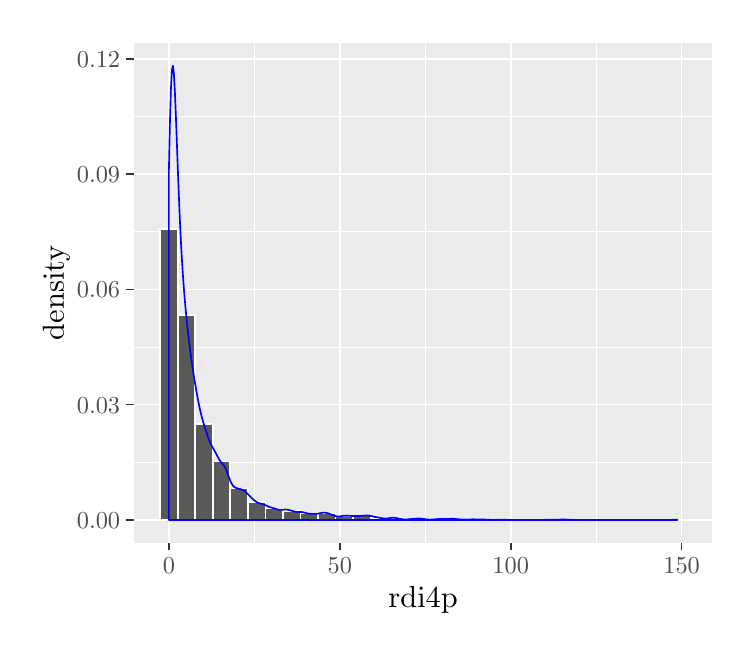
\begin{tikzpicture}[x=1pt,y=1pt]
\definecolor{fillColor}{RGB}{255,255,255}
\path[use as bounding box,fill=fillColor,fill opacity=0.00] (0,0) rectangle (252.94,216.81);
\begin{scope}
\path[clip] (  0.00,  0.00) rectangle (252.94,216.81);
\definecolor{drawColor}{RGB}{255,255,255}
\definecolor{fillColor}{RGB}{255,255,255}

\path[draw=drawColor,line width= 0.6pt,line join=round,line cap=round,fill=fillColor] (  0.00,  0.00) rectangle (252.94,216.81);
\end{scope}
\begin{scope}
\path[clip] ( 38.36, 30.72) rectangle (247.44,211.31);
\definecolor{fillColor}{gray}{0.92}

\path[fill=fillColor] ( 38.36, 30.72) rectangle (247.44,211.31);
\definecolor{drawColor}{RGB}{255,255,255}

\path[draw=drawColor,line width= 0.3pt,line join=round] ( 38.36, 59.76) --
	(247.44, 59.76);

\path[draw=drawColor,line width= 0.3pt,line join=round] ( 38.36,101.42) --
	(247.44,101.42);

\path[draw=drawColor,line width= 0.3pt,line join=round] ( 38.36,143.07) --
	(247.44,143.07);

\path[draw=drawColor,line width= 0.3pt,line join=round] ( 38.36,184.73) --
	(247.44,184.73);

\path[draw=drawColor,line width= 0.3pt,line join=round] ( 81.91, 30.72) --
	( 81.91,211.31);

\path[draw=drawColor,line width= 0.3pt,line join=round] (143.67, 30.72) --
	(143.67,211.31);

\path[draw=drawColor,line width= 0.3pt,line join=round] (205.42, 30.72) --
	(205.42,211.31);

\path[draw=drawColor,line width= 0.6pt,line join=round] ( 38.36, 38.93) --
	(247.44, 38.93);

\path[draw=drawColor,line width= 0.6pt,line join=round] ( 38.36, 80.59) --
	(247.44, 80.59);

\path[draw=drawColor,line width= 0.6pt,line join=round] ( 38.36,122.25) --
	(247.44,122.25);

\path[draw=drawColor,line width= 0.6pt,line join=round] ( 38.36,163.90) --
	(247.44,163.90);

\path[draw=drawColor,line width= 0.6pt,line join=round] ( 38.36,205.56) --
	(247.44,205.56);

\path[draw=drawColor,line width= 0.6pt,line join=round] ( 51.03, 30.72) --
	( 51.03,211.31);

\path[draw=drawColor,line width= 0.6pt,line join=round] (112.79, 30.72) --
	(112.79,211.31);

\path[draw=drawColor,line width= 0.6pt,line join=round] (174.54, 30.72) --
	(174.54,211.31);

\path[draw=drawColor,line width= 0.6pt,line join=round] (236.30, 30.72) --
	(236.30,211.31);
\definecolor{fillColor}{gray}{0.35}

\path[draw=drawColor,line width= 0.6pt,line join=round,fill=fillColor] ( 47.86, 38.93) rectangle ( 54.20,143.96);

\path[draw=drawColor,line width= 0.6pt,line join=round,fill=fillColor] ( 54.20, 38.93) rectangle ( 60.54,112.95);

\path[draw=drawColor,line width= 0.6pt,line join=round,fill=fillColor] ( 60.54, 38.93) rectangle ( 66.87, 73.68);

\path[draw=drawColor,line width= 0.6pt,line join=round,fill=fillColor] ( 66.87, 38.93) rectangle ( 73.21, 60.01);

\path[draw=drawColor,line width= 0.6pt,line join=round,fill=fillColor] ( 73.21, 38.93) rectangle ( 79.54, 50.31);

\path[draw=drawColor,line width= 0.6pt,line join=round,fill=fillColor] ( 79.54, 38.93) rectangle ( 85.88, 45.32);

\path[draw=drawColor,line width= 0.6pt,line join=round,fill=fillColor] ( 85.88, 38.93) rectangle ( 92.22, 43.04);

\path[draw=drawColor,line width= 0.6pt,line join=round,fill=fillColor] ( 92.22, 38.93) rectangle ( 98.55, 42.20);

\path[draw=drawColor,line width= 0.6pt,line join=round,fill=fillColor] ( 98.55, 38.93) rectangle (104.89, 41.50);

\path[draw=drawColor,line width= 0.6pt,line join=round,fill=fillColor] (104.89, 38.93) rectangle (111.22, 41.22);

\path[draw=drawColor,line width= 0.6pt,line join=round,fill=fillColor] (111.22, 38.93) rectangle (117.56, 40.29);

\path[draw=drawColor,line width= 0.6pt,line join=round,fill=fillColor] (117.56, 38.93) rectangle (123.90, 40.57);

\path[draw=drawColor,line width= 0.6pt,line join=round,fill=fillColor] (123.90, 38.93) rectangle (130.23, 39.63);

\path[draw=drawColor,line width= 0.6pt,line join=round,fill=fillColor] (130.23, 38.93) rectangle (136.57, 39.54);

\path[draw=drawColor,line width= 0.6pt,line join=round,fill=fillColor] (136.57, 38.93) rectangle (142.90, 39.35);

\path[draw=drawColor,line width= 0.6pt,line join=round,fill=fillColor] (142.90, 38.93) rectangle (149.24, 39.12);

\path[draw=drawColor,line width= 0.6pt,line join=round,fill=fillColor] (149.24, 38.93) rectangle (155.57, 39.31);

\path[draw=drawColor,line width= 0.6pt,line join=round,fill=fillColor] (155.57, 38.93) rectangle (161.91, 39.17);

\path[draw=drawColor,line width= 0.6pt,line join=round,fill=fillColor] (161.91, 38.93) rectangle (168.25, 39.03);

\path[draw=drawColor,line width= 0.6pt,line join=round,fill=fillColor] (168.25, 38.93) rectangle (174.58, 38.98);

\path[draw=drawColor,line width= 0.6pt,line join=round,fill=fillColor] (174.58, 38.93) rectangle (180.92, 38.93);

\path[draw=drawColor,line width= 0.6pt,line join=round,fill=fillColor] (180.92, 38.93) rectangle (187.25, 38.93);

\path[draw=drawColor,line width= 0.6pt,line join=round,fill=fillColor] (187.25, 38.93) rectangle (193.59, 39.03);

\path[draw=drawColor,line width= 0.6pt,line join=round,fill=fillColor] (193.59, 38.93) rectangle (199.93, 38.98);

\path[draw=drawColor,line width= 0.6pt,line join=round,fill=fillColor] (199.93, 38.93) rectangle (206.26, 38.93);

\path[draw=drawColor,line width= 0.6pt,line join=round,fill=fillColor] (206.26, 38.93) rectangle (212.60, 38.93);

\path[draw=drawColor,line width= 0.6pt,line join=round,fill=fillColor] (212.60, 38.93) rectangle (218.93, 38.93);

\path[draw=drawColor,line width= 0.6pt,line join=round,fill=fillColor] (218.93, 38.93) rectangle (225.27, 38.93);

\path[draw=drawColor,line width= 0.6pt,line join=round,fill=fillColor] (225.27, 38.93) rectangle (231.61, 38.93);

\path[draw=drawColor,line width= 0.6pt,line join=round,fill=fillColor] (231.61, 38.93) rectangle (237.94, 38.98);
\definecolor{drawColor}{RGB}{0,0,255}

\path[draw=drawColor,line width= 0.6pt,line join=round,line cap=round] ( 51.03,165.21) --
	( 51.39,182.04) --
	( 51.75,194.36) --
	( 52.11,201.38) --
	( 52.47,203.10) --
	( 52.83,200.18) --
	( 53.19,193.73) --
	( 53.55,185.03) --
	( 53.91,175.28) --
	( 54.27,165.41) --
	( 54.63,156.04) --
	( 54.99,147.53) --
	( 55.35,140.02) --
	( 55.71,133.48) --
	( 56.07,127.78) --
	( 56.43,122.77) --
	( 56.79,118.32) --
	( 57.15,114.31) --
	( 57.50,110.65) --
	( 57.86,107.26) --
	( 58.22,104.11) --
	( 58.58,101.18) --
	( 58.94, 98.44) --
	( 59.30, 95.87) --
	( 59.66, 93.45) --
	( 60.02, 91.14) --
	( 60.38, 88.93) --
	( 60.74, 86.79) --
	( 61.10, 84.73) --
	( 61.46, 82.77) --
	( 61.82, 80.92) --
	( 62.18, 79.22) --
	( 62.54, 77.66) --
	( 62.90, 76.23) --
	( 63.26, 74.92) --
	( 63.62, 73.69) --
	( 63.98, 72.51) --
	( 64.34, 71.36) --
	( 64.70, 70.24) --
	( 65.06, 69.17) --
	( 65.42, 68.16) --
	( 65.77, 67.25) --
	( 66.13, 66.45) --
	( 66.49, 65.74) --
	( 66.85, 65.10) --
	( 67.21, 64.48) --
	( 67.57, 63.85) --
	( 67.93, 63.18) --
	( 68.29, 62.48) --
	( 68.65, 61.77) --
	( 69.01, 61.10) --
	( 69.37, 60.51) --
	( 69.73, 60.01) --
	( 70.09, 59.59) --
	( 70.45, 59.19) --
	( 70.81, 58.75) --
	( 71.17, 58.20) --
	( 71.53, 57.49) --
	( 71.89, 56.64) --
	( 72.25, 55.68) --
	( 72.61, 54.67) --
	( 72.97, 53.70) --
	( 73.33, 52.82) --
	( 73.69, 52.09) --
	( 74.04, 51.51) --
	( 74.40, 51.09) --
	( 74.76, 50.79) --
	( 75.12, 50.58) --
	( 75.48, 50.43) --
	( 75.84, 50.31) --
	( 76.20, 50.22) --
	( 76.56, 50.14) --
	( 76.92, 50.05) --
	( 77.28, 49.94) --
	( 77.64, 49.80) --
	( 78.00, 49.62) --
	( 78.36, 49.38) --
	( 78.72, 49.10) --
	( 79.08, 48.77) --
	( 79.44, 48.41) --
	( 79.80, 48.03) --
	( 80.16, 47.65) --
	( 80.52, 47.28) --
	( 80.88, 46.92) --
	( 81.24, 46.57) --
	( 81.60, 46.25) --
	( 81.96, 45.95) --
	( 82.32, 45.67) --
	( 82.67, 45.44) --
	( 83.03, 45.24) --
	( 83.39, 45.08) --
	( 83.75, 44.95) --
	( 84.11, 44.84) --
	( 84.47, 44.74) --
	( 84.83, 44.64) --
	( 85.19, 44.53) --
	( 85.55, 44.40) --
	( 85.91, 44.26) --
	( 86.27, 44.10) --
	( 86.63, 43.94) --
	( 86.99, 43.78) --
	( 87.35, 43.64) --
	( 87.71, 43.51) --
	( 88.07, 43.39) --
	( 88.43, 43.29) --
	( 88.79, 43.18) --
	( 89.15, 43.07) --
	( 89.51, 42.96) --
	( 89.87, 42.85) --
	( 90.23, 42.74) --
	( 90.59, 42.65) --
	( 90.94, 42.59) --
	( 91.30, 42.56) --
	( 91.66, 42.57) --
	( 92.02, 42.60) --
	( 92.38, 42.64) --
	( 92.74, 42.67) --
	( 93.10, 42.68) --
	( 93.46, 42.67) --
	( 93.82, 42.63) --
	( 94.18, 42.57) --
	( 94.54, 42.48) --
	( 94.90, 42.39) --
	( 95.26, 42.28) --
	( 95.62, 42.18) --
	( 95.98, 42.08) --
	( 96.34, 41.98) --
	( 96.70, 41.91) --
	( 97.06, 41.86) --
	( 97.42, 41.83) --
	( 97.78, 41.82) --
	( 98.14, 41.82) --
	( 98.50, 41.82) --
	( 98.86, 41.80) --
	( 99.21, 41.76) --
	( 99.57, 41.69) --
	( 99.93, 41.60) --
	(100.29, 41.50) --
	(100.65, 41.41) --
	(101.01, 41.33) --
	(101.37, 41.26) --
	(101.73, 41.21) --
	(102.09, 41.18) --
	(102.45, 41.17) --
	(102.81, 41.15) --
	(103.17, 41.15) --
	(103.53, 41.15) --
	(103.89, 41.15) --
	(104.25, 41.16) --
	(104.61, 41.18) --
	(104.97, 41.22) --
	(105.33, 41.28) --
	(105.69, 41.35) --
	(106.05, 41.43) --
	(106.41, 41.50) --
	(106.77, 41.55) --
	(107.13, 41.57) --
	(107.49, 41.56) --
	(107.84, 41.51) --
	(108.20, 41.43) --
	(108.56, 41.32) --
	(108.92, 41.20) --
	(109.28, 41.06) --
	(109.64, 40.92) --
	(110.00, 40.77) --
	(110.36, 40.63) --
	(110.72, 40.50) --
	(111.08, 40.38) --
	(111.44, 40.29) --
	(111.80, 40.23) --
	(112.16, 40.21) --
	(112.52, 40.21) --
	(112.88, 40.24) --
	(113.24, 40.29) --
	(113.60, 40.34) --
	(113.96, 40.39) --
	(114.32, 40.44) --
	(114.68, 40.47) --
	(115.04, 40.47) --
	(115.40, 40.46) --
	(115.76, 40.44) --
	(116.11, 40.42) --
	(116.47, 40.40) --
	(116.83, 40.38) --
	(117.19, 40.38) --
	(117.55, 40.38) --
	(117.91, 40.38) --
	(118.27, 40.38) --
	(118.63, 40.38) --
	(118.99, 40.38) --
	(119.35, 40.37) --
	(119.71, 40.37) --
	(120.07, 40.39) --
	(120.43, 40.41) --
	(120.79, 40.43) --
	(121.15, 40.47) --
	(121.51, 40.50) --
	(121.87, 40.53) --
	(122.23, 40.54) --
	(122.59, 40.54) --
	(122.95, 40.52) --
	(123.31, 40.48) --
	(123.67, 40.42) --
	(124.03, 40.35) --
	(124.38, 40.28) --
	(124.74, 40.20) --
	(125.10, 40.12) --
	(125.46, 40.04) --
	(125.82, 39.97) --
	(126.18, 39.90) --
	(126.54, 39.83) --
	(126.90, 39.77) --
	(127.26, 39.71) --
	(127.62, 39.65) --
	(127.98, 39.59) --
	(128.34, 39.53) --
	(128.70, 39.49) --
	(129.06, 39.46) --
	(129.42, 39.45) --
	(129.78, 39.47) --
	(130.14, 39.50) --
	(130.50, 39.56) --
	(130.86, 39.61) --
	(131.22, 39.66) --
	(131.58, 39.70) --
	(131.94, 39.71) --
	(132.30, 39.70) --
	(132.66, 39.67) --
	(133.01, 39.63) --
	(133.37, 39.57) --
	(133.73, 39.51) --
	(134.09, 39.44) --
	(134.45, 39.37) --
	(134.81, 39.31) --
	(135.17, 39.25) --
	(135.53, 39.19) --
	(135.89, 39.15) --
	(136.25, 39.13) --
	(136.61, 39.12) --
	(136.97, 39.13) --
	(137.33, 39.15) --
	(137.69, 39.19) --
	(138.05, 39.22) --
	(138.41, 39.26) --
	(138.77, 39.29) --
	(139.13, 39.32) --
	(139.49, 39.35) --
	(139.85, 39.38) --
	(140.21, 39.40) --
	(140.57, 39.42) --
	(140.93, 39.43) --
	(141.28, 39.43) --
	(141.64, 39.43) --
	(142.00, 39.41) --
	(142.36, 39.38) --
	(142.72, 39.34) --
	(143.08, 39.28) --
	(143.44, 39.23) --
	(143.80, 39.17) --
	(144.16, 39.12) --
	(144.52, 39.08) --
	(144.88, 39.06) --
	(145.24, 39.05) --
	(145.60, 39.05) --
	(145.96, 39.07) --
	(146.32, 39.09) --
	(146.68, 39.12) --
	(147.04, 39.15) --
	(147.40, 39.18) --
	(147.76, 39.22) --
	(148.12, 39.25) --
	(148.48, 39.27) --
	(148.84, 39.29) --
	(149.20, 39.31) --
	(149.55, 39.31) --
	(149.91, 39.31) --
	(150.27, 39.30) --
	(150.63, 39.29) --
	(150.99, 39.28) --
	(151.35, 39.28) --
	(151.71, 39.28) --
	(152.07, 39.30) --
	(152.43, 39.31) --
	(152.79, 39.33) --
	(153.15, 39.34) --
	(153.51, 39.35) --
	(153.87, 39.33) --
	(154.23, 39.31) --
	(154.59, 39.28) --
	(154.95, 39.24) --
	(155.31, 39.21) --
	(155.67, 39.18) --
	(156.03, 39.16) --
	(156.39, 39.14) --
	(156.75, 39.13) --
	(157.11, 39.12) --
	(157.47, 39.12) --
	(157.83, 39.12) --
	(158.18, 39.12) --
	(158.54, 39.12) --
	(158.90, 39.12) --
	(159.26, 39.13) --
	(159.62, 39.14) --
	(159.98, 39.14) --
	(160.34, 39.15) --
	(160.70, 39.15) --
	(161.06, 39.15) --
	(161.42, 39.15) --
	(161.78, 39.14) --
	(162.14, 39.13) --
	(162.50, 39.13) --
	(162.86, 39.12) --
	(163.22, 39.11) --
	(163.58, 39.10) --
	(163.94, 39.10) --
	(164.30, 39.09) --
	(164.66, 39.08) --
	(165.02, 39.07) --
	(165.38, 39.06) --
	(165.74, 39.04) --
	(166.10, 39.03) --
	(166.45, 39.01) --
	(166.81, 38.99) --
	(167.17, 38.97) --
	(167.53, 38.96) --
	(167.89, 38.95) --
	(168.25, 38.95) --
	(168.61, 38.95) --
	(168.97, 38.96) --
	(169.33, 38.96) --
	(169.69, 38.98) --
	(170.05, 38.99) --
	(170.41, 39.00) --
	(170.77, 39.01) --
	(171.13, 39.02) --
	(171.49, 39.02) --
	(171.85, 39.01) --
	(172.21, 39.00) --
	(172.57, 38.99) --
	(172.93, 38.98) --
	(173.29, 38.97) --
	(173.65, 38.96) --
	(174.01, 38.95) --
	(174.37, 38.94) --
	(174.72, 38.94) --
	(175.08, 38.94) --
	(175.44, 38.93) --
	(175.80, 38.93) --
	(176.16, 38.93) --
	(176.52, 38.93) --
	(176.88, 38.93) --
	(177.24, 38.93) --
	(177.60, 38.93) --
	(177.96, 38.93) --
	(178.32, 38.93) --
	(178.68, 38.93) --
	(179.04, 38.93) --
	(179.40, 38.93) --
	(179.76, 38.93) --
	(180.12, 38.93) --
	(180.48, 38.93) --
	(180.84, 38.93) --
	(181.20, 38.93) --
	(181.56, 38.93) --
	(181.92, 38.93) --
	(182.28, 38.93) --
	(182.64, 38.93) --
	(182.99, 38.93) --
	(183.35, 38.93) --
	(183.71, 38.93) --
	(184.07, 38.93) --
	(184.43, 38.93) --
	(184.79, 38.93) --
	(185.15, 38.94) --
	(185.51, 38.94) --
	(185.87, 38.94) --
	(186.23, 38.95) --
	(186.59, 38.96) --
	(186.95, 38.97) --
	(187.31, 38.98) --
	(187.67, 38.99) --
	(188.03, 39.00) --
	(188.39, 39.01) --
	(188.75, 39.02) --
	(189.11, 39.02) --
	(189.47, 39.01) --
	(189.83, 39.01) --
	(190.19, 39.00) --
	(190.55, 38.99) --
	(190.91, 38.99) --
	(191.27, 39.00) --
	(191.62, 39.01) --
	(191.98, 39.03) --
	(192.34, 39.05) --
	(192.70, 39.07) --
	(193.06, 39.09) --
	(193.42, 39.09) --
	(193.78, 39.09) --
	(194.14, 39.08) --
	(194.50, 39.06) --
	(194.86, 39.04) --
	(195.22, 39.02) --
	(195.58, 39.00) --
	(195.94, 38.98) --
	(196.30, 38.96) --
	(196.66, 38.95) --
	(197.02, 38.94) --
	(197.38, 38.94) --
	(197.74, 38.94) --
	(198.10, 38.93) --
	(198.46, 38.93) --
	(198.82, 38.93) --
	(199.18, 38.93) --
	(199.54, 38.93) --
	(199.89, 38.93) --
	(200.25, 38.93) --
	(200.61, 38.93) --
	(200.97, 38.93) --
	(201.33, 38.93) --
	(201.69, 38.93) --
	(202.05, 38.93) --
	(202.41, 38.93) --
	(202.77, 38.93) --
	(203.13, 38.93) --
	(203.49, 38.93) --
	(203.85, 38.93) --
	(204.21, 38.93) --
	(204.57, 38.93) --
	(204.93, 38.93) --
	(205.29, 38.93) --
	(205.65, 38.93) --
	(206.01, 38.93) --
	(206.37, 38.93) --
	(206.73, 38.93) --
	(207.09, 38.93) --
	(207.45, 38.93) --
	(207.81, 38.93) --
	(208.16, 38.93) --
	(208.52, 38.93) --
	(208.88, 38.93) --
	(209.24, 38.93) --
	(209.60, 38.93) --
	(209.96, 38.93) --
	(210.32, 38.93) --
	(210.68, 38.93) --
	(211.04, 38.93) --
	(211.40, 38.93) --
	(211.76, 38.93) --
	(212.12, 38.93) --
	(212.48, 38.93) --
	(212.84, 38.93) --
	(213.20, 38.93) --
	(213.56, 38.93) --
	(213.92, 38.93) --
	(214.28, 38.93) --
	(214.64, 38.93) --
	(215.00, 38.93) --
	(215.36, 38.93) --
	(215.72, 38.93) --
	(216.08, 38.93) --
	(216.44, 38.93) --
	(216.79, 38.93) --
	(217.15, 38.93) --
	(217.51, 38.93) --
	(217.87, 38.93) --
	(218.23, 38.93) --
	(218.59, 38.93) --
	(218.95, 38.93) --
	(219.31, 38.93) --
	(219.67, 38.93) --
	(220.03, 38.93) --
	(220.39, 38.93) --
	(220.75, 38.93) --
	(221.11, 38.93) --
	(221.47, 38.93) --
	(221.83, 38.93) --
	(222.19, 38.93) --
	(222.55, 38.93) --
	(222.91, 38.93) --
	(223.27, 38.93) --
	(223.63, 38.93) --
	(223.99, 38.93) --
	(224.35, 38.93) --
	(224.71, 38.93) --
	(225.06, 38.93) --
	(225.42, 38.93) --
	(225.78, 38.93) --
	(226.14, 38.93) --
	(226.50, 38.93) --
	(226.86, 38.93) --
	(227.22, 38.93) --
	(227.58, 38.93) --
	(227.94, 38.93) --
	(228.30, 38.93) --
	(228.66, 38.93) --
	(229.02, 38.93) --
	(229.38, 38.93) --
	(229.74, 38.93) --
	(230.10, 38.93) --
	(230.46, 38.93) --
	(230.82, 38.93) --
	(231.18, 38.94) --
	(231.54, 38.94) --
	(231.90, 38.94) --
	(232.26, 38.95) --
	(232.62, 38.96) --
	(232.98, 38.97) --
	(233.33, 38.98) --
	(233.69, 39.00) --
	(234.05, 39.01) --
	(234.41, 39.01) --
	(234.77, 39.02) --
	(234.77, 38.93) --
	(234.41, 38.93) --
	(234.05, 38.93) --
	(233.69, 38.93) --
	(233.33, 38.93) --
	(232.98, 38.93) --
	(232.62, 38.93) --
	(232.26, 38.93) --
	(231.90, 38.93) --
	(231.54, 38.93) --
	(231.18, 38.93) --
	(230.82, 38.93) --
	(230.46, 38.93) --
	(230.10, 38.93) --
	(229.74, 38.93) --
	(229.38, 38.93) --
	(229.02, 38.93) --
	(228.66, 38.93) --
	(228.30, 38.93) --
	(227.94, 38.93) --
	(227.58, 38.93) --
	(227.22, 38.93) --
	(226.86, 38.93) --
	(226.50, 38.93) --
	(226.14, 38.93) --
	(225.78, 38.93) --
	(225.42, 38.93) --
	(225.06, 38.93) --
	(224.71, 38.93) --
	(224.35, 38.93) --
	(223.99, 38.93) --
	(223.63, 38.93) --
	(223.27, 38.93) --
	(222.91, 38.93) --
	(222.55, 38.93) --
	(222.19, 38.93) --
	(221.83, 38.93) --
	(221.47, 38.93) --
	(221.11, 38.93) --
	(220.75, 38.93) --
	(220.39, 38.93) --
	(220.03, 38.93) --
	(219.67, 38.93) --
	(219.31, 38.93) --
	(218.95, 38.93) --
	(218.59, 38.93) --
	(218.23, 38.93) --
	(217.87, 38.93) --
	(217.51, 38.93) --
	(217.15, 38.93) --
	(216.79, 38.93) --
	(216.44, 38.93) --
	(216.08, 38.93) --
	(215.72, 38.93) --
	(215.36, 38.93) --
	(215.00, 38.93) --
	(214.64, 38.93) --
	(214.28, 38.93) --
	(213.92, 38.93) --
	(213.56, 38.93) --
	(213.20, 38.93) --
	(212.84, 38.93) --
	(212.48, 38.93) --
	(212.12, 38.93) --
	(211.76, 38.93) --
	(211.40, 38.93) --
	(211.04, 38.93) --
	(210.68, 38.93) --
	(210.32, 38.93) --
	(209.96, 38.93) --
	(209.60, 38.93) --
	(209.24, 38.93) --
	(208.88, 38.93) --
	(208.52, 38.93) --
	(208.16, 38.93) --
	(207.81, 38.93) --
	(207.45, 38.93) --
	(207.09, 38.93) --
	(206.73, 38.93) --
	(206.37, 38.93) --
	(206.01, 38.93) --
	(205.65, 38.93) --
	(205.29, 38.93) --
	(204.93, 38.93) --
	(204.57, 38.93) --
	(204.21, 38.93) --
	(203.85, 38.93) --
	(203.49, 38.93) --
	(203.13, 38.93) --
	(202.77, 38.93) --
	(202.41, 38.93) --
	(202.05, 38.93) --
	(201.69, 38.93) --
	(201.33, 38.93) --
	(200.97, 38.93) --
	(200.61, 38.93) --
	(200.25, 38.93) --
	(199.89, 38.93) --
	(199.54, 38.93) --
	(199.18, 38.93) --
	(198.82, 38.93) --
	(198.46, 38.93) --
	(198.10, 38.93) --
	(197.74, 38.93) --
	(197.38, 38.93) --
	(197.02, 38.93) --
	(196.66, 38.93) --
	(196.30, 38.93) --
	(195.94, 38.93) --
	(195.58, 38.93) --
	(195.22, 38.93) --
	(194.86, 38.93) --
	(194.50, 38.93) --
	(194.14, 38.93) --
	(193.78, 38.93) --
	(193.42, 38.93) --
	(193.06, 38.93) --
	(192.70, 38.93) --
	(192.34, 38.93) --
	(191.98, 38.93) --
	(191.62, 38.93) --
	(191.27, 38.93) --
	(190.91, 38.93) --
	(190.55, 38.93) --
	(190.19, 38.93) --
	(189.83, 38.93) --
	(189.47, 38.93) --
	(189.11, 38.93) --
	(188.75, 38.93) --
	(188.39, 38.93) --
	(188.03, 38.93) --
	(187.67, 38.93) --
	(187.31, 38.93) --
	(186.95, 38.93) --
	(186.59, 38.93) --
	(186.23, 38.93) --
	(185.87, 38.93) --
	(185.51, 38.93) --
	(185.15, 38.93) --
	(184.79, 38.93) --
	(184.43, 38.93) --
	(184.07, 38.93) --
	(183.71, 38.93) --
	(183.35, 38.93) --
	(182.99, 38.93) --
	(182.64, 38.93) --
	(182.28, 38.93) --
	(181.92, 38.93) --
	(181.56, 38.93) --
	(181.20, 38.93) --
	(180.84, 38.93) --
	(180.48, 38.93) --
	(180.12, 38.93) --
	(179.76, 38.93) --
	(179.40, 38.93) --
	(179.04, 38.93) --
	(178.68, 38.93) --
	(178.32, 38.93) --
	(177.96, 38.93) --
	(177.60, 38.93) --
	(177.24, 38.93) --
	(176.88, 38.93) --
	(176.52, 38.93) --
	(176.16, 38.93) --
	(175.80, 38.93) --
	(175.44, 38.93) --
	(175.08, 38.93) --
	(174.72, 38.93) --
	(174.37, 38.93) --
	(174.01, 38.93) --
	(173.65, 38.93) --
	(173.29, 38.93) --
	(172.93, 38.93) --
	(172.57, 38.93) --
	(172.21, 38.93) --
	(171.85, 38.93) --
	(171.49, 38.93) --
	(171.13, 38.93) --
	(170.77, 38.93) --
	(170.41, 38.93) --
	(170.05, 38.93) --
	(169.69, 38.93) --
	(169.33, 38.93) --
	(168.97, 38.93) --
	(168.61, 38.93) --
	(168.25, 38.93) --
	(167.89, 38.93) --
	(167.53, 38.93) --
	(167.17, 38.93) --
	(166.81, 38.93) --
	(166.45, 38.93) --
	(166.10, 38.93) --
	(165.74, 38.93) --
	(165.38, 38.93) --
	(165.02, 38.93) --
	(164.66, 38.93) --
	(164.30, 38.93) --
	(163.94, 38.93) --
	(163.58, 38.93) --
	(163.22, 38.93) --
	(162.86, 38.93) --
	(162.50, 38.93) --
	(162.14, 38.93) --
	(161.78, 38.93) --
	(161.42, 38.93) --
	(161.06, 38.93) --
	(160.70, 38.93) --
	(160.34, 38.93) --
	(159.98, 38.93) --
	(159.62, 38.93) --
	(159.26, 38.93) --
	(158.90, 38.93) --
	(158.54, 38.93) --
	(158.18, 38.93) --
	(157.83, 38.93) --
	(157.47, 38.93) --
	(157.11, 38.93) --
	(156.75, 38.93) --
	(156.39, 38.93) --
	(156.03, 38.93) --
	(155.67, 38.93) --
	(155.31, 38.93) --
	(154.95, 38.93) --
	(154.59, 38.93) --
	(154.23, 38.93) --
	(153.87, 38.93) --
	(153.51, 38.93) --
	(153.15, 38.93) --
	(152.79, 38.93) --
	(152.43, 38.93) --
	(152.07, 38.93) --
	(151.71, 38.93) --
	(151.35, 38.93) --
	(150.99, 38.93) --
	(150.63, 38.93) --
	(150.27, 38.93) --
	(149.91, 38.93) --
	(149.55, 38.93) --
	(149.20, 38.93) --
	(148.84, 38.93) --
	(148.48, 38.93) --
	(148.12, 38.93) --
	(147.76, 38.93) --
	(147.40, 38.93) --
	(147.04, 38.93) --
	(146.68, 38.93) --
	(146.32, 38.93) --
	(145.96, 38.93) --
	(145.60, 38.93) --
	(145.24, 38.93) --
	(144.88, 38.93) --
	(144.52, 38.93) --
	(144.16, 38.93) --
	(143.80, 38.93) --
	(143.44, 38.93) --
	(143.08, 38.93) --
	(142.72, 38.93) --
	(142.36, 38.93) --
	(142.00, 38.93) --
	(141.64, 38.93) --
	(141.28, 38.93) --
	(140.93, 38.93) --
	(140.57, 38.93) --
	(140.21, 38.93) --
	(139.85, 38.93) --
	(139.49, 38.93) --
	(139.13, 38.93) --
	(138.77, 38.93) --
	(138.41, 38.93) --
	(138.05, 38.93) --
	(137.69, 38.93) --
	(137.33, 38.93) --
	(136.97, 38.93) --
	(136.61, 38.93) --
	(136.25, 38.93) --
	(135.89, 38.93) --
	(135.53, 38.93) --
	(135.17, 38.93) --
	(134.81, 38.93) --
	(134.45, 38.93) --
	(134.09, 38.93) --
	(133.73, 38.93) --
	(133.37, 38.93) --
	(133.01, 38.93) --
	(132.66, 38.93) --
	(132.30, 38.93) --
	(131.94, 38.93) --
	(131.58, 38.93) --
	(131.22, 38.93) --
	(130.86, 38.93) --
	(130.50, 38.93) --
	(130.14, 38.93) --
	(129.78, 38.93) --
	(129.42, 38.93) --
	(129.06, 38.93) --
	(128.70, 38.93) --
	(128.34, 38.93) --
	(127.98, 38.93) --
	(127.62, 38.93) --
	(127.26, 38.93) --
	(126.90, 38.93) --
	(126.54, 38.93) --
	(126.18, 38.93) --
	(125.82, 38.93) --
	(125.46, 38.93) --
	(125.10, 38.93) --
	(124.74, 38.93) --
	(124.38, 38.93) --
	(124.03, 38.93) --
	(123.67, 38.93) --
	(123.31, 38.93) --
	(122.95, 38.93) --
	(122.59, 38.93) --
	(122.23, 38.93) --
	(121.87, 38.93) --
	(121.51, 38.93) --
	(121.15, 38.93) --
	(120.79, 38.93) --
	(120.43, 38.93) --
	(120.07, 38.93) --
	(119.71, 38.93) --
	(119.35, 38.93) --
	(118.99, 38.93) --
	(118.63, 38.93) --
	(118.27, 38.93) --
	(117.91, 38.93) --
	(117.55, 38.93) --
	(117.19, 38.93) --
	(116.83, 38.93) --
	(116.47, 38.93) --
	(116.11, 38.93) --
	(115.76, 38.93) --
	(115.40, 38.93) --
	(115.04, 38.93) --
	(114.68, 38.93) --
	(114.32, 38.93) --
	(113.96, 38.93) --
	(113.60, 38.93) --
	(113.24, 38.93) --
	(112.88, 38.93) --
	(112.52, 38.93) --
	(112.16, 38.93) --
	(111.80, 38.93) --
	(111.44, 38.93) --
	(111.08, 38.93) --
	(110.72, 38.93) --
	(110.36, 38.93) --
	(110.00, 38.93) --
	(109.64, 38.93) --
	(109.28, 38.93) --
	(108.92, 38.93) --
	(108.56, 38.93) --
	(108.20, 38.93) --
	(107.84, 38.93) --
	(107.49, 38.93) --
	(107.13, 38.93) --
	(106.77, 38.93) --
	(106.41, 38.93) --
	(106.05, 38.93) --
	(105.69, 38.93) --
	(105.33, 38.93) --
	(104.97, 38.93) --
	(104.61, 38.93) --
	(104.25, 38.93) --
	(103.89, 38.93) --
	(103.53, 38.93) --
	(103.17, 38.93) --
	(102.81, 38.93) --
	(102.45, 38.93) --
	(102.09, 38.93) --
	(101.73, 38.93) --
	(101.37, 38.93) --
	(101.01, 38.93) --
	(100.65, 38.93) --
	(100.29, 38.93) --
	( 99.93, 38.93) --
	( 99.57, 38.93) --
	( 99.21, 38.93) --
	( 98.86, 38.93) --
	( 98.50, 38.93) --
	( 98.14, 38.93) --
	( 97.78, 38.93) --
	( 97.42, 38.93) --
	( 97.06, 38.93) --
	( 96.70, 38.93) --
	( 96.34, 38.93) --
	( 95.98, 38.93) --
	( 95.62, 38.93) --
	( 95.26, 38.93) --
	( 94.90, 38.93) --
	( 94.54, 38.93) --
	( 94.18, 38.93) --
	( 93.82, 38.93) --
	( 93.46, 38.93) --
	( 93.10, 38.93) --
	( 92.74, 38.93) --
	( 92.38, 38.93) --
	( 92.02, 38.93) --
	( 91.66, 38.93) --
	( 91.30, 38.93) --
	( 90.94, 38.93) --
	( 90.59, 38.93) --
	( 90.23, 38.93) --
	( 89.87, 38.93) --
	( 89.51, 38.93) --
	( 89.15, 38.93) --
	( 88.79, 38.93) --
	( 88.43, 38.93) --
	( 88.07, 38.93) --
	( 87.71, 38.93) --
	( 87.35, 38.93) --
	( 86.99, 38.93) --
	( 86.63, 38.93) --
	( 86.27, 38.93) --
	( 85.91, 38.93) --
	( 85.55, 38.93) --
	( 85.19, 38.93) --
	( 84.83, 38.93) --
	( 84.47, 38.93) --
	( 84.11, 38.93) --
	( 83.75, 38.93) --
	( 83.39, 38.93) --
	( 83.03, 38.93) --
	( 82.67, 38.93) --
	( 82.32, 38.93) --
	( 81.96, 38.93) --
	( 81.60, 38.93) --
	( 81.24, 38.93) --
	( 80.88, 38.93) --
	( 80.52, 38.93) --
	( 80.16, 38.93) --
	( 79.80, 38.93) --
	( 79.44, 38.93) --
	( 79.08, 38.93) --
	( 78.72, 38.93) --
	( 78.36, 38.93) --
	( 78.00, 38.93) --
	( 77.64, 38.93) --
	( 77.28, 38.93) --
	( 76.92, 38.93) --
	( 76.56, 38.93) --
	( 76.20, 38.93) --
	( 75.84, 38.93) --
	( 75.48, 38.93) --
	( 75.12, 38.93) --
	( 74.76, 38.93) --
	( 74.40, 38.93) --
	( 74.04, 38.93) --
	( 73.69, 38.93) --
	( 73.33, 38.93) --
	( 72.97, 38.93) --
	( 72.61, 38.93) --
	( 72.25, 38.93) --
	( 71.89, 38.93) --
	( 71.53, 38.93) --
	( 71.17, 38.93) --
	( 70.81, 38.93) --
	( 70.45, 38.93) --
	( 70.09, 38.93) --
	( 69.73, 38.93) --
	( 69.37, 38.93) --
	( 69.01, 38.93) --
	( 68.65, 38.93) --
	( 68.29, 38.93) --
	( 67.93, 38.93) --
	( 67.57, 38.93) --
	( 67.21, 38.93) --
	( 66.85, 38.93) --
	( 66.49, 38.93) --
	( 66.13, 38.93) --
	( 65.77, 38.93) --
	( 65.42, 38.93) --
	( 65.06, 38.93) --
	( 64.70, 38.93) --
	( 64.34, 38.93) --
	( 63.98, 38.93) --
	( 63.62, 38.93) --
	( 63.26, 38.93) --
	( 62.90, 38.93) --
	( 62.54, 38.93) --
	( 62.18, 38.93) --
	( 61.82, 38.93) --
	( 61.46, 38.93) --
	( 61.10, 38.93) --
	( 60.74, 38.93) --
	( 60.38, 38.93) --
	( 60.02, 38.93) --
	( 59.66, 38.93) --
	( 59.30, 38.93) --
	( 58.94, 38.93) --
	( 58.58, 38.93) --
	( 58.22, 38.93) --
	( 57.86, 38.93) --
	( 57.50, 38.93) --
	( 57.15, 38.93) --
	( 56.79, 38.93) --
	( 56.43, 38.93) --
	( 56.07, 38.93) --
	( 55.71, 38.93) --
	( 55.35, 38.93) --
	( 54.99, 38.93) --
	( 54.63, 38.93) --
	( 54.27, 38.93) --
	( 53.91, 38.93) --
	( 53.55, 38.93) --
	( 53.19, 38.93) --
	( 52.83, 38.93) --
	( 52.47, 38.93) --
	( 52.11, 38.93) --
	( 51.75, 38.93) --
	( 51.39, 38.93) --
	( 51.03, 38.93) --
	( 51.03,165.21);
\end{scope}
\begin{scope}
\path[clip] (  0.00,  0.00) rectangle (252.94,216.81);
\definecolor{drawColor}{gray}{0.30}

\node[text=drawColor,anchor=base east,inner sep=0pt, outer sep=0pt, scale=  0.88] at ( 33.41, 35.90) {0.00};

\node[text=drawColor,anchor=base east,inner sep=0pt, outer sep=0pt, scale=  0.88] at ( 33.41, 77.56) {0.03};

\node[text=drawColor,anchor=base east,inner sep=0pt, outer sep=0pt, scale=  0.88] at ( 33.41,119.21) {0.06};

\node[text=drawColor,anchor=base east,inner sep=0pt, outer sep=0pt, scale=  0.88] at ( 33.41,160.87) {0.09};

\node[text=drawColor,anchor=base east,inner sep=0pt, outer sep=0pt, scale=  0.88] at ( 33.41,202.53) {0.12};
\end{scope}
\begin{scope}
\path[clip] (  0.00,  0.00) rectangle (252.94,216.81);
\definecolor{drawColor}{gray}{0.20}

\path[draw=drawColor,line width= 0.6pt,line join=round] ( 35.61, 38.93) --
	( 38.36, 38.93);

\path[draw=drawColor,line width= 0.6pt,line join=round] ( 35.61, 80.59) --
	( 38.36, 80.59);

\path[draw=drawColor,line width= 0.6pt,line join=round] ( 35.61,122.25) --
	( 38.36,122.25);

\path[draw=drawColor,line width= 0.6pt,line join=round] ( 35.61,163.90) --
	( 38.36,163.90);

\path[draw=drawColor,line width= 0.6pt,line join=round] ( 35.61,205.56) --
	( 38.36,205.56);
\end{scope}
\begin{scope}
\path[clip] (  0.00,  0.00) rectangle (252.94,216.81);
\definecolor{drawColor}{gray}{0.20}

\path[draw=drawColor,line width= 0.6pt,line join=round] ( 51.03, 27.97) --
	( 51.03, 30.72);

\path[draw=drawColor,line width= 0.6pt,line join=round] (112.79, 27.97) --
	(112.79, 30.72);

\path[draw=drawColor,line width= 0.6pt,line join=round] (174.54, 27.97) --
	(174.54, 30.72);

\path[draw=drawColor,line width= 0.6pt,line join=round] (236.30, 27.97) --
	(236.30, 30.72);
\end{scope}
\begin{scope}
\path[clip] (  0.00,  0.00) rectangle (252.94,216.81);
\definecolor{drawColor}{gray}{0.30}

\node[text=drawColor,anchor=base,inner sep=0pt, outer sep=0pt, scale=  0.88] at ( 51.03, 19.71) {0};

\node[text=drawColor,anchor=base,inner sep=0pt, outer sep=0pt, scale=  0.88] at (112.79, 19.71) {50};

\node[text=drawColor,anchor=base,inner sep=0pt, outer sep=0pt, scale=  0.88] at (174.54, 19.71) {100};

\node[text=drawColor,anchor=base,inner sep=0pt, outer sep=0pt, scale=  0.88] at (236.30, 19.71) {150};
\end{scope}
\begin{scope}
\path[clip] (  0.00,  0.00) rectangle (252.94,216.81);
\definecolor{drawColor}{RGB}{0,0,0}

\node[text=drawColor,anchor=base,inner sep=0pt, outer sep=0pt, scale=  1.10] at (142.90,  7.44) {rdi4p};
\end{scope}
\begin{scope}
\path[clip] (  0.00,  0.00) rectangle (252.94,216.81);
\definecolor{drawColor}{RGB}{0,0,0}

\node[text=drawColor,rotate= 90.00,anchor=base,inner sep=0pt, outer sep=0pt, scale=  1.10] at ( 13.08,121.02) {density};
\end{scope}
\end{tikzpicture}
}
    	\caption{Histogram of \textbf{rdi4p} with the empirical distribution}
    	\label{fig 3.1}
    \end{figure}
    
    By building bootstrap percentile and bootstrap accelerated bias-corrected confidence intervals for the standard deviation and
median, we get the following results (with $R = 1000$)
    
    \begin{table}[H]
    	\centering
    	\begin{tabular}{|P{2cm}|P{2.5cm}|P{2.5cm}|}
    		\hline
    		& $x_{med}$ & $\sigma$ \\
    		\hline
    		CI & [3.951, 4.419] & [11.785, 13.045] \\
    		\hline
    		CI$_{length}$ & 0.498 & 1.26 \\
    		\hline  
    	\end{tabular}
    	\caption{\label{tableau36}Results for bootstrap percentile confidence interval}
    \end{table}
    
    \begin{table}[H]
    	\centering
    	\begin{tabular}{|P{2cm}|P{2.5cm}|P{2.5cm}|}
    		\hline
    		& $x_{med}$ & $\sigma$ \\
    		\hline
    		CI & [3.944, 4.429] & [11.792, 13.103] \\
    		\hline
    		CI$_{length}$ & 0.485 & 1.311 \\
    		\hline
    		$\hat{z}_0$ & $0.00251$ & $-0.00251$ \\
    		\hline  
    		$\hat{a}$ & 0 & 0.0272 \\
    		\hline  
    	\end{tabular}
    	\caption{\label{tableau37}Results for $bc_a$}
    \end{table}
    The results from tables \ref{tableau36} and \ref{tableau37} show that the $x_{med}$ CI are almost the same, while  we notice a slight difference $\sigma$ CI. Actually notice shift to the right in the $\sigma$ CI with $bc_a$, but with slight shift to the right in the CI for $bc_a$. This can be explained by the fact that the empirical distribution is right-skewed, and that $\hat{a}$ is null for $x_{med}$ CI, and close to zero for $\sigma$ CI. We can notice that $\hat{z}_0$ is close to zero, indicating good minimization of overestimation (for $\sigma$ CI) and underestimation (for $x_{med}$ CI). 
    
\end{enumerate}

%44444444444444444444444444444444444444444444%

{\color{royalblue}\chapter{Generalised linear models}}
{\color{royalblue}\section{Problem description}}
In its simplest form, a linear model specifies the (linear) relationship between a dependent variable $Y$ (normally distributed), and a set of independent variables $X_i$, $i=1,\ldots,k\in \mathbb{N}$, so that $Y= b_0 + b_1X_1 +\ldots+ b_kX_k$, where $b_0$ is the regression coefficient for the intercept and the $b_i$ values are the regression coefficients (for variables 1 through k). However, there are many relationships that cannot adequately be summarized by a simple linear equation, for two major reasons:
\begin{itemize}
	\item  \textit{Distribution of the dependent variable.} The dependent variable of interest may have a non-continuous distribution, and thus, the predicted values should also follow the respective distribution; any other predicted values are not logically possible.
	\item \textit{Link function.} The second reason why the linear model might be inadequate to describe a particular relationship is that the effect of the predictors on the dependent variable may not be linear in nature.
\end{itemize}
Generalized linear models (GLMs) extend linear models to accommodate both non-normal response distributions and transformations to linearity.

{\color{royalblue}\section{Methods}}

Let $(Y_1, X_1),\ldots,(Y_n, X_n)$ be independent pairs of observations, where $Y_i$ is real-valued
and $X_i$ are $\mathbb{R}^k$-valued random variables. Generalised linear models (GLMs) have the following
three-part specification:

\begin{itemize}
	\item \textbf{The random component} (=response from an overdispersed exponential family). The data $Y_1,\ldots,Y_n$ are such that $Y_1|X_1,\ldots, Y_n|X_n$ are independent and $Y_i|X_i$ has
the p.d.f.
	\[ f_{\eta,\psi}(y_i|x_i) = \mathtt{exp}\bigg\{   \frac{\eta_iy_i - \kappa(\eta_i)}{\psi_i} \bigg\}h(y_i,\psi_i), \hspace{0.5cm} i=1,\ldots,n, \]
	where $\eta_i$ is called canonical parameter and i is an unknown scale or dispersion parameter. Functions $\kappa$ and $h$ are known and $\kappa^{''}(\eta) > 0$ is assumed. Note that 
	\[ \mu(\eta_i):=\mathtt{E}(Y_i|X_i) = \kappa_0(\eta_i) \hspace{0.25cm}\mathtt{and}\hspace{0.25cm} var(Y_i|X_i)=\psi_i\kappa^{''}(\eta), \hspace{0.5cm} i=1,\ldots,n \]
	\item \textbf{The systematic component} (=linear predictor) Canonical parameter $\eta_i$ is assumed to be related to $X_i$. The term $X^t_i\beta$ for unknown
$\beta \in \mathbb{R}^d$ is called the \textbf{linear predictor or systematic component}.
	\item The \textbf{link function} between random and systematic components. The relationship between $\eta_i$ and $X^t_i\beta$ is described through
	\[ g\{\mu(\eta_i)\} = X^t_i\beta, \hspace{0.5cm} i=1,\ldots,n \]
	where g is called a link function. The link function g is assumed to be a known, one-to-one, third-order continuously differentiable function. If $g=\mu^{-1}$ then $\eta_i=X^t_i\beta$, and $g$ is called the \textbf{canonical or natural link function}. If $g$ is not canonical, then

	it is assumed that $d(g\circ\mu)(\eta)/d\eta \ne 0$ for all $\eta$.	
\end{itemize}

In a GLM, the parameter of interest is $\beta$. Parameters $\psi_i$ are considered to be nuisance parameters. It is often assumed that $\psi_i = \psi/t_i$, $i = 1,\ldots,n$ with an unknown
$\psi$ and known $t_i$'s or, alternatively $\psi_i =a( )$ for some known function $a$. Note that $\psi_i$
enter $var(Y_i|X_i) = \psi_i\kappa{''}(\eta_i)$, making it more flexible, that is allowing for over- or underdispersion.\\

\textbf{Exemple:} Let Let $Y_i|X_i \backsim Poi(\lambda_i)$. We can write the density
\[ f_\eta(y_i)= \mathtt{exp}\{ y_ilog(\lambda_i) - \lambda_i \}\frac{1}{y_i!}\mathbb{I}_{\{ 1,2,\ldots \}}(y_i) \]
that is, the canonical parameter $\eta_i = \mathtt{log}(\lambda_i), \kappa(\eta_i) = \lambda_i = \mathtt{exp}(\eta_i)$, $\psi_i = 1$ and $h(y_i) = (y_i)^{-1}\mathbb{I}_{\{ 1,2,\ldots \}}(y_i)g(y_i)$. Since $E(Y_i|X_i) = \kappa_0(\eta_i) = \mathtt{exp}(\eta_i) =: \mu(\eta_i)$, the canonical link is

$g(x) = \mu^{-1}(x) = \mathtt{log}(x)$, which is called the \textbf{log-link} $(g(\mu(\eta_i)) = \eta_i)$. Hence, 
\[ \mathtt{log}\{\mathtt{E}(Y_i|X_i=x_i)\} = x^t_i\beta,\]
where $x_i \in \mathbb{R}^k,\hspace{0.25cm} i=1,\ldots,n$.\\

\begin{center}
	\textbf{\large Estimation}
\end{center}
Let $\theta = (\beta, \psi)$ and $(g\circ\mu)^{-1} = \zeta$ (for a canonical link $\zeta(x) \equiv x$). Then

\[ \ell(\theta)= \sum_{i=1}^{n} \bigg[ \frac{\zeta(X^t_i\beta)Y_i-\kappa\{\zeta(X^t_i\beta)\}} {a(\psi)} + \mathtt{log}h(Y_i,\psi)  \bigg] .\]
Further, consider the canonical link. Taking derivatives w.r.t. $\beta$ and we get the following
score equations
\[  \frac{\partial \ell(\theta)}{\partial\beta}= \frac{1}{a(\psi)} \sum_{i=1}^{n} \{ Y_i - \mu(X^t_i) \}X_i=0 \]

\[ \frac{\partial \ell(\theta)}{\partial\psi}= \sum_{i=1}^{n}\bigg[ \frac{\partial\mathtt{log}h(y_i,\psi)}{\partial\psi}+ \{a^{-1}(\psi)\}^{'}\{ X^t_i\beta Y_i+ \kappa(X^t_i\beta) \} \bigg]= 0 \]

Where $ \kappa(X^t_i\beta)= \mu(X^t_i\beta)$ was used. If MLE of $\beta$ exists, then it can be found from the
first equation without estimating. Estimation of $\psi$ from the second equation in many cases is a difficult task and depends on a particular distribution. To estimate $\beta$ and study its properties we also need
\[-\frac{\partial^2\ell(\theta)}{\partial\beta\partial\beta^t}= \frac{1}{a(\psi)} \sum_{i=1}^{n}\bigg[ \kappa(X^t_i\beta)^{''}X_i X^t_i \bigg]=: -\frac{F_n(\beta)}{a(\psi)} \]
With this, we can set up the Newton-Raphson algorithm as
\[ \hat\beta^{(j+1)}= \hat\beta^{(j)} +\big\{ F_n(\hat\beta^{(j)}) \big\}^{-1} S_n(\hat\beta^{(j)}), \hspace{0.25cm} j=0,1,2,\ldots, \]
where $S_n(\hat\beta^{(j)})= a(\psi)\partial\ell(\theta)/\partial\beta.$\\

\begin{center}
	\textbf{\large Goodness-of-fit and models' comparison}
\end{center}
Now, we want to to assess how good the model fits the data,
i.e., to measure the discrepancy between the data $Y_i|X_i$ and estimated $\mathtt{E}(Y_i|X_i) = \mu_i$. First, some definitions. The \textbf{null model} is simplest model, and has only one parameter, representing a common mean $\mu$, say, for all $Y_i|X_i$. At the other extreme is the \textbf{full model}, which has $n$ parameters, one for each observation. The full model gives a baseline for measuring the discrepancy for an intermediate model with k parameters. Assume for the moment that $\psi$  is known
and denote $\ell(\hat{\mu},\psi)$ the log-likelihood with $\hat{\mu} = g^{?1}(X\hat{\beta})$. The maximum likelihood in the
full model is then $\ell(Y, \psi)$ ($=\mu_i$ are replaced by $Y_i$). Then the \textbf{deviance of the fitted	model} is defined as
\[ D(Y,\hat{\mu})= a(\psi)2\{ \ell(Y,\psi)- \ell(\hat{\mu}, \psi) \}  \]
Note that $D(Y,\hat{\mu})/a(\psi)$ is called the \textbf{scaled deviance}(or the deviance for $2\{ \ell(Y,\psi)- \ell(\hat{\mu}, \psi) \}$).
The \textbf{generalised Pearson statistic} is defined via
\[ \chi^2=  \frac{\sum_{i=1}^{n}(Y_i-\hat{\mu}_i)^2}{V(\hat{\mu}_i)} \]. The following methods are used to measure the goodness-of-fit, and compare models:

\begin{itemize}
	\item  \textbf{Analysis of deviance:} Scaled deviance can be used to compare two nested models, i.e. the parameter space
under one model is a subspace of that under the second model. let $M_k$ and $M_q$, with $q<k$ (k and q are the number of parameters in $M_k$ and $M_q$ respectively) two nested models. Let us denote $D_{M_k}$ and $D_{M_q}$ respectively as the scaled deviance of $M_k$ and $M_q$. Since we have assume that $\psi$ is known, we have the following formula:
	\[\frac{D_{M_q}- D_{M_k}}{\psi} \overset{approx}{\sim} \chi^2_{k-q}\] 
	A widely used
rule of thumb(to measure goodness-of-fit) is that a good fit has the scaled deviance about $n ? k$, which is the expectation of a $\chi^2_{n-k}$ distributed random variable. Large values of the scaled deviance are
considered to indicate a bad fit. However, this has to be treated with care. For Poisson
data with large $\lambda_i$ and Binomial data with large $m_i$, the approximation to $\chi^2_{n-k}$ works
reasonable, but not in many other cases. Therefore we can use other methods.
	
	\item \textbf{Residual analysis:} Here, the residuals used are expected to behave approximately as zero-mean normally distributed variables. \textbf{Pearson residuals} defined via
	\[ r^p_i= \frac{Y_i-\hat{\mu}_i}{d\sqrt{V(\hat{\mu}_i)}}, \hspace{0.25cm} i=1,\dots,n \]. Pearson residuals have the disadvantage of being skewed for non-normal responses. As a remedy, we have the \textbf{ Anscombe residulas}, which in the special case of the Poisson distribution is given by \[ r^a_i= \frac{3(Y^{2/3}_i-\hat{\mu}^{2/3}_i)}{2\hat{\mu}^{1/6}_i}, \hspace{0.25cm} i=1,\dots,n \].
	\item \textbf{Deviance residuals:} based on the deviance, they are defined by \[ r^d_i= \mathtt{sign}(Y_i-\hat{\mu}_i)\sqrt{2\{  \ell_i(Y_i,\psi)- \ell_i(\hat{\mu}_i,\psi)\}}, \hspace{0.25cm} i=1,\dots,n \]
	where $\ell_i$ is the log-likelihood corresponding to the $i$-th observation, so that $\sum_{i=1}^{n}(r^d_i)^2= D(Y, \hat{\mu})$). A standardised version of the deviance (as well as Pearson)
residuals are used: \[ \frac{r^d_i}{\sqrt{a(\hat{\psi})(1-h_i)}}, \hspace{0.25cm}, i=1,\dots,n\] 
	where $h_i = H_{i,i}$ with the hat matrix $H$ taking now the form $H = W^{1/2}X(X^t W X)^{-1}X^t W^{1/2}$, where W is the weight matrix from the Fisher scoring. In an adequate model the plot
of standardised residuals against $\hat{\eta}= X\hat{\beta}$ should show \textit{no patterns}. The \textbf{null pattern} is a distribution of residuals with mean zero and constant variance.
	
	\item \textbf{Akaikeinformation criterion (AIC) and Bayes information criterion (BIC):} These criterions can be used to compare models with different subset of parameters or even to compare two different
models (e.g., with different link functions or a non-linear and with a linear model). These
two criteria are most popular examples of penalised goodness-of-fit criteria
	\[AIC(M)= -2\ell(M)+ 2|M|\]
	\[BIC(M)= -2\ell(M)+ \mathtt{log}(n)|M|,\] where $\ell(M)$ denotes the log-likelihood corresponding to a model $M$ and $|M|$ is the number of parameters in that model $M$. The models, selected with these criteria are then
	\[ \hat{M}_{AIC}= \mathtt{arg}\min_{M\in \mathcal{M}}AIC(M)  \]
	\[ \hat{M}_{BIC}= \mathtt{arg}\min_{M\in \mathcal{M}}BIC(M)  \]	
\end{itemize}
\newpage

{\color{royalblue}\section{Results}}
For the exercise, the dataset \textit{student-mat.csv} can be found on \href{https://www.kaggle.com/uciml/student-alcohol-consumption}{Kaggle}. Variables G1, G2, G3 are first, second and final
grades in mathematics. The remaining variables are explanatory variables. We would like
to identify variables that explain grades in mathematics.

\begin{enumerate}[label=(\alph*)]
	\item First of all, we need to identify the distribution of G1, G2, and G3. From the Q-Q plots with normal theoretical distribution of figure \ref{fig 4.2}, we notice too many zero points and points away on the tails. Moreover, the emperical densities plots are skewed on the left, that is way different from the bell-shape of a normal distribution. Therefore G1, G2, and G3 are not normally distributed. On the other hand, the figure \ref{fig 4.3} of the Q-Q plot with Poisson as theoretical distribution, displays points along the identity line suggesting that we might have a Poisson distribution. However, there are some zero points (especially in G1 and G2), which is a sign of under-dispersion, and over-dispersion for G1. Actually since the variables are Poisson distributed, hence their means should be equal their variances. But different results (see table \ref{tableau41}) confirm the latter assumption.
	\begin{table}[H]
		\centering
		\begin{tabular}{|P{1cm}|P{1cm}|P{1cm}|}
			\hline
			 & mean & var \\
			\hline
			G1 & 10.909 & 11.017 \\
			\hline
			G2 & 10.714 & 14.149 \\
			\hline
			G3& 10.415 & 20.989 \\
			\hline  
		\end{tabular}
		\caption{\label{tableau41}Variances and means of G1, G2, and G3}
	\end{table} 
	
	\begin{figure}
		\centering
		\begin{subfigure}[b]{0.48\linewidth}        %% or \columnwidth
			\centering
			\scalebox{0.75}{% Created by tikzDevice version 0.12 on 2019-04-08 21:45:15
% !TEX encoding = UTF-8 Unicode
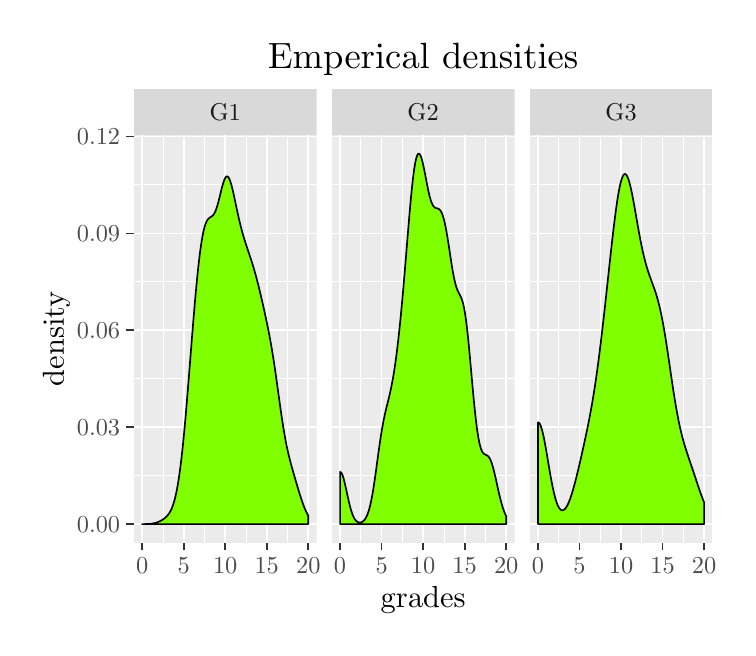
\begin{tikzpicture}[x=1pt,y=1pt]
\definecolor{fillColor}{RGB}{255,255,255}
\path[use as bounding box,fill=fillColor,fill opacity=0.00] (0,0) rectangle (252.94,216.81);
\begin{scope}
\path[clip] (  0.00,  0.00) rectangle (252.94,216.81);
\definecolor{drawColor}{RGB}{255,255,255}
\definecolor{fillColor}{RGB}{255,255,255}

\path[draw=drawColor,line width= 0.6pt,line join=round,line cap=round,fill=fillColor] (  0.00,  0.00) rectangle (252.94,216.81);
\end{scope}
\begin{scope}
\path[clip] ( 38.36, 30.72) rectangle (104.39,177.97);
\definecolor{fillColor}{gray}{0.92}

\path[fill=fillColor] ( 38.36, 30.72) rectangle (104.39,177.97);
\definecolor{drawColor}{RGB}{255,255,255}

\path[draw=drawColor,line width= 0.3pt,line join=round] ( 38.36, 54.93) --
	(104.39, 54.93);

\path[draw=drawColor,line width= 0.3pt,line join=round] ( 38.36, 89.95) --
	(104.39, 89.95);

\path[draw=drawColor,line width= 0.3pt,line join=round] ( 38.36,124.98) --
	(104.39,124.98);

\path[draw=drawColor,line width= 0.3pt,line join=round] ( 38.36,160.00) --
	(104.39,160.00);

\path[draw=drawColor,line width= 0.3pt,line join=round] ( 48.87, 30.72) --
	( 48.87,177.97);

\path[draw=drawColor,line width= 0.3pt,line join=round] ( 63.87, 30.72) --
	( 63.87,177.97);

\path[draw=drawColor,line width= 0.3pt,line join=round] ( 78.88, 30.72) --
	( 78.88,177.97);

\path[draw=drawColor,line width= 0.3pt,line join=round] ( 93.88, 30.72) --
	( 93.88,177.97);

\path[draw=drawColor,line width= 0.6pt,line join=round] ( 38.36, 37.42) --
	(104.39, 37.42);

\path[draw=drawColor,line width= 0.6pt,line join=round] ( 38.36, 72.44) --
	(104.39, 72.44);

\path[draw=drawColor,line width= 0.6pt,line join=round] ( 38.36,107.47) --
	(104.39,107.47);

\path[draw=drawColor,line width= 0.6pt,line join=round] ( 38.36,142.49) --
	(104.39,142.49);

\path[draw=drawColor,line width= 0.6pt,line join=round] ( 38.36,177.51) --
	(104.39,177.51);

\path[draw=drawColor,line width= 0.6pt,line join=round] ( 41.36, 30.72) --
	( 41.36,177.97);

\path[draw=drawColor,line width= 0.6pt,line join=round] ( 56.37, 30.72) --
	( 56.37,177.97);

\path[draw=drawColor,line width= 0.6pt,line join=round] ( 71.37, 30.72) --
	( 71.37,177.97);

\path[draw=drawColor,line width= 0.6pt,line join=round] ( 86.38, 30.72) --
	( 86.38,177.97);

\path[draw=drawColor,line width= 0.6pt,line join=round] (101.39, 30.72) --
	(101.39,177.97);
\definecolor{drawColor}{RGB}{0,0,0}
\definecolor{fillColor}{RGB}{127,255,0}

\path[draw=drawColor,line width= 0.6pt,line join=round,line cap=round,fill=fillColor] ( 41.36, 37.42) --
	( 41.48, 37.42) --
	( 41.60, 37.42) --
	( 41.71, 37.43) --
	( 41.83, 37.43) --
	( 41.95, 37.43) --
	( 42.07, 37.43) --
	( 42.18, 37.43) --
	( 42.30, 37.43) --
	( 42.42, 37.44) --
	( 42.54, 37.44) --
	( 42.65, 37.44) --
	( 42.77, 37.44) --
	( 42.89, 37.45) --
	( 43.01, 37.45) --
	( 43.12, 37.46) --
	( 43.24, 37.46) --
	( 43.36, 37.47) --
	( 43.48, 37.47) --
	( 43.59, 37.48) --
	( 43.71, 37.49) --
	( 43.83, 37.49) --
	( 43.95, 37.50) --
	( 44.06, 37.51) --
	( 44.18, 37.52) --
	( 44.30, 37.53) --
	( 44.42, 37.54) --
	( 44.53, 37.55) --
	( 44.65, 37.57) --
	( 44.77, 37.58) --
	( 44.89, 37.60) --
	( 45.00, 37.62) --
	( 45.12, 37.63) --
	( 45.24, 37.65) --
	( 45.36, 37.67) --
	( 45.47, 37.70) --
	( 45.59, 37.72) --
	( 45.71, 37.75) --
	( 45.83, 37.77) --
	( 45.94, 37.80) --
	( 46.06, 37.83) --
	( 46.18, 37.86) --
	( 46.30, 37.90) --
	( 46.41, 37.93) --
	( 46.53, 37.97) --
	( 46.65, 38.01) --
	( 46.77, 38.05) --
	( 46.88, 38.09) --
	( 47.00, 38.13) --
	( 47.12, 38.18) --
	( 47.24, 38.22) --
	( 47.35, 38.27) --
	( 47.47, 38.32) --
	( 47.59, 38.38) --
	( 47.71, 38.43) --
	( 47.82, 38.49) --
	( 47.94, 38.55) --
	( 48.06, 38.61) --
	( 48.17, 38.67) --
	( 48.29, 38.74) --
	( 48.41, 38.80) --
	( 48.53, 38.87) --
	( 48.64, 38.95) --
	( 48.76, 39.02) --
	( 48.88, 39.10) --
	( 49.00, 39.18) --
	( 49.11, 39.26) --
	( 49.23, 39.34) --
	( 49.35, 39.43) --
	( 49.47, 39.52) --
	( 49.58, 39.62) --
	( 49.70, 39.71) --
	( 49.82, 39.82) --
	( 49.94, 39.92) --
	( 50.05, 40.04) --
	( 50.17, 40.15) --
	( 50.29, 40.27) --
	( 50.41, 40.40) --
	( 50.52, 40.54) --
	( 50.64, 40.68) --
	( 50.76, 40.83) --
	( 50.88, 40.98) --
	( 50.99, 41.14) --
	( 51.11, 41.32) --
	( 51.23, 41.50) --
	( 51.35, 41.69) --
	( 51.46, 41.90) --
	( 51.58, 42.11) --
	( 51.70, 42.34) --
	( 51.82, 42.58) --
	( 51.93, 42.83) --
	( 52.05, 43.10) --
	( 52.17, 43.39) --
	( 52.29, 43.68) --
	( 52.40, 44.00) --
	( 52.52, 44.33) --
	( 52.64, 44.69) --
	( 52.76, 45.05) --
	( 52.87, 45.44) --
	( 52.99, 45.86) --
	( 53.11, 46.29) --
	( 53.23, 46.74) --
	( 53.34, 47.22) --
	( 53.46, 47.72) --
	( 53.58, 48.24) --
	( 53.70, 48.78) --
	( 53.81, 49.36) --
	( 53.93, 49.96) --
	( 54.05, 50.58) --
	( 54.17, 51.24) --
	( 54.28, 51.92) --
	( 54.40, 52.63) --
	( 54.52, 53.36) --
	( 54.64, 54.13) --
	( 54.75, 54.92) --
	( 54.87, 55.75) --
	( 54.99, 56.59) --
	( 55.11, 57.48) --
	( 55.22, 58.39) --
	( 55.34, 59.33) --
	( 55.46, 60.30) --
	( 55.58, 61.30) --
	( 55.69, 62.33) --
	( 55.81, 63.38) --
	( 55.93, 64.47) --
	( 56.05, 65.59) --
	( 56.16, 66.73) --
	( 56.28, 67.89) --
	( 56.40, 69.09) --
	( 56.52, 70.31) --
	( 56.63, 71.55) --
	( 56.75, 72.82) --
	( 56.87, 74.11) --
	( 56.99, 75.42) --
	( 57.10, 76.76) --
	( 57.22, 78.11) --
	( 57.34, 79.48) --
	( 57.45, 80.88) --
	( 57.57, 82.28) --
	( 57.69, 83.70) --
	( 57.81, 85.14) --
	( 57.92, 86.59) --
	( 58.04, 88.04) --
	( 58.16, 89.51) --
	( 58.28, 90.99) --
	( 58.39, 92.47) --
	( 58.51, 93.95) --
	( 58.63, 95.45) --
	( 58.75, 96.94) --
	( 58.86, 98.43) --
	( 58.98, 99.92) --
	( 59.10,101.41) --
	( 59.22,102.89) --
	( 59.33,104.37) --
	( 59.45,105.84) --
	( 59.57,107.31) --
	( 59.69,108.76) --
	( 59.80,110.20) --
	( 59.92,111.63) --
	( 60.04,113.04) --
	( 60.16,114.44) --
	( 60.27,115.82) --
	( 60.39,117.18) --
	( 60.51,118.52) --
	( 60.63,119.84) --
	( 60.74,121.15) --
	( 60.86,122.42) --
	( 60.98,123.67) --
	( 61.10,124.90) --
	( 61.21,126.10) --
	( 61.33,127.27) --
	( 61.45,128.41) --
	( 61.57,129.53) --
	( 61.68,130.61) --
	( 61.80,131.66) --
	( 61.92,132.68) --
	( 62.04,133.67) --
	( 62.15,134.63) --
	( 62.27,135.55) --
	( 62.39,136.43) --
	( 62.51,137.29) --
	( 62.62,138.11) --
	( 62.74,138.89) --
	( 62.86,139.63) --
	( 62.98,140.35) --
	( 63.09,141.02) --
	( 63.21,141.66) --
	( 63.33,142.27) --
	( 63.45,142.84) --
	( 63.56,143.37) --
	( 63.68,143.87) --
	( 63.80,144.34) --
	( 63.92,144.77) --
	( 64.03,145.17) --
	( 64.15,145.54) --
	( 64.27,145.88) --
	( 64.39,146.19) --
	( 64.50,146.47) --
	( 64.62,146.73) --
	( 64.74,146.96) --
	( 64.86,147.16) --
	( 64.97,147.34) --
	( 65.09,147.51) --
	( 65.21,147.65) --
	( 65.33,147.78) --
	( 65.44,147.89) --
	( 65.56,147.99) --
	( 65.68,148.09) --
	( 65.80,148.17) --
	( 65.91,148.24) --
	( 66.03,148.32) --
	( 66.15,148.39) --
	( 66.26,148.46) --
	( 66.38,148.54) --
	( 66.50,148.62) --
	( 66.62,148.71) --
	( 66.73,148.81) --
	( 66.85,148.92) --
	( 66.97,149.04) --
	( 67.09,149.18) --
	( 67.20,149.33) --
	( 67.32,149.50) --
	( 67.44,149.69) --
	( 67.56,149.90) --
	( 67.67,150.13) --
	( 67.79,150.38) --
	( 67.91,150.66) --
	( 68.03,150.95) --
	( 68.14,151.27) --
	( 68.26,151.60) --
	( 68.38,151.97) --
	( 68.50,152.35) --
	( 68.61,152.74) --
	( 68.73,153.16) --
	( 68.85,153.59) --
	( 68.97,154.04) --
	( 69.08,154.49) --
	( 69.20,154.96) --
	( 69.32,155.44) --
	( 69.44,155.92) --
	( 69.55,156.41) --
	( 69.67,156.90) --
	( 69.79,157.39) --
	( 69.91,157.87) --
	( 70.02,158.35) --
	( 70.14,158.81) --
	( 70.26,159.26) --
	( 70.38,159.70) --
	( 70.49,160.13) --
	( 70.61,160.53) --
	( 70.73,160.90) --
	( 70.85,161.26) --
	( 70.96,161.59) --
	( 71.08,161.88) --
	( 71.20,162.15) --
	( 71.32,162.39) --
	( 71.43,162.59) --
	( 71.55,162.76) --
	( 71.67,162.89) --
	( 71.79,162.99) --
	( 71.90,163.05) --
	( 72.02,163.07) --
	( 72.14,163.05) --
	( 72.26,163.01) --
	( 72.37,162.91) --
	( 72.49,162.79) --
	( 72.61,162.63) --
	( 72.73,162.44) --
	( 72.84,162.20) --
	( 72.96,161.94) --
	( 73.08,161.65) --
	( 73.20,161.33) --
	( 73.31,160.98) --
	( 73.43,160.60) --
	( 73.55,160.20) --
	( 73.67,159.78) --
	( 73.78,159.33) --
	( 73.90,158.87) --
	( 74.02,158.39) --
	( 74.14,157.89) --
	( 74.25,157.38) --
	( 74.37,156.86) --
	( 74.49,156.33) --
	( 74.61,155.79) --
	( 74.72,155.24) --
	( 74.84,154.69) --
	( 74.96,154.14) --
	( 75.07,153.58) --
	( 75.19,153.02) --
	( 75.31,152.46) --
	( 75.43,151.91) --
	( 75.54,151.35) --
	( 75.66,150.80) --
	( 75.78,150.26) --
	( 75.90,149.72) --
	( 76.01,149.19) --
	( 76.13,148.66) --
	( 76.25,148.14) --
	( 76.37,147.63) --
	( 76.48,147.12) --
	( 76.60,146.63) --
	( 76.72,146.14) --
	( 76.84,145.66) --
	( 76.95,145.19) --
	( 77.07,144.73) --
	( 77.19,144.27) --
	( 77.31,143.83) --
	( 77.42,143.39) --
	( 77.54,142.96) --
	( 77.66,142.54) --
	( 77.78,142.13) --
	( 77.89,141.72) --
	( 78.01,141.32) --
	( 78.13,140.92) --
	( 78.25,140.54) --
	( 78.36,140.15) --
	( 78.48,139.78) --
	( 78.60,139.41) --
	( 78.72,139.04) --
	( 78.83,138.67) --
	( 78.95,138.31) --
	( 79.07,137.96) --
	( 79.19,137.60) --
	( 79.30,137.25) --
	( 79.42,136.90) --
	( 79.54,136.55) --
	( 79.66,136.20) --
	( 79.77,135.85) --
	( 79.89,135.50) --
	( 80.01,135.15) --
	( 80.13,134.80) --
	( 80.24,134.44) --
	( 80.36,134.09) --
	( 80.48,133.73) --
	( 80.60,133.38) --
	( 80.71,133.01) --
	( 80.83,132.65) --
	( 80.95,132.28) --
	( 81.07,131.91) --
	( 81.18,131.54) --
	( 81.30,131.16) --
	( 81.42,130.77) --
	( 81.54,130.39) --
	( 81.65,129.99) --
	( 81.77,129.59) --
	( 81.89,129.19) --
	( 82.01,128.79) --
	( 82.12,128.37) --
	( 82.24,127.95) --
	( 82.36,127.53) --
	( 82.48,127.10) --
	( 82.59,126.67) --
	( 82.71,126.23) --
	( 82.83,125.78) --
	( 82.95,125.33) --
	( 83.06,124.88) --
	( 83.18,124.42) --
	( 83.30,123.96) --
	( 83.42,123.49) --
	( 83.53,123.01) --
	( 83.65,122.53) --
	( 83.77,122.05) --
	( 83.88,121.57) --
	( 84.00,121.07) --
	( 84.12,120.58) --
	( 84.24,120.08) --
	( 84.35,119.58) --
	( 84.47,119.08) --
	( 84.59,118.57) --
	( 84.71,118.06) --
	( 84.82,117.54) --
	( 84.94,117.03) --
	( 85.06,116.51) --
	( 85.18,115.98) --
	( 85.29,115.46) --
	( 85.41,114.93) --
	( 85.53,114.40) --
	( 85.65,113.86) --
	( 85.76,113.32) --
	( 85.88,112.78) --
	( 86.00,112.23) --
	( 86.12,111.68) --
	( 86.23,111.13) --
	( 86.35,110.57) --
	( 86.47,110.01) --
	( 86.59,109.44) --
	( 86.70,108.86) --
	( 86.82,108.28) --
	( 86.94,107.69) --
	( 87.06,107.10) --
	( 87.17,106.49) --
	( 87.29,105.88) --
	( 87.41,105.26) --
	( 87.53,104.63) --
	( 87.64,104.00) --
	( 87.76,103.35) --
	( 87.88,102.69) --
	( 88.00,102.02) --
	( 88.11,101.34) --
	( 88.23,100.65) --
	( 88.35, 99.95) --
	( 88.47, 99.24) --
	( 88.58, 98.51) --
	( 88.70, 97.78) --
	( 88.82, 97.03) --
	( 88.94, 96.27) --
	( 89.05, 95.50) --
	( 89.17, 94.72) --
	( 89.29, 93.93) --
	( 89.41, 93.13) --
	( 89.52, 92.32) --
	( 89.64, 91.50) --
	( 89.76, 90.67) --
	( 89.88, 89.84) --
	( 89.99, 89.00) --
	( 90.11, 88.15) --
	( 90.23, 87.31) --
	( 90.35, 86.45) --
	( 90.46, 85.60) --
	( 90.58, 84.75) --
	( 90.70, 83.89) --
	( 90.82, 83.04) --
	( 90.93, 82.19) --
	( 91.05, 81.34) --
	( 91.17, 80.50) --
	( 91.29, 79.66) --
	( 91.40, 78.84) --
	( 91.52, 78.02) --
	( 91.64, 77.20) --
	( 91.76, 76.40) --
	( 91.87, 75.61) --
	( 91.99, 74.84) --
	( 92.11, 74.07) --
	( 92.23, 73.32) --
	( 92.34, 72.58) --
	( 92.46, 71.86) --
	( 92.58, 71.15) --
	( 92.69, 70.46) --
	( 92.81, 69.78) --
	( 92.93, 69.12) --
	( 93.05, 68.47) --
	( 93.16, 67.84) --
	( 93.28, 67.22) --
	( 93.40, 66.62) --
	( 93.52, 66.04) --
	( 93.63, 65.47) --
	( 93.75, 64.91) --
	( 93.87, 64.36) --
	( 93.99, 63.83) --
	( 94.10, 63.31) --
	( 94.22, 62.81) --
	( 94.34, 62.31) --
	( 94.46, 61.82) --
	( 94.57, 61.35) --
	( 94.69, 60.88) --
	( 94.81, 60.42) --
	( 94.93, 59.97) --
	( 95.04, 59.52) --
	( 95.16, 59.09) --
	( 95.28, 58.65) --
	( 95.40, 58.22) --
	( 95.51, 57.80) --
	( 95.63, 57.38) --
	( 95.75, 56.96) --
	( 95.87, 56.55) --
	( 95.98, 56.14) --
	( 96.10, 55.73) --
	( 96.22, 55.32) --
	( 96.34, 54.91) --
	( 96.45, 54.50) --
	( 96.57, 54.10) --
	( 96.69, 53.70) --
	( 96.81, 53.29) --
	( 96.92, 52.89) --
	( 97.04, 52.49) --
	( 97.16, 52.09) --
	( 97.28, 51.69) --
	( 97.39, 51.30) --
	( 97.51, 50.90) --
	( 97.63, 50.51) --
	( 97.75, 50.11) --
	( 97.86, 49.72) --
	( 97.98, 49.34) --
	( 98.10, 48.95) --
	( 98.22, 48.57) --
	( 98.33, 48.19) --
	( 98.45, 47.82) --
	( 98.57, 47.45) --
	( 98.69, 47.08) --
	( 98.80, 46.72) --
	( 98.92, 46.36) --
	( 99.04, 46.01) --
	( 99.16, 45.67) --
	( 99.27, 45.33) --
	( 99.39, 45.00) --
	( 99.51, 44.67) --
	( 99.63, 44.35) --
	( 99.74, 44.04) --
	( 99.86, 43.73) --
	( 99.98, 43.43) --
	(100.10, 43.14) --
	(100.21, 42.86) --
	(100.33, 42.59) --
	(100.45, 42.32) --
	(100.57, 42.06) --
	(100.68, 41.81) --
	(100.80, 41.57) --
	(100.92, 41.34) --
	(101.04, 41.12) --
	(101.15, 40.90) --
	(101.27, 40.69) --
	(101.39, 40.49) --
	(101.39, 37.42) --
	(101.27, 37.42) --
	(101.15, 37.42) --
	(101.04, 37.42) --
	(100.92, 37.42) --
	(100.80, 37.42) --
	(100.68, 37.42) --
	(100.57, 37.42) --
	(100.45, 37.42) --
	(100.33, 37.42) --
	(100.21, 37.42) --
	(100.10, 37.42) --
	( 99.98, 37.42) --
	( 99.86, 37.42) --
	( 99.74, 37.42) --
	( 99.63, 37.42) --
	( 99.51, 37.42) --
	( 99.39, 37.42) --
	( 99.27, 37.42) --
	( 99.16, 37.42) --
	( 99.04, 37.42) --
	( 98.92, 37.42) --
	( 98.80, 37.42) --
	( 98.69, 37.42) --
	( 98.57, 37.42) --
	( 98.45, 37.42) --
	( 98.33, 37.42) --
	( 98.22, 37.42) --
	( 98.10, 37.42) --
	( 97.98, 37.42) --
	( 97.86, 37.42) --
	( 97.75, 37.42) --
	( 97.63, 37.42) --
	( 97.51, 37.42) --
	( 97.39, 37.42) --
	( 97.28, 37.42) --
	( 97.16, 37.42) --
	( 97.04, 37.42) --
	( 96.92, 37.42) --
	( 96.81, 37.42) --
	( 96.69, 37.42) --
	( 96.57, 37.42) --
	( 96.45, 37.42) --
	( 96.34, 37.42) --
	( 96.22, 37.42) --
	( 96.10, 37.42) --
	( 95.98, 37.42) --
	( 95.87, 37.42) --
	( 95.75, 37.42) --
	( 95.63, 37.42) --
	( 95.51, 37.42) --
	( 95.40, 37.42) --
	( 95.28, 37.42) --
	( 95.16, 37.42) --
	( 95.04, 37.42) --
	( 94.93, 37.42) --
	( 94.81, 37.42) --
	( 94.69, 37.42) --
	( 94.57, 37.42) --
	( 94.46, 37.42) --
	( 94.34, 37.42) --
	( 94.22, 37.42) --
	( 94.10, 37.42) --
	( 93.99, 37.42) --
	( 93.87, 37.42) --
	( 93.75, 37.42) --
	( 93.63, 37.42) --
	( 93.52, 37.42) --
	( 93.40, 37.42) --
	( 93.28, 37.42) --
	( 93.16, 37.42) --
	( 93.05, 37.42) --
	( 92.93, 37.42) --
	( 92.81, 37.42) --
	( 92.69, 37.42) --
	( 92.58, 37.42) --
	( 92.46, 37.42) --
	( 92.34, 37.42) --
	( 92.23, 37.42) --
	( 92.11, 37.42) --
	( 91.99, 37.42) --
	( 91.87, 37.42) --
	( 91.76, 37.42) --
	( 91.64, 37.42) --
	( 91.52, 37.42) --
	( 91.40, 37.42) --
	( 91.29, 37.42) --
	( 91.17, 37.42) --
	( 91.05, 37.42) --
	( 90.93, 37.42) --
	( 90.82, 37.42) --
	( 90.70, 37.42) --
	( 90.58, 37.42) --
	( 90.46, 37.42) --
	( 90.35, 37.42) --
	( 90.23, 37.42) --
	( 90.11, 37.42) --
	( 89.99, 37.42) --
	( 89.88, 37.42) --
	( 89.76, 37.42) --
	( 89.64, 37.42) --
	( 89.52, 37.42) --
	( 89.41, 37.42) --
	( 89.29, 37.42) --
	( 89.17, 37.42) --
	( 89.05, 37.42) --
	( 88.94, 37.42) --
	( 88.82, 37.42) --
	( 88.70, 37.42) --
	( 88.58, 37.42) --
	( 88.47, 37.42) --
	( 88.35, 37.42) --
	( 88.23, 37.42) --
	( 88.11, 37.42) --
	( 88.00, 37.42) --
	( 87.88, 37.42) --
	( 87.76, 37.42) --
	( 87.64, 37.42) --
	( 87.53, 37.42) --
	( 87.41, 37.42) --
	( 87.29, 37.42) --
	( 87.17, 37.42) --
	( 87.06, 37.42) --
	( 86.94, 37.42) --
	( 86.82, 37.42) --
	( 86.70, 37.42) --
	( 86.59, 37.42) --
	( 86.47, 37.42) --
	( 86.35, 37.42) --
	( 86.23, 37.42) --
	( 86.12, 37.42) --
	( 86.00, 37.42) --
	( 85.88, 37.42) --
	( 85.76, 37.42) --
	( 85.65, 37.42) --
	( 85.53, 37.42) --
	( 85.41, 37.42) --
	( 85.29, 37.42) --
	( 85.18, 37.42) --
	( 85.06, 37.42) --
	( 84.94, 37.42) --
	( 84.82, 37.42) --
	( 84.71, 37.42) --
	( 84.59, 37.42) --
	( 84.47, 37.42) --
	( 84.35, 37.42) --
	( 84.24, 37.42) --
	( 84.12, 37.42) --
	( 84.00, 37.42) --
	( 83.88, 37.42) --
	( 83.77, 37.42) --
	( 83.65, 37.42) --
	( 83.53, 37.42) --
	( 83.42, 37.42) --
	( 83.30, 37.42) --
	( 83.18, 37.42) --
	( 83.06, 37.42) --
	( 82.95, 37.42) --
	( 82.83, 37.42) --
	( 82.71, 37.42) --
	( 82.59, 37.42) --
	( 82.48, 37.42) --
	( 82.36, 37.42) --
	( 82.24, 37.42) --
	( 82.12, 37.42) --
	( 82.01, 37.42) --
	( 81.89, 37.42) --
	( 81.77, 37.42) --
	( 81.65, 37.42) --
	( 81.54, 37.42) --
	( 81.42, 37.42) --
	( 81.30, 37.42) --
	( 81.18, 37.42) --
	( 81.07, 37.42) --
	( 80.95, 37.42) --
	( 80.83, 37.42) --
	( 80.71, 37.42) --
	( 80.60, 37.42) --
	( 80.48, 37.42) --
	( 80.36, 37.42) --
	( 80.24, 37.42) --
	( 80.13, 37.42) --
	( 80.01, 37.42) --
	( 79.89, 37.42) --
	( 79.77, 37.42) --
	( 79.66, 37.42) --
	( 79.54, 37.42) --
	( 79.42, 37.42) --
	( 79.30, 37.42) --
	( 79.19, 37.42) --
	( 79.07, 37.42) --
	( 78.95, 37.42) --
	( 78.83, 37.42) --
	( 78.72, 37.42) --
	( 78.60, 37.42) --
	( 78.48, 37.42) --
	( 78.36, 37.42) --
	( 78.25, 37.42) --
	( 78.13, 37.42) --
	( 78.01, 37.42) --
	( 77.89, 37.42) --
	( 77.78, 37.42) --
	( 77.66, 37.42) --
	( 77.54, 37.42) --
	( 77.42, 37.42) --
	( 77.31, 37.42) --
	( 77.19, 37.42) --
	( 77.07, 37.42) --
	( 76.95, 37.42) --
	( 76.84, 37.42) --
	( 76.72, 37.42) --
	( 76.60, 37.42) --
	( 76.48, 37.42) --
	( 76.37, 37.42) --
	( 76.25, 37.42) --
	( 76.13, 37.42) --
	( 76.01, 37.42) --
	( 75.90, 37.42) --
	( 75.78, 37.42) --
	( 75.66, 37.42) --
	( 75.54, 37.42) --
	( 75.43, 37.42) --
	( 75.31, 37.42) --
	( 75.19, 37.42) --
	( 75.07, 37.42) --
	( 74.96, 37.42) --
	( 74.84, 37.42) --
	( 74.72, 37.42) --
	( 74.61, 37.42) --
	( 74.49, 37.42) --
	( 74.37, 37.42) --
	( 74.25, 37.42) --
	( 74.14, 37.42) --
	( 74.02, 37.42) --
	( 73.90, 37.42) --
	( 73.78, 37.42) --
	( 73.67, 37.42) --
	( 73.55, 37.42) --
	( 73.43, 37.42) --
	( 73.31, 37.42) --
	( 73.20, 37.42) --
	( 73.08, 37.42) --
	( 72.96, 37.42) --
	( 72.84, 37.42) --
	( 72.73, 37.42) --
	( 72.61, 37.42) --
	( 72.49, 37.42) --
	( 72.37, 37.42) --
	( 72.26, 37.42) --
	( 72.14, 37.42) --
	( 72.02, 37.42) --
	( 71.90, 37.42) --
	( 71.79, 37.42) --
	( 71.67, 37.42) --
	( 71.55, 37.42) --
	( 71.43, 37.42) --
	( 71.32, 37.42) --
	( 71.20, 37.42) --
	( 71.08, 37.42) --
	( 70.96, 37.42) --
	( 70.85, 37.42) --
	( 70.73, 37.42) --
	( 70.61, 37.42) --
	( 70.49, 37.42) --
	( 70.38, 37.42) --
	( 70.26, 37.42) --
	( 70.14, 37.42) --
	( 70.02, 37.42) --
	( 69.91, 37.42) --
	( 69.79, 37.42) --
	( 69.67, 37.42) --
	( 69.55, 37.42) --
	( 69.44, 37.42) --
	( 69.32, 37.42) --
	( 69.20, 37.42) --
	( 69.08, 37.42) --
	( 68.97, 37.42) --
	( 68.85, 37.42) --
	( 68.73, 37.42) --
	( 68.61, 37.42) --
	( 68.50, 37.42) --
	( 68.38, 37.42) --
	( 68.26, 37.42) --
	( 68.14, 37.42) --
	( 68.03, 37.42) --
	( 67.91, 37.42) --
	( 67.79, 37.42) --
	( 67.67, 37.42) --
	( 67.56, 37.42) --
	( 67.44, 37.42) --
	( 67.32, 37.42) --
	( 67.20, 37.42) --
	( 67.09, 37.42) --
	( 66.97, 37.42) --
	( 66.85, 37.42) --
	( 66.73, 37.42) --
	( 66.62, 37.42) --
	( 66.50, 37.42) --
	( 66.38, 37.42) --
	( 66.26, 37.42) --
	( 66.15, 37.42) --
	( 66.03, 37.42) --
	( 65.91, 37.42) --
	( 65.80, 37.42) --
	( 65.68, 37.42) --
	( 65.56, 37.42) --
	( 65.44, 37.42) --
	( 65.33, 37.42) --
	( 65.21, 37.42) --
	( 65.09, 37.42) --
	( 64.97, 37.42) --
	( 64.86, 37.42) --
	( 64.74, 37.42) --
	( 64.62, 37.42) --
	( 64.50, 37.42) --
	( 64.39, 37.42) --
	( 64.27, 37.42) --
	( 64.15, 37.42) --
	( 64.03, 37.42) --
	( 63.92, 37.42) --
	( 63.80, 37.42) --
	( 63.68, 37.42) --
	( 63.56, 37.42) --
	( 63.45, 37.42) --
	( 63.33, 37.42) --
	( 63.21, 37.42) --
	( 63.09, 37.42) --
	( 62.98, 37.42) --
	( 62.86, 37.42) --
	( 62.74, 37.42) --
	( 62.62, 37.42) --
	( 62.51, 37.42) --
	( 62.39, 37.42) --
	( 62.27, 37.42) --
	( 62.15, 37.42) --
	( 62.04, 37.42) --
	( 61.92, 37.42) --
	( 61.80, 37.42) --
	( 61.68, 37.42) --
	( 61.57, 37.42) --
	( 61.45, 37.42) --
	( 61.33, 37.42) --
	( 61.21, 37.42) --
	( 61.10, 37.42) --
	( 60.98, 37.42) --
	( 60.86, 37.42) --
	( 60.74, 37.42) --
	( 60.63, 37.42) --
	( 60.51, 37.42) --
	( 60.39, 37.42) --
	( 60.27, 37.42) --
	( 60.16, 37.42) --
	( 60.04, 37.42) --
	( 59.92, 37.42) --
	( 59.80, 37.42) --
	( 59.69, 37.42) --
	( 59.57, 37.42) --
	( 59.45, 37.42) --
	( 59.33, 37.42) --
	( 59.22, 37.42) --
	( 59.10, 37.42) --
	( 58.98, 37.42) --
	( 58.86, 37.42) --
	( 58.75, 37.42) --
	( 58.63, 37.42) --
	( 58.51, 37.42) --
	( 58.39, 37.42) --
	( 58.28, 37.42) --
	( 58.16, 37.42) --
	( 58.04, 37.42) --
	( 57.92, 37.42) --
	( 57.81, 37.42) --
	( 57.69, 37.42) --
	( 57.57, 37.42) --
	( 57.45, 37.42) --
	( 57.34, 37.42) --
	( 57.22, 37.42) --
	( 57.10, 37.42) --
	( 56.99, 37.42) --
	( 56.87, 37.42) --
	( 56.75, 37.42) --
	( 56.63, 37.42) --
	( 56.52, 37.42) --
	( 56.40, 37.42) --
	( 56.28, 37.42) --
	( 56.16, 37.42) --
	( 56.05, 37.42) --
	( 55.93, 37.42) --
	( 55.81, 37.42) --
	( 55.69, 37.42) --
	( 55.58, 37.42) --
	( 55.46, 37.42) --
	( 55.34, 37.42) --
	( 55.22, 37.42) --
	( 55.11, 37.42) --
	( 54.99, 37.42) --
	( 54.87, 37.42) --
	( 54.75, 37.42) --
	( 54.64, 37.42) --
	( 54.52, 37.42) --
	( 54.40, 37.42) --
	( 54.28, 37.42) --
	( 54.17, 37.42) --
	( 54.05, 37.42) --
	( 53.93, 37.42) --
	( 53.81, 37.42) --
	( 53.70, 37.42) --
	( 53.58, 37.42) --
	( 53.46, 37.42) --
	( 53.34, 37.42) --
	( 53.23, 37.42) --
	( 53.11, 37.42) --
	( 52.99, 37.42) --
	( 52.87, 37.42) --
	( 52.76, 37.42) --
	( 52.64, 37.42) --
	( 52.52, 37.42) --
	( 52.40, 37.42) --
	( 52.29, 37.42) --
	( 52.17, 37.42) --
	( 52.05, 37.42) --
	( 51.93, 37.42) --
	( 51.82, 37.42) --
	( 51.70, 37.42) --
	( 51.58, 37.42) --
	( 51.46, 37.42) --
	( 51.35, 37.42) --
	( 51.23, 37.42) --
	( 51.11, 37.42) --
	( 50.99, 37.42) --
	( 50.88, 37.42) --
	( 50.76, 37.42) --
	( 50.64, 37.42) --
	( 50.52, 37.42) --
	( 50.41, 37.42) --
	( 50.29, 37.42) --
	( 50.17, 37.42) --
	( 50.05, 37.42) --
	( 49.94, 37.42) --
	( 49.82, 37.42) --
	( 49.70, 37.42) --
	( 49.58, 37.42) --
	( 49.47, 37.42) --
	( 49.35, 37.42) --
	( 49.23, 37.42) --
	( 49.11, 37.42) --
	( 49.00, 37.42) --
	( 48.88, 37.42) --
	( 48.76, 37.42) --
	( 48.64, 37.42) --
	( 48.53, 37.42) --
	( 48.41, 37.42) --
	( 48.29, 37.42) --
	( 48.17, 37.42) --
	( 48.06, 37.42) --
	( 47.94, 37.42) --
	( 47.82, 37.42) --
	( 47.71, 37.42) --
	( 47.59, 37.42) --
	( 47.47, 37.42) --
	( 47.35, 37.42) --
	( 47.24, 37.42) --
	( 47.12, 37.42) --
	( 47.00, 37.42) --
	( 46.88, 37.42) --
	( 46.77, 37.42) --
	( 46.65, 37.42) --
	( 46.53, 37.42) --
	( 46.41, 37.42) --
	( 46.30, 37.42) --
	( 46.18, 37.42) --
	( 46.06, 37.42) --
	( 45.94, 37.42) --
	( 45.83, 37.42) --
	( 45.71, 37.42) --
	( 45.59, 37.42) --
	( 45.47, 37.42) --
	( 45.36, 37.42) --
	( 45.24, 37.42) --
	( 45.12, 37.42) --
	( 45.00, 37.42) --
	( 44.89, 37.42) --
	( 44.77, 37.42) --
	( 44.65, 37.42) --
	( 44.53, 37.42) --
	( 44.42, 37.42) --
	( 44.30, 37.42) --
	( 44.18, 37.42) --
	( 44.06, 37.42) --
	( 43.95, 37.42) --
	( 43.83, 37.42) --
	( 43.71, 37.42) --
	( 43.59, 37.42) --
	( 43.48, 37.42) --
	( 43.36, 37.42) --
	( 43.24, 37.42) --
	( 43.12, 37.42) --
	( 43.01, 37.42) --
	( 42.89, 37.42) --
	( 42.77, 37.42) --
	( 42.65, 37.42) --
	( 42.54, 37.42) --
	( 42.42, 37.42) --
	( 42.30, 37.42) --
	( 42.18, 37.42) --
	( 42.07, 37.42) --
	( 41.95, 37.42) --
	( 41.83, 37.42) --
	( 41.71, 37.42) --
	( 41.60, 37.42) --
	( 41.48, 37.42) --
	( 41.36, 37.42) --
	cycle;
\end{scope}
\begin{scope}
\path[clip] (109.89, 30.72) rectangle (175.92,177.97);
\definecolor{fillColor}{gray}{0.92}

\path[fill=fillColor] (109.89, 30.72) rectangle (175.92,177.97);
\definecolor{drawColor}{RGB}{255,255,255}

\path[draw=drawColor,line width= 0.3pt,line join=round] (109.89, 54.93) --
	(175.92, 54.93);

\path[draw=drawColor,line width= 0.3pt,line join=round] (109.89, 89.95) --
	(175.92, 89.95);

\path[draw=drawColor,line width= 0.3pt,line join=round] (109.89,124.98) --
	(175.92,124.98);

\path[draw=drawColor,line width= 0.3pt,line join=round] (109.89,160.00) --
	(175.92,160.00);

\path[draw=drawColor,line width= 0.3pt,line join=round] (120.39, 30.72) --
	(120.39,177.97);

\path[draw=drawColor,line width= 0.3pt,line join=round] (135.40, 30.72) --
	(135.40,177.97);

\path[draw=drawColor,line width= 0.3pt,line join=round] (150.41, 30.72) --
	(150.41,177.97);

\path[draw=drawColor,line width= 0.3pt,line join=round] (165.41, 30.72) --
	(165.41,177.97);

\path[draw=drawColor,line width= 0.6pt,line join=round] (109.89, 37.42) --
	(175.92, 37.42);

\path[draw=drawColor,line width= 0.6pt,line join=round] (109.89, 72.44) --
	(175.92, 72.44);

\path[draw=drawColor,line width= 0.6pt,line join=round] (109.89,107.47) --
	(175.92,107.47);

\path[draw=drawColor,line width= 0.6pt,line join=round] (109.89,142.49) --
	(175.92,142.49);

\path[draw=drawColor,line width= 0.6pt,line join=round] (109.89,177.51) --
	(175.92,177.51);

\path[draw=drawColor,line width= 0.6pt,line join=round] (112.89, 30.72) --
	(112.89,177.97);

\path[draw=drawColor,line width= 0.6pt,line join=round] (127.90, 30.72) --
	(127.90,177.97);

\path[draw=drawColor,line width= 0.6pt,line join=round] (142.90, 30.72) --
	(142.90,177.97);

\path[draw=drawColor,line width= 0.6pt,line join=round] (157.91, 30.72) --
	(157.91,177.97);

\path[draw=drawColor,line width= 0.6pt,line join=round] (172.92, 30.72) --
	(172.92,177.97);
\definecolor{drawColor}{RGB}{0,0,0}
\definecolor{fillColor}{RGB}{127,255,0}

\path[draw=drawColor,line width= 0.6pt,line join=round,line cap=round,fill=fillColor] (112.89, 56.26) --
	(113.01, 56.24) --
	(113.12, 56.18) --
	(113.24, 56.08) --
	(113.36, 55.92) --
	(113.48, 55.73) --
	(113.59, 55.50) --
	(113.71, 55.23) --
	(113.83, 54.92) --
	(113.95, 54.58) --
	(114.06, 54.21) --
	(114.18, 53.81) --
	(114.30, 53.38) --
	(114.42, 52.92) --
	(114.53, 52.45) --
	(114.65, 51.95) --
	(114.77, 51.44) --
	(114.89, 50.91) --
	(115.00, 50.38) --
	(115.12, 49.84) --
	(115.24, 49.29) --
	(115.36, 48.74) --
	(115.47, 48.19) --
	(115.59, 47.64) --
	(115.71, 47.10) --
	(115.83, 46.57) --
	(115.94, 46.05) --
	(116.06, 45.53) --
	(116.18, 45.04) --
	(116.30, 44.55) --
	(116.41, 44.08) --
	(116.53, 43.63) --
	(116.65, 43.19) --
	(116.77, 42.78) --
	(116.88, 42.38) --
	(117.00, 42.00) --
	(117.12, 41.64) --
	(117.24, 41.30) --
	(117.35, 40.98) --
	(117.47, 40.68) --
	(117.59, 40.40) --
	(117.71, 40.14) --
	(117.82, 39.90) --
	(117.94, 39.67) --
	(118.06, 39.46) --
	(118.18, 39.27) --
	(118.29, 39.10) --
	(118.41, 38.94) --
	(118.53, 38.79) --
	(118.65, 38.67) --
	(118.76, 38.55) --
	(118.88, 38.44) --
	(119.00, 38.35) --
	(119.12, 38.27) --
	(119.23, 38.21) --
	(119.35, 38.15) --
	(119.47, 38.10) --
	(119.59, 38.06) --
	(119.70, 38.03) --
	(119.82, 38.02) --
	(119.94, 38.00) --
	(120.06, 38.00) --
	(120.17, 38.01) --
	(120.29, 38.03) --
	(120.41, 38.05) --
	(120.53, 38.08) --
	(120.64, 38.13) --
	(120.76, 38.18) --
	(120.88, 38.24) --
	(121.00, 38.31) --
	(121.11, 38.39) --
	(121.23, 38.48) --
	(121.35, 38.58) --
	(121.47, 38.69) --
	(121.58, 38.81) --
	(121.70, 38.95) --
	(121.82, 39.10) --
	(121.93, 39.26) --
	(122.05, 39.44) --
	(122.17, 39.64) --
	(122.29, 39.85) --
	(122.40, 40.08) --
	(122.52, 40.32) --
	(122.64, 40.59) --
	(122.76, 40.87) --
	(122.87, 41.17) --
	(122.99, 41.50) --
	(123.11, 41.85) --
	(123.23, 42.21) --
	(123.34, 42.61) --
	(123.46, 43.03) --
	(123.58, 43.47) --
	(123.70, 43.93) --
	(123.81, 44.43) --
	(123.93, 44.94) --
	(124.05, 45.49) --
	(124.17, 46.05) --
	(124.28, 46.64) --
	(124.40, 47.26) --
	(124.52, 47.91) --
	(124.64, 48.57) --
	(124.75, 49.26) --
	(124.87, 49.98) --
	(124.99, 50.71) --
	(125.11, 51.46) --
	(125.22, 52.24) --
	(125.34, 53.03) --
	(125.46, 53.84) --
	(125.58, 54.66) --
	(125.69, 55.49) --
	(125.81, 56.33) --
	(125.93, 57.19) --
	(126.05, 58.05) --
	(126.16, 58.91) --
	(126.28, 59.78) --
	(126.40, 60.65) --
	(126.52, 61.51) --
	(126.63, 62.38) --
	(126.75, 63.23) --
	(126.87, 64.08) --
	(126.99, 64.92) --
	(127.10, 65.75) --
	(127.22, 66.56) --
	(127.34, 67.36) --
	(127.46, 68.15) --
	(127.57, 68.92) --
	(127.69, 69.67) --
	(127.81, 70.40) --
	(127.93, 71.12) --
	(128.04, 71.81) --
	(128.16, 72.48) --
	(128.28, 73.14) --
	(128.40, 73.77) --
	(128.51, 74.39) --
	(128.63, 74.99) --
	(128.75, 75.57) --
	(128.87, 76.13) --
	(128.98, 76.68) --
	(129.10, 77.21) --
	(129.22, 77.73) --
	(129.34, 78.24) --
	(129.45, 78.74) --
	(129.57, 79.23) --
	(129.69, 79.71) --
	(129.81, 80.18) --
	(129.92, 80.66) --
	(130.04, 81.13) --
	(130.16, 81.60) --
	(130.28, 82.07) --
	(130.39, 82.55) --
	(130.51, 83.03) --
	(130.63, 83.52) --
	(130.74, 84.02) --
	(130.86, 84.52) --
	(130.98, 85.04) --
	(131.10, 85.57) --
	(131.21, 86.11) --
	(131.33, 86.67) --
	(131.45, 87.25) --
	(131.57, 87.84) --
	(131.68, 88.45) --
	(131.80, 89.08) --
	(131.92, 89.72) --
	(132.04, 90.39) --
	(132.15, 91.08) --
	(132.27, 91.79) --
	(132.39, 92.52) --
	(132.51, 93.27) --
	(132.62, 94.05) --
	(132.74, 94.84) --
	(132.86, 95.66) --
	(132.98, 96.51) --
	(133.09, 97.37) --
	(133.21, 98.26) --
	(133.33, 99.16) --
	(133.45,100.10) --
	(133.56,101.06) --
	(133.68,102.03) --
	(133.80,103.03) --
	(133.92,104.06) --
	(134.03,105.11) --
	(134.15,106.17) --
	(134.27,107.26) --
	(134.39,108.38) --
	(134.50,109.51) --
	(134.62,110.67) --
	(134.74,111.84) --
	(134.86,113.04) --
	(134.97,114.26) --
	(135.09,115.50) --
	(135.21,116.76) --
	(135.33,118.04) --
	(135.44,119.33) --
	(135.56,120.65) --
	(135.68,121.97) --
	(135.80,123.32) --
	(135.91,124.69) --
	(136.03,126.06) --
	(136.15,127.45) --
	(136.27,128.85) --
	(136.38,130.27) --
	(136.50,131.69) --
	(136.62,133.12) --
	(136.74,134.55) --
	(136.85,135.99) --
	(136.97,137.44) --
	(137.09,138.88) --
	(137.21,140.32) --
	(137.32,141.75) --
	(137.44,143.18) --
	(137.56,144.61) --
	(137.68,146.02) --
	(137.79,147.41) --
	(137.91,148.79) --
	(138.03,150.15) --
	(138.15,151.49) --
	(138.26,152.80) --
	(138.38,154.09) --
	(138.50,155.35) --
	(138.62,156.58) --
	(138.73,157.76) --
	(138.85,158.91) --
	(138.97,160.02) --
	(139.09,161.09) --
	(139.20,162.11) --
	(139.32,163.08) --
	(139.44,164.01) --
	(139.56,164.89) --
	(139.67,165.71) --
	(139.79,166.47) --
	(139.91,167.19) --
	(140.02,167.85) --
	(140.14,168.44) --
	(140.26,168.98) --
	(140.38,169.47) --
	(140.49,169.90) --
	(140.61,170.27) --
	(140.73,170.57) --
	(140.85,170.83) --
	(140.96,171.03) --
	(141.08,171.16) --
	(141.20,171.24) --
	(141.32,171.28) --
	(141.43,171.26) --
	(141.55,171.19) --
	(141.67,171.06) --
	(141.79,170.89) --
	(141.90,170.68) --
	(142.02,170.42) --
	(142.14,170.12) --
	(142.26,169.78) --
	(142.37,169.41) --
	(142.49,168.99) --
	(142.61,168.55) --
	(142.73,168.07) --
	(142.84,167.58) --
	(142.96,167.05) --
	(143.08,166.51) --
	(143.20,165.94) --
	(143.31,165.36) --
	(143.43,164.77) --
	(143.55,164.16) --
	(143.67,163.55) --
	(143.78,162.94) --
	(143.90,162.32) --
	(144.02,161.70) --
	(144.14,161.09) --
	(144.25,160.48) --
	(144.37,159.88) --
	(144.49,159.29) --
	(144.61,158.72) --
	(144.72,158.16) --
	(144.84,157.61) --
	(144.96,157.09) --
	(145.08,156.59) --
	(145.19,156.11) --
	(145.31,155.65) --
	(145.43,155.22) --
	(145.55,154.81) --
	(145.66,154.43) --
	(145.78,154.07) --
	(145.90,153.75) --
	(146.02,153.45) --
	(146.13,153.18) --
	(146.25,152.93) --
	(146.37,152.71) --
	(146.49,152.52) --
	(146.60,152.34) --
	(146.72,152.19) --
	(146.84,152.06) --
	(146.96,151.95) --
	(147.07,151.86) --
	(147.19,151.78) --
	(147.31,151.72) --
	(147.43,151.66) --
	(147.54,151.62) --
	(147.66,151.58) --
	(147.78,151.55) --
	(147.90,151.52) --
	(148.01,151.49) --
	(148.13,151.45) --
	(148.25,151.42) --
	(148.37,151.37) --
	(148.48,151.31) --
	(148.60,151.25) --
	(148.72,151.16) --
	(148.83,151.07) --
	(148.95,150.95) --
	(149.07,150.82) --
	(149.19,150.66) --
	(149.30,150.48) --
	(149.42,150.28) --
	(149.54,150.05) --
	(149.66,149.80) --
	(149.77,149.52) --
	(149.89,149.21) --
	(150.01,148.87) --
	(150.13,148.51) --
	(150.24,148.11) --
	(150.36,147.68) --
	(150.48,147.23) --
	(150.60,146.75) --
	(150.71,146.24) --
	(150.83,145.70) --
	(150.95,145.14) --
	(151.07,144.55) --
	(151.18,143.93) --
	(151.30,143.29) --
	(151.42,142.63) --
	(151.54,141.95) --
	(151.65,141.24) --
	(151.77,140.52) --
	(151.89,139.79) --
	(152.01,139.04) --
	(152.12,138.28) --
	(152.24,137.51) --
	(152.36,136.74) --
	(152.48,135.96) --
	(152.59,135.18) --
	(152.71,134.41) --
	(152.83,133.63) --
	(152.95,132.87) --
	(153.06,132.11) --
	(153.18,131.37) --
	(153.30,130.64) --
	(153.42,129.93) --
	(153.53,129.23) --
	(153.65,128.56) --
	(153.77,127.92) --
	(153.89,127.29) --
	(154.00,126.69) --
	(154.12,126.13) --
	(154.24,125.58) --
	(154.36,125.07) --
	(154.47,124.59) --
	(154.59,124.14) --
	(154.71,123.71) --
	(154.83,123.31) --
	(154.94,122.95) --
	(155.06,122.61) --
	(155.18,122.29) --
	(155.30,121.99) --
	(155.41,121.71) --
	(155.53,121.46) --
	(155.65,121.21) --
	(155.77,120.98) --
	(155.88,120.75) --
	(156.00,120.53) --
	(156.12,120.31) --
	(156.24,120.08) --
	(156.35,119.85) --
	(156.47,119.61) --
	(156.59,119.35) --
	(156.71,119.07) --
	(156.82,118.77) --
	(156.94,118.44) --
	(157.06,118.08) --
	(157.18,117.69) --
	(157.29,117.27) --
	(157.41,116.80) --
	(157.53,116.29) --
	(157.64,115.74) --
	(157.76,115.15) --
	(157.88,114.50) --
	(158.00,113.81) --
	(158.11,113.07) --
	(158.23,112.29) --
	(158.35,111.45) --
	(158.47,110.56) --
	(158.58,109.63) --
	(158.70,108.66) --
	(158.82,107.64) --
	(158.94,106.57) --
	(159.05,105.47) --
	(159.17,104.34) --
	(159.29,103.17) --
	(159.41,101.96) --
	(159.52,100.73) --
	(159.64, 99.48) --
	(159.76, 98.20) --
	(159.88, 96.91) --
	(159.99, 95.61) --
	(160.11, 94.29) --
	(160.23, 92.97) --
	(160.35, 91.65) --
	(160.46, 90.33) --
	(160.58, 89.02) --
	(160.70, 87.71) --
	(160.82, 86.42) --
	(160.93, 85.15) --
	(161.05, 83.89) --
	(161.17, 82.66) --
	(161.29, 81.45) --
	(161.40, 80.27) --
	(161.52, 79.11) --
	(161.64, 77.99) --
	(161.76, 76.91) --
	(161.87, 75.87) --
	(161.99, 74.85) --
	(162.11, 73.88) --
	(162.23, 72.96) --
	(162.34, 72.07) --
	(162.46, 71.22) --
	(162.58, 70.42) --
	(162.70, 69.67) --
	(162.81, 68.96) --
	(162.93, 68.29) --
	(163.05, 67.66) --
	(163.17, 67.09) --
	(163.28, 66.55) --
	(163.40, 66.05) --
	(163.52, 65.60) --
	(163.64, 65.19) --
	(163.75, 64.82) --
	(163.87, 64.48) --
	(163.99, 64.17) --
	(164.11, 63.91) --
	(164.22, 63.67) --
	(164.34, 63.47) --
	(164.46, 63.28) --
	(164.58, 63.13) --
	(164.69, 63.00) --
	(164.81, 62.89) --
	(164.93, 62.79) --
	(165.05, 62.71) --
	(165.16, 62.64) --
	(165.28, 62.58) --
	(165.40, 62.52) --
	(165.52, 62.47) --
	(165.63, 62.42) --
	(165.75, 62.37) --
	(165.87, 62.31) --
	(165.99, 62.25) --
	(166.10, 62.17) --
	(166.22, 62.08) --
	(166.34, 61.99) --
	(166.45, 61.87) --
	(166.57, 61.74) --
	(166.69, 61.59) --
	(166.81, 61.42) --
	(166.92, 61.23) --
	(167.04, 61.01) --
	(167.16, 60.78) --
	(167.28, 60.53) --
	(167.39, 60.25) --
	(167.51, 59.94) --
	(167.63, 59.62) --
	(167.75, 59.27) --
	(167.86, 58.91) --
	(167.98, 58.52) --
	(168.10, 58.11) --
	(168.22, 57.68) --
	(168.33, 57.24) --
	(168.45, 56.78) --
	(168.57, 56.30) --
	(168.69, 55.82) --
	(168.80, 55.32) --
	(168.92, 54.81) --
	(169.04, 54.29) --
	(169.16, 53.77) --
	(169.27, 53.24) --
	(169.39, 52.70) --
	(169.51, 52.17) --
	(169.63, 51.63) --
	(169.74, 51.10) --
	(169.86, 50.56) --
	(169.98, 50.04) --
	(170.10, 49.51) --
	(170.21, 48.99) --
	(170.33, 48.48) --
	(170.45, 47.98) --
	(170.57, 47.49) --
	(170.68, 47.01) --
	(170.80, 46.54) --
	(170.92, 46.08) --
	(171.04, 45.63) --
	(171.15, 45.19) --
	(171.27, 44.77) --
	(171.39, 44.36) --
	(171.51, 43.97) --
	(171.62, 43.58) --
	(171.74, 43.22) --
	(171.86, 42.87) --
	(171.98, 42.53) --
	(172.09, 42.20) --
	(172.21, 41.89) --
	(172.33, 41.60) --
	(172.45, 41.32) --
	(172.56, 41.05) --
	(172.68, 40.79) --
	(172.80, 40.55) --
	(172.92, 40.32) --
	(172.92, 37.42) --
	(172.80, 37.42) --
	(172.68, 37.42) --
	(172.56, 37.42) --
	(172.45, 37.42) --
	(172.33, 37.42) --
	(172.21, 37.42) --
	(172.09, 37.42) --
	(171.98, 37.42) --
	(171.86, 37.42) --
	(171.74, 37.42) --
	(171.62, 37.42) --
	(171.51, 37.42) --
	(171.39, 37.42) --
	(171.27, 37.42) --
	(171.15, 37.42) --
	(171.04, 37.42) --
	(170.92, 37.42) --
	(170.80, 37.42) --
	(170.68, 37.42) --
	(170.57, 37.42) --
	(170.45, 37.42) --
	(170.33, 37.42) --
	(170.21, 37.42) --
	(170.10, 37.42) --
	(169.98, 37.42) --
	(169.86, 37.42) --
	(169.74, 37.42) --
	(169.63, 37.42) --
	(169.51, 37.42) --
	(169.39, 37.42) --
	(169.27, 37.42) --
	(169.16, 37.42) --
	(169.04, 37.42) --
	(168.92, 37.42) --
	(168.80, 37.42) --
	(168.69, 37.42) --
	(168.57, 37.42) --
	(168.45, 37.42) --
	(168.33, 37.42) --
	(168.22, 37.42) --
	(168.10, 37.42) --
	(167.98, 37.42) --
	(167.86, 37.42) --
	(167.75, 37.42) --
	(167.63, 37.42) --
	(167.51, 37.42) --
	(167.39, 37.42) --
	(167.28, 37.42) --
	(167.16, 37.42) --
	(167.04, 37.42) --
	(166.92, 37.42) --
	(166.81, 37.42) --
	(166.69, 37.42) --
	(166.57, 37.42) --
	(166.45, 37.42) --
	(166.34, 37.42) --
	(166.22, 37.42) --
	(166.10, 37.42) --
	(165.99, 37.42) --
	(165.87, 37.42) --
	(165.75, 37.42) --
	(165.63, 37.42) --
	(165.52, 37.42) --
	(165.40, 37.42) --
	(165.28, 37.42) --
	(165.16, 37.42) --
	(165.05, 37.42) --
	(164.93, 37.42) --
	(164.81, 37.42) --
	(164.69, 37.42) --
	(164.58, 37.42) --
	(164.46, 37.42) --
	(164.34, 37.42) --
	(164.22, 37.42) --
	(164.11, 37.42) --
	(163.99, 37.42) --
	(163.87, 37.42) --
	(163.75, 37.42) --
	(163.64, 37.42) --
	(163.52, 37.42) --
	(163.40, 37.42) --
	(163.28, 37.42) --
	(163.17, 37.42) --
	(163.05, 37.42) --
	(162.93, 37.42) --
	(162.81, 37.42) --
	(162.70, 37.42) --
	(162.58, 37.42) --
	(162.46, 37.42) --
	(162.34, 37.42) --
	(162.23, 37.42) --
	(162.11, 37.42) --
	(161.99, 37.42) --
	(161.87, 37.42) --
	(161.76, 37.42) --
	(161.64, 37.42) --
	(161.52, 37.42) --
	(161.40, 37.42) --
	(161.29, 37.42) --
	(161.17, 37.42) --
	(161.05, 37.42) --
	(160.93, 37.42) --
	(160.82, 37.42) --
	(160.70, 37.42) --
	(160.58, 37.42) --
	(160.46, 37.42) --
	(160.35, 37.42) --
	(160.23, 37.42) --
	(160.11, 37.42) --
	(159.99, 37.42) --
	(159.88, 37.42) --
	(159.76, 37.42) --
	(159.64, 37.42) --
	(159.52, 37.42) --
	(159.41, 37.42) --
	(159.29, 37.42) --
	(159.17, 37.42) --
	(159.05, 37.42) --
	(158.94, 37.42) --
	(158.82, 37.42) --
	(158.70, 37.42) --
	(158.58, 37.42) --
	(158.47, 37.42) --
	(158.35, 37.42) --
	(158.23, 37.42) --
	(158.11, 37.42) --
	(158.00, 37.42) --
	(157.88, 37.42) --
	(157.76, 37.42) --
	(157.64, 37.42) --
	(157.53, 37.42) --
	(157.41, 37.42) --
	(157.29, 37.42) --
	(157.18, 37.42) --
	(157.06, 37.42) --
	(156.94, 37.42) --
	(156.82, 37.42) --
	(156.71, 37.42) --
	(156.59, 37.42) --
	(156.47, 37.42) --
	(156.35, 37.42) --
	(156.24, 37.42) --
	(156.12, 37.42) --
	(156.00, 37.42) --
	(155.88, 37.42) --
	(155.77, 37.42) --
	(155.65, 37.42) --
	(155.53, 37.42) --
	(155.41, 37.42) --
	(155.30, 37.42) --
	(155.18, 37.42) --
	(155.06, 37.42) --
	(154.94, 37.42) --
	(154.83, 37.42) --
	(154.71, 37.42) --
	(154.59, 37.42) --
	(154.47, 37.42) --
	(154.36, 37.42) --
	(154.24, 37.42) --
	(154.12, 37.42) --
	(154.00, 37.42) --
	(153.89, 37.42) --
	(153.77, 37.42) --
	(153.65, 37.42) --
	(153.53, 37.42) --
	(153.42, 37.42) --
	(153.30, 37.42) --
	(153.18, 37.42) --
	(153.06, 37.42) --
	(152.95, 37.42) --
	(152.83, 37.42) --
	(152.71, 37.42) --
	(152.59, 37.42) --
	(152.48, 37.42) --
	(152.36, 37.42) --
	(152.24, 37.42) --
	(152.12, 37.42) --
	(152.01, 37.42) --
	(151.89, 37.42) --
	(151.77, 37.42) --
	(151.65, 37.42) --
	(151.54, 37.42) --
	(151.42, 37.42) --
	(151.30, 37.42) --
	(151.18, 37.42) --
	(151.07, 37.42) --
	(150.95, 37.42) --
	(150.83, 37.42) --
	(150.71, 37.42) --
	(150.60, 37.42) --
	(150.48, 37.42) --
	(150.36, 37.42) --
	(150.24, 37.42) --
	(150.13, 37.42) --
	(150.01, 37.42) --
	(149.89, 37.42) --
	(149.77, 37.42) --
	(149.66, 37.42) --
	(149.54, 37.42) --
	(149.42, 37.42) --
	(149.30, 37.42) --
	(149.19, 37.42) --
	(149.07, 37.42) --
	(148.95, 37.42) --
	(148.83, 37.42) --
	(148.72, 37.42) --
	(148.60, 37.42) --
	(148.48, 37.42) --
	(148.37, 37.42) --
	(148.25, 37.42) --
	(148.13, 37.42) --
	(148.01, 37.42) --
	(147.90, 37.42) --
	(147.78, 37.42) --
	(147.66, 37.42) --
	(147.54, 37.42) --
	(147.43, 37.42) --
	(147.31, 37.42) --
	(147.19, 37.42) --
	(147.07, 37.42) --
	(146.96, 37.42) --
	(146.84, 37.42) --
	(146.72, 37.42) --
	(146.60, 37.42) --
	(146.49, 37.42) --
	(146.37, 37.42) --
	(146.25, 37.42) --
	(146.13, 37.42) --
	(146.02, 37.42) --
	(145.90, 37.42) --
	(145.78, 37.42) --
	(145.66, 37.42) --
	(145.55, 37.42) --
	(145.43, 37.42) --
	(145.31, 37.42) --
	(145.19, 37.42) --
	(145.08, 37.42) --
	(144.96, 37.42) --
	(144.84, 37.42) --
	(144.72, 37.42) --
	(144.61, 37.42) --
	(144.49, 37.42) --
	(144.37, 37.42) --
	(144.25, 37.42) --
	(144.14, 37.42) --
	(144.02, 37.42) --
	(143.90, 37.42) --
	(143.78, 37.42) --
	(143.67, 37.42) --
	(143.55, 37.42) --
	(143.43, 37.42) --
	(143.31, 37.42) --
	(143.20, 37.42) --
	(143.08, 37.42) --
	(142.96, 37.42) --
	(142.84, 37.42) --
	(142.73, 37.42) --
	(142.61, 37.42) --
	(142.49, 37.42) --
	(142.37, 37.42) --
	(142.26, 37.42) --
	(142.14, 37.42) --
	(142.02, 37.42) --
	(141.90, 37.42) --
	(141.79, 37.42) --
	(141.67, 37.42) --
	(141.55, 37.42) --
	(141.43, 37.42) --
	(141.32, 37.42) --
	(141.20, 37.42) --
	(141.08, 37.42) --
	(140.96, 37.42) --
	(140.85, 37.42) --
	(140.73, 37.42) --
	(140.61, 37.42) --
	(140.49, 37.42) --
	(140.38, 37.42) --
	(140.26, 37.42) --
	(140.14, 37.42) --
	(140.02, 37.42) --
	(139.91, 37.42) --
	(139.79, 37.42) --
	(139.67, 37.42) --
	(139.56, 37.42) --
	(139.44, 37.42) --
	(139.32, 37.42) --
	(139.20, 37.42) --
	(139.09, 37.42) --
	(138.97, 37.42) --
	(138.85, 37.42) --
	(138.73, 37.42) --
	(138.62, 37.42) --
	(138.50, 37.42) --
	(138.38, 37.42) --
	(138.26, 37.42) --
	(138.15, 37.42) --
	(138.03, 37.42) --
	(137.91, 37.42) --
	(137.79, 37.42) --
	(137.68, 37.42) --
	(137.56, 37.42) --
	(137.44, 37.42) --
	(137.32, 37.42) --
	(137.21, 37.42) --
	(137.09, 37.42) --
	(136.97, 37.42) --
	(136.85, 37.42) --
	(136.74, 37.42) --
	(136.62, 37.42) --
	(136.50, 37.42) --
	(136.38, 37.42) --
	(136.27, 37.42) --
	(136.15, 37.42) --
	(136.03, 37.42) --
	(135.91, 37.42) --
	(135.80, 37.42) --
	(135.68, 37.42) --
	(135.56, 37.42) --
	(135.44, 37.42) --
	(135.33, 37.42) --
	(135.21, 37.42) --
	(135.09, 37.42) --
	(134.97, 37.42) --
	(134.86, 37.42) --
	(134.74, 37.42) --
	(134.62, 37.42) --
	(134.50, 37.42) --
	(134.39, 37.42) --
	(134.27, 37.42) --
	(134.15, 37.42) --
	(134.03, 37.42) --
	(133.92, 37.42) --
	(133.80, 37.42) --
	(133.68, 37.42) --
	(133.56, 37.42) --
	(133.45, 37.42) --
	(133.33, 37.42) --
	(133.21, 37.42) --
	(133.09, 37.42) --
	(132.98, 37.42) --
	(132.86, 37.42) --
	(132.74, 37.42) --
	(132.62, 37.42) --
	(132.51, 37.42) --
	(132.39, 37.42) --
	(132.27, 37.42) --
	(132.15, 37.42) --
	(132.04, 37.42) --
	(131.92, 37.42) --
	(131.80, 37.42) --
	(131.68, 37.42) --
	(131.57, 37.42) --
	(131.45, 37.42) --
	(131.33, 37.42) --
	(131.21, 37.42) --
	(131.10, 37.42) --
	(130.98, 37.42) --
	(130.86, 37.42) --
	(130.74, 37.42) --
	(130.63, 37.42) --
	(130.51, 37.42) --
	(130.39, 37.42) --
	(130.28, 37.42) --
	(130.16, 37.42) --
	(130.04, 37.42) --
	(129.92, 37.42) --
	(129.81, 37.42) --
	(129.69, 37.42) --
	(129.57, 37.42) --
	(129.45, 37.42) --
	(129.34, 37.42) --
	(129.22, 37.42) --
	(129.10, 37.42) --
	(128.98, 37.42) --
	(128.87, 37.42) --
	(128.75, 37.42) --
	(128.63, 37.42) --
	(128.51, 37.42) --
	(128.40, 37.42) --
	(128.28, 37.42) --
	(128.16, 37.42) --
	(128.04, 37.42) --
	(127.93, 37.42) --
	(127.81, 37.42) --
	(127.69, 37.42) --
	(127.57, 37.42) --
	(127.46, 37.42) --
	(127.34, 37.42) --
	(127.22, 37.42) --
	(127.10, 37.42) --
	(126.99, 37.42) --
	(126.87, 37.42) --
	(126.75, 37.42) --
	(126.63, 37.42) --
	(126.52, 37.42) --
	(126.40, 37.42) --
	(126.28, 37.42) --
	(126.16, 37.42) --
	(126.05, 37.42) --
	(125.93, 37.42) --
	(125.81, 37.42) --
	(125.69, 37.42) --
	(125.58, 37.42) --
	(125.46, 37.42) --
	(125.34, 37.42) --
	(125.22, 37.42) --
	(125.11, 37.42) --
	(124.99, 37.42) --
	(124.87, 37.42) --
	(124.75, 37.42) --
	(124.64, 37.42) --
	(124.52, 37.42) --
	(124.40, 37.42) --
	(124.28, 37.42) --
	(124.17, 37.42) --
	(124.05, 37.42) --
	(123.93, 37.42) --
	(123.81, 37.42) --
	(123.70, 37.42) --
	(123.58, 37.42) --
	(123.46, 37.42) --
	(123.34, 37.42) --
	(123.23, 37.42) --
	(123.11, 37.42) --
	(122.99, 37.42) --
	(122.87, 37.42) --
	(122.76, 37.42) --
	(122.64, 37.42) --
	(122.52, 37.42) --
	(122.40, 37.42) --
	(122.29, 37.42) --
	(122.17, 37.42) --
	(122.05, 37.42) --
	(121.93, 37.42) --
	(121.82, 37.42) --
	(121.70, 37.42) --
	(121.58, 37.42) --
	(121.47, 37.42) --
	(121.35, 37.42) --
	(121.23, 37.42) --
	(121.11, 37.42) --
	(121.00, 37.42) --
	(120.88, 37.42) --
	(120.76, 37.42) --
	(120.64, 37.42) --
	(120.53, 37.42) --
	(120.41, 37.42) --
	(120.29, 37.42) --
	(120.17, 37.42) --
	(120.06, 37.42) --
	(119.94, 37.42) --
	(119.82, 37.42) --
	(119.70, 37.42) --
	(119.59, 37.42) --
	(119.47, 37.42) --
	(119.35, 37.42) --
	(119.23, 37.42) --
	(119.12, 37.42) --
	(119.00, 37.42) --
	(118.88, 37.42) --
	(118.76, 37.42) --
	(118.65, 37.42) --
	(118.53, 37.42) --
	(118.41, 37.42) --
	(118.29, 37.42) --
	(118.18, 37.42) --
	(118.06, 37.42) --
	(117.94, 37.42) --
	(117.82, 37.42) --
	(117.71, 37.42) --
	(117.59, 37.42) --
	(117.47, 37.42) --
	(117.35, 37.42) --
	(117.24, 37.42) --
	(117.12, 37.42) --
	(117.00, 37.42) --
	(116.88, 37.42) --
	(116.77, 37.42) --
	(116.65, 37.42) --
	(116.53, 37.42) --
	(116.41, 37.42) --
	(116.30, 37.42) --
	(116.18, 37.42) --
	(116.06, 37.42) --
	(115.94, 37.42) --
	(115.83, 37.42) --
	(115.71, 37.42) --
	(115.59, 37.42) --
	(115.47, 37.42) --
	(115.36, 37.42) --
	(115.24, 37.42) --
	(115.12, 37.42) --
	(115.00, 37.42) --
	(114.89, 37.42) --
	(114.77, 37.42) --
	(114.65, 37.42) --
	(114.53, 37.42) --
	(114.42, 37.42) --
	(114.30, 37.42) --
	(114.18, 37.42) --
	(114.06, 37.42) --
	(113.95, 37.42) --
	(113.83, 37.42) --
	(113.71, 37.42) --
	(113.59, 37.42) --
	(113.48, 37.42) --
	(113.36, 37.42) --
	(113.24, 37.42) --
	(113.12, 37.42) --
	(113.01, 37.42) --
	(112.89, 37.42) --
	cycle;
\end{scope}
\begin{scope}
\path[clip] (181.42, 30.72) rectangle (247.45,177.97);
\definecolor{fillColor}{gray}{0.92}

\path[fill=fillColor] (181.42, 30.72) rectangle (247.45,177.97);
\definecolor{drawColor}{RGB}{255,255,255}

\path[draw=drawColor,line width= 0.3pt,line join=round] (181.42, 54.93) --
	(247.45, 54.93);

\path[draw=drawColor,line width= 0.3pt,line join=round] (181.42, 89.95) --
	(247.45, 89.95);

\path[draw=drawColor,line width= 0.3pt,line join=round] (181.42,124.98) --
	(247.45,124.98);

\path[draw=drawColor,line width= 0.3pt,line join=round] (181.42,160.00) --
	(247.45,160.00);

\path[draw=drawColor,line width= 0.3pt,line join=round] (191.92, 30.72) --
	(191.92,177.97);

\path[draw=drawColor,line width= 0.3pt,line join=round] (206.93, 30.72) --
	(206.93,177.97);

\path[draw=drawColor,line width= 0.3pt,line join=round] (221.93, 30.72) --
	(221.93,177.97);

\path[draw=drawColor,line width= 0.3pt,line join=round] (236.94, 30.72) --
	(236.94,177.97);

\path[draw=drawColor,line width= 0.6pt,line join=round] (181.42, 37.42) --
	(247.45, 37.42);

\path[draw=drawColor,line width= 0.6pt,line join=round] (181.42, 72.44) --
	(247.45, 72.44);

\path[draw=drawColor,line width= 0.6pt,line join=round] (181.42,107.47) --
	(247.45,107.47);

\path[draw=drawColor,line width= 0.6pt,line join=round] (181.42,142.49) --
	(247.45,142.49);

\path[draw=drawColor,line width= 0.6pt,line join=round] (181.42,177.51) --
	(247.45,177.51);

\path[draw=drawColor,line width= 0.6pt,line join=round] (184.42, 30.72) --
	(184.42,177.97);

\path[draw=drawColor,line width= 0.6pt,line join=round] (199.42, 30.72) --
	(199.42,177.97);

\path[draw=drawColor,line width= 0.6pt,line join=round] (214.43, 30.72) --
	(214.43,177.97);

\path[draw=drawColor,line width= 0.6pt,line join=round] (229.44, 30.72) --
	(229.44,177.97);

\path[draw=drawColor,line width= 0.6pt,line join=round] (244.44, 30.72) --
	(244.44,177.97);
\definecolor{drawColor}{RGB}{0,0,0}
\definecolor{fillColor}{RGB}{127,255,0}

\path[draw=drawColor,line width= 0.6pt,line join=round,line cap=round,fill=fillColor] (184.42, 74.17) --
	(184.54, 74.15) --
	(184.65, 74.10) --
	(184.77, 74.00) --
	(184.89, 73.87) --
	(185.01, 73.71) --
	(185.12, 73.50) --
	(185.24, 73.26) --
	(185.36, 72.99) --
	(185.48, 72.68) --
	(185.59, 72.34) --
	(185.71, 71.97) --
	(185.83, 71.56) --
	(185.95, 71.13) --
	(186.06, 70.67) --
	(186.18, 70.18) --
	(186.30, 69.66) --
	(186.42, 69.13) --
	(186.53, 68.57) --
	(186.65, 67.98) --
	(186.77, 67.38) --
	(186.88, 66.76) --
	(187.00, 66.13) --
	(187.12, 65.48) --
	(187.24, 64.82) --
	(187.35, 64.14) --
	(187.47, 63.46) --
	(187.59, 62.77) --
	(187.71, 62.08) --
	(187.82, 61.38) --
	(187.94, 60.67) --
	(188.06, 59.97) --
	(188.18, 59.27) --
	(188.29, 58.57) --
	(188.41, 57.87) --
	(188.53, 57.18) --
	(188.65, 56.49) --
	(188.76, 55.82) --
	(188.88, 55.15) --
	(189.00, 54.49) --
	(189.12, 53.84) --
	(189.23, 53.21) --
	(189.35, 52.58) --
	(189.47, 51.98) --
	(189.59, 51.39) --
	(189.70, 50.80) --
	(189.82, 50.25) --
	(189.94, 49.71) --
	(190.06, 49.18) --
	(190.17, 48.67) --
	(190.29, 48.18) --
	(190.41, 47.71) --
	(190.53, 47.27) --
	(190.64, 46.84) --
	(190.76, 46.42) --
	(190.88, 46.04) --
	(191.00, 45.67) --
	(191.11, 45.31) --
	(191.23, 44.99) --
	(191.35, 44.68) --
	(191.47, 44.39) --
	(191.58, 44.12) --
	(191.70, 43.88) --
	(191.82, 43.64) --
	(191.94, 43.44) --
	(192.05, 43.25) --
	(192.17, 43.08) --
	(192.29, 42.93) --
	(192.41, 42.80) --
	(192.52, 42.69) --
	(192.64, 42.59) --
	(192.76, 42.52) --
	(192.88, 42.46) --
	(192.99, 42.42) --
	(193.11, 42.40) --
	(193.23, 42.40) --
	(193.35, 42.41) --
	(193.46, 42.44) --
	(193.58, 42.48) --
	(193.70, 42.54) --
	(193.82, 42.62) --
	(193.93, 42.71) --
	(194.05, 42.81) --
	(194.17, 42.94) --
	(194.29, 43.07) --
	(194.40, 43.22) --
	(194.52, 43.39) --
	(194.64, 43.56) --
	(194.76, 43.75) --
	(194.87, 43.96) --
	(194.99, 44.17) --
	(195.11, 44.40) --
	(195.23, 44.65) --
	(195.34, 44.90) --
	(195.46, 45.16) --
	(195.58, 45.44) --
	(195.69, 45.73) --
	(195.81, 46.03) --
	(195.93, 46.34) --
	(196.05, 46.66) --
	(196.16, 46.99) --
	(196.28, 47.34) --
	(196.40, 47.69) --
	(196.52, 48.05) --
	(196.63, 48.42) --
	(196.75, 48.80) --
	(196.87, 49.18) --
	(196.99, 49.58) --
	(197.10, 49.98) --
	(197.22, 50.39) --
	(197.34, 50.81) --
	(197.46, 51.24) --
	(197.57, 51.67) --
	(197.69, 52.11) --
	(197.81, 52.55) --
	(197.93, 53.01) --
	(198.04, 53.46) --
	(198.16, 53.93) --
	(198.28, 54.39) --
	(198.40, 54.87) --
	(198.51, 55.35) --
	(198.63, 55.83) --
	(198.75, 56.31) --
	(198.87, 56.80) --
	(198.98, 57.30) --
	(199.10, 57.79) --
	(199.22, 58.29) --
	(199.34, 58.80) --
	(199.45, 59.30) --
	(199.57, 59.81) --
	(199.69, 60.32) --
	(199.81, 60.83) --
	(199.92, 61.35) --
	(200.04, 61.87) --
	(200.16, 62.39) --
	(200.28, 62.91) --
	(200.39, 63.43) --
	(200.51, 63.96) --
	(200.63, 64.49) --
	(200.75, 65.02) --
	(200.86, 65.55) --
	(200.98, 66.08) --
	(201.10, 66.62) --
	(201.22, 67.16) --
	(201.33, 67.70) --
	(201.45, 68.24) --
	(201.57, 68.79) --
	(201.69, 69.34) --
	(201.80, 69.90) --
	(201.92, 70.45) --
	(202.04, 71.02) --
	(202.16, 71.58) --
	(202.27, 72.15) --
	(202.39, 72.73) --
	(202.51, 73.31) --
	(202.63, 73.89) --
	(202.74, 74.49) --
	(202.86, 75.09) --
	(202.98, 75.69) --
	(203.10, 76.30) --
	(203.21, 76.92) --
	(203.33, 77.55) --
	(203.45, 78.19) --
	(203.57, 78.83) --
	(203.68, 79.48) --
	(203.80, 80.14) --
	(203.92, 80.81) --
	(204.04, 81.49) --
	(204.15, 82.18) --
	(204.27, 82.88) --
	(204.39, 83.59) --
	(204.50, 84.32) --
	(204.62, 85.05) --
	(204.74, 85.79) --
	(204.86, 86.54) --
	(204.97, 87.31) --
	(205.09, 88.08) --
	(205.21, 88.87) --
	(205.33, 89.67) --
	(205.44, 90.48) --
	(205.56, 91.31) --
	(205.68, 92.14) --
	(205.80, 92.99) --
	(205.91, 93.84) --
	(206.03, 94.71) --
	(206.15, 95.59) --
	(206.27, 96.48) --
	(206.38, 97.39) --
	(206.50, 98.30) --
	(206.62, 99.22) --
	(206.74,100.15) --
	(206.85,101.10) --
	(206.97,102.05) --
	(207.09,103.01) --
	(207.21,103.99) --
	(207.32,104.97) --
	(207.44,105.96) --
	(207.56,106.96) --
	(207.68,107.96) --
	(207.79,108.98) --
	(207.91,110.00) --
	(208.03,111.03) --
	(208.15,112.06) --
	(208.26,113.11) --
	(208.38,114.15) --
	(208.50,115.21) --
	(208.62,116.26) --
	(208.73,117.33) --
	(208.85,118.40) --
	(208.97,119.47) --
	(209.09,120.54) --
	(209.20,121.62) --
	(209.32,122.70) --
	(209.44,123.78) --
	(209.56,124.86) --
	(209.67,125.95) --
	(209.79,127.03) --
	(209.91,128.11) --
	(210.03,129.20) --
	(210.14,130.28) --
	(210.26,131.36) --
	(210.38,132.43) --
	(210.50,133.51) --
	(210.61,134.57) --
	(210.73,135.64) --
	(210.85,136.70) --
	(210.97,137.74) --
	(211.08,138.79) --
	(211.20,139.82) --
	(211.32,140.85) --
	(211.44,141.86) --
	(211.55,142.87) --
	(211.67,143.86) --
	(211.79,144.84) --
	(211.91,145.81) --
	(212.02,146.76) --
	(212.14,147.70) --
	(212.26,148.62) --
	(212.38,149.52) --
	(212.49,150.40) --
	(212.61,151.27) --
	(212.73,152.11) --
	(212.85,152.93) --
	(212.96,153.73) --
	(213.08,154.51) --
	(213.20,155.25) --
	(213.32,155.98) --
	(213.43,156.68) --
	(213.55,157.34) --
	(213.67,157.99) --
	(213.78,158.60) --
	(213.90,159.18) --
	(214.02,159.73) --
	(214.14,160.25) --
	(214.25,160.73) --
	(214.37,161.19) --
	(214.49,161.61) --
	(214.61,161.99) --
	(214.72,162.35) --
	(214.84,162.66) --
	(214.96,162.94) --
	(215.08,163.19) --
	(215.19,163.40) --
	(215.31,163.57) --
	(215.43,163.71) --
	(215.55,163.82) --
	(215.66,163.88) --
	(215.78,163.91) --
	(215.90,163.91) --
	(216.02,163.87) --
	(216.13,163.80) --
	(216.25,163.70) --
	(216.37,163.55) --
	(216.49,163.38) --
	(216.60,163.18) --
	(216.72,162.94) --
	(216.84,162.67) --
	(216.96,162.38) --
	(217.07,162.04) --
	(217.19,161.69) --
	(217.31,161.32) --
	(217.43,160.90) --
	(217.54,160.47) --
	(217.66,160.02) --
	(217.78,159.54) --
	(217.90,159.04) --
	(218.01,158.52) --
	(218.13,157.98) --
	(218.25,157.42) --
	(218.37,156.85) --
	(218.48,156.26) --
	(218.60,155.66) --
	(218.72,155.05) --
	(218.84,154.42) --
	(218.95,153.78) --
	(219.07,153.14) --
	(219.19,152.48) --
	(219.31,151.82) --
	(219.42,151.16) --
	(219.54,150.49) --
	(219.66,149.82) --
	(219.78,149.14) --
	(219.89,148.47) --
	(220.01,147.79) --
	(220.13,147.12) --
	(220.25,146.45) --
	(220.36,145.78) --
	(220.48,145.11) --
	(220.60,144.45) --
	(220.72,143.80) --
	(220.83,143.15) --
	(220.95,142.51) --
	(221.07,141.88) --
	(221.19,141.25) --
	(221.30,140.63) --
	(221.42,140.03) --
	(221.54,139.43) --
	(221.66,138.84) --
	(221.77,138.26) --
	(221.89,137.69) --
	(222.01,137.14) --
	(222.13,136.59) --
	(222.24,136.06) --
	(222.36,135.53) --
	(222.48,135.02) --
	(222.59,134.52) --
	(222.71,134.03) --
	(222.83,133.55) --
	(222.95,133.09) --
	(223.06,132.63) --
	(223.18,132.19) --
	(223.30,131.75) --
	(223.42,131.32) --
	(223.53,130.91) --
	(223.65,130.51) --
	(223.77,130.11) --
	(223.89,129.72) --
	(224.00,129.34) --
	(224.12,128.97) --
	(224.24,128.61) --
	(224.36,128.25) --
	(224.47,127.90) --
	(224.59,127.56) --
	(224.71,127.22) --
	(224.83,126.89) --
	(224.94,126.56) --
	(225.06,126.23) --
	(225.18,125.91) --
	(225.30,125.59) --
	(225.41,125.27) --
	(225.53,124.95) --
	(225.65,124.63) --
	(225.77,124.31) --
	(225.88,123.99) --
	(226.00,123.67) --
	(226.12,123.35) --
	(226.24,123.02) --
	(226.35,122.69) --
	(226.47,122.35) --
	(226.59,122.01) --
	(226.71,121.66) --
	(226.82,121.31) --
	(226.94,120.95) --
	(227.06,120.58) --
	(227.18,120.20) --
	(227.29,119.82) --
	(227.41,119.42) --
	(227.53,119.01) --
	(227.65,118.60) --
	(227.76,118.17) --
	(227.88,117.73) --
	(228.00,117.28) --
	(228.12,116.81) --
	(228.23,116.34) --
	(228.35,115.85) --
	(228.47,115.34) --
	(228.59,114.83) --
	(228.70,114.30) --
	(228.82,113.75) --
	(228.94,113.19) --
	(229.06,112.62) --
	(229.17,112.04) --
	(229.29,111.44) --
	(229.41,110.82) --
	(229.53,110.20) --
	(229.64,109.55) --
	(229.76,108.90) --
	(229.88,108.24) --
	(230.00,107.56) --
	(230.11,106.86) --
	(230.23,106.16) --
	(230.35,105.45) --
	(230.47,104.72) --
	(230.58,103.99) --
	(230.70,103.24) --
	(230.82,102.49) --
	(230.94,101.73) --
	(231.05,100.95) --
	(231.17,100.18) --
	(231.29, 99.39) --
	(231.40, 98.60) --
	(231.52, 97.81) --
	(231.64, 97.01) --
	(231.76, 96.21) --
	(231.87, 95.41) --
	(231.99, 94.60) --
	(232.11, 93.80) --
	(232.23, 92.99) --
	(232.34, 92.19) --
	(232.46, 91.39) --
	(232.58, 90.59) --
	(232.70, 89.79) --
	(232.81, 89.00) --
	(232.93, 88.21) --
	(233.05, 87.43) --
	(233.17, 86.66) --
	(233.28, 85.89) --
	(233.40, 85.13) --
	(233.52, 84.38) --
	(233.64, 83.64) --
	(233.75, 82.90) --
	(233.87, 82.18) --
	(233.99, 81.47) --
	(234.11, 80.76) --
	(234.22, 80.07) --
	(234.34, 79.39) --
	(234.46, 78.73) --
	(234.58, 78.07) --
	(234.69, 77.43) --
	(234.81, 76.80) --
	(234.93, 76.18) --
	(235.05, 75.58) --
	(235.16, 74.98) --
	(235.28, 74.40) --
	(235.40, 73.84) --
	(235.52, 73.28) --
	(235.63, 72.74) --
	(235.75, 72.21) --
	(235.87, 71.69) --
	(235.99, 71.19) --
	(236.10, 70.69) --
	(236.22, 70.21) --
	(236.34, 69.73) --
	(236.46, 69.27) --
	(236.57, 68.82) --
	(236.69, 68.38) --
	(236.81, 67.94) --
	(236.93, 67.52) --
	(237.04, 67.10) --
	(237.16, 66.69) --
	(237.28, 66.29) --
	(237.40, 65.90) --
	(237.51, 65.51) --
	(237.63, 65.12) --
	(237.75, 64.75) --
	(237.87, 64.38) --
	(237.98, 64.01) --
	(238.10, 63.64) --
	(238.22, 63.28) --
	(238.34, 62.93) --
	(238.45, 62.57) --
	(238.57, 62.22) --
	(238.69, 61.87) --
	(238.81, 61.52) --
	(238.92, 61.17) --
	(239.04, 60.83) --
	(239.16, 60.48) --
	(239.28, 60.13) --
	(239.39, 59.79) --
	(239.51, 59.44) --
	(239.63, 59.10) --
	(239.75, 58.75) --
	(239.86, 58.40) --
	(239.98, 58.06) --
	(240.10, 57.71) --
	(240.21, 57.36) --
	(240.33, 57.01) --
	(240.45, 56.66) --
	(240.57, 56.31) --
	(240.68, 55.95) --
	(240.80, 55.60) --
	(240.92, 55.25) --
	(241.04, 54.89) --
	(241.15, 54.54) --
	(241.27, 54.18) --
	(241.39, 53.83) --
	(241.51, 53.47) --
	(241.62, 53.11) --
	(241.74, 52.76) --
	(241.86, 52.41) --
	(241.98, 52.05) --
	(242.09, 51.70) --
	(242.21, 51.35) --
	(242.33, 51.00) --
	(242.45, 50.65) --
	(242.56, 50.31) --
	(242.68, 49.96) --
	(242.80, 49.62) --
	(242.92, 49.28) --
	(243.03, 48.95) --
	(243.15, 48.62) --
	(243.27, 48.29) --
	(243.39, 47.96) --
	(243.50, 47.64) --
	(243.62, 47.33) --
	(243.74, 47.01) --
	(243.86, 46.70) --
	(243.97, 46.40) --
	(244.09, 46.10) --
	(244.21, 45.81) --
	(244.33, 45.52) --
	(244.44, 45.23) --
	(244.44, 37.42) --
	(244.33, 37.42) --
	(244.21, 37.42) --
	(244.09, 37.42) --
	(243.97, 37.42) --
	(243.86, 37.42) --
	(243.74, 37.42) --
	(243.62, 37.42) --
	(243.50, 37.42) --
	(243.39, 37.42) --
	(243.27, 37.42) --
	(243.15, 37.42) --
	(243.03, 37.42) --
	(242.92, 37.42) --
	(242.80, 37.42) --
	(242.68, 37.42) --
	(242.56, 37.42) --
	(242.45, 37.42) --
	(242.33, 37.42) --
	(242.21, 37.42) --
	(242.09, 37.42) --
	(241.98, 37.42) --
	(241.86, 37.42) --
	(241.74, 37.42) --
	(241.62, 37.42) --
	(241.51, 37.42) --
	(241.39, 37.42) --
	(241.27, 37.42) --
	(241.15, 37.42) --
	(241.04, 37.42) --
	(240.92, 37.42) --
	(240.80, 37.42) --
	(240.68, 37.42) --
	(240.57, 37.42) --
	(240.45, 37.42) --
	(240.33, 37.42) --
	(240.21, 37.42) --
	(240.10, 37.42) --
	(239.98, 37.42) --
	(239.86, 37.42) --
	(239.75, 37.42) --
	(239.63, 37.42) --
	(239.51, 37.42) --
	(239.39, 37.42) --
	(239.28, 37.42) --
	(239.16, 37.42) --
	(239.04, 37.42) --
	(238.92, 37.42) --
	(238.81, 37.42) --
	(238.69, 37.42) --
	(238.57, 37.42) --
	(238.45, 37.42) --
	(238.34, 37.42) --
	(238.22, 37.42) --
	(238.10, 37.42) --
	(237.98, 37.42) --
	(237.87, 37.42) --
	(237.75, 37.42) --
	(237.63, 37.42) --
	(237.51, 37.42) --
	(237.40, 37.42) --
	(237.28, 37.42) --
	(237.16, 37.42) --
	(237.04, 37.42) --
	(236.93, 37.42) --
	(236.81, 37.42) --
	(236.69, 37.42) --
	(236.57, 37.42) --
	(236.46, 37.42) --
	(236.34, 37.42) --
	(236.22, 37.42) --
	(236.10, 37.42) --
	(235.99, 37.42) --
	(235.87, 37.42) --
	(235.75, 37.42) --
	(235.63, 37.42) --
	(235.52, 37.42) --
	(235.40, 37.42) --
	(235.28, 37.42) --
	(235.16, 37.42) --
	(235.05, 37.42) --
	(234.93, 37.42) --
	(234.81, 37.42) --
	(234.69, 37.42) --
	(234.58, 37.42) --
	(234.46, 37.42) --
	(234.34, 37.42) --
	(234.22, 37.42) --
	(234.11, 37.42) --
	(233.99, 37.42) --
	(233.87, 37.42) --
	(233.75, 37.42) --
	(233.64, 37.42) --
	(233.52, 37.42) --
	(233.40, 37.42) --
	(233.28, 37.42) --
	(233.17, 37.42) --
	(233.05, 37.42) --
	(232.93, 37.42) --
	(232.81, 37.42) --
	(232.70, 37.42) --
	(232.58, 37.42) --
	(232.46, 37.42) --
	(232.34, 37.42) --
	(232.23, 37.42) --
	(232.11, 37.42) --
	(231.99, 37.42) --
	(231.87, 37.42) --
	(231.76, 37.42) --
	(231.64, 37.42) --
	(231.52, 37.42) --
	(231.40, 37.42) --
	(231.29, 37.42) --
	(231.17, 37.42) --
	(231.05, 37.42) --
	(230.94, 37.42) --
	(230.82, 37.42) --
	(230.70, 37.42) --
	(230.58, 37.42) --
	(230.47, 37.42) --
	(230.35, 37.42) --
	(230.23, 37.42) --
	(230.11, 37.42) --
	(230.00, 37.42) --
	(229.88, 37.42) --
	(229.76, 37.42) --
	(229.64, 37.42) --
	(229.53, 37.42) --
	(229.41, 37.42) --
	(229.29, 37.42) --
	(229.17, 37.42) --
	(229.06, 37.42) --
	(228.94, 37.42) --
	(228.82, 37.42) --
	(228.70, 37.42) --
	(228.59, 37.42) --
	(228.47, 37.42) --
	(228.35, 37.42) --
	(228.23, 37.42) --
	(228.12, 37.42) --
	(228.00, 37.42) --
	(227.88, 37.42) --
	(227.76, 37.42) --
	(227.65, 37.42) --
	(227.53, 37.42) --
	(227.41, 37.42) --
	(227.29, 37.42) --
	(227.18, 37.42) --
	(227.06, 37.42) --
	(226.94, 37.42) --
	(226.82, 37.42) --
	(226.71, 37.42) --
	(226.59, 37.42) --
	(226.47, 37.42) --
	(226.35, 37.42) --
	(226.24, 37.42) --
	(226.12, 37.42) --
	(226.00, 37.42) --
	(225.88, 37.42) --
	(225.77, 37.42) --
	(225.65, 37.42) --
	(225.53, 37.42) --
	(225.41, 37.42) --
	(225.30, 37.42) --
	(225.18, 37.42) --
	(225.06, 37.42) --
	(224.94, 37.42) --
	(224.83, 37.42) --
	(224.71, 37.42) --
	(224.59, 37.42) --
	(224.47, 37.42) --
	(224.36, 37.42) --
	(224.24, 37.42) --
	(224.12, 37.42) --
	(224.00, 37.42) --
	(223.89, 37.42) --
	(223.77, 37.42) --
	(223.65, 37.42) --
	(223.53, 37.42) --
	(223.42, 37.42) --
	(223.30, 37.42) --
	(223.18, 37.42) --
	(223.06, 37.42) --
	(222.95, 37.42) --
	(222.83, 37.42) --
	(222.71, 37.42) --
	(222.59, 37.42) --
	(222.48, 37.42) --
	(222.36, 37.42) --
	(222.24, 37.42) --
	(222.13, 37.42) --
	(222.01, 37.42) --
	(221.89, 37.42) --
	(221.77, 37.42) --
	(221.66, 37.42) --
	(221.54, 37.42) --
	(221.42, 37.42) --
	(221.30, 37.42) --
	(221.19, 37.42) --
	(221.07, 37.42) --
	(220.95, 37.42) --
	(220.83, 37.42) --
	(220.72, 37.42) --
	(220.60, 37.42) --
	(220.48, 37.42) --
	(220.36, 37.42) --
	(220.25, 37.42) --
	(220.13, 37.42) --
	(220.01, 37.42) --
	(219.89, 37.42) --
	(219.78, 37.42) --
	(219.66, 37.42) --
	(219.54, 37.42) --
	(219.42, 37.42) --
	(219.31, 37.42) --
	(219.19, 37.42) --
	(219.07, 37.42) --
	(218.95, 37.42) --
	(218.84, 37.42) --
	(218.72, 37.42) --
	(218.60, 37.42) --
	(218.48, 37.42) --
	(218.37, 37.42) --
	(218.25, 37.42) --
	(218.13, 37.42) --
	(218.01, 37.42) --
	(217.90, 37.42) --
	(217.78, 37.42) --
	(217.66, 37.42) --
	(217.54, 37.42) --
	(217.43, 37.42) --
	(217.31, 37.42) --
	(217.19, 37.42) --
	(217.07, 37.42) --
	(216.96, 37.42) --
	(216.84, 37.42) --
	(216.72, 37.42) --
	(216.60, 37.42) --
	(216.49, 37.42) --
	(216.37, 37.42) --
	(216.25, 37.42) --
	(216.13, 37.42) --
	(216.02, 37.42) --
	(215.90, 37.42) --
	(215.78, 37.42) --
	(215.66, 37.42) --
	(215.55, 37.42) --
	(215.43, 37.42) --
	(215.31, 37.42) --
	(215.19, 37.42) --
	(215.08, 37.42) --
	(214.96, 37.42) --
	(214.84, 37.42) --
	(214.72, 37.42) --
	(214.61, 37.42) --
	(214.49, 37.42) --
	(214.37, 37.42) --
	(214.25, 37.42) --
	(214.14, 37.42) --
	(214.02, 37.42) --
	(213.90, 37.42) --
	(213.78, 37.42) --
	(213.67, 37.42) --
	(213.55, 37.42) --
	(213.43, 37.42) --
	(213.32, 37.42) --
	(213.20, 37.42) --
	(213.08, 37.42) --
	(212.96, 37.42) --
	(212.85, 37.42) --
	(212.73, 37.42) --
	(212.61, 37.42) --
	(212.49, 37.42) --
	(212.38, 37.42) --
	(212.26, 37.42) --
	(212.14, 37.42) --
	(212.02, 37.42) --
	(211.91, 37.42) --
	(211.79, 37.42) --
	(211.67, 37.42) --
	(211.55, 37.42) --
	(211.44, 37.42) --
	(211.32, 37.42) --
	(211.20, 37.42) --
	(211.08, 37.42) --
	(210.97, 37.42) --
	(210.85, 37.42) --
	(210.73, 37.42) --
	(210.61, 37.42) --
	(210.50, 37.42) --
	(210.38, 37.42) --
	(210.26, 37.42) --
	(210.14, 37.42) --
	(210.03, 37.42) --
	(209.91, 37.42) --
	(209.79, 37.42) --
	(209.67, 37.42) --
	(209.56, 37.42) --
	(209.44, 37.42) --
	(209.32, 37.42) --
	(209.20, 37.42) --
	(209.09, 37.42) --
	(208.97, 37.42) --
	(208.85, 37.42) --
	(208.73, 37.42) --
	(208.62, 37.42) --
	(208.50, 37.42) --
	(208.38, 37.42) --
	(208.26, 37.42) --
	(208.15, 37.42) --
	(208.03, 37.42) --
	(207.91, 37.42) --
	(207.79, 37.42) --
	(207.68, 37.42) --
	(207.56, 37.42) --
	(207.44, 37.42) --
	(207.32, 37.42) --
	(207.21, 37.42) --
	(207.09, 37.42) --
	(206.97, 37.42) --
	(206.85, 37.42) --
	(206.74, 37.42) --
	(206.62, 37.42) --
	(206.50, 37.42) --
	(206.38, 37.42) --
	(206.27, 37.42) --
	(206.15, 37.42) --
	(206.03, 37.42) --
	(205.91, 37.42) --
	(205.80, 37.42) --
	(205.68, 37.42) --
	(205.56, 37.42) --
	(205.44, 37.42) --
	(205.33, 37.42) --
	(205.21, 37.42) --
	(205.09, 37.42) --
	(204.97, 37.42) --
	(204.86, 37.42) --
	(204.74, 37.42) --
	(204.62, 37.42) --
	(204.50, 37.42) --
	(204.39, 37.42) --
	(204.27, 37.42) --
	(204.15, 37.42) --
	(204.04, 37.42) --
	(203.92, 37.42) --
	(203.80, 37.42) --
	(203.68, 37.42) --
	(203.57, 37.42) --
	(203.45, 37.42) --
	(203.33, 37.42) --
	(203.21, 37.42) --
	(203.10, 37.42) --
	(202.98, 37.42) --
	(202.86, 37.42) --
	(202.74, 37.42) --
	(202.63, 37.42) --
	(202.51, 37.42) --
	(202.39, 37.42) --
	(202.27, 37.42) --
	(202.16, 37.42) --
	(202.04, 37.42) --
	(201.92, 37.42) --
	(201.80, 37.42) --
	(201.69, 37.42) --
	(201.57, 37.42) --
	(201.45, 37.42) --
	(201.33, 37.42) --
	(201.22, 37.42) --
	(201.10, 37.42) --
	(200.98, 37.42) --
	(200.86, 37.42) --
	(200.75, 37.42) --
	(200.63, 37.42) --
	(200.51, 37.42) --
	(200.39, 37.42) --
	(200.28, 37.42) --
	(200.16, 37.42) --
	(200.04, 37.42) --
	(199.92, 37.42) --
	(199.81, 37.42) --
	(199.69, 37.42) --
	(199.57, 37.42) --
	(199.45, 37.42) --
	(199.34, 37.42) --
	(199.22, 37.42) --
	(199.10, 37.42) --
	(198.98, 37.42) --
	(198.87, 37.42) --
	(198.75, 37.42) --
	(198.63, 37.42) --
	(198.51, 37.42) --
	(198.40, 37.42) --
	(198.28, 37.42) --
	(198.16, 37.42) --
	(198.04, 37.42) --
	(197.93, 37.42) --
	(197.81, 37.42) --
	(197.69, 37.42) --
	(197.57, 37.42) --
	(197.46, 37.42) --
	(197.34, 37.42) --
	(197.22, 37.42) --
	(197.10, 37.42) --
	(196.99, 37.42) --
	(196.87, 37.42) --
	(196.75, 37.42) --
	(196.63, 37.42) --
	(196.52, 37.42) --
	(196.40, 37.42) --
	(196.28, 37.42) --
	(196.16, 37.42) --
	(196.05, 37.42) --
	(195.93, 37.42) --
	(195.81, 37.42) --
	(195.69, 37.42) --
	(195.58, 37.42) --
	(195.46, 37.42) --
	(195.34, 37.42) --
	(195.23, 37.42) --
	(195.11, 37.42) --
	(194.99, 37.42) --
	(194.87, 37.42) --
	(194.76, 37.42) --
	(194.64, 37.42) --
	(194.52, 37.42) --
	(194.40, 37.42) --
	(194.29, 37.42) --
	(194.17, 37.42) --
	(194.05, 37.42) --
	(193.93, 37.42) --
	(193.82, 37.42) --
	(193.70, 37.42) --
	(193.58, 37.42) --
	(193.46, 37.42) --
	(193.35, 37.42) --
	(193.23, 37.42) --
	(193.11, 37.42) --
	(192.99, 37.42) --
	(192.88, 37.42) --
	(192.76, 37.42) --
	(192.64, 37.42) --
	(192.52, 37.42) --
	(192.41, 37.42) --
	(192.29, 37.42) --
	(192.17, 37.42) --
	(192.05, 37.42) --
	(191.94, 37.42) --
	(191.82, 37.42) --
	(191.70, 37.42) --
	(191.58, 37.42) --
	(191.47, 37.42) --
	(191.35, 37.42) --
	(191.23, 37.42) --
	(191.11, 37.42) --
	(191.00, 37.42) --
	(190.88, 37.42) --
	(190.76, 37.42) --
	(190.64, 37.42) --
	(190.53, 37.42) --
	(190.41, 37.42) --
	(190.29, 37.42) --
	(190.17, 37.42) --
	(190.06, 37.42) --
	(189.94, 37.42) --
	(189.82, 37.42) --
	(189.70, 37.42) --
	(189.59, 37.42) --
	(189.47, 37.42) --
	(189.35, 37.42) --
	(189.23, 37.42) --
	(189.12, 37.42) --
	(189.00, 37.42) --
	(188.88, 37.42) --
	(188.76, 37.42) --
	(188.65, 37.42) --
	(188.53, 37.42) --
	(188.41, 37.42) --
	(188.29, 37.42) --
	(188.18, 37.42) --
	(188.06, 37.42) --
	(187.94, 37.42) --
	(187.82, 37.42) --
	(187.71, 37.42) --
	(187.59, 37.42) --
	(187.47, 37.42) --
	(187.35, 37.42) --
	(187.24, 37.42) --
	(187.12, 37.42) --
	(187.00, 37.42) --
	(186.88, 37.42) --
	(186.77, 37.42) --
	(186.65, 37.42) --
	(186.53, 37.42) --
	(186.42, 37.42) --
	(186.30, 37.42) --
	(186.18, 37.42) --
	(186.06, 37.42) --
	(185.95, 37.42) --
	(185.83, 37.42) --
	(185.71, 37.42) --
	(185.59, 37.42) --
	(185.48, 37.42) --
	(185.36, 37.42) --
	(185.24, 37.42) --
	(185.12, 37.42) --
	(185.01, 37.42) --
	(184.89, 37.42) --
	(184.77, 37.42) --
	(184.65, 37.42) --
	(184.54, 37.42) --
	(184.42, 37.42) --
	cycle;
\end{scope}
\begin{scope}
\path[clip] ( 38.36,177.97) rectangle (104.39,194.77);
\definecolor{fillColor}{gray}{0.85}

\path[fill=fillColor] ( 38.36,177.97) rectangle (104.39,194.77);
\definecolor{drawColor}{gray}{0.10}

\node[text=drawColor,anchor=base,inner sep=0pt, outer sep=0pt, scale=  0.88] at ( 71.37,183.34) {G1};
\end{scope}
\begin{scope}
\path[clip] (109.89,177.97) rectangle (175.92,194.77);
\definecolor{fillColor}{gray}{0.85}

\path[fill=fillColor] (109.89,177.97) rectangle (175.92,194.77);
\definecolor{drawColor}{gray}{0.10}

\node[text=drawColor,anchor=base,inner sep=0pt, outer sep=0pt, scale=  0.88] at (142.90,183.34) {G2};
\end{scope}
\begin{scope}
\path[clip] (181.42,177.97) rectangle (247.45,194.77);
\definecolor{fillColor}{gray}{0.85}

\path[fill=fillColor] (181.42,177.97) rectangle (247.45,194.77);
\definecolor{drawColor}{gray}{0.10}

\node[text=drawColor,anchor=base,inner sep=0pt, outer sep=0pt, scale=  0.88] at (214.43,183.34) {G3};
\end{scope}
\begin{scope}
\path[clip] (  0.00,  0.00) rectangle (252.94,216.81);
\definecolor{drawColor}{gray}{0.20}

\path[draw=drawColor,line width= 0.6pt,line join=round] ( 41.36, 27.97) --
	( 41.36, 30.72);

\path[draw=drawColor,line width= 0.6pt,line join=round] ( 56.37, 27.97) --
	( 56.37, 30.72);

\path[draw=drawColor,line width= 0.6pt,line join=round] ( 71.37, 27.97) --
	( 71.37, 30.72);

\path[draw=drawColor,line width= 0.6pt,line join=round] ( 86.38, 27.97) --
	( 86.38, 30.72);

\path[draw=drawColor,line width= 0.6pt,line join=round] (101.39, 27.97) --
	(101.39, 30.72);
\end{scope}
\begin{scope}
\path[clip] (  0.00,  0.00) rectangle (252.94,216.81);
\definecolor{drawColor}{gray}{0.30}

\node[text=drawColor,anchor=base,inner sep=0pt, outer sep=0pt, scale=  0.88] at ( 41.36, 19.71) {0};

\node[text=drawColor,anchor=base,inner sep=0pt, outer sep=0pt, scale=  0.88] at ( 56.37, 19.71) {5};

\node[text=drawColor,anchor=base,inner sep=0pt, outer sep=0pt, scale=  0.88] at ( 71.37, 19.71) {10};

\node[text=drawColor,anchor=base,inner sep=0pt, outer sep=0pt, scale=  0.88] at ( 86.38, 19.71) {15};

\node[text=drawColor,anchor=base,inner sep=0pt, outer sep=0pt, scale=  0.88] at (101.39, 19.71) {20};
\end{scope}
\begin{scope}
\path[clip] (  0.00,  0.00) rectangle (252.94,216.81);
\definecolor{drawColor}{gray}{0.20}

\path[draw=drawColor,line width= 0.6pt,line join=round] (112.89, 27.97) --
	(112.89, 30.72);

\path[draw=drawColor,line width= 0.6pt,line join=round] (127.90, 27.97) --
	(127.90, 30.72);

\path[draw=drawColor,line width= 0.6pt,line join=round] (142.90, 27.97) --
	(142.90, 30.72);

\path[draw=drawColor,line width= 0.6pt,line join=round] (157.91, 27.97) --
	(157.91, 30.72);

\path[draw=drawColor,line width= 0.6pt,line join=round] (172.92, 27.97) --
	(172.92, 30.72);
\end{scope}
\begin{scope}
\path[clip] (  0.00,  0.00) rectangle (252.94,216.81);
\definecolor{drawColor}{gray}{0.30}

\node[text=drawColor,anchor=base,inner sep=0pt, outer sep=0pt, scale=  0.88] at (112.89, 19.71) {0};

\node[text=drawColor,anchor=base,inner sep=0pt, outer sep=0pt, scale=  0.88] at (127.90, 19.71) {5};

\node[text=drawColor,anchor=base,inner sep=0pt, outer sep=0pt, scale=  0.88] at (142.90, 19.71) {10};

\node[text=drawColor,anchor=base,inner sep=0pt, outer sep=0pt, scale=  0.88] at (157.91, 19.71) {15};

\node[text=drawColor,anchor=base,inner sep=0pt, outer sep=0pt, scale=  0.88] at (172.92, 19.71) {20};
\end{scope}
\begin{scope}
\path[clip] (  0.00,  0.00) rectangle (252.94,216.81);
\definecolor{drawColor}{gray}{0.20}

\path[draw=drawColor,line width= 0.6pt,line join=round] (184.42, 27.97) --
	(184.42, 30.72);

\path[draw=drawColor,line width= 0.6pt,line join=round] (199.42, 27.97) --
	(199.42, 30.72);

\path[draw=drawColor,line width= 0.6pt,line join=round] (214.43, 27.97) --
	(214.43, 30.72);

\path[draw=drawColor,line width= 0.6pt,line join=round] (229.44, 27.97) --
	(229.44, 30.72);

\path[draw=drawColor,line width= 0.6pt,line join=round] (244.44, 27.97) --
	(244.44, 30.72);
\end{scope}
\begin{scope}
\path[clip] (  0.00,  0.00) rectangle (252.94,216.81);
\definecolor{drawColor}{gray}{0.30}

\node[text=drawColor,anchor=base,inner sep=0pt, outer sep=0pt, scale=  0.88] at (184.42, 19.71) {0};

\node[text=drawColor,anchor=base,inner sep=0pt, outer sep=0pt, scale=  0.88] at (199.42, 19.71) {5};

\node[text=drawColor,anchor=base,inner sep=0pt, outer sep=0pt, scale=  0.88] at (214.43, 19.71) {10};

\node[text=drawColor,anchor=base,inner sep=0pt, outer sep=0pt, scale=  0.88] at (229.44, 19.71) {15};

\node[text=drawColor,anchor=base,inner sep=0pt, outer sep=0pt, scale=  0.88] at (244.44, 19.71) {20};
\end{scope}
\begin{scope}
\path[clip] (  0.00,  0.00) rectangle (252.94,216.81);
\definecolor{drawColor}{gray}{0.30}

\node[text=drawColor,anchor=base east,inner sep=0pt, outer sep=0pt, scale=  0.88] at ( 33.41, 34.39) {0.00};

\node[text=drawColor,anchor=base east,inner sep=0pt, outer sep=0pt, scale=  0.88] at ( 33.41, 69.41) {0.03};

\node[text=drawColor,anchor=base east,inner sep=0pt, outer sep=0pt, scale=  0.88] at ( 33.41,104.43) {0.06};

\node[text=drawColor,anchor=base east,inner sep=0pt, outer sep=0pt, scale=  0.88] at ( 33.41,139.46) {0.09};

\node[text=drawColor,anchor=base east,inner sep=0pt, outer sep=0pt, scale=  0.88] at ( 33.41,174.48) {0.12};
\end{scope}
\begin{scope}
\path[clip] (  0.00,  0.00) rectangle (252.94,216.81);
\definecolor{drawColor}{gray}{0.20}

\path[draw=drawColor,line width= 0.6pt,line join=round] ( 35.61, 37.42) --
	( 38.36, 37.42);

\path[draw=drawColor,line width= 0.6pt,line join=round] ( 35.61, 72.44) --
	( 38.36, 72.44);

\path[draw=drawColor,line width= 0.6pt,line join=round] ( 35.61,107.47) --
	( 38.36,107.47);

\path[draw=drawColor,line width= 0.6pt,line join=round] ( 35.61,142.49) --
	( 38.36,142.49);

\path[draw=drawColor,line width= 0.6pt,line join=round] ( 35.61,177.51) --
	( 38.36,177.51);
\end{scope}
\begin{scope}
\path[clip] (  0.00,  0.00) rectangle (252.94,216.81);
\definecolor{drawColor}{RGB}{0,0,0}

\node[text=drawColor,anchor=base,inner sep=0pt, outer sep=0pt, scale=  1.10] at (142.90,  7.44) {grades};
\end{scope}
\begin{scope}
\path[clip] (  0.00,  0.00) rectangle (252.94,216.81);
\definecolor{drawColor}{RGB}{0,0,0}

\node[text=drawColor,rotate= 90.00,anchor=base,inner sep=0pt, outer sep=0pt, scale=  1.10] at ( 13.08,104.35) {density};
\end{scope}
\begin{scope}
\path[clip] (  0.00,  0.00) rectangle (252.94,216.81);
\definecolor{drawColor}{RGB}{0,0,0}

\node[text=drawColor,anchor=base,inner sep=0pt, outer sep=0pt, scale=  1.32] at (142.90,202.22) {Emperical densities};
\end{scope}
\end{tikzpicture}
}
			\caption{Emperical densities}
			\label{fig 4.1}
		\end{subfigure}
		\begin{subfigure}[b]{0.48\linewidth}        %% or \columnwidth
			\centering
			\scalebox{0.75}{% Created by tikzDevice version 0.12 on 2019-04-08 22:18:35
% !TEX encoding = UTF-8 Unicode
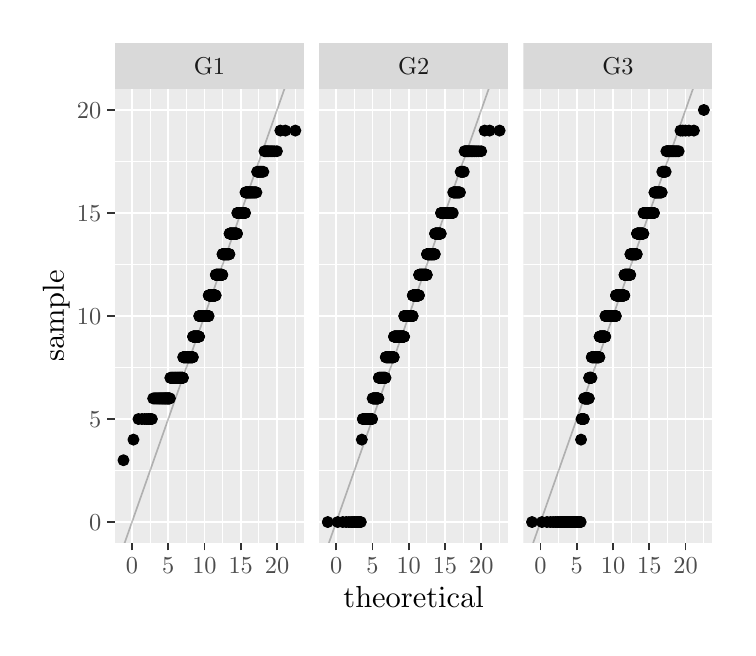
\begin{tikzpicture}[x=1pt,y=1pt]
\definecolor{fillColor}{RGB}{255,255,255}
\path[use as bounding box,fill=fillColor,fill opacity=0.00] (0,0) rectangle (252.94,216.81);
\begin{scope}
\path[clip] (  0.00,  0.00) rectangle (252.94,216.81);
\definecolor{drawColor}{RGB}{255,255,255}
\definecolor{fillColor}{RGB}{255,255,255}

\path[draw=drawColor,line width= 0.6pt,line join=round,line cap=round,fill=fillColor] (  0.00,  0.00) rectangle (252.94,216.81);
\end{scope}
\begin{scope}
\path[clip] ( 31.52, 30.72) rectangle ( 99.83,194.51);
\definecolor{fillColor}{gray}{0.92}

\path[fill=fillColor] ( 31.52, 30.72) rectangle ( 99.83,194.51);
\definecolor{drawColor}{RGB}{255,255,255}

\path[draw=drawColor,line width= 0.3pt,line join=round] ( 31.52, 56.78) --
	( 99.83, 56.78);

\path[draw=drawColor,line width= 0.3pt,line join=round] ( 31.52, 94.00) --
	( 99.83, 94.00);

\path[draw=drawColor,line width= 0.3pt,line join=round] ( 31.52,131.23) --
	( 99.83,131.23);

\path[draw=drawColor,line width= 0.3pt,line join=round] ( 31.52,168.45) --
	( 99.83,168.45);

\path[draw=drawColor,line width= 0.3pt,line join=round] ( 44.24, 30.72) --
	( 44.24,194.51);

\path[draw=drawColor,line width= 0.3pt,line join=round] ( 57.34, 30.72) --
	( 57.34,194.51);

\path[draw=drawColor,line width= 0.3pt,line join=round] ( 70.44, 30.72) --
	( 70.44,194.51);

\path[draw=drawColor,line width= 0.3pt,line join=round] ( 83.54, 30.72) --
	( 83.54,194.51);

\path[draw=drawColor,line width= 0.3pt,line join=round] ( 96.65, 30.72) --
	( 96.65,194.51);

\path[draw=drawColor,line width= 0.6pt,line join=round] ( 31.52, 38.17) --
	( 99.83, 38.17);

\path[draw=drawColor,line width= 0.6pt,line join=round] ( 31.52, 75.39) --
	( 99.83, 75.39);

\path[draw=drawColor,line width= 0.6pt,line join=round] ( 31.52,112.61) --
	( 99.83,112.61);

\path[draw=drawColor,line width= 0.6pt,line join=round] ( 31.52,149.84) --
	( 99.83,149.84);

\path[draw=drawColor,line width= 0.6pt,line join=round] ( 31.52,187.06) --
	( 99.83,187.06);

\path[draw=drawColor,line width= 0.6pt,line join=round] ( 37.69, 30.72) --
	( 37.69,194.51);

\path[draw=drawColor,line width= 0.6pt,line join=round] ( 50.79, 30.72) --
	( 50.79,194.51);

\path[draw=drawColor,line width= 0.6pt,line join=round] ( 63.89, 30.72) --
	( 63.89,194.51);

\path[draw=drawColor,line width= 0.6pt,line join=round] ( 76.99, 30.72) --
	( 76.99,194.51);

\path[draw=drawColor,line width= 0.6pt,line join=round] ( 90.10, 30.72) --
	( 90.10,194.51);
\definecolor{drawColor}{RGB}{0,0,0}
\definecolor{fillColor}{RGB}{0,0,0}

\path[draw=drawColor,line width= 0.4pt,line join=round,line cap=round,fill=fillColor] ( 34.62, 60.50) circle (  1.96);

\path[draw=drawColor,line width= 0.4pt,line join=round,line cap=round,fill=fillColor] ( 38.22, 67.95) circle (  1.96);

\path[draw=drawColor,line width= 0.4pt,line join=round,line cap=round,fill=fillColor] ( 40.03, 75.39) circle (  1.96);

\path[draw=drawColor,line width= 0.4pt,line join=round,line cap=round,fill=fillColor] ( 41.29, 75.39) circle (  1.96);

\path[draw=drawColor,line width= 0.4pt,line join=round,line cap=round,fill=fillColor] ( 42.26, 75.39) circle (  1.96);

\path[draw=drawColor,line width= 0.4pt,line join=round,line cap=round,fill=fillColor] ( 43.06, 75.39) circle (  1.96);

\path[draw=drawColor,line width= 0.4pt,line join=round,line cap=round,fill=fillColor] ( 43.74, 75.39) circle (  1.96);

\path[draw=drawColor,line width= 0.4pt,line join=round,line cap=round,fill=fillColor] ( 44.33, 75.39) circle (  1.96);

\path[draw=drawColor,line width= 0.4pt,line join=round,line cap=round,fill=fillColor] ( 44.87, 75.39) circle (  1.96);

\path[draw=drawColor,line width= 0.4pt,line join=round,line cap=round,fill=fillColor] ( 45.35, 82.84) circle (  1.96);

\path[draw=drawColor,line width= 0.4pt,line join=round,line cap=round,fill=fillColor] ( 45.79, 82.84) circle (  1.96);

\path[draw=drawColor,line width= 0.4pt,line join=round,line cap=round,fill=fillColor] ( 46.20, 82.84) circle (  1.96);

\path[draw=drawColor,line width= 0.4pt,line join=round,line cap=round,fill=fillColor] ( 46.58, 82.84) circle (  1.96);

\path[draw=drawColor,line width= 0.4pt,line join=round,line cap=round,fill=fillColor] ( 46.93, 82.84) circle (  1.96);

\path[draw=drawColor,line width= 0.4pt,line join=round,line cap=round,fill=fillColor] ( 47.26, 82.84) circle (  1.96);

\path[draw=drawColor,line width= 0.4pt,line join=round,line cap=round,fill=fillColor] ( 47.58, 82.84) circle (  1.96);

\path[draw=drawColor,line width= 0.4pt,line join=round,line cap=round,fill=fillColor] ( 47.88, 82.84) circle (  1.96);

\path[draw=drawColor,line width= 0.4pt,line join=round,line cap=round,fill=fillColor] ( 48.16, 82.84) circle (  1.96);

\path[draw=drawColor,line width= 0.4pt,line join=round,line cap=round,fill=fillColor] ( 48.43, 82.84) circle (  1.96);

\path[draw=drawColor,line width= 0.4pt,line join=round,line cap=round,fill=fillColor] ( 48.70, 82.84) circle (  1.96);

\path[draw=drawColor,line width= 0.4pt,line join=round,line cap=round,fill=fillColor] ( 48.94, 82.84) circle (  1.96);

\path[draw=drawColor,line width= 0.4pt,line join=round,line cap=round,fill=fillColor] ( 49.19, 82.84) circle (  1.96);

\path[draw=drawColor,line width= 0.4pt,line join=round,line cap=round,fill=fillColor] ( 49.42, 82.84) circle (  1.96);

\path[draw=drawColor,line width= 0.4pt,line join=round,line cap=round,fill=fillColor] ( 49.64, 82.84) circle (  1.96);

\path[draw=drawColor,line width= 0.4pt,line join=round,line cap=round,fill=fillColor] ( 49.86, 82.84) circle (  1.96);

\path[draw=drawColor,line width= 0.4pt,line join=round,line cap=round,fill=fillColor] ( 50.07, 82.84) circle (  1.96);

\path[draw=drawColor,line width= 0.4pt,line join=round,line cap=round,fill=fillColor] ( 50.27, 82.84) circle (  1.96);

\path[draw=drawColor,line width= 0.4pt,line join=round,line cap=round,fill=fillColor] ( 50.47, 82.84) circle (  1.96);

\path[draw=drawColor,line width= 0.4pt,line join=round,line cap=round,fill=fillColor] ( 50.66, 82.84) circle (  1.96);

\path[draw=drawColor,line width= 0.4pt,line join=round,line cap=round,fill=fillColor] ( 50.85, 82.84) circle (  1.96);

\path[draw=drawColor,line width= 0.4pt,line join=round,line cap=round,fill=fillColor] ( 51.03, 82.84) circle (  1.96);

\path[draw=drawColor,line width= 0.4pt,line join=round,line cap=round,fill=fillColor] ( 51.21, 82.84) circle (  1.96);

\path[draw=drawColor,line width= 0.4pt,line join=round,line cap=round,fill=fillColor] ( 51.38, 82.84) circle (  1.96);

\path[draw=drawColor,line width= 0.4pt,line join=round,line cap=round,fill=fillColor] ( 51.55, 90.28) circle (  1.96);

\path[draw=drawColor,line width= 0.4pt,line join=round,line cap=round,fill=fillColor] ( 51.72, 90.28) circle (  1.96);

\path[draw=drawColor,line width= 0.4pt,line join=round,line cap=round,fill=fillColor] ( 51.88, 90.28) circle (  1.96);

\path[draw=drawColor,line width= 0.4pt,line join=round,line cap=round,fill=fillColor] ( 52.04, 90.28) circle (  1.96);

\path[draw=drawColor,line width= 0.4pt,line join=round,line cap=round,fill=fillColor] ( 52.19, 90.28) circle (  1.96);

\path[draw=drawColor,line width= 0.4pt,line join=round,line cap=round,fill=fillColor] ( 52.34, 90.28) circle (  1.96);

\path[draw=drawColor,line width= 0.4pt,line join=round,line cap=round,fill=fillColor] ( 52.49, 90.28) circle (  1.96);

\path[draw=drawColor,line width= 0.4pt,line join=round,line cap=round,fill=fillColor] ( 52.64, 90.28) circle (  1.96);

\path[draw=drawColor,line width= 0.4pt,line join=round,line cap=round,fill=fillColor] ( 52.79, 90.28) circle (  1.96);

\path[draw=drawColor,line width= 0.4pt,line join=round,line cap=round,fill=fillColor] ( 52.93, 90.28) circle (  1.96);

\path[draw=drawColor,line width= 0.4pt,line join=round,line cap=round,fill=fillColor] ( 53.07, 90.28) circle (  1.96);

\path[draw=drawColor,line width= 0.4pt,line join=round,line cap=round,fill=fillColor] ( 53.20, 90.28) circle (  1.96);

\path[draw=drawColor,line width= 0.4pt,line join=round,line cap=round,fill=fillColor] ( 53.34, 90.28) circle (  1.96);

\path[draw=drawColor,line width= 0.4pt,line join=round,line cap=round,fill=fillColor] ( 53.47, 90.28) circle (  1.96);

\path[draw=drawColor,line width= 0.4pt,line join=round,line cap=round,fill=fillColor] ( 53.60, 90.28) circle (  1.96);

\path[draw=drawColor,line width= 0.4pt,line join=round,line cap=round,fill=fillColor] ( 53.73, 90.28) circle (  1.96);

\path[draw=drawColor,line width= 0.4pt,line join=round,line cap=round,fill=fillColor] ( 53.86, 90.28) circle (  1.96);

\path[draw=drawColor,line width= 0.4pt,line join=round,line cap=round,fill=fillColor] ( 53.98, 90.28) circle (  1.96);

\path[draw=drawColor,line width= 0.4pt,line join=round,line cap=round,fill=fillColor] ( 54.11, 90.28) circle (  1.96);

\path[draw=drawColor,line width= 0.4pt,line join=round,line cap=round,fill=fillColor] ( 54.23, 90.28) circle (  1.96);

\path[draw=drawColor,line width= 0.4pt,line join=round,line cap=round,fill=fillColor] ( 54.35, 90.28) circle (  1.96);

\path[draw=drawColor,line width= 0.4pt,line join=round,line cap=round,fill=fillColor] ( 54.47, 90.28) circle (  1.96);

\path[draw=drawColor,line width= 0.4pt,line join=round,line cap=round,fill=fillColor] ( 54.59, 90.28) circle (  1.96);

\path[draw=drawColor,line width= 0.4pt,line join=round,line cap=round,fill=fillColor] ( 54.70, 90.28) circle (  1.96);

\path[draw=drawColor,line width= 0.4pt,line join=round,line cap=round,fill=fillColor] ( 54.82, 90.28) circle (  1.96);

\path[draw=drawColor,line width= 0.4pt,line join=round,line cap=round,fill=fillColor] ( 54.93, 90.28) circle (  1.96);

\path[draw=drawColor,line width= 0.4pt,line join=round,line cap=round,fill=fillColor] ( 55.04, 90.28) circle (  1.96);

\path[draw=drawColor,line width= 0.4pt,line join=round,line cap=round,fill=fillColor] ( 55.15, 90.28) circle (  1.96);

\path[draw=drawColor,line width= 0.4pt,line join=round,line cap=round,fill=fillColor] ( 55.26, 90.28) circle (  1.96);

\path[draw=drawColor,line width= 0.4pt,line join=round,line cap=round,fill=fillColor] ( 55.37, 90.28) circle (  1.96);

\path[draw=drawColor,line width= 0.4pt,line join=round,line cap=round,fill=fillColor] ( 55.48, 90.28) circle (  1.96);

\path[draw=drawColor,line width= 0.4pt,line join=round,line cap=round,fill=fillColor] ( 55.58, 90.28) circle (  1.96);

\path[draw=drawColor,line width= 0.4pt,line join=round,line cap=round,fill=fillColor] ( 55.69, 90.28) circle (  1.96);

\path[draw=drawColor,line width= 0.4pt,line join=round,line cap=round,fill=fillColor] ( 55.79, 90.28) circle (  1.96);

\path[draw=drawColor,line width= 0.4pt,line join=round,line cap=round,fill=fillColor] ( 55.90, 90.28) circle (  1.96);

\path[draw=drawColor,line width= 0.4pt,line join=round,line cap=round,fill=fillColor] ( 56.00, 90.28) circle (  1.96);

\path[draw=drawColor,line width= 0.4pt,line join=round,line cap=round,fill=fillColor] ( 56.10, 90.28) circle (  1.96);

\path[draw=drawColor,line width= 0.4pt,line join=round,line cap=round,fill=fillColor] ( 56.20, 97.73) circle (  1.96);

\path[draw=drawColor,line width= 0.4pt,line join=round,line cap=round,fill=fillColor] ( 56.30, 97.73) circle (  1.96);

\path[draw=drawColor,line width= 0.4pt,line join=round,line cap=round,fill=fillColor] ( 56.40, 97.73) circle (  1.96);

\path[draw=drawColor,line width= 0.4pt,line join=round,line cap=round,fill=fillColor] ( 56.50, 97.73) circle (  1.96);

\path[draw=drawColor,line width= 0.4pt,line join=round,line cap=round,fill=fillColor] ( 56.59, 97.73) circle (  1.96);

\path[draw=drawColor,line width= 0.4pt,line join=round,line cap=round,fill=fillColor] ( 56.69, 97.73) circle (  1.96);

\path[draw=drawColor,line width= 0.4pt,line join=round,line cap=round,fill=fillColor] ( 56.78, 97.73) circle (  1.96);

\path[draw=drawColor,line width= 0.4pt,line join=round,line cap=round,fill=fillColor] ( 56.88, 97.73) circle (  1.96);

\path[draw=drawColor,line width= 0.4pt,line join=round,line cap=round,fill=fillColor] ( 56.97, 97.73) circle (  1.96);

\path[draw=drawColor,line width= 0.4pt,line join=round,line cap=round,fill=fillColor] ( 57.06, 97.73) circle (  1.96);

\path[draw=drawColor,line width= 0.4pt,line join=round,line cap=round,fill=fillColor] ( 57.16, 97.73) circle (  1.96);

\path[draw=drawColor,line width= 0.4pt,line join=round,line cap=round,fill=fillColor] ( 57.25, 97.73) circle (  1.96);

\path[draw=drawColor,line width= 0.4pt,line join=round,line cap=round,fill=fillColor] ( 57.34, 97.73) circle (  1.96);

\path[draw=drawColor,line width= 0.4pt,line join=round,line cap=round,fill=fillColor] ( 57.43, 97.73) circle (  1.96);

\path[draw=drawColor,line width= 0.4pt,line join=round,line cap=round,fill=fillColor] ( 57.52, 97.73) circle (  1.96);

\path[draw=drawColor,line width= 0.4pt,line join=round,line cap=round,fill=fillColor] ( 57.61, 97.73) circle (  1.96);

\path[draw=drawColor,line width= 0.4pt,line join=round,line cap=round,fill=fillColor] ( 57.70, 97.73) circle (  1.96);

\path[draw=drawColor,line width= 0.4pt,line join=round,line cap=round,fill=fillColor] ( 57.78, 97.73) circle (  1.96);

\path[draw=drawColor,line width= 0.4pt,line join=round,line cap=round,fill=fillColor] ( 57.87, 97.73) circle (  1.96);

\path[draw=drawColor,line width= 0.4pt,line join=round,line cap=round,fill=fillColor] ( 57.96, 97.73) circle (  1.96);

\path[draw=drawColor,line width= 0.4pt,line join=round,line cap=round,fill=fillColor] ( 58.04, 97.73) circle (  1.96);

\path[draw=drawColor,line width= 0.4pt,line join=round,line cap=round,fill=fillColor] ( 58.13, 97.73) circle (  1.96);

\path[draw=drawColor,line width= 0.4pt,line join=round,line cap=round,fill=fillColor] ( 58.22, 97.73) circle (  1.96);

\path[draw=drawColor,line width= 0.4pt,line join=round,line cap=round,fill=fillColor] ( 58.30, 97.73) circle (  1.96);

\path[draw=drawColor,line width= 0.4pt,line join=round,line cap=round,fill=fillColor] ( 58.38, 97.73) circle (  1.96);

\path[draw=drawColor,line width= 0.4pt,line join=round,line cap=round,fill=fillColor] ( 58.47, 97.73) circle (  1.96);

\path[draw=drawColor,line width= 0.4pt,line join=round,line cap=round,fill=fillColor] ( 58.55, 97.73) circle (  1.96);

\path[draw=drawColor,line width= 0.4pt,line join=round,line cap=round,fill=fillColor] ( 58.63, 97.73) circle (  1.96);

\path[draw=drawColor,line width= 0.4pt,line join=round,line cap=round,fill=fillColor] ( 58.72, 97.73) circle (  1.96);

\path[draw=drawColor,line width= 0.4pt,line join=round,line cap=round,fill=fillColor] ( 58.80, 97.73) circle (  1.96);

\path[draw=drawColor,line width= 0.4pt,line join=round,line cap=round,fill=fillColor] ( 58.88, 97.73) circle (  1.96);

\path[draw=drawColor,line width= 0.4pt,line join=round,line cap=round,fill=fillColor] ( 58.96, 97.73) circle (  1.96);

\path[draw=drawColor,line width= 0.4pt,line join=round,line cap=round,fill=fillColor] ( 59.04, 97.73) circle (  1.96);

\path[draw=drawColor,line width= 0.4pt,line join=round,line cap=round,fill=fillColor] ( 59.12, 97.73) circle (  1.96);

\path[draw=drawColor,line width= 0.4pt,line join=round,line cap=round,fill=fillColor] ( 59.20, 97.73) circle (  1.96);

\path[draw=drawColor,line width= 0.4pt,line join=round,line cap=round,fill=fillColor] ( 59.28, 97.73) circle (  1.96);

\path[draw=drawColor,line width= 0.4pt,line join=round,line cap=round,fill=fillColor] ( 59.36, 97.73) circle (  1.96);

\path[draw=drawColor,line width= 0.4pt,line join=round,line cap=round,fill=fillColor] ( 59.44, 97.73) circle (  1.96);

\path[draw=drawColor,line width= 0.4pt,line join=round,line cap=round,fill=fillColor] ( 59.52, 97.73) circle (  1.96);

\path[draw=drawColor,line width= 0.4pt,line join=round,line cap=round,fill=fillColor] ( 59.59, 97.73) circle (  1.96);

\path[draw=drawColor,line width= 0.4pt,line join=round,line cap=round,fill=fillColor] ( 59.67, 97.73) circle (  1.96);

\path[draw=drawColor,line width= 0.4pt,line join=round,line cap=round,fill=fillColor] ( 59.75,105.17) circle (  1.96);

\path[draw=drawColor,line width= 0.4pt,line join=round,line cap=round,fill=fillColor] ( 59.83,105.17) circle (  1.96);

\path[draw=drawColor,line width= 0.4pt,line join=round,line cap=round,fill=fillColor] ( 59.90,105.17) circle (  1.96);

\path[draw=drawColor,line width= 0.4pt,line join=round,line cap=round,fill=fillColor] ( 59.98,105.17) circle (  1.96);

\path[draw=drawColor,line width= 0.4pt,line join=round,line cap=round,fill=fillColor] ( 60.05,105.17) circle (  1.96);

\path[draw=drawColor,line width= 0.4pt,line join=round,line cap=round,fill=fillColor] ( 60.13,105.17) circle (  1.96);

\path[draw=drawColor,line width= 0.4pt,line join=round,line cap=round,fill=fillColor] ( 60.20,105.17) circle (  1.96);

\path[draw=drawColor,line width= 0.4pt,line join=round,line cap=round,fill=fillColor] ( 60.28,105.17) circle (  1.96);

\path[draw=drawColor,line width= 0.4pt,line join=round,line cap=round,fill=fillColor] ( 60.35,105.17) circle (  1.96);

\path[draw=drawColor,line width= 0.4pt,line join=round,line cap=round,fill=fillColor] ( 60.43,105.17) circle (  1.96);

\path[draw=drawColor,line width= 0.4pt,line join=round,line cap=round,fill=fillColor] ( 60.50,105.17) circle (  1.96);

\path[draw=drawColor,line width= 0.4pt,line join=round,line cap=round,fill=fillColor] ( 60.58,105.17) circle (  1.96);

\path[draw=drawColor,line width= 0.4pt,line join=round,line cap=round,fill=fillColor] ( 60.65,105.17) circle (  1.96);

\path[draw=drawColor,line width= 0.4pt,line join=round,line cap=round,fill=fillColor] ( 60.72,105.17) circle (  1.96);

\path[draw=drawColor,line width= 0.4pt,line join=round,line cap=round,fill=fillColor] ( 60.80,105.17) circle (  1.96);

\path[draw=drawColor,line width= 0.4pt,line join=round,line cap=round,fill=fillColor] ( 60.87,105.17) circle (  1.96);

\path[draw=drawColor,line width= 0.4pt,line join=round,line cap=round,fill=fillColor] ( 60.94,105.17) circle (  1.96);

\path[draw=drawColor,line width= 0.4pt,line join=round,line cap=round,fill=fillColor] ( 61.02,105.17) circle (  1.96);

\path[draw=drawColor,line width= 0.4pt,line join=round,line cap=round,fill=fillColor] ( 61.09,105.17) circle (  1.96);

\path[draw=drawColor,line width= 0.4pt,line join=round,line cap=round,fill=fillColor] ( 61.16,105.17) circle (  1.96);

\path[draw=drawColor,line width= 0.4pt,line join=round,line cap=round,fill=fillColor] ( 61.23,105.17) circle (  1.96);

\path[draw=drawColor,line width= 0.4pt,line join=round,line cap=round,fill=fillColor] ( 61.30,105.17) circle (  1.96);

\path[draw=drawColor,line width= 0.4pt,line join=round,line cap=round,fill=fillColor] ( 61.37,105.17) circle (  1.96);

\path[draw=drawColor,line width= 0.4pt,line join=round,line cap=round,fill=fillColor] ( 61.45,105.17) circle (  1.96);

\path[draw=drawColor,line width= 0.4pt,line join=round,line cap=round,fill=fillColor] ( 61.52,105.17) circle (  1.96);

\path[draw=drawColor,line width= 0.4pt,line join=round,line cap=round,fill=fillColor] ( 61.59,105.17) circle (  1.96);

\path[draw=drawColor,line width= 0.4pt,line join=round,line cap=round,fill=fillColor] ( 61.66,105.17) circle (  1.96);

\path[draw=drawColor,line width= 0.4pt,line join=round,line cap=round,fill=fillColor] ( 61.73,105.17) circle (  1.96);

\path[draw=drawColor,line width= 0.4pt,line join=round,line cap=round,fill=fillColor] ( 61.80,105.17) circle (  1.96);

\path[draw=drawColor,line width= 0.4pt,line join=round,line cap=round,fill=fillColor] ( 61.87,105.17) circle (  1.96);

\path[draw=drawColor,line width= 0.4pt,line join=round,line cap=round,fill=fillColor] ( 61.94,105.17) circle (  1.96);

\path[draw=drawColor,line width= 0.4pt,line join=round,line cap=round,fill=fillColor] ( 62.01,112.61) circle (  1.96);

\path[draw=drawColor,line width= 0.4pt,line join=round,line cap=round,fill=fillColor] ( 62.08,112.61) circle (  1.96);

\path[draw=drawColor,line width= 0.4pt,line join=round,line cap=round,fill=fillColor] ( 62.15,112.61) circle (  1.96);

\path[draw=drawColor,line width= 0.4pt,line join=round,line cap=round,fill=fillColor] ( 62.22,112.61) circle (  1.96);

\path[draw=drawColor,line width= 0.4pt,line join=round,line cap=round,fill=fillColor] ( 62.28,112.61) circle (  1.96);

\path[draw=drawColor,line width= 0.4pt,line join=round,line cap=round,fill=fillColor] ( 62.35,112.61) circle (  1.96);

\path[draw=drawColor,line width= 0.4pt,line join=round,line cap=round,fill=fillColor] ( 62.42,112.61) circle (  1.96);

\path[draw=drawColor,line width= 0.4pt,line join=round,line cap=round,fill=fillColor] ( 62.49,112.61) circle (  1.96);

\path[draw=drawColor,line width= 0.4pt,line join=round,line cap=round,fill=fillColor] ( 62.56,112.61) circle (  1.96);

\path[draw=drawColor,line width= 0.4pt,line join=round,line cap=round,fill=fillColor] ( 62.63,112.61) circle (  1.96);

\path[draw=drawColor,line width= 0.4pt,line join=round,line cap=round,fill=fillColor] ( 62.69,112.61) circle (  1.96);

\path[draw=drawColor,line width= 0.4pt,line join=round,line cap=round,fill=fillColor] ( 62.76,112.61) circle (  1.96);

\path[draw=drawColor,line width= 0.4pt,line join=round,line cap=round,fill=fillColor] ( 62.83,112.61) circle (  1.96);

\path[draw=drawColor,line width= 0.4pt,line join=round,line cap=round,fill=fillColor] ( 62.90,112.61) circle (  1.96);

\path[draw=drawColor,line width= 0.4pt,line join=round,line cap=round,fill=fillColor] ( 62.97,112.61) circle (  1.96);

\path[draw=drawColor,line width= 0.4pt,line join=round,line cap=round,fill=fillColor] ( 63.03,112.61) circle (  1.96);

\path[draw=drawColor,line width= 0.4pt,line join=round,line cap=round,fill=fillColor] ( 63.10,112.61) circle (  1.96);

\path[draw=drawColor,line width= 0.4pt,line join=round,line cap=round,fill=fillColor] ( 63.17,112.61) circle (  1.96);

\path[draw=drawColor,line width= 0.4pt,line join=round,line cap=round,fill=fillColor] ( 63.24,112.61) circle (  1.96);

\path[draw=drawColor,line width= 0.4pt,line join=round,line cap=round,fill=fillColor] ( 63.30,112.61) circle (  1.96);

\path[draw=drawColor,line width= 0.4pt,line join=round,line cap=round,fill=fillColor] ( 63.37,112.61) circle (  1.96);

\path[draw=drawColor,line width= 0.4pt,line join=round,line cap=round,fill=fillColor] ( 63.44,112.61) circle (  1.96);

\path[draw=drawColor,line width= 0.4pt,line join=round,line cap=round,fill=fillColor] ( 63.50,112.61) circle (  1.96);

\path[draw=drawColor,line width= 0.4pt,line join=round,line cap=round,fill=fillColor] ( 63.57,112.61) circle (  1.96);

\path[draw=drawColor,line width= 0.4pt,line join=round,line cap=round,fill=fillColor] ( 63.64,112.61) circle (  1.96);

\path[draw=drawColor,line width= 0.4pt,line join=round,line cap=round,fill=fillColor] ( 63.70,112.61) circle (  1.96);

\path[draw=drawColor,line width= 0.4pt,line join=round,line cap=round,fill=fillColor] ( 63.77,112.61) circle (  1.96);

\path[draw=drawColor,line width= 0.4pt,line join=round,line cap=round,fill=fillColor] ( 63.84,112.61) circle (  1.96);

\path[draw=drawColor,line width= 0.4pt,line join=round,line cap=round,fill=fillColor] ( 63.90,112.61) circle (  1.96);

\path[draw=drawColor,line width= 0.4pt,line join=round,line cap=round,fill=fillColor] ( 63.97,112.61) circle (  1.96);

\path[draw=drawColor,line width= 0.4pt,line join=round,line cap=round,fill=fillColor] ( 64.03,112.61) circle (  1.96);

\path[draw=drawColor,line width= 0.4pt,line join=round,line cap=round,fill=fillColor] ( 64.10,112.61) circle (  1.96);

\path[draw=drawColor,line width= 0.4pt,line join=round,line cap=round,fill=fillColor] ( 64.17,112.61) circle (  1.96);

\path[draw=drawColor,line width= 0.4pt,line join=round,line cap=round,fill=fillColor] ( 64.23,112.61) circle (  1.96);

\path[draw=drawColor,line width= 0.4pt,line join=round,line cap=round,fill=fillColor] ( 64.30,112.61) circle (  1.96);

\path[draw=drawColor,line width= 0.4pt,line join=round,line cap=round,fill=fillColor] ( 64.36,112.61) circle (  1.96);

\path[draw=drawColor,line width= 0.4pt,line join=round,line cap=round,fill=fillColor] ( 64.43,112.61) circle (  1.96);

\path[draw=drawColor,line width= 0.4pt,line join=round,line cap=round,fill=fillColor] ( 64.50,112.61) circle (  1.96);

\path[draw=drawColor,line width= 0.4pt,line join=round,line cap=round,fill=fillColor] ( 64.56,112.61) circle (  1.96);

\path[draw=drawColor,line width= 0.4pt,line join=round,line cap=round,fill=fillColor] ( 64.63,112.61) circle (  1.96);

\path[draw=drawColor,line width= 0.4pt,line join=round,line cap=round,fill=fillColor] ( 64.69,112.61) circle (  1.96);

\path[draw=drawColor,line width= 0.4pt,line join=round,line cap=round,fill=fillColor] ( 64.76,112.61) circle (  1.96);

\path[draw=drawColor,line width= 0.4pt,line join=round,line cap=round,fill=fillColor] ( 64.82,112.61) circle (  1.96);

\path[draw=drawColor,line width= 0.4pt,line join=round,line cap=round,fill=fillColor] ( 64.89,112.61) circle (  1.96);

\path[draw=drawColor,line width= 0.4pt,line join=round,line cap=round,fill=fillColor] ( 64.95,112.61) circle (  1.96);

\path[draw=drawColor,line width= 0.4pt,line join=round,line cap=round,fill=fillColor] ( 65.02,112.61) circle (  1.96);

\path[draw=drawColor,line width= 0.4pt,line join=round,line cap=round,fill=fillColor] ( 65.08,112.61) circle (  1.96);

\path[draw=drawColor,line width= 0.4pt,line join=round,line cap=round,fill=fillColor] ( 65.15,112.61) circle (  1.96);

\path[draw=drawColor,line width= 0.4pt,line join=round,line cap=round,fill=fillColor] ( 65.22,112.61) circle (  1.96);

\path[draw=drawColor,line width= 0.4pt,line join=round,line cap=round,fill=fillColor] ( 65.28,112.61) circle (  1.96);

\path[draw=drawColor,line width= 0.4pt,line join=round,line cap=round,fill=fillColor] ( 65.35,112.61) circle (  1.96);

\path[draw=drawColor,line width= 0.4pt,line join=round,line cap=round,fill=fillColor] ( 65.41,120.06) circle (  1.96);

\path[draw=drawColor,line width= 0.4pt,line join=round,line cap=round,fill=fillColor] ( 65.48,120.06) circle (  1.96);

\path[draw=drawColor,line width= 0.4pt,line join=round,line cap=round,fill=fillColor] ( 65.54,120.06) circle (  1.96);

\path[draw=drawColor,line width= 0.4pt,line join=round,line cap=round,fill=fillColor] ( 65.61,120.06) circle (  1.96);

\path[draw=drawColor,line width= 0.4pt,line join=round,line cap=round,fill=fillColor] ( 65.67,120.06) circle (  1.96);

\path[draw=drawColor,line width= 0.4pt,line join=round,line cap=round,fill=fillColor] ( 65.74,120.06) circle (  1.96);

\path[draw=drawColor,line width= 0.4pt,line join=round,line cap=round,fill=fillColor] ( 65.80,120.06) circle (  1.96);

\path[draw=drawColor,line width= 0.4pt,line join=round,line cap=round,fill=fillColor] ( 65.87,120.06) circle (  1.96);

\path[draw=drawColor,line width= 0.4pt,line join=round,line cap=round,fill=fillColor] ( 65.93,120.06) circle (  1.96);

\path[draw=drawColor,line width= 0.4pt,line join=round,line cap=round,fill=fillColor] ( 66.00,120.06) circle (  1.96);

\path[draw=drawColor,line width= 0.4pt,line join=round,line cap=round,fill=fillColor] ( 66.06,120.06) circle (  1.96);

\path[draw=drawColor,line width= 0.4pt,line join=round,line cap=round,fill=fillColor] ( 66.13,120.06) circle (  1.96);

\path[draw=drawColor,line width= 0.4pt,line join=round,line cap=round,fill=fillColor] ( 66.19,120.06) circle (  1.96);

\path[draw=drawColor,line width= 0.4pt,line join=round,line cap=round,fill=fillColor] ( 66.26,120.06) circle (  1.96);

\path[draw=drawColor,line width= 0.4pt,line join=round,line cap=round,fill=fillColor] ( 66.33,120.06) circle (  1.96);

\path[draw=drawColor,line width= 0.4pt,line join=round,line cap=round,fill=fillColor] ( 66.39,120.06) circle (  1.96);

\path[draw=drawColor,line width= 0.4pt,line join=round,line cap=round,fill=fillColor] ( 66.46,120.06) circle (  1.96);

\path[draw=drawColor,line width= 0.4pt,line join=round,line cap=round,fill=fillColor] ( 66.52,120.06) circle (  1.96);

\path[draw=drawColor,line width= 0.4pt,line join=round,line cap=round,fill=fillColor] ( 66.59,120.06) circle (  1.96);

\path[draw=drawColor,line width= 0.4pt,line join=round,line cap=round,fill=fillColor] ( 66.65,120.06) circle (  1.96);

\path[draw=drawColor,line width= 0.4pt,line join=round,line cap=round,fill=fillColor] ( 66.72,120.06) circle (  1.96);

\path[draw=drawColor,line width= 0.4pt,line join=round,line cap=round,fill=fillColor] ( 66.78,120.06) circle (  1.96);

\path[draw=drawColor,line width= 0.4pt,line join=round,line cap=round,fill=fillColor] ( 66.85,120.06) circle (  1.96);

\path[draw=drawColor,line width= 0.4pt,line join=round,line cap=round,fill=fillColor] ( 66.92,120.06) circle (  1.96);

\path[draw=drawColor,line width= 0.4pt,line join=round,line cap=round,fill=fillColor] ( 66.98,120.06) circle (  1.96);

\path[draw=drawColor,line width= 0.4pt,line join=round,line cap=round,fill=fillColor] ( 67.05,120.06) circle (  1.96);

\path[draw=drawColor,line width= 0.4pt,line join=round,line cap=round,fill=fillColor] ( 67.11,120.06) circle (  1.96);

\path[draw=drawColor,line width= 0.4pt,line join=round,line cap=round,fill=fillColor] ( 67.18,120.06) circle (  1.96);

\path[draw=drawColor,line width= 0.4pt,line join=round,line cap=round,fill=fillColor] ( 67.24,120.06) circle (  1.96);

\path[draw=drawColor,line width= 0.4pt,line join=round,line cap=round,fill=fillColor] ( 67.31,120.06) circle (  1.96);

\path[draw=drawColor,line width= 0.4pt,line join=round,line cap=round,fill=fillColor] ( 67.38,120.06) circle (  1.96);

\path[draw=drawColor,line width= 0.4pt,line join=round,line cap=round,fill=fillColor] ( 67.44,120.06) circle (  1.96);

\path[draw=drawColor,line width= 0.4pt,line join=round,line cap=round,fill=fillColor] ( 67.51,120.06) circle (  1.96);

\path[draw=drawColor,line width= 0.4pt,line join=round,line cap=round,fill=fillColor] ( 67.58,120.06) circle (  1.96);

\path[draw=drawColor,line width= 0.4pt,line join=round,line cap=round,fill=fillColor] ( 67.64,120.06) circle (  1.96);

\path[draw=drawColor,line width= 0.4pt,line join=round,line cap=round,fill=fillColor] ( 67.71,120.06) circle (  1.96);

\path[draw=drawColor,line width= 0.4pt,line join=round,line cap=round,fill=fillColor] ( 67.78,120.06) circle (  1.96);

\path[draw=drawColor,line width= 0.4pt,line join=round,line cap=round,fill=fillColor] ( 67.84,120.06) circle (  1.96);

\path[draw=drawColor,line width= 0.4pt,line join=round,line cap=round,fill=fillColor] ( 67.91,120.06) circle (  1.96);

\path[draw=drawColor,line width= 0.4pt,line join=round,line cap=round,fill=fillColor] ( 67.98,127.50) circle (  1.96);

\path[draw=drawColor,line width= 0.4pt,line join=round,line cap=round,fill=fillColor] ( 68.04,127.50) circle (  1.96);

\path[draw=drawColor,line width= 0.4pt,line join=round,line cap=round,fill=fillColor] ( 68.11,127.50) circle (  1.96);

\path[draw=drawColor,line width= 0.4pt,line join=round,line cap=round,fill=fillColor] ( 68.18,127.50) circle (  1.96);

\path[draw=drawColor,line width= 0.4pt,line join=round,line cap=round,fill=fillColor] ( 68.24,127.50) circle (  1.96);

\path[draw=drawColor,line width= 0.4pt,line join=round,line cap=round,fill=fillColor] ( 68.31,127.50) circle (  1.96);

\path[draw=drawColor,line width= 0.4pt,line join=round,line cap=round,fill=fillColor] ( 68.38,127.50) circle (  1.96);

\path[draw=drawColor,line width= 0.4pt,line join=round,line cap=round,fill=fillColor] ( 68.45,127.50) circle (  1.96);

\path[draw=drawColor,line width= 0.4pt,line join=round,line cap=round,fill=fillColor] ( 68.51,127.50) circle (  1.96);

\path[draw=drawColor,line width= 0.4pt,line join=round,line cap=round,fill=fillColor] ( 68.58,127.50) circle (  1.96);

\path[draw=drawColor,line width= 0.4pt,line join=round,line cap=round,fill=fillColor] ( 68.65,127.50) circle (  1.96);

\path[draw=drawColor,line width= 0.4pt,line join=round,line cap=round,fill=fillColor] ( 68.72,127.50) circle (  1.96);

\path[draw=drawColor,line width= 0.4pt,line join=round,line cap=round,fill=fillColor] ( 68.79,127.50) circle (  1.96);

\path[draw=drawColor,line width= 0.4pt,line join=round,line cap=round,fill=fillColor] ( 68.85,127.50) circle (  1.96);

\path[draw=drawColor,line width= 0.4pt,line join=round,line cap=round,fill=fillColor] ( 68.92,127.50) circle (  1.96);

\path[draw=drawColor,line width= 0.4pt,line join=round,line cap=round,fill=fillColor] ( 68.99,127.50) circle (  1.96);

\path[draw=drawColor,line width= 0.4pt,line join=round,line cap=round,fill=fillColor] ( 69.06,127.50) circle (  1.96);

\path[draw=drawColor,line width= 0.4pt,line join=round,line cap=round,fill=fillColor] ( 69.13,127.50) circle (  1.96);

\path[draw=drawColor,line width= 0.4pt,line join=round,line cap=round,fill=fillColor] ( 69.20,127.50) circle (  1.96);

\path[draw=drawColor,line width= 0.4pt,line join=round,line cap=round,fill=fillColor] ( 69.27,127.50) circle (  1.96);

\path[draw=drawColor,line width= 0.4pt,line join=round,line cap=round,fill=fillColor] ( 69.34,127.50) circle (  1.96);

\path[draw=drawColor,line width= 0.4pt,line join=round,line cap=round,fill=fillColor] ( 69.41,127.50) circle (  1.96);

\path[draw=drawColor,line width= 0.4pt,line join=round,line cap=round,fill=fillColor] ( 69.48,127.50) circle (  1.96);

\path[draw=drawColor,line width= 0.4pt,line join=round,line cap=round,fill=fillColor] ( 69.55,127.50) circle (  1.96);

\path[draw=drawColor,line width= 0.4pt,line join=round,line cap=round,fill=fillColor] ( 69.62,127.50) circle (  1.96);

\path[draw=drawColor,line width= 0.4pt,line join=round,line cap=round,fill=fillColor] ( 69.69,127.50) circle (  1.96);

\path[draw=drawColor,line width= 0.4pt,line join=round,line cap=round,fill=fillColor] ( 69.76,127.50) circle (  1.96);

\path[draw=drawColor,line width= 0.4pt,line join=round,line cap=round,fill=fillColor] ( 69.83,127.50) circle (  1.96);

\path[draw=drawColor,line width= 0.4pt,line join=round,line cap=round,fill=fillColor] ( 69.90,127.50) circle (  1.96);

\path[draw=drawColor,line width= 0.4pt,line join=round,line cap=round,fill=fillColor] ( 69.97,127.50) circle (  1.96);

\path[draw=drawColor,line width= 0.4pt,line join=round,line cap=round,fill=fillColor] ( 70.04,127.50) circle (  1.96);

\path[draw=drawColor,line width= 0.4pt,line join=round,line cap=round,fill=fillColor] ( 70.11,127.50) circle (  1.96);

\path[draw=drawColor,line width= 0.4pt,line join=round,line cap=round,fill=fillColor] ( 70.19,127.50) circle (  1.96);

\path[draw=drawColor,line width= 0.4pt,line join=round,line cap=round,fill=fillColor] ( 70.26,127.50) circle (  1.96);

\path[draw=drawColor,line width= 0.4pt,line join=round,line cap=round,fill=fillColor] ( 70.33,127.50) circle (  1.96);

\path[draw=drawColor,line width= 0.4pt,line join=round,line cap=round,fill=fillColor] ( 70.40,134.95) circle (  1.96);

\path[draw=drawColor,line width= 0.4pt,line join=round,line cap=round,fill=fillColor] ( 70.47,134.95) circle (  1.96);

\path[draw=drawColor,line width= 0.4pt,line join=round,line cap=round,fill=fillColor] ( 70.55,134.95) circle (  1.96);

\path[draw=drawColor,line width= 0.4pt,line join=round,line cap=round,fill=fillColor] ( 70.62,134.95) circle (  1.96);

\path[draw=drawColor,line width= 0.4pt,line join=round,line cap=round,fill=fillColor] ( 70.69,134.95) circle (  1.96);

\path[draw=drawColor,line width= 0.4pt,line join=round,line cap=round,fill=fillColor] ( 70.77,134.95) circle (  1.96);

\path[draw=drawColor,line width= 0.4pt,line join=round,line cap=round,fill=fillColor] ( 70.84,134.95) circle (  1.96);

\path[draw=drawColor,line width= 0.4pt,line join=round,line cap=round,fill=fillColor] ( 70.92,134.95) circle (  1.96);

\path[draw=drawColor,line width= 0.4pt,line join=round,line cap=round,fill=fillColor] ( 70.99,134.95) circle (  1.96);

\path[draw=drawColor,line width= 0.4pt,line join=round,line cap=round,fill=fillColor] ( 71.06,134.95) circle (  1.96);

\path[draw=drawColor,line width= 0.4pt,line join=round,line cap=round,fill=fillColor] ( 71.14,134.95) circle (  1.96);

\path[draw=drawColor,line width= 0.4pt,line join=round,line cap=round,fill=fillColor] ( 71.22,134.95) circle (  1.96);

\path[draw=drawColor,line width= 0.4pt,line join=round,line cap=round,fill=fillColor] ( 71.29,134.95) circle (  1.96);

\path[draw=drawColor,line width= 0.4pt,line join=round,line cap=round,fill=fillColor] ( 71.37,134.95) circle (  1.96);

\path[draw=drawColor,line width= 0.4pt,line join=round,line cap=round,fill=fillColor] ( 71.44,134.95) circle (  1.96);

\path[draw=drawColor,line width= 0.4pt,line join=round,line cap=round,fill=fillColor] ( 71.52,134.95) circle (  1.96);

\path[draw=drawColor,line width= 0.4pt,line join=round,line cap=round,fill=fillColor] ( 71.60,134.95) circle (  1.96);

\path[draw=drawColor,line width= 0.4pt,line join=round,line cap=round,fill=fillColor] ( 71.67,134.95) circle (  1.96);

\path[draw=drawColor,line width= 0.4pt,line join=round,line cap=round,fill=fillColor] ( 71.75,134.95) circle (  1.96);

\path[draw=drawColor,line width= 0.4pt,line join=round,line cap=round,fill=fillColor] ( 71.83,134.95) circle (  1.96);

\path[draw=drawColor,line width= 0.4pt,line join=round,line cap=round,fill=fillColor] ( 71.91,134.95) circle (  1.96);

\path[draw=drawColor,line width= 0.4pt,line join=round,line cap=round,fill=fillColor] ( 71.99,134.95) circle (  1.96);

\path[draw=drawColor,line width= 0.4pt,line join=round,line cap=round,fill=fillColor] ( 72.06,134.95) circle (  1.96);

\path[draw=drawColor,line width= 0.4pt,line join=round,line cap=round,fill=fillColor] ( 72.14,134.95) circle (  1.96);

\path[draw=drawColor,line width= 0.4pt,line join=round,line cap=round,fill=fillColor] ( 72.22,134.95) circle (  1.96);

\path[draw=drawColor,line width= 0.4pt,line join=round,line cap=round,fill=fillColor] ( 72.30,134.95) circle (  1.96);

\path[draw=drawColor,line width= 0.4pt,line join=round,line cap=round,fill=fillColor] ( 72.38,134.95) circle (  1.96);

\path[draw=drawColor,line width= 0.4pt,line join=round,line cap=round,fill=fillColor] ( 72.47,134.95) circle (  1.96);

\path[draw=drawColor,line width= 0.4pt,line join=round,line cap=round,fill=fillColor] ( 72.55,134.95) circle (  1.96);

\path[draw=drawColor,line width= 0.4pt,line join=round,line cap=round,fill=fillColor] ( 72.63,134.95) circle (  1.96);

\path[draw=drawColor,line width= 0.4pt,line join=round,line cap=round,fill=fillColor] ( 72.71,134.95) circle (  1.96);

\path[draw=drawColor,line width= 0.4pt,line join=round,line cap=round,fill=fillColor] ( 72.79,134.95) circle (  1.96);

\path[draw=drawColor,line width= 0.4pt,line join=round,line cap=round,fill=fillColor] ( 72.88,134.95) circle (  1.96);

\path[draw=drawColor,line width= 0.4pt,line join=round,line cap=round,fill=fillColor] ( 72.96,142.39) circle (  1.96);

\path[draw=drawColor,line width= 0.4pt,line join=round,line cap=round,fill=fillColor] ( 73.04,142.39) circle (  1.96);

\path[draw=drawColor,line width= 0.4pt,line join=round,line cap=round,fill=fillColor] ( 73.13,142.39) circle (  1.96);

\path[draw=drawColor,line width= 0.4pt,line join=round,line cap=round,fill=fillColor] ( 73.21,142.39) circle (  1.96);

\path[draw=drawColor,line width= 0.4pt,line join=round,line cap=round,fill=fillColor] ( 73.30,142.39) circle (  1.96);

\path[draw=drawColor,line width= 0.4pt,line join=round,line cap=round,fill=fillColor] ( 73.39,142.39) circle (  1.96);

\path[draw=drawColor,line width= 0.4pt,line join=round,line cap=round,fill=fillColor] ( 73.47,142.39) circle (  1.96);

\path[draw=drawColor,line width= 0.4pt,line join=round,line cap=round,fill=fillColor] ( 73.56,142.39) circle (  1.96);

\path[draw=drawColor,line width= 0.4pt,line join=round,line cap=round,fill=fillColor] ( 73.65,142.39) circle (  1.96);

\path[draw=drawColor,line width= 0.4pt,line join=round,line cap=round,fill=fillColor] ( 73.74,142.39) circle (  1.96);

\path[draw=drawColor,line width= 0.4pt,line join=round,line cap=round,fill=fillColor] ( 73.83,142.39) circle (  1.96);

\path[draw=drawColor,line width= 0.4pt,line join=round,line cap=round,fill=fillColor] ( 73.92,142.39) circle (  1.96);

\path[draw=drawColor,line width= 0.4pt,line join=round,line cap=round,fill=fillColor] ( 74.01,142.39) circle (  1.96);

\path[draw=drawColor,line width= 0.4pt,line join=round,line cap=round,fill=fillColor] ( 74.10,142.39) circle (  1.96);

\path[draw=drawColor,line width= 0.4pt,line join=round,line cap=round,fill=fillColor] ( 74.19,142.39) circle (  1.96);

\path[draw=drawColor,line width= 0.4pt,line join=round,line cap=round,fill=fillColor] ( 74.28,142.39) circle (  1.96);

\path[draw=drawColor,line width= 0.4pt,line join=round,line cap=round,fill=fillColor] ( 74.37,142.39) circle (  1.96);

\path[draw=drawColor,line width= 0.4pt,line join=round,line cap=round,fill=fillColor] ( 74.47,142.39) circle (  1.96);

\path[draw=drawColor,line width= 0.4pt,line join=round,line cap=round,fill=fillColor] ( 74.56,142.39) circle (  1.96);

\path[draw=drawColor,line width= 0.4pt,line join=round,line cap=round,fill=fillColor] ( 74.66,142.39) circle (  1.96);

\path[draw=drawColor,line width= 0.4pt,line join=round,line cap=round,fill=fillColor] ( 74.75,142.39) circle (  1.96);

\path[draw=drawColor,line width= 0.4pt,line join=round,line cap=round,fill=fillColor] ( 74.85,142.39) circle (  1.96);

\path[draw=drawColor,line width= 0.4pt,line join=round,line cap=round,fill=fillColor] ( 74.95,142.39) circle (  1.96);

\path[draw=drawColor,line width= 0.4pt,line join=round,line cap=round,fill=fillColor] ( 75.05,142.39) circle (  1.96);

\path[draw=drawColor,line width= 0.4pt,line join=round,line cap=round,fill=fillColor] ( 75.14,142.39) circle (  1.96);

\path[draw=drawColor,line width= 0.4pt,line join=round,line cap=round,fill=fillColor] ( 75.24,142.39) circle (  1.96);

\path[draw=drawColor,line width= 0.4pt,line join=round,line cap=round,fill=fillColor] ( 75.35,142.39) circle (  1.96);

\path[draw=drawColor,line width= 0.4pt,line join=round,line cap=round,fill=fillColor] ( 75.45,142.39) circle (  1.96);

\path[draw=drawColor,line width= 0.4pt,line join=round,line cap=round,fill=fillColor] ( 75.55,142.39) circle (  1.96);

\path[draw=drawColor,line width= 0.4pt,line join=round,line cap=round,fill=fillColor] ( 75.66,142.39) circle (  1.96);

\path[draw=drawColor,line width= 0.4pt,line join=round,line cap=round,fill=fillColor] ( 75.76,149.84) circle (  1.96);

\path[draw=drawColor,line width= 0.4pt,line join=round,line cap=round,fill=fillColor] ( 75.87,149.84) circle (  1.96);

\path[draw=drawColor,line width= 0.4pt,line join=round,line cap=round,fill=fillColor] ( 75.97,149.84) circle (  1.96);

\path[draw=drawColor,line width= 0.4pt,line join=round,line cap=round,fill=fillColor] ( 76.08,149.84) circle (  1.96);

\path[draw=drawColor,line width= 0.4pt,line join=round,line cap=round,fill=fillColor] ( 76.19,149.84) circle (  1.96);

\path[draw=drawColor,line width= 0.4pt,line join=round,line cap=round,fill=fillColor] ( 76.30,149.84) circle (  1.96);

\path[draw=drawColor,line width= 0.4pt,line join=round,line cap=round,fill=fillColor] ( 76.41,149.84) circle (  1.96);

\path[draw=drawColor,line width= 0.4pt,line join=round,line cap=round,fill=fillColor] ( 76.53,149.84) circle (  1.96);

\path[draw=drawColor,line width= 0.4pt,line join=round,line cap=round,fill=fillColor] ( 76.64,149.84) circle (  1.96);

\path[draw=drawColor,line width= 0.4pt,line join=round,line cap=round,fill=fillColor] ( 76.76,149.84) circle (  1.96);

\path[draw=drawColor,line width= 0.4pt,line join=round,line cap=round,fill=fillColor] ( 76.88,149.84) circle (  1.96);

\path[draw=drawColor,line width= 0.4pt,line join=round,line cap=round,fill=fillColor] ( 76.99,149.84) circle (  1.96);

\path[draw=drawColor,line width= 0.4pt,line join=round,line cap=round,fill=fillColor] ( 77.11,149.84) circle (  1.96);

\path[draw=drawColor,line width= 0.4pt,line join=round,line cap=round,fill=fillColor] ( 77.24,149.84) circle (  1.96);

\path[draw=drawColor,line width= 0.4pt,line join=round,line cap=round,fill=fillColor] ( 77.36,149.84) circle (  1.96);

\path[draw=drawColor,line width= 0.4pt,line join=round,line cap=round,fill=fillColor] ( 77.49,149.84) circle (  1.96);

\path[draw=drawColor,line width= 0.4pt,line join=round,line cap=round,fill=fillColor] ( 77.61,149.84) circle (  1.96);

\path[draw=drawColor,line width= 0.4pt,line join=round,line cap=round,fill=fillColor] ( 77.74,149.84) circle (  1.96);

\path[draw=drawColor,line width= 0.4pt,line join=round,line cap=round,fill=fillColor] ( 77.87,149.84) circle (  1.96);

\path[draw=drawColor,line width= 0.4pt,line join=round,line cap=round,fill=fillColor] ( 78.01,149.84) circle (  1.96);

\path[draw=drawColor,line width= 0.4pt,line join=round,line cap=round,fill=fillColor] ( 78.14,149.84) circle (  1.96);

\path[draw=drawColor,line width= 0.4pt,line join=round,line cap=round,fill=fillColor] ( 78.28,149.84) circle (  1.96);

\path[draw=drawColor,line width= 0.4pt,line join=round,line cap=round,fill=fillColor] ( 78.42,149.84) circle (  1.96);

\path[draw=drawColor,line width= 0.4pt,line join=round,line cap=round,fill=fillColor] ( 78.56,149.84) circle (  1.96);

\path[draw=drawColor,line width= 0.4pt,line join=round,line cap=round,fill=fillColor] ( 78.70,157.28) circle (  1.96);

\path[draw=drawColor,line width= 0.4pt,line join=round,line cap=round,fill=fillColor] ( 78.85,157.28) circle (  1.96);

\path[draw=drawColor,line width= 0.4pt,line join=round,line cap=round,fill=fillColor] ( 79.00,157.28) circle (  1.96);

\path[draw=drawColor,line width= 0.4pt,line join=round,line cap=round,fill=fillColor] ( 79.15,157.28) circle (  1.96);

\path[draw=drawColor,line width= 0.4pt,line join=round,line cap=round,fill=fillColor] ( 79.31,157.28) circle (  1.96);

\path[draw=drawColor,line width= 0.4pt,line join=round,line cap=round,fill=fillColor] ( 79.47,157.28) circle (  1.96);

\path[draw=drawColor,line width= 0.4pt,line join=round,line cap=round,fill=fillColor] ( 79.63,157.28) circle (  1.96);

\path[draw=drawColor,line width= 0.4pt,line join=round,line cap=round,fill=fillColor] ( 79.80,157.28) circle (  1.96);

\path[draw=drawColor,line width= 0.4pt,line join=round,line cap=round,fill=fillColor] ( 79.96,157.28) circle (  1.96);

\path[draw=drawColor,line width= 0.4pt,line join=round,line cap=round,fill=fillColor] ( 80.14,157.28) circle (  1.96);

\path[draw=drawColor,line width= 0.4pt,line join=round,line cap=round,fill=fillColor] ( 80.32,157.28) circle (  1.96);

\path[draw=drawColor,line width= 0.4pt,line join=round,line cap=round,fill=fillColor] ( 80.50,157.28) circle (  1.96);

\path[draw=drawColor,line width= 0.4pt,line join=round,line cap=round,fill=fillColor] ( 80.68,157.28) circle (  1.96);

\path[draw=drawColor,line width= 0.4pt,line join=round,line cap=round,fill=fillColor] ( 80.88,157.28) circle (  1.96);

\path[draw=drawColor,line width= 0.4pt,line join=round,line cap=round,fill=fillColor] ( 81.07,157.28) circle (  1.96);

\path[draw=drawColor,line width= 0.4pt,line join=round,line cap=round,fill=fillColor] ( 81.28,157.28) circle (  1.96);

\path[draw=drawColor,line width= 0.4pt,line join=round,line cap=round,fill=fillColor] ( 81.49,157.28) circle (  1.96);

\path[draw=drawColor,line width= 0.4pt,line join=round,line cap=round,fill=fillColor] ( 81.70,157.28) circle (  1.96);

\path[draw=drawColor,line width= 0.4pt,line join=round,line cap=round,fill=fillColor] ( 81.93,157.28) circle (  1.96);

\path[draw=drawColor,line width= 0.4pt,line join=round,line cap=round,fill=fillColor] ( 82.16,157.28) circle (  1.96);

\path[draw=drawColor,line width= 0.4pt,line join=round,line cap=round,fill=fillColor] ( 82.40,157.28) circle (  1.96);

\path[draw=drawColor,line width= 0.4pt,line join=round,line cap=round,fill=fillColor] ( 82.65,157.28) circle (  1.96);

\path[draw=drawColor,line width= 0.4pt,line join=round,line cap=round,fill=fillColor] ( 82.91,164.73) circle (  1.96);

\path[draw=drawColor,line width= 0.4pt,line join=round,line cap=round,fill=fillColor] ( 83.18,164.73) circle (  1.96);

\path[draw=drawColor,line width= 0.4pt,line join=round,line cap=round,fill=fillColor] ( 83.47,164.73) circle (  1.96);

\path[draw=drawColor,line width= 0.4pt,line join=round,line cap=round,fill=fillColor] ( 83.77,164.73) circle (  1.96);

\path[draw=drawColor,line width= 0.4pt,line join=round,line cap=round,fill=fillColor] ( 84.08,164.73) circle (  1.96);

\path[draw=drawColor,line width= 0.4pt,line join=round,line cap=round,fill=fillColor] ( 84.41,164.73) circle (  1.96);

\path[draw=drawColor,line width= 0.4pt,line join=round,line cap=round,fill=fillColor] ( 84.77,164.73) circle (  1.96);

\path[draw=drawColor,line width= 0.4pt,line join=round,line cap=round,fill=fillColor] ( 85.15,164.73) circle (  1.96);

\path[draw=drawColor,line width= 0.4pt,line join=round,line cap=round,fill=fillColor] ( 85.56,172.17) circle (  1.96);

\path[draw=drawColor,line width= 0.4pt,line join=round,line cap=round,fill=fillColor] ( 86.00,172.17) circle (  1.96);

\path[draw=drawColor,line width= 0.4pt,line join=round,line cap=round,fill=fillColor] ( 86.48,172.17) circle (  1.96);

\path[draw=drawColor,line width= 0.4pt,line join=round,line cap=round,fill=fillColor] ( 87.01,172.17) circle (  1.96);

\path[draw=drawColor,line width= 0.4pt,line join=round,line cap=round,fill=fillColor] ( 87.61,172.17) circle (  1.96);

\path[draw=drawColor,line width= 0.4pt,line join=round,line cap=round,fill=fillColor] ( 88.29,172.17) circle (  1.96);

\path[draw=drawColor,line width= 0.4pt,line join=round,line cap=round,fill=fillColor] ( 89.09,172.17) circle (  1.96);

\path[draw=drawColor,line width= 0.4pt,line join=round,line cap=round,fill=fillColor] ( 90.06,172.17) circle (  1.96);

\path[draw=drawColor,line width= 0.4pt,line join=round,line cap=round,fill=fillColor] ( 91.31,179.62) circle (  1.96);

\path[draw=drawColor,line width= 0.4pt,line join=round,line cap=round,fill=fillColor] ( 93.12,179.62) circle (  1.96);

\path[draw=drawColor,line width= 0.4pt,line join=round,line cap=round,fill=fillColor] ( 96.72,179.62) circle (  1.96);
\definecolor{drawColor}{RGB}{0,0,0}

\path[draw=drawColor,draw opacity=0.25,line width= 0.6pt,line join=round] ( 31.52, 20.63) -- ( 99.83,214.71);
\end{scope}
\begin{scope}
\path[clip] (105.33, 30.72) rectangle (173.64,194.51);
\definecolor{fillColor}{gray}{0.92}

\path[fill=fillColor] (105.33, 30.72) rectangle (173.64,194.51);
\definecolor{drawColor}{RGB}{255,255,255}

\path[draw=drawColor,line width= 0.3pt,line join=round] (105.33, 56.78) --
	(173.64, 56.78);

\path[draw=drawColor,line width= 0.3pt,line join=round] (105.33, 94.00) --
	(173.64, 94.00);

\path[draw=drawColor,line width= 0.3pt,line join=round] (105.33,131.23) --
	(173.64,131.23);

\path[draw=drawColor,line width= 0.3pt,line join=round] (105.33,168.45) --
	(173.64,168.45);

\path[draw=drawColor,line width= 0.3pt,line join=round] (118.05, 30.72) --
	(118.05,194.51);

\path[draw=drawColor,line width= 0.3pt,line join=round] (131.15, 30.72) --
	(131.15,194.51);

\path[draw=drawColor,line width= 0.3pt,line join=round] (144.25, 30.72) --
	(144.25,194.51);

\path[draw=drawColor,line width= 0.3pt,line join=round] (157.35, 30.72) --
	(157.35,194.51);

\path[draw=drawColor,line width= 0.3pt,line join=round] (170.45, 30.72) --
	(170.45,194.51);

\path[draw=drawColor,line width= 0.6pt,line join=round] (105.33, 38.17) --
	(173.64, 38.17);

\path[draw=drawColor,line width= 0.6pt,line join=round] (105.33, 75.39) --
	(173.64, 75.39);

\path[draw=drawColor,line width= 0.6pt,line join=round] (105.33,112.61) --
	(173.64,112.61);

\path[draw=drawColor,line width= 0.6pt,line join=round] (105.33,149.84) --
	(173.64,149.84);

\path[draw=drawColor,line width= 0.6pt,line join=round] (105.33,187.06) --
	(173.64,187.06);

\path[draw=drawColor,line width= 0.6pt,line join=round] (111.50, 30.72) --
	(111.50,194.51);

\path[draw=drawColor,line width= 0.6pt,line join=round] (124.60, 30.72) --
	(124.60,194.51);

\path[draw=drawColor,line width= 0.6pt,line join=round] (137.70, 30.72) --
	(137.70,194.51);

\path[draw=drawColor,line width= 0.6pt,line join=round] (150.80, 30.72) --
	(150.80,194.51);

\path[draw=drawColor,line width= 0.6pt,line join=round] (163.90, 30.72) --
	(163.90,194.51);
\definecolor{drawColor}{RGB}{0,0,0}
\definecolor{fillColor}{RGB}{0,0,0}

\path[draw=drawColor,line width= 0.4pt,line join=round,line cap=round,fill=fillColor] (108.43, 38.17) circle (  1.96);

\path[draw=drawColor,line width= 0.4pt,line join=round,line cap=round,fill=fillColor] (112.03, 38.17) circle (  1.96);

\path[draw=drawColor,line width= 0.4pt,line join=round,line cap=round,fill=fillColor] (113.84, 38.17) circle (  1.96);

\path[draw=drawColor,line width= 0.4pt,line join=round,line cap=round,fill=fillColor] (115.10, 38.17) circle (  1.96);

\path[draw=drawColor,line width= 0.4pt,line join=round,line cap=round,fill=fillColor] (116.07, 38.17) circle (  1.96);

\path[draw=drawColor,line width= 0.4pt,line join=round,line cap=round,fill=fillColor] (116.86, 38.17) circle (  1.96);

\path[draw=drawColor,line width= 0.4pt,line join=round,line cap=round,fill=fillColor] (117.55, 38.17) circle (  1.96);

\path[draw=drawColor,line width= 0.4pt,line join=round,line cap=round,fill=fillColor] (118.14, 38.17) circle (  1.96);

\path[draw=drawColor,line width= 0.4pt,line join=round,line cap=round,fill=fillColor] (118.68, 38.17) circle (  1.96);

\path[draw=drawColor,line width= 0.4pt,line join=round,line cap=round,fill=fillColor] (119.16, 38.17) circle (  1.96);

\path[draw=drawColor,line width= 0.4pt,line join=round,line cap=round,fill=fillColor] (119.60, 38.17) circle (  1.96);

\path[draw=drawColor,line width= 0.4pt,line join=round,line cap=round,fill=fillColor] (120.01, 38.17) circle (  1.96);

\path[draw=drawColor,line width= 0.4pt,line join=round,line cap=round,fill=fillColor] (120.38, 38.17) circle (  1.96);

\path[draw=drawColor,line width= 0.4pt,line join=round,line cap=round,fill=fillColor] (120.74, 67.95) circle (  1.96);

\path[draw=drawColor,line width= 0.4pt,line join=round,line cap=round,fill=fillColor] (121.07, 75.39) circle (  1.96);

\path[draw=drawColor,line width= 0.4pt,line join=round,line cap=round,fill=fillColor] (121.39, 75.39) circle (  1.96);

\path[draw=drawColor,line width= 0.4pt,line join=round,line cap=round,fill=fillColor] (121.69, 75.39) circle (  1.96);

\path[draw=drawColor,line width= 0.4pt,line join=round,line cap=round,fill=fillColor] (121.97, 75.39) circle (  1.96);

\path[draw=drawColor,line width= 0.4pt,line join=round,line cap=round,fill=fillColor] (122.24, 75.39) circle (  1.96);

\path[draw=drawColor,line width= 0.4pt,line join=round,line cap=round,fill=fillColor] (122.50, 75.39) circle (  1.96);

\path[draw=drawColor,line width= 0.4pt,line join=round,line cap=round,fill=fillColor] (122.75, 75.39) circle (  1.96);

\path[draw=drawColor,line width= 0.4pt,line join=round,line cap=round,fill=fillColor] (122.99, 75.39) circle (  1.96);

\path[draw=drawColor,line width= 0.4pt,line join=round,line cap=round,fill=fillColor] (123.23, 75.39) circle (  1.96);

\path[draw=drawColor,line width= 0.4pt,line join=round,line cap=round,fill=fillColor] (123.45, 75.39) circle (  1.96);

\path[draw=drawColor,line width= 0.4pt,line join=round,line cap=round,fill=fillColor] (123.67, 75.39) circle (  1.96);

\path[draw=drawColor,line width= 0.4pt,line join=round,line cap=round,fill=fillColor] (123.88, 75.39) circle (  1.96);

\path[draw=drawColor,line width= 0.4pt,line join=round,line cap=round,fill=fillColor] (124.08, 75.39) circle (  1.96);

\path[draw=drawColor,line width= 0.4pt,line join=round,line cap=round,fill=fillColor] (124.28, 75.39) circle (  1.96);

\path[draw=drawColor,line width= 0.4pt,line join=round,line cap=round,fill=fillColor] (124.47, 75.39) circle (  1.96);

\path[draw=drawColor,line width= 0.4pt,line join=round,line cap=round,fill=fillColor] (124.66, 82.84) circle (  1.96);

\path[draw=drawColor,line width= 0.4pt,line join=round,line cap=round,fill=fillColor] (124.84, 82.84) circle (  1.96);

\path[draw=drawColor,line width= 0.4pt,line join=round,line cap=round,fill=fillColor] (125.02, 82.84) circle (  1.96);

\path[draw=drawColor,line width= 0.4pt,line join=round,line cap=round,fill=fillColor] (125.19, 82.84) circle (  1.96);

\path[draw=drawColor,line width= 0.4pt,line join=round,line cap=round,fill=fillColor] (125.36, 82.84) circle (  1.96);

\path[draw=drawColor,line width= 0.4pt,line join=round,line cap=round,fill=fillColor] (125.52, 82.84) circle (  1.96);

\path[draw=drawColor,line width= 0.4pt,line join=round,line cap=round,fill=fillColor] (125.69, 82.84) circle (  1.96);

\path[draw=drawColor,line width= 0.4pt,line join=round,line cap=round,fill=fillColor] (125.85, 82.84) circle (  1.96);

\path[draw=drawColor,line width= 0.4pt,line join=round,line cap=round,fill=fillColor] (126.00, 82.84) circle (  1.96);

\path[draw=drawColor,line width= 0.4pt,line join=round,line cap=round,fill=fillColor] (126.15, 82.84) circle (  1.96);

\path[draw=drawColor,line width= 0.4pt,line join=round,line cap=round,fill=fillColor] (126.30, 82.84) circle (  1.96);

\path[draw=drawColor,line width= 0.4pt,line join=round,line cap=round,fill=fillColor] (126.45, 82.84) circle (  1.96);

\path[draw=drawColor,line width= 0.4pt,line join=round,line cap=round,fill=fillColor] (126.59, 82.84) circle (  1.96);

\path[draw=drawColor,line width= 0.4pt,line join=round,line cap=round,fill=fillColor] (126.74, 82.84) circle (  1.96);

\path[draw=drawColor,line width= 0.4pt,line join=round,line cap=round,fill=fillColor] (126.88, 90.28) circle (  1.96);

\path[draw=drawColor,line width= 0.4pt,line join=round,line cap=round,fill=fillColor] (127.01, 90.28) circle (  1.96);

\path[draw=drawColor,line width= 0.4pt,line join=round,line cap=round,fill=fillColor] (127.15, 90.28) circle (  1.96);

\path[draw=drawColor,line width= 0.4pt,line join=round,line cap=round,fill=fillColor] (127.28, 90.28) circle (  1.96);

\path[draw=drawColor,line width= 0.4pt,line join=round,line cap=round,fill=fillColor] (127.41, 90.28) circle (  1.96);

\path[draw=drawColor,line width= 0.4pt,line join=round,line cap=round,fill=fillColor] (127.54, 90.28) circle (  1.96);

\path[draw=drawColor,line width= 0.4pt,line join=round,line cap=round,fill=fillColor] (127.67, 90.28) circle (  1.96);

\path[draw=drawColor,line width= 0.4pt,line join=round,line cap=round,fill=fillColor] (127.79, 90.28) circle (  1.96);

\path[draw=drawColor,line width= 0.4pt,line join=round,line cap=round,fill=fillColor] (127.92, 90.28) circle (  1.96);

\path[draw=drawColor,line width= 0.4pt,line join=round,line cap=round,fill=fillColor] (128.04, 90.28) circle (  1.96);

\path[draw=drawColor,line width= 0.4pt,line join=round,line cap=round,fill=fillColor] (128.16, 90.28) circle (  1.96);

\path[draw=drawColor,line width= 0.4pt,line join=round,line cap=round,fill=fillColor] (128.28, 90.28) circle (  1.96);

\path[draw=drawColor,line width= 0.4pt,line join=round,line cap=round,fill=fillColor] (128.40, 90.28) circle (  1.96);

\path[draw=drawColor,line width= 0.4pt,line join=round,line cap=round,fill=fillColor] (128.51, 90.28) circle (  1.96);

\path[draw=drawColor,line width= 0.4pt,line join=round,line cap=round,fill=fillColor] (128.63, 90.28) circle (  1.96);

\path[draw=drawColor,line width= 0.4pt,line join=round,line cap=round,fill=fillColor] (128.74, 90.28) circle (  1.96);

\path[draw=drawColor,line width= 0.4pt,line join=round,line cap=round,fill=fillColor] (128.85, 90.28) circle (  1.96);

\path[draw=drawColor,line width= 0.4pt,line join=round,line cap=round,fill=fillColor] (128.96, 90.28) circle (  1.96);

\path[draw=drawColor,line width= 0.4pt,line join=round,line cap=round,fill=fillColor] (129.07, 90.28) circle (  1.96);

\path[draw=drawColor,line width= 0.4pt,line join=round,line cap=round,fill=fillColor] (129.18, 90.28) circle (  1.96);

\path[draw=drawColor,line width= 0.4pt,line join=round,line cap=round,fill=fillColor] (129.29, 90.28) circle (  1.96);

\path[draw=drawColor,line width= 0.4pt,line join=round,line cap=round,fill=fillColor] (129.39, 97.73) circle (  1.96);

\path[draw=drawColor,line width= 0.4pt,line join=round,line cap=round,fill=fillColor] (129.50, 97.73) circle (  1.96);

\path[draw=drawColor,line width= 0.4pt,line join=round,line cap=round,fill=fillColor] (129.60, 97.73) circle (  1.96);

\path[draw=drawColor,line width= 0.4pt,line join=round,line cap=round,fill=fillColor] (129.71, 97.73) circle (  1.96);

\path[draw=drawColor,line width= 0.4pt,line join=round,line cap=round,fill=fillColor] (129.81, 97.73) circle (  1.96);

\path[draw=drawColor,line width= 0.4pt,line join=round,line cap=round,fill=fillColor] (129.91, 97.73) circle (  1.96);

\path[draw=drawColor,line width= 0.4pt,line join=round,line cap=round,fill=fillColor] (130.01, 97.73) circle (  1.96);

\path[draw=drawColor,line width= 0.4pt,line join=round,line cap=round,fill=fillColor] (130.11, 97.73) circle (  1.96);

\path[draw=drawColor,line width= 0.4pt,line join=round,line cap=round,fill=fillColor] (130.21, 97.73) circle (  1.96);

\path[draw=drawColor,line width= 0.4pt,line join=round,line cap=round,fill=fillColor] (130.30, 97.73) circle (  1.96);

\path[draw=drawColor,line width= 0.4pt,line join=round,line cap=round,fill=fillColor] (130.40, 97.73) circle (  1.96);

\path[draw=drawColor,line width= 0.4pt,line join=round,line cap=round,fill=fillColor] (130.50, 97.73) circle (  1.96);

\path[draw=drawColor,line width= 0.4pt,line join=round,line cap=round,fill=fillColor] (130.59, 97.73) circle (  1.96);

\path[draw=drawColor,line width= 0.4pt,line join=round,line cap=round,fill=fillColor] (130.69, 97.73) circle (  1.96);

\path[draw=drawColor,line width= 0.4pt,line join=round,line cap=round,fill=fillColor] (130.78, 97.73) circle (  1.96);

\path[draw=drawColor,line width= 0.4pt,line join=round,line cap=round,fill=fillColor] (130.87, 97.73) circle (  1.96);

\path[draw=drawColor,line width= 0.4pt,line join=round,line cap=round,fill=fillColor] (130.97, 97.73) circle (  1.96);

\path[draw=drawColor,line width= 0.4pt,line join=round,line cap=round,fill=fillColor] (131.06, 97.73) circle (  1.96);

\path[draw=drawColor,line width= 0.4pt,line join=round,line cap=round,fill=fillColor] (131.15, 97.73) circle (  1.96);

\path[draw=drawColor,line width= 0.4pt,line join=round,line cap=round,fill=fillColor] (131.24, 97.73) circle (  1.96);

\path[draw=drawColor,line width= 0.4pt,line join=round,line cap=round,fill=fillColor] (131.33, 97.73) circle (  1.96);

\path[draw=drawColor,line width= 0.4pt,line join=round,line cap=round,fill=fillColor] (131.42, 97.73) circle (  1.96);

\path[draw=drawColor,line width= 0.4pt,line join=round,line cap=round,fill=fillColor] (131.51, 97.73) circle (  1.96);

\path[draw=drawColor,line width= 0.4pt,line join=round,line cap=round,fill=fillColor] (131.59, 97.73) circle (  1.96);

\path[draw=drawColor,line width= 0.4pt,line join=round,line cap=round,fill=fillColor] (131.68, 97.73) circle (  1.96);

\path[draw=drawColor,line width= 0.4pt,line join=round,line cap=round,fill=fillColor] (131.77, 97.73) circle (  1.96);

\path[draw=drawColor,line width= 0.4pt,line join=round,line cap=round,fill=fillColor] (131.85, 97.73) circle (  1.96);

\path[draw=drawColor,line width= 0.4pt,line join=round,line cap=round,fill=fillColor] (131.94, 97.73) circle (  1.96);

\path[draw=drawColor,line width= 0.4pt,line join=round,line cap=round,fill=fillColor] (132.02, 97.73) circle (  1.96);

\path[draw=drawColor,line width= 0.4pt,line join=round,line cap=round,fill=fillColor] (132.11, 97.73) circle (  1.96);

\path[draw=drawColor,line width= 0.4pt,line join=round,line cap=round,fill=fillColor] (132.19, 97.73) circle (  1.96);

\path[draw=drawColor,line width= 0.4pt,line join=round,line cap=round,fill=fillColor] (132.28, 97.73) circle (  1.96);

\path[draw=drawColor,line width= 0.4pt,line join=round,line cap=round,fill=fillColor] (132.36,105.17) circle (  1.96);

\path[draw=drawColor,line width= 0.4pt,line join=round,line cap=round,fill=fillColor] (132.44,105.17) circle (  1.96);

\path[draw=drawColor,line width= 0.4pt,line join=round,line cap=round,fill=fillColor] (132.53,105.17) circle (  1.96);

\path[draw=drawColor,line width= 0.4pt,line join=round,line cap=round,fill=fillColor] (132.61,105.17) circle (  1.96);

\path[draw=drawColor,line width= 0.4pt,line join=round,line cap=round,fill=fillColor] (132.69,105.17) circle (  1.96);

\path[draw=drawColor,line width= 0.4pt,line join=round,line cap=round,fill=fillColor] (132.77,105.17) circle (  1.96);

\path[draw=drawColor,line width= 0.4pt,line join=round,line cap=round,fill=fillColor] (132.85,105.17) circle (  1.96);

\path[draw=drawColor,line width= 0.4pt,line join=round,line cap=round,fill=fillColor] (132.93,105.17) circle (  1.96);

\path[draw=drawColor,line width= 0.4pt,line join=round,line cap=round,fill=fillColor] (133.01,105.17) circle (  1.96);

\path[draw=drawColor,line width= 0.4pt,line join=round,line cap=round,fill=fillColor] (133.09,105.17) circle (  1.96);

\path[draw=drawColor,line width= 0.4pt,line join=round,line cap=round,fill=fillColor] (133.17,105.17) circle (  1.96);

\path[draw=drawColor,line width= 0.4pt,line join=round,line cap=round,fill=fillColor] (133.25,105.17) circle (  1.96);

\path[draw=drawColor,line width= 0.4pt,line join=round,line cap=round,fill=fillColor] (133.32,105.17) circle (  1.96);

\path[draw=drawColor,line width= 0.4pt,line join=round,line cap=round,fill=fillColor] (133.40,105.17) circle (  1.96);

\path[draw=drawColor,line width= 0.4pt,line join=round,line cap=round,fill=fillColor] (133.48,105.17) circle (  1.96);

\path[draw=drawColor,line width= 0.4pt,line join=round,line cap=round,fill=fillColor] (133.56,105.17) circle (  1.96);

\path[draw=drawColor,line width= 0.4pt,line join=round,line cap=round,fill=fillColor] (133.63,105.17) circle (  1.96);

\path[draw=drawColor,line width= 0.4pt,line join=round,line cap=round,fill=fillColor] (133.71,105.17) circle (  1.96);

\path[draw=drawColor,line width= 0.4pt,line join=round,line cap=round,fill=fillColor] (133.79,105.17) circle (  1.96);

\path[draw=drawColor,line width= 0.4pt,line join=round,line cap=round,fill=fillColor] (133.86,105.17) circle (  1.96);

\path[draw=drawColor,line width= 0.4pt,line join=round,line cap=round,fill=fillColor] (133.94,105.17) circle (  1.96);

\path[draw=drawColor,line width= 0.4pt,line join=round,line cap=round,fill=fillColor] (134.01,105.17) circle (  1.96);

\path[draw=drawColor,line width= 0.4pt,line join=round,line cap=round,fill=fillColor] (134.09,105.17) circle (  1.96);

\path[draw=drawColor,line width= 0.4pt,line join=round,line cap=round,fill=fillColor] (134.16,105.17) circle (  1.96);

\path[draw=drawColor,line width= 0.4pt,line join=round,line cap=round,fill=fillColor] (134.24,105.17) circle (  1.96);

\path[draw=drawColor,line width= 0.4pt,line join=round,line cap=round,fill=fillColor] (134.31,105.17) circle (  1.96);

\path[draw=drawColor,line width= 0.4pt,line join=round,line cap=round,fill=fillColor] (134.39,105.17) circle (  1.96);

\path[draw=drawColor,line width= 0.4pt,line join=round,line cap=round,fill=fillColor] (134.46,105.17) circle (  1.96);

\path[draw=drawColor,line width= 0.4pt,line join=round,line cap=round,fill=fillColor] (134.53,105.17) circle (  1.96);

\path[draw=drawColor,line width= 0.4pt,line join=round,line cap=round,fill=fillColor] (134.61,105.17) circle (  1.96);

\path[draw=drawColor,line width= 0.4pt,line join=round,line cap=round,fill=fillColor] (134.68,105.17) circle (  1.96);

\path[draw=drawColor,line width= 0.4pt,line join=round,line cap=round,fill=fillColor] (134.75,105.17) circle (  1.96);

\path[draw=drawColor,line width= 0.4pt,line join=round,line cap=round,fill=fillColor] (134.82,105.17) circle (  1.96);

\path[draw=drawColor,line width= 0.4pt,line join=round,line cap=round,fill=fillColor] (134.90,105.17) circle (  1.96);

\path[draw=drawColor,line width= 0.4pt,line join=round,line cap=round,fill=fillColor] (134.97,105.17) circle (  1.96);

\path[draw=drawColor,line width= 0.4pt,line join=round,line cap=round,fill=fillColor] (135.04,105.17) circle (  1.96);

\path[draw=drawColor,line width= 0.4pt,line join=round,line cap=round,fill=fillColor] (135.11,105.17) circle (  1.96);

\path[draw=drawColor,line width= 0.4pt,line join=round,line cap=round,fill=fillColor] (135.18,105.17) circle (  1.96);

\path[draw=drawColor,line width= 0.4pt,line join=round,line cap=round,fill=fillColor] (135.25,105.17) circle (  1.96);

\path[draw=drawColor,line width= 0.4pt,line join=round,line cap=round,fill=fillColor] (135.33,105.17) circle (  1.96);

\path[draw=drawColor,line width= 0.4pt,line join=round,line cap=round,fill=fillColor] (135.40,105.17) circle (  1.96);

\path[draw=drawColor,line width= 0.4pt,line join=round,line cap=round,fill=fillColor] (135.47,105.17) circle (  1.96);

\path[draw=drawColor,line width= 0.4pt,line join=round,line cap=round,fill=fillColor] (135.54,105.17) circle (  1.96);

\path[draw=drawColor,line width= 0.4pt,line join=round,line cap=round,fill=fillColor] (135.61,105.17) circle (  1.96);

\path[draw=drawColor,line width= 0.4pt,line join=round,line cap=round,fill=fillColor] (135.68,105.17) circle (  1.96);

\path[draw=drawColor,line width= 0.4pt,line join=round,line cap=round,fill=fillColor] (135.75,105.17) circle (  1.96);

\path[draw=drawColor,line width= 0.4pt,line join=round,line cap=round,fill=fillColor] (135.82,105.17) circle (  1.96);

\path[draw=drawColor,line width= 0.4pt,line join=round,line cap=round,fill=fillColor] (135.89,105.17) circle (  1.96);

\path[draw=drawColor,line width= 0.4pt,line join=round,line cap=round,fill=fillColor] (135.96,105.17) circle (  1.96);

\path[draw=drawColor,line width= 0.4pt,line join=round,line cap=round,fill=fillColor] (136.02,105.17) circle (  1.96);

\path[draw=drawColor,line width= 0.4pt,line join=round,line cap=round,fill=fillColor] (136.09,112.61) circle (  1.96);

\path[draw=drawColor,line width= 0.4pt,line join=round,line cap=round,fill=fillColor] (136.16,112.61) circle (  1.96);

\path[draw=drawColor,line width= 0.4pt,line join=round,line cap=round,fill=fillColor] (136.23,112.61) circle (  1.96);

\path[draw=drawColor,line width= 0.4pt,line join=round,line cap=round,fill=fillColor] (136.30,112.61) circle (  1.96);

\path[draw=drawColor,line width= 0.4pt,line join=round,line cap=round,fill=fillColor] (136.37,112.61) circle (  1.96);

\path[draw=drawColor,line width= 0.4pt,line join=round,line cap=round,fill=fillColor] (136.44,112.61) circle (  1.96);

\path[draw=drawColor,line width= 0.4pt,line join=round,line cap=round,fill=fillColor] (136.50,112.61) circle (  1.96);

\path[draw=drawColor,line width= 0.4pt,line join=round,line cap=round,fill=fillColor] (136.57,112.61) circle (  1.96);

\path[draw=drawColor,line width= 0.4pt,line join=round,line cap=round,fill=fillColor] (136.64,112.61) circle (  1.96);

\path[draw=drawColor,line width= 0.4pt,line join=round,line cap=round,fill=fillColor] (136.71,112.61) circle (  1.96);

\path[draw=drawColor,line width= 0.4pt,line join=round,line cap=round,fill=fillColor] (136.78,112.61) circle (  1.96);

\path[draw=drawColor,line width= 0.4pt,line join=round,line cap=round,fill=fillColor] (136.84,112.61) circle (  1.96);

\path[draw=drawColor,line width= 0.4pt,line join=round,line cap=round,fill=fillColor] (136.91,112.61) circle (  1.96);

\path[draw=drawColor,line width= 0.4pt,line join=round,line cap=round,fill=fillColor] (136.98,112.61) circle (  1.96);

\path[draw=drawColor,line width= 0.4pt,line join=round,line cap=round,fill=fillColor] (137.04,112.61) circle (  1.96);

\path[draw=drawColor,line width= 0.4pt,line join=round,line cap=round,fill=fillColor] (137.11,112.61) circle (  1.96);

\path[draw=drawColor,line width= 0.4pt,line join=round,line cap=round,fill=fillColor] (137.18,112.61) circle (  1.96);

\path[draw=drawColor,line width= 0.4pt,line join=round,line cap=round,fill=fillColor] (137.25,112.61) circle (  1.96);

\path[draw=drawColor,line width= 0.4pt,line join=round,line cap=round,fill=fillColor] (137.31,112.61) circle (  1.96);

\path[draw=drawColor,line width= 0.4pt,line join=round,line cap=round,fill=fillColor] (137.38,112.61) circle (  1.96);

\path[draw=drawColor,line width= 0.4pt,line join=round,line cap=round,fill=fillColor] (137.45,112.61) circle (  1.96);

\path[draw=drawColor,line width= 0.4pt,line join=round,line cap=round,fill=fillColor] (137.51,112.61) circle (  1.96);

\path[draw=drawColor,line width= 0.4pt,line join=round,line cap=round,fill=fillColor] (137.58,112.61) circle (  1.96);

\path[draw=drawColor,line width= 0.4pt,line join=round,line cap=round,fill=fillColor] (137.64,112.61) circle (  1.96);

\path[draw=drawColor,line width= 0.4pt,line join=round,line cap=round,fill=fillColor] (137.71,112.61) circle (  1.96);

\path[draw=drawColor,line width= 0.4pt,line join=round,line cap=round,fill=fillColor] (137.78,112.61) circle (  1.96);

\path[draw=drawColor,line width= 0.4pt,line join=round,line cap=round,fill=fillColor] (137.84,112.61) circle (  1.96);

\path[draw=drawColor,line width= 0.4pt,line join=round,line cap=round,fill=fillColor] (137.91,112.61) circle (  1.96);

\path[draw=drawColor,line width= 0.4pt,line join=round,line cap=round,fill=fillColor] (137.98,112.61) circle (  1.96);

\path[draw=drawColor,line width= 0.4pt,line join=round,line cap=round,fill=fillColor] (138.04,112.61) circle (  1.96);

\path[draw=drawColor,line width= 0.4pt,line join=round,line cap=round,fill=fillColor] (138.11,112.61) circle (  1.96);

\path[draw=drawColor,line width= 0.4pt,line join=round,line cap=round,fill=fillColor] (138.17,112.61) circle (  1.96);

\path[draw=drawColor,line width= 0.4pt,line join=round,line cap=round,fill=fillColor] (138.24,112.61) circle (  1.96);

\path[draw=drawColor,line width= 0.4pt,line join=round,line cap=round,fill=fillColor] (138.30,112.61) circle (  1.96);

\path[draw=drawColor,line width= 0.4pt,line join=round,line cap=round,fill=fillColor] (138.37,112.61) circle (  1.96);

\path[draw=drawColor,line width= 0.4pt,line join=round,line cap=round,fill=fillColor] (138.44,112.61) circle (  1.96);

\path[draw=drawColor,line width= 0.4pt,line join=round,line cap=round,fill=fillColor] (138.50,112.61) circle (  1.96);

\path[draw=drawColor,line width= 0.4pt,line join=round,line cap=round,fill=fillColor] (138.57,112.61) circle (  1.96);

\path[draw=drawColor,line width= 0.4pt,line join=round,line cap=round,fill=fillColor] (138.63,112.61) circle (  1.96);

\path[draw=drawColor,line width= 0.4pt,line join=round,line cap=round,fill=fillColor] (138.70,112.61) circle (  1.96);

\path[draw=drawColor,line width= 0.4pt,line join=round,line cap=round,fill=fillColor] (138.76,112.61) circle (  1.96);

\path[draw=drawColor,line width= 0.4pt,line join=round,line cap=round,fill=fillColor] (138.83,112.61) circle (  1.96);

\path[draw=drawColor,line width= 0.4pt,line join=round,line cap=round,fill=fillColor] (138.89,112.61) circle (  1.96);

\path[draw=drawColor,line width= 0.4pt,line join=round,line cap=round,fill=fillColor] (138.96,112.61) circle (  1.96);

\path[draw=drawColor,line width= 0.4pt,line join=round,line cap=round,fill=fillColor] (139.02,112.61) circle (  1.96);

\path[draw=drawColor,line width= 0.4pt,line join=round,line cap=round,fill=fillColor] (139.09,112.61) circle (  1.96);

\path[draw=drawColor,line width= 0.4pt,line join=round,line cap=round,fill=fillColor] (139.16,120.06) circle (  1.96);

\path[draw=drawColor,line width= 0.4pt,line join=round,line cap=round,fill=fillColor] (139.22,120.06) circle (  1.96);

\path[draw=drawColor,line width= 0.4pt,line join=round,line cap=round,fill=fillColor] (139.29,120.06) circle (  1.96);

\path[draw=drawColor,line width= 0.4pt,line join=round,line cap=round,fill=fillColor] (139.35,120.06) circle (  1.96);

\path[draw=drawColor,line width= 0.4pt,line join=round,line cap=round,fill=fillColor] (139.42,120.06) circle (  1.96);

\path[draw=drawColor,line width= 0.4pt,line join=round,line cap=round,fill=fillColor] (139.48,120.06) circle (  1.96);

\path[draw=drawColor,line width= 0.4pt,line join=round,line cap=round,fill=fillColor] (139.55,120.06) circle (  1.96);

\path[draw=drawColor,line width= 0.4pt,line join=round,line cap=round,fill=fillColor] (139.61,120.06) circle (  1.96);

\path[draw=drawColor,line width= 0.4pt,line join=round,line cap=round,fill=fillColor] (139.68,120.06) circle (  1.96);

\path[draw=drawColor,line width= 0.4pt,line join=round,line cap=round,fill=fillColor] (139.74,120.06) circle (  1.96);

\path[draw=drawColor,line width= 0.4pt,line join=round,line cap=round,fill=fillColor] (139.81,120.06) circle (  1.96);

\path[draw=drawColor,line width= 0.4pt,line join=round,line cap=round,fill=fillColor] (139.87,120.06) circle (  1.96);

\path[draw=drawColor,line width= 0.4pt,line join=round,line cap=round,fill=fillColor] (139.94,120.06) circle (  1.96);

\path[draw=drawColor,line width= 0.4pt,line join=round,line cap=round,fill=fillColor] (140.00,120.06) circle (  1.96);

\path[draw=drawColor,line width= 0.4pt,line join=round,line cap=round,fill=fillColor] (140.07,120.06) circle (  1.96);

\path[draw=drawColor,line width= 0.4pt,line join=round,line cap=round,fill=fillColor] (140.13,120.06) circle (  1.96);

\path[draw=drawColor,line width= 0.4pt,line join=round,line cap=round,fill=fillColor] (140.20,120.06) circle (  1.96);

\path[draw=drawColor,line width= 0.4pt,line join=round,line cap=round,fill=fillColor] (140.27,120.06) circle (  1.96);

\path[draw=drawColor,line width= 0.4pt,line join=round,line cap=round,fill=fillColor] (140.33,120.06) circle (  1.96);

\path[draw=drawColor,line width= 0.4pt,line join=round,line cap=round,fill=fillColor] (140.40,120.06) circle (  1.96);

\path[draw=drawColor,line width= 0.4pt,line join=round,line cap=round,fill=fillColor] (140.46,120.06) circle (  1.96);

\path[draw=drawColor,line width= 0.4pt,line join=round,line cap=round,fill=fillColor] (140.53,120.06) circle (  1.96);

\path[draw=drawColor,line width= 0.4pt,line join=round,line cap=round,fill=fillColor] (140.59,120.06) circle (  1.96);

\path[draw=drawColor,line width= 0.4pt,line join=round,line cap=round,fill=fillColor] (140.66,120.06) circle (  1.96);

\path[draw=drawColor,line width= 0.4pt,line join=round,line cap=round,fill=fillColor] (140.72,120.06) circle (  1.96);

\path[draw=drawColor,line width= 0.4pt,line join=round,line cap=round,fill=fillColor] (140.79,120.06) circle (  1.96);

\path[draw=drawColor,line width= 0.4pt,line join=round,line cap=round,fill=fillColor] (140.86,120.06) circle (  1.96);

\path[draw=drawColor,line width= 0.4pt,line join=round,line cap=round,fill=fillColor] (140.92,120.06) circle (  1.96);

\path[draw=drawColor,line width= 0.4pt,line join=round,line cap=round,fill=fillColor] (140.99,120.06) circle (  1.96);

\path[draw=drawColor,line width= 0.4pt,line join=round,line cap=round,fill=fillColor] (141.05,120.06) circle (  1.96);

\path[draw=drawColor,line width= 0.4pt,line join=round,line cap=round,fill=fillColor] (141.12,120.06) circle (  1.96);

\path[draw=drawColor,line width= 0.4pt,line join=round,line cap=round,fill=fillColor] (141.19,120.06) circle (  1.96);

\path[draw=drawColor,line width= 0.4pt,line join=round,line cap=round,fill=fillColor] (141.25,120.06) circle (  1.96);

\path[draw=drawColor,line width= 0.4pt,line join=round,line cap=round,fill=fillColor] (141.32,120.06) circle (  1.96);

\path[draw=drawColor,line width= 0.4pt,line join=round,line cap=round,fill=fillColor] (141.38,120.06) circle (  1.96);

\path[draw=drawColor,line width= 0.4pt,line join=round,line cap=round,fill=fillColor] (141.45,127.50) circle (  1.96);

\path[draw=drawColor,line width= 0.4pt,line join=round,line cap=round,fill=fillColor] (141.52,127.50) circle (  1.96);

\path[draw=drawColor,line width= 0.4pt,line join=round,line cap=round,fill=fillColor] (141.58,127.50) circle (  1.96);

\path[draw=drawColor,line width= 0.4pt,line join=round,line cap=round,fill=fillColor] (141.65,127.50) circle (  1.96);

\path[draw=drawColor,line width= 0.4pt,line join=round,line cap=round,fill=fillColor] (141.72,127.50) circle (  1.96);

\path[draw=drawColor,line width= 0.4pt,line join=round,line cap=round,fill=fillColor] (141.78,127.50) circle (  1.96);

\path[draw=drawColor,line width= 0.4pt,line join=round,line cap=round,fill=fillColor] (141.85,127.50) circle (  1.96);

\path[draw=drawColor,line width= 0.4pt,line join=round,line cap=round,fill=fillColor] (141.92,127.50) circle (  1.96);

\path[draw=drawColor,line width= 0.4pt,line join=round,line cap=round,fill=fillColor] (141.99,127.50) circle (  1.96);

\path[draw=drawColor,line width= 0.4pt,line join=round,line cap=round,fill=fillColor] (142.05,127.50) circle (  1.96);

\path[draw=drawColor,line width= 0.4pt,line join=round,line cap=round,fill=fillColor] (142.12,127.50) circle (  1.96);

\path[draw=drawColor,line width= 0.4pt,line join=round,line cap=round,fill=fillColor] (142.19,127.50) circle (  1.96);

\path[draw=drawColor,line width= 0.4pt,line join=round,line cap=round,fill=fillColor] (142.26,127.50) circle (  1.96);

\path[draw=drawColor,line width= 0.4pt,line join=round,line cap=round,fill=fillColor] (142.32,127.50) circle (  1.96);

\path[draw=drawColor,line width= 0.4pt,line join=round,line cap=round,fill=fillColor] (142.39,127.50) circle (  1.96);

\path[draw=drawColor,line width= 0.4pt,line join=round,line cap=round,fill=fillColor] (142.46,127.50) circle (  1.96);

\path[draw=drawColor,line width= 0.4pt,line join=round,line cap=round,fill=fillColor] (142.53,127.50) circle (  1.96);

\path[draw=drawColor,line width= 0.4pt,line join=round,line cap=round,fill=fillColor] (142.60,127.50) circle (  1.96);

\path[draw=drawColor,line width= 0.4pt,line join=round,line cap=round,fill=fillColor] (142.66,127.50) circle (  1.96);

\path[draw=drawColor,line width= 0.4pt,line join=round,line cap=round,fill=fillColor] (142.73,127.50) circle (  1.96);

\path[draw=drawColor,line width= 0.4pt,line join=round,line cap=round,fill=fillColor] (142.80,127.50) circle (  1.96);

\path[draw=drawColor,line width= 0.4pt,line join=round,line cap=round,fill=fillColor] (142.87,127.50) circle (  1.96);

\path[draw=drawColor,line width= 0.4pt,line join=round,line cap=round,fill=fillColor] (142.94,127.50) circle (  1.96);

\path[draw=drawColor,line width= 0.4pt,line join=round,line cap=round,fill=fillColor] (143.01,127.50) circle (  1.96);

\path[draw=drawColor,line width= 0.4pt,line join=round,line cap=round,fill=fillColor] (143.08,127.50) circle (  1.96);

\path[draw=drawColor,line width= 0.4pt,line join=round,line cap=round,fill=fillColor] (143.15,127.50) circle (  1.96);

\path[draw=drawColor,line width= 0.4pt,line join=round,line cap=round,fill=fillColor] (143.22,127.50) circle (  1.96);

\path[draw=drawColor,line width= 0.4pt,line join=round,line cap=round,fill=fillColor] (143.29,127.50) circle (  1.96);

\path[draw=drawColor,line width= 0.4pt,line join=round,line cap=round,fill=fillColor] (143.36,127.50) circle (  1.96);

\path[draw=drawColor,line width= 0.4pt,line join=round,line cap=round,fill=fillColor] (143.43,127.50) circle (  1.96);

\path[draw=drawColor,line width= 0.4pt,line join=round,line cap=round,fill=fillColor] (143.50,127.50) circle (  1.96);

\path[draw=drawColor,line width= 0.4pt,line join=round,line cap=round,fill=fillColor] (143.57,127.50) circle (  1.96);

\path[draw=drawColor,line width= 0.4pt,line join=round,line cap=round,fill=fillColor] (143.64,127.50) circle (  1.96);

\path[draw=drawColor,line width= 0.4pt,line join=round,line cap=round,fill=fillColor] (143.71,127.50) circle (  1.96);

\path[draw=drawColor,line width= 0.4pt,line join=round,line cap=round,fill=fillColor] (143.78,127.50) circle (  1.96);

\path[draw=drawColor,line width= 0.4pt,line join=round,line cap=round,fill=fillColor] (143.85,127.50) circle (  1.96);

\path[draw=drawColor,line width= 0.4pt,line join=round,line cap=round,fill=fillColor] (143.92,127.50) circle (  1.96);

\path[draw=drawColor,line width= 0.4pt,line join=round,line cap=round,fill=fillColor] (143.99,127.50) circle (  1.96);

\path[draw=drawColor,line width= 0.4pt,line join=round,line cap=round,fill=fillColor] (144.07,127.50) circle (  1.96);

\path[draw=drawColor,line width= 0.4pt,line join=round,line cap=round,fill=fillColor] (144.14,127.50) circle (  1.96);

\path[draw=drawColor,line width= 0.4pt,line join=round,line cap=round,fill=fillColor] (144.21,127.50) circle (  1.96);

\path[draw=drawColor,line width= 0.4pt,line join=round,line cap=round,fill=fillColor] (144.28,134.95) circle (  1.96);

\path[draw=drawColor,line width= 0.4pt,line join=round,line cap=round,fill=fillColor] (144.36,134.95) circle (  1.96);

\path[draw=drawColor,line width= 0.4pt,line join=round,line cap=round,fill=fillColor] (144.43,134.95) circle (  1.96);

\path[draw=drawColor,line width= 0.4pt,line join=round,line cap=round,fill=fillColor] (144.50,134.95) circle (  1.96);

\path[draw=drawColor,line width= 0.4pt,line join=round,line cap=round,fill=fillColor] (144.58,134.95) circle (  1.96);

\path[draw=drawColor,line width= 0.4pt,line join=round,line cap=round,fill=fillColor] (144.65,134.95) circle (  1.96);

\path[draw=drawColor,line width= 0.4pt,line join=round,line cap=round,fill=fillColor] (144.72,134.95) circle (  1.96);

\path[draw=drawColor,line width= 0.4pt,line join=round,line cap=round,fill=fillColor] (144.80,134.95) circle (  1.96);

\path[draw=drawColor,line width= 0.4pt,line join=round,line cap=round,fill=fillColor] (144.87,134.95) circle (  1.96);

\path[draw=drawColor,line width= 0.4pt,line join=round,line cap=round,fill=fillColor] (144.95,134.95) circle (  1.96);

\path[draw=drawColor,line width= 0.4pt,line join=round,line cap=round,fill=fillColor] (145.02,134.95) circle (  1.96);

\path[draw=drawColor,line width= 0.4pt,line join=round,line cap=round,fill=fillColor] (145.10,134.95) circle (  1.96);

\path[draw=drawColor,line width= 0.4pt,line join=round,line cap=round,fill=fillColor] (145.18,134.95) circle (  1.96);

\path[draw=drawColor,line width= 0.4pt,line join=round,line cap=round,fill=fillColor] (145.25,134.95) circle (  1.96);

\path[draw=drawColor,line width= 0.4pt,line join=round,line cap=round,fill=fillColor] (145.33,134.95) circle (  1.96);

\path[draw=drawColor,line width= 0.4pt,line join=round,line cap=round,fill=fillColor] (145.41,134.95) circle (  1.96);

\path[draw=drawColor,line width= 0.4pt,line join=round,line cap=round,fill=fillColor] (145.48,134.95) circle (  1.96);

\path[draw=drawColor,line width= 0.4pt,line join=round,line cap=round,fill=fillColor] (145.56,134.95) circle (  1.96);

\path[draw=drawColor,line width= 0.4pt,line join=round,line cap=round,fill=fillColor] (145.64,134.95) circle (  1.96);

\path[draw=drawColor,line width= 0.4pt,line join=round,line cap=round,fill=fillColor] (145.72,134.95) circle (  1.96);

\path[draw=drawColor,line width= 0.4pt,line join=round,line cap=round,fill=fillColor] (145.79,134.95) circle (  1.96);

\path[draw=drawColor,line width= 0.4pt,line join=round,line cap=round,fill=fillColor] (145.87,134.95) circle (  1.96);

\path[draw=drawColor,line width= 0.4pt,line join=round,line cap=round,fill=fillColor] (145.95,134.95) circle (  1.96);

\path[draw=drawColor,line width= 0.4pt,line join=round,line cap=round,fill=fillColor] (146.03,134.95) circle (  1.96);

\path[draw=drawColor,line width= 0.4pt,line join=round,line cap=round,fill=fillColor] (146.11,134.95) circle (  1.96);

\path[draw=drawColor,line width= 0.4pt,line join=round,line cap=round,fill=fillColor] (146.19,134.95) circle (  1.96);

\path[draw=drawColor,line width= 0.4pt,line join=round,line cap=round,fill=fillColor] (146.27,134.95) circle (  1.96);

\path[draw=drawColor,line width= 0.4pt,line join=round,line cap=round,fill=fillColor] (146.36,134.95) circle (  1.96);

\path[draw=drawColor,line width= 0.4pt,line join=round,line cap=round,fill=fillColor] (146.44,134.95) circle (  1.96);

\path[draw=drawColor,line width= 0.4pt,line join=round,line cap=round,fill=fillColor] (146.52,134.95) circle (  1.96);

\path[draw=drawColor,line width= 0.4pt,line join=round,line cap=round,fill=fillColor] (146.60,134.95) circle (  1.96);

\path[draw=drawColor,line width= 0.4pt,line join=round,line cap=round,fill=fillColor] (146.69,134.95) circle (  1.96);

\path[draw=drawColor,line width= 0.4pt,line join=round,line cap=round,fill=fillColor] (146.77,134.95) circle (  1.96);

\path[draw=drawColor,line width= 0.4pt,line join=round,line cap=round,fill=fillColor] (146.85,134.95) circle (  1.96);

\path[draw=drawColor,line width= 0.4pt,line join=round,line cap=round,fill=fillColor] (146.94,134.95) circle (  1.96);

\path[draw=drawColor,line width= 0.4pt,line join=round,line cap=round,fill=fillColor] (147.02,134.95) circle (  1.96);

\path[draw=drawColor,line width= 0.4pt,line join=round,line cap=round,fill=fillColor] (147.11,134.95) circle (  1.96);

\path[draw=drawColor,line width= 0.4pt,line join=round,line cap=round,fill=fillColor] (147.20,142.39) circle (  1.96);

\path[draw=drawColor,line width= 0.4pt,line join=round,line cap=round,fill=fillColor] (147.28,142.39) circle (  1.96);

\path[draw=drawColor,line width= 0.4pt,line join=round,line cap=round,fill=fillColor] (147.37,142.39) circle (  1.96);

\path[draw=drawColor,line width= 0.4pt,line join=round,line cap=round,fill=fillColor] (147.46,142.39) circle (  1.96);

\path[draw=drawColor,line width= 0.4pt,line join=round,line cap=round,fill=fillColor] (147.55,142.39) circle (  1.96);

\path[draw=drawColor,line width= 0.4pt,line join=round,line cap=round,fill=fillColor] (147.63,142.39) circle (  1.96);

\path[draw=drawColor,line width= 0.4pt,line join=round,line cap=round,fill=fillColor] (147.72,142.39) circle (  1.96);

\path[draw=drawColor,line width= 0.4pt,line join=round,line cap=round,fill=fillColor] (147.81,142.39) circle (  1.96);

\path[draw=drawColor,line width= 0.4pt,line join=round,line cap=round,fill=fillColor] (147.91,142.39) circle (  1.96);

\path[draw=drawColor,line width= 0.4pt,line join=round,line cap=round,fill=fillColor] (148.00,142.39) circle (  1.96);

\path[draw=drawColor,line width= 0.4pt,line join=round,line cap=round,fill=fillColor] (148.09,142.39) circle (  1.96);

\path[draw=drawColor,line width= 0.4pt,line join=round,line cap=round,fill=fillColor] (148.18,142.39) circle (  1.96);

\path[draw=drawColor,line width= 0.4pt,line join=round,line cap=round,fill=fillColor] (148.28,142.39) circle (  1.96);

\path[draw=drawColor,line width= 0.4pt,line join=round,line cap=round,fill=fillColor] (148.37,142.39) circle (  1.96);

\path[draw=drawColor,line width= 0.4pt,line join=round,line cap=round,fill=fillColor] (148.47,142.39) circle (  1.96);

\path[draw=drawColor,line width= 0.4pt,line join=round,line cap=round,fill=fillColor] (148.56,142.39) circle (  1.96);

\path[draw=drawColor,line width= 0.4pt,line join=round,line cap=round,fill=fillColor] (148.66,142.39) circle (  1.96);

\path[draw=drawColor,line width= 0.4pt,line join=round,line cap=round,fill=fillColor] (148.76,142.39) circle (  1.96);

\path[draw=drawColor,line width= 0.4pt,line join=round,line cap=round,fill=fillColor] (148.85,142.39) circle (  1.96);

\path[draw=drawColor,line width= 0.4pt,line join=round,line cap=round,fill=fillColor] (148.95,142.39) circle (  1.96);

\path[draw=drawColor,line width= 0.4pt,line join=round,line cap=round,fill=fillColor] (149.05,142.39) circle (  1.96);

\path[draw=drawColor,line width= 0.4pt,line join=round,line cap=round,fill=fillColor] (149.16,142.39) circle (  1.96);

\path[draw=drawColor,line width= 0.4pt,line join=round,line cap=round,fill=fillColor] (149.26,142.39) circle (  1.96);

\path[draw=drawColor,line width= 0.4pt,line join=round,line cap=round,fill=fillColor] (149.36,149.84) circle (  1.96);

\path[draw=drawColor,line width= 0.4pt,line join=round,line cap=round,fill=fillColor] (149.46,149.84) circle (  1.96);

\path[draw=drawColor,line width= 0.4pt,line join=round,line cap=round,fill=fillColor] (149.57,149.84) circle (  1.96);

\path[draw=drawColor,line width= 0.4pt,line join=round,line cap=round,fill=fillColor] (149.68,149.84) circle (  1.96);

\path[draw=drawColor,line width= 0.4pt,line join=round,line cap=round,fill=fillColor] (149.78,149.84) circle (  1.96);

\path[draw=drawColor,line width= 0.4pt,line join=round,line cap=round,fill=fillColor] (149.89,149.84) circle (  1.96);

\path[draw=drawColor,line width= 0.4pt,line join=round,line cap=round,fill=fillColor] (150.00,149.84) circle (  1.96);

\path[draw=drawColor,line width= 0.4pt,line join=round,line cap=round,fill=fillColor] (150.11,149.84) circle (  1.96);

\path[draw=drawColor,line width= 0.4pt,line join=round,line cap=round,fill=fillColor] (150.22,149.84) circle (  1.96);

\path[draw=drawColor,line width= 0.4pt,line join=round,line cap=round,fill=fillColor] (150.34,149.84) circle (  1.96);

\path[draw=drawColor,line width= 0.4pt,line join=round,line cap=round,fill=fillColor] (150.45,149.84) circle (  1.96);

\path[draw=drawColor,line width= 0.4pt,line join=round,line cap=round,fill=fillColor] (150.57,149.84) circle (  1.96);

\path[draw=drawColor,line width= 0.4pt,line join=round,line cap=round,fill=fillColor] (150.68,149.84) circle (  1.96);

\path[draw=drawColor,line width= 0.4pt,line join=round,line cap=round,fill=fillColor] (150.80,149.84) circle (  1.96);

\path[draw=drawColor,line width= 0.4pt,line join=round,line cap=round,fill=fillColor] (150.92,149.84) circle (  1.96);

\path[draw=drawColor,line width= 0.4pt,line join=round,line cap=round,fill=fillColor] (151.05,149.84) circle (  1.96);

\path[draw=drawColor,line width= 0.4pt,line join=round,line cap=round,fill=fillColor] (151.17,149.84) circle (  1.96);

\path[draw=drawColor,line width= 0.4pt,line join=round,line cap=round,fill=fillColor] (151.29,149.84) circle (  1.96);

\path[draw=drawColor,line width= 0.4pt,line join=round,line cap=round,fill=fillColor] (151.42,149.84) circle (  1.96);

\path[draw=drawColor,line width= 0.4pt,line join=round,line cap=round,fill=fillColor] (151.55,149.84) circle (  1.96);

\path[draw=drawColor,line width= 0.4pt,line join=round,line cap=round,fill=fillColor] (151.68,149.84) circle (  1.96);

\path[draw=drawColor,line width= 0.4pt,line join=round,line cap=round,fill=fillColor] (151.81,149.84) circle (  1.96);

\path[draw=drawColor,line width= 0.4pt,line join=round,line cap=round,fill=fillColor] (151.95,149.84) circle (  1.96);

\path[draw=drawColor,line width= 0.4pt,line join=round,line cap=round,fill=fillColor] (152.09,149.84) circle (  1.96);

\path[draw=drawColor,line width= 0.4pt,line join=round,line cap=round,fill=fillColor] (152.23,149.84) circle (  1.96);

\path[draw=drawColor,line width= 0.4pt,line join=round,line cap=round,fill=fillColor] (152.37,149.84) circle (  1.96);

\path[draw=drawColor,line width= 0.4pt,line join=round,line cap=round,fill=fillColor] (152.51,149.84) circle (  1.96);

\path[draw=drawColor,line width= 0.4pt,line join=round,line cap=round,fill=fillColor] (152.66,149.84) circle (  1.96);

\path[draw=drawColor,line width= 0.4pt,line join=round,line cap=round,fill=fillColor] (152.81,149.84) circle (  1.96);

\path[draw=drawColor,line width= 0.4pt,line join=round,line cap=round,fill=fillColor] (152.96,149.84) circle (  1.96);

\path[draw=drawColor,line width= 0.4pt,line join=round,line cap=round,fill=fillColor] (153.12,149.84) circle (  1.96);

\path[draw=drawColor,line width= 0.4pt,line join=round,line cap=round,fill=fillColor] (153.28,149.84) circle (  1.96);

\path[draw=drawColor,line width= 0.4pt,line join=round,line cap=round,fill=fillColor] (153.44,149.84) circle (  1.96);

\path[draw=drawColor,line width= 0.4pt,line join=round,line cap=round,fill=fillColor] (153.60,149.84) circle (  1.96);

\path[draw=drawColor,line width= 0.4pt,line join=round,line cap=round,fill=fillColor] (153.77,157.28) circle (  1.96);

\path[draw=drawColor,line width= 0.4pt,line join=round,line cap=round,fill=fillColor] (153.95,157.28) circle (  1.96);

\path[draw=drawColor,line width= 0.4pt,line join=round,line cap=round,fill=fillColor] (154.12,157.28) circle (  1.96);

\path[draw=drawColor,line width= 0.4pt,line join=round,line cap=round,fill=fillColor] (154.31,157.28) circle (  1.96);

\path[draw=drawColor,line width= 0.4pt,line join=round,line cap=round,fill=fillColor] (154.49,157.28) circle (  1.96);

\path[draw=drawColor,line width= 0.4pt,line join=round,line cap=round,fill=fillColor] (154.69,157.28) circle (  1.96);

\path[draw=drawColor,line width= 0.4pt,line join=round,line cap=round,fill=fillColor] (154.88,157.28) circle (  1.96);

\path[draw=drawColor,line width= 0.4pt,line join=round,line cap=round,fill=fillColor] (155.09,157.28) circle (  1.96);

\path[draw=drawColor,line width= 0.4pt,line join=round,line cap=round,fill=fillColor] (155.30,157.28) circle (  1.96);

\path[draw=drawColor,line width= 0.4pt,line join=round,line cap=round,fill=fillColor] (155.51,157.28) circle (  1.96);

\path[draw=drawColor,line width= 0.4pt,line join=round,line cap=round,fill=fillColor] (155.74,157.28) circle (  1.96);

\path[draw=drawColor,line width= 0.4pt,line join=round,line cap=round,fill=fillColor] (155.97,157.28) circle (  1.96);

\path[draw=drawColor,line width= 0.4pt,line join=round,line cap=round,fill=fillColor] (156.21,157.28) circle (  1.96);

\path[draw=drawColor,line width= 0.4pt,line join=round,line cap=round,fill=fillColor] (156.46,164.73) circle (  1.96);

\path[draw=drawColor,line width= 0.4pt,line join=round,line cap=round,fill=fillColor] (156.72,164.73) circle (  1.96);

\path[draw=drawColor,line width= 0.4pt,line join=round,line cap=round,fill=fillColor] (156.99,164.73) circle (  1.96);

\path[draw=drawColor,line width= 0.4pt,line join=round,line cap=round,fill=fillColor] (157.28,164.73) circle (  1.96);

\path[draw=drawColor,line width= 0.4pt,line join=round,line cap=round,fill=fillColor] (157.57,164.73) circle (  1.96);

\path[draw=drawColor,line width= 0.4pt,line join=round,line cap=round,fill=fillColor] (157.89,172.17) circle (  1.96);

\path[draw=drawColor,line width= 0.4pt,line join=round,line cap=round,fill=fillColor] (158.22,172.17) circle (  1.96);

\path[draw=drawColor,line width= 0.4pt,line join=round,line cap=round,fill=fillColor] (158.58,172.17) circle (  1.96);

\path[draw=drawColor,line width= 0.4pt,line join=round,line cap=round,fill=fillColor] (158.96,172.17) circle (  1.96);

\path[draw=drawColor,line width= 0.4pt,line join=round,line cap=round,fill=fillColor] (159.36,172.17) circle (  1.96);

\path[draw=drawColor,line width= 0.4pt,line join=round,line cap=round,fill=fillColor] (159.81,172.17) circle (  1.96);

\path[draw=drawColor,line width= 0.4pt,line join=round,line cap=round,fill=fillColor] (160.29,172.17) circle (  1.96);

\path[draw=drawColor,line width= 0.4pt,line join=round,line cap=round,fill=fillColor] (160.82,172.17) circle (  1.96);

\path[draw=drawColor,line width= 0.4pt,line join=round,line cap=round,fill=fillColor] (161.42,172.17) circle (  1.96);

\path[draw=drawColor,line width= 0.4pt,line join=round,line cap=round,fill=fillColor] (162.10,172.17) circle (  1.96);

\path[draw=drawColor,line width= 0.4pt,line join=round,line cap=round,fill=fillColor] (162.90,172.17) circle (  1.96);

\path[draw=drawColor,line width= 0.4pt,line join=round,line cap=round,fill=fillColor] (163.87,172.17) circle (  1.96);

\path[draw=drawColor,line width= 0.4pt,line join=round,line cap=round,fill=fillColor] (165.12,179.62) circle (  1.96);

\path[draw=drawColor,line width= 0.4pt,line join=round,line cap=round,fill=fillColor] (166.93,179.62) circle (  1.96);

\path[draw=drawColor,line width= 0.4pt,line join=round,line cap=round,fill=fillColor] (170.53,179.62) circle (  1.96);
\definecolor{drawColor}{RGB}{0,0,0}

\path[draw=drawColor,draw opacity=0.25,line width= 0.6pt,line join=round] (105.33, 20.63) -- (173.64,214.71);
\end{scope}
\begin{scope}
\path[clip] (179.14, 30.72) rectangle (247.44,194.51);
\definecolor{fillColor}{gray}{0.92}

\path[fill=fillColor] (179.14, 30.72) rectangle (247.44,194.51);
\definecolor{drawColor}{RGB}{255,255,255}

\path[draw=drawColor,line width= 0.3pt,line join=round] (179.14, 56.78) --
	(247.44, 56.78);

\path[draw=drawColor,line width= 0.3pt,line join=round] (179.14, 94.00) --
	(247.44, 94.00);

\path[draw=drawColor,line width= 0.3pt,line join=round] (179.14,131.23) --
	(247.44,131.23);

\path[draw=drawColor,line width= 0.3pt,line join=round] (179.14,168.45) --
	(247.44,168.45);

\path[draw=drawColor,line width= 0.3pt,line join=round] (191.86, 30.72) --
	(191.86,194.51);

\path[draw=drawColor,line width= 0.3pt,line join=round] (204.96, 30.72) --
	(204.96,194.51);

\path[draw=drawColor,line width= 0.3pt,line join=round] (218.06, 30.72) --
	(218.06,194.51);

\path[draw=drawColor,line width= 0.3pt,line join=round] (231.16, 30.72) --
	(231.16,194.51);

\path[draw=drawColor,line width= 0.3pt,line join=round] (244.26, 30.72) --
	(244.26,194.51);

\path[draw=drawColor,line width= 0.6pt,line join=round] (179.14, 38.17) --
	(247.44, 38.17);

\path[draw=drawColor,line width= 0.6pt,line join=round] (179.14, 75.39) --
	(247.44, 75.39);

\path[draw=drawColor,line width= 0.6pt,line join=round] (179.14,112.61) --
	(247.44,112.61);

\path[draw=drawColor,line width= 0.6pt,line join=round] (179.14,149.84) --
	(247.44,149.84);

\path[draw=drawColor,line width= 0.6pt,line join=round] (179.14,187.06) --
	(247.44,187.06);

\path[draw=drawColor,line width= 0.6pt,line join=round] (185.31, 30.72) --
	(185.31,194.51);

\path[draw=drawColor,line width= 0.6pt,line join=round] (198.41, 30.72) --
	(198.41,194.51);

\path[draw=drawColor,line width= 0.6pt,line join=round] (211.51, 30.72) --
	(211.51,194.51);

\path[draw=drawColor,line width= 0.6pt,line join=round] (224.61, 30.72) --
	(224.61,194.51);

\path[draw=drawColor,line width= 0.6pt,line join=round] (237.71, 30.72) --
	(237.71,194.51);
\definecolor{drawColor}{RGB}{0,0,0}
\definecolor{fillColor}{RGB}{0,0,0}

\path[draw=drawColor,line width= 0.4pt,line join=round,line cap=round,fill=fillColor] (182.24, 38.17) circle (  1.96);

\path[draw=drawColor,line width= 0.4pt,line join=round,line cap=round,fill=fillColor] (185.84, 38.17) circle (  1.96);

\path[draw=drawColor,line width= 0.4pt,line join=round,line cap=round,fill=fillColor] (187.65, 38.17) circle (  1.96);

\path[draw=drawColor,line width= 0.4pt,line join=round,line cap=round,fill=fillColor] (188.91, 38.17) circle (  1.96);

\path[draw=drawColor,line width= 0.4pt,line join=round,line cap=round,fill=fillColor] (189.88, 38.17) circle (  1.96);

\path[draw=drawColor,line width= 0.4pt,line join=round,line cap=round,fill=fillColor] (190.67, 38.17) circle (  1.96);

\path[draw=drawColor,line width= 0.4pt,line join=round,line cap=round,fill=fillColor] (191.36, 38.17) circle (  1.96);

\path[draw=drawColor,line width= 0.4pt,line join=round,line cap=round,fill=fillColor] (191.95, 38.17) circle (  1.96);

\path[draw=drawColor,line width= 0.4pt,line join=round,line cap=round,fill=fillColor] (192.48, 38.17) circle (  1.96);

\path[draw=drawColor,line width= 0.4pt,line join=round,line cap=round,fill=fillColor] (192.97, 38.17) circle (  1.96);

\path[draw=drawColor,line width= 0.4pt,line join=round,line cap=round,fill=fillColor] (193.41, 38.17) circle (  1.96);

\path[draw=drawColor,line width= 0.4pt,line join=round,line cap=round,fill=fillColor] (193.81, 38.17) circle (  1.96);

\path[draw=drawColor,line width= 0.4pt,line join=round,line cap=round,fill=fillColor] (194.19, 38.17) circle (  1.96);

\path[draw=drawColor,line width= 0.4pt,line join=round,line cap=round,fill=fillColor] (194.55, 38.17) circle (  1.96);

\path[draw=drawColor,line width= 0.4pt,line join=round,line cap=round,fill=fillColor] (194.88, 38.17) circle (  1.96);

\path[draw=drawColor,line width= 0.4pt,line join=round,line cap=round,fill=fillColor] (195.20, 38.17) circle (  1.96);

\path[draw=drawColor,line width= 0.4pt,line join=round,line cap=round,fill=fillColor] (195.50, 38.17) circle (  1.96);

\path[draw=drawColor,line width= 0.4pt,line join=round,line cap=round,fill=fillColor] (195.78, 38.17) circle (  1.96);

\path[draw=drawColor,line width= 0.4pt,line join=round,line cap=round,fill=fillColor] (196.05, 38.17) circle (  1.96);

\path[draw=drawColor,line width= 0.4pt,line join=round,line cap=round,fill=fillColor] (196.31, 38.17) circle (  1.96);

\path[draw=drawColor,line width= 0.4pt,line join=round,line cap=round,fill=fillColor] (196.56, 38.17) circle (  1.96);

\path[draw=drawColor,line width= 0.4pt,line join=round,line cap=round,fill=fillColor] (196.80, 38.17) circle (  1.96);

\path[draw=drawColor,line width= 0.4pt,line join=round,line cap=round,fill=fillColor] (197.04, 38.17) circle (  1.96);

\path[draw=drawColor,line width= 0.4pt,line join=round,line cap=round,fill=fillColor] (197.26, 38.17) circle (  1.96);

\path[draw=drawColor,line width= 0.4pt,line join=round,line cap=round,fill=fillColor] (197.48, 38.17) circle (  1.96);

\path[draw=drawColor,line width= 0.4pt,line join=round,line cap=round,fill=fillColor] (197.69, 38.17) circle (  1.96);

\path[draw=drawColor,line width= 0.4pt,line join=round,line cap=round,fill=fillColor] (197.89, 38.17) circle (  1.96);

\path[draw=drawColor,line width= 0.4pt,line join=round,line cap=round,fill=fillColor] (198.09, 38.17) circle (  1.96);

\path[draw=drawColor,line width= 0.4pt,line join=round,line cap=round,fill=fillColor] (198.28, 38.17) circle (  1.96);

\path[draw=drawColor,line width= 0.4pt,line join=round,line cap=round,fill=fillColor] (198.46, 38.17) circle (  1.96);

\path[draw=drawColor,line width= 0.4pt,line join=round,line cap=round,fill=fillColor] (198.65, 38.17) circle (  1.96);

\path[draw=drawColor,line width= 0.4pt,line join=round,line cap=round,fill=fillColor] (198.82, 38.17) circle (  1.96);

\path[draw=drawColor,line width= 0.4pt,line join=round,line cap=round,fill=fillColor] (199.00, 38.17) circle (  1.96);

\path[draw=drawColor,line width= 0.4pt,line join=round,line cap=round,fill=fillColor] (199.17, 38.17) circle (  1.96);

\path[draw=drawColor,line width= 0.4pt,line join=round,line cap=round,fill=fillColor] (199.33, 38.17) circle (  1.96);

\path[draw=drawColor,line width= 0.4pt,line join=round,line cap=round,fill=fillColor] (199.50, 38.17) circle (  1.96);

\path[draw=drawColor,line width= 0.4pt,line join=round,line cap=round,fill=fillColor] (199.65, 38.17) circle (  1.96);

\path[draw=drawColor,line width= 0.4pt,line join=round,line cap=round,fill=fillColor] (199.81, 38.17) circle (  1.96);

\path[draw=drawColor,line width= 0.4pt,line join=round,line cap=round,fill=fillColor] (199.96, 67.95) circle (  1.96);

\path[draw=drawColor,line width= 0.4pt,line join=round,line cap=round,fill=fillColor] (200.11, 75.39) circle (  1.96);

\path[draw=drawColor,line width= 0.4pt,line join=round,line cap=round,fill=fillColor] (200.26, 75.39) circle (  1.96);

\path[draw=drawColor,line width= 0.4pt,line join=round,line cap=round,fill=fillColor] (200.40, 75.39) circle (  1.96);

\path[draw=drawColor,line width= 0.4pt,line join=round,line cap=round,fill=fillColor] (200.55, 75.39) circle (  1.96);

\path[draw=drawColor,line width= 0.4pt,line join=round,line cap=round,fill=fillColor] (200.69, 75.39) circle (  1.96);

\path[draw=drawColor,line width= 0.4pt,line join=round,line cap=round,fill=fillColor] (200.82, 75.39) circle (  1.96);

\path[draw=drawColor,line width= 0.4pt,line join=round,line cap=round,fill=fillColor] (200.96, 75.39) circle (  1.96);

\path[draw=drawColor,line width= 0.4pt,line join=round,line cap=round,fill=fillColor] (201.09, 82.84) circle (  1.96);

\path[draw=drawColor,line width= 0.4pt,line join=round,line cap=round,fill=fillColor] (201.22, 82.84) circle (  1.96);

\path[draw=drawColor,line width= 0.4pt,line join=round,line cap=round,fill=fillColor] (201.35, 82.84) circle (  1.96);

\path[draw=drawColor,line width= 0.4pt,line join=round,line cap=round,fill=fillColor] (201.48, 82.84) circle (  1.96);

\path[draw=drawColor,line width= 0.4pt,line join=round,line cap=round,fill=fillColor] (201.60, 82.84) circle (  1.96);

\path[draw=drawColor,line width= 0.4pt,line join=round,line cap=round,fill=fillColor] (201.73, 82.84) circle (  1.96);

\path[draw=drawColor,line width= 0.4pt,line join=round,line cap=round,fill=fillColor] (201.85, 82.84) circle (  1.96);

\path[draw=drawColor,line width= 0.4pt,line join=round,line cap=round,fill=fillColor] (201.97, 82.84) circle (  1.96);

\path[draw=drawColor,line width= 0.4pt,line join=round,line cap=round,fill=fillColor] (202.09, 82.84) circle (  1.96);

\path[draw=drawColor,line width= 0.4pt,line join=round,line cap=round,fill=fillColor] (202.21, 82.84) circle (  1.96);

\path[draw=drawColor,line width= 0.4pt,line join=round,line cap=round,fill=fillColor] (202.32, 82.84) circle (  1.96);

\path[draw=drawColor,line width= 0.4pt,line join=round,line cap=round,fill=fillColor] (202.44, 82.84) circle (  1.96);

\path[draw=drawColor,line width= 0.4pt,line join=round,line cap=round,fill=fillColor] (202.55, 82.84) circle (  1.96);

\path[draw=drawColor,line width= 0.4pt,line join=round,line cap=round,fill=fillColor] (202.66, 82.84) circle (  1.96);

\path[draw=drawColor,line width= 0.4pt,line join=round,line cap=round,fill=fillColor] (202.77, 82.84) circle (  1.96);

\path[draw=drawColor,line width= 0.4pt,line join=round,line cap=round,fill=fillColor] (202.88, 90.28) circle (  1.96);

\path[draw=drawColor,line width= 0.4pt,line join=round,line cap=round,fill=fillColor] (202.99, 90.28) circle (  1.96);

\path[draw=drawColor,line width= 0.4pt,line join=round,line cap=round,fill=fillColor] (203.10, 90.28) circle (  1.96);

\path[draw=drawColor,line width= 0.4pt,line join=round,line cap=round,fill=fillColor] (203.20, 90.28) circle (  1.96);

\path[draw=drawColor,line width= 0.4pt,line join=round,line cap=round,fill=fillColor] (203.31, 90.28) circle (  1.96);

\path[draw=drawColor,line width= 0.4pt,line join=round,line cap=round,fill=fillColor] (203.41, 90.28) circle (  1.96);

\path[draw=drawColor,line width= 0.4pt,line join=round,line cap=round,fill=fillColor] (203.51, 90.28) circle (  1.96);

\path[draw=drawColor,line width= 0.4pt,line join=round,line cap=round,fill=fillColor] (203.62, 90.28) circle (  1.96);

\path[draw=drawColor,line width= 0.4pt,line join=round,line cap=round,fill=fillColor] (203.72, 90.28) circle (  1.96);

\path[draw=drawColor,line width= 0.4pt,line join=round,line cap=round,fill=fillColor] (203.82, 97.73) circle (  1.96);

\path[draw=drawColor,line width= 0.4pt,line join=round,line cap=round,fill=fillColor] (203.92, 97.73) circle (  1.96);

\path[draw=drawColor,line width= 0.4pt,line join=round,line cap=round,fill=fillColor] (204.02, 97.73) circle (  1.96);

\path[draw=drawColor,line width= 0.4pt,line join=round,line cap=round,fill=fillColor] (204.11, 97.73) circle (  1.96);

\path[draw=drawColor,line width= 0.4pt,line join=round,line cap=round,fill=fillColor] (204.21, 97.73) circle (  1.96);

\path[draw=drawColor,line width= 0.4pt,line join=round,line cap=round,fill=fillColor] (204.31, 97.73) circle (  1.96);

\path[draw=drawColor,line width= 0.4pt,line join=round,line cap=round,fill=fillColor] (204.40, 97.73) circle (  1.96);

\path[draw=drawColor,line width= 0.4pt,line join=round,line cap=round,fill=fillColor] (204.50, 97.73) circle (  1.96);

\path[draw=drawColor,line width= 0.4pt,line join=round,line cap=round,fill=fillColor] (204.59, 97.73) circle (  1.96);

\path[draw=drawColor,line width= 0.4pt,line join=round,line cap=round,fill=fillColor] (204.68, 97.73) circle (  1.96);

\path[draw=drawColor,line width= 0.4pt,line join=round,line cap=round,fill=fillColor] (204.77, 97.73) circle (  1.96);

\path[draw=drawColor,line width= 0.4pt,line join=round,line cap=round,fill=fillColor] (204.87, 97.73) circle (  1.96);

\path[draw=drawColor,line width= 0.4pt,line join=round,line cap=round,fill=fillColor] (204.96, 97.73) circle (  1.96);

\path[draw=drawColor,line width= 0.4pt,line join=round,line cap=round,fill=fillColor] (205.05, 97.73) circle (  1.96);

\path[draw=drawColor,line width= 0.4pt,line join=round,line cap=round,fill=fillColor] (205.14, 97.73) circle (  1.96);

\path[draw=drawColor,line width= 0.4pt,line join=round,line cap=round,fill=fillColor] (205.23, 97.73) circle (  1.96);

\path[draw=drawColor,line width= 0.4pt,line join=round,line cap=round,fill=fillColor] (205.31, 97.73) circle (  1.96);

\path[draw=drawColor,line width= 0.4pt,line join=round,line cap=round,fill=fillColor] (205.40, 97.73) circle (  1.96);

\path[draw=drawColor,line width= 0.4pt,line join=round,line cap=round,fill=fillColor] (205.49, 97.73) circle (  1.96);

\path[draw=drawColor,line width= 0.4pt,line join=round,line cap=round,fill=fillColor] (205.58, 97.73) circle (  1.96);

\path[draw=drawColor,line width= 0.4pt,line join=round,line cap=round,fill=fillColor] (205.66, 97.73) circle (  1.96);

\path[draw=drawColor,line width= 0.4pt,line join=round,line cap=round,fill=fillColor] (205.75, 97.73) circle (  1.96);

\path[draw=drawColor,line width= 0.4pt,line join=round,line cap=round,fill=fillColor] (205.83, 97.73) circle (  1.96);

\path[draw=drawColor,line width= 0.4pt,line join=round,line cap=round,fill=fillColor] (205.92, 97.73) circle (  1.96);

\path[draw=drawColor,line width= 0.4pt,line join=round,line cap=round,fill=fillColor] (206.00, 97.73) circle (  1.96);

\path[draw=drawColor,line width= 0.4pt,line join=round,line cap=round,fill=fillColor] (206.09, 97.73) circle (  1.96);

\path[draw=drawColor,line width= 0.4pt,line join=round,line cap=round,fill=fillColor] (206.17, 97.73) circle (  1.96);

\path[draw=drawColor,line width= 0.4pt,line join=round,line cap=round,fill=fillColor] (206.25, 97.73) circle (  1.96);

\path[draw=drawColor,line width= 0.4pt,line join=round,line cap=round,fill=fillColor] (206.33, 97.73) circle (  1.96);

\path[draw=drawColor,line width= 0.4pt,line join=round,line cap=round,fill=fillColor] (206.42, 97.73) circle (  1.96);

\path[draw=drawColor,line width= 0.4pt,line join=round,line cap=round,fill=fillColor] (206.50, 97.73) circle (  1.96);

\path[draw=drawColor,line width= 0.4pt,line join=round,line cap=round,fill=fillColor] (206.58, 97.73) circle (  1.96);

\path[draw=drawColor,line width= 0.4pt,line join=round,line cap=round,fill=fillColor] (206.66,105.17) circle (  1.96);

\path[draw=drawColor,line width= 0.4pt,line join=round,line cap=round,fill=fillColor] (206.74,105.17) circle (  1.96);

\path[draw=drawColor,line width= 0.4pt,line join=round,line cap=round,fill=fillColor] (206.82,105.17) circle (  1.96);

\path[draw=drawColor,line width= 0.4pt,line join=round,line cap=round,fill=fillColor] (206.90,105.17) circle (  1.96);

\path[draw=drawColor,line width= 0.4pt,line join=round,line cap=round,fill=fillColor] (206.98,105.17) circle (  1.96);

\path[draw=drawColor,line width= 0.4pt,line join=round,line cap=round,fill=fillColor] (207.06,105.17) circle (  1.96);

\path[draw=drawColor,line width= 0.4pt,line join=round,line cap=round,fill=fillColor] (207.13,105.17) circle (  1.96);

\path[draw=drawColor,line width= 0.4pt,line join=round,line cap=round,fill=fillColor] (207.21,105.17) circle (  1.96);

\path[draw=drawColor,line width= 0.4pt,line join=round,line cap=round,fill=fillColor] (207.29,105.17) circle (  1.96);

\path[draw=drawColor,line width= 0.4pt,line join=round,line cap=round,fill=fillColor] (207.37,105.17) circle (  1.96);

\path[draw=drawColor,line width= 0.4pt,line join=round,line cap=round,fill=fillColor] (207.44,105.17) circle (  1.96);

\path[draw=drawColor,line width= 0.4pt,line join=round,line cap=round,fill=fillColor] (207.52,105.17) circle (  1.96);

\path[draw=drawColor,line width= 0.4pt,line join=round,line cap=round,fill=fillColor] (207.60,105.17) circle (  1.96);

\path[draw=drawColor,line width= 0.4pt,line join=round,line cap=round,fill=fillColor] (207.67,105.17) circle (  1.96);

\path[draw=drawColor,line width= 0.4pt,line join=round,line cap=round,fill=fillColor] (207.75,105.17) circle (  1.96);

\path[draw=drawColor,line width= 0.4pt,line join=round,line cap=round,fill=fillColor] (207.82,105.17) circle (  1.96);

\path[draw=drawColor,line width= 0.4pt,line join=round,line cap=round,fill=fillColor] (207.90,105.17) circle (  1.96);

\path[draw=drawColor,line width= 0.4pt,line join=round,line cap=round,fill=fillColor] (207.97,105.17) circle (  1.96);

\path[draw=drawColor,line width= 0.4pt,line join=round,line cap=round,fill=fillColor] (208.05,105.17) circle (  1.96);

\path[draw=drawColor,line width= 0.4pt,line join=round,line cap=round,fill=fillColor] (208.12,105.17) circle (  1.96);

\path[draw=drawColor,line width= 0.4pt,line join=round,line cap=round,fill=fillColor] (208.20,105.17) circle (  1.96);

\path[draw=drawColor,line width= 0.4pt,line join=round,line cap=round,fill=fillColor] (208.27,105.17) circle (  1.96);

\path[draw=drawColor,line width= 0.4pt,line join=round,line cap=round,fill=fillColor] (208.34,105.17) circle (  1.96);

\path[draw=drawColor,line width= 0.4pt,line join=round,line cap=round,fill=fillColor] (208.42,105.17) circle (  1.96);

\path[draw=drawColor,line width= 0.4pt,line join=round,line cap=round,fill=fillColor] (208.49,105.17) circle (  1.96);

\path[draw=drawColor,line width= 0.4pt,line join=round,line cap=round,fill=fillColor] (208.56,105.17) circle (  1.96);

\path[draw=drawColor,line width= 0.4pt,line join=round,line cap=round,fill=fillColor] (208.63,105.17) circle (  1.96);

\path[draw=drawColor,line width= 0.4pt,line join=round,line cap=round,fill=fillColor] (208.71,105.17) circle (  1.96);

\path[draw=drawColor,line width= 0.4pt,line join=round,line cap=round,fill=fillColor] (208.78,112.61) circle (  1.96);

\path[draw=drawColor,line width= 0.4pt,line join=round,line cap=round,fill=fillColor] (208.85,112.61) circle (  1.96);

\path[draw=drawColor,line width= 0.4pt,line join=round,line cap=round,fill=fillColor] (208.92,112.61) circle (  1.96);

\path[draw=drawColor,line width= 0.4pt,line join=round,line cap=round,fill=fillColor] (208.99,112.61) circle (  1.96);

\path[draw=drawColor,line width= 0.4pt,line join=round,line cap=round,fill=fillColor] (209.06,112.61) circle (  1.96);

\path[draw=drawColor,line width= 0.4pt,line join=round,line cap=round,fill=fillColor] (209.13,112.61) circle (  1.96);

\path[draw=drawColor,line width= 0.4pt,line join=round,line cap=round,fill=fillColor] (209.20,112.61) circle (  1.96);

\path[draw=drawColor,line width= 0.4pt,line join=round,line cap=round,fill=fillColor] (209.28,112.61) circle (  1.96);

\path[draw=drawColor,line width= 0.4pt,line join=round,line cap=round,fill=fillColor] (209.35,112.61) circle (  1.96);

\path[draw=drawColor,line width= 0.4pt,line join=round,line cap=round,fill=fillColor] (209.42,112.61) circle (  1.96);

\path[draw=drawColor,line width= 0.4pt,line join=round,line cap=round,fill=fillColor] (209.49,112.61) circle (  1.96);

\path[draw=drawColor,line width= 0.4pt,line join=round,line cap=round,fill=fillColor] (209.56,112.61) circle (  1.96);

\path[draw=drawColor,line width= 0.4pt,line join=round,line cap=round,fill=fillColor] (209.63,112.61) circle (  1.96);

\path[draw=drawColor,line width= 0.4pt,line join=round,line cap=round,fill=fillColor] (209.69,112.61) circle (  1.96);

\path[draw=drawColor,line width= 0.4pt,line join=round,line cap=round,fill=fillColor] (209.76,112.61) circle (  1.96);

\path[draw=drawColor,line width= 0.4pt,line join=round,line cap=round,fill=fillColor] (209.83,112.61) circle (  1.96);

\path[draw=drawColor,line width= 0.4pt,line join=round,line cap=round,fill=fillColor] (209.90,112.61) circle (  1.96);

\path[draw=drawColor,line width= 0.4pt,line join=round,line cap=round,fill=fillColor] (209.97,112.61) circle (  1.96);

\path[draw=drawColor,line width= 0.4pt,line join=round,line cap=round,fill=fillColor] (210.04,112.61) circle (  1.96);

\path[draw=drawColor,line width= 0.4pt,line join=round,line cap=round,fill=fillColor] (210.11,112.61) circle (  1.96);

\path[draw=drawColor,line width= 0.4pt,line join=round,line cap=round,fill=fillColor] (210.18,112.61) circle (  1.96);

\path[draw=drawColor,line width= 0.4pt,line join=round,line cap=round,fill=fillColor] (210.24,112.61) circle (  1.96);

\path[draw=drawColor,line width= 0.4pt,line join=round,line cap=round,fill=fillColor] (210.31,112.61) circle (  1.96);

\path[draw=drawColor,line width= 0.4pt,line join=round,line cap=round,fill=fillColor] (210.38,112.61) circle (  1.96);

\path[draw=drawColor,line width= 0.4pt,line join=round,line cap=round,fill=fillColor] (210.45,112.61) circle (  1.96);

\path[draw=drawColor,line width= 0.4pt,line join=round,line cap=round,fill=fillColor] (210.52,112.61) circle (  1.96);

\path[draw=drawColor,line width= 0.4pt,line join=round,line cap=round,fill=fillColor] (210.58,112.61) circle (  1.96);

\path[draw=drawColor,line width= 0.4pt,line join=round,line cap=round,fill=fillColor] (210.65,112.61) circle (  1.96);

\path[draw=drawColor,line width= 0.4pt,line join=round,line cap=round,fill=fillColor] (210.72,112.61) circle (  1.96);

\path[draw=drawColor,line width= 0.4pt,line join=round,line cap=round,fill=fillColor] (210.79,112.61) circle (  1.96);

\path[draw=drawColor,line width= 0.4pt,line join=round,line cap=round,fill=fillColor] (210.85,112.61) circle (  1.96);

\path[draw=drawColor,line width= 0.4pt,line join=round,line cap=round,fill=fillColor] (210.92,112.61) circle (  1.96);

\path[draw=drawColor,line width= 0.4pt,line join=round,line cap=round,fill=fillColor] (210.99,112.61) circle (  1.96);

\path[draw=drawColor,line width= 0.4pt,line join=round,line cap=round,fill=fillColor] (211.05,112.61) circle (  1.96);

\path[draw=drawColor,line width= 0.4pt,line join=round,line cap=round,fill=fillColor] (211.12,112.61) circle (  1.96);

\path[draw=drawColor,line width= 0.4pt,line join=round,line cap=round,fill=fillColor] (211.19,112.61) circle (  1.96);

\path[draw=drawColor,line width= 0.4pt,line join=round,line cap=round,fill=fillColor] (211.25,112.61) circle (  1.96);

\path[draw=drawColor,line width= 0.4pt,line join=round,line cap=round,fill=fillColor] (211.32,112.61) circle (  1.96);

\path[draw=drawColor,line width= 0.4pt,line join=round,line cap=round,fill=fillColor] (211.39,112.61) circle (  1.96);

\path[draw=drawColor,line width= 0.4pt,line join=round,line cap=round,fill=fillColor] (211.45,112.61) circle (  1.96);

\path[draw=drawColor,line width= 0.4pt,line join=round,line cap=round,fill=fillColor] (211.52,112.61) circle (  1.96);

\path[draw=drawColor,line width= 0.4pt,line join=round,line cap=round,fill=fillColor] (211.59,112.61) circle (  1.96);

\path[draw=drawColor,line width= 0.4pt,line join=round,line cap=round,fill=fillColor] (211.65,112.61) circle (  1.96);

\path[draw=drawColor,line width= 0.4pt,line join=round,line cap=round,fill=fillColor] (211.72,112.61) circle (  1.96);

\path[draw=drawColor,line width= 0.4pt,line join=round,line cap=round,fill=fillColor] (211.78,112.61) circle (  1.96);

\path[draw=drawColor,line width= 0.4pt,line join=round,line cap=round,fill=fillColor] (211.85,112.61) circle (  1.96);

\path[draw=drawColor,line width= 0.4pt,line join=round,line cap=round,fill=fillColor] (211.92,112.61) circle (  1.96);

\path[draw=drawColor,line width= 0.4pt,line join=round,line cap=round,fill=fillColor] (211.98,112.61) circle (  1.96);

\path[draw=drawColor,line width= 0.4pt,line join=round,line cap=round,fill=fillColor] (212.05,112.61) circle (  1.96);

\path[draw=drawColor,line width= 0.4pt,line join=round,line cap=round,fill=fillColor] (212.11,112.61) circle (  1.96);

\path[draw=drawColor,line width= 0.4pt,line join=round,line cap=round,fill=fillColor] (212.18,112.61) circle (  1.96);

\path[draw=drawColor,line width= 0.4pt,line join=round,line cap=round,fill=fillColor] (212.24,112.61) circle (  1.96);

\path[draw=drawColor,line width= 0.4pt,line join=round,line cap=round,fill=fillColor] (212.31,112.61) circle (  1.96);

\path[draw=drawColor,line width= 0.4pt,line join=round,line cap=round,fill=fillColor] (212.38,112.61) circle (  1.96);

\path[draw=drawColor,line width= 0.4pt,line join=round,line cap=round,fill=fillColor] (212.44,112.61) circle (  1.96);

\path[draw=drawColor,line width= 0.4pt,line join=round,line cap=round,fill=fillColor] (212.51,112.61) circle (  1.96);

\path[draw=drawColor,line width= 0.4pt,line join=round,line cap=round,fill=fillColor] (212.57,120.06) circle (  1.96);

\path[draw=drawColor,line width= 0.4pt,line join=round,line cap=round,fill=fillColor] (212.64,120.06) circle (  1.96);

\path[draw=drawColor,line width= 0.4pt,line join=round,line cap=round,fill=fillColor] (212.70,120.06) circle (  1.96);

\path[draw=drawColor,line width= 0.4pt,line join=round,line cap=round,fill=fillColor] (212.77,120.06) circle (  1.96);

\path[draw=drawColor,line width= 0.4pt,line join=round,line cap=round,fill=fillColor] (212.83,120.06) circle (  1.96);

\path[draw=drawColor,line width= 0.4pt,line join=round,line cap=round,fill=fillColor] (212.90,120.06) circle (  1.96);

\path[draw=drawColor,line width= 0.4pt,line join=round,line cap=round,fill=fillColor] (212.96,120.06) circle (  1.96);

\path[draw=drawColor,line width= 0.4pt,line join=round,line cap=round,fill=fillColor] (213.03,120.06) circle (  1.96);

\path[draw=drawColor,line width= 0.4pt,line join=round,line cap=round,fill=fillColor] (213.09,120.06) circle (  1.96);

\path[draw=drawColor,line width= 0.4pt,line join=round,line cap=round,fill=fillColor] (213.16,120.06) circle (  1.96);

\path[draw=drawColor,line width= 0.4pt,line join=round,line cap=round,fill=fillColor] (213.23,120.06) circle (  1.96);

\path[draw=drawColor,line width= 0.4pt,line join=round,line cap=round,fill=fillColor] (213.29,120.06) circle (  1.96);

\path[draw=drawColor,line width= 0.4pt,line join=round,line cap=round,fill=fillColor] (213.36,120.06) circle (  1.96);

\path[draw=drawColor,line width= 0.4pt,line join=round,line cap=round,fill=fillColor] (213.42,120.06) circle (  1.96);

\path[draw=drawColor,line width= 0.4pt,line join=round,line cap=round,fill=fillColor] (213.49,120.06) circle (  1.96);

\path[draw=drawColor,line width= 0.4pt,line join=round,line cap=round,fill=fillColor] (213.55,120.06) circle (  1.96);

\path[draw=drawColor,line width= 0.4pt,line join=round,line cap=round,fill=fillColor] (213.62,120.06) circle (  1.96);

\path[draw=drawColor,line width= 0.4pt,line join=round,line cap=round,fill=fillColor] (213.68,120.06) circle (  1.96);

\path[draw=drawColor,line width= 0.4pt,line join=round,line cap=round,fill=fillColor] (213.75,120.06) circle (  1.96);

\path[draw=drawColor,line width= 0.4pt,line join=round,line cap=round,fill=fillColor] (213.81,120.06) circle (  1.96);

\path[draw=drawColor,line width= 0.4pt,line join=round,line cap=round,fill=fillColor] (213.88,120.06) circle (  1.96);

\path[draw=drawColor,line width= 0.4pt,line join=round,line cap=round,fill=fillColor] (213.94,120.06) circle (  1.96);

\path[draw=drawColor,line width= 0.4pt,line join=round,line cap=round,fill=fillColor] (214.01,120.06) circle (  1.96);

\path[draw=drawColor,line width= 0.4pt,line join=round,line cap=round,fill=fillColor] (214.07,120.06) circle (  1.96);

\path[draw=drawColor,line width= 0.4pt,line join=round,line cap=round,fill=fillColor] (214.14,120.06) circle (  1.96);

\path[draw=drawColor,line width= 0.4pt,line join=round,line cap=round,fill=fillColor] (214.21,120.06) circle (  1.96);

\path[draw=drawColor,line width= 0.4pt,line join=round,line cap=round,fill=fillColor] (214.27,120.06) circle (  1.96);

\path[draw=drawColor,line width= 0.4pt,line join=round,line cap=round,fill=fillColor] (214.34,120.06) circle (  1.96);

\path[draw=drawColor,line width= 0.4pt,line join=round,line cap=round,fill=fillColor] (214.40,120.06) circle (  1.96);

\path[draw=drawColor,line width= 0.4pt,line join=round,line cap=round,fill=fillColor] (214.47,120.06) circle (  1.96);

\path[draw=drawColor,line width= 0.4pt,line join=round,line cap=round,fill=fillColor] (214.53,120.06) circle (  1.96);

\path[draw=drawColor,line width= 0.4pt,line join=round,line cap=round,fill=fillColor] (214.60,120.06) circle (  1.96);

\path[draw=drawColor,line width= 0.4pt,line join=round,line cap=round,fill=fillColor] (214.66,120.06) circle (  1.96);

\path[draw=drawColor,line width= 0.4pt,line join=round,line cap=round,fill=fillColor] (214.73,120.06) circle (  1.96);

\path[draw=drawColor,line width= 0.4pt,line join=round,line cap=round,fill=fillColor] (214.80,120.06) circle (  1.96);

\path[draw=drawColor,line width= 0.4pt,line join=round,line cap=round,fill=fillColor] (214.86,120.06) circle (  1.96);

\path[draw=drawColor,line width= 0.4pt,line join=round,line cap=round,fill=fillColor] (214.93,120.06) circle (  1.96);

\path[draw=drawColor,line width= 0.4pt,line join=round,line cap=round,fill=fillColor] (214.99,120.06) circle (  1.96);

\path[draw=drawColor,line width= 0.4pt,line join=round,line cap=round,fill=fillColor] (215.06,120.06) circle (  1.96);

\path[draw=drawColor,line width= 0.4pt,line join=round,line cap=round,fill=fillColor] (215.13,120.06) circle (  1.96);

\path[draw=drawColor,line width= 0.4pt,line join=round,line cap=round,fill=fillColor] (215.19,120.06) circle (  1.96);

\path[draw=drawColor,line width= 0.4pt,line join=round,line cap=round,fill=fillColor] (215.26,120.06) circle (  1.96);

\path[draw=drawColor,line width= 0.4pt,line join=round,line cap=round,fill=fillColor] (215.33,120.06) circle (  1.96);

\path[draw=drawColor,line width= 0.4pt,line join=round,line cap=round,fill=fillColor] (215.39,120.06) circle (  1.96);

\path[draw=drawColor,line width= 0.4pt,line join=round,line cap=round,fill=fillColor] (215.46,120.06) circle (  1.96);

\path[draw=drawColor,line width= 0.4pt,line join=round,line cap=round,fill=fillColor] (215.53,120.06) circle (  1.96);

\path[draw=drawColor,line width= 0.4pt,line join=round,line cap=round,fill=fillColor] (215.59,120.06) circle (  1.96);

\path[draw=drawColor,line width= 0.4pt,line join=round,line cap=round,fill=fillColor] (215.66,127.50) circle (  1.96);

\path[draw=drawColor,line width= 0.4pt,line join=round,line cap=round,fill=fillColor] (215.73,127.50) circle (  1.96);

\path[draw=drawColor,line width= 0.4pt,line join=round,line cap=round,fill=fillColor] (215.79,127.50) circle (  1.96);

\path[draw=drawColor,line width= 0.4pt,line join=round,line cap=round,fill=fillColor] (215.86,127.50) circle (  1.96);

\path[draw=drawColor,line width= 0.4pt,line join=round,line cap=round,fill=fillColor] (215.93,127.50) circle (  1.96);

\path[draw=drawColor,line width= 0.4pt,line join=round,line cap=round,fill=fillColor] (216.00,127.50) circle (  1.96);

\path[draw=drawColor,line width= 0.4pt,line join=round,line cap=round,fill=fillColor] (216.06,127.50) circle (  1.96);

\path[draw=drawColor,line width= 0.4pt,line join=round,line cap=round,fill=fillColor] (216.13,127.50) circle (  1.96);

\path[draw=drawColor,line width= 0.4pt,line join=round,line cap=round,fill=fillColor] (216.20,127.50) circle (  1.96);

\path[draw=drawColor,line width= 0.4pt,line join=round,line cap=round,fill=fillColor] (216.27,127.50) circle (  1.96);

\path[draw=drawColor,line width= 0.4pt,line join=round,line cap=round,fill=fillColor] (216.34,127.50) circle (  1.96);

\path[draw=drawColor,line width= 0.4pt,line join=round,line cap=round,fill=fillColor] (216.40,127.50) circle (  1.96);

\path[draw=drawColor,line width= 0.4pt,line join=round,line cap=round,fill=fillColor] (216.47,127.50) circle (  1.96);

\path[draw=drawColor,line width= 0.4pt,line join=round,line cap=round,fill=fillColor] (216.54,127.50) circle (  1.96);

\path[draw=drawColor,line width= 0.4pt,line join=round,line cap=round,fill=fillColor] (216.61,127.50) circle (  1.96);

\path[draw=drawColor,line width= 0.4pt,line join=round,line cap=round,fill=fillColor] (216.68,127.50) circle (  1.96);

\path[draw=drawColor,line width= 0.4pt,line join=round,line cap=round,fill=fillColor] (216.75,127.50) circle (  1.96);

\path[draw=drawColor,line width= 0.4pt,line join=round,line cap=round,fill=fillColor] (216.82,127.50) circle (  1.96);

\path[draw=drawColor,line width= 0.4pt,line join=round,line cap=round,fill=fillColor] (216.89,127.50) circle (  1.96);

\path[draw=drawColor,line width= 0.4pt,line join=round,line cap=round,fill=fillColor] (216.96,127.50) circle (  1.96);

\path[draw=drawColor,line width= 0.4pt,line join=round,line cap=round,fill=fillColor] (217.03,127.50) circle (  1.96);

\path[draw=drawColor,line width= 0.4pt,line join=round,line cap=round,fill=fillColor] (217.10,127.50) circle (  1.96);

\path[draw=drawColor,line width= 0.4pt,line join=round,line cap=round,fill=fillColor] (217.16,127.50) circle (  1.96);

\path[draw=drawColor,line width= 0.4pt,line join=round,line cap=round,fill=fillColor] (217.24,127.50) circle (  1.96);

\path[draw=drawColor,line width= 0.4pt,line join=round,line cap=round,fill=fillColor] (217.31,127.50) circle (  1.96);

\path[draw=drawColor,line width= 0.4pt,line join=round,line cap=round,fill=fillColor] (217.38,127.50) circle (  1.96);

\path[draw=drawColor,line width= 0.4pt,line join=round,line cap=round,fill=fillColor] (217.45,127.50) circle (  1.96);

\path[draw=drawColor,line width= 0.4pt,line join=round,line cap=round,fill=fillColor] (217.52,127.50) circle (  1.96);

\path[draw=drawColor,line width= 0.4pt,line join=round,line cap=round,fill=fillColor] (217.59,127.50) circle (  1.96);

\path[draw=drawColor,line width= 0.4pt,line join=round,line cap=round,fill=fillColor] (217.66,127.50) circle (  1.96);

\path[draw=drawColor,line width= 0.4pt,line join=round,line cap=round,fill=fillColor] (217.73,127.50) circle (  1.96);

\path[draw=drawColor,line width= 0.4pt,line join=round,line cap=round,fill=fillColor] (217.80,134.95) circle (  1.96);

\path[draw=drawColor,line width= 0.4pt,line join=round,line cap=round,fill=fillColor] (217.88,134.95) circle (  1.96);

\path[draw=drawColor,line width= 0.4pt,line join=round,line cap=round,fill=fillColor] (217.95,134.95) circle (  1.96);

\path[draw=drawColor,line width= 0.4pt,line join=round,line cap=round,fill=fillColor] (218.02,134.95) circle (  1.96);

\path[draw=drawColor,line width= 0.4pt,line join=round,line cap=round,fill=fillColor] (218.09,134.95) circle (  1.96);

\path[draw=drawColor,line width= 0.4pt,line join=round,line cap=round,fill=fillColor] (218.17,134.95) circle (  1.96);

\path[draw=drawColor,line width= 0.4pt,line join=round,line cap=round,fill=fillColor] (218.24,134.95) circle (  1.96);

\path[draw=drawColor,line width= 0.4pt,line join=round,line cap=round,fill=fillColor] (218.31,134.95) circle (  1.96);

\path[draw=drawColor,line width= 0.4pt,line join=round,line cap=round,fill=fillColor] (218.39,134.95) circle (  1.96);

\path[draw=drawColor,line width= 0.4pt,line join=round,line cap=round,fill=fillColor] (218.46,134.95) circle (  1.96);

\path[draw=drawColor,line width= 0.4pt,line join=round,line cap=round,fill=fillColor] (218.53,134.95) circle (  1.96);

\path[draw=drawColor,line width= 0.4pt,line join=round,line cap=round,fill=fillColor] (218.61,134.95) circle (  1.96);

\path[draw=drawColor,line width= 0.4pt,line join=round,line cap=round,fill=fillColor] (218.68,134.95) circle (  1.96);

\path[draw=drawColor,line width= 0.4pt,line join=round,line cap=round,fill=fillColor] (218.76,134.95) circle (  1.96);

\path[draw=drawColor,line width= 0.4pt,line join=round,line cap=round,fill=fillColor] (218.83,134.95) circle (  1.96);

\path[draw=drawColor,line width= 0.4pt,line join=round,line cap=round,fill=fillColor] (218.91,134.95) circle (  1.96);

\path[draw=drawColor,line width= 0.4pt,line join=round,line cap=round,fill=fillColor] (218.98,134.95) circle (  1.96);

\path[draw=drawColor,line width= 0.4pt,line join=round,line cap=round,fill=fillColor] (219.06,134.95) circle (  1.96);

\path[draw=drawColor,line width= 0.4pt,line join=round,line cap=round,fill=fillColor] (219.14,134.95) circle (  1.96);

\path[draw=drawColor,line width= 0.4pt,line join=round,line cap=round,fill=fillColor] (219.21,134.95) circle (  1.96);

\path[draw=drawColor,line width= 0.4pt,line join=round,line cap=round,fill=fillColor] (219.29,134.95) circle (  1.96);

\path[draw=drawColor,line width= 0.4pt,line join=round,line cap=round,fill=fillColor] (219.37,134.95) circle (  1.96);

\path[draw=drawColor,line width= 0.4pt,line join=round,line cap=round,fill=fillColor] (219.45,134.95) circle (  1.96);

\path[draw=drawColor,line width= 0.4pt,line join=round,line cap=round,fill=fillColor] (219.53,134.95) circle (  1.96);

\path[draw=drawColor,line width= 0.4pt,line join=round,line cap=round,fill=fillColor] (219.60,134.95) circle (  1.96);

\path[draw=drawColor,line width= 0.4pt,line join=round,line cap=round,fill=fillColor] (219.68,134.95) circle (  1.96);

\path[draw=drawColor,line width= 0.4pt,line join=round,line cap=round,fill=fillColor] (219.76,134.95) circle (  1.96);

\path[draw=drawColor,line width= 0.4pt,line join=round,line cap=round,fill=fillColor] (219.84,134.95) circle (  1.96);

\path[draw=drawColor,line width= 0.4pt,line join=round,line cap=round,fill=fillColor] (219.92,134.95) circle (  1.96);

\path[draw=drawColor,line width= 0.4pt,line join=round,line cap=round,fill=fillColor] (220.00,134.95) circle (  1.96);

\path[draw=drawColor,line width= 0.4pt,line join=round,line cap=round,fill=fillColor] (220.08,134.95) circle (  1.96);

\path[draw=drawColor,line width= 0.4pt,line join=round,line cap=round,fill=fillColor] (220.16,142.39) circle (  1.96);

\path[draw=drawColor,line width= 0.4pt,line join=round,line cap=round,fill=fillColor] (220.25,142.39) circle (  1.96);

\path[draw=drawColor,line width= 0.4pt,line join=round,line cap=round,fill=fillColor] (220.33,142.39) circle (  1.96);

\path[draw=drawColor,line width= 0.4pt,line join=round,line cap=round,fill=fillColor] (220.41,142.39) circle (  1.96);

\path[draw=drawColor,line width= 0.4pt,line join=round,line cap=round,fill=fillColor] (220.49,142.39) circle (  1.96);

\path[draw=drawColor,line width= 0.4pt,line join=round,line cap=round,fill=fillColor] (220.58,142.39) circle (  1.96);

\path[draw=drawColor,line width= 0.4pt,line join=round,line cap=round,fill=fillColor] (220.66,142.39) circle (  1.96);

\path[draw=drawColor,line width= 0.4pt,line join=round,line cap=round,fill=fillColor] (220.75,142.39) circle (  1.96);

\path[draw=drawColor,line width= 0.4pt,line join=round,line cap=round,fill=fillColor] (220.83,142.39) circle (  1.96);

\path[draw=drawColor,line width= 0.4pt,line join=round,line cap=round,fill=fillColor] (220.92,142.39) circle (  1.96);

\path[draw=drawColor,line width= 0.4pt,line join=round,line cap=round,fill=fillColor] (221.00,142.39) circle (  1.96);

\path[draw=drawColor,line width= 0.4pt,line join=round,line cap=round,fill=fillColor] (221.09,142.39) circle (  1.96);

\path[draw=drawColor,line width= 0.4pt,line join=round,line cap=round,fill=fillColor] (221.18,142.39) circle (  1.96);

\path[draw=drawColor,line width= 0.4pt,line join=round,line cap=round,fill=fillColor] (221.27,142.39) circle (  1.96);

\path[draw=drawColor,line width= 0.4pt,line join=round,line cap=round,fill=fillColor] (221.35,142.39) circle (  1.96);

\path[draw=drawColor,line width= 0.4pt,line join=round,line cap=round,fill=fillColor] (221.44,142.39) circle (  1.96);

\path[draw=drawColor,line width= 0.4pt,line join=round,line cap=round,fill=fillColor] (221.53,142.39) circle (  1.96);

\path[draw=drawColor,line width= 0.4pt,line join=round,line cap=round,fill=fillColor] (221.62,142.39) circle (  1.96);

\path[draw=drawColor,line width= 0.4pt,line join=round,line cap=round,fill=fillColor] (221.71,142.39) circle (  1.96);

\path[draw=drawColor,line width= 0.4pt,line join=round,line cap=round,fill=fillColor] (221.81,142.39) circle (  1.96);

\path[draw=drawColor,line width= 0.4pt,line join=round,line cap=round,fill=fillColor] (221.90,142.39) circle (  1.96);

\path[draw=drawColor,line width= 0.4pt,line join=round,line cap=round,fill=fillColor] (221.99,142.39) circle (  1.96);

\path[draw=drawColor,line width= 0.4pt,line join=round,line cap=round,fill=fillColor] (222.09,142.39) circle (  1.96);

\path[draw=drawColor,line width= 0.4pt,line join=round,line cap=round,fill=fillColor] (222.18,142.39) circle (  1.96);

\path[draw=drawColor,line width= 0.4pt,line join=round,line cap=round,fill=fillColor] (222.27,142.39) circle (  1.96);

\path[draw=drawColor,line width= 0.4pt,line join=round,line cap=round,fill=fillColor] (222.37,142.39) circle (  1.96);

\path[draw=drawColor,line width= 0.4pt,line join=round,line cap=round,fill=fillColor] (222.47,142.39) circle (  1.96);

\path[draw=drawColor,line width= 0.4pt,line join=round,line cap=round,fill=fillColor] (222.57,149.84) circle (  1.96);

\path[draw=drawColor,line width= 0.4pt,line join=round,line cap=round,fill=fillColor] (222.66,149.84) circle (  1.96);

\path[draw=drawColor,line width= 0.4pt,line join=round,line cap=round,fill=fillColor] (222.76,149.84) circle (  1.96);

\path[draw=drawColor,line width= 0.4pt,line join=round,line cap=round,fill=fillColor] (222.86,149.84) circle (  1.96);

\path[draw=drawColor,line width= 0.4pt,line join=round,line cap=round,fill=fillColor] (222.96,149.84) circle (  1.96);

\path[draw=drawColor,line width= 0.4pt,line join=round,line cap=round,fill=fillColor] (223.07,149.84) circle (  1.96);

\path[draw=drawColor,line width= 0.4pt,line join=round,line cap=round,fill=fillColor] (223.17,149.84) circle (  1.96);

\path[draw=drawColor,line width= 0.4pt,line join=round,line cap=round,fill=fillColor] (223.27,149.84) circle (  1.96);

\path[draw=drawColor,line width= 0.4pt,line join=round,line cap=round,fill=fillColor] (223.38,149.84) circle (  1.96);

\path[draw=drawColor,line width= 0.4pt,line join=round,line cap=round,fill=fillColor] (223.48,149.84) circle (  1.96);

\path[draw=drawColor,line width= 0.4pt,line join=round,line cap=round,fill=fillColor] (223.59,149.84) circle (  1.96);

\path[draw=drawColor,line width= 0.4pt,line join=round,line cap=round,fill=fillColor] (223.70,149.84) circle (  1.96);

\path[draw=drawColor,line width= 0.4pt,line join=round,line cap=round,fill=fillColor] (223.81,149.84) circle (  1.96);

\path[draw=drawColor,line width= 0.4pt,line join=round,line cap=round,fill=fillColor] (223.92,149.84) circle (  1.96);

\path[draw=drawColor,line width= 0.4pt,line join=round,line cap=round,fill=fillColor] (224.03,149.84) circle (  1.96);

\path[draw=drawColor,line width= 0.4pt,line join=round,line cap=round,fill=fillColor] (224.15,149.84) circle (  1.96);

\path[draw=drawColor,line width= 0.4pt,line join=round,line cap=round,fill=fillColor] (224.26,149.84) circle (  1.96);

\path[draw=drawColor,line width= 0.4pt,line join=round,line cap=round,fill=fillColor] (224.38,149.84) circle (  1.96);

\path[draw=drawColor,line width= 0.4pt,line join=round,line cap=round,fill=fillColor] (224.49,149.84) circle (  1.96);

\path[draw=drawColor,line width= 0.4pt,line join=round,line cap=round,fill=fillColor] (224.61,149.84) circle (  1.96);

\path[draw=drawColor,line width= 0.4pt,line join=round,line cap=round,fill=fillColor] (224.73,149.84) circle (  1.96);

\path[draw=drawColor,line width= 0.4pt,line join=round,line cap=round,fill=fillColor] (224.85,149.84) circle (  1.96);

\path[draw=drawColor,line width= 0.4pt,line join=round,line cap=round,fill=fillColor] (224.98,149.84) circle (  1.96);

\path[draw=drawColor,line width= 0.4pt,line join=round,line cap=round,fill=fillColor] (225.10,149.84) circle (  1.96);

\path[draw=drawColor,line width= 0.4pt,line join=round,line cap=round,fill=fillColor] (225.23,149.84) circle (  1.96);

\path[draw=drawColor,line width= 0.4pt,line join=round,line cap=round,fill=fillColor] (225.36,149.84) circle (  1.96);

\path[draw=drawColor,line width= 0.4pt,line join=round,line cap=round,fill=fillColor] (225.49,149.84) circle (  1.96);

\path[draw=drawColor,line width= 0.4pt,line join=round,line cap=round,fill=fillColor] (225.62,149.84) circle (  1.96);

\path[draw=drawColor,line width= 0.4pt,line join=round,line cap=round,fill=fillColor] (225.76,149.84) circle (  1.96);

\path[draw=drawColor,line width= 0.4pt,line join=round,line cap=round,fill=fillColor] (225.90,149.84) circle (  1.96);

\path[draw=drawColor,line width= 0.4pt,line join=round,line cap=round,fill=fillColor] (226.04,149.84) circle (  1.96);

\path[draw=drawColor,line width= 0.4pt,line join=round,line cap=round,fill=fillColor] (226.18,149.84) circle (  1.96);

\path[draw=drawColor,line width= 0.4pt,line join=round,line cap=round,fill=fillColor] (226.32,149.84) circle (  1.96);

\path[draw=drawColor,line width= 0.4pt,line join=round,line cap=round,fill=fillColor] (226.47,157.28) circle (  1.96);

\path[draw=drawColor,line width= 0.4pt,line join=round,line cap=round,fill=fillColor] (226.62,157.28) circle (  1.96);

\path[draw=drawColor,line width= 0.4pt,line join=round,line cap=round,fill=fillColor] (226.77,157.28) circle (  1.96);

\path[draw=drawColor,line width= 0.4pt,line join=round,line cap=round,fill=fillColor] (226.93,157.28) circle (  1.96);

\path[draw=drawColor,line width= 0.4pt,line join=round,line cap=round,fill=fillColor] (227.09,157.28) circle (  1.96);

\path[draw=drawColor,line width= 0.4pt,line join=round,line cap=round,fill=fillColor] (227.25,157.28) circle (  1.96);

\path[draw=drawColor,line width= 0.4pt,line join=round,line cap=round,fill=fillColor] (227.41,157.28) circle (  1.96);

\path[draw=drawColor,line width= 0.4pt,line join=round,line cap=round,fill=fillColor] (227.58,157.28) circle (  1.96);

\path[draw=drawColor,line width= 0.4pt,line join=round,line cap=round,fill=fillColor] (227.76,157.28) circle (  1.96);

\path[draw=drawColor,line width= 0.4pt,line join=round,line cap=round,fill=fillColor] (227.93,157.28) circle (  1.96);

\path[draw=drawColor,line width= 0.4pt,line join=round,line cap=round,fill=fillColor] (228.12,157.28) circle (  1.96);

\path[draw=drawColor,line width= 0.4pt,line join=round,line cap=round,fill=fillColor] (228.30,157.28) circle (  1.96);

\path[draw=drawColor,line width= 0.4pt,line join=round,line cap=round,fill=fillColor] (228.50,157.28) circle (  1.96);

\path[draw=drawColor,line width= 0.4pt,line join=round,line cap=round,fill=fillColor] (228.69,157.28) circle (  1.96);

\path[draw=drawColor,line width= 0.4pt,line join=round,line cap=round,fill=fillColor] (228.90,157.28) circle (  1.96);

\path[draw=drawColor,line width= 0.4pt,line join=round,line cap=round,fill=fillColor] (229.11,157.28) circle (  1.96);

\path[draw=drawColor,line width= 0.4pt,line join=round,line cap=round,fill=fillColor] (229.32,164.73) circle (  1.96);

\path[draw=drawColor,line width= 0.4pt,line join=round,line cap=round,fill=fillColor] (229.55,164.73) circle (  1.96);

\path[draw=drawColor,line width= 0.4pt,line join=round,line cap=round,fill=fillColor] (229.78,164.73) circle (  1.96);

\path[draw=drawColor,line width= 0.4pt,line join=round,line cap=round,fill=fillColor] (230.02,164.73) circle (  1.96);

\path[draw=drawColor,line width= 0.4pt,line join=round,line cap=round,fill=fillColor] (230.27,164.73) circle (  1.96);

\path[draw=drawColor,line width= 0.4pt,line join=round,line cap=round,fill=fillColor] (230.53,164.73) circle (  1.96);

\path[draw=drawColor,line width= 0.4pt,line join=round,line cap=round,fill=fillColor] (230.80,172.17) circle (  1.96);

\path[draw=drawColor,line width= 0.4pt,line join=round,line cap=round,fill=fillColor] (231.08,172.17) circle (  1.96);

\path[draw=drawColor,line width= 0.4pt,line join=round,line cap=round,fill=fillColor] (231.38,172.17) circle (  1.96);

\path[draw=drawColor,line width= 0.4pt,line join=round,line cap=round,fill=fillColor] (231.70,172.17) circle (  1.96);

\path[draw=drawColor,line width= 0.4pt,line join=round,line cap=round,fill=fillColor] (232.03,172.17) circle (  1.96);

\path[draw=drawColor,line width= 0.4pt,line join=round,line cap=round,fill=fillColor] (232.39,172.17) circle (  1.96);

\path[draw=drawColor,line width= 0.4pt,line join=round,line cap=round,fill=fillColor] (232.77,172.17) circle (  1.96);

\path[draw=drawColor,line width= 0.4pt,line join=round,line cap=round,fill=fillColor] (233.17,172.17) circle (  1.96);

\path[draw=drawColor,line width= 0.4pt,line join=round,line cap=round,fill=fillColor] (233.61,172.17) circle (  1.96);

\path[draw=drawColor,line width= 0.4pt,line join=round,line cap=round,fill=fillColor] (234.10,172.17) circle (  1.96);

\path[draw=drawColor,line width= 0.4pt,line join=round,line cap=round,fill=fillColor] (234.63,172.17) circle (  1.96);

\path[draw=drawColor,line width= 0.4pt,line join=round,line cap=round,fill=fillColor] (235.23,172.17) circle (  1.96);

\path[draw=drawColor,line width= 0.4pt,line join=round,line cap=round,fill=fillColor] (235.91,179.62) circle (  1.96);

\path[draw=drawColor,line width= 0.4pt,line join=round,line cap=round,fill=fillColor] (236.70,179.62) circle (  1.96);

\path[draw=drawColor,line width= 0.4pt,line join=round,line cap=round,fill=fillColor] (237.68,179.62) circle (  1.96);

\path[draw=drawColor,line width= 0.4pt,line join=round,line cap=round,fill=fillColor] (238.93,179.62) circle (  1.96);

\path[draw=drawColor,line width= 0.4pt,line join=round,line cap=round,fill=fillColor] (240.74,179.62) circle (  1.96);

\path[draw=drawColor,line width= 0.4pt,line join=round,line cap=round,fill=fillColor] (244.34,187.06) circle (  1.96);
\definecolor{drawColor}{RGB}{0,0,0}

\path[draw=drawColor,draw opacity=0.25,line width= 0.6pt,line join=round] (179.14, 20.63) -- (247.44,214.71);
\end{scope}
\begin{scope}
\path[clip] ( 31.52,194.51) rectangle ( 99.83,211.31);
\definecolor{fillColor}{gray}{0.85}

\path[fill=fillColor] ( 31.52,194.51) rectangle ( 99.83,211.31);
\definecolor{drawColor}{gray}{0.10}

\node[text=drawColor,anchor=base,inner sep=0pt, outer sep=0pt, scale=  0.88] at ( 65.67,199.88) {G1};
\end{scope}
\begin{scope}
\path[clip] (105.33,194.51) rectangle (173.64,211.31);
\definecolor{fillColor}{gray}{0.85}

\path[fill=fillColor] (105.33,194.51) rectangle (173.64,211.31);
\definecolor{drawColor}{gray}{0.10}

\node[text=drawColor,anchor=base,inner sep=0pt, outer sep=0pt, scale=  0.88] at (139.48,199.88) {G2};
\end{scope}
\begin{scope}
\path[clip] (179.14,194.51) rectangle (247.44,211.31);
\definecolor{fillColor}{gray}{0.85}

\path[fill=fillColor] (179.14,194.51) rectangle (247.44,211.31);
\definecolor{drawColor}{gray}{0.10}

\node[text=drawColor,anchor=base,inner sep=0pt, outer sep=0pt, scale=  0.88] at (213.29,199.88) {G3};
\end{scope}
\begin{scope}
\path[clip] (  0.00,  0.00) rectangle (252.94,216.81);
\definecolor{drawColor}{gray}{0.20}

\path[draw=drawColor,line width= 0.6pt,line join=round] ( 37.69, 27.97) --
	( 37.69, 30.72);

\path[draw=drawColor,line width= 0.6pt,line join=round] ( 50.79, 27.97) --
	( 50.79, 30.72);

\path[draw=drawColor,line width= 0.6pt,line join=round] ( 63.89, 27.97) --
	( 63.89, 30.72);

\path[draw=drawColor,line width= 0.6pt,line join=round] ( 76.99, 27.97) --
	( 76.99, 30.72);

\path[draw=drawColor,line width= 0.6pt,line join=round] ( 90.10, 27.97) --
	( 90.10, 30.72);
\end{scope}
\begin{scope}
\path[clip] (  0.00,  0.00) rectangle (252.94,216.81);
\definecolor{drawColor}{gray}{0.30}

\node[text=drawColor,anchor=base,inner sep=0pt, outer sep=0pt, scale=  0.88] at ( 37.69, 19.71) {0};

\node[text=drawColor,anchor=base,inner sep=0pt, outer sep=0pt, scale=  0.88] at ( 50.79, 19.71) {5};

\node[text=drawColor,anchor=base,inner sep=0pt, outer sep=0pt, scale=  0.88] at ( 63.89, 19.71) {10};

\node[text=drawColor,anchor=base,inner sep=0pt, outer sep=0pt, scale=  0.88] at ( 76.99, 19.71) {15};

\node[text=drawColor,anchor=base,inner sep=0pt, outer sep=0pt, scale=  0.88] at ( 90.10, 19.71) {20};
\end{scope}
\begin{scope}
\path[clip] (  0.00,  0.00) rectangle (252.94,216.81);
\definecolor{drawColor}{gray}{0.20}

\path[draw=drawColor,line width= 0.6pt,line join=round] (111.50, 27.97) --
	(111.50, 30.72);

\path[draw=drawColor,line width= 0.6pt,line join=round] (124.60, 27.97) --
	(124.60, 30.72);

\path[draw=drawColor,line width= 0.6pt,line join=round] (137.70, 27.97) --
	(137.70, 30.72);

\path[draw=drawColor,line width= 0.6pt,line join=round] (150.80, 27.97) --
	(150.80, 30.72);

\path[draw=drawColor,line width= 0.6pt,line join=round] (163.90, 27.97) --
	(163.90, 30.72);
\end{scope}
\begin{scope}
\path[clip] (  0.00,  0.00) rectangle (252.94,216.81);
\definecolor{drawColor}{gray}{0.30}

\node[text=drawColor,anchor=base,inner sep=0pt, outer sep=0pt, scale=  0.88] at (111.50, 19.71) {0};

\node[text=drawColor,anchor=base,inner sep=0pt, outer sep=0pt, scale=  0.88] at (124.60, 19.71) {5};

\node[text=drawColor,anchor=base,inner sep=0pt, outer sep=0pt, scale=  0.88] at (137.70, 19.71) {10};

\node[text=drawColor,anchor=base,inner sep=0pt, outer sep=0pt, scale=  0.88] at (150.80, 19.71) {15};

\node[text=drawColor,anchor=base,inner sep=0pt, outer sep=0pt, scale=  0.88] at (163.90, 19.71) {20};
\end{scope}
\begin{scope}
\path[clip] (  0.00,  0.00) rectangle (252.94,216.81);
\definecolor{drawColor}{gray}{0.20}

\path[draw=drawColor,line width= 0.6pt,line join=round] (185.31, 27.97) --
	(185.31, 30.72);

\path[draw=drawColor,line width= 0.6pt,line join=round] (198.41, 27.97) --
	(198.41, 30.72);

\path[draw=drawColor,line width= 0.6pt,line join=round] (211.51, 27.97) --
	(211.51, 30.72);

\path[draw=drawColor,line width= 0.6pt,line join=round] (224.61, 27.97) --
	(224.61, 30.72);

\path[draw=drawColor,line width= 0.6pt,line join=round] (237.71, 27.97) --
	(237.71, 30.72);
\end{scope}
\begin{scope}
\path[clip] (  0.00,  0.00) rectangle (252.94,216.81);
\definecolor{drawColor}{gray}{0.30}

\node[text=drawColor,anchor=base,inner sep=0pt, outer sep=0pt, scale=  0.88] at (185.31, 19.71) {0};

\node[text=drawColor,anchor=base,inner sep=0pt, outer sep=0pt, scale=  0.88] at (198.41, 19.71) {5};

\node[text=drawColor,anchor=base,inner sep=0pt, outer sep=0pt, scale=  0.88] at (211.51, 19.71) {10};

\node[text=drawColor,anchor=base,inner sep=0pt, outer sep=0pt, scale=  0.88] at (224.61, 19.71) {15};

\node[text=drawColor,anchor=base,inner sep=0pt, outer sep=0pt, scale=  0.88] at (237.71, 19.71) {20};
\end{scope}
\begin{scope}
\path[clip] (  0.00,  0.00) rectangle (252.94,216.81);
\definecolor{drawColor}{gray}{0.30}

\node[text=drawColor,anchor=base east,inner sep=0pt, outer sep=0pt, scale=  0.88] at ( 26.57, 35.14) {0};

\node[text=drawColor,anchor=base east,inner sep=0pt, outer sep=0pt, scale=  0.88] at ( 26.57, 72.36) {5};

\node[text=drawColor,anchor=base east,inner sep=0pt, outer sep=0pt, scale=  0.88] at ( 26.57,109.58) {10};

\node[text=drawColor,anchor=base east,inner sep=0pt, outer sep=0pt, scale=  0.88] at ( 26.57,146.81) {15};

\node[text=drawColor,anchor=base east,inner sep=0pt, outer sep=0pt, scale=  0.88] at ( 26.57,184.03) {20};
\end{scope}
\begin{scope}
\path[clip] (  0.00,  0.00) rectangle (252.94,216.81);
\definecolor{drawColor}{gray}{0.20}

\path[draw=drawColor,line width= 0.6pt,line join=round] ( 28.77, 38.17) --
	( 31.52, 38.17);

\path[draw=drawColor,line width= 0.6pt,line join=round] ( 28.77, 75.39) --
	( 31.52, 75.39);

\path[draw=drawColor,line width= 0.6pt,line join=round] ( 28.77,112.61) --
	( 31.52,112.61);

\path[draw=drawColor,line width= 0.6pt,line join=round] ( 28.77,149.84) --
	( 31.52,149.84);

\path[draw=drawColor,line width= 0.6pt,line join=round] ( 28.77,187.06) --
	( 31.52,187.06);
\end{scope}
\begin{scope}
\path[clip] (  0.00,  0.00) rectangle (252.94,216.81);
\definecolor{drawColor}{RGB}{0,0,0}

\node[text=drawColor,anchor=base,inner sep=0pt, outer sep=0pt, scale=  1.10] at (139.48,  7.44) {theoretical};
\end{scope}
\begin{scope}
\path[clip] (  0.00,  0.00) rectangle (252.94,216.81);
\definecolor{drawColor}{RGB}{0,0,0}

\node[text=drawColor,rotate= 90.00,anchor=base,inner sep=0pt, outer sep=0pt, scale=  1.10] at ( 13.08,112.61) {sample};
\end{scope}
\end{tikzpicture}
}
			\caption{Q-Q plot with normal theoretical distribution}
			\label{fig 4.2}
		\end{subfigure}
		\caption{Checking normality assumption}
		\label{fig:roc_curve}
	\end{figure}
	
	\begin{figure}
		\centering
		\scalebox{0.75}{% Created by tikzDevice version 0.12 on 2019-04-09 05:13:19
% !TEX encoding = UTF-8 Unicode
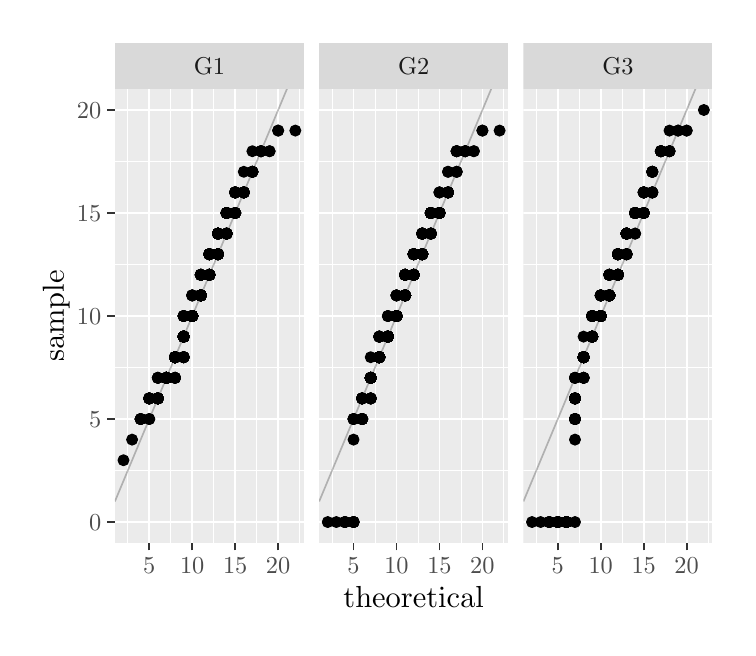
\begin{tikzpicture}[x=1pt,y=1pt]
\definecolor{fillColor}{RGB}{255,255,255}
\path[use as bounding box,fill=fillColor,fill opacity=0.00] (0,0) rectangle (252.94,216.81);
\begin{scope}
\path[clip] (  0.00,  0.00) rectangle (252.94,216.81);
\definecolor{drawColor}{RGB}{255,255,255}
\definecolor{fillColor}{RGB}{255,255,255}

\path[draw=drawColor,line width= 0.6pt,line join=round,line cap=round,fill=fillColor] (  0.00,  0.00) rectangle (252.94,216.81);
\end{scope}
\begin{scope}
\path[clip] ( 31.52, 30.72) rectangle ( 99.83,194.51);
\definecolor{fillColor}{gray}{0.92}

\path[fill=fillColor] ( 31.52, 30.72) rectangle ( 99.83,194.51);
\definecolor{drawColor}{RGB}{255,255,255}

\path[draw=drawColor,line width= 0.3pt,line join=round] ( 31.52, 56.78) --
	( 99.83, 56.78);

\path[draw=drawColor,line width= 0.3pt,line join=round] ( 31.52, 94.00) --
	( 99.83, 94.00);

\path[draw=drawColor,line width= 0.3pt,line join=round] ( 31.52,131.23) --
	( 99.83,131.23);

\path[draw=drawColor,line width= 0.3pt,line join=round] ( 31.52,168.45) --
	( 99.83,168.45);

\path[draw=drawColor,line width= 0.3pt,line join=round] ( 36.18, 30.72) --
	( 36.18,194.51);

\path[draw=drawColor,line width= 0.3pt,line join=round] ( 51.70, 30.72) --
	( 51.70,194.51);

\path[draw=drawColor,line width= 0.3pt,line join=round] ( 67.22, 30.72) --
	( 67.22,194.51);

\path[draw=drawColor,line width= 0.3pt,line join=round] ( 82.75, 30.72) --
	( 82.75,194.51);

\path[draw=drawColor,line width= 0.3pt,line join=round] ( 98.27, 30.72) --
	( 98.27,194.51);

\path[draw=drawColor,line width= 0.6pt,line join=round] ( 31.52, 38.17) --
	( 99.83, 38.17);

\path[draw=drawColor,line width= 0.6pt,line join=round] ( 31.52, 75.39) --
	( 99.83, 75.39);

\path[draw=drawColor,line width= 0.6pt,line join=round] ( 31.52,112.61) --
	( 99.83,112.61);

\path[draw=drawColor,line width= 0.6pt,line join=round] ( 31.52,149.84) --
	( 99.83,149.84);

\path[draw=drawColor,line width= 0.6pt,line join=round] ( 31.52,187.06) --
	( 99.83,187.06);

\path[draw=drawColor,line width= 0.6pt,line join=round] ( 43.94, 30.72) --
	( 43.94,194.51);

\path[draw=drawColor,line width= 0.6pt,line join=round] ( 59.46, 30.72) --
	( 59.46,194.51);

\path[draw=drawColor,line width= 0.6pt,line join=round] ( 74.99, 30.72) --
	( 74.99,194.51);

\path[draw=drawColor,line width= 0.6pt,line join=round] ( 90.51, 30.72) --
	( 90.51,194.51);
\definecolor{drawColor}{RGB}{0,0,0}
\definecolor{fillColor}{RGB}{0,0,0}

\path[draw=drawColor,line width= 0.4pt,line join=round,line cap=round,fill=fillColor] ( 34.62, 60.50) circle (  1.96);

\path[draw=drawColor,line width= 0.4pt,line join=round,line cap=round,fill=fillColor] ( 37.73, 67.95) circle (  1.96);

\path[draw=drawColor,line width= 0.4pt,line join=round,line cap=round,fill=fillColor] ( 40.83, 75.39) circle (  1.96);

\path[draw=drawColor,line width= 0.4pt,line join=round,line cap=round,fill=fillColor] ( 40.83, 75.39) circle (  1.96);

\path[draw=drawColor,line width= 0.4pt,line join=round,line cap=round,fill=fillColor] ( 40.83, 75.39) circle (  1.96);

\path[draw=drawColor,line width= 0.4pt,line join=round,line cap=round,fill=fillColor] ( 40.83, 75.39) circle (  1.96);

\path[draw=drawColor,line width= 0.4pt,line join=round,line cap=round,fill=fillColor] ( 40.83, 75.39) circle (  1.96);

\path[draw=drawColor,line width= 0.4pt,line join=round,line cap=round,fill=fillColor] ( 43.94, 75.39) circle (  1.96);

\path[draw=drawColor,line width= 0.4pt,line join=round,line cap=round,fill=fillColor] ( 43.94, 75.39) circle (  1.96);

\path[draw=drawColor,line width= 0.4pt,line join=round,line cap=round,fill=fillColor] ( 43.94, 82.84) circle (  1.96);

\path[draw=drawColor,line width= 0.4pt,line join=round,line cap=round,fill=fillColor] ( 43.94, 82.84) circle (  1.96);

\path[draw=drawColor,line width= 0.4pt,line join=round,line cap=round,fill=fillColor] ( 43.94, 82.84) circle (  1.96);

\path[draw=drawColor,line width= 0.4pt,line join=round,line cap=round,fill=fillColor] ( 43.94, 82.84) circle (  1.96);

\path[draw=drawColor,line width= 0.4pt,line join=round,line cap=round,fill=fillColor] ( 43.94, 82.84) circle (  1.96);

\path[draw=drawColor,line width= 0.4pt,line join=round,line cap=round,fill=fillColor] ( 43.94, 82.84) circle (  1.96);

\path[draw=drawColor,line width= 0.4pt,line join=round,line cap=round,fill=fillColor] ( 43.94, 82.84) circle (  1.96);

\path[draw=drawColor,line width= 0.4pt,line join=round,line cap=round,fill=fillColor] ( 43.94, 82.84) circle (  1.96);

\path[draw=drawColor,line width= 0.4pt,line join=round,line cap=round,fill=fillColor] ( 43.94, 82.84) circle (  1.96);

\path[draw=drawColor,line width= 0.4pt,line join=round,line cap=round,fill=fillColor] ( 47.04, 82.84) circle (  1.96);

\path[draw=drawColor,line width= 0.4pt,line join=round,line cap=round,fill=fillColor] ( 47.04, 82.84) circle (  1.96);

\path[draw=drawColor,line width= 0.4pt,line join=round,line cap=round,fill=fillColor] ( 47.04, 82.84) circle (  1.96);

\path[draw=drawColor,line width= 0.4pt,line join=round,line cap=round,fill=fillColor] ( 47.04, 82.84) circle (  1.96);

\path[draw=drawColor,line width= 0.4pt,line join=round,line cap=round,fill=fillColor] ( 47.04, 82.84) circle (  1.96);

\path[draw=drawColor,line width= 0.4pt,line join=round,line cap=round,fill=fillColor] ( 47.04, 82.84) circle (  1.96);

\path[draw=drawColor,line width= 0.4pt,line join=round,line cap=round,fill=fillColor] ( 47.04, 82.84) circle (  1.96);

\path[draw=drawColor,line width= 0.4pt,line join=round,line cap=round,fill=fillColor] ( 47.04, 82.84) circle (  1.96);

\path[draw=drawColor,line width= 0.4pt,line join=round,line cap=round,fill=fillColor] ( 47.04, 82.84) circle (  1.96);

\path[draw=drawColor,line width= 0.4pt,line join=round,line cap=round,fill=fillColor] ( 47.04, 82.84) circle (  1.96);

\path[draw=drawColor,line width= 0.4pt,line join=round,line cap=round,fill=fillColor] ( 47.04, 82.84) circle (  1.96);

\path[draw=drawColor,line width= 0.4pt,line join=round,line cap=round,fill=fillColor] ( 47.04, 82.84) circle (  1.96);

\path[draw=drawColor,line width= 0.4pt,line join=round,line cap=round,fill=fillColor] ( 47.04, 82.84) circle (  1.96);

\path[draw=drawColor,line width= 0.4pt,line join=round,line cap=round,fill=fillColor] ( 47.04, 82.84) circle (  1.96);

\path[draw=drawColor,line width= 0.4pt,line join=round,line cap=round,fill=fillColor] ( 47.04, 82.84) circle (  1.96);

\path[draw=drawColor,line width= 0.4pt,line join=round,line cap=round,fill=fillColor] ( 47.04, 90.28) circle (  1.96);

\path[draw=drawColor,line width= 0.4pt,line join=round,line cap=round,fill=fillColor] ( 47.04, 90.28) circle (  1.96);

\path[draw=drawColor,line width= 0.4pt,line join=round,line cap=round,fill=fillColor] ( 47.04, 90.28) circle (  1.96);

\path[draw=drawColor,line width= 0.4pt,line join=round,line cap=round,fill=fillColor] ( 47.04, 90.28) circle (  1.96);

\path[draw=drawColor,line width= 0.4pt,line join=round,line cap=round,fill=fillColor] ( 50.15, 90.28) circle (  1.96);

\path[draw=drawColor,line width= 0.4pt,line join=round,line cap=round,fill=fillColor] ( 50.15, 90.28) circle (  1.96);

\path[draw=drawColor,line width= 0.4pt,line join=round,line cap=round,fill=fillColor] ( 50.15, 90.28) circle (  1.96);

\path[draw=drawColor,line width= 0.4pt,line join=round,line cap=round,fill=fillColor] ( 50.15, 90.28) circle (  1.96);

\path[draw=drawColor,line width= 0.4pt,line join=round,line cap=round,fill=fillColor] ( 50.15, 90.28) circle (  1.96);

\path[draw=drawColor,line width= 0.4pt,line join=round,line cap=round,fill=fillColor] ( 50.15, 90.28) circle (  1.96);

\path[draw=drawColor,line width= 0.4pt,line join=round,line cap=round,fill=fillColor] ( 50.15, 90.28) circle (  1.96);

\path[draw=drawColor,line width= 0.4pt,line join=round,line cap=round,fill=fillColor] ( 50.15, 90.28) circle (  1.96);

\path[draw=drawColor,line width= 0.4pt,line join=round,line cap=round,fill=fillColor] ( 50.15, 90.28) circle (  1.96);

\path[draw=drawColor,line width= 0.4pt,line join=round,line cap=round,fill=fillColor] ( 50.15, 90.28) circle (  1.96);

\path[draw=drawColor,line width= 0.4pt,line join=round,line cap=round,fill=fillColor] ( 50.15, 90.28) circle (  1.96);

\path[draw=drawColor,line width= 0.4pt,line join=round,line cap=round,fill=fillColor] ( 50.15, 90.28) circle (  1.96);

\path[draw=drawColor,line width= 0.4pt,line join=round,line cap=round,fill=fillColor] ( 50.15, 90.28) circle (  1.96);

\path[draw=drawColor,line width= 0.4pt,line join=round,line cap=round,fill=fillColor] ( 50.15, 90.28) circle (  1.96);

\path[draw=drawColor,line width= 0.4pt,line join=round,line cap=round,fill=fillColor] ( 50.15, 90.28) circle (  1.96);

\path[draw=drawColor,line width= 0.4pt,line join=round,line cap=round,fill=fillColor] ( 50.15, 90.28) circle (  1.96);

\path[draw=drawColor,line width= 0.4pt,line join=round,line cap=round,fill=fillColor] ( 50.15, 90.28) circle (  1.96);

\path[draw=drawColor,line width= 0.4pt,line join=round,line cap=round,fill=fillColor] ( 50.15, 90.28) circle (  1.96);

\path[draw=drawColor,line width= 0.4pt,line join=round,line cap=round,fill=fillColor] ( 50.15, 90.28) circle (  1.96);

\path[draw=drawColor,line width= 0.4pt,line join=round,line cap=round,fill=fillColor] ( 50.15, 90.28) circle (  1.96);

\path[draw=drawColor,line width= 0.4pt,line join=round,line cap=round,fill=fillColor] ( 50.15, 90.28) circle (  1.96);

\path[draw=drawColor,line width= 0.4pt,line join=round,line cap=round,fill=fillColor] ( 50.15, 90.28) circle (  1.96);

\path[draw=drawColor,line width= 0.4pt,line join=round,line cap=round,fill=fillColor] ( 50.15, 90.28) circle (  1.96);

\path[draw=drawColor,line width= 0.4pt,line join=round,line cap=round,fill=fillColor] ( 50.15, 90.28) circle (  1.96);

\path[draw=drawColor,line width= 0.4pt,line join=round,line cap=round,fill=fillColor] ( 50.15, 90.28) circle (  1.96);

\path[draw=drawColor,line width= 0.4pt,line join=round,line cap=round,fill=fillColor] ( 50.15, 90.28) circle (  1.96);

\path[draw=drawColor,line width= 0.4pt,line join=round,line cap=round,fill=fillColor] ( 50.15, 90.28) circle (  1.96);

\path[draw=drawColor,line width= 0.4pt,line join=round,line cap=round,fill=fillColor] ( 50.15, 90.28) circle (  1.96);

\path[draw=drawColor,line width= 0.4pt,line join=round,line cap=round,fill=fillColor] ( 53.25, 90.28) circle (  1.96);

\path[draw=drawColor,line width= 0.4pt,line join=round,line cap=round,fill=fillColor] ( 53.25, 90.28) circle (  1.96);

\path[draw=drawColor,line width= 0.4pt,line join=round,line cap=round,fill=fillColor] ( 53.25, 90.28) circle (  1.96);

\path[draw=drawColor,line width= 0.4pt,line join=round,line cap=round,fill=fillColor] ( 53.25, 90.28) circle (  1.96);

\path[draw=drawColor,line width= 0.4pt,line join=round,line cap=round,fill=fillColor] ( 53.25, 90.28) circle (  1.96);

\path[draw=drawColor,line width= 0.4pt,line join=round,line cap=round,fill=fillColor] ( 53.25, 97.73) circle (  1.96);

\path[draw=drawColor,line width= 0.4pt,line join=round,line cap=round,fill=fillColor] ( 53.25, 97.73) circle (  1.96);

\path[draw=drawColor,line width= 0.4pt,line join=round,line cap=round,fill=fillColor] ( 53.25, 97.73) circle (  1.96);

\path[draw=drawColor,line width= 0.4pt,line join=round,line cap=round,fill=fillColor] ( 53.25, 97.73) circle (  1.96);

\path[draw=drawColor,line width= 0.4pt,line join=round,line cap=round,fill=fillColor] ( 53.25, 97.73) circle (  1.96);

\path[draw=drawColor,line width= 0.4pt,line join=round,line cap=round,fill=fillColor] ( 53.25, 97.73) circle (  1.96);

\path[draw=drawColor,line width= 0.4pt,line join=round,line cap=round,fill=fillColor] ( 53.25, 97.73) circle (  1.96);

\path[draw=drawColor,line width= 0.4pt,line join=round,line cap=round,fill=fillColor] ( 53.25, 97.73) circle (  1.96);

\path[draw=drawColor,line width= 0.4pt,line join=round,line cap=round,fill=fillColor] ( 53.25, 97.73) circle (  1.96);

\path[draw=drawColor,line width= 0.4pt,line join=round,line cap=round,fill=fillColor] ( 53.25, 97.73) circle (  1.96);

\path[draw=drawColor,line width= 0.4pt,line join=round,line cap=round,fill=fillColor] ( 53.25, 97.73) circle (  1.96);

\path[draw=drawColor,line width= 0.4pt,line join=round,line cap=round,fill=fillColor] ( 53.25, 97.73) circle (  1.96);

\path[draw=drawColor,line width= 0.4pt,line join=round,line cap=round,fill=fillColor] ( 53.25, 97.73) circle (  1.96);

\path[draw=drawColor,line width= 0.4pt,line join=round,line cap=round,fill=fillColor] ( 53.25, 97.73) circle (  1.96);

\path[draw=drawColor,line width= 0.4pt,line join=round,line cap=round,fill=fillColor] ( 53.25, 97.73) circle (  1.96);

\path[draw=drawColor,line width= 0.4pt,line join=round,line cap=round,fill=fillColor] ( 53.25, 97.73) circle (  1.96);

\path[draw=drawColor,line width= 0.4pt,line join=round,line cap=round,fill=fillColor] ( 53.25, 97.73) circle (  1.96);

\path[draw=drawColor,line width= 0.4pt,line join=round,line cap=round,fill=fillColor] ( 53.25, 97.73) circle (  1.96);

\path[draw=drawColor,line width= 0.4pt,line join=round,line cap=round,fill=fillColor] ( 53.25, 97.73) circle (  1.96);

\path[draw=drawColor,line width= 0.4pt,line join=round,line cap=round,fill=fillColor] ( 53.25, 97.73) circle (  1.96);

\path[draw=drawColor,line width= 0.4pt,line join=round,line cap=round,fill=fillColor] ( 53.25, 97.73) circle (  1.96);

\path[draw=drawColor,line width= 0.4pt,line join=round,line cap=round,fill=fillColor] ( 53.25, 97.73) circle (  1.96);

\path[draw=drawColor,line width= 0.4pt,line join=round,line cap=round,fill=fillColor] ( 53.25, 97.73) circle (  1.96);

\path[draw=drawColor,line width= 0.4pt,line join=round,line cap=round,fill=fillColor] ( 53.25, 97.73) circle (  1.96);

\path[draw=drawColor,line width= 0.4pt,line join=round,line cap=round,fill=fillColor] ( 53.25, 97.73) circle (  1.96);

\path[draw=drawColor,line width= 0.4pt,line join=round,line cap=round,fill=fillColor] ( 53.25, 97.73) circle (  1.96);

\path[draw=drawColor,line width= 0.4pt,line join=round,line cap=round,fill=fillColor] ( 53.25, 97.73) circle (  1.96);

\path[draw=drawColor,line width= 0.4pt,line join=round,line cap=round,fill=fillColor] ( 53.25, 97.73) circle (  1.96);

\path[draw=drawColor,line width= 0.4pt,line join=round,line cap=round,fill=fillColor] ( 53.25, 97.73) circle (  1.96);

\path[draw=drawColor,line width= 0.4pt,line join=round,line cap=round,fill=fillColor] ( 53.25, 97.73) circle (  1.96);

\path[draw=drawColor,line width= 0.4pt,line join=round,line cap=round,fill=fillColor] ( 53.25, 97.73) circle (  1.96);

\path[draw=drawColor,line width= 0.4pt,line join=round,line cap=round,fill=fillColor] ( 53.25, 97.73) circle (  1.96);

\path[draw=drawColor,line width= 0.4pt,line join=round,line cap=round,fill=fillColor] ( 53.25, 97.73) circle (  1.96);

\path[draw=drawColor,line width= 0.4pt,line join=round,line cap=round,fill=fillColor] ( 56.36, 97.73) circle (  1.96);

\path[draw=drawColor,line width= 0.4pt,line join=round,line cap=round,fill=fillColor] ( 56.36, 97.73) circle (  1.96);

\path[draw=drawColor,line width= 0.4pt,line join=round,line cap=round,fill=fillColor] ( 56.36, 97.73) circle (  1.96);

\path[draw=drawColor,line width= 0.4pt,line join=round,line cap=round,fill=fillColor] ( 56.36, 97.73) circle (  1.96);

\path[draw=drawColor,line width= 0.4pt,line join=round,line cap=round,fill=fillColor] ( 56.36, 97.73) circle (  1.96);

\path[draw=drawColor,line width= 0.4pt,line join=round,line cap=round,fill=fillColor] ( 56.36, 97.73) circle (  1.96);

\path[draw=drawColor,line width= 0.4pt,line join=round,line cap=round,fill=fillColor] ( 56.36, 97.73) circle (  1.96);

\path[draw=drawColor,line width= 0.4pt,line join=round,line cap=round,fill=fillColor] ( 56.36, 97.73) circle (  1.96);

\path[draw=drawColor,line width= 0.4pt,line join=round,line cap=round,fill=fillColor] ( 56.36,105.17) circle (  1.96);

\path[draw=drawColor,line width= 0.4pt,line join=round,line cap=round,fill=fillColor] ( 56.36,105.17) circle (  1.96);

\path[draw=drawColor,line width= 0.4pt,line join=round,line cap=round,fill=fillColor] ( 56.36,105.17) circle (  1.96);

\path[draw=drawColor,line width= 0.4pt,line join=round,line cap=round,fill=fillColor] ( 56.36,105.17) circle (  1.96);

\path[draw=drawColor,line width= 0.4pt,line join=round,line cap=round,fill=fillColor] ( 56.36,105.17) circle (  1.96);

\path[draw=drawColor,line width= 0.4pt,line join=round,line cap=round,fill=fillColor] ( 56.36,105.17) circle (  1.96);

\path[draw=drawColor,line width= 0.4pt,line join=round,line cap=round,fill=fillColor] ( 56.36,105.17) circle (  1.96);

\path[draw=drawColor,line width= 0.4pt,line join=round,line cap=round,fill=fillColor] ( 56.36,105.17) circle (  1.96);

\path[draw=drawColor,line width= 0.4pt,line join=round,line cap=round,fill=fillColor] ( 56.36,105.17) circle (  1.96);

\path[draw=drawColor,line width= 0.4pt,line join=round,line cap=round,fill=fillColor] ( 56.36,105.17) circle (  1.96);

\path[draw=drawColor,line width= 0.4pt,line join=round,line cap=round,fill=fillColor] ( 56.36,105.17) circle (  1.96);

\path[draw=drawColor,line width= 0.4pt,line join=round,line cap=round,fill=fillColor] ( 56.36,105.17) circle (  1.96);

\path[draw=drawColor,line width= 0.4pt,line join=round,line cap=round,fill=fillColor] ( 56.36,105.17) circle (  1.96);

\path[draw=drawColor,line width= 0.4pt,line join=round,line cap=round,fill=fillColor] ( 56.36,105.17) circle (  1.96);

\path[draw=drawColor,line width= 0.4pt,line join=round,line cap=round,fill=fillColor] ( 56.36,105.17) circle (  1.96);

\path[draw=drawColor,line width= 0.4pt,line join=round,line cap=round,fill=fillColor] ( 56.36,105.17) circle (  1.96);

\path[draw=drawColor,line width= 0.4pt,line join=round,line cap=round,fill=fillColor] ( 56.36,105.17) circle (  1.96);

\path[draw=drawColor,line width= 0.4pt,line join=round,line cap=round,fill=fillColor] ( 56.36,105.17) circle (  1.96);

\path[draw=drawColor,line width= 0.4pt,line join=round,line cap=round,fill=fillColor] ( 56.36,105.17) circle (  1.96);

\path[draw=drawColor,line width= 0.4pt,line join=round,line cap=round,fill=fillColor] ( 56.36,105.17) circle (  1.96);

\path[draw=drawColor,line width= 0.4pt,line join=round,line cap=round,fill=fillColor] ( 56.36,105.17) circle (  1.96);

\path[draw=drawColor,line width= 0.4pt,line join=round,line cap=round,fill=fillColor] ( 56.36,105.17) circle (  1.96);

\path[draw=drawColor,line width= 0.4pt,line join=round,line cap=round,fill=fillColor] ( 56.36,105.17) circle (  1.96);

\path[draw=drawColor,line width= 0.4pt,line join=round,line cap=round,fill=fillColor] ( 56.36,105.17) circle (  1.96);

\path[draw=drawColor,line width= 0.4pt,line join=round,line cap=round,fill=fillColor] ( 56.36,105.17) circle (  1.96);

\path[draw=drawColor,line width= 0.4pt,line join=round,line cap=round,fill=fillColor] ( 56.36,105.17) circle (  1.96);

\path[draw=drawColor,line width= 0.4pt,line join=round,line cap=round,fill=fillColor] ( 56.36,105.17) circle (  1.96);

\path[draw=drawColor,line width= 0.4pt,line join=round,line cap=round,fill=fillColor] ( 56.36,105.17) circle (  1.96);

\path[draw=drawColor,line width= 0.4pt,line join=round,line cap=round,fill=fillColor] ( 56.36,105.17) circle (  1.96);

\path[draw=drawColor,line width= 0.4pt,line join=round,line cap=round,fill=fillColor] ( 56.36,105.17) circle (  1.96);

\path[draw=drawColor,line width= 0.4pt,line join=round,line cap=round,fill=fillColor] ( 56.36,105.17) circle (  1.96);

\path[draw=drawColor,line width= 0.4pt,line join=round,line cap=round,fill=fillColor] ( 56.36,112.61) circle (  1.96);

\path[draw=drawColor,line width= 0.4pt,line join=round,line cap=round,fill=fillColor] ( 56.36,112.61) circle (  1.96);

\path[draw=drawColor,line width= 0.4pt,line join=round,line cap=round,fill=fillColor] ( 56.36,112.61) circle (  1.96);

\path[draw=drawColor,line width= 0.4pt,line join=round,line cap=round,fill=fillColor] ( 56.36,112.61) circle (  1.96);

\path[draw=drawColor,line width= 0.4pt,line join=round,line cap=round,fill=fillColor] ( 56.36,112.61) circle (  1.96);

\path[draw=drawColor,line width= 0.4pt,line join=round,line cap=round,fill=fillColor] ( 56.36,112.61) circle (  1.96);

\path[draw=drawColor,line width= 0.4pt,line join=round,line cap=round,fill=fillColor] ( 56.36,112.61) circle (  1.96);

\path[draw=drawColor,line width= 0.4pt,line join=round,line cap=round,fill=fillColor] ( 59.46,112.61) circle (  1.96);

\path[draw=drawColor,line width= 0.4pt,line join=round,line cap=round,fill=fillColor] ( 59.46,112.61) circle (  1.96);

\path[draw=drawColor,line width= 0.4pt,line join=round,line cap=round,fill=fillColor] ( 59.46,112.61) circle (  1.96);

\path[draw=drawColor,line width= 0.4pt,line join=round,line cap=round,fill=fillColor] ( 59.46,112.61) circle (  1.96);

\path[draw=drawColor,line width= 0.4pt,line join=round,line cap=round,fill=fillColor] ( 59.46,112.61) circle (  1.96);

\path[draw=drawColor,line width= 0.4pt,line join=round,line cap=round,fill=fillColor] ( 59.46,112.61) circle (  1.96);

\path[draw=drawColor,line width= 0.4pt,line join=round,line cap=round,fill=fillColor] ( 59.46,112.61) circle (  1.96);

\path[draw=drawColor,line width= 0.4pt,line join=round,line cap=round,fill=fillColor] ( 59.46,112.61) circle (  1.96);

\path[draw=drawColor,line width= 0.4pt,line join=round,line cap=round,fill=fillColor] ( 59.46,112.61) circle (  1.96);

\path[draw=drawColor,line width= 0.4pt,line join=round,line cap=round,fill=fillColor] ( 59.46,112.61) circle (  1.96);

\path[draw=drawColor,line width= 0.4pt,line join=round,line cap=round,fill=fillColor] ( 59.46,112.61) circle (  1.96);

\path[draw=drawColor,line width= 0.4pt,line join=round,line cap=round,fill=fillColor] ( 59.46,112.61) circle (  1.96);

\path[draw=drawColor,line width= 0.4pt,line join=round,line cap=round,fill=fillColor] ( 59.46,112.61) circle (  1.96);

\path[draw=drawColor,line width= 0.4pt,line join=round,line cap=round,fill=fillColor] ( 59.46,112.61) circle (  1.96);

\path[draw=drawColor,line width= 0.4pt,line join=round,line cap=round,fill=fillColor] ( 59.46,112.61) circle (  1.96);

\path[draw=drawColor,line width= 0.4pt,line join=round,line cap=round,fill=fillColor] ( 59.46,112.61) circle (  1.96);

\path[draw=drawColor,line width= 0.4pt,line join=round,line cap=round,fill=fillColor] ( 59.46,112.61) circle (  1.96);

\path[draw=drawColor,line width= 0.4pt,line join=round,line cap=round,fill=fillColor] ( 59.46,112.61) circle (  1.96);

\path[draw=drawColor,line width= 0.4pt,line join=round,line cap=round,fill=fillColor] ( 59.46,112.61) circle (  1.96);

\path[draw=drawColor,line width= 0.4pt,line join=round,line cap=round,fill=fillColor] ( 59.46,112.61) circle (  1.96);

\path[draw=drawColor,line width= 0.4pt,line join=round,line cap=round,fill=fillColor] ( 59.46,112.61) circle (  1.96);

\path[draw=drawColor,line width= 0.4pt,line join=round,line cap=round,fill=fillColor] ( 59.46,112.61) circle (  1.96);

\path[draw=drawColor,line width= 0.4pt,line join=round,line cap=round,fill=fillColor] ( 59.46,112.61) circle (  1.96);

\path[draw=drawColor,line width= 0.4pt,line join=round,line cap=round,fill=fillColor] ( 59.46,112.61) circle (  1.96);

\path[draw=drawColor,line width= 0.4pt,line join=round,line cap=round,fill=fillColor] ( 59.46,112.61) circle (  1.96);

\path[draw=drawColor,line width= 0.4pt,line join=round,line cap=round,fill=fillColor] ( 59.46,112.61) circle (  1.96);

\path[draw=drawColor,line width= 0.4pt,line join=round,line cap=round,fill=fillColor] ( 59.46,112.61) circle (  1.96);

\path[draw=drawColor,line width= 0.4pt,line join=round,line cap=round,fill=fillColor] ( 59.46,112.61) circle (  1.96);

\path[draw=drawColor,line width= 0.4pt,line join=round,line cap=round,fill=fillColor] ( 59.46,112.61) circle (  1.96);

\path[draw=drawColor,line width= 0.4pt,line join=round,line cap=round,fill=fillColor] ( 59.46,112.61) circle (  1.96);

\path[draw=drawColor,line width= 0.4pt,line join=round,line cap=round,fill=fillColor] ( 59.46,112.61) circle (  1.96);

\path[draw=drawColor,line width= 0.4pt,line join=round,line cap=round,fill=fillColor] ( 59.46,112.61) circle (  1.96);

\path[draw=drawColor,line width= 0.4pt,line join=round,line cap=round,fill=fillColor] ( 59.46,112.61) circle (  1.96);

\path[draw=drawColor,line width= 0.4pt,line join=round,line cap=round,fill=fillColor] ( 59.46,112.61) circle (  1.96);

\path[draw=drawColor,line width= 0.4pt,line join=round,line cap=round,fill=fillColor] ( 59.46,112.61) circle (  1.96);

\path[draw=drawColor,line width= 0.4pt,line join=round,line cap=round,fill=fillColor] ( 59.46,112.61) circle (  1.96);

\path[draw=drawColor,line width= 0.4pt,line join=round,line cap=round,fill=fillColor] ( 59.46,112.61) circle (  1.96);

\path[draw=drawColor,line width= 0.4pt,line join=round,line cap=round,fill=fillColor] ( 59.46,112.61) circle (  1.96);

\path[draw=drawColor,line width= 0.4pt,line join=round,line cap=round,fill=fillColor] ( 59.46,112.61) circle (  1.96);

\path[draw=drawColor,line width= 0.4pt,line join=round,line cap=round,fill=fillColor] ( 59.46,112.61) circle (  1.96);

\path[draw=drawColor,line width= 0.4pt,line join=round,line cap=round,fill=fillColor] ( 59.46,112.61) circle (  1.96);

\path[draw=drawColor,line width= 0.4pt,line join=round,line cap=round,fill=fillColor] ( 59.46,112.61) circle (  1.96);

\path[draw=drawColor,line width= 0.4pt,line join=round,line cap=round,fill=fillColor] ( 59.46,112.61) circle (  1.96);

\path[draw=drawColor,line width= 0.4pt,line join=round,line cap=round,fill=fillColor] ( 59.46,112.61) circle (  1.96);

\path[draw=drawColor,line width= 0.4pt,line join=round,line cap=round,fill=fillColor] ( 59.46,120.06) circle (  1.96);

\path[draw=drawColor,line width= 0.4pt,line join=round,line cap=round,fill=fillColor] ( 59.46,120.06) circle (  1.96);

\path[draw=drawColor,line width= 0.4pt,line join=round,line cap=round,fill=fillColor] ( 59.46,120.06) circle (  1.96);

\path[draw=drawColor,line width= 0.4pt,line join=round,line cap=round,fill=fillColor] ( 59.46,120.06) circle (  1.96);

\path[draw=drawColor,line width= 0.4pt,line join=round,line cap=round,fill=fillColor] ( 62.57,120.06) circle (  1.96);

\path[draw=drawColor,line width= 0.4pt,line join=round,line cap=round,fill=fillColor] ( 62.57,120.06) circle (  1.96);

\path[draw=drawColor,line width= 0.4pt,line join=round,line cap=round,fill=fillColor] ( 62.57,120.06) circle (  1.96);

\path[draw=drawColor,line width= 0.4pt,line join=round,line cap=round,fill=fillColor] ( 62.57,120.06) circle (  1.96);

\path[draw=drawColor,line width= 0.4pt,line join=round,line cap=round,fill=fillColor] ( 62.57,120.06) circle (  1.96);

\path[draw=drawColor,line width= 0.4pt,line join=round,line cap=round,fill=fillColor] ( 62.57,120.06) circle (  1.96);

\path[draw=drawColor,line width= 0.4pt,line join=round,line cap=round,fill=fillColor] ( 62.57,120.06) circle (  1.96);

\path[draw=drawColor,line width= 0.4pt,line join=round,line cap=round,fill=fillColor] ( 62.57,120.06) circle (  1.96);

\path[draw=drawColor,line width= 0.4pt,line join=round,line cap=round,fill=fillColor] ( 62.57,120.06) circle (  1.96);

\path[draw=drawColor,line width= 0.4pt,line join=round,line cap=round,fill=fillColor] ( 62.57,120.06) circle (  1.96);

\path[draw=drawColor,line width= 0.4pt,line join=round,line cap=round,fill=fillColor] ( 62.57,120.06) circle (  1.96);

\path[draw=drawColor,line width= 0.4pt,line join=round,line cap=round,fill=fillColor] ( 62.57,120.06) circle (  1.96);

\path[draw=drawColor,line width= 0.4pt,line join=round,line cap=round,fill=fillColor] ( 62.57,120.06) circle (  1.96);

\path[draw=drawColor,line width= 0.4pt,line join=round,line cap=round,fill=fillColor] ( 62.57,120.06) circle (  1.96);

\path[draw=drawColor,line width= 0.4pt,line join=round,line cap=round,fill=fillColor] ( 62.57,120.06) circle (  1.96);

\path[draw=drawColor,line width= 0.4pt,line join=round,line cap=round,fill=fillColor] ( 62.57,120.06) circle (  1.96);

\path[draw=drawColor,line width= 0.4pt,line join=round,line cap=round,fill=fillColor] ( 62.57,120.06) circle (  1.96);

\path[draw=drawColor,line width= 0.4pt,line join=round,line cap=round,fill=fillColor] ( 62.57,120.06) circle (  1.96);

\path[draw=drawColor,line width= 0.4pt,line join=round,line cap=round,fill=fillColor] ( 62.57,120.06) circle (  1.96);

\path[draw=drawColor,line width= 0.4pt,line join=round,line cap=round,fill=fillColor] ( 62.57,120.06) circle (  1.96);

\path[draw=drawColor,line width= 0.4pt,line join=round,line cap=round,fill=fillColor] ( 62.57,120.06) circle (  1.96);

\path[draw=drawColor,line width= 0.4pt,line join=round,line cap=round,fill=fillColor] ( 62.57,120.06) circle (  1.96);

\path[draw=drawColor,line width= 0.4pt,line join=round,line cap=round,fill=fillColor] ( 62.57,120.06) circle (  1.96);

\path[draw=drawColor,line width= 0.4pt,line join=round,line cap=round,fill=fillColor] ( 62.57,120.06) circle (  1.96);

\path[draw=drawColor,line width= 0.4pt,line join=round,line cap=round,fill=fillColor] ( 62.57,120.06) circle (  1.96);

\path[draw=drawColor,line width= 0.4pt,line join=round,line cap=round,fill=fillColor] ( 62.57,120.06) circle (  1.96);

\path[draw=drawColor,line width= 0.4pt,line join=round,line cap=round,fill=fillColor] ( 62.57,120.06) circle (  1.96);

\path[draw=drawColor,line width= 0.4pt,line join=round,line cap=round,fill=fillColor] ( 62.57,120.06) circle (  1.96);

\path[draw=drawColor,line width= 0.4pt,line join=round,line cap=round,fill=fillColor] ( 62.57,120.06) circle (  1.96);

\path[draw=drawColor,line width= 0.4pt,line join=round,line cap=round,fill=fillColor] ( 62.57,120.06) circle (  1.96);

\path[draw=drawColor,line width= 0.4pt,line join=round,line cap=round,fill=fillColor] ( 62.57,120.06) circle (  1.96);

\path[draw=drawColor,line width= 0.4pt,line join=round,line cap=round,fill=fillColor] ( 62.57,120.06) circle (  1.96);

\path[draw=drawColor,line width= 0.4pt,line join=round,line cap=round,fill=fillColor] ( 62.57,120.06) circle (  1.96);

\path[draw=drawColor,line width= 0.4pt,line join=round,line cap=round,fill=fillColor] ( 62.57,120.06) circle (  1.96);

\path[draw=drawColor,line width= 0.4pt,line join=round,line cap=round,fill=fillColor] ( 62.57,120.06) circle (  1.96);

\path[draw=drawColor,line width= 0.4pt,line join=round,line cap=round,fill=fillColor] ( 62.57,127.50) circle (  1.96);

\path[draw=drawColor,line width= 0.4pt,line join=round,line cap=round,fill=fillColor] ( 62.57,127.50) circle (  1.96);

\path[draw=drawColor,line width= 0.4pt,line join=round,line cap=round,fill=fillColor] ( 62.57,127.50) circle (  1.96);

\path[draw=drawColor,line width= 0.4pt,line join=round,line cap=round,fill=fillColor] ( 62.57,127.50) circle (  1.96);

\path[draw=drawColor,line width= 0.4pt,line join=round,line cap=round,fill=fillColor] ( 62.57,127.50) circle (  1.96);

\path[draw=drawColor,line width= 0.4pt,line join=round,line cap=round,fill=fillColor] ( 62.57,127.50) circle (  1.96);

\path[draw=drawColor,line width= 0.4pt,line join=round,line cap=round,fill=fillColor] ( 62.57,127.50) circle (  1.96);

\path[draw=drawColor,line width= 0.4pt,line join=round,line cap=round,fill=fillColor] ( 62.57,127.50) circle (  1.96);

\path[draw=drawColor,line width= 0.4pt,line join=round,line cap=round,fill=fillColor] ( 62.57,127.50) circle (  1.96);

\path[draw=drawColor,line width= 0.4pt,line join=round,line cap=round,fill=fillColor] ( 62.57,127.50) circle (  1.96);

\path[draw=drawColor,line width= 0.4pt,line join=round,line cap=round,fill=fillColor] ( 62.57,127.50) circle (  1.96);

\path[draw=drawColor,line width= 0.4pt,line join=round,line cap=round,fill=fillColor] ( 62.57,127.50) circle (  1.96);

\path[draw=drawColor,line width= 0.4pt,line join=round,line cap=round,fill=fillColor] ( 65.67,127.50) circle (  1.96);

\path[draw=drawColor,line width= 0.4pt,line join=round,line cap=round,fill=fillColor] ( 65.67,127.50) circle (  1.96);

\path[draw=drawColor,line width= 0.4pt,line join=round,line cap=round,fill=fillColor] ( 65.67,127.50) circle (  1.96);

\path[draw=drawColor,line width= 0.4pt,line join=round,line cap=round,fill=fillColor] ( 65.67,127.50) circle (  1.96);

\path[draw=drawColor,line width= 0.4pt,line join=round,line cap=round,fill=fillColor] ( 65.67,127.50) circle (  1.96);

\path[draw=drawColor,line width= 0.4pt,line join=round,line cap=round,fill=fillColor] ( 65.67,127.50) circle (  1.96);

\path[draw=drawColor,line width= 0.4pt,line join=round,line cap=round,fill=fillColor] ( 65.67,127.50) circle (  1.96);

\path[draw=drawColor,line width= 0.4pt,line join=round,line cap=round,fill=fillColor] ( 65.67,127.50) circle (  1.96);

\path[draw=drawColor,line width= 0.4pt,line join=round,line cap=round,fill=fillColor] ( 65.67,127.50) circle (  1.96);

\path[draw=drawColor,line width= 0.4pt,line join=round,line cap=round,fill=fillColor] ( 65.67,127.50) circle (  1.96);

\path[draw=drawColor,line width= 0.4pt,line join=round,line cap=round,fill=fillColor] ( 65.67,127.50) circle (  1.96);

\path[draw=drawColor,line width= 0.4pt,line join=round,line cap=round,fill=fillColor] ( 65.67,127.50) circle (  1.96);

\path[draw=drawColor,line width= 0.4pt,line join=round,line cap=round,fill=fillColor] ( 65.67,127.50) circle (  1.96);

\path[draw=drawColor,line width= 0.4pt,line join=round,line cap=round,fill=fillColor] ( 65.67,127.50) circle (  1.96);

\path[draw=drawColor,line width= 0.4pt,line join=round,line cap=round,fill=fillColor] ( 65.67,127.50) circle (  1.96);

\path[draw=drawColor,line width= 0.4pt,line join=round,line cap=round,fill=fillColor] ( 65.67,127.50) circle (  1.96);

\path[draw=drawColor,line width= 0.4pt,line join=round,line cap=round,fill=fillColor] ( 65.67,127.50) circle (  1.96);

\path[draw=drawColor,line width= 0.4pt,line join=round,line cap=round,fill=fillColor] ( 65.67,127.50) circle (  1.96);

\path[draw=drawColor,line width= 0.4pt,line join=round,line cap=round,fill=fillColor] ( 65.67,127.50) circle (  1.96);

\path[draw=drawColor,line width= 0.4pt,line join=round,line cap=round,fill=fillColor] ( 65.67,127.50) circle (  1.96);

\path[draw=drawColor,line width= 0.4pt,line join=round,line cap=round,fill=fillColor] ( 65.67,127.50) circle (  1.96);

\path[draw=drawColor,line width= 0.4pt,line join=round,line cap=round,fill=fillColor] ( 65.67,127.50) circle (  1.96);

\path[draw=drawColor,line width= 0.4pt,line join=round,line cap=round,fill=fillColor] ( 65.67,127.50) circle (  1.96);

\path[draw=drawColor,line width= 0.4pt,line join=round,line cap=round,fill=fillColor] ( 65.67,134.95) circle (  1.96);

\path[draw=drawColor,line width= 0.4pt,line join=round,line cap=round,fill=fillColor] ( 65.67,134.95) circle (  1.96);

\path[draw=drawColor,line width= 0.4pt,line join=round,line cap=round,fill=fillColor] ( 65.67,134.95) circle (  1.96);

\path[draw=drawColor,line width= 0.4pt,line join=round,line cap=round,fill=fillColor] ( 65.67,134.95) circle (  1.96);

\path[draw=drawColor,line width= 0.4pt,line join=round,line cap=round,fill=fillColor] ( 65.67,134.95) circle (  1.96);

\path[draw=drawColor,line width= 0.4pt,line join=round,line cap=round,fill=fillColor] ( 65.67,134.95) circle (  1.96);

\path[draw=drawColor,line width= 0.4pt,line join=round,line cap=round,fill=fillColor] ( 65.67,134.95) circle (  1.96);

\path[draw=drawColor,line width= 0.4pt,line join=round,line cap=round,fill=fillColor] ( 65.67,134.95) circle (  1.96);

\path[draw=drawColor,line width= 0.4pt,line join=round,line cap=round,fill=fillColor] ( 65.67,134.95) circle (  1.96);

\path[draw=drawColor,line width= 0.4pt,line join=round,line cap=round,fill=fillColor] ( 65.67,134.95) circle (  1.96);

\path[draw=drawColor,line width= 0.4pt,line join=round,line cap=round,fill=fillColor] ( 65.67,134.95) circle (  1.96);

\path[draw=drawColor,line width= 0.4pt,line join=round,line cap=round,fill=fillColor] ( 65.67,134.95) circle (  1.96);

\path[draw=drawColor,line width= 0.4pt,line join=round,line cap=round,fill=fillColor] ( 65.67,134.95) circle (  1.96);

\path[draw=drawColor,line width= 0.4pt,line join=round,line cap=round,fill=fillColor] ( 65.67,134.95) circle (  1.96);

\path[draw=drawColor,line width= 0.4pt,line join=round,line cap=round,fill=fillColor] ( 65.67,134.95) circle (  1.96);

\path[draw=drawColor,line width= 0.4pt,line join=round,line cap=round,fill=fillColor] ( 65.67,134.95) circle (  1.96);

\path[draw=drawColor,line width= 0.4pt,line join=round,line cap=round,fill=fillColor] ( 65.67,134.95) circle (  1.96);

\path[draw=drawColor,line width= 0.4pt,line join=round,line cap=round,fill=fillColor] ( 65.67,134.95) circle (  1.96);

\path[draw=drawColor,line width= 0.4pt,line join=round,line cap=round,fill=fillColor] ( 65.67,134.95) circle (  1.96);

\path[draw=drawColor,line width= 0.4pt,line join=round,line cap=round,fill=fillColor] ( 68.78,134.95) circle (  1.96);

\path[draw=drawColor,line width= 0.4pt,line join=round,line cap=round,fill=fillColor] ( 68.78,134.95) circle (  1.96);

\path[draw=drawColor,line width= 0.4pt,line join=round,line cap=round,fill=fillColor] ( 68.78,134.95) circle (  1.96);

\path[draw=drawColor,line width= 0.4pt,line join=round,line cap=round,fill=fillColor] ( 68.78,134.95) circle (  1.96);

\path[draw=drawColor,line width= 0.4pt,line join=round,line cap=round,fill=fillColor] ( 68.78,134.95) circle (  1.96);

\path[draw=drawColor,line width= 0.4pt,line join=round,line cap=round,fill=fillColor] ( 68.78,134.95) circle (  1.96);

\path[draw=drawColor,line width= 0.4pt,line join=round,line cap=round,fill=fillColor] ( 68.78,134.95) circle (  1.96);

\path[draw=drawColor,line width= 0.4pt,line join=round,line cap=round,fill=fillColor] ( 68.78,134.95) circle (  1.96);

\path[draw=drawColor,line width= 0.4pt,line join=round,line cap=round,fill=fillColor] ( 68.78,134.95) circle (  1.96);

\path[draw=drawColor,line width= 0.4pt,line join=round,line cap=round,fill=fillColor] ( 68.78,134.95) circle (  1.96);

\path[draw=drawColor,line width= 0.4pt,line join=round,line cap=round,fill=fillColor] ( 68.78,134.95) circle (  1.96);

\path[draw=drawColor,line width= 0.4pt,line join=round,line cap=round,fill=fillColor] ( 68.78,134.95) circle (  1.96);

\path[draw=drawColor,line width= 0.4pt,line join=round,line cap=round,fill=fillColor] ( 68.78,134.95) circle (  1.96);

\path[draw=drawColor,line width= 0.4pt,line join=round,line cap=round,fill=fillColor] ( 68.78,134.95) circle (  1.96);

\path[draw=drawColor,line width= 0.4pt,line join=round,line cap=round,fill=fillColor] ( 68.78,142.39) circle (  1.96);

\path[draw=drawColor,line width= 0.4pt,line join=round,line cap=round,fill=fillColor] ( 68.78,142.39) circle (  1.96);

\path[draw=drawColor,line width= 0.4pt,line join=round,line cap=round,fill=fillColor] ( 68.78,142.39) circle (  1.96);

\path[draw=drawColor,line width= 0.4pt,line join=round,line cap=round,fill=fillColor] ( 68.78,142.39) circle (  1.96);

\path[draw=drawColor,line width= 0.4pt,line join=round,line cap=round,fill=fillColor] ( 68.78,142.39) circle (  1.96);

\path[draw=drawColor,line width= 0.4pt,line join=round,line cap=round,fill=fillColor] ( 68.78,142.39) circle (  1.96);

\path[draw=drawColor,line width= 0.4pt,line join=round,line cap=round,fill=fillColor] ( 68.78,142.39) circle (  1.96);

\path[draw=drawColor,line width= 0.4pt,line join=round,line cap=round,fill=fillColor] ( 68.78,142.39) circle (  1.96);

\path[draw=drawColor,line width= 0.4pt,line join=round,line cap=round,fill=fillColor] ( 68.78,142.39) circle (  1.96);

\path[draw=drawColor,line width= 0.4pt,line join=round,line cap=round,fill=fillColor] ( 68.78,142.39) circle (  1.96);

\path[draw=drawColor,line width= 0.4pt,line join=round,line cap=round,fill=fillColor] ( 68.78,142.39) circle (  1.96);

\path[draw=drawColor,line width= 0.4pt,line join=round,line cap=round,fill=fillColor] ( 68.78,142.39) circle (  1.96);

\path[draw=drawColor,line width= 0.4pt,line join=round,line cap=round,fill=fillColor] ( 68.78,142.39) circle (  1.96);

\path[draw=drawColor,line width= 0.4pt,line join=round,line cap=round,fill=fillColor] ( 68.78,142.39) circle (  1.96);

\path[draw=drawColor,line width= 0.4pt,line join=round,line cap=round,fill=fillColor] ( 68.78,142.39) circle (  1.96);

\path[draw=drawColor,line width= 0.4pt,line join=round,line cap=round,fill=fillColor] ( 68.78,142.39) circle (  1.96);

\path[draw=drawColor,line width= 0.4pt,line join=round,line cap=round,fill=fillColor] ( 68.78,142.39) circle (  1.96);

\path[draw=drawColor,line width= 0.4pt,line join=round,line cap=round,fill=fillColor] ( 68.78,142.39) circle (  1.96);

\path[draw=drawColor,line width= 0.4pt,line join=round,line cap=round,fill=fillColor] ( 68.78,142.39) circle (  1.96);

\path[draw=drawColor,line width= 0.4pt,line join=round,line cap=round,fill=fillColor] ( 68.78,142.39) circle (  1.96);

\path[draw=drawColor,line width= 0.4pt,line join=round,line cap=round,fill=fillColor] ( 71.88,142.39) circle (  1.96);

\path[draw=drawColor,line width= 0.4pt,line join=round,line cap=round,fill=fillColor] ( 71.88,142.39) circle (  1.96);

\path[draw=drawColor,line width= 0.4pt,line join=round,line cap=round,fill=fillColor] ( 71.88,142.39) circle (  1.96);

\path[draw=drawColor,line width= 0.4pt,line join=round,line cap=round,fill=fillColor] ( 71.88,142.39) circle (  1.96);

\path[draw=drawColor,line width= 0.4pt,line join=round,line cap=round,fill=fillColor] ( 71.88,142.39) circle (  1.96);

\path[draw=drawColor,line width= 0.4pt,line join=round,line cap=round,fill=fillColor] ( 71.88,142.39) circle (  1.96);

\path[draw=drawColor,line width= 0.4pt,line join=round,line cap=round,fill=fillColor] ( 71.88,142.39) circle (  1.96);

\path[draw=drawColor,line width= 0.4pt,line join=round,line cap=round,fill=fillColor] ( 71.88,142.39) circle (  1.96);

\path[draw=drawColor,line width= 0.4pt,line join=round,line cap=round,fill=fillColor] ( 71.88,142.39) circle (  1.96);

\path[draw=drawColor,line width= 0.4pt,line join=round,line cap=round,fill=fillColor] ( 71.88,142.39) circle (  1.96);

\path[draw=drawColor,line width= 0.4pt,line join=round,line cap=round,fill=fillColor] ( 71.88,149.84) circle (  1.96);

\path[draw=drawColor,line width= 0.4pt,line join=round,line cap=round,fill=fillColor] ( 71.88,149.84) circle (  1.96);

\path[draw=drawColor,line width= 0.4pt,line join=round,line cap=round,fill=fillColor] ( 71.88,149.84) circle (  1.96);

\path[draw=drawColor,line width= 0.4pt,line join=round,line cap=round,fill=fillColor] ( 71.88,149.84) circle (  1.96);

\path[draw=drawColor,line width= 0.4pt,line join=round,line cap=round,fill=fillColor] ( 71.88,149.84) circle (  1.96);

\path[draw=drawColor,line width= 0.4pt,line join=round,line cap=round,fill=fillColor] ( 71.88,149.84) circle (  1.96);

\path[draw=drawColor,line width= 0.4pt,line join=round,line cap=round,fill=fillColor] ( 71.88,149.84) circle (  1.96);

\path[draw=drawColor,line width= 0.4pt,line join=round,line cap=round,fill=fillColor] ( 71.88,149.84) circle (  1.96);

\path[draw=drawColor,line width= 0.4pt,line join=round,line cap=round,fill=fillColor] ( 71.88,149.84) circle (  1.96);

\path[draw=drawColor,line width= 0.4pt,line join=round,line cap=round,fill=fillColor] ( 71.88,149.84) circle (  1.96);

\path[draw=drawColor,line width= 0.4pt,line join=round,line cap=round,fill=fillColor] ( 71.88,149.84) circle (  1.96);

\path[draw=drawColor,line width= 0.4pt,line join=round,line cap=round,fill=fillColor] ( 71.88,149.84) circle (  1.96);

\path[draw=drawColor,line width= 0.4pt,line join=round,line cap=round,fill=fillColor] ( 71.88,149.84) circle (  1.96);

\path[draw=drawColor,line width= 0.4pt,line join=round,line cap=round,fill=fillColor] ( 71.88,149.84) circle (  1.96);

\path[draw=drawColor,line width= 0.4pt,line join=round,line cap=round,fill=fillColor] ( 71.88,149.84) circle (  1.96);

\path[draw=drawColor,line width= 0.4pt,line join=round,line cap=round,fill=fillColor] ( 71.88,149.84) circle (  1.96);

\path[draw=drawColor,line width= 0.4pt,line join=round,line cap=round,fill=fillColor] ( 74.99,149.84) circle (  1.96);

\path[draw=drawColor,line width= 0.4pt,line join=round,line cap=round,fill=fillColor] ( 74.99,149.84) circle (  1.96);

\path[draw=drawColor,line width= 0.4pt,line join=round,line cap=round,fill=fillColor] ( 74.99,149.84) circle (  1.96);

\path[draw=drawColor,line width= 0.4pt,line join=round,line cap=round,fill=fillColor] ( 74.99,149.84) circle (  1.96);

\path[draw=drawColor,line width= 0.4pt,line join=round,line cap=round,fill=fillColor] ( 74.99,149.84) circle (  1.96);

\path[draw=drawColor,line width= 0.4pt,line join=round,line cap=round,fill=fillColor] ( 74.99,149.84) circle (  1.96);

\path[draw=drawColor,line width= 0.4pt,line join=round,line cap=round,fill=fillColor] ( 74.99,149.84) circle (  1.96);

\path[draw=drawColor,line width= 0.4pt,line join=round,line cap=round,fill=fillColor] ( 74.99,149.84) circle (  1.96);

\path[draw=drawColor,line width= 0.4pt,line join=round,line cap=round,fill=fillColor] ( 74.99,157.28) circle (  1.96);

\path[draw=drawColor,line width= 0.4pt,line join=round,line cap=round,fill=fillColor] ( 74.99,157.28) circle (  1.96);

\path[draw=drawColor,line width= 0.4pt,line join=round,line cap=round,fill=fillColor] ( 74.99,157.28) circle (  1.96);

\path[draw=drawColor,line width= 0.4pt,line join=round,line cap=round,fill=fillColor] ( 74.99,157.28) circle (  1.96);

\path[draw=drawColor,line width= 0.4pt,line join=round,line cap=round,fill=fillColor] ( 74.99,157.28) circle (  1.96);

\path[draw=drawColor,line width= 0.4pt,line join=round,line cap=round,fill=fillColor] ( 74.99,157.28) circle (  1.96);

\path[draw=drawColor,line width= 0.4pt,line join=round,line cap=round,fill=fillColor] ( 74.99,157.28) circle (  1.96);

\path[draw=drawColor,line width= 0.4pt,line join=round,line cap=round,fill=fillColor] ( 74.99,157.28) circle (  1.96);

\path[draw=drawColor,line width= 0.4pt,line join=round,line cap=round,fill=fillColor] ( 74.99,157.28) circle (  1.96);

\path[draw=drawColor,line width= 0.4pt,line join=round,line cap=round,fill=fillColor] ( 74.99,157.28) circle (  1.96);

\path[draw=drawColor,line width= 0.4pt,line join=round,line cap=round,fill=fillColor] ( 74.99,157.28) circle (  1.96);

\path[draw=drawColor,line width= 0.4pt,line join=round,line cap=round,fill=fillColor] ( 78.09,157.28) circle (  1.96);

\path[draw=drawColor,line width= 0.4pt,line join=round,line cap=round,fill=fillColor] ( 78.09,157.28) circle (  1.96);

\path[draw=drawColor,line width= 0.4pt,line join=round,line cap=round,fill=fillColor] ( 78.09,157.28) circle (  1.96);

\path[draw=drawColor,line width= 0.4pt,line join=round,line cap=round,fill=fillColor] ( 78.09,157.28) circle (  1.96);

\path[draw=drawColor,line width= 0.4pt,line join=round,line cap=round,fill=fillColor] ( 78.09,157.28) circle (  1.96);

\path[draw=drawColor,line width= 0.4pt,line join=round,line cap=round,fill=fillColor] ( 78.09,157.28) circle (  1.96);

\path[draw=drawColor,line width= 0.4pt,line join=round,line cap=round,fill=fillColor] ( 78.09,157.28) circle (  1.96);

\path[draw=drawColor,line width= 0.4pt,line join=round,line cap=round,fill=fillColor] ( 78.09,157.28) circle (  1.96);

\path[draw=drawColor,line width= 0.4pt,line join=round,line cap=round,fill=fillColor] ( 78.09,157.28) circle (  1.96);

\path[draw=drawColor,line width= 0.4pt,line join=round,line cap=round,fill=fillColor] ( 78.09,157.28) circle (  1.96);

\path[draw=drawColor,line width= 0.4pt,line join=round,line cap=round,fill=fillColor] ( 78.09,157.28) circle (  1.96);

\path[draw=drawColor,line width= 0.4pt,line join=round,line cap=round,fill=fillColor] ( 78.09,164.73) circle (  1.96);

\path[draw=drawColor,line width= 0.4pt,line join=round,line cap=round,fill=fillColor] ( 81.20,164.73) circle (  1.96);

\path[draw=drawColor,line width= 0.4pt,line join=round,line cap=round,fill=fillColor] ( 81.20,164.73) circle (  1.96);

\path[draw=drawColor,line width= 0.4pt,line join=round,line cap=round,fill=fillColor] ( 81.20,164.73) circle (  1.96);

\path[draw=drawColor,line width= 0.4pt,line join=round,line cap=round,fill=fillColor] ( 81.20,164.73) circle (  1.96);

\path[draw=drawColor,line width= 0.4pt,line join=round,line cap=round,fill=fillColor] ( 81.20,164.73) circle (  1.96);

\path[draw=drawColor,line width= 0.4pt,line join=round,line cap=round,fill=fillColor] ( 81.20,164.73) circle (  1.96);

\path[draw=drawColor,line width= 0.4pt,line join=round,line cap=round,fill=fillColor] ( 81.20,164.73) circle (  1.96);

\path[draw=drawColor,line width= 0.4pt,line join=round,line cap=round,fill=fillColor] ( 81.20,172.17) circle (  1.96);

\path[draw=drawColor,line width= 0.4pt,line join=round,line cap=round,fill=fillColor] ( 84.30,172.17) circle (  1.96);

\path[draw=drawColor,line width= 0.4pt,line join=round,line cap=round,fill=fillColor] ( 84.30,172.17) circle (  1.96);

\path[draw=drawColor,line width= 0.4pt,line join=round,line cap=round,fill=fillColor] ( 84.30,172.17) circle (  1.96);

\path[draw=drawColor,line width= 0.4pt,line join=round,line cap=round,fill=fillColor] ( 84.30,172.17) circle (  1.96);

\path[draw=drawColor,line width= 0.4pt,line join=round,line cap=round,fill=fillColor] ( 84.30,172.17) circle (  1.96);

\path[draw=drawColor,line width= 0.4pt,line join=round,line cap=round,fill=fillColor] ( 87.41,172.17) circle (  1.96);

\path[draw=drawColor,line width= 0.4pt,line join=round,line cap=round,fill=fillColor] ( 87.41,172.17) circle (  1.96);

\path[draw=drawColor,line width= 0.4pt,line join=round,line cap=round,fill=fillColor] ( 90.51,179.62) circle (  1.96);

\path[draw=drawColor,line width= 0.4pt,line join=round,line cap=round,fill=fillColor] ( 90.51,179.62) circle (  1.96);

\path[draw=drawColor,line width= 0.4pt,line join=round,line cap=round,fill=fillColor] ( 96.72,179.62) circle (  1.96);
\definecolor{drawColor}{RGB}{0,0,0}

\path[draw=drawColor,draw opacity=0.25,line width= 0.6pt,line join=round] ( 31.52, 45.61) -- ( 99.83,209.39);
\end{scope}
\begin{scope}
\path[clip] (105.33, 30.72) rectangle (173.64,194.51);
\definecolor{fillColor}{gray}{0.92}

\path[fill=fillColor] (105.33, 30.72) rectangle (173.64,194.51);
\definecolor{drawColor}{RGB}{255,255,255}

\path[draw=drawColor,line width= 0.3pt,line join=round] (105.33, 56.78) --
	(173.64, 56.78);

\path[draw=drawColor,line width= 0.3pt,line join=round] (105.33, 94.00) --
	(173.64, 94.00);

\path[draw=drawColor,line width= 0.3pt,line join=round] (105.33,131.23) --
	(173.64,131.23);

\path[draw=drawColor,line width= 0.3pt,line join=round] (105.33,168.45) --
	(173.64,168.45);

\path[draw=drawColor,line width= 0.3pt,line join=round] (109.98, 30.72) --
	(109.98,194.51);

\path[draw=drawColor,line width= 0.3pt,line join=round] (125.51, 30.72) --
	(125.51,194.51);

\path[draw=drawColor,line width= 0.3pt,line join=round] (141.03, 30.72) --
	(141.03,194.51);

\path[draw=drawColor,line width= 0.3pt,line join=round] (156.56, 30.72) --
	(156.56,194.51);

\path[draw=drawColor,line width= 0.3pt,line join=round] (172.08, 30.72) --
	(172.08,194.51);

\path[draw=drawColor,line width= 0.6pt,line join=round] (105.33, 38.17) --
	(173.64, 38.17);

\path[draw=drawColor,line width= 0.6pt,line join=round] (105.33, 75.39) --
	(173.64, 75.39);

\path[draw=drawColor,line width= 0.6pt,line join=round] (105.33,112.61) --
	(173.64,112.61);

\path[draw=drawColor,line width= 0.6pt,line join=round] (105.33,149.84) --
	(173.64,149.84);

\path[draw=drawColor,line width= 0.6pt,line join=round] (105.33,187.06) --
	(173.64,187.06);

\path[draw=drawColor,line width= 0.6pt,line join=round] (117.75, 30.72) --
	(117.75,194.51);

\path[draw=drawColor,line width= 0.6pt,line join=round] (133.27, 30.72) --
	(133.27,194.51);

\path[draw=drawColor,line width= 0.6pt,line join=round] (148.80, 30.72) --
	(148.80,194.51);

\path[draw=drawColor,line width= 0.6pt,line join=round] (164.32, 30.72) --
	(164.32,194.51);
\definecolor{drawColor}{RGB}{0,0,0}
\definecolor{fillColor}{RGB}{0,0,0}

\path[draw=drawColor,line width= 0.4pt,line join=round,line cap=round,fill=fillColor] (108.43, 38.17) circle (  1.96);

\path[draw=drawColor,line width= 0.4pt,line join=round,line cap=round,fill=fillColor] (111.54, 38.17) circle (  1.96);

\path[draw=drawColor,line width= 0.4pt,line join=round,line cap=round,fill=fillColor] (114.64, 38.17) circle (  1.96);

\path[draw=drawColor,line width= 0.4pt,line join=round,line cap=round,fill=fillColor] (114.64, 38.17) circle (  1.96);

\path[draw=drawColor,line width= 0.4pt,line join=round,line cap=round,fill=fillColor] (114.64, 38.17) circle (  1.96);

\path[draw=drawColor,line width= 0.4pt,line join=round,line cap=round,fill=fillColor] (114.64, 38.17) circle (  1.96);

\path[draw=drawColor,line width= 0.4pt,line join=round,line cap=round,fill=fillColor] (114.64, 38.17) circle (  1.96);

\path[draw=drawColor,line width= 0.4pt,line join=round,line cap=round,fill=fillColor] (117.75, 38.17) circle (  1.96);

\path[draw=drawColor,line width= 0.4pt,line join=round,line cap=round,fill=fillColor] (117.75, 38.17) circle (  1.96);

\path[draw=drawColor,line width= 0.4pt,line join=round,line cap=round,fill=fillColor] (117.75, 38.17) circle (  1.96);

\path[draw=drawColor,line width= 0.4pt,line join=round,line cap=round,fill=fillColor] (117.75, 38.17) circle (  1.96);

\path[draw=drawColor,line width= 0.4pt,line join=round,line cap=round,fill=fillColor] (117.75, 38.17) circle (  1.96);

\path[draw=drawColor,line width= 0.4pt,line join=round,line cap=round,fill=fillColor] (117.75, 38.17) circle (  1.96);

\path[draw=drawColor,line width= 0.4pt,line join=round,line cap=round,fill=fillColor] (117.75, 67.95) circle (  1.96);

\path[draw=drawColor,line width= 0.4pt,line join=round,line cap=round,fill=fillColor] (117.75, 75.39) circle (  1.96);

\path[draw=drawColor,line width= 0.4pt,line join=round,line cap=round,fill=fillColor] (117.75, 75.39) circle (  1.96);

\path[draw=drawColor,line width= 0.4pt,line join=round,line cap=round,fill=fillColor] (117.75, 75.39) circle (  1.96);

\path[draw=drawColor,line width= 0.4pt,line join=round,line cap=round,fill=fillColor] (117.75, 75.39) circle (  1.96);

\path[draw=drawColor,line width= 0.4pt,line join=round,line cap=round,fill=fillColor] (120.85, 75.39) circle (  1.96);

\path[draw=drawColor,line width= 0.4pt,line join=round,line cap=round,fill=fillColor] (120.85, 75.39) circle (  1.96);

\path[draw=drawColor,line width= 0.4pt,line join=round,line cap=round,fill=fillColor] (120.85, 75.39) circle (  1.96);

\path[draw=drawColor,line width= 0.4pt,line join=round,line cap=round,fill=fillColor] (120.85, 75.39) circle (  1.96);

\path[draw=drawColor,line width= 0.4pt,line join=round,line cap=round,fill=fillColor] (120.85, 75.39) circle (  1.96);

\path[draw=drawColor,line width= 0.4pt,line join=round,line cap=round,fill=fillColor] (120.85, 75.39) circle (  1.96);

\path[draw=drawColor,line width= 0.4pt,line join=round,line cap=round,fill=fillColor] (120.85, 75.39) circle (  1.96);

\path[draw=drawColor,line width= 0.4pt,line join=round,line cap=round,fill=fillColor] (120.85, 75.39) circle (  1.96);

\path[draw=drawColor,line width= 0.4pt,line join=round,line cap=round,fill=fillColor] (120.85, 75.39) circle (  1.96);

\path[draw=drawColor,line width= 0.4pt,line join=round,line cap=round,fill=fillColor] (120.85, 75.39) circle (  1.96);

\path[draw=drawColor,line width= 0.4pt,line join=round,line cap=round,fill=fillColor] (120.85, 75.39) circle (  1.96);

\path[draw=drawColor,line width= 0.4pt,line join=round,line cap=round,fill=fillColor] (120.85, 82.84) circle (  1.96);

\path[draw=drawColor,line width= 0.4pt,line join=round,line cap=round,fill=fillColor] (120.85, 82.84) circle (  1.96);

\path[draw=drawColor,line width= 0.4pt,line join=round,line cap=round,fill=fillColor] (120.85, 82.84) circle (  1.96);

\path[draw=drawColor,line width= 0.4pt,line join=round,line cap=round,fill=fillColor] (120.85, 82.84) circle (  1.96);

\path[draw=drawColor,line width= 0.4pt,line join=round,line cap=round,fill=fillColor] (120.85, 82.84) circle (  1.96);

\path[draw=drawColor,line width= 0.4pt,line join=round,line cap=round,fill=fillColor] (120.85, 82.84) circle (  1.96);

\path[draw=drawColor,line width= 0.4pt,line join=round,line cap=round,fill=fillColor] (120.85, 82.84) circle (  1.96);

\path[draw=drawColor,line width= 0.4pt,line join=round,line cap=round,fill=fillColor] (120.85, 82.84) circle (  1.96);

\path[draw=drawColor,line width= 0.4pt,line join=round,line cap=round,fill=fillColor] (123.96, 82.84) circle (  1.96);

\path[draw=drawColor,line width= 0.4pt,line join=round,line cap=round,fill=fillColor] (123.96, 82.84) circle (  1.96);

\path[draw=drawColor,line width= 0.4pt,line join=round,line cap=round,fill=fillColor] (123.96, 82.84) circle (  1.96);

\path[draw=drawColor,line width= 0.4pt,line join=round,line cap=round,fill=fillColor] (123.96, 82.84) circle (  1.96);

\path[draw=drawColor,line width= 0.4pt,line join=round,line cap=round,fill=fillColor] (123.96, 82.84) circle (  1.96);

\path[draw=drawColor,line width= 0.4pt,line join=round,line cap=round,fill=fillColor] (123.96, 82.84) circle (  1.96);

\path[draw=drawColor,line width= 0.4pt,line join=round,line cap=round,fill=fillColor] (123.96, 90.28) circle (  1.96);

\path[draw=drawColor,line width= 0.4pt,line join=round,line cap=round,fill=fillColor] (123.96, 90.28) circle (  1.96);

\path[draw=drawColor,line width= 0.4pt,line join=round,line cap=round,fill=fillColor] (123.96, 90.28) circle (  1.96);

\path[draw=drawColor,line width= 0.4pt,line join=round,line cap=round,fill=fillColor] (123.96, 90.28) circle (  1.96);

\path[draw=drawColor,line width= 0.4pt,line join=round,line cap=round,fill=fillColor] (123.96, 90.28) circle (  1.96);

\path[draw=drawColor,line width= 0.4pt,line join=round,line cap=round,fill=fillColor] (123.96, 90.28) circle (  1.96);

\path[draw=drawColor,line width= 0.4pt,line join=round,line cap=round,fill=fillColor] (123.96, 90.28) circle (  1.96);

\path[draw=drawColor,line width= 0.4pt,line join=round,line cap=round,fill=fillColor] (123.96, 90.28) circle (  1.96);

\path[draw=drawColor,line width= 0.4pt,line join=round,line cap=round,fill=fillColor] (123.96, 90.28) circle (  1.96);

\path[draw=drawColor,line width= 0.4pt,line join=round,line cap=round,fill=fillColor] (123.96, 90.28) circle (  1.96);

\path[draw=drawColor,line width= 0.4pt,line join=round,line cap=round,fill=fillColor] (123.96, 90.28) circle (  1.96);

\path[draw=drawColor,line width= 0.4pt,line join=round,line cap=round,fill=fillColor] (123.96, 90.28) circle (  1.96);

\path[draw=drawColor,line width= 0.4pt,line join=round,line cap=round,fill=fillColor] (123.96, 90.28) circle (  1.96);

\path[draw=drawColor,line width= 0.4pt,line join=round,line cap=round,fill=fillColor] (123.96, 90.28) circle (  1.96);

\path[draw=drawColor,line width= 0.4pt,line join=round,line cap=round,fill=fillColor] (123.96, 90.28) circle (  1.96);

\path[draw=drawColor,line width= 0.4pt,line join=round,line cap=round,fill=fillColor] (123.96, 90.28) circle (  1.96);

\path[draw=drawColor,line width= 0.4pt,line join=round,line cap=round,fill=fillColor] (123.96, 90.28) circle (  1.96);

\path[draw=drawColor,line width= 0.4pt,line join=round,line cap=round,fill=fillColor] (123.96, 90.28) circle (  1.96);

\path[draw=drawColor,line width= 0.4pt,line join=round,line cap=round,fill=fillColor] (123.96, 90.28) circle (  1.96);

\path[draw=drawColor,line width= 0.4pt,line join=round,line cap=round,fill=fillColor] (123.96, 90.28) circle (  1.96);

\path[draw=drawColor,line width= 0.4pt,line join=round,line cap=round,fill=fillColor] (123.96, 90.28) circle (  1.96);

\path[draw=drawColor,line width= 0.4pt,line join=round,line cap=round,fill=fillColor] (123.96, 97.73) circle (  1.96);

\path[draw=drawColor,line width= 0.4pt,line join=round,line cap=round,fill=fillColor] (127.06, 97.73) circle (  1.96);

\path[draw=drawColor,line width= 0.4pt,line join=round,line cap=round,fill=fillColor] (127.06, 97.73) circle (  1.96);

\path[draw=drawColor,line width= 0.4pt,line join=round,line cap=round,fill=fillColor] (127.06, 97.73) circle (  1.96);

\path[draw=drawColor,line width= 0.4pt,line join=round,line cap=round,fill=fillColor] (127.06, 97.73) circle (  1.96);

\path[draw=drawColor,line width= 0.4pt,line join=round,line cap=round,fill=fillColor] (127.06, 97.73) circle (  1.96);

\path[draw=drawColor,line width= 0.4pt,line join=round,line cap=round,fill=fillColor] (127.06, 97.73) circle (  1.96);

\path[draw=drawColor,line width= 0.4pt,line join=round,line cap=round,fill=fillColor] (127.06, 97.73) circle (  1.96);

\path[draw=drawColor,line width= 0.4pt,line join=round,line cap=round,fill=fillColor] (127.06, 97.73) circle (  1.96);

\path[draw=drawColor,line width= 0.4pt,line join=round,line cap=round,fill=fillColor] (127.06, 97.73) circle (  1.96);

\path[draw=drawColor,line width= 0.4pt,line join=round,line cap=round,fill=fillColor] (127.06, 97.73) circle (  1.96);

\path[draw=drawColor,line width= 0.4pt,line join=round,line cap=round,fill=fillColor] (127.06, 97.73) circle (  1.96);

\path[draw=drawColor,line width= 0.4pt,line join=round,line cap=round,fill=fillColor] (127.06, 97.73) circle (  1.96);

\path[draw=drawColor,line width= 0.4pt,line join=round,line cap=round,fill=fillColor] (127.06, 97.73) circle (  1.96);

\path[draw=drawColor,line width= 0.4pt,line join=round,line cap=round,fill=fillColor] (127.06, 97.73) circle (  1.96);

\path[draw=drawColor,line width= 0.4pt,line join=round,line cap=round,fill=fillColor] (127.06, 97.73) circle (  1.96);

\path[draw=drawColor,line width= 0.4pt,line join=round,line cap=round,fill=fillColor] (127.06, 97.73) circle (  1.96);

\path[draw=drawColor,line width= 0.4pt,line join=round,line cap=round,fill=fillColor] (127.06, 97.73) circle (  1.96);

\path[draw=drawColor,line width= 0.4pt,line join=round,line cap=round,fill=fillColor] (127.06, 97.73) circle (  1.96);

\path[draw=drawColor,line width= 0.4pt,line join=round,line cap=round,fill=fillColor] (127.06, 97.73) circle (  1.96);

\path[draw=drawColor,line width= 0.4pt,line join=round,line cap=round,fill=fillColor] (127.06, 97.73) circle (  1.96);

\path[draw=drawColor,line width= 0.4pt,line join=round,line cap=round,fill=fillColor] (127.06, 97.73) circle (  1.96);

\path[draw=drawColor,line width= 0.4pt,line join=round,line cap=round,fill=fillColor] (127.06, 97.73) circle (  1.96);

\path[draw=drawColor,line width= 0.4pt,line join=round,line cap=round,fill=fillColor] (127.06, 97.73) circle (  1.96);

\path[draw=drawColor,line width= 0.4pt,line join=round,line cap=round,fill=fillColor] (127.06, 97.73) circle (  1.96);

\path[draw=drawColor,line width= 0.4pt,line join=round,line cap=round,fill=fillColor] (127.06, 97.73) circle (  1.96);

\path[draw=drawColor,line width= 0.4pt,line join=round,line cap=round,fill=fillColor] (127.06, 97.73) circle (  1.96);

\path[draw=drawColor,line width= 0.4pt,line join=round,line cap=round,fill=fillColor] (127.06, 97.73) circle (  1.96);

\path[draw=drawColor,line width= 0.4pt,line join=round,line cap=round,fill=fillColor] (127.06, 97.73) circle (  1.96);

\path[draw=drawColor,line width= 0.4pt,line join=round,line cap=round,fill=fillColor] (127.06, 97.73) circle (  1.96);

\path[draw=drawColor,line width= 0.4pt,line join=round,line cap=round,fill=fillColor] (127.06, 97.73) circle (  1.96);

\path[draw=drawColor,line width= 0.4pt,line join=round,line cap=round,fill=fillColor] (127.06, 97.73) circle (  1.96);

\path[draw=drawColor,line width= 0.4pt,line join=round,line cap=round,fill=fillColor] (127.06,105.17) circle (  1.96);

\path[draw=drawColor,line width= 0.4pt,line join=round,line cap=round,fill=fillColor] (127.06,105.17) circle (  1.96);

\path[draw=drawColor,line width= 0.4pt,line join=round,line cap=round,fill=fillColor] (127.06,105.17) circle (  1.96);

\path[draw=drawColor,line width= 0.4pt,line join=round,line cap=round,fill=fillColor] (127.06,105.17) circle (  1.96);

\path[draw=drawColor,line width= 0.4pt,line join=round,line cap=round,fill=fillColor] (127.06,105.17) circle (  1.96);

\path[draw=drawColor,line width= 0.4pt,line join=round,line cap=round,fill=fillColor] (127.06,105.17) circle (  1.96);

\path[draw=drawColor,line width= 0.4pt,line join=round,line cap=round,fill=fillColor] (127.06,105.17) circle (  1.96);

\path[draw=drawColor,line width= 0.4pt,line join=round,line cap=round,fill=fillColor] (130.17,105.17) circle (  1.96);

\path[draw=drawColor,line width= 0.4pt,line join=round,line cap=round,fill=fillColor] (130.17,105.17) circle (  1.96);

\path[draw=drawColor,line width= 0.4pt,line join=round,line cap=round,fill=fillColor] (130.17,105.17) circle (  1.96);

\path[draw=drawColor,line width= 0.4pt,line join=round,line cap=round,fill=fillColor] (130.17,105.17) circle (  1.96);

\path[draw=drawColor,line width= 0.4pt,line join=round,line cap=round,fill=fillColor] (130.17,105.17) circle (  1.96);

\path[draw=drawColor,line width= 0.4pt,line join=round,line cap=round,fill=fillColor] (130.17,105.17) circle (  1.96);

\path[draw=drawColor,line width= 0.4pt,line join=round,line cap=round,fill=fillColor] (130.17,105.17) circle (  1.96);

\path[draw=drawColor,line width= 0.4pt,line join=round,line cap=round,fill=fillColor] (130.17,105.17) circle (  1.96);

\path[draw=drawColor,line width= 0.4pt,line join=round,line cap=round,fill=fillColor] (130.17,105.17) circle (  1.96);

\path[draw=drawColor,line width= 0.4pt,line join=round,line cap=round,fill=fillColor] (130.17,105.17) circle (  1.96);

\path[draw=drawColor,line width= 0.4pt,line join=round,line cap=round,fill=fillColor] (130.17,105.17) circle (  1.96);

\path[draw=drawColor,line width= 0.4pt,line join=round,line cap=round,fill=fillColor] (130.17,105.17) circle (  1.96);

\path[draw=drawColor,line width= 0.4pt,line join=round,line cap=round,fill=fillColor] (130.17,105.17) circle (  1.96);

\path[draw=drawColor,line width= 0.4pt,line join=round,line cap=round,fill=fillColor] (130.17,105.17) circle (  1.96);

\path[draw=drawColor,line width= 0.4pt,line join=round,line cap=round,fill=fillColor] (130.17,105.17) circle (  1.96);

\path[draw=drawColor,line width= 0.4pt,line join=round,line cap=round,fill=fillColor] (130.17,105.17) circle (  1.96);

\path[draw=drawColor,line width= 0.4pt,line join=round,line cap=round,fill=fillColor] (130.17,105.17) circle (  1.96);

\path[draw=drawColor,line width= 0.4pt,line join=round,line cap=round,fill=fillColor] (130.17,105.17) circle (  1.96);

\path[draw=drawColor,line width= 0.4pt,line join=round,line cap=round,fill=fillColor] (130.17,105.17) circle (  1.96);

\path[draw=drawColor,line width= 0.4pt,line join=round,line cap=round,fill=fillColor] (130.17,105.17) circle (  1.96);

\path[draw=drawColor,line width= 0.4pt,line join=round,line cap=round,fill=fillColor] (130.17,105.17) circle (  1.96);

\path[draw=drawColor,line width= 0.4pt,line join=round,line cap=round,fill=fillColor] (130.17,105.17) circle (  1.96);

\path[draw=drawColor,line width= 0.4pt,line join=round,line cap=round,fill=fillColor] (130.17,105.17) circle (  1.96);

\path[draw=drawColor,line width= 0.4pt,line join=round,line cap=round,fill=fillColor] (130.17,105.17) circle (  1.96);

\path[draw=drawColor,line width= 0.4pt,line join=round,line cap=round,fill=fillColor] (130.17,105.17) circle (  1.96);

\path[draw=drawColor,line width= 0.4pt,line join=round,line cap=round,fill=fillColor] (130.17,105.17) circle (  1.96);

\path[draw=drawColor,line width= 0.4pt,line join=round,line cap=round,fill=fillColor] (130.17,105.17) circle (  1.96);

\path[draw=drawColor,line width= 0.4pt,line join=round,line cap=round,fill=fillColor] (130.17,105.17) circle (  1.96);

\path[draw=drawColor,line width= 0.4pt,line join=round,line cap=round,fill=fillColor] (130.17,105.17) circle (  1.96);

\path[draw=drawColor,line width= 0.4pt,line join=round,line cap=round,fill=fillColor] (130.17,105.17) circle (  1.96);

\path[draw=drawColor,line width= 0.4pt,line join=round,line cap=round,fill=fillColor] (130.17,105.17) circle (  1.96);

\path[draw=drawColor,line width= 0.4pt,line join=round,line cap=round,fill=fillColor] (130.17,105.17) circle (  1.96);

\path[draw=drawColor,line width= 0.4pt,line join=round,line cap=round,fill=fillColor] (130.17,105.17) circle (  1.96);

\path[draw=drawColor,line width= 0.4pt,line join=round,line cap=round,fill=fillColor] (130.17,105.17) circle (  1.96);

\path[draw=drawColor,line width= 0.4pt,line join=round,line cap=round,fill=fillColor] (130.17,105.17) circle (  1.96);

\path[draw=drawColor,line width= 0.4pt,line join=round,line cap=round,fill=fillColor] (130.17,105.17) circle (  1.96);

\path[draw=drawColor,line width= 0.4pt,line join=round,line cap=round,fill=fillColor] (130.17,105.17) circle (  1.96);

\path[draw=drawColor,line width= 0.4pt,line join=round,line cap=round,fill=fillColor] (130.17,105.17) circle (  1.96);

\path[draw=drawColor,line width= 0.4pt,line join=round,line cap=round,fill=fillColor] (130.17,105.17) circle (  1.96);

\path[draw=drawColor,line width= 0.4pt,line join=round,line cap=round,fill=fillColor] (130.17,105.17) circle (  1.96);

\path[draw=drawColor,line width= 0.4pt,line join=round,line cap=round,fill=fillColor] (130.17,105.17) circle (  1.96);

\path[draw=drawColor,line width= 0.4pt,line join=round,line cap=round,fill=fillColor] (130.17,105.17) circle (  1.96);

\path[draw=drawColor,line width= 0.4pt,line join=round,line cap=round,fill=fillColor] (130.17,105.17) circle (  1.96);

\path[draw=drawColor,line width= 0.4pt,line join=round,line cap=round,fill=fillColor] (130.17,112.61) circle (  1.96);

\path[draw=drawColor,line width= 0.4pt,line join=round,line cap=round,fill=fillColor] (130.17,112.61) circle (  1.96);

\path[draw=drawColor,line width= 0.4pt,line join=round,line cap=round,fill=fillColor] (130.17,112.61) circle (  1.96);

\path[draw=drawColor,line width= 0.4pt,line join=round,line cap=round,fill=fillColor] (133.27,112.61) circle (  1.96);

\path[draw=drawColor,line width= 0.4pt,line join=round,line cap=round,fill=fillColor] (133.27,112.61) circle (  1.96);

\path[draw=drawColor,line width= 0.4pt,line join=round,line cap=round,fill=fillColor] (133.27,112.61) circle (  1.96);

\path[draw=drawColor,line width= 0.4pt,line join=round,line cap=round,fill=fillColor] (133.27,112.61) circle (  1.96);

\path[draw=drawColor,line width= 0.4pt,line join=round,line cap=round,fill=fillColor] (133.27,112.61) circle (  1.96);

\path[draw=drawColor,line width= 0.4pt,line join=round,line cap=round,fill=fillColor] (133.27,112.61) circle (  1.96);

\path[draw=drawColor,line width= 0.4pt,line join=round,line cap=round,fill=fillColor] (133.27,112.61) circle (  1.96);

\path[draw=drawColor,line width= 0.4pt,line join=round,line cap=round,fill=fillColor] (133.27,112.61) circle (  1.96);

\path[draw=drawColor,line width= 0.4pt,line join=round,line cap=round,fill=fillColor] (133.27,112.61) circle (  1.96);

\path[draw=drawColor,line width= 0.4pt,line join=round,line cap=round,fill=fillColor] (133.27,112.61) circle (  1.96);

\path[draw=drawColor,line width= 0.4pt,line join=round,line cap=round,fill=fillColor] (133.27,112.61) circle (  1.96);

\path[draw=drawColor,line width= 0.4pt,line join=round,line cap=round,fill=fillColor] (133.27,112.61) circle (  1.96);

\path[draw=drawColor,line width= 0.4pt,line join=round,line cap=round,fill=fillColor] (133.27,112.61) circle (  1.96);

\path[draw=drawColor,line width= 0.4pt,line join=round,line cap=round,fill=fillColor] (133.27,112.61) circle (  1.96);

\path[draw=drawColor,line width= 0.4pt,line join=round,line cap=round,fill=fillColor] (133.27,112.61) circle (  1.96);

\path[draw=drawColor,line width= 0.4pt,line join=round,line cap=round,fill=fillColor] (133.27,112.61) circle (  1.96);

\path[draw=drawColor,line width= 0.4pt,line join=round,line cap=round,fill=fillColor] (133.27,112.61) circle (  1.96);

\path[draw=drawColor,line width= 0.4pt,line join=round,line cap=round,fill=fillColor] (133.27,112.61) circle (  1.96);

\path[draw=drawColor,line width= 0.4pt,line join=round,line cap=round,fill=fillColor] (133.27,112.61) circle (  1.96);

\path[draw=drawColor,line width= 0.4pt,line join=round,line cap=round,fill=fillColor] (133.27,112.61) circle (  1.96);

\path[draw=drawColor,line width= 0.4pt,line join=round,line cap=round,fill=fillColor] (133.27,112.61) circle (  1.96);

\path[draw=drawColor,line width= 0.4pt,line join=round,line cap=round,fill=fillColor] (133.27,112.61) circle (  1.96);

\path[draw=drawColor,line width= 0.4pt,line join=round,line cap=round,fill=fillColor] (133.27,112.61) circle (  1.96);

\path[draw=drawColor,line width= 0.4pt,line join=round,line cap=round,fill=fillColor] (133.27,112.61) circle (  1.96);

\path[draw=drawColor,line width= 0.4pt,line join=round,line cap=round,fill=fillColor] (133.27,112.61) circle (  1.96);

\path[draw=drawColor,line width= 0.4pt,line join=round,line cap=round,fill=fillColor] (133.27,112.61) circle (  1.96);

\path[draw=drawColor,line width= 0.4pt,line join=round,line cap=round,fill=fillColor] (133.27,112.61) circle (  1.96);

\path[draw=drawColor,line width= 0.4pt,line join=round,line cap=round,fill=fillColor] (133.27,112.61) circle (  1.96);

\path[draw=drawColor,line width= 0.4pt,line join=round,line cap=round,fill=fillColor] (133.27,112.61) circle (  1.96);

\path[draw=drawColor,line width= 0.4pt,line join=round,line cap=round,fill=fillColor] (133.27,112.61) circle (  1.96);

\path[draw=drawColor,line width= 0.4pt,line join=round,line cap=round,fill=fillColor] (133.27,112.61) circle (  1.96);

\path[draw=drawColor,line width= 0.4pt,line join=round,line cap=round,fill=fillColor] (133.27,112.61) circle (  1.96);

\path[draw=drawColor,line width= 0.4pt,line join=round,line cap=round,fill=fillColor] (133.27,112.61) circle (  1.96);

\path[draw=drawColor,line width= 0.4pt,line join=round,line cap=round,fill=fillColor] (133.27,112.61) circle (  1.96);

\path[draw=drawColor,line width= 0.4pt,line join=round,line cap=round,fill=fillColor] (133.27,112.61) circle (  1.96);

\path[draw=drawColor,line width= 0.4pt,line join=round,line cap=round,fill=fillColor] (133.27,112.61) circle (  1.96);

\path[draw=drawColor,line width= 0.4pt,line join=round,line cap=round,fill=fillColor] (133.27,112.61) circle (  1.96);

\path[draw=drawColor,line width= 0.4pt,line join=round,line cap=round,fill=fillColor] (133.27,112.61) circle (  1.96);

\path[draw=drawColor,line width= 0.4pt,line join=round,line cap=round,fill=fillColor] (133.27,112.61) circle (  1.96);

\path[draw=drawColor,line width= 0.4pt,line join=round,line cap=round,fill=fillColor] (133.27,112.61) circle (  1.96);

\path[draw=drawColor,line width= 0.4pt,line join=round,line cap=round,fill=fillColor] (133.27,112.61) circle (  1.96);

\path[draw=drawColor,line width= 0.4pt,line join=round,line cap=round,fill=fillColor] (133.27,112.61) circle (  1.96);

\path[draw=drawColor,line width= 0.4pt,line join=round,line cap=round,fill=fillColor] (133.27,112.61) circle (  1.96);

\path[draw=drawColor,line width= 0.4pt,line join=round,line cap=round,fill=fillColor] (133.27,120.06) circle (  1.96);

\path[draw=drawColor,line width= 0.4pt,line join=round,line cap=round,fill=fillColor] (133.27,120.06) circle (  1.96);

\path[draw=drawColor,line width= 0.4pt,line join=round,line cap=round,fill=fillColor] (133.27,120.06) circle (  1.96);

\path[draw=drawColor,line width= 0.4pt,line join=round,line cap=round,fill=fillColor] (133.27,120.06) circle (  1.96);

\path[draw=drawColor,line width= 0.4pt,line join=round,line cap=round,fill=fillColor] (133.27,120.06) circle (  1.96);

\path[draw=drawColor,line width= 0.4pt,line join=round,line cap=round,fill=fillColor] (136.38,120.06) circle (  1.96);

\path[draw=drawColor,line width= 0.4pt,line join=round,line cap=round,fill=fillColor] (136.38,120.06) circle (  1.96);

\path[draw=drawColor,line width= 0.4pt,line join=round,line cap=round,fill=fillColor] (136.38,120.06) circle (  1.96);

\path[draw=drawColor,line width= 0.4pt,line join=round,line cap=round,fill=fillColor] (136.38,120.06) circle (  1.96);

\path[draw=drawColor,line width= 0.4pt,line join=round,line cap=round,fill=fillColor] (136.38,120.06) circle (  1.96);

\path[draw=drawColor,line width= 0.4pt,line join=round,line cap=round,fill=fillColor] (136.38,120.06) circle (  1.96);

\path[draw=drawColor,line width= 0.4pt,line join=round,line cap=round,fill=fillColor] (136.38,120.06) circle (  1.96);

\path[draw=drawColor,line width= 0.4pt,line join=round,line cap=round,fill=fillColor] (136.38,120.06) circle (  1.96);

\path[draw=drawColor,line width= 0.4pt,line join=round,line cap=round,fill=fillColor] (136.38,120.06) circle (  1.96);

\path[draw=drawColor,line width= 0.4pt,line join=round,line cap=round,fill=fillColor] (136.38,120.06) circle (  1.96);

\path[draw=drawColor,line width= 0.4pt,line join=round,line cap=round,fill=fillColor] (136.38,120.06) circle (  1.96);

\path[draw=drawColor,line width= 0.4pt,line join=round,line cap=round,fill=fillColor] (136.38,120.06) circle (  1.96);

\path[draw=drawColor,line width= 0.4pt,line join=round,line cap=round,fill=fillColor] (136.38,120.06) circle (  1.96);

\path[draw=drawColor,line width= 0.4pt,line join=round,line cap=round,fill=fillColor] (136.38,120.06) circle (  1.96);

\path[draw=drawColor,line width= 0.4pt,line join=round,line cap=round,fill=fillColor] (136.38,120.06) circle (  1.96);

\path[draw=drawColor,line width= 0.4pt,line join=round,line cap=round,fill=fillColor] (136.38,120.06) circle (  1.96);

\path[draw=drawColor,line width= 0.4pt,line join=round,line cap=round,fill=fillColor] (136.38,120.06) circle (  1.96);

\path[draw=drawColor,line width= 0.4pt,line join=round,line cap=round,fill=fillColor] (136.38,120.06) circle (  1.96);

\path[draw=drawColor,line width= 0.4pt,line join=round,line cap=round,fill=fillColor] (136.38,120.06) circle (  1.96);

\path[draw=drawColor,line width= 0.4pt,line join=round,line cap=round,fill=fillColor] (136.38,120.06) circle (  1.96);

\path[draw=drawColor,line width= 0.4pt,line join=round,line cap=round,fill=fillColor] (136.38,120.06) circle (  1.96);

\path[draw=drawColor,line width= 0.4pt,line join=round,line cap=round,fill=fillColor] (136.38,120.06) circle (  1.96);

\path[draw=drawColor,line width= 0.4pt,line join=round,line cap=round,fill=fillColor] (136.38,120.06) circle (  1.96);

\path[draw=drawColor,line width= 0.4pt,line join=round,line cap=round,fill=fillColor] (136.38,120.06) circle (  1.96);

\path[draw=drawColor,line width= 0.4pt,line join=round,line cap=round,fill=fillColor] (136.38,120.06) circle (  1.96);

\path[draw=drawColor,line width= 0.4pt,line join=round,line cap=round,fill=fillColor] (136.38,120.06) circle (  1.96);

\path[draw=drawColor,line width= 0.4pt,line join=round,line cap=round,fill=fillColor] (136.38,120.06) circle (  1.96);

\path[draw=drawColor,line width= 0.4pt,line join=round,line cap=round,fill=fillColor] (136.38,120.06) circle (  1.96);

\path[draw=drawColor,line width= 0.4pt,line join=round,line cap=round,fill=fillColor] (136.38,120.06) circle (  1.96);

\path[draw=drawColor,line width= 0.4pt,line join=round,line cap=round,fill=fillColor] (136.38,120.06) circle (  1.96);

\path[draw=drawColor,line width= 0.4pt,line join=round,line cap=round,fill=fillColor] (136.38,127.50) circle (  1.96);

\path[draw=drawColor,line width= 0.4pt,line join=round,line cap=round,fill=fillColor] (136.38,127.50) circle (  1.96);

\path[draw=drawColor,line width= 0.4pt,line join=round,line cap=round,fill=fillColor] (136.38,127.50) circle (  1.96);

\path[draw=drawColor,line width= 0.4pt,line join=round,line cap=round,fill=fillColor] (136.38,127.50) circle (  1.96);

\path[draw=drawColor,line width= 0.4pt,line join=round,line cap=round,fill=fillColor] (136.38,127.50) circle (  1.96);

\path[draw=drawColor,line width= 0.4pt,line join=round,line cap=round,fill=fillColor] (136.38,127.50) circle (  1.96);

\path[draw=drawColor,line width= 0.4pt,line join=round,line cap=round,fill=fillColor] (136.38,127.50) circle (  1.96);

\path[draw=drawColor,line width= 0.4pt,line join=round,line cap=round,fill=fillColor] (136.38,127.50) circle (  1.96);

\path[draw=drawColor,line width= 0.4pt,line join=round,line cap=round,fill=fillColor] (136.38,127.50) circle (  1.96);

\path[draw=drawColor,line width= 0.4pt,line join=round,line cap=round,fill=fillColor] (136.38,127.50) circle (  1.96);

\path[draw=drawColor,line width= 0.4pt,line join=round,line cap=round,fill=fillColor] (136.38,127.50) circle (  1.96);

\path[draw=drawColor,line width= 0.4pt,line join=round,line cap=round,fill=fillColor] (136.38,127.50) circle (  1.96);

\path[draw=drawColor,line width= 0.4pt,line join=round,line cap=round,fill=fillColor] (136.38,127.50) circle (  1.96);

\path[draw=drawColor,line width= 0.4pt,line join=round,line cap=round,fill=fillColor] (136.38,127.50) circle (  1.96);

\path[draw=drawColor,line width= 0.4pt,line join=round,line cap=round,fill=fillColor] (136.38,127.50) circle (  1.96);

\path[draw=drawColor,line width= 0.4pt,line join=round,line cap=round,fill=fillColor] (136.38,127.50) circle (  1.96);

\path[draw=drawColor,line width= 0.4pt,line join=round,line cap=round,fill=fillColor] (136.38,127.50) circle (  1.96);

\path[draw=drawColor,line width= 0.4pt,line join=round,line cap=round,fill=fillColor] (139.48,127.50) circle (  1.96);

\path[draw=drawColor,line width= 0.4pt,line join=round,line cap=round,fill=fillColor] (139.48,127.50) circle (  1.96);

\path[draw=drawColor,line width= 0.4pt,line join=round,line cap=round,fill=fillColor] (139.48,127.50) circle (  1.96);

\path[draw=drawColor,line width= 0.4pt,line join=round,line cap=round,fill=fillColor] (139.48,127.50) circle (  1.96);

\path[draw=drawColor,line width= 0.4pt,line join=round,line cap=round,fill=fillColor] (139.48,127.50) circle (  1.96);

\path[draw=drawColor,line width= 0.4pt,line join=round,line cap=round,fill=fillColor] (139.48,127.50) circle (  1.96);

\path[draw=drawColor,line width= 0.4pt,line join=round,line cap=round,fill=fillColor] (139.48,127.50) circle (  1.96);

\path[draw=drawColor,line width= 0.4pt,line join=round,line cap=round,fill=fillColor] (139.48,127.50) circle (  1.96);

\path[draw=drawColor,line width= 0.4pt,line join=round,line cap=round,fill=fillColor] (139.48,127.50) circle (  1.96);

\path[draw=drawColor,line width= 0.4pt,line join=round,line cap=round,fill=fillColor] (139.48,127.50) circle (  1.96);

\path[draw=drawColor,line width= 0.4pt,line join=round,line cap=round,fill=fillColor] (139.48,127.50) circle (  1.96);

\path[draw=drawColor,line width= 0.4pt,line join=round,line cap=round,fill=fillColor] (139.48,127.50) circle (  1.96);

\path[draw=drawColor,line width= 0.4pt,line join=round,line cap=round,fill=fillColor] (139.48,127.50) circle (  1.96);

\path[draw=drawColor,line width= 0.4pt,line join=round,line cap=round,fill=fillColor] (139.48,127.50) circle (  1.96);

\path[draw=drawColor,line width= 0.4pt,line join=round,line cap=round,fill=fillColor] (139.48,127.50) circle (  1.96);

\path[draw=drawColor,line width= 0.4pt,line join=round,line cap=round,fill=fillColor] (139.48,127.50) circle (  1.96);

\path[draw=drawColor,line width= 0.4pt,line join=round,line cap=round,fill=fillColor] (139.48,127.50) circle (  1.96);

\path[draw=drawColor,line width= 0.4pt,line join=round,line cap=round,fill=fillColor] (139.48,127.50) circle (  1.96);

\path[draw=drawColor,line width= 0.4pt,line join=round,line cap=round,fill=fillColor] (139.48,127.50) circle (  1.96);

\path[draw=drawColor,line width= 0.4pt,line join=round,line cap=round,fill=fillColor] (139.48,127.50) circle (  1.96);

\path[draw=drawColor,line width= 0.4pt,line join=round,line cap=round,fill=fillColor] (139.48,127.50) circle (  1.96);

\path[draw=drawColor,line width= 0.4pt,line join=round,line cap=round,fill=fillColor] (139.48,127.50) circle (  1.96);

\path[draw=drawColor,line width= 0.4pt,line join=round,line cap=round,fill=fillColor] (139.48,127.50) circle (  1.96);

\path[draw=drawColor,line width= 0.4pt,line join=round,line cap=round,fill=fillColor] (139.48,127.50) circle (  1.96);

\path[draw=drawColor,line width= 0.4pt,line join=round,line cap=round,fill=fillColor] (139.48,134.95) circle (  1.96);

\path[draw=drawColor,line width= 0.4pt,line join=round,line cap=round,fill=fillColor] (139.48,134.95) circle (  1.96);

\path[draw=drawColor,line width= 0.4pt,line join=round,line cap=round,fill=fillColor] (139.48,134.95) circle (  1.96);

\path[draw=drawColor,line width= 0.4pt,line join=round,line cap=round,fill=fillColor] (139.48,134.95) circle (  1.96);

\path[draw=drawColor,line width= 0.4pt,line join=round,line cap=round,fill=fillColor] (139.48,134.95) circle (  1.96);

\path[draw=drawColor,line width= 0.4pt,line join=round,line cap=round,fill=fillColor] (139.48,134.95) circle (  1.96);

\path[draw=drawColor,line width= 0.4pt,line join=round,line cap=round,fill=fillColor] (139.48,134.95) circle (  1.96);

\path[draw=drawColor,line width= 0.4pt,line join=round,line cap=round,fill=fillColor] (139.48,134.95) circle (  1.96);

\path[draw=drawColor,line width= 0.4pt,line join=round,line cap=round,fill=fillColor] (139.48,134.95) circle (  1.96);

\path[draw=drawColor,line width= 0.4pt,line join=round,line cap=round,fill=fillColor] (139.48,134.95) circle (  1.96);

\path[draw=drawColor,line width= 0.4pt,line join=round,line cap=round,fill=fillColor] (139.48,134.95) circle (  1.96);

\path[draw=drawColor,line width= 0.4pt,line join=round,line cap=round,fill=fillColor] (139.48,134.95) circle (  1.96);

\path[draw=drawColor,line width= 0.4pt,line join=round,line cap=round,fill=fillColor] (139.48,134.95) circle (  1.96);

\path[draw=drawColor,line width= 0.4pt,line join=round,line cap=round,fill=fillColor] (139.48,134.95) circle (  1.96);

\path[draw=drawColor,line width= 0.4pt,line join=round,line cap=round,fill=fillColor] (139.48,134.95) circle (  1.96);

\path[draw=drawColor,line width= 0.4pt,line join=round,line cap=round,fill=fillColor] (139.48,134.95) circle (  1.96);

\path[draw=drawColor,line width= 0.4pt,line join=round,line cap=round,fill=fillColor] (139.48,134.95) circle (  1.96);

\path[draw=drawColor,line width= 0.4pt,line join=round,line cap=round,fill=fillColor] (139.48,134.95) circle (  1.96);

\path[draw=drawColor,line width= 0.4pt,line join=round,line cap=round,fill=fillColor] (142.59,134.95) circle (  1.96);

\path[draw=drawColor,line width= 0.4pt,line join=round,line cap=round,fill=fillColor] (142.59,134.95) circle (  1.96);

\path[draw=drawColor,line width= 0.4pt,line join=round,line cap=round,fill=fillColor] (142.59,134.95) circle (  1.96);

\path[draw=drawColor,line width= 0.4pt,line join=round,line cap=round,fill=fillColor] (142.59,134.95) circle (  1.96);

\path[draw=drawColor,line width= 0.4pt,line join=round,line cap=round,fill=fillColor] (142.59,134.95) circle (  1.96);

\path[draw=drawColor,line width= 0.4pt,line join=round,line cap=round,fill=fillColor] (142.59,134.95) circle (  1.96);

\path[draw=drawColor,line width= 0.4pt,line join=round,line cap=round,fill=fillColor] (142.59,134.95) circle (  1.96);

\path[draw=drawColor,line width= 0.4pt,line join=round,line cap=round,fill=fillColor] (142.59,134.95) circle (  1.96);

\path[draw=drawColor,line width= 0.4pt,line join=round,line cap=round,fill=fillColor] (142.59,134.95) circle (  1.96);

\path[draw=drawColor,line width= 0.4pt,line join=round,line cap=round,fill=fillColor] (142.59,134.95) circle (  1.96);

\path[draw=drawColor,line width= 0.4pt,line join=round,line cap=round,fill=fillColor] (142.59,134.95) circle (  1.96);

\path[draw=drawColor,line width= 0.4pt,line join=round,line cap=round,fill=fillColor] (142.59,134.95) circle (  1.96);

\path[draw=drawColor,line width= 0.4pt,line join=round,line cap=round,fill=fillColor] (142.59,134.95) circle (  1.96);

\path[draw=drawColor,line width= 0.4pt,line join=round,line cap=round,fill=fillColor] (142.59,134.95) circle (  1.96);

\path[draw=drawColor,line width= 0.4pt,line join=round,line cap=round,fill=fillColor] (142.59,134.95) circle (  1.96);

\path[draw=drawColor,line width= 0.4pt,line join=round,line cap=round,fill=fillColor] (142.59,134.95) circle (  1.96);

\path[draw=drawColor,line width= 0.4pt,line join=round,line cap=round,fill=fillColor] (142.59,134.95) circle (  1.96);

\path[draw=drawColor,line width= 0.4pt,line join=round,line cap=round,fill=fillColor] (142.59,134.95) circle (  1.96);

\path[draw=drawColor,line width= 0.4pt,line join=round,line cap=round,fill=fillColor] (142.59,134.95) circle (  1.96);

\path[draw=drawColor,line width= 0.4pt,line join=round,line cap=round,fill=fillColor] (142.59,142.39) circle (  1.96);

\path[draw=drawColor,line width= 0.4pt,line join=round,line cap=round,fill=fillColor] (142.59,142.39) circle (  1.96);

\path[draw=drawColor,line width= 0.4pt,line join=round,line cap=round,fill=fillColor] (142.59,142.39) circle (  1.96);

\path[draw=drawColor,line width= 0.4pt,line join=round,line cap=round,fill=fillColor] (142.59,142.39) circle (  1.96);

\path[draw=drawColor,line width= 0.4pt,line join=round,line cap=round,fill=fillColor] (142.59,142.39) circle (  1.96);

\path[draw=drawColor,line width= 0.4pt,line join=round,line cap=round,fill=fillColor] (142.59,142.39) circle (  1.96);

\path[draw=drawColor,line width= 0.4pt,line join=round,line cap=round,fill=fillColor] (142.59,142.39) circle (  1.96);

\path[draw=drawColor,line width= 0.4pt,line join=round,line cap=round,fill=fillColor] (142.59,142.39) circle (  1.96);

\path[draw=drawColor,line width= 0.4pt,line join=round,line cap=round,fill=fillColor] (142.59,142.39) circle (  1.96);

\path[draw=drawColor,line width= 0.4pt,line join=round,line cap=round,fill=fillColor] (142.59,142.39) circle (  1.96);

\path[draw=drawColor,line width= 0.4pt,line join=round,line cap=round,fill=fillColor] (142.59,142.39) circle (  1.96);

\path[draw=drawColor,line width= 0.4pt,line join=round,line cap=round,fill=fillColor] (142.59,142.39) circle (  1.96);

\path[draw=drawColor,line width= 0.4pt,line join=round,line cap=round,fill=fillColor] (142.59,142.39) circle (  1.96);

\path[draw=drawColor,line width= 0.4pt,line join=round,line cap=round,fill=fillColor] (142.59,142.39) circle (  1.96);

\path[draw=drawColor,line width= 0.4pt,line join=round,line cap=round,fill=fillColor] (142.59,142.39) circle (  1.96);

\path[draw=drawColor,line width= 0.4pt,line join=round,line cap=round,fill=fillColor] (145.69,142.39) circle (  1.96);

\path[draw=drawColor,line width= 0.4pt,line join=round,line cap=round,fill=fillColor] (145.69,142.39) circle (  1.96);

\path[draw=drawColor,line width= 0.4pt,line join=round,line cap=round,fill=fillColor] (145.69,142.39) circle (  1.96);

\path[draw=drawColor,line width= 0.4pt,line join=round,line cap=round,fill=fillColor] (145.69,142.39) circle (  1.96);

\path[draw=drawColor,line width= 0.4pt,line join=round,line cap=round,fill=fillColor] (145.69,142.39) circle (  1.96);

\path[draw=drawColor,line width= 0.4pt,line join=round,line cap=round,fill=fillColor] (145.69,142.39) circle (  1.96);

\path[draw=drawColor,line width= 0.4pt,line join=round,line cap=round,fill=fillColor] (145.69,142.39) circle (  1.96);

\path[draw=drawColor,line width= 0.4pt,line join=round,line cap=round,fill=fillColor] (145.69,142.39) circle (  1.96);

\path[draw=drawColor,line width= 0.4pt,line join=round,line cap=round,fill=fillColor] (145.69,149.84) circle (  1.96);

\path[draw=drawColor,line width= 0.4pt,line join=round,line cap=round,fill=fillColor] (145.69,149.84) circle (  1.96);

\path[draw=drawColor,line width= 0.4pt,line join=round,line cap=round,fill=fillColor] (145.69,149.84) circle (  1.96);

\path[draw=drawColor,line width= 0.4pt,line join=round,line cap=round,fill=fillColor] (145.69,149.84) circle (  1.96);

\path[draw=drawColor,line width= 0.4pt,line join=round,line cap=round,fill=fillColor] (145.69,149.84) circle (  1.96);

\path[draw=drawColor,line width= 0.4pt,line join=round,line cap=round,fill=fillColor] (145.69,149.84) circle (  1.96);

\path[draw=drawColor,line width= 0.4pt,line join=round,line cap=round,fill=fillColor] (145.69,149.84) circle (  1.96);

\path[draw=drawColor,line width= 0.4pt,line join=round,line cap=round,fill=fillColor] (145.69,149.84) circle (  1.96);

\path[draw=drawColor,line width= 0.4pt,line join=round,line cap=round,fill=fillColor] (145.69,149.84) circle (  1.96);

\path[draw=drawColor,line width= 0.4pt,line join=round,line cap=round,fill=fillColor] (145.69,149.84) circle (  1.96);

\path[draw=drawColor,line width= 0.4pt,line join=round,line cap=round,fill=fillColor] (145.69,149.84) circle (  1.96);

\path[draw=drawColor,line width= 0.4pt,line join=round,line cap=round,fill=fillColor] (145.69,149.84) circle (  1.96);

\path[draw=drawColor,line width= 0.4pt,line join=round,line cap=round,fill=fillColor] (145.69,149.84) circle (  1.96);

\path[draw=drawColor,line width= 0.4pt,line join=round,line cap=round,fill=fillColor] (145.69,149.84) circle (  1.96);

\path[draw=drawColor,line width= 0.4pt,line join=round,line cap=round,fill=fillColor] (145.69,149.84) circle (  1.96);

\path[draw=drawColor,line width= 0.4pt,line join=round,line cap=round,fill=fillColor] (145.69,149.84) circle (  1.96);

\path[draw=drawColor,line width= 0.4pt,line join=round,line cap=round,fill=fillColor] (145.69,149.84) circle (  1.96);

\path[draw=drawColor,line width= 0.4pt,line join=round,line cap=round,fill=fillColor] (145.69,149.84) circle (  1.96);

\path[draw=drawColor,line width= 0.4pt,line join=round,line cap=round,fill=fillColor] (148.80,149.84) circle (  1.96);

\path[draw=drawColor,line width= 0.4pt,line join=round,line cap=round,fill=fillColor] (148.80,149.84) circle (  1.96);

\path[draw=drawColor,line width= 0.4pt,line join=round,line cap=round,fill=fillColor] (148.80,149.84) circle (  1.96);

\path[draw=drawColor,line width= 0.4pt,line join=round,line cap=round,fill=fillColor] (148.80,149.84) circle (  1.96);

\path[draw=drawColor,line width= 0.4pt,line join=round,line cap=round,fill=fillColor] (148.80,149.84) circle (  1.96);

\path[draw=drawColor,line width= 0.4pt,line join=round,line cap=round,fill=fillColor] (148.80,149.84) circle (  1.96);

\path[draw=drawColor,line width= 0.4pt,line join=round,line cap=round,fill=fillColor] (148.80,149.84) circle (  1.96);

\path[draw=drawColor,line width= 0.4pt,line join=round,line cap=round,fill=fillColor] (148.80,149.84) circle (  1.96);

\path[draw=drawColor,line width= 0.4pt,line join=round,line cap=round,fill=fillColor] (148.80,149.84) circle (  1.96);

\path[draw=drawColor,line width= 0.4pt,line join=round,line cap=round,fill=fillColor] (148.80,149.84) circle (  1.96);

\path[draw=drawColor,line width= 0.4pt,line join=round,line cap=round,fill=fillColor] (148.80,149.84) circle (  1.96);

\path[draw=drawColor,line width= 0.4pt,line join=round,line cap=round,fill=fillColor] (148.80,149.84) circle (  1.96);

\path[draw=drawColor,line width= 0.4pt,line join=round,line cap=round,fill=fillColor] (148.80,149.84) circle (  1.96);

\path[draw=drawColor,line width= 0.4pt,line join=round,line cap=round,fill=fillColor] (148.80,149.84) circle (  1.96);

\path[draw=drawColor,line width= 0.4pt,line join=round,line cap=round,fill=fillColor] (148.80,149.84) circle (  1.96);

\path[draw=drawColor,line width= 0.4pt,line join=round,line cap=round,fill=fillColor] (148.80,149.84) circle (  1.96);

\path[draw=drawColor,line width= 0.4pt,line join=round,line cap=round,fill=fillColor] (148.80,157.28) circle (  1.96);

\path[draw=drawColor,line width= 0.4pt,line join=round,line cap=round,fill=fillColor] (148.80,157.28) circle (  1.96);

\path[draw=drawColor,line width= 0.4pt,line join=round,line cap=round,fill=fillColor] (148.80,157.28) circle (  1.96);

\path[draw=drawColor,line width= 0.4pt,line join=round,line cap=round,fill=fillColor] (151.90,157.28) circle (  1.96);

\path[draw=drawColor,line width= 0.4pt,line join=round,line cap=round,fill=fillColor] (151.90,157.28) circle (  1.96);

\path[draw=drawColor,line width= 0.4pt,line join=round,line cap=round,fill=fillColor] (151.90,157.28) circle (  1.96);

\path[draw=drawColor,line width= 0.4pt,line join=round,line cap=round,fill=fillColor] (151.90,157.28) circle (  1.96);

\path[draw=drawColor,line width= 0.4pt,line join=round,line cap=round,fill=fillColor] (151.90,157.28) circle (  1.96);

\path[draw=drawColor,line width= 0.4pt,line join=round,line cap=round,fill=fillColor] (151.90,157.28) circle (  1.96);

\path[draw=drawColor,line width= 0.4pt,line join=round,line cap=round,fill=fillColor] (151.90,157.28) circle (  1.96);

\path[draw=drawColor,line width= 0.4pt,line join=round,line cap=round,fill=fillColor] (151.90,157.28) circle (  1.96);

\path[draw=drawColor,line width= 0.4pt,line join=round,line cap=round,fill=fillColor] (151.90,157.28) circle (  1.96);

\path[draw=drawColor,line width= 0.4pt,line join=round,line cap=round,fill=fillColor] (151.90,157.28) circle (  1.96);

\path[draw=drawColor,line width= 0.4pt,line join=round,line cap=round,fill=fillColor] (151.90,164.73) circle (  1.96);

\path[draw=drawColor,line width= 0.4pt,line join=round,line cap=round,fill=fillColor] (151.90,164.73) circle (  1.96);

\path[draw=drawColor,line width= 0.4pt,line join=round,line cap=round,fill=fillColor] (155.01,164.73) circle (  1.96);

\path[draw=drawColor,line width= 0.4pt,line join=round,line cap=round,fill=fillColor] (155.01,164.73) circle (  1.96);

\path[draw=drawColor,line width= 0.4pt,line join=round,line cap=round,fill=fillColor] (155.01,164.73) circle (  1.96);

\path[draw=drawColor,line width= 0.4pt,line join=round,line cap=round,fill=fillColor] (155.01,172.17) circle (  1.96);

\path[draw=drawColor,line width= 0.4pt,line join=round,line cap=round,fill=fillColor] (155.01,172.17) circle (  1.96);

\path[draw=drawColor,line width= 0.4pt,line join=round,line cap=round,fill=fillColor] (155.01,172.17) circle (  1.96);

\path[draw=drawColor,line width= 0.4pt,line join=round,line cap=round,fill=fillColor] (155.01,172.17) circle (  1.96);

\path[draw=drawColor,line width= 0.4pt,line join=round,line cap=round,fill=fillColor] (155.01,172.17) circle (  1.96);

\path[draw=drawColor,line width= 0.4pt,line join=round,line cap=round,fill=fillColor] (158.11,172.17) circle (  1.96);

\path[draw=drawColor,line width= 0.4pt,line join=round,line cap=round,fill=fillColor] (158.11,172.17) circle (  1.96);

\path[draw=drawColor,line width= 0.4pt,line join=round,line cap=round,fill=fillColor] (158.11,172.17) circle (  1.96);

\path[draw=drawColor,line width= 0.4pt,line join=round,line cap=round,fill=fillColor] (158.11,172.17) circle (  1.96);

\path[draw=drawColor,line width= 0.4pt,line join=round,line cap=round,fill=fillColor] (158.11,172.17) circle (  1.96);

\path[draw=drawColor,line width= 0.4pt,line join=round,line cap=round,fill=fillColor] (161.22,172.17) circle (  1.96);

\path[draw=drawColor,line width= 0.4pt,line join=round,line cap=round,fill=fillColor] (161.22,172.17) circle (  1.96);

\path[draw=drawColor,line width= 0.4pt,line join=round,line cap=round,fill=fillColor] (164.32,179.62) circle (  1.96);

\path[draw=drawColor,line width= 0.4pt,line join=round,line cap=round,fill=fillColor] (164.32,179.62) circle (  1.96);

\path[draw=drawColor,line width= 0.4pt,line join=round,line cap=round,fill=fillColor] (170.53,179.62) circle (  1.96);
\definecolor{drawColor}{RGB}{0,0,0}

\path[draw=drawColor,draw opacity=0.25,line width= 0.6pt,line join=round] (105.33, 45.61) -- (173.64,209.39);
\end{scope}
\begin{scope}
\path[clip] (179.14, 30.72) rectangle (247.44,194.51);
\definecolor{fillColor}{gray}{0.92}

\path[fill=fillColor] (179.14, 30.72) rectangle (247.44,194.51);
\definecolor{drawColor}{RGB}{255,255,255}

\path[draw=drawColor,line width= 0.3pt,line join=round] (179.14, 56.78) --
	(247.44, 56.78);

\path[draw=drawColor,line width= 0.3pt,line join=round] (179.14, 94.00) --
	(247.44, 94.00);

\path[draw=drawColor,line width= 0.3pt,line join=round] (179.14,131.23) --
	(247.44,131.23);

\path[draw=drawColor,line width= 0.3pt,line join=round] (179.14,168.45) --
	(247.44,168.45);

\path[draw=drawColor,line width= 0.3pt,line join=round] (183.79, 30.72) --
	(183.79,194.51);

\path[draw=drawColor,line width= 0.3pt,line join=round] (199.32, 30.72) --
	(199.32,194.51);

\path[draw=drawColor,line width= 0.3pt,line join=round] (214.84, 30.72) --
	(214.84,194.51);

\path[draw=drawColor,line width= 0.3pt,line join=round] (230.37, 30.72) --
	(230.37,194.51);

\path[draw=drawColor,line width= 0.3pt,line join=round] (245.89, 30.72) --
	(245.89,194.51);

\path[draw=drawColor,line width= 0.6pt,line join=round] (179.14, 38.17) --
	(247.44, 38.17);

\path[draw=drawColor,line width= 0.6pt,line join=round] (179.14, 75.39) --
	(247.44, 75.39);

\path[draw=drawColor,line width= 0.6pt,line join=round] (179.14,112.61) --
	(247.44,112.61);

\path[draw=drawColor,line width= 0.6pt,line join=round] (179.14,149.84) --
	(247.44,149.84);

\path[draw=drawColor,line width= 0.6pt,line join=round] (179.14,187.06) --
	(247.44,187.06);

\path[draw=drawColor,line width= 0.6pt,line join=round] (191.56, 30.72) --
	(191.56,194.51);

\path[draw=drawColor,line width= 0.6pt,line join=round] (207.08, 30.72) --
	(207.08,194.51);

\path[draw=drawColor,line width= 0.6pt,line join=round] (222.61, 30.72) --
	(222.61,194.51);

\path[draw=drawColor,line width= 0.6pt,line join=round] (238.13, 30.72) --
	(238.13,194.51);
\definecolor{drawColor}{RGB}{0,0,0}
\definecolor{fillColor}{RGB}{0,0,0}

\path[draw=drawColor,line width= 0.4pt,line join=round,line cap=round,fill=fillColor] (182.24, 38.17) circle (  1.96);

\path[draw=drawColor,line width= 0.4pt,line join=round,line cap=round,fill=fillColor] (185.35, 38.17) circle (  1.96);

\path[draw=drawColor,line width= 0.4pt,line join=round,line cap=round,fill=fillColor] (188.45, 38.17) circle (  1.96);

\path[draw=drawColor,line width= 0.4pt,line join=round,line cap=round,fill=fillColor] (188.45, 38.17) circle (  1.96);

\path[draw=drawColor,line width= 0.4pt,line join=round,line cap=round,fill=fillColor] (188.45, 38.17) circle (  1.96);

\path[draw=drawColor,line width= 0.4pt,line join=round,line cap=round,fill=fillColor] (188.45, 38.17) circle (  1.96);

\path[draw=drawColor,line width= 0.4pt,line join=round,line cap=round,fill=fillColor] (188.45, 38.17) circle (  1.96);

\path[draw=drawColor,line width= 0.4pt,line join=round,line cap=round,fill=fillColor] (191.56, 38.17) circle (  1.96);

\path[draw=drawColor,line width= 0.4pt,line join=round,line cap=round,fill=fillColor] (191.56, 38.17) circle (  1.96);

\path[draw=drawColor,line width= 0.4pt,line join=round,line cap=round,fill=fillColor] (191.56, 38.17) circle (  1.96);

\path[draw=drawColor,line width= 0.4pt,line join=round,line cap=round,fill=fillColor] (191.56, 38.17) circle (  1.96);

\path[draw=drawColor,line width= 0.4pt,line join=round,line cap=round,fill=fillColor] (191.56, 38.17) circle (  1.96);

\path[draw=drawColor,line width= 0.4pt,line join=round,line cap=round,fill=fillColor] (191.56, 38.17) circle (  1.96);

\path[draw=drawColor,line width= 0.4pt,line join=round,line cap=round,fill=fillColor] (191.56, 38.17) circle (  1.96);

\path[draw=drawColor,line width= 0.4pt,line join=round,line cap=round,fill=fillColor] (191.56, 38.17) circle (  1.96);

\path[draw=drawColor,line width= 0.4pt,line join=round,line cap=round,fill=fillColor] (191.56, 38.17) circle (  1.96);

\path[draw=drawColor,line width= 0.4pt,line join=round,line cap=round,fill=fillColor] (191.56, 38.17) circle (  1.96);

\path[draw=drawColor,line width= 0.4pt,line join=round,line cap=round,fill=fillColor] (191.56, 38.17) circle (  1.96);

\path[draw=drawColor,line width= 0.4pt,line join=round,line cap=round,fill=fillColor] (194.66, 38.17) circle (  1.96);

\path[draw=drawColor,line width= 0.4pt,line join=round,line cap=round,fill=fillColor] (194.66, 38.17) circle (  1.96);

\path[draw=drawColor,line width= 0.4pt,line join=round,line cap=round,fill=fillColor] (194.66, 38.17) circle (  1.96);

\path[draw=drawColor,line width= 0.4pt,line join=round,line cap=round,fill=fillColor] (194.66, 38.17) circle (  1.96);

\path[draw=drawColor,line width= 0.4pt,line join=round,line cap=round,fill=fillColor] (194.66, 38.17) circle (  1.96);

\path[draw=drawColor,line width= 0.4pt,line join=round,line cap=round,fill=fillColor] (194.66, 38.17) circle (  1.96);

\path[draw=drawColor,line width= 0.4pt,line join=round,line cap=round,fill=fillColor] (194.66, 38.17) circle (  1.96);

\path[draw=drawColor,line width= 0.4pt,line join=round,line cap=round,fill=fillColor] (194.66, 38.17) circle (  1.96);

\path[draw=drawColor,line width= 0.4pt,line join=round,line cap=round,fill=fillColor] (194.66, 38.17) circle (  1.96);

\path[draw=drawColor,line width= 0.4pt,line join=round,line cap=round,fill=fillColor] (194.66, 38.17) circle (  1.96);

\path[draw=drawColor,line width= 0.4pt,line join=round,line cap=round,fill=fillColor] (194.66, 38.17) circle (  1.96);

\path[draw=drawColor,line width= 0.4pt,line join=round,line cap=round,fill=fillColor] (194.66, 38.17) circle (  1.96);

\path[draw=drawColor,line width= 0.4pt,line join=round,line cap=round,fill=fillColor] (194.66, 38.17) circle (  1.96);

\path[draw=drawColor,line width= 0.4pt,line join=round,line cap=round,fill=fillColor] (194.66, 38.17) circle (  1.96);

\path[draw=drawColor,line width= 0.4pt,line join=round,line cap=round,fill=fillColor] (194.66, 38.17) circle (  1.96);

\path[draw=drawColor,line width= 0.4pt,line join=round,line cap=round,fill=fillColor] (194.66, 38.17) circle (  1.96);

\path[draw=drawColor,line width= 0.4pt,line join=round,line cap=round,fill=fillColor] (194.66, 38.17) circle (  1.96);

\path[draw=drawColor,line width= 0.4pt,line join=round,line cap=round,fill=fillColor] (194.66, 38.17) circle (  1.96);

\path[draw=drawColor,line width= 0.4pt,line join=round,line cap=round,fill=fillColor] (194.66, 38.17) circle (  1.96);

\path[draw=drawColor,line width= 0.4pt,line join=round,line cap=round,fill=fillColor] (197.77, 38.17) circle (  1.96);

\path[draw=drawColor,line width= 0.4pt,line join=round,line cap=round,fill=fillColor] (197.77, 67.95) circle (  1.96);

\path[draw=drawColor,line width= 0.4pt,line join=round,line cap=round,fill=fillColor] (197.77, 75.39) circle (  1.96);

\path[draw=drawColor,line width= 0.4pt,line join=round,line cap=round,fill=fillColor] (197.77, 75.39) circle (  1.96);

\path[draw=drawColor,line width= 0.4pt,line join=round,line cap=round,fill=fillColor] (197.77, 75.39) circle (  1.96);

\path[draw=drawColor,line width= 0.4pt,line join=round,line cap=round,fill=fillColor] (197.77, 75.39) circle (  1.96);

\path[draw=drawColor,line width= 0.4pt,line join=round,line cap=round,fill=fillColor] (197.77, 75.39) circle (  1.96);

\path[draw=drawColor,line width= 0.4pt,line join=round,line cap=round,fill=fillColor] (197.77, 75.39) circle (  1.96);

\path[draw=drawColor,line width= 0.4pt,line join=round,line cap=round,fill=fillColor] (197.77, 75.39) circle (  1.96);

\path[draw=drawColor,line width= 0.4pt,line join=round,line cap=round,fill=fillColor] (197.77, 82.84) circle (  1.96);

\path[draw=drawColor,line width= 0.4pt,line join=round,line cap=round,fill=fillColor] (197.77, 82.84) circle (  1.96);

\path[draw=drawColor,line width= 0.4pt,line join=round,line cap=round,fill=fillColor] (197.77, 82.84) circle (  1.96);

\path[draw=drawColor,line width= 0.4pt,line join=round,line cap=round,fill=fillColor] (197.77, 82.84) circle (  1.96);

\path[draw=drawColor,line width= 0.4pt,line join=round,line cap=round,fill=fillColor] (197.77, 82.84) circle (  1.96);

\path[draw=drawColor,line width= 0.4pt,line join=round,line cap=round,fill=fillColor] (197.77, 82.84) circle (  1.96);

\path[draw=drawColor,line width= 0.4pt,line join=round,line cap=round,fill=fillColor] (197.77, 82.84) circle (  1.96);

\path[draw=drawColor,line width= 0.4pt,line join=round,line cap=round,fill=fillColor] (197.77, 82.84) circle (  1.96);

\path[draw=drawColor,line width= 0.4pt,line join=round,line cap=round,fill=fillColor] (197.77, 82.84) circle (  1.96);

\path[draw=drawColor,line width= 0.4pt,line join=round,line cap=round,fill=fillColor] (197.77, 82.84) circle (  1.96);

\path[draw=drawColor,line width= 0.4pt,line join=round,line cap=round,fill=fillColor] (197.77, 82.84) circle (  1.96);

\path[draw=drawColor,line width= 0.4pt,line join=round,line cap=round,fill=fillColor] (197.77, 82.84) circle (  1.96);

\path[draw=drawColor,line width= 0.4pt,line join=round,line cap=round,fill=fillColor] (197.77, 82.84) circle (  1.96);

\path[draw=drawColor,line width= 0.4pt,line join=round,line cap=round,fill=fillColor] (197.77, 82.84) circle (  1.96);

\path[draw=drawColor,line width= 0.4pt,line join=round,line cap=round,fill=fillColor] (197.77, 82.84) circle (  1.96);

\path[draw=drawColor,line width= 0.4pt,line join=round,line cap=round,fill=fillColor] (197.77, 90.28) circle (  1.96);

\path[draw=drawColor,line width= 0.4pt,line join=round,line cap=round,fill=fillColor] (197.77, 90.28) circle (  1.96);

\path[draw=drawColor,line width= 0.4pt,line join=round,line cap=round,fill=fillColor] (197.77, 90.28) circle (  1.96);

\path[draw=drawColor,line width= 0.4pt,line join=round,line cap=round,fill=fillColor] (197.77, 90.28) circle (  1.96);

\path[draw=drawColor,line width= 0.4pt,line join=round,line cap=round,fill=fillColor] (200.87, 90.28) circle (  1.96);

\path[draw=drawColor,line width= 0.4pt,line join=round,line cap=round,fill=fillColor] (200.87, 90.28) circle (  1.96);

\path[draw=drawColor,line width= 0.4pt,line join=round,line cap=round,fill=fillColor] (200.87, 90.28) circle (  1.96);

\path[draw=drawColor,line width= 0.4pt,line join=round,line cap=round,fill=fillColor] (200.87, 90.28) circle (  1.96);

\path[draw=drawColor,line width= 0.4pt,line join=round,line cap=round,fill=fillColor] (200.87, 90.28) circle (  1.96);

\path[draw=drawColor,line width= 0.4pt,line join=round,line cap=round,fill=fillColor] (200.87, 97.73) circle (  1.96);

\path[draw=drawColor,line width= 0.4pt,line join=round,line cap=round,fill=fillColor] (200.87, 97.73) circle (  1.96);

\path[draw=drawColor,line width= 0.4pt,line join=round,line cap=round,fill=fillColor] (200.87, 97.73) circle (  1.96);

\path[draw=drawColor,line width= 0.4pt,line join=round,line cap=round,fill=fillColor] (200.87, 97.73) circle (  1.96);

\path[draw=drawColor,line width= 0.4pt,line join=round,line cap=round,fill=fillColor] (200.87, 97.73) circle (  1.96);

\path[draw=drawColor,line width= 0.4pt,line join=round,line cap=round,fill=fillColor] (200.87, 97.73) circle (  1.96);

\path[draw=drawColor,line width= 0.4pt,line join=round,line cap=round,fill=fillColor] (200.87, 97.73) circle (  1.96);

\path[draw=drawColor,line width= 0.4pt,line join=round,line cap=round,fill=fillColor] (200.87, 97.73) circle (  1.96);

\path[draw=drawColor,line width= 0.4pt,line join=round,line cap=round,fill=fillColor] (200.87, 97.73) circle (  1.96);

\path[draw=drawColor,line width= 0.4pt,line join=round,line cap=round,fill=fillColor] (200.87, 97.73) circle (  1.96);

\path[draw=drawColor,line width= 0.4pt,line join=round,line cap=round,fill=fillColor] (200.87, 97.73) circle (  1.96);

\path[draw=drawColor,line width= 0.4pt,line join=round,line cap=round,fill=fillColor] (200.87, 97.73) circle (  1.96);

\path[draw=drawColor,line width= 0.4pt,line join=round,line cap=round,fill=fillColor] (200.87, 97.73) circle (  1.96);

\path[draw=drawColor,line width= 0.4pt,line join=round,line cap=round,fill=fillColor] (200.87, 97.73) circle (  1.96);

\path[draw=drawColor,line width= 0.4pt,line join=round,line cap=round,fill=fillColor] (200.87, 97.73) circle (  1.96);

\path[draw=drawColor,line width= 0.4pt,line join=round,line cap=round,fill=fillColor] (200.87, 97.73) circle (  1.96);

\path[draw=drawColor,line width= 0.4pt,line join=round,line cap=round,fill=fillColor] (200.87, 97.73) circle (  1.96);

\path[draw=drawColor,line width= 0.4pt,line join=round,line cap=round,fill=fillColor] (200.87, 97.73) circle (  1.96);

\path[draw=drawColor,line width= 0.4pt,line join=round,line cap=round,fill=fillColor] (200.87, 97.73) circle (  1.96);

\path[draw=drawColor,line width= 0.4pt,line join=round,line cap=round,fill=fillColor] (200.87, 97.73) circle (  1.96);

\path[draw=drawColor,line width= 0.4pt,line join=round,line cap=round,fill=fillColor] (200.87, 97.73) circle (  1.96);

\path[draw=drawColor,line width= 0.4pt,line join=round,line cap=round,fill=fillColor] (200.87, 97.73) circle (  1.96);

\path[draw=drawColor,line width= 0.4pt,line join=round,line cap=round,fill=fillColor] (200.87, 97.73) circle (  1.96);

\path[draw=drawColor,line width= 0.4pt,line join=round,line cap=round,fill=fillColor] (200.87, 97.73) circle (  1.96);

\path[draw=drawColor,line width= 0.4pt,line join=round,line cap=round,fill=fillColor] (200.87, 97.73) circle (  1.96);

\path[draw=drawColor,line width= 0.4pt,line join=round,line cap=round,fill=fillColor] (200.87, 97.73) circle (  1.96);

\path[draw=drawColor,line width= 0.4pt,line join=round,line cap=round,fill=fillColor] (200.87, 97.73) circle (  1.96);

\path[draw=drawColor,line width= 0.4pt,line join=round,line cap=round,fill=fillColor] (200.87, 97.73) circle (  1.96);

\path[draw=drawColor,line width= 0.4pt,line join=round,line cap=round,fill=fillColor] (200.87, 97.73) circle (  1.96);

\path[draw=drawColor,line width= 0.4pt,line join=round,line cap=round,fill=fillColor] (200.87, 97.73) circle (  1.96);

\path[draw=drawColor,line width= 0.4pt,line join=round,line cap=round,fill=fillColor] (200.87, 97.73) circle (  1.96);

\path[draw=drawColor,line width= 0.4pt,line join=round,line cap=round,fill=fillColor] (200.87, 97.73) circle (  1.96);

\path[draw=drawColor,line width= 0.4pt,line join=round,line cap=round,fill=fillColor] (200.87,105.17) circle (  1.96);

\path[draw=drawColor,line width= 0.4pt,line join=round,line cap=round,fill=fillColor] (203.98,105.17) circle (  1.96);

\path[draw=drawColor,line width= 0.4pt,line join=round,line cap=round,fill=fillColor] (203.98,105.17) circle (  1.96);

\path[draw=drawColor,line width= 0.4pt,line join=round,line cap=round,fill=fillColor] (203.98,105.17) circle (  1.96);

\path[draw=drawColor,line width= 0.4pt,line join=round,line cap=round,fill=fillColor] (203.98,105.17) circle (  1.96);

\path[draw=drawColor,line width= 0.4pt,line join=round,line cap=round,fill=fillColor] (203.98,105.17) circle (  1.96);

\path[draw=drawColor,line width= 0.4pt,line join=round,line cap=round,fill=fillColor] (203.98,105.17) circle (  1.96);

\path[draw=drawColor,line width= 0.4pt,line join=round,line cap=round,fill=fillColor] (203.98,105.17) circle (  1.96);

\path[draw=drawColor,line width= 0.4pt,line join=round,line cap=round,fill=fillColor] (203.98,105.17) circle (  1.96);

\path[draw=drawColor,line width= 0.4pt,line join=round,line cap=round,fill=fillColor] (203.98,105.17) circle (  1.96);

\path[draw=drawColor,line width= 0.4pt,line join=round,line cap=round,fill=fillColor] (203.98,105.17) circle (  1.96);

\path[draw=drawColor,line width= 0.4pt,line join=round,line cap=round,fill=fillColor] (203.98,105.17) circle (  1.96);

\path[draw=drawColor,line width= 0.4pt,line join=round,line cap=round,fill=fillColor] (203.98,105.17) circle (  1.96);

\path[draw=drawColor,line width= 0.4pt,line join=round,line cap=round,fill=fillColor] (203.98,105.17) circle (  1.96);

\path[draw=drawColor,line width= 0.4pt,line join=round,line cap=round,fill=fillColor] (203.98,105.17) circle (  1.96);

\path[draw=drawColor,line width= 0.4pt,line join=round,line cap=round,fill=fillColor] (203.98,105.17) circle (  1.96);

\path[draw=drawColor,line width= 0.4pt,line join=round,line cap=round,fill=fillColor] (203.98,105.17) circle (  1.96);

\path[draw=drawColor,line width= 0.4pt,line join=round,line cap=round,fill=fillColor] (203.98,105.17) circle (  1.96);

\path[draw=drawColor,line width= 0.4pt,line join=round,line cap=round,fill=fillColor] (203.98,105.17) circle (  1.96);

\path[draw=drawColor,line width= 0.4pt,line join=round,line cap=round,fill=fillColor] (203.98,105.17) circle (  1.96);

\path[draw=drawColor,line width= 0.4pt,line join=round,line cap=round,fill=fillColor] (203.98,105.17) circle (  1.96);

\path[draw=drawColor,line width= 0.4pt,line join=round,line cap=round,fill=fillColor] (203.98,105.17) circle (  1.96);

\path[draw=drawColor,line width= 0.4pt,line join=round,line cap=round,fill=fillColor] (203.98,105.17) circle (  1.96);

\path[draw=drawColor,line width= 0.4pt,line join=round,line cap=round,fill=fillColor] (203.98,105.17) circle (  1.96);

\path[draw=drawColor,line width= 0.4pt,line join=round,line cap=round,fill=fillColor] (203.98,105.17) circle (  1.96);

\path[draw=drawColor,line width= 0.4pt,line join=round,line cap=round,fill=fillColor] (203.98,105.17) circle (  1.96);

\path[draw=drawColor,line width= 0.4pt,line join=round,line cap=round,fill=fillColor] (203.98,105.17) circle (  1.96);

\path[draw=drawColor,line width= 0.4pt,line join=round,line cap=round,fill=fillColor] (203.98,105.17) circle (  1.96);

\path[draw=drawColor,line width= 0.4pt,line join=round,line cap=round,fill=fillColor] (203.98,112.61) circle (  1.96);

\path[draw=drawColor,line width= 0.4pt,line join=round,line cap=round,fill=fillColor] (203.98,112.61) circle (  1.96);

\path[draw=drawColor,line width= 0.4pt,line join=round,line cap=round,fill=fillColor] (203.98,112.61) circle (  1.96);

\path[draw=drawColor,line width= 0.4pt,line join=round,line cap=round,fill=fillColor] (203.98,112.61) circle (  1.96);

\path[draw=drawColor,line width= 0.4pt,line join=round,line cap=round,fill=fillColor] (203.98,112.61) circle (  1.96);

\path[draw=drawColor,line width= 0.4pt,line join=round,line cap=round,fill=fillColor] (203.98,112.61) circle (  1.96);

\path[draw=drawColor,line width= 0.4pt,line join=round,line cap=round,fill=fillColor] (203.98,112.61) circle (  1.96);

\path[draw=drawColor,line width= 0.4pt,line join=round,line cap=round,fill=fillColor] (203.98,112.61) circle (  1.96);

\path[draw=drawColor,line width= 0.4pt,line join=round,line cap=round,fill=fillColor] (203.98,112.61) circle (  1.96);

\path[draw=drawColor,line width= 0.4pt,line join=round,line cap=round,fill=fillColor] (203.98,112.61) circle (  1.96);

\path[draw=drawColor,line width= 0.4pt,line join=round,line cap=round,fill=fillColor] (203.98,112.61) circle (  1.96);

\path[draw=drawColor,line width= 0.4pt,line join=round,line cap=round,fill=fillColor] (203.98,112.61) circle (  1.96);

\path[draw=drawColor,line width= 0.4pt,line join=round,line cap=round,fill=fillColor] (203.98,112.61) circle (  1.96);

\path[draw=drawColor,line width= 0.4pt,line join=round,line cap=round,fill=fillColor] (203.98,112.61) circle (  1.96);

\path[draw=drawColor,line width= 0.4pt,line join=round,line cap=round,fill=fillColor] (203.98,112.61) circle (  1.96);

\path[draw=drawColor,line width= 0.4pt,line join=round,line cap=round,fill=fillColor] (203.98,112.61) circle (  1.96);

\path[draw=drawColor,line width= 0.4pt,line join=round,line cap=round,fill=fillColor] (203.98,112.61) circle (  1.96);

\path[draw=drawColor,line width= 0.4pt,line join=round,line cap=round,fill=fillColor] (203.98,112.61) circle (  1.96);

\path[draw=drawColor,line width= 0.4pt,line join=round,line cap=round,fill=fillColor] (203.98,112.61) circle (  1.96);

\path[draw=drawColor,line width= 0.4pt,line join=round,line cap=round,fill=fillColor] (207.08,112.61) circle (  1.96);

\path[draw=drawColor,line width= 0.4pt,line join=round,line cap=round,fill=fillColor] (207.08,112.61) circle (  1.96);

\path[draw=drawColor,line width= 0.4pt,line join=round,line cap=round,fill=fillColor] (207.08,112.61) circle (  1.96);

\path[draw=drawColor,line width= 0.4pt,line join=round,line cap=round,fill=fillColor] (207.08,112.61) circle (  1.96);

\path[draw=drawColor,line width= 0.4pt,line join=round,line cap=round,fill=fillColor] (207.08,112.61) circle (  1.96);

\path[draw=drawColor,line width= 0.4pt,line join=round,line cap=round,fill=fillColor] (207.08,112.61) circle (  1.96);

\path[draw=drawColor,line width= 0.4pt,line join=round,line cap=round,fill=fillColor] (207.08,112.61) circle (  1.96);

\path[draw=drawColor,line width= 0.4pt,line join=round,line cap=round,fill=fillColor] (207.08,112.61) circle (  1.96);

\path[draw=drawColor,line width= 0.4pt,line join=round,line cap=round,fill=fillColor] (207.08,112.61) circle (  1.96);

\path[draw=drawColor,line width= 0.4pt,line join=round,line cap=round,fill=fillColor] (207.08,112.61) circle (  1.96);

\path[draw=drawColor,line width= 0.4pt,line join=round,line cap=round,fill=fillColor] (207.08,112.61) circle (  1.96);

\path[draw=drawColor,line width= 0.4pt,line join=round,line cap=round,fill=fillColor] (207.08,112.61) circle (  1.96);

\path[draw=drawColor,line width= 0.4pt,line join=round,line cap=round,fill=fillColor] (207.08,112.61) circle (  1.96);

\path[draw=drawColor,line width= 0.4pt,line join=round,line cap=round,fill=fillColor] (207.08,112.61) circle (  1.96);

\path[draw=drawColor,line width= 0.4pt,line join=round,line cap=round,fill=fillColor] (207.08,112.61) circle (  1.96);

\path[draw=drawColor,line width= 0.4pt,line join=round,line cap=round,fill=fillColor] (207.08,112.61) circle (  1.96);

\path[draw=drawColor,line width= 0.4pt,line join=round,line cap=round,fill=fillColor] (207.08,112.61) circle (  1.96);

\path[draw=drawColor,line width= 0.4pt,line join=round,line cap=round,fill=fillColor] (207.08,112.61) circle (  1.96);

\path[draw=drawColor,line width= 0.4pt,line join=round,line cap=round,fill=fillColor] (207.08,112.61) circle (  1.96);

\path[draw=drawColor,line width= 0.4pt,line join=round,line cap=round,fill=fillColor] (207.08,112.61) circle (  1.96);

\path[draw=drawColor,line width= 0.4pt,line join=round,line cap=round,fill=fillColor] (207.08,112.61) circle (  1.96);

\path[draw=drawColor,line width= 0.4pt,line join=round,line cap=round,fill=fillColor] (207.08,112.61) circle (  1.96);

\path[draw=drawColor,line width= 0.4pt,line join=round,line cap=round,fill=fillColor] (207.08,112.61) circle (  1.96);

\path[draw=drawColor,line width= 0.4pt,line join=round,line cap=round,fill=fillColor] (207.08,112.61) circle (  1.96);

\path[draw=drawColor,line width= 0.4pt,line join=round,line cap=round,fill=fillColor] (207.08,112.61) circle (  1.96);

\path[draw=drawColor,line width= 0.4pt,line join=round,line cap=round,fill=fillColor] (207.08,112.61) circle (  1.96);

\path[draw=drawColor,line width= 0.4pt,line join=round,line cap=round,fill=fillColor] (207.08,112.61) circle (  1.96);

\path[draw=drawColor,line width= 0.4pt,line join=round,line cap=round,fill=fillColor] (207.08,112.61) circle (  1.96);

\path[draw=drawColor,line width= 0.4pt,line join=round,line cap=round,fill=fillColor] (207.08,112.61) circle (  1.96);

\path[draw=drawColor,line width= 0.4pt,line join=round,line cap=round,fill=fillColor] (207.08,112.61) circle (  1.96);

\path[draw=drawColor,line width= 0.4pt,line join=round,line cap=round,fill=fillColor] (207.08,112.61) circle (  1.96);

\path[draw=drawColor,line width= 0.4pt,line join=round,line cap=round,fill=fillColor] (207.08,112.61) circle (  1.96);

\path[draw=drawColor,line width= 0.4pt,line join=round,line cap=round,fill=fillColor] (207.08,112.61) circle (  1.96);

\path[draw=drawColor,line width= 0.4pt,line join=round,line cap=round,fill=fillColor] (207.08,112.61) circle (  1.96);

\path[draw=drawColor,line width= 0.4pt,line join=round,line cap=round,fill=fillColor] (207.08,112.61) circle (  1.96);

\path[draw=drawColor,line width= 0.4pt,line join=round,line cap=round,fill=fillColor] (207.08,112.61) circle (  1.96);

\path[draw=drawColor,line width= 0.4pt,line join=round,line cap=round,fill=fillColor] (207.08,112.61) circle (  1.96);

\path[draw=drawColor,line width= 0.4pt,line join=round,line cap=round,fill=fillColor] (207.08,120.06) circle (  1.96);

\path[draw=drawColor,line width= 0.4pt,line join=round,line cap=round,fill=fillColor] (207.08,120.06) circle (  1.96);

\path[draw=drawColor,line width= 0.4pt,line join=round,line cap=round,fill=fillColor] (207.08,120.06) circle (  1.96);

\path[draw=drawColor,line width= 0.4pt,line join=round,line cap=round,fill=fillColor] (207.08,120.06) circle (  1.96);

\path[draw=drawColor,line width= 0.4pt,line join=round,line cap=round,fill=fillColor] (207.08,120.06) circle (  1.96);

\path[draw=drawColor,line width= 0.4pt,line join=round,line cap=round,fill=fillColor] (207.08,120.06) circle (  1.96);

\path[draw=drawColor,line width= 0.4pt,line join=round,line cap=round,fill=fillColor] (207.08,120.06) circle (  1.96);

\path[draw=drawColor,line width= 0.4pt,line join=round,line cap=round,fill=fillColor] (207.08,120.06) circle (  1.96);

\path[draw=drawColor,line width= 0.4pt,line join=round,line cap=round,fill=fillColor] (207.08,120.06) circle (  1.96);

\path[draw=drawColor,line width= 0.4pt,line join=round,line cap=round,fill=fillColor] (207.08,120.06) circle (  1.96);

\path[draw=drawColor,line width= 0.4pt,line join=round,line cap=round,fill=fillColor] (207.08,120.06) circle (  1.96);

\path[draw=drawColor,line width= 0.4pt,line join=round,line cap=round,fill=fillColor] (210.19,120.06) circle (  1.96);

\path[draw=drawColor,line width= 0.4pt,line join=round,line cap=round,fill=fillColor] (210.19,120.06) circle (  1.96);

\path[draw=drawColor,line width= 0.4pt,line join=round,line cap=round,fill=fillColor] (210.19,120.06) circle (  1.96);

\path[draw=drawColor,line width= 0.4pt,line join=round,line cap=round,fill=fillColor] (210.19,120.06) circle (  1.96);

\path[draw=drawColor,line width= 0.4pt,line join=round,line cap=round,fill=fillColor] (210.19,120.06) circle (  1.96);

\path[draw=drawColor,line width= 0.4pt,line join=round,line cap=round,fill=fillColor] (210.19,120.06) circle (  1.96);

\path[draw=drawColor,line width= 0.4pt,line join=round,line cap=round,fill=fillColor] (210.19,120.06) circle (  1.96);

\path[draw=drawColor,line width= 0.4pt,line join=round,line cap=round,fill=fillColor] (210.19,120.06) circle (  1.96);

\path[draw=drawColor,line width= 0.4pt,line join=round,line cap=round,fill=fillColor] (210.19,120.06) circle (  1.96);

\path[draw=drawColor,line width= 0.4pt,line join=round,line cap=round,fill=fillColor] (210.19,120.06) circle (  1.96);

\path[draw=drawColor,line width= 0.4pt,line join=round,line cap=round,fill=fillColor] (210.19,120.06) circle (  1.96);

\path[draw=drawColor,line width= 0.4pt,line join=round,line cap=round,fill=fillColor] (210.19,120.06) circle (  1.96);

\path[draw=drawColor,line width= 0.4pt,line join=round,line cap=round,fill=fillColor] (210.19,120.06) circle (  1.96);

\path[draw=drawColor,line width= 0.4pt,line join=round,line cap=round,fill=fillColor] (210.19,120.06) circle (  1.96);

\path[draw=drawColor,line width= 0.4pt,line join=round,line cap=round,fill=fillColor] (210.19,120.06) circle (  1.96);

\path[draw=drawColor,line width= 0.4pt,line join=round,line cap=round,fill=fillColor] (210.19,120.06) circle (  1.96);

\path[draw=drawColor,line width= 0.4pt,line join=round,line cap=round,fill=fillColor] (210.19,120.06) circle (  1.96);

\path[draw=drawColor,line width= 0.4pt,line join=round,line cap=round,fill=fillColor] (210.19,120.06) circle (  1.96);

\path[draw=drawColor,line width= 0.4pt,line join=round,line cap=round,fill=fillColor] (210.19,120.06) circle (  1.96);

\path[draw=drawColor,line width= 0.4pt,line join=round,line cap=round,fill=fillColor] (210.19,120.06) circle (  1.96);

\path[draw=drawColor,line width= 0.4pt,line join=round,line cap=round,fill=fillColor] (210.19,120.06) circle (  1.96);

\path[draw=drawColor,line width= 0.4pt,line join=round,line cap=round,fill=fillColor] (210.19,120.06) circle (  1.96);

\path[draw=drawColor,line width= 0.4pt,line join=round,line cap=round,fill=fillColor] (210.19,120.06) circle (  1.96);

\path[draw=drawColor,line width= 0.4pt,line join=round,line cap=round,fill=fillColor] (210.19,120.06) circle (  1.96);

\path[draw=drawColor,line width= 0.4pt,line join=round,line cap=round,fill=fillColor] (210.19,120.06) circle (  1.96);

\path[draw=drawColor,line width= 0.4pt,line join=round,line cap=round,fill=fillColor] (210.19,120.06) circle (  1.96);

\path[draw=drawColor,line width= 0.4pt,line join=round,line cap=round,fill=fillColor] (210.19,120.06) circle (  1.96);

\path[draw=drawColor,line width= 0.4pt,line join=round,line cap=round,fill=fillColor] (210.19,120.06) circle (  1.96);

\path[draw=drawColor,line width= 0.4pt,line join=round,line cap=round,fill=fillColor] (210.19,120.06) circle (  1.96);

\path[draw=drawColor,line width= 0.4pt,line join=round,line cap=round,fill=fillColor] (210.19,120.06) circle (  1.96);

\path[draw=drawColor,line width= 0.4pt,line join=round,line cap=round,fill=fillColor] (210.19,120.06) circle (  1.96);

\path[draw=drawColor,line width= 0.4pt,line join=round,line cap=round,fill=fillColor] (210.19,120.06) circle (  1.96);

\path[draw=drawColor,line width= 0.4pt,line join=round,line cap=round,fill=fillColor] (210.19,120.06) circle (  1.96);

\path[draw=drawColor,line width= 0.4pt,line join=round,line cap=round,fill=fillColor] (210.19,120.06) circle (  1.96);

\path[draw=drawColor,line width= 0.4pt,line join=round,line cap=round,fill=fillColor] (210.19,120.06) circle (  1.96);

\path[draw=drawColor,line width= 0.4pt,line join=round,line cap=round,fill=fillColor] (210.19,120.06) circle (  1.96);

\path[draw=drawColor,line width= 0.4pt,line join=round,line cap=round,fill=fillColor] (210.19,127.50) circle (  1.96);

\path[draw=drawColor,line width= 0.4pt,line join=round,line cap=round,fill=fillColor] (210.19,127.50) circle (  1.96);

\path[draw=drawColor,line width= 0.4pt,line join=round,line cap=round,fill=fillColor] (210.19,127.50) circle (  1.96);

\path[draw=drawColor,line width= 0.4pt,line join=round,line cap=round,fill=fillColor] (210.19,127.50) circle (  1.96);

\path[draw=drawColor,line width= 0.4pt,line join=round,line cap=round,fill=fillColor] (210.19,127.50) circle (  1.96);

\path[draw=drawColor,line width= 0.4pt,line join=round,line cap=round,fill=fillColor] (210.19,127.50) circle (  1.96);

\path[draw=drawColor,line width= 0.4pt,line join=round,line cap=round,fill=fillColor] (210.19,127.50) circle (  1.96);

\path[draw=drawColor,line width= 0.4pt,line join=round,line cap=round,fill=fillColor] (210.19,127.50) circle (  1.96);

\path[draw=drawColor,line width= 0.4pt,line join=round,line cap=round,fill=fillColor] (210.19,127.50) circle (  1.96);

\path[draw=drawColor,line width= 0.4pt,line join=round,line cap=round,fill=fillColor] (210.19,127.50) circle (  1.96);

\path[draw=drawColor,line width= 0.4pt,line join=round,line cap=round,fill=fillColor] (210.19,127.50) circle (  1.96);

\path[draw=drawColor,line width= 0.4pt,line join=round,line cap=round,fill=fillColor] (213.29,127.50) circle (  1.96);

\path[draw=drawColor,line width= 0.4pt,line join=round,line cap=round,fill=fillColor] (213.29,127.50) circle (  1.96);

\path[draw=drawColor,line width= 0.4pt,line join=round,line cap=round,fill=fillColor] (213.29,127.50) circle (  1.96);

\path[draw=drawColor,line width= 0.4pt,line join=round,line cap=round,fill=fillColor] (213.29,127.50) circle (  1.96);

\path[draw=drawColor,line width= 0.4pt,line join=round,line cap=round,fill=fillColor] (213.29,127.50) circle (  1.96);

\path[draw=drawColor,line width= 0.4pt,line join=round,line cap=round,fill=fillColor] (213.29,127.50) circle (  1.96);

\path[draw=drawColor,line width= 0.4pt,line join=round,line cap=round,fill=fillColor] (213.29,127.50) circle (  1.96);

\path[draw=drawColor,line width= 0.4pt,line join=round,line cap=round,fill=fillColor] (213.29,127.50) circle (  1.96);

\path[draw=drawColor,line width= 0.4pt,line join=round,line cap=round,fill=fillColor] (213.29,127.50) circle (  1.96);

\path[draw=drawColor,line width= 0.4pt,line join=round,line cap=round,fill=fillColor] (213.29,127.50) circle (  1.96);

\path[draw=drawColor,line width= 0.4pt,line join=round,line cap=round,fill=fillColor] (213.29,127.50) circle (  1.96);

\path[draw=drawColor,line width= 0.4pt,line join=round,line cap=round,fill=fillColor] (213.29,127.50) circle (  1.96);

\path[draw=drawColor,line width= 0.4pt,line join=round,line cap=round,fill=fillColor] (213.29,127.50) circle (  1.96);

\path[draw=drawColor,line width= 0.4pt,line join=round,line cap=round,fill=fillColor] (213.29,127.50) circle (  1.96);

\path[draw=drawColor,line width= 0.4pt,line join=round,line cap=round,fill=fillColor] (213.29,127.50) circle (  1.96);

\path[draw=drawColor,line width= 0.4pt,line join=round,line cap=round,fill=fillColor] (213.29,127.50) circle (  1.96);

\path[draw=drawColor,line width= 0.4pt,line join=round,line cap=round,fill=fillColor] (213.29,127.50) circle (  1.96);

\path[draw=drawColor,line width= 0.4pt,line join=round,line cap=round,fill=fillColor] (213.29,127.50) circle (  1.96);

\path[draw=drawColor,line width= 0.4pt,line join=round,line cap=round,fill=fillColor] (213.29,127.50) circle (  1.96);

\path[draw=drawColor,line width= 0.4pt,line join=round,line cap=round,fill=fillColor] (213.29,127.50) circle (  1.96);

\path[draw=drawColor,line width= 0.4pt,line join=round,line cap=round,fill=fillColor] (213.29,134.95) circle (  1.96);

\path[draw=drawColor,line width= 0.4pt,line join=round,line cap=round,fill=fillColor] (213.29,134.95) circle (  1.96);

\path[draw=drawColor,line width= 0.4pt,line join=round,line cap=round,fill=fillColor] (213.29,134.95) circle (  1.96);

\path[draw=drawColor,line width= 0.4pt,line join=round,line cap=round,fill=fillColor] (213.29,134.95) circle (  1.96);

\path[draw=drawColor,line width= 0.4pt,line join=round,line cap=round,fill=fillColor] (213.29,134.95) circle (  1.96);

\path[draw=drawColor,line width= 0.4pt,line join=round,line cap=round,fill=fillColor] (213.29,134.95) circle (  1.96);

\path[draw=drawColor,line width= 0.4pt,line join=round,line cap=round,fill=fillColor] (213.29,134.95) circle (  1.96);

\path[draw=drawColor,line width= 0.4pt,line join=round,line cap=round,fill=fillColor] (213.29,134.95) circle (  1.96);

\path[draw=drawColor,line width= 0.4pt,line join=round,line cap=round,fill=fillColor] (213.29,134.95) circle (  1.96);

\path[draw=drawColor,line width= 0.4pt,line join=round,line cap=round,fill=fillColor] (213.29,134.95) circle (  1.96);

\path[draw=drawColor,line width= 0.4pt,line join=round,line cap=round,fill=fillColor] (213.29,134.95) circle (  1.96);

\path[draw=drawColor,line width= 0.4pt,line join=round,line cap=round,fill=fillColor] (213.29,134.95) circle (  1.96);

\path[draw=drawColor,line width= 0.4pt,line join=round,line cap=round,fill=fillColor] (213.29,134.95) circle (  1.96);

\path[draw=drawColor,line width= 0.4pt,line join=round,line cap=round,fill=fillColor] (213.29,134.95) circle (  1.96);

\path[draw=drawColor,line width= 0.4pt,line join=round,line cap=round,fill=fillColor] (213.29,134.95) circle (  1.96);

\path[draw=drawColor,line width= 0.4pt,line join=round,line cap=round,fill=fillColor] (213.29,134.95) circle (  1.96);

\path[draw=drawColor,line width= 0.4pt,line join=round,line cap=round,fill=fillColor] (213.29,134.95) circle (  1.96);

\path[draw=drawColor,line width= 0.4pt,line join=round,line cap=round,fill=fillColor] (213.29,134.95) circle (  1.96);

\path[draw=drawColor,line width= 0.4pt,line join=round,line cap=round,fill=fillColor] (213.29,134.95) circle (  1.96);

\path[draw=drawColor,line width= 0.4pt,line join=round,line cap=round,fill=fillColor] (213.29,134.95) circle (  1.96);

\path[draw=drawColor,line width= 0.4pt,line join=round,line cap=round,fill=fillColor] (213.29,134.95) circle (  1.96);

\path[draw=drawColor,line width= 0.4pt,line join=round,line cap=round,fill=fillColor] (213.29,134.95) circle (  1.96);

\path[draw=drawColor,line width= 0.4pt,line join=round,line cap=round,fill=fillColor] (216.40,134.95) circle (  1.96);

\path[draw=drawColor,line width= 0.4pt,line join=round,line cap=round,fill=fillColor] (216.40,134.95) circle (  1.96);

\path[draw=drawColor,line width= 0.4pt,line join=round,line cap=round,fill=fillColor] (216.40,134.95) circle (  1.96);

\path[draw=drawColor,line width= 0.4pt,line join=round,line cap=round,fill=fillColor] (216.40,134.95) circle (  1.96);

\path[draw=drawColor,line width= 0.4pt,line join=round,line cap=round,fill=fillColor] (216.40,134.95) circle (  1.96);

\path[draw=drawColor,line width= 0.4pt,line join=round,line cap=round,fill=fillColor] (216.40,134.95) circle (  1.96);

\path[draw=drawColor,line width= 0.4pt,line join=round,line cap=round,fill=fillColor] (216.40,134.95) circle (  1.96);

\path[draw=drawColor,line width= 0.4pt,line join=round,line cap=round,fill=fillColor] (216.40,134.95) circle (  1.96);

\path[draw=drawColor,line width= 0.4pt,line join=round,line cap=round,fill=fillColor] (216.40,134.95) circle (  1.96);

\path[draw=drawColor,line width= 0.4pt,line join=round,line cap=round,fill=fillColor] (216.40,142.39) circle (  1.96);

\path[draw=drawColor,line width= 0.4pt,line join=round,line cap=round,fill=fillColor] (216.40,142.39) circle (  1.96);

\path[draw=drawColor,line width= 0.4pt,line join=round,line cap=round,fill=fillColor] (216.40,142.39) circle (  1.96);

\path[draw=drawColor,line width= 0.4pt,line join=round,line cap=round,fill=fillColor] (216.40,142.39) circle (  1.96);

\path[draw=drawColor,line width= 0.4pt,line join=round,line cap=round,fill=fillColor] (216.40,142.39) circle (  1.96);

\path[draw=drawColor,line width= 0.4pt,line join=round,line cap=round,fill=fillColor] (216.40,142.39) circle (  1.96);

\path[draw=drawColor,line width= 0.4pt,line join=round,line cap=round,fill=fillColor] (216.40,142.39) circle (  1.96);

\path[draw=drawColor,line width= 0.4pt,line join=round,line cap=round,fill=fillColor] (216.40,142.39) circle (  1.96);

\path[draw=drawColor,line width= 0.4pt,line join=round,line cap=round,fill=fillColor] (216.40,142.39) circle (  1.96);

\path[draw=drawColor,line width= 0.4pt,line join=round,line cap=round,fill=fillColor] (216.40,142.39) circle (  1.96);

\path[draw=drawColor,line width= 0.4pt,line join=round,line cap=round,fill=fillColor] (216.40,142.39) circle (  1.96);

\path[draw=drawColor,line width= 0.4pt,line join=round,line cap=round,fill=fillColor] (216.40,142.39) circle (  1.96);

\path[draw=drawColor,line width= 0.4pt,line join=round,line cap=round,fill=fillColor] (216.40,142.39) circle (  1.96);

\path[draw=drawColor,line width= 0.4pt,line join=round,line cap=round,fill=fillColor] (216.40,142.39) circle (  1.96);

\path[draw=drawColor,line width= 0.4pt,line join=round,line cap=round,fill=fillColor] (216.40,142.39) circle (  1.96);

\path[draw=drawColor,line width= 0.4pt,line join=round,line cap=round,fill=fillColor] (216.40,142.39) circle (  1.96);

\path[draw=drawColor,line width= 0.4pt,line join=round,line cap=round,fill=fillColor] (216.40,142.39) circle (  1.96);

\path[draw=drawColor,line width= 0.4pt,line join=round,line cap=round,fill=fillColor] (216.40,142.39) circle (  1.96);

\path[draw=drawColor,line width= 0.4pt,line join=round,line cap=round,fill=fillColor] (216.40,142.39) circle (  1.96);

\path[draw=drawColor,line width= 0.4pt,line join=round,line cap=round,fill=fillColor] (216.40,142.39) circle (  1.96);

\path[draw=drawColor,line width= 0.4pt,line join=round,line cap=round,fill=fillColor] (216.40,142.39) circle (  1.96);

\path[draw=drawColor,line width= 0.4pt,line join=round,line cap=round,fill=fillColor] (216.40,142.39) circle (  1.96);

\path[draw=drawColor,line width= 0.4pt,line join=round,line cap=round,fill=fillColor] (216.40,142.39) circle (  1.96);

\path[draw=drawColor,line width= 0.4pt,line join=round,line cap=round,fill=fillColor] (216.40,142.39) circle (  1.96);

\path[draw=drawColor,line width= 0.4pt,line join=round,line cap=round,fill=fillColor] (216.40,142.39) circle (  1.96);

\path[draw=drawColor,line width= 0.4pt,line join=round,line cap=round,fill=fillColor] (219.50,142.39) circle (  1.96);

\path[draw=drawColor,line width= 0.4pt,line join=round,line cap=round,fill=fillColor] (219.50,142.39) circle (  1.96);

\path[draw=drawColor,line width= 0.4pt,line join=round,line cap=round,fill=fillColor] (219.50,149.84) circle (  1.96);

\path[draw=drawColor,line width= 0.4pt,line join=round,line cap=round,fill=fillColor] (219.50,149.84) circle (  1.96);

\path[draw=drawColor,line width= 0.4pt,line join=round,line cap=round,fill=fillColor] (219.50,149.84) circle (  1.96);

\path[draw=drawColor,line width= 0.4pt,line join=round,line cap=round,fill=fillColor] (219.50,149.84) circle (  1.96);

\path[draw=drawColor,line width= 0.4pt,line join=round,line cap=round,fill=fillColor] (219.50,149.84) circle (  1.96);

\path[draw=drawColor,line width= 0.4pt,line join=round,line cap=round,fill=fillColor] (219.50,149.84) circle (  1.96);

\path[draw=drawColor,line width= 0.4pt,line join=round,line cap=round,fill=fillColor] (219.50,149.84) circle (  1.96);

\path[draw=drawColor,line width= 0.4pt,line join=round,line cap=round,fill=fillColor] (219.50,149.84) circle (  1.96);

\path[draw=drawColor,line width= 0.4pt,line join=round,line cap=round,fill=fillColor] (219.50,149.84) circle (  1.96);

\path[draw=drawColor,line width= 0.4pt,line join=round,line cap=round,fill=fillColor] (219.50,149.84) circle (  1.96);

\path[draw=drawColor,line width= 0.4pt,line join=round,line cap=round,fill=fillColor] (219.50,149.84) circle (  1.96);

\path[draw=drawColor,line width= 0.4pt,line join=round,line cap=round,fill=fillColor] (219.50,149.84) circle (  1.96);

\path[draw=drawColor,line width= 0.4pt,line join=round,line cap=round,fill=fillColor] (219.50,149.84) circle (  1.96);

\path[draw=drawColor,line width= 0.4pt,line join=round,line cap=round,fill=fillColor] (219.50,149.84) circle (  1.96);

\path[draw=drawColor,line width= 0.4pt,line join=round,line cap=round,fill=fillColor] (219.50,149.84) circle (  1.96);

\path[draw=drawColor,line width= 0.4pt,line join=round,line cap=round,fill=fillColor] (219.50,149.84) circle (  1.96);

\path[draw=drawColor,line width= 0.4pt,line join=round,line cap=round,fill=fillColor] (219.50,149.84) circle (  1.96);

\path[draw=drawColor,line width= 0.4pt,line join=round,line cap=round,fill=fillColor] (219.50,149.84) circle (  1.96);

\path[draw=drawColor,line width= 0.4pt,line join=round,line cap=round,fill=fillColor] (219.50,149.84) circle (  1.96);

\path[draw=drawColor,line width= 0.4pt,line join=round,line cap=round,fill=fillColor] (219.50,149.84) circle (  1.96);

\path[draw=drawColor,line width= 0.4pt,line join=round,line cap=round,fill=fillColor] (219.50,149.84) circle (  1.96);

\path[draw=drawColor,line width= 0.4pt,line join=round,line cap=round,fill=fillColor] (219.50,149.84) circle (  1.96);

\path[draw=drawColor,line width= 0.4pt,line join=round,line cap=round,fill=fillColor] (219.50,149.84) circle (  1.96);

\path[draw=drawColor,line width= 0.4pt,line join=round,line cap=round,fill=fillColor] (219.50,149.84) circle (  1.96);

\path[draw=drawColor,line width= 0.4pt,line join=round,line cap=round,fill=fillColor] (222.61,149.84) circle (  1.96);

\path[draw=drawColor,line width= 0.4pt,line join=round,line cap=round,fill=fillColor] (222.61,149.84) circle (  1.96);

\path[draw=drawColor,line width= 0.4pt,line join=round,line cap=round,fill=fillColor] (222.61,149.84) circle (  1.96);

\path[draw=drawColor,line width= 0.4pt,line join=round,line cap=round,fill=fillColor] (222.61,149.84) circle (  1.96);

\path[draw=drawColor,line width= 0.4pt,line join=round,line cap=round,fill=fillColor] (222.61,149.84) circle (  1.96);

\path[draw=drawColor,line width= 0.4pt,line join=round,line cap=round,fill=fillColor] (222.61,149.84) circle (  1.96);

\path[draw=drawColor,line width= 0.4pt,line join=round,line cap=round,fill=fillColor] (222.61,149.84) circle (  1.96);

\path[draw=drawColor,line width= 0.4pt,line join=round,line cap=round,fill=fillColor] (222.61,149.84) circle (  1.96);

\path[draw=drawColor,line width= 0.4pt,line join=round,line cap=round,fill=fillColor] (222.61,149.84) circle (  1.96);

\path[draw=drawColor,line width= 0.4pt,line join=round,line cap=round,fill=fillColor] (222.61,157.28) circle (  1.96);

\path[draw=drawColor,line width= 0.4pt,line join=round,line cap=round,fill=fillColor] (222.61,157.28) circle (  1.96);

\path[draw=drawColor,line width= 0.4pt,line join=round,line cap=round,fill=fillColor] (222.61,157.28) circle (  1.96);

\path[draw=drawColor,line width= 0.4pt,line join=round,line cap=round,fill=fillColor] (222.61,157.28) circle (  1.96);

\path[draw=drawColor,line width= 0.4pt,line join=round,line cap=round,fill=fillColor] (222.61,157.28) circle (  1.96);

\path[draw=drawColor,line width= 0.4pt,line join=round,line cap=round,fill=fillColor] (222.61,157.28) circle (  1.96);

\path[draw=drawColor,line width= 0.4pt,line join=round,line cap=round,fill=fillColor] (222.61,157.28) circle (  1.96);

\path[draw=drawColor,line width= 0.4pt,line join=round,line cap=round,fill=fillColor] (222.61,157.28) circle (  1.96);

\path[draw=drawColor,line width= 0.4pt,line join=round,line cap=round,fill=fillColor] (222.61,157.28) circle (  1.96);

\path[draw=drawColor,line width= 0.4pt,line join=round,line cap=round,fill=fillColor] (222.61,157.28) circle (  1.96);

\path[draw=drawColor,line width= 0.4pt,line join=round,line cap=round,fill=fillColor] (225.71,157.28) circle (  1.96);

\path[draw=drawColor,line width= 0.4pt,line join=round,line cap=round,fill=fillColor] (225.71,157.28) circle (  1.96);

\path[draw=drawColor,line width= 0.4pt,line join=round,line cap=round,fill=fillColor] (225.71,157.28) circle (  1.96);

\path[draw=drawColor,line width= 0.4pt,line join=round,line cap=round,fill=fillColor] (225.71,157.28) circle (  1.96);

\path[draw=drawColor,line width= 0.4pt,line join=round,line cap=round,fill=fillColor] (225.71,157.28) circle (  1.96);

\path[draw=drawColor,line width= 0.4pt,line join=round,line cap=round,fill=fillColor] (225.71,157.28) circle (  1.96);

\path[draw=drawColor,line width= 0.4pt,line join=round,line cap=round,fill=fillColor] (225.71,164.73) circle (  1.96);

\path[draw=drawColor,line width= 0.4pt,line join=round,line cap=round,fill=fillColor] (225.71,164.73) circle (  1.96);

\path[draw=drawColor,line width= 0.4pt,line join=round,line cap=round,fill=fillColor] (225.71,164.73) circle (  1.96);

\path[draw=drawColor,line width= 0.4pt,line join=round,line cap=round,fill=fillColor] (225.71,164.73) circle (  1.96);

\path[draw=drawColor,line width= 0.4pt,line join=round,line cap=round,fill=fillColor] (225.71,164.73) circle (  1.96);

\path[draw=drawColor,line width= 0.4pt,line join=round,line cap=round,fill=fillColor] (225.71,164.73) circle (  1.96);

\path[draw=drawColor,line width= 0.4pt,line join=round,line cap=round,fill=fillColor] (228.82,172.17) circle (  1.96);

\path[draw=drawColor,line width= 0.4pt,line join=round,line cap=round,fill=fillColor] (228.82,172.17) circle (  1.96);

\path[draw=drawColor,line width= 0.4pt,line join=round,line cap=round,fill=fillColor] (228.82,172.17) circle (  1.96);

\path[draw=drawColor,line width= 0.4pt,line join=round,line cap=round,fill=fillColor] (228.82,172.17) circle (  1.96);

\path[draw=drawColor,line width= 0.4pt,line join=round,line cap=round,fill=fillColor] (228.82,172.17) circle (  1.96);

\path[draw=drawColor,line width= 0.4pt,line join=round,line cap=round,fill=fillColor] (228.82,172.17) circle (  1.96);

\path[draw=drawColor,line width= 0.4pt,line join=round,line cap=round,fill=fillColor] (228.82,172.17) circle (  1.96);

\path[draw=drawColor,line width= 0.4pt,line join=round,line cap=round,fill=fillColor] (228.82,172.17) circle (  1.96);

\path[draw=drawColor,line width= 0.4pt,line join=round,line cap=round,fill=fillColor] (231.92,172.17) circle (  1.96);

\path[draw=drawColor,line width= 0.4pt,line join=round,line cap=round,fill=fillColor] (231.92,172.17) circle (  1.96);

\path[draw=drawColor,line width= 0.4pt,line join=round,line cap=round,fill=fillColor] (231.92,172.17) circle (  1.96);

\path[draw=drawColor,line width= 0.4pt,line join=round,line cap=round,fill=fillColor] (231.92,172.17) circle (  1.96);

\path[draw=drawColor,line width= 0.4pt,line join=round,line cap=round,fill=fillColor] (231.92,179.62) circle (  1.96);

\path[draw=drawColor,line width= 0.4pt,line join=round,line cap=round,fill=fillColor] (235.03,179.62) circle (  1.96);

\path[draw=drawColor,line width= 0.4pt,line join=round,line cap=round,fill=fillColor] (235.03,179.62) circle (  1.96);

\path[draw=drawColor,line width= 0.4pt,line join=round,line cap=round,fill=fillColor] (238.13,179.62) circle (  1.96);

\path[draw=drawColor,line width= 0.4pt,line join=round,line cap=round,fill=fillColor] (238.13,179.62) circle (  1.96);

\path[draw=drawColor,line width= 0.4pt,line join=round,line cap=round,fill=fillColor] (244.34,187.06) circle (  1.96);
\definecolor{drawColor}{RGB}{0,0,0}

\path[draw=drawColor,draw opacity=0.25,line width= 0.6pt,line join=round] (179.14, 45.61) -- (247.44,209.39);
\end{scope}
\begin{scope}
\path[clip] ( 31.52,194.51) rectangle ( 99.83,211.31);
\definecolor{fillColor}{gray}{0.85}

\path[fill=fillColor] ( 31.52,194.51) rectangle ( 99.83,211.31);
\definecolor{drawColor}{gray}{0.10}

\node[text=drawColor,anchor=base,inner sep=0pt, outer sep=0pt, scale=  0.88] at ( 65.67,199.88) {G1};
\end{scope}
\begin{scope}
\path[clip] (105.33,194.51) rectangle (173.64,211.31);
\definecolor{fillColor}{gray}{0.85}

\path[fill=fillColor] (105.33,194.51) rectangle (173.64,211.31);
\definecolor{drawColor}{gray}{0.10}

\node[text=drawColor,anchor=base,inner sep=0pt, outer sep=0pt, scale=  0.88] at (139.48,199.88) {G2};
\end{scope}
\begin{scope}
\path[clip] (179.14,194.51) rectangle (247.44,211.31);
\definecolor{fillColor}{gray}{0.85}

\path[fill=fillColor] (179.14,194.51) rectangle (247.44,211.31);
\definecolor{drawColor}{gray}{0.10}

\node[text=drawColor,anchor=base,inner sep=0pt, outer sep=0pt, scale=  0.88] at (213.29,199.88) {G3};
\end{scope}
\begin{scope}
\path[clip] (  0.00,  0.00) rectangle (252.94,216.81);
\definecolor{drawColor}{gray}{0.20}

\path[draw=drawColor,line width= 0.6pt,line join=round] ( 43.94, 27.97) --
	( 43.94, 30.72);

\path[draw=drawColor,line width= 0.6pt,line join=round] ( 59.46, 27.97) --
	( 59.46, 30.72);

\path[draw=drawColor,line width= 0.6pt,line join=round] ( 74.99, 27.97) --
	( 74.99, 30.72);

\path[draw=drawColor,line width= 0.6pt,line join=round] ( 90.51, 27.97) --
	( 90.51, 30.72);
\end{scope}
\begin{scope}
\path[clip] (  0.00,  0.00) rectangle (252.94,216.81);
\definecolor{drawColor}{gray}{0.30}

\node[text=drawColor,anchor=base,inner sep=0pt, outer sep=0pt, scale=  0.88] at ( 43.94, 19.71) {5};

\node[text=drawColor,anchor=base,inner sep=0pt, outer sep=0pt, scale=  0.88] at ( 59.46, 19.71) {10};

\node[text=drawColor,anchor=base,inner sep=0pt, outer sep=0pt, scale=  0.88] at ( 74.99, 19.71) {15};

\node[text=drawColor,anchor=base,inner sep=0pt, outer sep=0pt, scale=  0.88] at ( 90.51, 19.71) {20};
\end{scope}
\begin{scope}
\path[clip] (  0.00,  0.00) rectangle (252.94,216.81);
\definecolor{drawColor}{gray}{0.20}

\path[draw=drawColor,line width= 0.6pt,line join=round] (117.75, 27.97) --
	(117.75, 30.72);

\path[draw=drawColor,line width= 0.6pt,line join=round] (133.27, 27.97) --
	(133.27, 30.72);

\path[draw=drawColor,line width= 0.6pt,line join=round] (148.80, 27.97) --
	(148.80, 30.72);

\path[draw=drawColor,line width= 0.6pt,line join=round] (164.32, 27.97) --
	(164.32, 30.72);
\end{scope}
\begin{scope}
\path[clip] (  0.00,  0.00) rectangle (252.94,216.81);
\definecolor{drawColor}{gray}{0.30}

\node[text=drawColor,anchor=base,inner sep=0pt, outer sep=0pt, scale=  0.88] at (117.75, 19.71) {5};

\node[text=drawColor,anchor=base,inner sep=0pt, outer sep=0pt, scale=  0.88] at (133.27, 19.71) {10};

\node[text=drawColor,anchor=base,inner sep=0pt, outer sep=0pt, scale=  0.88] at (148.80, 19.71) {15};

\node[text=drawColor,anchor=base,inner sep=0pt, outer sep=0pt, scale=  0.88] at (164.32, 19.71) {20};
\end{scope}
\begin{scope}
\path[clip] (  0.00,  0.00) rectangle (252.94,216.81);
\definecolor{drawColor}{gray}{0.20}

\path[draw=drawColor,line width= 0.6pt,line join=round] (191.56, 27.97) --
	(191.56, 30.72);

\path[draw=drawColor,line width= 0.6pt,line join=round] (207.08, 27.97) --
	(207.08, 30.72);

\path[draw=drawColor,line width= 0.6pt,line join=round] (222.61, 27.97) --
	(222.61, 30.72);

\path[draw=drawColor,line width= 0.6pt,line join=round] (238.13, 27.97) --
	(238.13, 30.72);
\end{scope}
\begin{scope}
\path[clip] (  0.00,  0.00) rectangle (252.94,216.81);
\definecolor{drawColor}{gray}{0.30}

\node[text=drawColor,anchor=base,inner sep=0pt, outer sep=0pt, scale=  0.88] at (191.56, 19.71) {5};

\node[text=drawColor,anchor=base,inner sep=0pt, outer sep=0pt, scale=  0.88] at (207.08, 19.71) {10};

\node[text=drawColor,anchor=base,inner sep=0pt, outer sep=0pt, scale=  0.88] at (222.61, 19.71) {15};

\node[text=drawColor,anchor=base,inner sep=0pt, outer sep=0pt, scale=  0.88] at (238.13, 19.71) {20};
\end{scope}
\begin{scope}
\path[clip] (  0.00,  0.00) rectangle (252.94,216.81);
\definecolor{drawColor}{gray}{0.30}

\node[text=drawColor,anchor=base east,inner sep=0pt, outer sep=0pt, scale=  0.88] at ( 26.57, 35.14) {0};

\node[text=drawColor,anchor=base east,inner sep=0pt, outer sep=0pt, scale=  0.88] at ( 26.57, 72.36) {5};

\node[text=drawColor,anchor=base east,inner sep=0pt, outer sep=0pt, scale=  0.88] at ( 26.57,109.58) {10};

\node[text=drawColor,anchor=base east,inner sep=0pt, outer sep=0pt, scale=  0.88] at ( 26.57,146.81) {15};

\node[text=drawColor,anchor=base east,inner sep=0pt, outer sep=0pt, scale=  0.88] at ( 26.57,184.03) {20};
\end{scope}
\begin{scope}
\path[clip] (  0.00,  0.00) rectangle (252.94,216.81);
\definecolor{drawColor}{gray}{0.20}

\path[draw=drawColor,line width= 0.6pt,line join=round] ( 28.77, 38.17) --
	( 31.52, 38.17);

\path[draw=drawColor,line width= 0.6pt,line join=round] ( 28.77, 75.39) --
	( 31.52, 75.39);

\path[draw=drawColor,line width= 0.6pt,line join=round] ( 28.77,112.61) --
	( 31.52,112.61);

\path[draw=drawColor,line width= 0.6pt,line join=round] ( 28.77,149.84) --
	( 31.52,149.84);

\path[draw=drawColor,line width= 0.6pt,line join=round] ( 28.77,187.06) --
	( 31.52,187.06);
\end{scope}
\begin{scope}
\path[clip] (  0.00,  0.00) rectangle (252.94,216.81);
\definecolor{drawColor}{RGB}{0,0,0}

\node[text=drawColor,anchor=base,inner sep=0pt, outer sep=0pt, scale=  1.10] at (139.48,  7.44) {theoretical};
\end{scope}
\begin{scope}
\path[clip] (  0.00,  0.00) rectangle (252.94,216.81);
\definecolor{drawColor}{RGB}{0,0,0}

\node[text=drawColor,rotate= 90.00,anchor=base,inner sep=0pt, outer sep=0pt, scale=  1.10] at ( 13.08,112.61) {sample};
\end{scope}
\end{tikzpicture}
}
		\caption{Q-Q plot with Poisson as theoretical distribution}
		\label{fig 4.3}
	\end{figure}
	
\newpage
	
	\item A generalised linear model(Model 1) is fitted to explain G1 with all explanatory variables. With a $\alpha=0.05$, we notice that all covariates are not significant, which might be a sign of a bad fitted model. After calculating the Pearson residuals and Anscombe residuals, we come upn with the plots in figure \ref{fig 4.3}. We can clearly assume that these residuals are normaly distributed, because points on the Q-Q plots are distributed along the identity line. Furthermore, figure \ref{fig 4.4} we can see that the normality assumption is again fulfill and points on other plots present no pattern, therefore we can say that the fitted (generalised) linear model is adequate for the data, but since we have too many unsignificant covariates, we can conclude that this model is not adequate to the data.  
	
	\begin{figure}[H]
		\centering
		\begin{subfigure}[b]{0.48\linewidth}        %% or \columnwidth
			\centering
			\scalebox{0.70}{% Created by tikzDevice version 0.12 on 2019-04-30 04:12:38
% !TEX encoding = UTF-8 Unicode
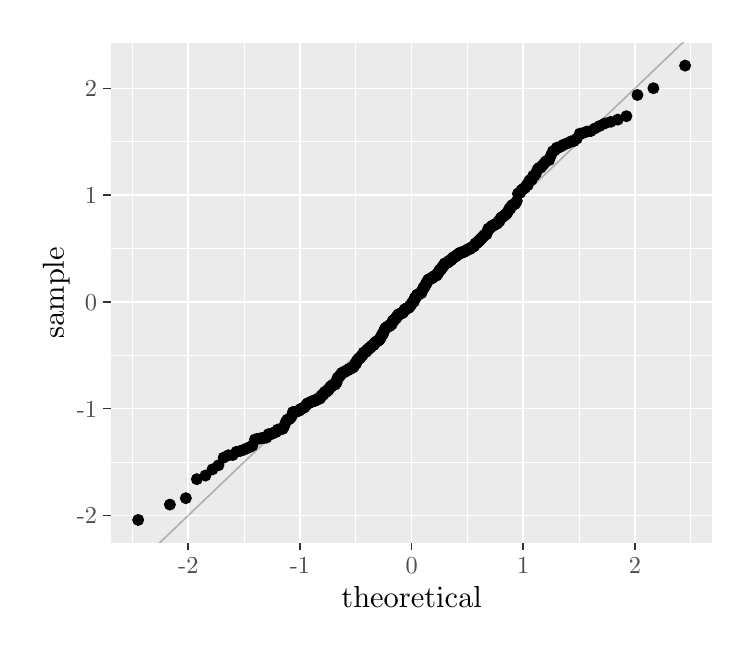
\begin{tikzpicture}[x=1pt,y=1pt]
\definecolor{fillColor}{RGB}{255,255,255}
\path[use as bounding box,fill=fillColor,fill opacity=0.00] (0,0) rectangle (252.94,216.81);
\begin{scope}
\path[clip] (  0.00,  0.00) rectangle (252.94,216.81);
\definecolor{drawColor}{RGB}{255,255,255}
\definecolor{fillColor}{RGB}{255,255,255}

\path[draw=drawColor,line width= 0.6pt,line join=round,line cap=round,fill=fillColor] (  0.00,  0.00) rectangle (252.94,216.81);
\end{scope}
\begin{scope}
\path[clip] ( 30.05, 30.72) rectangle (247.44,211.31);
\definecolor{fillColor}{gray}{0.92}

\path[fill=fillColor] ( 30.05, 30.72) rectangle (247.44,211.31);
\definecolor{drawColor}{RGB}{255,255,255}

\path[draw=drawColor,line width= 0.3pt,line join=round] ( 30.05, 59.86) --
	(247.44, 59.86);

\path[draw=drawColor,line width= 0.3pt,line join=round] ( 30.05, 98.43) --
	(247.44, 98.43);

\path[draw=drawColor,line width= 0.3pt,line join=round] ( 30.05,137.01) --
	(247.44,137.01);

\path[draw=drawColor,line width= 0.3pt,line join=round] ( 30.05,175.58) --
	(247.44,175.58);

\path[draw=drawColor,line width= 0.3pt,line join=round] ( 37.88, 30.72) --
	( 37.88,211.31);

\path[draw=drawColor,line width= 0.3pt,line join=round] ( 78.22, 30.72) --
	( 78.22,211.31);

\path[draw=drawColor,line width= 0.3pt,line join=round] (118.56, 30.72) --
	(118.56,211.31);

\path[draw=drawColor,line width= 0.3pt,line join=round] (158.90, 30.72) --
	(158.90,211.31);

\path[draw=drawColor,line width= 0.3pt,line join=round] (199.25, 30.72) --
	(199.25,211.31);

\path[draw=drawColor,line width= 0.3pt,line join=round] (239.59, 30.72) --
	(239.59,211.31);

\path[draw=drawColor,line width= 0.6pt,line join=round] ( 30.05, 40.57) --
	(247.44, 40.57);

\path[draw=drawColor,line width= 0.6pt,line join=round] ( 30.05, 79.15) --
	(247.44, 79.15);

\path[draw=drawColor,line width= 0.6pt,line join=round] ( 30.05,117.72) --
	(247.44,117.72);

\path[draw=drawColor,line width= 0.6pt,line join=round] ( 30.05,156.29) --
	(247.44,156.29);

\path[draw=drawColor,line width= 0.6pt,line join=round] ( 30.05,194.87) --
	(247.44,194.87);

\path[draw=drawColor,line width= 0.6pt,line join=round] ( 58.05, 30.72) --
	( 58.05,211.31);

\path[draw=drawColor,line width= 0.6pt,line join=round] ( 98.39, 30.72) --
	( 98.39,211.31);

\path[draw=drawColor,line width= 0.6pt,line join=round] (138.73, 30.72) --
	(138.73,211.31);

\path[draw=drawColor,line width= 0.6pt,line join=round] (179.07, 30.72) --
	(179.07,211.31);

\path[draw=drawColor,line width= 0.6pt,line join=round] (219.42, 30.72) --
	(219.42,211.31);
\definecolor{drawColor}{RGB}{0,0,0}
\definecolor{fillColor}{RGB}{0,0,0}

\path[draw=drawColor,line width= 0.4pt,line join=round,line cap=round,fill=fillColor] ( 39.93, 38.93) circle (  1.96);

\path[draw=drawColor,line width= 0.4pt,line join=round,line cap=round,fill=fillColor] ( 51.39, 44.48) circle (  1.96);

\path[draw=drawColor,line width= 0.4pt,line join=round,line cap=round,fill=fillColor] ( 57.16, 46.79) circle (  1.96);

\path[draw=drawColor,line width= 0.4pt,line join=round,line cap=round,fill=fillColor] ( 61.14, 53.66) circle (  1.96);

\path[draw=drawColor,line width= 0.4pt,line join=round,line cap=round,fill=fillColor] ( 64.23, 54.96) circle (  1.96);

\path[draw=drawColor,line width= 0.4pt,line join=round,line cap=round,fill=fillColor] ( 66.77, 57.21) circle (  1.96);

\path[draw=drawColor,line width= 0.4pt,line join=round,line cap=round,fill=fillColor] ( 68.94, 58.68) circle (  1.96);

\path[draw=drawColor,line width= 0.4pt,line join=round,line cap=round,fill=fillColor] ( 70.84, 61.45) circle (  1.96);

\path[draw=drawColor,line width= 0.4pt,line join=round,line cap=round,fill=fillColor] ( 72.53, 62.30) circle (  1.96);

\path[draw=drawColor,line width= 0.4pt,line join=round,line cap=round,fill=fillColor] ( 74.07, 62.38) circle (  1.96);

\path[draw=drawColor,line width= 0.4pt,line join=round,line cap=round,fill=fillColor] ( 75.47, 63.58) circle (  1.96);

\path[draw=drawColor,line width= 0.4pt,line join=round,line cap=round,fill=fillColor] ( 76.77, 63.85) circle (  1.96);

\path[draw=drawColor,line width= 0.4pt,line join=round,line cap=round,fill=fillColor] ( 77.97, 64.26) circle (  1.96);

\path[draw=drawColor,line width= 0.4pt,line join=round,line cap=round,fill=fillColor] ( 79.10, 64.75) circle (  1.96);

\path[draw=drawColor,line width= 0.4pt,line join=round,line cap=round,fill=fillColor] ( 80.16, 65.20) circle (  1.96);

\path[draw=drawColor,line width= 0.4pt,line join=round,line cap=round,fill=fillColor] ( 81.17, 65.76) circle (  1.96);

\path[draw=drawColor,line width= 0.4pt,line join=round,line cap=round,fill=fillColor] ( 82.12, 67.99) circle (  1.96);

\path[draw=drawColor,line width= 0.4pt,line join=round,line cap=round,fill=fillColor] ( 83.02, 68.22) circle (  1.96);

\path[draw=drawColor,line width= 0.4pt,line join=round,line cap=round,fill=fillColor] ( 83.89, 68.33) circle (  1.96);

\path[draw=drawColor,line width= 0.4pt,line join=round,line cap=round,fill=fillColor] ( 84.72, 68.55) circle (  1.96);

\path[draw=drawColor,line width= 0.4pt,line join=round,line cap=round,fill=fillColor] ( 85.51, 68.59) circle (  1.96);

\path[draw=drawColor,line width= 0.4pt,line join=round,line cap=round,fill=fillColor] ( 86.28, 68.67) circle (  1.96);

\path[draw=drawColor,line width= 0.4pt,line join=round,line cap=round,fill=fillColor] ( 87.02, 69.92) circle (  1.96);

\path[draw=drawColor,line width= 0.4pt,line join=round,line cap=round,fill=fillColor] ( 87.73, 69.92) circle (  1.96);

\path[draw=drawColor,line width= 0.4pt,line join=round,line cap=round,fill=fillColor] ( 88.42, 70.10) circle (  1.96);

\path[draw=drawColor,line width= 0.4pt,line join=round,line cap=round,fill=fillColor] ( 89.08, 70.56) circle (  1.96);

\path[draw=drawColor,line width= 0.4pt,line join=round,line cap=round,fill=fillColor] ( 89.73, 70.67) circle (  1.96);

\path[draw=drawColor,line width= 0.4pt,line join=round,line cap=round,fill=fillColor] ( 90.36, 71.57) circle (  1.96);

\path[draw=drawColor,line width= 0.4pt,line join=round,line cap=round,fill=fillColor] ( 90.97, 71.61) circle (  1.96);

\path[draw=drawColor,line width= 0.4pt,line join=round,line cap=round,fill=fillColor] ( 91.57, 71.78) circle (  1.96);

\path[draw=drawColor,line width= 0.4pt,line join=round,line cap=round,fill=fillColor] ( 92.15, 71.85) circle (  1.96);

\path[draw=drawColor,line width= 0.4pt,line join=round,line cap=round,fill=fillColor] ( 92.71, 72.82) circle (  1.96);

\path[draw=drawColor,line width= 0.4pt,line join=round,line cap=round,fill=fillColor] ( 93.26, 74.33) circle (  1.96);

\path[draw=drawColor,line width= 0.4pt,line join=round,line cap=round,fill=fillColor] ( 93.80, 75.16) circle (  1.96);

\path[draw=drawColor,line width= 0.4pt,line join=round,line cap=round,fill=fillColor] ( 94.33, 75.23) circle (  1.96);

\path[draw=drawColor,line width= 0.4pt,line join=round,line cap=round,fill=fillColor] ( 94.85, 75.66) circle (  1.96);

\path[draw=drawColor,line width= 0.4pt,line join=round,line cap=round,fill=fillColor] ( 95.35, 76.27) circle (  1.96);

\path[draw=drawColor,line width= 0.4pt,line join=round,line cap=round,fill=fillColor] ( 95.85, 77.93) circle (  1.96);

\path[draw=drawColor,line width= 0.4pt,line join=round,line cap=round,fill=fillColor] ( 96.33, 77.95) circle (  1.96);

\path[draw=drawColor,line width= 0.4pt,line join=round,line cap=round,fill=fillColor] ( 96.81, 77.97) circle (  1.96);

\path[draw=drawColor,line width= 0.4pt,line join=round,line cap=round,fill=fillColor] ( 97.28, 78.13) circle (  1.96);

\path[draw=drawColor,line width= 0.4pt,line join=round,line cap=round,fill=fillColor] ( 97.74, 78.27) circle (  1.96);

\path[draw=drawColor,line width= 0.4pt,line join=round,line cap=round,fill=fillColor] ( 98.19, 78.47) circle (  1.96);

\path[draw=drawColor,line width= 0.4pt,line join=round,line cap=round,fill=fillColor] ( 98.63, 79.00) circle (  1.96);

\path[draw=drawColor,line width= 0.4pt,line join=round,line cap=round,fill=fillColor] ( 99.07, 79.15) circle (  1.96);

\path[draw=drawColor,line width= 0.4pt,line join=round,line cap=round,fill=fillColor] ( 99.50, 79.38) circle (  1.96);

\path[draw=drawColor,line width= 0.4pt,line join=round,line cap=round,fill=fillColor] ( 99.92, 79.56) circle (  1.96);

\path[draw=drawColor,line width= 0.4pt,line join=round,line cap=round,fill=fillColor] (100.34, 80.09) circle (  1.96);

\path[draw=drawColor,line width= 0.4pt,line join=round,line cap=round,fill=fillColor] (100.75, 80.51) circle (  1.96);

\path[draw=drawColor,line width= 0.4pt,line join=round,line cap=round,fill=fillColor] (101.15, 81.06) circle (  1.96);

\path[draw=drawColor,line width= 0.4pt,line join=round,line cap=round,fill=fillColor] (101.55, 81.12) circle (  1.96);

\path[draw=drawColor,line width= 0.4pt,line join=round,line cap=round,fill=fillColor] (101.95, 81.34) circle (  1.96);

\path[draw=drawColor,line width= 0.4pt,line join=round,line cap=round,fill=fillColor] (102.33, 81.47) circle (  1.96);

\path[draw=drawColor,line width= 0.4pt,line join=round,line cap=round,fill=fillColor] (102.72, 81.83) circle (  1.96);

\path[draw=drawColor,line width= 0.4pt,line join=round,line cap=round,fill=fillColor] (103.10, 81.85) circle (  1.96);

\path[draw=drawColor,line width= 0.4pt,line join=round,line cap=round,fill=fillColor] (103.47, 81.94) circle (  1.96);

\path[draw=drawColor,line width= 0.4pt,line join=round,line cap=round,fill=fillColor] (103.84, 81.97) circle (  1.96);

\path[draw=drawColor,line width= 0.4pt,line join=round,line cap=round,fill=fillColor] (104.20, 82.22) circle (  1.96);

\path[draw=drawColor,line width= 0.4pt,line join=round,line cap=round,fill=fillColor] (104.56, 82.55) circle (  1.96);

\path[draw=drawColor,line width= 0.4pt,line join=round,line cap=round,fill=fillColor] (104.92, 82.62) circle (  1.96);

\path[draw=drawColor,line width= 0.4pt,line join=round,line cap=round,fill=fillColor] (105.27, 82.66) circle (  1.96);

\path[draw=drawColor,line width= 0.4pt,line join=round,line cap=round,fill=fillColor] (105.62, 82.83) circle (  1.96);

\path[draw=drawColor,line width= 0.4pt,line join=round,line cap=round,fill=fillColor] (105.97, 83.42) circle (  1.96);

\path[draw=drawColor,line width= 0.4pt,line join=round,line cap=round,fill=fillColor] (106.31, 83.92) circle (  1.96);

\path[draw=drawColor,line width= 0.4pt,line join=round,line cap=round,fill=fillColor] (106.64, 84.06) circle (  1.96);

\path[draw=drawColor,line width= 0.4pt,line join=round,line cap=round,fill=fillColor] (106.98, 84.41) circle (  1.96);

\path[draw=drawColor,line width= 0.4pt,line join=round,line cap=round,fill=fillColor] (107.31, 85.09) circle (  1.96);

\path[draw=drawColor,line width= 0.4pt,line join=round,line cap=round,fill=fillColor] (107.64, 85.09) circle (  1.96);

\path[draw=drawColor,line width= 0.4pt,line join=round,line cap=round,fill=fillColor] (107.96, 85.31) circle (  1.96);

\path[draw=drawColor,line width= 0.4pt,line join=round,line cap=round,fill=fillColor] (108.28, 85.64) circle (  1.96);

\path[draw=drawColor,line width= 0.4pt,line join=round,line cap=round,fill=fillColor] (108.60, 85.75) circle (  1.96);

\path[draw=drawColor,line width= 0.4pt,line join=round,line cap=round,fill=fillColor] (108.92, 86.31) circle (  1.96);

\path[draw=drawColor,line width= 0.4pt,line join=round,line cap=round,fill=fillColor] (109.23, 86.69) circle (  1.96);

\path[draw=drawColor,line width= 0.4pt,line join=round,line cap=round,fill=fillColor] (109.54, 87.18) circle (  1.96);

\path[draw=drawColor,line width= 0.4pt,line join=round,line cap=round,fill=fillColor] (109.85, 87.19) circle (  1.96);

\path[draw=drawColor,line width= 0.4pt,line join=round,line cap=round,fill=fillColor] (110.16, 87.65) circle (  1.96);

\path[draw=drawColor,line width= 0.4pt,line join=round,line cap=round,fill=fillColor] (110.46, 87.69) circle (  1.96);

\path[draw=drawColor,line width= 0.4pt,line join=round,line cap=round,fill=fillColor] (110.76, 87.83) circle (  1.96);

\path[draw=drawColor,line width= 0.4pt,line join=round,line cap=round,fill=fillColor] (111.06, 87.83) circle (  1.96);

\path[draw=drawColor,line width= 0.4pt,line join=round,line cap=round,fill=fillColor] (111.35, 88.56) circle (  1.96);

\path[draw=drawColor,line width= 0.4pt,line join=round,line cap=round,fill=fillColor] (111.65, 88.59) circle (  1.96);

\path[draw=drawColor,line width= 0.4pt,line join=round,line cap=round,fill=fillColor] (111.94, 90.19) circle (  1.96);

\path[draw=drawColor,line width= 0.4pt,line join=round,line cap=round,fill=fillColor] (112.23, 90.38) circle (  1.96);

\path[draw=drawColor,line width= 0.4pt,line join=round,line cap=round,fill=fillColor] (112.52, 90.67) circle (  1.96);

\path[draw=drawColor,line width= 0.4pt,line join=round,line cap=round,fill=fillColor] (112.80, 91.03) circle (  1.96);

\path[draw=drawColor,line width= 0.4pt,line join=round,line cap=round,fill=fillColor] (113.08, 91.33) circle (  1.96);

\path[draw=drawColor,line width= 0.4pt,line join=round,line cap=round,fill=fillColor] (113.37, 91.77) circle (  1.96);

\path[draw=drawColor,line width= 0.4pt,line join=round,line cap=round,fill=fillColor] (113.65, 92.13) circle (  1.96);

\path[draw=drawColor,line width= 0.4pt,line join=round,line cap=round,fill=fillColor] (113.92, 92.18) circle (  1.96);

\path[draw=drawColor,line width= 0.4pt,line join=round,line cap=round,fill=fillColor] (114.20, 92.27) circle (  1.96);

\path[draw=drawColor,line width= 0.4pt,line join=round,line cap=round,fill=fillColor] (114.47, 92.49) circle (  1.96);

\path[draw=drawColor,line width= 0.4pt,line join=round,line cap=round,fill=fillColor] (114.75, 92.51) circle (  1.96);

\path[draw=drawColor,line width= 0.4pt,line join=round,line cap=round,fill=fillColor] (115.02, 92.81) circle (  1.96);

\path[draw=drawColor,line width= 0.4pt,line join=round,line cap=round,fill=fillColor] (115.29, 92.91) circle (  1.96);

\path[draw=drawColor,line width= 0.4pt,line join=round,line cap=round,fill=fillColor] (115.55, 93.00) circle (  1.96);

\path[draw=drawColor,line width= 0.4pt,line join=round,line cap=round,fill=fillColor] (115.82, 93.15) circle (  1.96);

\path[draw=drawColor,line width= 0.4pt,line join=round,line cap=round,fill=fillColor] (116.09, 93.38) circle (  1.96);

\path[draw=drawColor,line width= 0.4pt,line join=round,line cap=round,fill=fillColor] (116.35, 93.61) circle (  1.96);

\path[draw=drawColor,line width= 0.4pt,line join=round,line cap=round,fill=fillColor] (116.61, 93.63) circle (  1.96);

\path[draw=drawColor,line width= 0.4pt,line join=round,line cap=round,fill=fillColor] (116.87, 93.63) circle (  1.96);

\path[draw=drawColor,line width= 0.4pt,line join=round,line cap=round,fill=fillColor] (117.13, 93.83) circle (  1.96);

\path[draw=drawColor,line width= 0.4pt,line join=round,line cap=round,fill=fillColor] (117.39, 94.07) circle (  1.96);

\path[draw=drawColor,line width= 0.4pt,line join=round,line cap=round,fill=fillColor] (117.64, 94.14) circle (  1.96);

\path[draw=drawColor,line width= 0.4pt,line join=round,line cap=round,fill=fillColor] (117.90, 94.49) circle (  1.96);

\path[draw=drawColor,line width= 0.4pt,line join=round,line cap=round,fill=fillColor] (118.15, 94.96) circle (  1.96);

\path[draw=drawColor,line width= 0.4pt,line join=round,line cap=round,fill=fillColor] (118.40, 95.38) circle (  1.96);

\path[draw=drawColor,line width= 0.4pt,line join=round,line cap=round,fill=fillColor] (118.66, 95.41) circle (  1.96);

\path[draw=drawColor,line width= 0.4pt,line join=round,line cap=round,fill=fillColor] (118.91, 96.40) circle (  1.96);

\path[draw=drawColor,line width= 0.4pt,line join=round,line cap=round,fill=fillColor] (119.16, 96.48) circle (  1.96);

\path[draw=drawColor,line width= 0.4pt,line join=round,line cap=round,fill=fillColor] (119.40, 96.90) circle (  1.96);

\path[draw=drawColor,line width= 0.4pt,line join=round,line cap=round,fill=fillColor] (119.65, 97.26) circle (  1.96);

\path[draw=drawColor,line width= 0.4pt,line join=round,line cap=round,fill=fillColor] (119.90, 97.33) circle (  1.96);

\path[draw=drawColor,line width= 0.4pt,line join=round,line cap=round,fill=fillColor] (120.14, 97.49) circle (  1.96);

\path[draw=drawColor,line width= 0.4pt,line join=round,line cap=round,fill=fillColor] (120.38, 97.90) circle (  1.96);

\path[draw=drawColor,line width= 0.4pt,line join=round,line cap=round,fill=fillColor] (120.63, 98.19) circle (  1.96);

\path[draw=drawColor,line width= 0.4pt,line join=round,line cap=round,fill=fillColor] (120.87, 98.43) circle (  1.96);

\path[draw=drawColor,line width= 0.4pt,line join=round,line cap=round,fill=fillColor] (121.11, 98.59) circle (  1.96);

\path[draw=drawColor,line width= 0.4pt,line join=round,line cap=round,fill=fillColor] (121.35, 99.37) circle (  1.96);

\path[draw=drawColor,line width= 0.4pt,line join=round,line cap=round,fill=fillColor] (121.59, 99.39) circle (  1.96);

\path[draw=drawColor,line width= 0.4pt,line join=round,line cap=round,fill=fillColor] (121.82, 99.51) circle (  1.96);

\path[draw=drawColor,line width= 0.4pt,line join=round,line cap=round,fill=fillColor] (122.06, 99.60) circle (  1.96);

\path[draw=drawColor,line width= 0.4pt,line join=round,line cap=round,fill=fillColor] (122.30, 99.71) circle (  1.96);

\path[draw=drawColor,line width= 0.4pt,line join=round,line cap=round,fill=fillColor] (122.53,100.11) circle (  1.96);

\path[draw=drawColor,line width= 0.4pt,line join=round,line cap=round,fill=fillColor] (122.77,100.45) circle (  1.96);

\path[draw=drawColor,line width= 0.4pt,line join=round,line cap=round,fill=fillColor] (123.00,100.64) circle (  1.96);

\path[draw=drawColor,line width= 0.4pt,line join=round,line cap=round,fill=fillColor] (123.23,100.68) circle (  1.96);

\path[draw=drawColor,line width= 0.4pt,line join=round,line cap=round,fill=fillColor] (123.47,101.09) circle (  1.96);

\path[draw=drawColor,line width= 0.4pt,line join=round,line cap=round,fill=fillColor] (123.70,101.18) circle (  1.96);

\path[draw=drawColor,line width= 0.4pt,line join=round,line cap=round,fill=fillColor] (123.93,101.32) circle (  1.96);

\path[draw=drawColor,line width= 0.4pt,line join=round,line cap=round,fill=fillColor] (124.16,101.69) circle (  1.96);

\path[draw=drawColor,line width= 0.4pt,line join=round,line cap=round,fill=fillColor] (124.39,101.88) circle (  1.96);

\path[draw=drawColor,line width= 0.4pt,line join=round,line cap=round,fill=fillColor] (124.61,102.00) circle (  1.96);

\path[draw=drawColor,line width= 0.4pt,line join=round,line cap=round,fill=fillColor] (124.84,102.17) circle (  1.96);

\path[draw=drawColor,line width= 0.4pt,line join=round,line cap=round,fill=fillColor] (125.07,102.17) circle (  1.96);

\path[draw=drawColor,line width= 0.4pt,line join=round,line cap=round,fill=fillColor] (125.30,102.65) circle (  1.96);

\path[draw=drawColor,line width= 0.4pt,line join=round,line cap=round,fill=fillColor] (125.52,102.96) circle (  1.96);

\path[draw=drawColor,line width= 0.4pt,line join=round,line cap=round,fill=fillColor] (125.75,103.18) circle (  1.96);

\path[draw=drawColor,line width= 0.4pt,line join=round,line cap=round,fill=fillColor] (125.97,103.28) circle (  1.96);

\path[draw=drawColor,line width= 0.4pt,line join=round,line cap=round,fill=fillColor] (126.19,103.40) circle (  1.96);

\path[draw=drawColor,line width= 0.4pt,line join=round,line cap=round,fill=fillColor] (126.42,103.62) circle (  1.96);

\path[draw=drawColor,line width= 0.4pt,line join=round,line cap=round,fill=fillColor] (126.64,103.69) circle (  1.96);

\path[draw=drawColor,line width= 0.4pt,line join=round,line cap=round,fill=fillColor] (126.86,103.86) circle (  1.96);

\path[draw=drawColor,line width= 0.4pt,line join=round,line cap=round,fill=fillColor] (127.08,104.11) circle (  1.96);

\path[draw=drawColor,line width= 0.4pt,line join=round,line cap=round,fill=fillColor] (127.31,104.49) circle (  1.96);

\path[draw=drawColor,line width= 0.4pt,line join=round,line cap=round,fill=fillColor] (127.53,104.58) circle (  1.96);

\path[draw=drawColor,line width= 0.4pt,line join=round,line cap=round,fill=fillColor] (127.75,105.28) circle (  1.96);

\path[draw=drawColor,line width= 0.4pt,line join=round,line cap=round,fill=fillColor] (127.97,105.68) circle (  1.96);

\path[draw=drawColor,line width= 0.4pt,line join=round,line cap=round,fill=fillColor] (128.18,106.07) circle (  1.96);

\path[draw=drawColor,line width= 0.4pt,line join=round,line cap=round,fill=fillColor] (128.40,106.10) circle (  1.96);

\path[draw=drawColor,line width= 0.4pt,line join=round,line cap=round,fill=fillColor] (128.62,106.86) circle (  1.96);

\path[draw=drawColor,line width= 0.4pt,line join=round,line cap=round,fill=fillColor] (128.84,107.40) circle (  1.96);

\path[draw=drawColor,line width= 0.4pt,line join=round,line cap=round,fill=fillColor] (129.06,107.75) circle (  1.96);

\path[draw=drawColor,line width= 0.4pt,line join=round,line cap=round,fill=fillColor] (129.27,108.21) circle (  1.96);

\path[draw=drawColor,line width= 0.4pt,line join=round,line cap=round,fill=fillColor] (129.49,108.41) circle (  1.96);

\path[draw=drawColor,line width= 0.4pt,line join=round,line cap=round,fill=fillColor] (129.70,108.43) circle (  1.96);

\path[draw=drawColor,line width= 0.4pt,line join=round,line cap=round,fill=fillColor] (129.92,108.72) circle (  1.96);

\path[draw=drawColor,line width= 0.4pt,line join=round,line cap=round,fill=fillColor] (130.14,108.80) circle (  1.96);

\path[draw=drawColor,line width= 0.4pt,line join=round,line cap=round,fill=fillColor] (130.35,108.87) circle (  1.96);

\path[draw=drawColor,line width= 0.4pt,line join=round,line cap=round,fill=fillColor] (130.56,108.93) circle (  1.96);

\path[draw=drawColor,line width= 0.4pt,line join=round,line cap=round,fill=fillColor] (130.78,108.97) circle (  1.96);

\path[draw=drawColor,line width= 0.4pt,line join=round,line cap=round,fill=fillColor] (130.99,109.41) circle (  1.96);

\path[draw=drawColor,line width= 0.4pt,line join=round,line cap=round,fill=fillColor] (131.21,109.48) circle (  1.96);

\path[draw=drawColor,line width= 0.4pt,line join=round,line cap=round,fill=fillColor] (131.42,109.55) circle (  1.96);

\path[draw=drawColor,line width= 0.4pt,line join=round,line cap=round,fill=fillColor] (131.63,109.80) circle (  1.96);

\path[draw=drawColor,line width= 0.4pt,line join=round,line cap=round,fill=fillColor] (131.84,110.76) circle (  1.96);

\path[draw=drawColor,line width= 0.4pt,line join=round,line cap=round,fill=fillColor] (132.06,110.86) circle (  1.96);

\path[draw=drawColor,line width= 0.4pt,line join=round,line cap=round,fill=fillColor] (132.27,110.92) circle (  1.96);

\path[draw=drawColor,line width= 0.4pt,line join=round,line cap=round,fill=fillColor] (132.48,111.32) circle (  1.96);

\path[draw=drawColor,line width= 0.4pt,line join=round,line cap=round,fill=fillColor] (132.69,111.45) circle (  1.96);

\path[draw=drawColor,line width= 0.4pt,line join=round,line cap=round,fill=fillColor] (132.90,111.79) circle (  1.96);

\path[draw=drawColor,line width= 0.4pt,line join=round,line cap=round,fill=fillColor] (133.11,111.81) circle (  1.96);

\path[draw=drawColor,line width= 0.4pt,line join=round,line cap=round,fill=fillColor] (133.32,112.26) circle (  1.96);

\path[draw=drawColor,line width= 0.4pt,line join=round,line cap=round,fill=fillColor] (133.53,112.59) circle (  1.96);

\path[draw=drawColor,line width= 0.4pt,line join=round,line cap=round,fill=fillColor] (133.74,112.65) circle (  1.96);

\path[draw=drawColor,line width= 0.4pt,line join=round,line cap=round,fill=fillColor] (133.95,113.17) circle (  1.96);

\path[draw=drawColor,line width= 0.4pt,line join=round,line cap=round,fill=fillColor] (134.16,113.26) circle (  1.96);

\path[draw=drawColor,line width= 0.4pt,line join=round,line cap=round,fill=fillColor] (134.37,113.28) circle (  1.96);

\path[draw=drawColor,line width= 0.4pt,line join=round,line cap=round,fill=fillColor] (134.58,113.39) circle (  1.96);

\path[draw=drawColor,line width= 0.4pt,line join=round,line cap=round,fill=fillColor] (134.79,113.52) circle (  1.96);

\path[draw=drawColor,line width= 0.4pt,line join=round,line cap=round,fill=fillColor] (135.00,113.56) circle (  1.96);

\path[draw=drawColor,line width= 0.4pt,line join=round,line cap=round,fill=fillColor] (135.21,113.65) circle (  1.96);

\path[draw=drawColor,line width= 0.4pt,line join=round,line cap=round,fill=fillColor] (135.42,113.71) circle (  1.96);

\path[draw=drawColor,line width= 0.4pt,line join=round,line cap=round,fill=fillColor] (135.63,113.93) circle (  1.96);

\path[draw=drawColor,line width= 0.4pt,line join=round,line cap=round,fill=fillColor] (135.84,114.24) circle (  1.96);

\path[draw=drawColor,line width= 0.4pt,line join=round,line cap=round,fill=fillColor] (136.05,114.58) circle (  1.96);

\path[draw=drawColor,line width= 0.4pt,line join=round,line cap=round,fill=fillColor] (136.25,115.01) circle (  1.96);

\path[draw=drawColor,line width= 0.4pt,line join=round,line cap=round,fill=fillColor] (136.46,115.04) circle (  1.96);

\path[draw=drawColor,line width= 0.4pt,line join=round,line cap=round,fill=fillColor] (136.67,115.05) circle (  1.96);

\path[draw=drawColor,line width= 0.4pt,line join=round,line cap=round,fill=fillColor] (136.88,115.29) circle (  1.96);

\path[draw=drawColor,line width= 0.4pt,line join=round,line cap=round,fill=fillColor] (137.09,115.51) circle (  1.96);

\path[draw=drawColor,line width= 0.4pt,line join=round,line cap=round,fill=fillColor] (137.29,115.53) circle (  1.96);

\path[draw=drawColor,line width= 0.4pt,line join=round,line cap=round,fill=fillColor] (137.50,115.55) circle (  1.96);

\path[draw=drawColor,line width= 0.4pt,line join=round,line cap=round,fill=fillColor] (137.71,115.62) circle (  1.96);

\path[draw=drawColor,line width= 0.4pt,line join=round,line cap=round,fill=fillColor] (137.92,115.84) circle (  1.96);

\path[draw=drawColor,line width= 0.4pt,line join=round,line cap=round,fill=fillColor] (138.13,116.33) circle (  1.96);

\path[draw=drawColor,line width= 0.4pt,line join=round,line cap=round,fill=fillColor] (138.33,116.43) circle (  1.96);

\path[draw=drawColor,line width= 0.4pt,line join=round,line cap=round,fill=fillColor] (138.54,116.67) circle (  1.96);

\path[draw=drawColor,line width= 0.4pt,line join=round,line cap=round,fill=fillColor] (138.75,117.14) circle (  1.96);

\path[draw=drawColor,line width= 0.4pt,line join=round,line cap=round,fill=fillColor] (138.96,117.39) circle (  1.96);

\path[draw=drawColor,line width= 0.4pt,line join=round,line cap=round,fill=fillColor] (139.16,117.56) circle (  1.96);

\path[draw=drawColor,line width= 0.4pt,line join=round,line cap=round,fill=fillColor] (139.37,117.84) circle (  1.96);

\path[draw=drawColor,line width= 0.4pt,line join=round,line cap=round,fill=fillColor] (139.58,117.88) circle (  1.96);

\path[draw=drawColor,line width= 0.4pt,line join=round,line cap=round,fill=fillColor] (139.79,118.93) circle (  1.96);

\path[draw=drawColor,line width= 0.4pt,line join=round,line cap=round,fill=fillColor] (139.99,119.24) circle (  1.96);

\path[draw=drawColor,line width= 0.4pt,line join=round,line cap=round,fill=fillColor] (140.20,119.34) circle (  1.96);

\path[draw=drawColor,line width= 0.4pt,line join=round,line cap=round,fill=fillColor] (140.41,119.52) circle (  1.96);

\path[draw=drawColor,line width= 0.4pt,line join=round,line cap=round,fill=fillColor] (140.62,120.19) circle (  1.96);

\path[draw=drawColor,line width= 0.4pt,line join=round,line cap=round,fill=fillColor] (140.83,120.23) circle (  1.96);

\path[draw=drawColor,line width= 0.4pt,line join=round,line cap=round,fill=fillColor] (141.03,120.36) circle (  1.96);

\path[draw=drawColor,line width= 0.4pt,line join=round,line cap=round,fill=fillColor] (141.24,120.45) circle (  1.96);

\path[draw=drawColor,line width= 0.4pt,line join=round,line cap=round,fill=fillColor] (141.45,120.67) circle (  1.96);

\path[draw=drawColor,line width= 0.4pt,line join=round,line cap=round,fill=fillColor] (141.66,120.69) circle (  1.96);

\path[draw=drawColor,line width= 0.4pt,line join=round,line cap=round,fill=fillColor] (141.87,120.86) circle (  1.96);

\path[draw=drawColor,line width= 0.4pt,line join=round,line cap=round,fill=fillColor] (142.08,120.87) circle (  1.96);

\path[draw=drawColor,line width= 0.4pt,line join=round,line cap=round,fill=fillColor] (142.29,120.97) circle (  1.96);

\path[draw=drawColor,line width= 0.4pt,line join=round,line cap=round,fill=fillColor] (142.49,121.64) circle (  1.96);

\path[draw=drawColor,line width= 0.4pt,line join=round,line cap=round,fill=fillColor] (142.70,122.12) circle (  1.96);

\path[draw=drawColor,line width= 0.4pt,line join=round,line cap=round,fill=fillColor] (142.91,122.64) circle (  1.96);

\path[draw=drawColor,line width= 0.4pt,line join=round,line cap=round,fill=fillColor] (143.12,122.95) circle (  1.96);

\path[draw=drawColor,line width= 0.4pt,line join=round,line cap=round,fill=fillColor] (143.33,123.01) circle (  1.96);

\path[draw=drawColor,line width= 0.4pt,line join=round,line cap=round,fill=fillColor] (143.54,123.48) circle (  1.96);

\path[draw=drawColor,line width= 0.4pt,line join=round,line cap=round,fill=fillColor] (143.75,123.66) circle (  1.96);

\path[draw=drawColor,line width= 0.4pt,line join=round,line cap=round,fill=fillColor] (143.96,124.32) circle (  1.96);

\path[draw=drawColor,line width= 0.4pt,line join=round,line cap=round,fill=fillColor] (144.17,124.70) circle (  1.96);

\path[draw=drawColor,line width= 0.4pt,line join=round,line cap=round,fill=fillColor] (144.38,124.85) circle (  1.96);

\path[draw=drawColor,line width= 0.4pt,line join=round,line cap=round,fill=fillColor] (144.59,125.45) circle (  1.96);

\path[draw=drawColor,line width= 0.4pt,line join=round,line cap=round,fill=fillColor] (144.81,125.70) circle (  1.96);

\path[draw=drawColor,line width= 0.4pt,line join=round,line cap=round,fill=fillColor] (145.02,125.91) circle (  1.96);

\path[draw=drawColor,line width= 0.4pt,line join=round,line cap=round,fill=fillColor] (145.23,125.93) circle (  1.96);

\path[draw=drawColor,line width= 0.4pt,line join=round,line cap=round,fill=fillColor] (145.44,126.07) circle (  1.96);

\path[draw=drawColor,line width= 0.4pt,line join=round,line cap=round,fill=fillColor] (145.65,126.10) circle (  1.96);

\path[draw=drawColor,line width= 0.4pt,line join=round,line cap=round,fill=fillColor] (145.86,126.18) circle (  1.96);

\path[draw=drawColor,line width= 0.4pt,line join=round,line cap=round,fill=fillColor] (146.08,126.33) circle (  1.96);

\path[draw=drawColor,line width= 0.4pt,line join=round,line cap=round,fill=fillColor] (146.29,126.41) circle (  1.96);

\path[draw=drawColor,line width= 0.4pt,line join=round,line cap=round,fill=fillColor] (146.50,126.72) circle (  1.96);

\path[draw=drawColor,line width= 0.4pt,line join=round,line cap=round,fill=fillColor] (146.72,126.91) circle (  1.96);

\path[draw=drawColor,line width= 0.4pt,line join=round,line cap=round,fill=fillColor] (146.93,127.01) circle (  1.96);

\path[draw=drawColor,line width= 0.4pt,line join=round,line cap=round,fill=fillColor] (147.15,127.04) circle (  1.96);

\path[draw=drawColor,line width= 0.4pt,line join=round,line cap=round,fill=fillColor] (147.36,127.13) circle (  1.96);

\path[draw=drawColor,line width= 0.4pt,line join=round,line cap=round,fill=fillColor] (147.58,127.32) circle (  1.96);

\path[draw=drawColor,line width= 0.4pt,line join=round,line cap=round,fill=fillColor] (147.79,127.32) circle (  1.96);

\path[draw=drawColor,line width= 0.4pt,line join=round,line cap=round,fill=fillColor] (148.01,127.85) circle (  1.96);

\path[draw=drawColor,line width= 0.4pt,line join=round,line cap=round,fill=fillColor] (148.22,127.89) circle (  1.96);

\path[draw=drawColor,line width= 0.4pt,line join=round,line cap=round,fill=fillColor] (148.44,128.51) circle (  1.96);

\path[draw=drawColor,line width= 0.4pt,line join=round,line cap=round,fill=fillColor] (148.66,128.75) circle (  1.96);

\path[draw=drawColor,line width= 0.4pt,line join=round,line cap=round,fill=fillColor] (148.88,129.22) circle (  1.96);

\path[draw=drawColor,line width= 0.4pt,line join=round,line cap=round,fill=fillColor] (149.09,129.40) circle (  1.96);

\path[draw=drawColor,line width= 0.4pt,line join=round,line cap=round,fill=fillColor] (149.31,129.41) circle (  1.96);

\path[draw=drawColor,line width= 0.4pt,line join=round,line cap=round,fill=fillColor] (149.53,129.78) circle (  1.96);

\path[draw=drawColor,line width= 0.4pt,line join=round,line cap=round,fill=fillColor] (149.75,130.16) circle (  1.96);

\path[draw=drawColor,line width= 0.4pt,line join=round,line cap=round,fill=fillColor] (149.97,130.45) circle (  1.96);

\path[draw=drawColor,line width= 0.4pt,line join=round,line cap=round,fill=fillColor] (150.19,130.62) circle (  1.96);

\path[draw=drawColor,line width= 0.4pt,line join=round,line cap=round,fill=fillColor] (150.41,130.92) circle (  1.96);

\path[draw=drawColor,line width= 0.4pt,line join=round,line cap=round,fill=fillColor] (150.63,131.53) circle (  1.96);

\path[draw=drawColor,line width= 0.4pt,line join=round,line cap=round,fill=fillColor] (150.86,131.62) circle (  1.96);

\path[draw=drawColor,line width= 0.4pt,line join=round,line cap=round,fill=fillColor] (151.08,131.67) circle (  1.96);

\path[draw=drawColor,line width= 0.4pt,line join=round,line cap=round,fill=fillColor] (151.30,131.74) circle (  1.96);

\path[draw=drawColor,line width= 0.4pt,line join=round,line cap=round,fill=fillColor] (151.53,131.86) circle (  1.96);

\path[draw=drawColor,line width= 0.4pt,line join=round,line cap=round,fill=fillColor] (151.75,131.96) circle (  1.96);

\path[draw=drawColor,line width= 0.4pt,line join=round,line cap=round,fill=fillColor] (151.98,132.11) circle (  1.96);

\path[draw=drawColor,line width= 0.4pt,line join=round,line cap=round,fill=fillColor] (152.20,132.48) circle (  1.96);

\path[draw=drawColor,line width= 0.4pt,line join=round,line cap=round,fill=fillColor] (152.43,132.50) circle (  1.96);

\path[draw=drawColor,line width= 0.4pt,line join=round,line cap=round,fill=fillColor] (152.65,132.69) circle (  1.96);

\path[draw=drawColor,line width= 0.4pt,line join=round,line cap=round,fill=fillColor] (152.88,132.89) circle (  1.96);

\path[draw=drawColor,line width= 0.4pt,line join=round,line cap=round,fill=fillColor] (153.11,132.93) circle (  1.96);

\path[draw=drawColor,line width= 0.4pt,line join=round,line cap=round,fill=fillColor] (153.34,133.27) circle (  1.96);

\path[draw=drawColor,line width= 0.4pt,line join=round,line cap=round,fill=fillColor] (153.57,133.60) circle (  1.96);

\path[draw=drawColor,line width= 0.4pt,line join=round,line cap=round,fill=fillColor] (153.80,133.72) circle (  1.96);

\path[draw=drawColor,line width= 0.4pt,line join=round,line cap=round,fill=fillColor] (154.03,133.93) circle (  1.96);

\path[draw=drawColor,line width= 0.4pt,line join=round,line cap=round,fill=fillColor] (154.26,133.99) circle (  1.96);

\path[draw=drawColor,line width= 0.4pt,line join=round,line cap=round,fill=fillColor] (154.50,134.09) circle (  1.96);

\path[draw=drawColor,line width= 0.4pt,line join=round,line cap=round,fill=fillColor] (154.73,134.26) circle (  1.96);

\path[draw=drawColor,line width= 0.4pt,line join=round,line cap=round,fill=fillColor] (154.96,134.41) circle (  1.96);

\path[draw=drawColor,line width= 0.4pt,line join=round,line cap=round,fill=fillColor] (155.20,134.64) circle (  1.96);

\path[draw=drawColor,line width= 0.4pt,line join=round,line cap=round,fill=fillColor] (155.43,134.76) circle (  1.96);

\path[draw=drawColor,line width= 0.4pt,line join=round,line cap=round,fill=fillColor] (155.67,135.03) circle (  1.96);

\path[draw=drawColor,line width= 0.4pt,line join=round,line cap=round,fill=fillColor] (155.91,135.23) circle (  1.96);

\path[draw=drawColor,line width= 0.4pt,line join=round,line cap=round,fill=fillColor] (156.15,135.39) circle (  1.96);

\path[draw=drawColor,line width= 0.4pt,line join=round,line cap=round,fill=fillColor] (156.39,135.51) circle (  1.96);

\path[draw=drawColor,line width= 0.4pt,line join=round,line cap=round,fill=fillColor] (156.63,135.55) circle (  1.96);

\path[draw=drawColor,line width= 0.4pt,line join=round,line cap=round,fill=fillColor] (156.87,135.61) circle (  1.96);

\path[draw=drawColor,line width= 0.4pt,line join=round,line cap=round,fill=fillColor] (157.11,135.62) circle (  1.96);

\path[draw=drawColor,line width= 0.4pt,line join=round,line cap=round,fill=fillColor] (157.36,135.63) circle (  1.96);

\path[draw=drawColor,line width= 0.4pt,line join=round,line cap=round,fill=fillColor] (157.60,135.82) circle (  1.96);

\path[draw=drawColor,line width= 0.4pt,line join=round,line cap=round,fill=fillColor] (157.85,135.87) circle (  1.96);

\path[draw=drawColor,line width= 0.4pt,line join=round,line cap=round,fill=fillColor] (158.09,136.07) circle (  1.96);

\path[draw=drawColor,line width= 0.4pt,line join=round,line cap=round,fill=fillColor] (158.34,136.23) circle (  1.96);

\path[draw=drawColor,line width= 0.4pt,line join=round,line cap=round,fill=fillColor] (158.59,136.44) circle (  1.96);

\path[draw=drawColor,line width= 0.4pt,line join=round,line cap=round,fill=fillColor] (158.84,136.58) circle (  1.96);

\path[draw=drawColor,line width= 0.4pt,line join=round,line cap=round,fill=fillColor] (159.09,136.67) circle (  1.96);

\path[draw=drawColor,line width= 0.4pt,line join=round,line cap=round,fill=fillColor] (159.34,136.71) circle (  1.96);

\path[draw=drawColor,line width= 0.4pt,line join=round,line cap=round,fill=fillColor] (159.60,136.79) circle (  1.96);

\path[draw=drawColor,line width= 0.4pt,line join=round,line cap=round,fill=fillColor] (159.85,136.88) circle (  1.96);

\path[draw=drawColor,line width= 0.4pt,line join=round,line cap=round,fill=fillColor] (160.11,137.28) circle (  1.96);

\path[draw=drawColor,line width= 0.4pt,line join=round,line cap=round,fill=fillColor] (160.37,137.34) circle (  1.96);

\path[draw=drawColor,line width= 0.4pt,line join=round,line cap=round,fill=fillColor] (160.63,137.48) circle (  1.96);

\path[draw=drawColor,line width= 0.4pt,line join=round,line cap=round,fill=fillColor] (160.89,137.67) circle (  1.96);

\path[draw=drawColor,line width= 0.4pt,line join=round,line cap=round,fill=fillColor] (161.15,137.76) circle (  1.96);

\path[draw=drawColor,line width= 0.4pt,line join=round,line cap=round,fill=fillColor] (161.41,138.01) circle (  1.96);

\path[draw=drawColor,line width= 0.4pt,line join=round,line cap=round,fill=fillColor] (161.68,138.67) circle (  1.96);

\path[draw=drawColor,line width= 0.4pt,line join=round,line cap=round,fill=fillColor] (161.94,138.91) circle (  1.96);

\path[draw=drawColor,line width= 0.4pt,line join=round,line cap=round,fill=fillColor] (162.21,138.91) circle (  1.96);

\path[draw=drawColor,line width= 0.4pt,line join=round,line cap=round,fill=fillColor] (162.48,139.15) circle (  1.96);

\path[draw=drawColor,line width= 0.4pt,line join=round,line cap=round,fill=fillColor] (162.75,139.44) circle (  1.96);

\path[draw=drawColor,line width= 0.4pt,line join=round,line cap=round,fill=fillColor] (163.02,139.85) circle (  1.96);

\path[draw=drawColor,line width= 0.4pt,line join=round,line cap=round,fill=fillColor] (163.30,139.89) circle (  1.96);

\path[draw=drawColor,line width= 0.4pt,line join=round,line cap=round,fill=fillColor] (163.57,140.22) circle (  1.96);

\path[draw=drawColor,line width= 0.4pt,line join=round,line cap=round,fill=fillColor] (163.85,140.69) circle (  1.96);

\path[draw=drawColor,line width= 0.4pt,line join=round,line cap=round,fill=fillColor] (164.13,140.76) circle (  1.96);

\path[draw=drawColor,line width= 0.4pt,line join=round,line cap=round,fill=fillColor] (164.41,141.16) circle (  1.96);

\path[draw=drawColor,line width= 0.4pt,line join=round,line cap=round,fill=fillColor] (164.70,141.45) circle (  1.96);

\path[draw=drawColor,line width= 0.4pt,line join=round,line cap=round,fill=fillColor] (164.98,141.84) circle (  1.96);

\path[draw=drawColor,line width= 0.4pt,line join=round,line cap=round,fill=fillColor] (165.27,141.98) circle (  1.96);

\path[draw=drawColor,line width= 0.4pt,line join=round,line cap=round,fill=fillColor] (165.56,142.10) circle (  1.96);

\path[draw=drawColor,line width= 0.4pt,line join=round,line cap=round,fill=fillColor] (165.85,142.25) circle (  1.96);

\path[draw=drawColor,line width= 0.4pt,line join=round,line cap=round,fill=fillColor] (166.14,143.16) circle (  1.96);

\path[draw=drawColor,line width= 0.4pt,line join=round,line cap=round,fill=fillColor] (166.44,144.15) circle (  1.96);

\path[draw=drawColor,line width= 0.4pt,line join=round,line cap=round,fill=fillColor] (166.74,144.17) circle (  1.96);

\path[draw=drawColor,line width= 0.4pt,line join=round,line cap=round,fill=fillColor] (167.04,144.39) circle (  1.96);

\path[draw=drawColor,line width= 0.4pt,line join=round,line cap=round,fill=fillColor] (167.34,144.65) circle (  1.96);

\path[draw=drawColor,line width= 0.4pt,line join=round,line cap=round,fill=fillColor] (167.65,145.07) circle (  1.96);

\path[draw=drawColor,line width= 0.4pt,line join=round,line cap=round,fill=fillColor] (167.95,145.24) circle (  1.96);

\path[draw=drawColor,line width= 0.4pt,line join=round,line cap=round,fill=fillColor] (168.26,145.25) circle (  1.96);

\path[draw=drawColor,line width= 0.4pt,line join=round,line cap=round,fill=fillColor] (168.58,145.61) circle (  1.96);

\path[draw=drawColor,line width= 0.4pt,line join=round,line cap=round,fill=fillColor] (168.89,145.69) circle (  1.96);

\path[draw=drawColor,line width= 0.4pt,line join=round,line cap=round,fill=fillColor] (169.21,145.93) circle (  1.96);

\path[draw=drawColor,line width= 0.4pt,line join=round,line cap=round,fill=fillColor] (169.53,145.94) circle (  1.96);

\path[draw=drawColor,line width= 0.4pt,line join=round,line cap=round,fill=fillColor] (169.86,146.26) circle (  1.96);

\path[draw=drawColor,line width= 0.4pt,line join=round,line cap=round,fill=fillColor] (170.19,146.86) circle (  1.96);

\path[draw=drawColor,line width= 0.4pt,line join=round,line cap=round,fill=fillColor] (170.52,146.93) circle (  1.96);

\path[draw=drawColor,line width= 0.4pt,line join=round,line cap=round,fill=fillColor] (170.85,147.82) circle (  1.96);

\path[draw=drawColor,line width= 0.4pt,line join=round,line cap=round,fill=fillColor] (171.19,148.16) circle (  1.96);

\path[draw=drawColor,line width= 0.4pt,line join=round,line cap=round,fill=fillColor] (171.53,148.39) circle (  1.96);

\path[draw=drawColor,line width= 0.4pt,line join=round,line cap=round,fill=fillColor] (171.88,148.64) circle (  1.96);

\path[draw=drawColor,line width= 0.4pt,line join=round,line cap=round,fill=fillColor] (172.22,148.90) circle (  1.96);

\path[draw=drawColor,line width= 0.4pt,line join=round,line cap=round,fill=fillColor] (172.58,149.25) circle (  1.96);

\path[draw=drawColor,line width= 0.4pt,line join=round,line cap=round,fill=fillColor] (172.93,149.49) circle (  1.96);

\path[draw=drawColor,line width= 0.4pt,line join=round,line cap=round,fill=fillColor] (173.29,149.91) circle (  1.96);

\path[draw=drawColor,line width= 0.4pt,line join=round,line cap=round,fill=fillColor] (173.66,150.60) circle (  1.96);

\path[draw=drawColor,line width= 0.4pt,line join=round,line cap=round,fill=fillColor] (174.03,151.36) circle (  1.96);

\path[draw=drawColor,line width= 0.4pt,line join=round,line cap=round,fill=fillColor] (174.40,151.40) circle (  1.96);

\path[draw=drawColor,line width= 0.4pt,line join=round,line cap=round,fill=fillColor] (174.78,152.34) circle (  1.96);

\path[draw=drawColor,line width= 0.4pt,line join=round,line cap=round,fill=fillColor] (175.16,152.70) circle (  1.96);

\path[draw=drawColor,line width= 0.4pt,line join=round,line cap=round,fill=fillColor] (175.55,152.94) circle (  1.96);

\path[draw=drawColor,line width= 0.4pt,line join=round,line cap=round,fill=fillColor] (175.94,153.00) circle (  1.96);

\path[draw=drawColor,line width= 0.4pt,line join=round,line cap=round,fill=fillColor] (176.34,153.44) circle (  1.96);

\path[draw=drawColor,line width= 0.4pt,line join=round,line cap=round,fill=fillColor] (176.75,154.14) circle (  1.96);

\path[draw=drawColor,line width= 0.4pt,line join=round,line cap=round,fill=fillColor] (177.16,156.84) circle (  1.96);

\path[draw=drawColor,line width= 0.4pt,line join=round,line cap=round,fill=fillColor] (177.58,156.97) circle (  1.96);

\path[draw=drawColor,line width= 0.4pt,line join=round,line cap=round,fill=fillColor] (178.00,157.20) circle (  1.96);

\path[draw=drawColor,line width= 0.4pt,line join=round,line cap=round,fill=fillColor] (178.43,158.06) circle (  1.96);

\path[draw=drawColor,line width= 0.4pt,line join=round,line cap=round,fill=fillColor] (178.86,158.41) circle (  1.96);

\path[draw=drawColor,line width= 0.4pt,line join=round,line cap=round,fill=fillColor] (179.31,158.70) circle (  1.96);

\path[draw=drawColor,line width= 0.4pt,line join=round,line cap=round,fill=fillColor] (179.76,159.05) circle (  1.96);

\path[draw=drawColor,line width= 0.4pt,line join=round,line cap=round,fill=fillColor] (180.22,159.81) circle (  1.96);

\path[draw=drawColor,line width= 0.4pt,line join=round,line cap=round,fill=fillColor] (180.69,159.90) circle (  1.96);

\path[draw=drawColor,line width= 0.4pt,line join=round,line cap=round,fill=fillColor] (181.16,161.35) circle (  1.96);

\path[draw=drawColor,line width= 0.4pt,line join=round,line cap=round,fill=fillColor] (181.65,161.80) circle (  1.96);

\path[draw=drawColor,line width= 0.4pt,line join=round,line cap=round,fill=fillColor] (182.14,161.86) circle (  1.96);

\path[draw=drawColor,line width= 0.4pt,line join=round,line cap=round,fill=fillColor] (182.65,163.27) circle (  1.96);

\path[draw=drawColor,line width= 0.4pt,line join=round,line cap=round,fill=fillColor] (183.17,163.47) circle (  1.96);

\path[draw=drawColor,line width= 0.4pt,line join=round,line cap=round,fill=fillColor] (183.69,164.16) circle (  1.96);

\path[draw=drawColor,line width= 0.4pt,line join=round,line cap=round,fill=fillColor] (184.23,165.52) circle (  1.96);

\path[draw=drawColor,line width= 0.4pt,line join=round,line cap=round,fill=fillColor] (184.79,166.14) circle (  1.96);

\path[draw=drawColor,line width= 0.4pt,line join=round,line cap=round,fill=fillColor] (185.35,166.19) circle (  1.96);

\path[draw=drawColor,line width= 0.4pt,line join=round,line cap=round,fill=fillColor] (185.93,166.91) circle (  1.96);

\path[draw=drawColor,line width= 0.4pt,line join=round,line cap=round,fill=fillColor] (186.53,167.59) circle (  1.96);

\path[draw=drawColor,line width= 0.4pt,line join=round,line cap=round,fill=fillColor] (187.14,168.36) circle (  1.96);

\path[draw=drawColor,line width= 0.4pt,line join=round,line cap=round,fill=fillColor] (187.77,168.83) circle (  1.96);

\path[draw=drawColor,line width= 0.4pt,line join=round,line cap=round,fill=fillColor] (188.41,168.96) circle (  1.96);

\path[draw=drawColor,line width= 0.4pt,line join=round,line cap=round,fill=fillColor] (189.08,170.63) circle (  1.96);

\path[draw=drawColor,line width= 0.4pt,line join=round,line cap=round,fill=fillColor] (189.77,172.11) circle (  1.96);

\path[draw=drawColor,line width= 0.4pt,line join=round,line cap=round,fill=fillColor] (190.48,172.54) circle (  1.96);

\path[draw=drawColor,line width= 0.4pt,line join=round,line cap=round,fill=fillColor] (191.22,173.46) circle (  1.96);

\path[draw=drawColor,line width= 0.4pt,line join=round,line cap=round,fill=fillColor] (191.98,173.55) circle (  1.96);

\path[draw=drawColor,line width= 0.4pt,line join=round,line cap=round,fill=fillColor] (192.78,173.90) circle (  1.96);

\path[draw=drawColor,line width= 0.4pt,line join=round,line cap=round,fill=fillColor] (193.61,174.51) circle (  1.96);

\path[draw=drawColor,line width= 0.4pt,line join=round,line cap=round,fill=fillColor] (194.47,174.82) circle (  1.96);

\path[draw=drawColor,line width= 0.4pt,line join=round,line cap=round,fill=fillColor] (195.38,175.16) circle (  1.96);

\path[draw=drawColor,line width= 0.4pt,line join=round,line cap=round,fill=fillColor] (196.33,175.73) circle (  1.96);

\path[draw=drawColor,line width= 0.4pt,line join=round,line cap=round,fill=fillColor] (197.33,175.81) circle (  1.96);

\path[draw=drawColor,line width= 0.4pt,line join=round,line cap=round,fill=fillColor] (198.40,176.69) circle (  1.96);

\path[draw=drawColor,line width= 0.4pt,line join=round,line cap=round,fill=fillColor] (199.52,178.52) circle (  1.96);

\path[draw=drawColor,line width= 0.4pt,line join=round,line cap=round,fill=fillColor] (200.73,178.75) circle (  1.96);

\path[draw=drawColor,line width= 0.4pt,line join=round,line cap=round,fill=fillColor] (202.03,179.27) circle (  1.96);

\path[draw=drawColor,line width= 0.4pt,line join=round,line cap=round,fill=fillColor] (203.43,179.43) circle (  1.96);

\path[draw=drawColor,line width= 0.4pt,line join=round,line cap=round,fill=fillColor] (204.96,180.39) circle (  1.96);

\path[draw=drawColor,line width= 0.4pt,line join=round,line cap=round,fill=fillColor] (206.66,181.28) circle (  1.96);

\path[draw=drawColor,line width= 0.4pt,line join=round,line cap=round,fill=fillColor] (208.56,182.22) circle (  1.96);

\path[draw=drawColor,line width= 0.4pt,line join=round,line cap=round,fill=fillColor] (210.72,182.79) circle (  1.96);

\path[draw=drawColor,line width= 0.4pt,line join=round,line cap=round,fill=fillColor] (213.26,183.59) circle (  1.96);

\path[draw=drawColor,line width= 0.4pt,line join=round,line cap=round,fill=fillColor] (216.35,184.82) circle (  1.96);

\path[draw=drawColor,line width= 0.4pt,line join=round,line cap=round,fill=fillColor] (220.34,192.49) circle (  1.96);

\path[draw=drawColor,line width= 0.4pt,line join=round,line cap=round,fill=fillColor] (226.11,194.92) circle (  1.96);

\path[draw=drawColor,line width= 0.4pt,line join=round,line cap=round,fill=fillColor] (237.56,203.10) circle (  1.96);
\definecolor{drawColor}{RGB}{0,0,0}

\path[draw=drawColor,draw opacity=0.25,line width= 0.6pt,line join=round] ( 30.05, 13.80) -- (242.37,216.81);
\end{scope}
\begin{scope}
\path[clip] (  0.00,  0.00) rectangle (252.94,216.81);
\definecolor{drawColor}{gray}{0.30}

\node[text=drawColor,anchor=base east,inner sep=0pt, outer sep=0pt, scale=  0.88] at ( 25.10, 37.54) {-2};

\node[text=drawColor,anchor=base east,inner sep=0pt, outer sep=0pt, scale=  0.88] at ( 25.10, 76.12) {-1};

\node[text=drawColor,anchor=base east,inner sep=0pt, outer sep=0pt, scale=  0.88] at ( 25.10,114.69) {0};

\node[text=drawColor,anchor=base east,inner sep=0pt, outer sep=0pt, scale=  0.88] at ( 25.10,153.26) {1};

\node[text=drawColor,anchor=base east,inner sep=0pt, outer sep=0pt, scale=  0.88] at ( 25.10,191.84) {2};
\end{scope}
\begin{scope}
\path[clip] (  0.00,  0.00) rectangle (252.94,216.81);
\definecolor{drawColor}{gray}{0.20}

\path[draw=drawColor,line width= 0.6pt,line join=round] ( 27.30, 40.57) --
	( 30.05, 40.57);

\path[draw=drawColor,line width= 0.6pt,line join=round] ( 27.30, 79.15) --
	( 30.05, 79.15);

\path[draw=drawColor,line width= 0.6pt,line join=round] ( 27.30,117.72) --
	( 30.05,117.72);

\path[draw=drawColor,line width= 0.6pt,line join=round] ( 27.30,156.29) --
	( 30.05,156.29);

\path[draw=drawColor,line width= 0.6pt,line join=round] ( 27.30,194.87) --
	( 30.05,194.87);
\end{scope}
\begin{scope}
\path[clip] (  0.00,  0.00) rectangle (252.94,216.81);
\definecolor{drawColor}{gray}{0.20}

\path[draw=drawColor,line width= 0.6pt,line join=round] ( 58.05, 27.97) --
	( 58.05, 30.72);

\path[draw=drawColor,line width= 0.6pt,line join=round] ( 98.39, 27.97) --
	( 98.39, 30.72);

\path[draw=drawColor,line width= 0.6pt,line join=round] (138.73, 27.97) --
	(138.73, 30.72);

\path[draw=drawColor,line width= 0.6pt,line join=round] (179.07, 27.97) --
	(179.07, 30.72);

\path[draw=drawColor,line width= 0.6pt,line join=round] (219.42, 27.97) --
	(219.42, 30.72);
\end{scope}
\begin{scope}
\path[clip] (  0.00,  0.00) rectangle (252.94,216.81);
\definecolor{drawColor}{gray}{0.30}

\node[text=drawColor,anchor=base,inner sep=0pt, outer sep=0pt, scale=  0.88] at ( 58.05, 19.71) {-2};

\node[text=drawColor,anchor=base,inner sep=0pt, outer sep=0pt, scale=  0.88] at ( 98.39, 19.71) {-1};

\node[text=drawColor,anchor=base,inner sep=0pt, outer sep=0pt, scale=  0.88] at (138.73, 19.71) {0};

\node[text=drawColor,anchor=base,inner sep=0pt, outer sep=0pt, scale=  0.88] at (179.07, 19.71) {1};

\node[text=drawColor,anchor=base,inner sep=0pt, outer sep=0pt, scale=  0.88] at (219.42, 19.71) {2};
\end{scope}
\begin{scope}
\path[clip] (  0.00,  0.00) rectangle (252.94,216.81);
\definecolor{drawColor}{RGB}{0,0,0}

\node[text=drawColor,anchor=base,inner sep=0pt, outer sep=0pt, scale=  1.10] at (138.75,  7.44) {theoretical};
\end{scope}
\begin{scope}
\path[clip] (  0.00,  0.00) rectangle (252.94,216.81);
\definecolor{drawColor}{RGB}{0,0,0}

\node[text=drawColor,rotate= 90.00,anchor=base,inner sep=0pt, outer sep=0pt, scale=  1.10] at ( 13.08,121.02) {sample};
\end{scope}
\end{tikzpicture}
}
			\caption{Pearson residuals}
			\label{fig 4.4}
		\end{subfigure}
		\begin{subfigure}[b]{0.48\linewidth}        %% or \columnwidth
			\centering
			\scalebox{0.70}{% Created by tikzDevice version 0.12 on 2019-04-09 05:13:22
% !TEX encoding = UTF-8 Unicode
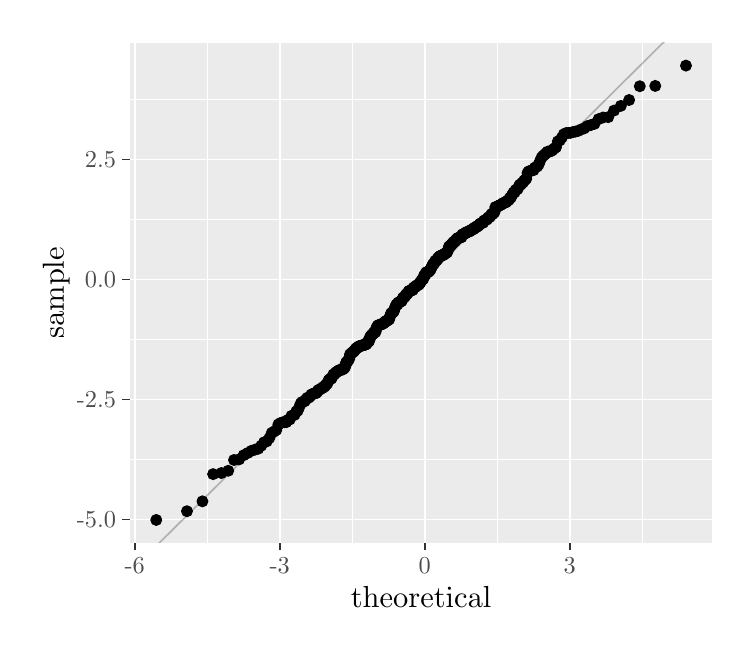
\begin{tikzpicture}[x=1pt,y=1pt]
\definecolor{fillColor}{RGB}{255,255,255}
\path[use as bounding box,fill=fillColor,fill opacity=0.00] (0,0) rectangle (252.94,216.81);
\begin{scope}
\path[clip] (  0.00,  0.00) rectangle (252.94,216.81);
\definecolor{drawColor}{RGB}{255,255,255}
\definecolor{fillColor}{RGB}{255,255,255}

\path[draw=drawColor,line width= 0.6pt,line join=round,line cap=round,fill=fillColor] (  0.00,  0.00) rectangle (252.94,216.81);
\end{scope}
\begin{scope}
\path[clip] ( 36.89, 30.72) rectangle (247.44,211.31);
\definecolor{fillColor}{gray}{0.92}

\path[fill=fillColor] ( 36.89, 30.72) rectangle (247.44,211.31);
\definecolor{drawColor}{RGB}{255,255,255}

\path[draw=drawColor,line width= 0.3pt,line join=round] ( 36.89, 60.81) --
	(247.44, 60.81);

\path[draw=drawColor,line width= 0.3pt,line join=round] ( 36.89,104.17) --
	(247.44,104.17);

\path[draw=drawColor,line width= 0.3pt,line join=round] ( 36.89,147.53) --
	(247.44,147.53);

\path[draw=drawColor,line width= 0.3pt,line join=round] ( 36.89,190.88) --
	(247.44,190.88);

\path[draw=drawColor,line width= 0.3pt,line join=round] ( 64.89, 30.72) --
	( 64.89,211.31);

\path[draw=drawColor,line width= 0.3pt,line join=round] (117.29, 30.72) --
	(117.29,211.31);

\path[draw=drawColor,line width= 0.3pt,line join=round] (169.69, 30.72) --
	(169.69,211.31);

\path[draw=drawColor,line width= 0.3pt,line join=round] (222.08, 30.72) --
	(222.08,211.31);

\path[draw=drawColor,line width= 0.6pt,line join=round] ( 36.89, 39.13) --
	(247.44, 39.13);

\path[draw=drawColor,line width= 0.6pt,line join=round] ( 36.89, 82.49) --
	(247.44, 82.49);

\path[draw=drawColor,line width= 0.6pt,line join=round] ( 36.89,125.85) --
	(247.44,125.85);

\path[draw=drawColor,line width= 0.6pt,line join=round] ( 36.89,169.21) --
	(247.44,169.21);

\path[draw=drawColor,line width= 0.6pt,line join=round] ( 38.69, 30.72) --
	( 38.69,211.31);

\path[draw=drawColor,line width= 0.6pt,line join=round] ( 91.09, 30.72) --
	( 91.09,211.31);

\path[draw=drawColor,line width= 0.6pt,line join=round] (143.49, 30.72) --
	(143.49,211.31);

\path[draw=drawColor,line width= 0.6pt,line join=round] (195.88, 30.72) --
	(195.88,211.31);
\definecolor{drawColor}{RGB}{0,0,0}
\definecolor{fillColor}{RGB}{0,0,0}

\path[draw=drawColor,line width= 0.4pt,line join=round,line cap=round,fill=fillColor] ( 46.46, 38.93) circle (  1.96);

\path[draw=drawColor,line width= 0.4pt,line join=round,line cap=round,fill=fillColor] ( 57.56, 42.08) circle (  1.96);

\path[draw=drawColor,line width= 0.4pt,line join=round,line cap=round,fill=fillColor] ( 63.15, 45.65) circle (  1.96);

\path[draw=drawColor,line width= 0.4pt,line join=round,line cap=round,fill=fillColor] ( 67.01, 55.48) circle (  1.96);

\path[draw=drawColor,line width= 0.4pt,line join=round,line cap=round,fill=fillColor] ( 70.00, 55.88) circle (  1.96);

\path[draw=drawColor,line width= 0.4pt,line join=round,line cap=round,fill=fillColor] ( 72.46, 56.69) circle (  1.96);

\path[draw=drawColor,line width= 0.4pt,line join=round,line cap=round,fill=fillColor] ( 74.56, 60.59) circle (  1.96);

\path[draw=drawColor,line width= 0.4pt,line join=round,line cap=round,fill=fillColor] ( 76.40, 60.81) circle (  1.96);

\path[draw=drawColor,line width= 0.4pt,line join=round,line cap=round,fill=fillColor] ( 78.04, 62.31) circle (  1.96);

\path[draw=drawColor,line width= 0.4pt,line join=round,line cap=round,fill=fillColor] ( 79.52, 63.11) circle (  1.96);

\path[draw=drawColor,line width= 0.4pt,line join=round,line cap=round,fill=fillColor] ( 80.88, 63.93) circle (  1.96);

\path[draw=drawColor,line width= 0.4pt,line join=round,line cap=round,fill=fillColor] ( 82.14, 64.33) circle (  1.96);

\path[draw=drawColor,line width= 0.4pt,line join=round,line cap=round,fill=fillColor] ( 83.31, 64.67) circle (  1.96);

\path[draw=drawColor,line width= 0.4pt,line join=round,line cap=round,fill=fillColor] ( 84.40, 65.73) circle (  1.96);

\path[draw=drawColor,line width= 0.4pt,line join=round,line cap=round,fill=fillColor] ( 85.43, 66.99) circle (  1.96);

\path[draw=drawColor,line width= 0.4pt,line join=round,line cap=round,fill=fillColor] ( 86.40, 67.32) circle (  1.96);

\path[draw=drawColor,line width= 0.4pt,line join=round,line cap=round,fill=fillColor] ( 87.32, 68.51) circle (  1.96);

\path[draw=drawColor,line width= 0.4pt,line join=round,line cap=round,fill=fillColor] ( 88.20, 70.37) circle (  1.96);

\path[draw=drawColor,line width= 0.4pt,line join=round,line cap=round,fill=fillColor] ( 89.04, 70.87) circle (  1.96);

\path[draw=drawColor,line width= 0.4pt,line join=round,line cap=round,fill=fillColor] ( 89.84, 71.42) circle (  1.96);

\path[draw=drawColor,line width= 0.4pt,line join=round,line cap=round,fill=fillColor] ( 90.61, 73.48) circle (  1.96);

\path[draw=drawColor,line width= 0.4pt,line join=round,line cap=round,fill=fillColor] ( 91.35, 73.92) circle (  1.96);

\path[draw=drawColor,line width= 0.4pt,line join=round,line cap=round,fill=fillColor] ( 92.07, 74.20) circle (  1.96);

\path[draw=drawColor,line width= 0.4pt,line join=round,line cap=round,fill=fillColor] ( 92.76, 74.25) circle (  1.96);

\path[draw=drawColor,line width= 0.4pt,line join=round,line cap=round,fill=fillColor] ( 93.42, 74.25) circle (  1.96);

\path[draw=drawColor,line width= 0.4pt,line join=round,line cap=round,fill=fillColor] ( 94.07, 75.09) circle (  1.96);

\path[draw=drawColor,line width= 0.4pt,line join=round,line cap=round,fill=fillColor] ( 94.70, 75.23) circle (  1.96);

\path[draw=drawColor,line width= 0.4pt,line join=round,line cap=round,fill=fillColor] ( 95.30, 76.51) circle (  1.96);

\path[draw=drawColor,line width= 0.4pt,line join=round,line cap=round,fill=fillColor] ( 95.90, 76.68) circle (  1.96);

\path[draw=drawColor,line width= 0.4pt,line join=round,line cap=round,fill=fillColor] ( 96.47, 76.94) circle (  1.96);

\path[draw=drawColor,line width= 0.4pt,line join=round,line cap=round,fill=fillColor] ( 97.03, 78.08) circle (  1.96);

\path[draw=drawColor,line width= 0.4pt,line join=round,line cap=round,fill=fillColor] ( 97.58, 78.41) circle (  1.96);

\path[draw=drawColor,line width= 0.4pt,line join=round,line cap=round,fill=fillColor] ( 98.12, 79.64) circle (  1.96);

\path[draw=drawColor,line width= 0.4pt,line join=round,line cap=round,fill=fillColor] ( 98.64, 80.97) circle (  1.96);

\path[draw=drawColor,line width= 0.4pt,line join=round,line cap=round,fill=fillColor] ( 99.15, 81.55) circle (  1.96);

\path[draw=drawColor,line width= 0.4pt,line join=round,line cap=round,fill=fillColor] ( 99.65, 81.63) circle (  1.96);

\path[draw=drawColor,line width= 0.4pt,line join=round,line cap=round,fill=fillColor] (100.14, 81.86) circle (  1.96);

\path[draw=drawColor,line width= 0.4pt,line join=round,line cap=round,fill=fillColor] (100.62, 82.58) circle (  1.96);

\path[draw=drawColor,line width= 0.4pt,line join=round,line cap=round,fill=fillColor] (101.09, 83.08) circle (  1.96);

\path[draw=drawColor,line width= 0.4pt,line join=round,line cap=round,fill=fillColor] (101.55, 83.10) circle (  1.96);

\path[draw=drawColor,line width= 0.4pt,line join=round,line cap=round,fill=fillColor] (102.00, 83.51) circle (  1.96);

\path[draw=drawColor,line width= 0.4pt,line join=round,line cap=round,fill=fillColor] (102.45, 84.18) circle (  1.96);

\path[draw=drawColor,line width= 0.4pt,line join=round,line cap=round,fill=fillColor] (102.89, 84.43) circle (  1.96);

\path[draw=drawColor,line width= 0.4pt,line join=round,line cap=round,fill=fillColor] (103.32, 84.61) circle (  1.96);

\path[draw=drawColor,line width= 0.4pt,line join=round,line cap=round,fill=fillColor] (103.74, 84.65) circle (  1.96);

\path[draw=drawColor,line width= 0.4pt,line join=round,line cap=round,fill=fillColor] (104.15, 84.70) circle (  1.96);

\path[draw=drawColor,line width= 0.4pt,line join=round,line cap=round,fill=fillColor] (104.56, 85.11) circle (  1.96);

\path[draw=drawColor,line width= 0.4pt,line join=round,line cap=round,fill=fillColor] (104.97, 85.81) circle (  1.96);

\path[draw=drawColor,line width= 0.4pt,line join=round,line cap=round,fill=fillColor] (105.37, 85.94) circle (  1.96);

\path[draw=drawColor,line width= 0.4pt,line join=round,line cap=round,fill=fillColor] (105.76, 86.23) circle (  1.96);

\path[draw=drawColor,line width= 0.4pt,line join=round,line cap=round,fill=fillColor] (106.14, 86.45) circle (  1.96);

\path[draw=drawColor,line width= 0.4pt,line join=round,line cap=round,fill=fillColor] (106.53, 86.59) circle (  1.96);

\path[draw=drawColor,line width= 0.4pt,line join=round,line cap=round,fill=fillColor] (106.90, 86.98) circle (  1.96);

\path[draw=drawColor,line width= 0.4pt,line join=round,line cap=round,fill=fillColor] (107.27, 87.09) circle (  1.96);

\path[draw=drawColor,line width= 0.4pt,line join=round,line cap=round,fill=fillColor] (107.64, 87.60) circle (  1.96);

\path[draw=drawColor,line width= 0.4pt,line join=round,line cap=round,fill=fillColor] (108.00, 87.95) circle (  1.96);

\path[draw=drawColor,line width= 0.4pt,line join=round,line cap=round,fill=fillColor] (108.36, 88.33) circle (  1.96);

\path[draw=drawColor,line width= 0.4pt,line join=round,line cap=round,fill=fillColor] (108.71, 89.35) circle (  1.96);

\path[draw=drawColor,line width= 0.4pt,line join=round,line cap=round,fill=fillColor] (109.06, 89.65) circle (  1.96);

\path[draw=drawColor,line width= 0.4pt,line join=round,line cap=round,fill=fillColor] (109.41, 89.96) circle (  1.96);

\path[draw=drawColor,line width= 0.4pt,line join=round,line cap=round,fill=fillColor] (109.75, 89.98) circle (  1.96);

\path[draw=drawColor,line width= 0.4pt,line join=round,line cap=round,fill=fillColor] (110.08, 90.63) circle (  1.96);

\path[draw=drawColor,line width= 0.4pt,line join=round,line cap=round,fill=fillColor] (110.42, 91.46) circle (  1.96);

\path[draw=drawColor,line width= 0.4pt,line join=round,line cap=round,fill=fillColor] (110.75, 91.50) circle (  1.96);

\path[draw=drawColor,line width= 0.4pt,line join=round,line cap=round,fill=fillColor] (111.08, 91.86) circle (  1.96);

\path[draw=drawColor,line width= 0.4pt,line join=round,line cap=round,fill=fillColor] (111.40, 92.30) circle (  1.96);

\path[draw=drawColor,line width= 0.4pt,line join=round,line cap=round,fill=fillColor] (111.72, 92.38) circle (  1.96);

\path[draw=drawColor,line width= 0.4pt,line join=round,line cap=round,fill=fillColor] (112.04, 92.64) circle (  1.96);

\path[draw=drawColor,line width= 0.4pt,line join=round,line cap=round,fill=fillColor] (112.35, 92.95) circle (  1.96);

\path[draw=drawColor,line width= 0.4pt,line join=round,line cap=round,fill=fillColor] (112.66, 93.00) circle (  1.96);

\path[draw=drawColor,line width= 0.4pt,line join=round,line cap=round,fill=fillColor] (112.97, 93.02) circle (  1.96);

\path[draw=drawColor,line width= 0.4pt,line join=round,line cap=round,fill=fillColor] (113.28, 93.28) circle (  1.96);

\path[draw=drawColor,line width= 0.4pt,line join=round,line cap=round,fill=fillColor] (113.58, 93.31) circle (  1.96);

\path[draw=drawColor,line width= 0.4pt,line join=round,line cap=round,fill=fillColor] (113.88, 93.32) circle (  1.96);

\path[draw=drawColor,line width= 0.4pt,line join=round,line cap=round,fill=fillColor] (114.18, 93.65) circle (  1.96);

\path[draw=drawColor,line width= 0.4pt,line join=round,line cap=round,fill=fillColor] (114.48, 93.88) circle (  1.96);

\path[draw=drawColor,line width= 0.4pt,line join=round,line cap=round,fill=fillColor] (114.77, 94.34) circle (  1.96);

\path[draw=drawColor,line width= 0.4pt,line join=round,line cap=round,fill=fillColor] (115.06, 95.82) circle (  1.96);

\path[draw=drawColor,line width= 0.4pt,line join=round,line cap=round,fill=fillColor] (115.35, 96.06) circle (  1.96);

\path[draw=drawColor,line width= 0.4pt,line join=round,line cap=round,fill=fillColor] (115.64, 96.16) circle (  1.96);

\path[draw=drawColor,line width= 0.4pt,line join=round,line cap=round,fill=fillColor] (115.92, 96.98) circle (  1.96);

\path[draw=drawColor,line width= 0.4pt,line join=round,line cap=round,fill=fillColor] (116.20, 97.11) circle (  1.96);

\path[draw=drawColor,line width= 0.4pt,line join=round,line cap=round,fill=fillColor] (116.48, 98.77) circle (  1.96);

\path[draw=drawColor,line width= 0.4pt,line join=round,line cap=round,fill=fillColor] (116.76, 98.83) circle (  1.96);

\path[draw=drawColor,line width= 0.4pt,line join=round,line cap=round,fill=fillColor] (117.04, 99.21) circle (  1.96);

\path[draw=drawColor,line width= 0.4pt,line join=round,line cap=round,fill=fillColor] (117.31, 99.42) circle (  1.96);

\path[draw=drawColor,line width= 0.4pt,line join=round,line cap=round,fill=fillColor] (117.59, 99.59) circle (  1.96);

\path[draw=drawColor,line width= 0.4pt,line join=round,line cap=round,fill=fillColor] (117.86, 99.90) circle (  1.96);

\path[draw=drawColor,line width= 0.4pt,line join=round,line cap=round,fill=fillColor] (118.13,100.12) circle (  1.96);

\path[draw=drawColor,line width= 0.4pt,line join=round,line cap=round,fill=fillColor] (118.39,100.55) circle (  1.96);

\path[draw=drawColor,line width= 0.4pt,line join=round,line cap=round,fill=fillColor] (118.66,100.89) circle (  1.96);

\path[draw=drawColor,line width= 0.4pt,line join=round,line cap=round,fill=fillColor] (118.92,101.09) circle (  1.96);

\path[draw=drawColor,line width= 0.4pt,line join=round,line cap=round,fill=fillColor] (119.19,101.11) circle (  1.96);

\path[draw=drawColor,line width= 0.4pt,line join=round,line cap=round,fill=fillColor] (119.45,101.46) circle (  1.96);

\path[draw=drawColor,line width= 0.4pt,line join=round,line cap=round,fill=fillColor] (119.71,101.67) circle (  1.96);

\path[draw=drawColor,line width= 0.4pt,line join=round,line cap=round,fill=fillColor] (119.96,101.68) circle (  1.96);

\path[draw=drawColor,line width= 0.4pt,line join=round,line cap=round,fill=fillColor] (120.22,101.86) circle (  1.96);

\path[draw=drawColor,line width= 0.4pt,line join=round,line cap=round,fill=fillColor] (120.47,101.89) circle (  1.96);

\path[draw=drawColor,line width= 0.4pt,line join=round,line cap=round,fill=fillColor] (120.73,101.91) circle (  1.96);

\path[draw=drawColor,line width= 0.4pt,line join=round,line cap=round,fill=fillColor] (120.98,101.96) circle (  1.96);

\path[draw=drawColor,line width= 0.4pt,line join=round,line cap=round,fill=fillColor] (121.23,102.16) circle (  1.96);

\path[draw=drawColor,line width= 0.4pt,line join=round,line cap=round,fill=fillColor] (121.48,102.18) circle (  1.96);

\path[draw=drawColor,line width= 0.4pt,line join=round,line cap=round,fill=fillColor] (121.73,102.19) circle (  1.96);

\path[draw=drawColor,line width= 0.4pt,line join=round,line cap=round,fill=fillColor] (121.98,102.29) circle (  1.96);

\path[draw=drawColor,line width= 0.4pt,line join=round,line cap=round,fill=fillColor] (122.22,102.34) circle (  1.96);

\path[draw=drawColor,line width= 0.4pt,line join=round,line cap=round,fill=fillColor] (122.47,102.56) circle (  1.96);

\path[draw=drawColor,line width= 0.4pt,line join=round,line cap=round,fill=fillColor] (122.71,103.16) circle (  1.96);

\path[draw=drawColor,line width= 0.4pt,line join=round,line cap=round,fill=fillColor] (122.95,103.29) circle (  1.96);

\path[draw=drawColor,line width= 0.4pt,line join=round,line cap=round,fill=fillColor] (123.19,103.33) circle (  1.96);

\path[draw=drawColor,line width= 0.4pt,line join=round,line cap=round,fill=fillColor] (123.43,103.70) circle (  1.96);

\path[draw=drawColor,line width= 0.4pt,line join=round,line cap=round,fill=fillColor] (123.67,105.03) circle (  1.96);

\path[draw=drawColor,line width= 0.4pt,line join=round,line cap=round,fill=fillColor] (123.91,105.04) circle (  1.96);

\path[draw=drawColor,line width= 0.4pt,line join=round,line cap=round,fill=fillColor] (124.15,105.60) circle (  1.96);

\path[draw=drawColor,line width= 0.4pt,line join=round,line cap=round,fill=fillColor] (124.38,105.82) circle (  1.96);

\path[draw=drawColor,line width= 0.4pt,line join=round,line cap=round,fill=fillColor] (124.62,105.99) circle (  1.96);

\path[draw=drawColor,line width= 0.4pt,line join=round,line cap=round,fill=fillColor] (124.85,106.25) circle (  1.96);

\path[draw=drawColor,line width= 0.4pt,line join=round,line cap=round,fill=fillColor] (125.09,106.65) circle (  1.96);

\path[draw=drawColor,line width= 0.4pt,line join=round,line cap=round,fill=fillColor] (125.32,106.70) circle (  1.96);

\path[draw=drawColor,line width= 0.4pt,line join=round,line cap=round,fill=fillColor] (125.55,106.71) circle (  1.96);

\path[draw=drawColor,line width= 0.4pt,line join=round,line cap=round,fill=fillColor] (125.78,107.07) circle (  1.96);

\path[draw=drawColor,line width= 0.4pt,line join=round,line cap=round,fill=fillColor] (126.01,108.37) circle (  1.96);

\path[draw=drawColor,line width= 0.4pt,line join=round,line cap=round,fill=fillColor] (126.24,108.66) circle (  1.96);

\path[draw=drawColor,line width= 0.4pt,line join=round,line cap=round,fill=fillColor] (126.46,109.05) circle (  1.96);

\path[draw=drawColor,line width= 0.4pt,line join=round,line cap=round,fill=fillColor] (126.69,109.27) circle (  1.96);

\path[draw=drawColor,line width= 0.4pt,line join=round,line cap=round,fill=fillColor] (126.92,109.33) circle (  1.96);

\path[draw=drawColor,line width= 0.4pt,line join=round,line cap=round,fill=fillColor] (127.14,109.35) circle (  1.96);

\path[draw=drawColor,line width= 0.4pt,line join=round,line cap=round,fill=fillColor] (127.37,109.48) circle (  1.96);

\path[draw=drawColor,line width= 0.4pt,line join=round,line cap=round,fill=fillColor] (127.59,109.48) circle (  1.96);

\path[draw=drawColor,line width= 0.4pt,line join=round,line cap=round,fill=fillColor] (127.82,109.62) circle (  1.96);

\path[draw=drawColor,line width= 0.4pt,line join=round,line cap=round,fill=fillColor] (128.04,109.72) circle (  1.96);

\path[draw=drawColor,line width= 0.4pt,line join=round,line cap=round,fill=fillColor] (128.26,109.81) circle (  1.96);

\path[draw=drawColor,line width= 0.4pt,line join=round,line cap=round,fill=fillColor] (128.48,109.93) circle (  1.96);

\path[draw=drawColor,line width= 0.4pt,line join=round,line cap=round,fill=fillColor] (128.70,110.16) circle (  1.96);

\path[draw=drawColor,line width= 0.4pt,line join=round,line cap=round,fill=fillColor] (128.92,110.32) circle (  1.96);

\path[draw=drawColor,line width= 0.4pt,line join=round,line cap=round,fill=fillColor] (129.14,110.40) circle (  1.96);

\path[draw=drawColor,line width= 0.4pt,line join=round,line cap=round,fill=fillColor] (129.36,110.74) circle (  1.96);

\path[draw=drawColor,line width= 0.4pt,line join=round,line cap=round,fill=fillColor] (129.58,110.82) circle (  1.96);

\path[draw=drawColor,line width= 0.4pt,line join=round,line cap=round,fill=fillColor] (129.79,110.90) circle (  1.96);

\path[draw=drawColor,line width= 0.4pt,line join=round,line cap=round,fill=fillColor] (130.01,111.03) circle (  1.96);

\path[draw=drawColor,line width= 0.4pt,line join=round,line cap=round,fill=fillColor] (130.23,111.18) circle (  1.96);

\path[draw=drawColor,line width= 0.4pt,line join=round,line cap=round,fill=fillColor] (130.44,111.38) circle (  1.96);

\path[draw=drawColor,line width= 0.4pt,line join=round,line cap=round,fill=fillColor] (130.66,111.42) circle (  1.96);

\path[draw=drawColor,line width= 0.4pt,line join=round,line cap=round,fill=fillColor] (130.87,112.41) circle (  1.96);

\path[draw=drawColor,line width= 0.4pt,line join=round,line cap=round,fill=fillColor] (131.09,112.81) circle (  1.96);

\path[draw=drawColor,line width= 0.4pt,line join=round,line cap=round,fill=fillColor] (131.30,113.57) circle (  1.96);

\path[draw=drawColor,line width= 0.4pt,line join=round,line cap=round,fill=fillColor] (131.51,113.59) circle (  1.96);

\path[draw=drawColor,line width= 0.4pt,line join=round,line cap=round,fill=fillColor] (131.73,113.89) circle (  1.96);

\path[draw=drawColor,line width= 0.4pt,line join=round,line cap=round,fill=fillColor] (131.94,114.01) circle (  1.96);

\path[draw=drawColor,line width= 0.4pt,line join=round,line cap=round,fill=fillColor] (132.15,114.21) circle (  1.96);

\path[draw=drawColor,line width= 0.4pt,line join=round,line cap=round,fill=fillColor] (132.36,114.42) circle (  1.96);

\path[draw=drawColor,line width= 0.4pt,line join=round,line cap=round,fill=fillColor] (132.57,115.20) circle (  1.96);

\path[draw=drawColor,line width= 0.4pt,line join=round,line cap=round,fill=fillColor] (132.78,115.76) circle (  1.96);

\path[draw=drawColor,line width= 0.4pt,line join=round,line cap=round,fill=fillColor] (132.99,116.27) circle (  1.96);

\path[draw=drawColor,line width= 0.4pt,line join=round,line cap=round,fill=fillColor] (133.20,116.68) circle (  1.96);

\path[draw=drawColor,line width= 0.4pt,line join=round,line cap=round,fill=fillColor] (133.41,116.79) circle (  1.96);

\path[draw=drawColor,line width= 0.4pt,line join=round,line cap=round,fill=fillColor] (133.62,116.80) circle (  1.96);

\path[draw=drawColor,line width= 0.4pt,line join=round,line cap=round,fill=fillColor] (133.83,117.35) circle (  1.96);

\path[draw=drawColor,line width= 0.4pt,line join=round,line cap=round,fill=fillColor] (134.04,117.50) circle (  1.96);

\path[draw=drawColor,line width= 0.4pt,line join=round,line cap=round,fill=fillColor] (134.24,117.52) circle (  1.96);

\path[draw=drawColor,line width= 0.4pt,line join=round,line cap=round,fill=fillColor] (134.45,117.67) circle (  1.96);

\path[draw=drawColor,line width= 0.4pt,line join=round,line cap=round,fill=fillColor] (134.66,117.86) circle (  1.96);

\path[draw=drawColor,line width= 0.4pt,line join=round,line cap=round,fill=fillColor] (134.86,117.92) circle (  1.96);

\path[draw=drawColor,line width= 0.4pt,line join=round,line cap=round,fill=fillColor] (135.07,117.96) circle (  1.96);

\path[draw=drawColor,line width= 0.4pt,line join=round,line cap=round,fill=fillColor] (135.28,118.31) circle (  1.96);

\path[draw=drawColor,line width= 0.4pt,line join=round,line cap=round,fill=fillColor] (135.48,118.87) circle (  1.96);

\path[draw=drawColor,line width= 0.4pt,line join=round,line cap=round,fill=fillColor] (135.69,119.24) circle (  1.96);

\path[draw=drawColor,line width= 0.4pt,line join=round,line cap=round,fill=fillColor] (135.89,119.28) circle (  1.96);

\path[draw=drawColor,line width= 0.4pt,line join=round,line cap=round,fill=fillColor] (136.10,119.46) circle (  1.96);

\path[draw=drawColor,line width= 0.4pt,line join=round,line cap=round,fill=fillColor] (136.30,119.61) circle (  1.96);

\path[draw=drawColor,line width= 0.4pt,line join=round,line cap=round,fill=fillColor] (136.51,119.95) circle (  1.96);

\path[draw=drawColor,line width= 0.4pt,line join=round,line cap=round,fill=fillColor] (136.71,120.36) circle (  1.96);

\path[draw=drawColor,line width= 0.4pt,line join=round,line cap=round,fill=fillColor] (136.92,120.44) circle (  1.96);

\path[draw=drawColor,line width= 0.4pt,line join=round,line cap=round,fill=fillColor] (137.12,120.77) circle (  1.96);

\path[draw=drawColor,line width= 0.4pt,line join=round,line cap=round,fill=fillColor] (137.32,120.84) circle (  1.96);

\path[draw=drawColor,line width= 0.4pt,line join=round,line cap=round,fill=fillColor] (137.53,121.21) circle (  1.96);

\path[draw=drawColor,line width= 0.4pt,line join=round,line cap=round,fill=fillColor] (137.73,121.58) circle (  1.96);

\path[draw=drawColor,line width= 0.4pt,line join=round,line cap=round,fill=fillColor] (137.93,121.75) circle (  1.96);

\path[draw=drawColor,line width= 0.4pt,line join=round,line cap=round,fill=fillColor] (138.14,121.76) circle (  1.96);

\path[draw=drawColor,line width= 0.4pt,line join=round,line cap=round,fill=fillColor] (138.34,121.77) circle (  1.96);

\path[draw=drawColor,line width= 0.4pt,line join=round,line cap=round,fill=fillColor] (138.54,121.85) circle (  1.96);

\path[draw=drawColor,line width= 0.4pt,line join=round,line cap=round,fill=fillColor] (138.74,121.90) circle (  1.96);

\path[draw=drawColor,line width= 0.4pt,line join=round,line cap=round,fill=fillColor] (138.95,121.98) circle (  1.96);

\path[draw=drawColor,line width= 0.4pt,line join=round,line cap=round,fill=fillColor] (139.15,122.00) circle (  1.96);

\path[draw=drawColor,line width= 0.4pt,line join=round,line cap=round,fill=fillColor] (139.35,122.67) circle (  1.96);

\path[draw=drawColor,line width= 0.4pt,line join=round,line cap=round,fill=fillColor] (139.55,122.87) circle (  1.96);

\path[draw=drawColor,line width= 0.4pt,line join=round,line cap=round,fill=fillColor] (139.75,122.98) circle (  1.96);

\path[draw=drawColor,line width= 0.4pt,line join=round,line cap=round,fill=fillColor] (139.96,123.11) circle (  1.96);

\path[draw=drawColor,line width= 0.4pt,line join=round,line cap=round,fill=fillColor] (140.16,123.15) circle (  1.96);

\path[draw=drawColor,line width= 0.4pt,line join=round,line cap=round,fill=fillColor] (140.36,123.47) circle (  1.96);

\path[draw=drawColor,line width= 0.4pt,line join=round,line cap=round,fill=fillColor] (140.56,123.58) circle (  1.96);

\path[draw=drawColor,line width= 0.4pt,line join=round,line cap=round,fill=fillColor] (140.76,123.68) circle (  1.96);

\path[draw=drawColor,line width= 0.4pt,line join=round,line cap=round,fill=fillColor] (140.96,123.87) circle (  1.96);

\path[draw=drawColor,line width= 0.4pt,line join=round,line cap=round,fill=fillColor] (141.16,123.94) circle (  1.96);

\path[draw=drawColor,line width= 0.4pt,line join=round,line cap=round,fill=fillColor] (141.37,123.95) circle (  1.96);

\path[draw=drawColor,line width= 0.4pt,line join=round,line cap=round,fill=fillColor] (141.57,124.50) circle (  1.96);

\path[draw=drawColor,line width= 0.4pt,line join=round,line cap=round,fill=fillColor] (141.77,124.51) circle (  1.96);

\path[draw=drawColor,line width= 0.4pt,line join=round,line cap=round,fill=fillColor] (141.97,124.77) circle (  1.96);

\path[draw=drawColor,line width= 0.4pt,line join=round,line cap=round,fill=fillColor] (142.17,125.27) circle (  1.96);

\path[draw=drawColor,line width= 0.4pt,line join=round,line cap=round,fill=fillColor] (142.37,125.53) circle (  1.96);

\path[draw=drawColor,line width= 0.4pt,line join=round,line cap=round,fill=fillColor] (142.57,125.71) circle (  1.96);

\path[draw=drawColor,line width= 0.4pt,line join=round,line cap=round,fill=fillColor] (142.77,125.97) circle (  1.96);

\path[draw=drawColor,line width= 0.4pt,line join=round,line cap=round,fill=fillColor] (142.97,126.02) circle (  1.96);

\path[draw=drawColor,line width= 0.4pt,line join=round,line cap=round,fill=fillColor] (143.18,127.09) circle (  1.96);

\path[draw=drawColor,line width= 0.4pt,line join=round,line cap=round,fill=fillColor] (143.38,127.40) circle (  1.96);

\path[draw=drawColor,line width= 0.4pt,line join=round,line cap=round,fill=fillColor] (143.58,127.50) circle (  1.96);

\path[draw=drawColor,line width= 0.4pt,line join=round,line cap=round,fill=fillColor] (143.78,127.51) circle (  1.96);

\path[draw=drawColor,line width= 0.4pt,line join=round,line cap=round,fill=fillColor] (143.98,128.37) circle (  1.96);

\path[draw=drawColor,line width= 0.4pt,line join=round,line cap=round,fill=fillColor] (144.18,128.46) circle (  1.96);

\path[draw=drawColor,line width= 0.4pt,line join=round,line cap=round,fill=fillColor] (144.38,128.47) circle (  1.96);

\path[draw=drawColor,line width= 0.4pt,line join=round,line cap=round,fill=fillColor] (144.59,128.51) circle (  1.96);

\path[draw=drawColor,line width= 0.4pt,line join=round,line cap=round,fill=fillColor] (144.79,128.54) circle (  1.96);

\path[draw=drawColor,line width= 0.4pt,line join=round,line cap=round,fill=fillColor] (144.99,128.69) circle (  1.96);

\path[draw=drawColor,line width= 0.4pt,line join=round,line cap=round,fill=fillColor] (145.19,129.09) circle (  1.96);

\path[draw=drawColor,line width= 0.4pt,line join=round,line cap=round,fill=fillColor] (145.39,129.24) circle (  1.96);

\path[draw=drawColor,line width= 0.4pt,line join=round,line cap=round,fill=fillColor] (145.60,129.37) circle (  1.96);

\path[draw=drawColor,line width= 0.4pt,line join=round,line cap=round,fill=fillColor] (145.80,129.93) circle (  1.96);

\path[draw=drawColor,line width= 0.4pt,line join=round,line cap=round,fill=fillColor] (146.00,130.43) circle (  1.96);

\path[draw=drawColor,line width= 0.4pt,line join=round,line cap=round,fill=fillColor] (146.20,130.82) circle (  1.96);

\path[draw=drawColor,line width= 0.4pt,line join=round,line cap=round,fill=fillColor] (146.41,131.27) circle (  1.96);

\path[draw=drawColor,line width= 0.4pt,line join=round,line cap=round,fill=fillColor] (146.61,131.34) circle (  1.96);

\path[draw=drawColor,line width= 0.4pt,line join=round,line cap=round,fill=fillColor] (146.81,131.65) circle (  1.96);

\path[draw=drawColor,line width= 0.4pt,line join=round,line cap=round,fill=fillColor] (147.02,131.82) circle (  1.96);

\path[draw=drawColor,line width= 0.4pt,line join=round,line cap=round,fill=fillColor] (147.22,132.48) circle (  1.96);

\path[draw=drawColor,line width= 0.4pt,line join=round,line cap=round,fill=fillColor] (147.42,132.57) circle (  1.96);

\path[draw=drawColor,line width= 0.4pt,line join=round,line cap=round,fill=fillColor] (147.63,132.64) circle (  1.96);

\path[draw=drawColor,line width= 0.4pt,line join=round,line cap=round,fill=fillColor] (147.83,132.78) circle (  1.96);

\path[draw=drawColor,line width= 0.4pt,line join=round,line cap=round,fill=fillColor] (148.04,133.17) circle (  1.96);

\path[draw=drawColor,line width= 0.4pt,line join=round,line cap=round,fill=fillColor] (148.24,133.54) circle (  1.96);

\path[draw=drawColor,line width= 0.4pt,line join=round,line cap=round,fill=fillColor] (148.45,133.58) circle (  1.96);

\path[draw=drawColor,line width= 0.4pt,line join=round,line cap=round,fill=fillColor] (148.65,133.96) circle (  1.96);

\path[draw=drawColor,line width= 0.4pt,line join=round,line cap=round,fill=fillColor] (148.86,134.05) circle (  1.96);

\path[draw=drawColor,line width= 0.4pt,line join=round,line cap=round,fill=fillColor] (149.06,134.30) circle (  1.96);

\path[draw=drawColor,line width= 0.4pt,line join=round,line cap=round,fill=fillColor] (149.27,134.41) circle (  1.96);

\path[draw=drawColor,line width= 0.4pt,line join=round,line cap=round,fill=fillColor] (149.47,134.47) circle (  1.96);

\path[draw=drawColor,line width= 0.4pt,line join=round,line cap=round,fill=fillColor] (149.68,134.51) circle (  1.96);

\path[draw=drawColor,line width= 0.4pt,line join=round,line cap=round,fill=fillColor] (149.89,134.53) circle (  1.96);

\path[draw=drawColor,line width= 0.4pt,line join=round,line cap=round,fill=fillColor] (150.10,134.64) circle (  1.96);

\path[draw=drawColor,line width= 0.4pt,line join=round,line cap=round,fill=fillColor] (150.30,134.75) circle (  1.96);

\path[draw=drawColor,line width= 0.4pt,line join=round,line cap=round,fill=fillColor] (150.51,134.98) circle (  1.96);

\path[draw=drawColor,line width= 0.4pt,line join=round,line cap=round,fill=fillColor] (150.72,135.11) circle (  1.96);

\path[draw=drawColor,line width= 0.4pt,line join=round,line cap=round,fill=fillColor] (150.93,135.19) circle (  1.96);

\path[draw=drawColor,line width= 0.4pt,line join=round,line cap=round,fill=fillColor] (151.14,135.38) circle (  1.96);

\path[draw=drawColor,line width= 0.4pt,line join=round,line cap=round,fill=fillColor] (151.35,135.58) circle (  1.96);

\path[draw=drawColor,line width= 0.4pt,line join=round,line cap=round,fill=fillColor] (151.56,135.62) circle (  1.96);

\path[draw=drawColor,line width= 0.4pt,line join=round,line cap=round,fill=fillColor] (151.77,136.15) circle (  1.96);

\path[draw=drawColor,line width= 0.4pt,line join=round,line cap=round,fill=fillColor] (151.98,136.63) circle (  1.96);

\path[draw=drawColor,line width= 0.4pt,line join=round,line cap=round,fill=fillColor] (152.19,137.63) circle (  1.96);

\path[draw=drawColor,line width= 0.4pt,line join=round,line cap=round,fill=fillColor] (152.40,137.69) circle (  1.96);

\path[draw=drawColor,line width= 0.4pt,line join=round,line cap=round,fill=fillColor] (152.61,137.96) circle (  1.96);

\path[draw=drawColor,line width= 0.4pt,line join=round,line cap=round,fill=fillColor] (152.83,137.96) circle (  1.96);

\path[draw=drawColor,line width= 0.4pt,line join=round,line cap=round,fill=fillColor] (153.04,138.38) circle (  1.96);

\path[draw=drawColor,line width= 0.4pt,line join=round,line cap=round,fill=fillColor] (153.25,138.57) circle (  1.96);

\path[draw=drawColor,line width= 0.4pt,line join=round,line cap=round,fill=fillColor] (153.47,138.76) circle (  1.96);

\path[draw=drawColor,line width= 0.4pt,line join=round,line cap=round,fill=fillColor] (153.68,139.05) circle (  1.96);

\path[draw=drawColor,line width= 0.4pt,line join=round,line cap=round,fill=fillColor] (153.90,139.35) circle (  1.96);

\path[draw=drawColor,line width= 0.4pt,line join=round,line cap=round,fill=fillColor] (154.11,139.44) circle (  1.96);

\path[draw=drawColor,line width= 0.4pt,line join=round,line cap=round,fill=fillColor] (154.33,139.54) circle (  1.96);

\path[draw=drawColor,line width= 0.4pt,line join=round,line cap=round,fill=fillColor] (154.55,139.82) circle (  1.96);

\path[draw=drawColor,line width= 0.4pt,line join=round,line cap=round,fill=fillColor] (154.76,140.15) circle (  1.96);

\path[draw=drawColor,line width= 0.4pt,line join=round,line cap=round,fill=fillColor] (154.98,140.32) circle (  1.96);

\path[draw=drawColor,line width= 0.4pt,line join=round,line cap=round,fill=fillColor] (155.20,140.58) circle (  1.96);

\path[draw=drawColor,line width= 0.4pt,line join=round,line cap=round,fill=fillColor] (155.42,140.80) circle (  1.96);

\path[draw=drawColor,line width= 0.4pt,line join=round,line cap=round,fill=fillColor] (155.64,140.84) circle (  1.96);

\path[draw=drawColor,line width= 0.4pt,line join=round,line cap=round,fill=fillColor] (155.86,140.87) circle (  1.96);

\path[draw=drawColor,line width= 0.4pt,line join=round,line cap=round,fill=fillColor] (156.08,140.95) circle (  1.96);

\path[draw=drawColor,line width= 0.4pt,line join=round,line cap=round,fill=fillColor] (156.30,141.04) circle (  1.96);

\path[draw=drawColor,line width= 0.4pt,line join=round,line cap=round,fill=fillColor] (156.52,141.06) circle (  1.96);

\path[draw=drawColor,line width= 0.4pt,line join=round,line cap=round,fill=fillColor] (156.75,141.07) circle (  1.96);

\path[draw=drawColor,line width= 0.4pt,line join=round,line cap=round,fill=fillColor] (156.97,141.95) circle (  1.96);

\path[draw=drawColor,line width= 0.4pt,line join=round,line cap=round,fill=fillColor] (157.20,142.13) circle (  1.96);

\path[draw=drawColor,line width= 0.4pt,line join=round,line cap=round,fill=fillColor] (157.42,142.16) circle (  1.96);

\path[draw=drawColor,line width= 0.4pt,line join=round,line cap=round,fill=fillColor] (157.65,142.19) circle (  1.96);

\path[draw=drawColor,line width= 0.4pt,line join=round,line cap=round,fill=fillColor] (157.87,142.44) circle (  1.96);

\path[draw=drawColor,line width= 0.4pt,line join=round,line cap=round,fill=fillColor] (158.10,142.53) circle (  1.96);

\path[draw=drawColor,line width= 0.4pt,line join=round,line cap=round,fill=fillColor] (158.33,142.55) circle (  1.96);

\path[draw=drawColor,line width= 0.4pt,line join=round,line cap=round,fill=fillColor] (158.56,142.92) circle (  1.96);

\path[draw=drawColor,line width= 0.4pt,line join=round,line cap=round,fill=fillColor] (158.79,142.98) circle (  1.96);

\path[draw=drawColor,line width= 0.4pt,line join=round,line cap=round,fill=fillColor] (159.02,143.01) circle (  1.96);

\path[draw=drawColor,line width= 0.4pt,line join=round,line cap=round,fill=fillColor] (159.25,143.09) circle (  1.96);

\path[draw=drawColor,line width= 0.4pt,line join=round,line cap=round,fill=fillColor] (159.49,143.13) circle (  1.96);

\path[draw=drawColor,line width= 0.4pt,line join=round,line cap=round,fill=fillColor] (159.72,143.24) circle (  1.96);

\path[draw=drawColor,line width= 0.4pt,line join=round,line cap=round,fill=fillColor] (159.96,143.36) circle (  1.96);

\path[draw=drawColor,line width= 0.4pt,line join=round,line cap=round,fill=fillColor] (160.19,143.69) circle (  1.96);

\path[draw=drawColor,line width= 0.4pt,line join=round,line cap=round,fill=fillColor] (160.43,143.82) circle (  1.96);

\path[draw=drawColor,line width= 0.4pt,line join=round,line cap=round,fill=fillColor] (160.67,143.85) circle (  1.96);

\path[draw=drawColor,line width= 0.4pt,line join=round,line cap=round,fill=fillColor] (160.91,144.00) circle (  1.96);

\path[draw=drawColor,line width= 0.4pt,line join=round,line cap=round,fill=fillColor] (161.15,144.00) circle (  1.96);

\path[draw=drawColor,line width= 0.4pt,line join=round,line cap=round,fill=fillColor] (161.39,144.46) circle (  1.96);

\path[draw=drawColor,line width= 0.4pt,line join=round,line cap=round,fill=fillColor] (161.63,144.60) circle (  1.96);

\path[draw=drawColor,line width= 0.4pt,line join=round,line cap=round,fill=fillColor] (161.87,144.64) circle (  1.96);

\path[draw=drawColor,line width= 0.4pt,line join=round,line cap=round,fill=fillColor] (162.12,144.67) circle (  1.96);

\path[draw=drawColor,line width= 0.4pt,line join=round,line cap=round,fill=fillColor] (162.36,145.07) circle (  1.96);

\path[draw=drawColor,line width= 0.4pt,line join=round,line cap=round,fill=fillColor] (162.61,145.13) circle (  1.96);

\path[draw=drawColor,line width= 0.4pt,line join=round,line cap=round,fill=fillColor] (162.86,145.20) circle (  1.96);

\path[draw=drawColor,line width= 0.4pt,line join=round,line cap=round,fill=fillColor] (163.11,145.55) circle (  1.96);

\path[draw=drawColor,line width= 0.4pt,line join=round,line cap=round,fill=fillColor] (163.36,145.83) circle (  1.96);

\path[draw=drawColor,line width= 0.4pt,line join=round,line cap=round,fill=fillColor] (163.61,146.01) circle (  1.96);

\path[draw=drawColor,line width= 0.4pt,line join=round,line cap=round,fill=fillColor] (163.86,146.15) circle (  1.96);

\path[draw=drawColor,line width= 0.4pt,line join=round,line cap=round,fill=fillColor] (164.12,146.21) circle (  1.96);

\path[draw=drawColor,line width= 0.4pt,line join=round,line cap=round,fill=fillColor] (164.38,146.24) circle (  1.96);

\path[draw=drawColor,line width= 0.4pt,line join=round,line cap=round,fill=fillColor] (164.63,146.42) circle (  1.96);

\path[draw=drawColor,line width= 0.4pt,line join=round,line cap=round,fill=fillColor] (164.89,147.07) circle (  1.96);

\path[draw=drawColor,line width= 0.4pt,line join=round,line cap=round,fill=fillColor] (165.15,147.13) circle (  1.96);

\path[draw=drawColor,line width= 0.4pt,line join=round,line cap=round,fill=fillColor] (165.42,147.32) circle (  1.96);

\path[draw=drawColor,line width= 0.4pt,line join=round,line cap=round,fill=fillColor] (165.68,147.40) circle (  1.96);

\path[draw=drawColor,line width= 0.4pt,line join=round,line cap=round,fill=fillColor] (165.95,147.48) circle (  1.96);

\path[draw=drawColor,line width= 0.4pt,line join=round,line cap=round,fill=fillColor] (166.21,147.94) circle (  1.96);

\path[draw=drawColor,line width= 0.4pt,line join=round,line cap=round,fill=fillColor] (166.48,148.25) circle (  1.96);

\path[draw=drawColor,line width= 0.4pt,line join=round,line cap=round,fill=fillColor] (166.75,148.26) circle (  1.96);

\path[draw=drawColor,line width= 0.4pt,line join=round,line cap=round,fill=fillColor] (167.03,148.51) circle (  1.96);

\path[draw=drawColor,line width= 0.4pt,line join=round,line cap=round,fill=fillColor] (167.30,148.82) circle (  1.96);

\path[draw=drawColor,line width= 0.4pt,line join=round,line cap=round,fill=fillColor] (167.58,149.44) circle (  1.96);

\path[draw=drawColor,line width= 0.4pt,line join=round,line cap=round,fill=fillColor] (167.85,149.49) circle (  1.96);

\path[draw=drawColor,line width= 0.4pt,line join=round,line cap=round,fill=fillColor] (168.14,149.52) circle (  1.96);

\path[draw=drawColor,line width= 0.4pt,line join=round,line cap=round,fill=fillColor] (168.42,150.00) circle (  1.96);

\path[draw=drawColor,line width= 0.4pt,line join=round,line cap=round,fill=fillColor] (168.70,150.17) circle (  1.96);

\path[draw=drawColor,line width= 0.4pt,line join=round,line cap=round,fill=fillColor] (168.99,151.96) circle (  1.96);

\path[draw=drawColor,line width= 0.4pt,line join=round,line cap=round,fill=fillColor] (169.28,151.99) circle (  1.96);

\path[draw=drawColor,line width= 0.4pt,line join=round,line cap=round,fill=fillColor] (169.57,152.04) circle (  1.96);

\path[draw=drawColor,line width= 0.4pt,line join=round,line cap=round,fill=fillColor] (169.86,152.23) circle (  1.96);

\path[draw=drawColor,line width= 0.4pt,line join=round,line cap=round,fill=fillColor] (170.16,152.37) circle (  1.96);

\path[draw=drawColor,line width= 0.4pt,line join=round,line cap=round,fill=fillColor] (170.46,152.57) circle (  1.96);

\path[draw=drawColor,line width= 0.4pt,line join=round,line cap=round,fill=fillColor] (170.76,152.78) circle (  1.96);

\path[draw=drawColor,line width= 0.4pt,line join=round,line cap=round,fill=fillColor] (171.06,152.88) circle (  1.96);

\path[draw=drawColor,line width= 0.4pt,line join=round,line cap=round,fill=fillColor] (171.37,152.94) circle (  1.96);

\path[draw=drawColor,line width= 0.4pt,line join=round,line cap=round,fill=fillColor] (171.68,153.27) circle (  1.96);

\path[draw=drawColor,line width= 0.4pt,line join=round,line cap=round,fill=fillColor] (171.99,153.55) circle (  1.96);

\path[draw=drawColor,line width= 0.4pt,line join=round,line cap=round,fill=fillColor] (172.30,153.57) circle (  1.96);

\path[draw=drawColor,line width= 0.4pt,line join=round,line cap=round,fill=fillColor] (172.62,153.66) circle (  1.96);

\path[draw=drawColor,line width= 0.4pt,line join=round,line cap=round,fill=fillColor] (172.94,153.79) circle (  1.96);

\path[draw=drawColor,line width= 0.4pt,line join=round,line cap=round,fill=fillColor] (173.26,154.20) circle (  1.96);

\path[draw=drawColor,line width= 0.4pt,line join=round,line cap=round,fill=fillColor] (173.59,154.38) circle (  1.96);

\path[draw=drawColor,line width= 0.4pt,line join=round,line cap=round,fill=fillColor] (173.92,154.66) circle (  1.96);

\path[draw=drawColor,line width= 0.4pt,line join=round,line cap=round,fill=fillColor] (174.25,155.29) circle (  1.96);

\path[draw=drawColor,line width= 0.4pt,line join=round,line cap=round,fill=fillColor] (174.59,155.38) circle (  1.96);

\path[draw=drawColor,line width= 0.4pt,line join=round,line cap=round,fill=fillColor] (174.93,156.19) circle (  1.96);

\path[draw=drawColor,line width= 0.4pt,line join=round,line cap=round,fill=fillColor] (175.28,156.74) circle (  1.96);

\path[draw=drawColor,line width= 0.4pt,line join=round,line cap=round,fill=fillColor] (175.63,157.29) circle (  1.96);

\path[draw=drawColor,line width= 0.4pt,line join=round,line cap=round,fill=fillColor] (175.98,157.33) circle (  1.96);

\path[draw=drawColor,line width= 0.4pt,line join=round,line cap=round,fill=fillColor] (176.34,158.16) circle (  1.96);

\path[draw=drawColor,line width= 0.4pt,line join=round,line cap=round,fill=fillColor] (176.70,158.30) circle (  1.96);

\path[draw=drawColor,line width= 0.4pt,line join=round,line cap=round,fill=fillColor] (177.07,158.51) circle (  1.96);

\path[draw=drawColor,line width= 0.4pt,line join=round,line cap=round,fill=fillColor] (177.44,159.39) circle (  1.96);

\path[draw=drawColor,line width= 0.4pt,line join=round,line cap=round,fill=fillColor] (177.81,160.03) circle (  1.96);

\path[draw=drawColor,line width= 0.4pt,line join=round,line cap=round,fill=fillColor] (178.20,160.10) circle (  1.96);

\path[draw=drawColor,line width= 0.4pt,line join=round,line cap=round,fill=fillColor] (178.58,160.63) circle (  1.96);

\path[draw=drawColor,line width= 0.4pt,line join=round,line cap=round,fill=fillColor] (178.97,160.87) circle (  1.96);

\path[draw=drawColor,line width= 0.4pt,line join=round,line cap=round,fill=fillColor] (179.37,161.49) circle (  1.96);

\path[draw=drawColor,line width= 0.4pt,line join=round,line cap=round,fill=fillColor] (179.77,161.86) circle (  1.96);

\path[draw=drawColor,line width= 0.4pt,line join=round,line cap=round,fill=fillColor] (180.18,162.27) circle (  1.96);

\path[draw=drawColor,line width= 0.4pt,line join=round,line cap=round,fill=fillColor] (180.60,164.30) circle (  1.96);

\path[draw=drawColor,line width= 0.4pt,line join=round,line cap=round,fill=fillColor] (181.02,164.85) circle (  1.96);

\path[draw=drawColor,line width= 0.4pt,line join=round,line cap=round,fill=fillColor] (181.45,164.96) circle (  1.96);

\path[draw=drawColor,line width= 0.4pt,line join=round,line cap=round,fill=fillColor] (181.89,165.16) circle (  1.96);

\path[draw=drawColor,line width= 0.4pt,line join=round,line cap=round,fill=fillColor] (182.34,165.28) circle (  1.96);

\path[draw=drawColor,line width= 0.4pt,line join=round,line cap=round,fill=fillColor] (182.79,165.32) circle (  1.96);

\path[draw=drawColor,line width= 0.4pt,line join=round,line cap=round,fill=fillColor] (183.25,166.20) circle (  1.96);

\path[draw=drawColor,line width= 0.4pt,line join=round,line cap=round,fill=fillColor] (183.72,166.43) circle (  1.96);

\path[draw=drawColor,line width= 0.4pt,line join=round,line cap=round,fill=fillColor] (184.20,166.76) circle (  1.96);

\path[draw=drawColor,line width= 0.4pt,line join=round,line cap=round,fill=fillColor] (184.69,167.45) circle (  1.96);

\path[draw=drawColor,line width= 0.4pt,line join=round,line cap=round,fill=fillColor] (185.19,168.73) circle (  1.96);

\path[draw=drawColor,line width= 0.4pt,line join=round,line cap=round,fill=fillColor] (185.70,169.86) circle (  1.96);

\path[draw=drawColor,line width= 0.4pt,line join=round,line cap=round,fill=fillColor] (186.22,170.47) circle (  1.96);

\path[draw=drawColor,line width= 0.4pt,line join=round,line cap=round,fill=fillColor] (186.76,170.86) circle (  1.96);

\path[draw=drawColor,line width= 0.4pt,line join=round,line cap=round,fill=fillColor] (187.31,171.47) circle (  1.96);

\path[draw=drawColor,line width= 0.4pt,line join=round,line cap=round,fill=fillColor] (187.87,172.00) circle (  1.96);

\path[draw=drawColor,line width= 0.4pt,line join=round,line cap=round,fill=fillColor] (188.44,172.03) circle (  1.96);

\path[draw=drawColor,line width= 0.4pt,line join=round,line cap=round,fill=fillColor] (189.04,172.16) circle (  1.96);

\path[draw=drawColor,line width= 0.4pt,line join=round,line cap=round,fill=fillColor] (189.64,172.56) circle (  1.96);

\path[draw=drawColor,line width= 0.4pt,line join=round,line cap=round,fill=fillColor] (190.27,173.16) circle (  1.96);

\path[draw=drawColor,line width= 0.4pt,line join=round,line cap=round,fill=fillColor] (190.92,173.62) circle (  1.96);

\path[draw=drawColor,line width= 0.4pt,line join=round,line cap=round,fill=fillColor] (191.58,175.71) circle (  1.96);

\path[draw=drawColor,line width= 0.4pt,line join=round,line cap=round,fill=fillColor] (192.27,176.08) circle (  1.96);

\path[draw=drawColor,line width= 0.4pt,line join=round,line cap=round,fill=fillColor] (192.99,177.03) circle (  1.96);

\path[draw=drawColor,line width= 0.4pt,line join=round,line cap=round,fill=fillColor] (193.73,178.28) circle (  1.96);

\path[draw=drawColor,line width= 0.4pt,line join=round,line cap=round,fill=fillColor] (194.50,178.70) circle (  1.96);

\path[draw=drawColor,line width= 0.4pt,line join=round,line cap=round,fill=fillColor] (195.30,178.76) circle (  1.96);

\path[draw=drawColor,line width= 0.4pt,line join=round,line cap=round,fill=fillColor] (196.14,178.79) circle (  1.96);

\path[draw=drawColor,line width= 0.4pt,line join=round,line cap=round,fill=fillColor] (197.02,179.09) circle (  1.96);

\path[draw=drawColor,line width= 0.4pt,line join=round,line cap=round,fill=fillColor] (197.94,179.26) circle (  1.96);

\path[draw=drawColor,line width= 0.4pt,line join=round,line cap=round,fill=fillColor] (198.91,179.50) circle (  1.96);

\path[draw=drawColor,line width= 0.4pt,line join=round,line cap=round,fill=fillColor] (199.94,180.03) circle (  1.96);

\path[draw=drawColor,line width= 0.4pt,line join=round,line cap=round,fill=fillColor] (201.03,180.38) circle (  1.96);

\path[draw=drawColor,line width= 0.4pt,line join=round,line cap=round,fill=fillColor] (202.20,181.22) circle (  1.96);

\path[draw=drawColor,line width= 0.4pt,line join=round,line cap=round,fill=fillColor] (203.46,181.60) circle (  1.96);

\path[draw=drawColor,line width= 0.4pt,line join=round,line cap=round,fill=fillColor] (204.81,182.05) circle (  1.96);

\path[draw=drawColor,line width= 0.4pt,line join=round,line cap=round,fill=fillColor] (206.30,183.76) circle (  1.96);

\path[draw=drawColor,line width= 0.4pt,line join=round,line cap=round,fill=fillColor] (207.94,184.36) circle (  1.96);

\path[draw=drawColor,line width= 0.4pt,line join=round,line cap=round,fill=fillColor] (209.78,184.48) circle (  1.96);

\path[draw=drawColor,line width= 0.4pt,line join=round,line cap=round,fill=fillColor] (211.88,186.85) circle (  1.96);

\path[draw=drawColor,line width= 0.4pt,line join=round,line cap=round,fill=fillColor] (214.34,188.55) circle (  1.96);

\path[draw=drawColor,line width= 0.4pt,line join=round,line cap=round,fill=fillColor] (217.33,190.67) circle (  1.96);

\path[draw=drawColor,line width= 0.4pt,line join=round,line cap=round,fill=fillColor] (221.19,195.65) circle (  1.96);

\path[draw=drawColor,line width= 0.4pt,line join=round,line cap=round,fill=fillColor] (226.78,195.76) circle (  1.96);

\path[draw=drawColor,line width= 0.4pt,line join=round,line cap=round,fill=fillColor] (237.87,203.10) circle (  1.96);
\definecolor{drawColor}{RGB}{0,0,0}

\path[draw=drawColor,draw opacity=0.25,line width= 0.6pt,line join=round] ( 36.89, 20.01) -- (235.09,216.81);
\end{scope}
\begin{scope}
\path[clip] (  0.00,  0.00) rectangle (252.94,216.81);
\definecolor{drawColor}{gray}{0.30}

\node[text=drawColor,anchor=base east,inner sep=0pt, outer sep=0pt, scale=  0.88] at ( 31.94, 36.10) {-5.0};

\node[text=drawColor,anchor=base east,inner sep=0pt, outer sep=0pt, scale=  0.88] at ( 31.94, 79.46) {-2.5};

\node[text=drawColor,anchor=base east,inner sep=0pt, outer sep=0pt, scale=  0.88] at ( 31.94,122.82) {0.0};

\node[text=drawColor,anchor=base east,inner sep=0pt, outer sep=0pt, scale=  0.88] at ( 31.94,166.17) {2.5};
\end{scope}
\begin{scope}
\path[clip] (  0.00,  0.00) rectangle (252.94,216.81);
\definecolor{drawColor}{gray}{0.20}

\path[draw=drawColor,line width= 0.6pt,line join=round] ( 34.14, 39.13) --
	( 36.89, 39.13);

\path[draw=drawColor,line width= 0.6pt,line join=round] ( 34.14, 82.49) --
	( 36.89, 82.49);

\path[draw=drawColor,line width= 0.6pt,line join=round] ( 34.14,125.85) --
	( 36.89,125.85);

\path[draw=drawColor,line width= 0.6pt,line join=round] ( 34.14,169.21) --
	( 36.89,169.21);
\end{scope}
\begin{scope}
\path[clip] (  0.00,  0.00) rectangle (252.94,216.81);
\definecolor{drawColor}{gray}{0.20}

\path[draw=drawColor,line width= 0.6pt,line join=round] ( 38.69, 27.97) --
	( 38.69, 30.72);

\path[draw=drawColor,line width= 0.6pt,line join=round] ( 91.09, 27.97) --
	( 91.09, 30.72);

\path[draw=drawColor,line width= 0.6pt,line join=round] (143.49, 27.97) --
	(143.49, 30.72);

\path[draw=drawColor,line width= 0.6pt,line join=round] (195.88, 27.97) --
	(195.88, 30.72);
\end{scope}
\begin{scope}
\path[clip] (  0.00,  0.00) rectangle (252.94,216.81);
\definecolor{drawColor}{gray}{0.30}

\node[text=drawColor,anchor=base,inner sep=0pt, outer sep=0pt, scale=  0.88] at ( 38.69, 19.71) {-6};

\node[text=drawColor,anchor=base,inner sep=0pt, outer sep=0pt, scale=  0.88] at ( 91.09, 19.71) {-3};

\node[text=drawColor,anchor=base,inner sep=0pt, outer sep=0pt, scale=  0.88] at (143.49, 19.71) {0};

\node[text=drawColor,anchor=base,inner sep=0pt, outer sep=0pt, scale=  0.88] at (195.88, 19.71) {3};
\end{scope}
\begin{scope}
\path[clip] (  0.00,  0.00) rectangle (252.94,216.81);
\definecolor{drawColor}{RGB}{0,0,0}

\node[text=drawColor,anchor=base,inner sep=0pt, outer sep=0pt, scale=  1.10] at (142.17,  7.44) {theoretical};
\end{scope}
\begin{scope}
\path[clip] (  0.00,  0.00) rectangle (252.94,216.81);
\definecolor{drawColor}{RGB}{0,0,0}

\node[text=drawColor,rotate= 90.00,anchor=base,inner sep=0pt, outer sep=0pt, scale=  1.10] at ( 13.08,121.02) {sample};
\end{scope}
\end{tikzpicture}
}
			\caption{Anscombe residuals}
			\label{fig 4.5}
		\end{subfigure}
		\caption{Q-Q plots of residuals with normal theoretical distribution: Model 1}
		\label{fig}
	\end{figure}
	
	\begin{figure}[H]
		\centering
		\scalebox{0.70}{% Created by tikzDevice version 0.12 on 2019-04-30 04:12:39
% !TEX encoding = UTF-8 Unicode
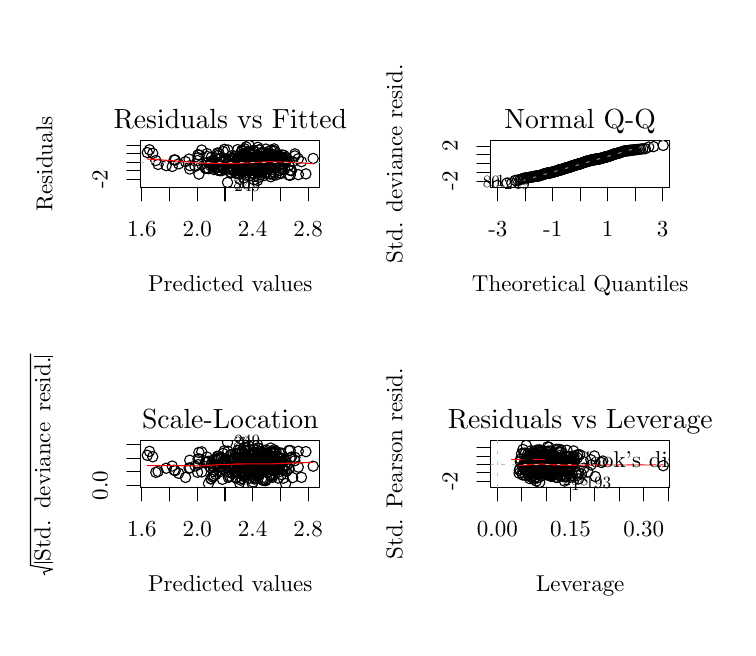
\begin{tikzpicture}[x=1pt,y=1pt]
\definecolor{fillColor}{RGB}{255,255,255}
\path[use as bounding box,fill=fillColor,fill opacity=0.00] (0,0) rectangle (252.94,216.81);
\begin{scope}
\path[clip] (  0.00,  0.00) rectangle (252.94,216.81);
\definecolor{drawColor}{RGB}{0,0,0}

\path[draw=drawColor,line width= 0.4pt,line join=round,line cap=round] ( 41.27,159.20) -- (101.32,159.20);

\path[draw=drawColor,line width= 0.4pt,line join=round,line cap=round] ( 41.27,159.20) -- ( 41.27,154.22);

\path[draw=drawColor,line width= 0.4pt,line join=round,line cap=round] ( 51.28,159.20) -- ( 51.28,154.22);

\path[draw=drawColor,line width= 0.4pt,line join=round,line cap=round] ( 61.29,159.20) -- ( 61.29,154.22);

\path[draw=drawColor,line width= 0.4pt,line join=round,line cap=round] ( 71.29,159.20) -- ( 71.29,154.22);

\path[draw=drawColor,line width= 0.4pt,line join=round,line cap=round] ( 81.30,159.20) -- ( 81.30,154.22);

\path[draw=drawColor,line width= 0.4pt,line join=round,line cap=round] ( 91.31,159.20) -- ( 91.31,154.22);

\path[draw=drawColor,line width= 0.4pt,line join=round,line cap=round] (101.32,159.20) -- (101.32,154.22);

\node[text=drawColor,anchor=base,inner sep=0pt, outer sep=0pt, scale=  0.83] at ( 41.27,141.27) {1.6};

\node[text=drawColor,anchor=base,inner sep=0pt, outer sep=0pt, scale=  0.83] at ( 61.29,141.27) {2.0};

\node[text=drawColor,anchor=base,inner sep=0pt, outer sep=0pt, scale=  0.83] at ( 81.30,141.27) {2.4};

\node[text=drawColor,anchor=base,inner sep=0pt, outer sep=0pt, scale=  0.83] at (101.32,141.27) {2.8};

\path[draw=drawColor,line width= 0.4pt,line join=round,line cap=round] ( 40.84,162.05) -- ( 40.84,174.23);

\path[draw=drawColor,line width= 0.4pt,line join=round,line cap=round] ( 40.84,162.05) -- ( 35.86,162.05);

\path[draw=drawColor,line width= 0.4pt,line join=round,line cap=round] ( 40.84,165.10) -- ( 35.86,165.10);

\path[draw=drawColor,line width= 0.4pt,line join=round,line cap=round] ( 40.84,168.14) -- ( 35.86,168.14);

\path[draw=drawColor,line width= 0.4pt,line join=round,line cap=round] ( 40.84,171.19) -- ( 35.86,171.19);

\path[draw=drawColor,line width= 0.4pt,line join=round,line cap=round] ( 40.84,174.23) -- ( 35.86,174.23);

\node[text=drawColor,rotate= 90.00,anchor=base,inner sep=0pt, outer sep=0pt, scale=  0.83] at ( 28.88,162.05) {-2};

\path[draw=drawColor,line width= 0.4pt,line join=round,line cap=round] ( 40.84,159.20) --
	(105.56,159.20) --
	(105.56,175.97) --
	( 40.84,175.97) --
	( 40.84,159.20);
\end{scope}
\begin{scope}
\path[clip] (  0.00,108.41) rectangle (126.47,216.81);
\definecolor{drawColor}{RGB}{0,0,0}

\node[text=drawColor,anchor=base,inner sep=0pt, outer sep=0pt, scale=  0.83] at ( 73.20,121.35) {Predicted values};

\node[text=drawColor,rotate= 90.00,anchor=base,inner sep=0pt, outer sep=0pt, scale=  0.83] at (  8.96,167.59) {Residuals};
\end{scope}
\begin{scope}
\path[clip] ( 40.84,159.20) rectangle (105.56,175.97);
\definecolor{drawColor}{RGB}{0,0,0}

\path[draw=drawColor,line width= 0.4pt,line join=round,line cap=round] ( 81.81,161.85) circle (  1.87);

\path[draw=drawColor,line width= 0.4pt,line join=round,line cap=round] ( 78.10,162.52) circle (  1.87);

\path[draw=drawColor,line width= 0.4pt,line join=round,line cap=round] ( 52.94,169.03) circle (  1.87);

\path[draw=drawColor,line width= 0.4pt,line join=round,line cap=round] ( 86.38,170.50) circle (  1.87);

\path[draw=drawColor,line width= 0.4pt,line join=round,line cap=round] ( 76.73,163.92) circle (  1.87);

\path[draw=drawColor,line width= 0.4pt,line join=round,line cap=round] ( 92.40,169.15) circle (  1.87);

\path[draw=drawColor,line width= 0.4pt,line join=round,line cap=round] ( 86.03,168.04) circle (  1.87);

\path[draw=drawColor,line width= 0.4pt,line join=round,line cap=round] ( 73.65,164.47) circle (  1.87);

\path[draw=drawColor,line width= 0.4pt,line join=round,line cap=round] ( 90.01,170.48) circle (  1.87);

\path[draw=drawColor,line width= 0.4pt,line join=round,line cap=round] ( 86.42,169.67) circle (  1.87);

\path[draw=drawColor,line width= 0.4pt,line join=round,line cap=round] ( 82.92,166.87) circle (  1.87);

\path[draw=drawColor,line width= 0.4pt,line join=round,line cap=round] ( 85.58,166.33) circle (  1.87);

\path[draw=drawColor,line width= 0.4pt,line join=round,line cap=round] ( 87.40,169.45) circle (  1.87);

\path[draw=drawColor,line width= 0.4pt,line join=round,line cap=round] ( 81.82,167.09) circle (  1.87);

\path[draw=drawColor,line width= 0.4pt,line join=round,line cap=round] ( 90.42,168.78) circle (  1.87);

\path[draw=drawColor,line width= 0.4pt,line join=round,line cap=round] ( 84.11,170.16) circle (  1.87);

\path[draw=drawColor,line width= 0.4pt,line join=round,line cap=round] ( 88.39,168.40) circle (  1.87);

\path[draw=drawColor,line width= 0.4pt,line join=round,line cap=round] ( 67.98,167.67) circle (  1.87);

\path[draw=drawColor,line width= 0.4pt,line join=round,line cap=round] ( 58.68,166.95) circle (  1.87);

\path[draw=drawColor,line width= 0.4pt,line join=round,line cap=round] ( 88.87,163.73) circle (  1.87);

\path[draw=drawColor,line width= 0.4pt,line join=round,line cap=round] ( 94.31,167.08) circle (  1.87);

\path[draw=drawColor,line width= 0.4pt,line join=round,line cap=round] ( 90.74,167.03) circle (  1.87);

\path[draw=drawColor,line width= 0.4pt,line join=round,line cap=round] ( 90.52,169.57) circle (  1.87);

\path[draw=drawColor,line width= 0.4pt,line join=round,line cap=round] ( 79.73,170.23) circle (  1.87);

\path[draw=drawColor,line width= 0.4pt,line join=round,line cap=round] ( 77.42,167.95) circle (  1.87);

\path[draw=drawColor,line width= 0.4pt,line join=round,line cap=round] ( 64.38,166.03) circle (  1.87);

\path[draw=drawColor,line width= 0.4pt,line join=round,line cap=round] ( 76.53,169.99) circle (  1.87);

\path[draw=drawColor,line width= 0.4pt,line join=round,line cap=round] ( 87.79,170.18) circle (  1.87);

\path[draw=drawColor,line width= 0.4pt,line join=round,line cap=round] ( 77.24,168.93) circle (  1.87);

\path[draw=drawColor,line width= 0.4pt,line join=round,line cap=round] ( 86.29,166.18) circle (  1.87);

\path[draw=drawColor,line width= 0.4pt,line join=round,line cap=round] ( 91.61,164.14) circle (  1.87);

\path[draw=drawColor,line width= 0.4pt,line join=round,line cap=round] ( 92.65,170.65) circle (  1.87);

\path[draw=drawColor,line width= 0.4pt,line join=round,line cap=round] ( 86.97,171.96) circle (  1.87);

\path[draw=drawColor,line width= 0.4pt,line join=round,line cap=round] ( 89.72,163.56) circle (  1.87);

\path[draw=drawColor,line width= 0.4pt,line join=round,line cap=round] ( 77.13,169.87) circle (  1.87);

\path[draw=drawColor,line width= 0.4pt,line join=round,line cap=round] ( 76.09,166.21) circle (  1.87);

\path[draw=drawColor,line width= 0.4pt,line join=round,line cap=round] ( 87.51,170.25) circle (  1.87);

\path[draw=drawColor,line width= 0.4pt,line join=round,line cap=round] ( 93.50,168.89) circle (  1.87);

\path[draw=drawColor,line width= 0.4pt,line join=round,line cap=round] ( 77.96,169.70) circle (  1.87);

\path[draw=drawColor,line width= 0.4pt,line join=round,line cap=round] ( 71.08,172.85) circle (  1.87);

\path[draw=drawColor,line width= 0.4pt,line join=round,line cap=round] ( 70.67,166.11) circle (  1.87);

\path[draw=drawColor,line width= 0.4pt,line join=round,line cap=round] ( 84.98,168.26) circle (  1.87);

\path[draw=drawColor,line width= 0.4pt,line join=round,line cap=round] ( 96.57,171.20) circle (  1.87);

\path[draw=drawColor,line width= 0.4pt,line join=round,line cap=round] ( 79.87,165.50) circle (  1.87);

\path[draw=drawColor,line width= 0.4pt,line join=round,line cap=round] ( 67.84,169.75) circle (  1.87);

\path[draw=drawColor,line width= 0.4pt,line join=round,line cap=round] ( 66.26,167.97) circle (  1.87);

\path[draw=drawColor,line width= 0.4pt,line join=round,line cap=round] ( 75.57,169.26) circle (  1.87);

\path[draw=drawColor,line width= 0.4pt,line join=round,line cap=round] (103.16,169.55) circle (  1.87);

\path[draw=drawColor,line width= 0.4pt,line join=round,line cap=round] ( 78.15,172.26) circle (  1.87);

\path[draw=drawColor,line width= 0.4pt,line join=round,line cap=round] ( 74.40,165.45) circle (  1.87);

\path[draw=drawColor,line width= 0.4pt,line join=round,line cap=round] ( 82.11,168.86) circle (  1.87);

\path[draw=drawColor,line width= 0.4pt,line join=round,line cap=round] ( 83.85,167.60) circle (  1.87);

\path[draw=drawColor,line width= 0.4pt,line join=round,line cap=round] ( 81.93,167.99) circle (  1.87);

\path[draw=drawColor,line width= 0.4pt,line join=round,line cap=round] ( 67.30,167.79) circle (  1.87);

\path[draw=drawColor,line width= 0.4pt,line join=round,line cap=round] ( 78.07,167.82) circle (  1.87);

\path[draw=drawColor,line width= 0.4pt,line join=round,line cap=round] ( 75.68,166.28) circle (  1.87);

\path[draw=drawColor,line width= 0.4pt,line join=round,line cap=round] ( 88.15,169.29) circle (  1.87);

\path[draw=drawColor,line width= 0.4pt,line join=round,line cap=round] ( 84.86,170.00) circle (  1.87);

\path[draw=drawColor,line width= 0.4pt,line join=round,line cap=round] ( 76.53,167.14) circle (  1.87);

\path[draw=drawColor,line width= 0.4pt,line join=round,line cap=round] ( 80.09,171.86) circle (  1.87);

\path[draw=drawColor,line width= 0.4pt,line join=round,line cap=round] ( 91.05,165.18) circle (  1.87);

\path[draw=drawColor,line width= 0.4pt,line join=round,line cap=round] ( 62.01,170.79) circle (  1.87);

\path[draw=drawColor,line width= 0.4pt,line join=round,line cap=round] ( 76.30,166.17) circle (  1.87);

\path[draw=drawColor,line width= 0.4pt,line join=round,line cap=round] ( 69.76,169.40) circle (  1.87);

\path[draw=drawColor,line width= 0.4pt,line join=round,line cap=round] ( 80.33,167.38) circle (  1.87);

\path[draw=drawColor,line width= 0.4pt,line join=round,line cap=round] ( 81.53,172.37) circle (  1.87);

\path[draw=drawColor,line width= 0.4pt,line join=round,line cap=round] ( 86.68,168.77) circle (  1.87);

\path[draw=drawColor,line width= 0.4pt,line join=round,line cap=round] ( 74.24,165.48) circle (  1.87);

\path[draw=drawColor,line width= 0.4pt,line join=round,line cap=round] ( 72.84,166.80) circle (  1.87);

\path[draw=drawColor,line width= 0.4pt,line join=round,line cap=round] ( 87.29,171.10) circle (  1.87);

\path[draw=drawColor,line width= 0.4pt,line join=round,line cap=round] ( 86.43,168.82) circle (  1.87);

\path[draw=drawColor,line width= 0.4pt,line join=round,line cap=round] ( 90.80,165.24) circle (  1.87);

\path[draw=drawColor,line width= 0.4pt,line join=round,line cap=round] ( 45.18,171.38) circle (  1.87);

\path[draw=drawColor,line width= 0.4pt,line join=round,line cap=round] ( 82.06,168.87) circle (  1.87);

\path[draw=drawColor,line width= 0.4pt,line join=round,line cap=round] ( 68.64,170.58) circle (  1.87);

\path[draw=drawColor,line width= 0.4pt,line join=round,line cap=round] ( 79.59,166.56) circle (  1.87);

\path[draw=drawColor,line width= 0.4pt,line join=round,line cap=round] ( 91.76,165.93) circle (  1.87);

\path[draw=drawColor,line width= 0.4pt,line join=round,line cap=round] ( 84.66,167.44) circle (  1.87);

\path[draw=drawColor,line width= 0.4pt,line join=round,line cap=round] ( 43.23,171.68) circle (  1.87);

\path[draw=drawColor,line width= 0.4pt,line join=round,line cap=round] ( 83.05,161.63) circle (  1.87);

\path[draw=drawColor,line width= 0.4pt,line join=round,line cap=round] ( 66.38,170.01) circle (  1.87);

\path[draw=drawColor,line width= 0.4pt,line join=round,line cap=round] ( 77.92,168.80) circle (  1.87);

\path[draw=drawColor,line width= 0.4pt,line join=round,line cap=round] ( 84.27,163.62) circle (  1.87);

\path[draw=drawColor,line width= 0.4pt,line join=round,line cap=round] ( 91.98,169.24) circle (  1.87);

\path[draw=drawColor,line width= 0.4pt,line join=round,line cap=round] ( 75.62,167.32) circle (  1.87);

\path[draw=drawColor,line width= 0.4pt,line join=round,line cap=round] ( 73.18,165.67) circle (  1.87);

\path[draw=drawColor,line width= 0.4pt,line join=round,line cap=round] ( 79.22,165.62) circle (  1.87);

\path[draw=drawColor,line width= 0.4pt,line join=round,line cap=round] ( 82.70,169.61) circle (  1.87);

\path[draw=drawColor,line width= 0.4pt,line join=round,line cap=round] ( 87.61,166.82) circle (  1.87);

\path[draw=drawColor,line width= 0.4pt,line join=round,line cap=round] ( 82.93,164.91) circle (  1.87);

\path[draw=drawColor,line width= 0.4pt,line join=round,line cap=round] ( 77.71,164.85) circle (  1.87);

\path[draw=drawColor,line width= 0.4pt,line join=round,line cap=round] ( 86.79,171.21) circle (  1.87);

\path[draw=drawColor,line width= 0.4pt,line join=round,line cap=round] ( 66.92,166.76) circle (  1.87);

\path[draw=drawColor,line width= 0.4pt,line join=round,line cap=round] ( 78.41,168.70) circle (  1.87);

\path[draw=drawColor,line width= 0.4pt,line join=round,line cap=round] ( 95.33,165.15) circle (  1.87);

\path[draw=drawColor,line width= 0.4pt,line join=round,line cap=round] ( 66.20,166.88) circle (  1.87);

\path[draw=drawColor,line width= 0.4pt,line join=round,line cap=round] ( 73.83,169.59) circle (  1.87);

\path[draw=drawColor,line width= 0.4pt,line join=round,line cap=round] ( 67.31,167.79) circle (  1.87);

\path[draw=drawColor,line width= 0.4pt,line join=round,line cap=round] ( 81.42,168.10) circle (  1.87);

\path[draw=drawColor,line width= 0.4pt,line join=round,line cap=round] ( 70.37,166.17) circle (  1.87);

\path[draw=drawColor,line width= 0.4pt,line join=round,line cap=round] ( 71.27,166.01) circle (  1.87);

\path[draw=drawColor,line width= 0.4pt,line join=round,line cap=round] ( 98.93,168.39) circle (  1.87);

\path[draw=drawColor,line width= 0.4pt,line join=round,line cap=round] ( 83.95,166.66) circle (  1.87);

\path[draw=drawColor,line width= 0.4pt,line join=round,line cap=round] ( 71.03,166.05) circle (  1.87);

\path[draw=drawColor,line width= 0.4pt,line join=round,line cap=round] ( 87.17,171.12) circle (  1.87);

\path[draw=drawColor,line width= 0.4pt,line join=round,line cap=round] ( 79.78,167.49) circle (  1.87);

\path[draw=drawColor,line width= 0.4pt,line join=round,line cap=round] ( 70.49,166.15) circle (  1.87);

\path[draw=drawColor,line width= 0.4pt,line join=round,line cap=round] ( 88.74,170.77) circle (  1.87);

\path[draw=drawColor,line width= 0.4pt,line join=round,line cap=round] ( 82.61,166.93) circle (  1.87);

\path[draw=drawColor,line width= 0.4pt,line join=round,line cap=round] ( 87.76,169.37) circle (  1.87);

\path[draw=drawColor,line width= 0.4pt,line join=round,line cap=round] ( 96.54,170.47) circle (  1.87);

\path[draw=drawColor,line width= 0.4pt,line join=round,line cap=round] ( 68.97,166.41) circle (  1.87);

\path[draw=drawColor,line width= 0.4pt,line join=round,line cap=round] ( 64.88,170.28) circle (  1.87);

\path[draw=drawColor,line width= 0.4pt,line join=round,line cap=round] ( 89.15,172.22) circle (  1.87);

\path[draw=drawColor,line width= 0.4pt,line join=round,line cap=round] ( 94.36,163.55) circle (  1.87);

\path[draw=drawColor,line width= 0.4pt,line join=round,line cap=round] ( 89.01,169.91) circle (  1.87);

\path[draw=drawColor,line width= 0.4pt,line join=round,line cap=round] ( 94.80,165.27) circle (  1.87);

\path[draw=drawColor,line width= 0.4pt,line join=round,line cap=round] ( 85.35,169.05) circle (  1.87);

\path[draw=drawColor,line width= 0.4pt,line join=round,line cap=round] ( 67.09,168.88) circle (  1.87);

\path[draw=drawColor,line width= 0.4pt,line join=round,line cap=round] ( 86.35,169.68) circle (  1.87);

\path[draw=drawColor,line width= 0.4pt,line join=round,line cap=round] ( 84.50,171.72) circle (  1.87);

\path[draw=drawColor,line width= 0.4pt,line join=round,line cap=round] ( 91.22,170.21) circle (  1.87);

\path[draw=drawColor,line width= 0.4pt,line join=round,line cap=round] ( 79.09,170.36) circle (  1.87);

\path[draw=drawColor,line width= 0.4pt,line join=round,line cap=round] ( 85.05,169.96) circle (  1.87);

\path[draw=drawColor,line width= 0.4pt,line join=round,line cap=round] ( 77.47,165.95) circle (  1.87);

\path[draw=drawColor,line width= 0.4pt,line join=round,line cap=round] ( 77.48,170.69) circle (  1.87);

\path[draw=drawColor,line width= 0.4pt,line join=round,line cap=round] ( 76.02,165.16) circle (  1.87);

\path[draw=drawColor,line width= 0.4pt,line join=round,line cap=round] ( 53.30,168.98) circle (  1.87);

\path[draw=drawColor,line width= 0.4pt,line join=round,line cap=round] ( 67.21,166.71) circle (  1.87);

\path[draw=drawColor,line width= 0.4pt,line join=round,line cap=round] ( 89.28,172.19) circle (  1.87);

\path[draw=drawColor,line width= 0.4pt,line join=round,line cap=round] ( 78.89,169.52) circle (  1.87);

\path[draw=drawColor,line width= 0.4pt,line join=round,line cap=round] ( 72.88,166.80) circle (  1.87);

\path[draw=drawColor,line width= 0.4pt,line join=round,line cap=round] ( 71.64,169.05) circle (  1.87);

\path[draw=drawColor,line width= 0.4pt,line join=round,line cap=round] ( 86.37,167.97) circle (  1.87);

\path[draw=drawColor,line width= 0.4pt,line join=round,line cap=round] ( 90.96,164.27) circle (  1.87);

\path[draw=drawColor,line width= 0.4pt,line join=round,line cap=round] ( 89.33,166.46) circle (  1.87);

\path[draw=drawColor,line width= 0.4pt,line join=round,line cap=round] ( 82.87,166.88) circle (  1.87);

\path[draw=drawColor,line width= 0.4pt,line join=round,line cap=round] ( 61.88,163.89) circle (  1.87);

\path[draw=drawColor,line width= 0.4pt,line join=round,line cap=round] ( 78.69,171.31) circle (  1.87);

\path[draw=drawColor,line width= 0.4pt,line join=round,line cap=round] ( 89.66,170.56) circle (  1.87);

\path[draw=drawColor,line width= 0.4pt,line join=round,line cap=round] ( 77.18,164.95) circle (  1.87);

\path[draw=drawColor,line width= 0.4pt,line join=round,line cap=round] ( 72.91,167.82) circle (  1.87);

\path[draw=drawColor,line width= 0.4pt,line join=round,line cap=round] ( 79.96,166.49) circle (  1.87);

\path[draw=drawColor,line width= 0.4pt,line join=round,line cap=round] ( 87.14,169.51) circle (  1.87);

\path[draw=drawColor,line width= 0.4pt,line join=round,line cap=round] ( 50.04,166.98) circle (  1.87);

\path[draw=drawColor,line width= 0.4pt,line join=round,line cap=round] ( 76.20,166.19) circle (  1.87);

\path[draw=drawColor,line width= 0.4pt,line join=round,line cap=round] ( 65.39,165.87) circle (  1.87);

\path[draw=drawColor,line width= 0.4pt,line join=round,line cap=round] ( 79.00,167.64) circle (  1.87);

\path[draw=drawColor,line width= 0.4pt,line join=round,line cap=round] ( 81.81,164.09) circle (  1.87);

\path[draw=drawColor,line width= 0.4pt,line join=round,line cap=round] ( 61.38,168.80) circle (  1.87);

\path[draw=drawColor,line width= 0.4pt,line join=round,line cap=round] ( 46.31,168.81) circle (  1.87);

\path[draw=drawColor,line width= 0.4pt,line join=round,line cap=round] ( 73.77,170.53) circle (  1.87);

\path[draw=drawColor,line width= 0.4pt,line join=round,line cap=round] ( 78.51,167.74) circle (  1.87);

\path[draw=drawColor,line width= 0.4pt,line join=round,line cap=round] ( 58.56,165.72) circle (  1.87);

\path[draw=drawColor,line width= 0.4pt,line join=round,line cap=round] ( 74.20,169.52) circle (  1.87);

\path[draw=drawColor,line width= 0.4pt,line join=round,line cap=round] ( 77.68,168.84) circle (  1.87);

\path[draw=drawColor,line width= 0.4pt,line join=round,line cap=round] ( 81.63,172.34) circle (  1.87);

\path[draw=drawColor,line width= 0.4pt,line join=round,line cap=round] ( 44.01,172.69) circle (  1.87);

\path[draw=drawColor,line width= 0.4pt,line join=round,line cap=round] ( 83.73,172.68) circle (  1.87);

\path[draw=drawColor,line width= 0.4pt,line join=round,line cap=round] ( 69.09,169.52) circle (  1.87);

\path[draw=drawColor,line width= 0.4pt,line join=round,line cap=round] ( 62.89,167.44) circle (  1.87);

\path[draw=drawColor,line width= 0.4pt,line join=round,line cap=round] ( 52.23,166.66) circle (  1.87);

\path[draw=drawColor,line width= 0.4pt,line join=round,line cap=round] ( 70.76,166.10) circle (  1.87);

\path[draw=drawColor,line width= 0.4pt,line join=round,line cap=round] ( 80.12,167.42) circle (  1.87);

\path[draw=drawColor,line width= 0.4pt,line join=round,line cap=round] ( 47.13,167.40) circle (  1.87);

\path[draw=drawColor,line width= 0.4pt,line join=round,line cap=round] ( 74.88,170.31) circle (  1.87);

\path[draw=drawColor,line width= 0.4pt,line join=round,line cap=round] ( 73.06,168.78) circle (  1.87);

\path[draw=drawColor,line width= 0.4pt,line join=round,line cap=round] ( 88.14,169.29) circle (  1.87);

\path[draw=drawColor,line width= 0.4pt,line join=round,line cap=round] ( 68.93,165.28) circle (  1.87);

\path[draw=drawColor,line width= 0.4pt,line join=round,line cap=round] ( 92.39,168.34) circle (  1.87);

\path[draw=drawColor,line width= 0.4pt,line join=round,line cap=round] ( 60.49,166.66) circle (  1.87);

\path[draw=drawColor,line width= 0.4pt,line join=round,line cap=round] ( 79.51,170.28) circle (  1.87);

\path[draw=drawColor,line width= 0.4pt,line join=round,line cap=round] ( 81.59,169.85) circle (  1.87);

\path[draw=drawColor,line width= 0.4pt,line join=round,line cap=round] ( 58.31,169.31) circle (  1.87);

\path[draw=drawColor,line width= 0.4pt,line join=round,line cap=round] ( 76.56,168.12) circle (  1.87);

\path[draw=drawColor,line width= 0.4pt,line join=round,line cap=round] ( 83.94,166.66) circle (  1.87);

\path[draw=drawColor,line width= 0.4pt,line join=round,line cap=round] ( 84.09,169.32) circle (  1.87);

\path[draw=drawColor,line width= 0.4pt,line join=round,line cap=round] ( 83.52,162.68) circle (  1.87);

\path[draw=drawColor,line width= 0.4pt,line join=round,line cap=round] ( 75.21,168.38) circle (  1.87);

\path[draw=drawColor,line width= 0.4pt,line join=round,line cap=round] ( 79.68,167.51) circle (  1.87);

\path[draw=drawColor,line width= 0.4pt,line join=round,line cap=round] ( 82.18,166.05) circle (  1.87);

\path[draw=drawColor,line width= 0.4pt,line join=round,line cap=round] ( 89.28,167.35) circle (  1.87);

\path[draw=drawColor,line width= 0.4pt,line join=round,line cap=round] ( 85.16,171.57) circle (  1.87);

\path[draw=drawColor,line width= 0.4pt,line join=round,line cap=round] ( 84.32,165.63) circle (  1.87);

\path[draw=drawColor,line width= 0.4pt,line join=round,line cap=round] ( 80.38,169.21) circle (  1.87);

\path[draw=drawColor,line width= 0.4pt,line join=round,line cap=round] ( 82.66,168.75) circle (  1.87);

\path[draw=drawColor,line width= 0.4pt,line join=round,line cap=round] ( 80.16,168.35) circle (  1.87);

\path[draw=drawColor,line width= 0.4pt,line join=round,line cap=round] ( 80.55,171.76) circle (  1.87);

\path[draw=drawColor,line width= 0.4pt,line join=round,line cap=round] ( 84.16,164.67) circle (  1.87);

\path[draw=drawColor,line width= 0.4pt,line join=round,line cap=round] ( 83.26,164.85) circle (  1.87);

\path[draw=drawColor,line width= 0.4pt,line join=round,line cap=round] ( 89.19,166.48) circle (  1.87);

\path[draw=drawColor,line width= 0.4pt,line join=round,line cap=round] ( 82.86,164.92) circle (  1.87);

\path[draw=drawColor,line width= 0.4pt,line join=round,line cap=round] ( 87.83,162.93) circle (  1.87);

\path[draw=drawColor,line width= 0.4pt,line join=round,line cap=round] ( 85.71,164.37) circle (  1.87);

\path[draw=drawColor,line width= 0.4pt,line join=round,line cap=round] ( 83.03,169.54) circle (  1.87);

\path[draw=drawColor,line width= 0.4pt,line join=round,line cap=round] ( 89.08,169.08) circle (  1.87);

\path[draw=drawColor,line width= 0.4pt,line join=round,line cap=round] ( 97.78,169.43) circle (  1.87);

\path[draw=drawColor,line width= 0.4pt,line join=round,line cap=round] ( 76.18,167.21) circle (  1.87);

\path[draw=drawColor,line width= 0.4pt,line join=round,line cap=round] ( 83.17,173.58) circle (  1.87);

\path[draw=drawColor,line width= 0.4pt,line join=round,line cap=round] ( 94.86,163.44) circle (  1.87);

\path[draw=drawColor,line width= 0.4pt,line join=round,line cap=round] ( 81.82,172.30) circle (  1.87);

\path[draw=drawColor,line width= 0.4pt,line join=round,line cap=round] ( 66.23,167.98) circle (  1.87);

\path[draw=drawColor,line width= 0.4pt,line join=round,line cap=round] ( 72.97,167.81) circle (  1.87);

\path[draw=drawColor,line width= 0.4pt,line join=round,line cap=round] ( 76.93,165.00) circle (  1.87);

\path[draw=drawColor,line width= 0.4pt,line join=round,line cap=round] ( 83.00,166.85) circle (  1.87);

\path[draw=drawColor,line width= 0.4pt,line join=round,line cap=round] ( 77.34,167.97) circle (  1.87);

\path[draw=drawColor,line width= 0.4pt,line join=round,line cap=round] ( 57.04,168.39) circle (  1.87);

\path[draw=drawColor,line width= 0.4pt,line join=round,line cap=round] ( 82.98,167.78) circle (  1.87);

\path[draw=drawColor,line width= 0.4pt,line join=round,line cap=round] ( 74.72,167.48) circle (  1.87);

\path[draw=drawColor,line width= 0.4pt,line join=round,line cap=round] ( 81.50,164.15) circle (  1.87);

\path[draw=drawColor,line width= 0.4pt,line join=round,line cap=round] ( 87.61,163.99) circle (  1.87);

\path[draw=drawColor,line width= 0.4pt,line join=round,line cap=round] ( 85.10,168.24) circle (  1.87);

\path[draw=drawColor,line width= 0.4pt,line join=round,line cap=round] ( 62.89,172.59) circle (  1.87);

\path[draw=drawColor,line width= 0.4pt,line join=round,line cap=round] ( 75.53,164.14) circle (  1.87);

\path[draw=drawColor,line width= 0.4pt,line join=round,line cap=round] ( 83.40,164.82) circle (  1.87);

\path[draw=drawColor,line width= 0.4pt,line join=round,line cap=round] ( 84.10,170.17) circle (  1.87);

\path[draw=drawColor,line width= 0.4pt,line join=round,line cap=round] ( 67.23,165.56) circle (  1.87);

\path[draw=drawColor,line width= 0.4pt,line join=round,line cap=round] ( 80.24,163.29) circle (  1.87);

\path[draw=drawColor,line width= 0.4pt,line join=round,line cap=round] ( 75.90,165.18) circle (  1.87);

\path[draw=drawColor,line width= 0.4pt,line join=round,line cap=round] ( 85.51,165.39) circle (  1.87);

\path[draw=drawColor,line width= 0.4pt,line join=round,line cap=round] ( 73.22,164.54) circle (  1.87);

\path[draw=drawColor,line width= 0.4pt,line join=round,line cap=round] ( 69.35,165.21) circle (  1.87);

\path[draw=drawColor,line width= 0.4pt,line join=round,line cap=round] ( 89.04,170.70) circle (  1.87);

\path[draw=drawColor,line width= 0.4pt,line join=round,line cap=round] ( 76.78,169.94) circle (  1.87);

\path[draw=drawColor,line width= 0.4pt,line join=round,line cap=round] ( 81.75,169.81) circle (  1.87);

\path[draw=drawColor,line width= 0.4pt,line join=round,line cap=round] ( 72.51,167.89) circle (  1.87);

\path[draw=drawColor,line width= 0.4pt,line join=round,line cap=round] ( 78.35,173.05) circle (  1.87);

\path[draw=drawColor,line width= 0.4pt,line join=round,line cap=round] ( 89.61,167.27) circle (  1.87);

\path[draw=drawColor,line width= 0.4pt,line join=round,line cap=round] ( 72.62,168.87) circle (  1.87);

\path[draw=drawColor,line width= 0.4pt,line join=round,line cap=round] ( 78.85,169.52) circle (  1.87);

\path[draw=drawColor,line width= 0.4pt,line join=round,line cap=round] ( 91.68,167.67) circle (  1.87);

\path[draw=drawColor,line width= 0.4pt,line join=round,line cap=round] ( 83.70,167.63) circle (  1.87);

\path[draw=drawColor,line width= 0.4pt,line join=round,line cap=round] ( 81.15,168.15) circle (  1.87);

\path[draw=drawColor,line width= 0.4pt,line join=round,line cap=round] ( 88.95,169.11) circle (  1.87);

\path[draw=drawColor,line width= 0.4pt,line join=round,line cap=round] ( 82.95,165.90) circle (  1.87);

\path[draw=drawColor,line width= 0.4pt,line join=round,line cap=round] ( 92.86,165.69) circle (  1.87);

\path[draw=drawColor,line width= 0.4pt,line join=round,line cap=round] ( 85.84,169.79) circle (  1.87);

\path[draw=drawColor,line width= 0.4pt,line join=round,line cap=round] ( 80.80,170.01) circle (  1.87);

\path[draw=drawColor,line width= 0.4pt,line join=round,line cap=round] ( 82.73,169.61) circle (  1.87);

\path[draw=drawColor,line width= 0.4pt,line join=round,line cap=round] ( 72.83,165.73) circle (  1.87);

\path[draw=drawColor,line width= 0.4pt,line join=round,line cap=round] ( 90.96,166.98) circle (  1.87);

\path[draw=drawColor,line width= 0.4pt,line join=round,line cap=round] ( 79.83,167.48) circle (  1.87);

\path[draw=drawColor,line width= 0.4pt,line join=round,line cap=round] ( 81.65,163.03) circle (  1.87);

\path[draw=drawColor,line width= 0.4pt,line join=round,line cap=round] ( 90.52,167.93) circle (  1.87);

\path[draw=drawColor,line width= 0.4pt,line join=round,line cap=round] ( 79.06,164.60) circle (  1.87);

\path[draw=drawColor,line width= 0.4pt,line join=round,line cap=round] ( 80.02,174.28) circle (  1.87);

\path[draw=drawColor,line width= 0.4pt,line join=round,line cap=round] ( 83.71,168.53) circle (  1.87);

\path[draw=drawColor,line width= 0.4pt,line join=round,line cap=round] ( 54.55,167.59) circle (  1.87);

\path[draw=drawColor,line width= 0.4pt,line join=round,line cap=round] ( 72.22,160.89) circle (  1.87);

\path[draw=drawColor,line width= 0.4pt,line join=round,line cap=round] ( 78.36,170.51) circle (  1.87);

\path[draw=drawColor,line width= 0.4pt,line join=round,line cap=round] ( 68.67,165.32) circle (  1.87);

\path[draw=drawColor,line width= 0.4pt,line join=round,line cap=round] ( 80.92,164.26) circle (  1.87);

\path[draw=drawColor,line width= 0.4pt,line join=round,line cap=round] ( 64.80,165.96) circle (  1.87);

\path[draw=drawColor,line width= 0.4pt,line join=round,line cap=round] ( 79.62,165.55) circle (  1.87);

\path[draw=drawColor,line width= 0.4pt,line join=round,line cap=round] ( 80.17,165.44) circle (  1.87);

\path[draw=drawColor,line width= 0.4pt,line join=round,line cap=round] ( 74.51,165.43) circle (  1.87);

\path[draw=drawColor,line width= 0.4pt,line join=round,line cap=round] ( 83.50,170.30) circle (  1.87);

\path[draw=drawColor,line width= 0.4pt,line join=round,line cap=round] (100.53,163.97) circle (  1.87);

\path[draw=drawColor,line width= 0.4pt,line join=round,line cap=round] ( 79.83,171.91) circle (  1.87);

\path[draw=drawColor,line width= 0.4pt,line join=round,line cap=round] ( 97.81,163.71) circle (  1.87);

\path[draw=drawColor,line width= 0.4pt,line join=round,line cap=round] ( 83.68,172.69) circle (  1.87);

\path[draw=drawColor,line width= 0.4pt,line join=round,line cap=round] ( 81.64,165.16) circle (  1.87);

\path[draw=drawColor,line width= 0.4pt,line join=round,line cap=round] ( 86.55,168.80) circle (  1.87);

\path[draw=drawColor,line width= 0.4pt,line join=round,line cap=round] ( 81.37,167.18) circle (  1.87);

\path[draw=drawColor,line width= 0.4pt,line join=round,line cap=round] ( 81.18,166.25) circle (  1.87);

\path[draw=drawColor,line width= 0.4pt,line join=round,line cap=round] ( 78.92,173.73) circle (  1.87);

\path[draw=drawColor,line width= 0.4pt,line join=round,line cap=round] ( 84.12,165.67) circle (  1.87);

\path[draw=drawColor,line width= 0.4pt,line join=round,line cap=round] ( 79.73,169.35) circle (  1.87);

\path[draw=drawColor,line width= 0.4pt,line join=round,line cap=round] ( 84.27,166.59) circle (  1.87);

\path[draw=drawColor,line width= 0.4pt,line join=round,line cap=round] ( 64.19,166.06) circle (  1.87);

\path[draw=drawColor,line width= 0.4pt,line join=round,line cap=round] ( 61.60,169.83) circle (  1.87);

\path[draw=drawColor,line width= 0.4pt,line join=round,line cap=round] ( 81.22,171.61) circle (  1.87);

\path[draw=drawColor,line width= 0.4pt,line join=round,line cap=round] ( 75.74,169.22) circle (  1.87);

\path[draw=drawColor,line width= 0.4pt,line join=round,line cap=round] ( 90.15,169.66) circle (  1.87);

\path[draw=drawColor,line width= 0.4pt,line join=round,line cap=round] ( 85.57,166.33) circle (  1.87);

\path[draw=drawColor,line width= 0.4pt,line join=round,line cap=round] ( 68.57,171.53) circle (  1.87);

\path[draw=drawColor,line width= 0.4pt,line join=round,line cap=round] ( 78.20,167.80) circle (  1.87);

\path[draw=drawColor,line width= 0.4pt,line join=round,line cap=round] ( 81.33,166.22) circle (  1.87);

\path[draw=drawColor,line width= 0.4pt,line join=round,line cap=round] ( 70.38,168.28) circle (  1.87);

\path[draw=drawColor,line width= 0.4pt,line join=round,line cap=round] ( 84.55,166.54) circle (  1.87);

\path[draw=drawColor,line width= 0.4pt,line join=round,line cap=round] ( 87.77,163.95) circle (  1.87);

\path[draw=drawColor,line width= 0.4pt,line join=round,line cap=round] ( 76.22,169.13) circle (  1.87);

\path[draw=drawColor,line width= 0.4pt,line join=round,line cap=round] ( 84.94,168.27) circle (  1.87);

\path[draw=drawColor,line width= 0.4pt,line join=round,line cap=round] ( 66.86,167.87) circle (  1.87);

\path[draw=drawColor,line width= 0.4pt,line join=round,line cap=round] ( 71.01,169.17) circle (  1.87);

\path[draw=drawColor,line width= 0.4pt,line join=round,line cap=round] ( 83.08,168.66) circle (  1.87);

\path[draw=drawColor,line width= 0.4pt,line join=round,line cap=round] ( 86.07,172.93) circle (  1.87);

\path[draw=drawColor,line width= 0.4pt,line join=round,line cap=round] ( 94.45,167.05) circle (  1.87);

\path[draw=drawColor,line width= 0.4pt,line join=round,line cap=round] ( 91.01,169.46) circle (  1.87);

\path[draw=drawColor,line width= 0.4pt,line join=round,line cap=round] ( 95.73,168.37) circle (  1.87);

\path[draw=drawColor,line width= 0.4pt,line join=round,line cap=round] ( 79.07,169.48) circle (  1.87);

\path[draw=drawColor,line width= 0.4pt,line join=round,line cap=round] ( 90.17,169.65) circle (  1.87);

\path[draw=drawColor,line width= 0.4pt,line join=round,line cap=round] ( 85.94,168.06) circle (  1.87);

\path[draw=drawColor,line width= 0.4pt,line join=round,line cap=round] ( 87.90,172.51) circle (  1.87);

\path[draw=drawColor,line width= 0.4pt,line join=round,line cap=round] ( 93.21,168.15) circle (  1.87);

\path[draw=drawColor,line width= 0.4pt,line join=round,line cap=round] ( 85.31,169.91) circle (  1.87);

\path[draw=drawColor,line width= 0.4pt,line join=round,line cap=round] ( 88.72,165.68) circle (  1.87);

\path[draw=drawColor,line width= 0.4pt,line join=round,line cap=round] ( 81.20,167.21) circle (  1.87);

\path[draw=drawColor,line width= 0.4pt,line join=round,line cap=round] ( 83.73,170.25) circle (  1.87);

\path[draw=drawColor,line width= 0.4pt,line join=round,line cap=round] ( 93.73,169.62) circle (  1.87);

\path[draw=drawColor,line width= 0.4pt,line join=round,line cap=round] ( 83.39,168.59) circle (  1.87);

\path[draw=drawColor,line width= 0.4pt,line join=round,line cap=round] ( 95.19,165.18) circle (  1.87);

\path[draw=drawColor,line width= 0.4pt,line join=round,line cap=round] ( 80.31,171.81) circle (  1.87);

\path[draw=drawColor,line width= 0.4pt,line join=round,line cap=round] ( 91.92,170.82) circle (  1.87);

\path[draw=drawColor,line width= 0.4pt,line join=round,line cap=round] ( 77.38,172.42) circle (  1.87);

\path[draw=drawColor,line width= 0.4pt,line join=round,line cap=round] ( 87.65,169.40) circle (  1.87);

\path[draw=drawColor,line width= 0.4pt,line join=round,line cap=round] ( 90.12,171.24) circle (  1.87);

\path[draw=drawColor,line width= 0.4pt,line join=round,line cap=round] ( 76.62,166.11) circle (  1.87);

\path[draw=drawColor,line width= 0.4pt,line join=round,line cap=round] ( 77.41,172.42) circle (  1.87);

\path[draw=drawColor,line width= 0.4pt,line join=round,line cap=round] ( 69.10,171.43) circle (  1.87);

\path[draw=drawColor,line width= 0.4pt,line join=round,line cap=round] ( 79.49,166.58) circle (  1.87);

\path[draw=drawColor,line width= 0.4pt,line join=round,line cap=round] ( 81.17,170.79) circle (  1.87);

\path[draw=drawColor,line width= 0.4pt,line join=round,line cap=round] ( 83.67,169.41) circle (  1.87);

\path[draw=drawColor,line width= 0.4pt,line join=round,line cap=round] ( 84.17,169.30) circle (  1.87);

\path[draw=drawColor,line width= 0.4pt,line join=round,line cap=round] ( 77.59,172.38) circle (  1.87);

\path[draw=drawColor,line width= 0.4pt,line join=round,line cap=round] ( 82.96,169.56) circle (  1.87);

\path[draw=drawColor,line width= 0.4pt,line join=round,line cap=round] ( 80.64,165.35) circle (  1.87);

\path[draw=drawColor,line width= 0.4pt,line join=round,line cap=round] ( 74.94,167.44) circle (  1.87);

\path[draw=drawColor,line width= 0.4pt,line join=round,line cap=round] ( 78.47,168.69) circle (  1.87);

\path[draw=drawColor,line width= 0.4pt,line join=round,line cap=round] ( 73.88,169.58) circle (  1.87);

\path[draw=drawColor,line width= 0.4pt,line join=round,line cap=round] ( 82.35,169.69) circle (  1.87);

\path[draw=drawColor,line width= 0.4pt,line join=round,line cap=round] ( 74.94,169.38) circle (  1.87);

\path[draw=drawColor,line width= 0.4pt,line join=round,line cap=round] ( 86.68,167.01) circle (  1.87);

\path[draw=drawColor,line width= 0.4pt,line join=round,line cap=round] ( 83.33,168.61) circle (  1.87);

\path[draw=drawColor,line width= 0.4pt,line join=round,line cap=round] ( 93.08,169.78) circle (  1.87);

\path[draw=drawColor,line width= 0.4pt,line join=round,line cap=round] ( 88.26,164.83) circle (  1.87);

\path[draw=drawColor,line width= 0.4pt,line join=round,line cap=round] ( 78.19,171.41) circle (  1.87);

\path[draw=drawColor,line width= 0.4pt,line join=round,line cap=round] ( 77.22,168.93) circle (  1.87);

\path[draw=drawColor,line width= 0.4pt,line join=round,line cap=round] ( 78.67,167.71) circle (  1.87);

\path[draw=drawColor,line width= 0.4pt,line join=round,line cap=round] ( 87.48,169.43) circle (  1.87);

\path[draw=drawColor,line width= 0.4pt,line join=round,line cap=round] ( 82.04,166.08) circle (  1.87);

\path[draw=drawColor,line width= 0.4pt,line join=round,line cap=round] ( 81.96,168.89) circle (  1.87);

\path[draw=drawColor,line width= 0.4pt,line join=round,line cap=round] ( 85.43,163.40) circle (  1.87);

\path[draw=drawColor,line width= 0.4pt,line join=round,line cap=round] ( 86.15,164.28) circle (  1.87);

\path[draw=drawColor,line width= 0.4pt,line join=round,line cap=round] ( 85.16,166.41) circle (  1.87);

\path[draw=drawColor,line width= 0.4pt,line join=round,line cap=round] ( 87.25,171.11) circle (  1.87);

\path[draw=drawColor,line width= 0.4pt,line join=round,line cap=round] ( 88.40,169.23) circle (  1.87);

\path[draw=drawColor,line width= 0.4pt,line join=round,line cap=round] ( 77.27,164.93) circle (  1.87);

\path[draw=drawColor,line width= 0.4pt,line join=round,line cap=round] ( 93.08,169.78) circle (  1.87);

\path[draw=drawColor,line width= 0.4pt,line join=round,line cap=round] ( 75.18,167.40) circle (  1.87);

\path[draw=drawColor,line width= 0.4pt,line join=round,line cap=round] ( 82.24,167.93) circle (  1.87);

\path[draw=drawColor,line width= 0.4pt,line join=round,line cap=round] ( 75.31,168.36) circle (  1.87);

\path[draw=drawColor,line width= 0.4pt,line join=round,line cap=round] ( 91.70,170.09) circle (  1.87);

\path[draw=drawColor,line width= 0.4pt,line join=round,line cap=round] ( 78.53,166.76) circle (  1.87);

\path[draw=drawColor,line width= 0.4pt,line join=round,line cap=round] ( 82.26,167.93) circle (  1.87);

\path[draw=drawColor,line width= 0.4pt,line join=round,line cap=round] ( 84.43,169.25) circle (  1.87);

\path[draw=drawColor,line width= 0.4pt,line join=round,line cap=round] ( 88.39,170.85) circle (  1.87);

\path[draw=drawColor,line width= 0.4pt,line join=round,line cap=round] ( 77.00,168.03) circle (  1.87);

\path[draw=drawColor,line width= 0.4pt,line join=round,line cap=round] ( 87.65,168.56) circle (  1.87);

\path[draw=drawColor,line width= 0.4pt,line join=round,line cap=round] ( 64.81,171.28) circle (  1.87);

\path[draw=drawColor,line width= 0.4pt,line join=round,line cap=round] ( 65.33,168.13) circle (  1.87);

\path[draw=drawColor,line width= 0.4pt,line join=round,line cap=round] ( 87.97,168.49) circle (  1.87);

\path[draw=drawColor,line width= 0.4pt,line join=round,line cap=round] ( 73.17,166.74) circle (  1.87);

\path[draw=drawColor,line width= 0.4pt,line join=round,line cap=round] ( 69.35,167.43) circle (  1.87);

\path[draw=drawColor,line width= 0.4pt,line join=round,line cap=round] ( 84.56,169.22) circle (  1.87);

\path[draw=drawColor,line width= 0.4pt,line join=round,line cap=round] ( 78.13,167.81) circle (  1.87);

\path[draw=drawColor,line width= 0.4pt,line join=round,line cap=round] ( 74.63,170.36) circle (  1.87);

\path[draw=drawColor,line width= 0.4pt,line join=round,line cap=round] ( 84.62,168.34) circle (  1.87);

\path[draw=drawColor,line width= 0.4pt,line join=round,line cap=round] ( 83.81,166.69) circle (  1.87);

\path[draw=drawColor,line width= 0.4pt,line join=round,line cap=round] ( 88.85,172.29) circle (  1.87);

\path[draw=drawColor,line width= 0.4pt,line join=round,line cap=round] ( 78.75,170.43) circle (  1.87);

\path[draw=drawColor,line width= 0.4pt,line join=round,line cap=round] ( 70.63,172.05) circle (  1.87);

\path[draw=drawColor,line width= 0.4pt,line join=round,line cap=round] ( 82.68,167.84) circle (  1.87);

\path[draw=drawColor,line width= 0.4pt,line join=round,line cap=round] ( 86.58,171.26) circle (  1.87);

\path[draw=drawColor,line width= 0.4pt,line join=round,line cap=round] ( 78.88,169.52) circle (  1.87);

\path[draw=drawColor,line width= 0.4pt,line join=round,line cap=round] ( 78.53,167.73) circle (  1.87);

\path[draw=drawColor,line width= 0.4pt,line join=round,line cap=round] ( 87.67,168.55) circle (  1.87);

\path[draw=drawColor,line width= 0.4pt,line join=round,line cap=round] ( 68.48,166.49) circle (  1.87);

\path[draw=drawColor,line width= 0.4pt,line join=round,line cap=round] ( 74.35,169.49) circle (  1.87);

\path[draw=drawColor,line width= 0.4pt,line join=round,line cap=round] ( 83.61,170.27) circle (  1.87);

\path[draw=drawColor,line width= 0.4pt,line join=round,line cap=round] ( 77.87,164.82) circle (  1.87);

\path[draw=drawColor,line width= 0.4pt,line join=round,line cap=round] ( 72.34,172.60) circle (  1.87);

\path[draw=drawColor,line width= 0.4pt,line join=round,line cap=round] ( 88.15,168.45) circle (  1.87);

\path[draw=drawColor,line width= 0.4pt,line join=round,line cap=round] ( 76.62,163.94) circle (  1.87);

\path[draw=drawColor,line width= 0.4pt,line join=round,line cap=round] ( 89.06,173.00) circle (  1.87);

\path[draw=drawColor,line width= 0.4pt,line join=round,line cap=round] ( 82.00,165.09) circle (  1.87);

\path[draw=drawColor,line width= 0.4pt,line join=round,line cap=round] ( 75.87,172.74) circle (  1.87);

\path[draw=drawColor,line width= 0.4pt,line join=round,line cap=round] ( 84.63,164.58) circle (  1.87);

\path[draw=drawColor,line width= 0.4pt,line join=round,line cap=round] ( 79.64,171.95) circle (  1.87);

\path[draw=drawColor,line width= 0.4pt,line join=round,line cap=round] ( 82.21,167.01) circle (  1.87);

\path[draw=drawColor,line width= 0.4pt,line join=round,line cap=round] ( 93.02,169.00) circle (  1.87);

\path[draw=drawColor,line width= 0.4pt,line join=round,line cap=round] ( 76.72,165.03) circle (  1.87);

\path[draw=drawColor,line width= 0.4pt,line join=round,line cap=round] ( 87.27,166.89) circle (  1.87);

\path[draw=drawColor,line width= 0.4pt,line join=round,line cap=round] ( 70.01,165.09) circle (  1.87);

\path[draw=drawColor,line width= 0.4pt,line join=round,line cap=round] ( 75.07,164.22) circle (  1.87);

\path[draw=drawColor,line width= 0.4pt,line join=round,line cap=round] ( 82.39,166.97) circle (  1.87);

\path[draw=drawColor,line width= 0.4pt,line join=round,line cap=round] ( 78.82,163.55) circle (  1.87);

\path[draw=drawColor,line width= 0.4pt,line join=round,line cap=round] ( 81.81,164.09) circle (  1.87);

\path[draw=drawColor,line width= 0.4pt,line join=round,line cap=round] ( 76.43,165.09) circle (  1.87);

\path[draw=drawColor,line width= 0.4pt,line join=round,line cap=round] ( 69.33,165.21) circle (  1.87);

\path[draw=drawColor,line width= 0.4pt,line join=round,line cap=round] ( 74.12,167.60) circle (  1.87);

\path[draw=drawColor,line width= 0.4pt,line join=round,line cap=round] ( 86.70,169.61) circle (  1.87);

\path[draw=drawColor,line width= 0.4pt,line join=round,line cap=round] ( 61.54,170.87) circle (  1.87);

\path[draw=drawColor,line width= 0.4pt,line join=round,line cap=round] ( 90.79,166.14) circle (  1.87);

\path[draw=drawColor,line width= 0.4pt,line join=round,line cap=round] ( 83.41,164.82) circle (  1.87);
\definecolor{drawColor}{RGB}{255,0,0}

\path[draw=drawColor,line width= 0.4pt,line join=round,line cap=round] ( 43.23,169.37) --
	( 44.01,169.31) --
	( 45.18,169.23) --
	( 46.31,169.14) --
	( 47.13,169.09) --
	( 50.04,168.88) --
	( 52.23,168.72) --
	( 52.94,168.67) --
	( 53.30,168.64) --
	( 54.55,168.55) --
	( 57.04,168.35) --
	( 58.31,168.24) --
	( 58.56,168.22) --
	( 58.68,168.21) --
	( 60.49,168.05) --
	( 61.38,167.97) --
	( 61.54,167.96) --
	( 61.60,167.96) --
	( 61.88,167.93) --
	( 62.01,167.93) --
	( 62.89,167.87) --
	( 62.89,167.87) --
	( 64.19,167.84) --
	( 64.38,167.84) --
	( 64.80,167.83) --
	( 64.81,167.83) --
	( 64.88,167.83) --
	( 65.33,167.83) --
	( 65.39,167.83) --
	( 66.20,167.81) --
	( 66.23,167.81) --
	( 66.26,167.81) --
	( 66.38,167.81) --
	( 66.86,167.80) --
	( 66.92,167.80) --
	( 67.09,167.80) --
	( 67.21,167.80) --
	( 67.23,167.80) --
	( 67.30,167.79) --
	( 67.31,167.79) --
	( 67.84,167.79) --
	( 67.98,167.78) --
	( 68.48,167.78) --
	( 68.57,167.77) --
	( 68.64,167.77) --
	( 68.67,167.77) --
	( 68.93,167.77) --
	( 68.97,167.77) --
	( 69.09,167.77) --
	( 69.10,167.77) --
	( 69.33,167.76) --
	( 69.35,167.76) --
	( 69.35,167.76) --
	( 69.76,167.76) --
	( 70.01,167.75) --
	( 70.37,167.75) --
	( 70.38,167.75) --
	( 70.49,167.74) --
	( 70.63,167.74) --
	( 70.67,167.74) --
	( 70.76,167.74) --
	( 71.01,167.73) --
	( 71.03,167.73) --
	( 71.08,167.73) --
	( 71.27,167.73) --
	( 71.64,167.73) --
	( 72.22,167.72) --
	( 72.34,167.72) --
	( 72.51,167.72) --
	( 72.62,167.72) --
	( 72.83,167.72) --
	( 72.84,167.72) --
	( 72.88,167.72) --
	( 72.91,167.72) --
	( 72.97,167.72) --
	( 73.06,167.72) --
	( 73.17,167.72) --
	( 73.18,167.72) --
	( 73.22,167.72) --
	( 73.65,167.73) --
	( 73.77,167.73) --
	( 73.83,167.73) --
	( 73.88,167.74) --
	( 74.12,167.74) --
	( 74.20,167.74) --
	( 74.24,167.74) --
	( 74.35,167.75) --
	( 74.40,167.75) --
	( 74.51,167.75) --
	( 74.63,167.75) --
	( 74.72,167.75) --
	( 74.88,167.76) --
	( 74.94,167.76) --
	( 74.94,167.76) --
	( 75.07,167.76) --
	( 75.18,167.76) --
	( 75.21,167.77) --
	( 75.31,167.77) --
	( 75.53,167.78) --
	( 75.57,167.78) --
	( 75.62,167.78) --
	( 75.68,167.78) --
	( 75.74,167.78) --
	( 75.87,167.79) --
	( 75.90,167.79) --
	( 76.02,167.79) --
	( 76.09,167.80) --
	( 76.18,167.80) --
	( 76.20,167.80) --
	( 76.22,167.80) --
	( 76.30,167.80) --
	( 76.43,167.81) --
	( 76.53,167.81) --
	( 76.53,167.81) --
	( 76.56,167.81) --
	( 76.62,167.82) --
	( 76.62,167.82) --
	( 76.72,167.82) --
	( 76.73,167.82) --
	( 76.78,167.82) --
	( 76.93,167.83) --
	( 77.00,167.83) --
	( 77.13,167.84) --
	( 77.18,167.84) --
	( 77.22,167.84) --
	( 77.24,167.84) --
	( 77.27,167.84) --
	( 77.34,167.84) --
	( 77.38,167.85) --
	( 77.41,167.85) --
	( 77.42,167.85) --
	( 77.47,167.85) --
	( 77.48,167.85) --
	( 77.59,167.85) --
	( 77.68,167.86) --
	( 77.71,167.86) --
	( 77.87,167.86) --
	( 77.92,167.87) --
	( 77.96,167.87) --
	( 78.07,167.87) --
	( 78.10,167.87) --
	( 78.13,167.87) --
	( 78.15,167.87) --
	( 78.19,167.88) --
	( 78.20,167.88) --
	( 78.35,167.88) --
	( 78.36,167.88) --
	( 78.41,167.88) --
	( 78.47,167.89) --
	( 78.51,167.89) --
	( 78.53,167.89) --
	( 78.53,167.89) --
	( 78.67,167.89) --
	( 78.69,167.89) --
	( 78.75,167.90) --
	( 78.82,167.90) --
	( 78.85,167.90) --
	( 78.88,167.90) --
	( 78.89,167.90) --
	( 78.92,167.90) --
	( 79.00,167.91) --
	( 79.06,167.91) --
	( 79.07,167.91) --
	( 79.09,167.91) --
	( 79.22,167.92) --
	( 79.49,167.93) --
	( 79.51,167.93) --
	( 79.59,167.93) --
	( 79.62,167.93) --
	( 79.64,167.93) --
	( 79.68,167.94) --
	( 79.73,167.94) --
	( 79.73,167.94) --
	( 79.78,167.94) --
	( 79.83,167.94) --
	( 79.83,167.94) --
	( 79.87,167.94) --
	( 79.96,167.95) --
	( 80.02,167.95) --
	( 80.09,167.96) --
	( 80.12,167.96) --
	( 80.16,167.96) --
	( 80.17,167.96) --
	( 80.24,167.96) --
	( 80.31,167.97) --
	( 80.33,167.97) --
	( 80.38,167.97) --
	( 80.55,167.98) --
	( 80.64,167.98) --
	( 80.80,167.99) --
	( 80.92,168.00) --
	( 81.15,168.01) --
	( 81.17,168.01) --
	( 81.18,168.01) --
	( 81.20,168.01) --
	( 81.22,168.02) --
	( 81.33,168.02) --
	( 81.37,168.02) --
	( 81.42,168.03) --
	( 81.50,168.03) --
	( 81.53,168.03) --
	( 81.59,168.04) --
	( 81.63,168.04) --
	( 81.64,168.04) --
	( 81.65,168.04) --
	( 81.75,168.05) --
	( 81.81,168.05) --
	( 81.81,168.05) --
	( 81.81,168.05) --
	( 81.82,168.05) --
	( 81.82,168.05) --
	( 81.93,168.06) --
	( 81.96,168.06) --
	( 82.00,168.06) --
	( 82.04,168.06) --
	( 82.06,168.07) --
	( 82.11,168.07) --
	( 82.18,168.07) --
	( 82.21,168.08) --
	( 82.24,168.08) --
	( 82.26,168.08) --
	( 82.35,168.08) --
	( 82.39,168.09) --
	( 82.61,168.10) --
	( 82.66,168.11) --
	( 82.68,168.11) --
	( 82.70,168.11) --
	( 82.73,168.11) --
	( 82.86,168.12) --
	( 82.87,168.12) --
	( 82.92,168.12) --
	( 82.93,168.12) --
	( 82.95,168.12) --
	( 82.96,168.13) --
	( 82.98,168.13) --
	( 83.00,168.13) --
	( 83.03,168.13) --
	( 83.05,168.13) --
	( 83.08,168.13) --
	( 83.17,168.14) --
	( 83.26,168.15) --
	( 83.33,168.15) --
	( 83.39,168.16) --
	( 83.40,168.16) --
	( 83.41,168.16) --
	( 83.50,168.16) --
	( 83.52,168.17) --
	( 83.61,168.17) --
	( 83.67,168.18) --
	( 83.68,168.18) --
	( 83.70,168.18) --
	( 83.71,168.18) --
	( 83.73,168.18) --
	( 83.73,168.18) --
	( 83.81,168.19) --
	( 83.85,168.19) --
	( 83.94,168.20) --
	( 83.95,168.20) --
	( 84.09,168.21) --
	( 84.10,168.21) --
	( 84.11,168.21) --
	( 84.12,168.21) --
	( 84.16,168.21) --
	( 84.17,168.21) --
	( 84.27,168.22) --
	( 84.27,168.22) --
	( 84.32,168.22) --
	( 84.43,168.23) --
	( 84.50,168.24) --
	( 84.55,168.24) --
	( 84.56,168.24) --
	( 84.62,168.24) --
	( 84.63,168.24) --
	( 84.66,168.25) --
	( 84.86,168.26) --
	( 84.94,168.26) --
	( 84.98,168.27) --
	( 85.05,168.27) --
	( 85.10,168.27) --
	( 85.16,168.28) --
	( 85.16,168.28) --
	( 85.31,168.29) --
	( 85.35,168.29) --
	( 85.43,168.29) --
	( 85.51,168.30) --
	( 85.57,168.30) --
	( 85.58,168.30) --
	( 85.71,168.31) --
	( 85.84,168.32) --
	( 85.94,168.32) --
	( 86.03,168.33) --
	( 86.07,168.33) --
	( 86.15,168.33) --
	( 86.29,168.34) --
	( 86.35,168.34) --
	( 86.37,168.34) --
	( 86.38,168.34) --
	( 86.42,168.35) --
	( 86.43,168.35) --
	( 86.55,168.35) --
	( 86.58,168.35) --
	( 86.68,168.35) --
	( 86.68,168.35) --
	( 86.70,168.35) --
	( 86.79,168.35) --
	( 86.97,168.36) --
	( 87.14,168.36) --
	( 87.17,168.36) --
	( 87.25,168.36) --
	( 87.27,168.36) --
	( 87.29,168.36) --
	( 87.40,168.36) --
	( 87.48,168.36) --
	( 87.51,168.36) --
	( 87.61,168.35) --
	( 87.61,168.35) --
	( 87.65,168.35) --
	( 87.65,168.35) --
	( 87.67,168.35) --
	( 87.76,168.35) --
	( 87.77,168.35) --
	( 87.79,168.35) --
	( 87.83,168.35) --
	( 87.90,168.35) --
	( 87.97,168.35) --
	( 88.14,168.35) --
	( 88.15,168.35) --
	( 88.15,168.35) --
	( 88.26,168.35) --
	( 88.39,168.34) --
	( 88.39,168.34) --
	( 88.40,168.34) --
	( 88.72,168.34) --
	( 88.74,168.34) --
	( 88.85,168.34) --
	( 88.87,168.34) --
	( 88.95,168.33) --
	( 89.01,168.33) --
	( 89.04,168.33) --
	( 89.06,168.33) --
	( 89.08,168.33) --
	( 89.15,168.33) --
	( 89.19,168.33) --
	( 89.28,168.33) --
	( 89.28,168.33) --
	( 89.33,168.33) --
	( 89.61,168.32) --
	( 89.66,168.32) --
	( 89.72,168.32) --
	( 90.01,168.31) --
	( 90.12,168.31) --
	( 90.15,168.31) --
	( 90.17,168.31) --
	( 90.42,168.30) --
	( 90.52,168.30) --
	( 90.52,168.30) --
	( 90.74,168.29) --
	( 90.79,168.29) --
	( 90.80,168.29) --
	( 90.96,168.28) --
	( 90.96,168.28) --
	( 91.01,168.28) --
	( 91.05,168.28) --
	( 91.22,168.27) --
	( 91.61,168.26) --
	( 91.68,168.25) --
	( 91.70,168.25) --
	( 91.76,168.25) --
	( 91.92,168.24) --
	( 91.98,168.24) --
	( 92.39,168.23) --
	( 92.40,168.23) --
	( 92.65,168.22) --
	( 92.86,168.21) --
	( 93.02,168.20) --
	( 93.08,168.20) --
	( 93.08,168.20) --
	( 93.21,168.20) --
	( 93.50,168.19) --
	( 93.73,168.18) --
	( 94.31,168.16) --
	( 94.36,168.15) --
	( 94.45,168.15) --
	( 94.80,168.14) --
	( 94.86,168.13) --
	( 95.19,168.12) --
	( 95.33,168.11) --
	( 95.73,168.10) --
	( 96.54,168.06) --
	( 96.57,168.06) --
	( 97.78,168.00) --
	( 97.81,167.99) --
	( 98.93,167.93) --
	(100.53,167.84) --
	(103.16,167.67);
\end{scope}
\begin{scope}
\path[clip] (  0.00,  0.00) rectangle (252.94,216.81);
\definecolor{drawColor}{RGB}{0,0,0}

\node[text=drawColor,anchor=base,inner sep=0pt, outer sep=0pt, scale=  1.00] at ( 73.20,180.46) {Residuals vs Fitted};
\end{scope}
\begin{scope}
\path[clip] (  0.00,108.41) rectangle (126.47,216.81);
\definecolor{drawColor}{RGB}{0,0,0}

\node[text=drawColor,anchor=base west,inner sep=0pt, outer sep=0pt, scale=  0.62] at ( 74.71,157.56) {249};

\node[text=drawColor,anchor=base east,inner sep=0pt, outer sep=0pt, scale=  0.62] at ( 80.56,158.29) {80};

\node[text=drawColor,anchor=base east,inner sep=0pt, outer sep=0pt, scale=  0.62] at ( 79.32,158.52) {1};
\end{scope}
\begin{scope}
\path[clip] ( 40.84,159.20) rectangle (105.56,175.97);
\definecolor{drawColor}{RGB}{190,190,190}

\path[draw=drawColor,line width= 0.4pt,dash pattern=on 1pt off 3pt ,line join=round,line cap=round] ( 40.84,168.14) -- (105.56,168.14);
\end{scope}
\begin{scope}
\path[clip] (167.31,159.20) rectangle (232.03,175.97);
\definecolor{drawColor}{RGB}{0,0,0}

\path[draw=drawColor,line width= 0.4pt,line join=round,line cap=round] (174.93,160.67) circle (  1.87);

\path[draw=drawColor,line width= 0.4pt,line join=round,line cap=round] (176.14,161.62) circle (  1.87);

\path[draw=drawColor,line width= 0.4pt,line join=round,line cap=round] (202.74,168.68) circle (  1.87);

\path[draw=drawColor,line width= 0.4pt,line join=round,line cap=round] (209.61,170.26) circle (  1.87);

\path[draw=drawColor,line width= 0.4pt,line join=round,line cap=round] (183.98,163.19) circle (  1.87);

\path[draw=drawColor,line width= 0.4pt,line join=round,line cap=round] (203.14,168.78) circle (  1.87);

\path[draw=drawColor,line width= 0.4pt,line join=round,line cap=round] (199.54,167.59) circle (  1.87);

\path[draw=drawColor,line width= 0.4pt,line join=round,line cap=round] (185.88,163.65) circle (  1.87);

\path[draw=drawColor,line width= 0.4pt,line join=round,line cap=round] (209.51,170.26) circle (  1.87);

\path[draw=drawColor,line width= 0.4pt,line join=round,line cap=round] (206.15,169.35) circle (  1.87);

\path[draw=drawColor,line width= 0.4pt,line join=round,line cap=round] (195.31,166.30) circle (  1.87);

\path[draw=drawColor,line width= 0.4pt,line join=round,line cap=round] (193.58,165.71) circle (  1.87);

\path[draw=drawColor,line width= 0.4pt,line join=round,line cap=round] (204.66,169.13) circle (  1.87);

\path[draw=drawColor,line width= 0.4pt,line join=round,line cap=round] (196.27,166.57) circle (  1.87);

\path[draw=drawColor,line width= 0.4pt,line join=round,line cap=round] (201.70,168.42) circle (  1.87);

\path[draw=drawColor,line width= 0.4pt,line join=round,line cap=round] (208.16,169.89) circle (  1.87);

\path[draw=drawColor,line width= 0.4pt,line join=round,line cap=round] (200.68,167.97) circle (  1.87);

\path[draw=drawColor,line width= 0.4pt,line join=round,line cap=round] (197.96,167.19) circle (  1.87);

\path[draw=drawColor,line width= 0.4pt,line join=round,line cap=round] (195.73,166.41) circle (  1.87);

\path[draw=drawColor,line width= 0.4pt,line join=round,line cap=round] (182.21,162.84) circle (  1.87);

\path[draw=drawColor,line width= 0.4pt,line join=round,line cap=round] (196.20,166.54) circle (  1.87);

\path[draw=drawColor,line width= 0.4pt,line join=round,line cap=round] (195.93,166.45) circle (  1.87);

\path[draw=drawColor,line width= 0.4pt,line join=round,line cap=round] (205.53,169.26) circle (  1.87);

\path[draw=drawColor,line width= 0.4pt,line join=round,line cap=round] (208.25,169.93) circle (  1.87);

\path[draw=drawColor,line width= 0.4pt,line join=round,line cap=round] (199.10,167.48) circle (  1.87);

\path[draw=drawColor,line width= 0.4pt,line join=round,line cap=round] (192.06,165.41) circle (  1.87);

\path[draw=drawColor,line width= 0.4pt,line join=round,line cap=round] (207.54,169.66) circle (  1.87);

\path[draw=drawColor,line width= 0.4pt,line join=round,line cap=round] (208.52,169.97) circle (  1.87);

\path[draw=drawColor,line width= 0.4pt,line join=round,line cap=round] (202.48,168.56) circle (  1.87);

\path[draw=drawColor,line width= 0.4pt,line join=round,line cap=round] (192.64,165.51) circle (  1.87);

\path[draw=drawColor,line width= 0.4pt,line join=round,line cap=round] (184.41,163.24) circle (  1.87);

\path[draw=drawColor,line width= 0.4pt,line join=round,line cap=round] (210.14,170.42) circle (  1.87);

\path[draw=drawColor,line width= 0.4pt,line join=round,line cap=round] (214.73,171.94) circle (  1.87);

\path[draw=drawColor,line width= 0.4pt,line join=round,line cap=round] (181.24,162.74) circle (  1.87);

\path[draw=drawColor,line width= 0.4pt,line join=round,line cap=round] (207.11,169.55) circle (  1.87);

\path[draw=drawColor,line width= 0.4pt,line join=round,line cap=round] (193.03,165.56) circle (  1.87);

\path[draw=drawColor,line width= 0.4pt,line join=round,line cap=round] (208.62,169.97) circle (  1.87);

\path[draw=drawColor,line width= 0.4pt,line join=round,line cap=round] (202.41,168.55) circle (  1.87);

\path[draw=drawColor,line width= 0.4pt,line join=round,line cap=round] (206.46,169.42) circle (  1.87);

\path[draw=drawColor,line width= 0.4pt,line join=round,line cap=round] (220.26,172.81) circle (  1.87);

\path[draw=drawColor,line width= 0.4pt,line join=round,line cap=round] (192.80,165.52) circle (  1.87);

\path[draw=drawColor,line width= 0.4pt,line join=round,line cap=round] (200.05,167.83) circle (  1.87);

\path[draw=drawColor,line width= 0.4pt,line join=round,line cap=round] (211.70,171.04) circle (  1.87);

\path[draw=drawColor,line width= 0.4pt,line join=round,line cap=round] (190.43,164.80) circle (  1.87);

\path[draw=drawColor,line width= 0.4pt,line join=round,line cap=round] (206.62,169.46) circle (  1.87);

\path[draw=drawColor,line width= 0.4pt,line join=round,line cap=round] (199.29,167.51) circle (  1.87);

\path[draw=drawColor,line width= 0.4pt,line join=round,line cap=round] (203.61,168.92) circle (  1.87);

\path[draw=drawColor,line width= 0.4pt,line join=round,line cap=round] (205.61,169.27) circle (  1.87);

\path[draw=drawColor,line width= 0.4pt,line join=round,line cap=round] (215.36,172.15) circle (  1.87);

\path[draw=drawColor,line width= 0.4pt,line join=round,line cap=round] (190.14,164.74) circle (  1.87);

\path[draw=drawColor,line width= 0.4pt,line join=round,line cap=round] (202.02,168.47) circle (  1.87);

\path[draw=drawColor,line width= 0.4pt,line join=round,line cap=round] (197.70,167.11) circle (  1.87);

\path[draw=drawColor,line width= 0.4pt,line join=round,line cap=round] (199.42,167.53) circle (  1.87);

\path[draw=drawColor,line width= 0.4pt,line join=round,line cap=round] (198.41,167.32) circle (  1.87);

\path[draw=drawColor,line width= 0.4pt,line join=round,line cap=round] (198.60,167.34) circle (  1.87);

\path[draw=drawColor,line width= 0.4pt,line join=round,line cap=round] (193.42,165.66) circle (  1.87);

\path[draw=drawColor,line width= 0.4pt,line join=round,line cap=round] (203.68,168.94) circle (  1.87);

\path[draw=drawColor,line width= 0.4pt,line join=round,line cap=round] (207.89,169.77) circle (  1.87);

\path[draw=drawColor,line width= 0.4pt,line join=round,line cap=round] (196.33,166.60) circle (  1.87);

\path[draw=drawColor,line width= 0.4pt,line join=round,line cap=round] (214.16,171.67) circle (  1.87);

\path[draw=drawColor,line width= 0.4pt,line join=round,line cap=round] (188.39,164.33) circle (  1.87);

\path[draw=drawColor,line width= 0.4pt,line join=round,line cap=round] (210.83,170.67) circle (  1.87);

\path[draw=drawColor,line width= 0.4pt,line join=round,line cap=round] (193.11,165.56) circle (  1.87);

\path[draw=drawColor,line width= 0.4pt,line join=round,line cap=round] (204.23,169.08) circle (  1.87);

\path[draw=drawColor,line width= 0.4pt,line join=round,line cap=round] (196.80,166.86) circle (  1.87);

\path[draw=drawColor,line width= 0.4pt,line join=round,line cap=round] (216.30,172.30) circle (  1.87);

\path[draw=drawColor,line width= 0.4pt,line join=round,line cap=round] (201.83,168.43) circle (  1.87);

\path[draw=drawColor,line width= 0.4pt,line join=round,line cap=round] (190.62,164.83) circle (  1.87);

\path[draw=drawColor,line width= 0.4pt,line join=round,line cap=round] (195.03,166.22) circle (  1.87);

\path[draw=drawColor,line width= 0.4pt,line join=round,line cap=round] (211.57,170.98) circle (  1.87);

\path[draw=drawColor,line width= 0.4pt,line join=round,line cap=round] (201.96,168.43) circle (  1.87);

\path[draw=drawColor,line width= 0.4pt,line join=round,line cap=round] (189.62,164.53) circle (  1.87);

\path[draw=drawColor,line width= 0.4pt,line join=round,line cap=round] (212.24,171.18) circle (  1.87);

\path[draw=drawColor,line width= 0.4pt,line join=round,line cap=round] (202.15,168.49) circle (  1.87);

\path[draw=drawColor,line width= 0.4pt,line join=round,line cap=round] (210.25,170.42) circle (  1.87);

\path[draw=drawColor,line width= 0.4pt,line join=round,line cap=round] (194.32,166.01) circle (  1.87);

\path[draw=drawColor,line width= 0.4pt,line join=round,line cap=round] (191.63,165.22) circle (  1.87);

\path[draw=drawColor,line width= 0.4pt,line join=round,line cap=round] (197.19,166.93) circle (  1.87);

\path[draw=drawColor,line width= 0.4pt,line join=round,line cap=round] (213.46,171.56) circle (  1.87);

\path[draw=drawColor,line width= 0.4pt,line join=round,line cap=round] (173.18,160.65) circle (  1.87);

\path[draw=drawColor,line width= 0.4pt,line join=round,line cap=round] (207.80,169.73) circle (  1.87);

\path[draw=drawColor,line width= 0.4pt,line join=round,line cap=round] (201.63,168.41) circle (  1.87);

\path[draw=drawColor,line width= 0.4pt,line join=round,line cap=round] (181.90,162.83) circle (  1.87);

\path[draw=drawColor,line width= 0.4pt,line join=round,line cap=round] (203.41,168.89) circle (  1.87);

\path[draw=drawColor,line width= 0.4pt,line join=round,line cap=round] (196.66,166.81) circle (  1.87);

\path[draw=drawColor,line width= 0.4pt,line join=round,line cap=round] (191.00,164.99) circle (  1.87);

\path[draw=drawColor,line width= 0.4pt,line join=round,line cap=round] (191.09,164.99) circle (  1.87);

\path[draw=drawColor,line width= 0.4pt,line join=round,line cap=round] (205.76,169.29) circle (  1.87);

\path[draw=drawColor,line width= 0.4pt,line join=round,line cap=round] (195.10,166.24) circle (  1.87);

\path[draw=drawColor,line width= 0.4pt,line join=round,line cap=round] (186.95,164.01) circle (  1.87);

\path[draw=drawColor,line width= 0.4pt,line join=round,line cap=round] (187.64,164.20) circle (  1.87);

\path[draw=drawColor,line width= 0.4pt,line join=round,line cap=round] (211.83,171.05) circle (  1.87);

\path[draw=drawColor,line width= 0.4pt,line join=round,line cap=round] (194.96,166.20) circle (  1.87);

\path[draw=drawColor,line width= 0.4pt,line join=round,line cap=round] (201.38,168.30) circle (  1.87);

\path[draw=drawColor,line width= 0.4pt,line join=round,line cap=round] (188.02,164.30) circle (  1.87);

\path[draw=drawColor,line width= 0.4pt,line join=round,line cap=round] (195.52,166.33) circle (  1.87);

\path[draw=drawColor,line width= 0.4pt,line join=round,line cap=round] (205.69,169.28) circle (  1.87);

\path[draw=drawColor,line width= 0.4pt,line join=round,line cap=round] (198.34,167.32) circle (  1.87);

\path[draw=drawColor,line width= 0.4pt,line join=round,line cap=round] (199.67,167.65) circle (  1.87);

\path[draw=drawColor,line width= 0.4pt,line join=round,line cap=round] (192.88,165.53) circle (  1.87);

\path[draw=drawColor,line width= 0.4pt,line join=round,line cap=round] (191.97,165.36) circle (  1.87);

\path[draw=drawColor,line width= 0.4pt,line join=round,line cap=round] (200.74,167.97) circle (  1.87);

\path[draw=drawColor,line width= 0.4pt,line join=round,line cap=round] (194.54,166.10) circle (  1.87);

\path[draw=drawColor,line width= 0.4pt,line join=round,line cap=round] (192.31,165.43) circle (  1.87);

\path[draw=drawColor,line width= 0.4pt,line join=round,line cap=round] (211.44,170.98) circle (  1.87);

\path[draw=drawColor,line width= 0.4pt,line join=round,line cap=round] (197.32,166.97) circle (  1.87);

\path[draw=drawColor,line width= 0.4pt,line join=round,line cap=round] (192.96,165.54) circle (  1.87);

\path[draw=drawColor,line width= 0.4pt,line join=round,line cap=round] (210.48,170.53) circle (  1.87);

\path[draw=drawColor,line width= 0.4pt,line join=round,line cap=round] (195.38,166.31) circle (  1.87);

\path[draw=drawColor,line width= 0.4pt,line join=round,line cap=round] (204.30,169.08) circle (  1.87);

\path[draw=drawColor,line width= 0.4pt,line join=round,line cap=round] (209.71,170.29) circle (  1.87);

\path[draw=drawColor,line width= 0.4pt,line join=round,line cap=round] (193.65,165.82) circle (  1.87);

\path[draw=drawColor,line width= 0.4pt,line join=round,line cap=round] (208.81,170.01) circle (  1.87);

\path[draw=drawColor,line width= 0.4pt,line join=round,line cap=round] (215.14,172.13) circle (  1.87);

\path[draw=drawColor,line width= 0.4pt,line join=round,line cap=round] (180.06,162.53) circle (  1.87);

\path[draw=drawColor,line width= 0.4pt,line join=round,line cap=round] (207.37,169.62) circle (  1.87);

\path[draw=drawColor,line width= 0.4pt,line join=round,line cap=round] (189.41,164.51) circle (  1.87);

\path[draw=drawColor,line width= 0.4pt,line join=round,line cap=round] (202.81,168.68) circle (  1.87);

\path[draw=drawColor,line width= 0.4pt,line join=round,line cap=round] (202.22,168.50) circle (  1.87);

\path[draw=drawColor,line width= 0.4pt,line join=round,line cap=round] (206.22,169.36) circle (  1.87);

\path[draw=drawColor,line width= 0.4pt,line join=round,line cap=round] (213.63,171.57) circle (  1.87);

\path[draw=drawColor,line width= 0.4pt,line join=round,line cap=round] (208.34,169.96) circle (  1.87);

\path[draw=drawColor,line width= 0.4pt,line join=round,line cap=round] (209.30,170.16) circle (  1.87);

\path[draw=drawColor,line width= 0.4pt,line join=round,line cap=round] (207.62,169.68) circle (  1.87);

\path[draw=drawColor,line width= 0.4pt,line join=round,line cap=round] (191.89,165.36) circle (  1.87);

\path[draw=drawColor,line width= 0.4pt,line join=round,line cap=round] (210.37,170.51) circle (  1.87);

\path[draw=drawColor,line width= 0.4pt,line join=round,line cap=round] (188.97,164.43) circle (  1.87);

\path[draw=drawColor,line width= 0.4pt,line join=round,line cap=round] (202.61,168.62) circle (  1.87);

\path[draw=drawColor,line width= 0.4pt,line join=round,line cap=round] (194.82,166.16) circle (  1.87);

\path[draw=drawColor,line width= 0.4pt,line join=round,line cap=round] (215.58,172.20) circle (  1.87);

\path[draw=drawColor,line width= 0.4pt,line join=round,line cap=round] (205.39,169.22) circle (  1.87);

\path[draw=drawColor,line width= 0.4pt,line join=round,line cap=round] (195.17,166.24) circle (  1.87);

\path[draw=drawColor,line width= 0.4pt,line join=round,line cap=round] (202.67,168.67) circle (  1.87);

\path[draw=drawColor,line width= 0.4pt,line join=round,line cap=round] (199.16,167.50) circle (  1.87);

\path[draw=drawColor,line width= 0.4pt,line join=round,line cap=round] (184.61,163.30) circle (  1.87);

\path[draw=drawColor,line width= 0.4pt,line join=round,line cap=round] (193.80,165.83) circle (  1.87);

\path[draw=drawColor,line width= 0.4pt,line join=round,line cap=round] (195.45,166.31) circle (  1.87);

\path[draw=drawColor,line width= 0.4pt,line join=round,line cap=round] (183.03,163.06) circle (  1.87);

\path[draw=drawColor,line width= 0.4pt,line join=round,line cap=round] (212.10,171.13) circle (  1.87);

\path[draw=drawColor,line width= 0.4pt,line join=round,line cap=round] (210.03,170.35) circle (  1.87);

\path[draw=drawColor,line width= 0.4pt,line join=round,line cap=round] (187.50,164.17) circle (  1.87);

\path[draw=drawColor,line width= 0.4pt,line join=round,line cap=round] (198.66,167.35) circle (  1.87);

\path[draw=drawColor,line width= 0.4pt,line join=round,line cap=round] (194.03,165.93) circle (  1.87);

\path[draw=drawColor,line width= 0.4pt,line join=round,line cap=round] (205.31,169.22) circle (  1.87);

\path[draw=drawColor,line width= 0.4pt,line join=round,line cap=round] (196.00,166.45) circle (  1.87);

\path[draw=drawColor,line width= 0.4pt,line join=round,line cap=round] (193.19,165.60) circle (  1.87);

\path[draw=drawColor,line width= 0.4pt,line join=round,line cap=round] (191.54,165.21) circle (  1.87);

\path[draw=drawColor,line width= 0.4pt,line join=round,line cap=round] (197.83,167.16) circle (  1.87);

\path[draw=drawColor,line width= 0.4pt,line join=round,line cap=round] (183.53,163.13) circle (  1.87);

\path[draw=drawColor,line width= 0.4pt,line join=round,line cap=round] (201.89,168.43) circle (  1.87);

\path[draw=drawColor,line width= 0.4pt,line join=round,line cap=round] (201.76,168.42) circle (  1.87);

\path[draw=drawColor,line width= 0.4pt,line join=round,line cap=round] (209.82,170.29) circle (  1.87);

\path[draw=drawColor,line width= 0.4pt,line join=round,line cap=round] (198.09,167.25) circle (  1.87);

\path[draw=drawColor,line width= 0.4pt,line join=round,line cap=round] (191.27,165.01) circle (  1.87);

\path[draw=drawColor,line width= 0.4pt,line join=round,line cap=round] (205.24,169.21) circle (  1.87);

\path[draw=drawColor,line width= 0.4pt,line join=round,line cap=round] (202.09,168.48) circle (  1.87);

\path[draw=drawColor,line width= 0.4pt,line join=round,line cap=round] (216.57,172.32) circle (  1.87);

\path[draw=drawColor,line width= 0.4pt,line join=round,line cap=round] (218.86,172.62) circle (  1.87);

\path[draw=drawColor,line width= 0.4pt,line join=round,line cap=round] (218.46,172.62) circle (  1.87);

\path[draw=drawColor,line width= 0.4pt,line join=round,line cap=round] (204.94,169.18) circle (  1.87);

\path[draw=drawColor,line width= 0.4pt,line join=round,line cap=round] (197.12,166.93) circle (  1.87);

\path[draw=drawColor,line width= 0.4pt,line join=round,line cap=round] (194.61,166.10) circle (  1.87);

\path[draw=drawColor,line width= 0.4pt,line join=round,line cap=round] (192.72,165.51) circle (  1.87);

\path[draw=drawColor,line width= 0.4pt,line join=round,line cap=round] (196.99,166.89) circle (  1.87);

\path[draw=drawColor,line width= 0.4pt,line join=round,line cap=round] (196.86,166.87) circle (  1.87);

\path[draw=drawColor,line width= 0.4pt,line join=round,line cap=round] (209.20,170.15) circle (  1.87);

\path[draw=drawColor,line width= 0.4pt,line join=round,line cap=round] (201.51,168.40) circle (  1.87);

\path[draw=drawColor,line width= 0.4pt,line join=round,line cap=round] (203.75,168.96) circle (  1.87);

\path[draw=drawColor,line width= 0.4pt,line join=round,line cap=round] (189.73,164.62) circle (  1.87);

\path[draw=drawColor,line width= 0.4pt,line join=round,line cap=round] (200.30,167.92) circle (  1.87);

\path[draw=drawColor,line width= 0.4pt,line join=round,line cap=round] (194.39,166.09) circle (  1.87);

\path[draw=drawColor,line width= 0.4pt,line join=round,line cap=round] (208.71,169.99) circle (  1.87);

\path[draw=drawColor,line width= 0.4pt,line join=round,line cap=round] (206.86,169.52) circle (  1.87);

\path[draw=drawColor,line width= 0.4pt,line join=round,line cap=round] (204.02,168.98) circle (  1.87);

\path[draw=drawColor,line width= 0.4pt,line join=round,line cap=round] (199.73,167.67) circle (  1.87);

\path[draw=drawColor,line width= 0.4pt,line join=round,line cap=round] (194.47,166.10) circle (  1.87);

\path[draw=drawColor,line width= 0.4pt,line join=round,line cap=round] (203.95,168.98) circle (  1.87);

\path[draw=drawColor,line width= 0.4pt,line join=round,line cap=round] (177.84,161.83) circle (  1.87);

\path[draw=drawColor,line width= 0.4pt,line join=round,line cap=round] (200.49,167.95) circle (  1.87);

\path[draw=drawColor,line width= 0.4pt,line join=round,line cap=round] (197.51,167.02) circle (  1.87);

\path[draw=drawColor,line width= 0.4pt,line join=round,line cap=round] (192.55,165.48) circle (  1.87);

\path[draw=drawColor,line width= 0.4pt,line join=round,line cap=round] (196.73,166.84) circle (  1.87);

\path[draw=drawColor,line width= 0.4pt,line join=round,line cap=round] (213.14,171.47) circle (  1.87);

\path[draw=drawColor,line width= 0.4pt,line join=round,line cap=round] (190.53,164.81) circle (  1.87);

\path[draw=drawColor,line width= 0.4pt,line join=round,line cap=round] (203.27,168.85) circle (  1.87);

\path[draw=drawColor,line width= 0.4pt,line join=round,line cap=round] (201.44,168.35) circle (  1.87);

\path[draw=drawColor,line width= 0.4pt,line join=round,line cap=round] (200.36,167.93) circle (  1.87);

\path[draw=drawColor,line width= 0.4pt,line join=round,line cap=round] (213.80,171.59) circle (  1.87);

\path[draw=drawColor,line width= 0.4pt,line join=round,line cap=round] (186.51,163.86) circle (  1.87);

\path[draw=drawColor,line width= 0.4pt,line join=round,line cap=round] (187.23,164.07) circle (  1.87);

\path[draw=drawColor,line width= 0.4pt,line join=round,line cap=round] (193.95,165.92) circle (  1.87);

\path[draw=drawColor,line width= 0.4pt,line join=round,line cap=round] (187.77,164.24) circle (  1.87);

\path[draw=drawColor,line width= 0.4pt,line join=round,line cap=round] (177.07,161.77) circle (  1.87);

\path[draw=drawColor,line width= 0.4pt,line join=round,line cap=round] (185.71,163.60) circle (  1.87);

\path[draw=drawColor,line width= 0.4pt,line join=round,line cap=round] (205.16,169.20) circle (  1.87);

\path[draw=drawColor,line width= 0.4pt,line join=round,line cap=round] (202.94,168.72) circle (  1.87);

\path[draw=drawColor,line width= 0.4pt,line join=round,line cap=round] (204.59,169.12) circle (  1.87);

\path[draw=drawColor,line width= 0.4pt,line join=round,line cap=round] (196.53,166.68) circle (  1.87);

\path[draw=drawColor,line width= 0.4pt,line join=round,line cap=round] (224.41,173.67) circle (  1.87);

\path[draw=drawColor,line width= 0.4pt,line join=round,line cap=round] (179.59,162.50) circle (  1.87);

\path[draw=drawColor,line width= 0.4pt,line join=round,line cap=round] (215.81,172.25) circle (  1.87);

\path[draw=drawColor,line width= 0.4pt,line join=round,line cap=round] (199.35,167.52) circle (  1.87);

\path[draw=drawColor,line width= 0.4pt,line join=round,line cap=round] (198.53,167.34) circle (  1.87);

\path[draw=drawColor,line width= 0.4pt,line join=round,line cap=round] (188.27,164.32) circle (  1.87);

\path[draw=drawColor,line width= 0.4pt,line join=round,line cap=round] (195.24,166.28) circle (  1.87);

\path[draw=drawColor,line width= 0.4pt,line join=round,line cap=round] (199.23,167.51) circle (  1.87);

\path[draw=drawColor,line width= 0.4pt,line join=round,line cap=round] (200.61,167.97) circle (  1.87);

\path[draw=drawColor,line width= 0.4pt,line join=round,line cap=round] (198.28,167.30) circle (  1.87);

\path[draw=drawColor,line width= 0.4pt,line join=round,line cap=round] (197.45,166.99) circle (  1.87);

\path[draw=drawColor,line width= 0.4pt,line join=round,line cap=round] (185.18,163.41) circle (  1.87);

\path[draw=drawColor,line width= 0.4pt,line join=round,line cap=round] (183.76,163.17) circle (  1.87);

\path[draw=drawColor,line width= 0.4pt,line join=round,line cap=round] (199.98,167.80) circle (  1.87);

\path[draw=drawColor,line width= 0.4pt,line join=round,line cap=round] (217.43,172.48) circle (  1.87);

\path[draw=drawColor,line width= 0.4pt,line join=round,line cap=round] (185.36,163.43) circle (  1.87);

\path[draw=drawColor,line width= 0.4pt,line join=round,line cap=round] (186.81,163.99) circle (  1.87);

\path[draw=drawColor,line width= 0.4pt,line join=round,line cap=round] (208.07,169.87) circle (  1.87);

\path[draw=drawColor,line width= 0.4pt,line join=round,line cap=round] (190.81,164.91) circle (  1.87);

\path[draw=drawColor,line width= 0.4pt,line join=round,line cap=round] (179.08,162.32) circle (  1.87);

\path[draw=drawColor,line width= 0.4pt,line join=round,line cap=round] (189.30,164.50) circle (  1.87);

\path[draw=drawColor,line width= 0.4pt,line join=round,line cap=round] (190.04,164.70) circle (  1.87);

\path[draw=drawColor,line width= 0.4pt,line join=round,line cap=round] (186.04,163.76) circle (  1.87);

\path[draw=drawColor,line width= 0.4pt,line join=round,line cap=round] (189.52,164.53) circle (  1.87);

\path[draw=drawColor,line width= 0.4pt,line join=round,line cap=round] (210.59,170.58) circle (  1.87);

\path[draw=drawColor,line width= 0.4pt,line join=round,line cap=round] (207.45,169.65) circle (  1.87);

\path[draw=drawColor,line width= 0.4pt,line join=round,line cap=round] (206.78,169.51) circle (  1.87);

\path[draw=drawColor,line width= 0.4pt,line join=round,line cap=round] (198.85,167.43) circle (  1.87);

\path[draw=drawColor,line width= 0.4pt,line join=round,line cap=round] (221.49,172.93) circle (  1.87);

\path[draw=drawColor,line width= 0.4pt,line join=round,line cap=round] (196.60,166.75) circle (  1.87);

\path[draw=drawColor,line width= 0.4pt,line join=round,line cap=round] (202.28,168.51) circle (  1.87);

\path[draw=drawColor,line width= 0.4pt,line join=round,line cap=round] (205.09,169.19) circle (  1.87);

\path[draw=drawColor,line width= 0.4pt,line join=round,line cap=round] (197.90,167.18) circle (  1.87);

\path[draw=drawColor,line width= 0.4pt,line join=round,line cap=round] (197.77,167.14) circle (  1.87);

\path[draw=drawColor,line width= 0.4pt,line join=round,line cap=round] (199.86,167.71) circle (  1.87);

\path[draw=drawColor,line width= 0.4pt,line join=round,line cap=round] (203.01,168.76) circle (  1.87);

\path[draw=drawColor,line width= 0.4pt,line join=round,line cap=round] (191.71,165.27) circle (  1.87);

\path[draw=drawColor,line width= 0.4pt,line join=round,line cap=round] (191.36,165.01) circle (  1.87);

\path[draw=drawColor,line width= 0.4pt,line join=round,line cap=round] (207.03,169.53) circle (  1.87);

\path[draw=drawColor,line width= 0.4pt,line join=round,line cap=round] (207.71,169.72) circle (  1.87);

\path[draw=drawColor,line width= 0.4pt,line join=round,line cap=round] (205.91,169.31) circle (  1.87);

\path[draw=drawColor,line width= 0.4pt,line join=round,line cap=round] (191.45,165.03) circle (  1.87);

\path[draw=drawColor,line width= 0.4pt,line join=round,line cap=round] (195.66,166.41) circle (  1.87);

\path[draw=drawColor,line width= 0.4pt,line join=round,line cap=round] (197.38,166.98) circle (  1.87);

\path[draw=drawColor,line width= 0.4pt,line join=round,line cap=round] (178.50,162.16) circle (  1.87);

\path[draw=drawColor,line width= 0.4pt,line join=round,line cap=round] (199.04,167.47) circle (  1.87);

\path[draw=drawColor,line width= 0.4pt,line join=round,line cap=round] (186.36,163.86) circle (  1.87);

\path[draw=drawColor,line width= 0.4pt,line join=round,line cap=round] (229.63,174.27) circle (  1.87);

\path[draw=drawColor,line width= 0.4pt,line join=round,line cap=round] (200.93,168.11) circle (  1.87);

\path[draw=drawColor,line width= 0.4pt,line join=round,line cap=round] (197.58,167.07) circle (  1.87);

\path[draw=drawColor,line width= 0.4pt,line join=round,line cap=round] (169.71,159.82) circle (  1.87);

\path[draw=drawColor,line width= 0.4pt,line join=round,line cap=round] (209.93,170.30) circle (  1.87);

\path[draw=drawColor,line width= 0.4pt,line join=round,line cap=round] (189.83,164.63) circle (  1.87);

\path[draw=drawColor,line width= 0.4pt,line join=round,line cap=round] (184.81,163.31) circle (  1.87);

\path[draw=drawColor,line width= 0.4pt,line join=round,line cap=round] (191.80,165.30) circle (  1.87);

\path[draw=drawColor,line width= 0.4pt,line join=round,line cap=round] (190.72,164.90) circle (  1.87);

\path[draw=drawColor,line width= 0.4pt,line join=round,line cap=round] (190.33,164.79) circle (  1.87);

\path[draw=drawColor,line width= 0.4pt,line join=round,line cap=round] (190.24,164.76) circle (  1.87);

\path[draw=drawColor,line width= 0.4pt,line join=round,line cap=round] (208.91,170.02) circle (  1.87);

\path[draw=drawColor,line width= 0.4pt,line join=round,line cap=round] (182.50,162.86) circle (  1.87);

\path[draw=drawColor,line width= 0.4pt,line join=round,line cap=round] (214.34,171.72) circle (  1.87);

\path[draw=drawColor,line width= 0.4pt,line join=round,line cap=round] (181.58,162.75) circle (  1.87);

\path[draw=drawColor,line width= 0.4pt,line join=round,line cap=round] (219.28,172.65) circle (  1.87);

\path[draw=drawColor,line width= 0.4pt,line join=round,line cap=round] (189.19,164.49) circle (  1.87);

\path[draw=drawColor,line width= 0.4pt,line join=round,line cap=round] (201.57,168.41) circle (  1.87);

\path[draw=drawColor,line width= 0.4pt,line join=round,line cap=round] (196.40,166.65) circle (  1.87);

\path[draw=drawColor,line width= 0.4pt,line join=round,line cap=round] (193.35,165.66) circle (  1.87);

\path[draw=drawColor,line width= 0.4pt,line join=round,line cap=round] (226.16,173.82) circle (  1.87);

\path[draw=drawColor,line width= 0.4pt,line join=round,line cap=round] (191.18,165.00) circle (  1.87);

\path[draw=drawColor,line width= 0.4pt,line join=round,line cap=round] (204.09,169.00) circle (  1.87);

\path[draw=drawColor,line width= 0.4pt,line join=round,line cap=round] (194.25,166.01) circle (  1.87);

\path[draw=drawColor,line width= 0.4pt,line join=round,line cap=round] (192.22,165.41) circle (  1.87);

\path[draw=drawColor,line width= 0.4pt,line join=round,line cap=round] (206.95,169.52) circle (  1.87);

\path[draw=drawColor,line width= 0.4pt,line join=round,line cap=round] (213.30,171.47) circle (  1.87);

\path[draw=drawColor,line width= 0.4pt,line join=round,line cap=round] (203.34,168.87) circle (  1.87);

\path[draw=drawColor,line width= 0.4pt,line join=round,line cap=round] (206.54,169.45) circle (  1.87);

\path[draw=drawColor,line width= 0.4pt,line join=round,line cap=round] (193.50,165.67) circle (  1.87);

\path[draw=drawColor,line width= 0.4pt,line join=round,line cap=round] (212.98,171.33) circle (  1.87);

\path[draw=drawColor,line width= 0.4pt,line join=round,line cap=round] (198.22,167.26) circle (  1.87);

\path[draw=drawColor,line width= 0.4pt,line join=round,line cap=round] (193.27,165.60) circle (  1.87);

\path[draw=drawColor,line width= 0.4pt,line join=round,line cap=round] (200.17,167.86) circle (  1.87);

\path[draw=drawColor,line width= 0.4pt,line join=round,line cap=round] (194.10,165.96) circle (  1.87);

\path[draw=drawColor,line width= 0.4pt,line join=round,line cap=round] (182.77,163.01) circle (  1.87);

\path[draw=drawColor,line width= 0.4pt,line join=round,line cap=round] (203.07,168.77) circle (  1.87);

\path[draw=drawColor,line width= 0.4pt,line join=round,line cap=round] (200.11,167.84) circle (  1.87);

\path[draw=drawColor,line width= 0.4pt,line join=round,line cap=round] (198.79,167.40) circle (  1.87);

\path[draw=drawColor,line width= 0.4pt,line join=round,line cap=round] (203.21,168.79) circle (  1.87);

\path[draw=drawColor,line width= 0.4pt,line join=round,line cap=round] (201.25,168.26) circle (  1.87);

\path[draw=drawColor,line width= 0.4pt,line join=round,line cap=round] (222.26,173.02) circle (  1.87);

\path[draw=drawColor,line width= 0.4pt,line join=round,line cap=round] (196.13,166.48) circle (  1.87);

\path[draw=drawColor,line width= 0.4pt,line join=round,line cap=round] (204.73,169.13) circle (  1.87);

\path[draw=drawColor,line width= 0.4pt,line join=round,line cap=round] (200.55,167.96) circle (  1.87);

\path[draw=drawColor,line width= 0.4pt,line join=round,line cap=round] (204.80,169.14) circle (  1.87);

\path[draw=drawColor,line width= 0.4pt,line join=round,line cap=round] (206.07,169.33) circle (  1.87);

\path[draw=drawColor,line width= 0.4pt,line join=round,line cap=round] (199.61,167.61) circle (  1.87);

\path[draw=drawColor,line width= 0.4pt,line join=round,line cap=round] (218.10,172.49) circle (  1.87);

\path[draw=drawColor,line width= 0.4pt,line join=round,line cap=round] (199.92,167.71) circle (  1.87);

\path[draw=drawColor,line width= 0.4pt,line join=round,line cap=round] (207.28,169.60) circle (  1.87);

\path[draw=drawColor,line width= 0.4pt,line join=round,line cap=round] (190.91,164.93) circle (  1.87);

\path[draw=drawColor,line width= 0.4pt,line join=round,line cap=round] (196.47,166.67) circle (  1.87);

\path[draw=drawColor,line width= 0.4pt,line join=round,line cap=round] (208.43,169.96) circle (  1.87);

\path[draw=drawColor,line width= 0.4pt,line join=round,line cap=round] (206.30,169.37) circle (  1.87);

\path[draw=drawColor,line width= 0.4pt,line join=round,line cap=round] (201.12,168.19) circle (  1.87);

\path[draw=drawColor,line width= 0.4pt,line join=round,line cap=round] (188.63,164.34) circle (  1.87);

\path[draw=drawColor,line width= 0.4pt,line join=round,line cap=round] (213.98,171.60) circle (  1.87);

\path[draw=drawColor,line width= 0.4pt,line join=round,line cap=round] (211.07,170.73) circle (  1.87);

\path[draw=drawColor,line width= 0.4pt,line join=round,line cap=round] (216.84,172.32) circle (  1.87);

\path[draw=drawColor,line width= 0.4pt,line join=round,line cap=round] (204.44,169.11) circle (  1.87);

\path[draw=drawColor,line width= 0.4pt,line join=round,line cap=round] (212.39,171.22) circle (  1.87);

\path[draw=drawColor,line width= 0.4pt,line join=round,line cap=round] (192.14,165.41) circle (  1.87);

\path[draw=drawColor,line width= 0.4pt,line join=round,line cap=round] (217.13,172.40) circle (  1.87);

\path[draw=drawColor,line width= 0.4pt,line join=round,line cap=round] (212.83,171.32) circle (  1.87);

\path[draw=drawColor,line width= 0.4pt,line join=round,line cap=round] (194.17,165.96) circle (  1.87);

\path[draw=drawColor,line width= 0.4pt,line join=round,line cap=round] (211.19,170.77) circle (  1.87);

\path[draw=drawColor,line width= 0.4pt,line join=round,line cap=round] (204.37,169.09) circle (  1.87);

\path[draw=drawColor,line width= 0.4pt,line join=round,line cap=round] (203.82,168.97) circle (  1.87);

\path[draw=drawColor,line width= 0.4pt,line join=round,line cap=round] (217.76,172.49) circle (  1.87);

\path[draw=drawColor,line width= 0.4pt,line join=round,line cap=round] (205.84,169.29) circle (  1.87);

\path[draw=drawColor,line width= 0.4pt,line join=round,line cap=round] (189.93,164.69) circle (  1.87);

\path[draw=drawColor,line width= 0.4pt,line join=round,line cap=round] (197.25,166.95) circle (  1.87);

\path[draw=drawColor,line width= 0.4pt,line join=round,line cap=round] (201.31,168.30) circle (  1.87);

\path[draw=drawColor,line width= 0.4pt,line join=round,line cap=round] (205.46,169.24) circle (  1.87);

\path[draw=drawColor,line width= 0.4pt,line join=round,line cap=round] (206.38,169.38) circle (  1.87);

\path[draw=drawColor,line width= 0.4pt,line join=round,line cap=round] (204.16,169.02) circle (  1.87);

\path[draw=drawColor,line width= 0.4pt,line join=round,line cap=round] (196.06,166.47) circle (  1.87);

\path[draw=drawColor,line width= 0.4pt,line join=round,line cap=round] (201.19,168.21) circle (  1.87);

\path[draw=drawColor,line width= 0.4pt,line join=round,line cap=round] (207.20,169.55) circle (  1.87);

\path[draw=drawColor,line width= 0.4pt,line join=round,line cap=round] (187.37,164.13) circle (  1.87);

\path[draw=drawColor,line width= 0.4pt,line join=round,line cap=round] (212.53,171.23) circle (  1.87);

\path[draw=drawColor,line width= 0.4pt,line join=round,line cap=round] (202.54,168.58) circle (  1.87);

\path[draw=drawColor,line width= 0.4pt,line join=round,line cap=round] (198.02,167.23) circle (  1.87);

\path[draw=drawColor,line width= 0.4pt,line join=round,line cap=round] (204.51,169.11) circle (  1.87);

\path[draw=drawColor,line width= 0.4pt,line join=round,line cap=round] (192.39,165.46) circle (  1.87);

\path[draw=drawColor,line width= 0.4pt,line join=round,line cap=round] (202.35,168.52) circle (  1.87);

\path[draw=drawColor,line width= 0.4pt,line join=round,line cap=round] (180.87,162.59) circle (  1.87);

\path[draw=drawColor,line width= 0.4pt,line join=round,line cap=round] (185.54,163.46) circle (  1.87);

\path[draw=drawColor,line width= 0.4pt,line join=round,line cap=round] (193.73,165.82) circle (  1.87);

\path[draw=drawColor,line width= 0.4pt,line join=round,line cap=round] (211.32,170.92) circle (  1.87);

\path[draw=drawColor,line width= 0.4pt,line join=round,line cap=round] (203.89,168.97) circle (  1.87);

\path[draw=drawColor,line width= 0.4pt,line join=round,line cap=round] (187.90,164.28) circle (  1.87);

\path[draw=drawColor,line width= 0.4pt,line join=round,line cap=round] (206.70,169.49) circle (  1.87);

\path[draw=drawColor,line width= 0.4pt,line join=round,line cap=round] (196.93,166.89) circle (  1.87);

\path[draw=drawColor,line width= 0.4pt,line join=round,line cap=round] (198.91,167.47) circle (  1.87);

\path[draw=drawColor,line width= 0.4pt,line join=round,line cap=round] (200.43,167.93) circle (  1.87);

\path[draw=drawColor,line width= 0.4pt,line join=round,line cap=round] (207.98,169.81) circle (  1.87);

\path[draw=drawColor,line width= 0.4pt,line join=round,line cap=round] (194.89,166.16) circle (  1.87);

\path[draw=drawColor,line width= 0.4pt,line join=round,line cap=round] (198.98,167.47) circle (  1.87);

\path[draw=drawColor,line width= 0.4pt,line join=round,line cap=round] (203.54,168.91) circle (  1.87);

\path[draw=drawColor,line width= 0.4pt,line join=round,line cap=round] (210.71,170.66) circle (  1.87);

\path[draw=drawColor,line width= 0.4pt,line join=round,line cap=round] (199.48,167.58) circle (  1.87);

\path[draw=drawColor,line width= 0.4pt,line join=round,line cap=round] (201.00,168.15) circle (  1.87);

\path[draw=drawColor,line width= 0.4pt,line join=round,line cap=round] (211.97,171.11) circle (  1.87);

\path[draw=drawColor,line width= 0.4pt,line join=round,line cap=round] (199.79,167.68) circle (  1.87);

\path[draw=drawColor,line width= 0.4pt,line join=round,line cap=round] (200.87,168.08) circle (  1.87);

\path[draw=drawColor,line width= 0.4pt,line join=round,line cap=round] (194.75,166.15) circle (  1.87);

\path[draw=drawColor,line width= 0.4pt,line join=round,line cap=round] (197.06,166.92) circle (  1.87);

\path[draw=drawColor,line width= 0.4pt,line join=round,line cap=round] (203.48,168.89) circle (  1.87);

\path[draw=drawColor,line width= 0.4pt,line join=round,line cap=round] (198.47,167.34) circle (  1.87);

\path[draw=drawColor,line width= 0.4pt,line join=round,line cap=round] (209.10,170.13) circle (  1.87);

\path[draw=drawColor,line width= 0.4pt,line join=round,line cap=round] (200.24,167.92) circle (  1.87);

\path[draw=drawColor,line width= 0.4pt,line join=round,line cap=round] (194.68,166.11) circle (  1.87);

\path[draw=drawColor,line width= 0.4pt,line join=round,line cap=round] (216.05,172.26) circle (  1.87);

\path[draw=drawColor,line width= 0.4pt,line join=round,line cap=round] (209.40,170.25) circle (  1.87);

\path[draw=drawColor,line width= 0.4pt,line join=round,line cap=round] (214.93,172.05) circle (  1.87);

\path[draw=drawColor,line width= 0.4pt,line join=round,line cap=round] (198.72,167.37) circle (  1.87);

\path[draw=drawColor,line width= 0.4pt,line join=round,line cap=round] (212.68,171.24) circle (  1.87);

\path[draw=drawColor,line width= 0.4pt,line join=round,line cap=round] (205.02,169.19) circle (  1.87);

\path[draw=drawColor,line width= 0.4pt,line join=round,line cap=round] (198.15,167.25) circle (  1.87);

\path[draw=drawColor,line width= 0.4pt,line join=round,line cap=round] (201.06,168.16) circle (  1.87);

\path[draw=drawColor,line width= 0.4pt,line join=round,line cap=round] (193.88,165.89) circle (  1.87);

\path[draw=drawColor,line width= 0.4pt,line join=round,line cap=round] (204.87,169.17) circle (  1.87);

\path[draw=drawColor,line width= 0.4pt,line join=round,line cap=round] (209.00,170.12) circle (  1.87);

\path[draw=drawColor,line width= 0.4pt,line join=round,line cap=round] (187.09,164.02) circle (  1.87);

\path[draw=drawColor,line width= 0.4pt,line join=round,line cap=round] (219.75,172.69) circle (  1.87);

\path[draw=drawColor,line width= 0.4pt,line join=round,line cap=round] (200.80,168.05) circle (  1.87);

\path[draw=drawColor,line width= 0.4pt,line join=round,line cap=round] (183.29,163.07) circle (  1.87);

\path[draw=drawColor,line width= 0.4pt,line join=round,line cap=round] (223.20,173.07) circle (  1.87);

\path[draw=drawColor,line width= 0.4pt,line join=round,line cap=round] (188.51,164.33) circle (  1.87);

\path[draw=drawColor,line width= 0.4pt,line join=round,line cap=round] (220.84,172.81) circle (  1.87);

\path[draw=drawColor,line width= 0.4pt,line join=round,line cap=round] (186.20,163.78) circle (  1.87);

\path[draw=drawColor,line width= 0.4pt,line join=round,line cap=round] (214.53,171.82) circle (  1.87);

\path[draw=drawColor,line width= 0.4pt,line join=round,line cap=round] (195.86,166.43) circle (  1.87);

\path[draw=drawColor,line width= 0.4pt,line join=round,line cap=round] (202.87,168.68) circle (  1.87);

\path[draw=drawColor,line width= 0.4pt,line join=round,line cap=round] (188.15,164.31) circle (  1.87);

\path[draw=drawColor,line width= 0.4pt,line join=round,line cap=round] (195.59,166.34) circle (  1.87);

\path[draw=drawColor,line width= 0.4pt,line join=round,line cap=round] (188.86,164.38) circle (  1.87);

\path[draw=drawColor,line width= 0.4pt,line join=round,line cap=round] (185.00,163.34) circle (  1.87);

\path[draw=drawColor,line width= 0.4pt,line join=round,line cap=round] (195.79,166.42) circle (  1.87);

\path[draw=drawColor,line width= 0.4pt,line join=round,line cap=round] (180.48,162.55) circle (  1.87);

\path[draw=drawColor,line width= 0.4pt,line join=round,line cap=round] (184.20,163.23) circle (  1.87);

\path[draw=drawColor,line width= 0.4pt,line join=round,line cap=round] (188.74,164.37) circle (  1.87);

\path[draw=drawColor,line width= 0.4pt,line join=round,line cap=round] (189.08,164.48) circle (  1.87);

\path[draw=drawColor,line width= 0.4pt,line join=round,line cap=round] (197.64,167.08) circle (  1.87);

\path[draw=drawColor,line width= 0.4pt,line join=round,line cap=round] (205.99,169.32) circle (  1.87);

\path[draw=drawColor,line width= 0.4pt,line join=round,line cap=round] (210.95,170.68) circle (  1.87);

\path[draw=drawColor,line width= 0.4pt,line join=round,line cap=round] (192.47,165.47) circle (  1.87);

\path[draw=drawColor,line width= 0.4pt,line join=round,line cap=round] (186.66,163.96) circle (  1.87);
\end{scope}
\begin{scope}
\path[clip] (  0.00,  0.00) rectangle (252.94,216.81);
\definecolor{drawColor}{RGB}{0,0,0}

\path[draw=drawColor,line width= 0.4pt,line join=round,line cap=round] (169.90,159.20) -- (229.44,159.20);

\path[draw=drawColor,line width= 0.4pt,line join=round,line cap=round] (169.90,159.20) -- (169.90,154.22);

\path[draw=drawColor,line width= 0.4pt,line join=round,line cap=round] (179.82,159.20) -- (179.82,154.22);

\path[draw=drawColor,line width= 0.4pt,line join=round,line cap=round] (189.75,159.20) -- (189.75,154.22);

\path[draw=drawColor,line width= 0.4pt,line join=round,line cap=round] (199.67,159.20) -- (199.67,154.22);

\path[draw=drawColor,line width= 0.4pt,line join=round,line cap=round] (209.59,159.20) -- (209.59,154.22);

\path[draw=drawColor,line width= 0.4pt,line join=round,line cap=round] (219.51,159.20) -- (219.51,154.22);

\path[draw=drawColor,line width= 0.4pt,line join=round,line cap=round] (229.44,159.20) -- (229.44,154.22);

\node[text=drawColor,anchor=base,inner sep=0pt, outer sep=0pt, scale=  0.83] at (169.90,141.27) {-3};

\node[text=drawColor,anchor=base,inner sep=0pt, outer sep=0pt, scale=  0.83] at (189.75,141.27) {-1};

\node[text=drawColor,anchor=base,inner sep=0pt, outer sep=0pt, scale=  0.83] at (209.59,141.27) {1};

\node[text=drawColor,anchor=base,inner sep=0pt, outer sep=0pt, scale=  0.83] at (229.44,141.27) {3};

\path[draw=drawColor,line width= 0.4pt,line join=round,line cap=round] (167.31,161.38) -- (167.31,174.02);

\path[draw=drawColor,line width= 0.4pt,line join=round,line cap=round] (167.31,161.38) -- (162.33,161.38);

\path[draw=drawColor,line width= 0.4pt,line join=round,line cap=round] (167.31,164.54) -- (162.33,164.54);

\path[draw=drawColor,line width= 0.4pt,line join=round,line cap=round] (167.31,167.70) -- (162.33,167.70);

\path[draw=drawColor,line width= 0.4pt,line join=round,line cap=round] (167.31,170.86) -- (162.33,170.86);

\path[draw=drawColor,line width= 0.4pt,line join=round,line cap=round] (167.31,174.02) -- (162.33,174.02);

\node[text=drawColor,rotate= 90.00,anchor=base,inner sep=0pt, outer sep=0pt, scale=  0.83] at (155.36,161.38) {-2};

\node[text=drawColor,rotate= 90.00,anchor=base,inner sep=0pt, outer sep=0pt, scale=  0.83] at (155.36,174.02) {2};

\path[draw=drawColor,line width= 0.4pt,line join=round,line cap=round] (167.31,159.20) --
	(232.03,159.20) --
	(232.03,175.97) --
	(167.31,175.97) --
	(167.31,159.20);
\end{scope}
\begin{scope}
\path[clip] (126.47,108.41) rectangle (252.94,216.81);
\definecolor{drawColor}{RGB}{0,0,0}

\node[text=drawColor,anchor=base,inner sep=0pt, outer sep=0pt, scale=  0.83] at (199.67,121.35) {Theoretical Quantiles};

\node[text=drawColor,rotate= 90.00,anchor=base,inner sep=0pt, outer sep=0pt, scale=  0.83] at (135.44,167.59) {Std. deviance resid.};
\end{scope}
\begin{scope}
\path[clip] (167.31,159.20) rectangle (232.03,175.97);
\definecolor{drawColor}{gray}{0.50}

\path[draw=drawColor,line width= 0.4pt,dash pattern=on 1pt off 3pt ,line join=round,line cap=round] (167.31,158.23) -- (232.03,176.70);
\end{scope}
\begin{scope}
\path[clip] (  0.00,  0.00) rectangle (252.94,216.81);
\definecolor{drawColor}{RGB}{0,0,0}

\node[text=drawColor,anchor=base,inner sep=0pt, outer sep=0pt, scale=  1.00] at (199.67,180.46) {Normal Q-Q};
\end{scope}
\begin{scope}
\path[clip] (126.47,108.41) rectangle (252.94,216.81);
\definecolor{drawColor}{RGB}{0,0,0}

\node[text=drawColor,anchor=base west,inner sep=0pt, outer sep=0pt, scale=  0.62] at (172.20,158.39) {249};

\node[text=drawColor,anchor=base east,inner sep=0pt, outer sep=0pt, scale=  0.62] at (170.69,159.22) {80};

\node[text=drawColor,anchor=base east,inner sep=0pt, outer sep=0pt, scale=  0.62] at (172.44,159.24) {1};
\end{scope}
\begin{scope}
\path[clip] (  0.00,  0.00) rectangle (252.94,216.81);
\definecolor{drawColor}{RGB}{0,0,0}

\path[draw=drawColor,line width= 0.4pt,line join=round,line cap=round] ( 41.27, 50.80) -- (101.32, 50.80);

\path[draw=drawColor,line width= 0.4pt,line join=round,line cap=round] ( 41.27, 50.80) -- ( 41.27, 45.82);

\path[draw=drawColor,line width= 0.4pt,line join=round,line cap=round] ( 51.28, 50.80) -- ( 51.28, 45.82);

\path[draw=drawColor,line width= 0.4pt,line join=round,line cap=round] ( 61.29, 50.80) -- ( 61.29, 45.82);

\path[draw=drawColor,line width= 0.4pt,line join=round,line cap=round] ( 71.29, 50.80) -- ( 71.29, 45.82);

\path[draw=drawColor,line width= 0.4pt,line join=round,line cap=round] ( 81.30, 50.80) -- ( 81.30, 45.82);

\path[draw=drawColor,line width= 0.4pt,line join=round,line cap=round] ( 91.31, 50.80) -- ( 91.31, 45.82);

\path[draw=drawColor,line width= 0.4pt,line join=round,line cap=round] (101.32, 50.80) -- (101.32, 45.82);

\node[text=drawColor,anchor=base,inner sep=0pt, outer sep=0pt, scale=  0.83] at ( 41.27, 32.87) {1.6};

\node[text=drawColor,anchor=base,inner sep=0pt, outer sep=0pt, scale=  0.83] at ( 61.29, 32.87) {2.0};

\node[text=drawColor,anchor=base,inner sep=0pt, outer sep=0pt, scale=  0.83] at ( 81.30, 32.87) {2.4};

\node[text=drawColor,anchor=base,inner sep=0pt, outer sep=0pt, scale=  0.83] at (101.32, 32.87) {2.8};

\path[draw=drawColor,line width= 0.4pt,line join=round,line cap=round] ( 40.84, 51.42) -- ( 40.84, 66.18);

\path[draw=drawColor,line width= 0.4pt,line join=round,line cap=round] ( 40.84, 51.42) -- ( 35.86, 51.42);

\path[draw=drawColor,line width= 0.4pt,line join=round,line cap=round] ( 40.84, 56.34) -- ( 35.86, 56.34);

\path[draw=drawColor,line width= 0.4pt,line join=round,line cap=round] ( 40.84, 61.26) -- ( 35.86, 61.26);

\path[draw=drawColor,line width= 0.4pt,line join=round,line cap=round] ( 40.84, 66.18) -- ( 35.86, 66.18);

\node[text=drawColor,rotate= 90.00,anchor=base,inner sep=0pt, outer sep=0pt, scale=  0.83] at ( 28.88, 51.42) {0.0};

\path[draw=drawColor,line width= 0.4pt,line join=round,line cap=round] ( 40.84, 50.80) --
	(105.56, 50.80) --
	(105.56, 67.57) --
	( 40.84, 67.57) --
	( 40.84, 50.80);
\end{scope}
\begin{scope}
\path[clip] (  0.00,  0.00) rectangle (126.47,108.41);
\definecolor{drawColor}{RGB}{0,0,0}

\node[text=drawColor,anchor=base,inner sep=0pt, outer sep=0pt, scale=  0.83] at ( 73.20, 12.95) {Predicted values};

\path[draw=drawColor,line width= 0.4pt,line join=round,line cap=round] (  6.19, 19.04) --
	(  5.70, 20.07) --
	(  8.96, 21.10) --
	(  1.01, 22.47) --
	(  1.01, 98.90);

\path[draw=drawColor,line width= 0.4pt,line join=round,line cap=round] (  8.96, 23.61) --
	(  2.44, 23.61);

\node[text=drawColor,rotate= 90.00,anchor=base west,inner sep=0pt, outer sep=0pt, scale=  0.83] at (  8.16, 24.03) {S};

\node[text=drawColor,rotate= 90.00,anchor=base west,inner sep=0pt, outer sep=0pt, scale=  0.83] at (  8.16, 28.64) {t};

\node[text=drawColor,rotate= 90.00,anchor=base west,inner sep=0pt, outer sep=0pt, scale=  0.83] at (  8.16, 31.87) {d};

\node[text=drawColor,rotate= 90.00,anchor=base west,inner sep=0pt, outer sep=0pt, scale=  0.83] at (  8.16, 36.48) {.};

\node[text=drawColor,rotate= 90.00,anchor=base west,inner sep=0pt, outer sep=0pt, scale=  0.83] at (  8.16, 38.78) { };

\node[text=drawColor,rotate= 90.00,anchor=base west,inner sep=0pt, outer sep=0pt, scale=  0.83] at (  8.16, 42.93) {d};

\node[text=drawColor,rotate= 90.00,anchor=base west,inner sep=0pt, outer sep=0pt, scale=  0.83] at (  8.16, 47.54) {e};

\node[text=drawColor,rotate= 90.00,anchor=base west,inner sep=0pt, outer sep=0pt, scale=  0.83] at (  8.16, 51.23) {v};

\node[text=drawColor,rotate= 90.00,anchor=base west,inner sep=0pt, outer sep=0pt, scale=  0.83] at (  8.16, 55.61) {i};

\node[text=drawColor,rotate= 90.00,anchor=base west,inner sep=0pt, outer sep=0pt, scale=  0.83] at (  8.16, 57.92) {a};

\node[text=drawColor,rotate= 90.00,anchor=base west,inner sep=0pt, outer sep=0pt, scale=  0.83] at (  8.16, 62.07) {n};

\node[text=drawColor,rotate= 90.00,anchor=base west,inner sep=0pt, outer sep=0pt, scale=  0.83] at (  8.16, 66.68) {c};

\node[text=drawColor,rotate= 90.00,anchor=base west,inner sep=0pt, outer sep=0pt, scale=  0.83] at (  8.16, 70.36) {e};

\node[text=drawColor,rotate= 90.00,anchor=base west,inner sep=0pt, outer sep=0pt, scale=  0.83] at (  8.16, 74.05) { };

\node[text=drawColor,rotate= 90.00,anchor=base west,inner sep=0pt, outer sep=0pt, scale=  0.83] at (  8.16, 78.20) {r};

\node[text=drawColor,rotate= 90.00,anchor=base west,inner sep=0pt, outer sep=0pt, scale=  0.83] at (  8.16, 81.45) {e};

\node[text=drawColor,rotate= 90.00,anchor=base west,inner sep=0pt, outer sep=0pt, scale=  0.83] at (  8.16, 85.14) {s};

\node[text=drawColor,rotate= 90.00,anchor=base west,inner sep=0pt, outer sep=0pt, scale=  0.83] at (  8.16, 88.41) {i};

\node[text=drawColor,rotate= 90.00,anchor=base west,inner sep=0pt, outer sep=0pt, scale=  0.83] at (  8.16, 90.72) {d};

\node[text=drawColor,rotate= 90.00,anchor=base west,inner sep=0pt, outer sep=0pt, scale=  0.83] at (  8.16, 95.33) {.};

\path[draw=drawColor,line width= 0.4pt,line join=round,line cap=round] (  8.96, 98.05) --
	(  2.44, 98.05);
\end{scope}
\begin{scope}
\path[clip] ( 40.84, 50.80) rectangle (105.56, 67.57);
\definecolor{drawColor}{RGB}{0,0,0}

\path[draw=drawColor,line width= 0.4pt,line join=round,line cap=round] ( 81.81, 66.09) circle (  1.87);

\path[draw=drawColor,line width= 0.4pt,line join=round,line cap=round] ( 78.10, 65.06) circle (  1.87);

\path[draw=drawColor,line width= 0.4pt,line join=round,line cap=round] ( 52.94, 56.90) circle (  1.87);

\path[draw=drawColor,line width= 0.4pt,line join=round,line cap=round] ( 86.38, 60.27) circle (  1.87);

\path[draw=drawColor,line width= 0.4pt,line join=round,line cap=round] ( 76.73, 63.17) circle (  1.87);

\path[draw=drawColor,line width= 0.4pt,line join=round,line cap=round] ( 92.40, 57.17) circle (  1.87);

\path[draw=drawColor,line width= 0.4pt,line join=round,line cap=round] ( 86.03, 53.24) circle (  1.87);

\path[draw=drawColor,line width= 0.4pt,line join=round,line cap=round] ( 73.65, 62.55) circle (  1.87);

\path[draw=drawColor,line width= 0.4pt,line join=round,line cap=round] ( 90.01, 60.27) circle (  1.87);

\path[draw=drawColor,line width= 0.4pt,line join=round,line cap=round] ( 86.42, 58.54) circle (  1.87);

\path[draw=drawColor,line width= 0.4pt,line join=round,line cap=round] ( 82.92, 57.97) circle (  1.87);

\path[draw=drawColor,line width= 0.4pt,line join=round,line cap=round] ( 85.58, 59.22) circle (  1.87);

\path[draw=drawColor,line width= 0.4pt,line join=round,line cap=round] ( 87.40, 58.03) circle (  1.87);

\path[draw=drawColor,line width= 0.4pt,line join=round,line cap=round] ( 81.82, 57.29) circle (  1.87);

\path[draw=drawColor,line width= 0.4pt,line join=round,line cap=round] ( 90.42, 56.13) circle (  1.87);

\path[draw=drawColor,line width= 0.4pt,line join=round,line cap=round] ( 84.11, 59.60) circle (  1.87);

\path[draw=drawColor,line width= 0.4pt,line join=round,line cap=round] ( 88.39, 54.31) circle (  1.87);

\path[draw=drawColor,line width= 0.4pt,line join=round,line cap=round] ( 67.98, 55.37) circle (  1.87);

\path[draw=drawColor,line width= 0.4pt,line join=round,line cap=round] ( 58.68, 57.70) circle (  1.87);

\path[draw=drawColor,line width= 0.4pt,line join=round,line cap=round] ( 88.87, 63.61) circle (  1.87);

\path[draw=drawColor,line width= 0.4pt,line join=round,line cap=round] ( 94.31, 57.38) circle (  1.87);

\path[draw=drawColor,line width= 0.4pt,line join=round,line cap=round] ( 90.74, 57.61) circle (  1.87);

\path[draw=drawColor,line width= 0.4pt,line join=round,line cap=round] ( 90.52, 58.33) circle (  1.87);

\path[draw=drawColor,line width= 0.4pt,line join=round,line cap=round] ( 79.73, 59.69) circle (  1.87);

\path[draw=drawColor,line width= 0.4pt,line join=round,line cap=round] ( 77.42, 53.97) circle (  1.87);

\path[draw=drawColor,line width= 0.4pt,line join=round,line cap=round] ( 64.38, 59.79) circle (  1.87);

\path[draw=drawColor,line width= 0.4pt,line join=round,line cap=round] ( 76.53, 59.17) circle (  1.87);

\path[draw=drawColor,line width= 0.4pt,line join=round,line cap=round] ( 87.79, 59.76) circle (  1.87);

\path[draw=drawColor,line width= 0.4pt,line join=round,line cap=round] ( 77.24, 56.55) circle (  1.87);

\path[draw=drawColor,line width= 0.4pt,line join=round,line cap=round] ( 86.29, 59.61) circle (  1.87);

\path[draw=drawColor,line width= 0.4pt,line join=round,line cap=round] ( 91.61, 63.11) circle (  1.87);

\path[draw=drawColor,line width= 0.4pt,line join=round,line cap=round] ( 92.65, 60.55) circle (  1.87);

\path[draw=drawColor,line width= 0.4pt,line join=round,line cap=round] ( 86.97, 62.81) circle (  1.87);

\path[draw=drawColor,line width= 0.4pt,line join=round,line cap=round] ( 89.72, 63.74) circle (  1.87);

\path[draw=drawColor,line width= 0.4pt,line join=round,line cap=round] ( 77.13, 58.94) circle (  1.87);

\path[draw=drawColor,line width= 0.4pt,line join=round,line cap=round] ( 76.09, 59.50) circle (  1.87);

\path[draw=drawColor,line width= 0.4pt,line join=round,line cap=round] ( 87.51, 59.76) circle (  1.87);

\path[draw=drawColor,line width= 0.4pt,line join=round,line cap=round] ( 93.50, 56.51) circle (  1.87);

\path[draw=drawColor,line width= 0.4pt,line join=round,line cap=round] ( 77.96, 58.69) circle (  1.87);

\path[draw=drawColor,line width= 0.4pt,line join=round,line cap=round] ( 71.08, 63.93) circle (  1.87);

\path[draw=drawColor,line width= 0.4pt,line join=round,line cap=round] ( 70.67, 59.59) circle (  1.87);

\path[draw=drawColor,line width= 0.4pt,line join=round,line cap=round] ( 84.98, 53.45) circle (  1.87);

\path[draw=drawColor,line width= 0.4pt,line join=round,line cap=round] ( 96.57, 61.53) circle (  1.87);

\path[draw=drawColor,line width= 0.4pt,line join=round,line cap=round] ( 79.87, 60.83) circle (  1.87);

\path[draw=drawColor,line width= 0.4pt,line join=round,line cap=round] ( 67.84, 58.76) circle (  1.87);

\path[draw=drawColor,line width= 0.4pt,line join=round,line cap=round] ( 66.26, 53.81) circle (  1.87);

\path[draw=drawColor,line width= 0.4pt,line join=round,line cap=round] ( 75.57, 57.54) circle (  1.87);

\path[draw=drawColor,line width= 0.4pt,line join=round,line cap=round] (103.16, 58.35) circle (  1.87);

\path[draw=drawColor,line width= 0.4pt,line join=round,line cap=round] ( 78.15, 63.09) circle (  1.87);

\path[draw=drawColor,line width= 0.4pt,line join=round,line cap=round] ( 74.40, 60.94) circle (  1.87);

\path[draw=drawColor,line width= 0.4pt,line join=round,line cap=round] ( 82.11, 56.28) circle (  1.87);

\path[draw=drawColor,line width= 0.4pt,line join=round,line cap=round] ( 83.85, 55.67) circle (  1.87);

\path[draw=drawColor,line width= 0.4pt,line join=round,line cap=round] ( 81.93, 53.71) circle (  1.87);

\path[draw=drawColor,line width= 0.4pt,line join=round,line cap=round] ( 67.30, 54.82) circle (  1.87);

\path[draw=drawColor,line width= 0.4pt,line join=round,line cap=round] ( 78.07, 54.71) circle (  1.87);

\path[draw=drawColor,line width= 0.4pt,line join=round,line cap=round] ( 75.68, 59.31) circle (  1.87);

\path[draw=drawColor,line width= 0.4pt,line join=round,line cap=round] ( 88.15, 57.60) circle (  1.87);

\path[draw=drawColor,line width= 0.4pt,line join=round,line cap=round] ( 84.86, 59.38) circle (  1.87);

\path[draw=drawColor,line width= 0.4pt,line join=round,line cap=round] ( 76.53, 57.22) circle (  1.87);

\path[draw=drawColor,line width= 0.4pt,line join=round,line cap=round] ( 80.09, 62.44) circle (  1.87);

\path[draw=drawColor,line width= 0.4pt,line join=round,line cap=round] ( 91.05, 61.57) circle (  1.87);

\path[draw=drawColor,line width= 0.4pt,line join=round,line cap=round] ( 62.01, 60.96) circle (  1.87);

\path[draw=drawColor,line width= 0.4pt,line join=round,line cap=round] ( 76.30, 59.50) circle (  1.87);

\path[draw=drawColor,line width= 0.4pt,line join=round,line cap=round] ( 69.76, 57.92) circle (  1.87);

\path[draw=drawColor,line width= 0.4pt,line join=round,line cap=round] ( 80.33, 56.48) circle (  1.87);

\path[draw=drawColor,line width= 0.4pt,line join=round,line cap=round] ( 81.53, 63.29) circle (  1.87);

\path[draw=drawColor,line width= 0.4pt,line join=round,line cap=round] ( 86.68, 56.15) circle (  1.87);

\path[draw=drawColor,line width= 0.4pt,line join=round,line cap=round] ( 74.24, 60.78) circle (  1.87);

\path[draw=drawColor,line width= 0.4pt,line join=round,line cap=round] ( 72.84, 58.14) circle (  1.87);

\path[draw=drawColor,line width= 0.4pt,line join=round,line cap=round] ( 87.29, 61.45) circle (  1.87);

\path[draw=drawColor,line width= 0.4pt,line join=round,line cap=round] ( 86.43, 56.17) circle (  1.87);

\path[draw=drawColor,line width= 0.4pt,line join=round,line cap=round] ( 90.80, 61.27) circle (  1.87);

\path[draw=drawColor,line width= 0.4pt,line join=round,line cap=round] ( 45.18, 61.74) circle (  1.87);

\path[draw=drawColor,line width= 0.4pt,line join=round,line cap=round] ( 82.06, 56.33) circle (  1.87);

\path[draw=drawColor,line width= 0.4pt,line join=round,line cap=round] ( 68.64, 60.55) circle (  1.87);

\path[draw=drawColor,line width= 0.4pt,line join=round,line cap=round] ( 79.59, 58.60) circle (  1.87);

\path[draw=drawColor,line width= 0.4pt,line join=round,line cap=round] ( 91.76, 60.12) circle (  1.87);

\path[draw=drawColor,line width= 0.4pt,line join=round,line cap=round] ( 84.66, 56.26) circle (  1.87);

\path[draw=drawColor,line width= 0.4pt,line join=round,line cap=round] ( 43.23, 62.29) circle (  1.87);

\path[draw=drawColor,line width= 0.4pt,line join=round,line cap=round] ( 83.05, 66.11) circle (  1.87);

\path[draw=drawColor,line width= 0.4pt,line join=round,line cap=round] ( 66.38, 59.30) circle (  1.87);

\path[draw=drawColor,line width= 0.4pt,line join=round,line cap=round] ( 77.92, 56.09) circle (  1.87);

\path[draw=drawColor,line width= 0.4pt,line join=round,line cap=round] ( 84.27, 63.63) circle (  1.87);

\path[draw=drawColor,line width= 0.4pt,line join=round,line cap=round] ( 91.98, 57.45) circle (  1.87);

\path[draw=drawColor,line width= 0.4pt,line join=round,line cap=round] ( 75.62, 56.64) circle (  1.87);

\path[draw=drawColor,line width= 0.4pt,line join=round,line cap=round] ( 73.18, 60.53) circle (  1.87);

\path[draw=drawColor,line width= 0.4pt,line join=round,line cap=round] ( 79.22, 60.52) circle (  1.87);

\path[draw=drawColor,line width= 0.4pt,line join=round,line cap=round] ( 82.70, 58.40) circle (  1.87);

\path[draw=drawColor,line width= 0.4pt,line join=round,line cap=round] ( 87.61, 58.09) circle (  1.87);

\path[draw=drawColor,line width= 0.4pt,line join=round,line cap=round] ( 82.93, 62.04) circle (  1.87);

\path[draw=drawColor,line width= 0.4pt,line join=round,line cap=round] ( 77.71, 61.76) circle (  1.87);

\path[draw=drawColor,line width= 0.4pt,line join=round,line cap=round] ( 86.79, 61.54) circle (  1.87);

\path[draw=drawColor,line width= 0.4pt,line join=round,line cap=round] ( 66.92, 58.19) circle (  1.87);

\path[draw=drawColor,line width= 0.4pt,line join=round,line cap=round] ( 78.41, 55.70) circle (  1.87);

\path[draw=drawColor,line width= 0.4pt,line join=round,line cap=round] ( 95.33, 61.61) circle (  1.87);

\path[draw=drawColor,line width= 0.4pt,line join=round,line cap=round] ( 66.20, 57.89) circle (  1.87);

\path[draw=drawColor,line width= 0.4pt,line join=round,line cap=round] ( 73.83, 58.38) circle (  1.87);

\path[draw=drawColor,line width= 0.4pt,line join=round,line cap=round] ( 67.31, 54.83) circle (  1.87);

\path[draw=drawColor,line width= 0.4pt,line join=round,line cap=round] ( 81.42, 52.65) circle (  1.87);

\path[draw=drawColor,line width= 0.4pt,line join=round,line cap=round] ( 70.37, 59.57) circle (  1.87);

\path[draw=drawColor,line width= 0.4pt,line join=round,line cap=round] ( 71.27, 59.88) circle (  1.87);

\path[draw=drawColor,line width= 0.4pt,line join=round,line cap=round] ( 98.93, 54.32) circle (  1.87);

\path[draw=drawColor,line width= 0.4pt,line join=round,line cap=round] ( 83.95, 58.41) circle (  1.87);

\path[draw=drawColor,line width= 0.4pt,line join=round,line cap=round] ( 71.03, 59.75) circle (  1.87);

\path[draw=drawColor,line width= 0.4pt,line join=round,line cap=round] ( 87.17, 61.44) circle (  1.87);

\path[draw=drawColor,line width= 0.4pt,line join=round,line cap=round] ( 79.78, 56.15) circle (  1.87);

\path[draw=drawColor,line width= 0.4pt,line join=round,line cap=round] ( 70.49, 59.54) circle (  1.87);

\path[draw=drawColor,line width= 0.4pt,line join=round,line cap=round] ( 88.74, 60.73) circle (  1.87);

\path[draw=drawColor,line width= 0.4pt,line join=round,line cap=round] ( 82.61, 57.94) circle (  1.87);

\path[draw=drawColor,line width= 0.4pt,line join=round,line cap=round] ( 87.76, 57.93) circle (  1.87);

\path[draw=drawColor,line width= 0.4pt,line join=round,line cap=round] ( 96.54, 60.32) circle (  1.87);

\path[draw=drawColor,line width= 0.4pt,line join=round,line cap=round] ( 68.97, 59.01) circle (  1.87);

\path[draw=drawColor,line width= 0.4pt,line join=round,line cap=round] ( 64.88, 59.83) circle (  1.87);

\path[draw=drawColor,line width= 0.4pt,line join=round,line cap=round] ( 89.15, 63.07) circle (  1.87);

\path[draw=drawColor,line width= 0.4pt,line join=round,line cap=round] ( 94.36, 64.00) circle (  1.87);

\path[draw=drawColor,line width= 0.4pt,line join=round,line cap=round] ( 89.01, 59.09) circle (  1.87);

\path[draw=drawColor,line width= 0.4pt,line join=round,line cap=round] ( 94.80, 61.31) circle (  1.87);

\path[draw=drawColor,line width= 0.4pt,line join=round,line cap=round] ( 85.35, 56.90) circle (  1.87);

\path[draw=drawColor,line width= 0.4pt,line join=round,line cap=round] ( 67.09, 56.36) circle (  1.87);

\path[draw=drawColor,line width= 0.4pt,line join=round,line cap=round] ( 86.35, 58.55) circle (  1.87);

\path[draw=drawColor,line width= 0.4pt,line join=round,line cap=round] ( 84.50, 62.30) circle (  1.87);

\path[draw=drawColor,line width= 0.4pt,line join=round,line cap=round] ( 91.22, 59.74) circle (  1.87);

\path[draw=drawColor,line width= 0.4pt,line join=round,line cap=round] ( 79.09, 60.10) circle (  1.87);

\path[draw=drawColor,line width= 0.4pt,line join=round,line cap=round] ( 85.05, 59.20) circle (  1.87);

\path[draw=drawColor,line width= 0.4pt,line join=round,line cap=round] ( 77.47, 59.89) circle (  1.87);

\path[draw=drawColor,line width= 0.4pt,line join=round,line cap=round] ( 77.48, 60.69) circle (  1.87);

\path[draw=drawColor,line width= 0.4pt,line join=round,line cap=round] ( 76.02, 61.42) circle (  1.87);

\path[draw=drawColor,line width= 0.4pt,line join=round,line cap=round] ( 53.30, 56.72) circle (  1.87);

\path[draw=drawColor,line width= 0.4pt,line join=round,line cap=round] ( 67.21, 58.29) circle (  1.87);

\path[draw=drawColor,line width= 0.4pt,line join=round,line cap=round] ( 89.28, 63.16) circle (  1.87);

\path[draw=drawColor,line width= 0.4pt,line join=round,line cap=round] ( 78.89, 58.25) circle (  1.87);

\path[draw=drawColor,line width= 0.4pt,line join=round,line cap=round] ( 72.88, 58.09) circle (  1.87);

\path[draw=drawColor,line width= 0.4pt,line join=round,line cap=round] ( 71.64, 56.88) circle (  1.87);

\path[draw=drawColor,line width= 0.4pt,line join=round,line cap=round] ( 86.37, 53.85) circle (  1.87);

\path[draw=drawColor,line width= 0.4pt,line join=round,line cap=round] ( 90.96, 63.02) circle (  1.87);

\path[draw=drawColor,line width= 0.4pt,line join=round,line cap=round] ( 89.33, 58.97) circle (  1.87);

\path[draw=drawColor,line width= 0.4pt,line join=round,line cap=round] ( 82.87, 57.93) circle (  1.87);

\path[draw=drawColor,line width= 0.4pt,line join=round,line cap=round] ( 61.88, 63.33) circle (  1.87);

\path[draw=drawColor,line width= 0.4pt,line join=round,line cap=round] ( 78.69, 61.67) circle (  1.87);

\path[draw=drawColor,line width= 0.4pt,line join=round,line cap=round] ( 89.66, 60.42) circle (  1.87);

\path[draw=drawColor,line width= 0.4pt,line join=round,line cap=round] ( 77.18, 61.81) circle (  1.87);

\path[draw=drawColor,line width= 0.4pt,line join=round,line cap=round] ( 72.91, 54.69) circle (  1.87);

\path[draw=drawColor,line width= 0.4pt,line join=round,line cap=round] ( 79.96, 58.78) circle (  1.87);

\path[draw=drawColor,line width= 0.4pt,line join=round,line cap=round] ( 87.14, 58.25) circle (  1.87);

\path[draw=drawColor,line width= 0.4pt,line join=round,line cap=round] ( 50.04, 57.60) circle (  1.87);

\path[draw=drawColor,line width= 0.4pt,line join=round,line cap=round] ( 76.20, 59.43) circle (  1.87);

\path[draw=drawColor,line width= 0.4pt,line join=round,line cap=round] ( 65.39, 60.15) circle (  1.87);

\path[draw=drawColor,line width= 0.4pt,line join=round,line cap=round] ( 79.00, 55.47) circle (  1.87);

\path[draw=drawColor,line width= 0.4pt,line join=round,line cap=round] ( 81.81, 63.24) circle (  1.87);

\path[draw=drawColor,line width= 0.4pt,line join=round,line cap=round] ( 61.38, 56.15) circle (  1.87);

\path[draw=drawColor,line width= 0.4pt,line join=round,line cap=round] ( 46.31, 56.13) circle (  1.87);

\path[draw=drawColor,line width= 0.4pt,line join=round,line cap=round] ( 73.77, 60.33) circle (  1.87);

\path[draw=drawColor,line width= 0.4pt,line join=round,line cap=round] ( 78.51, 55.12) circle (  1.87);

\path[draw=drawColor,line width= 0.4pt,line join=round,line cap=round] ( 58.56, 60.50) circle (  1.87);

\path[draw=drawColor,line width= 0.4pt,line join=round,line cap=round] ( 74.20, 58.23) circle (  1.87);

\path[draw=drawColor,line width= 0.4pt,line join=round,line cap=round] ( 77.68, 56.30) circle (  1.87);

\path[draw=drawColor,line width= 0.4pt,line join=round,line cap=round] ( 81.63, 63.31) circle (  1.87);

\path[draw=drawColor,line width= 0.4pt,line join=round,line cap=round] ( 44.01, 63.70) circle (  1.87);

\path[draw=drawColor,line width= 0.4pt,line join=round,line cap=round] ( 83.73, 63.70) circle (  1.87);

\path[draw=drawColor,line width= 0.4pt,line join=round,line cap=round] ( 69.09, 58.16) circle (  1.87);

\path[draw=drawColor,line width= 0.4pt,line join=round,line cap=round] ( 62.89, 56.28) circle (  1.87);

\path[draw=drawColor,line width= 0.4pt,line join=round,line cap=round] ( 52.23, 58.40) circle (  1.87);

\path[draw=drawColor,line width= 0.4pt,line join=round,line cap=round] ( 70.76, 59.60) circle (  1.87);

\path[draw=drawColor,line width= 0.4pt,line join=round,line cap=round] ( 80.12, 56.38) circle (  1.87);

\path[draw=drawColor,line width= 0.4pt,line join=round,line cap=round] ( 47.13, 56.45) circle (  1.87);

\path[draw=drawColor,line width= 0.4pt,line join=round,line cap=round] ( 74.88, 60.09) circle (  1.87);

\path[draw=drawColor,line width= 0.4pt,line join=round,line cap=round] ( 73.06, 56.07) circle (  1.87);

\path[draw=drawColor,line width= 0.4pt,line join=round,line cap=round] ( 88.14, 57.62) circle (  1.87);

\path[draw=drawColor,line width= 0.4pt,line join=round,line cap=round] ( 68.93, 61.13) circle (  1.87);

\path[draw=drawColor,line width= 0.4pt,line join=round,line cap=round] ( 92.39, 54.01) circle (  1.87);

\path[draw=drawColor,line width= 0.4pt,line join=round,line cap=round] ( 60.49, 58.43) circle (  1.87);

\path[draw=drawColor,line width= 0.4pt,line join=round,line cap=round] ( 79.51, 59.80) circle (  1.87);

\path[draw=drawColor,line width= 0.4pt,line join=round,line cap=round] ( 81.59, 58.89) circle (  1.87);

\path[draw=drawColor,line width= 0.4pt,line join=round,line cap=round] ( 58.31, 57.69) circle (  1.87);

\path[draw=drawColor,line width= 0.4pt,line join=round,line cap=round] ( 76.56, 52.34) circle (  1.87);

\path[draw=drawColor,line width= 0.4pt,line join=round,line cap=round] ( 83.94, 58.42) circle (  1.87);

\path[draw=drawColor,line width= 0.4pt,line join=round,line cap=round] ( 84.09, 57.69) circle (  1.87);

\path[draw=drawColor,line width= 0.4pt,line join=round,line cap=round] ( 83.52, 64.82) circle (  1.87);

\path[draw=drawColor,line width= 0.4pt,line join=round,line cap=round] ( 75.21, 54.22) circle (  1.87);

\path[draw=drawColor,line width= 0.4pt,line join=round,line cap=round] ( 79.68, 55.98) circle (  1.87);

\path[draw=drawColor,line width= 0.4pt,line join=round,line cap=round] ( 82.18, 59.66) circle (  1.87);

\path[draw=drawColor,line width= 0.4pt,line join=round,line cap=round] ( 89.28, 56.54) circle (  1.87);

\path[draw=drawColor,line width= 0.4pt,line join=round,line cap=round] ( 85.16, 62.16) circle (  1.87);

\path[draw=drawColor,line width= 0.4pt,line join=round,line cap=round] ( 84.32, 60.83) circle (  1.87);

\path[draw=drawColor,line width= 0.4pt,line join=round,line cap=round] ( 80.38, 57.36) circle (  1.87);

\path[draw=drawColor,line width= 0.4pt,line join=round,line cap=round] ( 82.66, 55.89) circle (  1.87);

\path[draw=drawColor,line width= 0.4pt,line join=round,line cap=round] ( 80.16, 54.05) circle (  1.87);

\path[draw=drawColor,line width= 0.4pt,line join=round,line cap=round] ( 80.55, 62.33) circle (  1.87);

\path[draw=drawColor,line width= 0.4pt,line join=round,line cap=round] ( 84.16, 62.26) circle (  1.87);

\path[draw=drawColor,line width= 0.4pt,line join=round,line cap=round] ( 83.26, 61.96) circle (  1.87);

\path[draw=drawColor,line width= 0.4pt,line join=round,line cap=round] ( 89.19, 58.80) circle (  1.87);

\path[draw=drawColor,line width= 0.4pt,line join=round,line cap=round] ( 82.86, 61.71) circle (  1.87);

\path[draw=drawColor,line width= 0.4pt,line join=round,line cap=round] ( 87.83, 64.90) circle (  1.87);

\path[draw=drawColor,line width= 0.4pt,line join=round,line cap=round] ( 85.71, 62.62) circle (  1.87);

\path[draw=drawColor,line width= 0.4pt,line join=round,line cap=round] ( 83.03, 58.19) circle (  1.87);

\path[draw=drawColor,line width= 0.4pt,line join=round,line cap=round] ( 89.08, 57.01) circle (  1.87);

\path[draw=drawColor,line width= 0.4pt,line join=round,line cap=round] ( 97.78, 58.01) circle (  1.87);

\path[draw=drawColor,line width= 0.4pt,line join=round,line cap=round] ( 76.18, 56.99) circle (  1.87);

\path[draw=drawColor,line width= 0.4pt,line join=round,line cap=round] ( 83.17, 64.94) circle (  1.87);

\path[draw=drawColor,line width= 0.4pt,line join=round,line cap=round] ( 94.86, 64.04) circle (  1.87);

\path[draw=drawColor,line width= 0.4pt,line join=round,line cap=round] ( 81.82, 63.23) circle (  1.87);

\path[draw=drawColor,line width= 0.4pt,line join=round,line cap=round] ( 66.23, 53.75) circle (  1.87);

\path[draw=drawColor,line width= 0.4pt,line join=round,line cap=round] ( 72.97, 54.74) circle (  1.87);

\path[draw=drawColor,line width= 0.4pt,line join=round,line cap=round] ( 76.93, 61.59) circle (  1.87);

\path[draw=drawColor,line width= 0.4pt,line join=round,line cap=round] ( 83.00, 58.01) circle (  1.87);

\path[draw=drawColor,line width= 0.4pt,line join=round,line cap=round] ( 77.34, 53.85) circle (  1.87);

\path[draw=drawColor,line width= 0.4pt,line join=round,line cap=round] ( 57.04, 54.29) circle (  1.87);

\path[draw=drawColor,line width= 0.4pt,line join=round,line cap=round] ( 82.98, 54.92) circle (  1.87);

\path[draw=drawColor,line width= 0.4pt,line join=round,line cap=round] ( 74.72, 56.08) circle (  1.87);

\path[draw=drawColor,line width= 0.4pt,line join=round,line cap=round] ( 81.50, 62.88) circle (  1.87);

\path[draw=drawColor,line width= 0.4pt,line join=round,line cap=round] ( 87.61, 63.19) circle (  1.87);

\path[draw=drawColor,line width= 0.4pt,line join=round,line cap=round] ( 85.10, 53.20) circle (  1.87);

\path[draw=drawColor,line width= 0.4pt,line join=round,line cap=round] ( 62.89, 63.52) circle (  1.87);

\path[draw=drawColor,line width= 0.4pt,line join=round,line cap=round] ( 75.53, 62.85) circle (  1.87);

\path[draw=drawColor,line width= 0.4pt,line join=round,line cap=round] ( 83.40, 62.08) circle (  1.87);

\path[draw=drawColor,line width= 0.4pt,line join=round,line cap=round] ( 84.10, 59.58) circle (  1.87);

\path[draw=drawColor,line width= 0.4pt,line join=round,line cap=round] ( 67.23, 60.66) circle (  1.87);

\path[draw=drawColor,line width= 0.4pt,line join=round,line cap=round] ( 80.24, 64.25) circle (  1.87);

\path[draw=drawColor,line width= 0.4pt,line join=round,line cap=round] ( 75.90, 61.32) circle (  1.87);

\path[draw=drawColor,line width= 0.4pt,line join=round,line cap=round] ( 85.51, 61.00) circle (  1.87);

\path[draw=drawColor,line width= 0.4pt,line join=round,line cap=round] ( 73.22, 62.40) circle (  1.87);

\path[draw=drawColor,line width= 0.4pt,line join=round,line cap=round] ( 69.35, 61.27) circle (  1.87);

\path[draw=drawColor,line width= 0.4pt,line join=round,line cap=round] ( 89.04, 60.81) circle (  1.87);

\path[draw=drawColor,line width= 0.4pt,line join=round,line cap=round] ( 76.78, 59.16) circle (  1.87);

\path[draw=drawColor,line width= 0.4pt,line join=round,line cap=round] ( 81.75, 58.87) circle (  1.87);

\path[draw=drawColor,line width= 0.4pt,line join=round,line cap=round] ( 72.51, 54.28) circle (  1.87);

\path[draw=drawColor,line width= 0.4pt,line join=round,line cap=round] ( 78.35, 64.07) circle (  1.87);

\path[draw=drawColor,line width= 0.4pt,line join=round,line cap=round] ( 89.61, 56.80) circle (  1.87);

\path[draw=drawColor,line width= 0.4pt,line join=round,line cap=round] ( 72.62, 56.41) circle (  1.87);

\path[draw=drawColor,line width= 0.4pt,line join=round,line cap=round] ( 78.85, 58.18) circle (  1.87);

\path[draw=drawColor,line width= 0.4pt,line join=round,line cap=round] ( 91.68, 55.39) circle (  1.87);

\path[draw=drawColor,line width= 0.4pt,line join=round,line cap=round] ( 83.70, 55.54) circle (  1.87);

\path[draw=drawColor,line width= 0.4pt,line join=round,line cap=round] ( 81.15, 51.99) circle (  1.87);

\path[draw=drawColor,line width= 0.4pt,line join=round,line cap=round] ( 88.95, 57.11) circle (  1.87);

\path[draw=drawColor,line width= 0.4pt,line join=round,line cap=round] ( 82.95, 60.05) circle (  1.87);

\path[draw=drawColor,line width= 0.4pt,line join=round,line cap=round] ( 92.86, 60.49) circle (  1.87);

\path[draw=drawColor,line width= 0.4pt,line join=round,line cap=round] ( 85.84, 58.92) circle (  1.87);

\path[draw=drawColor,line width= 0.4pt,line join=round,line cap=round] ( 80.80, 59.28) circle (  1.87);

\path[draw=drawColor,line width= 0.4pt,line join=round,line cap=round] ( 82.73, 58.44) circle (  1.87);

\path[draw=drawColor,line width= 0.4pt,line join=round,line cap=round] ( 72.83, 60.45) circle (  1.87);

\path[draw=drawColor,line width= 0.4pt,line join=round,line cap=round] ( 90.96, 57.70) circle (  1.87);

\path[draw=drawColor,line width= 0.4pt,line join=round,line cap=round] ( 79.83, 56.11) circle (  1.87);

\path[draw=drawColor,line width= 0.4pt,line join=round,line cap=round] ( 81.65, 64.44) circle (  1.87);

\path[draw=drawColor,line width= 0.4pt,line join=round,line cap=round] ( 90.52, 54.06) circle (  1.87);

\path[draw=drawColor,line width= 0.4pt,line join=round,line cap=round] ( 79.06, 62.26) circle (  1.87);

\path[draw=drawColor,line width= 0.4pt,line join=round,line cap=round] ( 80.02, 65.60) circle (  1.87);

\path[draw=drawColor,line width= 0.4pt,line join=round,line cap=round] ( 83.71, 54.99) circle (  1.87);

\path[draw=drawColor,line width= 0.4pt,line join=round,line cap=round] ( 54.55, 55.79) circle (  1.87);

\path[draw=drawColor,line width= 0.4pt,line join=round,line cap=round] ( 72.22, 66.95) circle (  1.87);

\path[draw=drawColor,line width= 0.4pt,line join=round,line cap=round] ( 78.36, 60.34) circle (  1.87);

\path[draw=drawColor,line width= 0.4pt,line join=round,line cap=round] ( 68.67, 61.11) circle (  1.87);

\path[draw=drawColor,line width= 0.4pt,line join=round,line cap=round] ( 80.92, 63.01) circle (  1.87);

\path[draw=drawColor,line width= 0.4pt,line join=round,line cap=round] ( 64.80, 59.99) circle (  1.87);

\path[draw=drawColor,line width= 0.4pt,line join=round,line cap=round] ( 79.62, 60.67) circle (  1.87);

\path[draw=drawColor,line width= 0.4pt,line join=round,line cap=round] ( 80.17, 60.86) circle (  1.87);

\path[draw=drawColor,line width= 0.4pt,line join=round,line cap=round] ( 74.51, 60.91) circle (  1.87);

\path[draw=drawColor,line width= 0.4pt,line join=round,line cap=round] ( 83.50, 59.85) circle (  1.87);

\path[draw=drawColor,line width= 0.4pt,line join=round,line cap=round] (100.53, 63.60) circle (  1.87);

\path[draw=drawColor,line width= 0.4pt,line join=round,line cap=round] ( 79.83, 62.52) circle (  1.87);

\path[draw=drawColor,line width= 0.4pt,line join=round,line cap=round] ( 97.81, 63.73) circle (  1.87);

\path[draw=drawColor,line width= 0.4pt,line join=round,line cap=round] ( 83.68, 63.73) circle (  1.87);

\path[draw=drawColor,line width= 0.4pt,line join=round,line cap=round] ( 81.64, 61.34) circle (  1.87);

\path[draw=drawColor,line width= 0.4pt,line join=round,line cap=round] ( 86.55, 56.08) circle (  1.87);

\path[draw=drawColor,line width= 0.4pt,line join=round,line cap=round] ( 81.37, 57.08) circle (  1.87);

\path[draw=drawColor,line width= 0.4pt,line join=round,line cap=round] ( 81.18, 59.32) circle (  1.87);

\path[draw=drawColor,line width= 0.4pt,line join=round,line cap=round] ( 78.92, 65.11) circle (  1.87);

\path[draw=drawColor,line width= 0.4pt,line join=round,line cap=round] ( 84.12, 60.50) circle (  1.87);

\path[draw=drawColor,line width= 0.4pt,line join=round,line cap=round] ( 79.73, 57.74) circle (  1.87);

\path[draw=drawColor,line width= 0.4pt,line join=round,line cap=round] ( 84.27, 58.62) circle (  1.87);

\path[draw=drawColor,line width= 0.4pt,line join=round,line cap=round] ( 64.19, 59.78) circle (  1.87);

\path[draw=drawColor,line width= 0.4pt,line join=round,line cap=round] ( 61.60, 58.90) circle (  1.87);

\path[draw=drawColor,line width= 0.4pt,line join=round,line cap=round] ( 81.22, 62.17) circle (  1.87);

\path[draw=drawColor,line width= 0.4pt,line join=round,line cap=round] ( 75.74, 57.41) circle (  1.87);

\path[draw=drawColor,line width= 0.4pt,line join=round,line cap=round] ( 90.15, 58.74) circle (  1.87);

\path[draw=drawColor,line width= 0.4pt,line join=round,line cap=round] ( 85.57, 59.30) circle (  1.87);

\path[draw=drawColor,line width= 0.4pt,line join=round,line cap=round] ( 68.57, 61.96) circle (  1.87);

\path[draw=drawColor,line width= 0.4pt,line join=round,line cap=round] ( 78.20, 55.09) circle (  1.87);

\path[draw=drawColor,line width= 0.4pt,line join=round,line cap=round] ( 81.33, 59.43) circle (  1.87);

\path[draw=drawColor,line width= 0.4pt,line join=round,line cap=round] ( 70.38, 53.61) circle (  1.87);

\path[draw=drawColor,line width= 0.4pt,line join=round,line cap=round] ( 84.55, 58.72) circle (  1.87);

\path[draw=drawColor,line width= 0.4pt,line join=round,line cap=round] ( 87.77, 63.40) circle (  1.87);

\path[draw=drawColor,line width= 0.4pt,line join=round,line cap=round] ( 76.22, 57.14) circle (  1.87);

\path[draw=drawColor,line width= 0.4pt,line join=round,line cap=round] ( 84.94, 53.48) circle (  1.87);

\path[draw=drawColor,line width= 0.4pt,line join=round,line cap=round] ( 66.86, 54.43) circle (  1.87);

\path[draw=drawColor,line width= 0.4pt,line join=round,line cap=round] ( 71.01, 57.19) circle (  1.87);

\path[draw=drawColor,line width= 0.4pt,line join=round,line cap=round] ( 83.08, 55.55) circle (  1.87);

\path[draw=drawColor,line width= 0.4pt,line join=round,line cap=round] ( 86.07, 64.18) circle (  1.87);

\path[draw=drawColor,line width= 0.4pt,line join=round,line cap=round] ( 94.45, 57.52) circle (  1.87);

\path[draw=drawColor,line width= 0.4pt,line join=round,line cap=round] ( 91.01, 58.04) circle (  1.87);

\path[draw=drawColor,line width= 0.4pt,line join=round,line cap=round] ( 95.73, 54.24) circle (  1.87);

\path[draw=drawColor,line width= 0.4pt,line join=round,line cap=round] ( 79.07, 58.07) circle (  1.87);

\path[draw=drawColor,line width= 0.4pt,line join=round,line cap=round] ( 90.17, 58.48) circle (  1.87);

\path[draw=drawColor,line width= 0.4pt,line join=round,line cap=round] ( 85.94, 53.09) circle (  1.87);

\path[draw=drawColor,line width= 0.4pt,line join=round,line cap=round] ( 87.90, 63.53) circle (  1.87);

\path[draw=drawColor,line width= 0.4pt,line join=round,line cap=round] ( 93.21, 52.06) circle (  1.87);

\path[draw=drawColor,line width= 0.4pt,line join=round,line cap=round] ( 85.31, 59.04) circle (  1.87);

\path[draw=drawColor,line width= 0.4pt,line join=round,line cap=round] ( 88.72, 60.62) circle (  1.87);

\path[draw=drawColor,line width= 0.4pt,line join=round,line cap=round] ( 81.20, 57.02) circle (  1.87);

\path[draw=drawColor,line width= 0.4pt,line join=round,line cap=round] ( 83.73, 59.74) circle (  1.87);

\path[draw=drawColor,line width= 0.4pt,line join=round,line cap=round] ( 93.73, 58.57) circle (  1.87);

\path[draw=drawColor,line width= 0.4pt,line join=round,line cap=round] ( 83.39, 55.32) circle (  1.87);

\path[draw=drawColor,line width= 0.4pt,line join=round,line cap=round] ( 95.19, 61.56) circle (  1.87);

\path[draw=drawColor,line width= 0.4pt,line join=round,line cap=round] ( 80.31, 62.35) circle (  1.87);

\path[draw=drawColor,line width= 0.4pt,line join=round,line cap=round] ( 91.92, 61.05) circle (  1.87);

\path[draw=drawColor,line width= 0.4pt,line join=round,line cap=round] ( 77.38, 63.32) circle (  1.87);

\path[draw=drawColor,line width= 0.4pt,line join=round,line cap=round] ( 87.65, 57.98) circle (  1.87);

\path[draw=drawColor,line width= 0.4pt,line join=round,line cap=round] ( 90.12, 61.81) circle (  1.87);

\path[draw=drawColor,line width= 0.4pt,line join=round,line cap=round] ( 76.62, 59.78) circle (  1.87);

\path[draw=drawColor,line width= 0.4pt,line join=round,line cap=round] ( 77.41, 63.42) circle (  1.87);

\path[draw=drawColor,line width= 0.4pt,line join=round,line cap=round] ( 69.10, 61.94) circle (  1.87);

\path[draw=drawColor,line width= 0.4pt,line join=round,line cap=round] ( 79.49, 58.71) circle (  1.87);

\path[draw=drawColor,line width= 0.4pt,line join=round,line cap=round] ( 81.17, 61.12) circle (  1.87);

\path[draw=drawColor,line width= 0.4pt,line join=round,line cap=round] ( 83.67, 57.94) circle (  1.87);

\path[draw=drawColor,line width= 0.4pt,line join=round,line cap=round] ( 84.17, 57.66) circle (  1.87);

\path[draw=drawColor,line width= 0.4pt,line join=round,line cap=round] ( 77.59, 63.53) circle (  1.87);

\path[draw=drawColor,line width= 0.4pt,line join=round,line cap=round] ( 82.96, 58.41) circle (  1.87);

\path[draw=drawColor,line width= 0.4pt,line join=round,line cap=round] ( 80.64, 61.02) circle (  1.87);

\path[draw=drawColor,line width= 0.4pt,line join=round,line cap=round] ( 74.94, 56.19) circle (  1.87);

\path[draw=drawColor,line width= 0.4pt,line join=round,line cap=round] ( 78.47, 55.70) circle (  1.87);

\path[draw=drawColor,line width= 0.4pt,line join=round,line cap=round] ( 73.88, 58.30) circle (  1.87);

\path[draw=drawColor,line width= 0.4pt,line join=round,line cap=round] ( 82.35, 58.59) circle (  1.87);

\path[draw=drawColor,line width= 0.4pt,line join=round,line cap=round] ( 74.94, 57.79) circle (  1.87);

\path[draw=drawColor,line width= 0.4pt,line join=round,line cap=round] ( 86.68, 57.54) circle (  1.87);

\path[draw=drawColor,line width= 0.4pt,line join=round,line cap=round] ( 83.33, 55.36) circle (  1.87);

\path[draw=drawColor,line width= 0.4pt,line join=round,line cap=round] ( 93.08, 58.94) circle (  1.87);

\path[draw=drawColor,line width= 0.4pt,line join=round,line cap=round] ( 88.26, 61.88) circle (  1.87);

\path[draw=drawColor,line width= 0.4pt,line join=round,line cap=round] ( 78.19, 61.82) circle (  1.87);

\path[draw=drawColor,line width= 0.4pt,line join=round,line cap=round] ( 77.22, 56.61) circle (  1.87);

\path[draw=drawColor,line width= 0.4pt,line join=round,line cap=round] ( 78.67, 55.19) circle (  1.87);

\path[draw=drawColor,line width= 0.4pt,line join=round,line cap=round] ( 87.48, 58.00) circle (  1.87);

\path[draw=drawColor,line width= 0.4pt,line join=round,line cap=round] ( 82.04, 59.70) circle (  1.87);

\path[draw=drawColor,line width= 0.4pt,line join=round,line cap=round] ( 81.96, 56.43) circle (  1.87);

\path[draw=drawColor,line width= 0.4pt,line join=round,line cap=round] ( 85.43, 63.92) circle (  1.87);

\path[draw=drawColor,line width= 0.4pt,line join=round,line cap=round] ( 86.15, 62.80) circle (  1.87);

\path[draw=drawColor,line width= 0.4pt,line join=round,line cap=round] ( 85.16, 59.00) circle (  1.87);

\path[draw=drawColor,line width= 0.4pt,line join=round,line cap=round] ( 87.25, 61.35) circle (  1.87);

\path[draw=drawColor,line width= 0.4pt,line join=round,line cap=round] ( 88.40, 57.67) circle (  1.87);

\path[draw=drawColor,line width= 0.4pt,line join=round,line cap=round] ( 77.27, 61.65) circle (  1.87);

\path[draw=drawColor,line width= 0.4pt,line join=round,line cap=round] ( 93.08, 58.83) circle (  1.87);

\path[draw=drawColor,line width= 0.4pt,line join=round,line cap=round] ( 75.18, 56.38) circle (  1.87);

\path[draw=drawColor,line width= 0.4pt,line join=round,line cap=round] ( 82.24, 54.07) circle (  1.87);

\path[draw=drawColor,line width= 0.4pt,line join=round,line cap=round] ( 75.31, 54.08) circle (  1.87);

\path[draw=drawColor,line width= 0.4pt,line join=round,line cap=round] ( 91.70, 59.47) circle (  1.87);

\path[draw=drawColor,line width= 0.4pt,line join=round,line cap=round] ( 78.53, 58.28) circle (  1.87);

\path[draw=drawColor,line width= 0.4pt,line join=round,line cap=round] ( 82.26, 54.07) circle (  1.87);

\path[draw=drawColor,line width= 0.4pt,line join=round,line cap=round] ( 84.43, 57.51) circle (  1.87);

\path[draw=drawColor,line width= 0.4pt,line join=round,line cap=round] ( 88.39, 60.95) circle (  1.87);

\path[draw=drawColor,line width= 0.4pt,line join=round,line cap=round] ( 77.00, 53.32) circle (  1.87);

\path[draw=drawColor,line width= 0.4pt,line join=round,line cap=round] ( 87.65, 55.12) circle (  1.87);

\path[draw=drawColor,line width= 0.4pt,line join=round,line cap=round] ( 64.81, 61.64) circle (  1.87);

\path[draw=drawColor,line width= 0.4pt,line join=round,line cap=round] ( 65.33, 52.06) circle (  1.87);

\path[draw=drawColor,line width= 0.4pt,line join=round,line cap=round] ( 87.97, 54.83) circle (  1.87);

\path[draw=drawColor,line width= 0.4pt,line join=round,line cap=round] ( 73.17, 58.31) circle (  1.87);

\path[draw=drawColor,line width= 0.4pt,line join=round,line cap=round] ( 69.35, 56.30) circle (  1.87);

\path[draw=drawColor,line width= 0.4pt,line join=round,line cap=round] ( 84.56, 57.47) circle (  1.87);

\path[draw=drawColor,line width= 0.4pt,line join=round,line cap=round] ( 78.13, 54.75) circle (  1.87);

\path[draw=drawColor,line width= 0.4pt,line join=round,line cap=round] ( 74.63, 60.05) circle (  1.87);

\path[draw=drawColor,line width= 0.4pt,line join=round,line cap=round] ( 84.62, 54.01) circle (  1.87);

\path[draw=drawColor,line width= 0.4pt,line join=round,line cap=round] ( 83.81, 58.40) circle (  1.87);

\path[draw=drawColor,line width= 0.4pt,line join=round,line cap=round] ( 88.85, 63.24) circle (  1.87);

\path[draw=drawColor,line width= 0.4pt,line join=round,line cap=round] ( 78.75, 60.25) circle (  1.87);

\path[draw=drawColor,line width= 0.4pt,line join=round,line cap=round] ( 70.63, 62.96) circle (  1.87);

\path[draw=drawColor,line width= 0.4pt,line join=round,line cap=round] ( 82.68, 54.60) circle (  1.87);

\path[draw=drawColor,line width= 0.4pt,line join=round,line cap=round] ( 86.58, 61.83) circle (  1.87);

\path[draw=drawColor,line width= 0.4pt,line join=round,line cap=round] ( 78.88, 58.18) circle (  1.87);

\path[draw=drawColor,line width= 0.4pt,line join=round,line cap=round] ( 78.53, 55.10) circle (  1.87);

\path[draw=drawColor,line width= 0.4pt,line join=round,line cap=round] ( 87.67, 55.17) circle (  1.87);

\path[draw=drawColor,line width= 0.4pt,line join=round,line cap=round] ( 68.48, 58.85) circle (  1.87);

\path[draw=drawColor,line width= 0.4pt,line join=round,line cap=round] ( 74.35, 58.12) circle (  1.87);

\path[draw=drawColor,line width= 0.4pt,line join=round,line cap=round] ( 83.61, 60.02) circle (  1.87);

\path[draw=drawColor,line width= 0.4pt,line join=round,line cap=round] ( 77.87, 62.02) circle (  1.87);

\path[draw=drawColor,line width= 0.4pt,line join=round,line cap=round] ( 72.34, 63.79) circle (  1.87);

\path[draw=drawColor,line width= 0.4pt,line join=round,line cap=round] ( 88.15, 54.68) circle (  1.87);

\path[draw=drawColor,line width= 0.4pt,line join=round,line cap=round] ( 76.62, 63.32) circle (  1.87);

\path[draw=drawColor,line width= 0.4pt,line join=round,line cap=round] ( 89.06, 64.25) circle (  1.87);

\path[draw=drawColor,line width= 0.4pt,line join=round,line cap=round] ( 82.00, 61.57) circle (  1.87);

\path[draw=drawColor,line width= 0.4pt,line join=round,line cap=round] ( 75.87, 63.93) circle (  1.87);

\path[draw=drawColor,line width= 0.4pt,line join=round,line cap=round] ( 84.63, 62.37) circle (  1.87);

\path[draw=drawColor,line width= 0.4pt,line join=round,line cap=round] ( 79.64, 62.65) circle (  1.87);

\path[draw=drawColor,line width= 0.4pt,line join=round,line cap=round] ( 82.21, 57.66) circle (  1.87);

\path[draw=drawColor,line width= 0.4pt,line join=round,line cap=round] ( 93.02, 56.91) circle (  1.87);

\path[draw=drawColor,line width= 0.4pt,line join=round,line cap=round] ( 76.72, 61.61) circle (  1.87);

\path[draw=drawColor,line width= 0.4pt,line join=round,line cap=round] ( 87.27, 57.87) circle (  1.87);

\path[draw=drawColor,line width= 0.4pt,line join=round,line cap=round] ( 70.01, 61.50) circle (  1.87);

\path[draw=drawColor,line width= 0.4pt,line join=round,line cap=round] ( 75.07, 62.96) circle (  1.87);

\path[draw=drawColor,line width= 0.4pt,line join=round,line cap=round] ( 82.39, 57.68) circle (  1.87);

\path[draw=drawColor,line width= 0.4pt,line join=round,line cap=round] ( 78.82, 63.97) circle (  1.87);

\path[draw=drawColor,line width= 0.4pt,line join=round,line cap=round] ( 81.81, 63.11) circle (  1.87);

\path[draw=drawColor,line width= 0.4pt,line join=round,line cap=round] ( 76.43, 61.51) circle (  1.87);

\path[draw=drawColor,line width= 0.4pt,line join=round,line cap=round] ( 69.33, 61.35) circle (  1.87);

\path[draw=drawColor,line width= 0.4pt,line join=round,line cap=round] ( 74.12, 55.75) circle (  1.87);

\path[draw=drawColor,line width= 0.4pt,line join=round,line cap=round] ( 86.70, 58.47) circle (  1.87);

\path[draw=drawColor,line width= 0.4pt,line join=round,line cap=round] ( 61.54, 60.98) circle (  1.87);

\path[draw=drawColor,line width= 0.4pt,line join=round,line cap=round] ( 90.79, 59.68) circle (  1.87);

\path[draw=drawColor,line width= 0.4pt,line join=round,line cap=round] ( 83.41, 62.12) circle (  1.87);
\definecolor{drawColor}{RGB}{255,0,0}

\path[draw=drawColor,line width= 0.4pt,line join=round,line cap=round] ( 43.23, 58.53) --
	( 44.01, 58.53) --
	( 45.18, 58.53) --
	( 46.31, 58.53) --
	( 47.13, 58.54) --
	( 50.04, 58.55) --
	( 52.23, 58.55) --
	( 52.94, 58.55) --
	( 53.30, 58.55) --
	( 54.55, 58.54) --
	( 57.04, 58.51) --
	( 58.31, 58.49) --
	( 58.56, 58.49) --
	( 58.68, 58.48) --
	( 60.49, 58.45) --
	( 61.38, 58.44) --
	( 61.54, 58.44) --
	( 61.60, 58.44) --
	( 61.88, 58.44) --
	( 62.01, 58.44) --
	( 62.89, 58.47) --
	( 62.89, 58.47) --
	( 64.19, 58.56) --
	( 64.38, 58.57) --
	( 64.80, 58.61) --
	( 64.81, 58.61) --
	( 64.88, 58.62) --
	( 65.33, 58.65) --
	( 65.39, 58.66) --
	( 66.20, 58.72) --
	( 66.23, 58.72) --
	( 66.26, 58.73) --
	( 66.38, 58.74) --
	( 66.86, 58.77) --
	( 66.92, 58.78) --
	( 67.09, 58.79) --
	( 67.21, 58.80) --
	( 67.23, 58.80) --
	( 67.30, 58.80) --
	( 67.31, 58.80) --
	( 67.84, 58.84) --
	( 67.98, 58.85) --
	( 68.48, 58.87) --
	( 68.57, 58.87) --
	( 68.64, 58.88) --
	( 68.67, 58.88) --
	( 68.93, 58.89) --
	( 68.97, 58.89) --
	( 69.09, 58.89) --
	( 69.10, 58.89) --
	( 69.33, 58.90) --
	( 69.35, 58.90) --
	( 69.35, 58.90) --
	( 69.76, 58.91) --
	( 70.01, 58.91) --
	( 70.37, 58.91) --
	( 70.38, 58.91) --
	( 70.49, 58.92) --
	( 70.63, 58.92) --
	( 70.67, 58.92) --
	( 70.76, 58.92) --
	( 71.01, 58.92) --
	( 71.03, 58.92) --
	( 71.08, 58.92) --
	( 71.27, 58.92) --
	( 71.64, 58.93) --
	( 72.22, 58.95) --
	( 72.34, 58.95) --
	( 72.51, 58.96) --
	( 72.62, 58.96) --
	( 72.83, 58.97) --
	( 72.84, 58.97) --
	( 72.88, 58.97) --
	( 72.91, 58.98) --
	( 72.97, 58.98) --
	( 73.06, 58.98) --
	( 73.17, 58.99) --
	( 73.18, 58.99) --
	( 73.22, 58.99) --
	( 73.65, 59.02) --
	( 73.77, 59.03) --
	( 73.83, 59.03) --
	( 73.88, 59.04) --
	( 74.12, 59.06) --
	( 74.20, 59.06) --
	( 74.24, 59.07) --
	( 74.35, 59.07) --
	( 74.40, 59.08) --
	( 74.51, 59.09) --
	( 74.63, 59.10) --
	( 74.72, 59.10) --
	( 74.88, 59.12) --
	( 74.94, 59.12) --
	( 74.94, 59.12) --
	( 75.07, 59.13) --
	( 75.18, 59.13) --
	( 75.21, 59.13) --
	( 75.31, 59.14) --
	( 75.53, 59.15) --
	( 75.57, 59.15) --
	( 75.62, 59.15) --
	( 75.68, 59.15) --
	( 75.74, 59.15) --
	( 75.87, 59.15) --
	( 75.90, 59.15) --
	( 76.02, 59.15) --
	( 76.09, 59.16) --
	( 76.18, 59.16) --
	( 76.20, 59.16) --
	( 76.22, 59.16) --
	( 76.30, 59.15) --
	( 76.43, 59.15) --
	( 76.53, 59.15) --
	( 76.53, 59.15) --
	( 76.56, 59.15) --
	( 76.62, 59.15) --
	( 76.62, 59.15) --
	( 76.72, 59.15) --
	( 76.73, 59.15) --
	( 76.78, 59.15) --
	( 76.93, 59.15) --
	( 77.00, 59.15) --
	( 77.13, 59.15) --
	( 77.18, 59.15) --
	( 77.22, 59.15) --
	( 77.24, 59.15) --
	( 77.27, 59.15) --
	( 77.34, 59.15) --
	( 77.38, 59.15) --
	( 77.41, 59.15) --
	( 77.42, 59.15) --
	( 77.47, 59.15) --
	( 77.48, 59.15) --
	( 77.59, 59.15) --
	( 77.68, 59.15) --
	( 77.71, 59.15) --
	( 77.87, 59.16) --
	( 77.92, 59.16) --
	( 77.96, 59.16) --
	( 78.07, 59.16) --
	( 78.10, 59.16) --
	( 78.13, 59.16) --
	( 78.15, 59.16) --
	( 78.19, 59.16) --
	( 78.20, 59.16) --
	( 78.35, 59.17) --
	( 78.36, 59.17) --
	( 78.41, 59.17) --
	( 78.47, 59.17) --
	( 78.51, 59.17) --
	( 78.53, 59.17) --
	( 78.53, 59.17) --
	( 78.67, 59.18) --
	( 78.69, 59.18) --
	( 78.75, 59.18) --
	( 78.82, 59.18) --
	( 78.85, 59.18) --
	( 78.88, 59.18) --
	( 78.89, 59.18) --
	( 78.92, 59.18) --
	( 79.00, 59.19) --
	( 79.06, 59.19) --
	( 79.07, 59.19) --
	( 79.09, 59.19) --
	( 79.22, 59.19) --
	( 79.49, 59.20) --
	( 79.51, 59.20) --
	( 79.59, 59.20) --
	( 79.62, 59.20) --
	( 79.64, 59.20) --
	( 79.68, 59.20) --
	( 79.73, 59.20) --
	( 79.73, 59.20) --
	( 79.78, 59.20) --
	( 79.83, 59.20) --
	( 79.83, 59.20) --
	( 79.87, 59.20) --
	( 79.96, 59.21) --
	( 80.02, 59.21) --
	( 80.09, 59.21) --
	( 80.12, 59.21) --
	( 80.16, 59.21) --
	( 80.17, 59.21) --
	( 80.24, 59.21) --
	( 80.31, 59.21) --
	( 80.33, 59.21) --
	( 80.38, 59.21) --
	( 80.55, 59.21) --
	( 80.64, 59.21) --
	( 80.80, 59.21) --
	( 80.92, 59.20) --
	( 81.15, 59.20) --
	( 81.17, 59.20) --
	( 81.18, 59.20) --
	( 81.20, 59.20) --
	( 81.22, 59.20) --
	( 81.33, 59.20) --
	( 81.37, 59.20) --
	( 81.42, 59.20) --
	( 81.50, 59.20) --
	( 81.53, 59.20) --
	( 81.59, 59.20) --
	( 81.63, 59.20) --
	( 81.64, 59.20) --
	( 81.65, 59.19) --
	( 81.75, 59.19) --
	( 81.81, 59.19) --
	( 81.81, 59.19) --
	( 81.81, 59.19) --
	( 81.82, 59.19) --
	( 81.82, 59.19) --
	( 81.93, 59.19) --
	( 81.96, 59.19) --
	( 82.00, 59.19) --
	( 82.04, 59.19) --
	( 82.06, 59.19) --
	( 82.11, 59.19) --
	( 82.18, 59.18) --
	( 82.21, 59.18) --
	( 82.24, 59.18) --
	( 82.26, 59.18) --
	( 82.35, 59.18) --
	( 82.39, 59.18) --
	( 82.61, 59.18) --
	( 82.66, 59.18) --
	( 82.68, 59.18) --
	( 82.70, 59.18) --
	( 82.73, 59.18) --
	( 82.86, 59.18) --
	( 82.87, 59.17) --
	( 82.92, 59.17) --
	( 82.93, 59.17) --
	( 82.95, 59.17) --
	( 82.96, 59.17) --
	( 82.98, 59.17) --
	( 83.00, 59.17) --
	( 83.03, 59.17) --
	( 83.05, 59.17) --
	( 83.08, 59.17) --
	( 83.17, 59.17) --
	( 83.26, 59.17) --
	( 83.33, 59.17) --
	( 83.39, 59.17) --
	( 83.40, 59.17) --
	( 83.41, 59.17) --
	( 83.50, 59.17) --
	( 83.52, 59.17) --
	( 83.61, 59.17) --
	( 83.67, 59.17) --
	( 83.68, 59.17) --
	( 83.70, 59.17) --
	( 83.71, 59.17) --
	( 83.73, 59.18) --
	( 83.73, 59.18) --
	( 83.81, 59.18) --
	( 83.85, 59.18) --
	( 83.94, 59.18) --
	( 83.95, 59.18) --
	( 84.09, 59.18) --
	( 84.10, 59.18) --
	( 84.11, 59.18) --
	( 84.12, 59.18) --
	( 84.16, 59.18) --
	( 84.17, 59.18) --
	( 84.27, 59.18) --
	( 84.27, 59.18) --
	( 84.32, 59.18) --
	( 84.43, 59.18) --
	( 84.50, 59.18) --
	( 84.55, 59.18) --
	( 84.56, 59.18) --
	( 84.62, 59.19) --
	( 84.63, 59.19) --
	( 84.66, 59.19) --
	( 84.86, 59.19) --
	( 84.94, 59.19) --
	( 84.98, 59.19) --
	( 85.05, 59.19) --
	( 85.10, 59.19) --
	( 85.16, 59.19) --
	( 85.16, 59.19) --
	( 85.31, 59.19) --
	( 85.35, 59.20) --
	( 85.43, 59.20) --
	( 85.51, 59.20) --
	( 85.57, 59.20) --
	( 85.58, 59.20) --
	( 85.71, 59.20) --
	( 85.84, 59.19) --
	( 85.94, 59.19) --
	( 86.03, 59.19) --
	( 86.07, 59.19) --
	( 86.15, 59.19) --
	( 86.29, 59.19) --
	( 86.35, 59.19) --
	( 86.37, 59.19) --
	( 86.38, 59.19) --
	( 86.42, 59.19) --
	( 86.43, 59.19) --
	( 86.55, 59.19) --
	( 86.58, 59.19) --
	( 86.68, 59.18) --
	( 86.68, 59.18) --
	( 86.70, 59.18) --
	( 86.79, 59.18) --
	( 86.97, 59.18) --
	( 87.14, 59.18) --
	( 87.17, 59.18) --
	( 87.25, 59.18) --
	( 87.27, 59.18) --
	( 87.29, 59.18) --
	( 87.40, 59.18) --
	( 87.48, 59.18) --
	( 87.51, 59.18) --
	( 87.61, 59.18) --
	( 87.61, 59.18) --
	( 87.65, 59.18) --
	( 87.65, 59.18) --
	( 87.67, 59.18) --
	( 87.76, 59.18) --
	( 87.77, 59.18) --
	( 87.79, 59.18) --
	( 87.83, 59.18) --
	( 87.90, 59.19) --
	( 87.97, 59.19) --
	( 88.14, 59.19) --
	( 88.15, 59.19) --
	( 88.15, 59.19) --
	( 88.26, 59.19) --
	( 88.39, 59.20) --
	( 88.39, 59.20) --
	( 88.40, 59.20) --
	( 88.72, 59.21) --
	( 88.74, 59.21) --
	( 88.85, 59.21) --
	( 88.87, 59.21) --
	( 88.95, 59.22) --
	( 89.01, 59.22) --
	( 89.04, 59.22) --
	( 89.06, 59.22) --
	( 89.08, 59.22) --
	( 89.15, 59.22) --
	( 89.19, 59.22) --
	( 89.28, 59.23) --
	( 89.28, 59.23) --
	( 89.33, 59.23) --
	( 89.61, 59.24) --
	( 89.66, 59.24) --
	( 89.72, 59.24) --
	( 90.01, 59.26) --
	( 90.12, 59.26) --
	( 90.15, 59.26) --
	( 90.17, 59.26) --
	( 90.42, 59.27) --
	( 90.52, 59.28) --
	( 90.52, 59.28) --
	( 90.74, 59.29) --
	( 90.79, 59.29) --
	( 90.80, 59.29) --
	( 90.96, 59.30) --
	( 90.96, 59.30) --
	( 91.01, 59.30) --
	( 91.05, 59.30) --
	( 91.22, 59.31) --
	( 91.61, 59.33) --
	( 91.68, 59.33) --
	( 91.70, 59.33) --
	( 91.76, 59.33) --
	( 91.92, 59.34) --
	( 91.98, 59.34) --
	( 92.39, 59.36) --
	( 92.40, 59.36) --
	( 92.65, 59.37) --
	( 92.86, 59.38) --
	( 93.02, 59.38) --
	( 93.08, 59.38) --
	( 93.08, 59.38) --
	( 93.21, 59.39) --
	( 93.50, 59.40) --
	( 93.73, 59.41) --
	( 94.31, 59.42) --
	( 94.36, 59.43) --
	( 94.45, 59.43) --
	( 94.80, 59.44) --
	( 94.86, 59.44) --
	( 95.19, 59.45) --
	( 95.33, 59.46) --
	( 95.73, 59.47) --
	( 96.54, 59.49) --
	( 96.57, 59.50) --
	( 97.78, 59.54) --
	( 97.81, 59.54) --
	( 98.93, 59.58) --
	(100.53, 59.64) --
	(103.16, 59.74);
\end{scope}
\begin{scope}
\path[clip] (  0.00,  0.00) rectangle (252.94,216.81);
\definecolor{drawColor}{RGB}{0,0,0}

\node[text=drawColor,anchor=base,inner sep=0pt, outer sep=0pt, scale=  1.00] at ( 73.20, 72.05) {Scale-Location};
\end{scope}
\begin{scope}
\path[clip] (  0.00,  0.00) rectangle (126.47,108.41);
\definecolor{drawColor}{RGB}{0,0,0}

\node[text=drawColor,anchor=base west,inner sep=0pt, outer sep=0pt, scale=  0.62] at ( 74.71, 65.52) {249};

\node[text=drawColor,anchor=base east,inner sep=0pt, outer sep=0pt, scale=  0.62] at ( 80.56, 64.68) {80};

\node[text=drawColor,anchor=base east,inner sep=0pt, outer sep=0pt, scale=  0.62] at ( 79.32, 64.66) {1};
\end{scope}
\begin{scope}
\path[clip] (  0.00,  0.00) rectangle (252.94,216.81);
\definecolor{drawColor}{RGB}{0,0,0}

\path[draw=drawColor,line width= 0.4pt,line join=round,line cap=round] (169.71, 50.80) -- (231.43, 50.80);

\path[draw=drawColor,line width= 0.4pt,line join=round,line cap=round] (169.71, 50.80) -- (169.71, 45.82);

\path[draw=drawColor,line width= 0.4pt,line join=round,line cap=round] (178.52, 50.80) -- (178.52, 45.82);

\path[draw=drawColor,line width= 0.4pt,line join=round,line cap=round] (187.34, 50.80) -- (187.34, 45.82);

\path[draw=drawColor,line width= 0.4pt,line join=round,line cap=round] (196.16, 50.80) -- (196.16, 45.82);

\path[draw=drawColor,line width= 0.4pt,line join=round,line cap=round] (204.98, 50.80) -- (204.98, 45.82);

\path[draw=drawColor,line width= 0.4pt,line join=round,line cap=round] (213.79, 50.80) -- (213.79, 45.82);

\path[draw=drawColor,line width= 0.4pt,line join=round,line cap=round] (222.61, 50.80) -- (222.61, 45.82);

\path[draw=drawColor,line width= 0.4pt,line join=round,line cap=round] (231.43, 50.80) -- (231.43, 45.82);

\node[text=drawColor,anchor=base,inner sep=0pt, outer sep=0pt, scale=  0.83] at (169.71, 32.87) {0.00};

\node[text=drawColor,anchor=base,inner sep=0pt, outer sep=0pt, scale=  0.83] at (196.16, 32.87) {0.15};

\node[text=drawColor,anchor=base,inner sep=0pt, outer sep=0pt, scale=  0.83] at (222.61, 32.87) {0.30};

\path[draw=drawColor,line width= 0.4pt,line join=round,line cap=round] (167.31, 52.90) -- (167.31, 65.02);

\path[draw=drawColor,line width= 0.4pt,line join=round,line cap=round] (167.31, 52.90) -- (162.33, 52.90);

\path[draw=drawColor,line width= 0.4pt,line join=round,line cap=round] (167.31, 55.93) -- (162.33, 55.93);

\path[draw=drawColor,line width= 0.4pt,line join=round,line cap=round] (167.31, 58.96) -- (162.33, 58.96);

\path[draw=drawColor,line width= 0.4pt,line join=round,line cap=round] (167.31, 61.99) -- (162.33, 61.99);

\path[draw=drawColor,line width= 0.4pt,line join=round,line cap=round] (167.31, 65.02) -- (162.33, 65.02);

\node[text=drawColor,rotate= 90.00,anchor=base,inner sep=0pt, outer sep=0pt, scale=  0.83] at (155.36, 52.90) {-2};

\path[draw=drawColor,line width= 0.4pt,line join=round,line cap=round] (167.31, 50.80) --
	(232.03, 50.80) --
	(232.03, 67.57) --
	(167.31, 67.57) --
	(167.31, 50.80);
\end{scope}
\begin{scope}
\path[clip] (126.47,  0.00) rectangle (252.94,108.41);
\definecolor{drawColor}{RGB}{0,0,0}

\node[text=drawColor,anchor=base,inner sep=0pt, outer sep=0pt, scale=  0.83] at (199.67, 12.95) {Leverage};

\node[text=drawColor,rotate= 90.00,anchor=base,inner sep=0pt, outer sep=0pt, scale=  0.83] at (135.44, 59.18) {Std. Pearson resid.};
\end{scope}
\begin{scope}
\path[clip] (167.31, 50.80) rectangle (232.03, 67.57);
\definecolor{drawColor}{RGB}{0,0,0}

\path[draw=drawColor,line width= 0.4pt,line join=round,line cap=round] (193.96, 52.97) circle (  1.87);

\path[draw=drawColor,line width= 0.4pt,line join=round,line cap=round] (182.93, 53.73) circle (  1.87);

\path[draw=drawColor,line width= 0.4pt,line join=round,line cap=round] (189.30, 59.92) circle (  1.87);

\path[draw=drawColor,line width= 0.4pt,line join=round,line cap=round] (185.15, 61.51) circle (  1.87);

\path[draw=drawColor,line width= 0.4pt,line join=round,line cap=round] (179.95, 54.97) circle (  1.87);

\path[draw=drawColor,line width= 0.4pt,line join=round,line cap=round] (182.31, 60.01) circle (  1.87);

\path[draw=drawColor,line width= 0.4pt,line join=round,line cap=round] (179.79, 58.86) circle (  1.87);

\path[draw=drawColor,line width= 0.4pt,line join=round,line cap=round] (189.43, 55.35) circle (  1.87);

\path[draw=drawColor,line width= 0.4pt,line join=round,line cap=round] (187.06, 61.50) circle (  1.87);

\path[draw=drawColor,line width= 0.4pt,line join=round,line cap=round] (184.87, 60.59) circle (  1.87);

\path[draw=drawColor,line width= 0.4pt,line join=round,line cap=round] (188.02, 57.65) circle (  1.87);

\path[draw=drawColor,line width= 0.4pt,line join=round,line cap=round] (187.33, 57.11) circle (  1.87);

\path[draw=drawColor,line width= 0.4pt,line join=round,line cap=round] (186.26, 60.36) circle (  1.87);

\path[draw=drawColor,line width= 0.4pt,line join=round,line cap=round] (178.87, 57.90) circle (  1.87);

\path[draw=drawColor,line width= 0.4pt,line join=round,line cap=round] (197.51, 59.66) circle (  1.87);

\path[draw=drawColor,line width= 0.4pt,line join=round,line cap=round] (183.59, 61.13) circle (  1.87);

\path[draw=drawColor,line width= 0.4pt,line join=round,line cap=round] (179.27, 59.23) circle (  1.87);

\path[draw=drawColor,line width= 0.4pt,line join=round,line cap=round] (182.96, 58.48) circle (  1.87);

\path[draw=drawColor,line width= 0.4pt,line join=round,line cap=round] (182.54, 57.76) circle (  1.87);

\path[draw=drawColor,line width= 0.4pt,line join=round,line cap=round] (189.15, 54.64) circle (  1.87);

\path[draw=drawColor,line width= 0.4pt,line join=round,line cap=round] (187.44, 57.87) circle (  1.87);

\path[draw=drawColor,line width= 0.4pt,line join=round,line cap=round] (195.94, 57.78) circle (  1.87);

\path[draw=drawColor,line width= 0.4pt,line join=round,line cap=round] (186.62, 60.49) circle (  1.87);

\path[draw=drawColor,line width= 0.4pt,line join=round,line cap=round] (180.26, 61.18) circle (  1.87);

\path[draw=drawColor,line width= 0.4pt,line join=round,line cap=round] (191.17, 58.76) circle (  1.87);

\path[draw=drawColor,line width= 0.4pt,line join=round,line cap=round] (184.80, 56.86) circle (  1.87);

\path[draw=drawColor,line width= 0.4pt,line join=round,line cap=round] (178.08, 60.90) circle (  1.87);

\path[draw=drawColor,line width= 0.4pt,line join=round,line cap=round] (192.51, 61.21) circle (  1.87);

\path[draw=drawColor,line width= 0.4pt,line join=round,line cap=round] (185.79, 59.80) circle (  1.87);

\path[draw=drawColor,line width= 0.4pt,line join=round,line cap=round] (193.53, 56.93) circle (  1.87);

\path[draw=drawColor,line width= 0.4pt,line join=round,line cap=round] (192.78, 54.95) circle (  1.87);

\path[draw=drawColor,line width= 0.4pt,line join=round,line cap=round] (184.99, 61.67) circle (  1.87);

\path[draw=drawColor,line width= 0.4pt,line join=round,line cap=round] (192.26, 63.26) circle (  1.87);

\path[draw=drawColor,line width= 0.4pt,line join=round,line cap=round] (183.84, 54.55) circle (  1.87);

\path[draw=drawColor,line width= 0.4pt,line join=round,line cap=round] (180.11, 60.79) circle (  1.87);

\path[draw=drawColor,line width= 0.4pt,line join=round,line cap=round] (190.12, 56.99) circle (  1.87);

\path[draw=drawColor,line width= 0.4pt,line join=round,line cap=round] (183.24, 61.21) circle (  1.87);

\path[draw=drawColor,line width= 0.4pt,line join=round,line cap=round] (197.70, 59.79) circle (  1.87);

\path[draw=drawColor,line width= 0.4pt,line join=round,line cap=round] (190.38, 60.66) circle (  1.87);

\path[draw=drawColor,line width= 0.4pt,line join=round,line cap=round] (184.90, 64.26) circle (  1.87);

\path[draw=drawColor,line width= 0.4pt,line join=round,line cap=round] (181.88, 56.95) circle (  1.87);

\path[draw=drawColor,line width= 0.4pt,line join=round,line cap=round] (197.18, 59.09) circle (  1.87);

\path[draw=drawColor,line width= 0.4pt,line join=round,line cap=round] (187.11, 62.30) circle (  1.87);

\path[draw=drawColor,line width= 0.4pt,line join=round,line cap=round] (187.41, 56.32) circle (  1.87);

\path[draw=drawColor,line width= 0.4pt,line join=round,line cap=round] (187.45, 60.70) circle (  1.87);

\path[draw=drawColor,line width= 0.4pt,line join=round,line cap=round] (184.18, 58.79) circle (  1.87);

\path[draw=drawColor,line width= 0.4pt,line join=round,line cap=round] (188.08, 60.16) circle (  1.87);

\path[draw=drawColor,line width= 0.4pt,line join=round,line cap=round] (194.08, 60.49) circle (  1.87);

\path[draw=drawColor,line width= 0.4pt,line join=round,line cap=round] (182.93, 63.51) circle (  1.87);

\path[draw=drawColor,line width= 0.4pt,line join=round,line cap=round] (189.25, 56.26) circle (  1.87);

\path[draw=drawColor,line width= 0.4pt,line join=round,line cap=round] (181.58, 59.71) circle (  1.87);

\path[draw=drawColor,line width= 0.4pt,line join=round,line cap=round] (186.92, 58.40) circle (  1.87);

\path[draw=drawColor,line width= 0.4pt,line join=round,line cap=round] (203.54, 58.80) circle (  1.87);

\path[draw=drawColor,line width= 0.4pt,line join=round,line cap=round] (181.15, 58.60) circle (  1.87);

\path[draw=drawColor,line width= 0.4pt,line join=round,line cap=round] (192.15, 58.63) circle (  1.87);

\path[draw=drawColor,line width= 0.4pt,line join=round,line cap=round] (187.50, 57.08) circle (  1.87);

\path[draw=drawColor,line width= 0.4pt,line join=round,line cap=round] (185.76, 60.18) circle (  1.87);

\path[draw=drawColor,line width= 0.4pt,line join=round,line cap=round] (192.58, 61.01) circle (  1.87);

\path[draw=drawColor,line width= 0.4pt,line join=round,line cap=round] (189.32, 57.93) circle (  1.87);

\path[draw=drawColor,line width= 0.4pt,line join=round,line cap=round] (179.85, 63.00) circle (  1.87);

\path[draw=drawColor,line width= 0.4pt,line join=round,line cap=round] (199.14, 55.88) circle (  1.87);

\path[draw=drawColor,line width= 0.4pt,line join=round,line cap=round] (195.26, 61.96) circle (  1.87);

\path[draw=drawColor,line width= 0.4pt,line join=round,line cap=round] (183.71, 56.99) circle (  1.87);

\path[draw=drawColor,line width= 0.4pt,line join=round,line cap=round] (188.97, 60.32) circle (  1.87);

\path[draw=drawColor,line width= 0.4pt,line join=round,line cap=round] (188.93, 58.17) circle (  1.87);

\path[draw=drawColor,line width= 0.4pt,line join=round,line cap=round] (186.10, 63.67) circle (  1.87);

\path[draw=drawColor,line width= 0.4pt,line join=round,line cap=round] (207.33, 59.67) circle (  1.87);

\path[draw=drawColor,line width= 0.4pt,line join=round,line cap=round] (181.98, 56.35) circle (  1.87);

\path[draw=drawColor,line width= 0.4pt,line join=round,line cap=round] (189.63, 57.58) circle (  1.87);

\path[draw=drawColor,line width= 0.4pt,line join=round,line cap=round] (192.35, 62.25) circle (  1.87);

\path[draw=drawColor,line width= 0.4pt,line join=round,line cap=round] (184.42, 59.68) circle (  1.87);

\path[draw=drawColor,line width= 0.4pt,line join=round,line cap=round] (186.03, 56.06) circle (  1.87);

\path[draw=drawColor,line width= 0.4pt,line join=round,line cap=round] (181.29, 62.54) circle (  1.87);

\path[draw=drawColor,line width= 0.4pt,line join=round,line cap=round] (183.90, 59.73) circle (  1.87);

\path[draw=drawColor,line width= 0.4pt,line join=round,line cap=round] (194.35, 61.69) circle (  1.87);

\path[draw=drawColor,line width= 0.4pt,line join=round,line cap=round] (177.81, 57.39) circle (  1.87);

\path[draw=drawColor,line width= 0.4pt,line join=round,line cap=round] (194.55, 56.67) circle (  1.87);

\path[draw=drawColor,line width= 0.4pt,line join=round,line cap=round] (184.08, 58.24) circle (  1.87);

\path[draw=drawColor,line width= 0.4pt,line join=round,line cap=round] (186.73, 62.96) circle (  1.87);

\path[draw=drawColor,line width= 0.4pt,line join=round,line cap=round] (183.77, 52.97) circle (  1.87);

\path[draw=drawColor,line width= 0.4pt,line join=round,line cap=round] (184.84, 60.98) circle (  1.87);

\path[draw=drawColor,line width= 0.4pt,line join=round,line cap=round] (186.51, 59.66) circle (  1.87);

\path[draw=drawColor,line width= 0.4pt,line join=round,line cap=round] (182.31, 54.65) circle (  1.87);

\path[draw=drawColor,line width= 0.4pt,line join=round,line cap=round] (183.87, 60.12) circle (  1.87);

\path[draw=drawColor,line width= 0.4pt,line join=round,line cap=round] (182.03, 58.12) circle (  1.87);

\path[draw=drawColor,line width= 0.4pt,line join=round,line cap=round] (188.09, 56.48) circle (  1.87);

\path[draw=drawColor,line width= 0.4pt,line join=round,line cap=round] (181.17, 56.48) circle (  1.87);

\path[draw=drawColor,line width= 0.4pt,line join=round,line cap=round] (184.13, 60.53) circle (  1.87);

\path[draw=drawColor,line width= 0.4pt,line join=round,line cap=round] (189.00, 57.60) circle (  1.87);

\path[draw=drawColor,line width= 0.4pt,line join=round,line cap=round] (200.09, 55.62) circle (  1.87);

\path[draw=drawColor,line width= 0.4pt,line join=round,line cap=round] (177.56, 55.81) circle (  1.87);

\path[draw=drawColor,line width= 0.4pt,line join=round,line cap=round] (186.38, 62.32) circle (  1.87);

\path[draw=drawColor,line width= 0.4pt,line join=round,line cap=round] (184.32, 57.57) circle (  1.87);

\path[draw=drawColor,line width= 0.4pt,line join=round,line cap=round] (181.78, 59.54) circle (  1.87);

\path[draw=drawColor,line width= 0.4pt,line join=round,line cap=round] (198.19, 55.85) circle (  1.87);

\path[draw=drawColor,line width= 0.4pt,line join=round,line cap=round] (185.09, 57.69) circle (  1.87);

\path[draw=drawColor,line width= 0.4pt,line join=round,line cap=round] (186.16, 60.52) circle (  1.87);

\path[draw=drawColor,line width= 0.4pt,line join=round,line cap=round] (181.37, 58.60) circle (  1.87);

\path[draw=drawColor,line width= 0.4pt,line join=round,line cap=round] (183.12, 58.92) circle (  1.87);

\path[draw=drawColor,line width= 0.4pt,line join=round,line cap=round] (188.40, 56.96) circle (  1.87);

\path[draw=drawColor,line width= 0.4pt,line join=round,line cap=round] (187.72, 56.81) circle (  1.87);

\path[draw=drawColor,line width= 0.4pt,line join=round,line cap=round] (193.66, 59.23) circle (  1.87);

\path[draw=drawColor,line width= 0.4pt,line join=round,line cap=round] (182.07, 57.47) circle (  1.87);

\path[draw=drawColor,line width= 0.4pt,line join=round,line cap=round] (184.47, 56.88) circle (  1.87);

\path[draw=drawColor,line width= 0.4pt,line join=round,line cap=round] (189.22, 62.25) circle (  1.87);

\path[draw=drawColor,line width= 0.4pt,line join=round,line cap=round] (194.72, 58.27) circle (  1.87);

\path[draw=drawColor,line width= 0.4pt,line join=round,line cap=round] (182.72, 56.98) circle (  1.87);

\path[draw=drawColor,line width= 0.4pt,line join=round,line cap=round] (181.89, 61.78) circle (  1.87);

\path[draw=drawColor,line width= 0.4pt,line join=round,line cap=round] (201.04, 57.66) circle (  1.87);

\path[draw=drawColor,line width= 0.4pt,line join=round,line cap=round] (195.65, 60.31) circle (  1.87);

\path[draw=drawColor,line width= 0.4pt,line join=round,line cap=round] (192.33, 61.52) circle (  1.87);

\path[draw=drawColor,line width= 0.4pt,line join=round,line cap=round] (184.53, 57.22) circle (  1.87);

\path[draw=drawColor,line width= 0.4pt,line join=round,line cap=round] (183.17, 61.27) circle (  1.87);

\path[draw=drawColor,line width= 0.4pt,line join=round,line cap=round] (184.93, 63.47) circle (  1.87);

\path[draw=drawColor,line width= 0.4pt,line join=round,line cap=round] (196.01, 54.35) circle (  1.87);

\path[draw=drawColor,line width= 0.4pt,line join=round,line cap=round] (184.55, 60.85) circle (  1.87);

\path[draw=drawColor,line width= 0.4pt,line join=round,line cap=round] (191.77, 56.03) circle (  1.87);

\path[draw=drawColor,line width= 0.4pt,line join=round,line cap=round] (182.85, 59.92) circle (  1.87);

\path[draw=drawColor,line width= 0.4pt,line join=round,line cap=round] (185.94, 59.74) circle (  1.87);

\path[draw=drawColor,line width= 0.4pt,line join=round,line cap=round] (183.04, 60.59) circle (  1.87);

\path[draw=drawColor,line width= 0.4pt,line join=round,line cap=round] (183.89, 62.88) circle (  1.87);

\path[draw=drawColor,line width= 0.4pt,line join=round,line cap=round] (187.64, 61.19) circle (  1.87);

\path[draw=drawColor,line width= 0.4pt,line join=round,line cap=round] (191.30, 61.41) circle (  1.87);

\path[draw=drawColor,line width= 0.4pt,line join=round,line cap=round] (185.04, 60.91) circle (  1.87);

\path[draw=drawColor,line width= 0.4pt,line join=round,line cap=round] (179.80, 56.80) circle (  1.87);

\path[draw=drawColor,line width= 0.4pt,line join=round,line cap=round] (189.64, 61.77) circle (  1.87);

\path[draw=drawColor,line width= 0.4pt,line join=round,line cap=round] (187.90, 56.00) circle (  1.87);

\path[draw=drawColor,line width= 0.4pt,line join=round,line cap=round] (188.08, 59.86) circle (  1.87);

\path[draw=drawColor,line width= 0.4pt,line join=round,line cap=round] (182.47, 57.53) circle (  1.87);

\path[draw=drawColor,line width= 0.4pt,line join=round,line cap=round] (192.00, 63.53) circle (  1.87);

\path[draw=drawColor,line width= 0.4pt,line join=round,line cap=round] (191.87, 60.46) circle (  1.87);

\path[draw=drawColor,line width= 0.4pt,line join=round,line cap=round] (183.07, 57.60) circle (  1.87);

\path[draw=drawColor,line width= 0.4pt,line join=round,line cap=round] (181.16, 59.91) circle (  1.87);

\path[draw=drawColor,line width= 0.4pt,line join=round,line cap=round] (193.44, 58.78) circle (  1.87);

\path[draw=drawColor,line width= 0.4pt,line join=round,line cap=round] (198.70, 55.00) circle (  1.87);

\path[draw=drawColor,line width= 0.4pt,line join=round,line cap=round] (190.21, 57.22) circle (  1.87);

\path[draw=drawColor,line width= 0.4pt,line join=round,line cap=round] (186.67, 57.66) circle (  1.87);

\path[draw=drawColor,line width= 0.4pt,line join=round,line cap=round] (185.96, 54.92) circle (  1.87);

\path[draw=drawColor,line width= 0.4pt,line join=round,line cap=round] (184.73, 62.43) circle (  1.87);

\path[draw=drawColor,line width= 0.4pt,line join=round,line cap=round] (187.23, 61.59) circle (  1.87);

\path[draw=drawColor,line width= 0.4pt,line join=round,line cap=round] (190.54, 55.77) circle (  1.87);

\path[draw=drawColor,line width= 0.4pt,line join=round,line cap=round] (184.37, 58.63) circle (  1.87);

\path[draw=drawColor,line width= 0.4pt,line join=round,line cap=round] (180.03, 57.31) circle (  1.87);

\path[draw=drawColor,line width= 0.4pt,line join=round,line cap=round] (193.30, 60.45) circle (  1.87);

\path[draw=drawColor,line width= 0.4pt,line join=round,line cap=round] (181.07, 57.80) circle (  1.87);

\path[draw=drawColor,line width= 0.4pt,line join=round,line cap=round] (181.27, 57.02) circle (  1.87);

\path[draw=drawColor,line width= 0.4pt,line join=round,line cap=round] (187.49, 56.68) circle (  1.87);

\path[draw=drawColor,line width= 0.4pt,line join=round,line cap=round] (181.31, 58.45) circle (  1.87);

\path[draw=drawColor,line width= 0.4pt,line join=round,line cap=round] (196.23, 54.89) circle (  1.87);

\path[draw=drawColor,line width= 0.4pt,line join=round,line cap=round] (191.50, 59.67) circle (  1.87);

\path[draw=drawColor,line width= 0.4pt,line join=round,line cap=round] (184.07, 59.67) circle (  1.87);

\path[draw=drawColor,line width= 0.4pt,line join=round,line cap=round] (184.63, 61.55) circle (  1.87);

\path[draw=drawColor,line width= 0.4pt,line join=round,line cap=round] (192.96, 58.54) circle (  1.87);

\path[draw=drawColor,line width= 0.4pt,line join=round,line cap=round] (191.92, 56.52) circle (  1.87);

\path[draw=drawColor,line width= 0.4pt,line join=round,line cap=round] (188.81, 60.45) circle (  1.87);

\path[draw=drawColor,line width= 0.4pt,line join=round,line cap=round] (191.20, 59.72) circle (  1.87);

\path[draw=drawColor,line width= 0.4pt,line join=round,line cap=round] (188.76, 63.69) circle (  1.87);

\path[draw=drawColor,line width= 0.4pt,line join=round,line cap=round] (183.98, 64.17) circle (  1.87);

\path[draw=drawColor,line width= 0.4pt,line join=round,line cap=round] (184.52, 64.01) circle (  1.87);

\path[draw=drawColor,line width= 0.4pt,line join=round,line cap=round] (182.26, 60.42) circle (  1.87);

\path[draw=drawColor,line width= 0.4pt,line join=round,line cap=round] (188.40, 58.23) circle (  1.87);

\path[draw=drawColor,line width= 0.4pt,line join=round,line cap=round] (182.44, 57.49) circle (  1.87);

\path[draw=drawColor,line width= 0.4pt,line join=round,line cap=round] (179.68, 56.95) circle (  1.87);

\path[draw=drawColor,line width= 0.4pt,line join=round,line cap=round] (193.55, 58.20) circle (  1.87);

\path[draw=drawColor,line width= 0.4pt,line join=round,line cap=round] (191.75, 58.18) circle (  1.87);

\path[draw=drawColor,line width= 0.4pt,line join=round,line cap=round] (197.14, 61.40) circle (  1.87);

\path[draw=drawColor,line width= 0.4pt,line join=round,line cap=round] (189.43, 59.65) circle (  1.87);

\path[draw=drawColor,line width= 0.4pt,line join=round,line cap=round] (187.92, 60.19) circle (  1.87);

\path[draw=drawColor,line width= 0.4pt,line join=round,line cap=round] (181.80, 56.17) circle (  1.87);

\path[draw=drawColor,line width= 0.4pt,line join=round,line cap=round] (193.06, 59.17) circle (  1.87);

\path[draw=drawColor,line width= 0.4pt,line join=round,line cap=round] (183.64, 57.47) circle (  1.87);

\path[draw=drawColor,line width= 0.4pt,line join=round,line cap=round] (181.91, 61.24) circle (  1.87);

\path[draw=drawColor,line width= 0.4pt,line join=round,line cap=round] (180.34, 60.76) circle (  1.87);

\path[draw=drawColor,line width= 0.4pt,line join=round,line cap=round] (188.37, 60.22) circle (  1.87);

\path[draw=drawColor,line width= 0.4pt,line join=round,line cap=round] (180.41, 58.94) circle (  1.87);

\path[draw=drawColor,line width= 0.4pt,line join=round,line cap=round] (182.99, 57.47) circle (  1.87);

\path[draw=drawColor,line width= 0.4pt,line join=round,line cap=round] (185.62, 60.22) circle (  1.87);

\path[draw=drawColor,line width= 0.4pt,line join=round,line cap=round] (181.39, 53.86) circle (  1.87);

\path[draw=drawColor,line width= 0.4pt,line join=round,line cap=round] (187.90, 59.21) circle (  1.87);

\path[draw=drawColor,line width= 0.4pt,line join=round,line cap=round] (181.36, 58.32) circle (  1.87);

\path[draw=drawColor,line width= 0.4pt,line join=round,line cap=round] (177.65, 56.91) circle (  1.87);

\path[draw=drawColor,line width= 0.4pt,line join=round,line cap=round] (181.56, 58.15) circle (  1.87);

\path[draw=drawColor,line width= 0.4pt,line join=round,line cap=round] (188.52, 62.76) circle (  1.87);

\path[draw=drawColor,line width= 0.4pt,line join=round,line cap=round] (202.44, 56.31) circle (  1.87);

\path[draw=drawColor,line width= 0.4pt,line join=round,line cap=round] (181.66, 60.09) circle (  1.87);

\path[draw=drawColor,line width= 0.4pt,line join=round,line cap=round] (183.19, 59.60) circle (  1.87);

\path[draw=drawColor,line width= 0.4pt,line join=round,line cap=round] (186.71, 59.18) circle (  1.87);

\path[draw=drawColor,line width= 0.4pt,line join=round,line cap=round] (181.61, 62.91) circle (  1.87);

\path[draw=drawColor,line width= 0.4pt,line join=round,line cap=round] (190.51, 55.50) circle (  1.87);

\path[draw=drawColor,line width= 0.4pt,line join=round,line cap=round] (189.25, 55.68) circle (  1.87);

\path[draw=drawColor,line width= 0.4pt,line join=round,line cap=round] (181.38, 57.30) circle (  1.87);

\path[draw=drawColor,line width= 0.4pt,line join=round,line cap=round] (181.60, 55.83) circle (  1.87);

\path[draw=drawColor,line width= 0.4pt,line join=round,line cap=round] (199.09, 53.76) circle (  1.87);

\path[draw=drawColor,line width= 0.4pt,line join=round,line cap=round] (184.62, 55.28) circle (  1.87);

\path[draw=drawColor,line width= 0.4pt,line join=round,line cap=round] (180.19, 60.43) circle (  1.87);

\path[draw=drawColor,line width= 0.4pt,line join=round,line cap=round] (185.04, 59.95) circle (  1.87);

\path[draw=drawColor,line width= 0.4pt,line join=round,line cap=round] (190.37, 60.35) circle (  1.87);

\path[draw=drawColor,line width= 0.4pt,line join=round,line cap=round] (185.40, 58.01) circle (  1.87);

\path[draw=drawColor,line width= 0.4pt,line join=round,line cap=round] (188.39, 65.17) circle (  1.87);

\path[draw=drawColor,line width= 0.4pt,line join=round,line cap=round] (190.89, 54.33) circle (  1.87);

\path[draw=drawColor,line width= 0.4pt,line join=round,line cap=round] (187.42, 63.62) circle (  1.87);

\path[draw=drawColor,line width= 0.4pt,line join=round,line cap=round] (180.82, 58.79) circle (  1.87);

\path[draw=drawColor,line width= 0.4pt,line join=round,line cap=round] (183.13, 58.62) circle (  1.87);

\path[draw=drawColor,line width= 0.4pt,line join=round,line cap=round] (181.13, 55.91) circle (  1.87);

\path[draw=drawColor,line width= 0.4pt,line join=round,line cap=round] (187.80, 57.63) circle (  1.87);

\path[draw=drawColor,line width= 0.4pt,line join=round,line cap=round] (188.41, 58.78) circle (  1.87);

\path[draw=drawColor,line width= 0.4pt,line join=round,line cap=round] (185.48, 59.22) circle (  1.87);

\path[draw=drawColor,line width= 0.4pt,line join=round,line cap=round] (191.00, 58.58) circle (  1.87);

\path[draw=drawColor,line width= 0.4pt,line join=round,line cap=round] (183.33, 58.29) circle (  1.87);

\path[draw=drawColor,line width= 0.4pt,line join=round,line cap=round] (181.00, 55.14) circle (  1.87);

\path[draw=drawColor,line width= 0.4pt,line join=round,line cap=round] (185.77, 54.92) circle (  1.87);

\path[draw=drawColor,line width= 0.4pt,line join=round,line cap=round] (186.15, 59.06) circle (  1.87);

\path[draw=drawColor,line width= 0.4pt,line join=round,line cap=round] (181.89, 63.93) circle (  1.87);

\path[draw=drawColor,line width= 0.4pt,line join=round,line cap=round] (178.84, 55.17) circle (  1.87);

\path[draw=drawColor,line width= 0.4pt,line join=round,line cap=round] (193.51, 55.60) circle (  1.87);

\path[draw=drawColor,line width= 0.4pt,line join=round,line cap=round] (181.51, 61.11) circle (  1.87);

\path[draw=drawColor,line width= 0.4pt,line join=round,line cap=round] (183.79, 56.42) circle (  1.87);

\path[draw=drawColor,line width= 0.4pt,line join=round,line cap=round] (191.33, 54.25) circle (  1.87);

\path[draw=drawColor,line width= 0.4pt,line join=round,line cap=round] (183.68, 56.06) circle (  1.87);

\path[draw=drawColor,line width= 0.4pt,line join=round,line cap=round] (185.94, 56.22) circle (  1.87);

\path[draw=drawColor,line width= 0.4pt,line join=round,line cap=round] (187.18, 55.44) circle (  1.87);

\path[draw=drawColor,line width= 0.4pt,line join=round,line cap=round] (182.79, 56.10) circle (  1.87);

\path[draw=drawColor,line width= 0.4pt,line join=round,line cap=round] (196.19, 61.83) circle (  1.87);

\path[draw=drawColor,line width= 0.4pt,line join=round,line cap=round] (185.75, 60.89) circle (  1.87);

\path[draw=drawColor,line width= 0.4pt,line join=round,line cap=round] (184.63, 60.75) circle (  1.87);

\path[draw=drawColor,line width= 0.4pt,line join=round,line cap=round] (180.94, 58.71) circle (  1.87);

\path[draw=drawColor,line width= 0.4pt,line join=round,line cap=round] (178.96, 64.38) circle (  1.87);

\path[draw=drawColor,line width= 0.4pt,line join=round,line cap=round] (186.38, 58.07) circle (  1.87);

\path[draw=drawColor,line width= 0.4pt,line join=round,line cap=round] (195.29, 59.75) circle (  1.87);

\path[draw=drawColor,line width= 0.4pt,line join=round,line cap=round] (183.48, 60.43) circle (  1.87);

\path[draw=drawColor,line width= 0.4pt,line join=round,line cap=round] (187.64, 58.47) circle (  1.87);

\path[draw=drawColor,line width= 0.4pt,line join=round,line cap=round] (186.29, 58.44) circle (  1.87);

\path[draw=drawColor,line width= 0.4pt,line join=round,line cap=round] (190.55, 58.97) circle (  1.87);

\path[draw=drawColor,line width= 0.4pt,line join=round,line cap=round] (187.42, 59.99) circle (  1.87);

\path[draw=drawColor,line width= 0.4pt,line join=round,line cap=round] (184.51, 56.72) circle (  1.87);

\path[draw=drawColor,line width= 0.4pt,line join=round,line cap=round] (188.12, 56.48) circle (  1.87);

\path[draw=drawColor,line width= 0.4pt,line join=round,line cap=round] (192.65, 60.77) circle (  1.87);

\path[draw=drawColor,line width= 0.4pt,line join=round,line cap=round] (183.77, 60.96) circle (  1.87);

\path[draw=drawColor,line width= 0.4pt,line join=round,line cap=round] (188.77, 60.54) circle (  1.87);

\path[draw=drawColor,line width= 0.4pt,line join=round,line cap=round] (190.72, 56.52) circle (  1.87);

\path[draw=drawColor,line width= 0.4pt,line join=round,line cap=round] (191.94, 57.75) circle (  1.87);

\path[draw=drawColor,line width= 0.4pt,line join=round,line cap=round] (184.86, 58.28) circle (  1.87);

\path[draw=drawColor,line width= 0.4pt,line join=round,line cap=round] (184.20, 54.12) circle (  1.87);

\path[draw=drawColor,line width= 0.4pt,line join=round,line cap=round] (181.78, 58.75) circle (  1.87);

\path[draw=drawColor,line width= 0.4pt,line join=round,line cap=round] (184.54, 55.51) circle (  1.87);

\path[draw=drawColor,line width= 0.4pt,line join=round,line cap=round] (180.15, 65.88) circle (  1.87);

\path[draw=drawColor,line width= 0.4pt,line join=round,line cap=round] (182.33, 59.36) circle (  1.87);

\path[draw=drawColor,line width= 0.4pt,line join=round,line cap=round] (195.15, 58.37) circle (  1.87);

\path[draw=drawColor,line width= 0.4pt,line join=round,line cap=round] (185.02, 52.49) circle (  1.87);

\path[draw=drawColor,line width= 0.4pt,line join=round,line cap=round] (188.02, 61.55) circle (  1.87);

\path[draw=drawColor,line width= 0.4pt,line join=round,line cap=round] (185.47, 56.18) circle (  1.87);

\path[draw=drawColor,line width= 0.4pt,line join=round,line cap=round] (196.85, 55.04) circle (  1.87);

\path[draw=drawColor,line width= 0.4pt,line join=round,line cap=round] (189.40, 56.76) circle (  1.87);

\path[draw=drawColor,line width= 0.4pt,line join=round,line cap=round] (182.34, 56.40) circle (  1.87);

\path[draw=drawColor,line width= 0.4pt,line join=round,line cap=round] (182.66, 56.30) circle (  1.87);

\path[draw=drawColor,line width= 0.4pt,line join=round,line cap=round] (184.79, 56.28) circle (  1.87);

\path[draw=drawColor,line width= 0.4pt,line join=round,line cap=round] (182.61, 61.26) circle (  1.87);

\path[draw=drawColor,line width= 0.4pt,line join=round,line cap=round] (205.13, 54.59) circle (  1.87);

\path[draw=drawColor,line width= 0.4pt,line join=round,line cap=round] (179.36, 63.05) circle (  1.87);

\path[draw=drawColor,line width= 0.4pt,line join=round,line cap=round] (193.65, 54.53) circle (  1.87);

\path[draw=drawColor,line width= 0.4pt,line join=round,line cap=round] (185.68, 64.05) circle (  1.87);

\path[draw=drawColor,line width= 0.4pt,line join=round,line cap=round] (182.33, 56.04) circle (  1.87);

\path[draw=drawColor,line width= 0.4pt,line join=round,line cap=round] (185.43, 59.65) circle (  1.87);

\path[draw=drawColor,line width= 0.4pt,line join=round,line cap=round] (183.64, 57.98) circle (  1.87);

\path[draw=drawColor,line width= 0.4pt,line join=round,line cap=round] (181.89, 57.07) circle (  1.87);

\path[draw=drawColor,line width= 0.4pt,line join=round,line cap=round] (187.88, 65.36) circle (  1.87);

\path[draw=drawColor,line width= 0.4pt,line join=round,line cap=round] (185.84, 56.49) circle (  1.87);

\path[draw=drawColor,line width= 0.4pt,line join=round,line cap=round] (184.76, 60.24) circle (  1.87);

\path[draw=drawColor,line width= 0.4pt,line join=round,line cap=round] (186.88, 57.38) circle (  1.87);

\path[draw=drawColor,line width= 0.4pt,line join=round,line cap=round] (188.70, 56.87) circle (  1.87);

\path[draw=drawColor,line width= 0.4pt,line join=round,line cap=round] (183.21, 60.77) circle (  1.87);

\path[draw=drawColor,line width= 0.4pt,line join=round,line cap=round] (185.21, 62.78) circle (  1.87);

\path[draw=drawColor,line width= 0.4pt,line join=round,line cap=round] (184.80, 60.11) circle (  1.87);

\path[draw=drawColor,line width= 0.4pt,line join=round,line cap=round] (203.52, 60.68) circle (  1.87);

\path[draw=drawColor,line width= 0.4pt,line join=round,line cap=round] (194.34, 57.07) circle (  1.87);

\path[draw=drawColor,line width= 0.4pt,line join=round,line cap=round] (180.66, 62.66) circle (  1.87);

\path[draw=drawColor,line width= 0.4pt,line join=round,line cap=round] (229.63, 58.54) circle (  1.87);

\path[draw=drawColor,line width= 0.4pt,line join=round,line cap=round] (186.15, 57.02) circle (  1.87);

\path[draw=drawColor,line width= 0.4pt,line join=round,line cap=round] (192.09, 59.11) circle (  1.87);

\path[draw=drawColor,line width= 0.4pt,line join=round,line cap=round] (184.64, 57.34) circle (  1.87);

\path[draw=drawColor,line width= 0.4pt,line join=round,line cap=round] (194.57, 54.77) circle (  1.87);

\path[draw=drawColor,line width= 0.4pt,line join=round,line cap=round] (184.09, 60.01) circle (  1.87);

\path[draw=drawColor,line width= 0.4pt,line join=round,line cap=round] (185.94, 59.10) circle (  1.87);

\path[draw=drawColor,line width= 0.4pt,line join=round,line cap=round] (181.99, 58.68) circle (  1.87);

\path[draw=drawColor,line width= 0.4pt,line join=round,line cap=round] (178.00, 60.03) circle (  1.87);

\path[draw=drawColor,line width= 0.4pt,line join=round,line cap=round] (182.50, 59.50) circle (  1.87);

\path[draw=drawColor,line width= 0.4pt,line join=round,line cap=round] (191.95, 64.43) circle (  1.87);

\path[draw=drawColor,line width= 0.4pt,line join=round,line cap=round] (192.93, 57.82) circle (  1.87);

\path[draw=drawColor,line width= 0.4pt,line join=round,line cap=round] (184.64, 60.36) circle (  1.87);

\path[draw=drawColor,line width= 0.4pt,line join=round,line cap=round] (193.96, 59.21) circle (  1.87);

\path[draw=drawColor,line width= 0.4pt,line join=round,line cap=round] (183.53, 60.38) circle (  1.87);

\path[draw=drawColor,line width= 0.4pt,line join=round,line cap=round] (183.03, 60.56) circle (  1.87);

\path[draw=drawColor,line width= 0.4pt,line join=round,line cap=round] (191.01, 58.88) circle (  1.87);

\path[draw=drawColor,line width= 0.4pt,line join=round,line cap=round] (188.10, 63.86) circle (  1.87);

\path[draw=drawColor,line width= 0.4pt,line join=round,line cap=round] (184.56, 58.98) circle (  1.87);

\path[draw=drawColor,line width= 0.4pt,line join=round,line cap=round] (181.96, 60.83) circle (  1.87);

\path[draw=drawColor,line width= 0.4pt,line join=round,line cap=round] (194.89, 56.42) circle (  1.87);

\path[draw=drawColor,line width= 0.4pt,line join=round,line cap=round] (187.72, 58.00) circle (  1.87);

\path[draw=drawColor,line width= 0.4pt,line join=round,line cap=round] (181.57, 61.20) circle (  1.87);

\path[draw=drawColor,line width= 0.4pt,line join=round,line cap=round] (196.65, 60.60) circle (  1.87);

\path[draw=drawColor,line width= 0.4pt,line join=round,line cap=round] (189.23, 59.44) circle (  1.87);

\path[draw=drawColor,line width= 0.4pt,line join=round,line cap=round] (198.21, 55.89) circle (  1.87);

\path[draw=drawColor,line width= 0.4pt,line join=round,line cap=round] (178.48, 62.93) circle (  1.87);

\path[draw=drawColor,line width= 0.4pt,line join=round,line cap=round] (197.43, 61.98) circle (  1.87);

\path[draw=drawColor,line width= 0.4pt,line join=round,line cap=round] (182.94, 63.71) circle (  1.87);

\path[draw=drawColor,line width= 0.4pt,line join=round,line cap=round] (195.04, 60.34) circle (  1.87);

\path[draw=drawColor,line width= 0.4pt,line join=round,line cap=round] (199.51, 62.49) circle (  1.87);

\path[draw=drawColor,line width= 0.4pt,line join=round,line cap=round] (195.92, 56.85) circle (  1.87);

\path[draw=drawColor,line width= 0.4pt,line join=round,line cap=round] (189.12, 63.79) circle (  1.87);

\path[draw=drawColor,line width= 0.4pt,line join=round,line cap=round] (188.96, 62.64) circle (  1.87);

\path[draw=drawColor,line width= 0.4pt,line join=round,line cap=round] (191.76, 57.34) circle (  1.87);

\path[draw=drawColor,line width= 0.4pt,line join=round,line cap=round] (204.78, 62.03) circle (  1.87);

\path[draw=drawColor,line width= 0.4pt,line join=round,line cap=round] (188.05, 60.32) circle (  1.87);

\path[draw=drawColor,line width= 0.4pt,line join=round,line cap=round] (188.33, 60.21) circle (  1.87);

\path[draw=drawColor,line width= 0.4pt,line join=round,line cap=round] (197.26, 63.87) circle (  1.87);

\path[draw=drawColor,line width= 0.4pt,line join=round,line cap=round] (196.18, 60.53) circle (  1.87);

\path[draw=drawColor,line width= 0.4pt,line join=round,line cap=round] (182.60, 56.22) circle (  1.87);

\path[draw=drawColor,line width= 0.4pt,line join=round,line cap=round] (178.83, 58.26) circle (  1.87);

\path[draw=drawColor,line width= 0.4pt,line join=round,line cap=round] (188.06, 59.54) circle (  1.87);

\path[draw=drawColor,line width= 0.4pt,line join=round,line cap=round] (180.62, 60.48) circle (  1.87);

\path[draw=drawColor,line width= 0.4pt,line join=round,line cap=round] (185.57, 60.61) circle (  1.87);

\path[draw=drawColor,line width= 0.4pt,line join=round,line cap=round] (180.42, 60.26) circle (  1.87);

\path[draw=drawColor,line width= 0.4pt,line join=round,line cap=round] (184.57, 57.81) circle (  1.87);

\path[draw=drawColor,line width= 0.4pt,line join=round,line cap=round] (186.12, 59.45) circle (  1.87);

\path[draw=drawColor,line width= 0.4pt,line join=round,line cap=round] (197.53, 60.78) circle (  1.87);

\path[draw=drawColor,line width= 0.4pt,line join=round,line cap=round] (182.66, 55.72) circle (  1.87);

\path[draw=drawColor,line width= 0.4pt,line join=round,line cap=round] (183.73, 62.53) circle (  1.87);

\path[draw=drawColor,line width= 0.4pt,line join=round,line cap=round] (192.20, 59.82) circle (  1.87);

\path[draw=drawColor,line width= 0.4pt,line join=round,line cap=round] (179.26, 58.52) circle (  1.87);

\path[draw=drawColor,line width= 0.4pt,line join=round,line cap=round] (187.70, 60.35) circle (  1.87);

\path[draw=drawColor,line width= 0.4pt,line join=round,line cap=round] (185.43, 56.89) circle (  1.87);

\path[draw=drawColor,line width= 0.4pt,line join=round,line cap=round] (187.43, 59.76) circle (  1.87);

\path[draw=drawColor,line width= 0.4pt,line join=round,line cap=round] (181.75, 54.45) circle (  1.87);

\path[draw=drawColor,line width= 0.4pt,line join=round,line cap=round] (187.78, 55.16) circle (  1.87);

\path[draw=drawColor,line width= 0.4pt,line join=round,line cap=round] (184.79, 57.21) circle (  1.87);

\path[draw=drawColor,line width= 0.4pt,line join=round,line cap=round] (184.77, 62.19) circle (  1.87);

\path[draw=drawColor,line width= 0.4pt,line join=round,line cap=round] (207.81, 60.21) circle (  1.87);

\path[draw=drawColor,line width= 0.4pt,line join=round,line cap=round] (178.65, 55.87) circle (  1.87);

\path[draw=drawColor,line width= 0.4pt,line join=round,line cap=round] (188.55, 60.72) circle (  1.87);

\path[draw=drawColor,line width= 0.4pt,line join=round,line cap=round] (182.89, 58.20) circle (  1.87);

\path[draw=drawColor,line width= 0.4pt,line join=round,line cap=round] (186.24, 58.74) circle (  1.87);

\path[draw=drawColor,line width= 0.4pt,line join=round,line cap=round] (182.92, 59.19) circle (  1.87);

\path[draw=drawColor,line width= 0.4pt,line join=round,line cap=round] (184.27, 61.05) circle (  1.87);

\path[draw=drawColor,line width= 0.4pt,line join=round,line cap=round] (193.11, 57.52) circle (  1.87);

\path[draw=drawColor,line width= 0.4pt,line join=round,line cap=round] (179.83, 58.74) circle (  1.87);

\path[draw=drawColor,line width= 0.4pt,line join=round,line cap=round] (188.18, 60.15) circle (  1.87);

\path[draw=drawColor,line width= 0.4pt,line join=round,line cap=round] (187.39, 61.92) circle (  1.87);

\path[draw=drawColor,line width= 0.4pt,line join=round,line cap=round] (181.45, 58.85) circle (  1.87);

\path[draw=drawColor,line width= 0.4pt,line join=round,line cap=round] (182.24, 59.39) circle (  1.87);

\path[draw=drawColor,line width= 0.4pt,line join=round,line cap=round] (185.59, 62.43) circle (  1.87);

\path[draw=drawColor,line width= 0.4pt,line join=round,line cap=round] (188.62, 58.95) circle (  1.87);

\path[draw=drawColor,line width= 0.4pt,line join=round,line cap=round] (189.87, 59.33) circle (  1.87);

\path[draw=drawColor,line width= 0.4pt,line join=round,line cap=round] (191.54, 57.51) circle (  1.87);

\path[draw=drawColor,line width= 0.4pt,line join=round,line cap=round] (186.88, 58.23) circle (  1.87);

\path[draw=drawColor,line width= 0.4pt,line join=round,line cap=round] (191.55, 60.13) circle (  1.87);

\path[draw=drawColor,line width= 0.4pt,line join=round,line cap=round] (187.77, 58.62) circle (  1.87);

\path[draw=drawColor,line width= 0.4pt,line join=round,line cap=round] (187.45, 61.38) circle (  1.87);

\path[draw=drawColor,line width= 0.4pt,line join=round,line cap=round] (196.58, 59.17) circle (  1.87);

\path[draw=drawColor,line width= 0.4pt,line join=round,line cap=round] (187.11, 57.47) circle (  1.87);

\path[draw=drawColor,line width= 0.4pt,line join=round,line cap=round] (188.93, 63.61) circle (  1.87);

\path[draw=drawColor,line width= 0.4pt,line join=round,line cap=round] (192.60, 61.50) circle (  1.87);

\path[draw=drawColor,line width= 0.4pt,line join=round,line cap=round] (192.77, 63.42) circle (  1.87);

\path[draw=drawColor,line width= 0.4pt,line join=round,line cap=round] (189.46, 58.65) circle (  1.87);

\path[draw=drawColor,line width= 0.4pt,line join=round,line cap=round] (198.78, 62.52) circle (  1.87);

\path[draw=drawColor,line width= 0.4pt,line join=round,line cap=round] (184.23, 60.43) circle (  1.87);

\path[draw=drawColor,line width= 0.4pt,line join=round,line cap=round] (185.06, 58.54) circle (  1.87);

\path[draw=drawColor,line width= 0.4pt,line join=round,line cap=round] (194.81, 59.41) circle (  1.87);

\path[draw=drawColor,line width= 0.4pt,line join=round,line cap=round] (187.62, 57.29) circle (  1.87);

\path[draw=drawColor,line width= 0.4pt,line join=round,line cap=round] (185.09, 60.40) circle (  1.87);

\path[draw=drawColor,line width= 0.4pt,line join=round,line cap=round] (198.60, 61.36) circle (  1.87);

\path[draw=drawColor,line width= 0.4pt,line join=round,line cap=round] (190.89, 55.65) circle (  1.87);

\path[draw=drawColor,line width= 0.4pt,line join=round,line cap=round] (194.88, 64.12) circle (  1.87);

\path[draw=drawColor,line width= 0.4pt,line join=round,line cap=round] (196.61, 59.30) circle (  1.87);

\path[draw=drawColor,line width= 0.4pt,line join=round,line cap=round] (189.40, 54.87) circle (  1.87);

\path[draw=drawColor,line width= 0.4pt,line join=round,line cap=round] (191.08, 64.48) circle (  1.87);

\path[draw=drawColor,line width= 0.4pt,line join=round,line cap=round] (189.71, 55.91) circle (  1.87);

\path[draw=drawColor,line width= 0.4pt,line join=round,line cap=round] (192.77, 64.24) circle (  1.87);

\path[draw=drawColor,line width= 0.4pt,line join=round,line cap=round] (189.08, 55.43) circle (  1.87);

\path[draw=drawColor,line width= 0.4pt,line join=round,line cap=round] (183.74, 63.16) circle (  1.87);

\path[draw=drawColor,line width= 0.4pt,line join=round,line cap=round] (194.83, 57.77) circle (  1.87);

\path[draw=drawColor,line width= 0.4pt,line join=round,line cap=round] (200.92, 59.92) circle (  1.87);

\path[draw=drawColor,line width= 0.4pt,line join=round,line cap=round] (186.24, 55.89) circle (  1.87);

\path[draw=drawColor,line width= 0.4pt,line join=round,line cap=round] (184.93, 57.69) circle (  1.87);

\path[draw=drawColor,line width= 0.4pt,line join=round,line cap=round] (185.98, 55.96) circle (  1.87);

\path[draw=drawColor,line width= 0.4pt,line join=round,line cap=round] (191.65, 55.09) circle (  1.87);

\path[draw=drawColor,line width= 0.4pt,line join=round,line cap=round] (187.66, 57.76) circle (  1.87);

\path[draw=drawColor,line width= 0.4pt,line join=round,line cap=round] (194.57, 54.43) circle (  1.87);

\path[draw=drawColor,line width= 0.4pt,line join=round,line cap=round] (189.27, 54.98) circle (  1.87);

\path[draw=drawColor,line width= 0.4pt,line join=round,line cap=round] (185.45, 55.95) circle (  1.87);

\path[draw=drawColor,line width= 0.4pt,line join=round,line cap=round] (188.39, 56.05) circle (  1.87);

\path[draw=drawColor,line width= 0.4pt,line join=round,line cap=round] (195.58, 58.38) circle (  1.87);

\path[draw=drawColor,line width= 0.4pt,line join=round,line cap=round] (191.79, 60.55) circle (  1.87);

\path[draw=drawColor,line width= 0.4pt,line join=round,line cap=round] (187.29, 61.98) circle (  1.87);

\path[draw=drawColor,line width= 0.4pt,line join=round,line cap=round] (192.71, 56.89) circle (  1.87);

\path[draw=drawColor,line width= 0.4pt,line join=round,line cap=round] (195.83, 55.58) circle (  1.87);
\definecolor{drawColor}{RGB}{255,0,0}

\path[draw=drawColor,line width= 0.4pt,line join=round,line cap=round] (177.56, 58.60) --
	(177.65, 58.60) --
	(177.81, 58.61) --
	(178.00, 58.62) --
	(178.08, 58.63) --
	(178.48, 58.65) --
	(178.65, 58.67) --
	(178.83, 58.68) --
	(178.84, 58.68) --
	(178.87, 58.68) --
	(178.96, 58.69) --
	(179.26, 58.71) --
	(179.27, 58.71) --
	(179.36, 58.71) --
	(179.68, 58.73) --
	(179.79, 58.74) --
	(179.80, 58.74) --
	(179.83, 58.75) --
	(179.85, 58.75) --
	(179.95, 58.75) --
	(180.03, 58.76) --
	(180.11, 58.77) --
	(180.15, 58.77) --
	(180.19, 58.77) --
	(180.26, 58.78) --
	(180.34, 58.78) --
	(180.41, 58.79) --
	(180.42, 58.79) --
	(180.62, 58.81) --
	(180.66, 58.81) --
	(180.82, 58.82) --
	(180.94, 58.83) --
	(181.00, 58.83) --
	(181.07, 58.84) --
	(181.13, 58.84) --
	(181.15, 58.85) --
	(181.16, 58.85) --
	(181.17, 58.85) --
	(181.27, 58.86) --
	(181.29, 58.86) --
	(181.31, 58.86) --
	(181.36, 58.86) --
	(181.37, 58.86) --
	(181.38, 58.86) --
	(181.39, 58.87) --
	(181.45, 58.87) --
	(181.51, 58.87) --
	(181.56, 58.88) --
	(181.57, 58.88) --
	(181.58, 58.88) --
	(181.60, 58.88) --
	(181.61, 58.88) --
	(181.66, 58.89) --
	(181.75, 58.89) --
	(181.78, 58.89) --
	(181.78, 58.89) --
	(181.80, 58.90) --
	(181.88, 58.90) --
	(181.89, 58.90) --
	(181.89, 58.90) --
	(181.89, 58.90) --
	(181.91, 58.90) --
	(181.96, 58.91) --
	(181.98, 58.91) --
	(181.99, 58.91) --
	(182.03, 58.91) --
	(182.07, 58.91) --
	(182.24, 58.93) --
	(182.26, 58.93) --
	(182.31, 58.93) --
	(182.31, 58.93) --
	(182.33, 58.93) --
	(182.33, 58.93) --
	(182.34, 58.93) --
	(182.44, 58.94) --
	(182.47, 58.94) --
	(182.50, 58.94) --
	(182.54, 58.94) --
	(182.60, 58.95) --
	(182.61, 58.95) --
	(182.66, 58.95) --
	(182.66, 58.95) --
	(182.72, 58.95) --
	(182.79, 58.96) --
	(182.85, 58.96) --
	(182.89, 58.96) --
	(182.92, 58.96) --
	(182.93, 58.96) --
	(182.93, 58.96) --
	(182.94, 58.96) --
	(182.96, 58.96) --
	(182.99, 58.96) --
	(183.03, 58.96) --
	(183.04, 58.96) --
	(183.07, 58.97) --
	(183.12, 58.97) --
	(183.13, 58.97) --
	(183.17, 58.97) --
	(183.19, 58.97) --
	(183.21, 58.97) --
	(183.24, 58.97) --
	(183.33, 58.97) --
	(183.48, 58.98) --
	(183.53, 58.98) --
	(183.59, 58.99) --
	(183.64, 58.99) --
	(183.64, 58.99) --
	(183.68, 58.99) --
	(183.71, 58.99) --
	(183.73, 58.99) --
	(183.74, 58.99) --
	(183.77, 58.99) --
	(183.77, 58.99) --
	(183.79, 58.99) --
	(183.84, 59.00) --
	(183.87, 59.00) --
	(183.89, 59.00) --
	(183.90, 59.00) --
	(183.98, 59.00) --
	(184.07, 59.01) --
	(184.08, 59.01) --
	(184.09, 59.01) --
	(184.13, 59.01) --
	(184.18, 59.02) --
	(184.20, 59.02) --
	(184.23, 59.02) --
	(184.27, 59.02) --
	(184.32, 59.03) --
	(184.37, 59.03) --
	(184.42, 59.03) --
	(184.47, 59.04) --
	(184.51, 59.04) --
	(184.52, 59.04) --
	(184.53, 59.04) --
	(184.54, 59.04) --
	(184.55, 59.04) --
	(184.56, 59.04) --
	(184.57, 59.05) --
	(184.62, 59.05) --
	(184.63, 59.05) --
	(184.63, 59.05) --
	(184.64, 59.05) --
	(184.64, 59.05) --
	(184.73, 59.06) --
	(184.76, 59.06) --
	(184.77, 59.06) --
	(184.79, 59.06) --
	(184.79, 59.06) --
	(184.80, 59.06) --
	(184.80, 59.06) --
	(184.84, 59.07) --
	(184.86, 59.07) --
	(184.87, 59.07) --
	(184.90, 59.07) --
	(184.93, 59.07) --
	(184.93, 59.07) --
	(184.99, 59.07) --
	(185.02, 59.08) --
	(185.04, 59.08) --
	(185.04, 59.08) --
	(185.06, 59.08) --
	(185.09, 59.08) --
	(185.09, 59.08) --
	(185.15, 59.08) --
	(185.21, 59.09) --
	(185.40, 59.10) --
	(185.43, 59.10) --
	(185.43, 59.10) --
	(185.45, 59.10) --
	(185.47, 59.10) --
	(185.48, 59.10) --
	(185.57, 59.11) --
	(185.59, 59.11) --
	(185.62, 59.11) --
	(185.68, 59.11) --
	(185.75, 59.11) --
	(185.76, 59.11) --
	(185.77, 59.11) --
	(185.79, 59.11) --
	(185.84, 59.11) --
	(185.94, 59.11) --
	(185.94, 59.11) --
	(185.94, 59.11) --
	(185.96, 59.11) --
	(185.98, 59.11) --
	(186.03, 59.11) --
	(186.10, 59.11) --
	(186.12, 59.11) --
	(186.15, 59.11) --
	(186.15, 59.11) --
	(186.16, 59.11) --
	(186.24, 59.11) --
	(186.24, 59.11) --
	(186.26, 59.11) --
	(186.29, 59.11) --
	(186.38, 59.10) --
	(186.38, 59.10) --
	(186.51, 59.09) --
	(186.62, 59.08) --
	(186.67, 59.08) --
	(186.71, 59.07) --
	(186.73, 59.07) --
	(186.88, 59.05) --
	(186.88, 59.05) --
	(186.92, 59.05) --
	(187.06, 59.03) --
	(187.11, 59.03) --
	(187.11, 59.03) --
	(187.18, 59.02) --
	(187.23, 59.01) --
	(187.29, 59.01) --
	(187.33, 59.00) --
	(187.39, 59.00) --
	(187.41, 59.00) --
	(187.42, 58.99) --
	(187.42, 58.99) --
	(187.43, 58.99) --
	(187.44, 58.99) --
	(187.45, 58.99) --
	(187.45, 58.99) --
	(187.49, 58.99) --
	(187.50, 58.98) --
	(187.62, 58.97) --
	(187.64, 58.97) --
	(187.64, 58.97) --
	(187.66, 58.97) --
	(187.70, 58.96) --
	(187.72, 58.96) --
	(187.72, 58.96) --
	(187.77, 58.96) --
	(187.78, 58.96) --
	(187.80, 58.96) --
	(187.88, 58.96) --
	(187.90, 58.96) --
	(187.90, 58.96) --
	(187.92, 58.96) --
	(188.02, 58.95) --
	(188.02, 58.95) --
	(188.05, 58.95) --
	(188.06, 58.95) --
	(188.08, 58.95) --
	(188.08, 58.95) --
	(188.09, 58.95) --
	(188.10, 58.95) --
	(188.12, 58.95) --
	(188.18, 58.95) --
	(188.33, 58.94) --
	(188.37, 58.94) --
	(188.39, 58.94) --
	(188.39, 58.94) --
	(188.40, 58.94) --
	(188.40, 58.94) --
	(188.41, 58.94) --
	(188.52, 58.94) --
	(188.55, 58.94) --
	(188.62, 58.94) --
	(188.70, 58.94) --
	(188.76, 58.94) --
	(188.77, 58.94) --
	(188.81, 58.94) --
	(188.93, 58.94) --
	(188.93, 58.94) --
	(188.96, 58.94) --
	(188.97, 58.94) --
	(189.00, 58.94) --
	(189.08, 58.94) --
	(189.12, 58.94) --
	(189.15, 58.94) --
	(189.22, 58.93) --
	(189.23, 58.93) --
	(189.25, 58.93) --
	(189.25, 58.93) --
	(189.27, 58.93) --
	(189.30, 58.93) --
	(189.32, 58.93) --
	(189.40, 58.93) --
	(189.40, 58.93) --
	(189.43, 58.92) --
	(189.43, 58.92) --
	(189.46, 58.92) --
	(189.63, 58.92) --
	(189.64, 58.92) --
	(189.71, 58.91) --
	(189.87, 58.90) --
	(190.12, 58.89) --
	(190.21, 58.88) --
	(190.37, 58.87) --
	(190.38, 58.87) --
	(190.51, 58.86) --
	(190.54, 58.86) --
	(190.55, 58.86) --
	(190.72, 58.84) --
	(190.89, 58.84) --
	(190.89, 58.84) --
	(191.00, 58.83) --
	(191.01, 58.83) --
	(191.08, 58.83) --
	(191.17, 58.82) --
	(191.20, 58.82) --
	(191.30, 58.82) --
	(191.33, 58.82) --
	(191.50, 58.81) --
	(191.54, 58.81) --
	(191.55, 58.81) --
	(191.65, 58.81) --
	(191.75, 58.81) --
	(191.76, 58.81) --
	(191.77, 58.81) --
	(191.79, 58.81) --
	(191.87, 58.81) --
	(191.92, 58.81) --
	(191.94, 58.81) --
	(191.95, 58.81) --
	(192.00, 58.81) --
	(192.09, 58.80) --
	(192.15, 58.80) --
	(192.20, 58.80) --
	(192.26, 58.80) --
	(192.33, 58.80) --
	(192.35, 58.80) --
	(192.51, 58.80) --
	(192.58, 58.80) --
	(192.60, 58.80) --
	(192.65, 58.80) --
	(192.71, 58.80) --
	(192.77, 58.80) --
	(192.77, 58.80) --
	(192.78, 58.80) --
	(192.93, 58.79) --
	(192.96, 58.79) --
	(193.06, 58.79) --
	(193.11, 58.79) --
	(193.30, 58.79) --
	(193.44, 58.78) --
	(193.51, 58.78) --
	(193.53, 58.78) --
	(193.55, 58.78) --
	(193.65, 58.78) --
	(193.66, 58.78) --
	(193.96, 58.77) --
	(193.96, 58.77) --
	(194.08, 58.76) --
	(194.34, 58.75) --
	(194.35, 58.75) --
	(194.55, 58.75) --
	(194.57, 58.74) --
	(194.57, 58.74) --
	(194.72, 58.74) --
	(194.81, 58.74) --
	(194.83, 58.74) --
	(194.88, 58.73) --
	(194.89, 58.73) --
	(195.04, 58.73) --
	(195.15, 58.73) --
	(195.26, 58.72) --
	(195.29, 58.72) --
	(195.58, 58.71) --
	(195.65, 58.71) --
	(195.83, 58.71) --
	(195.92, 58.71) --
	(195.94, 58.71) --
	(196.01, 58.70) --
	(196.18, 58.70) --
	(196.19, 58.70) --
	(196.23, 58.70) --
	(196.58, 58.69) --
	(196.61, 58.69) --
	(196.65, 58.69) --
	(196.85, 58.69) --
	(197.14, 58.69) --
	(197.18, 58.69) --
	(197.26, 58.69) --
	(197.43, 58.69) --
	(197.51, 58.69) --
	(197.53, 58.70) --
	(197.70, 58.70) --
	(198.19, 58.71) --
	(198.21, 58.71) --
	(198.60, 58.71) --
	(198.70, 58.71) --
	(198.78, 58.72) --
	(199.09, 58.72) --
	(199.14, 58.72) --
	(199.51, 58.73) --
	(200.09, 58.74) --
	(200.92, 58.76) --
	(201.04, 58.76) --
	(202.44, 58.78) --
	(203.52, 58.79) --
	(203.54, 58.79) --
	(204.78, 58.81) --
	(205.13, 58.81) --
	(207.33, 58.84) --
	(207.81, 58.85) --
	(229.63, 58.84);
\definecolor{drawColor}{RGB}{190,190,190}

\path[draw=drawColor,line width= 0.4pt,dash pattern=on 1pt off 3pt ,line join=round,line cap=round] (167.31, 58.96) -- (232.03, 58.96);

\path[draw=drawColor,line width= 0.4pt,dash pattern=on 1pt off 3pt ,line join=round,line cap=round] (169.71, 50.80) -- (169.71, 67.57);
\definecolor{drawColor}{RGB}{255,0,0}

\path[draw=drawColor,line width= 0.4pt,dash pattern=on 4pt off 4pt ,line join=round,line cap=round] (171.02,216.81) --
	(171.54,191.12) --
	(172.16,173.08) --
	(172.77,160.77) --
	(173.39,151.69) --
	(174.01,144.63) --
	(174.63,138.93) --
	(175.24,134.21) --
	(175.86,130.20) --
	(176.48,126.76) --
	(177.09,123.75) --
	(177.71,121.08) --
	(178.33,118.71) --
	(178.95,116.57) --
	(179.56,114.64) --
	(180.18,112.87) --
	(180.80,111.25) --
	(181.42,109.76) --
	(182.03,108.38) --
	(182.65,107.10) --
	(183.27,105.90) --
	(183.88,104.78) --
	(184.50,103.73) --
	(185.12,102.74) --
	(185.74,101.81) --
	(186.35,100.92) --
	(186.97,100.09) --
	(187.59, 99.29) --
	(188.20, 98.54) --
	(188.82, 97.82) --
	(189.44, 97.13) --
	(190.06, 96.47) --
	(190.67, 95.84) --
	(191.29, 95.24) --
	(191.91, 94.66) --
	(192.53, 94.10) --
	(193.14, 93.57) --
	(193.76, 93.05) --
	(194.38, 92.55) --
	(194.99, 92.07) --
	(195.61, 91.61) --
	(196.23, 91.16) --
	(196.85, 90.73) --
	(197.46, 90.31) --
	(198.08, 89.90) --
	(198.70, 89.51) --
	(199.32, 89.12) --
	(199.93, 88.75) --
	(200.55, 88.39) --
	(201.17, 88.04) --
	(201.78, 87.69) --
	(202.40, 87.36) --
	(203.02, 87.04) --
	(203.64, 86.72) --
	(204.25, 86.41) --
	(204.87, 86.11) --
	(205.49, 85.81) --
	(206.10, 85.53) --
	(206.72, 85.25) --
	(207.34, 84.97) --
	(207.96, 84.70) --
	(208.57, 84.44) --
	(209.19, 84.19) --
	(209.81, 83.93) --
	(210.43, 83.69) --
	(211.04, 83.45) --
	(211.66, 83.21) --
	(212.28, 82.98) --
	(212.89, 82.75) --
	(213.51, 82.53) --
	(214.13, 82.31) --
	(214.75, 82.09) --
	(215.36, 81.88) --
	(215.98, 81.68) --
	(216.60, 81.47) --
	(217.22, 81.27) --
	(217.83, 81.08) --
	(218.45, 80.88) --
	(219.07, 80.69) --
	(219.68, 80.51) --
	(220.30, 80.32) --
	(220.92, 80.14) --
	(221.54, 79.96) --
	(222.15, 79.79) --
	(222.77, 79.61) --
	(223.39, 79.44) --
	(224.00, 79.27) --
	(224.62, 79.11) --
	(225.24, 78.95) --
	(225.86, 78.78) --
	(226.47, 78.63) --
	(227.09, 78.47) --
	(227.71, 78.31) --
	(228.33, 78.16) --
	(228.94, 78.01) --
	(229.56, 77.86) --
	(230.18, 77.72) --
	(230.79, 77.57) --
	(231.41, 77.43) --
	(232.03, 77.29);

\path[draw=drawColor,line width= 0.4pt,dash pattern=on 4pt off 4pt ,line join=round,line cap=round] (178.56,  0.00) --
	(178.95,  1.35) --
	(179.56,  3.29) --
	(180.18,  5.05) --
	(180.80,  6.67) --
	(181.42,  8.17) --
	(182.03,  9.55) --
	(182.65, 10.83) --
	(183.27, 12.03) --
	(183.88, 13.15) --
	(184.50, 14.20) --
	(185.12, 15.19) --
	(185.74, 16.12) --
	(186.35, 17.00) --
	(186.97, 17.84) --
	(187.59, 18.63) --
	(188.20, 19.39) --
	(188.82, 20.11) --
	(189.44, 20.80) --
	(190.06, 21.46) --
	(190.67, 22.09) --
	(191.29, 22.69) --
	(191.91, 23.27) --
	(192.53, 23.82) --
	(193.14, 24.36) --
	(193.76, 24.88) --
	(194.38, 25.37) --
	(194.99, 25.85) --
	(195.61, 26.32) --
	(196.23, 26.77) --
	(196.85, 27.20) --
	(197.46, 27.62) --
	(198.08, 28.03) --
	(198.70, 28.42) --
	(199.32, 28.80) --
	(199.93, 29.18) --
	(200.55, 29.54) --
	(201.17, 29.89) --
	(201.78, 30.23) --
	(202.40, 30.57) --
	(203.02, 30.89) --
	(203.64, 31.21) --
	(204.25, 31.52) --
	(204.87, 31.82) --
	(205.49, 32.11) --
	(206.10, 32.40) --
	(206.72, 32.68) --
	(207.34, 32.95) --
	(207.96, 33.22) --
	(208.57, 33.48) --
	(209.19, 33.74) --
	(209.81, 33.99) --
	(210.43, 34.24) --
	(211.04, 34.48) --
	(211.66, 34.72) --
	(212.28, 34.95) --
	(212.89, 35.18) --
	(213.51, 35.40) --
	(214.13, 35.62) --
	(214.75, 35.83) --
	(215.36, 36.04) --
	(215.98, 36.25) --
	(216.60, 36.45) --
	(217.22, 36.65) --
	(217.83, 36.85) --
	(218.45, 37.04) --
	(219.07, 37.23) --
	(219.68, 37.42) --
	(220.30, 37.61) --
	(220.92, 37.79) --
	(221.54, 37.97) --
	(222.15, 38.14) --
	(222.77, 38.31) --
	(223.39, 38.48) --
	(224.00, 38.65) --
	(224.62, 38.82) --
	(225.24, 38.98) --
	(225.86, 39.14) --
	(226.47, 39.30) --
	(227.09, 39.46) --
	(227.71, 39.61) --
	(228.33, 39.76) --
	(228.94, 39.92) --
	(229.56, 40.06) --
	(230.18, 40.21) --
	(230.79, 40.35) --
	(231.41, 40.50) --
	(232.03, 40.64);

\path[draw=drawColor,line width= 0.4pt,dash pattern=on 4pt off 4pt ,line join=round,line cap=round] (172.28,216.81) --
	(172.77,202.94) --
	(173.39,190.10) --
	(174.01,180.11) --
	(174.63,172.06) --
	(175.24,165.37) --
	(175.86,159.71) --
	(176.48,154.84) --
	(177.09,150.58) --
	(177.71,146.82) --
	(178.33,143.46) --
	(178.95,140.44) --
	(179.56,137.70) --
	(180.18,135.20) --
	(180.80,132.91) --
	(181.42,130.80) --
	(182.03,128.85) --
	(182.65,127.03) --
	(183.27,125.34) --
	(183.88,123.76) --
	(184.50,122.27) --
	(185.12,120.87) --
	(185.74,119.55) --
	(186.35,118.30) --
	(186.97,117.12) --
	(187.59,116.00) --
	(188.20,114.93) --
	(188.82,113.91) --
	(189.44,112.94) --
	(190.06,112.01) --
	(190.67,111.12) --
	(191.29,110.26) --
	(191.91,109.44) --
	(192.53,108.66) --
	(193.14,107.90) --
	(193.76,107.17) --
	(194.38,106.47) --
	(194.99,105.79) --
	(195.61,105.13) --
	(196.23,104.50) --
	(196.85,103.88) --
	(197.46,103.29) --
	(198.08,102.71) --
	(198.70,102.16) --
	(199.32,101.61) --
	(199.93,101.09) --
	(200.55,100.58) --
	(201.17,100.08) --
	(201.78, 99.59) --
	(202.40, 99.12) --
	(203.02, 98.66) --
	(203.64, 98.22) --
	(204.25, 97.78) --
	(204.87, 97.35) --
	(205.49, 96.94) --
	(206.10, 96.53) --
	(206.72, 96.13) --
	(207.34, 95.75) --
	(207.96, 95.37) --
	(208.57, 95.00) --
	(209.19, 94.63) --
	(209.81, 94.28) --
	(210.43, 93.93) --
	(211.04, 93.59) --
	(211.66, 93.25) --
	(212.28, 92.93) --
	(212.89, 92.60) --
	(213.51, 92.29) --
	(214.13, 91.98) --
	(214.75, 91.68) --
	(215.36, 91.38) --
	(215.98, 91.08) --
	(216.60, 90.80) --
	(217.22, 90.51) --
	(217.83, 90.24) --
	(218.45, 89.96) --
	(219.07, 89.69) --
	(219.68, 89.43) --
	(220.30, 89.17) --
	(220.92, 88.91) --
	(221.54, 88.66) --
	(222.15, 88.41) --
	(222.77, 88.17) --
	(223.39, 87.92) --
	(224.00, 87.69) --
	(224.62, 87.45) --
	(225.24, 87.22) --
	(225.86, 86.99) --
	(226.47, 86.77) --
	(227.09, 86.55) --
	(227.71, 86.33) --
	(228.33, 86.11) --
	(228.94, 85.90) --
	(229.56, 85.69) --
	(230.18, 85.48) --
	(230.79, 85.28) --
	(231.41, 85.08) --
	(232.03, 84.88);

\path[draw=drawColor,line width= 0.4pt,dash pattern=on 4pt off 4pt ,line join=round,line cap=round] (186.55,  0.00) --
	(186.97,  0.81) --
	(187.59,  1.93) --
	(188.20,  3.00) --
	(188.82,  4.02) --
	(189.44,  4.99) --
	(190.06,  5.92) --
	(190.67,  6.81) --
	(191.29,  7.66) --
	(191.91,  8.48) --
	(192.53,  9.27) --
	(193.14, 10.03) --
	(193.76, 10.76) --
	(194.38, 11.46) --
	(194.99, 12.14) --
	(195.61, 12.79) --
	(196.23, 13.43) --
	(196.85, 14.04) --
	(197.46, 14.64) --
	(198.08, 15.21) --
	(198.70, 15.77) --
	(199.32, 16.31) --
	(199.93, 16.84) --
	(200.55, 17.35) --
	(201.17, 17.85) --
	(201.78, 18.33) --
	(202.40, 18.80) --
	(203.02, 19.26) --
	(203.64, 19.71) --
	(204.25, 20.15) --
	(204.87, 20.57) --
	(205.49, 20.99) --
	(206.10, 21.40) --
	(206.72, 21.79) --
	(207.34, 22.18) --
	(207.96, 22.56) --
	(208.57, 22.93) --
	(209.19, 23.29) --
	(209.81, 23.65) --
	(210.43, 24.00) --
	(211.04, 24.34) --
	(211.66, 24.67) --
	(212.28, 25.00) --
	(212.89, 25.32) --
	(213.51, 25.64) --
	(214.13, 25.95) --
	(214.75, 26.25) --
	(215.36, 26.55) --
	(215.98, 26.84) --
	(216.60, 27.13) --
	(217.22, 27.41) --
	(217.83, 27.69) --
	(218.45, 27.96) --
	(219.07, 28.23) --
	(219.68, 28.50) --
	(220.30, 28.76) --
	(220.92, 29.02) --
	(221.54, 29.27) --
	(222.15, 29.52) --
	(222.77, 29.76) --
	(223.39, 30.00) --
	(224.00, 30.24) --
	(224.62, 30.47) --
	(225.24, 30.70) --
	(225.86, 30.93) --
	(226.47, 31.16) --
	(227.09, 31.38) --
	(227.71, 31.60) --
	(228.33, 31.81) --
	(228.94, 32.03) --
	(229.56, 32.24) --
	(230.18, 32.44) --
	(230.79, 32.65) --
	(231.41, 32.85) --
	(232.03, 33.05);

\path[draw=drawColor,line width= 0.4pt,dash pattern=on 4pt off 4pt ,line join=round,line cap=round] (174.78, 60.76) -- (189.72, 60.76);
\definecolor{drawColor}{RGB}{0,0,0}

\node[text=drawColor,anchor=base west,inner sep=0pt, outer sep=0pt, scale=  0.83] at (197.19, 57.90) {Cook's distance};
\end{scope}
\begin{scope}
\path[clip] (  0.00,  0.00) rectangle (252.94,216.81);
\definecolor{drawColor}{RGB}{0,0,0}

\path[draw=drawColor,line width= 0.4pt,line join=round,line cap=round] (232.03, 50.80) -- (232.03, 67.57);

\node[text=drawColor,anchor=base,inner sep=0pt, outer sep=0pt, scale=  1.00] at (199.67, 72.05) {Residuals vs Leverage};
\end{scope}
\begin{scope}
\path[clip] (126.47,  0.00) rectangle (252.94,108.41);
\definecolor{drawColor}{RGB}{0,0,0}

\node[text=drawColor,anchor=base west,inner sep=0pt, outer sep=0pt, scale=  0.62] at (196.45, 49.63) {1};

\node[text=drawColor,anchor=base west,inner sep=0pt, outer sep=0pt, scale=  0.62] at (201.58, 50.42) {193};

\node[text=drawColor,anchor=base east,inner sep=0pt, outer sep=0pt, scale=  0.62] at (202.64, 51.26) {258};
\end{scope}
\end{tikzpicture}
}
		\caption{Residuals analysis: Model 1}
		\label{fig 4.6}
	\end{figure}
	
	\newpage
	\item Now a another model, Model.2, is made by reducing variables from Model.1 to \textbf{sex}, \textbf{Fedu}, \textbf{studytime}, \textbf{failures}, \textbf{schoolsup},
\textbf{famsup}, \textbf{goout}. This time, all covariates are significant. \textbf{sex}, \textbf{Fedu}, \textbf{studytime} have a positive effect on grades, meaning that a female student whose father is well educated and who spend time studying has good grades. Whereas \textbf{failures}, \textbf{schoolsup}, \textbf{famsup}, \textbf{goout} have a negative effect on grades, meaning that a student who has already failed, with no extra educational support, no family educational support, and always going out has bad grades. Figure \ref{fig 4.7} show points along the identity of the Normal Q-Q plot, and no patterns in the residuals plots. Hence Model.2 is good model.
	
	\begin{figure}[H]
		\centering
		\scalebox{1}{% Created by tikzDevice version 0.12 on 2019-04-09 05:13:23
% !TEX encoding = UTF-8 Unicode
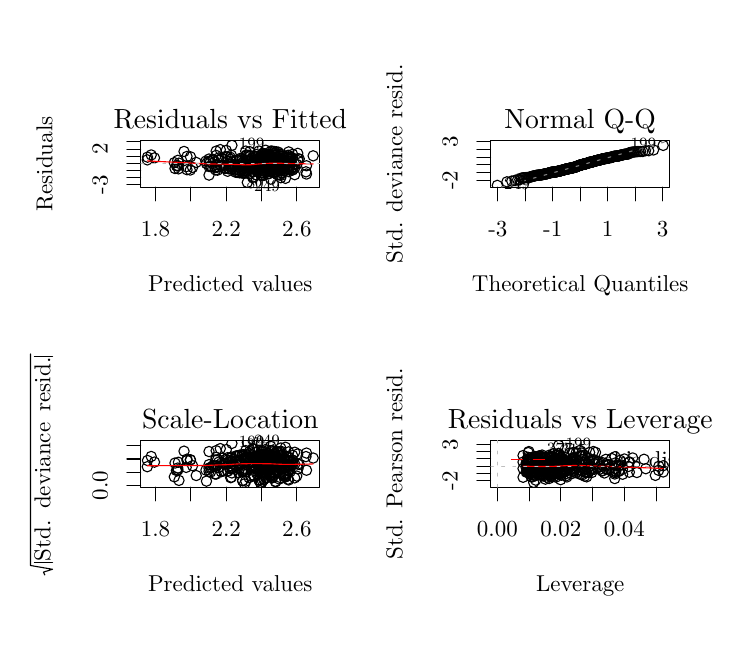
\begin{tikzpicture}[x=1pt,y=1pt]
\definecolor{fillColor}{RGB}{255,255,255}
\path[use as bounding box,fill=fillColor,fill opacity=0.00] (0,0) rectangle (252.94,216.81);
\begin{scope}
\path[clip] (  0.00,  0.00) rectangle (252.94,216.81);
\definecolor{drawColor}{RGB}{0,0,0}

\path[draw=drawColor,line width= 0.4pt,line join=round,line cap=round] ( 46.20,159.20) -- ( 97.29,159.20);

\path[draw=drawColor,line width= 0.4pt,line join=round,line cap=round] ( 46.20,159.20) -- ( 46.20,154.22);

\path[draw=drawColor,line width= 0.4pt,line join=round,line cap=round] ( 58.97,159.20) -- ( 58.97,154.22);

\path[draw=drawColor,line width= 0.4pt,line join=round,line cap=round] ( 71.74,159.20) -- ( 71.74,154.22);

\path[draw=drawColor,line width= 0.4pt,line join=round,line cap=round] ( 84.52,159.20) -- ( 84.52,154.22);

\path[draw=drawColor,line width= 0.4pt,line join=round,line cap=round] ( 97.29,159.20) -- ( 97.29,154.22);

\node[text=drawColor,anchor=base,inner sep=0pt, outer sep=0pt, scale=  0.83] at ( 46.20,141.27) {1.8};

\node[text=drawColor,anchor=base,inner sep=0pt, outer sep=0pt, scale=  0.83] at ( 71.74,141.27) {2.2};

\node[text=drawColor,anchor=base,inner sep=0pt, outer sep=0pt, scale=  0.83] at ( 97.29,141.27) {2.6};

\path[draw=drawColor,line width= 0.4pt,line join=round,line cap=round] ( 40.84,159.98) -- ( 40.84,175.53);

\path[draw=drawColor,line width= 0.4pt,line join=round,line cap=round] ( 40.84,159.98) -- ( 35.86,159.98);

\path[draw=drawColor,line width= 0.4pt,line join=round,line cap=round] ( 40.84,162.57) -- ( 35.86,162.57);

\path[draw=drawColor,line width= 0.4pt,line join=round,line cap=round] ( 40.84,165.17) -- ( 35.86,165.17);

\path[draw=drawColor,line width= 0.4pt,line join=round,line cap=round] ( 40.84,167.76) -- ( 35.86,167.76);

\path[draw=drawColor,line width= 0.4pt,line join=round,line cap=round] ( 40.84,170.35) -- ( 35.86,170.35);

\path[draw=drawColor,line width= 0.4pt,line join=round,line cap=round] ( 40.84,172.94) -- ( 35.86,172.94);

\path[draw=drawColor,line width= 0.4pt,line join=round,line cap=round] ( 40.84,175.53) -- ( 35.86,175.53);

\node[text=drawColor,rotate= 90.00,anchor=base,inner sep=0pt, outer sep=0pt, scale=  0.83] at ( 28.88,159.98) {-3};

\node[text=drawColor,rotate= 90.00,anchor=base,inner sep=0pt, outer sep=0pt, scale=  0.83] at ( 28.88,172.94) {2};

\path[draw=drawColor,line width= 0.4pt,line join=round,line cap=round] ( 40.84,159.20) --
	(105.56,159.20) --
	(105.56,175.97) --
	( 40.84,175.97) --
	( 40.84,159.20);
\end{scope}
\begin{scope}
\path[clip] (  0.00,108.41) rectangle (126.47,216.81);
\definecolor{drawColor}{RGB}{0,0,0}

\node[text=drawColor,anchor=base,inner sep=0pt, outer sep=0pt, scale=  0.83] at ( 73.20,121.35) {Predicted values};

\node[text=drawColor,rotate= 90.00,anchor=base,inner sep=0pt, outer sep=0pt, scale=  0.83] at (  8.96,167.59) {Residuals};
\end{scope}
\begin{scope}
\path[clip] ( 40.84,159.20) rectangle (105.56,175.97);
\definecolor{drawColor}{RGB}{0,0,0}

\path[draw=drawColor,line width= 0.4pt,line join=round,line cap=round] ( 81.40,162.85) circle (  1.87);

\path[draw=drawColor,line width= 0.4pt,line join=round,line cap=round] ( 81.70,162.82) circle (  1.87);

\path[draw=drawColor,line width= 0.4pt,line join=round,line cap=round] ( 43.23,169.04) circle (  1.87);

\path[draw=drawColor,line width= 0.4pt,line join=round,line cap=round] ( 87.64,170.25) circle (  1.87);

\path[draw=drawColor,line width= 0.4pt,line join=round,line cap=round] ( 85.22,163.37) circle (  1.87);

\path[draw=drawColor,line width= 0.4pt,line join=round,line cap=round] ( 90.05,169.90) circle (  1.87);

\path[draw=drawColor,line width= 0.4pt,line join=round,line cap=round] ( 93.88,167.20) circle (  1.87);

\path[draw=drawColor,line width= 0.4pt,line join=round,line cap=round] ( 76.64,164.41) circle (  1.87);

\path[draw=drawColor,line width= 0.4pt,line join=round,line cap=round] ( 89.12,170.72) circle (  1.87);

\path[draw=drawColor,line width= 0.4pt,line join=round,line cap=round] ( 94.32,168.58) circle (  1.87);

\path[draw=drawColor,line width= 0.4pt,line join=round,line cap=round] ( 87.82,166.50) circle (  1.87);

\path[draw=drawColor,line width= 0.4pt,line join=round,line cap=round] ( 85.04,166.88) circle (  1.87);

\path[draw=drawColor,line width= 0.4pt,line join=round,line cap=round] ( 87.64,169.55) circle (  1.87);

\path[draw=drawColor,line width= 0.4pt,line join=round,line cap=round] ( 90.05,166.20) circle (  1.87);

\path[draw=drawColor,line width= 0.4pt,line join=round,line cap=round] ( 92.46,168.85) circle (  1.87);

\path[draw=drawColor,line width= 0.4pt,line join=round,line cap=round] ( 84.48,169.99) circle (  1.87);

\path[draw=drawColor,line width= 0.4pt,line join=round,line cap=round] ( 91.16,168.32) circle (  1.87);

\path[draw=drawColor,line width= 0.4pt,line join=round,line cap=round] ( 74.05,166.58) circle (  1.87);

\path[draw=drawColor,line width= 0.4pt,line join=round,line cap=round] ( 53.74,166.94) circle (  1.87);

\path[draw=drawColor,line width= 0.4pt,line join=round,line cap=round] ( 89.80,164.59) circle (  1.87);

\path[draw=drawColor,line width= 0.4pt,line join=round,line cap=round] ( 96.48,167.55) circle (  1.87);

\path[draw=drawColor,line width= 0.4pt,line join=round,line cap=round] ( 90.98,167.61) circle (  1.87);

\path[draw=drawColor,line width= 0.4pt,line join=round,line cap=round] ( 90.54,169.83) circle (  1.87);

\path[draw=drawColor,line width= 0.4pt,line join=round,line cap=round] ( 84.11,169.31) circle (  1.87);

\path[draw=drawColor,line width= 0.4pt,line join=round,line cap=round] ( 79.99,167.54) circle (  1.87);

\path[draw=drawColor,line width= 0.4pt,line join=round,line cap=round] ( 59.59,166.32) circle (  1.87);

\path[draw=drawColor,line width= 0.4pt,line join=round,line cap=round] ( 84.11,168.56) circle (  1.87);

\path[draw=drawColor,line width= 0.4pt,line join=round,line cap=round] ( 85.53,170.55) circle (  1.87);

\path[draw=drawColor,line width= 0.4pt,line join=round,line cap=round] ( 81.47,168.15) circle (  1.87);

\path[draw=drawColor,line width= 0.4pt,line join=round,line cap=round] ( 87.64,166.53) circle (  1.87);

\path[draw=drawColor,line width= 0.4pt,line join=round,line cap=round] ( 89.31,165.49) circle (  1.87);

\path[draw=drawColor,line width= 0.4pt,line join=round,line cap=round] ( 94.32,170.61) circle (  1.87);

\path[draw=drawColor,line width= 0.4pt,line join=round,line cap=round] ( 91.72,171.01) circle (  1.87);

\path[draw=drawColor,line width= 0.4pt,line join=round,line cap=round] ( 96.48,163.69) circle (  1.87);

\path[draw=drawColor,line width= 0.4pt,line join=round,line cap=round] ( 85.78,168.34) circle (  1.87);

\path[draw=drawColor,line width= 0.4pt,line join=round,line cap=round] ( 83.55,165.40) circle (  1.87);

\path[draw=drawColor,line width= 0.4pt,line join=round,line cap=round] ( 95.06,169.16) circle (  1.87);

\path[draw=drawColor,line width= 0.4pt,line join=round,line cap=round] ( 97.66,168.77) circle (  1.87);

\path[draw=drawColor,line width= 0.4pt,line join=round,line cap=round] ( 79.99,169.12) circle (  1.87);

\path[draw=drawColor,line width= 0.4pt,line join=round,line cap=round] ( 68.11,172.20) circle (  1.87);

\path[draw=drawColor,line width= 0.4pt,line join=round,line cap=round] ( 73.61,165.72) circle (  1.87);

\path[draw=drawColor,line width= 0.4pt,line join=round,line cap=round] ( 85.97,168.31) circle (  1.87);

\path[draw=drawColor,line width= 0.4pt,line join=round,line cap=round] ( 94.32,171.91) circle (  1.87);

\path[draw=drawColor,line width= 0.4pt,line join=round,line cap=round] ( 72.94,166.71) circle (  1.87);

\path[draw=drawColor,line width= 0.4pt,line join=round,line cap=round] ( 65.52,169.34) circle (  1.87);

\path[draw=drawColor,line width= 0.4pt,line join=round,line cap=round] ( 74.05,166.58) circle (  1.87);

\path[draw=drawColor,line width= 0.4pt,line join=round,line cap=round] ( 81.88,168.09) circle (  1.87);

\path[draw=drawColor,line width= 0.4pt,line join=round,line cap=round] (103.16,170.50) circle (  1.87);

\path[draw=drawColor,line width= 0.4pt,line join=round,line cap=round] ( 87.45,170.28) circle (  1.87);

\path[draw=drawColor,line width= 0.4pt,line join=round,line cap=round] ( 67.63,166.41) circle (  1.87);

\path[draw=drawColor,line width= 0.4pt,line join=round,line cap=round] ( 80.96,168.99) circle (  1.87);

\path[draw=drawColor,line width= 0.4pt,line join=round,line cap=round] ( 84.30,167.77) circle (  1.87);

\path[draw=drawColor,line width= 0.4pt,line join=round,line cap=round] ( 76.52,168.80) circle (  1.87);

\path[draw=drawColor,line width= 0.4pt,line join=round,line cap=round] ( 69.96,167.07) circle (  1.87);

\path[draw=drawColor,line width= 0.4pt,line join=round,line cap=round] ( 83.30,167.11) circle (  1.87);

\path[draw=drawColor,line width= 0.4pt,line join=round,line cap=round] ( 86.46,165.03) circle (  1.87);

\path[draw=drawColor,line width= 0.4pt,line join=round,line cap=round] ( 86.89,169.65) circle (  1.87);

\path[draw=drawColor,line width= 0.4pt,line join=round,line cap=round] ( 94.32,168.58) circle (  1.87);

\path[draw=drawColor,line width= 0.4pt,line join=round,line cap=round] ( 76.28,167.18) circle (  1.87);

\path[draw=drawColor,line width= 0.4pt,line join=round,line cap=round] ( 84.30,170.73) circle (  1.87);

\path[draw=drawColor,line width= 0.4pt,line join=round,line cap=round] ( 86.15,166.73) circle (  1.87);

\path[draw=drawColor,line width= 0.4pt,line join=round,line cap=round] ( 58.83,170.14) circle (  1.87);

\path[draw=drawColor,line width= 0.4pt,line join=round,line cap=round] ( 76.21,166.32) circle (  1.87);

\path[draw=drawColor,line width= 0.4pt,line join=round,line cap=round] ( 72.38,168.51) circle (  1.87);

\path[draw=drawColor,line width= 0.4pt,line join=round,line cap=round] ( 73.79,168.33) circle (  1.87);

\path[draw=drawColor,line width= 0.4pt,line join=round,line cap=round] ( 85.22,171.29) circle (  1.87);

\path[draw=drawColor,line width= 0.4pt,line join=round,line cap=round] ( 94.32,167.86) circle (  1.87);

\path[draw=drawColor,line width= 0.4pt,line join=round,line cap=round] ( 73.86,165.69) circle (  1.87);

\path[draw=drawColor,line width= 0.4pt,line join=round,line cap=round] ( 68.11,167.29) circle (  1.87);

\path[draw=drawColor,line width= 0.4pt,line join=round,line cap=round] ( 85.04,171.32) circle (  1.87);

\path[draw=drawColor,line width= 0.4pt,line join=round,line cap=round] ( 93.21,168.03) circle (  1.87);

\path[draw=drawColor,line width= 0.4pt,line join=round,line cap=round] (100.56,164.72) circle (  1.87);

\path[draw=drawColor,line width= 0.4pt,line join=round,line cap=round] ( 45.82,169.75) circle (  1.87);

\path[draw=drawColor,line width= 0.4pt,line join=round,line cap=round] ( 86.27,168.27) circle (  1.87);

\path[draw=drawColor,line width= 0.4pt,line join=round,line cap=round] ( 69.04,169.74) circle (  1.87);

\path[draw=drawColor,line width= 0.4pt,line join=round,line cap=round] ( 88.38,165.62) circle (  1.87);

\path[draw=drawColor,line width= 0.4pt,line join=round,line cap=round] ( 95.37,166.24) circle (  1.87);

\path[draw=drawColor,line width= 0.4pt,line join=round,line cap=round] ( 92.40,166.66) circle (  1.87);

\path[draw=drawColor,line width= 0.4pt,line join=round,line cap=round] ( 43.30,170.02) circle (  1.87);

\path[draw=drawColor,line width= 0.4pt,line join=round,line cap=round] ( 87.82,162.08) circle (  1.87);

\path[draw=drawColor,line width= 0.4pt,line join=round,line cap=round] ( 72.19,168.53) circle (  1.87);

\path[draw=drawColor,line width= 0.4pt,line join=round,line cap=round] ( 85.30,167.63) circle (  1.87);

\path[draw=drawColor,line width= 0.4pt,line join=round,line cap=round] ( 84.30,164.42) circle (  1.87);

\path[draw=drawColor,line width= 0.4pt,line join=round,line cap=round] ( 90.54,169.83) circle (  1.87);

\path[draw=drawColor,line width= 0.4pt,line join=round,line cap=round] ( 78.36,166.92) circle (  1.87);

\path[draw=drawColor,line width= 0.4pt,line join=round,line cap=round] ( 72.88,165.80) circle (  1.87);

\path[draw=drawColor,line width= 0.4pt,line join=round,line cap=round] ( 82.63,165.52) circle (  1.87);

\path[draw=drawColor,line width= 0.4pt,line join=round,line cap=round] ( 84.30,169.29) circle (  1.87);

\path[draw=drawColor,line width= 0.4pt,line join=round,line cap=round] ( 84.87,167.69) circle (  1.87);

\path[draw=drawColor,line width= 0.4pt,line join=round,line cap=round] ( 87.64,164.87) circle (  1.87);

\path[draw=drawColor,line width= 0.4pt,line join=round,line cap=round] ( 86.90,164.09) circle (  1.87);

\path[draw=drawColor,line width= 0.4pt,line join=round,line cap=round] ( 84.97,171.33) circle (  1.87);

\path[draw=drawColor,line width= 0.4pt,line join=round,line cap=round] ( 65.51,166.66) circle (  1.87);

\path[draw=drawColor,line width= 0.4pt,line join=round,line cap=round] ( 84.30,167.77) circle (  1.87);

\path[draw=drawColor,line width= 0.4pt,line join=round,line cap=round] ( 95.81,166.17) circle (  1.87);

\path[draw=drawColor,line width= 0.4pt,line join=round,line cap=round] ( 66.52,166.54) circle (  1.87);

\path[draw=drawColor,line width= 0.4pt,line join=round,line cap=round] ( 75.53,168.92) circle (  1.87);

\path[draw=drawColor,line width= 0.4pt,line join=round,line cap=round] ( 81.70,165.63) circle (  1.87);

\path[draw=drawColor,line width= 0.4pt,line join=round,line cap=round] ( 89.24,167.10) circle (  1.87);

\path[draw=drawColor,line width= 0.4pt,line join=round,line cap=round] ( 77.39,165.27) circle (  1.87);

\path[draw=drawColor,line width= 0.4pt,line join=round,line cap=round] ( 71.45,165.97) circle (  1.87);

\path[draw=drawColor,line width= 0.4pt,line join=round,line cap=round] ( 97.66,169.44) circle (  1.87);

\path[draw=drawColor,line width= 0.4pt,line join=round,line cap=round] ( 90.98,166.07) circle (  1.87);

\path[draw=drawColor,line width= 0.4pt,line join=round,line cap=round] ( 71.45,165.97) circle (  1.87);

\path[draw=drawColor,line width= 0.4pt,line join=round,line cap=round] ( 94.32,169.95) circle (  1.87);

\path[draw=drawColor,line width= 0.4pt,line join=round,line cap=round] ( 85.48,166.82) circle (  1.87);

\path[draw=drawColor,line width= 0.4pt,line join=round,line cap=round] ( 78.13,165.18) circle (  1.87);

\path[draw=drawColor,line width= 0.4pt,line join=round,line cap=round] ( 95.06,169.84) circle (  1.87);

\path[draw=drawColor,line width= 0.4pt,line join=round,line cap=round] ( 94.32,165.61) circle (  1.87);

\path[draw=drawColor,line width= 0.4pt,line join=round,line cap=round] ( 92.83,168.79) circle (  1.87);

\path[draw=drawColor,line width= 0.4pt,line join=round,line cap=round] ( 95.73,171.05) circle (  1.87);

\path[draw=drawColor,line width= 0.4pt,line join=round,line cap=round] ( 68.38,166.33) circle (  1.87);

\path[draw=drawColor,line width= 0.4pt,line join=round,line cap=round] ( 67.19,169.14) circle (  1.87);

\path[draw=drawColor,line width= 0.4pt,line join=round,line cap=round] ( 90.54,171.84) circle (  1.87);

\path[draw=drawColor,line width= 0.4pt,line join=round,line cap=round] ( 91.28,165.23) circle (  1.87);

\path[draw=drawColor,line width= 0.4pt,line join=round,line cap=round] ( 92.65,169.52) circle (  1.87);

\path[draw=drawColor,line width= 0.4pt,line join=round,line cap=round] ( 94.32,166.39) circle (  1.87);

\path[draw=drawColor,line width= 0.4pt,line join=round,line cap=round] ( 93.14,168.04) circle (  1.87);

\path[draw=drawColor,line width= 0.4pt,line join=round,line cap=round] ( 77.70,167.00) circle (  1.87);

\path[draw=drawColor,line width= 0.4pt,line join=round,line cap=round] ( 94.06,168.61) circle (  1.87);

\path[draw=drawColor,line width= 0.4pt,line join=round,line cap=round] ( 87.38,170.98) circle (  1.87);

\path[draw=drawColor,line width= 0.4pt,line join=round,line cap=round] ( 94.14,169.98) circle (  1.87);

\path[draw=drawColor,line width= 0.4pt,line join=round,line cap=round] ( 87.82,168.80) circle (  1.87);

\path[draw=drawColor,line width= 0.4pt,line join=round,line cap=round] ( 85.97,169.78) circle (  1.87);

\path[draw=drawColor,line width= 0.4pt,line join=round,line cap=round] ( 89.05,164.69) circle (  1.87);

\path[draw=drawColor,line width= 0.4pt,line join=round,line cap=round] ( 81.22,169.71) circle (  1.87);

\path[draw=drawColor,line width= 0.4pt,line join=round,line cap=round] ( 81.40,164.78) circle (  1.87);

\path[draw=drawColor,line width= 0.4pt,line join=round,line cap=round] ( 54.66,167.85) circle (  1.87);

\path[draw=drawColor,line width= 0.4pt,line join=round,line cap=round] ( 66.09,166.59) circle (  1.87);

\path[draw=drawColor,line width= 0.4pt,line join=round,line cap=round] ( 89.06,172.07) circle (  1.87);

\path[draw=drawColor,line width= 0.4pt,line join=round,line cap=round] ( 73.14,170.02) circle (  1.87);

\path[draw=drawColor,line width= 0.4pt,line join=round,line cap=round] ( 76.69,166.26) circle (  1.87);

\path[draw=drawColor,line width= 0.4pt,line join=round,line cap=round] ( 77.62,167.84) circle (  1.87);

\path[draw=drawColor,line width= 0.4pt,line join=round,line cap=round] ( 85.90,168.32) circle (  1.87);

\path[draw=drawColor,line width= 0.4pt,line join=round,line cap=round] ( 94.32,164.81) circle (  1.87);

\path[draw=drawColor,line width= 0.4pt,line join=round,line cap=round] ( 92.83,166.60) circle (  1.87);

\path[draw=drawColor,line width= 0.4pt,line join=round,line cap=round] ( 94.07,165.65) circle (  1.87);

\path[draw=drawColor,line width= 0.4pt,line join=round,line cap=round] ( 65.53,163.54) circle (  1.87);

\path[draw=drawColor,line width= 0.4pt,line join=round,line cap=round] ( 78.93,170.76) circle (  1.87);

\path[draw=drawColor,line width= 0.4pt,line join=round,line cap=round] ( 90.91,170.46) circle (  1.87);

\path[draw=drawColor,line width= 0.4pt,line join=round,line cap=round] ( 85.56,164.26) circle (  1.87);

\path[draw=drawColor,line width= 0.4pt,line join=round,line cap=round] ( 66.09,168.42) circle (  1.87);

\path[draw=drawColor,line width= 0.4pt,line join=round,line cap=round] ( 92.83,165.02) circle (  1.87);

\path[draw=drawColor,line width= 0.4pt,line join=round,line cap=round] ( 79.77,170.65) circle (  1.87);

\path[draw=drawColor,line width= 0.4pt,line join=round,line cap=round] ( 54.48,165.80) circle (  1.87);

\path[draw=drawColor,line width= 0.4pt,line join=round,line cap=round] ( 80.03,165.84) circle (  1.87);

\path[draw=drawColor,line width= 0.4pt,line join=round,line cap=round] ( 57.26,166.57) circle (  1.87);

\path[draw=drawColor,line width= 0.4pt,line join=round,line cap=round] ( 84.30,166.98) circle (  1.87);

\path[draw=drawColor,line width= 0.4pt,line join=round,line cap=round] ( 90.98,163.56) circle (  1.87);

\path[draw=drawColor,line width= 0.4pt,line join=round,line cap=round] ( 54.23,168.86) circle (  1.87);

\path[draw=drawColor,line width= 0.4pt,line join=round,line cap=round] ( 54.23,166.89) circle (  1.87);

\path[draw=drawColor,line width= 0.4pt,line join=round,line cap=round] ( 72.25,170.13) circle (  1.87);

\path[draw=drawColor,line width= 0.4pt,line join=round,line cap=round] ( 68.87,168.94) circle (  1.87);

\path[draw=drawColor,line width= 0.4pt,line join=round,line cap=round] ( 58.75,165.36) circle (  1.87);

\path[draw=drawColor,line width= 0.4pt,line join=round,line cap=round] ( 73.30,169.21) circle (  1.87);

\path[draw=drawColor,line width= 0.4pt,line join=round,line cap=round] ( 83.63,167.86) circle (  1.87);

\path[draw=drawColor,line width= 0.4pt,line join=round,line cap=round] ( 87.20,171.01) circle (  1.87);

\path[draw=drawColor,line width= 0.4pt,line join=round,line cap=round] ( 44.64,170.82) circle (  1.87);

\path[draw=drawColor,line width= 0.4pt,line join=round,line cap=round] ( 88.87,171.44) circle (  1.87);

\path[draw=drawColor,line width= 0.4pt,line join=round,line cap=round] ( 77.70,167.83) circle (  1.87);

\path[draw=drawColor,line width= 0.4pt,line join=round,line cap=round] ( 68.25,166.34) circle (  1.87);

\path[draw=drawColor,line width= 0.4pt,line join=round,line cap=round] ( 53.24,165.92) circle (  1.87);

\path[draw=drawColor,line width= 0.4pt,line join=round,line cap=round] ( 76.52,165.37) circle (  1.87);

\path[draw=drawColor,line width= 0.4pt,line join=round,line cap=round] ( 88.13,166.46) circle (  1.87);

\path[draw=drawColor,line width= 0.4pt,line join=round,line cap=round] ( 57.57,165.48) circle (  1.87);

\path[draw=drawColor,line width= 0.4pt,line join=round,line cap=round] ( 76.77,169.55) circle (  1.87);

\path[draw=drawColor,line width= 0.4pt,line join=round,line cap=round] ( 88.87,166.36) circle (  1.87);

\path[draw=drawColor,line width= 0.4pt,line join=round,line cap=round] ( 89.05,169.34) circle (  1.87);

\path[draw=drawColor,line width= 0.4pt,line join=round,line cap=round] ( 84.30,163.49) circle (  1.87);

\path[draw=drawColor,line width= 0.4pt,line join=round,line cap=round] ( 89.49,169.28) circle (  1.87);

\path[draw=drawColor,line width= 0.4pt,line join=round,line cap=round] ( 67.94,165.41) circle (  1.87);

\path[draw=drawColor,line width= 0.4pt,line join=round,line cap=round] ( 83.93,169.34) circle (  1.87);

\path[draw=drawColor,line width= 0.4pt,line join=round,line cap=round] ( 90.98,168.35) circle (  1.87);

\path[draw=drawColor,line width= 0.4pt,line join=round,line cap=round] ( 64.61,167.69) circle (  1.87);

\path[draw=drawColor,line width= 0.4pt,line join=round,line cap=round] ( 86.89,166.63) circle (  1.87);

\path[draw=drawColor,line width= 0.4pt,line join=round,line cap=round] ( 91.47,166.01) circle (  1.87);

\path[draw=drawColor,line width= 0.4pt,line join=round,line cap=round] ( 84.04,169.32) circle (  1.87);

\path[draw=drawColor,line width= 0.4pt,line join=round,line cap=round] ( 91.47,162.59) circle (  1.87);

\path[draw=drawColor,line width= 0.4pt,line join=round,line cap=round] ( 80.77,167.44) circle (  1.87);

\path[draw=drawColor,line width= 0.4pt,line join=round,line cap=round] ( 91.72,165.97) circle (  1.87);

\path[draw=drawColor,line width= 0.4pt,line join=round,line cap=round] ( 88.38,165.62) circle (  1.87);

\path[draw=drawColor,line width= 0.4pt,line join=round,line cap=round] ( 94.81,167.06) circle (  1.87);

\path[draw=drawColor,line width= 0.4pt,line join=round,line cap=round] ( 86.15,171.16) circle (  1.87);

\path[draw=drawColor,line width= 0.4pt,line join=round,line cap=round] ( 83.55,166.25) circle (  1.87);

\path[draw=drawColor,line width= 0.4pt,line join=round,line cap=round] ( 82.63,168.77) circle (  1.87);

\path[draw=drawColor,line width= 0.4pt,line join=round,line cap=round] ( 88.38,167.98) circle (  1.87);

\path[draw=drawColor,line width= 0.4pt,line join=round,line cap=round] ( 84.11,167.79) circle (  1.87);

\path[draw=drawColor,line width= 0.4pt,line join=round,line cap=round] ( 89.61,169.97) circle (  1.87);

\path[draw=drawColor,line width= 0.4pt,line join=round,line cap=round] ( 83.55,165.40) circle (  1.87);

\path[draw=drawColor,line width= 0.4pt,line join=round,line cap=round] ( 87.20,164.93) circle (  1.87);

\path[draw=drawColor,line width= 0.4pt,line join=round,line cap=round] ( 91.65,166.76) circle (  1.87);

\path[draw=drawColor,line width= 0.4pt,line join=round,line cap=round] ( 86.46,165.03) circle (  1.87);

\path[draw=drawColor,line width= 0.4pt,line join=round,line cap=round] ( 87.20,164.05) circle (  1.87);

\path[draw=drawColor,line width= 0.4pt,line join=round,line cap=round] ( 83.37,165.42) circle (  1.87);

\path[draw=drawColor,line width= 0.4pt,line join=round,line cap=round] ( 93.14,168.04) circle (  1.87);

\path[draw=drawColor,line width= 0.4pt,line join=round,line cap=round] ( 94.25,168.59) circle (  1.87);

\path[draw=drawColor,line width= 0.4pt,line join=round,line cap=round] ( 94.06,170.65) circle (  1.87);

\path[draw=drawColor,line width= 0.4pt,line join=round,line cap=round] ( 81.70,166.49) circle (  1.87);

\path[draw=drawColor,line width= 0.4pt,line join=round,line cap=round] ( 73.80,174.28) circle (  1.87);

\path[draw=drawColor,line width= 0.4pt,line join=round,line cap=round] ( 87.82,165.69) circle (  1.87);

\path[draw=drawColor,line width= 0.4pt,line join=round,line cap=round] ( 80.22,172.01) circle (  1.87);

\path[draw=drawColor,line width= 0.4pt,line join=round,line cap=round] ( 70.71,166.98) circle (  1.87);

\path[draw=drawColor,line width= 0.4pt,line join=round,line cap=round] ( 78.36,166.92) circle (  1.87);

\path[draw=drawColor,line width= 0.4pt,line join=round,line cap=round] ( 79.29,165.04) circle (  1.87);

\path[draw=drawColor,line width= 0.4pt,line join=round,line cap=round] ( 90.98,166.07) circle (  1.87);

\path[draw=drawColor,line width= 0.4pt,line join=round,line cap=round] ( 78.81,167.69) circle (  1.87);

\path[draw=drawColor,line width= 0.4pt,line join=round,line cap=round] ( 52.99,168.03) circle (  1.87);

\path[draw=drawColor,line width= 0.4pt,line join=round,line cap=round] ( 91.65,166.76) circle (  1.87);

\path[draw=drawColor,line width= 0.4pt,line join=round,line cap=round] ( 73.35,167.54) circle (  1.87);

\path[draw=drawColor,line width= 0.4pt,line join=round,line cap=round] ( 90.23,163.66) circle (  1.87);

\path[draw=drawColor,line width= 0.4pt,line join=round,line cap=round] ( 91.91,164.31) circle (  1.87);

\path[draw=drawColor,line width= 0.4pt,line join=round,line cap=round] ( 87.64,168.08) circle (  1.87);

\path[draw=drawColor,line width= 0.4pt,line join=round,line cap=round] ( 71.45,170.24) circle (  1.87);

\path[draw=drawColor,line width= 0.4pt,line join=round,line cap=round] ( 75.10,164.59) circle (  1.87);

\path[draw=drawColor,line width= 0.4pt,line join=round,line cap=round] ( 84.48,165.28) circle (  1.87);

\path[draw=drawColor,line width= 0.4pt,line join=round,line cap=round] ( 85.71,169.82) circle (  1.87);

\path[draw=drawColor,line width= 0.4pt,line join=round,line cap=round] ( 68.62,165.33) circle (  1.87);

\path[draw=drawColor,line width= 0.4pt,line join=round,line cap=round] ( 77.70,164.28) circle (  1.87);

\path[draw=drawColor,line width= 0.4pt,line join=round,line cap=round] ( 78.54,165.13) circle (  1.87);

\path[draw=drawColor,line width= 0.4pt,line join=round,line cap=round] ( 87.64,165.72) circle (  1.87);

\path[draw=drawColor,line width= 0.4pt,line join=round,line cap=round] ( 80.03,164.01) circle (  1.87);

\path[draw=drawColor,line width= 0.4pt,line join=round,line cap=round] ( 76.03,164.48) circle (  1.87);

\path[draw=drawColor,line width= 0.4pt,line join=round,line cap=round] ( 78.80,172.21) circle (  1.87);

\path[draw=drawColor,line width= 0.4pt,line join=round,line cap=round] ( 82.45,168.79) circle (  1.87);

\path[draw=drawColor,line width= 0.4pt,line join=round,line cap=round] ( 92.83,168.08) circle (  1.87);

\path[draw=drawColor,line width= 0.4pt,line join=round,line cap=round] ( 77.44,167.03) circle (  1.87);

\path[draw=drawColor,line width= 0.4pt,line join=round,line cap=round] ( 85.71,171.22) circle (  1.87);

\path[draw=drawColor,line width= 0.4pt,line join=round,line cap=round] ( 88.38,167.98) circle (  1.87);

\path[draw=drawColor,line width= 0.4pt,line join=round,line cap=round] ( 67.00,169.17) circle (  1.87);

\path[draw=drawColor,line width= 0.4pt,line join=round,line cap=round] ( 88.13,168.01) circle (  1.87);

\path[draw=drawColor,line width= 0.4pt,line join=round,line cap=round] ( 89.98,168.49) circle (  1.87);

\path[draw=drawColor,line width= 0.4pt,line join=round,line cap=round] ( 89.12,167.11) circle (  1.87);

\path[draw=drawColor,line width= 0.4pt,line join=round,line cap=round] ( 78.13,168.59) circle (  1.87);

\path[draw=drawColor,line width= 0.4pt,line join=round,line cap=round] ( 89.31,169.31) circle (  1.87);

\path[draw=drawColor,line width= 0.4pt,line join=round,line cap=round] ( 86.53,165.86) circle (  1.87);

\path[draw=drawColor,line width= 0.4pt,line join=round,line cap=round] ( 93.88,166.45) circle (  1.87);

\path[draw=drawColor,line width= 0.4pt,line join=round,line cap=round] ( 87.20,169.61) circle (  1.87);

\path[draw=drawColor,line width= 0.4pt,line join=round,line cap=round] ( 83.11,169.45) circle (  1.87);

\path[draw=drawColor,line width= 0.4pt,line join=round,line cap=round] ( 86.46,168.99) circle (  1.87);

\path[draw=drawColor,line width= 0.4pt,line join=round,line cap=round] ( 78.19,165.17) circle (  1.87);

\path[draw=drawColor,line width= 0.4pt,line join=round,line cap=round] ( 91.47,167.54) circle (  1.87);

\path[draw=drawColor,line width= 0.4pt,line join=round,line cap=round] ( 90.98,166.07) circle (  1.87);

\path[draw=drawColor,line width= 0.4pt,line join=round,line cap=round] ( 93.14,162.37) circle (  1.87);

\path[draw=drawColor,line width= 0.4pt,line join=round,line cap=round] ( 94.06,167.90) circle (  1.87);

\path[draw=drawColor,line width= 0.4pt,line join=round,line cap=round] ( 85.04,164.32) circle (  1.87);

\path[draw=drawColor,line width= 0.4pt,line join=round,line cap=round] ( 87.94,172.24) circle (  1.87);

\path[draw=drawColor,line width= 0.4pt,line join=round,line cap=round] ( 93.14,167.30) circle (  1.87);

\path[draw=drawColor,line width= 0.4pt,line join=round,line cap=round] ( 54.23,166.89) circle (  1.87);

\path[draw=drawColor,line width= 0.4pt,line join=round,line cap=round] ( 79.37,160.89) circle (  1.87);

\path[draw=drawColor,line width= 0.4pt,line join=round,line cap=round] ( 85.53,169.12) circle (  1.87);

\path[draw=drawColor,line width= 0.4pt,line join=round,line cap=round] ( 76.52,164.42) circle (  1.87);

\path[draw=drawColor,line width= 0.4pt,line join=round,line cap=round] ( 75.53,165.49) circle (  1.87);

\path[draw=drawColor,line width= 0.4pt,line join=round,line cap=round] ( 72.25,164.92) circle (  1.87);

\path[draw=drawColor,line width= 0.4pt,line join=round,line cap=round] ( 84.60,165.26) circle (  1.87);

\path[draw=drawColor,line width= 0.4pt,line join=round,line cap=round] ( 82.93,165.48) circle (  1.87);

\path[draw=drawColor,line width= 0.4pt,line join=round,line cap=round] ( 72.50,165.85) circle (  1.87);

\path[draw=drawColor,line width= 0.4pt,line join=round,line cap=round] ( 90.98,169.07) circle (  1.87);

\path[draw=drawColor,line width= 0.4pt,line join=round,line cap=round] ( 91.72,166.75) circle (  1.87);

\path[draw=drawColor,line width= 0.4pt,line join=round,line cap=round] ( 89.61,169.97) circle (  1.87);

\path[draw=drawColor,line width= 0.4pt,line join=round,line cap=round] ( 95.73,165.41) circle (  1.87);

\path[draw=drawColor,line width= 0.4pt,line join=round,line cap=round] ( 83.55,172.22) circle (  1.87);

\path[draw=drawColor,line width= 0.4pt,line join=round,line cap=round] ( 91.72,164.33) circle (  1.87);

\path[draw=drawColor,line width= 0.4pt,line join=round,line cap=round] ( 97.22,167.44) circle (  1.87);

\path[draw=drawColor,line width= 0.4pt,line join=round,line cap=round] ( 94.99,165.52) circle (  1.87);

\path[draw=drawColor,line width= 0.4pt,line join=round,line cap=round] ( 87.64,165.72) circle (  1.87);

\path[draw=drawColor,line width= 0.4pt,line join=round,line cap=round] ( 89.31,171.37) circle (  1.87);

\path[draw=drawColor,line width= 0.4pt,line join=round,line cap=round] ( 86.27,165.90) circle (  1.87);

\path[draw=drawColor,line width= 0.4pt,line join=round,line cap=round] ( 92.58,167.38) circle (  1.87);

\path[draw=drawColor,line width= 0.4pt,line join=round,line cap=round] ( 85.78,166.78) circle (  1.87);

\path[draw=drawColor,line width= 0.4pt,line join=round,line cap=round] ( 80.03,164.01) circle (  1.87);

\path[draw=drawColor,line width= 0.4pt,line join=round,line cap=round] ( 65.53,168.48) circle (  1.87);

\path[draw=drawColor,line width= 0.4pt,line join=round,line cap=round] ( 90.24,169.87) circle (  1.87);

\path[draw=drawColor,line width= 0.4pt,line join=round,line cap=round] ( 81.70,168.12) circle (  1.87);

\path[draw=drawColor,line width= 0.4pt,line join=round,line cap=round] ( 87.45,170.28) circle (  1.87);

\path[draw=drawColor,line width= 0.4pt,line join=round,line cap=round] ( 89.49,166.28) circle (  1.87);

\path[draw=drawColor,line width= 0.4pt,line join=round,line cap=round] ( 68.11,170.66) circle (  1.87);

\path[draw=drawColor,line width= 0.4pt,line join=round,line cap=round] ( 89.05,166.34) circle (  1.87);

\path[draw=drawColor,line width= 0.4pt,line join=round,line cap=round] ( 90.72,165.30) circle (  1.87);

\path[draw=drawColor,line width= 0.4pt,line join=round,line cap=round] ( 67.63,168.23) circle (  1.87);

\path[draw=drawColor,line width= 0.4pt,line join=round,line cap=round] ( 91.47,166.01) circle (  1.87);

\path[draw=drawColor,line width= 0.4pt,line join=round,line cap=round] ( 82.93,165.48) circle (  1.87);

\path[draw=drawColor,line width= 0.4pt,line join=round,line cap=round] ( 76.52,168.80) circle (  1.87);

\path[draw=drawColor,line width= 0.4pt,line join=round,line cap=round] ( 88.38,167.98) circle (  1.87);

\path[draw=drawColor,line width= 0.4pt,line join=round,line cap=round] ( 73.61,166.63) circle (  1.87);

\path[draw=drawColor,line width= 0.4pt,line join=round,line cap=round] ( 82.63,167.20) circle (  1.87);

\path[draw=drawColor,line width= 0.4pt,line join=round,line cap=round] ( 89.61,167.80) circle (  1.87);

\path[draw=drawColor,line width= 0.4pt,line join=round,line cap=round] ( 85.97,172.53) circle (  1.87);

\path[draw=drawColor,line width= 0.4pt,line join=round,line cap=round] ( 85.04,169.19) circle (  1.87);

\path[draw=drawColor,line width= 0.4pt,line join=round,line cap=round] ( 91.28,169.72) circle (  1.87);

\path[draw=drawColor,line width= 0.4pt,line join=round,line cap=round] ( 94.32,169.27) circle (  1.87);

\path[draw=drawColor,line width= 0.4pt,line join=round,line cap=round] ( 84.11,168.56) circle (  1.87);

\path[draw=drawColor,line width= 0.4pt,line join=round,line cap=round] ( 88.57,170.12) circle (  1.87);

\path[draw=drawColor,line width= 0.4pt,line join=round,line cap=round] ( 77.44,169.46) circle (  1.87);

\path[draw=drawColor,line width= 0.4pt,line join=round,line cap=round] ( 88.38,172.17) circle (  1.87);

\path[draw=drawColor,line width= 0.4pt,line join=round,line cap=round] ( 92.46,168.85) circle (  1.87);

\path[draw=drawColor,line width= 0.4pt,line join=round,line cap=round] ( 85.04,169.91) circle (  1.87);

\path[draw=drawColor,line width= 0.4pt,line join=round,line cap=round] ( 86.15,166.73) circle (  1.87);

\path[draw=drawColor,line width= 0.4pt,line join=round,line cap=round] ( 85.22,166.85) circle (  1.87);

\path[draw=drawColor,line width= 0.4pt,line join=round,line cap=round] ( 93.58,168.69) circle (  1.87);

\path[draw=drawColor,line width= 0.4pt,line join=round,line cap=round] ( 89.31,170.70) circle (  1.87);

\path[draw=drawColor,line width= 0.4pt,line join=round,line cap=round] ( 89.49,167.82) circle (  1.87);

\path[draw=drawColor,line width= 0.4pt,line join=round,line cap=round] ( 94.06,166.42) circle (  1.87);

\path[draw=drawColor,line width= 0.4pt,line join=round,line cap=round] ( 87.64,170.25) circle (  1.87);

\path[draw=drawColor,line width= 0.4pt,line join=round,line cap=round] ( 89.31,171.37) circle (  1.87);

\path[draw=drawColor,line width= 0.4pt,line join=round,line cap=round] ( 82.71,170.96) circle (  1.87);

\path[draw=drawColor,line width= 0.4pt,line join=round,line cap=round] ( 80.48,170.55) circle (  1.87);

\path[draw=drawColor,line width= 0.4pt,line join=round,line cap=round] ( 90.54,171.19) circle (  1.87);

\path[draw=drawColor,line width= 0.4pt,line join=round,line cap=round] ( 81.97,165.60) circle (  1.87);

\path[draw=drawColor,line width= 0.4pt,line join=round,line cap=round] ( 85.80,170.52) circle (  1.87);

\path[draw=drawColor,line width= 0.4pt,line join=round,line cap=round] ( 56.50,172.08) circle (  1.87);

\path[draw=drawColor,line width= 0.4pt,line join=round,line cap=round] ( 78.37,166.91) circle (  1.87);

\path[draw=drawColor,line width= 0.4pt,line join=round,line cap=round] ( 81.70,170.38) circle (  1.87);

\path[draw=drawColor,line width= 0.4pt,line join=round,line cap=round] ( 83.20,169.44) circle (  1.87);

\path[draw=drawColor,line width= 0.4pt,line join=round,line cap=round] ( 73.61,170.73) circle (  1.87);

\path[draw=drawColor,line width= 0.4pt,line join=round,line cap=round] ( 71.77,172.46) circle (  1.87);

\path[draw=drawColor,line width= 0.4pt,line join=round,line cap=round] ( 85.98,169.05) circle (  1.87);

\path[draw=drawColor,line width= 0.4pt,line join=round,line cap=round] ( 80.03,165.84) circle (  1.87);

\path[draw=drawColor,line width= 0.4pt,line join=round,line cap=round] ( 90.23,165.37) circle (  1.87);

\path[draw=drawColor,line width= 0.4pt,line join=round,line cap=round] ( 86.15,167.52) circle (  1.87);

\path[draw=drawColor,line width= 0.4pt,line join=round,line cap=round] ( 86.15,167.52) circle (  1.87);

\path[draw=drawColor,line width= 0.4pt,line join=round,line cap=round] ( 85.22,169.16) circle (  1.87);

\path[draw=drawColor,line width= 0.4pt,line join=round,line cap=round] ( 84.30,167.77) circle (  1.87);

\path[draw=drawColor,line width= 0.4pt,line join=round,line cap=round] ( 85.97,167.54) circle (  1.87);

\path[draw=drawColor,line width= 0.4pt,line join=round,line cap=round] ( 81.70,168.89) circle (  1.87);

\path[draw=drawColor,line width= 0.4pt,line join=round,line cap=round] ( 89.05,170.73) circle (  1.87);

\path[draw=drawColor,line width= 0.4pt,line join=round,line cap=round] (100.75,163.91) circle (  1.87);

\path[draw=drawColor,line width= 0.4pt,line join=round,line cap=round] ( 86.46,169.71) circle (  1.87);

\path[draw=drawColor,line width= 0.4pt,line join=round,line cap=round] ( 79.10,168.46) circle (  1.87);

\path[draw=drawColor,line width= 0.4pt,line join=round,line cap=round] ( 89.49,166.28) circle (  1.87);

\path[draw=drawColor,line width= 0.4pt,line join=round,line cap=round] ( 91.16,169.04) circle (  1.87);

\path[draw=drawColor,line width= 0.4pt,line join=round,line cap=round] ( 90.80,165.29) circle (  1.87);

\path[draw=drawColor,line width= 0.4pt,line join=round,line cap=round] ( 92.83,167.35) circle (  1.87);

\path[draw=drawColor,line width= 0.4pt,line join=round,line cap=round] ( 91.65,163.48) circle (  1.87);

\path[draw=drawColor,line width= 0.4pt,line join=round,line cap=round] ( 89.05,164.69) circle (  1.87);

\path[draw=drawColor,line width= 0.4pt,line join=round,line cap=round] ( 95.73,165.41) circle (  1.87);

\path[draw=drawColor,line width= 0.4pt,line join=round,line cap=round] ( 94.25,169.96) circle (  1.87);

\path[draw=drawColor,line width= 0.4pt,line join=round,line cap=round] ( 79.11,170.74) circle (  1.87);

\path[draw=drawColor,line width= 0.4pt,line join=round,line cap=round] ( 80.96,164.83) circle (  1.87);

\path[draw=drawColor,line width= 0.4pt,line join=round,line cap=round] ( 93.58,170.06) circle (  1.87);

\path[draw=drawColor,line width= 0.4pt,line join=round,line cap=round] ( 80.96,166.59) circle (  1.87);

\path[draw=drawColor,line width= 0.4pt,line join=round,line cap=round] ( 77.45,168.68) circle (  1.87);

\path[draw=drawColor,line width= 0.4pt,line join=round,line cap=round] ( 83.64,167.06) circle (  1.87);

\path[draw=drawColor,line width= 0.4pt,line join=round,line cap=round] ( 95.74,169.73) circle (  1.87);

\path[draw=drawColor,line width= 0.4pt,line join=round,line cap=round] ( 73.61,167.51) circle (  1.87);

\path[draw=drawColor,line width= 0.4pt,line join=round,line cap=round] ( 88.57,167.19) circle (  1.87);

\path[draw=drawColor,line width= 0.4pt,line join=round,line cap=round] ( 89.05,168.62) circle (  1.87);

\path[draw=drawColor,line width= 0.4pt,line join=round,line cap=round] ( 98.15,169.37) circle (  1.87);

\path[draw=drawColor,line width= 0.4pt,line join=round,line cap=round] ( 91.72,165.97) circle (  1.87);

\path[draw=drawColor,line width= 0.4pt,line join=round,line cap=round] ( 86.90,168.93) circle (  1.87);

\path[draw=drawColor,line width= 0.4pt,line join=round,line cap=round] ( 70.09,169.61) circle (  1.87);

\path[draw=drawColor,line width= 0.4pt,line join=round,line cap=round] ( 60.91,168.12) circle (  1.87);

\path[draw=drawColor,line width= 0.4pt,line join=round,line cap=round] ( 88.38,168.72) circle (  1.87);

\path[draw=drawColor,line width= 0.4pt,line join=round,line cap=round] ( 80.79,165.75) circle (  1.87);

\path[draw=drawColor,line width= 0.4pt,line join=round,line cap=round] ( 70.83,166.96) circle (  1.87);

\path[draw=drawColor,line width= 0.4pt,line join=round,line cap=round] ( 88.38,168.72) circle (  1.87);

\path[draw=drawColor,line width= 0.4pt,line join=round,line cap=round] ( 86.89,166.63) circle (  1.87);

\path[draw=drawColor,line width= 0.4pt,line join=round,line cap=round] ( 87.82,168.05) circle (  1.87);

\path[draw=drawColor,line width= 0.4pt,line join=round,line cap=round] ( 87.38,168.12) circle (  1.87);

\path[draw=drawColor,line width= 0.4pt,line join=round,line cap=round] ( 86.27,166.71) circle (  1.87);

\path[draw=drawColor,line width= 0.4pt,line join=round,line cap=round] ( 89.80,171.96) circle (  1.87);

\path[draw=drawColor,line width= 0.4pt,line join=round,line cap=round] ( 89.24,168.60) circle (  1.87);

\path[draw=drawColor,line width= 0.4pt,line join=round,line cap=round] ( 78.93,170.02) circle (  1.87);

\path[draw=drawColor,line width= 0.4pt,line join=round,line cap=round] ( 83.55,167.87) circle (  1.87);

\path[draw=drawColor,line width= 0.4pt,line join=round,line cap=round] ( 89.49,170.67) circle (  1.87);

\path[draw=drawColor,line width= 0.4pt,line join=round,line cap=round] ( 87.38,168.12) circle (  1.87);

\path[draw=drawColor,line width= 0.4pt,line join=round,line cap=round] ( 86.71,166.65) circle (  1.87);

\path[draw=drawColor,line width= 0.4pt,line join=round,line cap=round] (100.75,166.91) circle (  1.87);

\path[draw=drawColor,line width= 0.4pt,line join=round,line cap=round] ( 67.68,166.41) circle (  1.87);

\path[draw=drawColor,line width= 0.4pt,line join=round,line cap=round] ( 81.88,168.09) circle (  1.87);

\path[draw=drawColor,line width= 0.4pt,line join=round,line cap=round] ( 87.82,169.52) circle (  1.87);

\path[draw=drawColor,line width= 0.4pt,line join=round,line cap=round] ( 71.03,166.02) circle (  1.87);

\path[draw=drawColor,line width= 0.4pt,line join=round,line cap=round] ( 82.44,170.28) circle (  1.87);

\path[draw=drawColor,line width= 0.4pt,line join=round,line cap=round] ( 92.39,168.14) circle (  1.87);

\path[draw=drawColor,line width= 0.4pt,line join=round,line cap=round] ( 82.37,163.72) circle (  1.87);

\path[draw=drawColor,line width= 0.4pt,line join=round,line cap=round] ( 97.59,171.39) circle (  1.87);

\path[draw=drawColor,line width= 0.4pt,line join=round,line cap=round] ( 88.13,164.81) circle (  1.87);

\path[draw=drawColor,line width= 0.4pt,line join=round,line cap=round] ( 69.61,172.74) circle (  1.87);

\path[draw=drawColor,line width= 0.4pt,line join=round,line cap=round] ( 89.24,164.66) circle (  1.87);

\path[draw=drawColor,line width= 0.4pt,line join=round,line cap=round] ( 89.98,169.91) circle (  1.87);

\path[draw=drawColor,line width= 0.4pt,line join=round,line cap=round] ( 78.36,167.75) circle (  1.87);

\path[draw=drawColor,line width= 0.4pt,line join=round,line cap=round] ( 94.07,169.31) circle (  1.87);

\path[draw=drawColor,line width= 0.4pt,line join=round,line cap=round] ( 84.60,164.38) circle (  1.87);

\path[draw=drawColor,line width= 0.4pt,line join=round,line cap=round] ( 96.48,166.08) circle (  1.87);

\path[draw=drawColor,line width= 0.4pt,line join=round,line cap=round] ( 75.59,164.53) circle (  1.87);

\path[draw=drawColor,line width= 0.4pt,line join=round,line cap=round] ( 78.19,164.23) circle (  1.87);

\path[draw=drawColor,line width= 0.4pt,line join=round,line cap=round] ( 89.05,166.34) circle (  1.87);

\path[draw=drawColor,line width= 0.4pt,line join=round,line cap=round] ( 84.48,163.47) circle (  1.87);

\path[draw=drawColor,line width= 0.4pt,line join=round,line cap=round] ( 84.31,164.42) circle (  1.87);

\path[draw=drawColor,line width= 0.4pt,line join=round,line cap=round] ( 81.70,164.74) circle (  1.87);

\path[draw=drawColor,line width= 0.4pt,line join=round,line cap=round] ( 77.44,164.31) circle (  1.87);

\path[draw=drawColor,line width= 0.4pt,line join=round,line cap=round] ( 64.42,168.61) circle (  1.87);

\path[draw=drawColor,line width= 0.4pt,line join=round,line cap=round] ( 82.93,170.21) circle (  1.87);

\path[draw=drawColor,line width= 0.4pt,line join=round,line cap=round] ( 57.57,170.28) circle (  1.87);

\path[draw=drawColor,line width= 0.4pt,line join=round,line cap=round] ( 85.53,167.60) circle (  1.87);

\path[draw=drawColor,line width= 0.4pt,line join=round,line cap=round] ( 84.60,165.26) circle (  1.87);
\definecolor{drawColor}{RGB}{255,0,0}

\path[draw=drawColor,line width= 0.4pt,line join=round,line cap=round] ( 43.23,168.66) --
	( 43.30,168.66) --
	( 44.64,168.59) --
	( 45.82,168.53) --
	( 52.99,168.20) --
	( 53.24,168.19) --
	( 53.74,168.16) --
	( 54.23,168.14) --
	( 54.23,168.14) --
	( 54.23,168.14) --
	( 54.48,168.13) --
	( 54.66,168.12) --
	( 56.50,168.02) --
	( 57.26,167.98) --
	( 57.57,167.97) --
	( 57.57,167.97) --
	( 58.75,167.90) --
	( 58.83,167.90) --
	( 59.59,167.85) --
	( 60.91,167.78) --
	( 64.42,167.59) --
	( 64.61,167.58) --
	( 65.51,167.56) --
	( 65.52,167.56) --
	( 65.53,167.56) --
	( 65.53,167.56) --
	( 66.09,167.55) --
	( 66.09,167.55) --
	( 66.52,167.54) --
	( 67.00,167.54) --
	( 67.19,167.54) --
	( 67.63,167.53) --
	( 67.63,167.53) --
	( 67.68,167.53) --
	( 67.94,167.53) --
	( 68.11,167.52) --
	( 68.11,167.52) --
	( 68.11,167.52) --
	( 68.25,167.52) --
	( 68.38,167.52) --
	( 68.62,167.52) --
	( 68.87,167.52) --
	( 69.04,167.51) --
	( 69.61,167.51) --
	( 69.96,167.50) --
	( 70.09,167.50) --
	( 70.71,167.48) --
	( 70.83,167.48) --
	( 71.03,167.48) --
	( 71.45,167.46) --
	( 71.45,167.46) --
	( 71.45,167.46) --
	( 71.77,167.45) --
	( 72.19,167.44) --
	( 72.25,167.44) --
	( 72.25,167.44) --
	( 72.38,167.44) --
	( 72.50,167.44) --
	( 72.88,167.43) --
	( 72.94,167.43) --
	( 73.14,167.42) --
	( 73.30,167.42) --
	( 73.35,167.42) --
	( 73.61,167.41) --
	( 73.61,167.41) --
	( 73.61,167.41) --
	( 73.61,167.41) --
	( 73.79,167.41) --
	( 73.80,167.41) --
	( 73.86,167.40) --
	( 74.05,167.40) --
	( 74.05,167.40) --
	( 75.10,167.37) --
	( 75.53,167.36) --
	( 75.53,167.36) --
	( 75.59,167.36) --
	( 76.03,167.34) --
	( 76.21,167.34) --
	( 76.28,167.34) --
	( 76.52,167.33) --
	( 76.52,167.33) --
	( 76.52,167.33) --
	( 76.52,167.33) --
	( 76.64,167.32) --
	( 76.69,167.32) --
	( 76.77,167.32) --
	( 77.39,167.29) --
	( 77.44,167.29) --
	( 77.44,167.29) --
	( 77.44,167.29) --
	( 77.45,167.29) --
	( 77.62,167.28) --
	( 77.70,167.28) --
	( 77.70,167.28) --
	( 77.70,167.28) --
	( 78.13,167.26) --
	( 78.13,167.26) --
	( 78.19,167.26) --
	( 78.19,167.26) --
	( 78.36,167.26) --
	( 78.36,167.26) --
	( 78.36,167.26) --
	( 78.37,167.26) --
	( 78.54,167.25) --
	( 78.80,167.25) --
	( 78.81,167.25) --
	( 78.93,167.25) --
	( 78.93,167.25) --
	( 79.10,167.26) --
	( 79.11,167.26) --
	( 79.29,167.26) --
	( 79.37,167.26) --
	( 79.77,167.27) --
	( 79.99,167.27) --
	( 79.99,167.27) --
	( 80.03,167.27) --
	( 80.03,167.27) --
	( 80.03,167.27) --
	( 80.03,167.27) --
	( 80.22,167.27) --
	( 80.48,167.28) --
	( 80.77,167.29) --
	( 80.79,167.30) --
	( 80.96,167.30) --
	( 80.96,167.30) --
	( 80.96,167.30) --
	( 81.22,167.32) --
	( 81.40,167.33) --
	( 81.40,167.33) --
	( 81.47,167.34) --
	( 81.70,167.36) --
	( 81.70,167.36) --
	( 81.70,167.36) --
	( 81.70,167.36) --
	( 81.70,167.36) --
	( 81.70,167.36) --
	( 81.70,167.36) --
	( 81.88,167.38) --
	( 81.88,167.38) --
	( 81.97,167.39) --
	( 82.37,167.43) --
	( 82.44,167.44) --
	( 82.45,167.44) --
	( 82.63,167.46) --
	( 82.63,167.46) --
	( 82.63,167.46) --
	( 82.71,167.47) --
	( 82.93,167.49) --
	( 82.93,167.49) --
	( 82.93,167.49) --
	( 83.11,167.51) --
	( 83.20,167.52) --
	( 83.30,167.53) --
	( 83.37,167.53) --
	( 83.55,167.55) --
	( 83.55,167.55) --
	( 83.55,167.55) --
	( 83.55,167.55) --
	( 83.55,167.55) --
	( 83.63,167.56) --
	( 83.64,167.56) --
	( 83.93,167.59) --
	( 84.04,167.60) --
	( 84.11,167.60) --
	( 84.11,167.60) --
	( 84.11,167.60) --
	( 84.11,167.60) --
	( 84.30,167.62) --
	( 84.30,167.62) --
	( 84.30,167.62) --
	( 84.30,167.62) --
	( 84.30,167.62) --
	( 84.30,167.62) --
	( 84.30,167.62) --
	( 84.30,167.62) --
	( 84.31,167.62) --
	( 84.48,167.64) --
	( 84.48,167.64) --
	( 84.48,167.64) --
	( 84.60,167.65) --
	( 84.60,167.65) --
	( 84.60,167.65) --
	( 84.87,167.67) --
	( 84.97,167.67) --
	( 85.04,167.68) --
	( 85.04,167.68) --
	( 85.04,167.68) --
	( 85.04,167.68) --
	( 85.04,167.68) --
	( 85.22,167.69) --
	( 85.22,167.69) --
	( 85.22,167.69) --
	( 85.22,167.69) --
	( 85.30,167.70) --
	( 85.48,167.71) --
	( 85.53,167.71) --
	( 85.53,167.71) --
	( 85.53,167.71) --
	( 85.56,167.72) --
	( 85.71,167.73) --
	( 85.71,167.73) --
	( 85.78,167.73) --
	( 85.78,167.73) --
	( 85.80,167.73) --
	( 85.90,167.74) --
	( 85.97,167.74) --
	( 85.97,167.74) --
	( 85.97,167.74) --
	( 85.97,167.74) --
	( 85.98,167.74) --
	( 86.15,167.75) --
	( 86.15,167.75) --
	( 86.15,167.75) --
	( 86.15,167.75) --
	( 86.15,167.75) --
	( 86.27,167.76) --
	( 86.27,167.76) --
	( 86.27,167.76) --
	( 86.46,167.77) --
	( 86.46,167.77) --
	( 86.46,167.77) --
	( 86.46,167.77) --
	( 86.53,167.78) --
	( 86.71,167.79) --
	( 86.89,167.79) --
	( 86.89,167.79) --
	( 86.89,167.79) --
	( 86.90,167.79) --
	( 86.90,167.79) --
	( 87.20,167.80) --
	( 87.20,167.80) --
	( 87.20,167.80) --
	( 87.20,167.80) --
	( 87.38,167.80) --
	( 87.38,167.80) --
	( 87.38,167.80) --
	( 87.45,167.80) --
	( 87.45,167.80) --
	( 87.64,167.81) --
	( 87.64,167.81) --
	( 87.64,167.81) --
	( 87.64,167.81) --
	( 87.64,167.81) --
	( 87.64,167.81) --
	( 87.64,167.81) --
	( 87.64,167.81) --
	( 87.82,167.81) --
	( 87.82,167.81) --
	( 87.82,167.81) --
	( 87.82,167.81) --
	( 87.82,167.81) --
	( 87.82,167.81) --
	( 87.94,167.81) --
	( 88.13,167.81) --
	( 88.13,167.81) --
	( 88.13,167.81) --
	( 88.38,167.81) --
	( 88.38,167.81) --
	( 88.38,167.81) --
	( 88.38,167.81) --
	( 88.38,167.81) --
	( 88.38,167.81) --
	( 88.38,167.81) --
	( 88.38,167.81) --
	( 88.57,167.81) --
	( 88.57,167.81) --
	( 88.87,167.81) --
	( 88.87,167.81) --
	( 89.05,167.81) --
	( 89.05,167.81) --
	( 89.05,167.81) --
	( 89.05,167.81) --
	( 89.05,167.81) --
	( 89.05,167.81) --
	( 89.05,167.81) --
	( 89.06,167.81) --
	( 89.12,167.81) --
	( 89.12,167.81) --
	( 89.24,167.81) --
	( 89.24,167.81) --
	( 89.24,167.81) --
	( 89.31,167.81) --
	( 89.31,167.81) --
	( 89.31,167.81) --
	( 89.31,167.81) --
	( 89.31,167.81) --
	( 89.49,167.81) --
	( 89.49,167.81) --
	( 89.49,167.81) --
	( 89.49,167.81) --
	( 89.49,167.81) --
	( 89.61,167.81) --
	( 89.61,167.81) --
	( 89.61,167.81) --
	( 89.80,167.81) --
	( 89.80,167.81) --
	( 89.98,167.81) --
	( 89.98,167.81) --
	( 90.05,167.81) --
	( 90.05,167.81) --
	( 90.23,167.80) --
	( 90.23,167.80) --
	( 90.24,167.80) --
	( 90.54,167.80) --
	( 90.54,167.80) --
	( 90.54,167.80) --
	( 90.54,167.80) --
	( 90.72,167.80) --
	( 90.80,167.80) --
	( 90.91,167.80) --
	( 90.98,167.80) --
	( 90.98,167.80) --
	( 90.98,167.80) --
	( 90.98,167.80) --
	( 90.98,167.80) --
	( 90.98,167.80) --
	( 90.98,167.80) --
	( 91.16,167.80) --
	( 91.16,167.80) --
	( 91.28,167.80) --
	( 91.28,167.80) --
	( 91.47,167.80) --
	( 91.47,167.80) --
	( 91.47,167.80) --
	( 91.47,167.80) --
	( 91.65,167.80) --
	( 91.65,167.80) --
	( 91.65,167.80) --
	( 91.72,167.80) --
	( 91.72,167.80) --
	( 91.72,167.80) --
	( 91.72,167.80) --
	( 91.72,167.80) --
	( 91.91,167.80) --
	( 92.39,167.78) --
	( 92.40,167.78) --
	( 92.46,167.78) --
	( 92.46,167.78) --
	( 92.58,167.78) --
	( 92.65,167.78) --
	( 92.83,167.77) --
	( 92.83,167.77) --
	( 92.83,167.77) --
	( 92.83,167.77) --
	( 92.83,167.77) --
	( 93.14,167.76) --
	( 93.14,167.76) --
	( 93.14,167.76) --
	( 93.14,167.76) --
	( 93.21,167.75) --
	( 93.58,167.74) --
	( 93.58,167.74) --
	( 93.88,167.73) --
	( 93.88,167.73) --
	( 94.06,167.72) --
	( 94.06,167.72) --
	( 94.06,167.72) --
	( 94.06,167.72) --
	( 94.07,167.72) --
	( 94.07,167.72) --
	( 94.14,167.72) --
	( 94.25,167.72) --
	( 94.25,167.72) --
	( 94.32,167.72) --
	( 94.32,167.72) --
	( 94.32,167.72) --
	( 94.32,167.72) --
	( 94.32,167.72) --
	( 94.32,167.72) --
	( 94.32,167.72) --
	( 94.32,167.72) --
	( 94.32,167.72) --
	( 94.32,167.72) --
	( 94.81,167.70) --
	( 94.99,167.70) --
	( 95.06,167.70) --
	( 95.06,167.70) --
	( 95.37,167.69) --
	( 95.73,167.68) --
	( 95.73,167.68) --
	( 95.73,167.68) --
	( 95.74,167.68) --
	( 95.81,167.68) --
	( 96.48,167.67) --
	( 96.48,167.67) --
	( 96.48,167.67) --
	( 97.22,167.66) --
	( 97.59,167.65) --
	( 97.66,167.65) --
	( 97.66,167.65) --
	( 98.15,167.64) --
	(100.56,167.61) --
	(100.75,167.60) --
	(100.75,167.60) --
	(103.16,167.56);
\end{scope}
\begin{scope}
\path[clip] (  0.00,  0.00) rectangle (252.94,216.81);
\definecolor{drawColor}{RGB}{0,0,0}

\node[text=drawColor,anchor=base,inner sep=0pt, outer sep=0pt, scale=  1.00] at ( 73.20,180.46) {Residuals vs Fitted};
\end{scope}
\begin{scope}
\path[clip] (  0.00,108.41) rectangle (126.47,216.81);
\definecolor{drawColor}{RGB}{0,0,0}

\node[text=drawColor,anchor=base west,inner sep=0pt, outer sep=0pt, scale=  0.62] at ( 81.86,157.56) {249};

\node[text=drawColor,anchor=base west,inner sep=0pt, outer sep=0pt, scale=  0.62] at ( 76.29,172.85) {199};

\node[text=drawColor,anchor=base east,inner sep=0pt, outer sep=0pt, scale=  0.62] at ( 85.33,158.75) {80};
\end{scope}
\begin{scope}
\path[clip] ( 40.84,159.20) rectangle (105.56,175.97);
\definecolor{drawColor}{RGB}{190,190,190}

\path[draw=drawColor,line width= 0.4pt,dash pattern=on 1pt off 3pt ,line join=round,line cap=round] ( 40.84,167.76) -- (105.56,167.76);
\end{scope}
\begin{scope}
\path[clip] (167.31,159.20) rectangle (232.03,175.97);
\definecolor{drawColor}{RGB}{0,0,0}

\path[draw=drawColor,line width= 0.4pt,line join=round,line cap=round] (177.07,161.87) circle (  1.87);

\path[draw=drawColor,line width= 0.4pt,line join=round,line cap=round] (177.84,161.88) circle (  1.87);

\path[draw=drawColor,line width= 0.4pt,line join=round,line cap=round] (204.94,168.61) circle (  1.87);

\path[draw=drawColor,line width= 0.4pt,line join=round,line cap=round] (210.37,169.90) circle (  1.87);

\path[draw=drawColor,line width= 0.4pt,line join=round,line cap=round] (178.50,162.50) circle (  1.87);

\path[draw=drawColor,line width= 0.4pt,line join=round,line cap=round] (208.62,169.52) circle (  1.87);

\path[draw=drawColor,line width= 0.4pt,line join=round,line cap=round] (198.47,166.61) circle (  1.87);

\path[draw=drawColor,line width= 0.4pt,line join=round,line cap=round] (185.18,163.58) circle (  1.87);

\path[draw=drawColor,line width= 0.4pt,line join=round,line cap=round] (213.14,170.42) circle (  1.87);

\path[draw=drawColor,line width= 0.4pt,line join=round,line cap=round] (202.94,168.10) circle (  1.87);

\path[draw=drawColor,line width= 0.4pt,line join=round,line cap=round] (195.38,165.86) circle (  1.87);

\path[draw=drawColor,line width= 0.4pt,line join=round,line cap=round] (197.06,166.26) circle (  1.87);

\path[draw=drawColor,line width= 0.4pt,line join=round,line cap=round] (207.11,169.14) circle (  1.87);

\path[draw=drawColor,line width= 0.4pt,line join=round,line cap=round] (193.95,165.54) circle (  1.87);

\path[draw=drawColor,line width= 0.4pt,line join=round,line cap=round] (204.23,168.39) circle (  1.87);

\path[draw=drawColor,line width= 0.4pt,line join=round,line cap=round] (209.40,169.63) circle (  1.87);

\path[draw=drawColor,line width= 0.4pt,line join=round,line cap=round] (202.09,167.82) circle (  1.87);

\path[draw=drawColor,line width= 0.4pt,line join=round,line cap=round] (195.66,165.94) circle (  1.87);

\path[draw=drawColor,line width= 0.4pt,line join=round,line cap=round] (197.51,166.32) circle (  1.87);

\path[draw=drawColor,line width= 0.4pt,line join=round,line cap=round] (186.36,163.80) circle (  1.87);

\path[draw=drawColor,line width= 0.4pt,line join=round,line cap=round] (199.35,166.99) circle (  1.87);

\path[draw=drawColor,line width= 0.4pt,line join=round,line cap=round] (199.48,167.06) circle (  1.87);

\path[draw=drawColor,line width= 0.4pt,line join=round,line cap=round] (208.25,169.45) circle (  1.87);

\path[draw=drawColor,line width= 0.4pt,line join=round,line cap=round] (206.15,168.89) circle (  1.87);

\path[draw=drawColor,line width= 0.4pt,line join=round,line cap=round] (199.10,166.98) circle (  1.87);

\path[draw=drawColor,line width= 0.4pt,line join=round,line cap=round] (194.47,165.66) circle (  1.87);

\path[draw=drawColor,line width= 0.4pt,line join=round,line cap=round] (202.87,168.09) circle (  1.87);

\path[draw=drawColor,line width= 0.4pt,line join=round,line cap=round] (211.83,170.23) circle (  1.87);

\path[draw=drawColor,line width= 0.4pt,line join=round,line cap=round] (201.83,167.64) circle (  1.87);

\path[draw=drawColor,line width= 0.4pt,line join=round,line cap=round] (195.45,165.88) circle (  1.87);

\path[draw=drawColor,line width= 0.4pt,line join=round,line cap=round] (191.09,164.77) circle (  1.87);

\path[draw=drawColor,line width= 0.4pt,line join=round,line cap=round] (211.97,170.30) circle (  1.87);

\path[draw=drawColor,line width= 0.4pt,line join=round,line cap=round] (214.53,170.72) circle (  1.87);

\path[draw=drawColor,line width= 0.4pt,line join=round,line cap=round] (181.58,162.82) circle (  1.87);

\path[draw=drawColor,line width= 0.4pt,line join=round,line cap=round] (202.28,167.84) circle (  1.87);

\path[draw=drawColor,line width= 0.4pt,line join=round,line cap=round] (190.24,164.67) circle (  1.87);

\path[draw=drawColor,line width= 0.4pt,line join=round,line cap=round] (205.46,168.73) circle (  1.87);

\path[draw=drawColor,line width= 0.4pt,line join=round,line cap=round] (203.82,168.31) circle (  1.87);

\path[draw=drawColor,line width= 0.4pt,line join=round,line cap=round] (205.24,168.70) circle (  1.87);

\path[draw=drawColor,line width= 0.4pt,line join=round,line cap=round] (220.84,172.04) circle (  1.87);

\path[draw=drawColor,line width= 0.4pt,line join=round,line cap=round] (192.22,165.02) circle (  1.87);

\path[draw=drawColor,line width= 0.4pt,line join=round,line cap=round] (202.02,167.81) circle (  1.87);

\path[draw=drawColor,line width= 0.4pt,line join=round,line cap=round] (217.76,171.70) circle (  1.87);

\path[draw=drawColor,line width= 0.4pt,line join=round,line cap=round] (196.40,166.08) circle (  1.87);

\path[draw=drawColor,line width= 0.4pt,line join=round,line cap=round] (206.38,168.94) circle (  1.87);

\path[draw=drawColor,line width= 0.4pt,line join=round,line cap=round] (195.73,165.94) circle (  1.87);

\path[draw=drawColor,line width= 0.4pt,line join=round,line cap=round] (201.38,167.58) circle (  1.87);

\path[draw=drawColor,line width= 0.4pt,line join=round,line cap=round] (211.57,170.21) circle (  1.87);

\path[draw=drawColor,line width= 0.4pt,line join=round,line cap=round] (210.71,169.93) circle (  1.87);

\path[draw=drawColor,line width= 0.4pt,line join=round,line cap=round] (194.96,165.76) circle (  1.87);

\path[draw=drawColor,line width= 0.4pt,line join=round,line cap=round] (204.73,168.54) circle (  1.87);

\path[draw=drawColor,line width= 0.4pt,line join=round,line cap=round] (199.86,167.23) circle (  1.87);

\path[draw=drawColor,line width= 0.4pt,line join=round,line cap=round] (203.89,168.33) circle (  1.87);

\path[draw=drawColor,line width= 0.4pt,line join=round,line cap=round] (197.96,166.46) circle (  1.87);

\path[draw=drawColor,line width= 0.4pt,line join=round,line cap=round] (198.15,166.51) circle (  1.87);

\path[draw=drawColor,line width= 0.4pt,line join=round,line cap=round] (188.27,164.26) circle (  1.87);

\path[draw=drawColor,line width= 0.4pt,line join=round,line cap=round] (207.45,169.25) circle (  1.87);

\path[draw=drawColor,line width= 0.4pt,line join=round,line cap=round] (203.01,168.10) circle (  1.87);

\path[draw=drawColor,line width= 0.4pt,line join=round,line cap=round] (198.28,166.58) circle (  1.87);

\path[draw=drawColor,line width= 0.4pt,line join=round,line cap=round] (212.98,170.42) circle (  1.87);

\path[draw=drawColor,line width= 0.4pt,line join=round,line cap=round] (196.53,166.11) circle (  1.87);

\path[draw=drawColor,line width= 0.4pt,line join=round,line cap=round] (210.14,169.81) circle (  1.87);

\path[draw=drawColor,line width= 0.4pt,line join=round,line cap=round] (194.39,165.65) circle (  1.87);

\path[draw=drawColor,line width= 0.4pt,line join=round,line cap=round] (202.67,168.03) circle (  1.87);

\path[draw=drawColor,line width= 0.4pt,line join=round,line cap=round] (202.22,167.84) circle (  1.87);

\path[draw=drawColor,line width= 0.4pt,line join=round,line cap=round] (215.58,171.02) circle (  1.87);

\path[draw=drawColor,line width= 0.4pt,line join=round,line cap=round] (200.49,167.33) circle (  1.87);

\path[draw=drawColor,line width= 0.4pt,line join=round,line cap=round] (191.89,164.96) circle (  1.87);

\path[draw=drawColor,line width= 0.4pt,line join=round,line cap=round] (198.53,166.70) circle (  1.87);

\path[draw=drawColor,line width= 0.4pt,line join=round,line cap=round] (216.05,171.08) circle (  1.87);

\path[draw=drawColor,line width= 0.4pt,line join=round,line cap=round] (201.00,167.51) circle (  1.87);

\path[draw=drawColor,line width= 0.4pt,line join=round,line cap=round] (186.66,163.90) circle (  1.87);

\path[draw=drawColor,line width= 0.4pt,line join=round,line cap=round] (207.98,169.39) circle (  1.87);

\path[draw=drawColor,line width= 0.4pt,line join=round,line cap=round] (201.96,167.77) circle (  1.87);

\path[draw=drawColor,line width= 0.4pt,line join=round,line cap=round] (207.89,169.37) circle (  1.87);

\path[draw=drawColor,line width= 0.4pt,line join=round,line cap=round] (191.54,164.91) circle (  1.87);

\path[draw=drawColor,line width= 0.4pt,line join=round,line cap=round] (194.03,165.54) circle (  1.87);

\path[draw=drawColor,line width= 0.4pt,line join=round,line cap=round] (196.20,166.02) circle (  1.87);

\path[draw=drawColor,line width= 0.4pt,line join=round,line cap=round] (209.71,169.69) circle (  1.87);

\path[draw=drawColor,line width= 0.4pt,line join=round,line cap=round] (173.18,161.10) circle (  1.87);

\path[draw=drawColor,line width= 0.4pt,line join=round,line cap=round] (202.74,168.05) circle (  1.87);

\path[draw=drawColor,line width= 0.4pt,line join=round,line cap=round] (199.54,167.08) circle (  1.87);

\path[draw=drawColor,line width= 0.4pt,line join=round,line cap=round] (185.54,163.62) circle (  1.87);

\path[draw=drawColor,line width= 0.4pt,line join=round,line cap=round] (208.34,169.45) circle (  1.87);

\path[draw=drawColor,line width= 0.4pt,line join=round,line cap=round] (197.32,166.31) circle (  1.87);

\path[draw=drawColor,line width= 0.4pt,line join=round,line cap=round] (192.47,165.08) circle (  1.87);

\path[draw=drawColor,line width= 0.4pt,line join=round,line cap=round] (191.27,164.80) circle (  1.87);

\path[draw=drawColor,line width= 0.4pt,line join=round,line cap=round] (205.91,168.86) circle (  1.87);

\path[draw=drawColor,line width= 0.4pt,line join=round,line cap=round] (199.73,167.14) circle (  1.87);

\path[draw=drawColor,line width= 0.4pt,line join=round,line cap=round] (187.77,164.09) circle (  1.87);

\path[draw=drawColor,line width= 0.4pt,line join=round,line cap=round] (183.29,163.26) circle (  1.87);

\path[draw=drawColor,line width= 0.4pt,line join=round,line cap=round] (215.81,171.08) circle (  1.87);

\path[draw=drawColor,line width= 0.4pt,line join=round,line cap=round] (196.27,166.02) circle (  1.87);

\path[draw=drawColor,line width= 0.4pt,line join=round,line cap=round] (199.92,167.23) circle (  1.87);

\path[draw=drawColor,line width= 0.4pt,line join=round,line cap=round] (193.88,165.49) circle (  1.87);

\path[draw=drawColor,line width= 0.4pt,line join=round,line cap=round] (195.52,165.89) circle (  1.87);

\path[draw=drawColor,line width= 0.4pt,line join=round,line cap=round] (204.59,168.48) circle (  1.87);

\path[draw=drawColor,line width= 0.4pt,line join=round,line cap=round] (191.71,164.92) circle (  1.87);

\path[draw=drawColor,line width= 0.4pt,line join=round,line cap=round] (198.09,166.50) circle (  1.87);

\path[draw=drawColor,line width= 0.4pt,line join=round,line cap=round] (189.08,164.51) circle (  1.87);

\path[draw=drawColor,line width= 0.4pt,line join=round,line cap=round] (193.03,165.27) circle (  1.87);

\path[draw=drawColor,line width= 0.4pt,line join=round,line cap=round] (206.70,169.04) circle (  1.87);

\path[draw=drawColor,line width= 0.4pt,line join=round,line cap=round] (193.58,165.39) circle (  1.87);

\path[draw=drawColor,line width= 0.4pt,line join=round,line cap=round] (193.11,165.28) circle (  1.87);

\path[draw=drawColor,line width= 0.4pt,line join=round,line cap=round] (208.91,169.58) circle (  1.87);

\path[draw=drawColor,line width= 0.4pt,line join=round,line cap=round] (196.93,166.18) circle (  1.87);

\path[draw=drawColor,line width= 0.4pt,line join=round,line cap=round] (188.74,164.40) circle (  1.87);

\path[draw=drawColor,line width= 0.4pt,line join=round,line cap=round] (208.43,169.46) circle (  1.87);

\path[draw=drawColor,line width= 0.4pt,line join=round,line cap=round] (191.36,164.85) circle (  1.87);

\path[draw=drawColor,line width= 0.4pt,line join=round,line cap=round] (204.16,168.33) circle (  1.87);

\path[draw=drawColor,line width= 0.4pt,line join=round,line cap=round] (214.73,170.78) circle (  1.87);

\path[draw=drawColor,line width= 0.4pt,line join=round,line cap=round] (194.54,165.67) circle (  1.87);

\path[draw=drawColor,line width= 0.4pt,line join=round,line cap=round] (205.31,168.72) circle (  1.87);

\path[draw=drawColor,line width= 0.4pt,line join=round,line cap=round] (217.43,171.63) circle (  1.87);

\path[draw=drawColor,line width= 0.4pt,line join=round,line cap=round] (188.97,164.48) circle (  1.87);

\path[draw=drawColor,line width= 0.4pt,line join=round,line cap=round] (207.03,169.11) circle (  1.87);

\path[draw=drawColor,line width= 0.4pt,line join=round,line cap=round] (194.89,165.73) circle (  1.87);

\path[draw=drawColor,line width= 0.4pt,line join=round,line cap=round] (201.06,167.52) circle (  1.87);

\path[draw=drawColor,line width= 0.4pt,line join=round,line cap=round] (197.77,166.40) circle (  1.87);

\path[draw=drawColor,line width= 0.4pt,line join=round,line cap=round] (203.27,168.14) circle (  1.87);

\path[draw=drawColor,line width= 0.4pt,line join=round,line cap=round] (214.16,170.69) circle (  1.87);

\path[draw=drawColor,line width= 0.4pt,line join=round,line cap=round] (209.30,169.63) circle (  1.87);

\path[draw=drawColor,line width= 0.4pt,line join=round,line cap=round] (204.09,168.33) circle (  1.87);

\path[draw=drawColor,line width= 0.4pt,line join=round,line cap=round] (208.07,169.40) circle (  1.87);

\path[draw=drawColor,line width= 0.4pt,line join=round,line cap=round] (186.81,163.90) circle (  1.87);

\path[draw=drawColor,line width= 0.4pt,line join=round,line cap=round] (207.71,169.35) circle (  1.87);

\path[draw=drawColor,line width= 0.4pt,line join=round,line cap=round] (187.23,163.96) circle (  1.87);

\path[draw=drawColor,line width= 0.4pt,line join=round,line cap=round] (200.36,167.31) circle (  1.87);

\path[draw=drawColor,line width= 0.4pt,line join=round,line cap=round] (195.79,165.95) circle (  1.87);

\path[draw=drawColor,line width= 0.4pt,line join=round,line cap=round] (218.86,171.89) circle (  1.87);

\path[draw=drawColor,line width= 0.4pt,line join=round,line cap=round] (209.61,169.68) circle (  1.87);

\path[draw=drawColor,line width= 0.4pt,line join=round,line cap=round] (194.10,165.59) circle (  1.87);

\path[draw=drawColor,line width= 0.4pt,line join=round,line cap=round] (200.30,167.31) circle (  1.87);

\path[draw=drawColor,line width= 0.4pt,line join=round,line cap=round] (202.15,167.83) circle (  1.87);

\path[draw=drawColor,line width= 0.4pt,line join=round,line cap=round] (187.50,164.03) circle (  1.87);

\path[draw=drawColor,line width= 0.4pt,line join=round,line cap=round] (195.93,165.96) circle (  1.87);

\path[draw=drawColor,line width= 0.4pt,line join=round,line cap=round] (191.80,164.93) circle (  1.87);

\path[draw=drawColor,line width= 0.4pt,line join=round,line cap=round] (180.48,162.64) circle (  1.87);

\path[draw=drawColor,line width= 0.4pt,line join=round,line cap=round] (213.63,170.45) circle (  1.87);

\path[draw=drawColor,line width= 0.4pt,line join=round,line cap=round] (211.32,170.15) circle (  1.87);

\path[draw=drawColor,line width= 0.4pt,line join=round,line cap=round] (183.53,163.37) circle (  1.87);

\path[draw=drawColor,line width= 0.4pt,line join=round,line cap=round] (202.41,167.93) circle (  1.87);

\path[draw=drawColor,line width= 0.4pt,line join=round,line cap=round] (188.15,164.26) circle (  1.87);

\path[draw=drawColor,line width= 0.4pt,line join=round,line cap=round] (212.10,170.34) circle (  1.87);

\path[draw=drawColor,line width= 0.4pt,line join=round,line cap=round] (192.39,165.07) circle (  1.87);

\path[draw=drawColor,line width= 0.4pt,line join=round,line cap=round] (192.55,165.15) circle (  1.87);

\path[draw=drawColor,line width= 0.4pt,line join=round,line cap=round] (195.59,165.92) circle (  1.87);

\path[draw=drawColor,line width= 0.4pt,line join=round,line cap=round] (197.70,166.37) circle (  1.87);

\path[draw=drawColor,line width= 0.4pt,line join=round,line cap=round] (180.87,162.67) circle (  1.87);

\path[draw=drawColor,line width= 0.4pt,line join=round,line cap=round] (204.37,168.41) circle (  1.87);

\path[draw=drawColor,line width= 0.4pt,line join=round,line cap=round] (197.12,166.27) circle (  1.87);

\path[draw=drawColor,line width= 0.4pt,line join=round,line cap=round] (210.03,169.79) circle (  1.87);

\path[draw=drawColor,line width= 0.4pt,line join=round,line cap=round] (204.66,168.50) circle (  1.87);

\path[draw=drawColor,line width= 0.4pt,line join=round,line cap=round] (189.83,164.59) circle (  1.87);

\path[draw=drawColor,line width= 0.4pt,line join=round,line cap=round] (205.69,168.79) circle (  1.87);

\path[draw=drawColor,line width= 0.4pt,line join=round,line cap=round] (200.43,167.33) circle (  1.87);

\path[draw=drawColor,line width= 0.4pt,line join=round,line cap=round] (214.34,170.72) circle (  1.87);

\path[draw=drawColor,line width= 0.4pt,line join=round,line cap=round] (213.80,170.56) circle (  1.87);

\path[draw=drawColor,line width= 0.4pt,line join=round,line cap=round] (217.13,171.18) circle (  1.87);

\path[draw=drawColor,line width= 0.4pt,line join=round,line cap=round] (200.24,167.30) circle (  1.87);

\path[draw=drawColor,line width= 0.4pt,line join=round,line cap=round] (194.68,165.68) circle (  1.87);

\path[draw=drawColor,line width= 0.4pt,line join=round,line cap=round] (192.96,165.22) circle (  1.87);

\path[draw=drawColor,line width= 0.4pt,line join=round,line cap=round] (190.04,164.64) circle (  1.87);

\path[draw=drawColor,line width= 0.4pt,line join=round,line cap=round] (195.24,165.82) circle (  1.87);

\path[draw=drawColor,line width= 0.4pt,line join=round,line cap=round] (190.72,164.73) circle (  1.87);

\path[draw=drawColor,line width= 0.4pt,line join=round,line cap=round] (207.20,169.15) circle (  1.87);

\path[draw=drawColor,line width= 0.4pt,line join=round,line cap=round] (194.82,165.71) circle (  1.87);

\path[draw=drawColor,line width= 0.4pt,line join=round,line cap=round] (206.30,168.92) circle (  1.87);

\path[draw=drawColor,line width= 0.4pt,line join=round,line cap=round] (180.06,162.62) circle (  1.87);

\path[draw=drawColor,line width= 0.4pt,line join=round,line cap=round] (205.84,168.86) circle (  1.87);

\path[draw=drawColor,line width= 0.4pt,line join=round,line cap=round] (190.14,164.66) circle (  1.87);

\path[draw=drawColor,line width= 0.4pt,line join=round,line cap=round] (206.46,168.94) circle (  1.87);

\path[draw=drawColor,line width= 0.4pt,line join=round,line cap=round] (202.35,167.85) circle (  1.87);

\path[draw=drawColor,line width= 0.4pt,line join=round,line cap=round] (199.61,167.14) circle (  1.87);

\path[draw=drawColor,line width= 0.4pt,line join=round,line cap=round] (196.06,166.00) circle (  1.87);

\path[draw=drawColor,line width= 0.4pt,line join=round,line cap=round] (193.35,165.33) circle (  1.87);

\path[draw=drawColor,line width= 0.4pt,line join=round,line cap=round] (206.22,168.91) circle (  1.87);

\path[draw=drawColor,line width= 0.4pt,line join=round,line cap=round] (176.14,161.64) circle (  1.87);

\path[draw=drawColor,line width= 0.4pt,line join=round,line cap=round] (198.79,166.87) circle (  1.87);

\path[draw=drawColor,line width= 0.4pt,line join=round,line cap=round] (193.27,165.29) circle (  1.87);

\path[draw=drawColor,line width= 0.4pt,line join=round,line cap=round] (191.63,164.91) circle (  1.87);

\path[draw=drawColor,line width= 0.4pt,line join=round,line cap=round] (198.02,166.47) circle (  1.87);

\path[draw=drawColor,line width= 0.4pt,line join=round,line cap=round] (214.93,170.88) circle (  1.87);

\path[draw=drawColor,line width= 0.4pt,line join=round,line cap=round] (194.17,165.59) circle (  1.87);

\path[draw=drawColor,line width= 0.4pt,line join=round,line cap=round] (203.75,168.30) circle (  1.87);

\path[draw=drawColor,line width= 0.4pt,line join=round,line cap=round] (200.68,167.45) circle (  1.87);

\path[draw=drawColor,line width= 0.4pt,line join=round,line cap=round] (200.05,167.25) circle (  1.87);

\path[draw=drawColor,line width= 0.4pt,line join=round,line cap=round] (209.00,169.60) circle (  1.87);

\path[draw=drawColor,line width= 0.4pt,line join=round,line cap=round] (190.53,164.68) circle (  1.87);

\path[draw=drawColor,line width= 0.4pt,line join=round,line cap=round] (188.02,164.15) circle (  1.87);

\path[draw=drawColor,line width= 0.4pt,line join=round,line cap=round] (196.73,166.14) circle (  1.87);

\path[draw=drawColor,line width= 0.4pt,line join=round,line cap=round] (188.39,164.26) circle (  1.87);

\path[draw=drawColor,line width= 0.4pt,line join=round,line cap=round] (183.03,163.20) circle (  1.87);

\path[draw=drawColor,line width= 0.4pt,line join=round,line cap=round] (190.62,164.70) circle (  1.87);

\path[draw=drawColor,line width= 0.4pt,line join=round,line cap=round] (201.12,167.52) circle (  1.87);

\path[draw=drawColor,line width= 0.4pt,line join=round,line cap=round] (203.07,168.11) circle (  1.87);

\path[draw=drawColor,line width= 0.4pt,line join=round,line cap=round] (212.24,170.35) circle (  1.87);

\path[draw=drawColor,line width= 0.4pt,line join=round,line cap=round] (195.31,165.84) circle (  1.87);

\path[draw=drawColor,line width= 0.4pt,line join=round,line cap=round] (229.63,174.27) circle (  1.87);

\path[draw=drawColor,line width= 0.4pt,line join=round,line cap=round] (191.97,164.99) circle (  1.87);

\path[draw=drawColor,line width= 0.4pt,line join=round,line cap=round] (218.46,171.82) circle (  1.87);

\path[draw=drawColor,line width= 0.4pt,line join=round,line cap=round] (197.64,166.37) circle (  1.87);

\path[draw=drawColor,line width= 0.4pt,line join=round,line cap=round] (197.38,166.31) circle (  1.87);

\path[draw=drawColor,line width= 0.4pt,line join=round,line cap=round] (188.51,164.28) circle (  1.87);

\path[draw=drawColor,line width= 0.4pt,line join=round,line cap=round] (193.65,165.39) circle (  1.87);

\path[draw=drawColor,line width= 0.4pt,line join=round,line cap=round] (199.67,167.14) circle (  1.87);

\path[draw=drawColor,line width= 0.4pt,line join=round,line cap=round] (200.93,167.51) circle (  1.87);

\path[draw=drawColor,line width= 0.4pt,line join=round,line cap=round] (196.80,166.14) circle (  1.87);

\path[draw=drawColor,line width= 0.4pt,line join=round,line cap=round] (199.16,166.98) circle (  1.87);

\path[draw=drawColor,line width= 0.4pt,line join=round,line cap=round] (181.24,162.80) circle (  1.87);

\path[draw=drawColor,line width= 0.4pt,line join=round,line cap=round] (184.20,163.48) circle (  1.87);

\path[draw=drawColor,line width= 0.4pt,line join=round,line cap=round] (201.25,167.56) circle (  1.87);

\path[draw=drawColor,line width= 0.4pt,line join=round,line cap=round] (210.59,169.90) circle (  1.87);

\path[draw=drawColor,line width= 0.4pt,line join=round,line cap=round] (186.20,163.80) circle (  1.87);

\path[draw=drawColor,line width= 0.4pt,line join=round,line cap=round] (189.52,164.54) circle (  1.87);

\path[draw=drawColor,line width= 0.4pt,line join=round,line cap=round] (208.16,169.44) circle (  1.87);

\path[draw=drawColor,line width= 0.4pt,line join=round,line cap=round] (189.73,164.58) circle (  1.87);

\path[draw=drawColor,line width= 0.4pt,line join=round,line cap=round] (183.98,163.47) circle (  1.87);

\path[draw=drawColor,line width= 0.4pt,line join=round,line cap=round] (188.63,164.37) circle (  1.87);

\path[draw=drawColor,line width= 0.4pt,line join=round,line cap=round] (192.06,165.02) circle (  1.87);

\path[draw=drawColor,line width= 0.4pt,line join=round,line cap=round] (182.50,163.17) circle (  1.87);

\path[draw=drawColor,line width= 0.4pt,line join=round,line cap=round] (185.88,163.68) circle (  1.87);

\path[draw=drawColor,line width= 0.4pt,line join=round,line cap=round] (221.49,172.05) circle (  1.87);

\path[draw=drawColor,line width= 0.4pt,line join=round,line cap=round] (204.02,168.33) circle (  1.87);

\path[draw=drawColor,line width= 0.4pt,line join=round,line cap=round] (201.31,167.56) circle (  1.87);

\path[draw=drawColor,line width= 0.4pt,line join=round,line cap=round] (197.83,166.43) circle (  1.87);

\path[draw=drawColor,line width= 0.4pt,line join=round,line cap=round] (215.36,170.95) circle (  1.87);

\path[draw=drawColor,line width= 0.4pt,line join=round,line cap=round] (200.74,167.45) circle (  1.87);

\path[draw=drawColor,line width= 0.4pt,line join=round,line cap=round] (205.53,168.76) circle (  1.87);

\path[draw=drawColor,line width= 0.4pt,line join=round,line cap=round] (200.87,167.49) circle (  1.87);

\path[draw=drawColor,line width= 0.4pt,line join=round,line cap=round] (202.61,168.00) circle (  1.87);

\path[draw=drawColor,line width= 0.4pt,line join=round,line cap=round] (198.22,166.52) circle (  1.87);

\path[draw=drawColor,line width= 0.4pt,line join=round,line cap=round] (203.14,168.12) circle (  1.87);

\path[draw=drawColor,line width= 0.4pt,line join=round,line cap=round] (205.99,168.89) circle (  1.87);

\path[draw=drawColor,line width= 0.4pt,line join=round,line cap=round] (192.80,165.16) circle (  1.87);

\path[draw=drawColor,line width= 0.4pt,line join=round,line cap=round] (195.17,165.80) circle (  1.87);

\path[draw=drawColor,line width= 0.4pt,line join=round,line cap=round] (207.28,169.22) circle (  1.87);

\path[draw=drawColor,line width= 0.4pt,line join=round,line cap=round] (206.78,169.05) circle (  1.87);

\path[draw=drawColor,line width= 0.4pt,line join=round,line cap=round] (204.80,168.54) circle (  1.87);

\path[draw=drawColor,line width= 0.4pt,line join=round,line cap=round] (188.86,164.42) circle (  1.87);

\path[draw=drawColor,line width= 0.4pt,line join=round,line cap=round] (199.23,166.98) circle (  1.87);

\path[draw=drawColor,line width= 0.4pt,line join=round,line cap=round] (193.80,165.40) circle (  1.87);

\path[draw=drawColor,line width= 0.4pt,line join=round,line cap=round] (174.93,161.39) circle (  1.87);

\path[draw=drawColor,line width= 0.4pt,line join=round,line cap=round] (200.61,167.37) circle (  1.87);

\path[draw=drawColor,line width= 0.4pt,line join=round,line cap=round] (184.61,163.51) circle (  1.87);

\path[draw=drawColor,line width= 0.4pt,line join=round,line cap=round] (222.26,172.07) circle (  1.87);

\path[draw=drawColor,line width= 0.4pt,line join=round,line cap=round] (198.60,166.73) circle (  1.87);

\path[draw=drawColor,line width= 0.4pt,line join=round,line cap=round] (197.19,166.27) circle (  1.87);

\path[draw=drawColor,line width= 0.4pt,line join=round,line cap=round] (169.71,159.82) circle (  1.87);

\path[draw=drawColor,line width= 0.4pt,line join=round,line cap=round] (205.16,168.68) circle (  1.87);

\path[draw=drawColor,line width= 0.4pt,line join=round,line cap=round] (185.71,163.62) circle (  1.87);

\path[draw=drawColor,line width= 0.4pt,line join=round,line cap=round] (191.00,164.75) circle (  1.87);

\path[draw=drawColor,line width= 0.4pt,line join=round,line cap=round] (187.90,164.14) circle (  1.87);

\path[draw=drawColor,line width= 0.4pt,line join=round,line cap=round] (189.19,164.52) circle (  1.87);

\path[draw=drawColor,line width= 0.4pt,line join=round,line cap=round] (190.81,164.75) circle (  1.87);

\path[draw=drawColor,line width= 0.4pt,line join=round,line cap=round] (192.72,165.15) circle (  1.87);

\path[draw=drawColor,line width= 0.4pt,line join=round,line cap=round] (205.09,168.63) circle (  1.87);

\path[draw=drawColor,line width= 0.4pt,line join=round,line cap=round] (196.66,166.13) circle (  1.87);

\path[draw=drawColor,line width= 0.4pt,line join=round,line cap=round] (209.10,169.60) circle (  1.87);

\path[draw=drawColor,line width= 0.4pt,line join=round,line cap=round] (190.33,164.67) circle (  1.87);

\path[draw=drawColor,line width= 0.4pt,line join=round,line cap=round] (220.26,172.01) circle (  1.87);

\path[draw=drawColor,line width= 0.4pt,line join=round,line cap=round] (184.81,163.52) circle (  1.87);

\path[draw=drawColor,line width= 0.4pt,line join=round,line cap=round] (198.85,166.87) circle (  1.87);

\path[draw=drawColor,line width= 0.4pt,line join=round,line cap=round] (191.18,164.79) circle (  1.87);

\path[draw=drawColor,line width= 0.4pt,line join=round,line cap=round] (192.14,165.02) circle (  1.87);

\path[draw=drawColor,line width= 0.4pt,line join=round,line cap=round] (216.30,171.12) circle (  1.87);

\path[draw=drawColor,line width= 0.4pt,line join=round,line cap=round] (192.88,165.20) circle (  1.87);

\path[draw=drawColor,line width= 0.4pt,line join=round,line cap=round] (198.72,166.81) circle (  1.87);

\path[draw=drawColor,line width= 0.4pt,line join=round,line cap=round] (196.86,166.16) circle (  1.87);

\path[draw=drawColor,line width= 0.4pt,line join=round,line cap=round] (182.77,163.17) circle (  1.87);

\path[draw=drawColor,line width= 0.4pt,line join=round,line cap=round] (202.54,168.00) circle (  1.87);

\path[draw=drawColor,line width= 0.4pt,line join=round,line cap=round] (208.52,169.51) circle (  1.87);

\path[draw=drawColor,line width= 0.4pt,line join=round,line cap=round] (201.63,167.60) circle (  1.87);

\path[draw=drawColor,line width= 0.4pt,line join=round,line cap=round] (210.83,169.93) circle (  1.87);

\path[draw=drawColor,line width= 0.4pt,line join=round,line cap=round] (194.32,165.62) circle (  1.87);

\path[draw=drawColor,line width= 0.4pt,line join=round,line cap=round] (212.53,170.36) circle (  1.87);

\path[draw=drawColor,line width= 0.4pt,line join=round,line cap=round] (194.75,165.68) circle (  1.87);

\path[draw=drawColor,line width= 0.4pt,line join=round,line cap=round] (189.62,164.56) circle (  1.87);

\path[draw=drawColor,line width= 0.4pt,line join=round,line cap=round] (201.89,167.73) circle (  1.87);

\path[draw=drawColor,line width= 0.4pt,line join=round,line cap=round] (193.42,165.33) circle (  1.87);

\path[draw=drawColor,line width= 0.4pt,line join=round,line cap=round] (190.91,164.75) circle (  1.87);

\path[draw=drawColor,line width= 0.4pt,line join=round,line cap=round] (203.95,168.33) circle (  1.87);

\path[draw=drawColor,line width= 0.4pt,line join=round,line cap=round] (200.80,167.45) circle (  1.87);

\path[draw=drawColor,line width= 0.4pt,line join=round,line cap=round] (196.00,165.99) circle (  1.87);

\path[draw=drawColor,line width= 0.4pt,line join=round,line cap=round] (198.41,166.61) circle (  1.87);

\path[draw=drawColor,line width= 0.4pt,line join=round,line cap=round] (200.11,167.26) circle (  1.87);

\path[draw=drawColor,line width= 0.4pt,line join=round,line cap=round] (224.41,172.35) circle (  1.87);

\path[draw=drawColor,line width= 0.4pt,line join=round,line cap=round] (205.61,168.76) circle (  1.87);

\path[draw=drawColor,line width= 0.4pt,line join=round,line cap=round] (207.62,169.34) circle (  1.87);

\path[draw=drawColor,line width= 0.4pt,line join=round,line cap=round] (205.76,168.85) circle (  1.87);

\path[draw=drawColor,line width= 0.4pt,line join=round,line cap=round] (202.81,168.09) circle (  1.87);

\path[draw=drawColor,line width= 0.4pt,line join=round,line cap=round] (209.93,169.75) circle (  1.87);

\path[draw=drawColor,line width= 0.4pt,line join=round,line cap=round] (206.86,169.05) circle (  1.87);

\path[draw=drawColor,line width= 0.4pt,line join=round,line cap=round] (219.75,172.00) circle (  1.87);

\path[draw=drawColor,line width= 0.4pt,line join=round,line cap=round] (204.30,168.39) circle (  1.87);

\path[draw=drawColor,line width= 0.4pt,line join=round,line cap=round] (208.81,169.54) circle (  1.87);

\path[draw=drawColor,line width= 0.4pt,line join=round,line cap=round] (196.60,166.11) circle (  1.87);

\path[draw=drawColor,line width= 0.4pt,line join=round,line cap=round] (196.99,166.24) circle (  1.87);

\path[draw=drawColor,line width= 0.4pt,line join=round,line cap=round] (203.54,168.22) circle (  1.87);

\path[draw=drawColor,line width= 0.4pt,line join=round,line cap=round] (212.68,170.39) circle (  1.87);

\path[draw=drawColor,line width= 0.4pt,line join=round,line cap=round] (200.17,167.28) circle (  1.87);

\path[draw=drawColor,line width= 0.4pt,line join=round,line cap=round] (195.10,165.77) circle (  1.87);

\path[draw=drawColor,line width= 0.4pt,line join=round,line cap=round] (210.48,169.90) circle (  1.87);

\path[draw=drawColor,line width= 0.4pt,line join=round,line cap=round] (216.57,171.12) circle (  1.87);

\path[draw=drawColor,line width= 0.4pt,line join=round,line cap=round] (213.98,170.67) circle (  1.87);

\path[draw=drawColor,line width= 0.4pt,line join=round,line cap=round] (211.70,170.23) circle (  1.87);

\path[draw=drawColor,line width= 0.4pt,line join=round,line cap=round] (215.14,170.92) circle (  1.87);

\path[draw=drawColor,line width= 0.4pt,line join=round,line cap=round] (191.45,164.88) circle (  1.87);

\path[draw=drawColor,line width= 0.4pt,line join=round,line cap=round] (211.44,170.19) circle (  1.87);

\path[draw=drawColor,line width= 0.4pt,line join=round,line cap=round] (219.28,171.90) circle (  1.87);

\path[draw=drawColor,line width= 0.4pt,line join=round,line cap=round] (197.45,166.31) circle (  1.87);

\path[draw=drawColor,line width= 0.4pt,line join=round,line cap=round] (211.19,170.05) circle (  1.87);

\path[draw=drawColor,line width= 0.4pt,line join=round,line cap=round] (206.62,169.03) circle (  1.87);

\path[draw=drawColor,line width= 0.4pt,line join=round,line cap=round] (212.83,170.41) circle (  1.87);

\path[draw=drawColor,line width= 0.4pt,line join=round,line cap=round] (223.20,172.32) circle (  1.87);

\path[draw=drawColor,line width= 0.4pt,line join=round,line cap=round] (205.02,168.62) circle (  1.87);

\path[draw=drawColor,line width= 0.4pt,line join=round,line cap=round] (192.64,165.15) circle (  1.87);

\path[draw=drawColor,line width= 0.4pt,line join=round,line cap=round] (189.93,164.64) circle (  1.87);

\path[draw=drawColor,line width= 0.4pt,line join=round,line cap=round] (198.98,166.95) circle (  1.87);

\path[draw=drawColor,line width= 0.4pt,line join=round,line cap=round] (199.04,166.96) circle (  1.87);

\path[draw=drawColor,line width= 0.4pt,line join=round,line cap=round] (205.39,168.72) circle (  1.87);

\path[draw=drawColor,line width= 0.4pt,line join=round,line cap=round] (199.98,167.23) circle (  1.87);

\path[draw=drawColor,line width= 0.4pt,line join=round,line cap=round] (199.29,166.98) circle (  1.87);

\path[draw=drawColor,line width= 0.4pt,line join=round,line cap=round] (204.44,168.44) circle (  1.87);

\path[draw=drawColor,line width= 0.4pt,line join=round,line cap=round] (213.30,170.43) circle (  1.87);

\path[draw=drawColor,line width= 0.4pt,line join=round,line cap=round] (182.21,163.04) circle (  1.87);

\path[draw=drawColor,line width= 0.4pt,line join=round,line cap=round] (207.54,169.33) circle (  1.87);

\path[draw=drawColor,line width= 0.4pt,line join=round,line cap=round] (202.48,167.97) circle (  1.87);

\path[draw=drawColor,line width= 0.4pt,line join=round,line cap=round] (194.25,165.62) circle (  1.87);

\path[draw=drawColor,line width= 0.4pt,line join=round,line cap=round] (204.87,168.60) circle (  1.87);

\path[draw=drawColor,line width= 0.4pt,line join=round,line cap=round] (189.41,164.53) circle (  1.87);

\path[draw=drawColor,line width= 0.4pt,line join=round,line cap=round] (198.66,166.77) circle (  1.87);

\path[draw=drawColor,line width= 0.4pt,line join=round,line cap=round] (179.59,162.59) circle (  1.87);

\path[draw=drawColor,line width= 0.4pt,line join=round,line cap=round] (186.95,163.90) circle (  1.87);

\path[draw=drawColor,line width= 0.4pt,line join=round,line cap=round] (190.43,164.67) circle (  1.87);

\path[draw=drawColor,line width= 0.4pt,line join=round,line cap=round] (209.20,169.61) circle (  1.87);

\path[draw=drawColor,line width= 0.4pt,line join=round,line cap=round] (213.46,170.43) circle (  1.87);

\path[draw=drawColor,line width= 0.4pt,line join=round,line cap=round] (187.64,164.07) circle (  1.87);

\path[draw=drawColor,line width= 0.4pt,line join=round,line cap=round] (209.82,169.71) circle (  1.87);

\path[draw=drawColor,line width= 0.4pt,line join=round,line cap=round] (195.86,165.95) circle (  1.87);

\path[draw=drawColor,line width= 0.4pt,line join=round,line cap=round] (203.48,168.21) circle (  1.87);

\path[draw=drawColor,line width= 0.4pt,line join=round,line cap=round] (197.90,166.46) circle (  1.87);

\path[draw=drawColor,line width= 0.4pt,line join=round,line cap=round] (207.80,169.35) circle (  1.87);

\path[draw=drawColor,line width= 0.4pt,line join=round,line cap=round] (198.91,166.95) circle (  1.87);

\path[draw=drawColor,line width= 0.4pt,line join=round,line cap=round] (198.34,166.60) circle (  1.87);

\path[draw=drawColor,line width= 0.4pt,line join=round,line cap=round] (203.41,168.15) circle (  1.87);

\path[draw=drawColor,line width= 0.4pt,line join=round,line cap=round] (206.54,168.95) circle (  1.87);

\path[draw=drawColor,line width= 0.4pt,line join=round,line cap=round] (193.19,165.29) circle (  1.87);

\path[draw=drawColor,line width= 0.4pt,line join=round,line cap=round] (204.51,168.47) circle (  1.87);

\path[draw=drawColor,line width= 0.4pt,line join=round,line cap=round] (207.37,169.22) circle (  1.87);

\path[draw=drawColor,line width= 0.4pt,line join=round,line cap=round] (201.70,167.61) circle (  1.87);

\path[draw=drawColor,line width= 0.4pt,line join=round,line cap=round] (203.61,168.25) circle (  1.87);

\path[draw=drawColor,line width= 0.4pt,line join=round,line cap=round] (192.31,165.05) circle (  1.87);

\path[draw=drawColor,line width= 0.4pt,line join=round,line cap=round] (197.58,166.36) circle (  1.87);

\path[draw=drawColor,line width= 0.4pt,line join=round,line cap=round] (203.68,168.25) circle (  1.87);

\path[draw=drawColor,line width= 0.4pt,line join=round,line cap=round] (196.13,166.00) circle (  1.87);

\path[draw=drawColor,line width= 0.4pt,line join=round,line cap=round] (201.19,167.53) circle (  1.87);

\path[draw=drawColor,line width= 0.4pt,line join=round,line cap=round] (201.51,167.60) circle (  1.87);

\path[draw=drawColor,line width= 0.4pt,line join=round,line cap=round] (196.47,166.09) circle (  1.87);

\path[draw=drawColor,line width= 0.4pt,line join=round,line cap=round] (218.10,171.75) circle (  1.87);

\path[draw=drawColor,line width= 0.4pt,line join=round,line cap=round] (203.21,168.12) circle (  1.87);

\path[draw=drawColor,line width= 0.4pt,line join=round,line cap=round] (209.51,169.66) circle (  1.87);

\path[draw=drawColor,line width= 0.4pt,line join=round,line cap=round] (200.55,167.33) circle (  1.87);

\path[draw=drawColor,line width= 0.4pt,line join=round,line cap=round] (212.39,170.36) circle (  1.87);

\path[draw=drawColor,line width= 0.4pt,line join=round,line cap=round] (201.57,167.60) circle (  1.87);

\path[draw=drawColor,line width= 0.4pt,line join=round,line cap=round] (196.33,166.02) circle (  1.87);

\path[draw=drawColor,line width= 0.4pt,line join=round,line cap=round] (197.25,166.30) circle (  1.87);

\path[draw=drawColor,line width= 0.4pt,line join=round,line cap=round] (195.03,165.76) circle (  1.87);

\path[draw=drawColor,line width= 0.4pt,line join=round,line cap=round] (201.44,167.58) circle (  1.87);

\path[draw=drawColor,line width= 0.4pt,line join=round,line cap=round] (206.95,169.11) circle (  1.87);

\path[draw=drawColor,line width= 0.4pt,line join=round,line cap=round] (193.50,165.33) circle (  1.87);

\path[draw=drawColor,line width= 0.4pt,line join=round,line cap=round] (210.95,169.93) circle (  1.87);

\path[draw=drawColor,line width= 0.4pt,line join=round,line cap=round] (201.76,167.63) circle (  1.87);

\path[draw=drawColor,line width= 0.4pt,line join=round,line cap=round] (181.90,162.86) circle (  1.87);

\path[draw=drawColor,line width= 0.4pt,line join=round,line cap=round] (216.84,171.16) circle (  1.87);

\path[draw=drawColor,line width= 0.4pt,line join=round,line cap=round] (187.37,164.03) circle (  1.87);

\path[draw=drawColor,line width= 0.4pt,line join=round,line cap=round] (226.16,172.62) circle (  1.87);

\path[draw=drawColor,line width= 0.4pt,line join=round,line cap=round] (186.51,163.86) circle (  1.87);

\path[draw=drawColor,line width= 0.4pt,line join=round,line cap=round] (208.71,169.54) circle (  1.87);

\path[draw=drawColor,line width= 0.4pt,line join=round,line cap=round] (199.79,167.21) circle (  1.87);

\path[draw=drawColor,line width= 0.4pt,line join=round,line cap=round] (206.07,168.89) circle (  1.87);

\path[draw=drawColor,line width= 0.4pt,line join=round,line cap=round] (185.00,163.56) circle (  1.87);

\path[draw=drawColor,line width= 0.4pt,line join=round,line cap=round] (193.73,165.40) circle (  1.87);

\path[draw=drawColor,line width= 0.4pt,line join=round,line cap=round] (186.04,163.74) circle (  1.87);

\path[draw=drawColor,line width= 0.4pt,line join=round,line cap=round] (183.76,163.41) circle (  1.87);

\path[draw=drawColor,line width= 0.4pt,line join=round,line cap=round] (194.61,165.68) circle (  1.87);

\path[draw=drawColor,line width= 0.4pt,line join=round,line cap=round] (179.08,162.58) circle (  1.87);

\path[draw=drawColor,line width= 0.4pt,line join=round,line cap=round] (185.36,163.60) circle (  1.87);

\path[draw=drawColor,line width= 0.4pt,line join=round,line cap=round] (187.09,163.96) circle (  1.87);

\path[draw=drawColor,line width= 0.4pt,line join=round,line cap=round] (184.41,163.50) circle (  1.87);

\path[draw=drawColor,line width= 0.4pt,line join=round,line cap=round] (203.34,168.14) circle (  1.87);

\path[draw=drawColor,line width= 0.4pt,line join=round,line cap=round] (210.25,169.87) circle (  1.87);

\path[draw=drawColor,line width= 0.4pt,line join=round,line cap=round] (211.07,169.97) circle (  1.87);

\path[draw=drawColor,line width= 0.4pt,line join=round,line cap=round] (199.42,167.05) circle (  1.87);

\path[draw=drawColor,line width= 0.4pt,line join=round,line cap=round] (189.30,164.52) circle (  1.87);
\end{scope}
\begin{scope}
\path[clip] (  0.00,  0.00) rectangle (252.94,216.81);
\definecolor{drawColor}{RGB}{0,0,0}

\path[draw=drawColor,line width= 0.4pt,line join=round,line cap=round] (169.90,159.20) -- (229.44,159.20);

\path[draw=drawColor,line width= 0.4pt,line join=round,line cap=round] (169.90,159.20) -- (169.90,154.22);

\path[draw=drawColor,line width= 0.4pt,line join=round,line cap=round] (179.82,159.20) -- (179.82,154.22);

\path[draw=drawColor,line width= 0.4pt,line join=round,line cap=round] (189.75,159.20) -- (189.75,154.22);

\path[draw=drawColor,line width= 0.4pt,line join=round,line cap=round] (199.67,159.20) -- (199.67,154.22);

\path[draw=drawColor,line width= 0.4pt,line join=round,line cap=round] (209.59,159.20) -- (209.59,154.22);

\path[draw=drawColor,line width= 0.4pt,line join=round,line cap=round] (219.51,159.20) -- (219.51,154.22);

\path[draw=drawColor,line width= 0.4pt,line join=round,line cap=round] (229.44,159.20) -- (229.44,154.22);

\node[text=drawColor,anchor=base,inner sep=0pt, outer sep=0pt, scale=  0.83] at (169.90,141.27) {-3};

\node[text=drawColor,anchor=base,inner sep=0pt, outer sep=0pt, scale=  0.83] at (189.75,141.27) {-1};

\node[text=drawColor,anchor=base,inner sep=0pt, outer sep=0pt, scale=  0.83] at (209.59,141.27) {1};

\node[text=drawColor,anchor=base,inner sep=0pt, outer sep=0pt, scale=  0.83] at (229.44,141.27) {3};

\path[draw=drawColor,line width= 0.4pt,line join=round,line cap=round] (167.31,161.66) -- (167.31,175.54);

\path[draw=drawColor,line width= 0.4pt,line join=round,line cap=round] (167.31,161.66) -- (162.33,161.66);

\path[draw=drawColor,line width= 0.4pt,line join=round,line cap=round] (167.31,164.44) -- (162.33,164.44);

\path[draw=drawColor,line width= 0.4pt,line join=round,line cap=round] (167.31,167.22) -- (162.33,167.22);

\path[draw=drawColor,line width= 0.4pt,line join=round,line cap=round] (167.31,169.99) -- (162.33,169.99);

\path[draw=drawColor,line width= 0.4pt,line join=round,line cap=round] (167.31,172.77) -- (162.33,172.77);

\path[draw=drawColor,line width= 0.4pt,line join=round,line cap=round] (167.31,175.54) -- (162.33,175.54);

\node[text=drawColor,rotate= 90.00,anchor=base,inner sep=0pt, outer sep=0pt, scale=  0.83] at (155.36,161.66) {-2};

\node[text=drawColor,rotate= 90.00,anchor=base,inner sep=0pt, outer sep=0pt, scale=  0.83] at (155.36,175.54) {3};

\path[draw=drawColor,line width= 0.4pt,line join=round,line cap=round] (167.31,159.20) --
	(232.03,159.20) --
	(232.03,175.97) --
	(167.31,175.97) --
	(167.31,159.20);
\end{scope}
\begin{scope}
\path[clip] (126.47,108.41) rectangle (252.94,216.81);
\definecolor{drawColor}{RGB}{0,0,0}

\node[text=drawColor,anchor=base,inner sep=0pt, outer sep=0pt, scale=  0.83] at (199.67,121.35) {Theoretical Quantiles};

\node[text=drawColor,rotate= 90.00,anchor=base,inner sep=0pt, outer sep=0pt, scale=  0.83] at (135.44,167.59) {Std. deviance resid.};
\end{scope}
\begin{scope}
\path[clip] (167.31,159.20) rectangle (232.03,175.97);
\definecolor{drawColor}{gray}{0.50}

\path[draw=drawColor,line width= 0.4pt,dash pattern=on 1pt off 3pt ,line join=round,line cap=round] (167.31,158.17) -- (232.03,176.00);
\end{scope}
\begin{scope}
\path[clip] (  0.00,  0.00) rectangle (252.94,216.81);
\definecolor{drawColor}{RGB}{0,0,0}

\node[text=drawColor,anchor=base,inner sep=0pt, outer sep=0pt, scale=  1.00] at (199.67,180.46) {Normal Q-Q};
\end{scope}
\begin{scope}
\path[clip] (126.47,108.41) rectangle (252.94,216.81);
\definecolor{drawColor}{RGB}{0,0,0}

\node[text=drawColor,anchor=base west,inner sep=0pt, outer sep=0pt, scale=  0.62] at (172.20,158.39) {249};

\node[text=drawColor,anchor=base east,inner sep=0pt, outer sep=0pt, scale=  0.62] at (227.14,172.84) {199};

\node[text=drawColor,anchor=base west,inner sep=0pt, outer sep=0pt, scale=  0.62] at (175.67,159.67) {80};
\end{scope}
\begin{scope}
\path[clip] (  0.00,  0.00) rectangle (252.94,216.81);
\definecolor{drawColor}{RGB}{0,0,0}

\path[draw=drawColor,line width= 0.4pt,line join=round,line cap=round] ( 46.20, 50.80) -- ( 97.29, 50.80);

\path[draw=drawColor,line width= 0.4pt,line join=round,line cap=round] ( 46.20, 50.80) -- ( 46.20, 45.82);

\path[draw=drawColor,line width= 0.4pt,line join=round,line cap=round] ( 58.97, 50.80) -- ( 58.97, 45.82);

\path[draw=drawColor,line width= 0.4pt,line join=round,line cap=round] ( 71.74, 50.80) -- ( 71.74, 45.82);

\path[draw=drawColor,line width= 0.4pt,line join=round,line cap=round] ( 84.52, 50.80) -- ( 84.52, 45.82);

\path[draw=drawColor,line width= 0.4pt,line join=round,line cap=round] ( 97.29, 50.80) -- ( 97.29, 45.82);

\node[text=drawColor,anchor=base,inner sep=0pt, outer sep=0pt, scale=  0.83] at ( 46.20, 32.87) {1.8};

\node[text=drawColor,anchor=base,inner sep=0pt, outer sep=0pt, scale=  0.83] at ( 71.74, 32.87) {2.2};

\node[text=drawColor,anchor=base,inner sep=0pt, outer sep=0pt, scale=  0.83] at ( 97.29, 32.87) {2.6};

\path[draw=drawColor,line width= 0.4pt,line join=round,line cap=round] ( 40.84, 51.42) -- ( 40.84, 65.69);

\path[draw=drawColor,line width= 0.4pt,line join=round,line cap=round] ( 40.84, 51.42) -- ( 35.86, 51.42);

\path[draw=drawColor,line width= 0.4pt,line join=round,line cap=round] ( 40.84, 56.18) -- ( 35.86, 56.18);

\path[draw=drawColor,line width= 0.4pt,line join=round,line cap=round] ( 40.84, 60.93) -- ( 35.86, 60.93);

\path[draw=drawColor,line width= 0.4pt,line join=round,line cap=round] ( 40.84, 65.69) -- ( 35.86, 65.69);

\node[text=drawColor,rotate= 90.00,anchor=base,inner sep=0pt, outer sep=0pt, scale=  0.83] at ( 28.88, 51.42) {0.0};

\path[draw=drawColor,line width= 0.4pt,line join=round,line cap=round] ( 40.84, 50.80) --
	(105.56, 50.80) --
	(105.56, 67.57) --
	( 40.84, 67.57) --
	( 40.84, 50.80);
\end{scope}
\begin{scope}
\path[clip] (  0.00,  0.00) rectangle (126.47,108.41);
\definecolor{drawColor}{RGB}{0,0,0}

\node[text=drawColor,anchor=base,inner sep=0pt, outer sep=0pt, scale=  0.83] at ( 73.20, 12.95) {Predicted values};

\path[draw=drawColor,line width= 0.4pt,line join=round,line cap=round] (  6.19, 19.04) --
	(  5.70, 20.07) --
	(  8.96, 21.10) --
	(  1.01, 22.47) --
	(  1.01, 98.90);

\path[draw=drawColor,line width= 0.4pt,line join=round,line cap=round] (  8.96, 23.61) --
	(  2.44, 23.61);

\node[text=drawColor,rotate= 90.00,anchor=base west,inner sep=0pt, outer sep=0pt, scale=  0.83] at (  8.16, 24.03) {S};

\node[text=drawColor,rotate= 90.00,anchor=base west,inner sep=0pt, outer sep=0pt, scale=  0.83] at (  8.16, 28.64) {t};

\node[text=drawColor,rotate= 90.00,anchor=base west,inner sep=0pt, outer sep=0pt, scale=  0.83] at (  8.16, 31.87) {d};

\node[text=drawColor,rotate= 90.00,anchor=base west,inner sep=0pt, outer sep=0pt, scale=  0.83] at (  8.16, 36.48) {.};

\node[text=drawColor,rotate= 90.00,anchor=base west,inner sep=0pt, outer sep=0pt, scale=  0.83] at (  8.16, 38.78) { };

\node[text=drawColor,rotate= 90.00,anchor=base west,inner sep=0pt, outer sep=0pt, scale=  0.83] at (  8.16, 42.93) {d};

\node[text=drawColor,rotate= 90.00,anchor=base west,inner sep=0pt, outer sep=0pt, scale=  0.83] at (  8.16, 47.54) {e};

\node[text=drawColor,rotate= 90.00,anchor=base west,inner sep=0pt, outer sep=0pt, scale=  0.83] at (  8.16, 51.23) {v};

\node[text=drawColor,rotate= 90.00,anchor=base west,inner sep=0pt, outer sep=0pt, scale=  0.83] at (  8.16, 55.61) {i};

\node[text=drawColor,rotate= 90.00,anchor=base west,inner sep=0pt, outer sep=0pt, scale=  0.83] at (  8.16, 57.92) {a};

\node[text=drawColor,rotate= 90.00,anchor=base west,inner sep=0pt, outer sep=0pt, scale=  0.83] at (  8.16, 62.07) {n};

\node[text=drawColor,rotate= 90.00,anchor=base west,inner sep=0pt, outer sep=0pt, scale=  0.83] at (  8.16, 66.68) {c};

\node[text=drawColor,rotate= 90.00,anchor=base west,inner sep=0pt, outer sep=0pt, scale=  0.83] at (  8.16, 70.36) {e};

\node[text=drawColor,rotate= 90.00,anchor=base west,inner sep=0pt, outer sep=0pt, scale=  0.83] at (  8.16, 74.05) { };

\node[text=drawColor,rotate= 90.00,anchor=base west,inner sep=0pt, outer sep=0pt, scale=  0.83] at (  8.16, 78.20) {r};

\node[text=drawColor,rotate= 90.00,anchor=base west,inner sep=0pt, outer sep=0pt, scale=  0.83] at (  8.16, 81.45) {e};

\node[text=drawColor,rotate= 90.00,anchor=base west,inner sep=0pt, outer sep=0pt, scale=  0.83] at (  8.16, 85.14) {s};

\node[text=drawColor,rotate= 90.00,anchor=base west,inner sep=0pt, outer sep=0pt, scale=  0.83] at (  8.16, 88.41) {i};

\node[text=drawColor,rotate= 90.00,anchor=base west,inner sep=0pt, outer sep=0pt, scale=  0.83] at (  8.16, 90.72) {d};

\node[text=drawColor,rotate= 90.00,anchor=base west,inner sep=0pt, outer sep=0pt, scale=  0.83] at (  8.16, 95.33) {.};

\path[draw=drawColor,line width= 0.4pt,line join=round,line cap=round] (  8.96, 98.05) --
	(  2.44, 98.05);
\end{scope}
\begin{scope}
\path[clip] ( 40.84, 50.80) rectangle (105.56, 67.57);
\definecolor{drawColor}{RGB}{0,0,0}

\path[draw=drawColor,line width= 0.4pt,line join=round,line cap=round] ( 81.40, 64.63) circle (  1.87);

\path[draw=drawColor,line width= 0.4pt,line join=round,line cap=round] ( 81.70, 64.61) circle (  1.87);

\path[draw=drawColor,line width= 0.4pt,line join=round,line cap=round] ( 43.23, 58.17) circle (  1.87);

\path[draw=drawColor,line width= 0.4pt,line join=round,line cap=round] ( 87.64, 60.78) circle (  1.87);

\path[draw=drawColor,line width= 0.4pt,line join=round,line cap=round] ( 85.22, 63.82) circle (  1.87);

\path[draw=drawColor,line width= 0.4pt,line join=round,line cap=round] ( 90.05, 60.09) circle (  1.87);

\path[draw=drawColor,line width= 0.4pt,line join=round,line cap=round] ( 93.88, 55.86) circle (  1.87);

\path[draw=drawColor,line width= 0.4pt,line join=round,line cap=round] ( 76.64, 62.31) circle (  1.87);

\path[draw=drawColor,line width= 0.4pt,line join=round,line cap=round] ( 89.12, 61.64) circle (  1.87);

\path[draw=drawColor,line width= 0.4pt,line join=round,line cap=round] ( 94.32, 56.79) circle (  1.87);

\path[draw=drawColor,line width= 0.4pt,line join=round,line cap=round] ( 87.82, 58.06) circle (  1.87);

\path[draw=drawColor,line width= 0.4pt,line join=round,line cap=round] ( 85.04, 56.99) circle (  1.87);

\path[draw=drawColor,line width= 0.4pt,line join=round,line cap=round] ( 87.64, 59.35) circle (  1.87);

\path[draw=drawColor,line width= 0.4pt,line join=round,line cap=round] ( 90.05, 58.81) circle (  1.87);

\path[draw=drawColor,line width= 0.4pt,line join=round,line cap=round] ( 92.46, 57.62) circle (  1.87);

\path[draw=drawColor,line width= 0.4pt,line join=round,line cap=round] ( 84.48, 60.29) circle (  1.87);

\path[draw=drawColor,line width= 0.4pt,line join=round,line cap=round] ( 91.16, 55.87) circle (  1.87);

\path[draw=drawColor,line width= 0.4pt,line join=round,line cap=round] ( 74.05, 57.87) circle (  1.87);

\path[draw=drawColor,line width= 0.4pt,line join=round,line cap=round] ( 53.74, 56.82) circle (  1.87);

\path[draw=drawColor,line width= 0.4pt,line join=round,line cap=round] ( 89.80, 61.97) circle (  1.87);

\path[draw=drawColor,line width= 0.4pt,line join=round,line cap=round] ( 96.48, 54.13) circle (  1.87);

\path[draw=drawColor,line width= 0.4pt,line join=round,line cap=round] ( 90.98, 53.69) circle (  1.87);

\path[draw=drawColor,line width= 0.4pt,line join=round,line cap=round] ( 90.54, 59.95) circle (  1.87);

\path[draw=drawColor,line width= 0.4pt,line join=round,line cap=round] ( 84.11, 58.82) circle (  1.87);

\path[draw=drawColor,line width= 0.4pt,line join=round,line cap=round] ( 79.99, 54.20) circle (  1.87);

\path[draw=drawColor,line width= 0.4pt,line join=round,line cap=round] ( 59.59, 58.54) circle (  1.87);

\path[draw=drawColor,line width= 0.4pt,line join=round,line cap=round] ( 84.11, 56.75) circle (  1.87);

\path[draw=drawColor,line width= 0.4pt,line join=round,line cap=round] ( 85.53, 61.34) circle (  1.87);

\path[draw=drawColor,line width= 0.4pt,line join=round,line cap=round] ( 81.47, 55.13) circle (  1.87);

\path[draw=drawColor,line width= 0.4pt,line join=round,line cap=round] ( 87.64, 58.01) circle (  1.87);

\path[draw=drawColor,line width= 0.4pt,line join=round,line cap=round] ( 89.31, 60.35) circle (  1.87);

\path[draw=drawColor,line width= 0.4pt,line join=round,line cap=round] ( 94.32, 61.45) circle (  1.87);

\path[draw=drawColor,line width= 0.4pt,line join=round,line cap=round] ( 91.72, 62.11) circle (  1.87);

\path[draw=drawColor,line width= 0.4pt,line join=round,line cap=round] ( 96.48, 63.39) circle (  1.87);

\path[draw=drawColor,line width= 0.4pt,line join=round,line cap=round] ( 85.78, 55.93) circle (  1.87);

\path[draw=drawColor,line width= 0.4pt,line join=round,line cap=round] ( 83.55, 60.54) circle (  1.87);

\path[draw=drawColor,line width= 0.4pt,line join=round,line cap=round] ( 95.06, 58.45) circle (  1.87);

\path[draw=drawColor,line width= 0.4pt,line join=round,line cap=round] ( 97.66, 57.39) circle (  1.87);

\path[draw=drawColor,line width= 0.4pt,line join=round,line cap=round] ( 79.99, 58.37) circle (  1.87);

\path[draw=drawColor,line width= 0.4pt,line join=round,line cap=round] ( 68.11, 63.97) circle (  1.87);

\path[draw=drawColor,line width= 0.4pt,line join=round,line cap=round] ( 73.61, 59.88) circle (  1.87);

\path[draw=drawColor,line width= 0.4pt,line join=round,line cap=round] ( 85.97, 55.83) circle (  1.87);

\path[draw=drawColor,line width= 0.4pt,line join=round,line cap=round] ( 94.32, 63.51) circle (  1.87);

\path[draw=drawColor,line width= 0.4pt,line join=round,line cap=round] ( 72.94, 57.51) circle (  1.87);

\path[draw=drawColor,line width= 0.4pt,line join=round,line cap=round] ( 65.52, 58.91) circle (  1.87);

\path[draw=drawColor,line width= 0.4pt,line join=round,line cap=round] ( 74.05, 57.87) circle (  1.87);

\path[draw=drawColor,line width= 0.4pt,line join=round,line cap=round] ( 81.88, 54.85) circle (  1.87);

\path[draw=drawColor,line width= 0.4pt,line join=round,line cap=round] (103.16, 61.30) circle (  1.87);

\path[draw=drawColor,line width= 0.4pt,line join=round,line cap=round] ( 87.45, 60.83) circle (  1.87);

\path[draw=drawColor,line width= 0.4pt,line join=round,line cap=round] ( 67.63, 58.32) circle (  1.87);

\path[draw=drawColor,line width= 0.4pt,line join=round,line cap=round] ( 80.96, 58.00) circle (  1.87);

\path[draw=drawColor,line width= 0.4pt,line join=round,line cap=round] ( 84.30, 52.05) circle (  1.87);

\path[draw=drawColor,line width= 0.4pt,line join=round,line cap=round] ( 76.52, 57.46) circle (  1.87);

\path[draw=drawColor,line width= 0.4pt,line join=round,line cap=round] ( 69.96, 56.37) circle (  1.87);

\path[draw=drawColor,line width= 0.4pt,line join=round,line cap=round] ( 83.30, 56.21) circle (  1.87);

\path[draw=drawColor,line width= 0.4pt,line join=round,line cap=round] ( 86.46, 61.23) circle (  1.87);

\path[draw=drawColor,line width= 0.4pt,line join=round,line cap=round] ( 86.89, 59.57) circle (  1.87);

\path[draw=drawColor,line width= 0.4pt,line join=round,line cap=round] ( 94.32, 56.79) circle (  1.87);

\path[draw=drawColor,line width= 0.4pt,line join=round,line cap=round] ( 76.28, 55.96) circle (  1.87);

\path[draw=drawColor,line width= 0.4pt,line join=round,line cap=round] ( 84.30, 61.64) circle (  1.87);

\path[draw=drawColor,line width= 0.4pt,line join=round,line cap=round] ( 86.15, 57.43) circle (  1.87);

\path[draw=drawColor,line width= 0.4pt,line join=round,line cap=round] ( 58.83, 60.62) circle (  1.87);

\path[draw=drawColor,line width= 0.4pt,line join=round,line cap=round] ( 76.21, 58.57) circle (  1.87);

\path[draw=drawColor,line width= 0.4pt,line join=round,line cap=round] ( 72.38, 56.57) circle (  1.87);

\path[draw=drawColor,line width= 0.4pt,line join=round,line cap=round] ( 73.79, 55.92) circle (  1.87);

\path[draw=drawColor,line width= 0.4pt,line join=round,line cap=round] ( 85.22, 62.55) circle (  1.87);

\path[draw=drawColor,line width= 0.4pt,line join=round,line cap=round] ( 94.32, 53.37) circle (  1.87);

\path[draw=drawColor,line width= 0.4pt,line join=round,line cap=round] ( 73.86, 60.00) circle (  1.87);

\path[draw=drawColor,line width= 0.4pt,line join=round,line cap=round] ( 68.11, 55.50) circle (  1.87);

\path[draw=drawColor,line width= 0.4pt,line join=round,line cap=round] ( 85.04, 62.65) circle (  1.87);

\path[draw=drawColor,line width= 0.4pt,line join=round,line cap=round] ( 93.21, 54.51) circle (  1.87);

\path[draw=drawColor,line width= 0.4pt,line join=round,line cap=round] (100.56, 61.82) circle (  1.87);

\path[draw=drawColor,line width= 0.4pt,line join=round,line cap=round] ( 45.82, 59.83) circle (  1.87);

\path[draw=drawColor,line width= 0.4pt,line join=round,line cap=round] ( 86.27, 55.66) circle (  1.87);

\path[draw=drawColor,line width= 0.4pt,line join=round,line cap=round] ( 69.04, 59.81) circle (  1.87);

\path[draw=drawColor,line width= 0.4pt,line join=round,line cap=round] ( 88.38, 60.09) circle (  1.87);

\path[draw=drawColor,line width= 0.4pt,line join=round,line cap=round] ( 95.37, 58.81) circle (  1.87);

\path[draw=drawColor,line width= 0.4pt,line join=round,line cap=round] ( 92.40, 57.67) circle (  1.87);

\path[draw=drawColor,line width= 0.4pt,line join=round,line cap=round] ( 43.30, 60.41) circle (  1.87);

\path[draw=drawColor,line width= 0.4pt,line join=round,line cap=round] ( 87.82, 65.54) circle (  1.87);

\path[draw=drawColor,line width= 0.4pt,line join=round,line cap=round] ( 72.19, 56.64) circle (  1.87);

\path[draw=drawColor,line width= 0.4pt,line join=round,line cap=round] ( 85.30, 53.52) circle (  1.87);

\path[draw=drawColor,line width= 0.4pt,line join=round,line cap=round] ( 84.30, 62.25) circle (  1.87);

\path[draw=drawColor,line width= 0.4pt,line join=round,line cap=round] ( 90.54, 59.95) circle (  1.87);

\path[draw=drawColor,line width= 0.4pt,line join=round,line cap=round] ( 78.36, 56.86) circle (  1.87);

\path[draw=drawColor,line width= 0.4pt,line join=round,line cap=round] ( 72.88, 59.75) circle (  1.87);

\path[draw=drawColor,line width= 0.4pt,line join=round,line cap=round] ( 82.63, 60.29) circle (  1.87);

\path[draw=drawColor,line width= 0.4pt,line join=round,line cap=round] ( 84.30, 58.75) circle (  1.87);

\path[draw=drawColor,line width= 0.4pt,line join=round,line cap=round] ( 84.87, 52.94) circle (  1.87);

\path[draw=drawColor,line width= 0.4pt,line join=round,line cap=round] ( 87.64, 61.52) circle (  1.87);

\path[draw=drawColor,line width= 0.4pt,line join=round,line cap=round] ( 86.90, 62.77) circle (  1.87);

\path[draw=drawColor,line width= 0.4pt,line join=round,line cap=round] ( 84.97, 62.64) circle (  1.87);

\path[draw=drawColor,line width= 0.4pt,line join=round,line cap=round] ( 65.51, 57.67) circle (  1.87);

\path[draw=drawColor,line width= 0.4pt,line join=round,line cap=round] ( 84.30, 52.05) circle (  1.87);

\path[draw=drawColor,line width= 0.4pt,line join=round,line cap=round] ( 95.81, 58.92) circle (  1.87);

\path[draw=drawColor,line width= 0.4pt,line join=round,line cap=round] ( 66.52, 58.00) circle (  1.87);

\path[draw=drawColor,line width= 0.4pt,line join=round,line cap=round] ( 75.53, 57.85) circle (  1.87);

\path[draw=drawColor,line width= 0.4pt,line join=round,line cap=round] ( 81.70, 60.07) circle (  1.87);

\path[draw=drawColor,line width= 0.4pt,line join=round,line cap=round] ( 89.24, 56.26) circle (  1.87);

\path[draw=drawColor,line width= 0.4pt,line join=round,line cap=round] ( 77.39, 60.80) circle (  1.87);

\path[draw=drawColor,line width= 0.4pt,line join=round,line cap=round] ( 71.45, 59.39) circle (  1.87);

\path[draw=drawColor,line width= 0.4pt,line join=round,line cap=round] ( 97.66, 59.13) circle (  1.87);

\path[draw=drawColor,line width= 0.4pt,line join=round,line cap=round] ( 90.98, 59.13) circle (  1.87);

\path[draw=drawColor,line width= 0.4pt,line join=round,line cap=round] ( 71.45, 59.36) circle (  1.87);

\path[draw=drawColor,line width= 0.4pt,line join=round,line cap=round] ( 94.32, 60.21) circle (  1.87);

\path[draw=drawColor,line width= 0.4pt,line join=round,line cap=round] ( 85.48, 57.22) circle (  1.87);

\path[draw=drawColor,line width= 0.4pt,line join=round,line cap=round] ( 78.13, 60.99) circle (  1.87);

\path[draw=drawColor,line width= 0.4pt,line join=round,line cap=round] ( 95.06, 59.98) circle (  1.87);

\path[draw=drawColor,line width= 0.4pt,line join=round,line cap=round] ( 94.32, 60.19) circle (  1.87);

\path[draw=drawColor,line width= 0.4pt,line join=round,line cap=round] ( 92.83, 57.46) circle (  1.87);

\path[draw=drawColor,line width= 0.4pt,line join=round,line cap=round] ( 95.73, 62.21) circle (  1.87);

\path[draw=drawColor,line width= 0.4pt,line join=round,line cap=round] ( 68.38, 58.53) circle (  1.87);

\path[draw=drawColor,line width= 0.4pt,line join=round,line cap=round] ( 67.19, 58.42) circle (  1.87);

\path[draw=drawColor,line width= 0.4pt,line join=round,line cap=round] ( 90.54, 63.42) circle (  1.87);

\path[draw=drawColor,line width= 0.4pt,line join=round,line cap=round] ( 91.28, 60.87) circle (  1.87);

\path[draw=drawColor,line width= 0.4pt,line join=round,line cap=round] ( 92.65, 59.29) circle (  1.87);

\path[draw=drawColor,line width= 0.4pt,line join=round,line cap=round] ( 94.32, 58.37) circle (  1.87);

\path[draw=drawColor,line width= 0.4pt,line join=round,line cap=round] ( 93.14, 54.55) circle (  1.87);

\path[draw=drawColor,line width= 0.4pt,line join=round,line cap=round] ( 77.70, 56.58) circle (  1.87);

\path[draw=drawColor,line width= 0.4pt,line join=round,line cap=round] ( 94.06, 56.91) circle (  1.87);

\path[draw=drawColor,line width= 0.4pt,line join=round,line cap=round] ( 87.38, 62.06) circle (  1.87);

\path[draw=drawColor,line width= 0.4pt,line join=round,line cap=round] ( 94.14, 60.29) circle (  1.87);

\path[draw=drawColor,line width= 0.4pt,line join=round,line cap=round] ( 87.82, 57.46) circle (  1.87);

\path[draw=drawColor,line width= 0.4pt,line join=round,line cap=round] ( 85.97, 59.86) circle (  1.87);

\path[draw=drawColor,line width= 0.4pt,line join=round,line cap=round] ( 89.05, 61.81) circle (  1.87);

\path[draw=drawColor,line width= 0.4pt,line join=round,line cap=round] ( 81.22, 59.76) circle (  1.87);

\path[draw=drawColor,line width= 0.4pt,line join=round,line cap=round] ( 81.40, 61.72) circle (  1.87);

\path[draw=drawColor,line width= 0.4pt,line join=round,line cap=round] ( 54.66, 53.22) circle (  1.87);

\path[draw=drawColor,line width= 0.4pt,line join=round,line cap=round] ( 66.09, 57.84) circle (  1.87);

\path[draw=drawColor,line width= 0.4pt,line join=round,line cap=round] ( 89.06, 63.77) circle (  1.87);

\path[draw=drawColor,line width= 0.4pt,line join=round,line cap=round] ( 73.14, 60.39) circle (  1.87);

\path[draw=drawColor,line width= 0.4pt,line join=round,line cap=round] ( 76.69, 58.70) circle (  1.87);

\path[draw=drawColor,line width= 0.4pt,line join=round,line cap=round] ( 77.62, 53.17) circle (  1.87);

\path[draw=drawColor,line width= 0.4pt,line join=round,line cap=round] ( 85.90, 55.88) circle (  1.87);

\path[draw=drawColor,line width= 0.4pt,line join=round,line cap=round] ( 94.32, 61.61) circle (  1.87);

\path[draw=drawColor,line width= 0.4pt,line join=round,line cap=round] ( 92.83, 57.82) circle (  1.87);

\path[draw=drawColor,line width= 0.4pt,line join=round,line cap=round] ( 94.07, 60.05) circle (  1.87);

\path[draw=drawColor,line width= 0.4pt,line join=round,line cap=round] ( 65.53, 63.64) circle (  1.87);

\path[draw=drawColor,line width= 0.4pt,line join=round,line cap=round] ( 78.93, 61.70) circle (  1.87);

\path[draw=drawColor,line width= 0.4pt,line join=round,line cap=round] ( 90.91, 61.20) circle (  1.87);

\path[draw=drawColor,line width= 0.4pt,line join=round,line cap=round] ( 85.56, 62.62) circle (  1.87);

\path[draw=drawColor,line width= 0.4pt,line join=round,line cap=round] ( 66.09, 56.24) circle (  1.87);

\path[draw=drawColor,line width= 0.4pt,line join=round,line cap=round] ( 92.83, 61.24) circle (  1.87);

\path[draw=drawColor,line width= 0.4pt,line join=round,line cap=round] ( 79.77, 61.52) circle (  1.87);

\path[draw=drawColor,line width= 0.4pt,line join=round,line cap=round] ( 54.48, 59.77) circle (  1.87);

\path[draw=drawColor,line width= 0.4pt,line join=round,line cap=round] ( 80.03, 59.63) circle (  1.87);

\path[draw=drawColor,line width= 0.4pt,line join=round,line cap=round] ( 57.26, 57.92) circle (  1.87);

\path[draw=drawColor,line width= 0.4pt,line join=round,line cap=round] ( 84.30, 56.66) circle (  1.87);

\path[draw=drawColor,line width= 0.4pt,line join=round,line cap=round] ( 90.98, 63.59) circle (  1.87);

\path[draw=drawColor,line width= 0.4pt,line join=round,line cap=round] ( 54.23, 57.67) circle (  1.87);

\path[draw=drawColor,line width= 0.4pt,line join=round,line cap=round] ( 54.23, 56.98) circle (  1.87);

\path[draw=drawColor,line width= 0.4pt,line join=round,line cap=round] ( 72.25, 60.58) circle (  1.87);

\path[draw=drawColor,line width= 0.4pt,line join=round,line cap=round] ( 68.87, 57.88) circle (  1.87);

\path[draw=drawColor,line width= 0.4pt,line join=round,line cap=round] ( 58.75, 60.67) circle (  1.87);

\path[draw=drawColor,line width= 0.4pt,line join=round,line cap=round] ( 73.30, 58.59) circle (  1.87);

\path[draw=drawColor,line width= 0.4pt,line join=round,line cap=round] ( 83.63, 53.31) circle (  1.87);

\path[draw=drawColor,line width= 0.4pt,line join=round,line cap=round] ( 87.20, 62.10) circle (  1.87);

\path[draw=drawColor,line width= 0.4pt,line join=round,line cap=round] ( 44.64, 61.86) circle (  1.87);

\path[draw=drawColor,line width= 0.4pt,line join=round,line cap=round] ( 88.87, 62.79) circle (  1.87);

\path[draw=drawColor,line width= 0.4pt,line join=round,line cap=round] ( 77.70, 53.05) circle (  1.87);

\path[draw=drawColor,line width= 0.4pt,line join=round,line cap=round] ( 68.25, 58.49) circle (  1.87);

\path[draw=drawColor,line width= 0.4pt,line join=round,line cap=round] ( 53.24, 59.49) circle (  1.87);

\path[draw=drawColor,line width= 0.4pt,line join=round,line cap=round] ( 76.52, 60.58) circle (  1.87);

\path[draw=drawColor,line width= 0.4pt,line join=round,line cap=round] ( 88.13, 58.17) circle (  1.87);

\path[draw=drawColor,line width= 0.4pt,line join=round,line cap=round] ( 57.57, 60.43) circle (  1.87);

\path[draw=drawColor,line width= 0.4pt,line join=round,line cap=round] ( 76.77, 59.36) circle (  1.87);

\path[draw=drawColor,line width= 0.4pt,line join=round,line cap=round] ( 88.87, 58.43) circle (  1.87);

\path[draw=drawColor,line width= 0.4pt,line join=round,line cap=round] ( 89.05, 58.89) circle (  1.87);

\path[draw=drawColor,line width= 0.4pt,line join=round,line cap=round] ( 84.30, 63.66) circle (  1.87);

\path[draw=drawColor,line width= 0.4pt,line join=round,line cap=round] ( 89.49, 58.74) circle (  1.87);

\path[draw=drawColor,line width= 0.4pt,line join=round,line cap=round] ( 67.94, 60.55) circle (  1.87);

\path[draw=drawColor,line width= 0.4pt,line join=round,line cap=round] ( 83.93, 58.91) circle (  1.87);

\path[draw=drawColor,line width= 0.4pt,line join=round,line cap=round] ( 90.98, 55.97) circle (  1.87);

\path[draw=drawColor,line width= 0.4pt,line join=round,line cap=round] ( 64.61, 52.95) circle (  1.87);

\path[draw=drawColor,line width= 0.4pt,line join=round,line cap=round] ( 86.89, 57.71) circle (  1.87);

\path[draw=drawColor,line width= 0.4pt,line join=round,line cap=round] ( 91.47, 59.27) circle (  1.87);

\path[draw=drawColor,line width= 0.4pt,line join=round,line cap=round] ( 84.04, 58.85) circle (  1.87);

\path[draw=drawColor,line width= 0.4pt,line join=round,line cap=round] ( 91.47, 64.91) circle (  1.87);

\path[draw=drawColor,line width= 0.4pt,line join=round,line cap=round] ( 80.77, 54.78) circle (  1.87);

\path[draw=drawColor,line width= 0.4pt,line join=round,line cap=round] ( 91.72, 59.34) circle (  1.87);

\path[draw=drawColor,line width= 0.4pt,line join=round,line cap=round] ( 88.38, 60.09) circle (  1.87);

\path[draw=drawColor,line width= 0.4pt,line join=round,line cap=round] ( 94.81, 56.35) circle (  1.87);

\path[draw=drawColor,line width= 0.4pt,line join=round,line cap=round] ( 86.15, 62.35) circle (  1.87);

\path[draw=drawColor,line width= 0.4pt,line join=round,line cap=round] ( 83.55, 58.69) circle (  1.87);

\path[draw=drawColor,line width= 0.4pt,line join=round,line cap=round] ( 82.63, 57.37) circle (  1.87);

\path[draw=drawColor,line width= 0.4pt,line join=round,line cap=round] ( 88.38, 54.18) circle (  1.87);

\path[draw=drawColor,line width= 0.4pt,line join=round,line cap=round] ( 84.11, 52.55) circle (  1.87);

\path[draw=drawColor,line width= 0.4pt,line join=round,line cap=round] ( 89.61, 60.23) circle (  1.87);

\path[draw=drawColor,line width= 0.4pt,line join=round,line cap=round] ( 83.55, 60.52) circle (  1.87);

\path[draw=drawColor,line width= 0.4pt,line join=round,line cap=round] ( 87.20, 61.41) circle (  1.87);

\path[draw=drawColor,line width= 0.4pt,line join=round,line cap=round] ( 91.65, 57.34) circle (  1.87);

\path[draw=drawColor,line width= 0.4pt,line join=round,line cap=round] ( 86.46, 61.23) circle (  1.87);

\path[draw=drawColor,line width= 0.4pt,line join=round,line cap=round] ( 87.20, 62.86) circle (  1.87);

\path[draw=drawColor,line width= 0.4pt,line join=round,line cap=round] ( 83.37, 60.48) circle (  1.87);

\path[draw=drawColor,line width= 0.4pt,line join=round,line cap=round] ( 93.14, 54.55) circle (  1.87);

\path[draw=drawColor,line width= 0.4pt,line join=round,line cap=round] ( 94.25, 56.83) circle (  1.87);

\path[draw=drawColor,line width= 0.4pt,line join=round,line cap=round] ( 94.06, 61.53) circle (  1.87);

\path[draw=drawColor,line width= 0.4pt,line join=round,line cap=round] ( 81.70, 58.11) circle (  1.87);

\path[draw=drawColor,line width= 0.4pt,line join=round,line cap=round] ( 73.80, 66.59) circle (  1.87);

\path[draw=drawColor,line width= 0.4pt,line join=round,line cap=round] ( 87.82, 59.94) circle (  1.87);

\path[draw=drawColor,line width= 0.4pt,line join=round,line cap=round] ( 80.22, 63.67) circle (  1.87);

\path[draw=drawColor,line width= 0.4pt,line join=round,line cap=round] ( 70.71, 56.66) circle (  1.87);

\path[draw=drawColor,line width= 0.4pt,line join=round,line cap=round] ( 78.36, 56.86) circle (  1.87);

\path[draw=drawColor,line width= 0.4pt,line join=round,line cap=round] ( 79.29, 61.21) circle (  1.87);

\path[draw=drawColor,line width= 0.4pt,line join=round,line cap=round] ( 90.98, 59.13) circle (  1.87);

\path[draw=drawColor,line width= 0.4pt,line join=round,line cap=round] ( 78.81, 52.95) circle (  1.87);

\path[draw=drawColor,line width= 0.4pt,line join=round,line cap=round] ( 52.99, 54.51) circle (  1.87);

\path[draw=drawColor,line width= 0.4pt,line join=round,line cap=round] ( 91.65, 57.34) circle (  1.87);

\path[draw=drawColor,line width= 0.4pt,line join=round,line cap=round] ( 73.35, 54.20) circle (  1.87);

\path[draw=drawColor,line width= 0.4pt,line join=round,line cap=round] ( 90.23, 63.42) circle (  1.87);

\path[draw=drawColor,line width= 0.4pt,line join=round,line cap=round] ( 91.91, 62.45) circle (  1.87);

\path[draw=drawColor,line width= 0.4pt,line join=round,line cap=round] ( 87.64, 54.79) circle (  1.87);

\path[draw=drawColor,line width= 0.4pt,line join=round,line cap=round] ( 71.45, 60.78) circle (  1.87);

\path[draw=drawColor,line width= 0.4pt,line join=round,line cap=round] ( 75.10, 61.97) circle (  1.87);

\path[draw=drawColor,line width= 0.4pt,line join=round,line cap=round] ( 84.48, 60.76) circle (  1.87);

\path[draw=drawColor,line width= 0.4pt,line join=round,line cap=round] ( 85.71, 59.93) circle (  1.87);

\path[draw=drawColor,line width= 0.4pt,line join=round,line cap=round] ( 68.62, 60.69) circle (  1.87);

\path[draw=drawColor,line width= 0.4pt,line join=round,line cap=round] ( 77.70, 62.47) circle (  1.87);

\path[draw=drawColor,line width= 0.4pt,line join=round,line cap=round] ( 78.54, 61.05) circle (  1.87);

\path[draw=drawColor,line width= 0.4pt,line join=round,line cap=round] ( 87.64, 59.89) circle (  1.87);

\path[draw=drawColor,line width= 0.4pt,line join=round,line cap=round] ( 80.03, 62.91) circle (  1.87);

\path[draw=drawColor,line width= 0.4pt,line join=round,line cap=round] ( 76.03, 62.16) circle (  1.87);

\path[draw=drawColor,line width= 0.4pt,line join=round,line cap=round] ( 78.80, 63.98) circle (  1.87);

\path[draw=drawColor,line width= 0.4pt,line join=round,line cap=round] ( 82.45, 57.46) circle (  1.87);

\path[draw=drawColor,line width= 0.4pt,line join=round,line cap=round] ( 92.83, 54.79) circle (  1.87);

\path[draw=drawColor,line width= 0.4pt,line join=round,line cap=round] ( 77.44, 56.48) circle (  1.87);

\path[draw=drawColor,line width= 0.4pt,line join=round,line cap=round] ( 85.71, 62.46) circle (  1.87);

\path[draw=drawColor,line width= 0.4pt,line join=round,line cap=round] ( 88.38, 54.18) circle (  1.87);

\path[draw=drawColor,line width= 0.4pt,line join=round,line cap=round] ( 67.00, 58.51) circle (  1.87);

\path[draw=drawColor,line width= 0.4pt,line join=round,line cap=round] ( 88.13, 54.41) circle (  1.87);

\path[draw=drawColor,line width= 0.4pt,line join=round,line cap=round] ( 89.98, 56.49) circle (  1.87);

\path[draw=drawColor,line width= 0.4pt,line join=round,line cap=round] ( 89.12, 56.19) circle (  1.87);

\path[draw=drawColor,line width= 0.4pt,line join=round,line cap=round] ( 78.13, 56.84) circle (  1.87);

\path[draw=drawColor,line width= 0.4pt,line join=round,line cap=round] ( 89.31, 58.80) circle (  1.87);

\path[draw=drawColor,line width= 0.4pt,line join=round,line cap=round] ( 86.53, 59.60) circle (  1.87);

\path[draw=drawColor,line width= 0.4pt,line join=round,line cap=round] ( 93.88, 58.22) circle (  1.87);

\path[draw=drawColor,line width= 0.4pt,line join=round,line cap=round] ( 87.20, 59.50) circle (  1.87);

\path[draw=drawColor,line width= 0.4pt,line join=round,line cap=round] ( 83.11, 59.16) circle (  1.87);

\path[draw=drawColor,line width= 0.4pt,line join=round,line cap=round] ( 86.46, 58.00) circle (  1.87);

\path[draw=drawColor,line width= 0.4pt,line join=round,line cap=round] ( 78.19, 60.97) circle (  1.87);

\path[draw=drawColor,line width= 0.4pt,line join=round,line cap=round] ( 91.47, 54.17) circle (  1.87);

\path[draw=drawColor,line width= 0.4pt,line join=round,line cap=round] ( 90.98, 59.11) circle (  1.87);

\path[draw=drawColor,line width= 0.4pt,line join=round,line cap=round] ( 93.14, 65.20) circle (  1.87);

\path[draw=drawColor,line width= 0.4pt,line join=round,line cap=round] ( 94.06, 53.67) circle (  1.87);

\path[draw=drawColor,line width= 0.4pt,line join=round,line cap=round] ( 85.04, 62.42) circle (  1.87);

\path[draw=drawColor,line width= 0.4pt,line join=round,line cap=round] ( 87.94, 64.00) circle (  1.87);

\path[draw=drawColor,line width= 0.4pt,line join=round,line cap=round] ( 93.14, 55.42) circle (  1.87);

\path[draw=drawColor,line width= 0.4pt,line join=round,line cap=round] ( 54.23, 56.98) circle (  1.87);

\path[draw=drawColor,line width= 0.4pt,line join=round,line cap=round] ( 79.37, 66.95) circle (  1.87);

\path[draw=drawColor,line width= 0.4pt,line join=round,line cap=round] ( 85.53, 58.33) circle (  1.87);

\path[draw=drawColor,line width= 0.4pt,line join=round,line cap=round] ( 76.52, 62.25) circle (  1.87);

\path[draw=drawColor,line width= 0.4pt,line join=round,line cap=round] ( 75.53, 60.38) circle (  1.87);

\path[draw=drawColor,line width= 0.4pt,line join=round,line cap=round] ( 72.25, 61.43) circle (  1.87);

\path[draw=drawColor,line width= 0.4pt,line join=round,line cap=round] ( 84.60, 60.79) circle (  1.87);

\path[draw=drawColor,line width= 0.4pt,line join=round,line cap=round] ( 82.93, 60.39) circle (  1.87);

\path[draw=drawColor,line width= 0.4pt,line join=round,line cap=round] ( 72.50, 59.62) circle (  1.87);

\path[draw=drawColor,line width= 0.4pt,line join=round,line cap=round] ( 90.98, 58.21) circle (  1.87);

\path[draw=drawColor,line width= 0.4pt,line join=round,line cap=round] ( 91.72, 57.37) circle (  1.87);

\path[draw=drawColor,line width= 0.4pt,line join=round,line cap=round] ( 89.61, 60.23) circle (  1.87);

\path[draw=drawColor,line width= 0.4pt,line join=round,line cap=round] ( 95.73, 60.53) circle (  1.87);

\path[draw=drawColor,line width= 0.4pt,line join=round,line cap=round] ( 83.55, 63.93) circle (  1.87);

\path[draw=drawColor,line width= 0.4pt,line join=round,line cap=round] ( 91.72, 62.39) circle (  1.87);

\path[draw=drawColor,line width= 0.4pt,line join=round,line cap=round] ( 97.22, 54.78) circle (  1.87);

\path[draw=drawColor,line width= 0.4pt,line join=round,line cap=round] ( 94.99, 60.30) circle (  1.87);

\path[draw=drawColor,line width= 0.4pt,line join=round,line cap=round] ( 87.64, 59.89) circle (  1.87);

\path[draw=drawColor,line width= 0.4pt,line join=round,line cap=round] ( 89.31, 62.70) circle (  1.87);

\path[draw=drawColor,line width= 0.4pt,line join=round,line cap=round] ( 86.27, 59.52) circle (  1.87);

\path[draw=drawColor,line width= 0.4pt,line join=round,line cap=round] ( 92.58, 55.05) circle (  1.87);

\path[draw=drawColor,line width= 0.4pt,line join=round,line cap=round] ( 85.78, 57.29) circle (  1.87);

\path[draw=drawColor,line width= 0.4pt,line join=round,line cap=round] ( 80.03, 62.91) circle (  1.87);

\path[draw=drawColor,line width= 0.4pt,line join=round,line cap=round] ( 65.53, 56.47) circle (  1.87);

\path[draw=drawColor,line width= 0.4pt,line join=round,line cap=round] ( 90.24, 60.07) circle (  1.87);

\path[draw=drawColor,line width= 0.4pt,line join=round,line cap=round] ( 81.70, 54.97) circle (  1.87);

\path[draw=drawColor,line width= 0.4pt,line join=round,line cap=round] ( 87.45, 60.83) circle (  1.87);

\path[draw=drawColor,line width= 0.4pt,line join=round,line cap=round] ( 89.49, 58.63) circle (  1.87);

\path[draw=drawColor,line width= 0.4pt,line join=round,line cap=round] ( 68.11, 61.55) circle (  1.87);

\path[draw=drawColor,line width= 0.4pt,line join=round,line cap=round] ( 89.05, 58.49) circle (  1.87);

\path[draw=drawColor,line width= 0.4pt,line join=round,line cap=round] ( 90.72, 60.73) circle (  1.87);

\path[draw=drawColor,line width= 0.4pt,line join=round,line cap=round] ( 67.63, 55.52) circle (  1.87);

\path[draw=drawColor,line width= 0.4pt,line join=round,line cap=round] ( 91.47, 59.27) circle (  1.87);

\path[draw=drawColor,line width= 0.4pt,line join=round,line cap=round] ( 82.93, 60.39) circle (  1.87);

\path[draw=drawColor,line width= 0.4pt,line join=round,line cap=round] ( 76.52, 57.46) circle (  1.87);

\path[draw=drawColor,line width= 0.4pt,line join=round,line cap=round] ( 88.38, 54.20) circle (  1.87);

\path[draw=drawColor,line width= 0.4pt,line join=round,line cap=round] ( 73.61, 57.74) circle (  1.87);

\path[draw=drawColor,line width= 0.4pt,line join=round,line cap=round] ( 82.63, 55.86) circle (  1.87);

\path[draw=drawColor,line width= 0.4pt,line join=round,line cap=round] ( 89.61, 52.69) circle (  1.87);

\path[draw=drawColor,line width= 0.4pt,line join=round,line cap=round] ( 85.97, 64.36) circle (  1.87);

\path[draw=drawColor,line width= 0.4pt,line join=round,line cap=round] ( 85.04, 58.51) circle (  1.87);

\path[draw=drawColor,line width= 0.4pt,line join=round,line cap=round] ( 91.28, 59.75) circle (  1.87);

\path[draw=drawColor,line width= 0.4pt,line join=round,line cap=round] ( 94.32, 58.72) circle (  1.87);

\path[draw=drawColor,line width= 0.4pt,line join=round,line cap=round] ( 84.11, 56.74) circle (  1.87);

\path[draw=drawColor,line width= 0.4pt,line join=round,line cap=round] ( 88.57, 60.52) circle (  1.87);

\path[draw=drawColor,line width= 0.4pt,line join=round,line cap=round] ( 77.44, 59.16) circle (  1.87);

\path[draw=drawColor,line width= 0.4pt,line join=round,line cap=round] ( 88.38, 63.91) circle (  1.87);

\path[draw=drawColor,line width= 0.4pt,line join=round,line cap=round] ( 92.46, 57.62) circle (  1.87);

\path[draw=drawColor,line width= 0.4pt,line join=round,line cap=round] ( 85.04, 60.12) circle (  1.87);

\path[draw=drawColor,line width= 0.4pt,line join=round,line cap=round] ( 86.15, 57.43) circle (  1.87);

\path[draw=drawColor,line width= 0.4pt,line join=round,line cap=round] ( 85.22, 57.05) circle (  1.87);

\path[draw=drawColor,line width= 0.4pt,line join=round,line cap=round] ( 93.58, 57.14) circle (  1.87);

\path[draw=drawColor,line width= 0.4pt,line join=round,line cap=round] ( 89.31, 61.59) circle (  1.87);

\path[draw=drawColor,line width= 0.4pt,line join=round,line cap=round] ( 89.49, 52.91) circle (  1.87);

\path[draw=drawColor,line width= 0.4pt,line join=round,line cap=round] ( 94.06, 58.29) circle (  1.87);

\path[draw=drawColor,line width= 0.4pt,line join=round,line cap=round] ( 87.64, 60.78) circle (  1.87);

\path[draw=drawColor,line width= 0.4pt,line join=round,line cap=round] ( 89.31, 62.71) circle (  1.87);

\path[draw=drawColor,line width= 0.4pt,line join=round,line cap=round] ( 82.71, 62.03) circle (  1.87);

\path[draw=drawColor,line width= 0.4pt,line join=round,line cap=round] ( 80.48, 61.34) circle (  1.87);

\path[draw=drawColor,line width= 0.4pt,line join=round,line cap=round] ( 90.54, 62.41) circle (  1.87);

\path[draw=drawColor,line width= 0.4pt,line join=round,line cap=round] ( 81.97, 60.15) circle (  1.87);

\path[draw=drawColor,line width= 0.4pt,line join=round,line cap=round] ( 85.80, 61.27) circle (  1.87);

\path[draw=drawColor,line width= 0.4pt,line join=round,line cap=round] ( 56.50, 63.78) circle (  1.87);

\path[draw=drawColor,line width= 0.4pt,line join=round,line cap=round] ( 78.37, 56.86) circle (  1.87);

\path[draw=drawColor,line width= 0.4pt,line join=round,line cap=round] ( 81.70, 61.03) circle (  1.87);

\path[draw=drawColor,line width= 0.4pt,line join=round,line cap=round] ( 83.20, 59.11) circle (  1.87);

\path[draw=drawColor,line width= 0.4pt,line join=round,line cap=round] ( 73.61, 61.63) circle (  1.87);

\path[draw=drawColor,line width= 0.4pt,line join=round,line cap=round] ( 71.77, 64.33) circle (  1.87);

\path[draw=drawColor,line width= 0.4pt,line join=round,line cap=round] ( 85.98, 58.19) circle (  1.87);

\path[draw=drawColor,line width= 0.4pt,line join=round,line cap=round] ( 80.03, 59.63) circle (  1.87);

\path[draw=drawColor,line width= 0.4pt,line join=round,line cap=round] ( 90.23, 60.58) circle (  1.87);

\path[draw=drawColor,line width= 0.4pt,line join=round,line cap=round] ( 86.15, 54.33) circle (  1.87);

\path[draw=drawColor,line width= 0.4pt,line join=round,line cap=round] ( 86.15, 54.32) circle (  1.87);

\path[draw=drawColor,line width= 0.4pt,line join=round,line cap=round] ( 85.22, 58.43) circle (  1.87);

\path[draw=drawColor,line width= 0.4pt,line join=round,line cap=round] ( 84.30, 52.05) circle (  1.87);

\path[draw=drawColor,line width= 0.4pt,line join=round,line cap=round] ( 85.97, 54.16) circle (  1.87);

\path[draw=drawColor,line width= 0.4pt,line join=round,line cap=round] ( 81.70, 57.74) circle (  1.87);

\path[draw=drawColor,line width= 0.4pt,line join=round,line cap=round] ( 89.05, 61.66) circle (  1.87);

\path[draw=drawColor,line width= 0.4pt,line join=round,line cap=round] (100.75, 63.09) circle (  1.87);

\path[draw=drawColor,line width= 0.4pt,line join=round,line cap=round] ( 86.46, 59.73) circle (  1.87);

\path[draw=drawColor,line width= 0.4pt,line join=round,line cap=round] ( 79.10, 56.39) circle (  1.87);

\path[draw=drawColor,line width= 0.4pt,line join=round,line cap=round] ( 89.49, 58.64) circle (  1.87);

\path[draw=drawColor,line width= 0.4pt,line join=round,line cap=round] ( 91.16, 58.13) circle (  1.87);

\path[draw=drawColor,line width= 0.4pt,line join=round,line cap=round] ( 90.80, 60.78) circle (  1.87);

\path[draw=drawColor,line width= 0.4pt,line join=round,line cap=round] ( 92.83, 55.22) circle (  1.87);

\path[draw=drawColor,line width= 0.4pt,line join=round,line cap=round] ( 91.65, 63.70) circle (  1.87);

\path[draw=drawColor,line width= 0.4pt,line join=round,line cap=round] ( 89.05, 61.81) circle (  1.87);

\path[draw=drawColor,line width= 0.4pt,line join=round,line cap=round] ( 95.73, 60.53) circle (  1.87);

\path[draw=drawColor,line width= 0.4pt,line join=round,line cap=round] ( 94.25, 60.25) circle (  1.87);

\path[draw=drawColor,line width= 0.4pt,line join=round,line cap=round] ( 79.11, 61.66) circle (  1.87);

\path[draw=drawColor,line width= 0.4pt,line join=round,line cap=round] ( 80.96, 61.55) circle (  1.87);

\path[draw=drawColor,line width= 0.4pt,line join=round,line cap=round] ( 93.58, 60.44) circle (  1.87);

\path[draw=drawColor,line width= 0.4pt,line join=round,line cap=round] ( 80.96, 57.83) circle (  1.87);

\path[draw=drawColor,line width= 0.4pt,line join=round,line cap=round] ( 77.45, 57.10) circle (  1.87);

\path[draw=drawColor,line width= 0.4pt,line join=round,line cap=round] ( 83.64, 56.37) circle (  1.87);

\path[draw=drawColor,line width= 0.4pt,line join=round,line cap=round] ( 95.74, 59.76) circle (  1.87);

\path[draw=drawColor,line width= 0.4pt,line join=round,line cap=round] ( 73.61, 54.38) circle (  1.87);

\path[draw=drawColor,line width= 0.4pt,line join=round,line cap=round] ( 88.57, 55.89) circle (  1.87);

\path[draw=drawColor,line width= 0.4pt,line join=round,line cap=round] ( 89.05, 56.93) circle (  1.87);

\path[draw=drawColor,line width= 0.4pt,line join=round,line cap=round] ( 98.15, 58.95) circle (  1.87);

\path[draw=drawColor,line width= 0.4pt,line join=round,line cap=round] ( 91.72, 59.35) circle (  1.87);

\path[draw=drawColor,line width= 0.4pt,line join=round,line cap=round] ( 86.90, 57.83) circle (  1.87);

\path[draw=drawColor,line width= 0.4pt,line join=round,line cap=round] ( 70.09, 59.50) circle (  1.87);

\path[draw=drawColor,line width= 0.4pt,line join=round,line cap=round] ( 60.91, 54.98) circle (  1.87);

\path[draw=drawColor,line width= 0.4pt,line join=round,line cap=round] ( 88.38, 57.22) circle (  1.87);

\path[draw=drawColor,line width= 0.4pt,line join=round,line cap=round] ( 80.79, 59.82) circle (  1.87);

\path[draw=drawColor,line width= 0.4pt,line join=round,line cap=round] ( 70.83, 56.70) circle (  1.87);

\path[draw=drawColor,line width= 0.4pt,line join=round,line cap=round] ( 88.38, 57.22) circle (  1.87);

\path[draw=drawColor,line width= 0.4pt,line join=round,line cap=round] ( 86.89, 57.71) circle (  1.87);

\path[draw=drawColor,line width= 0.4pt,line join=round,line cap=round] ( 87.82, 54.64) circle (  1.87);

\path[draw=drawColor,line width= 0.4pt,line join=round,line cap=round] ( 87.38, 54.96) circle (  1.87);

\path[draw=drawColor,line width= 0.4pt,line join=round,line cap=round] ( 86.27, 57.49) circle (  1.87);

\path[draw=drawColor,line width= 0.4pt,line join=round,line cap=round] ( 89.80, 63.59) circle (  1.87);

\path[draw=drawColor,line width= 0.4pt,line join=round,line cap=round] ( 89.24, 56.86) circle (  1.87);

\path[draw=drawColor,line width= 0.4pt,line join=round,line cap=round] ( 78.93, 60.34) circle (  1.87);

\path[draw=drawColor,line width= 0.4pt,line join=round,line cap=round] ( 83.55, 53.39) circle (  1.87);

\path[draw=drawColor,line width= 0.4pt,line join=round,line cap=round] ( 89.49, 61.54) circle (  1.87);

\path[draw=drawColor,line width= 0.4pt,line join=round,line cap=round] ( 87.38, 54.96) circle (  1.87);

\path[draw=drawColor,line width= 0.4pt,line join=round,line cap=round] ( 86.71, 57.65) circle (  1.87);

\path[draw=drawColor,line width= 0.4pt,line join=round,line cap=round] (100.75, 56.89) circle (  1.87);

\path[draw=drawColor,line width= 0.4pt,line join=round,line cap=round] ( 67.68, 58.31) circle (  1.87);

\path[draw=drawColor,line width= 0.4pt,line join=round,line cap=round] ( 81.88, 54.85) circle (  1.87);

\path[draw=drawColor,line width= 0.4pt,line join=round,line cap=round] ( 87.82, 59.29) circle (  1.87);

\path[draw=drawColor,line width= 0.4pt,line join=round,line cap=round] ( 71.03, 59.26) circle (  1.87);

\path[draw=drawColor,line width= 0.4pt,line join=round,line cap=round] ( 82.44, 60.83) circle (  1.87);

\path[draw=drawColor,line width= 0.4pt,line join=round,line cap=round] ( 92.39, 55.11) circle (  1.87);

\path[draw=drawColor,line width= 0.4pt,line join=round,line cap=round] ( 82.37, 63.34) circle (  1.87);

\path[draw=drawColor,line width= 0.4pt,line join=round,line cap=round] ( 97.59, 62.76) circle (  1.87);

\path[draw=drawColor,line width= 0.4pt,line join=round,line cap=round] ( 88.13, 61.61) circle (  1.87);

\path[draw=drawColor,line width= 0.4pt,line join=round,line cap=round] ( 69.61, 64.70) circle (  1.87);

\path[draw=drawColor,line width= 0.4pt,line join=round,line cap=round] ( 89.24, 61.89) circle (  1.87);

\path[draw=drawColor,line width= 0.4pt,line join=round,line cap=round] ( 89.98, 60.12) circle (  1.87);

\path[draw=drawColor,line width= 0.4pt,line join=round,line cap=round] ( 78.36, 51.96) circle (  1.87);

\path[draw=drawColor,line width= 0.4pt,line join=round,line cap=round] ( 94.07, 58.82) circle (  1.87);

\path[draw=drawColor,line width= 0.4pt,line join=round,line cap=round] ( 84.60, 62.33) circle (  1.87);

\path[draw=drawColor,line width= 0.4pt,line join=round,line cap=round] ( 96.48, 59.11) circle (  1.87);

\path[draw=drawColor,line width= 0.4pt,line join=round,line cap=round] ( 75.59, 62.07) circle (  1.87);

\path[draw=drawColor,line width= 0.4pt,line join=round,line cap=round] ( 78.19, 62.56) circle (  1.87);

\path[draw=drawColor,line width= 0.4pt,line join=round,line cap=round] ( 89.05, 58.49) circle (  1.87);

\path[draw=drawColor,line width= 0.4pt,line join=round,line cap=round] ( 84.48, 63.72) circle (  1.87);

\path[draw=drawColor,line width= 0.4pt,line join=round,line cap=round] ( 84.31, 62.28) circle (  1.87);

\path[draw=drawColor,line width= 0.4pt,line join=round,line cap=round] ( 81.70, 61.73) circle (  1.87);

\path[draw=drawColor,line width= 0.4pt,line join=round,line cap=round] ( 77.44, 62.43) circle (  1.87);

\path[draw=drawColor,line width= 0.4pt,line join=round,line cap=round] ( 64.42, 56.92) circle (  1.87);

\path[draw=drawColor,line width= 0.4pt,line join=round,line cap=round] ( 82.93, 60.72) circle (  1.87);

\path[draw=drawColor,line width= 0.4pt,line join=round,line cap=round] ( 57.57, 60.89) circle (  1.87);

\path[draw=drawColor,line width= 0.4pt,line join=round,line cap=round] ( 85.53, 53.75) circle (  1.87);

\path[draw=drawColor,line width= 0.4pt,line join=round,line cap=round] ( 84.60, 60.79) circle (  1.87);
\definecolor{drawColor}{RGB}{255,0,0}

\path[draw=drawColor,line width= 0.4pt,line join=round,line cap=round] ( 43.23, 58.51) --
	( 43.30, 58.51) --
	( 44.64, 58.52) --
	( 45.82, 58.52) --
	( 52.99, 58.57) --
	( 53.24, 58.57) --
	( 53.74, 58.58) --
	( 54.23, 58.58) --
	( 54.23, 58.58) --
	( 54.23, 58.58) --
	( 54.48, 58.58) --
	( 54.66, 58.58) --
	( 56.50, 58.59) --
	( 57.26, 58.59) --
	( 57.57, 58.59) --
	( 57.57, 58.59) --
	( 58.75, 58.59) --
	( 58.83, 58.59) --
	( 59.59, 58.59) --
	( 60.91, 58.59) --
	( 64.42, 58.62) --
	( 64.61, 58.62) --
	( 65.51, 58.65) --
	( 65.52, 58.65) --
	( 65.53, 58.65) --
	( 65.53, 58.65) --
	( 66.09, 58.68) --
	( 66.09, 58.68) --
	( 66.52, 58.70) --
	( 67.00, 58.73) --
	( 67.19, 58.74) --
	( 67.63, 58.76) --
	( 67.63, 58.76) --
	( 67.68, 58.76) --
	( 67.94, 58.77) --
	( 68.11, 58.78) --
	( 68.11, 58.78) --
	( 68.11, 58.78) --
	( 68.25, 58.79) --
	( 68.38, 58.79) --
	( 68.62, 58.80) --
	( 68.87, 58.81) --
	( 69.04, 58.82) --
	( 69.61, 58.84) --
	( 69.96, 58.85) --
	( 70.09, 58.85) --
	( 70.71, 58.87) --
	( 70.83, 58.87) --
	( 71.03, 58.87) --
	( 71.45, 58.89) --
	( 71.45, 58.89) --
	( 71.45, 58.89) --
	( 71.77, 58.89) --
	( 72.19, 58.91) --
	( 72.25, 58.91) --
	( 72.25, 58.91) --
	( 72.38, 58.92) --
	( 72.50, 58.93) --
	( 72.88, 58.95) --
	( 72.94, 58.96) --
	( 73.14, 58.97) --
	( 73.30, 58.98) --
	( 73.35, 58.99) --
	( 73.61, 59.00) --
	( 73.61, 59.00) --
	( 73.61, 59.00) --
	( 73.61, 59.00) --
	( 73.79, 59.02) --
	( 73.80, 59.02) --
	( 73.86, 59.02) --
	( 74.05, 59.04) --
	( 74.05, 59.04) --
	( 75.10, 59.11) --
	( 75.53, 59.14) --
	( 75.53, 59.14) --
	( 75.59, 59.14) --
	( 76.03, 59.17) --
	( 76.21, 59.18) --
	( 76.28, 59.18) --
	( 76.52, 59.19) --
	( 76.52, 59.19) --
	( 76.52, 59.19) --
	( 76.52, 59.19) --
	( 76.64, 59.20) --
	( 76.69, 59.20) --
	( 76.77, 59.20) --
	( 77.39, 59.22) --
	( 77.44, 59.22) --
	( 77.44, 59.22) --
	( 77.44, 59.22) --
	( 77.45, 59.22) --
	( 77.62, 59.23) --
	( 77.70, 59.23) --
	( 77.70, 59.23) --
	( 77.70, 59.23) --
	( 78.13, 59.24) --
	( 78.13, 59.24) --
	( 78.19, 59.24) --
	( 78.19, 59.24) --
	( 78.36, 59.24) --
	( 78.36, 59.24) --
	( 78.36, 59.24) --
	( 78.37, 59.24) --
	( 78.54, 59.24) --
	( 78.80, 59.25) --
	( 78.81, 59.25) --
	( 78.93, 59.25) --
	( 78.93, 59.25) --
	( 79.10, 59.25) --
	( 79.11, 59.25) --
	( 79.29, 59.25) --
	( 79.37, 59.25) --
	( 79.77, 59.26) --
	( 79.99, 59.26) --
	( 79.99, 59.26) --
	( 80.03, 59.26) --
	( 80.03, 59.26) --
	( 80.03, 59.26) --
	( 80.03, 59.26) --
	( 80.22, 59.27) --
	( 80.48, 59.27) --
	( 80.77, 59.27) --
	( 80.79, 59.27) --
	( 80.96, 59.28) --
	( 80.96, 59.28) --
	( 80.96, 59.28) --
	( 81.22, 59.28) --
	( 81.40, 59.28) --
	( 81.40, 59.28) --
	( 81.47, 59.28) --
	( 81.70, 59.28) --
	( 81.70, 59.28) --
	( 81.70, 59.28) --
	( 81.70, 59.28) --
	( 81.70, 59.28) --
	( 81.70, 59.28) --
	( 81.70, 59.28) --
	( 81.88, 59.28) --
	( 81.88, 59.28) --
	( 81.97, 59.28) --
	( 82.37, 59.28) --
	( 82.44, 59.28) --
	( 82.45, 59.28) --
	( 82.63, 59.27) --
	( 82.63, 59.27) --
	( 82.63, 59.27) --
	( 82.71, 59.27) --
	( 82.93, 59.27) --
	( 82.93, 59.27) --
	( 82.93, 59.27) --
	( 83.11, 59.27) --
	( 83.20, 59.27) --
	( 83.30, 59.27) --
	( 83.37, 59.27) --
	( 83.55, 59.27) --
	( 83.55, 59.27) --
	( 83.55, 59.27) --
	( 83.55, 59.27) --
	( 83.55, 59.27) --
	( 83.63, 59.27) --
	( 83.64, 59.27) --
	( 83.93, 59.27) --
	( 84.04, 59.26) --
	( 84.11, 59.26) --
	( 84.11, 59.26) --
	( 84.11, 59.26) --
	( 84.11, 59.26) --
	( 84.30, 59.26) --
	( 84.30, 59.26) --
	( 84.30, 59.26) --
	( 84.30, 59.26) --
	( 84.30, 59.26) --
	( 84.30, 59.26) --
	( 84.30, 59.26) --
	( 84.30, 59.26) --
	( 84.31, 59.26) --
	( 84.48, 59.26) --
	( 84.48, 59.26) --
	( 84.48, 59.26) --
	( 84.60, 59.26) --
	( 84.60, 59.26) --
	( 84.60, 59.26) --
	( 84.87, 59.25) --
	( 84.97, 59.25) --
	( 85.04, 59.25) --
	( 85.04, 59.25) --
	( 85.04, 59.25) --
	( 85.04, 59.25) --
	( 85.04, 59.25) --
	( 85.22, 59.25) --
	( 85.22, 59.25) --
	( 85.22, 59.25) --
	( 85.22, 59.25) --
	( 85.30, 59.25) --
	( 85.48, 59.25) --
	( 85.53, 59.25) --
	( 85.53, 59.25) --
	( 85.53, 59.25) --
	( 85.56, 59.25) --
	( 85.71, 59.24) --
	( 85.71, 59.24) --
	( 85.78, 59.24) --
	( 85.78, 59.24) --
	( 85.80, 59.24) --
	( 85.90, 59.24) --
	( 85.97, 59.24) --
	( 85.97, 59.24) --
	( 85.97, 59.24) --
	( 85.97, 59.24) --
	( 85.98, 59.24) --
	( 86.15, 59.24) --
	( 86.15, 59.24) --
	( 86.15, 59.24) --
	( 86.15, 59.24) --
	( 86.15, 59.24) --
	( 86.27, 59.24) --
	( 86.27, 59.24) --
	( 86.27, 59.24) --
	( 86.46, 59.24) --
	( 86.46, 59.24) --
	( 86.46, 59.24) --
	( 86.46, 59.24) --
	( 86.53, 59.24) --
	( 86.71, 59.24) --
	( 86.89, 59.24) --
	( 86.89, 59.24) --
	( 86.89, 59.24) --
	( 86.90, 59.24) --
	( 86.90, 59.24) --
	( 87.20, 59.23) --
	( 87.20, 59.23) --
	( 87.20, 59.23) --
	( 87.20, 59.23) --
	( 87.38, 59.23) --
	( 87.38, 59.23) --
	( 87.38, 59.23) --
	( 87.45, 59.23) --
	( 87.45, 59.23) --
	( 87.64, 59.23) --
	( 87.64, 59.23) --
	( 87.64, 59.23) --
	( 87.64, 59.23) --
	( 87.64, 59.23) --
	( 87.64, 59.23) --
	( 87.64, 59.23) --
	( 87.64, 59.23) --
	( 87.82, 59.22) --
	( 87.82, 59.22) --
	( 87.82, 59.22) --
	( 87.82, 59.22) --
	( 87.82, 59.22) --
	( 87.82, 59.22) --
	( 87.94, 59.22) --
	( 88.13, 59.21) --
	( 88.13, 59.21) --
	( 88.13, 59.21) --
	( 88.38, 59.19) --
	( 88.38, 59.19) --
	( 88.38, 59.19) --
	( 88.38, 59.19) --
	( 88.38, 59.19) --
	( 88.38, 59.19) --
	( 88.38, 59.19) --
	( 88.38, 59.19) --
	( 88.57, 59.18) --
	( 88.57, 59.18) --
	( 88.87, 59.16) --
	( 88.87, 59.16) --
	( 89.05, 59.15) --
	( 89.05, 59.15) --
	( 89.05, 59.15) --
	( 89.05, 59.15) --
	( 89.05, 59.15) --
	( 89.05, 59.15) --
	( 89.05, 59.15) --
	( 89.06, 59.15) --
	( 89.12, 59.14) --
	( 89.12, 59.14) --
	( 89.24, 59.14) --
	( 89.24, 59.14) --
	( 89.24, 59.14) --
	( 89.31, 59.14) --
	( 89.31, 59.13) --
	( 89.31, 59.13) --
	( 89.31, 59.13) --
	( 89.31, 59.13) --
	( 89.49, 59.13) --
	( 89.49, 59.13) --
	( 89.49, 59.13) --
	( 89.49, 59.13) --
	( 89.49, 59.13) --
	( 89.61, 59.12) --
	( 89.61, 59.12) --
	( 89.61, 59.12) --
	( 89.80, 59.11) --
	( 89.80, 59.11) --
	( 89.98, 59.10) --
	( 89.98, 59.10) --
	( 90.05, 59.10) --
	( 90.05, 59.10) --
	( 90.23, 59.09) --
	( 90.23, 59.09) --
	( 90.24, 59.09) --
	( 90.54, 59.08) --
	( 90.54, 59.08) --
	( 90.54, 59.08) --
	( 90.54, 59.08) --
	( 90.72, 59.07) --
	( 90.80, 59.07) --
	( 90.91, 59.06) --
	( 90.98, 59.06) --
	( 90.98, 59.06) --
	( 90.98, 59.06) --
	( 90.98, 59.06) --
	( 90.98, 59.06) --
	( 90.98, 59.06) --
	( 90.98, 59.06) --
	( 91.16, 59.05) --
	( 91.16, 59.05) --
	( 91.28, 59.05) --
	( 91.28, 59.05) --
	( 91.47, 59.04) --
	( 91.47, 59.04) --
	( 91.47, 59.04) --
	( 91.47, 59.04) --
	( 91.65, 59.04) --
	( 91.65, 59.04) --
	( 91.65, 59.04) --
	( 91.72, 59.04) --
	( 91.72, 59.04) --
	( 91.72, 59.04) --
	( 91.72, 59.04) --
	( 91.72, 59.04) --
	( 91.91, 59.03) --
	( 92.39, 59.02) --
	( 92.40, 59.02) --
	( 92.46, 59.02) --
	( 92.46, 59.02) --
	( 92.58, 59.02) --
	( 92.65, 59.02) --
	( 92.83, 59.01) --
	( 92.83, 59.01) --
	( 92.83, 59.01) --
	( 92.83, 59.01) --
	( 92.83, 59.01) --
	( 93.14, 59.01) --
	( 93.14, 59.01) --
	( 93.14, 59.01) --
	( 93.14, 59.01) --
	( 93.21, 59.01) --
	( 93.58, 59.01) --
	( 93.58, 59.01) --
	( 93.88, 59.01) --
	( 93.88, 59.01) --
	( 94.06, 59.01) --
	( 94.06, 59.01) --
	( 94.06, 59.01) --
	( 94.06, 59.01) --
	( 94.07, 59.01) --
	( 94.07, 59.01) --
	( 94.14, 59.01) --
	( 94.25, 59.01) --
	( 94.25, 59.01) --
	( 94.32, 59.01) --
	( 94.32, 59.01) --
	( 94.32, 59.01) --
	( 94.32, 59.01) --
	( 94.32, 59.01) --
	( 94.32, 59.01) --
	( 94.32, 59.01) --
	( 94.32, 59.01) --
	( 94.32, 59.01) --
	( 94.32, 59.01) --
	( 94.81, 59.02) --
	( 94.99, 59.02) --
	( 95.06, 59.02) --
	( 95.06, 59.02) --
	( 95.37, 59.02) --
	( 95.73, 59.02) --
	( 95.73, 59.02) --
	( 95.73, 59.02) --
	( 95.74, 59.02) --
	( 95.81, 59.02) --
	( 96.48, 59.03) --
	( 96.48, 59.03) --
	( 96.48, 59.03) --
	( 97.22, 59.04) --
	( 97.59, 59.04) --
	( 97.66, 59.04) --
	( 97.66, 59.04) --
	( 98.15, 59.05) --
	(100.56, 59.09) --
	(100.75, 59.09) --
	(100.75, 59.09) --
	(103.16, 59.17);
\end{scope}
\begin{scope}
\path[clip] (  0.00,  0.00) rectangle (252.94,216.81);
\definecolor{drawColor}{RGB}{0,0,0}

\node[text=drawColor,anchor=base,inner sep=0pt, outer sep=0pt, scale=  1.00] at ( 73.20, 72.05) {Scale-Location};
\end{scope}
\begin{scope}
\path[clip] (  0.00,  0.00) rectangle (126.47,108.41);
\definecolor{drawColor}{RGB}{0,0,0}

\node[text=drawColor,anchor=base west,inner sep=0pt, outer sep=0pt, scale=  0.62] at ( 81.86, 65.52) {249};

\node[text=drawColor,anchor=base west,inner sep=0pt, outer sep=0pt, scale=  0.62] at ( 76.29, 65.16) {199};

\node[text=drawColor,anchor=base east,inner sep=0pt, outer sep=0pt, scale=  0.62] at ( 85.33, 64.11) {80};
\end{scope}
\begin{scope}
\path[clip] (  0.00,  0.00) rectangle (252.94,216.81);
\definecolor{drawColor}{RGB}{0,0,0}

\path[draw=drawColor,line width= 0.4pt,line join=round,line cap=round] (169.71, 50.80) -- (227.09, 50.80);

\path[draw=drawColor,line width= 0.4pt,line join=round,line cap=round] (169.71, 50.80) -- (169.71, 45.82);

\path[draw=drawColor,line width= 0.4pt,line join=round,line cap=round] (181.18, 50.80) -- (181.18, 45.82);

\path[draw=drawColor,line width= 0.4pt,line join=round,line cap=round] (192.66, 50.80) -- (192.66, 45.82);

\path[draw=drawColor,line width= 0.4pt,line join=round,line cap=round] (204.14, 50.80) -- (204.14, 45.82);

\path[draw=drawColor,line width= 0.4pt,line join=round,line cap=round] (215.61, 50.80) -- (215.61, 45.82);

\path[draw=drawColor,line width= 0.4pt,line join=round,line cap=round] (227.09, 50.80) -- (227.09, 45.82);

\node[text=drawColor,anchor=base,inner sep=0pt, outer sep=0pt, scale=  0.83] at (169.71, 32.87) {0.00};

\node[text=drawColor,anchor=base,inner sep=0pt, outer sep=0pt, scale=  0.83] at (192.66, 32.87) {0.02};

\node[text=drawColor,anchor=base,inner sep=0pt, outer sep=0pt, scale=  0.83] at (215.61, 32.87) {0.04};

\path[draw=drawColor,line width= 0.4pt,line join=round,line cap=round] (167.31, 53.17) -- (167.31, 66.21);

\path[draw=drawColor,line width= 0.4pt,line join=round,line cap=round] (167.31, 53.17) -- (162.33, 53.17);

\path[draw=drawColor,line width= 0.4pt,line join=round,line cap=round] (167.31, 55.78) -- (162.33, 55.78);

\path[draw=drawColor,line width= 0.4pt,line join=round,line cap=round] (167.31, 58.39) -- (162.33, 58.39);

\path[draw=drawColor,line width= 0.4pt,line join=round,line cap=round] (167.31, 61.00) -- (162.33, 61.00);

\path[draw=drawColor,line width= 0.4pt,line join=round,line cap=round] (167.31, 63.60) -- (162.33, 63.60);

\path[draw=drawColor,line width= 0.4pt,line join=round,line cap=round] (167.31, 66.21) -- (162.33, 66.21);

\node[text=drawColor,rotate= 90.00,anchor=base,inner sep=0pt, outer sep=0pt, scale=  0.83] at (155.36, 53.17) {-2};

\node[text=drawColor,rotate= 90.00,anchor=base,inner sep=0pt, outer sep=0pt, scale=  0.83] at (155.36, 66.21) {3};

\path[draw=drawColor,line width= 0.4pt,line join=round,line cap=round] (167.31, 50.80) --
	(232.03, 50.80) --
	(232.03, 67.57) --
	(167.31, 67.57) --
	(167.31, 50.80);
\end{scope}
\begin{scope}
\path[clip] (126.47,  0.00) rectangle (252.94,108.41);
\definecolor{drawColor}{RGB}{0,0,0}

\node[text=drawColor,anchor=base,inner sep=0pt, outer sep=0pt, scale=  0.83] at (199.67, 12.95) {Leverage};

\node[text=drawColor,rotate= 90.00,anchor=base,inner sep=0pt, outer sep=0pt, scale=  0.83] at (135.44, 59.18) {Std. Pearson resid.};
\end{scope}
\begin{scope}
\path[clip] (167.31, 50.80) rectangle (232.03, 67.57);
\definecolor{drawColor}{RGB}{0,0,0}

\path[draw=drawColor,line width= 0.4pt,line join=round,line cap=round] (212.14, 53.88) circle (  1.87);

\path[draw=drawColor,line width= 0.4pt,line join=round,line cap=round] (188.43, 53.89) circle (  1.87);

\path[draw=drawColor,line width= 0.4pt,line join=round,line cap=round] (217.20, 59.74) circle (  1.87);

\path[draw=drawColor,line width= 0.4pt,line join=round,line cap=round] (182.34, 61.03) circle (  1.87);

\path[draw=drawColor,line width= 0.4pt,line join=round,line cap=round] (179.01, 54.35) circle (  1.87);

\path[draw=drawColor,line width= 0.4pt,line join=round,line cap=round] (180.62, 60.64) circle (  1.87);

\path[draw=drawColor,line width= 0.4pt,line join=round,line cap=round] (187.98, 57.83) circle (  1.87);

\path[draw=drawColor,line width= 0.4pt,line join=round,line cap=round] (200.42, 55.22) circle (  1.87);

\path[draw=drawColor,line width= 0.4pt,line join=round,line cap=round] (187.09, 61.56) circle (  1.87);

\path[draw=drawColor,line width= 0.4pt,line join=round,line cap=round] (190.02, 59.23) circle (  1.87);

\path[draw=drawColor,line width= 0.4pt,line join=round,line cap=round] (183.59, 57.15) circle (  1.87);

\path[draw=drawColor,line width= 0.4pt,line join=round,line cap=round] (188.32, 57.51) circle (  1.87);

\path[draw=drawColor,line width= 0.4pt,line join=round,line cap=round] (187.08, 60.26) circle (  1.87);

\path[draw=drawColor,line width= 0.4pt,line join=round,line cap=round] (180.62, 56.86) circle (  1.87);

\path[draw=drawColor,line width= 0.4pt,line join=round,line cap=round] (191.57, 59.52) circle (  1.87);

\path[draw=drawColor,line width= 0.4pt,line join=round,line cap=round] (190.86, 60.75) circle (  1.87);

\path[draw=drawColor,line width= 0.4pt,line join=round,line cap=round] (185.99, 58.96) circle (  1.87);

\path[draw=drawColor,line width= 0.4pt,line join=round,line cap=round] (196.33, 57.22) circle (  1.87);

\path[draw=drawColor,line width= 0.4pt,line join=round,line cap=round] (210.34, 57.56) circle (  1.87);

\path[draw=drawColor,line width= 0.4pt,line join=round,line cap=round] (184.45, 55.37) circle (  1.87);

\path[draw=drawColor,line width= 0.4pt,line join=round,line cap=round] (189.02, 58.18) circle (  1.87);

\path[draw=drawColor,line width= 0.4pt,line join=round,line cap=round] (194.83, 58.24) circle (  1.87);

\path[draw=drawColor,line width= 0.4pt,line join=round,line cap=round] (182.44, 60.56) circle (  1.87);

\path[draw=drawColor,line width= 0.4pt,line join=round,line cap=round] (186.31, 60.01) circle (  1.87);

\path[draw=drawColor,line width= 0.4pt,line join=round,line cap=round] (202.95, 58.17) circle (  1.87);

\path[draw=drawColor,line width= 0.4pt,line join=round,line cap=round] (194.39, 56.98) circle (  1.87);

\path[draw=drawColor,line width= 0.4pt,line join=round,line cap=round] (187.18, 59.22) circle (  1.87);

\path[draw=drawColor,line width= 0.4pt,line join=round,line cap=round] (187.10, 61.37) circle (  1.87);

\path[draw=drawColor,line width= 0.4pt,line join=round,line cap=round] (208.94, 58.79) circle (  1.87);

\path[draw=drawColor,line width= 0.4pt,line join=round,line cap=round] (196.51, 57.16) circle (  1.87);

\path[draw=drawColor,line width= 0.4pt,line join=round,line cap=round] (188.40, 56.19) circle (  1.87);

\path[draw=drawColor,line width= 0.4pt,line join=round,line cap=round] (190.02, 61.43) circle (  1.87);

\path[draw=drawColor,line width= 0.4pt,line join=round,line cap=round] (185.42, 61.87) circle (  1.87);

\path[draw=drawColor,line width= 0.4pt,line join=round,line cap=round] (189.02, 54.57) circle (  1.87);

\path[draw=drawColor,line width= 0.4pt,line join=round,line cap=round] (192.68, 58.98) circle (  1.87);

\path[draw=drawColor,line width= 0.4pt,line join=round,line cap=round] (190.08, 56.10) circle (  1.87);

\path[draw=drawColor,line width= 0.4pt,line join=round,line cap=round] (190.58, 59.85) circle (  1.87);

\path[draw=drawColor,line width= 0.4pt,line join=round,line cap=round] (196.25, 59.43) circle (  1.87);

\path[draw=drawColor,line width= 0.4pt,line join=round,line cap=round] (202.95, 59.82) circle (  1.87);

\path[draw=drawColor,line width= 0.4pt,line join=round,line cap=round] (203.04, 63.35) circle (  1.87);

\path[draw=drawColor,line width= 0.4pt,line join=round,line cap=round] (180.79, 56.42) circle (  1.87);

\path[draw=drawColor,line width= 0.4pt,line join=round,line cap=round] (189.78, 58.95) circle (  1.87);

\path[draw=drawColor,line width= 0.4pt,line join=round,line cap=round] (190.02, 62.90) circle (  1.87);

\path[draw=drawColor,line width= 0.4pt,line join=round,line cap=round] (209.10, 57.34) circle (  1.87);

\path[draw=drawColor,line width= 0.4pt,line join=round,line cap=round] (199.08, 60.06) circle (  1.87);

\path[draw=drawColor,line width= 0.4pt,line join=round,line cap=round] (196.33, 57.22) circle (  1.87);

\path[draw=drawColor,line width= 0.4pt,line join=round,line cap=round] (186.57, 58.73) circle (  1.87);

\path[draw=drawColor,line width= 0.4pt,line join=round,line cap=round] (218.60, 61.33) circle (  1.87);

\path[draw=drawColor,line width= 0.4pt,line join=round,line cap=round] (182.53, 61.06) circle (  1.87);

\path[draw=drawColor,line width= 0.4pt,line join=round,line cap=round] (201.54, 57.06) circle (  1.87);

\path[draw=drawColor,line width= 0.4pt,line join=round,line cap=round] (181.98, 59.67) circle (  1.87);

\path[draw=drawColor,line width= 0.4pt,line join=round,line cap=round] (182.27, 58.40) circle (  1.87);

\path[draw=drawColor,line width= 0.4pt,line join=round,line cap=round] (184.73, 59.46) circle (  1.87);

\path[draw=drawColor,line width= 0.4pt,line join=round,line cap=round] (204.04, 57.69) circle (  1.87);

\path[draw=drawColor,line width= 0.4pt,line join=round,line cap=round] (195.54, 57.73) circle (  1.87);

\path[draw=drawColor,line width= 0.4pt,line join=round,line cap=round] (189.90, 55.76) circle (  1.87);

\path[draw=drawColor,line width= 0.4pt,line join=round,line cap=round] (181.30, 60.37) circle (  1.87);

\path[draw=drawColor,line width= 0.4pt,line join=round,line cap=round] (190.02, 59.23) circle (  1.87);

\path[draw=drawColor,line width= 0.4pt,line join=round,line cap=round] (206.04, 57.80) circle (  1.87);

\path[draw=drawColor,line width= 0.4pt,line join=round,line cap=round] (182.27, 61.56) circle (  1.87);

\path[draw=drawColor,line width= 0.4pt,line join=round,line cap=round] (185.32, 57.36) circle (  1.87);

\path[draw=drawColor,line width= 0.4pt,line join=round,line cap=round] (215.62, 60.96) circle (  1.87);

\path[draw=drawColor,line width= 0.4pt,line join=round,line cap=round] (203.58, 56.96) circle (  1.87);

\path[draw=drawColor,line width= 0.4pt,line join=round,line cap=round] (206.13, 59.16) circle (  1.87);

\path[draw=drawColor,line width= 0.4pt,line join=round,line cap=round] (209.77, 58.98) circle (  1.87);

\path[draw=drawColor,line width= 0.4pt,line join=round,line cap=round] (179.01, 62.20) circle (  1.87);

\path[draw=drawColor,line width= 0.4pt,line join=round,line cap=round] (229.63, 58.50) circle (  1.87);

\path[draw=drawColor,line width= 0.4pt,line join=round,line cap=round] (212.50, 56.36) circle (  1.87);

\path[draw=drawColor,line width= 0.4pt,line join=round,line cap=round] (197.38, 57.91) circle (  1.87);

\path[draw=drawColor,line width= 0.4pt,line join=round,line cap=round] (201.38, 62.26) circle (  1.87);

\path[draw=drawColor,line width= 0.4pt,line join=round,line cap=round] (213.82, 58.66) circle (  1.87);

\path[draw=drawColor,line width= 0.4pt,line join=round,line cap=round] (214.98, 55.44) circle (  1.87);

\path[draw=drawColor,line width= 0.4pt,line join=round,line cap=round] (204.07, 60.53) circle (  1.87);

\path[draw=drawColor,line width= 0.4pt,line join=round,line cap=round] (191.32, 58.91) circle (  1.87);

\path[draw=drawColor,line width= 0.4pt,line join=round,line cap=round] (201.58, 60.50) circle (  1.87);

\path[draw=drawColor,line width= 0.4pt,line join=round,line cap=round] (180.42, 56.31) circle (  1.87);

\path[draw=drawColor,line width= 0.4pt,line join=round,line cap=round] (228.00, 56.86) circle (  1.87);

\path[draw=drawColor,line width= 0.4pt,line join=round,line cap=round] (204.76, 57.28) circle (  1.87);

\path[draw=drawColor,line width= 0.4pt,line join=round,line cap=round] (222.72, 60.85) circle (  1.87);

\path[draw=drawColor,line width= 0.4pt,line join=round,line cap=round] (183.59, 53.30) circle (  1.87);

\path[draw=drawColor,line width= 0.4pt,line join=round,line cap=round] (202.50, 59.19) circle (  1.87);

\path[draw=drawColor,line width= 0.4pt,line join=round,line cap=round] (217.08, 58.26) circle (  1.87);

\path[draw=drawColor,line width= 0.4pt,line join=round,line cap=round] (182.27, 55.23) circle (  1.87);

\path[draw=drawColor,line width= 0.4pt,line join=round,line cap=round] (182.44, 60.56) circle (  1.87);

\path[draw=drawColor,line width= 0.4pt,line join=round,line cap=round] (187.99, 57.55) circle (  1.87);

\path[draw=drawColor,line width= 0.4pt,line join=round,line cap=round] (211.13, 56.47) circle (  1.87);

\path[draw=drawColor,line width= 0.4pt,line join=round,line cap=round] (180.13, 56.22) circle (  1.87);

\path[draw=drawColor,line width= 0.4pt,line join=round,line cap=round] (184.07, 59.98) circle (  1.87);

\path[draw=drawColor,line width= 0.4pt,line join=round,line cap=round] (189.61, 58.32) circle (  1.87);

\path[draw=drawColor,line width= 0.4pt,line join=round,line cap=round] (196.51, 55.61) circle (  1.87);

\path[draw=drawColor,line width= 0.4pt,line join=round,line cap=round] (183.51, 54.94) circle (  1.87);

\path[draw=drawColor,line width= 0.4pt,line join=round,line cap=round] (191.17, 62.26) circle (  1.87);

\path[draw=drawColor,line width= 0.4pt,line join=round,line cap=round] (202.13, 57.29) circle (  1.87);

\path[draw=drawColor,line width= 0.4pt,line join=round,line cap=round] (182.27, 58.40) circle (  1.87);

\path[draw=drawColor,line width= 0.4pt,line join=round,line cap=round] (207.77, 56.81) circle (  1.87);

\path[draw=drawColor,line width= 0.4pt,line join=round,line cap=round] (209.94, 57.17) circle (  1.87);

\path[draw=drawColor,line width= 0.4pt,line join=round,line cap=round] (207.79, 59.61) circle (  1.87);

\path[draw=drawColor,line width= 0.4pt,line join=round,line cap=round] (188.43, 56.32) circle (  1.87);

\path[draw=drawColor,line width= 0.4pt,line join=round,line cap=round] (197.95, 57.72) circle (  1.87);

\path[draw=drawColor,line width= 0.4pt,line join=round,line cap=round] (198.13, 55.98) circle (  1.87);

\path[draw=drawColor,line width= 0.4pt,line join=round,line cap=round] (213.61, 56.63) circle (  1.87);

\path[draw=drawColor,line width= 0.4pt,line join=round,line cap=round] (196.25, 60.15) circle (  1.87);

\path[draw=drawColor,line width= 0.4pt,line join=round,line cap=round] (194.83, 56.73) circle (  1.87);

\path[draw=drawColor,line width= 0.4pt,line join=round,line cap=round] (197.02, 56.64) circle (  1.87);

\path[draw=drawColor,line width= 0.4pt,line join=round,line cap=round] (190.02, 60.70) circle (  1.87);

\path[draw=drawColor,line width= 0.4pt,line join=round,line cap=round] (223.34, 57.44) circle (  1.87);

\path[draw=drawColor,line width= 0.4pt,line join=round,line cap=round] (208.40, 55.89) circle (  1.87);

\path[draw=drawColor,line width= 0.4pt,line join=round,line cap=round] (190.58, 60.58) circle (  1.87);

\path[draw=drawColor,line width= 0.4pt,line join=round,line cap=round] (229.63, 56.26) circle (  1.87);

\path[draw=drawColor,line width= 0.4pt,line join=round,line cap=round] (187.64, 59.46) circle (  1.87);

\path[draw=drawColor,line width= 0.4pt,line join=round,line cap=round] (199.75, 61.93) circle (  1.87);

\path[draw=drawColor,line width= 0.4pt,line join=round,line cap=round] (199.34, 56.98) circle (  1.87);

\path[draw=drawColor,line width= 0.4pt,line join=round,line cap=round] (201.34, 59.84) circle (  1.87);

\path[draw=drawColor,line width= 0.4pt,line join=round,line cap=round] (191.98, 62.84) circle (  1.87);

\path[draw=drawColor,line width= 0.4pt,line join=round,line cap=round] (193.12, 55.94) circle (  1.87);

\path[draw=drawColor,line width= 0.4pt,line join=round,line cap=round] (184.80, 60.23) circle (  1.87);

\path[draw=drawColor,line width= 0.4pt,line join=round,line cap=round] (190.02, 57.03) circle (  1.87);

\path[draw=drawColor,line width= 0.4pt,line join=round,line cap=round] (192.57, 58.67) circle (  1.87);

\path[draw=drawColor,line width= 0.4pt,line join=round,line cap=round] (185.55, 57.63) circle (  1.87);

\path[draw=drawColor,line width= 0.4pt,line join=round,line cap=round] (192.76, 59.27) circle (  1.87);

\path[draw=drawColor,line width= 0.4pt,line join=round,line cap=round] (183.21, 61.84) circle (  1.87);

\path[draw=drawColor,line width= 0.4pt,line join=round,line cap=round] (204.56, 60.74) circle (  1.87);

\path[draw=drawColor,line width= 0.4pt,line join=round,line cap=round] (183.59, 59.46) circle (  1.87);

\path[draw=drawColor,line width= 0.4pt,line join=round,line cap=round] (189.78, 60.52) circle (  1.87);

\path[draw=drawColor,line width= 0.4pt,line join=round,line cap=round] (185.81, 55.46) circle (  1.87);

\path[draw=drawColor,line width= 0.4pt,line join=round,line cap=round] (214.09, 60.47) circle (  1.87);

\path[draw=drawColor,line width= 0.4pt,line join=round,line cap=round] (212.14, 55.52) circle (  1.87);

\path[draw=drawColor,line width= 0.4pt,line join=round,line cap=round] (213.56, 58.48) circle (  1.87);

\path[draw=drawColor,line width= 0.4pt,line join=round,line cap=round] (196.41, 57.23) circle (  1.87);

\path[draw=drawColor,line width= 0.4pt,line join=round,line cap=round] (200.22, 63.13) circle (  1.87);

\path[draw=drawColor,line width= 0.4pt,line join=round,line cap=round] (208.90, 60.81) circle (  1.87);

\path[draw=drawColor,line width= 0.4pt,line join=round,line cap=round] (193.92, 56.91) circle (  1.87);

\path[draw=drawColor,line width= 0.4pt,line join=round,line cap=round] (188.56, 58.48) circle (  1.87);

\path[draw=drawColor,line width= 0.4pt,line join=round,line cap=round] (202.37, 58.97) circle (  1.87);

\path[draw=drawColor,line width= 0.4pt,line join=round,line cap=round] (190.02, 55.56) circle (  1.87);

\path[draw=drawColor,line width= 0.4pt,line join=round,line cap=round] (187.64, 57.23) circle (  1.87);

\path[draw=drawColor,line width= 0.4pt,line join=round,line cap=round] (194.14, 56.32) circle (  1.87);

\path[draw=drawColor,line width= 0.4pt,line join=round,line cap=round] (202.00, 54.51) circle (  1.87);

\path[draw=drawColor,line width= 0.4pt,line join=round,line cap=round] (185.67, 61.61) circle (  1.87);

\path[draw=drawColor,line width= 0.4pt,line join=round,line cap=round] (202.34, 61.28) circle (  1.87);

\path[draw=drawColor,line width= 0.4pt,line join=round,line cap=round] (226.81, 55.03) circle (  1.87);

\path[draw=drawColor,line width= 0.4pt,line join=round,line cap=round] (196.41, 59.07) circle (  1.87);

\path[draw=drawColor,line width= 0.4pt,line join=round,line cap=round] (187.64, 55.75) circle (  1.87);

\path[draw=drawColor,line width= 0.4pt,line join=round,line cap=round] (194.24, 61.49) circle (  1.87);

\path[draw=drawColor,line width= 0.4pt,line join=round,line cap=round] (213.60, 56.47) circle (  1.87);

\path[draw=drawColor,line width= 0.4pt,line join=round,line cap=round] (186.30, 56.52) circle (  1.87);

\path[draw=drawColor,line width= 0.4pt,line join=round,line cap=round] (214.88, 57.20) circle (  1.87);

\path[draw=drawColor,line width= 0.4pt,line join=round,line cap=round] (182.27, 57.61) circle (  1.87);

\path[draw=drawColor,line width= 0.4pt,line join=round,line cap=round] (194.83, 54.46) circle (  1.87);

\path[draw=drawColor,line width= 0.4pt,line join=round,line cap=round] (212.41, 59.54) circle (  1.87);

\path[draw=drawColor,line width= 0.4pt,line join=round,line cap=round] (212.41, 57.51) circle (  1.87);

\path[draw=drawColor,line width= 0.4pt,line join=round,line cap=round] (192.44, 60.92) circle (  1.87);

\path[draw=drawColor,line width= 0.4pt,line join=round,line cap=round] (200.80, 59.62) circle (  1.87);

\path[draw=drawColor,line width= 0.4pt,line join=round,line cap=round] (220.13, 56.06) circle (  1.87);

\path[draw=drawColor,line width= 0.4pt,line join=round,line cap=round] (206.00, 59.91) circle (  1.87);

\path[draw=drawColor,line width= 0.4pt,line join=round,line cap=round] (212.24, 58.49) circle (  1.87);

\path[draw=drawColor,line width= 0.4pt,line join=round,line cap=round] (184.38, 61.87) circle (  1.87);

\path[draw=drawColor,line width= 0.4pt,line join=round,line cap=round] (212.22, 61.77) circle (  1.87);

\path[draw=drawColor,line width= 0.4pt,line join=round,line cap=round] (185.89, 62.36) circle (  1.87);

\path[draw=drawColor,line width= 0.4pt,line join=round,line cap=round] (185.55, 58.46) circle (  1.87);

\path[draw=drawColor,line width= 0.4pt,line join=round,line cap=round] (197.28, 56.99) circle (  1.87);

\path[draw=drawColor,line width= 0.4pt,line join=round,line cap=round] (207.55, 56.60) circle (  1.87);

\path[draw=drawColor,line width= 0.4pt,line join=round,line cap=round] (184.73, 56.09) circle (  1.87);

\path[draw=drawColor,line width= 0.4pt,line join=round,line cap=round] (187.20, 57.11) circle (  1.87);

\path[draw=drawColor,line width= 0.4pt,line join=round,line cap=round] (217.41, 56.18) circle (  1.87);

\path[draw=drawColor,line width= 0.4pt,line join=round,line cap=round] (191.42, 60.27) circle (  1.87);

\path[draw=drawColor,line width= 0.4pt,line join=round,line cap=round] (186.46, 57.01) circle (  1.87);

\path[draw=drawColor,line width= 0.4pt,line join=round,line cap=round] (185.81, 60.04) circle (  1.87);

\path[draw=drawColor,line width= 0.4pt,line join=round,line cap=round] (182.27, 54.44) circle (  1.87);

\path[draw=drawColor,line width= 0.4pt,line join=round,line cap=round] (186.20, 59.97) circle (  1.87);

\path[draw=drawColor,line width= 0.4pt,line join=round,line cap=round] (202.66, 56.11) circle (  1.87);

\path[draw=drawColor,line width= 0.4pt,line join=round,line cap=round] (206.39, 60.05) circle (  1.87);

\path[draw=drawColor,line width= 0.4pt,line join=round,line cap=round] (184.38, 58.99) circle (  1.87);

\path[draw=drawColor,line width= 0.4pt,line join=round,line cap=round] (228.07, 58.32) circle (  1.87);

\path[draw=drawColor,line width= 0.4pt,line join=round,line cap=round] (181.30, 57.27) circle (  1.87);

\path[draw=drawColor,line width= 0.4pt,line join=round,line cap=round] (187.08, 56.67) circle (  1.87);

\path[draw=drawColor,line width= 0.4pt,line join=round,line cap=round] (190.60, 60.03) circle (  1.87);

\path[draw=drawColor,line width= 0.4pt,line join=round,line cap=round] (187.08, 53.67) circle (  1.87);

\path[draw=drawColor,line width= 0.4pt,line join=round,line cap=round] (188.61, 58.06) circle (  1.87);

\path[draw=drawColor,line width= 0.4pt,line join=round,line cap=round] (185.42, 56.64) circle (  1.87);

\path[draw=drawColor,line width= 0.4pt,line join=round,line cap=round] (180.42, 56.31) circle (  1.87);

\path[draw=drawColor,line width= 0.4pt,line join=round,line cap=round] (183.53, 57.69) circle (  1.87);

\path[draw=drawColor,line width= 0.4pt,line join=round,line cap=round] (185.32, 62.05) circle (  1.87);

\path[draw=drawColor,line width= 0.4pt,line join=round,line cap=round] (180.87, 56.91) circle (  1.87);

\path[draw=drawColor,line width= 0.4pt,line join=round,line cap=round] (180.13, 59.43) circle (  1.87);

\path[draw=drawColor,line width= 0.4pt,line join=round,line cap=round] (180.42, 58.61) circle (  1.87);

\path[draw=drawColor,line width= 0.4pt,line join=round,line cap=round] (187.18, 58.42) circle (  1.87);

\path[draw=drawColor,line width= 0.4pt,line join=round,line cap=round] (188.13, 60.72) circle (  1.87);

\path[draw=drawColor,line width= 0.4pt,line join=round,line cap=round] (180.87, 56.11) circle (  1.87);

\path[draw=drawColor,line width= 0.4pt,line join=round,line cap=round] (194.54, 55.67) circle (  1.87);

\path[draw=drawColor,line width= 0.4pt,line join=round,line cap=round] (187.53, 57.39) circle (  1.87);

\path[draw=drawColor,line width= 0.4pt,line join=round,line cap=round] (189.90, 55.76) circle (  1.87);

\path[draw=drawColor,line width= 0.4pt,line join=round,line cap=round] (194.54, 54.89) circle (  1.87);

\path[draw=drawColor,line width= 0.4pt,line join=round,line cap=round] (186.47, 56.13) circle (  1.87);

\path[draw=drawColor,line width= 0.4pt,line join=round,line cap=round] (192.57, 58.67) circle (  1.87);

\path[draw=drawColor,line width= 0.4pt,line join=round,line cap=round] (195.80, 59.24) circle (  1.87);

\path[draw=drawColor,line width= 0.4pt,line join=round,line cap=round] (192.76, 61.48) circle (  1.87);

\path[draw=drawColor,line width= 0.4pt,line join=round,line cap=round] (193.01, 57.13) circle (  1.87);

\path[draw=drawColor,line width= 0.4pt,line join=round,line cap=round] (191.88, 65.88) circle (  1.87);

\path[draw=drawColor,line width= 0.4pt,line join=round,line cap=round] (183.59, 56.38) circle (  1.87);

\path[draw=drawColor,line width= 0.4pt,line join=round,line cap=round] (195.81, 63.07) circle (  1.87);

\path[draw=drawColor,line width= 0.4pt,line join=round,line cap=round] (196.63, 57.61) circle (  1.87);

\path[draw=drawColor,line width= 0.4pt,line join=round,line cap=round] (187.99, 57.55) circle (  1.87);

\path[draw=drawColor,line width= 0.4pt,line join=round,line cap=round] (187.93, 55.78) circle (  1.87);

\path[draw=drawColor,line width= 0.4pt,line join=round,line cap=round] (192.87, 56.73) circle (  1.87);

\path[draw=drawColor,line width= 0.4pt,line join=round,line cap=round] (198.52, 58.32) circle (  1.87);

\path[draw=drawColor,line width= 0.4pt,line join=round,line cap=round] (209.88, 58.66) circle (  1.87);

\path[draw=drawColor,line width= 0.4pt,line join=round,line cap=round] (187.53, 57.39) circle (  1.87);

\path[draw=drawColor,line width= 0.4pt,line join=round,line cap=round] (198.37, 58.17) circle (  1.87);

\path[draw=drawColor,line width= 0.4pt,line join=round,line cap=round] (181.88, 54.57) circle (  1.87);

\path[draw=drawColor,line width= 0.4pt,line join=round,line cap=round] (192.83, 55.11) circle (  1.87);

\path[draw=drawColor,line width= 0.4pt,line join=round,line cap=round] (196.51, 58.72) circle (  1.87);

\path[draw=drawColor,line width= 0.4pt,line join=round,line cap=round] (197.02, 61.04) circle (  1.87);

\path[draw=drawColor,line width= 0.4pt,line join=round,line cap=round] (185.24, 55.40) circle (  1.87);

\path[draw=drawColor,line width= 0.4pt,line join=round,line cap=round] (190.86, 55.99) circle (  1.87);

\path[draw=drawColor,line width= 0.4pt,line join=round,line cap=round] (184.92, 60.56) circle (  1.87);

\path[draw=drawColor,line width= 0.4pt,line join=round,line cap=round] (203.80, 56.04) circle (  1.87);

\path[draw=drawColor,line width= 0.4pt,line join=round,line cap=round] (185.55, 55.13) circle (  1.87);

\path[draw=drawColor,line width= 0.4pt,line join=round,line cap=round] (191.64, 55.86) circle (  1.87);

\path[draw=drawColor,line width= 0.4pt,line join=round,line cap=round] (182.34, 56.40) circle (  1.87);

\path[draw=drawColor,line width= 0.4pt,line join=round,line cap=round] (186.30, 54.88) circle (  1.87);

\path[draw=drawColor,line width= 0.4pt,line join=round,line cap=round] (188.37, 55.30) circle (  1.87);

\path[draw=drawColor,line width= 0.4pt,line join=round,line cap=round] (205.19, 63.33) circle (  1.87);

\path[draw=drawColor,line width= 0.4pt,line join=round,line cap=round] (194.00, 59.46) circle (  1.87);

\path[draw=drawColor,line width= 0.4pt,line join=round,line cap=round] (187.64, 58.72) circle (  1.87);

\path[draw=drawColor,line width= 0.4pt,line join=round,line cap=round] (188.55, 57.66) circle (  1.87);

\path[draw=drawColor,line width= 0.4pt,line join=round,line cap=round] (184.92, 62.12) circle (  1.87);

\path[draw=drawColor,line width= 0.4pt,line join=round,line cap=round] (180.42, 58.61) circle (  1.87);

\path[draw=drawColor,line width= 0.4pt,line join=round,line cap=round] (217.46, 59.88) circle (  1.87);

\path[draw=drawColor,line width= 0.4pt,line join=round,line cap=round] (190.19, 58.65) circle (  1.87);

\path[draw=drawColor,line width= 0.4pt,line join=round,line cap=round] (184.69, 59.14) circle (  1.87);

\path[draw=drawColor,line width= 0.4pt,line join=round,line cap=round] (187.09, 57.74) circle (  1.87);

\path[draw=drawColor,line width= 0.4pt,line join=round,line cap=round] (204.90, 59.25) circle (  1.87);

\path[draw=drawColor,line width= 0.4pt,line join=round,line cap=round] (188.40, 60.00) circle (  1.87);

\path[draw=drawColor,line width= 0.4pt,line join=round,line cap=round] (194.31, 56.53) circle (  1.87);

\path[draw=drawColor,line width= 0.4pt,line join=round,line cap=round] (191.21, 57.09) circle (  1.87);

\path[draw=drawColor,line width= 0.4pt,line join=round,line cap=round] (194.54, 60.33) circle (  1.87);

\path[draw=drawColor,line width= 0.4pt,line join=round,line cap=round] (197.39, 60.17) circle (  1.87);

\path[draw=drawColor,line width= 0.4pt,line join=round,line cap=round] (189.90, 59.67) circle (  1.87);

\path[draw=drawColor,line width= 0.4pt,line join=round,line cap=round] (192.01, 55.90) circle (  1.87);

\path[draw=drawColor,line width= 0.4pt,line join=round,line cap=round] (187.08, 58.17) circle (  1.87);

\path[draw=drawColor,line width= 0.4pt,line join=round,line cap=round] (184.38, 56.74) circle (  1.87);

\path[draw=drawColor,line width= 0.4pt,line join=round,line cap=round] (192.57, 53.48) circle (  1.87);

\path[draw=drawColor,line width= 0.4pt,line join=round,line cap=round] (192.76, 58.53) circle (  1.87);

\path[draw=drawColor,line width= 0.4pt,line join=round,line cap=round] (188.32, 55.14) circle (  1.87);

\path[draw=drawColor,line width= 0.4pt,line join=round,line cap=round] (197.23, 63.32) circle (  1.87);

\path[draw=drawColor,line width= 0.4pt,line join=round,line cap=round] (192.57, 57.93) circle (  1.87);

\path[draw=drawColor,line width= 0.4pt,line join=round,line cap=round] (212.41, 57.51) circle (  1.87);

\path[draw=drawColor,line width= 0.4pt,line join=round,line cap=round] (182.85, 52.49) circle (  1.87);

\path[draw=drawColor,line width= 0.4pt,line join=round,line cap=round] (187.10, 59.80) circle (  1.87);

\path[draw=drawColor,line width= 0.4pt,line join=round,line cap=round] (184.73, 55.25) circle (  1.87);

\path[draw=drawColor,line width= 0.4pt,line join=round,line cap=round] (201.35, 56.18) circle (  1.87);

\path[draw=drawColor,line width= 0.4pt,line join=round,line cap=round] (192.44, 55.68) circle (  1.87);

\path[draw=drawColor,line width= 0.4pt,line join=round,line cap=round] (189.82, 55.98) circle (  1.87);

\path[draw=drawColor,line width= 0.4pt,line join=round,line cap=round] (192.38, 56.18) circle (  1.87);

\path[draw=drawColor,line width= 0.4pt,line join=round,line cap=round] (190.42, 56.53) circle (  1.87);

\path[draw=drawColor,line width= 0.4pt,line join=round,line cap=round] (192.87, 59.75) circle (  1.87);

\path[draw=drawColor,line width= 0.4pt,line join=round,line cap=round] (185.42, 57.39) circle (  1.87);

\path[draw=drawColor,line width= 0.4pt,line join=round,line cap=round] (188.13, 60.72) circle (  1.87);

\path[draw=drawColor,line width= 0.4pt,line join=round,line cap=round] (201.94, 56.10) circle (  1.87);

\path[draw=drawColor,line width= 0.4pt,line join=round,line cap=round] (180.87, 63.27) circle (  1.87);

\path[draw=drawColor,line width= 0.4pt,line join=round,line cap=round] (185.42, 55.14) circle (  1.87);

\path[draw=drawColor,line width= 0.4pt,line join=round,line cap=round] (195.04, 58.06) circle (  1.87);

\path[draw=drawColor,line width= 0.4pt,line join=round,line cap=round] (190.63, 56.20) circle (  1.87);

\path[draw=drawColor,line width= 0.4pt,line join=round,line cap=round] (182.34, 56.40) circle (  1.87);

\path[draw=drawColor,line width= 0.4pt,line join=round,line cap=round] (188.40, 62.29) circle (  1.87);

\path[draw=drawColor,line width= 0.4pt,line join=round,line cap=round] (191.53, 56.56) circle (  1.87);

\path[draw=drawColor,line width= 0.4pt,line join=round,line cap=round] (192.52, 58.01) circle (  1.87);

\path[draw=drawColor,line width= 0.4pt,line join=round,line cap=round] (182.38, 57.41) circle (  1.87);

\path[draw=drawColor,line width= 0.4pt,line join=round,line cap=round] (186.30, 54.88) circle (  1.87);

\path[draw=drawColor,line width= 0.4pt,line join=round,line cap=round] (195.22, 59.14) circle (  1.87);

\path[draw=drawColor,line width= 0.4pt,line join=round,line cap=round] (196.76, 60.63) circle (  1.87);

\path[draw=drawColor,line width= 0.4pt,line join=round,line cap=round] (188.43, 58.75) circle (  1.87);

\path[draw=drawColor,line width= 0.4pt,line join=round,line cap=round] (182.53, 61.06) circle (  1.87);

\path[draw=drawColor,line width= 0.4pt,line join=round,line cap=round] (186.20, 56.93) circle (  1.87);

\path[draw=drawColor,line width= 0.4pt,line join=round,line cap=round] (197.38, 61.53) circle (  1.87);

\path[draw=drawColor,line width= 0.4pt,line join=round,line cap=round] (185.81, 56.99) circle (  1.87);

\path[draw=drawColor,line width= 0.4pt,line join=round,line cap=round] (193.35, 56.01) circle (  1.87);

\path[draw=drawColor,line width= 0.4pt,line join=round,line cap=round] (201.54, 58.88) circle (  1.87);

\path[draw=drawColor,line width= 0.4pt,line join=round,line cap=round] (186.12, 56.67) circle (  1.87);

\path[draw=drawColor,line width= 0.4pt,line join=round,line cap=round] (192.38, 56.18) circle (  1.87);

\path[draw=drawColor,line width= 0.4pt,line join=round,line cap=round] (184.73, 59.46) circle (  1.87);

\path[draw=drawColor,line width= 0.4pt,line join=round,line cap=round] (198.22, 58.61) circle (  1.87);

\path[draw=drawColor,line width= 0.4pt,line join=round,line cap=round] (206.69, 57.26) circle (  1.87);

\path[draw=drawColor,line width= 0.4pt,line join=round,line cap=round] (180.13, 57.83) circle (  1.87);

\path[draw=drawColor,line width= 0.4pt,line join=round,line cap=round] (188.13, 58.43) circle (  1.87);

\path[draw=drawColor,line width= 0.4pt,line join=round,line cap=round] (181.13, 63.64) circle (  1.87);

\path[draw=drawColor,line width= 0.4pt,line join=round,line cap=round] (188.32, 59.88) circle (  1.87);

\path[draw=drawColor,line width= 0.4pt,line join=round,line cap=round] (195.87, 60.46) circle (  1.87);

\path[draw=drawColor,line width= 0.4pt,line join=round,line cap=round] (190.02, 59.96) circle (  1.87);

\path[draw=drawColor,line width= 0.4pt,line join=round,line cap=round] (186.31, 59.22) circle (  1.87);

\path[draw=drawColor,line width= 0.4pt,line join=round,line cap=round] (180.53, 60.88) circle (  1.87);

\path[draw=drawColor,line width= 0.4pt,line join=round,line cap=round] (188.55, 60.17) circle (  1.87);

\path[draw=drawColor,line width= 0.4pt,line join=round,line cap=round] (198.22, 63.24) circle (  1.87);

\path[draw=drawColor,line width= 0.4pt,line join=round,line cap=round] (191.57, 59.52) circle (  1.87);

\path[draw=drawColor,line width= 0.4pt,line join=round,line cap=round] (183.71, 60.66) circle (  1.87);

\path[draw=drawColor,line width= 0.4pt,line join=round,line cap=round] (185.32, 57.36) circle (  1.87);

\path[draw=drawColor,line width= 0.4pt,line join=round,line cap=round] (179.01, 57.49) circle (  1.87);

\path[draw=drawColor,line width= 0.4pt,line join=round,line cap=round] (193.40, 59.35) circle (  1.87);

\path[draw=drawColor,line width= 0.4pt,line join=round,line cap=round] (188.65, 61.53) circle (  1.87);

\path[draw=drawColor,line width= 0.4pt,line join=round,line cap=round] (186.20, 58.45) circle (  1.87);

\path[draw=drawColor,line width= 0.4pt,line join=round,line cap=round] (192.76, 57.06) circle (  1.87);

\path[draw=drawColor,line width= 0.4pt,line join=round,line cap=round] (182.34, 61.03) circle (  1.87);

\path[draw=drawColor,line width= 0.4pt,line join=round,line cap=round] (192.42, 62.30) circle (  1.87);

\path[draw=drawColor,line width= 0.4pt,line join=round,line cap=round] (188.95, 61.83) circle (  1.87);

\path[draw=drawColor,line width= 0.4pt,line join=round,line cap=round] (190.91, 61.38) circle (  1.87);

\path[draw=drawColor,line width= 0.4pt,line join=round,line cap=round] (191.98, 62.09) circle (  1.87);

\path[draw=drawColor,line width= 0.4pt,line join=round,line cap=round] (197.40, 56.28) circle (  1.87);

\path[draw=drawColor,line width= 0.4pt,line join=round,line cap=round] (187.10, 61.33) circle (  1.87);

\path[draw=drawColor,line width= 0.4pt,line join=round,line cap=round] (197.17, 63.23) circle (  1.87);

\path[draw=drawColor,line width= 0.4pt,line join=round,line cap=round] (183.91, 57.55) circle (  1.87);

\path[draw=drawColor,line width= 0.4pt,line join=round,line cap=round] (188.43, 61.18) circle (  1.87);

\path[draw=drawColor,line width= 0.4pt,line join=round,line cap=round] (184.25, 60.15) circle (  1.87);

\path[draw=drawColor,line width= 0.4pt,line join=round,line cap=round] (180.79, 61.57) circle (  1.87);

\path[draw=drawColor,line width= 0.4pt,line join=round,line cap=round] (204.39, 63.65) circle (  1.87);

\path[draw=drawColor,line width= 0.4pt,line join=round,line cap=round] (195.34, 59.74) circle (  1.87);

\path[draw=drawColor,line width= 0.4pt,line join=round,line cap=round] (186.30, 56.52) circle (  1.87);

\path[draw=drawColor,line width= 0.4pt,line join=round,line cap=round] (181.88, 56.08) circle (  1.87);

\path[draw=drawColor,line width= 0.4pt,line join=round,line cap=round] (206.75, 58.14) circle (  1.87);

\path[draw=drawColor,line width= 0.4pt,line join=round,line cap=round] (185.32, 58.15) circle (  1.87);

\path[draw=drawColor,line width= 0.4pt,line join=round,line cap=round] (179.01, 59.84) circle (  1.87);

\path[draw=drawColor,line width= 0.4pt,line join=round,line cap=round] (182.27, 58.40) circle (  1.87);

\path[draw=drawColor,line width= 0.4pt,line join=round,line cap=round] (181.13, 58.17) circle (  1.87);

\path[draw=drawColor,line width= 0.4pt,line join=round,line cap=round] (189.84, 59.56) circle (  1.87);

\path[draw=drawColor,line width= 0.4pt,line join=round,line cap=round] (189.27, 61.57) circle (  1.87);

\path[draw=drawColor,line width= 0.4pt,line join=round,line cap=round] (201.26, 54.73) circle (  1.87);

\path[draw=drawColor,line width= 0.4pt,line join=round,line cap=round] (194.03, 60.45) circle (  1.87);

\path[draw=drawColor,line width= 0.4pt,line join=round,line cap=round] (194.90, 59.11) circle (  1.87);

\path[draw=drawColor,line width= 0.4pt,line join=round,line cap=round] (188.85, 56.93) circle (  1.87);

\path[draw=drawColor,line width= 0.4pt,line join=round,line cap=round] (185.99, 59.72) circle (  1.87);

\path[draw=drawColor,line width= 0.4pt,line join=round,line cap=round] (212.13, 55.98) circle (  1.87);

\path[draw=drawColor,line width= 0.4pt,line join=round,line cap=round] (187.64, 57.97) circle (  1.87);

\path[draw=drawColor,line width= 0.4pt,line join=round,line cap=round] (187.53, 54.40) circle (  1.87);

\path[draw=drawColor,line width= 0.4pt,line join=round,line cap=round] (185.81, 55.46) circle (  1.87);

\path[draw=drawColor,line width= 0.4pt,line join=round,line cap=round] (201.94, 56.10) circle (  1.87);

\path[draw=drawColor,line width= 0.4pt,line join=round,line cap=round] (200.31, 60.72) circle (  1.87);

\path[draw=drawColor,line width= 0.4pt,line join=round,line cap=round] (189.67, 61.59) circle (  1.87);

\path[draw=drawColor,line width= 0.4pt,line join=round,line cap=round] (181.98, 55.60) circle (  1.87);

\path[draw=drawColor,line width= 0.4pt,line join=round,line cap=round] (193.40, 60.83) circle (  1.87);

\path[draw=drawColor,line width= 0.4pt,line join=round,line cap=round] (181.98, 57.23) circle (  1.87);

\path[draw=drawColor,line width= 0.4pt,line join=round,line cap=round] (191.23, 59.34) circle (  1.87);

\path[draw=drawColor,line width= 0.4pt,line join=round,line cap=round] (189.75, 57.69) circle (  1.87);

\path[draw=drawColor,line width= 0.4pt,line join=round,line cap=round] (190.18, 60.46) circle (  1.87);

\path[draw=drawColor,line width= 0.4pt,line join=round,line cap=round] (180.79, 58.13) circle (  1.87);

\path[draw=drawColor,line width= 0.4pt,line join=round,line cap=round] (180.53, 57.82) circle (  1.87);

\path[draw=drawColor,line width= 0.4pt,line join=round,line cap=round] (189.27, 59.28) circle (  1.87);

\path[draw=drawColor,line width= 0.4pt,line join=round,line cap=round] (192.34, 60.07) circle (  1.87);

\path[draw=drawColor,line width= 0.4pt,line join=round,line cap=round] (187.33, 56.64) circle (  1.87);

\path[draw=drawColor,line width= 0.4pt,line join=round,line cap=round] (183.51, 59.60) circle (  1.87);

\path[draw=drawColor,line width= 0.4pt,line join=round,line cap=round] (190.62, 60.35) circle (  1.87);

\path[draw=drawColor,line width= 0.4pt,line join=round,line cap=round] (214.70, 58.76) circle (  1.87);

\path[draw=drawColor,line width= 0.4pt,line join=round,line cap=round] (180.42, 59.37) circle (  1.87);

\path[draw=drawColor,line width= 0.4pt,line join=round,line cap=round] (185.12, 56.43) circle (  1.87);

\path[draw=drawColor,line width= 0.4pt,line join=round,line cap=round] (188.66, 57.60) circle (  1.87);

\path[draw=drawColor,line width= 0.4pt,line join=round,line cap=round] (180.42, 59.37) circle (  1.87);

\path[draw=drawColor,line width= 0.4pt,line join=round,line cap=round] (181.30, 57.27) circle (  1.87);

\path[draw=drawColor,line width= 0.4pt,line join=round,line cap=round] (183.59, 58.69) circle (  1.87);

\path[draw=drawColor,line width= 0.4pt,line join=round,line cap=round] (183.21, 58.75) circle (  1.87);

\path[draw=drawColor,line width= 0.4pt,line join=round,line cap=round] (191.32, 57.35) circle (  1.87);

\path[draw=drawColor,line width= 0.4pt,line join=round,line cap=round] (191.80, 62.98) circle (  1.87);

\path[draw=drawColor,line width= 0.4pt,line join=round,line cap=round] (199.69, 59.26) circle (  1.87);

\path[draw=drawColor,line width= 0.4pt,line join=round,line cap=round] (185.67, 60.78) circle (  1.87);

\path[draw=drawColor,line width= 0.4pt,line join=round,line cap=round] (180.87, 58.50) circle (  1.87);

\path[draw=drawColor,line width= 0.4pt,line join=round,line cap=round] (186.20, 61.50) circle (  1.87);

\path[draw=drawColor,line width= 0.4pt,line join=round,line cap=round] (183.21, 58.75) circle (  1.87);

\path[draw=drawColor,line width= 0.4pt,line join=round,line cap=round] (184.47, 57.29) circle (  1.87);

\path[draw=drawColor,line width= 0.4pt,line join=round,line cap=round] (201.26, 57.54) circle (  1.87);

\path[draw=drawColor,line width= 0.4pt,line join=round,line cap=round] (189.68, 57.06) circle (  1.87);

\path[draw=drawColor,line width= 0.4pt,line join=round,line cap=round] (186.70, 58.73) circle (  1.87);

\path[draw=drawColor,line width= 0.4pt,line join=round,line cap=round] (183.59, 60.23) circle (  1.87);

\path[draw=drawColor,line width= 0.4pt,line join=round,line cap=round] (200.24, 56.68) circle (  1.87);

\path[draw=drawColor,line width= 0.4pt,line join=round,line cap=round] (185.93, 61.06) circle (  1.87);

\path[draw=drawColor,line width= 0.4pt,line join=round,line cap=round] (188.13, 58.78) circle (  1.87);

\path[draw=drawColor,line width= 0.4pt,line join=round,line cap=round] (190.12, 54.63) circle (  1.87);

\path[draw=drawColor,line width= 0.4pt,line join=round,line cap=round] (200.08, 62.32) circle (  1.87);

\path[draw=drawColor,line width= 0.4pt,line join=round,line cap=round] (190.19, 55.56) circle (  1.87);

\path[draw=drawColor,line width= 0.4pt,line join=round,line cap=round] (199.43, 64.00) circle (  1.87);

\path[draw=drawColor,line width= 0.4pt,line join=round,line cap=round] (199.69, 55.42) circle (  1.87);

\path[draw=drawColor,line width= 0.4pt,line join=round,line cap=round] (184.69, 60.65) circle (  1.87);

\path[draw=drawColor,line width= 0.4pt,line join=round,line cap=round] (187.99, 58.38) circle (  1.87);

\path[draw=drawColor,line width= 0.4pt,line join=round,line cap=round] (194.14, 60.01) circle (  1.87);

\path[draw=drawColor,line width= 0.4pt,line join=round,line cap=round] (189.82, 55.19) circle (  1.87);

\path[draw=drawColor,line width= 0.4pt,line join=round,line cap=round] (189.02, 56.73) circle (  1.87);

\path[draw=drawColor,line width= 0.4pt,line join=round,line cap=round] (185.99, 55.34) circle (  1.87);

\path[draw=drawColor,line width= 0.4pt,line join=round,line cap=round] (183.08, 55.08) circle (  1.87);

\path[draw=drawColor,line width= 0.4pt,line join=round,line cap=round] (189.27, 56.98) circle (  1.87);

\path[draw=drawColor,line width= 0.4pt,line join=round,line cap=round] (190.86, 54.41) circle (  1.87);

\path[draw=drawColor,line width= 0.4pt,line join=round,line cap=round] (192.70, 55.22) circle (  1.87);

\path[draw=drawColor,line width= 0.4pt,line join=round,line cap=round] (188.43, 55.51) circle (  1.87);

\path[draw=drawColor,line width= 0.4pt,line join=round,line cap=round] (188.55, 55.15) circle (  1.87);

\path[draw=drawColor,line width= 0.4pt,line join=round,line cap=round] (200.19, 59.27) circle (  1.87);

\path[draw=drawColor,line width= 0.4pt,line join=round,line cap=round] (192.38, 61.00) circle (  1.87);

\path[draw=drawColor,line width= 0.4pt,line join=round,line cap=round] (211.02, 61.13) circle (  1.87);

\path[draw=drawColor,line width= 0.4pt,line join=round,line cap=round] (187.10, 58.23) circle (  1.87);

\path[draw=drawColor,line width= 0.4pt,line join=round,line cap=round] (189.82, 55.98) circle (  1.87);
\definecolor{drawColor}{RGB}{255,0,0}

\path[draw=drawColor,line width= 0.4pt,line join=round,line cap=round] (179.01, 58.35) --
	(179.01, 58.35) --
	(179.01, 58.35) --
	(179.01, 58.35) --
	(180.13, 58.33) --
	(180.13, 58.33) --
	(180.13, 58.33) --
	(180.42, 58.32) --
	(180.42, 58.32) --
	(180.42, 58.32) --
	(180.42, 58.32) --
	(180.42, 58.32) --
	(180.42, 58.32) --
	(180.53, 58.32) --
	(180.53, 58.32) --
	(180.62, 58.32) --
	(180.62, 58.32) --
	(180.79, 58.32) --
	(180.79, 58.32) --
	(180.79, 58.32) --
	(180.87, 58.32) --
	(180.87, 58.32) --
	(180.87, 58.32) --
	(180.87, 58.32) --
	(181.13, 58.31) --
	(181.13, 58.31) --
	(181.30, 58.31) --
	(181.30, 58.31) --
	(181.30, 58.31) --
	(181.88, 58.30) --
	(181.88, 58.30) --
	(181.98, 58.30) --
	(181.98, 58.30) --
	(181.98, 58.30) --
	(182.27, 58.29) --
	(182.27, 58.29) --
	(182.27, 58.29) --
	(182.27, 58.29) --
	(182.27, 58.29) --
	(182.27, 58.29) --
	(182.27, 58.29) --
	(182.34, 58.29) --
	(182.34, 58.29) --
	(182.34, 58.29) --
	(182.34, 58.29) --
	(182.38, 58.29) --
	(182.44, 58.29) --
	(182.44, 58.29) --
	(182.53, 58.29) --
	(182.53, 58.29) --
	(182.85, 58.28) --
	(183.08, 58.28) --
	(183.21, 58.27) --
	(183.21, 58.27) --
	(183.21, 58.27) --
	(183.51, 58.27) --
	(183.51, 58.27) --
	(183.53, 58.27) --
	(183.59, 58.27) --
	(183.59, 58.27) --
	(183.59, 58.27) --
	(183.59, 58.27) --
	(183.59, 58.27) --
	(183.59, 58.27) --
	(183.71, 58.27) --
	(183.91, 58.26) --
	(184.07, 58.26) --
	(184.25, 58.26) --
	(184.38, 58.26) --
	(184.38, 58.26) --
	(184.38, 58.26) --
	(184.45, 58.26) --
	(184.47, 58.26) --
	(184.69, 58.25) --
	(184.69, 58.25) --
	(184.73, 58.25) --
	(184.73, 58.25) --
	(184.73, 58.25) --
	(184.73, 58.25) --
	(184.80, 58.25) --
	(184.92, 58.25) --
	(184.92, 58.25) --
	(185.12, 58.25) --
	(185.24, 58.25) --
	(185.32, 58.25) --
	(185.32, 58.25) --
	(185.32, 58.25) --
	(185.32, 58.25) --
	(185.42, 58.25) --
	(185.42, 58.25) --
	(185.42, 58.25) --
	(185.42, 58.25) --
	(185.55, 58.25) --
	(185.55, 58.25) --
	(185.55, 58.25) --
	(185.67, 58.25) --
	(185.67, 58.25) --
	(185.81, 58.24) --
	(185.81, 58.24) --
	(185.81, 58.24) --
	(185.81, 58.24) --
	(185.89, 58.24) --
	(185.93, 58.24) --
	(185.99, 58.24) --
	(185.99, 58.24) --
	(185.99, 58.24) --
	(186.12, 58.24) --
	(186.20, 58.24) --
	(186.20, 58.24) --
	(186.20, 58.24) --
	(186.20, 58.24) --
	(186.30, 58.24) --
	(186.30, 58.24) --
	(186.30, 58.24) --
	(186.30, 58.24) --
	(186.31, 58.24) --
	(186.31, 58.24) --
	(186.46, 58.24) --
	(186.47, 58.24) --
	(186.57, 58.24) --
	(186.70, 58.24) --
	(187.08, 58.24) --
	(187.08, 58.24) --
	(187.08, 58.24) --
	(187.08, 58.24) --
	(187.09, 58.24) --
	(187.09, 58.24) --
	(187.10, 58.24) --
	(187.10, 58.24) --
	(187.10, 58.24) --
	(187.10, 58.24) --
	(187.18, 58.24) --
	(187.18, 58.24) --
	(187.20, 58.24) --
	(187.33, 58.25) --
	(187.53, 58.25) --
	(187.53, 58.25) --
	(187.53, 58.25) --
	(187.64, 58.25) --
	(187.64, 58.25) --
	(187.64, 58.25) --
	(187.64, 58.25) --
	(187.64, 58.25) --
	(187.93, 58.26) --
	(187.98, 58.26) --
	(187.99, 58.26) --
	(187.99, 58.26) --
	(187.99, 58.26) --
	(188.13, 58.27) --
	(188.13, 58.27) --
	(188.13, 58.27) --
	(188.13, 58.27) --
	(188.32, 58.27) --
	(188.32, 58.27) --
	(188.32, 58.27) --
	(188.37, 58.27) --
	(188.40, 58.27) --
	(188.40, 58.27) --
	(188.40, 58.27) --
	(188.43, 58.27) --
	(188.43, 58.27) --
	(188.43, 58.27) --
	(188.43, 58.27) --
	(188.43, 58.27) --
	(188.55, 58.27) --
	(188.55, 58.27) --
	(188.55, 58.27) --
	(188.56, 58.27) --
	(188.61, 58.27) --
	(188.65, 58.27) --
	(188.66, 58.27) --
	(188.85, 58.28) --
	(188.95, 58.28) --
	(189.02, 58.28) --
	(189.02, 58.28) --
	(189.02, 58.28) --
	(189.27, 58.28) --
	(189.27, 58.28) --
	(189.27, 58.28) --
	(189.61, 58.29) --
	(189.67, 58.29) --
	(189.68, 58.29) --
	(189.75, 58.29) --
	(189.78, 58.29) --
	(189.78, 58.29) --
	(189.82, 58.29) --
	(189.82, 58.29) --
	(189.82, 58.29) --
	(189.84, 58.29) --
	(189.90, 58.29) --
	(189.90, 58.29) --
	(189.90, 58.29) --
	(190.02, 58.29) --
	(190.02, 58.29) --
	(190.02, 58.29) --
	(190.02, 58.29) --
	(190.02, 58.29) --
	(190.02, 58.29) --
	(190.02, 58.29) --
	(190.02, 58.29) --
	(190.08, 58.30) --
	(190.12, 58.30) --
	(190.18, 58.30) --
	(190.19, 58.30) --
	(190.19, 58.30) --
	(190.42, 58.31) --
	(190.58, 58.31) --
	(190.58, 58.31) --
	(190.60, 58.31) --
	(190.62, 58.31) --
	(190.63, 58.31) --
	(190.86, 58.33) --
	(190.86, 58.33) --
	(190.86, 58.33) --
	(190.91, 58.33) --
	(191.17, 58.34) --
	(191.21, 58.34) --
	(191.23, 58.34) --
	(191.32, 58.35) --
	(191.32, 58.35) --
	(191.42, 58.35) --
	(191.53, 58.36) --
	(191.57, 58.36) --
	(191.57, 58.36) --
	(191.64, 58.36) --
	(191.80, 58.37) --
	(191.88, 58.38) --
	(191.98, 58.38) --
	(191.98, 58.38) --
	(192.01, 58.38) --
	(192.34, 58.41) --
	(192.38, 58.41) --
	(192.38, 58.41) --
	(192.38, 58.41) --
	(192.42, 58.41) --
	(192.44, 58.41) --
	(192.44, 58.41) --
	(192.52, 58.42) --
	(192.57, 58.42) --
	(192.57, 58.42) --
	(192.57, 58.42) --
	(192.57, 58.42) --
	(192.68, 58.43) --
	(192.70, 58.43) --
	(192.76, 58.44) --
	(192.76, 58.44) --
	(192.76, 58.44) --
	(192.76, 58.44) --
	(192.83, 58.44) --
	(192.87, 58.44) --
	(192.87, 58.44) --
	(193.01, 58.45) --
	(193.12, 58.46) --
	(193.35, 58.48) --
	(193.40, 58.48) --
	(193.40, 58.48) --
	(193.92, 58.51) --
	(194.00, 58.51) --
	(194.03, 58.51) --
	(194.14, 58.52) --
	(194.14, 58.52) --
	(194.24, 58.52) --
	(194.31, 58.52) --
	(194.39, 58.53) --
	(194.54, 58.53) --
	(194.54, 58.53) --
	(194.54, 58.53) --
	(194.83, 58.54) --
	(194.83, 58.54) --
	(194.83, 58.54) --
	(194.90, 58.54) --
	(195.04, 58.54) --
	(195.22, 58.54) --
	(195.34, 58.54) --
	(195.54, 58.55) --
	(195.80, 58.55) --
	(195.81, 58.55) --
	(195.87, 58.55) --
	(196.25, 58.56) --
	(196.25, 58.56) --
	(196.33, 58.56) --
	(196.33, 58.56) --
	(196.41, 58.57) --
	(196.41, 58.57) --
	(196.51, 58.57) --
	(196.51, 58.57) --
	(196.51, 58.57) --
	(196.63, 58.57) --
	(196.76, 58.58) --
	(197.02, 58.59) --
	(197.02, 58.59) --
	(197.17, 58.59) --
	(197.23, 58.59) --
	(197.28, 58.59) --
	(197.38, 58.60) --
	(197.38, 58.60) --
	(197.39, 58.60) --
	(197.40, 58.60) --
	(197.95, 58.61) --
	(198.13, 58.61) --
	(198.22, 58.61) --
	(198.22, 58.61) --
	(198.37, 58.61) --
	(198.52, 58.62) --
	(199.08, 58.62) --
	(199.34, 58.62) --
	(199.43, 58.62) --
	(199.69, 58.62) --
	(199.69, 58.62) --
	(199.75, 58.61) --
	(200.08, 58.61) --
	(200.19, 58.60) --
	(200.22, 58.60) --
	(200.24, 58.60) --
	(200.31, 58.60) --
	(200.42, 58.60) --
	(200.80, 58.58) --
	(201.26, 58.56) --
	(201.26, 58.56) --
	(201.34, 58.56) --
	(201.35, 58.56) --
	(201.38, 58.56) --
	(201.54, 58.55) --
	(201.54, 58.55) --
	(201.58, 58.55) --
	(201.94, 58.53) --
	(201.94, 58.53) --
	(202.00, 58.53) --
	(202.13, 58.52) --
	(202.34, 58.51) --
	(202.37, 58.51) --
	(202.50, 58.51) --
	(202.66, 58.50) --
	(202.95, 58.48) --
	(202.95, 58.48) --
	(203.04, 58.48) --
	(203.58, 58.46) --
	(203.80, 58.45) --
	(204.04, 58.44) --
	(204.07, 58.44) --
	(204.39, 58.43) --
	(204.56, 58.43) --
	(204.76, 58.42) --
	(204.90, 58.42) --
	(205.19, 58.41) --
	(206.00, 58.39) --
	(206.04, 58.39) --
	(206.13, 58.39) --
	(206.39, 58.39) --
	(206.69, 58.38) --
	(206.75, 58.38) --
	(207.55, 58.37) --
	(207.77, 58.36) --
	(207.79, 58.36) --
	(208.40, 58.35) --
	(208.90, 58.34) --
	(208.94, 58.34) --
	(209.10, 58.33) --
	(209.77, 58.31) --
	(209.88, 58.31) --
	(209.94, 58.31) --
	(210.34, 58.29) --
	(211.02, 58.27) --
	(211.13, 58.26) --
	(212.13, 58.22) --
	(212.14, 58.22) --
	(212.14, 58.22) --
	(212.22, 58.22) --
	(212.24, 58.22) --
	(212.41, 58.21) --
	(212.41, 58.21) --
	(212.41, 58.21) --
	(212.50, 58.21) --
	(213.56, 58.16) --
	(213.60, 58.16) --
	(213.61, 58.16) --
	(213.82, 58.15) --
	(214.09, 58.14) --
	(214.70, 58.11) --
	(214.88, 58.11) --
	(214.98, 58.10) --
	(215.62, 58.07) --
	(217.08, 58.01) --
	(217.20, 58.01) --
	(217.41, 58.00) --
	(217.46, 58.00) --
	(218.60, 57.95) --
	(220.13, 57.89) --
	(222.72, 57.79) --
	(223.34, 57.77) --
	(226.81, 57.63) --
	(228.00, 57.58) --
	(228.07, 57.58) --
	(229.63, 57.52) --
	(229.63, 57.52);
\definecolor{drawColor}{RGB}{190,190,190}

\path[draw=drawColor,line width= 0.4pt,dash pattern=on 1pt off 3pt ,line join=round,line cap=round] (167.31, 58.39) -- (232.03, 58.39);

\path[draw=drawColor,line width= 0.4pt,dash pattern=on 1pt off 3pt ,line join=round,line cap=round] (169.71, 50.80) -- (169.71, 67.57);
\definecolor{drawColor}{RGB}{255,0,0}

\path[draw=drawColor,line width= 0.4pt,dash pattern=on 4pt off 4pt ,line join=round,line cap=round] (170.96,216.81) --
	(171.54,188.81) --
	(172.16,171.17) --
	(172.77,159.16) --
	(173.39,150.31) --
	(174.01,143.44) --
	(174.63,137.90) --
	(175.24,133.32) --
	(175.86,129.44) --
	(176.48,126.11) --
	(177.09,123.20) --
	(177.71,120.64) --
	(178.33,118.35) --
	(178.95,116.30) --
	(179.56,114.44) --
	(180.18,112.75) --
	(180.80,111.20) --
	(181.42,109.78) --
	(182.03,108.46) --
	(182.65,107.24) --
	(183.27,106.10) --
	(183.88,105.04) --
	(184.50,104.04) --
	(185.12,103.11) --
	(185.74,102.22) --
	(186.35,101.39) --
	(186.97,100.61) --
	(187.59, 99.86) --
	(188.20, 99.15) --
	(188.82, 98.48) --
	(189.44, 97.83) --
	(190.06, 97.22) --
	(190.67, 96.63) --
	(191.29, 96.07) --
	(191.91, 95.53) --
	(192.53, 95.02) --
	(193.14, 94.52) --
	(193.76, 94.05) --
	(194.38, 93.59) --
	(194.99, 93.15) --
	(195.61, 92.72) --
	(196.23, 92.31) --
	(196.85, 91.91) --
	(197.46, 91.53) --
	(198.08, 91.16) --
	(198.70, 90.80) --
	(199.32, 90.45) --
	(199.93, 90.11) --
	(200.55, 89.78) --
	(201.17, 89.46) --
	(201.78, 89.16) --
	(202.40, 88.86) --
	(203.02, 88.56) --
	(203.64, 88.28) --
	(204.25, 88.00) --
	(204.87, 87.73) --
	(205.49, 87.47) --
	(206.10, 87.22) --
	(206.72, 86.97) --
	(207.34, 86.72) --
	(207.96, 86.49) --
	(208.57, 86.25) --
	(209.19, 86.03) --
	(209.81, 85.81) --
	(210.43, 85.59) --
	(211.04, 85.38) --
	(211.66, 85.17) --
	(212.28, 84.97) --
	(212.89, 84.77) --
	(213.51, 84.58) --
	(214.13, 84.39) --
	(214.75, 84.20) --
	(215.36, 84.02) --
	(215.98, 83.84) --
	(216.60, 83.67) --
	(217.22, 83.49) --
	(217.83, 83.33) --
	(218.45, 83.16) --
	(219.07, 83.00) --
	(219.68, 82.84) --
	(220.30, 82.68) --
	(220.92, 82.53) --
	(221.54, 82.38) --
	(222.15, 82.23) --
	(222.77, 82.08) --
	(223.39, 81.94) --
	(224.00, 81.80) --
	(224.62, 81.66) --
	(225.24, 81.53) --
	(225.86, 81.39) --
	(226.47, 81.26) --
	(227.09, 81.13) --
	(227.71, 81.00) --
	(228.33, 80.88) --
	(228.94, 80.75) --
	(229.56, 80.63) --
	(230.18, 80.51) --
	(230.79, 80.39) --
	(231.41, 80.28) --
	(232.03, 80.16);

\path[draw=drawColor,line width= 0.4pt,dash pattern=on 4pt off 4pt ,line join=round,line cap=round] (178.80,  0.00) --
	(178.95,  0.48) --
	(179.56,  2.33) --
	(180.18,  4.02) --
	(180.80,  5.57) --
	(181.42,  7.00) --
	(182.03,  8.31) --
	(182.65,  9.54) --
	(183.27, 10.67) --
	(183.88, 11.74) --
	(184.50, 12.73) --
	(185.12, 13.67) --
	(185.74, 14.55) --
	(186.35, 15.38) --
	(186.97, 16.17) --
	(187.59, 16.92) --
	(188.20, 17.62) --
	(188.82, 18.30) --
	(189.44, 18.94) --
	(190.06, 19.55) --
	(190.67, 20.14) --
	(191.29, 20.70) --
	(191.91, 21.24) --
	(192.53, 21.76) --
	(193.14, 22.25) --
	(193.76, 22.73) --
	(194.38, 23.19) --
	(194.99, 23.63) --
	(195.61, 24.05) --
	(196.23, 24.47) --
	(196.85, 24.86) --
	(197.46, 25.25) --
	(198.08, 25.62) --
	(198.70, 25.98) --
	(199.32, 26.33) --
	(199.93, 26.66) --
	(200.55, 26.99) --
	(201.17, 27.31) --
	(201.78, 27.62) --
	(202.40, 27.92) --
	(203.02, 28.21) --
	(203.64, 28.49) --
	(204.25, 28.77) --
	(204.87, 29.04) --
	(205.49, 29.30) --
	(206.10, 29.56) --
	(206.72, 29.81) --
	(207.34, 30.05) --
	(207.96, 30.29) --
	(208.57, 30.52) --
	(209.19, 30.75) --
	(209.81, 30.97) --
	(210.43, 31.18) --
	(211.04, 31.40) --
	(211.66, 31.60) --
	(212.28, 31.80) --
	(212.89, 32.00) --
	(213.51, 32.20) --
	(214.13, 32.39) --
	(214.75, 32.57) --
	(215.36, 32.75) --
	(215.98, 32.93) --
	(216.60, 33.11) --
	(217.22, 33.28) --
	(217.83, 33.45) --
	(218.45, 33.61) --
	(219.07, 33.78) --
	(219.68, 33.94) --
	(220.30, 34.09) --
	(220.92, 34.25) --
	(221.54, 34.40) --
	(222.15, 34.54) --
	(222.77, 34.69) --
	(223.39, 34.83) --
	(224.00, 34.97) --
	(224.62, 35.11) --
	(225.24, 35.25) --
	(225.86, 35.38) --
	(226.47, 35.52) --
	(227.09, 35.65) --
	(227.71, 35.77) --
	(228.33, 35.90) --
	(228.94, 36.02) --
	(229.56, 36.14) --
	(230.18, 36.26) --
	(230.79, 36.38) --
	(231.41, 36.50) --
	(232.03, 36.61);

\path[draw=drawColor,line width= 0.4pt,dash pattern=on 4pt off 4pt ,line join=round,line cap=round] (172.20,216.81) --
	(172.77,200.90) --
	(173.39,188.39) --
	(174.01,178.67) --
	(174.63,170.84) --
	(175.24,164.36) --
	(175.86,158.88) --
	(176.48,154.16) --
	(177.09,150.05) --
	(177.71,146.42) --
	(178.33,143.19) --
	(178.95,140.29) --
	(179.56,137.66) --
	(180.18,135.27) --
	(180.80,133.08) --
	(181.42,131.06) --
	(182.03,129.20) --
	(182.65,127.47) --
	(183.27,125.86) --
	(183.88,124.36) --
	(184.50,122.95) --
	(185.12,121.63) --
	(185.74,120.38) --
	(186.35,119.21) --
	(186.97,118.09) --
	(187.59,117.04) --
	(188.20,116.03) --
	(188.82,115.08) --
	(189.44,114.17) --
	(190.06,113.30) --
	(190.67,112.48) --
	(191.29,111.68) --
	(191.91,110.92) --
	(192.53,110.19) --
	(193.14,109.49) --
	(193.76,108.82) --
	(194.38,108.17) --
	(194.99,107.54) --
	(195.61,106.94) --
	(196.23,106.36) --
	(196.85,105.80) --
	(197.46,105.26) --
	(198.08,104.73) --
	(198.70,104.22) --
	(199.32,103.73) --
	(199.93,103.25) --
	(200.55,102.79) --
	(201.17,102.34) --
	(201.78,101.90) --
	(202.40,101.48) --
	(203.02,101.06) --
	(203.64,100.66) --
	(204.25,100.27) --
	(204.87, 99.89) --
	(205.49, 99.52) --
	(206.10, 99.16) --
	(206.72, 98.80) --
	(207.34, 98.46) --
	(207.96, 98.13) --
	(208.57, 97.80) --
	(209.19, 97.48) --
	(209.81, 97.16) --
	(210.43, 96.86) --
	(211.04, 96.56) --
	(211.66, 96.27) --
	(212.28, 95.98) --
	(212.89, 95.70) --
	(213.51, 95.43) --
	(214.13, 95.16) --
	(214.75, 94.90) --
	(215.36, 94.64) --
	(215.98, 94.39) --
	(216.60, 94.14) --
	(217.22, 93.89) --
	(217.83, 93.66) --
	(218.45, 93.42) --
	(219.07, 93.19) --
	(219.68, 92.97) --
	(220.30, 92.75) --
	(220.92, 92.53) --
	(221.54, 92.32) --
	(222.15, 92.11) --
	(222.77, 91.90) --
	(223.39, 91.70) --
	(224.00, 91.50) --
	(224.62, 91.30) --
	(225.24, 91.11) --
	(225.86, 90.92) --
	(226.47, 90.73) --
	(227.09, 90.55) --
	(227.71, 90.37) --
	(228.33, 90.19) --
	(228.94, 90.02) --
	(229.56, 89.84) --
	(230.18, 89.67) --
	(230.79, 89.51) --
	(231.41, 89.34) --
	(232.03, 89.18);

\path[draw=drawColor,line width= 0.4pt,dash pattern=on 4pt off 4pt ,line join=round,line cap=round] (187.75,  0.00) --
	(188.20,  0.74) --
	(188.82,  1.69) --
	(189.44,  2.60) --
	(190.06,  3.47) --
	(190.67,  4.30) --
	(191.29,  5.09) --
	(191.91,  5.85) --
	(192.53,  6.58) --
	(193.14,  7.28) --
	(193.76,  7.96) --
	(194.38,  8.61) --
	(194.99,  9.23) --
	(195.61,  9.83) --
	(196.23, 10.41) --
	(196.85, 10.98) --
	(197.46, 11.52) --
	(198.08, 12.04) --
	(198.70, 12.55) --
	(199.32, 13.05) --
	(199.93, 13.52) --
	(200.55, 13.99) --
	(201.17, 14.44) --
	(201.78, 14.87) --
	(202.40, 15.30) --
	(203.02, 15.71) --
	(203.64, 16.11) --
	(204.25, 16.50) --
	(204.87, 16.88) --
	(205.49, 17.26) --
	(206.10, 17.62) --
	(206.72, 17.97) --
	(207.34, 18.31) --
	(207.96, 18.65) --
	(208.57, 18.98) --
	(209.19, 19.30) --
	(209.81, 19.61) --
	(210.43, 19.92) --
	(211.04, 20.21) --
	(211.66, 20.51) --
	(212.28, 20.79) --
	(212.89, 21.07) --
	(213.51, 21.35) --
	(214.13, 21.62) --
	(214.75, 21.88) --
	(215.36, 22.14) --
	(215.98, 22.39) --
	(216.60, 22.64) --
	(217.22, 22.88) --
	(217.83, 23.12) --
	(218.45, 23.35) --
	(219.07, 23.58) --
	(219.68, 23.81) --
	(220.30, 24.03) --
	(220.92, 24.25) --
	(221.54, 24.46) --
	(222.15, 24.67) --
	(222.77, 24.88) --
	(223.39, 25.08) --
	(224.00, 25.28) --
	(224.62, 25.47) --
	(225.24, 25.67) --
	(225.86, 25.85) --
	(226.47, 26.04) --
	(227.09, 26.22) --
	(227.71, 26.41) --
	(228.33, 26.58) --
	(228.94, 26.76) --
	(229.56, 26.93) --
	(230.18, 27.10) --
	(230.79, 27.27) --
	(231.41, 27.43) --
	(232.03, 27.60);

\path[draw=drawColor,line width= 0.4pt,dash pattern=on 4pt off 4pt ,line join=round,line cap=round] (174.78, 60.76) -- (189.72, 60.76);
\definecolor{drawColor}{RGB}{0,0,0}

\node[text=drawColor,anchor=base west,inner sep=0pt, outer sep=0pt, scale=  0.83] at (197.19, 57.90) {Cook's distance};
\end{scope}
\begin{scope}
\path[clip] (  0.00,  0.00) rectangle (252.94,216.81);
\definecolor{drawColor}{RGB}{0,0,0}

\path[draw=drawColor,line width= 0.4pt,line join=round,line cap=round] (232.03, 50.80) -- (232.03, 67.57);

\node[text=drawColor,anchor=base,inner sep=0pt, outer sep=0pt, scale=  1.00] at (199.67, 72.05) {Residuals vs Leverage};
\end{scope}
\begin{scope}
\path[clip] (126.47,  0.00) rectangle (252.94,108.41);
\definecolor{drawColor}{RGB}{0,0,0}

\node[text=drawColor,anchor=base west,inner sep=0pt, outer sep=0pt, scale=  0.62] at (194.37, 64.45) {199};

\node[text=drawColor,anchor=base east,inner sep=0pt, outer sep=0pt, scale=  0.62] at (201.90, 62.22) {315};

\node[text=drawColor,anchor=base east,inner sep=0pt, outer sep=0pt, scale=  0.62] at (196.94, 62.57) {377};
\end{scope}
\end{tikzpicture}
}
		\caption{Residuals analysis: Model 2}
		\label{fig 4.7}
	\end{figure}
	
	By comparing Model.1 and Model.2 with ANOVA, we have a p-value $= 0.1858 >\alpha$, then we reject Model.1. Model.2 delivers better fit than Model.1. A third model, Model.3 is created by replacing in Model.2 \textbf{goout} by \textbf{Walc}. Then we want to compare these two models, but since they are not nested, we cannot use ANOVA as we did previously. So we opt for residuals analysis and AIC comparison. From figures \ref{fig 4.7} and \ref{fig 4.8}, we can notice that the two models are pretty close, which makes difficult to make a choice. Nevertheless, the AIC of Model.2 is less than Model.3 AIC (respectively 1975.1 and 1977.2). Hence Model.2 delivers a better fit.
	
	\begin{figure}[H]
		\centering
		\scalebox{1}{% Created by tikzDevice version 0.12 on 2019-04-30 04:12:40
% !TEX encoding = UTF-8 Unicode
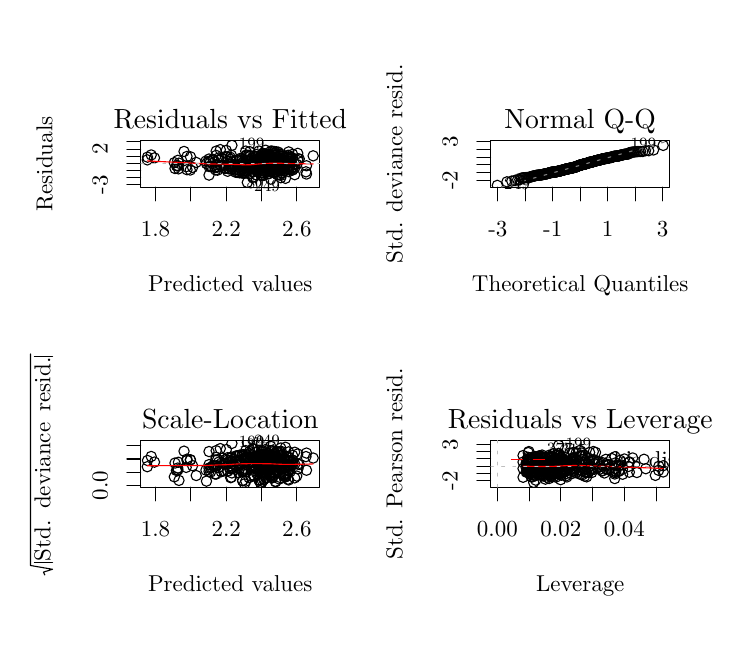
\begin{tikzpicture}[x=1pt,y=1pt]
\definecolor{fillColor}{RGB}{255,255,255}
\path[use as bounding box,fill=fillColor,fill opacity=0.00] (0,0) rectangle (252.94,216.81);
\begin{scope}
\path[clip] (  0.00,  0.00) rectangle (252.94,216.81);
\definecolor{drawColor}{RGB}{0,0,0}

\path[draw=drawColor,line width= 0.4pt,line join=round,line cap=round] ( 46.20,159.20) -- ( 97.29,159.20);

\path[draw=drawColor,line width= 0.4pt,line join=round,line cap=round] ( 46.20,159.20) -- ( 46.20,154.22);

\path[draw=drawColor,line width= 0.4pt,line join=round,line cap=round] ( 58.97,159.20) -- ( 58.97,154.22);

\path[draw=drawColor,line width= 0.4pt,line join=round,line cap=round] ( 71.74,159.20) -- ( 71.74,154.22);

\path[draw=drawColor,line width= 0.4pt,line join=round,line cap=round] ( 84.52,159.20) -- ( 84.52,154.22);

\path[draw=drawColor,line width= 0.4pt,line join=round,line cap=round] ( 97.29,159.20) -- ( 97.29,154.22);

\node[text=drawColor,anchor=base,inner sep=0pt, outer sep=0pt, scale=  0.83] at ( 46.20,141.27) {1.8};

\node[text=drawColor,anchor=base,inner sep=0pt, outer sep=0pt, scale=  0.83] at ( 71.74,141.27) {2.2};

\node[text=drawColor,anchor=base,inner sep=0pt, outer sep=0pt, scale=  0.83] at ( 97.29,141.27) {2.6};

\path[draw=drawColor,line width= 0.4pt,line join=round,line cap=round] ( 40.84,159.98) -- ( 40.84,175.53);

\path[draw=drawColor,line width= 0.4pt,line join=round,line cap=round] ( 40.84,159.98) -- ( 35.86,159.98);

\path[draw=drawColor,line width= 0.4pt,line join=round,line cap=round] ( 40.84,162.57) -- ( 35.86,162.57);

\path[draw=drawColor,line width= 0.4pt,line join=round,line cap=round] ( 40.84,165.17) -- ( 35.86,165.17);

\path[draw=drawColor,line width= 0.4pt,line join=round,line cap=round] ( 40.84,167.76) -- ( 35.86,167.76);

\path[draw=drawColor,line width= 0.4pt,line join=round,line cap=round] ( 40.84,170.35) -- ( 35.86,170.35);

\path[draw=drawColor,line width= 0.4pt,line join=round,line cap=round] ( 40.84,172.94) -- ( 35.86,172.94);

\path[draw=drawColor,line width= 0.4pt,line join=round,line cap=round] ( 40.84,175.53) -- ( 35.86,175.53);

\node[text=drawColor,rotate= 90.00,anchor=base,inner sep=0pt, outer sep=0pt, scale=  0.83] at ( 28.88,159.98) {-3};

\node[text=drawColor,rotate= 90.00,anchor=base,inner sep=0pt, outer sep=0pt, scale=  0.83] at ( 28.88,172.94) {2};

\path[draw=drawColor,line width= 0.4pt,line join=round,line cap=round] ( 40.84,159.20) --
	(105.56,159.20) --
	(105.56,175.97) --
	( 40.84,175.97) --
	( 40.84,159.20);
\end{scope}
\begin{scope}
\path[clip] (  0.00,108.41) rectangle (126.47,216.81);
\definecolor{drawColor}{RGB}{0,0,0}

\node[text=drawColor,anchor=base,inner sep=0pt, outer sep=0pt, scale=  0.83] at ( 73.20,121.35) {Predicted values};

\node[text=drawColor,rotate= 90.00,anchor=base,inner sep=0pt, outer sep=0pt, scale=  0.83] at (  8.96,167.59) {Residuals};
\end{scope}
\begin{scope}
\path[clip] ( 40.84,159.20) rectangle (105.56,175.97);
\definecolor{drawColor}{RGB}{0,0,0}

\path[draw=drawColor,line width= 0.4pt,line join=round,line cap=round] ( 81.40,162.85) circle (  1.87);

\path[draw=drawColor,line width= 0.4pt,line join=round,line cap=round] ( 81.70,162.82) circle (  1.87);

\path[draw=drawColor,line width= 0.4pt,line join=round,line cap=round] ( 43.23,169.04) circle (  1.87);

\path[draw=drawColor,line width= 0.4pt,line join=round,line cap=round] ( 87.64,170.25) circle (  1.87);

\path[draw=drawColor,line width= 0.4pt,line join=round,line cap=round] ( 85.22,163.37) circle (  1.87);

\path[draw=drawColor,line width= 0.4pt,line join=round,line cap=round] ( 90.05,169.90) circle (  1.87);

\path[draw=drawColor,line width= 0.4pt,line join=round,line cap=round] ( 93.88,167.20) circle (  1.87);

\path[draw=drawColor,line width= 0.4pt,line join=round,line cap=round] ( 76.64,164.41) circle (  1.87);

\path[draw=drawColor,line width= 0.4pt,line join=round,line cap=round] ( 89.12,170.72) circle (  1.87);

\path[draw=drawColor,line width= 0.4pt,line join=round,line cap=round] ( 94.32,168.58) circle (  1.87);

\path[draw=drawColor,line width= 0.4pt,line join=round,line cap=round] ( 87.82,166.50) circle (  1.87);

\path[draw=drawColor,line width= 0.4pt,line join=round,line cap=round] ( 85.04,166.88) circle (  1.87);

\path[draw=drawColor,line width= 0.4pt,line join=round,line cap=round] ( 87.64,169.55) circle (  1.87);

\path[draw=drawColor,line width= 0.4pt,line join=round,line cap=round] ( 90.05,166.20) circle (  1.87);

\path[draw=drawColor,line width= 0.4pt,line join=round,line cap=round] ( 92.46,168.85) circle (  1.87);

\path[draw=drawColor,line width= 0.4pt,line join=round,line cap=round] ( 84.48,169.99) circle (  1.87);

\path[draw=drawColor,line width= 0.4pt,line join=round,line cap=round] ( 91.16,168.32) circle (  1.87);

\path[draw=drawColor,line width= 0.4pt,line join=round,line cap=round] ( 74.05,166.58) circle (  1.87);

\path[draw=drawColor,line width= 0.4pt,line join=round,line cap=round] ( 53.74,166.94) circle (  1.87);

\path[draw=drawColor,line width= 0.4pt,line join=round,line cap=round] ( 89.80,164.59) circle (  1.87);

\path[draw=drawColor,line width= 0.4pt,line join=round,line cap=round] ( 96.48,167.55) circle (  1.87);

\path[draw=drawColor,line width= 0.4pt,line join=round,line cap=round] ( 90.98,167.61) circle (  1.87);

\path[draw=drawColor,line width= 0.4pt,line join=round,line cap=round] ( 90.54,169.83) circle (  1.87);

\path[draw=drawColor,line width= 0.4pt,line join=round,line cap=round] ( 84.11,169.31) circle (  1.87);

\path[draw=drawColor,line width= 0.4pt,line join=round,line cap=round] ( 79.99,167.54) circle (  1.87);

\path[draw=drawColor,line width= 0.4pt,line join=round,line cap=round] ( 59.59,166.32) circle (  1.87);

\path[draw=drawColor,line width= 0.4pt,line join=round,line cap=round] ( 84.11,168.56) circle (  1.87);

\path[draw=drawColor,line width= 0.4pt,line join=round,line cap=round] ( 85.53,170.55) circle (  1.87);

\path[draw=drawColor,line width= 0.4pt,line join=round,line cap=round] ( 81.47,168.15) circle (  1.87);

\path[draw=drawColor,line width= 0.4pt,line join=round,line cap=round] ( 87.64,166.53) circle (  1.87);

\path[draw=drawColor,line width= 0.4pt,line join=round,line cap=round] ( 89.31,165.49) circle (  1.87);

\path[draw=drawColor,line width= 0.4pt,line join=round,line cap=round] ( 94.32,170.61) circle (  1.87);

\path[draw=drawColor,line width= 0.4pt,line join=round,line cap=round] ( 91.72,171.01) circle (  1.87);

\path[draw=drawColor,line width= 0.4pt,line join=round,line cap=round] ( 96.48,163.69) circle (  1.87);

\path[draw=drawColor,line width= 0.4pt,line join=round,line cap=round] ( 85.78,168.34) circle (  1.87);

\path[draw=drawColor,line width= 0.4pt,line join=round,line cap=round] ( 83.55,165.40) circle (  1.87);

\path[draw=drawColor,line width= 0.4pt,line join=round,line cap=round] ( 95.06,169.16) circle (  1.87);

\path[draw=drawColor,line width= 0.4pt,line join=round,line cap=round] ( 97.66,168.77) circle (  1.87);

\path[draw=drawColor,line width= 0.4pt,line join=round,line cap=round] ( 79.99,169.12) circle (  1.87);

\path[draw=drawColor,line width= 0.4pt,line join=round,line cap=round] ( 68.11,172.20) circle (  1.87);

\path[draw=drawColor,line width= 0.4pt,line join=round,line cap=round] ( 73.61,165.72) circle (  1.87);

\path[draw=drawColor,line width= 0.4pt,line join=round,line cap=round] ( 85.97,168.31) circle (  1.87);

\path[draw=drawColor,line width= 0.4pt,line join=round,line cap=round] ( 94.32,171.91) circle (  1.87);

\path[draw=drawColor,line width= 0.4pt,line join=round,line cap=round] ( 72.94,166.71) circle (  1.87);

\path[draw=drawColor,line width= 0.4pt,line join=round,line cap=round] ( 65.52,169.34) circle (  1.87);

\path[draw=drawColor,line width= 0.4pt,line join=round,line cap=round] ( 74.05,166.58) circle (  1.87);

\path[draw=drawColor,line width= 0.4pt,line join=round,line cap=round] ( 81.88,168.09) circle (  1.87);

\path[draw=drawColor,line width= 0.4pt,line join=round,line cap=round] (103.16,170.50) circle (  1.87);

\path[draw=drawColor,line width= 0.4pt,line join=round,line cap=round] ( 87.45,170.28) circle (  1.87);

\path[draw=drawColor,line width= 0.4pt,line join=round,line cap=round] ( 67.63,166.41) circle (  1.87);

\path[draw=drawColor,line width= 0.4pt,line join=round,line cap=round] ( 80.96,168.99) circle (  1.87);

\path[draw=drawColor,line width= 0.4pt,line join=round,line cap=round] ( 84.30,167.77) circle (  1.87);

\path[draw=drawColor,line width= 0.4pt,line join=round,line cap=round] ( 76.52,168.80) circle (  1.87);

\path[draw=drawColor,line width= 0.4pt,line join=round,line cap=round] ( 69.96,167.07) circle (  1.87);

\path[draw=drawColor,line width= 0.4pt,line join=round,line cap=round] ( 83.30,167.11) circle (  1.87);

\path[draw=drawColor,line width= 0.4pt,line join=round,line cap=round] ( 86.46,165.03) circle (  1.87);

\path[draw=drawColor,line width= 0.4pt,line join=round,line cap=round] ( 86.89,169.65) circle (  1.87);

\path[draw=drawColor,line width= 0.4pt,line join=round,line cap=round] ( 94.32,168.58) circle (  1.87);

\path[draw=drawColor,line width= 0.4pt,line join=round,line cap=round] ( 76.28,167.18) circle (  1.87);

\path[draw=drawColor,line width= 0.4pt,line join=round,line cap=round] ( 84.30,170.73) circle (  1.87);

\path[draw=drawColor,line width= 0.4pt,line join=round,line cap=round] ( 86.15,166.73) circle (  1.87);

\path[draw=drawColor,line width= 0.4pt,line join=round,line cap=round] ( 58.83,170.14) circle (  1.87);

\path[draw=drawColor,line width= 0.4pt,line join=round,line cap=round] ( 76.21,166.32) circle (  1.87);

\path[draw=drawColor,line width= 0.4pt,line join=round,line cap=round] ( 72.38,168.51) circle (  1.87);

\path[draw=drawColor,line width= 0.4pt,line join=round,line cap=round] ( 73.79,168.33) circle (  1.87);

\path[draw=drawColor,line width= 0.4pt,line join=round,line cap=round] ( 85.22,171.29) circle (  1.87);

\path[draw=drawColor,line width= 0.4pt,line join=round,line cap=round] ( 94.32,167.86) circle (  1.87);

\path[draw=drawColor,line width= 0.4pt,line join=round,line cap=round] ( 73.86,165.69) circle (  1.87);

\path[draw=drawColor,line width= 0.4pt,line join=round,line cap=round] ( 68.11,167.29) circle (  1.87);

\path[draw=drawColor,line width= 0.4pt,line join=round,line cap=round] ( 85.04,171.32) circle (  1.87);

\path[draw=drawColor,line width= 0.4pt,line join=round,line cap=round] ( 93.21,168.03) circle (  1.87);

\path[draw=drawColor,line width= 0.4pt,line join=round,line cap=round] (100.56,164.72) circle (  1.87);

\path[draw=drawColor,line width= 0.4pt,line join=round,line cap=round] ( 45.82,169.75) circle (  1.87);

\path[draw=drawColor,line width= 0.4pt,line join=round,line cap=round] ( 86.27,168.27) circle (  1.87);

\path[draw=drawColor,line width= 0.4pt,line join=round,line cap=round] ( 69.04,169.74) circle (  1.87);

\path[draw=drawColor,line width= 0.4pt,line join=round,line cap=round] ( 88.38,165.62) circle (  1.87);

\path[draw=drawColor,line width= 0.4pt,line join=round,line cap=round] ( 95.37,166.24) circle (  1.87);

\path[draw=drawColor,line width= 0.4pt,line join=round,line cap=round] ( 92.40,166.66) circle (  1.87);

\path[draw=drawColor,line width= 0.4pt,line join=round,line cap=round] ( 43.30,170.02) circle (  1.87);

\path[draw=drawColor,line width= 0.4pt,line join=round,line cap=round] ( 87.82,162.08) circle (  1.87);

\path[draw=drawColor,line width= 0.4pt,line join=round,line cap=round] ( 72.19,168.53) circle (  1.87);

\path[draw=drawColor,line width= 0.4pt,line join=round,line cap=round] ( 85.30,167.63) circle (  1.87);

\path[draw=drawColor,line width= 0.4pt,line join=round,line cap=round] ( 84.30,164.42) circle (  1.87);

\path[draw=drawColor,line width= 0.4pt,line join=round,line cap=round] ( 90.54,169.83) circle (  1.87);

\path[draw=drawColor,line width= 0.4pt,line join=round,line cap=round] ( 78.36,166.92) circle (  1.87);

\path[draw=drawColor,line width= 0.4pt,line join=round,line cap=round] ( 72.88,165.80) circle (  1.87);

\path[draw=drawColor,line width= 0.4pt,line join=round,line cap=round] ( 82.63,165.52) circle (  1.87);

\path[draw=drawColor,line width= 0.4pt,line join=round,line cap=round] ( 84.30,169.29) circle (  1.87);

\path[draw=drawColor,line width= 0.4pt,line join=round,line cap=round] ( 84.87,167.69) circle (  1.87);

\path[draw=drawColor,line width= 0.4pt,line join=round,line cap=round] ( 87.64,164.87) circle (  1.87);

\path[draw=drawColor,line width= 0.4pt,line join=round,line cap=round] ( 86.90,164.09) circle (  1.87);

\path[draw=drawColor,line width= 0.4pt,line join=round,line cap=round] ( 84.97,171.33) circle (  1.87);

\path[draw=drawColor,line width= 0.4pt,line join=round,line cap=round] ( 65.51,166.66) circle (  1.87);

\path[draw=drawColor,line width= 0.4pt,line join=round,line cap=round] ( 84.30,167.77) circle (  1.87);

\path[draw=drawColor,line width= 0.4pt,line join=round,line cap=round] ( 95.81,166.17) circle (  1.87);

\path[draw=drawColor,line width= 0.4pt,line join=round,line cap=round] ( 66.52,166.54) circle (  1.87);

\path[draw=drawColor,line width= 0.4pt,line join=round,line cap=round] ( 75.53,168.92) circle (  1.87);

\path[draw=drawColor,line width= 0.4pt,line join=round,line cap=round] ( 81.70,165.63) circle (  1.87);

\path[draw=drawColor,line width= 0.4pt,line join=round,line cap=round] ( 89.24,167.10) circle (  1.87);

\path[draw=drawColor,line width= 0.4pt,line join=round,line cap=round] ( 77.39,165.27) circle (  1.87);

\path[draw=drawColor,line width= 0.4pt,line join=round,line cap=round] ( 71.45,165.97) circle (  1.87);

\path[draw=drawColor,line width= 0.4pt,line join=round,line cap=round] ( 97.66,169.44) circle (  1.87);

\path[draw=drawColor,line width= 0.4pt,line join=round,line cap=round] ( 90.98,166.07) circle (  1.87);

\path[draw=drawColor,line width= 0.4pt,line join=round,line cap=round] ( 71.45,165.97) circle (  1.87);

\path[draw=drawColor,line width= 0.4pt,line join=round,line cap=round] ( 94.32,169.95) circle (  1.87);

\path[draw=drawColor,line width= 0.4pt,line join=round,line cap=round] ( 85.48,166.82) circle (  1.87);

\path[draw=drawColor,line width= 0.4pt,line join=round,line cap=round] ( 78.13,165.18) circle (  1.87);

\path[draw=drawColor,line width= 0.4pt,line join=round,line cap=round] ( 95.06,169.84) circle (  1.87);

\path[draw=drawColor,line width= 0.4pt,line join=round,line cap=round] ( 94.32,165.61) circle (  1.87);

\path[draw=drawColor,line width= 0.4pt,line join=round,line cap=round] ( 92.83,168.79) circle (  1.87);

\path[draw=drawColor,line width= 0.4pt,line join=round,line cap=round] ( 95.73,171.05) circle (  1.87);

\path[draw=drawColor,line width= 0.4pt,line join=round,line cap=round] ( 68.38,166.33) circle (  1.87);

\path[draw=drawColor,line width= 0.4pt,line join=round,line cap=round] ( 67.19,169.14) circle (  1.87);

\path[draw=drawColor,line width= 0.4pt,line join=round,line cap=round] ( 90.54,171.84) circle (  1.87);

\path[draw=drawColor,line width= 0.4pt,line join=round,line cap=round] ( 91.28,165.23) circle (  1.87);

\path[draw=drawColor,line width= 0.4pt,line join=round,line cap=round] ( 92.65,169.52) circle (  1.87);

\path[draw=drawColor,line width= 0.4pt,line join=round,line cap=round] ( 94.32,166.39) circle (  1.87);

\path[draw=drawColor,line width= 0.4pt,line join=round,line cap=round] ( 93.14,168.04) circle (  1.87);

\path[draw=drawColor,line width= 0.4pt,line join=round,line cap=round] ( 77.70,167.00) circle (  1.87);

\path[draw=drawColor,line width= 0.4pt,line join=round,line cap=round] ( 94.06,168.61) circle (  1.87);

\path[draw=drawColor,line width= 0.4pt,line join=round,line cap=round] ( 87.38,170.98) circle (  1.87);

\path[draw=drawColor,line width= 0.4pt,line join=round,line cap=round] ( 94.14,169.98) circle (  1.87);

\path[draw=drawColor,line width= 0.4pt,line join=round,line cap=round] ( 87.82,168.80) circle (  1.87);

\path[draw=drawColor,line width= 0.4pt,line join=round,line cap=round] ( 85.97,169.78) circle (  1.87);

\path[draw=drawColor,line width= 0.4pt,line join=round,line cap=round] ( 89.05,164.69) circle (  1.87);

\path[draw=drawColor,line width= 0.4pt,line join=round,line cap=round] ( 81.22,169.71) circle (  1.87);

\path[draw=drawColor,line width= 0.4pt,line join=round,line cap=round] ( 81.40,164.78) circle (  1.87);

\path[draw=drawColor,line width= 0.4pt,line join=round,line cap=round] ( 54.66,167.85) circle (  1.87);

\path[draw=drawColor,line width= 0.4pt,line join=round,line cap=round] ( 66.09,166.59) circle (  1.87);

\path[draw=drawColor,line width= 0.4pt,line join=round,line cap=round] ( 89.06,172.07) circle (  1.87);

\path[draw=drawColor,line width= 0.4pt,line join=round,line cap=round] ( 73.14,170.02) circle (  1.87);

\path[draw=drawColor,line width= 0.4pt,line join=round,line cap=round] ( 76.69,166.26) circle (  1.87);

\path[draw=drawColor,line width= 0.4pt,line join=round,line cap=round] ( 77.62,167.84) circle (  1.87);

\path[draw=drawColor,line width= 0.4pt,line join=round,line cap=round] ( 85.90,168.32) circle (  1.87);

\path[draw=drawColor,line width= 0.4pt,line join=round,line cap=round] ( 94.32,164.81) circle (  1.87);

\path[draw=drawColor,line width= 0.4pt,line join=round,line cap=round] ( 92.83,166.60) circle (  1.87);

\path[draw=drawColor,line width= 0.4pt,line join=round,line cap=round] ( 94.07,165.65) circle (  1.87);

\path[draw=drawColor,line width= 0.4pt,line join=round,line cap=round] ( 65.53,163.54) circle (  1.87);

\path[draw=drawColor,line width= 0.4pt,line join=round,line cap=round] ( 78.93,170.76) circle (  1.87);

\path[draw=drawColor,line width= 0.4pt,line join=round,line cap=round] ( 90.91,170.46) circle (  1.87);

\path[draw=drawColor,line width= 0.4pt,line join=round,line cap=round] ( 85.56,164.26) circle (  1.87);

\path[draw=drawColor,line width= 0.4pt,line join=round,line cap=round] ( 66.09,168.42) circle (  1.87);

\path[draw=drawColor,line width= 0.4pt,line join=round,line cap=round] ( 92.83,165.02) circle (  1.87);

\path[draw=drawColor,line width= 0.4pt,line join=round,line cap=round] ( 79.77,170.65) circle (  1.87);

\path[draw=drawColor,line width= 0.4pt,line join=round,line cap=round] ( 54.48,165.80) circle (  1.87);

\path[draw=drawColor,line width= 0.4pt,line join=round,line cap=round] ( 80.03,165.84) circle (  1.87);

\path[draw=drawColor,line width= 0.4pt,line join=round,line cap=round] ( 57.26,166.57) circle (  1.87);

\path[draw=drawColor,line width= 0.4pt,line join=round,line cap=round] ( 84.30,166.98) circle (  1.87);

\path[draw=drawColor,line width= 0.4pt,line join=round,line cap=round] ( 90.98,163.56) circle (  1.87);

\path[draw=drawColor,line width= 0.4pt,line join=round,line cap=round] ( 54.23,168.86) circle (  1.87);

\path[draw=drawColor,line width= 0.4pt,line join=round,line cap=round] ( 54.23,166.89) circle (  1.87);

\path[draw=drawColor,line width= 0.4pt,line join=round,line cap=round] ( 72.25,170.13) circle (  1.87);

\path[draw=drawColor,line width= 0.4pt,line join=round,line cap=round] ( 68.87,168.94) circle (  1.87);

\path[draw=drawColor,line width= 0.4pt,line join=round,line cap=round] ( 58.75,165.36) circle (  1.87);

\path[draw=drawColor,line width= 0.4pt,line join=round,line cap=round] ( 73.30,169.21) circle (  1.87);

\path[draw=drawColor,line width= 0.4pt,line join=round,line cap=round] ( 83.63,167.86) circle (  1.87);

\path[draw=drawColor,line width= 0.4pt,line join=round,line cap=round] ( 87.20,171.01) circle (  1.87);

\path[draw=drawColor,line width= 0.4pt,line join=round,line cap=round] ( 44.64,170.82) circle (  1.87);

\path[draw=drawColor,line width= 0.4pt,line join=round,line cap=round] ( 88.87,171.44) circle (  1.87);

\path[draw=drawColor,line width= 0.4pt,line join=round,line cap=round] ( 77.70,167.83) circle (  1.87);

\path[draw=drawColor,line width= 0.4pt,line join=round,line cap=round] ( 68.25,166.34) circle (  1.87);

\path[draw=drawColor,line width= 0.4pt,line join=round,line cap=round] ( 53.24,165.92) circle (  1.87);

\path[draw=drawColor,line width= 0.4pt,line join=round,line cap=round] ( 76.52,165.37) circle (  1.87);

\path[draw=drawColor,line width= 0.4pt,line join=round,line cap=round] ( 88.13,166.46) circle (  1.87);

\path[draw=drawColor,line width= 0.4pt,line join=round,line cap=round] ( 57.57,165.48) circle (  1.87);

\path[draw=drawColor,line width= 0.4pt,line join=round,line cap=round] ( 76.77,169.55) circle (  1.87);

\path[draw=drawColor,line width= 0.4pt,line join=round,line cap=round] ( 88.87,166.36) circle (  1.87);

\path[draw=drawColor,line width= 0.4pt,line join=round,line cap=round] ( 89.05,169.34) circle (  1.87);

\path[draw=drawColor,line width= 0.4pt,line join=round,line cap=round] ( 84.30,163.49) circle (  1.87);

\path[draw=drawColor,line width= 0.4pt,line join=round,line cap=round] ( 89.49,169.28) circle (  1.87);

\path[draw=drawColor,line width= 0.4pt,line join=round,line cap=round] ( 67.94,165.41) circle (  1.87);

\path[draw=drawColor,line width= 0.4pt,line join=round,line cap=round] ( 83.93,169.34) circle (  1.87);

\path[draw=drawColor,line width= 0.4pt,line join=round,line cap=round] ( 90.98,168.35) circle (  1.87);

\path[draw=drawColor,line width= 0.4pt,line join=round,line cap=round] ( 64.61,167.69) circle (  1.87);

\path[draw=drawColor,line width= 0.4pt,line join=round,line cap=round] ( 86.89,166.63) circle (  1.87);

\path[draw=drawColor,line width= 0.4pt,line join=round,line cap=round] ( 91.47,166.01) circle (  1.87);

\path[draw=drawColor,line width= 0.4pt,line join=round,line cap=round] ( 84.04,169.32) circle (  1.87);

\path[draw=drawColor,line width= 0.4pt,line join=round,line cap=round] ( 91.47,162.59) circle (  1.87);

\path[draw=drawColor,line width= 0.4pt,line join=round,line cap=round] ( 80.77,167.44) circle (  1.87);

\path[draw=drawColor,line width= 0.4pt,line join=round,line cap=round] ( 91.72,165.97) circle (  1.87);

\path[draw=drawColor,line width= 0.4pt,line join=round,line cap=round] ( 88.38,165.62) circle (  1.87);

\path[draw=drawColor,line width= 0.4pt,line join=round,line cap=round] ( 94.81,167.06) circle (  1.87);

\path[draw=drawColor,line width= 0.4pt,line join=round,line cap=round] ( 86.15,171.16) circle (  1.87);

\path[draw=drawColor,line width= 0.4pt,line join=round,line cap=round] ( 83.55,166.25) circle (  1.87);

\path[draw=drawColor,line width= 0.4pt,line join=round,line cap=round] ( 82.63,168.77) circle (  1.87);

\path[draw=drawColor,line width= 0.4pt,line join=round,line cap=round] ( 88.38,167.98) circle (  1.87);

\path[draw=drawColor,line width= 0.4pt,line join=round,line cap=round] ( 84.11,167.79) circle (  1.87);

\path[draw=drawColor,line width= 0.4pt,line join=round,line cap=round] ( 89.61,169.97) circle (  1.87);

\path[draw=drawColor,line width= 0.4pt,line join=round,line cap=round] ( 83.55,165.40) circle (  1.87);

\path[draw=drawColor,line width= 0.4pt,line join=round,line cap=round] ( 87.20,164.93) circle (  1.87);

\path[draw=drawColor,line width= 0.4pt,line join=round,line cap=round] ( 91.65,166.76) circle (  1.87);

\path[draw=drawColor,line width= 0.4pt,line join=round,line cap=round] ( 86.46,165.03) circle (  1.87);

\path[draw=drawColor,line width= 0.4pt,line join=round,line cap=round] ( 87.20,164.05) circle (  1.87);

\path[draw=drawColor,line width= 0.4pt,line join=round,line cap=round] ( 83.37,165.42) circle (  1.87);

\path[draw=drawColor,line width= 0.4pt,line join=round,line cap=round] ( 93.14,168.04) circle (  1.87);

\path[draw=drawColor,line width= 0.4pt,line join=round,line cap=round] ( 94.25,168.59) circle (  1.87);

\path[draw=drawColor,line width= 0.4pt,line join=round,line cap=round] ( 94.06,170.65) circle (  1.87);

\path[draw=drawColor,line width= 0.4pt,line join=round,line cap=round] ( 81.70,166.49) circle (  1.87);

\path[draw=drawColor,line width= 0.4pt,line join=round,line cap=round] ( 73.80,174.28) circle (  1.87);

\path[draw=drawColor,line width= 0.4pt,line join=round,line cap=round] ( 87.82,165.69) circle (  1.87);

\path[draw=drawColor,line width= 0.4pt,line join=round,line cap=round] ( 80.22,172.01) circle (  1.87);

\path[draw=drawColor,line width= 0.4pt,line join=round,line cap=round] ( 70.71,166.98) circle (  1.87);

\path[draw=drawColor,line width= 0.4pt,line join=round,line cap=round] ( 78.36,166.92) circle (  1.87);

\path[draw=drawColor,line width= 0.4pt,line join=round,line cap=round] ( 79.29,165.04) circle (  1.87);

\path[draw=drawColor,line width= 0.4pt,line join=round,line cap=round] ( 90.98,166.07) circle (  1.87);

\path[draw=drawColor,line width= 0.4pt,line join=round,line cap=round] ( 78.81,167.69) circle (  1.87);

\path[draw=drawColor,line width= 0.4pt,line join=round,line cap=round] ( 52.99,168.03) circle (  1.87);

\path[draw=drawColor,line width= 0.4pt,line join=round,line cap=round] ( 91.65,166.76) circle (  1.87);

\path[draw=drawColor,line width= 0.4pt,line join=round,line cap=round] ( 73.35,167.54) circle (  1.87);

\path[draw=drawColor,line width= 0.4pt,line join=round,line cap=round] ( 90.23,163.66) circle (  1.87);

\path[draw=drawColor,line width= 0.4pt,line join=round,line cap=round] ( 91.91,164.31) circle (  1.87);

\path[draw=drawColor,line width= 0.4pt,line join=round,line cap=round] ( 87.64,168.08) circle (  1.87);

\path[draw=drawColor,line width= 0.4pt,line join=round,line cap=round] ( 71.45,170.24) circle (  1.87);

\path[draw=drawColor,line width= 0.4pt,line join=round,line cap=round] ( 75.10,164.59) circle (  1.87);

\path[draw=drawColor,line width= 0.4pt,line join=round,line cap=round] ( 84.48,165.28) circle (  1.87);

\path[draw=drawColor,line width= 0.4pt,line join=round,line cap=round] ( 85.71,169.82) circle (  1.87);

\path[draw=drawColor,line width= 0.4pt,line join=round,line cap=round] ( 68.62,165.33) circle (  1.87);

\path[draw=drawColor,line width= 0.4pt,line join=round,line cap=round] ( 77.70,164.28) circle (  1.87);

\path[draw=drawColor,line width= 0.4pt,line join=round,line cap=round] ( 78.54,165.13) circle (  1.87);

\path[draw=drawColor,line width= 0.4pt,line join=round,line cap=round] ( 87.64,165.72) circle (  1.87);

\path[draw=drawColor,line width= 0.4pt,line join=round,line cap=round] ( 80.03,164.01) circle (  1.87);

\path[draw=drawColor,line width= 0.4pt,line join=round,line cap=round] ( 76.03,164.48) circle (  1.87);

\path[draw=drawColor,line width= 0.4pt,line join=round,line cap=round] ( 78.80,172.21) circle (  1.87);

\path[draw=drawColor,line width= 0.4pt,line join=round,line cap=round] ( 82.45,168.79) circle (  1.87);

\path[draw=drawColor,line width= 0.4pt,line join=round,line cap=round] ( 92.83,168.08) circle (  1.87);

\path[draw=drawColor,line width= 0.4pt,line join=round,line cap=round] ( 77.44,167.03) circle (  1.87);

\path[draw=drawColor,line width= 0.4pt,line join=round,line cap=round] ( 85.71,171.22) circle (  1.87);

\path[draw=drawColor,line width= 0.4pt,line join=round,line cap=round] ( 88.38,167.98) circle (  1.87);

\path[draw=drawColor,line width= 0.4pt,line join=round,line cap=round] ( 67.00,169.17) circle (  1.87);

\path[draw=drawColor,line width= 0.4pt,line join=round,line cap=round] ( 88.13,168.01) circle (  1.87);

\path[draw=drawColor,line width= 0.4pt,line join=round,line cap=round] ( 89.98,168.49) circle (  1.87);

\path[draw=drawColor,line width= 0.4pt,line join=round,line cap=round] ( 89.12,167.11) circle (  1.87);

\path[draw=drawColor,line width= 0.4pt,line join=round,line cap=round] ( 78.13,168.59) circle (  1.87);

\path[draw=drawColor,line width= 0.4pt,line join=round,line cap=round] ( 89.31,169.31) circle (  1.87);

\path[draw=drawColor,line width= 0.4pt,line join=round,line cap=round] ( 86.53,165.86) circle (  1.87);

\path[draw=drawColor,line width= 0.4pt,line join=round,line cap=round] ( 93.88,166.45) circle (  1.87);

\path[draw=drawColor,line width= 0.4pt,line join=round,line cap=round] ( 87.20,169.61) circle (  1.87);

\path[draw=drawColor,line width= 0.4pt,line join=round,line cap=round] ( 83.11,169.45) circle (  1.87);

\path[draw=drawColor,line width= 0.4pt,line join=round,line cap=round] ( 86.46,168.99) circle (  1.87);

\path[draw=drawColor,line width= 0.4pt,line join=round,line cap=round] ( 78.19,165.17) circle (  1.87);

\path[draw=drawColor,line width= 0.4pt,line join=round,line cap=round] ( 91.47,167.54) circle (  1.87);

\path[draw=drawColor,line width= 0.4pt,line join=round,line cap=round] ( 90.98,166.07) circle (  1.87);

\path[draw=drawColor,line width= 0.4pt,line join=round,line cap=round] ( 93.14,162.37) circle (  1.87);

\path[draw=drawColor,line width= 0.4pt,line join=round,line cap=round] ( 94.06,167.90) circle (  1.87);

\path[draw=drawColor,line width= 0.4pt,line join=round,line cap=round] ( 85.04,164.32) circle (  1.87);

\path[draw=drawColor,line width= 0.4pt,line join=round,line cap=round] ( 87.94,172.24) circle (  1.87);

\path[draw=drawColor,line width= 0.4pt,line join=round,line cap=round] ( 93.14,167.30) circle (  1.87);

\path[draw=drawColor,line width= 0.4pt,line join=round,line cap=round] ( 54.23,166.89) circle (  1.87);

\path[draw=drawColor,line width= 0.4pt,line join=round,line cap=round] ( 79.37,160.89) circle (  1.87);

\path[draw=drawColor,line width= 0.4pt,line join=round,line cap=round] ( 85.53,169.12) circle (  1.87);

\path[draw=drawColor,line width= 0.4pt,line join=round,line cap=round] ( 76.52,164.42) circle (  1.87);

\path[draw=drawColor,line width= 0.4pt,line join=round,line cap=round] ( 75.53,165.49) circle (  1.87);

\path[draw=drawColor,line width= 0.4pt,line join=round,line cap=round] ( 72.25,164.92) circle (  1.87);

\path[draw=drawColor,line width= 0.4pt,line join=round,line cap=round] ( 84.60,165.26) circle (  1.87);

\path[draw=drawColor,line width= 0.4pt,line join=round,line cap=round] ( 82.93,165.48) circle (  1.87);

\path[draw=drawColor,line width= 0.4pt,line join=round,line cap=round] ( 72.50,165.85) circle (  1.87);

\path[draw=drawColor,line width= 0.4pt,line join=round,line cap=round] ( 90.98,169.07) circle (  1.87);

\path[draw=drawColor,line width= 0.4pt,line join=round,line cap=round] ( 91.72,166.75) circle (  1.87);

\path[draw=drawColor,line width= 0.4pt,line join=round,line cap=round] ( 89.61,169.97) circle (  1.87);

\path[draw=drawColor,line width= 0.4pt,line join=round,line cap=round] ( 95.73,165.41) circle (  1.87);

\path[draw=drawColor,line width= 0.4pt,line join=round,line cap=round] ( 83.55,172.22) circle (  1.87);

\path[draw=drawColor,line width= 0.4pt,line join=round,line cap=round] ( 91.72,164.33) circle (  1.87);

\path[draw=drawColor,line width= 0.4pt,line join=round,line cap=round] ( 97.22,167.44) circle (  1.87);

\path[draw=drawColor,line width= 0.4pt,line join=round,line cap=round] ( 94.99,165.52) circle (  1.87);

\path[draw=drawColor,line width= 0.4pt,line join=round,line cap=round] ( 87.64,165.72) circle (  1.87);

\path[draw=drawColor,line width= 0.4pt,line join=round,line cap=round] ( 89.31,171.37) circle (  1.87);

\path[draw=drawColor,line width= 0.4pt,line join=round,line cap=round] ( 86.27,165.90) circle (  1.87);

\path[draw=drawColor,line width= 0.4pt,line join=round,line cap=round] ( 92.58,167.38) circle (  1.87);

\path[draw=drawColor,line width= 0.4pt,line join=round,line cap=round] ( 85.78,166.78) circle (  1.87);

\path[draw=drawColor,line width= 0.4pt,line join=round,line cap=round] ( 80.03,164.01) circle (  1.87);

\path[draw=drawColor,line width= 0.4pt,line join=round,line cap=round] ( 65.53,168.48) circle (  1.87);

\path[draw=drawColor,line width= 0.4pt,line join=round,line cap=round] ( 90.24,169.87) circle (  1.87);

\path[draw=drawColor,line width= 0.4pt,line join=round,line cap=round] ( 81.70,168.12) circle (  1.87);

\path[draw=drawColor,line width= 0.4pt,line join=round,line cap=round] ( 87.45,170.28) circle (  1.87);

\path[draw=drawColor,line width= 0.4pt,line join=round,line cap=round] ( 89.49,166.28) circle (  1.87);

\path[draw=drawColor,line width= 0.4pt,line join=round,line cap=round] ( 68.11,170.66) circle (  1.87);

\path[draw=drawColor,line width= 0.4pt,line join=round,line cap=round] ( 89.05,166.34) circle (  1.87);

\path[draw=drawColor,line width= 0.4pt,line join=round,line cap=round] ( 90.72,165.30) circle (  1.87);

\path[draw=drawColor,line width= 0.4pt,line join=round,line cap=round] ( 67.63,168.23) circle (  1.87);

\path[draw=drawColor,line width= 0.4pt,line join=round,line cap=round] ( 91.47,166.01) circle (  1.87);

\path[draw=drawColor,line width= 0.4pt,line join=round,line cap=round] ( 82.93,165.48) circle (  1.87);

\path[draw=drawColor,line width= 0.4pt,line join=round,line cap=round] ( 76.52,168.80) circle (  1.87);

\path[draw=drawColor,line width= 0.4pt,line join=round,line cap=round] ( 88.38,167.98) circle (  1.87);

\path[draw=drawColor,line width= 0.4pt,line join=round,line cap=round] ( 73.61,166.63) circle (  1.87);

\path[draw=drawColor,line width= 0.4pt,line join=round,line cap=round] ( 82.63,167.20) circle (  1.87);

\path[draw=drawColor,line width= 0.4pt,line join=round,line cap=round] ( 89.61,167.80) circle (  1.87);

\path[draw=drawColor,line width= 0.4pt,line join=round,line cap=round] ( 85.97,172.53) circle (  1.87);

\path[draw=drawColor,line width= 0.4pt,line join=round,line cap=round] ( 85.04,169.19) circle (  1.87);

\path[draw=drawColor,line width= 0.4pt,line join=round,line cap=round] ( 91.28,169.72) circle (  1.87);

\path[draw=drawColor,line width= 0.4pt,line join=round,line cap=round] ( 94.32,169.27) circle (  1.87);

\path[draw=drawColor,line width= 0.4pt,line join=round,line cap=round] ( 84.11,168.56) circle (  1.87);

\path[draw=drawColor,line width= 0.4pt,line join=round,line cap=round] ( 88.57,170.12) circle (  1.87);

\path[draw=drawColor,line width= 0.4pt,line join=round,line cap=round] ( 77.44,169.46) circle (  1.87);

\path[draw=drawColor,line width= 0.4pt,line join=round,line cap=round] ( 88.38,172.17) circle (  1.87);

\path[draw=drawColor,line width= 0.4pt,line join=round,line cap=round] ( 92.46,168.85) circle (  1.87);

\path[draw=drawColor,line width= 0.4pt,line join=round,line cap=round] ( 85.04,169.91) circle (  1.87);

\path[draw=drawColor,line width= 0.4pt,line join=round,line cap=round] ( 86.15,166.73) circle (  1.87);

\path[draw=drawColor,line width= 0.4pt,line join=round,line cap=round] ( 85.22,166.85) circle (  1.87);

\path[draw=drawColor,line width= 0.4pt,line join=round,line cap=round] ( 93.58,168.69) circle (  1.87);

\path[draw=drawColor,line width= 0.4pt,line join=round,line cap=round] ( 89.31,170.70) circle (  1.87);

\path[draw=drawColor,line width= 0.4pt,line join=round,line cap=round] ( 89.49,167.82) circle (  1.87);

\path[draw=drawColor,line width= 0.4pt,line join=round,line cap=round] ( 94.06,166.42) circle (  1.87);

\path[draw=drawColor,line width= 0.4pt,line join=round,line cap=round] ( 87.64,170.25) circle (  1.87);

\path[draw=drawColor,line width= 0.4pt,line join=round,line cap=round] ( 89.31,171.37) circle (  1.87);

\path[draw=drawColor,line width= 0.4pt,line join=round,line cap=round] ( 82.71,170.96) circle (  1.87);

\path[draw=drawColor,line width= 0.4pt,line join=round,line cap=round] ( 80.48,170.55) circle (  1.87);

\path[draw=drawColor,line width= 0.4pt,line join=round,line cap=round] ( 90.54,171.19) circle (  1.87);

\path[draw=drawColor,line width= 0.4pt,line join=round,line cap=round] ( 81.97,165.60) circle (  1.87);

\path[draw=drawColor,line width= 0.4pt,line join=round,line cap=round] ( 85.80,170.52) circle (  1.87);

\path[draw=drawColor,line width= 0.4pt,line join=round,line cap=round] ( 56.50,172.08) circle (  1.87);

\path[draw=drawColor,line width= 0.4pt,line join=round,line cap=round] ( 78.37,166.91) circle (  1.87);

\path[draw=drawColor,line width= 0.4pt,line join=round,line cap=round] ( 81.70,170.38) circle (  1.87);

\path[draw=drawColor,line width= 0.4pt,line join=round,line cap=round] ( 83.20,169.44) circle (  1.87);

\path[draw=drawColor,line width= 0.4pt,line join=round,line cap=round] ( 73.61,170.73) circle (  1.87);

\path[draw=drawColor,line width= 0.4pt,line join=round,line cap=round] ( 71.77,172.46) circle (  1.87);

\path[draw=drawColor,line width= 0.4pt,line join=round,line cap=round] ( 85.98,169.05) circle (  1.87);

\path[draw=drawColor,line width= 0.4pt,line join=round,line cap=round] ( 80.03,165.84) circle (  1.87);

\path[draw=drawColor,line width= 0.4pt,line join=round,line cap=round] ( 90.23,165.37) circle (  1.87);

\path[draw=drawColor,line width= 0.4pt,line join=round,line cap=round] ( 86.15,167.52) circle (  1.87);

\path[draw=drawColor,line width= 0.4pt,line join=round,line cap=round] ( 86.15,167.52) circle (  1.87);

\path[draw=drawColor,line width= 0.4pt,line join=round,line cap=round] ( 85.22,169.16) circle (  1.87);

\path[draw=drawColor,line width= 0.4pt,line join=round,line cap=round] ( 84.30,167.77) circle (  1.87);

\path[draw=drawColor,line width= 0.4pt,line join=round,line cap=round] ( 85.97,167.54) circle (  1.87);

\path[draw=drawColor,line width= 0.4pt,line join=round,line cap=round] ( 81.70,168.89) circle (  1.87);

\path[draw=drawColor,line width= 0.4pt,line join=round,line cap=round] ( 89.05,170.73) circle (  1.87);

\path[draw=drawColor,line width= 0.4pt,line join=round,line cap=round] (100.75,163.91) circle (  1.87);

\path[draw=drawColor,line width= 0.4pt,line join=round,line cap=round] ( 86.46,169.71) circle (  1.87);

\path[draw=drawColor,line width= 0.4pt,line join=round,line cap=round] ( 79.10,168.46) circle (  1.87);

\path[draw=drawColor,line width= 0.4pt,line join=round,line cap=round] ( 89.49,166.28) circle (  1.87);

\path[draw=drawColor,line width= 0.4pt,line join=round,line cap=round] ( 91.16,169.04) circle (  1.87);

\path[draw=drawColor,line width= 0.4pt,line join=round,line cap=round] ( 90.80,165.29) circle (  1.87);

\path[draw=drawColor,line width= 0.4pt,line join=round,line cap=round] ( 92.83,167.35) circle (  1.87);

\path[draw=drawColor,line width= 0.4pt,line join=round,line cap=round] ( 91.65,163.48) circle (  1.87);

\path[draw=drawColor,line width= 0.4pt,line join=round,line cap=round] ( 89.05,164.69) circle (  1.87);

\path[draw=drawColor,line width= 0.4pt,line join=round,line cap=round] ( 95.73,165.41) circle (  1.87);

\path[draw=drawColor,line width= 0.4pt,line join=round,line cap=round] ( 94.25,169.96) circle (  1.87);

\path[draw=drawColor,line width= 0.4pt,line join=round,line cap=round] ( 79.11,170.74) circle (  1.87);

\path[draw=drawColor,line width= 0.4pt,line join=round,line cap=round] ( 80.96,164.83) circle (  1.87);

\path[draw=drawColor,line width= 0.4pt,line join=round,line cap=round] ( 93.58,170.06) circle (  1.87);

\path[draw=drawColor,line width= 0.4pt,line join=round,line cap=round] ( 80.96,166.59) circle (  1.87);

\path[draw=drawColor,line width= 0.4pt,line join=round,line cap=round] ( 77.45,168.68) circle (  1.87);

\path[draw=drawColor,line width= 0.4pt,line join=round,line cap=round] ( 83.64,167.06) circle (  1.87);

\path[draw=drawColor,line width= 0.4pt,line join=round,line cap=round] ( 95.74,169.73) circle (  1.87);

\path[draw=drawColor,line width= 0.4pt,line join=round,line cap=round] ( 73.61,167.51) circle (  1.87);

\path[draw=drawColor,line width= 0.4pt,line join=round,line cap=round] ( 88.57,167.19) circle (  1.87);

\path[draw=drawColor,line width= 0.4pt,line join=round,line cap=round] ( 89.05,168.62) circle (  1.87);

\path[draw=drawColor,line width= 0.4pt,line join=round,line cap=round] ( 98.15,169.37) circle (  1.87);

\path[draw=drawColor,line width= 0.4pt,line join=round,line cap=round] ( 91.72,165.97) circle (  1.87);

\path[draw=drawColor,line width= 0.4pt,line join=round,line cap=round] ( 86.90,168.93) circle (  1.87);

\path[draw=drawColor,line width= 0.4pt,line join=round,line cap=round] ( 70.09,169.61) circle (  1.87);

\path[draw=drawColor,line width= 0.4pt,line join=round,line cap=round] ( 60.91,168.12) circle (  1.87);

\path[draw=drawColor,line width= 0.4pt,line join=round,line cap=round] ( 88.38,168.72) circle (  1.87);

\path[draw=drawColor,line width= 0.4pt,line join=round,line cap=round] ( 80.79,165.75) circle (  1.87);

\path[draw=drawColor,line width= 0.4pt,line join=round,line cap=round] ( 70.83,166.96) circle (  1.87);

\path[draw=drawColor,line width= 0.4pt,line join=round,line cap=round] ( 88.38,168.72) circle (  1.87);

\path[draw=drawColor,line width= 0.4pt,line join=round,line cap=round] ( 86.89,166.63) circle (  1.87);

\path[draw=drawColor,line width= 0.4pt,line join=round,line cap=round] ( 87.82,168.05) circle (  1.87);

\path[draw=drawColor,line width= 0.4pt,line join=round,line cap=round] ( 87.38,168.12) circle (  1.87);

\path[draw=drawColor,line width= 0.4pt,line join=round,line cap=round] ( 86.27,166.71) circle (  1.87);

\path[draw=drawColor,line width= 0.4pt,line join=round,line cap=round] ( 89.80,171.96) circle (  1.87);

\path[draw=drawColor,line width= 0.4pt,line join=round,line cap=round] ( 89.24,168.60) circle (  1.87);

\path[draw=drawColor,line width= 0.4pt,line join=round,line cap=round] ( 78.93,170.02) circle (  1.87);

\path[draw=drawColor,line width= 0.4pt,line join=round,line cap=round] ( 83.55,167.87) circle (  1.87);

\path[draw=drawColor,line width= 0.4pt,line join=round,line cap=round] ( 89.49,170.67) circle (  1.87);

\path[draw=drawColor,line width= 0.4pt,line join=round,line cap=round] ( 87.38,168.12) circle (  1.87);

\path[draw=drawColor,line width= 0.4pt,line join=round,line cap=round] ( 86.71,166.65) circle (  1.87);

\path[draw=drawColor,line width= 0.4pt,line join=round,line cap=round] (100.75,166.91) circle (  1.87);

\path[draw=drawColor,line width= 0.4pt,line join=round,line cap=round] ( 67.68,166.41) circle (  1.87);

\path[draw=drawColor,line width= 0.4pt,line join=round,line cap=round] ( 81.88,168.09) circle (  1.87);

\path[draw=drawColor,line width= 0.4pt,line join=round,line cap=round] ( 87.82,169.52) circle (  1.87);

\path[draw=drawColor,line width= 0.4pt,line join=round,line cap=round] ( 71.03,166.02) circle (  1.87);

\path[draw=drawColor,line width= 0.4pt,line join=round,line cap=round] ( 82.44,170.28) circle (  1.87);

\path[draw=drawColor,line width= 0.4pt,line join=round,line cap=round] ( 92.39,168.14) circle (  1.87);

\path[draw=drawColor,line width= 0.4pt,line join=round,line cap=round] ( 82.37,163.72) circle (  1.87);

\path[draw=drawColor,line width= 0.4pt,line join=round,line cap=round] ( 97.59,171.39) circle (  1.87);

\path[draw=drawColor,line width= 0.4pt,line join=round,line cap=round] ( 88.13,164.81) circle (  1.87);

\path[draw=drawColor,line width= 0.4pt,line join=round,line cap=round] ( 69.61,172.74) circle (  1.87);

\path[draw=drawColor,line width= 0.4pt,line join=round,line cap=round] ( 89.24,164.66) circle (  1.87);

\path[draw=drawColor,line width= 0.4pt,line join=round,line cap=round] ( 89.98,169.91) circle (  1.87);

\path[draw=drawColor,line width= 0.4pt,line join=round,line cap=round] ( 78.36,167.75) circle (  1.87);

\path[draw=drawColor,line width= 0.4pt,line join=round,line cap=round] ( 94.07,169.31) circle (  1.87);

\path[draw=drawColor,line width= 0.4pt,line join=round,line cap=round] ( 84.60,164.38) circle (  1.87);

\path[draw=drawColor,line width= 0.4pt,line join=round,line cap=round] ( 96.48,166.08) circle (  1.87);

\path[draw=drawColor,line width= 0.4pt,line join=round,line cap=round] ( 75.59,164.53) circle (  1.87);

\path[draw=drawColor,line width= 0.4pt,line join=round,line cap=round] ( 78.19,164.23) circle (  1.87);

\path[draw=drawColor,line width= 0.4pt,line join=round,line cap=round] ( 89.05,166.34) circle (  1.87);

\path[draw=drawColor,line width= 0.4pt,line join=round,line cap=round] ( 84.48,163.47) circle (  1.87);

\path[draw=drawColor,line width= 0.4pt,line join=round,line cap=round] ( 84.31,164.42) circle (  1.87);

\path[draw=drawColor,line width= 0.4pt,line join=round,line cap=round] ( 81.70,164.74) circle (  1.87);

\path[draw=drawColor,line width= 0.4pt,line join=round,line cap=round] ( 77.44,164.31) circle (  1.87);

\path[draw=drawColor,line width= 0.4pt,line join=round,line cap=round] ( 64.42,168.61) circle (  1.87);

\path[draw=drawColor,line width= 0.4pt,line join=round,line cap=round] ( 82.93,170.21) circle (  1.87);

\path[draw=drawColor,line width= 0.4pt,line join=round,line cap=round] ( 57.57,170.28) circle (  1.87);

\path[draw=drawColor,line width= 0.4pt,line join=round,line cap=round] ( 85.53,167.60) circle (  1.87);

\path[draw=drawColor,line width= 0.4pt,line join=round,line cap=round] ( 84.60,165.26) circle (  1.87);
\definecolor{drawColor}{RGB}{255,0,0}

\path[draw=drawColor,line width= 0.4pt,line join=round,line cap=round] ( 43.23,168.66) --
	( 43.30,168.66) --
	( 44.64,168.59) --
	( 45.82,168.53) --
	( 52.99,168.20) --
	( 53.24,168.19) --
	( 53.74,168.16) --
	( 54.23,168.14) --
	( 54.23,168.14) --
	( 54.23,168.14) --
	( 54.48,168.13) --
	( 54.66,168.12) --
	( 56.50,168.02) --
	( 57.26,167.98) --
	( 57.57,167.97) --
	( 57.57,167.97) --
	( 58.75,167.90) --
	( 58.83,167.90) --
	( 59.59,167.85) --
	( 60.91,167.78) --
	( 64.42,167.59) --
	( 64.61,167.58) --
	( 65.51,167.56) --
	( 65.52,167.56) --
	( 65.53,167.56) --
	( 65.53,167.56) --
	( 66.09,167.55) --
	( 66.09,167.55) --
	( 66.52,167.54) --
	( 67.00,167.54) --
	( 67.19,167.54) --
	( 67.63,167.53) --
	( 67.63,167.53) --
	( 67.68,167.53) --
	( 67.94,167.53) --
	( 68.11,167.52) --
	( 68.11,167.52) --
	( 68.11,167.52) --
	( 68.25,167.52) --
	( 68.38,167.52) --
	( 68.62,167.52) --
	( 68.87,167.52) --
	( 69.04,167.51) --
	( 69.61,167.51) --
	( 69.96,167.50) --
	( 70.09,167.50) --
	( 70.71,167.48) --
	( 70.83,167.48) --
	( 71.03,167.48) --
	( 71.45,167.46) --
	( 71.45,167.46) --
	( 71.45,167.46) --
	( 71.77,167.45) --
	( 72.19,167.44) --
	( 72.25,167.44) --
	( 72.25,167.44) --
	( 72.38,167.44) --
	( 72.50,167.44) --
	( 72.88,167.43) --
	( 72.94,167.43) --
	( 73.14,167.42) --
	( 73.30,167.42) --
	( 73.35,167.42) --
	( 73.61,167.41) --
	( 73.61,167.41) --
	( 73.61,167.41) --
	( 73.61,167.41) --
	( 73.79,167.41) --
	( 73.80,167.41) --
	( 73.86,167.40) --
	( 74.05,167.40) --
	( 74.05,167.40) --
	( 75.10,167.37) --
	( 75.53,167.36) --
	( 75.53,167.36) --
	( 75.59,167.36) --
	( 76.03,167.34) --
	( 76.21,167.34) --
	( 76.28,167.34) --
	( 76.52,167.33) --
	( 76.52,167.33) --
	( 76.52,167.33) --
	( 76.52,167.33) --
	( 76.64,167.32) --
	( 76.69,167.32) --
	( 76.77,167.32) --
	( 77.39,167.29) --
	( 77.44,167.29) --
	( 77.44,167.29) --
	( 77.44,167.29) --
	( 77.45,167.29) --
	( 77.62,167.28) --
	( 77.70,167.28) --
	( 77.70,167.28) --
	( 77.70,167.28) --
	( 78.13,167.26) --
	( 78.13,167.26) --
	( 78.19,167.26) --
	( 78.19,167.26) --
	( 78.36,167.26) --
	( 78.36,167.26) --
	( 78.36,167.26) --
	( 78.37,167.26) --
	( 78.54,167.25) --
	( 78.80,167.25) --
	( 78.81,167.25) --
	( 78.93,167.25) --
	( 78.93,167.25) --
	( 79.10,167.26) --
	( 79.11,167.26) --
	( 79.29,167.26) --
	( 79.37,167.26) --
	( 79.77,167.27) --
	( 79.99,167.27) --
	( 79.99,167.27) --
	( 80.03,167.27) --
	( 80.03,167.27) --
	( 80.03,167.27) --
	( 80.03,167.27) --
	( 80.22,167.27) --
	( 80.48,167.28) --
	( 80.77,167.29) --
	( 80.79,167.30) --
	( 80.96,167.30) --
	( 80.96,167.30) --
	( 80.96,167.30) --
	( 81.22,167.32) --
	( 81.40,167.33) --
	( 81.40,167.33) --
	( 81.47,167.34) --
	( 81.70,167.36) --
	( 81.70,167.36) --
	( 81.70,167.36) --
	( 81.70,167.36) --
	( 81.70,167.36) --
	( 81.70,167.36) --
	( 81.70,167.36) --
	( 81.88,167.38) --
	( 81.88,167.38) --
	( 81.97,167.39) --
	( 82.37,167.43) --
	( 82.44,167.44) --
	( 82.45,167.44) --
	( 82.63,167.46) --
	( 82.63,167.46) --
	( 82.63,167.46) --
	( 82.71,167.47) --
	( 82.93,167.49) --
	( 82.93,167.49) --
	( 82.93,167.49) --
	( 83.11,167.51) --
	( 83.20,167.52) --
	( 83.30,167.53) --
	( 83.37,167.53) --
	( 83.55,167.55) --
	( 83.55,167.55) --
	( 83.55,167.55) --
	( 83.55,167.55) --
	( 83.55,167.55) --
	( 83.63,167.56) --
	( 83.64,167.56) --
	( 83.93,167.59) --
	( 84.04,167.60) --
	( 84.11,167.60) --
	( 84.11,167.60) --
	( 84.11,167.60) --
	( 84.11,167.60) --
	( 84.30,167.62) --
	( 84.30,167.62) --
	( 84.30,167.62) --
	( 84.30,167.62) --
	( 84.30,167.62) --
	( 84.30,167.62) --
	( 84.30,167.62) --
	( 84.30,167.62) --
	( 84.31,167.62) --
	( 84.48,167.64) --
	( 84.48,167.64) --
	( 84.48,167.64) --
	( 84.60,167.65) --
	( 84.60,167.65) --
	( 84.60,167.65) --
	( 84.87,167.67) --
	( 84.97,167.67) --
	( 85.04,167.68) --
	( 85.04,167.68) --
	( 85.04,167.68) --
	( 85.04,167.68) --
	( 85.04,167.68) --
	( 85.22,167.69) --
	( 85.22,167.69) --
	( 85.22,167.69) --
	( 85.22,167.69) --
	( 85.30,167.70) --
	( 85.48,167.71) --
	( 85.53,167.71) --
	( 85.53,167.71) --
	( 85.53,167.71) --
	( 85.56,167.72) --
	( 85.71,167.73) --
	( 85.71,167.73) --
	( 85.78,167.73) --
	( 85.78,167.73) --
	( 85.80,167.73) --
	( 85.90,167.74) --
	( 85.97,167.74) --
	( 85.97,167.74) --
	( 85.97,167.74) --
	( 85.97,167.74) --
	( 85.98,167.74) --
	( 86.15,167.75) --
	( 86.15,167.75) --
	( 86.15,167.75) --
	( 86.15,167.75) --
	( 86.15,167.75) --
	( 86.27,167.76) --
	( 86.27,167.76) --
	( 86.27,167.76) --
	( 86.46,167.77) --
	( 86.46,167.77) --
	( 86.46,167.77) --
	( 86.46,167.77) --
	( 86.53,167.78) --
	( 86.71,167.79) --
	( 86.89,167.79) --
	( 86.89,167.79) --
	( 86.89,167.79) --
	( 86.90,167.79) --
	( 86.90,167.79) --
	( 87.20,167.80) --
	( 87.20,167.80) --
	( 87.20,167.80) --
	( 87.20,167.80) --
	( 87.38,167.80) --
	( 87.38,167.80) --
	( 87.38,167.80) --
	( 87.45,167.80) --
	( 87.45,167.80) --
	( 87.64,167.81) --
	( 87.64,167.81) --
	( 87.64,167.81) --
	( 87.64,167.81) --
	( 87.64,167.81) --
	( 87.64,167.81) --
	( 87.64,167.81) --
	( 87.64,167.81) --
	( 87.82,167.81) --
	( 87.82,167.81) --
	( 87.82,167.81) --
	( 87.82,167.81) --
	( 87.82,167.81) --
	( 87.82,167.81) --
	( 87.94,167.81) --
	( 88.13,167.81) --
	( 88.13,167.81) --
	( 88.13,167.81) --
	( 88.38,167.81) --
	( 88.38,167.81) --
	( 88.38,167.81) --
	( 88.38,167.81) --
	( 88.38,167.81) --
	( 88.38,167.81) --
	( 88.38,167.81) --
	( 88.38,167.81) --
	( 88.57,167.81) --
	( 88.57,167.81) --
	( 88.87,167.81) --
	( 88.87,167.81) --
	( 89.05,167.81) --
	( 89.05,167.81) --
	( 89.05,167.81) --
	( 89.05,167.81) --
	( 89.05,167.81) --
	( 89.05,167.81) --
	( 89.05,167.81) --
	( 89.06,167.81) --
	( 89.12,167.81) --
	( 89.12,167.81) --
	( 89.24,167.81) --
	( 89.24,167.81) --
	( 89.24,167.81) --
	( 89.31,167.81) --
	( 89.31,167.81) --
	( 89.31,167.81) --
	( 89.31,167.81) --
	( 89.31,167.81) --
	( 89.49,167.81) --
	( 89.49,167.81) --
	( 89.49,167.81) --
	( 89.49,167.81) --
	( 89.49,167.81) --
	( 89.61,167.81) --
	( 89.61,167.81) --
	( 89.61,167.81) --
	( 89.80,167.81) --
	( 89.80,167.81) --
	( 89.98,167.81) --
	( 89.98,167.81) --
	( 90.05,167.81) --
	( 90.05,167.81) --
	( 90.23,167.80) --
	( 90.23,167.80) --
	( 90.24,167.80) --
	( 90.54,167.80) --
	( 90.54,167.80) --
	( 90.54,167.80) --
	( 90.54,167.80) --
	( 90.72,167.80) --
	( 90.80,167.80) --
	( 90.91,167.80) --
	( 90.98,167.80) --
	( 90.98,167.80) --
	( 90.98,167.80) --
	( 90.98,167.80) --
	( 90.98,167.80) --
	( 90.98,167.80) --
	( 90.98,167.80) --
	( 91.16,167.80) --
	( 91.16,167.80) --
	( 91.28,167.80) --
	( 91.28,167.80) --
	( 91.47,167.80) --
	( 91.47,167.80) --
	( 91.47,167.80) --
	( 91.47,167.80) --
	( 91.65,167.80) --
	( 91.65,167.80) --
	( 91.65,167.80) --
	( 91.72,167.80) --
	( 91.72,167.80) --
	( 91.72,167.80) --
	( 91.72,167.80) --
	( 91.72,167.80) --
	( 91.91,167.80) --
	( 92.39,167.78) --
	( 92.40,167.78) --
	( 92.46,167.78) --
	( 92.46,167.78) --
	( 92.58,167.78) --
	( 92.65,167.78) --
	( 92.83,167.77) --
	( 92.83,167.77) --
	( 92.83,167.77) --
	( 92.83,167.77) --
	( 92.83,167.77) --
	( 93.14,167.76) --
	( 93.14,167.76) --
	( 93.14,167.76) --
	( 93.14,167.76) --
	( 93.21,167.75) --
	( 93.58,167.74) --
	( 93.58,167.74) --
	( 93.88,167.73) --
	( 93.88,167.73) --
	( 94.06,167.72) --
	( 94.06,167.72) --
	( 94.06,167.72) --
	( 94.06,167.72) --
	( 94.07,167.72) --
	( 94.07,167.72) --
	( 94.14,167.72) --
	( 94.25,167.72) --
	( 94.25,167.72) --
	( 94.32,167.72) --
	( 94.32,167.72) --
	( 94.32,167.72) --
	( 94.32,167.72) --
	( 94.32,167.72) --
	( 94.32,167.72) --
	( 94.32,167.72) --
	( 94.32,167.72) --
	( 94.32,167.72) --
	( 94.32,167.72) --
	( 94.81,167.70) --
	( 94.99,167.70) --
	( 95.06,167.70) --
	( 95.06,167.70) --
	( 95.37,167.69) --
	( 95.73,167.68) --
	( 95.73,167.68) --
	( 95.73,167.68) --
	( 95.74,167.68) --
	( 95.81,167.68) --
	( 96.48,167.67) --
	( 96.48,167.67) --
	( 96.48,167.67) --
	( 97.22,167.66) --
	( 97.59,167.65) --
	( 97.66,167.65) --
	( 97.66,167.65) --
	( 98.15,167.64) --
	(100.56,167.61) --
	(100.75,167.60) --
	(100.75,167.60) --
	(103.16,167.56);
\end{scope}
\begin{scope}
\path[clip] (  0.00,  0.00) rectangle (252.94,216.81);
\definecolor{drawColor}{RGB}{0,0,0}

\node[text=drawColor,anchor=base,inner sep=0pt, outer sep=0pt, scale=  1.00] at ( 73.20,180.46) {Residuals vs Fitted};
\end{scope}
\begin{scope}
\path[clip] (  0.00,108.41) rectangle (126.47,216.81);
\definecolor{drawColor}{RGB}{0,0,0}

\node[text=drawColor,anchor=base west,inner sep=0pt, outer sep=0pt, scale=  0.62] at ( 81.86,157.56) {249};

\node[text=drawColor,anchor=base west,inner sep=0pt, outer sep=0pt, scale=  0.62] at ( 76.29,172.85) {199};

\node[text=drawColor,anchor=base east,inner sep=0pt, outer sep=0pt, scale=  0.62] at ( 85.33,158.75) {80};
\end{scope}
\begin{scope}
\path[clip] ( 40.84,159.20) rectangle (105.56,175.97);
\definecolor{drawColor}{RGB}{190,190,190}

\path[draw=drawColor,line width= 0.4pt,dash pattern=on 1pt off 3pt ,line join=round,line cap=round] ( 40.84,167.76) -- (105.56,167.76);
\end{scope}
\begin{scope}
\path[clip] (167.31,159.20) rectangle (232.03,175.97);
\definecolor{drawColor}{RGB}{0,0,0}

\path[draw=drawColor,line width= 0.4pt,line join=round,line cap=round] (177.07,161.87) circle (  1.87);

\path[draw=drawColor,line width= 0.4pt,line join=round,line cap=round] (177.84,161.88) circle (  1.87);

\path[draw=drawColor,line width= 0.4pt,line join=round,line cap=round] (204.94,168.61) circle (  1.87);

\path[draw=drawColor,line width= 0.4pt,line join=round,line cap=round] (210.37,169.90) circle (  1.87);

\path[draw=drawColor,line width= 0.4pt,line join=round,line cap=round] (178.50,162.50) circle (  1.87);

\path[draw=drawColor,line width= 0.4pt,line join=round,line cap=round] (208.62,169.52) circle (  1.87);

\path[draw=drawColor,line width= 0.4pt,line join=round,line cap=round] (198.47,166.61) circle (  1.87);

\path[draw=drawColor,line width= 0.4pt,line join=round,line cap=round] (185.18,163.58) circle (  1.87);

\path[draw=drawColor,line width= 0.4pt,line join=round,line cap=round] (213.14,170.42) circle (  1.87);

\path[draw=drawColor,line width= 0.4pt,line join=round,line cap=round] (202.94,168.10) circle (  1.87);

\path[draw=drawColor,line width= 0.4pt,line join=round,line cap=round] (195.38,165.86) circle (  1.87);

\path[draw=drawColor,line width= 0.4pt,line join=round,line cap=round] (197.06,166.26) circle (  1.87);

\path[draw=drawColor,line width= 0.4pt,line join=round,line cap=round] (207.11,169.14) circle (  1.87);

\path[draw=drawColor,line width= 0.4pt,line join=round,line cap=round] (193.95,165.54) circle (  1.87);

\path[draw=drawColor,line width= 0.4pt,line join=round,line cap=round] (204.23,168.39) circle (  1.87);

\path[draw=drawColor,line width= 0.4pt,line join=round,line cap=round] (209.40,169.63) circle (  1.87);

\path[draw=drawColor,line width= 0.4pt,line join=round,line cap=round] (202.09,167.82) circle (  1.87);

\path[draw=drawColor,line width= 0.4pt,line join=round,line cap=round] (195.66,165.94) circle (  1.87);

\path[draw=drawColor,line width= 0.4pt,line join=round,line cap=round] (197.51,166.32) circle (  1.87);

\path[draw=drawColor,line width= 0.4pt,line join=round,line cap=round] (186.36,163.80) circle (  1.87);

\path[draw=drawColor,line width= 0.4pt,line join=round,line cap=round] (199.35,166.99) circle (  1.87);

\path[draw=drawColor,line width= 0.4pt,line join=round,line cap=round] (199.48,167.06) circle (  1.87);

\path[draw=drawColor,line width= 0.4pt,line join=round,line cap=round] (208.25,169.45) circle (  1.87);

\path[draw=drawColor,line width= 0.4pt,line join=round,line cap=round] (206.15,168.89) circle (  1.87);

\path[draw=drawColor,line width= 0.4pt,line join=round,line cap=round] (199.10,166.98) circle (  1.87);

\path[draw=drawColor,line width= 0.4pt,line join=round,line cap=round] (194.47,165.66) circle (  1.87);

\path[draw=drawColor,line width= 0.4pt,line join=round,line cap=round] (202.87,168.09) circle (  1.87);

\path[draw=drawColor,line width= 0.4pt,line join=round,line cap=round] (211.83,170.23) circle (  1.87);

\path[draw=drawColor,line width= 0.4pt,line join=round,line cap=round] (201.83,167.64) circle (  1.87);

\path[draw=drawColor,line width= 0.4pt,line join=round,line cap=round] (195.45,165.88) circle (  1.87);

\path[draw=drawColor,line width= 0.4pt,line join=round,line cap=round] (191.09,164.77) circle (  1.87);

\path[draw=drawColor,line width= 0.4pt,line join=round,line cap=round] (211.97,170.30) circle (  1.87);

\path[draw=drawColor,line width= 0.4pt,line join=round,line cap=round] (214.53,170.72) circle (  1.87);

\path[draw=drawColor,line width= 0.4pt,line join=round,line cap=round] (181.58,162.82) circle (  1.87);

\path[draw=drawColor,line width= 0.4pt,line join=round,line cap=round] (202.28,167.84) circle (  1.87);

\path[draw=drawColor,line width= 0.4pt,line join=round,line cap=round] (190.24,164.67) circle (  1.87);

\path[draw=drawColor,line width= 0.4pt,line join=round,line cap=round] (205.46,168.73) circle (  1.87);

\path[draw=drawColor,line width= 0.4pt,line join=round,line cap=round] (203.82,168.31) circle (  1.87);

\path[draw=drawColor,line width= 0.4pt,line join=round,line cap=round] (205.24,168.70) circle (  1.87);

\path[draw=drawColor,line width= 0.4pt,line join=round,line cap=round] (220.84,172.04) circle (  1.87);

\path[draw=drawColor,line width= 0.4pt,line join=round,line cap=round] (192.22,165.02) circle (  1.87);

\path[draw=drawColor,line width= 0.4pt,line join=round,line cap=round] (202.02,167.81) circle (  1.87);

\path[draw=drawColor,line width= 0.4pt,line join=round,line cap=round] (217.76,171.70) circle (  1.87);

\path[draw=drawColor,line width= 0.4pt,line join=round,line cap=round] (196.40,166.08) circle (  1.87);

\path[draw=drawColor,line width= 0.4pt,line join=round,line cap=round] (206.38,168.94) circle (  1.87);

\path[draw=drawColor,line width= 0.4pt,line join=round,line cap=round] (195.73,165.94) circle (  1.87);

\path[draw=drawColor,line width= 0.4pt,line join=round,line cap=round] (201.38,167.58) circle (  1.87);

\path[draw=drawColor,line width= 0.4pt,line join=round,line cap=round] (211.57,170.21) circle (  1.87);

\path[draw=drawColor,line width= 0.4pt,line join=round,line cap=round] (210.71,169.93) circle (  1.87);

\path[draw=drawColor,line width= 0.4pt,line join=round,line cap=round] (194.96,165.76) circle (  1.87);

\path[draw=drawColor,line width= 0.4pt,line join=round,line cap=round] (204.73,168.54) circle (  1.87);

\path[draw=drawColor,line width= 0.4pt,line join=round,line cap=round] (199.86,167.23) circle (  1.87);

\path[draw=drawColor,line width= 0.4pt,line join=round,line cap=round] (203.89,168.33) circle (  1.87);

\path[draw=drawColor,line width= 0.4pt,line join=round,line cap=round] (197.96,166.46) circle (  1.87);

\path[draw=drawColor,line width= 0.4pt,line join=round,line cap=round] (198.15,166.51) circle (  1.87);

\path[draw=drawColor,line width= 0.4pt,line join=round,line cap=round] (188.27,164.26) circle (  1.87);

\path[draw=drawColor,line width= 0.4pt,line join=round,line cap=round] (207.45,169.25) circle (  1.87);

\path[draw=drawColor,line width= 0.4pt,line join=round,line cap=round] (203.01,168.10) circle (  1.87);

\path[draw=drawColor,line width= 0.4pt,line join=round,line cap=round] (198.28,166.58) circle (  1.87);

\path[draw=drawColor,line width= 0.4pt,line join=round,line cap=round] (212.98,170.42) circle (  1.87);

\path[draw=drawColor,line width= 0.4pt,line join=round,line cap=round] (196.53,166.11) circle (  1.87);

\path[draw=drawColor,line width= 0.4pt,line join=round,line cap=round] (210.14,169.81) circle (  1.87);

\path[draw=drawColor,line width= 0.4pt,line join=round,line cap=round] (194.39,165.65) circle (  1.87);

\path[draw=drawColor,line width= 0.4pt,line join=round,line cap=round] (202.67,168.03) circle (  1.87);

\path[draw=drawColor,line width= 0.4pt,line join=round,line cap=round] (202.22,167.84) circle (  1.87);

\path[draw=drawColor,line width= 0.4pt,line join=round,line cap=round] (215.58,171.02) circle (  1.87);

\path[draw=drawColor,line width= 0.4pt,line join=round,line cap=round] (200.49,167.33) circle (  1.87);

\path[draw=drawColor,line width= 0.4pt,line join=round,line cap=round] (191.89,164.96) circle (  1.87);

\path[draw=drawColor,line width= 0.4pt,line join=round,line cap=round] (198.53,166.70) circle (  1.87);

\path[draw=drawColor,line width= 0.4pt,line join=round,line cap=round] (216.05,171.08) circle (  1.87);

\path[draw=drawColor,line width= 0.4pt,line join=round,line cap=round] (201.00,167.51) circle (  1.87);

\path[draw=drawColor,line width= 0.4pt,line join=round,line cap=round] (186.66,163.90) circle (  1.87);

\path[draw=drawColor,line width= 0.4pt,line join=round,line cap=round] (207.98,169.39) circle (  1.87);

\path[draw=drawColor,line width= 0.4pt,line join=round,line cap=round] (201.96,167.77) circle (  1.87);

\path[draw=drawColor,line width= 0.4pt,line join=round,line cap=round] (207.89,169.37) circle (  1.87);

\path[draw=drawColor,line width= 0.4pt,line join=round,line cap=round] (191.54,164.91) circle (  1.87);

\path[draw=drawColor,line width= 0.4pt,line join=round,line cap=round] (194.03,165.54) circle (  1.87);

\path[draw=drawColor,line width= 0.4pt,line join=round,line cap=round] (196.20,166.02) circle (  1.87);

\path[draw=drawColor,line width= 0.4pt,line join=round,line cap=round] (209.71,169.69) circle (  1.87);

\path[draw=drawColor,line width= 0.4pt,line join=round,line cap=round] (173.18,161.10) circle (  1.87);

\path[draw=drawColor,line width= 0.4pt,line join=round,line cap=round] (202.74,168.05) circle (  1.87);

\path[draw=drawColor,line width= 0.4pt,line join=round,line cap=round] (199.54,167.08) circle (  1.87);

\path[draw=drawColor,line width= 0.4pt,line join=round,line cap=round] (185.54,163.62) circle (  1.87);

\path[draw=drawColor,line width= 0.4pt,line join=round,line cap=round] (208.34,169.45) circle (  1.87);

\path[draw=drawColor,line width= 0.4pt,line join=round,line cap=round] (197.32,166.31) circle (  1.87);

\path[draw=drawColor,line width= 0.4pt,line join=round,line cap=round] (192.47,165.08) circle (  1.87);

\path[draw=drawColor,line width= 0.4pt,line join=round,line cap=round] (191.27,164.80) circle (  1.87);

\path[draw=drawColor,line width= 0.4pt,line join=round,line cap=round] (205.91,168.86) circle (  1.87);

\path[draw=drawColor,line width= 0.4pt,line join=round,line cap=round] (199.73,167.14) circle (  1.87);

\path[draw=drawColor,line width= 0.4pt,line join=round,line cap=round] (187.77,164.09) circle (  1.87);

\path[draw=drawColor,line width= 0.4pt,line join=round,line cap=round] (183.29,163.26) circle (  1.87);

\path[draw=drawColor,line width= 0.4pt,line join=round,line cap=round] (215.81,171.08) circle (  1.87);

\path[draw=drawColor,line width= 0.4pt,line join=round,line cap=round] (196.27,166.02) circle (  1.87);

\path[draw=drawColor,line width= 0.4pt,line join=round,line cap=round] (199.92,167.23) circle (  1.87);

\path[draw=drawColor,line width= 0.4pt,line join=round,line cap=round] (193.88,165.49) circle (  1.87);

\path[draw=drawColor,line width= 0.4pt,line join=round,line cap=round] (195.52,165.89) circle (  1.87);

\path[draw=drawColor,line width= 0.4pt,line join=round,line cap=round] (204.59,168.48) circle (  1.87);

\path[draw=drawColor,line width= 0.4pt,line join=round,line cap=round] (191.71,164.92) circle (  1.87);

\path[draw=drawColor,line width= 0.4pt,line join=round,line cap=round] (198.09,166.50) circle (  1.87);

\path[draw=drawColor,line width= 0.4pt,line join=round,line cap=round] (189.08,164.51) circle (  1.87);

\path[draw=drawColor,line width= 0.4pt,line join=round,line cap=round] (193.03,165.27) circle (  1.87);

\path[draw=drawColor,line width= 0.4pt,line join=round,line cap=round] (206.70,169.04) circle (  1.87);

\path[draw=drawColor,line width= 0.4pt,line join=round,line cap=round] (193.58,165.39) circle (  1.87);

\path[draw=drawColor,line width= 0.4pt,line join=round,line cap=round] (193.11,165.28) circle (  1.87);

\path[draw=drawColor,line width= 0.4pt,line join=round,line cap=round] (208.91,169.58) circle (  1.87);

\path[draw=drawColor,line width= 0.4pt,line join=round,line cap=round] (196.93,166.18) circle (  1.87);

\path[draw=drawColor,line width= 0.4pt,line join=round,line cap=round] (188.74,164.40) circle (  1.87);

\path[draw=drawColor,line width= 0.4pt,line join=round,line cap=round] (208.43,169.46) circle (  1.87);

\path[draw=drawColor,line width= 0.4pt,line join=round,line cap=round] (191.36,164.85) circle (  1.87);

\path[draw=drawColor,line width= 0.4pt,line join=round,line cap=round] (204.16,168.33) circle (  1.87);

\path[draw=drawColor,line width= 0.4pt,line join=round,line cap=round] (214.73,170.78) circle (  1.87);

\path[draw=drawColor,line width= 0.4pt,line join=round,line cap=round] (194.54,165.67) circle (  1.87);

\path[draw=drawColor,line width= 0.4pt,line join=round,line cap=round] (205.31,168.72) circle (  1.87);

\path[draw=drawColor,line width= 0.4pt,line join=round,line cap=round] (217.43,171.63) circle (  1.87);

\path[draw=drawColor,line width= 0.4pt,line join=round,line cap=round] (188.97,164.48) circle (  1.87);

\path[draw=drawColor,line width= 0.4pt,line join=round,line cap=round] (207.03,169.11) circle (  1.87);

\path[draw=drawColor,line width= 0.4pt,line join=round,line cap=round] (194.89,165.73) circle (  1.87);

\path[draw=drawColor,line width= 0.4pt,line join=round,line cap=round] (201.06,167.52) circle (  1.87);

\path[draw=drawColor,line width= 0.4pt,line join=round,line cap=round] (197.77,166.40) circle (  1.87);

\path[draw=drawColor,line width= 0.4pt,line join=round,line cap=round] (203.27,168.14) circle (  1.87);

\path[draw=drawColor,line width= 0.4pt,line join=round,line cap=round] (214.16,170.69) circle (  1.87);

\path[draw=drawColor,line width= 0.4pt,line join=round,line cap=round] (209.30,169.63) circle (  1.87);

\path[draw=drawColor,line width= 0.4pt,line join=round,line cap=round] (204.09,168.33) circle (  1.87);

\path[draw=drawColor,line width= 0.4pt,line join=round,line cap=round] (208.07,169.40) circle (  1.87);

\path[draw=drawColor,line width= 0.4pt,line join=round,line cap=round] (186.81,163.90) circle (  1.87);

\path[draw=drawColor,line width= 0.4pt,line join=round,line cap=round] (207.71,169.35) circle (  1.87);

\path[draw=drawColor,line width= 0.4pt,line join=round,line cap=round] (187.23,163.96) circle (  1.87);

\path[draw=drawColor,line width= 0.4pt,line join=round,line cap=round] (200.36,167.31) circle (  1.87);

\path[draw=drawColor,line width= 0.4pt,line join=round,line cap=round] (195.79,165.95) circle (  1.87);

\path[draw=drawColor,line width= 0.4pt,line join=round,line cap=round] (218.86,171.89) circle (  1.87);

\path[draw=drawColor,line width= 0.4pt,line join=round,line cap=round] (209.61,169.68) circle (  1.87);

\path[draw=drawColor,line width= 0.4pt,line join=round,line cap=round] (194.10,165.59) circle (  1.87);

\path[draw=drawColor,line width= 0.4pt,line join=round,line cap=round] (200.30,167.31) circle (  1.87);

\path[draw=drawColor,line width= 0.4pt,line join=round,line cap=round] (202.15,167.83) circle (  1.87);

\path[draw=drawColor,line width= 0.4pt,line join=round,line cap=round] (187.50,164.03) circle (  1.87);

\path[draw=drawColor,line width= 0.4pt,line join=round,line cap=round] (195.93,165.96) circle (  1.87);

\path[draw=drawColor,line width= 0.4pt,line join=round,line cap=round] (191.80,164.93) circle (  1.87);

\path[draw=drawColor,line width= 0.4pt,line join=round,line cap=round] (180.48,162.64) circle (  1.87);

\path[draw=drawColor,line width= 0.4pt,line join=round,line cap=round] (213.63,170.45) circle (  1.87);

\path[draw=drawColor,line width= 0.4pt,line join=round,line cap=round] (211.32,170.15) circle (  1.87);

\path[draw=drawColor,line width= 0.4pt,line join=round,line cap=round] (183.53,163.37) circle (  1.87);

\path[draw=drawColor,line width= 0.4pt,line join=round,line cap=round] (202.41,167.93) circle (  1.87);

\path[draw=drawColor,line width= 0.4pt,line join=round,line cap=round] (188.15,164.26) circle (  1.87);

\path[draw=drawColor,line width= 0.4pt,line join=round,line cap=round] (212.10,170.34) circle (  1.87);

\path[draw=drawColor,line width= 0.4pt,line join=round,line cap=round] (192.39,165.07) circle (  1.87);

\path[draw=drawColor,line width= 0.4pt,line join=round,line cap=round] (192.55,165.15) circle (  1.87);

\path[draw=drawColor,line width= 0.4pt,line join=round,line cap=round] (195.59,165.92) circle (  1.87);

\path[draw=drawColor,line width= 0.4pt,line join=round,line cap=round] (197.70,166.37) circle (  1.87);

\path[draw=drawColor,line width= 0.4pt,line join=round,line cap=round] (180.87,162.67) circle (  1.87);

\path[draw=drawColor,line width= 0.4pt,line join=round,line cap=round] (204.37,168.41) circle (  1.87);

\path[draw=drawColor,line width= 0.4pt,line join=round,line cap=round] (197.12,166.27) circle (  1.87);

\path[draw=drawColor,line width= 0.4pt,line join=round,line cap=round] (210.03,169.79) circle (  1.87);

\path[draw=drawColor,line width= 0.4pt,line join=round,line cap=round] (204.66,168.50) circle (  1.87);

\path[draw=drawColor,line width= 0.4pt,line join=round,line cap=round] (189.83,164.59) circle (  1.87);

\path[draw=drawColor,line width= 0.4pt,line join=round,line cap=round] (205.69,168.79) circle (  1.87);

\path[draw=drawColor,line width= 0.4pt,line join=round,line cap=round] (200.43,167.33) circle (  1.87);

\path[draw=drawColor,line width= 0.4pt,line join=round,line cap=round] (214.34,170.72) circle (  1.87);

\path[draw=drawColor,line width= 0.4pt,line join=round,line cap=round] (213.80,170.56) circle (  1.87);

\path[draw=drawColor,line width= 0.4pt,line join=round,line cap=round] (217.13,171.18) circle (  1.87);

\path[draw=drawColor,line width= 0.4pt,line join=round,line cap=round] (200.24,167.30) circle (  1.87);

\path[draw=drawColor,line width= 0.4pt,line join=round,line cap=round] (194.68,165.68) circle (  1.87);

\path[draw=drawColor,line width= 0.4pt,line join=round,line cap=round] (192.96,165.22) circle (  1.87);

\path[draw=drawColor,line width= 0.4pt,line join=round,line cap=round] (190.04,164.64) circle (  1.87);

\path[draw=drawColor,line width= 0.4pt,line join=round,line cap=round] (195.24,165.82) circle (  1.87);

\path[draw=drawColor,line width= 0.4pt,line join=round,line cap=round] (190.72,164.73) circle (  1.87);

\path[draw=drawColor,line width= 0.4pt,line join=round,line cap=round] (207.20,169.15) circle (  1.87);

\path[draw=drawColor,line width= 0.4pt,line join=round,line cap=round] (194.82,165.71) circle (  1.87);

\path[draw=drawColor,line width= 0.4pt,line join=round,line cap=round] (206.30,168.92) circle (  1.87);

\path[draw=drawColor,line width= 0.4pt,line join=round,line cap=round] (180.06,162.62) circle (  1.87);

\path[draw=drawColor,line width= 0.4pt,line join=round,line cap=round] (205.84,168.86) circle (  1.87);

\path[draw=drawColor,line width= 0.4pt,line join=round,line cap=round] (190.14,164.66) circle (  1.87);

\path[draw=drawColor,line width= 0.4pt,line join=round,line cap=round] (206.46,168.94) circle (  1.87);

\path[draw=drawColor,line width= 0.4pt,line join=round,line cap=round] (202.35,167.85) circle (  1.87);

\path[draw=drawColor,line width= 0.4pt,line join=round,line cap=round] (199.61,167.14) circle (  1.87);

\path[draw=drawColor,line width= 0.4pt,line join=round,line cap=round] (196.06,166.00) circle (  1.87);

\path[draw=drawColor,line width= 0.4pt,line join=round,line cap=round] (193.35,165.33) circle (  1.87);

\path[draw=drawColor,line width= 0.4pt,line join=round,line cap=round] (206.22,168.91) circle (  1.87);

\path[draw=drawColor,line width= 0.4pt,line join=round,line cap=round] (176.14,161.64) circle (  1.87);

\path[draw=drawColor,line width= 0.4pt,line join=round,line cap=round] (198.79,166.87) circle (  1.87);

\path[draw=drawColor,line width= 0.4pt,line join=round,line cap=round] (193.27,165.29) circle (  1.87);

\path[draw=drawColor,line width= 0.4pt,line join=round,line cap=round] (191.63,164.91) circle (  1.87);

\path[draw=drawColor,line width= 0.4pt,line join=round,line cap=round] (198.02,166.47) circle (  1.87);

\path[draw=drawColor,line width= 0.4pt,line join=round,line cap=round] (214.93,170.88) circle (  1.87);

\path[draw=drawColor,line width= 0.4pt,line join=round,line cap=round] (194.17,165.59) circle (  1.87);

\path[draw=drawColor,line width= 0.4pt,line join=round,line cap=round] (203.75,168.30) circle (  1.87);

\path[draw=drawColor,line width= 0.4pt,line join=round,line cap=round] (200.68,167.45) circle (  1.87);

\path[draw=drawColor,line width= 0.4pt,line join=round,line cap=round] (200.05,167.25) circle (  1.87);

\path[draw=drawColor,line width= 0.4pt,line join=round,line cap=round] (209.00,169.60) circle (  1.87);

\path[draw=drawColor,line width= 0.4pt,line join=round,line cap=round] (190.53,164.68) circle (  1.87);

\path[draw=drawColor,line width= 0.4pt,line join=round,line cap=round] (188.02,164.15) circle (  1.87);

\path[draw=drawColor,line width= 0.4pt,line join=round,line cap=round] (196.73,166.14) circle (  1.87);

\path[draw=drawColor,line width= 0.4pt,line join=round,line cap=round] (188.39,164.26) circle (  1.87);

\path[draw=drawColor,line width= 0.4pt,line join=round,line cap=round] (183.03,163.20) circle (  1.87);

\path[draw=drawColor,line width= 0.4pt,line join=round,line cap=round] (190.62,164.70) circle (  1.87);

\path[draw=drawColor,line width= 0.4pt,line join=round,line cap=round] (201.12,167.52) circle (  1.87);

\path[draw=drawColor,line width= 0.4pt,line join=round,line cap=round] (203.07,168.11) circle (  1.87);

\path[draw=drawColor,line width= 0.4pt,line join=round,line cap=round] (212.24,170.35) circle (  1.87);

\path[draw=drawColor,line width= 0.4pt,line join=round,line cap=round] (195.31,165.84) circle (  1.87);

\path[draw=drawColor,line width= 0.4pt,line join=round,line cap=round] (229.63,174.27) circle (  1.87);

\path[draw=drawColor,line width= 0.4pt,line join=round,line cap=round] (191.97,164.99) circle (  1.87);

\path[draw=drawColor,line width= 0.4pt,line join=round,line cap=round] (218.46,171.82) circle (  1.87);

\path[draw=drawColor,line width= 0.4pt,line join=round,line cap=round] (197.64,166.37) circle (  1.87);

\path[draw=drawColor,line width= 0.4pt,line join=round,line cap=round] (197.38,166.31) circle (  1.87);

\path[draw=drawColor,line width= 0.4pt,line join=round,line cap=round] (188.51,164.28) circle (  1.87);

\path[draw=drawColor,line width= 0.4pt,line join=round,line cap=round] (193.65,165.39) circle (  1.87);

\path[draw=drawColor,line width= 0.4pt,line join=round,line cap=round] (199.67,167.14) circle (  1.87);

\path[draw=drawColor,line width= 0.4pt,line join=round,line cap=round] (200.93,167.51) circle (  1.87);

\path[draw=drawColor,line width= 0.4pt,line join=round,line cap=round] (196.80,166.14) circle (  1.87);

\path[draw=drawColor,line width= 0.4pt,line join=round,line cap=round] (199.16,166.98) circle (  1.87);

\path[draw=drawColor,line width= 0.4pt,line join=round,line cap=round] (181.24,162.80) circle (  1.87);

\path[draw=drawColor,line width= 0.4pt,line join=round,line cap=round] (184.20,163.48) circle (  1.87);

\path[draw=drawColor,line width= 0.4pt,line join=round,line cap=round] (201.25,167.56) circle (  1.87);

\path[draw=drawColor,line width= 0.4pt,line join=round,line cap=round] (210.59,169.90) circle (  1.87);

\path[draw=drawColor,line width= 0.4pt,line join=round,line cap=round] (186.20,163.80) circle (  1.87);

\path[draw=drawColor,line width= 0.4pt,line join=round,line cap=round] (189.52,164.54) circle (  1.87);

\path[draw=drawColor,line width= 0.4pt,line join=round,line cap=round] (208.16,169.44) circle (  1.87);

\path[draw=drawColor,line width= 0.4pt,line join=round,line cap=round] (189.73,164.58) circle (  1.87);

\path[draw=drawColor,line width= 0.4pt,line join=round,line cap=round] (183.98,163.47) circle (  1.87);

\path[draw=drawColor,line width= 0.4pt,line join=round,line cap=round] (188.63,164.37) circle (  1.87);

\path[draw=drawColor,line width= 0.4pt,line join=round,line cap=round] (192.06,165.02) circle (  1.87);

\path[draw=drawColor,line width= 0.4pt,line join=round,line cap=round] (182.50,163.17) circle (  1.87);

\path[draw=drawColor,line width= 0.4pt,line join=round,line cap=round] (185.88,163.68) circle (  1.87);

\path[draw=drawColor,line width= 0.4pt,line join=round,line cap=round] (221.49,172.05) circle (  1.87);

\path[draw=drawColor,line width= 0.4pt,line join=round,line cap=round] (204.02,168.33) circle (  1.87);

\path[draw=drawColor,line width= 0.4pt,line join=round,line cap=round] (201.31,167.56) circle (  1.87);

\path[draw=drawColor,line width= 0.4pt,line join=round,line cap=round] (197.83,166.43) circle (  1.87);

\path[draw=drawColor,line width= 0.4pt,line join=round,line cap=round] (215.36,170.95) circle (  1.87);

\path[draw=drawColor,line width= 0.4pt,line join=round,line cap=round] (200.74,167.45) circle (  1.87);

\path[draw=drawColor,line width= 0.4pt,line join=round,line cap=round] (205.53,168.76) circle (  1.87);

\path[draw=drawColor,line width= 0.4pt,line join=round,line cap=round] (200.87,167.49) circle (  1.87);

\path[draw=drawColor,line width= 0.4pt,line join=round,line cap=round] (202.61,168.00) circle (  1.87);

\path[draw=drawColor,line width= 0.4pt,line join=round,line cap=round] (198.22,166.52) circle (  1.87);

\path[draw=drawColor,line width= 0.4pt,line join=round,line cap=round] (203.14,168.12) circle (  1.87);

\path[draw=drawColor,line width= 0.4pt,line join=round,line cap=round] (205.99,168.89) circle (  1.87);

\path[draw=drawColor,line width= 0.4pt,line join=round,line cap=round] (192.80,165.16) circle (  1.87);

\path[draw=drawColor,line width= 0.4pt,line join=round,line cap=round] (195.17,165.80) circle (  1.87);

\path[draw=drawColor,line width= 0.4pt,line join=round,line cap=round] (207.28,169.22) circle (  1.87);

\path[draw=drawColor,line width= 0.4pt,line join=round,line cap=round] (206.78,169.05) circle (  1.87);

\path[draw=drawColor,line width= 0.4pt,line join=round,line cap=round] (204.80,168.54) circle (  1.87);

\path[draw=drawColor,line width= 0.4pt,line join=round,line cap=round] (188.86,164.42) circle (  1.87);

\path[draw=drawColor,line width= 0.4pt,line join=round,line cap=round] (199.23,166.98) circle (  1.87);

\path[draw=drawColor,line width= 0.4pt,line join=round,line cap=round] (193.80,165.40) circle (  1.87);

\path[draw=drawColor,line width= 0.4pt,line join=round,line cap=round] (174.93,161.39) circle (  1.87);

\path[draw=drawColor,line width= 0.4pt,line join=round,line cap=round] (200.61,167.37) circle (  1.87);

\path[draw=drawColor,line width= 0.4pt,line join=round,line cap=round] (184.61,163.51) circle (  1.87);

\path[draw=drawColor,line width= 0.4pt,line join=round,line cap=round] (222.26,172.07) circle (  1.87);

\path[draw=drawColor,line width= 0.4pt,line join=round,line cap=round] (198.60,166.73) circle (  1.87);

\path[draw=drawColor,line width= 0.4pt,line join=round,line cap=round] (197.19,166.27) circle (  1.87);

\path[draw=drawColor,line width= 0.4pt,line join=round,line cap=round] (169.71,159.82) circle (  1.87);

\path[draw=drawColor,line width= 0.4pt,line join=round,line cap=round] (205.16,168.68) circle (  1.87);

\path[draw=drawColor,line width= 0.4pt,line join=round,line cap=round] (185.71,163.62) circle (  1.87);

\path[draw=drawColor,line width= 0.4pt,line join=round,line cap=round] (191.00,164.75) circle (  1.87);

\path[draw=drawColor,line width= 0.4pt,line join=round,line cap=round] (187.90,164.14) circle (  1.87);

\path[draw=drawColor,line width= 0.4pt,line join=round,line cap=round] (189.19,164.52) circle (  1.87);

\path[draw=drawColor,line width= 0.4pt,line join=round,line cap=round] (190.81,164.75) circle (  1.87);

\path[draw=drawColor,line width= 0.4pt,line join=round,line cap=round] (192.72,165.15) circle (  1.87);

\path[draw=drawColor,line width= 0.4pt,line join=round,line cap=round] (205.09,168.63) circle (  1.87);

\path[draw=drawColor,line width= 0.4pt,line join=round,line cap=round] (196.66,166.13) circle (  1.87);

\path[draw=drawColor,line width= 0.4pt,line join=round,line cap=round] (209.10,169.60) circle (  1.87);

\path[draw=drawColor,line width= 0.4pt,line join=round,line cap=round] (190.33,164.67) circle (  1.87);

\path[draw=drawColor,line width= 0.4pt,line join=round,line cap=round] (220.26,172.01) circle (  1.87);

\path[draw=drawColor,line width= 0.4pt,line join=round,line cap=round] (184.81,163.52) circle (  1.87);

\path[draw=drawColor,line width= 0.4pt,line join=round,line cap=round] (198.85,166.87) circle (  1.87);

\path[draw=drawColor,line width= 0.4pt,line join=round,line cap=round] (191.18,164.79) circle (  1.87);

\path[draw=drawColor,line width= 0.4pt,line join=round,line cap=round] (192.14,165.02) circle (  1.87);

\path[draw=drawColor,line width= 0.4pt,line join=round,line cap=round] (216.30,171.12) circle (  1.87);

\path[draw=drawColor,line width= 0.4pt,line join=round,line cap=round] (192.88,165.20) circle (  1.87);

\path[draw=drawColor,line width= 0.4pt,line join=round,line cap=round] (198.72,166.81) circle (  1.87);

\path[draw=drawColor,line width= 0.4pt,line join=round,line cap=round] (196.86,166.16) circle (  1.87);

\path[draw=drawColor,line width= 0.4pt,line join=round,line cap=round] (182.77,163.17) circle (  1.87);

\path[draw=drawColor,line width= 0.4pt,line join=round,line cap=round] (202.54,168.00) circle (  1.87);

\path[draw=drawColor,line width= 0.4pt,line join=round,line cap=round] (208.52,169.51) circle (  1.87);

\path[draw=drawColor,line width= 0.4pt,line join=round,line cap=round] (201.63,167.60) circle (  1.87);

\path[draw=drawColor,line width= 0.4pt,line join=round,line cap=round] (210.83,169.93) circle (  1.87);

\path[draw=drawColor,line width= 0.4pt,line join=round,line cap=round] (194.32,165.62) circle (  1.87);

\path[draw=drawColor,line width= 0.4pt,line join=round,line cap=round] (212.53,170.36) circle (  1.87);

\path[draw=drawColor,line width= 0.4pt,line join=round,line cap=round] (194.75,165.68) circle (  1.87);

\path[draw=drawColor,line width= 0.4pt,line join=round,line cap=round] (189.62,164.56) circle (  1.87);

\path[draw=drawColor,line width= 0.4pt,line join=round,line cap=round] (201.89,167.73) circle (  1.87);

\path[draw=drawColor,line width= 0.4pt,line join=round,line cap=round] (193.42,165.33) circle (  1.87);

\path[draw=drawColor,line width= 0.4pt,line join=round,line cap=round] (190.91,164.75) circle (  1.87);

\path[draw=drawColor,line width= 0.4pt,line join=round,line cap=round] (203.95,168.33) circle (  1.87);

\path[draw=drawColor,line width= 0.4pt,line join=round,line cap=round] (200.80,167.45) circle (  1.87);

\path[draw=drawColor,line width= 0.4pt,line join=round,line cap=round] (196.00,165.99) circle (  1.87);

\path[draw=drawColor,line width= 0.4pt,line join=round,line cap=round] (198.41,166.61) circle (  1.87);

\path[draw=drawColor,line width= 0.4pt,line join=round,line cap=round] (200.11,167.26) circle (  1.87);

\path[draw=drawColor,line width= 0.4pt,line join=round,line cap=round] (224.41,172.35) circle (  1.87);

\path[draw=drawColor,line width= 0.4pt,line join=round,line cap=round] (205.61,168.76) circle (  1.87);

\path[draw=drawColor,line width= 0.4pt,line join=round,line cap=round] (207.62,169.34) circle (  1.87);

\path[draw=drawColor,line width= 0.4pt,line join=round,line cap=round] (205.76,168.85) circle (  1.87);

\path[draw=drawColor,line width= 0.4pt,line join=round,line cap=round] (202.81,168.09) circle (  1.87);

\path[draw=drawColor,line width= 0.4pt,line join=round,line cap=round] (209.93,169.75) circle (  1.87);

\path[draw=drawColor,line width= 0.4pt,line join=round,line cap=round] (206.86,169.05) circle (  1.87);

\path[draw=drawColor,line width= 0.4pt,line join=round,line cap=round] (219.75,172.00) circle (  1.87);

\path[draw=drawColor,line width= 0.4pt,line join=round,line cap=round] (204.30,168.39) circle (  1.87);

\path[draw=drawColor,line width= 0.4pt,line join=round,line cap=round] (208.81,169.54) circle (  1.87);

\path[draw=drawColor,line width= 0.4pt,line join=round,line cap=round] (196.60,166.11) circle (  1.87);

\path[draw=drawColor,line width= 0.4pt,line join=round,line cap=round] (196.99,166.24) circle (  1.87);

\path[draw=drawColor,line width= 0.4pt,line join=round,line cap=round] (203.54,168.22) circle (  1.87);

\path[draw=drawColor,line width= 0.4pt,line join=round,line cap=round] (212.68,170.39) circle (  1.87);

\path[draw=drawColor,line width= 0.4pt,line join=round,line cap=round] (200.17,167.28) circle (  1.87);

\path[draw=drawColor,line width= 0.4pt,line join=round,line cap=round] (195.10,165.77) circle (  1.87);

\path[draw=drawColor,line width= 0.4pt,line join=round,line cap=round] (210.48,169.90) circle (  1.87);

\path[draw=drawColor,line width= 0.4pt,line join=round,line cap=round] (216.57,171.12) circle (  1.87);

\path[draw=drawColor,line width= 0.4pt,line join=round,line cap=round] (213.98,170.67) circle (  1.87);

\path[draw=drawColor,line width= 0.4pt,line join=round,line cap=round] (211.70,170.23) circle (  1.87);

\path[draw=drawColor,line width= 0.4pt,line join=round,line cap=round] (215.14,170.92) circle (  1.87);

\path[draw=drawColor,line width= 0.4pt,line join=round,line cap=round] (191.45,164.88) circle (  1.87);

\path[draw=drawColor,line width= 0.4pt,line join=round,line cap=round] (211.44,170.19) circle (  1.87);

\path[draw=drawColor,line width= 0.4pt,line join=round,line cap=round] (219.28,171.90) circle (  1.87);

\path[draw=drawColor,line width= 0.4pt,line join=round,line cap=round] (197.45,166.31) circle (  1.87);

\path[draw=drawColor,line width= 0.4pt,line join=round,line cap=round] (211.19,170.05) circle (  1.87);

\path[draw=drawColor,line width= 0.4pt,line join=round,line cap=round] (206.62,169.03) circle (  1.87);

\path[draw=drawColor,line width= 0.4pt,line join=round,line cap=round] (212.83,170.41) circle (  1.87);

\path[draw=drawColor,line width= 0.4pt,line join=round,line cap=round] (223.20,172.32) circle (  1.87);

\path[draw=drawColor,line width= 0.4pt,line join=round,line cap=round] (205.02,168.62) circle (  1.87);

\path[draw=drawColor,line width= 0.4pt,line join=round,line cap=round] (192.64,165.15) circle (  1.87);

\path[draw=drawColor,line width= 0.4pt,line join=round,line cap=round] (189.93,164.64) circle (  1.87);

\path[draw=drawColor,line width= 0.4pt,line join=round,line cap=round] (198.98,166.95) circle (  1.87);

\path[draw=drawColor,line width= 0.4pt,line join=round,line cap=round] (199.04,166.96) circle (  1.87);

\path[draw=drawColor,line width= 0.4pt,line join=round,line cap=round] (205.39,168.72) circle (  1.87);

\path[draw=drawColor,line width= 0.4pt,line join=round,line cap=round] (199.98,167.23) circle (  1.87);

\path[draw=drawColor,line width= 0.4pt,line join=round,line cap=round] (199.29,166.98) circle (  1.87);

\path[draw=drawColor,line width= 0.4pt,line join=round,line cap=round] (204.44,168.44) circle (  1.87);

\path[draw=drawColor,line width= 0.4pt,line join=round,line cap=round] (213.30,170.43) circle (  1.87);

\path[draw=drawColor,line width= 0.4pt,line join=round,line cap=round] (182.21,163.04) circle (  1.87);

\path[draw=drawColor,line width= 0.4pt,line join=round,line cap=round] (207.54,169.33) circle (  1.87);

\path[draw=drawColor,line width= 0.4pt,line join=round,line cap=round] (202.48,167.97) circle (  1.87);

\path[draw=drawColor,line width= 0.4pt,line join=round,line cap=round] (194.25,165.62) circle (  1.87);

\path[draw=drawColor,line width= 0.4pt,line join=round,line cap=round] (204.87,168.60) circle (  1.87);

\path[draw=drawColor,line width= 0.4pt,line join=round,line cap=round] (189.41,164.53) circle (  1.87);

\path[draw=drawColor,line width= 0.4pt,line join=round,line cap=round] (198.66,166.77) circle (  1.87);

\path[draw=drawColor,line width= 0.4pt,line join=round,line cap=round] (179.59,162.59) circle (  1.87);

\path[draw=drawColor,line width= 0.4pt,line join=round,line cap=round] (186.95,163.90) circle (  1.87);

\path[draw=drawColor,line width= 0.4pt,line join=round,line cap=round] (190.43,164.67) circle (  1.87);

\path[draw=drawColor,line width= 0.4pt,line join=round,line cap=round] (209.20,169.61) circle (  1.87);

\path[draw=drawColor,line width= 0.4pt,line join=round,line cap=round] (213.46,170.43) circle (  1.87);

\path[draw=drawColor,line width= 0.4pt,line join=round,line cap=round] (187.64,164.07) circle (  1.87);

\path[draw=drawColor,line width= 0.4pt,line join=round,line cap=round] (209.82,169.71) circle (  1.87);

\path[draw=drawColor,line width= 0.4pt,line join=round,line cap=round] (195.86,165.95) circle (  1.87);

\path[draw=drawColor,line width= 0.4pt,line join=round,line cap=round] (203.48,168.21) circle (  1.87);

\path[draw=drawColor,line width= 0.4pt,line join=round,line cap=round] (197.90,166.46) circle (  1.87);

\path[draw=drawColor,line width= 0.4pt,line join=round,line cap=round] (207.80,169.35) circle (  1.87);

\path[draw=drawColor,line width= 0.4pt,line join=round,line cap=round] (198.91,166.95) circle (  1.87);

\path[draw=drawColor,line width= 0.4pt,line join=round,line cap=round] (198.34,166.60) circle (  1.87);

\path[draw=drawColor,line width= 0.4pt,line join=round,line cap=round] (203.41,168.15) circle (  1.87);

\path[draw=drawColor,line width= 0.4pt,line join=round,line cap=round] (206.54,168.95) circle (  1.87);

\path[draw=drawColor,line width= 0.4pt,line join=round,line cap=round] (193.19,165.29) circle (  1.87);

\path[draw=drawColor,line width= 0.4pt,line join=round,line cap=round] (204.51,168.47) circle (  1.87);

\path[draw=drawColor,line width= 0.4pt,line join=round,line cap=round] (207.37,169.22) circle (  1.87);

\path[draw=drawColor,line width= 0.4pt,line join=round,line cap=round] (201.70,167.61) circle (  1.87);

\path[draw=drawColor,line width= 0.4pt,line join=round,line cap=round] (203.61,168.25) circle (  1.87);

\path[draw=drawColor,line width= 0.4pt,line join=round,line cap=round] (192.31,165.05) circle (  1.87);

\path[draw=drawColor,line width= 0.4pt,line join=round,line cap=round] (197.58,166.36) circle (  1.87);

\path[draw=drawColor,line width= 0.4pt,line join=round,line cap=round] (203.68,168.25) circle (  1.87);

\path[draw=drawColor,line width= 0.4pt,line join=round,line cap=round] (196.13,166.00) circle (  1.87);

\path[draw=drawColor,line width= 0.4pt,line join=round,line cap=round] (201.19,167.53) circle (  1.87);

\path[draw=drawColor,line width= 0.4pt,line join=round,line cap=round] (201.51,167.60) circle (  1.87);

\path[draw=drawColor,line width= 0.4pt,line join=round,line cap=round] (196.47,166.09) circle (  1.87);

\path[draw=drawColor,line width= 0.4pt,line join=round,line cap=round] (218.10,171.75) circle (  1.87);

\path[draw=drawColor,line width= 0.4pt,line join=round,line cap=round] (203.21,168.12) circle (  1.87);

\path[draw=drawColor,line width= 0.4pt,line join=round,line cap=round] (209.51,169.66) circle (  1.87);

\path[draw=drawColor,line width= 0.4pt,line join=round,line cap=round] (200.55,167.33) circle (  1.87);

\path[draw=drawColor,line width= 0.4pt,line join=round,line cap=round] (212.39,170.36) circle (  1.87);

\path[draw=drawColor,line width= 0.4pt,line join=round,line cap=round] (201.57,167.60) circle (  1.87);

\path[draw=drawColor,line width= 0.4pt,line join=round,line cap=round] (196.33,166.02) circle (  1.87);

\path[draw=drawColor,line width= 0.4pt,line join=round,line cap=round] (197.25,166.30) circle (  1.87);

\path[draw=drawColor,line width= 0.4pt,line join=round,line cap=round] (195.03,165.76) circle (  1.87);

\path[draw=drawColor,line width= 0.4pt,line join=round,line cap=round] (201.44,167.58) circle (  1.87);

\path[draw=drawColor,line width= 0.4pt,line join=round,line cap=round] (206.95,169.11) circle (  1.87);

\path[draw=drawColor,line width= 0.4pt,line join=round,line cap=round] (193.50,165.33) circle (  1.87);

\path[draw=drawColor,line width= 0.4pt,line join=round,line cap=round] (210.95,169.93) circle (  1.87);

\path[draw=drawColor,line width= 0.4pt,line join=round,line cap=round] (201.76,167.63) circle (  1.87);

\path[draw=drawColor,line width= 0.4pt,line join=round,line cap=round] (181.90,162.86) circle (  1.87);

\path[draw=drawColor,line width= 0.4pt,line join=round,line cap=round] (216.84,171.16) circle (  1.87);

\path[draw=drawColor,line width= 0.4pt,line join=round,line cap=round] (187.37,164.03) circle (  1.87);

\path[draw=drawColor,line width= 0.4pt,line join=round,line cap=round] (226.16,172.62) circle (  1.87);

\path[draw=drawColor,line width= 0.4pt,line join=round,line cap=round] (186.51,163.86) circle (  1.87);

\path[draw=drawColor,line width= 0.4pt,line join=round,line cap=round] (208.71,169.54) circle (  1.87);

\path[draw=drawColor,line width= 0.4pt,line join=round,line cap=round] (199.79,167.21) circle (  1.87);

\path[draw=drawColor,line width= 0.4pt,line join=round,line cap=round] (206.07,168.89) circle (  1.87);

\path[draw=drawColor,line width= 0.4pt,line join=round,line cap=round] (185.00,163.56) circle (  1.87);

\path[draw=drawColor,line width= 0.4pt,line join=round,line cap=round] (193.73,165.40) circle (  1.87);

\path[draw=drawColor,line width= 0.4pt,line join=round,line cap=round] (186.04,163.74) circle (  1.87);

\path[draw=drawColor,line width= 0.4pt,line join=round,line cap=round] (183.76,163.41) circle (  1.87);

\path[draw=drawColor,line width= 0.4pt,line join=round,line cap=round] (194.61,165.68) circle (  1.87);

\path[draw=drawColor,line width= 0.4pt,line join=round,line cap=round] (179.08,162.58) circle (  1.87);

\path[draw=drawColor,line width= 0.4pt,line join=round,line cap=round] (185.36,163.60) circle (  1.87);

\path[draw=drawColor,line width= 0.4pt,line join=round,line cap=round] (187.09,163.96) circle (  1.87);

\path[draw=drawColor,line width= 0.4pt,line join=round,line cap=round] (184.41,163.50) circle (  1.87);

\path[draw=drawColor,line width= 0.4pt,line join=round,line cap=round] (203.34,168.14) circle (  1.87);

\path[draw=drawColor,line width= 0.4pt,line join=round,line cap=round] (210.25,169.87) circle (  1.87);

\path[draw=drawColor,line width= 0.4pt,line join=round,line cap=round] (211.07,169.97) circle (  1.87);

\path[draw=drawColor,line width= 0.4pt,line join=round,line cap=round] (199.42,167.05) circle (  1.87);

\path[draw=drawColor,line width= 0.4pt,line join=round,line cap=round] (189.30,164.52) circle (  1.87);
\end{scope}
\begin{scope}
\path[clip] (  0.00,  0.00) rectangle (252.94,216.81);
\definecolor{drawColor}{RGB}{0,0,0}

\path[draw=drawColor,line width= 0.4pt,line join=round,line cap=round] (169.90,159.20) -- (229.44,159.20);

\path[draw=drawColor,line width= 0.4pt,line join=round,line cap=round] (169.90,159.20) -- (169.90,154.22);

\path[draw=drawColor,line width= 0.4pt,line join=round,line cap=round] (179.82,159.20) -- (179.82,154.22);

\path[draw=drawColor,line width= 0.4pt,line join=round,line cap=round] (189.75,159.20) -- (189.75,154.22);

\path[draw=drawColor,line width= 0.4pt,line join=round,line cap=round] (199.67,159.20) -- (199.67,154.22);

\path[draw=drawColor,line width= 0.4pt,line join=round,line cap=round] (209.59,159.20) -- (209.59,154.22);

\path[draw=drawColor,line width= 0.4pt,line join=round,line cap=round] (219.51,159.20) -- (219.51,154.22);

\path[draw=drawColor,line width= 0.4pt,line join=round,line cap=round] (229.44,159.20) -- (229.44,154.22);

\node[text=drawColor,anchor=base,inner sep=0pt, outer sep=0pt, scale=  0.83] at (169.90,141.27) {-3};

\node[text=drawColor,anchor=base,inner sep=0pt, outer sep=0pt, scale=  0.83] at (189.75,141.27) {-1};

\node[text=drawColor,anchor=base,inner sep=0pt, outer sep=0pt, scale=  0.83] at (209.59,141.27) {1};

\node[text=drawColor,anchor=base,inner sep=0pt, outer sep=0pt, scale=  0.83] at (229.44,141.27) {3};

\path[draw=drawColor,line width= 0.4pt,line join=round,line cap=round] (167.31,161.66) -- (167.31,175.54);

\path[draw=drawColor,line width= 0.4pt,line join=round,line cap=round] (167.31,161.66) -- (162.33,161.66);

\path[draw=drawColor,line width= 0.4pt,line join=round,line cap=round] (167.31,164.44) -- (162.33,164.44);

\path[draw=drawColor,line width= 0.4pt,line join=round,line cap=round] (167.31,167.22) -- (162.33,167.22);

\path[draw=drawColor,line width= 0.4pt,line join=round,line cap=round] (167.31,169.99) -- (162.33,169.99);

\path[draw=drawColor,line width= 0.4pt,line join=round,line cap=round] (167.31,172.77) -- (162.33,172.77);

\path[draw=drawColor,line width= 0.4pt,line join=round,line cap=round] (167.31,175.54) -- (162.33,175.54);

\node[text=drawColor,rotate= 90.00,anchor=base,inner sep=0pt, outer sep=0pt, scale=  0.83] at (155.36,161.66) {-2};

\node[text=drawColor,rotate= 90.00,anchor=base,inner sep=0pt, outer sep=0pt, scale=  0.83] at (155.36,175.54) {3};

\path[draw=drawColor,line width= 0.4pt,line join=round,line cap=round] (167.31,159.20) --
	(232.03,159.20) --
	(232.03,175.97) --
	(167.31,175.97) --
	(167.31,159.20);
\end{scope}
\begin{scope}
\path[clip] (126.47,108.41) rectangle (252.94,216.81);
\definecolor{drawColor}{RGB}{0,0,0}

\node[text=drawColor,anchor=base,inner sep=0pt, outer sep=0pt, scale=  0.83] at (199.67,121.35) {Theoretical Quantiles};

\node[text=drawColor,rotate= 90.00,anchor=base,inner sep=0pt, outer sep=0pt, scale=  0.83] at (135.44,167.59) {Std. deviance resid.};
\end{scope}
\begin{scope}
\path[clip] (167.31,159.20) rectangle (232.03,175.97);
\definecolor{drawColor}{gray}{0.50}

\path[draw=drawColor,line width= 0.4pt,dash pattern=on 1pt off 3pt ,line join=round,line cap=round] (167.31,158.17) -- (232.03,176.00);
\end{scope}
\begin{scope}
\path[clip] (  0.00,  0.00) rectangle (252.94,216.81);
\definecolor{drawColor}{RGB}{0,0,0}

\node[text=drawColor,anchor=base,inner sep=0pt, outer sep=0pt, scale=  1.00] at (199.67,180.46) {Normal Q-Q};
\end{scope}
\begin{scope}
\path[clip] (126.47,108.41) rectangle (252.94,216.81);
\definecolor{drawColor}{RGB}{0,0,0}

\node[text=drawColor,anchor=base west,inner sep=0pt, outer sep=0pt, scale=  0.62] at (172.20,158.39) {249};

\node[text=drawColor,anchor=base east,inner sep=0pt, outer sep=0pt, scale=  0.62] at (227.14,172.84) {199};

\node[text=drawColor,anchor=base west,inner sep=0pt, outer sep=0pt, scale=  0.62] at (175.67,159.67) {80};
\end{scope}
\begin{scope}
\path[clip] (  0.00,  0.00) rectangle (252.94,216.81);
\definecolor{drawColor}{RGB}{0,0,0}

\path[draw=drawColor,line width= 0.4pt,line join=round,line cap=round] ( 46.20, 50.80) -- ( 97.29, 50.80);

\path[draw=drawColor,line width= 0.4pt,line join=round,line cap=round] ( 46.20, 50.80) -- ( 46.20, 45.82);

\path[draw=drawColor,line width= 0.4pt,line join=round,line cap=round] ( 58.97, 50.80) -- ( 58.97, 45.82);

\path[draw=drawColor,line width= 0.4pt,line join=round,line cap=round] ( 71.74, 50.80) -- ( 71.74, 45.82);

\path[draw=drawColor,line width= 0.4pt,line join=round,line cap=round] ( 84.52, 50.80) -- ( 84.52, 45.82);

\path[draw=drawColor,line width= 0.4pt,line join=round,line cap=round] ( 97.29, 50.80) -- ( 97.29, 45.82);

\node[text=drawColor,anchor=base,inner sep=0pt, outer sep=0pt, scale=  0.83] at ( 46.20, 32.87) {1.8};

\node[text=drawColor,anchor=base,inner sep=0pt, outer sep=0pt, scale=  0.83] at ( 71.74, 32.87) {2.2};

\node[text=drawColor,anchor=base,inner sep=0pt, outer sep=0pt, scale=  0.83] at ( 97.29, 32.87) {2.6};

\path[draw=drawColor,line width= 0.4pt,line join=round,line cap=round] ( 40.84, 51.42) -- ( 40.84, 65.69);

\path[draw=drawColor,line width= 0.4pt,line join=round,line cap=round] ( 40.84, 51.42) -- ( 35.86, 51.42);

\path[draw=drawColor,line width= 0.4pt,line join=round,line cap=round] ( 40.84, 56.18) -- ( 35.86, 56.18);

\path[draw=drawColor,line width= 0.4pt,line join=round,line cap=round] ( 40.84, 60.93) -- ( 35.86, 60.93);

\path[draw=drawColor,line width= 0.4pt,line join=round,line cap=round] ( 40.84, 65.69) -- ( 35.86, 65.69);

\node[text=drawColor,rotate= 90.00,anchor=base,inner sep=0pt, outer sep=0pt, scale=  0.83] at ( 28.88, 51.42) {0.0};

\path[draw=drawColor,line width= 0.4pt,line join=round,line cap=round] ( 40.84, 50.80) --
	(105.56, 50.80) --
	(105.56, 67.57) --
	( 40.84, 67.57) --
	( 40.84, 50.80);
\end{scope}
\begin{scope}
\path[clip] (  0.00,  0.00) rectangle (126.47,108.41);
\definecolor{drawColor}{RGB}{0,0,0}

\node[text=drawColor,anchor=base,inner sep=0pt, outer sep=0pt, scale=  0.83] at ( 73.20, 12.95) {Predicted values};

\path[draw=drawColor,line width= 0.4pt,line join=round,line cap=round] (  6.19, 19.04) --
	(  5.70, 20.07) --
	(  8.96, 21.10) --
	(  1.01, 22.47) --
	(  1.01, 98.90);

\path[draw=drawColor,line width= 0.4pt,line join=round,line cap=round] (  8.96, 23.61) --
	(  2.44, 23.61);

\node[text=drawColor,rotate= 90.00,anchor=base west,inner sep=0pt, outer sep=0pt, scale=  0.83] at (  8.16, 24.03) {S};

\node[text=drawColor,rotate= 90.00,anchor=base west,inner sep=0pt, outer sep=0pt, scale=  0.83] at (  8.16, 28.64) {t};

\node[text=drawColor,rotate= 90.00,anchor=base west,inner sep=0pt, outer sep=0pt, scale=  0.83] at (  8.16, 31.87) {d};

\node[text=drawColor,rotate= 90.00,anchor=base west,inner sep=0pt, outer sep=0pt, scale=  0.83] at (  8.16, 36.48) {.};

\node[text=drawColor,rotate= 90.00,anchor=base west,inner sep=0pt, outer sep=0pt, scale=  0.83] at (  8.16, 38.78) { };

\node[text=drawColor,rotate= 90.00,anchor=base west,inner sep=0pt, outer sep=0pt, scale=  0.83] at (  8.16, 42.93) {d};

\node[text=drawColor,rotate= 90.00,anchor=base west,inner sep=0pt, outer sep=0pt, scale=  0.83] at (  8.16, 47.54) {e};

\node[text=drawColor,rotate= 90.00,anchor=base west,inner sep=0pt, outer sep=0pt, scale=  0.83] at (  8.16, 51.23) {v};

\node[text=drawColor,rotate= 90.00,anchor=base west,inner sep=0pt, outer sep=0pt, scale=  0.83] at (  8.16, 55.61) {i};

\node[text=drawColor,rotate= 90.00,anchor=base west,inner sep=0pt, outer sep=0pt, scale=  0.83] at (  8.16, 57.92) {a};

\node[text=drawColor,rotate= 90.00,anchor=base west,inner sep=0pt, outer sep=0pt, scale=  0.83] at (  8.16, 62.07) {n};

\node[text=drawColor,rotate= 90.00,anchor=base west,inner sep=0pt, outer sep=0pt, scale=  0.83] at (  8.16, 66.68) {c};

\node[text=drawColor,rotate= 90.00,anchor=base west,inner sep=0pt, outer sep=0pt, scale=  0.83] at (  8.16, 70.36) {e};

\node[text=drawColor,rotate= 90.00,anchor=base west,inner sep=0pt, outer sep=0pt, scale=  0.83] at (  8.16, 74.05) { };

\node[text=drawColor,rotate= 90.00,anchor=base west,inner sep=0pt, outer sep=0pt, scale=  0.83] at (  8.16, 78.20) {r};

\node[text=drawColor,rotate= 90.00,anchor=base west,inner sep=0pt, outer sep=0pt, scale=  0.83] at (  8.16, 81.45) {e};

\node[text=drawColor,rotate= 90.00,anchor=base west,inner sep=0pt, outer sep=0pt, scale=  0.83] at (  8.16, 85.14) {s};

\node[text=drawColor,rotate= 90.00,anchor=base west,inner sep=0pt, outer sep=0pt, scale=  0.83] at (  8.16, 88.41) {i};

\node[text=drawColor,rotate= 90.00,anchor=base west,inner sep=0pt, outer sep=0pt, scale=  0.83] at (  8.16, 90.72) {d};

\node[text=drawColor,rotate= 90.00,anchor=base west,inner sep=0pt, outer sep=0pt, scale=  0.83] at (  8.16, 95.33) {.};

\path[draw=drawColor,line width= 0.4pt,line join=round,line cap=round] (  8.96, 98.05) --
	(  2.44, 98.05);
\end{scope}
\begin{scope}
\path[clip] ( 40.84, 50.80) rectangle (105.56, 67.57);
\definecolor{drawColor}{RGB}{0,0,0}

\path[draw=drawColor,line width= 0.4pt,line join=round,line cap=round] ( 81.40, 64.63) circle (  1.87);

\path[draw=drawColor,line width= 0.4pt,line join=round,line cap=round] ( 81.70, 64.61) circle (  1.87);

\path[draw=drawColor,line width= 0.4pt,line join=round,line cap=round] ( 43.23, 58.17) circle (  1.87);

\path[draw=drawColor,line width= 0.4pt,line join=round,line cap=round] ( 87.64, 60.78) circle (  1.87);

\path[draw=drawColor,line width= 0.4pt,line join=round,line cap=round] ( 85.22, 63.82) circle (  1.87);

\path[draw=drawColor,line width= 0.4pt,line join=round,line cap=round] ( 90.05, 60.09) circle (  1.87);

\path[draw=drawColor,line width= 0.4pt,line join=round,line cap=round] ( 93.88, 55.86) circle (  1.87);

\path[draw=drawColor,line width= 0.4pt,line join=round,line cap=round] ( 76.64, 62.31) circle (  1.87);

\path[draw=drawColor,line width= 0.4pt,line join=round,line cap=round] ( 89.12, 61.64) circle (  1.87);

\path[draw=drawColor,line width= 0.4pt,line join=round,line cap=round] ( 94.32, 56.79) circle (  1.87);

\path[draw=drawColor,line width= 0.4pt,line join=round,line cap=round] ( 87.82, 58.06) circle (  1.87);

\path[draw=drawColor,line width= 0.4pt,line join=round,line cap=round] ( 85.04, 56.99) circle (  1.87);

\path[draw=drawColor,line width= 0.4pt,line join=round,line cap=round] ( 87.64, 59.35) circle (  1.87);

\path[draw=drawColor,line width= 0.4pt,line join=round,line cap=round] ( 90.05, 58.81) circle (  1.87);

\path[draw=drawColor,line width= 0.4pt,line join=round,line cap=round] ( 92.46, 57.62) circle (  1.87);

\path[draw=drawColor,line width= 0.4pt,line join=round,line cap=round] ( 84.48, 60.29) circle (  1.87);

\path[draw=drawColor,line width= 0.4pt,line join=round,line cap=round] ( 91.16, 55.87) circle (  1.87);

\path[draw=drawColor,line width= 0.4pt,line join=round,line cap=round] ( 74.05, 57.87) circle (  1.87);

\path[draw=drawColor,line width= 0.4pt,line join=round,line cap=round] ( 53.74, 56.82) circle (  1.87);

\path[draw=drawColor,line width= 0.4pt,line join=round,line cap=round] ( 89.80, 61.97) circle (  1.87);

\path[draw=drawColor,line width= 0.4pt,line join=round,line cap=round] ( 96.48, 54.13) circle (  1.87);

\path[draw=drawColor,line width= 0.4pt,line join=round,line cap=round] ( 90.98, 53.69) circle (  1.87);

\path[draw=drawColor,line width= 0.4pt,line join=round,line cap=round] ( 90.54, 59.95) circle (  1.87);

\path[draw=drawColor,line width= 0.4pt,line join=round,line cap=round] ( 84.11, 58.82) circle (  1.87);

\path[draw=drawColor,line width= 0.4pt,line join=round,line cap=round] ( 79.99, 54.20) circle (  1.87);

\path[draw=drawColor,line width= 0.4pt,line join=round,line cap=round] ( 59.59, 58.54) circle (  1.87);

\path[draw=drawColor,line width= 0.4pt,line join=round,line cap=round] ( 84.11, 56.75) circle (  1.87);

\path[draw=drawColor,line width= 0.4pt,line join=round,line cap=round] ( 85.53, 61.34) circle (  1.87);

\path[draw=drawColor,line width= 0.4pt,line join=round,line cap=round] ( 81.47, 55.13) circle (  1.87);

\path[draw=drawColor,line width= 0.4pt,line join=round,line cap=round] ( 87.64, 58.01) circle (  1.87);

\path[draw=drawColor,line width= 0.4pt,line join=round,line cap=round] ( 89.31, 60.35) circle (  1.87);

\path[draw=drawColor,line width= 0.4pt,line join=round,line cap=round] ( 94.32, 61.45) circle (  1.87);

\path[draw=drawColor,line width= 0.4pt,line join=round,line cap=round] ( 91.72, 62.11) circle (  1.87);

\path[draw=drawColor,line width= 0.4pt,line join=round,line cap=round] ( 96.48, 63.39) circle (  1.87);

\path[draw=drawColor,line width= 0.4pt,line join=round,line cap=round] ( 85.78, 55.93) circle (  1.87);

\path[draw=drawColor,line width= 0.4pt,line join=round,line cap=round] ( 83.55, 60.54) circle (  1.87);

\path[draw=drawColor,line width= 0.4pt,line join=round,line cap=round] ( 95.06, 58.45) circle (  1.87);

\path[draw=drawColor,line width= 0.4pt,line join=round,line cap=round] ( 97.66, 57.39) circle (  1.87);

\path[draw=drawColor,line width= 0.4pt,line join=round,line cap=round] ( 79.99, 58.37) circle (  1.87);

\path[draw=drawColor,line width= 0.4pt,line join=round,line cap=round] ( 68.11, 63.97) circle (  1.87);

\path[draw=drawColor,line width= 0.4pt,line join=round,line cap=round] ( 73.61, 59.88) circle (  1.87);

\path[draw=drawColor,line width= 0.4pt,line join=round,line cap=round] ( 85.97, 55.83) circle (  1.87);

\path[draw=drawColor,line width= 0.4pt,line join=round,line cap=round] ( 94.32, 63.51) circle (  1.87);

\path[draw=drawColor,line width= 0.4pt,line join=round,line cap=round] ( 72.94, 57.51) circle (  1.87);

\path[draw=drawColor,line width= 0.4pt,line join=round,line cap=round] ( 65.52, 58.91) circle (  1.87);

\path[draw=drawColor,line width= 0.4pt,line join=round,line cap=round] ( 74.05, 57.87) circle (  1.87);

\path[draw=drawColor,line width= 0.4pt,line join=round,line cap=round] ( 81.88, 54.85) circle (  1.87);

\path[draw=drawColor,line width= 0.4pt,line join=round,line cap=round] (103.16, 61.30) circle (  1.87);

\path[draw=drawColor,line width= 0.4pt,line join=round,line cap=round] ( 87.45, 60.83) circle (  1.87);

\path[draw=drawColor,line width= 0.4pt,line join=round,line cap=round] ( 67.63, 58.32) circle (  1.87);

\path[draw=drawColor,line width= 0.4pt,line join=round,line cap=round] ( 80.96, 58.00) circle (  1.87);

\path[draw=drawColor,line width= 0.4pt,line join=round,line cap=round] ( 84.30, 52.05) circle (  1.87);

\path[draw=drawColor,line width= 0.4pt,line join=round,line cap=round] ( 76.52, 57.46) circle (  1.87);

\path[draw=drawColor,line width= 0.4pt,line join=round,line cap=round] ( 69.96, 56.37) circle (  1.87);

\path[draw=drawColor,line width= 0.4pt,line join=round,line cap=round] ( 83.30, 56.21) circle (  1.87);

\path[draw=drawColor,line width= 0.4pt,line join=round,line cap=round] ( 86.46, 61.23) circle (  1.87);

\path[draw=drawColor,line width= 0.4pt,line join=round,line cap=round] ( 86.89, 59.57) circle (  1.87);

\path[draw=drawColor,line width= 0.4pt,line join=round,line cap=round] ( 94.32, 56.79) circle (  1.87);

\path[draw=drawColor,line width= 0.4pt,line join=round,line cap=round] ( 76.28, 55.96) circle (  1.87);

\path[draw=drawColor,line width= 0.4pt,line join=round,line cap=round] ( 84.30, 61.64) circle (  1.87);

\path[draw=drawColor,line width= 0.4pt,line join=round,line cap=round] ( 86.15, 57.43) circle (  1.87);

\path[draw=drawColor,line width= 0.4pt,line join=round,line cap=round] ( 58.83, 60.62) circle (  1.87);

\path[draw=drawColor,line width= 0.4pt,line join=round,line cap=round] ( 76.21, 58.57) circle (  1.87);

\path[draw=drawColor,line width= 0.4pt,line join=round,line cap=round] ( 72.38, 56.57) circle (  1.87);

\path[draw=drawColor,line width= 0.4pt,line join=round,line cap=round] ( 73.79, 55.92) circle (  1.87);

\path[draw=drawColor,line width= 0.4pt,line join=round,line cap=round] ( 85.22, 62.55) circle (  1.87);

\path[draw=drawColor,line width= 0.4pt,line join=round,line cap=round] ( 94.32, 53.37) circle (  1.87);

\path[draw=drawColor,line width= 0.4pt,line join=round,line cap=round] ( 73.86, 60.00) circle (  1.87);

\path[draw=drawColor,line width= 0.4pt,line join=round,line cap=round] ( 68.11, 55.50) circle (  1.87);

\path[draw=drawColor,line width= 0.4pt,line join=round,line cap=round] ( 85.04, 62.65) circle (  1.87);

\path[draw=drawColor,line width= 0.4pt,line join=round,line cap=round] ( 93.21, 54.51) circle (  1.87);

\path[draw=drawColor,line width= 0.4pt,line join=round,line cap=round] (100.56, 61.82) circle (  1.87);

\path[draw=drawColor,line width= 0.4pt,line join=round,line cap=round] ( 45.82, 59.83) circle (  1.87);

\path[draw=drawColor,line width= 0.4pt,line join=round,line cap=round] ( 86.27, 55.66) circle (  1.87);

\path[draw=drawColor,line width= 0.4pt,line join=round,line cap=round] ( 69.04, 59.81) circle (  1.87);

\path[draw=drawColor,line width= 0.4pt,line join=round,line cap=round] ( 88.38, 60.09) circle (  1.87);

\path[draw=drawColor,line width= 0.4pt,line join=round,line cap=round] ( 95.37, 58.81) circle (  1.87);

\path[draw=drawColor,line width= 0.4pt,line join=round,line cap=round] ( 92.40, 57.67) circle (  1.87);

\path[draw=drawColor,line width= 0.4pt,line join=round,line cap=round] ( 43.30, 60.41) circle (  1.87);

\path[draw=drawColor,line width= 0.4pt,line join=round,line cap=round] ( 87.82, 65.54) circle (  1.87);

\path[draw=drawColor,line width= 0.4pt,line join=round,line cap=round] ( 72.19, 56.64) circle (  1.87);

\path[draw=drawColor,line width= 0.4pt,line join=round,line cap=round] ( 85.30, 53.52) circle (  1.87);

\path[draw=drawColor,line width= 0.4pt,line join=round,line cap=round] ( 84.30, 62.25) circle (  1.87);

\path[draw=drawColor,line width= 0.4pt,line join=round,line cap=round] ( 90.54, 59.95) circle (  1.87);

\path[draw=drawColor,line width= 0.4pt,line join=round,line cap=round] ( 78.36, 56.86) circle (  1.87);

\path[draw=drawColor,line width= 0.4pt,line join=round,line cap=round] ( 72.88, 59.75) circle (  1.87);

\path[draw=drawColor,line width= 0.4pt,line join=round,line cap=round] ( 82.63, 60.29) circle (  1.87);

\path[draw=drawColor,line width= 0.4pt,line join=round,line cap=round] ( 84.30, 58.75) circle (  1.87);

\path[draw=drawColor,line width= 0.4pt,line join=round,line cap=round] ( 84.87, 52.94) circle (  1.87);

\path[draw=drawColor,line width= 0.4pt,line join=round,line cap=round] ( 87.64, 61.52) circle (  1.87);

\path[draw=drawColor,line width= 0.4pt,line join=round,line cap=round] ( 86.90, 62.77) circle (  1.87);

\path[draw=drawColor,line width= 0.4pt,line join=round,line cap=round] ( 84.97, 62.64) circle (  1.87);

\path[draw=drawColor,line width= 0.4pt,line join=round,line cap=round] ( 65.51, 57.67) circle (  1.87);

\path[draw=drawColor,line width= 0.4pt,line join=round,line cap=round] ( 84.30, 52.05) circle (  1.87);

\path[draw=drawColor,line width= 0.4pt,line join=round,line cap=round] ( 95.81, 58.92) circle (  1.87);

\path[draw=drawColor,line width= 0.4pt,line join=round,line cap=round] ( 66.52, 58.00) circle (  1.87);

\path[draw=drawColor,line width= 0.4pt,line join=round,line cap=round] ( 75.53, 57.85) circle (  1.87);

\path[draw=drawColor,line width= 0.4pt,line join=round,line cap=round] ( 81.70, 60.07) circle (  1.87);

\path[draw=drawColor,line width= 0.4pt,line join=round,line cap=round] ( 89.24, 56.26) circle (  1.87);

\path[draw=drawColor,line width= 0.4pt,line join=round,line cap=round] ( 77.39, 60.80) circle (  1.87);

\path[draw=drawColor,line width= 0.4pt,line join=round,line cap=round] ( 71.45, 59.39) circle (  1.87);

\path[draw=drawColor,line width= 0.4pt,line join=round,line cap=round] ( 97.66, 59.13) circle (  1.87);

\path[draw=drawColor,line width= 0.4pt,line join=round,line cap=round] ( 90.98, 59.13) circle (  1.87);

\path[draw=drawColor,line width= 0.4pt,line join=round,line cap=round] ( 71.45, 59.36) circle (  1.87);

\path[draw=drawColor,line width= 0.4pt,line join=round,line cap=round] ( 94.32, 60.21) circle (  1.87);

\path[draw=drawColor,line width= 0.4pt,line join=round,line cap=round] ( 85.48, 57.22) circle (  1.87);

\path[draw=drawColor,line width= 0.4pt,line join=round,line cap=round] ( 78.13, 60.99) circle (  1.87);

\path[draw=drawColor,line width= 0.4pt,line join=round,line cap=round] ( 95.06, 59.98) circle (  1.87);

\path[draw=drawColor,line width= 0.4pt,line join=round,line cap=round] ( 94.32, 60.19) circle (  1.87);

\path[draw=drawColor,line width= 0.4pt,line join=round,line cap=round] ( 92.83, 57.46) circle (  1.87);

\path[draw=drawColor,line width= 0.4pt,line join=round,line cap=round] ( 95.73, 62.21) circle (  1.87);

\path[draw=drawColor,line width= 0.4pt,line join=round,line cap=round] ( 68.38, 58.53) circle (  1.87);

\path[draw=drawColor,line width= 0.4pt,line join=round,line cap=round] ( 67.19, 58.42) circle (  1.87);

\path[draw=drawColor,line width= 0.4pt,line join=round,line cap=round] ( 90.54, 63.42) circle (  1.87);

\path[draw=drawColor,line width= 0.4pt,line join=round,line cap=round] ( 91.28, 60.87) circle (  1.87);

\path[draw=drawColor,line width= 0.4pt,line join=round,line cap=round] ( 92.65, 59.29) circle (  1.87);

\path[draw=drawColor,line width= 0.4pt,line join=round,line cap=round] ( 94.32, 58.37) circle (  1.87);

\path[draw=drawColor,line width= 0.4pt,line join=round,line cap=round] ( 93.14, 54.55) circle (  1.87);

\path[draw=drawColor,line width= 0.4pt,line join=round,line cap=round] ( 77.70, 56.58) circle (  1.87);

\path[draw=drawColor,line width= 0.4pt,line join=round,line cap=round] ( 94.06, 56.91) circle (  1.87);

\path[draw=drawColor,line width= 0.4pt,line join=round,line cap=round] ( 87.38, 62.06) circle (  1.87);

\path[draw=drawColor,line width= 0.4pt,line join=round,line cap=round] ( 94.14, 60.29) circle (  1.87);

\path[draw=drawColor,line width= 0.4pt,line join=round,line cap=round] ( 87.82, 57.46) circle (  1.87);

\path[draw=drawColor,line width= 0.4pt,line join=round,line cap=round] ( 85.97, 59.86) circle (  1.87);

\path[draw=drawColor,line width= 0.4pt,line join=round,line cap=round] ( 89.05, 61.81) circle (  1.87);

\path[draw=drawColor,line width= 0.4pt,line join=round,line cap=round] ( 81.22, 59.76) circle (  1.87);

\path[draw=drawColor,line width= 0.4pt,line join=round,line cap=round] ( 81.40, 61.72) circle (  1.87);

\path[draw=drawColor,line width= 0.4pt,line join=round,line cap=round] ( 54.66, 53.22) circle (  1.87);

\path[draw=drawColor,line width= 0.4pt,line join=round,line cap=round] ( 66.09, 57.84) circle (  1.87);

\path[draw=drawColor,line width= 0.4pt,line join=round,line cap=round] ( 89.06, 63.77) circle (  1.87);

\path[draw=drawColor,line width= 0.4pt,line join=round,line cap=round] ( 73.14, 60.39) circle (  1.87);

\path[draw=drawColor,line width= 0.4pt,line join=round,line cap=round] ( 76.69, 58.70) circle (  1.87);

\path[draw=drawColor,line width= 0.4pt,line join=round,line cap=round] ( 77.62, 53.17) circle (  1.87);

\path[draw=drawColor,line width= 0.4pt,line join=round,line cap=round] ( 85.90, 55.88) circle (  1.87);

\path[draw=drawColor,line width= 0.4pt,line join=round,line cap=round] ( 94.32, 61.61) circle (  1.87);

\path[draw=drawColor,line width= 0.4pt,line join=round,line cap=round] ( 92.83, 57.82) circle (  1.87);

\path[draw=drawColor,line width= 0.4pt,line join=round,line cap=round] ( 94.07, 60.05) circle (  1.87);

\path[draw=drawColor,line width= 0.4pt,line join=round,line cap=round] ( 65.53, 63.64) circle (  1.87);

\path[draw=drawColor,line width= 0.4pt,line join=round,line cap=round] ( 78.93, 61.70) circle (  1.87);

\path[draw=drawColor,line width= 0.4pt,line join=round,line cap=round] ( 90.91, 61.20) circle (  1.87);

\path[draw=drawColor,line width= 0.4pt,line join=round,line cap=round] ( 85.56, 62.62) circle (  1.87);

\path[draw=drawColor,line width= 0.4pt,line join=round,line cap=round] ( 66.09, 56.24) circle (  1.87);

\path[draw=drawColor,line width= 0.4pt,line join=round,line cap=round] ( 92.83, 61.24) circle (  1.87);

\path[draw=drawColor,line width= 0.4pt,line join=round,line cap=round] ( 79.77, 61.52) circle (  1.87);

\path[draw=drawColor,line width= 0.4pt,line join=round,line cap=round] ( 54.48, 59.77) circle (  1.87);

\path[draw=drawColor,line width= 0.4pt,line join=round,line cap=round] ( 80.03, 59.63) circle (  1.87);

\path[draw=drawColor,line width= 0.4pt,line join=round,line cap=round] ( 57.26, 57.92) circle (  1.87);

\path[draw=drawColor,line width= 0.4pt,line join=round,line cap=round] ( 84.30, 56.66) circle (  1.87);

\path[draw=drawColor,line width= 0.4pt,line join=round,line cap=round] ( 90.98, 63.59) circle (  1.87);

\path[draw=drawColor,line width= 0.4pt,line join=round,line cap=round] ( 54.23, 57.67) circle (  1.87);

\path[draw=drawColor,line width= 0.4pt,line join=round,line cap=round] ( 54.23, 56.98) circle (  1.87);

\path[draw=drawColor,line width= 0.4pt,line join=round,line cap=round] ( 72.25, 60.58) circle (  1.87);

\path[draw=drawColor,line width= 0.4pt,line join=round,line cap=round] ( 68.87, 57.88) circle (  1.87);

\path[draw=drawColor,line width= 0.4pt,line join=round,line cap=round] ( 58.75, 60.67) circle (  1.87);

\path[draw=drawColor,line width= 0.4pt,line join=round,line cap=round] ( 73.30, 58.59) circle (  1.87);

\path[draw=drawColor,line width= 0.4pt,line join=round,line cap=round] ( 83.63, 53.31) circle (  1.87);

\path[draw=drawColor,line width= 0.4pt,line join=round,line cap=round] ( 87.20, 62.10) circle (  1.87);

\path[draw=drawColor,line width= 0.4pt,line join=round,line cap=round] ( 44.64, 61.86) circle (  1.87);

\path[draw=drawColor,line width= 0.4pt,line join=round,line cap=round] ( 88.87, 62.79) circle (  1.87);

\path[draw=drawColor,line width= 0.4pt,line join=round,line cap=round] ( 77.70, 53.05) circle (  1.87);

\path[draw=drawColor,line width= 0.4pt,line join=round,line cap=round] ( 68.25, 58.49) circle (  1.87);

\path[draw=drawColor,line width= 0.4pt,line join=round,line cap=round] ( 53.24, 59.49) circle (  1.87);

\path[draw=drawColor,line width= 0.4pt,line join=round,line cap=round] ( 76.52, 60.58) circle (  1.87);

\path[draw=drawColor,line width= 0.4pt,line join=round,line cap=round] ( 88.13, 58.17) circle (  1.87);

\path[draw=drawColor,line width= 0.4pt,line join=round,line cap=round] ( 57.57, 60.43) circle (  1.87);

\path[draw=drawColor,line width= 0.4pt,line join=round,line cap=round] ( 76.77, 59.36) circle (  1.87);

\path[draw=drawColor,line width= 0.4pt,line join=round,line cap=round] ( 88.87, 58.43) circle (  1.87);

\path[draw=drawColor,line width= 0.4pt,line join=round,line cap=round] ( 89.05, 58.89) circle (  1.87);

\path[draw=drawColor,line width= 0.4pt,line join=round,line cap=round] ( 84.30, 63.66) circle (  1.87);

\path[draw=drawColor,line width= 0.4pt,line join=round,line cap=round] ( 89.49, 58.74) circle (  1.87);

\path[draw=drawColor,line width= 0.4pt,line join=round,line cap=round] ( 67.94, 60.55) circle (  1.87);

\path[draw=drawColor,line width= 0.4pt,line join=round,line cap=round] ( 83.93, 58.91) circle (  1.87);

\path[draw=drawColor,line width= 0.4pt,line join=round,line cap=round] ( 90.98, 55.97) circle (  1.87);

\path[draw=drawColor,line width= 0.4pt,line join=round,line cap=round] ( 64.61, 52.95) circle (  1.87);

\path[draw=drawColor,line width= 0.4pt,line join=round,line cap=round] ( 86.89, 57.71) circle (  1.87);

\path[draw=drawColor,line width= 0.4pt,line join=round,line cap=round] ( 91.47, 59.27) circle (  1.87);

\path[draw=drawColor,line width= 0.4pt,line join=round,line cap=round] ( 84.04, 58.85) circle (  1.87);

\path[draw=drawColor,line width= 0.4pt,line join=round,line cap=round] ( 91.47, 64.91) circle (  1.87);

\path[draw=drawColor,line width= 0.4pt,line join=round,line cap=round] ( 80.77, 54.78) circle (  1.87);

\path[draw=drawColor,line width= 0.4pt,line join=round,line cap=round] ( 91.72, 59.34) circle (  1.87);

\path[draw=drawColor,line width= 0.4pt,line join=round,line cap=round] ( 88.38, 60.09) circle (  1.87);

\path[draw=drawColor,line width= 0.4pt,line join=round,line cap=round] ( 94.81, 56.35) circle (  1.87);

\path[draw=drawColor,line width= 0.4pt,line join=round,line cap=round] ( 86.15, 62.35) circle (  1.87);

\path[draw=drawColor,line width= 0.4pt,line join=round,line cap=round] ( 83.55, 58.69) circle (  1.87);

\path[draw=drawColor,line width= 0.4pt,line join=round,line cap=round] ( 82.63, 57.37) circle (  1.87);

\path[draw=drawColor,line width= 0.4pt,line join=round,line cap=round] ( 88.38, 54.18) circle (  1.87);

\path[draw=drawColor,line width= 0.4pt,line join=round,line cap=round] ( 84.11, 52.55) circle (  1.87);

\path[draw=drawColor,line width= 0.4pt,line join=round,line cap=round] ( 89.61, 60.23) circle (  1.87);

\path[draw=drawColor,line width= 0.4pt,line join=round,line cap=round] ( 83.55, 60.52) circle (  1.87);

\path[draw=drawColor,line width= 0.4pt,line join=round,line cap=round] ( 87.20, 61.41) circle (  1.87);

\path[draw=drawColor,line width= 0.4pt,line join=round,line cap=round] ( 91.65, 57.34) circle (  1.87);

\path[draw=drawColor,line width= 0.4pt,line join=round,line cap=round] ( 86.46, 61.23) circle (  1.87);

\path[draw=drawColor,line width= 0.4pt,line join=round,line cap=round] ( 87.20, 62.86) circle (  1.87);

\path[draw=drawColor,line width= 0.4pt,line join=round,line cap=round] ( 83.37, 60.48) circle (  1.87);

\path[draw=drawColor,line width= 0.4pt,line join=round,line cap=round] ( 93.14, 54.55) circle (  1.87);

\path[draw=drawColor,line width= 0.4pt,line join=round,line cap=round] ( 94.25, 56.83) circle (  1.87);

\path[draw=drawColor,line width= 0.4pt,line join=round,line cap=round] ( 94.06, 61.53) circle (  1.87);

\path[draw=drawColor,line width= 0.4pt,line join=round,line cap=round] ( 81.70, 58.11) circle (  1.87);

\path[draw=drawColor,line width= 0.4pt,line join=round,line cap=round] ( 73.80, 66.59) circle (  1.87);

\path[draw=drawColor,line width= 0.4pt,line join=round,line cap=round] ( 87.82, 59.94) circle (  1.87);

\path[draw=drawColor,line width= 0.4pt,line join=round,line cap=round] ( 80.22, 63.67) circle (  1.87);

\path[draw=drawColor,line width= 0.4pt,line join=round,line cap=round] ( 70.71, 56.66) circle (  1.87);

\path[draw=drawColor,line width= 0.4pt,line join=round,line cap=round] ( 78.36, 56.86) circle (  1.87);

\path[draw=drawColor,line width= 0.4pt,line join=round,line cap=round] ( 79.29, 61.21) circle (  1.87);

\path[draw=drawColor,line width= 0.4pt,line join=round,line cap=round] ( 90.98, 59.13) circle (  1.87);

\path[draw=drawColor,line width= 0.4pt,line join=round,line cap=round] ( 78.81, 52.95) circle (  1.87);

\path[draw=drawColor,line width= 0.4pt,line join=round,line cap=round] ( 52.99, 54.51) circle (  1.87);

\path[draw=drawColor,line width= 0.4pt,line join=round,line cap=round] ( 91.65, 57.34) circle (  1.87);

\path[draw=drawColor,line width= 0.4pt,line join=round,line cap=round] ( 73.35, 54.20) circle (  1.87);

\path[draw=drawColor,line width= 0.4pt,line join=round,line cap=round] ( 90.23, 63.42) circle (  1.87);

\path[draw=drawColor,line width= 0.4pt,line join=round,line cap=round] ( 91.91, 62.45) circle (  1.87);

\path[draw=drawColor,line width= 0.4pt,line join=round,line cap=round] ( 87.64, 54.79) circle (  1.87);

\path[draw=drawColor,line width= 0.4pt,line join=round,line cap=round] ( 71.45, 60.78) circle (  1.87);

\path[draw=drawColor,line width= 0.4pt,line join=round,line cap=round] ( 75.10, 61.97) circle (  1.87);

\path[draw=drawColor,line width= 0.4pt,line join=round,line cap=round] ( 84.48, 60.76) circle (  1.87);

\path[draw=drawColor,line width= 0.4pt,line join=round,line cap=round] ( 85.71, 59.93) circle (  1.87);

\path[draw=drawColor,line width= 0.4pt,line join=round,line cap=round] ( 68.62, 60.69) circle (  1.87);

\path[draw=drawColor,line width= 0.4pt,line join=round,line cap=round] ( 77.70, 62.47) circle (  1.87);

\path[draw=drawColor,line width= 0.4pt,line join=round,line cap=round] ( 78.54, 61.05) circle (  1.87);

\path[draw=drawColor,line width= 0.4pt,line join=round,line cap=round] ( 87.64, 59.89) circle (  1.87);

\path[draw=drawColor,line width= 0.4pt,line join=round,line cap=round] ( 80.03, 62.91) circle (  1.87);

\path[draw=drawColor,line width= 0.4pt,line join=round,line cap=round] ( 76.03, 62.16) circle (  1.87);

\path[draw=drawColor,line width= 0.4pt,line join=round,line cap=round] ( 78.80, 63.98) circle (  1.87);

\path[draw=drawColor,line width= 0.4pt,line join=round,line cap=round] ( 82.45, 57.46) circle (  1.87);

\path[draw=drawColor,line width= 0.4pt,line join=round,line cap=round] ( 92.83, 54.79) circle (  1.87);

\path[draw=drawColor,line width= 0.4pt,line join=round,line cap=round] ( 77.44, 56.48) circle (  1.87);

\path[draw=drawColor,line width= 0.4pt,line join=round,line cap=round] ( 85.71, 62.46) circle (  1.87);

\path[draw=drawColor,line width= 0.4pt,line join=round,line cap=round] ( 88.38, 54.18) circle (  1.87);

\path[draw=drawColor,line width= 0.4pt,line join=round,line cap=round] ( 67.00, 58.51) circle (  1.87);

\path[draw=drawColor,line width= 0.4pt,line join=round,line cap=round] ( 88.13, 54.41) circle (  1.87);

\path[draw=drawColor,line width= 0.4pt,line join=round,line cap=round] ( 89.98, 56.49) circle (  1.87);

\path[draw=drawColor,line width= 0.4pt,line join=round,line cap=round] ( 89.12, 56.19) circle (  1.87);

\path[draw=drawColor,line width= 0.4pt,line join=round,line cap=round] ( 78.13, 56.84) circle (  1.87);

\path[draw=drawColor,line width= 0.4pt,line join=round,line cap=round] ( 89.31, 58.80) circle (  1.87);

\path[draw=drawColor,line width= 0.4pt,line join=round,line cap=round] ( 86.53, 59.60) circle (  1.87);

\path[draw=drawColor,line width= 0.4pt,line join=round,line cap=round] ( 93.88, 58.22) circle (  1.87);

\path[draw=drawColor,line width= 0.4pt,line join=round,line cap=round] ( 87.20, 59.50) circle (  1.87);

\path[draw=drawColor,line width= 0.4pt,line join=round,line cap=round] ( 83.11, 59.16) circle (  1.87);

\path[draw=drawColor,line width= 0.4pt,line join=round,line cap=round] ( 86.46, 58.00) circle (  1.87);

\path[draw=drawColor,line width= 0.4pt,line join=round,line cap=round] ( 78.19, 60.97) circle (  1.87);

\path[draw=drawColor,line width= 0.4pt,line join=round,line cap=round] ( 91.47, 54.17) circle (  1.87);

\path[draw=drawColor,line width= 0.4pt,line join=round,line cap=round] ( 90.98, 59.11) circle (  1.87);

\path[draw=drawColor,line width= 0.4pt,line join=round,line cap=round] ( 93.14, 65.20) circle (  1.87);

\path[draw=drawColor,line width= 0.4pt,line join=round,line cap=round] ( 94.06, 53.67) circle (  1.87);

\path[draw=drawColor,line width= 0.4pt,line join=round,line cap=round] ( 85.04, 62.42) circle (  1.87);

\path[draw=drawColor,line width= 0.4pt,line join=round,line cap=round] ( 87.94, 64.00) circle (  1.87);

\path[draw=drawColor,line width= 0.4pt,line join=round,line cap=round] ( 93.14, 55.42) circle (  1.87);

\path[draw=drawColor,line width= 0.4pt,line join=round,line cap=round] ( 54.23, 56.98) circle (  1.87);

\path[draw=drawColor,line width= 0.4pt,line join=round,line cap=round] ( 79.37, 66.95) circle (  1.87);

\path[draw=drawColor,line width= 0.4pt,line join=round,line cap=round] ( 85.53, 58.33) circle (  1.87);

\path[draw=drawColor,line width= 0.4pt,line join=round,line cap=round] ( 76.52, 62.25) circle (  1.87);

\path[draw=drawColor,line width= 0.4pt,line join=round,line cap=round] ( 75.53, 60.38) circle (  1.87);

\path[draw=drawColor,line width= 0.4pt,line join=round,line cap=round] ( 72.25, 61.43) circle (  1.87);

\path[draw=drawColor,line width= 0.4pt,line join=round,line cap=round] ( 84.60, 60.79) circle (  1.87);

\path[draw=drawColor,line width= 0.4pt,line join=round,line cap=round] ( 82.93, 60.39) circle (  1.87);

\path[draw=drawColor,line width= 0.4pt,line join=round,line cap=round] ( 72.50, 59.62) circle (  1.87);

\path[draw=drawColor,line width= 0.4pt,line join=round,line cap=round] ( 90.98, 58.21) circle (  1.87);

\path[draw=drawColor,line width= 0.4pt,line join=round,line cap=round] ( 91.72, 57.37) circle (  1.87);

\path[draw=drawColor,line width= 0.4pt,line join=round,line cap=round] ( 89.61, 60.23) circle (  1.87);

\path[draw=drawColor,line width= 0.4pt,line join=round,line cap=round] ( 95.73, 60.53) circle (  1.87);

\path[draw=drawColor,line width= 0.4pt,line join=round,line cap=round] ( 83.55, 63.93) circle (  1.87);

\path[draw=drawColor,line width= 0.4pt,line join=round,line cap=round] ( 91.72, 62.39) circle (  1.87);

\path[draw=drawColor,line width= 0.4pt,line join=round,line cap=round] ( 97.22, 54.78) circle (  1.87);

\path[draw=drawColor,line width= 0.4pt,line join=round,line cap=round] ( 94.99, 60.30) circle (  1.87);

\path[draw=drawColor,line width= 0.4pt,line join=round,line cap=round] ( 87.64, 59.89) circle (  1.87);

\path[draw=drawColor,line width= 0.4pt,line join=round,line cap=round] ( 89.31, 62.70) circle (  1.87);

\path[draw=drawColor,line width= 0.4pt,line join=round,line cap=round] ( 86.27, 59.52) circle (  1.87);

\path[draw=drawColor,line width= 0.4pt,line join=round,line cap=round] ( 92.58, 55.05) circle (  1.87);

\path[draw=drawColor,line width= 0.4pt,line join=round,line cap=round] ( 85.78, 57.29) circle (  1.87);

\path[draw=drawColor,line width= 0.4pt,line join=round,line cap=round] ( 80.03, 62.91) circle (  1.87);

\path[draw=drawColor,line width= 0.4pt,line join=round,line cap=round] ( 65.53, 56.47) circle (  1.87);

\path[draw=drawColor,line width= 0.4pt,line join=round,line cap=round] ( 90.24, 60.07) circle (  1.87);

\path[draw=drawColor,line width= 0.4pt,line join=round,line cap=round] ( 81.70, 54.97) circle (  1.87);

\path[draw=drawColor,line width= 0.4pt,line join=round,line cap=round] ( 87.45, 60.83) circle (  1.87);

\path[draw=drawColor,line width= 0.4pt,line join=round,line cap=round] ( 89.49, 58.63) circle (  1.87);

\path[draw=drawColor,line width= 0.4pt,line join=round,line cap=round] ( 68.11, 61.55) circle (  1.87);

\path[draw=drawColor,line width= 0.4pt,line join=round,line cap=round] ( 89.05, 58.49) circle (  1.87);

\path[draw=drawColor,line width= 0.4pt,line join=round,line cap=round] ( 90.72, 60.73) circle (  1.87);

\path[draw=drawColor,line width= 0.4pt,line join=round,line cap=round] ( 67.63, 55.52) circle (  1.87);

\path[draw=drawColor,line width= 0.4pt,line join=round,line cap=round] ( 91.47, 59.27) circle (  1.87);

\path[draw=drawColor,line width= 0.4pt,line join=round,line cap=round] ( 82.93, 60.39) circle (  1.87);

\path[draw=drawColor,line width= 0.4pt,line join=round,line cap=round] ( 76.52, 57.46) circle (  1.87);

\path[draw=drawColor,line width= 0.4pt,line join=round,line cap=round] ( 88.38, 54.20) circle (  1.87);

\path[draw=drawColor,line width= 0.4pt,line join=round,line cap=round] ( 73.61, 57.74) circle (  1.87);

\path[draw=drawColor,line width= 0.4pt,line join=round,line cap=round] ( 82.63, 55.86) circle (  1.87);

\path[draw=drawColor,line width= 0.4pt,line join=round,line cap=round] ( 89.61, 52.69) circle (  1.87);

\path[draw=drawColor,line width= 0.4pt,line join=round,line cap=round] ( 85.97, 64.36) circle (  1.87);

\path[draw=drawColor,line width= 0.4pt,line join=round,line cap=round] ( 85.04, 58.51) circle (  1.87);

\path[draw=drawColor,line width= 0.4pt,line join=round,line cap=round] ( 91.28, 59.75) circle (  1.87);

\path[draw=drawColor,line width= 0.4pt,line join=round,line cap=round] ( 94.32, 58.72) circle (  1.87);

\path[draw=drawColor,line width= 0.4pt,line join=round,line cap=round] ( 84.11, 56.74) circle (  1.87);

\path[draw=drawColor,line width= 0.4pt,line join=round,line cap=round] ( 88.57, 60.52) circle (  1.87);

\path[draw=drawColor,line width= 0.4pt,line join=round,line cap=round] ( 77.44, 59.16) circle (  1.87);

\path[draw=drawColor,line width= 0.4pt,line join=round,line cap=round] ( 88.38, 63.91) circle (  1.87);

\path[draw=drawColor,line width= 0.4pt,line join=round,line cap=round] ( 92.46, 57.62) circle (  1.87);

\path[draw=drawColor,line width= 0.4pt,line join=round,line cap=round] ( 85.04, 60.12) circle (  1.87);

\path[draw=drawColor,line width= 0.4pt,line join=round,line cap=round] ( 86.15, 57.43) circle (  1.87);

\path[draw=drawColor,line width= 0.4pt,line join=round,line cap=round] ( 85.22, 57.05) circle (  1.87);

\path[draw=drawColor,line width= 0.4pt,line join=round,line cap=round] ( 93.58, 57.14) circle (  1.87);

\path[draw=drawColor,line width= 0.4pt,line join=round,line cap=round] ( 89.31, 61.59) circle (  1.87);

\path[draw=drawColor,line width= 0.4pt,line join=round,line cap=round] ( 89.49, 52.91) circle (  1.87);

\path[draw=drawColor,line width= 0.4pt,line join=round,line cap=round] ( 94.06, 58.29) circle (  1.87);

\path[draw=drawColor,line width= 0.4pt,line join=round,line cap=round] ( 87.64, 60.78) circle (  1.87);

\path[draw=drawColor,line width= 0.4pt,line join=round,line cap=round] ( 89.31, 62.71) circle (  1.87);

\path[draw=drawColor,line width= 0.4pt,line join=round,line cap=round] ( 82.71, 62.03) circle (  1.87);

\path[draw=drawColor,line width= 0.4pt,line join=round,line cap=round] ( 80.48, 61.34) circle (  1.87);

\path[draw=drawColor,line width= 0.4pt,line join=round,line cap=round] ( 90.54, 62.41) circle (  1.87);

\path[draw=drawColor,line width= 0.4pt,line join=round,line cap=round] ( 81.97, 60.15) circle (  1.87);

\path[draw=drawColor,line width= 0.4pt,line join=round,line cap=round] ( 85.80, 61.27) circle (  1.87);

\path[draw=drawColor,line width= 0.4pt,line join=round,line cap=round] ( 56.50, 63.78) circle (  1.87);

\path[draw=drawColor,line width= 0.4pt,line join=round,line cap=round] ( 78.37, 56.86) circle (  1.87);

\path[draw=drawColor,line width= 0.4pt,line join=round,line cap=round] ( 81.70, 61.03) circle (  1.87);

\path[draw=drawColor,line width= 0.4pt,line join=round,line cap=round] ( 83.20, 59.11) circle (  1.87);

\path[draw=drawColor,line width= 0.4pt,line join=round,line cap=round] ( 73.61, 61.63) circle (  1.87);

\path[draw=drawColor,line width= 0.4pt,line join=round,line cap=round] ( 71.77, 64.33) circle (  1.87);

\path[draw=drawColor,line width= 0.4pt,line join=round,line cap=round] ( 85.98, 58.19) circle (  1.87);

\path[draw=drawColor,line width= 0.4pt,line join=round,line cap=round] ( 80.03, 59.63) circle (  1.87);

\path[draw=drawColor,line width= 0.4pt,line join=round,line cap=round] ( 90.23, 60.58) circle (  1.87);

\path[draw=drawColor,line width= 0.4pt,line join=round,line cap=round] ( 86.15, 54.33) circle (  1.87);

\path[draw=drawColor,line width= 0.4pt,line join=round,line cap=round] ( 86.15, 54.32) circle (  1.87);

\path[draw=drawColor,line width= 0.4pt,line join=round,line cap=round] ( 85.22, 58.43) circle (  1.87);

\path[draw=drawColor,line width= 0.4pt,line join=round,line cap=round] ( 84.30, 52.05) circle (  1.87);

\path[draw=drawColor,line width= 0.4pt,line join=round,line cap=round] ( 85.97, 54.16) circle (  1.87);

\path[draw=drawColor,line width= 0.4pt,line join=round,line cap=round] ( 81.70, 57.74) circle (  1.87);

\path[draw=drawColor,line width= 0.4pt,line join=round,line cap=round] ( 89.05, 61.66) circle (  1.87);

\path[draw=drawColor,line width= 0.4pt,line join=round,line cap=round] (100.75, 63.09) circle (  1.87);

\path[draw=drawColor,line width= 0.4pt,line join=round,line cap=round] ( 86.46, 59.73) circle (  1.87);

\path[draw=drawColor,line width= 0.4pt,line join=round,line cap=round] ( 79.10, 56.39) circle (  1.87);

\path[draw=drawColor,line width= 0.4pt,line join=round,line cap=round] ( 89.49, 58.64) circle (  1.87);

\path[draw=drawColor,line width= 0.4pt,line join=round,line cap=round] ( 91.16, 58.13) circle (  1.87);

\path[draw=drawColor,line width= 0.4pt,line join=round,line cap=round] ( 90.80, 60.78) circle (  1.87);

\path[draw=drawColor,line width= 0.4pt,line join=round,line cap=round] ( 92.83, 55.22) circle (  1.87);

\path[draw=drawColor,line width= 0.4pt,line join=round,line cap=round] ( 91.65, 63.70) circle (  1.87);

\path[draw=drawColor,line width= 0.4pt,line join=round,line cap=round] ( 89.05, 61.81) circle (  1.87);

\path[draw=drawColor,line width= 0.4pt,line join=round,line cap=round] ( 95.73, 60.53) circle (  1.87);

\path[draw=drawColor,line width= 0.4pt,line join=round,line cap=round] ( 94.25, 60.25) circle (  1.87);

\path[draw=drawColor,line width= 0.4pt,line join=round,line cap=round] ( 79.11, 61.66) circle (  1.87);

\path[draw=drawColor,line width= 0.4pt,line join=round,line cap=round] ( 80.96, 61.55) circle (  1.87);

\path[draw=drawColor,line width= 0.4pt,line join=round,line cap=round] ( 93.58, 60.44) circle (  1.87);

\path[draw=drawColor,line width= 0.4pt,line join=round,line cap=round] ( 80.96, 57.83) circle (  1.87);

\path[draw=drawColor,line width= 0.4pt,line join=round,line cap=round] ( 77.45, 57.10) circle (  1.87);

\path[draw=drawColor,line width= 0.4pt,line join=round,line cap=round] ( 83.64, 56.37) circle (  1.87);

\path[draw=drawColor,line width= 0.4pt,line join=round,line cap=round] ( 95.74, 59.76) circle (  1.87);

\path[draw=drawColor,line width= 0.4pt,line join=round,line cap=round] ( 73.61, 54.38) circle (  1.87);

\path[draw=drawColor,line width= 0.4pt,line join=round,line cap=round] ( 88.57, 55.89) circle (  1.87);

\path[draw=drawColor,line width= 0.4pt,line join=round,line cap=round] ( 89.05, 56.93) circle (  1.87);

\path[draw=drawColor,line width= 0.4pt,line join=round,line cap=round] ( 98.15, 58.95) circle (  1.87);

\path[draw=drawColor,line width= 0.4pt,line join=round,line cap=round] ( 91.72, 59.35) circle (  1.87);

\path[draw=drawColor,line width= 0.4pt,line join=round,line cap=round] ( 86.90, 57.83) circle (  1.87);

\path[draw=drawColor,line width= 0.4pt,line join=round,line cap=round] ( 70.09, 59.50) circle (  1.87);

\path[draw=drawColor,line width= 0.4pt,line join=round,line cap=round] ( 60.91, 54.98) circle (  1.87);

\path[draw=drawColor,line width= 0.4pt,line join=round,line cap=round] ( 88.38, 57.22) circle (  1.87);

\path[draw=drawColor,line width= 0.4pt,line join=round,line cap=round] ( 80.79, 59.82) circle (  1.87);

\path[draw=drawColor,line width= 0.4pt,line join=round,line cap=round] ( 70.83, 56.70) circle (  1.87);

\path[draw=drawColor,line width= 0.4pt,line join=round,line cap=round] ( 88.38, 57.22) circle (  1.87);

\path[draw=drawColor,line width= 0.4pt,line join=round,line cap=round] ( 86.89, 57.71) circle (  1.87);

\path[draw=drawColor,line width= 0.4pt,line join=round,line cap=round] ( 87.82, 54.64) circle (  1.87);

\path[draw=drawColor,line width= 0.4pt,line join=round,line cap=round] ( 87.38, 54.96) circle (  1.87);

\path[draw=drawColor,line width= 0.4pt,line join=round,line cap=round] ( 86.27, 57.49) circle (  1.87);

\path[draw=drawColor,line width= 0.4pt,line join=round,line cap=round] ( 89.80, 63.59) circle (  1.87);

\path[draw=drawColor,line width= 0.4pt,line join=round,line cap=round] ( 89.24, 56.86) circle (  1.87);

\path[draw=drawColor,line width= 0.4pt,line join=round,line cap=round] ( 78.93, 60.34) circle (  1.87);

\path[draw=drawColor,line width= 0.4pt,line join=round,line cap=round] ( 83.55, 53.39) circle (  1.87);

\path[draw=drawColor,line width= 0.4pt,line join=round,line cap=round] ( 89.49, 61.54) circle (  1.87);

\path[draw=drawColor,line width= 0.4pt,line join=round,line cap=round] ( 87.38, 54.96) circle (  1.87);

\path[draw=drawColor,line width= 0.4pt,line join=round,line cap=round] ( 86.71, 57.65) circle (  1.87);

\path[draw=drawColor,line width= 0.4pt,line join=round,line cap=round] (100.75, 56.89) circle (  1.87);

\path[draw=drawColor,line width= 0.4pt,line join=round,line cap=round] ( 67.68, 58.31) circle (  1.87);

\path[draw=drawColor,line width= 0.4pt,line join=round,line cap=round] ( 81.88, 54.85) circle (  1.87);

\path[draw=drawColor,line width= 0.4pt,line join=round,line cap=round] ( 87.82, 59.29) circle (  1.87);

\path[draw=drawColor,line width= 0.4pt,line join=round,line cap=round] ( 71.03, 59.26) circle (  1.87);

\path[draw=drawColor,line width= 0.4pt,line join=round,line cap=round] ( 82.44, 60.83) circle (  1.87);

\path[draw=drawColor,line width= 0.4pt,line join=round,line cap=round] ( 92.39, 55.11) circle (  1.87);

\path[draw=drawColor,line width= 0.4pt,line join=round,line cap=round] ( 82.37, 63.34) circle (  1.87);

\path[draw=drawColor,line width= 0.4pt,line join=round,line cap=round] ( 97.59, 62.76) circle (  1.87);

\path[draw=drawColor,line width= 0.4pt,line join=round,line cap=round] ( 88.13, 61.61) circle (  1.87);

\path[draw=drawColor,line width= 0.4pt,line join=round,line cap=round] ( 69.61, 64.70) circle (  1.87);

\path[draw=drawColor,line width= 0.4pt,line join=round,line cap=round] ( 89.24, 61.89) circle (  1.87);

\path[draw=drawColor,line width= 0.4pt,line join=round,line cap=round] ( 89.98, 60.12) circle (  1.87);

\path[draw=drawColor,line width= 0.4pt,line join=round,line cap=round] ( 78.36, 51.96) circle (  1.87);

\path[draw=drawColor,line width= 0.4pt,line join=round,line cap=round] ( 94.07, 58.82) circle (  1.87);

\path[draw=drawColor,line width= 0.4pt,line join=round,line cap=round] ( 84.60, 62.33) circle (  1.87);

\path[draw=drawColor,line width= 0.4pt,line join=round,line cap=round] ( 96.48, 59.11) circle (  1.87);

\path[draw=drawColor,line width= 0.4pt,line join=round,line cap=round] ( 75.59, 62.07) circle (  1.87);

\path[draw=drawColor,line width= 0.4pt,line join=round,line cap=round] ( 78.19, 62.56) circle (  1.87);

\path[draw=drawColor,line width= 0.4pt,line join=round,line cap=round] ( 89.05, 58.49) circle (  1.87);

\path[draw=drawColor,line width= 0.4pt,line join=round,line cap=round] ( 84.48, 63.72) circle (  1.87);

\path[draw=drawColor,line width= 0.4pt,line join=round,line cap=round] ( 84.31, 62.28) circle (  1.87);

\path[draw=drawColor,line width= 0.4pt,line join=round,line cap=round] ( 81.70, 61.73) circle (  1.87);

\path[draw=drawColor,line width= 0.4pt,line join=round,line cap=round] ( 77.44, 62.43) circle (  1.87);

\path[draw=drawColor,line width= 0.4pt,line join=round,line cap=round] ( 64.42, 56.92) circle (  1.87);

\path[draw=drawColor,line width= 0.4pt,line join=round,line cap=round] ( 82.93, 60.72) circle (  1.87);

\path[draw=drawColor,line width= 0.4pt,line join=round,line cap=round] ( 57.57, 60.89) circle (  1.87);

\path[draw=drawColor,line width= 0.4pt,line join=round,line cap=round] ( 85.53, 53.75) circle (  1.87);

\path[draw=drawColor,line width= 0.4pt,line join=round,line cap=round] ( 84.60, 60.79) circle (  1.87);
\definecolor{drawColor}{RGB}{255,0,0}

\path[draw=drawColor,line width= 0.4pt,line join=round,line cap=round] ( 43.23, 58.51) --
	( 43.30, 58.51) --
	( 44.64, 58.52) --
	( 45.82, 58.52) --
	( 52.99, 58.57) --
	( 53.24, 58.57) --
	( 53.74, 58.58) --
	( 54.23, 58.58) --
	( 54.23, 58.58) --
	( 54.23, 58.58) --
	( 54.48, 58.58) --
	( 54.66, 58.58) --
	( 56.50, 58.59) --
	( 57.26, 58.59) --
	( 57.57, 58.59) --
	( 57.57, 58.59) --
	( 58.75, 58.59) --
	( 58.83, 58.59) --
	( 59.59, 58.59) --
	( 60.91, 58.59) --
	( 64.42, 58.62) --
	( 64.61, 58.62) --
	( 65.51, 58.65) --
	( 65.52, 58.65) --
	( 65.53, 58.65) --
	( 65.53, 58.65) --
	( 66.09, 58.68) --
	( 66.09, 58.68) --
	( 66.52, 58.70) --
	( 67.00, 58.73) --
	( 67.19, 58.74) --
	( 67.63, 58.76) --
	( 67.63, 58.76) --
	( 67.68, 58.76) --
	( 67.94, 58.77) --
	( 68.11, 58.78) --
	( 68.11, 58.78) --
	( 68.11, 58.78) --
	( 68.25, 58.79) --
	( 68.38, 58.79) --
	( 68.62, 58.80) --
	( 68.87, 58.81) --
	( 69.04, 58.82) --
	( 69.61, 58.84) --
	( 69.96, 58.85) --
	( 70.09, 58.85) --
	( 70.71, 58.87) --
	( 70.83, 58.87) --
	( 71.03, 58.87) --
	( 71.45, 58.89) --
	( 71.45, 58.89) --
	( 71.45, 58.89) --
	( 71.77, 58.89) --
	( 72.19, 58.91) --
	( 72.25, 58.91) --
	( 72.25, 58.91) --
	( 72.38, 58.92) --
	( 72.50, 58.93) --
	( 72.88, 58.95) --
	( 72.94, 58.96) --
	( 73.14, 58.97) --
	( 73.30, 58.98) --
	( 73.35, 58.99) --
	( 73.61, 59.00) --
	( 73.61, 59.00) --
	( 73.61, 59.00) --
	( 73.61, 59.00) --
	( 73.79, 59.02) --
	( 73.80, 59.02) --
	( 73.86, 59.02) --
	( 74.05, 59.04) --
	( 74.05, 59.04) --
	( 75.10, 59.11) --
	( 75.53, 59.14) --
	( 75.53, 59.14) --
	( 75.59, 59.14) --
	( 76.03, 59.17) --
	( 76.21, 59.18) --
	( 76.28, 59.18) --
	( 76.52, 59.19) --
	( 76.52, 59.19) --
	( 76.52, 59.19) --
	( 76.52, 59.19) --
	( 76.64, 59.20) --
	( 76.69, 59.20) --
	( 76.77, 59.20) --
	( 77.39, 59.22) --
	( 77.44, 59.22) --
	( 77.44, 59.22) --
	( 77.44, 59.22) --
	( 77.45, 59.22) --
	( 77.62, 59.23) --
	( 77.70, 59.23) --
	( 77.70, 59.23) --
	( 77.70, 59.23) --
	( 78.13, 59.24) --
	( 78.13, 59.24) --
	( 78.19, 59.24) --
	( 78.19, 59.24) --
	( 78.36, 59.24) --
	( 78.36, 59.24) --
	( 78.36, 59.24) --
	( 78.37, 59.24) --
	( 78.54, 59.24) --
	( 78.80, 59.25) --
	( 78.81, 59.25) --
	( 78.93, 59.25) --
	( 78.93, 59.25) --
	( 79.10, 59.25) --
	( 79.11, 59.25) --
	( 79.29, 59.25) --
	( 79.37, 59.25) --
	( 79.77, 59.26) --
	( 79.99, 59.26) --
	( 79.99, 59.26) --
	( 80.03, 59.26) --
	( 80.03, 59.26) --
	( 80.03, 59.26) --
	( 80.03, 59.26) --
	( 80.22, 59.27) --
	( 80.48, 59.27) --
	( 80.77, 59.27) --
	( 80.79, 59.27) --
	( 80.96, 59.28) --
	( 80.96, 59.28) --
	( 80.96, 59.28) --
	( 81.22, 59.28) --
	( 81.40, 59.28) --
	( 81.40, 59.28) --
	( 81.47, 59.28) --
	( 81.70, 59.28) --
	( 81.70, 59.28) --
	( 81.70, 59.28) --
	( 81.70, 59.28) --
	( 81.70, 59.28) --
	( 81.70, 59.28) --
	( 81.70, 59.28) --
	( 81.88, 59.28) --
	( 81.88, 59.28) --
	( 81.97, 59.28) --
	( 82.37, 59.28) --
	( 82.44, 59.28) --
	( 82.45, 59.28) --
	( 82.63, 59.27) --
	( 82.63, 59.27) --
	( 82.63, 59.27) --
	( 82.71, 59.27) --
	( 82.93, 59.27) --
	( 82.93, 59.27) --
	( 82.93, 59.27) --
	( 83.11, 59.27) --
	( 83.20, 59.27) --
	( 83.30, 59.27) --
	( 83.37, 59.27) --
	( 83.55, 59.27) --
	( 83.55, 59.27) --
	( 83.55, 59.27) --
	( 83.55, 59.27) --
	( 83.55, 59.27) --
	( 83.63, 59.27) --
	( 83.64, 59.27) --
	( 83.93, 59.27) --
	( 84.04, 59.26) --
	( 84.11, 59.26) --
	( 84.11, 59.26) --
	( 84.11, 59.26) --
	( 84.11, 59.26) --
	( 84.30, 59.26) --
	( 84.30, 59.26) --
	( 84.30, 59.26) --
	( 84.30, 59.26) --
	( 84.30, 59.26) --
	( 84.30, 59.26) --
	( 84.30, 59.26) --
	( 84.30, 59.26) --
	( 84.31, 59.26) --
	( 84.48, 59.26) --
	( 84.48, 59.26) --
	( 84.48, 59.26) --
	( 84.60, 59.26) --
	( 84.60, 59.26) --
	( 84.60, 59.26) --
	( 84.87, 59.25) --
	( 84.97, 59.25) --
	( 85.04, 59.25) --
	( 85.04, 59.25) --
	( 85.04, 59.25) --
	( 85.04, 59.25) --
	( 85.04, 59.25) --
	( 85.22, 59.25) --
	( 85.22, 59.25) --
	( 85.22, 59.25) --
	( 85.22, 59.25) --
	( 85.30, 59.25) --
	( 85.48, 59.25) --
	( 85.53, 59.25) --
	( 85.53, 59.25) --
	( 85.53, 59.25) --
	( 85.56, 59.25) --
	( 85.71, 59.24) --
	( 85.71, 59.24) --
	( 85.78, 59.24) --
	( 85.78, 59.24) --
	( 85.80, 59.24) --
	( 85.90, 59.24) --
	( 85.97, 59.24) --
	( 85.97, 59.24) --
	( 85.97, 59.24) --
	( 85.97, 59.24) --
	( 85.98, 59.24) --
	( 86.15, 59.24) --
	( 86.15, 59.24) --
	( 86.15, 59.24) --
	( 86.15, 59.24) --
	( 86.15, 59.24) --
	( 86.27, 59.24) --
	( 86.27, 59.24) --
	( 86.27, 59.24) --
	( 86.46, 59.24) --
	( 86.46, 59.24) --
	( 86.46, 59.24) --
	( 86.46, 59.24) --
	( 86.53, 59.24) --
	( 86.71, 59.24) --
	( 86.89, 59.24) --
	( 86.89, 59.24) --
	( 86.89, 59.24) --
	( 86.90, 59.24) --
	( 86.90, 59.24) --
	( 87.20, 59.23) --
	( 87.20, 59.23) --
	( 87.20, 59.23) --
	( 87.20, 59.23) --
	( 87.38, 59.23) --
	( 87.38, 59.23) --
	( 87.38, 59.23) --
	( 87.45, 59.23) --
	( 87.45, 59.23) --
	( 87.64, 59.23) --
	( 87.64, 59.23) --
	( 87.64, 59.23) --
	( 87.64, 59.23) --
	( 87.64, 59.23) --
	( 87.64, 59.23) --
	( 87.64, 59.23) --
	( 87.64, 59.23) --
	( 87.82, 59.22) --
	( 87.82, 59.22) --
	( 87.82, 59.22) --
	( 87.82, 59.22) --
	( 87.82, 59.22) --
	( 87.82, 59.22) --
	( 87.94, 59.22) --
	( 88.13, 59.21) --
	( 88.13, 59.21) --
	( 88.13, 59.21) --
	( 88.38, 59.19) --
	( 88.38, 59.19) --
	( 88.38, 59.19) --
	( 88.38, 59.19) --
	( 88.38, 59.19) --
	( 88.38, 59.19) --
	( 88.38, 59.19) --
	( 88.38, 59.19) --
	( 88.57, 59.18) --
	( 88.57, 59.18) --
	( 88.87, 59.16) --
	( 88.87, 59.16) --
	( 89.05, 59.15) --
	( 89.05, 59.15) --
	( 89.05, 59.15) --
	( 89.05, 59.15) --
	( 89.05, 59.15) --
	( 89.05, 59.15) --
	( 89.05, 59.15) --
	( 89.06, 59.15) --
	( 89.12, 59.14) --
	( 89.12, 59.14) --
	( 89.24, 59.14) --
	( 89.24, 59.14) --
	( 89.24, 59.14) --
	( 89.31, 59.14) --
	( 89.31, 59.13) --
	( 89.31, 59.13) --
	( 89.31, 59.13) --
	( 89.31, 59.13) --
	( 89.49, 59.13) --
	( 89.49, 59.13) --
	( 89.49, 59.13) --
	( 89.49, 59.13) --
	( 89.49, 59.13) --
	( 89.61, 59.12) --
	( 89.61, 59.12) --
	( 89.61, 59.12) --
	( 89.80, 59.11) --
	( 89.80, 59.11) --
	( 89.98, 59.10) --
	( 89.98, 59.10) --
	( 90.05, 59.10) --
	( 90.05, 59.10) --
	( 90.23, 59.09) --
	( 90.23, 59.09) --
	( 90.24, 59.09) --
	( 90.54, 59.08) --
	( 90.54, 59.08) --
	( 90.54, 59.08) --
	( 90.54, 59.08) --
	( 90.72, 59.07) --
	( 90.80, 59.07) --
	( 90.91, 59.06) --
	( 90.98, 59.06) --
	( 90.98, 59.06) --
	( 90.98, 59.06) --
	( 90.98, 59.06) --
	( 90.98, 59.06) --
	( 90.98, 59.06) --
	( 90.98, 59.06) --
	( 91.16, 59.05) --
	( 91.16, 59.05) --
	( 91.28, 59.05) --
	( 91.28, 59.05) --
	( 91.47, 59.04) --
	( 91.47, 59.04) --
	( 91.47, 59.04) --
	( 91.47, 59.04) --
	( 91.65, 59.04) --
	( 91.65, 59.04) --
	( 91.65, 59.04) --
	( 91.72, 59.04) --
	( 91.72, 59.04) --
	( 91.72, 59.04) --
	( 91.72, 59.04) --
	( 91.72, 59.04) --
	( 91.91, 59.03) --
	( 92.39, 59.02) --
	( 92.40, 59.02) --
	( 92.46, 59.02) --
	( 92.46, 59.02) --
	( 92.58, 59.02) --
	( 92.65, 59.02) --
	( 92.83, 59.01) --
	( 92.83, 59.01) --
	( 92.83, 59.01) --
	( 92.83, 59.01) --
	( 92.83, 59.01) --
	( 93.14, 59.01) --
	( 93.14, 59.01) --
	( 93.14, 59.01) --
	( 93.14, 59.01) --
	( 93.21, 59.01) --
	( 93.58, 59.01) --
	( 93.58, 59.01) --
	( 93.88, 59.01) --
	( 93.88, 59.01) --
	( 94.06, 59.01) --
	( 94.06, 59.01) --
	( 94.06, 59.01) --
	( 94.06, 59.01) --
	( 94.07, 59.01) --
	( 94.07, 59.01) --
	( 94.14, 59.01) --
	( 94.25, 59.01) --
	( 94.25, 59.01) --
	( 94.32, 59.01) --
	( 94.32, 59.01) --
	( 94.32, 59.01) --
	( 94.32, 59.01) --
	( 94.32, 59.01) --
	( 94.32, 59.01) --
	( 94.32, 59.01) --
	( 94.32, 59.01) --
	( 94.32, 59.01) --
	( 94.32, 59.01) --
	( 94.81, 59.02) --
	( 94.99, 59.02) --
	( 95.06, 59.02) --
	( 95.06, 59.02) --
	( 95.37, 59.02) --
	( 95.73, 59.02) --
	( 95.73, 59.02) --
	( 95.73, 59.02) --
	( 95.74, 59.02) --
	( 95.81, 59.02) --
	( 96.48, 59.03) --
	( 96.48, 59.03) --
	( 96.48, 59.03) --
	( 97.22, 59.04) --
	( 97.59, 59.04) --
	( 97.66, 59.04) --
	( 97.66, 59.04) --
	( 98.15, 59.05) --
	(100.56, 59.09) --
	(100.75, 59.09) --
	(100.75, 59.09) --
	(103.16, 59.17);
\end{scope}
\begin{scope}
\path[clip] (  0.00,  0.00) rectangle (252.94,216.81);
\definecolor{drawColor}{RGB}{0,0,0}

\node[text=drawColor,anchor=base,inner sep=0pt, outer sep=0pt, scale=  1.00] at ( 73.20, 72.05) {Scale-Location};
\end{scope}
\begin{scope}
\path[clip] (  0.00,  0.00) rectangle (126.47,108.41);
\definecolor{drawColor}{RGB}{0,0,0}

\node[text=drawColor,anchor=base west,inner sep=0pt, outer sep=0pt, scale=  0.62] at ( 81.86, 65.52) {249};

\node[text=drawColor,anchor=base west,inner sep=0pt, outer sep=0pt, scale=  0.62] at ( 76.29, 65.16) {199};

\node[text=drawColor,anchor=base east,inner sep=0pt, outer sep=0pt, scale=  0.62] at ( 85.33, 64.11) {80};
\end{scope}
\begin{scope}
\path[clip] (  0.00,  0.00) rectangle (252.94,216.81);
\definecolor{drawColor}{RGB}{0,0,0}

\path[draw=drawColor,line width= 0.4pt,line join=round,line cap=round] (169.71, 50.80) -- (227.09, 50.80);

\path[draw=drawColor,line width= 0.4pt,line join=round,line cap=round] (169.71, 50.80) -- (169.71, 45.82);

\path[draw=drawColor,line width= 0.4pt,line join=round,line cap=round] (181.18, 50.80) -- (181.18, 45.82);

\path[draw=drawColor,line width= 0.4pt,line join=round,line cap=round] (192.66, 50.80) -- (192.66, 45.82);

\path[draw=drawColor,line width= 0.4pt,line join=round,line cap=round] (204.14, 50.80) -- (204.14, 45.82);

\path[draw=drawColor,line width= 0.4pt,line join=round,line cap=round] (215.61, 50.80) -- (215.61, 45.82);

\path[draw=drawColor,line width= 0.4pt,line join=round,line cap=round] (227.09, 50.80) -- (227.09, 45.82);

\node[text=drawColor,anchor=base,inner sep=0pt, outer sep=0pt, scale=  0.83] at (169.71, 32.87) {0.00};

\node[text=drawColor,anchor=base,inner sep=0pt, outer sep=0pt, scale=  0.83] at (192.66, 32.87) {0.02};

\node[text=drawColor,anchor=base,inner sep=0pt, outer sep=0pt, scale=  0.83] at (215.61, 32.87) {0.04};

\path[draw=drawColor,line width= 0.4pt,line join=round,line cap=round] (167.31, 53.17) -- (167.31, 66.21);

\path[draw=drawColor,line width= 0.4pt,line join=round,line cap=round] (167.31, 53.17) -- (162.33, 53.17);

\path[draw=drawColor,line width= 0.4pt,line join=round,line cap=round] (167.31, 55.78) -- (162.33, 55.78);

\path[draw=drawColor,line width= 0.4pt,line join=round,line cap=round] (167.31, 58.39) -- (162.33, 58.39);

\path[draw=drawColor,line width= 0.4pt,line join=round,line cap=round] (167.31, 61.00) -- (162.33, 61.00);

\path[draw=drawColor,line width= 0.4pt,line join=round,line cap=round] (167.31, 63.60) -- (162.33, 63.60);

\path[draw=drawColor,line width= 0.4pt,line join=round,line cap=round] (167.31, 66.21) -- (162.33, 66.21);

\node[text=drawColor,rotate= 90.00,anchor=base,inner sep=0pt, outer sep=0pt, scale=  0.83] at (155.36, 53.17) {-2};

\node[text=drawColor,rotate= 90.00,anchor=base,inner sep=0pt, outer sep=0pt, scale=  0.83] at (155.36, 66.21) {3};

\path[draw=drawColor,line width= 0.4pt,line join=round,line cap=round] (167.31, 50.80) --
	(232.03, 50.80) --
	(232.03, 67.57) --
	(167.31, 67.57) --
	(167.31, 50.80);
\end{scope}
\begin{scope}
\path[clip] (126.47,  0.00) rectangle (252.94,108.41);
\definecolor{drawColor}{RGB}{0,0,0}

\node[text=drawColor,anchor=base,inner sep=0pt, outer sep=0pt, scale=  0.83] at (199.67, 12.95) {Leverage};

\node[text=drawColor,rotate= 90.00,anchor=base,inner sep=0pt, outer sep=0pt, scale=  0.83] at (135.44, 59.18) {Std. Pearson resid.};
\end{scope}
\begin{scope}
\path[clip] (167.31, 50.80) rectangle (232.03, 67.57);
\definecolor{drawColor}{RGB}{0,0,0}

\path[draw=drawColor,line width= 0.4pt,line join=round,line cap=round] (212.14, 53.88) circle (  1.87);

\path[draw=drawColor,line width= 0.4pt,line join=round,line cap=round] (188.43, 53.89) circle (  1.87);

\path[draw=drawColor,line width= 0.4pt,line join=round,line cap=round] (217.20, 59.74) circle (  1.87);

\path[draw=drawColor,line width= 0.4pt,line join=round,line cap=round] (182.34, 61.03) circle (  1.87);

\path[draw=drawColor,line width= 0.4pt,line join=round,line cap=round] (179.01, 54.35) circle (  1.87);

\path[draw=drawColor,line width= 0.4pt,line join=round,line cap=round] (180.62, 60.64) circle (  1.87);

\path[draw=drawColor,line width= 0.4pt,line join=round,line cap=round] (187.98, 57.83) circle (  1.87);

\path[draw=drawColor,line width= 0.4pt,line join=round,line cap=round] (200.42, 55.22) circle (  1.87);

\path[draw=drawColor,line width= 0.4pt,line join=round,line cap=round] (187.09, 61.56) circle (  1.87);

\path[draw=drawColor,line width= 0.4pt,line join=round,line cap=round] (190.02, 59.23) circle (  1.87);

\path[draw=drawColor,line width= 0.4pt,line join=round,line cap=round] (183.59, 57.15) circle (  1.87);

\path[draw=drawColor,line width= 0.4pt,line join=round,line cap=round] (188.32, 57.51) circle (  1.87);

\path[draw=drawColor,line width= 0.4pt,line join=round,line cap=round] (187.08, 60.26) circle (  1.87);

\path[draw=drawColor,line width= 0.4pt,line join=round,line cap=round] (180.62, 56.86) circle (  1.87);

\path[draw=drawColor,line width= 0.4pt,line join=round,line cap=round] (191.57, 59.52) circle (  1.87);

\path[draw=drawColor,line width= 0.4pt,line join=round,line cap=round] (190.86, 60.75) circle (  1.87);

\path[draw=drawColor,line width= 0.4pt,line join=round,line cap=round] (185.99, 58.96) circle (  1.87);

\path[draw=drawColor,line width= 0.4pt,line join=round,line cap=round] (196.33, 57.22) circle (  1.87);

\path[draw=drawColor,line width= 0.4pt,line join=round,line cap=round] (210.34, 57.56) circle (  1.87);

\path[draw=drawColor,line width= 0.4pt,line join=round,line cap=round] (184.45, 55.37) circle (  1.87);

\path[draw=drawColor,line width= 0.4pt,line join=round,line cap=round] (189.02, 58.18) circle (  1.87);

\path[draw=drawColor,line width= 0.4pt,line join=round,line cap=round] (194.83, 58.24) circle (  1.87);

\path[draw=drawColor,line width= 0.4pt,line join=round,line cap=round] (182.44, 60.56) circle (  1.87);

\path[draw=drawColor,line width= 0.4pt,line join=round,line cap=round] (186.31, 60.01) circle (  1.87);

\path[draw=drawColor,line width= 0.4pt,line join=round,line cap=round] (202.95, 58.17) circle (  1.87);

\path[draw=drawColor,line width= 0.4pt,line join=round,line cap=round] (194.39, 56.98) circle (  1.87);

\path[draw=drawColor,line width= 0.4pt,line join=round,line cap=round] (187.18, 59.22) circle (  1.87);

\path[draw=drawColor,line width= 0.4pt,line join=round,line cap=round] (187.10, 61.37) circle (  1.87);

\path[draw=drawColor,line width= 0.4pt,line join=round,line cap=round] (208.94, 58.79) circle (  1.87);

\path[draw=drawColor,line width= 0.4pt,line join=round,line cap=round] (196.51, 57.16) circle (  1.87);

\path[draw=drawColor,line width= 0.4pt,line join=round,line cap=round] (188.40, 56.19) circle (  1.87);

\path[draw=drawColor,line width= 0.4pt,line join=round,line cap=round] (190.02, 61.43) circle (  1.87);

\path[draw=drawColor,line width= 0.4pt,line join=round,line cap=round] (185.42, 61.87) circle (  1.87);

\path[draw=drawColor,line width= 0.4pt,line join=round,line cap=round] (189.02, 54.57) circle (  1.87);

\path[draw=drawColor,line width= 0.4pt,line join=round,line cap=round] (192.68, 58.98) circle (  1.87);

\path[draw=drawColor,line width= 0.4pt,line join=round,line cap=round] (190.08, 56.10) circle (  1.87);

\path[draw=drawColor,line width= 0.4pt,line join=round,line cap=round] (190.58, 59.85) circle (  1.87);

\path[draw=drawColor,line width= 0.4pt,line join=round,line cap=round] (196.25, 59.43) circle (  1.87);

\path[draw=drawColor,line width= 0.4pt,line join=round,line cap=round] (202.95, 59.82) circle (  1.87);

\path[draw=drawColor,line width= 0.4pt,line join=round,line cap=round] (203.04, 63.35) circle (  1.87);

\path[draw=drawColor,line width= 0.4pt,line join=round,line cap=round] (180.79, 56.42) circle (  1.87);

\path[draw=drawColor,line width= 0.4pt,line join=round,line cap=round] (189.78, 58.95) circle (  1.87);

\path[draw=drawColor,line width= 0.4pt,line join=round,line cap=round] (190.02, 62.90) circle (  1.87);

\path[draw=drawColor,line width= 0.4pt,line join=round,line cap=round] (209.10, 57.34) circle (  1.87);

\path[draw=drawColor,line width= 0.4pt,line join=round,line cap=round] (199.08, 60.06) circle (  1.87);

\path[draw=drawColor,line width= 0.4pt,line join=round,line cap=round] (196.33, 57.22) circle (  1.87);

\path[draw=drawColor,line width= 0.4pt,line join=round,line cap=round] (186.57, 58.73) circle (  1.87);

\path[draw=drawColor,line width= 0.4pt,line join=round,line cap=round] (218.60, 61.33) circle (  1.87);

\path[draw=drawColor,line width= 0.4pt,line join=round,line cap=round] (182.53, 61.06) circle (  1.87);

\path[draw=drawColor,line width= 0.4pt,line join=round,line cap=round] (201.54, 57.06) circle (  1.87);

\path[draw=drawColor,line width= 0.4pt,line join=round,line cap=round] (181.98, 59.67) circle (  1.87);

\path[draw=drawColor,line width= 0.4pt,line join=round,line cap=round] (182.27, 58.40) circle (  1.87);

\path[draw=drawColor,line width= 0.4pt,line join=round,line cap=round] (184.73, 59.46) circle (  1.87);

\path[draw=drawColor,line width= 0.4pt,line join=round,line cap=round] (204.04, 57.69) circle (  1.87);

\path[draw=drawColor,line width= 0.4pt,line join=round,line cap=round] (195.54, 57.73) circle (  1.87);

\path[draw=drawColor,line width= 0.4pt,line join=round,line cap=round] (189.90, 55.76) circle (  1.87);

\path[draw=drawColor,line width= 0.4pt,line join=round,line cap=round] (181.30, 60.37) circle (  1.87);

\path[draw=drawColor,line width= 0.4pt,line join=round,line cap=round] (190.02, 59.23) circle (  1.87);

\path[draw=drawColor,line width= 0.4pt,line join=round,line cap=round] (206.04, 57.80) circle (  1.87);

\path[draw=drawColor,line width= 0.4pt,line join=round,line cap=round] (182.27, 61.56) circle (  1.87);

\path[draw=drawColor,line width= 0.4pt,line join=round,line cap=round] (185.32, 57.36) circle (  1.87);

\path[draw=drawColor,line width= 0.4pt,line join=round,line cap=round] (215.62, 60.96) circle (  1.87);

\path[draw=drawColor,line width= 0.4pt,line join=round,line cap=round] (203.58, 56.96) circle (  1.87);

\path[draw=drawColor,line width= 0.4pt,line join=round,line cap=round] (206.13, 59.16) circle (  1.87);

\path[draw=drawColor,line width= 0.4pt,line join=round,line cap=round] (209.77, 58.98) circle (  1.87);

\path[draw=drawColor,line width= 0.4pt,line join=round,line cap=round] (179.01, 62.20) circle (  1.87);

\path[draw=drawColor,line width= 0.4pt,line join=round,line cap=round] (229.63, 58.50) circle (  1.87);

\path[draw=drawColor,line width= 0.4pt,line join=round,line cap=round] (212.50, 56.36) circle (  1.87);

\path[draw=drawColor,line width= 0.4pt,line join=round,line cap=round] (197.38, 57.91) circle (  1.87);

\path[draw=drawColor,line width= 0.4pt,line join=round,line cap=round] (201.38, 62.26) circle (  1.87);

\path[draw=drawColor,line width= 0.4pt,line join=round,line cap=round] (213.82, 58.66) circle (  1.87);

\path[draw=drawColor,line width= 0.4pt,line join=round,line cap=round] (214.98, 55.44) circle (  1.87);

\path[draw=drawColor,line width= 0.4pt,line join=round,line cap=round] (204.07, 60.53) circle (  1.87);

\path[draw=drawColor,line width= 0.4pt,line join=round,line cap=round] (191.32, 58.91) circle (  1.87);

\path[draw=drawColor,line width= 0.4pt,line join=round,line cap=round] (201.58, 60.50) circle (  1.87);

\path[draw=drawColor,line width= 0.4pt,line join=round,line cap=round] (180.42, 56.31) circle (  1.87);

\path[draw=drawColor,line width= 0.4pt,line join=round,line cap=round] (228.00, 56.86) circle (  1.87);

\path[draw=drawColor,line width= 0.4pt,line join=round,line cap=round] (204.76, 57.28) circle (  1.87);

\path[draw=drawColor,line width= 0.4pt,line join=round,line cap=round] (222.72, 60.85) circle (  1.87);

\path[draw=drawColor,line width= 0.4pt,line join=round,line cap=round] (183.59, 53.30) circle (  1.87);

\path[draw=drawColor,line width= 0.4pt,line join=round,line cap=round] (202.50, 59.19) circle (  1.87);

\path[draw=drawColor,line width= 0.4pt,line join=round,line cap=round] (217.08, 58.26) circle (  1.87);

\path[draw=drawColor,line width= 0.4pt,line join=round,line cap=round] (182.27, 55.23) circle (  1.87);

\path[draw=drawColor,line width= 0.4pt,line join=round,line cap=round] (182.44, 60.56) circle (  1.87);

\path[draw=drawColor,line width= 0.4pt,line join=round,line cap=round] (187.99, 57.55) circle (  1.87);

\path[draw=drawColor,line width= 0.4pt,line join=round,line cap=round] (211.13, 56.47) circle (  1.87);

\path[draw=drawColor,line width= 0.4pt,line join=round,line cap=round] (180.13, 56.22) circle (  1.87);

\path[draw=drawColor,line width= 0.4pt,line join=round,line cap=round] (184.07, 59.98) circle (  1.87);

\path[draw=drawColor,line width= 0.4pt,line join=round,line cap=round] (189.61, 58.32) circle (  1.87);

\path[draw=drawColor,line width= 0.4pt,line join=round,line cap=round] (196.51, 55.61) circle (  1.87);

\path[draw=drawColor,line width= 0.4pt,line join=round,line cap=round] (183.51, 54.94) circle (  1.87);

\path[draw=drawColor,line width= 0.4pt,line join=round,line cap=round] (191.17, 62.26) circle (  1.87);

\path[draw=drawColor,line width= 0.4pt,line join=round,line cap=round] (202.13, 57.29) circle (  1.87);

\path[draw=drawColor,line width= 0.4pt,line join=round,line cap=round] (182.27, 58.40) circle (  1.87);

\path[draw=drawColor,line width= 0.4pt,line join=round,line cap=round] (207.77, 56.81) circle (  1.87);

\path[draw=drawColor,line width= 0.4pt,line join=round,line cap=round] (209.94, 57.17) circle (  1.87);

\path[draw=drawColor,line width= 0.4pt,line join=round,line cap=round] (207.79, 59.61) circle (  1.87);

\path[draw=drawColor,line width= 0.4pt,line join=round,line cap=round] (188.43, 56.32) circle (  1.87);

\path[draw=drawColor,line width= 0.4pt,line join=round,line cap=round] (197.95, 57.72) circle (  1.87);

\path[draw=drawColor,line width= 0.4pt,line join=round,line cap=round] (198.13, 55.98) circle (  1.87);

\path[draw=drawColor,line width= 0.4pt,line join=round,line cap=round] (213.61, 56.63) circle (  1.87);

\path[draw=drawColor,line width= 0.4pt,line join=round,line cap=round] (196.25, 60.15) circle (  1.87);

\path[draw=drawColor,line width= 0.4pt,line join=round,line cap=round] (194.83, 56.73) circle (  1.87);

\path[draw=drawColor,line width= 0.4pt,line join=round,line cap=round] (197.02, 56.64) circle (  1.87);

\path[draw=drawColor,line width= 0.4pt,line join=round,line cap=round] (190.02, 60.70) circle (  1.87);

\path[draw=drawColor,line width= 0.4pt,line join=round,line cap=round] (223.34, 57.44) circle (  1.87);

\path[draw=drawColor,line width= 0.4pt,line join=round,line cap=round] (208.40, 55.89) circle (  1.87);

\path[draw=drawColor,line width= 0.4pt,line join=round,line cap=round] (190.58, 60.58) circle (  1.87);

\path[draw=drawColor,line width= 0.4pt,line join=round,line cap=round] (229.63, 56.26) circle (  1.87);

\path[draw=drawColor,line width= 0.4pt,line join=round,line cap=round] (187.64, 59.46) circle (  1.87);

\path[draw=drawColor,line width= 0.4pt,line join=round,line cap=round] (199.75, 61.93) circle (  1.87);

\path[draw=drawColor,line width= 0.4pt,line join=round,line cap=round] (199.34, 56.98) circle (  1.87);

\path[draw=drawColor,line width= 0.4pt,line join=round,line cap=round] (201.34, 59.84) circle (  1.87);

\path[draw=drawColor,line width= 0.4pt,line join=round,line cap=round] (191.98, 62.84) circle (  1.87);

\path[draw=drawColor,line width= 0.4pt,line join=round,line cap=round] (193.12, 55.94) circle (  1.87);

\path[draw=drawColor,line width= 0.4pt,line join=round,line cap=round] (184.80, 60.23) circle (  1.87);

\path[draw=drawColor,line width= 0.4pt,line join=round,line cap=round] (190.02, 57.03) circle (  1.87);

\path[draw=drawColor,line width= 0.4pt,line join=round,line cap=round] (192.57, 58.67) circle (  1.87);

\path[draw=drawColor,line width= 0.4pt,line join=round,line cap=round] (185.55, 57.63) circle (  1.87);

\path[draw=drawColor,line width= 0.4pt,line join=round,line cap=round] (192.76, 59.27) circle (  1.87);

\path[draw=drawColor,line width= 0.4pt,line join=round,line cap=round] (183.21, 61.84) circle (  1.87);

\path[draw=drawColor,line width= 0.4pt,line join=round,line cap=round] (204.56, 60.74) circle (  1.87);

\path[draw=drawColor,line width= 0.4pt,line join=round,line cap=round] (183.59, 59.46) circle (  1.87);

\path[draw=drawColor,line width= 0.4pt,line join=round,line cap=round] (189.78, 60.52) circle (  1.87);

\path[draw=drawColor,line width= 0.4pt,line join=round,line cap=round] (185.81, 55.46) circle (  1.87);

\path[draw=drawColor,line width= 0.4pt,line join=round,line cap=round] (214.09, 60.47) circle (  1.87);

\path[draw=drawColor,line width= 0.4pt,line join=round,line cap=round] (212.14, 55.52) circle (  1.87);

\path[draw=drawColor,line width= 0.4pt,line join=round,line cap=round] (213.56, 58.48) circle (  1.87);

\path[draw=drawColor,line width= 0.4pt,line join=round,line cap=round] (196.41, 57.23) circle (  1.87);

\path[draw=drawColor,line width= 0.4pt,line join=round,line cap=round] (200.22, 63.13) circle (  1.87);

\path[draw=drawColor,line width= 0.4pt,line join=round,line cap=round] (208.90, 60.81) circle (  1.87);

\path[draw=drawColor,line width= 0.4pt,line join=round,line cap=round] (193.92, 56.91) circle (  1.87);

\path[draw=drawColor,line width= 0.4pt,line join=round,line cap=round] (188.56, 58.48) circle (  1.87);

\path[draw=drawColor,line width= 0.4pt,line join=round,line cap=round] (202.37, 58.97) circle (  1.87);

\path[draw=drawColor,line width= 0.4pt,line join=round,line cap=round] (190.02, 55.56) circle (  1.87);

\path[draw=drawColor,line width= 0.4pt,line join=round,line cap=round] (187.64, 57.23) circle (  1.87);

\path[draw=drawColor,line width= 0.4pt,line join=round,line cap=round] (194.14, 56.32) circle (  1.87);

\path[draw=drawColor,line width= 0.4pt,line join=round,line cap=round] (202.00, 54.51) circle (  1.87);

\path[draw=drawColor,line width= 0.4pt,line join=round,line cap=round] (185.67, 61.61) circle (  1.87);

\path[draw=drawColor,line width= 0.4pt,line join=round,line cap=round] (202.34, 61.28) circle (  1.87);

\path[draw=drawColor,line width= 0.4pt,line join=round,line cap=round] (226.81, 55.03) circle (  1.87);

\path[draw=drawColor,line width= 0.4pt,line join=round,line cap=round] (196.41, 59.07) circle (  1.87);

\path[draw=drawColor,line width= 0.4pt,line join=round,line cap=round] (187.64, 55.75) circle (  1.87);

\path[draw=drawColor,line width= 0.4pt,line join=round,line cap=round] (194.24, 61.49) circle (  1.87);

\path[draw=drawColor,line width= 0.4pt,line join=round,line cap=round] (213.60, 56.47) circle (  1.87);

\path[draw=drawColor,line width= 0.4pt,line join=round,line cap=round] (186.30, 56.52) circle (  1.87);

\path[draw=drawColor,line width= 0.4pt,line join=round,line cap=round] (214.88, 57.20) circle (  1.87);

\path[draw=drawColor,line width= 0.4pt,line join=round,line cap=round] (182.27, 57.61) circle (  1.87);

\path[draw=drawColor,line width= 0.4pt,line join=round,line cap=round] (194.83, 54.46) circle (  1.87);

\path[draw=drawColor,line width= 0.4pt,line join=round,line cap=round] (212.41, 59.54) circle (  1.87);

\path[draw=drawColor,line width= 0.4pt,line join=round,line cap=round] (212.41, 57.51) circle (  1.87);

\path[draw=drawColor,line width= 0.4pt,line join=round,line cap=round] (192.44, 60.92) circle (  1.87);

\path[draw=drawColor,line width= 0.4pt,line join=round,line cap=round] (200.80, 59.62) circle (  1.87);

\path[draw=drawColor,line width= 0.4pt,line join=round,line cap=round] (220.13, 56.06) circle (  1.87);

\path[draw=drawColor,line width= 0.4pt,line join=round,line cap=round] (206.00, 59.91) circle (  1.87);

\path[draw=drawColor,line width= 0.4pt,line join=round,line cap=round] (212.24, 58.49) circle (  1.87);

\path[draw=drawColor,line width= 0.4pt,line join=round,line cap=round] (184.38, 61.87) circle (  1.87);

\path[draw=drawColor,line width= 0.4pt,line join=round,line cap=round] (212.22, 61.77) circle (  1.87);

\path[draw=drawColor,line width= 0.4pt,line join=round,line cap=round] (185.89, 62.36) circle (  1.87);

\path[draw=drawColor,line width= 0.4pt,line join=round,line cap=round] (185.55, 58.46) circle (  1.87);

\path[draw=drawColor,line width= 0.4pt,line join=round,line cap=round] (197.28, 56.99) circle (  1.87);

\path[draw=drawColor,line width= 0.4pt,line join=round,line cap=round] (207.55, 56.60) circle (  1.87);

\path[draw=drawColor,line width= 0.4pt,line join=round,line cap=round] (184.73, 56.09) circle (  1.87);

\path[draw=drawColor,line width= 0.4pt,line join=round,line cap=round] (187.20, 57.11) circle (  1.87);

\path[draw=drawColor,line width= 0.4pt,line join=round,line cap=round] (217.41, 56.18) circle (  1.87);

\path[draw=drawColor,line width= 0.4pt,line join=round,line cap=round] (191.42, 60.27) circle (  1.87);

\path[draw=drawColor,line width= 0.4pt,line join=round,line cap=round] (186.46, 57.01) circle (  1.87);

\path[draw=drawColor,line width= 0.4pt,line join=round,line cap=round] (185.81, 60.04) circle (  1.87);

\path[draw=drawColor,line width= 0.4pt,line join=round,line cap=round] (182.27, 54.44) circle (  1.87);

\path[draw=drawColor,line width= 0.4pt,line join=round,line cap=round] (186.20, 59.97) circle (  1.87);

\path[draw=drawColor,line width= 0.4pt,line join=round,line cap=round] (202.66, 56.11) circle (  1.87);

\path[draw=drawColor,line width= 0.4pt,line join=round,line cap=round] (206.39, 60.05) circle (  1.87);

\path[draw=drawColor,line width= 0.4pt,line join=round,line cap=round] (184.38, 58.99) circle (  1.87);

\path[draw=drawColor,line width= 0.4pt,line join=round,line cap=round] (228.07, 58.32) circle (  1.87);

\path[draw=drawColor,line width= 0.4pt,line join=round,line cap=round] (181.30, 57.27) circle (  1.87);

\path[draw=drawColor,line width= 0.4pt,line join=round,line cap=round] (187.08, 56.67) circle (  1.87);

\path[draw=drawColor,line width= 0.4pt,line join=round,line cap=round] (190.60, 60.03) circle (  1.87);

\path[draw=drawColor,line width= 0.4pt,line join=round,line cap=round] (187.08, 53.67) circle (  1.87);

\path[draw=drawColor,line width= 0.4pt,line join=round,line cap=round] (188.61, 58.06) circle (  1.87);

\path[draw=drawColor,line width= 0.4pt,line join=round,line cap=round] (185.42, 56.64) circle (  1.87);

\path[draw=drawColor,line width= 0.4pt,line join=round,line cap=round] (180.42, 56.31) circle (  1.87);

\path[draw=drawColor,line width= 0.4pt,line join=round,line cap=round] (183.53, 57.69) circle (  1.87);

\path[draw=drawColor,line width= 0.4pt,line join=round,line cap=round] (185.32, 62.05) circle (  1.87);

\path[draw=drawColor,line width= 0.4pt,line join=round,line cap=round] (180.87, 56.91) circle (  1.87);

\path[draw=drawColor,line width= 0.4pt,line join=round,line cap=round] (180.13, 59.43) circle (  1.87);

\path[draw=drawColor,line width= 0.4pt,line join=round,line cap=round] (180.42, 58.61) circle (  1.87);

\path[draw=drawColor,line width= 0.4pt,line join=round,line cap=round] (187.18, 58.42) circle (  1.87);

\path[draw=drawColor,line width= 0.4pt,line join=round,line cap=round] (188.13, 60.72) circle (  1.87);

\path[draw=drawColor,line width= 0.4pt,line join=round,line cap=round] (180.87, 56.11) circle (  1.87);

\path[draw=drawColor,line width= 0.4pt,line join=round,line cap=round] (194.54, 55.67) circle (  1.87);

\path[draw=drawColor,line width= 0.4pt,line join=round,line cap=round] (187.53, 57.39) circle (  1.87);

\path[draw=drawColor,line width= 0.4pt,line join=round,line cap=round] (189.90, 55.76) circle (  1.87);

\path[draw=drawColor,line width= 0.4pt,line join=round,line cap=round] (194.54, 54.89) circle (  1.87);

\path[draw=drawColor,line width= 0.4pt,line join=round,line cap=round] (186.47, 56.13) circle (  1.87);

\path[draw=drawColor,line width= 0.4pt,line join=round,line cap=round] (192.57, 58.67) circle (  1.87);

\path[draw=drawColor,line width= 0.4pt,line join=round,line cap=round] (195.80, 59.24) circle (  1.87);

\path[draw=drawColor,line width= 0.4pt,line join=round,line cap=round] (192.76, 61.48) circle (  1.87);

\path[draw=drawColor,line width= 0.4pt,line join=round,line cap=round] (193.01, 57.13) circle (  1.87);

\path[draw=drawColor,line width= 0.4pt,line join=round,line cap=round] (191.88, 65.88) circle (  1.87);

\path[draw=drawColor,line width= 0.4pt,line join=round,line cap=round] (183.59, 56.38) circle (  1.87);

\path[draw=drawColor,line width= 0.4pt,line join=round,line cap=round] (195.81, 63.07) circle (  1.87);

\path[draw=drawColor,line width= 0.4pt,line join=round,line cap=round] (196.63, 57.61) circle (  1.87);

\path[draw=drawColor,line width= 0.4pt,line join=round,line cap=round] (187.99, 57.55) circle (  1.87);

\path[draw=drawColor,line width= 0.4pt,line join=round,line cap=round] (187.93, 55.78) circle (  1.87);

\path[draw=drawColor,line width= 0.4pt,line join=round,line cap=round] (192.87, 56.73) circle (  1.87);

\path[draw=drawColor,line width= 0.4pt,line join=round,line cap=round] (198.52, 58.32) circle (  1.87);

\path[draw=drawColor,line width= 0.4pt,line join=round,line cap=round] (209.88, 58.66) circle (  1.87);

\path[draw=drawColor,line width= 0.4pt,line join=round,line cap=round] (187.53, 57.39) circle (  1.87);

\path[draw=drawColor,line width= 0.4pt,line join=round,line cap=round] (198.37, 58.17) circle (  1.87);

\path[draw=drawColor,line width= 0.4pt,line join=round,line cap=round] (181.88, 54.57) circle (  1.87);

\path[draw=drawColor,line width= 0.4pt,line join=round,line cap=round] (192.83, 55.11) circle (  1.87);

\path[draw=drawColor,line width= 0.4pt,line join=round,line cap=round] (196.51, 58.72) circle (  1.87);

\path[draw=drawColor,line width= 0.4pt,line join=round,line cap=round] (197.02, 61.04) circle (  1.87);

\path[draw=drawColor,line width= 0.4pt,line join=round,line cap=round] (185.24, 55.40) circle (  1.87);

\path[draw=drawColor,line width= 0.4pt,line join=round,line cap=round] (190.86, 55.99) circle (  1.87);

\path[draw=drawColor,line width= 0.4pt,line join=round,line cap=round] (184.92, 60.56) circle (  1.87);

\path[draw=drawColor,line width= 0.4pt,line join=round,line cap=round] (203.80, 56.04) circle (  1.87);

\path[draw=drawColor,line width= 0.4pt,line join=round,line cap=round] (185.55, 55.13) circle (  1.87);

\path[draw=drawColor,line width= 0.4pt,line join=round,line cap=round] (191.64, 55.86) circle (  1.87);

\path[draw=drawColor,line width= 0.4pt,line join=round,line cap=round] (182.34, 56.40) circle (  1.87);

\path[draw=drawColor,line width= 0.4pt,line join=round,line cap=round] (186.30, 54.88) circle (  1.87);

\path[draw=drawColor,line width= 0.4pt,line join=round,line cap=round] (188.37, 55.30) circle (  1.87);

\path[draw=drawColor,line width= 0.4pt,line join=round,line cap=round] (205.19, 63.33) circle (  1.87);

\path[draw=drawColor,line width= 0.4pt,line join=round,line cap=round] (194.00, 59.46) circle (  1.87);

\path[draw=drawColor,line width= 0.4pt,line join=round,line cap=round] (187.64, 58.72) circle (  1.87);

\path[draw=drawColor,line width= 0.4pt,line join=round,line cap=round] (188.55, 57.66) circle (  1.87);

\path[draw=drawColor,line width= 0.4pt,line join=round,line cap=round] (184.92, 62.12) circle (  1.87);

\path[draw=drawColor,line width= 0.4pt,line join=round,line cap=round] (180.42, 58.61) circle (  1.87);

\path[draw=drawColor,line width= 0.4pt,line join=round,line cap=round] (217.46, 59.88) circle (  1.87);

\path[draw=drawColor,line width= 0.4pt,line join=round,line cap=round] (190.19, 58.65) circle (  1.87);

\path[draw=drawColor,line width= 0.4pt,line join=round,line cap=round] (184.69, 59.14) circle (  1.87);

\path[draw=drawColor,line width= 0.4pt,line join=round,line cap=round] (187.09, 57.74) circle (  1.87);

\path[draw=drawColor,line width= 0.4pt,line join=round,line cap=round] (204.90, 59.25) circle (  1.87);

\path[draw=drawColor,line width= 0.4pt,line join=round,line cap=round] (188.40, 60.00) circle (  1.87);

\path[draw=drawColor,line width= 0.4pt,line join=round,line cap=round] (194.31, 56.53) circle (  1.87);

\path[draw=drawColor,line width= 0.4pt,line join=round,line cap=round] (191.21, 57.09) circle (  1.87);

\path[draw=drawColor,line width= 0.4pt,line join=round,line cap=round] (194.54, 60.33) circle (  1.87);

\path[draw=drawColor,line width= 0.4pt,line join=round,line cap=round] (197.39, 60.17) circle (  1.87);

\path[draw=drawColor,line width= 0.4pt,line join=round,line cap=round] (189.90, 59.67) circle (  1.87);

\path[draw=drawColor,line width= 0.4pt,line join=round,line cap=round] (192.01, 55.90) circle (  1.87);

\path[draw=drawColor,line width= 0.4pt,line join=round,line cap=round] (187.08, 58.17) circle (  1.87);

\path[draw=drawColor,line width= 0.4pt,line join=round,line cap=round] (184.38, 56.74) circle (  1.87);

\path[draw=drawColor,line width= 0.4pt,line join=round,line cap=round] (192.57, 53.48) circle (  1.87);

\path[draw=drawColor,line width= 0.4pt,line join=round,line cap=round] (192.76, 58.53) circle (  1.87);

\path[draw=drawColor,line width= 0.4pt,line join=round,line cap=round] (188.32, 55.14) circle (  1.87);

\path[draw=drawColor,line width= 0.4pt,line join=round,line cap=round] (197.23, 63.32) circle (  1.87);

\path[draw=drawColor,line width= 0.4pt,line join=round,line cap=round] (192.57, 57.93) circle (  1.87);

\path[draw=drawColor,line width= 0.4pt,line join=round,line cap=round] (212.41, 57.51) circle (  1.87);

\path[draw=drawColor,line width= 0.4pt,line join=round,line cap=round] (182.85, 52.49) circle (  1.87);

\path[draw=drawColor,line width= 0.4pt,line join=round,line cap=round] (187.10, 59.80) circle (  1.87);

\path[draw=drawColor,line width= 0.4pt,line join=round,line cap=round] (184.73, 55.25) circle (  1.87);

\path[draw=drawColor,line width= 0.4pt,line join=round,line cap=round] (201.35, 56.18) circle (  1.87);

\path[draw=drawColor,line width= 0.4pt,line join=round,line cap=round] (192.44, 55.68) circle (  1.87);

\path[draw=drawColor,line width= 0.4pt,line join=round,line cap=round] (189.82, 55.98) circle (  1.87);

\path[draw=drawColor,line width= 0.4pt,line join=round,line cap=round] (192.38, 56.18) circle (  1.87);

\path[draw=drawColor,line width= 0.4pt,line join=round,line cap=round] (190.42, 56.53) circle (  1.87);

\path[draw=drawColor,line width= 0.4pt,line join=round,line cap=round] (192.87, 59.75) circle (  1.87);

\path[draw=drawColor,line width= 0.4pt,line join=round,line cap=round] (185.42, 57.39) circle (  1.87);

\path[draw=drawColor,line width= 0.4pt,line join=round,line cap=round] (188.13, 60.72) circle (  1.87);

\path[draw=drawColor,line width= 0.4pt,line join=round,line cap=round] (201.94, 56.10) circle (  1.87);

\path[draw=drawColor,line width= 0.4pt,line join=round,line cap=round] (180.87, 63.27) circle (  1.87);

\path[draw=drawColor,line width= 0.4pt,line join=round,line cap=round] (185.42, 55.14) circle (  1.87);

\path[draw=drawColor,line width= 0.4pt,line join=round,line cap=round] (195.04, 58.06) circle (  1.87);

\path[draw=drawColor,line width= 0.4pt,line join=round,line cap=round] (190.63, 56.20) circle (  1.87);

\path[draw=drawColor,line width= 0.4pt,line join=round,line cap=round] (182.34, 56.40) circle (  1.87);

\path[draw=drawColor,line width= 0.4pt,line join=round,line cap=round] (188.40, 62.29) circle (  1.87);

\path[draw=drawColor,line width= 0.4pt,line join=round,line cap=round] (191.53, 56.56) circle (  1.87);

\path[draw=drawColor,line width= 0.4pt,line join=round,line cap=round] (192.52, 58.01) circle (  1.87);

\path[draw=drawColor,line width= 0.4pt,line join=round,line cap=round] (182.38, 57.41) circle (  1.87);

\path[draw=drawColor,line width= 0.4pt,line join=round,line cap=round] (186.30, 54.88) circle (  1.87);

\path[draw=drawColor,line width= 0.4pt,line join=round,line cap=round] (195.22, 59.14) circle (  1.87);

\path[draw=drawColor,line width= 0.4pt,line join=round,line cap=round] (196.76, 60.63) circle (  1.87);

\path[draw=drawColor,line width= 0.4pt,line join=round,line cap=round] (188.43, 58.75) circle (  1.87);

\path[draw=drawColor,line width= 0.4pt,line join=round,line cap=round] (182.53, 61.06) circle (  1.87);

\path[draw=drawColor,line width= 0.4pt,line join=round,line cap=round] (186.20, 56.93) circle (  1.87);

\path[draw=drawColor,line width= 0.4pt,line join=round,line cap=round] (197.38, 61.53) circle (  1.87);

\path[draw=drawColor,line width= 0.4pt,line join=round,line cap=round] (185.81, 56.99) circle (  1.87);

\path[draw=drawColor,line width= 0.4pt,line join=round,line cap=round] (193.35, 56.01) circle (  1.87);

\path[draw=drawColor,line width= 0.4pt,line join=round,line cap=round] (201.54, 58.88) circle (  1.87);

\path[draw=drawColor,line width= 0.4pt,line join=round,line cap=round] (186.12, 56.67) circle (  1.87);

\path[draw=drawColor,line width= 0.4pt,line join=round,line cap=round] (192.38, 56.18) circle (  1.87);

\path[draw=drawColor,line width= 0.4pt,line join=round,line cap=round] (184.73, 59.46) circle (  1.87);

\path[draw=drawColor,line width= 0.4pt,line join=round,line cap=round] (198.22, 58.61) circle (  1.87);

\path[draw=drawColor,line width= 0.4pt,line join=round,line cap=round] (206.69, 57.26) circle (  1.87);

\path[draw=drawColor,line width= 0.4pt,line join=round,line cap=round] (180.13, 57.83) circle (  1.87);

\path[draw=drawColor,line width= 0.4pt,line join=round,line cap=round] (188.13, 58.43) circle (  1.87);

\path[draw=drawColor,line width= 0.4pt,line join=round,line cap=round] (181.13, 63.64) circle (  1.87);

\path[draw=drawColor,line width= 0.4pt,line join=round,line cap=round] (188.32, 59.88) circle (  1.87);

\path[draw=drawColor,line width= 0.4pt,line join=round,line cap=round] (195.87, 60.46) circle (  1.87);

\path[draw=drawColor,line width= 0.4pt,line join=round,line cap=round] (190.02, 59.96) circle (  1.87);

\path[draw=drawColor,line width= 0.4pt,line join=round,line cap=round] (186.31, 59.22) circle (  1.87);

\path[draw=drawColor,line width= 0.4pt,line join=round,line cap=round] (180.53, 60.88) circle (  1.87);

\path[draw=drawColor,line width= 0.4pt,line join=round,line cap=round] (188.55, 60.17) circle (  1.87);

\path[draw=drawColor,line width= 0.4pt,line join=round,line cap=round] (198.22, 63.24) circle (  1.87);

\path[draw=drawColor,line width= 0.4pt,line join=round,line cap=round] (191.57, 59.52) circle (  1.87);

\path[draw=drawColor,line width= 0.4pt,line join=round,line cap=round] (183.71, 60.66) circle (  1.87);

\path[draw=drawColor,line width= 0.4pt,line join=round,line cap=round] (185.32, 57.36) circle (  1.87);

\path[draw=drawColor,line width= 0.4pt,line join=round,line cap=round] (179.01, 57.49) circle (  1.87);

\path[draw=drawColor,line width= 0.4pt,line join=round,line cap=round] (193.40, 59.35) circle (  1.87);

\path[draw=drawColor,line width= 0.4pt,line join=round,line cap=round] (188.65, 61.53) circle (  1.87);

\path[draw=drawColor,line width= 0.4pt,line join=round,line cap=round] (186.20, 58.45) circle (  1.87);

\path[draw=drawColor,line width= 0.4pt,line join=round,line cap=round] (192.76, 57.06) circle (  1.87);

\path[draw=drawColor,line width= 0.4pt,line join=round,line cap=round] (182.34, 61.03) circle (  1.87);

\path[draw=drawColor,line width= 0.4pt,line join=round,line cap=round] (192.42, 62.30) circle (  1.87);

\path[draw=drawColor,line width= 0.4pt,line join=round,line cap=round] (188.95, 61.83) circle (  1.87);

\path[draw=drawColor,line width= 0.4pt,line join=round,line cap=round] (190.91, 61.38) circle (  1.87);

\path[draw=drawColor,line width= 0.4pt,line join=round,line cap=round] (191.98, 62.09) circle (  1.87);

\path[draw=drawColor,line width= 0.4pt,line join=round,line cap=round] (197.40, 56.28) circle (  1.87);

\path[draw=drawColor,line width= 0.4pt,line join=round,line cap=round] (187.10, 61.33) circle (  1.87);

\path[draw=drawColor,line width= 0.4pt,line join=round,line cap=round] (197.17, 63.23) circle (  1.87);

\path[draw=drawColor,line width= 0.4pt,line join=round,line cap=round] (183.91, 57.55) circle (  1.87);

\path[draw=drawColor,line width= 0.4pt,line join=round,line cap=round] (188.43, 61.18) circle (  1.87);

\path[draw=drawColor,line width= 0.4pt,line join=round,line cap=round] (184.25, 60.15) circle (  1.87);

\path[draw=drawColor,line width= 0.4pt,line join=round,line cap=round] (180.79, 61.57) circle (  1.87);

\path[draw=drawColor,line width= 0.4pt,line join=round,line cap=round] (204.39, 63.65) circle (  1.87);

\path[draw=drawColor,line width= 0.4pt,line join=round,line cap=round] (195.34, 59.74) circle (  1.87);

\path[draw=drawColor,line width= 0.4pt,line join=round,line cap=round] (186.30, 56.52) circle (  1.87);

\path[draw=drawColor,line width= 0.4pt,line join=round,line cap=round] (181.88, 56.08) circle (  1.87);

\path[draw=drawColor,line width= 0.4pt,line join=round,line cap=round] (206.75, 58.14) circle (  1.87);

\path[draw=drawColor,line width= 0.4pt,line join=round,line cap=round] (185.32, 58.15) circle (  1.87);

\path[draw=drawColor,line width= 0.4pt,line join=round,line cap=round] (179.01, 59.84) circle (  1.87);

\path[draw=drawColor,line width= 0.4pt,line join=round,line cap=round] (182.27, 58.40) circle (  1.87);

\path[draw=drawColor,line width= 0.4pt,line join=round,line cap=round] (181.13, 58.17) circle (  1.87);

\path[draw=drawColor,line width= 0.4pt,line join=round,line cap=round] (189.84, 59.56) circle (  1.87);

\path[draw=drawColor,line width= 0.4pt,line join=round,line cap=round] (189.27, 61.57) circle (  1.87);

\path[draw=drawColor,line width= 0.4pt,line join=round,line cap=round] (201.26, 54.73) circle (  1.87);

\path[draw=drawColor,line width= 0.4pt,line join=round,line cap=round] (194.03, 60.45) circle (  1.87);

\path[draw=drawColor,line width= 0.4pt,line join=round,line cap=round] (194.90, 59.11) circle (  1.87);

\path[draw=drawColor,line width= 0.4pt,line join=round,line cap=round] (188.85, 56.93) circle (  1.87);

\path[draw=drawColor,line width= 0.4pt,line join=round,line cap=round] (185.99, 59.72) circle (  1.87);

\path[draw=drawColor,line width= 0.4pt,line join=round,line cap=round] (212.13, 55.98) circle (  1.87);

\path[draw=drawColor,line width= 0.4pt,line join=round,line cap=round] (187.64, 57.97) circle (  1.87);

\path[draw=drawColor,line width= 0.4pt,line join=round,line cap=round] (187.53, 54.40) circle (  1.87);

\path[draw=drawColor,line width= 0.4pt,line join=round,line cap=round] (185.81, 55.46) circle (  1.87);

\path[draw=drawColor,line width= 0.4pt,line join=round,line cap=round] (201.94, 56.10) circle (  1.87);

\path[draw=drawColor,line width= 0.4pt,line join=round,line cap=round] (200.31, 60.72) circle (  1.87);

\path[draw=drawColor,line width= 0.4pt,line join=round,line cap=round] (189.67, 61.59) circle (  1.87);

\path[draw=drawColor,line width= 0.4pt,line join=round,line cap=round] (181.98, 55.60) circle (  1.87);

\path[draw=drawColor,line width= 0.4pt,line join=round,line cap=round] (193.40, 60.83) circle (  1.87);

\path[draw=drawColor,line width= 0.4pt,line join=round,line cap=round] (181.98, 57.23) circle (  1.87);

\path[draw=drawColor,line width= 0.4pt,line join=round,line cap=round] (191.23, 59.34) circle (  1.87);

\path[draw=drawColor,line width= 0.4pt,line join=round,line cap=round] (189.75, 57.69) circle (  1.87);

\path[draw=drawColor,line width= 0.4pt,line join=round,line cap=round] (190.18, 60.46) circle (  1.87);

\path[draw=drawColor,line width= 0.4pt,line join=round,line cap=round] (180.79, 58.13) circle (  1.87);

\path[draw=drawColor,line width= 0.4pt,line join=round,line cap=round] (180.53, 57.82) circle (  1.87);

\path[draw=drawColor,line width= 0.4pt,line join=round,line cap=round] (189.27, 59.28) circle (  1.87);

\path[draw=drawColor,line width= 0.4pt,line join=round,line cap=round] (192.34, 60.07) circle (  1.87);

\path[draw=drawColor,line width= 0.4pt,line join=round,line cap=round] (187.33, 56.64) circle (  1.87);

\path[draw=drawColor,line width= 0.4pt,line join=round,line cap=round] (183.51, 59.60) circle (  1.87);

\path[draw=drawColor,line width= 0.4pt,line join=round,line cap=round] (190.62, 60.35) circle (  1.87);

\path[draw=drawColor,line width= 0.4pt,line join=round,line cap=round] (214.70, 58.76) circle (  1.87);

\path[draw=drawColor,line width= 0.4pt,line join=round,line cap=round] (180.42, 59.37) circle (  1.87);

\path[draw=drawColor,line width= 0.4pt,line join=round,line cap=round] (185.12, 56.43) circle (  1.87);

\path[draw=drawColor,line width= 0.4pt,line join=round,line cap=round] (188.66, 57.60) circle (  1.87);

\path[draw=drawColor,line width= 0.4pt,line join=round,line cap=round] (180.42, 59.37) circle (  1.87);

\path[draw=drawColor,line width= 0.4pt,line join=round,line cap=round] (181.30, 57.27) circle (  1.87);

\path[draw=drawColor,line width= 0.4pt,line join=round,line cap=round] (183.59, 58.69) circle (  1.87);

\path[draw=drawColor,line width= 0.4pt,line join=round,line cap=round] (183.21, 58.75) circle (  1.87);

\path[draw=drawColor,line width= 0.4pt,line join=round,line cap=round] (191.32, 57.35) circle (  1.87);

\path[draw=drawColor,line width= 0.4pt,line join=round,line cap=round] (191.80, 62.98) circle (  1.87);

\path[draw=drawColor,line width= 0.4pt,line join=round,line cap=round] (199.69, 59.26) circle (  1.87);

\path[draw=drawColor,line width= 0.4pt,line join=round,line cap=round] (185.67, 60.78) circle (  1.87);

\path[draw=drawColor,line width= 0.4pt,line join=round,line cap=round] (180.87, 58.50) circle (  1.87);

\path[draw=drawColor,line width= 0.4pt,line join=round,line cap=round] (186.20, 61.50) circle (  1.87);

\path[draw=drawColor,line width= 0.4pt,line join=round,line cap=round] (183.21, 58.75) circle (  1.87);

\path[draw=drawColor,line width= 0.4pt,line join=round,line cap=round] (184.47, 57.29) circle (  1.87);

\path[draw=drawColor,line width= 0.4pt,line join=round,line cap=round] (201.26, 57.54) circle (  1.87);

\path[draw=drawColor,line width= 0.4pt,line join=round,line cap=round] (189.68, 57.06) circle (  1.87);

\path[draw=drawColor,line width= 0.4pt,line join=round,line cap=round] (186.70, 58.73) circle (  1.87);

\path[draw=drawColor,line width= 0.4pt,line join=round,line cap=round] (183.59, 60.23) circle (  1.87);

\path[draw=drawColor,line width= 0.4pt,line join=round,line cap=round] (200.24, 56.68) circle (  1.87);

\path[draw=drawColor,line width= 0.4pt,line join=round,line cap=round] (185.93, 61.06) circle (  1.87);

\path[draw=drawColor,line width= 0.4pt,line join=round,line cap=round] (188.13, 58.78) circle (  1.87);

\path[draw=drawColor,line width= 0.4pt,line join=round,line cap=round] (190.12, 54.63) circle (  1.87);

\path[draw=drawColor,line width= 0.4pt,line join=round,line cap=round] (200.08, 62.32) circle (  1.87);

\path[draw=drawColor,line width= 0.4pt,line join=round,line cap=round] (190.19, 55.56) circle (  1.87);

\path[draw=drawColor,line width= 0.4pt,line join=round,line cap=round] (199.43, 64.00) circle (  1.87);

\path[draw=drawColor,line width= 0.4pt,line join=round,line cap=round] (199.69, 55.42) circle (  1.87);

\path[draw=drawColor,line width= 0.4pt,line join=round,line cap=round] (184.69, 60.65) circle (  1.87);

\path[draw=drawColor,line width= 0.4pt,line join=round,line cap=round] (187.99, 58.38) circle (  1.87);

\path[draw=drawColor,line width= 0.4pt,line join=round,line cap=round] (194.14, 60.01) circle (  1.87);

\path[draw=drawColor,line width= 0.4pt,line join=round,line cap=round] (189.82, 55.19) circle (  1.87);

\path[draw=drawColor,line width= 0.4pt,line join=round,line cap=round] (189.02, 56.73) circle (  1.87);

\path[draw=drawColor,line width= 0.4pt,line join=round,line cap=round] (185.99, 55.34) circle (  1.87);

\path[draw=drawColor,line width= 0.4pt,line join=round,line cap=round] (183.08, 55.08) circle (  1.87);

\path[draw=drawColor,line width= 0.4pt,line join=round,line cap=round] (189.27, 56.98) circle (  1.87);

\path[draw=drawColor,line width= 0.4pt,line join=round,line cap=round] (190.86, 54.41) circle (  1.87);

\path[draw=drawColor,line width= 0.4pt,line join=round,line cap=round] (192.70, 55.22) circle (  1.87);

\path[draw=drawColor,line width= 0.4pt,line join=round,line cap=round] (188.43, 55.51) circle (  1.87);

\path[draw=drawColor,line width= 0.4pt,line join=round,line cap=round] (188.55, 55.15) circle (  1.87);

\path[draw=drawColor,line width= 0.4pt,line join=round,line cap=round] (200.19, 59.27) circle (  1.87);

\path[draw=drawColor,line width= 0.4pt,line join=round,line cap=round] (192.38, 61.00) circle (  1.87);

\path[draw=drawColor,line width= 0.4pt,line join=round,line cap=round] (211.02, 61.13) circle (  1.87);

\path[draw=drawColor,line width= 0.4pt,line join=round,line cap=round] (187.10, 58.23) circle (  1.87);

\path[draw=drawColor,line width= 0.4pt,line join=round,line cap=round] (189.82, 55.98) circle (  1.87);
\definecolor{drawColor}{RGB}{255,0,0}

\path[draw=drawColor,line width= 0.4pt,line join=round,line cap=round] (179.01, 58.35) --
	(179.01, 58.35) --
	(179.01, 58.35) --
	(179.01, 58.35) --
	(180.13, 58.33) --
	(180.13, 58.33) --
	(180.13, 58.33) --
	(180.42, 58.32) --
	(180.42, 58.32) --
	(180.42, 58.32) --
	(180.42, 58.32) --
	(180.42, 58.32) --
	(180.42, 58.32) --
	(180.53, 58.32) --
	(180.53, 58.32) --
	(180.62, 58.32) --
	(180.62, 58.32) --
	(180.79, 58.32) --
	(180.79, 58.32) --
	(180.79, 58.32) --
	(180.87, 58.32) --
	(180.87, 58.32) --
	(180.87, 58.32) --
	(180.87, 58.32) --
	(181.13, 58.31) --
	(181.13, 58.31) --
	(181.30, 58.31) --
	(181.30, 58.31) --
	(181.30, 58.31) --
	(181.88, 58.30) --
	(181.88, 58.30) --
	(181.98, 58.30) --
	(181.98, 58.30) --
	(181.98, 58.30) --
	(182.27, 58.29) --
	(182.27, 58.29) --
	(182.27, 58.29) --
	(182.27, 58.29) --
	(182.27, 58.29) --
	(182.27, 58.29) --
	(182.27, 58.29) --
	(182.34, 58.29) --
	(182.34, 58.29) --
	(182.34, 58.29) --
	(182.34, 58.29) --
	(182.38, 58.29) --
	(182.44, 58.29) --
	(182.44, 58.29) --
	(182.53, 58.29) --
	(182.53, 58.29) --
	(182.85, 58.28) --
	(183.08, 58.28) --
	(183.21, 58.27) --
	(183.21, 58.27) --
	(183.21, 58.27) --
	(183.51, 58.27) --
	(183.51, 58.27) --
	(183.53, 58.27) --
	(183.59, 58.27) --
	(183.59, 58.27) --
	(183.59, 58.27) --
	(183.59, 58.27) --
	(183.59, 58.27) --
	(183.59, 58.27) --
	(183.71, 58.27) --
	(183.91, 58.26) --
	(184.07, 58.26) --
	(184.25, 58.26) --
	(184.38, 58.26) --
	(184.38, 58.26) --
	(184.38, 58.26) --
	(184.45, 58.26) --
	(184.47, 58.26) --
	(184.69, 58.25) --
	(184.69, 58.25) --
	(184.73, 58.25) --
	(184.73, 58.25) --
	(184.73, 58.25) --
	(184.73, 58.25) --
	(184.80, 58.25) --
	(184.92, 58.25) --
	(184.92, 58.25) --
	(185.12, 58.25) --
	(185.24, 58.25) --
	(185.32, 58.25) --
	(185.32, 58.25) --
	(185.32, 58.25) --
	(185.32, 58.25) --
	(185.42, 58.25) --
	(185.42, 58.25) --
	(185.42, 58.25) --
	(185.42, 58.25) --
	(185.55, 58.25) --
	(185.55, 58.25) --
	(185.55, 58.25) --
	(185.67, 58.25) --
	(185.67, 58.25) --
	(185.81, 58.24) --
	(185.81, 58.24) --
	(185.81, 58.24) --
	(185.81, 58.24) --
	(185.89, 58.24) --
	(185.93, 58.24) --
	(185.99, 58.24) --
	(185.99, 58.24) --
	(185.99, 58.24) --
	(186.12, 58.24) --
	(186.20, 58.24) --
	(186.20, 58.24) --
	(186.20, 58.24) --
	(186.20, 58.24) --
	(186.30, 58.24) --
	(186.30, 58.24) --
	(186.30, 58.24) --
	(186.30, 58.24) --
	(186.31, 58.24) --
	(186.31, 58.24) --
	(186.46, 58.24) --
	(186.47, 58.24) --
	(186.57, 58.24) --
	(186.70, 58.24) --
	(187.08, 58.24) --
	(187.08, 58.24) --
	(187.08, 58.24) --
	(187.08, 58.24) --
	(187.09, 58.24) --
	(187.09, 58.24) --
	(187.10, 58.24) --
	(187.10, 58.24) --
	(187.10, 58.24) --
	(187.10, 58.24) --
	(187.18, 58.24) --
	(187.18, 58.24) --
	(187.20, 58.24) --
	(187.33, 58.25) --
	(187.53, 58.25) --
	(187.53, 58.25) --
	(187.53, 58.25) --
	(187.64, 58.25) --
	(187.64, 58.25) --
	(187.64, 58.25) --
	(187.64, 58.25) --
	(187.64, 58.25) --
	(187.93, 58.26) --
	(187.98, 58.26) --
	(187.99, 58.26) --
	(187.99, 58.26) --
	(187.99, 58.26) --
	(188.13, 58.27) --
	(188.13, 58.27) --
	(188.13, 58.27) --
	(188.13, 58.27) --
	(188.32, 58.27) --
	(188.32, 58.27) --
	(188.32, 58.27) --
	(188.37, 58.27) --
	(188.40, 58.27) --
	(188.40, 58.27) --
	(188.40, 58.27) --
	(188.43, 58.27) --
	(188.43, 58.27) --
	(188.43, 58.27) --
	(188.43, 58.27) --
	(188.43, 58.27) --
	(188.55, 58.27) --
	(188.55, 58.27) --
	(188.55, 58.27) --
	(188.56, 58.27) --
	(188.61, 58.27) --
	(188.65, 58.27) --
	(188.66, 58.27) --
	(188.85, 58.28) --
	(188.95, 58.28) --
	(189.02, 58.28) --
	(189.02, 58.28) --
	(189.02, 58.28) --
	(189.27, 58.28) --
	(189.27, 58.28) --
	(189.27, 58.28) --
	(189.61, 58.29) --
	(189.67, 58.29) --
	(189.68, 58.29) --
	(189.75, 58.29) --
	(189.78, 58.29) --
	(189.78, 58.29) --
	(189.82, 58.29) --
	(189.82, 58.29) --
	(189.82, 58.29) --
	(189.84, 58.29) --
	(189.90, 58.29) --
	(189.90, 58.29) --
	(189.90, 58.29) --
	(190.02, 58.29) --
	(190.02, 58.29) --
	(190.02, 58.29) --
	(190.02, 58.29) --
	(190.02, 58.29) --
	(190.02, 58.29) --
	(190.02, 58.29) --
	(190.02, 58.29) --
	(190.08, 58.30) --
	(190.12, 58.30) --
	(190.18, 58.30) --
	(190.19, 58.30) --
	(190.19, 58.30) --
	(190.42, 58.31) --
	(190.58, 58.31) --
	(190.58, 58.31) --
	(190.60, 58.31) --
	(190.62, 58.31) --
	(190.63, 58.31) --
	(190.86, 58.33) --
	(190.86, 58.33) --
	(190.86, 58.33) --
	(190.91, 58.33) --
	(191.17, 58.34) --
	(191.21, 58.34) --
	(191.23, 58.34) --
	(191.32, 58.35) --
	(191.32, 58.35) --
	(191.42, 58.35) --
	(191.53, 58.36) --
	(191.57, 58.36) --
	(191.57, 58.36) --
	(191.64, 58.36) --
	(191.80, 58.37) --
	(191.88, 58.38) --
	(191.98, 58.38) --
	(191.98, 58.38) --
	(192.01, 58.38) --
	(192.34, 58.41) --
	(192.38, 58.41) --
	(192.38, 58.41) --
	(192.38, 58.41) --
	(192.42, 58.41) --
	(192.44, 58.41) --
	(192.44, 58.41) --
	(192.52, 58.42) --
	(192.57, 58.42) --
	(192.57, 58.42) --
	(192.57, 58.42) --
	(192.57, 58.42) --
	(192.68, 58.43) --
	(192.70, 58.43) --
	(192.76, 58.44) --
	(192.76, 58.44) --
	(192.76, 58.44) --
	(192.76, 58.44) --
	(192.83, 58.44) --
	(192.87, 58.44) --
	(192.87, 58.44) --
	(193.01, 58.45) --
	(193.12, 58.46) --
	(193.35, 58.48) --
	(193.40, 58.48) --
	(193.40, 58.48) --
	(193.92, 58.51) --
	(194.00, 58.51) --
	(194.03, 58.51) --
	(194.14, 58.52) --
	(194.14, 58.52) --
	(194.24, 58.52) --
	(194.31, 58.52) --
	(194.39, 58.53) --
	(194.54, 58.53) --
	(194.54, 58.53) --
	(194.54, 58.53) --
	(194.83, 58.54) --
	(194.83, 58.54) --
	(194.83, 58.54) --
	(194.90, 58.54) --
	(195.04, 58.54) --
	(195.22, 58.54) --
	(195.34, 58.54) --
	(195.54, 58.55) --
	(195.80, 58.55) --
	(195.81, 58.55) --
	(195.87, 58.55) --
	(196.25, 58.56) --
	(196.25, 58.56) --
	(196.33, 58.56) --
	(196.33, 58.56) --
	(196.41, 58.57) --
	(196.41, 58.57) --
	(196.51, 58.57) --
	(196.51, 58.57) --
	(196.51, 58.57) --
	(196.63, 58.57) --
	(196.76, 58.58) --
	(197.02, 58.59) --
	(197.02, 58.59) --
	(197.17, 58.59) --
	(197.23, 58.59) --
	(197.28, 58.59) --
	(197.38, 58.60) --
	(197.38, 58.60) --
	(197.39, 58.60) --
	(197.40, 58.60) --
	(197.95, 58.61) --
	(198.13, 58.61) --
	(198.22, 58.61) --
	(198.22, 58.61) --
	(198.37, 58.61) --
	(198.52, 58.62) --
	(199.08, 58.62) --
	(199.34, 58.62) --
	(199.43, 58.62) --
	(199.69, 58.62) --
	(199.69, 58.62) --
	(199.75, 58.61) --
	(200.08, 58.61) --
	(200.19, 58.60) --
	(200.22, 58.60) --
	(200.24, 58.60) --
	(200.31, 58.60) --
	(200.42, 58.60) --
	(200.80, 58.58) --
	(201.26, 58.56) --
	(201.26, 58.56) --
	(201.34, 58.56) --
	(201.35, 58.56) --
	(201.38, 58.56) --
	(201.54, 58.55) --
	(201.54, 58.55) --
	(201.58, 58.55) --
	(201.94, 58.53) --
	(201.94, 58.53) --
	(202.00, 58.53) --
	(202.13, 58.52) --
	(202.34, 58.51) --
	(202.37, 58.51) --
	(202.50, 58.51) --
	(202.66, 58.50) --
	(202.95, 58.48) --
	(202.95, 58.48) --
	(203.04, 58.48) --
	(203.58, 58.46) --
	(203.80, 58.45) --
	(204.04, 58.44) --
	(204.07, 58.44) --
	(204.39, 58.43) --
	(204.56, 58.43) --
	(204.76, 58.42) --
	(204.90, 58.42) --
	(205.19, 58.41) --
	(206.00, 58.39) --
	(206.04, 58.39) --
	(206.13, 58.39) --
	(206.39, 58.39) --
	(206.69, 58.38) --
	(206.75, 58.38) --
	(207.55, 58.37) --
	(207.77, 58.36) --
	(207.79, 58.36) --
	(208.40, 58.35) --
	(208.90, 58.34) --
	(208.94, 58.34) --
	(209.10, 58.33) --
	(209.77, 58.31) --
	(209.88, 58.31) --
	(209.94, 58.31) --
	(210.34, 58.29) --
	(211.02, 58.27) --
	(211.13, 58.26) --
	(212.13, 58.22) --
	(212.14, 58.22) --
	(212.14, 58.22) --
	(212.22, 58.22) --
	(212.24, 58.22) --
	(212.41, 58.21) --
	(212.41, 58.21) --
	(212.41, 58.21) --
	(212.50, 58.21) --
	(213.56, 58.16) --
	(213.60, 58.16) --
	(213.61, 58.16) --
	(213.82, 58.15) --
	(214.09, 58.14) --
	(214.70, 58.11) --
	(214.88, 58.11) --
	(214.98, 58.10) --
	(215.62, 58.07) --
	(217.08, 58.01) --
	(217.20, 58.01) --
	(217.41, 58.00) --
	(217.46, 58.00) --
	(218.60, 57.95) --
	(220.13, 57.89) --
	(222.72, 57.79) --
	(223.34, 57.77) --
	(226.81, 57.63) --
	(228.00, 57.58) --
	(228.07, 57.58) --
	(229.63, 57.52) --
	(229.63, 57.52);
\definecolor{drawColor}{RGB}{190,190,190}

\path[draw=drawColor,line width= 0.4pt,dash pattern=on 1pt off 3pt ,line join=round,line cap=round] (167.31, 58.39) -- (232.03, 58.39);

\path[draw=drawColor,line width= 0.4pt,dash pattern=on 1pt off 3pt ,line join=round,line cap=round] (169.71, 50.80) -- (169.71, 67.57);
\definecolor{drawColor}{RGB}{255,0,0}

\path[draw=drawColor,line width= 0.4pt,dash pattern=on 4pt off 4pt ,line join=round,line cap=round] (170.96,216.81) --
	(171.54,188.81) --
	(172.16,171.17) --
	(172.77,159.16) --
	(173.39,150.31) --
	(174.01,143.44) --
	(174.63,137.90) --
	(175.24,133.32) --
	(175.86,129.44) --
	(176.48,126.11) --
	(177.09,123.20) --
	(177.71,120.64) --
	(178.33,118.35) --
	(178.95,116.30) --
	(179.56,114.44) --
	(180.18,112.75) --
	(180.80,111.20) --
	(181.42,109.78) --
	(182.03,108.46) --
	(182.65,107.24) --
	(183.27,106.10) --
	(183.88,105.04) --
	(184.50,104.04) --
	(185.12,103.11) --
	(185.74,102.22) --
	(186.35,101.39) --
	(186.97,100.61) --
	(187.59, 99.86) --
	(188.20, 99.15) --
	(188.82, 98.48) --
	(189.44, 97.83) --
	(190.06, 97.22) --
	(190.67, 96.63) --
	(191.29, 96.07) --
	(191.91, 95.53) --
	(192.53, 95.02) --
	(193.14, 94.52) --
	(193.76, 94.05) --
	(194.38, 93.59) --
	(194.99, 93.15) --
	(195.61, 92.72) --
	(196.23, 92.31) --
	(196.85, 91.91) --
	(197.46, 91.53) --
	(198.08, 91.16) --
	(198.70, 90.80) --
	(199.32, 90.45) --
	(199.93, 90.11) --
	(200.55, 89.78) --
	(201.17, 89.46) --
	(201.78, 89.16) --
	(202.40, 88.86) --
	(203.02, 88.56) --
	(203.64, 88.28) --
	(204.25, 88.00) --
	(204.87, 87.73) --
	(205.49, 87.47) --
	(206.10, 87.22) --
	(206.72, 86.97) --
	(207.34, 86.72) --
	(207.96, 86.49) --
	(208.57, 86.25) --
	(209.19, 86.03) --
	(209.81, 85.81) --
	(210.43, 85.59) --
	(211.04, 85.38) --
	(211.66, 85.17) --
	(212.28, 84.97) --
	(212.89, 84.77) --
	(213.51, 84.58) --
	(214.13, 84.39) --
	(214.75, 84.20) --
	(215.36, 84.02) --
	(215.98, 83.84) --
	(216.60, 83.67) --
	(217.22, 83.49) --
	(217.83, 83.33) --
	(218.45, 83.16) --
	(219.07, 83.00) --
	(219.68, 82.84) --
	(220.30, 82.68) --
	(220.92, 82.53) --
	(221.54, 82.38) --
	(222.15, 82.23) --
	(222.77, 82.08) --
	(223.39, 81.94) --
	(224.00, 81.80) --
	(224.62, 81.66) --
	(225.24, 81.53) --
	(225.86, 81.39) --
	(226.47, 81.26) --
	(227.09, 81.13) --
	(227.71, 81.00) --
	(228.33, 80.88) --
	(228.94, 80.75) --
	(229.56, 80.63) --
	(230.18, 80.51) --
	(230.79, 80.39) --
	(231.41, 80.28) --
	(232.03, 80.16);

\path[draw=drawColor,line width= 0.4pt,dash pattern=on 4pt off 4pt ,line join=round,line cap=round] (178.80,  0.00) --
	(178.95,  0.48) --
	(179.56,  2.33) --
	(180.18,  4.02) --
	(180.80,  5.57) --
	(181.42,  7.00) --
	(182.03,  8.31) --
	(182.65,  9.54) --
	(183.27, 10.67) --
	(183.88, 11.74) --
	(184.50, 12.73) --
	(185.12, 13.67) --
	(185.74, 14.55) --
	(186.35, 15.38) --
	(186.97, 16.17) --
	(187.59, 16.92) --
	(188.20, 17.62) --
	(188.82, 18.30) --
	(189.44, 18.94) --
	(190.06, 19.55) --
	(190.67, 20.14) --
	(191.29, 20.70) --
	(191.91, 21.24) --
	(192.53, 21.76) --
	(193.14, 22.25) --
	(193.76, 22.73) --
	(194.38, 23.19) --
	(194.99, 23.63) --
	(195.61, 24.05) --
	(196.23, 24.47) --
	(196.85, 24.86) --
	(197.46, 25.25) --
	(198.08, 25.62) --
	(198.70, 25.98) --
	(199.32, 26.33) --
	(199.93, 26.66) --
	(200.55, 26.99) --
	(201.17, 27.31) --
	(201.78, 27.62) --
	(202.40, 27.92) --
	(203.02, 28.21) --
	(203.64, 28.49) --
	(204.25, 28.77) --
	(204.87, 29.04) --
	(205.49, 29.30) --
	(206.10, 29.56) --
	(206.72, 29.81) --
	(207.34, 30.05) --
	(207.96, 30.29) --
	(208.57, 30.52) --
	(209.19, 30.75) --
	(209.81, 30.97) --
	(210.43, 31.18) --
	(211.04, 31.40) --
	(211.66, 31.60) --
	(212.28, 31.80) --
	(212.89, 32.00) --
	(213.51, 32.20) --
	(214.13, 32.39) --
	(214.75, 32.57) --
	(215.36, 32.75) --
	(215.98, 32.93) --
	(216.60, 33.11) --
	(217.22, 33.28) --
	(217.83, 33.45) --
	(218.45, 33.61) --
	(219.07, 33.78) --
	(219.68, 33.94) --
	(220.30, 34.09) --
	(220.92, 34.25) --
	(221.54, 34.40) --
	(222.15, 34.54) --
	(222.77, 34.69) --
	(223.39, 34.83) --
	(224.00, 34.97) --
	(224.62, 35.11) --
	(225.24, 35.25) --
	(225.86, 35.38) --
	(226.47, 35.52) --
	(227.09, 35.65) --
	(227.71, 35.77) --
	(228.33, 35.90) --
	(228.94, 36.02) --
	(229.56, 36.14) --
	(230.18, 36.26) --
	(230.79, 36.38) --
	(231.41, 36.50) --
	(232.03, 36.61);

\path[draw=drawColor,line width= 0.4pt,dash pattern=on 4pt off 4pt ,line join=round,line cap=round] (172.20,216.81) --
	(172.77,200.90) --
	(173.39,188.39) --
	(174.01,178.67) --
	(174.63,170.84) --
	(175.24,164.36) --
	(175.86,158.88) --
	(176.48,154.16) --
	(177.09,150.05) --
	(177.71,146.42) --
	(178.33,143.19) --
	(178.95,140.29) --
	(179.56,137.66) --
	(180.18,135.27) --
	(180.80,133.08) --
	(181.42,131.06) --
	(182.03,129.20) --
	(182.65,127.47) --
	(183.27,125.86) --
	(183.88,124.36) --
	(184.50,122.95) --
	(185.12,121.63) --
	(185.74,120.38) --
	(186.35,119.21) --
	(186.97,118.09) --
	(187.59,117.04) --
	(188.20,116.03) --
	(188.82,115.08) --
	(189.44,114.17) --
	(190.06,113.30) --
	(190.67,112.48) --
	(191.29,111.68) --
	(191.91,110.92) --
	(192.53,110.19) --
	(193.14,109.49) --
	(193.76,108.82) --
	(194.38,108.17) --
	(194.99,107.54) --
	(195.61,106.94) --
	(196.23,106.36) --
	(196.85,105.80) --
	(197.46,105.26) --
	(198.08,104.73) --
	(198.70,104.22) --
	(199.32,103.73) --
	(199.93,103.25) --
	(200.55,102.79) --
	(201.17,102.34) --
	(201.78,101.90) --
	(202.40,101.48) --
	(203.02,101.06) --
	(203.64,100.66) --
	(204.25,100.27) --
	(204.87, 99.89) --
	(205.49, 99.52) --
	(206.10, 99.16) --
	(206.72, 98.80) --
	(207.34, 98.46) --
	(207.96, 98.13) --
	(208.57, 97.80) --
	(209.19, 97.48) --
	(209.81, 97.16) --
	(210.43, 96.86) --
	(211.04, 96.56) --
	(211.66, 96.27) --
	(212.28, 95.98) --
	(212.89, 95.70) --
	(213.51, 95.43) --
	(214.13, 95.16) --
	(214.75, 94.90) --
	(215.36, 94.64) --
	(215.98, 94.39) --
	(216.60, 94.14) --
	(217.22, 93.89) --
	(217.83, 93.66) --
	(218.45, 93.42) --
	(219.07, 93.19) --
	(219.68, 92.97) --
	(220.30, 92.75) --
	(220.92, 92.53) --
	(221.54, 92.32) --
	(222.15, 92.11) --
	(222.77, 91.90) --
	(223.39, 91.70) --
	(224.00, 91.50) --
	(224.62, 91.30) --
	(225.24, 91.11) --
	(225.86, 90.92) --
	(226.47, 90.73) --
	(227.09, 90.55) --
	(227.71, 90.37) --
	(228.33, 90.19) --
	(228.94, 90.02) --
	(229.56, 89.84) --
	(230.18, 89.67) --
	(230.79, 89.51) --
	(231.41, 89.34) --
	(232.03, 89.18);

\path[draw=drawColor,line width= 0.4pt,dash pattern=on 4pt off 4pt ,line join=round,line cap=round] (187.75,  0.00) --
	(188.20,  0.74) --
	(188.82,  1.69) --
	(189.44,  2.60) --
	(190.06,  3.47) --
	(190.67,  4.30) --
	(191.29,  5.09) --
	(191.91,  5.85) --
	(192.53,  6.58) --
	(193.14,  7.28) --
	(193.76,  7.96) --
	(194.38,  8.61) --
	(194.99,  9.23) --
	(195.61,  9.83) --
	(196.23, 10.41) --
	(196.85, 10.98) --
	(197.46, 11.52) --
	(198.08, 12.04) --
	(198.70, 12.55) --
	(199.32, 13.05) --
	(199.93, 13.52) --
	(200.55, 13.99) --
	(201.17, 14.44) --
	(201.78, 14.87) --
	(202.40, 15.30) --
	(203.02, 15.71) --
	(203.64, 16.11) --
	(204.25, 16.50) --
	(204.87, 16.88) --
	(205.49, 17.26) --
	(206.10, 17.62) --
	(206.72, 17.97) --
	(207.34, 18.31) --
	(207.96, 18.65) --
	(208.57, 18.98) --
	(209.19, 19.30) --
	(209.81, 19.61) --
	(210.43, 19.92) --
	(211.04, 20.21) --
	(211.66, 20.51) --
	(212.28, 20.79) --
	(212.89, 21.07) --
	(213.51, 21.35) --
	(214.13, 21.62) --
	(214.75, 21.88) --
	(215.36, 22.14) --
	(215.98, 22.39) --
	(216.60, 22.64) --
	(217.22, 22.88) --
	(217.83, 23.12) --
	(218.45, 23.35) --
	(219.07, 23.58) --
	(219.68, 23.81) --
	(220.30, 24.03) --
	(220.92, 24.25) --
	(221.54, 24.46) --
	(222.15, 24.67) --
	(222.77, 24.88) --
	(223.39, 25.08) --
	(224.00, 25.28) --
	(224.62, 25.47) --
	(225.24, 25.67) --
	(225.86, 25.85) --
	(226.47, 26.04) --
	(227.09, 26.22) --
	(227.71, 26.41) --
	(228.33, 26.58) --
	(228.94, 26.76) --
	(229.56, 26.93) --
	(230.18, 27.10) --
	(230.79, 27.27) --
	(231.41, 27.43) --
	(232.03, 27.60);

\path[draw=drawColor,line width= 0.4pt,dash pattern=on 4pt off 4pt ,line join=round,line cap=round] (174.78, 60.76) -- (189.72, 60.76);
\definecolor{drawColor}{RGB}{0,0,0}

\node[text=drawColor,anchor=base west,inner sep=0pt, outer sep=0pt, scale=  0.83] at (197.19, 57.90) {Cook's distance};
\end{scope}
\begin{scope}
\path[clip] (  0.00,  0.00) rectangle (252.94,216.81);
\definecolor{drawColor}{RGB}{0,0,0}

\path[draw=drawColor,line width= 0.4pt,line join=round,line cap=round] (232.03, 50.80) -- (232.03, 67.57);

\node[text=drawColor,anchor=base,inner sep=0pt, outer sep=0pt, scale=  1.00] at (199.67, 72.05) {Residuals vs Leverage};
\end{scope}
\begin{scope}
\path[clip] (126.47,  0.00) rectangle (252.94,108.41);
\definecolor{drawColor}{RGB}{0,0,0}

\node[text=drawColor,anchor=base west,inner sep=0pt, outer sep=0pt, scale=  0.62] at (194.37, 64.45) {199};

\node[text=drawColor,anchor=base east,inner sep=0pt, outer sep=0pt, scale=  0.62] at (201.90, 62.22) {315};

\node[text=drawColor,anchor=base east,inner sep=0pt, outer sep=0pt, scale=  0.62] at (196.94, 62.57) {377};
\end{scope}
\end{tikzpicture}
}
		\caption{Residuals analysis: Model 3}
		\label{fig 4.8}
	\end{figure}
	
\end{enumerate}





%55555555555555555555555555555555555555555555%

{\color{royalblue}\chapter{Survival analysis}}
{\color{royalblue}\section{Problem description}}
We want to analyze data where the outcome variable is the time until the occurrence of an event of interest. The event can be death, occurrence of a disease, marriage, divorce, etc. The time to event or survival time can be measured in days, weeks, years, etc. For example, if the event of interest is heart attack, then the survival time can be the time in years until a person develops a heart attack. subjects are usually followed over a specified time period and the focus is on the time at which the event of interest occurs. Why not use linear regression to model the survival time as a function of a set of predictor variables? First, survival times are typically positive numbers; ordinary linear regression may not be the best choice unless these times are first transformed in a way that
removes this restriction. Second, and more importantly, ordinary linear regression cannot effectively handle the censoring of observations. Why not compare proportion of events in your groups using risk/odds ratios or logistic regression? Simply because it ignores time. \\
To tackle these issues, we'll use some survival analysis.

{\color{royalblue}\section{Methods}}
Let $T$ be a non-negative random variable that represents the time to event. We assume its CDF as $F$ that has pdf $f$. Central concepts of the survival analysis are the \textit{survivor function} (the probability that a subject
will survive past time t) $S(t)=P(T>t)=1-F(t)$, the \textit{hazard function} $h(t)=\frac{f(t)}{1-F(t)}$ (loosely speaking, it is the probability density of failure at time
$t$, given survival to then), and the \textit{cumulative hazard function} (accumulated risk up to time t) $H(t)= \int_{0}^{t}h(s)ds= -log\{S(t)\}$. Thus we have $S(t)=\mathtt{exp}\{-H(t)\}$ and $f(t)= h(t)\mathtt{exp}\{-H(t)\}$.\\
\\
\textbf{Exemples:}Some common parametric distributions
\begin{enumerate}
	\item Exponential distribution: $h(t) =\lambda $ and $S(t) = \mathtt{exp}(-\lambda t)$
	\item Weibull distribution: $h(t) = \alpha\lambda^\alpha t^{\alpha-1}$ and $S(t) = \mathtt{exp}\{(-\lambda t)^\alpha\}$
\end{enumerate}

Ideally, we would have independent realisations of $T$: $t_1,\dots,t_n$. However, in practice
the failure time cannot always be observed due to various reasons. This phenomenon
is called \textit{censoring}. We have \textit{Type I censoring}, where $T$ is observed until some pre-determined time $c$. If $T<c$, we observe the value $t_i$ of $T$ , if $T>c$, we only know that $T$ survived beyond $c$. \textit{Type II censoring} (rarely used)
arises when $n$ independent variables are observed until there have been $r$ failures, so only
$0<T_{(1)}<\dots<T{(r)}$ are observed. These are all examples of \textit{right-censoring}. \textit{Left-censoring} (the time
of origin is not known) is less common.\\
\\
Under censoring one rather deals with $Y_i = \min\{T_i, C_i\}$ (the observed response), where $C_i$ denotes the censoring time for the $i$th subject. That is, a pair $(y_i; \delta_j)$ is observed, where Let $\delta$ denotes the event indicator.
\[
\delta_i = 
\begin{cases} 
0 & \text{if the event was observed } T_i \leq C_i \\
1 & \text{if the response was censored  } T_i > C_i
\end{cases}
\]
Note that $T$ and $C$ are independent.\\
\\
Let's assume that $T$ has a continuous distribution $F$ and there are $n$ data points available
$(y_1, \delta_1),\dots,(y_n, \delta_n)$, where $y_i = \min\{t_i, \delta_i\}$. Assume that $F(x) = F(x, \theta)$ is a some
parametric distribution and that censoring variables $C_i$ have CDF $G$
and pdf $g$, which are independent on $?$. The log-likelihood contribution from $y_i$ can be represent as
\[ \ell(\theta)= \sum_{i=1}^{n}[ \delta_i\mathtt{log}\{h(y_i;\theta)\}- H(y_i;\theta) ] \]

For exponential distribution, have 
\[ \ell(\theta)= \sum_{i=1}^{n} (\delta_ilog(\lambda)-\lambda y_i)= \log(\lambda)\sum_{i=1}^{n}\delta_i- \lambda \sum_{i=1}^{n}y_i \]
implying \[\hat{\lambda}_{ML}= \frac{\sum_{i=1}^{n}\delta_i}{\sum_{i=1}^{n}y_i}. \]
An
approximate confidence interval for $\lambda$ (using asymptotic normality of maximum likelihood
estimators) as
\[ [\hat{\lambda}(1- z_{\alpha/2}/\sqrt{r}) ,\hat{\lambda}(1+ z_{\alpha/2}/\sqrt{r} ], \hspace{0.25cm} r= \sum_{i=1}^{n}\delta_i .\]

A commonly used parametric distribution for modelling lifetimes
with monotone hazard is the Weibull distribution. Values for $\lambda$ and $\alpha$ can be estimated
by the maximum likelihood similarly to the exponential distribution, however, this has to
be done numerically.
\newpage

\textbf{Nonparametric estimators}\\
Often it is unclear which parametric model would be appropriate for the data (if any). A
standard tool for initial data inspection, for suggesting plausible models and for checking
their fit is a nonparametric estimator of the survivor function. For no censored
observations, we could estimate $\hat{S}(t)= n^{-1}\sum_{i=1}^{n}\mathbb{I}(T_i >t)$. For censored observation, let $0\leq \tau_1< \tau_n< \dots$ be the ordered uncensored failure times. Let $r_i$ denote the number
of units that are still in risk at $\tau_i$ (=not failed yet or censored) and $d_i$ the number of
units that fail at $\tau_i$. The \textbf{Kaplan-Meier estimator} for the survivor function $S$ is given by
\[ \hat{S}_{KM}(t)= \underset{ \{j:\tau_j<t\} }{\prod} \Big(1- \frac{d_j}{r_j} \Big) \]
A further estimator for $S$ is the \textbf{Fleming-Harrington estimator} $\hat{S}_{FH}(t)$. It is a plug in
estimator defined by
\[ \hat{S}(t)= \mathtt{exp}\{- \hat{H}(t) \}, \]
where $\hat{H}(t)= \underset{ \{j:\tau_j<t\} }{\sum} \frac{d_j}{r_j}$, is the \textit{Nelson-Aalen} estimator for $H$.\\
\\
\textbf{Confidence bands}\\
Assume that $\hat{S}$ is an estimator for $S$ (e.g. the Kaplan-Meier or the Fleming-Harrington estimator) and let $\hat{\mathtt{var}}(\mathtt{log}(\hat{S}))$ be some estimate for the variance of log(S). An approximate confidence band
(contained in $[0, 1]$) is given by 
\[ [\mathtt{exp}(-\mathtt{exp}(B^-), \mathtt{exp}(-\mathtt{exp}(B^+)]  ,\]
where
$B^\pm = \mathtt{log}(-\mathtt{log}\hat{S}(t))\pm z_{\alpha/2}\mathtt{log}^{-1} \hat{S}(t) \sqrt{\hat{\mathtt{var}}(\mathtt{log}(\hat{S}))}$\\
\\
\textbf{Log-rank test}\\
We wish to decide whether or not two (or more) samples stem from the same survivor
function or not. Assume that the failure times $\tau_1<\dots< \tau_k$ are realizations of two random variables $T_1$ and
$T_2$ corresponding to two groups of items (patients). For each observed failure time $\tau_j$ we
consider the contingency table
\begin{table}[H]
	\centering
	\begin{tabular}{c c c}
		\hline
		Groups & failure at time $\tau_j$ & items at risk at time $\tau_j$ \\
		\hline
		1 & $d_{1j}$ & $r_{1j}$ \\
		2 & $d_{2j}$ & $r_{2j}$ \\
		\hline
		$1 + 2$ & $d_j$ & $r_j$ \\ 
	\end{tabular}
\end{table}

Under the null-hypothesis that $T_1 = T_2$ the expected number of failures at time $\tau_j$ in
group 1 and 2 are hypergeometrically distributed with parameters $r_j, r_{1j}, d_j$ and $r_j, r_{2j}, d_{j}$
respectively. Thus, mean and variance of the number of failures in group 1 and 2 can be
computed as
\[ e_{1j}=\frac{d_j}{r_j}r_{1j} \hspace{0.25cm} \mathtt{and} \hspace{0.25cm} e_{2j}=\frac{d_j}{r_j}r_{2j} \] and
\[ v_{1j}= v_{2j}= \frac{d_j r_{1j} r_{2j}(r_j-d_j)}{r^2_j(r_j- 1)} \]
Under the null-hypothesis, the statistic
\[ \chi^2 = \frac{  \Big[ \sum_{j=1}^{k} (d_{1j}-e_{1j})\Big]^2 }{\sum_{j=1}^{k}v_{1j}} \]
is $\chi^2$-distributed with 1 degree of freedom.\\

\textbf{Graphical tool to check if the Weibull model is adequate}\\
Under the assumption that $T$ is Weibull distributed, one has
\[ \mathtt{log}\{-\mathtt{log}(S(t))\}= \alpha\mathtt{log}(t)+ \mathtt{log}(\lambda), \hspace{0.25cm}, t>0. \]
Now let $\hat{S}(t)$ be a nonparametric estimate for $S$ (e.g. the Kaplan-Meier estimator $\hat{S}_{KM}$).Then the plot $\mathtt{log}\{-\mathtt{log}(\hat{S}(t))\}$ against $\mathtt{log}(t)$ should approximately be a straight line with
slope $\alpha$ and intercept $-\mathtt{log}(\lambda)$.

\newpage
{\color{royalblue}\section{Results}}
The dataset of interest for the exercise is \textit{Thoracic.txt}, and can be found on \href{https://archive.ics.uci.edu/ml/datasets/Thoracic+Surgery+Data}{ UCI Machine Learning Repository}. We will be using the following three variables:\\
\begin{enumerate}
	\item[] \textbf{PRE30}: if a person is a smoker 
	\item[] \textbf{AGE}: patient age at surgery
	\item[] \textbf{Risk1Y}: is TRUE if a person has died within a year after the surgery
\end{enumerate}
We will consider failure times to be at AGE +1.

\begin{enumerate}[label=(\alph*)]
	\item After computing nonparametric estimators of the survivor function $S(t)$, we generate the figure \ref{fig 5.1}, with $95\%$ confidence bands.We notice that the two estimators are almost the same, but for a person above 80 years old, Fleming-Harrington estimate a survival probability greater than the one of Kaplan-Meier.
	
	\begin{figure}[H]
		\centering
		\scalebox{1}{% Created by tikzDevice version 0.12 on 2019-04-27 02:08:15
% !TEX encoding = UTF-8 Unicode
\begin{tikzpicture}[x=1pt,y=1pt]
\definecolor{fillColor}{RGB}{255,255,255}
\path[use as bounding box,fill=fillColor,fill opacity=0.00] (0,0) rectangle (252.94,216.81);
\begin{scope}
\path[clip] (  0.00,  0.00) rectangle (252.94,216.81);
\definecolor{drawColor}{RGB}{0,0,0}

\path[draw=drawColor,line width= 0.4pt,line join=round,line cap=round] ( 49.20, 61.20) -- (207.06, 61.20);

\path[draw=drawColor,line width= 0.4pt,line join=round,line cap=round] ( 49.20, 61.20) -- ( 49.20, 55.20);

\path[draw=drawColor,line width= 0.4pt,line join=round,line cap=round] ( 88.67, 61.20) -- ( 88.67, 55.20);

\path[draw=drawColor,line width= 0.4pt,line join=round,line cap=round] (128.13, 61.20) -- (128.13, 55.20);

\path[draw=drawColor,line width= 0.4pt,line join=round,line cap=round] (167.60, 61.20) -- (167.60, 55.20);

\path[draw=drawColor,line width= 0.4pt,line join=round,line cap=round] (207.06, 61.20) -- (207.06, 55.20);

\node[text=drawColor,anchor=base,inner sep=0pt, outer sep=0pt, scale=  1.00] at ( 49.20, 39.60) {0};

\node[text=drawColor,anchor=base,inner sep=0pt, outer sep=0pt, scale=  1.00] at ( 88.67, 39.60) {20};

\node[text=drawColor,anchor=base,inner sep=0pt, outer sep=0pt, scale=  1.00] at (128.13, 39.60) {40};

\node[text=drawColor,anchor=base,inner sep=0pt, outer sep=0pt, scale=  1.00] at (167.60, 39.60) {60};

\node[text=drawColor,anchor=base,inner sep=0pt, outer sep=0pt, scale=  1.00] at (207.06, 39.60) {80};

\path[draw=drawColor,line width= 0.4pt,line join=round,line cap=round] ( 49.20, 65.14) -- ( 49.20,163.67);

\path[draw=drawColor,line width= 0.4pt,line join=round,line cap=round] ( 49.20, 65.14) -- ( 43.20, 65.14);

\path[draw=drawColor,line width= 0.4pt,line join=round,line cap=round] ( 49.20, 84.85) -- ( 43.20, 84.85);

\path[draw=drawColor,line width= 0.4pt,line join=round,line cap=round] ( 49.20,104.55) -- ( 43.20,104.55);

\path[draw=drawColor,line width= 0.4pt,line join=round,line cap=round] ( 49.20,124.26) -- ( 43.20,124.26);

\path[draw=drawColor,line width= 0.4pt,line join=round,line cap=round] ( 49.20,143.96) -- ( 43.20,143.96);

\path[draw=drawColor,line width= 0.4pt,line join=round,line cap=round] ( 49.20,163.67) -- ( 43.20,163.67);

\node[text=drawColor,rotate= 90.00,anchor=base,inner sep=0pt, outer sep=0pt, scale=  1.00] at ( 34.80, 65.14) {0.0};

\node[text=drawColor,rotate= 90.00,anchor=base,inner sep=0pt, outer sep=0pt, scale=  1.00] at ( 34.80,104.55) {0.4};

\node[text=drawColor,rotate= 90.00,anchor=base,inner sep=0pt, outer sep=0pt, scale=  1.00] at ( 34.80,143.96) {0.8};

\path[draw=drawColor,line width= 0.4pt,line join=round,line cap=round] ( 49.20, 61.20) --
	(227.75, 61.20) --
	(227.75,167.61) --
	( 49.20,167.61) --
	( 49.20, 61.20);
\end{scope}
\begin{scope}
\path[clip] (  0.00,  0.00) rectangle (252.94,216.81);
\definecolor{drawColor}{RGB}{0,0,0}

\node[text=drawColor,anchor=base,inner sep=0pt, outer sep=0pt, scale=  1.00] at (138.47, 15.60) {t};

\node[text=drawColor,rotate= 90.00,anchor=base,inner sep=0pt, outer sep=0pt, scale=  1.00] at ( 10.80,114.41) {S(t)};
\end{scope}
\begin{scope}
\path[clip] ( 49.20, 61.20) rectangle (227.75,167.61);
\definecolor{drawColor}{RGB}{0,0,255}

\path[draw=drawColor,line width= 0.4pt,line join=round,line cap=round] ( 49.20,163.67) --
	(126.16,163.67) --
	(126.16,163.46) --
	(130.11,163.46) --
	(130.11,163.25) --
	(145.89,163.25) --
	(145.89,163.03) --
	(149.84,163.03) --
	(149.84,162.59) --
	(153.79,162.59) --
	(153.79,162.12) --
	(155.76,162.12) --
	(155.76,161.65) --
	(157.73,161.65) --
	(157.73,160.43) --
	(159.71,160.43) --
	(159.71,160.17) --
	(161.68,160.17) --
	(161.68,159.37) --
	(163.65,159.37) --
	(163.65,158.53) --
	(165.63,158.53) --
	(165.63,157.94) --
	(167.60,157.94) --
	(167.60,155.73) --
	(169.57,155.73) --
	(169.57,155.06) --
	(171.55,155.06) --
	(171.55,153.60) --
	(173.52,153.60) --
	(173.52,152.38) --
	(175.49,152.38) --
	(175.49,151.02) --
	(177.47,151.02) --
	(177.47,150.51) --
	(179.44,150.51) --
	(179.44,149.47) --
	(181.41,149.47) --
	(181.41,148.39) --
	(183.39,148.39) --
	(183.39,147.22) --
	(185.36,147.22) --
	(185.36,145.93) --
	(187.33,145.93) --
	(187.33,143.80) --
	(189.30,143.80) --
	(189.30,141.29) --
	(191.28,141.29) --
	(191.28,139.41) --
	(193.25,139.41) --
	(193.25,137.05) --
	(195.22,137.05) --
	(195.22,135.72) --
	(197.20,135.72) --
	(197.20,132.51) --
	(199.17,132.51) --
	(199.17,130.64) --
	(201.14,130.64) --
	(201.14,128.21) --
	(207.06,128.21) --
	(207.06,120.33) --
	(209.04,120.33) --
	(209.04, 98.25) --
	(220.88, 98.25) --
	(220.88, 81.70);

\path[draw=drawColor,line width= 0.4pt,dash pattern=on 4pt off 4pt ,line join=round,line cap=round] ( 49.20,163.67) --
	(126.16,163.67) --
	(126.16,163.04) --
	(130.11,163.04) --
	(130.11,162.66) --
	(145.89,162.66) --
	(145.89,162.31) --
	(149.84,162.31) --
	(149.84,161.64) --
	(153.79,161.64) --
	(153.79,160.99) --
	(155.76,160.99) --
	(155.76,160.35) --
	(157.73,160.35) --
	(157.73,158.77) --
	(159.71,158.77) --
	(159.71,158.45) --
	(161.68,158.45) --
	(161.68,157.44) --
	(163.65,157.44) --
	(163.65,156.40) --
	(165.63,156.40) --
	(165.63,155.68) --
	(167.60,155.68) --
	(167.60,153.02) --
	(169.57,153.02) --
	(169.57,152.21) --
	(171.55,152.21) --
	(171.55,150.47) --
	(173.52,150.47) --
	(173.52,149.03) --
	(175.49,149.03) --
	(175.49,147.40) --
	(177.47,147.40) --
	(177.47,146.79) --
	(179.44,146.79) --
	(179.44,145.54) --
	(181.41,145.54) --
	(181.41,144.26) --
	(183.39,144.26) --
	(183.39,142.86) --
	(185.36,142.86) --
	(185.36,141.31) --
	(187.33,141.31) --
	(187.33,138.76) --
	(189.30,138.76) --
	(189.30,135.74) --
	(191.28,135.74) --
	(191.28,133.48) --
	(193.25,133.48) --
	(193.25,130.57) --
	(195.22,130.57) --
	(195.22,128.92) --
	(197.20,128.92) --
	(197.20,124.89) --
	(199.17,124.89) --
	(199.17,122.53) --
	(201.14,122.53) --
	(201.14,119.35) --
	(207.06,119.35) --
	(207.06,105.92) --
	(209.04,105.92) --
	(209.04, 80.37) --
	(220.88, 80.37) --
	(220.88, 68.52);

\path[draw=drawColor,line width= 0.4pt,dash pattern=on 4pt off 4pt ,line join=round,line cap=round] ( 49.20,163.67) --
	(149.84,163.67) --
	(149.84,163.53) --
	(153.79,163.53) --
	(153.79,163.27) --
	(155.76,163.27) --
	(155.76,162.97) --
	(157.73,162.97) --
	(157.73,162.12) --
	(159.71,162.12) --
	(159.71,161.93) --
	(161.68,161.93) --
	(161.68,161.34) --
	(163.65,161.34) --
	(163.65,160.71) --
	(165.63,160.71) --
	(165.63,160.26) --
	(167.60,160.26) --
	(167.60,158.53) --
	(169.57,158.53) --
	(169.57,158.00) --
	(171.55,158.00) --
	(171.55,156.83) --
	(173.52,156.83) --
	(173.52,155.87) --
	(175.49,155.87) --
	(175.49,154.79) --
	(177.47,154.79) --
	(177.47,154.41) --
	(179.44,154.41) --
	(179.44,153.59) --
	(181.41,153.59) --
	(181.41,152.74) --
	(183.39,152.74) --
	(183.39,151.83) --
	(185.36,151.83) --
	(185.36,150.83) --
	(187.33,150.83) --
	(187.33,149.18) --
	(189.30,149.18) --
	(189.30,147.27) --
	(191.28,147.27) --
	(191.28,145.85) --
	(193.25,145.85) --
	(193.25,144.18) --
	(195.22,144.18) --
	(195.22,143.25) --
	(197.20,143.25) --
	(197.20,141.11) --
	(199.17,141.11) --
	(199.17,139.90) --
	(201.14,139.90) --
	(201.14,138.53) --
	(207.06,138.53) --
	(207.06,139.83) --
	(209.04,139.83) --
	(209.04,137.16) --
	(220.88,137.16) --
	(220.88,146.24);
\definecolor{drawColor}{RGB}{255,0,0}

\path[draw=drawColor,line width= 0.4pt,line join=round,line cap=round] ( 49.20,163.67) --
	(126.16,163.67) --
	(126.16,163.46) --
	(130.11,163.46) --
	(130.11,163.25) --
	(145.89,163.25) --
	(145.89,163.03) --
	(149.84,163.03) --
	(149.84,162.59) --
	(153.79,162.59) --
	(153.79,162.12) --
	(155.76,162.12) --
	(155.76,161.65) --
	(157.73,161.65) --
	(157.73,160.44) --
	(159.71,160.44) --
	(159.71,160.19) --
	(161.68,160.19) --
	(161.68,159.38) --
	(163.65,159.38) --
	(163.65,158.55) --
	(165.63,158.55) --
	(165.63,157.96) --
	(167.60,157.96) --
	(167.60,155.78) --
	(169.57,155.78) --
	(169.57,155.11) --
	(171.55,155.11) --
	(171.55,153.66) --
	(173.52,153.66) --
	(173.52,152.45) --
	(175.49,152.45) --
	(175.49,151.09) --
	(177.47,151.09) --
	(177.47,150.59) --
	(179.44,150.59) --
	(179.44,149.56) --
	(181.41,149.56) --
	(181.41,148.48) --
	(183.39,148.48) --
	(183.39,147.31) --
	(185.36,147.31) --
	(185.36,146.03) --
	(187.33,146.03) --
	(187.33,143.93) --
	(189.30,143.93) --
	(189.30,141.45) --
	(191.28,141.45) --
	(191.28,139.59) --
	(193.25,139.59) --
	(193.25,137.27) --
	(195.22,137.27) --
	(195.22,135.94) --
	(197.20,135.94) --
	(197.20,132.80) --
	(199.17,132.80) --
	(199.17,130.94) --
	(201.14,130.94) --
	(201.14,128.55) --
	(207.06,128.55) --
	(207.06,121.10) --
	(209.04,121.10) --
	(209.04,102.65) --
	(220.88,102.65) --
	(220.88, 87.89);

\path[draw=drawColor,line width= 0.4pt,dash pattern=on 4pt off 4pt ,line join=round,line cap=round] ( 49.20,163.67) --
	(126.16,163.67) --
	(126.16,163.04) --
	(130.11,163.04) --
	(130.11,162.66) --
	(145.89,162.66) --
	(145.89,162.31) --
	(149.84,162.31) --
	(149.84,161.65) --
	(153.79,161.65) --
	(153.79,160.99) --
	(155.76,160.99) --
	(155.76,160.36) --
	(157.73,160.36) --
	(157.73,158.78) --
	(159.71,158.78) --
	(159.71,158.46) --
	(161.68,158.46) --
	(161.68,157.45) --
	(163.65,157.45) --
	(163.65,156.42) --
	(165.63,156.42) --
	(165.63,155.70) --
	(167.60,155.70) --
	(167.60,153.06) --
	(169.57,153.06) --
	(169.57,152.26) --
	(171.55,152.26) --
	(171.55,150.53) --
	(173.52,150.53) --
	(173.52,149.09) --
	(175.49,149.09) --
	(175.49,147.47) --
	(177.47,147.47) --
	(177.47,146.87) --
	(179.44,146.87) --
	(179.44,145.62) --
	(181.41,145.62) --
	(181.41,144.34) --
	(183.39,144.34) --
	(183.39,142.95) --
	(185.36,142.95) --
	(185.36,141.41) --
	(187.33,141.41) --
	(187.33,138.89) --
	(189.30,138.89) --
	(189.30,135.89) --
	(191.28,135.89) --
	(191.28,133.65) --
	(193.25,133.65) --
	(193.25,130.77) --
	(195.22,130.77) --
	(195.22,129.12) --
	(197.20,129.12) --
	(197.20,125.14) --
	(199.17,125.14) --
	(199.17,122.80) --
	(201.14,122.80) --
	(201.14,119.64) --
	(207.06,119.64) --
	(207.06,106.49) --
	(209.04,106.49) --
	(209.04, 82.39) --
	(220.88, 82.39) --
	(220.88, 69.79);

\path[draw=drawColor,line width= 0.4pt,dash pattern=on 4pt off 4pt ,line join=round,line cap=round] ( 49.20,163.67) --
	(149.84,163.67) --
	(149.84,163.54) --
	(153.79,163.54) --
	(153.79,163.27) --
	(155.76,163.27) --
	(155.76,162.97) --
	(157.73,162.97) --
	(157.73,162.13) --
	(159.71,162.13) --
	(159.71,161.94) --
	(161.68,161.94) --
	(161.68,161.35) --
	(163.65,161.35) --
	(163.65,160.73) --
	(165.63,160.73) --
	(165.63,160.28) --
	(167.60,160.28) --
	(167.60,158.58) --
	(169.57,158.58) --
	(169.57,158.05) --
	(171.55,158.05) --
	(171.55,156.89) --
	(173.52,156.89) --
	(173.52,155.94) --
	(175.49,155.94) --
	(175.49,154.87) --
	(177.47,154.87) --
	(177.47,154.49) --
	(179.44,154.49) --
	(179.44,153.68) --
	(181.41,153.68) --
	(181.41,152.84) --
	(183.39,152.84) --
	(183.39,151.93) --
	(185.36,151.93) --
	(185.36,150.94) --
	(187.33,150.94) --
	(187.33,149.32) --
	(189.30,149.32) --
	(189.30,147.45) --
	(191.28,147.45) --
	(191.28,146.05) --
	(193.25,146.05) --
	(193.25,144.41) --
	(195.22,144.41) --
	(195.22,143.49) --
	(197.20,143.49) --
	(197.20,141.43) --
	(199.17,141.43) --
	(199.17,140.24) --
	(201.14,140.24) --
	(201.14,138.92) --
	(207.06,138.92) --
	(207.06,140.87) --
	(209.04,140.87) --
	(209.04,146.73) --
	(220.88,146.73) --
	(220.88,163.67);
\definecolor{drawColor}{RGB}{0,0,0}

\path[draw=drawColor,line width= 0.4pt,line join=round,line cap=round] ( 49.47, 95.61) rectangle (176.81, 59.61);
\definecolor{drawColor}{RGB}{0,0,255}

\path[draw=drawColor,line width= 0.4pt,line join=round,line cap=round] ( 58.47, 83.61) -- ( 76.47, 83.61);
\definecolor{drawColor}{RGB}{255,0,0}

\path[draw=drawColor,line width= 0.4pt,line join=round,line cap=round] ( 58.47, 71.61) -- ( 76.47, 71.61);
\definecolor{drawColor}{RGB}{0,0,0}

\node[text=drawColor,anchor=base west,inner sep=0pt, outer sep=0pt, scale=  1.00] at ( 85.47, 80.17) {Kaplan-Meier};

\node[text=drawColor,anchor=base west,inner sep=0pt, outer sep=0pt, scale=  1.00] at ( 85.47, 68.17) {Fleming-Harrington};
\end{scope}
\end{tikzpicture}
}
		\caption{Plot of nonparametric estimators of the survivor function}
		\label{fig 5.1}
	\end{figure}
	
	\newpage
	Then we fit the parametric (exponential and Weibull)
models to the data, and plot them with the Kaplan-Meier estimator (with its corresponding
confidence band) as shown in figure \ref{fig 5.2}. Both parametric estimators are decreasing, but the exponential estimator for $S(t)$ is linear, while the Weibull fit has almost the shape as the nonparametric fit Kaplan-Meier. Hence the exponential model is a very bad model one for this data, while the Weibull estimator would be appropriate, that is realistic.
	\begin{figure}[H]
		\centering
		\scalebox{1}{% Created by tikzDevice version 0.12 on 2019-04-27 02:35:12
% !TEX encoding = UTF-8 Unicode
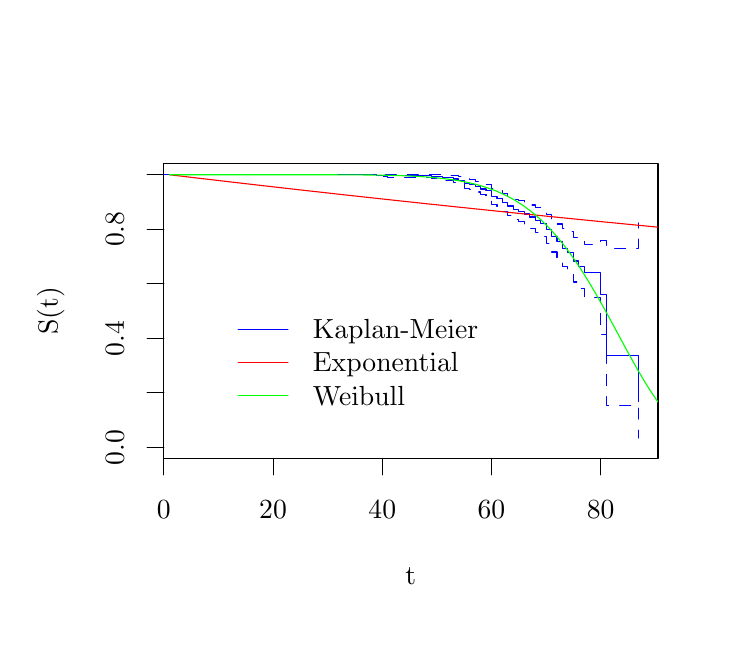
\begin{tikzpicture}[x=1pt,y=1pt]
\definecolor{fillColor}{RGB}{255,255,255}
\path[use as bounding box,fill=fillColor,fill opacity=0.00] (0,0) rectangle (252.94,216.81);
\begin{scope}
\path[clip] (  0.00,  0.00) rectangle (252.94,216.81);
\definecolor{drawColor}{RGB}{0,0,0}

\path[draw=drawColor,line width= 0.4pt,line join=round,line cap=round] ( 49.20, 61.20) -- (207.06, 61.20);

\path[draw=drawColor,line width= 0.4pt,line join=round,line cap=round] ( 49.20, 61.20) -- ( 49.20, 55.20);

\path[draw=drawColor,line width= 0.4pt,line join=round,line cap=round] ( 88.67, 61.20) -- ( 88.67, 55.20);

\path[draw=drawColor,line width= 0.4pt,line join=round,line cap=round] (128.13, 61.20) -- (128.13, 55.20);

\path[draw=drawColor,line width= 0.4pt,line join=round,line cap=round] (167.60, 61.20) -- (167.60, 55.20);

\path[draw=drawColor,line width= 0.4pt,line join=round,line cap=round] (207.06, 61.20) -- (207.06, 55.20);

\node[text=drawColor,anchor=base,inner sep=0pt, outer sep=0pt, scale=  1.00] at ( 49.20, 39.60) {0};

\node[text=drawColor,anchor=base,inner sep=0pt, outer sep=0pt, scale=  1.00] at ( 88.67, 39.60) {20};

\node[text=drawColor,anchor=base,inner sep=0pt, outer sep=0pt, scale=  1.00] at (128.13, 39.60) {40};

\node[text=drawColor,anchor=base,inner sep=0pt, outer sep=0pt, scale=  1.00] at (167.60, 39.60) {60};

\node[text=drawColor,anchor=base,inner sep=0pt, outer sep=0pt, scale=  1.00] at (207.06, 39.60) {80};

\path[draw=drawColor,line width= 0.4pt,line join=round,line cap=round] ( 49.20, 65.14) -- ( 49.20,163.67);

\path[draw=drawColor,line width= 0.4pt,line join=round,line cap=round] ( 49.20, 65.14) -- ( 43.20, 65.14);

\path[draw=drawColor,line width= 0.4pt,line join=round,line cap=round] ( 49.20, 84.85) -- ( 43.20, 84.85);

\path[draw=drawColor,line width= 0.4pt,line join=round,line cap=round] ( 49.20,104.55) -- ( 43.20,104.55);

\path[draw=drawColor,line width= 0.4pt,line join=round,line cap=round] ( 49.20,124.26) -- ( 43.20,124.26);

\path[draw=drawColor,line width= 0.4pt,line join=round,line cap=round] ( 49.20,143.96) -- ( 43.20,143.96);

\path[draw=drawColor,line width= 0.4pt,line join=round,line cap=round] ( 49.20,163.67) -- ( 43.20,163.67);

\node[text=drawColor,rotate= 90.00,anchor=base,inner sep=0pt, outer sep=0pt, scale=  1.00] at ( 34.80, 65.14) {0.0};

\node[text=drawColor,rotate= 90.00,anchor=base,inner sep=0pt, outer sep=0pt, scale=  1.00] at ( 34.80,104.55) {0.4};

\node[text=drawColor,rotate= 90.00,anchor=base,inner sep=0pt, outer sep=0pt, scale=  1.00] at ( 34.80,143.96) {0.8};

\path[draw=drawColor,line width= 0.4pt,line join=round,line cap=round] ( 49.20, 61.20) --
	(227.75, 61.20) --
	(227.75,167.61) --
	( 49.20,167.61) --
	( 49.20, 61.20);
\end{scope}
\begin{scope}
\path[clip] (  0.00,  0.00) rectangle (252.94,216.81);
\definecolor{drawColor}{RGB}{0,0,0}

\node[text=drawColor,anchor=base,inner sep=0pt, outer sep=0pt, scale=  1.00] at (138.47, 15.60) {t};

\node[text=drawColor,rotate= 90.00,anchor=base,inner sep=0pt, outer sep=0pt, scale=  1.00] at ( 10.80,114.41) {S(t)};
\end{scope}
\begin{scope}
\path[clip] ( 49.20, 61.20) rectangle (227.75,167.61);
\definecolor{drawColor}{RGB}{0,0,255}

\path[draw=drawColor,line width= 0.4pt,line join=round,line cap=round] ( 49.20,163.67) --
	(126.16,163.67) --
	(126.16,163.46) --
	(130.11,163.46) --
	(130.11,163.25) --
	(145.89,163.25) --
	(145.89,163.03) --
	(149.84,163.03) --
	(149.84,162.59) --
	(153.79,162.59) --
	(153.79,162.12) --
	(155.76,162.12) --
	(155.76,161.65) --
	(157.73,161.65) --
	(157.73,160.43) --
	(159.71,160.43) --
	(159.71,160.17) --
	(161.68,160.17) --
	(161.68,159.37) --
	(163.65,159.37) --
	(163.65,158.53) --
	(165.63,158.53) --
	(165.63,157.94) --
	(167.60,157.94) --
	(167.60,155.73) --
	(169.57,155.73) --
	(169.57,155.06) --
	(171.55,155.06) --
	(171.55,153.60) --
	(173.52,153.60) --
	(173.52,152.38) --
	(175.49,152.38) --
	(175.49,151.02) --
	(177.47,151.02) --
	(177.47,150.51) --
	(179.44,150.51) --
	(179.44,149.47) --
	(181.41,149.47) --
	(181.41,148.39) --
	(183.39,148.39) --
	(183.39,147.22) --
	(185.36,147.22) --
	(185.36,145.93) --
	(187.33,145.93) --
	(187.33,143.80) --
	(189.30,143.80) --
	(189.30,141.29) --
	(191.28,141.29) --
	(191.28,139.41) --
	(193.25,139.41) --
	(193.25,137.05) --
	(195.22,137.05) --
	(195.22,135.72) --
	(197.20,135.72) --
	(197.20,132.51) --
	(199.17,132.51) --
	(199.17,130.64) --
	(201.14,130.64) --
	(201.14,128.21) --
	(207.06,128.21) --
	(207.06,120.33) --
	(209.04,120.33) --
	(209.04, 98.25) --
	(220.88, 98.25) --
	(220.88, 81.70);

\path[draw=drawColor,line width= 0.4pt,dash pattern=on 4pt off 4pt ,line join=round,line cap=round] ( 49.20,163.67) --
	(126.16,163.67) --
	(126.16,163.04) --
	(130.11,163.04) --
	(130.11,162.66) --
	(145.89,162.66) --
	(145.89,162.31) --
	(149.84,162.31) --
	(149.84,161.64) --
	(153.79,161.64) --
	(153.79,160.99) --
	(155.76,160.99) --
	(155.76,160.35) --
	(157.73,160.35) --
	(157.73,158.77) --
	(159.71,158.77) --
	(159.71,158.45) --
	(161.68,158.45) --
	(161.68,157.44) --
	(163.65,157.44) --
	(163.65,156.40) --
	(165.63,156.40) --
	(165.63,155.68) --
	(167.60,155.68) --
	(167.60,153.02) --
	(169.57,153.02) --
	(169.57,152.21) --
	(171.55,152.21) --
	(171.55,150.47) --
	(173.52,150.47) --
	(173.52,149.03) --
	(175.49,149.03) --
	(175.49,147.40) --
	(177.47,147.40) --
	(177.47,146.79) --
	(179.44,146.79) --
	(179.44,145.54) --
	(181.41,145.54) --
	(181.41,144.26) --
	(183.39,144.26) --
	(183.39,142.86) --
	(185.36,142.86) --
	(185.36,141.31) --
	(187.33,141.31) --
	(187.33,138.76) --
	(189.30,138.76) --
	(189.30,135.74) --
	(191.28,135.74) --
	(191.28,133.48) --
	(193.25,133.48) --
	(193.25,130.57) --
	(195.22,130.57) --
	(195.22,128.92) --
	(197.20,128.92) --
	(197.20,124.89) --
	(199.17,124.89) --
	(199.17,122.53) --
	(201.14,122.53) --
	(201.14,119.35) --
	(207.06,119.35) --
	(207.06,105.92) --
	(209.04,105.92) --
	(209.04, 80.37) --
	(220.88, 80.37) --
	(220.88, 68.52);

\path[draw=drawColor,line width= 0.4pt,dash pattern=on 4pt off 4pt ,line join=round,line cap=round] ( 49.20,163.67) --
	(149.84,163.67) --
	(149.84,163.53) --
	(153.79,163.53) --
	(153.79,163.27) --
	(155.76,163.27) --
	(155.76,162.97) --
	(157.73,162.97) --
	(157.73,162.12) --
	(159.71,162.12) --
	(159.71,161.93) --
	(161.68,161.93) --
	(161.68,161.34) --
	(163.65,161.34) --
	(163.65,160.71) --
	(165.63,160.71) --
	(165.63,160.26) --
	(167.60,160.26) --
	(167.60,158.53) --
	(169.57,158.53) --
	(169.57,158.00) --
	(171.55,158.00) --
	(171.55,156.83) --
	(173.52,156.83) --
	(173.52,155.87) --
	(175.49,155.87) --
	(175.49,154.79) --
	(177.47,154.79) --
	(177.47,154.41) --
	(179.44,154.41) --
	(179.44,153.59) --
	(181.41,153.59) --
	(181.41,152.74) --
	(183.39,152.74) --
	(183.39,151.83) --
	(185.36,151.83) --
	(185.36,150.83) --
	(187.33,150.83) --
	(187.33,149.18) --
	(189.30,149.18) --
	(189.30,147.27) --
	(191.28,147.27) --
	(191.28,145.85) --
	(193.25,145.85) --
	(193.25,144.18) --
	(195.22,144.18) --
	(195.22,143.25) --
	(197.20,143.25) --
	(197.20,141.11) --
	(199.17,141.11) --
	(199.17,139.90) --
	(201.14,139.90) --
	(201.14,138.53) --
	(207.06,138.53) --
	(207.06,139.83) --
	(209.04,139.83) --
	(209.04,137.16) --
	(220.88,137.16) --
	(220.88,146.24);
\definecolor{drawColor}{RGB}{255,0,0}

\path[draw=drawColor,line width= 0.4pt,line join=round,line cap=round] ( 51.17,163.67) --
	( 53.15,163.43) --
	( 55.12,163.20) --
	( 57.09,162.97) --
	( 59.07,162.73) --
	( 61.04,162.50) --
	( 63.01,162.27) --
	( 64.99,162.04) --
	( 66.96,161.81) --
	( 68.93,161.58) --
	( 70.91,161.35) --
	( 72.88,161.12) --
	( 74.85,160.89) --
	( 76.83,160.66) --
	( 78.80,160.43) --
	( 80.77,160.20) --
	( 82.75,159.98) --
	( 84.72,159.75) --
	( 86.69,159.53) --
	( 88.67,159.30) --
	( 90.64,159.08) --
	( 92.61,158.85) --
	( 94.59,158.63) --
	( 96.56,158.41) --
	( 98.53,158.18) --
	(100.51,157.96) --
	(102.48,157.74) --
	(104.45,157.52) --
	(106.43,157.30) --
	(108.40,157.08) --
	(110.37,156.86) --
	(112.35,156.64) --
	(114.32,156.42) --
	(116.29,156.21) --
	(118.27,155.99) --
	(120.24,155.77) --
	(122.21,155.56) --
	(124.19,155.34) --
	(126.16,155.13) --
	(128.13,154.91) --
	(130.11,154.70) --
	(132.08,154.48) --
	(134.05,154.27) --
	(136.03,154.06) --
	(138.00,153.85) --
	(139.97,153.64) --
	(141.95,153.42) --
	(143.92,153.21) --
	(145.89,153.00) --
	(147.87,152.80) --
	(149.84,152.59) --
	(151.81,152.38) --
	(153.79,152.17) --
	(155.76,151.96) --
	(157.73,151.76) --
	(159.71,151.55) --
	(161.68,151.34) --
	(163.65,151.14) --
	(165.63,150.93) --
	(167.60,150.73) --
	(169.57,150.52) --
	(171.55,150.32) --
	(173.52,150.12) --
	(175.49,149.91) --
	(177.47,149.71) --
	(179.44,149.51) --
	(181.41,149.31) --
	(183.39,149.11) --
	(185.36,148.91) --
	(187.33,148.71) --
	(189.30,148.51) --
	(191.28,148.31) --
	(193.25,148.11) --
	(195.22,147.92) --
	(197.20,147.72) --
	(199.17,147.52) --
	(201.14,147.33) --
	(203.12,147.13) --
	(205.09,146.93) --
	(207.06,146.74) --
	(209.04,146.54) --
	(211.01,146.35) --
	(212.98,146.16) --
	(214.96,145.96) --
	(216.93,145.77) --
	(218.90,145.58) --
	(220.88,145.39) --
	(222.85,145.20) --
	(224.82,145.00) --
	(226.80,144.81) --
	(228.77,144.62);
\definecolor{drawColor}{RGB}{0,255,0}

\path[draw=drawColor,line width= 0.4pt,line join=round,line cap=round] ( 51.17,163.67) --
	( 53.15,163.67) --
	( 55.12,163.67) --
	( 57.09,163.67) --
	( 59.07,163.67) --
	( 61.04,163.67) --
	( 63.01,163.67) --
	( 64.99,163.67) --
	( 66.96,163.67) --
	( 68.93,163.67) --
	( 70.91,163.67) --
	( 72.88,163.67) --
	( 74.85,163.67) --
	( 76.83,163.67) --
	( 78.80,163.67) --
	( 80.77,163.67) --
	( 82.75,163.67) --
	( 84.72,163.67) --
	( 86.69,163.67) --
	( 88.67,163.67) --
	( 90.64,163.67) --
	( 92.61,163.67) --
	( 94.59,163.67) --
	( 96.56,163.67) --
	( 98.53,163.67) --
	(100.51,163.66) --
	(102.48,163.66) --
	(104.45,163.66) --
	(106.43,163.66) --
	(108.40,163.65) --
	(110.37,163.65) --
	(112.35,163.64) --
	(114.32,163.64) --
	(116.29,163.63) --
	(118.27,163.62) --
	(120.24,163.60) --
	(122.21,163.58) --
	(124.19,163.56) --
	(126.16,163.53) --
	(128.13,163.50) --
	(130.11,163.46) --
	(132.08,163.41) --
	(134.05,163.36) --
	(136.03,163.29) --
	(138.00,163.21) --
	(139.97,163.11) --
	(141.95,163.00) --
	(143.92,162.87) --
	(145.89,162.72) --
	(147.87,162.54) --
	(149.84,162.33) --
	(151.81,162.09) --
	(153.79,161.82) --
	(155.76,161.50) --
	(157.73,161.14) --
	(159.71,160.72) --
	(161.68,160.25) --
	(163.65,159.71) --
	(165.63,159.11) --
	(167.60,158.42) --
	(169.57,157.66) --
	(171.55,156.79) --
	(173.52,155.83) --
	(175.49,154.76) --
	(177.47,153.57) --
	(179.44,152.25) --
	(181.41,150.80) --
	(183.39,149.21) --
	(185.36,147.46) --
	(187.33,145.56) --
	(189.30,143.50) --
	(191.28,141.26) --
	(193.25,138.86) --
	(195.22,136.29) --
	(197.20,133.55) --
	(199.17,130.64) --
	(201.14,127.57) --
	(203.12,124.36) --
	(205.09,121.02) --
	(207.06,117.56) --
	(209.04,114.01) --
	(211.01,110.40) --
	(212.98,106.74) --
	(214.96,103.08) --
	(216.93, 99.44) --
	(218.90, 95.87) --
	(220.88, 92.40) --
	(222.85, 89.06) --
	(224.82, 85.89) --
	(226.80, 82.91) --
	(228.77, 80.17);

\path[] ( 67.05,119.84) rectangle (167.29, 71.84);
\definecolor{drawColor}{RGB}{0,0,255}

\path[draw=drawColor,line width= 0.4pt,line join=round,line cap=round] ( 76.05,107.84) -- ( 94.05,107.84);
\definecolor{drawColor}{RGB}{255,0,0}

\path[draw=drawColor,line width= 0.4pt,line join=round,line cap=round] ( 76.05, 95.84) -- ( 94.05, 95.84);
\definecolor{drawColor}{RGB}{0,255,0}

\path[draw=drawColor,line width= 0.4pt,line join=round,line cap=round] ( 76.05, 83.84) -- ( 94.05, 83.84);
\definecolor{drawColor}{RGB}{0,0,0}

\node[text=drawColor,anchor=base west,inner sep=0pt, outer sep=0pt, scale=  1.00] at (103.05,104.40) {Kaplan-Meier};

\node[text=drawColor,anchor=base west,inner sep=0pt, outer sep=0pt, scale=  1.00] at (103.05, 92.40) {Exponential};

\node[text=drawColor,anchor=base west,inner sep=0pt, outer sep=0pt, scale=  1.00] at (103.05, 80.40) {Weibull};
\end{scope}
\end{tikzpicture}
}
		\caption{Plot of Kaplan-Meier \& parametric estimators of the survivor function}
		\label{fig 5.2}
	\end{figure}
	
	To check if the Weibull model is adequate for the data, we use the graphical method presented in the last paragraph of the Results section, and obtain figure \ref{fig 5.3}. We can see that the points follow $D0$ line pattern, meaning that the Weibull model is effectively appropriate for the data.
	\begin{figure}[H]
		\centering
		\scalebox{1}{% Created by tikzDevice version 0.12 on 2019-04-27 00:00:27
% !TEX encoding = UTF-8 Unicode
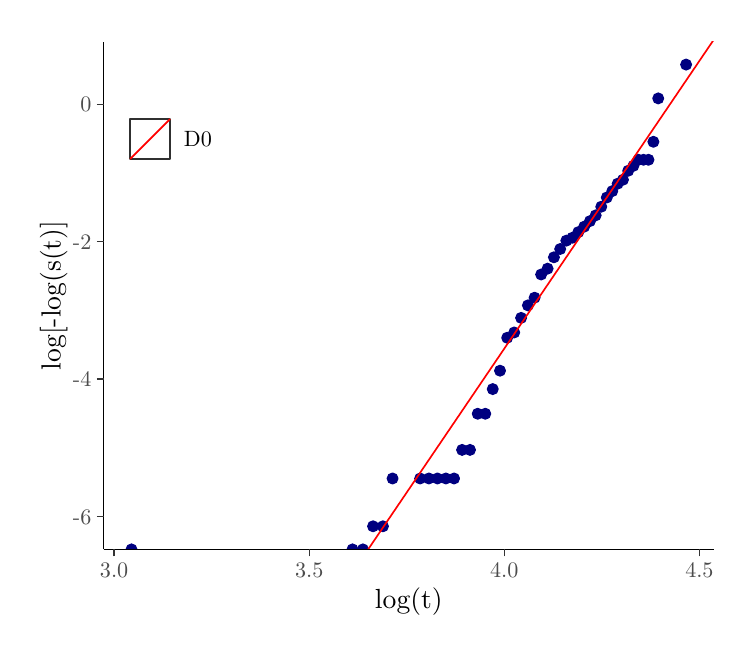
\begin{tikzpicture}[x=1pt,y=1pt]
\definecolor{fillColor}{RGB}{255,255,255}
\path[use as bounding box,fill=fillColor,fill opacity=0.00] (0,0) rectangle (252.94,216.81);
\begin{scope}
\path[clip] (  0.00,  0.00) rectangle (252.94,216.81);
\definecolor{drawColor}{RGB}{255,255,255}
\definecolor{fillColor}{RGB}{255,255,255}

\path[draw=drawColor,line width= 0.5pt,line join=round,line cap=round,fill=fillColor] ( -0.00,  0.00) rectangle (252.95,216.81);
\end{scope}
\begin{scope}
\path[clip] ( 27.50, 28.28) rectangle (247.95,211.81);
\definecolor{fillColor}{RGB}{255,255,255}

\path[fill=fillColor] ( 27.50, 28.28) rectangle (247.95,211.81);
\definecolor{drawColor}{RGB}{0,0,128}
\definecolor{fillColor}{RGB}{0,0,128}

\path[draw=drawColor,line width= 0.4pt,line join=round,line cap=round,fill=fillColor] ( 37.52, 28.28) circle (  1.96);

\path[draw=drawColor,line width= 0.4pt,line join=round,line cap=round,fill=fillColor] (117.38, 28.28) circle (  1.96);

\path[draw=drawColor,line width= 0.4pt,line join=round,line cap=round,fill=fillColor] (121.14, 28.28) circle (  1.96);

\path[draw=drawColor,line width= 0.4pt,line join=round,line cap=round,fill=fillColor] (124.80, 36.63) circle (  1.96);

\path[draw=drawColor,line width= 0.4pt,line join=round,line cap=round,fill=fillColor] (128.37, 36.63) circle (  1.96);

\path[draw=drawColor,line width= 0.4pt,line join=round,line cap=round,fill=fillColor] (131.85, 53.91) circle (  1.96);

\path[draw=drawColor,line width= 0.4pt,line join=round,line cap=round,fill=fillColor] (141.81, 53.91) circle (  1.96);

\path[draw=drawColor,line width= 0.4pt,line join=round,line cap=round,fill=fillColor] (144.97, 53.91) circle (  1.96);

\path[draw=drawColor,line width= 0.4pt,line join=round,line cap=round,fill=fillColor] (148.07, 53.91) circle (  1.96);

\path[draw=drawColor,line width= 0.4pt,line join=round,line cap=round,fill=fillColor] (151.11, 53.91) circle (  1.96);

\path[draw=drawColor,line width= 0.4pt,line join=round,line cap=round,fill=fillColor] (154.07, 53.91) circle (  1.96);

\path[draw=drawColor,line width= 0.4pt,line join=round,line cap=round,fill=fillColor] (156.98, 64.24) circle (  1.96);

\path[draw=drawColor,line width= 0.4pt,line join=round,line cap=round,fill=fillColor] (159.83, 64.24) circle (  1.96);

\path[draw=drawColor,line width= 0.4pt,line join=round,line cap=round,fill=fillColor] (162.62, 77.30) circle (  1.96);

\path[draw=drawColor,line width= 0.4pt,line join=round,line cap=round,fill=fillColor] (165.36, 77.30) circle (  1.96);

\path[draw=drawColor,line width= 0.4pt,line join=round,line cap=round,fill=fillColor] (168.05, 86.21) circle (  1.96);

\path[draw=drawColor,line width= 0.4pt,line join=round,line cap=round,fill=fillColor] (170.68, 92.86) circle (  1.96);

\path[draw=drawColor,line width= 0.4pt,line join=round,line cap=round,fill=fillColor] (173.27,104.76) circle (  1.96);

\path[draw=drawColor,line width= 0.4pt,line join=round,line cap=round,fill=fillColor] (175.81,106.67) circle (  1.96);

\path[draw=drawColor,line width= 0.4pt,line join=round,line cap=round,fill=fillColor] (178.30,111.94) circle (  1.96);

\path[draw=drawColor,line width= 0.4pt,line join=round,line cap=round,fill=fillColor] (180.76,116.46) circle (  1.96);

\path[draw=drawColor,line width= 0.4pt,line join=round,line cap=round,fill=fillColor] (183.17,119.23) circle (  1.96);

\path[draw=drawColor,line width= 0.4pt,line join=round,line cap=round,fill=fillColor] (185.54,127.62) circle (  1.96);

\path[draw=drawColor,line width= 0.4pt,line join=round,line cap=round,fill=fillColor] (187.87,129.73) circle (  1.96);

\path[draw=drawColor,line width= 0.4pt,line join=round,line cap=round,fill=fillColor] (190.16,133.83) circle (  1.96);

\path[draw=drawColor,line width= 0.4pt,line join=round,line cap=round,fill=fillColor] (192.42,136.83) circle (  1.96);

\path[draw=drawColor,line width= 0.4pt,line join=round,line cap=round,fill=fillColor] (194.64,139.85) circle (  1.96);

\path[draw=drawColor,line width= 0.4pt,line join=round,line cap=round,fill=fillColor] (196.82,140.89) circle (  1.96);

\path[draw=drawColor,line width= 0.4pt,line join=round,line cap=round,fill=fillColor] (198.97,142.92) circle (  1.96);

\path[draw=drawColor,line width= 0.4pt,line join=round,line cap=round,fill=fillColor] (201.09,144.90) circle (  1.96);

\path[draw=drawColor,line width= 0.4pt,line join=round,line cap=round,fill=fillColor] (203.18,146.91) circle (  1.96);

\path[draw=drawColor,line width= 0.4pt,line join=round,line cap=round,fill=fillColor] (205.24,148.98) circle (  1.96);

\path[draw=drawColor,line width= 0.4pt,line join=round,line cap=round,fill=fillColor] (207.27,152.11) circle (  1.96);

\path[draw=drawColor,line width= 0.4pt,line join=round,line cap=round,fill=fillColor] (209.27,155.44) circle (  1.96);

\path[draw=drawColor,line width= 0.4pt,line join=round,line cap=round,fill=fillColor] (211.24,157.74) circle (  1.96);

\path[draw=drawColor,line width= 0.4pt,line join=round,line cap=round,fill=fillColor] (213.19,160.43) circle (  1.96);

\path[draw=drawColor,line width= 0.4pt,line join=round,line cap=round,fill=fillColor] (215.11,161.86) circle (  1.96);

\path[draw=drawColor,line width= 0.4pt,line join=round,line cap=round,fill=fillColor] (217.00,165.10) circle (  1.96);

\path[draw=drawColor,line width= 0.4pt,line join=round,line cap=round,fill=fillColor] (218.87,166.87) circle (  1.96);

\path[draw=drawColor,line width= 0.4pt,line join=round,line cap=round,fill=fillColor] (220.71,169.07) circle (  1.96);

\path[draw=drawColor,line width= 0.4pt,line join=round,line cap=round,fill=fillColor] (222.53,169.07) circle (  1.96);

\path[draw=drawColor,line width= 0.4pt,line join=round,line cap=round,fill=fillColor] (224.32,169.07) circle (  1.96);

\path[draw=drawColor,line width= 0.4pt,line join=round,line cap=round,fill=fillColor] (226.10,175.57) circle (  1.96);

\path[draw=drawColor,line width= 0.4pt,line join=round,line cap=round,fill=fillColor] (227.85,191.25) circle (  1.96);

\path[draw=drawColor,line width= 0.4pt,line join=round,line cap=round,fill=fillColor] (237.92,203.47) circle (  1.96);
\definecolor{drawColor}{RGB}{255,0,0}

\path[draw=drawColor,line width= 0.6pt,line join=round] (103.84,  0.00) -- (247.95,212.51);
\end{scope}
\begin{scope}
\path[clip] (  0.00,  0.00) rectangle (252.94,216.81);
\definecolor{drawColor}{RGB}{0,0,0}

\path[draw=drawColor,line width= 0.5pt,line join=round] ( 27.50, 28.28) --
	( 27.50,211.81);
\end{scope}
\begin{scope}
\path[clip] (  0.00,  0.00) rectangle (252.94,216.81);
\definecolor{drawColor}{gray}{0.30}

\node[text=drawColor,anchor=base east,inner sep=0pt, outer sep=0pt, scale=  0.80] at ( 23.00, 37.42) {-6};

\node[text=drawColor,anchor=base east,inner sep=0pt, outer sep=0pt, scale=  0.80] at ( 23.00, 87.07) {-4};

\node[text=drawColor,anchor=base east,inner sep=0pt, outer sep=0pt, scale=  0.80] at ( 23.00,136.71) {-2};

\node[text=drawColor,anchor=base east,inner sep=0pt, outer sep=0pt, scale=  0.80] at ( 23.00,186.35) {0};
\end{scope}
\begin{scope}
\path[clip] (  0.00,  0.00) rectangle (252.94,216.81);
\definecolor{drawColor}{gray}{0.20}

\path[draw=drawColor,line width= 0.5pt,line join=round] ( 25.00, 40.18) --
	( 27.50, 40.18);

\path[draw=drawColor,line width= 0.5pt,line join=round] ( 25.00, 89.82) --
	( 27.50, 89.82);

\path[draw=drawColor,line width= 0.5pt,line join=round] ( 25.00,139.46) --
	( 27.50,139.46);

\path[draw=drawColor,line width= 0.5pt,line join=round] ( 25.00,189.11) --
	( 27.50,189.11);
\end{scope}
\begin{scope}
\path[clip] (  0.00,  0.00) rectangle (252.94,216.81);
\definecolor{drawColor}{RGB}{0,0,0}

\path[draw=drawColor,line width= 0.5pt,line join=round] ( 27.50, 28.28) --
	(247.95, 28.28);
\end{scope}
\begin{scope}
\path[clip] (  0.00,  0.00) rectangle (252.94,216.81);
\definecolor{drawColor}{gray}{0.20}

\path[draw=drawColor,line width= 0.5pt,line join=round] ( 31.24, 25.78) --
	( 31.24, 28.28);

\path[draw=drawColor,line width= 0.5pt,line join=round] (101.74, 25.78) --
	(101.74, 28.28);

\path[draw=drawColor,line width= 0.5pt,line join=round] (172.23, 25.78) --
	(172.23, 28.28);

\path[draw=drawColor,line width= 0.5pt,line join=round] (242.73, 25.78) --
	(242.73, 28.28);
\end{scope}
\begin{scope}
\path[clip] (  0.00,  0.00) rectangle (252.94,216.81);
\definecolor{drawColor}{gray}{0.30}

\node[text=drawColor,anchor=base,inner sep=0pt, outer sep=0pt, scale=  0.80] at ( 31.24, 18.28) {3.0};

\node[text=drawColor,anchor=base,inner sep=0pt, outer sep=0pt, scale=  0.80] at (101.74, 18.28) {3.5};

\node[text=drawColor,anchor=base,inner sep=0pt, outer sep=0pt, scale=  0.80] at (172.23, 18.28) {4.0};

\node[text=drawColor,anchor=base,inner sep=0pt, outer sep=0pt, scale=  0.80] at (242.73, 18.28) {4.5};
\end{scope}
\begin{scope}
\path[clip] (  0.00,  0.00) rectangle (252.94,216.81);
\definecolor{drawColor}{RGB}{0,0,0}

\node[text=drawColor,anchor=base,inner sep=0pt, outer sep=0pt, scale=  1.00] at (137.72,  6.94) {log(t)};
\end{scope}
\begin{scope}
\path[clip] (  0.00,  0.00) rectangle (252.94,216.81);
\definecolor{drawColor}{RGB}{0,0,0}

\node[text=drawColor,rotate= 90.00,anchor=base,inner sep=0pt, outer sep=0pt, scale=  1.00] at ( 11.89,120.05) {log[-log(s(t)]};
\end{scope}
\begin{scope}
\path[clip] (  0.00,  0.00) rectangle (252.94,216.81);
\definecolor{fillColor}{RGB}{255,255,255}

\path[fill=fillColor] ( 32.02,164.35) rectangle ( 71.59,202.63);
\end{scope}
\begin{scope}
\path[clip] (  0.00,  0.00) rectangle (252.94,216.81);
\definecolor{drawColor}{RGB}{0,0,0}

\node[text=drawColor,anchor=base west,inner sep=0pt, outer sep=0pt, scale=  1.00] at ( 37.02,189.77) { };
\end{scope}
\begin{scope}
\path[clip] (  0.00,  0.00) rectangle (252.94,216.81);
\definecolor{drawColor}{gray}{0.19}
\definecolor{fillColor}{RGB}{255,255,255}

\path[draw=drawColor,line width= 0.5pt,line join=round,line cap=round,fill=fillColor] ( 37.02,169.35) rectangle ( 51.48,183.80);
\end{scope}
\begin{scope}
\path[clip] (  0.00,  0.00) rectangle (252.94,216.81);
\definecolor{drawColor}{RGB}{255,0,0}

\path[draw=drawColor,line width= 0.6pt,line join=round] ( 37.02,169.35) -- ( 51.48,183.80);
\end{scope}
\begin{scope}
\path[clip] (  0.00,  0.00) rectangle (252.94,216.81);
\definecolor{drawColor}{RGB}{0,0,0}

\node[text=drawColor,anchor=base west,inner sep=0pt, outer sep=0pt, scale=  0.80] at ( 56.48,173.82) {D0};
\end{scope}
\end{tikzpicture}
}
		\caption{Plot of $\mathtt{log}\{-\mathtt{log}(\hat{S}(t))\}$ against $\mathtt{log}(t)$, with the line $D0$ with slope $\alpha$ and intercept $-\mathtt{log}(\lambda_{weibull})$}
		\label{fig 5.3}
	\end{figure}
	
	\item Now we consider two groups of patients: smokers and non-smokers. Smokers make up $82.1\%$ in the sample. For each group, the Kaplan-Meier estimators are computed, and plotted together with the corresponding confidence bands in figure \ref{fig 5.4}. Then we want to test if the survival time depends on being a smoker. With the log-rank test, we have have the $\chi^2_1=2.7$ with p-value$=0.1>0.05$. Hence the two groups do not share the same survival function, in other words the survival time do depend on being a smoker.
	
	\begin{figure}[H]
		\centering
		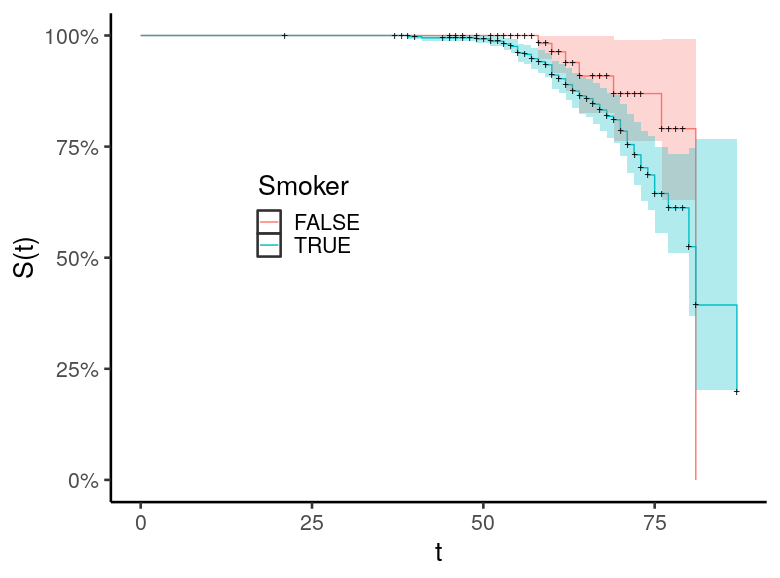
\includegraphics[scale=0.5]{Ex5plot4.png}
		\caption{Plot of the Kaplan-Meier estimators fit for smokers and nonsmokers}
		\label{fig 5.4}
	\end{figure} 
	
	We fit the Weibull model to both groups. The results are in table \ref{tableau51}, and the figure \ref{fig 5.5} is the plot of the resulting parametric estimators for the
survivor function together with the corresponding Kaplan-Meier estimators.
	\begin{table}[H]
		\centering
		\begin{tabular}{|P{1.9cm}|P{2cm}|P{2cm}|}
			\hline
			& Scale & Shape  \\
			\hline
			smokers & 0.01205778 & 8.161903  \\
			\hline
			nonsmokers & 0.01181161 & 11.13959 \\
			\hline
		\end{tabular}
		\caption{\label{tableau51}Weibull model estimated parameters for each group}
	\end{table} 
	
	\begin{figure}[H]
		\centering
		\scalebox{1}{% Created by tikzDevice version 0.12 on 2019-04-27 00:00:34
% !TEX encoding = UTF-8 Unicode
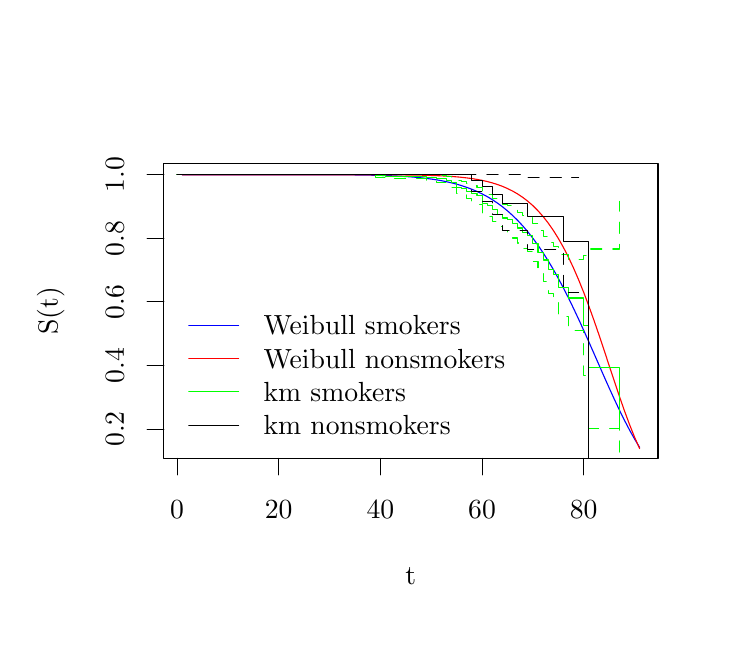
\begin{tikzpicture}[x=1pt,y=1pt]
\definecolor{fillColor}{RGB}{255,255,255}
\path[use as bounding box,fill=fillColor,fill opacity=0.00] (0,0) rectangle (252.94,216.81);
\begin{scope}
\path[clip] ( 49.20, 61.20) rectangle (227.75,167.61);
\definecolor{drawColor}{RGB}{0,0,255}

\path[draw=drawColor,line width= 0.4pt,line join=round,line cap=round] ( 55.81,163.67) --
	( 57.65,163.67) --
	( 59.49,163.67) --
	( 61.32,163.67) --
	( 63.16,163.67) --
	( 65.00,163.67) --
	( 66.83,163.67) --
	( 68.67,163.67) --
	( 70.51,163.67) --
	( 72.34,163.67) --
	( 74.18,163.67) --
	( 76.02,163.67) --
	( 77.86,163.67) --
	( 79.69,163.67) --
	( 81.53,163.67) --
	( 83.37,163.67) --
	( 85.20,163.67) --
	( 87.04,163.67) --
	( 88.88,163.67) --
	( 90.71,163.67) --
	( 92.55,163.67) --
	( 94.39,163.67) --
	( 96.22,163.67) --
	( 98.06,163.67) --
	( 99.90,163.66) --
	(101.73,163.66) --
	(103.57,163.66) --
	(105.41,163.66) --
	(107.25,163.65) --
	(109.08,163.65) --
	(110.92,163.64) --
	(112.76,163.63) --
	(114.59,163.62) --
	(116.43,163.61) --
	(118.27,163.59) --
	(120.10,163.57) --
	(121.94,163.54) --
	(123.78,163.51) --
	(125.61,163.47) --
	(127.45,163.43) --
	(129.29,163.37) --
	(131.12,163.30) --
	(132.96,163.22) --
	(134.80,163.13) --
	(136.64,163.02) --
	(138.47,162.89) --
	(140.31,162.74) --
	(142.15,162.56) --
	(143.98,162.35) --
	(145.82,162.11) --
	(147.66,161.84) --
	(149.49,161.52) --
	(151.33,161.15) --
	(153.17,160.73) --
	(155.00,160.26) --
	(156.84,159.72) --
	(158.68,159.10) --
	(160.52,158.41) --
	(162.35,157.63) --
	(164.19,156.75) --
	(166.03,155.77) --
	(167.86,154.68) --
	(169.70,153.46) --
	(171.54,152.11) --
	(173.37,150.62) --
	(175.21,148.97) --
	(177.05,147.17) --
	(178.88,145.20) --
	(180.72,143.05) --
	(182.56,140.72) --
	(184.39,138.20) --
	(186.23,135.49) --
	(188.07,132.59) --
	(189.91,129.50) --
	(191.74,126.22) --
	(193.58,122.76) --
	(195.42,119.14) --
	(197.25,115.36) --
	(199.09,111.45) --
	(200.93,107.42) --
	(202.76,103.31) --
	(204.60, 99.14) --
	(206.44, 94.95) --
	(208.27, 90.77) --
	(210.11, 86.65) --
	(211.95, 82.62) --
	(213.78, 78.72) --
	(215.62, 74.99) --
	(217.46, 71.46) --
	(219.30, 68.17) --
	(221.13, 65.14);
\end{scope}
\begin{scope}
\path[clip] (  0.00,  0.00) rectangle (252.94,216.81);
\definecolor{drawColor}{RGB}{0,0,0}

\path[draw=drawColor,line width= 0.4pt,line join=round,line cap=round] ( 53.98, 61.20) -- (200.93, 61.20);

\path[draw=drawColor,line width= 0.4pt,line join=round,line cap=round] ( 53.98, 61.20) -- ( 53.98, 55.20);

\path[draw=drawColor,line width= 0.4pt,line join=round,line cap=round] ( 90.71, 61.20) -- ( 90.71, 55.20);

\path[draw=drawColor,line width= 0.4pt,line join=round,line cap=round] (127.45, 61.20) -- (127.45, 55.20);

\path[draw=drawColor,line width= 0.4pt,line join=round,line cap=round] (164.19, 61.20) -- (164.19, 55.20);

\path[draw=drawColor,line width= 0.4pt,line join=round,line cap=round] (200.93, 61.20) -- (200.93, 55.20);

\node[text=drawColor,anchor=base,inner sep=0pt, outer sep=0pt, scale=  1.00] at ( 53.98, 39.60) {0};

\node[text=drawColor,anchor=base,inner sep=0pt, outer sep=0pt, scale=  1.00] at ( 90.71, 39.60) {20};

\node[text=drawColor,anchor=base,inner sep=0pt, outer sep=0pt, scale=  1.00] at (127.45, 39.60) {40};

\node[text=drawColor,anchor=base,inner sep=0pt, outer sep=0pt, scale=  1.00] at (164.19, 39.60) {60};

\node[text=drawColor,anchor=base,inner sep=0pt, outer sep=0pt, scale=  1.00] at (200.93, 39.60) {80};

\path[draw=drawColor,line width= 0.4pt,line join=round,line cap=round] ( 49.20, 71.76) -- ( 49.20,163.67);

\path[draw=drawColor,line width= 0.4pt,line join=round,line cap=round] ( 49.20, 71.76) -- ( 43.20, 71.76);

\path[draw=drawColor,line width= 0.4pt,line join=round,line cap=round] ( 49.20, 94.74) -- ( 43.20, 94.74);

\path[draw=drawColor,line width= 0.4pt,line join=round,line cap=round] ( 49.20,117.71) -- ( 43.20,117.71);

\path[draw=drawColor,line width= 0.4pt,line join=round,line cap=round] ( 49.20,140.69) -- ( 43.20,140.69);

\path[draw=drawColor,line width= 0.4pt,line join=round,line cap=round] ( 49.20,163.67) -- ( 43.20,163.67);

\node[text=drawColor,rotate= 90.00,anchor=base,inner sep=0pt, outer sep=0pt, scale=  1.00] at ( 34.80, 71.76) {0.2};

\node[text=drawColor,rotate= 90.00,anchor=base,inner sep=0pt, outer sep=0pt, scale=  1.00] at ( 34.80, 94.74) {0.4};

\node[text=drawColor,rotate= 90.00,anchor=base,inner sep=0pt, outer sep=0pt, scale=  1.00] at ( 34.80,117.71) {0.6};

\node[text=drawColor,rotate= 90.00,anchor=base,inner sep=0pt, outer sep=0pt, scale=  1.00] at ( 34.80,140.69) {0.8};

\node[text=drawColor,rotate= 90.00,anchor=base,inner sep=0pt, outer sep=0pt, scale=  1.00] at ( 34.80,163.67) {1.0};

\path[draw=drawColor,line width= 0.4pt,line join=round,line cap=round] ( 49.20, 61.20) --
	(227.75, 61.20) --
	(227.75,167.61) --
	( 49.20,167.61) --
	( 49.20, 61.20);
\end{scope}
\begin{scope}
\path[clip] (  0.00,  0.00) rectangle (252.94,216.81);
\definecolor{drawColor}{RGB}{0,0,0}

\node[text=drawColor,anchor=base,inner sep=0pt, outer sep=0pt, scale=  1.00] at (138.47, 15.60) {t};

\node[text=drawColor,rotate= 90.00,anchor=base,inner sep=0pt, outer sep=0pt, scale=  1.00] at ( 10.80,114.41) {S(t)};
\end{scope}
\begin{scope}
\path[clip] ( 49.20, 61.20) rectangle (227.75,167.61);
\definecolor{drawColor}{RGB}{255,0,0}

\path[draw=drawColor,line width= 0.4pt,line join=round,line cap=round] ( 55.81,163.67) --
	( 57.65,163.67) --
	( 59.49,163.67) --
	( 61.32,163.67) --
	( 63.16,163.67) --
	( 65.00,163.67) --
	( 66.83,163.67) --
	( 68.67,163.67) --
	( 70.51,163.67) --
	( 72.34,163.67) --
	( 74.18,163.67) --
	( 76.02,163.67) --
	( 77.86,163.67) --
	( 79.69,163.67) --
	( 81.53,163.67) --
	( 83.37,163.67) --
	( 85.20,163.67) --
	( 87.04,163.67) --
	( 88.88,163.67) --
	( 90.71,163.67) --
	( 92.55,163.67) --
	( 94.39,163.67) --
	( 96.22,163.67) --
	( 98.06,163.67) --
	( 99.90,163.67) --
	(101.73,163.67) --
	(103.57,163.67) --
	(105.41,163.67) --
	(107.25,163.67) --
	(109.08,163.67) --
	(110.92,163.67) --
	(112.76,163.67) --
	(114.59,163.67) --
	(116.43,163.67) --
	(118.27,163.66) --
	(120.10,163.66) --
	(121.94,163.66) --
	(123.78,163.66) --
	(125.61,163.65) --
	(127.45,163.65) --
	(129.29,163.64) --
	(131.12,163.63) --
	(132.96,163.62) --
	(134.80,163.61) --
	(136.64,163.59) --
	(138.47,163.57) --
	(140.31,163.54) --
	(142.15,163.51) --
	(143.98,163.46) --
	(145.82,163.41) --
	(147.66,163.34) --
	(149.49,163.26) --
	(151.33,163.17) --
	(153.17,163.05) --
	(155.00,162.90) --
	(156.84,162.73) --
	(158.68,162.52) --
	(160.52,162.28) --
	(162.35,161.98) --
	(164.19,161.63) --
	(166.03,161.22) --
	(167.86,160.73) --
	(169.70,160.15) --
	(171.54,159.48) --
	(173.37,158.69) --
	(175.21,157.78) --
	(177.05,156.72) --
	(178.88,155.50) --
	(180.72,154.09) --
	(182.56,152.49) --
	(184.39,150.66) --
	(186.23,148.58) --
	(188.07,146.24) --
	(189.91,143.61) --
	(191.74,140.68) --
	(193.58,137.43) --
	(195.42,133.85) --
	(197.25,129.94) --
	(199.09,125.69) --
	(200.93,121.13) --
	(202.76,116.27) --
	(204.60,111.14) --
	(206.44,105.80) --
	(208.27,100.31) --
	(210.11, 94.74) --
	(211.95, 89.17) --
	(213.78, 83.70) --
	(215.62, 78.43) --
	(217.46, 73.45) --
	(219.30, 68.85) --
	(221.13, 64.71);
\definecolor{drawColor}{RGB}{0,255,0}

\path[draw=drawColor,line width= 0.4pt,line join=round,line cap=round] ( 53.98,163.67) --
	(125.61,163.67) --
	(125.61,163.37) --
	(129.29,163.37) --
	(129.29,163.07) --
	(143.98,163.07) --
	(143.98,162.76) --
	(147.66,162.76) --
	(147.66,162.15) --
	(151.33,162.15) --
	(151.33,161.50) --
	(153.17,161.50) --
	(153.17,160.84) --
	(155.00,160.84) --
	(155.00,159.15) --
	(156.84,159.15) --
	(156.84,158.80) --
	(158.68,158.80) --
	(158.68,157.68) --
	(160.52,157.68) --
	(160.52,156.90) --
	(162.35,156.90) --
	(162.35,156.08) --
	(164.19,156.08) --
	(164.19,153.42) --
	(166.03,153.42) --
	(166.03,152.48) --
	(167.86,152.48) --
	(167.86,150.97) --
	(169.70,150.97) --
	(169.70,149.29) --
	(171.54,149.29) --
	(171.54,148.05) --
	(173.37,148.05) --
	(173.37,147.35) --
	(175.21,147.35) --
	(175.21,145.90) --
	(177.05,145.90) --
	(177.05,144.41) --
	(178.88,144.41) --
	(178.88,142.77) --
	(180.72,142.77) --
	(180.72,141.87) --
	(182.56,141.87) --
	(182.56,138.93) --
	(184.39,138.93) --
	(184.39,135.46) --
	(186.23,135.46) --
	(186.23,132.84) --
	(188.07,132.84) --
	(188.07,129.47) --
	(189.91,129.47) --
	(189.91,127.60) --
	(191.74,127.60) --
	(191.74,122.82) --
	(195.42,122.82) --
	(195.42,119.12) --
	(200.93,119.12) --
	(200.93,109.07) --
	(202.76,109.07) --
	(202.76, 94.00) --
	(213.78, 94.00) --
	(213.78, 71.39);

\path[draw=drawColor,line width= 0.4pt,dash pattern=on 4pt off 4pt ,line join=round,line cap=round] ( 53.98,163.67) --
	(125.61,163.67) --
	(125.61,162.79) --
	(129.29,162.79) --
	(129.29,162.25) --
	(143.98,162.25) --
	(143.98,161.75) --
	(147.66,161.75) --
	(147.66,160.83) --
	(151.33,160.83) --
	(151.33,159.91) --
	(153.17,159.91) --
	(153.17,159.03) --
	(155.00,159.03) --
	(155.00,156.84) --
	(156.84,156.84) --
	(156.84,156.40) --
	(158.68,156.40) --
	(158.68,155.01) --
	(160.52,155.01) --
	(160.52,154.05) --
	(162.35,154.05) --
	(162.35,153.04) --
	(164.19,153.04) --
	(164.19,149.82) --
	(166.03,149.82) --
	(166.03,148.69) --
	(167.86,148.69) --
	(167.86,146.89) --
	(169.70,146.89) --
	(169.70,144.88) --
	(171.54,144.88) --
	(171.54,143.38) --
	(173.37,143.38) --
	(173.37,142.54) --
	(175.21,142.54) --
	(175.21,140.79) --
	(177.05,140.79) --
	(177.05,139.00) --
	(178.88,139.00) --
	(178.88,137.04) --
	(180.72,137.04) --
	(180.72,135.95) --
	(182.56,135.95) --
	(182.56,132.41) --
	(184.39,132.41) --
	(184.39,128.22) --
	(186.23,128.22) --
	(186.23,125.06) --
	(188.07,125.06) --
	(188.07,120.90) --
	(189.91,120.90) --
	(189.91,118.58) --
	(191.74,118.58) --
	(191.74,112.56) --
	(195.42,112.56) --
	(195.42,107.54) --
	(200.93,107.54) --
	(200.93, 91.18) --
	(202.76, 91.18) --
	(202.76, 72.00) --
	(213.78, 72.00) --
	(213.78, 53.64);

\path[draw=drawColor,line width= 0.4pt,dash pattern=on 4pt off 4pt ,line join=round,line cap=round] ( 53.98,163.67) --
	(147.66,163.67) --
	(147.66,163.48) --
	(151.33,163.48) --
	(151.33,163.10) --
	(153.17,163.10) --
	(153.17,162.68) --
	(155.00,162.68) --
	(155.00,161.50) --
	(156.84,161.50) --
	(156.84,161.24) --
	(158.68,161.24) --
	(158.68,160.42) --
	(160.52,160.42) --
	(160.52,159.83) --
	(162.35,159.83) --
	(162.35,159.21) --
	(164.19,159.21) --
	(164.19,157.16) --
	(166.03,157.16) --
	(166.03,156.41) --
	(167.86,156.41) --
	(167.86,155.22) --
	(169.70,155.22) --
	(169.70,153.91) --
	(171.54,153.91) --
	(171.54,152.94) --
	(173.37,152.94) --
	(173.37,152.41) --
	(175.21,152.41) --
	(175.21,151.30) --
	(177.05,151.30) --
	(177.05,150.14) --
	(178.88,150.14) --
	(178.88,148.87) --
	(180.72,148.87) --
	(180.72,148.19) --
	(182.56,148.19) --
	(182.56,145.96) --
	(184.39,145.96) --
	(184.39,143.36) --
	(186.23,143.36) --
	(186.23,141.40) --
	(188.07,141.40) --
	(188.07,139.07) --
	(189.91,139.07) --
	(189.91,137.77) --
	(191.74,137.77) --
	(191.74,134.73) --
	(195.42,134.73) --
	(195.42,132.98) --
	(200.93,132.98) --
	(200.93,134.50) --
	(202.76,134.50) --
	(202.76,136.82) --
	(213.78,136.82) --
	(213.78,154.00);
\definecolor{drawColor}{RGB}{0,0,0}

\path[draw=drawColor,line width= 0.4pt,line join=round,line cap=round] ( 53.98,163.67) --
	(160.52,163.67) --
	(160.52,161.62) --
	(164.19,161.62) --
	(164.19,159.45) --
	(167.86,159.45) --
	(167.86,156.68) --
	(171.54,156.68) --
	(171.54,153.20) --
	(180.72,153.20) --
	(180.72,148.66) --
	(193.58,148.66) --
	(193.58,139.58) --
	(202.76,139.58) --
	(202.76, 48.78);

\path[draw=drawColor,line width= 0.4pt,dash pattern=on 4pt off 4pt ,line join=round,line cap=round] ( 53.98,163.67) --
	(160.52,163.67) --
	(160.52,157.70) --
	(164.19,157.70) --
	(164.19,153.85) --
	(167.86,153.85) --
	(167.86,149.20) --
	(171.54,149.20) --
	(171.54,143.61) --
	(180.72,143.61) --
	(180.72,136.49) --
	(193.58,136.49) --
	(193.58,121.10) --
	(199.09,121.10);

\path[draw=drawColor,line width= 0.4pt,dash pattern=on 4pt off 4pt ,line join=round,line cap=round] ( 53.98,163.67) --
	(180.72,163.67) --
	(180.72,162.52) --
	(193.58,162.52) --
	(193.58,162.79) --
	(199.09,162.79);

\path[] ( 49.22,121.21) rectangle (177.06, 61.21);
\definecolor{drawColor}{RGB}{0,0,255}

\path[draw=drawColor,line width= 0.4pt,line join=round,line cap=round] ( 58.22,109.21) -- ( 76.22,109.21);
\definecolor{drawColor}{RGB}{255,0,0}

\path[draw=drawColor,line width= 0.4pt,line join=round,line cap=round] ( 58.22, 97.21) -- ( 76.22, 97.21);
\definecolor{drawColor}{RGB}{0,255,0}

\path[draw=drawColor,line width= 0.4pt,line join=round,line cap=round] ( 58.22, 85.21) -- ( 76.22, 85.21);
\definecolor{drawColor}{RGB}{0,0,0}

\path[draw=drawColor,line width= 0.4pt,line join=round,line cap=round] ( 58.22, 73.21) -- ( 76.22, 73.21);

\node[text=drawColor,anchor=base west,inner sep=0pt, outer sep=0pt, scale=  1.00] at ( 85.22,105.77) {Weibull smokers};

\node[text=drawColor,anchor=base west,inner sep=0pt, outer sep=0pt, scale=  1.00] at ( 85.22, 93.77) {Weibull nonsmokers};

\node[text=drawColor,anchor=base west,inner sep=0pt, outer sep=0pt, scale=  1.00] at ( 85.22, 81.77) {km smokers};

\node[text=drawColor,anchor=base west,inner sep=0pt, outer sep=0pt, scale=  1.00] at ( 85.22, 69.77) {km nonsmokers};
\end{scope}
\end{tikzpicture}
}
		\caption{Plot of the nonparametric $\&$ parametric fit of the survivor function for each group}
		\label{fig 5.5}
	\end{figure} 
	
	To check Weibull model assumption in both groups, we use figures in \ref{figuuu}. We can see that the points in plot \ref{fig 5.6} follow $D1$ line pattern, meaning that the Weibull model is effectively appropriate for the smokers' group. However, the plot \ref{fig 5.7} highlight many points on the x-axis causing a different pattern with the line $D2$. Hence we can assume that the Weibull model is not appropriate for the nonsmokers group.
	\begin{figure}[H]
		\centering
		\begin{subfigure}[b]{0.48\linewidth}        %% or \columnwidth
			\centering
			\scalebox{0.75}{% Created by tikzDevice version 0.12 on 2019-04-27 00:00:36
% !TEX encoding = UTF-8 Unicode
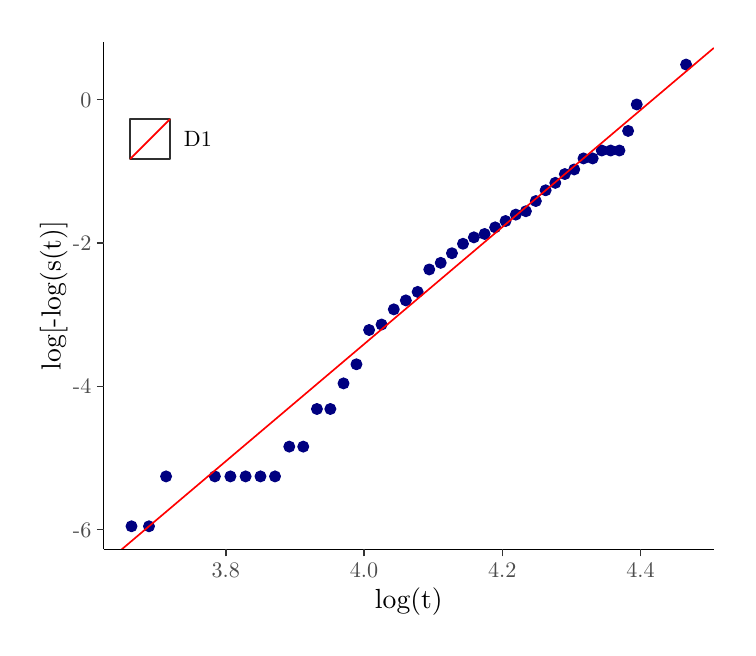
\begin{tikzpicture}[x=1pt,y=1pt]
\definecolor{fillColor}{RGB}{255,255,255}
\path[use as bounding box,fill=fillColor,fill opacity=0.00] (0,0) rectangle (252.94,216.81);
\begin{scope}
\path[clip] (  0.00,  0.00) rectangle (252.94,216.81);
\definecolor{drawColor}{RGB}{255,255,255}
\definecolor{fillColor}{RGB}{255,255,255}

\path[draw=drawColor,line width= 0.5pt,line join=round,line cap=round,fill=fillColor] ( -0.00,  0.00) rectangle (252.95,216.81);
\end{scope}
\begin{scope}
\path[clip] ( 27.50, 28.28) rectangle (247.95,211.81);
\definecolor{fillColor}{RGB}{255,255,255}

\path[fill=fillColor] ( 27.50, 28.28) rectangle (247.95,211.81);
\definecolor{drawColor}{RGB}{0,0,128}
\definecolor{fillColor}{RGB}{0,0,128}

\path[draw=drawColor,line width= 0.4pt,line join=round,line cap=round,fill=fillColor] ( 37.52, 36.63) circle (  1.96);

\path[draw=drawColor,line width= 0.4pt,line join=round,line cap=round,fill=fillColor] ( 43.84, 36.63) circle (  1.96);

\path[draw=drawColor,line width= 0.4pt,line join=round,line cap=round,fill=fillColor] ( 50.01, 54.66) circle (  1.96);

\path[draw=drawColor,line width= 0.4pt,line join=round,line cap=round,fill=fillColor] ( 67.65, 54.66) circle (  1.96);

\path[draw=drawColor,line width= 0.4pt,line join=round,line cap=round,fill=fillColor] ( 73.26, 54.66) circle (  1.96);

\path[draw=drawColor,line width= 0.4pt,line join=round,line cap=round,fill=fillColor] ( 78.75, 54.66) circle (  1.96);

\path[draw=drawColor,line width= 0.4pt,line join=round,line cap=round,fill=fillColor] ( 84.12, 54.66) circle (  1.96);

\path[draw=drawColor,line width= 0.4pt,line join=round,line cap=round,fill=fillColor] ( 89.38, 54.66) circle (  1.96);

\path[draw=drawColor,line width= 0.4pt,line join=round,line cap=round,fill=fillColor] ( 94.53, 65.42) circle (  1.96);

\path[draw=drawColor,line width= 0.4pt,line join=round,line cap=round,fill=fillColor] ( 99.58, 65.42) circle (  1.96);

\path[draw=drawColor,line width= 0.4pt,line join=round,line cap=round,fill=fillColor] (104.52, 79.02) circle (  1.96);

\path[draw=drawColor,line width= 0.4pt,line join=round,line cap=round,fill=fillColor] (109.37, 79.02) circle (  1.96);

\path[draw=drawColor,line width= 0.4pt,line join=round,line cap=round,fill=fillColor] (114.13, 88.27) circle (  1.96);

\path[draw=drawColor,line width= 0.4pt,line join=round,line cap=round,fill=fillColor] (118.80, 95.17) circle (  1.96);

\path[draw=drawColor,line width= 0.4pt,line join=round,line cap=round,fill=fillColor] (123.38,107.56) circle (  1.96);

\path[draw=drawColor,line width= 0.4pt,line join=round,line cap=round,fill=fillColor] (127.88,109.54) circle (  1.96);

\path[draw=drawColor,line width= 0.4pt,line join=round,line cap=round,fill=fillColor] (132.30,115.02) circle (  1.96);

\path[draw=drawColor,line width= 0.4pt,line join=round,line cap=round,fill=fillColor] (136.65,118.26) circle (  1.96);

\path[draw=drawColor,line width= 0.4pt,line join=round,line cap=round,fill=fillColor] (140.92,121.33) circle (  1.96);

\path[draw=drawColor,line width= 0.4pt,line join=round,line cap=round,fill=fillColor] (145.12,129.44) circle (  1.96);

\path[draw=drawColor,line width= 0.4pt,line join=round,line cap=round,fill=fillColor] (149.25,131.83) circle (  1.96);

\path[draw=drawColor,line width= 0.4pt,line join=round,line cap=round,fill=fillColor] (153.31,135.30) circle (  1.96);

\path[draw=drawColor,line width= 0.4pt,line join=round,line cap=round,fill=fillColor] (157.30,138.72) circle (  1.96);

\path[draw=drawColor,line width= 0.4pt,line join=round,line cap=round,fill=fillColor] (161.24,141.04) circle (  1.96);

\path[draw=drawColor,line width= 0.4pt,line join=round,line cap=round,fill=fillColor] (165.11,142.26) circle (  1.96);

\path[draw=drawColor,line width= 0.4pt,line join=round,line cap=round,fill=fillColor] (168.92,144.65) circle (  1.96);

\path[draw=drawColor,line width= 0.4pt,line join=round,line cap=round,fill=fillColor] (172.68,146.94) circle (  1.96);

\path[draw=drawColor,line width= 0.4pt,line join=round,line cap=round,fill=fillColor] (176.38,149.26) circle (  1.96);

\path[draw=drawColor,line width= 0.4pt,line join=round,line cap=round,fill=fillColor] (180.03,150.48) circle (  1.96);

\path[draw=drawColor,line width= 0.4pt,line join=round,line cap=round,fill=fillColor] (183.62,154.16) circle (  1.96);

\path[draw=drawColor,line width= 0.4pt,line join=round,line cap=round,fill=fillColor] (187.16,158.04) circle (  1.96);

\path[draw=drawColor,line width= 0.4pt,line join=round,line cap=round,fill=fillColor] (190.66,160.73) circle (  1.96);

\path[draw=drawColor,line width= 0.4pt,line join=round,line cap=round,fill=fillColor] (194.10,163.91) circle (  1.96);

\path[draw=drawColor,line width= 0.4pt,line join=round,line cap=round,fill=fillColor] (197.50,165.58) circle (  1.96);

\path[draw=drawColor,line width= 0.4pt,line join=round,line cap=round,fill=fillColor] (200.85,169.56) circle (  1.96);

\path[draw=drawColor,line width= 0.4pt,line join=round,line cap=round,fill=fillColor] (204.16,169.56) circle (  1.96);

\path[draw=drawColor,line width= 0.4pt,line join=round,line cap=round,fill=fillColor] (207.43,172.42) circle (  1.96);

\path[draw=drawColor,line width= 0.4pt,line join=round,line cap=round,fill=fillColor] (210.65,172.42) circle (  1.96);

\path[draw=drawColor,line width= 0.4pt,line join=round,line cap=round,fill=fillColor] (213.83,172.42) circle (  1.96);

\path[draw=drawColor,line width= 0.4pt,line join=round,line cap=round,fill=fillColor] (216.97,179.50) circle (  1.96);

\path[draw=drawColor,line width= 0.4pt,line join=round,line cap=round,fill=fillColor] (220.08,189.06) circle (  1.96);

\path[draw=drawColor,line width= 0.4pt,line join=round,line cap=round,fill=fillColor] (237.92,203.47) circle (  1.96);
\definecolor{drawColor}{RGB}{255,0,0}

\path[draw=drawColor,line width= 0.6pt,line join=round] ( 27.50, 22.80) -- (247.95,209.49);
\end{scope}
\begin{scope}
\path[clip] (  0.00,  0.00) rectangle (252.94,216.81);
\definecolor{drawColor}{RGB}{0,0,0}

\path[draw=drawColor,line width= 0.5pt,line join=round] ( 27.50, 28.28) --
	( 27.50,211.81);
\end{scope}
\begin{scope}
\path[clip] (  0.00,  0.00) rectangle (252.94,216.81);
\definecolor{drawColor}{gray}{0.30}

\node[text=drawColor,anchor=base east,inner sep=0pt, outer sep=0pt, scale=  0.80] at ( 23.00, 32.63) {-6};

\node[text=drawColor,anchor=base east,inner sep=0pt, outer sep=0pt, scale=  0.80] at ( 23.00, 84.46) {-4};

\node[text=drawColor,anchor=base east,inner sep=0pt, outer sep=0pt, scale=  0.80] at ( 23.00,136.29) {-2};

\node[text=drawColor,anchor=base east,inner sep=0pt, outer sep=0pt, scale=  0.80] at ( 23.00,188.12) {0};
\end{scope}
\begin{scope}
\path[clip] (  0.00,  0.00) rectangle (252.94,216.81);
\definecolor{drawColor}{gray}{0.20}

\path[draw=drawColor,line width= 0.5pt,line join=round] ( 25.00, 35.38) --
	( 27.50, 35.38);

\path[draw=drawColor,line width= 0.5pt,line join=round] ( 25.00, 87.21) --
	( 27.50, 87.21);

\path[draw=drawColor,line width= 0.5pt,line join=round] ( 25.00,139.04) --
	( 27.50,139.04);

\path[draw=drawColor,line width= 0.5pt,line join=round] ( 25.00,190.88) --
	( 27.50,190.88);
\end{scope}
\begin{scope}
\path[clip] (  0.00,  0.00) rectangle (252.94,216.81);
\definecolor{drawColor}{RGB}{0,0,0}

\path[draw=drawColor,line width= 0.5pt,line join=round] ( 27.50, 28.28) --
	(247.95, 28.28);
\end{scope}
\begin{scope}
\path[clip] (  0.00,  0.00) rectangle (252.94,216.81);
\definecolor{drawColor}{gray}{0.20}

\path[draw=drawColor,line width= 0.5pt,line join=round] ( 71.60, 25.78) --
	( 71.60, 28.28);

\path[draw=drawColor,line width= 0.5pt,line join=round] (121.55, 25.78) --
	(121.55, 28.28);

\path[draw=drawColor,line width= 0.5pt,line join=round] (171.51, 25.78) --
	(171.51, 28.28);

\path[draw=drawColor,line width= 0.5pt,line join=round] (221.46, 25.78) --
	(221.46, 28.28);
\end{scope}
\begin{scope}
\path[clip] (  0.00,  0.00) rectangle (252.94,216.81);
\definecolor{drawColor}{gray}{0.30}

\node[text=drawColor,anchor=base,inner sep=0pt, outer sep=0pt, scale=  0.80] at ( 71.60, 18.28) {3.8};

\node[text=drawColor,anchor=base,inner sep=0pt, outer sep=0pt, scale=  0.80] at (121.55, 18.28) {4.0};

\node[text=drawColor,anchor=base,inner sep=0pt, outer sep=0pt, scale=  0.80] at (171.51, 18.28) {4.2};

\node[text=drawColor,anchor=base,inner sep=0pt, outer sep=0pt, scale=  0.80] at (221.46, 18.28) {4.4};
\end{scope}
\begin{scope}
\path[clip] (  0.00,  0.00) rectangle (252.94,216.81);
\definecolor{drawColor}{RGB}{0,0,0}

\node[text=drawColor,anchor=base,inner sep=0pt, outer sep=0pt, scale=  1.00] at (137.72,  6.94) {log(t)};
\end{scope}
\begin{scope}
\path[clip] (  0.00,  0.00) rectangle (252.94,216.81);
\definecolor{drawColor}{RGB}{0,0,0}

\node[text=drawColor,rotate= 90.00,anchor=base,inner sep=0pt, outer sep=0pt, scale=  1.00] at ( 11.89,120.05) {log[-log(s(t)]};
\end{scope}
\begin{scope}
\path[clip] (  0.00,  0.00) rectangle (252.94,216.81);
\definecolor{fillColor}{RGB}{255,255,255}

\path[fill=fillColor] ( 32.02,164.35) rectangle ( 71.59,202.63);
\end{scope}
\begin{scope}
\path[clip] (  0.00,  0.00) rectangle (252.94,216.81);
\definecolor{drawColor}{RGB}{0,0,0}

\node[text=drawColor,anchor=base west,inner sep=0pt, outer sep=0pt, scale=  1.00] at ( 37.02,189.77) { };
\end{scope}
\begin{scope}
\path[clip] (  0.00,  0.00) rectangle (252.94,216.81);
\definecolor{drawColor}{gray}{0.19}
\definecolor{fillColor}{RGB}{255,255,255}

\path[draw=drawColor,line width= 0.5pt,line join=round,line cap=round,fill=fillColor] ( 37.02,169.35) rectangle ( 51.48,183.80);
\end{scope}
\begin{scope}
\path[clip] (  0.00,  0.00) rectangle (252.94,216.81);
\definecolor{drawColor}{RGB}{255,0,0}

\path[draw=drawColor,line width= 0.6pt,line join=round] ( 37.02,169.35) -- ( 51.48,183.80);
\end{scope}
\begin{scope}
\path[clip] (  0.00,  0.00) rectangle (252.94,216.81);
\definecolor{drawColor}{RGB}{0,0,0}

\node[text=drawColor,anchor=base west,inner sep=0pt, outer sep=0pt, scale=  0.80] at ( 56.48,173.82) {D1};
\end{scope}
\end{tikzpicture}
}
			\caption{Smokers: $D1$ is the line with slope $\alpha$ and intercept $-\mathtt{log}(0.01205778)$}
			\label{fig 5.6}
		\end{subfigure}
		\begin{subfigure}[b]{0.48\linewidth}        %% or \columnwidth
			\centering
			\scalebox{0.75}{% Created by tikzDevice version 0.12 on 2019-04-27 00:00:38
% !TEX encoding = UTF-8 Unicode
\begin{tikzpicture}[x=1pt,y=1pt]
\definecolor{fillColor}{RGB}{255,255,255}
\path[use as bounding box,fill=fillColor,fill opacity=0.00] (0,0) rectangle (252.94,216.81);
\begin{scope}
\path[clip] (  0.00,  0.00) rectangle (252.94,216.81);
\definecolor{drawColor}{RGB}{255,255,255}
\definecolor{fillColor}{RGB}{255,255,255}

\path[draw=drawColor,line width= 0.5pt,line join=round,line cap=round,fill=fillColor] ( -0.00,  0.00) rectangle (252.95,216.81);
\end{scope}
\begin{scope}
\path[clip] ( 27.50, 28.28) rectangle (247.95,211.81);
\definecolor{fillColor}{RGB}{255,255,255}

\path[fill=fillColor] ( 27.50, 28.28) rectangle (247.95,211.81);
\definecolor{drawColor}{RGB}{0,0,128}
\definecolor{fillColor}{RGB}{0,0,128}

\path[draw=drawColor,line width= 0.4pt,line join=round,line cap=round,fill=fillColor] ( 37.52, 28.28) circle (  1.96);

\path[draw=drawColor,line width= 0.4pt,line join=round,line cap=round,fill=fillColor] (121.60, 28.28) circle (  1.96);

\path[draw=drawColor,line width= 0.4pt,line join=round,line cap=round,fill=fillColor] (125.56, 28.28) circle (  1.96);

\path[draw=drawColor,line width= 0.4pt,line join=round,line cap=round,fill=fillColor] (129.42, 28.28) circle (  1.96);

\path[draw=drawColor,line width= 0.4pt,line join=round,line cap=round,fill=fillColor] (150.66, 28.28) circle (  1.96);

\path[draw=drawColor,line width= 0.4pt,line join=round,line cap=round,fill=fillColor] (153.93, 28.28) circle (  1.96);

\path[draw=drawColor,line width= 0.4pt,line join=round,line cap=round,fill=fillColor] (157.12, 28.28) circle (  1.96);

\path[draw=drawColor,line width= 0.4pt,line join=round,line cap=round,fill=fillColor] (163.31, 28.28) circle (  1.96);

\path[draw=drawColor,line width= 0.4pt,line join=round,line cap=round,fill=fillColor] (169.24, 28.28) circle (  1.96);

\path[draw=drawColor,line width= 0.4pt,line join=round,line cap=round,fill=fillColor] (172.13, 28.28) circle (  1.96);

\path[draw=drawColor,line width= 0.4pt,line join=round,line cap=round,fill=fillColor] (174.95, 28.28) circle (  1.96);

\path[draw=drawColor,line width= 0.4pt,line join=round,line cap=round,fill=fillColor] (177.73, 28.28) circle (  1.96);

\path[draw=drawColor,line width= 0.4pt,line join=round,line cap=round,fill=fillColor] (180.45, 28.28) circle (  1.96);

\path[draw=drawColor,line width= 0.4pt,line join=round,line cap=round,fill=fillColor] (183.13, 28.28) circle (  1.96);

\path[draw=drawColor,line width= 0.4pt,line join=round,line cap=round,fill=fillColor] (185.76, 28.28) circle (  1.96);

\path[draw=drawColor,line width= 0.4pt,line join=round,line cap=round,fill=fillColor] (188.34, 36.63) circle (  1.96);

\path[draw=drawColor,line width= 0.4pt,line join=round,line cap=round,fill=fillColor] (190.88, 36.63) circle (  1.96);

\path[draw=drawColor,line width= 0.4pt,line join=round,line cap=round,fill=fillColor] (193.37, 84.11) circle (  1.96);

\path[draw=drawColor,line width= 0.4pt,line join=round,line cap=round,fill=fillColor] (195.83, 84.11) circle (  1.96);

\path[draw=drawColor,line width= 0.4pt,line join=round,line cap=round,fill=fillColor] (198.24,117.65) circle (  1.96);

\path[draw=drawColor,line width= 0.4pt,line join=round,line cap=round,fill=fillColor] (200.61,117.65) circle (  1.96);

\path[draw=drawColor,line width= 0.4pt,line join=round,line cap=round,fill=fillColor] (202.95,144.95) circle (  1.96);

\path[draw=drawColor,line width= 0.4pt,line join=round,line cap=round,fill=fillColor] (207.52,144.95) circle (  1.96);

\path[draw=drawColor,line width= 0.4pt,line join=round,line cap=round,fill=fillColor] (209.75,144.95) circle (  1.96);

\path[draw=drawColor,line width= 0.4pt,line join=round,line cap=round,fill=fillColor] (211.95,144.95) circle (  1.96);

\path[draw=drawColor,line width= 0.4pt,line join=round,line cap=round,fill=fillColor] (214.12,169.75) circle (  1.96);

\path[draw=drawColor,line width= 0.4pt,line join=round,line cap=round,fill=fillColor] (216.26,169.75) circle (  1.96);

\path[draw=drawColor,line width= 0.4pt,line join=round,line cap=round,fill=fillColor] (218.36,169.75) circle (  1.96);

\path[draw=drawColor,line width= 0.4pt,line join=round,line cap=round,fill=fillColor] (220.44,169.75) circle (  1.96);

\path[draw=drawColor,line width= 0.4pt,line join=round,line cap=round,fill=fillColor] (222.49,169.75) circle (  1.96);

\path[draw=drawColor,line width= 0.4pt,line join=round,line cap=round,fill=fillColor] (228.47,203.47) circle (  1.96);

\path[draw=drawColor,line width= 0.4pt,line join=round,line cap=round,fill=fillColor] (230.41,203.47) circle (  1.96);

\path[draw=drawColor,line width= 0.4pt,line join=round,line cap=round,fill=fillColor] (232.32,203.47) circle (  1.96);

\path[draw=drawColor,line width= 0.4pt,line join=round,line cap=round,fill=fillColor] (234.21,203.47) circle (  1.96);

\path[draw=drawColor,line width= 0.4pt,line join=round,line cap=round,fill=fillColor] (237.92,211.81) circle (  1.96);
\definecolor{drawColor}{RGB}{255,0,0}

\path[draw=drawColor,line width= 0.6pt,line join=round] (183.45,  0.00) -- (227.95,216.81);
\end{scope}
\begin{scope}
\path[clip] (  0.00,  0.00) rectangle (252.94,216.81);
\definecolor{drawColor}{RGB}{0,0,0}

\path[draw=drawColor,line width= 0.5pt,line join=round] ( 27.50, 28.28) --
	( 27.50,211.81);
\end{scope}
\begin{scope}
\path[clip] (  0.00,  0.00) rectangle (252.94,216.81);
\definecolor{drawColor}{gray}{0.30}

\node[text=drawColor,anchor=base east,inner sep=0pt, outer sep=0pt, scale=  0.80] at ( 23.00, 34.93) {-4};

\node[text=drawColor,anchor=base east,inner sep=0pt, outer sep=0pt, scale=  0.80] at ( 23.00, 99.87) {-3};

\node[text=drawColor,anchor=base east,inner sep=0pt, outer sep=0pt, scale=  0.80] at ( 23.00,164.80) {-2};
\end{scope}
\begin{scope}
\path[clip] (  0.00,  0.00) rectangle (252.94,216.81);
\definecolor{drawColor}{gray}{0.20}

\path[draw=drawColor,line width= 0.5pt,line join=round] ( 25.00, 37.69) --
	( 27.50, 37.69);

\path[draw=drawColor,line width= 0.5pt,line join=round] ( 25.00,102.62) --
	( 27.50,102.62);

\path[draw=drawColor,line width= 0.5pt,line join=round] ( 25.00,167.55) --
	( 27.50,167.55);
\end{scope}
\begin{scope}
\path[clip] (  0.00,  0.00) rectangle (252.94,216.81);
\definecolor{drawColor}{RGB}{0,0,0}

\path[draw=drawColor,line width= 0.5pt,line join=round] ( 27.50, 28.28) --
	(247.95, 28.28);
\end{scope}
\begin{scope}
\path[clip] (  0.00,  0.00) rectangle (252.94,216.81);
\definecolor{drawColor}{gray}{0.20}

\path[draw=drawColor,line width= 0.5pt,line join=round] ( 30.91, 25.78) --
	( 30.91, 28.28);

\path[draw=drawColor,line width= 0.5pt,line join=round] (105.14, 25.78) --
	(105.14, 28.28);

\path[draw=drawColor,line width= 0.5pt,line join=round] (179.37, 25.78) --
	(179.37, 28.28);
\end{scope}
\begin{scope}
\path[clip] (  0.00,  0.00) rectangle (252.94,216.81);
\definecolor{drawColor}{gray}{0.30}

\node[text=drawColor,anchor=base,inner sep=0pt, outer sep=0pt, scale=  0.80] at ( 30.91, 18.28) {3.0};

\node[text=drawColor,anchor=base,inner sep=0pt, outer sep=0pt, scale=  0.80] at (105.14, 18.28) {3.5};

\node[text=drawColor,anchor=base,inner sep=0pt, outer sep=0pt, scale=  0.80] at (179.37, 18.28) {4.0};
\end{scope}
\begin{scope}
\path[clip] (  0.00,  0.00) rectangle (252.94,216.81);
\definecolor{drawColor}{RGB}{0,0,0}

\node[text=drawColor,anchor=base,inner sep=0pt, outer sep=0pt, scale=  1.00] at (137.72,  6.94) {log(t)};
\end{scope}
\begin{scope}
\path[clip] (  0.00,  0.00) rectangle (252.94,216.81);
\definecolor{drawColor}{RGB}{0,0,0}

\node[text=drawColor,rotate= 90.00,anchor=base,inner sep=0pt, outer sep=0pt, scale=  1.00] at ( 11.89,120.05) {log[-log(s(t)]};
\end{scope}
\begin{scope}
\path[clip] (  0.00,  0.00) rectangle (252.94,216.81);
\definecolor{fillColor}{RGB}{255,255,255}

\path[fill=fillColor] ( 32.02,164.35) rectangle ( 71.59,202.63);
\end{scope}
\begin{scope}
\path[clip] (  0.00,  0.00) rectangle (252.94,216.81);
\definecolor{drawColor}{RGB}{0,0,0}

\node[text=drawColor,anchor=base west,inner sep=0pt, outer sep=0pt, scale=  1.00] at ( 37.02,189.77) { };
\end{scope}
\begin{scope}
\path[clip] (  0.00,  0.00) rectangle (252.94,216.81);
\definecolor{drawColor}{gray}{0.19}
\definecolor{fillColor}{RGB}{255,255,255}

\path[draw=drawColor,line width= 0.5pt,line join=round,line cap=round,fill=fillColor] ( 37.02,169.35) rectangle ( 51.48,183.80);
\end{scope}
\begin{scope}
\path[clip] (  0.00,  0.00) rectangle (252.94,216.81);
\definecolor{drawColor}{RGB}{255,0,0}

\path[draw=drawColor,line width= 0.6pt,line join=round] ( 37.02,169.35) -- ( 51.48,183.80);
\end{scope}
\begin{scope}
\path[clip] (  0.00,  0.00) rectangle (252.94,216.81);
\definecolor{drawColor}{RGB}{0,0,0}

\node[text=drawColor,anchor=base west,inner sep=0pt, outer sep=0pt, scale=  0.80] at ( 56.48,173.82) {D2};
\end{scope}
\end{tikzpicture}
}
			\caption{Nonsmokers: $D2$ is the line with slope $\alpha$ and intercept $-\mathtt{log}(0.01181161)$}
			\label{fig 5.7}
		\end{subfigure}
		\caption{Checking Weibull model assumption in both groups}
		\label{figuuu}
	\end{figure}
	
	
\end{enumerate}





%66666666666666666666666666666666666666666666%

{\color{royalblue}\chapter{Kernel density estimation}}
{\color{royalblue}\section{Problem description}}

Consider observations which are realizations of univariate random variables,
$X_1, \ldots, X_n \sim F$ where $F$ denotes an unknown cumulative distribution function. The goal is to estimate the distribution $F$. In particular, we are interested in estimating the density $f = F^{'}$, assuming that it exists.\\
Instead of assuming a parametric model for the distribution (e.g. Normal distribution with unknown expectation and variance), we rather want to be "as general as possible": that is, we only assume that the density exists and is suitably smooth (e.g. differentiable). It is then possible to estimate the unknown density function $f(\cdot)$.

{\color{royalblue}\section{Methods}}

\textbf{Definition}\\
\\
Let $X_1,\dots,X_n \overset{iid}{\sim} F$ with a given density $F^{'} = f$. A \textbf{kernel density estimator} for $f$
is defined via
\[ \hat{f}(x;h)= \sum_{i=1}^{n}K\Big( \frac{x-X_i}{h} \Big), \hspace{0.25cm} x\in \mathbb{R}, \hspace{0.25cm} h>0.\]
Thereby $K :\mathbb{R} \rightarrow \mathbb{R}$, such that $\int_{-\infty}^{\infty} K(x)dx=1$ is known as \textbf{kernel} and $h > 0$ is called
 \textbf{bandwidth}.
\\
Some classical kernels:
\begin{enumerate}
	\item 0.5$\mathbb{I}(|x|\leq 1)$ (the rectangular or uniform kernel)
	\item $(1-|x|)\mathbb{I}(|x|\leq 1)$ (the triangular kernel)
	\item $0.75(1-x^2)\mathbb{I}(|x|\leq 1)$ (the Epanechnikov kernel)
	\item $2^{-1/2}\mathtt{exp}(-x^2 /2)$ (the Gaussian kernel)
\end{enumerate}
Now we want to find a practical way of choosing $K$ and $h$. The optimal bandwidth is given by $h_{CV}= \mathtt{arg}\min_{h>0} CV(h)$, where $CV(.)$ is the \textbf{(leave-one-out) cross-validation criterion}.  
\[ CV(h)= \int\{ \hat{f}(x;h) \}^2 dx -2\frac{1}{n(n-1)h}\sum_{i=1}^{n}\sum_{j\ne i}K(\frac{X_j -X_i}{h}).\]

Then, the cross-validation kernel density
estimator is define via
\[ \hat{f}(x;h_{CV})= \frac{1}{nh_{CV}}\sum_{i=1}^{n}K(\frac{X_i -x}{h_{CV}}) \]

\newpage
{\color{royalblue}\section{Results}}
The dataset used for the exercise is \textit{StudentsPerformace.csv} and can be found on \href{https://www.kaggle.com/spscientist/students-performance-in-exams}{Kaggle datasets}. In our analysis we will only consider the
following variables:\\
$\mathtt{test.preparation.course}$: If a student took part at the preparation course\\
$\mathtt{math.score}$: Score on the math exam (0-100)\\
$\mathtt{reading.score}$: Score on the reading exam (0-100)\\
$\mathtt{ writing.score}$: Score on the writing exam (0-100)\\

\begin{enumerate}[label=(\alph*)]
	\item After the implement of the kernel density estimation in an \textbf{R} function, we have the following plot \ref{fig 6.1}. Since we want to avoid under- or oversmoothing, the ideal bandwidth would be 8. This Bandwidth is then used to plot \ref{fig 6.2} with four different kernels. We can notice that the Epanechnikov kernel function would be ideal for the kernel density estimation because its curve is not too smooth or too rough. However, the kernels curves are pretty close, which is not the case for the bandwidths. Hence, the choice of the kernel does not matter very much as the choice of the bandwidth.
	
	
	\begin{figure}[H]
		\centering
		\begin{subfigure}[b]{0.48\linewidth}        %% or \columnwidth
			\centering
			\scalebox{0.75}{% Created by tikzDevice version 0.12 on 2019-04-13 11:06:42
% !TEX encoding = UTF-8 Unicode
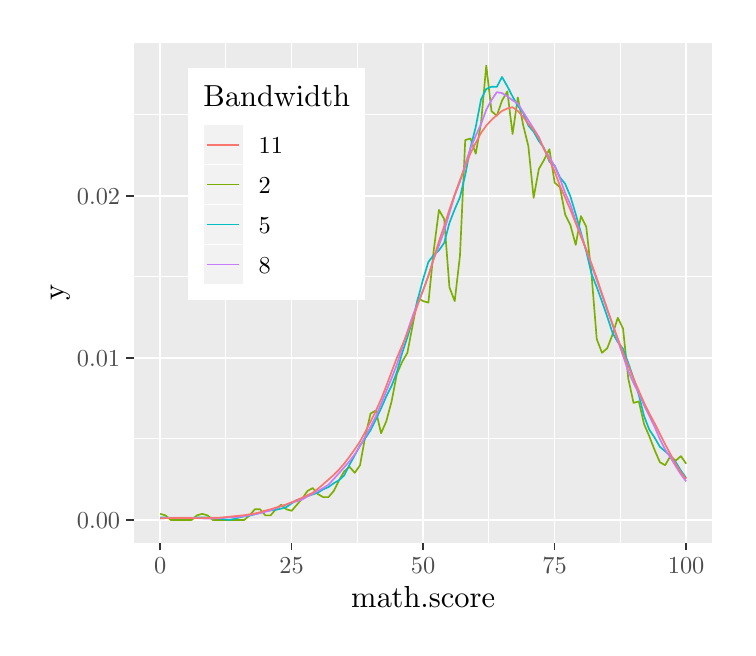
\begin{tikzpicture}[x=1pt,y=1pt]
\definecolor{fillColor}{RGB}{255,255,255}
\path[use as bounding box,fill=fillColor,fill opacity=0.00] (0,0) rectangle (252.94,216.81);
\begin{scope}
\path[clip] (  0.00,  0.00) rectangle (252.94,216.81);
\definecolor{drawColor}{RGB}{255,255,255}
\definecolor{fillColor}{RGB}{255,255,255}

\path[draw=drawColor,line width= 0.6pt,line join=round,line cap=round,fill=fillColor] (  0.00,  0.00) rectangle (252.94,216.81);
\end{scope}
\begin{scope}
\path[clip] ( 38.36, 30.72) rectangle (247.44,211.31);
\definecolor{fillColor}{gray}{0.92}

\path[fill=fillColor] ( 38.36, 30.72) rectangle (247.44,211.31);
\definecolor{drawColor}{RGB}{255,255,255}

\path[draw=drawColor,line width= 0.3pt,line join=round] ( 38.36, 68.22) --
	(247.44, 68.22);

\path[draw=drawColor,line width= 0.3pt,line join=round] ( 38.36,126.78) --
	(247.44,126.78);

\path[draw=drawColor,line width= 0.3pt,line join=round] ( 38.36,185.35) --
	(247.44,185.35);

\path[draw=drawColor,line width= 0.3pt,line join=round] ( 71.62, 30.72) --
	( 71.62,211.31);

\path[draw=drawColor,line width= 0.3pt,line join=round] (119.14, 30.72) --
	(119.14,211.31);

\path[draw=drawColor,line width= 0.3pt,line join=round] (166.66, 30.72) --
	(166.66,211.31);

\path[draw=drawColor,line width= 0.3pt,line join=round] (214.18, 30.72) --
	(214.18,211.31);

\path[draw=drawColor,line width= 0.6pt,line join=round] ( 38.36, 38.93) --
	(247.44, 38.93);

\path[draw=drawColor,line width= 0.6pt,line join=round] ( 38.36, 97.50) --
	(247.44, 97.50);

\path[draw=drawColor,line width= 0.6pt,line join=round] ( 38.36,156.07) --
	(247.44,156.07);

\path[draw=drawColor,line width= 0.6pt,line join=round] ( 47.86, 30.72) --
	( 47.86,211.31);

\path[draw=drawColor,line width= 0.6pt,line join=round] ( 95.38, 30.72) --
	( 95.38,211.31);

\path[draw=drawColor,line width= 0.6pt,line join=round] (142.90, 30.72) --
	(142.90,211.31);

\path[draw=drawColor,line width= 0.6pt,line join=round] (190.42, 30.72) --
	(190.42,211.31);

\path[draw=drawColor,line width= 0.6pt,line join=round] (237.94, 30.72) --
	(237.94,211.31);
\definecolor{drawColor}{RGB}{124,174,0}

\path[draw=drawColor,line width= 0.6pt,line join=round] ( 47.86, 41.13) --
	( 49.77, 40.58) --
	( 51.67, 38.93) --
	( 53.57, 38.93) --
	( 55.47, 38.93) --
	( 57.37, 38.93) --
	( 59.27, 38.93) --
	( 61.17, 40.58) --
	( 63.07, 41.13) --
	( 64.97, 40.58) --
	( 66.87, 38.93) --
	( 68.77, 38.93) --
	( 70.67, 38.93) --
	( 72.57, 38.93) --
	( 74.48, 38.93) --
	( 76.38, 38.93) --
	( 78.28, 38.93) --
	( 80.18, 40.58) --
	( 82.08, 42.78) --
	( 83.98, 42.78) --
	( 85.88, 40.58) --
	( 87.78, 40.58) --
	( 89.68, 42.78) --
	( 91.58, 44.42) --
	( 93.48, 42.78) --
	( 95.38, 42.23) --
	( 97.28, 44.42) --
	( 99.19, 46.62) --
	(101.09, 49.37) --
	(102.99, 50.46) --
	(104.89, 48.27) --
	(106.79, 47.17) --
	(108.69, 47.17) --
	(110.59, 49.37) --
	(112.49, 53.21) --
	(114.39, 56.50) --
	(116.29, 58.15) --
	(118.19, 55.95) --
	(120.09, 58.70) --
	(121.99, 69.13) --
	(123.90, 77.37) --
	(125.80, 78.47) --
	(127.70, 70.23) --
	(129.60, 74.62) --
	(131.50, 81.76) --
	(133.40, 91.64) --
	(135.30, 96.04) --
	(137.20, 99.33) --
	(139.10,109.21) --
	(141.00,119.10) --
	(142.90,118.00) --
	(144.80,117.45) --
	(146.70,136.12) --
	(148.61,150.94) --
	(150.51,147.65) --
	(152.41,122.94) --
	(154.31,118.00) --
	(156.21,134.47) --
	(158.11,176.20) --
	(160.01,176.75) --
	(161.91,171.26) --
	(163.81,182.24) --
	(165.71,203.10) --
	(167.61,186.63) --
	(169.51,184.98) --
	(171.41,190.47) --
	(173.32,193.77) --
	(175.22,178.39) --
	(177.12,191.57) --
	(179.02,181.69) --
	(180.92,174.00) --
	(182.82,155.33) --
	(184.72,165.77) --
	(186.62,169.06) --
	(188.52,172.90) --
	(190.42,160.82) --
	(192.32,159.18) --
	(194.22,149.29) --
	(196.12,145.45) --
	(198.03,138.31) --
	(199.93,148.74) --
	(201.83,144.90) --
	(203.73,127.88) --
	(205.63,104.27) --
	(207.53, 99.33) --
	(209.43,100.98) --
	(211.33,105.92) --
	(213.23,111.96) --
	(215.13,108.11) --
	(217.03, 90.00) --
	(218.93, 81.21) --
	(220.83, 81.76) --
	(222.74, 73.52) --
	(224.64, 69.13) --
	(226.54, 64.19) --
	(228.44, 59.80) --
	(230.34, 58.70) --
	(232.24, 61.99) --
	(234.14, 60.35) --
	(236.04, 61.99) --
	(237.94, 59.25);
\definecolor{drawColor}{RGB}{0,191,196}

\path[draw=drawColor,line width= 0.6pt,line join=round] ( 47.86, 39.81) --
	( 49.77, 39.78) --
	( 51.67, 39.67) --
	( 53.57, 39.50) --
	( 55.47, 39.57) --
	( 57.37, 39.50) --
	( 59.27, 39.67) --
	( 61.17, 39.78) --
	( 63.07, 39.81) --
	( 64.97, 39.78) --
	( 66.87, 39.67) --
	( 68.77, 39.50) --
	( 70.67, 39.25) --
	( 72.57, 38.93) --
	( 74.48, 39.25) --
	( 76.38, 39.81) --
	( 78.28, 40.23) --
	( 80.18, 40.51) --
	( 82.08, 40.97) --
	( 83.98, 41.53) --
	( 85.88, 42.13) --
	( 87.78, 42.38) --
	( 89.68, 42.59) --
	( 91.58, 43.01) --
	( 93.48, 43.57) --
	( 95.38, 44.91) --
	( 97.28, 46.17) --
	( 99.19, 46.59) --
	(101.09, 47.51) --
	(102.99, 48.14) --
	(104.89, 48.81) --
	(106.79, 50.00) --
	(108.69, 50.81) --
	(110.59, 52.18) --
	(112.49, 53.27) --
	(114.39, 55.03) --
	(116.29, 58.89) --
	(118.19, 62.27) --
	(120.09, 65.89) --
	(121.99, 68.45) --
	(123.90, 71.33) --
	(125.80, 75.20) --
	(127.70, 79.24) --
	(129.60, 83.60) --
	(131.50, 87.39) --
	(133.40, 92.35) --
	(135.30, 99.23) --
	(137.20,104.89) --
	(139.10,111.18) --
	(141.00,118.77) --
	(142.90,125.97) --
	(144.80,132.16) --
	(146.70,134.62) --
	(148.61,136.34) --
	(150.51,139.05) --
	(152.41,146.29) --
	(154.31,151.17) --
	(156.21,155.56) --
	(158.11,163.57) --
	(160.01,173.48) --
	(161.91,180.93) --
	(163.81,190.84) --
	(165.71,194.67) --
	(167.61,195.48) --
	(169.51,195.41) --
	(171.41,198.99) --
	(173.32,195.62) --
	(175.22,191.93) --
	(177.12,188.56) --
	(179.02,186.06) --
	(180.92,181.42) --
	(182.82,179.21) --
	(184.72,175.84) --
	(186.62,173.24) --
	(188.52,168.39) --
	(190.42,166.98) --
	(192.32,162.73) --
	(194.22,160.38) --
	(196.12,155.84) --
	(198.03,149.45) --
	(199.93,142.70) --
	(201.83,135.99) --
	(203.73,127.91) --
	(205.63,123.06) --
	(207.53,117.82) --
	(209.43,112.38) --
	(211.33,106.54) --
	(213.23,103.20) --
	(215.13,100.78) --
	(217.03, 95.61) --
	(218.93, 90.10) --
	(220.83, 84.09) --
	(222.74, 76.43) --
	(224.64, 71.51) --
	(226.54, 68.70) --
	(228.44, 65.36) --
	(230.34, 63.74) --
	(232.24, 62.09) --
	(234.14, 59.88) --
	(236.04, 56.75) --
	(237.94, 54.15);
\definecolor{drawColor}{RGB}{199,124,255}

\path[draw=drawColor,line width= 0.6pt,line join=round] ( 47.86, 39.48) --
	( 49.77, 39.60) --
	( 51.67, 39.69) --
	( 53.57, 39.74) --
	( 55.47, 39.76) --
	( 57.37, 39.74) --
	( 59.27, 39.69) --
	( 61.17, 39.60) --
	( 63.07, 39.48) --
	( 64.97, 39.47) --
	( 66.87, 39.45) --
	( 68.77, 39.53) --
	( 70.67, 39.71) --
	( 72.57, 39.84) --
	( 74.48, 39.92) --
	( 76.38, 40.07) --
	( 78.28, 40.29) --
	( 80.18, 40.69) --
	( 82.08, 41.01) --
	( 83.98, 41.37) --
	( 85.88, 41.88) --
	( 87.78, 42.39) --
	( 89.68, 43.13) --
	( 91.58, 43.92) --
	( 93.48, 44.47) --
	( 95.38, 45.16) --
	( 97.28, 45.69) --
	( 99.19, 46.32) --
	(101.09, 47.41) --
	(102.99, 48.36) --
	(104.89, 49.40) --
	(106.79, 50.47) --
	(108.69, 51.67) --
	(110.59, 53.72) --
	(112.49, 55.81) --
	(114.39, 57.97) --
	(116.29, 60.14) --
	(118.19, 62.64) --
	(120.09, 65.61) --
	(121.99, 69.08) --
	(123.90, 72.59) --
	(125.80, 76.39) --
	(127.70, 80.82) --
	(129.60, 85.51) --
	(131.50, 90.14) --
	(133.40, 95.08) --
	(135.30,101.12) --
	(137.20,107.00) --
	(139.10,112.60) --
	(141.00,117.41) --
	(142.90,122.00) --
	(144.80,127.09) --
	(146.70,133.10) --
	(148.61,138.08) --
	(150.51,143.34) --
	(152.41,149.89) --
	(154.31,156.15) --
	(156.21,161.10) --
	(158.11,167.52) --
	(160.01,173.24) --
	(161.91,177.78) --
	(163.81,181.92) --
	(165.71,187.15) --
	(167.61,190.67) --
	(169.51,193.50) --
	(171.41,193.17) --
	(173.32,191.98) --
	(175.22,190.56) --
	(177.12,189.40) --
	(179.02,186.36) --
	(180.92,183.35) --
	(182.82,180.30) --
	(184.72,177.28) --
	(186.62,172.84) --
	(188.52,170.02) --
	(190.42,166.79) --
	(192.32,162.25) --
	(194.22,157.10) --
	(196.12,152.86) --
	(198.03,147.03) --
	(199.93,141.97) --
	(201.83,136.55) --
	(203.73,130.99) --
	(205.63,125.62) --
	(207.53,120.25) --
	(209.43,114.73) --
	(211.33,109.48) --
	(213.23,103.77) --
	(215.13, 98.26) --
	(217.03, 92.67) --
	(218.93, 88.37) --
	(220.83, 84.67) --
	(222.74, 80.35) --
	(224.64, 76.47) --
	(226.54, 72.61) --
	(228.44, 68.16) --
	(230.34, 64.41) --
	(232.24, 61.50) --
	(234.14, 58.36) --
	(236.04, 55.39) --
	(237.94, 52.87);
\definecolor{drawColor}{RGB}{248,118,109}

\path[draw=drawColor,line width= 0.6pt,line join=round] ( 47.86, 39.52) --
	( 49.77, 39.57) --
	( 51.67, 39.60) --
	( 53.57, 39.62) --
	( 55.47, 39.63) --
	( 57.37, 39.62) --
	( 59.27, 39.60) --
	( 61.17, 39.57) --
	( 63.07, 39.59) --
	( 64.97, 39.66) --
	( 66.87, 39.71) --
	( 68.77, 39.73) --
	( 70.67, 39.87) --
	( 72.57, 40.05) --
	( 74.48, 40.27) --
	( 76.38, 40.44) --
	( 78.28, 40.65) --
	( 80.18, 40.95) --
	( 82.08, 41.26) --
	( 83.98, 41.72) --
	( 85.88, 42.30) --
	( 87.78, 42.78) --
	( 89.68, 43.39) --
	( 91.58, 43.95) --
	( 93.48, 44.53) --
	( 95.38, 45.33) --
	( 97.28, 46.09) --
	( 99.19, 46.96) --
	(101.09, 47.83) --
	(102.99, 48.76) --
	(104.89, 50.20) --
	(106.79, 51.82) --
	(108.69, 53.52) --
	(110.59, 55.18) --
	(112.49, 57.12) --
	(114.39, 59.30) --
	(116.29, 61.79) --
	(118.19, 64.46) --
	(120.09, 67.30) --
	(121.99, 70.75) --
	(123.90, 74.49) --
	(125.80, 78.30) --
	(127.70, 82.54) --
	(129.60, 87.37) --
	(131.50, 92.44) --
	(133.40, 97.50) --
	(135.30,101.89) --
	(137.20,106.41) --
	(139.10,111.24) --
	(141.00,116.87) --
	(142.90,121.91) --
	(144.80,127.13) --
	(146.70,133.39) --
	(148.61,139.58) --
	(150.51,145.17) --
	(152.41,151.09) --
	(154.31,156.61) --
	(156.21,161.77) --
	(158.11,166.61) --
	(160.01,171.45) --
	(161.91,175.18) --
	(163.81,178.75) --
	(165.71,181.42) --
	(167.61,183.47) --
	(169.51,185.19) --
	(171.41,186.72) --
	(173.32,187.61) --
	(175.22,188.07) --
	(177.12,186.67) --
	(179.02,184.61) --
	(180.92,182.06) --
	(182.82,179.94) --
	(184.72,176.84) --
	(186.62,172.87) --
	(188.52,168.98) --
	(190.42,164.86) --
	(192.32,159.70) --
	(194.22,155.37) --
	(196.12,151.00) --
	(198.03,146.19) --
	(199.93,141.21) --
	(201.83,136.71) --
	(203.73,131.55) --
	(205.63,126.30) --
	(207.53,120.69) --
	(209.43,115.14) --
	(211.33,109.73) --
	(213.23,104.50) --
	(215.13, 99.36) --
	(217.03, 94.64) --
	(218.93, 90.00) --
	(220.83, 85.62) --
	(222.74, 81.25) --
	(224.64, 77.39) --
	(226.54, 73.87) --
	(228.44, 70.07) --
	(230.34, 66.26) --
	(232.24, 62.74) --
	(234.14, 59.15) --
	(236.04, 56.14) --
	(237.94, 53.75);
\end{scope}
\begin{scope}
\path[clip] (  0.00,  0.00) rectangle (252.94,216.81);
\definecolor{drawColor}{gray}{0.30}

\node[text=drawColor,anchor=base east,inner sep=0pt, outer sep=0pt, scale=  0.88] at ( 33.41, 35.90) {0.00};

\node[text=drawColor,anchor=base east,inner sep=0pt, outer sep=0pt, scale=  0.88] at ( 33.41, 94.47) {0.01};

\node[text=drawColor,anchor=base east,inner sep=0pt, outer sep=0pt, scale=  0.88] at ( 33.41,153.04) {0.02};
\end{scope}
\begin{scope}
\path[clip] (  0.00,  0.00) rectangle (252.94,216.81);
\definecolor{drawColor}{gray}{0.20}

\path[draw=drawColor,line width= 0.6pt,line join=round] ( 35.61, 38.93) --
	( 38.36, 38.93);

\path[draw=drawColor,line width= 0.6pt,line join=round] ( 35.61, 97.50) --
	( 38.36, 97.50);

\path[draw=drawColor,line width= 0.6pt,line join=round] ( 35.61,156.07) --
	( 38.36,156.07);
\end{scope}
\begin{scope}
\path[clip] (  0.00,  0.00) rectangle (252.94,216.81);
\definecolor{drawColor}{gray}{0.20}

\path[draw=drawColor,line width= 0.6pt,line join=round] ( 47.86, 27.97) --
	( 47.86, 30.72);

\path[draw=drawColor,line width= 0.6pt,line join=round] ( 95.38, 27.97) --
	( 95.38, 30.72);

\path[draw=drawColor,line width= 0.6pt,line join=round] (142.90, 27.97) --
	(142.90, 30.72);

\path[draw=drawColor,line width= 0.6pt,line join=round] (190.42, 27.97) --
	(190.42, 30.72);

\path[draw=drawColor,line width= 0.6pt,line join=round] (237.94, 27.97) --
	(237.94, 30.72);
\end{scope}
\begin{scope}
\path[clip] (  0.00,  0.00) rectangle (252.94,216.81);
\definecolor{drawColor}{gray}{0.30}

\node[text=drawColor,anchor=base,inner sep=0pt, outer sep=0pt, scale=  0.88] at ( 47.86, 19.71) {0};

\node[text=drawColor,anchor=base,inner sep=0pt, outer sep=0pt, scale=  0.88] at ( 95.38, 19.71) {25};

\node[text=drawColor,anchor=base,inner sep=0pt, outer sep=0pt, scale=  0.88] at (142.90, 19.71) {50};

\node[text=drawColor,anchor=base,inner sep=0pt, outer sep=0pt, scale=  0.88] at (190.42, 19.71) {75};

\node[text=drawColor,anchor=base,inner sep=0pt, outer sep=0pt, scale=  0.88] at (237.94, 19.71) {100};
\end{scope}
\begin{scope}
\path[clip] (  0.00,  0.00) rectangle (252.94,216.81);
\definecolor{drawColor}{RGB}{0,0,0}

\node[text=drawColor,anchor=base,inner sep=0pt, outer sep=0pt, scale=  1.10] at (142.90,  7.44) {math.score};
\end{scope}
\begin{scope}
\path[clip] (  0.00,  0.00) rectangle (252.94,216.81);
\definecolor{drawColor}{RGB}{0,0,0}

\node[text=drawColor,rotate= 90.00,anchor=base,inner sep=0pt, outer sep=0pt, scale=  1.10] at ( 13.08,121.02) {y};
\end{scope}
\begin{scope}
\path[clip] (  0.00,  0.00) rectangle (252.94,216.81);
\definecolor{fillColor}{RGB}{255,255,255}

\path[fill=fillColor] ( 57.99,118.44) rectangle (121.99,202.28);
\end{scope}
\begin{scope}
\path[clip] (  0.00,  0.00) rectangle (252.94,216.81);
\definecolor{drawColor}{RGB}{0,0,0}

\node[text=drawColor,anchor=base west,inner sep=0pt, outer sep=0pt, scale=  1.10] at ( 63.49,188.23) {Bandwidth};
\end{scope}
\begin{scope}
\path[clip] (  0.00,  0.00) rectangle (252.94,216.81);
\definecolor{drawColor}{RGB}{255,255,255}
\definecolor{fillColor}{gray}{0.95}

\path[draw=drawColor,line width= 0.6pt,line join=round,line cap=round,fill=fillColor] ( 63.49,167.31) rectangle ( 77.95,181.76);
\end{scope}
\begin{scope}
\path[clip] (  0.00,  0.00) rectangle (252.94,216.81);
\definecolor{drawColor}{RGB}{248,118,109}

\path[draw=drawColor,line width= 0.6pt,line join=round] ( 64.94,174.53) -- ( 76.50,174.53);
\end{scope}
\begin{scope}
\path[clip] (  0.00,  0.00) rectangle (252.94,216.81);
\definecolor{drawColor}{RGB}{248,118,109}

\path[draw=drawColor,line width= 0.6pt,line join=round] ( 64.94,174.53) -- ( 76.50,174.53);
\end{scope}
\begin{scope}
\path[clip] (  0.00,  0.00) rectangle (252.94,216.81);
\definecolor{drawColor}{RGB}{248,118,109}

\path[draw=drawColor,line width= 0.6pt,line join=round] ( 64.94,174.53) -- ( 76.50,174.53);
\end{scope}
\begin{scope}
\path[clip] (  0.00,  0.00) rectangle (252.94,216.81);
\definecolor{drawColor}{RGB}{248,118,109}

\path[draw=drawColor,line width= 0.6pt,line join=round] ( 64.94,174.53) -- ( 76.50,174.53);
\end{scope}
\begin{scope}
\path[clip] (  0.00,  0.00) rectangle (252.94,216.81);
\definecolor{drawColor}{RGB}{255,255,255}
\definecolor{fillColor}{gray}{0.95}

\path[draw=drawColor,line width= 0.6pt,line join=round,line cap=round,fill=fillColor] ( 63.49,152.85) rectangle ( 77.95,167.31);
\end{scope}
\begin{scope}
\path[clip] (  0.00,  0.00) rectangle (252.94,216.81);
\definecolor{drawColor}{RGB}{124,174,0}

\path[draw=drawColor,line width= 0.6pt,line join=round] ( 64.94,160.08) -- ( 76.50,160.08);
\end{scope}
\begin{scope}
\path[clip] (  0.00,  0.00) rectangle (252.94,216.81);
\definecolor{drawColor}{RGB}{124,174,0}

\path[draw=drawColor,line width= 0.6pt,line join=round] ( 64.94,160.08) -- ( 76.50,160.08);
\end{scope}
\begin{scope}
\path[clip] (  0.00,  0.00) rectangle (252.94,216.81);
\definecolor{drawColor}{RGB}{124,174,0}

\path[draw=drawColor,line width= 0.6pt,line join=round] ( 64.94,160.08) -- ( 76.50,160.08);
\end{scope}
\begin{scope}
\path[clip] (  0.00,  0.00) rectangle (252.94,216.81);
\definecolor{drawColor}{RGB}{124,174,0}

\path[draw=drawColor,line width= 0.6pt,line join=round] ( 64.94,160.08) -- ( 76.50,160.08);
\end{scope}
\begin{scope}
\path[clip] (  0.00,  0.00) rectangle (252.94,216.81);
\definecolor{drawColor}{RGB}{255,255,255}
\definecolor{fillColor}{gray}{0.95}

\path[draw=drawColor,line width= 0.6pt,line join=round,line cap=round,fill=fillColor] ( 63.49,138.40) rectangle ( 77.95,152.85);
\end{scope}
\begin{scope}
\path[clip] (  0.00,  0.00) rectangle (252.94,216.81);
\definecolor{drawColor}{RGB}{0,191,196}

\path[draw=drawColor,line width= 0.6pt,line join=round] ( 64.94,145.63) -- ( 76.50,145.63);
\end{scope}
\begin{scope}
\path[clip] (  0.00,  0.00) rectangle (252.94,216.81);
\definecolor{drawColor}{RGB}{0,191,196}

\path[draw=drawColor,line width= 0.6pt,line join=round] ( 64.94,145.63) -- ( 76.50,145.63);
\end{scope}
\begin{scope}
\path[clip] (  0.00,  0.00) rectangle (252.94,216.81);
\definecolor{drawColor}{RGB}{0,191,196}

\path[draw=drawColor,line width= 0.6pt,line join=round] ( 64.94,145.63) -- ( 76.50,145.63);
\end{scope}
\begin{scope}
\path[clip] (  0.00,  0.00) rectangle (252.94,216.81);
\definecolor{drawColor}{RGB}{0,191,196}

\path[draw=drawColor,line width= 0.6pt,line join=round] ( 64.94,145.63) -- ( 76.50,145.63);
\end{scope}
\begin{scope}
\path[clip] (  0.00,  0.00) rectangle (252.94,216.81);
\definecolor{drawColor}{RGB}{255,255,255}
\definecolor{fillColor}{gray}{0.95}

\path[draw=drawColor,line width= 0.6pt,line join=round,line cap=round,fill=fillColor] ( 63.49,123.94) rectangle ( 77.95,138.40);
\end{scope}
\begin{scope}
\path[clip] (  0.00,  0.00) rectangle (252.94,216.81);
\definecolor{drawColor}{RGB}{199,124,255}

\path[draw=drawColor,line width= 0.6pt,line join=round] ( 64.94,131.17) -- ( 76.50,131.17);
\end{scope}
\begin{scope}
\path[clip] (  0.00,  0.00) rectangle (252.94,216.81);
\definecolor{drawColor}{RGB}{199,124,255}

\path[draw=drawColor,line width= 0.6pt,line join=round] ( 64.94,131.17) -- ( 76.50,131.17);
\end{scope}
\begin{scope}
\path[clip] (  0.00,  0.00) rectangle (252.94,216.81);
\definecolor{drawColor}{RGB}{199,124,255}

\path[draw=drawColor,line width= 0.6pt,line join=round] ( 64.94,131.17) -- ( 76.50,131.17);
\end{scope}
\begin{scope}
\path[clip] (  0.00,  0.00) rectangle (252.94,216.81);
\definecolor{drawColor}{RGB}{199,124,255}

\path[draw=drawColor,line width= 0.6pt,line join=round] ( 64.94,131.17) -- ( 76.50,131.17);
\end{scope}
\begin{scope}
\path[clip] (  0.00,  0.00) rectangle (252.94,216.81);
\definecolor{drawColor}{RGB}{0,0,0}

\node[text=drawColor,anchor=base west,inner sep=0pt, outer sep=0pt, scale=  0.88] at ( 83.45,171.50) {11};
\end{scope}
\begin{scope}
\path[clip] (  0.00,  0.00) rectangle (252.94,216.81);
\definecolor{drawColor}{RGB}{0,0,0}

\node[text=drawColor,anchor=base west,inner sep=0pt, outer sep=0pt, scale=  0.88] at ( 83.45,157.05) {2};
\end{scope}
\begin{scope}
\path[clip] (  0.00,  0.00) rectangle (252.94,216.81);
\definecolor{drawColor}{RGB}{0,0,0}

\node[text=drawColor,anchor=base west,inner sep=0pt, outer sep=0pt, scale=  0.88] at ( 83.45,142.60) {5};
\end{scope}
\begin{scope}
\path[clip] (  0.00,  0.00) rectangle (252.94,216.81);
\definecolor{drawColor}{RGB}{0,0,0}

\node[text=drawColor,anchor=base west,inner sep=0pt, outer sep=0pt, scale=  0.88] at ( 83.45,128.14) {8};
\end{scope}
\end{tikzpicture}
}
			\caption{ with the Epanechnikov kernel and 4 different bandwidths}
			\label{fig 6.1}
		\end{subfigure}
		\begin{subfigure}[b]{0.48\linewidth}        %% or \columnwidth
			\centering
			\scalebox{0.75}{% Created by tikzDevice version 0.12 on 2019-04-13 11:27:44
% !TEX encoding = UTF-8 Unicode
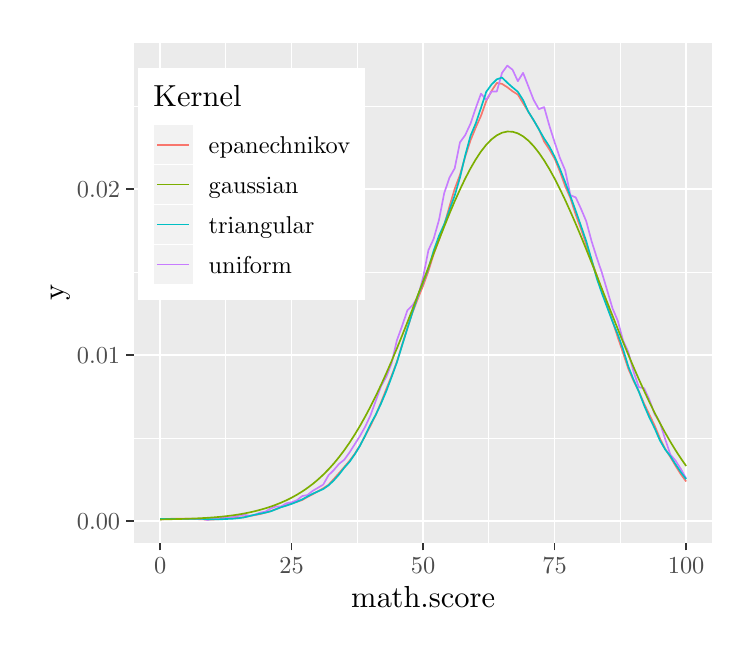
\begin{tikzpicture}[x=1pt,y=1pt]
\definecolor{fillColor}{RGB}{255,255,255}
\path[use as bounding box,fill=fillColor,fill opacity=0.00] (0,0) rectangle (252.94,216.81);
\begin{scope}
\path[clip] (  0.00,  0.00) rectangle (252.94,216.81);
\definecolor{drawColor}{RGB}{255,255,255}
\definecolor{fillColor}{RGB}{255,255,255}

\path[draw=drawColor,line width= 0.6pt,line join=round,line cap=round,fill=fillColor] (  0.00,  0.00) rectangle (252.94,216.81);
\end{scope}
\begin{scope}
\path[clip] ( 38.36, 30.72) rectangle (247.44,211.31);
\definecolor{fillColor}{gray}{0.92}

\path[fill=fillColor] ( 38.36, 30.72) rectangle (247.44,211.31);
\definecolor{drawColor}{RGB}{255,255,255}

\path[draw=drawColor,line width= 0.3pt,line join=round] ( 38.36, 68.54) --
	(247.44, 68.54);

\path[draw=drawColor,line width= 0.3pt,line join=round] ( 38.36,128.51) --
	(247.44,128.51);

\path[draw=drawColor,line width= 0.3pt,line join=round] ( 38.36,188.48) --
	(247.44,188.48);

\path[draw=drawColor,line width= 0.3pt,line join=round] ( 71.62, 30.72) --
	( 71.62,211.31);

\path[draw=drawColor,line width= 0.3pt,line join=round] (119.14, 30.72) --
	(119.14,211.31);

\path[draw=drawColor,line width= 0.3pt,line join=round] (166.66, 30.72) --
	(166.66,211.31);

\path[draw=drawColor,line width= 0.3pt,line join=round] (214.18, 30.72) --
	(214.18,211.31);

\path[draw=drawColor,line width= 0.6pt,line join=round] ( 38.36, 38.56) --
	(247.44, 38.56);

\path[draw=drawColor,line width= 0.6pt,line join=round] ( 38.36, 98.53) --
	(247.44, 98.53);

\path[draw=drawColor,line width= 0.6pt,line join=round] ( 38.36,158.50) --
	(247.44,158.50);

\path[draw=drawColor,line width= 0.6pt,line join=round] ( 47.86, 30.72) --
	( 47.86,211.31);

\path[draw=drawColor,line width= 0.6pt,line join=round] ( 95.38, 30.72) --
	( 95.38,211.31);

\path[draw=drawColor,line width= 0.6pt,line join=round] (142.90, 30.72) --
	(142.90,211.31);

\path[draw=drawColor,line width= 0.6pt,line join=round] (190.42, 30.72) --
	(190.42,211.31);

\path[draw=drawColor,line width= 0.6pt,line join=round] (237.94, 30.72) --
	(237.94,211.31);
\definecolor{drawColor}{RGB}{248,118,109}

\path[draw=drawColor,line width= 0.6pt,line join=round] ( 47.86, 39.12) --
	( 49.77, 39.24) --
	( 51.67, 39.33) --
	( 53.57, 39.38) --
	( 55.47, 39.40) --
	( 57.37, 39.38) --
	( 59.27, 39.33) --
	( 61.17, 39.24) --
	( 63.07, 39.12) --
	( 64.97, 39.11) --
	( 66.87, 39.09) --
	( 68.77, 39.17) --
	( 70.67, 39.36) --
	( 72.57, 39.49) --
	( 74.48, 39.57) --
	( 76.38, 39.73) --
	( 78.28, 39.95) --
	( 80.18, 40.36) --
	( 82.08, 40.68) --
	( 83.98, 41.05) --
	( 85.88, 41.58) --
	( 87.78, 42.10) --
	( 89.68, 42.85) --
	( 91.58, 43.66) --
	( 93.48, 44.22) --
	( 95.38, 44.94) --
	( 97.28, 45.48) --
	( 99.19, 46.12) --
	(101.09, 47.24) --
	(102.99, 48.21) --
	(104.89, 49.28) --
	(106.79, 50.37) --
	(108.69, 51.60) --
	(110.59, 53.70) --
	(112.49, 55.84) --
	(114.39, 58.05) --
	(116.29, 60.27) --
	(118.19, 62.83) --
	(120.09, 65.88) --
	(121.99, 69.43) --
	(123.90, 73.02) --
	(125.80, 76.91) --
	(127.70, 81.45) --
	(129.60, 86.25) --
	(131.50, 90.99) --
	(133.40, 96.05) --
	(135.30,102.24) --
	(137.20,108.26) --
	(139.10,113.99) --
	(141.00,118.91) --
	(142.90,123.62) --
	(144.80,128.83) --
	(146.70,134.98) --
	(148.61,140.08) --
	(150.51,145.47) --
	(152.41,152.17) --
	(154.31,158.58) --
	(156.21,163.65) --
	(158.11,170.22) --
	(160.01,176.08) --
	(161.91,180.74) --
	(163.81,184.97) --
	(165.71,190.33) --
	(167.61,193.93) --
	(169.51,196.83) --
	(171.41,196.49) --
	(173.32,195.28) --
	(175.22,193.82) --
	(177.12,192.63) --
	(179.02,189.52) --
	(180.92,186.44) --
	(182.82,183.31) --
	(184.72,180.22) --
	(186.62,175.68) --
	(188.52,172.79) --
	(190.42,169.48) --
	(192.32,164.83) --
	(194.22,159.56) --
	(196.12,155.22) --
	(198.03,149.25) --
	(199.93,144.06) --
	(201.83,138.52) --
	(203.73,132.83) --
	(205.63,127.32) --
	(207.53,121.83) --
	(209.43,116.17) --
	(211.33,110.79) --
	(213.23,104.95) --
	(215.13, 99.30) --
	(217.03, 93.59) --
	(218.93, 89.18) --
	(220.83, 85.39) --
	(222.74, 80.97) --
	(224.64, 76.99) --
	(226.54, 73.05) --
	(228.44, 68.49) --
	(230.34, 64.65) --
	(232.24, 61.66) --
	(234.14, 58.45) --
	(236.04, 55.41) --
	(237.94, 52.83);
\definecolor{drawColor}{RGB}{199,124,255}

\path[draw=drawColor,line width= 0.6pt,line join=round] ( 47.86, 39.31) --
	( 49.77, 39.31) --
	( 51.67, 39.31) --
	( 53.57, 39.31) --
	( 55.47, 39.31) --
	( 57.37, 39.31) --
	( 59.27, 39.31) --
	( 61.17, 39.31) --
	( 63.07, 39.31) --
	( 64.97, 38.93) --
	( 66.87, 39.31) --
	( 68.77, 39.68) --
	( 70.67, 39.68) --
	( 72.57, 39.68) --
	( 74.48, 40.06) --
	( 76.38, 40.43) --
	( 78.28, 40.81) --
	( 80.18, 40.43) --
	( 82.08, 40.81) --
	( 83.98, 41.56) --
	( 85.88, 41.93) --
	( 87.78, 43.06) --
	( 89.68, 43.81) --
	( 91.58, 43.81) --
	( 93.48, 44.93) --
	( 95.38, 45.30) --
	( 97.28, 46.05) --
	( 99.19, 47.55) --
	(101.09, 47.93) --
	(102.99, 49.43) --
	(104.89, 50.55) --
	(106.79, 51.68) --
	(108.69, 55.05) --
	(110.59, 56.92) --
	(112.49, 59.17) --
	(114.39, 60.67) --
	(116.29, 63.30) --
	(118.19, 66.29) --
	(120.09, 69.29) --
	(121.99, 72.67) --
	(123.90, 76.79) --
	(125.80, 82.04) --
	(127.70, 87.28) --
	(129.60, 90.66) --
	(131.50, 95.53) --
	(133.40,103.78) --
	(135.30,109.02) --
	(137.20,114.65) --
	(139.10,116.52) --
	(141.00,119.52) --
	(142.90,126.64) --
	(144.80,136.38) --
	(146.70,140.51) --
	(148.61,147.25) --
	(150.51,157.00) --
	(152.41,162.62) --
	(154.31,166.00) --
	(156.21,175.37) --
	(158.11,177.99) --
	(160.01,182.11) --
	(161.91,187.73) --
	(163.81,192.98) --
	(165.71,190.73) --
	(167.61,193.73) --
	(169.51,193.73) --
	(171.41,200.48) --
	(173.32,203.10) --
	(175.22,201.60) --
	(177.12,197.48) --
	(179.02,200.48) --
	(180.92,195.61) --
	(182.82,190.73) --
	(184.72,187.36) --
	(186.62,188.11) --
	(188.52,181.36) --
	(190.42,175.37) --
	(192.32,169.74) --
	(194.22,165.25) --
	(196.12,156.25) --
	(198.03,155.50) --
	(199.93,151.38) --
	(201.83,146.88) --
	(203.73,139.76) --
	(205.63,133.76) --
	(207.53,128.14) --
	(209.43,121.77) --
	(211.33,115.40) --
	(213.23,110.90) --
	(215.13,103.78) --
	(217.03, 99.65) --
	(218.93, 92.53) --
	(220.83, 86.91) --
	(222.74, 86.53) --
	(224.64, 82.41) --
	(226.54, 77.16) --
	(228.44, 74.17) --
	(230.34, 68.17) --
	(232.24, 62.55) --
	(234.14, 60.30) --
	(236.04, 57.30) --
	(237.94, 53.93);
\definecolor{drawColor}{RGB}{0,191,196}

\path[draw=drawColor,line width= 0.6pt,line join=round] ( 47.86, 39.31) --
	( 49.77, 39.31) --
	( 51.67, 39.31) --
	( 53.57, 39.31) --
	( 55.47, 39.31) --
	( 57.37, 39.31) --
	( 59.27, 39.31) --
	( 61.17, 39.31) --
	( 63.07, 39.31) --
	( 64.97, 39.21) --
	( 66.87, 39.12) --
	( 68.77, 39.12) --
	( 70.67, 39.21) --
	( 72.57, 39.31) --
	( 74.48, 39.40) --
	( 76.38, 39.59) --
	( 78.28, 39.87) --
	( 80.18, 40.34) --
	( 82.08, 40.81) --
	( 83.98, 41.18) --
	( 85.88, 41.56) --
	( 87.78, 42.03) --
	( 89.68, 42.77) --
	( 91.58, 43.52) --
	( 93.48, 44.09) --
	( 95.38, 44.74) --
	( 97.28, 45.49) --
	( 99.19, 46.34) --
	(101.09, 47.37) --
	(102.99, 48.40) --
	(104.89, 49.24) --
	(106.79, 50.08) --
	(108.69, 51.40) --
	(110.59, 53.18) --
	(112.49, 55.33) --
	(114.39, 57.77) --
	(116.29, 59.92) --
	(118.19, 62.64) --
	(120.09, 65.73) --
	(121.99, 69.48) --
	(123.90, 73.51) --
	(125.80, 76.98) --
	(127.70, 81.01) --
	(129.60, 85.50) --
	(131.50, 90.56) --
	(133.40, 95.81) --
	(135.30,102.00) --
	(137.20,108.09) --
	(139.10,114.18) --
	(141.00,119.99) --
	(142.90,124.86) --
	(144.80,129.83) --
	(146.70,136.20) --
	(148.61,141.54) --
	(150.51,145.76) --
	(152.41,150.91) --
	(154.31,156.16) --
	(156.21,162.62) --
	(158.11,170.68) --
	(160.01,177.71) --
	(161.91,182.21) --
	(163.81,187.83) --
	(165.71,193.64) --
	(167.61,196.26) --
	(169.51,198.14) --
	(171.41,198.79) --
	(173.32,196.92) --
	(175.22,195.23) --
	(177.12,193.64) --
	(179.02,190.64) --
	(180.92,186.42) --
	(182.82,183.42) --
	(184.72,180.05) --
	(186.62,176.77) --
	(188.52,173.87) --
	(190.42,170.21) --
	(192.32,165.81) --
	(194.22,160.94) --
	(196.12,155.88) --
	(198.03,150.63) --
	(199.93,145.19) --
	(201.83,139.66) --
	(203.73,133.11) --
	(205.63,126.26) --
	(207.53,120.74) --
	(209.43,115.68) --
	(211.33,110.62) --
	(213.23,106.02) --
	(215.13,100.68) --
	(217.03, 94.41) --
	(218.93, 89.63) --
	(220.83, 85.32) --
	(222.74, 80.35) --
	(224.64, 75.95) --
	(226.54, 72.10) --
	(228.44, 67.70) --
	(230.34, 64.42) --
	(232.24, 61.98) --
	(234.14, 58.99) --
	(236.04, 56.17) --
	(237.94, 53.64);
\definecolor{drawColor}{RGB}{124,174,0}

\path[draw=drawColor,line width= 0.6pt,line join=round] ( 47.86, 39.10) --
	( 49.77, 39.15) --
	( 51.67, 39.19) --
	( 53.57, 39.24) --
	( 55.47, 39.29) --
	( 57.37, 39.35) --
	( 59.27, 39.42) --
	( 61.17, 39.50) --
	( 63.07, 39.59) --
	( 64.97, 39.70) --
	( 66.87, 39.83) --
	( 68.77, 39.99) --
	( 70.67, 40.17) --
	( 72.57, 40.39) --
	( 74.48, 40.64) --
	( 76.38, 40.93) --
	( 78.28, 41.27) --
	( 80.18, 41.65) --
	( 82.08, 42.08) --
	( 83.98, 42.57) --
	( 85.88, 43.12) --
	( 87.78, 43.73) --
	( 89.68, 44.42) --
	( 91.58, 45.18) --
	( 93.48, 46.03) --
	( 95.38, 46.98) --
	( 97.28, 48.03) --
	( 99.19, 49.20) --
	(101.09, 50.49) --
	(102.99, 51.92) --
	(104.89, 53.51) --
	(106.79, 55.26) --
	(108.69, 57.18) --
	(110.59, 59.29) --
	(112.49, 61.60) --
	(114.39, 64.11) --
	(116.29, 66.84) --
	(118.19, 69.78) --
	(120.09, 72.94) --
	(121.99, 76.33) --
	(123.90, 79.93) --
	(125.80, 83.74) --
	(127.70, 87.75) --
	(129.60, 91.95) --
	(131.50, 96.33) --
	(133.40,100.87) --
	(135.30,105.54) --
	(137.20,110.34) --
	(139.10,115.23) --
	(141.00,120.20) --
	(142.90,125.20) --
	(144.80,130.20) --
	(146.70,135.19) --
	(148.61,140.11) --
	(150.51,144.92) --
	(152.41,149.60) --
	(154.31,154.08) --
	(156.21,158.33) --
	(158.11,162.30) --
	(160.01,165.94) --
	(161.91,169.21) --
	(163.81,172.08) --
	(165.71,174.50) --
	(167.61,176.45) --
	(169.51,177.90) --
	(171.41,178.85) --
	(173.32,179.28) --
	(175.22,179.20) --
	(177.12,178.62) --
	(179.02,177.54) --
	(180.92,176.00) --
	(182.82,174.02) --
	(184.72,171.62) --
	(186.62,168.84) --
	(188.52,165.71) --
	(190.42,162.26) --
	(192.32,158.52) --
	(194.22,154.54) --
	(196.12,150.34) --
	(198.03,145.95) --
	(199.93,141.41) --
	(201.83,136.75) --
	(203.73,132.00) --
	(205.63,127.20) --
	(207.53,122.36) --
	(209.43,117.52) --
	(211.33,112.71) --
	(213.23,107.94) --
	(215.13,103.25) --
	(217.03, 98.65) --
	(218.93, 94.17) --
	(220.83, 89.82) --
	(222.74, 85.61) --
	(224.64, 81.56) --
	(226.54, 77.69) --
	(228.44, 73.99) --
	(230.34, 70.48) --
	(232.24, 67.17) --
	(234.14, 64.05) --
	(236.04, 61.14) --
	(237.94, 58.43);
\end{scope}
\begin{scope}
\path[clip] (  0.00,  0.00) rectangle (252.94,216.81);
\definecolor{drawColor}{gray}{0.30}

\node[text=drawColor,anchor=base east,inner sep=0pt, outer sep=0pt, scale=  0.88] at ( 33.41, 35.53) {0.00};

\node[text=drawColor,anchor=base east,inner sep=0pt, outer sep=0pt, scale=  0.88] at ( 33.41, 95.50) {0.01};

\node[text=drawColor,anchor=base east,inner sep=0pt, outer sep=0pt, scale=  0.88] at ( 33.41,155.47) {0.02};
\end{scope}
\begin{scope}
\path[clip] (  0.00,  0.00) rectangle (252.94,216.81);
\definecolor{drawColor}{gray}{0.20}

\path[draw=drawColor,line width= 0.6pt,line join=round] ( 35.61, 38.56) --
	( 38.36, 38.56);

\path[draw=drawColor,line width= 0.6pt,line join=round] ( 35.61, 98.53) --
	( 38.36, 98.53);

\path[draw=drawColor,line width= 0.6pt,line join=round] ( 35.61,158.50) --
	( 38.36,158.50);
\end{scope}
\begin{scope}
\path[clip] (  0.00,  0.00) rectangle (252.94,216.81);
\definecolor{drawColor}{gray}{0.20}

\path[draw=drawColor,line width= 0.6pt,line join=round] ( 47.86, 27.97) --
	( 47.86, 30.72);

\path[draw=drawColor,line width= 0.6pt,line join=round] ( 95.38, 27.97) --
	( 95.38, 30.72);

\path[draw=drawColor,line width= 0.6pt,line join=round] (142.90, 27.97) --
	(142.90, 30.72);

\path[draw=drawColor,line width= 0.6pt,line join=round] (190.42, 27.97) --
	(190.42, 30.72);

\path[draw=drawColor,line width= 0.6pt,line join=round] (237.94, 27.97) --
	(237.94, 30.72);
\end{scope}
\begin{scope}
\path[clip] (  0.00,  0.00) rectangle (252.94,216.81);
\definecolor{drawColor}{gray}{0.30}

\node[text=drawColor,anchor=base,inner sep=0pt, outer sep=0pt, scale=  0.88] at ( 47.86, 19.71) {0};

\node[text=drawColor,anchor=base,inner sep=0pt, outer sep=0pt, scale=  0.88] at ( 95.38, 19.71) {25};

\node[text=drawColor,anchor=base,inner sep=0pt, outer sep=0pt, scale=  0.88] at (142.90, 19.71) {50};

\node[text=drawColor,anchor=base,inner sep=0pt, outer sep=0pt, scale=  0.88] at (190.42, 19.71) {75};

\node[text=drawColor,anchor=base,inner sep=0pt, outer sep=0pt, scale=  0.88] at (237.94, 19.71) {100};
\end{scope}
\begin{scope}
\path[clip] (  0.00,  0.00) rectangle (252.94,216.81);
\definecolor{drawColor}{RGB}{0,0,0}

\node[text=drawColor,anchor=base,inner sep=0pt, outer sep=0pt, scale=  1.10] at (142.90,  7.44) {math.score};
\end{scope}
\begin{scope}
\path[clip] (  0.00,  0.00) rectangle (252.94,216.81);
\definecolor{drawColor}{RGB}{0,0,0}

\node[text=drawColor,rotate= 90.00,anchor=base,inner sep=0pt, outer sep=0pt, scale=  1.10] at ( 13.08,121.02) {y};
\end{scope}
\begin{scope}
\path[clip] (  0.00,  0.00) rectangle (252.94,216.81);
\definecolor{fillColor}{RGB}{255,255,255}

\path[fill=fillColor] ( 39.96,118.44) rectangle (121.99,202.28);
\end{scope}
\begin{scope}
\path[clip] (  0.00,  0.00) rectangle (252.94,216.81);
\definecolor{drawColor}{RGB}{0,0,0}

\node[text=drawColor,anchor=base west,inner sep=0pt, outer sep=0pt, scale=  1.10] at ( 45.46,188.23) {Kernel};
\end{scope}
\begin{scope}
\path[clip] (  0.00,  0.00) rectangle (252.94,216.81);
\definecolor{drawColor}{RGB}{255,255,255}
\definecolor{fillColor}{gray}{0.95}

\path[draw=drawColor,line width= 0.6pt,line join=round,line cap=round,fill=fillColor] ( 45.46,167.31) rectangle ( 59.92,181.76);
\end{scope}
\begin{scope}
\path[clip] (  0.00,  0.00) rectangle (252.94,216.81);
\definecolor{drawColor}{RGB}{248,118,109}

\path[draw=drawColor,line width= 0.6pt,line join=round] ( 46.91,174.53) -- ( 58.47,174.53);
\end{scope}
\begin{scope}
\path[clip] (  0.00,  0.00) rectangle (252.94,216.81);
\definecolor{drawColor}{RGB}{248,118,109}

\path[draw=drawColor,line width= 0.6pt,line join=round] ( 46.91,174.53) -- ( 58.47,174.53);
\end{scope}
\begin{scope}
\path[clip] (  0.00,  0.00) rectangle (252.94,216.81);
\definecolor{drawColor}{RGB}{248,118,109}

\path[draw=drawColor,line width= 0.6pt,line join=round] ( 46.91,174.53) -- ( 58.47,174.53);
\end{scope}
\begin{scope}
\path[clip] (  0.00,  0.00) rectangle (252.94,216.81);
\definecolor{drawColor}{RGB}{248,118,109}

\path[draw=drawColor,line width= 0.6pt,line join=round] ( 46.91,174.53) -- ( 58.47,174.53);
\end{scope}
\begin{scope}
\path[clip] (  0.00,  0.00) rectangle (252.94,216.81);
\definecolor{drawColor}{RGB}{255,255,255}
\definecolor{fillColor}{gray}{0.95}

\path[draw=drawColor,line width= 0.6pt,line join=round,line cap=round,fill=fillColor] ( 45.46,152.85) rectangle ( 59.92,167.31);
\end{scope}
\begin{scope}
\path[clip] (  0.00,  0.00) rectangle (252.94,216.81);
\definecolor{drawColor}{RGB}{124,174,0}

\path[draw=drawColor,line width= 0.6pt,line join=round] ( 46.91,160.08) -- ( 58.47,160.08);
\end{scope}
\begin{scope}
\path[clip] (  0.00,  0.00) rectangle (252.94,216.81);
\definecolor{drawColor}{RGB}{124,174,0}

\path[draw=drawColor,line width= 0.6pt,line join=round] ( 46.91,160.08) -- ( 58.47,160.08);
\end{scope}
\begin{scope}
\path[clip] (  0.00,  0.00) rectangle (252.94,216.81);
\definecolor{drawColor}{RGB}{124,174,0}

\path[draw=drawColor,line width= 0.6pt,line join=round] ( 46.91,160.08) -- ( 58.47,160.08);
\end{scope}
\begin{scope}
\path[clip] (  0.00,  0.00) rectangle (252.94,216.81);
\definecolor{drawColor}{RGB}{124,174,0}

\path[draw=drawColor,line width= 0.6pt,line join=round] ( 46.91,160.08) -- ( 58.47,160.08);
\end{scope}
\begin{scope}
\path[clip] (  0.00,  0.00) rectangle (252.94,216.81);
\definecolor{drawColor}{RGB}{255,255,255}
\definecolor{fillColor}{gray}{0.95}

\path[draw=drawColor,line width= 0.6pt,line join=round,line cap=round,fill=fillColor] ( 45.46,138.40) rectangle ( 59.92,152.85);
\end{scope}
\begin{scope}
\path[clip] (  0.00,  0.00) rectangle (252.94,216.81);
\definecolor{drawColor}{RGB}{0,191,196}

\path[draw=drawColor,line width= 0.6pt,line join=round] ( 46.91,145.63) -- ( 58.47,145.63);
\end{scope}
\begin{scope}
\path[clip] (  0.00,  0.00) rectangle (252.94,216.81);
\definecolor{drawColor}{RGB}{0,191,196}

\path[draw=drawColor,line width= 0.6pt,line join=round] ( 46.91,145.63) -- ( 58.47,145.63);
\end{scope}
\begin{scope}
\path[clip] (  0.00,  0.00) rectangle (252.94,216.81);
\definecolor{drawColor}{RGB}{0,191,196}

\path[draw=drawColor,line width= 0.6pt,line join=round] ( 46.91,145.63) -- ( 58.47,145.63);
\end{scope}
\begin{scope}
\path[clip] (  0.00,  0.00) rectangle (252.94,216.81);
\definecolor{drawColor}{RGB}{0,191,196}

\path[draw=drawColor,line width= 0.6pt,line join=round] ( 46.91,145.63) -- ( 58.47,145.63);
\end{scope}
\begin{scope}
\path[clip] (  0.00,  0.00) rectangle (252.94,216.81);
\definecolor{drawColor}{RGB}{255,255,255}
\definecolor{fillColor}{gray}{0.95}

\path[draw=drawColor,line width= 0.6pt,line join=round,line cap=round,fill=fillColor] ( 45.46,123.94) rectangle ( 59.92,138.40);
\end{scope}
\begin{scope}
\path[clip] (  0.00,  0.00) rectangle (252.94,216.81);
\definecolor{drawColor}{RGB}{199,124,255}

\path[draw=drawColor,line width= 0.6pt,line join=round] ( 46.91,131.17) -- ( 58.47,131.17);
\end{scope}
\begin{scope}
\path[clip] (  0.00,  0.00) rectangle (252.94,216.81);
\definecolor{drawColor}{RGB}{199,124,255}

\path[draw=drawColor,line width= 0.6pt,line join=round] ( 46.91,131.17) -- ( 58.47,131.17);
\end{scope}
\begin{scope}
\path[clip] (  0.00,  0.00) rectangle (252.94,216.81);
\definecolor{drawColor}{RGB}{199,124,255}

\path[draw=drawColor,line width= 0.6pt,line join=round] ( 46.91,131.17) -- ( 58.47,131.17);
\end{scope}
\begin{scope}
\path[clip] (  0.00,  0.00) rectangle (252.94,216.81);
\definecolor{drawColor}{RGB}{199,124,255}

\path[draw=drawColor,line width= 0.6pt,line join=round] ( 46.91,131.17) -- ( 58.47,131.17);
\end{scope}
\begin{scope}
\path[clip] (  0.00,  0.00) rectangle (252.94,216.81);
\definecolor{drawColor}{RGB}{0,0,0}

\node[text=drawColor,anchor=base west,inner sep=0pt, outer sep=0pt, scale=  0.88] at ( 65.42,171.50) {epanechnikov};
\end{scope}
\begin{scope}
\path[clip] (  0.00,  0.00) rectangle (252.94,216.81);
\definecolor{drawColor}{RGB}{0,0,0}

\node[text=drawColor,anchor=base west,inner sep=0pt, outer sep=0pt, scale=  0.88] at ( 65.42,157.05) {gaussian};
\end{scope}
\begin{scope}
\path[clip] (  0.00,  0.00) rectangle (252.94,216.81);
\definecolor{drawColor}{RGB}{0,0,0}

\node[text=drawColor,anchor=base west,inner sep=0pt, outer sep=0pt, scale=  0.88] at ( 65.42,142.60) {triangular};
\end{scope}
\begin{scope}
\path[clip] (  0.00,  0.00) rectangle (252.94,216.81);
\definecolor{drawColor}{RGB}{0,0,0}

\node[text=drawColor,anchor=base west,inner sep=0pt, outer sep=0pt, scale=  0.88] at ( 65.42,128.14) {uniform};
\end{scope}
\end{tikzpicture}
}
			\caption{ with four kernel functions: bandwidth = 8 }
			\label{fig 6.2}
		\end{subfigure}
	    \caption{Plots of kernel density estimators of math.score}
		\label{figg}
	\end{figure}
	
	\item After the implemention of the cross-validation (CV) criterion to find the optimal bandwidth, we use it to find the optimal bandwidth in density for all three scores math.score, reading.score and writing.score. The same is done with \textbf{R} built-in functions $\mathtt{bw.ucv}$, and $\mathtt{bw.bcv}$, then we have the table \ref{tableau61}. The cross-validation criterion returns the highest optimal bandwidth for all three scores. We can notice that the obtained bandwidth with the implemented CV are greater than the ones of \textbf{R} built-in functions. 
	
	\begin{table}[H]
		\centering
		\begin{tabular}{|P{1.9cm}|P{1cm}|P{1cm}|P{1cm}|}
			\hline
			& CV & $\mathtt{bw.ucv}$ & $\mathtt{bw.bcv}$ \\
			\hline
			math.score & 5.506 & 4.644 & 4.257 \\
			\hline
			reading.score & 4.465 & 3.756 & 4.393 \\
			\hline
			writing.score & 5.489 & 4.265 & 4.175 \\
			\hline  
		\end{tabular}
		\caption{\label{tableau61}Optimal bandwidth for each samples with different methods}
	\end{table} 
	
	%the following plots are from the next question, but I want them on this page
	\item 
	\begin{figure}[H]
		\centering
		\begin{subfigure}[b]{0.48\linewidth}        %% or \columnwidth
			\centering
			\scalebox{0.75}{% Created by tikzDevice version 0.12 on 2019-04-13 14:06:16
% !TEX encoding = UTF-8 Unicode
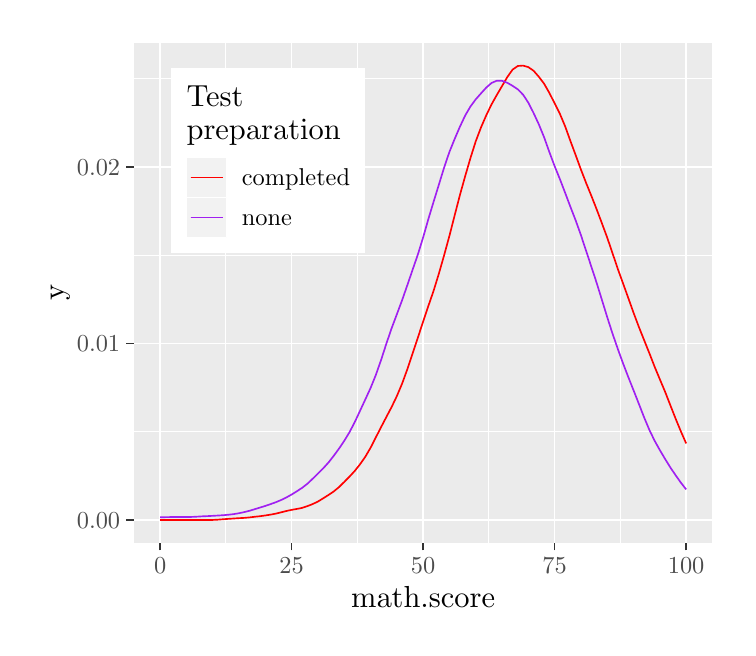
\begin{tikzpicture}[x=1pt,y=1pt]
\definecolor{fillColor}{RGB}{255,255,255}
\path[use as bounding box,fill=fillColor,fill opacity=0.00] (0,0) rectangle (252.94,216.81);
\begin{scope}
\path[clip] (  0.00,  0.00) rectangle (252.94,216.81);
\definecolor{drawColor}{RGB}{255,255,255}
\definecolor{fillColor}{RGB}{255,255,255}

\path[draw=drawColor,line width= 0.6pt,line join=round,line cap=round,fill=fillColor] (  0.00,  0.00) rectangle (252.94,216.81);
\end{scope}
\begin{scope}
\path[clip] ( 38.36, 30.72) rectangle (247.44,211.31);
\definecolor{fillColor}{gray}{0.92}

\path[fill=fillColor] ( 38.36, 30.72) rectangle (247.44,211.31);
\definecolor{drawColor}{RGB}{255,255,255}

\path[draw=drawColor,line width= 0.3pt,line join=round] ( 38.36, 70.82) --
	(247.44, 70.82);

\path[draw=drawColor,line width= 0.3pt,line join=round] ( 38.36,134.59) --
	(247.44,134.59);

\path[draw=drawColor,line width= 0.3pt,line join=round] ( 38.36,198.36) --
	(247.44,198.36);

\path[draw=drawColor,line width= 0.3pt,line join=round] ( 71.62, 30.72) --
	( 71.62,211.31);

\path[draw=drawColor,line width= 0.3pt,line join=round] (119.14, 30.72) --
	(119.14,211.31);

\path[draw=drawColor,line width= 0.3pt,line join=round] (166.66, 30.72) --
	(166.66,211.31);

\path[draw=drawColor,line width= 0.3pt,line join=round] (214.18, 30.72) --
	(214.18,211.31);

\path[draw=drawColor,line width= 0.6pt,line join=round] ( 38.36, 38.93) --
	(247.44, 38.93);

\path[draw=drawColor,line width= 0.6pt,line join=round] ( 38.36,102.70) --
	(247.44,102.70);

\path[draw=drawColor,line width= 0.6pt,line join=round] ( 38.36,166.47) --
	(247.44,166.47);

\path[draw=drawColor,line width= 0.6pt,line join=round] ( 47.86, 30.72) --
	( 47.86,211.31);

\path[draw=drawColor,line width= 0.6pt,line join=round] ( 95.38, 30.72) --
	( 95.38,211.31);

\path[draw=drawColor,line width= 0.6pt,line join=round] (142.90, 30.72) --
	(142.90,211.31);

\path[draw=drawColor,line width= 0.6pt,line join=round] (190.42, 30.72) --
	(190.42,211.31);

\path[draw=drawColor,line width= 0.6pt,line join=round] (237.94, 30.72) --
	(237.94,211.31);
\definecolor{drawColor}{RGB}{255,0,0}

\path[draw=drawColor,line width= 0.6pt,line join=round] ( 47.86, 38.93) --
	( 49.77, 38.93) --
	( 51.67, 38.93) --
	( 53.57, 38.93) --
	( 55.47, 38.93) --
	( 57.37, 38.93) --
	( 59.27, 38.93) --
	( 61.17, 38.93) --
	( 63.07, 38.93) --
	( 64.97, 38.93) --
	( 66.87, 38.93) --
	( 68.77, 39.03) --
	( 70.67, 39.18) --
	( 72.57, 39.32) --
	( 74.48, 39.45) --
	( 76.38, 39.57) --
	( 78.28, 39.67) --
	( 80.18, 39.85) --
	( 82.08, 40.08) --
	( 83.98, 40.28) --
	( 85.88, 40.55) --
	( 87.78, 40.85) --
	( 89.68, 41.21) --
	( 91.58, 41.68) --
	( 93.48, 42.16) --
	( 95.38, 42.57) --
	( 97.28, 42.91) --
	( 99.19, 43.28) --
	(101.09, 43.93) --
	(102.99, 44.67) --
	(104.89, 45.58) --
	(106.79, 46.74) --
	(108.69, 47.95) --
	(110.59, 49.22) --
	(112.49, 50.79) --
	(114.39, 52.66) --
	(116.29, 54.58) --
	(118.19, 56.64) --
	(120.09, 59.03) --
	(121.99, 61.74) --
	(123.90, 65.01) --
	(125.80, 68.75) --
	(127.70, 72.46) --
	(129.60, 76.11) --
	(131.50, 79.72) --
	(133.40, 83.67) --
	(135.30, 88.19) --
	(137.20, 93.42) --
	(139.10, 99.08) --
	(141.00,104.85) --
	(142.90,110.58) --
	(144.80,116.29) --
	(146.70,121.80) --
	(148.61,128.01) --
	(150.51,134.68) --
	(152.41,141.63) --
	(154.31,149.07) --
	(156.21,156.41) --
	(158.11,163.23) --
	(160.01,169.74) --
	(161.91,175.75) --
	(163.81,180.77) --
	(165.71,185.14) --
	(167.61,189.08) --
	(169.51,192.47) --
	(171.41,195.71) --
	(173.32,198.97) --
	(175.22,201.65) --
	(177.12,202.97) --
	(179.02,203.10) --
	(180.92,202.55) --
	(182.82,201.23) --
	(184.72,199.05) --
	(186.62,196.54) --
	(188.52,193.21) --
	(190.42,189.46) --
	(192.32,185.66) --
	(194.22,181.13) --
	(196.12,175.85) --
	(198.03,170.71) --
	(199.93,165.50) --
	(201.83,160.60) --
	(203.73,155.93) --
	(205.63,151.09) --
	(207.53,146.04) --
	(209.43,140.90) --
	(211.33,135.31) --
	(213.23,129.66) --
	(215.13,124.42) --
	(217.03,119.12) --
	(218.93,113.79) --
	(220.83,108.73) --
	(222.74,103.93) --
	(224.64, 99.20) --
	(226.54, 94.30) --
	(228.44, 89.73) --
	(230.34, 85.22) --
	(232.24, 80.34) --
	(234.14, 75.50) --
	(236.04, 70.91) --
	(237.94, 66.57);
\definecolor{drawColor}{RGB}{160,32,240}

\path[draw=drawColor,line width= 0.6pt,line join=round] ( 47.86, 39.88) --
	( 49.77, 39.93) --
	( 51.67, 39.97) --
	( 53.57, 40.00) --
	( 55.47, 40.00) --
	( 57.37, 40.00) --
	( 59.27, 40.02) --
	( 61.17, 40.11) --
	( 63.07, 40.23) --
	( 64.97, 40.31) --
	( 66.87, 40.41) --
	( 68.77, 40.52) --
	( 70.67, 40.64) --
	( 72.57, 40.81) --
	( 74.48, 41.04) --
	( 76.38, 41.36) --
	( 78.28, 41.77) --
	( 80.18, 42.24) --
	( 82.08, 42.83) --
	( 83.98, 43.41) --
	( 85.88, 43.99) --
	( 87.78, 44.65) --
	( 89.68, 45.33) --
	( 91.58, 46.13) --
	( 93.48, 47.06) --
	( 95.38, 48.11) --
	( 97.28, 49.29) --
	( 99.19, 50.54) --
	(101.09, 52.02) --
	(102.99, 53.82) --
	(104.89, 55.71) --
	(106.79, 57.58) --
	(108.69, 59.67) --
	(110.59, 62.09) --
	(112.49, 64.69) --
	(114.39, 67.51) --
	(116.29, 70.63) --
	(118.19, 74.28) --
	(120.09, 78.35) --
	(121.99, 82.44) --
	(123.90, 86.59) --
	(125.80, 91.29) --
	(127.70, 96.72) --
	(129.60,102.59) --
	(131.50,108.17) --
	(133.40,113.24) --
	(135.30,118.33) --
	(137.20,123.80) --
	(139.10,129.36) --
	(141.00,134.86) --
	(142.90,141.03) --
	(144.80,147.69) --
	(146.70,153.98) --
	(148.61,160.16) --
	(150.51,166.36) --
	(152.41,171.95) --
	(154.31,176.64) --
	(156.21,181.07) --
	(158.11,185.10) --
	(160.01,188.35) --
	(161.91,190.91) --
	(163.81,193.07) --
	(165.71,195.16) --
	(167.61,196.82) --
	(169.51,197.64) --
	(171.41,197.60) --
	(173.32,196.89) --
	(175.22,195.79) --
	(177.12,194.51) --
	(179.02,192.59) --
	(180.92,189.69) --
	(182.82,185.94) --
	(184.72,181.84) --
	(186.62,177.19) --
	(188.52,171.83) --
	(190.42,166.75) --
	(192.32,162.08) --
	(194.22,157.11) --
	(196.12,152.06) --
	(198.03,147.13) --
	(199.93,141.81) --
	(201.83,136.02) --
	(203.73,130.29) --
	(205.63,124.49) --
	(207.53,118.35) --
	(209.43,112.16) --
	(211.33,106.26) --
	(213.23,100.76) --
	(215.13, 95.52) --
	(217.03, 90.55) --
	(218.93, 85.78) --
	(220.83, 80.93) --
	(222.74, 76.01) --
	(224.64, 71.48) --
	(226.54, 67.55) --
	(228.44, 64.15) --
	(230.34, 60.94) --
	(232.24, 57.88) --
	(234.14, 55.06) --
	(236.04, 52.39) --
	(237.94, 49.96);
\end{scope}
\begin{scope}
\path[clip] (  0.00,  0.00) rectangle (252.94,216.81);
\definecolor{drawColor}{gray}{0.30}

\node[text=drawColor,anchor=base east,inner sep=0pt, outer sep=0pt, scale=  0.88] at ( 33.41, 35.90) {0.00};

\node[text=drawColor,anchor=base east,inner sep=0pt, outer sep=0pt, scale=  0.88] at ( 33.41, 99.67) {0.01};

\node[text=drawColor,anchor=base east,inner sep=0pt, outer sep=0pt, scale=  0.88] at ( 33.41,163.44) {0.02};
\end{scope}
\begin{scope}
\path[clip] (  0.00,  0.00) rectangle (252.94,216.81);
\definecolor{drawColor}{gray}{0.20}

\path[draw=drawColor,line width= 0.6pt,line join=round] ( 35.61, 38.93) --
	( 38.36, 38.93);

\path[draw=drawColor,line width= 0.6pt,line join=round] ( 35.61,102.70) --
	( 38.36,102.70);

\path[draw=drawColor,line width= 0.6pt,line join=round] ( 35.61,166.47) --
	( 38.36,166.47);
\end{scope}
\begin{scope}
\path[clip] (  0.00,  0.00) rectangle (252.94,216.81);
\definecolor{drawColor}{gray}{0.20}

\path[draw=drawColor,line width= 0.6pt,line join=round] ( 47.86, 27.97) --
	( 47.86, 30.72);

\path[draw=drawColor,line width= 0.6pt,line join=round] ( 95.38, 27.97) --
	( 95.38, 30.72);

\path[draw=drawColor,line width= 0.6pt,line join=round] (142.90, 27.97) --
	(142.90, 30.72);

\path[draw=drawColor,line width= 0.6pt,line join=round] (190.42, 27.97) --
	(190.42, 30.72);

\path[draw=drawColor,line width= 0.6pt,line join=round] (237.94, 27.97) --
	(237.94, 30.72);
\end{scope}
\begin{scope}
\path[clip] (  0.00,  0.00) rectangle (252.94,216.81);
\definecolor{drawColor}{gray}{0.30}

\node[text=drawColor,anchor=base,inner sep=0pt, outer sep=0pt, scale=  0.88] at ( 47.86, 19.71) {0};

\node[text=drawColor,anchor=base,inner sep=0pt, outer sep=0pt, scale=  0.88] at ( 95.38, 19.71) {25};

\node[text=drawColor,anchor=base,inner sep=0pt, outer sep=0pt, scale=  0.88] at (142.90, 19.71) {50};

\node[text=drawColor,anchor=base,inner sep=0pt, outer sep=0pt, scale=  0.88] at (190.42, 19.71) {75};

\node[text=drawColor,anchor=base,inner sep=0pt, outer sep=0pt, scale=  0.88] at (237.94, 19.71) {100};
\end{scope}
\begin{scope}
\path[clip] (  0.00,  0.00) rectangle (252.94,216.81);
\definecolor{drawColor}{RGB}{0,0,0}

\node[text=drawColor,anchor=base,inner sep=0pt, outer sep=0pt, scale=  1.10] at (142.90,  7.44) {math.score};
\end{scope}
\begin{scope}
\path[clip] (  0.00,  0.00) rectangle (252.94,216.81);
\definecolor{drawColor}{RGB}{0,0,0}

\node[text=drawColor,rotate= 90.00,anchor=base,inner sep=0pt, outer sep=0pt, scale=  1.10] at ( 13.08,121.02) {y};
\end{scope}
\begin{scope}
\path[clip] (  0.00,  0.00) rectangle (252.94,216.81);
\definecolor{fillColor}{RGB}{255,255,255}

\path[fill=fillColor] ( 51.94,135.47) rectangle (121.99,202.28);
\end{scope}
\begin{scope}
\path[clip] (  0.00,  0.00) rectangle (252.94,216.81);
\definecolor{drawColor}{RGB}{0,0,0}

\node[text=drawColor,anchor=base west,inner sep=0pt, outer sep=0pt, scale=  1.10] at ( 57.44,188.23) {Test };

\node[text=drawColor,anchor=base west,inner sep=0pt, outer sep=0pt, scale=  1.10] at ( 57.44,176.35) { preparation};
\end{scope}
\begin{scope}
\path[clip] (  0.00,  0.00) rectangle (252.94,216.81);
\definecolor{drawColor}{RGB}{255,255,255}
\definecolor{fillColor}{gray}{0.95}

\path[draw=drawColor,line width= 0.6pt,line join=round,line cap=round,fill=fillColor] ( 57.44,155.43) rectangle ( 71.89,169.88);
\end{scope}
\begin{scope}
\path[clip] (  0.00,  0.00) rectangle (252.94,216.81);
\definecolor{drawColor}{RGB}{255,0,0}

\path[draw=drawColor,line width= 0.6pt,line join=round] ( 58.88,162.65) -- ( 70.45,162.65);
\end{scope}
\begin{scope}
\path[clip] (  0.00,  0.00) rectangle (252.94,216.81);
\definecolor{drawColor}{RGB}{255,0,0}

\path[draw=drawColor,line width= 0.6pt,line join=round] ( 58.88,162.65) -- ( 70.45,162.65);
\end{scope}
\begin{scope}
\path[clip] (  0.00,  0.00) rectangle (252.94,216.81);
\definecolor{drawColor}{RGB}{255,255,255}
\definecolor{fillColor}{gray}{0.95}

\path[draw=drawColor,line width= 0.6pt,line join=round,line cap=round,fill=fillColor] ( 57.44,140.97) rectangle ( 71.89,155.43);
\end{scope}
\begin{scope}
\path[clip] (  0.00,  0.00) rectangle (252.94,216.81);
\definecolor{drawColor}{RGB}{160,32,240}

\path[draw=drawColor,line width= 0.6pt,line join=round] ( 58.88,148.20) -- ( 70.45,148.20);
\end{scope}
\begin{scope}
\path[clip] (  0.00,  0.00) rectangle (252.94,216.81);
\definecolor{drawColor}{RGB}{160,32,240}

\path[draw=drawColor,line width= 0.6pt,line join=round] ( 58.88,148.20) -- ( 70.45,148.20);
\end{scope}
\begin{scope}
\path[clip] (  0.00,  0.00) rectangle (252.94,216.81);
\definecolor{drawColor}{RGB}{0,0,0}

\node[text=drawColor,anchor=base west,inner sep=0pt, outer sep=0pt, scale=  0.88] at ( 77.39,159.62) {completed};
\end{scope}
\begin{scope}
\path[clip] (  0.00,  0.00) rectangle (252.94,216.81);
\definecolor{drawColor}{RGB}{0,0,0}

\node[text=drawColor,anchor=base west,inner sep=0pt, outer sep=0pt, scale=  0.88] at ( 77.39,145.17) {none};
\end{scope}
\end{tikzpicture}
}
			\caption{}
			\label{fig 6.3}
		\end{subfigure}
		\begin{subfigure}[b]{0.48\linewidth}        %% or \columnwidth
			\centering
			\scalebox{0.75}{% Created by tikzDevice version 0.12 on 2019-04-13 14:06:17
% !TEX encoding = UTF-8 Unicode
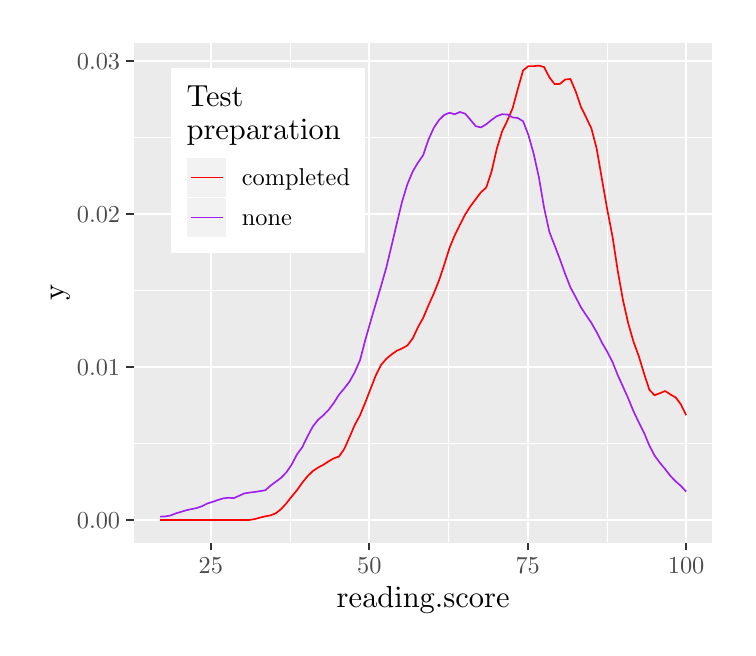
\begin{tikzpicture}[x=1pt,y=1pt]
\definecolor{fillColor}{RGB}{255,255,255}
\path[use as bounding box,fill=fillColor,fill opacity=0.00] (0,0) rectangle (252.94,216.81);
\begin{scope}
\path[clip] (  0.00,  0.00) rectangle (252.94,216.81);
\definecolor{drawColor}{RGB}{255,255,255}
\definecolor{fillColor}{RGB}{255,255,255}

\path[draw=drawColor,line width= 0.6pt,line join=round,line cap=round,fill=fillColor] (  0.00,  0.00) rectangle (252.94,216.81);
\end{scope}
\begin{scope}
\path[clip] ( 38.36, 30.72) rectangle (247.44,211.31);
\definecolor{fillColor}{gray}{0.92}

\path[fill=fillColor] ( 38.36, 30.72) rectangle (247.44,211.31);
\definecolor{drawColor}{RGB}{255,255,255}

\path[draw=drawColor,line width= 0.3pt,line join=round] ( 38.36, 66.55) --
	(247.44, 66.55);

\path[draw=drawColor,line width= 0.3pt,line join=round] ( 38.36,121.79) --
	(247.44,121.79);

\path[draw=drawColor,line width= 0.3pt,line join=round] ( 38.36,177.03) --
	(247.44,177.03);

\path[draw=drawColor,line width= 0.3pt,line join=round] ( 94.81, 30.72) --
	( 94.81,211.31);

\path[draw=drawColor,line width= 0.3pt,line join=round] (152.06, 30.72) --
	(152.06,211.31);

\path[draw=drawColor,line width= 0.3pt,line join=round] (209.32, 30.72) --
	(209.32,211.31);

\path[draw=drawColor,line width= 0.6pt,line join=round] ( 38.36, 38.93) --
	(247.44, 38.93);

\path[draw=drawColor,line width= 0.6pt,line join=round] ( 38.36, 94.17) --
	(247.44, 94.17);

\path[draw=drawColor,line width= 0.6pt,line join=round] ( 38.36,149.41) --
	(247.44,149.41);

\path[draw=drawColor,line width= 0.6pt,line join=round] ( 38.36,204.65) --
	(247.44,204.65);

\path[draw=drawColor,line width= 0.6pt,line join=round] ( 66.19, 30.72) --
	( 66.19,211.31);

\path[draw=drawColor,line width= 0.6pt,line join=round] (123.44, 30.72) --
	(123.44,211.31);

\path[draw=drawColor,line width= 0.6pt,line join=round] (180.69, 30.72) --
	(180.69,211.31);

\path[draw=drawColor,line width= 0.6pt,line join=round] (237.94, 30.72) --
	(237.94,211.31);
\definecolor{drawColor}{RGB}{255,0,0}

\path[draw=drawColor,line width= 0.6pt,line join=round] ( 47.86, 38.93) --
	( 49.77, 38.93) --
	( 51.67, 38.93) --
	( 53.57, 38.93) --
	( 55.47, 38.93) --
	( 57.37, 38.93) --
	( 59.27, 38.93) --
	( 61.17, 38.93) --
	( 63.07, 38.93) --
	( 64.97, 38.93) --
	( 66.87, 38.93) --
	( 68.77, 38.93) --
	( 70.67, 38.93) --
	( 72.57, 38.93) --
	( 74.48, 38.93) --
	( 76.38, 38.93) --
	( 78.28, 38.93) --
	( 80.18, 38.93) --
	( 82.08, 39.24) --
	( 83.98, 39.78) --
	( 85.88, 40.23) --
	( 87.78, 40.58) --
	( 89.68, 41.36) --
	( 91.58, 42.85) --
	( 93.48, 44.96) --
	( 95.38, 47.35) --
	( 97.28, 49.64) --
	( 99.19, 52.34) --
	(101.09, 54.68) --
	(102.99, 56.54) --
	(104.89, 57.83) --
	(106.79, 58.84) --
	(108.69, 60.07) --
	(110.59, 61.17) --
	(112.49, 61.82) --
	(114.39, 64.56) --
	(116.29, 68.83) --
	(118.19, 73.25) --
	(120.09, 76.74) --
	(121.99, 81.35) --
	(123.90, 86.28) --
	(125.80, 91.16) --
	(127.70, 94.95) --
	(129.60, 97.16) --
	(131.50, 98.73) --
	(133.40,100.08) --
	(135.30,100.91) --
	(137.20,101.96) --
	(139.10,104.46) --
	(141.00,108.51) --
	(142.90,111.91) --
	(144.80,116.39) --
	(146.70,120.64) --
	(148.61,125.42) --
	(150.51,131.12) --
	(152.41,137.13) --
	(154.31,141.77) --
	(156.21,145.63) --
	(158.11,149.34) --
	(160.01,152.30) --
	(161.91,154.83) --
	(163.81,157.36) --
	(165.71,159.04) --
	(167.61,164.77) --
	(169.51,173.03) --
	(171.41,179.25) --
	(173.32,183.21) --
	(175.22,187.63) --
	(177.12,194.70) --
	(179.02,201.36) --
	(180.92,202.90) --
	(182.82,202.90) --
	(184.72,203.10) --
	(186.62,202.57) --
	(188.52,198.86) --
	(190.42,196.40) --
	(192.32,196.49) --
	(194.22,198.07) --
	(196.12,198.27) --
	(198.03,193.75) --
	(199.93,188.19) --
	(201.83,184.33) --
	(203.73,180.32) --
	(205.63,172.98) --
	(207.53,161.94) --
	(209.43,151.09) --
	(211.33,141.31) --
	(213.23,128.88) --
	(215.13,118.26) --
	(217.03,109.89) --
	(218.93,103.28) --
	(220.83, 98.09) --
	(222.74, 91.78) --
	(224.64, 85.98) --
	(226.54, 83.97) --
	(228.44, 84.73) --
	(230.34, 85.52) --
	(232.24, 84.26) --
	(234.14, 83.21) --
	(236.04, 80.68) --
	(237.94, 76.77);
\definecolor{drawColor}{RGB}{160,32,240}

\path[draw=drawColor,line width= 0.6pt,line join=round] ( 47.86, 40.12) --
	( 49.77, 40.21) --
	( 51.67, 40.54) --
	( 53.57, 41.31) --
	( 55.47, 41.87) --
	( 57.37, 42.45) --
	( 59.27, 42.85) --
	( 61.17, 43.26) --
	( 63.07, 43.93) --
	( 64.97, 44.89) --
	( 66.87, 45.47) --
	( 68.77, 46.15) --
	( 70.67, 46.73) --
	( 72.57, 46.94) --
	( 74.48, 46.81) --
	( 76.38, 47.64) --
	( 78.28, 48.52) --
	( 80.18, 48.81) --
	( 82.08, 49.04) --
	( 83.98, 49.35) --
	( 85.88, 49.66) --
	( 87.78, 51.35) --
	( 89.68, 52.75) --
	( 91.58, 54.15) --
	( 93.48, 56.11) --
	( 95.38, 58.92) --
	( 97.28, 62.57) --
	( 99.19, 65.15) --
	(101.09, 69.07) --
	(102.99, 72.61) --
	(104.89, 75.07) --
	(106.79, 76.71) --
	(108.69, 78.63) --
	(110.59, 81.16) --
	(112.49, 84.18) --
	(114.39, 86.43) --
	(116.29, 88.91) --
	(118.19, 92.32) --
	(120.09, 96.65) --
	(121.99,103.93) --
	(123.90,110.64) --
	(125.80,117.09) --
	(127.70,123.48) --
	(129.60,130.16) --
	(131.50,138.06) --
	(133.40,146.15) --
	(135.30,153.97) --
	(137.20,160.22) --
	(139.10,164.77) --
	(141.00,167.99) --
	(142.90,170.72) --
	(144.80,176.28) --
	(146.70,180.50) --
	(148.61,183.41) --
	(150.51,185.27) --
	(152.41,186.05) --
	(154.31,185.52) --
	(156.21,186.35) --
	(158.11,185.71) --
	(160.01,183.50) --
	(161.91,181.20) --
	(163.81,180.76) --
	(165.71,181.91) --
	(167.61,183.47) --
	(169.51,184.82) --
	(171.41,185.52) --
	(173.32,185.42) --
	(175.22,184.39) --
	(177.12,184.16) --
	(179.02,182.99) --
	(180.92,178.08) --
	(182.82,171.35) --
	(184.72,162.79) --
	(186.62,151.66) --
	(188.52,142.99) --
	(190.42,138.11) --
	(192.32,133.14) --
	(194.22,127.82) --
	(196.12,122.96) --
	(198.03,119.44) --
	(199.93,115.72) --
	(201.83,112.86) --
	(203.73,110.07) --
	(205.63,106.73) --
	(207.53,102.94) --
	(209.43, 99.70) --
	(211.33, 95.99) --
	(213.23, 91.23) --
	(215.13, 87.05) --
	(217.03, 82.80) --
	(218.93, 78.15) --
	(220.83, 74.15) --
	(222.74, 70.40) --
	(224.64, 65.83) --
	(226.54, 62.18) --
	(228.44, 59.59) --
	(230.34, 57.32) --
	(232.24, 54.84) --
	(234.14, 52.89) --
	(236.04, 51.22) --
	(237.94, 49.18);
\end{scope}
\begin{scope}
\path[clip] (  0.00,  0.00) rectangle (252.94,216.81);
\definecolor{drawColor}{gray}{0.30}

\node[text=drawColor,anchor=base east,inner sep=0pt, outer sep=0pt, scale=  0.88] at ( 33.41, 35.90) {0.00};

\node[text=drawColor,anchor=base east,inner sep=0pt, outer sep=0pt, scale=  0.88] at ( 33.41, 91.14) {0.01};

\node[text=drawColor,anchor=base east,inner sep=0pt, outer sep=0pt, scale=  0.88] at ( 33.41,146.38) {0.02};

\node[text=drawColor,anchor=base east,inner sep=0pt, outer sep=0pt, scale=  0.88] at ( 33.41,201.62) {0.03};
\end{scope}
\begin{scope}
\path[clip] (  0.00,  0.00) rectangle (252.94,216.81);
\definecolor{drawColor}{gray}{0.20}

\path[draw=drawColor,line width= 0.6pt,line join=round] ( 35.61, 38.93) --
	( 38.36, 38.93);

\path[draw=drawColor,line width= 0.6pt,line join=round] ( 35.61, 94.17) --
	( 38.36, 94.17);

\path[draw=drawColor,line width= 0.6pt,line join=round] ( 35.61,149.41) --
	( 38.36,149.41);

\path[draw=drawColor,line width= 0.6pt,line join=round] ( 35.61,204.65) --
	( 38.36,204.65);
\end{scope}
\begin{scope}
\path[clip] (  0.00,  0.00) rectangle (252.94,216.81);
\definecolor{drawColor}{gray}{0.20}

\path[draw=drawColor,line width= 0.6pt,line join=round] ( 66.19, 27.97) --
	( 66.19, 30.72);

\path[draw=drawColor,line width= 0.6pt,line join=round] (123.44, 27.97) --
	(123.44, 30.72);

\path[draw=drawColor,line width= 0.6pt,line join=round] (180.69, 27.97) --
	(180.69, 30.72);

\path[draw=drawColor,line width= 0.6pt,line join=round] (237.94, 27.97) --
	(237.94, 30.72);
\end{scope}
\begin{scope}
\path[clip] (  0.00,  0.00) rectangle (252.94,216.81);
\definecolor{drawColor}{gray}{0.30}

\node[text=drawColor,anchor=base,inner sep=0pt, outer sep=0pt, scale=  0.88] at ( 66.19, 19.71) {25};

\node[text=drawColor,anchor=base,inner sep=0pt, outer sep=0pt, scale=  0.88] at (123.44, 19.71) {50};

\node[text=drawColor,anchor=base,inner sep=0pt, outer sep=0pt, scale=  0.88] at (180.69, 19.71) {75};

\node[text=drawColor,anchor=base,inner sep=0pt, outer sep=0pt, scale=  0.88] at (237.94, 19.71) {100};
\end{scope}
\begin{scope}
\path[clip] (  0.00,  0.00) rectangle (252.94,216.81);
\definecolor{drawColor}{RGB}{0,0,0}

\node[text=drawColor,anchor=base,inner sep=0pt, outer sep=0pt, scale=  1.10] at (142.90,  7.44) {reading.score};
\end{scope}
\begin{scope}
\path[clip] (  0.00,  0.00) rectangle (252.94,216.81);
\definecolor{drawColor}{RGB}{0,0,0}

\node[text=drawColor,rotate= 90.00,anchor=base,inner sep=0pt, outer sep=0pt, scale=  1.10] at ( 13.08,121.02) {y};
\end{scope}
\begin{scope}
\path[clip] (  0.00,  0.00) rectangle (252.94,216.81);
\definecolor{fillColor}{RGB}{255,255,255}

\path[fill=fillColor] ( 51.94,135.47) rectangle (121.99,202.28);
\end{scope}
\begin{scope}
\path[clip] (  0.00,  0.00) rectangle (252.94,216.81);
\definecolor{drawColor}{RGB}{0,0,0}

\node[text=drawColor,anchor=base west,inner sep=0pt, outer sep=0pt, scale=  1.10] at ( 57.44,188.23) {Test };

\node[text=drawColor,anchor=base west,inner sep=0pt, outer sep=0pt, scale=  1.10] at ( 57.44,176.35) { preparation};
\end{scope}
\begin{scope}
\path[clip] (  0.00,  0.00) rectangle (252.94,216.81);
\definecolor{drawColor}{RGB}{255,255,255}
\definecolor{fillColor}{gray}{0.95}

\path[draw=drawColor,line width= 0.6pt,line join=round,line cap=round,fill=fillColor] ( 57.44,155.43) rectangle ( 71.89,169.88);
\end{scope}
\begin{scope}
\path[clip] (  0.00,  0.00) rectangle (252.94,216.81);
\definecolor{drawColor}{RGB}{255,0,0}

\path[draw=drawColor,line width= 0.6pt,line join=round] ( 58.88,162.65) -- ( 70.45,162.65);
\end{scope}
\begin{scope}
\path[clip] (  0.00,  0.00) rectangle (252.94,216.81);
\definecolor{drawColor}{RGB}{255,0,0}

\path[draw=drawColor,line width= 0.6pt,line join=round] ( 58.88,162.65) -- ( 70.45,162.65);
\end{scope}
\begin{scope}
\path[clip] (  0.00,  0.00) rectangle (252.94,216.81);
\definecolor{drawColor}{RGB}{255,255,255}
\definecolor{fillColor}{gray}{0.95}

\path[draw=drawColor,line width= 0.6pt,line join=round,line cap=round,fill=fillColor] ( 57.44,140.97) rectangle ( 71.89,155.43);
\end{scope}
\begin{scope}
\path[clip] (  0.00,  0.00) rectangle (252.94,216.81);
\definecolor{drawColor}{RGB}{160,32,240}

\path[draw=drawColor,line width= 0.6pt,line join=round] ( 58.88,148.20) -- ( 70.45,148.20);
\end{scope}
\begin{scope}
\path[clip] (  0.00,  0.00) rectangle (252.94,216.81);
\definecolor{drawColor}{RGB}{160,32,240}

\path[draw=drawColor,line width= 0.6pt,line join=round] ( 58.88,148.20) -- ( 70.45,148.20);
\end{scope}
\begin{scope}
\path[clip] (  0.00,  0.00) rectangle (252.94,216.81);
\definecolor{drawColor}{RGB}{0,0,0}

\node[text=drawColor,anchor=base west,inner sep=0pt, outer sep=0pt, scale=  0.88] at ( 77.39,159.62) {completed};
\end{scope}
\begin{scope}
\path[clip] (  0.00,  0.00) rectangle (252.94,216.81);
\definecolor{drawColor}{RGB}{0,0,0}

\node[text=drawColor,anchor=base west,inner sep=0pt, outer sep=0pt, scale=  0.88] at ( 77.39,145.17) {none};
\end{scope}
\end{tikzpicture}
}
			\caption{}
			\label{fig 6.4}
		\end{subfigure}
	
	    \begin{subfigure}[b]{0.48\linewidth}        %% or \columnwidth
	    	\centering
	    	\scalebox{0.75}{% Created by tikzDevice version 0.12 on 2019-04-13 14:06:18
% !TEX encoding = UTF-8 Unicode
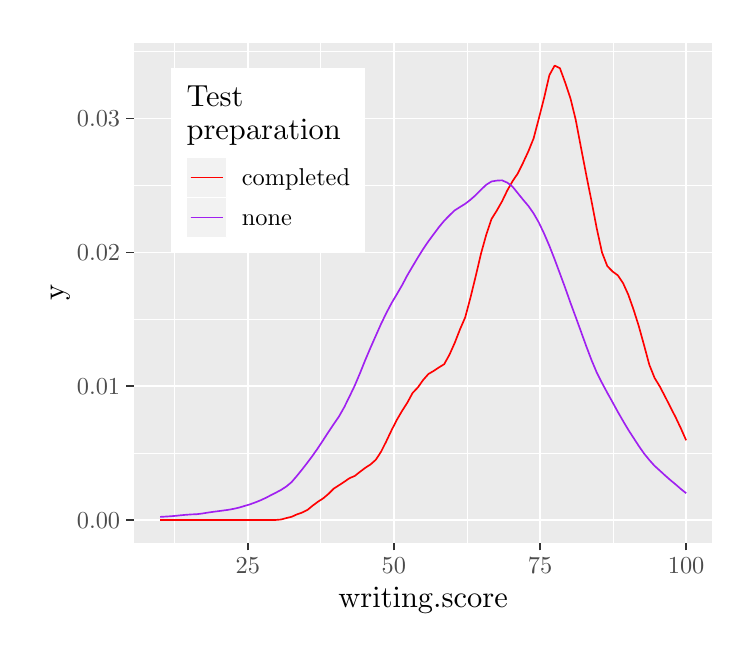
\begin{tikzpicture}[x=1pt,y=1pt]
\definecolor{fillColor}{RGB}{255,255,255}
\path[use as bounding box,fill=fillColor,fill opacity=0.00] (0,0) rectangle (252.94,216.81);
\begin{scope}
\path[clip] (  0.00,  0.00) rectangle (252.94,216.81);
\definecolor{drawColor}{RGB}{255,255,255}
\definecolor{fillColor}{RGB}{255,255,255}

\path[draw=drawColor,line width= 0.6pt,line join=round,line cap=round,fill=fillColor] (  0.00,  0.00) rectangle (252.94,216.81);
\end{scope}
\begin{scope}
\path[clip] ( 38.36, 30.72) rectangle (247.44,211.31);
\definecolor{fillColor}{gray}{0.92}

\path[fill=fillColor] ( 38.36, 30.72) rectangle (247.44,211.31);
\definecolor{drawColor}{RGB}{255,255,255}

\path[draw=drawColor,line width= 0.3pt,line join=round] ( 38.36, 63.10) --
	(247.44, 63.10);

\path[draw=drawColor,line width= 0.3pt,line join=round] ( 38.36,111.44) --
	(247.44,111.44);

\path[draw=drawColor,line width= 0.3pt,line join=round] ( 38.36,159.78) --
	(247.44,159.78);

\path[draw=drawColor,line width= 0.3pt,line join=round] ( 38.36,208.11) --
	(247.44,208.11);

\path[draw=drawColor,line width= 0.3pt,line join=round] ( 53.14, 30.72) --
	( 53.14,211.31);

\path[draw=drawColor,line width= 0.3pt,line join=round] (105.94, 30.72) --
	(105.94,211.31);

\path[draw=drawColor,line width= 0.3pt,line join=round] (158.74, 30.72) --
	(158.74,211.31);

\path[draw=drawColor,line width= 0.3pt,line join=round] (211.54, 30.72) --
	(211.54,211.31);

\path[draw=drawColor,line width= 0.6pt,line join=round] ( 38.36, 38.93) --
	(247.44, 38.93);

\path[draw=drawColor,line width= 0.6pt,line join=round] ( 38.36, 87.27) --
	(247.44, 87.27);

\path[draw=drawColor,line width= 0.6pt,line join=round] ( 38.36,135.61) --
	(247.44,135.61);

\path[draw=drawColor,line width= 0.6pt,line join=round] ( 38.36,183.95) --
	(247.44,183.95);

\path[draw=drawColor,line width= 0.6pt,line join=round] ( 79.54, 30.72) --
	( 79.54,211.31);

\path[draw=drawColor,line width= 0.6pt,line join=round] (132.34, 30.72) --
	(132.34,211.31);

\path[draw=drawColor,line width= 0.6pt,line join=round] (185.14, 30.72) --
	(185.14,211.31);

\path[draw=drawColor,line width= 0.6pt,line join=round] (237.94, 30.72) --
	(237.94,211.31);
\definecolor{drawColor}{RGB}{255,0,0}

\path[draw=drawColor,line width= 0.6pt,line join=round] ( 47.86, 38.93) --
	( 49.77, 38.93) --
	( 51.67, 38.93) --
	( 53.57, 38.93) --
	( 55.47, 38.93) --
	( 57.37, 38.93) --
	( 59.27, 38.93) --
	( 61.17, 38.93) --
	( 63.07, 38.93) --
	( 64.97, 38.93) --
	( 66.87, 38.93) --
	( 68.77, 38.93) --
	( 70.67, 38.93) --
	( 72.57, 38.93) --
	( 74.48, 38.93) --
	( 76.38, 38.93) --
	( 78.28, 38.93) --
	( 80.18, 38.93) --
	( 82.08, 38.93) --
	( 83.98, 38.93) --
	( 85.88, 38.93) --
	( 87.78, 38.93) --
	( 89.68, 38.93) --
	( 91.58, 39.09) --
	( 93.48, 39.61) --
	( 95.38, 40.07) --
	( 97.28, 40.93) --
	( 99.19, 41.60) --
	(101.09, 42.54) --
	(102.99, 44.10) --
	(104.89, 45.51) --
	(106.79, 46.73) --
	(108.69, 48.34) --
	(110.59, 50.24) --
	(112.49, 51.46) --
	(114.39, 52.71) --
	(116.29, 54.02) --
	(118.19, 54.82) --
	(120.09, 56.33) --
	(121.99, 57.76) --
	(123.90, 58.99) --
	(125.80, 60.68) --
	(127.70, 63.58) --
	(129.60, 67.37) --
	(131.50, 71.38) --
	(133.40, 75.10) --
	(135.30, 78.35) --
	(137.20, 81.32) --
	(139.10, 84.83) --
	(141.00, 86.82) --
	(142.90, 89.50) --
	(144.80, 91.66) --
	(146.70, 92.77) --
	(148.61, 94.04) --
	(150.51, 95.21) --
	(152.41, 98.64) --
	(154.31,102.89) --
	(156.21,107.78) --
	(158.11,112.16) --
	(160.01,119.30) --
	(161.91,127.06) --
	(163.81,135.17) --
	(165.71,142.01) --
	(167.61,147.67) --
	(169.51,150.70) --
	(171.41,154.05) --
	(173.32,158.01) --
	(175.22,161.35) --
	(177.12,164.15) --
	(179.02,168.02) --
	(180.92,172.11) --
	(182.82,176.81) --
	(184.72,184.04) --
	(186.62,191.46) --
	(188.52,199.67) --
	(190.42,203.10) --
	(192.32,202.18) --
	(194.22,196.98) --
	(196.12,191.34) --
	(198.03,183.53) --
	(199.93,173.53) --
	(201.83,163.69) --
	(203.73,154.20) --
	(205.63,144.29) --
	(207.53,135.60) --
	(209.43,130.68) --
	(211.33,128.72) --
	(213.23,127.33) --
	(215.13,124.53) --
	(217.03,120.32) --
	(218.93,114.95) --
	(220.83,108.95) --
	(222.74,102.03) --
	(224.64, 94.96) --
	(226.54, 90.24) --
	(228.44, 87.11) --
	(230.34, 83.47) --
	(232.24, 79.72) --
	(234.14, 76.01) --
	(236.04, 72.00) --
	(237.94, 67.71);
\definecolor{drawColor}{RGB}{160,32,240}

\path[draw=drawColor,line width= 0.6pt,line join=round] ( 47.86, 40.03) --
	( 49.77, 40.14) --
	( 51.67, 40.26) --
	( 53.57, 40.42) --
	( 55.47, 40.63) --
	( 57.37, 40.80) --
	( 59.27, 40.93) --
	( 61.17, 41.01) --
	( 63.07, 41.25) --
	( 64.97, 41.56) --
	( 66.87, 41.84) --
	( 68.77, 42.08) --
	( 70.67, 42.34) --
	( 72.57, 42.60) --
	( 74.48, 42.95) --
	( 76.38, 43.39) --
	( 78.28, 43.96) --
	( 80.18, 44.51) --
	( 82.08, 45.20) --
	( 83.98, 45.95) --
	( 85.88, 46.83) --
	( 87.78, 47.81) --
	( 89.68, 48.78) --
	( 91.58, 49.79) --
	( 93.48, 51.03) --
	( 95.38, 52.61) --
	( 97.28, 54.84) --
	( 99.19, 57.20) --
	(101.09, 59.64) --
	(102.99, 62.20) --
	(104.89, 64.90) --
	(106.79, 67.78) --
	(108.69, 70.73) --
	(110.59, 73.55) --
	(112.49, 76.31) --
	(114.39, 79.67) --
	(116.29, 83.53) --
	(118.19, 87.49) --
	(120.09, 91.97) --
	(121.99, 96.71) --
	(123.90,101.20) --
	(125.80,105.50) --
	(127.70,109.77) --
	(129.60,113.70) --
	(131.50,117.30) --
	(133.40,120.48) --
	(135.30,123.76) --
	(137.20,127.36) --
	(139.10,130.58) --
	(141.00,133.77) --
	(142.90,136.81) --
	(144.80,139.61) --
	(146.70,142.18) --
	(148.61,144.74) --
	(150.51,147.03) --
	(152.41,148.98) --
	(154.31,150.79) --
	(156.21,152.00) --
	(158.11,153.17) --
	(160.01,154.64) --
	(161.91,156.32) --
	(163.81,158.27) --
	(165.71,160.05) --
	(167.61,161.23) --
	(169.51,161.55) --
	(171.41,161.65) --
	(173.32,160.80) --
	(175.22,159.34) --
	(177.12,156.99) --
	(179.02,154.64) --
	(180.92,152.40) --
	(182.82,149.69) --
	(184.72,146.37) --
	(186.62,142.38) --
	(188.52,137.95) --
	(190.42,133.09) --
	(192.32,127.97) --
	(194.22,122.82) --
	(196.12,117.43) --
	(198.03,112.24) --
	(199.93,107.01) --
	(201.83,101.75) --
	(203.73, 96.73) --
	(205.63, 92.21) --
	(207.53, 88.44) --
	(209.43, 84.90) --
	(211.33, 81.49) --
	(213.23, 78.02) --
	(215.13, 74.71) --
	(217.03, 71.51) --
	(218.93, 68.57) --
	(220.83, 65.65) --
	(222.74, 62.91) --
	(224.64, 60.58) --
	(226.54, 58.45) --
	(228.44, 56.75) --
	(230.34, 54.99) --
	(232.24, 53.33) --
	(234.14, 51.76) --
	(236.04, 50.10) --
	(237.94, 48.58);
\end{scope}
\begin{scope}
\path[clip] (  0.00,  0.00) rectangle (252.94,216.81);
\definecolor{drawColor}{gray}{0.30}

\node[text=drawColor,anchor=base east,inner sep=0pt, outer sep=0pt, scale=  0.88] at ( 33.41, 35.90) {0.00};

\node[text=drawColor,anchor=base east,inner sep=0pt, outer sep=0pt, scale=  0.88] at ( 33.41, 84.24) {0.01};

\node[text=drawColor,anchor=base east,inner sep=0pt, outer sep=0pt, scale=  0.88] at ( 33.41,132.58) {0.02};

\node[text=drawColor,anchor=base east,inner sep=0pt, outer sep=0pt, scale=  0.88] at ( 33.41,180.92) {0.03};
\end{scope}
\begin{scope}
\path[clip] (  0.00,  0.00) rectangle (252.94,216.81);
\definecolor{drawColor}{gray}{0.20}

\path[draw=drawColor,line width= 0.6pt,line join=round] ( 35.61, 38.93) --
	( 38.36, 38.93);

\path[draw=drawColor,line width= 0.6pt,line join=round] ( 35.61, 87.27) --
	( 38.36, 87.27);

\path[draw=drawColor,line width= 0.6pt,line join=round] ( 35.61,135.61) --
	( 38.36,135.61);

\path[draw=drawColor,line width= 0.6pt,line join=round] ( 35.61,183.95) --
	( 38.36,183.95);
\end{scope}
\begin{scope}
\path[clip] (  0.00,  0.00) rectangle (252.94,216.81);
\definecolor{drawColor}{gray}{0.20}

\path[draw=drawColor,line width= 0.6pt,line join=round] ( 79.54, 27.97) --
	( 79.54, 30.72);

\path[draw=drawColor,line width= 0.6pt,line join=round] (132.34, 27.97) --
	(132.34, 30.72);

\path[draw=drawColor,line width= 0.6pt,line join=round] (185.14, 27.97) --
	(185.14, 30.72);

\path[draw=drawColor,line width= 0.6pt,line join=round] (237.94, 27.97) --
	(237.94, 30.72);
\end{scope}
\begin{scope}
\path[clip] (  0.00,  0.00) rectangle (252.94,216.81);
\definecolor{drawColor}{gray}{0.30}

\node[text=drawColor,anchor=base,inner sep=0pt, outer sep=0pt, scale=  0.88] at ( 79.54, 19.71) {25};

\node[text=drawColor,anchor=base,inner sep=0pt, outer sep=0pt, scale=  0.88] at (132.34, 19.71) {50};

\node[text=drawColor,anchor=base,inner sep=0pt, outer sep=0pt, scale=  0.88] at (185.14, 19.71) {75};

\node[text=drawColor,anchor=base,inner sep=0pt, outer sep=0pt, scale=  0.88] at (237.94, 19.71) {100};
\end{scope}
\begin{scope}
\path[clip] (  0.00,  0.00) rectangle (252.94,216.81);
\definecolor{drawColor}{RGB}{0,0,0}

\node[text=drawColor,anchor=base,inner sep=0pt, outer sep=0pt, scale=  1.10] at (142.90,  7.44) {writing.score};
\end{scope}
\begin{scope}
\path[clip] (  0.00,  0.00) rectangle (252.94,216.81);
\definecolor{drawColor}{RGB}{0,0,0}

\node[text=drawColor,rotate= 90.00,anchor=base,inner sep=0pt, outer sep=0pt, scale=  1.10] at ( 13.08,121.02) {y};
\end{scope}
\begin{scope}
\path[clip] (  0.00,  0.00) rectangle (252.94,216.81);
\definecolor{fillColor}{RGB}{255,255,255}

\path[fill=fillColor] ( 51.94,135.47) rectangle (121.99,202.28);
\end{scope}
\begin{scope}
\path[clip] (  0.00,  0.00) rectangle (252.94,216.81);
\definecolor{drawColor}{RGB}{0,0,0}

\node[text=drawColor,anchor=base west,inner sep=0pt, outer sep=0pt, scale=  1.10] at ( 57.44,188.23) {Test };

\node[text=drawColor,anchor=base west,inner sep=0pt, outer sep=0pt, scale=  1.10] at ( 57.44,176.35) { preparation};
\end{scope}
\begin{scope}
\path[clip] (  0.00,  0.00) rectangle (252.94,216.81);
\definecolor{drawColor}{RGB}{255,255,255}
\definecolor{fillColor}{gray}{0.95}

\path[draw=drawColor,line width= 0.6pt,line join=round,line cap=round,fill=fillColor] ( 57.44,155.43) rectangle ( 71.89,169.88);
\end{scope}
\begin{scope}
\path[clip] (  0.00,  0.00) rectangle (252.94,216.81);
\definecolor{drawColor}{RGB}{255,0,0}

\path[draw=drawColor,line width= 0.6pt,line join=round] ( 58.88,162.65) -- ( 70.45,162.65);
\end{scope}
\begin{scope}
\path[clip] (  0.00,  0.00) rectangle (252.94,216.81);
\definecolor{drawColor}{RGB}{255,0,0}

\path[draw=drawColor,line width= 0.6pt,line join=round] ( 58.88,162.65) -- ( 70.45,162.65);
\end{scope}
\begin{scope}
\path[clip] (  0.00,  0.00) rectangle (252.94,216.81);
\definecolor{drawColor}{RGB}{255,255,255}
\definecolor{fillColor}{gray}{0.95}

\path[draw=drawColor,line width= 0.6pt,line join=round,line cap=round,fill=fillColor] ( 57.44,140.97) rectangle ( 71.89,155.43);
\end{scope}
\begin{scope}
\path[clip] (  0.00,  0.00) rectangle (252.94,216.81);
\definecolor{drawColor}{RGB}{160,32,240}

\path[draw=drawColor,line width= 0.6pt,line join=round] ( 58.88,148.20) -- ( 70.45,148.20);
\end{scope}
\begin{scope}
\path[clip] (  0.00,  0.00) rectangle (252.94,216.81);
\definecolor{drawColor}{RGB}{160,32,240}

\path[draw=drawColor,line width= 0.6pt,line join=round] ( 58.88,148.20) -- ( 70.45,148.20);
\end{scope}
\begin{scope}
\path[clip] (  0.00,  0.00) rectangle (252.94,216.81);
\definecolor{drawColor}{RGB}{0,0,0}

\node[text=drawColor,anchor=base west,inner sep=0pt, outer sep=0pt, scale=  0.88] at ( 77.39,159.62) {completed};
\end{scope}
\begin{scope}
\path[clip] (  0.00,  0.00) rectangle (252.94,216.81);
\definecolor{drawColor}{RGB}{0,0,0}

\node[text=drawColor,anchor=base west,inner sep=0pt, outer sep=0pt, scale=  0.88] at ( 77.39,145.17) {none};
\end{scope}
\end{tikzpicture}
}
	    	\caption{}
	    	\label{fig 6.5}
	    \end{subfigure}
		\caption{Densities plots of all three scores of the students that did not take part in the preparation course with the students who attended the preparation course}
		\label{figgg}
	\end{figure}
	
	From figure \ref{figgg}, we notice that the densities are skewed to the left. We also notice that they have the same shape, with different modes. This means that the two groups may have same distribution with different parameters. 	
	
	
	
	
	
\end{enumerate}







%77777777777777777777777777777777777777777777%

{\color{royalblue}\chapter{Nonparametric regression: local polynomials}}
{\color{royalblue}\section{Problem description}}

To study the relation between a dependent variable $Y$ and an independent variable $X$, the common method used is linear regression. When appropriate, this method is very useful as its suppose a simple model of the form 
\begin{equation}
Y = \beta_{0} + \beta_{i}x_{i} + \epsilon_{i}
\end{equation}
This is advantageous since it is easy to interpret and to calculate. Moreover, when the assumptions on the residues $\epsilon_{i}$  are verified, we can run some tests on the parameters. \\
However, the restricted assumption of linearity is frequently not fulfilled, eventually when the data set is very large. In that case, we would like to find a complex model that will better highlight the relation between $Y$ and $X$. A first approach for this aim would be to specify another parametric form for this relation, for example a transformation of the observations or a polynomial regression. Nonetheless it remains difficult to find the suitable relation since the form of the data does not really change after these transformations. That is why in this section, we opt for a non-parametric regression technique (local polynomials) in which data choose their own form of relation (the predictor does not take a predetermined form but is constructed according to information derived from the data) making things more flexible.

{\color{royalblue}\section{Methods}}
Let $(Y_1, X_1),\dots,(Y_n, X_n)$ be iid as $(Y, X)$ random variables, $Y \in \mathbb{R}$ and $X \in \mathbb{R}^d$.
Consider a random design
nonparametric regression model
\[ Y_i= f(X_i)+ \epsilon_{i}, \hspace{0.25cm} i=1,\dots,n \]
\[ \mathtt{E}(\epsilon_{i}|X_i)= 0, \hspace{0.25cm}  \mathtt{E}(\epsilon_{i}^2|X_i)= \sigma^2 .\]
Let$K:\mathbb{R}^d \rightarrow \mathbb{R}_{+}$ be a kernel function, and denote $e_k = (0,\dots,0,1,0,\dots,0) \in \mathbb{R}^(\ell+1) $ a unit vector with $1$ at $k$-th position, $k =
1,\dots,\ell+1$. Moreover, we define
\[ P(X_i-x)= \{1,(X_i-x),\dots,(X_i-x)^\ell  \}^t \]

\[X = 
\begin{pmatrix}
1 & (X_1-x) & \cdots & (X_1-x)^\ell \\
\vdots  & \vdots  & \ddots & \vdots  \\
1 & (X_n-x) & \cdots & (X_1-x)^\ell 
\end{pmatrix}, \hspace{0.25cm} 
Y=
\begin{pmatrix}
Y_1 \\
\vdots  \\
Y_n 
\end{pmatrix} \]

\[V=\mathtt{diag}\bigg\{K\bigg(\frac{X_1-x}{h}\bigg),\dots,K\bigg(\frac{X_n-x}{h}\bigg) \bigg\} \]
Then a \textbf{local polynomial estimator} of $f^{(k-1)}(x)$ is a linear estimator
\[ \hat{f}^(k-1)(x)=(k-1)!e^t_k \bigg( \frac{1}{nh}X^tVX \bigg)^{-1}P(X_i-x)
K\bigg(\frac{X_i-x}{h}\bigg)=\sum_{i=1}^{n}W_{k,i}(x)Y_i \]
with the weight function
\[ W_{k,i}(x)= \frac{(k-1)!}{nh}e^t_k\bigg( \frac{1}{nh}X^tVX \bigg)^{-1} 
P(X_i -x)K\bigg( \frac{X_i -x}{h} \bigg) .\]
The bandwiddth $h$ can be chosen efficiently with the following GCV(generalized cross-validation)
\[GCV(h)= \frac{\sum_{i=1}^{n} \Big\{ Y_i- \hat{f}(X_i;h) \Big\}^2}{\{ 1-n^{-1}\sum_{i=1}^{n}W_{k,i}(h) \}^2} \]

\newpage
{\color{royalblue}\section{Results}}
We use the dataset from Exercise 1 on Kenyan children. We are interested in the

following two variables\\
\textbf{hypage}: Age of a child
\\
\textbf{zwast}: Z-score for wasting\\
\\
Z-score for wasting is defined as the weight of a child standardised with the median and
standard deviation of children with the same height from the healthy population. We would
like to investigate how the Z-score for wasting changes with age, that is we consider the
model 
\[\mathtt{ zwast}_i= f(\mathtt{hypage}_i)+ \epsilon_{i}, \hspace{0.25cm}  \mathtt{for} \hspace{0.25cm}
\epsilon_{i} \sim \mathcal{N}(0,\sigma^{2}), \hspace{0.25cm}  i=1,\dots,n. \]

\begin{enumerate}[label=(\alph*)]
	\item After implementing a local polynomial fit and by fixing the polynomial degree to 1, we have the plots in figure \ref{figggg}. Since we want to avoid under- or oversmoothing, the ideal bandwidth from the plot \ref{fig 7.1} would be 8. This bandwidth is then used to plot the estimate of $f$ with 4 different bandwidths (figure \ref{fig 7.2}). It is clear that the curves of the estimator present the same shape, and almost the same level of smoothness. In this case, all the kernels might be used for further analysis.
	
	\begin{figure}[H]
		\centering
		\begin{subfigure}[b]{0.48\linewidth}        %% or \columnwidth
			\centering
			\scalebox{0.75}{% Created by tikzDevice version 0.12 on 2019-04-17 10:57:56
% !TEX encoding = UTF-8 Unicode
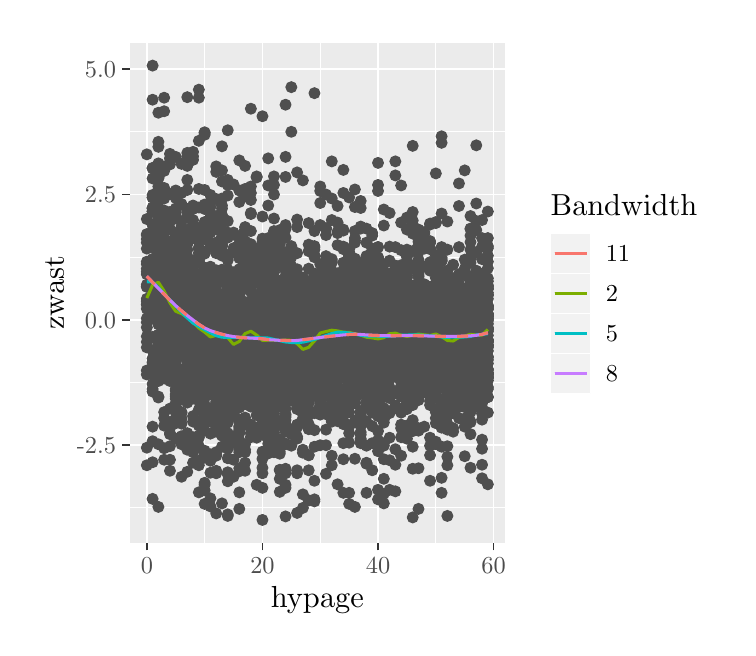
\begin{tikzpicture}[x=1pt,y=1pt]
\definecolor{fillColor}{RGB}{255,255,255}
\path[use as bounding box,fill=fillColor,fill opacity=0.00] (0,0) rectangle (252.94,216.81);
\begin{scope}
\path[clip] (  0.00,  0.00) rectangle (252.94,216.81);
\definecolor{drawColor}{RGB}{255,255,255}
\definecolor{fillColor}{RGB}{255,255,255}

\path[draw=drawColor,line width= 0.6pt,line join=round,line cap=round,fill=fillColor] (  0.00,  0.00) rectangle (252.94,216.81);
\end{scope}
\begin{scope}
\path[clip] ( 36.89, 30.72) rectangle (172.44,211.31);
\definecolor{fillColor}{gray}{0.92}

\path[fill=fillColor] ( 36.89, 30.72) rectangle (172.44,211.31);
\definecolor{drawColor}{RGB}{255,255,255}

\path[draw=drawColor,line width= 0.3pt,line join=round] ( 36.89, 43.28) --
	(172.44, 43.28);

\path[draw=drawColor,line width= 0.3pt,line join=round] ( 36.89, 88.58) --
	(172.44, 88.58);

\path[draw=drawColor,line width= 0.3pt,line join=round] ( 36.89,133.88) --
	(172.44,133.88);

\path[draw=drawColor,line width= 0.3pt,line join=round] ( 36.89,179.18) --
	(172.44,179.18);

\path[draw=drawColor,line width= 0.3pt,line join=round] ( 63.94, 30.72) --
	( 63.94,211.31);

\path[draw=drawColor,line width= 0.3pt,line join=round] (105.71, 30.72) --
	(105.71,211.31);

\path[draw=drawColor,line width= 0.3pt,line join=round] (147.49, 30.72) --
	(147.49,211.31);

\path[draw=drawColor,line width= 0.6pt,line join=round] ( 36.89, 65.93) --
	(172.44, 65.93);

\path[draw=drawColor,line width= 0.6pt,line join=round] ( 36.89,111.23) --
	(172.44,111.23);

\path[draw=drawColor,line width= 0.6pt,line join=round] ( 36.89,156.53) --
	(172.44,156.53);

\path[draw=drawColor,line width= 0.6pt,line join=round] ( 36.89,201.83) --
	(172.44,201.83);

\path[draw=drawColor,line width= 0.6pt,line join=round] ( 43.06, 30.72) --
	( 43.06,211.31);

\path[draw=drawColor,line width= 0.6pt,line join=round] ( 84.83, 30.72) --
	( 84.83,211.31);

\path[draw=drawColor,line width= 0.6pt,line join=round] (126.60, 30.72) --
	(126.60,211.31);

\path[draw=drawColor,line width= 0.6pt,line join=round] (168.37, 30.72) --
	(168.37,211.31);
\definecolor{drawColor}{gray}{0.31}
\definecolor{fillColor}{gray}{0.31}

\path[draw=drawColor,line width= 0.4pt,line join=round,line cap=round,fill=fillColor] (147.49,113.59) circle (  1.96);

\path[draw=drawColor,line width= 0.4pt,line join=round,line cap=round,fill=fillColor] ( 72.30,120.47) circle (  1.96);

\path[draw=drawColor,line width= 0.4pt,line join=round,line cap=round,fill=fillColor] ( 86.92,110.51) circle (  1.96);

\path[draw=drawColor,line width= 0.4pt,line join=round,line cap=round,fill=fillColor] (118.24, 83.15) circle (  1.96);

\path[draw=drawColor,line width= 0.4pt,line join=round,line cap=round,fill=fillColor] (105.71, 81.15) circle (  1.96);

\path[draw=drawColor,line width= 0.4pt,line join=round,line cap=round,fill=fillColor] ( 78.56,117.57) circle (  1.96);

\path[draw=drawColor,line width= 0.4pt,line join=round,line cap=round,fill=fillColor] ( 63.94,112.68) circle (  1.96);

\path[draw=drawColor,line width= 0.4pt,line join=round,line cap=round,fill=fillColor] (147.49, 93.47) circle (  1.96);

\path[draw=drawColor,line width= 0.4pt,line join=round,line cap=round,fill=fillColor] ( 53.50,115.76) circle (  1.96);

\path[draw=drawColor,line width= 0.4pt,line join=round,line cap=round,fill=fillColor] (141.22, 86.77) circle (  1.96);

\path[draw=drawColor,line width= 0.4pt,line join=round,line cap=round,fill=fillColor] ( 76.47,129.53) circle (  1.96);

\path[draw=drawColor,line width= 0.4pt,line join=round,line cap=round,fill=fillColor] (132.86,100.90) circle (  1.96);

\path[draw=drawColor,line width= 0.4pt,line join=round,line cap=round,fill=fillColor] ( 53.50, 85.68) circle (  1.96);

\path[draw=drawColor,line width= 0.4pt,line join=round,line cap=round,fill=fillColor] (143.31,103.62) circle (  1.96);

\path[draw=drawColor,line width= 0.4pt,line join=round,line cap=round,fill=fillColor] ( 47.23,111.05) circle (  1.96);

\path[draw=drawColor,line width= 0.4pt,line join=round,line cap=round,fill=fillColor] (126.60, 87.86) circle (  1.96);

\path[draw=drawColor,line width= 0.4pt,line join=round,line cap=round,fill=fillColor] ( 95.27, 88.04) circle (  1.96);

\path[draw=drawColor,line width= 0.4pt,line join=round,line cap=round,fill=fillColor] ( 89.00,105.43) circle (  1.96);

\path[draw=drawColor,line width= 0.4pt,line join=round,line cap=round,fill=fillColor] ( 97.36, 73.36) circle (  1.96);

\path[draw=drawColor,line width= 0.4pt,line join=round,line cap=round,fill=fillColor] ( 84.83,105.25) circle (  1.96);

\path[draw=drawColor,line width= 0.4pt,line join=round,line cap=round,fill=fillColor] (139.13,101.45) circle (  1.96);

\path[draw=drawColor,line width= 0.4pt,line join=round,line cap=round,fill=fillColor] ( 82.74, 80.43) circle (  1.96);

\path[draw=drawColor,line width= 0.4pt,line join=round,line cap=round,fill=fillColor] (147.49, 98.91) circle (  1.96);

\path[draw=drawColor,line width= 0.4pt,line join=round,line cap=round,fill=fillColor] ( 61.85,116.31) circle (  1.96);

\path[draw=drawColor,line width= 0.4pt,line join=round,line cap=round,fill=fillColor] ( 78.56,103.44) circle (  1.96);

\path[draw=drawColor,line width= 0.4pt,line join=round,line cap=round,fill=fillColor] (114.07, 97.82) circle (  1.96);

\path[draw=drawColor,line width= 0.4pt,line join=round,line cap=round,fill=fillColor] (155.84, 82.97) circle (  1.96);

\path[draw=drawColor,line width= 0.4pt,line join=round,line cap=round,fill=fillColor] ( 57.68,151.10) circle (  1.96);

\path[draw=drawColor,line width= 0.4pt,line join=round,line cap=round,fill=fillColor] ( 47.23, 89.13) circle (  1.96);

\path[draw=drawColor,line width= 0.4pt,line join=round,line cap=round,fill=fillColor] ( 66.03, 46.72) circle (  1.96);

\path[draw=drawColor,line width= 0.4pt,line join=round,line cap=round,fill=fillColor] (164.19, 58.87) circle (  1.96);

\path[draw=drawColor,line width= 0.4pt,line join=round,line cap=round,fill=fillColor] (118.24,114.13) circle (  1.96);

\path[draw=drawColor,line width= 0.4pt,line join=round,line cap=round,fill=fillColor] ( 78.56, 90.76) circle (  1.96);

\path[draw=drawColor,line width= 0.4pt,line join=round,line cap=round,fill=fillColor] ( 76.47, 72.46) circle (  1.96);

\path[draw=drawColor,line width= 0.4pt,line join=round,line cap=round,fill=fillColor] (164.19, 85.32) circle (  1.96);

\path[draw=drawColor,line width= 0.4pt,line join=round,line cap=round,fill=fillColor] (120.33, 99.27) circle (  1.96);

\path[draw=drawColor,line width= 0.4pt,line join=round,line cap=round,fill=fillColor] (166.28,100.00) circle (  1.96);

\path[draw=drawColor,line width= 0.4pt,line join=round,line cap=round,fill=fillColor] ( 91.09, 57.05) circle (  1.96);

\path[draw=drawColor,line width= 0.4pt,line join=round,line cap=round,fill=fillColor] ( 93.18,110.15) circle (  1.96);

\path[draw=drawColor,line width= 0.4pt,line join=round,line cap=round,fill=fillColor] (151.66, 93.84) circle (  1.96);

\path[draw=drawColor,line width= 0.4pt,line join=round,line cap=round,fill=fillColor] (162.11, 95.83) circle (  1.96);

\path[draw=drawColor,line width= 0.4pt,line join=round,line cap=round,fill=fillColor] (116.16,113.23) circle (  1.96);

\path[draw=drawColor,line width= 0.4pt,line join=round,line cap=round,fill=fillColor] ( 84.83, 80.25) circle (  1.96);

\path[draw=drawColor,line width= 0.4pt,line join=round,line cap=round,fill=fillColor] (145.40, 84.41) circle (  1.96);

\path[draw=drawColor,line width= 0.4pt,line join=round,line cap=round,fill=fillColor] ( 99.45, 84.23) circle (  1.96);

\path[draw=drawColor,line width= 0.4pt,line join=round,line cap=round,fill=fillColor] (162.11,106.88) circle (  1.96);

\path[draw=drawColor,line width= 0.4pt,line join=round,line cap=round,fill=fillColor] ( 76.47, 64.30) circle (  1.96);

\path[draw=drawColor,line width= 0.4pt,line join=round,line cap=round,fill=fillColor] (155.84,100.00) circle (  1.96);

\path[draw=drawColor,line width= 0.4pt,line join=round,line cap=round,fill=fillColor] (145.40, 81.88) circle (  1.96);

\path[draw=drawColor,line width= 0.4pt,line join=round,line cap=round,fill=fillColor] ( 63.94,112.50) circle (  1.96);

\path[draw=drawColor,line width= 0.4pt,line join=round,line cap=round,fill=fillColor] ( 93.18,121.20) circle (  1.96);

\path[draw=drawColor,line width= 0.4pt,line join=round,line cap=round,fill=fillColor] (122.42, 81.70) circle (  1.96);

\path[draw=drawColor,line width= 0.4pt,line join=round,line cap=round,fill=fillColor] ( 80.65, 95.47) circle (  1.96);

\path[draw=drawColor,line width= 0.4pt,line join=round,line cap=round,fill=fillColor] (126.60, 96.01) circle (  1.96);

\path[draw=drawColor,line width= 0.4pt,line join=round,line cap=round,fill=fillColor] ( 95.27, 84.78) circle (  1.96);

\path[draw=drawColor,line width= 0.4pt,line join=round,line cap=round,fill=fillColor] (109.89,117.21) circle (  1.96);

\path[draw=drawColor,line width= 0.4pt,line join=round,line cap=round,fill=fillColor] ( 63.94,100.72) circle (  1.96);

\path[draw=drawColor,line width= 0.4pt,line join=round,line cap=round,fill=fillColor] ( 59.76, 84.78) circle (  1.96);

\path[draw=drawColor,line width= 0.4pt,line join=round,line cap=round,fill=fillColor] ( 86.92, 93.29) circle (  1.96);

\path[draw=drawColor,line width= 0.4pt,line join=round,line cap=round,fill=fillColor] ( 80.65,118.12) circle (  1.96);

\path[draw=drawColor,line width= 0.4pt,line join=round,line cap=round,fill=fillColor] (145.40,100.54) circle (  1.96);

\path[draw=drawColor,line width= 0.4pt,line join=round,line cap=round,fill=fillColor] ( 86.92,132.80) circle (  1.96);

\path[draw=drawColor,line width= 0.4pt,line join=round,line cap=round,fill=fillColor] ( 68.12,108.70) circle (  1.96);

\path[draw=drawColor,line width= 0.4pt,line join=round,line cap=round,fill=fillColor] (103.62,101.99) circle (  1.96);

\path[draw=drawColor,line width= 0.4pt,line join=round,line cap=round,fill=fillColor] ( 55.59, 85.68) circle (  1.96);

\path[draw=drawColor,line width= 0.4pt,line join=round,line cap=round,fill=fillColor] ( 51.41,146.75) circle (  1.96);

\path[draw=drawColor,line width= 0.4pt,line join=round,line cap=round,fill=fillColor] (103.62, 99.64) circle (  1.96);

\path[draw=drawColor,line width= 0.4pt,line join=round,line cap=round,fill=fillColor] (101.54,120.47) circle (  1.96);

\path[draw=drawColor,line width= 0.4pt,line join=round,line cap=round,fill=fillColor] (143.31, 96.01) circle (  1.96);

\path[draw=drawColor,line width= 0.4pt,line join=round,line cap=round,fill=fillColor] ( 74.38,107.06) circle (  1.96);

\path[draw=drawColor,line width= 0.4pt,line join=round,line cap=round,fill=fillColor] ( 84.83,115.22) circle (  1.96);

\path[draw=drawColor,line width= 0.4pt,line join=round,line cap=round,fill=fillColor] ( 53.50,137.51) circle (  1.96);

\path[draw=drawColor,line width= 0.4pt,line join=round,line cap=round,fill=fillColor] ( 70.21,141.31) circle (  1.96);

\path[draw=drawColor,line width= 0.4pt,line join=round,line cap=round,fill=fillColor] (124.51,122.83) circle (  1.96);

\path[draw=drawColor,line width= 0.4pt,line join=round,line cap=round,fill=fillColor] (101.54, 87.68) circle (  1.96);

\path[draw=drawColor,line width= 0.4pt,line join=round,line cap=round,fill=fillColor] (162.11, 96.01) circle (  1.96);

\path[draw=drawColor,line width= 0.4pt,line join=round,line cap=round,fill=fillColor] (124.51, 87.86) circle (  1.96);

\path[draw=drawColor,line width= 0.4pt,line join=round,line cap=round,fill=fillColor] (101.54,100.90) circle (  1.96);

\path[draw=drawColor,line width= 0.4pt,line join=round,line cap=round,fill=fillColor] (126.60,103.98) circle (  1.96);

\path[draw=drawColor,line width= 0.4pt,line join=round,line cap=round,fill=fillColor] (145.40,101.45) circle (  1.96);

\path[draw=drawColor,line width= 0.4pt,line join=round,line cap=round,fill=fillColor] (120.33,112.68) circle (  1.96);

\path[draw=drawColor,line width= 0.4pt,line join=round,line cap=round,fill=fillColor] ( 99.45, 87.68) circle (  1.96);

\path[draw=drawColor,line width= 0.4pt,line join=round,line cap=round,fill=fillColor] (164.19,107.06) circle (  1.96);

\path[draw=drawColor,line width= 0.4pt,line join=round,line cap=round,fill=fillColor] ( 99.45, 95.47) circle (  1.96);

\path[draw=drawColor,line width= 0.4pt,line join=round,line cap=round,fill=fillColor] (155.84, 89.31) circle (  1.96);

\path[draw=drawColor,line width= 0.4pt,line join=round,line cap=round,fill=fillColor] ( 93.18, 85.86) circle (  1.96);

\path[draw=drawColor,line width= 0.4pt,line join=round,line cap=round,fill=fillColor] (122.42,107.79) circle (  1.96);

\path[draw=drawColor,line width= 0.4pt,line join=round,line cap=round,fill=fillColor] ( 53.50,170.12) circle (  1.96);

\path[draw=drawColor,line width= 0.4pt,line join=round,line cap=round,fill=fillColor] ( 53.50,132.07) circle (  1.96);

\path[draw=drawColor,line width= 0.4pt,line join=round,line cap=round,fill=fillColor] ( 95.27,113.41) circle (  1.96);

\path[draw=drawColor,line width= 0.4pt,line join=round,line cap=round,fill=fillColor] (101.54,103.44) circle (  1.96);

\path[draw=drawColor,line width= 0.4pt,line join=round,line cap=round,fill=fillColor] (155.84,115.94) circle (  1.96);

\path[draw=drawColor,line width= 0.4pt,line join=round,line cap=round,fill=fillColor] ( 70.21, 98.37) circle (  1.96);

\path[draw=drawColor,line width= 0.4pt,line join=round,line cap=round,fill=fillColor] (111.98,124.28) circle (  1.96);

\path[draw=drawColor,line width= 0.4pt,line join=round,line cap=round,fill=fillColor] ( 68.12,129.17) circle (  1.96);

\path[draw=drawColor,line width= 0.4pt,line join=round,line cap=round,fill=fillColor] (164.19,103.80) circle (  1.96);

\path[draw=drawColor,line width= 0.4pt,line join=round,line cap=round,fill=fillColor] ( 68.12, 87.50) circle (  1.96);

\path[draw=drawColor,line width= 0.4pt,line join=round,line cap=round,fill=fillColor] ( 72.30,110.15) circle (  1.96);

\path[draw=drawColor,line width= 0.4pt,line join=round,line cap=round,fill=fillColor] ( 84.83,103.08) circle (  1.96);

\path[draw=drawColor,line width= 0.4pt,line join=round,line cap=round,fill=fillColor] ( 49.32,112.68) circle (  1.96);

\path[draw=drawColor,line width= 0.4pt,line join=round,line cap=round,fill=fillColor] (166.28, 86.95) circle (  1.96);

\path[draw=drawColor,line width= 0.4pt,line join=round,line cap=round,fill=fillColor] ( 84.83,110.51) circle (  1.96);

\path[draw=drawColor,line width= 0.4pt,line join=round,line cap=round,fill=fillColor] ( 95.27, 92.57) circle (  1.96);

\path[draw=drawColor,line width= 0.4pt,line join=round,line cap=round,fill=fillColor] (145.40,104.53) circle (  1.96);

\path[draw=drawColor,line width= 0.4pt,line join=round,line cap=round,fill=fillColor] ( 97.36,108.51) circle (  1.96);

\path[draw=drawColor,line width= 0.4pt,line join=round,line cap=round,fill=fillColor] (147.49,108.70) circle (  1.96);

\path[draw=drawColor,line width= 0.4pt,line join=round,line cap=round,fill=fillColor] (101.54, 46.00) circle (  1.96);

\path[draw=drawColor,line width= 0.4pt,line join=round,line cap=round,fill=fillColor] ( 63.94,178.10) circle (  1.96);

\path[draw=drawColor,line width= 0.4pt,line join=round,line cap=round,fill=fillColor] ( 84.83,128.27) circle (  1.96);

\path[draw=drawColor,line width= 0.4pt,line join=round,line cap=round,fill=fillColor] ( 91.09,116.67) circle (  1.96);

\path[draw=drawColor,line width= 0.4pt,line join=round,line cap=round,fill=fillColor] (147.49, 94.92) circle (  1.96);

\path[draw=drawColor,line width= 0.4pt,line join=round,line cap=round,fill=fillColor] (124.51, 86.95) circle (  1.96);

\path[draw=drawColor,line width= 0.4pt,line join=round,line cap=round,fill=fillColor] (166.28,115.22) circle (  1.96);

\path[draw=drawColor,line width= 0.4pt,line join=round,line cap=round,fill=fillColor] ( 74.38,125.00) circle (  1.96);

\path[draw=drawColor,line width= 0.4pt,line join=round,line cap=round,fill=fillColor] ( 97.36,112.32) circle (  1.96);

\path[draw=drawColor,line width= 0.4pt,line join=round,line cap=round,fill=fillColor] (120.33, 87.13) circle (  1.96);

\path[draw=drawColor,line width= 0.4pt,line join=round,line cap=round,fill=fillColor] ( 45.14,151.46) circle (  1.96);

\path[draw=drawColor,line width= 0.4pt,line join=round,line cap=round,fill=fillColor] (122.42, 99.82) circle (  1.96);

\path[draw=drawColor,line width= 0.4pt,line join=round,line cap=round,fill=fillColor] ( 61.85,117.76) circle (  1.96);

\path[draw=drawColor,line width= 0.4pt,line join=round,line cap=round,fill=fillColor] (107.80,115.94) circle (  1.96);

\path[draw=drawColor,line width= 0.4pt,line join=round,line cap=round,fill=fillColor] ( 47.23,121.74) circle (  1.96);

\path[draw=drawColor,line width= 0.4pt,line join=round,line cap=round,fill=fillColor] (120.33,114.49) circle (  1.96);

\path[draw=drawColor,line width= 0.4pt,line join=round,line cap=round,fill=fillColor] ( 51.41, 93.29) circle (  1.96);

\path[draw=drawColor,line width= 0.4pt,line join=round,line cap=round,fill=fillColor] (147.49, 93.29) circle (  1.96);

\path[draw=drawColor,line width= 0.4pt,line join=round,line cap=round,fill=fillColor] (101.54,103.26) circle (  1.96);

\path[draw=drawColor,line width= 0.4pt,line join=round,line cap=round,fill=fillColor] ( 61.85,107.97) circle (  1.96);

\path[draw=drawColor,line width= 0.4pt,line join=round,line cap=round,fill=fillColor] (157.93,127.36) circle (  1.96);

\path[draw=drawColor,line width= 0.4pt,line join=round,line cap=round,fill=fillColor] (103.62,133.88) circle (  1.96);

\path[draw=drawColor,line width= 0.4pt,line join=round,line cap=round,fill=fillColor] ( 66.03,129.17) circle (  1.96);

\path[draw=drawColor,line width= 0.4pt,line join=round,line cap=round,fill=fillColor] ( 66.03,126.09) circle (  1.96);

\path[draw=drawColor,line width= 0.4pt,line join=round,line cap=round,fill=fillColor] ( 78.56,139.14) circle (  1.96);

\path[draw=drawColor,line width= 0.4pt,line join=round,line cap=round,fill=fillColor] ( 78.56,134.97) circle (  1.96);

\path[draw=drawColor,line width= 0.4pt,line join=round,line cap=round,fill=fillColor] ( 93.18, 86.95) circle (  1.96);

\path[draw=drawColor,line width= 0.4pt,line join=round,line cap=round,fill=fillColor] (116.16,101.45) circle (  1.96);

\path[draw=drawColor,line width= 0.4pt,line join=round,line cap=round,fill=fillColor] (157.93,117.57) circle (  1.96);

\path[draw=drawColor,line width= 0.4pt,line join=round,line cap=round,fill=fillColor] (130.78, 60.50) circle (  1.96);

\path[draw=drawColor,line width= 0.4pt,line join=round,line cap=round,fill=fillColor] (109.89,119.39) circle (  1.96);

\path[draw=drawColor,line width= 0.4pt,line join=round,line cap=round,fill=fillColor] ( 47.23,133.34) circle (  1.96);

\path[draw=drawColor,line width= 0.4pt,line join=round,line cap=round,fill=fillColor] (105.71,124.64) circle (  1.96);

\path[draw=drawColor,line width= 0.4pt,line join=round,line cap=round,fill=fillColor] (120.33,117.39) circle (  1.96);

\path[draw=drawColor,line width= 0.4pt,line join=round,line cap=round,fill=fillColor] (109.89,117.94) circle (  1.96);

\path[draw=drawColor,line width= 0.4pt,line join=round,line cap=round,fill=fillColor] ( 53.50,148.92) circle (  1.96);

\path[draw=drawColor,line width= 0.4pt,line join=round,line cap=round,fill=fillColor] ( 72.30, 40.93) circle (  1.96);

\path[draw=drawColor,line width= 0.4pt,line join=round,line cap=round,fill=fillColor] (155.84,104.71) circle (  1.96);

\path[draw=drawColor,line width= 0.4pt,line join=round,line cap=round,fill=fillColor] ( 74.38,115.04) circle (  1.96);

\path[draw=drawColor,line width= 0.4pt,line join=round,line cap=round,fill=fillColor] ( 68.12,114.13) circle (  1.96);

\path[draw=drawColor,line width= 0.4pt,line join=round,line cap=round,fill=fillColor] ( 70.21,143.12) circle (  1.96);

\path[draw=drawColor,line width= 0.4pt,line join=round,line cap=round,fill=fillColor] ( 86.92, 72.27) circle (  1.96);

\path[draw=drawColor,line width= 0.4pt,line join=round,line cap=round,fill=fillColor] (111.98,121.38) circle (  1.96);

\path[draw=drawColor,line width= 0.4pt,line join=round,line cap=round,fill=fillColor] (141.22,116.85) circle (  1.96);

\path[draw=drawColor,line width= 0.4pt,line join=round,line cap=round,fill=fillColor] (141.22,124.46) circle (  1.96);

\path[draw=drawColor,line width= 0.4pt,line join=round,line cap=round,fill=fillColor] ( 51.41,156.71) circle (  1.96);

\path[draw=drawColor,line width= 0.4pt,line join=round,line cap=round,fill=fillColor] (109.89, 97.28) circle (  1.96);

\path[draw=drawColor,line width= 0.4pt,line join=round,line cap=round,fill=fillColor] ( 84.83,133.88) circle (  1.96);

\path[draw=drawColor,line width= 0.4pt,line join=round,line cap=round,fill=fillColor] (107.80,127.18) circle (  1.96);

\path[draw=drawColor,line width= 0.4pt,line join=round,line cap=round,fill=fillColor] ( 66.03,103.08) circle (  1.96);

\path[draw=drawColor,line width= 0.4pt,line join=round,line cap=round,fill=fillColor] ( 66.03,100.54) circle (  1.96);

\path[draw=drawColor,line width= 0.4pt,line join=round,line cap=round,fill=fillColor] (124.51,121.38) circle (  1.96);

\path[draw=drawColor,line width= 0.4pt,line join=round,line cap=round,fill=fillColor] ( 61.85,107.06) circle (  1.96);

\path[draw=drawColor,line width= 0.4pt,line join=round,line cap=round,fill=fillColor] ( 89.00,103.98) circle (  1.96);

\path[draw=drawColor,line width= 0.4pt,line join=round,line cap=round,fill=fillColor] (151.66, 98.55) circle (  1.96);

\path[draw=drawColor,line width= 0.4pt,line join=round,line cap=round,fill=fillColor] (111.98, 77.35) circle (  1.96);

\path[draw=drawColor,line width= 0.4pt,line join=round,line cap=round,fill=fillColor] (126.60, 82.97) circle (  1.96);

\path[draw=drawColor,line width= 0.4pt,line join=round,line cap=round,fill=fillColor] ( 68.12, 84.60) circle (  1.96);

\path[draw=drawColor,line width= 0.4pt,line join=round,line cap=round,fill=fillColor] (109.89,117.21) circle (  1.96);

\path[draw=drawColor,line width= 0.4pt,line join=round,line cap=round,fill=fillColor] (155.84,127.72) circle (  1.96);

\path[draw=drawColor,line width= 0.4pt,line join=round,line cap=round,fill=fillColor] ( 47.23,162.87) circle (  1.96);

\path[draw=drawColor,line width= 0.4pt,line join=round,line cap=round,fill=fillColor] (120.33,106.34) circle (  1.96);

\path[draw=drawColor,line width= 0.4pt,line join=round,line cap=round,fill=fillColor] ( 63.94, 93.66) circle (  1.96);

\path[draw=drawColor,line width= 0.4pt,line join=round,line cap=round,fill=fillColor] (139.13,100.54) circle (  1.96);

\path[draw=drawColor,line width= 0.4pt,line join=round,line cap=round,fill=fillColor] ( 89.00,106.16) circle (  1.96);

\path[draw=drawColor,line width= 0.4pt,line join=round,line cap=round,fill=fillColor] ( 61.85, 87.68) circle (  1.96);

\path[draw=drawColor,line width= 0.4pt,line join=round,line cap=round,fill=fillColor] (151.66,114.68) circle (  1.96);

\path[draw=drawColor,line width= 0.4pt,line join=round,line cap=round,fill=fillColor] ( 70.21,108.88) circle (  1.96);

\path[draw=drawColor,line width= 0.4pt,line join=round,line cap=round,fill=fillColor] (126.60,112.86) circle (  1.96);

\path[draw=drawColor,line width= 0.4pt,line join=round,line cap=round,fill=fillColor] ( 57.68,109.06) circle (  1.96);

\path[draw=drawColor,line width= 0.4pt,line join=round,line cap=round,fill=fillColor] (116.16,109.24) circle (  1.96);

\path[draw=drawColor,line width= 0.4pt,line join=round,line cap=round,fill=fillColor] (164.19, 92.75) circle (  1.96);

\path[draw=drawColor,line width= 0.4pt,line join=round,line cap=round,fill=fillColor] (107.80, 99.82) circle (  1.96);

\path[draw=drawColor,line width= 0.4pt,line join=round,line cap=round,fill=fillColor] (145.40,137.14) circle (  1.96);

\path[draw=drawColor,line width= 0.4pt,line join=round,line cap=round,fill=fillColor] ( 86.92, 81.15) circle (  1.96);

\path[draw=drawColor,line width= 0.4pt,line join=round,line cap=round,fill=fillColor] (139.13,102.17) circle (  1.96);

\path[draw=drawColor,line width= 0.4pt,line join=round,line cap=round,fill=fillColor] ( 78.56,101.27) circle (  1.96);

\path[draw=drawColor,line width= 0.4pt,line join=round,line cap=round,fill=fillColor] (124.51,141.67) circle (  1.96);

\path[draw=drawColor,line width= 0.4pt,line join=round,line cap=round,fill=fillColor] (103.62,111.78) circle (  1.96);

\path[draw=drawColor,line width= 0.4pt,line join=round,line cap=round,fill=fillColor] (166.28,125.18) circle (  1.96);

\path[draw=drawColor,line width= 0.4pt,line join=round,line cap=round,fill=fillColor] ( 91.09,136.42) circle (  1.96);

\path[draw=drawColor,line width= 0.4pt,line join=round,line cap=round,fill=fillColor] ( 93.18,135.51) circle (  1.96);

\path[draw=drawColor,line width= 0.4pt,line join=round,line cap=round,fill=fillColor] (141.22,119.02) circle (  1.96);

\path[draw=drawColor,line width= 0.4pt,line join=round,line cap=round,fill=fillColor] ( 57.68, 96.92) circle (  1.96);

\path[draw=drawColor,line width= 0.4pt,line join=round,line cap=round,fill=fillColor] ( 76.47,124.46) circle (  1.96);

\path[draw=drawColor,line width= 0.4pt,line join=round,line cap=round,fill=fillColor] (101.54,111.41) circle (  1.96);

\path[draw=drawColor,line width= 0.4pt,line join=round,line cap=round,fill=fillColor] ( 53.50, 98.55) circle (  1.96);

\path[draw=drawColor,line width= 0.4pt,line join=round,line cap=round,fill=fillColor] (141.22,127.18) circle (  1.96);

\path[draw=drawColor,line width= 0.4pt,line join=round,line cap=round,fill=fillColor] ( 76.47,133.52) circle (  1.96);

\path[draw=drawColor,line width= 0.4pt,line join=round,line cap=round,fill=fillColor] ( 47.23,152.00) circle (  1.96);

\path[draw=drawColor,line width= 0.4pt,line join=round,line cap=round,fill=fillColor] (155.84,121.74) circle (  1.96);

\path[draw=drawColor,line width= 0.4pt,line join=round,line cap=round,fill=fillColor] ( 61.85,122.29) circle (  1.96);

\path[draw=drawColor,line width= 0.4pt,line join=round,line cap=round,fill=fillColor] ( 78.56,109.42) circle (  1.96);

\path[draw=drawColor,line width= 0.4pt,line join=round,line cap=round,fill=fillColor] (120.33,122.10) circle (  1.96);

\path[draw=drawColor,line width= 0.4pt,line join=round,line cap=round,fill=fillColor] (151.66,103.62) circle (  1.96);

\path[draw=drawColor,line width= 0.4pt,line join=round,line cap=round,fill=fillColor] (134.95, 86.05) circle (  1.96);

\path[draw=drawColor,line width= 0.4pt,line join=round,line cap=round,fill=fillColor] (103.62,100.72) circle (  1.96);

\path[draw=drawColor,line width= 0.4pt,line join=round,line cap=round,fill=fillColor] (137.04,103.08) circle (  1.96);

\path[draw=drawColor,line width= 0.4pt,line join=round,line cap=round,fill=fillColor] ( 45.14,105.07) circle (  1.96);

\path[draw=drawColor,line width= 0.4pt,line join=round,line cap=round,fill=fillColor] ( 95.27, 98.73) circle (  1.96);

\path[draw=drawColor,line width= 0.4pt,line join=round,line cap=round,fill=fillColor] ( 68.12, 63.40) circle (  1.96);

\path[draw=drawColor,line width= 0.4pt,line join=round,line cap=round,fill=fillColor] ( 72.30,114.49) circle (  1.96);

\path[draw=drawColor,line width= 0.4pt,line join=round,line cap=round,fill=fillColor] (132.86,113.04) circle (  1.96);

\path[draw=drawColor,line width= 0.4pt,line join=round,line cap=round,fill=fillColor] ( 53.50,101.09) circle (  1.96);

\path[draw=drawColor,line width= 0.4pt,line join=round,line cap=round,fill=fillColor] (128.69, 98.00) circle (  1.96);

\path[draw=drawColor,line width= 0.4pt,line join=round,line cap=round,fill=fillColor] (114.07,114.31) circle (  1.96);

\path[draw=drawColor,line width= 0.4pt,line join=round,line cap=round,fill=fillColor] (151.66,126.45) circle (  1.96);

\path[draw=drawColor,line width= 0.4pt,line join=round,line cap=round,fill=fillColor] ( 53.50,110.87) circle (  1.96);

\path[draw=drawColor,line width= 0.4pt,line join=round,line cap=round,fill=fillColor] (130.78,137.69) circle (  1.96);

\path[draw=drawColor,line width= 0.4pt,line join=round,line cap=round,fill=fillColor] (141.22,109.06) circle (  1.96);

\path[draw=drawColor,line width= 0.4pt,line join=round,line cap=round,fill=fillColor] ( 89.00,101.45) circle (  1.96);

\path[draw=drawColor,line width= 0.4pt,line join=round,line cap=round,fill=fillColor] (118.24,118.84) circle (  1.96);

\path[draw=drawColor,line width= 0.4pt,line join=round,line cap=round,fill=fillColor] ( 82.74, 93.66) circle (  1.96);

\path[draw=drawColor,line width= 0.4pt,line join=round,line cap=round,fill=fillColor] (120.33, 94.20) circle (  1.96);

\path[draw=drawColor,line width= 0.4pt,line join=round,line cap=round,fill=fillColor] ( 70.21, 96.01) circle (  1.96);

\path[draw=drawColor,line width= 0.4pt,line join=round,line cap=round,fill=fillColor] ( 47.23,130.44) circle (  1.96);

\path[draw=drawColor,line width= 0.4pt,line join=round,line cap=round,fill=fillColor] (164.19, 99.82) circle (  1.96);

\path[draw=drawColor,line width= 0.4pt,line join=round,line cap=round,fill=fillColor] ( 97.36,107.79) circle (  1.96);

\path[draw=drawColor,line width= 0.4pt,line join=round,line cap=round,fill=fillColor] ( 55.59,104.35) circle (  1.96);

\path[draw=drawColor,line width= 0.4pt,line join=round,line cap=round,fill=fillColor] ( 91.09, 88.04) circle (  1.96);

\path[draw=drawColor,line width= 0.4pt,line join=round,line cap=round,fill=fillColor] (147.49, 75.72) circle (  1.96);

\path[draw=drawColor,line width= 0.4pt,line join=round,line cap=round,fill=fillColor] ( 47.23, 94.74) circle (  1.96);

\path[draw=drawColor,line width= 0.4pt,line join=round,line cap=round,fill=fillColor] (122.42,104.71) circle (  1.96);

\path[draw=drawColor,line width= 0.4pt,line join=round,line cap=round,fill=fillColor] ( 84.83,104.89) circle (  1.96);

\path[draw=drawColor,line width= 0.4pt,line join=round,line cap=round,fill=fillColor] (118.24, 43.64) circle (  1.96);

\path[draw=drawColor,line width= 0.4pt,line join=round,line cap=round,fill=fillColor] ( 59.76, 97.82) circle (  1.96);

\path[draw=drawColor,line width= 0.4pt,line join=round,line cap=round,fill=fillColor] ( 61.85, 96.92) circle (  1.96);

\path[draw=drawColor,line width= 0.4pt,line join=round,line cap=round,fill=fillColor] (116.16,100.90) circle (  1.96);

\path[draw=drawColor,line width= 0.4pt,line join=round,line cap=round,fill=fillColor] (151.66, 93.47) circle (  1.96);

\path[draw=drawColor,line width= 0.4pt,line join=round,line cap=round,fill=fillColor] ( 95.27, 96.56) circle (  1.96);

\path[draw=drawColor,line width= 0.4pt,line join=round,line cap=round,fill=fillColor] ( 95.27, 90.21) circle (  1.96);

\path[draw=drawColor,line width= 0.4pt,line join=round,line cap=round,fill=fillColor] (164.19, 84.05) circle (  1.96);

\path[draw=drawColor,line width= 0.4pt,line join=round,line cap=round,fill=fillColor] (162.11, 88.58) circle (  1.96);

\path[draw=drawColor,line width= 0.4pt,line join=round,line cap=round,fill=fillColor] ( 91.09,102.72) circle (  1.96);

\path[draw=drawColor,line width= 0.4pt,line join=round,line cap=round,fill=fillColor] (166.28, 91.48) circle (  1.96);

\path[draw=drawColor,line width= 0.4pt,line join=round,line cap=round,fill=fillColor] ( 89.00, 82.24) circle (  1.96);

\path[draw=drawColor,line width= 0.4pt,line join=round,line cap=round,fill=fillColor] ( 89.00, 84.23) circle (  1.96);

\path[draw=drawColor,line width= 0.4pt,line join=round,line cap=round,fill=fillColor] (137.04, 84.60) circle (  1.96);

\path[draw=drawColor,line width= 0.4pt,line join=round,line cap=round,fill=fillColor] ( 51.41,133.70) circle (  1.96);

\path[draw=drawColor,line width= 0.4pt,line join=round,line cap=round,fill=fillColor] (149.57,102.17) circle (  1.96);

\path[draw=drawColor,line width= 0.4pt,line join=round,line cap=round,fill=fillColor] ( 82.74,103.80) circle (  1.96);

\path[draw=drawColor,line width= 0.4pt,line join=round,line cap=round,fill=fillColor] (111.98,102.17) circle (  1.96);

\path[draw=drawColor,line width= 0.4pt,line join=round,line cap=round,fill=fillColor] (130.78,124.82) circle (  1.96);

\path[draw=drawColor,line width= 0.4pt,line join=round,line cap=round,fill=fillColor] (130.78,117.76) circle (  1.96);

\path[draw=drawColor,line width= 0.4pt,line join=round,line cap=round,fill=fillColor] ( 84.83,128.99) circle (  1.96);

\path[draw=drawColor,line width= 0.4pt,line join=round,line cap=round,fill=fillColor] (111.98, 84.96) circle (  1.96);

\path[draw=drawColor,line width= 0.4pt,line join=round,line cap=round,fill=fillColor] (107.80,111.05) circle (  1.96);

\path[draw=drawColor,line width= 0.4pt,line join=round,line cap=round,fill=fillColor] (109.89, 99.64) circle (  1.96);

\path[draw=drawColor,line width= 0.4pt,line join=round,line cap=round,fill=fillColor] ( 86.92,132.43) circle (  1.96);

\path[draw=drawColor,line width= 0.4pt,line join=round,line cap=round,fill=fillColor] ( 70.21, 93.47) circle (  1.96);

\path[draw=drawColor,line width= 0.4pt,line join=round,line cap=round,fill=fillColor] ( 68.12, 88.94) circle (  1.96);

\path[draw=drawColor,line width= 0.4pt,line join=round,line cap=round,fill=fillColor] (139.13,111.78) circle (  1.96);

\path[draw=drawColor,line width= 0.4pt,line join=round,line cap=round,fill=fillColor] (141.22,111.05) circle (  1.96);

\path[draw=drawColor,line width= 0.4pt,line join=round,line cap=round,fill=fillColor] ( 91.09, 74.63) circle (  1.96);

\path[draw=drawColor,line width= 0.4pt,line join=round,line cap=round,fill=fillColor] ( 80.65,136.78) circle (  1.96);

\path[draw=drawColor,line width= 0.4pt,line join=round,line cap=round,fill=fillColor] (130.78,114.49) circle (  1.96);

\path[draw=drawColor,line width= 0.4pt,line join=round,line cap=round,fill=fillColor] (155.84, 99.82) circle (  1.96);

\path[draw=drawColor,line width= 0.4pt,line join=round,line cap=round,fill=fillColor] ( 61.85,101.99) circle (  1.96);

\path[draw=drawColor,line width= 0.4pt,line join=round,line cap=round,fill=fillColor] (109.89,101.45) circle (  1.96);

\path[draw=drawColor,line width= 0.4pt,line join=round,line cap=round,fill=fillColor] ( 53.50, 83.69) circle (  1.96);

\path[draw=drawColor,line width= 0.4pt,line join=round,line cap=round,fill=fillColor] ( 66.03, 75.17) circle (  1.96);

\path[draw=drawColor,line width= 0.4pt,line join=round,line cap=round,fill=fillColor] (114.07, 84.41) circle (  1.96);

\path[draw=drawColor,line width= 0.4pt,line join=round,line cap=round,fill=fillColor] (114.07,105.98) circle (  1.96);

\path[draw=drawColor,line width= 0.4pt,line join=round,line cap=round,fill=fillColor] (160.02,118.66) circle (  1.96);

\path[draw=drawColor,line width= 0.4pt,line join=round,line cap=round,fill=fillColor] ( 93.18,114.49) circle (  1.96);

\path[draw=drawColor,line width= 0.4pt,line join=round,line cap=round,fill=fillColor] (132.86,113.95) circle (  1.96);

\path[draw=drawColor,line width= 0.4pt,line join=round,line cap=round,fill=fillColor] ( 70.21,128.45) circle (  1.96);

\path[draw=drawColor,line width= 0.4pt,line join=round,line cap=round,fill=fillColor] ( 89.00,159.98) circle (  1.96);

\path[draw=drawColor,line width= 0.4pt,line join=round,line cap=round,fill=fillColor] ( 91.09,138.59) circle (  1.96);

\path[draw=drawColor,line width= 0.4pt,line join=round,line cap=round,fill=fillColor] ( 68.12, 73.00) circle (  1.96);

\path[draw=drawColor,line width= 0.4pt,line join=round,line cap=round,fill=fillColor] ( 80.65, 99.09) circle (  1.96);

\path[draw=drawColor,line width= 0.4pt,line join=round,line cap=round,fill=fillColor] ( 55.59,144.21) circle (  1.96);

\path[draw=drawColor,line width= 0.4pt,line join=round,line cap=round,fill=fillColor] ( 86.92,108.15) circle (  1.96);

\path[draw=drawColor,line width= 0.4pt,line join=round,line cap=round,fill=fillColor] (120.33,115.04) circle (  1.96);

\path[draw=drawColor,line width= 0.4pt,line join=round,line cap=round,fill=fillColor] ( 93.18, 86.05) circle (  1.96);

\path[draw=drawColor,line width= 0.4pt,line join=round,line cap=round,fill=fillColor] (122.42,134.25) circle (  1.96);

\path[draw=drawColor,line width= 0.4pt,line join=round,line cap=round,fill=fillColor] ( 59.76,101.81) circle (  1.96);

\path[draw=drawColor,line width= 0.4pt,line join=round,line cap=round,fill=fillColor] ( 63.94, 74.81) circle (  1.96);

\path[draw=drawColor,line width= 0.4pt,line join=round,line cap=round,fill=fillColor] ( 78.56,114.49) circle (  1.96);

\path[draw=drawColor,line width= 0.4pt,line join=round,line cap=round,fill=fillColor] (137.04,122.47) circle (  1.96);

\path[draw=drawColor,line width= 0.4pt,line join=round,line cap=round,fill=fillColor] (103.62,107.25) circle (  1.96);

\path[draw=drawColor,line width= 0.4pt,line join=round,line cap=round,fill=fillColor] (151.66,117.76) circle (  1.96);

\path[draw=drawColor,line width= 0.4pt,line join=round,line cap=round,fill=fillColor] (111.98,115.58) circle (  1.96);

\path[draw=drawColor,line width= 0.4pt,line join=round,line cap=round,fill=fillColor] (157.93,110.51) circle (  1.96);

\path[draw=drawColor,line width= 0.4pt,line join=round,line cap=round,fill=fillColor] (114.07, 92.21) circle (  1.96);

\path[draw=drawColor,line width= 0.4pt,line join=round,line cap=round,fill=fillColor] (166.28,101.99) circle (  1.96);

\path[draw=drawColor,line width= 0.4pt,line join=round,line cap=round,fill=fillColor] (105.71,105.25) circle (  1.96);

\path[draw=drawColor,line width= 0.4pt,line join=round,line cap=round,fill=fillColor] ( 91.09, 90.58) circle (  1.96);

\path[draw=drawColor,line width= 0.4pt,line join=round,line cap=round,fill=fillColor] ( 59.76, 91.30) circle (  1.96);

\path[draw=drawColor,line width= 0.4pt,line join=round,line cap=round,fill=fillColor] ( 70.21, 99.45) circle (  1.96);

\path[draw=drawColor,line width= 0.4pt,line join=round,line cap=round,fill=fillColor] (130.78,124.64) circle (  1.96);

\path[draw=drawColor,line width= 0.4pt,line join=round,line cap=round,fill=fillColor] ( 61.85,113.23) circle (  1.96);

\path[draw=drawColor,line width= 0.4pt,line join=round,line cap=round,fill=fillColor] (126.60,124.46) circle (  1.96);

\path[draw=drawColor,line width= 0.4pt,line join=round,line cap=round,fill=fillColor] (166.28,123.74) circle (  1.96);

\path[draw=drawColor,line width= 0.4pt,line join=round,line cap=round,fill=fillColor] (118.24,118.48) circle (  1.96);

\path[draw=drawColor,line width= 0.4pt,line join=round,line cap=round,fill=fillColor] ( 45.14,126.63) circle (  1.96);

\path[draw=drawColor,line width= 0.4pt,line join=round,line cap=round,fill=fillColor] ( 72.30, 99.82) circle (  1.96);

\path[draw=drawColor,line width= 0.4pt,line join=round,line cap=round,fill=fillColor] (160.02,144.03) circle (  1.96);

\path[draw=drawColor,line width= 0.4pt,line join=round,line cap=round,fill=fillColor] ( 76.47, 93.84) circle (  1.96);

\path[draw=drawColor,line width= 0.4pt,line join=round,line cap=round,fill=fillColor] (109.89,117.76) circle (  1.96);

\path[draw=drawColor,line width= 0.4pt,line join=round,line cap=round,fill=fillColor] (149.57,101.27) circle (  1.96);

\path[draw=drawColor,line width= 0.4pt,line join=round,line cap=round,fill=fillColor] ( 59.76, 97.28) circle (  1.96);

\path[draw=drawColor,line width= 0.4pt,line join=round,line cap=round,fill=fillColor] (124.51,115.22) circle (  1.96);

\path[draw=drawColor,line width= 0.4pt,line join=round,line cap=round,fill=fillColor] ( 66.03,105.80) circle (  1.96);

\path[draw=drawColor,line width= 0.4pt,line join=round,line cap=round,fill=fillColor] (122.42,111.78) circle (  1.96);

\path[draw=drawColor,line width= 0.4pt,line join=round,line cap=round,fill=fillColor] ( 72.30,156.17) circle (  1.96);

\path[draw=drawColor,line width= 0.4pt,line join=round,line cap=round,fill=fillColor] (120.33,120.65) circle (  1.96);

\path[draw=drawColor,line width= 0.4pt,line join=round,line cap=round,fill=fillColor] (166.28,132.25) circle (  1.96);

\path[draw=drawColor,line width= 0.4pt,line join=round,line cap=round,fill=fillColor] ( 72.30,100.54) circle (  1.96);

\path[draw=drawColor,line width= 0.4pt,line join=round,line cap=round,fill=fillColor] (124.51,134.06) circle (  1.96);

\path[draw=drawColor,line width= 0.4pt,line join=round,line cap=round,fill=fillColor] (155.84, 75.72) circle (  1.96);

\path[draw=drawColor,line width= 0.4pt,line join=round,line cap=round,fill=fillColor] ( 59.76, 88.58) circle (  1.96);

\path[draw=drawColor,line width= 0.4pt,line join=round,line cap=round,fill=fillColor] (111.98, 75.90) circle (  1.96);

\path[draw=drawColor,line width= 0.4pt,line join=round,line cap=round,fill=fillColor] ( 76.47,168.85) circle (  1.96);

\path[draw=drawColor,line width= 0.4pt,line join=round,line cap=round,fill=fillColor] (160.02,114.86) circle (  1.96);

\path[draw=drawColor,line width= 0.4pt,line join=round,line cap=round,fill=fillColor] ( 57.68,142.04) circle (  1.96);

\path[draw=drawColor,line width= 0.4pt,line join=round,line cap=round,fill=fillColor] ( 72.30,122.47) circle (  1.96);

\path[draw=drawColor,line width= 0.4pt,line join=round,line cap=round,fill=fillColor] (153.75,120.65) circle (  1.96);

\path[draw=drawColor,line width= 0.4pt,line join=round,line cap=round,fill=fillColor] ( 89.00,114.86) circle (  1.96);

\path[draw=drawColor,line width= 0.4pt,line join=round,line cap=round,fill=fillColor] (149.57,109.24) circle (  1.96);

\path[draw=drawColor,line width= 0.4pt,line join=round,line cap=round,fill=fillColor] (114.07,106.88) circle (  1.96);

\path[draw=drawColor,line width= 0.4pt,line join=round,line cap=round,fill=fillColor] (116.16,155.45) circle (  1.96);

\path[draw=drawColor,line width= 0.4pt,line join=round,line cap=round,fill=fillColor] ( 47.23,134.43) circle (  1.96);

\path[draw=drawColor,line width= 0.4pt,line join=round,line cap=round,fill=fillColor] (103.62,120.65) circle (  1.96);

\path[draw=drawColor,line width= 0.4pt,line join=round,line cap=round,fill=fillColor] (157.93,100.90) circle (  1.96);

\path[draw=drawColor,line width= 0.4pt,line join=round,line cap=round,fill=fillColor] (116.16,107.79) circle (  1.96);

\path[draw=drawColor,line width= 0.4pt,line join=round,line cap=round,fill=fillColor] ( 53.50, 86.23) circle (  1.96);

\path[draw=drawColor,line width= 0.4pt,line join=round,line cap=round,fill=fillColor] ( 49.32,104.89) circle (  1.96);

\path[draw=drawColor,line width= 0.4pt,line join=round,line cap=round,fill=fillColor] (141.22, 42.92) circle (  1.96);

\path[draw=drawColor,line width= 0.4pt,line join=round,line cap=round,fill=fillColor] (145.40,113.95) circle (  1.96);

\path[draw=drawColor,line width= 0.4pt,line join=round,line cap=round,fill=fillColor] (111.98, 87.31) circle (  1.96);

\path[draw=drawColor,line width= 0.4pt,line join=round,line cap=round,fill=fillColor] (105.71,104.71) circle (  1.96);

\path[draw=drawColor,line width= 0.4pt,line join=round,line cap=round,fill=fillColor] (107.80,107.43) circle (  1.96);

\path[draw=drawColor,line width= 0.4pt,line join=round,line cap=round,fill=fillColor] (107.80,123.74) circle (  1.96);

\path[draw=drawColor,line width= 0.4pt,line join=round,line cap=round,fill=fillColor] ( 51.41,128.99) circle (  1.96);

\path[draw=drawColor,line width= 0.4pt,line join=round,line cap=round,fill=fillColor] ( 57.68,126.82) circle (  1.96);

\path[draw=drawColor,line width= 0.4pt,line join=round,line cap=round,fill=fillColor] (122.42,103.08) circle (  1.96);

\path[draw=drawColor,line width= 0.4pt,line join=round,line cap=round,fill=fillColor] (122.42,100.90) circle (  1.96);

\path[draw=drawColor,line width= 0.4pt,line join=round,line cap=round,fill=fillColor] ( 61.85, 95.11) circle (  1.96);

\path[draw=drawColor,line width= 0.4pt,line join=round,line cap=round,fill=fillColor] ( 78.56, 95.65) circle (  1.96);

\path[draw=drawColor,line width= 0.4pt,line join=round,line cap=round,fill=fillColor] ( 45.14,124.64) circle (  1.96);

\path[draw=drawColor,line width= 0.4pt,line join=round,line cap=round,fill=fillColor] (118.24,132.25) circle (  1.96);

\path[draw=drawColor,line width= 0.4pt,line join=round,line cap=round,fill=fillColor] ( 68.12,105.25) circle (  1.96);

\path[draw=drawColor,line width= 0.4pt,line join=round,line cap=round,fill=fillColor] (153.75, 91.12) circle (  1.96);

\path[draw=drawColor,line width= 0.4pt,line join=round,line cap=round,fill=fillColor] ( 72.30, 83.87) circle (  1.96);

\path[draw=drawColor,line width= 0.4pt,line join=round,line cap=round,fill=fillColor] (157.93,114.68) circle (  1.96);

\path[draw=drawColor,line width= 0.4pt,line join=round,line cap=round,fill=fillColor] (137.04,107.06) circle (  1.96);

\path[draw=drawColor,line width= 0.4pt,line join=round,line cap=round,fill=fillColor] ( 86.92, 70.10) circle (  1.96);

\path[draw=drawColor,line width= 0.4pt,line join=round,line cap=round,fill=fillColor] (116.16,136.78) circle (  1.96);

\path[draw=drawColor,line width= 0.4pt,line join=round,line cap=round,fill=fillColor] (143.31, 91.30) circle (  1.96);

\path[draw=drawColor,line width= 0.4pt,line join=round,line cap=round,fill=fillColor] (111.98,143.12) circle (  1.96);

\path[draw=drawColor,line width= 0.4pt,line join=round,line cap=round,fill=fillColor] ( 72.30,101.27) circle (  1.96);

\path[draw=drawColor,line width= 0.4pt,line join=round,line cap=round,fill=fillColor] ( 72.30,132.80) circle (  1.96);

\path[draw=drawColor,line width= 0.4pt,line join=round,line cap=round,fill=fillColor] ( 91.09, 98.91) circle (  1.96);

\path[draw=drawColor,line width= 0.4pt,line join=round,line cap=round,fill=fillColor] (109.89,119.57) circle (  1.96);

\path[draw=drawColor,line width= 0.4pt,line join=round,line cap=round,fill=fillColor] ( 61.85,100.18) circle (  1.96);

\path[draw=drawColor,line width= 0.4pt,line join=round,line cap=round,fill=fillColor] ( 59.76, 68.65) circle (  1.96);

\path[draw=drawColor,line width= 0.4pt,line join=round,line cap=round,fill=fillColor] (149.57,128.45) circle (  1.96);

\path[draw=drawColor,line width= 0.4pt,line join=round,line cap=round,fill=fillColor] ( 53.50,130.80) circle (  1.96);

\path[draw=drawColor,line width= 0.4pt,line join=round,line cap=round,fill=fillColor] (145.40,110.87) circle (  1.96);

\path[draw=drawColor,line width= 0.4pt,line join=round,line cap=round,fill=fillColor] ( 82.74, 89.31) circle (  1.96);

\path[draw=drawColor,line width= 0.4pt,line join=round,line cap=round,fill=fillColor] (134.95,101.99) circle (  1.96);

\path[draw=drawColor,line width= 0.4pt,line join=round,line cap=round,fill=fillColor] ( 89.00, 82.60) circle (  1.96);

\path[draw=drawColor,line width= 0.4pt,line join=round,line cap=round,fill=fillColor] (134.95, 88.76) circle (  1.96);

\path[draw=drawColor,line width= 0.4pt,line join=round,line cap=round,fill=fillColor] (149.57,124.82) circle (  1.96);

\path[draw=drawColor,line width= 0.4pt,line join=round,line cap=round,fill=fillColor] ( 97.36,127.00) circle (  1.96);

\path[draw=drawColor,line width= 0.4pt,line join=round,line cap=round,fill=fillColor] (111.98,128.08) circle (  1.96);

\path[draw=drawColor,line width= 0.4pt,line join=round,line cap=round,fill=fillColor] (141.22,135.69) circle (  1.96);

\path[draw=drawColor,line width= 0.4pt,line join=round,line cap=round,fill=fillColor] (116.16,128.99) circle (  1.96);

\path[draw=drawColor,line width= 0.4pt,line join=round,line cap=round,fill=fillColor] (103.62,134.61) circle (  1.96);

\path[draw=drawColor,line width= 0.4pt,line join=round,line cap=round,fill=fillColor] ( 57.68, 56.33) circle (  1.96);

\path[draw=drawColor,line width= 0.4pt,line join=round,line cap=round,fill=fillColor] (153.75, 98.37) circle (  1.96);

\path[draw=drawColor,line width= 0.4pt,line join=round,line cap=round,fill=fillColor] (103.62,115.76) circle (  1.96);

\path[draw=drawColor,line width= 0.4pt,line join=round,line cap=round,fill=fillColor] (132.86, 96.37) circle (  1.96);

\path[draw=drawColor,line width= 0.4pt,line join=round,line cap=round,fill=fillColor] ( 51.41,115.94) circle (  1.96);

\path[draw=drawColor,line width= 0.4pt,line join=round,line cap=round,fill=fillColor] (160.02,105.62) circle (  1.96);

\path[draw=drawColor,line width= 0.4pt,line join=round,line cap=round,fill=fillColor] ( 84.83,136.06) circle (  1.96);

\path[draw=drawColor,line width= 0.4pt,line join=round,line cap=round,fill=fillColor] ( 55.59,102.53) circle (  1.96);

\path[draw=drawColor,line width= 0.4pt,line join=round,line cap=round,fill=fillColor] (116.16,107.79) circle (  1.96);

\path[draw=drawColor,line width= 0.4pt,line join=round,line cap=round,fill=fillColor] (134.95,130.44) circle (  1.96);

\path[draw=drawColor,line width= 0.4pt,line join=round,line cap=round,fill=fillColor] ( 86.92,135.33) circle (  1.96);

\path[draw=drawColor,line width= 0.4pt,line join=round,line cap=round,fill=fillColor] ( 63.94, 44.73) circle (  1.96);

\path[draw=drawColor,line width= 0.4pt,line join=round,line cap=round,fill=fillColor] (118.24,113.77) circle (  1.96);

\path[draw=drawColor,line width= 0.4pt,line join=round,line cap=round,fill=fillColor] (130.78,125.91) circle (  1.96);

\path[draw=drawColor,line width= 0.4pt,line join=round,line cap=round,fill=fillColor] (116.16, 99.45) circle (  1.96);

\path[draw=drawColor,line width= 0.4pt,line join=round,line cap=round,fill=fillColor] ( 95.27, 90.58) circle (  1.96);

\path[draw=drawColor,line width= 0.4pt,line join=round,line cap=round,fill=fillColor] (137.04,132.61) circle (  1.96);

\path[draw=drawColor,line width= 0.4pt,line join=round,line cap=round,fill=fillColor] ( 76.47,100.72) circle (  1.96);

\path[draw=drawColor,line width= 0.4pt,line join=round,line cap=round,fill=fillColor] ( 63.94, 79.34) circle (  1.96);

\path[draw=drawColor,line width= 0.4pt,line join=round,line cap=round,fill=fillColor] ( 72.30, 68.11) circle (  1.96);

\path[draw=drawColor,line width= 0.4pt,line join=round,line cap=round,fill=fillColor] (116.16,127.72) circle (  1.96);

\path[draw=drawColor,line width= 0.4pt,line join=round,line cap=round,fill=fillColor] (116.16, 97.64) circle (  1.96);

\path[draw=drawColor,line width= 0.4pt,line join=round,line cap=round,fill=fillColor] (114.07,129.17) circle (  1.96);

\path[draw=drawColor,line width= 0.4pt,line join=round,line cap=round,fill=fillColor] ( 68.12,148.74) circle (  1.96);

\path[draw=drawColor,line width= 0.4pt,line join=round,line cap=round,fill=fillColor] ( 53.50,136.60) circle (  1.96);

\path[draw=drawColor,line width= 0.4pt,line join=round,line cap=round,fill=fillColor] (153.75,118.66) circle (  1.96);

\path[draw=drawColor,line width= 0.4pt,line join=round,line cap=round,fill=fillColor] (157.93,108.70) circle (  1.96);

\path[draw=drawColor,line width= 0.4pt,line join=round,line cap=round,fill=fillColor] ( 93.18, 40.20) circle (  1.96);

\path[draw=drawColor,line width= 0.4pt,line join=round,line cap=round,fill=fillColor] ( 55.59, 99.45) circle (  1.96);

\path[draw=drawColor,line width= 0.4pt,line join=round,line cap=round,fill=fillColor] ( 97.36, 97.10) circle (  1.96);

\path[draw=drawColor,line width= 0.4pt,line join=round,line cap=round,fill=fillColor] (151.66,114.13) circle (  1.96);

\path[draw=drawColor,line width= 0.4pt,line join=round,line cap=round,fill=fillColor] ( 68.12,101.81) circle (  1.96);

\path[draw=drawColor,line width= 0.4pt,line join=round,line cap=round,fill=fillColor] (105.71, 84.96) circle (  1.96);

\path[draw=drawColor,line width= 0.4pt,line join=round,line cap=round,fill=fillColor] ( 45.14,117.76) circle (  1.96);

\path[draw=drawColor,line width= 0.4pt,line join=round,line cap=round,fill=fillColor] ( 43.06,142.22) circle (  1.96);

\path[draw=drawColor,line width= 0.4pt,line join=round,line cap=round,fill=fillColor] ( 70.21,111.41) circle (  1.96);

\path[draw=drawColor,line width= 0.4pt,line join=round,line cap=round,fill=fillColor] (118.24,121.74) circle (  1.96);

\path[draw=drawColor,line width= 0.4pt,line join=round,line cap=round,fill=fillColor] (160.02,124.28) circle (  1.96);

\path[draw=drawColor,line width= 0.4pt,line join=round,line cap=round,fill=fillColor] (147.49,110.87) circle (  1.96);

\path[draw=drawColor,line width= 0.4pt,line join=round,line cap=round,fill=fillColor] ( 99.45, 93.29) circle (  1.96);

\path[draw=drawColor,line width= 0.4pt,line join=round,line cap=round,fill=fillColor] (147.49,113.59) circle (  1.96);

\path[draw=drawColor,line width= 0.4pt,line join=round,line cap=round,fill=fillColor] (137.04,108.51) circle (  1.96);

\path[draw=drawColor,line width= 0.4pt,line join=round,line cap=round,fill=fillColor] ( 59.76, 95.65) circle (  1.96);

\path[draw=drawColor,line width= 0.4pt,line join=round,line cap=round,fill=fillColor] (118.24,109.42) circle (  1.96);

\path[draw=drawColor,line width= 0.4pt,line join=round,line cap=round,fill=fillColor] ( 68.12,119.39) circle (  1.96);

\path[draw=drawColor,line width= 0.4pt,line join=round,line cap=round,fill=fillColor] (147.49,114.68) circle (  1.96);

\path[draw=drawColor,line width= 0.4pt,line join=round,line cap=round,fill=fillColor] ( 61.85, 89.85) circle (  1.96);

\path[draw=drawColor,line width= 0.4pt,line join=round,line cap=round,fill=fillColor] (128.69,115.76) circle (  1.96);

\path[draw=drawColor,line width= 0.4pt,line join=round,line cap=round,fill=fillColor] ( 86.92,104.35) circle (  1.96);

\path[draw=drawColor,line width= 0.4pt,line join=round,line cap=round,fill=fillColor] ( 93.18,100.00) circle (  1.96);

\path[draw=drawColor,line width= 0.4pt,line join=round,line cap=round,fill=fillColor] ( 93.18,106.34) circle (  1.96);

\path[draw=drawColor,line width= 0.4pt,line join=round,line cap=round,fill=fillColor] ( 86.92, 79.16) circle (  1.96);

\path[draw=drawColor,line width= 0.4pt,line join=round,line cap=round,fill=fillColor] ( 72.30, 40.38) circle (  1.96);

\path[draw=drawColor,line width= 0.4pt,line join=round,line cap=round,fill=fillColor] (164.19, 75.17) circle (  1.96);

\path[draw=drawColor,line width= 0.4pt,line join=round,line cap=round,fill=fillColor] ( 72.30, 76.99) circle (  1.96);

\path[draw=drawColor,line width= 0.4pt,line join=round,line cap=round,fill=fillColor] (128.69,109.06) circle (  1.96);

\path[draw=drawColor,line width= 0.4pt,line join=round,line cap=round,fill=fillColor] ( 63.94, 76.99) circle (  1.96);

\path[draw=drawColor,line width= 0.4pt,line join=round,line cap=round,fill=fillColor] (128.69,101.27) circle (  1.96);

\path[draw=drawColor,line width= 0.4pt,line join=round,line cap=round,fill=fillColor] (166.28,109.78) circle (  1.96);

\path[draw=drawColor,line width= 0.4pt,line join=round,line cap=round,fill=fillColor] (105.71,113.77) circle (  1.96);

\path[draw=drawColor,line width= 0.4pt,line join=round,line cap=round,fill=fillColor] ( 53.50,102.35) circle (  1.96);

\path[draw=drawColor,line width= 0.4pt,line join=round,line cap=round,fill=fillColor] (107.80, 65.93) circle (  1.96);

\path[draw=drawColor,line width= 0.4pt,line join=round,line cap=round,fill=fillColor] (107.80,105.25) circle (  1.96);

\path[draw=drawColor,line width= 0.4pt,line join=round,line cap=round,fill=fillColor] (141.22,126.82) circle (  1.96);

\path[draw=drawColor,line width= 0.4pt,line join=round,line cap=round,fill=fillColor] ( 53.50, 84.41) circle (  1.96);

\path[draw=drawColor,line width= 0.4pt,line join=round,line cap=round,fill=fillColor] (120.33,100.90) circle (  1.96);

\path[draw=drawColor,line width= 0.4pt,line join=round,line cap=round,fill=fillColor] (160.02, 84.05) circle (  1.96);

\path[draw=drawColor,line width= 0.4pt,line join=round,line cap=round,fill=fillColor] ( 53.50,107.97) circle (  1.96);

\path[draw=drawColor,line width= 0.4pt,line join=round,line cap=round,fill=fillColor] (109.89,123.19) circle (  1.96);

\path[draw=drawColor,line width= 0.4pt,line join=round,line cap=round,fill=fillColor] ( 51.41, 70.28) circle (  1.96);

\path[draw=drawColor,line width= 0.4pt,line join=round,line cap=round,fill=fillColor] (164.19,109.42) circle (  1.96);

\path[draw=drawColor,line width= 0.4pt,line join=round,line cap=round,fill=fillColor] (160.02,109.42) circle (  1.96);

\path[draw=drawColor,line width= 0.4pt,line join=round,line cap=round,fill=fillColor] ( 51.41, 95.65) circle (  1.96);

\path[draw=drawColor,line width= 0.4pt,line join=round,line cap=round,fill=fillColor] (116.16,113.59) circle (  1.96);

\path[draw=drawColor,line width= 0.4pt,line join=round,line cap=round,fill=fillColor] (141.22,130.62) circle (  1.96);

\path[draw=drawColor,line width= 0.4pt,line join=round,line cap=round,fill=fillColor] ( 97.36,144.75) circle (  1.96);

\path[draw=drawColor,line width= 0.4pt,line join=round,line cap=round,fill=fillColor] ( 47.23,130.26) circle (  1.96);

\path[draw=drawColor,line width= 0.4pt,line join=round,line cap=round,fill=fillColor] (162.11,135.69) circle (  1.96);

\path[draw=drawColor,line width= 0.4pt,line join=round,line cap=round,fill=fillColor] ( 72.30, 90.58) circle (  1.96);

\path[draw=drawColor,line width= 0.4pt,line join=round,line cap=round,fill=fillColor] ( 93.18, 96.37) circle (  1.96);

\path[draw=drawColor,line width= 0.4pt,line join=round,line cap=round,fill=fillColor] ( 66.03,106.88) circle (  1.96);

\path[draw=drawColor,line width= 0.4pt,line join=round,line cap=round,fill=fillColor] (111.98, 97.10) circle (  1.96);

\path[draw=drawColor,line width= 0.4pt,line join=round,line cap=round,fill=fillColor] (109.89,108.51) circle (  1.96);

\path[draw=drawColor,line width= 0.4pt,line join=round,line cap=round,fill=fillColor] (157.93, 98.91) circle (  1.96);

\path[draw=drawColor,line width= 0.4pt,line join=round,line cap=round,fill=fillColor] (141.22, 94.38) circle (  1.96);

\path[draw=drawColor,line width= 0.4pt,line join=round,line cap=round,fill=fillColor] ( 66.03, 97.28) circle (  1.96);

\path[draw=drawColor,line width= 0.4pt,line join=round,line cap=round,fill=fillColor] ( 86.92, 88.04) circle (  1.96);

\path[draw=drawColor,line width= 0.4pt,line join=round,line cap=round,fill=fillColor] (101.54, 98.55) circle (  1.96);

\path[draw=drawColor,line width= 0.4pt,line join=round,line cap=round,fill=fillColor] ( 84.83, 57.78) circle (  1.96);

\path[draw=drawColor,line width= 0.4pt,line join=round,line cap=round,fill=fillColor] ( 61.85, 99.45) circle (  1.96);

\path[draw=drawColor,line width= 0.4pt,line join=round,line cap=round,fill=fillColor] ( 59.76, 99.64) circle (  1.96);

\path[draw=drawColor,line width= 0.4pt,line join=round,line cap=round,fill=fillColor] ( 78.56, 90.39) circle (  1.96);

\path[draw=drawColor,line width= 0.4pt,line join=round,line cap=round,fill=fillColor] ( 89.00, 99.64) circle (  1.96);

\path[draw=drawColor,line width= 0.4pt,line join=round,line cap=round,fill=fillColor] (126.60, 88.22) circle (  1.96);

\path[draw=drawColor,line width= 0.4pt,line join=round,line cap=round,fill=fillColor] (120.33, 66.66) circle (  1.96);

\path[draw=drawColor,line width= 0.4pt,line join=round,line cap=round,fill=fillColor] ( 70.21, 79.70) circle (  1.96);

\path[draw=drawColor,line width= 0.4pt,line join=round,line cap=round,fill=fillColor] (118.24, 61.04) circle (  1.96);

\path[draw=drawColor,line width= 0.4pt,line join=round,line cap=round,fill=fillColor] (130.78, 96.19) circle (  1.96);

\path[draw=drawColor,line width= 0.4pt,line join=round,line cap=round,fill=fillColor] ( 78.56,112.86) circle (  1.96);

\path[draw=drawColor,line width= 0.4pt,line join=round,line cap=round,fill=fillColor] ( 55.59,114.13) circle (  1.96);

\path[draw=drawColor,line width= 0.4pt,line join=round,line cap=round,fill=fillColor] ( 91.09, 82.42) circle (  1.96);

\path[draw=drawColor,line width= 0.4pt,line join=round,line cap=round,fill=fillColor] (157.93,103.62) circle (  1.96);

\path[draw=drawColor,line width= 0.4pt,line join=round,line cap=round,fill=fillColor] ( 55.59,109.24) circle (  1.96);

\path[draw=drawColor,line width= 0.4pt,line join=round,line cap=round,fill=fillColor] ( 61.85,111.59) circle (  1.96);

\path[draw=drawColor,line width= 0.4pt,line join=round,line cap=round,fill=fillColor] ( 55.59,106.52) circle (  1.96);

\path[draw=drawColor,line width= 0.4pt,line join=round,line cap=round,fill=fillColor] (134.95,111.96) circle (  1.96);

\path[draw=drawColor,line width= 0.4pt,line join=round,line cap=round,fill=fillColor] (109.89, 77.71) circle (  1.96);

\path[draw=drawColor,line width= 0.4pt,line join=round,line cap=round,fill=fillColor] (162.11, 94.56) circle (  1.96);

\path[draw=drawColor,line width= 0.4pt,line join=round,line cap=round,fill=fillColor] (124.51, 96.37) circle (  1.96);

\path[draw=drawColor,line width= 0.4pt,line join=round,line cap=round,fill=fillColor] ( 61.85, 90.76) circle (  1.96);

\path[draw=drawColor,line width= 0.4pt,line join=round,line cap=round,fill=fillColor] ( 82.74, 76.80) circle (  1.96);

\path[draw=drawColor,line width= 0.4pt,line join=round,line cap=round,fill=fillColor] ( 61.85, 82.42) circle (  1.96);

\path[draw=drawColor,line width= 0.4pt,line join=round,line cap=round,fill=fillColor] ( 45.14,132.43) circle (  1.96);

\path[draw=drawColor,line width= 0.4pt,line join=round,line cap=round,fill=fillColor] ( 97.36,109.42) circle (  1.96);

\path[draw=drawColor,line width= 0.4pt,line join=round,line cap=round,fill=fillColor] (149.57,100.36) circle (  1.96);

\path[draw=drawColor,line width= 0.4pt,line join=round,line cap=round,fill=fillColor] (145.40, 94.92) circle (  1.96);

\path[draw=drawColor,line width= 0.4pt,line join=round,line cap=round,fill=fillColor] ( 95.27, 93.84) circle (  1.96);

\path[draw=drawColor,line width= 0.4pt,line join=round,line cap=round,fill=fillColor] ( 47.23,137.87) circle (  1.96);

\path[draw=drawColor,line width= 0.4pt,line join=round,line cap=round,fill=fillColor] ( 70.21,119.75) circle (  1.96);

\path[draw=drawColor,line width= 0.4pt,line join=round,line cap=round,fill=fillColor] (164.19, 89.67) circle (  1.96);

\path[draw=drawColor,line width= 0.4pt,line join=round,line cap=round,fill=fillColor] ( 61.85,109.24) circle (  1.96);

\path[draw=drawColor,line width= 0.4pt,line join=round,line cap=round,fill=fillColor] (118.24, 88.58) circle (  1.96);

\path[draw=drawColor,line width= 0.4pt,line join=round,line cap=round,fill=fillColor] ( 86.92, 94.56) circle (  1.96);

\path[draw=drawColor,line width= 0.4pt,line join=round,line cap=round,fill=fillColor] (164.19, 86.77) circle (  1.96);

\path[draw=drawColor,line width= 0.4pt,line join=round,line cap=round,fill=fillColor] (107.80, 94.56) circle (  1.96);

\path[draw=drawColor,line width= 0.4pt,line join=round,line cap=round,fill=fillColor] ( 45.14,142.94) circle (  1.96);

\path[draw=drawColor,line width= 0.4pt,line join=round,line cap=round,fill=fillColor] ( 76.47,118.30) circle (  1.96);

\path[draw=drawColor,line width= 0.4pt,line join=round,line cap=round,fill=fillColor] (111.98,109.60) circle (  1.96);

\path[draw=drawColor,line width= 0.4pt,line join=round,line cap=round,fill=fillColor] (151.66, 90.03) circle (  1.96);

\path[draw=drawColor,line width= 0.4pt,line join=round,line cap=round,fill=fillColor] ( 66.03, 86.59) circle (  1.96);

\path[draw=drawColor,line width= 0.4pt,line join=round,line cap=round,fill=fillColor] (132.86,110.69) circle (  1.96);

\path[draw=drawColor,line width= 0.4pt,line join=round,line cap=round,fill=fillColor] (147.49,123.19) circle (  1.96);

\path[draw=drawColor,line width= 0.4pt,line join=round,line cap=round,fill=fillColor] ( 99.45,120.84) circle (  1.96);

\path[draw=drawColor,line width= 0.4pt,line join=round,line cap=round,fill=fillColor] ( 70.21,135.88) circle (  1.96);

\path[draw=drawColor,line width= 0.4pt,line join=round,line cap=round,fill=fillColor] (130.78,120.29) circle (  1.96);

\path[draw=drawColor,line width= 0.4pt,line join=round,line cap=round,fill=fillColor] ( 68.12,103.80) circle (  1.96);

\path[draw=drawColor,line width= 0.4pt,line join=round,line cap=round,fill=fillColor] ( 43.06,140.41) circle (  1.96);

\path[draw=drawColor,line width= 0.4pt,line join=round,line cap=round,fill=fillColor] ( 45.14,150.37) circle (  1.96);

\path[draw=drawColor,line width= 0.4pt,line join=round,line cap=round,fill=fillColor] (105.71,110.69) circle (  1.96);

\path[draw=drawColor,line width= 0.4pt,line join=round,line cap=round,fill=fillColor] ( 93.18,111.41) circle (  1.96);

\path[draw=drawColor,line width= 0.4pt,line join=round,line cap=round,fill=fillColor] (160.02, 97.28) circle (  1.96);

\path[draw=drawColor,line width= 0.4pt,line join=round,line cap=round,fill=fillColor] (103.62,136.60) circle (  1.96);

\path[draw=drawColor,line width= 0.4pt,line join=round,line cap=round,fill=fillColor] (103.62, 84.41) circle (  1.96);

\path[draw=drawColor,line width= 0.4pt,line join=round,line cap=round,fill=fillColor] (120.33,110.69) circle (  1.96);

\path[draw=drawColor,line width= 0.4pt,line join=round,line cap=round,fill=fillColor] (153.75,108.15) circle (  1.96);

\path[draw=drawColor,line width= 0.4pt,line join=round,line cap=round,fill=fillColor] ( 53.50,116.31) circle (  1.96);

\path[draw=drawColor,line width= 0.4pt,line join=round,line cap=round,fill=fillColor] (137.04, 93.47) circle (  1.96);

\path[draw=drawColor,line width= 0.4pt,line join=round,line cap=round,fill=fillColor] (137.04,134.06) circle (  1.96);

\path[draw=drawColor,line width= 0.4pt,line join=round,line cap=round,fill=fillColor] (137.04,113.23) circle (  1.96);

\path[draw=drawColor,line width= 0.4pt,line join=round,line cap=round,fill=fillColor] ( 68.12, 79.88) circle (  1.96);

\path[draw=drawColor,line width= 0.4pt,line join=round,line cap=round,fill=fillColor] (130.78,101.09) circle (  1.96);

\path[draw=drawColor,line width= 0.4pt,line join=round,line cap=round,fill=fillColor] ( 91.09, 62.85) circle (  1.96);

\path[draw=drawColor,line width= 0.4pt,line join=round,line cap=round,fill=fillColor] ( 51.41, 94.02) circle (  1.96);

\path[draw=drawColor,line width= 0.4pt,line join=round,line cap=round,fill=fillColor] ( 91.09, 49.08) circle (  1.96);

\path[draw=drawColor,line width= 0.4pt,line join=round,line cap=round,fill=fillColor] ( 68.12, 97.64) circle (  1.96);

\path[draw=drawColor,line width= 0.4pt,line join=round,line cap=round,fill=fillColor] (137.04,109.60) circle (  1.96);

\path[draw=drawColor,line width= 0.4pt,line join=round,line cap=round,fill=fillColor] ( 49.32,158.34) circle (  1.96);

\path[draw=drawColor,line width= 0.4pt,line join=round,line cap=round,fill=fillColor] (107.80,115.94) circle (  1.96);

\path[draw=drawColor,line width= 0.4pt,line join=round,line cap=round,fill=fillColor] (126.60,167.95) circle (  1.96);

\path[draw=drawColor,line width= 0.4pt,line join=round,line cap=round,fill=fillColor] (157.93, 95.29) circle (  1.96);

\path[draw=drawColor,line width= 0.4pt,line join=round,line cap=round,fill=fillColor] ( 82.74, 96.92) circle (  1.96);

\path[draw=drawColor,line width= 0.4pt,line join=round,line cap=round,fill=fillColor] ( 82.74,102.17) circle (  1.96);

\path[draw=drawColor,line width= 0.4pt,line join=round,line cap=round,fill=fillColor] ( 89.00,143.31) circle (  1.96);

\path[draw=drawColor,line width= 0.4pt,line join=round,line cap=round,fill=fillColor] ( 80.65,112.50) circle (  1.96);

\path[draw=drawColor,line width= 0.4pt,line join=round,line cap=round,fill=fillColor] ( 61.85,143.49) circle (  1.96);

\path[draw=drawColor,line width= 0.4pt,line join=round,line cap=round,fill=fillColor] (101.54, 90.39) circle (  1.96);

\path[draw=drawColor,line width= 0.4pt,line join=round,line cap=round,fill=fillColor] (137.04, 78.98) circle (  1.96);

\path[draw=drawColor,line width= 0.4pt,line join=round,line cap=round,fill=fillColor] ( 59.76,147.29) circle (  1.96);

\path[draw=drawColor,line width= 0.4pt,line join=round,line cap=round,fill=fillColor] ( 99.45,161.61) circle (  1.96);

\path[draw=drawColor,line width= 0.4pt,line join=round,line cap=round,fill=fillColor] ( 49.32,150.73) circle (  1.96);

\path[draw=drawColor,line width= 0.4pt,line join=round,line cap=round,fill=fillColor] ( 51.41, 89.13) circle (  1.96);

\path[draw=drawColor,line width= 0.4pt,line join=round,line cap=round,fill=fillColor] (132.86,106.88) circle (  1.96);

\path[draw=drawColor,line width= 0.4pt,line join=round,line cap=round,fill=fillColor] (105.71, 95.83) circle (  1.96);

\path[draw=drawColor,line width= 0.4pt,line join=round,line cap=round,fill=fillColor] ( 57.68,118.12) circle (  1.96);

\path[draw=drawColor,line width= 0.4pt,line join=round,line cap=round,fill=fillColor] (120.33, 86.59) circle (  1.96);

\path[draw=drawColor,line width= 0.4pt,line join=round,line cap=round,fill=fillColor] ( 72.30, 56.15) circle (  1.96);

\path[draw=drawColor,line width= 0.4pt,line join=round,line cap=round,fill=fillColor] (109.89, 84.60) circle (  1.96);

\path[draw=drawColor,line width= 0.4pt,line join=round,line cap=round,fill=fillColor] (137.04,106.16) circle (  1.96);

\path[draw=drawColor,line width= 0.4pt,line join=round,line cap=round,fill=fillColor] ( 93.18, 76.08) circle (  1.96);

\path[draw=drawColor,line width= 0.4pt,line join=round,line cap=round,fill=fillColor] (128.69, 83.69) circle (  1.96);

\path[draw=drawColor,line width= 0.4pt,line join=round,line cap=round,fill=fillColor] (118.24, 87.86) circle (  1.96);

\path[draw=drawColor,line width= 0.4pt,line join=round,line cap=round,fill=fillColor] (103.62, 92.57) circle (  1.96);

\path[draw=drawColor,line width= 0.4pt,line join=round,line cap=round,fill=fillColor] ( 53.50,112.68) circle (  1.96);

\path[draw=drawColor,line width= 0.4pt,line join=round,line cap=round,fill=fillColor] (126.60,117.39) circle (  1.96);

\path[draw=drawColor,line width= 0.4pt,line join=round,line cap=round,fill=fillColor] ( 66.03,104.17) circle (  1.96);

\path[draw=drawColor,line width= 0.4pt,line join=round,line cap=round,fill=fillColor] ( 97.36, 91.48) circle (  1.96);

\path[draw=drawColor,line width= 0.4pt,line join=round,line cap=round,fill=fillColor] (103.62,118.48) circle (  1.96);

\path[draw=drawColor,line width= 0.4pt,line join=round,line cap=round,fill=fillColor] (114.07, 60.86) circle (  1.96);

\path[draw=drawColor,line width= 0.4pt,line join=round,line cap=round,fill=fillColor] (134.95, 62.13) circle (  1.96);

\path[draw=drawColor,line width= 0.4pt,line join=round,line cap=round,fill=fillColor] ( 55.59, 82.42) circle (  1.96);

\path[draw=drawColor,line width= 0.4pt,line join=round,line cap=round,fill=fillColor] ( 99.45, 94.38) circle (  1.96);

\path[draw=drawColor,line width= 0.4pt,line join=round,line cap=round,fill=fillColor] ( 74.38,123.19) circle (  1.96);

\path[draw=drawColor,line width= 0.4pt,line join=round,line cap=round,fill=fillColor] ( 78.56, 89.85) circle (  1.96);

\path[draw=drawColor,line width= 0.4pt,line join=round,line cap=round,fill=fillColor] ( 99.45, 90.21) circle (  1.96);

\path[draw=drawColor,line width= 0.4pt,line join=round,line cap=round,fill=fillColor] (126.60, 81.33) circle (  1.96);

\path[draw=drawColor,line width= 0.4pt,line join=round,line cap=round,fill=fillColor] (147.49, 66.29) circle (  1.96);

\path[draw=drawColor,line width= 0.4pt,line join=round,line cap=round,fill=fillColor] ( 76.47, 94.92) circle (  1.96);

\path[draw=drawColor,line width= 0.4pt,line join=round,line cap=round,fill=fillColor] ( 76.47,119.93) circle (  1.96);

\path[draw=drawColor,line width= 0.4pt,line join=round,line cap=round,fill=fillColor] ( 43.06,117.94) circle (  1.96);

\path[draw=drawColor,line width= 0.4pt,line join=round,line cap=round,fill=fillColor] ( 70.21,101.09) circle (  1.96);

\path[draw=drawColor,line width= 0.4pt,line join=round,line cap=round,fill=fillColor] ( 76.47,108.15) circle (  1.96);

\path[draw=drawColor,line width= 0.4pt,line join=round,line cap=round,fill=fillColor] (124.51, 88.94) circle (  1.96);

\path[draw=drawColor,line width= 0.4pt,line join=round,line cap=round,fill=fillColor] (124.51,103.98) circle (  1.96);

\path[draw=drawColor,line width= 0.4pt,line join=round,line cap=round,fill=fillColor] (162.11, 99.64) circle (  1.96);

\path[draw=drawColor,line width= 0.4pt,line join=round,line cap=round,fill=fillColor] (101.54, 84.60) circle (  1.96);

\path[draw=drawColor,line width= 0.4pt,line join=round,line cap=round,fill=fillColor] ( 78.56, 90.21) circle (  1.96);

\path[draw=drawColor,line width= 0.4pt,line join=round,line cap=round,fill=fillColor] ( 53.50, 78.07) circle (  1.96);

\path[draw=drawColor,line width= 0.4pt,line join=round,line cap=round,fill=fillColor] ( 97.36, 41.47) circle (  1.96);

\path[draw=drawColor,line width= 0.4pt,line join=round,line cap=round,fill=fillColor] (124.51, 66.66) circle (  1.96);

\path[draw=drawColor,line width= 0.4pt,line join=round,line cap=round,fill=fillColor] ( 57.68, 82.24) circle (  1.96);

\path[draw=drawColor,line width= 0.4pt,line join=round,line cap=round,fill=fillColor] (118.24, 74.27) circle (  1.96);

\path[draw=drawColor,line width= 0.4pt,line join=round,line cap=round,fill=fillColor] (124.51, 90.21) circle (  1.96);

\path[draw=drawColor,line width= 0.4pt,line join=round,line cap=round,fill=fillColor] (114.07, 81.33) circle (  1.96);

\path[draw=drawColor,line width= 0.4pt,line join=round,line cap=round,fill=fillColor] ( 57.68, 92.75) circle (  1.96);

\path[draw=drawColor,line width= 0.4pt,line join=round,line cap=round,fill=fillColor] (139.13,103.44) circle (  1.96);

\path[draw=drawColor,line width= 0.4pt,line join=round,line cap=round,fill=fillColor] ( 61.85,103.26) circle (  1.96);

\path[draw=drawColor,line width= 0.4pt,line join=round,line cap=round,fill=fillColor] (160.02, 86.59) circle (  1.96);

\path[draw=drawColor,line width= 0.4pt,line join=round,line cap=round,fill=fillColor] ( 80.65, 73.18) circle (  1.96);

\path[draw=drawColor,line width= 0.4pt,line join=round,line cap=round,fill=fillColor] (118.24, 81.33) circle (  1.96);

\path[draw=drawColor,line width= 0.4pt,line join=round,line cap=round,fill=fillColor] ( 49.32,166.14) circle (  1.96);

\path[draw=drawColor,line width= 0.4pt,line join=round,line cap=round,fill=fillColor] (109.89, 58.68) circle (  1.96);

\path[draw=drawColor,line width= 0.4pt,line join=round,line cap=round,fill=fillColor] (103.62, 53.07) circle (  1.96);

\path[draw=drawColor,line width= 0.4pt,line join=round,line cap=round,fill=fillColor] ( 59.76,132.25) circle (  1.96);

\path[draw=drawColor,line width= 0.4pt,line join=round,line cap=round,fill=fillColor] (118.24, 85.68) circle (  1.96);

\path[draw=drawColor,line width= 0.4pt,line join=round,line cap=round,fill=fillColor] (137.04, 73.00) circle (  1.96);

\path[draw=drawColor,line width= 0.4pt,line join=round,line cap=round,fill=fillColor] ( 78.56, 88.76) circle (  1.96);

\path[draw=drawColor,line width= 0.4pt,line join=round,line cap=round,fill=fillColor] (164.19, 94.20) circle (  1.96);

\path[draw=drawColor,line width= 0.4pt,line join=round,line cap=round,fill=fillColor] (109.89, 74.99) circle (  1.96);

\path[draw=drawColor,line width= 0.4pt,line join=round,line cap=round,fill=fillColor] (132.86,100.00) circle (  1.96);

\path[draw=drawColor,line width= 0.4pt,line join=round,line cap=round,fill=fillColor] ( 59.76, 68.83) circle (  1.96);

\path[draw=drawColor,line width= 0.4pt,line join=round,line cap=round,fill=fillColor] ( 47.23,101.09) circle (  1.96);

\path[draw=drawColor,line width= 0.4pt,line join=round,line cap=round,fill=fillColor] (122.42, 91.12) circle (  1.96);

\path[draw=drawColor,line width= 0.4pt,line join=round,line cap=round,fill=fillColor] ( 84.83, 55.78) circle (  1.96);

\path[draw=drawColor,line width= 0.4pt,line join=round,line cap=round,fill=fillColor] ( 99.45, 74.09) circle (  1.96);

\path[draw=drawColor,line width= 0.4pt,line join=round,line cap=round,fill=fillColor] ( 95.27,104.35) circle (  1.96);

\path[draw=drawColor,line width= 0.4pt,line join=round,line cap=round,fill=fillColor] (124.51, 88.76) circle (  1.96);

\path[draw=drawColor,line width= 0.4pt,line join=round,line cap=round,fill=fillColor] ( 59.76,111.23) circle (  1.96);

\path[draw=drawColor,line width= 0.4pt,line join=round,line cap=round,fill=fillColor] (118.24,110.51) circle (  1.96);

\path[draw=drawColor,line width= 0.4pt,line join=round,line cap=round,fill=fillColor] (126.60, 49.81) circle (  1.96);

\path[draw=drawColor,line width= 0.4pt,line join=round,line cap=round,fill=fillColor] ( 51.41,169.58) circle (  1.96);

\path[draw=drawColor,line width= 0.4pt,line join=round,line cap=round,fill=fillColor] ( 53.50,155.26) circle (  1.96);

\path[draw=drawColor,line width= 0.4pt,line join=round,line cap=round,fill=fillColor] (120.33, 84.60) circle (  1.96);

\path[draw=drawColor,line width= 0.4pt,line join=round,line cap=round,fill=fillColor] (101.54, 62.31) circle (  1.96);

\path[draw=drawColor,line width= 0.4pt,line join=round,line cap=round,fill=fillColor] (124.51,100.36) circle (  1.96);

\path[draw=drawColor,line width= 0.4pt,line join=round,line cap=round,fill=fillColor] ( 95.27, 90.94) circle (  1.96);

\path[draw=drawColor,line width= 0.4pt,line join=round,line cap=round,fill=fillColor] (151.66, 71.55) circle (  1.96);

\path[draw=drawColor,line width= 0.4pt,line join=round,line cap=round,fill=fillColor] ( 53.50, 89.13) circle (  1.96);

\path[draw=drawColor,line width= 0.4pt,line join=round,line cap=round,fill=fillColor] ( 55.59, 54.52) circle (  1.96);

\path[draw=drawColor,line width= 0.4pt,line join=round,line cap=round,fill=fillColor] (134.95, 78.98) circle (  1.96);

\path[draw=drawColor,line width= 0.4pt,line join=round,line cap=round,fill=fillColor] ( 76.47, 67.74) circle (  1.96);

\path[draw=drawColor,line width= 0.4pt,line join=round,line cap=round,fill=fillColor] ( 86.92, 63.03) circle (  1.96);

\path[draw=drawColor,line width= 0.4pt,line join=round,line cap=round,fill=fillColor] (149.57,109.96) circle (  1.96);

\path[draw=drawColor,line width= 0.4pt,line join=round,line cap=round,fill=fillColor] ( 45.14, 95.65) circle (  1.96);

\path[draw=drawColor,line width= 0.4pt,line join=round,line cap=round,fill=fillColor] ( 95.27,120.47) circle (  1.96);

\path[draw=drawColor,line width= 0.4pt,line join=round,line cap=round,fill=fillColor] ( 86.92, 81.70) circle (  1.96);

\path[draw=drawColor,line width= 0.4pt,line join=round,line cap=round,fill=fillColor] ( 76.47,107.06) circle (  1.96);

\path[draw=drawColor,line width= 0.4pt,line join=round,line cap=round,fill=fillColor] (141.22,106.16) circle (  1.96);

\path[draw=drawColor,line width= 0.4pt,line join=round,line cap=round,fill=fillColor] ( 80.65, 86.77) circle (  1.96);

\path[draw=drawColor,line width= 0.4pt,line join=round,line cap=round,fill=fillColor] (101.54,123.92) circle (  1.96);

\path[draw=drawColor,line width= 0.4pt,line join=round,line cap=round,fill=fillColor] ( 47.23,144.57) circle (  1.96);

\path[draw=drawColor,line width= 0.4pt,line join=round,line cap=round,fill=fillColor] (103.62,127.18) circle (  1.96);

\path[draw=drawColor,line width= 0.4pt,line join=round,line cap=round,fill=fillColor] (107.80, 93.84) circle (  1.96);

\path[draw=drawColor,line width= 0.4pt,line join=round,line cap=round,fill=fillColor] (164.19,137.69) circle (  1.96);

\path[draw=drawColor,line width= 0.4pt,line join=round,line cap=round,fill=fillColor] ( 47.23,145.12) circle (  1.96);

\path[draw=drawColor,line width= 0.4pt,line join=round,line cap=round,fill=fillColor] (107.80,128.08) circle (  1.96);

\path[draw=drawColor,line width= 0.4pt,line join=round,line cap=round,fill=fillColor] ( 89.00,129.17) circle (  1.96);

\path[draw=drawColor,line width= 0.4pt,line join=round,line cap=round,fill=fillColor] ( 47.23,129.35) circle (  1.96);

\path[draw=drawColor,line width= 0.4pt,line join=round,line cap=round,fill=fillColor] ( 55.59,101.27) circle (  1.96);

\path[draw=drawColor,line width= 0.4pt,line join=round,line cap=round,fill=fillColor] (114.07,120.29) circle (  1.96);

\path[draw=drawColor,line width= 0.4pt,line join=round,line cap=round,fill=fillColor] ( 72.30,117.39) circle (  1.96);

\path[draw=drawColor,line width= 0.4pt,line join=round,line cap=round,fill=fillColor] (147.49, 98.19) circle (  1.96);

\path[draw=drawColor,line width= 0.4pt,line join=round,line cap=round,fill=fillColor] ( 53.50,115.04) circle (  1.96);

\path[draw=drawColor,line width= 0.4pt,line join=round,line cap=round,fill=fillColor] (145.40,108.70) circle (  1.96);

\path[draw=drawColor,line width= 0.4pt,line join=round,line cap=round,fill=fillColor] ( 86.92, 99.09) circle (  1.96);

\path[draw=drawColor,line width= 0.4pt,line join=round,line cap=round,fill=fillColor] (137.04,122.83) circle (  1.96);

\path[draw=drawColor,line width= 0.4pt,line join=round,line cap=round,fill=fillColor] ( 66.03, 91.48) circle (  1.96);

\path[draw=drawColor,line width= 0.4pt,line join=round,line cap=round,fill=fillColor] ( 93.18,140.95) circle (  1.96);

\path[draw=drawColor,line width= 0.4pt,line join=round,line cap=round,fill=fillColor] ( 47.23,148.92) circle (  1.96);

\path[draw=drawColor,line width= 0.4pt,line join=round,line cap=round,fill=fillColor] (162.11,143.67) circle (  1.96);

\path[draw=drawColor,line width= 0.4pt,line join=round,line cap=round,fill=fillColor] (149.57,117.39) circle (  1.96);

\path[draw=drawColor,line width= 0.4pt,line join=round,line cap=round,fill=fillColor] (141.22,121.74) circle (  1.96);

\path[draw=drawColor,line width= 0.4pt,line join=round,line cap=round,fill=fillColor] (105.71,153.45) circle (  1.96);

\path[draw=drawColor,line width= 0.4pt,line join=round,line cap=round,fill=fillColor] ( 51.41,114.31) circle (  1.96);

\path[draw=drawColor,line width= 0.4pt,line join=round,line cap=round,fill=fillColor] ( 89.00,125.37) circle (  1.96);

\path[draw=drawColor,line width= 0.4pt,line join=round,line cap=round,fill=fillColor] ( 99.45,115.22) circle (  1.96);

\path[draw=drawColor,line width= 0.4pt,line join=round,line cap=round,fill=fillColor] ( 47.23,118.12) circle (  1.96);

\path[draw=drawColor,line width= 0.4pt,line join=round,line cap=round,fill=fillColor] (109.89,113.95) circle (  1.96);

\path[draw=drawColor,line width= 0.4pt,line join=round,line cap=round,fill=fillColor] (166.28,137.87) circle (  1.96);

\path[draw=drawColor,line width= 0.4pt,line join=round,line cap=round,fill=fillColor] ( 91.09,113.41) circle (  1.96);

\path[draw=drawColor,line width= 0.4pt,line join=round,line cap=round,fill=fillColor] (134.95, 92.93) circle (  1.96);

\path[draw=drawColor,line width= 0.4pt,line join=round,line cap=round,fill=fillColor] (162.11,103.80) circle (  1.96);

\path[draw=drawColor,line width= 0.4pt,line join=round,line cap=round,fill=fillColor] ( 61.85,101.63) circle (  1.96);

\path[draw=drawColor,line width= 0.4pt,line join=round,line cap=round,fill=fillColor] (160.02, 98.37) circle (  1.96);

\path[draw=drawColor,line width= 0.4pt,line join=round,line cap=round,fill=fillColor] ( 86.92, 67.93) circle (  1.96);

\path[draw=drawColor,line width= 0.4pt,line join=round,line cap=round,fill=fillColor] ( 97.36,116.49) circle (  1.96);

\path[draw=drawColor,line width= 0.4pt,line join=round,line cap=round,fill=fillColor] (164.19,101.27) circle (  1.96);

\path[draw=drawColor,line width= 0.4pt,line join=round,line cap=round,fill=fillColor] ( 74.38,115.40) circle (  1.96);

\path[draw=drawColor,line width= 0.4pt,line join=round,line cap=round,fill=fillColor] ( 93.18,104.71) circle (  1.96);

\path[draw=drawColor,line width= 0.4pt,line join=round,line cap=round,fill=fillColor] ( 93.18, 86.41) circle (  1.96);

\path[draw=drawColor,line width= 0.4pt,line join=round,line cap=round,fill=fillColor] (107.80,144.03) circle (  1.96);

\path[draw=drawColor,line width= 0.4pt,line join=round,line cap=round,fill=fillColor] (143.31,105.07) circle (  1.96);

\path[draw=drawColor,line width= 0.4pt,line join=round,line cap=round,fill=fillColor] ( 84.83, 93.29) circle (  1.96);

\path[draw=drawColor,line width= 0.4pt,line join=round,line cap=round,fill=fillColor] ( 45.14,120.11) circle (  1.96);

\path[draw=drawColor,line width= 0.4pt,line join=round,line cap=round,fill=fillColor] ( 95.27,107.79) circle (  1.96);

\path[draw=drawColor,line width= 0.4pt,line join=round,line cap=round,fill=fillColor] (145.40,104.71) circle (  1.96);

\path[draw=drawColor,line width= 0.4pt,line join=round,line cap=round,fill=fillColor] ( 68.12,114.68) circle (  1.96);

\path[draw=drawColor,line width= 0.4pt,line join=round,line cap=round,fill=fillColor] (120.33,151.64) circle (  1.96);

\path[draw=drawColor,line width= 0.4pt,line join=round,line cap=round,fill=fillColor] (155.84,152.37) circle (  1.96);

\path[draw=drawColor,line width= 0.4pt,line join=round,line cap=round,fill=fillColor] ( 97.36,147.47) circle (  1.96);

\path[draw=drawColor,line width= 0.4pt,line join=round,line cap=round,fill=fillColor] (147.49,117.76) circle (  1.96);

\path[draw=drawColor,line width= 0.4pt,line join=round,line cap=round,fill=fillColor] ( 84.83,126.09) circle (  1.96);

\path[draw=drawColor,line width= 0.4pt,line join=round,line cap=round,fill=fillColor] ( 93.18, 87.31) circle (  1.96);

\path[draw=drawColor,line width= 0.4pt,line join=round,line cap=round,fill=fillColor] (145.40,132.07) circle (  1.96);

\path[draw=drawColor,line width= 0.4pt,line join=round,line cap=round,fill=fillColor] ( 74.38, 90.58) circle (  1.96);

\path[draw=drawColor,line width= 0.4pt,line join=round,line cap=round,fill=fillColor] ( 74.38,120.65) circle (  1.96);

\path[draw=drawColor,line width= 0.4pt,line join=round,line cap=round,fill=fillColor] (105.71, 76.99) circle (  1.96);

\path[draw=drawColor,line width= 0.4pt,line join=round,line cap=round,fill=fillColor] ( 57.68, 92.75) circle (  1.96);

\path[draw=drawColor,line width= 0.4pt,line join=round,line cap=round,fill=fillColor] (116.16,110.33) circle (  1.96);

\path[draw=drawColor,line width= 0.4pt,line join=round,line cap=round,fill=fillColor] ( 72.30, 75.17) circle (  1.96);

\path[draw=drawColor,line width= 0.4pt,line join=round,line cap=round,fill=fillColor] (134.95, 83.51) circle (  1.96);

\path[draw=drawColor,line width= 0.4pt,line join=round,line cap=round,fill=fillColor] ( 93.18,102.17) circle (  1.96);

\path[draw=drawColor,line width= 0.4pt,line join=round,line cap=round,fill=fillColor] (114.07,131.89) circle (  1.96);

\path[draw=drawColor,line width= 0.4pt,line join=round,line cap=round,fill=fillColor] (162.11,118.84) circle (  1.96);

\path[draw=drawColor,line width= 0.4pt,line join=round,line cap=round,fill=fillColor] ( 43.06,110.33) circle (  1.96);

\path[draw=drawColor,line width= 0.4pt,line join=round,line cap=round,fill=fillColor] (155.84,118.48) circle (  1.96);

\path[draw=drawColor,line width= 0.4pt,line join=round,line cap=round,fill=fillColor] ( 66.03,107.61) circle (  1.96);

\path[draw=drawColor,line width= 0.4pt,line join=round,line cap=round,fill=fillColor] ( 66.03,124.28) circle (  1.96);

\path[draw=drawColor,line width= 0.4pt,line join=round,line cap=round,fill=fillColor] (130.78,127.00) circle (  1.96);

\path[draw=drawColor,line width= 0.4pt,line join=round,line cap=round,fill=fillColor] (157.93,128.45) circle (  1.96);

\path[draw=drawColor,line width= 0.4pt,line join=round,line cap=round,fill=fillColor] ( 99.45,104.89) circle (  1.96);

\path[draw=drawColor,line width= 0.4pt,line join=round,line cap=round,fill=fillColor] (126.60,103.44) circle (  1.96);

\path[draw=drawColor,line width= 0.4pt,line join=round,line cap=round,fill=fillColor] (160.02,133.52) circle (  1.96);

\path[draw=drawColor,line width= 0.4pt,line join=round,line cap=round,fill=fillColor] (111.98,115.76) circle (  1.96);

\path[draw=drawColor,line width= 0.4pt,line join=round,line cap=round,fill=fillColor] ( 72.30,113.59) circle (  1.96);

\path[draw=drawColor,line width= 0.4pt,line join=round,line cap=round,fill=fillColor] ( 49.32,132.07) circle (  1.96);

\path[draw=drawColor,line width= 0.4pt,line join=round,line cap=round,fill=fillColor] (137.04,100.18) circle (  1.96);

\path[draw=drawColor,line width= 0.4pt,line join=round,line cap=round,fill=fillColor] ( 72.30,106.34) circle (  1.96);

\path[draw=drawColor,line width= 0.4pt,line join=round,line cap=round,fill=fillColor] ( 80.65,113.41) circle (  1.96);

\path[draw=drawColor,line width= 0.4pt,line join=round,line cap=round,fill=fillColor] ( 55.59,128.63) circle (  1.96);

\path[draw=drawColor,line width= 0.4pt,line join=round,line cap=round,fill=fillColor] (109.89, 88.40) circle (  1.96);

\path[draw=drawColor,line width= 0.4pt,line join=round,line cap=round,fill=fillColor] ( 95.27,118.30) circle (  1.96);

\path[draw=drawColor,line width= 0.4pt,line join=round,line cap=round,fill=fillColor] ( 61.85,132.25) circle (  1.96);

\path[draw=drawColor,line width= 0.4pt,line join=round,line cap=round,fill=fillColor] (149.57,125.00) circle (  1.96);

\path[draw=drawColor,line width= 0.4pt,line join=round,line cap=round,fill=fillColor] ( 97.36, 90.03) circle (  1.96);

\path[draw=drawColor,line width= 0.4pt,line join=round,line cap=round,fill=fillColor] ( 49.32, 93.66) circle (  1.96);

\path[draw=drawColor,line width= 0.4pt,line join=round,line cap=round,fill=fillColor] ( 47.23,141.67) circle (  1.96);

\path[draw=drawColor,line width= 0.4pt,line join=round,line cap=round,fill=fillColor] ( 63.94, 94.56) circle (  1.96);

\path[draw=drawColor,line width= 0.4pt,line join=round,line cap=round,fill=fillColor] (155.84,108.15) circle (  1.96);

\path[draw=drawColor,line width= 0.4pt,line join=round,line cap=round,fill=fillColor] ( 93.18, 72.46) circle (  1.96);

\path[draw=drawColor,line width= 0.4pt,line join=round,line cap=round,fill=fillColor] ( 63.94,111.78) circle (  1.96);

\path[draw=drawColor,line width= 0.4pt,line join=round,line cap=round,fill=fillColor] ( 43.06, 65.03) circle (  1.96);

\path[draw=drawColor,line width= 0.4pt,line join=round,line cap=round,fill=fillColor] ( 59.76,123.55) circle (  1.96);

\path[draw=drawColor,line width= 0.4pt,line join=round,line cap=round,fill=fillColor] (109.89,100.72) circle (  1.96);

\path[draw=drawColor,line width= 0.4pt,line join=round,line cap=round,fill=fillColor] (116.16,101.63) circle (  1.96);

\path[draw=drawColor,line width= 0.4pt,line join=round,line cap=round,fill=fillColor] ( 80.65,124.10) circle (  1.96);

\path[draw=drawColor,line width= 0.4pt,line join=round,line cap=round,fill=fillColor] ( 68.12,112.50) circle (  1.96);

\path[draw=drawColor,line width= 0.4pt,line join=round,line cap=round,fill=fillColor] ( 66.03, 91.30) circle (  1.96);

\path[draw=drawColor,line width= 0.4pt,line join=round,line cap=round,fill=fillColor] ( 68.12, 86.05) circle (  1.96);

\path[draw=drawColor,line width= 0.4pt,line join=round,line cap=round,fill=fillColor] (118.24,107.43) circle (  1.96);

\path[draw=drawColor,line width= 0.4pt,line join=round,line cap=round,fill=fillColor] ( 43.06,123.19) circle (  1.96);

\path[draw=drawColor,line width= 0.4pt,line join=round,line cap=round,fill=fillColor] ( 55.59,140.77) circle (  1.96);

\path[draw=drawColor,line width= 0.4pt,line join=round,line cap=round,fill=fillColor] ( 51.41,135.33) circle (  1.96);

\path[draw=drawColor,line width= 0.4pt,line join=round,line cap=round,fill=fillColor] (162.11,128.99) circle (  1.96);

\path[draw=drawColor,line width= 0.4pt,line join=round,line cap=round,fill=fillColor] (134.95,114.68) circle (  1.96);

\path[draw=drawColor,line width= 0.4pt,line join=round,line cap=round,fill=fillColor] ( 63.94, 86.23) circle (  1.96);

\path[draw=drawColor,line width= 0.4pt,line join=round,line cap=round,fill=fillColor] (109.89, 77.17) circle (  1.96);

\path[draw=drawColor,line width= 0.4pt,line join=round,line cap=round,fill=fillColor] (114.07,103.80) circle (  1.96);

\path[draw=drawColor,line width= 0.4pt,line join=round,line cap=round,fill=fillColor] ( 55.59,118.48) circle (  1.96);

\path[draw=drawColor,line width= 0.4pt,line join=round,line cap=round,fill=fillColor] (160.02,121.02) circle (  1.96);

\path[draw=drawColor,line width= 0.4pt,line join=round,line cap=round,fill=fillColor] ( 57.68, 86.05) circle (  1.96);

\path[draw=drawColor,line width= 0.4pt,line join=round,line cap=round,fill=fillColor] (116.16,122.47) circle (  1.96);

\path[draw=drawColor,line width= 0.4pt,line join=round,line cap=round,fill=fillColor] ( 70.21,134.97) circle (  1.96);

\path[draw=drawColor,line width= 0.4pt,line join=round,line cap=round,fill=fillColor] (101.54, 91.30) circle (  1.96);

\path[draw=drawColor,line width= 0.4pt,line join=round,line cap=round,fill=fillColor] (143.31,111.78) circle (  1.96);

\path[draw=drawColor,line width= 0.4pt,line join=round,line cap=round,fill=fillColor] ( 49.32,128.08) circle (  1.96);

\path[draw=drawColor,line width= 0.4pt,line join=round,line cap=round,fill=fillColor] (122.42,139.14) circle (  1.96);

\path[draw=drawColor,line width= 0.4pt,line join=round,line cap=round,fill=fillColor] (105.71, 80.25) circle (  1.96);

\path[draw=drawColor,line width= 0.4pt,line join=round,line cap=round,fill=fillColor] ( 78.56, 86.77) circle (  1.96);

\path[draw=drawColor,line width= 0.4pt,line join=round,line cap=round,fill=fillColor] ( 55.59,122.83) circle (  1.96);

\path[draw=drawColor,line width= 0.4pt,line join=round,line cap=round,fill=fillColor] ( 66.03,152.00) circle (  1.96);

\path[draw=drawColor,line width= 0.4pt,line join=round,line cap=round,fill=fillColor] (157.93,115.76) circle (  1.96);

\path[draw=drawColor,line width= 0.4pt,line join=round,line cap=round,fill=fillColor] (166.28,108.51) circle (  1.96);

\path[draw=drawColor,line width= 0.4pt,line join=round,line cap=round,fill=fillColor] (120.33, 92.57) circle (  1.96);

\path[draw=drawColor,line width= 0.4pt,line join=round,line cap=round,fill=fillColor] ( 57.68,158.16) circle (  1.96);

\path[draw=drawColor,line width= 0.4pt,line join=round,line cap=round,fill=fillColor] (143.31,109.06) circle (  1.96);

\path[draw=drawColor,line width= 0.4pt,line join=round,line cap=round,fill=fillColor] (124.51, 99.09) circle (  1.96);

\path[draw=drawColor,line width= 0.4pt,line join=round,line cap=round,fill=fillColor] (132.86,130.80) circle (  1.96);

\path[draw=drawColor,line width= 0.4pt,line join=round,line cap=round,fill=fillColor] ( 70.21,107.06) circle (  1.96);

\path[draw=drawColor,line width= 0.4pt,line join=round,line cap=round,fill=fillColor] ( 57.68,106.34) circle (  1.96);

\path[draw=drawColor,line width= 0.4pt,line join=round,line cap=round,fill=fillColor] (103.62, 94.74) circle (  1.96);

\path[draw=drawColor,line width= 0.4pt,line join=round,line cap=round,fill=fillColor] (143.31, 95.29) circle (  1.96);

\path[draw=drawColor,line width= 0.4pt,line join=round,line cap=round,fill=fillColor] ( 66.03, 86.77) circle (  1.96);

\path[draw=drawColor,line width= 0.4pt,line join=round,line cap=round,fill=fillColor] (116.16, 66.84) circle (  1.96);

\path[draw=drawColor,line width= 0.4pt,line join=round,line cap=round,fill=fillColor] ( 57.68,151.28) circle (  1.96);

\path[draw=drawColor,line width= 0.4pt,line join=round,line cap=round,fill=fillColor] ( 97.36,127.36) circle (  1.96);

\path[draw=drawColor,line width= 0.4pt,line join=round,line cap=round,fill=fillColor] ( 55.59,126.27) circle (  1.96);

\path[draw=drawColor,line width= 0.4pt,line join=round,line cap=round,fill=fillColor] (164.19, 90.03) circle (  1.96);

\path[draw=drawColor,line width= 0.4pt,line join=round,line cap=round,fill=fillColor] ( 80.65, 94.92) circle (  1.96);

\path[draw=drawColor,line width= 0.4pt,line join=round,line cap=round,fill=fillColor] (153.75,100.54) circle (  1.96);

\path[draw=drawColor,line width= 0.4pt,line join=round,line cap=round,fill=fillColor] (109.89, 78.62) circle (  1.96);

\path[draw=drawColor,line width= 0.4pt,line join=round,line cap=round,fill=fillColor] (164.19, 92.39) circle (  1.96);

\path[draw=drawColor,line width= 0.4pt,line join=round,line cap=round,fill=fillColor] ( 53.50, 93.11) circle (  1.96);

\path[draw=drawColor,line width= 0.4pt,line join=round,line cap=round,fill=fillColor] (151.66,109.78) circle (  1.96);

\path[draw=drawColor,line width= 0.4pt,line join=round,line cap=round,fill=fillColor] (116.16,121.20) circle (  1.96);

\path[draw=drawColor,line width= 0.4pt,line join=round,line cap=round,fill=fillColor] ( 89.00, 98.00) circle (  1.96);

\path[draw=drawColor,line width= 0.4pt,line join=round,line cap=round,fill=fillColor] ( 89.00,116.49) circle (  1.96);

\path[draw=drawColor,line width= 0.4pt,line join=round,line cap=round,fill=fillColor] ( 89.00, 89.49) circle (  1.96);

\path[draw=drawColor,line width= 0.4pt,line join=round,line cap=round,fill=fillColor] ( 78.56,144.75) circle (  1.96);

\path[draw=drawColor,line width= 0.4pt,line join=round,line cap=round,fill=fillColor] ( 78.56,108.51) circle (  1.96);

\path[draw=drawColor,line width= 0.4pt,line join=round,line cap=round,fill=fillColor] ( 72.30,121.56) circle (  1.96);

\path[draw=drawColor,line width= 0.4pt,line join=round,line cap=round,fill=fillColor] (128.69,117.94) circle (  1.96);

\path[draw=drawColor,line width= 0.4pt,line join=round,line cap=round,fill=fillColor] (145.40,119.57) circle (  1.96);

\path[draw=drawColor,line width= 0.4pt,line join=round,line cap=round,fill=fillColor] (153.75,125.73) circle (  1.96);

\path[draw=drawColor,line width= 0.4pt,line join=round,line cap=round,fill=fillColor] ( 66.03,107.06) circle (  1.96);

\path[draw=drawColor,line width= 0.4pt,line join=round,line cap=round,fill=fillColor] (111.98,113.23) circle (  1.96);

\path[draw=drawColor,line width= 0.4pt,line join=round,line cap=round,fill=fillColor] (160.02,122.10) circle (  1.96);

\path[draw=drawColor,line width= 0.4pt,line join=round,line cap=round,fill=fillColor] ( 70.21, 80.43) circle (  1.96);

\path[draw=drawColor,line width= 0.4pt,line join=round,line cap=round,fill=fillColor] ( 51.41,118.66) circle (  1.96);

\path[draw=drawColor,line width= 0.4pt,line join=round,line cap=round,fill=fillColor] ( 72.30,109.96) circle (  1.96);

\path[draw=drawColor,line width= 0.4pt,line join=round,line cap=round,fill=fillColor] ( 86.92,103.80) circle (  1.96);

\path[draw=drawColor,line width= 0.4pt,line join=round,line cap=round,fill=fillColor] (151.66,121.92) circle (  1.96);

\path[draw=drawColor,line width= 0.4pt,line join=round,line cap=round,fill=fillColor] ( 53.50,131.53) circle (  1.96);

\path[draw=drawColor,line width= 0.4pt,line join=round,line cap=round,fill=fillColor] ( 70.21, 98.37) circle (  1.96);

\path[draw=drawColor,line width= 0.4pt,line join=round,line cap=round,fill=fillColor] (147.49, 88.22) circle (  1.96);

\path[draw=drawColor,line width= 0.4pt,line join=round,line cap=round,fill=fillColor] ( 68.12, 88.40) circle (  1.96);

\path[draw=drawColor,line width= 0.4pt,line join=round,line cap=round,fill=fillColor] (118.24,106.34) circle (  1.96);

\path[draw=drawColor,line width= 0.4pt,line join=round,line cap=round,fill=fillColor] ( 57.68,139.50) circle (  1.96);

\path[draw=drawColor,line width= 0.4pt,line join=round,line cap=round,fill=fillColor] ( 45.14,151.82) circle (  1.96);

\path[draw=drawColor,line width= 0.4pt,line join=round,line cap=round,fill=fillColor] ( 45.14,113.77) circle (  1.96);

\path[draw=drawColor,line width= 0.4pt,line join=round,line cap=round,fill=fillColor] ( 53.50,109.42) circle (  1.96);

\path[draw=drawColor,line width= 0.4pt,line join=round,line cap=round,fill=fillColor] (151.66, 98.73) circle (  1.96);

\path[draw=drawColor,line width= 0.4pt,line join=round,line cap=round,fill=fillColor] ( 63.94,105.25) circle (  1.96);

\path[draw=drawColor,line width= 0.4pt,line join=round,line cap=round,fill=fillColor] ( 59.76, 98.19) circle (  1.96);

\path[draw=drawColor,line width= 0.4pt,line join=round,line cap=round,fill=fillColor] (153.75,113.59) circle (  1.96);

\path[draw=drawColor,line width= 0.4pt,line join=round,line cap=round,fill=fillColor] ( 49.32,158.89) circle (  1.96);

\path[draw=drawColor,line width= 0.4pt,line join=round,line cap=round,fill=fillColor] ( 61.85,139.68) circle (  1.96);

\path[draw=drawColor,line width= 0.4pt,line join=round,line cap=round,fill=fillColor] (151.66,116.12) circle (  1.96);

\path[draw=drawColor,line width= 0.4pt,line join=round,line cap=round,fill=fillColor] ( 68.12,101.09) circle (  1.96);

\path[draw=drawColor,line width= 0.4pt,line join=round,line cap=round,fill=fillColor] (141.22,115.94) circle (  1.96);

\path[draw=drawColor,line width= 0.4pt,line join=round,line cap=round,fill=fillColor] ( 68.12, 99.45) circle (  1.96);

\path[draw=drawColor,line width= 0.4pt,line join=round,line cap=round,fill=fillColor] ( 61.85,115.76) circle (  1.96);

\path[draw=drawColor,line width= 0.4pt,line join=round,line cap=round,fill=fillColor] (116.16,119.21) circle (  1.96);

\path[draw=drawColor,line width= 0.4pt,line join=round,line cap=round,fill=fillColor] (134.95,126.09) circle (  1.96);

\path[draw=drawColor,line width= 0.4pt,line join=round,line cap=round,fill=fillColor] ( 78.56, 59.59) circle (  1.96);

\path[draw=drawColor,line width= 0.4pt,line join=round,line cap=round,fill=fillColor] ( 70.21,107.43) circle (  1.96);

\path[draw=drawColor,line width= 0.4pt,line join=round,line cap=round,fill=fillColor] (162.11,109.06) circle (  1.96);

\path[draw=drawColor,line width= 0.4pt,line join=round,line cap=round,fill=fillColor] ( 84.83,113.23) circle (  1.96);

\path[draw=drawColor,line width= 0.4pt,line join=round,line cap=round,fill=fillColor] (153.75,105.98) circle (  1.96);

\path[draw=drawColor,line width= 0.4pt,line join=round,line cap=round,fill=fillColor] (114.07, 85.86) circle (  1.96);

\path[draw=drawColor,line width= 0.4pt,line join=round,line cap=round,fill=fillColor] (153.75, 93.84) circle (  1.96);

\path[draw=drawColor,line width= 0.4pt,line join=round,line cap=round,fill=fillColor] ( 95.27, 98.37) circle (  1.96);

\path[draw=drawColor,line width= 0.4pt,line join=round,line cap=round,fill=fillColor] (145.40,115.76) circle (  1.96);

\path[draw=drawColor,line width= 0.4pt,line join=round,line cap=round,fill=fillColor] (122.42,119.93) circle (  1.96);

\path[draw=drawColor,line width= 0.4pt,line join=round,line cap=round,fill=fillColor] ( 53.50,103.62) circle (  1.96);

\path[draw=drawColor,line width= 0.4pt,line join=round,line cap=round,fill=fillColor] ( 76.47, 85.86) circle (  1.96);

\path[draw=drawColor,line width= 0.4pt,line join=round,line cap=round,fill=fillColor] ( 45.14,139.86) circle (  1.96);

\path[draw=drawColor,line width= 0.4pt,line join=round,line cap=round,fill=fillColor] ( 68.12,101.99) circle (  1.96);

\path[draw=drawColor,line width= 0.4pt,line join=round,line cap=round,fill=fillColor] ( 86.92,136.96) circle (  1.96);

\path[draw=drawColor,line width= 0.4pt,line join=round,line cap=round,fill=fillColor] ( 86.92, 71.91) circle (  1.96);

\path[draw=drawColor,line width= 0.4pt,line join=round,line cap=round,fill=fillColor] (147.49,111.59) circle (  1.96);

\path[draw=drawColor,line width= 0.4pt,line join=round,line cap=round,fill=fillColor] ( 76.47,123.74) circle (  1.96);

\path[draw=drawColor,line width= 0.4pt,line join=round,line cap=round,fill=fillColor] ( 66.03,101.27) circle (  1.96);

\path[draw=drawColor,line width= 0.4pt,line join=round,line cap=round,fill=fillColor] (147.49, 84.23) circle (  1.96);

\path[draw=drawColor,line width= 0.4pt,line join=round,line cap=round,fill=fillColor] ( 55.59,101.09) circle (  1.96);

\path[draw=drawColor,line width= 0.4pt,line join=round,line cap=round,fill=fillColor] ( 53.50,125.55) circle (  1.96);

\path[draw=drawColor,line width= 0.4pt,line join=round,line cap=round,fill=fillColor] (103.62, 86.95) circle (  1.96);

\path[draw=drawColor,line width= 0.4pt,line join=round,line cap=round,fill=fillColor] ( 63.94,125.18) circle (  1.96);

\path[draw=drawColor,line width= 0.4pt,line join=round,line cap=round,fill=fillColor] ( 68.12,112.68) circle (  1.96);

\path[draw=drawColor,line width= 0.4pt,line join=round,line cap=round,fill=fillColor] (149.57,132.43) circle (  1.96);

\path[draw=drawColor,line width= 0.4pt,line join=round,line cap=round,fill=fillColor] ( 55.59,100.36) circle (  1.96);

\path[draw=drawColor,line width= 0.4pt,line join=round,line cap=round,fill=fillColor] (105.71,103.98) circle (  1.96);

\path[draw=drawColor,line width= 0.4pt,line join=round,line cap=round,fill=fillColor] (120.33,104.35) circle (  1.96);

\path[draw=drawColor,line width= 0.4pt,line join=round,line cap=round,fill=fillColor] ( 68.12,144.03) circle (  1.96);

\path[draw=drawColor,line width= 0.4pt,line join=round,line cap=round,fill=fillColor] (149.57, 75.17) circle (  1.96);

\path[draw=drawColor,line width= 0.4pt,line join=round,line cap=round,fill=fillColor] ( 80.65, 83.33) circle (  1.96);

\path[draw=drawColor,line width= 0.4pt,line join=round,line cap=round,fill=fillColor] ( 63.94,123.92) circle (  1.96);

\path[draw=drawColor,line width= 0.4pt,line join=round,line cap=round,fill=fillColor] (122.42,144.21) circle (  1.96);

\path[draw=drawColor,line width= 0.4pt,line join=round,line cap=round,fill=fillColor] (166.28,123.19) circle (  1.96);

\path[draw=drawColor,line width= 0.4pt,line join=round,line cap=round,fill=fillColor] ( 61.85,115.76) circle (  1.96);

\path[draw=drawColor,line width= 0.4pt,line join=round,line cap=round,fill=fillColor] (130.78,115.22) circle (  1.96);

\path[draw=drawColor,line width= 0.4pt,line join=round,line cap=round,fill=fillColor] ( 63.94,142.40) circle (  1.96);

\path[draw=drawColor,line width= 0.4pt,line join=round,line cap=round,fill=fillColor] (137.04,105.07) circle (  1.96);

\path[draw=drawColor,line width= 0.4pt,line join=round,line cap=round,fill=fillColor] ( 53.50,150.01) circle (  1.96);

\path[draw=drawColor,line width= 0.4pt,line join=round,line cap=round,fill=fillColor] (157.93,104.89) circle (  1.96);

\path[draw=drawColor,line width= 0.4pt,line join=round,line cap=round,fill=fillColor] ( 59.76,124.28) circle (  1.96);

\path[draw=drawColor,line width= 0.4pt,line join=round,line cap=round,fill=fillColor] (162.11, 98.19) circle (  1.96);

\path[draw=drawColor,line width= 0.4pt,line join=round,line cap=round,fill=fillColor] (111.98,107.06) circle (  1.96);

\path[draw=drawColor,line width= 0.4pt,line join=round,line cap=round,fill=fillColor] ( 45.14,124.10) circle (  1.96);

\path[draw=drawColor,line width= 0.4pt,line join=round,line cap=round,fill=fillColor] (151.66, 96.37) circle (  1.96);

\path[draw=drawColor,line width= 0.4pt,line join=round,line cap=round,fill=fillColor] ( 80.65, 89.85) circle (  1.96);

\path[draw=drawColor,line width= 0.4pt,line join=round,line cap=round,fill=fillColor] (132.86,126.09) circle (  1.96);

\path[draw=drawColor,line width= 0.4pt,line join=round,line cap=round,fill=fillColor] ( 91.09,118.12) circle (  1.96);

\path[draw=drawColor,line width= 0.4pt,line join=round,line cap=round,fill=fillColor] (118.24,112.50) circle (  1.96);

\path[draw=drawColor,line width= 0.4pt,line join=round,line cap=round,fill=fillColor] (145.40, 99.45) circle (  1.96);

\path[draw=drawColor,line width= 0.4pt,line join=round,line cap=round,fill=fillColor] (155.84, 91.30) circle (  1.96);

\path[draw=drawColor,line width= 0.4pt,line join=round,line cap=round,fill=fillColor] ( 47.23,111.78) circle (  1.96);

\path[draw=drawColor,line width= 0.4pt,line join=round,line cap=round,fill=fillColor] ( 78.56,101.09) circle (  1.96);

\path[draw=drawColor,line width= 0.4pt,line join=round,line cap=round,fill=fillColor] (132.86,123.37) circle (  1.96);

\path[draw=drawColor,line width= 0.4pt,line join=round,line cap=round,fill=fillColor] (166.28,107.79) circle (  1.96);

\path[draw=drawColor,line width= 0.4pt,line join=round,line cap=round,fill=fillColor] ( 95.27,100.18) circle (  1.96);

\path[draw=drawColor,line width= 0.4pt,line join=round,line cap=round,fill=fillColor] ( 51.41,136.24) circle (  1.96);

\path[draw=drawColor,line width= 0.4pt,line join=round,line cap=round,fill=fillColor] ( 89.00,138.59) circle (  1.96);

\path[draw=drawColor,line width= 0.4pt,line join=round,line cap=round,fill=fillColor] ( 74.38, 54.52) circle (  1.96);

\path[draw=drawColor,line width= 0.4pt,line join=round,line cap=round,fill=fillColor] (151.66,119.57) circle (  1.96);

\path[draw=drawColor,line width= 0.4pt,line join=round,line cap=round,fill=fillColor] ( 97.36,120.65) circle (  1.96);

\path[draw=drawColor,line width= 0.4pt,line join=round,line cap=round,fill=fillColor] (149.57,106.52) circle (  1.96);

\path[draw=drawColor,line width= 0.4pt,line join=round,line cap=round,fill=fillColor] (134.95,110.69) circle (  1.96);

\path[draw=drawColor,line width= 0.4pt,line join=round,line cap=round,fill=fillColor] ( 95.27,127.90) circle (  1.96);

\path[draw=drawColor,line width= 0.4pt,line join=round,line cap=round,fill=fillColor] (166.28,105.62) circle (  1.96);

\path[draw=drawColor,line width= 0.4pt,line join=round,line cap=round,fill=fillColor] ( 70.21,117.57) circle (  1.96);

\path[draw=drawColor,line width= 0.4pt,line join=round,line cap=round,fill=fillColor] (128.69,112.32) circle (  1.96);

\path[draw=drawColor,line width= 0.4pt,line join=round,line cap=round,fill=fillColor] (101.54, 90.21) circle (  1.96);

\path[draw=drawColor,line width= 0.4pt,line join=round,line cap=round,fill=fillColor] (137.04, 92.93) circle (  1.96);

\path[draw=drawColor,line width= 0.4pt,line join=round,line cap=round,fill=fillColor] (147.49, 99.45) circle (  1.96);

\path[draw=drawColor,line width= 0.4pt,line join=round,line cap=round,fill=fillColor] ( 95.27, 97.64) circle (  1.96);

\path[draw=drawColor,line width= 0.4pt,line join=round,line cap=round,fill=fillColor] ( 97.36,114.13) circle (  1.96);

\path[draw=drawColor,line width= 0.4pt,line join=round,line cap=round,fill=fillColor] ( 82.74,116.49) circle (  1.96);

\path[draw=drawColor,line width= 0.4pt,line join=round,line cap=round,fill=fillColor] ( 61.85,116.85) circle (  1.96);

\path[draw=drawColor,line width= 0.4pt,line join=round,line cap=round,fill=fillColor] ( 89.00,147.84) circle (  1.96);

\path[draw=drawColor,line width= 0.4pt,line join=round,line cap=round,fill=fillColor] (164.19,104.35) circle (  1.96);

\path[draw=drawColor,line width= 0.4pt,line join=round,line cap=round,fill=fillColor] (166.28,101.81) circle (  1.96);

\path[draw=drawColor,line width= 0.4pt,line join=round,line cap=round,fill=fillColor] (139.13, 71.73) circle (  1.96);

\path[draw=drawColor,line width= 0.4pt,line join=round,line cap=round,fill=fillColor] ( 59.76, 59.59) circle (  1.96);

\path[draw=drawColor,line width= 0.4pt,line join=round,line cap=round,fill=fillColor] (124.51,106.34) circle (  1.96);

\path[draw=drawColor,line width= 0.4pt,line join=round,line cap=round,fill=fillColor] (149.57,108.88) circle (  1.96);

\path[draw=drawColor,line width= 0.4pt,line join=round,line cap=round,fill=fillColor] ( 63.94,124.28) circle (  1.96);

\path[draw=drawColor,line width= 0.4pt,line join=round,line cap=round,fill=fillColor] (109.89, 97.64) circle (  1.96);

\path[draw=drawColor,line width= 0.4pt,line join=round,line cap=round,fill=fillColor] ( 55.59,105.07) circle (  1.96);

\path[draw=drawColor,line width= 0.4pt,line join=round,line cap=round,fill=fillColor] ( 84.83,109.06) circle (  1.96);

\path[draw=drawColor,line width= 0.4pt,line join=round,line cap=round,fill=fillColor] (122.42,113.77) circle (  1.96);

\path[draw=drawColor,line width= 0.4pt,line join=round,line cap=round,fill=fillColor] (101.54, 99.09) circle (  1.96);

\path[draw=drawColor,line width= 0.4pt,line join=round,line cap=round,fill=fillColor] (109.89, 85.86) circle (  1.96);

\path[draw=drawColor,line width= 0.4pt,line join=round,line cap=round,fill=fillColor] (143.31, 90.58) circle (  1.96);

\path[draw=drawColor,line width= 0.4pt,line join=round,line cap=round,fill=fillColor] ( 63.94, 62.85) circle (  1.96);

\path[draw=drawColor,line width= 0.4pt,line join=round,line cap=round,fill=fillColor] (162.11, 99.27) circle (  1.96);

\path[draw=drawColor,line width= 0.4pt,line join=round,line cap=round,fill=fillColor] (103.62, 95.47) circle (  1.96);

\path[draw=drawColor,line width= 0.4pt,line join=round,line cap=round,fill=fillColor] ( 55.59,136.60) circle (  1.96);

\path[draw=drawColor,line width= 0.4pt,line join=round,line cap=round,fill=fillColor] (153.75,101.27) circle (  1.96);

\path[draw=drawColor,line width= 0.4pt,line join=round,line cap=round,fill=fillColor] (128.69,115.40) circle (  1.96);

\path[draw=drawColor,line width= 0.4pt,line join=round,line cap=round,fill=fillColor] (151.66,113.23) circle (  1.96);

\path[draw=drawColor,line width= 0.4pt,line join=round,line cap=round,fill=fillColor] (118.24,121.92) circle (  1.96);

\path[draw=drawColor,line width= 0.4pt,line join=round,line cap=round,fill=fillColor] (101.54, 87.86) circle (  1.96);

\path[draw=drawColor,line width= 0.4pt,line join=round,line cap=round,fill=fillColor] (153.75,101.45) circle (  1.96);

\path[draw=drawColor,line width= 0.4pt,line join=round,line cap=round,fill=fillColor] ( 53.50,115.76) circle (  1.96);

\path[draw=drawColor,line width= 0.4pt,line join=round,line cap=round,fill=fillColor] (114.07,125.91) circle (  1.96);

\path[draw=drawColor,line width= 0.4pt,line join=round,line cap=round,fill=fillColor] ( 47.23,166.32) circle (  1.96);

\path[draw=drawColor,line width= 0.4pt,line join=round,line cap=round,fill=fillColor] (120.33,115.40) circle (  1.96);

\path[draw=drawColor,line width= 0.4pt,line join=round,line cap=round,fill=fillColor] ( 47.23, 83.51) circle (  1.96);

\path[draw=drawColor,line width= 0.4pt,line join=round,line cap=round,fill=fillColor] ( 43.06,139.14) circle (  1.96);

\path[draw=drawColor,line width= 0.4pt,line join=round,line cap=round,fill=fillColor] ( 70.21,105.62) circle (  1.96);

\path[draw=drawColor,line width= 0.4pt,line join=round,line cap=round,fill=fillColor] ( 59.76,111.78) circle (  1.96);

\path[draw=drawColor,line width= 0.4pt,line join=round,line cap=round,fill=fillColor] (134.95, 87.31) circle (  1.96);

\path[draw=drawColor,line width= 0.4pt,line join=round,line cap=round,fill=fillColor] ( 61.85,151.82) circle (  1.96);

\path[draw=drawColor,line width= 0.4pt,line join=round,line cap=round,fill=fillColor] ( 49.32,149.28) circle (  1.96);

\path[draw=drawColor,line width= 0.4pt,line join=round,line cap=round,fill=fillColor] (114.07,100.00) circle (  1.96);

\path[draw=drawColor,line width= 0.4pt,line join=round,line cap=round,fill=fillColor] ( 59.76,100.36) circle (  1.96);

\path[draw=drawColor,line width= 0.4pt,line join=round,line cap=round,fill=fillColor] (162.11,117.76) circle (  1.96);

\path[draw=drawColor,line width= 0.4pt,line join=round,line cap=round,fill=fillColor] ( 95.27, 93.84) circle (  1.96);

\path[draw=drawColor,line width= 0.4pt,line join=round,line cap=round,fill=fillColor] ( 99.45,113.95) circle (  1.96);

\path[draw=drawColor,line width= 0.4pt,line join=round,line cap=round,fill=fillColor] (139.13,111.96) circle (  1.96);

\path[draw=drawColor,line width= 0.4pt,line join=round,line cap=round,fill=fillColor] (157.93,113.04) circle (  1.96);

\path[draw=drawColor,line width= 0.4pt,line join=round,line cap=round,fill=fillColor] (118.24,105.98) circle (  1.96);

\path[draw=drawColor,line width= 0.4pt,line join=round,line cap=round,fill=fillColor] ( 53.50,114.49) circle (  1.96);

\path[draw=drawColor,line width= 0.4pt,line join=round,line cap=round,fill=fillColor] (109.89,119.93) circle (  1.96);

\path[draw=drawColor,line width= 0.4pt,line join=round,line cap=round,fill=fillColor] (155.84,115.04) circle (  1.96);

\path[draw=drawColor,line width= 0.4pt,line join=round,line cap=round,fill=fillColor] (147.49,112.14) circle (  1.96);

\path[draw=drawColor,line width= 0.4pt,line join=round,line cap=round,fill=fillColor] ( 72.30, 99.64) circle (  1.96);

\path[draw=drawColor,line width= 0.4pt,line join=round,line cap=round,fill=fillColor] ( 57.68,116.67) circle (  1.96);

\path[draw=drawColor,line width= 0.4pt,line join=round,line cap=round,fill=fillColor] ( 47.23,103.62) circle (  1.96);

\path[draw=drawColor,line width= 0.4pt,line join=round,line cap=round,fill=fillColor] (162.11,111.05) circle (  1.96);

\path[draw=drawColor,line width= 0.4pt,line join=round,line cap=round,fill=fillColor] (124.51,106.34) circle (  1.96);

\path[draw=drawColor,line width= 0.4pt,line join=round,line cap=round,fill=fillColor] ( 74.38, 66.84) circle (  1.96);

\path[draw=drawColor,line width= 0.4pt,line join=round,line cap=round,fill=fillColor] (162.11, 88.04) circle (  1.96);

\path[draw=drawColor,line width= 0.4pt,line join=round,line cap=round,fill=fillColor] (111.98, 94.20) circle (  1.96);

\path[draw=drawColor,line width= 0.4pt,line join=round,line cap=round,fill=fillColor] ( 53.50,119.21) circle (  1.96);

\path[draw=drawColor,line width= 0.4pt,line join=round,line cap=round,fill=fillColor] (166.28,112.32) circle (  1.96);

\path[draw=drawColor,line width= 0.4pt,line join=round,line cap=round,fill=fillColor] ( 45.14,203.10) circle (  1.96);

\path[draw=drawColor,line width= 0.4pt,line join=round,line cap=round,fill=fillColor] (160.02,103.08) circle (  1.96);

\path[draw=drawColor,line width= 0.4pt,line join=round,line cap=round,fill=fillColor] ( 72.30,123.37) circle (  1.96);

\path[draw=drawColor,line width= 0.4pt,line join=round,line cap=round,fill=fillColor] ( 93.18, 84.23) circle (  1.96);

\path[draw=drawColor,line width= 0.4pt,line join=round,line cap=round,fill=fillColor] ( 49.32,117.57) circle (  1.96);

\path[draw=drawColor,line width= 0.4pt,line join=round,line cap=round,fill=fillColor] ( 86.92,113.04) circle (  1.96);

\path[draw=drawColor,line width= 0.4pt,line join=round,line cap=round,fill=fillColor] (128.69,100.72) circle (  1.96);

\path[draw=drawColor,line width= 0.4pt,line join=round,line cap=round,fill=fillColor] (134.95,108.33) circle (  1.96);

\path[draw=drawColor,line width= 0.4pt,line join=round,line cap=round,fill=fillColor] (141.22,138.05) circle (  1.96);

\path[draw=drawColor,line width= 0.4pt,line join=round,line cap=round,fill=fillColor] ( 66.03, 79.16) circle (  1.96);

\path[draw=drawColor,line width= 0.4pt,line join=round,line cap=round,fill=fillColor] (164.19, 82.97) circle (  1.96);

\path[draw=drawColor,line width= 0.4pt,line join=round,line cap=round,fill=fillColor] ( 55.59,144.94) circle (  1.96);

\path[draw=drawColor,line width= 0.4pt,line join=round,line cap=round,fill=fillColor] (132.86,126.63) circle (  1.96);

\path[draw=drawColor,line width= 0.4pt,line join=round,line cap=round,fill=fillColor] (137.04,126.45) circle (  1.96);

\path[draw=drawColor,line width= 0.4pt,line join=round,line cap=round,fill=fillColor] (137.04,103.26) circle (  1.96);

\path[draw=drawColor,line width= 0.4pt,line join=round,line cap=round,fill=fillColor] ( 53.50,110.33) circle (  1.96);

\path[draw=drawColor,line width= 0.4pt,line join=round,line cap=round,fill=fillColor] (118.24,103.62) circle (  1.96);

\path[draw=drawColor,line width= 0.4pt,line join=round,line cap=round,fill=fillColor] (116.16,134.25) circle (  1.96);

\path[draw=drawColor,line width= 0.4pt,line join=round,line cap=round,fill=fillColor] (141.22,111.05) circle (  1.96);

\path[draw=drawColor,line width= 0.4pt,line join=round,line cap=round,fill=fillColor] ( 66.03, 86.77) circle (  1.96);

\path[draw=drawColor,line width= 0.4pt,line join=round,line cap=round,fill=fillColor] ( 68.12,139.14) circle (  1.96);

\path[draw=drawColor,line width= 0.4pt,line join=round,line cap=round,fill=fillColor] ( 45.14,130.08) circle (  1.96);

\path[draw=drawColor,line width= 0.4pt,line join=round,line cap=round,fill=fillColor] (111.98,118.66) circle (  1.96);

\path[draw=drawColor,line width= 0.4pt,line join=round,line cap=round,fill=fillColor] ( 53.50,129.17) circle (  1.96);

\path[draw=drawColor,line width= 0.4pt,line join=round,line cap=round,fill=fillColor] ( 99.45,119.02) circle (  1.96);

\path[draw=drawColor,line width= 0.4pt,line join=round,line cap=round,fill=fillColor] ( 57.68,161.79) circle (  1.96);

\path[draw=drawColor,line width= 0.4pt,line join=round,line cap=round,fill=fillColor] ( 72.30, 99.27) circle (  1.96);

\path[draw=drawColor,line width= 0.4pt,line join=round,line cap=round,fill=fillColor] (111.98,111.59) circle (  1.96);

\path[draw=drawColor,line width= 0.4pt,line join=round,line cap=round,fill=fillColor] (107.80,134.25) circle (  1.96);

\path[draw=drawColor,line width= 0.4pt,line join=round,line cap=round,fill=fillColor] (153.75,107.79) circle (  1.96);

\path[draw=drawColor,line width= 0.4pt,line join=round,line cap=round,fill=fillColor] ( 89.00,115.22) circle (  1.96);

\path[draw=drawColor,line width= 0.4pt,line join=round,line cap=round,fill=fillColor] ( 70.21, 99.45) circle (  1.96);

\path[draw=drawColor,line width= 0.4pt,line join=round,line cap=round,fill=fillColor] (141.22,108.51) circle (  1.96);

\path[draw=drawColor,line width= 0.4pt,line join=round,line cap=round,fill=fillColor] (155.84,160.52) circle (  1.96);

\path[draw=drawColor,line width= 0.4pt,line join=round,line cap=round,fill=fillColor] (122.42, 48.72) circle (  1.96);

\path[draw=drawColor,line width= 0.4pt,line join=round,line cap=round,fill=fillColor] ( 80.65,100.54) circle (  1.96);

\path[draw=drawColor,line width= 0.4pt,line join=round,line cap=round,fill=fillColor] ( 68.12, 96.56) circle (  1.96);

\path[draw=drawColor,line width= 0.4pt,line join=round,line cap=round,fill=fillColor] (126.60,111.78) circle (  1.96);

\path[draw=drawColor,line width= 0.4pt,line join=round,line cap=round,fill=fillColor] (134.95,130.44) circle (  1.96);

\path[draw=drawColor,line width= 0.4pt,line join=round,line cap=round,fill=fillColor] ( 53.50, 96.92) circle (  1.96);

\path[draw=drawColor,line width= 0.4pt,line join=round,line cap=round,fill=fillColor] (122.42, 95.83) circle (  1.96);

\path[draw=drawColor,line width= 0.4pt,line join=round,line cap=round,fill=fillColor] (155.84, 95.29) circle (  1.96);

\path[draw=drawColor,line width= 0.4pt,line join=round,line cap=round,fill=fillColor] (103.62, 85.14) circle (  1.96);

\path[draw=drawColor,line width= 0.4pt,line join=round,line cap=round,fill=fillColor] (109.89,124.28) circle (  1.96);

\path[draw=drawColor,line width= 0.4pt,line join=round,line cap=round,fill=fillColor] ( 63.94,143.67) circle (  1.96);

\path[draw=drawColor,line width= 0.4pt,line join=round,line cap=round,fill=fillColor] (118.24,117.57) circle (  1.96);

\path[draw=drawColor,line width= 0.4pt,line join=round,line cap=round,fill=fillColor] ( 61.85, 58.68) circle (  1.96);

\path[draw=drawColor,line width= 0.4pt,line join=round,line cap=round,fill=fillColor] ( 51.41, 72.09) circle (  1.96);

\path[draw=drawColor,line width= 0.4pt,line join=round,line cap=round,fill=fillColor] (160.02, 94.74) circle (  1.96);

\path[draw=drawColor,line width= 0.4pt,line join=round,line cap=round,fill=fillColor] ( 91.09, 88.58) circle (  1.96);

\path[draw=drawColor,line width= 0.4pt,line join=round,line cap=round,fill=fillColor] (137.04,143.85) circle (  1.96);

\path[draw=drawColor,line width= 0.4pt,line join=round,line cap=round,fill=fillColor] ( 43.06,129.72) circle (  1.96);

\path[draw=drawColor,line width= 0.4pt,line join=round,line cap=round,fill=fillColor] ( 93.18,121.20) circle (  1.96);

\path[draw=drawColor,line width= 0.4pt,line join=round,line cap=round,fill=fillColor] (103.62,109.96) circle (  1.96);

\path[draw=drawColor,line width= 0.4pt,line join=round,line cap=round,fill=fillColor] (128.69,127.72) circle (  1.96);

\path[draw=drawColor,line width= 0.4pt,line join=round,line cap=round,fill=fillColor] ( 47.23,113.59) circle (  1.96);

\path[draw=drawColor,line width= 0.4pt,line join=round,line cap=round,fill=fillColor] (114.07,118.48) circle (  1.96);

\path[draw=drawColor,line width= 0.4pt,line join=round,line cap=round,fill=fillColor] ( 49.32, 97.46) circle (  1.96);

\path[draw=drawColor,line width= 0.4pt,line join=round,line cap=round,fill=fillColor] (130.78,118.30) circle (  1.96);

\path[draw=drawColor,line width= 0.4pt,line join=round,line cap=round,fill=fillColor] (137.04,108.88) circle (  1.96);

\path[draw=drawColor,line width= 0.4pt,line join=round,line cap=round,fill=fillColor] ( 78.56,127.90) circle (  1.96);

\path[draw=drawColor,line width= 0.4pt,line join=round,line cap=round,fill=fillColor] ( 89.00, 80.97) circle (  1.96);

\path[draw=drawColor,line width= 0.4pt,line join=round,line cap=round,fill=fillColor] ( 59.76, 91.66) circle (  1.96);

\path[draw=drawColor,line width= 0.4pt,line join=round,line cap=round,fill=fillColor] ( 51.41,129.90) circle (  1.96);

\path[draw=drawColor,line width= 0.4pt,line join=round,line cap=round,fill=fillColor] (162.11,117.94) circle (  1.96);

\path[draw=drawColor,line width= 0.4pt,line join=round,line cap=round,fill=fillColor] ( 99.45,103.44) circle (  1.96);

\path[draw=drawColor,line width= 0.4pt,line join=round,line cap=round,fill=fillColor] (160.02,126.82) circle (  1.96);

\path[draw=drawColor,line width= 0.4pt,line join=round,line cap=round,fill=fillColor] ( 68.12,128.45) circle (  1.96);

\path[draw=drawColor,line width= 0.4pt,line join=round,line cap=round,fill=fillColor] (120.33,114.31) circle (  1.96);

\path[draw=drawColor,line width= 0.4pt,line join=round,line cap=round,fill=fillColor] ( 82.74, 85.68) circle (  1.96);

\path[draw=drawColor,line width= 0.4pt,line join=round,line cap=round,fill=fillColor] (126.60,100.36) circle (  1.96);

\path[draw=drawColor,line width= 0.4pt,line join=round,line cap=round,fill=fillColor] ( 45.14,143.49) circle (  1.96);

\path[draw=drawColor,line width= 0.4pt,line join=round,line cap=round,fill=fillColor] ( 63.94,120.29) circle (  1.96);

\path[draw=drawColor,line width= 0.4pt,line join=round,line cap=round,fill=fillColor] (132.86,111.96) circle (  1.96);

\path[draw=drawColor,line width= 0.4pt,line join=round,line cap=round,fill=fillColor] ( 63.94, 71.19) circle (  1.96);

\path[draw=drawColor,line width= 0.4pt,line join=round,line cap=round,fill=fillColor] (118.24,115.94) circle (  1.96);

\path[draw=drawColor,line width= 0.4pt,line join=round,line cap=round,fill=fillColor] ( 68.12,112.50) circle (  1.96);

\path[draw=drawColor,line width= 0.4pt,line join=round,line cap=round,fill=fillColor] ( 68.12,107.61) circle (  1.96);

\path[draw=drawColor,line width= 0.4pt,line join=round,line cap=round,fill=fillColor] (116.16,135.69) circle (  1.96);

\path[draw=drawColor,line width= 0.4pt,line join=round,line cap=round,fill=fillColor] ( 53.50,132.98) circle (  1.96);

\path[draw=drawColor,line width= 0.4pt,line join=round,line cap=round,fill=fillColor] ( 59.76,129.17) circle (  1.96);

\path[draw=drawColor,line width= 0.4pt,line join=round,line cap=round,fill=fillColor] (103.62,111.78) circle (  1.96);

\path[draw=drawColor,line width= 0.4pt,line join=round,line cap=round,fill=fillColor] (143.31,113.59) circle (  1.96);

\path[draw=drawColor,line width= 0.4pt,line join=round,line cap=round,fill=fillColor] ( 43.06,108.51) circle (  1.96);

\path[draw=drawColor,line width= 0.4pt,line join=round,line cap=round,fill=fillColor] (134.95,128.63) circle (  1.96);

\path[draw=drawColor,line width= 0.4pt,line join=round,line cap=round,fill=fillColor] ( 76.47, 63.40) circle (  1.96);

\path[draw=drawColor,line width= 0.4pt,line join=round,line cap=round,fill=fillColor] ( 78.56,102.17) circle (  1.96);

\path[draw=drawColor,line width= 0.4pt,line join=round,line cap=round,fill=fillColor] (164.19,147.29) circle (  1.96);

\path[draw=drawColor,line width= 0.4pt,line join=round,line cap=round,fill=fillColor] ( 93.18, 78.98) circle (  1.96);

\path[draw=drawColor,line width= 0.4pt,line join=round,line cap=round,fill=fillColor] ( 70.21,102.53) circle (  1.96);

\path[draw=drawColor,line width= 0.4pt,line join=round,line cap=round,fill=fillColor] (109.89,113.59) circle (  1.96);

\path[draw=drawColor,line width= 0.4pt,line join=round,line cap=round,fill=fillColor] ( 51.41,125.18) circle (  1.96);

\path[draw=drawColor,line width= 0.4pt,line join=round,line cap=round,fill=fillColor] ( 91.09, 67.93) circle (  1.96);

\path[draw=drawColor,line width= 0.4pt,line join=round,line cap=round,fill=fillColor] (149.57,123.74) circle (  1.96);

\path[draw=drawColor,line width= 0.4pt,line join=round,line cap=round,fill=fillColor] ( 72.30, 67.93) circle (  1.96);

\path[draw=drawColor,line width= 0.4pt,line join=round,line cap=round,fill=fillColor] (145.40,106.88) circle (  1.96);

\path[draw=drawColor,line width= 0.4pt,line join=round,line cap=round,fill=fillColor] ( 76.47, 90.94) circle (  1.96);

\path[draw=drawColor,line width= 0.4pt,line join=round,line cap=round,fill=fillColor] ( 86.92,109.96) circle (  1.96);

\path[draw=drawColor,line width= 0.4pt,line join=round,line cap=round,fill=fillColor] (151.66,107.97) circle (  1.96);

\path[draw=drawColor,line width= 0.4pt,line join=round,line cap=round,fill=fillColor] (149.57, 98.55) circle (  1.96);

\path[draw=drawColor,line width= 0.4pt,line join=round,line cap=round,fill=fillColor] ( 89.00, 86.41) circle (  1.96);

\path[draw=drawColor,line width= 0.4pt,line join=round,line cap=round,fill=fillColor] (164.19,127.90) circle (  1.96);

\path[draw=drawColor,line width= 0.4pt,line join=round,line cap=round,fill=fillColor] ( 91.09,115.22) circle (  1.96);

\path[draw=drawColor,line width= 0.4pt,line join=round,line cap=round,fill=fillColor] (141.22, 99.64) circle (  1.96);

\path[draw=drawColor,line width= 0.4pt,line join=round,line cap=round,fill=fillColor] (153.75,131.16) circle (  1.96);

\path[draw=drawColor,line width= 0.4pt,line join=round,line cap=round,fill=fillColor] ( 59.76, 93.66) circle (  1.96);

\path[draw=drawColor,line width= 0.4pt,line join=round,line cap=round,fill=fillColor] (149.57,112.68) circle (  1.96);

\path[draw=drawColor,line width= 0.4pt,line join=round,line cap=round,fill=fillColor] (130.78,107.61) circle (  1.96);

\path[draw=drawColor,line width= 0.4pt,line join=round,line cap=round,fill=fillColor] ( 57.68, 90.03) circle (  1.96);

\path[draw=drawColor,line width= 0.4pt,line join=round,line cap=round,fill=fillColor] (141.22, 97.10) circle (  1.96);

\path[draw=drawColor,line width= 0.4pt,line join=round,line cap=round,fill=fillColor] (103.62, 65.39) circle (  1.96);

\path[draw=drawColor,line width= 0.4pt,line join=round,line cap=round,fill=fillColor] (105.71, 98.00) circle (  1.96);

\path[draw=drawColor,line width= 0.4pt,line join=round,line cap=round,fill=fillColor] (134.95, 92.03) circle (  1.96);

\path[draw=drawColor,line width= 0.4pt,line join=round,line cap=round,fill=fillColor] ( 66.03,100.72) circle (  1.96);

\path[draw=drawColor,line width= 0.4pt,line join=round,line cap=round,fill=fillColor] (105.71, 87.68) circle (  1.96);

\path[draw=drawColor,line width= 0.4pt,line join=round,line cap=round,fill=fillColor] ( 89.00,100.90) circle (  1.96);

\path[draw=drawColor,line width= 0.4pt,line join=round,line cap=round,fill=fillColor] ( 86.92, 79.34) circle (  1.96);

\path[draw=drawColor,line width= 0.4pt,line join=round,line cap=round,fill=fillColor] ( 78.56,104.53) circle (  1.96);

\path[draw=drawColor,line width= 0.4pt,line join=round,line cap=round,fill=fillColor] ( 68.12, 70.82) circle (  1.96);

\path[draw=drawColor,line width= 0.4pt,line join=round,line cap=round,fill=fillColor] (166.28,107.79) circle (  1.96);

\path[draw=drawColor,line width= 0.4pt,line join=round,line cap=round,fill=fillColor] (132.86, 79.52) circle (  1.96);

\path[draw=drawColor,line width= 0.4pt,line join=round,line cap=round,fill=fillColor] ( 66.03,142.76) circle (  1.96);

\path[draw=drawColor,line width= 0.4pt,line join=round,line cap=round,fill=fillColor] (111.98, 74.63) circle (  1.96);

\path[draw=drawColor,line width= 0.4pt,line join=round,line cap=round,fill=fillColor] ( 76.47,103.62) circle (  1.96);

\path[draw=drawColor,line width= 0.4pt,line join=round,line cap=round,fill=fillColor] (155.84,106.34) circle (  1.96);

\path[draw=drawColor,line width= 0.4pt,line join=round,line cap=round,fill=fillColor] ( 89.00,136.96) circle (  1.96);

\path[draw=drawColor,line width= 0.4pt,line join=round,line cap=round,fill=fillColor] ( 59.76,102.90) circle (  1.96);

\path[draw=drawColor,line width= 0.4pt,line join=round,line cap=round,fill=fillColor] (143.31, 97.46) circle (  1.96);

\path[draw=drawColor,line width= 0.4pt,line join=round,line cap=round,fill=fillColor] (120.33,113.59) circle (  1.96);

\path[draw=drawColor,line width= 0.4pt,line join=round,line cap=round,fill=fillColor] ( 59.76, 90.03) circle (  1.96);

\path[draw=drawColor,line width= 0.4pt,line join=round,line cap=round,fill=fillColor] (103.62,108.33) circle (  1.96);

\path[draw=drawColor,line width= 0.4pt,line join=round,line cap=round,fill=fillColor] ( 82.74, 97.82) circle (  1.96);

\path[draw=drawColor,line width= 0.4pt,line join=round,line cap=round,fill=fillColor] (132.86,116.31) circle (  1.96);

\path[draw=drawColor,line width= 0.4pt,line join=round,line cap=round,fill=fillColor] (164.19, 88.04) circle (  1.96);

\path[draw=drawColor,line width= 0.4pt,line join=round,line cap=round,fill=fillColor] ( 84.83,148.56) circle (  1.96);

\path[draw=drawColor,line width= 0.4pt,line join=round,line cap=round,fill=fillColor] ( 68.12, 91.30) circle (  1.96);

\path[draw=drawColor,line width= 0.4pt,line join=round,line cap=round,fill=fillColor] ( 68.12,101.27) circle (  1.96);

\path[draw=drawColor,line width= 0.4pt,line join=round,line cap=round,fill=fillColor] ( 97.36, 86.77) circle (  1.96);

\path[draw=drawColor,line width= 0.4pt,line join=round,line cap=round,fill=fillColor] ( 57.68, 94.20) circle (  1.96);

\path[draw=drawColor,line width= 0.4pt,line join=round,line cap=round,fill=fillColor] ( 99.45,100.72) circle (  1.96);

\path[draw=drawColor,line width= 0.4pt,line join=round,line cap=round,fill=fillColor] (118.24, 92.21) circle (  1.96);

\path[draw=drawColor,line width= 0.4pt,line join=round,line cap=round,fill=fillColor] ( 93.18, 91.30) circle (  1.96);

\path[draw=drawColor,line width= 0.4pt,line join=round,line cap=round,fill=fillColor] ( 76.47, 57.60) circle (  1.96);

\path[draw=drawColor,line width= 0.4pt,line join=round,line cap=round,fill=fillColor] (137.04,121.92) circle (  1.96);

\path[draw=drawColor,line width= 0.4pt,line join=round,line cap=round,fill=fillColor] ( 72.30, 89.49) circle (  1.96);

\path[draw=drawColor,line width= 0.4pt,line join=round,line cap=round,fill=fillColor] (151.66, 91.30) circle (  1.96);

\path[draw=drawColor,line width= 0.4pt,line join=round,line cap=round,fill=fillColor] ( 99.45,102.35) circle (  1.96);

\path[draw=drawColor,line width= 0.4pt,line join=round,line cap=round,fill=fillColor] ( 49.32,150.37) circle (  1.96);

\path[draw=drawColor,line width= 0.4pt,line join=round,line cap=round,fill=fillColor] (128.69,117.21) circle (  1.96);

\path[draw=drawColor,line width= 0.4pt,line join=round,line cap=round,fill=fillColor] ( 78.56,124.10) circle (  1.96);

\path[draw=drawColor,line width= 0.4pt,line join=round,line cap=round,fill=fillColor] (137.04,100.54) circle (  1.96);

\path[draw=drawColor,line width= 0.4pt,line join=round,line cap=round,fill=fillColor] (155.84, 94.02) circle (  1.96);

\path[draw=drawColor,line width= 0.4pt,line join=round,line cap=round,fill=fillColor] (103.62,120.11) circle (  1.96);

\path[draw=drawColor,line width= 0.4pt,line join=round,line cap=round,fill=fillColor] (128.69, 89.49) circle (  1.96);

\path[draw=drawColor,line width= 0.4pt,line join=round,line cap=round,fill=fillColor] ( 89.00, 80.97) circle (  1.96);

\path[draw=drawColor,line width= 0.4pt,line join=round,line cap=round,fill=fillColor] ( 84.83, 84.96) circle (  1.96);

\path[draw=drawColor,line width= 0.4pt,line join=round,line cap=round,fill=fillColor] (130.78,111.23) circle (  1.96);

\path[draw=drawColor,line width= 0.4pt,line join=round,line cap=round,fill=fillColor] (145.40,104.17) circle (  1.96);

\path[draw=drawColor,line width= 0.4pt,line join=round,line cap=round,fill=fillColor] ( 91.09,140.41) circle (  1.96);

\path[draw=drawColor,line width= 0.4pt,line join=round,line cap=round,fill=fillColor] (103.62,125.91) circle (  1.96);

\path[draw=drawColor,line width= 0.4pt,line join=round,line cap=round,fill=fillColor] ( 89.00, 89.31) circle (  1.96);

\path[draw=drawColor,line width= 0.4pt,line join=round,line cap=round,fill=fillColor] ( 78.56, 87.31) circle (  1.96);

\path[draw=drawColor,line width= 0.4pt,line join=round,line cap=round,fill=fillColor] ( 78.56, 73.36) circle (  1.96);

\path[draw=drawColor,line width= 0.4pt,line join=round,line cap=round,fill=fillColor] (134.95,119.93) circle (  1.96);

\path[draw=drawColor,line width= 0.4pt,line join=round,line cap=round,fill=fillColor] ( 59.76, 86.23) circle (  1.96);

\path[draw=drawColor,line width= 0.4pt,line join=round,line cap=round,fill=fillColor] (118.24,104.53) circle (  1.96);

\path[draw=drawColor,line width= 0.4pt,line join=round,line cap=round,fill=fillColor] ( 63.94,129.72) circle (  1.96);

\path[draw=drawColor,line width= 0.4pt,line join=round,line cap=round,fill=fillColor] (118.24,111.78) circle (  1.96);

\path[draw=drawColor,line width= 0.4pt,line join=round,line cap=round,fill=fillColor] ( 45.14,133.16) circle (  1.96);

\path[draw=drawColor,line width= 0.4pt,line join=round,line cap=round,fill=fillColor] (116.16, 88.22) circle (  1.96);

\path[draw=drawColor,line width= 0.4pt,line join=round,line cap=round,fill=fillColor] (166.28,118.84) circle (  1.96);

\path[draw=drawColor,line width= 0.4pt,line join=round,line cap=round,fill=fillColor] (153.75,111.96) circle (  1.96);

\path[draw=drawColor,line width= 0.4pt,line join=round,line cap=round,fill=fillColor] ( 76.47,157.98) circle (  1.96);

\path[draw=drawColor,line width= 0.4pt,line join=round,line cap=round,fill=fillColor] ( 55.59,157.08) circle (  1.96);

\path[draw=drawColor,line width= 0.4pt,line join=round,line cap=round,fill=fillColor] ( 45.14, 46.54) circle (  1.96);

\path[draw=drawColor,line width= 0.4pt,line join=round,line cap=round,fill=fillColor] (122.42,126.27) circle (  1.96);

\path[draw=drawColor,line width= 0.4pt,line join=round,line cap=round,fill=fillColor] ( 53.50,118.30) circle (  1.96);

\path[draw=drawColor,line width= 0.4pt,line join=round,line cap=round,fill=fillColor] (111.98,152.37) circle (  1.96);

\path[draw=drawColor,line width= 0.4pt,line join=round,line cap=round,fill=fillColor] ( 70.21,138.59) circle (  1.96);

\path[draw=drawColor,line width= 0.4pt,line join=round,line cap=round,fill=fillColor] (139.13,136.06) circle (  1.96);

\path[draw=drawColor,line width= 0.4pt,line join=round,line cap=round,fill=fillColor] (139.13,113.04) circle (  1.96);

\path[draw=drawColor,line width= 0.4pt,line join=round,line cap=round,fill=fillColor] ( 86.92,113.23) circle (  1.96);

\path[draw=drawColor,line width= 0.4pt,line join=round,line cap=round,fill=fillColor] (155.84,112.68) circle (  1.96);

\path[draw=drawColor,line width= 0.4pt,line join=round,line cap=round,fill=fillColor] ( 63.94,179.00) circle (  1.96);

\path[draw=drawColor,line width= 0.4pt,line join=round,line cap=round,fill=fillColor] ( 68.12,111.96) circle (  1.96);

\path[draw=drawColor,line width= 0.4pt,line join=round,line cap=round,fill=fillColor] ( 70.21,137.87) circle (  1.96);

\path[draw=drawColor,line width= 0.4pt,line join=round,line cap=round,fill=fillColor] (128.69,128.63) circle (  1.96);

\path[draw=drawColor,line width= 0.4pt,line join=round,line cap=round,fill=fillColor] (153.75, 94.02) circle (  1.96);

\path[draw=drawColor,line width= 0.4pt,line join=round,line cap=round,fill=fillColor] (111.98,121.38) circle (  1.96);

\path[draw=drawColor,line width= 0.4pt,line join=round,line cap=round,fill=fillColor] (155.84, 86.77) circle (  1.96);

\path[draw=drawColor,line width= 0.4pt,line join=round,line cap=round,fill=fillColor] ( 89.00,105.07) circle (  1.96);

\path[draw=drawColor,line width= 0.4pt,line join=round,line cap=round,fill=fillColor] ( 61.85, 48.90) circle (  1.96);

\path[draw=drawColor,line width= 0.4pt,line join=round,line cap=round,fill=fillColor] (107.80, 99.82) circle (  1.96);

\path[draw=drawColor,line width= 0.4pt,line join=round,line cap=round,fill=fillColor] ( 47.23,118.84) circle (  1.96);

\path[draw=drawColor,line width= 0.4pt,line join=round,line cap=round,fill=fillColor] (132.86,106.34) circle (  1.96);

\path[draw=drawColor,line width= 0.4pt,line join=round,line cap=round,fill=fillColor] ( 66.03,129.53) circle (  1.96);

\path[draw=drawColor,line width= 0.4pt,line join=round,line cap=round,fill=fillColor] ( 95.27,112.14) circle (  1.96);

\path[draw=drawColor,line width= 0.4pt,line join=round,line cap=round,fill=fillColor] ( 95.27,113.04) circle (  1.96);

\path[draw=drawColor,line width= 0.4pt,line join=round,line cap=round,fill=fillColor] ( 66.03,125.73) circle (  1.96);

\path[draw=drawColor,line width= 0.4pt,line join=round,line cap=round,fill=fillColor] (143.31, 87.31) circle (  1.96);

\path[draw=drawColor,line width= 0.4pt,line join=round,line cap=round,fill=fillColor] ( 68.12, 84.23) circle (  1.96);

\path[draw=drawColor,line width= 0.4pt,line join=round,line cap=round,fill=fillColor] (149.57, 65.39) circle (  1.96);

\path[draw=drawColor,line width= 0.4pt,line join=round,line cap=round,fill=fillColor] ( 86.92,110.69) circle (  1.96);

\path[draw=drawColor,line width= 0.4pt,line join=round,line cap=round,fill=fillColor] (143.31,116.31) circle (  1.96);

\path[draw=drawColor,line width= 0.4pt,line join=round,line cap=round,fill=fillColor] ( 76.47,126.27) circle (  1.96);

\path[draw=drawColor,line width= 0.4pt,line join=round,line cap=round,fill=fillColor] ( 89.00,104.17) circle (  1.96);

\path[draw=drawColor,line width= 0.4pt,line join=round,line cap=round,fill=fillColor] ( 51.41,122.29) circle (  1.96);

\path[draw=drawColor,line width= 0.4pt,line join=round,line cap=round,fill=fillColor] (166.28, 96.74) circle (  1.96);

\path[draw=drawColor,line width= 0.4pt,line join=round,line cap=round,fill=fillColor] ( 61.85,124.28) circle (  1.96);

\path[draw=drawColor,line width= 0.4pt,line join=round,line cap=round,fill=fillColor] (162.11,119.39) circle (  1.96);

\path[draw=drawColor,line width= 0.4pt,line join=round,line cap=round,fill=fillColor] ( 80.65,143.31) circle (  1.96);

\path[draw=drawColor,line width= 0.4pt,line join=round,line cap=round,fill=fillColor] (118.24,120.29) circle (  1.96);

\path[draw=drawColor,line width= 0.4pt,line join=round,line cap=round,fill=fillColor] ( 66.03,109.78) circle (  1.96);

\path[draw=drawColor,line width= 0.4pt,line join=round,line cap=round,fill=fillColor] (107.80,130.80) circle (  1.96);

\path[draw=drawColor,line width= 0.4pt,line join=round,line cap=round,fill=fillColor] (151.66, 84.23) circle (  1.96);

\path[draw=drawColor,line width= 0.4pt,line join=round,line cap=round,fill=fillColor] ( 72.30,103.08) circle (  1.96);

\path[draw=drawColor,line width= 0.4pt,line join=round,line cap=round,fill=fillColor] (153.75,102.35) circle (  1.96);

\path[draw=drawColor,line width= 0.4pt,line join=round,line cap=round,fill=fillColor] (132.86, 84.78) circle (  1.96);

\path[draw=drawColor,line width= 0.4pt,line join=round,line cap=round,fill=fillColor] ( 43.06,136.96) circle (  1.96);

\path[draw=drawColor,line width= 0.4pt,line join=round,line cap=round,fill=fillColor] (164.19, 90.94) circle (  1.96);

\path[draw=drawColor,line width= 0.4pt,line join=round,line cap=round,fill=fillColor] (124.51,127.90) circle (  1.96);

\path[draw=drawColor,line width= 0.4pt,line join=round,line cap=round,fill=fillColor] ( 63.94,116.85) circle (  1.96);

\path[draw=drawColor,line width= 0.4pt,line join=round,line cap=round,fill=fillColor] (128.69,151.10) circle (  1.96);

\path[draw=drawColor,line width= 0.4pt,line join=round,line cap=round,fill=fillColor] (118.24,113.59) circle (  1.96);

\path[draw=drawColor,line width= 0.4pt,line join=round,line cap=round,fill=fillColor] (166.28,150.37) circle (  1.96);

\path[draw=drawColor,line width= 0.4pt,line join=round,line cap=round,fill=fillColor] (153.75,125.55) circle (  1.96);

\path[draw=drawColor,line width= 0.4pt,line join=round,line cap=round,fill=fillColor] (124.51,128.27) circle (  1.96);

\path[draw=drawColor,line width= 0.4pt,line join=round,line cap=round,fill=fillColor] ( 68.12,138.96) circle (  1.96);

\path[draw=drawColor,line width= 0.4pt,line join=round,line cap=round,fill=fillColor] ( 78.56,124.46) circle (  1.96);

\path[draw=drawColor,line width= 0.4pt,line join=round,line cap=round,fill=fillColor] (149.57,119.75) circle (  1.96);

\path[draw=drawColor,line width= 0.4pt,line join=round,line cap=round,fill=fillColor] (139.13,113.77) circle (  1.96);

\path[draw=drawColor,line width= 0.4pt,line join=round,line cap=round,fill=fillColor] (149.57, 96.01) circle (  1.96);

\path[draw=drawColor,line width= 0.4pt,line join=round,line cap=round,fill=fillColor] (143.31, 85.14) circle (  1.96);

\path[draw=drawColor,line width= 0.4pt,line join=round,line cap=round,fill=fillColor] ( 72.30,121.74) circle (  1.96);

\path[draw=drawColor,line width= 0.4pt,line join=round,line cap=round,fill=fillColor] (118.24,110.51) circle (  1.96);

\path[draw=drawColor,line width= 0.4pt,line join=round,line cap=round,fill=fillColor] (139.13,107.79) circle (  1.96);

\path[draw=drawColor,line width= 0.4pt,line join=round,line cap=round,fill=fillColor] (134.95, 91.12) circle (  1.96);

\path[draw=drawColor,line width= 0.4pt,line join=round,line cap=round,fill=fillColor] (124.51,142.58) circle (  1.96);

\path[draw=drawColor,line width= 0.4pt,line join=round,line cap=round,fill=fillColor] ( 51.41,126.63) circle (  1.96);

\path[draw=drawColor,line width= 0.4pt,line join=round,line cap=round,fill=fillColor] (137.04,112.50) circle (  1.96);

\path[draw=drawColor,line width= 0.4pt,line join=round,line cap=round,fill=fillColor] (132.86, 49.26) circle (  1.96);

\path[draw=drawColor,line width= 0.4pt,line join=round,line cap=round,fill=fillColor] ( 68.12,164.69) circle (  1.96);

\path[draw=drawColor,line width= 0.4pt,line join=round,line cap=round,fill=fillColor] ( 82.74,107.06) circle (  1.96);

\path[draw=drawColor,line width= 0.4pt,line join=round,line cap=round,fill=fillColor] ( 84.83, 98.73) circle (  1.96);

\path[draw=drawColor,line width= 0.4pt,line join=round,line cap=round,fill=fillColor] (157.93, 91.84) circle (  1.96);

\path[draw=drawColor,line width= 0.4pt,line join=round,line cap=round,fill=fillColor] (157.93,113.23) circle (  1.96);

\path[draw=drawColor,line width= 0.4pt,line join=round,line cap=round,fill=fillColor] ( 95.27, 94.74) circle (  1.96);

\path[draw=drawColor,line width= 0.4pt,line join=round,line cap=round,fill=fillColor] ( 49.32,133.16) circle (  1.96);

\path[draw=drawColor,line width= 0.4pt,line join=round,line cap=round,fill=fillColor] (130.78, 68.65) circle (  1.96);

\path[draw=drawColor,line width= 0.4pt,line join=round,line cap=round,fill=fillColor] ( 97.36,105.62) circle (  1.96);

\path[draw=drawColor,line width= 0.4pt,line join=round,line cap=round,fill=fillColor] (137.04,116.12) circle (  1.96);

\path[draw=drawColor,line width= 0.4pt,line join=round,line cap=round,fill=fillColor] ( 49.32,100.00) circle (  1.96);

\path[draw=drawColor,line width= 0.4pt,line join=round,line cap=round,fill=fillColor] ( 76.47,140.95) circle (  1.96);

\path[draw=drawColor,line width= 0.4pt,line join=round,line cap=round,fill=fillColor] (128.69,103.44) circle (  1.96);

\path[draw=drawColor,line width= 0.4pt,line join=round,line cap=round,fill=fillColor] (160.02,111.96) circle (  1.96);

\path[draw=drawColor,line width= 0.4pt,line join=round,line cap=round,fill=fillColor] ( 89.00,115.58) circle (  1.96);

\path[draw=drawColor,line width= 0.4pt,line join=round,line cap=round,fill=fillColor] (162.11,117.03) circle (  1.96);

\path[draw=drawColor,line width= 0.4pt,line join=round,line cap=round,fill=fillColor] (149.57, 99.82) circle (  1.96);

\path[draw=drawColor,line width= 0.4pt,line join=round,line cap=round,fill=fillColor] ( 70.21, 94.20) circle (  1.96);

\path[draw=drawColor,line width= 0.4pt,line join=round,line cap=round,fill=fillColor] ( 53.50, 96.19) circle (  1.96);

\path[draw=drawColor,line width= 0.4pt,line join=round,line cap=round,fill=fillColor] ( 57.68,104.53) circle (  1.96);

\path[draw=drawColor,line width= 0.4pt,line join=round,line cap=round,fill=fillColor] (101.54,117.21) circle (  1.96);

\path[draw=drawColor,line width= 0.4pt,line join=round,line cap=round,fill=fillColor] ( 63.94,135.88) circle (  1.96);

\path[draw=drawColor,line width= 0.4pt,line join=round,line cap=round,fill=fillColor] ( 97.36,116.31) circle (  1.96);

\path[draw=drawColor,line width= 0.4pt,line join=round,line cap=round,fill=fillColor] (114.07,123.55) circle (  1.96);

\path[draw=drawColor,line width= 0.4pt,line join=round,line cap=round,fill=fillColor] (141.22,117.39) circle (  1.96);

\path[draw=drawColor,line width= 0.4pt,line join=round,line cap=round,fill=fillColor] ( 76.47, 48.90) circle (  1.96);

\path[draw=drawColor,line width= 0.4pt,line join=round,line cap=round,fill=fillColor] (126.60, 67.74) circle (  1.96);

\path[draw=drawColor,line width= 0.4pt,line join=round,line cap=round,fill=fillColor] (137.04,107.97) circle (  1.96);

\path[draw=drawColor,line width= 0.4pt,line join=round,line cap=round,fill=fillColor] ( 63.94,115.40) circle (  1.96);

\path[draw=drawColor,line width= 0.4pt,line join=round,line cap=round,fill=fillColor] ( 61.85, 69.37) circle (  1.96);

\path[draw=drawColor,line width= 0.4pt,line join=round,line cap=round,fill=fillColor] (128.69, 60.86) circle (  1.96);

\path[draw=drawColor,line width= 0.4pt,line join=round,line cap=round,fill=fillColor] (145.40, 62.31) circle (  1.96);

\path[draw=drawColor,line width= 0.4pt,line join=round,line cap=round,fill=fillColor] (101.54,146.20) circle (  1.96);

\path[draw=drawColor,line width= 0.4pt,line join=round,line cap=round,fill=fillColor] ( 78.56, 94.02) circle (  1.96);

\path[draw=drawColor,line width= 0.4pt,line join=round,line cap=round,fill=fillColor] (124.51, 88.94) circle (  1.96);

\path[draw=drawColor,line width= 0.4pt,line join=round,line cap=round,fill=fillColor] (109.89, 94.20) circle (  1.96);

\path[draw=drawColor,line width= 0.4pt,line join=round,line cap=round,fill=fillColor] (116.16, 70.28) circle (  1.96);

\path[draw=drawColor,line width= 0.4pt,line join=round,line cap=round,fill=fillColor] ( 89.00,117.94) circle (  1.96);

\path[draw=drawColor,line width= 0.4pt,line join=round,line cap=round,fill=fillColor] ( 57.68,116.85) circle (  1.96);

\path[draw=drawColor,line width= 0.4pt,line join=round,line cap=round,fill=fillColor] (109.89,132.43) circle (  1.96);

\path[draw=drawColor,line width= 0.4pt,line join=round,line cap=round,fill=fillColor] ( 86.92, 94.56) circle (  1.96);

\path[draw=drawColor,line width= 0.4pt,line join=round,line cap=round,fill=fillColor] ( 70.21,118.12) circle (  1.96);

\path[draw=drawColor,line width= 0.4pt,line join=round,line cap=round,fill=fillColor] ( 47.23,151.28) circle (  1.96);

\path[draw=drawColor,line width= 0.4pt,line join=round,line cap=round,fill=fillColor] (162.11,127.90) circle (  1.96);

\path[draw=drawColor,line width= 0.4pt,line join=round,line cap=round,fill=fillColor] (107.80,144.39) circle (  1.96);

\path[draw=drawColor,line width= 0.4pt,line join=round,line cap=round,fill=fillColor] (114.07,120.11) circle (  1.96);

\path[draw=drawColor,line width= 0.4pt,line join=round,line cap=round,fill=fillColor] ( 57.68, 81.70) circle (  1.96);

\path[draw=drawColor,line width= 0.4pt,line join=round,line cap=round,fill=fillColor] ( 97.36,135.33) circle (  1.96);

\path[draw=drawColor,line width= 0.4pt,line join=round,line cap=round,fill=fillColor] (118.24,123.19) circle (  1.96);

\path[draw=drawColor,line width= 0.4pt,line join=round,line cap=round,fill=fillColor] ( 53.50,142.58) circle (  1.96);

\path[draw=drawColor,line width= 0.4pt,line join=round,line cap=round,fill=fillColor] ( 66.03,128.81) circle (  1.96);

\path[draw=drawColor,line width= 0.4pt,line join=round,line cap=round,fill=fillColor] (116.16,123.92) circle (  1.96);

\path[draw=drawColor,line width= 0.4pt,line join=round,line cap=round,fill=fillColor] ( 82.74, 85.86) circle (  1.96);

\path[draw=drawColor,line width= 0.4pt,line join=round,line cap=round,fill=fillColor] ( 82.74,107.61) circle (  1.96);

\path[draw=drawColor,line width= 0.4pt,line join=round,line cap=round,fill=fillColor] ( 82.74,100.72) circle (  1.96);

\path[draw=drawColor,line width= 0.4pt,line join=round,line cap=round,fill=fillColor] ( 78.56,155.81) circle (  1.96);

\path[draw=drawColor,line width= 0.4pt,line join=round,line cap=round,fill=fillColor] (153.75,100.00) circle (  1.96);

\path[draw=drawColor,line width= 0.4pt,line join=round,line cap=round,fill=fillColor] (149.57,149.65) circle (  1.96);

\path[draw=drawColor,line width= 0.4pt,line join=round,line cap=round,fill=fillColor] (111.98,123.37) circle (  1.96);

\path[draw=drawColor,line width= 0.4pt,line join=round,line cap=round,fill=fillColor] ( 89.00,123.37) circle (  1.96);

\path[draw=drawColor,line width= 0.4pt,line join=round,line cap=round,fill=fillColor] ( 68.12,111.05) circle (  1.96);

\path[draw=drawColor,line width= 0.4pt,line join=round,line cap=round,fill=fillColor] ( 70.21,125.55) circle (  1.96);

\path[draw=drawColor,line width= 0.4pt,line join=round,line cap=round,fill=fillColor] (109.89,123.19) circle (  1.96);

\path[draw=drawColor,line width= 0.4pt,line join=round,line cap=round,fill=fillColor] (111.98,126.82) circle (  1.96);

\path[draw=drawColor,line width= 0.4pt,line join=round,line cap=round,fill=fillColor] ( 82.74,104.89) circle (  1.96);

\path[draw=drawColor,line width= 0.4pt,line join=round,line cap=round,fill=fillColor] (164.19,108.51) circle (  1.96);

\path[draw=drawColor,line width= 0.4pt,line join=round,line cap=round,fill=fillColor] (122.42,127.18) circle (  1.96);

\path[draw=drawColor,line width= 0.4pt,line join=round,line cap=round,fill=fillColor] ( 80.65,130.08) circle (  1.96);

\path[draw=drawColor,line width= 0.4pt,line join=round,line cap=round,fill=fillColor] ( 55.59,127.72) circle (  1.96);

\path[draw=drawColor,line width= 0.4pt,line join=round,line cap=round,fill=fillColor] ( 74.38,119.75) circle (  1.96);

\path[draw=drawColor,line width= 0.4pt,line join=round,line cap=round,fill=fillColor] (147.49,101.63) circle (  1.96);

\path[draw=drawColor,line width= 0.4pt,line join=round,line cap=round,fill=fillColor] (145.40, 84.60) circle (  1.96);

\path[draw=drawColor,line width= 0.4pt,line join=round,line cap=round,fill=fillColor] (105.71,131.35) circle (  1.96);

\path[draw=drawColor,line width= 0.4pt,line join=round,line cap=round,fill=fillColor] ( 57.68,115.94) circle (  1.96);

\path[draw=drawColor,line width= 0.4pt,line join=round,line cap=round,fill=fillColor] (128.69,122.65) circle (  1.96);

\path[draw=drawColor,line width= 0.4pt,line join=round,line cap=round,fill=fillColor] ( 53.50,142.04) circle (  1.96);

\path[draw=drawColor,line width= 0.4pt,line join=round,line cap=round,fill=fillColor] (143.31,103.44) circle (  1.96);

\path[draw=drawColor,line width= 0.4pt,line join=round,line cap=round,fill=fillColor] ( 66.03,111.59) circle (  1.96);

\path[draw=drawColor,line width= 0.4pt,line join=round,line cap=round,fill=fillColor] (109.89,123.74) circle (  1.96);

\path[draw=drawColor,line width= 0.4pt,line join=round,line cap=round,fill=fillColor] ( 53.50,151.46) circle (  1.96);

\path[draw=drawColor,line width= 0.4pt,line join=round,line cap=round,fill=fillColor] (147.49,100.00) circle (  1.96);

\path[draw=drawColor,line width= 0.4pt,line join=round,line cap=round,fill=fillColor] ( 97.36,118.84) circle (  1.96);

\path[draw=drawColor,line width= 0.4pt,line join=round,line cap=round,fill=fillColor] ( 57.68,143.67) circle (  1.96);

\path[draw=drawColor,line width= 0.4pt,line join=round,line cap=round,fill=fillColor] ( 93.18,115.22) circle (  1.96);

\path[draw=drawColor,line width= 0.4pt,line join=round,line cap=round,fill=fillColor] ( 57.68, 91.84) circle (  1.96);

\path[draw=drawColor,line width= 0.4pt,line join=round,line cap=round,fill=fillColor] (126.60, 98.00) circle (  1.96);

\path[draw=drawColor,line width= 0.4pt,line join=round,line cap=round,fill=fillColor] (124.51,124.10) circle (  1.96);

\path[draw=drawColor,line width= 0.4pt,line join=round,line cap=round,fill=fillColor] ( 55.59, 93.11) circle (  1.96);

\path[draw=drawColor,line width= 0.4pt,line join=round,line cap=round,fill=fillColor] ( 45.14,190.78) circle (  1.96);

\path[draw=drawColor,line width= 0.4pt,line join=round,line cap=round,fill=fillColor] (109.89,107.61) circle (  1.96);

\path[draw=drawColor,line width= 0.4pt,line join=round,line cap=round,fill=fillColor] (145.40,106.88) circle (  1.96);

\path[draw=drawColor,line width= 0.4pt,line join=round,line cap=round,fill=fillColor] ( 70.21,128.08) circle (  1.96);

\path[draw=drawColor,line width= 0.4pt,line join=round,line cap=round,fill=fillColor] ( 59.76,107.25) circle (  1.96);

\path[draw=drawColor,line width= 0.4pt,line join=round,line cap=round,fill=fillColor] (122.42,115.04) circle (  1.96);

\path[draw=drawColor,line width= 0.4pt,line join=round,line cap=round,fill=fillColor] (128.69,100.90) circle (  1.96);

\path[draw=drawColor,line width= 0.4pt,line join=round,line cap=round,fill=fillColor] (155.84,117.76) circle (  1.96);

\path[draw=drawColor,line width= 0.4pt,line join=round,line cap=round,fill=fillColor] (130.78,100.18) circle (  1.96);

\path[draw=drawColor,line width= 0.4pt,line join=round,line cap=round,fill=fillColor] ( 76.47,115.76) circle (  1.96);

\path[draw=drawColor,line width= 0.4pt,line join=round,line cap=round,fill=fillColor] ( 59.76, 91.66) circle (  1.96);

\path[draw=drawColor,line width= 0.4pt,line join=round,line cap=round,fill=fillColor] ( 76.47,119.39) circle (  1.96);

\path[draw=drawColor,line width= 0.4pt,line join=round,line cap=round,fill=fillColor] ( 55.59,129.17) circle (  1.96);

\path[draw=drawColor,line width= 0.4pt,line join=round,line cap=round,fill=fillColor] ( 93.18, 84.23) circle (  1.96);

\path[draw=drawColor,line width= 0.4pt,line join=round,line cap=round,fill=fillColor] ( 89.00, 71.55) circle (  1.96);

\path[draw=drawColor,line width= 0.4pt,line join=round,line cap=round,fill=fillColor] (160.02, 77.89) circle (  1.96);

\path[draw=drawColor,line width= 0.4pt,line join=round,line cap=round,fill=fillColor] ( 63.94, 49.62) circle (  1.96);

\path[draw=drawColor,line width= 0.4pt,line join=round,line cap=round,fill=fillColor] ( 78.56,103.80) circle (  1.96);

\path[draw=drawColor,line width= 0.4pt,line join=round,line cap=round,fill=fillColor] ( 84.83,119.39) circle (  1.96);

\path[draw=drawColor,line width= 0.4pt,line join=round,line cap=round,fill=fillColor] (137.04,148.20) circle (  1.96);

\path[draw=drawColor,line width= 0.4pt,line join=round,line cap=round,fill=fillColor] (120.33,116.49) circle (  1.96);

\path[draw=drawColor,line width= 0.4pt,line join=round,line cap=round,fill=fillColor] ( 89.00,116.12) circle (  1.96);

\path[draw=drawColor,line width= 0.4pt,line join=round,line cap=round,fill=fillColor] (141.22, 95.65) circle (  1.96);

\path[draw=drawColor,line width= 0.4pt,line join=round,line cap=round,fill=fillColor] ( 99.45,126.45) circle (  1.96);

\path[draw=drawColor,line width= 0.4pt,line join=round,line cap=round,fill=fillColor] (137.04,123.37) circle (  1.96);

\path[draw=drawColor,line width= 0.4pt,line join=round,line cap=round,fill=fillColor] ( 53.50,124.10) circle (  1.96);

\path[draw=drawColor,line width= 0.4pt,line join=round,line cap=round,fill=fillColor] ( 45.14,165.96) circle (  1.96);

\path[draw=drawColor,line width= 0.4pt,line join=round,line cap=round,fill=fillColor] (134.95,121.74) circle (  1.96);

\path[draw=drawColor,line width= 0.4pt,line join=round,line cap=round,fill=fillColor] ( 84.83,118.30) circle (  1.96);

\path[draw=drawColor,line width= 0.4pt,line join=round,line cap=round,fill=fillColor] (132.86,111.23) circle (  1.96);

\path[draw=drawColor,line width= 0.4pt,line join=round,line cap=round,fill=fillColor] (132.86,106.88) circle (  1.96);

\path[draw=drawColor,line width= 0.4pt,line join=round,line cap=round,fill=fillColor] (147.49,109.24) circle (  1.96);

\path[draw=drawColor,line width= 0.4pt,line join=round,line cap=round,fill=fillColor] (126.60, 87.50) circle (  1.96);

\path[draw=drawColor,line width= 0.4pt,line join=round,line cap=round,fill=fillColor] (126.60,157.80) circle (  1.96);

\path[draw=drawColor,line width= 0.4pt,line join=round,line cap=round,fill=fillColor] ( 59.76, 92.57) circle (  1.96);

\path[draw=drawColor,line width= 0.4pt,line join=round,line cap=round,fill=fillColor] ( 68.12,114.13) circle (  1.96);

\path[draw=drawColor,line width= 0.4pt,line join=round,line cap=round,fill=fillColor] ( 89.00,128.45) circle (  1.96);

\path[draw=drawColor,line width= 0.4pt,line join=round,line cap=round,fill=fillColor] (105.71,107.61) circle (  1.96);

\path[draw=drawColor,line width= 0.4pt,line join=round,line cap=round,fill=fillColor] ( 53.50,115.40) circle (  1.96);

\path[draw=drawColor,line width= 0.4pt,line join=round,line cap=round,fill=fillColor] ( 78.56, 83.33) circle (  1.96);

\path[draw=drawColor,line width= 0.4pt,line join=round,line cap=round,fill=fillColor] (130.78, 98.19) circle (  1.96);

\path[draw=drawColor,line width= 0.4pt,line join=round,line cap=round,fill=fillColor] (145.40,116.49) circle (  1.96);

\path[draw=drawColor,line width= 0.4pt,line join=round,line cap=round,fill=fillColor] (130.78,127.54) circle (  1.96);

\path[draw=drawColor,line width= 0.4pt,line join=round,line cap=round,fill=fillColor] ( 80.65,121.56) circle (  1.96);

\path[draw=drawColor,line width= 0.4pt,line join=round,line cap=round,fill=fillColor] (107.80, 98.91) circle (  1.96);

\path[draw=drawColor,line width= 0.4pt,line join=round,line cap=round,fill=fillColor] ( 80.65,159.43) circle (  1.96);

\path[draw=drawColor,line width= 0.4pt,line join=round,line cap=round,fill=fillColor] ( 93.18,145.48) circle (  1.96);

\path[draw=drawColor,line width= 0.4pt,line join=round,line cap=round,fill=fillColor] ( 57.68,171.57) circle (  1.96);

\path[draw=drawColor,line width= 0.4pt,line join=round,line cap=round,fill=fillColor] ( 84.83,107.97) circle (  1.96);

\path[draw=drawColor,line width= 0.4pt,line join=round,line cap=round,fill=fillColor] (105.71, 82.78) circle (  1.96);

\path[draw=drawColor,line width= 0.4pt,line join=round,line cap=round,fill=fillColor] ( 74.38, 94.74) circle (  1.96);

\path[draw=drawColor,line width= 0.4pt,line join=round,line cap=round,fill=fillColor] (147.49, 95.65) circle (  1.96);

\path[draw=drawColor,line width= 0.4pt,line join=round,line cap=round,fill=fillColor] ( 72.30, 92.39) circle (  1.96);

\path[draw=drawColor,line width= 0.4pt,line join=round,line cap=round,fill=fillColor] ( 63.94, 93.47) circle (  1.96);

\path[draw=drawColor,line width= 0.4pt,line join=round,line cap=round,fill=fillColor] ( 80.65,113.04) circle (  1.96);

\path[draw=drawColor,line width= 0.4pt,line join=round,line cap=round,fill=fillColor] ( 93.18,170.12) circle (  1.96);

\path[draw=drawColor,line width= 0.4pt,line join=round,line cap=round,fill=fillColor] (101.54,105.25) circle (  1.96);

\path[draw=drawColor,line width= 0.4pt,line join=round,line cap=round,fill=fillColor] ( 59.76, 76.44) circle (  1.96);

\path[draw=drawColor,line width= 0.4pt,line join=round,line cap=round,fill=fillColor] (128.69,114.31) circle (  1.96);

\path[draw=drawColor,line width= 0.4pt,line join=round,line cap=round,fill=fillColor] ( 82.74, 93.29) circle (  1.96);

\path[draw=drawColor,line width= 0.4pt,line join=round,line cap=round,fill=fillColor] ( 76.47,109.78) circle (  1.96);

\path[draw=drawColor,line width= 0.4pt,line join=round,line cap=round,fill=fillColor] (149.57,132.61) circle (  1.96);

\path[draw=drawColor,line width= 0.4pt,line join=round,line cap=round,fill=fillColor] (122.42, 95.65) circle (  1.96);

\path[draw=drawColor,line width= 0.4pt,line join=round,line cap=round,fill=fillColor] (122.42,113.41) circle (  1.96);

\path[draw=drawColor,line width= 0.4pt,line join=round,line cap=round,fill=fillColor] ( 70.21, 96.74) circle (  1.96);

\path[draw=drawColor,line width= 0.4pt,line join=round,line cap=round,fill=fillColor] ( 49.32,134.61) circle (  1.96);

\path[draw=drawColor,line width= 0.4pt,line join=round,line cap=round,fill=fillColor] (103.62,114.49) circle (  1.96);

\path[draw=drawColor,line width= 0.4pt,line join=round,line cap=round,fill=fillColor] (153.75,113.77) circle (  1.96);

\path[draw=drawColor,line width= 0.4pt,line join=round,line cap=round,fill=fillColor] ( 78.56, 87.31) circle (  1.96);

\path[draw=drawColor,line width= 0.4pt,line join=round,line cap=round,fill=fillColor] ( 55.59,118.66) circle (  1.96);

\path[draw=drawColor,line width= 0.4pt,line join=round,line cap=round,fill=fillColor] (153.75,109.78) circle (  1.96);

\path[draw=drawColor,line width= 0.4pt,line join=round,line cap=round,fill=fillColor] (107.80, 98.91) circle (  1.96);

\path[draw=drawColor,line width= 0.4pt,line join=round,line cap=round,fill=fillColor] ( 51.41,126.82) circle (  1.96);

\path[draw=drawColor,line width= 0.4pt,line join=round,line cap=round,fill=fillColor] ( 80.65, 99.27) circle (  1.96);

\path[draw=drawColor,line width= 0.4pt,line join=round,line cap=round,fill=fillColor] (120.33,117.03) circle (  1.96);

\path[draw=drawColor,line width= 0.4pt,line join=round,line cap=round,fill=fillColor] ( 84.83, 63.58) circle (  1.96);

\path[draw=drawColor,line width= 0.4pt,line join=round,line cap=round,fill=fillColor] ( 97.36,107.79) circle (  1.96);

\path[draw=drawColor,line width= 0.4pt,line join=round,line cap=round,fill=fillColor] ( 49.32,103.44) circle (  1.96);

\path[draw=drawColor,line width= 0.4pt,line join=round,line cap=round,fill=fillColor] (120.33, 93.11) circle (  1.96);

\path[draw=drawColor,line width= 0.4pt,line join=round,line cap=round,fill=fillColor] ( 93.18, 66.29) circle (  1.96);

\path[draw=drawColor,line width= 0.4pt,line join=round,line cap=round,fill=fillColor] (114.07,106.52) circle (  1.96);

\path[draw=drawColor,line width= 0.4pt,line join=round,line cap=round,fill=fillColor] (134.95,104.35) circle (  1.96);

\path[draw=drawColor,line width= 0.4pt,line join=round,line cap=round,fill=fillColor] (118.24,106.34) circle (  1.96);

\path[draw=drawColor,line width= 0.4pt,line join=round,line cap=round,fill=fillColor] ( 45.14,127.36) circle (  1.96);

\path[draw=drawColor,line width= 0.4pt,line join=round,line cap=round,fill=fillColor] ( 74.38,106.16) circle (  1.96);

\path[draw=drawColor,line width= 0.4pt,line join=round,line cap=round,fill=fillColor] (141.22,103.80) circle (  1.96);

\path[draw=drawColor,line width= 0.4pt,line join=round,line cap=round,fill=fillColor] ( 78.56, 66.29) circle (  1.96);

\path[draw=drawColor,line width= 0.4pt,line join=round,line cap=round,fill=fillColor] (151.66, 79.70) circle (  1.96);

\path[draw=drawColor,line width= 0.4pt,line join=round,line cap=round,fill=fillColor] (143.31,119.02) circle (  1.96);

\path[draw=drawColor,line width= 0.4pt,line join=round,line cap=round,fill=fillColor] ( 57.68, 89.67) circle (  1.96);

\path[draw=drawColor,line width= 0.4pt,line join=round,line cap=round,fill=fillColor] (132.86, 94.74) circle (  1.96);

\path[draw=drawColor,line width= 0.4pt,line join=round,line cap=round,fill=fillColor] ( 78.56,107.06) circle (  1.96);

\path[draw=drawColor,line width= 0.4pt,line join=round,line cap=round,fill=fillColor] (166.28,107.97) circle (  1.96);

\path[draw=drawColor,line width= 0.4pt,line join=round,line cap=round,fill=fillColor] (122.42, 98.19) circle (  1.96);

\path[draw=drawColor,line width= 0.4pt,line join=round,line cap=round,fill=fillColor] (101.54,122.47) circle (  1.96);

\path[draw=drawColor,line width= 0.4pt,line join=round,line cap=round,fill=fillColor] ( 53.50,103.08) circle (  1.96);

\path[draw=drawColor,line width= 0.4pt,line join=round,line cap=round,fill=fillColor] ( 91.09, 81.52) circle (  1.96);

\path[draw=drawColor,line width= 0.4pt,line join=round,line cap=round,fill=fillColor] ( 95.27, 83.51) circle (  1.96);

\path[draw=drawColor,line width= 0.4pt,line join=round,line cap=round,fill=fillColor] ( 49.32,119.39) circle (  1.96);

\path[draw=drawColor,line width= 0.4pt,line join=round,line cap=round,fill=fillColor] (145.40,107.97) circle (  1.96);

\path[draw=drawColor,line width= 0.4pt,line join=round,line cap=round,fill=fillColor] (128.69,104.89) circle (  1.96);

\path[draw=drawColor,line width= 0.4pt,line join=round,line cap=round,fill=fillColor] ( 68.12, 92.39) circle (  1.96);

\path[draw=drawColor,line width= 0.4pt,line join=round,line cap=round,fill=fillColor] (162.11, 92.57) circle (  1.96);

\path[draw=drawColor,line width= 0.4pt,line join=round,line cap=round,fill=fillColor] (128.69, 83.33) circle (  1.96);

\path[draw=drawColor,line width= 0.4pt,line join=round,line cap=round,fill=fillColor] ( 55.59,103.44) circle (  1.96);

\path[draw=drawColor,line width= 0.4pt,line join=round,line cap=round,fill=fillColor] (134.95,105.25) circle (  1.96);

\path[draw=drawColor,line width= 0.4pt,line join=round,line cap=round,fill=fillColor] ( 84.83,100.90) circle (  1.96);

\path[draw=drawColor,line width= 0.4pt,line join=round,line cap=round,fill=fillColor] ( 66.03, 96.01) circle (  1.96);

\path[draw=drawColor,line width= 0.4pt,line join=round,line cap=round,fill=fillColor] (120.33,122.29) circle (  1.96);

\path[draw=drawColor,line width= 0.4pt,line join=round,line cap=round,fill=fillColor] ( 72.30,119.93) circle (  1.96);

\path[draw=drawColor,line width= 0.4pt,line join=round,line cap=round,fill=fillColor] ( 51.41,127.90) circle (  1.96);

\path[draw=drawColor,line width= 0.4pt,line join=round,line cap=round,fill=fillColor] (162.11,113.23) circle (  1.96);

\path[draw=drawColor,line width= 0.4pt,line join=round,line cap=round,fill=fillColor] ( 99.45, 92.39) circle (  1.96);

\path[draw=drawColor,line width= 0.4pt,line join=round,line cap=round,fill=fillColor] ( 72.30, 82.78) circle (  1.96);

\path[draw=drawColor,line width= 0.4pt,line join=round,line cap=round,fill=fillColor] ( 99.45, 77.17) circle (  1.96);

\path[draw=drawColor,line width= 0.4pt,line join=round,line cap=round,fill=fillColor] ( 89.00,100.54) circle (  1.96);

\path[draw=drawColor,line width= 0.4pt,line join=round,line cap=round,fill=fillColor] (109.89,133.16) circle (  1.96);

\path[draw=drawColor,line width= 0.4pt,line join=round,line cap=round,fill=fillColor] ( 61.85,111.59) circle (  1.96);

\path[draw=drawColor,line width= 0.4pt,line join=round,line cap=round,fill=fillColor] ( 47.23,127.36) circle (  1.96);

\path[draw=drawColor,line width= 0.4pt,line join=round,line cap=round,fill=fillColor] ( 84.83, 88.04) circle (  1.96);

\path[draw=drawColor,line width= 0.4pt,line join=round,line cap=round,fill=fillColor] (137.04,123.01) circle (  1.96);

\path[draw=drawColor,line width= 0.4pt,line join=round,line cap=round,fill=fillColor] ( 89.00,115.40) circle (  1.96);

\path[draw=drawColor,line width= 0.4pt,line join=round,line cap=round,fill=fillColor] (145.40,109.96) circle (  1.96);

\path[draw=drawColor,line width= 0.4pt,line join=round,line cap=round,fill=fillColor] (157.93,117.39) circle (  1.96);

\path[draw=drawColor,line width= 0.4pt,line join=round,line cap=round,fill=fillColor] (116.16,114.13) circle (  1.96);

\path[draw=drawColor,line width= 0.4pt,line join=round,line cap=round,fill=fillColor] ( 61.85,109.24) circle (  1.96);

\path[draw=drawColor,line width= 0.4pt,line join=round,line cap=round,fill=fillColor] (111.98,114.86) circle (  1.96);

\path[draw=drawColor,line width= 0.4pt,line join=round,line cap=round,fill=fillColor] (153.75,117.94) circle (  1.96);

\path[draw=drawColor,line width= 0.4pt,line join=round,line cap=round,fill=fillColor] ( 80.65, 81.52) circle (  1.96);

\path[draw=drawColor,line width= 0.4pt,line join=round,line cap=round,fill=fillColor] ( 97.36, 92.03) circle (  1.96);

\path[draw=drawColor,line width= 0.4pt,line join=round,line cap=round,fill=fillColor] ( 55.59,141.67) circle (  1.96);

\path[draw=drawColor,line width= 0.4pt,line join=round,line cap=round,fill=fillColor] ( 99.45, 63.21) circle (  1.96);

\path[draw=drawColor,line width= 0.4pt,line join=round,line cap=round,fill=fillColor] (107.80,122.10) circle (  1.96);

\path[draw=drawColor,line width= 0.4pt,line join=round,line cap=round,fill=fillColor] (155.84,108.51) circle (  1.96);

\path[draw=drawColor,line width= 0.4pt,line join=round,line cap=round,fill=fillColor] (114.07, 95.29) circle (  1.96);

\path[draw=drawColor,line width= 0.4pt,line join=round,line cap=round,fill=fillColor] ( 53.50,104.17) circle (  1.96);

\path[draw=drawColor,line width= 0.4pt,line join=round,line cap=round,fill=fillColor] (105.71,109.24) circle (  1.96);

\path[draw=drawColor,line width= 0.4pt,line join=round,line cap=round,fill=fillColor] ( 63.94, 91.48) circle (  1.96);

\path[draw=drawColor,line width= 0.4pt,line join=round,line cap=round,fill=fillColor] (153.75, 98.73) circle (  1.96);

\path[draw=drawColor,line width= 0.4pt,line join=round,line cap=round,fill=fillColor] ( 76.47,115.40) circle (  1.96);

\path[draw=drawColor,line width= 0.4pt,line join=round,line cap=round,fill=fillColor] ( 47.23,173.75) circle (  1.96);

\path[draw=drawColor,line width= 0.4pt,line join=round,line cap=round,fill=fillColor] ( 74.38,100.18) circle (  1.96);

\path[draw=drawColor,line width= 0.4pt,line join=round,line cap=round,fill=fillColor] ( 82.74,102.53) circle (  1.96);

\path[draw=drawColor,line width= 0.4pt,line join=round,line cap=round,fill=fillColor] ( 63.94,103.08) circle (  1.96);

\path[draw=drawColor,line width= 0.4pt,line join=round,line cap=round,fill=fillColor] ( 49.32,128.45) circle (  1.96);

\path[draw=drawColor,line width= 0.4pt,line join=round,line cap=round,fill=fillColor] (109.89,155.08) circle (  1.96);

\path[draw=drawColor,line width= 0.4pt,line join=round,line cap=round,fill=fillColor] (101.54, 56.87) circle (  1.96);

\path[draw=drawColor,line width= 0.4pt,line join=round,line cap=round,fill=fillColor] ( 76.47,124.64) circle (  1.96);

\path[draw=drawColor,line width= 0.4pt,line join=round,line cap=round,fill=fillColor] (122.42, 86.41) circle (  1.96);

\path[draw=drawColor,line width= 0.4pt,line join=round,line cap=round,fill=fillColor] (151.66,127.36) circle (  1.96);

\path[draw=drawColor,line width= 0.4pt,line join=round,line cap=round,fill=fillColor] ( 53.50,113.77) circle (  1.96);

\path[draw=drawColor,line width= 0.4pt,line join=round,line cap=round,fill=fillColor] ( 80.65,157.08) circle (  1.96);

\path[draw=drawColor,line width= 0.4pt,line join=round,line cap=round,fill=fillColor] (120.33, 92.39) circle (  1.96);

\path[draw=drawColor,line width= 0.4pt,line join=round,line cap=round,fill=fillColor] ( 80.65,121.56) circle (  1.96);

\path[draw=drawColor,line width= 0.4pt,line join=round,line cap=round,fill=fillColor] (116.16, 98.37) circle (  1.96);

\path[draw=drawColor,line width= 0.4pt,line join=round,line cap=round,fill=fillColor] ( 57.68,112.50) circle (  1.96);

\path[draw=drawColor,line width= 0.4pt,line join=round,line cap=round,fill=fillColor] (155.84,123.19) circle (  1.96);

\path[draw=drawColor,line width= 0.4pt,line join=round,line cap=round,fill=fillColor] (155.84,118.48) circle (  1.96);

\path[draw=drawColor,line width= 0.4pt,line join=round,line cap=round,fill=fillColor] (126.60, 97.10) circle (  1.96);

\path[draw=drawColor,line width= 0.4pt,line join=round,line cap=round,fill=fillColor] ( 53.50,124.10) circle (  1.96);

\path[draw=drawColor,line width= 0.4pt,line join=round,line cap=round,fill=fillColor] ( 57.68,121.02) circle (  1.96);

\path[draw=drawColor,line width= 0.4pt,line join=round,line cap=round,fill=fillColor] (145.40,128.99) circle (  1.96);

\path[draw=drawColor,line width= 0.4pt,line join=round,line cap=round,fill=fillColor] ( 63.94,100.00) circle (  1.96);

\path[draw=drawColor,line width= 0.4pt,line join=round,line cap=round,fill=fillColor] ( 70.21,109.42) circle (  1.96);

\path[draw=drawColor,line width= 0.4pt,line join=round,line cap=round,fill=fillColor] (157.93,165.23) circle (  1.96);

\path[draw=drawColor,line width= 0.4pt,line join=round,line cap=round,fill=fillColor] ( 66.03,110.33) circle (  1.96);

\path[draw=drawColor,line width= 0.4pt,line join=round,line cap=round,fill=fillColor] ( 89.00,112.14) circle (  1.96);

\path[draw=drawColor,line width= 0.4pt,line join=round,line cap=round,fill=fillColor] (130.78,132.61) circle (  1.96);

\path[draw=drawColor,line width= 0.4pt,line join=round,line cap=round,fill=fillColor] (114.07,110.15) circle (  1.96);

\path[draw=drawColor,line width= 0.4pt,line join=round,line cap=round,fill=fillColor] ( 59.76,169.04) circle (  1.96);

\path[draw=drawColor,line width= 0.4pt,line join=round,line cap=round,fill=fillColor] (122.42,113.77) circle (  1.96);

\path[draw=drawColor,line width= 0.4pt,line join=round,line cap=round,fill=fillColor] (122.42,103.98) circle (  1.96);

\path[draw=drawColor,line width= 0.4pt,line join=round,line cap=round,fill=fillColor] ( 89.00, 94.92) circle (  1.96);

\path[draw=drawColor,line width= 0.4pt,line join=round,line cap=round,fill=fillColor] (137.04, 94.92) circle (  1.96);

\path[draw=drawColor,line width= 0.4pt,line join=round,line cap=round,fill=fillColor] ( 53.50,107.97) circle (  1.96);

\path[draw=drawColor,line width= 0.4pt,line join=round,line cap=round,fill=fillColor] ( 86.92, 95.65) circle (  1.96);

\path[draw=drawColor,line width= 0.4pt,line join=round,line cap=round,fill=fillColor] (147.49,108.33) circle (  1.96);

\path[draw=drawColor,line width= 0.4pt,line join=round,line cap=round,fill=fillColor] ( 84.83, 92.39) circle (  1.96);

\path[draw=drawColor,line width= 0.4pt,line join=round,line cap=round,fill=fillColor] ( 84.83,105.07) circle (  1.96);

\path[draw=drawColor,line width= 0.4pt,line join=round,line cap=round,fill=fillColor] ( 70.21,113.23) circle (  1.96);

\path[draw=drawColor,line width= 0.4pt,line join=round,line cap=round,fill=fillColor] (114.07,121.02) circle (  1.96);

\path[draw=drawColor,line width= 0.4pt,line join=round,line cap=round,fill=fillColor] (149.57,108.70) circle (  1.96);

\path[draw=drawColor,line width= 0.4pt,line join=round,line cap=round,fill=fillColor] ( 51.41,144.03) circle (  1.96);

\path[draw=drawColor,line width= 0.4pt,line join=round,line cap=round,fill=fillColor] ( 80.65, 89.85) circle (  1.96);

\path[draw=drawColor,line width= 0.4pt,line join=round,line cap=round,fill=fillColor] (164.19, 64.66) circle (  1.96);

\path[draw=drawColor,line width= 0.4pt,line join=round,line cap=round,fill=fillColor] (147.49, 83.33) circle (  1.96);

\path[draw=drawColor,line width= 0.4pt,line join=round,line cap=round,fill=fillColor] ( 74.38, 80.61) circle (  1.96);

\path[draw=drawColor,line width= 0.4pt,line join=round,line cap=round,fill=fillColor] ( 43.06,116.85) circle (  1.96);

\path[draw=drawColor,line width= 0.4pt,line join=round,line cap=round,fill=fillColor] (143.31,114.13) circle (  1.96);

\path[draw=drawColor,line width= 0.4pt,line join=round,line cap=round,fill=fillColor] ( 80.65, 85.86) circle (  1.96);

\path[draw=drawColor,line width= 0.4pt,line join=round,line cap=round,fill=fillColor] ( 63.94, 83.87) circle (  1.96);

\path[draw=drawColor,line width= 0.4pt,line join=round,line cap=round,fill=fillColor] (139.13,103.08) circle (  1.96);

\path[draw=drawColor,line width= 0.4pt,line join=round,line cap=round,fill=fillColor] ( 74.38,126.82) circle (  1.96);

\path[draw=drawColor,line width= 0.4pt,line join=round,line cap=round,fill=fillColor] (128.69,112.86) circle (  1.96);

\path[draw=drawColor,line width= 0.4pt,line join=round,line cap=round,fill=fillColor] ( 82.74,127.90) circle (  1.96);

\path[draw=drawColor,line width= 0.4pt,line join=round,line cap=round,fill=fillColor] ( 49.32,111.59) circle (  1.96);

\path[draw=drawColor,line width= 0.4pt,line join=round,line cap=round,fill=fillColor] (145.40,107.97) circle (  1.96);

\path[draw=drawColor,line width= 0.4pt,line join=round,line cap=round,fill=fillColor] ( 86.92,105.43) circle (  1.96);

\path[draw=drawColor,line width= 0.4pt,line join=round,line cap=round,fill=fillColor] (145.40, 84.05) circle (  1.96);

\path[draw=drawColor,line width= 0.4pt,line join=round,line cap=round,fill=fillColor] (116.16,100.54) circle (  1.96);

\path[draw=drawColor,line width= 0.4pt,line join=round,line cap=round,fill=fillColor] (160.02,105.62) circle (  1.96);

\path[draw=drawColor,line width= 0.4pt,line join=round,line cap=round,fill=fillColor] ( 59.76,130.26) circle (  1.96);

\path[draw=drawColor,line width= 0.4pt,line join=round,line cap=round,fill=fillColor] (116.16,110.51) circle (  1.96);

\path[draw=drawColor,line width= 0.4pt,line join=round,line cap=round,fill=fillColor] ( 59.76,122.10) circle (  1.96);

\path[draw=drawColor,line width= 0.4pt,line join=round,line cap=round,fill=fillColor] (147.49, 98.91) circle (  1.96);

\path[draw=drawColor,line width= 0.4pt,line join=round,line cap=round,fill=fillColor] ( 97.36,103.08) circle (  1.96);

\path[draw=drawColor,line width= 0.4pt,line join=round,line cap=round,fill=fillColor] (103.62,110.87) circle (  1.96);

\path[draw=drawColor,line width= 0.4pt,line join=round,line cap=round,fill=fillColor] (157.93, 98.00) circle (  1.96);

\path[draw=drawColor,line width= 0.4pt,line join=round,line cap=round,fill=fillColor] (101.54,115.04) circle (  1.96);

\path[draw=drawColor,line width= 0.4pt,line join=round,line cap=round,fill=fillColor] (157.93,104.53) circle (  1.96);

\path[draw=drawColor,line width= 0.4pt,line join=round,line cap=round,fill=fillColor] (128.69,108.51) circle (  1.96);

\path[draw=drawColor,line width= 0.4pt,line join=round,line cap=round,fill=fillColor] ( 55.59, 88.22) circle (  1.96);

\path[draw=drawColor,line width= 0.4pt,line join=round,line cap=round,fill=fillColor] (141.22, 82.78) circle (  1.96);

\path[draw=drawColor,line width= 0.4pt,line join=round,line cap=round,fill=fillColor] ( 55.59,135.15) circle (  1.96);

\path[draw=drawColor,line width= 0.4pt,line join=round,line cap=round,fill=fillColor] (101.54,138.41) circle (  1.96);

\path[draw=drawColor,line width= 0.4pt,line join=round,line cap=round,fill=fillColor] (120.33, 85.86) circle (  1.96);

\path[draw=drawColor,line width= 0.4pt,line join=round,line cap=round,fill=fillColor] ( 74.38, 83.87) circle (  1.96);

\path[draw=drawColor,line width= 0.4pt,line join=round,line cap=round,fill=fillColor] ( 63.94,123.74) circle (  1.96);

\path[draw=drawColor,line width= 0.4pt,line join=round,line cap=round,fill=fillColor] (107.80, 96.74) circle (  1.96);

\path[draw=drawColor,line width= 0.4pt,line join=round,line cap=round,fill=fillColor] ( 95.27,100.54) circle (  1.96);

\path[draw=drawColor,line width= 0.4pt,line join=round,line cap=round,fill=fillColor] ( 74.38, 99.45) circle (  1.96);

\path[draw=drawColor,line width= 0.4pt,line join=round,line cap=round,fill=fillColor] (145.40,146.02) circle (  1.96);

\path[draw=drawColor,line width= 0.4pt,line join=round,line cap=round,fill=fillColor] (109.89, 96.74) circle (  1.96);

\path[draw=drawColor,line width= 0.4pt,line join=round,line cap=round,fill=fillColor] (166.28,115.94) circle (  1.96);

\path[draw=drawColor,line width= 0.4pt,line join=round,line cap=round,fill=fillColor] (118.24,140.77) circle (  1.96);

\path[draw=drawColor,line width= 0.4pt,line join=round,line cap=round,fill=fillColor] (122.42,118.84) circle (  1.96);

\path[draw=drawColor,line width= 0.4pt,line join=round,line cap=round,fill=fillColor] ( 95.27, 82.06) circle (  1.96);

\path[draw=drawColor,line width= 0.4pt,line join=round,line cap=round,fill=fillColor] (141.22,139.50) circle (  1.96);

\path[draw=drawColor,line width= 0.4pt,line join=round,line cap=round,fill=fillColor] ( 59.76,107.61) circle (  1.96);

\path[draw=drawColor,line width= 0.4pt,line join=round,line cap=round,fill=fillColor] ( 63.94,130.08) circle (  1.96);

\path[draw=drawColor,line width= 0.4pt,line join=round,line cap=round,fill=fillColor] (107.80,117.94) circle (  1.96);

\path[draw=drawColor,line width= 0.4pt,line join=round,line cap=round,fill=fillColor] (147.49,101.81) circle (  1.96);

\path[draw=drawColor,line width= 0.4pt,line join=round,line cap=round,fill=fillColor] (143.31,137.51) circle (  1.96);

\path[draw=drawColor,line width= 0.4pt,line join=round,line cap=round,fill=fillColor] (128.69,117.76) circle (  1.96);

\path[draw=drawColor,line width= 0.4pt,line join=round,line cap=round,fill=fillColor] ( 61.85,136.78) circle (  1.96);

\path[draw=drawColor,line width= 0.4pt,line join=round,line cap=round,fill=fillColor] (120.33, 92.93) circle (  1.96);

\path[draw=drawColor,line width= 0.4pt,line join=round,line cap=round,fill=fillColor] (105.71, 92.57) circle (  1.96);

\path[draw=drawColor,line width= 0.4pt,line join=round,line cap=round,fill=fillColor] (153.75,124.64) circle (  1.96);

\path[draw=drawColor,line width= 0.4pt,line join=round,line cap=round,fill=fillColor] ( 63.94,124.82) circle (  1.96);

\path[draw=drawColor,line width= 0.4pt,line join=round,line cap=round,fill=fillColor] ( 49.32,110.69) circle (  1.96);

\path[draw=drawColor,line width= 0.4pt,line join=round,line cap=round,fill=fillColor] (141.22,119.57) circle (  1.96);

\path[draw=drawColor,line width= 0.4pt,line join=round,line cap=round,fill=fillColor] (120.33,122.10) circle (  1.96);

\path[draw=drawColor,line width= 0.4pt,line join=round,line cap=round,fill=fillColor] ( 68.12,106.16) circle (  1.96);

\path[draw=drawColor,line width= 0.4pt,line join=round,line cap=round,fill=fillColor] (120.33,102.53) circle (  1.96);

\path[draw=drawColor,line width= 0.4pt,line join=round,line cap=round,fill=fillColor] (109.89,123.01) circle (  1.96);

\path[draw=drawColor,line width= 0.4pt,line join=round,line cap=round,fill=fillColor] (111.98,119.39) circle (  1.96);

\path[draw=drawColor,line width= 0.4pt,line join=round,line cap=round,fill=fillColor] ( 97.36, 86.41) circle (  1.96);

\path[draw=drawColor,line width= 0.4pt,line join=round,line cap=round,fill=fillColor] ( 76.47,121.20) circle (  1.96);

\path[draw=drawColor,line width= 0.4pt,line join=round,line cap=round,fill=fillColor] (120.33,106.16) circle (  1.96);

\path[draw=drawColor,line width= 0.4pt,line join=round,line cap=round,fill=fillColor] ( 70.21,138.05) circle (  1.96);

\path[draw=drawColor,line width= 0.4pt,line join=round,line cap=round,fill=fillColor] (164.19,102.90) circle (  1.96);

\path[draw=drawColor,line width= 0.4pt,line join=round,line cap=round,fill=fillColor] (149.57,113.04) circle (  1.96);

\path[draw=drawColor,line width= 0.4pt,line join=round,line cap=round,fill=fillColor] ( 70.21,111.78) circle (  1.96);

\path[draw=drawColor,line width= 0.4pt,line join=round,line cap=round,fill=fillColor] (147.49,101.27) circle (  1.96);

\path[draw=drawColor,line width= 0.4pt,line join=round,line cap=round,fill=fillColor] ( 47.23,130.26) circle (  1.96);

\path[draw=drawColor,line width= 0.4pt,line join=round,line cap=round,fill=fillColor] (137.04,104.89) circle (  1.96);

\path[draw=drawColor,line width= 0.4pt,line join=round,line cap=round,fill=fillColor] (162.11,127.18) circle (  1.96);

\path[draw=drawColor,line width= 0.4pt,line join=round,line cap=round,fill=fillColor] ( 95.27,110.87) circle (  1.96);

\path[draw=drawColor,line width= 0.4pt,line join=round,line cap=round,fill=fillColor] ( 95.27,117.03) circle (  1.96);

\path[draw=drawColor,line width= 0.4pt,line join=round,line cap=round,fill=fillColor] ( 47.23,133.34) circle (  1.96);

\path[draw=drawColor,line width= 0.4pt,line join=round,line cap=round,fill=fillColor] (141.22, 98.55) circle (  1.96);

\path[draw=drawColor,line width= 0.4pt,line join=round,line cap=round,fill=fillColor] ( 61.85, 88.94) circle (  1.96);

\path[draw=drawColor,line width= 0.4pt,line join=round,line cap=round,fill=fillColor] ( 99.45,101.09) circle (  1.96);

\path[draw=drawColor,line width= 0.4pt,line join=round,line cap=round,fill=fillColor] ( 45.14,113.04) circle (  1.96);

\path[draw=drawColor,line width= 0.4pt,line join=round,line cap=round,fill=fillColor] (107.80,107.79) circle (  1.96);

\path[draw=drawColor,line width= 0.4pt,line join=round,line cap=round,fill=fillColor] ( 97.36, 96.92) circle (  1.96);

\path[draw=drawColor,line width= 0.4pt,line join=round,line cap=round,fill=fillColor] (114.07,128.81) circle (  1.96);

\path[draw=drawColor,line width= 0.4pt,line join=round,line cap=round,fill=fillColor] ( 99.45, 80.61) circle (  1.96);

\path[draw=drawColor,line width= 0.4pt,line join=round,line cap=round,fill=fillColor] ( 53.50, 81.15) circle (  1.96);

\path[draw=drawColor,line width= 0.4pt,line join=round,line cap=round,fill=fillColor] (147.49,102.35) circle (  1.96);

\path[draw=drawColor,line width= 0.4pt,line join=round,line cap=round,fill=fillColor] (116.16, 86.95) circle (  1.96);

\path[draw=drawColor,line width= 0.4pt,line join=round,line cap=round,fill=fillColor] ( 61.85,119.39) circle (  1.96);

\path[draw=drawColor,line width= 0.4pt,line join=round,line cap=round,fill=fillColor] (103.62,101.81) circle (  1.96);

\path[draw=drawColor,line width= 0.4pt,line join=round,line cap=round,fill=fillColor] (103.62,119.93) circle (  1.96);

\path[draw=drawColor,line width= 0.4pt,line join=round,line cap=round,fill=fillColor] (137.04,127.90) circle (  1.96);

\path[draw=drawColor,line width= 0.4pt,line join=round,line cap=round,fill=fillColor] (111.98,111.05) circle (  1.96);

\path[draw=drawColor,line width= 0.4pt,line join=round,line cap=round,fill=fillColor] ( 55.59,132.80) circle (  1.96);

\path[draw=drawColor,line width= 0.4pt,line join=round,line cap=round,fill=fillColor] (116.16,100.90) circle (  1.96);

\path[draw=drawColor,line width= 0.4pt,line join=round,line cap=round,fill=fillColor] ( 95.27, 97.28) circle (  1.96);

\path[draw=drawColor,line width= 0.4pt,line join=round,line cap=round,fill=fillColor] (139.13, 57.42) circle (  1.96);

\path[draw=drawColor,line width= 0.4pt,line join=round,line cap=round,fill=fillColor] (137.04, 93.11) circle (  1.96);

\path[draw=drawColor,line width= 0.4pt,line join=round,line cap=round,fill=fillColor] ( 99.45,102.17) circle (  1.96);

\path[draw=drawColor,line width= 0.4pt,line join=round,line cap=round,fill=fillColor] ( 91.09,120.29) circle (  1.96);

\path[draw=drawColor,line width= 0.4pt,line join=round,line cap=round,fill=fillColor] ( 59.76, 87.68) circle (  1.96);

\path[draw=drawColor,line width= 0.4pt,line join=round,line cap=round,fill=fillColor] (118.24, 95.11) circle (  1.96);

\path[draw=drawColor,line width= 0.4pt,line join=round,line cap=round,fill=fillColor] ( 86.92,107.43) circle (  1.96);

\path[draw=drawColor,line width= 0.4pt,line join=round,line cap=round,fill=fillColor] (164.19,110.33) circle (  1.96);

\path[draw=drawColor,line width= 0.4pt,line join=round,line cap=round,fill=fillColor] ( 53.50, 73.90) circle (  1.96);

\path[draw=drawColor,line width= 0.4pt,line join=round,line cap=round,fill=fillColor] ( 95.27,119.57) circle (  1.96);

\path[draw=drawColor,line width= 0.4pt,line join=round,line cap=round,fill=fillColor] ( 80.65, 92.75) circle (  1.96);

\path[draw=drawColor,line width= 0.4pt,line join=round,line cap=round,fill=fillColor] ( 97.36,109.60) circle (  1.96);

\path[draw=drawColor,line width= 0.4pt,line join=round,line cap=round,fill=fillColor] ( 84.83, 69.74) circle (  1.96);

\path[draw=drawColor,line width= 0.4pt,line join=round,line cap=round,fill=fillColor] ( 61.85, 85.50) circle (  1.96);

\path[draw=drawColor,line width= 0.4pt,line join=round,line cap=round,fill=fillColor] ( 89.00, 93.11) circle (  1.96);

\path[draw=drawColor,line width= 0.4pt,line join=round,line cap=round,fill=fillColor] (114.07,126.09) circle (  1.96);

\path[draw=drawColor,line width= 0.4pt,line join=round,line cap=round,fill=fillColor] (101.54, 81.15) circle (  1.96);

\path[draw=drawColor,line width= 0.4pt,line join=round,line cap=round,fill=fillColor] ( 66.03,124.82) circle (  1.96);

\path[draw=drawColor,line width= 0.4pt,line join=round,line cap=round,fill=fillColor] (141.22,103.62) circle (  1.96);

\path[draw=drawColor,line width= 0.4pt,line join=round,line cap=round,fill=fillColor] ( 78.56,113.23) circle (  1.96);

\path[draw=drawColor,line width= 0.4pt,line join=round,line cap=round,fill=fillColor] ( 61.85,102.90) circle (  1.96);

\path[draw=drawColor,line width= 0.4pt,line join=round,line cap=round,fill=fillColor] ( 99.45, 97.64) circle (  1.96);

\path[draw=drawColor,line width= 0.4pt,line join=round,line cap=round,fill=fillColor] (114.07,101.81) circle (  1.96);

\path[draw=drawColor,line width= 0.4pt,line join=round,line cap=round,fill=fillColor] (114.07,104.89) circle (  1.96);

\path[draw=drawColor,line width= 0.4pt,line join=round,line cap=round,fill=fillColor] (166.28,111.41) circle (  1.96);

\path[draw=drawColor,line width= 0.4pt,line join=round,line cap=round,fill=fillColor] (130.78,111.59) circle (  1.96);

\path[draw=drawColor,line width= 0.4pt,line join=round,line cap=round,fill=fillColor] (157.93,120.65) circle (  1.96);

\path[draw=drawColor,line width= 0.4pt,line join=round,line cap=round,fill=fillColor] ( 66.03,128.99) circle (  1.96);

\path[draw=drawColor,line width= 0.4pt,line join=round,line cap=round,fill=fillColor] (105.71,115.76) circle (  1.96);

\path[draw=drawColor,line width= 0.4pt,line join=round,line cap=round,fill=fillColor] ( 59.76,105.07) circle (  1.96);

\path[draw=drawColor,line width= 0.4pt,line join=round,line cap=round,fill=fillColor] (114.07,143.49) circle (  1.96);

\path[draw=drawColor,line width= 0.4pt,line join=round,line cap=round,fill=fillColor] ( 89.00,112.50) circle (  1.96);

\path[draw=drawColor,line width= 0.4pt,line join=round,line cap=round,fill=fillColor] (130.78,117.03) circle (  1.96);

\path[draw=drawColor,line width= 0.4pt,line join=round,line cap=round,fill=fillColor] (147.49,102.35) circle (  1.96);

\path[draw=drawColor,line width= 0.4pt,line join=round,line cap=round,fill=fillColor] ( 53.50,103.80) circle (  1.96);

\path[draw=drawColor,line width= 0.4pt,line join=round,line cap=round,fill=fillColor] ( 53.50, 82.78) circle (  1.96);

\path[draw=drawColor,line width= 0.4pt,line join=round,line cap=round,fill=fillColor] ( 66.03,120.65) circle (  1.96);

\path[draw=drawColor,line width= 0.4pt,line join=round,line cap=round,fill=fillColor] ( 78.56,115.22) circle (  1.96);

\path[draw=drawColor,line width= 0.4pt,line join=round,line cap=round,fill=fillColor] (160.02, 94.74) circle (  1.96);

\path[draw=drawColor,line width= 0.4pt,line join=round,line cap=round,fill=fillColor] (118.24, 82.42) circle (  1.96);

\path[draw=drawColor,line width= 0.4pt,line join=round,line cap=round,fill=fillColor] (130.78, 90.21) circle (  1.96);

\path[draw=drawColor,line width= 0.4pt,line join=round,line cap=round,fill=fillColor] ( 61.85, 84.96) circle (  1.96);

\path[draw=drawColor,line width= 0.4pt,line join=round,line cap=round,fill=fillColor] ( 93.18, 82.06) circle (  1.96);

\path[draw=drawColor,line width= 0.4pt,line join=round,line cap=round,fill=fillColor] ( 57.68,102.90) circle (  1.96);

\path[draw=drawColor,line width= 0.4pt,line join=round,line cap=round,fill=fillColor] ( 49.32,118.48) circle (  1.96);

\path[draw=drawColor,line width= 0.4pt,line join=round,line cap=round,fill=fillColor] ( 93.18,118.30) circle (  1.96);

\path[draw=drawColor,line width= 0.4pt,line join=round,line cap=round,fill=fillColor] (114.07,104.35) circle (  1.96);

\path[draw=drawColor,line width= 0.4pt,line join=round,line cap=round,fill=fillColor] (103.62,104.71) circle (  1.96);

\path[draw=drawColor,line width= 0.4pt,line join=round,line cap=round,fill=fillColor] ( 82.74,134.97) circle (  1.96);

\path[draw=drawColor,line width= 0.4pt,line join=round,line cap=round,fill=fillColor] (145.40, 96.92) circle (  1.96);

\path[draw=drawColor,line width= 0.4pt,line join=round,line cap=round,fill=fillColor] ( 91.09,110.69) circle (  1.96);

\path[draw=drawColor,line width= 0.4pt,line join=round,line cap=round,fill=fillColor] (153.75,101.99) circle (  1.96);

\path[draw=drawColor,line width= 0.4pt,line join=round,line cap=round,fill=fillColor] (101.54,103.44) circle (  1.96);

\path[draw=drawColor,line width= 0.4pt,line join=round,line cap=round,fill=fillColor] ( 70.21, 81.52) circle (  1.96);

\path[draw=drawColor,line width= 0.4pt,line join=round,line cap=round,fill=fillColor] (118.24,104.53) circle (  1.96);

\path[draw=drawColor,line width= 0.4pt,line join=round,line cap=round,fill=fillColor] ( 89.00,105.25) circle (  1.96);

\path[draw=drawColor,line width= 0.4pt,line join=round,line cap=round,fill=fillColor] (160.02, 74.27) circle (  1.96);

\path[draw=drawColor,line width= 0.4pt,line join=round,line cap=round,fill=fillColor] ( 49.32,155.08) circle (  1.96);

\path[draw=drawColor,line width= 0.4pt,line join=round,line cap=round,fill=fillColor] (164.19,114.86) circle (  1.96);

\path[draw=drawColor,line width= 0.4pt,line join=round,line cap=round,fill=fillColor] ( 59.76,145.48) circle (  1.96);

\path[draw=drawColor,line width= 0.4pt,line join=round,line cap=round,fill=fillColor] ( 95.27,115.22) circle (  1.96);

\path[draw=drawColor,line width= 0.4pt,line join=round,line cap=round,fill=fillColor] (141.22,113.59) circle (  1.96);

\path[draw=drawColor,line width= 0.4pt,line join=round,line cap=round,fill=fillColor] (101.54, 91.48) circle (  1.96);

\path[draw=drawColor,line width= 0.4pt,line join=round,line cap=round,fill=fillColor] ( 74.38,128.45) circle (  1.96);

\path[draw=drawColor,line width= 0.4pt,line join=round,line cap=round,fill=fillColor] ( 53.50,103.44) circle (  1.96);

\path[draw=drawColor,line width= 0.4pt,line join=round,line cap=round,fill=fillColor] (143.31,101.99) circle (  1.96);

\path[draw=drawColor,line width= 0.4pt,line join=round,line cap=round,fill=fillColor] (124.51, 99.82) circle (  1.96);

\path[draw=drawColor,line width= 0.4pt,line join=round,line cap=round,fill=fillColor] (134.95,113.04) circle (  1.96);

\path[draw=drawColor,line width= 0.4pt,line join=round,line cap=round,fill=fillColor] ( 66.03,129.35) circle (  1.96);

\path[draw=drawColor,line width= 0.4pt,line join=round,line cap=round,fill=fillColor] (118.24,107.06) circle (  1.96);

\path[draw=drawColor,line width= 0.4pt,line join=round,line cap=round,fill=fillColor] (166.28, 90.58) circle (  1.96);

\path[draw=drawColor,line width= 0.4pt,line join=round,line cap=round,fill=fillColor] ( 76.47,101.81) circle (  1.96);

\path[draw=drawColor,line width= 0.4pt,line join=round,line cap=round,fill=fillColor] (120.33, 92.39) circle (  1.96);

\path[draw=drawColor,line width= 0.4pt,line join=round,line cap=round,fill=fillColor] ( 57.68,142.58) circle (  1.96);

\path[draw=drawColor,line width= 0.4pt,line join=round,line cap=round,fill=fillColor] ( 91.09,142.40) circle (  1.96);

\path[draw=drawColor,line width= 0.4pt,line join=round,line cap=round,fill=fillColor] (137.04,105.80) circle (  1.96);

\path[draw=drawColor,line width= 0.4pt,line join=round,line cap=round,fill=fillColor] (137.04, 87.31) circle (  1.96);

\path[draw=drawColor,line width= 0.4pt,line join=round,line cap=round,fill=fillColor] ( 93.18, 87.50) circle (  1.96);

\path[draw=drawColor,line width= 0.4pt,line join=round,line cap=round,fill=fillColor] ( 43.06,128.63) circle (  1.96);

\path[draw=drawColor,line width= 0.4pt,line join=round,line cap=round,fill=fillColor] (118.24,123.74) circle (  1.96);

\path[draw=drawColor,line width= 0.4pt,line join=round,line cap=round,fill=fillColor] (122.42, 98.19) circle (  1.96);

\path[draw=drawColor,line width= 0.4pt,line join=round,line cap=round,fill=fillColor] ( 66.03,111.05) circle (  1.96);

\path[draw=drawColor,line width= 0.4pt,line join=round,line cap=round,fill=fillColor] ( 63.94, 94.02) circle (  1.96);

\path[draw=drawColor,line width= 0.4pt,line join=round,line cap=round,fill=fillColor] (164.19,118.84) circle (  1.96);

\path[draw=drawColor,line width= 0.4pt,line join=round,line cap=round,fill=fillColor] (164.19, 77.35) circle (  1.96);

\path[draw=drawColor,line width= 0.4pt,line join=round,line cap=round,fill=fillColor] (111.98,116.12) circle (  1.96);

\path[draw=drawColor,line width= 0.4pt,line join=round,line cap=round,fill=fillColor] ( 55.59,108.51) circle (  1.96);

\path[draw=drawColor,line width= 0.4pt,line join=round,line cap=round,fill=fillColor] ( 59.76,102.53) circle (  1.96);

\path[draw=drawColor,line width= 0.4pt,line join=round,line cap=round,fill=fillColor] ( 45.14,132.07) circle (  1.96);

\path[draw=drawColor,line width= 0.4pt,line join=round,line cap=round,fill=fillColor] (103.62,123.92) circle (  1.96);

\path[draw=drawColor,line width= 0.4pt,line join=round,line cap=round,fill=fillColor] (118.24, 91.84) circle (  1.96);

\path[draw=drawColor,line width= 0.4pt,line join=round,line cap=round,fill=fillColor] ( 61.85,104.17) circle (  1.96);

\path[draw=drawColor,line width= 0.4pt,line join=round,line cap=round,fill=fillColor] ( 93.18, 90.39) circle (  1.96);

\path[draw=drawColor,line width= 0.4pt,line join=round,line cap=round,fill=fillColor] (164.19,120.84) circle (  1.96);

\path[draw=drawColor,line width= 0.4pt,line join=round,line cap=round,fill=fillColor] ( 59.76,101.63) circle (  1.96);

\path[draw=drawColor,line width= 0.4pt,line join=round,line cap=round,fill=fillColor] (134.95,118.30) circle (  1.96);

\path[draw=drawColor,line width= 0.4pt,line join=round,line cap=round,fill=fillColor] ( 93.18,121.74) circle (  1.96);

\path[draw=drawColor,line width= 0.4pt,line join=round,line cap=round,fill=fillColor] (107.80, 89.31) circle (  1.96);

\path[draw=drawColor,line width= 0.4pt,line join=round,line cap=round,fill=fillColor] (145.40,108.51) circle (  1.96);

\path[draw=drawColor,line width= 0.4pt,line join=round,line cap=round,fill=fillColor] ( 86.92, 66.48) circle (  1.96);

\path[draw=drawColor,line width= 0.4pt,line join=round,line cap=round,fill=fillColor] ( 89.00, 63.40) circle (  1.96);

\path[draw=drawColor,line width= 0.4pt,line join=round,line cap=round,fill=fillColor] (139.13, 94.20) circle (  1.96);

\path[draw=drawColor,line width= 0.4pt,line join=round,line cap=round,fill=fillColor] (162.11, 87.31) circle (  1.96);

\path[draw=drawColor,line width= 0.4pt,line join=round,line cap=round,fill=fillColor] ( 84.83, 92.03) circle (  1.96);

\path[draw=drawColor,line width= 0.4pt,line join=round,line cap=round,fill=fillColor] ( 91.09,100.90) circle (  1.96);

\path[draw=drawColor,line width= 0.4pt,line join=round,line cap=round,fill=fillColor] ( 51.41, 89.49) circle (  1.96);

\path[draw=drawColor,line width= 0.4pt,line join=round,line cap=round,fill=fillColor] (103.62, 96.19) circle (  1.96);

\path[draw=drawColor,line width= 0.4pt,line join=round,line cap=round,fill=fillColor] (164.19,105.98) circle (  1.96);

\path[draw=drawColor,line width= 0.4pt,line join=round,line cap=round,fill=fillColor] (126.60,128.27) circle (  1.96);

\path[draw=drawColor,line width= 0.4pt,line join=round,line cap=round,fill=fillColor] (155.84,110.69) circle (  1.96);

\path[draw=drawColor,line width= 0.4pt,line join=round,line cap=round,fill=fillColor] ( 51.41,104.17) circle (  1.96);

\path[draw=drawColor,line width= 0.4pt,line join=round,line cap=round,fill=fillColor] ( 93.18,109.06) circle (  1.96);

\path[draw=drawColor,line width= 0.4pt,line join=round,line cap=round,fill=fillColor] ( 76.47, 99.27) circle (  1.96);

\path[draw=drawColor,line width= 0.4pt,line join=round,line cap=round,fill=fillColor] ( 95.27,115.76) circle (  1.96);

\path[draw=drawColor,line width= 0.4pt,line join=round,line cap=round,fill=fillColor] (124.51, 92.57) circle (  1.96);

\path[draw=drawColor,line width= 0.4pt,line join=round,line cap=round,fill=fillColor] ( 47.23, 98.19) circle (  1.96);

\path[draw=drawColor,line width= 0.4pt,line join=round,line cap=round,fill=fillColor] ( 72.30, 97.28) circle (  1.96);

\path[draw=drawColor,line width= 0.4pt,line join=round,line cap=round,fill=fillColor] (111.98, 97.46) circle (  1.96);

\path[draw=drawColor,line width= 0.4pt,line join=round,line cap=round,fill=fillColor] ( 53.50, 91.12) circle (  1.96);

\path[draw=drawColor,line width= 0.4pt,line join=round,line cap=round,fill=fillColor] (149.57, 98.73) circle (  1.96);

\path[draw=drawColor,line width= 0.4pt,line join=round,line cap=round,fill=fillColor] ( 53.50,124.10) circle (  1.96);

\path[draw=drawColor,line width= 0.4pt,line join=round,line cap=round,fill=fillColor] ( 45.14, 97.28) circle (  1.96);

\path[draw=drawColor,line width= 0.4pt,line join=round,line cap=round,fill=fillColor] (147.49,107.06) circle (  1.96);

\path[draw=drawColor,line width= 0.4pt,line join=round,line cap=round,fill=fillColor] ( 53.50,120.47) circle (  1.96);

\path[draw=drawColor,line width= 0.4pt,line join=round,line cap=round,fill=fillColor] ( 66.03,104.35) circle (  1.96);

\path[draw=drawColor,line width= 0.4pt,line join=round,line cap=round,fill=fillColor] ( 45.14,133.16) circle (  1.96);

\path[draw=drawColor,line width= 0.4pt,line join=round,line cap=round,fill=fillColor] ( 49.32,122.83) circle (  1.96);

\path[draw=drawColor,line width= 0.4pt,line join=round,line cap=round,fill=fillColor] (114.07,122.29) circle (  1.96);

\path[draw=drawColor,line width= 0.4pt,line join=round,line cap=round,fill=fillColor] (162.11,106.34) circle (  1.96);

\path[draw=drawColor,line width= 0.4pt,line join=round,line cap=round,fill=fillColor] (160.02, 99.64) circle (  1.96);

\path[draw=drawColor,line width= 0.4pt,line join=round,line cap=round,fill=fillColor] (151.66, 97.46) circle (  1.96);

\path[draw=drawColor,line width= 0.4pt,line join=round,line cap=round,fill=fillColor] ( 53.50, 75.35) circle (  1.96);

\path[draw=drawColor,line width= 0.4pt,line join=round,line cap=round,fill=fillColor] (134.95, 98.37) circle (  1.96);

\path[draw=drawColor,line width= 0.4pt,line join=round,line cap=round,fill=fillColor] (164.19,105.43) circle (  1.96);

\path[draw=drawColor,line width= 0.4pt,line join=round,line cap=round,fill=fillColor] (130.78,106.70) circle (  1.96);

\path[draw=drawColor,line width= 0.4pt,line join=round,line cap=round,fill=fillColor] ( 72.30,116.31) circle (  1.96);

\path[draw=drawColor,line width= 0.4pt,line join=round,line cap=round,fill=fillColor] ( 76.47, 80.79) circle (  1.96);

\path[draw=drawColor,line width= 0.4pt,line join=round,line cap=round,fill=fillColor] (145.40, 80.43) circle (  1.96);

\path[draw=drawColor,line width= 0.4pt,line join=round,line cap=round,fill=fillColor] ( 66.03, 74.45) circle (  1.96);

\path[draw=drawColor,line width= 0.4pt,line join=round,line cap=round,fill=fillColor] ( 47.23,122.29) circle (  1.96);

\path[draw=drawColor,line width= 0.4pt,line join=round,line cap=round,fill=fillColor] ( 70.21,106.88) circle (  1.96);

\path[draw=drawColor,line width= 0.4pt,line join=round,line cap=round,fill=fillColor] (122.42,126.82) circle (  1.96);

\path[draw=drawColor,line width= 0.4pt,line join=round,line cap=round,fill=fillColor] ( 68.12, 97.64) circle (  1.96);

\path[draw=drawColor,line width= 0.4pt,line join=round,line cap=round,fill=fillColor] ( 57.68,120.47) circle (  1.96);

\path[draw=drawColor,line width= 0.4pt,line join=round,line cap=round,fill=fillColor] (132.86,124.64) circle (  1.96);

\path[draw=drawColor,line width= 0.4pt,line join=round,line cap=round,fill=fillColor] (145.40,117.76) circle (  1.96);

\path[draw=drawColor,line width= 0.4pt,line join=round,line cap=round,fill=fillColor] ( 76.47,113.04) circle (  1.96);

\path[draw=drawColor,line width= 0.4pt,line join=round,line cap=round,fill=fillColor] ( 84.83, 38.93) circle (  1.96);

\path[draw=drawColor,line width= 0.4pt,line join=round,line cap=round,fill=fillColor] (134.95,109.42) circle (  1.96);

\path[draw=drawColor,line width= 0.4pt,line join=round,line cap=round,fill=fillColor] (114.07,143.85) circle (  1.96);

\path[draw=drawColor,line width= 0.4pt,line join=round,line cap=round,fill=fillColor] (139.13,116.49) circle (  1.96);

\path[draw=drawColor,line width= 0.4pt,line join=round,line cap=round,fill=fillColor] ( 57.68,136.60) circle (  1.96);

\path[draw=drawColor,line width= 0.4pt,line join=round,line cap=round,fill=fillColor] ( 89.00, 79.16) circle (  1.96);

\path[draw=drawColor,line width= 0.4pt,line join=round,line cap=round,fill=fillColor] ( 53.50,141.31) circle (  1.96);

\path[draw=drawColor,line width= 0.4pt,line join=round,line cap=round,fill=fillColor] ( 86.92,108.33) circle (  1.96);

\path[draw=drawColor,line width= 0.4pt,line join=round,line cap=round,fill=fillColor] (166.28,111.78) circle (  1.96);

\path[draw=drawColor,line width= 0.4pt,line join=round,line cap=round,fill=fillColor] (134.95,100.90) circle (  1.96);

\path[draw=drawColor,line width= 0.4pt,line join=round,line cap=round,fill=fillColor] (107.80,125.91) circle (  1.96);

\path[draw=drawColor,line width= 0.4pt,line join=round,line cap=round,fill=fillColor] ( 55.59,108.33) circle (  1.96);

\path[draw=drawColor,line width= 0.4pt,line join=round,line cap=round,fill=fillColor] (130.78,120.84) circle (  1.96);

\path[draw=drawColor,line width= 0.4pt,line join=round,line cap=round,fill=fillColor] ( 72.30,134.61) circle (  1.96);

\path[draw=drawColor,line width= 0.4pt,line join=round,line cap=round,fill=fillColor] ( 61.85, 90.76) circle (  1.96);

\path[draw=drawColor,line width= 0.4pt,line join=round,line cap=round,fill=fillColor] (120.33,117.03) circle (  1.96);

\path[draw=drawColor,line width= 0.4pt,line join=round,line cap=round,fill=fillColor] (114.07,100.54) circle (  1.96);

\path[draw=drawColor,line width= 0.4pt,line join=round,line cap=round,fill=fillColor] ( 63.94, 96.56) circle (  1.96);

\path[draw=drawColor,line width= 0.4pt,line join=round,line cap=round,fill=fillColor] ( 97.36,108.70) circle (  1.96);

\path[draw=drawColor,line width= 0.4pt,line join=round,line cap=round,fill=fillColor] ( 51.41,106.52) circle (  1.96);

\path[draw=drawColor,line width= 0.4pt,line join=round,line cap=round,fill=fillColor] (155.84,100.72) circle (  1.96);

\path[draw=drawColor,line width= 0.4pt,line join=round,line cap=round,fill=fillColor] (137.04, 86.05) circle (  1.96);

\path[draw=drawColor,line width= 0.4pt,line join=round,line cap=round,fill=fillColor] (139.13,105.62) circle (  1.96);

\path[draw=drawColor,line width= 0.4pt,line join=round,line cap=round,fill=fillColor] ( 55.59,109.60) circle (  1.96);

\path[draw=drawColor,line width= 0.4pt,line join=round,line cap=round,fill=fillColor] (147.49,105.07) circle (  1.96);

\path[draw=drawColor,line width= 0.4pt,line join=round,line cap=round,fill=fillColor] ( 66.03,108.15) circle (  1.96);

\path[draw=drawColor,line width= 0.4pt,line join=round,line cap=round,fill=fillColor] ( 43.06,131.35) circle (  1.96);

\path[draw=drawColor,line width= 0.4pt,line join=round,line cap=round,fill=fillColor] (134.95,113.23) circle (  1.96);

\path[draw=drawColor,line width= 0.4pt,line join=round,line cap=round,fill=fillColor] (147.49,109.06) circle (  1.96);

\path[draw=drawColor,line width= 0.4pt,line join=round,line cap=round,fill=fillColor] (162.11, 88.76) circle (  1.96);

\path[draw=drawColor,line width= 0.4pt,line join=round,line cap=round,fill=fillColor] (111.98, 81.52) circle (  1.96);

\path[draw=drawColor,line width= 0.4pt,line join=round,line cap=round,fill=fillColor] (147.49,109.78) circle (  1.96);

\path[draw=drawColor,line width= 0.4pt,line join=round,line cap=round,fill=fillColor] ( 76.47,140.95) circle (  1.96);

\path[draw=drawColor,line width= 0.4pt,line join=round,line cap=round,fill=fillColor] (130.78,149.83) circle (  1.96);

\path[draw=drawColor,line width= 0.4pt,line join=round,line cap=round,fill=fillColor] (143.31,105.98) circle (  1.96);

\path[draw=drawColor,line width= 0.4pt,line join=round,line cap=round,fill=fillColor] (137.04,136.60) circle (  1.96);

\path[draw=drawColor,line width= 0.4pt,line join=round,line cap=round,fill=fillColor] (164.19,113.95) circle (  1.96);

\path[draw=drawColor,line width= 0.4pt,line join=round,line cap=round,fill=fillColor] (155.84,114.86) circle (  1.96);

\path[draw=drawColor,line width= 0.4pt,line join=round,line cap=round,fill=fillColor] (107.80,115.22) circle (  1.96);

\path[draw=drawColor,line width= 0.4pt,line join=round,line cap=round,fill=fillColor] ( 45.14,155.45) circle (  1.96);

\path[draw=drawColor,line width= 0.4pt,line join=round,line cap=round,fill=fillColor] (155.84,121.02) circle (  1.96);

\path[draw=drawColor,line width= 0.4pt,line join=round,line cap=round,fill=fillColor] (105.71,121.38) circle (  1.96);

\path[draw=drawColor,line width= 0.4pt,line join=round,line cap=round,fill=fillColor] ( 57.68,104.53) circle (  1.96);

\path[draw=drawColor,line width= 0.4pt,line join=round,line cap=round,fill=fillColor] (141.22,140.59) circle (  1.96);

\path[draw=drawColor,line width= 0.4pt,line join=round,line cap=round,fill=fillColor] ( 99.45,123.55) circle (  1.96);

\path[draw=drawColor,line width= 0.4pt,line join=round,line cap=round,fill=fillColor] ( 76.47,136.78) circle (  1.96);

\path[draw=drawColor,line width= 0.4pt,line join=round,line cap=round,fill=fillColor] ( 68.12,115.94) circle (  1.96);

\path[draw=drawColor,line width= 0.4pt,line join=round,line cap=round,fill=fillColor] (120.33, 94.92) circle (  1.96);

\path[draw=drawColor,line width= 0.4pt,line join=round,line cap=round,fill=fillColor] (114.07,123.19) circle (  1.96);

\path[draw=drawColor,line width= 0.4pt,line join=round,line cap=round,fill=fillColor] ( 45.14, 72.64) circle (  1.96);

\path[draw=drawColor,line width= 0.4pt,line join=round,line cap=round,fill=fillColor] (116.16,107.25) circle (  1.96);

\path[draw=drawColor,line width= 0.4pt,line join=round,line cap=round,fill=fillColor] ( 57.68, 65.57) circle (  1.96);

\path[draw=drawColor,line width= 0.4pt,line join=round,line cap=round,fill=fillColor] (157.93,111.96) circle (  1.96);

\path[draw=drawColor,line width= 0.4pt,line join=round,line cap=round,fill=fillColor] ( 86.92,117.03) circle (  1.96);

\path[draw=drawColor,line width= 0.4pt,line join=round,line cap=round,fill=fillColor] ( 82.74,163.06) circle (  1.96);

\path[draw=drawColor,line width= 0.4pt,line join=round,line cap=round,fill=fillColor] (145.40,104.53) circle (  1.96);

\path[draw=drawColor,line width= 0.4pt,line join=round,line cap=round,fill=fillColor] ( 99.45,117.03) circle (  1.96);

\path[draw=drawColor,line width= 0.4pt,line join=round,line cap=round,fill=fillColor] (114.07,112.86) circle (  1.96);

\path[draw=drawColor,line width= 0.4pt,line join=round,line cap=round,fill=fillColor] ( 63.94,114.49) circle (  1.96);

\path[draw=drawColor,line width= 0.4pt,line join=round,line cap=round,fill=fillColor] (118.24,102.90) circle (  1.96);

\path[draw=drawColor,line width= 0.4pt,line join=round,line cap=round,fill=fillColor] ( 82.74,127.72) circle (  1.96);

\path[draw=drawColor,line width= 0.4pt,line join=round,line cap=round,fill=fillColor] (141.22,111.78) circle (  1.96);

\path[draw=drawColor,line width= 0.4pt,line join=round,line cap=round,fill=fillColor] ( 66.03, 93.47) circle (  1.96);

\path[draw=drawColor,line width= 0.4pt,line join=round,line cap=round,fill=fillColor] (114.07, 84.96) circle (  1.96);

\path[draw=drawColor,line width= 0.4pt,line join=round,line cap=round,fill=fillColor] ( 68.12,105.80) circle (  1.96);

\path[draw=drawColor,line width= 0.4pt,line join=round,line cap=round,fill=fillColor] (130.78, 86.77) circle (  1.96);

\path[draw=drawColor,line width= 0.4pt,line join=round,line cap=round,fill=fillColor] ( 80.65,117.57) circle (  1.96);

\path[draw=drawColor,line width= 0.4pt,line join=round,line cap=round,fill=fillColor] ( 89.00, 94.02) circle (  1.96);

\path[draw=drawColor,line width= 0.4pt,line join=round,line cap=round,fill=fillColor] (141.22, 86.77) circle (  1.96);

\path[draw=drawColor,line width= 0.4pt,line join=round,line cap=round,fill=fillColor] (162.11,111.78) circle (  1.96);

\path[draw=drawColor,line width= 0.4pt,line join=round,line cap=round,fill=fillColor] ( 57.68,107.97) circle (  1.96);

\path[draw=drawColor,line width= 0.4pt,line join=round,line cap=round,fill=fillColor] (105.71,106.88) circle (  1.96);

\path[draw=drawColor,line width= 0.4pt,line join=round,line cap=round,fill=fillColor] ( 70.21,110.51) circle (  1.96);

\path[draw=drawColor,line width= 0.4pt,line join=round,line cap=round,fill=fillColor] ( 68.12,100.54) circle (  1.96);

\path[draw=drawColor,line width= 0.4pt,line join=round,line cap=round,fill=fillColor] (141.22,107.06) circle (  1.96);

\path[draw=drawColor,line width= 0.4pt,line join=round,line cap=round,fill=fillColor] ( 59.76,132.07) circle (  1.96);

\path[draw=drawColor,line width= 0.4pt,line join=round,line cap=round,fill=fillColor] (105.71, 85.32) circle (  1.96);

\path[draw=drawColor,line width= 0.4pt,line join=round,line cap=round,fill=fillColor] ( 70.21, 86.59) circle (  1.96);

\path[draw=drawColor,line width= 0.4pt,line join=round,line cap=round,fill=fillColor] (164.19,113.59) circle (  1.96);

\path[draw=drawColor,line width= 0.4pt,line join=round,line cap=round,fill=fillColor] ( 66.03,115.76) circle (  1.96);

\path[draw=drawColor,line width= 0.4pt,line join=round,line cap=round,fill=fillColor] (153.75,121.38) circle (  1.96);

\path[draw=drawColor,line width= 0.4pt,line join=round,line cap=round,fill=fillColor] (164.19,110.69) circle (  1.96);

\path[draw=drawColor,line width= 0.4pt,line join=round,line cap=round,fill=fillColor] (155.84, 91.30) circle (  1.96);

\path[draw=drawColor,line width= 0.4pt,line join=round,line cap=round,fill=fillColor] (120.33,105.62) circle (  1.96);

\path[draw=drawColor,line width= 0.4pt,line join=round,line cap=round,fill=fillColor] ( 63.94, 96.74) circle (  1.96);

\path[draw=drawColor,line width= 0.4pt,line join=round,line cap=round,fill=fillColor] ( 47.23,136.06) circle (  1.96);

\path[draw=drawColor,line width= 0.4pt,line join=round,line cap=round,fill=fillColor] ( 93.18,125.00) circle (  1.96);

\path[draw=drawColor,line width= 0.4pt,line join=round,line cap=round,fill=fillColor] (118.24,139.14) circle (  1.96);

\path[draw=drawColor,line width= 0.4pt,line join=round,line cap=round,fill=fillColor] ( 93.18,131.89) circle (  1.96);

\path[draw=drawColor,line width= 0.4pt,line join=round,line cap=round,fill=fillColor] ( 53.50,112.32) circle (  1.96);

\path[draw=drawColor,line width= 0.4pt,line join=round,line cap=round,fill=fillColor] (111.98, 84.23) circle (  1.96);

\path[draw=drawColor,line width= 0.4pt,line join=round,line cap=round,fill=fillColor] ( 47.23, 98.55) circle (  1.96);

\path[draw=drawColor,line width= 0.4pt,line join=round,line cap=round,fill=fillColor] (101.54,111.78) circle (  1.96);

\path[draw=drawColor,line width= 0.4pt,line join=round,line cap=round,fill=fillColor] (126.60,130.26) circle (  1.96);

\path[draw=drawColor,line width= 0.4pt,line join=round,line cap=round,fill=fillColor] (109.89, 93.84) circle (  1.96);

\path[draw=drawColor,line width= 0.4pt,line join=round,line cap=round,fill=fillColor] (164.19,104.35) circle (  1.96);

\path[draw=drawColor,line width= 0.4pt,line join=round,line cap=round,fill=fillColor] ( 61.85,108.15) circle (  1.96);

\path[draw=drawColor,line width= 0.4pt,line join=round,line cap=round,fill=fillColor] (145.40,115.58) circle (  1.96);

\path[draw=drawColor,line width= 0.4pt,line join=round,line cap=round,fill=fillColor] ( 84.83,131.35) circle (  1.96);

\path[draw=drawColor,line width= 0.4pt,line join=round,line cap=round,fill=fillColor] (105.71, 81.88) circle (  1.96);

\path[draw=drawColor,line width= 0.4pt,line join=round,line cap=round,fill=fillColor] (118.24,107.97) circle (  1.96);

\path[draw=drawColor,line width= 0.4pt,line join=round,line cap=round,fill=fillColor] (153.75, 93.47) circle (  1.96);

\path[draw=drawColor,line width= 0.4pt,line join=round,line cap=round,fill=fillColor] ( 89.00,100.72) circle (  1.96);

\path[draw=drawColor,line width= 0.4pt,line join=round,line cap=round,fill=fillColor] ( 63.94,106.88) circle (  1.96);

\path[draw=drawColor,line width= 0.4pt,line join=round,line cap=round,fill=fillColor] ( 95.27, 86.59) circle (  1.96);

\path[draw=drawColor,line width= 0.4pt,line join=round,line cap=round,fill=fillColor] ( 84.83,100.54) circle (  1.96);

\path[draw=drawColor,line width= 0.4pt,line join=round,line cap=round,fill=fillColor] (122.42,119.02) circle (  1.96);

\path[draw=drawColor,line width= 0.4pt,line join=round,line cap=round,fill=fillColor] ( 72.30,107.97) circle (  1.96);

\path[draw=drawColor,line width= 0.4pt,line join=round,line cap=round,fill=fillColor] (107.80,101.09) circle (  1.96);

\path[draw=drawColor,line width= 0.4pt,line join=round,line cap=round,fill=fillColor] (101.54, 98.55) circle (  1.96);

\path[draw=drawColor,line width= 0.4pt,line join=round,line cap=round,fill=fillColor] (155.84, 97.10) circle (  1.96);

\path[draw=drawColor,line width= 0.4pt,line join=round,line cap=round,fill=fillColor] (105.71, 99.82) circle (  1.96);

\path[draw=drawColor,line width= 0.4pt,line join=round,line cap=round,fill=fillColor] ( 43.06,101.27) circle (  1.96);

\path[draw=drawColor,line width= 0.4pt,line join=round,line cap=round,fill=fillColor] (160.02,114.13) circle (  1.96);

\path[draw=drawColor,line width= 0.4pt,line join=round,line cap=round,fill=fillColor] (103.62,193.14) circle (  1.96);

\path[draw=drawColor,line width= 0.4pt,line join=round,line cap=round,fill=fillColor] ( 45.14,112.50) circle (  1.96);

\path[draw=drawColor,line width= 0.4pt,line join=round,line cap=round,fill=fillColor] (101.54, 98.00) circle (  1.96);

\path[draw=drawColor,line width= 0.4pt,line join=round,line cap=round,fill=fillColor] ( 70.21, 72.82) circle (  1.96);

\path[draw=drawColor,line width= 0.4pt,line join=round,line cap=round,fill=fillColor] ( 84.83, 98.19) circle (  1.96);

\path[draw=drawColor,line width= 0.4pt,line join=round,line cap=round,fill=fillColor] (126.60, 88.58) circle (  1.96);

\path[draw=drawColor,line width= 0.4pt,line join=round,line cap=round,fill=fillColor] (153.75,105.07) circle (  1.96);

\path[draw=drawColor,line width= 0.4pt,line join=round,line cap=round,fill=fillColor] ( 89.00, 64.12) circle (  1.96);

\path[draw=drawColor,line width= 0.4pt,line join=round,line cap=round,fill=fillColor] (124.51,109.06) circle (  1.96);

\path[draw=drawColor,line width= 0.4pt,line join=round,line cap=round,fill=fillColor] (103.62,115.22) circle (  1.96);

\path[draw=drawColor,line width= 0.4pt,line join=round,line cap=round,fill=fillColor] (145.40, 93.47) circle (  1.96);

\path[draw=drawColor,line width= 0.4pt,line join=round,line cap=round,fill=fillColor] ( 68.12, 76.08) circle (  1.96);

\path[draw=drawColor,line width= 0.4pt,line join=round,line cap=round,fill=fillColor] ( 61.85,132.80) circle (  1.96);

\path[draw=drawColor,line width= 0.4pt,line join=round,line cap=round,fill=fillColor] ( 59.76, 94.02) circle (  1.96);

\path[draw=drawColor,line width= 0.4pt,line join=round,line cap=round,fill=fillColor] (132.86, 96.74) circle (  1.96);

\path[draw=drawColor,line width= 0.4pt,line join=round,line cap=round,fill=fillColor] (132.86,117.76) circle (  1.96);

\path[draw=drawColor,line width= 0.4pt,line join=round,line cap=round,fill=fillColor] (122.42, 85.86) circle (  1.96);

\path[draw=drawColor,line width= 0.4pt,line join=round,line cap=round,fill=fillColor] (164.19,107.25) circle (  1.96);

\path[draw=drawColor,line width= 0.4pt,line join=round,line cap=round,fill=fillColor] ( 47.23,148.20) circle (  1.96);

\path[draw=drawColor,line width= 0.4pt,line join=round,line cap=round,fill=fillColor] ( 76.47, 80.79) circle (  1.96);

\path[draw=drawColor,line width= 0.4pt,line join=round,line cap=round,fill=fillColor] (147.49,111.23) circle (  1.96);

\path[draw=drawColor,line width= 0.4pt,line join=round,line cap=round,fill=fillColor] (105.71, 90.58) circle (  1.96);

\path[draw=drawColor,line width= 0.4pt,line join=round,line cap=round,fill=fillColor] (120.33,101.99) circle (  1.96);

\path[draw=drawColor,line width= 0.4pt,line join=round,line cap=round,fill=fillColor] ( 61.85, 89.13) circle (  1.96);

\path[draw=drawColor,line width= 0.4pt,line join=round,line cap=round,fill=fillColor] (141.22,105.25) circle (  1.96);

\path[draw=drawColor,line width= 0.4pt,line join=round,line cap=round,fill=fillColor] ( 66.03, 87.13) circle (  1.96);

\path[draw=drawColor,line width= 0.4pt,line join=round,line cap=round,fill=fillColor] ( 66.03, 98.55) circle (  1.96);

\path[draw=drawColor,line width= 0.4pt,line join=round,line cap=round,fill=fillColor] (114.07,116.67) circle (  1.96);

\path[draw=drawColor,line width= 0.4pt,line join=round,line cap=round,fill=fillColor] ( 91.09,120.84) circle (  1.96);

\path[draw=drawColor,line width= 0.4pt,line join=round,line cap=round,fill=fillColor] ( 99.45,110.87) circle (  1.96);

\path[draw=drawColor,line width= 0.4pt,line join=round,line cap=round,fill=fillColor] ( 68.12,101.09) circle (  1.96);

\path[draw=drawColor,line width= 0.4pt,line join=round,line cap=round,fill=fillColor] ( 78.56, 63.40) circle (  1.96);

\path[draw=drawColor,line width= 0.4pt,line join=round,line cap=round,fill=fillColor] (155.84,104.71) circle (  1.96);

\path[draw=drawColor,line width= 0.4pt,line join=round,line cap=round,fill=fillColor] (101.54,101.45) circle (  1.96);

\path[draw=drawColor,line width= 0.4pt,line join=round,line cap=round,fill=fillColor] ( 61.85,109.78) circle (  1.96);

\path[draw=drawColor,line width= 0.4pt,line join=round,line cap=round,fill=fillColor] (132.86,114.68) circle (  1.96);

\path[draw=drawColor,line width= 0.4pt,line join=round,line cap=round,fill=fillColor] (103.62,123.55) circle (  1.96);

\path[draw=drawColor,line width= 0.4pt,line join=round,line cap=round,fill=fillColor] ( 47.23,127.72) circle (  1.96);

\path[draw=drawColor,line width= 0.4pt,line join=round,line cap=round,fill=fillColor] (105.71,117.39) circle (  1.96);

\path[draw=drawColor,line width= 0.4pt,line join=round,line cap=round,fill=fillColor] (134.95,109.06) circle (  1.96);

\path[draw=drawColor,line width= 0.4pt,line join=round,line cap=round,fill=fillColor] ( 89.00, 94.92) circle (  1.96);

\path[draw=drawColor,line width= 0.4pt,line join=round,line cap=round,fill=fillColor] (155.84, 94.92) circle (  1.96);

\path[draw=drawColor,line width= 0.4pt,line join=round,line cap=round,fill=fillColor] ( 70.21,129.17) circle (  1.96);

\path[draw=drawColor,line width= 0.4pt,line join=round,line cap=round,fill=fillColor] ( 55.59,117.21) circle (  1.96);

\path[draw=drawColor,line width= 0.4pt,line join=round,line cap=round,fill=fillColor] ( 95.27, 92.21) circle (  1.96);

\path[draw=drawColor,line width= 0.4pt,line join=round,line cap=round,fill=fillColor] ( 74.38,103.98) circle (  1.96);

\path[draw=drawColor,line width= 0.4pt,line join=round,line cap=round,fill=fillColor] (107.80,125.73) circle (  1.96);

\path[draw=drawColor,line width= 0.4pt,line join=round,line cap=round,fill=fillColor] (103.62,105.43) circle (  1.96);

\path[draw=drawColor,line width= 0.4pt,line join=round,line cap=round,fill=fillColor] ( 99.45,109.96) circle (  1.96);

\path[draw=drawColor,line width= 0.4pt,line join=round,line cap=round,fill=fillColor] (118.24,127.00) circle (  1.96);

\path[draw=drawColor,line width= 0.4pt,line join=round,line cap=round,fill=fillColor] (162.11, 79.88) circle (  1.96);

\path[draw=drawColor,line width= 0.4pt,line join=round,line cap=round,fill=fillColor] (120.33,107.25) circle (  1.96);

\path[draw=drawColor,line width= 0.4pt,line join=round,line cap=round,fill=fillColor] ( 59.76,105.62) circle (  1.96);

\path[draw=drawColor,line width= 0.4pt,line join=round,line cap=round,fill=fillColor] ( 72.30,110.15) circle (  1.96);

\path[draw=drawColor,line width= 0.4pt,line join=round,line cap=round,fill=fillColor] ( 74.38,117.39) circle (  1.96);

\path[draw=drawColor,line width= 0.4pt,line join=round,line cap=round,fill=fillColor] (122.42,106.52) circle (  1.96);

\path[draw=drawColor,line width= 0.4pt,line join=round,line cap=round,fill=fillColor] (105.71, 88.76) circle (  1.96);

\path[draw=drawColor,line width= 0.4pt,line join=round,line cap=round,fill=fillColor] ( 59.76, 98.00) circle (  1.96);

\path[draw=drawColor,line width= 0.4pt,line join=round,line cap=round,fill=fillColor] ( 49.32,114.31) circle (  1.96);

\path[draw=drawColor,line width= 0.4pt,line join=round,line cap=round,fill=fillColor] (134.95, 97.28) circle (  1.96);

\path[draw=drawColor,line width= 0.4pt,line join=round,line cap=round,fill=fillColor] (101.54, 98.19) circle (  1.96);

\path[draw=drawColor,line width= 0.4pt,line join=round,line cap=round,fill=fillColor] (126.60,137.51) circle (  1.96);

\path[draw=drawColor,line width= 0.4pt,line join=round,line cap=round,fill=fillColor] ( 55.59, 98.37) circle (  1.96);

\path[draw=drawColor,line width= 0.4pt,line join=round,line cap=round,fill=fillColor] (147.49,102.35) circle (  1.96);

\path[draw=drawColor,line width= 0.4pt,line join=round,line cap=round,fill=fillColor] ( 86.92,101.27) circle (  1.96);

\path[draw=drawColor,line width= 0.4pt,line join=round,line cap=round,fill=fillColor] ( 84.83, 97.46) circle (  1.96);

\path[draw=drawColor,line width= 0.4pt,line join=round,line cap=round,fill=fillColor] (116.16, 83.15) circle (  1.96);

\path[draw=drawColor,line width= 0.4pt,line join=round,line cap=round,fill=fillColor] ( 86.92,113.95) circle (  1.96);

\path[draw=drawColor,line width= 0.4pt,line join=round,line cap=round,fill=fillColor] ( 55.59,136.24) circle (  1.96);

\path[draw=drawColor,line width= 0.4pt,line join=round,line cap=round,fill=fillColor] (160.02,131.89) circle (  1.96);

\path[draw=drawColor,line width= 0.4pt,line join=round,line cap=round,fill=fillColor] ( 59.76,111.23) circle (  1.96);

\path[draw=drawColor,line width= 0.4pt,line join=round,line cap=round,fill=fillColor] (128.69,104.35) circle (  1.96);

\path[draw=drawColor,line width= 0.4pt,line join=round,line cap=round,fill=fillColor] ( 53.50,101.27) circle (  1.96);

\path[draw=drawColor,line width= 0.4pt,line join=round,line cap=round,fill=fillColor] (120.33,114.86) circle (  1.96);

\path[draw=drawColor,line width= 0.4pt,line join=round,line cap=round,fill=fillColor] ( 84.83,104.35) circle (  1.96);

\path[draw=drawColor,line width= 0.4pt,line join=round,line cap=round,fill=fillColor] (153.75, 78.62) circle (  1.96);

\path[draw=drawColor,line width= 0.4pt,line join=round,line cap=round,fill=fillColor] ( 70.21, 74.63) circle (  1.96);

\path[draw=drawColor,line width= 0.4pt,line join=round,line cap=round,fill=fillColor] (101.54, 90.03) circle (  1.96);

\path[draw=drawColor,line width= 0.4pt,line join=round,line cap=round,fill=fillColor] (147.49,123.55) circle (  1.96);

\path[draw=drawColor,line width= 0.4pt,line join=round,line cap=round,fill=fillColor] (143.31, 98.37) circle (  1.96);

\path[draw=drawColor,line width= 0.4pt,line join=round,line cap=round,fill=fillColor] ( 89.00,108.51) circle (  1.96);

\path[draw=drawColor,line width= 0.4pt,line join=round,line cap=round,fill=fillColor] ( 57.68, 82.97) circle (  1.96);

\path[draw=drawColor,line width= 0.4pt,line join=round,line cap=round,fill=fillColor] (132.86,102.90) circle (  1.96);

\path[draw=drawColor,line width= 0.4pt,line join=round,line cap=round,fill=fillColor] (128.69, 98.37) circle (  1.96);

\path[draw=drawColor,line width= 0.4pt,line join=round,line cap=round,fill=fillColor] ( 55.59, 98.55) circle (  1.96);

\path[draw=drawColor,line width= 0.4pt,line join=round,line cap=round,fill=fillColor] (103.62,115.04) circle (  1.96);

\path[draw=drawColor,line width= 0.4pt,line join=round,line cap=round,fill=fillColor] (109.89,106.70) circle (  1.96);

\path[draw=drawColor,line width= 0.4pt,line join=round,line cap=round,fill=fillColor] (109.89,124.46) circle (  1.96);

\path[draw=drawColor,line width= 0.4pt,line join=round,line cap=round,fill=fillColor] ( 55.59,103.44) circle (  1.96);

\path[draw=drawColor,line width= 0.4pt,line join=round,line cap=round,fill=fillColor] (103.62,100.18) circle (  1.96);

\path[draw=drawColor,line width= 0.4pt,line join=round,line cap=round,fill=fillColor] ( 68.12,103.26) circle (  1.96);

\path[draw=drawColor,line width= 0.4pt,line join=round,line cap=round,fill=fillColor] ( 49.32,130.44) circle (  1.96);

\path[draw=drawColor,line width= 0.4pt,line join=round,line cap=round,fill=fillColor] ( 86.92, 77.35) circle (  1.96);

\path[draw=drawColor,line width= 0.4pt,line join=round,line cap=round,fill=fillColor] ( 84.83, 91.12) circle (  1.96);

\path[draw=drawColor,line width= 0.4pt,line join=round,line cap=round,fill=fillColor] (143.31,106.88) circle (  1.96);

\path[draw=drawColor,line width= 0.4pt,line join=round,line cap=round,fill=fillColor] ( 57.68,102.53) circle (  1.96);

\path[draw=drawColor,line width= 0.4pt,line join=round,line cap=round,fill=fillColor] ( 74.38,106.52) circle (  1.96);

\path[draw=drawColor,line width= 0.4pt,line join=round,line cap=round,fill=fillColor] (101.54, 87.86) circle (  1.96);

\path[draw=drawColor,line width= 0.4pt,line join=round,line cap=round,fill=fillColor] (132.86,106.16) circle (  1.96);

\path[draw=drawColor,line width= 0.4pt,line join=round,line cap=round,fill=fillColor] (107.80, 84.23) circle (  1.96);

\path[draw=drawColor,line width= 0.4pt,line join=round,line cap=round,fill=fillColor] (157.93, 85.50) circle (  1.96);

\path[draw=drawColor,line width= 0.4pt,line join=round,line cap=round,fill=fillColor] ( 68.12,104.71) circle (  1.96);

\path[draw=drawColor,line width= 0.4pt,line join=round,line cap=round,fill=fillColor] (130.78,114.31) circle (  1.96);

\path[draw=drawColor,line width= 0.4pt,line join=round,line cap=round,fill=fillColor] ( 99.45, 91.84) circle (  1.96);

\path[draw=drawColor,line width= 0.4pt,line join=round,line cap=round,fill=fillColor] ( 53.50, 93.47) circle (  1.96);

\path[draw=drawColor,line width= 0.4pt,line join=round,line cap=round,fill=fillColor] (122.42, 98.37) circle (  1.96);

\path[draw=drawColor,line width= 0.4pt,line join=round,line cap=round,fill=fillColor] (145.40,106.52) circle (  1.96);

\path[draw=drawColor,line width= 0.4pt,line join=round,line cap=round,fill=fillColor] ( 59.76,124.10) circle (  1.96);

\path[draw=drawColor,line width= 0.4pt,line join=round,line cap=round,fill=fillColor] ( 59.76,123.92) circle (  1.96);

\path[draw=drawColor,line width= 0.4pt,line join=round,line cap=round,fill=fillColor] (149.57, 90.03) circle (  1.96);

\path[draw=drawColor,line width= 0.4pt,line join=round,line cap=round,fill=fillColor] ( 59.76,152.00) circle (  1.96);

\path[draw=drawColor,line width= 0.4pt,line join=round,line cap=round,fill=fillColor] (109.89,111.96) circle (  1.96);

\path[draw=drawColor,line width= 0.4pt,line join=round,line cap=round,fill=fillColor] (107.80,103.98) circle (  1.96);

\path[draw=drawColor,line width= 0.4pt,line join=round,line cap=round,fill=fillColor] ( 84.83,118.66) circle (  1.96);

\path[draw=drawColor,line width= 0.4pt,line join=round,line cap=round,fill=fillColor] ( 61.85, 82.06) circle (  1.96);

\path[draw=drawColor,line width= 0.4pt,line join=round,line cap=round,fill=fillColor] ( 59.76,140.77) circle (  1.96);

\path[draw=drawColor,line width= 0.4pt,line join=round,line cap=round,fill=fillColor] (134.95, 96.74) circle (  1.96);

\path[draw=drawColor,line width= 0.4pt,line join=round,line cap=round,fill=fillColor] ( 66.03, 99.64) circle (  1.96);

\path[draw=drawColor,line width= 0.4pt,line join=round,line cap=round,fill=fillColor] ( 86.92, 94.38) circle (  1.96);

\path[draw=drawColor,line width= 0.4pt,line join=round,line cap=round,fill=fillColor] (153.75, 98.37) circle (  1.96);

\path[draw=drawColor,line width= 0.4pt,line join=round,line cap=round,fill=fillColor] (118.24,111.23) circle (  1.96);

\path[draw=drawColor,line width= 0.4pt,line join=round,line cap=round,fill=fillColor] (155.84,107.25) circle (  1.96);

\path[draw=drawColor,line width= 0.4pt,line join=round,line cap=round,fill=fillColor] ( 93.18,101.27) circle (  1.96);

\path[draw=drawColor,line width= 0.4pt,line join=round,line cap=round,fill=fillColor] (114.07,118.12) circle (  1.96);

\path[draw=drawColor,line width= 0.4pt,line join=round,line cap=round,fill=fillColor] ( 70.21,147.47) circle (  1.96);

\path[draw=drawColor,line width= 0.4pt,line join=round,line cap=round,fill=fillColor] ( 74.38,102.90) circle (  1.96);

\path[draw=drawColor,line width= 0.4pt,line join=round,line cap=round,fill=fillColor] ( 74.38,122.83) circle (  1.96);

\path[draw=drawColor,line width= 0.4pt,line join=round,line cap=round,fill=fillColor] (143.31,108.70) circle (  1.96);

\path[draw=drawColor,line width= 0.4pt,line join=round,line cap=round,fill=fillColor] ( 49.32,129.35) circle (  1.96);

\path[draw=drawColor,line width= 0.4pt,line join=round,line cap=round,fill=fillColor] (101.54,111.23) circle (  1.96);

\path[draw=drawColor,line width= 0.4pt,line join=round,line cap=round,fill=fillColor] (151.66, 96.37) circle (  1.96);

\path[draw=drawColor,line width= 0.4pt,line join=round,line cap=round,fill=fillColor] ( 99.45,103.26) circle (  1.96);

\path[draw=drawColor,line width= 0.4pt,line join=round,line cap=round,fill=fillColor] ( 61.85, 65.57) circle (  1.96);

\path[draw=drawColor,line width= 0.4pt,line join=round,line cap=round,fill=fillColor] ( 93.18, 73.54) circle (  1.96);

\path[draw=drawColor,line width= 0.4pt,line join=round,line cap=round,fill=fillColor] ( 99.45, 90.76) circle (  1.96);

\path[draw=drawColor,line width= 0.4pt,line join=round,line cap=round,fill=fillColor] ( 59.76, 63.40) circle (  1.96);

\path[draw=drawColor,line width= 0.4pt,line join=round,line cap=round,fill=fillColor] (126.60,133.52) circle (  1.96);

\path[draw=drawColor,line width= 0.4pt,line join=round,line cap=round,fill=fillColor] ( 68.12, 94.74) circle (  1.96);

\path[draw=drawColor,line width= 0.4pt,line join=round,line cap=round,fill=fillColor] (114.07, 96.74) circle (  1.96);

\path[draw=drawColor,line width= 0.4pt,line join=round,line cap=round,fill=fillColor] ( 72.30, 92.21) circle (  1.96);

\path[draw=drawColor,line width= 0.4pt,line join=round,line cap=round,fill=fillColor] ( 61.85,112.32) circle (  1.96);

\path[draw=drawColor,line width= 0.4pt,line join=round,line cap=round,fill=fillColor] ( 80.65, 93.47) circle (  1.96);

\path[draw=drawColor,line width= 0.4pt,line join=round,line cap=round,fill=fillColor] (162.11,103.26) circle (  1.96);

\path[draw=drawColor,line width= 0.4pt,line join=round,line cap=round,fill=fillColor] (147.49,134.61) circle (  1.96);

\path[draw=drawColor,line width= 0.4pt,line join=round,line cap=round,fill=fillColor] ( 89.00, 97.82) circle (  1.96);

\path[draw=drawColor,line width= 0.4pt,line join=round,line cap=round,fill=fillColor] ( 80.65, 90.03) circle (  1.96);

\path[draw=drawColor,line width= 0.4pt,line join=round,line cap=round,fill=fillColor] (118.24,107.97) circle (  1.96);

\path[draw=drawColor,line width= 0.4pt,line join=round,line cap=round,fill=fillColor] ( 61.85,113.41) circle (  1.96);

\path[draw=drawColor,line width= 0.4pt,line join=round,line cap=round,fill=fillColor] ( 74.38, 80.43) circle (  1.96);

\path[draw=drawColor,line width= 0.4pt,line join=round,line cap=round,fill=fillColor] (128.69, 96.74) circle (  1.96);

\path[draw=drawColor,line width= 0.4pt,line join=round,line cap=round,fill=fillColor] ( 57.68,116.12) circle (  1.96);

\path[draw=drawColor,line width= 0.4pt,line join=round,line cap=round,fill=fillColor] ( 93.18,121.92) circle (  1.96);

\path[draw=drawColor,line width= 0.4pt,line join=round,line cap=round,fill=fillColor] ( 74.38,102.53) circle (  1.96);

\path[draw=drawColor,line width= 0.4pt,line join=round,line cap=round,fill=fillColor] (124.51,111.05) circle (  1.96);

\path[draw=drawColor,line width= 0.4pt,line join=round,line cap=round,fill=fillColor] (103.62, 77.53) circle (  1.96);

\path[draw=drawColor,line width= 0.4pt,line join=round,line cap=round,fill=fillColor] ( 53.50,106.88) circle (  1.96);

\path[draw=drawColor,line width= 0.4pt,line join=round,line cap=round,fill=fillColor] ( 89.00,109.06) circle (  1.96);

\path[draw=drawColor,line width= 0.4pt,line join=round,line cap=round,fill=fillColor] (143.31,116.31) circle (  1.96);

\path[draw=drawColor,line width= 0.4pt,line join=round,line cap=round,fill=fillColor] ( 93.18, 94.20) circle (  1.96);

\path[draw=drawColor,line width= 0.4pt,line join=round,line cap=round,fill=fillColor] ( 63.94, 62.49) circle (  1.96);

\path[draw=drawColor,line width= 0.4pt,line join=round,line cap=round,fill=fillColor] (126.60,120.11) circle (  1.96);

\path[draw=drawColor,line width= 0.4pt,line join=round,line cap=round,fill=fillColor] ( 93.18,100.54) circle (  1.96);

\path[draw=drawColor,line width= 0.4pt,line join=round,line cap=round,fill=fillColor] ( 84.83,103.62) circle (  1.96);

\path[draw=drawColor,line width= 0.4pt,line join=round,line cap=round,fill=fillColor] ( 70.21, 65.39) circle (  1.96);

\path[draw=drawColor,line width= 0.4pt,line join=round,line cap=round,fill=fillColor] (132.86,115.22) circle (  1.96);

\path[draw=drawColor,line width= 0.4pt,line join=round,line cap=round,fill=fillColor] ( 95.27,113.95) circle (  1.96);

\path[draw=drawColor,line width= 0.4pt,line join=round,line cap=round,fill=fillColor] ( 74.38, 80.79) circle (  1.96);

\path[draw=drawColor,line width= 0.4pt,line join=round,line cap=round,fill=fillColor] (137.04, 71.19) circle (  1.96);

\path[draw=drawColor,line width= 0.4pt,line join=round,line cap=round,fill=fillColor] (137.04, 68.29) circle (  1.96);

\path[draw=drawColor,line width= 0.4pt,line join=round,line cap=round,fill=fillColor] ( 72.30, 81.70) circle (  1.96);

\path[draw=drawColor,line width= 0.4pt,line join=round,line cap=round,fill=fillColor] ( 47.23, 94.74) circle (  1.96);

\path[draw=drawColor,line width= 0.4pt,line join=round,line cap=round,fill=fillColor] (118.24,133.34) circle (  1.96);

\path[draw=drawColor,line width= 0.4pt,line join=round,line cap=round,fill=fillColor] (147.49,101.99) circle (  1.96);

\path[draw=drawColor,line width= 0.4pt,line join=round,line cap=round,fill=fillColor] ( 78.56, 75.90) circle (  1.96);

\path[draw=drawColor,line width= 0.4pt,line join=round,line cap=round,fill=fillColor] ( 68.12, 84.60) circle (  1.96);

\path[draw=drawColor,line width= 0.4pt,line join=round,line cap=round,fill=fillColor] ( 55.59,104.17) circle (  1.96);

\path[draw=drawColor,line width= 0.4pt,line join=round,line cap=round,fill=fillColor] ( 99.45,112.86) circle (  1.96);

\path[draw=drawColor,line width= 0.4pt,line join=round,line cap=round,fill=fillColor] ( 93.18,117.57) circle (  1.96);

\path[draw=drawColor,line width= 0.4pt,line join=round,line cap=round,fill=fillColor] (126.60,116.12) circle (  1.96);

\path[draw=drawColor,line width= 0.4pt,line join=round,line cap=round,fill=fillColor] (116.16,123.37) circle (  1.96);

\path[draw=drawColor,line width= 0.4pt,line join=round,line cap=round,fill=fillColor] ( 57.68,123.55) circle (  1.96);

\path[draw=drawColor,line width= 0.4pt,line join=round,line cap=round,fill=fillColor] ( 99.45,107.79) circle (  1.96);

\path[draw=drawColor,line width= 0.4pt,line join=round,line cap=round,fill=fillColor] (145.40, 84.60) circle (  1.96);

\path[draw=drawColor,line width= 0.4pt,line join=round,line cap=round,fill=fillColor] ( 78.56, 95.65) circle (  1.96);

\path[draw=drawColor,line width= 0.4pt,line join=round,line cap=round,fill=fillColor] ( 68.12, 79.34) circle (  1.96);

\path[draw=drawColor,line width= 0.4pt,line join=round,line cap=round,fill=fillColor] (137.04, 80.25) circle (  1.96);

\path[draw=drawColor,line width= 0.4pt,line join=round,line cap=round,fill=fillColor] (141.22, 99.64) circle (  1.96);

\path[draw=drawColor,line width= 0.4pt,line join=round,line cap=round,fill=fillColor] ( 72.30, 74.09) circle (  1.96);

\path[draw=drawColor,line width= 0.4pt,line join=round,line cap=round,fill=fillColor] ( 89.00,108.33) circle (  1.96);

\path[draw=drawColor,line width= 0.4pt,line join=round,line cap=round,fill=fillColor] (157.93, 95.65) circle (  1.96);

\path[draw=drawColor,line width= 0.4pt,line join=round,line cap=round,fill=fillColor] ( 70.21,101.09) circle (  1.96);

\path[draw=drawColor,line width= 0.4pt,line join=round,line cap=round,fill=fillColor] ( 66.03, 60.31) circle (  1.96);

\path[draw=drawColor,line width= 0.4pt,line join=round,line cap=round,fill=fillColor] (122.42, 98.00) circle (  1.96);

\path[draw=drawColor,line width= 0.4pt,line join=round,line cap=round,fill=fillColor] ( 57.68, 97.82) circle (  1.96);

\path[draw=drawColor,line width= 0.4pt,line join=round,line cap=round,fill=fillColor] (122.42,106.34) circle (  1.96);

\path[draw=drawColor,line width= 0.4pt,line join=round,line cap=round,fill=fillColor] ( 97.36, 78.98) circle (  1.96);

\path[draw=drawColor,line width= 0.4pt,line join=round,line cap=round,fill=fillColor] ( 86.92,101.09) circle (  1.96);

\path[draw=drawColor,line width= 0.4pt,line join=round,line cap=round,fill=fillColor] (130.78,110.15) circle (  1.96);

\path[draw=drawColor,line width= 0.4pt,line join=round,line cap=round,fill=fillColor] (124.51, 72.82) circle (  1.96);

\path[draw=drawColor,line width= 0.4pt,line join=round,line cap=round,fill=fillColor] ( 63.94,135.15) circle (  1.96);

\path[draw=drawColor,line width= 0.4pt,line join=round,line cap=round,fill=fillColor] ( 43.06, 91.48) circle (  1.96);

\path[draw=drawColor,line width= 0.4pt,line join=round,line cap=round,fill=fillColor] (116.16, 77.89) circle (  1.96);

\path[draw=drawColor,line width= 0.4pt,line join=round,line cap=round,fill=fillColor] ( 45.14,100.18) circle (  1.96);

\path[draw=drawColor,line width= 0.4pt,line join=round,line cap=round,fill=fillColor] ( 59.76, 94.92) circle (  1.96);

\path[draw=drawColor,line width= 0.4pt,line join=round,line cap=round,fill=fillColor] (116.16, 89.49) circle (  1.96);

\path[draw=drawColor,line width= 0.4pt,line join=round,line cap=round,fill=fillColor] (134.95,146.39) circle (  1.96);

\path[draw=drawColor,line width= 0.4pt,line join=round,line cap=round,fill=fillColor] (109.89, 94.20) circle (  1.96);

\path[draw=drawColor,line width= 0.4pt,line join=round,line cap=round,fill=fillColor] ( 66.03,111.96) circle (  1.96);

\path[draw=drawColor,line width= 0.4pt,line join=round,line cap=round,fill=fillColor] ( 66.03, 70.10) circle (  1.96);

\path[draw=drawColor,line width= 0.4pt,line join=round,line cap=round,fill=fillColor] (120.33,100.90) circle (  1.96);

\path[draw=drawColor,line width= 0.4pt,line join=round,line cap=round,fill=fillColor] ( 89.00, 84.60) circle (  1.96);

\path[draw=drawColor,line width= 0.4pt,line join=round,line cap=round,fill=fillColor] ( 72.30, 87.13) circle (  1.96);

\path[draw=drawColor,line width= 0.4pt,line join=round,line cap=round,fill=fillColor] (126.60,123.37) circle (  1.96);

\path[draw=drawColor,line width= 0.4pt,line join=round,line cap=round,fill=fillColor] (101.54,125.18) circle (  1.96);

\path[draw=drawColor,line width= 0.4pt,line join=round,line cap=round,fill=fillColor] ( 47.23,124.82) circle (  1.96);

\path[draw=drawColor,line width= 0.4pt,line join=round,line cap=round,fill=fillColor] (164.19,114.86) circle (  1.96);

\path[draw=drawColor,line width= 0.4pt,line join=round,line cap=round,fill=fillColor] (160.02, 88.58) circle (  1.96);

\path[draw=drawColor,line width= 0.4pt,line join=round,line cap=round,fill=fillColor] (109.89, 80.25) circle (  1.96);

\path[draw=drawColor,line width= 0.4pt,line join=round,line cap=round,fill=fillColor] (105.71,115.40) circle (  1.96);

\path[draw=drawColor,line width= 0.4pt,line join=round,line cap=round,fill=fillColor] ( 59.76,112.50) circle (  1.96);

\path[draw=drawColor,line width= 0.4pt,line join=round,line cap=round,fill=fillColor] (118.24,117.21) circle (  1.96);

\path[draw=drawColor,line width= 0.4pt,line join=round,line cap=round,fill=fillColor] (114.07,118.48) circle (  1.96);

\path[draw=drawColor,line width= 0.4pt,line join=round,line cap=round,fill=fillColor] ( 70.21, 84.05) circle (  1.96);

\path[draw=drawColor,line width= 0.4pt,line join=round,line cap=round,fill=fillColor] (101.54, 71.91) circle (  1.96);

\path[draw=drawColor,line width= 0.4pt,line join=round,line cap=round,fill=fillColor] (162.11,107.06) circle (  1.96);

\path[draw=drawColor,line width= 0.4pt,line join=round,line cap=round,fill=fillColor] ( 72.30, 93.66) circle (  1.96);

\path[draw=drawColor,line width= 0.4pt,line join=round,line cap=round,fill=fillColor] (137.04,111.96) circle (  1.96);

\path[draw=drawColor,line width= 0.4pt,line join=round,line cap=round,fill=fillColor] ( 51.41,171.21) circle (  1.96);

\path[draw=drawColor,line width= 0.4pt,line join=round,line cap=round,fill=fillColor] (141.22, 97.28) circle (  1.96);

\path[draw=drawColor,line width= 0.4pt,line join=round,line cap=round,fill=fillColor] ( 82.74, 80.43) circle (  1.96);

\path[draw=drawColor,line width= 0.4pt,line join=round,line cap=round,fill=fillColor] (153.75,117.21) circle (  1.96);

\path[draw=drawColor,line width= 0.4pt,line join=round,line cap=round,fill=fillColor] (114.07, 99.09) circle (  1.96);

\path[draw=drawColor,line width= 0.4pt,line join=round,line cap=round,fill=fillColor] (151.66,104.53) circle (  1.96);

\path[draw=drawColor,line width= 0.4pt,line join=round,line cap=round,fill=fillColor] ( 89.00, 98.37) circle (  1.96);

\path[draw=drawColor,line width= 0.4pt,line join=round,line cap=round,fill=fillColor] (141.22,122.83) circle (  1.96);

\path[draw=drawColor,line width= 0.4pt,line join=round,line cap=round,fill=fillColor] ( 53.50,111.78) circle (  1.96);

\path[draw=drawColor,line width= 0.4pt,line join=round,line cap=round,fill=fillColor] (103.62,137.33) circle (  1.96);

\path[draw=drawColor,line width= 0.4pt,line join=round,line cap=round,fill=fillColor] (132.86, 94.92) circle (  1.96);

\path[draw=drawColor,line width= 0.4pt,line join=round,line cap=round,fill=fillColor] (118.24,107.97) circle (  1.96);

\path[draw=drawColor,line width= 0.4pt,line join=round,line cap=round,fill=fillColor] ( 57.68, 83.51) circle (  1.96);

\path[draw=drawColor,line width= 0.4pt,line join=round,line cap=round,fill=fillColor] (114.07,124.28) circle (  1.96);

\path[draw=drawColor,line width= 0.4pt,line join=round,line cap=round,fill=fillColor] (143.31, 94.74) circle (  1.96);

\path[draw=drawColor,line width= 0.4pt,line join=round,line cap=round,fill=fillColor] ( 97.36, 97.64) circle (  1.96);

\path[draw=drawColor,line width= 0.4pt,line join=round,line cap=round,fill=fillColor] ( 59.76,118.84) circle (  1.96);

\path[draw=drawColor,line width= 0.4pt,line join=round,line cap=round,fill=fillColor] (114.07,104.89) circle (  1.96);

\path[draw=drawColor,line width= 0.4pt,line join=round,line cap=round,fill=fillColor] ( 47.23,116.67) circle (  1.96);

\path[draw=drawColor,line width= 0.4pt,line join=round,line cap=round,fill=fillColor] (124.51,116.49) circle (  1.96);

\path[draw=drawColor,line width= 0.4pt,line join=round,line cap=round,fill=fillColor] ( 66.03, 92.21) circle (  1.96);

\path[draw=drawColor,line width= 0.4pt,line join=round,line cap=round,fill=fillColor] ( 45.14,138.23) circle (  1.96);

\path[draw=drawColor,line width= 0.4pt,line join=round,line cap=round,fill=fillColor] (149.57,119.93) circle (  1.96);

\path[draw=drawColor,line width= 0.4pt,line join=round,line cap=round,fill=fillColor] ( 74.38, 98.73) circle (  1.96);

\path[draw=drawColor,line width= 0.4pt,line join=round,line cap=round,fill=fillColor] (118.24,127.36) circle (  1.96);

\path[draw=drawColor,line width= 0.4pt,line join=round,line cap=round,fill=fillColor] (139.13,104.35) circle (  1.96);

\path[draw=drawColor,line width= 0.4pt,line join=round,line cap=round,fill=fillColor] ( 47.23,118.66) circle (  1.96);

\path[draw=drawColor,line width= 0.4pt,line join=round,line cap=round,fill=fillColor] (137.04,108.15) circle (  1.96);

\path[draw=drawColor,line width= 0.4pt,line join=round,line cap=round,fill=fillColor] ( 63.94,146.57) circle (  1.96);

\path[draw=drawColor,line width= 0.4pt,line join=round,line cap=round,fill=fillColor] (141.22,124.82) circle (  1.96);

\path[draw=drawColor,line width= 0.4pt,line join=round,line cap=round,fill=fillColor] (107.80, 96.74) circle (  1.96);

\path[draw=drawColor,line width= 0.4pt,line join=round,line cap=round,fill=fillColor] ( 45.14,137.51) circle (  1.96);

\path[draw=drawColor,line width= 0.4pt,line join=round,line cap=round,fill=fillColor] (145.40,103.44) circle (  1.96);

\path[draw=drawColor,line width= 0.4pt,line join=round,line cap=round,fill=fillColor] (124.51,114.68) circle (  1.96);

\path[draw=drawColor,line width= 0.4pt,line join=round,line cap=round,fill=fillColor] ( 66.03,112.86) circle (  1.96);

\path[draw=drawColor,line width= 0.4pt,line join=round,line cap=round,fill=fillColor] (147.49,106.34) circle (  1.96);

\path[draw=drawColor,line width= 0.4pt,line join=round,line cap=round,fill=fillColor] ( 80.65,154.54) circle (  1.96);

\path[draw=drawColor,line width= 0.4pt,line join=round,line cap=round,fill=fillColor] (124.51, 98.73) circle (  1.96);

\path[draw=drawColor,line width= 0.4pt,line join=round,line cap=round,fill=fillColor] (157.93, 94.20) circle (  1.96);

\path[draw=drawColor,line width= 0.4pt,line join=round,line cap=round,fill=fillColor] (134.95,109.06) circle (  1.96);

\path[draw=drawColor,line width= 0.4pt,line join=round,line cap=round,fill=fillColor] ( 72.30,113.95) circle (  1.96);

\path[draw=drawColor,line width= 0.4pt,line join=round,line cap=round,fill=fillColor] (157.93,119.39) circle (  1.96);

\path[draw=drawColor,line width= 0.4pt,line join=round,line cap=round,fill=fillColor] ( 78.56,104.71) circle (  1.96);

\path[draw=drawColor,line width= 0.4pt,line join=round,line cap=round,fill=fillColor] ( 78.56,113.04) circle (  1.96);

\path[draw=drawColor,line width= 0.4pt,line join=round,line cap=round,fill=fillColor] (153.75,110.87) circle (  1.96);

\path[draw=drawColor,line width= 0.4pt,line join=round,line cap=round,fill=fillColor] (130.78,116.49) circle (  1.96);

\path[draw=drawColor,line width= 0.4pt,line join=round,line cap=round,fill=fillColor] (139.13, 92.39) circle (  1.96);

\path[draw=drawColor,line width= 0.4pt,line join=round,line cap=round,fill=fillColor] (126.60, 93.84) circle (  1.96);

\path[draw=drawColor,line width= 0.4pt,line join=round,line cap=round,fill=fillColor] (151.66, 99.45) circle (  1.96);

\path[draw=drawColor,line width= 0.4pt,line join=round,line cap=round,fill=fillColor] (124.51,114.49) circle (  1.96);

\path[draw=drawColor,line width= 0.4pt,line join=round,line cap=round,fill=fillColor] ( 57.68,112.50) circle (  1.96);

\path[draw=drawColor,line width= 0.4pt,line join=round,line cap=round,fill=fillColor] ( 47.23,145.84) circle (  1.96);

\path[draw=drawColor,line width= 0.4pt,line join=round,line cap=round,fill=fillColor] (134.95,107.43) circle (  1.96);

\path[draw=drawColor,line width= 0.4pt,line join=round,line cap=round,fill=fillColor] ( 45.14,111.78) circle (  1.96);

\path[draw=drawColor,line width= 0.4pt,line join=round,line cap=round,fill=fillColor] ( 45.14,115.22) circle (  1.96);

\path[draw=drawColor,line width= 0.4pt,line join=round,line cap=round,fill=fillColor] ( 49.32,106.16) circle (  1.96);

\path[draw=drawColor,line width= 0.4pt,line join=round,line cap=round,fill=fillColor] (120.33,101.99) circle (  1.96);

\path[draw=drawColor,line width= 0.4pt,line join=round,line cap=round,fill=fillColor] (137.04,117.21) circle (  1.96);

\path[draw=drawColor,line width= 0.4pt,line join=round,line cap=round,fill=fillColor] ( 55.59,153.09) circle (  1.96);

\path[draw=drawColor,line width= 0.4pt,line join=round,line cap=round,fill=fillColor] (143.31,124.10) circle (  1.96);

\path[draw=drawColor,line width= 0.4pt,line join=round,line cap=round,fill=fillColor] ( 89.00,121.38) circle (  1.96);

\path[draw=drawColor,line width= 0.4pt,line join=round,line cap=round,fill=fillColor] (153.75,105.25) circle (  1.96);

\path[draw=drawColor,line width= 0.4pt,line join=round,line cap=round,fill=fillColor] ( 53.50,119.93) circle (  1.96);

\path[draw=drawColor,line width= 0.4pt,line join=round,line cap=round,fill=fillColor] ( 82.74,113.23) circle (  1.96);

\path[draw=drawColor,line width= 0.4pt,line join=round,line cap=round,fill=fillColor] ( 53.50,157.98) circle (  1.96);

\path[draw=drawColor,line width= 0.4pt,line join=round,line cap=round,fill=fillColor] (139.13, 91.30) circle (  1.96);

\path[draw=drawColor,line width= 0.4pt,line join=round,line cap=round,fill=fillColor] (166.28,129.90) circle (  1.96);

\path[draw=drawColor,line width= 0.4pt,line join=round,line cap=round,fill=fillColor] (118.24,125.55) circle (  1.96);

\path[draw=drawColor,line width= 0.4pt,line join=round,line cap=round,fill=fillColor] (147.49,121.74) circle (  1.96);

\path[draw=drawColor,line width= 0.4pt,line join=round,line cap=round,fill=fillColor] ( 86.92,140.77) circle (  1.96);

\path[draw=drawColor,line width= 0.4pt,line join=round,line cap=round,fill=fillColor] ( 49.32,191.50) circle (  1.96);

\path[draw=drawColor,line width= 0.4pt,line join=round,line cap=round,fill=fillColor] ( 82.74,102.35) circle (  1.96);

\path[draw=drawColor,line width= 0.4pt,line join=round,line cap=round,fill=fillColor] (166.28, 91.48) circle (  1.96);

\path[draw=drawColor,line width= 0.4pt,line join=round,line cap=round,fill=fillColor] ( 66.03,129.35) circle (  1.96);

\path[draw=drawColor,line width= 0.4pt,line join=round,line cap=round,fill=fillColor] ( 76.47, 86.41) circle (  1.96);

\path[draw=drawColor,line width= 0.4pt,line join=round,line cap=round,fill=fillColor] (137.04, 88.22) circle (  1.96);

\path[draw=drawColor,line width= 0.4pt,line join=round,line cap=round,fill=fillColor] ( 49.32,121.20) circle (  1.96);

\path[draw=drawColor,line width= 0.4pt,line join=round,line cap=round,fill=fillColor] (162.11,100.00) circle (  1.96);

\path[draw=drawColor,line width= 0.4pt,line join=round,line cap=round,fill=fillColor] ( 93.18,106.70) circle (  1.96);

\path[draw=drawColor,line width= 0.4pt,line join=round,line cap=round,fill=fillColor] (166.28, 92.21) circle (  1.96);

\path[draw=drawColor,line width= 0.4pt,line join=round,line cap=round,fill=fillColor] (105.71, 94.92) circle (  1.96);

\path[draw=drawColor,line width= 0.4pt,line join=round,line cap=round,fill=fillColor] ( 63.94,117.76) circle (  1.96);

\path[draw=drawColor,line width= 0.4pt,line join=round,line cap=round,fill=fillColor] (132.86,112.14) circle (  1.96);

\path[draw=drawColor,line width= 0.4pt,line join=round,line cap=round,fill=fillColor] (151.66,100.18) circle (  1.96);

\path[draw=drawColor,line width= 0.4pt,line join=round,line cap=round,fill=fillColor] ( 70.21,101.99) circle (  1.96);

\path[draw=drawColor,line width= 0.4pt,line join=round,line cap=round,fill=fillColor] (120.33, 92.93) circle (  1.96);

\path[draw=drawColor,line width= 0.4pt,line join=round,line cap=round,fill=fillColor] ( 51.41,103.44) circle (  1.96);

\path[draw=drawColor,line width= 0.4pt,line join=round,line cap=round,fill=fillColor] (151.66,100.18) circle (  1.96);

\path[draw=drawColor,line width= 0.4pt,line join=round,line cap=round,fill=fillColor] (120.33,123.37) circle (  1.96);

\path[draw=drawColor,line width= 0.4pt,line join=round,line cap=round,fill=fillColor] (134.95, 98.91) circle (  1.96);

\path[draw=drawColor,line width= 0.4pt,line join=round,line cap=round,fill=fillColor] (147.49, 66.48) circle (  1.96);

\path[draw=drawColor,line width= 0.4pt,line join=round,line cap=round,fill=fillColor] ( 86.92,103.08) circle (  1.96);

\path[draw=drawColor,line width= 0.4pt,line join=round,line cap=round,fill=fillColor] (155.84,107.06) circle (  1.96);

\path[draw=drawColor,line width= 0.4pt,line join=round,line cap=round,fill=fillColor] ( 82.74, 89.13) circle (  1.96);

\path[draw=drawColor,line width= 0.4pt,line join=round,line cap=round,fill=fillColor] (139.13,113.41) circle (  1.96);

\path[draw=drawColor,line width= 0.4pt,line join=round,line cap=round,fill=fillColor] (143.31,101.45) circle (  1.96);

\path[draw=drawColor,line width= 0.4pt,line join=round,line cap=round,fill=fillColor] (143.31,111.41) circle (  1.96);

\path[draw=drawColor,line width= 0.4pt,line join=round,line cap=round,fill=fillColor] (101.54,109.42) circle (  1.96);

\path[draw=drawColor,line width= 0.4pt,line join=round,line cap=round,fill=fillColor] (114.07,123.55) circle (  1.96);

\path[draw=drawColor,line width= 0.4pt,line join=round,line cap=round,fill=fillColor] ( 66.03,112.32) circle (  1.96);

\path[draw=drawColor,line width= 0.4pt,line join=round,line cap=round,fill=fillColor] ( 63.94,108.15) circle (  1.96);

\path[draw=drawColor,line width= 0.4pt,line join=round,line cap=round,fill=fillColor] (128.69,109.06) circle (  1.96);

\path[draw=drawColor,line width= 0.4pt,line join=round,line cap=round,fill=fillColor] ( 78.56,114.49) circle (  1.96);

\path[draw=drawColor,line width= 0.4pt,line join=round,line cap=round,fill=fillColor] (149.57, 94.74) circle (  1.96);

\path[draw=drawColor,line width= 0.4pt,line join=round,line cap=round,fill=fillColor] ( 55.59, 75.54) circle (  1.96);

\path[draw=drawColor,line width= 0.4pt,line join=round,line cap=round,fill=fillColor] (116.16, 95.65) circle (  1.96);

\path[draw=drawColor,line width= 0.4pt,line join=round,line cap=round,fill=fillColor] (149.57,101.27) circle (  1.96);

\path[draw=drawColor,line width= 0.4pt,line join=round,line cap=round,fill=fillColor] (101.54,119.93) circle (  1.96);

\path[draw=drawColor,line width= 0.4pt,line join=round,line cap=round,fill=fillColor] (114.07,109.60) circle (  1.96);

\path[draw=drawColor,line width= 0.4pt,line join=round,line cap=round,fill=fillColor] (141.22,105.80) circle (  1.96);

\path[draw=drawColor,line width= 0.4pt,line join=round,line cap=round,fill=fillColor] ( 91.09, 63.58) circle (  1.96);

\path[draw=drawColor,line width= 0.4pt,line join=round,line cap=round,fill=fillColor] ( 66.03, 97.10) circle (  1.96);

\path[draw=drawColor,line width= 0.4pt,line join=round,line cap=round,fill=fillColor] (166.28,116.12) circle (  1.96);

\path[draw=drawColor,line width= 0.4pt,line join=round,line cap=round,fill=fillColor] ( 61.85,117.21) circle (  1.96);

\path[draw=drawColor,line width= 0.4pt,line join=round,line cap=round,fill=fillColor] (139.13, 95.83) circle (  1.96);

\path[draw=drawColor,line width= 0.4pt,line join=round,line cap=round,fill=fillColor] (130.78, 99.45) circle (  1.96);

\path[draw=drawColor,line width= 0.4pt,line join=round,line cap=round,fill=fillColor] (130.78,101.99) circle (  1.96);

\path[draw=drawColor,line width= 0.4pt,line join=round,line cap=round,fill=fillColor] ( 59.76,120.11) circle (  1.96);

\path[draw=drawColor,line width= 0.4pt,line join=round,line cap=round,fill=fillColor] (101.54,101.45) circle (  1.96);

\path[draw=drawColor,line width= 0.4pt,line join=round,line cap=round,fill=fillColor] (145.40, 68.65) circle (  1.96);

\path[draw=drawColor,line width= 0.4pt,line join=round,line cap=round,fill=fillColor] (126.60, 89.31) circle (  1.96);

\path[draw=drawColor,line width= 0.4pt,line join=round,line cap=round,fill=fillColor] (122.42,107.61) circle (  1.96);

\path[draw=drawColor,line width= 0.4pt,line join=round,line cap=round,fill=fillColor] ( 49.32,107.61) circle (  1.96);

\path[draw=drawColor,line width= 0.4pt,line join=round,line cap=round,fill=fillColor] ( 72.30,125.37) circle (  1.96);

\path[draw=drawColor,line width= 0.4pt,line join=round,line cap=round,fill=fillColor] ( 66.03,109.96) circle (  1.96);

\path[draw=drawColor,line width= 0.4pt,line join=round,line cap=round,fill=fillColor] (162.11, 86.23) circle (  1.96);

\path[draw=drawColor,line width= 0.4pt,line join=round,line cap=round,fill=fillColor] ( 97.36,111.96) circle (  1.96);

\path[draw=drawColor,line width= 0.4pt,line join=round,line cap=round,fill=fillColor] (126.60,116.31) circle (  1.96);

\path[draw=drawColor,line width= 0.4pt,line join=round,line cap=round,fill=fillColor] ( 57.68,103.62) circle (  1.96);

\path[draw=drawColor,line width= 0.4pt,line join=round,line cap=round,fill=fillColor] ( 86.92,119.02) circle (  1.96);

\path[draw=drawColor,line width= 0.4pt,line join=round,line cap=round,fill=fillColor] ( 68.12,110.51) circle (  1.96);

\path[draw=drawColor,line width= 0.4pt,line join=round,line cap=round,fill=fillColor] (118.24, 90.39) circle (  1.96);

\path[draw=drawColor,line width= 0.4pt,line join=round,line cap=round,fill=fillColor] (111.98, 76.99) circle (  1.96);

\path[draw=drawColor,line width= 0.4pt,line join=round,line cap=round,fill=fillColor] (155.84, 90.76) circle (  1.96);

\path[draw=drawColor,line width= 0.4pt,line join=round,line cap=round,fill=fillColor] ( 82.74,113.41) circle (  1.96);

\path[draw=drawColor,line width= 0.4pt,line join=round,line cap=round,fill=fillColor] (143.31, 85.32) circle (  1.96);

\path[draw=drawColor,line width= 0.4pt,line join=round,line cap=round,fill=fillColor] (116.16,121.56) circle (  1.96);

\path[draw=drawColor,line width= 0.4pt,line join=round,line cap=round,fill=fillColor] (153.75,103.08) circle (  1.96);

\path[draw=drawColor,line width= 0.4pt,line join=round,line cap=round,fill=fillColor] (139.13, 80.43) circle (  1.96);

\path[draw=drawColor,line width= 0.4pt,line join=round,line cap=round,fill=fillColor] (114.07,113.59) circle (  1.96);

\path[draw=drawColor,line width= 0.4pt,line join=round,line cap=round,fill=fillColor] ( 82.74,110.69) circle (  1.96);

\path[draw=drawColor,line width= 0.4pt,line join=round,line cap=round,fill=fillColor] (134.95,115.04) circle (  1.96);

\path[draw=drawColor,line width= 0.4pt,line join=round,line cap=round,fill=fillColor] ( 72.30,124.10) circle (  1.96);

\path[draw=drawColor,line width= 0.4pt,line join=round,line cap=round,fill=fillColor] ( 76.47,107.43) circle (  1.96);

\path[draw=drawColor,line width= 0.4pt,line join=round,line cap=round,fill=fillColor] (105.71, 98.91) circle (  1.96);

\path[draw=drawColor,line width= 0.4pt,line join=round,line cap=round,fill=fillColor] ( 47.23,155.26) circle (  1.96);

\path[draw=drawColor,line width= 0.4pt,line join=round,line cap=round,fill=fillColor] (118.24, 96.56) circle (  1.96);

\path[draw=drawColor,line width= 0.4pt,line join=round,line cap=round,fill=fillColor] ( 95.27,100.36) circle (  1.96);

\path[draw=drawColor,line width= 0.4pt,line join=round,line cap=round,fill=fillColor] (162.11, 91.84) circle (  1.96);

\path[draw=drawColor,line width= 0.4pt,line join=round,line cap=round,fill=fillColor] ( 95.27,113.77) circle (  1.96);

\path[draw=drawColor,line width= 0.4pt,line join=round,line cap=round,fill=fillColor] ( 47.23,124.28) circle (  1.96);

\path[draw=drawColor,line width= 0.4pt,line join=round,line cap=round,fill=fillColor] (145.40, 92.93) circle (  1.96);

\path[draw=drawColor,line width= 0.4pt,line join=round,line cap=round,fill=fillColor] ( 49.32,136.06) circle (  1.96);

\path[draw=drawColor,line width= 0.4pt,line join=round,line cap=round,fill=fillColor] (151.66, 97.64) circle (  1.96);

\path[draw=drawColor,line width= 0.4pt,line join=round,line cap=round,fill=fillColor] (151.66, 83.51) circle (  1.96);

\path[draw=drawColor,line width= 0.4pt,line join=round,line cap=round,fill=fillColor] (141.22,100.72) circle (  1.96);

\path[draw=drawColor,line width= 0.4pt,line join=round,line cap=round,fill=fillColor] (122.42,100.54) circle (  1.96);

\path[draw=drawColor,line width= 0.4pt,line join=round,line cap=round,fill=fillColor] (164.19, 85.14) circle (  1.96);

\path[draw=drawColor,line width= 0.4pt,line join=round,line cap=round,fill=fillColor] ( 72.30, 95.83) circle (  1.96);

\path[draw=drawColor,line width= 0.4pt,line join=round,line cap=round,fill=fillColor] (101.54,108.51) circle (  1.96);

\path[draw=drawColor,line width= 0.4pt,line join=round,line cap=round,fill=fillColor] (130.78,119.93) circle (  1.96);

\path[draw=drawColor,line width= 0.4pt,line join=round,line cap=round,fill=fillColor] (145.40,106.70) circle (  1.96);

\path[draw=drawColor,line width= 0.4pt,line join=round,line cap=round,fill=fillColor] (101.54, 72.09) circle (  1.96);

\path[draw=drawColor,line width= 0.4pt,line join=round,line cap=round,fill=fillColor] (120.33,121.38) circle (  1.96);

\path[draw=drawColor,line width= 0.4pt,line join=round,line cap=round,fill=fillColor] (162.11,127.00) circle (  1.96);

\path[draw=drawColor,line width= 0.4pt,line join=round,line cap=round,fill=fillColor] ( 80.65, 81.15) circle (  1.96);

\path[draw=drawColor,line width= 0.4pt,line join=round,line cap=round,fill=fillColor] ( 82.74,119.93) circle (  1.96);

\path[draw=drawColor,line width= 0.4pt,line join=round,line cap=round,fill=fillColor] (137.04,110.87) circle (  1.96);

\path[draw=drawColor,line width= 0.4pt,line join=round,line cap=round,fill=fillColor] ( 47.23,140.41) circle (  1.96);

\path[draw=drawColor,line width= 0.4pt,line join=round,line cap=round,fill=fillColor] (162.11,106.52) circle (  1.96);

\path[draw=drawColor,line width= 0.4pt,line join=round,line cap=round,fill=fillColor] ( 72.30, 92.39) circle (  1.96);

\path[draw=drawColor,line width= 0.4pt,line join=round,line cap=round,fill=fillColor] ( 93.18, 80.97) circle (  1.96);

\path[draw=drawColor,line width= 0.4pt,line join=round,line cap=round,fill=fillColor] (147.49, 88.58) circle (  1.96);

\path[draw=drawColor,line width= 0.4pt,line join=round,line cap=round,fill=fillColor] (141.22,107.61) circle (  1.96);

\path[draw=drawColor,line width= 0.4pt,line join=round,line cap=round,fill=fillColor] ( 91.09,131.89) circle (  1.96);

\path[draw=drawColor,line width= 0.4pt,line join=round,line cap=round,fill=fillColor] (130.78,102.72) circle (  1.96);

\path[draw=drawColor,line width= 0.4pt,line join=round,line cap=round,fill=fillColor] ( 80.65,101.81) circle (  1.96);

\path[draw=drawColor,line width= 0.4pt,line join=round,line cap=round,fill=fillColor] ( 74.38,142.04) circle (  1.96);

\path[draw=drawColor,line width= 0.4pt,line join=round,line cap=round,fill=fillColor] (139.13,101.09) circle (  1.96);

\path[draw=drawColor,line width= 0.4pt,line join=round,line cap=round,fill=fillColor] ( 61.85,120.11) circle (  1.96);

\path[draw=drawColor,line width= 0.4pt,line join=round,line cap=round,fill=fillColor] ( 93.18,188.97) circle (  1.96);

\path[draw=drawColor,line width= 0.4pt,line join=round,line cap=round,fill=fillColor] ( 72.30, 52.89) circle (  1.96);

\path[draw=drawColor,line width= 0.4pt,line join=round,line cap=round,fill=fillColor] (166.28,110.87) circle (  1.96);

\path[draw=drawColor,line width= 0.4pt,line join=round,line cap=round,fill=fillColor] ( 66.03,103.08) circle (  1.96);

\path[draw=drawColor,line width= 0.4pt,line join=round,line cap=round,fill=fillColor] ( 61.85,137.33) circle (  1.96);

\path[draw=drawColor,line width= 0.4pt,line join=round,line cap=round,fill=fillColor] (153.75, 93.84) circle (  1.96);

\path[draw=drawColor,line width= 0.4pt,line join=round,line cap=round,fill=fillColor] ( 70.21, 81.33) circle (  1.96);

\path[draw=drawColor,line width= 0.4pt,line join=round,line cap=round,fill=fillColor] ( 95.27, 96.01) circle (  1.96);

\path[draw=drawColor,line width= 0.4pt,line join=round,line cap=round,fill=fillColor] ( 59.76,110.15) circle (  1.96);

\path[draw=drawColor,line width= 0.4pt,line join=round,line cap=round,fill=fillColor] ( 53.50,111.23) circle (  1.96);

\path[draw=drawColor,line width= 0.4pt,line join=round,line cap=round,fill=fillColor] (118.24, 81.15) circle (  1.96);

\path[draw=drawColor,line width= 0.4pt,line join=round,line cap=round,fill=fillColor] (164.19, 98.55) circle (  1.96);

\path[draw=drawColor,line width= 0.4pt,line join=round,line cap=round,fill=fillColor] ( 61.85, 74.45) circle (  1.96);

\path[draw=drawColor,line width= 0.4pt,line join=round,line cap=round,fill=fillColor] (116.16, 72.64) circle (  1.96);

\path[draw=drawColor,line width= 0.4pt,line join=round,line cap=round,fill=fillColor] ( 72.30, 90.39) circle (  1.96);

\path[draw=drawColor,line width= 0.4pt,line join=round,line cap=round,fill=fillColor] (128.69,121.20) circle (  1.96);

\path[draw=drawColor,line width= 0.4pt,line join=round,line cap=round,fill=fillColor] (153.75, 92.93) circle (  1.96);

\path[draw=drawColor,line width= 0.4pt,line join=round,line cap=round,fill=fillColor] ( 74.38,103.44) circle (  1.96);

\path[draw=drawColor,line width= 0.4pt,line join=round,line cap=round,fill=fillColor] (116.16, 99.64) circle (  1.96);

\path[draw=drawColor,line width= 0.4pt,line join=round,line cap=round,fill=fillColor] ( 51.41,127.72) circle (  1.96);

\path[draw=drawColor,line width= 0.4pt,line join=round,line cap=round,fill=fillColor] (145.40, 93.11) circle (  1.96);

\path[draw=drawColor,line width= 0.4pt,line join=round,line cap=round,fill=fillColor] ( 84.83,117.76) circle (  1.96);

\path[draw=drawColor,line width= 0.4pt,line join=round,line cap=round,fill=fillColor] (118.24, 91.66) circle (  1.96);

\path[draw=drawColor,line width= 0.4pt,line join=round,line cap=round,fill=fillColor] (134.95, 84.96) circle (  1.96);

\path[draw=drawColor,line width= 0.4pt,line join=round,line cap=round,fill=fillColor] ( 74.38, 83.51) circle (  1.96);

\path[draw=drawColor,line width= 0.4pt,line join=round,line cap=round,fill=fillColor] ( 86.92, 63.03) circle (  1.96);

\path[draw=drawColor,line width= 0.4pt,line join=round,line cap=round,fill=fillColor] (145.40, 85.50) circle (  1.96);

\path[draw=drawColor,line width= 0.4pt,line join=round,line cap=round,fill=fillColor] ( 78.56, 99.27) circle (  1.96);

\path[draw=drawColor,line width= 0.4pt,line join=round,line cap=round,fill=fillColor] (162.11, 88.40) circle (  1.96);

\path[draw=drawColor,line width= 0.4pt,line join=round,line cap=round,fill=fillColor] ( 53.50,105.07) circle (  1.96);

\path[draw=drawColor,line width= 0.4pt,line join=round,line cap=round,fill=fillColor] (151.66, 88.04) circle (  1.96);

\path[draw=drawColor,line width= 0.4pt,line join=round,line cap=round,fill=fillColor] ( 78.56,106.70) circle (  1.96);

\path[draw=drawColor,line width= 0.4pt,line join=round,line cap=round,fill=fillColor] (122.42, 94.38) circle (  1.96);

\path[draw=drawColor,line width= 0.4pt,line join=round,line cap=round,fill=fillColor] ( 61.85, 83.33) circle (  1.96);

\path[draw=drawColor,line width= 0.4pt,line join=round,line cap=round,fill=fillColor] (130.78,113.95) circle (  1.96);

\path[draw=drawColor,line width= 0.4pt,line join=round,line cap=round,fill=fillColor] ( 99.45,126.27) circle (  1.96);

\path[draw=drawColor,line width= 0.4pt,line join=round,line cap=round,fill=fillColor] (139.13,130.08) circle (  1.96);

\path[draw=drawColor,line width= 0.4pt,line join=round,line cap=round,fill=fillColor] (162.11,125.73) circle (  1.96);

\path[draw=drawColor,line width= 0.4pt,line join=round,line cap=round,fill=fillColor] ( 74.38,117.21) circle (  1.96);

\path[draw=drawColor,line width= 0.4pt,line join=round,line cap=round,fill=fillColor] ( 99.45, 92.03) circle (  1.96);

\path[draw=drawColor,line width= 0.4pt,line join=round,line cap=round,fill=fillColor] ( 97.36, 98.37) circle (  1.96);

\path[draw=drawColor,line width= 0.4pt,line join=round,line cap=round,fill=fillColor] (155.84, 99.45) circle (  1.96);

\path[draw=drawColor,line width= 0.4pt,line join=round,line cap=round,fill=fillColor] (166.28, 95.47) circle (  1.96);

\path[draw=drawColor,line width= 0.4pt,line join=round,line cap=round,fill=fillColor] ( 66.03,101.27) circle (  1.96);

\path[draw=drawColor,line width= 0.4pt,line join=round,line cap=round,fill=fillColor] (147.49,118.48) circle (  1.96);

\path[draw=drawColor,line width= 0.4pt,line join=round,line cap=round,fill=fillColor] (118.24,158.34) circle (  1.96);

\path[draw=drawColor,line width= 0.4pt,line join=round,line cap=round,fill=fillColor] (107.80, 55.60) circle (  1.96);

\path[draw=drawColor,line width= 0.4pt,line join=round,line cap=round,fill=fillColor] (137.04,112.86) circle (  1.96);

\path[draw=drawColor,line width= 0.4pt,line join=round,line cap=round,fill=fillColor] ( 80.65, 98.73) circle (  1.96);

\path[draw=drawColor,line width= 0.4pt,line join=round,line cap=round,fill=fillColor] (145.40, 99.64) circle (  1.96);

\path[draw=drawColor,line width= 0.4pt,line join=round,line cap=round,fill=fillColor] ( 49.32,104.53) circle (  1.96);

\path[draw=drawColor,line width= 0.4pt,line join=round,line cap=round,fill=fillColor] (107.80,130.44) circle (  1.96);

\path[draw=drawColor,line width= 0.4pt,line join=round,line cap=round,fill=fillColor] (116.16, 87.31) circle (  1.96);

\path[draw=drawColor,line width= 0.4pt,line join=round,line cap=round,fill=fillColor] ( 70.21,152.55) circle (  1.96);

\path[draw=drawColor,line width= 0.4pt,line join=round,line cap=round,fill=fillColor] (126.60,109.42) circle (  1.96);

\path[draw=drawColor,line width= 0.4pt,line join=round,line cap=round,fill=fillColor] ( 68.12,121.20) circle (  1.96);

\path[draw=drawColor,line width= 0.4pt,line join=round,line cap=round,fill=fillColor] (114.07, 82.06) circle (  1.96);

\path[draw=drawColor,line width= 0.4pt,line join=round,line cap=round,fill=fillColor] (128.69, 53.79) circle (  1.96);

\path[draw=drawColor,line width= 0.4pt,line join=round,line cap=round,fill=fillColor] ( 70.21,110.51) circle (  1.96);

\path[draw=drawColor,line width= 0.4pt,line join=round,line cap=round,fill=fillColor] (107.80, 92.21) circle (  1.96);

\path[draw=drawColor,line width= 0.4pt,line join=round,line cap=round,fill=fillColor] (149.57,122.83) circle (  1.96);

\path[draw=drawColor,line width= 0.4pt,line join=round,line cap=round,fill=fillColor] ( 84.83, 99.09) circle (  1.96);

\path[draw=drawColor,line width= 0.4pt,line join=round,line cap=round,fill=fillColor] (149.57, 94.74) circle (  1.96);

\path[draw=drawColor,line width= 0.4pt,line join=round,line cap=round,fill=fillColor] ( 93.18,107.06) circle (  1.96);

\path[draw=drawColor,line width= 0.4pt,line join=round,line cap=round,fill=fillColor] ( 47.23,105.80) circle (  1.96);

\path[draw=drawColor,line width= 0.4pt,line join=round,line cap=round,fill=fillColor] (166.28, 91.84) circle (  1.96);

\path[draw=drawColor,line width= 0.4pt,line join=round,line cap=round,fill=fillColor] ( 63.94,118.66) circle (  1.96);

\path[draw=drawColor,line width= 0.4pt,line join=round,line cap=round,fill=fillColor] (107.80, 88.94) circle (  1.96);

\path[draw=drawColor,line width= 0.4pt,line join=round,line cap=round,fill=fillColor] (145.40,104.35) circle (  1.96);

\path[draw=drawColor,line width= 0.4pt,line join=round,line cap=round,fill=fillColor] ( 72.30, 78.98) circle (  1.96);

\path[draw=drawColor,line width= 0.4pt,line join=round,line cap=round,fill=fillColor] (130.78, 94.02) circle (  1.96);

\path[draw=drawColor,line width= 0.4pt,line join=round,line cap=round,fill=fillColor] (105.71, 80.25) circle (  1.96);

\path[draw=drawColor,line width= 0.4pt,line join=round,line cap=round,fill=fillColor] ( 45.14, 85.32) circle (  1.96);

\path[draw=drawColor,line width= 0.4pt,line join=round,line cap=round,fill=fillColor] ( 95.27,103.80) circle (  1.96);

\path[draw=drawColor,line width= 0.4pt,line join=round,line cap=round,fill=fillColor] ( 59.76, 95.83) circle (  1.96);

\path[draw=drawColor,line width= 0.4pt,line join=round,line cap=round,fill=fillColor] (126.60,104.53) circle (  1.96);

\path[draw=drawColor,line width= 0.4pt,line join=round,line cap=round,fill=fillColor] (114.07, 74.81) circle (  1.96);

\path[draw=drawColor,line width= 0.4pt,line join=round,line cap=round,fill=fillColor] (160.02, 90.76) circle (  1.96);

\path[draw=drawColor,line width= 0.4pt,line join=round,line cap=round,fill=fillColor] (122.42,101.63) circle (  1.96);

\path[draw=drawColor,line width= 0.4pt,line join=round,line cap=round,fill=fillColor] ( 74.38, 95.65) circle (  1.96);

\path[draw=drawColor,line width= 0.4pt,line join=round,line cap=round,fill=fillColor] (122.42, 91.30) circle (  1.96);

\path[draw=drawColor,line width= 0.4pt,line join=round,line cap=round,fill=fillColor] ( 95.27, 92.03) circle (  1.96);

\path[draw=drawColor,line width= 0.4pt,line join=round,line cap=round,fill=fillColor] ( 89.00, 70.46) circle (  1.96);

\path[draw=drawColor,line width= 0.4pt,line join=round,line cap=round,fill=fillColor] ( 55.59, 77.89) circle (  1.96);

\path[draw=drawColor,line width= 0.4pt,line join=round,line cap=round,fill=fillColor] (155.84, 80.61) circle (  1.96);

\path[draw=drawColor,line width= 0.4pt,line join=round,line cap=round,fill=fillColor] ( 70.21,115.58) circle (  1.96);

\path[draw=drawColor,line width= 0.4pt,line join=round,line cap=round,fill=fillColor] (137.04, 71.91) circle (  1.96);

\path[draw=drawColor,line width= 0.4pt,line join=round,line cap=round,fill=fillColor] ( 76.47,103.98) circle (  1.96);

\path[draw=drawColor,line width= 0.4pt,line join=round,line cap=round,fill=fillColor] (134.95, 68.83) circle (  1.96);

\path[draw=drawColor,line width= 0.4pt,line join=round,line cap=round,fill=fillColor] (134.95, 73.36) circle (  1.96);

\path[draw=drawColor,line width= 0.4pt,line join=round,line cap=round,fill=fillColor] ( 86.92, 97.28) circle (  1.96);

\path[draw=drawColor,line width= 0.4pt,line join=round,line cap=round,fill=fillColor] ( 78.56, 81.15) circle (  1.96);

\path[draw=drawColor,line width= 0.4pt,line join=round,line cap=round,fill=fillColor] ( 53.50,115.22) circle (  1.96);

\path[draw=drawColor,line width= 0.4pt,line join=round,line cap=round,fill=fillColor] (120.33, 77.53) circle (  1.96);

\path[draw=drawColor,line width= 0.4pt,line join=round,line cap=round,fill=fillColor] ( 89.00, 93.84) circle (  1.96);

\path[draw=drawColor,line width= 0.4pt,line join=round,line cap=round,fill=fillColor] (134.95,101.99) circle (  1.96);

\path[draw=drawColor,line width= 0.4pt,line join=round,line cap=round,fill=fillColor] (151.66, 87.31) circle (  1.96);

\path[draw=drawColor,line width= 0.4pt,line join=round,line cap=round,fill=fillColor] (145.40,118.48) circle (  1.96);

\path[draw=drawColor,line width= 0.4pt,line join=round,line cap=round,fill=fillColor] (114.07, 85.14) circle (  1.96);

\path[draw=drawColor,line width= 0.4pt,line join=round,line cap=round,fill=fillColor] ( 61.85, 82.42) circle (  1.96);

\path[draw=drawColor,line width= 0.4pt,line join=round,line cap=round,fill=fillColor] (124.51,111.23) circle (  1.96);

\path[draw=drawColor,line width= 0.4pt,line join=round,line cap=round,fill=fillColor] (124.51,107.97) circle (  1.96);

\path[draw=drawColor,line width= 0.4pt,line join=round,line cap=round,fill=fillColor] ( 76.47,100.54) circle (  1.96);

\path[draw=drawColor,line width= 0.4pt,line join=round,line cap=round,fill=fillColor] (130.78,107.79) circle (  1.96);

\path[draw=drawColor,line width= 0.4pt,line join=round,line cap=round,fill=fillColor] ( 57.68,113.23) circle (  1.96);

\path[draw=drawColor,line width= 0.4pt,line join=round,line cap=round,fill=fillColor] (120.33,123.19) circle (  1.96);

\path[draw=drawColor,line width= 0.4pt,line join=round,line cap=round,fill=fillColor] ( 68.12, 98.55) circle (  1.96);

\path[draw=drawColor,line width= 0.4pt,line join=round,line cap=round,fill=fillColor] ( 76.47, 89.49) circle (  1.96);

\path[draw=drawColor,line width= 0.4pt,line join=round,line cap=round,fill=fillColor] (141.22, 84.78) circle (  1.96);

\path[draw=drawColor,line width= 0.4pt,line join=round,line cap=round,fill=fillColor] (109.89,107.43) circle (  1.96);

\path[draw=drawColor,line width= 0.4pt,line join=round,line cap=round,fill=fillColor] ( 55.59,100.54) circle (  1.96);

\path[draw=drawColor,line width= 0.4pt,line join=round,line cap=round,fill=fillColor] ( 47.23,120.29) circle (  1.96);

\path[draw=drawColor,line width= 0.4pt,line join=round,line cap=round,fill=fillColor] (147.49, 92.75) circle (  1.96);

\path[draw=drawColor,line width= 0.4pt,line join=round,line cap=round,fill=fillColor] ( 66.03,112.50) circle (  1.96);

\path[draw=drawColor,line width= 0.4pt,line join=round,line cap=round,fill=fillColor] (107.80, 95.47) circle (  1.96);

\path[draw=drawColor,line width= 0.4pt,line join=round,line cap=round,fill=fillColor] ( 51.41,111.78) circle (  1.96);

\path[draw=drawColor,line width= 0.4pt,line join=round,line cap=round,fill=fillColor] (166.28,103.98) circle (  1.96);

\path[draw=drawColor,line width= 0.4pt,line join=round,line cap=round,fill=fillColor] ( 95.27,106.52) circle (  1.96);

\path[draw=drawColor,line width= 0.4pt,line join=round,line cap=round,fill=fillColor] ( 68.12,115.40) circle (  1.96);

\path[draw=drawColor,line width= 0.4pt,line join=round,line cap=round,fill=fillColor] (122.42, 86.95) circle (  1.96);

\path[draw=drawColor,line width= 0.4pt,line join=round,line cap=round,fill=fillColor] (137.04, 89.31) circle (  1.96);

\path[draw=drawColor,line width= 0.4pt,line join=round,line cap=round,fill=fillColor] ( 70.21, 88.76) circle (  1.96);

\path[draw=drawColor,line width= 0.4pt,line join=round,line cap=round,fill=fillColor] ( 57.68,111.41) circle (  1.96);

\path[draw=drawColor,line width= 0.4pt,line join=round,line cap=round,fill=fillColor] (114.07, 79.88) circle (  1.96);

\path[draw=drawColor,line width= 0.4pt,line join=round,line cap=round,fill=fillColor] (103.62, 95.65) circle (  1.96);

\path[draw=drawColor,line width= 0.4pt,line join=round,line cap=round,fill=fillColor] ( 51.41,106.16) circle (  1.96);

\path[draw=drawColor,line width= 0.4pt,line join=round,line cap=round,fill=fillColor] (162.11,111.23) circle (  1.96);

\path[draw=drawColor,line width= 0.4pt,line join=round,line cap=round,fill=fillColor] ( 93.18,110.15) circle (  1.96);

\path[draw=drawColor,line width= 0.4pt,line join=round,line cap=round,fill=fillColor] (157.93, 88.40) circle (  1.96);

\path[draw=drawColor,line width= 0.4pt,line join=round,line cap=round,fill=fillColor] ( 86.92, 88.76) circle (  1.96);

\path[draw=drawColor,line width= 0.4pt,line join=round,line cap=round,fill=fillColor] (145.40,123.19) circle (  1.96);

\path[draw=drawColor,line width= 0.4pt,line join=round,line cap=round,fill=fillColor] ( 49.32,134.61) circle (  1.96);

\path[draw=drawColor,line width= 0.4pt,line join=round,line cap=round,fill=fillColor] (145.40,110.69) circle (  1.96);

\path[draw=drawColor,line width= 0.4pt,line join=round,line cap=round,fill=fillColor] (124.51,115.22) circle (  1.96);

\path[draw=drawColor,line width= 0.4pt,line join=round,line cap=round,fill=fillColor] ( 55.59,117.94) circle (  1.96);

\path[draw=drawColor,line width= 0.4pt,line join=round,line cap=round,fill=fillColor] ( 49.32, 73.00) circle (  1.96);

\path[draw=drawColor,line width= 0.4pt,line join=round,line cap=round,fill=fillColor] ( 51.41,117.57) circle (  1.96);

\path[draw=drawColor,line width= 0.4pt,line join=round,line cap=round,fill=fillColor] (109.89,105.43) circle (  1.96);

\path[draw=drawColor,line width= 0.4pt,line join=round,line cap=round,fill=fillColor] (116.16, 98.19) circle (  1.96);

\path[draw=drawColor,line width= 0.4pt,line join=round,line cap=round,fill=fillColor] ( 84.83, 94.38) circle (  1.96);

\path[draw=drawColor,line width= 0.4pt,line join=round,line cap=round,fill=fillColor] (130.78,127.90) circle (  1.96);

\path[draw=drawColor,line width= 0.4pt,line join=round,line cap=round,fill=fillColor] (103.62,115.58) circle (  1.96);

\path[draw=drawColor,line width= 0.4pt,line join=round,line cap=round,fill=fillColor] ( 47.23,162.69) circle (  1.96);

\path[draw=drawColor,line width= 0.4pt,line join=round,line cap=round,fill=fillColor] (114.07,125.18) circle (  1.96);

\path[draw=drawColor,line width= 0.4pt,line join=round,line cap=round,fill=fillColor] ( 59.76,112.14) circle (  1.96);

\path[draw=drawColor,line width= 0.4pt,line join=round,line cap=round,fill=fillColor] (132.86,103.44) circle (  1.96);

\path[draw=drawColor,line width= 0.4pt,line join=round,line cap=round,fill=fillColor] ( 61.85,111.05) circle (  1.96);

\path[draw=drawColor,line width= 0.4pt,line join=round,line cap=round,fill=fillColor] (151.66,107.06) circle (  1.96);

\path[draw=drawColor,line width= 0.4pt,line join=round,line cap=round,fill=fillColor] ( 57.68,101.27) circle (  1.96);

\path[draw=drawColor,line width= 0.4pt,line join=round,line cap=round,fill=fillColor] ( 82.74,118.84) circle (  1.96);

\path[draw=drawColor,line width= 0.4pt,line join=round,line cap=round,fill=fillColor] ( 47.23,132.43) circle (  1.96);

\path[draw=drawColor,line width= 0.4pt,line join=round,line cap=round,fill=fillColor] (143.31,110.15) circle (  1.96);

\path[draw=drawColor,line width= 0.4pt,line join=round,line cap=round,fill=fillColor] ( 55.59,105.43) circle (  1.96);

\path[draw=drawColor,line width= 0.4pt,line join=round,line cap=round,fill=fillColor] ( 57.68,128.81) circle (  1.96);

\path[draw=drawColor,line width= 0.4pt,line join=round,line cap=round,fill=fillColor] ( 93.18, 97.46) circle (  1.96);

\path[draw=drawColor,line width= 0.4pt,line join=round,line cap=round,fill=fillColor] ( 63.94, 85.32) circle (  1.96);

\path[draw=drawColor,line width= 0.4pt,line join=round,line cap=round,fill=fillColor] (116.16,105.98) circle (  1.96);

\path[draw=drawColor,line width= 0.4pt,line join=round,line cap=round,fill=fillColor] ( 74.38,128.27) circle (  1.96);

\path[draw=drawColor,line width= 0.4pt,line join=round,line cap=round,fill=fillColor] (155.84, 84.96) circle (  1.96);

\path[draw=drawColor,line width= 0.4pt,line join=round,line cap=round,fill=fillColor] ( 78.56, 92.39) circle (  1.96);

\path[draw=drawColor,line width= 0.4pt,line join=round,line cap=round,fill=fillColor] ( 63.94,113.41) circle (  1.96);

\path[draw=drawColor,line width= 0.4pt,line join=round,line cap=round,fill=fillColor] (153.75,113.77) circle (  1.96);

\path[draw=drawColor,line width= 0.4pt,line join=round,line cap=round,fill=fillColor] ( 84.83, 77.89) circle (  1.96);

\path[draw=drawColor,line width= 0.4pt,line join=round,line cap=round,fill=fillColor] ( 49.32,121.20) circle (  1.96);

\path[draw=drawColor,line width= 0.4pt,line join=round,line cap=round,fill=fillColor] ( 74.38, 97.64) circle (  1.96);

\path[draw=drawColor,line width= 0.4pt,line join=round,line cap=round,fill=fillColor] (101.54,111.23) circle (  1.96);

\path[draw=drawColor,line width= 0.4pt,line join=round,line cap=round,fill=fillColor] ( 66.03, 84.60) circle (  1.96);

\path[draw=drawColor,line width= 0.4pt,line join=round,line cap=round,fill=fillColor] ( 45.14,166.14) circle (  1.96);

\path[draw=drawColor,line width= 0.4pt,line join=round,line cap=round,fill=fillColor] (122.42,126.82) circle (  1.96);

\path[draw=drawColor,line width= 0.4pt,line join=round,line cap=round,fill=fillColor] (132.86, 96.74) circle (  1.96);

\path[draw=drawColor,line width= 0.4pt,line join=round,line cap=round,fill=fillColor] ( 59.76, 94.74) circle (  1.96);

\path[draw=drawColor,line width= 0.4pt,line join=round,line cap=round,fill=fillColor] (137.04, 81.15) circle (  1.96);

\path[draw=drawColor,line width= 0.4pt,line join=round,line cap=round,fill=fillColor] ( 63.94,140.41) circle (  1.96);

\path[draw=drawColor,line width= 0.4pt,line join=round,line cap=round,fill=fillColor] (153.75,113.04) circle (  1.96);

\path[draw=drawColor,line width= 0.4pt,line join=round,line cap=round,fill=fillColor] (122.42,122.29) circle (  1.96);

\path[draw=drawColor,line width= 0.4pt,line join=round,line cap=round,fill=fillColor] ( 70.21, 92.39) circle (  1.96);

\path[draw=drawColor,line width= 0.4pt,line join=round,line cap=round,fill=fillColor] (134.95, 97.82) circle (  1.96);

\path[draw=drawColor,line width= 0.4pt,line join=round,line cap=round,fill=fillColor] ( 70.21,103.62) circle (  1.96);

\path[draw=drawColor,line width= 0.4pt,line join=round,line cap=round,fill=fillColor] (134.95,110.69) circle (  1.96);

\path[draw=drawColor,line width= 0.4pt,line join=round,line cap=round,fill=fillColor] (120.33, 76.26) circle (  1.96);

\path[draw=drawColor,line width= 0.4pt,line join=round,line cap=round,fill=fillColor] (149.57, 94.38) circle (  1.96);

\path[draw=drawColor,line width= 0.4pt,line join=round,line cap=round,fill=fillColor] (118.24, 91.84) circle (  1.96);

\path[draw=drawColor,line width= 0.4pt,line join=round,line cap=round,fill=fillColor] ( 45.14,130.44) circle (  1.96);

\path[draw=drawColor,line width= 0.4pt,line join=round,line cap=round,fill=fillColor] ( 74.38,101.81) circle (  1.96);

\path[draw=drawColor,line width= 0.4pt,line join=round,line cap=round,fill=fillColor] (120.33, 76.80) circle (  1.96);

\path[draw=drawColor,line width= 0.4pt,line join=round,line cap=round,fill=fillColor] (126.60, 71.01) circle (  1.96);

\path[draw=drawColor,line width= 0.4pt,line join=round,line cap=round,fill=fillColor] (151.66, 58.68) circle (  1.96);

\path[draw=drawColor,line width= 0.4pt,line join=round,line cap=round,fill=fillColor] (122.42, 65.75) circle (  1.96);

\path[draw=drawColor,line width= 0.4pt,line join=round,line cap=round,fill=fillColor] (116.16, 44.73) circle (  1.96);

\path[draw=drawColor,line width= 0.4pt,line join=round,line cap=round,fill=fillColor] ( 49.32, 94.20) circle (  1.96);

\path[draw=drawColor,line width= 0.4pt,line join=round,line cap=round,fill=fillColor] (120.33, 70.64) circle (  1.96);

\path[draw=drawColor,line width= 0.4pt,line join=round,line cap=round,fill=fillColor] ( 95.27, 92.57) circle (  1.96);

\path[draw=drawColor,line width= 0.4pt,line join=round,line cap=round,fill=fillColor] ( 57.68,106.52) circle (  1.96);

\path[draw=drawColor,line width= 0.4pt,line join=round,line cap=round,fill=fillColor] (124.51, 83.69) circle (  1.96);

\path[draw=drawColor,line width= 0.4pt,line join=round,line cap=round,fill=fillColor] (147.49, 67.20) circle (  1.96);

\path[draw=drawColor,line width= 0.4pt,line join=round,line cap=round,fill=fillColor] ( 93.18, 51.62) circle (  1.96);

\path[draw=drawColor,line width= 0.4pt,line join=round,line cap=round,fill=fillColor] ( 95.27, 89.85) circle (  1.96);

\path[draw=drawColor,line width= 0.4pt,line join=round,line cap=round,fill=fillColor] (111.98, 91.48) circle (  1.96);

\path[draw=drawColor,line width= 0.4pt,line join=round,line cap=round,fill=fillColor] (139.13, 71.01) circle (  1.96);

\path[draw=drawColor,line width= 0.4pt,line join=round,line cap=round,fill=fillColor] (128.69,102.53) circle (  1.96);

\path[draw=drawColor,line width= 0.4pt,line join=round,line cap=round,fill=fillColor] ( 47.23,111.96) circle (  1.96);

\path[draw=drawColor,line width= 0.4pt,line join=round,line cap=round,fill=fillColor] (118.24, 81.15) circle (  1.96);

\path[draw=drawColor,line width= 0.4pt,line join=round,line cap=round,fill=fillColor] ( 61.85, 90.58) circle (  1.96);

\path[draw=drawColor,line width= 0.4pt,line join=round,line cap=round,fill=fillColor] (151.66, 93.29) circle (  1.96);

\path[draw=drawColor,line width= 0.4pt,line join=round,line cap=round,fill=fillColor] (120.33, 86.77) circle (  1.96);

\path[draw=drawColor,line width= 0.4pt,line join=round,line cap=round,fill=fillColor] ( 99.45,101.27) circle (  1.96);

\path[draw=drawColor,line width= 0.4pt,line join=round,line cap=round,fill=fillColor] ( 43.06,123.19) circle (  1.96);

\path[draw=drawColor,line width= 0.4pt,line join=round,line cap=round,fill=fillColor] (126.60, 63.76) circle (  1.96);

\path[draw=drawColor,line width= 0.4pt,line join=round,line cap=round,fill=fillColor] ( 82.74, 96.92) circle (  1.96);

\path[draw=drawColor,line width= 0.4pt,line join=round,line cap=round,fill=fillColor] ( 47.23,105.80) circle (  1.96);

\path[draw=drawColor,line width= 0.4pt,line join=round,line cap=round,fill=fillColor] (120.33, 67.74) circle (  1.96);

\path[draw=drawColor,line width= 0.4pt,line join=round,line cap=round,fill=fillColor] (147.49, 90.21) circle (  1.96);

\path[draw=drawColor,line width= 0.4pt,line join=round,line cap=round,fill=fillColor] (101.54, 78.25) circle (  1.96);

\path[draw=drawColor,line width= 0.4pt,line join=round,line cap=round,fill=fillColor] (116.16, 48.72) circle (  1.96);

\path[draw=drawColor,line width= 0.4pt,line join=round,line cap=round,fill=fillColor] ( 66.03,100.72) circle (  1.96);

\path[draw=drawColor,line width= 0.4pt,line join=round,line cap=round,fill=fillColor] (141.22,103.98) circle (  1.96);

\path[draw=drawColor,line width= 0.4pt,line join=round,line cap=round,fill=fillColor] (107.80, 89.13) circle (  1.96);

\path[draw=drawColor,line width= 0.4pt,line join=round,line cap=round,fill=fillColor] (132.86, 90.76) circle (  1.96);

\path[draw=drawColor,line width= 0.4pt,line join=round,line cap=round,fill=fillColor] ( 55.59, 98.37) circle (  1.96);

\path[draw=drawColor,line width= 0.4pt,line join=round,line cap=round,fill=fillColor] (147.49,123.01) circle (  1.96);

\path[draw=drawColor,line width= 0.4pt,line join=round,line cap=round,fill=fillColor] ( 95.27,120.65) circle (  1.96);

\path[draw=drawColor,line width= 0.4pt,line join=round,line cap=round,fill=fillColor] ( 70.21,120.47) circle (  1.96);

\path[draw=drawColor,line width= 0.4pt,line join=round,line cap=round,fill=fillColor] ( 49.32, 91.84) circle (  1.96);

\path[draw=drawColor,line width= 0.4pt,line join=round,line cap=round,fill=fillColor] ( 99.45, 84.78) circle (  1.96);

\path[draw=drawColor,line width= 0.4pt,line join=round,line cap=round,fill=fillColor] (132.86, 79.34) circle (  1.96);

\path[draw=drawColor,line width= 0.4pt,line join=round,line cap=round,fill=fillColor] ( 76.47, 82.42) circle (  1.96);

\path[draw=drawColor,line width= 0.4pt,line join=round,line cap=round,fill=fillColor] (124.51, 83.69) circle (  1.96);

\path[draw=drawColor,line width= 0.4pt,line join=round,line cap=round,fill=fillColor] (101.54, 78.62) circle (  1.96);

\path[draw=drawColor,line width= 0.4pt,line join=round,line cap=round,fill=fillColor] ( 76.47, 85.86) circle (  1.96);

\path[draw=drawColor,line width= 0.4pt,line join=round,line cap=round,fill=fillColor] (151.66,113.59) circle (  1.96);

\path[draw=drawColor,line width= 0.4pt,line join=round,line cap=round,fill=fillColor] ( 59.76,104.17) circle (  1.96);

\path[draw=drawColor,line width= 0.4pt,line join=round,line cap=round,fill=fillColor] (101.54, 98.19) circle (  1.96);

\path[draw=drawColor,line width= 0.4pt,line join=round,line cap=round,fill=fillColor] (145.40,113.23) circle (  1.96);

\path[draw=drawColor,line width= 0.4pt,line join=round,line cap=round,fill=fillColor] (107.80, 77.17) circle (  1.96);

\path[draw=drawColor,line width= 0.4pt,line join=round,line cap=round,fill=fillColor] ( 70.21, 82.78) circle (  1.96);

\path[draw=drawColor,line width= 0.4pt,line join=round,line cap=round,fill=fillColor] ( 43.06, 58.68) circle (  1.96);

\path[draw=drawColor,line width= 0.4pt,line join=round,line cap=round,fill=fillColor] ( 93.18, 50.53) circle (  1.96);

\path[draw=drawColor,line width= 0.4pt,line join=round,line cap=round,fill=fillColor] ( 61.85,113.59) circle (  1.96);

\path[draw=drawColor,line width= 0.4pt,line join=round,line cap=round,fill=fillColor] ( 76.47, 66.29) circle (  1.96);

\path[draw=drawColor,line width= 0.4pt,line join=round,line cap=round,fill=fillColor] (120.33, 84.60) circle (  1.96);

\path[draw=drawColor,line width= 0.4pt,line join=round,line cap=round,fill=fillColor] (124.51, 88.76) circle (  1.96);

\path[draw=drawColor,line width= 0.4pt,line join=round,line cap=round,fill=fillColor] ( 68.12, 93.47) circle (  1.96);

\path[draw=drawColor,line width= 0.4pt,line join=round,line cap=round,fill=fillColor] ( 93.18, 66.48) circle (  1.96);

\path[draw=drawColor,line width= 0.4pt,line join=round,line cap=round,fill=fillColor] ( 86.92, 73.00) circle (  1.96);

\path[draw=drawColor,line width= 0.4pt,line join=round,line cap=round,fill=fillColor] ( 49.32,125.91) circle (  1.96);

\path[draw=drawColor,line width= 0.4pt,line join=round,line cap=round,fill=fillColor] (147.49,116.85) circle (  1.96);

\path[draw=drawColor,line width= 0.4pt,line join=round,line cap=round,fill=fillColor] ( 68.12, 81.70) circle (  1.96);

\path[draw=drawColor,line width= 0.4pt,line join=round,line cap=round,fill=fillColor] ( 70.21, 95.83) circle (  1.96);

\path[draw=drawColor,line width= 0.4pt,line join=round,line cap=round,fill=fillColor] (103.62, 86.95) circle (  1.96);

\path[draw=drawColor,line width= 0.4pt,line join=round,line cap=round,fill=fillColor] ( 78.56, 82.06) circle (  1.96);

\path[draw=drawColor,line width= 0.4pt,line join=round,line cap=round,fill=fillColor] ( 53.50,119.21) circle (  1.96);

\path[draw=drawColor,line width= 0.4pt,line join=round,line cap=round,fill=fillColor] ( 63.94,158.16) circle (  1.96);

\path[draw=drawColor,line width= 0.4pt,line join=round,line cap=round,fill=fillColor] (137.04,102.17) circle (  1.96);

\path[draw=drawColor,line width= 0.4pt,line join=round,line cap=round,fill=fillColor] ( 76.47, 56.51) circle (  1.96);

\path[draw=drawColor,line width= 0.4pt,line join=round,line cap=round,fill=fillColor] (145.40, 83.87) circle (  1.96);

\path[draw=drawColor,line width= 0.4pt,line join=round,line cap=round,fill=fillColor] (162.11, 82.97) circle (  1.96);

\path[draw=drawColor,line width= 0.4pt,line join=round,line cap=round,fill=fillColor] ( 61.85, 78.80) circle (  1.96);

\path[draw=drawColor,line width= 0.4pt,line join=round,line cap=round,fill=fillColor] ( 86.92,104.71) circle (  1.96);

\path[draw=drawColor,line width= 0.4pt,line join=round,line cap=round,fill=fillColor] (126.60, 83.51) circle (  1.96);

\path[draw=drawColor,line width= 0.4pt,line join=round,line cap=round,fill=fillColor] ( 57.68,139.32) circle (  1.96);

\path[draw=drawColor,line width= 0.4pt,line join=round,line cap=round,fill=fillColor] ( 47.23,112.68) circle (  1.96);

\path[draw=drawColor,line width= 0.4pt,line join=round,line cap=round,fill=fillColor] (145.40, 90.94) circle (  1.96);

\path[draw=drawColor,line width= 0.4pt,line join=round,line cap=round,fill=fillColor] ( 76.47, 93.11) circle (  1.96);

\path[draw=drawColor,line width= 0.4pt,line join=round,line cap=round,fill=fillColor] (122.42,112.86) circle (  1.96);

\path[draw=drawColor,line width= 0.4pt,line join=round,line cap=round,fill=fillColor] ( 53.50,156.17) circle (  1.96);

\path[draw=drawColor,line width= 0.4pt,line join=round,line cap=round,fill=fillColor] (149.57,103.80) circle (  1.96);

\path[draw=drawColor,line width= 0.4pt,line join=round,line cap=round,fill=fillColor] ( 93.18,106.52) circle (  1.96);

\path[draw=drawColor,line width= 0.4pt,line join=round,line cap=round,fill=fillColor] (166.28,120.11) circle (  1.96);

\path[draw=drawColor,line width= 0.4pt,line join=round,line cap=round,fill=fillColor] ( 80.65,135.88) circle (  1.96);

\path[draw=drawColor,line width= 0.4pt,line join=round,line cap=round,fill=fillColor] (164.19,127.36) circle (  1.96);

\path[draw=drawColor,line width= 0.4pt,line join=round,line cap=round,fill=fillColor] (143.31,142.94) circle (  1.96);

\path[draw=drawColor,line width= 0.4pt,line join=round,line cap=round,fill=fillColor] ( 78.56, 99.45) circle (  1.96);

\path[draw=drawColor,line width= 0.4pt,line join=round,line cap=round,fill=fillColor] (134.95,116.49) circle (  1.96);

\path[draw=drawColor,line width= 0.4pt,line join=round,line cap=round,fill=fillColor] ( 51.41,119.93) circle (  1.96);

\path[draw=drawColor,line width= 0.4pt,line join=round,line cap=round,fill=fillColor] ( 76.47,117.21) circle (  1.96);

\path[draw=drawColor,line width= 0.4pt,line join=round,line cap=round,fill=fillColor] (151.66, 85.32) circle (  1.96);

\path[draw=drawColor,line width= 0.4pt,line join=round,line cap=round,fill=fillColor] (107.80,117.94) circle (  1.96);

\path[draw=drawColor,line width= 0.4pt,line join=round,line cap=round,fill=fillColor] ( 97.36,121.38) circle (  1.96);

\path[draw=drawColor,line width= 0.4pt,line join=round,line cap=round,fill=fillColor] (141.22,109.60) circle (  1.96);

\path[draw=drawColor,line width= 0.4pt,line join=round,line cap=round,fill=fillColor] (116.16,111.96) circle (  1.96);

\path[draw=drawColor,line width= 0.4pt,line join=round,line cap=round,fill=fillColor] ( 80.65,187.52) circle (  1.96);

\path[draw=drawColor,line width= 0.4pt,line join=round,line cap=round,fill=fillColor] (128.69,111.41) circle (  1.96);

\path[draw=drawColor,line width= 0.4pt,line join=round,line cap=round,fill=fillColor] ( 70.21,125.37) circle (  1.96);

\path[draw=drawColor,line width= 0.4pt,line join=round,line cap=round,fill=fillColor] (101.54,105.25) circle (  1.96);

\path[draw=drawColor,line width= 0.4pt,line join=round,line cap=round,fill=fillColor] (149.57, 90.58) circle (  1.96);

\path[draw=drawColor,line width= 0.4pt,line join=round,line cap=round,fill=fillColor] ( 57.68,110.33) circle (  1.96);

\path[draw=drawColor,line width= 0.4pt,line join=round,line cap=round,fill=fillColor] ( 78.56,124.28) circle (  1.96);

\path[draw=drawColor,line width= 0.4pt,line join=round,line cap=round,fill=fillColor] (141.22,120.11) circle (  1.96);

\path[draw=drawColor,line width= 0.4pt,line join=round,line cap=round,fill=fillColor] ( 45.14,117.21) circle (  1.96);

\path[draw=drawColor,line width= 0.4pt,line join=round,line cap=round,fill=fillColor] ( 47.23,102.72) circle (  1.96);

\path[draw=drawColor,line width= 0.4pt,line join=round,line cap=round,fill=fillColor] (151.66,110.15) circle (  1.96);

\path[draw=drawColor,line width= 0.4pt,line join=round,line cap=round,fill=fillColor] ( 66.03,103.44) circle (  1.96);

\path[draw=drawColor,line width= 0.4pt,line join=round,line cap=round,fill=fillColor] ( 89.00,110.87) circle (  1.96);

\path[draw=drawColor,line width= 0.4pt,line join=round,line cap=round,fill=fillColor] ( 82.74,111.41) circle (  1.96);

\path[draw=drawColor,line width= 0.4pt,line join=round,line cap=round,fill=fillColor] (101.54, 96.56) circle (  1.96);

\path[draw=drawColor,line width= 0.4pt,line join=round,line cap=round,fill=fillColor] (130.78, 85.14) circle (  1.96);

\path[draw=drawColor,line width= 0.4pt,line join=round,line cap=round,fill=fillColor] ( 82.74, 88.94) circle (  1.96);

\path[draw=drawColor,line width= 0.4pt,line join=round,line cap=round,fill=fillColor] (124.51,104.53) circle (  1.96);

\path[draw=drawColor,line width= 0.4pt,line join=round,line cap=round,fill=fillColor] ( 47.23,135.69) circle (  1.96);

\path[draw=drawColor,line width= 0.4pt,line join=round,line cap=round,fill=fillColor] ( 97.36, 92.75) circle (  1.96);

\path[draw=drawColor,line width= 0.4pt,line join=round,line cap=round,fill=fillColor] (114.07,100.54) circle (  1.96);

\path[draw=drawColor,line width= 0.4pt,line join=round,line cap=round,fill=fillColor] ( 76.47,103.44) circle (  1.96);

\path[draw=drawColor,line width= 0.4pt,line join=round,line cap=round,fill=fillColor] (145.40,131.16) circle (  1.96);

\path[draw=drawColor,line width= 0.4pt,line join=round,line cap=round,fill=fillColor] ( 68.12, 71.91) circle (  1.96);

\path[draw=drawColor,line width= 0.4pt,line join=round,line cap=round,fill=fillColor] ( 80.65, 95.29) circle (  1.96);

\path[draw=drawColor,line width= 0.4pt,line join=round,line cap=round,fill=fillColor] (130.78, 83.51) circle (  1.96);

\path[draw=drawColor,line width= 0.4pt,line join=round,line cap=round,fill=fillColor] (130.78, 77.53) circle (  1.96);

\path[draw=drawColor,line width= 0.4pt,line join=round,line cap=round,fill=fillColor] ( 55.59,122.83) circle (  1.96);

\path[draw=drawColor,line width= 0.4pt,line join=round,line cap=round,fill=fillColor] (147.49,164.14) circle (  1.96);

\path[draw=drawColor,line width= 0.4pt,line join=round,line cap=round,fill=fillColor] (137.04, 89.49) circle (  1.96);

\path[draw=drawColor,line width= 0.4pt,line join=round,line cap=round,fill=fillColor] (153.75,108.33) circle (  1.96);

\path[draw=drawColor,line width= 0.4pt,line join=round,line cap=round,fill=fillColor] (124.51, 77.71) circle (  1.96);

\path[draw=drawColor,line width= 0.4pt,line join=round,line cap=round,fill=fillColor] ( 63.94, 85.68) circle (  1.96);

\path[draw=drawColor,line width= 0.4pt,line join=round,line cap=round,fill=fillColor] ( 76.47, 87.31) circle (  1.96);

\path[draw=drawColor,line width= 0.4pt,line join=round,line cap=round,fill=fillColor] ( 93.18, 74.99) circle (  1.96);

\path[draw=drawColor,line width= 0.4pt,line join=round,line cap=round,fill=fillColor] (155.84,101.63) circle (  1.96);

\path[draw=drawColor,line width= 0.4pt,line join=round,line cap=round,fill=fillColor] (145.40,105.43) circle (  1.96);

\path[draw=drawColor,line width= 0.4pt,line join=round,line cap=round,fill=fillColor] (105.71, 89.13) circle (  1.96);

\path[draw=drawColor,line width= 0.4pt,line join=round,line cap=round,fill=fillColor] (118.24,123.55) circle (  1.96);

\path[draw=drawColor,line width= 0.4pt,line join=round,line cap=round,fill=fillColor] ( 68.12,113.95) circle (  1.96);

\path[draw=drawColor,line width= 0.4pt,line join=round,line cap=round,fill=fillColor] (157.93,115.04) circle (  1.96);

\path[draw=drawColor,line width= 0.4pt,line join=round,line cap=round,fill=fillColor] (149.57,101.45) circle (  1.96);

\path[draw=drawColor,line width= 0.4pt,line join=round,line cap=round,fill=fillColor] (128.69,131.35) circle (  1.96);

\path[draw=drawColor,line width= 0.4pt,line join=round,line cap=round,fill=fillColor] (124.51,105.07) circle (  1.96);

\path[draw=drawColor,line width= 0.4pt,line join=round,line cap=round,fill=fillColor] (118.24, 98.37) circle (  1.96);

\path[draw=drawColor,line width= 0.4pt,line join=round,line cap=round,fill=fillColor] ( 47.23,175.56) circle (  1.96);

\path[draw=drawColor,line width= 0.4pt,line join=round,line cap=round,fill=fillColor] (134.95, 88.94) circle (  1.96);

\path[draw=drawColor,line width= 0.4pt,line join=round,line cap=round,fill=fillColor] (134.95, 86.41) circle (  1.96);

\path[draw=drawColor,line width= 0.4pt,line join=round,line cap=round,fill=fillColor] ( 66.03,107.06) circle (  1.96);

\path[draw=drawColor,line width= 0.4pt,line join=round,line cap=round,fill=fillColor] (103.62,102.90) circle (  1.96);

\path[draw=drawColor,line width= 0.4pt,line join=round,line cap=round,fill=fillColor] (143.31,136.96) circle (  1.96);

\path[draw=drawColor,line width= 0.4pt,line join=round,line cap=round,fill=fillColor] (153.75, 95.29) circle (  1.96);

\path[draw=drawColor,line width= 0.4pt,line join=round,line cap=round,fill=fillColor] ( 74.38,114.31) circle (  1.96);

\path[draw=drawColor,line width= 0.4pt,line join=round,line cap=round,fill=fillColor] ( 45.14,124.46) circle (  1.96);

\path[draw=drawColor,line width= 0.4pt,line join=round,line cap=round,fill=fillColor] (122.42,123.37) circle (  1.96);

\path[draw=drawColor,line width= 0.4pt,line join=round,line cap=round,fill=fillColor] (105.71,114.31) circle (  1.96);

\path[draw=drawColor,line width= 0.4pt,line join=round,line cap=round,fill=fillColor] (130.78,118.12) circle (  1.96);

\path[draw=drawColor,line width= 0.4pt,line join=round,line cap=round,fill=fillColor] (134.95,123.92) circle (  1.96);

\path[draw=drawColor,line width= 0.4pt,line join=round,line cap=round,fill=fillColor] ( 45.14,118.84) circle (  1.96);

\path[draw=drawColor,line width= 0.4pt,line join=round,line cap=round,fill=fillColor] ( 51.41,137.69) circle (  1.96);

\path[draw=drawColor,line width= 0.4pt,line join=round,line cap=round,fill=fillColor] (130.78,113.23) circle (  1.96);

\path[draw=drawColor,line width= 0.4pt,line join=round,line cap=round,fill=fillColor] ( 49.32,109.60) circle (  1.96);

\path[draw=drawColor,line width= 0.4pt,line join=round,line cap=round,fill=fillColor] ( 43.06, 92.93) circle (  1.96);

\path[draw=drawColor,line width= 0.4pt,line join=round,line cap=round,fill=fillColor] (105.71, 91.48) circle (  1.96);

\path[draw=drawColor,line width= 0.4pt,line join=round,line cap=round,fill=fillColor] (166.28,107.06) circle (  1.96);

\path[draw=drawColor,line width= 0.4pt,line join=round,line cap=round,fill=fillColor] (118.24,124.28) circle (  1.96);

\path[draw=drawColor,line width= 0.4pt,line join=round,line cap=round,fill=fillColor] ( 80.65,123.55) circle (  1.96);

\path[draw=drawColor,line width= 0.4pt,line join=round,line cap=round,fill=fillColor] ( 57.68, 96.92) circle (  1.96);

\path[draw=drawColor,line width= 0.4pt,line join=round,line cap=round,fill=fillColor] ( 49.32,145.84) circle (  1.96);

\path[draw=drawColor,line width= 0.4pt,line join=round,line cap=round,fill=fillColor] (166.28,137.14) circle (  1.96);

\path[draw=drawColor,line width= 0.4pt,line join=round,line cap=round,fill=fillColor] (120.33,126.63) circle (  1.96);

\path[draw=drawColor,line width= 0.4pt,line join=round,line cap=round,fill=fillColor] ( 49.32, 60.68) circle (  1.96);

\path[draw=drawColor,line width= 0.4pt,line join=round,line cap=round,fill=fillColor] (134.95,103.26) circle (  1.96);

\path[draw=drawColor,line width= 0.4pt,line join=round,line cap=round,fill=fillColor] ( 74.38, 80.25) circle (  1.96);

\path[draw=drawColor,line width= 0.4pt,line join=round,line cap=round,fill=fillColor] (143.31,115.40) circle (  1.96);

\path[draw=drawColor,line width= 0.4pt,line join=round,line cap=round,fill=fillColor] (126.60,126.63) circle (  1.96);

\path[draw=drawColor,line width= 0.4pt,line join=round,line cap=round,fill=fillColor] ( 53.50, 68.29) circle (  1.96);

\path[draw=drawColor,line width= 0.4pt,line join=round,line cap=round,fill=fillColor] (164.19,107.79) circle (  1.96);

\path[draw=drawColor,line width= 0.4pt,line join=round,line cap=round,fill=fillColor] ( 59.76,106.52) circle (  1.96);

\path[draw=drawColor,line width= 0.4pt,line join=round,line cap=round,fill=fillColor] (151.66,128.99) circle (  1.96);

\path[draw=drawColor,line width= 0.4pt,line join=round,line cap=round,fill=fillColor] (124.51,121.92) circle (  1.96);

\path[draw=drawColor,line width= 0.4pt,line join=round,line cap=round,fill=fillColor] (134.95,102.72) circle (  1.96);

\path[draw=drawColor,line width= 0.4pt,line join=round,line cap=round,fill=fillColor] ( 53.50,140.95) circle (  1.96);

\path[draw=drawColor,line width= 0.4pt,line join=round,line cap=round,fill=fillColor] (118.24,102.17) circle (  1.96);

\path[draw=drawColor,line width= 0.4pt,line join=round,line cap=round,fill=fillColor] (107.80,127.36) circle (  1.96);

\path[draw=drawColor,line width= 0.4pt,line join=round,line cap=round,fill=fillColor] (111.98,146.39) circle (  1.96);

\path[draw=drawColor,line width= 0.4pt,line join=round,line cap=round,fill=fillColor] ( 66.03, 90.58) circle (  1.96);

\path[draw=drawColor,line width= 0.4pt,line join=round,line cap=round,fill=fillColor] ( 53.50,103.98) circle (  1.96);

\path[draw=drawColor,line width= 0.4pt,line join=round,line cap=round,fill=fillColor] ( 82.74, 82.24) circle (  1.96);

\path[draw=drawColor,line width= 0.4pt,line join=round,line cap=round,fill=fillColor] (134.95,117.39) circle (  1.96);

\path[draw=drawColor,line width= 0.4pt,line join=round,line cap=round,fill=fillColor] (111.98,127.18) circle (  1.96);

\path[draw=drawColor,line width= 0.4pt,line join=round,line cap=round,fill=fillColor] (134.95,130.26) circle (  1.96);

\path[draw=drawColor,line width= 0.4pt,line join=round,line cap=round,fill=fillColor] ( 68.12, 75.17) circle (  1.96);

\path[draw=drawColor,line width= 0.4pt,line join=round,line cap=round,fill=fillColor] (143.31, 99.45) circle (  1.96);

\path[draw=drawColor,line width= 0.4pt,line join=round,line cap=round,fill=fillColor] ( 74.38, 92.03) circle (  1.96);

\path[draw=drawColor,line width= 0.4pt,line join=round,line cap=round,fill=fillColor] ( 95.27,112.50) circle (  1.96);

\path[draw=drawColor,line width= 0.4pt,line join=round,line cap=round,fill=fillColor] ( 49.32,119.93) circle (  1.96);

\path[draw=drawColor,line width= 0.4pt,line join=round,line cap=round,fill=fillColor] (120.33, 98.00) circle (  1.96);

\path[draw=drawColor,line width= 0.4pt,line join=round,line cap=round,fill=fillColor] (160.02,136.60) circle (  1.96);

\path[draw=drawColor,line width= 0.4pt,line join=round,line cap=round,fill=fillColor] ( 74.38,100.00) circle (  1.96);

\path[draw=drawColor,line width= 0.4pt,line join=round,line cap=round,fill=fillColor] (122.42, 79.52) circle (  1.96);

\path[draw=drawColor,line width= 0.4pt,line join=round,line cap=round,fill=fillColor] (101.54,124.82) circle (  1.96);

\path[draw=drawColor,line width= 0.4pt,line join=round,line cap=round,fill=fillColor] ( 53.50,126.63) circle (  1.96);

\path[draw=drawColor,line width= 0.4pt,line join=round,line cap=round,fill=fillColor] (105.71,127.90) circle (  1.96);

\path[draw=drawColor,line width= 0.4pt,line join=round,line cap=round,fill=fillColor] ( 55.59,128.63) circle (  1.96);

\path[draw=drawColor,line width= 0.4pt,line join=round,line cap=round,fill=fillColor] ( 47.23,104.17) circle (  1.96);

\path[draw=drawColor,line width= 0.4pt,line join=round,line cap=round,fill=fillColor] (124.51,125.55) circle (  1.96);

\path[draw=drawColor,line width= 0.4pt,line join=round,line cap=round,fill=fillColor] ( 66.03, 99.64) circle (  1.96);

\path[draw=drawColor,line width= 0.4pt,line join=round,line cap=round,fill=fillColor] (164.19,140.77) circle (  1.96);

\path[draw=drawColor,line width= 0.4pt,line join=round,line cap=round,fill=fillColor] (116.16,124.28) circle (  1.96);

\path[draw=drawColor,line width= 0.4pt,line join=round,line cap=round,fill=fillColor] (151.66,118.84) circle (  1.96);

\path[draw=drawColor,line width= 0.4pt,line join=round,line cap=round,fill=fillColor] ( 95.27, 92.03) circle (  1.96);

\path[draw=drawColor,line width= 0.4pt,line join=round,line cap=round,fill=fillColor] ( 84.83,140.59) circle (  1.96);

\path[draw=drawColor,line width= 0.4pt,line join=round,line cap=round,fill=fillColor] (162.11,174.29) circle (  1.96);

\path[draw=drawColor,line width= 0.4pt,line join=round,line cap=round,fill=fillColor] ( 95.27,115.04) circle (  1.96);

\path[draw=drawColor,line width= 0.4pt,line join=round,line cap=round,fill=fillColor] ( 47.23,137.87) circle (  1.96);

\path[draw=drawColor,line width= 0.4pt,line join=round,line cap=round,fill=fillColor] ( 45.14,131.35) circle (  1.96);

\path[draw=drawColor,line width= 0.4pt,line join=round,line cap=round,fill=fillColor] (111.98,106.52) circle (  1.96);

\path[draw=drawColor,line width= 0.4pt,line join=round,line cap=round,fill=fillColor] ( 47.23,102.17) circle (  1.96);

\path[draw=drawColor,line width= 0.4pt,line join=round,line cap=round,fill=fillColor] ( 95.27, 99.64) circle (  1.96);

\path[draw=drawColor,line width= 0.4pt,line join=round,line cap=round,fill=fillColor] ( 59.76, 74.45) circle (  1.96);

\path[draw=drawColor,line width= 0.4pt,line join=round,line cap=round,fill=fillColor] ( 78.56, 90.76) circle (  1.96);

\path[draw=drawColor,line width= 0.4pt,line join=round,line cap=round,fill=fillColor] ( 47.23,119.02) circle (  1.96);

\path[draw=drawColor,line width= 0.4pt,line join=round,line cap=round,fill=fillColor] (137.04, 97.46) circle (  1.96);

\path[draw=drawColor,line width= 0.4pt,line join=round,line cap=round,fill=fillColor] (109.89, 78.44) circle (  1.96);

\path[draw=drawColor,line width= 0.4pt,line join=round,line cap=round,fill=fillColor] ( 72.30,114.31) circle (  1.96);

\path[draw=drawColor,line width= 0.4pt,line join=round,line cap=round,fill=fillColor] ( 45.14,128.45) circle (  1.96);

\path[draw=drawColor,line width= 0.4pt,line join=round,line cap=round,fill=fillColor] (145.40,139.68) circle (  1.96);

\path[draw=drawColor,line width= 0.4pt,line join=round,line cap=round,fill=fillColor] (151.66,119.57) circle (  1.96);

\path[draw=drawColor,line width= 0.4pt,line join=round,line cap=round,fill=fillColor] ( 68.12,107.06) circle (  1.96);

\path[draw=drawColor,line width= 0.4pt,line join=round,line cap=round,fill=fillColor] (134.95,120.29) circle (  1.96);

\path[draw=drawColor,line width= 0.4pt,line join=round,line cap=round,fill=fillColor] ( 86.92,104.35) circle (  1.96);

\path[draw=drawColor,line width= 0.4pt,line join=round,line cap=round,fill=fillColor] ( 55.59,140.41) circle (  1.96);

\path[draw=drawColor,line width= 0.4pt,line join=round,line cap=round,fill=fillColor] (137.04,111.23) circle (  1.96);

\path[draw=drawColor,line width= 0.4pt,line join=round,line cap=round,fill=fillColor] ( 93.18,105.62) circle (  1.96);

\path[draw=drawColor,line width= 0.4pt,line join=round,line cap=round,fill=fillColor] (132.86,107.25) circle (  1.96);

\path[draw=drawColor,line width= 0.4pt,line join=round,line cap=round,fill=fillColor] ( 72.30,117.39) circle (  1.96);

\path[draw=drawColor,line width= 0.4pt,line join=round,line cap=round,fill=fillColor] ( 91.09, 83.51) circle (  1.96);

\path[draw=drawColor,line width= 0.4pt,line join=round,line cap=round,fill=fillColor] (157.93,132.98) circle (  1.96);

\path[draw=drawColor,line width= 0.4pt,line join=round,line cap=round,fill=fillColor] (109.89, 95.65) circle (  1.96);

\path[draw=drawColor,line width= 0.4pt,line join=round,line cap=round,fill=fillColor] (101.54,116.85) circle (  1.96);

\path[draw=drawColor,line width= 0.4pt,line join=round,line cap=round,fill=fillColor] ( 59.76,145.84) circle (  1.96);

\path[draw=drawColor,line width= 0.4pt,line join=round,line cap=round,fill=fillColor] (164.19, 90.39) circle (  1.96);

\path[draw=drawColor,line width= 0.4pt,line join=round,line cap=round,fill=fillColor] ( 76.47, 75.17) circle (  1.96);

\path[draw=drawColor,line width= 0.4pt,line join=round,line cap=round,fill=fillColor] ( 57.68, 97.64) circle (  1.96);

\path[draw=drawColor,line width= 0.4pt,line join=round,line cap=round,fill=fillColor] ( 93.18,119.75) circle (  1.96);

\path[draw=drawColor,line width= 0.4pt,line join=round,line cap=round,fill=fillColor] (109.89,114.31) circle (  1.96);

\path[draw=drawColor,line width= 0.4pt,line join=round,line cap=round,fill=fillColor] ( 61.85,105.98) circle (  1.96);

\path[draw=drawColor,line width= 0.4pt,line join=round,line cap=round,fill=fillColor] (143.31,121.38) circle (  1.96);

\path[draw=drawColor,line width= 0.4pt,line join=round,line cap=round,fill=fillColor] (149.57,121.20) circle (  1.96);

\path[draw=drawColor,line width= 0.4pt,line join=round,line cap=round,fill=fillColor] ( 78.56,131.71) circle (  1.96);

\path[draw=drawColor,line width= 0.4pt,line join=round,line cap=round,fill=fillColor] (137.04,103.26) circle (  1.96);

\path[draw=drawColor,line width= 0.4pt,line join=round,line cap=round,fill=fillColor] ( 76.47, 95.65) circle (  1.96);

\path[draw=drawColor,line width= 0.4pt,line join=round,line cap=round,fill=fillColor] (101.54,129.72) circle (  1.96);

\path[draw=drawColor,line width= 0.4pt,line join=round,line cap=round,fill=fillColor] ( 66.03,123.55) circle (  1.96);

\path[draw=drawColor,line width= 0.4pt,line join=round,line cap=round,fill=fillColor] ( 68.12, 74.09) circle (  1.96);

\path[draw=drawColor,line width= 0.4pt,line join=round,line cap=round,fill=fillColor] (128.69, 66.66) circle (  1.96);

\path[draw=drawColor,line width= 0.4pt,line join=round,line cap=round,fill=fillColor] ( 61.85, 93.66) circle (  1.96);

\path[draw=drawColor,line width= 0.4pt,line join=round,line cap=round,fill=fillColor] (109.89,128.45) circle (  1.96);

\path[draw=drawColor,line width= 0.4pt,line join=round,line cap=round,fill=fillColor] (114.07,104.53) circle (  1.96);

\path[draw=drawColor,line width= 0.4pt,line join=round,line cap=round,fill=fillColor] ( 80.65, 80.43) circle (  1.96);

\path[draw=drawColor,line width= 0.4pt,line join=round,line cap=round,fill=fillColor] ( 45.14, 91.84) circle (  1.96);

\path[draw=drawColor,line width= 0.4pt,line join=round,line cap=round,fill=fillColor] ( 99.45, 93.47) circle (  1.96);

\path[draw=drawColor,line width= 0.4pt,line join=round,line cap=round,fill=fillColor] (128.69, 87.31) circle (  1.96);

\path[draw=drawColor,line width= 0.4pt,line join=round,line cap=round,fill=fillColor] ( 72.30, 94.74) circle (  1.96);

\path[draw=drawColor,line width= 0.4pt,line join=round,line cap=round,fill=fillColor] ( 72.30, 90.58) circle (  1.96);

\path[draw=drawColor,line width= 0.4pt,line join=round,line cap=round,fill=fillColor] ( 57.68,100.90) circle (  1.96);

\path[draw=drawColor,line width= 0.4pt,line join=round,line cap=round,fill=fillColor] (116.16, 84.60) circle (  1.96);

\path[draw=drawColor,line width= 0.4pt,line join=round,line cap=round,fill=fillColor] ( 45.14,126.82) circle (  1.96);

\path[draw=drawColor,line width= 0.4pt,line join=round,line cap=round,fill=fillColor] (139.13,130.44) circle (  1.96);

\path[draw=drawColor,line width= 0.4pt,line join=round,line cap=round,fill=fillColor] (124.51, 88.58) circle (  1.96);

\path[draw=drawColor,line width= 0.4pt,line join=round,line cap=round,fill=fillColor] (166.28,113.41) circle (  1.96);

\path[draw=drawColor,line width= 0.4pt,line join=round,line cap=round,fill=fillColor] (166.28,120.29) circle (  1.96);

\path[draw=drawColor,line width= 0.4pt,line join=round,line cap=round,fill=fillColor] ( 95.27,133.88) circle (  1.96);

\path[draw=drawColor,line width= 0.4pt,line join=round,line cap=round,fill=fillColor] (147.49,110.15) circle (  1.96);

\path[draw=drawColor,line width= 0.4pt,line join=round,line cap=round,fill=fillColor] (139.13,105.62) circle (  1.96);

\path[draw=drawColor,line width= 0.4pt,line join=round,line cap=round,fill=fillColor] ( 99.45, 64.30) circle (  1.96);

\path[draw=drawColor,line width= 0.4pt,line join=round,line cap=round,fill=fillColor] (116.16,103.62) circle (  1.96);

\path[draw=drawColor,line width= 0.4pt,line join=round,line cap=round,fill=fillColor] ( 61.85,109.24) circle (  1.96);

\path[draw=drawColor,line width= 0.4pt,line join=round,line cap=round,fill=fillColor] ( 61.85,114.13) circle (  1.96);

\path[draw=drawColor,line width= 0.4pt,line join=round,line cap=round,fill=fillColor] ( 91.09,143.67) circle (  1.96);

\path[draw=drawColor,line width= 0.4pt,line join=round,line cap=round,fill=fillColor] ( 61.85, 96.37) circle (  1.96);

\path[draw=drawColor,line width= 0.4pt,line join=round,line cap=round,fill=fillColor] ( 84.83,122.65) circle (  1.96);

\path[draw=drawColor,line width= 0.4pt,line join=round,line cap=round,fill=fillColor] (151.66,117.21) circle (  1.96);

\path[draw=drawColor,line width= 0.4pt,line join=round,line cap=round,fill=fillColor] ( 91.09,109.60) circle (  1.96);

\path[draw=drawColor,line width= 0.4pt,line join=round,line cap=round,fill=fillColor] (126.60, 84.60) circle (  1.96);

\path[draw=drawColor,line width= 0.4pt,line join=round,line cap=round,fill=fillColor] (155.84, 94.02) circle (  1.96);

\path[draw=drawColor,line width= 0.4pt,line join=round,line cap=round,fill=fillColor] ( 45.14, 96.01) circle (  1.96);

\path[draw=drawColor,line width= 0.4pt,line join=round,line cap=round,fill=fillColor] ( 66.03,126.63) circle (  1.96);

\path[draw=drawColor,line width= 0.4pt,line join=round,line cap=round,fill=fillColor] ( 91.09,103.08) circle (  1.96);

\path[draw=drawColor,line width= 0.4pt,line join=round,line cap=round,fill=fillColor] ( 55.59, 90.58) circle (  1.96);

\path[draw=drawColor,line width= 0.4pt,line join=round,line cap=round,fill=fillColor] (122.42, 98.55) circle (  1.96);

\path[draw=drawColor,line width= 0.4pt,line join=round,line cap=round,fill=fillColor] ( 78.56, 99.82) circle (  1.96);

\path[draw=drawColor,line width= 0.4pt,line join=round,line cap=round,fill=fillColor] ( 80.65, 70.28) circle (  1.96);

\path[draw=drawColor,line width= 0.4pt,line join=round,line cap=round,fill=fillColor] ( 70.21,151.46) circle (  1.96);

\path[draw=drawColor,line width= 0.4pt,line join=round,line cap=round,fill=fillColor] (149.57, 95.47) circle (  1.96);

\path[draw=drawColor,line width= 0.4pt,line join=round,line cap=round,fill=fillColor] (114.07, 97.28) circle (  1.96);

\path[draw=drawColor,line width= 0.4pt,line join=round,line cap=round,fill=fillColor] ( 53.50,101.81) circle (  1.96);

\path[draw=drawColor,line width= 0.4pt,line join=round,line cap=round,fill=fillColor] (160.02, 69.92) circle (  1.96);

\path[draw=drawColor,line width= 0.4pt,line join=round,line cap=round,fill=fillColor] ( 49.32,149.47) circle (  1.96);

\path[draw=drawColor,line width= 0.4pt,line join=round,line cap=round,fill=fillColor] (101.54, 62.31) circle (  1.96);

\path[draw=drawColor,line width= 0.4pt,line join=round,line cap=round,fill=fillColor] (128.69,110.15) circle (  1.96);

\path[draw=drawColor,line width= 0.4pt,line join=round,line cap=round,fill=fillColor] (132.86,122.10) circle (  1.96);

\path[draw=drawColor,line width= 0.4pt,line join=round,line cap=round,fill=fillColor] ( 68.12,112.14) circle (  1.96);

\path[draw=drawColor,line width= 0.4pt,line join=round,line cap=round,fill=fillColor] (118.24,119.75) circle (  1.96);

\path[draw=drawColor,line width= 0.4pt,line join=round,line cap=round,fill=fillColor] (166.28,116.49) circle (  1.96);

\path[draw=drawColor,line width= 0.4pt,line join=round,line cap=round,fill=fillColor] ( 61.85, 90.39) circle (  1.96);

\path[draw=drawColor,line width= 0.4pt,line join=round,line cap=round,fill=fillColor] (153.75, 95.47) circle (  1.96);

\path[draw=drawColor,line width= 0.4pt,line join=round,line cap=round,fill=fillColor] ( 82.74,110.15) circle (  1.96);

\path[draw=drawColor,line width= 0.4pt,line join=round,line cap=round,fill=fillColor] (118.24,105.25) circle (  1.96);

\path[draw=drawColor,line width= 0.4pt,line join=round,line cap=round,fill=fillColor] (137.04,101.63) circle (  1.96);

\path[draw=drawColor,line width= 0.4pt,line join=round,line cap=round,fill=fillColor] ( 76.47, 70.28) circle (  1.96);

\path[draw=drawColor,line width= 0.4pt,line join=round,line cap=round,fill=fillColor] (143.31, 93.29) circle (  1.96);

\path[draw=drawColor,line width= 0.4pt,line join=round,line cap=round,fill=fillColor] ( 86.92, 93.84) circle (  1.96);

\path[draw=drawColor,line width= 0.4pt,line join=round,line cap=round,fill=fillColor] ( 57.68, 98.55) circle (  1.96);

\path[draw=drawColor,line width= 0.4pt,line join=round,line cap=round,fill=fillColor] ( 61.85,144.39) circle (  1.96);

\path[draw=drawColor,line width= 0.4pt,line join=round,line cap=round,fill=fillColor] (128.69,116.12) circle (  1.96);

\path[draw=drawColor,line width= 0.4pt,line join=round,line cap=round,fill=fillColor] ( 84.83,130.98) circle (  1.96);

\path[draw=drawColor,line width= 0.4pt,line join=round,line cap=round,fill=fillColor] (128.69,101.63) circle (  1.96);

\path[draw=drawColor,line width= 0.4pt,line join=round,line cap=round,fill=fillColor] ( 78.56,133.88) circle (  1.96);

\path[draw=drawColor,line width= 0.4pt,line join=round,line cap=round,fill=fillColor] ( 93.18,132.25) circle (  1.96);

\path[draw=drawColor,line width= 0.4pt,line join=round,line cap=round,fill=fillColor] ( 74.38,137.14) circle (  1.96);

\path[draw=drawColor,line width= 0.4pt,line join=round,line cap=round,fill=fillColor] (126.60, 92.21) circle (  1.96);

\path[draw=drawColor,line width= 0.4pt,line join=round,line cap=round,fill=fillColor] ( 45.14, 93.29) circle (  1.96);

\path[draw=drawColor,line width= 0.4pt,line join=round,line cap=round,fill=fillColor] (139.13, 81.33) circle (  1.96);

\path[draw=drawColor,line width= 0.4pt,line join=round,line cap=round,fill=fillColor] ( 57.68, 88.04) circle (  1.96);

\path[draw=drawColor,line width= 0.4pt,line join=round,line cap=round,fill=fillColor] ( 84.83,104.17) circle (  1.96);

\path[draw=drawColor,line width= 0.4pt,line join=round,line cap=round,fill=fillColor] (132.86,124.82) circle (  1.96);

\path[draw=drawColor,line width= 0.4pt,line join=round,line cap=round,fill=fillColor] ( 93.18,119.93) circle (  1.96);

\path[draw=drawColor,line width= 0.4pt,line join=round,line cap=round,fill=fillColor] ( 70.21, 79.16) circle (  1.96);

\path[draw=drawColor,line width= 0.4pt,line join=round,line cap=round,fill=fillColor] ( 47.23, 91.30) circle (  1.96);

\path[draw=drawColor,line width= 0.4pt,line join=round,line cap=round,fill=fillColor] (147.49, 78.98) circle (  1.96);

\path[draw=drawColor,line width= 0.4pt,line join=round,line cap=round,fill=fillColor] ( 78.56,127.54) circle (  1.96);

\path[draw=drawColor,line width= 0.4pt,line join=round,line cap=round,fill=fillColor] (109.89,101.99) circle (  1.96);

\path[draw=drawColor,line width= 0.4pt,line join=round,line cap=round,fill=fillColor] (103.62, 93.11) circle (  1.96);

\path[draw=drawColor,line width= 0.4pt,line join=round,line cap=round,fill=fillColor] (111.98,103.80) circle (  1.96);

\path[draw=drawColor,line width= 0.4pt,line join=round,line cap=round,fill=fillColor] ( 95.27, 94.92) circle (  1.96);

\path[draw=drawColor,line width= 0.4pt,line join=round,line cap=round,fill=fillColor] ( 47.23,131.35) circle (  1.96);

\path[draw=drawColor,line width= 0.4pt,line join=round,line cap=round,fill=fillColor] ( 97.36, 82.78) circle (  1.96);

\path[draw=drawColor,line width= 0.4pt,line join=round,line cap=round,fill=fillColor] (124.51,112.68) circle (  1.96);

\path[draw=drawColor,line width= 0.4pt,line join=round,line cap=round,fill=fillColor] (166.28, 90.21) circle (  1.96);

\path[draw=drawColor,line width= 0.4pt,line join=round,line cap=round,fill=fillColor] ( 70.21, 97.46) circle (  1.96);

\path[draw=drawColor,line width= 0.4pt,line join=round,line cap=round,fill=fillColor] (147.49,146.57) circle (  1.96);

\path[draw=drawColor,line width= 0.4pt,line join=round,line cap=round,fill=fillColor] (114.07,115.58) circle (  1.96);

\path[draw=drawColor,line width= 0.4pt,line join=round,line cap=round,fill=fillColor] (151.66, 92.93) circle (  1.96);

\path[draw=drawColor,line width= 0.4pt,line join=round,line cap=round,fill=fillColor] (124.51,117.94) circle (  1.96);

\path[draw=drawColor,line width= 0.4pt,line join=round,line cap=round,fill=fillColor] ( 84.83, 82.24) circle (  1.96);

\path[draw=drawColor,line width= 0.4pt,line join=round,line cap=round,fill=fillColor] ( 80.65,124.28) circle (  1.96);

\path[draw=drawColor,line width= 0.4pt,line join=round,line cap=round,fill=fillColor] (103.62,115.04) circle (  1.96);

\path[draw=drawColor,line width= 0.4pt,line join=round,line cap=round,fill=fillColor] (153.75, 77.53) circle (  1.96);

\path[draw=drawColor,line width= 0.4pt,line join=round,line cap=round,fill=fillColor] ( 78.56,106.16) circle (  1.96);

\path[draw=drawColor,line width= 0.4pt,line join=round,line cap=round,fill=fillColor] ( 59.76,122.29) circle (  1.96);

\path[draw=drawColor,line width= 0.4pt,line join=round,line cap=round,fill=fillColor] (157.93, 83.87) circle (  1.96);

\path[draw=drawColor,line width= 0.4pt,line join=round,line cap=round,fill=fillColor] (126.60,100.00) circle (  1.96);

\path[draw=drawColor,line width= 0.4pt,line join=round,line cap=round,fill=fillColor] ( 47.23,162.33) circle (  1.96);

\path[draw=drawColor,line width= 0.4pt,line join=round,line cap=round,fill=fillColor] (160.02,101.99) circle (  1.96);

\path[draw=drawColor,line width= 0.4pt,line join=round,line cap=round,fill=fillColor] (103.62, 85.86) circle (  1.96);

\path[draw=drawColor,line width= 0.4pt,line join=round,line cap=round,fill=fillColor] ( 70.21, 78.80) circle (  1.96);

\path[draw=drawColor,line width= 0.4pt,line join=round,line cap=round,fill=fillColor] ( 95.27, 69.92) circle (  1.96);

\path[draw=drawColor,line width= 0.4pt,line join=round,line cap=round,fill=fillColor] ( 47.23,133.34) circle (  1.96);

\path[draw=drawColor,line width= 0.4pt,line join=round,line cap=round,fill=fillColor] ( 89.00, 87.13) circle (  1.96);

\path[draw=drawColor,line width= 0.4pt,line join=round,line cap=round,fill=fillColor] (147.49, 92.03) circle (  1.96);

\path[draw=drawColor,line width= 0.4pt,line join=round,line cap=round,fill=fillColor] ( 72.30, 95.29) circle (  1.96);

\path[draw=drawColor,line width= 0.4pt,line join=round,line cap=round,fill=fillColor] (116.16,106.70) circle (  1.96);

\path[draw=drawColor,line width= 0.4pt,line join=round,line cap=round,fill=fillColor] (109.89,112.32) circle (  1.96);

\path[draw=drawColor,line width= 0.4pt,line join=round,line cap=round,fill=fillColor] ( 55.59, 92.03) circle (  1.96);

\path[draw=drawColor,line width= 0.4pt,line join=round,line cap=round,fill=fillColor] (130.78,119.57) circle (  1.96);

\path[draw=drawColor,line width= 0.4pt,line join=round,line cap=round,fill=fillColor] ( 97.36,116.31) circle (  1.96);

\path[draw=drawColor,line width= 0.4pt,line join=round,line cap=round,fill=fillColor] ( 95.27,109.60) circle (  1.96);

\path[draw=drawColor,line width= 0.4pt,line join=round,line cap=round,fill=fillColor] (145.40,115.04) circle (  1.96);

\path[draw=drawColor,line width= 0.4pt,line join=round,line cap=round,fill=fillColor] (145.40,104.17) circle (  1.96);

\path[draw=drawColor,line width= 0.4pt,line join=round,line cap=round,fill=fillColor] (143.31, 94.02) circle (  1.96);

\path[draw=drawColor,line width= 0.4pt,line join=round,line cap=round,fill=fillColor] ( 74.38,110.87) circle (  1.96);

\path[draw=drawColor,line width= 0.4pt,line join=round,line cap=round,fill=fillColor] ( 82.74, 95.29) circle (  1.96);

\path[draw=drawColor,line width= 0.4pt,line join=round,line cap=round,fill=fillColor] ( 49.32,143.67) circle (  1.96);

\path[draw=drawColor,line width= 0.4pt,line join=round,line cap=round,fill=fillColor] (114.07,114.68) circle (  1.96);

\path[draw=drawColor,line width= 0.4pt,line join=round,line cap=round,fill=fillColor] (111.98,103.80) circle (  1.96);

\path[draw=drawColor,line width= 0.4pt,line join=round,line cap=round,fill=fillColor] ( 86.92,131.16) circle (  1.96);

\path[draw=drawColor,line width= 0.4pt,line join=round,line cap=round,fill=fillColor] ( 45.14,118.48) circle (  1.96);

\path[draw=drawColor,line width= 0.4pt,line join=round,line cap=round,fill=fillColor] ( 59.76,151.28) circle (  1.96);

\path[draw=drawColor,line width= 0.4pt,line join=round,line cap=round,fill=fillColor] ( 78.56,100.72) circle (  1.96);

\path[draw=drawColor,line width= 0.4pt,line join=round,line cap=round,fill=fillColor] ( 45.14,113.59) circle (  1.96);

\path[draw=drawColor,line width= 0.4pt,line join=round,line cap=round,fill=fillColor] ( 82.74,136.96) circle (  1.96);

\path[draw=drawColor,line width= 0.4pt,line join=round,line cap=round,fill=fillColor] (105.71,113.95) circle (  1.96);

\path[draw=drawColor,line width= 0.4pt,line join=round,line cap=round,fill=fillColor] (149.57,105.80) circle (  1.96);

\path[draw=drawColor,line width= 0.4pt,line join=round,line cap=round,fill=fillColor] ( 68.12, 96.19) circle (  1.96);

\path[draw=drawColor,line width= 0.4pt,line join=round,line cap=round,fill=fillColor] (149.57, 87.68) circle (  1.96);

\path[draw=drawColor,line width= 0.4pt,line join=round,line cap=round,fill=fillColor] (149.57,117.57) circle (  1.96);

\path[draw=drawColor,line width= 0.4pt,line join=round,line cap=round,fill=fillColor] ( 84.83, 96.56) circle (  1.96);

\path[draw=drawColor,line width= 0.4pt,line join=round,line cap=round,fill=fillColor] (114.07,136.78) circle (  1.96);

\path[draw=drawColor,line width= 0.4pt,line join=round,line cap=round,fill=fillColor] (151.66,118.30) circle (  1.96);

\path[draw=drawColor,line width= 0.4pt,line join=round,line cap=round,fill=fillColor] (124.51,115.04) circle (  1.96);

\path[draw=drawColor,line width= 0.4pt,line join=round,line cap=round,fill=fillColor] (124.51,112.50) circle (  1.96);

\path[draw=drawColor,line width= 0.4pt,line join=round,line cap=round,fill=fillColor] (153.75,105.98) circle (  1.96);

\path[draw=drawColor,line width= 0.4pt,line join=round,line cap=round,fill=fillColor] (103.62, 83.87) circle (  1.96);

\path[draw=drawColor,line width= 0.4pt,line join=round,line cap=round,fill=fillColor] (114.07, 93.66) circle (  1.96);

\path[draw=drawColor,line width= 0.4pt,line join=round,line cap=round,fill=fillColor] (120.33,144.21) circle (  1.96);

\path[draw=drawColor,line width= 0.4pt,line join=round,line cap=round,fill=fillColor] ( 74.38, 80.79) circle (  1.96);

\path[draw=drawColor,line width= 0.4pt,line join=round,line cap=round,fill=fillColor] ( 61.85,113.59) circle (  1.96);

\path[draw=drawColor,line width= 0.4pt,line join=round,line cap=round,fill=fillColor] (134.95, 98.55) circle (  1.96);

\path[draw=drawColor,line width= 0.4pt,line join=round,line cap=round,fill=fillColor] ( 63.94,106.88) circle (  1.96);

\path[draw=drawColor,line width= 0.4pt,line join=round,line cap=round,fill=fillColor] ( 72.30, 86.77) circle (  1.96);

\path[draw=drawColor,line width= 0.4pt,line join=round,line cap=round,fill=fillColor] (153.75, 85.86) circle (  1.96);

\path[draw=drawColor,line width= 0.4pt,line join=round,line cap=round,fill=fillColor] ( 84.83,104.53) circle (  1.96);

\path[draw=drawColor,line width= 0.4pt,line join=round,line cap=round,fill=fillColor] (164.19,103.62) circle (  1.96);

\path[draw=drawColor,line width= 0.4pt,line join=round,line cap=round,fill=fillColor] ( 45.14, 59.77) circle (  1.96);

\path[draw=drawColor,line width= 0.4pt,line join=round,line cap=round,fill=fillColor] (155.84, 83.15) circle (  1.96);

\path[draw=drawColor,line width= 0.4pt,line join=round,line cap=round,fill=fillColor] ( 82.74, 86.23) circle (  1.96);

\path[draw=drawColor,line width= 0.4pt,line join=round,line cap=round,fill=fillColor] ( 99.45,107.25) circle (  1.96);

\path[draw=drawColor,line width= 0.4pt,line join=round,line cap=round,fill=fillColor] (139.13,104.53) circle (  1.96);

\path[draw=drawColor,line width= 0.4pt,line join=round,line cap=round,fill=fillColor] ( 66.03,105.43) circle (  1.96);

\path[draw=drawColor,line width= 0.4pt,line join=round,line cap=round,fill=fillColor] (141.22,103.26) circle (  1.96);

\path[draw=drawColor,line width= 0.4pt,line join=round,line cap=round,fill=fillColor] (157.93, 82.60) circle (  1.96);

\path[draw=drawColor,line width= 0.4pt,line join=round,line cap=round,fill=fillColor] ( 91.09, 95.47) circle (  1.96);

\path[draw=drawColor,line width= 0.4pt,line join=round,line cap=round,fill=fillColor] ( 55.59,100.54) circle (  1.96);

\path[draw=drawColor,line width= 0.4pt,line join=round,line cap=round,fill=fillColor] (141.22, 94.92) circle (  1.96);

\path[draw=drawColor,line width= 0.4pt,line join=round,line cap=round,fill=fillColor] ( 80.65,101.99) circle (  1.96);

\path[draw=drawColor,line width= 0.4pt,line join=round,line cap=round,fill=fillColor] ( 91.09,120.84) circle (  1.96);

\path[draw=drawColor,line width= 0.4pt,line join=round,line cap=round,fill=fillColor] (160.02, 92.57) circle (  1.96);

\path[draw=drawColor,line width= 0.4pt,line join=round,line cap=round,fill=fillColor] ( 49.32,124.10) circle (  1.96);

\path[draw=drawColor,line width= 0.4pt,line join=round,line cap=round,fill=fillColor] (101.54, 88.04) circle (  1.96);

\path[draw=drawColor,line width= 0.4pt,line join=round,line cap=round,fill=fillColor] (157.93,104.89) circle (  1.96);

\path[draw=drawColor,line width= 0.4pt,line join=round,line cap=round,fill=fillColor] ( 51.41,133.52) circle (  1.96);

\path[draw=drawColor,line width= 0.4pt,line join=round,line cap=round,fill=fillColor] ( 91.09, 84.05) circle (  1.96);

\path[draw=drawColor,line width= 0.4pt,line join=round,line cap=round,fill=fillColor] (153.75, 70.82) circle (  1.96);

\path[draw=drawColor,line width= 0.4pt,line join=round,line cap=round,fill=fillColor] (145.40,104.71) circle (  1.96);

\path[draw=drawColor,line width= 0.4pt,line join=round,line cap=round,fill=fillColor] ( 55.59,105.80) circle (  1.96);

\path[draw=drawColor,line width= 0.4pt,line join=round,line cap=round,fill=fillColor] (124.51,100.54) circle (  1.96);

\path[draw=drawColor,line width= 0.4pt,line join=round,line cap=round,fill=fillColor] (139.13,142.40) circle (  1.96);

\path[draw=drawColor,line width= 0.4pt,line join=round,line cap=round,fill=fillColor] ( 72.30, 79.70) circle (  1.96);

\path[draw=drawColor,line width= 0.4pt,line join=round,line cap=round,fill=fillColor] (134.95,100.90) circle (  1.96);

\path[draw=drawColor,line width= 0.4pt,line join=round,line cap=round,fill=fillColor] ( 51.41,107.79) circle (  1.96);

\path[draw=drawColor,line width= 0.4pt,line join=round,line cap=round,fill=fillColor] (107.80,127.36) circle (  1.96);

\path[draw=drawColor,line width= 0.4pt,line join=round,line cap=round,fill=fillColor] ( 68.12, 99.64) circle (  1.96);

\path[draw=drawColor,line width= 0.4pt,line join=round,line cap=round,fill=fillColor] ( 59.76,106.34) circle (  1.96);

\path[draw=drawColor,line width= 0.4pt,line join=round,line cap=round,fill=fillColor] ( 93.18, 91.30) circle (  1.96);

\path[draw=drawColor,line width= 0.4pt,line join=round,line cap=round,fill=fillColor] ( 93.18, 89.31) circle (  1.96);

\path[draw=drawColor,line width= 0.4pt,line join=round,line cap=round,fill=fillColor] ( 47.23,112.32) circle (  1.96);

\path[draw=drawColor,line width= 0.4pt,line join=round,line cap=round,fill=fillColor] (160.02,103.62) circle (  1.96);

\path[draw=drawColor,line width= 0.4pt,line join=round,line cap=round,fill=fillColor] ( 84.83, 81.52) circle (  1.96);

\path[draw=drawColor,line width= 0.4pt,line join=round,line cap=round,fill=fillColor] ( 80.65, 97.64) circle (  1.96);

\path[draw=drawColor,line width= 0.4pt,line join=round,line cap=round,fill=fillColor] ( 45.14,129.90) circle (  1.96);

\path[draw=drawColor,line width= 0.4pt,line join=round,line cap=round,fill=fillColor] (103.62, 92.93) circle (  1.96);

\path[draw=drawColor,line width= 0.4pt,line join=round,line cap=round,fill=fillColor] ( 47.23,126.09) circle (  1.96);

\path[draw=drawColor,line width= 0.4pt,line join=round,line cap=round,fill=fillColor] ( 93.18,112.50) circle (  1.96);

\path[draw=drawColor,line width= 0.4pt,line join=round,line cap=round,fill=fillColor] ( 61.85, 92.93) circle (  1.96);

\path[draw=drawColor,line width= 0.4pt,line join=round,line cap=round,fill=fillColor] ( 80.65,126.45) circle (  1.96);

\path[draw=drawColor,line width= 0.4pt,line join=round,line cap=round,fill=fillColor] ( 93.18, 76.80) circle (  1.96);

\path[draw=drawColor,line width= 0.4pt,line join=round,line cap=round,fill=fillColor] ( 86.92,103.44) circle (  1.96);

\path[draw=drawColor,line width= 0.4pt,line join=round,line cap=round,fill=fillColor] (141.22, 92.03) circle (  1.96);

\path[draw=drawColor,line width= 0.4pt,line join=round,line cap=round,fill=fillColor] (137.04,103.44) circle (  1.96);

\path[draw=drawColor,line width= 0.4pt,line join=round,line cap=round,fill=fillColor] ( 72.30,141.31) circle (  1.96);

\path[draw=drawColor,line width= 0.4pt,line join=round,line cap=round,fill=fillColor] (132.86,105.80) circle (  1.96);

\path[draw=drawColor,line width= 0.4pt,line join=round,line cap=round,fill=fillColor] (132.86,108.15) circle (  1.96);

\path[draw=drawColor,line width= 0.4pt,line join=round,line cap=round,fill=fillColor] ( 63.94,151.28) circle (  1.96);

\path[draw=drawColor,line width= 0.4pt,line join=round,line cap=round,fill=fillColor] (103.62,123.55) circle (  1.96);

\path[draw=drawColor,line width= 0.4pt,line join=round,line cap=round,fill=fillColor] ( 72.30,114.86) circle (  1.96);

\path[draw=drawColor,line width= 0.4pt,line join=round,line cap=round,fill=fillColor] ( 49.32,131.16) circle (  1.96);

\path[draw=drawColor,line width= 0.4pt,line join=round,line cap=round,fill=fillColor] (141.22,113.95) circle (  1.96);

\path[draw=drawColor,line width= 0.4pt,line join=round,line cap=round,fill=fillColor] (114.07,122.10) circle (  1.96);

\path[draw=drawColor,line width= 0.4pt,line join=round,line cap=round,fill=fillColor] ( 49.32,134.61) circle (  1.96);

\path[draw=drawColor,line width= 0.4pt,line join=round,line cap=round,fill=fillColor] ( 76.47,120.29) circle (  1.96);

\path[draw=drawColor,line width= 0.4pt,line join=round,line cap=round,fill=fillColor] (153.75, 83.15) circle (  1.96);

\path[draw=drawColor,line width= 0.4pt,line join=round,line cap=round,fill=fillColor] (153.75, 88.76) circle (  1.96);

\path[draw=drawColor,line width= 0.4pt,line join=round,line cap=round,fill=fillColor] (130.78, 99.45) circle (  1.96);

\path[draw=drawColor,line width= 0.4pt,line join=round,line cap=round,fill=fillColor] ( 84.83,115.58) circle (  1.96);

\path[draw=drawColor,line width= 0.4pt,line join=round,line cap=round,fill=fillColor] (128.69, 91.84) circle (  1.96);

\path[draw=drawColor,line width= 0.4pt,line join=round,line cap=round,fill=fillColor] (160.02, 80.25) circle (  1.96);

\path[draw=drawColor,line width= 0.4pt,line join=round,line cap=round,fill=fillColor] ( 45.14,145.48) circle (  1.96);

\path[draw=drawColor,line width= 0.4pt,line join=round,line cap=round,fill=fillColor] ( 66.03,139.14) circle (  1.96);

\path[draw=drawColor,line width= 0.4pt,line join=round,line cap=round,fill=fillColor] ( 61.85,114.49) circle (  1.96);

\path[draw=drawColor,line width= 0.4pt,line join=round,line cap=round,fill=fillColor] (120.33,113.04) circle (  1.96);

\path[draw=drawColor,line width= 0.4pt,line join=round,line cap=round,fill=fillColor] (109.89,100.18) circle (  1.96);

\path[draw=drawColor,line width= 0.4pt,line join=round,line cap=round,fill=fillColor] ( 84.83, 86.23) circle (  1.96);

\path[draw=drawColor,line width= 0.4pt,line join=round,line cap=round,fill=fillColor] (124.51,103.26) circle (  1.96);

\path[draw=drawColor,line width= 0.4pt,line join=round,line cap=round,fill=fillColor] (137.04,104.71) circle (  1.96);

\path[draw=drawColor,line width= 0.4pt,line join=round,line cap=round,fill=fillColor] ( 91.09, 97.28) circle (  1.96);

\path[draw=drawColor,line width= 0.4pt,line join=round,line cap=round,fill=fillColor] (137.04,108.15) circle (  1.96);

\path[draw=drawColor,line width= 0.4pt,line join=round,line cap=round,fill=fillColor] ( 49.32, 64.84) circle (  1.96);

\path[draw=drawColor,line width= 0.4pt,line join=round,line cap=round,fill=fillColor] (162.11, 93.11) circle (  1.96);

\path[draw=drawColor,line width= 0.4pt,line join=round,line cap=round,fill=fillColor] (137.04,123.55) circle (  1.96);

\path[draw=drawColor,line width= 0.4pt,line join=round,line cap=round,fill=fillColor] ( 93.18,107.79) circle (  1.96);

\path[draw=drawColor,line width= 0.4pt,line join=round,line cap=round,fill=fillColor] (141.22,109.42) circle (  1.96);

\path[draw=drawColor,line width= 0.4pt,line join=round,line cap=round,fill=fillColor] (143.31, 99.09) circle (  1.96);

\path[draw=drawColor,line width= 0.4pt,line join=round,line cap=round,fill=fillColor] (120.33,117.76) circle (  1.96);

\path[draw=drawColor,line width= 0.4pt,line join=round,line cap=round,fill=fillColor] ( 70.21,129.35) circle (  1.96);

\path[draw=drawColor,line width= 0.4pt,line join=round,line cap=round,fill=fillColor] (130.78,125.73) circle (  1.96);

\path[draw=drawColor,line width= 0.4pt,line join=round,line cap=round,fill=fillColor] (147.49,113.04) circle (  1.96);

\path[draw=drawColor,line width= 0.4pt,line join=round,line cap=round,fill=fillColor] (132.86,110.69) circle (  1.96);

\path[draw=drawColor,line width= 0.4pt,line join=round,line cap=round,fill=fillColor] ( 55.59,120.47) circle (  1.96);

\path[draw=drawColor,line width= 0.4pt,line join=round,line cap=round,fill=fillColor] (120.33,129.35) circle (  1.96);

\path[draw=drawColor,line width= 0.4pt,line join=round,line cap=round,fill=fillColor] (149.57,116.12) circle (  1.96);

\path[draw=drawColor,line width= 0.4pt,line join=round,line cap=round,fill=fillColor] (124.51,120.47) circle (  1.96);

\path[draw=drawColor,line width= 0.4pt,line join=round,line cap=round,fill=fillColor] ( 68.12,120.65) circle (  1.96);

\path[draw=drawColor,line width= 0.4pt,line join=round,line cap=round,fill=fillColor] (155.84, 97.64) circle (  1.96);

\path[draw=drawColor,line width= 0.4pt,line join=round,line cap=round,fill=fillColor] ( 51.41, 98.55) circle (  1.96);

\path[draw=drawColor,line width= 0.4pt,line join=round,line cap=round,fill=fillColor] (160.02,117.57) circle (  1.96);

\path[draw=drawColor,line width= 0.4pt,line join=round,line cap=round,fill=fillColor] ( 97.36,115.22) circle (  1.96);

\path[draw=drawColor,line width= 0.4pt,line join=round,line cap=round,fill=fillColor] (118.24, 99.45) circle (  1.96);

\path[draw=drawColor,line width= 0.4pt,line join=round,line cap=round,fill=fillColor] ( 51.41,100.36) circle (  1.96);

\path[draw=drawColor,line width= 0.4pt,line join=round,line cap=round,fill=fillColor] ( 49.32,103.44) circle (  1.96);

\path[draw=drawColor,line width= 0.4pt,line join=round,line cap=round,fill=fillColor] ( 49.32,136.78) circle (  1.96);

\path[draw=drawColor,line width= 0.4pt,line join=round,line cap=round,fill=fillColor] (114.07,104.35) circle (  1.96);

\path[draw=drawColor,line width= 0.4pt,line join=round,line cap=round,fill=fillColor] (145.40,115.22) circle (  1.96);

\path[draw=drawColor,line width= 0.4pt,line join=round,line cap=round,fill=fillColor] (126.60,133.88) circle (  1.96);

\path[draw=drawColor,line width= 0.4pt,line join=round,line cap=round,fill=fillColor] ( 70.21,146.02) circle (  1.96);

\path[draw=drawColor,line width= 0.4pt,line join=round,line cap=round,fill=fillColor] (105.71,108.33) circle (  1.96);

\path[draw=drawColor,line width= 0.4pt,line join=round,line cap=round,fill=fillColor] (151.66,117.03) circle (  1.96);

\path[draw=drawColor,line width= 0.4pt,line join=round,line cap=round,fill=fillColor] (139.13,102.35) circle (  1.96);

\path[draw=drawColor,line width= 0.4pt,line join=round,line cap=round,fill=fillColor] ( 82.74,115.40) circle (  1.96);

\path[draw=drawColor,line width= 0.4pt,line join=round,line cap=round,fill=fillColor] (114.07,100.54) circle (  1.96);

\path[draw=drawColor,line width= 0.4pt,line join=round,line cap=round,fill=fillColor] (139.13, 86.95) circle (  1.96);

\path[draw=drawColor,line width= 0.4pt,line join=round,line cap=round,fill=fillColor] ( 82.74,101.99) circle (  1.96);

\path[draw=drawColor,line width= 0.4pt,line join=round,line cap=round,fill=fillColor] (122.42,105.62) circle (  1.96);

\path[draw=drawColor,line width= 0.4pt,line join=round,line cap=round,fill=fillColor] ( 68.12, 90.21) circle (  1.96);

\path[draw=drawColor,line width= 0.4pt,line join=round,line cap=round,fill=fillColor] (166.28, 90.39) circle (  1.96);

\path[draw=drawColor,line width= 0.4pt,line join=round,line cap=round,fill=fillColor] ( 80.65,104.17) circle (  1.96);

\path[draw=drawColor,line width= 0.4pt,line join=round,line cap=round,fill=fillColor] ( 68.12,166.68) circle (  1.96);

\path[draw=drawColor,line width= 0.4pt,line join=round,line cap=round,fill=fillColor] ( 57.68, 92.03) circle (  1.96);

\path[draw=drawColor,line width= 0.4pt,line join=round,line cap=round,fill=fillColor] (162.11, 97.46) circle (  1.96);

\path[draw=drawColor,line width= 0.4pt,line join=round,line cap=round,fill=fillColor] (118.24, 74.81) circle (  1.96);

\path[draw=drawColor,line width= 0.4pt,line join=round,line cap=round,fill=fillColor] ( 72.30,129.35) circle (  1.96);

\path[draw=drawColor,line width= 0.4pt,line join=round,line cap=round,fill=fillColor] (109.89,123.01) circle (  1.96);

\path[draw=drawColor,line width= 0.4pt,line join=round,line cap=round,fill=fillColor] (162.11,117.57) circle (  1.96);

\path[draw=drawColor,line width= 0.4pt,line join=round,line cap=round,fill=fillColor] ( 89.00,121.74) circle (  1.96);

\path[draw=drawColor,line width= 0.4pt,line join=round,line cap=round,fill=fillColor] (147.49,113.77) circle (  1.96);

\path[draw=drawColor,line width= 0.4pt,line join=round,line cap=round,fill=fillColor] ( 51.41,139.14) circle (  1.96);

\path[draw=drawColor,line width= 0.4pt,line join=round,line cap=round,fill=fillColor] ( 93.18,117.21) circle (  1.96);

\path[draw=drawColor,line width= 0.4pt,line join=round,line cap=round,fill=fillColor] ( 93.18,101.27) circle (  1.96);

\path[draw=drawColor,line width= 0.4pt,line join=round,line cap=round,fill=fillColor] ( 49.32,113.41) circle (  1.96);

\path[draw=drawColor,line width= 0.4pt,line join=round,line cap=round,fill=fillColor] ( 43.06,111.78) circle (  1.96);

\path[draw=drawColor,line width= 0.4pt,line join=round,line cap=round,fill=fillColor] (130.78,119.39) circle (  1.96);

\path[draw=drawColor,line width= 0.4pt,line join=round,line cap=round,fill=fillColor] ( 61.85,120.29) circle (  1.96);

\path[draw=drawColor,line width= 0.4pt,line join=round,line cap=round,fill=fillColor] ( 95.27,126.82) circle (  1.96);

\path[draw=drawColor,line width= 0.4pt,line join=round,line cap=round,fill=fillColor] ( 47.23, 96.92) circle (  1.96);

\path[draw=drawColor,line width= 0.4pt,line join=round,line cap=round,fill=fillColor] ( 45.14,138.41) circle (  1.96);

\path[draw=drawColor,line width= 0.4pt,line join=round,line cap=round,fill=fillColor] (139.13,145.66) circle (  1.96);

\path[draw=drawColor,line width= 0.4pt,line join=round,line cap=round,fill=fillColor] ( 63.94, 52.34) circle (  1.96);

\path[draw=drawColor,line width= 0.4pt,line join=round,line cap=round,fill=fillColor] ( 93.18,133.16) circle (  1.96);

\path[draw=drawColor,line width= 0.4pt,line join=round,line cap=round,fill=fillColor] (130.78,109.60) circle (  1.96);

\path[draw=drawColor,line width= 0.4pt,line join=round,line cap=round,fill=fillColor] ( 93.18,109.24) circle (  1.96);

\path[draw=drawColor,line width= 0.4pt,line join=round,line cap=round,fill=fillColor] ( 95.27,179.18) circle (  1.96);

\path[draw=drawColor,line width= 0.4pt,line join=round,line cap=round,fill=fillColor] ( 49.32,116.31) circle (  1.96);

\path[draw=drawColor,line width= 0.4pt,line join=round,line cap=round,fill=fillColor] (164.19,102.53) circle (  1.96);

\path[draw=drawColor,line width= 0.4pt,line join=round,line cap=round,fill=fillColor] ( 93.18, 86.95) circle (  1.96);

\path[draw=drawColor,line width= 0.4pt,line join=round,line cap=round,fill=fillColor] (132.86,130.44) circle (  1.96);

\path[draw=drawColor,line width= 0.4pt,line join=round,line cap=round,fill=fillColor] (107.80,122.65) circle (  1.96);

\path[draw=drawColor,line width= 0.4pt,line join=round,line cap=round,fill=fillColor] (114.07, 99.09) circle (  1.96);

\path[draw=drawColor,line width= 0.4pt,line join=round,line cap=round,fill=fillColor] ( 51.41,112.14) circle (  1.96);

\path[draw=drawColor,line width= 0.4pt,line join=round,line cap=round,fill=fillColor] ( 61.85, 94.20) circle (  1.96);

\path[draw=drawColor,line width= 0.4pt,line join=round,line cap=round,fill=fillColor] ( 93.18,128.99) circle (  1.96);

\path[draw=drawColor,line width= 0.4pt,line join=round,line cap=round,fill=fillColor] ( 47.23,129.72) circle (  1.96);

\path[draw=drawColor,line width= 0.4pt,line join=round,line cap=round,fill=fillColor] (137.04,119.57) circle (  1.96);

\path[draw=drawColor,line width= 0.4pt,line join=round,line cap=round,fill=fillColor] ( 72.30,159.98) circle (  1.96);

\path[draw=drawColor,line width= 0.4pt,line join=round,line cap=round,fill=fillColor] (105.71,157.80) circle (  1.96);

\path[draw=drawColor,line width= 0.4pt,line join=round,line cap=round,fill=fillColor] ( 66.03,153.63) circle (  1.96);

\path[draw=drawColor,line width= 0.4pt,line join=round,line cap=round,fill=fillColor] (101.54,112.50) circle (  1.96);

\path[draw=drawColor,line width= 0.4pt,line join=round,line cap=round,fill=fillColor] (151.66,136.60) circle (  1.96);

\path[draw=drawColor,line width= 0.4pt,line join=round,line cap=round,fill=fillColor] (166.28,121.02) circle (  1.96);

\path[draw=drawColor,line width= 0.4pt,line join=round,line cap=round,fill=fillColor] ( 61.85,191.50) circle (  1.96);

\path[draw=drawColor,line width= 0.4pt,line join=round,line cap=round,fill=fillColor] ( 55.59,109.42) circle (  1.96);

\path[draw=drawColor,line width= 0.4pt,line join=round,line cap=round,fill=fillColor] ( 57.68,166.86) circle (  1.96);

\path[draw=drawColor,line width= 0.4pt,line join=round,line cap=round,fill=fillColor] (124.51,127.54) circle (  1.96);

\path[draw=drawColor,line width= 0.4pt,line join=round,line cap=round,fill=fillColor] ( 86.92,152.55) circle (  1.96);

\path[draw=drawColor,line width= 0.4pt,line join=round,line cap=round,fill=fillColor] ( 74.38,110.87) circle (  1.96);

\path[draw=drawColor,line width= 0.4pt,line join=round,line cap=round,fill=fillColor] ( 68.12,117.57) circle (  1.96);

\path[draw=drawColor,line width= 0.4pt,line join=round,line cap=round,fill=fillColor] (105.71,110.15) circle (  1.96);

\path[draw=drawColor,line width= 0.4pt,line join=round,line cap=round,fill=fillColor] (109.89, 74.45) circle (  1.96);

\path[draw=drawColor,line width= 0.4pt,line join=round,line cap=round,fill=fillColor] (149.57,137.51) circle (  1.96);

\path[draw=drawColor,line width= 0.4pt,line join=round,line cap=round,fill=fillColor] (118.24,127.72) circle (  1.96);

\path[draw=drawColor,line width= 0.4pt,line join=round,line cap=round,fill=fillColor] ( 66.03,130.44) circle (  1.96);

\path[draw=drawColor,line width= 0.4pt,line join=round,line cap=round,fill=fillColor] (153.75,117.03) circle (  1.96);

\path[draw=drawColor,line width= 0.4pt,line join=round,line cap=round,fill=fillColor] ( 78.56,130.62) circle (  1.96);

\path[draw=drawColor,line width= 0.4pt,line join=round,line cap=round,fill=fillColor] (114.07,104.17) circle (  1.96);

\path[draw=drawColor,line width= 0.4pt,line join=round,line cap=round,fill=fillColor] ( 49.32,155.63) circle (  1.96);

\path[draw=drawColor,line width= 0.4pt,line join=round,line cap=round,fill=fillColor] (103.62,143.31) circle (  1.96);

\path[draw=drawColor,line width= 0.4pt,line join=round,line cap=round,fill=fillColor] (101.54,103.26) circle (  1.96);

\path[draw=drawColor,line width= 0.4pt,line join=round,line cap=round,fill=fillColor] ( 59.76,125.73) circle (  1.96);

\path[draw=drawColor,line width= 0.4pt,line join=round,line cap=round,fill=fillColor] (139.13,147.11) circle (  1.96);

\path[draw=drawColor,line width= 0.4pt,line join=round,line cap=round,fill=fillColor] (147.49,130.62) circle (  1.96);

\path[draw=drawColor,line width= 0.4pt,line join=round,line cap=round,fill=fillColor] ( 95.27,137.87) circle (  1.96);

\path[draw=drawColor,line width= 0.4pt,line join=round,line cap=round,fill=fillColor] ( 49.32,144.75) circle (  1.96);

\path[draw=drawColor,line width= 0.4pt,line join=round,line cap=round,fill=fillColor] ( 93.18,125.00) circle (  1.96);

\path[draw=drawColor,line width= 0.4pt,line join=round,line cap=round,fill=fillColor] (143.31,100.90) circle (  1.96);

\path[draw=drawColor,line width= 0.4pt,line join=round,line cap=round,fill=fillColor] (122.42,129.53) circle (  1.96);

\path[draw=drawColor,line width= 0.4pt,line join=round,line cap=round,fill=fillColor] ( 74.38, 92.57) circle (  1.96);

\path[draw=drawColor,line width= 0.4pt,line join=round,line cap=round,fill=fillColor] (141.22,119.93) circle (  1.96);

\path[draw=drawColor,line width= 0.4pt,line join=round,line cap=round,fill=fillColor] ( 97.36,118.48) circle (  1.96);

\path[draw=drawColor,line width= 0.4pt,line join=round,line cap=round,fill=fillColor] (151.66, 97.28) circle (  1.96);

\path[draw=drawColor,line width= 0.4pt,line join=round,line cap=round,fill=fillColor] ( 74.38,160.16) circle (  1.96);

\path[draw=drawColor,line width= 0.4pt,line join=round,line cap=round,fill=fillColor] ( 47.23,114.49) circle (  1.96);

\path[draw=drawColor,line width= 0.4pt,line join=round,line cap=round,fill=fillColor] ( 57.68, 95.65) circle (  1.96);

\path[draw=drawColor,line width= 0.4pt,line join=round,line cap=round,fill=fillColor] ( 72.30,161.79) circle (  1.96);

\path[draw=drawColor,line width= 0.4pt,line join=round,line cap=round,fill=fillColor] (111.98,121.02) circle (  1.96);

\path[draw=drawColor,line width= 0.4pt,line join=round,line cap=round,fill=fillColor] ( 49.32,155.81) circle (  1.96);

\path[draw=drawColor,line width= 0.4pt,line join=round,line cap=round,fill=fillColor] ( 95.27,107.61) circle (  1.96);

\path[draw=drawColor,line width= 0.4pt,line join=round,line cap=round,fill=fillColor] (128.69,118.48) circle (  1.96);

\path[draw=drawColor,line width= 0.4pt,line join=round,line cap=round,fill=fillColor] ( 93.18,109.42) circle (  1.96);

\path[draw=drawColor,line width= 0.4pt,line join=round,line cap=round,fill=fillColor] ( 95.27,109.24) circle (  1.96);

\path[draw=drawColor,line width= 0.4pt,line join=round,line cap=round,fill=fillColor] ( 55.59,101.09) circle (  1.96);

\path[draw=drawColor,line width= 0.4pt,line join=round,line cap=round,fill=fillColor] (114.07, 90.21) circle (  1.96);

\path[draw=drawColor,line width= 0.4pt,line join=round,line cap=round,fill=fillColor] ( 91.09, 56.87) circle (  1.96);

\path[draw=drawColor,line width= 0.4pt,line join=round,line cap=round,fill=fillColor] ( 91.09, 73.36) circle (  1.96);

\path[draw=drawColor,line width= 0.4pt,line join=round,line cap=round,fill=fillColor] (132.86,114.49) circle (  1.96);

\path[draw=drawColor,line width= 0.4pt,line join=round,line cap=round,fill=fillColor] ( 55.59,129.72) circle (  1.96);

\path[draw=drawColor,line width= 0.4pt,line join=round,line cap=round,fill=fillColor] (132.86, 99.27) circle (  1.96);

\path[draw=drawColor,line width= 0.4pt,line join=round,line cap=round,fill=fillColor] (114.07,119.39) circle (  1.96);

\path[draw=drawColor,line width= 0.4pt,line join=round,line cap=round,fill=fillColor] ( 84.83,126.45) circle (  1.96);

\path[draw=drawColor,line width= 0.4pt,line join=round,line cap=round,fill=fillColor] (101.54, 96.56) circle (  1.96);

\path[draw=drawColor,line width= 0.4pt,line join=round,line cap=round,fill=fillColor] (160.02, 83.87) circle (  1.96);

\path[draw=drawColor,line width= 0.4pt,line join=round,line cap=round,fill=fillColor] (162.11,146.93) circle (  1.96);

\path[draw=drawColor,line width= 0.4pt,line join=round,line cap=round,fill=fillColor] (149.57, 96.74) circle (  1.96);

\path[draw=drawColor,line width= 0.4pt,line join=round,line cap=round,fill=fillColor] (103.62, 93.66) circle (  1.96);

\path[draw=drawColor,line width= 0.4pt,line join=round,line cap=round,fill=fillColor] (103.62,113.95) circle (  1.96);

\path[draw=drawColor,line width= 0.4pt,line join=round,line cap=round,fill=fillColor] ( 59.76,170.30) circle (  1.96);

\path[draw=drawColor,line width= 0.4pt,line join=round,line cap=round,fill=fillColor] (120.33,115.58) circle (  1.96);

\path[draw=drawColor,line width= 0.4pt,line join=round,line cap=round,fill=fillColor] ( 68.12,105.98) circle (  1.96);

\path[draw=drawColor,line width= 0.4pt,line join=round,line cap=round,fill=fillColor] (130.78,118.48) circle (  1.96);

\path[draw=drawColor,line width= 0.4pt,line join=round,line cap=round,fill=fillColor] (155.84,119.93) circle (  1.96);

\path[draw=drawColor,line width= 0.4pt,line join=round,line cap=round,fill=fillColor] ( 49.32,166.68) circle (  1.96);

\path[draw=drawColor,line width= 0.4pt,line join=round,line cap=round,fill=fillColor] ( 93.18,132.61) circle (  1.96);

\path[draw=drawColor,line width= 0.4pt,line join=round,line cap=round,fill=fillColor] (107.80,113.59) circle (  1.96);

\path[draw=drawColor,line width= 0.4pt,line join=round,line cap=round,fill=fillColor] (105.71,159.43) circle (  1.96);

\path[draw=drawColor,line width= 0.4pt,line join=round,line cap=round,fill=fillColor] (155.84,109.78) circle (  1.96);

\path[draw=drawColor,line width= 0.4pt,line join=round,line cap=round,fill=fillColor] ( 61.85,111.41) circle (  1.96);

\path[draw=drawColor,line width= 0.4pt,line join=round,line cap=round,fill=fillColor] ( 86.92,159.79) circle (  1.96);

\path[draw=drawColor,line width= 0.4pt,line join=round,line cap=round,fill=fillColor] ( 66.03,144.57) circle (  1.96);

\path[draw=drawColor,line width= 0.4pt,line join=round,line cap=round,fill=fillColor] (145.40,104.89) circle (  1.96);

\path[draw=drawColor,line width= 0.4pt,line join=round,line cap=round,fill=fillColor] (124.51, 94.92) circle (  1.96);

\path[draw=drawColor,line width= 0.4pt,line join=round,line cap=round,fill=fillColor] (109.89,115.76) circle (  1.96);

\path[draw=drawColor,line width= 0.4pt,line join=round,line cap=round,fill=fillColor] (160.02,107.25) circle (  1.96);

\path[draw=drawColor,line width= 0.4pt,line join=round,line cap=round,fill=fillColor] ( 43.06,123.92) circle (  1.96);

\path[draw=drawColor,line width= 0.4pt,line join=round,line cap=round,fill=fillColor] ( 59.76,113.41) circle (  1.96);

\path[draw=drawColor,line width= 0.4pt,line join=round,line cap=round,fill=fillColor] (151.66,109.06) circle (  1.96);

\path[draw=drawColor,line width= 0.4pt,line join=round,line cap=round,fill=fillColor] (105.71,105.07) circle (  1.96);

\path[draw=drawColor,line width= 0.4pt,line join=round,line cap=round,fill=fillColor] (155.84, 91.12) circle (  1.96);

\path[draw=drawColor,line width= 0.4pt,line join=round,line cap=round,fill=fillColor] (139.13,123.55) circle (  1.96);

\path[draw=drawColor,line width= 0.4pt,line join=round,line cap=round,fill=fillColor] (134.95, 72.09) circle (  1.96);

\path[draw=drawColor,line width= 0.4pt,line join=round,line cap=round,fill=fillColor] (101.54, 88.94) circle (  1.96);

\path[draw=drawColor,line width= 0.4pt,line join=round,line cap=round,fill=fillColor] ( 59.76, 83.87) circle (  1.96);

\path[draw=drawColor,line width= 0.4pt,line join=round,line cap=round,fill=fillColor] (143.31, 96.74) circle (  1.96);

\path[draw=drawColor,line width= 0.4pt,line join=round,line cap=round,fill=fillColor] (162.11, 90.58) circle (  1.96);

\path[draw=drawColor,line width= 0.4pt,line join=round,line cap=round,fill=fillColor] ( 82.74,104.53) circle (  1.96);

\path[draw=drawColor,line width= 0.4pt,line join=round,line cap=round,fill=fillColor] ( 89.00,123.19) circle (  1.96);

\path[draw=drawColor,line width= 0.4pt,line join=round,line cap=round,fill=fillColor] (132.86, 64.48) circle (  1.96);

\path[draw=drawColor,line width= 0.4pt,line join=round,line cap=round,fill=fillColor] (164.19, 67.93) circle (  1.96);

\path[draw=drawColor,line width= 0.4pt,line join=round,line cap=round,fill=fillColor] ( 95.27,118.30) circle (  1.96);

\path[draw=drawColor,line width= 0.4pt,line join=round,line cap=round,fill=fillColor] (141.22,116.31) circle (  1.96);

\path[draw=drawColor,line width= 0.4pt,line join=round,line cap=round,fill=fillColor] ( 68.12,121.92) circle (  1.96);

\path[draw=drawColor,line width= 0.4pt,line join=round,line cap=round,fill=fillColor] (114.07, 91.48) circle (  1.96);

\path[draw=drawColor,line width= 0.4pt,line join=round,line cap=round,fill=fillColor] ( 86.92,128.08) circle (  1.96);

\path[draw=drawColor,line width= 0.4pt,line join=round,line cap=round,fill=fillColor] ( 53.50,126.63) circle (  1.96);

\path[draw=drawColor,line width= 0.4pt,line join=round,line cap=round,fill=fillColor] (139.13,109.78) circle (  1.96);

\path[draw=drawColor,line width= 0.4pt,line join=round,line cap=round,fill=fillColor] (132.86,119.39) circle (  1.96);

\path[draw=drawColor,line width= 0.4pt,line join=round,line cap=round,fill=fillColor] (124.51, 99.09) circle (  1.96);

\path[draw=drawColor,line width= 0.4pt,line join=round,line cap=round,fill=fillColor] (126.60,137.51) circle (  1.96);

\path[draw=drawColor,line width= 0.4pt,line join=round,line cap=round,fill=fillColor] (103.62, 99.82) circle (  1.96);

\path[draw=drawColor,line width= 0.4pt,line join=round,line cap=round,fill=fillColor] ( 76.47, 81.33) circle (  1.96);

\path[draw=drawColor,line width= 0.4pt,line join=round,line cap=round,fill=fillColor] (124.51, 90.39) circle (  1.96);

\path[draw=drawColor,line width= 0.4pt,line join=round,line cap=round,fill=fillColor] (157.93, 72.64) circle (  1.96);

\path[draw=drawColor,line width= 0.4pt,line join=round,line cap=round,fill=fillColor] (137.04, 92.93) circle (  1.96);

\path[draw=drawColor,line width= 0.4pt,line join=round,line cap=round,fill=fillColor] (166.28,102.17) circle (  1.96);

\path[draw=drawColor,line width= 0.4pt,line join=round,line cap=round,fill=fillColor] ( 68.12, 96.19) circle (  1.96);

\path[draw=drawColor,line width= 0.4pt,line join=round,line cap=round,fill=fillColor] (111.98,113.04) circle (  1.96);

\path[draw=drawColor,line width= 0.4pt,line join=round,line cap=round,fill=fillColor] (151.66,111.05) circle (  1.96);

\path[draw=drawColor,line width= 0.4pt,line join=round,line cap=round,fill=fillColor] ( 97.36, 79.34) circle (  1.96);

\path[draw=drawColor,line width= 0.4pt,line join=round,line cap=round,fill=fillColor] (160.02, 81.52) circle (  1.96);

\path[draw=drawColor,line width= 0.4pt,line join=round,line cap=round,fill=fillColor] ( 78.56,110.87) circle (  1.96);

\path[draw=drawColor,line width= 0.4pt,line join=round,line cap=round,fill=fillColor] ( 53.50,109.96) circle (  1.96);

\path[draw=drawColor,line width= 0.4pt,line join=round,line cap=round,fill=fillColor] (122.42,124.28) circle (  1.96);

\path[draw=drawColor,line width= 0.4pt,line join=round,line cap=round,fill=fillColor] (128.69,107.43) circle (  1.96);

\path[draw=drawColor,line width= 0.4pt,line join=round,line cap=round,fill=fillColor] (166.28,103.62) circle (  1.96);

\path[draw=drawColor,line width= 0.4pt,line join=round,line cap=round,fill=fillColor] ( 78.56,135.33) circle (  1.96);

\path[draw=drawColor,line width= 0.4pt,line join=round,line cap=round,fill=fillColor] ( 93.18,107.43) circle (  1.96);

\path[draw=drawColor,line width= 0.4pt,line join=round,line cap=round,fill=fillColor] ( 89.00,113.77) circle (  1.96);

\path[draw=drawColor,line width= 0.4pt,line join=round,line cap=round,fill=fillColor] ( 72.30,100.90) circle (  1.96);

\path[draw=drawColor,line width= 0.4pt,line join=round,line cap=round,fill=fillColor] (120.33,106.34) circle (  1.96);

\path[draw=drawColor,line width= 0.4pt,line join=round,line cap=round,fill=fillColor] ( 55.59,130.98) circle (  1.96);

\path[draw=drawColor,line width= 0.4pt,line join=round,line cap=round,fill=fillColor] (157.93,102.72) circle (  1.96);

\path[draw=drawColor,line width= 0.4pt,line join=round,line cap=round,fill=fillColor] (111.98,115.94) circle (  1.96);

\path[draw=drawColor,line width= 0.4pt,line join=round,line cap=round,fill=fillColor] (166.28,122.65) circle (  1.96);

\path[draw=drawColor,line width= 0.4pt,line join=round,line cap=round,fill=fillColor] ( 47.23,120.84) circle (  1.96);

\path[draw=drawColor,line width= 0.4pt,line join=round,line cap=round,fill=fillColor] ( 80.65, 98.37) circle (  1.96);

\path[draw=drawColor,line width= 0.4pt,line join=round,line cap=round,fill=fillColor] ( 59.76, 85.14) circle (  1.96);

\path[draw=drawColor,line width= 0.4pt,line join=round,line cap=round,fill=fillColor] ( 82.74,162.69) circle (  1.96);

\path[draw=drawColor,line width= 0.4pt,line join=round,line cap=round,fill=fillColor] ( 97.36,164.51) circle (  1.96);

\path[draw=drawColor,line width= 0.4pt,line join=round,line cap=round,fill=fillColor] (122.42,114.68) circle (  1.96);

\path[draw=drawColor,line width= 0.4pt,line join=round,line cap=round,fill=fillColor] ( 59.76,129.17) circle (  1.96);

\path[draw=drawColor,line width= 0.4pt,line join=round,line cap=round,fill=fillColor] ( 55.59,131.71) circle (  1.96);

\path[draw=drawColor,line width= 0.4pt,line join=round,line cap=round,fill=fillColor] (111.98, 90.94) circle (  1.96);

\path[draw=drawColor,line width= 0.4pt,line join=round,line cap=round,fill=fillColor] (141.22,115.40) circle (  1.96);

\path[draw=drawColor,line width= 0.4pt,line join=round,line cap=round,fill=fillColor] (124.51,101.27) circle (  1.96);

\path[draw=drawColor,line width= 0.4pt,line join=round,line cap=round,fill=fillColor] (107.80,111.96) circle (  1.96);

\path[draw=drawColor,line width= 0.4pt,line join=round,line cap=round,fill=fillColor] (141.22,119.75) circle (  1.96);

\path[draw=drawColor,line width= 0.4pt,line join=round,line cap=round,fill=fillColor] (143.31,110.87) circle (  1.96);

\path[draw=drawColor,line width= 0.4pt,line join=round,line cap=round,fill=fillColor] (124.51,113.23) circle (  1.96);

\path[draw=drawColor,line width= 0.4pt,line join=round,line cap=round,fill=fillColor] (134.95, 78.98) circle (  1.96);

\path[draw=drawColor,line width= 0.4pt,line join=round,line cap=round,fill=fillColor] ( 86.92,119.75) circle (  1.96);

\path[draw=drawColor,line width= 0.4pt,line join=round,line cap=round,fill=fillColor] ( 63.94,152.37) circle (  1.96);

\path[draw=drawColor,line width= 0.4pt,line join=round,line cap=round,fill=fillColor] ( 70.21, 90.03) circle (  1.96);

\path[draw=drawColor,line width= 0.4pt,line join=round,line cap=round,fill=fillColor] ( 59.76,117.76) circle (  1.96);

\path[draw=drawColor,line width= 0.4pt,line join=round,line cap=round,fill=fillColor] (109.89,147.29) circle (  1.96);

\path[draw=drawColor,line width= 0.4pt,line join=round,line cap=round,fill=fillColor] ( 61.85,127.72) circle (  1.96);

\path[draw=drawColor,line width= 0.4pt,line join=round,line cap=round,fill=fillColor] (103.62,119.21) circle (  1.96);

\path[draw=drawColor,line width= 0.4pt,line join=round,line cap=round,fill=fillColor] ( 91.09,114.68) circle (  1.96);

\path[draw=drawColor,line width= 0.4pt,line join=round,line cap=round,fill=fillColor] ( 45.14,126.09) circle (  1.96);

\path[draw=drawColor,line width= 0.4pt,line join=round,line cap=round,fill=fillColor] ( 66.03,108.51) circle (  1.96);

\path[draw=drawColor,line width= 0.4pt,line join=round,line cap=round,fill=fillColor] ( 95.27,104.71) circle (  1.96);

\path[draw=drawColor,line width= 0.4pt,line join=round,line cap=round,fill=fillColor] (149.57,177.55) circle (  1.96);

\path[draw=drawColor,line width= 0.4pt,line join=round,line cap=round,fill=fillColor] (160.02, 98.00) circle (  1.96);

\path[draw=drawColor,line width= 0.4pt,line join=round,line cap=round,fill=fillColor] ( 63.94,118.12) circle (  1.96);

\path[draw=drawColor,line width= 0.4pt,line join=round,line cap=round,fill=fillColor] ( 45.14,150.55) circle (  1.96);

\path[draw=drawColor,line width= 0.4pt,line join=round,line cap=round,fill=fillColor] (114.07, 92.21) circle (  1.96);

\path[draw=drawColor,line width= 0.4pt,line join=round,line cap=round,fill=fillColor] (151.66,107.25) circle (  1.96);

\path[draw=drawColor,line width= 0.4pt,line join=round,line cap=round,fill=fillColor] ( 70.21,103.08) circle (  1.96);

\path[draw=drawColor,line width= 0.4pt,line join=round,line cap=round,fill=fillColor] (157.93, 88.94) circle (  1.96);

\path[draw=drawColor,line width= 0.4pt,line join=round,line cap=round,fill=fillColor] (141.22,117.94) circle (  1.96);

\path[draw=drawColor,line width= 0.4pt,line join=round,line cap=round,fill=fillColor] (111.98, 80.79) circle (  1.96);

\path[draw=drawColor,line width= 0.4pt,line join=round,line cap=round,fill=fillColor] ( 97.36, 88.58) circle (  1.96);

\path[draw=drawColor,line width= 0.4pt,line join=round,line cap=round,fill=fillColor] (157.93,122.10) circle (  1.96);

\path[draw=drawColor,line width= 0.4pt,line join=round,line cap=round,fill=fillColor] ( 95.27,135.15) circle (  1.96);

\path[draw=drawColor,line width= 0.4pt,line join=round,line cap=round,fill=fillColor] ( 49.32,141.13) circle (  1.96);

\path[draw=drawColor,line width= 0.4pt,line join=round,line cap=round,fill=fillColor] (101.54,115.22) circle (  1.96);

\path[draw=drawColor,line width= 0.4pt,line join=round,line cap=round,fill=fillColor] (134.95,103.26) circle (  1.96);

\path[draw=drawColor,line width= 0.4pt,line join=round,line cap=round,fill=fillColor] (120.33,154.18) circle (  1.96);

\path[draw=drawColor,line width= 0.4pt,line join=round,line cap=round,fill=fillColor] ( 49.32,132.80) circle (  1.96);

\path[draw=drawColor,line width= 0.4pt,line join=round,line cap=round,fill=fillColor] ( 97.36,119.02) circle (  1.96);

\path[draw=drawColor,line width= 0.4pt,line join=round,line cap=round,fill=fillColor] (107.80, 79.70) circle (  1.96);

\path[draw=drawColor,line width= 0.4pt,line join=round,line cap=round,fill=fillColor] (151.66, 78.25) circle (  1.96);

\path[draw=drawColor,line width= 0.4pt,line join=round,line cap=round,fill=fillColor] ( 47.23,131.35) circle (  1.96);

\path[draw=drawColor,line width= 0.4pt,line join=round,line cap=round,fill=fillColor] ( 66.03, 55.97) circle (  1.96);

\path[draw=drawColor,line width= 0.4pt,line join=round,line cap=round,fill=fillColor] (114.07, 48.72) circle (  1.96);

\path[draw=drawColor,line width= 0.4pt,line join=round,line cap=round,fill=fillColor] ( 97.36, 68.29) circle (  1.96);

\path[draw=drawColor,line width= 0.4pt,line join=round,line cap=round,fill=fillColor] (145.40,105.98) circle (  1.96);

\path[draw=drawColor,line width= 0.4pt,line join=round,line cap=round,fill=fillColor] ( 99.45, 43.28) circle (  1.96);

\path[draw=drawColor,line width= 0.4pt,line join=round,line cap=round,fill=fillColor] ( 51.41, 65.57) circle (  1.96);

\path[draw=drawColor,line width= 0.4pt,line join=round,line cap=round,fill=fillColor] (109.89,118.48) circle (  1.96);

\path[draw=drawColor,line width= 0.4pt,line join=round,line cap=round,fill=fillColor] (149.57, 95.47) circle (  1.96);

\path[draw=drawColor,line width= 0.4pt,line join=round,line cap=round,fill=fillColor] ( 95.27,106.16) circle (  1.96);

\path[draw=drawColor,line width= 0.4pt,line join=round,line cap=round,fill=fillColor] ( 51.41,105.43) circle (  1.96);

\path[draw=drawColor,line width= 0.4pt,line join=round,line cap=round,fill=fillColor] (105.71, 65.93) circle (  1.96);

\path[draw=drawColor,line width= 0.4pt,line join=round,line cap=round,fill=fillColor] (107.80, 92.03) circle (  1.96);

\path[draw=drawColor,line width= 0.4pt,line join=round,line cap=round,fill=fillColor] (101.54, 83.51) circle (  1.96);

\path[draw=drawColor,line width= 0.4pt,line join=round,line cap=round,fill=fillColor] (128.69, 75.17) circle (  1.96);

\path[draw=drawColor,line width= 0.4pt,line join=round,line cap=round,fill=fillColor] (116.16,114.68) circle (  1.96);

\path[draw=drawColor,line width= 0.4pt,line join=round,line cap=round,fill=fillColor] (149.57,126.45) circle (  1.96);

\path[draw=drawColor,line width= 0.4pt,line join=round,line cap=round,fill=fillColor] ( 43.06,171.03) circle (  1.96);

\path[draw=drawColor,line width= 0.4pt,line join=round,line cap=round,fill=fillColor] (109.89, 78.98) circle (  1.96);

\path[draw=drawColor,line width= 0.4pt,line join=round,line cap=round,fill=fillColor] (103.62, 86.95) circle (  1.96);

\path[draw=drawColor,line width= 0.4pt,line join=round,line cap=round,fill=fillColor] ( 61.85,119.57) circle (  1.96);

\path[draw=drawColor,line width= 0.4pt,line join=round,line cap=round,fill=fillColor] (130.78,112.68) circle (  1.96);

\path[draw=drawColor,line width= 0.4pt,line join=round,line cap=round,fill=fillColor] (103.62, 99.09) circle (  1.96);

\path[draw=drawColor,line width= 0.4pt,line join=round,line cap=round,fill=fillColor] ( 57.68,133.34) circle (  1.96);

\path[draw=drawColor,line width= 0.4pt,line join=round,line cap=round,fill=fillColor] (151.66,124.10) circle (  1.96);

\path[draw=drawColor,line width= 0.4pt,line join=round,line cap=round,fill=fillColor] (107.80,122.10) circle (  1.96);

\path[draw=drawColor,line width= 0.4pt,line join=round,line cap=round,fill=fillColor] ( 47.23,149.10) circle (  1.96);

\path[draw=drawColor,line width= 0.4pt,line join=round,line cap=round,fill=fillColor] ( 86.92,125.91) circle (  1.96);

\path[draw=drawColor,line width= 0.4pt,line join=round,line cap=round,fill=fillColor] ( 57.68, 96.56) circle (  1.96);

\path[draw=drawColor,line width= 0.4pt,line join=round,line cap=round,fill=fillColor] ( 93.18, 81.88) circle (  1.96);

\path[draw=drawColor,line width= 0.4pt,line join=round,line cap=round,fill=fillColor] ( 99.45,112.14) circle (  1.96);

\path[draw=drawColor,line width= 0.4pt,line join=round,line cap=round,fill=fillColor] (118.24,105.25) circle (  1.96);

\path[draw=drawColor,line width= 0.4pt,line join=round,line cap=round,fill=fillColor] (118.24, 96.37) circle (  1.96);

\path[draw=drawColor,line width= 0.4pt,line join=round,line cap=round,fill=fillColor] (114.07,115.76) circle (  1.96);

\path[draw=drawColor,line width= 0.4pt,line join=round,line cap=round,fill=fillColor] ( 72.30,119.39) circle (  1.96);

\path[draw=drawColor,line width= 0.4pt,line join=round,line cap=round,fill=fillColor] ( 82.74, 87.13) circle (  1.96);

\path[draw=drawColor,line width= 0.4pt,line join=round,line cap=round,fill=fillColor] (105.71,102.53) circle (  1.96);

\path[draw=drawColor,line width= 0.4pt,line join=round,line cap=round,fill=fillColor] ( 59.76,103.80) circle (  1.96);

\path[draw=drawColor,line width= 0.4pt,line join=round,line cap=round,fill=fillColor] (147.49,146.20) circle (  1.96);

\path[draw=drawColor,line width= 0.4pt,line join=round,line cap=round,fill=fillColor] ( 49.32, 90.21) circle (  1.96);

\path[draw=drawColor,line width= 0.4pt,line join=round,line cap=round,fill=fillColor] (134.95,108.51) circle (  1.96);

\path[draw=drawColor,line width= 0.4pt,line join=round,line cap=round,fill=fillColor] (103.62,107.61) circle (  1.96);

\path[draw=drawColor,line width= 0.4pt,line join=round,line cap=round,fill=fillColor] (147.49, 84.23) circle (  1.96);

\path[draw=drawColor,line width= 0.4pt,line join=round,line cap=round,fill=fillColor] ( 97.36, 90.76) circle (  1.96);

\path[draw=drawColor,line width= 0.4pt,line join=round,line cap=round,fill=fillColor] ( 47.23,122.65) circle (  1.96);

\path[draw=drawColor,line width= 0.4pt,line join=round,line cap=round,fill=fillColor] (137.04, 96.56) circle (  1.96);

\path[draw=drawColor,line width= 0.4pt,line join=round,line cap=round,fill=fillColor] (111.98,101.99) circle (  1.96);

\path[draw=drawColor,line width= 0.4pt,line join=round,line cap=round,fill=fillColor] ( 51.41,106.52) circle (  1.96);

\path[draw=drawColor,line width= 0.4pt,line join=round,line cap=round,fill=fillColor] ( 70.21, 98.19) circle (  1.96);

\path[draw=drawColor,line width= 0.4pt,line join=round,line cap=round,fill=fillColor] (145.40,120.29) circle (  1.96);

\path[draw=drawColor,line width= 0.4pt,line join=round,line cap=round,fill=fillColor] ( 74.38, 76.62) circle (  1.96);

\path[draw=drawColor,line width= 0.4pt,line join=round,line cap=round,fill=fillColor] (122.42,110.87) circle (  1.96);

\path[draw=drawColor,line width= 0.4pt,line join=round,line cap=round,fill=fillColor] ( 59.76,152.55) circle (  1.96);

\path[draw=drawColor,line width= 0.4pt,line join=round,line cap=round,fill=fillColor] ( 95.27,112.14) circle (  1.96);

\path[draw=drawColor,line width= 0.4pt,line join=round,line cap=round,fill=fillColor] ( 91.09,106.88) circle (  1.96);

\path[draw=drawColor,line width= 0.4pt,line join=round,line cap=round,fill=fillColor] (120.33,104.17) circle (  1.96);

\path[draw=drawColor,line width= 0.4pt,line join=round,line cap=round,fill=fillColor] ( 51.41,135.51) circle (  1.96);

\path[draw=drawColor,line width= 0.4pt,line join=round,line cap=round,fill=fillColor] (116.16,107.97) circle (  1.96);

\path[draw=drawColor,line width= 0.4pt,line join=round,line cap=round,fill=fillColor] (126.60,121.92) circle (  1.96);

\path[draw=drawColor,line width= 0.4pt,line join=round,line cap=round,fill=fillColor] ( 63.94,178.82) circle (  1.96);

\path[draw=drawColor,line width= 0.4pt,line join=round,line cap=round,fill=fillColor] (101.54,111.59) circle (  1.96);

\path[draw=drawColor,line width= 0.4pt,line join=round,line cap=round,fill=fillColor] ( 76.47,123.01) circle (  1.96);

\path[draw=drawColor,line width= 0.4pt,line join=round,line cap=round,fill=fillColor] (122.42, 80.07) circle (  1.96);

\path[draw=drawColor,line width= 0.4pt,line join=round,line cap=round,fill=fillColor] (164.19,112.50) circle (  1.96);

\path[draw=drawColor,line width= 0.4pt,line join=round,line cap=round,fill=fillColor] (126.60, 99.27) circle (  1.96);

\path[draw=drawColor,line width= 0.4pt,line join=round,line cap=round,fill=fillColor] ( 84.83,125.55) circle (  1.96);

\path[draw=drawColor,line width= 0.4pt,line join=round,line cap=round,fill=fillColor] ( 97.36,103.98) circle (  1.96);

\path[draw=drawColor,line width= 0.4pt,line join=round,line cap=round,fill=fillColor] (116.16,114.68) circle (  1.96);

\path[draw=drawColor,line width= 0.4pt,line join=round,line cap=round,fill=fillColor] (155.84, 95.47) circle (  1.96);

\path[draw=drawColor,line width= 0.4pt,line join=round,line cap=round,fill=fillColor] ( 53.50,156.53) circle (  1.96);

\path[draw=drawColor,line width= 0.4pt,line join=round,line cap=round,fill=fillColor] (134.95,114.86) circle (  1.96);

\path[draw=drawColor,line width= 0.4pt,line join=round,line cap=round,fill=fillColor] ( 53.50,109.60) circle (  1.96);

\path[draw=drawColor,line width= 0.4pt,line join=round,line cap=round,fill=fillColor] ( 55.59,146.75) circle (  1.96);

\path[draw=drawColor,line width= 0.4pt,line join=round,line cap=round,fill=fillColor] ( 51.41,136.60) circle (  1.96);

\path[draw=drawColor,line width= 0.4pt,line join=round,line cap=round,fill=fillColor] ( 49.32,108.51) circle (  1.96);

\path[draw=drawColor,line width= 0.4pt,line join=round,line cap=round,fill=fillColor] (126.60, 88.94) circle (  1.96);

\path[draw=drawColor,line width= 0.4pt,line join=round,line cap=round,fill=fillColor] ( 72.30,111.41) circle (  1.96);

\path[draw=drawColor,line width= 0.4pt,line join=round,line cap=round,fill=fillColor] ( 80.65,130.44) circle (  1.96);

\path[draw=drawColor,line width= 0.4pt,line join=round,line cap=round,fill=fillColor] (162.11, 89.13) circle (  1.96);

\path[draw=drawColor,line width= 0.4pt,line join=round,line cap=round,fill=fillColor] ( 68.12, 73.90) circle (  1.96);

\path[draw=drawColor,line width= 0.4pt,line join=round,line cap=round,fill=fillColor] ( 51.41,115.40) circle (  1.96);

\path[draw=drawColor,line width= 0.4pt,line join=round,line cap=round,fill=fillColor] (118.24,100.36) circle (  1.96);

\path[draw=drawColor,line width= 0.4pt,line join=round,line cap=round,fill=fillColor] ( 53.50,126.63) circle (  1.96);

\path[draw=drawColor,line width= 0.4pt,line join=round,line cap=round,fill=fillColor] ( 91.09,122.65) circle (  1.96);

\path[draw=drawColor,line width= 0.4pt,line join=round,line cap=round,fill=fillColor] (143.31,101.45) circle (  1.96);

\path[draw=drawColor,line width= 0.4pt,line join=round,line cap=round,fill=fillColor] ( 93.18,127.00) circle (  1.96);

\path[draw=drawColor,line width= 0.4pt,line join=round,line cap=round,fill=fillColor] (160.02,125.18) circle (  1.96);

\path[draw=drawColor,line width= 0.4pt,line join=round,line cap=round,fill=fillColor] (143.31,112.68) circle (  1.96);

\path[draw=drawColor,line width= 0.4pt,line join=round,line cap=round,fill=fillColor] (126.60,113.04) circle (  1.96);

\path[draw=drawColor,line width= 0.4pt,line join=round,line cap=round,fill=fillColor] ( 63.94,135.33) circle (  1.96);

\path[draw=drawColor,line width= 0.4pt,line join=round,line cap=round,fill=fillColor] (128.69,145.30) circle (  1.96);

\path[draw=drawColor,line width= 0.4pt,line join=round,line cap=round,fill=fillColor] ( 63.94,102.90) circle (  1.96);

\path[draw=drawColor,line width= 0.4pt,line join=round,line cap=round,fill=fillColor] (118.24,152.00) circle (  1.96);

\path[draw=drawColor,line width= 0.4pt,line join=round,line cap=round,fill=fillColor] (120.33,144.94) circle (  1.96);

\path[draw=drawColor,line width= 0.4pt,line join=round,line cap=round,fill=fillColor] ( 47.23,101.63) circle (  1.96);

\path[draw=drawColor,line width= 0.4pt,line join=round,line cap=round,fill=fillColor] (166.28, 51.80) circle (  1.96);

\path[draw=drawColor,line width= 0.4pt,line join=round,line cap=round,fill=fillColor] (107.80,106.70) circle (  1.96);

\path[draw=drawColor,line width= 0.4pt,line join=round,line cap=round,fill=fillColor] ( 97.36, 84.41) circle (  1.96);

\path[draw=drawColor,line width= 0.4pt,line join=round,line cap=round,fill=fillColor] ( 91.09,140.04) circle (  1.96);

\path[draw=drawColor,line width= 0.4pt,line join=round,line cap=round,fill=fillColor] (149.57,110.87) circle (  1.96);

\path[draw=drawColor,line width= 0.4pt,line join=round,line cap=round,fill=fillColor] ( 61.85, 96.37) circle (  1.96);

\path[draw=drawColor,line width= 0.4pt,line join=round,line cap=round,fill=fillColor] ( 76.47, 71.01) circle (  1.96);

\path[draw=drawColor,line width= 0.4pt,line join=round,line cap=round,fill=fillColor] (128.69,114.31) circle (  1.96);

\path[draw=drawColor,line width= 0.4pt,line join=round,line cap=round,fill=fillColor] ( 72.30,101.45) circle (  1.96);

\path[draw=drawColor,line width= 0.4pt,line join=round,line cap=round,fill=fillColor] ( 80.65,109.78) circle (  1.96);

\path[draw=drawColor,line width= 0.4pt,line join=round,line cap=round,fill=fillColor] ( 76.47,134.61) circle (  1.96);

\path[draw=drawColor,line width= 0.4pt,line join=round,line cap=round,fill=fillColor] (109.89, 98.91) circle (  1.96);

\path[draw=drawColor,line width= 0.4pt,line join=round,line cap=round,fill=fillColor] ( 74.38, 83.51) circle (  1.96);

\path[draw=drawColor,line width= 0.4pt,line join=round,line cap=round,fill=fillColor] ( 82.74,130.08) circle (  1.96);

\path[draw=drawColor,line width= 0.4pt,line join=round,line cap=round,fill=fillColor] ( 93.18,100.18) circle (  1.96);

\path[draw=drawColor,line width= 0.4pt,line join=round,line cap=round,fill=fillColor] ( 57.68,116.49) circle (  1.96);

\path[draw=drawColor,line width= 0.4pt,line join=round,line cap=round,fill=fillColor] ( 78.56,105.98) circle (  1.96);

\path[draw=drawColor,line width= 0.4pt,line join=round,line cap=round,fill=fillColor] (120.33,126.82) circle (  1.96);

\path[draw=drawColor,line width= 0.4pt,line join=round,line cap=round,fill=fillColor] ( 49.32,117.39) circle (  1.96);

\path[draw=drawColor,line width= 0.4pt,line join=round,line cap=round,fill=fillColor] (149.57,117.94) circle (  1.96);

\path[draw=drawColor,line width= 0.4pt,line join=round,line cap=round,fill=fillColor] ( 45.14,162.33) circle (  1.96);

\path[draw=drawColor,line width= 0.4pt,line join=round,line cap=round,fill=fillColor] ( 84.83, 99.45) circle (  1.96);

\path[draw=drawColor,line width= 0.4pt,line join=round,line cap=round,fill=fillColor] (141.22, 94.56) circle (  1.96);

\path[draw=drawColor,line width= 0.4pt,line join=round,line cap=round,fill=fillColor] ( 80.65,106.34) circle (  1.96);

\path[draw=drawColor,line width= 0.4pt,line join=round,line cap=round,fill=fillColor] ( 86.92,128.99) circle (  1.96);

\path[draw=drawColor,line width= 0.4pt,line join=round,line cap=round,fill=fillColor] (128.69,122.47) circle (  1.96);

\path[draw=drawColor,line width= 0.4pt,line join=round,line cap=round,fill=fillColor] (149.57,133.16) circle (  1.96);

\path[draw=drawColor,line width= 0.4pt,line join=round,line cap=round,fill=fillColor] (122.42,113.23) circle (  1.96);

\path[draw=drawColor,line width= 0.4pt,line join=round,line cap=round,fill=fillColor] ( 99.45,116.49) circle (  1.96);

\path[draw=drawColor,line width= 0.4pt,line join=round,line cap=round,fill=fillColor] (122.42,111.96) circle (  1.96);

\path[draw=drawColor,line width= 0.4pt,line join=round,line cap=round,fill=fillColor] ( 86.92,114.31) circle (  1.96);

\path[draw=drawColor,line width= 0.4pt,line join=round,line cap=round,fill=fillColor] ( 45.14,116.49) circle (  1.96);

\path[draw=drawColor,line width= 0.4pt,line join=round,line cap=round,fill=fillColor] (126.60,103.98) circle (  1.96);

\path[draw=drawColor,line width= 0.4pt,line join=round,line cap=round,fill=fillColor] ( 91.09,111.05) circle (  1.96);

\path[draw=drawColor,line width= 0.4pt,line join=round,line cap=round,fill=fillColor] (147.49,101.99) circle (  1.96);

\path[draw=drawColor,line width= 0.4pt,line join=round,line cap=round,fill=fillColor] ( 89.00,156.53) circle (  1.96);

\path[draw=drawColor,line width= 0.4pt,line join=round,line cap=round,fill=fillColor] (130.78, 94.74) circle (  1.96);

\path[draw=drawColor,line width= 0.4pt,line join=round,line cap=round,fill=fillColor] (132.86,128.27) circle (  1.96);

\path[draw=drawColor,line width= 0.4pt,line join=round,line cap=round,fill=fillColor] (126.60,159.98) circle (  1.96);

\path[draw=drawColor,line width= 0.4pt,line join=round,line cap=round,fill=fillColor] (149.57,116.12) circle (  1.96);

\path[draw=drawColor,line width= 0.4pt,line join=round,line cap=round,fill=fillColor] (157.93,129.72) circle (  1.96);

\path[draw=drawColor,line width= 0.4pt,line join=round,line cap=round,fill=fillColor] (120.33,118.66) circle (  1.96);

\path[draw=drawColor,line width= 0.4pt,line join=round,line cap=round,fill=fillColor] ( 63.94,109.06) circle (  1.96);

\path[draw=drawColor,line width= 0.4pt,line join=round,line cap=round,fill=fillColor] ( 63.94,107.79) circle (  1.96);

\path[draw=drawColor,line width= 0.4pt,line join=round,line cap=round,fill=fillColor] (141.22,132.98) circle (  1.96);

\path[draw=drawColor,line width= 0.4pt,line join=round,line cap=round,fill=fillColor] ( 51.41,119.21) circle (  1.96);

\path[draw=drawColor,line width= 0.4pt,line join=round,line cap=round,fill=fillColor] (122.42,117.76) circle (  1.96);

\path[draw=drawColor,line width= 0.4pt,line join=round,line cap=round,fill=fillColor] ( 78.56,139.68) circle (  1.96);

\path[draw=drawColor,line width= 0.4pt,line join=round,line cap=round,fill=fillColor] ( 66.03, 93.47) circle (  1.96);

\path[draw=drawColor,line width= 0.4pt,line join=round,line cap=round,fill=fillColor] (130.78,106.52) circle (  1.96);

\path[draw=drawColor,line width= 0.4pt,line join=round,line cap=round,fill=fillColor] (111.98,106.16) circle (  1.96);

\path[draw=drawColor,line width= 0.4pt,line join=round,line cap=round,fill=fillColor] ( 70.21, 97.46) circle (  1.96);

\path[draw=drawColor,line width= 0.4pt,line join=round,line cap=round,fill=fillColor] ( 66.03,110.33) circle (  1.96);

\path[draw=drawColor,line width= 0.4pt,line join=round,line cap=round,fill=fillColor] (132.86,137.51) circle (  1.96);

\path[draw=drawColor,line width= 0.4pt,line join=round,line cap=round,fill=fillColor] (101.54, 93.66) circle (  1.96);

\path[draw=drawColor,line width= 0.4pt,line join=round,line cap=round,fill=fillColor] ( 53.50,132.98) circle (  1.96);

\path[draw=drawColor,line width= 0.4pt,line join=round,line cap=round,fill=fillColor] ( 47.23,186.07) circle (  1.96);

\path[draw=drawColor,line width= 0.4pt,line join=round,line cap=round,fill=fillColor] ( 57.68,116.31) circle (  1.96);

\path[draw=drawColor,line width= 0.4pt,line join=round,line cap=round,fill=fillColor] (118.24, 98.00) circle (  1.96);

\path[draw=drawColor,line width= 0.4pt,line join=round,line cap=round,fill=fillColor] ( 72.30,100.00) circle (  1.96);

\path[draw=drawColor,line width= 0.4pt,line join=round,line cap=round,fill=fillColor] ( 80.65, 96.19) circle (  1.96);

\path[draw=drawColor,line width= 0.4pt,line join=round,line cap=round,fill=fillColor] ( 45.14,151.46) circle (  1.96);

\path[draw=drawColor,line width= 0.4pt,line join=round,line cap=round,fill=fillColor] (147.49,126.45) circle (  1.96);

\path[draw=drawColor,line width= 0.4pt,line join=round,line cap=round,fill=fillColor] ( 89.00,140.22) circle (  1.96);

\path[draw=drawColor,line width= 0.4pt,line join=round,line cap=round,fill=fillColor] ( 95.27, 92.75) circle (  1.96);

\path[draw=drawColor,line width= 0.4pt,line join=round,line cap=round,fill=fillColor] (149.57, 81.88) circle (  1.96);

\path[draw=drawColor,line width= 0.4pt,line join=round,line cap=round,fill=fillColor] ( 57.68,150.92) circle (  1.96);

\path[draw=drawColor,line width= 0.4pt,line join=round,line cap=round,fill=fillColor] (109.89,131.89) circle (  1.96);

\path[draw=drawColor,line width= 0.4pt,line join=round,line cap=round,fill=fillColor] (145.40, 85.50) circle (  1.96);

\path[draw=drawColor,line width= 0.4pt,line join=round,line cap=round,fill=fillColor] ( 57.68,106.16) circle (  1.96);

\path[draw=drawColor,line width= 0.4pt,line join=round,line cap=round,fill=fillColor] ( 76.47, 79.52) circle (  1.96);

\path[draw=drawColor,line width= 0.4pt,line join=round,line cap=round,fill=fillColor] ( 93.18,162.87) circle (  1.96);

\path[draw=drawColor,line width= 0.4pt,line join=round,line cap=round,fill=fillColor] ( 66.03,119.57) circle (  1.96);

\path[draw=drawColor,line width= 0.4pt,line join=round,line cap=round,fill=fillColor] ( 45.14,156.35) circle (  1.96);

\path[draw=drawColor,line width= 0.4pt,line join=round,line cap=round,fill=fillColor] ( 61.85,112.86) circle (  1.96);

\path[draw=drawColor,line width= 0.4pt,line join=round,line cap=round,fill=fillColor] (139.13,120.84) circle (  1.96);

\path[draw=drawColor,line width= 0.4pt,line join=round,line cap=round,fill=fillColor] ( 59.76,113.23) circle (  1.96);

\path[draw=drawColor,line width= 0.4pt,line join=round,line cap=round,fill=fillColor] ( 47.23,120.65) circle (  1.96);

\path[draw=drawColor,line width= 0.4pt,line join=round,line cap=round,fill=fillColor] (105.71,123.92) circle (  1.96);

\path[draw=drawColor,line width= 0.4pt,line join=round,line cap=round,fill=fillColor] (118.24, 95.29) circle (  1.96);

\path[draw=drawColor,line width= 0.4pt,line join=round,line cap=round,fill=fillColor] (128.69,117.39) circle (  1.96);

\path[draw=drawColor,line width= 0.4pt,line join=round,line cap=round,fill=fillColor] (109.89, 79.52) circle (  1.96);

\path[draw=drawColor,line width= 0.4pt,line join=round,line cap=round,fill=fillColor] ( 80.65,111.96) circle (  1.96);

\path[draw=drawColor,line width= 0.4pt,line join=round,line cap=round,fill=fillColor] (118.24,131.71) circle (  1.96);

\path[draw=drawColor,line width= 0.4pt,line join=round,line cap=round,fill=fillColor] (162.11,126.63) circle (  1.96);

\path[draw=drawColor,line width= 0.4pt,line join=round,line cap=round,fill=fillColor] (111.98,104.53) circle (  1.96);

\path[draw=drawColor,line width= 0.4pt,line join=round,line cap=round,fill=fillColor] (130.78,108.33) circle (  1.96);

\path[draw=drawColor,line width= 0.4pt,line join=round,line cap=round,fill=fillColor] (164.19,133.16) circle (  1.96);

\path[draw=drawColor,line width= 0.4pt,line join=round,line cap=round,fill=fillColor] (160.02,105.80) circle (  1.96);

\path[draw=drawColor,line width= 0.4pt,line join=round,line cap=round,fill=fillColor] (126.60,107.25) circle (  1.96);

\path[draw=drawColor,line width= 0.4pt,line join=round,line cap=round,fill=fillColor] (124.51, 81.52) circle (  1.96);

\path[draw=drawColor,line width= 0.4pt,line join=round,line cap=round,fill=fillColor] (116.16,113.95) circle (  1.96);

\path[draw=drawColor,line width= 0.4pt,line join=round,line cap=round,fill=fillColor] (105.71,145.48) circle (  1.96);

\path[draw=drawColor,line width= 0.4pt,line join=round,line cap=round,fill=fillColor] (124.51,107.25) circle (  1.96);

\path[draw=drawColor,line width= 0.4pt,line join=round,line cap=round,fill=fillColor] ( 84.83,139.32) circle (  1.96);

\path[draw=drawColor,line width= 0.4pt,line join=round,line cap=round,fill=fillColor] (126.60,120.11) circle (  1.96);

\path[draw=drawColor,line width= 0.4pt,line join=round,line cap=round,fill=fillColor] (151.66,103.08) circle (  1.96);

\path[draw=drawColor,line width= 0.4pt,line join=round,line cap=round,fill=fillColor] ( 95.27,116.67) circle (  1.96);

\path[draw=drawColor,line width= 0.4pt,line join=round,line cap=round,fill=fillColor] (141.22,109.42) circle (  1.96);

\path[draw=drawColor,line width= 0.4pt,line join=round,line cap=round,fill=fillColor] ( 89.00, 65.93) circle (  1.96);

\path[draw=drawColor,line width= 0.4pt,line join=round,line cap=round,fill=fillColor] (109.89,118.66) circle (  1.96);

\path[draw=drawColor,line width= 0.4pt,line join=round,line cap=round,fill=fillColor] (155.84,137.51) circle (  1.96);

\path[draw=drawColor,line width= 0.4pt,line join=round,line cap=round,fill=fillColor] ( 63.94,120.65) circle (  1.96);

\path[draw=drawColor,line width= 0.4pt,line join=round,line cap=round,fill=fillColor] (118.24,117.21) circle (  1.96);

\path[draw=drawColor,line width= 0.4pt,line join=round,line cap=round,fill=fillColor] ( 72.30,126.27) circle (  1.96);

\path[draw=drawColor,line width= 0.4pt,line join=round,line cap=round,fill=fillColor] (111.98,109.78) circle (  1.96);

\path[draw=drawColor,line width= 0.4pt,line join=round,line cap=round,fill=fillColor] (116.16,134.43) circle (  1.96);

\path[draw=drawColor,line width= 0.4pt,line join=round,line cap=round,fill=fillColor] (134.95,100.90) circle (  1.96);

\path[draw=drawColor,line width= 0.4pt,line join=round,line cap=round,fill=fillColor] ( 74.38,135.69) circle (  1.96);

\path[draw=drawColor,line width= 0.4pt,line join=round,line cap=round,fill=fillColor] ( 51.41,105.80) circle (  1.96);

\path[draw=drawColor,line width= 0.4pt,line join=round,line cap=round,fill=fillColor] (153.75,109.60) circle (  1.96);

\path[draw=drawColor,line width= 0.4pt,line join=round,line cap=round,fill=fillColor] ( 63.94,104.89) circle (  1.96);

\path[draw=drawColor,line width= 0.4pt,line join=round,line cap=round,fill=fillColor] (116.16,131.71) circle (  1.96);

\path[draw=drawColor,line width= 0.4pt,line join=round,line cap=round,fill=fillColor] (101.54, 96.01) circle (  1.96);

\path[draw=drawColor,line width= 0.4pt,line join=round,line cap=round,fill=fillColor] ( 78.56,134.97) circle (  1.96);

\path[draw=drawColor,line width= 0.4pt,line join=round,line cap=round,fill=fillColor] (116.16, 98.00) circle (  1.96);

\path[draw=drawColor,line width= 0.4pt,line join=round,line cap=round,fill=fillColor] (151.66,102.90) circle (  1.96);

\path[draw=drawColor,line width= 0.4pt,line join=round,line cap=round,fill=fillColor] ( 53.50,109.42) circle (  1.96);

\path[draw=drawColor,line width= 0.4pt,line join=round,line cap=round,fill=fillColor] ( 55.59,128.27) circle (  1.96);

\path[draw=drawColor,line width= 0.4pt,line join=round,line cap=round,fill=fillColor] ( 89.00,106.34) circle (  1.96);

\path[draw=drawColor,line width= 0.4pt,line join=round,line cap=round,fill=fillColor] ( 68.12,135.33) circle (  1.96);

\path[draw=drawColor,line width= 0.4pt,line join=round,line cap=round,fill=fillColor] ( 97.36,129.53) circle (  1.96);

\path[draw=drawColor,line width= 0.4pt,line join=round,line cap=round,fill=fillColor] ( 84.83,184.80) circle (  1.96);

\path[draw=drawColor,line width= 0.4pt,line join=round,line cap=round,fill=fillColor] ( 55.59,110.33) circle (  1.96);

\path[draw=drawColor,line width= 0.4pt,line join=round,line cap=round,fill=fillColor] (137.04,106.34) circle (  1.96);

\path[draw=drawColor,line width= 0.4pt,line join=round,line cap=round,fill=fillColor] ( 89.00, 65.57) circle (  1.96);

\path[draw=drawColor,line width= 0.4pt,line join=round,line cap=round,fill=fillColor] (126.60, 87.50) circle (  1.96);

\path[draw=drawColor,line width= 0.4pt,line join=round,line cap=round,fill=fillColor] ( 66.03, 87.13) circle (  1.96);

\path[draw=drawColor,line width= 0.4pt,line join=round,line cap=round,fill=fillColor] ( 57.68,106.70) circle (  1.96);

\path[draw=drawColor,line width= 0.4pt,line join=round,line cap=round,fill=fillColor] (105.71,108.51) circle (  1.96);

\path[draw=drawColor,line width= 0.4pt,line join=round,line cap=round,fill=fillColor] (130.78, 92.93) circle (  1.96);

\path[draw=drawColor,line width= 0.4pt,line join=round,line cap=round,fill=fillColor] ( 78.56, 86.23) circle (  1.96);

\path[draw=drawColor,line width= 0.4pt,line join=round,line cap=round,fill=fillColor] ( 63.94, 99.09) circle (  1.96);

\path[draw=drawColor,line width= 0.4pt,line join=round,line cap=round,fill=fillColor] ( 76.47, 84.05) circle (  1.96);

\path[draw=drawColor,line width= 0.4pt,line join=round,line cap=round,fill=fillColor] ( 45.14,125.55) circle (  1.96);

\path[draw=drawColor,line width= 0.4pt,line join=round,line cap=round,fill=fillColor] (126.60, 97.46) circle (  1.96);

\path[draw=drawColor,line width= 0.4pt,line join=round,line cap=round,fill=fillColor] ( 68.12,123.92) circle (  1.96);

\path[draw=drawColor,line width= 0.4pt,line join=round,line cap=round,fill=fillColor] (137.04,111.59) circle (  1.96);

\path[draw=drawColor,line width= 0.4pt,line join=round,line cap=round,fill=fillColor] ( 43.06,132.25) circle (  1.96);

\path[draw=drawColor,line width= 0.4pt,line join=round,line cap=round,fill=fillColor] (111.98, 95.29) circle (  1.96);

\path[draw=drawColor,line width= 0.4pt,line join=round,line cap=round,fill=fillColor] (147.49,109.60) circle (  1.96);

\path[draw=drawColor,line width= 0.4pt,line join=round,line cap=round,fill=fillColor] (114.07, 95.83) circle (  1.96);

\path[draw=drawColor,line width= 0.4pt,line join=round,line cap=round,fill=fillColor] (103.62,111.23) circle (  1.96);

\path[draw=drawColor,line width= 0.4pt,line join=round,line cap=round,fill=fillColor] (153.75,108.51) circle (  1.96);

\path[draw=drawColor,line width= 0.4pt,line join=round,line cap=round,fill=fillColor] (139.13,150.19) circle (  1.96);

\path[draw=drawColor,line width= 0.4pt,line join=round,line cap=round,fill=fillColor] ( 70.21,116.31) circle (  1.96);

\path[draw=drawColor,line width= 0.4pt,line join=round,line cap=round,fill=fillColor] (130.78,102.72) circle (  1.96);

\path[draw=drawColor,line width= 0.4pt,line join=round,line cap=round,fill=fillColor] (126.60, 80.43) circle (  1.96);

\path[draw=drawColor,line width= 0.4pt,line join=round,line cap=round,fill=fillColor] ( 86.92, 85.14) circle (  1.96);

\path[draw=drawColor,line width= 0.4pt,line join=round,line cap=round,fill=fillColor] ( 76.47,138.78) circle (  1.96);

\path[draw=drawColor,line width= 0.4pt,line join=round,line cap=round,fill=fillColor] (162.11,111.05) circle (  1.96);

\path[draw=drawColor,line width= 0.4pt,line join=round,line cap=round,fill=fillColor] ( 78.56,112.14) circle (  1.96);

\path[draw=drawColor,line width= 0.4pt,line join=round,line cap=round,fill=fillColor] ( 55.59,115.58) circle (  1.96);

\path[draw=drawColor,line width= 0.4pt,line join=round,line cap=round,fill=fillColor] (139.13, 93.11) circle (  1.96);

\path[draw=drawColor,line width= 0.4pt,line join=round,line cap=round,fill=fillColor] ( 89.00, 92.21) circle (  1.96);

\path[draw=drawColor,line width= 0.4pt,line join=round,line cap=round,fill=fillColor] ( 51.41,131.53) circle (  1.96);

\path[draw=drawColor,line width= 0.4pt,line join=round,line cap=round,fill=fillColor] ( 93.18,120.65) circle (  1.96);

\path[draw=drawColor,line width= 0.4pt,line join=round,line cap=round,fill=fillColor] ( 49.32,116.49) circle (  1.96);

\path[draw=drawColor,line width= 0.4pt,line join=round,line cap=round,fill=fillColor] ( 47.23,120.65) circle (  1.96);

\path[draw=drawColor,line width= 0.4pt,line join=round,line cap=round,fill=fillColor] ( 78.56,126.09) circle (  1.96);

\path[draw=drawColor,line width= 0.4pt,line join=round,line cap=round,fill=fillColor] (147.49,123.37) circle (  1.96);

\path[draw=drawColor,line width= 0.4pt,line join=round,line cap=round,fill=fillColor] ( 53.50,108.15) circle (  1.96);

\path[draw=drawColor,line width= 0.4pt,line join=round,line cap=round,fill=fillColor] (128.69,109.42) circle (  1.96);

\path[draw=drawColor,line width= 0.4pt,line join=round,line cap=round,fill=fillColor] ( 68.12,115.04) circle (  1.96);

\path[draw=drawColor,line width= 0.4pt,line join=round,line cap=round,fill=fillColor] (149.57, 77.53) circle (  1.96);

\path[draw=drawColor,line width= 0.4pt,line join=round,line cap=round,fill=fillColor] ( 84.83,122.10) circle (  1.96);

\path[draw=drawColor,line width= 0.4pt,line join=round,line cap=round,fill=fillColor] (134.95,107.43) circle (  1.96);

\path[draw=drawColor,line width= 0.4pt,line join=round,line cap=round,fill=fillColor] ( 78.56,109.96) circle (  1.96);

\path[draw=drawColor,line width= 0.4pt,line join=round,line cap=round,fill=fillColor] (145.40,104.35) circle (  1.96);

\path[draw=drawColor,line width= 0.4pt,line join=round,line cap=round,fill=fillColor] (160.02, 95.65) circle (  1.96);

\path[draw=drawColor,line width= 0.4pt,line join=round,line cap=round,fill=fillColor] ( 43.06,115.22) circle (  1.96);

\path[draw=drawColor,line width= 0.4pt,line join=round,line cap=round,fill=fillColor] (155.84, 92.93) circle (  1.96);

\path[draw=drawColor,line width= 0.4pt,line join=round,line cap=round,fill=fillColor] ( 72.30,119.93) circle (  1.96);

\path[draw=drawColor,line width= 0.4pt,line join=round,line cap=round,fill=fillColor] ( 70.21,118.84) circle (  1.96);

\path[draw=drawColor,line width= 0.4pt,line join=round,line cap=round,fill=fillColor] (122.42,119.02) circle (  1.96);

\path[draw=drawColor,line width= 0.4pt,line join=round,line cap=round,fill=fillColor] ( 57.68,121.92) circle (  1.96);

\path[draw=drawColor,line width= 0.4pt,line join=round,line cap=round,fill=fillColor] (130.78, 97.10) circle (  1.96);

\path[draw=drawColor,line width= 0.4pt,line join=round,line cap=round,fill=fillColor] (126.60, 92.57) circle (  1.96);

\path[draw=drawColor,line width= 0.4pt,line join=round,line cap=round,fill=fillColor] ( 59.76,105.25) circle (  1.96);

\path[draw=drawColor,line width= 0.4pt,line join=round,line cap=round,fill=fillColor] ( 89.00, 88.22) circle (  1.96);

\path[draw=drawColor,line width= 0.4pt,line join=round,line cap=round,fill=fillColor] ( 55.59,140.95) circle (  1.96);

\path[draw=drawColor,line width= 0.4pt,line join=round,line cap=round,fill=fillColor] (120.33,120.47) circle (  1.96);

\path[draw=drawColor,line width= 0.4pt,line join=round,line cap=round,fill=fillColor] ( 61.85,117.21) circle (  1.96);

\path[draw=drawColor,line width= 0.4pt,line join=round,line cap=round,fill=fillColor] (122.42,133.88) circle (  1.96);

\path[draw=drawColor,line width= 0.4pt,line join=round,line cap=round,fill=fillColor] (151.66, 97.46) circle (  1.96);

\path[draw=drawColor,line width= 0.4pt,line join=round,line cap=round,fill=fillColor] ( 63.94,103.08) circle (  1.96);

\path[draw=drawColor,line width= 0.4pt,line join=round,line cap=round,fill=fillColor] ( 66.03,117.94) circle (  1.96);

\path[draw=drawColor,line width= 0.4pt,line join=round,line cap=round,fill=fillColor] ( 55.59,121.56) circle (  1.96);

\path[draw=drawColor,line width= 0.4pt,line join=round,line cap=round,fill=fillColor] ( 76.47,125.00) circle (  1.96);

\path[draw=drawColor,line width= 0.4pt,line join=round,line cap=round,fill=fillColor] ( 78.56,100.18) circle (  1.96);

\path[draw=drawColor,line width= 0.4pt,line join=round,line cap=round,fill=fillColor] (122.42,113.59) circle (  1.96);

\path[draw=drawColor,line width= 0.4pt,line join=round,line cap=round,fill=fillColor] (118.24, 94.38) circle (  1.96);

\path[draw=drawColor,line width= 0.4pt,line join=round,line cap=round,fill=fillColor] (157.93,102.90) circle (  1.96);

\path[draw=drawColor,line width= 0.4pt,line join=round,line cap=round,fill=fillColor] ( 91.09,118.66) circle (  1.96);

\path[draw=drawColor,line width= 0.4pt,line join=round,line cap=round,fill=fillColor] (157.93,112.32) circle (  1.96);

\path[draw=drawColor,line width= 0.4pt,line join=round,line cap=round,fill=fillColor] (116.16,131.71) circle (  1.96);

\path[draw=drawColor,line width= 0.4pt,line join=round,line cap=round,fill=fillColor] ( 91.09,134.43) circle (  1.96);

\path[draw=drawColor,line width= 0.4pt,line join=round,line cap=round,fill=fillColor] ( 66.03,110.51) circle (  1.96);

\path[draw=drawColor,line width= 0.4pt,line join=round,line cap=round,fill=fillColor] ( 43.06,147.65) circle (  1.96);

\path[draw=drawColor,line width= 0.4pt,line join=round,line cap=round,fill=fillColor] (149.57,125.55) circle (  1.96);

\path[draw=drawColor,line width= 0.4pt,line join=round,line cap=round,fill=fillColor] ( 57.68,170.30) circle (  1.96);

\path[draw=drawColor,line width= 0.4pt,line join=round,line cap=round,fill=fillColor] (111.98, 98.91) circle (  1.96);

\path[draw=drawColor,line width= 0.4pt,line join=round,line cap=round,fill=fillColor] ( 47.23,125.73) circle (  1.96);

\path[draw=drawColor,line width= 0.4pt,line join=round,line cap=round,fill=fillColor] (124.51,104.71) circle (  1.96);

\path[draw=drawColor,line width= 0.4pt,line join=round,line cap=round,fill=fillColor] ( 68.12,106.34) circle (  1.96);

\path[draw=drawColor,line width= 0.4pt,line join=round,line cap=round,fill=fillColor] (164.19,121.74) circle (  1.96);

\path[draw=drawColor,line width= 0.4pt,line join=round,line cap=round,fill=fillColor] ( 97.36, 97.82) circle (  1.96);

\path[draw=drawColor,line width= 0.4pt,line join=round,line cap=round,fill=fillColor] ( 97.36,101.63) circle (  1.96);

\path[draw=drawColor,line width= 0.4pt,line join=round,line cap=round,fill=fillColor] (157.93,121.20) circle (  1.96);

\path[draw=drawColor,line width= 0.4pt,line join=round,line cap=round,fill=fillColor] ( 47.23,116.85) circle (  1.96);

\path[draw=drawColor,line width= 0.4pt,line join=round,line cap=round,fill=fillColor] ( 51.41,122.65) circle (  1.96);

\path[draw=drawColor,line width= 0.4pt,line join=round,line cap=round,fill=fillColor] ( 99.45,109.06) circle (  1.96);

\path[draw=drawColor,line width= 0.4pt,line join=round,line cap=round,fill=fillColor] (151.66, 93.11) circle (  1.96);

\path[draw=drawColor,line width= 0.4pt,line join=round,line cap=round,fill=fillColor] (157.93, 92.03) circle (  1.96);

\path[draw=drawColor,line width= 0.4pt,line join=round,line cap=round,fill=fillColor] (162.11, 95.29) circle (  1.96);

\path[draw=drawColor,line width= 0.4pt,line join=round,line cap=round,fill=fillColor] ( 63.94, 78.80) circle (  1.96);

\path[draw=drawColor,line width= 0.4pt,line join=round,line cap=round,fill=fillColor] ( 59.76, 99.09) circle (  1.96);

\path[draw=drawColor,line width= 0.4pt,line join=round,line cap=round,fill=fillColor] ( 84.83,113.59) circle (  1.96);

\path[draw=drawColor,line width= 0.4pt,line join=round,line cap=round,fill=fillColor] ( 76.47,111.78) circle (  1.96);

\path[draw=drawColor,line width= 0.4pt,line join=round,line cap=round,fill=fillColor] (128.69,121.56) circle (  1.96);

\path[draw=drawColor,line width= 0.4pt,line join=round,line cap=round,fill=fillColor] ( 68.12, 91.12) circle (  1.96);

\path[draw=drawColor,line width= 0.4pt,line join=round,line cap=round,fill=fillColor] (120.33,126.09) circle (  1.96);

\path[draw=drawColor,line width= 0.4pt,line join=round,line cap=round,fill=fillColor] (132.86,101.81) circle (  1.96);

\path[draw=drawColor,line width= 0.4pt,line join=round,line cap=round,fill=fillColor] ( 66.03,156.35) circle (  1.96);

\path[draw=drawColor,line width= 0.4pt,line join=round,line cap=round,fill=fillColor] ( 59.76,118.84) circle (  1.96);

\path[draw=drawColor,line width= 0.4pt,line join=round,line cap=round,fill=fillColor] (153.75, 80.97) circle (  1.96);

\path[draw=drawColor,line width= 0.4pt,line join=round,line cap=round,fill=fillColor] (126.60, 76.44) circle (  1.96);

\path[draw=drawColor,line width= 0.4pt,line join=round,line cap=round,fill=fillColor] (120.33, 93.84) circle (  1.96);

\path[draw=drawColor,line width= 0.4pt,line join=round,line cap=round,fill=fillColor] ( 57.68,112.50) circle (  1.96);

\path[draw=drawColor,line width= 0.4pt,line join=round,line cap=round,fill=fillColor] (141.22,109.96) circle (  1.96);

\path[draw=drawColor,line width= 0.4pt,line join=round,line cap=round,fill=fillColor] ( 70.21,134.97) circle (  1.96);

\path[draw=drawColor,line width= 0.4pt,line join=round,line cap=round,fill=fillColor] ( 95.27,195.31) circle (  1.96);

\path[draw=drawColor,line width= 0.4pt,line join=round,line cap=round,fill=fillColor] ( 76.47,141.49) circle (  1.96);

\path[draw=drawColor,line width= 0.4pt,line join=round,line cap=round,fill=fillColor] ( 76.47, 74.63) circle (  1.96);

\path[draw=drawColor,line width= 0.4pt,line join=round,line cap=round,fill=fillColor] ( 91.09, 94.74) circle (  1.96);

\path[draw=drawColor,line width= 0.4pt,line join=round,line cap=round,fill=fillColor] ( 78.56,107.06) circle (  1.96);

\path[draw=drawColor,line width= 0.4pt,line join=round,line cap=round,fill=fillColor] ( 51.41, 99.27) circle (  1.96);

\path[draw=drawColor,line width= 0.4pt,line join=round,line cap=round,fill=fillColor] ( 55.59,114.49) circle (  1.96);

\path[draw=drawColor,line width= 0.4pt,line join=round,line cap=round,fill=fillColor] ( 93.18,115.40) circle (  1.96);

\path[draw=drawColor,line width= 0.4pt,line join=round,line cap=round,fill=fillColor] (166.28,112.86) circle (  1.96);

\path[draw=drawColor,line width= 0.4pt,line join=round,line cap=round,fill=fillColor] ( 57.68, 84.78) circle (  1.96);

\path[draw=drawColor,line width= 0.4pt,line join=round,line cap=round,fill=fillColor] (101.54,115.76) circle (  1.96);

\path[draw=drawColor,line width= 0.4pt,line join=round,line cap=round,fill=fillColor] (139.13,174.11) circle (  1.96);

\path[draw=drawColor,line width= 0.4pt,line join=round,line cap=round,fill=fillColor] (105.71,114.13) circle (  1.96);

\path[draw=drawColor,line width= 0.4pt,line join=round,line cap=round,fill=fillColor] ( 78.56,158.53) circle (  1.96);

\path[draw=drawColor,line width= 0.4pt,line join=round,line cap=round,fill=fillColor] ( 61.85,120.29) circle (  1.96);

\path[draw=drawColor,line width= 0.4pt,line join=round,line cap=round,fill=fillColor] (141.22, 90.94) circle (  1.96);

\path[draw=drawColor,line width= 0.4pt,line join=round,line cap=round,fill=fillColor] (149.57, 78.62) circle (  1.96);

\path[draw=drawColor,line width= 0.4pt,line join=round,line cap=round,fill=fillColor] (128.69,106.88) circle (  1.96);

\path[draw=drawColor,line width= 0.4pt,line join=round,line cap=round,fill=fillColor] ( 49.32,128.45) circle (  1.96);

\path[draw=drawColor,line width= 0.4pt,line join=round,line cap=round,fill=fillColor] (164.19,119.39) circle (  1.96);

\path[draw=drawColor,line width= 0.4pt,line join=round,line cap=round,fill=fillColor] (126.60,102.35) circle (  1.96);

\path[draw=drawColor,line width= 0.4pt,line join=round,line cap=round,fill=fillColor] (103.62,121.56) circle (  1.96);

\path[draw=drawColor,line width= 0.4pt,line join=round,line cap=round,fill=fillColor] (155.84,117.39) circle (  1.96);

\path[draw=drawColor,line width= 0.4pt,line join=round,line cap=round,fill=fillColor] ( 76.47, 98.91) circle (  1.96);

\path[draw=drawColor,line width= 0.4pt,line join=round,line cap=round,fill=fillColor] ( 47.23, 91.66) circle (  1.96);

\path[draw=drawColor,line width= 0.4pt,line join=round,line cap=round,fill=fillColor] ( 76.47, 99.09) circle (  1.96);

\path[draw=drawColor,line width= 0.4pt,line join=round,line cap=round,fill=fillColor] (118.24,115.58) circle (  1.96);

\path[draw=drawColor,line width= 0.4pt,line join=round,line cap=round,fill=fillColor] ( 86.92, 92.93) circle (  1.96);

\path[draw=drawColor,line width= 0.4pt,line join=round,line cap=round,fill=fillColor] ( 76.47, 89.49) circle (  1.96);

\path[draw=drawColor,line width= 0.4pt,line join=round,line cap=round,fill=fillColor] ( 97.36, 56.87) circle (  1.96);

\path[draw=drawColor,line width= 0.4pt,line join=round,line cap=round,fill=fillColor] ( 97.36, 55.78) circle (  1.96);

\path[draw=drawColor,line width= 0.4pt,line join=round,line cap=round,fill=fillColor] (162.11,111.96) circle (  1.96);

\path[draw=drawColor,line width= 0.4pt,line join=round,line cap=round,fill=fillColor] ( 45.14,137.51) circle (  1.96);

\path[draw=drawColor,line width= 0.4pt,line join=round,line cap=round,fill=fillColor] ( 66.03,115.04) circle (  1.96);

\path[draw=drawColor,line width= 0.4pt,line join=round,line cap=round,fill=fillColor] (147.49, 90.39) circle (  1.96);

\path[draw=drawColor,line width= 0.4pt,line join=round,line cap=round,fill=fillColor] ( 57.68,148.38) circle (  1.96);

\path[draw=drawColor,line width= 0.4pt,line join=round,line cap=round,fill=fillColor] (118.24,123.01) circle (  1.96);

\path[draw=drawColor,line width= 0.4pt,line join=round,line cap=round,fill=fillColor] (153.75,112.86) circle (  1.96);

\path[draw=drawColor,line width= 0.4pt,line join=round,line cap=round,fill=fillColor] (122.42, 98.19) circle (  1.96);

\path[draw=drawColor,line width= 0.4pt,line join=round,line cap=round,fill=fillColor] ( 95.27,103.80) circle (  1.96);

\path[draw=drawColor,line width= 0.4pt,line join=round,line cap=round,fill=fillColor] (130.78, 83.87) circle (  1.96);

\path[draw=drawColor,line width= 0.4pt,line join=round,line cap=round,fill=fillColor] (134.95,136.42) circle (  1.96);

\path[draw=drawColor,line width= 0.4pt,line join=round,line cap=round,fill=fillColor] ( 93.18, 97.10) circle (  1.96);

\path[draw=drawColor,line width= 0.4pt,line join=round,line cap=round,fill=fillColor] ( 99.45, 98.73) circle (  1.96);

\path[draw=drawColor,line width= 0.4pt,line join=round,line cap=round,fill=fillColor] ( 89.00, 92.57) circle (  1.96);

\path[draw=drawColor,line width= 0.4pt,line join=round,line cap=round,fill=fillColor] ( 76.47,107.97) circle (  1.96);

\path[draw=drawColor,line width= 0.4pt,line join=round,line cap=round,fill=fillColor] (107.80,103.26) circle (  1.96);

\path[draw=drawColor,line width= 0.4pt,line join=round,line cap=round,fill=fillColor] ( 47.23,131.35) circle (  1.96);

\path[draw=drawColor,line width= 0.4pt,line join=round,line cap=round,fill=fillColor] (105.71, 85.14) circle (  1.96);

\path[draw=drawColor,line width= 0.4pt,line join=round,line cap=round,fill=fillColor] (166.28,126.27) circle (  1.96);

\path[draw=drawColor,line width= 0.4pt,line join=round,line cap=round,fill=fillColor] (120.33,100.18) circle (  1.96);

\path[draw=drawColor,line width= 0.4pt,line join=round,line cap=round,fill=fillColor] ( 89.00,120.29) circle (  1.96);

\path[draw=drawColor,line width= 0.4pt,line join=round,line cap=round,fill=fillColor] ( 84.83,127.00) circle (  1.96);

\path[draw=drawColor,line width= 0.4pt,line join=round,line cap=round,fill=fillColor] (120.33,121.02) circle (  1.96);

\path[draw=drawColor,line width= 0.4pt,line join=round,line cap=round,fill=fillColor] (153.75,126.27) circle (  1.96);

\path[draw=drawColor,line width= 0.4pt,line join=round,line cap=round,fill=fillColor] (160.02,126.09) circle (  1.96);

\path[draw=drawColor,line width= 0.4pt,line join=round,line cap=round,fill=fillColor] ( 68.12, 62.13) circle (  1.96);

\path[draw=drawColor,line width= 0.4pt,line join=round,line cap=round,fill=fillColor] ( 53.50,148.38) circle (  1.96);

\path[draw=drawColor,line width= 0.4pt,line join=round,line cap=round,fill=fillColor] (114.07,108.51) circle (  1.96);

\path[draw=drawColor,line width= 0.4pt,line join=round,line cap=round,fill=fillColor] (166.28, 93.11) circle (  1.96);

\path[draw=drawColor,line width= 0.4pt,line join=round,line cap=round,fill=fillColor] (132.86, 90.76) circle (  1.96);

\path[draw=drawColor,line width= 0.4pt,line join=round,line cap=round,fill=fillColor] ( 82.74, 87.31) circle (  1.96);

\path[draw=drawColor,line width= 0.4pt,line join=round,line cap=round,fill=fillColor] (145.40,109.06) circle (  1.96);

\path[draw=drawColor,line width= 0.4pt,line join=round,line cap=round,fill=fillColor] ( 74.38, 92.93) circle (  1.96);

\path[draw=drawColor,line width= 0.4pt,line join=round,line cap=round,fill=fillColor] (116.16,102.35) circle (  1.96);

\path[draw=drawColor,line width= 0.4pt,line join=round,line cap=round,fill=fillColor] ( 47.23, 43.64) circle (  1.96);

\path[draw=drawColor,line width= 0.4pt,line join=round,line cap=round,fill=fillColor] (164.19,106.16) circle (  1.96);

\path[draw=drawColor,line width= 0.4pt,line join=round,line cap=round,fill=fillColor] ( 53.50, 93.66) circle (  1.96);

\path[draw=drawColor,line width= 0.4pt,line join=round,line cap=round,fill=fillColor] (114.07,117.03) circle (  1.96);

\path[draw=drawColor,line width= 0.4pt,line join=round,line cap=round,fill=fillColor] (143.31,114.68) circle (  1.96);

\path[draw=drawColor,line width= 0.4pt,line join=round,line cap=round,fill=fillColor] ( 72.30,119.75) circle (  1.96);

\path[draw=drawColor,line width= 0.4pt,line join=round,line cap=round,fill=fillColor] (118.24, 93.84) circle (  1.96);

\path[draw=drawColor,line width= 0.4pt,line join=round,line cap=round,fill=fillColor] ( 72.30,125.91) circle (  1.96);

\path[draw=drawColor,line width= 0.4pt,line join=round,line cap=round,fill=fillColor] (134.95, 77.71) circle (  1.96);

\path[draw=drawColor,line width= 0.4pt,line join=round,line cap=round,fill=fillColor] ( 49.32,127.72) circle (  1.96);

\path[draw=drawColor,line width= 0.4pt,line join=round,line cap=round,fill=fillColor] (134.95,106.16) circle (  1.96);

\path[draw=drawColor,line width= 0.4pt,line join=round,line cap=round,fill=fillColor] ( 74.38,109.42) circle (  1.96);

\path[draw=drawColor,line width= 0.4pt,line join=round,line cap=round,fill=fillColor] ( 49.32,102.17) circle (  1.96);

\path[draw=drawColor,line width= 0.4pt,line join=round,line cap=round,fill=fillColor] (105.71,110.33) circle (  1.96);

\path[draw=drawColor,line width= 0.4pt,line join=round,line cap=round,fill=fillColor] ( 61.85,175.92) circle (  1.96);

\path[draw=drawColor,line width= 0.4pt,line join=round,line cap=round,fill=fillColor] (128.69,113.77) circle (  1.96);

\path[draw=drawColor,line width= 0.4pt,line join=round,line cap=round,fill=fillColor] (137.04,103.62) circle (  1.96);

\path[draw=drawColor,line width= 0.4pt,line join=round,line cap=round,fill=fillColor] ( 84.83,123.01) circle (  1.96);

\path[draw=drawColor,line width= 0.4pt,line join=round,line cap=round,fill=fillColor] ( 89.00,112.32) circle (  1.96);

\path[draw=drawColor,line width= 0.4pt,line join=round,line cap=round,fill=fillColor] (114.07, 95.29) circle (  1.96);

\path[draw=drawColor,line width= 0.4pt,line join=round,line cap=round,fill=fillColor] ( 59.76,141.86) circle (  1.96);

\path[draw=drawColor,line width= 0.4pt,line join=round,line cap=round,fill=fillColor] (124.51,100.90) circle (  1.96);

\path[draw=drawColor,line width= 0.4pt,line join=round,line cap=round,fill=fillColor] ( 61.85,133.16) circle (  1.96);

\path[draw=drawColor,line width= 0.4pt,line join=round,line cap=round,fill=fillColor] (124.51,110.15) circle (  1.96);

\path[draw=drawColor,line width= 0.4pt,line join=round,line cap=round,fill=fillColor] ( 80.65,117.76) circle (  1.96);

\path[draw=drawColor,line width= 0.4pt,line join=round,line cap=round,fill=fillColor] (128.69, 90.39) circle (  1.96);

\path[draw=drawColor,line width= 0.4pt,line join=round,line cap=round,fill=fillColor] ( 72.30,102.35) circle (  1.96);

\path[draw=drawColor,line width= 0.4pt,line join=round,line cap=round,fill=fillColor] ( 49.32,142.76) circle (  1.96);

\path[draw=drawColor,line width= 0.4pt,line join=round,line cap=round,fill=fillColor] (132.86,110.15) circle (  1.96);

\path[draw=drawColor,line width= 0.4pt,line join=round,line cap=round,fill=fillColor] (164.19,105.07) circle (  1.96);

\path[draw=drawColor,line width= 0.4pt,line join=round,line cap=round,fill=fillColor] (143.31,121.02) circle (  1.96);

\path[draw=drawColor,line width= 0.4pt,line join=round,line cap=round,fill=fillColor] ( 86.92, 93.29) circle (  1.96);

\path[draw=drawColor,line width= 0.4pt,line join=round,line cap=round,fill=fillColor] ( 86.92,122.65) circle (  1.96);

\path[draw=drawColor,line width= 0.4pt,line join=round,line cap=round,fill=fillColor] (151.66,103.62) circle (  1.96);

\path[draw=drawColor,line width= 0.4pt,line join=round,line cap=round,fill=fillColor] (166.28,101.27) circle (  1.96);

\path[draw=drawColor,line width= 0.4pt,line join=round,line cap=round,fill=fillColor] ( 63.94, 95.83) circle (  1.96);

\path[draw=drawColor,line width= 0.4pt,line join=round,line cap=round,fill=fillColor] ( 74.38,135.88) circle (  1.96);

\path[draw=drawColor,line width= 0.4pt,line join=round,line cap=round,fill=fillColor] (139.13, 98.91) circle (  1.96);

\path[draw=drawColor,line width= 0.4pt,line join=round,line cap=round,fill=fillColor] ( 86.92, 94.56) circle (  1.96);

\path[draw=drawColor,line width= 0.4pt,line join=round,line cap=round,fill=fillColor] (118.24,112.14) circle (  1.96);

\path[draw=drawColor,line width= 0.4pt,line join=round,line cap=round,fill=fillColor] (137.04,116.67) circle (  1.96);

\path[draw=drawColor,line width= 0.4pt,line join=round,line cap=round,fill=fillColor] ( 74.38, 90.94) circle (  1.96);

\path[draw=drawColor,line width= 0.4pt,line join=round,line cap=round,fill=fillColor] ( 57.68,150.19) circle (  1.96);

\path[draw=drawColor,line width= 0.4pt,line join=round,line cap=round,fill=fillColor] (118.24,102.90) circle (  1.96);

\path[draw=drawColor,line width= 0.4pt,line join=round,line cap=round,fill=fillColor] (162.11, 95.65) circle (  1.96);

\path[draw=drawColor,line width= 0.4pt,line join=round,line cap=round,fill=fillColor] ( 93.18, 77.17) circle (  1.96);

\path[draw=drawColor,line width= 0.4pt,line join=round,line cap=round,fill=fillColor] (120.33,103.44) circle (  1.96);

\path[draw=drawColor,line width= 0.4pt,line join=round,line cap=round,fill=fillColor] (160.02, 85.86) circle (  1.96);

\path[draw=drawColor,line width= 0.4pt,line join=round,line cap=round,fill=fillColor] ( 84.83, 72.27) circle (  1.96);

\path[draw=drawColor,line width= 0.4pt,line join=round,line cap=round,fill=fillColor] (132.86, 93.11) circle (  1.96);

\path[draw=drawColor,line width= 0.4pt,line join=round,line cap=round,fill=fillColor] (160.02, 85.32) circle (  1.96);

\path[draw=drawColor,line width= 0.4pt,line join=round,line cap=round,fill=fillColor] (130.78, 78.07) circle (  1.96);

\path[draw=drawColor,line width= 0.4pt,line join=round,line cap=round,fill=fillColor] (101.54, 73.54) circle (  1.96);

\path[draw=drawColor,line width= 0.4pt,line join=round,line cap=round,fill=fillColor] ( 66.03, 62.67) circle (  1.96);

\path[draw=drawColor,line width= 0.4pt,line join=round,line cap=round,fill=fillColor] ( 82.74,108.15) circle (  1.96);

\path[draw=drawColor,line width= 0.4pt,line join=round,line cap=round,fill=fillColor] ( 93.18, 88.76) circle (  1.96);

\path[draw=drawColor,line width= 0.4pt,line join=round,line cap=round,fill=fillColor] (166.28, 83.33) circle (  1.96);

\path[draw=drawColor,line width= 0.4pt,line join=round,line cap=round,fill=fillColor] (109.89,116.12) circle (  1.96);

\path[draw=drawColor,line width= 0.4pt,line join=round,line cap=round,fill=fillColor] (139.13, 90.94) circle (  1.96);

\path[draw=drawColor,line width= 0.4pt,line join=round,line cap=round,fill=fillColor] ( 49.32, 91.30) circle (  1.96);

\path[draw=drawColor,line width= 0.4pt,line join=round,line cap=round,fill=fillColor] (116.16,124.46) circle (  1.96);

\path[draw=drawColor,line width= 0.4pt,line join=round,line cap=round,fill=fillColor] ( 82.74, 68.65) circle (  1.96);

\path[draw=drawColor,line width= 0.4pt,line join=round,line cap=round,fill=fillColor] (166.28, 77.71) circle (  1.96);

\path[draw=drawColor,line width= 0.4pt,line join=round,line cap=round,fill=fillColor] (109.89,103.44) circle (  1.96);

\path[draw=drawColor,line width= 0.4pt,line join=round,line cap=round,fill=fillColor] (151.66,106.70) circle (  1.96);

\path[draw=drawColor,line width= 0.4pt,line join=round,line cap=round,fill=fillColor] ( 63.94, 80.43) circle (  1.96);

\path[draw=drawColor,line width= 0.4pt,line join=round,line cap=round,fill=fillColor] ( 91.09, 53.79) circle (  1.96);

\path[draw=drawColor,line width= 0.4pt,line join=round,line cap=round,fill=fillColor] ( 51.41, 74.27) circle (  1.96);

\path[draw=drawColor,line width= 0.4pt,line join=round,line cap=round,fill=fillColor] ( 57.68,120.47) circle (  1.96);

\path[draw=drawColor,line width= 0.4pt,line join=round,line cap=round,fill=fillColor] (162.11, 80.25) circle (  1.96);

\path[draw=drawColor,line width= 0.4pt,line join=round,line cap=round,fill=fillColor] ( 57.68, 70.28) circle (  1.96);

\path[draw=drawColor,line width= 0.4pt,line join=round,line cap=round,fill=fillColor] ( 95.27, 84.96) circle (  1.96);

\path[draw=drawColor,line width= 0.4pt,line join=round,line cap=round,fill=fillColor] ( 82.74,105.43) circle (  1.96);

\path[draw=drawColor,line width= 0.4pt,line join=round,line cap=round,fill=fillColor] (145.40,138.96) circle (  1.96);

\path[draw=drawColor,line width= 0.4pt,line join=round,line cap=round,fill=fillColor] ( 59.76,103.44) circle (  1.96);

\path[draw=drawColor,line width= 0.4pt,line join=round,line cap=round,fill=fillColor] (114.07, 73.54) circle (  1.96);

\path[draw=drawColor,line width= 0.4pt,line join=round,line cap=round,fill=fillColor] ( 89.00,119.93) circle (  1.96);

\path[draw=drawColor,line width= 0.4pt,line join=round,line cap=round,fill=fillColor] ( 82.74,124.64) circle (  1.96);

\path[draw=drawColor,line width= 0.4pt,line join=round,line cap=round,fill=fillColor] ( 76.47,125.55) circle (  1.96);

\path[draw=drawColor,line width= 0.4pt,line join=round,line cap=round,fill=fillColor] ( 86.92,115.94) circle (  1.96);

\path[draw=drawColor,line width= 0.4pt,line join=round,line cap=round,fill=fillColor] (139.13,100.72) circle (  1.96);

\path[draw=drawColor,line width= 0.4pt,line join=round,line cap=round,fill=fillColor] ( 86.92, 81.33) circle (  1.96);

\path[draw=drawColor,line width= 0.4pt,line join=round,line cap=round,fill=fillColor] (105.71, 98.55) circle (  1.96);

\path[draw=drawColor,line width= 0.4pt,line join=round,line cap=round,fill=fillColor] (122.42, 97.28) circle (  1.96);

\path[draw=drawColor,line width= 0.4pt,line join=round,line cap=round,fill=fillColor] ( 68.12,109.60) circle (  1.96);

\path[draw=drawColor,line width= 0.4pt,line join=round,line cap=round,fill=fillColor] ( 95.27, 91.84) circle (  1.96);

\path[draw=drawColor,line width= 0.4pt,line join=round,line cap=round,fill=fillColor] ( 74.38,100.72) circle (  1.96);

\path[draw=drawColor,line width= 0.4pt,line join=round,line cap=round,fill=fillColor] (116.16, 83.87) circle (  1.96);

\path[draw=drawColor,line width= 0.4pt,line join=round,line cap=round,fill=fillColor] (160.02,111.96) circle (  1.96);

\path[draw=drawColor,line width= 0.4pt,line join=round,line cap=round,fill=fillColor] (128.69, 89.67) circle (  1.96);

\path[draw=drawColor,line width= 0.4pt,line join=round,line cap=round,fill=fillColor] ( 63.94,106.70) circle (  1.96);

\path[draw=drawColor,line width= 0.4pt,line join=round,line cap=round,fill=fillColor] ( 89.00, 98.73) circle (  1.96);

\path[draw=drawColor,line width= 0.4pt,line join=round,line cap=round,fill=fillColor] ( 61.85, 95.83) circle (  1.96);

\path[draw=drawColor,line width= 0.4pt,line join=round,line cap=round,fill=fillColor] ( 51.41,102.72) circle (  1.96);

\path[draw=drawColor,line width= 0.4pt,line join=round,line cap=round,fill=fillColor] ( 49.32,120.47) circle (  1.96);

\path[draw=drawColor,line width= 0.4pt,line join=round,line cap=round,fill=fillColor] (128.69,117.21) circle (  1.96);

\path[draw=drawColor,line width= 0.4pt,line join=round,line cap=round,fill=fillColor] ( 97.36, 72.46) circle (  1.96);

\path[draw=drawColor,line width= 0.4pt,line join=round,line cap=round,fill=fillColor] (160.02, 93.29) circle (  1.96);

\path[draw=drawColor,line width= 0.4pt,line join=round,line cap=round,fill=fillColor] ( 93.18, 57.42) circle (  1.96);

\path[draw=drawColor,line width= 0.4pt,line join=round,line cap=round,fill=fillColor] ( 91.09, 79.88) circle (  1.96);

\path[draw=drawColor,line width= 0.4pt,line join=round,line cap=round,fill=fillColor] (162.11, 81.15) circle (  1.96);

\path[draw=drawColor,line width= 0.4pt,line join=round,line cap=round,fill=fillColor] ( 74.38, 82.24) circle (  1.96);

\path[draw=drawColor,line width= 0.4pt,line join=round,line cap=round,fill=fillColor] (157.93, 92.39) circle (  1.96);

\path[draw=drawColor,line width= 0.4pt,line join=round,line cap=round,fill=fillColor] (126.60,132.07) circle (  1.96);

\path[draw=drawColor,line width= 0.4pt,line join=round,line cap=round,fill=fillColor] ( 84.83,111.05) circle (  1.96);

\path[draw=drawColor,line width= 0.4pt,line join=round,line cap=round,fill=fillColor] ( 61.85,124.82) circle (  1.96);

\path[draw=drawColor,line width= 0.4pt,line join=round,line cap=round,fill=fillColor] (147.49,113.95) circle (  1.96);

\path[draw=drawColor,line width= 0.4pt,line join=round,line cap=round,fill=fillColor] ( 93.18, 88.40) circle (  1.96);

\path[draw=drawColor,line width= 0.4pt,line join=round,line cap=round,fill=fillColor] ( 43.06,105.25) circle (  1.96);

\path[draw=drawColor,line width= 0.4pt,line join=round,line cap=round,fill=fillColor] (149.57,103.80) circle (  1.96);

\path[draw=drawColor,line width= 0.4pt,line join=round,line cap=round,fill=fillColor] ( 57.68,115.94) circle (  1.96);

\path[draw=drawColor,line width= 0.4pt,line join=round,line cap=round,fill=fillColor] ( 89.00,105.25) circle (  1.96);

\path[draw=drawColor,line width= 0.4pt,line join=round,line cap=round,fill=fillColor] (122.42, 91.12) circle (  1.96);

\path[draw=drawColor,line width= 0.4pt,line join=round,line cap=round,fill=fillColor] (118.24,123.37) circle (  1.96);

\path[draw=drawColor,line width= 0.4pt,line join=round,line cap=round,fill=fillColor] ( 76.47,102.17) circle (  1.96);

\path[draw=drawColor,line width= 0.4pt,line join=round,line cap=round,fill=fillColor] (166.28,103.98) circle (  1.96);

\path[draw=drawColor,line width= 0.4pt,line join=round,line cap=round,fill=fillColor] (166.28, 86.23) circle (  1.96);

\path[draw=drawColor,line width= 0.4pt,line join=round,line cap=round,fill=fillColor] ( 68.12, 87.86) circle (  1.96);

\path[draw=drawColor,line width= 0.4pt,line join=round,line cap=round,fill=fillColor] (116.16, 99.45) circle (  1.96);

\path[draw=drawColor,line width= 0.4pt,line join=round,line cap=round,fill=fillColor] (153.75,105.25) circle (  1.96);

\path[draw=drawColor,line width= 0.4pt,line join=round,line cap=round,fill=fillColor] ( 93.18,135.51) circle (  1.96);

\path[draw=drawColor,line width= 0.4pt,line join=round,line cap=round,fill=fillColor] (151.66, 96.56) circle (  1.96);

\path[draw=drawColor,line width= 0.4pt,line join=round,line cap=round,fill=fillColor] ( 51.41,124.28) circle (  1.96);

\path[draw=drawColor,line width= 0.4pt,line join=round,line cap=round,fill=fillColor] (162.11,117.76) circle (  1.96);

\path[draw=drawColor,line width= 0.4pt,line join=round,line cap=round,fill=fillColor] ( 51.41,100.00) circle (  1.96);

\path[draw=drawColor,line width= 0.4pt,line join=round,line cap=round,fill=fillColor] (109.89,103.44) circle (  1.96);

\path[draw=drawColor,line width= 0.4pt,line join=round,line cap=round,fill=fillColor] ( 57.68,109.96) circle (  1.96);

\path[draw=drawColor,line width= 0.4pt,line join=round,line cap=round,fill=fillColor] ( 57.68,109.96) circle (  1.96);

\path[draw=drawColor,line width= 0.4pt,line join=round,line cap=round,fill=fillColor] (166.28, 91.48) circle (  1.96);

\path[draw=drawColor,line width= 0.4pt,line join=round,line cap=round,fill=fillColor] ( 82.74,103.80) circle (  1.96);

\path[draw=drawColor,line width= 0.4pt,line join=round,line cap=round,fill=fillColor] (141.22, 95.65) circle (  1.96);

\path[draw=drawColor,line width= 0.4pt,line join=round,line cap=round,fill=fillColor] ( 70.21, 69.37) circle (  1.96);

\path[draw=drawColor,line width= 0.4pt,line join=round,line cap=round,fill=fillColor] ( 72.30,142.76) circle (  1.96);

\path[draw=drawColor,line width= 0.4pt,line join=round,line cap=round,fill=fillColor] (137.04, 88.76) circle (  1.96);

\path[draw=drawColor,line width= 0.4pt,line join=round,line cap=round,fill=fillColor] ( 78.56,102.90) circle (  1.96);

\path[draw=drawColor,line width= 0.4pt,line join=round,line cap=round,fill=fillColor] ( 51.41,111.78) circle (  1.96);

\path[draw=drawColor,line width= 0.4pt,line join=round,line cap=round,fill=fillColor] ( 68.12,103.80) circle (  1.96);

\path[draw=drawColor,line width= 0.4pt,line join=round,line cap=round,fill=fillColor] ( 93.18, 70.82) circle (  1.96);

\path[draw=drawColor,line width= 0.4pt,line join=round,line cap=round,fill=fillColor] (147.49,114.13) circle (  1.96);

\path[draw=drawColor,line width= 0.4pt,line join=round,line cap=round,fill=fillColor] ( 63.94, 61.40) circle (  1.96);

\path[draw=drawColor,line width= 0.4pt,line join=round,line cap=round,fill=fillColor] ( 99.45, 85.50) circle (  1.96);

\path[draw=drawColor,line width= 0.4pt,line join=round,line cap=round,fill=fillColor] (139.13, 65.39) circle (  1.96);

\path[draw=drawColor,line width= 0.4pt,line join=round,line cap=round,fill=fillColor] (160.02,102.72) circle (  1.96);

\path[draw=drawColor,line width= 0.4pt,line join=round,line cap=round,fill=fillColor] ( 91.09,125.37) circle (  1.96);

\path[draw=drawColor,line width= 0.4pt,line join=round,line cap=round,fill=fillColor] (151.66, 93.29) circle (  1.96);

\path[draw=drawColor,line width= 0.4pt,line join=round,line cap=round,fill=fillColor] ( 86.92,115.22) circle (  1.96);

\path[draw=drawColor,line width= 0.4pt,line join=round,line cap=round,fill=fillColor] ( 47.23,114.13) circle (  1.96);

\path[draw=drawColor,line width= 0.4pt,line join=round,line cap=round,fill=fillColor] ( 95.27,119.75) circle (  1.96);

\path[draw=drawColor,line width= 0.4pt,line join=round,line cap=round,fill=fillColor] (107.80,128.81) circle (  1.96);

\path[draw=drawColor,line width= 0.4pt,line join=round,line cap=round,fill=fillColor] (103.62,111.05) circle (  1.96);

\path[draw=drawColor,line width= 0.4pt,line join=round,line cap=round,fill=fillColor] ( 55.59, 89.49) circle (  1.96);

\path[draw=drawColor,line width= 0.4pt,line join=round,line cap=round,fill=fillColor] ( 68.12, 96.92) circle (  1.96);

\path[draw=drawColor,line width= 0.4pt,line join=round,line cap=round,fill=fillColor] (157.93,105.98) circle (  1.96);

\path[draw=drawColor,line width= 0.4pt,line join=round,line cap=round,fill=fillColor] ( 51.41,109.96) circle (  1.96);

\path[draw=drawColor,line width= 0.4pt,line join=round,line cap=round,fill=fillColor] ( 84.83,128.27) circle (  1.96);

\path[draw=drawColor,line width= 0.4pt,line join=round,line cap=round,fill=fillColor] ( 78.56,126.63) circle (  1.96);

\path[draw=drawColor,line width= 0.4pt,line join=round,line cap=round,fill=fillColor] ( 74.38,123.01) circle (  1.96);

\path[draw=drawColor,line width= 0.4pt,line join=round,line cap=round,fill=fillColor] (124.51, 90.94) circle (  1.96);

\path[draw=drawColor,line width= 0.4pt,line join=round,line cap=round,fill=fillColor] ( 55.59, 77.53) circle (  1.96);

\path[draw=drawColor,line width= 0.4pt,line join=round,line cap=round,fill=fillColor] (109.89,114.31) circle (  1.96);

\path[draw=drawColor,line width= 0.4pt,line join=round,line cap=round,fill=fillColor] (109.89,108.33) circle (  1.96);

\path[draw=drawColor,line width= 0.4pt,line join=round,line cap=round,fill=fillColor] (103.62,119.57) circle (  1.96);

\path[draw=drawColor,line width= 0.4pt,line join=round,line cap=round,fill=fillColor] ( 74.38, 77.35) circle (  1.96);

\path[draw=drawColor,line width= 0.4pt,line join=round,line cap=round,fill=fillColor] ( 66.03,115.94) circle (  1.96);

\path[draw=drawColor,line width= 0.4pt,line join=round,line cap=round,fill=fillColor] (124.51, 99.27) circle (  1.96);

\path[draw=drawColor,line width= 0.4pt,line join=round,line cap=round,fill=fillColor] ( 55.59, 87.31) circle (  1.96);

\path[draw=drawColor,line width= 0.4pt,line join=round,line cap=round,fill=fillColor] (101.54,113.41) circle (  1.96);

\path[draw=drawColor,line width= 0.4pt,line join=round,line cap=round,fill=fillColor] ( 84.83,119.39) circle (  1.96);

\path[draw=drawColor,line width= 0.4pt,line join=round,line cap=round,fill=fillColor] (141.22,103.98) circle (  1.96);

\path[draw=drawColor,line width= 0.4pt,line join=round,line cap=round,fill=fillColor] ( 72.30, 86.23) circle (  1.96);

\path[draw=drawColor,line width= 0.4pt,line join=round,line cap=round,fill=fillColor] ( 47.23,140.04) circle (  1.96);

\path[draw=drawColor,line width= 0.4pt,line join=round,line cap=round,fill=fillColor] (153.75,121.38) circle (  1.96);

\path[draw=drawColor,line width= 0.4pt,line join=round,line cap=round,fill=fillColor] ( 49.32,111.78) circle (  1.96);

\path[draw=drawColor,line width= 0.4pt,line join=round,line cap=round,fill=fillColor] (149.57,118.30) circle (  1.96);

\path[draw=drawColor,line width= 0.4pt,line join=round,line cap=round,fill=fillColor] ( 91.09,105.98) circle (  1.96);

\path[draw=drawColor,line width= 0.4pt,line join=round,line cap=round,fill=fillColor] (116.16,115.94) circle (  1.96);

\path[draw=drawColor,line width= 0.4pt,line join=round,line cap=round,fill=fillColor] (114.07, 99.82) circle (  1.96);

\path[draw=drawColor,line width= 0.4pt,line join=round,line cap=round,fill=fillColor] (147.49,110.69) circle (  1.96);

\path[draw=drawColor,line width= 0.4pt,line join=round,line cap=round,fill=fillColor] (149.57,101.81) circle (  1.96);

\path[draw=drawColor,line width= 0.4pt,line join=round,line cap=round,fill=fillColor] ( 66.03, 84.41) circle (  1.96);

\path[draw=drawColor,line width= 0.4pt,line join=round,line cap=round,fill=fillColor] (160.02,108.51) circle (  1.96);

\path[draw=drawColor,line width= 0.4pt,line join=round,line cap=round,fill=fillColor] ( 49.32,129.90) circle (  1.96);

\path[draw=drawColor,line width= 0.4pt,line join=round,line cap=round,fill=fillColor] ( 68.12,112.86) circle (  1.96);

\path[draw=drawColor,line width= 0.4pt,line join=round,line cap=round,fill=fillColor] ( 59.76, 99.82) circle (  1.96);

\path[draw=drawColor,line width= 0.4pt,line join=round,line cap=round,fill=fillColor] ( 51.41, 95.65) circle (  1.96);

\path[draw=drawColor,line width= 0.4pt,line join=round,line cap=round,fill=fillColor] (151.66,115.76) circle (  1.96);

\path[draw=drawColor,line width= 0.4pt,line join=round,line cap=round,fill=fillColor] ( 57.68, 97.64) circle (  1.96);

\path[draw=drawColor,line width= 0.4pt,line join=round,line cap=round,fill=fillColor] (147.49,107.79) circle (  1.96);

\path[draw=drawColor,line width= 0.4pt,line join=round,line cap=round,fill=fillColor] ( 63.94, 77.35) circle (  1.96);

\path[draw=drawColor,line width= 0.4pt,line join=round,line cap=round,fill=fillColor] (139.13, 90.76) circle (  1.96);

\path[draw=drawColor,line width= 0.4pt,line join=round,line cap=round,fill=fillColor] (164.19,108.15) circle (  1.96);

\path[draw=drawColor,line width= 0.4pt,line join=round,line cap=round,fill=fillColor] ( 99.45,117.21) circle (  1.96);

\path[draw=drawColor,line width= 0.4pt,line join=round,line cap=round,fill=fillColor] (134.95,105.98) circle (  1.96);

\path[draw=drawColor,line width= 0.4pt,line join=round,line cap=round,fill=fillColor] (147.49,104.17) circle (  1.96);

\path[draw=drawColor,line width= 0.4pt,line join=round,line cap=round,fill=fillColor] ( 82.74,105.07) circle (  1.96);

\path[draw=drawColor,line width= 0.4pt,line join=round,line cap=round,fill=fillColor] ( 91.09,103.44) circle (  1.96);

\path[draw=drawColor,line width= 0.4pt,line join=round,line cap=round,fill=fillColor] (166.28,115.04) circle (  1.96);

\path[draw=drawColor,line width= 0.4pt,line join=round,line cap=round,fill=fillColor] ( 51.41,122.29) circle (  1.96);

\path[draw=drawColor,line width= 0.4pt,line join=round,line cap=round,fill=fillColor] (103.62,113.77) circle (  1.96);

\path[draw=drawColor,line width= 0.4pt,line join=round,line cap=round,fill=fillColor] ( 68.12, 76.26) circle (  1.96);

\path[draw=drawColor,line width= 0.4pt,line join=round,line cap=round,fill=fillColor] (118.24, 86.23) circle (  1.96);

\path[draw=drawColor,line width= 0.4pt,line join=round,line cap=round,fill=fillColor] ( 61.85,126.63) circle (  1.96);

\path[draw=drawColor,line width= 0.4pt,line join=round,line cap=round,fill=fillColor] (160.02,144.21) circle (  1.96);

\path[draw=drawColor,line width= 0.4pt,line join=round,line cap=round,fill=fillColor] ( 80.65, 92.03) circle (  1.96);

\path[draw=drawColor,line width= 0.4pt,line join=round,line cap=round,fill=fillColor] ( 47.23,146.75) circle (  1.96);

\path[draw=drawColor,line width= 0.4pt,line join=round,line cap=round,fill=fillColor] (155.84, 79.70) circle (  1.96);

\path[draw=drawColor,line width= 0.4pt,line join=round,line cap=round,fill=fillColor] (103.62, 98.55) circle (  1.96);

\path[draw=drawColor,line width= 0.4pt,line join=round,line cap=round,fill=fillColor] (118.24, 96.92) circle (  1.96);

\path[draw=drawColor,line width= 0.4pt,line join=round,line cap=round,fill=fillColor] ( 78.56,112.14) circle (  1.96);

\path[draw=drawColor,line width= 0.4pt,line join=round,line cap=round,fill=fillColor] (162.11,119.93) circle (  1.96);

\path[draw=drawColor,line width= 0.4pt,line join=round,line cap=round,fill=fillColor] (107.80,116.85) circle (  1.96);

\path[draw=drawColor,line width= 0.4pt,line join=round,line cap=round,fill=fillColor] ( 84.83, 94.02) circle (  1.96);

\path[draw=drawColor,line width= 0.4pt,line join=round,line cap=round,fill=fillColor] (114.07,105.98) circle (  1.96);

\path[draw=drawColor,line width= 0.4pt,line join=round,line cap=round,fill=fillColor] ( 84.83, 74.99) circle (  1.96);

\path[draw=drawColor,line width= 0.4pt,line join=round,line cap=round,fill=fillColor] ( 70.21,173.93) circle (  1.96);

\path[draw=drawColor,line width= 0.4pt,line join=round,line cap=round,fill=fillColor] ( 80.65,137.51) circle (  1.96);

\path[draw=drawColor,line width= 0.4pt,line join=round,line cap=round,fill=fillColor] (139.13,112.86) circle (  1.96);

\path[draw=drawColor,line width= 0.4pt,line join=round,line cap=round,fill=fillColor] (107.80, 71.55) circle (  1.96);

\path[draw=drawColor,line width= 0.4pt,line join=round,line cap=round,fill=fillColor] ( 63.94, 99.45) circle (  1.96);

\path[draw=drawColor,line width= 0.4pt,line join=round,line cap=round,fill=fillColor] ( 76.47, 80.07) circle (  1.96);

\path[draw=drawColor,line width= 0.4pt,line join=round,line cap=round,fill=fillColor] ( 55.59,139.86) circle (  1.96);

\path[draw=drawColor,line width= 0.4pt,line join=round,line cap=round,fill=fillColor] ( 93.18,102.17) circle (  1.96);

\path[draw=drawColor,line width= 0.4pt,line join=round,line cap=round,fill=fillColor] (162.11,107.06) circle (  1.96);

\path[draw=drawColor,line width= 0.4pt,line join=round,line cap=round,fill=fillColor] ( 61.85, 97.28) circle (  1.96);

\path[draw=drawColor,line width= 0.4pt,line join=round,line cap=round,fill=fillColor] (130.78,115.40) circle (  1.96);

\path[draw=drawColor,line width= 0.4pt,line join=round,line cap=round,fill=fillColor] ( 72.30,112.14) circle (  1.96);

\path[draw=drawColor,line width= 0.4pt,line join=round,line cap=round,fill=fillColor] (145.40, 96.37) circle (  1.96);

\path[draw=drawColor,line width= 0.4pt,line join=round,line cap=round,fill=fillColor] ( 51.41,121.38) circle (  1.96);

\path[draw=drawColor,line width= 0.4pt,line join=round,line cap=round,fill=fillColor] ( 80.65, 85.32) circle (  1.96);

\path[draw=drawColor,line width= 0.4pt,line join=round,line cap=round,fill=fillColor] ( 51.41,138.59) circle (  1.96);

\path[draw=drawColor,line width= 0.4pt,line join=round,line cap=round,fill=fillColor] ( 95.27, 95.29) circle (  1.96);

\path[draw=drawColor,line width= 0.4pt,line join=round,line cap=round,fill=fillColor] (137.04, 98.73) circle (  1.96);

\path[draw=drawColor,line width= 0.4pt,line join=round,line cap=round,fill=fillColor] (111.98, 51.80) circle (  1.96);

\path[draw=drawColor,line width= 0.4pt,line join=round,line cap=round,fill=fillColor] ( 49.32, 75.72) circle (  1.96);

\path[draw=drawColor,line width= 0.4pt,line join=round,line cap=round,fill=fillColor] (122.42,107.61) circle (  1.96);

\path[draw=drawColor,line width= 0.4pt,line join=round,line cap=round,fill=fillColor] (164.19, 83.87) circle (  1.96);

\path[draw=drawColor,line width= 0.4pt,line join=round,line cap=round,fill=fillColor] ( 55.59,127.18) circle (  1.96);

\path[draw=drawColor,line width= 0.4pt,line join=round,line cap=round,fill=fillColor] (107.80,117.21) circle (  1.96);

\path[draw=drawColor,line width= 0.4pt,line join=round,line cap=round,fill=fillColor] (149.57,111.23) circle (  1.96);

\path[draw=drawColor,line width= 0.4pt,line join=round,line cap=round,fill=fillColor] (105.71, 79.16) circle (  1.96);

\path[draw=drawColor,line width= 0.4pt,line join=round,line cap=round,fill=fillColor] ( 72.30, 70.28) circle (  1.96);

\path[draw=drawColor,line width= 0.4pt,line join=round,line cap=round,fill=fillColor] (130.78,106.88) circle (  1.96);

\path[draw=drawColor,line width= 0.4pt,line join=round,line cap=round,fill=fillColor] (124.51, 87.31) circle (  1.96);

\path[draw=drawColor,line width= 0.4pt,line join=round,line cap=round,fill=fillColor] ( 49.32,103.98) circle (  1.96);

\path[draw=drawColor,line width= 0.4pt,line join=round,line cap=round,fill=fillColor] ( 47.23,119.93) circle (  1.96);

\path[draw=drawColor,line width= 0.4pt,line join=round,line cap=round,fill=fillColor] (145.40,120.47) circle (  1.96);

\path[draw=drawColor,line width= 0.4pt,line join=round,line cap=round,fill=fillColor] ( 74.38, 99.82) circle (  1.96);

\path[draw=drawColor,line width= 0.4pt,line join=round,line cap=round,fill=fillColor] (128.69,120.11) circle (  1.96);

\path[draw=drawColor,line width= 0.4pt,line join=round,line cap=round,fill=fillColor] ( 70.21,149.10) circle (  1.96);

\path[draw=drawColor,line width= 0.4pt,line join=round,line cap=round,fill=fillColor] (164.19, 88.94) circle (  1.96);

\path[draw=drawColor,line width= 0.4pt,line join=round,line cap=round,fill=fillColor] ( 49.32,127.72) circle (  1.96);

\path[draw=drawColor,line width= 0.4pt,line join=round,line cap=round,fill=fillColor] ( 57.68,191.69) circle (  1.96);

\path[draw=drawColor,line width= 0.4pt,line join=round,line cap=round,fill=fillColor] (137.04, 88.58) circle (  1.96);

\path[draw=drawColor,line width= 0.4pt,line join=round,line cap=round,fill=fillColor] ( 57.68,108.70) circle (  1.96);

\path[draw=drawColor,line width= 0.4pt,line join=round,line cap=round,fill=fillColor] ( 74.38,142.76) circle (  1.96);

\path[draw=drawColor,line width= 0.4pt,line join=round,line cap=round,fill=fillColor] (166.28, 97.64) circle (  1.96);

\path[draw=drawColor,line width= 0.4pt,line join=round,line cap=round,fill=fillColor] ( 59.76,141.67) circle (  1.96);

\path[draw=drawColor,line width= 0.4pt,line join=round,line cap=round,fill=fillColor] ( 53.50, 79.52) circle (  1.96);

\path[draw=drawColor,line width= 0.4pt,line join=round,line cap=round,fill=fillColor] (137.04,127.18) circle (  1.96);

\path[draw=drawColor,line width= 0.4pt,line join=round,line cap=round,fill=fillColor] (137.04,118.66) circle (  1.96);

\path[draw=drawColor,line width= 0.4pt,line join=round,line cap=round,fill=fillColor] ( 47.23,167.77) circle (  1.96);

\path[draw=drawColor,line width= 0.4pt,line join=round,line cap=round,fill=fillColor] (120.33, 98.91) circle (  1.96);

\path[draw=drawColor,line width= 0.4pt,line join=round,line cap=round,fill=fillColor] (143.31, 72.64) circle (  1.96);

\path[draw=drawColor,line width= 0.4pt,line join=round,line cap=round,fill=fillColor] (153.75,113.41) circle (  1.96);

\path[draw=drawColor,line width= 0.4pt,line join=round,line cap=round,fill=fillColor] ( 61.85, 68.65) circle (  1.96);

\path[draw=drawColor,line width= 0.4pt,line join=round,line cap=round,fill=fillColor] ( 74.38, 78.44) circle (  1.96);

\path[draw=drawColor,line width= 0.4pt,line join=round,line cap=round,fill=fillColor] (145.40,119.93) circle (  1.96);

\path[draw=drawColor,line width= 0.4pt,line join=round,line cap=round,fill=fillColor] (128.69, 96.37) circle (  1.96);

\path[draw=drawColor,line width= 0.4pt,line join=round,line cap=round,fill=fillColor] ( 97.36,115.76) circle (  1.96);

\path[draw=drawColor,line width= 0.4pt,line join=round,line cap=round,fill=fillColor] (166.28,115.94) circle (  1.96);

\path[draw=drawColor,line width= 0.4pt,line join=round,line cap=round,fill=fillColor] ( 49.32,165.05) circle (  1.96);

\path[draw=drawColor,line width= 0.4pt,line join=round,line cap=round,fill=fillColor] (162.11,117.94) circle (  1.96);

\path[draw=drawColor,line width= 0.4pt,line join=round,line cap=round,fill=fillColor] ( 97.36,125.37) circle (  1.96);

\path[draw=drawColor,line width= 0.4pt,line join=round,line cap=round,fill=fillColor] (160.02,118.84) circle (  1.96);

\path[draw=drawColor,line width= 0.4pt,line join=round,line cap=round,fill=fillColor] ( 74.38,100.00) circle (  1.96);

\path[draw=drawColor,line width= 0.4pt,line join=round,line cap=round,fill=fillColor] (137.04,119.57) circle (  1.96);

\path[draw=drawColor,line width= 0.4pt,line join=round,line cap=round,fill=fillColor] (130.78,118.12) circle (  1.96);

\path[draw=drawColor,line width= 0.4pt,line join=round,line cap=round,fill=fillColor] ( 82.74,107.25) circle (  1.96);

\path[draw=drawColor,line width= 0.4pt,line join=round,line cap=round,fill=fillColor] (147.49, 85.14) circle (  1.96);

\path[draw=drawColor,line width= 0.4pt,line join=round,line cap=round,fill=fillColor] ( 47.23,159.43) circle (  1.96);

\path[draw=drawColor,line width= 0.4pt,line join=round,line cap=round,fill=fillColor] ( 91.09,108.15) circle (  1.96);

\path[draw=drawColor,line width= 0.4pt,line join=round,line cap=round,fill=fillColor] (128.69,101.99) circle (  1.96);

\path[draw=drawColor,line width= 0.4pt,line join=round,line cap=round,fill=fillColor] ( 68.12, 41.29) circle (  1.96);

\path[draw=drawColor,line width= 0.4pt,line join=round,line cap=round,fill=fillColor] (118.24,104.89) circle (  1.96);

\path[draw=drawColor,line width= 0.4pt,line join=round,line cap=round,fill=fillColor] ( 49.32,125.73) circle (  1.96);

\path[draw=drawColor,line width= 0.4pt,line join=round,line cap=round,fill=fillColor] (134.95,111.78) circle (  1.96);

\path[draw=drawColor,line width= 0.4pt,line join=round,line cap=round,fill=fillColor] ( 95.27, 99.82) circle (  1.96);

\path[draw=drawColor,line width= 0.4pt,line join=round,line cap=round,fill=fillColor] (114.07,113.41) circle (  1.96);

\path[draw=drawColor,line width= 0.4pt,line join=round,line cap=round,fill=fillColor] (105.71, 89.67) circle (  1.96);

\path[draw=drawColor,line width= 0.4pt,line join=round,line cap=round,fill=fillColor] ( 70.21,155.08) circle (  1.96);

\path[draw=drawColor,line width= 0.4pt,line join=round,line cap=round,fill=fillColor] (149.57,113.95) circle (  1.96);

\path[draw=drawColor,line width= 0.4pt,line join=round,line cap=round,fill=fillColor] ( 49.32, 77.89) circle (  1.96);

\path[draw=drawColor,line width= 0.4pt,line join=round,line cap=round,fill=fillColor] (116.16, 84.23) circle (  1.96);

\path[draw=drawColor,line width= 0.4pt,line join=round,line cap=round,fill=fillColor] (122.42, 98.73) circle (  1.96);

\path[draw=drawColor,line width= 0.4pt,line join=round,line cap=round,fill=fillColor] ( 43.06,103.26) circle (  1.96);

\path[draw=drawColor,line width= 0.4pt,line join=round,line cap=round,fill=fillColor] ( 61.85,114.86) circle (  1.96);

\path[draw=drawColor,line width= 0.4pt,line join=round,line cap=round,fill=fillColor] ( 93.18, 98.00) circle (  1.96);

\path[draw=drawColor,line width= 0.4pt,line join=round,line cap=round,fill=fillColor] (116.16,102.53) circle (  1.96);

\path[draw=drawColor,line width= 0.4pt,line join=round,line cap=round,fill=fillColor] ( 68.12,126.45) circle (  1.96);

\path[draw=drawColor,line width= 0.4pt,line join=round,line cap=round,fill=fillColor] (141.22,114.86) circle (  1.96);

\path[draw=drawColor,line width= 0.4pt,line join=round,line cap=round,fill=fillColor] (120.33, 97.64) circle (  1.96);

\path[draw=drawColor,line width= 0.4pt,line join=round,line cap=round,fill=fillColor] ( 57.68,131.53) circle (  1.96);

\path[draw=drawColor,line width= 0.4pt,line join=round,line cap=round,fill=fillColor] ( 89.00, 84.60) circle (  1.96);

\path[draw=drawColor,line width= 0.4pt,line join=round,line cap=round,fill=fillColor] (151.66, 87.68) circle (  1.96);

\path[draw=drawColor,line width= 0.4pt,line join=round,line cap=round,fill=fillColor] (137.04, 90.58) circle (  1.96);

\path[draw=drawColor,line width= 0.4pt,line join=round,line cap=round,fill=fillColor] (128.69,105.43) circle (  1.96);

\path[draw=drawColor,line width= 0.4pt,line join=round,line cap=round,fill=fillColor] ( 61.85,115.04) circle (  1.96);

\path[draw=drawColor,line width= 0.4pt,line join=round,line cap=round,fill=fillColor] ( 63.94, 99.45) circle (  1.96);

\path[draw=drawColor,line width= 0.4pt,line join=round,line cap=round,fill=fillColor] (116.16, 94.38) circle (  1.96);

\path[draw=drawColor,line width= 0.4pt,line join=round,line cap=round,fill=fillColor] (151.66,113.95) circle (  1.96);

\path[draw=drawColor,line width= 0.4pt,line join=round,line cap=round,fill=fillColor] (103.62,113.95) circle (  1.96);

\path[draw=drawColor,line width= 0.4pt,line join=round,line cap=round,fill=fillColor] ( 61.85,119.57) circle (  1.96);

\path[draw=drawColor,line width= 0.4pt,line join=round,line cap=round,fill=fillColor] ( 49.32,132.98) circle (  1.96);

\path[draw=drawColor,line width= 0.4pt,line join=round,line cap=round,fill=fillColor] ( 74.38, 97.10) circle (  1.96);

\path[draw=drawColor,line width= 0.4pt,line join=round,line cap=round,fill=fillColor] (143.31,120.29) circle (  1.96);

\path[draw=drawColor,line width= 0.4pt,line join=round,line cap=round,fill=fillColor] ( 66.03,103.62) circle (  1.96);

\path[draw=drawColor,line width= 0.4pt,line join=round,line cap=round,fill=fillColor] (109.89, 82.24) circle (  1.96);

\path[draw=drawColor,line width= 0.4pt,line join=round,line cap=round,fill=fillColor] ( 49.32,132.07) circle (  1.96);

\path[draw=drawColor,line width= 0.4pt,line join=round,line cap=round,fill=fillColor] ( 49.32,133.70) circle (  1.96);

\path[draw=drawColor,line width= 0.4pt,line join=round,line cap=round,fill=fillColor] ( 74.38,112.50) circle (  1.96);

\path[draw=drawColor,line width= 0.4pt,line join=round,line cap=round,fill=fillColor] (132.86,115.40) circle (  1.96);

\path[draw=drawColor,line width= 0.4pt,line join=round,line cap=round,fill=fillColor] (160.02,141.67) circle (  1.96);

\path[draw=drawColor,line width= 0.4pt,line join=round,line cap=round,fill=fillColor] ( 61.85,194.40) circle (  1.96);

\path[draw=drawColor,line width= 0.4pt,line join=round,line cap=round,fill=fillColor] ( 99.45,116.31) circle (  1.96);

\path[draw=drawColor,line width= 0.4pt,line join=round,line cap=round,fill=fillColor] (105.71,101.27) circle (  1.96);

\path[draw=drawColor,line width= 0.4pt,line join=round,line cap=round,fill=fillColor] ( 63.94,152.91) circle (  1.96);

\path[draw=drawColor,line width= 0.4pt,line join=round,line cap=round,fill=fillColor] ( 89.00,108.70) circle (  1.96);

\path[draw=drawColor,line width= 0.4pt,line join=round,line cap=round,fill=fillColor] (164.19,111.59) circle (  1.96);

\path[draw=drawColor,line width= 0.4pt,line join=round,line cap=round,fill=fillColor] ( 95.27,111.41) circle (  1.96);

\path[draw=drawColor,line width= 0.4pt,line join=round,line cap=round,fill=fillColor] ( 61.85,135.33) circle (  1.96);

\path[draw=drawColor,line width= 0.4pt,line join=round,line cap=round,fill=fillColor] ( 49.32,119.21) circle (  1.96);

\path[draw=drawColor,line width= 0.4pt,line join=round,line cap=round,fill=fillColor] ( 45.14,155.45) circle (  1.96);

\path[draw=drawColor,line width= 0.4pt,line join=round,line cap=round,fill=fillColor] ( 68.12,123.37) circle (  1.96);

\path[draw=drawColor,line width= 0.4pt,line join=round,line cap=round,fill=fillColor] (162.11,111.78) circle (  1.96);

\path[draw=drawColor,line width= 0.4pt,line join=round,line cap=round,fill=fillColor] (114.07,103.98) circle (  1.96);

\path[draw=drawColor,line width= 0.4pt,line join=round,line cap=round,fill=fillColor] ( 80.65, 84.78) circle (  1.96);

\path[draw=drawColor,line width= 0.4pt,line join=round,line cap=round,fill=fillColor] (157.93,113.23) circle (  1.96);

\path[draw=drawColor,line width= 0.4pt,line join=round,line cap=round,fill=fillColor] ( 84.83,106.34) circle (  1.96);

\path[draw=drawColor,line width= 0.4pt,line join=round,line cap=round,fill=fillColor] (103.62,118.12) circle (  1.96);

\path[draw=drawColor,line width= 0.4pt,line join=round,line cap=round,fill=fillColor] (139.13,117.21) circle (  1.96);

\path[draw=drawColor,line width= 0.4pt,line join=round,line cap=round,fill=fillColor] ( 91.09,107.79) circle (  1.96);

\path[draw=drawColor,line width= 0.4pt,line join=round,line cap=round,fill=fillColor] ( 95.27, 93.84) circle (  1.96);

\path[draw=drawColor,line width= 0.4pt,line join=round,line cap=round,fill=fillColor] (153.75,122.29) circle (  1.96);

\path[draw=drawColor,line width= 0.4pt,line join=round,line cap=round,fill=fillColor] ( 91.09,107.06) circle (  1.96);

\path[draw=drawColor,line width= 0.4pt,line join=round,line cap=round,fill=fillColor] ( 53.50, 96.56) circle (  1.96);

\path[draw=drawColor,line width= 0.4pt,line join=round,line cap=round,fill=fillColor] ( 86.92, 92.93) circle (  1.96);

\path[draw=drawColor,line width= 0.4pt,line join=round,line cap=round,fill=fillColor] (143.31, 85.50) circle (  1.96);

\path[draw=drawColor,line width= 0.4pt,line join=round,line cap=round,fill=fillColor] (101.54,136.06) circle (  1.96);

\path[draw=drawColor,line width= 0.4pt,line join=round,line cap=round,fill=fillColor] ( 49.32,186.61) circle (  1.96);

\path[draw=drawColor,line width= 0.4pt,line join=round,line cap=round,fill=fillColor] ( 51.41,101.09) circle (  1.96);

\path[draw=drawColor,line width= 0.4pt,line join=round,line cap=round,fill=fillColor] (118.24,119.93) circle (  1.96);

\path[draw=drawColor,line width= 0.4pt,line join=round,line cap=round,fill=fillColor] ( 86.92,169.58) circle (  1.96);

\path[draw=drawColor,line width= 0.4pt,line join=round,line cap=round,fill=fillColor] ( 47.23, 66.29) circle (  1.96);

\path[draw=drawColor,line width= 0.4pt,line join=round,line cap=round,fill=fillColor] ( 47.23,133.52) circle (  1.96);

\path[draw=drawColor,line width= 0.4pt,line join=round,line cap=round,fill=fillColor] (118.24,118.12) circle (  1.96);

\path[draw=drawColor,line width= 0.4pt,line join=round,line cap=round,fill=fillColor] ( 55.59,120.29) circle (  1.96);

\path[draw=drawColor,line width= 0.4pt,line join=round,line cap=round,fill=fillColor] ( 53.50, 90.21) circle (  1.96);

\path[draw=drawColor,line width= 0.4pt,line join=round,line cap=round,fill=fillColor] (114.07, 78.98) circle (  1.96);

\path[draw=drawColor,line width= 0.4pt,line join=round,line cap=round,fill=fillColor] (101.54, 86.59) circle (  1.96);

\path[draw=drawColor,line width= 0.4pt,line join=round,line cap=round,fill=fillColor] (109.89,121.92) circle (  1.96);

\path[draw=drawColor,line width= 0.4pt,line join=round,line cap=round,fill=fillColor] (160.02,139.32) circle (  1.96);

\path[draw=drawColor,line width= 0.4pt,line join=round,line cap=round,fill=fillColor] (109.89,106.70) circle (  1.96);

\path[draw=drawColor,line width= 0.4pt,line join=round,line cap=round,fill=fillColor] ( 66.03,148.38) circle (  1.96);

\path[draw=drawColor,line width= 0.4pt,line join=round,line cap=round,fill=fillColor] (116.16, 80.25) circle (  1.96);

\path[draw=drawColor,line width= 0.4pt,line join=round,line cap=round,fill=fillColor] ( 47.23,158.34) circle (  1.96);

\path[draw=drawColor,line width= 0.4pt,line join=round,line cap=round,fill=fillColor] (107.80,125.55) circle (  1.96);

\path[draw=drawColor,line width= 0.4pt,line join=round,line cap=round,fill=fillColor] (157.93,105.25) circle (  1.96);

\path[draw=drawColor,line width= 0.4pt,line join=round,line cap=round,fill=fillColor] (105.71,127.18) circle (  1.96);

\path[draw=drawColor,line width= 0.4pt,line join=round,line cap=round,fill=fillColor] (103.62,104.35) circle (  1.96);

\path[draw=drawColor,line width= 0.4pt,line join=round,line cap=round,fill=fillColor] (155.84,115.04) circle (  1.96);

\path[draw=drawColor,line width= 0.4pt,line join=round,line cap=round,fill=fillColor] ( 91.09,141.86) circle (  1.96);

\path[draw=drawColor,line width= 0.4pt,line join=round,line cap=round,fill=fillColor] (147.49, 96.74) circle (  1.96);

\path[draw=drawColor,line width= 0.4pt,line join=round,line cap=round,fill=fillColor] (118.24,123.92) circle (  1.96);

\path[draw=drawColor,line width= 0.4pt,line join=round,line cap=round,fill=fillColor] ( 63.94,107.61) circle (  1.96);

\path[draw=drawColor,line width= 0.4pt,line join=round,line cap=round,fill=fillColor] ( 59.76,171.93) circle (  1.96);

\path[draw=drawColor,line width= 0.4pt,line join=round,line cap=round,fill=fillColor] (132.86,100.00) circle (  1.96);

\path[draw=drawColor,line width= 0.4pt,line join=round,line cap=round,fill=fillColor] (145.40, 90.58) circle (  1.96);

\path[draw=drawColor,line width= 0.4pt,line join=round,line cap=round,fill=fillColor] ( 57.68,126.63) circle (  1.96);

\path[draw=drawColor,line width= 0.4pt,line join=round,line cap=round,fill=fillColor] (101.54,100.18) circle (  1.96);

\path[draw=drawColor,line width= 0.4pt,line join=round,line cap=round,fill=fillColor] ( 93.18,122.10) circle (  1.96);

\path[draw=drawColor,line width= 0.4pt,line join=round,line cap=round,fill=fillColor] (153.75,117.94) circle (  1.96);

\path[draw=drawColor,line width= 0.4pt,line join=round,line cap=round,fill=fillColor] (130.78, 82.97) circle (  1.96);

\path[draw=drawColor,line width= 0.4pt,line join=round,line cap=round,fill=fillColor] ( 74.38, 93.66) circle (  1.96);

\path[draw=drawColor,line width= 0.4pt,line join=round,line cap=round,fill=fillColor] ( 80.65,101.09) circle (  1.96);

\path[draw=drawColor,line width= 0.4pt,line join=round,line cap=round,fill=fillColor] (137.04,107.97) circle (  1.96);

\path[draw=drawColor,line width= 0.4pt,line join=round,line cap=round,fill=fillColor] ( 82.74, 87.13) circle (  1.96);

\path[draw=drawColor,line width= 0.4pt,line join=round,line cap=round,fill=fillColor] ( 63.94, 92.93) circle (  1.96);

\path[draw=drawColor,line width= 0.4pt,line join=round,line cap=round,fill=fillColor] (134.95, 92.57) circle (  1.96);

\path[draw=drawColor,line width= 0.4pt,line join=round,line cap=round,fill=fillColor] (139.13,129.90) circle (  1.96);

\path[draw=drawColor,line width= 0.4pt,line join=round,line cap=round,fill=fillColor] ( 89.00,133.52) circle (  1.96);

\path[draw=drawColor,line width= 0.4pt,line join=round,line cap=round,fill=fillColor] ( 72.30,114.31) circle (  1.96);

\path[draw=drawColor,line width= 0.4pt,line join=round,line cap=round,fill=fillColor] (143.31, 96.74) circle (  1.96);

\path[draw=drawColor,line width= 0.4pt,line join=round,line cap=round,fill=fillColor] ( 82.74, 51.62) circle (  1.96);

\path[draw=drawColor,line width= 0.4pt,line join=round,line cap=round,fill=fillColor] (157.93, 87.31) circle (  1.96);

\path[draw=drawColor,line width= 0.4pt,line join=round,line cap=round,fill=fillColor] (114.07,125.73) circle (  1.96);

\path[draw=drawColor,line width= 0.4pt,line join=round,line cap=round,fill=fillColor] (118.24, 95.29) circle (  1.96);

\path[draw=drawColor,line width= 0.4pt,line join=round,line cap=round,fill=fillColor] (111.98, 98.91) circle (  1.96);

\path[draw=drawColor,line width= 0.4pt,line join=round,line cap=round,fill=fillColor] ( 47.23,142.22) circle (  1.96);

\path[draw=drawColor,line width= 0.4pt,line join=round,line cap=round,fill=fillColor] ( 45.14,126.82) circle (  1.96);

\path[draw=drawColor,line width= 0.4pt,line join=round,line cap=round,fill=fillColor] (149.57,104.71) circle (  1.96);

\path[draw=drawColor,line width= 0.4pt,line join=round,line cap=round,fill=fillColor] (132.86,106.16) circle (  1.96);

\path[draw=drawColor,line width= 0.4pt,line join=round,line cap=round,fill=fillColor] (107.80,130.26) circle (  1.96);

\path[draw=drawColor,line width= 0.4pt,line join=round,line cap=round,fill=fillColor] ( 55.59,143.49) circle (  1.96);

\path[draw=drawColor,line width= 0.4pt,line join=round,line cap=round,fill=fillColor] (137.04,103.26) circle (  1.96);

\path[draw=drawColor,line width= 0.4pt,line join=round,line cap=round,fill=fillColor] ( 76.47, 80.79) circle (  1.96);

\path[draw=drawColor,line width= 0.4pt,line join=round,line cap=round,fill=fillColor] (126.60,117.03) circle (  1.96);

\path[draw=drawColor,line width= 0.4pt,line join=round,line cap=round,fill=fillColor] (126.60,132.07) circle (  1.96);

\path[draw=drawColor,line width= 0.4pt,line join=round,line cap=round,fill=fillColor] (166.28,112.68) circle (  1.96);

\path[draw=drawColor,line width= 0.4pt,line join=round,line cap=round,fill=fillColor] (114.07,137.69) circle (  1.96);

\path[draw=drawColor,line width= 0.4pt,line join=round,line cap=round,fill=fillColor] (124.51,123.55) circle (  1.96);

\path[draw=drawColor,line width= 0.4pt,line join=round,line cap=round,fill=fillColor] ( 76.47, 72.82) circle (  1.96);

\path[draw=drawColor,line width= 0.4pt,line join=round,line cap=round,fill=fillColor] ( 55.59,121.56) circle (  1.96);

\path[draw=drawColor,line width= 0.4pt,line join=round,line cap=round,fill=fillColor] (145.40, 90.21) circle (  1.96);

\path[draw=drawColor,line width= 0.4pt,line join=round,line cap=round,fill=fillColor] ( 95.27, 85.86) circle (  1.96);

\path[draw=drawColor,line width= 0.4pt,line join=round,line cap=round,fill=fillColor] ( 80.65, 68.83) circle (  1.96);

\path[draw=drawColor,line width= 0.4pt,line join=round,line cap=round,fill=fillColor] ( 80.65, 99.45) circle (  1.96);

\path[draw=drawColor,line width= 0.4pt,line join=round,line cap=round,fill=fillColor] ( 68.12, 81.15) circle (  1.96);

\path[draw=drawColor,line width= 0.4pt,line join=round,line cap=round,fill=fillColor] ( 82.74, 98.37) circle (  1.96);

\path[draw=drawColor,line width= 0.4pt,line join=round,line cap=round,fill=fillColor] ( 89.00,163.06) circle (  1.96);

\path[draw=drawColor,line width= 0.4pt,line join=round,line cap=round,fill=fillColor] ( 51.41,167.40) circle (  1.96);

\path[draw=drawColor,line width= 0.4pt,line join=round,line cap=round,fill=fillColor] ( 51.41, 98.37) circle (  1.96);

\path[draw=drawColor,line width= 0.4pt,line join=round,line cap=round,fill=fillColor] ( 66.03, 43.83) circle (  1.96);

\path[draw=drawColor,line width= 0.4pt,line join=round,line cap=round,fill=fillColor] (132.86,102.90) circle (  1.96);

\path[draw=drawColor,line width= 0.4pt,line join=round,line cap=round,fill=fillColor] (101.54, 96.19) circle (  1.96);

\path[draw=drawColor,line width= 0.4pt,line join=round,line cap=round,fill=fillColor] ( 82.74,100.36) circle (  1.96);

\path[draw=drawColor,line width= 0.4pt,line join=round,line cap=round,fill=fillColor] (145.40,117.03) circle (  1.96);

\path[draw=drawColor,line width= 0.4pt,line join=round,line cap=round,fill=fillColor] ( 82.74,132.25) circle (  1.96);

\path[draw=drawColor,line width= 0.4pt,line join=round,line cap=round,fill=fillColor] (147.49,124.28) circle (  1.96);

\path[draw=drawColor,line width= 0.4pt,line join=round,line cap=round,fill=fillColor] (116.16,119.75) circle (  1.96);

\path[draw=drawColor,line width= 0.4pt,line join=round,line cap=round,fill=fillColor] (137.04,131.16) circle (  1.96);

\path[draw=drawColor,line width= 0.4pt,line join=round,line cap=round,fill=fillColor] ( 53.50,103.26) circle (  1.96);

\path[draw=drawColor,line width= 0.4pt,line join=round,line cap=round,fill=fillColor] ( 68.12,154.90) circle (  1.96);

\path[draw=drawColor,line width= 0.4pt,line join=round,line cap=round,fill=fillColor] ( 80.65,126.82) circle (  1.96);

\path[draw=drawColor,line width= 0.4pt,line join=round,line cap=round,fill=fillColor] (166.28,140.77) circle (  1.96);

\path[draw=drawColor,line width= 0.4pt,line join=round,line cap=round,fill=fillColor] (137.04, 81.88) circle (  1.96);

\path[draw=drawColor,line width= 0.4pt,line join=round,line cap=round,fill=fillColor] (166.28,103.26) circle (  1.96);

\path[draw=drawColor,line width= 0.4pt,line join=round,line cap=round,fill=fillColor] (164.19,126.45) circle (  1.96);

\path[draw=drawColor,line width= 0.4pt,line join=round,line cap=round,fill=fillColor] (132.86,130.80) circle (  1.96);

\path[draw=drawColor,line width= 0.4pt,line join=round,line cap=round,fill=fillColor] (120.33,117.03) circle (  1.96);

\path[draw=drawColor,line width= 0.4pt,line join=round,line cap=round,fill=fillColor] ( 53.50,106.16) circle (  1.96);

\path[draw=drawColor,line width= 0.4pt,line join=round,line cap=round,fill=fillColor] ( 43.06,118.84) circle (  1.96);

\path[draw=drawColor,line width= 0.4pt,line join=round,line cap=round,fill=fillColor] ( 74.38,116.85) circle (  1.96);

\path[draw=drawColor,line width= 0.4pt,line join=round,line cap=round,fill=fillColor] ( 86.92,130.26) circle (  1.96);

\path[draw=drawColor,line width= 0.4pt,line join=round,line cap=round,fill=fillColor] ( 47.23,109.60) circle (  1.96);

\path[draw=drawColor,line width= 0.4pt,line join=round,line cap=round,fill=fillColor] ( 66.03,120.65) circle (  1.96);

\path[draw=drawColor,line width= 0.4pt,line join=round,line cap=round,fill=fillColor] (114.07,121.38) circle (  1.96);

\path[draw=drawColor,line width= 0.4pt,line join=round,line cap=round,fill=fillColor] (141.22, 95.29) circle (  1.96);

\path[draw=drawColor,line width= 0.4pt,line join=round,line cap=round,fill=fillColor] (149.57, 86.77) circle (  1.96);

\path[draw=drawColor,line width= 0.4pt,line join=round,line cap=round,fill=fillColor] ( 89.00, 77.35) circle (  1.96);

\path[draw=drawColor,line width= 0.4pt,line join=round,line cap=round,fill=fillColor] (153.75, 72.09) circle (  1.96);

\path[draw=drawColor,line width= 0.4pt,line join=round,line cap=round,fill=fillColor] (111.98, 90.21) circle (  1.96);

\path[draw=drawColor,line width= 0.4pt,line join=round,line cap=round,fill=fillColor] (164.19,100.90) circle (  1.96);

\path[draw=drawColor,line width= 0.4pt,line join=round,line cap=round,fill=fillColor] ( 78.56,117.57) circle (  1.96);

\path[draw=drawColor,line width= 0.4pt,line join=round,line cap=round,fill=fillColor] (114.07,165.41) circle (  1.96);

\path[draw=drawColor,line width= 0.4pt,line join=round,line cap=round,fill=fillColor] (111.98, 97.64) circle (  1.96);

\path[draw=drawColor,line width= 0.4pt,line join=round,line cap=round,fill=fillColor] (149.57, 90.21) circle (  1.96);

\path[draw=drawColor,line width= 0.4pt,line join=round,line cap=round,fill=fillColor] (143.31,100.54) circle (  1.96);

\path[draw=drawColor,line width= 0.4pt,line join=round,line cap=round,fill=fillColor] ( 78.56,122.47) circle (  1.96);

\path[draw=drawColor,line width= 0.4pt,line join=round,line cap=round,fill=fillColor] (147.49,112.68) circle (  1.96);

\path[draw=drawColor,line width= 0.4pt,line join=round,line cap=round,fill=fillColor] (141.22, 91.30) circle (  1.96);

\path[draw=drawColor,line width= 0.4pt,line join=round,line cap=round,fill=fillColor] (147.49,104.89) circle (  1.96);

\path[draw=drawColor,line width= 0.4pt,line join=round,line cap=round,fill=fillColor] ( 97.36,111.78) circle (  1.96);

\path[draw=drawColor,line width= 0.4pt,line join=round,line cap=round,fill=fillColor] ( 76.47,123.37) circle (  1.96);

\path[draw=drawColor,line width= 0.4pt,line join=round,line cap=round,fill=fillColor] (116.16, 84.05) circle (  1.96);

\path[draw=drawColor,line width= 0.4pt,line join=round,line cap=round,fill=fillColor] ( 91.09,107.25) circle (  1.96);

\path[draw=drawColor,line width= 0.4pt,line join=round,line cap=round,fill=fillColor] (137.04,111.96) circle (  1.96);

\path[draw=drawColor,line width= 0.4pt,line join=round,line cap=round,fill=fillColor] ( 86.92,123.19) circle (  1.96);

\path[draw=drawColor,line width= 0.4pt,line join=round,line cap=round,fill=fillColor] (103.62,127.90) circle (  1.96);

\path[draw=drawColor,line width= 0.4pt,line join=round,line cap=round,fill=fillColor] ( 99.45, 88.76) circle (  1.96);

\path[draw=drawColor,line width= 0.4pt,line join=round,line cap=round,fill=fillColor] (143.31,142.40) circle (  1.96);

\path[draw=drawColor,line width= 0.4pt,line join=round,line cap=round,fill=fillColor] (164.19,126.63) circle (  1.96);

\path[draw=drawColor,line width= 0.4pt,line join=round,line cap=round,fill=fillColor] ( 68.12, 97.28) circle (  1.96);

\path[draw=drawColor,line width= 0.4pt,line join=round,line cap=round,fill=fillColor] (103.62,114.49) circle (  1.96);

\path[draw=drawColor,line width= 0.4pt,line join=round,line cap=round,fill=fillColor] (137.04,110.33) circle (  1.96);

\path[draw=drawColor,line width= 0.4pt,line join=round,line cap=round,fill=fillColor] (149.57,111.05) circle (  1.96);

\path[draw=drawColor,line width= 0.4pt,line join=round,line cap=round,fill=fillColor] (134.95,159.79) circle (  1.96);

\path[draw=drawColor,line width= 0.4pt,line join=round,line cap=round,fill=fillColor] ( 70.21,128.81) circle (  1.96);

\path[draw=drawColor,line width= 0.4pt,line join=round,line cap=round,fill=fillColor] ( 55.59,131.35) circle (  1.96);

\path[draw=drawColor,line width= 0.4pt,line join=round,line cap=round,fill=fillColor] (107.80,141.86) circle (  1.96);

\path[draw=drawColor,line width= 0.4pt,line join=round,line cap=round,fill=fillColor] ( 93.18,122.65) circle (  1.96);

\path[draw=drawColor,line width= 0.4pt,line join=round,line cap=round,fill=fillColor] (124.51,120.84) circle (  1.96);

\path[draw=drawColor,line width= 0.4pt,line join=round,line cap=round,fill=fillColor] ( 68.12,146.39) circle (  1.96);

\path[draw=drawColor,line width= 0.4pt,line join=round,line cap=round,fill=fillColor] (164.19,115.58) circle (  1.96);

\path[draw=drawColor,line width= 0.4pt,line join=round,line cap=round,fill=fillColor] ( 93.18,122.29) circle (  1.96);

\path[draw=drawColor,line width= 0.4pt,line join=round,line cap=round,fill=fillColor] (111.98,142.58) circle (  1.96);

\path[draw=drawColor,line width= 0.4pt,line join=round,line cap=round,fill=fillColor] ( 61.85, 73.00) circle (  1.96);

\path[draw=drawColor,line width= 0.4pt,line join=round,line cap=round,fill=fillColor] (101.54,120.11) circle (  1.96);

\path[draw=drawColor,line width= 0.4pt,line join=round,line cap=round,fill=fillColor] (105.71,108.33) circle (  1.96);

\path[draw=drawColor,line width= 0.4pt,line join=round,line cap=round,fill=fillColor] (118.24,106.88) circle (  1.96);

\path[draw=drawColor,line width= 0.4pt,line join=round,line cap=round,fill=fillColor] (141.22,101.63) circle (  1.96);

\path[draw=drawColor,line width= 0.4pt,line join=round,line cap=round,fill=fillColor] (132.86,168.49) circle (  1.96);

\path[draw=drawColor,line width= 0.4pt,line join=round,line cap=round,fill=fillColor] ( 68.12,112.50) circle (  1.96);

\path[draw=drawColor,line width= 0.4pt,line join=round,line cap=round,fill=fillColor] (122.42,115.22) circle (  1.96);

\path[draw=drawColor,line width= 0.4pt,line join=round,line cap=round,fill=fillColor] ( 53.50,103.44) circle (  1.96);

\path[draw=drawColor,line width= 0.4pt,line join=round,line cap=round,fill=fillColor] (116.16,100.90) circle (  1.96);

\path[draw=drawColor,line width= 0.4pt,line join=round,line cap=round,fill=fillColor] ( 51.41,138.59) circle (  1.96);

\path[draw=drawColor,line width= 0.4pt,line join=round,line cap=round,fill=fillColor] (124.51,117.21) circle (  1.96);

\path[draw=drawColor,line width= 0.4pt,line join=round,line cap=round,fill=fillColor] ( 86.92,130.62) circle (  1.96);

\path[draw=drawColor,line width= 0.4pt,line join=round,line cap=round,fill=fillColor] (145.40,106.16) circle (  1.96);

\path[draw=drawColor,line width= 0.4pt,line join=round,line cap=round,fill=fillColor] (141.22,102.35) circle (  1.96);

\path[draw=drawColor,line width= 0.4pt,line join=round,line cap=round,fill=fillColor] ( 95.27,100.72) circle (  1.96);

\path[draw=drawColor,line width= 0.4pt,line join=round,line cap=round,fill=fillColor] ( 45.14, 86.23) circle (  1.96);

\path[draw=drawColor,line width= 0.4pt,line join=round,line cap=round,fill=fillColor] (157.93, 88.04) circle (  1.96);

\path[draw=drawColor,line width= 0.4pt,line join=round,line cap=round,fill=fillColor] ( 86.92,122.83) circle (  1.96);

\path[draw=drawColor,line width= 0.4pt,line join=round,line cap=round,fill=fillColor] ( 57.68,121.56) circle (  1.96);

\path[draw=drawColor,line width= 0.4pt,line join=round,line cap=round,fill=fillColor] (149.57,175.20) circle (  1.96);

\path[draw=drawColor,line width= 0.4pt,line join=round,line cap=round,fill=fillColor] ( 53.50,114.31) circle (  1.96);

\path[draw=drawColor,line width= 0.4pt,line join=round,line cap=round,fill=fillColor] (122.42,112.32) circle (  1.96);

\path[draw=drawColor,line width= 0.4pt,line join=round,line cap=round,fill=fillColor] (137.04, 83.33) circle (  1.96);

\path[draw=drawColor,line width= 0.4pt,line join=round,line cap=round,fill=fillColor] ( 55.59, 84.41) circle (  1.96);

\path[draw=drawColor,line width= 0.4pt,line join=round,line cap=round,fill=fillColor] ( 51.41,125.55) circle (  1.96);

\path[draw=drawColor,line width= 0.4pt,line join=round,line cap=round,fill=fillColor] (120.33,128.45) circle (  1.96);

\path[draw=drawColor,line width= 0.4pt,line join=round,line cap=round,fill=fillColor] (107.80,103.98) circle (  1.96);

\path[draw=drawColor,line width= 0.4pt,line join=round,line cap=round,fill=fillColor] (134.95,107.61) circle (  1.96);

\path[draw=drawColor,line width= 0.4pt,line join=round,line cap=round,fill=fillColor] (120.33,128.45) circle (  1.96);

\path[draw=drawColor,line width= 0.4pt,line join=round,line cap=round,fill=fillColor] (101.54, 86.23) circle (  1.96);

\path[draw=drawColor,line width= 0.4pt,line join=round,line cap=round,fill=fillColor] ( 70.21,119.57) circle (  1.96);

\path[draw=drawColor,line width= 0.4pt,line join=round,line cap=round,fill=fillColor] (143.31,138.78) circle (  1.96);

\path[draw=drawColor,line width= 0.4pt,line join=round,line cap=round,fill=fillColor] (166.28, 89.31) circle (  1.96);

\path[draw=drawColor,line width= 0.4pt,line join=round,line cap=round,fill=fillColor] (137.04,100.36) circle (  1.96);

\path[draw=drawColor,line width= 0.4pt,line join=round,line cap=round,fill=fillColor] ( 93.18, 55.78) circle (  1.96);

\path[draw=drawColor,line width= 0.4pt,line join=round,line cap=round,fill=fillColor] ( 82.74, 91.84) circle (  1.96);

\path[draw=drawColor,line width= 0.4pt,line join=round,line cap=round,fill=fillColor] (137.04,115.40) circle (  1.96);

\path[draw=drawColor,line width= 0.4pt,line join=round,line cap=round,fill=fillColor] ( 80.65,122.10) circle (  1.96);

\path[draw=drawColor,line width= 0.4pt,line join=round,line cap=round,fill=fillColor] (141.22,127.90) circle (  1.96);

\path[draw=drawColor,line width= 0.4pt,line join=round,line cap=round,fill=fillColor] (164.19,125.55) circle (  1.96);

\path[draw=drawColor,line width= 0.4pt,line join=round,line cap=round,fill=fillColor] (141.22,143.85) circle (  1.96);

\path[draw=drawColor,line width= 0.4pt,line join=round,line cap=round,fill=fillColor] (105.71,113.95) circle (  1.96);

\path[draw=drawColor,line width= 0.4pt,line join=round,line cap=round,fill=fillColor] (166.28,113.41) circle (  1.96);

\path[draw=drawColor,line width= 0.4pt,line join=round,line cap=round,fill=fillColor] (128.69,108.88) circle (  1.96);

\path[draw=drawColor,line width= 0.4pt,line join=round,line cap=round,fill=fillColor] ( 74.38, 96.74) circle (  1.96);

\path[draw=drawColor,line width= 0.4pt,line join=round,line cap=round,fill=fillColor] ( 99.45, 83.69) circle (  1.96);

\path[draw=drawColor,line width= 0.4pt,line join=round,line cap=round,fill=fillColor] (149.57,116.85) circle (  1.96);

\path[draw=drawColor,line width= 0.4pt,line join=round,line cap=round,fill=fillColor] ( 97.36,101.27) circle (  1.96);

\path[draw=drawColor,line width= 0.4pt,line join=round,line cap=round,fill=fillColor] ( 76.47,121.20) circle (  1.96);

\path[draw=drawColor,line width= 0.4pt,line join=round,line cap=round,fill=fillColor] (101.54, 76.80) circle (  1.96);

\path[draw=drawColor,line width= 0.4pt,line join=round,line cap=round,fill=fillColor] (145.40, 90.94) circle (  1.96);

\path[draw=drawColor,line width= 0.4pt,line join=round,line cap=round,fill=fillColor] (103.62,102.53) circle (  1.96);

\path[draw=drawColor,line width= 0.4pt,line join=round,line cap=round,fill=fillColor] (164.19,118.30) circle (  1.96);

\path[draw=drawColor,line width= 0.4pt,line join=round,line cap=round,fill=fillColor] ( 74.38,105.25) circle (  1.96);

\path[draw=drawColor,line width= 0.4pt,line join=round,line cap=round,fill=fillColor] ( 72.30, 55.42) circle (  1.96);

\path[draw=drawColor,line width= 0.4pt,line join=round,line cap=round,fill=fillColor] (157.93, 75.54) circle (  1.96);

\path[draw=drawColor,line width= 0.4pt,line join=round,line cap=round,fill=fillColor] ( 57.68,100.90) circle (  1.96);

\path[draw=drawColor,line width= 0.4pt,line join=round,line cap=round,fill=fillColor] ( 66.03, 87.50) circle (  1.96);

\path[draw=drawColor,line width= 0.4pt,line join=round,line cap=round,fill=fillColor] (122.42, 92.39) circle (  1.96);

\path[draw=drawColor,line width= 0.4pt,line join=round,line cap=round,fill=fillColor] (147.49,100.54) circle (  1.96);

\path[draw=drawColor,line width= 0.4pt,line join=round,line cap=round,fill=fillColor] ( 57.68, 83.33) circle (  1.96);

\path[draw=drawColor,line width= 0.4pt,line join=round,line cap=round,fill=fillColor] (122.42,108.33) circle (  1.96);

\path[draw=drawColor,line width= 0.4pt,line join=round,line cap=round,fill=fillColor] ( 74.38, 89.49) circle (  1.96);

\path[draw=drawColor,line width= 0.4pt,line join=round,line cap=round,fill=fillColor] (126.60, 92.21) circle (  1.96);

\path[draw=drawColor,line width= 0.4pt,line join=round,line cap=round,fill=fillColor] ( 74.38,107.97) circle (  1.96);

\path[draw=drawColor,line width= 0.4pt,line join=round,line cap=round,fill=fillColor] (116.16, 93.47) circle (  1.96);

\path[draw=drawColor,line width= 0.4pt,line join=round,line cap=round,fill=fillColor] (141.22, 82.24) circle (  1.96);

\path[draw=drawColor,line width= 0.4pt,line join=round,line cap=round,fill=fillColor] ( 68.12, 55.78) circle (  1.96);

\path[draw=drawColor,line width= 0.4pt,line join=round,line cap=round,fill=fillColor] ( 82.74, 99.45) circle (  1.96);

\path[draw=drawColor,line width= 0.4pt,line join=round,line cap=round,fill=fillColor] (132.86, 91.66) circle (  1.96);

\path[draw=drawColor,line width= 0.4pt,line join=round,line cap=round,fill=fillColor] ( 95.27,123.01) circle (  1.96);

\path[draw=drawColor,line width= 0.4pt,line join=round,line cap=round,fill=fillColor] (149.57,112.32) circle (  1.96);

\path[draw=drawColor,line width= 0.4pt,line join=round,line cap=round,fill=fillColor] (103.62,101.45) circle (  1.96);

\path[draw=drawColor,line width= 0.4pt,line join=round,line cap=round,fill=fillColor] (149.57,112.32) circle (  1.96);

\path[draw=drawColor,line width= 0.4pt,line join=round,line cap=round,fill=fillColor] ( 76.47, 71.73) circle (  1.96);

\path[draw=drawColor,line width= 0.4pt,line join=round,line cap=round,fill=fillColor] (145.40,107.97) circle (  1.96);

\path[draw=drawColor,line width= 0.4pt,line join=round,line cap=round,fill=fillColor] ( 63.94,108.15) circle (  1.96);

\path[draw=drawColor,line width= 0.4pt,line join=round,line cap=round,fill=fillColor] ( 63.94, 80.43) circle (  1.96);

\path[draw=drawColor,line width= 0.4pt,line join=round,line cap=round,fill=fillColor] (120.33, 86.77) circle (  1.96);

\path[draw=drawColor,line width= 0.4pt,line join=round,line cap=round,fill=fillColor] (166.28, 83.33) circle (  1.96);

\path[draw=drawColor,line width= 0.4pt,line join=round,line cap=round,fill=fillColor] (139.13,122.47) circle (  1.96);

\path[draw=drawColor,line width= 0.4pt,line join=round,line cap=round,fill=fillColor] (109.89,168.49) circle (  1.96);

\path[draw=drawColor,line width= 0.4pt,line join=round,line cap=round,fill=fillColor] (116.16, 98.37) circle (  1.96);

\path[draw=drawColor,line width= 0.4pt,line join=round,line cap=round,fill=fillColor] ( 51.41, 94.56) circle (  1.96);

\path[draw=drawColor,line width= 0.4pt,line join=round,line cap=round,fill=fillColor] ( 99.45,126.09) circle (  1.96);

\path[draw=drawColor,line width= 0.4pt,line join=round,line cap=round,fill=fillColor] ( 70.21, 77.35) circle (  1.96);

\path[draw=drawColor,line width= 0.4pt,line join=round,line cap=round,fill=fillColor] ( 74.38, 98.55) circle (  1.96);

\path[draw=drawColor,line width= 0.4pt,line join=round,line cap=round,fill=fillColor] ( 78.56,129.17) circle (  1.96);

\path[draw=drawColor,line width= 0.4pt,line join=round,line cap=round,fill=fillColor] ( 93.18,144.03) circle (  1.96);

\path[draw=drawColor,line width= 0.4pt,line join=round,line cap=round,fill=fillColor] ( 84.83,123.74) circle (  1.96);

\path[draw=drawColor,line width= 0.4pt,line join=round,line cap=round,fill=fillColor] (103.62,105.98) circle (  1.96);

\path[draw=drawColor,line width= 0.4pt,line join=round,line cap=round,fill=fillColor] (130.78,107.43) circle (  1.96);

\path[draw=drawColor,line width= 0.4pt,line join=round,line cap=round,fill=fillColor] ( 59.76,101.81) circle (  1.96);

\path[draw=drawColor,line width= 0.4pt,line join=round,line cap=round,fill=fillColor] ( 78.56,166.86) circle (  1.96);

\path[draw=drawColor,line width= 0.4pt,line join=round,line cap=round,fill=fillColor] (166.28, 93.47) circle (  1.96);

\path[draw=drawColor,line width= 0.4pt,line join=round,line cap=round,fill=fillColor] ( 66.03, 89.67) circle (  1.96);

\path[draw=drawColor,line width= 0.4pt,line join=round,line cap=round,fill=fillColor] ( 95.27,110.69) circle (  1.96);

\path[draw=drawColor,line width= 0.4pt,line join=round,line cap=round,fill=fillColor] (122.42,132.43) circle (  1.96);

\path[draw=drawColor,line width= 0.4pt,line join=round,line cap=round,fill=fillColor] ( 70.21,115.76) circle (  1.96);

\path[draw=drawColor,line width= 0.4pt,line join=round,line cap=round,fill=fillColor] (120.33,131.71) circle (  1.96);

\path[draw=drawColor,line width= 0.4pt,line join=round,line cap=round,fill=fillColor] (118.24,139.86) circle (  1.96);

\path[draw=drawColor,line width= 0.4pt,line join=round,line cap=round,fill=fillColor] ( 47.23,115.94) circle (  1.96);

\path[draw=drawColor,line width= 0.4pt,line join=round,line cap=round,fill=fillColor] (149.57,113.77) circle (  1.96);

\path[draw=drawColor,line width= 0.4pt,line join=round,line cap=round,fill=fillColor] ( 57.68, 81.33) circle (  1.96);

\path[draw=drawColor,line width= 0.4pt,line join=round,line cap=round,fill=fillColor] ( 57.68,111.05) circle (  1.96);

\path[draw=drawColor,line width= 0.4pt,line join=round,line cap=round,fill=fillColor] (103.62,122.10) circle (  1.96);

\path[draw=drawColor,line width= 0.4pt,line join=round,line cap=round,fill=fillColor] (130.78,103.26) circle (  1.96);

\path[draw=drawColor,line width= 0.4pt,line join=round,line cap=round,fill=fillColor] ( 95.27,130.62) circle (  1.96);

\path[draw=drawColor,line width= 0.4pt,line join=round,line cap=round,fill=fillColor] (107.80,118.66) circle (  1.96);

\path[draw=drawColor,line width= 0.4pt,line join=round,line cap=round,fill=fillColor] (149.57,114.86) circle (  1.96);

\path[draw=drawColor,line width= 0.4pt,line join=round,line cap=round,fill=fillColor] ( 82.74,127.00) circle (  1.96);

\path[draw=drawColor,line width= 0.4pt,line join=round,line cap=round,fill=fillColor] ( 76.47,103.44) circle (  1.96);

\path[draw=drawColor,line width= 0.4pt,line join=round,line cap=round,fill=fillColor] ( 55.59,108.33) circle (  1.96);

\path[draw=drawColor,line width= 0.4pt,line join=round,line cap=round,fill=fillColor] ( 76.47, 80.61) circle (  1.96);

\path[draw=drawColor,line width= 0.4pt,line join=round,line cap=round,fill=fillColor] (109.89,126.63) circle (  1.96);

\path[draw=drawColor,line width= 0.4pt,line join=round,line cap=round,fill=fillColor] ( 45.14,114.86) circle (  1.96);

\path[draw=drawColor,line width= 0.4pt,line join=round,line cap=round,fill=fillColor] ( 84.83, 76.26) circle (  1.96);

\path[draw=drawColor,line width= 0.4pt,line join=round,line cap=round,fill=fillColor] ( 97.36, 96.56) circle (  1.96);

\path[draw=drawColor,line width= 0.4pt,line join=round,line cap=round,fill=fillColor] (162.11,124.10) circle (  1.96);

\path[draw=drawColor,line width= 0.4pt,line join=round,line cap=round,fill=fillColor] ( 53.50,119.21) circle (  1.96);

\path[draw=drawColor,line width= 0.4pt,line join=round,line cap=round,fill=fillColor] (103.62,137.87) circle (  1.96);

\path[draw=drawColor,line width= 0.4pt,line join=round,line cap=round,fill=fillColor] (124.51,113.41) circle (  1.96);

\path[draw=drawColor,line width= 0.4pt,line join=round,line cap=round,fill=fillColor] ( 84.83,102.90) circle (  1.96);

\path[draw=drawColor,line width= 0.4pt,line join=round,line cap=round,fill=fillColor] ( 68.12, 79.88) circle (  1.96);

\path[draw=drawColor,line width= 0.4pt,line join=round,line cap=round,fill=fillColor] (147.49,109.78) circle (  1.96);

\path[draw=drawColor,line width= 0.4pt,line join=round,line cap=round,fill=fillColor] (166.28,134.43) circle (  1.96);

\path[draw=drawColor,line width= 0.4pt,line join=round,line cap=round,fill=fillColor] (111.98,125.00) circle (  1.96);

\path[draw=drawColor,line width= 0.4pt,line join=round,line cap=round,fill=fillColor] ( 51.41,113.04) circle (  1.96);

\path[draw=drawColor,line width= 0.4pt,line join=round,line cap=round,fill=fillColor] (164.19, 96.56) circle (  1.96);

\path[draw=drawColor,line width= 0.4pt,line join=round,line cap=round,fill=fillColor] ( 72.30,124.46) circle (  1.96);

\path[draw=drawColor,line width= 0.4pt,line join=round,line cap=round,fill=fillColor] (149.57,115.94) circle (  1.96);

\path[draw=drawColor,line width= 0.4pt,line join=round,line cap=round,fill=fillColor] ( 63.94, 90.03) circle (  1.96);

\path[draw=drawColor,line width= 0.4pt,line join=round,line cap=round,fill=fillColor] (107.80,105.98) circle (  1.96);

\path[draw=drawColor,line width= 0.4pt,line join=round,line cap=round,fill=fillColor] ( 59.76,107.25) circle (  1.96);

\path[draw=drawColor,line width= 0.4pt,line join=round,line cap=round,fill=fillColor] ( 99.45,115.22) circle (  1.96);

\path[draw=drawColor,line width= 0.4pt,line join=round,line cap=round,fill=fillColor] (157.93,101.09) circle (  1.96);

\path[draw=drawColor,line width= 0.4pt,line join=round,line cap=round,fill=fillColor] (128.69,126.09) circle (  1.96);

\path[draw=drawColor,line width= 0.4pt,line join=round,line cap=round,fill=fillColor] ( 59.76, 99.45) circle (  1.96);

\path[draw=drawColor,line width= 0.4pt,line join=round,line cap=round,fill=fillColor] (118.24,113.23) circle (  1.96);

\path[draw=drawColor,line width= 0.4pt,line join=round,line cap=round,fill=fillColor] ( 72.30, 99.27) circle (  1.96);

\path[draw=drawColor,line width= 0.4pt,line join=round,line cap=round,fill=fillColor] ( 57.68,124.46) circle (  1.96);

\path[draw=drawColor,line width= 0.4pt,line join=round,line cap=round,fill=fillColor] (139.13, 97.46) circle (  1.96);

\path[draw=drawColor,line width= 0.4pt,line join=round,line cap=round,fill=fillColor] (160.02,125.37) circle (  1.96);

\path[draw=drawColor,line width= 0.4pt,line join=round,line cap=round,fill=fillColor] ( 89.00,136.96) circle (  1.96);

\path[draw=drawColor,line width= 0.4pt,line join=round,line cap=round,fill=fillColor] (116.16,110.51) circle (  1.96);

\path[draw=drawColor,line width= 0.4pt,line join=round,line cap=round,fill=fillColor] ( 82.74,113.77) circle (  1.96);

\path[draw=drawColor,line width= 0.4pt,line join=round,line cap=round,fill=fillColor] (147.49, 86.77) circle (  1.96);

\path[draw=drawColor,line width= 0.4pt,line join=round,line cap=round,fill=fillColor] ( 53.50,119.21) circle (  1.96);

\path[draw=drawColor,line width= 0.4pt,line join=round,line cap=round,fill=fillColor] (120.33,103.98) circle (  1.96);

\path[draw=drawColor,line width= 0.4pt,line join=round,line cap=round,fill=fillColor] (118.24, 87.68) circle (  1.96);

\path[draw=drawColor,line width= 0.4pt,line join=round,line cap=round,fill=fillColor] ( 78.56,100.72) circle (  1.96);

\path[draw=drawColor,line width= 0.4pt,line join=round,line cap=round,fill=fillColor] (139.13,145.48) circle (  1.96);

\path[draw=drawColor,line width= 0.4pt,line join=round,line cap=round,fill=fillColor] (105.71,105.62) circle (  1.96);

\path[draw=drawColor,line width= 0.4pt,line join=round,line cap=round,fill=fillColor] (153.75,106.88) circle (  1.96);

\path[draw=drawColor,line width= 0.4pt,line join=round,line cap=round,fill=fillColor] (124.51,136.96) circle (  1.96);

\path[draw=drawColor,line width= 0.4pt,line join=round,line cap=round,fill=fillColor] (120.33,104.35) circle (  1.96);

\path[draw=drawColor,line width= 0.4pt,line join=round,line cap=round,fill=fillColor] ( 47.23,141.13) circle (  1.96);

\path[draw=drawColor,line width= 0.4pt,line join=round,line cap=round,fill=fillColor] (120.33,129.17) circle (  1.96);

\path[draw=drawColor,line width= 0.4pt,line join=round,line cap=round,fill=fillColor] ( 63.94,127.36) circle (  1.96);

\path[draw=drawColor,line width= 0.4pt,line join=round,line cap=round,fill=fillColor] ( 72.30,118.84) circle (  1.96);

\path[draw=drawColor,line width= 0.4pt,line join=round,line cap=round,fill=fillColor] (124.51,120.11) circle (  1.96);

\path[draw=drawColor,line width= 0.4pt,line join=round,line cap=round,fill=fillColor] ( 80.65,131.89) circle (  1.96);

\path[draw=drawColor,line width= 0.4pt,line join=round,line cap=round,fill=fillColor] (128.69,117.57) circle (  1.96);

\path[draw=drawColor,line width= 0.4pt,line join=round,line cap=round,fill=fillColor] ( 57.68,108.33) circle (  1.96);

\path[draw=drawColor,line width= 0.4pt,line join=round,line cap=round,fill=fillColor] ( 72.30, 95.11) circle (  1.96);

\path[draw=drawColor,line width= 0.4pt,line join=round,line cap=round,fill=fillColor] (118.24,127.36) circle (  1.96);

\path[draw=drawColor,line width= 0.4pt,line join=round,line cap=round,fill=fillColor] (162.11,153.27) circle (  1.96);

\path[draw=drawColor,line width= 0.4pt,line join=round,line cap=round,fill=fillColor] ( 80.65,149.83) circle (  1.96);

\path[draw=drawColor,line width= 0.4pt,line join=round,line cap=round,fill=fillColor] (122.42,113.59) circle (  1.96);

\path[draw=drawColor,line width= 0.4pt,line join=round,line cap=round,fill=fillColor] ( 78.56,131.89) circle (  1.96);

\path[draw=drawColor,line width= 0.4pt,line join=round,line cap=round,fill=fillColor] ( 66.03,103.08) circle (  1.96);

\path[draw=drawColor,line width= 0.4pt,line join=round,line cap=round,fill=fillColor] (116.16,134.06) circle (  1.96);

\path[draw=drawColor,line width= 0.4pt,line join=round,line cap=round,fill=fillColor] ( 76.47,108.70) circle (  1.96);

\path[draw=drawColor,line width= 0.4pt,line join=round,line cap=round,fill=fillColor] ( 49.32,140.22) circle (  1.96);

\path[draw=drawColor,line width= 0.4pt,line join=round,line cap=round,fill=fillColor] (111.98,109.96) circle (  1.96);

\path[draw=drawColor,line width= 0.4pt,line join=round,line cap=round,fill=fillColor] ( 86.92,101.27) circle (  1.96);

\path[draw=drawColor,line width= 0.4pt,line join=round,line cap=round,fill=fillColor] (114.07, 66.66) circle (  1.96);

\path[draw=drawColor,line width= 0.4pt,line join=round,line cap=round,fill=fillColor] (151.66,102.90) circle (  1.96);

\path[draw=drawColor,line width= 0.4pt,line join=round,line cap=round,fill=fillColor] ( 95.27, 84.60) circle (  1.96);

\path[draw=drawColor,line width= 0.4pt,line join=round,line cap=round,fill=fillColor] (105.71, 94.20) circle (  1.96);

\path[draw=drawColor,line width= 0.4pt,line join=round,line cap=round,fill=fillColor] ( 72.30,179.73) circle (  1.96);

\path[draw=drawColor,line width= 0.4pt,line join=round,line cap=round,fill=fillColor] (137.04,109.96) circle (  1.96);

\path[draw=drawColor,line width= 0.4pt,line join=round,line cap=round,fill=fillColor] (147.49,115.04) circle (  1.96);

\path[draw=drawColor,line width= 0.4pt,line join=round,line cap=round,fill=fillColor] (109.89, 90.03) circle (  1.96);

\path[draw=drawColor,line width= 0.4pt,line join=round,line cap=round,fill=fillColor] ( 61.85,109.96) circle (  1.96);

\path[draw=drawColor,line width= 0.4pt,line join=round,line cap=round,fill=fillColor] (124.51, 91.84) circle (  1.96);

\path[draw=drawColor,line width= 0.4pt,line join=round,line cap=round,fill=fillColor] ( 47.23,119.02) circle (  1.96);

\path[draw=drawColor,line width= 0.4pt,line join=round,line cap=round,fill=fillColor] (124.51, 79.88) circle (  1.96);

\path[draw=drawColor,line width= 0.4pt,line join=round,line cap=round,fill=fillColor] ( 61.85, 98.91) circle (  1.96);

\path[draw=drawColor,line width= 0.4pt,line join=round,line cap=round,fill=fillColor] (157.93,119.39) circle (  1.96);

\path[draw=drawColor,line width= 0.4pt,line join=round,line cap=round,fill=fillColor] ( 47.23,150.73) circle (  1.96);

\path[draw=drawColor,line width= 0.4pt,line join=round,line cap=round,fill=fillColor] ( 72.30,140.95) circle (  1.96);

\path[draw=drawColor,line width= 0.4pt,line join=round,line cap=round,fill=fillColor] (120.33,110.33) circle (  1.96);

\path[draw=drawColor,line width= 0.4pt,line join=round,line cap=round,fill=fillColor] ( 74.38,125.91) circle (  1.96);

\path[draw=drawColor,line width= 0.4pt,line join=round,line cap=round,fill=fillColor] (120.33,110.87) circle (  1.96);

\path[draw=drawColor,line width= 0.4pt,line join=round,line cap=round,fill=fillColor] ( 57.68, 98.19) circle (  1.96);

\path[draw=drawColor,line width= 0.4pt,line join=round,line cap=round,fill=fillColor] (120.33,109.06) circle (  1.96);

\path[draw=drawColor,line width= 0.4pt,line join=round,line cap=round,fill=fillColor] ( 84.83,125.18) circle (  1.96);

\path[draw=drawColor,line width= 0.4pt,line join=round,line cap=round,fill=fillColor] (157.93,112.50) circle (  1.96);

\path[draw=drawColor,line width= 0.4pt,line join=round,line cap=round,fill=fillColor] (162.11,102.72) circle (  1.96);

\path[draw=drawColor,line width= 0.4pt,line join=round,line cap=round,fill=fillColor] (141.22, 71.19) circle (  1.96);

\path[draw=drawColor,line width= 0.4pt,line join=round,line cap=round,fill=fillColor] ( 53.50,124.64) circle (  1.96);

\path[draw=drawColor,line width= 0.4pt,line join=round,line cap=round,fill=fillColor] (147.49,104.53) circle (  1.96);

\path[draw=drawColor,line width= 0.4pt,line join=round,line cap=round,fill=fillColor] (118.24,116.49) circle (  1.96);

\path[draw=drawColor,line width= 0.4pt,line join=round,line cap=round,fill=fillColor] (155.84,107.79) circle (  1.96);

\path[draw=drawColor,line width= 0.4pt,line join=round,line cap=round,fill=fillColor] ( 68.12,106.70) circle (  1.96);

\path[draw=drawColor,line width= 0.4pt,line join=round,line cap=round,fill=fillColor] ( 86.92, 89.13) circle (  1.96);

\path[draw=drawColor,line width= 0.4pt,line join=round,line cap=round,fill=fillColor] (137.04,108.15) circle (  1.96);

\path[draw=drawColor,line width= 0.4pt,line join=round,line cap=round,fill=fillColor] ( 70.21, 87.68) circle (  1.96);

\path[draw=drawColor,line width= 0.4pt,line join=round,line cap=round,fill=fillColor] ( 86.92, 89.31) circle (  1.96);

\path[draw=drawColor,line width= 0.4pt,line join=round,line cap=round,fill=fillColor] (145.40, 89.67) circle (  1.96);

\path[draw=drawColor,line width= 0.4pt,line join=round,line cap=round,fill=fillColor] ( 99.45,101.09) circle (  1.96);

\path[draw=drawColor,line width= 0.4pt,line join=round,line cap=round,fill=fillColor] (134.95,122.10) circle (  1.96);

\path[draw=drawColor,line width= 0.4pt,line join=round,line cap=round,fill=fillColor] ( 99.45,105.80) circle (  1.96);

\path[draw=drawColor,line width= 0.4pt,line join=round,line cap=round,fill=fillColor] (141.22,113.04) circle (  1.96);

\path[draw=drawColor,line width= 0.4pt,line join=round,line cap=round,fill=fillColor] ( 89.00,105.98) circle (  1.96);

\path[draw=drawColor,line width= 0.4pt,line join=round,line cap=round,fill=fillColor] ( 78.56, 64.30) circle (  1.96);

\path[draw=drawColor,line width= 0.4pt,line join=round,line cap=round,fill=fillColor] (149.57, 89.85) circle (  1.96);

\path[draw=drawColor,line width= 0.4pt,line join=round,line cap=round,fill=fillColor] ( 57.68,102.72) circle (  1.96);

\path[draw=drawColor,line width= 0.4pt,line join=round,line cap=round,fill=fillColor] (164.19, 96.56) circle (  1.96);

\path[draw=drawColor,line width= 0.4pt,line join=round,line cap=round,fill=fillColor] (107.80, 87.86) circle (  1.96);

\path[draw=drawColor,line width= 0.4pt,line join=round,line cap=round,fill=fillColor] ( 93.18,102.17) circle (  1.96);

\path[draw=drawColor,line width= 0.4pt,line join=round,line cap=round,fill=fillColor] ( 63.94,108.33) circle (  1.96);

\path[draw=drawColor,line width= 0.4pt,line join=round,line cap=round,fill=fillColor] (128.69, 91.12) circle (  1.96);

\path[draw=drawColor,line width= 0.4pt,line join=round,line cap=round,fill=fillColor] ( 99.45,110.15) circle (  1.96);

\path[draw=drawColor,line width= 0.4pt,line join=round,line cap=round,fill=fillColor] (157.93, 79.70) circle (  1.96);

\path[draw=drawColor,line width= 0.4pt,line join=round,line cap=round,fill=fillColor] (155.84,101.81) circle (  1.96);

\path[draw=drawColor,line width= 0.4pt,line join=round,line cap=round,fill=fillColor] (120.33,110.87) circle (  1.96);

\path[draw=drawColor,line width= 0.4pt,line join=round,line cap=round,fill=fillColor] (114.07,157.08) circle (  1.96);

\path[draw=drawColor,line width= 0.4pt,line join=round,line cap=round,fill=fillColor] ( 47.23,100.36) circle (  1.96);

\path[draw=drawColor,line width= 0.4pt,line join=round,line cap=round,fill=fillColor] (116.16, 97.10) circle (  1.96);

\path[draw=drawColor,line width= 0.4pt,line join=round,line cap=round,fill=fillColor] ( 91.09, 93.11) circle (  1.96);

\path[draw=drawColor,line width= 0.4pt,line join=round,line cap=round,fill=fillColor] ( 86.92,102.35) circle (  1.96);

\path[draw=drawColor,line width= 0.4pt,line join=round,line cap=round,fill=fillColor] (139.13, 85.14) circle (  1.96);

\path[draw=drawColor,line width= 0.4pt,line join=round,line cap=round,fill=fillColor] ( 72.30, 93.47) circle (  1.96);

\path[draw=drawColor,line width= 0.4pt,line join=round,line cap=round,fill=fillColor] (105.71,119.57) circle (  1.96);

\path[draw=drawColor,line width= 0.4pt,line join=round,line cap=round,fill=fillColor] (137.04,115.76) circle (  1.96);

\path[draw=drawColor,line width= 0.4pt,line join=round,line cap=round,fill=fillColor] ( 68.12,124.46) circle (  1.96);

\path[draw=drawColor,line width= 0.4pt,line join=round,line cap=round,fill=fillColor] (139.13,113.77) circle (  1.96);

\path[draw=drawColor,line width= 0.4pt,line join=round,line cap=round,fill=fillColor] ( 95.27,105.07) circle (  1.96);

\path[draw=drawColor,line width= 0.4pt,line join=round,line cap=round,fill=fillColor] (149.57,108.51) circle (  1.96);

\path[draw=drawColor,line width= 0.4pt,line join=round,line cap=round,fill=fillColor] ( 82.74, 72.27) circle (  1.96);

\path[draw=drawColor,line width= 0.4pt,line join=round,line cap=round,fill=fillColor] (120.33,110.15) circle (  1.96);

\path[draw=drawColor,line width= 0.4pt,line join=round,line cap=round,fill=fillColor] ( 66.03,101.45) circle (  1.96);

\path[draw=drawColor,line width= 0.4pt,line join=round,line cap=round,fill=fillColor] (145.40,145.66) circle (  1.96);

\path[draw=drawColor,line width= 0.4pt,line join=round,line cap=round,fill=fillColor] (143.31,108.88) circle (  1.96);

\path[draw=drawColor,line width= 0.4pt,line join=round,line cap=round,fill=fillColor] ( 70.21,106.16) circle (  1.96);

\path[draw=drawColor,line width= 0.4pt,line join=round,line cap=round,fill=fillColor] ( 49.32,124.10) circle (  1.96);

\path[draw=drawColor,line width= 0.4pt,line join=round,line cap=round,fill=fillColor] ( 97.36,107.43) circle (  1.96);

\path[draw=drawColor,line width= 0.4pt,line join=round,line cap=round,fill=fillColor] ( 99.45, 77.89) circle (  1.96);

\path[draw=drawColor,line width= 0.4pt,line join=round,line cap=round,fill=fillColor] (139.13, 83.33) circle (  1.96);

\path[draw=drawColor,line width= 0.4pt,line join=round,line cap=round,fill=fillColor] (162.11, 99.27) circle (  1.96);

\path[draw=drawColor,line width= 0.4pt,line join=round,line cap=round,fill=fillColor] (109.89,106.16) circle (  1.96);

\path[draw=drawColor,line width= 0.4pt,line join=round,line cap=round,fill=fillColor] (109.89, 94.92) circle (  1.96);

\path[draw=drawColor,line width= 0.4pt,line join=round,line cap=round,fill=fillColor] ( 70.21,109.24) circle (  1.96);

\path[draw=drawColor,line width= 0.4pt,line join=round,line cap=round,fill=fillColor] ( 51.41,148.02) circle (  1.96);

\path[draw=drawColor,line width= 0.4pt,line join=round,line cap=round,fill=fillColor] ( 70.21,136.06) circle (  1.96);

\path[draw=drawColor,line width= 0.4pt,line join=round,line cap=round,fill=fillColor] (124.51,130.44) circle (  1.96);

\path[draw=drawColor,line width= 0.4pt,line join=round,line cap=round,fill=fillColor] ( 51.41,127.00) circle (  1.96);

\path[draw=drawColor,line width= 0.4pt,line join=round,line cap=round,fill=fillColor] ( 70.21,118.84) circle (  1.96);

\path[draw=drawColor,line width= 0.4pt,line join=round,line cap=round,fill=fillColor] (147.49,110.69) circle (  1.96);

\path[draw=drawColor,line width= 0.4pt,line join=round,line cap=round,fill=fillColor] ( 63.94,107.79) circle (  1.96);

\path[draw=drawColor,line width= 0.4pt,line join=round,line cap=round,fill=fillColor] (128.69, 79.34) circle (  1.96);

\path[draw=drawColor,line width= 0.4pt,line join=round,line cap=round,fill=fillColor] ( 51.41,131.35) circle (  1.96);

\path[draw=drawColor,line width= 0.4pt,line join=round,line cap=round,fill=fillColor] (141.22, 91.66) circle (  1.96);

\path[draw=drawColor,line width= 0.4pt,line join=round,line cap=round,fill=fillColor] ( 84.83,100.54) circle (  1.96);

\path[draw=drawColor,line width= 0.4pt,line join=round,line cap=round,fill=fillColor] ( 61.85,134.25) circle (  1.96);

\path[draw=drawColor,line width= 0.4pt,line join=round,line cap=round,fill=fillColor] (103.62,105.98) circle (  1.96);

\path[draw=drawColor,line width= 0.4pt,line join=round,line cap=round,fill=fillColor] (149.57,133.70) circle (  1.96);

\path[draw=drawColor,line width= 0.4pt,line join=round,line cap=round,fill=fillColor] (155.84,124.28) circle (  1.96);

\path[draw=drawColor,line width= 0.4pt,line join=round,line cap=round,fill=fillColor] (116.16,106.34) circle (  1.96);

\path[draw=drawColor,line width= 0.4pt,line join=round,line cap=round,fill=fillColor] (107.80,156.53) circle (  1.96);

\path[draw=drawColor,line width= 0.4pt,line join=round,line cap=round,fill=fillColor] ( 78.56,139.14) circle (  1.96);

\path[draw=drawColor,line width= 0.4pt,line join=round,line cap=round,fill=fillColor] (128.69, 85.50) circle (  1.96);

\path[draw=drawColor,line width= 0.4pt,line join=round,line cap=round,fill=fillColor] ( 78.56,143.85) circle (  1.96);

\path[draw=drawColor,line width= 0.4pt,line join=round,line cap=round,fill=fillColor] ( 80.65,135.15) circle (  1.96);

\path[draw=drawColor,line width= 0.4pt,line join=round,line cap=round,fill=fillColor] ( 51.41,150.19) circle (  1.96);

\path[draw=drawColor,line width= 0.4pt,line join=round,line cap=round,fill=fillColor] ( 59.76,114.68) circle (  1.96);

\path[draw=drawColor,line width= 0.4pt,line join=round,line cap=round,fill=fillColor] (124.51,107.06) circle (  1.96);

\path[draw=drawColor,line width= 0.4pt,line join=round,line cap=round,fill=fillColor] (124.51,119.39) circle (  1.96);

\path[draw=drawColor,line width= 0.4pt,line join=round,line cap=round,fill=fillColor] ( 51.41, 79.16) circle (  1.96);

\path[draw=drawColor,line width= 0.4pt,line join=round,line cap=round,fill=fillColor] (143.31, 92.93) circle (  1.96);

\path[draw=drawColor,line width= 0.4pt,line join=round,line cap=round,fill=fillColor] ( 91.09, 86.23) circle (  1.96);

\path[draw=drawColor,line width= 0.4pt,line join=round,line cap=round,fill=fillColor] ( 59.76,132.07) circle (  1.96);

\path[draw=drawColor,line width= 0.4pt,line join=round,line cap=round,fill=fillColor] (118.24,102.72) circle (  1.96);

\path[draw=drawColor,line width= 0.4pt,line join=round,line cap=round,fill=fillColor] ( 61.85, 60.31) circle (  1.96);

\path[draw=drawColor,line width= 0.4pt,line join=round,line cap=round,fill=fillColor] ( 74.38, 89.13) circle (  1.96);

\path[draw=drawColor,line width= 0.4pt,line join=round,line cap=round,fill=fillColor] (147.49,129.17) circle (  1.96);

\path[draw=drawColor,line width= 0.4pt,line join=round,line cap=round,fill=fillColor] ( 55.59,131.71) circle (  1.96);

\path[draw=drawColor,line width= 0.4pt,line join=round,line cap=round,fill=fillColor] (149.57,128.63) circle (  1.96);

\path[draw=drawColor,line width= 0.4pt,line join=round,line cap=round,fill=fillColor] ( 68.12,104.53) circle (  1.96);

\path[draw=drawColor,line width= 0.4pt,line join=round,line cap=round,fill=fillColor] (118.24,104.53) circle (  1.96);

\path[draw=drawColor,line width= 0.4pt,line join=round,line cap=round,fill=fillColor] ( 66.03,120.11) circle (  1.96);

\path[draw=drawColor,line width= 0.4pt,line join=round,line cap=round,fill=fillColor] (157.93, 81.15) circle (  1.96);

\path[draw=drawColor,line width= 0.4pt,line join=round,line cap=round,fill=fillColor] (122.42,112.32) circle (  1.96);

\path[draw=drawColor,line width= 0.4pt,line join=round,line cap=round,fill=fillColor] ( 93.18,119.21) circle (  1.96);

\path[draw=drawColor,line width= 0.4pt,line join=round,line cap=round,fill=fillColor] (139.13,102.17) circle (  1.96);

\path[draw=drawColor,line width= 0.4pt,line join=round,line cap=round,fill=fillColor] (101.54, 71.73) circle (  1.96);

\path[draw=drawColor,line width= 0.4pt,line join=round,line cap=round,fill=fillColor] ( 57.68,115.76) circle (  1.96);

\path[draw=drawColor,line width= 0.4pt,line join=round,line cap=round,fill=fillColor] (109.89,122.10) circle (  1.96);

\path[draw=drawColor,line width= 0.4pt,line join=round,line cap=round,fill=fillColor] ( 84.83, 98.55) circle (  1.96);

\path[draw=drawColor,line width= 0.4pt,line join=round,line cap=round,fill=fillColor] (155.84,111.59) circle (  1.96);

\path[draw=drawColor,line width= 0.4pt,line join=round,line cap=round,fill=fillColor] ( 78.56, 96.01) circle (  1.96);

\path[draw=drawColor,line width= 0.4pt,line join=round,line cap=round,fill=fillColor] (128.69,117.76) circle (  1.96);

\path[draw=drawColor,line width= 0.4pt,line join=round,line cap=round,fill=fillColor] (128.69, 85.14) circle (  1.96);

\path[draw=drawColor,line width= 0.4pt,line join=round,line cap=round,fill=fillColor] ( 49.32,106.16) circle (  1.96);

\path[draw=drawColor,line width= 0.4pt,line join=round,line cap=round,fill=fillColor] (109.89, 91.12) circle (  1.96);

\path[draw=drawColor,line width= 0.4pt,line join=round,line cap=round,fill=fillColor] ( 57.68, 64.30) circle (  1.96);

\path[draw=drawColor,line width= 0.4pt,line join=round,line cap=round,fill=fillColor] ( 80.65,149.47) circle (  1.96);

\path[draw=drawColor,line width= 0.4pt,line join=round,line cap=round,fill=fillColor] (103.62, 93.11) circle (  1.96);

\path[draw=drawColor,line width= 0.4pt,line join=round,line cap=round,fill=fillColor] ( 78.56, 80.79) circle (  1.96);

\path[draw=drawColor,line width= 0.4pt,line join=round,line cap=round,fill=fillColor] ( 86.92,103.62) circle (  1.96);

\path[draw=drawColor,line width= 0.4pt,line join=round,line cap=round,fill=fillColor] (126.60, 86.05) circle (  1.96);

\path[draw=drawColor,line width= 0.4pt,line join=round,line cap=round,fill=fillColor] ( 49.32,101.81) circle (  1.96);

\path[draw=drawColor,line width= 0.4pt,line join=round,line cap=round,fill=fillColor] (149.57,111.78) circle (  1.96);

\path[draw=drawColor,line width= 0.4pt,line join=round,line cap=round,fill=fillColor] (126.60,106.52) circle (  1.96);

\path[draw=drawColor,line width= 0.4pt,line join=round,line cap=round,fill=fillColor] (137.04,118.84) circle (  1.96);

\path[draw=drawColor,line width= 0.4pt,line join=round,line cap=round,fill=fillColor] (157.93, 89.85) circle (  1.96);

\path[draw=drawColor,line width= 0.4pt,line join=round,line cap=round,fill=fillColor] ( 89.00,135.33) circle (  1.96);

\path[draw=drawColor,line width= 0.4pt,line join=round,line cap=round,fill=fillColor] ( 61.85,115.22) circle (  1.96);

\path[draw=drawColor,line width= 0.4pt,line join=round,line cap=round,fill=fillColor] (124.51, 94.74) circle (  1.96);

\path[draw=drawColor,line width= 0.4pt,line join=round,line cap=round,fill=fillColor] ( 86.92, 72.09) circle (  1.96);

\path[draw=drawColor,line width= 0.4pt,line join=round,line cap=round,fill=fillColor] (101.54, 92.03) circle (  1.96);

\path[draw=drawColor,line width= 0.4pt,line join=round,line cap=round,fill=fillColor] (141.22, 57.60) circle (  1.96);

\path[draw=drawColor,line width= 0.4pt,line join=round,line cap=round,fill=fillColor] ( 76.47, 42.92) circle (  1.96);

\path[draw=drawColor,line width= 0.4pt,line join=round,line cap=round,fill=fillColor] (160.02, 81.33) circle (  1.96);

\path[draw=drawColor,line width= 0.4pt,line join=round,line cap=round,fill=fillColor] (151.66, 73.72) circle (  1.96);

\path[draw=drawColor,line width= 0.4pt,line join=round,line cap=round,fill=fillColor] ( 80.65, 81.15) circle (  1.96);

\path[draw=drawColor,line width= 0.4pt,line join=round,line cap=round,fill=fillColor] ( 68.12,144.75) circle (  1.96);

\path[draw=drawColor,line width= 0.4pt,line join=round,line cap=round,fill=fillColor] (164.19, 90.39) circle (  1.96);

\path[draw=drawColor,line width= 0.4pt,line join=round,line cap=round,fill=fillColor] (109.89,109.24) circle (  1.96);

\path[draw=drawColor,line width= 0.4pt,line join=round,line cap=round,fill=fillColor] ( 57.68,138.59) circle (  1.96);

\path[draw=drawColor,line width= 0.4pt,line join=round,line cap=round,fill=fillColor] ( 74.38, 69.01) circle (  1.96);

\path[draw=drawColor,line width= 0.4pt,line join=round,line cap=round,fill=fillColor] (151.66, 82.42) circle (  1.96);

\path[draw=drawColor,line width= 0.4pt,line join=round,line cap=round,fill=fillColor] (153.75, 81.88) circle (  1.96);

\path[draw=drawColor,line width= 0.4pt,line join=round,line cap=round,fill=fillColor] ( 82.74, 90.76) circle (  1.96);

\path[draw=drawColor,line width= 0.4pt,line join=round,line cap=round,fill=fillColor] ( 45.14,132.43) circle (  1.96);

\path[draw=drawColor,line width= 0.4pt,line join=round,line cap=round,fill=fillColor] ( 63.94, 63.94) circle (  1.96);

\path[draw=drawColor,line width= 0.4pt,line join=round,line cap=round,fill=fillColor] ( 43.06,141.86) circle (  1.96);

\path[draw=drawColor,line width= 0.4pt,line join=round,line cap=round,fill=fillColor] (122.42, 59.41) circle (  1.96);

\path[draw=drawColor,line width= 0.4pt,line join=round,line cap=round,fill=fillColor] (164.19, 79.52) circle (  1.96);

\path[draw=drawColor,line width= 0.4pt,line join=round,line cap=round,fill=fillColor] ( 97.36, 82.60) circle (  1.96);

\path[draw=drawColor,line width= 0.4pt,line join=round,line cap=round,fill=fillColor] (149.57, 72.27) circle (  1.96);

\path[draw=drawColor,line width= 0.4pt,line join=round,line cap=round,fill=fillColor] ( 63.94, 75.54) circle (  1.96);

\path[draw=drawColor,line width= 0.4pt,line join=round,line cap=round,fill=fillColor] (162.11, 96.92) circle (  1.96);

\path[draw=drawColor,line width= 0.4pt,line join=round,line cap=round,fill=fillColor] (128.69, 65.75) circle (  1.96);

\path[draw=drawColor,line width= 0.4pt,line join=round,line cap=round,fill=fillColor] ( 49.32,109.60) circle (  1.96);

\path[draw=drawColor,line width= 0.4pt,line join=round,line cap=round,fill=fillColor] (134.95, 90.76) circle (  1.96);

\path[draw=drawColor,line width= 0.4pt,line join=round,line cap=round,fill=fillColor] (132.86,163.42) circle (  1.96);

\path[draw=drawColor,line width= 0.4pt,line join=round,line cap=round,fill=fillColor] (151.66, 65.57) circle (  1.96);

\path[draw=drawColor,line width= 0.4pt,line join=round,line cap=round,fill=fillColor] ( 63.94,114.68) circle (  1.96);

\path[draw=drawColor,line width= 0.4pt,line join=round,line cap=round,fill=fillColor] (109.89, 62.13) circle (  1.96);

\path[draw=drawColor,line width= 0.4pt,line join=round,line cap=round,fill=fillColor] (103.62, 88.58) circle (  1.96);

\path[draw=drawColor,line width= 0.4pt,line join=round,line cap=round,fill=fillColor] (151.66,146.75) circle (  1.96);

\path[draw=drawColor,line width= 0.4pt,line join=round,line cap=round,fill=fillColor] (122.42, 59.23) circle (  1.96);

\path[draw=drawColor,line width= 0.4pt,line join=round,line cap=round,fill=fillColor] (130.78, 49.81) circle (  1.96);

\path[draw=drawColor,line width= 0.4pt,line join=round,line cap=round,fill=fillColor] ( 53.50, 94.74) circle (  1.96);

\path[draw=drawColor,line width= 0.4pt,line join=round,line cap=round,fill=fillColor] ( 59.76,107.25) circle (  1.96);

\path[draw=drawColor,line width= 0.4pt,line join=round,line cap=round,fill=fillColor] ( 45.14, 67.38) circle (  1.96);

\path[draw=drawColor,line width= 0.4pt,line join=round,line cap=round,fill=fillColor] (139.13, 39.84) circle (  1.96);

\path[draw=drawColor,line width= 0.4pt,line join=round,line cap=round,fill=fillColor] ( 55.59,124.10) circle (  1.96);

\path[draw=drawColor,line width= 0.4pt,line join=round,line cap=round,fill=fillColor] (153.75, 91.66) circle (  1.96);

\path[draw=drawColor,line width= 0.4pt,line join=round,line cap=round,fill=fillColor] ( 51.41, 69.92) circle (  1.96);

\path[draw=drawColor,line width= 0.4pt,line join=round,line cap=round,fill=fillColor] ( 55.59, 69.19) circle (  1.96);

\path[draw=drawColor,line width= 0.4pt,line join=round,line cap=round,fill=fillColor] (145.40, 86.41) circle (  1.96);

\path[draw=drawColor,line width= 0.4pt,line join=round,line cap=round,fill=fillColor] ( 74.38, 90.21) circle (  1.96);

\path[draw=drawColor,line width= 0.4pt,line join=round,line cap=round,fill=fillColor] (122.42, 88.94) circle (  1.96);

\path[draw=drawColor,line width= 0.4pt,line join=round,line cap=round,fill=fillColor] ( 63.94, 82.97) circle (  1.96);

\path[draw=drawColor,line width= 0.4pt,line join=round,line cap=round,fill=fillColor] (143.31, 90.58) circle (  1.96);

\path[draw=drawColor,line width= 0.4pt,line join=round,line cap=round,fill=fillColor] ( 72.30, 74.63) circle (  1.96);

\path[draw=drawColor,line width= 0.4pt,line join=round,line cap=round,fill=fillColor] (130.78,114.13) circle (  1.96);

\path[draw=drawColor,line width= 0.4pt,line join=round,line cap=round,fill=fillColor] ( 59.76, 82.78) circle (  1.96);

\path[draw=drawColor,line width= 0.4pt,line join=round,line cap=round,fill=fillColor] ( 53.50,147.84) circle (  1.96);

\path[draw=drawColor,line width= 0.4pt,line join=round,line cap=round,fill=fillColor] ( 76.47, 99.64) circle (  1.96);

\path[draw=drawColor,line width= 0.4pt,line join=round,line cap=round,fill=fillColor] (134.95,130.98) circle (  1.96);

\path[draw=drawColor,line width= 0.4pt,line join=round,line cap=round,fill=fillColor] ( 72.30, 97.28) circle (  1.96);

\path[draw=drawColor,line width= 0.4pt,line join=round,line cap=round,fill=fillColor] ( 68.12, 56.69) circle (  1.96);

\path[draw=drawColor,line width= 0.4pt,line join=round,line cap=round,fill=fillColor] ( 55.59, 99.64) circle (  1.96);

\path[draw=drawColor,line width= 0.4pt,line join=round,line cap=round,fill=fillColor] ( 47.23, 83.15) circle (  1.96);

\path[draw=drawColor,line width= 0.4pt,line join=round,line cap=round,fill=fillColor] ( 59.76,111.41) circle (  1.96);

\path[draw=drawColor,line width= 0.4pt,line join=round,line cap=round,fill=fillColor] ( 89.00, 72.27) circle (  1.96);

\path[draw=drawColor,line width= 0.4pt,line join=round,line cap=round,fill=fillColor] ( 59.76, 66.11) circle (  1.96);

\path[draw=drawColor,line width= 0.4pt,line join=round,line cap=round,fill=fillColor] ( 53.50, 99.27) circle (  1.96);

\path[draw=drawColor,line width= 0.4pt,line join=round,line cap=round,fill=fillColor] (120.33, 86.59) circle (  1.96);

\path[draw=drawColor,line width= 0.4pt,line join=round,line cap=round,fill=fillColor] ( 63.94, 84.96) circle (  1.96);

\path[draw=drawColor,line width= 0.4pt,line join=round,line cap=round,fill=fillColor] ( 70.21, 44.91) circle (  1.96);

\path[draw=drawColor,line width= 0.4pt,line join=round,line cap=round,fill=fillColor] (109.89,128.81) circle (  1.96);

\path[draw=drawColor,line width= 0.4pt,line join=round,line cap=round,fill=fillColor] ( 95.27,112.32) circle (  1.96);

\path[draw=drawColor,line width= 0.4pt,line join=round,line cap=round,fill=fillColor] (130.78,124.64) circle (  1.96);

\path[draw=drawColor,line width= 0.4pt,line join=round,line cap=round,fill=fillColor] ( 95.27,103.26) circle (  1.96);

\path[draw=drawColor,line width= 0.4pt,line join=round,line cap=round,fill=fillColor] ( 49.32, 91.12) circle (  1.96);

\path[draw=drawColor,line width= 0.4pt,line join=round,line cap=round,fill=fillColor] ( 49.32,139.14) circle (  1.96);

\path[draw=drawColor,line width= 0.4pt,line join=round,line cap=round,fill=fillColor] (111.98,115.04) circle (  1.96);

\path[draw=drawColor,line width= 0.4pt,line join=round,line cap=round,fill=fillColor] ( 55.59,130.44) circle (  1.96);

\path[draw=drawColor,line width= 0.4pt,line join=round,line cap=round,fill=fillColor] (124.51,103.26) circle (  1.96);

\path[draw=drawColor,line width= 0.4pt,line join=round,line cap=round,fill=fillColor] (130.78, 89.67) circle (  1.96);

\path[draw=drawColor,line width= 0.4pt,line join=round,line cap=round,fill=fillColor] ( 51.41,116.31) circle (  1.96);

\path[draw=drawColor,line width= 0.4pt,line join=round,line cap=round,fill=fillColor] (151.66,119.57) circle (  1.96);

\path[draw=drawColor,line width= 0.4pt,line join=round,line cap=round,fill=fillColor] (141.22, 97.64) circle (  1.96);

\path[draw=drawColor,line width= 0.4pt,line join=round,line cap=round,fill=fillColor] ( 78.56, 83.33) circle (  1.96);

\path[draw=drawColor,line width= 0.4pt,line join=round,line cap=round,fill=fillColor] (118.24, 89.31) circle (  1.96);

\path[draw=drawColor,line width= 0.4pt,line join=round,line cap=round,fill=fillColor] ( 95.27,127.18) circle (  1.96);

\path[draw=drawColor,line width= 0.4pt,line join=round,line cap=round,fill=fillColor] ( 51.41,127.00) circle (  1.96);

\path[draw=drawColor,line width= 0.4pt,line join=round,line cap=round,fill=fillColor] (118.24,115.94) circle (  1.96);

\path[draw=drawColor,line width= 0.4pt,line join=round,line cap=round,fill=fillColor] (166.28,103.26) circle (  1.96);

\path[draw=drawColor,line width= 0.4pt,line join=round,line cap=round,fill=fillColor] (120.33, 88.58) circle (  1.96);

\path[draw=drawColor,line width= 0.4pt,line join=round,line cap=round,fill=fillColor] ( 70.21,165.23) circle (  1.96);

\path[draw=drawColor,line width= 0.4pt,line join=round,line cap=round,fill=fillColor] (134.95, 86.95) circle (  1.96);

\path[draw=drawColor,line width= 0.4pt,line join=round,line cap=round,fill=fillColor] (118.24, 86.95) circle (  1.96);

\path[draw=drawColor,line width= 0.4pt,line join=round,line cap=round,fill=fillColor] ( 78.56,143.12) circle (  1.96);

\path[draw=drawColor,line width= 0.4pt,line join=round,line cap=round,fill=fillColor] ( 78.56,122.83) circle (  1.96);

\path[draw=drawColor,line width= 0.4pt,line join=round,line cap=round,fill=fillColor] ( 70.21, 81.52) circle (  1.96);

\path[draw=drawColor,line width= 0.4pt,line join=round,line cap=round,fill=fillColor] ( 70.21, 90.76) circle (  1.96);

\path[draw=drawColor,line width= 0.4pt,line join=round,line cap=round,fill=fillColor] ( 78.56, 99.64) circle (  1.96);

\path[draw=drawColor,line width= 0.4pt,line join=round,line cap=round,fill=fillColor] ( 91.09,104.71) circle (  1.96);

\path[draw=drawColor,line width= 0.4pt,line join=round,line cap=round,fill=fillColor] ( 61.85,101.45) circle (  1.96);

\path[draw=drawColor,line width= 0.4pt,line join=round,line cap=round,fill=fillColor] (166.28, 98.00) circle (  1.96);

\path[draw=drawColor,line width= 0.4pt,line join=round,line cap=round,fill=fillColor] (114.07,108.51) circle (  1.96);

\path[draw=drawColor,line width= 0.4pt,line join=round,line cap=round,fill=fillColor] ( 55.59,132.25) circle (  1.96);

\path[draw=drawColor,line width= 0.4pt,line join=round,line cap=round,fill=fillColor] ( 89.00,106.16) circle (  1.96);

\path[draw=drawColor,line width= 0.4pt,line join=round,line cap=round,fill=fillColor] ( 45.14,131.35) circle (  1.96);

\path[draw=drawColor,line width= 0.4pt,line join=round,line cap=round,fill=fillColor] ( 74.38,101.63) circle (  1.96);

\path[draw=drawColor,line width= 0.4pt,line join=round,line cap=round,fill=fillColor] (128.69,112.68) circle (  1.96);

\path[draw=drawColor,line width= 0.4pt,line join=round,line cap=round,fill=fillColor] ( 80.65,117.57) circle (  1.96);

\path[draw=drawColor,line width= 0.4pt,line join=round,line cap=round,fill=fillColor] (116.16,100.00) circle (  1.96);

\path[draw=drawColor,line width= 0.4pt,line join=round,line cap=round,fill=fillColor] (147.49,100.00) circle (  1.96);

\path[draw=drawColor,line width= 0.4pt,line join=round,line cap=round,fill=fillColor] (151.66, 81.88) circle (  1.96);

\path[draw=drawColor,line width= 0.4pt,line join=round,line cap=round,fill=fillColor] ( 95.27, 92.57) circle (  1.96);

\path[draw=drawColor,line width= 0.4pt,line join=round,line cap=round,fill=fillColor] (116.16,110.33) circle (  1.96);

\path[draw=drawColor,line width= 0.4pt,line join=round,line cap=round,fill=fillColor] (109.89,121.92) circle (  1.96);

\path[draw=drawColor,line width= 0.4pt,line join=round,line cap=round,fill=fillColor] ( 68.12, 62.49) circle (  1.96);

\path[draw=drawColor,line width= 0.4pt,line join=round,line cap=round,fill=fillColor] ( 72.30,146.93) circle (  1.96);

\path[draw=drawColor,line width= 0.4pt,line join=round,line cap=round,fill=fillColor] (105.71,102.53) circle (  1.96);

\path[draw=drawColor,line width= 0.4pt,line join=round,line cap=round,fill=fillColor] ( 61.85, 97.28) circle (  1.96);

\path[draw=drawColor,line width= 0.4pt,line join=round,line cap=round,fill=fillColor] ( 99.45,110.69) circle (  1.96);

\path[draw=drawColor,line width= 0.4pt,line join=round,line cap=round,fill=fillColor] ( 80.65, 79.88) circle (  1.96);

\path[draw=drawColor,line width= 0.4pt,line join=round,line cap=round,fill=fillColor] ( 80.65,138.59) circle (  1.96);

\path[draw=drawColor,line width= 0.4pt,line join=round,line cap=round,fill=fillColor] ( 45.14,150.37) circle (  1.96);

\path[draw=drawColor,line width= 0.4pt,line join=round,line cap=round,fill=fillColor] (114.07,113.77) circle (  1.96);

\path[draw=drawColor,line width= 0.4pt,line join=round,line cap=round,fill=fillColor] ( 70.21, 87.86) circle (  1.96);

\path[draw=drawColor,line width= 0.4pt,line join=round,line cap=round,fill=fillColor] (118.24,143.31) circle (  1.96);

\path[draw=drawColor,line width= 0.4pt,line join=round,line cap=round,fill=fillColor] ( 84.83,102.17) circle (  1.96);

\path[draw=drawColor,line width= 0.4pt,line join=round,line cap=round,fill=fillColor] ( 72.30,107.97) circle (  1.96);

\path[draw=drawColor,line width= 0.4pt,line join=round,line cap=round,fill=fillColor] (145.40, 94.20) circle (  1.96);

\path[draw=drawColor,line width= 0.4pt,line join=round,line cap=round,fill=fillColor] (111.98,120.84) circle (  1.96);

\path[draw=drawColor,line width= 0.4pt,line join=round,line cap=round,fill=fillColor] (141.22, 90.76) circle (  1.96);

\path[draw=drawColor,line width= 0.4pt,line join=round,line cap=round,fill=fillColor] (122.42, 98.00) circle (  1.96);

\path[draw=drawColor,line width= 0.4pt,line join=round,line cap=round,fill=fillColor] ( 57.68,117.39) circle (  1.96);

\path[draw=drawColor,line width= 0.4pt,line join=round,line cap=round,fill=fillColor] (145.40,136.78) circle (  1.96);

\path[draw=drawColor,line width= 0.4pt,line join=round,line cap=round,fill=fillColor] (134.95, 99.45) circle (  1.96);

\path[draw=drawColor,line width= 0.4pt,line join=round,line cap=round,fill=fillColor] (132.86, 80.25) circle (  1.96);

\path[draw=drawColor,line width= 0.4pt,line join=round,line cap=round,fill=fillColor] ( 97.36, 99.82) circle (  1.96);

\path[draw=drawColor,line width= 0.4pt,line join=round,line cap=round,fill=fillColor] (122.42,101.27) circle (  1.96);

\path[draw=drawColor,line width= 0.4pt,line join=round,line cap=round,fill=fillColor] ( 95.27,119.57) circle (  1.96);

\path[draw=drawColor,line width= 0.4pt,line join=round,line cap=round,fill=fillColor] (141.22,103.98) circle (  1.96);

\path[draw=drawColor,line width= 0.4pt,line join=round,line cap=round,fill=fillColor] (111.98,138.23) circle (  1.96);

\path[draw=drawColor,line width= 0.4pt,line join=round,line cap=round,fill=fillColor] (155.84,123.92) circle (  1.96);

\path[draw=drawColor,line width= 0.4pt,line join=round,line cap=round,fill=fillColor] (126.60,125.73) circle (  1.96);

\path[draw=drawColor,line width= 0.4pt,line join=round,line cap=round,fill=fillColor] (130.78,103.08) circle (  1.96);

\path[draw=drawColor,line width= 0.4pt,line join=round,line cap=round,fill=fillColor] ( 80.65,110.15) circle (  1.96);

\path[draw=drawColor,line width= 0.4pt,line join=round,line cap=round,fill=fillColor] (155.84,104.89) circle (  1.96);

\path[draw=drawColor,line width= 0.4pt,line join=round,line cap=round,fill=fillColor] ( 74.38,114.68) circle (  1.96);

\path[draw=drawColor,line width= 0.4pt,line join=round,line cap=round,fill=fillColor] (101.54, 81.88) circle (  1.96);

\path[draw=drawColor,line width= 0.4pt,line join=round,line cap=round,fill=fillColor] ( 89.00, 88.58) circle (  1.96);

\path[draw=drawColor,line width= 0.4pt,line join=round,line cap=round,fill=fillColor] (132.86,102.72) circle (  1.96);

\path[draw=drawColor,line width= 0.4pt,line join=round,line cap=round,fill=fillColor] (103.62,105.43) circle (  1.96);

\path[draw=drawColor,line width= 0.4pt,line join=round,line cap=round,fill=fillColor] ( 49.32,143.49) circle (  1.96);

\path[draw=drawColor,line width= 0.4pt,line join=round,line cap=round,fill=fillColor] (126.60, 76.62) circle (  1.96);

\path[draw=drawColor,line width= 0.4pt,line join=round,line cap=round,fill=fillColor] ( 89.00, 67.93) circle (  1.96);

\path[draw=drawColor,line width= 0.4pt,line join=round,line cap=round,fill=fillColor] (149.57, 81.15) circle (  1.96);

\path[draw=drawColor,line width= 0.4pt,line join=round,line cap=round,fill=fillColor] (145.40,105.43) circle (  1.96);

\path[draw=drawColor,line width= 0.4pt,line join=round,line cap=round,fill=fillColor] ( 86.92, 83.33) circle (  1.96);

\path[draw=drawColor,line width= 0.4pt,line join=round,line cap=round,fill=fillColor] (147.49,130.08) circle (  1.96);

\path[draw=drawColor,line width= 0.4pt,line join=round,line cap=round,fill=fillColor] (153.75, 90.21) circle (  1.96);

\path[draw=drawColor,line width= 0.4pt,line join=round,line cap=round,fill=fillColor] ( 89.00, 68.83) circle (  1.96);

\path[draw=drawColor,line width= 0.4pt,line join=round,line cap=round,fill=fillColor] ( 53.50,109.42) circle (  1.96);

\path[draw=drawColor,line width= 0.4pt,line join=round,line cap=round,fill=fillColor] (120.33, 96.92) circle (  1.96);

\path[draw=drawColor,line width= 0.4pt,line join=round,line cap=round,fill=fillColor] ( 74.38,107.25) circle (  1.96);

\path[draw=drawColor,line width= 0.4pt,line join=round,line cap=round,fill=fillColor] (166.28,113.23) circle (  1.96);

\path[draw=drawColor,line width= 0.4pt,line join=round,line cap=round,fill=fillColor] ( 49.32,103.98) circle (  1.96);

\path[draw=drawColor,line width= 0.4pt,line join=round,line cap=round,fill=fillColor] ( 95.27, 87.31) circle (  1.96);

\path[draw=drawColor,line width= 0.4pt,line join=round,line cap=round,fill=fillColor] (145.40,101.45) circle (  1.96);

\path[draw=drawColor,line width= 0.4pt,line join=round,line cap=round,fill=fillColor] ( 80.65,110.69) circle (  1.96);

\path[draw=drawColor,line width= 0.4pt,line join=round,line cap=round,fill=fillColor] ( 78.56, 90.76) circle (  1.96);

\path[draw=drawColor,line width= 0.4pt,line join=round,line cap=round,fill=fillColor] (109.89, 94.56) circle (  1.96);

\path[draw=drawColor,line width= 0.4pt,line join=round,line cap=round,fill=fillColor] (141.22,107.06) circle (  1.96);

\path[draw=drawColor,line width= 0.4pt,line join=round,line cap=round,fill=fillColor] ( 78.56,114.49) circle (  1.96);

\path[draw=drawColor,line width= 0.4pt,line join=round,line cap=round,fill=fillColor] (128.69,111.59) circle (  1.96);

\path[draw=drawColor,line width= 0.4pt,line join=round,line cap=round,fill=fillColor] (143.31,130.44) circle (  1.96);

\path[draw=drawColor,line width= 0.4pt,line join=round,line cap=round,fill=fillColor] ( 57.68,134.25) circle (  1.96);

\path[draw=drawColor,line width= 0.4pt,line join=round,line cap=round,fill=fillColor] ( 49.32,129.90) circle (  1.96);

\path[draw=drawColor,line width= 0.4pt,line join=round,line cap=round,fill=fillColor] (122.42, 74.45) circle (  1.96);

\path[draw=drawColor,line width= 0.4pt,line join=round,line cap=round,fill=fillColor] ( 55.59,144.03) circle (  1.96);

\path[draw=drawColor,line width= 0.4pt,line join=round,line cap=round,fill=fillColor] (105.71,100.18) circle (  1.96);

\path[draw=drawColor,line width= 0.4pt,line join=round,line cap=round,fill=fillColor] (141.22,119.02) circle (  1.96);

\path[draw=drawColor,line width= 0.4pt,line join=round,line cap=round,fill=fillColor] (157.93,120.11) circle (  1.96);

\path[draw=drawColor,line width= 0.4pt,line join=round,line cap=round,fill=fillColor] ( 91.09,133.16) circle (  1.96);

\path[draw=drawColor,line width= 0.4pt,line join=round,line cap=round,fill=fillColor] (160.02,110.69) circle (  1.96);

\path[draw=drawColor,line width= 0.4pt,line join=round,line cap=round,fill=fillColor] (130.78,125.73) circle (  1.96);

\path[draw=drawColor,line width= 0.4pt,line join=round,line cap=round,fill=fillColor] ( 66.03,100.00) circle (  1.96);

\path[draw=drawColor,line width= 0.4pt,line join=round,line cap=round,fill=fillColor] ( 70.21, 75.90) circle (  1.96);

\path[draw=drawColor,line width= 0.4pt,line join=round,line cap=round,fill=fillColor] ( 70.21, 75.54) circle (  1.96);

\path[draw=drawColor,line width= 0.4pt,line join=round,line cap=round,fill=fillColor] ( 66.03, 93.66) circle (  1.96);

\path[draw=drawColor,line width= 0.4pt,line join=round,line cap=round,fill=fillColor] (116.16,100.36) circle (  1.96);

\path[draw=drawColor,line width= 0.4pt,line join=round,line cap=round,fill=fillColor] (166.28,122.29) circle (  1.96);

\path[draw=drawColor,line width= 0.4pt,line join=round,line cap=round,fill=fillColor] (139.13, 74.99) circle (  1.96);

\path[draw=drawColor,line width= 0.4pt,line join=round,line cap=round,fill=fillColor] (122.42,113.95) circle (  1.96);

\path[draw=drawColor,line width= 0.4pt,line join=round,line cap=round,fill=fillColor] ( 53.50,122.29) circle (  1.96);

\path[draw=drawColor,line width= 0.4pt,line join=round,line cap=round,fill=fillColor] (111.98,114.86) circle (  1.96);

\path[draw=drawColor,line width= 0.4pt,line join=round,line cap=round,fill=fillColor] ( 86.92,113.95) circle (  1.96);

\path[draw=drawColor,line width= 0.4pt,line join=round,line cap=round,fill=fillColor] ( 76.47,153.81) circle (  1.96);

\path[draw=drawColor,line width= 0.4pt,line join=round,line cap=round,fill=fillColor] (137.04, 91.48) circle (  1.96);

\path[draw=drawColor,line width= 0.4pt,line join=round,line cap=round,fill=fillColor] (107.80, 77.35) circle (  1.96);

\path[draw=drawColor,line width= 0.4pt,line join=round,line cap=round,fill=fillColor] (147.49,122.83) circle (  1.96);

\path[draw=drawColor,line width= 0.4pt,line join=round,line cap=round,fill=fillColor] ( 76.47, 82.78) circle (  1.96);

\path[draw=drawColor,line width= 0.4pt,line join=round,line cap=round,fill=fillColor] (147.49,111.23) circle (  1.96);

\path[draw=drawColor,line width= 0.4pt,line join=round,line cap=round,fill=fillColor] (149.57,108.88) circle (  1.96);

\path[draw=drawColor,line width= 0.4pt,line join=round,line cap=round,fill=fillColor] ( 95.27, 65.75) circle (  1.96);

\path[draw=drawColor,line width= 0.4pt,line join=round,line cap=round,fill=fillColor] ( 55.59, 73.72) circle (  1.96);

\path[draw=drawColor,line width= 0.4pt,line join=round,line cap=round,fill=fillColor] (164.19, 53.97) circle (  1.96);

\path[draw=drawColor,line width= 0.4pt,line join=round,line cap=round,fill=fillColor] (120.33, 95.47) circle (  1.96);

\path[draw=drawColor,line width= 0.4pt,line join=round,line cap=round,fill=fillColor] ( 78.56, 98.00) circle (  1.96);

\path[draw=drawColor,line width= 0.4pt,line join=round,line cap=round,fill=fillColor] ( 99.45,108.88) circle (  1.96);

\path[draw=drawColor,line width= 0.4pt,line join=round,line cap=round,fill=fillColor] (153.75, 77.89) circle (  1.96);

\path[draw=drawColor,line width= 0.4pt,line join=round,line cap=round,fill=fillColor] ( 99.45,126.45) circle (  1.96);

\path[draw=drawColor,line width= 0.4pt,line join=round,line cap=round,fill=fillColor] ( 72.30, 61.22) circle (  1.96);

\path[draw=drawColor,line width= 0.4pt,line join=round,line cap=round,fill=fillColor] (114.07,100.18) circle (  1.96);

\path[draw=drawColor,line width= 0.4pt,line join=round,line cap=round,fill=fillColor] ( 59.76, 96.92) circle (  1.96);

\path[draw=drawColor,line width= 0.4pt,line join=round,line cap=round,fill=fillColor] ( 74.38, 60.68) circle (  1.96);

\path[draw=drawColor,line width= 0.4pt,line join=round,line cap=round,fill=fillColor] ( 55.59,117.94) circle (  1.96);

\path[draw=drawColor,line width= 0.4pt,line join=round,line cap=round,fill=fillColor] (145.40, 53.07) circle (  1.96);

\path[draw=drawColor,line width= 0.4pt,line join=round,line cap=round,fill=fillColor] ( 76.47, 71.01) circle (  1.96);

\path[draw=drawColor,line width= 0.4pt,line join=round,line cap=round,fill=fillColor] (120.33, 74.45) circle (  1.96);

\path[draw=drawColor,line width= 0.4pt,line join=round,line cap=round,fill=fillColor] (126.60, 46.36) circle (  1.96);

\path[draw=drawColor,line width= 0.4pt,line join=round,line cap=round,fill=fillColor] ( 80.65, 73.36) circle (  1.96);

\path[draw=drawColor,line width= 0.4pt,line join=round,line cap=round,fill=fillColor] ( 86.92,105.80) circle (  1.96);

\path[draw=drawColor,line width= 0.4pt,line join=round,line cap=round,fill=fillColor] ( 86.92, 87.50) circle (  1.96);

\path[draw=drawColor,line width= 0.4pt,line join=round,line cap=round,fill=fillColor] (149.57, 48.72) circle (  1.96);

\path[draw=drawColor,line width= 0.4pt,line join=round,line cap=round,fill=fillColor] ( 93.18,118.66) circle (  1.96);

\path[draw=drawColor,line width= 0.4pt,line join=round,line cap=round,fill=fillColor] ( 89.00,118.30) circle (  1.96);

\path[draw=drawColor,line width= 0.4pt,line join=round,line cap=round,fill=fillColor] (160.02,148.74) circle (  1.96);

\path[draw=drawColor,line width= 0.4pt,line join=round,line cap=round,fill=fillColor] (103.62, 46.36) circle (  1.96);

\path[draw=drawColor,line width= 0.4pt,line join=round,line cap=round,fill=fillColor] ( 91.09,131.35) circle (  1.96);

\path[draw=drawColor,line width= 0.4pt,line join=round,line cap=round,fill=fillColor] (137.04,112.86) circle (  1.96);

\path[draw=drawColor,line width= 0.4pt,line join=round,line cap=round,fill=fillColor] (141.22, 94.20) circle (  1.96);

\path[draw=drawColor,line width= 0.4pt,line join=round,line cap=round,fill=fillColor] ( 72.30, 64.66) circle (  1.96);

\path[draw=drawColor,line width= 0.4pt,line join=round,line cap=round,fill=fillColor] ( 66.03,137.69) circle (  1.96);

\path[draw=drawColor,line width= 0.4pt,line join=round,line cap=round,fill=fillColor] ( 53.50, 75.72) circle (  1.96);

\path[draw=drawColor,line width= 0.4pt,line join=round,line cap=round,fill=fillColor] (160.02, 57.78) circle (  1.96);

\path[draw=drawColor,line width= 0.4pt,line join=round,line cap=round,fill=fillColor] (128.69,123.37) circle (  1.96);

\path[draw=drawColor,line width= 0.4pt,line join=round,line cap=round,fill=fillColor] (120.33, 68.29) circle (  1.96);

\path[draw=drawColor,line width= 0.4pt,line join=round,line cap=round,fill=fillColor] ( 57.68, 67.02) circle (  1.96);

\path[draw=drawColor,line width= 0.4pt,line join=round,line cap=round,fill=fillColor] ( 95.27, 83.33) circle (  1.96);

\path[draw=drawColor,line width= 0.4pt,line join=round,line cap=round,fill=fillColor] ( 84.83, 78.25) circle (  1.96);

\path[draw=drawColor,line width= 0.4pt,line join=round,line cap=round,fill=fillColor] (128.69,110.33) circle (  1.96);

\path[draw=drawColor,line width= 0.4pt,line join=round,line cap=round,fill=fillColor] ( 93.18, 93.66) circle (  1.96);

\path[draw=drawColor,line width= 0.4pt,line join=round,line cap=round,fill=fillColor] ( 63.94, 51.62) circle (  1.96);

\path[draw=drawColor,line width= 0.4pt,line join=round,line cap=round,fill=fillColor] (128.69,100.54) circle (  1.96);

\path[draw=drawColor,line width= 0.4pt,line join=round,line cap=round,fill=fillColor] (128.69, 44.91) circle (  1.96);

\path[draw=drawColor,line width= 0.4pt,line join=round,line cap=round,fill=fillColor] (145.40, 65.75) circle (  1.96);

\path[draw=drawColor,line width= 0.4pt,line join=round,line cap=round,fill=fillColor] (103.62, 71.37) circle (  1.96);

\path[draw=drawColor,line width= 0.4pt,line join=round,line cap=round,fill=fillColor] (101.54, 87.68) circle (  1.96);

\path[draw=drawColor,line width= 0.4pt,line join=round,line cap=round,fill=fillColor] (166.28,112.68) circle (  1.96);

\path[draw=drawColor,line width= 0.4pt,line join=round,line cap=round,fill=fillColor] (130.78, 95.65) circle (  1.96);

\path[draw=drawColor,line width= 0.4pt,line join=round,line cap=round,fill=fillColor] (162.11, 97.64) circle (  1.96);

\path[draw=drawColor,line width= 0.4pt,line join=round,line cap=round,fill=fillColor] (134.95, 97.46) circle (  1.96);

\path[draw=drawColor,line width= 0.4pt,line join=round,line cap=round,fill=fillColor] ( 70.21, 88.58) circle (  1.96);

\path[draw=drawColor,line width= 0.4pt,line join=round,line cap=round,fill=fillColor] (151.66, 40.38) circle (  1.96);

\path[draw=drawColor,line width= 0.4pt,line join=round,line cap=round,fill=fillColor] ( 84.83,135.69) circle (  1.96);

\path[draw=drawColor,line width= 0.4pt,line join=round,line cap=round,fill=fillColor] (153.75,107.97) circle (  1.96);

\path[draw=drawColor,line width= 0.4pt,line join=round,line cap=round,fill=fillColor] (128.69, 74.09) circle (  1.96);

\path[draw=drawColor,line width= 0.4pt,line join=round,line cap=round,fill=fillColor] ( 91.09,124.82) circle (  1.96);

\path[draw=drawColor,line width= 0.4pt,line join=round,line cap=round,fill=fillColor] (120.33, 78.25) circle (  1.96);

\path[draw=drawColor,line width= 0.4pt,line join=round,line cap=round,fill=fillColor] ( 57.68, 85.32) circle (  1.96);

\path[draw=drawColor,line width= 0.4pt,line join=round,line cap=round,fill=fillColor] ( 93.18, 86.77) circle (  1.96);

\path[draw=drawColor,line width= 0.4pt,line join=round,line cap=round,fill=fillColor] ( 51.41,112.68) circle (  1.96);

\path[draw=drawColor,line width= 0.4pt,line join=round,line cap=round,fill=fillColor] (101.54, 91.66) circle (  1.96);

\path[draw=drawColor,line width= 0.4pt,line join=round,line cap=round,fill=fillColor] ( 97.36, 89.85) circle (  1.96);

\path[draw=drawColor,line width= 0.4pt,line join=round,line cap=round,fill=fillColor] (155.84,118.48) circle (  1.96);

\path[draw=drawColor,line width= 0.4pt,line join=round,line cap=round,fill=fillColor] ( 59.76,143.49) circle (  1.96);

\path[draw=drawColor,line width= 0.4pt,line join=round,line cap=round,fill=fillColor] ( 99.45,122.29) circle (  1.96);

\path[draw=drawColor,line width= 0.4pt,line join=round,line cap=round,fill=fillColor] ( 45.14, 88.04) circle (  1.96);

\path[draw=drawColor,line width= 0.4pt,line join=round,line cap=round,fill=fillColor] (101.54, 77.17) circle (  1.96);

\path[draw=drawColor,line width= 0.4pt,line join=round,line cap=round,fill=fillColor] (120.33, 72.82) circle (  1.96);

\path[draw=drawColor,line width= 0.4pt,line join=round,line cap=round,fill=fillColor] ( 78.56, 56.69) circle (  1.96);

\path[draw=drawColor,line width= 0.4pt,line join=round,line cap=round,fill=fillColor] ( 78.56, 95.65) circle (  1.96);

\path[draw=drawColor,line width= 0.4pt,line join=round,line cap=round,fill=fillColor] (149.57, 54.15) circle (  1.96);

\path[draw=drawColor,line width= 0.4pt,line join=round,line cap=round,fill=fillColor] (103.62,110.87) circle (  1.96);

\path[draw=drawColor,line width= 0.4pt,line join=round,line cap=round,fill=fillColor] ( 51.41, 56.69) circle (  1.96);

\path[draw=drawColor,line width= 0.4pt,line join=round,line cap=round,fill=fillColor] (122.42, 59.59) circle (  1.96);

\path[draw=drawColor,line width= 0.4pt,line join=round,line cap=round,fill=fillColor] ( 55.59,136.42) circle (  1.96);

\path[draw=drawColor,line width= 0.4pt,line join=round,line cap=round,fill=fillColor] (103.62, 96.01) circle (  1.96);

\path[draw=drawColor,line width= 0.4pt,line join=round,line cap=round,fill=fillColor] (103.62, 97.64) circle (  1.96);

\path[draw=drawColor,line width= 0.4pt,line join=round,line cap=round,fill=fillColor] (137.04,119.75) circle (  1.96);

\path[draw=drawColor,line width= 0.4pt,line join=round,line cap=round,fill=fillColor] ( 84.83, 89.49) circle (  1.96);

\path[draw=drawColor,line width= 0.4pt,line join=round,line cap=round,fill=fillColor] (103.62, 77.89) circle (  1.96);

\path[draw=drawColor,line width= 0.4pt,line join=round,line cap=round,fill=fillColor] (101.54,110.33) circle (  1.96);

\path[draw=drawColor,line width= 0.4pt,line join=round,line cap=round,fill=fillColor] (103.62,106.52) circle (  1.96);

\path[draw=drawColor,line width= 0.4pt,line join=round,line cap=round,fill=fillColor] ( 51.41,134.79) circle (  1.96);

\path[draw=drawColor,line width= 0.4pt,line join=round,line cap=round,fill=fillColor] (143.31,100.18) circle (  1.96);

\path[draw=drawColor,line width= 0.4pt,line join=round,line cap=round,fill=fillColor] ( 99.45, 95.47) circle (  1.96);

\path[draw=drawColor,line width= 0.4pt,line join=round,line cap=round,fill=fillColor] ( 72.30, 80.97) circle (  1.96);

\path[draw=drawColor,line width= 0.4pt,line join=round,line cap=round,fill=fillColor] ( 86.92, 77.17) circle (  1.96);

\path[draw=drawColor,line width= 0.4pt,line join=round,line cap=round,fill=fillColor] (147.49,118.84) circle (  1.96);

\path[draw=drawColor,line width= 0.4pt,line join=round,line cap=round,fill=fillColor] ( 55.59, 66.29) circle (  1.96);

\path[draw=drawColor,line width= 0.4pt,line join=round,line cap=round,fill=fillColor] ( 55.59,119.57) circle (  1.96);

\path[draw=drawColor,line width= 0.4pt,line join=round,line cap=round,fill=fillColor] (126.60, 77.71) circle (  1.96);

\path[draw=drawColor,line width= 0.4pt,line join=round,line cap=round,fill=fillColor] ( 51.41, 60.68) circle (  1.96);

\path[draw=drawColor,line width= 0.4pt,line join=round,line cap=round,fill=fillColor] (103.62, 45.64) circle (  1.96);

\path[draw=drawColor,line width= 0.4pt,line join=round,line cap=round,fill=fillColor] ( 89.00, 75.35) circle (  1.96);

\path[draw=drawColor,line width= 0.4pt,line join=round,line cap=round,fill=fillColor] ( 49.32, 90.03) circle (  1.96);

\path[draw=drawColor,line width= 0.4pt,line join=round,line cap=round,fill=fillColor] ( 97.36, 95.83) circle (  1.96);

\path[draw=drawColor,line width= 0.4pt,line join=round,line cap=round,fill=fillColor] (101.54, 90.21) circle (  1.96);

\path[draw=drawColor,line width= 0.4pt,line join=round,line cap=round,fill=fillColor] ( 99.45, 48.17) circle (  1.96);

\path[draw=drawColor,line width= 0.4pt,line join=round,line cap=round,fill=fillColor] (164.19,106.16) circle (  1.96);

\path[draw=drawColor,line width= 0.4pt,line join=round,line cap=round,fill=fillColor] (103.62, 86.59) circle (  1.96);

\path[draw=drawColor,line width= 0.4pt,line join=round,line cap=round,fill=fillColor] ( 93.18, 94.20) circle (  1.96);

\path[draw=drawColor,line width= 0.4pt,line join=round,line cap=round,fill=fillColor] (134.95, 99.64) circle (  1.96);

\path[draw=drawColor,line width= 0.4pt,line join=round,line cap=round,fill=fillColor] (164.19, 81.15) circle (  1.96);

\path[draw=drawColor,line width= 0.4pt,line join=round,line cap=round,fill=fillColor] ( 93.18, 89.13) circle (  1.96);

\path[draw=drawColor,line width= 0.4pt,line join=round,line cap=round,fill=fillColor] (151.66, 76.62) circle (  1.96);

\path[draw=drawColor,line width= 0.4pt,line join=round,line cap=round,fill=fillColor] (128.69,111.96) circle (  1.96);

\path[draw=drawColor,line width= 0.4pt,line join=round,line cap=round,fill=fillColor] (120.33, 69.74) circle (  1.96);

\path[draw=drawColor,line width= 0.4pt,line join=round,line cap=round,fill=fillColor] ( 55.59,167.59) circle (  1.96);

\path[draw=drawColor,line width= 0.4pt,line join=round,line cap=round,fill=fillColor] ( 70.21,134.43) circle (  1.96);

\path[draw=drawColor,line width= 0.4pt,line join=round,line cap=round,fill=fillColor] ( 59.76,118.48) circle (  1.96);

\path[draw=drawColor,line width= 0.4pt,line join=round,line cap=round,fill=fillColor] ( 84.83, 84.05) circle (  1.96);

\path[draw=drawColor,line width= 0.4pt,line join=round,line cap=round,fill=fillColor] (128.69, 48.36) circle (  1.96);

\path[draw=drawColor,line width= 0.4pt,line join=round,line cap=round,fill=fillColor] ( 61.85,158.53) circle (  1.96);

\path[draw=drawColor,line width= 0.4pt,line join=round,line cap=round,fill=fillColor] (124.51, 56.87) circle (  1.96);

\path[draw=drawColor,line width= 0.4pt,line join=round,line cap=round,fill=fillColor] (157.93, 61.95) circle (  1.96);

\path[draw=drawColor,line width= 0.4pt,line join=round,line cap=round,fill=fillColor] (132.86, 58.87) circle (  1.96);

\path[draw=drawColor,line width= 0.4pt,line join=round,line cap=round,fill=fillColor] ( 84.83, 61.04) circle (  1.96);

\path[draw=drawColor,line width= 0.4pt,line join=round,line cap=round,fill=fillColor] (141.22, 72.09) circle (  1.96);

\path[draw=drawColor,line width= 0.4pt,line join=round,line cap=round,fill=fillColor] ( 78.56, 92.21) circle (  1.96);

\path[draw=drawColor,line width= 0.4pt,line join=round,line cap=round,fill=fillColor] ( 97.36, 69.01) circle (  1.96);

\path[draw=drawColor,line width= 0.4pt,line join=round,line cap=round,fill=fillColor] ( 99.45,110.87) circle (  1.96);

\path[draw=drawColor,line width= 0.4pt,line join=round,line cap=round,fill=fillColor] ( 66.03, 74.81) circle (  1.96);

\path[draw=drawColor,line width= 0.4pt,line join=round,line cap=round,fill=fillColor] (141.22, 87.50) circle (  1.96);

\path[draw=drawColor,line width= 0.4pt,line join=round,line cap=round,fill=fillColor] ( 53.50,118.66) circle (  1.96);

\path[draw=drawColor,line width= 0.4pt,line join=round,line cap=round,fill=fillColor] (101.54,106.70) circle (  1.96);

\path[draw=drawColor,line width= 0.4pt,line join=round,line cap=round,fill=fillColor] (164.19,113.23) circle (  1.96);

\path[draw=drawColor,line width= 0.4pt,line join=round,line cap=round,fill=fillColor] (147.49, 73.90) circle (  1.96);

\path[draw=drawColor,line width= 0.4pt,line join=round,line cap=round,fill=fillColor] (137.04, 69.74) circle (  1.96);

\path[draw=drawColor,line width= 0.4pt,line join=round,line cap=round,fill=fillColor] ( 91.09, 85.32) circle (  1.96);

\path[draw=drawColor,line width= 0.4pt,line join=round,line cap=round,fill=fillColor] (124.51, 98.37) circle (  1.96);

\path[draw=drawColor,line width= 0.4pt,line join=round,line cap=round,fill=fillColor] (141.22, 71.37) circle (  1.96);

\path[draw=drawColor,line width= 0.4pt,line join=round,line cap=round,fill=fillColor] ( 84.83, 50.53) circle (  1.96);

\path[draw=drawColor,line width= 0.4pt,line join=round,line cap=round,fill=fillColor] ( 99.45, 75.54) circle (  1.96);

\path[draw=drawColor,line width= 0.4pt,line join=round,line cap=round,fill=fillColor] (114.07,113.04) circle (  1.96);

\path[draw=drawColor,line width= 0.4pt,line join=round,line cap=round,fill=fillColor] ( 57.68,112.32) circle (  1.96);

\path[draw=drawColor,line width= 0.4pt,line join=round,line cap=round,fill=fillColor] (160.02, 74.45) circle (  1.96);

\path[draw=drawColor,line width= 0.4pt,line join=round,line cap=round,fill=fillColor] ( 72.30, 92.21) circle (  1.96);

\path[draw=drawColor,line width= 0.4pt,line join=round,line cap=round,fill=fillColor] (139.13, 93.47) circle (  1.96);

\path[draw=drawColor,line width= 0.4pt,line join=round,line cap=round,fill=fillColor] ( 70.21,105.62) circle (  1.96);

\path[draw=drawColor,line width= 0.4pt,line join=round,line cap=round,fill=fillColor] (111.98, 89.67) circle (  1.96);

\path[draw=drawColor,line width= 0.4pt,line join=round,line cap=round,fill=fillColor] ( 43.06,127.72) circle (  1.96);

\path[draw=drawColor,line width= 0.4pt,line join=round,line cap=round,fill=fillColor] (101.54,104.89) circle (  1.96);

\path[draw=drawColor,line width= 0.4pt,line join=round,line cap=round,fill=fillColor] ( 95.27, 71.55) circle (  1.96);

\path[draw=drawColor,line width= 0.4pt,line join=round,line cap=round,fill=fillColor] (151.66, 61.76) circle (  1.96);

\path[draw=drawColor,line width= 0.4pt,line join=round,line cap=round,fill=fillColor] ( 51.41,104.35) circle (  1.96);

\path[draw=drawColor,line width= 0.4pt,line join=round,line cap=round,fill=fillColor] (147.49, 77.89) circle (  1.96);

\path[draw=drawColor,line width= 0.4pt,line join=round,line cap=round,fill=fillColor] ( 70.21,104.53) circle (  1.96);

\path[draw=drawColor,line width= 0.4pt,line join=round,line cap=round,fill=fillColor] (128.69, 92.21) circle (  1.96);

\path[draw=drawColor,line width= 0.4pt,line join=round,line cap=round,fill=fillColor] ( 70.21,161.24) circle (  1.96);

\path[draw=drawColor,line width= 0.4pt,line join=round,line cap=round,fill=fillColor] ( 47.23,123.37) circle (  1.96);

\path[draw=drawColor,line width= 0.4pt,line join=round,line cap=round,fill=fillColor] (120.33, 92.21) circle (  1.96);

\path[draw=drawColor,line width= 0.4pt,line join=round,line cap=round,fill=fillColor] ( 74.38, 86.23) circle (  1.96);

\path[draw=drawColor,line width= 0.4pt,line join=round,line cap=round,fill=fillColor] ( 49.32,135.51) circle (  1.96);

\path[draw=drawColor,line width= 0.4pt,line join=round,line cap=round,fill=fillColor] ( 89.00, 90.03) circle (  1.96);

\path[draw=drawColor,line width= 0.4pt,line join=round,line cap=round,fill=fillColor] (107.80, 88.04) circle (  1.96);

\path[draw=drawColor,line width= 0.4pt,line join=round,line cap=round,fill=fillColor] ( 43.06,116.67) circle (  1.96);
\definecolor{drawColor}{RGB}{124,174,0}

\path[draw=drawColor,line width= 1.1pt,line join=round] ( 43.06,119.11) --
	( 45.14,123.84) --
	( 47.23,124.81) --
	( 49.32,121.61) --
	( 51.41,117.36) --
	( 53.50,114.32) --
	( 55.59,113.48) --
	( 57.68,112.21) --
	( 59.76,110.29) --
	( 61.85,108.27) --
	( 63.94,106.81) --
	( 66.03,105.05) --
	( 68.12,105.61) --
	( 70.21,105.48) --
	( 72.30,104.80) --
	( 74.38,102.35) --
	( 76.47,103.44) --
	( 78.56,106.25) --
	( 80.65,107.14) --
	( 82.74,105.73) --
	( 84.83,103.79) --
	( 86.92,103.89) --
	( 89.00,103.89) --
	( 91.09,103.78) --
	( 93.18,103.93) --
	( 95.27,103.82) --
	( 97.36,102.66) --
	( 99.45,100.55) --
	(101.54,101.30) --
	(103.62,103.62) --
	(105.71,106.46) --
	(107.80,107.01) --
	(109.89,107.48) --
	(111.98,107.24) --
	(114.07,106.78) --
	(116.16,106.68) --
	(118.24,106.22) --
	(120.33,105.73) --
	(122.42,104.95) --
	(124.51,104.72) --
	(126.60,104.34) --
	(128.69,104.78) --
	(130.78,106.21) --
	(132.86,106.44) --
	(134.95,105.71) --
	(137.04,105.22) --
	(139.13,105.64) --
	(141.22,106.09) --
	(143.31,105.82) --
	(145.40,105.60) --
	(147.49,106.12) --
	(149.57,105.16) --
	(151.66,103.77) --
	(153.75,103.58) --
	(155.84,104.91) --
	(157.93,105.38) --
	(160.02,106.02) --
	(162.11,105.73) --
	(164.19,105.71) --
	(166.28,107.72);
\definecolor{drawColor}{RGB}{0,191,196}

\path[draw=drawColor,line width= 1.1pt,line join=round] ( 43.06,125.02) --
	( 45.14,124.88) --
	( 47.23,122.87) --
	( 49.32,120.60) --
	( 51.41,118.37) --
	( 53.50,116.25) --
	( 55.59,114.02) --
	( 57.68,111.91) --
	( 59.76,110.05) --
	( 61.85,108.87) --
	( 63.94,107.71) --
	( 66.03,106.56) --
	( 68.12,105.51) --
	( 70.21,104.97) --
	( 72.30,104.87) --
	( 74.38,104.90) --
	( 76.47,104.92) --
	( 78.56,104.89) --
	( 80.65,104.70) --
	( 82.74,104.78) --
	( 84.83,104.73) --
	( 86.92,104.66) --
	( 89.00,104.16) --
	( 91.09,103.70) --
	( 93.18,103.24) --
	( 95.27,103.05) --
	( 97.36,102.97) --
	( 99.45,103.18) --
	(101.54,103.64) --
	(103.62,104.17) --
	(105.71,104.82) --
	(107.80,105.55) --
	(109.89,106.27) --
	(111.98,106.77) --
	(114.07,106.70) --
	(116.16,106.48) --
	(118.24,106.06) --
	(120.33,105.66) --
	(122.42,105.40) --
	(124.51,105.33) --
	(126.60,105.32) --
	(128.69,105.24) --
	(130.78,105.34) --
	(132.86,105.48) --
	(134.95,105.65) --
	(137.04,105.74) --
	(139.13,105.77) --
	(141.22,105.78) --
	(143.31,105.60) --
	(145.40,105.44) --
	(147.49,105.28) --
	(149.57,105.04) --
	(151.66,104.89) --
	(153.75,105.01) --
	(155.84,104.96) --
	(157.93,105.05) --
	(160.02,105.26) --
	(162.11,105.74) --
	(164.19,105.95) --
	(166.28,106.25);
\definecolor{drawColor}{RGB}{199,124,255}

\path[draw=drawColor,line width= 1.1pt,line join=round] ( 43.06,126.95) --
	( 45.14,124.80) --
	( 47.23,122.60) --
	( 49.32,120.46) --
	( 51.41,118.36) --
	( 53.50,116.34) --
	( 55.59,114.49) --
	( 57.68,112.79) --
	( 59.76,111.19) --
	( 61.85,109.61) --
	( 63.94,108.30) --
	( 66.03,107.34) --
	( 68.12,106.63) --
	( 70.21,106.03) --
	( 72.30,105.54) --
	( 74.38,105.18) --
	( 76.47,104.93) --
	( 78.56,104.73) --
	( 80.65,104.64) --
	( 82.74,104.53) --
	( 84.83,104.39) --
	( 86.92,104.07) --
	( 89.00,103.96) --
	( 91.09,103.83) --
	( 93.18,103.77) --
	( 95.27,103.70) --
	( 97.36,103.78) --
	( 99.45,104.05) --
	(101.54,104.30) --
	(103.62,104.60) --
	(105.71,104.86) --
	(107.80,105.11) --
	(109.89,105.35) --
	(111.98,105.57) --
	(114.07,105.78) --
	(116.16,105.95) --
	(118.24,106.04) --
	(120.33,105.93) --
	(122.42,105.80) --
	(124.51,105.65) --
	(126.60,105.57) --
	(128.69,105.53) --
	(130.78,105.48) --
	(132.86,105.49) --
	(134.95,105.53) --
	(137.04,105.53) --
	(139.13,105.51) --
	(141.22,105.49) --
	(143.31,105.44) --
	(145.40,105.37) --
	(147.49,105.31) --
	(149.57,105.23) --
	(151.66,105.26) --
	(153.75,105.26) --
	(155.84,105.28) --
	(157.93,105.33) --
	(160.02,105.45) --
	(162.11,105.65) --
	(164.19,106.00) --
	(166.28,106.55);
\definecolor{drawColor}{RGB}{248,118,109}

\path[draw=drawColor,line width= 1.1pt,dash pattern=on 4pt off 4pt ,line join=round] ( 43.06,126.95) --
	( 45.14,124.80) --
	( 47.23,122.60) --
	( 49.32,120.46) --
	( 51.41,118.36) --
	( 53.50,116.34) --
	( 55.59,114.49) --
	( 57.68,112.79) --
	( 59.76,111.19) --
	( 61.85,109.61) --
	( 63.94,108.30) --
	( 66.03,107.34) --
	( 68.12,106.63) --
	( 70.21,106.03) --
	( 72.30,105.54) --
	( 74.38,105.18) --
	( 76.47,104.93) --
	( 78.56,104.73) --
	( 80.65,104.64) --
	( 82.74,104.53) --
	( 84.83,104.39) --
	( 86.92,104.07) --
	( 89.00,103.96) --
	( 91.09,103.83) --
	( 93.18,103.77) --
	( 95.27,103.70) --
	( 97.36,103.78) --
	( 99.45,104.05) --
	(101.54,104.30) --
	(103.62,104.60) --
	(105.71,104.86) --
	(107.80,105.11) --
	(109.89,105.35) --
	(111.98,105.57) --
	(114.07,105.78) --
	(116.16,105.95) --
	(118.24,106.04) --
	(120.33,105.93) --
	(122.42,105.80) --
	(124.51,105.65) --
	(126.60,105.57) --
	(128.69,105.53) --
	(130.78,105.48) --
	(132.86,105.49) --
	(134.95,105.53) --
	(137.04,105.53) --
	(139.13,105.51) --
	(141.22,105.49) --
	(143.31,105.44) --
	(145.40,105.37) --
	(147.49,105.31) --
	(149.57,105.23) --
	(151.66,105.26) --
	(153.75,105.26) --
	(155.84,105.28) --
	(157.93,105.33) --
	(160.02,105.45) --
	(162.11,105.65) --
	(164.19,106.00) --
	(166.28,106.55);
\end{scope}
\begin{scope}
\path[clip] (  0.00,  0.00) rectangle (252.94,216.81);
\definecolor{drawColor}{gray}{0.30}

\node[text=drawColor,anchor=base east,inner sep=0pt, outer sep=0pt, scale=  0.88] at ( 31.94, 62.90) {-2.5};

\node[text=drawColor,anchor=base east,inner sep=0pt, outer sep=0pt, scale=  0.88] at ( 31.94,108.20) {0.0};

\node[text=drawColor,anchor=base east,inner sep=0pt, outer sep=0pt, scale=  0.88] at ( 31.94,153.50) {2.5};

\node[text=drawColor,anchor=base east,inner sep=0pt, outer sep=0pt, scale=  0.88] at ( 31.94,198.80) {5.0};
\end{scope}
\begin{scope}
\path[clip] (  0.00,  0.00) rectangle (252.94,216.81);
\definecolor{drawColor}{gray}{0.20}

\path[draw=drawColor,line width= 0.6pt,line join=round] ( 34.14, 65.93) --
	( 36.89, 65.93);

\path[draw=drawColor,line width= 0.6pt,line join=round] ( 34.14,111.23) --
	( 36.89,111.23);

\path[draw=drawColor,line width= 0.6pt,line join=round] ( 34.14,156.53) --
	( 36.89,156.53);

\path[draw=drawColor,line width= 0.6pt,line join=round] ( 34.14,201.83) --
	( 36.89,201.83);
\end{scope}
\begin{scope}
\path[clip] (  0.00,  0.00) rectangle (252.94,216.81);
\definecolor{drawColor}{gray}{0.20}

\path[draw=drawColor,line width= 0.6pt,line join=round] ( 43.06, 27.97) --
	( 43.06, 30.72);

\path[draw=drawColor,line width= 0.6pt,line join=round] ( 84.83, 27.97) --
	( 84.83, 30.72);

\path[draw=drawColor,line width= 0.6pt,line join=round] (126.60, 27.97) --
	(126.60, 30.72);

\path[draw=drawColor,line width= 0.6pt,line join=round] (168.37, 27.97) --
	(168.37, 30.72);
\end{scope}
\begin{scope}
\path[clip] (  0.00,  0.00) rectangle (252.94,216.81);
\definecolor{drawColor}{gray}{0.30}

\node[text=drawColor,anchor=base,inner sep=0pt, outer sep=0pt, scale=  0.88] at ( 43.06, 19.71) {0};

\node[text=drawColor,anchor=base,inner sep=0pt, outer sep=0pt, scale=  0.88] at ( 84.83, 19.71) {20};

\node[text=drawColor,anchor=base,inner sep=0pt, outer sep=0pt, scale=  0.88] at (126.60, 19.71) {40};

\node[text=drawColor,anchor=base,inner sep=0pt, outer sep=0pt, scale=  0.88] at (168.37, 19.71) {60};
\end{scope}
\begin{scope}
\path[clip] (  0.00,  0.00) rectangle (252.94,216.81);
\definecolor{drawColor}{RGB}{0,0,0}

\node[text=drawColor,anchor=base,inner sep=0pt, outer sep=0pt, scale=  1.10] at (104.67,  7.44) {hypage};
\end{scope}
\begin{scope}
\path[clip] (  0.00,  0.00) rectangle (252.94,216.81);
\definecolor{drawColor}{RGB}{0,0,0}

\node[text=drawColor,rotate= 90.00,anchor=base,inner sep=0pt, outer sep=0pt, scale=  1.10] at ( 13.08,121.02) {zwast};
\end{scope}
\begin{scope}
\path[clip] (  0.00,  0.00) rectangle (252.94,216.81);
\definecolor{fillColor}{RGB}{255,255,255}

\path[fill=fillColor] (183.44, 79.10) rectangle (247.44,162.94);
\end{scope}
\begin{scope}
\path[clip] (  0.00,  0.00) rectangle (252.94,216.81);
\definecolor{drawColor}{RGB}{0,0,0}

\node[text=drawColor,anchor=base west,inner sep=0pt, outer sep=0pt, scale=  1.10] at (188.94,148.89) {Bandwidth};
\end{scope}
\begin{scope}
\path[clip] (  0.00,  0.00) rectangle (252.94,216.81);
\definecolor{drawColor}{RGB}{255,255,255}
\definecolor{fillColor}{gray}{0.95}

\path[draw=drawColor,line width= 0.6pt,line join=round,line cap=round,fill=fillColor] (188.94,127.96) rectangle (203.40,142.42);
\end{scope}
\begin{scope}
\path[clip] (  0.00,  0.00) rectangle (252.94,216.81);
\definecolor{drawColor}{RGB}{248,118,109}

\path[draw=drawColor,line width= 1.1pt,line join=round] (190.39,135.19) -- (201.95,135.19);
\end{scope}
\begin{scope}
\path[clip] (  0.00,  0.00) rectangle (252.94,216.81);
\definecolor{drawColor}{RGB}{248,118,109}

\path[draw=drawColor,line width= 1.1pt,line join=round] (190.39,135.19) -- (201.95,135.19);
\end{scope}
\begin{scope}
\path[clip] (  0.00,  0.00) rectangle (252.94,216.81);
\definecolor{drawColor}{RGB}{248,118,109}

\path[draw=drawColor,line width= 1.1pt,line join=round] (190.39,135.19) -- (201.95,135.19);
\end{scope}
\begin{scope}
\path[clip] (  0.00,  0.00) rectangle (252.94,216.81);
\definecolor{drawColor}{RGB}{248,118,109}

\path[draw=drawColor,line width= 1.1pt,dash pattern=on 4pt off 4pt ,line join=round] (190.39,135.19) -- (201.95,135.19);
\end{scope}
\begin{scope}
\path[clip] (  0.00,  0.00) rectangle (252.94,216.81);
\definecolor{drawColor}{RGB}{255,255,255}
\definecolor{fillColor}{gray}{0.95}

\path[draw=drawColor,line width= 0.6pt,line join=round,line cap=round,fill=fillColor] (188.94,113.51) rectangle (203.40,127.96);
\end{scope}
\begin{scope}
\path[clip] (  0.00,  0.00) rectangle (252.94,216.81);
\definecolor{drawColor}{RGB}{124,174,0}

\path[draw=drawColor,line width= 1.1pt,line join=round] (190.39,120.73) -- (201.95,120.73);
\end{scope}
\begin{scope}
\path[clip] (  0.00,  0.00) rectangle (252.94,216.81);
\definecolor{drawColor}{RGB}{124,174,0}

\path[draw=drawColor,line width= 1.1pt,line join=round] (190.39,120.73) -- (201.95,120.73);
\end{scope}
\begin{scope}
\path[clip] (  0.00,  0.00) rectangle (252.94,216.81);
\definecolor{drawColor}{RGB}{124,174,0}

\path[draw=drawColor,line width= 1.1pt,line join=round] (190.39,120.73) -- (201.95,120.73);
\end{scope}
\begin{scope}
\path[clip] (  0.00,  0.00) rectangle (252.94,216.81);
\definecolor{drawColor}{RGB}{124,174,0}

\path[draw=drawColor,line width= 1.1pt,dash pattern=on 4pt off 4pt ,line join=round] (190.39,120.73) -- (201.95,120.73);
\end{scope}
\begin{scope}
\path[clip] (  0.00,  0.00) rectangle (252.94,216.81);
\definecolor{drawColor}{RGB}{255,255,255}
\definecolor{fillColor}{gray}{0.95}

\path[draw=drawColor,line width= 0.6pt,line join=round,line cap=round,fill=fillColor] (188.94, 99.05) rectangle (203.40,113.51);
\end{scope}
\begin{scope}
\path[clip] (  0.00,  0.00) rectangle (252.94,216.81);
\definecolor{drawColor}{RGB}{0,191,196}

\path[draw=drawColor,line width= 1.1pt,line join=round] (190.39,106.28) -- (201.95,106.28);
\end{scope}
\begin{scope}
\path[clip] (  0.00,  0.00) rectangle (252.94,216.81);
\definecolor{drawColor}{RGB}{0,191,196}

\path[draw=drawColor,line width= 1.1pt,line join=round] (190.39,106.28) -- (201.95,106.28);
\end{scope}
\begin{scope}
\path[clip] (  0.00,  0.00) rectangle (252.94,216.81);
\definecolor{drawColor}{RGB}{0,191,196}

\path[draw=drawColor,line width= 1.1pt,line join=round] (190.39,106.28) -- (201.95,106.28);
\end{scope}
\begin{scope}
\path[clip] (  0.00,  0.00) rectangle (252.94,216.81);
\definecolor{drawColor}{RGB}{0,191,196}

\path[draw=drawColor,line width= 1.1pt,dash pattern=on 4pt off 4pt ,line join=round] (190.39,106.28) -- (201.95,106.28);
\end{scope}
\begin{scope}
\path[clip] (  0.00,  0.00) rectangle (252.94,216.81);
\definecolor{drawColor}{RGB}{255,255,255}
\definecolor{fillColor}{gray}{0.95}

\path[draw=drawColor,line width= 0.6pt,line join=round,line cap=round,fill=fillColor] (188.94, 84.60) rectangle (203.40, 99.05);
\end{scope}
\begin{scope}
\path[clip] (  0.00,  0.00) rectangle (252.94,216.81);
\definecolor{drawColor}{RGB}{199,124,255}

\path[draw=drawColor,line width= 1.1pt,line join=round] (190.39, 91.83) -- (201.95, 91.83);
\end{scope}
\begin{scope}
\path[clip] (  0.00,  0.00) rectangle (252.94,216.81);
\definecolor{drawColor}{RGB}{199,124,255}

\path[draw=drawColor,line width= 1.1pt,line join=round] (190.39, 91.83) -- (201.95, 91.83);
\end{scope}
\begin{scope}
\path[clip] (  0.00,  0.00) rectangle (252.94,216.81);
\definecolor{drawColor}{RGB}{199,124,255}

\path[draw=drawColor,line width= 1.1pt,line join=round] (190.39, 91.83) -- (201.95, 91.83);
\end{scope}
\begin{scope}
\path[clip] (  0.00,  0.00) rectangle (252.94,216.81);
\definecolor{drawColor}{RGB}{199,124,255}

\path[draw=drawColor,line width= 1.1pt,dash pattern=on 4pt off 4pt ,line join=round] (190.39, 91.83) -- (201.95, 91.83);
\end{scope}
\begin{scope}
\path[clip] (  0.00,  0.00) rectangle (252.94,216.81);
\definecolor{drawColor}{RGB}{0,0,0}

\node[text=drawColor,anchor=base west,inner sep=0pt, outer sep=0pt, scale=  0.88] at (208.90,132.16) {11};
\end{scope}
\begin{scope}
\path[clip] (  0.00,  0.00) rectangle (252.94,216.81);
\definecolor{drawColor}{RGB}{0,0,0}

\node[text=drawColor,anchor=base west,inner sep=0pt, outer sep=0pt, scale=  0.88] at (208.90,117.70) {2};
\end{scope}
\begin{scope}
\path[clip] (  0.00,  0.00) rectangle (252.94,216.81);
\definecolor{drawColor}{RGB}{0,0,0}

\node[text=drawColor,anchor=base west,inner sep=0pt, outer sep=0pt, scale=  0.88] at (208.90,103.25) {5};
\end{scope}
\begin{scope}
\path[clip] (  0.00,  0.00) rectangle (252.94,216.81);
\definecolor{drawColor}{RGB}{0,0,0}

\node[text=drawColor,anchor=base west,inner sep=0pt, outer sep=0pt, scale=  0.88] at (208.90, 88.80) {8};
\end{scope}
\end{tikzpicture}
}
			\caption{ with the Epanechnikov kernel and 4 different bandwidths}
			\label{fig 7.1}
		\end{subfigure}
		\begin{subfigure}[b]{0.48\linewidth}        %% or \columnwidth
			\centering
			\scalebox{0.75}{% Created by tikzDevice version 0.12 on 2019-04-17 10:58:02
% !TEX encoding = UTF-8 Unicode
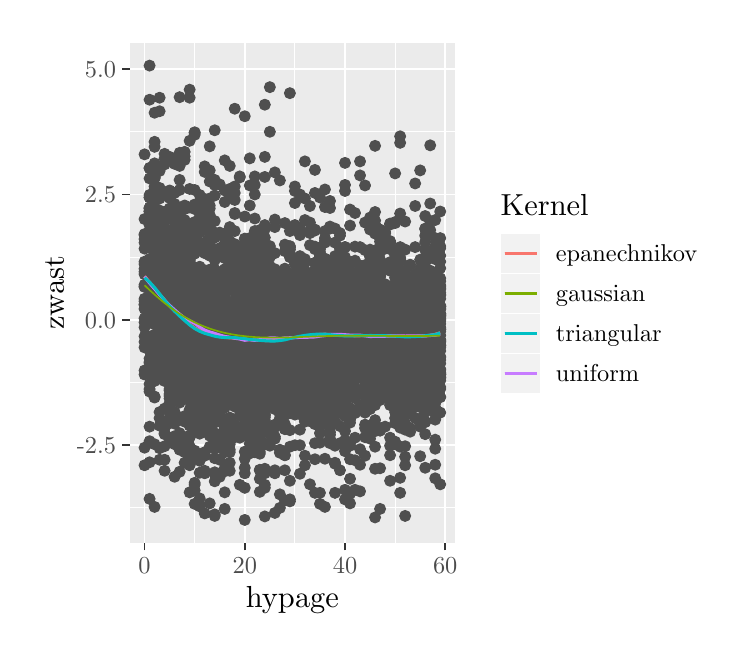
\begin{tikzpicture}[x=1pt,y=1pt]
\definecolor{fillColor}{RGB}{255,255,255}
\path[use as bounding box,fill=fillColor,fill opacity=0.00] (0,0) rectangle (252.94,216.81);
\begin{scope}
\path[clip] (  0.00,  0.00) rectangle (252.94,216.81);
\definecolor{drawColor}{RGB}{255,255,255}
\definecolor{fillColor}{RGB}{255,255,255}

\path[draw=drawColor,line width= 0.6pt,line join=round,line cap=round,fill=fillColor] (  0.00,  0.00) rectangle (252.94,216.81);
\end{scope}
\begin{scope}
\path[clip] ( 36.89, 30.72) rectangle (154.41,211.31);
\definecolor{fillColor}{gray}{0.92}

\path[fill=fillColor] ( 36.89, 30.72) rectangle (154.41,211.31);
\definecolor{drawColor}{RGB}{255,255,255}

\path[draw=drawColor,line width= 0.3pt,line join=round] ( 36.89, 43.28) --
	(154.41, 43.28);

\path[draw=drawColor,line width= 0.3pt,line join=round] ( 36.89, 88.58) --
	(154.41, 88.58);

\path[draw=drawColor,line width= 0.3pt,line join=round] ( 36.89,133.88) --
	(154.41,133.88);

\path[draw=drawColor,line width= 0.3pt,line join=round] ( 36.89,179.18) --
	(154.41,179.18);

\path[draw=drawColor,line width= 0.3pt,line join=round] ( 60.34, 30.72) --
	( 60.34,211.31);

\path[draw=drawColor,line width= 0.3pt,line join=round] ( 96.56, 30.72) --
	( 96.56,211.31);

\path[draw=drawColor,line width= 0.3pt,line join=round] (132.78, 30.72) --
	(132.78,211.31);

\path[draw=drawColor,line width= 0.6pt,line join=round] ( 36.89, 65.93) --
	(154.41, 65.93);

\path[draw=drawColor,line width= 0.6pt,line join=round] ( 36.89,111.23) --
	(154.41,111.23);

\path[draw=drawColor,line width= 0.6pt,line join=round] ( 36.89,156.53) --
	(154.41,156.53);

\path[draw=drawColor,line width= 0.6pt,line join=round] ( 36.89,201.83) --
	(154.41,201.83);

\path[draw=drawColor,line width= 0.6pt,line join=round] ( 42.24, 30.72) --
	( 42.24,211.31);

\path[draw=drawColor,line width= 0.6pt,line join=round] ( 78.45, 30.72) --
	( 78.45,211.31);

\path[draw=drawColor,line width= 0.6pt,line join=round] (114.67, 30.72) --
	(114.67,211.31);

\path[draw=drawColor,line width= 0.6pt,line join=round] (150.88, 30.72) --
	(150.88,211.31);
\definecolor{drawColor}{gray}{0.31}
\definecolor{fillColor}{gray}{0.31}

\path[draw=drawColor,line width= 0.4pt,line join=round,line cap=round,fill=fillColor] (132.78,113.59) circle (  1.96);

\path[draw=drawColor,line width= 0.4pt,line join=round,line cap=round,fill=fillColor] ( 67.59,120.47) circle (  1.96);

\path[draw=drawColor,line width= 0.4pt,line join=round,line cap=round,fill=fillColor] ( 80.26,110.51) circle (  1.96);

\path[draw=drawColor,line width= 0.4pt,line join=round,line cap=round,fill=fillColor] (107.42, 83.15) circle (  1.96);

\path[draw=drawColor,line width= 0.4pt,line join=round,line cap=round,fill=fillColor] ( 96.56, 81.15) circle (  1.96);

\path[draw=drawColor,line width= 0.4pt,line join=round,line cap=round,fill=fillColor] ( 73.02,117.57) circle (  1.96);

\path[draw=drawColor,line width= 0.4pt,line join=round,line cap=round,fill=fillColor] ( 60.34,112.68) circle (  1.96);

\path[draw=drawColor,line width= 0.4pt,line join=round,line cap=round,fill=fillColor] (132.78, 93.47) circle (  1.96);

\path[draw=drawColor,line width= 0.4pt,line join=round,line cap=round,fill=fillColor] ( 51.29,115.76) circle (  1.96);

\path[draw=drawColor,line width= 0.4pt,line join=round,line cap=round,fill=fillColor] (127.34, 86.77) circle (  1.96);

\path[draw=drawColor,line width= 0.4pt,line join=round,line cap=round,fill=fillColor] ( 71.21,129.53) circle (  1.96);

\path[draw=drawColor,line width= 0.4pt,line join=round,line cap=round,fill=fillColor] (120.10,100.90) circle (  1.96);

\path[draw=drawColor,line width= 0.4pt,line join=round,line cap=round,fill=fillColor] ( 51.29, 85.68) circle (  1.96);

\path[draw=drawColor,line width= 0.4pt,line join=round,line cap=round,fill=fillColor] (129.15,103.62) circle (  1.96);

\path[draw=drawColor,line width= 0.4pt,line join=round,line cap=round,fill=fillColor] ( 45.86,111.05) circle (  1.96);

\path[draw=drawColor,line width= 0.4pt,line join=round,line cap=round,fill=fillColor] (114.67, 87.86) circle (  1.96);

\path[draw=drawColor,line width= 0.4pt,line join=round,line cap=round,fill=fillColor] ( 87.51, 88.04) circle (  1.96);

\path[draw=drawColor,line width= 0.4pt,line join=round,line cap=round,fill=fillColor] ( 82.07,105.43) circle (  1.96);

\path[draw=drawColor,line width= 0.4pt,line join=round,line cap=round,fill=fillColor] ( 89.32, 73.36) circle (  1.96);

\path[draw=drawColor,line width= 0.4pt,line join=round,line cap=round,fill=fillColor] ( 78.45,105.25) circle (  1.96);

\path[draw=drawColor,line width= 0.4pt,line join=round,line cap=round,fill=fillColor] (125.53,101.45) circle (  1.96);

\path[draw=drawColor,line width= 0.4pt,line join=round,line cap=round,fill=fillColor] ( 76.64, 80.43) circle (  1.96);

\path[draw=drawColor,line width= 0.4pt,line join=round,line cap=round,fill=fillColor] (132.78, 98.91) circle (  1.96);

\path[draw=drawColor,line width= 0.4pt,line join=round,line cap=round,fill=fillColor] ( 58.53,116.31) circle (  1.96);

\path[draw=drawColor,line width= 0.4pt,line join=round,line cap=round,fill=fillColor] ( 73.02,103.44) circle (  1.96);

\path[draw=drawColor,line width= 0.4pt,line join=round,line cap=round,fill=fillColor] (103.80, 97.82) circle (  1.96);

\path[draw=drawColor,line width= 0.4pt,line join=round,line cap=round,fill=fillColor] (140.02, 82.97) circle (  1.96);

\path[draw=drawColor,line width= 0.4pt,line join=round,line cap=round,fill=fillColor] ( 54.91,151.10) circle (  1.96);

\path[draw=drawColor,line width= 0.4pt,line join=round,line cap=round,fill=fillColor] ( 45.86, 89.13) circle (  1.96);

\path[draw=drawColor,line width= 0.4pt,line join=round,line cap=round,fill=fillColor] ( 62.15, 46.72) circle (  1.96);

\path[draw=drawColor,line width= 0.4pt,line join=round,line cap=round,fill=fillColor] (147.26, 58.87) circle (  1.96);

\path[draw=drawColor,line width= 0.4pt,line join=round,line cap=round,fill=fillColor] (107.42,114.13) circle (  1.96);

\path[draw=drawColor,line width= 0.4pt,line join=round,line cap=round,fill=fillColor] ( 73.02, 90.76) circle (  1.96);

\path[draw=drawColor,line width= 0.4pt,line join=round,line cap=round,fill=fillColor] ( 71.21, 72.46) circle (  1.96);

\path[draw=drawColor,line width= 0.4pt,line join=round,line cap=round,fill=fillColor] (147.26, 85.32) circle (  1.96);

\path[draw=drawColor,line width= 0.4pt,line join=round,line cap=round,fill=fillColor] (109.24, 99.27) circle (  1.96);

\path[draw=drawColor,line width= 0.4pt,line join=round,line cap=round,fill=fillColor] (149.07,100.00) circle (  1.96);

\path[draw=drawColor,line width= 0.4pt,line join=round,line cap=round,fill=fillColor] ( 83.88, 57.05) circle (  1.96);

\path[draw=drawColor,line width= 0.4pt,line join=round,line cap=round,fill=fillColor] ( 85.69,110.15) circle (  1.96);

\path[draw=drawColor,line width= 0.4pt,line join=round,line cap=round,fill=fillColor] (136.40, 93.84) circle (  1.96);

\path[draw=drawColor,line width= 0.4pt,line join=round,line cap=round,fill=fillColor] (145.45, 95.83) circle (  1.96);

\path[draw=drawColor,line width= 0.4pt,line join=round,line cap=round,fill=fillColor] (105.61,113.23) circle (  1.96);

\path[draw=drawColor,line width= 0.4pt,line join=round,line cap=round,fill=fillColor] ( 78.45, 80.25) circle (  1.96);

\path[draw=drawColor,line width= 0.4pt,line join=round,line cap=round,fill=fillColor] (130.96, 84.41) circle (  1.96);

\path[draw=drawColor,line width= 0.4pt,line join=round,line cap=round,fill=fillColor] ( 91.13, 84.23) circle (  1.96);

\path[draw=drawColor,line width= 0.4pt,line join=round,line cap=round,fill=fillColor] (145.45,106.88) circle (  1.96);

\path[draw=drawColor,line width= 0.4pt,line join=round,line cap=round,fill=fillColor] ( 71.21, 64.30) circle (  1.96);

\path[draw=drawColor,line width= 0.4pt,line join=round,line cap=round,fill=fillColor] (140.02,100.00) circle (  1.96);

\path[draw=drawColor,line width= 0.4pt,line join=round,line cap=round,fill=fillColor] (130.96, 81.88) circle (  1.96);

\path[draw=drawColor,line width= 0.4pt,line join=round,line cap=round,fill=fillColor] ( 60.34,112.50) circle (  1.96);

\path[draw=drawColor,line width= 0.4pt,line join=round,line cap=round,fill=fillColor] ( 85.69,121.20) circle (  1.96);

\path[draw=drawColor,line width= 0.4pt,line join=round,line cap=round,fill=fillColor] (111.05, 81.70) circle (  1.96);

\path[draw=drawColor,line width= 0.4pt,line join=round,line cap=round,fill=fillColor] ( 74.83, 95.47) circle (  1.96);

\path[draw=drawColor,line width= 0.4pt,line join=round,line cap=round,fill=fillColor] (114.67, 96.01) circle (  1.96);

\path[draw=drawColor,line width= 0.4pt,line join=round,line cap=round,fill=fillColor] ( 87.51, 84.78) circle (  1.96);

\path[draw=drawColor,line width= 0.4pt,line join=round,line cap=round,fill=fillColor] (100.18,117.21) circle (  1.96);

\path[draw=drawColor,line width= 0.4pt,line join=round,line cap=round,fill=fillColor] ( 60.34,100.72) circle (  1.96);

\path[draw=drawColor,line width= 0.4pt,line join=round,line cap=round,fill=fillColor] ( 56.72, 84.78) circle (  1.96);

\path[draw=drawColor,line width= 0.4pt,line join=round,line cap=round,fill=fillColor] ( 80.26, 93.29) circle (  1.96);

\path[draw=drawColor,line width= 0.4pt,line join=round,line cap=round,fill=fillColor] ( 74.83,118.12) circle (  1.96);

\path[draw=drawColor,line width= 0.4pt,line join=round,line cap=round,fill=fillColor] (130.96,100.54) circle (  1.96);

\path[draw=drawColor,line width= 0.4pt,line join=round,line cap=round,fill=fillColor] ( 80.26,132.80) circle (  1.96);

\path[draw=drawColor,line width= 0.4pt,line join=round,line cap=round,fill=fillColor] ( 63.97,108.70) circle (  1.96);

\path[draw=drawColor,line width= 0.4pt,line join=round,line cap=round,fill=fillColor] ( 94.75,101.99) circle (  1.96);

\path[draw=drawColor,line width= 0.4pt,line join=round,line cap=round,fill=fillColor] ( 53.10, 85.68) circle (  1.96);

\path[draw=drawColor,line width= 0.4pt,line join=round,line cap=round,fill=fillColor] ( 49.48,146.75) circle (  1.96);

\path[draw=drawColor,line width= 0.4pt,line join=round,line cap=round,fill=fillColor] ( 94.75, 99.64) circle (  1.96);

\path[draw=drawColor,line width= 0.4pt,line join=round,line cap=round,fill=fillColor] ( 92.94,120.47) circle (  1.96);

\path[draw=drawColor,line width= 0.4pt,line join=round,line cap=round,fill=fillColor] (129.15, 96.01) circle (  1.96);

\path[draw=drawColor,line width= 0.4pt,line join=round,line cap=round,fill=fillColor] ( 69.40,107.06) circle (  1.96);

\path[draw=drawColor,line width= 0.4pt,line join=round,line cap=round,fill=fillColor] ( 78.45,115.22) circle (  1.96);

\path[draw=drawColor,line width= 0.4pt,line join=round,line cap=round,fill=fillColor] ( 51.29,137.51) circle (  1.96);

\path[draw=drawColor,line width= 0.4pt,line join=round,line cap=round,fill=fillColor] ( 65.78,141.31) circle (  1.96);

\path[draw=drawColor,line width= 0.4pt,line join=round,line cap=round,fill=fillColor] (112.86,122.83) circle (  1.96);

\path[draw=drawColor,line width= 0.4pt,line join=round,line cap=round,fill=fillColor] ( 92.94, 87.68) circle (  1.96);

\path[draw=drawColor,line width= 0.4pt,line join=round,line cap=round,fill=fillColor] (145.45, 96.01) circle (  1.96);

\path[draw=drawColor,line width= 0.4pt,line join=round,line cap=round,fill=fillColor] (112.86, 87.86) circle (  1.96);

\path[draw=drawColor,line width= 0.4pt,line join=round,line cap=round,fill=fillColor] ( 92.94,100.90) circle (  1.96);

\path[draw=drawColor,line width= 0.4pt,line join=round,line cap=round,fill=fillColor] (114.67,103.98) circle (  1.96);

\path[draw=drawColor,line width= 0.4pt,line join=round,line cap=round,fill=fillColor] (130.96,101.45) circle (  1.96);

\path[draw=drawColor,line width= 0.4pt,line join=round,line cap=round,fill=fillColor] (109.24,112.68) circle (  1.96);

\path[draw=drawColor,line width= 0.4pt,line join=round,line cap=round,fill=fillColor] ( 91.13, 87.68) circle (  1.96);

\path[draw=drawColor,line width= 0.4pt,line join=round,line cap=round,fill=fillColor] (147.26,107.06) circle (  1.96);

\path[draw=drawColor,line width= 0.4pt,line join=round,line cap=round,fill=fillColor] ( 91.13, 95.47) circle (  1.96);

\path[draw=drawColor,line width= 0.4pt,line join=round,line cap=round,fill=fillColor] (140.02, 89.31) circle (  1.96);

\path[draw=drawColor,line width= 0.4pt,line join=round,line cap=round,fill=fillColor] ( 85.69, 85.86) circle (  1.96);

\path[draw=drawColor,line width= 0.4pt,line join=round,line cap=round,fill=fillColor] (111.05,107.79) circle (  1.96);

\path[draw=drawColor,line width= 0.4pt,line join=round,line cap=round,fill=fillColor] ( 51.29,170.12) circle (  1.96);

\path[draw=drawColor,line width= 0.4pt,line join=round,line cap=round,fill=fillColor] ( 51.29,132.07) circle (  1.96);

\path[draw=drawColor,line width= 0.4pt,line join=round,line cap=round,fill=fillColor] ( 87.51,113.41) circle (  1.96);

\path[draw=drawColor,line width= 0.4pt,line join=round,line cap=round,fill=fillColor] ( 92.94,103.44) circle (  1.96);

\path[draw=drawColor,line width= 0.4pt,line join=round,line cap=round,fill=fillColor] (140.02,115.94) circle (  1.96);

\path[draw=drawColor,line width= 0.4pt,line join=round,line cap=round,fill=fillColor] ( 65.78, 98.37) circle (  1.96);

\path[draw=drawColor,line width= 0.4pt,line join=round,line cap=round,fill=fillColor] (101.99,124.28) circle (  1.96);

\path[draw=drawColor,line width= 0.4pt,line join=round,line cap=round,fill=fillColor] ( 63.97,129.17) circle (  1.96);

\path[draw=drawColor,line width= 0.4pt,line join=round,line cap=round,fill=fillColor] (147.26,103.80) circle (  1.96);

\path[draw=drawColor,line width= 0.4pt,line join=round,line cap=round,fill=fillColor] ( 63.97, 87.50) circle (  1.96);

\path[draw=drawColor,line width= 0.4pt,line join=round,line cap=round,fill=fillColor] ( 67.59,110.15) circle (  1.96);

\path[draw=drawColor,line width= 0.4pt,line join=round,line cap=round,fill=fillColor] ( 78.45,103.08) circle (  1.96);

\path[draw=drawColor,line width= 0.4pt,line join=round,line cap=round,fill=fillColor] ( 47.67,112.68) circle (  1.96);

\path[draw=drawColor,line width= 0.4pt,line join=round,line cap=round,fill=fillColor] (149.07, 86.95) circle (  1.96);

\path[draw=drawColor,line width= 0.4pt,line join=round,line cap=round,fill=fillColor] ( 78.45,110.51) circle (  1.96);

\path[draw=drawColor,line width= 0.4pt,line join=round,line cap=round,fill=fillColor] ( 87.51, 92.57) circle (  1.96);

\path[draw=drawColor,line width= 0.4pt,line join=round,line cap=round,fill=fillColor] (130.96,104.53) circle (  1.96);

\path[draw=drawColor,line width= 0.4pt,line join=round,line cap=round,fill=fillColor] ( 89.32,108.51) circle (  1.96);

\path[draw=drawColor,line width= 0.4pt,line join=round,line cap=round,fill=fillColor] (132.78,108.70) circle (  1.96);

\path[draw=drawColor,line width= 0.4pt,line join=round,line cap=round,fill=fillColor] ( 92.94, 46.00) circle (  1.96);

\path[draw=drawColor,line width= 0.4pt,line join=round,line cap=round,fill=fillColor] ( 60.34,178.10) circle (  1.96);

\path[draw=drawColor,line width= 0.4pt,line join=round,line cap=round,fill=fillColor] ( 78.45,128.27) circle (  1.96);

\path[draw=drawColor,line width= 0.4pt,line join=round,line cap=round,fill=fillColor] ( 83.88,116.67) circle (  1.96);

\path[draw=drawColor,line width= 0.4pt,line join=round,line cap=round,fill=fillColor] (132.78, 94.92) circle (  1.96);

\path[draw=drawColor,line width= 0.4pt,line join=round,line cap=round,fill=fillColor] (112.86, 86.95) circle (  1.96);

\path[draw=drawColor,line width= 0.4pt,line join=round,line cap=round,fill=fillColor] (149.07,115.22) circle (  1.96);

\path[draw=drawColor,line width= 0.4pt,line join=round,line cap=round,fill=fillColor] ( 69.40,125.00) circle (  1.96);

\path[draw=drawColor,line width= 0.4pt,line join=round,line cap=round,fill=fillColor] ( 89.32,112.32) circle (  1.96);

\path[draw=drawColor,line width= 0.4pt,line join=round,line cap=round,fill=fillColor] (109.24, 87.13) circle (  1.96);

\path[draw=drawColor,line width= 0.4pt,line join=round,line cap=round,fill=fillColor] ( 44.05,151.46) circle (  1.96);

\path[draw=drawColor,line width= 0.4pt,line join=round,line cap=round,fill=fillColor] (111.05, 99.82) circle (  1.96);

\path[draw=drawColor,line width= 0.4pt,line join=round,line cap=round,fill=fillColor] ( 58.53,117.76) circle (  1.96);

\path[draw=drawColor,line width= 0.4pt,line join=round,line cap=round,fill=fillColor] ( 98.37,115.94) circle (  1.96);

\path[draw=drawColor,line width= 0.4pt,line join=round,line cap=round,fill=fillColor] ( 45.86,121.74) circle (  1.96);

\path[draw=drawColor,line width= 0.4pt,line join=round,line cap=round,fill=fillColor] (109.24,114.49) circle (  1.96);

\path[draw=drawColor,line width= 0.4pt,line join=round,line cap=round,fill=fillColor] ( 49.48, 93.29) circle (  1.96);

\path[draw=drawColor,line width= 0.4pt,line join=round,line cap=round,fill=fillColor] (132.78, 93.29) circle (  1.96);

\path[draw=drawColor,line width= 0.4pt,line join=round,line cap=round,fill=fillColor] ( 92.94,103.26) circle (  1.96);

\path[draw=drawColor,line width= 0.4pt,line join=round,line cap=round,fill=fillColor] ( 58.53,107.97) circle (  1.96);

\path[draw=drawColor,line width= 0.4pt,line join=round,line cap=round,fill=fillColor] (141.83,127.36) circle (  1.96);

\path[draw=drawColor,line width= 0.4pt,line join=round,line cap=round,fill=fillColor] ( 94.75,133.88) circle (  1.96);

\path[draw=drawColor,line width= 0.4pt,line join=round,line cap=round,fill=fillColor] ( 62.15,129.17) circle (  1.96);

\path[draw=drawColor,line width= 0.4pt,line join=round,line cap=round,fill=fillColor] ( 62.15,126.09) circle (  1.96);

\path[draw=drawColor,line width= 0.4pt,line join=round,line cap=round,fill=fillColor] ( 73.02,139.14) circle (  1.96);

\path[draw=drawColor,line width= 0.4pt,line join=round,line cap=round,fill=fillColor] ( 73.02,134.97) circle (  1.96);

\path[draw=drawColor,line width= 0.4pt,line join=round,line cap=round,fill=fillColor] ( 85.69, 86.95) circle (  1.96);

\path[draw=drawColor,line width= 0.4pt,line join=round,line cap=round,fill=fillColor] (105.61,101.45) circle (  1.96);

\path[draw=drawColor,line width= 0.4pt,line join=round,line cap=round,fill=fillColor] (141.83,117.57) circle (  1.96);

\path[draw=drawColor,line width= 0.4pt,line join=round,line cap=round,fill=fillColor] (118.29, 60.50) circle (  1.96);

\path[draw=drawColor,line width= 0.4pt,line join=round,line cap=round,fill=fillColor] (100.18,119.39) circle (  1.96);

\path[draw=drawColor,line width= 0.4pt,line join=round,line cap=round,fill=fillColor] ( 45.86,133.34) circle (  1.96);

\path[draw=drawColor,line width= 0.4pt,line join=round,line cap=round,fill=fillColor] ( 96.56,124.64) circle (  1.96);

\path[draw=drawColor,line width= 0.4pt,line join=round,line cap=round,fill=fillColor] (109.24,117.39) circle (  1.96);

\path[draw=drawColor,line width= 0.4pt,line join=round,line cap=round,fill=fillColor] (100.18,117.94) circle (  1.96);

\path[draw=drawColor,line width= 0.4pt,line join=round,line cap=round,fill=fillColor] ( 51.29,148.92) circle (  1.96);

\path[draw=drawColor,line width= 0.4pt,line join=round,line cap=round,fill=fillColor] ( 67.59, 40.93) circle (  1.96);

\path[draw=drawColor,line width= 0.4pt,line join=round,line cap=round,fill=fillColor] (140.02,104.71) circle (  1.96);

\path[draw=drawColor,line width= 0.4pt,line join=round,line cap=round,fill=fillColor] ( 69.40,115.04) circle (  1.96);

\path[draw=drawColor,line width= 0.4pt,line join=round,line cap=round,fill=fillColor] ( 63.97,114.13) circle (  1.96);

\path[draw=drawColor,line width= 0.4pt,line join=round,line cap=round,fill=fillColor] ( 65.78,143.12) circle (  1.96);

\path[draw=drawColor,line width= 0.4pt,line join=round,line cap=round,fill=fillColor] ( 80.26, 72.27) circle (  1.96);

\path[draw=drawColor,line width= 0.4pt,line join=round,line cap=round,fill=fillColor] (101.99,121.38) circle (  1.96);

\path[draw=drawColor,line width= 0.4pt,line join=round,line cap=round,fill=fillColor] (127.34,116.85) circle (  1.96);

\path[draw=drawColor,line width= 0.4pt,line join=round,line cap=round,fill=fillColor] (127.34,124.46) circle (  1.96);

\path[draw=drawColor,line width= 0.4pt,line join=round,line cap=round,fill=fillColor] ( 49.48,156.71) circle (  1.96);

\path[draw=drawColor,line width= 0.4pt,line join=round,line cap=round,fill=fillColor] (100.18, 97.28) circle (  1.96);

\path[draw=drawColor,line width= 0.4pt,line join=round,line cap=round,fill=fillColor] ( 78.45,133.88) circle (  1.96);

\path[draw=drawColor,line width= 0.4pt,line join=round,line cap=round,fill=fillColor] ( 98.37,127.18) circle (  1.96);

\path[draw=drawColor,line width= 0.4pt,line join=round,line cap=round,fill=fillColor] ( 62.15,103.08) circle (  1.96);

\path[draw=drawColor,line width= 0.4pt,line join=round,line cap=round,fill=fillColor] ( 62.15,100.54) circle (  1.96);

\path[draw=drawColor,line width= 0.4pt,line join=round,line cap=round,fill=fillColor] (112.86,121.38) circle (  1.96);

\path[draw=drawColor,line width= 0.4pt,line join=round,line cap=round,fill=fillColor] ( 58.53,107.06) circle (  1.96);

\path[draw=drawColor,line width= 0.4pt,line join=round,line cap=round,fill=fillColor] ( 82.07,103.98) circle (  1.96);

\path[draw=drawColor,line width= 0.4pt,line join=round,line cap=round,fill=fillColor] (136.40, 98.55) circle (  1.96);

\path[draw=drawColor,line width= 0.4pt,line join=round,line cap=round,fill=fillColor] (101.99, 77.35) circle (  1.96);

\path[draw=drawColor,line width= 0.4pt,line join=round,line cap=round,fill=fillColor] (114.67, 82.97) circle (  1.96);

\path[draw=drawColor,line width= 0.4pt,line join=round,line cap=round,fill=fillColor] ( 63.97, 84.60) circle (  1.96);

\path[draw=drawColor,line width= 0.4pt,line join=round,line cap=round,fill=fillColor] (100.18,117.21) circle (  1.96);

\path[draw=drawColor,line width= 0.4pt,line join=round,line cap=round,fill=fillColor] (140.02,127.72) circle (  1.96);

\path[draw=drawColor,line width= 0.4pt,line join=round,line cap=round,fill=fillColor] ( 45.86,162.87) circle (  1.96);

\path[draw=drawColor,line width= 0.4pt,line join=round,line cap=round,fill=fillColor] (109.24,106.34) circle (  1.96);

\path[draw=drawColor,line width= 0.4pt,line join=round,line cap=round,fill=fillColor] ( 60.34, 93.66) circle (  1.96);

\path[draw=drawColor,line width= 0.4pt,line join=round,line cap=round,fill=fillColor] (125.53,100.54) circle (  1.96);

\path[draw=drawColor,line width= 0.4pt,line join=round,line cap=round,fill=fillColor] ( 82.07,106.16) circle (  1.96);

\path[draw=drawColor,line width= 0.4pt,line join=round,line cap=round,fill=fillColor] ( 58.53, 87.68) circle (  1.96);

\path[draw=drawColor,line width= 0.4pt,line join=round,line cap=round,fill=fillColor] (136.40,114.68) circle (  1.96);

\path[draw=drawColor,line width= 0.4pt,line join=round,line cap=round,fill=fillColor] ( 65.78,108.88) circle (  1.96);

\path[draw=drawColor,line width= 0.4pt,line join=round,line cap=round,fill=fillColor] (114.67,112.86) circle (  1.96);

\path[draw=drawColor,line width= 0.4pt,line join=round,line cap=round,fill=fillColor] ( 54.91,109.06) circle (  1.96);

\path[draw=drawColor,line width= 0.4pt,line join=round,line cap=round,fill=fillColor] (105.61,109.24) circle (  1.96);

\path[draw=drawColor,line width= 0.4pt,line join=round,line cap=round,fill=fillColor] (147.26, 92.75) circle (  1.96);

\path[draw=drawColor,line width= 0.4pt,line join=round,line cap=round,fill=fillColor] ( 98.37, 99.82) circle (  1.96);

\path[draw=drawColor,line width= 0.4pt,line join=round,line cap=round,fill=fillColor] (130.96,137.14) circle (  1.96);

\path[draw=drawColor,line width= 0.4pt,line join=round,line cap=round,fill=fillColor] ( 80.26, 81.15) circle (  1.96);

\path[draw=drawColor,line width= 0.4pt,line join=round,line cap=round,fill=fillColor] (125.53,102.17) circle (  1.96);

\path[draw=drawColor,line width= 0.4pt,line join=round,line cap=round,fill=fillColor] ( 73.02,101.27) circle (  1.96);

\path[draw=drawColor,line width= 0.4pt,line join=round,line cap=round,fill=fillColor] (112.86,141.67) circle (  1.96);

\path[draw=drawColor,line width= 0.4pt,line join=round,line cap=round,fill=fillColor] ( 94.75,111.78) circle (  1.96);

\path[draw=drawColor,line width= 0.4pt,line join=round,line cap=round,fill=fillColor] (149.07,125.18) circle (  1.96);

\path[draw=drawColor,line width= 0.4pt,line join=round,line cap=round,fill=fillColor] ( 83.88,136.42) circle (  1.96);

\path[draw=drawColor,line width= 0.4pt,line join=round,line cap=round,fill=fillColor] ( 85.69,135.51) circle (  1.96);

\path[draw=drawColor,line width= 0.4pt,line join=round,line cap=round,fill=fillColor] (127.34,119.02) circle (  1.96);

\path[draw=drawColor,line width= 0.4pt,line join=round,line cap=round,fill=fillColor] ( 54.91, 96.92) circle (  1.96);

\path[draw=drawColor,line width= 0.4pt,line join=round,line cap=round,fill=fillColor] ( 71.21,124.46) circle (  1.96);

\path[draw=drawColor,line width= 0.4pt,line join=round,line cap=round,fill=fillColor] ( 92.94,111.41) circle (  1.96);

\path[draw=drawColor,line width= 0.4pt,line join=round,line cap=round,fill=fillColor] ( 51.29, 98.55) circle (  1.96);

\path[draw=drawColor,line width= 0.4pt,line join=round,line cap=round,fill=fillColor] (127.34,127.18) circle (  1.96);

\path[draw=drawColor,line width= 0.4pt,line join=round,line cap=round,fill=fillColor] ( 71.21,133.52) circle (  1.96);

\path[draw=drawColor,line width= 0.4pt,line join=round,line cap=round,fill=fillColor] ( 45.86,152.00) circle (  1.96);

\path[draw=drawColor,line width= 0.4pt,line join=round,line cap=round,fill=fillColor] (140.02,121.74) circle (  1.96);

\path[draw=drawColor,line width= 0.4pt,line join=round,line cap=round,fill=fillColor] ( 58.53,122.29) circle (  1.96);

\path[draw=drawColor,line width= 0.4pt,line join=round,line cap=round,fill=fillColor] ( 73.02,109.42) circle (  1.96);

\path[draw=drawColor,line width= 0.4pt,line join=round,line cap=round,fill=fillColor] (109.24,122.10) circle (  1.96);

\path[draw=drawColor,line width= 0.4pt,line join=round,line cap=round,fill=fillColor] (136.40,103.62) circle (  1.96);

\path[draw=drawColor,line width= 0.4pt,line join=round,line cap=round,fill=fillColor] (121.91, 86.05) circle (  1.96);

\path[draw=drawColor,line width= 0.4pt,line join=round,line cap=round,fill=fillColor] ( 94.75,100.72) circle (  1.96);

\path[draw=drawColor,line width= 0.4pt,line join=round,line cap=round,fill=fillColor] (123.72,103.08) circle (  1.96);

\path[draw=drawColor,line width= 0.4pt,line join=round,line cap=round,fill=fillColor] ( 44.05,105.07) circle (  1.96);

\path[draw=drawColor,line width= 0.4pt,line join=round,line cap=round,fill=fillColor] ( 87.51, 98.73) circle (  1.96);

\path[draw=drawColor,line width= 0.4pt,line join=round,line cap=round,fill=fillColor] ( 63.97, 63.40) circle (  1.96);

\path[draw=drawColor,line width= 0.4pt,line join=round,line cap=round,fill=fillColor] ( 67.59,114.49) circle (  1.96);

\path[draw=drawColor,line width= 0.4pt,line join=round,line cap=round,fill=fillColor] (120.10,113.04) circle (  1.96);

\path[draw=drawColor,line width= 0.4pt,line join=round,line cap=round,fill=fillColor] ( 51.29,101.09) circle (  1.96);

\path[draw=drawColor,line width= 0.4pt,line join=round,line cap=round,fill=fillColor] (116.48, 98.00) circle (  1.96);

\path[draw=drawColor,line width= 0.4pt,line join=round,line cap=round,fill=fillColor] (103.80,114.31) circle (  1.96);

\path[draw=drawColor,line width= 0.4pt,line join=round,line cap=round,fill=fillColor] (136.40,126.45) circle (  1.96);

\path[draw=drawColor,line width= 0.4pt,line join=round,line cap=round,fill=fillColor] ( 51.29,110.87) circle (  1.96);

\path[draw=drawColor,line width= 0.4pt,line join=round,line cap=round,fill=fillColor] (118.29,137.69) circle (  1.96);

\path[draw=drawColor,line width= 0.4pt,line join=round,line cap=round,fill=fillColor] (127.34,109.06) circle (  1.96);

\path[draw=drawColor,line width= 0.4pt,line join=round,line cap=round,fill=fillColor] ( 82.07,101.45) circle (  1.96);

\path[draw=drawColor,line width= 0.4pt,line join=round,line cap=round,fill=fillColor] (107.42,118.84) circle (  1.96);

\path[draw=drawColor,line width= 0.4pt,line join=round,line cap=round,fill=fillColor] ( 76.64, 93.66) circle (  1.96);

\path[draw=drawColor,line width= 0.4pt,line join=round,line cap=round,fill=fillColor] (109.24, 94.20) circle (  1.96);

\path[draw=drawColor,line width= 0.4pt,line join=round,line cap=round,fill=fillColor] ( 65.78, 96.01) circle (  1.96);

\path[draw=drawColor,line width= 0.4pt,line join=round,line cap=round,fill=fillColor] ( 45.86,130.44) circle (  1.96);

\path[draw=drawColor,line width= 0.4pt,line join=round,line cap=round,fill=fillColor] (147.26, 99.82) circle (  1.96);

\path[draw=drawColor,line width= 0.4pt,line join=round,line cap=round,fill=fillColor] ( 89.32,107.79) circle (  1.96);

\path[draw=drawColor,line width= 0.4pt,line join=round,line cap=round,fill=fillColor] ( 53.10,104.35) circle (  1.96);

\path[draw=drawColor,line width= 0.4pt,line join=round,line cap=round,fill=fillColor] ( 83.88, 88.04) circle (  1.96);

\path[draw=drawColor,line width= 0.4pt,line join=round,line cap=round,fill=fillColor] (132.78, 75.72) circle (  1.96);

\path[draw=drawColor,line width= 0.4pt,line join=round,line cap=round,fill=fillColor] ( 45.86, 94.74) circle (  1.96);

\path[draw=drawColor,line width= 0.4pt,line join=round,line cap=round,fill=fillColor] (111.05,104.71) circle (  1.96);

\path[draw=drawColor,line width= 0.4pt,line join=round,line cap=round,fill=fillColor] ( 78.45,104.89) circle (  1.96);

\path[draw=drawColor,line width= 0.4pt,line join=round,line cap=round,fill=fillColor] (107.42, 43.64) circle (  1.96);

\path[draw=drawColor,line width= 0.4pt,line join=round,line cap=round,fill=fillColor] ( 56.72, 97.82) circle (  1.96);

\path[draw=drawColor,line width= 0.4pt,line join=round,line cap=round,fill=fillColor] ( 58.53, 96.92) circle (  1.96);

\path[draw=drawColor,line width= 0.4pt,line join=round,line cap=round,fill=fillColor] (105.61,100.90) circle (  1.96);

\path[draw=drawColor,line width= 0.4pt,line join=round,line cap=round,fill=fillColor] (136.40, 93.47) circle (  1.96);

\path[draw=drawColor,line width= 0.4pt,line join=round,line cap=round,fill=fillColor] ( 87.51, 96.56) circle (  1.96);

\path[draw=drawColor,line width= 0.4pt,line join=round,line cap=round,fill=fillColor] ( 87.51, 90.21) circle (  1.96);

\path[draw=drawColor,line width= 0.4pt,line join=round,line cap=round,fill=fillColor] (147.26, 84.05) circle (  1.96);

\path[draw=drawColor,line width= 0.4pt,line join=round,line cap=round,fill=fillColor] (145.45, 88.58) circle (  1.96);

\path[draw=drawColor,line width= 0.4pt,line join=round,line cap=round,fill=fillColor] ( 83.88,102.72) circle (  1.96);

\path[draw=drawColor,line width= 0.4pt,line join=round,line cap=round,fill=fillColor] (149.07, 91.48) circle (  1.96);

\path[draw=drawColor,line width= 0.4pt,line join=round,line cap=round,fill=fillColor] ( 82.07, 82.24) circle (  1.96);

\path[draw=drawColor,line width= 0.4pt,line join=round,line cap=round,fill=fillColor] ( 82.07, 84.23) circle (  1.96);

\path[draw=drawColor,line width= 0.4pt,line join=round,line cap=round,fill=fillColor] (123.72, 84.60) circle (  1.96);

\path[draw=drawColor,line width= 0.4pt,line join=round,line cap=round,fill=fillColor] ( 49.48,133.70) circle (  1.96);

\path[draw=drawColor,line width= 0.4pt,line join=round,line cap=round,fill=fillColor] (134.59,102.17) circle (  1.96);

\path[draw=drawColor,line width= 0.4pt,line join=round,line cap=round,fill=fillColor] ( 76.64,103.80) circle (  1.96);

\path[draw=drawColor,line width= 0.4pt,line join=round,line cap=round,fill=fillColor] (101.99,102.17) circle (  1.96);

\path[draw=drawColor,line width= 0.4pt,line join=round,line cap=round,fill=fillColor] (118.29,124.82) circle (  1.96);

\path[draw=drawColor,line width= 0.4pt,line join=round,line cap=round,fill=fillColor] (118.29,117.76) circle (  1.96);

\path[draw=drawColor,line width= 0.4pt,line join=round,line cap=round,fill=fillColor] ( 78.45,128.99) circle (  1.96);

\path[draw=drawColor,line width= 0.4pt,line join=round,line cap=round,fill=fillColor] (101.99, 84.96) circle (  1.96);

\path[draw=drawColor,line width= 0.4pt,line join=round,line cap=round,fill=fillColor] ( 98.37,111.05) circle (  1.96);

\path[draw=drawColor,line width= 0.4pt,line join=round,line cap=round,fill=fillColor] (100.18, 99.64) circle (  1.96);

\path[draw=drawColor,line width= 0.4pt,line join=round,line cap=round,fill=fillColor] ( 80.26,132.43) circle (  1.96);

\path[draw=drawColor,line width= 0.4pt,line join=round,line cap=round,fill=fillColor] ( 65.78, 93.47) circle (  1.96);

\path[draw=drawColor,line width= 0.4pt,line join=round,line cap=round,fill=fillColor] ( 63.97, 88.94) circle (  1.96);

\path[draw=drawColor,line width= 0.4pt,line join=round,line cap=round,fill=fillColor] (125.53,111.78) circle (  1.96);

\path[draw=drawColor,line width= 0.4pt,line join=round,line cap=round,fill=fillColor] (127.34,111.05) circle (  1.96);

\path[draw=drawColor,line width= 0.4pt,line join=round,line cap=round,fill=fillColor] ( 83.88, 74.63) circle (  1.96);

\path[draw=drawColor,line width= 0.4pt,line join=round,line cap=round,fill=fillColor] ( 74.83,136.78) circle (  1.96);

\path[draw=drawColor,line width= 0.4pt,line join=round,line cap=round,fill=fillColor] (118.29,114.49) circle (  1.96);

\path[draw=drawColor,line width= 0.4pt,line join=round,line cap=round,fill=fillColor] (140.02, 99.82) circle (  1.96);

\path[draw=drawColor,line width= 0.4pt,line join=round,line cap=round,fill=fillColor] ( 58.53,101.99) circle (  1.96);

\path[draw=drawColor,line width= 0.4pt,line join=round,line cap=round,fill=fillColor] (100.18,101.45) circle (  1.96);

\path[draw=drawColor,line width= 0.4pt,line join=round,line cap=round,fill=fillColor] ( 51.29, 83.69) circle (  1.96);

\path[draw=drawColor,line width= 0.4pt,line join=round,line cap=round,fill=fillColor] ( 62.15, 75.17) circle (  1.96);

\path[draw=drawColor,line width= 0.4pt,line join=round,line cap=round,fill=fillColor] (103.80, 84.41) circle (  1.96);

\path[draw=drawColor,line width= 0.4pt,line join=round,line cap=round,fill=fillColor] (103.80,105.98) circle (  1.96);

\path[draw=drawColor,line width= 0.4pt,line join=round,line cap=round,fill=fillColor] (143.64,118.66) circle (  1.96);

\path[draw=drawColor,line width= 0.4pt,line join=round,line cap=round,fill=fillColor] ( 85.69,114.49) circle (  1.96);

\path[draw=drawColor,line width= 0.4pt,line join=round,line cap=round,fill=fillColor] (120.10,113.95) circle (  1.96);

\path[draw=drawColor,line width= 0.4pt,line join=round,line cap=round,fill=fillColor] ( 65.78,128.45) circle (  1.96);

\path[draw=drawColor,line width= 0.4pt,line join=round,line cap=round,fill=fillColor] ( 82.07,159.98) circle (  1.96);

\path[draw=drawColor,line width= 0.4pt,line join=round,line cap=round,fill=fillColor] ( 83.88,138.59) circle (  1.96);

\path[draw=drawColor,line width= 0.4pt,line join=round,line cap=round,fill=fillColor] ( 63.97, 73.00) circle (  1.96);

\path[draw=drawColor,line width= 0.4pt,line join=round,line cap=round,fill=fillColor] ( 74.83, 99.09) circle (  1.96);

\path[draw=drawColor,line width= 0.4pt,line join=round,line cap=round,fill=fillColor] ( 53.10,144.21) circle (  1.96);

\path[draw=drawColor,line width= 0.4pt,line join=round,line cap=round,fill=fillColor] ( 80.26,108.15) circle (  1.96);

\path[draw=drawColor,line width= 0.4pt,line join=round,line cap=round,fill=fillColor] (109.24,115.04) circle (  1.96);

\path[draw=drawColor,line width= 0.4pt,line join=round,line cap=round,fill=fillColor] ( 85.69, 86.05) circle (  1.96);

\path[draw=drawColor,line width= 0.4pt,line join=round,line cap=round,fill=fillColor] (111.05,134.25) circle (  1.96);

\path[draw=drawColor,line width= 0.4pt,line join=round,line cap=round,fill=fillColor] ( 56.72,101.81) circle (  1.96);

\path[draw=drawColor,line width= 0.4pt,line join=round,line cap=round,fill=fillColor] ( 60.34, 74.81) circle (  1.96);

\path[draw=drawColor,line width= 0.4pt,line join=round,line cap=round,fill=fillColor] ( 73.02,114.49) circle (  1.96);

\path[draw=drawColor,line width= 0.4pt,line join=round,line cap=round,fill=fillColor] (123.72,122.47) circle (  1.96);

\path[draw=drawColor,line width= 0.4pt,line join=round,line cap=round,fill=fillColor] ( 94.75,107.25) circle (  1.96);

\path[draw=drawColor,line width= 0.4pt,line join=round,line cap=round,fill=fillColor] (136.40,117.76) circle (  1.96);

\path[draw=drawColor,line width= 0.4pt,line join=round,line cap=round,fill=fillColor] (101.99,115.58) circle (  1.96);

\path[draw=drawColor,line width= 0.4pt,line join=round,line cap=round,fill=fillColor] (141.83,110.51) circle (  1.96);

\path[draw=drawColor,line width= 0.4pt,line join=round,line cap=round,fill=fillColor] (103.80, 92.21) circle (  1.96);

\path[draw=drawColor,line width= 0.4pt,line join=round,line cap=round,fill=fillColor] (149.07,101.99) circle (  1.96);

\path[draw=drawColor,line width= 0.4pt,line join=round,line cap=round,fill=fillColor] ( 96.56,105.25) circle (  1.96);

\path[draw=drawColor,line width= 0.4pt,line join=round,line cap=round,fill=fillColor] ( 83.88, 90.58) circle (  1.96);

\path[draw=drawColor,line width= 0.4pt,line join=round,line cap=round,fill=fillColor] ( 56.72, 91.30) circle (  1.96);

\path[draw=drawColor,line width= 0.4pt,line join=round,line cap=round,fill=fillColor] ( 65.78, 99.45) circle (  1.96);

\path[draw=drawColor,line width= 0.4pt,line join=round,line cap=round,fill=fillColor] (118.29,124.64) circle (  1.96);

\path[draw=drawColor,line width= 0.4pt,line join=round,line cap=round,fill=fillColor] ( 58.53,113.23) circle (  1.96);

\path[draw=drawColor,line width= 0.4pt,line join=round,line cap=round,fill=fillColor] (114.67,124.46) circle (  1.96);

\path[draw=drawColor,line width= 0.4pt,line join=round,line cap=round,fill=fillColor] (149.07,123.74) circle (  1.96);

\path[draw=drawColor,line width= 0.4pt,line join=round,line cap=round,fill=fillColor] (107.42,118.48) circle (  1.96);

\path[draw=drawColor,line width= 0.4pt,line join=round,line cap=round,fill=fillColor] ( 44.05,126.63) circle (  1.96);

\path[draw=drawColor,line width= 0.4pt,line join=round,line cap=round,fill=fillColor] ( 67.59, 99.82) circle (  1.96);

\path[draw=drawColor,line width= 0.4pt,line join=round,line cap=round,fill=fillColor] (143.64,144.03) circle (  1.96);

\path[draw=drawColor,line width= 0.4pt,line join=round,line cap=round,fill=fillColor] ( 71.21, 93.84) circle (  1.96);

\path[draw=drawColor,line width= 0.4pt,line join=round,line cap=round,fill=fillColor] (100.18,117.76) circle (  1.96);

\path[draw=drawColor,line width= 0.4pt,line join=round,line cap=round,fill=fillColor] (134.59,101.27) circle (  1.96);

\path[draw=drawColor,line width= 0.4pt,line join=round,line cap=round,fill=fillColor] ( 56.72, 97.28) circle (  1.96);

\path[draw=drawColor,line width= 0.4pt,line join=round,line cap=round,fill=fillColor] (112.86,115.22) circle (  1.96);

\path[draw=drawColor,line width= 0.4pt,line join=round,line cap=round,fill=fillColor] ( 62.15,105.80) circle (  1.96);

\path[draw=drawColor,line width= 0.4pt,line join=round,line cap=round,fill=fillColor] (111.05,111.78) circle (  1.96);

\path[draw=drawColor,line width= 0.4pt,line join=round,line cap=round,fill=fillColor] ( 67.59,156.17) circle (  1.96);

\path[draw=drawColor,line width= 0.4pt,line join=round,line cap=round,fill=fillColor] (109.24,120.65) circle (  1.96);

\path[draw=drawColor,line width= 0.4pt,line join=round,line cap=round,fill=fillColor] (149.07,132.25) circle (  1.96);

\path[draw=drawColor,line width= 0.4pt,line join=round,line cap=round,fill=fillColor] ( 67.59,100.54) circle (  1.96);

\path[draw=drawColor,line width= 0.4pt,line join=round,line cap=round,fill=fillColor] (112.86,134.06) circle (  1.96);

\path[draw=drawColor,line width= 0.4pt,line join=round,line cap=round,fill=fillColor] (140.02, 75.72) circle (  1.96);

\path[draw=drawColor,line width= 0.4pt,line join=round,line cap=round,fill=fillColor] ( 56.72, 88.58) circle (  1.96);

\path[draw=drawColor,line width= 0.4pt,line join=round,line cap=round,fill=fillColor] (101.99, 75.90) circle (  1.96);

\path[draw=drawColor,line width= 0.4pt,line join=round,line cap=round,fill=fillColor] ( 71.21,168.85) circle (  1.96);

\path[draw=drawColor,line width= 0.4pt,line join=round,line cap=round,fill=fillColor] (143.64,114.86) circle (  1.96);

\path[draw=drawColor,line width= 0.4pt,line join=round,line cap=round,fill=fillColor] ( 54.91,142.04) circle (  1.96);

\path[draw=drawColor,line width= 0.4pt,line join=round,line cap=round,fill=fillColor] ( 67.59,122.47) circle (  1.96);

\path[draw=drawColor,line width= 0.4pt,line join=round,line cap=round,fill=fillColor] (138.21,120.65) circle (  1.96);

\path[draw=drawColor,line width= 0.4pt,line join=round,line cap=round,fill=fillColor] ( 82.07,114.86) circle (  1.96);

\path[draw=drawColor,line width= 0.4pt,line join=round,line cap=round,fill=fillColor] (134.59,109.24) circle (  1.96);

\path[draw=drawColor,line width= 0.4pt,line join=round,line cap=round,fill=fillColor] (103.80,106.88) circle (  1.96);

\path[draw=drawColor,line width= 0.4pt,line join=round,line cap=round,fill=fillColor] (105.61,155.45) circle (  1.96);

\path[draw=drawColor,line width= 0.4pt,line join=round,line cap=round,fill=fillColor] ( 45.86,134.43) circle (  1.96);

\path[draw=drawColor,line width= 0.4pt,line join=round,line cap=round,fill=fillColor] ( 94.75,120.65) circle (  1.96);

\path[draw=drawColor,line width= 0.4pt,line join=round,line cap=round,fill=fillColor] (141.83,100.90) circle (  1.96);

\path[draw=drawColor,line width= 0.4pt,line join=round,line cap=round,fill=fillColor] (105.61,107.79) circle (  1.96);

\path[draw=drawColor,line width= 0.4pt,line join=round,line cap=round,fill=fillColor] ( 51.29, 86.23) circle (  1.96);

\path[draw=drawColor,line width= 0.4pt,line join=round,line cap=round,fill=fillColor] ( 47.67,104.89) circle (  1.96);

\path[draw=drawColor,line width= 0.4pt,line join=round,line cap=round,fill=fillColor] (127.34, 42.92) circle (  1.96);

\path[draw=drawColor,line width= 0.4pt,line join=round,line cap=round,fill=fillColor] (130.96,113.95) circle (  1.96);

\path[draw=drawColor,line width= 0.4pt,line join=round,line cap=round,fill=fillColor] (101.99, 87.31) circle (  1.96);

\path[draw=drawColor,line width= 0.4pt,line join=round,line cap=round,fill=fillColor] ( 96.56,104.71) circle (  1.96);

\path[draw=drawColor,line width= 0.4pt,line join=round,line cap=round,fill=fillColor] ( 98.37,107.43) circle (  1.96);

\path[draw=drawColor,line width= 0.4pt,line join=round,line cap=round,fill=fillColor] ( 98.37,123.74) circle (  1.96);

\path[draw=drawColor,line width= 0.4pt,line join=round,line cap=round,fill=fillColor] ( 49.48,128.99) circle (  1.96);

\path[draw=drawColor,line width= 0.4pt,line join=round,line cap=round,fill=fillColor] ( 54.91,126.82) circle (  1.96);

\path[draw=drawColor,line width= 0.4pt,line join=round,line cap=round,fill=fillColor] (111.05,103.08) circle (  1.96);

\path[draw=drawColor,line width= 0.4pt,line join=round,line cap=round,fill=fillColor] (111.05,100.90) circle (  1.96);

\path[draw=drawColor,line width= 0.4pt,line join=round,line cap=round,fill=fillColor] ( 58.53, 95.11) circle (  1.96);

\path[draw=drawColor,line width= 0.4pt,line join=round,line cap=round,fill=fillColor] ( 73.02, 95.65) circle (  1.96);

\path[draw=drawColor,line width= 0.4pt,line join=round,line cap=round,fill=fillColor] ( 44.05,124.64) circle (  1.96);

\path[draw=drawColor,line width= 0.4pt,line join=round,line cap=round,fill=fillColor] (107.42,132.25) circle (  1.96);

\path[draw=drawColor,line width= 0.4pt,line join=round,line cap=round,fill=fillColor] ( 63.97,105.25) circle (  1.96);

\path[draw=drawColor,line width= 0.4pt,line join=round,line cap=round,fill=fillColor] (138.21, 91.12) circle (  1.96);

\path[draw=drawColor,line width= 0.4pt,line join=round,line cap=round,fill=fillColor] ( 67.59, 83.87) circle (  1.96);

\path[draw=drawColor,line width= 0.4pt,line join=round,line cap=round,fill=fillColor] (141.83,114.68) circle (  1.96);

\path[draw=drawColor,line width= 0.4pt,line join=round,line cap=round,fill=fillColor] (123.72,107.06) circle (  1.96);

\path[draw=drawColor,line width= 0.4pt,line join=round,line cap=round,fill=fillColor] ( 80.26, 70.10) circle (  1.96);

\path[draw=drawColor,line width= 0.4pt,line join=round,line cap=round,fill=fillColor] (105.61,136.78) circle (  1.96);

\path[draw=drawColor,line width= 0.4pt,line join=round,line cap=round,fill=fillColor] (129.15, 91.30) circle (  1.96);

\path[draw=drawColor,line width= 0.4pt,line join=round,line cap=round,fill=fillColor] (101.99,143.12) circle (  1.96);

\path[draw=drawColor,line width= 0.4pt,line join=round,line cap=round,fill=fillColor] ( 67.59,101.27) circle (  1.96);

\path[draw=drawColor,line width= 0.4pt,line join=round,line cap=round,fill=fillColor] ( 67.59,132.80) circle (  1.96);

\path[draw=drawColor,line width= 0.4pt,line join=round,line cap=round,fill=fillColor] ( 83.88, 98.91) circle (  1.96);

\path[draw=drawColor,line width= 0.4pt,line join=round,line cap=round,fill=fillColor] (100.18,119.57) circle (  1.96);

\path[draw=drawColor,line width= 0.4pt,line join=round,line cap=round,fill=fillColor] ( 58.53,100.18) circle (  1.96);

\path[draw=drawColor,line width= 0.4pt,line join=round,line cap=round,fill=fillColor] ( 56.72, 68.65) circle (  1.96);

\path[draw=drawColor,line width= 0.4pt,line join=round,line cap=round,fill=fillColor] (134.59,128.45) circle (  1.96);

\path[draw=drawColor,line width= 0.4pt,line join=round,line cap=round,fill=fillColor] ( 51.29,130.80) circle (  1.96);

\path[draw=drawColor,line width= 0.4pt,line join=round,line cap=round,fill=fillColor] (130.96,110.87) circle (  1.96);

\path[draw=drawColor,line width= 0.4pt,line join=round,line cap=round,fill=fillColor] ( 76.64, 89.31) circle (  1.96);

\path[draw=drawColor,line width= 0.4pt,line join=round,line cap=round,fill=fillColor] (121.91,101.99) circle (  1.96);

\path[draw=drawColor,line width= 0.4pt,line join=round,line cap=round,fill=fillColor] ( 82.07, 82.60) circle (  1.96);

\path[draw=drawColor,line width= 0.4pt,line join=round,line cap=round,fill=fillColor] (121.91, 88.76) circle (  1.96);

\path[draw=drawColor,line width= 0.4pt,line join=round,line cap=round,fill=fillColor] (134.59,124.82) circle (  1.96);

\path[draw=drawColor,line width= 0.4pt,line join=round,line cap=round,fill=fillColor] ( 89.32,127.00) circle (  1.96);

\path[draw=drawColor,line width= 0.4pt,line join=round,line cap=round,fill=fillColor] (101.99,128.08) circle (  1.96);

\path[draw=drawColor,line width= 0.4pt,line join=round,line cap=round,fill=fillColor] (127.34,135.69) circle (  1.96);

\path[draw=drawColor,line width= 0.4pt,line join=round,line cap=round,fill=fillColor] (105.61,128.99) circle (  1.96);

\path[draw=drawColor,line width= 0.4pt,line join=round,line cap=round,fill=fillColor] ( 94.75,134.61) circle (  1.96);

\path[draw=drawColor,line width= 0.4pt,line join=round,line cap=round,fill=fillColor] ( 54.91, 56.33) circle (  1.96);

\path[draw=drawColor,line width= 0.4pt,line join=round,line cap=round,fill=fillColor] (138.21, 98.37) circle (  1.96);

\path[draw=drawColor,line width= 0.4pt,line join=round,line cap=round,fill=fillColor] ( 94.75,115.76) circle (  1.96);

\path[draw=drawColor,line width= 0.4pt,line join=round,line cap=round,fill=fillColor] (120.10, 96.37) circle (  1.96);

\path[draw=drawColor,line width= 0.4pt,line join=round,line cap=round,fill=fillColor] ( 49.48,115.94) circle (  1.96);

\path[draw=drawColor,line width= 0.4pt,line join=round,line cap=round,fill=fillColor] (143.64,105.62) circle (  1.96);

\path[draw=drawColor,line width= 0.4pt,line join=round,line cap=round,fill=fillColor] ( 78.45,136.06) circle (  1.96);

\path[draw=drawColor,line width= 0.4pt,line join=round,line cap=round,fill=fillColor] ( 53.10,102.53) circle (  1.96);

\path[draw=drawColor,line width= 0.4pt,line join=round,line cap=round,fill=fillColor] (105.61,107.79) circle (  1.96);

\path[draw=drawColor,line width= 0.4pt,line join=round,line cap=round,fill=fillColor] (121.91,130.44) circle (  1.96);

\path[draw=drawColor,line width= 0.4pt,line join=round,line cap=round,fill=fillColor] ( 80.26,135.33) circle (  1.96);

\path[draw=drawColor,line width= 0.4pt,line join=round,line cap=round,fill=fillColor] ( 60.34, 44.73) circle (  1.96);

\path[draw=drawColor,line width= 0.4pt,line join=round,line cap=round,fill=fillColor] (107.42,113.77) circle (  1.96);

\path[draw=drawColor,line width= 0.4pt,line join=round,line cap=round,fill=fillColor] (118.29,125.91) circle (  1.96);

\path[draw=drawColor,line width= 0.4pt,line join=round,line cap=round,fill=fillColor] (105.61, 99.45) circle (  1.96);

\path[draw=drawColor,line width= 0.4pt,line join=round,line cap=round,fill=fillColor] ( 87.51, 90.58) circle (  1.96);

\path[draw=drawColor,line width= 0.4pt,line join=round,line cap=round,fill=fillColor] (123.72,132.61) circle (  1.96);

\path[draw=drawColor,line width= 0.4pt,line join=round,line cap=round,fill=fillColor] ( 71.21,100.72) circle (  1.96);

\path[draw=drawColor,line width= 0.4pt,line join=round,line cap=round,fill=fillColor] ( 60.34, 79.34) circle (  1.96);

\path[draw=drawColor,line width= 0.4pt,line join=round,line cap=round,fill=fillColor] ( 67.59, 68.11) circle (  1.96);

\path[draw=drawColor,line width= 0.4pt,line join=round,line cap=round,fill=fillColor] (105.61,127.72) circle (  1.96);

\path[draw=drawColor,line width= 0.4pt,line join=round,line cap=round,fill=fillColor] (105.61, 97.64) circle (  1.96);

\path[draw=drawColor,line width= 0.4pt,line join=round,line cap=round,fill=fillColor] (103.80,129.17) circle (  1.96);

\path[draw=drawColor,line width= 0.4pt,line join=round,line cap=round,fill=fillColor] ( 63.97,148.74) circle (  1.96);

\path[draw=drawColor,line width= 0.4pt,line join=round,line cap=round,fill=fillColor] ( 51.29,136.60) circle (  1.96);

\path[draw=drawColor,line width= 0.4pt,line join=round,line cap=round,fill=fillColor] (138.21,118.66) circle (  1.96);

\path[draw=drawColor,line width= 0.4pt,line join=round,line cap=round,fill=fillColor] (141.83,108.70) circle (  1.96);

\path[draw=drawColor,line width= 0.4pt,line join=round,line cap=round,fill=fillColor] ( 85.69, 40.20) circle (  1.96);

\path[draw=drawColor,line width= 0.4pt,line join=round,line cap=round,fill=fillColor] ( 53.10, 99.45) circle (  1.96);

\path[draw=drawColor,line width= 0.4pt,line join=round,line cap=round,fill=fillColor] ( 89.32, 97.10) circle (  1.96);

\path[draw=drawColor,line width= 0.4pt,line join=round,line cap=round,fill=fillColor] (136.40,114.13) circle (  1.96);

\path[draw=drawColor,line width= 0.4pt,line join=round,line cap=round,fill=fillColor] ( 63.97,101.81) circle (  1.96);

\path[draw=drawColor,line width= 0.4pt,line join=round,line cap=round,fill=fillColor] ( 96.56, 84.96) circle (  1.96);

\path[draw=drawColor,line width= 0.4pt,line join=round,line cap=round,fill=fillColor] ( 44.05,117.76) circle (  1.96);

\path[draw=drawColor,line width= 0.4pt,line join=round,line cap=round,fill=fillColor] ( 42.24,142.22) circle (  1.96);

\path[draw=drawColor,line width= 0.4pt,line join=round,line cap=round,fill=fillColor] ( 65.78,111.41) circle (  1.96);

\path[draw=drawColor,line width= 0.4pt,line join=round,line cap=round,fill=fillColor] (107.42,121.74) circle (  1.96);

\path[draw=drawColor,line width= 0.4pt,line join=round,line cap=round,fill=fillColor] (143.64,124.28) circle (  1.96);

\path[draw=drawColor,line width= 0.4pt,line join=round,line cap=round,fill=fillColor] (132.78,110.87) circle (  1.96);

\path[draw=drawColor,line width= 0.4pt,line join=round,line cap=round,fill=fillColor] ( 91.13, 93.29) circle (  1.96);

\path[draw=drawColor,line width= 0.4pt,line join=round,line cap=round,fill=fillColor] (132.78,113.59) circle (  1.96);

\path[draw=drawColor,line width= 0.4pt,line join=round,line cap=round,fill=fillColor] (123.72,108.51) circle (  1.96);

\path[draw=drawColor,line width= 0.4pt,line join=round,line cap=round,fill=fillColor] ( 56.72, 95.65) circle (  1.96);

\path[draw=drawColor,line width= 0.4pt,line join=round,line cap=round,fill=fillColor] (107.42,109.42) circle (  1.96);

\path[draw=drawColor,line width= 0.4pt,line join=round,line cap=round,fill=fillColor] ( 63.97,119.39) circle (  1.96);

\path[draw=drawColor,line width= 0.4pt,line join=round,line cap=round,fill=fillColor] (132.78,114.68) circle (  1.96);

\path[draw=drawColor,line width= 0.4pt,line join=round,line cap=round,fill=fillColor] ( 58.53, 89.85) circle (  1.96);

\path[draw=drawColor,line width= 0.4pt,line join=round,line cap=round,fill=fillColor] (116.48,115.76) circle (  1.96);

\path[draw=drawColor,line width= 0.4pt,line join=round,line cap=round,fill=fillColor] ( 80.26,104.35) circle (  1.96);

\path[draw=drawColor,line width= 0.4pt,line join=round,line cap=round,fill=fillColor] ( 85.69,100.00) circle (  1.96);

\path[draw=drawColor,line width= 0.4pt,line join=round,line cap=round,fill=fillColor] ( 85.69,106.34) circle (  1.96);

\path[draw=drawColor,line width= 0.4pt,line join=round,line cap=round,fill=fillColor] ( 80.26, 79.16) circle (  1.96);

\path[draw=drawColor,line width= 0.4pt,line join=round,line cap=round,fill=fillColor] ( 67.59, 40.38) circle (  1.96);

\path[draw=drawColor,line width= 0.4pt,line join=round,line cap=round,fill=fillColor] (147.26, 75.17) circle (  1.96);

\path[draw=drawColor,line width= 0.4pt,line join=round,line cap=round,fill=fillColor] ( 67.59, 76.99) circle (  1.96);

\path[draw=drawColor,line width= 0.4pt,line join=round,line cap=round,fill=fillColor] (116.48,109.06) circle (  1.96);

\path[draw=drawColor,line width= 0.4pt,line join=round,line cap=round,fill=fillColor] ( 60.34, 76.99) circle (  1.96);

\path[draw=drawColor,line width= 0.4pt,line join=round,line cap=round,fill=fillColor] (116.48,101.27) circle (  1.96);

\path[draw=drawColor,line width= 0.4pt,line join=round,line cap=round,fill=fillColor] (149.07,109.78) circle (  1.96);

\path[draw=drawColor,line width= 0.4pt,line join=round,line cap=round,fill=fillColor] ( 96.56,113.77) circle (  1.96);

\path[draw=drawColor,line width= 0.4pt,line join=round,line cap=round,fill=fillColor] ( 51.29,102.35) circle (  1.96);

\path[draw=drawColor,line width= 0.4pt,line join=round,line cap=round,fill=fillColor] ( 98.37, 65.93) circle (  1.96);

\path[draw=drawColor,line width= 0.4pt,line join=round,line cap=round,fill=fillColor] ( 98.37,105.25) circle (  1.96);

\path[draw=drawColor,line width= 0.4pt,line join=round,line cap=round,fill=fillColor] (127.34,126.82) circle (  1.96);

\path[draw=drawColor,line width= 0.4pt,line join=round,line cap=round,fill=fillColor] ( 51.29, 84.41) circle (  1.96);

\path[draw=drawColor,line width= 0.4pt,line join=round,line cap=round,fill=fillColor] (109.24,100.90) circle (  1.96);

\path[draw=drawColor,line width= 0.4pt,line join=round,line cap=round,fill=fillColor] (143.64, 84.05) circle (  1.96);

\path[draw=drawColor,line width= 0.4pt,line join=round,line cap=round,fill=fillColor] ( 51.29,107.97) circle (  1.96);

\path[draw=drawColor,line width= 0.4pt,line join=round,line cap=round,fill=fillColor] (100.18,123.19) circle (  1.96);

\path[draw=drawColor,line width= 0.4pt,line join=round,line cap=round,fill=fillColor] ( 49.48, 70.28) circle (  1.96);

\path[draw=drawColor,line width= 0.4pt,line join=round,line cap=round,fill=fillColor] (147.26,109.42) circle (  1.96);

\path[draw=drawColor,line width= 0.4pt,line join=round,line cap=round,fill=fillColor] (143.64,109.42) circle (  1.96);

\path[draw=drawColor,line width= 0.4pt,line join=round,line cap=round,fill=fillColor] ( 49.48, 95.65) circle (  1.96);

\path[draw=drawColor,line width= 0.4pt,line join=round,line cap=round,fill=fillColor] (105.61,113.59) circle (  1.96);

\path[draw=drawColor,line width= 0.4pt,line join=round,line cap=round,fill=fillColor] (127.34,130.62) circle (  1.96);

\path[draw=drawColor,line width= 0.4pt,line join=round,line cap=round,fill=fillColor] ( 89.32,144.75) circle (  1.96);

\path[draw=drawColor,line width= 0.4pt,line join=round,line cap=round,fill=fillColor] ( 45.86,130.26) circle (  1.96);

\path[draw=drawColor,line width= 0.4pt,line join=round,line cap=round,fill=fillColor] (145.45,135.69) circle (  1.96);

\path[draw=drawColor,line width= 0.4pt,line join=round,line cap=round,fill=fillColor] ( 67.59, 90.58) circle (  1.96);

\path[draw=drawColor,line width= 0.4pt,line join=round,line cap=round,fill=fillColor] ( 85.69, 96.37) circle (  1.96);

\path[draw=drawColor,line width= 0.4pt,line join=round,line cap=round,fill=fillColor] ( 62.15,106.88) circle (  1.96);

\path[draw=drawColor,line width= 0.4pt,line join=round,line cap=round,fill=fillColor] (101.99, 97.10) circle (  1.96);

\path[draw=drawColor,line width= 0.4pt,line join=round,line cap=round,fill=fillColor] (100.18,108.51) circle (  1.96);

\path[draw=drawColor,line width= 0.4pt,line join=round,line cap=round,fill=fillColor] (141.83, 98.91) circle (  1.96);

\path[draw=drawColor,line width= 0.4pt,line join=round,line cap=round,fill=fillColor] (127.34, 94.38) circle (  1.96);

\path[draw=drawColor,line width= 0.4pt,line join=round,line cap=round,fill=fillColor] ( 62.15, 97.28) circle (  1.96);

\path[draw=drawColor,line width= 0.4pt,line join=round,line cap=round,fill=fillColor] ( 80.26, 88.04) circle (  1.96);

\path[draw=drawColor,line width= 0.4pt,line join=round,line cap=round,fill=fillColor] ( 92.94, 98.55) circle (  1.96);

\path[draw=drawColor,line width= 0.4pt,line join=round,line cap=round,fill=fillColor] ( 78.45, 57.78) circle (  1.96);

\path[draw=drawColor,line width= 0.4pt,line join=round,line cap=round,fill=fillColor] ( 58.53, 99.45) circle (  1.96);

\path[draw=drawColor,line width= 0.4pt,line join=round,line cap=round,fill=fillColor] ( 56.72, 99.64) circle (  1.96);

\path[draw=drawColor,line width= 0.4pt,line join=round,line cap=round,fill=fillColor] ( 73.02, 90.39) circle (  1.96);

\path[draw=drawColor,line width= 0.4pt,line join=round,line cap=round,fill=fillColor] ( 82.07, 99.64) circle (  1.96);

\path[draw=drawColor,line width= 0.4pt,line join=round,line cap=round,fill=fillColor] (114.67, 88.22) circle (  1.96);

\path[draw=drawColor,line width= 0.4pt,line join=round,line cap=round,fill=fillColor] (109.24, 66.66) circle (  1.96);

\path[draw=drawColor,line width= 0.4pt,line join=round,line cap=round,fill=fillColor] ( 65.78, 79.70) circle (  1.96);

\path[draw=drawColor,line width= 0.4pt,line join=round,line cap=round,fill=fillColor] (107.42, 61.04) circle (  1.96);

\path[draw=drawColor,line width= 0.4pt,line join=round,line cap=round,fill=fillColor] (118.29, 96.19) circle (  1.96);

\path[draw=drawColor,line width= 0.4pt,line join=round,line cap=round,fill=fillColor] ( 73.02,112.86) circle (  1.96);

\path[draw=drawColor,line width= 0.4pt,line join=round,line cap=round,fill=fillColor] ( 53.10,114.13) circle (  1.96);

\path[draw=drawColor,line width= 0.4pt,line join=round,line cap=round,fill=fillColor] ( 83.88, 82.42) circle (  1.96);

\path[draw=drawColor,line width= 0.4pt,line join=round,line cap=round,fill=fillColor] (141.83,103.62) circle (  1.96);

\path[draw=drawColor,line width= 0.4pt,line join=round,line cap=round,fill=fillColor] ( 53.10,109.24) circle (  1.96);

\path[draw=drawColor,line width= 0.4pt,line join=round,line cap=round,fill=fillColor] ( 58.53,111.59) circle (  1.96);

\path[draw=drawColor,line width= 0.4pt,line join=round,line cap=round,fill=fillColor] ( 53.10,106.52) circle (  1.96);

\path[draw=drawColor,line width= 0.4pt,line join=round,line cap=round,fill=fillColor] (121.91,111.96) circle (  1.96);

\path[draw=drawColor,line width= 0.4pt,line join=round,line cap=round,fill=fillColor] (100.18, 77.71) circle (  1.96);

\path[draw=drawColor,line width= 0.4pt,line join=round,line cap=round,fill=fillColor] (145.45, 94.56) circle (  1.96);

\path[draw=drawColor,line width= 0.4pt,line join=round,line cap=round,fill=fillColor] (112.86, 96.37) circle (  1.96);

\path[draw=drawColor,line width= 0.4pt,line join=round,line cap=round,fill=fillColor] ( 58.53, 90.76) circle (  1.96);

\path[draw=drawColor,line width= 0.4pt,line join=round,line cap=round,fill=fillColor] ( 76.64, 76.80) circle (  1.96);

\path[draw=drawColor,line width= 0.4pt,line join=round,line cap=round,fill=fillColor] ( 58.53, 82.42) circle (  1.96);

\path[draw=drawColor,line width= 0.4pt,line join=round,line cap=round,fill=fillColor] ( 44.05,132.43) circle (  1.96);

\path[draw=drawColor,line width= 0.4pt,line join=round,line cap=round,fill=fillColor] ( 89.32,109.42) circle (  1.96);

\path[draw=drawColor,line width= 0.4pt,line join=round,line cap=round,fill=fillColor] (134.59,100.36) circle (  1.96);

\path[draw=drawColor,line width= 0.4pt,line join=round,line cap=round,fill=fillColor] (130.96, 94.92) circle (  1.96);

\path[draw=drawColor,line width= 0.4pt,line join=round,line cap=round,fill=fillColor] ( 87.51, 93.84) circle (  1.96);

\path[draw=drawColor,line width= 0.4pt,line join=round,line cap=round,fill=fillColor] ( 45.86,137.87) circle (  1.96);

\path[draw=drawColor,line width= 0.4pt,line join=round,line cap=round,fill=fillColor] ( 65.78,119.75) circle (  1.96);

\path[draw=drawColor,line width= 0.4pt,line join=round,line cap=round,fill=fillColor] (147.26, 89.67) circle (  1.96);

\path[draw=drawColor,line width= 0.4pt,line join=round,line cap=round,fill=fillColor] ( 58.53,109.24) circle (  1.96);

\path[draw=drawColor,line width= 0.4pt,line join=round,line cap=round,fill=fillColor] (107.42, 88.58) circle (  1.96);

\path[draw=drawColor,line width= 0.4pt,line join=round,line cap=round,fill=fillColor] ( 80.26, 94.56) circle (  1.96);

\path[draw=drawColor,line width= 0.4pt,line join=round,line cap=round,fill=fillColor] (147.26, 86.77) circle (  1.96);

\path[draw=drawColor,line width= 0.4pt,line join=round,line cap=round,fill=fillColor] ( 98.37, 94.56) circle (  1.96);

\path[draw=drawColor,line width= 0.4pt,line join=round,line cap=round,fill=fillColor] ( 44.05,142.94) circle (  1.96);

\path[draw=drawColor,line width= 0.4pt,line join=round,line cap=round,fill=fillColor] ( 71.21,118.30) circle (  1.96);

\path[draw=drawColor,line width= 0.4pt,line join=round,line cap=round,fill=fillColor] (101.99,109.60) circle (  1.96);

\path[draw=drawColor,line width= 0.4pt,line join=round,line cap=round,fill=fillColor] (136.40, 90.03) circle (  1.96);

\path[draw=drawColor,line width= 0.4pt,line join=round,line cap=round,fill=fillColor] ( 62.15, 86.59) circle (  1.96);

\path[draw=drawColor,line width= 0.4pt,line join=round,line cap=round,fill=fillColor] (120.10,110.69) circle (  1.96);

\path[draw=drawColor,line width= 0.4pt,line join=round,line cap=round,fill=fillColor] (132.78,123.19) circle (  1.96);

\path[draw=drawColor,line width= 0.4pt,line join=round,line cap=round,fill=fillColor] ( 91.13,120.84) circle (  1.96);

\path[draw=drawColor,line width= 0.4pt,line join=round,line cap=round,fill=fillColor] ( 65.78,135.88) circle (  1.96);

\path[draw=drawColor,line width= 0.4pt,line join=round,line cap=round,fill=fillColor] (118.29,120.29) circle (  1.96);

\path[draw=drawColor,line width= 0.4pt,line join=round,line cap=round,fill=fillColor] ( 63.97,103.80) circle (  1.96);

\path[draw=drawColor,line width= 0.4pt,line join=round,line cap=round,fill=fillColor] ( 42.24,140.41) circle (  1.96);

\path[draw=drawColor,line width= 0.4pt,line join=round,line cap=round,fill=fillColor] ( 44.05,150.37) circle (  1.96);

\path[draw=drawColor,line width= 0.4pt,line join=round,line cap=round,fill=fillColor] ( 96.56,110.69) circle (  1.96);

\path[draw=drawColor,line width= 0.4pt,line join=round,line cap=round,fill=fillColor] ( 85.69,111.41) circle (  1.96);

\path[draw=drawColor,line width= 0.4pt,line join=round,line cap=round,fill=fillColor] (143.64, 97.28) circle (  1.96);

\path[draw=drawColor,line width= 0.4pt,line join=round,line cap=round,fill=fillColor] ( 94.75,136.60) circle (  1.96);

\path[draw=drawColor,line width= 0.4pt,line join=round,line cap=round,fill=fillColor] ( 94.75, 84.41) circle (  1.96);

\path[draw=drawColor,line width= 0.4pt,line join=round,line cap=round,fill=fillColor] (109.24,110.69) circle (  1.96);

\path[draw=drawColor,line width= 0.4pt,line join=round,line cap=round,fill=fillColor] (138.21,108.15) circle (  1.96);

\path[draw=drawColor,line width= 0.4pt,line join=round,line cap=round,fill=fillColor] ( 51.29,116.31) circle (  1.96);

\path[draw=drawColor,line width= 0.4pt,line join=round,line cap=round,fill=fillColor] (123.72, 93.47) circle (  1.96);

\path[draw=drawColor,line width= 0.4pt,line join=round,line cap=round,fill=fillColor] (123.72,134.06) circle (  1.96);

\path[draw=drawColor,line width= 0.4pt,line join=round,line cap=round,fill=fillColor] (123.72,113.23) circle (  1.96);

\path[draw=drawColor,line width= 0.4pt,line join=round,line cap=round,fill=fillColor] ( 63.97, 79.88) circle (  1.96);

\path[draw=drawColor,line width= 0.4pt,line join=round,line cap=round,fill=fillColor] (118.29,101.09) circle (  1.96);

\path[draw=drawColor,line width= 0.4pt,line join=round,line cap=round,fill=fillColor] ( 83.88, 62.85) circle (  1.96);

\path[draw=drawColor,line width= 0.4pt,line join=round,line cap=round,fill=fillColor] ( 49.48, 94.02) circle (  1.96);

\path[draw=drawColor,line width= 0.4pt,line join=round,line cap=round,fill=fillColor] ( 83.88, 49.08) circle (  1.96);

\path[draw=drawColor,line width= 0.4pt,line join=round,line cap=round,fill=fillColor] ( 63.97, 97.64) circle (  1.96);

\path[draw=drawColor,line width= 0.4pt,line join=round,line cap=round,fill=fillColor] (123.72,109.60) circle (  1.96);

\path[draw=drawColor,line width= 0.4pt,line join=round,line cap=round,fill=fillColor] ( 47.67,158.34) circle (  1.96);

\path[draw=drawColor,line width= 0.4pt,line join=round,line cap=round,fill=fillColor] ( 98.37,115.94) circle (  1.96);

\path[draw=drawColor,line width= 0.4pt,line join=round,line cap=round,fill=fillColor] (114.67,167.95) circle (  1.96);

\path[draw=drawColor,line width= 0.4pt,line join=round,line cap=round,fill=fillColor] (141.83, 95.29) circle (  1.96);

\path[draw=drawColor,line width= 0.4pt,line join=round,line cap=round,fill=fillColor] ( 76.64, 96.92) circle (  1.96);

\path[draw=drawColor,line width= 0.4pt,line join=round,line cap=round,fill=fillColor] ( 76.64,102.17) circle (  1.96);

\path[draw=drawColor,line width= 0.4pt,line join=round,line cap=round,fill=fillColor] ( 82.07,143.31) circle (  1.96);

\path[draw=drawColor,line width= 0.4pt,line join=round,line cap=round,fill=fillColor] ( 74.83,112.50) circle (  1.96);

\path[draw=drawColor,line width= 0.4pt,line join=round,line cap=round,fill=fillColor] ( 58.53,143.49) circle (  1.96);

\path[draw=drawColor,line width= 0.4pt,line join=round,line cap=round,fill=fillColor] ( 92.94, 90.39) circle (  1.96);

\path[draw=drawColor,line width= 0.4pt,line join=round,line cap=round,fill=fillColor] (123.72, 78.98) circle (  1.96);

\path[draw=drawColor,line width= 0.4pt,line join=round,line cap=round,fill=fillColor] ( 56.72,147.29) circle (  1.96);

\path[draw=drawColor,line width= 0.4pt,line join=round,line cap=round,fill=fillColor] ( 91.13,161.61) circle (  1.96);

\path[draw=drawColor,line width= 0.4pt,line join=round,line cap=round,fill=fillColor] ( 47.67,150.73) circle (  1.96);

\path[draw=drawColor,line width= 0.4pt,line join=round,line cap=round,fill=fillColor] ( 49.48, 89.13) circle (  1.96);

\path[draw=drawColor,line width= 0.4pt,line join=round,line cap=round,fill=fillColor] (120.10,106.88) circle (  1.96);

\path[draw=drawColor,line width= 0.4pt,line join=round,line cap=round,fill=fillColor] ( 96.56, 95.83) circle (  1.96);

\path[draw=drawColor,line width= 0.4pt,line join=round,line cap=round,fill=fillColor] ( 54.91,118.12) circle (  1.96);

\path[draw=drawColor,line width= 0.4pt,line join=round,line cap=round,fill=fillColor] (109.24, 86.59) circle (  1.96);

\path[draw=drawColor,line width= 0.4pt,line join=round,line cap=round,fill=fillColor] ( 67.59, 56.15) circle (  1.96);

\path[draw=drawColor,line width= 0.4pt,line join=round,line cap=round,fill=fillColor] (100.18, 84.60) circle (  1.96);

\path[draw=drawColor,line width= 0.4pt,line join=round,line cap=round,fill=fillColor] (123.72,106.16) circle (  1.96);

\path[draw=drawColor,line width= 0.4pt,line join=round,line cap=round,fill=fillColor] ( 85.69, 76.08) circle (  1.96);

\path[draw=drawColor,line width= 0.4pt,line join=round,line cap=round,fill=fillColor] (116.48, 83.69) circle (  1.96);

\path[draw=drawColor,line width= 0.4pt,line join=round,line cap=round,fill=fillColor] (107.42, 87.86) circle (  1.96);

\path[draw=drawColor,line width= 0.4pt,line join=round,line cap=round,fill=fillColor] ( 94.75, 92.57) circle (  1.96);

\path[draw=drawColor,line width= 0.4pt,line join=round,line cap=round,fill=fillColor] ( 51.29,112.68) circle (  1.96);

\path[draw=drawColor,line width= 0.4pt,line join=round,line cap=round,fill=fillColor] (114.67,117.39) circle (  1.96);

\path[draw=drawColor,line width= 0.4pt,line join=round,line cap=round,fill=fillColor] ( 62.15,104.17) circle (  1.96);

\path[draw=drawColor,line width= 0.4pt,line join=round,line cap=round,fill=fillColor] ( 89.32, 91.48) circle (  1.96);

\path[draw=drawColor,line width= 0.4pt,line join=round,line cap=round,fill=fillColor] ( 94.75,118.48) circle (  1.96);

\path[draw=drawColor,line width= 0.4pt,line join=round,line cap=round,fill=fillColor] (103.80, 60.86) circle (  1.96);

\path[draw=drawColor,line width= 0.4pt,line join=round,line cap=round,fill=fillColor] (121.91, 62.13) circle (  1.96);

\path[draw=drawColor,line width= 0.4pt,line join=round,line cap=round,fill=fillColor] ( 53.10, 82.42) circle (  1.96);

\path[draw=drawColor,line width= 0.4pt,line join=round,line cap=round,fill=fillColor] ( 91.13, 94.38) circle (  1.96);

\path[draw=drawColor,line width= 0.4pt,line join=round,line cap=round,fill=fillColor] ( 69.40,123.19) circle (  1.96);

\path[draw=drawColor,line width= 0.4pt,line join=round,line cap=round,fill=fillColor] ( 73.02, 89.85) circle (  1.96);

\path[draw=drawColor,line width= 0.4pt,line join=round,line cap=round,fill=fillColor] ( 91.13, 90.21) circle (  1.96);

\path[draw=drawColor,line width= 0.4pt,line join=round,line cap=round,fill=fillColor] (114.67, 81.33) circle (  1.96);

\path[draw=drawColor,line width= 0.4pt,line join=round,line cap=round,fill=fillColor] (132.78, 66.29) circle (  1.96);

\path[draw=drawColor,line width= 0.4pt,line join=round,line cap=round,fill=fillColor] ( 71.21, 94.92) circle (  1.96);

\path[draw=drawColor,line width= 0.4pt,line join=round,line cap=round,fill=fillColor] ( 71.21,119.93) circle (  1.96);

\path[draw=drawColor,line width= 0.4pt,line join=round,line cap=round,fill=fillColor] ( 42.24,117.94) circle (  1.96);

\path[draw=drawColor,line width= 0.4pt,line join=round,line cap=round,fill=fillColor] ( 65.78,101.09) circle (  1.96);

\path[draw=drawColor,line width= 0.4pt,line join=round,line cap=round,fill=fillColor] ( 71.21,108.15) circle (  1.96);

\path[draw=drawColor,line width= 0.4pt,line join=round,line cap=round,fill=fillColor] (112.86, 88.94) circle (  1.96);

\path[draw=drawColor,line width= 0.4pt,line join=round,line cap=round,fill=fillColor] (112.86,103.98) circle (  1.96);

\path[draw=drawColor,line width= 0.4pt,line join=round,line cap=round,fill=fillColor] (145.45, 99.64) circle (  1.96);

\path[draw=drawColor,line width= 0.4pt,line join=round,line cap=round,fill=fillColor] ( 92.94, 84.60) circle (  1.96);

\path[draw=drawColor,line width= 0.4pt,line join=round,line cap=round,fill=fillColor] ( 73.02, 90.21) circle (  1.96);

\path[draw=drawColor,line width= 0.4pt,line join=round,line cap=round,fill=fillColor] ( 51.29, 78.07) circle (  1.96);

\path[draw=drawColor,line width= 0.4pt,line join=round,line cap=round,fill=fillColor] ( 89.32, 41.47) circle (  1.96);

\path[draw=drawColor,line width= 0.4pt,line join=round,line cap=round,fill=fillColor] (112.86, 66.66) circle (  1.96);

\path[draw=drawColor,line width= 0.4pt,line join=round,line cap=round,fill=fillColor] ( 54.91, 82.24) circle (  1.96);

\path[draw=drawColor,line width= 0.4pt,line join=round,line cap=round,fill=fillColor] (107.42, 74.27) circle (  1.96);

\path[draw=drawColor,line width= 0.4pt,line join=round,line cap=round,fill=fillColor] (112.86, 90.21) circle (  1.96);

\path[draw=drawColor,line width= 0.4pt,line join=round,line cap=round,fill=fillColor] (103.80, 81.33) circle (  1.96);

\path[draw=drawColor,line width= 0.4pt,line join=round,line cap=round,fill=fillColor] ( 54.91, 92.75) circle (  1.96);

\path[draw=drawColor,line width= 0.4pt,line join=round,line cap=round,fill=fillColor] (125.53,103.44) circle (  1.96);

\path[draw=drawColor,line width= 0.4pt,line join=round,line cap=round,fill=fillColor] ( 58.53,103.26) circle (  1.96);

\path[draw=drawColor,line width= 0.4pt,line join=round,line cap=round,fill=fillColor] (143.64, 86.59) circle (  1.96);

\path[draw=drawColor,line width= 0.4pt,line join=round,line cap=round,fill=fillColor] ( 74.83, 73.18) circle (  1.96);

\path[draw=drawColor,line width= 0.4pt,line join=round,line cap=round,fill=fillColor] (107.42, 81.33) circle (  1.96);

\path[draw=drawColor,line width= 0.4pt,line join=round,line cap=round,fill=fillColor] ( 47.67,166.14) circle (  1.96);

\path[draw=drawColor,line width= 0.4pt,line join=round,line cap=round,fill=fillColor] (100.18, 58.68) circle (  1.96);

\path[draw=drawColor,line width= 0.4pt,line join=round,line cap=round,fill=fillColor] ( 94.75, 53.07) circle (  1.96);

\path[draw=drawColor,line width= 0.4pt,line join=round,line cap=round,fill=fillColor] ( 56.72,132.25) circle (  1.96);

\path[draw=drawColor,line width= 0.4pt,line join=round,line cap=round,fill=fillColor] (107.42, 85.68) circle (  1.96);

\path[draw=drawColor,line width= 0.4pt,line join=round,line cap=round,fill=fillColor] (123.72, 73.00) circle (  1.96);

\path[draw=drawColor,line width= 0.4pt,line join=round,line cap=round,fill=fillColor] ( 73.02, 88.76) circle (  1.96);

\path[draw=drawColor,line width= 0.4pt,line join=round,line cap=round,fill=fillColor] (147.26, 94.20) circle (  1.96);

\path[draw=drawColor,line width= 0.4pt,line join=round,line cap=round,fill=fillColor] (100.18, 74.99) circle (  1.96);

\path[draw=drawColor,line width= 0.4pt,line join=round,line cap=round,fill=fillColor] (120.10,100.00) circle (  1.96);

\path[draw=drawColor,line width= 0.4pt,line join=round,line cap=round,fill=fillColor] ( 56.72, 68.83) circle (  1.96);

\path[draw=drawColor,line width= 0.4pt,line join=round,line cap=round,fill=fillColor] ( 45.86,101.09) circle (  1.96);

\path[draw=drawColor,line width= 0.4pt,line join=round,line cap=round,fill=fillColor] (111.05, 91.12) circle (  1.96);

\path[draw=drawColor,line width= 0.4pt,line join=round,line cap=round,fill=fillColor] ( 78.45, 55.78) circle (  1.96);

\path[draw=drawColor,line width= 0.4pt,line join=round,line cap=round,fill=fillColor] ( 91.13, 74.09) circle (  1.96);

\path[draw=drawColor,line width= 0.4pt,line join=round,line cap=round,fill=fillColor] ( 87.51,104.35) circle (  1.96);

\path[draw=drawColor,line width= 0.4pt,line join=round,line cap=round,fill=fillColor] (112.86, 88.76) circle (  1.96);

\path[draw=drawColor,line width= 0.4pt,line join=round,line cap=round,fill=fillColor] ( 56.72,111.23) circle (  1.96);

\path[draw=drawColor,line width= 0.4pt,line join=round,line cap=round,fill=fillColor] (107.42,110.51) circle (  1.96);

\path[draw=drawColor,line width= 0.4pt,line join=round,line cap=round,fill=fillColor] (114.67, 49.81) circle (  1.96);

\path[draw=drawColor,line width= 0.4pt,line join=round,line cap=round,fill=fillColor] ( 49.48,169.58) circle (  1.96);

\path[draw=drawColor,line width= 0.4pt,line join=round,line cap=round,fill=fillColor] ( 51.29,155.26) circle (  1.96);

\path[draw=drawColor,line width= 0.4pt,line join=round,line cap=round,fill=fillColor] (109.24, 84.60) circle (  1.96);

\path[draw=drawColor,line width= 0.4pt,line join=round,line cap=round,fill=fillColor] ( 92.94, 62.31) circle (  1.96);

\path[draw=drawColor,line width= 0.4pt,line join=round,line cap=round,fill=fillColor] (112.86,100.36) circle (  1.96);

\path[draw=drawColor,line width= 0.4pt,line join=round,line cap=round,fill=fillColor] ( 87.51, 90.94) circle (  1.96);

\path[draw=drawColor,line width= 0.4pt,line join=round,line cap=round,fill=fillColor] (136.40, 71.55) circle (  1.96);

\path[draw=drawColor,line width= 0.4pt,line join=round,line cap=round,fill=fillColor] ( 51.29, 89.13) circle (  1.96);

\path[draw=drawColor,line width= 0.4pt,line join=round,line cap=round,fill=fillColor] ( 53.10, 54.52) circle (  1.96);

\path[draw=drawColor,line width= 0.4pt,line join=round,line cap=round,fill=fillColor] (121.91, 78.98) circle (  1.96);

\path[draw=drawColor,line width= 0.4pt,line join=round,line cap=round,fill=fillColor] ( 71.21, 67.74) circle (  1.96);

\path[draw=drawColor,line width= 0.4pt,line join=round,line cap=round,fill=fillColor] ( 80.26, 63.03) circle (  1.96);

\path[draw=drawColor,line width= 0.4pt,line join=round,line cap=round,fill=fillColor] (134.59,109.96) circle (  1.96);

\path[draw=drawColor,line width= 0.4pt,line join=round,line cap=round,fill=fillColor] ( 44.05, 95.65) circle (  1.96);

\path[draw=drawColor,line width= 0.4pt,line join=round,line cap=round,fill=fillColor] ( 87.51,120.47) circle (  1.96);

\path[draw=drawColor,line width= 0.4pt,line join=round,line cap=round,fill=fillColor] ( 80.26, 81.70) circle (  1.96);

\path[draw=drawColor,line width= 0.4pt,line join=round,line cap=round,fill=fillColor] ( 71.21,107.06) circle (  1.96);

\path[draw=drawColor,line width= 0.4pt,line join=round,line cap=round,fill=fillColor] (127.34,106.16) circle (  1.96);

\path[draw=drawColor,line width= 0.4pt,line join=round,line cap=round,fill=fillColor] ( 74.83, 86.77) circle (  1.96);

\path[draw=drawColor,line width= 0.4pt,line join=round,line cap=round,fill=fillColor] ( 92.94,123.92) circle (  1.96);

\path[draw=drawColor,line width= 0.4pt,line join=round,line cap=round,fill=fillColor] ( 45.86,144.57) circle (  1.96);

\path[draw=drawColor,line width= 0.4pt,line join=round,line cap=round,fill=fillColor] ( 94.75,127.18) circle (  1.96);

\path[draw=drawColor,line width= 0.4pt,line join=round,line cap=round,fill=fillColor] ( 98.37, 93.84) circle (  1.96);

\path[draw=drawColor,line width= 0.4pt,line join=round,line cap=round,fill=fillColor] (147.26,137.69) circle (  1.96);

\path[draw=drawColor,line width= 0.4pt,line join=round,line cap=round,fill=fillColor] ( 45.86,145.12) circle (  1.96);

\path[draw=drawColor,line width= 0.4pt,line join=round,line cap=round,fill=fillColor] ( 98.37,128.08) circle (  1.96);

\path[draw=drawColor,line width= 0.4pt,line join=round,line cap=round,fill=fillColor] ( 82.07,129.17) circle (  1.96);

\path[draw=drawColor,line width= 0.4pt,line join=round,line cap=round,fill=fillColor] ( 45.86,129.35) circle (  1.96);

\path[draw=drawColor,line width= 0.4pt,line join=round,line cap=round,fill=fillColor] ( 53.10,101.27) circle (  1.96);

\path[draw=drawColor,line width= 0.4pt,line join=round,line cap=round,fill=fillColor] (103.80,120.29) circle (  1.96);

\path[draw=drawColor,line width= 0.4pt,line join=round,line cap=round,fill=fillColor] ( 67.59,117.39) circle (  1.96);

\path[draw=drawColor,line width= 0.4pt,line join=round,line cap=round,fill=fillColor] (132.78, 98.19) circle (  1.96);

\path[draw=drawColor,line width= 0.4pt,line join=round,line cap=round,fill=fillColor] ( 51.29,115.04) circle (  1.96);

\path[draw=drawColor,line width= 0.4pt,line join=round,line cap=round,fill=fillColor] (130.96,108.70) circle (  1.96);

\path[draw=drawColor,line width= 0.4pt,line join=round,line cap=round,fill=fillColor] ( 80.26, 99.09) circle (  1.96);

\path[draw=drawColor,line width= 0.4pt,line join=round,line cap=round,fill=fillColor] (123.72,122.83) circle (  1.96);

\path[draw=drawColor,line width= 0.4pt,line join=round,line cap=round,fill=fillColor] ( 62.15, 91.48) circle (  1.96);

\path[draw=drawColor,line width= 0.4pt,line join=round,line cap=round,fill=fillColor] ( 85.69,140.95) circle (  1.96);

\path[draw=drawColor,line width= 0.4pt,line join=round,line cap=round,fill=fillColor] ( 45.86,148.92) circle (  1.96);

\path[draw=drawColor,line width= 0.4pt,line join=round,line cap=round,fill=fillColor] (145.45,143.67) circle (  1.96);

\path[draw=drawColor,line width= 0.4pt,line join=round,line cap=round,fill=fillColor] (134.59,117.39) circle (  1.96);

\path[draw=drawColor,line width= 0.4pt,line join=round,line cap=round,fill=fillColor] (127.34,121.74) circle (  1.96);

\path[draw=drawColor,line width= 0.4pt,line join=round,line cap=round,fill=fillColor] ( 96.56,153.45) circle (  1.96);

\path[draw=drawColor,line width= 0.4pt,line join=round,line cap=round,fill=fillColor] ( 49.48,114.31) circle (  1.96);

\path[draw=drawColor,line width= 0.4pt,line join=round,line cap=round,fill=fillColor] ( 82.07,125.37) circle (  1.96);

\path[draw=drawColor,line width= 0.4pt,line join=round,line cap=round,fill=fillColor] ( 91.13,115.22) circle (  1.96);

\path[draw=drawColor,line width= 0.4pt,line join=round,line cap=round,fill=fillColor] ( 45.86,118.12) circle (  1.96);

\path[draw=drawColor,line width= 0.4pt,line join=round,line cap=round,fill=fillColor] (100.18,113.95) circle (  1.96);

\path[draw=drawColor,line width= 0.4pt,line join=round,line cap=round,fill=fillColor] (149.07,137.87) circle (  1.96);

\path[draw=drawColor,line width= 0.4pt,line join=round,line cap=round,fill=fillColor] ( 83.88,113.41) circle (  1.96);

\path[draw=drawColor,line width= 0.4pt,line join=round,line cap=round,fill=fillColor] (121.91, 92.93) circle (  1.96);

\path[draw=drawColor,line width= 0.4pt,line join=round,line cap=round,fill=fillColor] (145.45,103.80) circle (  1.96);

\path[draw=drawColor,line width= 0.4pt,line join=round,line cap=round,fill=fillColor] ( 58.53,101.63) circle (  1.96);

\path[draw=drawColor,line width= 0.4pt,line join=round,line cap=round,fill=fillColor] (143.64, 98.37) circle (  1.96);

\path[draw=drawColor,line width= 0.4pt,line join=round,line cap=round,fill=fillColor] ( 80.26, 67.93) circle (  1.96);

\path[draw=drawColor,line width= 0.4pt,line join=round,line cap=round,fill=fillColor] ( 89.32,116.49) circle (  1.96);

\path[draw=drawColor,line width= 0.4pt,line join=round,line cap=round,fill=fillColor] (147.26,101.27) circle (  1.96);

\path[draw=drawColor,line width= 0.4pt,line join=round,line cap=round,fill=fillColor] ( 69.40,115.40) circle (  1.96);

\path[draw=drawColor,line width= 0.4pt,line join=round,line cap=round,fill=fillColor] ( 85.69,104.71) circle (  1.96);

\path[draw=drawColor,line width= 0.4pt,line join=round,line cap=round,fill=fillColor] ( 85.69, 86.41) circle (  1.96);

\path[draw=drawColor,line width= 0.4pt,line join=round,line cap=round,fill=fillColor] ( 98.37,144.03) circle (  1.96);

\path[draw=drawColor,line width= 0.4pt,line join=round,line cap=round,fill=fillColor] (129.15,105.07) circle (  1.96);

\path[draw=drawColor,line width= 0.4pt,line join=round,line cap=round,fill=fillColor] ( 78.45, 93.29) circle (  1.96);

\path[draw=drawColor,line width= 0.4pt,line join=round,line cap=round,fill=fillColor] ( 44.05,120.11) circle (  1.96);

\path[draw=drawColor,line width= 0.4pt,line join=round,line cap=round,fill=fillColor] ( 87.51,107.79) circle (  1.96);

\path[draw=drawColor,line width= 0.4pt,line join=round,line cap=round,fill=fillColor] (130.96,104.71) circle (  1.96);

\path[draw=drawColor,line width= 0.4pt,line join=round,line cap=round,fill=fillColor] ( 63.97,114.68) circle (  1.96);

\path[draw=drawColor,line width= 0.4pt,line join=round,line cap=round,fill=fillColor] (109.24,151.64) circle (  1.96);

\path[draw=drawColor,line width= 0.4pt,line join=round,line cap=round,fill=fillColor] (140.02,152.37) circle (  1.96);

\path[draw=drawColor,line width= 0.4pt,line join=round,line cap=round,fill=fillColor] ( 89.32,147.47) circle (  1.96);

\path[draw=drawColor,line width= 0.4pt,line join=round,line cap=round,fill=fillColor] (132.78,117.76) circle (  1.96);

\path[draw=drawColor,line width= 0.4pt,line join=round,line cap=round,fill=fillColor] ( 78.45,126.09) circle (  1.96);

\path[draw=drawColor,line width= 0.4pt,line join=round,line cap=round,fill=fillColor] ( 85.69, 87.31) circle (  1.96);

\path[draw=drawColor,line width= 0.4pt,line join=round,line cap=round,fill=fillColor] (130.96,132.07) circle (  1.96);

\path[draw=drawColor,line width= 0.4pt,line join=round,line cap=round,fill=fillColor] ( 69.40, 90.58) circle (  1.96);

\path[draw=drawColor,line width= 0.4pt,line join=round,line cap=round,fill=fillColor] ( 69.40,120.65) circle (  1.96);

\path[draw=drawColor,line width= 0.4pt,line join=round,line cap=round,fill=fillColor] ( 96.56, 76.99) circle (  1.96);

\path[draw=drawColor,line width= 0.4pt,line join=round,line cap=round,fill=fillColor] ( 54.91, 92.75) circle (  1.96);

\path[draw=drawColor,line width= 0.4pt,line join=round,line cap=round,fill=fillColor] (105.61,110.33) circle (  1.96);

\path[draw=drawColor,line width= 0.4pt,line join=round,line cap=round,fill=fillColor] ( 67.59, 75.17) circle (  1.96);

\path[draw=drawColor,line width= 0.4pt,line join=round,line cap=round,fill=fillColor] (121.91, 83.51) circle (  1.96);

\path[draw=drawColor,line width= 0.4pt,line join=round,line cap=round,fill=fillColor] ( 85.69,102.17) circle (  1.96);

\path[draw=drawColor,line width= 0.4pt,line join=round,line cap=round,fill=fillColor] (103.80,131.89) circle (  1.96);

\path[draw=drawColor,line width= 0.4pt,line join=round,line cap=round,fill=fillColor] (145.45,118.84) circle (  1.96);

\path[draw=drawColor,line width= 0.4pt,line join=round,line cap=round,fill=fillColor] ( 42.24,110.33) circle (  1.96);

\path[draw=drawColor,line width= 0.4pt,line join=round,line cap=round,fill=fillColor] (140.02,118.48) circle (  1.96);

\path[draw=drawColor,line width= 0.4pt,line join=round,line cap=round,fill=fillColor] ( 62.15,107.61) circle (  1.96);

\path[draw=drawColor,line width= 0.4pt,line join=round,line cap=round,fill=fillColor] ( 62.15,124.28) circle (  1.96);

\path[draw=drawColor,line width= 0.4pt,line join=round,line cap=round,fill=fillColor] (118.29,127.00) circle (  1.96);

\path[draw=drawColor,line width= 0.4pt,line join=round,line cap=round,fill=fillColor] (141.83,128.45) circle (  1.96);

\path[draw=drawColor,line width= 0.4pt,line join=round,line cap=round,fill=fillColor] ( 91.13,104.89) circle (  1.96);

\path[draw=drawColor,line width= 0.4pt,line join=round,line cap=round,fill=fillColor] (114.67,103.44) circle (  1.96);

\path[draw=drawColor,line width= 0.4pt,line join=round,line cap=round,fill=fillColor] (143.64,133.52) circle (  1.96);

\path[draw=drawColor,line width= 0.4pt,line join=round,line cap=round,fill=fillColor] (101.99,115.76) circle (  1.96);

\path[draw=drawColor,line width= 0.4pt,line join=round,line cap=round,fill=fillColor] ( 67.59,113.59) circle (  1.96);

\path[draw=drawColor,line width= 0.4pt,line join=round,line cap=round,fill=fillColor] ( 47.67,132.07) circle (  1.96);

\path[draw=drawColor,line width= 0.4pt,line join=round,line cap=round,fill=fillColor] (123.72,100.18) circle (  1.96);

\path[draw=drawColor,line width= 0.4pt,line join=round,line cap=round,fill=fillColor] ( 67.59,106.34) circle (  1.96);

\path[draw=drawColor,line width= 0.4pt,line join=round,line cap=round,fill=fillColor] ( 74.83,113.41) circle (  1.96);

\path[draw=drawColor,line width= 0.4pt,line join=round,line cap=round,fill=fillColor] ( 53.10,128.63) circle (  1.96);

\path[draw=drawColor,line width= 0.4pt,line join=round,line cap=round,fill=fillColor] (100.18, 88.40) circle (  1.96);

\path[draw=drawColor,line width= 0.4pt,line join=round,line cap=round,fill=fillColor] ( 87.51,118.30) circle (  1.96);

\path[draw=drawColor,line width= 0.4pt,line join=round,line cap=round,fill=fillColor] ( 58.53,132.25) circle (  1.96);

\path[draw=drawColor,line width= 0.4pt,line join=round,line cap=round,fill=fillColor] (134.59,125.00) circle (  1.96);

\path[draw=drawColor,line width= 0.4pt,line join=round,line cap=round,fill=fillColor] ( 89.32, 90.03) circle (  1.96);

\path[draw=drawColor,line width= 0.4pt,line join=round,line cap=round,fill=fillColor] ( 47.67, 93.66) circle (  1.96);

\path[draw=drawColor,line width= 0.4pt,line join=round,line cap=round,fill=fillColor] ( 45.86,141.67) circle (  1.96);

\path[draw=drawColor,line width= 0.4pt,line join=round,line cap=round,fill=fillColor] ( 60.34, 94.56) circle (  1.96);

\path[draw=drawColor,line width= 0.4pt,line join=round,line cap=round,fill=fillColor] (140.02,108.15) circle (  1.96);

\path[draw=drawColor,line width= 0.4pt,line join=round,line cap=round,fill=fillColor] ( 85.69, 72.46) circle (  1.96);

\path[draw=drawColor,line width= 0.4pt,line join=round,line cap=round,fill=fillColor] ( 60.34,111.78) circle (  1.96);

\path[draw=drawColor,line width= 0.4pt,line join=round,line cap=round,fill=fillColor] ( 42.24, 65.03) circle (  1.96);

\path[draw=drawColor,line width= 0.4pt,line join=round,line cap=round,fill=fillColor] ( 56.72,123.55) circle (  1.96);

\path[draw=drawColor,line width= 0.4pt,line join=round,line cap=round,fill=fillColor] (100.18,100.72) circle (  1.96);

\path[draw=drawColor,line width= 0.4pt,line join=round,line cap=round,fill=fillColor] (105.61,101.63) circle (  1.96);

\path[draw=drawColor,line width= 0.4pt,line join=round,line cap=round,fill=fillColor] ( 74.83,124.10) circle (  1.96);

\path[draw=drawColor,line width= 0.4pt,line join=round,line cap=round,fill=fillColor] ( 63.97,112.50) circle (  1.96);

\path[draw=drawColor,line width= 0.4pt,line join=round,line cap=round,fill=fillColor] ( 62.15, 91.30) circle (  1.96);

\path[draw=drawColor,line width= 0.4pt,line join=round,line cap=round,fill=fillColor] ( 63.97, 86.05) circle (  1.96);

\path[draw=drawColor,line width= 0.4pt,line join=round,line cap=round,fill=fillColor] (107.42,107.43) circle (  1.96);

\path[draw=drawColor,line width= 0.4pt,line join=round,line cap=round,fill=fillColor] ( 42.24,123.19) circle (  1.96);

\path[draw=drawColor,line width= 0.4pt,line join=round,line cap=round,fill=fillColor] ( 53.10,140.77) circle (  1.96);

\path[draw=drawColor,line width= 0.4pt,line join=round,line cap=round,fill=fillColor] ( 49.48,135.33) circle (  1.96);

\path[draw=drawColor,line width= 0.4pt,line join=round,line cap=round,fill=fillColor] (145.45,128.99) circle (  1.96);

\path[draw=drawColor,line width= 0.4pt,line join=round,line cap=round,fill=fillColor] (121.91,114.68) circle (  1.96);

\path[draw=drawColor,line width= 0.4pt,line join=round,line cap=round,fill=fillColor] ( 60.34, 86.23) circle (  1.96);

\path[draw=drawColor,line width= 0.4pt,line join=round,line cap=round,fill=fillColor] (100.18, 77.17) circle (  1.96);

\path[draw=drawColor,line width= 0.4pt,line join=round,line cap=round,fill=fillColor] (103.80,103.80) circle (  1.96);

\path[draw=drawColor,line width= 0.4pt,line join=round,line cap=round,fill=fillColor] ( 53.10,118.48) circle (  1.96);

\path[draw=drawColor,line width= 0.4pt,line join=round,line cap=round,fill=fillColor] (143.64,121.02) circle (  1.96);

\path[draw=drawColor,line width= 0.4pt,line join=round,line cap=round,fill=fillColor] ( 54.91, 86.05) circle (  1.96);

\path[draw=drawColor,line width= 0.4pt,line join=round,line cap=round,fill=fillColor] (105.61,122.47) circle (  1.96);

\path[draw=drawColor,line width= 0.4pt,line join=round,line cap=round,fill=fillColor] ( 65.78,134.97) circle (  1.96);

\path[draw=drawColor,line width= 0.4pt,line join=round,line cap=round,fill=fillColor] ( 92.94, 91.30) circle (  1.96);

\path[draw=drawColor,line width= 0.4pt,line join=round,line cap=round,fill=fillColor] (129.15,111.78) circle (  1.96);

\path[draw=drawColor,line width= 0.4pt,line join=round,line cap=round,fill=fillColor] ( 47.67,128.08) circle (  1.96);

\path[draw=drawColor,line width= 0.4pt,line join=round,line cap=round,fill=fillColor] (111.05,139.14) circle (  1.96);

\path[draw=drawColor,line width= 0.4pt,line join=round,line cap=round,fill=fillColor] ( 96.56, 80.25) circle (  1.96);

\path[draw=drawColor,line width= 0.4pt,line join=round,line cap=round,fill=fillColor] ( 73.02, 86.77) circle (  1.96);

\path[draw=drawColor,line width= 0.4pt,line join=round,line cap=round,fill=fillColor] ( 53.10,122.83) circle (  1.96);

\path[draw=drawColor,line width= 0.4pt,line join=round,line cap=round,fill=fillColor] ( 62.15,152.00) circle (  1.96);

\path[draw=drawColor,line width= 0.4pt,line join=round,line cap=round,fill=fillColor] (141.83,115.76) circle (  1.96);

\path[draw=drawColor,line width= 0.4pt,line join=round,line cap=round,fill=fillColor] (149.07,108.51) circle (  1.96);

\path[draw=drawColor,line width= 0.4pt,line join=round,line cap=round,fill=fillColor] (109.24, 92.57) circle (  1.96);

\path[draw=drawColor,line width= 0.4pt,line join=round,line cap=round,fill=fillColor] ( 54.91,158.16) circle (  1.96);

\path[draw=drawColor,line width= 0.4pt,line join=round,line cap=round,fill=fillColor] (129.15,109.06) circle (  1.96);

\path[draw=drawColor,line width= 0.4pt,line join=round,line cap=round,fill=fillColor] (112.86, 99.09) circle (  1.96);

\path[draw=drawColor,line width= 0.4pt,line join=round,line cap=round,fill=fillColor] (120.10,130.80) circle (  1.96);

\path[draw=drawColor,line width= 0.4pt,line join=round,line cap=round,fill=fillColor] ( 65.78,107.06) circle (  1.96);

\path[draw=drawColor,line width= 0.4pt,line join=round,line cap=round,fill=fillColor] ( 54.91,106.34) circle (  1.96);

\path[draw=drawColor,line width= 0.4pt,line join=round,line cap=round,fill=fillColor] ( 94.75, 94.74) circle (  1.96);

\path[draw=drawColor,line width= 0.4pt,line join=round,line cap=round,fill=fillColor] (129.15, 95.29) circle (  1.96);

\path[draw=drawColor,line width= 0.4pt,line join=round,line cap=round,fill=fillColor] ( 62.15, 86.77) circle (  1.96);

\path[draw=drawColor,line width= 0.4pt,line join=round,line cap=round,fill=fillColor] (105.61, 66.84) circle (  1.96);

\path[draw=drawColor,line width= 0.4pt,line join=round,line cap=round,fill=fillColor] ( 54.91,151.28) circle (  1.96);

\path[draw=drawColor,line width= 0.4pt,line join=round,line cap=round,fill=fillColor] ( 89.32,127.36) circle (  1.96);

\path[draw=drawColor,line width= 0.4pt,line join=round,line cap=round,fill=fillColor] ( 53.10,126.27) circle (  1.96);

\path[draw=drawColor,line width= 0.4pt,line join=round,line cap=round,fill=fillColor] (147.26, 90.03) circle (  1.96);

\path[draw=drawColor,line width= 0.4pt,line join=round,line cap=round,fill=fillColor] ( 74.83, 94.92) circle (  1.96);

\path[draw=drawColor,line width= 0.4pt,line join=round,line cap=round,fill=fillColor] (138.21,100.54) circle (  1.96);

\path[draw=drawColor,line width= 0.4pt,line join=round,line cap=round,fill=fillColor] (100.18, 78.62) circle (  1.96);

\path[draw=drawColor,line width= 0.4pt,line join=round,line cap=round,fill=fillColor] (147.26, 92.39) circle (  1.96);

\path[draw=drawColor,line width= 0.4pt,line join=round,line cap=round,fill=fillColor] ( 51.29, 93.11) circle (  1.96);

\path[draw=drawColor,line width= 0.4pt,line join=round,line cap=round,fill=fillColor] (136.40,109.78) circle (  1.96);

\path[draw=drawColor,line width= 0.4pt,line join=round,line cap=round,fill=fillColor] (105.61,121.20) circle (  1.96);

\path[draw=drawColor,line width= 0.4pt,line join=round,line cap=round,fill=fillColor] ( 82.07, 98.00) circle (  1.96);

\path[draw=drawColor,line width= 0.4pt,line join=round,line cap=round,fill=fillColor] ( 82.07,116.49) circle (  1.96);

\path[draw=drawColor,line width= 0.4pt,line join=round,line cap=round,fill=fillColor] ( 82.07, 89.49) circle (  1.96);

\path[draw=drawColor,line width= 0.4pt,line join=round,line cap=round,fill=fillColor] ( 73.02,144.75) circle (  1.96);

\path[draw=drawColor,line width= 0.4pt,line join=round,line cap=round,fill=fillColor] ( 73.02,108.51) circle (  1.96);

\path[draw=drawColor,line width= 0.4pt,line join=round,line cap=round,fill=fillColor] ( 67.59,121.56) circle (  1.96);

\path[draw=drawColor,line width= 0.4pt,line join=round,line cap=round,fill=fillColor] (116.48,117.94) circle (  1.96);

\path[draw=drawColor,line width= 0.4pt,line join=round,line cap=round,fill=fillColor] (130.96,119.57) circle (  1.96);

\path[draw=drawColor,line width= 0.4pt,line join=round,line cap=round,fill=fillColor] (138.21,125.73) circle (  1.96);

\path[draw=drawColor,line width= 0.4pt,line join=round,line cap=round,fill=fillColor] ( 62.15,107.06) circle (  1.96);

\path[draw=drawColor,line width= 0.4pt,line join=round,line cap=round,fill=fillColor] (101.99,113.23) circle (  1.96);

\path[draw=drawColor,line width= 0.4pt,line join=round,line cap=round,fill=fillColor] (143.64,122.10) circle (  1.96);

\path[draw=drawColor,line width= 0.4pt,line join=round,line cap=round,fill=fillColor] ( 65.78, 80.43) circle (  1.96);

\path[draw=drawColor,line width= 0.4pt,line join=round,line cap=round,fill=fillColor] ( 49.48,118.66) circle (  1.96);

\path[draw=drawColor,line width= 0.4pt,line join=round,line cap=round,fill=fillColor] ( 67.59,109.96) circle (  1.96);

\path[draw=drawColor,line width= 0.4pt,line join=round,line cap=round,fill=fillColor] ( 80.26,103.80) circle (  1.96);

\path[draw=drawColor,line width= 0.4pt,line join=round,line cap=round,fill=fillColor] (136.40,121.92) circle (  1.96);

\path[draw=drawColor,line width= 0.4pt,line join=round,line cap=round,fill=fillColor] ( 51.29,131.53) circle (  1.96);

\path[draw=drawColor,line width= 0.4pt,line join=round,line cap=round,fill=fillColor] ( 65.78, 98.37) circle (  1.96);

\path[draw=drawColor,line width= 0.4pt,line join=round,line cap=round,fill=fillColor] (132.78, 88.22) circle (  1.96);

\path[draw=drawColor,line width= 0.4pt,line join=round,line cap=round,fill=fillColor] ( 63.97, 88.40) circle (  1.96);

\path[draw=drawColor,line width= 0.4pt,line join=round,line cap=round,fill=fillColor] (107.42,106.34) circle (  1.96);

\path[draw=drawColor,line width= 0.4pt,line join=round,line cap=round,fill=fillColor] ( 54.91,139.50) circle (  1.96);

\path[draw=drawColor,line width= 0.4pt,line join=round,line cap=round,fill=fillColor] ( 44.05,151.82) circle (  1.96);

\path[draw=drawColor,line width= 0.4pt,line join=round,line cap=round,fill=fillColor] ( 44.05,113.77) circle (  1.96);

\path[draw=drawColor,line width= 0.4pt,line join=round,line cap=round,fill=fillColor] ( 51.29,109.42) circle (  1.96);

\path[draw=drawColor,line width= 0.4pt,line join=round,line cap=round,fill=fillColor] (136.40, 98.73) circle (  1.96);

\path[draw=drawColor,line width= 0.4pt,line join=round,line cap=round,fill=fillColor] ( 60.34,105.25) circle (  1.96);

\path[draw=drawColor,line width= 0.4pt,line join=round,line cap=round,fill=fillColor] ( 56.72, 98.19) circle (  1.96);

\path[draw=drawColor,line width= 0.4pt,line join=round,line cap=round,fill=fillColor] (138.21,113.59) circle (  1.96);

\path[draw=drawColor,line width= 0.4pt,line join=round,line cap=round,fill=fillColor] ( 47.67,158.89) circle (  1.96);

\path[draw=drawColor,line width= 0.4pt,line join=round,line cap=round,fill=fillColor] ( 58.53,139.68) circle (  1.96);

\path[draw=drawColor,line width= 0.4pt,line join=round,line cap=round,fill=fillColor] (136.40,116.12) circle (  1.96);

\path[draw=drawColor,line width= 0.4pt,line join=round,line cap=round,fill=fillColor] ( 63.97,101.09) circle (  1.96);

\path[draw=drawColor,line width= 0.4pt,line join=round,line cap=round,fill=fillColor] (127.34,115.94) circle (  1.96);

\path[draw=drawColor,line width= 0.4pt,line join=round,line cap=round,fill=fillColor] ( 63.97, 99.45) circle (  1.96);

\path[draw=drawColor,line width= 0.4pt,line join=round,line cap=round,fill=fillColor] ( 58.53,115.76) circle (  1.96);

\path[draw=drawColor,line width= 0.4pt,line join=round,line cap=round,fill=fillColor] (105.61,119.21) circle (  1.96);

\path[draw=drawColor,line width= 0.4pt,line join=round,line cap=round,fill=fillColor] (121.91,126.09) circle (  1.96);

\path[draw=drawColor,line width= 0.4pt,line join=round,line cap=round,fill=fillColor] ( 73.02, 59.59) circle (  1.96);

\path[draw=drawColor,line width= 0.4pt,line join=round,line cap=round,fill=fillColor] ( 65.78,107.43) circle (  1.96);

\path[draw=drawColor,line width= 0.4pt,line join=round,line cap=round,fill=fillColor] (145.45,109.06) circle (  1.96);

\path[draw=drawColor,line width= 0.4pt,line join=round,line cap=round,fill=fillColor] ( 78.45,113.23) circle (  1.96);

\path[draw=drawColor,line width= 0.4pt,line join=round,line cap=round,fill=fillColor] (138.21,105.98) circle (  1.96);

\path[draw=drawColor,line width= 0.4pt,line join=round,line cap=round,fill=fillColor] (103.80, 85.86) circle (  1.96);

\path[draw=drawColor,line width= 0.4pt,line join=round,line cap=round,fill=fillColor] (138.21, 93.84) circle (  1.96);

\path[draw=drawColor,line width= 0.4pt,line join=round,line cap=round,fill=fillColor] ( 87.51, 98.37) circle (  1.96);

\path[draw=drawColor,line width= 0.4pt,line join=round,line cap=round,fill=fillColor] (130.96,115.76) circle (  1.96);

\path[draw=drawColor,line width= 0.4pt,line join=round,line cap=round,fill=fillColor] (111.05,119.93) circle (  1.96);

\path[draw=drawColor,line width= 0.4pt,line join=round,line cap=round,fill=fillColor] ( 51.29,103.62) circle (  1.96);

\path[draw=drawColor,line width= 0.4pt,line join=round,line cap=round,fill=fillColor] ( 71.21, 85.86) circle (  1.96);

\path[draw=drawColor,line width= 0.4pt,line join=round,line cap=round,fill=fillColor] ( 44.05,139.86) circle (  1.96);

\path[draw=drawColor,line width= 0.4pt,line join=round,line cap=round,fill=fillColor] ( 63.97,101.99) circle (  1.96);

\path[draw=drawColor,line width= 0.4pt,line join=round,line cap=round,fill=fillColor] ( 80.26,136.96) circle (  1.96);

\path[draw=drawColor,line width= 0.4pt,line join=round,line cap=round,fill=fillColor] ( 80.26, 71.91) circle (  1.96);

\path[draw=drawColor,line width= 0.4pt,line join=round,line cap=round,fill=fillColor] (132.78,111.59) circle (  1.96);

\path[draw=drawColor,line width= 0.4pt,line join=round,line cap=round,fill=fillColor] ( 71.21,123.74) circle (  1.96);

\path[draw=drawColor,line width= 0.4pt,line join=round,line cap=round,fill=fillColor] ( 62.15,101.27) circle (  1.96);

\path[draw=drawColor,line width= 0.4pt,line join=round,line cap=round,fill=fillColor] (132.78, 84.23) circle (  1.96);

\path[draw=drawColor,line width= 0.4pt,line join=round,line cap=round,fill=fillColor] ( 53.10,101.09) circle (  1.96);

\path[draw=drawColor,line width= 0.4pt,line join=round,line cap=round,fill=fillColor] ( 51.29,125.55) circle (  1.96);

\path[draw=drawColor,line width= 0.4pt,line join=round,line cap=round,fill=fillColor] ( 94.75, 86.95) circle (  1.96);

\path[draw=drawColor,line width= 0.4pt,line join=round,line cap=round,fill=fillColor] ( 60.34,125.18) circle (  1.96);

\path[draw=drawColor,line width= 0.4pt,line join=round,line cap=round,fill=fillColor] ( 63.97,112.68) circle (  1.96);

\path[draw=drawColor,line width= 0.4pt,line join=round,line cap=round,fill=fillColor] (134.59,132.43) circle (  1.96);

\path[draw=drawColor,line width= 0.4pt,line join=round,line cap=round,fill=fillColor] ( 53.10,100.36) circle (  1.96);

\path[draw=drawColor,line width= 0.4pt,line join=round,line cap=round,fill=fillColor] ( 96.56,103.98) circle (  1.96);

\path[draw=drawColor,line width= 0.4pt,line join=round,line cap=round,fill=fillColor] (109.24,104.35) circle (  1.96);

\path[draw=drawColor,line width= 0.4pt,line join=round,line cap=round,fill=fillColor] ( 63.97,144.03) circle (  1.96);

\path[draw=drawColor,line width= 0.4pt,line join=round,line cap=round,fill=fillColor] (134.59, 75.17) circle (  1.96);

\path[draw=drawColor,line width= 0.4pt,line join=round,line cap=round,fill=fillColor] ( 74.83, 83.33) circle (  1.96);

\path[draw=drawColor,line width= 0.4pt,line join=round,line cap=round,fill=fillColor] ( 60.34,123.92) circle (  1.96);

\path[draw=drawColor,line width= 0.4pt,line join=round,line cap=round,fill=fillColor] (111.05,144.21) circle (  1.96);

\path[draw=drawColor,line width= 0.4pt,line join=round,line cap=round,fill=fillColor] (149.07,123.19) circle (  1.96);

\path[draw=drawColor,line width= 0.4pt,line join=round,line cap=round,fill=fillColor] ( 58.53,115.76) circle (  1.96);

\path[draw=drawColor,line width= 0.4pt,line join=round,line cap=round,fill=fillColor] (118.29,115.22) circle (  1.96);

\path[draw=drawColor,line width= 0.4pt,line join=round,line cap=round,fill=fillColor] ( 60.34,142.40) circle (  1.96);

\path[draw=drawColor,line width= 0.4pt,line join=round,line cap=round,fill=fillColor] (123.72,105.07) circle (  1.96);

\path[draw=drawColor,line width= 0.4pt,line join=round,line cap=round,fill=fillColor] ( 51.29,150.01) circle (  1.96);

\path[draw=drawColor,line width= 0.4pt,line join=round,line cap=round,fill=fillColor] (141.83,104.89) circle (  1.96);

\path[draw=drawColor,line width= 0.4pt,line join=round,line cap=round,fill=fillColor] ( 56.72,124.28) circle (  1.96);

\path[draw=drawColor,line width= 0.4pt,line join=round,line cap=round,fill=fillColor] (145.45, 98.19) circle (  1.96);

\path[draw=drawColor,line width= 0.4pt,line join=round,line cap=round,fill=fillColor] (101.99,107.06) circle (  1.96);

\path[draw=drawColor,line width= 0.4pt,line join=round,line cap=round,fill=fillColor] ( 44.05,124.10) circle (  1.96);

\path[draw=drawColor,line width= 0.4pt,line join=round,line cap=round,fill=fillColor] (136.40, 96.37) circle (  1.96);

\path[draw=drawColor,line width= 0.4pt,line join=round,line cap=round,fill=fillColor] ( 74.83, 89.85) circle (  1.96);

\path[draw=drawColor,line width= 0.4pt,line join=round,line cap=round,fill=fillColor] (120.10,126.09) circle (  1.96);

\path[draw=drawColor,line width= 0.4pt,line join=round,line cap=round,fill=fillColor] ( 83.88,118.12) circle (  1.96);

\path[draw=drawColor,line width= 0.4pt,line join=round,line cap=round,fill=fillColor] (107.42,112.50) circle (  1.96);

\path[draw=drawColor,line width= 0.4pt,line join=round,line cap=round,fill=fillColor] (130.96, 99.45) circle (  1.96);

\path[draw=drawColor,line width= 0.4pt,line join=round,line cap=round,fill=fillColor] (140.02, 91.30) circle (  1.96);

\path[draw=drawColor,line width= 0.4pt,line join=round,line cap=round,fill=fillColor] ( 45.86,111.78) circle (  1.96);

\path[draw=drawColor,line width= 0.4pt,line join=round,line cap=round,fill=fillColor] ( 73.02,101.09) circle (  1.96);

\path[draw=drawColor,line width= 0.4pt,line join=round,line cap=round,fill=fillColor] (120.10,123.37) circle (  1.96);

\path[draw=drawColor,line width= 0.4pt,line join=round,line cap=round,fill=fillColor] (149.07,107.79) circle (  1.96);

\path[draw=drawColor,line width= 0.4pt,line join=round,line cap=round,fill=fillColor] ( 87.51,100.18) circle (  1.96);

\path[draw=drawColor,line width= 0.4pt,line join=round,line cap=round,fill=fillColor] ( 49.48,136.24) circle (  1.96);

\path[draw=drawColor,line width= 0.4pt,line join=round,line cap=round,fill=fillColor] ( 82.07,138.59) circle (  1.96);

\path[draw=drawColor,line width= 0.4pt,line join=round,line cap=round,fill=fillColor] ( 69.40, 54.52) circle (  1.96);

\path[draw=drawColor,line width= 0.4pt,line join=round,line cap=round,fill=fillColor] (136.40,119.57) circle (  1.96);

\path[draw=drawColor,line width= 0.4pt,line join=round,line cap=round,fill=fillColor] ( 89.32,120.65) circle (  1.96);

\path[draw=drawColor,line width= 0.4pt,line join=round,line cap=round,fill=fillColor] (134.59,106.52) circle (  1.96);

\path[draw=drawColor,line width= 0.4pt,line join=round,line cap=round,fill=fillColor] (121.91,110.69) circle (  1.96);

\path[draw=drawColor,line width= 0.4pt,line join=round,line cap=round,fill=fillColor] ( 87.51,127.90) circle (  1.96);

\path[draw=drawColor,line width= 0.4pt,line join=round,line cap=round,fill=fillColor] (149.07,105.62) circle (  1.96);

\path[draw=drawColor,line width= 0.4pt,line join=round,line cap=round,fill=fillColor] ( 65.78,117.57) circle (  1.96);

\path[draw=drawColor,line width= 0.4pt,line join=round,line cap=round,fill=fillColor] (116.48,112.32) circle (  1.96);

\path[draw=drawColor,line width= 0.4pt,line join=round,line cap=round,fill=fillColor] ( 92.94, 90.21) circle (  1.96);

\path[draw=drawColor,line width= 0.4pt,line join=round,line cap=round,fill=fillColor] (123.72, 92.93) circle (  1.96);

\path[draw=drawColor,line width= 0.4pt,line join=round,line cap=round,fill=fillColor] (132.78, 99.45) circle (  1.96);

\path[draw=drawColor,line width= 0.4pt,line join=round,line cap=round,fill=fillColor] ( 87.51, 97.64) circle (  1.96);

\path[draw=drawColor,line width= 0.4pt,line join=round,line cap=round,fill=fillColor] ( 89.32,114.13) circle (  1.96);

\path[draw=drawColor,line width= 0.4pt,line join=round,line cap=round,fill=fillColor] ( 76.64,116.49) circle (  1.96);

\path[draw=drawColor,line width= 0.4pt,line join=round,line cap=round,fill=fillColor] ( 58.53,116.85) circle (  1.96);

\path[draw=drawColor,line width= 0.4pt,line join=round,line cap=round,fill=fillColor] ( 82.07,147.84) circle (  1.96);

\path[draw=drawColor,line width= 0.4pt,line join=round,line cap=round,fill=fillColor] (147.26,104.35) circle (  1.96);

\path[draw=drawColor,line width= 0.4pt,line join=round,line cap=round,fill=fillColor] (149.07,101.81) circle (  1.96);

\path[draw=drawColor,line width= 0.4pt,line join=round,line cap=round,fill=fillColor] (125.53, 71.73) circle (  1.96);

\path[draw=drawColor,line width= 0.4pt,line join=round,line cap=round,fill=fillColor] ( 56.72, 59.59) circle (  1.96);

\path[draw=drawColor,line width= 0.4pt,line join=round,line cap=round,fill=fillColor] (112.86,106.34) circle (  1.96);

\path[draw=drawColor,line width= 0.4pt,line join=round,line cap=round,fill=fillColor] (134.59,108.88) circle (  1.96);

\path[draw=drawColor,line width= 0.4pt,line join=round,line cap=round,fill=fillColor] ( 60.34,124.28) circle (  1.96);

\path[draw=drawColor,line width= 0.4pt,line join=round,line cap=round,fill=fillColor] (100.18, 97.64) circle (  1.96);

\path[draw=drawColor,line width= 0.4pt,line join=round,line cap=round,fill=fillColor] ( 53.10,105.07) circle (  1.96);

\path[draw=drawColor,line width= 0.4pt,line join=round,line cap=round,fill=fillColor] ( 78.45,109.06) circle (  1.96);

\path[draw=drawColor,line width= 0.4pt,line join=round,line cap=round,fill=fillColor] (111.05,113.77) circle (  1.96);

\path[draw=drawColor,line width= 0.4pt,line join=round,line cap=round,fill=fillColor] ( 92.94, 99.09) circle (  1.96);

\path[draw=drawColor,line width= 0.4pt,line join=round,line cap=round,fill=fillColor] (100.18, 85.86) circle (  1.96);

\path[draw=drawColor,line width= 0.4pt,line join=round,line cap=round,fill=fillColor] (129.15, 90.58) circle (  1.96);

\path[draw=drawColor,line width= 0.4pt,line join=round,line cap=round,fill=fillColor] ( 60.34, 62.85) circle (  1.96);

\path[draw=drawColor,line width= 0.4pt,line join=round,line cap=round,fill=fillColor] (145.45, 99.27) circle (  1.96);

\path[draw=drawColor,line width= 0.4pt,line join=round,line cap=round,fill=fillColor] ( 94.75, 95.47) circle (  1.96);

\path[draw=drawColor,line width= 0.4pt,line join=round,line cap=round,fill=fillColor] ( 53.10,136.60) circle (  1.96);

\path[draw=drawColor,line width= 0.4pt,line join=round,line cap=round,fill=fillColor] (138.21,101.27) circle (  1.96);

\path[draw=drawColor,line width= 0.4pt,line join=round,line cap=round,fill=fillColor] (116.48,115.40) circle (  1.96);

\path[draw=drawColor,line width= 0.4pt,line join=round,line cap=round,fill=fillColor] (136.40,113.23) circle (  1.96);

\path[draw=drawColor,line width= 0.4pt,line join=round,line cap=round,fill=fillColor] (107.42,121.92) circle (  1.96);

\path[draw=drawColor,line width= 0.4pt,line join=round,line cap=round,fill=fillColor] ( 92.94, 87.86) circle (  1.96);

\path[draw=drawColor,line width= 0.4pt,line join=round,line cap=round,fill=fillColor] (138.21,101.45) circle (  1.96);

\path[draw=drawColor,line width= 0.4pt,line join=round,line cap=round,fill=fillColor] ( 51.29,115.76) circle (  1.96);

\path[draw=drawColor,line width= 0.4pt,line join=round,line cap=round,fill=fillColor] (103.80,125.91) circle (  1.96);

\path[draw=drawColor,line width= 0.4pt,line join=round,line cap=round,fill=fillColor] ( 45.86,166.32) circle (  1.96);

\path[draw=drawColor,line width= 0.4pt,line join=round,line cap=round,fill=fillColor] (109.24,115.40) circle (  1.96);

\path[draw=drawColor,line width= 0.4pt,line join=round,line cap=round,fill=fillColor] ( 45.86, 83.51) circle (  1.96);

\path[draw=drawColor,line width= 0.4pt,line join=round,line cap=round,fill=fillColor] ( 42.24,139.14) circle (  1.96);

\path[draw=drawColor,line width= 0.4pt,line join=round,line cap=round,fill=fillColor] ( 65.78,105.62) circle (  1.96);

\path[draw=drawColor,line width= 0.4pt,line join=round,line cap=round,fill=fillColor] ( 56.72,111.78) circle (  1.96);

\path[draw=drawColor,line width= 0.4pt,line join=round,line cap=round,fill=fillColor] (121.91, 87.31) circle (  1.96);

\path[draw=drawColor,line width= 0.4pt,line join=round,line cap=round,fill=fillColor] ( 58.53,151.82) circle (  1.96);

\path[draw=drawColor,line width= 0.4pt,line join=round,line cap=round,fill=fillColor] ( 47.67,149.28) circle (  1.96);

\path[draw=drawColor,line width= 0.4pt,line join=round,line cap=round,fill=fillColor] (103.80,100.00) circle (  1.96);

\path[draw=drawColor,line width= 0.4pt,line join=round,line cap=round,fill=fillColor] ( 56.72,100.36) circle (  1.96);

\path[draw=drawColor,line width= 0.4pt,line join=round,line cap=round,fill=fillColor] (145.45,117.76) circle (  1.96);

\path[draw=drawColor,line width= 0.4pt,line join=round,line cap=round,fill=fillColor] ( 87.51, 93.84) circle (  1.96);

\path[draw=drawColor,line width= 0.4pt,line join=round,line cap=round,fill=fillColor] ( 91.13,113.95) circle (  1.96);

\path[draw=drawColor,line width= 0.4pt,line join=round,line cap=round,fill=fillColor] (125.53,111.96) circle (  1.96);

\path[draw=drawColor,line width= 0.4pt,line join=round,line cap=round,fill=fillColor] (141.83,113.04) circle (  1.96);

\path[draw=drawColor,line width= 0.4pt,line join=round,line cap=round,fill=fillColor] (107.42,105.98) circle (  1.96);

\path[draw=drawColor,line width= 0.4pt,line join=round,line cap=round,fill=fillColor] ( 51.29,114.49) circle (  1.96);

\path[draw=drawColor,line width= 0.4pt,line join=round,line cap=round,fill=fillColor] (100.18,119.93) circle (  1.96);

\path[draw=drawColor,line width= 0.4pt,line join=round,line cap=round,fill=fillColor] (140.02,115.04) circle (  1.96);

\path[draw=drawColor,line width= 0.4pt,line join=round,line cap=round,fill=fillColor] (132.78,112.14) circle (  1.96);

\path[draw=drawColor,line width= 0.4pt,line join=round,line cap=round,fill=fillColor] ( 67.59, 99.64) circle (  1.96);

\path[draw=drawColor,line width= 0.4pt,line join=round,line cap=round,fill=fillColor] ( 54.91,116.67) circle (  1.96);

\path[draw=drawColor,line width= 0.4pt,line join=round,line cap=round,fill=fillColor] ( 45.86,103.62) circle (  1.96);

\path[draw=drawColor,line width= 0.4pt,line join=round,line cap=round,fill=fillColor] (145.45,111.05) circle (  1.96);

\path[draw=drawColor,line width= 0.4pt,line join=round,line cap=round,fill=fillColor] (112.86,106.34) circle (  1.96);

\path[draw=drawColor,line width= 0.4pt,line join=round,line cap=round,fill=fillColor] ( 69.40, 66.84) circle (  1.96);

\path[draw=drawColor,line width= 0.4pt,line join=round,line cap=round,fill=fillColor] (145.45, 88.04) circle (  1.96);

\path[draw=drawColor,line width= 0.4pt,line join=round,line cap=round,fill=fillColor] (101.99, 94.20) circle (  1.96);

\path[draw=drawColor,line width= 0.4pt,line join=round,line cap=round,fill=fillColor] ( 51.29,119.21) circle (  1.96);

\path[draw=drawColor,line width= 0.4pt,line join=round,line cap=round,fill=fillColor] (149.07,112.32) circle (  1.96);

\path[draw=drawColor,line width= 0.4pt,line join=round,line cap=round,fill=fillColor] ( 44.05,203.10) circle (  1.96);

\path[draw=drawColor,line width= 0.4pt,line join=round,line cap=round,fill=fillColor] (143.64,103.08) circle (  1.96);

\path[draw=drawColor,line width= 0.4pt,line join=round,line cap=round,fill=fillColor] ( 67.59,123.37) circle (  1.96);

\path[draw=drawColor,line width= 0.4pt,line join=round,line cap=round,fill=fillColor] ( 85.69, 84.23) circle (  1.96);

\path[draw=drawColor,line width= 0.4pt,line join=round,line cap=round,fill=fillColor] ( 47.67,117.57) circle (  1.96);

\path[draw=drawColor,line width= 0.4pt,line join=round,line cap=round,fill=fillColor] ( 80.26,113.04) circle (  1.96);

\path[draw=drawColor,line width= 0.4pt,line join=round,line cap=round,fill=fillColor] (116.48,100.72) circle (  1.96);

\path[draw=drawColor,line width= 0.4pt,line join=round,line cap=round,fill=fillColor] (121.91,108.33) circle (  1.96);

\path[draw=drawColor,line width= 0.4pt,line join=round,line cap=round,fill=fillColor] (127.34,138.05) circle (  1.96);

\path[draw=drawColor,line width= 0.4pt,line join=round,line cap=round,fill=fillColor] ( 62.15, 79.16) circle (  1.96);

\path[draw=drawColor,line width= 0.4pt,line join=round,line cap=round,fill=fillColor] (147.26, 82.97) circle (  1.96);

\path[draw=drawColor,line width= 0.4pt,line join=round,line cap=round,fill=fillColor] ( 53.10,144.94) circle (  1.96);

\path[draw=drawColor,line width= 0.4pt,line join=round,line cap=round,fill=fillColor] (120.10,126.63) circle (  1.96);

\path[draw=drawColor,line width= 0.4pt,line join=round,line cap=round,fill=fillColor] (123.72,126.45) circle (  1.96);

\path[draw=drawColor,line width= 0.4pt,line join=round,line cap=round,fill=fillColor] (123.72,103.26) circle (  1.96);

\path[draw=drawColor,line width= 0.4pt,line join=round,line cap=round,fill=fillColor] ( 51.29,110.33) circle (  1.96);

\path[draw=drawColor,line width= 0.4pt,line join=round,line cap=round,fill=fillColor] (107.42,103.62) circle (  1.96);

\path[draw=drawColor,line width= 0.4pt,line join=round,line cap=round,fill=fillColor] (105.61,134.25) circle (  1.96);

\path[draw=drawColor,line width= 0.4pt,line join=round,line cap=round,fill=fillColor] (127.34,111.05) circle (  1.96);

\path[draw=drawColor,line width= 0.4pt,line join=round,line cap=round,fill=fillColor] ( 62.15, 86.77) circle (  1.96);

\path[draw=drawColor,line width= 0.4pt,line join=round,line cap=round,fill=fillColor] ( 63.97,139.14) circle (  1.96);

\path[draw=drawColor,line width= 0.4pt,line join=round,line cap=round,fill=fillColor] ( 44.05,130.08) circle (  1.96);

\path[draw=drawColor,line width= 0.4pt,line join=round,line cap=round,fill=fillColor] (101.99,118.66) circle (  1.96);

\path[draw=drawColor,line width= 0.4pt,line join=round,line cap=round,fill=fillColor] ( 51.29,129.17) circle (  1.96);

\path[draw=drawColor,line width= 0.4pt,line join=round,line cap=round,fill=fillColor] ( 91.13,119.02) circle (  1.96);

\path[draw=drawColor,line width= 0.4pt,line join=round,line cap=round,fill=fillColor] ( 54.91,161.79) circle (  1.96);

\path[draw=drawColor,line width= 0.4pt,line join=round,line cap=round,fill=fillColor] ( 67.59, 99.27) circle (  1.96);

\path[draw=drawColor,line width= 0.4pt,line join=round,line cap=round,fill=fillColor] (101.99,111.59) circle (  1.96);

\path[draw=drawColor,line width= 0.4pt,line join=round,line cap=round,fill=fillColor] ( 98.37,134.25) circle (  1.96);

\path[draw=drawColor,line width= 0.4pt,line join=round,line cap=round,fill=fillColor] (138.21,107.79) circle (  1.96);

\path[draw=drawColor,line width= 0.4pt,line join=round,line cap=round,fill=fillColor] ( 82.07,115.22) circle (  1.96);

\path[draw=drawColor,line width= 0.4pt,line join=round,line cap=round,fill=fillColor] ( 65.78, 99.45) circle (  1.96);

\path[draw=drawColor,line width= 0.4pt,line join=round,line cap=round,fill=fillColor] (127.34,108.51) circle (  1.96);

\path[draw=drawColor,line width= 0.4pt,line join=round,line cap=round,fill=fillColor] (140.02,160.52) circle (  1.96);

\path[draw=drawColor,line width= 0.4pt,line join=round,line cap=round,fill=fillColor] (111.05, 48.72) circle (  1.96);

\path[draw=drawColor,line width= 0.4pt,line join=round,line cap=round,fill=fillColor] ( 74.83,100.54) circle (  1.96);

\path[draw=drawColor,line width= 0.4pt,line join=round,line cap=round,fill=fillColor] ( 63.97, 96.56) circle (  1.96);

\path[draw=drawColor,line width= 0.4pt,line join=round,line cap=round,fill=fillColor] (114.67,111.78) circle (  1.96);

\path[draw=drawColor,line width= 0.4pt,line join=round,line cap=round,fill=fillColor] (121.91,130.44) circle (  1.96);

\path[draw=drawColor,line width= 0.4pt,line join=round,line cap=round,fill=fillColor] ( 51.29, 96.92) circle (  1.96);

\path[draw=drawColor,line width= 0.4pt,line join=round,line cap=round,fill=fillColor] (111.05, 95.83) circle (  1.96);

\path[draw=drawColor,line width= 0.4pt,line join=round,line cap=round,fill=fillColor] (140.02, 95.29) circle (  1.96);

\path[draw=drawColor,line width= 0.4pt,line join=round,line cap=round,fill=fillColor] ( 94.75, 85.14) circle (  1.96);

\path[draw=drawColor,line width= 0.4pt,line join=round,line cap=round,fill=fillColor] (100.18,124.28) circle (  1.96);

\path[draw=drawColor,line width= 0.4pt,line join=round,line cap=round,fill=fillColor] ( 60.34,143.67) circle (  1.96);

\path[draw=drawColor,line width= 0.4pt,line join=round,line cap=round,fill=fillColor] (107.42,117.57) circle (  1.96);

\path[draw=drawColor,line width= 0.4pt,line join=round,line cap=round,fill=fillColor] ( 58.53, 58.68) circle (  1.96);

\path[draw=drawColor,line width= 0.4pt,line join=round,line cap=round,fill=fillColor] ( 49.48, 72.09) circle (  1.96);

\path[draw=drawColor,line width= 0.4pt,line join=round,line cap=round,fill=fillColor] (143.64, 94.74) circle (  1.96);

\path[draw=drawColor,line width= 0.4pt,line join=round,line cap=round,fill=fillColor] ( 83.88, 88.58) circle (  1.96);

\path[draw=drawColor,line width= 0.4pt,line join=round,line cap=round,fill=fillColor] (123.72,143.85) circle (  1.96);

\path[draw=drawColor,line width= 0.4pt,line join=round,line cap=round,fill=fillColor] ( 42.24,129.72) circle (  1.96);

\path[draw=drawColor,line width= 0.4pt,line join=round,line cap=round,fill=fillColor] ( 85.69,121.20) circle (  1.96);

\path[draw=drawColor,line width= 0.4pt,line join=round,line cap=round,fill=fillColor] ( 94.75,109.96) circle (  1.96);

\path[draw=drawColor,line width= 0.4pt,line join=round,line cap=round,fill=fillColor] (116.48,127.72) circle (  1.96);

\path[draw=drawColor,line width= 0.4pt,line join=round,line cap=round,fill=fillColor] ( 45.86,113.59) circle (  1.96);

\path[draw=drawColor,line width= 0.4pt,line join=round,line cap=round,fill=fillColor] (103.80,118.48) circle (  1.96);

\path[draw=drawColor,line width= 0.4pt,line join=round,line cap=round,fill=fillColor] ( 47.67, 97.46) circle (  1.96);

\path[draw=drawColor,line width= 0.4pt,line join=round,line cap=round,fill=fillColor] (118.29,118.30) circle (  1.96);

\path[draw=drawColor,line width= 0.4pt,line join=round,line cap=round,fill=fillColor] (123.72,108.88) circle (  1.96);

\path[draw=drawColor,line width= 0.4pt,line join=round,line cap=round,fill=fillColor] ( 73.02,127.90) circle (  1.96);

\path[draw=drawColor,line width= 0.4pt,line join=round,line cap=round,fill=fillColor] ( 82.07, 80.97) circle (  1.96);

\path[draw=drawColor,line width= 0.4pt,line join=round,line cap=round,fill=fillColor] ( 56.72, 91.66) circle (  1.96);

\path[draw=drawColor,line width= 0.4pt,line join=round,line cap=round,fill=fillColor] ( 49.48,129.90) circle (  1.96);

\path[draw=drawColor,line width= 0.4pt,line join=round,line cap=round,fill=fillColor] (145.45,117.94) circle (  1.96);

\path[draw=drawColor,line width= 0.4pt,line join=round,line cap=round,fill=fillColor] ( 91.13,103.44) circle (  1.96);

\path[draw=drawColor,line width= 0.4pt,line join=round,line cap=round,fill=fillColor] (143.64,126.82) circle (  1.96);

\path[draw=drawColor,line width= 0.4pt,line join=round,line cap=round,fill=fillColor] ( 63.97,128.45) circle (  1.96);

\path[draw=drawColor,line width= 0.4pt,line join=round,line cap=round,fill=fillColor] (109.24,114.31) circle (  1.96);

\path[draw=drawColor,line width= 0.4pt,line join=round,line cap=round,fill=fillColor] ( 76.64, 85.68) circle (  1.96);

\path[draw=drawColor,line width= 0.4pt,line join=round,line cap=round,fill=fillColor] (114.67,100.36) circle (  1.96);

\path[draw=drawColor,line width= 0.4pt,line join=round,line cap=round,fill=fillColor] ( 44.05,143.49) circle (  1.96);

\path[draw=drawColor,line width= 0.4pt,line join=round,line cap=round,fill=fillColor] ( 60.34,120.29) circle (  1.96);

\path[draw=drawColor,line width= 0.4pt,line join=round,line cap=round,fill=fillColor] (120.10,111.96) circle (  1.96);

\path[draw=drawColor,line width= 0.4pt,line join=round,line cap=round,fill=fillColor] ( 60.34, 71.19) circle (  1.96);

\path[draw=drawColor,line width= 0.4pt,line join=round,line cap=round,fill=fillColor] (107.42,115.94) circle (  1.96);

\path[draw=drawColor,line width= 0.4pt,line join=round,line cap=round,fill=fillColor] ( 63.97,112.50) circle (  1.96);

\path[draw=drawColor,line width= 0.4pt,line join=round,line cap=round,fill=fillColor] ( 63.97,107.61) circle (  1.96);

\path[draw=drawColor,line width= 0.4pt,line join=round,line cap=round,fill=fillColor] (105.61,135.69) circle (  1.96);

\path[draw=drawColor,line width= 0.4pt,line join=round,line cap=round,fill=fillColor] ( 51.29,132.98) circle (  1.96);

\path[draw=drawColor,line width= 0.4pt,line join=round,line cap=round,fill=fillColor] ( 56.72,129.17) circle (  1.96);

\path[draw=drawColor,line width= 0.4pt,line join=round,line cap=round,fill=fillColor] ( 94.75,111.78) circle (  1.96);

\path[draw=drawColor,line width= 0.4pt,line join=round,line cap=round,fill=fillColor] (129.15,113.59) circle (  1.96);

\path[draw=drawColor,line width= 0.4pt,line join=round,line cap=round,fill=fillColor] ( 42.24,108.51) circle (  1.96);

\path[draw=drawColor,line width= 0.4pt,line join=round,line cap=round,fill=fillColor] (121.91,128.63) circle (  1.96);

\path[draw=drawColor,line width= 0.4pt,line join=round,line cap=round,fill=fillColor] ( 71.21, 63.40) circle (  1.96);

\path[draw=drawColor,line width= 0.4pt,line join=round,line cap=round,fill=fillColor] ( 73.02,102.17) circle (  1.96);

\path[draw=drawColor,line width= 0.4pt,line join=round,line cap=round,fill=fillColor] (147.26,147.29) circle (  1.96);

\path[draw=drawColor,line width= 0.4pt,line join=round,line cap=round,fill=fillColor] ( 85.69, 78.98) circle (  1.96);

\path[draw=drawColor,line width= 0.4pt,line join=round,line cap=round,fill=fillColor] ( 65.78,102.53) circle (  1.96);

\path[draw=drawColor,line width= 0.4pt,line join=round,line cap=round,fill=fillColor] (100.18,113.59) circle (  1.96);

\path[draw=drawColor,line width= 0.4pt,line join=round,line cap=round,fill=fillColor] ( 49.48,125.18) circle (  1.96);

\path[draw=drawColor,line width= 0.4pt,line join=round,line cap=round,fill=fillColor] ( 83.88, 67.93) circle (  1.96);

\path[draw=drawColor,line width= 0.4pt,line join=round,line cap=round,fill=fillColor] (134.59,123.74) circle (  1.96);

\path[draw=drawColor,line width= 0.4pt,line join=round,line cap=round,fill=fillColor] ( 67.59, 67.93) circle (  1.96);

\path[draw=drawColor,line width= 0.4pt,line join=round,line cap=round,fill=fillColor] (130.96,106.88) circle (  1.96);

\path[draw=drawColor,line width= 0.4pt,line join=round,line cap=round,fill=fillColor] ( 71.21, 90.94) circle (  1.96);

\path[draw=drawColor,line width= 0.4pt,line join=round,line cap=round,fill=fillColor] ( 80.26,109.96) circle (  1.96);

\path[draw=drawColor,line width= 0.4pt,line join=round,line cap=round,fill=fillColor] (136.40,107.97) circle (  1.96);

\path[draw=drawColor,line width= 0.4pt,line join=round,line cap=round,fill=fillColor] (134.59, 98.55) circle (  1.96);

\path[draw=drawColor,line width= 0.4pt,line join=round,line cap=round,fill=fillColor] ( 82.07, 86.41) circle (  1.96);

\path[draw=drawColor,line width= 0.4pt,line join=round,line cap=round,fill=fillColor] (147.26,127.90) circle (  1.96);

\path[draw=drawColor,line width= 0.4pt,line join=round,line cap=round,fill=fillColor] ( 83.88,115.22) circle (  1.96);

\path[draw=drawColor,line width= 0.4pt,line join=round,line cap=round,fill=fillColor] (127.34, 99.64) circle (  1.96);

\path[draw=drawColor,line width= 0.4pt,line join=round,line cap=round,fill=fillColor] (138.21,131.16) circle (  1.96);

\path[draw=drawColor,line width= 0.4pt,line join=round,line cap=round,fill=fillColor] ( 56.72, 93.66) circle (  1.96);

\path[draw=drawColor,line width= 0.4pt,line join=round,line cap=round,fill=fillColor] (134.59,112.68) circle (  1.96);

\path[draw=drawColor,line width= 0.4pt,line join=round,line cap=round,fill=fillColor] (118.29,107.61) circle (  1.96);

\path[draw=drawColor,line width= 0.4pt,line join=round,line cap=round,fill=fillColor] ( 54.91, 90.03) circle (  1.96);

\path[draw=drawColor,line width= 0.4pt,line join=round,line cap=round,fill=fillColor] (127.34, 97.10) circle (  1.96);

\path[draw=drawColor,line width= 0.4pt,line join=round,line cap=round,fill=fillColor] ( 94.75, 65.39) circle (  1.96);

\path[draw=drawColor,line width= 0.4pt,line join=round,line cap=round,fill=fillColor] ( 96.56, 98.00) circle (  1.96);

\path[draw=drawColor,line width= 0.4pt,line join=round,line cap=round,fill=fillColor] (121.91, 92.03) circle (  1.96);

\path[draw=drawColor,line width= 0.4pt,line join=round,line cap=round,fill=fillColor] ( 62.15,100.72) circle (  1.96);

\path[draw=drawColor,line width= 0.4pt,line join=round,line cap=round,fill=fillColor] ( 96.56, 87.68) circle (  1.96);

\path[draw=drawColor,line width= 0.4pt,line join=round,line cap=round,fill=fillColor] ( 82.07,100.90) circle (  1.96);

\path[draw=drawColor,line width= 0.4pt,line join=round,line cap=round,fill=fillColor] ( 80.26, 79.34) circle (  1.96);

\path[draw=drawColor,line width= 0.4pt,line join=round,line cap=round,fill=fillColor] ( 73.02,104.53) circle (  1.96);

\path[draw=drawColor,line width= 0.4pt,line join=round,line cap=round,fill=fillColor] ( 63.97, 70.82) circle (  1.96);

\path[draw=drawColor,line width= 0.4pt,line join=round,line cap=round,fill=fillColor] (149.07,107.79) circle (  1.96);

\path[draw=drawColor,line width= 0.4pt,line join=round,line cap=round,fill=fillColor] (120.10, 79.52) circle (  1.96);

\path[draw=drawColor,line width= 0.4pt,line join=round,line cap=round,fill=fillColor] ( 62.15,142.76) circle (  1.96);

\path[draw=drawColor,line width= 0.4pt,line join=round,line cap=round,fill=fillColor] (101.99, 74.63) circle (  1.96);

\path[draw=drawColor,line width= 0.4pt,line join=round,line cap=round,fill=fillColor] ( 71.21,103.62) circle (  1.96);

\path[draw=drawColor,line width= 0.4pt,line join=round,line cap=round,fill=fillColor] (140.02,106.34) circle (  1.96);

\path[draw=drawColor,line width= 0.4pt,line join=round,line cap=round,fill=fillColor] ( 82.07,136.96) circle (  1.96);

\path[draw=drawColor,line width= 0.4pt,line join=round,line cap=round,fill=fillColor] ( 56.72,102.90) circle (  1.96);

\path[draw=drawColor,line width= 0.4pt,line join=round,line cap=round,fill=fillColor] (129.15, 97.46) circle (  1.96);

\path[draw=drawColor,line width= 0.4pt,line join=round,line cap=round,fill=fillColor] (109.24,113.59) circle (  1.96);

\path[draw=drawColor,line width= 0.4pt,line join=round,line cap=round,fill=fillColor] ( 56.72, 90.03) circle (  1.96);

\path[draw=drawColor,line width= 0.4pt,line join=round,line cap=round,fill=fillColor] ( 94.75,108.33) circle (  1.96);

\path[draw=drawColor,line width= 0.4pt,line join=round,line cap=round,fill=fillColor] ( 76.64, 97.82) circle (  1.96);

\path[draw=drawColor,line width= 0.4pt,line join=round,line cap=round,fill=fillColor] (120.10,116.31) circle (  1.96);

\path[draw=drawColor,line width= 0.4pt,line join=round,line cap=round,fill=fillColor] (147.26, 88.04) circle (  1.96);

\path[draw=drawColor,line width= 0.4pt,line join=round,line cap=round,fill=fillColor] ( 78.45,148.56) circle (  1.96);

\path[draw=drawColor,line width= 0.4pt,line join=round,line cap=round,fill=fillColor] ( 63.97, 91.30) circle (  1.96);

\path[draw=drawColor,line width= 0.4pt,line join=round,line cap=round,fill=fillColor] ( 63.97,101.27) circle (  1.96);

\path[draw=drawColor,line width= 0.4pt,line join=round,line cap=round,fill=fillColor] ( 89.32, 86.77) circle (  1.96);

\path[draw=drawColor,line width= 0.4pt,line join=round,line cap=round,fill=fillColor] ( 54.91, 94.20) circle (  1.96);

\path[draw=drawColor,line width= 0.4pt,line join=round,line cap=round,fill=fillColor] ( 91.13,100.72) circle (  1.96);

\path[draw=drawColor,line width= 0.4pt,line join=round,line cap=round,fill=fillColor] (107.42, 92.21) circle (  1.96);

\path[draw=drawColor,line width= 0.4pt,line join=round,line cap=round,fill=fillColor] ( 85.69, 91.30) circle (  1.96);

\path[draw=drawColor,line width= 0.4pt,line join=round,line cap=round,fill=fillColor] ( 71.21, 57.60) circle (  1.96);

\path[draw=drawColor,line width= 0.4pt,line join=round,line cap=round,fill=fillColor] (123.72,121.92) circle (  1.96);

\path[draw=drawColor,line width= 0.4pt,line join=round,line cap=round,fill=fillColor] ( 67.59, 89.49) circle (  1.96);

\path[draw=drawColor,line width= 0.4pt,line join=round,line cap=round,fill=fillColor] (136.40, 91.30) circle (  1.96);

\path[draw=drawColor,line width= 0.4pt,line join=round,line cap=round,fill=fillColor] ( 91.13,102.35) circle (  1.96);

\path[draw=drawColor,line width= 0.4pt,line join=round,line cap=round,fill=fillColor] ( 47.67,150.37) circle (  1.96);

\path[draw=drawColor,line width= 0.4pt,line join=round,line cap=round,fill=fillColor] (116.48,117.21) circle (  1.96);

\path[draw=drawColor,line width= 0.4pt,line join=round,line cap=round,fill=fillColor] ( 73.02,124.10) circle (  1.96);

\path[draw=drawColor,line width= 0.4pt,line join=round,line cap=round,fill=fillColor] (123.72,100.54) circle (  1.96);

\path[draw=drawColor,line width= 0.4pt,line join=round,line cap=round,fill=fillColor] (140.02, 94.02) circle (  1.96);

\path[draw=drawColor,line width= 0.4pt,line join=round,line cap=round,fill=fillColor] ( 94.75,120.11) circle (  1.96);

\path[draw=drawColor,line width= 0.4pt,line join=round,line cap=round,fill=fillColor] (116.48, 89.49) circle (  1.96);

\path[draw=drawColor,line width= 0.4pt,line join=round,line cap=round,fill=fillColor] ( 82.07, 80.97) circle (  1.96);

\path[draw=drawColor,line width= 0.4pt,line join=round,line cap=round,fill=fillColor] ( 78.45, 84.96) circle (  1.96);

\path[draw=drawColor,line width= 0.4pt,line join=round,line cap=round,fill=fillColor] (118.29,111.23) circle (  1.96);

\path[draw=drawColor,line width= 0.4pt,line join=round,line cap=round,fill=fillColor] (130.96,104.17) circle (  1.96);

\path[draw=drawColor,line width= 0.4pt,line join=round,line cap=round,fill=fillColor] ( 83.88,140.41) circle (  1.96);

\path[draw=drawColor,line width= 0.4pt,line join=round,line cap=round,fill=fillColor] ( 94.75,125.91) circle (  1.96);

\path[draw=drawColor,line width= 0.4pt,line join=round,line cap=round,fill=fillColor] ( 82.07, 89.31) circle (  1.96);

\path[draw=drawColor,line width= 0.4pt,line join=round,line cap=round,fill=fillColor] ( 73.02, 87.31) circle (  1.96);

\path[draw=drawColor,line width= 0.4pt,line join=round,line cap=round,fill=fillColor] ( 73.02, 73.36) circle (  1.96);

\path[draw=drawColor,line width= 0.4pt,line join=round,line cap=round,fill=fillColor] (121.91,119.93) circle (  1.96);

\path[draw=drawColor,line width= 0.4pt,line join=round,line cap=round,fill=fillColor] ( 56.72, 86.23) circle (  1.96);

\path[draw=drawColor,line width= 0.4pt,line join=round,line cap=round,fill=fillColor] (107.42,104.53) circle (  1.96);

\path[draw=drawColor,line width= 0.4pt,line join=round,line cap=round,fill=fillColor] ( 60.34,129.72) circle (  1.96);

\path[draw=drawColor,line width= 0.4pt,line join=round,line cap=round,fill=fillColor] (107.42,111.78) circle (  1.96);

\path[draw=drawColor,line width= 0.4pt,line join=round,line cap=round,fill=fillColor] ( 44.05,133.16) circle (  1.96);

\path[draw=drawColor,line width= 0.4pt,line join=round,line cap=round,fill=fillColor] (105.61, 88.22) circle (  1.96);

\path[draw=drawColor,line width= 0.4pt,line join=round,line cap=round,fill=fillColor] (149.07,118.84) circle (  1.96);

\path[draw=drawColor,line width= 0.4pt,line join=round,line cap=round,fill=fillColor] (138.21,111.96) circle (  1.96);

\path[draw=drawColor,line width= 0.4pt,line join=round,line cap=round,fill=fillColor] ( 71.21,157.98) circle (  1.96);

\path[draw=drawColor,line width= 0.4pt,line join=round,line cap=round,fill=fillColor] ( 53.10,157.08) circle (  1.96);

\path[draw=drawColor,line width= 0.4pt,line join=round,line cap=round,fill=fillColor] ( 44.05, 46.54) circle (  1.96);

\path[draw=drawColor,line width= 0.4pt,line join=round,line cap=round,fill=fillColor] (111.05,126.27) circle (  1.96);

\path[draw=drawColor,line width= 0.4pt,line join=round,line cap=round,fill=fillColor] ( 51.29,118.30) circle (  1.96);

\path[draw=drawColor,line width= 0.4pt,line join=round,line cap=round,fill=fillColor] (101.99,152.37) circle (  1.96);

\path[draw=drawColor,line width= 0.4pt,line join=round,line cap=round,fill=fillColor] ( 65.78,138.59) circle (  1.96);

\path[draw=drawColor,line width= 0.4pt,line join=round,line cap=round,fill=fillColor] (125.53,136.06) circle (  1.96);

\path[draw=drawColor,line width= 0.4pt,line join=round,line cap=round,fill=fillColor] (125.53,113.04) circle (  1.96);

\path[draw=drawColor,line width= 0.4pt,line join=round,line cap=round,fill=fillColor] ( 80.26,113.23) circle (  1.96);

\path[draw=drawColor,line width= 0.4pt,line join=round,line cap=round,fill=fillColor] (140.02,112.68) circle (  1.96);

\path[draw=drawColor,line width= 0.4pt,line join=round,line cap=round,fill=fillColor] ( 60.34,179.00) circle (  1.96);

\path[draw=drawColor,line width= 0.4pt,line join=round,line cap=round,fill=fillColor] ( 63.97,111.96) circle (  1.96);

\path[draw=drawColor,line width= 0.4pt,line join=round,line cap=round,fill=fillColor] ( 65.78,137.87) circle (  1.96);

\path[draw=drawColor,line width= 0.4pt,line join=round,line cap=round,fill=fillColor] (116.48,128.63) circle (  1.96);

\path[draw=drawColor,line width= 0.4pt,line join=round,line cap=round,fill=fillColor] (138.21, 94.02) circle (  1.96);

\path[draw=drawColor,line width= 0.4pt,line join=round,line cap=round,fill=fillColor] (101.99,121.38) circle (  1.96);

\path[draw=drawColor,line width= 0.4pt,line join=round,line cap=round,fill=fillColor] (140.02, 86.77) circle (  1.96);

\path[draw=drawColor,line width= 0.4pt,line join=round,line cap=round,fill=fillColor] ( 82.07,105.07) circle (  1.96);

\path[draw=drawColor,line width= 0.4pt,line join=round,line cap=round,fill=fillColor] ( 58.53, 48.90) circle (  1.96);

\path[draw=drawColor,line width= 0.4pt,line join=round,line cap=round,fill=fillColor] ( 98.37, 99.82) circle (  1.96);

\path[draw=drawColor,line width= 0.4pt,line join=round,line cap=round,fill=fillColor] ( 45.86,118.84) circle (  1.96);

\path[draw=drawColor,line width= 0.4pt,line join=round,line cap=round,fill=fillColor] (120.10,106.34) circle (  1.96);

\path[draw=drawColor,line width= 0.4pt,line join=round,line cap=round,fill=fillColor] ( 62.15,129.53) circle (  1.96);

\path[draw=drawColor,line width= 0.4pt,line join=round,line cap=round,fill=fillColor] ( 87.51,112.14) circle (  1.96);

\path[draw=drawColor,line width= 0.4pt,line join=round,line cap=round,fill=fillColor] ( 87.51,113.04) circle (  1.96);

\path[draw=drawColor,line width= 0.4pt,line join=round,line cap=round,fill=fillColor] ( 62.15,125.73) circle (  1.96);

\path[draw=drawColor,line width= 0.4pt,line join=round,line cap=round,fill=fillColor] (129.15, 87.31) circle (  1.96);

\path[draw=drawColor,line width= 0.4pt,line join=round,line cap=round,fill=fillColor] ( 63.97, 84.23) circle (  1.96);

\path[draw=drawColor,line width= 0.4pt,line join=round,line cap=round,fill=fillColor] (134.59, 65.39) circle (  1.96);

\path[draw=drawColor,line width= 0.4pt,line join=round,line cap=round,fill=fillColor] ( 80.26,110.69) circle (  1.96);

\path[draw=drawColor,line width= 0.4pt,line join=round,line cap=round,fill=fillColor] (129.15,116.31) circle (  1.96);

\path[draw=drawColor,line width= 0.4pt,line join=round,line cap=round,fill=fillColor] ( 71.21,126.27) circle (  1.96);

\path[draw=drawColor,line width= 0.4pt,line join=round,line cap=round,fill=fillColor] ( 82.07,104.17) circle (  1.96);

\path[draw=drawColor,line width= 0.4pt,line join=round,line cap=round,fill=fillColor] ( 49.48,122.29) circle (  1.96);

\path[draw=drawColor,line width= 0.4pt,line join=round,line cap=round,fill=fillColor] (149.07, 96.74) circle (  1.96);

\path[draw=drawColor,line width= 0.4pt,line join=round,line cap=round,fill=fillColor] ( 58.53,124.28) circle (  1.96);

\path[draw=drawColor,line width= 0.4pt,line join=round,line cap=round,fill=fillColor] (145.45,119.39) circle (  1.96);

\path[draw=drawColor,line width= 0.4pt,line join=round,line cap=round,fill=fillColor] ( 74.83,143.31) circle (  1.96);

\path[draw=drawColor,line width= 0.4pt,line join=round,line cap=round,fill=fillColor] (107.42,120.29) circle (  1.96);

\path[draw=drawColor,line width= 0.4pt,line join=round,line cap=round,fill=fillColor] ( 62.15,109.78) circle (  1.96);

\path[draw=drawColor,line width= 0.4pt,line join=round,line cap=round,fill=fillColor] ( 98.37,130.80) circle (  1.96);

\path[draw=drawColor,line width= 0.4pt,line join=round,line cap=round,fill=fillColor] (136.40, 84.23) circle (  1.96);

\path[draw=drawColor,line width= 0.4pt,line join=round,line cap=round,fill=fillColor] ( 67.59,103.08) circle (  1.96);

\path[draw=drawColor,line width= 0.4pt,line join=round,line cap=round,fill=fillColor] (138.21,102.35) circle (  1.96);

\path[draw=drawColor,line width= 0.4pt,line join=round,line cap=round,fill=fillColor] (120.10, 84.78) circle (  1.96);

\path[draw=drawColor,line width= 0.4pt,line join=round,line cap=round,fill=fillColor] ( 42.24,136.96) circle (  1.96);

\path[draw=drawColor,line width= 0.4pt,line join=round,line cap=round,fill=fillColor] (147.26, 90.94) circle (  1.96);

\path[draw=drawColor,line width= 0.4pt,line join=round,line cap=round,fill=fillColor] (112.86,127.90) circle (  1.96);

\path[draw=drawColor,line width= 0.4pt,line join=round,line cap=round,fill=fillColor] ( 60.34,116.85) circle (  1.96);

\path[draw=drawColor,line width= 0.4pt,line join=round,line cap=round,fill=fillColor] (116.48,151.10) circle (  1.96);

\path[draw=drawColor,line width= 0.4pt,line join=round,line cap=round,fill=fillColor] (107.42,113.59) circle (  1.96);

\path[draw=drawColor,line width= 0.4pt,line join=round,line cap=round,fill=fillColor] (149.07,150.37) circle (  1.96);

\path[draw=drawColor,line width= 0.4pt,line join=round,line cap=round,fill=fillColor] (138.21,125.55) circle (  1.96);

\path[draw=drawColor,line width= 0.4pt,line join=round,line cap=round,fill=fillColor] (112.86,128.27) circle (  1.96);

\path[draw=drawColor,line width= 0.4pt,line join=round,line cap=round,fill=fillColor] ( 63.97,138.96) circle (  1.96);

\path[draw=drawColor,line width= 0.4pt,line join=round,line cap=round,fill=fillColor] ( 73.02,124.46) circle (  1.96);

\path[draw=drawColor,line width= 0.4pt,line join=round,line cap=round,fill=fillColor] (134.59,119.75) circle (  1.96);

\path[draw=drawColor,line width= 0.4pt,line join=round,line cap=round,fill=fillColor] (125.53,113.77) circle (  1.96);

\path[draw=drawColor,line width= 0.4pt,line join=round,line cap=round,fill=fillColor] (134.59, 96.01) circle (  1.96);

\path[draw=drawColor,line width= 0.4pt,line join=round,line cap=round,fill=fillColor] (129.15, 85.14) circle (  1.96);

\path[draw=drawColor,line width= 0.4pt,line join=round,line cap=round,fill=fillColor] ( 67.59,121.74) circle (  1.96);

\path[draw=drawColor,line width= 0.4pt,line join=round,line cap=round,fill=fillColor] (107.42,110.51) circle (  1.96);

\path[draw=drawColor,line width= 0.4pt,line join=round,line cap=round,fill=fillColor] (125.53,107.79) circle (  1.96);

\path[draw=drawColor,line width= 0.4pt,line join=round,line cap=round,fill=fillColor] (121.91, 91.12) circle (  1.96);

\path[draw=drawColor,line width= 0.4pt,line join=round,line cap=round,fill=fillColor] (112.86,142.58) circle (  1.96);

\path[draw=drawColor,line width= 0.4pt,line join=round,line cap=round,fill=fillColor] ( 49.48,126.63) circle (  1.96);

\path[draw=drawColor,line width= 0.4pt,line join=round,line cap=round,fill=fillColor] (123.72,112.50) circle (  1.96);

\path[draw=drawColor,line width= 0.4pt,line join=round,line cap=round,fill=fillColor] (120.10, 49.26) circle (  1.96);

\path[draw=drawColor,line width= 0.4pt,line join=round,line cap=round,fill=fillColor] ( 63.97,164.69) circle (  1.96);

\path[draw=drawColor,line width= 0.4pt,line join=round,line cap=round,fill=fillColor] ( 76.64,107.06) circle (  1.96);

\path[draw=drawColor,line width= 0.4pt,line join=round,line cap=round,fill=fillColor] ( 78.45, 98.73) circle (  1.96);

\path[draw=drawColor,line width= 0.4pt,line join=round,line cap=round,fill=fillColor] (141.83, 91.84) circle (  1.96);

\path[draw=drawColor,line width= 0.4pt,line join=round,line cap=round,fill=fillColor] (141.83,113.23) circle (  1.96);

\path[draw=drawColor,line width= 0.4pt,line join=round,line cap=round,fill=fillColor] ( 87.51, 94.74) circle (  1.96);

\path[draw=drawColor,line width= 0.4pt,line join=round,line cap=round,fill=fillColor] ( 47.67,133.16) circle (  1.96);

\path[draw=drawColor,line width= 0.4pt,line join=round,line cap=round,fill=fillColor] (118.29, 68.65) circle (  1.96);

\path[draw=drawColor,line width= 0.4pt,line join=round,line cap=round,fill=fillColor] ( 89.32,105.62) circle (  1.96);

\path[draw=drawColor,line width= 0.4pt,line join=round,line cap=round,fill=fillColor] (123.72,116.12) circle (  1.96);

\path[draw=drawColor,line width= 0.4pt,line join=round,line cap=round,fill=fillColor] ( 47.67,100.00) circle (  1.96);

\path[draw=drawColor,line width= 0.4pt,line join=round,line cap=round,fill=fillColor] ( 71.21,140.95) circle (  1.96);

\path[draw=drawColor,line width= 0.4pt,line join=round,line cap=round,fill=fillColor] (116.48,103.44) circle (  1.96);

\path[draw=drawColor,line width= 0.4pt,line join=round,line cap=round,fill=fillColor] (143.64,111.96) circle (  1.96);

\path[draw=drawColor,line width= 0.4pt,line join=round,line cap=round,fill=fillColor] ( 82.07,115.58) circle (  1.96);

\path[draw=drawColor,line width= 0.4pt,line join=round,line cap=round,fill=fillColor] (145.45,117.03) circle (  1.96);

\path[draw=drawColor,line width= 0.4pt,line join=round,line cap=round,fill=fillColor] (134.59, 99.82) circle (  1.96);

\path[draw=drawColor,line width= 0.4pt,line join=round,line cap=round,fill=fillColor] ( 65.78, 94.20) circle (  1.96);

\path[draw=drawColor,line width= 0.4pt,line join=round,line cap=round,fill=fillColor] ( 51.29, 96.19) circle (  1.96);

\path[draw=drawColor,line width= 0.4pt,line join=round,line cap=round,fill=fillColor] ( 54.91,104.53) circle (  1.96);

\path[draw=drawColor,line width= 0.4pt,line join=round,line cap=round,fill=fillColor] ( 92.94,117.21) circle (  1.96);

\path[draw=drawColor,line width= 0.4pt,line join=round,line cap=round,fill=fillColor] ( 60.34,135.88) circle (  1.96);

\path[draw=drawColor,line width= 0.4pt,line join=round,line cap=round,fill=fillColor] ( 89.32,116.31) circle (  1.96);

\path[draw=drawColor,line width= 0.4pt,line join=round,line cap=round,fill=fillColor] (103.80,123.55) circle (  1.96);

\path[draw=drawColor,line width= 0.4pt,line join=round,line cap=round,fill=fillColor] (127.34,117.39) circle (  1.96);

\path[draw=drawColor,line width= 0.4pt,line join=round,line cap=round,fill=fillColor] ( 71.21, 48.90) circle (  1.96);

\path[draw=drawColor,line width= 0.4pt,line join=round,line cap=round,fill=fillColor] (114.67, 67.74) circle (  1.96);

\path[draw=drawColor,line width= 0.4pt,line join=round,line cap=round,fill=fillColor] (123.72,107.97) circle (  1.96);

\path[draw=drawColor,line width= 0.4pt,line join=round,line cap=round,fill=fillColor] ( 60.34,115.40) circle (  1.96);

\path[draw=drawColor,line width= 0.4pt,line join=round,line cap=round,fill=fillColor] ( 58.53, 69.37) circle (  1.96);

\path[draw=drawColor,line width= 0.4pt,line join=round,line cap=round,fill=fillColor] (116.48, 60.86) circle (  1.96);

\path[draw=drawColor,line width= 0.4pt,line join=round,line cap=round,fill=fillColor] (130.96, 62.31) circle (  1.96);

\path[draw=drawColor,line width= 0.4pt,line join=round,line cap=round,fill=fillColor] ( 92.94,146.20) circle (  1.96);

\path[draw=drawColor,line width= 0.4pt,line join=round,line cap=round,fill=fillColor] ( 73.02, 94.02) circle (  1.96);

\path[draw=drawColor,line width= 0.4pt,line join=round,line cap=round,fill=fillColor] (112.86, 88.94) circle (  1.96);

\path[draw=drawColor,line width= 0.4pt,line join=round,line cap=round,fill=fillColor] (100.18, 94.20) circle (  1.96);

\path[draw=drawColor,line width= 0.4pt,line join=round,line cap=round,fill=fillColor] (105.61, 70.28) circle (  1.96);

\path[draw=drawColor,line width= 0.4pt,line join=round,line cap=round,fill=fillColor] ( 82.07,117.94) circle (  1.96);

\path[draw=drawColor,line width= 0.4pt,line join=round,line cap=round,fill=fillColor] ( 54.91,116.85) circle (  1.96);

\path[draw=drawColor,line width= 0.4pt,line join=round,line cap=round,fill=fillColor] (100.18,132.43) circle (  1.96);

\path[draw=drawColor,line width= 0.4pt,line join=round,line cap=round,fill=fillColor] ( 80.26, 94.56) circle (  1.96);

\path[draw=drawColor,line width= 0.4pt,line join=round,line cap=round,fill=fillColor] ( 65.78,118.12) circle (  1.96);

\path[draw=drawColor,line width= 0.4pt,line join=round,line cap=round,fill=fillColor] ( 45.86,151.28) circle (  1.96);

\path[draw=drawColor,line width= 0.4pt,line join=round,line cap=round,fill=fillColor] (145.45,127.90) circle (  1.96);

\path[draw=drawColor,line width= 0.4pt,line join=round,line cap=round,fill=fillColor] ( 98.37,144.39) circle (  1.96);

\path[draw=drawColor,line width= 0.4pt,line join=round,line cap=round,fill=fillColor] (103.80,120.11) circle (  1.96);

\path[draw=drawColor,line width= 0.4pt,line join=round,line cap=round,fill=fillColor] ( 54.91, 81.70) circle (  1.96);

\path[draw=drawColor,line width= 0.4pt,line join=round,line cap=round,fill=fillColor] ( 89.32,135.33) circle (  1.96);

\path[draw=drawColor,line width= 0.4pt,line join=round,line cap=round,fill=fillColor] (107.42,123.19) circle (  1.96);

\path[draw=drawColor,line width= 0.4pt,line join=round,line cap=round,fill=fillColor] ( 51.29,142.58) circle (  1.96);

\path[draw=drawColor,line width= 0.4pt,line join=round,line cap=round,fill=fillColor] ( 62.15,128.81) circle (  1.96);

\path[draw=drawColor,line width= 0.4pt,line join=round,line cap=round,fill=fillColor] (105.61,123.92) circle (  1.96);

\path[draw=drawColor,line width= 0.4pt,line join=round,line cap=round,fill=fillColor] ( 76.64, 85.86) circle (  1.96);

\path[draw=drawColor,line width= 0.4pt,line join=round,line cap=round,fill=fillColor] ( 76.64,107.61) circle (  1.96);

\path[draw=drawColor,line width= 0.4pt,line join=round,line cap=round,fill=fillColor] ( 76.64,100.72) circle (  1.96);

\path[draw=drawColor,line width= 0.4pt,line join=round,line cap=round,fill=fillColor] ( 73.02,155.81) circle (  1.96);

\path[draw=drawColor,line width= 0.4pt,line join=round,line cap=round,fill=fillColor] (138.21,100.00) circle (  1.96);

\path[draw=drawColor,line width= 0.4pt,line join=round,line cap=round,fill=fillColor] (134.59,149.65) circle (  1.96);

\path[draw=drawColor,line width= 0.4pt,line join=round,line cap=round,fill=fillColor] (101.99,123.37) circle (  1.96);

\path[draw=drawColor,line width= 0.4pt,line join=round,line cap=round,fill=fillColor] ( 82.07,123.37) circle (  1.96);

\path[draw=drawColor,line width= 0.4pt,line join=round,line cap=round,fill=fillColor] ( 63.97,111.05) circle (  1.96);

\path[draw=drawColor,line width= 0.4pt,line join=round,line cap=round,fill=fillColor] ( 65.78,125.55) circle (  1.96);

\path[draw=drawColor,line width= 0.4pt,line join=round,line cap=round,fill=fillColor] (100.18,123.19) circle (  1.96);

\path[draw=drawColor,line width= 0.4pt,line join=round,line cap=round,fill=fillColor] (101.99,126.82) circle (  1.96);

\path[draw=drawColor,line width= 0.4pt,line join=round,line cap=round,fill=fillColor] ( 76.64,104.89) circle (  1.96);

\path[draw=drawColor,line width= 0.4pt,line join=round,line cap=round,fill=fillColor] (147.26,108.51) circle (  1.96);

\path[draw=drawColor,line width= 0.4pt,line join=round,line cap=round,fill=fillColor] (111.05,127.18) circle (  1.96);

\path[draw=drawColor,line width= 0.4pt,line join=round,line cap=round,fill=fillColor] ( 74.83,130.08) circle (  1.96);

\path[draw=drawColor,line width= 0.4pt,line join=round,line cap=round,fill=fillColor] ( 53.10,127.72) circle (  1.96);

\path[draw=drawColor,line width= 0.4pt,line join=round,line cap=round,fill=fillColor] ( 69.40,119.75) circle (  1.96);

\path[draw=drawColor,line width= 0.4pt,line join=round,line cap=round,fill=fillColor] (132.78,101.63) circle (  1.96);

\path[draw=drawColor,line width= 0.4pt,line join=round,line cap=round,fill=fillColor] (130.96, 84.60) circle (  1.96);

\path[draw=drawColor,line width= 0.4pt,line join=round,line cap=round,fill=fillColor] ( 96.56,131.35) circle (  1.96);

\path[draw=drawColor,line width= 0.4pt,line join=round,line cap=round,fill=fillColor] ( 54.91,115.94) circle (  1.96);

\path[draw=drawColor,line width= 0.4pt,line join=round,line cap=round,fill=fillColor] (116.48,122.65) circle (  1.96);

\path[draw=drawColor,line width= 0.4pt,line join=round,line cap=round,fill=fillColor] ( 51.29,142.04) circle (  1.96);

\path[draw=drawColor,line width= 0.4pt,line join=round,line cap=round,fill=fillColor] (129.15,103.44) circle (  1.96);

\path[draw=drawColor,line width= 0.4pt,line join=round,line cap=round,fill=fillColor] ( 62.15,111.59) circle (  1.96);

\path[draw=drawColor,line width= 0.4pt,line join=round,line cap=round,fill=fillColor] (100.18,123.74) circle (  1.96);

\path[draw=drawColor,line width= 0.4pt,line join=round,line cap=round,fill=fillColor] ( 51.29,151.46) circle (  1.96);

\path[draw=drawColor,line width= 0.4pt,line join=round,line cap=round,fill=fillColor] (132.78,100.00) circle (  1.96);

\path[draw=drawColor,line width= 0.4pt,line join=round,line cap=round,fill=fillColor] ( 89.32,118.84) circle (  1.96);

\path[draw=drawColor,line width= 0.4pt,line join=round,line cap=round,fill=fillColor] ( 54.91,143.67) circle (  1.96);

\path[draw=drawColor,line width= 0.4pt,line join=round,line cap=round,fill=fillColor] ( 85.69,115.22) circle (  1.96);

\path[draw=drawColor,line width= 0.4pt,line join=round,line cap=round,fill=fillColor] ( 54.91, 91.84) circle (  1.96);

\path[draw=drawColor,line width= 0.4pt,line join=round,line cap=round,fill=fillColor] (114.67, 98.00) circle (  1.96);

\path[draw=drawColor,line width= 0.4pt,line join=round,line cap=round,fill=fillColor] (112.86,124.10) circle (  1.96);

\path[draw=drawColor,line width= 0.4pt,line join=round,line cap=round,fill=fillColor] ( 53.10, 93.11) circle (  1.96);

\path[draw=drawColor,line width= 0.4pt,line join=round,line cap=round,fill=fillColor] ( 44.05,190.78) circle (  1.96);

\path[draw=drawColor,line width= 0.4pt,line join=round,line cap=round,fill=fillColor] (100.18,107.61) circle (  1.96);

\path[draw=drawColor,line width= 0.4pt,line join=round,line cap=round,fill=fillColor] (130.96,106.88) circle (  1.96);

\path[draw=drawColor,line width= 0.4pt,line join=round,line cap=round,fill=fillColor] ( 65.78,128.08) circle (  1.96);

\path[draw=drawColor,line width= 0.4pt,line join=round,line cap=round,fill=fillColor] ( 56.72,107.25) circle (  1.96);

\path[draw=drawColor,line width= 0.4pt,line join=round,line cap=round,fill=fillColor] (111.05,115.04) circle (  1.96);

\path[draw=drawColor,line width= 0.4pt,line join=round,line cap=round,fill=fillColor] (116.48,100.90) circle (  1.96);

\path[draw=drawColor,line width= 0.4pt,line join=round,line cap=round,fill=fillColor] (140.02,117.76) circle (  1.96);

\path[draw=drawColor,line width= 0.4pt,line join=round,line cap=round,fill=fillColor] (118.29,100.18) circle (  1.96);

\path[draw=drawColor,line width= 0.4pt,line join=round,line cap=round,fill=fillColor] ( 71.21,115.76) circle (  1.96);

\path[draw=drawColor,line width= 0.4pt,line join=round,line cap=round,fill=fillColor] ( 56.72, 91.66) circle (  1.96);

\path[draw=drawColor,line width= 0.4pt,line join=round,line cap=round,fill=fillColor] ( 71.21,119.39) circle (  1.96);

\path[draw=drawColor,line width= 0.4pt,line join=round,line cap=round,fill=fillColor] ( 53.10,129.17) circle (  1.96);

\path[draw=drawColor,line width= 0.4pt,line join=round,line cap=round,fill=fillColor] ( 85.69, 84.23) circle (  1.96);

\path[draw=drawColor,line width= 0.4pt,line join=round,line cap=round,fill=fillColor] ( 82.07, 71.55) circle (  1.96);

\path[draw=drawColor,line width= 0.4pt,line join=round,line cap=round,fill=fillColor] (143.64, 77.89) circle (  1.96);

\path[draw=drawColor,line width= 0.4pt,line join=round,line cap=round,fill=fillColor] ( 60.34, 49.62) circle (  1.96);

\path[draw=drawColor,line width= 0.4pt,line join=round,line cap=round,fill=fillColor] ( 73.02,103.80) circle (  1.96);

\path[draw=drawColor,line width= 0.4pt,line join=round,line cap=round,fill=fillColor] ( 78.45,119.39) circle (  1.96);

\path[draw=drawColor,line width= 0.4pt,line join=round,line cap=round,fill=fillColor] (123.72,148.20) circle (  1.96);

\path[draw=drawColor,line width= 0.4pt,line join=round,line cap=round,fill=fillColor] (109.24,116.49) circle (  1.96);

\path[draw=drawColor,line width= 0.4pt,line join=round,line cap=round,fill=fillColor] ( 82.07,116.12) circle (  1.96);

\path[draw=drawColor,line width= 0.4pt,line join=round,line cap=round,fill=fillColor] (127.34, 95.65) circle (  1.96);

\path[draw=drawColor,line width= 0.4pt,line join=round,line cap=round,fill=fillColor] ( 91.13,126.45) circle (  1.96);

\path[draw=drawColor,line width= 0.4pt,line join=round,line cap=round,fill=fillColor] (123.72,123.37) circle (  1.96);

\path[draw=drawColor,line width= 0.4pt,line join=round,line cap=round,fill=fillColor] ( 51.29,124.10) circle (  1.96);

\path[draw=drawColor,line width= 0.4pt,line join=round,line cap=round,fill=fillColor] ( 44.05,165.96) circle (  1.96);

\path[draw=drawColor,line width= 0.4pt,line join=round,line cap=round,fill=fillColor] (121.91,121.74) circle (  1.96);

\path[draw=drawColor,line width= 0.4pt,line join=round,line cap=round,fill=fillColor] ( 78.45,118.30) circle (  1.96);

\path[draw=drawColor,line width= 0.4pt,line join=round,line cap=round,fill=fillColor] (120.10,111.23) circle (  1.96);

\path[draw=drawColor,line width= 0.4pt,line join=round,line cap=round,fill=fillColor] (120.10,106.88) circle (  1.96);

\path[draw=drawColor,line width= 0.4pt,line join=round,line cap=round,fill=fillColor] (132.78,109.24) circle (  1.96);

\path[draw=drawColor,line width= 0.4pt,line join=round,line cap=round,fill=fillColor] (114.67, 87.50) circle (  1.96);

\path[draw=drawColor,line width= 0.4pt,line join=round,line cap=round,fill=fillColor] (114.67,157.80) circle (  1.96);

\path[draw=drawColor,line width= 0.4pt,line join=round,line cap=round,fill=fillColor] ( 56.72, 92.57) circle (  1.96);

\path[draw=drawColor,line width= 0.4pt,line join=round,line cap=round,fill=fillColor] ( 63.97,114.13) circle (  1.96);

\path[draw=drawColor,line width= 0.4pt,line join=round,line cap=round,fill=fillColor] ( 82.07,128.45) circle (  1.96);

\path[draw=drawColor,line width= 0.4pt,line join=round,line cap=round,fill=fillColor] ( 96.56,107.61) circle (  1.96);

\path[draw=drawColor,line width= 0.4pt,line join=round,line cap=round,fill=fillColor] ( 51.29,115.40) circle (  1.96);

\path[draw=drawColor,line width= 0.4pt,line join=round,line cap=round,fill=fillColor] ( 73.02, 83.33) circle (  1.96);

\path[draw=drawColor,line width= 0.4pt,line join=round,line cap=round,fill=fillColor] (118.29, 98.19) circle (  1.96);

\path[draw=drawColor,line width= 0.4pt,line join=round,line cap=round,fill=fillColor] (130.96,116.49) circle (  1.96);

\path[draw=drawColor,line width= 0.4pt,line join=round,line cap=round,fill=fillColor] (118.29,127.54) circle (  1.96);

\path[draw=drawColor,line width= 0.4pt,line join=round,line cap=round,fill=fillColor] ( 74.83,121.56) circle (  1.96);

\path[draw=drawColor,line width= 0.4pt,line join=round,line cap=round,fill=fillColor] ( 98.37, 98.91) circle (  1.96);

\path[draw=drawColor,line width= 0.4pt,line join=round,line cap=round,fill=fillColor] ( 74.83,159.43) circle (  1.96);

\path[draw=drawColor,line width= 0.4pt,line join=round,line cap=round,fill=fillColor] ( 85.69,145.48) circle (  1.96);

\path[draw=drawColor,line width= 0.4pt,line join=round,line cap=round,fill=fillColor] ( 54.91,171.57) circle (  1.96);

\path[draw=drawColor,line width= 0.4pt,line join=round,line cap=round,fill=fillColor] ( 78.45,107.97) circle (  1.96);

\path[draw=drawColor,line width= 0.4pt,line join=round,line cap=round,fill=fillColor] ( 96.56, 82.78) circle (  1.96);

\path[draw=drawColor,line width= 0.4pt,line join=round,line cap=round,fill=fillColor] ( 69.40, 94.74) circle (  1.96);

\path[draw=drawColor,line width= 0.4pt,line join=round,line cap=round,fill=fillColor] (132.78, 95.65) circle (  1.96);

\path[draw=drawColor,line width= 0.4pt,line join=round,line cap=round,fill=fillColor] ( 67.59, 92.39) circle (  1.96);

\path[draw=drawColor,line width= 0.4pt,line join=round,line cap=round,fill=fillColor] ( 60.34, 93.47) circle (  1.96);

\path[draw=drawColor,line width= 0.4pt,line join=round,line cap=round,fill=fillColor] ( 74.83,113.04) circle (  1.96);

\path[draw=drawColor,line width= 0.4pt,line join=round,line cap=round,fill=fillColor] ( 85.69,170.12) circle (  1.96);

\path[draw=drawColor,line width= 0.4pt,line join=round,line cap=round,fill=fillColor] ( 92.94,105.25) circle (  1.96);

\path[draw=drawColor,line width= 0.4pt,line join=round,line cap=round,fill=fillColor] ( 56.72, 76.44) circle (  1.96);

\path[draw=drawColor,line width= 0.4pt,line join=round,line cap=round,fill=fillColor] (116.48,114.31) circle (  1.96);

\path[draw=drawColor,line width= 0.4pt,line join=round,line cap=round,fill=fillColor] ( 76.64, 93.29) circle (  1.96);

\path[draw=drawColor,line width= 0.4pt,line join=round,line cap=round,fill=fillColor] ( 71.21,109.78) circle (  1.96);

\path[draw=drawColor,line width= 0.4pt,line join=round,line cap=round,fill=fillColor] (134.59,132.61) circle (  1.96);

\path[draw=drawColor,line width= 0.4pt,line join=round,line cap=round,fill=fillColor] (111.05, 95.65) circle (  1.96);

\path[draw=drawColor,line width= 0.4pt,line join=round,line cap=round,fill=fillColor] (111.05,113.41) circle (  1.96);

\path[draw=drawColor,line width= 0.4pt,line join=round,line cap=round,fill=fillColor] ( 65.78, 96.74) circle (  1.96);

\path[draw=drawColor,line width= 0.4pt,line join=round,line cap=round,fill=fillColor] ( 47.67,134.61) circle (  1.96);

\path[draw=drawColor,line width= 0.4pt,line join=round,line cap=round,fill=fillColor] ( 94.75,114.49) circle (  1.96);

\path[draw=drawColor,line width= 0.4pt,line join=round,line cap=round,fill=fillColor] (138.21,113.77) circle (  1.96);

\path[draw=drawColor,line width= 0.4pt,line join=round,line cap=round,fill=fillColor] ( 73.02, 87.31) circle (  1.96);

\path[draw=drawColor,line width= 0.4pt,line join=round,line cap=round,fill=fillColor] ( 53.10,118.66) circle (  1.96);

\path[draw=drawColor,line width= 0.4pt,line join=round,line cap=round,fill=fillColor] (138.21,109.78) circle (  1.96);

\path[draw=drawColor,line width= 0.4pt,line join=round,line cap=round,fill=fillColor] ( 98.37, 98.91) circle (  1.96);

\path[draw=drawColor,line width= 0.4pt,line join=round,line cap=round,fill=fillColor] ( 49.48,126.82) circle (  1.96);

\path[draw=drawColor,line width= 0.4pt,line join=round,line cap=round,fill=fillColor] ( 74.83, 99.27) circle (  1.96);

\path[draw=drawColor,line width= 0.4pt,line join=round,line cap=round,fill=fillColor] (109.24,117.03) circle (  1.96);

\path[draw=drawColor,line width= 0.4pt,line join=round,line cap=round,fill=fillColor] ( 78.45, 63.58) circle (  1.96);

\path[draw=drawColor,line width= 0.4pt,line join=round,line cap=round,fill=fillColor] ( 89.32,107.79) circle (  1.96);

\path[draw=drawColor,line width= 0.4pt,line join=round,line cap=round,fill=fillColor] ( 47.67,103.44) circle (  1.96);

\path[draw=drawColor,line width= 0.4pt,line join=round,line cap=round,fill=fillColor] (109.24, 93.11) circle (  1.96);

\path[draw=drawColor,line width= 0.4pt,line join=round,line cap=round,fill=fillColor] ( 85.69, 66.29) circle (  1.96);

\path[draw=drawColor,line width= 0.4pt,line join=round,line cap=round,fill=fillColor] (103.80,106.52) circle (  1.96);

\path[draw=drawColor,line width= 0.4pt,line join=round,line cap=round,fill=fillColor] (121.91,104.35) circle (  1.96);

\path[draw=drawColor,line width= 0.4pt,line join=round,line cap=round,fill=fillColor] (107.42,106.34) circle (  1.96);

\path[draw=drawColor,line width= 0.4pt,line join=round,line cap=round,fill=fillColor] ( 44.05,127.36) circle (  1.96);

\path[draw=drawColor,line width= 0.4pt,line join=round,line cap=round,fill=fillColor] ( 69.40,106.16) circle (  1.96);

\path[draw=drawColor,line width= 0.4pt,line join=round,line cap=round,fill=fillColor] (127.34,103.80) circle (  1.96);

\path[draw=drawColor,line width= 0.4pt,line join=round,line cap=round,fill=fillColor] ( 73.02, 66.29) circle (  1.96);

\path[draw=drawColor,line width= 0.4pt,line join=round,line cap=round,fill=fillColor] (136.40, 79.70) circle (  1.96);

\path[draw=drawColor,line width= 0.4pt,line join=round,line cap=round,fill=fillColor] (129.15,119.02) circle (  1.96);

\path[draw=drawColor,line width= 0.4pt,line join=round,line cap=round,fill=fillColor] ( 54.91, 89.67) circle (  1.96);

\path[draw=drawColor,line width= 0.4pt,line join=round,line cap=round,fill=fillColor] (120.10, 94.74) circle (  1.96);

\path[draw=drawColor,line width= 0.4pt,line join=round,line cap=round,fill=fillColor] ( 73.02,107.06) circle (  1.96);

\path[draw=drawColor,line width= 0.4pt,line join=round,line cap=round,fill=fillColor] (149.07,107.97) circle (  1.96);

\path[draw=drawColor,line width= 0.4pt,line join=round,line cap=round,fill=fillColor] (111.05, 98.19) circle (  1.96);

\path[draw=drawColor,line width= 0.4pt,line join=round,line cap=round,fill=fillColor] ( 92.94,122.47) circle (  1.96);

\path[draw=drawColor,line width= 0.4pt,line join=round,line cap=round,fill=fillColor] ( 51.29,103.08) circle (  1.96);

\path[draw=drawColor,line width= 0.4pt,line join=round,line cap=round,fill=fillColor] ( 83.88, 81.52) circle (  1.96);

\path[draw=drawColor,line width= 0.4pt,line join=round,line cap=round,fill=fillColor] ( 87.51, 83.51) circle (  1.96);

\path[draw=drawColor,line width= 0.4pt,line join=round,line cap=round,fill=fillColor] ( 47.67,119.39) circle (  1.96);

\path[draw=drawColor,line width= 0.4pt,line join=round,line cap=round,fill=fillColor] (130.96,107.97) circle (  1.96);

\path[draw=drawColor,line width= 0.4pt,line join=round,line cap=round,fill=fillColor] (116.48,104.89) circle (  1.96);

\path[draw=drawColor,line width= 0.4pt,line join=round,line cap=round,fill=fillColor] ( 63.97, 92.39) circle (  1.96);

\path[draw=drawColor,line width= 0.4pt,line join=round,line cap=round,fill=fillColor] (145.45, 92.57) circle (  1.96);

\path[draw=drawColor,line width= 0.4pt,line join=round,line cap=round,fill=fillColor] (116.48, 83.33) circle (  1.96);

\path[draw=drawColor,line width= 0.4pt,line join=round,line cap=round,fill=fillColor] ( 53.10,103.44) circle (  1.96);

\path[draw=drawColor,line width= 0.4pt,line join=round,line cap=round,fill=fillColor] (121.91,105.25) circle (  1.96);

\path[draw=drawColor,line width= 0.4pt,line join=round,line cap=round,fill=fillColor] ( 78.45,100.90) circle (  1.96);

\path[draw=drawColor,line width= 0.4pt,line join=round,line cap=round,fill=fillColor] ( 62.15, 96.01) circle (  1.96);

\path[draw=drawColor,line width= 0.4pt,line join=round,line cap=round,fill=fillColor] (109.24,122.29) circle (  1.96);

\path[draw=drawColor,line width= 0.4pt,line join=round,line cap=round,fill=fillColor] ( 67.59,119.93) circle (  1.96);

\path[draw=drawColor,line width= 0.4pt,line join=round,line cap=round,fill=fillColor] ( 49.48,127.90) circle (  1.96);

\path[draw=drawColor,line width= 0.4pt,line join=round,line cap=round,fill=fillColor] (145.45,113.23) circle (  1.96);

\path[draw=drawColor,line width= 0.4pt,line join=round,line cap=round,fill=fillColor] ( 91.13, 92.39) circle (  1.96);

\path[draw=drawColor,line width= 0.4pt,line join=round,line cap=round,fill=fillColor] ( 67.59, 82.78) circle (  1.96);

\path[draw=drawColor,line width= 0.4pt,line join=round,line cap=round,fill=fillColor] ( 91.13, 77.17) circle (  1.96);

\path[draw=drawColor,line width= 0.4pt,line join=round,line cap=round,fill=fillColor] ( 82.07,100.54) circle (  1.96);

\path[draw=drawColor,line width= 0.4pt,line join=round,line cap=round,fill=fillColor] (100.18,133.16) circle (  1.96);

\path[draw=drawColor,line width= 0.4pt,line join=round,line cap=round,fill=fillColor] ( 58.53,111.59) circle (  1.96);

\path[draw=drawColor,line width= 0.4pt,line join=round,line cap=round,fill=fillColor] ( 45.86,127.36) circle (  1.96);

\path[draw=drawColor,line width= 0.4pt,line join=round,line cap=round,fill=fillColor] ( 78.45, 88.04) circle (  1.96);

\path[draw=drawColor,line width= 0.4pt,line join=round,line cap=round,fill=fillColor] (123.72,123.01) circle (  1.96);

\path[draw=drawColor,line width= 0.4pt,line join=round,line cap=round,fill=fillColor] ( 82.07,115.40) circle (  1.96);

\path[draw=drawColor,line width= 0.4pt,line join=round,line cap=round,fill=fillColor] (130.96,109.96) circle (  1.96);

\path[draw=drawColor,line width= 0.4pt,line join=round,line cap=round,fill=fillColor] (141.83,117.39) circle (  1.96);

\path[draw=drawColor,line width= 0.4pt,line join=round,line cap=round,fill=fillColor] (105.61,114.13) circle (  1.96);

\path[draw=drawColor,line width= 0.4pt,line join=round,line cap=round,fill=fillColor] ( 58.53,109.24) circle (  1.96);

\path[draw=drawColor,line width= 0.4pt,line join=round,line cap=round,fill=fillColor] (101.99,114.86) circle (  1.96);

\path[draw=drawColor,line width= 0.4pt,line join=round,line cap=round,fill=fillColor] (138.21,117.94) circle (  1.96);

\path[draw=drawColor,line width= 0.4pt,line join=round,line cap=round,fill=fillColor] ( 74.83, 81.52) circle (  1.96);

\path[draw=drawColor,line width= 0.4pt,line join=round,line cap=round,fill=fillColor] ( 89.32, 92.03) circle (  1.96);

\path[draw=drawColor,line width= 0.4pt,line join=round,line cap=round,fill=fillColor] ( 53.10,141.67) circle (  1.96);

\path[draw=drawColor,line width= 0.4pt,line join=round,line cap=round,fill=fillColor] ( 91.13, 63.21) circle (  1.96);

\path[draw=drawColor,line width= 0.4pt,line join=round,line cap=round,fill=fillColor] ( 98.37,122.10) circle (  1.96);

\path[draw=drawColor,line width= 0.4pt,line join=round,line cap=round,fill=fillColor] (140.02,108.51) circle (  1.96);

\path[draw=drawColor,line width= 0.4pt,line join=round,line cap=round,fill=fillColor] (103.80, 95.29) circle (  1.96);

\path[draw=drawColor,line width= 0.4pt,line join=round,line cap=round,fill=fillColor] ( 51.29,104.17) circle (  1.96);

\path[draw=drawColor,line width= 0.4pt,line join=round,line cap=round,fill=fillColor] ( 96.56,109.24) circle (  1.96);

\path[draw=drawColor,line width= 0.4pt,line join=round,line cap=round,fill=fillColor] ( 60.34, 91.48) circle (  1.96);

\path[draw=drawColor,line width= 0.4pt,line join=round,line cap=round,fill=fillColor] (138.21, 98.73) circle (  1.96);

\path[draw=drawColor,line width= 0.4pt,line join=round,line cap=round,fill=fillColor] ( 71.21,115.40) circle (  1.96);

\path[draw=drawColor,line width= 0.4pt,line join=round,line cap=round,fill=fillColor] ( 45.86,173.75) circle (  1.96);

\path[draw=drawColor,line width= 0.4pt,line join=round,line cap=round,fill=fillColor] ( 69.40,100.18) circle (  1.96);

\path[draw=drawColor,line width= 0.4pt,line join=round,line cap=round,fill=fillColor] ( 76.64,102.53) circle (  1.96);

\path[draw=drawColor,line width= 0.4pt,line join=round,line cap=round,fill=fillColor] ( 60.34,103.08) circle (  1.96);

\path[draw=drawColor,line width= 0.4pt,line join=round,line cap=round,fill=fillColor] ( 47.67,128.45) circle (  1.96);

\path[draw=drawColor,line width= 0.4pt,line join=round,line cap=round,fill=fillColor] (100.18,155.08) circle (  1.96);

\path[draw=drawColor,line width= 0.4pt,line join=round,line cap=round,fill=fillColor] ( 92.94, 56.87) circle (  1.96);

\path[draw=drawColor,line width= 0.4pt,line join=round,line cap=round,fill=fillColor] ( 71.21,124.64) circle (  1.96);

\path[draw=drawColor,line width= 0.4pt,line join=round,line cap=round,fill=fillColor] (111.05, 86.41) circle (  1.96);

\path[draw=drawColor,line width= 0.4pt,line join=round,line cap=round,fill=fillColor] (136.40,127.36) circle (  1.96);

\path[draw=drawColor,line width= 0.4pt,line join=round,line cap=round,fill=fillColor] ( 51.29,113.77) circle (  1.96);

\path[draw=drawColor,line width= 0.4pt,line join=round,line cap=round,fill=fillColor] ( 74.83,157.08) circle (  1.96);

\path[draw=drawColor,line width= 0.4pt,line join=round,line cap=round,fill=fillColor] (109.24, 92.39) circle (  1.96);

\path[draw=drawColor,line width= 0.4pt,line join=round,line cap=round,fill=fillColor] ( 74.83,121.56) circle (  1.96);

\path[draw=drawColor,line width= 0.4pt,line join=round,line cap=round,fill=fillColor] (105.61, 98.37) circle (  1.96);

\path[draw=drawColor,line width= 0.4pt,line join=round,line cap=round,fill=fillColor] ( 54.91,112.50) circle (  1.96);

\path[draw=drawColor,line width= 0.4pt,line join=round,line cap=round,fill=fillColor] (140.02,123.19) circle (  1.96);

\path[draw=drawColor,line width= 0.4pt,line join=round,line cap=round,fill=fillColor] (140.02,118.48) circle (  1.96);

\path[draw=drawColor,line width= 0.4pt,line join=round,line cap=round,fill=fillColor] (114.67, 97.10) circle (  1.96);

\path[draw=drawColor,line width= 0.4pt,line join=round,line cap=round,fill=fillColor] ( 51.29,124.10) circle (  1.96);

\path[draw=drawColor,line width= 0.4pt,line join=round,line cap=round,fill=fillColor] ( 54.91,121.02) circle (  1.96);

\path[draw=drawColor,line width= 0.4pt,line join=round,line cap=round,fill=fillColor] (130.96,128.99) circle (  1.96);

\path[draw=drawColor,line width= 0.4pt,line join=round,line cap=round,fill=fillColor] ( 60.34,100.00) circle (  1.96);

\path[draw=drawColor,line width= 0.4pt,line join=round,line cap=round,fill=fillColor] ( 65.78,109.42) circle (  1.96);

\path[draw=drawColor,line width= 0.4pt,line join=round,line cap=round,fill=fillColor] (141.83,165.23) circle (  1.96);

\path[draw=drawColor,line width= 0.4pt,line join=round,line cap=round,fill=fillColor] ( 62.15,110.33) circle (  1.96);

\path[draw=drawColor,line width= 0.4pt,line join=round,line cap=round,fill=fillColor] ( 82.07,112.14) circle (  1.96);

\path[draw=drawColor,line width= 0.4pt,line join=round,line cap=round,fill=fillColor] (118.29,132.61) circle (  1.96);

\path[draw=drawColor,line width= 0.4pt,line join=round,line cap=round,fill=fillColor] (103.80,110.15) circle (  1.96);

\path[draw=drawColor,line width= 0.4pt,line join=round,line cap=round,fill=fillColor] ( 56.72,169.04) circle (  1.96);

\path[draw=drawColor,line width= 0.4pt,line join=round,line cap=round,fill=fillColor] (111.05,113.77) circle (  1.96);

\path[draw=drawColor,line width= 0.4pt,line join=round,line cap=round,fill=fillColor] (111.05,103.98) circle (  1.96);

\path[draw=drawColor,line width= 0.4pt,line join=round,line cap=round,fill=fillColor] ( 82.07, 94.92) circle (  1.96);

\path[draw=drawColor,line width= 0.4pt,line join=round,line cap=round,fill=fillColor] (123.72, 94.92) circle (  1.96);

\path[draw=drawColor,line width= 0.4pt,line join=round,line cap=round,fill=fillColor] ( 51.29,107.97) circle (  1.96);

\path[draw=drawColor,line width= 0.4pt,line join=round,line cap=round,fill=fillColor] ( 80.26, 95.65) circle (  1.96);

\path[draw=drawColor,line width= 0.4pt,line join=round,line cap=round,fill=fillColor] (132.78,108.33) circle (  1.96);

\path[draw=drawColor,line width= 0.4pt,line join=round,line cap=round,fill=fillColor] ( 78.45, 92.39) circle (  1.96);

\path[draw=drawColor,line width= 0.4pt,line join=round,line cap=round,fill=fillColor] ( 78.45,105.07) circle (  1.96);

\path[draw=drawColor,line width= 0.4pt,line join=round,line cap=round,fill=fillColor] ( 65.78,113.23) circle (  1.96);

\path[draw=drawColor,line width= 0.4pt,line join=round,line cap=round,fill=fillColor] (103.80,121.02) circle (  1.96);

\path[draw=drawColor,line width= 0.4pt,line join=round,line cap=round,fill=fillColor] (134.59,108.70) circle (  1.96);

\path[draw=drawColor,line width= 0.4pt,line join=round,line cap=round,fill=fillColor] ( 49.48,144.03) circle (  1.96);

\path[draw=drawColor,line width= 0.4pt,line join=round,line cap=round,fill=fillColor] ( 74.83, 89.85) circle (  1.96);

\path[draw=drawColor,line width= 0.4pt,line join=round,line cap=round,fill=fillColor] (147.26, 64.66) circle (  1.96);

\path[draw=drawColor,line width= 0.4pt,line join=round,line cap=round,fill=fillColor] (132.78, 83.33) circle (  1.96);

\path[draw=drawColor,line width= 0.4pt,line join=round,line cap=round,fill=fillColor] ( 69.40, 80.61) circle (  1.96);

\path[draw=drawColor,line width= 0.4pt,line join=round,line cap=round,fill=fillColor] ( 42.24,116.85) circle (  1.96);

\path[draw=drawColor,line width= 0.4pt,line join=round,line cap=round,fill=fillColor] (129.15,114.13) circle (  1.96);

\path[draw=drawColor,line width= 0.4pt,line join=round,line cap=round,fill=fillColor] ( 74.83, 85.86) circle (  1.96);

\path[draw=drawColor,line width= 0.4pt,line join=round,line cap=round,fill=fillColor] ( 60.34, 83.87) circle (  1.96);

\path[draw=drawColor,line width= 0.4pt,line join=round,line cap=round,fill=fillColor] (125.53,103.08) circle (  1.96);

\path[draw=drawColor,line width= 0.4pt,line join=round,line cap=round,fill=fillColor] ( 69.40,126.82) circle (  1.96);

\path[draw=drawColor,line width= 0.4pt,line join=round,line cap=round,fill=fillColor] (116.48,112.86) circle (  1.96);

\path[draw=drawColor,line width= 0.4pt,line join=round,line cap=round,fill=fillColor] ( 76.64,127.90) circle (  1.96);

\path[draw=drawColor,line width= 0.4pt,line join=round,line cap=round,fill=fillColor] ( 47.67,111.59) circle (  1.96);

\path[draw=drawColor,line width= 0.4pt,line join=round,line cap=round,fill=fillColor] (130.96,107.97) circle (  1.96);

\path[draw=drawColor,line width= 0.4pt,line join=round,line cap=round,fill=fillColor] ( 80.26,105.43) circle (  1.96);

\path[draw=drawColor,line width= 0.4pt,line join=round,line cap=round,fill=fillColor] (130.96, 84.05) circle (  1.96);

\path[draw=drawColor,line width= 0.4pt,line join=round,line cap=round,fill=fillColor] (105.61,100.54) circle (  1.96);

\path[draw=drawColor,line width= 0.4pt,line join=round,line cap=round,fill=fillColor] (143.64,105.62) circle (  1.96);

\path[draw=drawColor,line width= 0.4pt,line join=round,line cap=round,fill=fillColor] ( 56.72,130.26) circle (  1.96);

\path[draw=drawColor,line width= 0.4pt,line join=round,line cap=round,fill=fillColor] (105.61,110.51) circle (  1.96);

\path[draw=drawColor,line width= 0.4pt,line join=round,line cap=round,fill=fillColor] ( 56.72,122.10) circle (  1.96);

\path[draw=drawColor,line width= 0.4pt,line join=round,line cap=round,fill=fillColor] (132.78, 98.91) circle (  1.96);

\path[draw=drawColor,line width= 0.4pt,line join=round,line cap=round,fill=fillColor] ( 89.32,103.08) circle (  1.96);

\path[draw=drawColor,line width= 0.4pt,line join=round,line cap=round,fill=fillColor] ( 94.75,110.87) circle (  1.96);

\path[draw=drawColor,line width= 0.4pt,line join=round,line cap=round,fill=fillColor] (141.83, 98.00) circle (  1.96);

\path[draw=drawColor,line width= 0.4pt,line join=round,line cap=round,fill=fillColor] ( 92.94,115.04) circle (  1.96);

\path[draw=drawColor,line width= 0.4pt,line join=round,line cap=round,fill=fillColor] (141.83,104.53) circle (  1.96);

\path[draw=drawColor,line width= 0.4pt,line join=round,line cap=round,fill=fillColor] (116.48,108.51) circle (  1.96);

\path[draw=drawColor,line width= 0.4pt,line join=round,line cap=round,fill=fillColor] ( 53.10, 88.22) circle (  1.96);

\path[draw=drawColor,line width= 0.4pt,line join=round,line cap=round,fill=fillColor] (127.34, 82.78) circle (  1.96);

\path[draw=drawColor,line width= 0.4pt,line join=round,line cap=round,fill=fillColor] ( 53.10,135.15) circle (  1.96);

\path[draw=drawColor,line width= 0.4pt,line join=round,line cap=round,fill=fillColor] ( 92.94,138.41) circle (  1.96);

\path[draw=drawColor,line width= 0.4pt,line join=round,line cap=round,fill=fillColor] (109.24, 85.86) circle (  1.96);

\path[draw=drawColor,line width= 0.4pt,line join=round,line cap=round,fill=fillColor] ( 69.40, 83.87) circle (  1.96);

\path[draw=drawColor,line width= 0.4pt,line join=round,line cap=round,fill=fillColor] ( 60.34,123.74) circle (  1.96);

\path[draw=drawColor,line width= 0.4pt,line join=round,line cap=round,fill=fillColor] ( 98.37, 96.74) circle (  1.96);

\path[draw=drawColor,line width= 0.4pt,line join=round,line cap=round,fill=fillColor] ( 87.51,100.54) circle (  1.96);

\path[draw=drawColor,line width= 0.4pt,line join=round,line cap=round,fill=fillColor] ( 69.40, 99.45) circle (  1.96);

\path[draw=drawColor,line width= 0.4pt,line join=round,line cap=round,fill=fillColor] (130.96,146.02) circle (  1.96);

\path[draw=drawColor,line width= 0.4pt,line join=round,line cap=round,fill=fillColor] (100.18, 96.74) circle (  1.96);

\path[draw=drawColor,line width= 0.4pt,line join=round,line cap=round,fill=fillColor] (149.07,115.94) circle (  1.96);

\path[draw=drawColor,line width= 0.4pt,line join=round,line cap=round,fill=fillColor] (107.42,140.77) circle (  1.96);

\path[draw=drawColor,line width= 0.4pt,line join=round,line cap=round,fill=fillColor] (111.05,118.84) circle (  1.96);

\path[draw=drawColor,line width= 0.4pt,line join=round,line cap=round,fill=fillColor] ( 87.51, 82.06) circle (  1.96);

\path[draw=drawColor,line width= 0.4pt,line join=round,line cap=round,fill=fillColor] (127.34,139.50) circle (  1.96);

\path[draw=drawColor,line width= 0.4pt,line join=round,line cap=round,fill=fillColor] ( 56.72,107.61) circle (  1.96);

\path[draw=drawColor,line width= 0.4pt,line join=round,line cap=round,fill=fillColor] ( 60.34,130.08) circle (  1.96);

\path[draw=drawColor,line width= 0.4pt,line join=round,line cap=round,fill=fillColor] ( 98.37,117.94) circle (  1.96);

\path[draw=drawColor,line width= 0.4pt,line join=round,line cap=round,fill=fillColor] (132.78,101.81) circle (  1.96);

\path[draw=drawColor,line width= 0.4pt,line join=round,line cap=round,fill=fillColor] (129.15,137.51) circle (  1.96);

\path[draw=drawColor,line width= 0.4pt,line join=round,line cap=round,fill=fillColor] (116.48,117.76) circle (  1.96);

\path[draw=drawColor,line width= 0.4pt,line join=round,line cap=round,fill=fillColor] ( 58.53,136.78) circle (  1.96);

\path[draw=drawColor,line width= 0.4pt,line join=round,line cap=round,fill=fillColor] (109.24, 92.93) circle (  1.96);

\path[draw=drawColor,line width= 0.4pt,line join=round,line cap=round,fill=fillColor] ( 96.56, 92.57) circle (  1.96);

\path[draw=drawColor,line width= 0.4pt,line join=round,line cap=round,fill=fillColor] (138.21,124.64) circle (  1.96);

\path[draw=drawColor,line width= 0.4pt,line join=round,line cap=round,fill=fillColor] ( 60.34,124.82) circle (  1.96);

\path[draw=drawColor,line width= 0.4pt,line join=round,line cap=round,fill=fillColor] ( 47.67,110.69) circle (  1.96);

\path[draw=drawColor,line width= 0.4pt,line join=round,line cap=round,fill=fillColor] (127.34,119.57) circle (  1.96);

\path[draw=drawColor,line width= 0.4pt,line join=round,line cap=round,fill=fillColor] (109.24,122.10) circle (  1.96);

\path[draw=drawColor,line width= 0.4pt,line join=round,line cap=round,fill=fillColor] ( 63.97,106.16) circle (  1.96);

\path[draw=drawColor,line width= 0.4pt,line join=round,line cap=round,fill=fillColor] (109.24,102.53) circle (  1.96);

\path[draw=drawColor,line width= 0.4pt,line join=round,line cap=round,fill=fillColor] (100.18,123.01) circle (  1.96);

\path[draw=drawColor,line width= 0.4pt,line join=round,line cap=round,fill=fillColor] (101.99,119.39) circle (  1.96);

\path[draw=drawColor,line width= 0.4pt,line join=round,line cap=round,fill=fillColor] ( 89.32, 86.41) circle (  1.96);

\path[draw=drawColor,line width= 0.4pt,line join=round,line cap=round,fill=fillColor] ( 71.21,121.20) circle (  1.96);

\path[draw=drawColor,line width= 0.4pt,line join=round,line cap=round,fill=fillColor] (109.24,106.16) circle (  1.96);

\path[draw=drawColor,line width= 0.4pt,line join=round,line cap=round,fill=fillColor] ( 65.78,138.05) circle (  1.96);

\path[draw=drawColor,line width= 0.4pt,line join=round,line cap=round,fill=fillColor] (147.26,102.90) circle (  1.96);

\path[draw=drawColor,line width= 0.4pt,line join=round,line cap=round,fill=fillColor] (134.59,113.04) circle (  1.96);

\path[draw=drawColor,line width= 0.4pt,line join=round,line cap=round,fill=fillColor] ( 65.78,111.78) circle (  1.96);

\path[draw=drawColor,line width= 0.4pt,line join=round,line cap=round,fill=fillColor] (132.78,101.27) circle (  1.96);

\path[draw=drawColor,line width= 0.4pt,line join=round,line cap=round,fill=fillColor] ( 45.86,130.26) circle (  1.96);

\path[draw=drawColor,line width= 0.4pt,line join=round,line cap=round,fill=fillColor] (123.72,104.89) circle (  1.96);

\path[draw=drawColor,line width= 0.4pt,line join=round,line cap=round,fill=fillColor] (145.45,127.18) circle (  1.96);

\path[draw=drawColor,line width= 0.4pt,line join=round,line cap=round,fill=fillColor] ( 87.51,110.87) circle (  1.96);

\path[draw=drawColor,line width= 0.4pt,line join=round,line cap=round,fill=fillColor] ( 87.51,117.03) circle (  1.96);

\path[draw=drawColor,line width= 0.4pt,line join=round,line cap=round,fill=fillColor] ( 45.86,133.34) circle (  1.96);

\path[draw=drawColor,line width= 0.4pt,line join=round,line cap=round,fill=fillColor] (127.34, 98.55) circle (  1.96);

\path[draw=drawColor,line width= 0.4pt,line join=round,line cap=round,fill=fillColor] ( 58.53, 88.94) circle (  1.96);

\path[draw=drawColor,line width= 0.4pt,line join=round,line cap=round,fill=fillColor] ( 91.13,101.09) circle (  1.96);

\path[draw=drawColor,line width= 0.4pt,line join=round,line cap=round,fill=fillColor] ( 44.05,113.04) circle (  1.96);

\path[draw=drawColor,line width= 0.4pt,line join=round,line cap=round,fill=fillColor] ( 98.37,107.79) circle (  1.96);

\path[draw=drawColor,line width= 0.4pt,line join=round,line cap=round,fill=fillColor] ( 89.32, 96.92) circle (  1.96);

\path[draw=drawColor,line width= 0.4pt,line join=round,line cap=round,fill=fillColor] (103.80,128.81) circle (  1.96);

\path[draw=drawColor,line width= 0.4pt,line join=round,line cap=round,fill=fillColor] ( 91.13, 80.61) circle (  1.96);

\path[draw=drawColor,line width= 0.4pt,line join=round,line cap=round,fill=fillColor] ( 51.29, 81.15) circle (  1.96);

\path[draw=drawColor,line width= 0.4pt,line join=round,line cap=round,fill=fillColor] (132.78,102.35) circle (  1.96);

\path[draw=drawColor,line width= 0.4pt,line join=round,line cap=round,fill=fillColor] (105.61, 86.95) circle (  1.96);

\path[draw=drawColor,line width= 0.4pt,line join=round,line cap=round,fill=fillColor] ( 58.53,119.39) circle (  1.96);

\path[draw=drawColor,line width= 0.4pt,line join=round,line cap=round,fill=fillColor] ( 94.75,101.81) circle (  1.96);

\path[draw=drawColor,line width= 0.4pt,line join=round,line cap=round,fill=fillColor] ( 94.75,119.93) circle (  1.96);

\path[draw=drawColor,line width= 0.4pt,line join=round,line cap=round,fill=fillColor] (123.72,127.90) circle (  1.96);

\path[draw=drawColor,line width= 0.4pt,line join=round,line cap=round,fill=fillColor] (101.99,111.05) circle (  1.96);

\path[draw=drawColor,line width= 0.4pt,line join=round,line cap=round,fill=fillColor] ( 53.10,132.80) circle (  1.96);

\path[draw=drawColor,line width= 0.4pt,line join=round,line cap=round,fill=fillColor] (105.61,100.90) circle (  1.96);

\path[draw=drawColor,line width= 0.4pt,line join=round,line cap=round,fill=fillColor] ( 87.51, 97.28) circle (  1.96);

\path[draw=drawColor,line width= 0.4pt,line join=round,line cap=round,fill=fillColor] (125.53, 57.42) circle (  1.96);

\path[draw=drawColor,line width= 0.4pt,line join=round,line cap=round,fill=fillColor] (123.72, 93.11) circle (  1.96);

\path[draw=drawColor,line width= 0.4pt,line join=round,line cap=round,fill=fillColor] ( 91.13,102.17) circle (  1.96);

\path[draw=drawColor,line width= 0.4pt,line join=round,line cap=round,fill=fillColor] ( 83.88,120.29) circle (  1.96);

\path[draw=drawColor,line width= 0.4pt,line join=round,line cap=round,fill=fillColor] ( 56.72, 87.68) circle (  1.96);

\path[draw=drawColor,line width= 0.4pt,line join=round,line cap=round,fill=fillColor] (107.42, 95.11) circle (  1.96);

\path[draw=drawColor,line width= 0.4pt,line join=round,line cap=round,fill=fillColor] ( 80.26,107.43) circle (  1.96);

\path[draw=drawColor,line width= 0.4pt,line join=round,line cap=round,fill=fillColor] (147.26,110.33) circle (  1.96);

\path[draw=drawColor,line width= 0.4pt,line join=round,line cap=round,fill=fillColor] ( 51.29, 73.90) circle (  1.96);

\path[draw=drawColor,line width= 0.4pt,line join=round,line cap=round,fill=fillColor] ( 87.51,119.57) circle (  1.96);

\path[draw=drawColor,line width= 0.4pt,line join=round,line cap=round,fill=fillColor] ( 74.83, 92.75) circle (  1.96);

\path[draw=drawColor,line width= 0.4pt,line join=round,line cap=round,fill=fillColor] ( 89.32,109.60) circle (  1.96);

\path[draw=drawColor,line width= 0.4pt,line join=round,line cap=round,fill=fillColor] ( 78.45, 69.74) circle (  1.96);

\path[draw=drawColor,line width= 0.4pt,line join=round,line cap=round,fill=fillColor] ( 58.53, 85.50) circle (  1.96);

\path[draw=drawColor,line width= 0.4pt,line join=round,line cap=round,fill=fillColor] ( 82.07, 93.11) circle (  1.96);

\path[draw=drawColor,line width= 0.4pt,line join=round,line cap=round,fill=fillColor] (103.80,126.09) circle (  1.96);

\path[draw=drawColor,line width= 0.4pt,line join=round,line cap=round,fill=fillColor] ( 92.94, 81.15) circle (  1.96);

\path[draw=drawColor,line width= 0.4pt,line join=round,line cap=round,fill=fillColor] ( 62.15,124.82) circle (  1.96);

\path[draw=drawColor,line width= 0.4pt,line join=round,line cap=round,fill=fillColor] (127.34,103.62) circle (  1.96);

\path[draw=drawColor,line width= 0.4pt,line join=round,line cap=round,fill=fillColor] ( 73.02,113.23) circle (  1.96);

\path[draw=drawColor,line width= 0.4pt,line join=round,line cap=round,fill=fillColor] ( 58.53,102.90) circle (  1.96);

\path[draw=drawColor,line width= 0.4pt,line join=round,line cap=round,fill=fillColor] ( 91.13, 97.64) circle (  1.96);

\path[draw=drawColor,line width= 0.4pt,line join=round,line cap=round,fill=fillColor] (103.80,101.81) circle (  1.96);

\path[draw=drawColor,line width= 0.4pt,line join=round,line cap=round,fill=fillColor] (103.80,104.89) circle (  1.96);

\path[draw=drawColor,line width= 0.4pt,line join=round,line cap=round,fill=fillColor] (149.07,111.41) circle (  1.96);

\path[draw=drawColor,line width= 0.4pt,line join=round,line cap=round,fill=fillColor] (118.29,111.59) circle (  1.96);

\path[draw=drawColor,line width= 0.4pt,line join=round,line cap=round,fill=fillColor] (141.83,120.65) circle (  1.96);

\path[draw=drawColor,line width= 0.4pt,line join=round,line cap=round,fill=fillColor] ( 62.15,128.99) circle (  1.96);

\path[draw=drawColor,line width= 0.4pt,line join=round,line cap=round,fill=fillColor] ( 96.56,115.76) circle (  1.96);

\path[draw=drawColor,line width= 0.4pt,line join=round,line cap=round,fill=fillColor] ( 56.72,105.07) circle (  1.96);

\path[draw=drawColor,line width= 0.4pt,line join=round,line cap=round,fill=fillColor] (103.80,143.49) circle (  1.96);

\path[draw=drawColor,line width= 0.4pt,line join=round,line cap=round,fill=fillColor] ( 82.07,112.50) circle (  1.96);

\path[draw=drawColor,line width= 0.4pt,line join=round,line cap=round,fill=fillColor] (118.29,117.03) circle (  1.96);

\path[draw=drawColor,line width= 0.4pt,line join=round,line cap=round,fill=fillColor] (132.78,102.35) circle (  1.96);

\path[draw=drawColor,line width= 0.4pt,line join=round,line cap=round,fill=fillColor] ( 51.29,103.80) circle (  1.96);

\path[draw=drawColor,line width= 0.4pt,line join=round,line cap=round,fill=fillColor] ( 51.29, 82.78) circle (  1.96);

\path[draw=drawColor,line width= 0.4pt,line join=round,line cap=round,fill=fillColor] ( 62.15,120.65) circle (  1.96);

\path[draw=drawColor,line width= 0.4pt,line join=round,line cap=round,fill=fillColor] ( 73.02,115.22) circle (  1.96);

\path[draw=drawColor,line width= 0.4pt,line join=round,line cap=round,fill=fillColor] (143.64, 94.74) circle (  1.96);

\path[draw=drawColor,line width= 0.4pt,line join=round,line cap=round,fill=fillColor] (107.42, 82.42) circle (  1.96);

\path[draw=drawColor,line width= 0.4pt,line join=round,line cap=round,fill=fillColor] (118.29, 90.21) circle (  1.96);

\path[draw=drawColor,line width= 0.4pt,line join=round,line cap=round,fill=fillColor] ( 58.53, 84.96) circle (  1.96);

\path[draw=drawColor,line width= 0.4pt,line join=round,line cap=round,fill=fillColor] ( 85.69, 82.06) circle (  1.96);

\path[draw=drawColor,line width= 0.4pt,line join=round,line cap=round,fill=fillColor] ( 54.91,102.90) circle (  1.96);

\path[draw=drawColor,line width= 0.4pt,line join=round,line cap=round,fill=fillColor] ( 47.67,118.48) circle (  1.96);

\path[draw=drawColor,line width= 0.4pt,line join=round,line cap=round,fill=fillColor] ( 85.69,118.30) circle (  1.96);

\path[draw=drawColor,line width= 0.4pt,line join=round,line cap=round,fill=fillColor] (103.80,104.35) circle (  1.96);

\path[draw=drawColor,line width= 0.4pt,line join=round,line cap=round,fill=fillColor] ( 94.75,104.71) circle (  1.96);

\path[draw=drawColor,line width= 0.4pt,line join=round,line cap=round,fill=fillColor] ( 76.64,134.97) circle (  1.96);

\path[draw=drawColor,line width= 0.4pt,line join=round,line cap=round,fill=fillColor] (130.96, 96.92) circle (  1.96);

\path[draw=drawColor,line width= 0.4pt,line join=round,line cap=round,fill=fillColor] ( 83.88,110.69) circle (  1.96);

\path[draw=drawColor,line width= 0.4pt,line join=round,line cap=round,fill=fillColor] (138.21,101.99) circle (  1.96);

\path[draw=drawColor,line width= 0.4pt,line join=round,line cap=round,fill=fillColor] ( 92.94,103.44) circle (  1.96);

\path[draw=drawColor,line width= 0.4pt,line join=round,line cap=round,fill=fillColor] ( 65.78, 81.52) circle (  1.96);

\path[draw=drawColor,line width= 0.4pt,line join=round,line cap=round,fill=fillColor] (107.42,104.53) circle (  1.96);

\path[draw=drawColor,line width= 0.4pt,line join=round,line cap=round,fill=fillColor] ( 82.07,105.25) circle (  1.96);

\path[draw=drawColor,line width= 0.4pt,line join=round,line cap=round,fill=fillColor] (143.64, 74.27) circle (  1.96);

\path[draw=drawColor,line width= 0.4pt,line join=round,line cap=round,fill=fillColor] ( 47.67,155.08) circle (  1.96);

\path[draw=drawColor,line width= 0.4pt,line join=round,line cap=round,fill=fillColor] (147.26,114.86) circle (  1.96);

\path[draw=drawColor,line width= 0.4pt,line join=round,line cap=round,fill=fillColor] ( 56.72,145.48) circle (  1.96);

\path[draw=drawColor,line width= 0.4pt,line join=round,line cap=round,fill=fillColor] ( 87.51,115.22) circle (  1.96);

\path[draw=drawColor,line width= 0.4pt,line join=round,line cap=round,fill=fillColor] (127.34,113.59) circle (  1.96);

\path[draw=drawColor,line width= 0.4pt,line join=round,line cap=round,fill=fillColor] ( 92.94, 91.48) circle (  1.96);

\path[draw=drawColor,line width= 0.4pt,line join=round,line cap=round,fill=fillColor] ( 69.40,128.45) circle (  1.96);

\path[draw=drawColor,line width= 0.4pt,line join=round,line cap=round,fill=fillColor] ( 51.29,103.44) circle (  1.96);

\path[draw=drawColor,line width= 0.4pt,line join=round,line cap=round,fill=fillColor] (129.15,101.99) circle (  1.96);

\path[draw=drawColor,line width= 0.4pt,line join=round,line cap=round,fill=fillColor] (112.86, 99.82) circle (  1.96);

\path[draw=drawColor,line width= 0.4pt,line join=round,line cap=round,fill=fillColor] (121.91,113.04) circle (  1.96);

\path[draw=drawColor,line width= 0.4pt,line join=round,line cap=round,fill=fillColor] ( 62.15,129.35) circle (  1.96);

\path[draw=drawColor,line width= 0.4pt,line join=round,line cap=round,fill=fillColor] (107.42,107.06) circle (  1.96);

\path[draw=drawColor,line width= 0.4pt,line join=round,line cap=round,fill=fillColor] (149.07, 90.58) circle (  1.96);

\path[draw=drawColor,line width= 0.4pt,line join=round,line cap=round,fill=fillColor] ( 71.21,101.81) circle (  1.96);

\path[draw=drawColor,line width= 0.4pt,line join=round,line cap=round,fill=fillColor] (109.24, 92.39) circle (  1.96);

\path[draw=drawColor,line width= 0.4pt,line join=round,line cap=round,fill=fillColor] ( 54.91,142.58) circle (  1.96);

\path[draw=drawColor,line width= 0.4pt,line join=round,line cap=round,fill=fillColor] ( 83.88,142.40) circle (  1.96);

\path[draw=drawColor,line width= 0.4pt,line join=round,line cap=round,fill=fillColor] (123.72,105.80) circle (  1.96);

\path[draw=drawColor,line width= 0.4pt,line join=round,line cap=round,fill=fillColor] (123.72, 87.31) circle (  1.96);

\path[draw=drawColor,line width= 0.4pt,line join=round,line cap=round,fill=fillColor] ( 85.69, 87.50) circle (  1.96);

\path[draw=drawColor,line width= 0.4pt,line join=round,line cap=round,fill=fillColor] ( 42.24,128.63) circle (  1.96);

\path[draw=drawColor,line width= 0.4pt,line join=round,line cap=round,fill=fillColor] (107.42,123.74) circle (  1.96);

\path[draw=drawColor,line width= 0.4pt,line join=round,line cap=round,fill=fillColor] (111.05, 98.19) circle (  1.96);

\path[draw=drawColor,line width= 0.4pt,line join=round,line cap=round,fill=fillColor] ( 62.15,111.05) circle (  1.96);

\path[draw=drawColor,line width= 0.4pt,line join=round,line cap=round,fill=fillColor] ( 60.34, 94.02) circle (  1.96);

\path[draw=drawColor,line width= 0.4pt,line join=round,line cap=round,fill=fillColor] (147.26,118.84) circle (  1.96);

\path[draw=drawColor,line width= 0.4pt,line join=round,line cap=round,fill=fillColor] (147.26, 77.35) circle (  1.96);

\path[draw=drawColor,line width= 0.4pt,line join=round,line cap=round,fill=fillColor] (101.99,116.12) circle (  1.96);

\path[draw=drawColor,line width= 0.4pt,line join=round,line cap=round,fill=fillColor] ( 53.10,108.51) circle (  1.96);

\path[draw=drawColor,line width= 0.4pt,line join=round,line cap=round,fill=fillColor] ( 56.72,102.53) circle (  1.96);

\path[draw=drawColor,line width= 0.4pt,line join=round,line cap=round,fill=fillColor] ( 44.05,132.07) circle (  1.96);

\path[draw=drawColor,line width= 0.4pt,line join=round,line cap=round,fill=fillColor] ( 94.75,123.92) circle (  1.96);

\path[draw=drawColor,line width= 0.4pt,line join=round,line cap=round,fill=fillColor] (107.42, 91.84) circle (  1.96);

\path[draw=drawColor,line width= 0.4pt,line join=round,line cap=round,fill=fillColor] ( 58.53,104.17) circle (  1.96);

\path[draw=drawColor,line width= 0.4pt,line join=round,line cap=round,fill=fillColor] ( 85.69, 90.39) circle (  1.96);

\path[draw=drawColor,line width= 0.4pt,line join=round,line cap=round,fill=fillColor] (147.26,120.84) circle (  1.96);

\path[draw=drawColor,line width= 0.4pt,line join=round,line cap=round,fill=fillColor] ( 56.72,101.63) circle (  1.96);

\path[draw=drawColor,line width= 0.4pt,line join=round,line cap=round,fill=fillColor] (121.91,118.30) circle (  1.96);

\path[draw=drawColor,line width= 0.4pt,line join=round,line cap=round,fill=fillColor] ( 85.69,121.74) circle (  1.96);

\path[draw=drawColor,line width= 0.4pt,line join=round,line cap=round,fill=fillColor] ( 98.37, 89.31) circle (  1.96);

\path[draw=drawColor,line width= 0.4pt,line join=round,line cap=round,fill=fillColor] (130.96,108.51) circle (  1.96);

\path[draw=drawColor,line width= 0.4pt,line join=round,line cap=round,fill=fillColor] ( 80.26, 66.48) circle (  1.96);

\path[draw=drawColor,line width= 0.4pt,line join=round,line cap=round,fill=fillColor] ( 82.07, 63.40) circle (  1.96);

\path[draw=drawColor,line width= 0.4pt,line join=round,line cap=round,fill=fillColor] (125.53, 94.20) circle (  1.96);

\path[draw=drawColor,line width= 0.4pt,line join=round,line cap=round,fill=fillColor] (145.45, 87.31) circle (  1.96);

\path[draw=drawColor,line width= 0.4pt,line join=round,line cap=round,fill=fillColor] ( 78.45, 92.03) circle (  1.96);

\path[draw=drawColor,line width= 0.4pt,line join=round,line cap=round,fill=fillColor] ( 83.88,100.90) circle (  1.96);

\path[draw=drawColor,line width= 0.4pt,line join=round,line cap=round,fill=fillColor] ( 49.48, 89.49) circle (  1.96);

\path[draw=drawColor,line width= 0.4pt,line join=round,line cap=round,fill=fillColor] ( 94.75, 96.19) circle (  1.96);

\path[draw=drawColor,line width= 0.4pt,line join=round,line cap=round,fill=fillColor] (147.26,105.98) circle (  1.96);

\path[draw=drawColor,line width= 0.4pt,line join=round,line cap=round,fill=fillColor] (114.67,128.27) circle (  1.96);

\path[draw=drawColor,line width= 0.4pt,line join=round,line cap=round,fill=fillColor] (140.02,110.69) circle (  1.96);

\path[draw=drawColor,line width= 0.4pt,line join=round,line cap=round,fill=fillColor] ( 49.48,104.17) circle (  1.96);

\path[draw=drawColor,line width= 0.4pt,line join=round,line cap=round,fill=fillColor] ( 85.69,109.06) circle (  1.96);

\path[draw=drawColor,line width= 0.4pt,line join=round,line cap=round,fill=fillColor] ( 71.21, 99.27) circle (  1.96);

\path[draw=drawColor,line width= 0.4pt,line join=round,line cap=round,fill=fillColor] ( 87.51,115.76) circle (  1.96);

\path[draw=drawColor,line width= 0.4pt,line join=round,line cap=round,fill=fillColor] (112.86, 92.57) circle (  1.96);

\path[draw=drawColor,line width= 0.4pt,line join=round,line cap=round,fill=fillColor] ( 45.86, 98.19) circle (  1.96);

\path[draw=drawColor,line width= 0.4pt,line join=round,line cap=round,fill=fillColor] ( 67.59, 97.28) circle (  1.96);

\path[draw=drawColor,line width= 0.4pt,line join=round,line cap=round,fill=fillColor] (101.99, 97.46) circle (  1.96);

\path[draw=drawColor,line width= 0.4pt,line join=round,line cap=round,fill=fillColor] ( 51.29, 91.12) circle (  1.96);

\path[draw=drawColor,line width= 0.4pt,line join=round,line cap=round,fill=fillColor] (134.59, 98.73) circle (  1.96);

\path[draw=drawColor,line width= 0.4pt,line join=round,line cap=round,fill=fillColor] ( 51.29,124.10) circle (  1.96);

\path[draw=drawColor,line width= 0.4pt,line join=round,line cap=round,fill=fillColor] ( 44.05, 97.28) circle (  1.96);

\path[draw=drawColor,line width= 0.4pt,line join=round,line cap=round,fill=fillColor] (132.78,107.06) circle (  1.96);

\path[draw=drawColor,line width= 0.4pt,line join=round,line cap=round,fill=fillColor] ( 51.29,120.47) circle (  1.96);

\path[draw=drawColor,line width= 0.4pt,line join=round,line cap=round,fill=fillColor] ( 62.15,104.35) circle (  1.96);

\path[draw=drawColor,line width= 0.4pt,line join=round,line cap=round,fill=fillColor] ( 44.05,133.16) circle (  1.96);

\path[draw=drawColor,line width= 0.4pt,line join=round,line cap=round,fill=fillColor] ( 47.67,122.83) circle (  1.96);

\path[draw=drawColor,line width= 0.4pt,line join=round,line cap=round,fill=fillColor] (103.80,122.29) circle (  1.96);

\path[draw=drawColor,line width= 0.4pt,line join=round,line cap=round,fill=fillColor] (145.45,106.34) circle (  1.96);

\path[draw=drawColor,line width= 0.4pt,line join=round,line cap=round,fill=fillColor] (143.64, 99.64) circle (  1.96);

\path[draw=drawColor,line width= 0.4pt,line join=round,line cap=round,fill=fillColor] (136.40, 97.46) circle (  1.96);

\path[draw=drawColor,line width= 0.4pt,line join=round,line cap=round,fill=fillColor] ( 51.29, 75.35) circle (  1.96);

\path[draw=drawColor,line width= 0.4pt,line join=round,line cap=round,fill=fillColor] (121.91, 98.37) circle (  1.96);

\path[draw=drawColor,line width= 0.4pt,line join=round,line cap=round,fill=fillColor] (147.26,105.43) circle (  1.96);

\path[draw=drawColor,line width= 0.4pt,line join=round,line cap=round,fill=fillColor] (118.29,106.70) circle (  1.96);

\path[draw=drawColor,line width= 0.4pt,line join=round,line cap=round,fill=fillColor] ( 67.59,116.31) circle (  1.96);

\path[draw=drawColor,line width= 0.4pt,line join=round,line cap=round,fill=fillColor] ( 71.21, 80.79) circle (  1.96);

\path[draw=drawColor,line width= 0.4pt,line join=round,line cap=round,fill=fillColor] (130.96, 80.43) circle (  1.96);

\path[draw=drawColor,line width= 0.4pt,line join=round,line cap=round,fill=fillColor] ( 62.15, 74.45) circle (  1.96);

\path[draw=drawColor,line width= 0.4pt,line join=round,line cap=round,fill=fillColor] ( 45.86,122.29) circle (  1.96);

\path[draw=drawColor,line width= 0.4pt,line join=round,line cap=round,fill=fillColor] ( 65.78,106.88) circle (  1.96);

\path[draw=drawColor,line width= 0.4pt,line join=round,line cap=round,fill=fillColor] (111.05,126.82) circle (  1.96);

\path[draw=drawColor,line width= 0.4pt,line join=round,line cap=round,fill=fillColor] ( 63.97, 97.64) circle (  1.96);

\path[draw=drawColor,line width= 0.4pt,line join=round,line cap=round,fill=fillColor] ( 54.91,120.47) circle (  1.96);

\path[draw=drawColor,line width= 0.4pt,line join=round,line cap=round,fill=fillColor] (120.10,124.64) circle (  1.96);

\path[draw=drawColor,line width= 0.4pt,line join=round,line cap=round,fill=fillColor] (130.96,117.76) circle (  1.96);

\path[draw=drawColor,line width= 0.4pt,line join=round,line cap=round,fill=fillColor] ( 71.21,113.04) circle (  1.96);

\path[draw=drawColor,line width= 0.4pt,line join=round,line cap=round,fill=fillColor] ( 78.45, 38.93) circle (  1.96);

\path[draw=drawColor,line width= 0.4pt,line join=round,line cap=round,fill=fillColor] (121.91,109.42) circle (  1.96);

\path[draw=drawColor,line width= 0.4pt,line join=round,line cap=round,fill=fillColor] (103.80,143.85) circle (  1.96);

\path[draw=drawColor,line width= 0.4pt,line join=round,line cap=round,fill=fillColor] (125.53,116.49) circle (  1.96);

\path[draw=drawColor,line width= 0.4pt,line join=round,line cap=round,fill=fillColor] ( 54.91,136.60) circle (  1.96);

\path[draw=drawColor,line width= 0.4pt,line join=round,line cap=round,fill=fillColor] ( 82.07, 79.16) circle (  1.96);

\path[draw=drawColor,line width= 0.4pt,line join=round,line cap=round,fill=fillColor] ( 51.29,141.31) circle (  1.96);

\path[draw=drawColor,line width= 0.4pt,line join=round,line cap=round,fill=fillColor] ( 80.26,108.33) circle (  1.96);

\path[draw=drawColor,line width= 0.4pt,line join=round,line cap=round,fill=fillColor] (149.07,111.78) circle (  1.96);

\path[draw=drawColor,line width= 0.4pt,line join=round,line cap=round,fill=fillColor] (121.91,100.90) circle (  1.96);

\path[draw=drawColor,line width= 0.4pt,line join=round,line cap=round,fill=fillColor] ( 98.37,125.91) circle (  1.96);

\path[draw=drawColor,line width= 0.4pt,line join=round,line cap=round,fill=fillColor] ( 53.10,108.33) circle (  1.96);

\path[draw=drawColor,line width= 0.4pt,line join=round,line cap=round,fill=fillColor] (118.29,120.84) circle (  1.96);

\path[draw=drawColor,line width= 0.4pt,line join=round,line cap=round,fill=fillColor] ( 67.59,134.61) circle (  1.96);

\path[draw=drawColor,line width= 0.4pt,line join=round,line cap=round,fill=fillColor] ( 58.53, 90.76) circle (  1.96);

\path[draw=drawColor,line width= 0.4pt,line join=round,line cap=round,fill=fillColor] (109.24,117.03) circle (  1.96);

\path[draw=drawColor,line width= 0.4pt,line join=round,line cap=round,fill=fillColor] (103.80,100.54) circle (  1.96);

\path[draw=drawColor,line width= 0.4pt,line join=round,line cap=round,fill=fillColor] ( 60.34, 96.56) circle (  1.96);

\path[draw=drawColor,line width= 0.4pt,line join=round,line cap=round,fill=fillColor] ( 89.32,108.70) circle (  1.96);

\path[draw=drawColor,line width= 0.4pt,line join=round,line cap=round,fill=fillColor] ( 49.48,106.52) circle (  1.96);

\path[draw=drawColor,line width= 0.4pt,line join=round,line cap=round,fill=fillColor] (140.02,100.72) circle (  1.96);

\path[draw=drawColor,line width= 0.4pt,line join=round,line cap=round,fill=fillColor] (123.72, 86.05) circle (  1.96);

\path[draw=drawColor,line width= 0.4pt,line join=round,line cap=round,fill=fillColor] (125.53,105.62) circle (  1.96);

\path[draw=drawColor,line width= 0.4pt,line join=round,line cap=round,fill=fillColor] ( 53.10,109.60) circle (  1.96);

\path[draw=drawColor,line width= 0.4pt,line join=round,line cap=round,fill=fillColor] (132.78,105.07) circle (  1.96);

\path[draw=drawColor,line width= 0.4pt,line join=round,line cap=round,fill=fillColor] ( 62.15,108.15) circle (  1.96);

\path[draw=drawColor,line width= 0.4pt,line join=round,line cap=round,fill=fillColor] ( 42.24,131.35) circle (  1.96);

\path[draw=drawColor,line width= 0.4pt,line join=round,line cap=round,fill=fillColor] (121.91,113.23) circle (  1.96);

\path[draw=drawColor,line width= 0.4pt,line join=round,line cap=round,fill=fillColor] (132.78,109.06) circle (  1.96);

\path[draw=drawColor,line width= 0.4pt,line join=round,line cap=round,fill=fillColor] (145.45, 88.76) circle (  1.96);

\path[draw=drawColor,line width= 0.4pt,line join=round,line cap=round,fill=fillColor] (101.99, 81.52) circle (  1.96);

\path[draw=drawColor,line width= 0.4pt,line join=round,line cap=round,fill=fillColor] (132.78,109.78) circle (  1.96);

\path[draw=drawColor,line width= 0.4pt,line join=round,line cap=round,fill=fillColor] ( 71.21,140.95) circle (  1.96);

\path[draw=drawColor,line width= 0.4pt,line join=round,line cap=round,fill=fillColor] (118.29,149.83) circle (  1.96);

\path[draw=drawColor,line width= 0.4pt,line join=round,line cap=round,fill=fillColor] (129.15,105.98) circle (  1.96);

\path[draw=drawColor,line width= 0.4pt,line join=round,line cap=round,fill=fillColor] (123.72,136.60) circle (  1.96);

\path[draw=drawColor,line width= 0.4pt,line join=round,line cap=round,fill=fillColor] (147.26,113.95) circle (  1.96);

\path[draw=drawColor,line width= 0.4pt,line join=round,line cap=round,fill=fillColor] (140.02,114.86) circle (  1.96);

\path[draw=drawColor,line width= 0.4pt,line join=round,line cap=round,fill=fillColor] ( 98.37,115.22) circle (  1.96);

\path[draw=drawColor,line width= 0.4pt,line join=round,line cap=round,fill=fillColor] ( 44.05,155.45) circle (  1.96);

\path[draw=drawColor,line width= 0.4pt,line join=round,line cap=round,fill=fillColor] (140.02,121.02) circle (  1.96);

\path[draw=drawColor,line width= 0.4pt,line join=round,line cap=round,fill=fillColor] ( 96.56,121.38) circle (  1.96);

\path[draw=drawColor,line width= 0.4pt,line join=round,line cap=round,fill=fillColor] ( 54.91,104.53) circle (  1.96);

\path[draw=drawColor,line width= 0.4pt,line join=round,line cap=round,fill=fillColor] (127.34,140.59) circle (  1.96);

\path[draw=drawColor,line width= 0.4pt,line join=round,line cap=round,fill=fillColor] ( 91.13,123.55) circle (  1.96);

\path[draw=drawColor,line width= 0.4pt,line join=round,line cap=round,fill=fillColor] ( 71.21,136.78) circle (  1.96);

\path[draw=drawColor,line width= 0.4pt,line join=round,line cap=round,fill=fillColor] ( 63.97,115.94) circle (  1.96);

\path[draw=drawColor,line width= 0.4pt,line join=round,line cap=round,fill=fillColor] (109.24, 94.92) circle (  1.96);

\path[draw=drawColor,line width= 0.4pt,line join=round,line cap=round,fill=fillColor] (103.80,123.19) circle (  1.96);

\path[draw=drawColor,line width= 0.4pt,line join=round,line cap=round,fill=fillColor] ( 44.05, 72.64) circle (  1.96);

\path[draw=drawColor,line width= 0.4pt,line join=round,line cap=round,fill=fillColor] (105.61,107.25) circle (  1.96);

\path[draw=drawColor,line width= 0.4pt,line join=round,line cap=round,fill=fillColor] ( 54.91, 65.57) circle (  1.96);

\path[draw=drawColor,line width= 0.4pt,line join=round,line cap=round,fill=fillColor] (141.83,111.96) circle (  1.96);

\path[draw=drawColor,line width= 0.4pt,line join=round,line cap=round,fill=fillColor] ( 80.26,117.03) circle (  1.96);

\path[draw=drawColor,line width= 0.4pt,line join=round,line cap=round,fill=fillColor] ( 76.64,163.06) circle (  1.96);

\path[draw=drawColor,line width= 0.4pt,line join=round,line cap=round,fill=fillColor] (130.96,104.53) circle (  1.96);

\path[draw=drawColor,line width= 0.4pt,line join=round,line cap=round,fill=fillColor] ( 91.13,117.03) circle (  1.96);

\path[draw=drawColor,line width= 0.4pt,line join=round,line cap=round,fill=fillColor] (103.80,112.86) circle (  1.96);

\path[draw=drawColor,line width= 0.4pt,line join=round,line cap=round,fill=fillColor] ( 60.34,114.49) circle (  1.96);

\path[draw=drawColor,line width= 0.4pt,line join=round,line cap=round,fill=fillColor] (107.42,102.90) circle (  1.96);

\path[draw=drawColor,line width= 0.4pt,line join=round,line cap=round,fill=fillColor] ( 76.64,127.72) circle (  1.96);

\path[draw=drawColor,line width= 0.4pt,line join=round,line cap=round,fill=fillColor] (127.34,111.78) circle (  1.96);

\path[draw=drawColor,line width= 0.4pt,line join=round,line cap=round,fill=fillColor] ( 62.15, 93.47) circle (  1.96);

\path[draw=drawColor,line width= 0.4pt,line join=round,line cap=round,fill=fillColor] (103.80, 84.96) circle (  1.96);

\path[draw=drawColor,line width= 0.4pt,line join=round,line cap=round,fill=fillColor] ( 63.97,105.80) circle (  1.96);

\path[draw=drawColor,line width= 0.4pt,line join=round,line cap=round,fill=fillColor] (118.29, 86.77) circle (  1.96);

\path[draw=drawColor,line width= 0.4pt,line join=round,line cap=round,fill=fillColor] ( 74.83,117.57) circle (  1.96);

\path[draw=drawColor,line width= 0.4pt,line join=round,line cap=round,fill=fillColor] ( 82.07, 94.02) circle (  1.96);

\path[draw=drawColor,line width= 0.4pt,line join=round,line cap=round,fill=fillColor] (127.34, 86.77) circle (  1.96);

\path[draw=drawColor,line width= 0.4pt,line join=round,line cap=round,fill=fillColor] (145.45,111.78) circle (  1.96);

\path[draw=drawColor,line width= 0.4pt,line join=round,line cap=round,fill=fillColor] ( 54.91,107.97) circle (  1.96);

\path[draw=drawColor,line width= 0.4pt,line join=round,line cap=round,fill=fillColor] ( 96.56,106.88) circle (  1.96);

\path[draw=drawColor,line width= 0.4pt,line join=round,line cap=round,fill=fillColor] ( 65.78,110.51) circle (  1.96);

\path[draw=drawColor,line width= 0.4pt,line join=round,line cap=round,fill=fillColor] ( 63.97,100.54) circle (  1.96);

\path[draw=drawColor,line width= 0.4pt,line join=round,line cap=round,fill=fillColor] (127.34,107.06) circle (  1.96);

\path[draw=drawColor,line width= 0.4pt,line join=round,line cap=round,fill=fillColor] ( 56.72,132.07) circle (  1.96);

\path[draw=drawColor,line width= 0.4pt,line join=round,line cap=round,fill=fillColor] ( 96.56, 85.32) circle (  1.96);

\path[draw=drawColor,line width= 0.4pt,line join=round,line cap=round,fill=fillColor] ( 65.78, 86.59) circle (  1.96);

\path[draw=drawColor,line width= 0.4pt,line join=round,line cap=round,fill=fillColor] (147.26,113.59) circle (  1.96);

\path[draw=drawColor,line width= 0.4pt,line join=round,line cap=round,fill=fillColor] ( 62.15,115.76) circle (  1.96);

\path[draw=drawColor,line width= 0.4pt,line join=round,line cap=round,fill=fillColor] (138.21,121.38) circle (  1.96);

\path[draw=drawColor,line width= 0.4pt,line join=round,line cap=round,fill=fillColor] (147.26,110.69) circle (  1.96);

\path[draw=drawColor,line width= 0.4pt,line join=round,line cap=round,fill=fillColor] (140.02, 91.30) circle (  1.96);

\path[draw=drawColor,line width= 0.4pt,line join=round,line cap=round,fill=fillColor] (109.24,105.62) circle (  1.96);

\path[draw=drawColor,line width= 0.4pt,line join=round,line cap=round,fill=fillColor] ( 60.34, 96.74) circle (  1.96);

\path[draw=drawColor,line width= 0.4pt,line join=round,line cap=round,fill=fillColor] ( 45.86,136.06) circle (  1.96);

\path[draw=drawColor,line width= 0.4pt,line join=round,line cap=round,fill=fillColor] ( 85.69,125.00) circle (  1.96);

\path[draw=drawColor,line width= 0.4pt,line join=round,line cap=round,fill=fillColor] (107.42,139.14) circle (  1.96);

\path[draw=drawColor,line width= 0.4pt,line join=round,line cap=round,fill=fillColor] ( 85.69,131.89) circle (  1.96);

\path[draw=drawColor,line width= 0.4pt,line join=round,line cap=round,fill=fillColor] ( 51.29,112.32) circle (  1.96);

\path[draw=drawColor,line width= 0.4pt,line join=round,line cap=round,fill=fillColor] (101.99, 84.23) circle (  1.96);

\path[draw=drawColor,line width= 0.4pt,line join=round,line cap=round,fill=fillColor] ( 45.86, 98.55) circle (  1.96);

\path[draw=drawColor,line width= 0.4pt,line join=round,line cap=round,fill=fillColor] ( 92.94,111.78) circle (  1.96);

\path[draw=drawColor,line width= 0.4pt,line join=round,line cap=round,fill=fillColor] (114.67,130.26) circle (  1.96);

\path[draw=drawColor,line width= 0.4pt,line join=round,line cap=round,fill=fillColor] (100.18, 93.84) circle (  1.96);

\path[draw=drawColor,line width= 0.4pt,line join=round,line cap=round,fill=fillColor] (147.26,104.35) circle (  1.96);

\path[draw=drawColor,line width= 0.4pt,line join=round,line cap=round,fill=fillColor] ( 58.53,108.15) circle (  1.96);

\path[draw=drawColor,line width= 0.4pt,line join=round,line cap=round,fill=fillColor] (130.96,115.58) circle (  1.96);

\path[draw=drawColor,line width= 0.4pt,line join=round,line cap=round,fill=fillColor] ( 78.45,131.35) circle (  1.96);

\path[draw=drawColor,line width= 0.4pt,line join=round,line cap=round,fill=fillColor] ( 96.56, 81.88) circle (  1.96);

\path[draw=drawColor,line width= 0.4pt,line join=round,line cap=round,fill=fillColor] (107.42,107.97) circle (  1.96);

\path[draw=drawColor,line width= 0.4pt,line join=round,line cap=round,fill=fillColor] (138.21, 93.47) circle (  1.96);

\path[draw=drawColor,line width= 0.4pt,line join=round,line cap=round,fill=fillColor] ( 82.07,100.72) circle (  1.96);

\path[draw=drawColor,line width= 0.4pt,line join=round,line cap=round,fill=fillColor] ( 60.34,106.88) circle (  1.96);

\path[draw=drawColor,line width= 0.4pt,line join=round,line cap=round,fill=fillColor] ( 87.51, 86.59) circle (  1.96);

\path[draw=drawColor,line width= 0.4pt,line join=round,line cap=round,fill=fillColor] ( 78.45,100.54) circle (  1.96);

\path[draw=drawColor,line width= 0.4pt,line join=round,line cap=round,fill=fillColor] (111.05,119.02) circle (  1.96);

\path[draw=drawColor,line width= 0.4pt,line join=round,line cap=round,fill=fillColor] ( 67.59,107.97) circle (  1.96);

\path[draw=drawColor,line width= 0.4pt,line join=round,line cap=round,fill=fillColor] ( 98.37,101.09) circle (  1.96);

\path[draw=drawColor,line width= 0.4pt,line join=round,line cap=round,fill=fillColor] ( 92.94, 98.55) circle (  1.96);

\path[draw=drawColor,line width= 0.4pt,line join=round,line cap=round,fill=fillColor] (140.02, 97.10) circle (  1.96);

\path[draw=drawColor,line width= 0.4pt,line join=round,line cap=round,fill=fillColor] ( 96.56, 99.82) circle (  1.96);

\path[draw=drawColor,line width= 0.4pt,line join=round,line cap=round,fill=fillColor] ( 42.24,101.27) circle (  1.96);

\path[draw=drawColor,line width= 0.4pt,line join=round,line cap=round,fill=fillColor] (143.64,114.13) circle (  1.96);

\path[draw=drawColor,line width= 0.4pt,line join=round,line cap=round,fill=fillColor] ( 94.75,193.14) circle (  1.96);

\path[draw=drawColor,line width= 0.4pt,line join=round,line cap=round,fill=fillColor] ( 44.05,112.50) circle (  1.96);

\path[draw=drawColor,line width= 0.4pt,line join=round,line cap=round,fill=fillColor] ( 92.94, 98.00) circle (  1.96);

\path[draw=drawColor,line width= 0.4pt,line join=round,line cap=round,fill=fillColor] ( 65.78, 72.82) circle (  1.96);

\path[draw=drawColor,line width= 0.4pt,line join=round,line cap=round,fill=fillColor] ( 78.45, 98.19) circle (  1.96);

\path[draw=drawColor,line width= 0.4pt,line join=round,line cap=round,fill=fillColor] (114.67, 88.58) circle (  1.96);

\path[draw=drawColor,line width= 0.4pt,line join=round,line cap=round,fill=fillColor] (138.21,105.07) circle (  1.96);

\path[draw=drawColor,line width= 0.4pt,line join=round,line cap=round,fill=fillColor] ( 82.07, 64.12) circle (  1.96);

\path[draw=drawColor,line width= 0.4pt,line join=round,line cap=round,fill=fillColor] (112.86,109.06) circle (  1.96);

\path[draw=drawColor,line width= 0.4pt,line join=round,line cap=round,fill=fillColor] ( 94.75,115.22) circle (  1.96);

\path[draw=drawColor,line width= 0.4pt,line join=round,line cap=round,fill=fillColor] (130.96, 93.47) circle (  1.96);

\path[draw=drawColor,line width= 0.4pt,line join=round,line cap=round,fill=fillColor] ( 63.97, 76.08) circle (  1.96);

\path[draw=drawColor,line width= 0.4pt,line join=round,line cap=round,fill=fillColor] ( 58.53,132.80) circle (  1.96);

\path[draw=drawColor,line width= 0.4pt,line join=round,line cap=round,fill=fillColor] ( 56.72, 94.02) circle (  1.96);

\path[draw=drawColor,line width= 0.4pt,line join=round,line cap=round,fill=fillColor] (120.10, 96.74) circle (  1.96);

\path[draw=drawColor,line width= 0.4pt,line join=round,line cap=round,fill=fillColor] (120.10,117.76) circle (  1.96);

\path[draw=drawColor,line width= 0.4pt,line join=round,line cap=round,fill=fillColor] (111.05, 85.86) circle (  1.96);

\path[draw=drawColor,line width= 0.4pt,line join=round,line cap=round,fill=fillColor] (147.26,107.25) circle (  1.96);

\path[draw=drawColor,line width= 0.4pt,line join=round,line cap=round,fill=fillColor] ( 45.86,148.20) circle (  1.96);

\path[draw=drawColor,line width= 0.4pt,line join=round,line cap=round,fill=fillColor] ( 71.21, 80.79) circle (  1.96);

\path[draw=drawColor,line width= 0.4pt,line join=round,line cap=round,fill=fillColor] (132.78,111.23) circle (  1.96);

\path[draw=drawColor,line width= 0.4pt,line join=round,line cap=round,fill=fillColor] ( 96.56, 90.58) circle (  1.96);

\path[draw=drawColor,line width= 0.4pt,line join=round,line cap=round,fill=fillColor] (109.24,101.99) circle (  1.96);

\path[draw=drawColor,line width= 0.4pt,line join=round,line cap=round,fill=fillColor] ( 58.53, 89.13) circle (  1.96);

\path[draw=drawColor,line width= 0.4pt,line join=round,line cap=round,fill=fillColor] (127.34,105.25) circle (  1.96);

\path[draw=drawColor,line width= 0.4pt,line join=round,line cap=round,fill=fillColor] ( 62.15, 87.13) circle (  1.96);

\path[draw=drawColor,line width= 0.4pt,line join=round,line cap=round,fill=fillColor] ( 62.15, 98.55) circle (  1.96);

\path[draw=drawColor,line width= 0.4pt,line join=round,line cap=round,fill=fillColor] (103.80,116.67) circle (  1.96);

\path[draw=drawColor,line width= 0.4pt,line join=round,line cap=round,fill=fillColor] ( 83.88,120.84) circle (  1.96);

\path[draw=drawColor,line width= 0.4pt,line join=round,line cap=round,fill=fillColor] ( 91.13,110.87) circle (  1.96);

\path[draw=drawColor,line width= 0.4pt,line join=round,line cap=round,fill=fillColor] ( 63.97,101.09) circle (  1.96);

\path[draw=drawColor,line width= 0.4pt,line join=round,line cap=round,fill=fillColor] ( 73.02, 63.40) circle (  1.96);

\path[draw=drawColor,line width= 0.4pt,line join=round,line cap=round,fill=fillColor] (140.02,104.71) circle (  1.96);

\path[draw=drawColor,line width= 0.4pt,line join=round,line cap=round,fill=fillColor] ( 92.94,101.45) circle (  1.96);

\path[draw=drawColor,line width= 0.4pt,line join=round,line cap=round,fill=fillColor] ( 58.53,109.78) circle (  1.96);

\path[draw=drawColor,line width= 0.4pt,line join=round,line cap=round,fill=fillColor] (120.10,114.68) circle (  1.96);

\path[draw=drawColor,line width= 0.4pt,line join=round,line cap=round,fill=fillColor] ( 94.75,123.55) circle (  1.96);

\path[draw=drawColor,line width= 0.4pt,line join=round,line cap=round,fill=fillColor] ( 45.86,127.72) circle (  1.96);

\path[draw=drawColor,line width= 0.4pt,line join=round,line cap=round,fill=fillColor] ( 96.56,117.39) circle (  1.96);

\path[draw=drawColor,line width= 0.4pt,line join=round,line cap=round,fill=fillColor] (121.91,109.06) circle (  1.96);

\path[draw=drawColor,line width= 0.4pt,line join=round,line cap=round,fill=fillColor] ( 82.07, 94.92) circle (  1.96);

\path[draw=drawColor,line width= 0.4pt,line join=round,line cap=round,fill=fillColor] (140.02, 94.92) circle (  1.96);

\path[draw=drawColor,line width= 0.4pt,line join=round,line cap=round,fill=fillColor] ( 65.78,129.17) circle (  1.96);

\path[draw=drawColor,line width= 0.4pt,line join=round,line cap=round,fill=fillColor] ( 53.10,117.21) circle (  1.96);

\path[draw=drawColor,line width= 0.4pt,line join=round,line cap=round,fill=fillColor] ( 87.51, 92.21) circle (  1.96);

\path[draw=drawColor,line width= 0.4pt,line join=round,line cap=round,fill=fillColor] ( 69.40,103.98) circle (  1.96);

\path[draw=drawColor,line width= 0.4pt,line join=round,line cap=round,fill=fillColor] ( 98.37,125.73) circle (  1.96);

\path[draw=drawColor,line width= 0.4pt,line join=round,line cap=round,fill=fillColor] ( 94.75,105.43) circle (  1.96);

\path[draw=drawColor,line width= 0.4pt,line join=round,line cap=round,fill=fillColor] ( 91.13,109.96) circle (  1.96);

\path[draw=drawColor,line width= 0.4pt,line join=round,line cap=round,fill=fillColor] (107.42,127.00) circle (  1.96);

\path[draw=drawColor,line width= 0.4pt,line join=round,line cap=round,fill=fillColor] (145.45, 79.88) circle (  1.96);

\path[draw=drawColor,line width= 0.4pt,line join=round,line cap=round,fill=fillColor] (109.24,107.25) circle (  1.96);

\path[draw=drawColor,line width= 0.4pt,line join=round,line cap=round,fill=fillColor] ( 56.72,105.62) circle (  1.96);

\path[draw=drawColor,line width= 0.4pt,line join=round,line cap=round,fill=fillColor] ( 67.59,110.15) circle (  1.96);

\path[draw=drawColor,line width= 0.4pt,line join=round,line cap=round,fill=fillColor] ( 69.40,117.39) circle (  1.96);

\path[draw=drawColor,line width= 0.4pt,line join=round,line cap=round,fill=fillColor] (111.05,106.52) circle (  1.96);

\path[draw=drawColor,line width= 0.4pt,line join=round,line cap=round,fill=fillColor] ( 96.56, 88.76) circle (  1.96);

\path[draw=drawColor,line width= 0.4pt,line join=round,line cap=round,fill=fillColor] ( 56.72, 98.00) circle (  1.96);

\path[draw=drawColor,line width= 0.4pt,line join=round,line cap=round,fill=fillColor] ( 47.67,114.31) circle (  1.96);

\path[draw=drawColor,line width= 0.4pt,line join=round,line cap=round,fill=fillColor] (121.91, 97.28) circle (  1.96);

\path[draw=drawColor,line width= 0.4pt,line join=round,line cap=round,fill=fillColor] ( 92.94, 98.19) circle (  1.96);

\path[draw=drawColor,line width= 0.4pt,line join=round,line cap=round,fill=fillColor] (114.67,137.51) circle (  1.96);

\path[draw=drawColor,line width= 0.4pt,line join=round,line cap=round,fill=fillColor] ( 53.10, 98.37) circle (  1.96);

\path[draw=drawColor,line width= 0.4pt,line join=round,line cap=round,fill=fillColor] (132.78,102.35) circle (  1.96);

\path[draw=drawColor,line width= 0.4pt,line join=round,line cap=round,fill=fillColor] ( 80.26,101.27) circle (  1.96);

\path[draw=drawColor,line width= 0.4pt,line join=round,line cap=round,fill=fillColor] ( 78.45, 97.46) circle (  1.96);

\path[draw=drawColor,line width= 0.4pt,line join=round,line cap=round,fill=fillColor] (105.61, 83.15) circle (  1.96);

\path[draw=drawColor,line width= 0.4pt,line join=round,line cap=round,fill=fillColor] ( 80.26,113.95) circle (  1.96);

\path[draw=drawColor,line width= 0.4pt,line join=round,line cap=round,fill=fillColor] ( 53.10,136.24) circle (  1.96);

\path[draw=drawColor,line width= 0.4pt,line join=round,line cap=round,fill=fillColor] (143.64,131.89) circle (  1.96);

\path[draw=drawColor,line width= 0.4pt,line join=round,line cap=round,fill=fillColor] ( 56.72,111.23) circle (  1.96);

\path[draw=drawColor,line width= 0.4pt,line join=round,line cap=round,fill=fillColor] (116.48,104.35) circle (  1.96);

\path[draw=drawColor,line width= 0.4pt,line join=round,line cap=round,fill=fillColor] ( 51.29,101.27) circle (  1.96);

\path[draw=drawColor,line width= 0.4pt,line join=round,line cap=round,fill=fillColor] (109.24,114.86) circle (  1.96);

\path[draw=drawColor,line width= 0.4pt,line join=round,line cap=round,fill=fillColor] ( 78.45,104.35) circle (  1.96);

\path[draw=drawColor,line width= 0.4pt,line join=round,line cap=round,fill=fillColor] (138.21, 78.62) circle (  1.96);

\path[draw=drawColor,line width= 0.4pt,line join=round,line cap=round,fill=fillColor] ( 65.78, 74.63) circle (  1.96);

\path[draw=drawColor,line width= 0.4pt,line join=round,line cap=round,fill=fillColor] ( 92.94, 90.03) circle (  1.96);

\path[draw=drawColor,line width= 0.4pt,line join=round,line cap=round,fill=fillColor] (132.78,123.55) circle (  1.96);

\path[draw=drawColor,line width= 0.4pt,line join=round,line cap=round,fill=fillColor] (129.15, 98.37) circle (  1.96);

\path[draw=drawColor,line width= 0.4pt,line join=round,line cap=round,fill=fillColor] ( 82.07,108.51) circle (  1.96);

\path[draw=drawColor,line width= 0.4pt,line join=round,line cap=round,fill=fillColor] ( 54.91, 82.97) circle (  1.96);

\path[draw=drawColor,line width= 0.4pt,line join=round,line cap=round,fill=fillColor] (120.10,102.90) circle (  1.96);

\path[draw=drawColor,line width= 0.4pt,line join=round,line cap=round,fill=fillColor] (116.48, 98.37) circle (  1.96);

\path[draw=drawColor,line width= 0.4pt,line join=round,line cap=round,fill=fillColor] ( 53.10, 98.55) circle (  1.96);

\path[draw=drawColor,line width= 0.4pt,line join=round,line cap=round,fill=fillColor] ( 94.75,115.04) circle (  1.96);

\path[draw=drawColor,line width= 0.4pt,line join=round,line cap=round,fill=fillColor] (100.18,106.70) circle (  1.96);

\path[draw=drawColor,line width= 0.4pt,line join=round,line cap=round,fill=fillColor] (100.18,124.46) circle (  1.96);

\path[draw=drawColor,line width= 0.4pt,line join=round,line cap=round,fill=fillColor] ( 53.10,103.44) circle (  1.96);

\path[draw=drawColor,line width= 0.4pt,line join=round,line cap=round,fill=fillColor] ( 94.75,100.18) circle (  1.96);

\path[draw=drawColor,line width= 0.4pt,line join=round,line cap=round,fill=fillColor] ( 63.97,103.26) circle (  1.96);

\path[draw=drawColor,line width= 0.4pt,line join=round,line cap=round,fill=fillColor] ( 47.67,130.44) circle (  1.96);

\path[draw=drawColor,line width= 0.4pt,line join=round,line cap=round,fill=fillColor] ( 80.26, 77.35) circle (  1.96);

\path[draw=drawColor,line width= 0.4pt,line join=round,line cap=round,fill=fillColor] ( 78.45, 91.12) circle (  1.96);

\path[draw=drawColor,line width= 0.4pt,line join=round,line cap=round,fill=fillColor] (129.15,106.88) circle (  1.96);

\path[draw=drawColor,line width= 0.4pt,line join=round,line cap=round,fill=fillColor] ( 54.91,102.53) circle (  1.96);

\path[draw=drawColor,line width= 0.4pt,line join=round,line cap=round,fill=fillColor] ( 69.40,106.52) circle (  1.96);

\path[draw=drawColor,line width= 0.4pt,line join=round,line cap=round,fill=fillColor] ( 92.94, 87.86) circle (  1.96);

\path[draw=drawColor,line width= 0.4pt,line join=round,line cap=round,fill=fillColor] (120.10,106.16) circle (  1.96);

\path[draw=drawColor,line width= 0.4pt,line join=round,line cap=round,fill=fillColor] ( 98.37, 84.23) circle (  1.96);

\path[draw=drawColor,line width= 0.4pt,line join=round,line cap=round,fill=fillColor] (141.83, 85.50) circle (  1.96);

\path[draw=drawColor,line width= 0.4pt,line join=round,line cap=round,fill=fillColor] ( 63.97,104.71) circle (  1.96);

\path[draw=drawColor,line width= 0.4pt,line join=round,line cap=round,fill=fillColor] (118.29,114.31) circle (  1.96);

\path[draw=drawColor,line width= 0.4pt,line join=round,line cap=round,fill=fillColor] ( 91.13, 91.84) circle (  1.96);

\path[draw=drawColor,line width= 0.4pt,line join=round,line cap=round,fill=fillColor] ( 51.29, 93.47) circle (  1.96);

\path[draw=drawColor,line width= 0.4pt,line join=round,line cap=round,fill=fillColor] (111.05, 98.37) circle (  1.96);

\path[draw=drawColor,line width= 0.4pt,line join=round,line cap=round,fill=fillColor] (130.96,106.52) circle (  1.96);

\path[draw=drawColor,line width= 0.4pt,line join=round,line cap=round,fill=fillColor] ( 56.72,124.10) circle (  1.96);

\path[draw=drawColor,line width= 0.4pt,line join=round,line cap=round,fill=fillColor] ( 56.72,123.92) circle (  1.96);

\path[draw=drawColor,line width= 0.4pt,line join=round,line cap=round,fill=fillColor] (134.59, 90.03) circle (  1.96);

\path[draw=drawColor,line width= 0.4pt,line join=round,line cap=round,fill=fillColor] ( 56.72,152.00) circle (  1.96);

\path[draw=drawColor,line width= 0.4pt,line join=round,line cap=round,fill=fillColor] (100.18,111.96) circle (  1.96);

\path[draw=drawColor,line width= 0.4pt,line join=round,line cap=round,fill=fillColor] ( 98.37,103.98) circle (  1.96);

\path[draw=drawColor,line width= 0.4pt,line join=round,line cap=round,fill=fillColor] ( 78.45,118.66) circle (  1.96);

\path[draw=drawColor,line width= 0.4pt,line join=round,line cap=round,fill=fillColor] ( 58.53, 82.06) circle (  1.96);

\path[draw=drawColor,line width= 0.4pt,line join=round,line cap=round,fill=fillColor] ( 56.72,140.77) circle (  1.96);

\path[draw=drawColor,line width= 0.4pt,line join=round,line cap=round,fill=fillColor] (121.91, 96.74) circle (  1.96);

\path[draw=drawColor,line width= 0.4pt,line join=round,line cap=round,fill=fillColor] ( 62.15, 99.64) circle (  1.96);

\path[draw=drawColor,line width= 0.4pt,line join=round,line cap=round,fill=fillColor] ( 80.26, 94.38) circle (  1.96);

\path[draw=drawColor,line width= 0.4pt,line join=round,line cap=round,fill=fillColor] (138.21, 98.37) circle (  1.96);

\path[draw=drawColor,line width= 0.4pt,line join=round,line cap=round,fill=fillColor] (107.42,111.23) circle (  1.96);

\path[draw=drawColor,line width= 0.4pt,line join=round,line cap=round,fill=fillColor] (140.02,107.25) circle (  1.96);

\path[draw=drawColor,line width= 0.4pt,line join=round,line cap=round,fill=fillColor] ( 85.69,101.27) circle (  1.96);

\path[draw=drawColor,line width= 0.4pt,line join=round,line cap=round,fill=fillColor] (103.80,118.12) circle (  1.96);

\path[draw=drawColor,line width= 0.4pt,line join=round,line cap=round,fill=fillColor] ( 65.78,147.47) circle (  1.96);

\path[draw=drawColor,line width= 0.4pt,line join=round,line cap=round,fill=fillColor] ( 69.40,102.90) circle (  1.96);

\path[draw=drawColor,line width= 0.4pt,line join=round,line cap=round,fill=fillColor] ( 69.40,122.83) circle (  1.96);

\path[draw=drawColor,line width= 0.4pt,line join=round,line cap=round,fill=fillColor] (129.15,108.70) circle (  1.96);

\path[draw=drawColor,line width= 0.4pt,line join=round,line cap=round,fill=fillColor] ( 47.67,129.35) circle (  1.96);

\path[draw=drawColor,line width= 0.4pt,line join=round,line cap=round,fill=fillColor] ( 92.94,111.23) circle (  1.96);

\path[draw=drawColor,line width= 0.4pt,line join=round,line cap=round,fill=fillColor] (136.40, 96.37) circle (  1.96);

\path[draw=drawColor,line width= 0.4pt,line join=round,line cap=round,fill=fillColor] ( 91.13,103.26) circle (  1.96);

\path[draw=drawColor,line width= 0.4pt,line join=round,line cap=round,fill=fillColor] ( 58.53, 65.57) circle (  1.96);

\path[draw=drawColor,line width= 0.4pt,line join=round,line cap=round,fill=fillColor] ( 85.69, 73.54) circle (  1.96);

\path[draw=drawColor,line width= 0.4pt,line join=round,line cap=round,fill=fillColor] ( 91.13, 90.76) circle (  1.96);

\path[draw=drawColor,line width= 0.4pt,line join=round,line cap=round,fill=fillColor] ( 56.72, 63.40) circle (  1.96);

\path[draw=drawColor,line width= 0.4pt,line join=round,line cap=round,fill=fillColor] (114.67,133.52) circle (  1.96);

\path[draw=drawColor,line width= 0.4pt,line join=round,line cap=round,fill=fillColor] ( 63.97, 94.74) circle (  1.96);

\path[draw=drawColor,line width= 0.4pt,line join=round,line cap=round,fill=fillColor] (103.80, 96.74) circle (  1.96);

\path[draw=drawColor,line width= 0.4pt,line join=round,line cap=round,fill=fillColor] ( 67.59, 92.21) circle (  1.96);

\path[draw=drawColor,line width= 0.4pt,line join=round,line cap=round,fill=fillColor] ( 58.53,112.32) circle (  1.96);

\path[draw=drawColor,line width= 0.4pt,line join=round,line cap=round,fill=fillColor] ( 74.83, 93.47) circle (  1.96);

\path[draw=drawColor,line width= 0.4pt,line join=round,line cap=round,fill=fillColor] (145.45,103.26) circle (  1.96);

\path[draw=drawColor,line width= 0.4pt,line join=round,line cap=round,fill=fillColor] (132.78,134.61) circle (  1.96);

\path[draw=drawColor,line width= 0.4pt,line join=round,line cap=round,fill=fillColor] ( 82.07, 97.82) circle (  1.96);

\path[draw=drawColor,line width= 0.4pt,line join=round,line cap=round,fill=fillColor] ( 74.83, 90.03) circle (  1.96);

\path[draw=drawColor,line width= 0.4pt,line join=round,line cap=round,fill=fillColor] (107.42,107.97) circle (  1.96);

\path[draw=drawColor,line width= 0.4pt,line join=round,line cap=round,fill=fillColor] ( 58.53,113.41) circle (  1.96);

\path[draw=drawColor,line width= 0.4pt,line join=round,line cap=round,fill=fillColor] ( 69.40, 80.43) circle (  1.96);

\path[draw=drawColor,line width= 0.4pt,line join=round,line cap=round,fill=fillColor] (116.48, 96.74) circle (  1.96);

\path[draw=drawColor,line width= 0.4pt,line join=round,line cap=round,fill=fillColor] ( 54.91,116.12) circle (  1.96);

\path[draw=drawColor,line width= 0.4pt,line join=round,line cap=round,fill=fillColor] ( 85.69,121.92) circle (  1.96);

\path[draw=drawColor,line width= 0.4pt,line join=round,line cap=round,fill=fillColor] ( 69.40,102.53) circle (  1.96);

\path[draw=drawColor,line width= 0.4pt,line join=round,line cap=round,fill=fillColor] (112.86,111.05) circle (  1.96);

\path[draw=drawColor,line width= 0.4pt,line join=round,line cap=round,fill=fillColor] ( 94.75, 77.53) circle (  1.96);

\path[draw=drawColor,line width= 0.4pt,line join=round,line cap=round,fill=fillColor] ( 51.29,106.88) circle (  1.96);

\path[draw=drawColor,line width= 0.4pt,line join=round,line cap=round,fill=fillColor] ( 82.07,109.06) circle (  1.96);

\path[draw=drawColor,line width= 0.4pt,line join=round,line cap=round,fill=fillColor] (129.15,116.31) circle (  1.96);

\path[draw=drawColor,line width= 0.4pt,line join=round,line cap=round,fill=fillColor] ( 85.69, 94.20) circle (  1.96);

\path[draw=drawColor,line width= 0.4pt,line join=round,line cap=round,fill=fillColor] ( 60.34, 62.49) circle (  1.96);

\path[draw=drawColor,line width= 0.4pt,line join=round,line cap=round,fill=fillColor] (114.67,120.11) circle (  1.96);

\path[draw=drawColor,line width= 0.4pt,line join=round,line cap=round,fill=fillColor] ( 85.69,100.54) circle (  1.96);

\path[draw=drawColor,line width= 0.4pt,line join=round,line cap=round,fill=fillColor] ( 78.45,103.62) circle (  1.96);

\path[draw=drawColor,line width= 0.4pt,line join=round,line cap=round,fill=fillColor] ( 65.78, 65.39) circle (  1.96);

\path[draw=drawColor,line width= 0.4pt,line join=round,line cap=round,fill=fillColor] (120.10,115.22) circle (  1.96);

\path[draw=drawColor,line width= 0.4pt,line join=round,line cap=round,fill=fillColor] ( 87.51,113.95) circle (  1.96);

\path[draw=drawColor,line width= 0.4pt,line join=round,line cap=round,fill=fillColor] ( 69.40, 80.79) circle (  1.96);

\path[draw=drawColor,line width= 0.4pt,line join=round,line cap=round,fill=fillColor] (123.72, 71.19) circle (  1.96);

\path[draw=drawColor,line width= 0.4pt,line join=round,line cap=round,fill=fillColor] (123.72, 68.29) circle (  1.96);

\path[draw=drawColor,line width= 0.4pt,line join=round,line cap=round,fill=fillColor] ( 67.59, 81.70) circle (  1.96);

\path[draw=drawColor,line width= 0.4pt,line join=round,line cap=round,fill=fillColor] ( 45.86, 94.74) circle (  1.96);

\path[draw=drawColor,line width= 0.4pt,line join=round,line cap=round,fill=fillColor] (107.42,133.34) circle (  1.96);

\path[draw=drawColor,line width= 0.4pt,line join=round,line cap=round,fill=fillColor] (132.78,101.99) circle (  1.96);

\path[draw=drawColor,line width= 0.4pt,line join=round,line cap=round,fill=fillColor] ( 73.02, 75.90) circle (  1.96);

\path[draw=drawColor,line width= 0.4pt,line join=round,line cap=round,fill=fillColor] ( 63.97, 84.60) circle (  1.96);

\path[draw=drawColor,line width= 0.4pt,line join=round,line cap=round,fill=fillColor] ( 53.10,104.17) circle (  1.96);

\path[draw=drawColor,line width= 0.4pt,line join=round,line cap=round,fill=fillColor] ( 91.13,112.86) circle (  1.96);

\path[draw=drawColor,line width= 0.4pt,line join=round,line cap=round,fill=fillColor] ( 85.69,117.57) circle (  1.96);

\path[draw=drawColor,line width= 0.4pt,line join=round,line cap=round,fill=fillColor] (114.67,116.12) circle (  1.96);

\path[draw=drawColor,line width= 0.4pt,line join=round,line cap=round,fill=fillColor] (105.61,123.37) circle (  1.96);

\path[draw=drawColor,line width= 0.4pt,line join=round,line cap=round,fill=fillColor] ( 54.91,123.55) circle (  1.96);

\path[draw=drawColor,line width= 0.4pt,line join=round,line cap=round,fill=fillColor] ( 91.13,107.79) circle (  1.96);

\path[draw=drawColor,line width= 0.4pt,line join=round,line cap=round,fill=fillColor] (130.96, 84.60) circle (  1.96);

\path[draw=drawColor,line width= 0.4pt,line join=round,line cap=round,fill=fillColor] ( 73.02, 95.65) circle (  1.96);

\path[draw=drawColor,line width= 0.4pt,line join=round,line cap=round,fill=fillColor] ( 63.97, 79.34) circle (  1.96);

\path[draw=drawColor,line width= 0.4pt,line join=round,line cap=round,fill=fillColor] (123.72, 80.25) circle (  1.96);

\path[draw=drawColor,line width= 0.4pt,line join=round,line cap=round,fill=fillColor] (127.34, 99.64) circle (  1.96);

\path[draw=drawColor,line width= 0.4pt,line join=round,line cap=round,fill=fillColor] ( 67.59, 74.09) circle (  1.96);

\path[draw=drawColor,line width= 0.4pt,line join=round,line cap=round,fill=fillColor] ( 82.07,108.33) circle (  1.96);

\path[draw=drawColor,line width= 0.4pt,line join=round,line cap=round,fill=fillColor] (141.83, 95.65) circle (  1.96);

\path[draw=drawColor,line width= 0.4pt,line join=round,line cap=round,fill=fillColor] ( 65.78,101.09) circle (  1.96);

\path[draw=drawColor,line width= 0.4pt,line join=round,line cap=round,fill=fillColor] ( 62.15, 60.31) circle (  1.96);

\path[draw=drawColor,line width= 0.4pt,line join=round,line cap=round,fill=fillColor] (111.05, 98.00) circle (  1.96);

\path[draw=drawColor,line width= 0.4pt,line join=round,line cap=round,fill=fillColor] ( 54.91, 97.82) circle (  1.96);

\path[draw=drawColor,line width= 0.4pt,line join=round,line cap=round,fill=fillColor] (111.05,106.34) circle (  1.96);

\path[draw=drawColor,line width= 0.4pt,line join=round,line cap=round,fill=fillColor] ( 89.32, 78.98) circle (  1.96);

\path[draw=drawColor,line width= 0.4pt,line join=round,line cap=round,fill=fillColor] ( 80.26,101.09) circle (  1.96);

\path[draw=drawColor,line width= 0.4pt,line join=round,line cap=round,fill=fillColor] (118.29,110.15) circle (  1.96);

\path[draw=drawColor,line width= 0.4pt,line join=round,line cap=round,fill=fillColor] (112.86, 72.82) circle (  1.96);

\path[draw=drawColor,line width= 0.4pt,line join=round,line cap=round,fill=fillColor] ( 60.34,135.15) circle (  1.96);

\path[draw=drawColor,line width= 0.4pt,line join=round,line cap=round,fill=fillColor] ( 42.24, 91.48) circle (  1.96);

\path[draw=drawColor,line width= 0.4pt,line join=round,line cap=round,fill=fillColor] (105.61, 77.89) circle (  1.96);

\path[draw=drawColor,line width= 0.4pt,line join=round,line cap=round,fill=fillColor] ( 44.05,100.18) circle (  1.96);

\path[draw=drawColor,line width= 0.4pt,line join=round,line cap=round,fill=fillColor] ( 56.72, 94.92) circle (  1.96);

\path[draw=drawColor,line width= 0.4pt,line join=round,line cap=round,fill=fillColor] (105.61, 89.49) circle (  1.96);

\path[draw=drawColor,line width= 0.4pt,line join=round,line cap=round,fill=fillColor] (121.91,146.39) circle (  1.96);

\path[draw=drawColor,line width= 0.4pt,line join=round,line cap=round,fill=fillColor] (100.18, 94.20) circle (  1.96);

\path[draw=drawColor,line width= 0.4pt,line join=round,line cap=round,fill=fillColor] ( 62.15,111.96) circle (  1.96);

\path[draw=drawColor,line width= 0.4pt,line join=round,line cap=round,fill=fillColor] ( 62.15, 70.10) circle (  1.96);

\path[draw=drawColor,line width= 0.4pt,line join=round,line cap=round,fill=fillColor] (109.24,100.90) circle (  1.96);

\path[draw=drawColor,line width= 0.4pt,line join=round,line cap=round,fill=fillColor] ( 82.07, 84.60) circle (  1.96);

\path[draw=drawColor,line width= 0.4pt,line join=round,line cap=round,fill=fillColor] ( 67.59, 87.13) circle (  1.96);

\path[draw=drawColor,line width= 0.4pt,line join=round,line cap=round,fill=fillColor] (114.67,123.37) circle (  1.96);

\path[draw=drawColor,line width= 0.4pt,line join=round,line cap=round,fill=fillColor] ( 92.94,125.18) circle (  1.96);

\path[draw=drawColor,line width= 0.4pt,line join=round,line cap=round,fill=fillColor] ( 45.86,124.82) circle (  1.96);

\path[draw=drawColor,line width= 0.4pt,line join=round,line cap=round,fill=fillColor] (147.26,114.86) circle (  1.96);

\path[draw=drawColor,line width= 0.4pt,line join=round,line cap=round,fill=fillColor] (143.64, 88.58) circle (  1.96);

\path[draw=drawColor,line width= 0.4pt,line join=round,line cap=round,fill=fillColor] (100.18, 80.25) circle (  1.96);

\path[draw=drawColor,line width= 0.4pt,line join=round,line cap=round,fill=fillColor] ( 96.56,115.40) circle (  1.96);

\path[draw=drawColor,line width= 0.4pt,line join=round,line cap=round,fill=fillColor] ( 56.72,112.50) circle (  1.96);

\path[draw=drawColor,line width= 0.4pt,line join=round,line cap=round,fill=fillColor] (107.42,117.21) circle (  1.96);

\path[draw=drawColor,line width= 0.4pt,line join=round,line cap=round,fill=fillColor] (103.80,118.48) circle (  1.96);

\path[draw=drawColor,line width= 0.4pt,line join=round,line cap=round,fill=fillColor] ( 65.78, 84.05) circle (  1.96);

\path[draw=drawColor,line width= 0.4pt,line join=round,line cap=round,fill=fillColor] ( 92.94, 71.91) circle (  1.96);

\path[draw=drawColor,line width= 0.4pt,line join=round,line cap=round,fill=fillColor] (145.45,107.06) circle (  1.96);

\path[draw=drawColor,line width= 0.4pt,line join=round,line cap=round,fill=fillColor] ( 67.59, 93.66) circle (  1.96);

\path[draw=drawColor,line width= 0.4pt,line join=round,line cap=round,fill=fillColor] (123.72,111.96) circle (  1.96);

\path[draw=drawColor,line width= 0.4pt,line join=round,line cap=round,fill=fillColor] ( 49.48,171.21) circle (  1.96);

\path[draw=drawColor,line width= 0.4pt,line join=round,line cap=round,fill=fillColor] (127.34, 97.28) circle (  1.96);

\path[draw=drawColor,line width= 0.4pt,line join=round,line cap=round,fill=fillColor] ( 76.64, 80.43) circle (  1.96);

\path[draw=drawColor,line width= 0.4pt,line join=round,line cap=round,fill=fillColor] (138.21,117.21) circle (  1.96);

\path[draw=drawColor,line width= 0.4pt,line join=round,line cap=round,fill=fillColor] (103.80, 99.09) circle (  1.96);

\path[draw=drawColor,line width= 0.4pt,line join=round,line cap=round,fill=fillColor] (136.40,104.53) circle (  1.96);

\path[draw=drawColor,line width= 0.4pt,line join=round,line cap=round,fill=fillColor] ( 82.07, 98.37) circle (  1.96);

\path[draw=drawColor,line width= 0.4pt,line join=round,line cap=round,fill=fillColor] (127.34,122.83) circle (  1.96);

\path[draw=drawColor,line width= 0.4pt,line join=round,line cap=round,fill=fillColor] ( 51.29,111.78) circle (  1.96);

\path[draw=drawColor,line width= 0.4pt,line join=round,line cap=round,fill=fillColor] ( 94.75,137.33) circle (  1.96);

\path[draw=drawColor,line width= 0.4pt,line join=round,line cap=round,fill=fillColor] (120.10, 94.92) circle (  1.96);

\path[draw=drawColor,line width= 0.4pt,line join=round,line cap=round,fill=fillColor] (107.42,107.97) circle (  1.96);

\path[draw=drawColor,line width= 0.4pt,line join=round,line cap=round,fill=fillColor] ( 54.91, 83.51) circle (  1.96);

\path[draw=drawColor,line width= 0.4pt,line join=round,line cap=round,fill=fillColor] (103.80,124.28) circle (  1.96);

\path[draw=drawColor,line width= 0.4pt,line join=round,line cap=round,fill=fillColor] (129.15, 94.74) circle (  1.96);

\path[draw=drawColor,line width= 0.4pt,line join=round,line cap=round,fill=fillColor] ( 89.32, 97.64) circle (  1.96);

\path[draw=drawColor,line width= 0.4pt,line join=round,line cap=round,fill=fillColor] ( 56.72,118.84) circle (  1.96);

\path[draw=drawColor,line width= 0.4pt,line join=round,line cap=round,fill=fillColor] (103.80,104.89) circle (  1.96);

\path[draw=drawColor,line width= 0.4pt,line join=round,line cap=round,fill=fillColor] ( 45.86,116.67) circle (  1.96);

\path[draw=drawColor,line width= 0.4pt,line join=round,line cap=round,fill=fillColor] (112.86,116.49) circle (  1.96);

\path[draw=drawColor,line width= 0.4pt,line join=round,line cap=round,fill=fillColor] ( 62.15, 92.21) circle (  1.96);

\path[draw=drawColor,line width= 0.4pt,line join=round,line cap=round,fill=fillColor] ( 44.05,138.23) circle (  1.96);

\path[draw=drawColor,line width= 0.4pt,line join=round,line cap=round,fill=fillColor] (134.59,119.93) circle (  1.96);

\path[draw=drawColor,line width= 0.4pt,line join=round,line cap=round,fill=fillColor] ( 69.40, 98.73) circle (  1.96);

\path[draw=drawColor,line width= 0.4pt,line join=round,line cap=round,fill=fillColor] (107.42,127.36) circle (  1.96);

\path[draw=drawColor,line width= 0.4pt,line join=round,line cap=round,fill=fillColor] (125.53,104.35) circle (  1.96);

\path[draw=drawColor,line width= 0.4pt,line join=round,line cap=round,fill=fillColor] ( 45.86,118.66) circle (  1.96);

\path[draw=drawColor,line width= 0.4pt,line join=round,line cap=round,fill=fillColor] (123.72,108.15) circle (  1.96);

\path[draw=drawColor,line width= 0.4pt,line join=round,line cap=round,fill=fillColor] ( 60.34,146.57) circle (  1.96);

\path[draw=drawColor,line width= 0.4pt,line join=round,line cap=round,fill=fillColor] (127.34,124.82) circle (  1.96);

\path[draw=drawColor,line width= 0.4pt,line join=round,line cap=round,fill=fillColor] ( 98.37, 96.74) circle (  1.96);

\path[draw=drawColor,line width= 0.4pt,line join=round,line cap=round,fill=fillColor] ( 44.05,137.51) circle (  1.96);

\path[draw=drawColor,line width= 0.4pt,line join=round,line cap=round,fill=fillColor] (130.96,103.44) circle (  1.96);

\path[draw=drawColor,line width= 0.4pt,line join=round,line cap=round,fill=fillColor] (112.86,114.68) circle (  1.96);

\path[draw=drawColor,line width= 0.4pt,line join=round,line cap=round,fill=fillColor] ( 62.15,112.86) circle (  1.96);

\path[draw=drawColor,line width= 0.4pt,line join=round,line cap=round,fill=fillColor] (132.78,106.34) circle (  1.96);

\path[draw=drawColor,line width= 0.4pt,line join=round,line cap=round,fill=fillColor] ( 74.83,154.54) circle (  1.96);

\path[draw=drawColor,line width= 0.4pt,line join=round,line cap=round,fill=fillColor] (112.86, 98.73) circle (  1.96);

\path[draw=drawColor,line width= 0.4pt,line join=round,line cap=round,fill=fillColor] (141.83, 94.20) circle (  1.96);

\path[draw=drawColor,line width= 0.4pt,line join=round,line cap=round,fill=fillColor] (121.91,109.06) circle (  1.96);

\path[draw=drawColor,line width= 0.4pt,line join=round,line cap=round,fill=fillColor] ( 67.59,113.95) circle (  1.96);

\path[draw=drawColor,line width= 0.4pt,line join=round,line cap=round,fill=fillColor] (141.83,119.39) circle (  1.96);

\path[draw=drawColor,line width= 0.4pt,line join=round,line cap=round,fill=fillColor] ( 73.02,104.71) circle (  1.96);

\path[draw=drawColor,line width= 0.4pt,line join=round,line cap=round,fill=fillColor] ( 73.02,113.04) circle (  1.96);

\path[draw=drawColor,line width= 0.4pt,line join=round,line cap=round,fill=fillColor] (138.21,110.87) circle (  1.96);

\path[draw=drawColor,line width= 0.4pt,line join=round,line cap=round,fill=fillColor] (118.29,116.49) circle (  1.96);

\path[draw=drawColor,line width= 0.4pt,line join=round,line cap=round,fill=fillColor] (125.53, 92.39) circle (  1.96);

\path[draw=drawColor,line width= 0.4pt,line join=round,line cap=round,fill=fillColor] (114.67, 93.84) circle (  1.96);

\path[draw=drawColor,line width= 0.4pt,line join=round,line cap=round,fill=fillColor] (136.40, 99.45) circle (  1.96);

\path[draw=drawColor,line width= 0.4pt,line join=round,line cap=round,fill=fillColor] (112.86,114.49) circle (  1.96);

\path[draw=drawColor,line width= 0.4pt,line join=round,line cap=round,fill=fillColor] ( 54.91,112.50) circle (  1.96);

\path[draw=drawColor,line width= 0.4pt,line join=round,line cap=round,fill=fillColor] ( 45.86,145.84) circle (  1.96);

\path[draw=drawColor,line width= 0.4pt,line join=round,line cap=round,fill=fillColor] (121.91,107.43) circle (  1.96);

\path[draw=drawColor,line width= 0.4pt,line join=round,line cap=round,fill=fillColor] ( 44.05,111.78) circle (  1.96);

\path[draw=drawColor,line width= 0.4pt,line join=round,line cap=round,fill=fillColor] ( 44.05,115.22) circle (  1.96);

\path[draw=drawColor,line width= 0.4pt,line join=round,line cap=round,fill=fillColor] ( 47.67,106.16) circle (  1.96);

\path[draw=drawColor,line width= 0.4pt,line join=round,line cap=round,fill=fillColor] (109.24,101.99) circle (  1.96);

\path[draw=drawColor,line width= 0.4pt,line join=round,line cap=round,fill=fillColor] (123.72,117.21) circle (  1.96);

\path[draw=drawColor,line width= 0.4pt,line join=round,line cap=round,fill=fillColor] ( 53.10,153.09) circle (  1.96);

\path[draw=drawColor,line width= 0.4pt,line join=round,line cap=round,fill=fillColor] (129.15,124.10) circle (  1.96);

\path[draw=drawColor,line width= 0.4pt,line join=round,line cap=round,fill=fillColor] ( 82.07,121.38) circle (  1.96);

\path[draw=drawColor,line width= 0.4pt,line join=round,line cap=round,fill=fillColor] (138.21,105.25) circle (  1.96);

\path[draw=drawColor,line width= 0.4pt,line join=round,line cap=round,fill=fillColor] ( 51.29,119.93) circle (  1.96);

\path[draw=drawColor,line width= 0.4pt,line join=round,line cap=round,fill=fillColor] ( 76.64,113.23) circle (  1.96);

\path[draw=drawColor,line width= 0.4pt,line join=round,line cap=round,fill=fillColor] ( 51.29,157.98) circle (  1.96);

\path[draw=drawColor,line width= 0.4pt,line join=round,line cap=round,fill=fillColor] (125.53, 91.30) circle (  1.96);

\path[draw=drawColor,line width= 0.4pt,line join=round,line cap=round,fill=fillColor] (149.07,129.90) circle (  1.96);

\path[draw=drawColor,line width= 0.4pt,line join=round,line cap=round,fill=fillColor] (107.42,125.55) circle (  1.96);

\path[draw=drawColor,line width= 0.4pt,line join=round,line cap=round,fill=fillColor] (132.78,121.74) circle (  1.96);

\path[draw=drawColor,line width= 0.4pt,line join=round,line cap=round,fill=fillColor] ( 80.26,140.77) circle (  1.96);

\path[draw=drawColor,line width= 0.4pt,line join=round,line cap=round,fill=fillColor] ( 47.67,191.50) circle (  1.96);

\path[draw=drawColor,line width= 0.4pt,line join=round,line cap=round,fill=fillColor] ( 76.64,102.35) circle (  1.96);

\path[draw=drawColor,line width= 0.4pt,line join=round,line cap=round,fill=fillColor] (149.07, 91.48) circle (  1.96);

\path[draw=drawColor,line width= 0.4pt,line join=round,line cap=round,fill=fillColor] ( 62.15,129.35) circle (  1.96);

\path[draw=drawColor,line width= 0.4pt,line join=round,line cap=round,fill=fillColor] ( 71.21, 86.41) circle (  1.96);

\path[draw=drawColor,line width= 0.4pt,line join=round,line cap=round,fill=fillColor] (123.72, 88.22) circle (  1.96);

\path[draw=drawColor,line width= 0.4pt,line join=round,line cap=round,fill=fillColor] ( 47.67,121.20) circle (  1.96);

\path[draw=drawColor,line width= 0.4pt,line join=round,line cap=round,fill=fillColor] (145.45,100.00) circle (  1.96);

\path[draw=drawColor,line width= 0.4pt,line join=round,line cap=round,fill=fillColor] ( 85.69,106.70) circle (  1.96);

\path[draw=drawColor,line width= 0.4pt,line join=round,line cap=round,fill=fillColor] (149.07, 92.21) circle (  1.96);

\path[draw=drawColor,line width= 0.4pt,line join=round,line cap=round,fill=fillColor] ( 96.56, 94.92) circle (  1.96);

\path[draw=drawColor,line width= 0.4pt,line join=round,line cap=round,fill=fillColor] ( 60.34,117.76) circle (  1.96);

\path[draw=drawColor,line width= 0.4pt,line join=round,line cap=round,fill=fillColor] (120.10,112.14) circle (  1.96);

\path[draw=drawColor,line width= 0.4pt,line join=round,line cap=round,fill=fillColor] (136.40,100.18) circle (  1.96);

\path[draw=drawColor,line width= 0.4pt,line join=round,line cap=round,fill=fillColor] ( 65.78,101.99) circle (  1.96);

\path[draw=drawColor,line width= 0.4pt,line join=round,line cap=round,fill=fillColor] (109.24, 92.93) circle (  1.96);

\path[draw=drawColor,line width= 0.4pt,line join=round,line cap=round,fill=fillColor] ( 49.48,103.44) circle (  1.96);

\path[draw=drawColor,line width= 0.4pt,line join=round,line cap=round,fill=fillColor] (136.40,100.18) circle (  1.96);

\path[draw=drawColor,line width= 0.4pt,line join=round,line cap=round,fill=fillColor] (109.24,123.37) circle (  1.96);

\path[draw=drawColor,line width= 0.4pt,line join=round,line cap=round,fill=fillColor] (121.91, 98.91) circle (  1.96);

\path[draw=drawColor,line width= 0.4pt,line join=round,line cap=round,fill=fillColor] (132.78, 66.48) circle (  1.96);

\path[draw=drawColor,line width= 0.4pt,line join=round,line cap=round,fill=fillColor] ( 80.26,103.08) circle (  1.96);

\path[draw=drawColor,line width= 0.4pt,line join=round,line cap=round,fill=fillColor] (140.02,107.06) circle (  1.96);

\path[draw=drawColor,line width= 0.4pt,line join=round,line cap=round,fill=fillColor] ( 76.64, 89.13) circle (  1.96);

\path[draw=drawColor,line width= 0.4pt,line join=round,line cap=round,fill=fillColor] (125.53,113.41) circle (  1.96);

\path[draw=drawColor,line width= 0.4pt,line join=round,line cap=round,fill=fillColor] (129.15,101.45) circle (  1.96);

\path[draw=drawColor,line width= 0.4pt,line join=round,line cap=round,fill=fillColor] (129.15,111.41) circle (  1.96);

\path[draw=drawColor,line width= 0.4pt,line join=round,line cap=round,fill=fillColor] ( 92.94,109.42) circle (  1.96);

\path[draw=drawColor,line width= 0.4pt,line join=round,line cap=round,fill=fillColor] (103.80,123.55) circle (  1.96);

\path[draw=drawColor,line width= 0.4pt,line join=round,line cap=round,fill=fillColor] ( 62.15,112.32) circle (  1.96);

\path[draw=drawColor,line width= 0.4pt,line join=round,line cap=round,fill=fillColor] ( 60.34,108.15) circle (  1.96);

\path[draw=drawColor,line width= 0.4pt,line join=round,line cap=round,fill=fillColor] (116.48,109.06) circle (  1.96);

\path[draw=drawColor,line width= 0.4pt,line join=round,line cap=round,fill=fillColor] ( 73.02,114.49) circle (  1.96);

\path[draw=drawColor,line width= 0.4pt,line join=round,line cap=round,fill=fillColor] (134.59, 94.74) circle (  1.96);

\path[draw=drawColor,line width= 0.4pt,line join=round,line cap=round,fill=fillColor] ( 53.10, 75.54) circle (  1.96);

\path[draw=drawColor,line width= 0.4pt,line join=round,line cap=round,fill=fillColor] (105.61, 95.65) circle (  1.96);

\path[draw=drawColor,line width= 0.4pt,line join=round,line cap=round,fill=fillColor] (134.59,101.27) circle (  1.96);

\path[draw=drawColor,line width= 0.4pt,line join=round,line cap=round,fill=fillColor] ( 92.94,119.93) circle (  1.96);

\path[draw=drawColor,line width= 0.4pt,line join=round,line cap=round,fill=fillColor] (103.80,109.60) circle (  1.96);

\path[draw=drawColor,line width= 0.4pt,line join=round,line cap=round,fill=fillColor] (127.34,105.80) circle (  1.96);

\path[draw=drawColor,line width= 0.4pt,line join=round,line cap=round,fill=fillColor] ( 83.88, 63.58) circle (  1.96);

\path[draw=drawColor,line width= 0.4pt,line join=round,line cap=round,fill=fillColor] ( 62.15, 97.10) circle (  1.96);

\path[draw=drawColor,line width= 0.4pt,line join=round,line cap=round,fill=fillColor] (149.07,116.12) circle (  1.96);

\path[draw=drawColor,line width= 0.4pt,line join=round,line cap=round,fill=fillColor] ( 58.53,117.21) circle (  1.96);

\path[draw=drawColor,line width= 0.4pt,line join=round,line cap=round,fill=fillColor] (125.53, 95.83) circle (  1.96);

\path[draw=drawColor,line width= 0.4pt,line join=round,line cap=round,fill=fillColor] (118.29, 99.45) circle (  1.96);

\path[draw=drawColor,line width= 0.4pt,line join=round,line cap=round,fill=fillColor] (118.29,101.99) circle (  1.96);

\path[draw=drawColor,line width= 0.4pt,line join=round,line cap=round,fill=fillColor] ( 56.72,120.11) circle (  1.96);

\path[draw=drawColor,line width= 0.4pt,line join=round,line cap=round,fill=fillColor] ( 92.94,101.45) circle (  1.96);

\path[draw=drawColor,line width= 0.4pt,line join=round,line cap=round,fill=fillColor] (130.96, 68.65) circle (  1.96);

\path[draw=drawColor,line width= 0.4pt,line join=round,line cap=round,fill=fillColor] (114.67, 89.31) circle (  1.96);

\path[draw=drawColor,line width= 0.4pt,line join=round,line cap=round,fill=fillColor] (111.05,107.61) circle (  1.96);

\path[draw=drawColor,line width= 0.4pt,line join=round,line cap=round,fill=fillColor] ( 47.67,107.61) circle (  1.96);

\path[draw=drawColor,line width= 0.4pt,line join=round,line cap=round,fill=fillColor] ( 67.59,125.37) circle (  1.96);

\path[draw=drawColor,line width= 0.4pt,line join=round,line cap=round,fill=fillColor] ( 62.15,109.96) circle (  1.96);

\path[draw=drawColor,line width= 0.4pt,line join=round,line cap=round,fill=fillColor] (145.45, 86.23) circle (  1.96);

\path[draw=drawColor,line width= 0.4pt,line join=round,line cap=round,fill=fillColor] ( 89.32,111.96) circle (  1.96);

\path[draw=drawColor,line width= 0.4pt,line join=round,line cap=round,fill=fillColor] (114.67,116.31) circle (  1.96);

\path[draw=drawColor,line width= 0.4pt,line join=round,line cap=round,fill=fillColor] ( 54.91,103.62) circle (  1.96);

\path[draw=drawColor,line width= 0.4pt,line join=round,line cap=round,fill=fillColor] ( 80.26,119.02) circle (  1.96);

\path[draw=drawColor,line width= 0.4pt,line join=round,line cap=round,fill=fillColor] ( 63.97,110.51) circle (  1.96);

\path[draw=drawColor,line width= 0.4pt,line join=round,line cap=round,fill=fillColor] (107.42, 90.39) circle (  1.96);

\path[draw=drawColor,line width= 0.4pt,line join=round,line cap=round,fill=fillColor] (101.99, 76.99) circle (  1.96);

\path[draw=drawColor,line width= 0.4pt,line join=round,line cap=round,fill=fillColor] (140.02, 90.76) circle (  1.96);

\path[draw=drawColor,line width= 0.4pt,line join=round,line cap=round,fill=fillColor] ( 76.64,113.41) circle (  1.96);

\path[draw=drawColor,line width= 0.4pt,line join=round,line cap=round,fill=fillColor] (129.15, 85.32) circle (  1.96);

\path[draw=drawColor,line width= 0.4pt,line join=round,line cap=round,fill=fillColor] (105.61,121.56) circle (  1.96);

\path[draw=drawColor,line width= 0.4pt,line join=round,line cap=round,fill=fillColor] (138.21,103.08) circle (  1.96);

\path[draw=drawColor,line width= 0.4pt,line join=round,line cap=round,fill=fillColor] (125.53, 80.43) circle (  1.96);

\path[draw=drawColor,line width= 0.4pt,line join=round,line cap=round,fill=fillColor] (103.80,113.59) circle (  1.96);

\path[draw=drawColor,line width= 0.4pt,line join=round,line cap=round,fill=fillColor] ( 76.64,110.69) circle (  1.96);

\path[draw=drawColor,line width= 0.4pt,line join=round,line cap=round,fill=fillColor] (121.91,115.04) circle (  1.96);

\path[draw=drawColor,line width= 0.4pt,line join=round,line cap=round,fill=fillColor] ( 67.59,124.10) circle (  1.96);

\path[draw=drawColor,line width= 0.4pt,line join=round,line cap=round,fill=fillColor] ( 71.21,107.43) circle (  1.96);

\path[draw=drawColor,line width= 0.4pt,line join=round,line cap=round,fill=fillColor] ( 96.56, 98.91) circle (  1.96);

\path[draw=drawColor,line width= 0.4pt,line join=round,line cap=round,fill=fillColor] ( 45.86,155.26) circle (  1.96);

\path[draw=drawColor,line width= 0.4pt,line join=round,line cap=round,fill=fillColor] (107.42, 96.56) circle (  1.96);

\path[draw=drawColor,line width= 0.4pt,line join=round,line cap=round,fill=fillColor] ( 87.51,100.36) circle (  1.96);

\path[draw=drawColor,line width= 0.4pt,line join=round,line cap=round,fill=fillColor] (145.45, 91.84) circle (  1.96);

\path[draw=drawColor,line width= 0.4pt,line join=round,line cap=round,fill=fillColor] ( 87.51,113.77) circle (  1.96);

\path[draw=drawColor,line width= 0.4pt,line join=round,line cap=round,fill=fillColor] ( 45.86,124.28) circle (  1.96);

\path[draw=drawColor,line width= 0.4pt,line join=round,line cap=round,fill=fillColor] (130.96, 92.93) circle (  1.96);

\path[draw=drawColor,line width= 0.4pt,line join=round,line cap=round,fill=fillColor] ( 47.67,136.06) circle (  1.96);

\path[draw=drawColor,line width= 0.4pt,line join=round,line cap=round,fill=fillColor] (136.40, 97.64) circle (  1.96);

\path[draw=drawColor,line width= 0.4pt,line join=round,line cap=round,fill=fillColor] (136.40, 83.51) circle (  1.96);

\path[draw=drawColor,line width= 0.4pt,line join=round,line cap=round,fill=fillColor] (127.34,100.72) circle (  1.96);

\path[draw=drawColor,line width= 0.4pt,line join=round,line cap=round,fill=fillColor] (111.05,100.54) circle (  1.96);

\path[draw=drawColor,line width= 0.4pt,line join=round,line cap=round,fill=fillColor] (147.26, 85.14) circle (  1.96);

\path[draw=drawColor,line width= 0.4pt,line join=round,line cap=round,fill=fillColor] ( 67.59, 95.83) circle (  1.96);

\path[draw=drawColor,line width= 0.4pt,line join=round,line cap=round,fill=fillColor] ( 92.94,108.51) circle (  1.96);

\path[draw=drawColor,line width= 0.4pt,line join=round,line cap=round,fill=fillColor] (118.29,119.93) circle (  1.96);

\path[draw=drawColor,line width= 0.4pt,line join=round,line cap=round,fill=fillColor] (130.96,106.70) circle (  1.96);

\path[draw=drawColor,line width= 0.4pt,line join=round,line cap=round,fill=fillColor] ( 92.94, 72.09) circle (  1.96);

\path[draw=drawColor,line width= 0.4pt,line join=round,line cap=round,fill=fillColor] (109.24,121.38) circle (  1.96);

\path[draw=drawColor,line width= 0.4pt,line join=round,line cap=round,fill=fillColor] (145.45,127.00) circle (  1.96);

\path[draw=drawColor,line width= 0.4pt,line join=round,line cap=round,fill=fillColor] ( 74.83, 81.15) circle (  1.96);

\path[draw=drawColor,line width= 0.4pt,line join=round,line cap=round,fill=fillColor] ( 76.64,119.93) circle (  1.96);

\path[draw=drawColor,line width= 0.4pt,line join=round,line cap=round,fill=fillColor] (123.72,110.87) circle (  1.96);

\path[draw=drawColor,line width= 0.4pt,line join=round,line cap=round,fill=fillColor] ( 45.86,140.41) circle (  1.96);

\path[draw=drawColor,line width= 0.4pt,line join=round,line cap=round,fill=fillColor] (145.45,106.52) circle (  1.96);

\path[draw=drawColor,line width= 0.4pt,line join=round,line cap=round,fill=fillColor] ( 67.59, 92.39) circle (  1.96);

\path[draw=drawColor,line width= 0.4pt,line join=round,line cap=round,fill=fillColor] ( 85.69, 80.97) circle (  1.96);

\path[draw=drawColor,line width= 0.4pt,line join=round,line cap=round,fill=fillColor] (132.78, 88.58) circle (  1.96);

\path[draw=drawColor,line width= 0.4pt,line join=round,line cap=round,fill=fillColor] (127.34,107.61) circle (  1.96);

\path[draw=drawColor,line width= 0.4pt,line join=round,line cap=round,fill=fillColor] ( 83.88,131.89) circle (  1.96);

\path[draw=drawColor,line width= 0.4pt,line join=round,line cap=round,fill=fillColor] (118.29,102.72) circle (  1.96);

\path[draw=drawColor,line width= 0.4pt,line join=round,line cap=round,fill=fillColor] ( 74.83,101.81) circle (  1.96);

\path[draw=drawColor,line width= 0.4pt,line join=round,line cap=round,fill=fillColor] ( 69.40,142.04) circle (  1.96);

\path[draw=drawColor,line width= 0.4pt,line join=round,line cap=round,fill=fillColor] (125.53,101.09) circle (  1.96);

\path[draw=drawColor,line width= 0.4pt,line join=round,line cap=round,fill=fillColor] ( 58.53,120.11) circle (  1.96);

\path[draw=drawColor,line width= 0.4pt,line join=round,line cap=round,fill=fillColor] ( 85.69,188.97) circle (  1.96);

\path[draw=drawColor,line width= 0.4pt,line join=round,line cap=round,fill=fillColor] ( 67.59, 52.89) circle (  1.96);

\path[draw=drawColor,line width= 0.4pt,line join=round,line cap=round,fill=fillColor] (149.07,110.87) circle (  1.96);

\path[draw=drawColor,line width= 0.4pt,line join=round,line cap=round,fill=fillColor] ( 62.15,103.08) circle (  1.96);

\path[draw=drawColor,line width= 0.4pt,line join=round,line cap=round,fill=fillColor] ( 58.53,137.33) circle (  1.96);

\path[draw=drawColor,line width= 0.4pt,line join=round,line cap=round,fill=fillColor] (138.21, 93.84) circle (  1.96);

\path[draw=drawColor,line width= 0.4pt,line join=round,line cap=round,fill=fillColor] ( 65.78, 81.33) circle (  1.96);

\path[draw=drawColor,line width= 0.4pt,line join=round,line cap=round,fill=fillColor] ( 87.51, 96.01) circle (  1.96);

\path[draw=drawColor,line width= 0.4pt,line join=round,line cap=round,fill=fillColor] ( 56.72,110.15) circle (  1.96);

\path[draw=drawColor,line width= 0.4pt,line join=round,line cap=round,fill=fillColor] ( 51.29,111.23) circle (  1.96);

\path[draw=drawColor,line width= 0.4pt,line join=round,line cap=round,fill=fillColor] (107.42, 81.15) circle (  1.96);

\path[draw=drawColor,line width= 0.4pt,line join=round,line cap=round,fill=fillColor] (147.26, 98.55) circle (  1.96);

\path[draw=drawColor,line width= 0.4pt,line join=round,line cap=round,fill=fillColor] ( 58.53, 74.45) circle (  1.96);

\path[draw=drawColor,line width= 0.4pt,line join=round,line cap=round,fill=fillColor] (105.61, 72.64) circle (  1.96);

\path[draw=drawColor,line width= 0.4pt,line join=round,line cap=round,fill=fillColor] ( 67.59, 90.39) circle (  1.96);

\path[draw=drawColor,line width= 0.4pt,line join=round,line cap=round,fill=fillColor] (116.48,121.20) circle (  1.96);

\path[draw=drawColor,line width= 0.4pt,line join=round,line cap=round,fill=fillColor] (138.21, 92.93) circle (  1.96);

\path[draw=drawColor,line width= 0.4pt,line join=round,line cap=round,fill=fillColor] ( 69.40,103.44) circle (  1.96);

\path[draw=drawColor,line width= 0.4pt,line join=round,line cap=round,fill=fillColor] (105.61, 99.64) circle (  1.96);

\path[draw=drawColor,line width= 0.4pt,line join=round,line cap=round,fill=fillColor] ( 49.48,127.72) circle (  1.96);

\path[draw=drawColor,line width= 0.4pt,line join=round,line cap=round,fill=fillColor] (130.96, 93.11) circle (  1.96);

\path[draw=drawColor,line width= 0.4pt,line join=round,line cap=round,fill=fillColor] ( 78.45,117.76) circle (  1.96);

\path[draw=drawColor,line width= 0.4pt,line join=round,line cap=round,fill=fillColor] (107.42, 91.66) circle (  1.96);

\path[draw=drawColor,line width= 0.4pt,line join=round,line cap=round,fill=fillColor] (121.91, 84.96) circle (  1.96);

\path[draw=drawColor,line width= 0.4pt,line join=round,line cap=round,fill=fillColor] ( 69.40, 83.51) circle (  1.96);

\path[draw=drawColor,line width= 0.4pt,line join=round,line cap=round,fill=fillColor] ( 80.26, 63.03) circle (  1.96);

\path[draw=drawColor,line width= 0.4pt,line join=round,line cap=round,fill=fillColor] (130.96, 85.50) circle (  1.96);

\path[draw=drawColor,line width= 0.4pt,line join=round,line cap=round,fill=fillColor] ( 73.02, 99.27) circle (  1.96);

\path[draw=drawColor,line width= 0.4pt,line join=round,line cap=round,fill=fillColor] (145.45, 88.40) circle (  1.96);

\path[draw=drawColor,line width= 0.4pt,line join=round,line cap=round,fill=fillColor] ( 51.29,105.07) circle (  1.96);

\path[draw=drawColor,line width= 0.4pt,line join=round,line cap=round,fill=fillColor] (136.40, 88.04) circle (  1.96);

\path[draw=drawColor,line width= 0.4pt,line join=round,line cap=round,fill=fillColor] ( 73.02,106.70) circle (  1.96);

\path[draw=drawColor,line width= 0.4pt,line join=round,line cap=round,fill=fillColor] (111.05, 94.38) circle (  1.96);

\path[draw=drawColor,line width= 0.4pt,line join=round,line cap=round,fill=fillColor] ( 58.53, 83.33) circle (  1.96);

\path[draw=drawColor,line width= 0.4pt,line join=round,line cap=round,fill=fillColor] (118.29,113.95) circle (  1.96);

\path[draw=drawColor,line width= 0.4pt,line join=round,line cap=round,fill=fillColor] ( 91.13,126.27) circle (  1.96);

\path[draw=drawColor,line width= 0.4pt,line join=round,line cap=round,fill=fillColor] (125.53,130.08) circle (  1.96);

\path[draw=drawColor,line width= 0.4pt,line join=round,line cap=round,fill=fillColor] (145.45,125.73) circle (  1.96);

\path[draw=drawColor,line width= 0.4pt,line join=round,line cap=round,fill=fillColor] ( 69.40,117.21) circle (  1.96);

\path[draw=drawColor,line width= 0.4pt,line join=round,line cap=round,fill=fillColor] ( 91.13, 92.03) circle (  1.96);

\path[draw=drawColor,line width= 0.4pt,line join=round,line cap=round,fill=fillColor] ( 89.32, 98.37) circle (  1.96);

\path[draw=drawColor,line width= 0.4pt,line join=round,line cap=round,fill=fillColor] (140.02, 99.45) circle (  1.96);

\path[draw=drawColor,line width= 0.4pt,line join=round,line cap=round,fill=fillColor] (149.07, 95.47) circle (  1.96);

\path[draw=drawColor,line width= 0.4pt,line join=round,line cap=round,fill=fillColor] ( 62.15,101.27) circle (  1.96);

\path[draw=drawColor,line width= 0.4pt,line join=round,line cap=round,fill=fillColor] (132.78,118.48) circle (  1.96);

\path[draw=drawColor,line width= 0.4pt,line join=round,line cap=round,fill=fillColor] (107.42,158.34) circle (  1.96);

\path[draw=drawColor,line width= 0.4pt,line join=round,line cap=round,fill=fillColor] ( 98.37, 55.60) circle (  1.96);

\path[draw=drawColor,line width= 0.4pt,line join=round,line cap=round,fill=fillColor] (123.72,112.86) circle (  1.96);

\path[draw=drawColor,line width= 0.4pt,line join=round,line cap=round,fill=fillColor] ( 74.83, 98.73) circle (  1.96);

\path[draw=drawColor,line width= 0.4pt,line join=round,line cap=round,fill=fillColor] (130.96, 99.64) circle (  1.96);

\path[draw=drawColor,line width= 0.4pt,line join=round,line cap=round,fill=fillColor] ( 47.67,104.53) circle (  1.96);

\path[draw=drawColor,line width= 0.4pt,line join=round,line cap=round,fill=fillColor] ( 98.37,130.44) circle (  1.96);

\path[draw=drawColor,line width= 0.4pt,line join=round,line cap=round,fill=fillColor] (105.61, 87.31) circle (  1.96);

\path[draw=drawColor,line width= 0.4pt,line join=round,line cap=round,fill=fillColor] ( 65.78,152.55) circle (  1.96);

\path[draw=drawColor,line width= 0.4pt,line join=round,line cap=round,fill=fillColor] (114.67,109.42) circle (  1.96);

\path[draw=drawColor,line width= 0.4pt,line join=round,line cap=round,fill=fillColor] ( 63.97,121.20) circle (  1.96);

\path[draw=drawColor,line width= 0.4pt,line join=round,line cap=round,fill=fillColor] (103.80, 82.06) circle (  1.96);

\path[draw=drawColor,line width= 0.4pt,line join=round,line cap=round,fill=fillColor] (116.48, 53.79) circle (  1.96);

\path[draw=drawColor,line width= 0.4pt,line join=round,line cap=round,fill=fillColor] ( 65.78,110.51) circle (  1.96);

\path[draw=drawColor,line width= 0.4pt,line join=round,line cap=round,fill=fillColor] ( 98.37, 92.21) circle (  1.96);

\path[draw=drawColor,line width= 0.4pt,line join=round,line cap=round,fill=fillColor] (134.59,122.83) circle (  1.96);

\path[draw=drawColor,line width= 0.4pt,line join=round,line cap=round,fill=fillColor] ( 78.45, 99.09) circle (  1.96);

\path[draw=drawColor,line width= 0.4pt,line join=round,line cap=round,fill=fillColor] (134.59, 94.74) circle (  1.96);

\path[draw=drawColor,line width= 0.4pt,line join=round,line cap=round,fill=fillColor] ( 85.69,107.06) circle (  1.96);

\path[draw=drawColor,line width= 0.4pt,line join=round,line cap=round,fill=fillColor] ( 45.86,105.80) circle (  1.96);

\path[draw=drawColor,line width= 0.4pt,line join=round,line cap=round,fill=fillColor] (149.07, 91.84) circle (  1.96);

\path[draw=drawColor,line width= 0.4pt,line join=round,line cap=round,fill=fillColor] ( 60.34,118.66) circle (  1.96);

\path[draw=drawColor,line width= 0.4pt,line join=round,line cap=round,fill=fillColor] ( 98.37, 88.94) circle (  1.96);

\path[draw=drawColor,line width= 0.4pt,line join=round,line cap=round,fill=fillColor] (130.96,104.35) circle (  1.96);

\path[draw=drawColor,line width= 0.4pt,line join=round,line cap=round,fill=fillColor] ( 67.59, 78.98) circle (  1.96);

\path[draw=drawColor,line width= 0.4pt,line join=round,line cap=round,fill=fillColor] (118.29, 94.02) circle (  1.96);

\path[draw=drawColor,line width= 0.4pt,line join=round,line cap=round,fill=fillColor] ( 96.56, 80.25) circle (  1.96);

\path[draw=drawColor,line width= 0.4pt,line join=round,line cap=round,fill=fillColor] ( 44.05, 85.32) circle (  1.96);

\path[draw=drawColor,line width= 0.4pt,line join=round,line cap=round,fill=fillColor] ( 87.51,103.80) circle (  1.96);

\path[draw=drawColor,line width= 0.4pt,line join=round,line cap=round,fill=fillColor] ( 56.72, 95.83) circle (  1.96);

\path[draw=drawColor,line width= 0.4pt,line join=round,line cap=round,fill=fillColor] (114.67,104.53) circle (  1.96);

\path[draw=drawColor,line width= 0.4pt,line join=round,line cap=round,fill=fillColor] (103.80, 74.81) circle (  1.96);

\path[draw=drawColor,line width= 0.4pt,line join=round,line cap=round,fill=fillColor] (143.64, 90.76) circle (  1.96);

\path[draw=drawColor,line width= 0.4pt,line join=round,line cap=round,fill=fillColor] (111.05,101.63) circle (  1.96);

\path[draw=drawColor,line width= 0.4pt,line join=round,line cap=round,fill=fillColor] ( 69.40, 95.65) circle (  1.96);

\path[draw=drawColor,line width= 0.4pt,line join=round,line cap=round,fill=fillColor] (111.05, 91.30) circle (  1.96);

\path[draw=drawColor,line width= 0.4pt,line join=round,line cap=round,fill=fillColor] ( 87.51, 92.03) circle (  1.96);

\path[draw=drawColor,line width= 0.4pt,line join=round,line cap=round,fill=fillColor] ( 82.07, 70.46) circle (  1.96);

\path[draw=drawColor,line width= 0.4pt,line join=round,line cap=round,fill=fillColor] ( 53.10, 77.89) circle (  1.96);

\path[draw=drawColor,line width= 0.4pt,line join=round,line cap=round,fill=fillColor] (140.02, 80.61) circle (  1.96);

\path[draw=drawColor,line width= 0.4pt,line join=round,line cap=round,fill=fillColor] ( 65.78,115.58) circle (  1.96);

\path[draw=drawColor,line width= 0.4pt,line join=round,line cap=round,fill=fillColor] (123.72, 71.91) circle (  1.96);

\path[draw=drawColor,line width= 0.4pt,line join=round,line cap=round,fill=fillColor] ( 71.21,103.98) circle (  1.96);

\path[draw=drawColor,line width= 0.4pt,line join=round,line cap=round,fill=fillColor] (121.91, 68.83) circle (  1.96);

\path[draw=drawColor,line width= 0.4pt,line join=round,line cap=round,fill=fillColor] (121.91, 73.36) circle (  1.96);

\path[draw=drawColor,line width= 0.4pt,line join=round,line cap=round,fill=fillColor] ( 80.26, 97.28) circle (  1.96);

\path[draw=drawColor,line width= 0.4pt,line join=round,line cap=round,fill=fillColor] ( 73.02, 81.15) circle (  1.96);

\path[draw=drawColor,line width= 0.4pt,line join=round,line cap=round,fill=fillColor] ( 51.29,115.22) circle (  1.96);

\path[draw=drawColor,line width= 0.4pt,line join=round,line cap=round,fill=fillColor] (109.24, 77.53) circle (  1.96);

\path[draw=drawColor,line width= 0.4pt,line join=round,line cap=round,fill=fillColor] ( 82.07, 93.84) circle (  1.96);

\path[draw=drawColor,line width= 0.4pt,line join=round,line cap=round,fill=fillColor] (121.91,101.99) circle (  1.96);

\path[draw=drawColor,line width= 0.4pt,line join=round,line cap=round,fill=fillColor] (136.40, 87.31) circle (  1.96);

\path[draw=drawColor,line width= 0.4pt,line join=round,line cap=round,fill=fillColor] (130.96,118.48) circle (  1.96);

\path[draw=drawColor,line width= 0.4pt,line join=round,line cap=round,fill=fillColor] (103.80, 85.14) circle (  1.96);

\path[draw=drawColor,line width= 0.4pt,line join=round,line cap=round,fill=fillColor] ( 58.53, 82.42) circle (  1.96);

\path[draw=drawColor,line width= 0.4pt,line join=round,line cap=round,fill=fillColor] (112.86,111.23) circle (  1.96);

\path[draw=drawColor,line width= 0.4pt,line join=round,line cap=round,fill=fillColor] (112.86,107.97) circle (  1.96);

\path[draw=drawColor,line width= 0.4pt,line join=round,line cap=round,fill=fillColor] ( 71.21,100.54) circle (  1.96);

\path[draw=drawColor,line width= 0.4pt,line join=round,line cap=round,fill=fillColor] (118.29,107.79) circle (  1.96);

\path[draw=drawColor,line width= 0.4pt,line join=round,line cap=round,fill=fillColor] ( 54.91,113.23) circle (  1.96);

\path[draw=drawColor,line width= 0.4pt,line join=round,line cap=round,fill=fillColor] (109.24,123.19) circle (  1.96);

\path[draw=drawColor,line width= 0.4pt,line join=round,line cap=round,fill=fillColor] ( 63.97, 98.55) circle (  1.96);

\path[draw=drawColor,line width= 0.4pt,line join=round,line cap=round,fill=fillColor] ( 71.21, 89.49) circle (  1.96);

\path[draw=drawColor,line width= 0.4pt,line join=round,line cap=round,fill=fillColor] (127.34, 84.78) circle (  1.96);

\path[draw=drawColor,line width= 0.4pt,line join=round,line cap=round,fill=fillColor] (100.18,107.43) circle (  1.96);

\path[draw=drawColor,line width= 0.4pt,line join=round,line cap=round,fill=fillColor] ( 53.10,100.54) circle (  1.96);

\path[draw=drawColor,line width= 0.4pt,line join=round,line cap=round,fill=fillColor] ( 45.86,120.29) circle (  1.96);

\path[draw=drawColor,line width= 0.4pt,line join=round,line cap=round,fill=fillColor] (132.78, 92.75) circle (  1.96);

\path[draw=drawColor,line width= 0.4pt,line join=round,line cap=round,fill=fillColor] ( 62.15,112.50) circle (  1.96);

\path[draw=drawColor,line width= 0.4pt,line join=round,line cap=round,fill=fillColor] ( 98.37, 95.47) circle (  1.96);

\path[draw=drawColor,line width= 0.4pt,line join=round,line cap=round,fill=fillColor] ( 49.48,111.78) circle (  1.96);

\path[draw=drawColor,line width= 0.4pt,line join=round,line cap=round,fill=fillColor] (149.07,103.98) circle (  1.96);

\path[draw=drawColor,line width= 0.4pt,line join=round,line cap=round,fill=fillColor] ( 87.51,106.52) circle (  1.96);

\path[draw=drawColor,line width= 0.4pt,line join=round,line cap=round,fill=fillColor] ( 63.97,115.40) circle (  1.96);

\path[draw=drawColor,line width= 0.4pt,line join=round,line cap=round,fill=fillColor] (111.05, 86.95) circle (  1.96);

\path[draw=drawColor,line width= 0.4pt,line join=round,line cap=round,fill=fillColor] (123.72, 89.31) circle (  1.96);

\path[draw=drawColor,line width= 0.4pt,line join=round,line cap=round,fill=fillColor] ( 65.78, 88.76) circle (  1.96);

\path[draw=drawColor,line width= 0.4pt,line join=round,line cap=round,fill=fillColor] ( 54.91,111.41) circle (  1.96);

\path[draw=drawColor,line width= 0.4pt,line join=round,line cap=round,fill=fillColor] (103.80, 79.88) circle (  1.96);

\path[draw=drawColor,line width= 0.4pt,line join=round,line cap=round,fill=fillColor] ( 94.75, 95.65) circle (  1.96);

\path[draw=drawColor,line width= 0.4pt,line join=round,line cap=round,fill=fillColor] ( 49.48,106.16) circle (  1.96);

\path[draw=drawColor,line width= 0.4pt,line join=round,line cap=round,fill=fillColor] (145.45,111.23) circle (  1.96);

\path[draw=drawColor,line width= 0.4pt,line join=round,line cap=round,fill=fillColor] ( 85.69,110.15) circle (  1.96);

\path[draw=drawColor,line width= 0.4pt,line join=round,line cap=round,fill=fillColor] (141.83, 88.40) circle (  1.96);

\path[draw=drawColor,line width= 0.4pt,line join=round,line cap=round,fill=fillColor] ( 80.26, 88.76) circle (  1.96);

\path[draw=drawColor,line width= 0.4pt,line join=round,line cap=round,fill=fillColor] (130.96,123.19) circle (  1.96);

\path[draw=drawColor,line width= 0.4pt,line join=round,line cap=round,fill=fillColor] ( 47.67,134.61) circle (  1.96);

\path[draw=drawColor,line width= 0.4pt,line join=round,line cap=round,fill=fillColor] (130.96,110.69) circle (  1.96);

\path[draw=drawColor,line width= 0.4pt,line join=round,line cap=round,fill=fillColor] (112.86,115.22) circle (  1.96);

\path[draw=drawColor,line width= 0.4pt,line join=round,line cap=round,fill=fillColor] ( 53.10,117.94) circle (  1.96);

\path[draw=drawColor,line width= 0.4pt,line join=round,line cap=round,fill=fillColor] ( 47.67, 73.00) circle (  1.96);

\path[draw=drawColor,line width= 0.4pt,line join=round,line cap=round,fill=fillColor] ( 49.48,117.57) circle (  1.96);

\path[draw=drawColor,line width= 0.4pt,line join=round,line cap=round,fill=fillColor] (100.18,105.43) circle (  1.96);

\path[draw=drawColor,line width= 0.4pt,line join=round,line cap=round,fill=fillColor] (105.61, 98.19) circle (  1.96);

\path[draw=drawColor,line width= 0.4pt,line join=round,line cap=round,fill=fillColor] ( 78.45, 94.38) circle (  1.96);

\path[draw=drawColor,line width= 0.4pt,line join=round,line cap=round,fill=fillColor] (118.29,127.90) circle (  1.96);

\path[draw=drawColor,line width= 0.4pt,line join=round,line cap=round,fill=fillColor] ( 94.75,115.58) circle (  1.96);

\path[draw=drawColor,line width= 0.4pt,line join=round,line cap=round,fill=fillColor] ( 45.86,162.69) circle (  1.96);

\path[draw=drawColor,line width= 0.4pt,line join=round,line cap=round,fill=fillColor] (103.80,125.18) circle (  1.96);

\path[draw=drawColor,line width= 0.4pt,line join=round,line cap=round,fill=fillColor] ( 56.72,112.14) circle (  1.96);

\path[draw=drawColor,line width= 0.4pt,line join=round,line cap=round,fill=fillColor] (120.10,103.44) circle (  1.96);

\path[draw=drawColor,line width= 0.4pt,line join=round,line cap=round,fill=fillColor] ( 58.53,111.05) circle (  1.96);

\path[draw=drawColor,line width= 0.4pt,line join=round,line cap=round,fill=fillColor] (136.40,107.06) circle (  1.96);

\path[draw=drawColor,line width= 0.4pt,line join=round,line cap=round,fill=fillColor] ( 54.91,101.27) circle (  1.96);

\path[draw=drawColor,line width= 0.4pt,line join=round,line cap=round,fill=fillColor] ( 76.64,118.84) circle (  1.96);

\path[draw=drawColor,line width= 0.4pt,line join=round,line cap=round,fill=fillColor] ( 45.86,132.43) circle (  1.96);

\path[draw=drawColor,line width= 0.4pt,line join=round,line cap=round,fill=fillColor] (129.15,110.15) circle (  1.96);

\path[draw=drawColor,line width= 0.4pt,line join=round,line cap=round,fill=fillColor] ( 53.10,105.43) circle (  1.96);

\path[draw=drawColor,line width= 0.4pt,line join=round,line cap=round,fill=fillColor] ( 54.91,128.81) circle (  1.96);

\path[draw=drawColor,line width= 0.4pt,line join=round,line cap=round,fill=fillColor] ( 85.69, 97.46) circle (  1.96);

\path[draw=drawColor,line width= 0.4pt,line join=round,line cap=round,fill=fillColor] ( 60.34, 85.32) circle (  1.96);

\path[draw=drawColor,line width= 0.4pt,line join=round,line cap=round,fill=fillColor] (105.61,105.98) circle (  1.96);

\path[draw=drawColor,line width= 0.4pt,line join=round,line cap=round,fill=fillColor] ( 69.40,128.27) circle (  1.96);

\path[draw=drawColor,line width= 0.4pt,line join=round,line cap=round,fill=fillColor] (140.02, 84.96) circle (  1.96);

\path[draw=drawColor,line width= 0.4pt,line join=round,line cap=round,fill=fillColor] ( 73.02, 92.39) circle (  1.96);

\path[draw=drawColor,line width= 0.4pt,line join=round,line cap=round,fill=fillColor] ( 60.34,113.41) circle (  1.96);

\path[draw=drawColor,line width= 0.4pt,line join=round,line cap=round,fill=fillColor] (138.21,113.77) circle (  1.96);

\path[draw=drawColor,line width= 0.4pt,line join=round,line cap=round,fill=fillColor] ( 78.45, 77.89) circle (  1.96);

\path[draw=drawColor,line width= 0.4pt,line join=round,line cap=round,fill=fillColor] ( 47.67,121.20) circle (  1.96);

\path[draw=drawColor,line width= 0.4pt,line join=round,line cap=round,fill=fillColor] ( 69.40, 97.64) circle (  1.96);

\path[draw=drawColor,line width= 0.4pt,line join=round,line cap=round,fill=fillColor] ( 92.94,111.23) circle (  1.96);

\path[draw=drawColor,line width= 0.4pt,line join=round,line cap=round,fill=fillColor] ( 62.15, 84.60) circle (  1.96);

\path[draw=drawColor,line width= 0.4pt,line join=round,line cap=round,fill=fillColor] ( 44.05,166.14) circle (  1.96);

\path[draw=drawColor,line width= 0.4pt,line join=round,line cap=round,fill=fillColor] (111.05,126.82) circle (  1.96);

\path[draw=drawColor,line width= 0.4pt,line join=round,line cap=round,fill=fillColor] (120.10, 96.74) circle (  1.96);

\path[draw=drawColor,line width= 0.4pt,line join=round,line cap=round,fill=fillColor] ( 56.72, 94.74) circle (  1.96);

\path[draw=drawColor,line width= 0.4pt,line join=round,line cap=round,fill=fillColor] (123.72, 81.15) circle (  1.96);

\path[draw=drawColor,line width= 0.4pt,line join=round,line cap=round,fill=fillColor] ( 60.34,140.41) circle (  1.96);

\path[draw=drawColor,line width= 0.4pt,line join=round,line cap=round,fill=fillColor] (138.21,113.04) circle (  1.96);

\path[draw=drawColor,line width= 0.4pt,line join=round,line cap=round,fill=fillColor] (111.05,122.29) circle (  1.96);

\path[draw=drawColor,line width= 0.4pt,line join=round,line cap=round,fill=fillColor] ( 65.78, 92.39) circle (  1.96);

\path[draw=drawColor,line width= 0.4pt,line join=round,line cap=round,fill=fillColor] (121.91, 97.82) circle (  1.96);

\path[draw=drawColor,line width= 0.4pt,line join=round,line cap=round,fill=fillColor] ( 65.78,103.62) circle (  1.96);

\path[draw=drawColor,line width= 0.4pt,line join=round,line cap=round,fill=fillColor] (121.91,110.69) circle (  1.96);

\path[draw=drawColor,line width= 0.4pt,line join=round,line cap=round,fill=fillColor] (109.24, 76.26) circle (  1.96);

\path[draw=drawColor,line width= 0.4pt,line join=round,line cap=round,fill=fillColor] (134.59, 94.38) circle (  1.96);

\path[draw=drawColor,line width= 0.4pt,line join=round,line cap=round,fill=fillColor] (107.42, 91.84) circle (  1.96);

\path[draw=drawColor,line width= 0.4pt,line join=round,line cap=round,fill=fillColor] ( 44.05,130.44) circle (  1.96);

\path[draw=drawColor,line width= 0.4pt,line join=round,line cap=round,fill=fillColor] ( 69.40,101.81) circle (  1.96);

\path[draw=drawColor,line width= 0.4pt,line join=round,line cap=round,fill=fillColor] (109.24, 76.80) circle (  1.96);

\path[draw=drawColor,line width= 0.4pt,line join=round,line cap=round,fill=fillColor] (114.67, 71.01) circle (  1.96);

\path[draw=drawColor,line width= 0.4pt,line join=round,line cap=round,fill=fillColor] (136.40, 58.68) circle (  1.96);

\path[draw=drawColor,line width= 0.4pt,line join=round,line cap=round,fill=fillColor] (111.05, 65.75) circle (  1.96);

\path[draw=drawColor,line width= 0.4pt,line join=round,line cap=round,fill=fillColor] (105.61, 44.73) circle (  1.96);

\path[draw=drawColor,line width= 0.4pt,line join=round,line cap=round,fill=fillColor] ( 47.67, 94.20) circle (  1.96);

\path[draw=drawColor,line width= 0.4pt,line join=round,line cap=round,fill=fillColor] (109.24, 70.64) circle (  1.96);

\path[draw=drawColor,line width= 0.4pt,line join=round,line cap=round,fill=fillColor] ( 87.51, 92.57) circle (  1.96);

\path[draw=drawColor,line width= 0.4pt,line join=round,line cap=round,fill=fillColor] ( 54.91,106.52) circle (  1.96);

\path[draw=drawColor,line width= 0.4pt,line join=round,line cap=round,fill=fillColor] (112.86, 83.69) circle (  1.96);

\path[draw=drawColor,line width= 0.4pt,line join=round,line cap=round,fill=fillColor] (132.78, 67.20) circle (  1.96);

\path[draw=drawColor,line width= 0.4pt,line join=round,line cap=round,fill=fillColor] ( 85.69, 51.62) circle (  1.96);

\path[draw=drawColor,line width= 0.4pt,line join=round,line cap=round,fill=fillColor] ( 87.51, 89.85) circle (  1.96);

\path[draw=drawColor,line width= 0.4pt,line join=round,line cap=round,fill=fillColor] (101.99, 91.48) circle (  1.96);

\path[draw=drawColor,line width= 0.4pt,line join=round,line cap=round,fill=fillColor] (125.53, 71.01) circle (  1.96);

\path[draw=drawColor,line width= 0.4pt,line join=round,line cap=round,fill=fillColor] (116.48,102.53) circle (  1.96);

\path[draw=drawColor,line width= 0.4pt,line join=round,line cap=round,fill=fillColor] ( 45.86,111.96) circle (  1.96);

\path[draw=drawColor,line width= 0.4pt,line join=round,line cap=round,fill=fillColor] (107.42, 81.15) circle (  1.96);

\path[draw=drawColor,line width= 0.4pt,line join=round,line cap=round,fill=fillColor] ( 58.53, 90.58) circle (  1.96);

\path[draw=drawColor,line width= 0.4pt,line join=round,line cap=round,fill=fillColor] (136.40, 93.29) circle (  1.96);

\path[draw=drawColor,line width= 0.4pt,line join=round,line cap=round,fill=fillColor] (109.24, 86.77) circle (  1.96);

\path[draw=drawColor,line width= 0.4pt,line join=round,line cap=round,fill=fillColor] ( 91.13,101.27) circle (  1.96);

\path[draw=drawColor,line width= 0.4pt,line join=round,line cap=round,fill=fillColor] ( 42.24,123.19) circle (  1.96);

\path[draw=drawColor,line width= 0.4pt,line join=round,line cap=round,fill=fillColor] (114.67, 63.76) circle (  1.96);

\path[draw=drawColor,line width= 0.4pt,line join=round,line cap=round,fill=fillColor] ( 76.64, 96.92) circle (  1.96);

\path[draw=drawColor,line width= 0.4pt,line join=round,line cap=round,fill=fillColor] ( 45.86,105.80) circle (  1.96);

\path[draw=drawColor,line width= 0.4pt,line join=round,line cap=round,fill=fillColor] (109.24, 67.74) circle (  1.96);

\path[draw=drawColor,line width= 0.4pt,line join=round,line cap=round,fill=fillColor] (132.78, 90.21) circle (  1.96);

\path[draw=drawColor,line width= 0.4pt,line join=round,line cap=round,fill=fillColor] ( 92.94, 78.25) circle (  1.96);

\path[draw=drawColor,line width= 0.4pt,line join=round,line cap=round,fill=fillColor] (105.61, 48.72) circle (  1.96);

\path[draw=drawColor,line width= 0.4pt,line join=round,line cap=round,fill=fillColor] ( 62.15,100.72) circle (  1.96);

\path[draw=drawColor,line width= 0.4pt,line join=round,line cap=round,fill=fillColor] (127.34,103.98) circle (  1.96);

\path[draw=drawColor,line width= 0.4pt,line join=round,line cap=round,fill=fillColor] ( 98.37, 89.13) circle (  1.96);

\path[draw=drawColor,line width= 0.4pt,line join=round,line cap=round,fill=fillColor] (120.10, 90.76) circle (  1.96);

\path[draw=drawColor,line width= 0.4pt,line join=round,line cap=round,fill=fillColor] ( 53.10, 98.37) circle (  1.96);

\path[draw=drawColor,line width= 0.4pt,line join=round,line cap=round,fill=fillColor] (132.78,123.01) circle (  1.96);

\path[draw=drawColor,line width= 0.4pt,line join=round,line cap=round,fill=fillColor] ( 87.51,120.65) circle (  1.96);

\path[draw=drawColor,line width= 0.4pt,line join=round,line cap=round,fill=fillColor] ( 65.78,120.47) circle (  1.96);

\path[draw=drawColor,line width= 0.4pt,line join=round,line cap=round,fill=fillColor] ( 47.67, 91.84) circle (  1.96);

\path[draw=drawColor,line width= 0.4pt,line join=round,line cap=round,fill=fillColor] ( 91.13, 84.78) circle (  1.96);

\path[draw=drawColor,line width= 0.4pt,line join=round,line cap=round,fill=fillColor] (120.10, 79.34) circle (  1.96);

\path[draw=drawColor,line width= 0.4pt,line join=round,line cap=round,fill=fillColor] ( 71.21, 82.42) circle (  1.96);

\path[draw=drawColor,line width= 0.4pt,line join=round,line cap=round,fill=fillColor] (112.86, 83.69) circle (  1.96);

\path[draw=drawColor,line width= 0.4pt,line join=round,line cap=round,fill=fillColor] ( 92.94, 78.62) circle (  1.96);

\path[draw=drawColor,line width= 0.4pt,line join=round,line cap=round,fill=fillColor] ( 71.21, 85.86) circle (  1.96);

\path[draw=drawColor,line width= 0.4pt,line join=round,line cap=round,fill=fillColor] (136.40,113.59) circle (  1.96);

\path[draw=drawColor,line width= 0.4pt,line join=round,line cap=round,fill=fillColor] ( 56.72,104.17) circle (  1.96);

\path[draw=drawColor,line width= 0.4pt,line join=round,line cap=round,fill=fillColor] ( 92.94, 98.19) circle (  1.96);

\path[draw=drawColor,line width= 0.4pt,line join=round,line cap=round,fill=fillColor] (130.96,113.23) circle (  1.96);

\path[draw=drawColor,line width= 0.4pt,line join=round,line cap=round,fill=fillColor] ( 98.37, 77.17) circle (  1.96);

\path[draw=drawColor,line width= 0.4pt,line join=round,line cap=round,fill=fillColor] ( 65.78, 82.78) circle (  1.96);

\path[draw=drawColor,line width= 0.4pt,line join=round,line cap=round,fill=fillColor] ( 42.24, 58.68) circle (  1.96);

\path[draw=drawColor,line width= 0.4pt,line join=round,line cap=round,fill=fillColor] ( 85.69, 50.53) circle (  1.96);

\path[draw=drawColor,line width= 0.4pt,line join=round,line cap=round,fill=fillColor] ( 58.53,113.59) circle (  1.96);

\path[draw=drawColor,line width= 0.4pt,line join=round,line cap=round,fill=fillColor] ( 71.21, 66.29) circle (  1.96);

\path[draw=drawColor,line width= 0.4pt,line join=round,line cap=round,fill=fillColor] (109.24, 84.60) circle (  1.96);

\path[draw=drawColor,line width= 0.4pt,line join=round,line cap=round,fill=fillColor] (112.86, 88.76) circle (  1.96);

\path[draw=drawColor,line width= 0.4pt,line join=round,line cap=round,fill=fillColor] ( 63.97, 93.47) circle (  1.96);

\path[draw=drawColor,line width= 0.4pt,line join=round,line cap=round,fill=fillColor] ( 85.69, 66.48) circle (  1.96);

\path[draw=drawColor,line width= 0.4pt,line join=round,line cap=round,fill=fillColor] ( 80.26, 73.00) circle (  1.96);

\path[draw=drawColor,line width= 0.4pt,line join=round,line cap=round,fill=fillColor] ( 47.67,125.91) circle (  1.96);

\path[draw=drawColor,line width= 0.4pt,line join=round,line cap=round,fill=fillColor] (132.78,116.85) circle (  1.96);

\path[draw=drawColor,line width= 0.4pt,line join=round,line cap=round,fill=fillColor] ( 63.97, 81.70) circle (  1.96);

\path[draw=drawColor,line width= 0.4pt,line join=round,line cap=round,fill=fillColor] ( 65.78, 95.83) circle (  1.96);

\path[draw=drawColor,line width= 0.4pt,line join=round,line cap=round,fill=fillColor] ( 94.75, 86.95) circle (  1.96);

\path[draw=drawColor,line width= 0.4pt,line join=round,line cap=round,fill=fillColor] ( 73.02, 82.06) circle (  1.96);

\path[draw=drawColor,line width= 0.4pt,line join=round,line cap=round,fill=fillColor] ( 51.29,119.21) circle (  1.96);

\path[draw=drawColor,line width= 0.4pt,line join=round,line cap=round,fill=fillColor] ( 60.34,158.16) circle (  1.96);

\path[draw=drawColor,line width= 0.4pt,line join=round,line cap=round,fill=fillColor] (123.72,102.17) circle (  1.96);

\path[draw=drawColor,line width= 0.4pt,line join=round,line cap=round,fill=fillColor] ( 71.21, 56.51) circle (  1.96);

\path[draw=drawColor,line width= 0.4pt,line join=round,line cap=round,fill=fillColor] (130.96, 83.87) circle (  1.96);

\path[draw=drawColor,line width= 0.4pt,line join=round,line cap=round,fill=fillColor] (145.45, 82.97) circle (  1.96);

\path[draw=drawColor,line width= 0.4pt,line join=round,line cap=round,fill=fillColor] ( 58.53, 78.80) circle (  1.96);

\path[draw=drawColor,line width= 0.4pt,line join=round,line cap=round,fill=fillColor] ( 80.26,104.71) circle (  1.96);

\path[draw=drawColor,line width= 0.4pt,line join=round,line cap=round,fill=fillColor] (114.67, 83.51) circle (  1.96);

\path[draw=drawColor,line width= 0.4pt,line join=round,line cap=round,fill=fillColor] ( 54.91,139.32) circle (  1.96);

\path[draw=drawColor,line width= 0.4pt,line join=round,line cap=round,fill=fillColor] ( 45.86,112.68) circle (  1.96);

\path[draw=drawColor,line width= 0.4pt,line join=round,line cap=round,fill=fillColor] (130.96, 90.94) circle (  1.96);

\path[draw=drawColor,line width= 0.4pt,line join=round,line cap=round,fill=fillColor] ( 71.21, 93.11) circle (  1.96);

\path[draw=drawColor,line width= 0.4pt,line join=round,line cap=round,fill=fillColor] (111.05,112.86) circle (  1.96);

\path[draw=drawColor,line width= 0.4pt,line join=round,line cap=round,fill=fillColor] ( 51.29,156.17) circle (  1.96);

\path[draw=drawColor,line width= 0.4pt,line join=round,line cap=round,fill=fillColor] (134.59,103.80) circle (  1.96);

\path[draw=drawColor,line width= 0.4pt,line join=round,line cap=round,fill=fillColor] ( 85.69,106.52) circle (  1.96);

\path[draw=drawColor,line width= 0.4pt,line join=round,line cap=round,fill=fillColor] (149.07,120.11) circle (  1.96);

\path[draw=drawColor,line width= 0.4pt,line join=round,line cap=round,fill=fillColor] ( 74.83,135.88) circle (  1.96);

\path[draw=drawColor,line width= 0.4pt,line join=round,line cap=round,fill=fillColor] (147.26,127.36) circle (  1.96);

\path[draw=drawColor,line width= 0.4pt,line join=round,line cap=round,fill=fillColor] (129.15,142.94) circle (  1.96);

\path[draw=drawColor,line width= 0.4pt,line join=round,line cap=round,fill=fillColor] ( 73.02, 99.45) circle (  1.96);

\path[draw=drawColor,line width= 0.4pt,line join=round,line cap=round,fill=fillColor] (121.91,116.49) circle (  1.96);

\path[draw=drawColor,line width= 0.4pt,line join=round,line cap=round,fill=fillColor] ( 49.48,119.93) circle (  1.96);

\path[draw=drawColor,line width= 0.4pt,line join=round,line cap=round,fill=fillColor] ( 71.21,117.21) circle (  1.96);

\path[draw=drawColor,line width= 0.4pt,line join=round,line cap=round,fill=fillColor] (136.40, 85.32) circle (  1.96);

\path[draw=drawColor,line width= 0.4pt,line join=round,line cap=round,fill=fillColor] ( 98.37,117.94) circle (  1.96);

\path[draw=drawColor,line width= 0.4pt,line join=round,line cap=round,fill=fillColor] ( 89.32,121.38) circle (  1.96);

\path[draw=drawColor,line width= 0.4pt,line join=round,line cap=round,fill=fillColor] (127.34,109.60) circle (  1.96);

\path[draw=drawColor,line width= 0.4pt,line join=round,line cap=round,fill=fillColor] (105.61,111.96) circle (  1.96);

\path[draw=drawColor,line width= 0.4pt,line join=round,line cap=round,fill=fillColor] ( 74.83,187.52) circle (  1.96);

\path[draw=drawColor,line width= 0.4pt,line join=round,line cap=round,fill=fillColor] (116.48,111.41) circle (  1.96);

\path[draw=drawColor,line width= 0.4pt,line join=round,line cap=round,fill=fillColor] ( 65.78,125.37) circle (  1.96);

\path[draw=drawColor,line width= 0.4pt,line join=round,line cap=round,fill=fillColor] ( 92.94,105.25) circle (  1.96);

\path[draw=drawColor,line width= 0.4pt,line join=round,line cap=round,fill=fillColor] (134.59, 90.58) circle (  1.96);

\path[draw=drawColor,line width= 0.4pt,line join=round,line cap=round,fill=fillColor] ( 54.91,110.33) circle (  1.96);

\path[draw=drawColor,line width= 0.4pt,line join=round,line cap=round,fill=fillColor] ( 73.02,124.28) circle (  1.96);

\path[draw=drawColor,line width= 0.4pt,line join=round,line cap=round,fill=fillColor] (127.34,120.11) circle (  1.96);

\path[draw=drawColor,line width= 0.4pt,line join=round,line cap=round,fill=fillColor] ( 44.05,117.21) circle (  1.96);

\path[draw=drawColor,line width= 0.4pt,line join=round,line cap=round,fill=fillColor] ( 45.86,102.72) circle (  1.96);

\path[draw=drawColor,line width= 0.4pt,line join=round,line cap=round,fill=fillColor] (136.40,110.15) circle (  1.96);

\path[draw=drawColor,line width= 0.4pt,line join=round,line cap=round,fill=fillColor] ( 62.15,103.44) circle (  1.96);

\path[draw=drawColor,line width= 0.4pt,line join=round,line cap=round,fill=fillColor] ( 82.07,110.87) circle (  1.96);

\path[draw=drawColor,line width= 0.4pt,line join=round,line cap=round,fill=fillColor] ( 76.64,111.41) circle (  1.96);

\path[draw=drawColor,line width= 0.4pt,line join=round,line cap=round,fill=fillColor] ( 92.94, 96.56) circle (  1.96);

\path[draw=drawColor,line width= 0.4pt,line join=round,line cap=round,fill=fillColor] (118.29, 85.14) circle (  1.96);

\path[draw=drawColor,line width= 0.4pt,line join=round,line cap=round,fill=fillColor] ( 76.64, 88.94) circle (  1.96);

\path[draw=drawColor,line width= 0.4pt,line join=round,line cap=round,fill=fillColor] (112.86,104.53) circle (  1.96);

\path[draw=drawColor,line width= 0.4pt,line join=round,line cap=round,fill=fillColor] ( 45.86,135.69) circle (  1.96);

\path[draw=drawColor,line width= 0.4pt,line join=round,line cap=round,fill=fillColor] ( 89.32, 92.75) circle (  1.96);

\path[draw=drawColor,line width= 0.4pt,line join=round,line cap=round,fill=fillColor] (103.80,100.54) circle (  1.96);

\path[draw=drawColor,line width= 0.4pt,line join=round,line cap=round,fill=fillColor] ( 71.21,103.44) circle (  1.96);

\path[draw=drawColor,line width= 0.4pt,line join=round,line cap=round,fill=fillColor] (130.96,131.16) circle (  1.96);

\path[draw=drawColor,line width= 0.4pt,line join=round,line cap=round,fill=fillColor] ( 63.97, 71.91) circle (  1.96);

\path[draw=drawColor,line width= 0.4pt,line join=round,line cap=round,fill=fillColor] ( 74.83, 95.29) circle (  1.96);

\path[draw=drawColor,line width= 0.4pt,line join=round,line cap=round,fill=fillColor] (118.29, 83.51) circle (  1.96);

\path[draw=drawColor,line width= 0.4pt,line join=round,line cap=round,fill=fillColor] (118.29, 77.53) circle (  1.96);

\path[draw=drawColor,line width= 0.4pt,line join=round,line cap=round,fill=fillColor] ( 53.10,122.83) circle (  1.96);

\path[draw=drawColor,line width= 0.4pt,line join=round,line cap=round,fill=fillColor] (132.78,164.14) circle (  1.96);

\path[draw=drawColor,line width= 0.4pt,line join=round,line cap=round,fill=fillColor] (123.72, 89.49) circle (  1.96);

\path[draw=drawColor,line width= 0.4pt,line join=round,line cap=round,fill=fillColor] (138.21,108.33) circle (  1.96);

\path[draw=drawColor,line width= 0.4pt,line join=round,line cap=round,fill=fillColor] (112.86, 77.71) circle (  1.96);

\path[draw=drawColor,line width= 0.4pt,line join=round,line cap=round,fill=fillColor] ( 60.34, 85.68) circle (  1.96);

\path[draw=drawColor,line width= 0.4pt,line join=round,line cap=round,fill=fillColor] ( 71.21, 87.31) circle (  1.96);

\path[draw=drawColor,line width= 0.4pt,line join=round,line cap=round,fill=fillColor] ( 85.69, 74.99) circle (  1.96);

\path[draw=drawColor,line width= 0.4pt,line join=round,line cap=round,fill=fillColor] (140.02,101.63) circle (  1.96);

\path[draw=drawColor,line width= 0.4pt,line join=round,line cap=round,fill=fillColor] (130.96,105.43) circle (  1.96);

\path[draw=drawColor,line width= 0.4pt,line join=round,line cap=round,fill=fillColor] ( 96.56, 89.13) circle (  1.96);

\path[draw=drawColor,line width= 0.4pt,line join=round,line cap=round,fill=fillColor] (107.42,123.55) circle (  1.96);

\path[draw=drawColor,line width= 0.4pt,line join=round,line cap=round,fill=fillColor] ( 63.97,113.95) circle (  1.96);

\path[draw=drawColor,line width= 0.4pt,line join=round,line cap=round,fill=fillColor] (141.83,115.04) circle (  1.96);

\path[draw=drawColor,line width= 0.4pt,line join=round,line cap=round,fill=fillColor] (134.59,101.45) circle (  1.96);

\path[draw=drawColor,line width= 0.4pt,line join=round,line cap=round,fill=fillColor] (116.48,131.35) circle (  1.96);

\path[draw=drawColor,line width= 0.4pt,line join=round,line cap=round,fill=fillColor] (112.86,105.07) circle (  1.96);

\path[draw=drawColor,line width= 0.4pt,line join=round,line cap=round,fill=fillColor] (107.42, 98.37) circle (  1.96);

\path[draw=drawColor,line width= 0.4pt,line join=round,line cap=round,fill=fillColor] ( 45.86,175.56) circle (  1.96);

\path[draw=drawColor,line width= 0.4pt,line join=round,line cap=round,fill=fillColor] (121.91, 88.94) circle (  1.96);

\path[draw=drawColor,line width= 0.4pt,line join=round,line cap=round,fill=fillColor] (121.91, 86.41) circle (  1.96);

\path[draw=drawColor,line width= 0.4pt,line join=round,line cap=round,fill=fillColor] ( 62.15,107.06) circle (  1.96);

\path[draw=drawColor,line width= 0.4pt,line join=round,line cap=round,fill=fillColor] ( 94.75,102.90) circle (  1.96);

\path[draw=drawColor,line width= 0.4pt,line join=round,line cap=round,fill=fillColor] (129.15,136.96) circle (  1.96);

\path[draw=drawColor,line width= 0.4pt,line join=round,line cap=round,fill=fillColor] (138.21, 95.29) circle (  1.96);

\path[draw=drawColor,line width= 0.4pt,line join=round,line cap=round,fill=fillColor] ( 69.40,114.31) circle (  1.96);

\path[draw=drawColor,line width= 0.4pt,line join=round,line cap=round,fill=fillColor] ( 44.05,124.46) circle (  1.96);

\path[draw=drawColor,line width= 0.4pt,line join=round,line cap=round,fill=fillColor] (111.05,123.37) circle (  1.96);

\path[draw=drawColor,line width= 0.4pt,line join=round,line cap=round,fill=fillColor] ( 96.56,114.31) circle (  1.96);

\path[draw=drawColor,line width= 0.4pt,line join=round,line cap=round,fill=fillColor] (118.29,118.12) circle (  1.96);

\path[draw=drawColor,line width= 0.4pt,line join=round,line cap=round,fill=fillColor] (121.91,123.92) circle (  1.96);

\path[draw=drawColor,line width= 0.4pt,line join=round,line cap=round,fill=fillColor] ( 44.05,118.84) circle (  1.96);

\path[draw=drawColor,line width= 0.4pt,line join=round,line cap=round,fill=fillColor] ( 49.48,137.69) circle (  1.96);

\path[draw=drawColor,line width= 0.4pt,line join=round,line cap=round,fill=fillColor] (118.29,113.23) circle (  1.96);

\path[draw=drawColor,line width= 0.4pt,line join=round,line cap=round,fill=fillColor] ( 47.67,109.60) circle (  1.96);

\path[draw=drawColor,line width= 0.4pt,line join=round,line cap=round,fill=fillColor] ( 42.24, 92.93) circle (  1.96);

\path[draw=drawColor,line width= 0.4pt,line join=round,line cap=round,fill=fillColor] ( 96.56, 91.48) circle (  1.96);

\path[draw=drawColor,line width= 0.4pt,line join=round,line cap=round,fill=fillColor] (149.07,107.06) circle (  1.96);

\path[draw=drawColor,line width= 0.4pt,line join=round,line cap=round,fill=fillColor] (107.42,124.28) circle (  1.96);

\path[draw=drawColor,line width= 0.4pt,line join=round,line cap=round,fill=fillColor] ( 74.83,123.55) circle (  1.96);

\path[draw=drawColor,line width= 0.4pt,line join=round,line cap=round,fill=fillColor] ( 54.91, 96.92) circle (  1.96);

\path[draw=drawColor,line width= 0.4pt,line join=round,line cap=round,fill=fillColor] ( 47.67,145.84) circle (  1.96);

\path[draw=drawColor,line width= 0.4pt,line join=round,line cap=round,fill=fillColor] (149.07,137.14) circle (  1.96);

\path[draw=drawColor,line width= 0.4pt,line join=round,line cap=round,fill=fillColor] (109.24,126.63) circle (  1.96);

\path[draw=drawColor,line width= 0.4pt,line join=round,line cap=round,fill=fillColor] ( 47.67, 60.68) circle (  1.96);

\path[draw=drawColor,line width= 0.4pt,line join=round,line cap=round,fill=fillColor] (121.91,103.26) circle (  1.96);

\path[draw=drawColor,line width= 0.4pt,line join=round,line cap=round,fill=fillColor] ( 69.40, 80.25) circle (  1.96);

\path[draw=drawColor,line width= 0.4pt,line join=round,line cap=round,fill=fillColor] (129.15,115.40) circle (  1.96);

\path[draw=drawColor,line width= 0.4pt,line join=round,line cap=round,fill=fillColor] (114.67,126.63) circle (  1.96);

\path[draw=drawColor,line width= 0.4pt,line join=round,line cap=round,fill=fillColor] ( 51.29, 68.29) circle (  1.96);

\path[draw=drawColor,line width= 0.4pt,line join=round,line cap=round,fill=fillColor] (147.26,107.79) circle (  1.96);

\path[draw=drawColor,line width= 0.4pt,line join=round,line cap=round,fill=fillColor] ( 56.72,106.52) circle (  1.96);

\path[draw=drawColor,line width= 0.4pt,line join=round,line cap=round,fill=fillColor] (136.40,128.99) circle (  1.96);

\path[draw=drawColor,line width= 0.4pt,line join=round,line cap=round,fill=fillColor] (112.86,121.92) circle (  1.96);

\path[draw=drawColor,line width= 0.4pt,line join=round,line cap=round,fill=fillColor] (121.91,102.72) circle (  1.96);

\path[draw=drawColor,line width= 0.4pt,line join=round,line cap=round,fill=fillColor] ( 51.29,140.95) circle (  1.96);

\path[draw=drawColor,line width= 0.4pt,line join=round,line cap=round,fill=fillColor] (107.42,102.17) circle (  1.96);

\path[draw=drawColor,line width= 0.4pt,line join=round,line cap=round,fill=fillColor] ( 98.37,127.36) circle (  1.96);

\path[draw=drawColor,line width= 0.4pt,line join=round,line cap=round,fill=fillColor] (101.99,146.39) circle (  1.96);

\path[draw=drawColor,line width= 0.4pt,line join=round,line cap=round,fill=fillColor] ( 62.15, 90.58) circle (  1.96);

\path[draw=drawColor,line width= 0.4pt,line join=round,line cap=round,fill=fillColor] ( 51.29,103.98) circle (  1.96);

\path[draw=drawColor,line width= 0.4pt,line join=round,line cap=round,fill=fillColor] ( 76.64, 82.24) circle (  1.96);

\path[draw=drawColor,line width= 0.4pt,line join=round,line cap=round,fill=fillColor] (121.91,117.39) circle (  1.96);

\path[draw=drawColor,line width= 0.4pt,line join=round,line cap=round,fill=fillColor] (101.99,127.18) circle (  1.96);

\path[draw=drawColor,line width= 0.4pt,line join=round,line cap=round,fill=fillColor] (121.91,130.26) circle (  1.96);

\path[draw=drawColor,line width= 0.4pt,line join=round,line cap=round,fill=fillColor] ( 63.97, 75.17) circle (  1.96);

\path[draw=drawColor,line width= 0.4pt,line join=round,line cap=round,fill=fillColor] (129.15, 99.45) circle (  1.96);

\path[draw=drawColor,line width= 0.4pt,line join=round,line cap=round,fill=fillColor] ( 69.40, 92.03) circle (  1.96);

\path[draw=drawColor,line width= 0.4pt,line join=round,line cap=round,fill=fillColor] ( 87.51,112.50) circle (  1.96);

\path[draw=drawColor,line width= 0.4pt,line join=round,line cap=round,fill=fillColor] ( 47.67,119.93) circle (  1.96);

\path[draw=drawColor,line width= 0.4pt,line join=round,line cap=round,fill=fillColor] (109.24, 98.00) circle (  1.96);

\path[draw=drawColor,line width= 0.4pt,line join=round,line cap=round,fill=fillColor] (143.64,136.60) circle (  1.96);

\path[draw=drawColor,line width= 0.4pt,line join=round,line cap=round,fill=fillColor] ( 69.40,100.00) circle (  1.96);

\path[draw=drawColor,line width= 0.4pt,line join=round,line cap=round,fill=fillColor] (111.05, 79.52) circle (  1.96);

\path[draw=drawColor,line width= 0.4pt,line join=round,line cap=round,fill=fillColor] ( 92.94,124.82) circle (  1.96);

\path[draw=drawColor,line width= 0.4pt,line join=round,line cap=round,fill=fillColor] ( 51.29,126.63) circle (  1.96);

\path[draw=drawColor,line width= 0.4pt,line join=round,line cap=round,fill=fillColor] ( 96.56,127.90) circle (  1.96);

\path[draw=drawColor,line width= 0.4pt,line join=round,line cap=round,fill=fillColor] ( 53.10,128.63) circle (  1.96);

\path[draw=drawColor,line width= 0.4pt,line join=round,line cap=round,fill=fillColor] ( 45.86,104.17) circle (  1.96);

\path[draw=drawColor,line width= 0.4pt,line join=round,line cap=round,fill=fillColor] (112.86,125.55) circle (  1.96);

\path[draw=drawColor,line width= 0.4pt,line join=round,line cap=round,fill=fillColor] ( 62.15, 99.64) circle (  1.96);

\path[draw=drawColor,line width= 0.4pt,line join=round,line cap=round,fill=fillColor] (147.26,140.77) circle (  1.96);

\path[draw=drawColor,line width= 0.4pt,line join=round,line cap=round,fill=fillColor] (105.61,124.28) circle (  1.96);

\path[draw=drawColor,line width= 0.4pt,line join=round,line cap=round,fill=fillColor] (136.40,118.84) circle (  1.96);

\path[draw=drawColor,line width= 0.4pt,line join=round,line cap=round,fill=fillColor] ( 87.51, 92.03) circle (  1.96);

\path[draw=drawColor,line width= 0.4pt,line join=round,line cap=round,fill=fillColor] ( 78.45,140.59) circle (  1.96);

\path[draw=drawColor,line width= 0.4pt,line join=round,line cap=round,fill=fillColor] (145.45,174.29) circle (  1.96);

\path[draw=drawColor,line width= 0.4pt,line join=round,line cap=round,fill=fillColor] ( 87.51,115.04) circle (  1.96);

\path[draw=drawColor,line width= 0.4pt,line join=round,line cap=round,fill=fillColor] ( 45.86,137.87) circle (  1.96);

\path[draw=drawColor,line width= 0.4pt,line join=round,line cap=round,fill=fillColor] ( 44.05,131.35) circle (  1.96);

\path[draw=drawColor,line width= 0.4pt,line join=round,line cap=round,fill=fillColor] (101.99,106.52) circle (  1.96);

\path[draw=drawColor,line width= 0.4pt,line join=round,line cap=round,fill=fillColor] ( 45.86,102.17) circle (  1.96);

\path[draw=drawColor,line width= 0.4pt,line join=round,line cap=round,fill=fillColor] ( 87.51, 99.64) circle (  1.96);

\path[draw=drawColor,line width= 0.4pt,line join=round,line cap=round,fill=fillColor] ( 56.72, 74.45) circle (  1.96);

\path[draw=drawColor,line width= 0.4pt,line join=round,line cap=round,fill=fillColor] ( 73.02, 90.76) circle (  1.96);

\path[draw=drawColor,line width= 0.4pt,line join=round,line cap=round,fill=fillColor] ( 45.86,119.02) circle (  1.96);

\path[draw=drawColor,line width= 0.4pt,line join=round,line cap=round,fill=fillColor] (123.72, 97.46) circle (  1.96);

\path[draw=drawColor,line width= 0.4pt,line join=round,line cap=round,fill=fillColor] (100.18, 78.44) circle (  1.96);

\path[draw=drawColor,line width= 0.4pt,line join=round,line cap=round,fill=fillColor] ( 67.59,114.31) circle (  1.96);

\path[draw=drawColor,line width= 0.4pt,line join=round,line cap=round,fill=fillColor] ( 44.05,128.45) circle (  1.96);

\path[draw=drawColor,line width= 0.4pt,line join=round,line cap=round,fill=fillColor] (130.96,139.68) circle (  1.96);

\path[draw=drawColor,line width= 0.4pt,line join=round,line cap=round,fill=fillColor] (136.40,119.57) circle (  1.96);

\path[draw=drawColor,line width= 0.4pt,line join=round,line cap=round,fill=fillColor] ( 63.97,107.06) circle (  1.96);

\path[draw=drawColor,line width= 0.4pt,line join=round,line cap=round,fill=fillColor] (121.91,120.29) circle (  1.96);

\path[draw=drawColor,line width= 0.4pt,line join=round,line cap=round,fill=fillColor] ( 80.26,104.35) circle (  1.96);

\path[draw=drawColor,line width= 0.4pt,line join=round,line cap=round,fill=fillColor] ( 53.10,140.41) circle (  1.96);

\path[draw=drawColor,line width= 0.4pt,line join=round,line cap=round,fill=fillColor] (123.72,111.23) circle (  1.96);

\path[draw=drawColor,line width= 0.4pt,line join=round,line cap=round,fill=fillColor] ( 85.69,105.62) circle (  1.96);

\path[draw=drawColor,line width= 0.4pt,line join=round,line cap=round,fill=fillColor] (120.10,107.25) circle (  1.96);

\path[draw=drawColor,line width= 0.4pt,line join=round,line cap=round,fill=fillColor] ( 67.59,117.39) circle (  1.96);

\path[draw=drawColor,line width= 0.4pt,line join=round,line cap=round,fill=fillColor] ( 83.88, 83.51) circle (  1.96);

\path[draw=drawColor,line width= 0.4pt,line join=round,line cap=round,fill=fillColor] (141.83,132.98) circle (  1.96);

\path[draw=drawColor,line width= 0.4pt,line join=round,line cap=round,fill=fillColor] (100.18, 95.65) circle (  1.96);

\path[draw=drawColor,line width= 0.4pt,line join=round,line cap=round,fill=fillColor] ( 92.94,116.85) circle (  1.96);

\path[draw=drawColor,line width= 0.4pt,line join=round,line cap=round,fill=fillColor] ( 56.72,145.84) circle (  1.96);

\path[draw=drawColor,line width= 0.4pt,line join=round,line cap=round,fill=fillColor] (147.26, 90.39) circle (  1.96);

\path[draw=drawColor,line width= 0.4pt,line join=round,line cap=round,fill=fillColor] ( 71.21, 75.17) circle (  1.96);

\path[draw=drawColor,line width= 0.4pt,line join=round,line cap=round,fill=fillColor] ( 54.91, 97.64) circle (  1.96);

\path[draw=drawColor,line width= 0.4pt,line join=round,line cap=round,fill=fillColor] ( 85.69,119.75) circle (  1.96);

\path[draw=drawColor,line width= 0.4pt,line join=round,line cap=round,fill=fillColor] (100.18,114.31) circle (  1.96);

\path[draw=drawColor,line width= 0.4pt,line join=round,line cap=round,fill=fillColor] ( 58.53,105.98) circle (  1.96);

\path[draw=drawColor,line width= 0.4pt,line join=round,line cap=round,fill=fillColor] (129.15,121.38) circle (  1.96);

\path[draw=drawColor,line width= 0.4pt,line join=round,line cap=round,fill=fillColor] (134.59,121.20) circle (  1.96);

\path[draw=drawColor,line width= 0.4pt,line join=round,line cap=round,fill=fillColor] ( 73.02,131.71) circle (  1.96);

\path[draw=drawColor,line width= 0.4pt,line join=round,line cap=round,fill=fillColor] (123.72,103.26) circle (  1.96);

\path[draw=drawColor,line width= 0.4pt,line join=round,line cap=round,fill=fillColor] ( 71.21, 95.65) circle (  1.96);

\path[draw=drawColor,line width= 0.4pt,line join=round,line cap=round,fill=fillColor] ( 92.94,129.72) circle (  1.96);

\path[draw=drawColor,line width= 0.4pt,line join=round,line cap=round,fill=fillColor] ( 62.15,123.55) circle (  1.96);

\path[draw=drawColor,line width= 0.4pt,line join=round,line cap=round,fill=fillColor] ( 63.97, 74.09) circle (  1.96);

\path[draw=drawColor,line width= 0.4pt,line join=round,line cap=round,fill=fillColor] (116.48, 66.66) circle (  1.96);

\path[draw=drawColor,line width= 0.4pt,line join=round,line cap=round,fill=fillColor] ( 58.53, 93.66) circle (  1.96);

\path[draw=drawColor,line width= 0.4pt,line join=round,line cap=round,fill=fillColor] (100.18,128.45) circle (  1.96);

\path[draw=drawColor,line width= 0.4pt,line join=round,line cap=round,fill=fillColor] (103.80,104.53) circle (  1.96);

\path[draw=drawColor,line width= 0.4pt,line join=round,line cap=round,fill=fillColor] ( 74.83, 80.43) circle (  1.96);

\path[draw=drawColor,line width= 0.4pt,line join=round,line cap=round,fill=fillColor] ( 44.05, 91.84) circle (  1.96);

\path[draw=drawColor,line width= 0.4pt,line join=round,line cap=round,fill=fillColor] ( 91.13, 93.47) circle (  1.96);

\path[draw=drawColor,line width= 0.4pt,line join=round,line cap=round,fill=fillColor] (116.48, 87.31) circle (  1.96);

\path[draw=drawColor,line width= 0.4pt,line join=round,line cap=round,fill=fillColor] ( 67.59, 94.74) circle (  1.96);

\path[draw=drawColor,line width= 0.4pt,line join=round,line cap=round,fill=fillColor] ( 67.59, 90.58) circle (  1.96);

\path[draw=drawColor,line width= 0.4pt,line join=round,line cap=round,fill=fillColor] ( 54.91,100.90) circle (  1.96);

\path[draw=drawColor,line width= 0.4pt,line join=round,line cap=round,fill=fillColor] (105.61, 84.60) circle (  1.96);

\path[draw=drawColor,line width= 0.4pt,line join=round,line cap=round,fill=fillColor] ( 44.05,126.82) circle (  1.96);

\path[draw=drawColor,line width= 0.4pt,line join=round,line cap=round,fill=fillColor] (125.53,130.44) circle (  1.96);

\path[draw=drawColor,line width= 0.4pt,line join=round,line cap=round,fill=fillColor] (112.86, 88.58) circle (  1.96);

\path[draw=drawColor,line width= 0.4pt,line join=round,line cap=round,fill=fillColor] (149.07,113.41) circle (  1.96);

\path[draw=drawColor,line width= 0.4pt,line join=round,line cap=round,fill=fillColor] (149.07,120.29) circle (  1.96);

\path[draw=drawColor,line width= 0.4pt,line join=round,line cap=round,fill=fillColor] ( 87.51,133.88) circle (  1.96);

\path[draw=drawColor,line width= 0.4pt,line join=round,line cap=round,fill=fillColor] (132.78,110.15) circle (  1.96);

\path[draw=drawColor,line width= 0.4pt,line join=round,line cap=round,fill=fillColor] (125.53,105.62) circle (  1.96);

\path[draw=drawColor,line width= 0.4pt,line join=round,line cap=round,fill=fillColor] ( 91.13, 64.30) circle (  1.96);

\path[draw=drawColor,line width= 0.4pt,line join=round,line cap=round,fill=fillColor] (105.61,103.62) circle (  1.96);

\path[draw=drawColor,line width= 0.4pt,line join=round,line cap=round,fill=fillColor] ( 58.53,109.24) circle (  1.96);

\path[draw=drawColor,line width= 0.4pt,line join=round,line cap=round,fill=fillColor] ( 58.53,114.13) circle (  1.96);

\path[draw=drawColor,line width= 0.4pt,line join=round,line cap=round,fill=fillColor] ( 83.88,143.67) circle (  1.96);

\path[draw=drawColor,line width= 0.4pt,line join=round,line cap=round,fill=fillColor] ( 58.53, 96.37) circle (  1.96);

\path[draw=drawColor,line width= 0.4pt,line join=round,line cap=round,fill=fillColor] ( 78.45,122.65) circle (  1.96);

\path[draw=drawColor,line width= 0.4pt,line join=round,line cap=round,fill=fillColor] (136.40,117.21) circle (  1.96);

\path[draw=drawColor,line width= 0.4pt,line join=round,line cap=round,fill=fillColor] ( 83.88,109.60) circle (  1.96);

\path[draw=drawColor,line width= 0.4pt,line join=round,line cap=round,fill=fillColor] (114.67, 84.60) circle (  1.96);

\path[draw=drawColor,line width= 0.4pt,line join=round,line cap=round,fill=fillColor] (140.02, 94.02) circle (  1.96);

\path[draw=drawColor,line width= 0.4pt,line join=round,line cap=round,fill=fillColor] ( 44.05, 96.01) circle (  1.96);

\path[draw=drawColor,line width= 0.4pt,line join=round,line cap=round,fill=fillColor] ( 62.15,126.63) circle (  1.96);

\path[draw=drawColor,line width= 0.4pt,line join=round,line cap=round,fill=fillColor] ( 83.88,103.08) circle (  1.96);

\path[draw=drawColor,line width= 0.4pt,line join=round,line cap=round,fill=fillColor] ( 53.10, 90.58) circle (  1.96);

\path[draw=drawColor,line width= 0.4pt,line join=round,line cap=round,fill=fillColor] (111.05, 98.55) circle (  1.96);

\path[draw=drawColor,line width= 0.4pt,line join=round,line cap=round,fill=fillColor] ( 73.02, 99.82) circle (  1.96);

\path[draw=drawColor,line width= 0.4pt,line join=round,line cap=round,fill=fillColor] ( 74.83, 70.28) circle (  1.96);

\path[draw=drawColor,line width= 0.4pt,line join=round,line cap=round,fill=fillColor] ( 65.78,151.46) circle (  1.96);

\path[draw=drawColor,line width= 0.4pt,line join=round,line cap=round,fill=fillColor] (134.59, 95.47) circle (  1.96);

\path[draw=drawColor,line width= 0.4pt,line join=round,line cap=round,fill=fillColor] (103.80, 97.28) circle (  1.96);

\path[draw=drawColor,line width= 0.4pt,line join=round,line cap=round,fill=fillColor] ( 51.29,101.81) circle (  1.96);

\path[draw=drawColor,line width= 0.4pt,line join=round,line cap=round,fill=fillColor] (143.64, 69.92) circle (  1.96);

\path[draw=drawColor,line width= 0.4pt,line join=round,line cap=round,fill=fillColor] ( 47.67,149.47) circle (  1.96);

\path[draw=drawColor,line width= 0.4pt,line join=round,line cap=round,fill=fillColor] ( 92.94, 62.31) circle (  1.96);

\path[draw=drawColor,line width= 0.4pt,line join=round,line cap=round,fill=fillColor] (116.48,110.15) circle (  1.96);

\path[draw=drawColor,line width= 0.4pt,line join=round,line cap=round,fill=fillColor] (120.10,122.10) circle (  1.96);

\path[draw=drawColor,line width= 0.4pt,line join=round,line cap=round,fill=fillColor] ( 63.97,112.14) circle (  1.96);

\path[draw=drawColor,line width= 0.4pt,line join=round,line cap=round,fill=fillColor] (107.42,119.75) circle (  1.96);

\path[draw=drawColor,line width= 0.4pt,line join=round,line cap=round,fill=fillColor] (149.07,116.49) circle (  1.96);

\path[draw=drawColor,line width= 0.4pt,line join=round,line cap=round,fill=fillColor] ( 58.53, 90.39) circle (  1.96);

\path[draw=drawColor,line width= 0.4pt,line join=round,line cap=round,fill=fillColor] (138.21, 95.47) circle (  1.96);

\path[draw=drawColor,line width= 0.4pt,line join=round,line cap=round,fill=fillColor] ( 76.64,110.15) circle (  1.96);

\path[draw=drawColor,line width= 0.4pt,line join=round,line cap=round,fill=fillColor] (107.42,105.25) circle (  1.96);

\path[draw=drawColor,line width= 0.4pt,line join=round,line cap=round,fill=fillColor] (123.72,101.63) circle (  1.96);

\path[draw=drawColor,line width= 0.4pt,line join=round,line cap=round,fill=fillColor] ( 71.21, 70.28) circle (  1.96);

\path[draw=drawColor,line width= 0.4pt,line join=round,line cap=round,fill=fillColor] (129.15, 93.29) circle (  1.96);

\path[draw=drawColor,line width= 0.4pt,line join=round,line cap=round,fill=fillColor] ( 80.26, 93.84) circle (  1.96);

\path[draw=drawColor,line width= 0.4pt,line join=round,line cap=round,fill=fillColor] ( 54.91, 98.55) circle (  1.96);

\path[draw=drawColor,line width= 0.4pt,line join=round,line cap=round,fill=fillColor] ( 58.53,144.39) circle (  1.96);

\path[draw=drawColor,line width= 0.4pt,line join=round,line cap=round,fill=fillColor] (116.48,116.12) circle (  1.96);

\path[draw=drawColor,line width= 0.4pt,line join=round,line cap=round,fill=fillColor] ( 78.45,130.98) circle (  1.96);

\path[draw=drawColor,line width= 0.4pt,line join=round,line cap=round,fill=fillColor] (116.48,101.63) circle (  1.96);

\path[draw=drawColor,line width= 0.4pt,line join=round,line cap=round,fill=fillColor] ( 73.02,133.88) circle (  1.96);

\path[draw=drawColor,line width= 0.4pt,line join=round,line cap=round,fill=fillColor] ( 85.69,132.25) circle (  1.96);

\path[draw=drawColor,line width= 0.4pt,line join=round,line cap=round,fill=fillColor] ( 69.40,137.14) circle (  1.96);

\path[draw=drawColor,line width= 0.4pt,line join=round,line cap=round,fill=fillColor] (114.67, 92.21) circle (  1.96);

\path[draw=drawColor,line width= 0.4pt,line join=round,line cap=round,fill=fillColor] ( 44.05, 93.29) circle (  1.96);

\path[draw=drawColor,line width= 0.4pt,line join=round,line cap=round,fill=fillColor] (125.53, 81.33) circle (  1.96);

\path[draw=drawColor,line width= 0.4pt,line join=round,line cap=round,fill=fillColor] ( 54.91, 88.04) circle (  1.96);

\path[draw=drawColor,line width= 0.4pt,line join=round,line cap=round,fill=fillColor] ( 78.45,104.17) circle (  1.96);

\path[draw=drawColor,line width= 0.4pt,line join=round,line cap=round,fill=fillColor] (120.10,124.82) circle (  1.96);

\path[draw=drawColor,line width= 0.4pt,line join=round,line cap=round,fill=fillColor] ( 85.69,119.93) circle (  1.96);

\path[draw=drawColor,line width= 0.4pt,line join=round,line cap=round,fill=fillColor] ( 65.78, 79.16) circle (  1.96);

\path[draw=drawColor,line width= 0.4pt,line join=round,line cap=round,fill=fillColor] ( 45.86, 91.30) circle (  1.96);

\path[draw=drawColor,line width= 0.4pt,line join=round,line cap=round,fill=fillColor] (132.78, 78.98) circle (  1.96);

\path[draw=drawColor,line width= 0.4pt,line join=round,line cap=round,fill=fillColor] ( 73.02,127.54) circle (  1.96);

\path[draw=drawColor,line width= 0.4pt,line join=round,line cap=round,fill=fillColor] (100.18,101.99) circle (  1.96);

\path[draw=drawColor,line width= 0.4pt,line join=round,line cap=round,fill=fillColor] ( 94.75, 93.11) circle (  1.96);

\path[draw=drawColor,line width= 0.4pt,line join=round,line cap=round,fill=fillColor] (101.99,103.80) circle (  1.96);

\path[draw=drawColor,line width= 0.4pt,line join=round,line cap=round,fill=fillColor] ( 87.51, 94.92) circle (  1.96);

\path[draw=drawColor,line width= 0.4pt,line join=round,line cap=round,fill=fillColor] ( 45.86,131.35) circle (  1.96);

\path[draw=drawColor,line width= 0.4pt,line join=round,line cap=round,fill=fillColor] ( 89.32, 82.78) circle (  1.96);

\path[draw=drawColor,line width= 0.4pt,line join=round,line cap=round,fill=fillColor] (112.86,112.68) circle (  1.96);

\path[draw=drawColor,line width= 0.4pt,line join=round,line cap=round,fill=fillColor] (149.07, 90.21) circle (  1.96);

\path[draw=drawColor,line width= 0.4pt,line join=round,line cap=round,fill=fillColor] ( 65.78, 97.46) circle (  1.96);

\path[draw=drawColor,line width= 0.4pt,line join=round,line cap=round,fill=fillColor] (132.78,146.57) circle (  1.96);

\path[draw=drawColor,line width= 0.4pt,line join=round,line cap=round,fill=fillColor] (103.80,115.58) circle (  1.96);

\path[draw=drawColor,line width= 0.4pt,line join=round,line cap=round,fill=fillColor] (136.40, 92.93) circle (  1.96);

\path[draw=drawColor,line width= 0.4pt,line join=round,line cap=round,fill=fillColor] (112.86,117.94) circle (  1.96);

\path[draw=drawColor,line width= 0.4pt,line join=round,line cap=round,fill=fillColor] ( 78.45, 82.24) circle (  1.96);

\path[draw=drawColor,line width= 0.4pt,line join=round,line cap=round,fill=fillColor] ( 74.83,124.28) circle (  1.96);

\path[draw=drawColor,line width= 0.4pt,line join=round,line cap=round,fill=fillColor] ( 94.75,115.04) circle (  1.96);

\path[draw=drawColor,line width= 0.4pt,line join=round,line cap=round,fill=fillColor] (138.21, 77.53) circle (  1.96);

\path[draw=drawColor,line width= 0.4pt,line join=round,line cap=round,fill=fillColor] ( 73.02,106.16) circle (  1.96);

\path[draw=drawColor,line width= 0.4pt,line join=round,line cap=round,fill=fillColor] ( 56.72,122.29) circle (  1.96);

\path[draw=drawColor,line width= 0.4pt,line join=round,line cap=round,fill=fillColor] (141.83, 83.87) circle (  1.96);

\path[draw=drawColor,line width= 0.4pt,line join=round,line cap=round,fill=fillColor] (114.67,100.00) circle (  1.96);

\path[draw=drawColor,line width= 0.4pt,line join=round,line cap=round,fill=fillColor] ( 45.86,162.33) circle (  1.96);

\path[draw=drawColor,line width= 0.4pt,line join=round,line cap=round,fill=fillColor] (143.64,101.99) circle (  1.96);

\path[draw=drawColor,line width= 0.4pt,line join=round,line cap=round,fill=fillColor] ( 94.75, 85.86) circle (  1.96);

\path[draw=drawColor,line width= 0.4pt,line join=round,line cap=round,fill=fillColor] ( 65.78, 78.80) circle (  1.96);

\path[draw=drawColor,line width= 0.4pt,line join=round,line cap=round,fill=fillColor] ( 87.51, 69.92) circle (  1.96);

\path[draw=drawColor,line width= 0.4pt,line join=round,line cap=round,fill=fillColor] ( 45.86,133.34) circle (  1.96);

\path[draw=drawColor,line width= 0.4pt,line join=round,line cap=round,fill=fillColor] ( 82.07, 87.13) circle (  1.96);

\path[draw=drawColor,line width= 0.4pt,line join=round,line cap=round,fill=fillColor] (132.78, 92.03) circle (  1.96);

\path[draw=drawColor,line width= 0.4pt,line join=round,line cap=round,fill=fillColor] ( 67.59, 95.29) circle (  1.96);

\path[draw=drawColor,line width= 0.4pt,line join=round,line cap=round,fill=fillColor] (105.61,106.70) circle (  1.96);

\path[draw=drawColor,line width= 0.4pt,line join=round,line cap=round,fill=fillColor] (100.18,112.32) circle (  1.96);

\path[draw=drawColor,line width= 0.4pt,line join=round,line cap=round,fill=fillColor] ( 53.10, 92.03) circle (  1.96);

\path[draw=drawColor,line width= 0.4pt,line join=round,line cap=round,fill=fillColor] (118.29,119.57) circle (  1.96);

\path[draw=drawColor,line width= 0.4pt,line join=round,line cap=round,fill=fillColor] ( 89.32,116.31) circle (  1.96);

\path[draw=drawColor,line width= 0.4pt,line join=round,line cap=round,fill=fillColor] ( 87.51,109.60) circle (  1.96);

\path[draw=drawColor,line width= 0.4pt,line join=round,line cap=round,fill=fillColor] (130.96,115.04) circle (  1.96);

\path[draw=drawColor,line width= 0.4pt,line join=round,line cap=round,fill=fillColor] (130.96,104.17) circle (  1.96);

\path[draw=drawColor,line width= 0.4pt,line join=round,line cap=round,fill=fillColor] (129.15, 94.02) circle (  1.96);

\path[draw=drawColor,line width= 0.4pt,line join=round,line cap=round,fill=fillColor] ( 69.40,110.87) circle (  1.96);

\path[draw=drawColor,line width= 0.4pt,line join=round,line cap=round,fill=fillColor] ( 76.64, 95.29) circle (  1.96);

\path[draw=drawColor,line width= 0.4pt,line join=round,line cap=round,fill=fillColor] ( 47.67,143.67) circle (  1.96);

\path[draw=drawColor,line width= 0.4pt,line join=round,line cap=round,fill=fillColor] (103.80,114.68) circle (  1.96);

\path[draw=drawColor,line width= 0.4pt,line join=round,line cap=round,fill=fillColor] (101.99,103.80) circle (  1.96);

\path[draw=drawColor,line width= 0.4pt,line join=round,line cap=round,fill=fillColor] ( 80.26,131.16) circle (  1.96);

\path[draw=drawColor,line width= 0.4pt,line join=round,line cap=round,fill=fillColor] ( 44.05,118.48) circle (  1.96);

\path[draw=drawColor,line width= 0.4pt,line join=round,line cap=round,fill=fillColor] ( 56.72,151.28) circle (  1.96);

\path[draw=drawColor,line width= 0.4pt,line join=round,line cap=round,fill=fillColor] ( 73.02,100.72) circle (  1.96);

\path[draw=drawColor,line width= 0.4pt,line join=round,line cap=round,fill=fillColor] ( 44.05,113.59) circle (  1.96);

\path[draw=drawColor,line width= 0.4pt,line join=round,line cap=round,fill=fillColor] ( 76.64,136.96) circle (  1.96);

\path[draw=drawColor,line width= 0.4pt,line join=round,line cap=round,fill=fillColor] ( 96.56,113.95) circle (  1.96);

\path[draw=drawColor,line width= 0.4pt,line join=round,line cap=round,fill=fillColor] (134.59,105.80) circle (  1.96);

\path[draw=drawColor,line width= 0.4pt,line join=round,line cap=round,fill=fillColor] ( 63.97, 96.19) circle (  1.96);

\path[draw=drawColor,line width= 0.4pt,line join=round,line cap=round,fill=fillColor] (134.59, 87.68) circle (  1.96);

\path[draw=drawColor,line width= 0.4pt,line join=round,line cap=round,fill=fillColor] (134.59,117.57) circle (  1.96);

\path[draw=drawColor,line width= 0.4pt,line join=round,line cap=round,fill=fillColor] ( 78.45, 96.56) circle (  1.96);

\path[draw=drawColor,line width= 0.4pt,line join=round,line cap=round,fill=fillColor] (103.80,136.78) circle (  1.96);

\path[draw=drawColor,line width= 0.4pt,line join=round,line cap=round,fill=fillColor] (136.40,118.30) circle (  1.96);

\path[draw=drawColor,line width= 0.4pt,line join=round,line cap=round,fill=fillColor] (112.86,115.04) circle (  1.96);

\path[draw=drawColor,line width= 0.4pt,line join=round,line cap=round,fill=fillColor] (112.86,112.50) circle (  1.96);

\path[draw=drawColor,line width= 0.4pt,line join=round,line cap=round,fill=fillColor] (138.21,105.98) circle (  1.96);

\path[draw=drawColor,line width= 0.4pt,line join=round,line cap=round,fill=fillColor] ( 94.75, 83.87) circle (  1.96);

\path[draw=drawColor,line width= 0.4pt,line join=round,line cap=round,fill=fillColor] (103.80, 93.66) circle (  1.96);

\path[draw=drawColor,line width= 0.4pt,line join=round,line cap=round,fill=fillColor] (109.24,144.21) circle (  1.96);

\path[draw=drawColor,line width= 0.4pt,line join=round,line cap=round,fill=fillColor] ( 69.40, 80.79) circle (  1.96);

\path[draw=drawColor,line width= 0.4pt,line join=round,line cap=round,fill=fillColor] ( 58.53,113.59) circle (  1.96);

\path[draw=drawColor,line width= 0.4pt,line join=round,line cap=round,fill=fillColor] (121.91, 98.55) circle (  1.96);

\path[draw=drawColor,line width= 0.4pt,line join=round,line cap=round,fill=fillColor] ( 60.34,106.88) circle (  1.96);

\path[draw=drawColor,line width= 0.4pt,line join=round,line cap=round,fill=fillColor] ( 67.59, 86.77) circle (  1.96);

\path[draw=drawColor,line width= 0.4pt,line join=round,line cap=round,fill=fillColor] (138.21, 85.86) circle (  1.96);

\path[draw=drawColor,line width= 0.4pt,line join=round,line cap=round,fill=fillColor] ( 78.45,104.53) circle (  1.96);

\path[draw=drawColor,line width= 0.4pt,line join=round,line cap=round,fill=fillColor] (147.26,103.62) circle (  1.96);

\path[draw=drawColor,line width= 0.4pt,line join=round,line cap=round,fill=fillColor] ( 44.05, 59.77) circle (  1.96);

\path[draw=drawColor,line width= 0.4pt,line join=round,line cap=round,fill=fillColor] (140.02, 83.15) circle (  1.96);

\path[draw=drawColor,line width= 0.4pt,line join=round,line cap=round,fill=fillColor] ( 76.64, 86.23) circle (  1.96);

\path[draw=drawColor,line width= 0.4pt,line join=round,line cap=round,fill=fillColor] ( 91.13,107.25) circle (  1.96);

\path[draw=drawColor,line width= 0.4pt,line join=round,line cap=round,fill=fillColor] (125.53,104.53) circle (  1.96);

\path[draw=drawColor,line width= 0.4pt,line join=round,line cap=round,fill=fillColor] ( 62.15,105.43) circle (  1.96);

\path[draw=drawColor,line width= 0.4pt,line join=round,line cap=round,fill=fillColor] (127.34,103.26) circle (  1.96);

\path[draw=drawColor,line width= 0.4pt,line join=round,line cap=round,fill=fillColor] (141.83, 82.60) circle (  1.96);

\path[draw=drawColor,line width= 0.4pt,line join=round,line cap=round,fill=fillColor] ( 83.88, 95.47) circle (  1.96);

\path[draw=drawColor,line width= 0.4pt,line join=round,line cap=round,fill=fillColor] ( 53.10,100.54) circle (  1.96);

\path[draw=drawColor,line width= 0.4pt,line join=round,line cap=round,fill=fillColor] (127.34, 94.92) circle (  1.96);

\path[draw=drawColor,line width= 0.4pt,line join=round,line cap=round,fill=fillColor] ( 74.83,101.99) circle (  1.96);

\path[draw=drawColor,line width= 0.4pt,line join=round,line cap=round,fill=fillColor] ( 83.88,120.84) circle (  1.96);

\path[draw=drawColor,line width= 0.4pt,line join=round,line cap=round,fill=fillColor] (143.64, 92.57) circle (  1.96);

\path[draw=drawColor,line width= 0.4pt,line join=round,line cap=round,fill=fillColor] ( 47.67,124.10) circle (  1.96);

\path[draw=drawColor,line width= 0.4pt,line join=round,line cap=round,fill=fillColor] ( 92.94, 88.04) circle (  1.96);

\path[draw=drawColor,line width= 0.4pt,line join=round,line cap=round,fill=fillColor] (141.83,104.89) circle (  1.96);

\path[draw=drawColor,line width= 0.4pt,line join=round,line cap=round,fill=fillColor] ( 49.48,133.52) circle (  1.96);

\path[draw=drawColor,line width= 0.4pt,line join=round,line cap=round,fill=fillColor] ( 83.88, 84.05) circle (  1.96);

\path[draw=drawColor,line width= 0.4pt,line join=round,line cap=round,fill=fillColor] (138.21, 70.82) circle (  1.96);

\path[draw=drawColor,line width= 0.4pt,line join=round,line cap=round,fill=fillColor] (130.96,104.71) circle (  1.96);

\path[draw=drawColor,line width= 0.4pt,line join=round,line cap=round,fill=fillColor] ( 53.10,105.80) circle (  1.96);

\path[draw=drawColor,line width= 0.4pt,line join=round,line cap=round,fill=fillColor] (112.86,100.54) circle (  1.96);

\path[draw=drawColor,line width= 0.4pt,line join=round,line cap=round,fill=fillColor] (125.53,142.40) circle (  1.96);

\path[draw=drawColor,line width= 0.4pt,line join=round,line cap=round,fill=fillColor] ( 67.59, 79.70) circle (  1.96);

\path[draw=drawColor,line width= 0.4pt,line join=round,line cap=round,fill=fillColor] (121.91,100.90) circle (  1.96);

\path[draw=drawColor,line width= 0.4pt,line join=round,line cap=round,fill=fillColor] ( 49.48,107.79) circle (  1.96);

\path[draw=drawColor,line width= 0.4pt,line join=round,line cap=round,fill=fillColor] ( 98.37,127.36) circle (  1.96);

\path[draw=drawColor,line width= 0.4pt,line join=round,line cap=round,fill=fillColor] ( 63.97, 99.64) circle (  1.96);

\path[draw=drawColor,line width= 0.4pt,line join=round,line cap=round,fill=fillColor] ( 56.72,106.34) circle (  1.96);

\path[draw=drawColor,line width= 0.4pt,line join=round,line cap=round,fill=fillColor] ( 85.69, 91.30) circle (  1.96);

\path[draw=drawColor,line width= 0.4pt,line join=round,line cap=round,fill=fillColor] ( 85.69, 89.31) circle (  1.96);

\path[draw=drawColor,line width= 0.4pt,line join=round,line cap=round,fill=fillColor] ( 45.86,112.32) circle (  1.96);

\path[draw=drawColor,line width= 0.4pt,line join=round,line cap=round,fill=fillColor] (143.64,103.62) circle (  1.96);

\path[draw=drawColor,line width= 0.4pt,line join=round,line cap=round,fill=fillColor] ( 78.45, 81.52) circle (  1.96);

\path[draw=drawColor,line width= 0.4pt,line join=round,line cap=round,fill=fillColor] ( 74.83, 97.64) circle (  1.96);

\path[draw=drawColor,line width= 0.4pt,line join=round,line cap=round,fill=fillColor] ( 44.05,129.90) circle (  1.96);

\path[draw=drawColor,line width= 0.4pt,line join=round,line cap=round,fill=fillColor] ( 94.75, 92.93) circle (  1.96);

\path[draw=drawColor,line width= 0.4pt,line join=round,line cap=round,fill=fillColor] ( 45.86,126.09) circle (  1.96);

\path[draw=drawColor,line width= 0.4pt,line join=round,line cap=round,fill=fillColor] ( 85.69,112.50) circle (  1.96);

\path[draw=drawColor,line width= 0.4pt,line join=round,line cap=round,fill=fillColor] ( 58.53, 92.93) circle (  1.96);

\path[draw=drawColor,line width= 0.4pt,line join=round,line cap=round,fill=fillColor] ( 74.83,126.45) circle (  1.96);

\path[draw=drawColor,line width= 0.4pt,line join=round,line cap=round,fill=fillColor] ( 85.69, 76.80) circle (  1.96);

\path[draw=drawColor,line width= 0.4pt,line join=round,line cap=round,fill=fillColor] ( 80.26,103.44) circle (  1.96);

\path[draw=drawColor,line width= 0.4pt,line join=round,line cap=round,fill=fillColor] (127.34, 92.03) circle (  1.96);

\path[draw=drawColor,line width= 0.4pt,line join=round,line cap=round,fill=fillColor] (123.72,103.44) circle (  1.96);

\path[draw=drawColor,line width= 0.4pt,line join=round,line cap=round,fill=fillColor] ( 67.59,141.31) circle (  1.96);

\path[draw=drawColor,line width= 0.4pt,line join=round,line cap=round,fill=fillColor] (120.10,105.80) circle (  1.96);

\path[draw=drawColor,line width= 0.4pt,line join=round,line cap=round,fill=fillColor] (120.10,108.15) circle (  1.96);

\path[draw=drawColor,line width= 0.4pt,line join=round,line cap=round,fill=fillColor] ( 60.34,151.28) circle (  1.96);

\path[draw=drawColor,line width= 0.4pt,line join=round,line cap=round,fill=fillColor] ( 94.75,123.55) circle (  1.96);

\path[draw=drawColor,line width= 0.4pt,line join=round,line cap=round,fill=fillColor] ( 67.59,114.86) circle (  1.96);

\path[draw=drawColor,line width= 0.4pt,line join=round,line cap=round,fill=fillColor] ( 47.67,131.16) circle (  1.96);

\path[draw=drawColor,line width= 0.4pt,line join=round,line cap=round,fill=fillColor] (127.34,113.95) circle (  1.96);

\path[draw=drawColor,line width= 0.4pt,line join=round,line cap=round,fill=fillColor] (103.80,122.10) circle (  1.96);

\path[draw=drawColor,line width= 0.4pt,line join=round,line cap=round,fill=fillColor] ( 47.67,134.61) circle (  1.96);

\path[draw=drawColor,line width= 0.4pt,line join=round,line cap=round,fill=fillColor] ( 71.21,120.29) circle (  1.96);

\path[draw=drawColor,line width= 0.4pt,line join=round,line cap=round,fill=fillColor] (138.21, 83.15) circle (  1.96);

\path[draw=drawColor,line width= 0.4pt,line join=round,line cap=round,fill=fillColor] (138.21, 88.76) circle (  1.96);

\path[draw=drawColor,line width= 0.4pt,line join=round,line cap=round,fill=fillColor] (118.29, 99.45) circle (  1.96);

\path[draw=drawColor,line width= 0.4pt,line join=round,line cap=round,fill=fillColor] ( 78.45,115.58) circle (  1.96);

\path[draw=drawColor,line width= 0.4pt,line join=round,line cap=round,fill=fillColor] (116.48, 91.84) circle (  1.96);

\path[draw=drawColor,line width= 0.4pt,line join=round,line cap=round,fill=fillColor] (143.64, 80.25) circle (  1.96);

\path[draw=drawColor,line width= 0.4pt,line join=round,line cap=round,fill=fillColor] ( 44.05,145.48) circle (  1.96);

\path[draw=drawColor,line width= 0.4pt,line join=round,line cap=round,fill=fillColor] ( 62.15,139.14) circle (  1.96);

\path[draw=drawColor,line width= 0.4pt,line join=round,line cap=round,fill=fillColor] ( 58.53,114.49) circle (  1.96);

\path[draw=drawColor,line width= 0.4pt,line join=round,line cap=round,fill=fillColor] (109.24,113.04) circle (  1.96);

\path[draw=drawColor,line width= 0.4pt,line join=round,line cap=round,fill=fillColor] (100.18,100.18) circle (  1.96);

\path[draw=drawColor,line width= 0.4pt,line join=round,line cap=round,fill=fillColor] ( 78.45, 86.23) circle (  1.96);

\path[draw=drawColor,line width= 0.4pt,line join=round,line cap=round,fill=fillColor] (112.86,103.26) circle (  1.96);

\path[draw=drawColor,line width= 0.4pt,line join=round,line cap=round,fill=fillColor] (123.72,104.71) circle (  1.96);

\path[draw=drawColor,line width= 0.4pt,line join=round,line cap=round,fill=fillColor] ( 83.88, 97.28) circle (  1.96);

\path[draw=drawColor,line width= 0.4pt,line join=round,line cap=round,fill=fillColor] (123.72,108.15) circle (  1.96);

\path[draw=drawColor,line width= 0.4pt,line join=round,line cap=round,fill=fillColor] ( 47.67, 64.84) circle (  1.96);

\path[draw=drawColor,line width= 0.4pt,line join=round,line cap=round,fill=fillColor] (145.45, 93.11) circle (  1.96);

\path[draw=drawColor,line width= 0.4pt,line join=round,line cap=round,fill=fillColor] (123.72,123.55) circle (  1.96);

\path[draw=drawColor,line width= 0.4pt,line join=round,line cap=round,fill=fillColor] ( 85.69,107.79) circle (  1.96);

\path[draw=drawColor,line width= 0.4pt,line join=round,line cap=round,fill=fillColor] (127.34,109.42) circle (  1.96);

\path[draw=drawColor,line width= 0.4pt,line join=round,line cap=round,fill=fillColor] (129.15, 99.09) circle (  1.96);

\path[draw=drawColor,line width= 0.4pt,line join=round,line cap=round,fill=fillColor] (109.24,117.76) circle (  1.96);

\path[draw=drawColor,line width= 0.4pt,line join=round,line cap=round,fill=fillColor] ( 65.78,129.35) circle (  1.96);

\path[draw=drawColor,line width= 0.4pt,line join=round,line cap=round,fill=fillColor] (118.29,125.73) circle (  1.96);

\path[draw=drawColor,line width= 0.4pt,line join=round,line cap=round,fill=fillColor] (132.78,113.04) circle (  1.96);

\path[draw=drawColor,line width= 0.4pt,line join=round,line cap=round,fill=fillColor] (120.10,110.69) circle (  1.96);

\path[draw=drawColor,line width= 0.4pt,line join=round,line cap=round,fill=fillColor] ( 53.10,120.47) circle (  1.96);

\path[draw=drawColor,line width= 0.4pt,line join=round,line cap=round,fill=fillColor] (109.24,129.35) circle (  1.96);

\path[draw=drawColor,line width= 0.4pt,line join=round,line cap=round,fill=fillColor] (134.59,116.12) circle (  1.96);

\path[draw=drawColor,line width= 0.4pt,line join=round,line cap=round,fill=fillColor] (112.86,120.47) circle (  1.96);

\path[draw=drawColor,line width= 0.4pt,line join=round,line cap=round,fill=fillColor] ( 63.97,120.65) circle (  1.96);

\path[draw=drawColor,line width= 0.4pt,line join=round,line cap=round,fill=fillColor] (140.02, 97.64) circle (  1.96);

\path[draw=drawColor,line width= 0.4pt,line join=round,line cap=round,fill=fillColor] ( 49.48, 98.55) circle (  1.96);

\path[draw=drawColor,line width= 0.4pt,line join=round,line cap=round,fill=fillColor] (143.64,117.57) circle (  1.96);

\path[draw=drawColor,line width= 0.4pt,line join=round,line cap=round,fill=fillColor] ( 89.32,115.22) circle (  1.96);

\path[draw=drawColor,line width= 0.4pt,line join=round,line cap=round,fill=fillColor] (107.42, 99.45) circle (  1.96);

\path[draw=drawColor,line width= 0.4pt,line join=round,line cap=round,fill=fillColor] ( 49.48,100.36) circle (  1.96);

\path[draw=drawColor,line width= 0.4pt,line join=round,line cap=round,fill=fillColor] ( 47.67,103.44) circle (  1.96);

\path[draw=drawColor,line width= 0.4pt,line join=round,line cap=round,fill=fillColor] ( 47.67,136.78) circle (  1.96);

\path[draw=drawColor,line width= 0.4pt,line join=round,line cap=round,fill=fillColor] (103.80,104.35) circle (  1.96);

\path[draw=drawColor,line width= 0.4pt,line join=round,line cap=round,fill=fillColor] (130.96,115.22) circle (  1.96);

\path[draw=drawColor,line width= 0.4pt,line join=round,line cap=round,fill=fillColor] (114.67,133.88) circle (  1.96);

\path[draw=drawColor,line width= 0.4pt,line join=round,line cap=round,fill=fillColor] ( 65.78,146.02) circle (  1.96);

\path[draw=drawColor,line width= 0.4pt,line join=round,line cap=round,fill=fillColor] ( 96.56,108.33) circle (  1.96);

\path[draw=drawColor,line width= 0.4pt,line join=round,line cap=round,fill=fillColor] (136.40,117.03) circle (  1.96);

\path[draw=drawColor,line width= 0.4pt,line join=round,line cap=round,fill=fillColor] (125.53,102.35) circle (  1.96);

\path[draw=drawColor,line width= 0.4pt,line join=round,line cap=round,fill=fillColor] ( 76.64,115.40) circle (  1.96);

\path[draw=drawColor,line width= 0.4pt,line join=round,line cap=round,fill=fillColor] (103.80,100.54) circle (  1.96);

\path[draw=drawColor,line width= 0.4pt,line join=round,line cap=round,fill=fillColor] (125.53, 86.95) circle (  1.96);

\path[draw=drawColor,line width= 0.4pt,line join=round,line cap=round,fill=fillColor] ( 76.64,101.99) circle (  1.96);

\path[draw=drawColor,line width= 0.4pt,line join=round,line cap=round,fill=fillColor] (111.05,105.62) circle (  1.96);

\path[draw=drawColor,line width= 0.4pt,line join=round,line cap=round,fill=fillColor] ( 63.97, 90.21) circle (  1.96);

\path[draw=drawColor,line width= 0.4pt,line join=round,line cap=round,fill=fillColor] (149.07, 90.39) circle (  1.96);

\path[draw=drawColor,line width= 0.4pt,line join=round,line cap=round,fill=fillColor] ( 74.83,104.17) circle (  1.96);

\path[draw=drawColor,line width= 0.4pt,line join=round,line cap=round,fill=fillColor] ( 63.97,166.68) circle (  1.96);

\path[draw=drawColor,line width= 0.4pt,line join=round,line cap=round,fill=fillColor] ( 54.91, 92.03) circle (  1.96);

\path[draw=drawColor,line width= 0.4pt,line join=round,line cap=round,fill=fillColor] (145.45, 97.46) circle (  1.96);

\path[draw=drawColor,line width= 0.4pt,line join=round,line cap=round,fill=fillColor] (107.42, 74.81) circle (  1.96);

\path[draw=drawColor,line width= 0.4pt,line join=round,line cap=round,fill=fillColor] ( 67.59,129.35) circle (  1.96);

\path[draw=drawColor,line width= 0.4pt,line join=round,line cap=round,fill=fillColor] (100.18,123.01) circle (  1.96);

\path[draw=drawColor,line width= 0.4pt,line join=round,line cap=round,fill=fillColor] (145.45,117.57) circle (  1.96);

\path[draw=drawColor,line width= 0.4pt,line join=round,line cap=round,fill=fillColor] ( 82.07,121.74) circle (  1.96);

\path[draw=drawColor,line width= 0.4pt,line join=round,line cap=round,fill=fillColor] (132.78,113.77) circle (  1.96);

\path[draw=drawColor,line width= 0.4pt,line join=round,line cap=round,fill=fillColor] ( 49.48,139.14) circle (  1.96);

\path[draw=drawColor,line width= 0.4pt,line join=round,line cap=round,fill=fillColor] ( 85.69,117.21) circle (  1.96);

\path[draw=drawColor,line width= 0.4pt,line join=round,line cap=round,fill=fillColor] ( 85.69,101.27) circle (  1.96);

\path[draw=drawColor,line width= 0.4pt,line join=round,line cap=round,fill=fillColor] ( 47.67,113.41) circle (  1.96);

\path[draw=drawColor,line width= 0.4pt,line join=round,line cap=round,fill=fillColor] ( 42.24,111.78) circle (  1.96);

\path[draw=drawColor,line width= 0.4pt,line join=round,line cap=round,fill=fillColor] (118.29,119.39) circle (  1.96);

\path[draw=drawColor,line width= 0.4pt,line join=round,line cap=round,fill=fillColor] ( 58.53,120.29) circle (  1.96);

\path[draw=drawColor,line width= 0.4pt,line join=round,line cap=round,fill=fillColor] ( 87.51,126.82) circle (  1.96);

\path[draw=drawColor,line width= 0.4pt,line join=round,line cap=round,fill=fillColor] ( 45.86, 96.92) circle (  1.96);

\path[draw=drawColor,line width= 0.4pt,line join=round,line cap=round,fill=fillColor] ( 44.05,138.41) circle (  1.96);

\path[draw=drawColor,line width= 0.4pt,line join=round,line cap=round,fill=fillColor] (125.53,145.66) circle (  1.96);

\path[draw=drawColor,line width= 0.4pt,line join=round,line cap=round,fill=fillColor] ( 60.34, 52.34) circle (  1.96);

\path[draw=drawColor,line width= 0.4pt,line join=round,line cap=round,fill=fillColor] ( 85.69,133.16) circle (  1.96);

\path[draw=drawColor,line width= 0.4pt,line join=round,line cap=round,fill=fillColor] (118.29,109.60) circle (  1.96);

\path[draw=drawColor,line width= 0.4pt,line join=round,line cap=round,fill=fillColor] ( 85.69,109.24) circle (  1.96);

\path[draw=drawColor,line width= 0.4pt,line join=round,line cap=round,fill=fillColor] ( 87.51,179.18) circle (  1.96);

\path[draw=drawColor,line width= 0.4pt,line join=round,line cap=round,fill=fillColor] ( 47.67,116.31) circle (  1.96);

\path[draw=drawColor,line width= 0.4pt,line join=round,line cap=round,fill=fillColor] (147.26,102.53) circle (  1.96);

\path[draw=drawColor,line width= 0.4pt,line join=round,line cap=round,fill=fillColor] ( 85.69, 86.95) circle (  1.96);

\path[draw=drawColor,line width= 0.4pt,line join=round,line cap=round,fill=fillColor] (120.10,130.44) circle (  1.96);

\path[draw=drawColor,line width= 0.4pt,line join=round,line cap=round,fill=fillColor] ( 98.37,122.65) circle (  1.96);

\path[draw=drawColor,line width= 0.4pt,line join=round,line cap=round,fill=fillColor] (103.80, 99.09) circle (  1.96);

\path[draw=drawColor,line width= 0.4pt,line join=round,line cap=round,fill=fillColor] ( 49.48,112.14) circle (  1.96);

\path[draw=drawColor,line width= 0.4pt,line join=round,line cap=round,fill=fillColor] ( 58.53, 94.20) circle (  1.96);

\path[draw=drawColor,line width= 0.4pt,line join=round,line cap=round,fill=fillColor] ( 85.69,128.99) circle (  1.96);

\path[draw=drawColor,line width= 0.4pt,line join=round,line cap=round,fill=fillColor] ( 45.86,129.72) circle (  1.96);

\path[draw=drawColor,line width= 0.4pt,line join=round,line cap=round,fill=fillColor] (123.72,119.57) circle (  1.96);

\path[draw=drawColor,line width= 0.4pt,line join=round,line cap=round,fill=fillColor] ( 67.59,159.98) circle (  1.96);

\path[draw=drawColor,line width= 0.4pt,line join=round,line cap=round,fill=fillColor] ( 96.56,157.80) circle (  1.96);

\path[draw=drawColor,line width= 0.4pt,line join=round,line cap=round,fill=fillColor] ( 62.15,153.63) circle (  1.96);

\path[draw=drawColor,line width= 0.4pt,line join=round,line cap=round,fill=fillColor] ( 92.94,112.50) circle (  1.96);

\path[draw=drawColor,line width= 0.4pt,line join=round,line cap=round,fill=fillColor] (136.40,136.60) circle (  1.96);

\path[draw=drawColor,line width= 0.4pt,line join=round,line cap=round,fill=fillColor] (149.07,121.02) circle (  1.96);

\path[draw=drawColor,line width= 0.4pt,line join=round,line cap=round,fill=fillColor] ( 58.53,191.50) circle (  1.96);

\path[draw=drawColor,line width= 0.4pt,line join=round,line cap=round,fill=fillColor] ( 53.10,109.42) circle (  1.96);

\path[draw=drawColor,line width= 0.4pt,line join=round,line cap=round,fill=fillColor] ( 54.91,166.86) circle (  1.96);

\path[draw=drawColor,line width= 0.4pt,line join=round,line cap=round,fill=fillColor] (112.86,127.54) circle (  1.96);

\path[draw=drawColor,line width= 0.4pt,line join=round,line cap=round,fill=fillColor] ( 80.26,152.55) circle (  1.96);

\path[draw=drawColor,line width= 0.4pt,line join=round,line cap=round,fill=fillColor] ( 69.40,110.87) circle (  1.96);

\path[draw=drawColor,line width= 0.4pt,line join=round,line cap=round,fill=fillColor] ( 63.97,117.57) circle (  1.96);

\path[draw=drawColor,line width= 0.4pt,line join=round,line cap=round,fill=fillColor] ( 96.56,110.15) circle (  1.96);

\path[draw=drawColor,line width= 0.4pt,line join=round,line cap=round,fill=fillColor] (100.18, 74.45) circle (  1.96);

\path[draw=drawColor,line width= 0.4pt,line join=round,line cap=round,fill=fillColor] (134.59,137.51) circle (  1.96);

\path[draw=drawColor,line width= 0.4pt,line join=round,line cap=round,fill=fillColor] (107.42,127.72) circle (  1.96);

\path[draw=drawColor,line width= 0.4pt,line join=round,line cap=round,fill=fillColor] ( 62.15,130.44) circle (  1.96);

\path[draw=drawColor,line width= 0.4pt,line join=round,line cap=round,fill=fillColor] (138.21,117.03) circle (  1.96);

\path[draw=drawColor,line width= 0.4pt,line join=round,line cap=round,fill=fillColor] ( 73.02,130.62) circle (  1.96);

\path[draw=drawColor,line width= 0.4pt,line join=round,line cap=round,fill=fillColor] (103.80,104.17) circle (  1.96);

\path[draw=drawColor,line width= 0.4pt,line join=round,line cap=round,fill=fillColor] ( 47.67,155.63) circle (  1.96);

\path[draw=drawColor,line width= 0.4pt,line join=round,line cap=round,fill=fillColor] ( 94.75,143.31) circle (  1.96);

\path[draw=drawColor,line width= 0.4pt,line join=round,line cap=round,fill=fillColor] ( 92.94,103.26) circle (  1.96);

\path[draw=drawColor,line width= 0.4pt,line join=round,line cap=round,fill=fillColor] ( 56.72,125.73) circle (  1.96);

\path[draw=drawColor,line width= 0.4pt,line join=round,line cap=round,fill=fillColor] (125.53,147.11) circle (  1.96);

\path[draw=drawColor,line width= 0.4pt,line join=round,line cap=round,fill=fillColor] (132.78,130.62) circle (  1.96);

\path[draw=drawColor,line width= 0.4pt,line join=round,line cap=round,fill=fillColor] ( 87.51,137.87) circle (  1.96);

\path[draw=drawColor,line width= 0.4pt,line join=round,line cap=round,fill=fillColor] ( 47.67,144.75) circle (  1.96);

\path[draw=drawColor,line width= 0.4pt,line join=round,line cap=round,fill=fillColor] ( 85.69,125.00) circle (  1.96);

\path[draw=drawColor,line width= 0.4pt,line join=round,line cap=round,fill=fillColor] (129.15,100.90) circle (  1.96);

\path[draw=drawColor,line width= 0.4pt,line join=round,line cap=round,fill=fillColor] (111.05,129.53) circle (  1.96);

\path[draw=drawColor,line width= 0.4pt,line join=round,line cap=round,fill=fillColor] ( 69.40, 92.57) circle (  1.96);

\path[draw=drawColor,line width= 0.4pt,line join=round,line cap=round,fill=fillColor] (127.34,119.93) circle (  1.96);

\path[draw=drawColor,line width= 0.4pt,line join=round,line cap=round,fill=fillColor] ( 89.32,118.48) circle (  1.96);

\path[draw=drawColor,line width= 0.4pt,line join=round,line cap=round,fill=fillColor] (136.40, 97.28) circle (  1.96);

\path[draw=drawColor,line width= 0.4pt,line join=round,line cap=round,fill=fillColor] ( 69.40,160.16) circle (  1.96);

\path[draw=drawColor,line width= 0.4pt,line join=round,line cap=round,fill=fillColor] ( 45.86,114.49) circle (  1.96);

\path[draw=drawColor,line width= 0.4pt,line join=round,line cap=round,fill=fillColor] ( 54.91, 95.65) circle (  1.96);

\path[draw=drawColor,line width= 0.4pt,line join=round,line cap=round,fill=fillColor] ( 67.59,161.79) circle (  1.96);

\path[draw=drawColor,line width= 0.4pt,line join=round,line cap=round,fill=fillColor] (101.99,121.02) circle (  1.96);

\path[draw=drawColor,line width= 0.4pt,line join=round,line cap=round,fill=fillColor] ( 47.67,155.81) circle (  1.96);

\path[draw=drawColor,line width= 0.4pt,line join=round,line cap=round,fill=fillColor] ( 87.51,107.61) circle (  1.96);

\path[draw=drawColor,line width= 0.4pt,line join=round,line cap=round,fill=fillColor] (116.48,118.48) circle (  1.96);

\path[draw=drawColor,line width= 0.4pt,line join=round,line cap=round,fill=fillColor] ( 85.69,109.42) circle (  1.96);

\path[draw=drawColor,line width= 0.4pt,line join=round,line cap=round,fill=fillColor] ( 87.51,109.24) circle (  1.96);

\path[draw=drawColor,line width= 0.4pt,line join=round,line cap=round,fill=fillColor] ( 53.10,101.09) circle (  1.96);

\path[draw=drawColor,line width= 0.4pt,line join=round,line cap=round,fill=fillColor] (103.80, 90.21) circle (  1.96);

\path[draw=drawColor,line width= 0.4pt,line join=round,line cap=round,fill=fillColor] ( 83.88, 56.87) circle (  1.96);

\path[draw=drawColor,line width= 0.4pt,line join=round,line cap=round,fill=fillColor] ( 83.88, 73.36) circle (  1.96);

\path[draw=drawColor,line width= 0.4pt,line join=round,line cap=round,fill=fillColor] (120.10,114.49) circle (  1.96);

\path[draw=drawColor,line width= 0.4pt,line join=round,line cap=round,fill=fillColor] ( 53.10,129.72) circle (  1.96);

\path[draw=drawColor,line width= 0.4pt,line join=round,line cap=round,fill=fillColor] (120.10, 99.27) circle (  1.96);

\path[draw=drawColor,line width= 0.4pt,line join=round,line cap=round,fill=fillColor] (103.80,119.39) circle (  1.96);

\path[draw=drawColor,line width= 0.4pt,line join=round,line cap=round,fill=fillColor] ( 78.45,126.45) circle (  1.96);

\path[draw=drawColor,line width= 0.4pt,line join=round,line cap=round,fill=fillColor] ( 92.94, 96.56) circle (  1.96);

\path[draw=drawColor,line width= 0.4pt,line join=round,line cap=round,fill=fillColor] (143.64, 83.87) circle (  1.96);

\path[draw=drawColor,line width= 0.4pt,line join=round,line cap=round,fill=fillColor] (145.45,146.93) circle (  1.96);

\path[draw=drawColor,line width= 0.4pt,line join=round,line cap=round,fill=fillColor] (134.59, 96.74) circle (  1.96);

\path[draw=drawColor,line width= 0.4pt,line join=round,line cap=round,fill=fillColor] ( 94.75, 93.66) circle (  1.96);

\path[draw=drawColor,line width= 0.4pt,line join=round,line cap=round,fill=fillColor] ( 94.75,113.95) circle (  1.96);

\path[draw=drawColor,line width= 0.4pt,line join=round,line cap=round,fill=fillColor] ( 56.72,170.30) circle (  1.96);

\path[draw=drawColor,line width= 0.4pt,line join=round,line cap=round,fill=fillColor] (109.24,115.58) circle (  1.96);

\path[draw=drawColor,line width= 0.4pt,line join=round,line cap=round,fill=fillColor] ( 63.97,105.98) circle (  1.96);

\path[draw=drawColor,line width= 0.4pt,line join=round,line cap=round,fill=fillColor] (118.29,118.48) circle (  1.96);

\path[draw=drawColor,line width= 0.4pt,line join=round,line cap=round,fill=fillColor] (140.02,119.93) circle (  1.96);

\path[draw=drawColor,line width= 0.4pt,line join=round,line cap=round,fill=fillColor] ( 47.67,166.68) circle (  1.96);

\path[draw=drawColor,line width= 0.4pt,line join=round,line cap=round,fill=fillColor] ( 85.69,132.61) circle (  1.96);

\path[draw=drawColor,line width= 0.4pt,line join=round,line cap=round,fill=fillColor] ( 98.37,113.59) circle (  1.96);

\path[draw=drawColor,line width= 0.4pt,line join=round,line cap=round,fill=fillColor] ( 96.56,159.43) circle (  1.96);

\path[draw=drawColor,line width= 0.4pt,line join=round,line cap=round,fill=fillColor] (140.02,109.78) circle (  1.96);

\path[draw=drawColor,line width= 0.4pt,line join=round,line cap=round,fill=fillColor] ( 58.53,111.41) circle (  1.96);

\path[draw=drawColor,line width= 0.4pt,line join=round,line cap=round,fill=fillColor] ( 80.26,159.79) circle (  1.96);

\path[draw=drawColor,line width= 0.4pt,line join=round,line cap=round,fill=fillColor] ( 62.15,144.57) circle (  1.96);

\path[draw=drawColor,line width= 0.4pt,line join=round,line cap=round,fill=fillColor] (130.96,104.89) circle (  1.96);

\path[draw=drawColor,line width= 0.4pt,line join=round,line cap=round,fill=fillColor] (112.86, 94.92) circle (  1.96);

\path[draw=drawColor,line width= 0.4pt,line join=round,line cap=round,fill=fillColor] (100.18,115.76) circle (  1.96);

\path[draw=drawColor,line width= 0.4pt,line join=round,line cap=round,fill=fillColor] (143.64,107.25) circle (  1.96);

\path[draw=drawColor,line width= 0.4pt,line join=round,line cap=round,fill=fillColor] ( 42.24,123.92) circle (  1.96);

\path[draw=drawColor,line width= 0.4pt,line join=round,line cap=round,fill=fillColor] ( 56.72,113.41) circle (  1.96);

\path[draw=drawColor,line width= 0.4pt,line join=round,line cap=round,fill=fillColor] (136.40,109.06) circle (  1.96);

\path[draw=drawColor,line width= 0.4pt,line join=round,line cap=round,fill=fillColor] ( 96.56,105.07) circle (  1.96);

\path[draw=drawColor,line width= 0.4pt,line join=round,line cap=round,fill=fillColor] (140.02, 91.12) circle (  1.96);

\path[draw=drawColor,line width= 0.4pt,line join=round,line cap=round,fill=fillColor] (125.53,123.55) circle (  1.96);

\path[draw=drawColor,line width= 0.4pt,line join=round,line cap=round,fill=fillColor] (121.91, 72.09) circle (  1.96);

\path[draw=drawColor,line width= 0.4pt,line join=round,line cap=round,fill=fillColor] ( 92.94, 88.94) circle (  1.96);

\path[draw=drawColor,line width= 0.4pt,line join=round,line cap=round,fill=fillColor] ( 56.72, 83.87) circle (  1.96);

\path[draw=drawColor,line width= 0.4pt,line join=round,line cap=round,fill=fillColor] (129.15, 96.74) circle (  1.96);

\path[draw=drawColor,line width= 0.4pt,line join=round,line cap=round,fill=fillColor] (145.45, 90.58) circle (  1.96);

\path[draw=drawColor,line width= 0.4pt,line join=round,line cap=round,fill=fillColor] ( 76.64,104.53) circle (  1.96);

\path[draw=drawColor,line width= 0.4pt,line join=round,line cap=round,fill=fillColor] ( 82.07,123.19) circle (  1.96);

\path[draw=drawColor,line width= 0.4pt,line join=round,line cap=round,fill=fillColor] (120.10, 64.48) circle (  1.96);

\path[draw=drawColor,line width= 0.4pt,line join=round,line cap=round,fill=fillColor] (147.26, 67.93) circle (  1.96);

\path[draw=drawColor,line width= 0.4pt,line join=round,line cap=round,fill=fillColor] ( 87.51,118.30) circle (  1.96);

\path[draw=drawColor,line width= 0.4pt,line join=round,line cap=round,fill=fillColor] (127.34,116.31) circle (  1.96);

\path[draw=drawColor,line width= 0.4pt,line join=round,line cap=round,fill=fillColor] ( 63.97,121.92) circle (  1.96);

\path[draw=drawColor,line width= 0.4pt,line join=round,line cap=round,fill=fillColor] (103.80, 91.48) circle (  1.96);

\path[draw=drawColor,line width= 0.4pt,line join=round,line cap=round,fill=fillColor] ( 80.26,128.08) circle (  1.96);

\path[draw=drawColor,line width= 0.4pt,line join=round,line cap=round,fill=fillColor] ( 51.29,126.63) circle (  1.96);

\path[draw=drawColor,line width= 0.4pt,line join=round,line cap=round,fill=fillColor] (125.53,109.78) circle (  1.96);

\path[draw=drawColor,line width= 0.4pt,line join=round,line cap=round,fill=fillColor] (120.10,119.39) circle (  1.96);

\path[draw=drawColor,line width= 0.4pt,line join=round,line cap=round,fill=fillColor] (112.86, 99.09) circle (  1.96);

\path[draw=drawColor,line width= 0.4pt,line join=round,line cap=round,fill=fillColor] (114.67,137.51) circle (  1.96);

\path[draw=drawColor,line width= 0.4pt,line join=round,line cap=round,fill=fillColor] ( 94.75, 99.82) circle (  1.96);

\path[draw=drawColor,line width= 0.4pt,line join=round,line cap=round,fill=fillColor] ( 71.21, 81.33) circle (  1.96);

\path[draw=drawColor,line width= 0.4pt,line join=round,line cap=round,fill=fillColor] (112.86, 90.39) circle (  1.96);

\path[draw=drawColor,line width= 0.4pt,line join=round,line cap=round,fill=fillColor] (141.83, 72.64) circle (  1.96);

\path[draw=drawColor,line width= 0.4pt,line join=round,line cap=round,fill=fillColor] (123.72, 92.93) circle (  1.96);

\path[draw=drawColor,line width= 0.4pt,line join=round,line cap=round,fill=fillColor] (149.07,102.17) circle (  1.96);

\path[draw=drawColor,line width= 0.4pt,line join=round,line cap=round,fill=fillColor] ( 63.97, 96.19) circle (  1.96);

\path[draw=drawColor,line width= 0.4pt,line join=round,line cap=round,fill=fillColor] (101.99,113.04) circle (  1.96);

\path[draw=drawColor,line width= 0.4pt,line join=round,line cap=round,fill=fillColor] (136.40,111.05) circle (  1.96);

\path[draw=drawColor,line width= 0.4pt,line join=round,line cap=round,fill=fillColor] ( 89.32, 79.34) circle (  1.96);

\path[draw=drawColor,line width= 0.4pt,line join=round,line cap=round,fill=fillColor] (143.64, 81.52) circle (  1.96);

\path[draw=drawColor,line width= 0.4pt,line join=round,line cap=round,fill=fillColor] ( 73.02,110.87) circle (  1.96);

\path[draw=drawColor,line width= 0.4pt,line join=round,line cap=round,fill=fillColor] ( 51.29,109.96) circle (  1.96);

\path[draw=drawColor,line width= 0.4pt,line join=round,line cap=round,fill=fillColor] (111.05,124.28) circle (  1.96);

\path[draw=drawColor,line width= 0.4pt,line join=round,line cap=round,fill=fillColor] (116.48,107.43) circle (  1.96);

\path[draw=drawColor,line width= 0.4pt,line join=round,line cap=round,fill=fillColor] (149.07,103.62) circle (  1.96);

\path[draw=drawColor,line width= 0.4pt,line join=round,line cap=round,fill=fillColor] ( 73.02,135.33) circle (  1.96);

\path[draw=drawColor,line width= 0.4pt,line join=round,line cap=round,fill=fillColor] ( 85.69,107.43) circle (  1.96);

\path[draw=drawColor,line width= 0.4pt,line join=round,line cap=round,fill=fillColor] ( 82.07,113.77) circle (  1.96);

\path[draw=drawColor,line width= 0.4pt,line join=round,line cap=round,fill=fillColor] ( 67.59,100.90) circle (  1.96);

\path[draw=drawColor,line width= 0.4pt,line join=round,line cap=round,fill=fillColor] (109.24,106.34) circle (  1.96);

\path[draw=drawColor,line width= 0.4pt,line join=round,line cap=round,fill=fillColor] ( 53.10,130.98) circle (  1.96);

\path[draw=drawColor,line width= 0.4pt,line join=round,line cap=round,fill=fillColor] (141.83,102.72) circle (  1.96);

\path[draw=drawColor,line width= 0.4pt,line join=round,line cap=round,fill=fillColor] (101.99,115.94) circle (  1.96);

\path[draw=drawColor,line width= 0.4pt,line join=round,line cap=round,fill=fillColor] (149.07,122.65) circle (  1.96);

\path[draw=drawColor,line width= 0.4pt,line join=round,line cap=round,fill=fillColor] ( 45.86,120.84) circle (  1.96);

\path[draw=drawColor,line width= 0.4pt,line join=round,line cap=round,fill=fillColor] ( 74.83, 98.37) circle (  1.96);

\path[draw=drawColor,line width= 0.4pt,line join=round,line cap=round,fill=fillColor] ( 56.72, 85.14) circle (  1.96);

\path[draw=drawColor,line width= 0.4pt,line join=round,line cap=round,fill=fillColor] ( 76.64,162.69) circle (  1.96);

\path[draw=drawColor,line width= 0.4pt,line join=round,line cap=round,fill=fillColor] ( 89.32,164.51) circle (  1.96);

\path[draw=drawColor,line width= 0.4pt,line join=round,line cap=round,fill=fillColor] (111.05,114.68) circle (  1.96);

\path[draw=drawColor,line width= 0.4pt,line join=round,line cap=round,fill=fillColor] ( 56.72,129.17) circle (  1.96);

\path[draw=drawColor,line width= 0.4pt,line join=round,line cap=round,fill=fillColor] ( 53.10,131.71) circle (  1.96);

\path[draw=drawColor,line width= 0.4pt,line join=round,line cap=round,fill=fillColor] (101.99, 90.94) circle (  1.96);

\path[draw=drawColor,line width= 0.4pt,line join=round,line cap=round,fill=fillColor] (127.34,115.40) circle (  1.96);

\path[draw=drawColor,line width= 0.4pt,line join=round,line cap=round,fill=fillColor] (112.86,101.27) circle (  1.96);

\path[draw=drawColor,line width= 0.4pt,line join=round,line cap=round,fill=fillColor] ( 98.37,111.96) circle (  1.96);

\path[draw=drawColor,line width= 0.4pt,line join=round,line cap=round,fill=fillColor] (127.34,119.75) circle (  1.96);

\path[draw=drawColor,line width= 0.4pt,line join=round,line cap=round,fill=fillColor] (129.15,110.87) circle (  1.96);

\path[draw=drawColor,line width= 0.4pt,line join=round,line cap=round,fill=fillColor] (112.86,113.23) circle (  1.96);

\path[draw=drawColor,line width= 0.4pt,line join=round,line cap=round,fill=fillColor] (121.91, 78.98) circle (  1.96);

\path[draw=drawColor,line width= 0.4pt,line join=round,line cap=round,fill=fillColor] ( 80.26,119.75) circle (  1.96);

\path[draw=drawColor,line width= 0.4pt,line join=round,line cap=round,fill=fillColor] ( 60.34,152.37) circle (  1.96);

\path[draw=drawColor,line width= 0.4pt,line join=round,line cap=round,fill=fillColor] ( 65.78, 90.03) circle (  1.96);

\path[draw=drawColor,line width= 0.4pt,line join=round,line cap=round,fill=fillColor] ( 56.72,117.76) circle (  1.96);

\path[draw=drawColor,line width= 0.4pt,line join=round,line cap=round,fill=fillColor] (100.18,147.29) circle (  1.96);

\path[draw=drawColor,line width= 0.4pt,line join=round,line cap=round,fill=fillColor] ( 58.53,127.72) circle (  1.96);

\path[draw=drawColor,line width= 0.4pt,line join=round,line cap=round,fill=fillColor] ( 94.75,119.21) circle (  1.96);

\path[draw=drawColor,line width= 0.4pt,line join=round,line cap=round,fill=fillColor] ( 83.88,114.68) circle (  1.96);

\path[draw=drawColor,line width= 0.4pt,line join=round,line cap=round,fill=fillColor] ( 44.05,126.09) circle (  1.96);

\path[draw=drawColor,line width= 0.4pt,line join=round,line cap=round,fill=fillColor] ( 62.15,108.51) circle (  1.96);

\path[draw=drawColor,line width= 0.4pt,line join=round,line cap=round,fill=fillColor] ( 87.51,104.71) circle (  1.96);

\path[draw=drawColor,line width= 0.4pt,line join=round,line cap=round,fill=fillColor] (134.59,177.55) circle (  1.96);

\path[draw=drawColor,line width= 0.4pt,line join=round,line cap=round,fill=fillColor] (143.64, 98.00) circle (  1.96);

\path[draw=drawColor,line width= 0.4pt,line join=round,line cap=round,fill=fillColor] ( 60.34,118.12) circle (  1.96);

\path[draw=drawColor,line width= 0.4pt,line join=round,line cap=round,fill=fillColor] ( 44.05,150.55) circle (  1.96);

\path[draw=drawColor,line width= 0.4pt,line join=round,line cap=round,fill=fillColor] (103.80, 92.21) circle (  1.96);

\path[draw=drawColor,line width= 0.4pt,line join=round,line cap=round,fill=fillColor] (136.40,107.25) circle (  1.96);

\path[draw=drawColor,line width= 0.4pt,line join=round,line cap=round,fill=fillColor] ( 65.78,103.08) circle (  1.96);

\path[draw=drawColor,line width= 0.4pt,line join=round,line cap=round,fill=fillColor] (141.83, 88.94) circle (  1.96);

\path[draw=drawColor,line width= 0.4pt,line join=round,line cap=round,fill=fillColor] (127.34,117.94) circle (  1.96);

\path[draw=drawColor,line width= 0.4pt,line join=round,line cap=round,fill=fillColor] (101.99, 80.79) circle (  1.96);

\path[draw=drawColor,line width= 0.4pt,line join=round,line cap=round,fill=fillColor] ( 89.32, 88.58) circle (  1.96);

\path[draw=drawColor,line width= 0.4pt,line join=round,line cap=round,fill=fillColor] (141.83,122.10) circle (  1.96);

\path[draw=drawColor,line width= 0.4pt,line join=round,line cap=round,fill=fillColor] ( 87.51,135.15) circle (  1.96);

\path[draw=drawColor,line width= 0.4pt,line join=round,line cap=round,fill=fillColor] ( 47.67,141.13) circle (  1.96);

\path[draw=drawColor,line width= 0.4pt,line join=round,line cap=round,fill=fillColor] ( 92.94,115.22) circle (  1.96);

\path[draw=drawColor,line width= 0.4pt,line join=round,line cap=round,fill=fillColor] (121.91,103.26) circle (  1.96);

\path[draw=drawColor,line width= 0.4pt,line join=round,line cap=round,fill=fillColor] (109.24,154.18) circle (  1.96);

\path[draw=drawColor,line width= 0.4pt,line join=round,line cap=round,fill=fillColor] ( 47.67,132.80) circle (  1.96);

\path[draw=drawColor,line width= 0.4pt,line join=round,line cap=round,fill=fillColor] ( 89.32,119.02) circle (  1.96);

\path[draw=drawColor,line width= 0.4pt,line join=round,line cap=round,fill=fillColor] ( 98.37, 79.70) circle (  1.96);

\path[draw=drawColor,line width= 0.4pt,line join=round,line cap=round,fill=fillColor] (136.40, 78.25) circle (  1.96);

\path[draw=drawColor,line width= 0.4pt,line join=round,line cap=round,fill=fillColor] ( 45.86,131.35) circle (  1.96);

\path[draw=drawColor,line width= 0.4pt,line join=round,line cap=round,fill=fillColor] ( 62.15, 55.97) circle (  1.96);

\path[draw=drawColor,line width= 0.4pt,line join=round,line cap=round,fill=fillColor] (103.80, 48.72) circle (  1.96);

\path[draw=drawColor,line width= 0.4pt,line join=round,line cap=round,fill=fillColor] ( 89.32, 68.29) circle (  1.96);

\path[draw=drawColor,line width= 0.4pt,line join=round,line cap=round,fill=fillColor] (130.96,105.98) circle (  1.96);

\path[draw=drawColor,line width= 0.4pt,line join=round,line cap=round,fill=fillColor] ( 91.13, 43.28) circle (  1.96);

\path[draw=drawColor,line width= 0.4pt,line join=round,line cap=round,fill=fillColor] ( 49.48, 65.57) circle (  1.96);

\path[draw=drawColor,line width= 0.4pt,line join=round,line cap=round,fill=fillColor] (100.18,118.48) circle (  1.96);

\path[draw=drawColor,line width= 0.4pt,line join=round,line cap=round,fill=fillColor] (134.59, 95.47) circle (  1.96);

\path[draw=drawColor,line width= 0.4pt,line join=round,line cap=round,fill=fillColor] ( 87.51,106.16) circle (  1.96);

\path[draw=drawColor,line width= 0.4pt,line join=round,line cap=round,fill=fillColor] ( 49.48,105.43) circle (  1.96);

\path[draw=drawColor,line width= 0.4pt,line join=round,line cap=round,fill=fillColor] ( 96.56, 65.93) circle (  1.96);

\path[draw=drawColor,line width= 0.4pt,line join=round,line cap=round,fill=fillColor] ( 98.37, 92.03) circle (  1.96);

\path[draw=drawColor,line width= 0.4pt,line join=round,line cap=round,fill=fillColor] ( 92.94, 83.51) circle (  1.96);

\path[draw=drawColor,line width= 0.4pt,line join=round,line cap=round,fill=fillColor] (116.48, 75.17) circle (  1.96);

\path[draw=drawColor,line width= 0.4pt,line join=round,line cap=round,fill=fillColor] (105.61,114.68) circle (  1.96);

\path[draw=drawColor,line width= 0.4pt,line join=round,line cap=round,fill=fillColor] (134.59,126.45) circle (  1.96);

\path[draw=drawColor,line width= 0.4pt,line join=round,line cap=round,fill=fillColor] ( 42.24,171.03) circle (  1.96);

\path[draw=drawColor,line width= 0.4pt,line join=round,line cap=round,fill=fillColor] (100.18, 78.98) circle (  1.96);

\path[draw=drawColor,line width= 0.4pt,line join=round,line cap=round,fill=fillColor] ( 94.75, 86.95) circle (  1.96);

\path[draw=drawColor,line width= 0.4pt,line join=round,line cap=round,fill=fillColor] ( 58.53,119.57) circle (  1.96);

\path[draw=drawColor,line width= 0.4pt,line join=round,line cap=round,fill=fillColor] (118.29,112.68) circle (  1.96);

\path[draw=drawColor,line width= 0.4pt,line join=round,line cap=round,fill=fillColor] ( 94.75, 99.09) circle (  1.96);

\path[draw=drawColor,line width= 0.4pt,line join=round,line cap=round,fill=fillColor] ( 54.91,133.34) circle (  1.96);

\path[draw=drawColor,line width= 0.4pt,line join=round,line cap=round,fill=fillColor] (136.40,124.10) circle (  1.96);

\path[draw=drawColor,line width= 0.4pt,line join=round,line cap=round,fill=fillColor] ( 98.37,122.10) circle (  1.96);

\path[draw=drawColor,line width= 0.4pt,line join=round,line cap=round,fill=fillColor] ( 45.86,149.10) circle (  1.96);

\path[draw=drawColor,line width= 0.4pt,line join=round,line cap=round,fill=fillColor] ( 80.26,125.91) circle (  1.96);

\path[draw=drawColor,line width= 0.4pt,line join=round,line cap=round,fill=fillColor] ( 54.91, 96.56) circle (  1.96);

\path[draw=drawColor,line width= 0.4pt,line join=round,line cap=round,fill=fillColor] ( 85.69, 81.88) circle (  1.96);

\path[draw=drawColor,line width= 0.4pt,line join=round,line cap=round,fill=fillColor] ( 91.13,112.14) circle (  1.96);

\path[draw=drawColor,line width= 0.4pt,line join=round,line cap=round,fill=fillColor] (107.42,105.25) circle (  1.96);

\path[draw=drawColor,line width= 0.4pt,line join=round,line cap=round,fill=fillColor] (107.42, 96.37) circle (  1.96);

\path[draw=drawColor,line width= 0.4pt,line join=round,line cap=round,fill=fillColor] (103.80,115.76) circle (  1.96);

\path[draw=drawColor,line width= 0.4pt,line join=round,line cap=round,fill=fillColor] ( 67.59,119.39) circle (  1.96);

\path[draw=drawColor,line width= 0.4pt,line join=round,line cap=round,fill=fillColor] ( 76.64, 87.13) circle (  1.96);

\path[draw=drawColor,line width= 0.4pt,line join=round,line cap=round,fill=fillColor] ( 96.56,102.53) circle (  1.96);

\path[draw=drawColor,line width= 0.4pt,line join=round,line cap=round,fill=fillColor] ( 56.72,103.80) circle (  1.96);

\path[draw=drawColor,line width= 0.4pt,line join=round,line cap=round,fill=fillColor] (132.78,146.20) circle (  1.96);

\path[draw=drawColor,line width= 0.4pt,line join=round,line cap=round,fill=fillColor] ( 47.67, 90.21) circle (  1.96);

\path[draw=drawColor,line width= 0.4pt,line join=round,line cap=round,fill=fillColor] (121.91,108.51) circle (  1.96);

\path[draw=drawColor,line width= 0.4pt,line join=round,line cap=round,fill=fillColor] ( 94.75,107.61) circle (  1.96);

\path[draw=drawColor,line width= 0.4pt,line join=round,line cap=round,fill=fillColor] (132.78, 84.23) circle (  1.96);

\path[draw=drawColor,line width= 0.4pt,line join=round,line cap=round,fill=fillColor] ( 89.32, 90.76) circle (  1.96);

\path[draw=drawColor,line width= 0.4pt,line join=round,line cap=round,fill=fillColor] ( 45.86,122.65) circle (  1.96);

\path[draw=drawColor,line width= 0.4pt,line join=round,line cap=round,fill=fillColor] (123.72, 96.56) circle (  1.96);

\path[draw=drawColor,line width= 0.4pt,line join=round,line cap=round,fill=fillColor] (101.99,101.99) circle (  1.96);

\path[draw=drawColor,line width= 0.4pt,line join=round,line cap=round,fill=fillColor] ( 49.48,106.52) circle (  1.96);

\path[draw=drawColor,line width= 0.4pt,line join=round,line cap=round,fill=fillColor] ( 65.78, 98.19) circle (  1.96);

\path[draw=drawColor,line width= 0.4pt,line join=round,line cap=round,fill=fillColor] (130.96,120.29) circle (  1.96);

\path[draw=drawColor,line width= 0.4pt,line join=round,line cap=round,fill=fillColor] ( 69.40, 76.62) circle (  1.96);

\path[draw=drawColor,line width= 0.4pt,line join=round,line cap=round,fill=fillColor] (111.05,110.87) circle (  1.96);

\path[draw=drawColor,line width= 0.4pt,line join=round,line cap=round,fill=fillColor] ( 56.72,152.55) circle (  1.96);

\path[draw=drawColor,line width= 0.4pt,line join=round,line cap=round,fill=fillColor] ( 87.51,112.14) circle (  1.96);

\path[draw=drawColor,line width= 0.4pt,line join=round,line cap=round,fill=fillColor] ( 83.88,106.88) circle (  1.96);

\path[draw=drawColor,line width= 0.4pt,line join=round,line cap=round,fill=fillColor] (109.24,104.17) circle (  1.96);

\path[draw=drawColor,line width= 0.4pt,line join=round,line cap=round,fill=fillColor] ( 49.48,135.51) circle (  1.96);

\path[draw=drawColor,line width= 0.4pt,line join=round,line cap=round,fill=fillColor] (105.61,107.97) circle (  1.96);

\path[draw=drawColor,line width= 0.4pt,line join=round,line cap=round,fill=fillColor] (114.67,121.92) circle (  1.96);

\path[draw=drawColor,line width= 0.4pt,line join=round,line cap=round,fill=fillColor] ( 60.34,178.82) circle (  1.96);

\path[draw=drawColor,line width= 0.4pt,line join=round,line cap=round,fill=fillColor] ( 92.94,111.59) circle (  1.96);

\path[draw=drawColor,line width= 0.4pt,line join=round,line cap=round,fill=fillColor] ( 71.21,123.01) circle (  1.96);

\path[draw=drawColor,line width= 0.4pt,line join=round,line cap=round,fill=fillColor] (111.05, 80.07) circle (  1.96);

\path[draw=drawColor,line width= 0.4pt,line join=round,line cap=round,fill=fillColor] (147.26,112.50) circle (  1.96);

\path[draw=drawColor,line width= 0.4pt,line join=round,line cap=round,fill=fillColor] (114.67, 99.27) circle (  1.96);

\path[draw=drawColor,line width= 0.4pt,line join=round,line cap=round,fill=fillColor] ( 78.45,125.55) circle (  1.96);

\path[draw=drawColor,line width= 0.4pt,line join=round,line cap=round,fill=fillColor] ( 89.32,103.98) circle (  1.96);

\path[draw=drawColor,line width= 0.4pt,line join=round,line cap=round,fill=fillColor] (105.61,114.68) circle (  1.96);

\path[draw=drawColor,line width= 0.4pt,line join=round,line cap=round,fill=fillColor] (140.02, 95.47) circle (  1.96);

\path[draw=drawColor,line width= 0.4pt,line join=round,line cap=round,fill=fillColor] ( 51.29,156.53) circle (  1.96);

\path[draw=drawColor,line width= 0.4pt,line join=round,line cap=round,fill=fillColor] (121.91,114.86) circle (  1.96);

\path[draw=drawColor,line width= 0.4pt,line join=round,line cap=round,fill=fillColor] ( 51.29,109.60) circle (  1.96);

\path[draw=drawColor,line width= 0.4pt,line join=round,line cap=round,fill=fillColor] ( 53.10,146.75) circle (  1.96);

\path[draw=drawColor,line width= 0.4pt,line join=round,line cap=round,fill=fillColor] ( 49.48,136.60) circle (  1.96);

\path[draw=drawColor,line width= 0.4pt,line join=round,line cap=round,fill=fillColor] ( 47.67,108.51) circle (  1.96);

\path[draw=drawColor,line width= 0.4pt,line join=round,line cap=round,fill=fillColor] (114.67, 88.94) circle (  1.96);

\path[draw=drawColor,line width= 0.4pt,line join=round,line cap=round,fill=fillColor] ( 67.59,111.41) circle (  1.96);

\path[draw=drawColor,line width= 0.4pt,line join=round,line cap=round,fill=fillColor] ( 74.83,130.44) circle (  1.96);

\path[draw=drawColor,line width= 0.4pt,line join=round,line cap=round,fill=fillColor] (145.45, 89.13) circle (  1.96);

\path[draw=drawColor,line width= 0.4pt,line join=round,line cap=round,fill=fillColor] ( 63.97, 73.90) circle (  1.96);

\path[draw=drawColor,line width= 0.4pt,line join=round,line cap=round,fill=fillColor] ( 49.48,115.40) circle (  1.96);

\path[draw=drawColor,line width= 0.4pt,line join=round,line cap=round,fill=fillColor] (107.42,100.36) circle (  1.96);

\path[draw=drawColor,line width= 0.4pt,line join=round,line cap=round,fill=fillColor] ( 51.29,126.63) circle (  1.96);

\path[draw=drawColor,line width= 0.4pt,line join=round,line cap=round,fill=fillColor] ( 83.88,122.65) circle (  1.96);

\path[draw=drawColor,line width= 0.4pt,line join=round,line cap=round,fill=fillColor] (129.15,101.45) circle (  1.96);

\path[draw=drawColor,line width= 0.4pt,line join=round,line cap=round,fill=fillColor] ( 85.69,127.00) circle (  1.96);

\path[draw=drawColor,line width= 0.4pt,line join=round,line cap=round,fill=fillColor] (143.64,125.18) circle (  1.96);

\path[draw=drawColor,line width= 0.4pt,line join=round,line cap=round,fill=fillColor] (129.15,112.68) circle (  1.96);

\path[draw=drawColor,line width= 0.4pt,line join=round,line cap=round,fill=fillColor] (114.67,113.04) circle (  1.96);

\path[draw=drawColor,line width= 0.4pt,line join=round,line cap=round,fill=fillColor] ( 60.34,135.33) circle (  1.96);

\path[draw=drawColor,line width= 0.4pt,line join=round,line cap=round,fill=fillColor] (116.48,145.30) circle (  1.96);

\path[draw=drawColor,line width= 0.4pt,line join=round,line cap=round,fill=fillColor] ( 60.34,102.90) circle (  1.96);

\path[draw=drawColor,line width= 0.4pt,line join=round,line cap=round,fill=fillColor] (107.42,152.00) circle (  1.96);

\path[draw=drawColor,line width= 0.4pt,line join=round,line cap=round,fill=fillColor] (109.24,144.94) circle (  1.96);

\path[draw=drawColor,line width= 0.4pt,line join=round,line cap=round,fill=fillColor] ( 45.86,101.63) circle (  1.96);

\path[draw=drawColor,line width= 0.4pt,line join=round,line cap=round,fill=fillColor] (149.07, 51.80) circle (  1.96);

\path[draw=drawColor,line width= 0.4pt,line join=round,line cap=round,fill=fillColor] ( 98.37,106.70) circle (  1.96);

\path[draw=drawColor,line width= 0.4pt,line join=round,line cap=round,fill=fillColor] ( 89.32, 84.41) circle (  1.96);

\path[draw=drawColor,line width= 0.4pt,line join=round,line cap=round,fill=fillColor] ( 83.88,140.04) circle (  1.96);

\path[draw=drawColor,line width= 0.4pt,line join=round,line cap=round,fill=fillColor] (134.59,110.87) circle (  1.96);

\path[draw=drawColor,line width= 0.4pt,line join=round,line cap=round,fill=fillColor] ( 58.53, 96.37) circle (  1.96);

\path[draw=drawColor,line width= 0.4pt,line join=round,line cap=round,fill=fillColor] ( 71.21, 71.01) circle (  1.96);

\path[draw=drawColor,line width= 0.4pt,line join=round,line cap=round,fill=fillColor] (116.48,114.31) circle (  1.96);

\path[draw=drawColor,line width= 0.4pt,line join=round,line cap=round,fill=fillColor] ( 67.59,101.45) circle (  1.96);

\path[draw=drawColor,line width= 0.4pt,line join=round,line cap=round,fill=fillColor] ( 74.83,109.78) circle (  1.96);

\path[draw=drawColor,line width= 0.4pt,line join=round,line cap=round,fill=fillColor] ( 71.21,134.61) circle (  1.96);

\path[draw=drawColor,line width= 0.4pt,line join=round,line cap=round,fill=fillColor] (100.18, 98.91) circle (  1.96);

\path[draw=drawColor,line width= 0.4pt,line join=round,line cap=round,fill=fillColor] ( 69.40, 83.51) circle (  1.96);

\path[draw=drawColor,line width= 0.4pt,line join=round,line cap=round,fill=fillColor] ( 76.64,130.08) circle (  1.96);

\path[draw=drawColor,line width= 0.4pt,line join=round,line cap=round,fill=fillColor] ( 85.69,100.18) circle (  1.96);

\path[draw=drawColor,line width= 0.4pt,line join=round,line cap=round,fill=fillColor] ( 54.91,116.49) circle (  1.96);

\path[draw=drawColor,line width= 0.4pt,line join=round,line cap=round,fill=fillColor] ( 73.02,105.98) circle (  1.96);

\path[draw=drawColor,line width= 0.4pt,line join=round,line cap=round,fill=fillColor] (109.24,126.82) circle (  1.96);

\path[draw=drawColor,line width= 0.4pt,line join=round,line cap=round,fill=fillColor] ( 47.67,117.39) circle (  1.96);

\path[draw=drawColor,line width= 0.4pt,line join=round,line cap=round,fill=fillColor] (134.59,117.94) circle (  1.96);

\path[draw=drawColor,line width= 0.4pt,line join=round,line cap=round,fill=fillColor] ( 44.05,162.33) circle (  1.96);

\path[draw=drawColor,line width= 0.4pt,line join=round,line cap=round,fill=fillColor] ( 78.45, 99.45) circle (  1.96);

\path[draw=drawColor,line width= 0.4pt,line join=round,line cap=round,fill=fillColor] (127.34, 94.56) circle (  1.96);

\path[draw=drawColor,line width= 0.4pt,line join=round,line cap=round,fill=fillColor] ( 74.83,106.34) circle (  1.96);

\path[draw=drawColor,line width= 0.4pt,line join=round,line cap=round,fill=fillColor] ( 80.26,128.99) circle (  1.96);

\path[draw=drawColor,line width= 0.4pt,line join=round,line cap=round,fill=fillColor] (116.48,122.47) circle (  1.96);

\path[draw=drawColor,line width= 0.4pt,line join=round,line cap=round,fill=fillColor] (134.59,133.16) circle (  1.96);

\path[draw=drawColor,line width= 0.4pt,line join=round,line cap=round,fill=fillColor] (111.05,113.23) circle (  1.96);

\path[draw=drawColor,line width= 0.4pt,line join=round,line cap=round,fill=fillColor] ( 91.13,116.49) circle (  1.96);

\path[draw=drawColor,line width= 0.4pt,line join=round,line cap=round,fill=fillColor] (111.05,111.96) circle (  1.96);

\path[draw=drawColor,line width= 0.4pt,line join=round,line cap=round,fill=fillColor] ( 80.26,114.31) circle (  1.96);

\path[draw=drawColor,line width= 0.4pt,line join=round,line cap=round,fill=fillColor] ( 44.05,116.49) circle (  1.96);

\path[draw=drawColor,line width= 0.4pt,line join=round,line cap=round,fill=fillColor] (114.67,103.98) circle (  1.96);

\path[draw=drawColor,line width= 0.4pt,line join=round,line cap=round,fill=fillColor] ( 83.88,111.05) circle (  1.96);

\path[draw=drawColor,line width= 0.4pt,line join=round,line cap=round,fill=fillColor] (132.78,101.99) circle (  1.96);

\path[draw=drawColor,line width= 0.4pt,line join=round,line cap=round,fill=fillColor] ( 82.07,156.53) circle (  1.96);

\path[draw=drawColor,line width= 0.4pt,line join=round,line cap=round,fill=fillColor] (118.29, 94.74) circle (  1.96);

\path[draw=drawColor,line width= 0.4pt,line join=round,line cap=round,fill=fillColor] (120.10,128.27) circle (  1.96);

\path[draw=drawColor,line width= 0.4pt,line join=round,line cap=round,fill=fillColor] (114.67,159.98) circle (  1.96);

\path[draw=drawColor,line width= 0.4pt,line join=round,line cap=round,fill=fillColor] (134.59,116.12) circle (  1.96);

\path[draw=drawColor,line width= 0.4pt,line join=round,line cap=round,fill=fillColor] (141.83,129.72) circle (  1.96);

\path[draw=drawColor,line width= 0.4pt,line join=round,line cap=round,fill=fillColor] (109.24,118.66) circle (  1.96);

\path[draw=drawColor,line width= 0.4pt,line join=round,line cap=round,fill=fillColor] ( 60.34,109.06) circle (  1.96);

\path[draw=drawColor,line width= 0.4pt,line join=round,line cap=round,fill=fillColor] ( 60.34,107.79) circle (  1.96);

\path[draw=drawColor,line width= 0.4pt,line join=round,line cap=round,fill=fillColor] (127.34,132.98) circle (  1.96);

\path[draw=drawColor,line width= 0.4pt,line join=round,line cap=round,fill=fillColor] ( 49.48,119.21) circle (  1.96);

\path[draw=drawColor,line width= 0.4pt,line join=round,line cap=round,fill=fillColor] (111.05,117.76) circle (  1.96);

\path[draw=drawColor,line width= 0.4pt,line join=round,line cap=round,fill=fillColor] ( 73.02,139.68) circle (  1.96);

\path[draw=drawColor,line width= 0.4pt,line join=round,line cap=round,fill=fillColor] ( 62.15, 93.47) circle (  1.96);

\path[draw=drawColor,line width= 0.4pt,line join=round,line cap=round,fill=fillColor] (118.29,106.52) circle (  1.96);

\path[draw=drawColor,line width= 0.4pt,line join=round,line cap=round,fill=fillColor] (101.99,106.16) circle (  1.96);

\path[draw=drawColor,line width= 0.4pt,line join=round,line cap=round,fill=fillColor] ( 65.78, 97.46) circle (  1.96);

\path[draw=drawColor,line width= 0.4pt,line join=round,line cap=round,fill=fillColor] ( 62.15,110.33) circle (  1.96);

\path[draw=drawColor,line width= 0.4pt,line join=round,line cap=round,fill=fillColor] (120.10,137.51) circle (  1.96);

\path[draw=drawColor,line width= 0.4pt,line join=round,line cap=round,fill=fillColor] ( 92.94, 93.66) circle (  1.96);

\path[draw=drawColor,line width= 0.4pt,line join=round,line cap=round,fill=fillColor] ( 51.29,132.98) circle (  1.96);

\path[draw=drawColor,line width= 0.4pt,line join=round,line cap=round,fill=fillColor] ( 45.86,186.07) circle (  1.96);

\path[draw=drawColor,line width= 0.4pt,line join=round,line cap=round,fill=fillColor] ( 54.91,116.31) circle (  1.96);

\path[draw=drawColor,line width= 0.4pt,line join=round,line cap=round,fill=fillColor] (107.42, 98.00) circle (  1.96);

\path[draw=drawColor,line width= 0.4pt,line join=round,line cap=round,fill=fillColor] ( 67.59,100.00) circle (  1.96);

\path[draw=drawColor,line width= 0.4pt,line join=round,line cap=round,fill=fillColor] ( 74.83, 96.19) circle (  1.96);

\path[draw=drawColor,line width= 0.4pt,line join=round,line cap=round,fill=fillColor] ( 44.05,151.46) circle (  1.96);

\path[draw=drawColor,line width= 0.4pt,line join=round,line cap=round,fill=fillColor] (132.78,126.45) circle (  1.96);

\path[draw=drawColor,line width= 0.4pt,line join=round,line cap=round,fill=fillColor] ( 82.07,140.22) circle (  1.96);

\path[draw=drawColor,line width= 0.4pt,line join=round,line cap=round,fill=fillColor] ( 87.51, 92.75) circle (  1.96);

\path[draw=drawColor,line width= 0.4pt,line join=round,line cap=round,fill=fillColor] (134.59, 81.88) circle (  1.96);

\path[draw=drawColor,line width= 0.4pt,line join=round,line cap=round,fill=fillColor] ( 54.91,150.92) circle (  1.96);

\path[draw=drawColor,line width= 0.4pt,line join=round,line cap=round,fill=fillColor] (100.18,131.89) circle (  1.96);

\path[draw=drawColor,line width= 0.4pt,line join=round,line cap=round,fill=fillColor] (130.96, 85.50) circle (  1.96);

\path[draw=drawColor,line width= 0.4pt,line join=round,line cap=round,fill=fillColor] ( 54.91,106.16) circle (  1.96);

\path[draw=drawColor,line width= 0.4pt,line join=round,line cap=round,fill=fillColor] ( 71.21, 79.52) circle (  1.96);

\path[draw=drawColor,line width= 0.4pt,line join=round,line cap=round,fill=fillColor] ( 85.69,162.87) circle (  1.96);

\path[draw=drawColor,line width= 0.4pt,line join=round,line cap=round,fill=fillColor] ( 62.15,119.57) circle (  1.96);

\path[draw=drawColor,line width= 0.4pt,line join=round,line cap=round,fill=fillColor] ( 44.05,156.35) circle (  1.96);

\path[draw=drawColor,line width= 0.4pt,line join=round,line cap=round,fill=fillColor] ( 58.53,112.86) circle (  1.96);

\path[draw=drawColor,line width= 0.4pt,line join=round,line cap=round,fill=fillColor] (125.53,120.84) circle (  1.96);

\path[draw=drawColor,line width= 0.4pt,line join=round,line cap=round,fill=fillColor] ( 56.72,113.23) circle (  1.96);

\path[draw=drawColor,line width= 0.4pt,line join=round,line cap=round,fill=fillColor] ( 45.86,120.65) circle (  1.96);

\path[draw=drawColor,line width= 0.4pt,line join=round,line cap=round,fill=fillColor] ( 96.56,123.92) circle (  1.96);

\path[draw=drawColor,line width= 0.4pt,line join=round,line cap=round,fill=fillColor] (107.42, 95.29) circle (  1.96);

\path[draw=drawColor,line width= 0.4pt,line join=round,line cap=round,fill=fillColor] (116.48,117.39) circle (  1.96);

\path[draw=drawColor,line width= 0.4pt,line join=round,line cap=round,fill=fillColor] (100.18, 79.52) circle (  1.96);

\path[draw=drawColor,line width= 0.4pt,line join=round,line cap=round,fill=fillColor] ( 74.83,111.96) circle (  1.96);

\path[draw=drawColor,line width= 0.4pt,line join=round,line cap=round,fill=fillColor] (107.42,131.71) circle (  1.96);

\path[draw=drawColor,line width= 0.4pt,line join=round,line cap=round,fill=fillColor] (145.45,126.63) circle (  1.96);

\path[draw=drawColor,line width= 0.4pt,line join=round,line cap=round,fill=fillColor] (101.99,104.53) circle (  1.96);

\path[draw=drawColor,line width= 0.4pt,line join=round,line cap=round,fill=fillColor] (118.29,108.33) circle (  1.96);

\path[draw=drawColor,line width= 0.4pt,line join=round,line cap=round,fill=fillColor] (147.26,133.16) circle (  1.96);

\path[draw=drawColor,line width= 0.4pt,line join=round,line cap=round,fill=fillColor] (143.64,105.80) circle (  1.96);

\path[draw=drawColor,line width= 0.4pt,line join=round,line cap=round,fill=fillColor] (114.67,107.25) circle (  1.96);

\path[draw=drawColor,line width= 0.4pt,line join=round,line cap=round,fill=fillColor] (112.86, 81.52) circle (  1.96);

\path[draw=drawColor,line width= 0.4pt,line join=round,line cap=round,fill=fillColor] (105.61,113.95) circle (  1.96);

\path[draw=drawColor,line width= 0.4pt,line join=round,line cap=round,fill=fillColor] ( 96.56,145.48) circle (  1.96);

\path[draw=drawColor,line width= 0.4pt,line join=round,line cap=round,fill=fillColor] (112.86,107.25) circle (  1.96);

\path[draw=drawColor,line width= 0.4pt,line join=round,line cap=round,fill=fillColor] ( 78.45,139.32) circle (  1.96);

\path[draw=drawColor,line width= 0.4pt,line join=round,line cap=round,fill=fillColor] (114.67,120.11) circle (  1.96);

\path[draw=drawColor,line width= 0.4pt,line join=round,line cap=round,fill=fillColor] (136.40,103.08) circle (  1.96);

\path[draw=drawColor,line width= 0.4pt,line join=round,line cap=round,fill=fillColor] ( 87.51,116.67) circle (  1.96);

\path[draw=drawColor,line width= 0.4pt,line join=round,line cap=round,fill=fillColor] (127.34,109.42) circle (  1.96);

\path[draw=drawColor,line width= 0.4pt,line join=round,line cap=round,fill=fillColor] ( 82.07, 65.93) circle (  1.96);

\path[draw=drawColor,line width= 0.4pt,line join=round,line cap=round,fill=fillColor] (100.18,118.66) circle (  1.96);

\path[draw=drawColor,line width= 0.4pt,line join=round,line cap=round,fill=fillColor] (140.02,137.51) circle (  1.96);

\path[draw=drawColor,line width= 0.4pt,line join=round,line cap=round,fill=fillColor] ( 60.34,120.65) circle (  1.96);

\path[draw=drawColor,line width= 0.4pt,line join=round,line cap=round,fill=fillColor] (107.42,117.21) circle (  1.96);

\path[draw=drawColor,line width= 0.4pt,line join=round,line cap=round,fill=fillColor] ( 67.59,126.27) circle (  1.96);

\path[draw=drawColor,line width= 0.4pt,line join=round,line cap=round,fill=fillColor] (101.99,109.78) circle (  1.96);

\path[draw=drawColor,line width= 0.4pt,line join=round,line cap=round,fill=fillColor] (105.61,134.43) circle (  1.96);

\path[draw=drawColor,line width= 0.4pt,line join=round,line cap=round,fill=fillColor] (121.91,100.90) circle (  1.96);

\path[draw=drawColor,line width= 0.4pt,line join=round,line cap=round,fill=fillColor] ( 69.40,135.69) circle (  1.96);

\path[draw=drawColor,line width= 0.4pt,line join=round,line cap=round,fill=fillColor] ( 49.48,105.80) circle (  1.96);

\path[draw=drawColor,line width= 0.4pt,line join=round,line cap=round,fill=fillColor] (138.21,109.60) circle (  1.96);

\path[draw=drawColor,line width= 0.4pt,line join=round,line cap=round,fill=fillColor] ( 60.34,104.89) circle (  1.96);

\path[draw=drawColor,line width= 0.4pt,line join=round,line cap=round,fill=fillColor] (105.61,131.71) circle (  1.96);

\path[draw=drawColor,line width= 0.4pt,line join=round,line cap=round,fill=fillColor] ( 92.94, 96.01) circle (  1.96);

\path[draw=drawColor,line width= 0.4pt,line join=round,line cap=round,fill=fillColor] ( 73.02,134.97) circle (  1.96);

\path[draw=drawColor,line width= 0.4pt,line join=round,line cap=round,fill=fillColor] (105.61, 98.00) circle (  1.96);

\path[draw=drawColor,line width= 0.4pt,line join=round,line cap=round,fill=fillColor] (136.40,102.90) circle (  1.96);

\path[draw=drawColor,line width= 0.4pt,line join=round,line cap=round,fill=fillColor] ( 51.29,109.42) circle (  1.96);

\path[draw=drawColor,line width= 0.4pt,line join=round,line cap=round,fill=fillColor] ( 53.10,128.27) circle (  1.96);

\path[draw=drawColor,line width= 0.4pt,line join=round,line cap=round,fill=fillColor] ( 82.07,106.34) circle (  1.96);

\path[draw=drawColor,line width= 0.4pt,line join=round,line cap=round,fill=fillColor] ( 63.97,135.33) circle (  1.96);

\path[draw=drawColor,line width= 0.4pt,line join=round,line cap=round,fill=fillColor] ( 89.32,129.53) circle (  1.96);

\path[draw=drawColor,line width= 0.4pt,line join=round,line cap=round,fill=fillColor] ( 78.45,184.80) circle (  1.96);

\path[draw=drawColor,line width= 0.4pt,line join=round,line cap=round,fill=fillColor] ( 53.10,110.33) circle (  1.96);

\path[draw=drawColor,line width= 0.4pt,line join=round,line cap=round,fill=fillColor] (123.72,106.34) circle (  1.96);

\path[draw=drawColor,line width= 0.4pt,line join=round,line cap=round,fill=fillColor] ( 82.07, 65.57) circle (  1.96);

\path[draw=drawColor,line width= 0.4pt,line join=round,line cap=round,fill=fillColor] (114.67, 87.50) circle (  1.96);

\path[draw=drawColor,line width= 0.4pt,line join=round,line cap=round,fill=fillColor] ( 62.15, 87.13) circle (  1.96);

\path[draw=drawColor,line width= 0.4pt,line join=round,line cap=round,fill=fillColor] ( 54.91,106.70) circle (  1.96);

\path[draw=drawColor,line width= 0.4pt,line join=round,line cap=round,fill=fillColor] ( 96.56,108.51) circle (  1.96);

\path[draw=drawColor,line width= 0.4pt,line join=round,line cap=round,fill=fillColor] (118.29, 92.93) circle (  1.96);

\path[draw=drawColor,line width= 0.4pt,line join=round,line cap=round,fill=fillColor] ( 73.02, 86.23) circle (  1.96);

\path[draw=drawColor,line width= 0.4pt,line join=round,line cap=round,fill=fillColor] ( 60.34, 99.09) circle (  1.96);

\path[draw=drawColor,line width= 0.4pt,line join=round,line cap=round,fill=fillColor] ( 71.21, 84.05) circle (  1.96);

\path[draw=drawColor,line width= 0.4pt,line join=round,line cap=round,fill=fillColor] ( 44.05,125.55) circle (  1.96);

\path[draw=drawColor,line width= 0.4pt,line join=round,line cap=round,fill=fillColor] (114.67, 97.46) circle (  1.96);

\path[draw=drawColor,line width= 0.4pt,line join=round,line cap=round,fill=fillColor] ( 63.97,123.92) circle (  1.96);

\path[draw=drawColor,line width= 0.4pt,line join=round,line cap=round,fill=fillColor] (123.72,111.59) circle (  1.96);

\path[draw=drawColor,line width= 0.4pt,line join=round,line cap=round,fill=fillColor] ( 42.24,132.25) circle (  1.96);

\path[draw=drawColor,line width= 0.4pt,line join=round,line cap=round,fill=fillColor] (101.99, 95.29) circle (  1.96);

\path[draw=drawColor,line width= 0.4pt,line join=round,line cap=round,fill=fillColor] (132.78,109.60) circle (  1.96);

\path[draw=drawColor,line width= 0.4pt,line join=round,line cap=round,fill=fillColor] (103.80, 95.83) circle (  1.96);

\path[draw=drawColor,line width= 0.4pt,line join=round,line cap=round,fill=fillColor] ( 94.75,111.23) circle (  1.96);

\path[draw=drawColor,line width= 0.4pt,line join=round,line cap=round,fill=fillColor] (138.21,108.51) circle (  1.96);

\path[draw=drawColor,line width= 0.4pt,line join=round,line cap=round,fill=fillColor] (125.53,150.19) circle (  1.96);

\path[draw=drawColor,line width= 0.4pt,line join=round,line cap=round,fill=fillColor] ( 65.78,116.31) circle (  1.96);

\path[draw=drawColor,line width= 0.4pt,line join=round,line cap=round,fill=fillColor] (118.29,102.72) circle (  1.96);

\path[draw=drawColor,line width= 0.4pt,line join=round,line cap=round,fill=fillColor] (114.67, 80.43) circle (  1.96);

\path[draw=drawColor,line width= 0.4pt,line join=round,line cap=round,fill=fillColor] ( 80.26, 85.14) circle (  1.96);

\path[draw=drawColor,line width= 0.4pt,line join=round,line cap=round,fill=fillColor] ( 71.21,138.78) circle (  1.96);

\path[draw=drawColor,line width= 0.4pt,line join=round,line cap=round,fill=fillColor] (145.45,111.05) circle (  1.96);

\path[draw=drawColor,line width= 0.4pt,line join=round,line cap=round,fill=fillColor] ( 73.02,112.14) circle (  1.96);

\path[draw=drawColor,line width= 0.4pt,line join=round,line cap=round,fill=fillColor] ( 53.10,115.58) circle (  1.96);

\path[draw=drawColor,line width= 0.4pt,line join=round,line cap=round,fill=fillColor] (125.53, 93.11) circle (  1.96);

\path[draw=drawColor,line width= 0.4pt,line join=round,line cap=round,fill=fillColor] ( 82.07, 92.21) circle (  1.96);

\path[draw=drawColor,line width= 0.4pt,line join=round,line cap=round,fill=fillColor] ( 49.48,131.53) circle (  1.96);

\path[draw=drawColor,line width= 0.4pt,line join=round,line cap=round,fill=fillColor] ( 85.69,120.65) circle (  1.96);

\path[draw=drawColor,line width= 0.4pt,line join=round,line cap=round,fill=fillColor] ( 47.67,116.49) circle (  1.96);

\path[draw=drawColor,line width= 0.4pt,line join=round,line cap=round,fill=fillColor] ( 45.86,120.65) circle (  1.96);

\path[draw=drawColor,line width= 0.4pt,line join=round,line cap=round,fill=fillColor] ( 73.02,126.09) circle (  1.96);

\path[draw=drawColor,line width= 0.4pt,line join=round,line cap=round,fill=fillColor] (132.78,123.37) circle (  1.96);

\path[draw=drawColor,line width= 0.4pt,line join=round,line cap=round,fill=fillColor] ( 51.29,108.15) circle (  1.96);

\path[draw=drawColor,line width= 0.4pt,line join=round,line cap=round,fill=fillColor] (116.48,109.42) circle (  1.96);

\path[draw=drawColor,line width= 0.4pt,line join=round,line cap=round,fill=fillColor] ( 63.97,115.04) circle (  1.96);

\path[draw=drawColor,line width= 0.4pt,line join=round,line cap=round,fill=fillColor] (134.59, 77.53) circle (  1.96);

\path[draw=drawColor,line width= 0.4pt,line join=round,line cap=round,fill=fillColor] ( 78.45,122.10) circle (  1.96);

\path[draw=drawColor,line width= 0.4pt,line join=round,line cap=round,fill=fillColor] (121.91,107.43) circle (  1.96);

\path[draw=drawColor,line width= 0.4pt,line join=round,line cap=round,fill=fillColor] ( 73.02,109.96) circle (  1.96);

\path[draw=drawColor,line width= 0.4pt,line join=round,line cap=round,fill=fillColor] (130.96,104.35) circle (  1.96);

\path[draw=drawColor,line width= 0.4pt,line join=round,line cap=round,fill=fillColor] (143.64, 95.65) circle (  1.96);

\path[draw=drawColor,line width= 0.4pt,line join=round,line cap=round,fill=fillColor] ( 42.24,115.22) circle (  1.96);

\path[draw=drawColor,line width= 0.4pt,line join=round,line cap=round,fill=fillColor] (140.02, 92.93) circle (  1.96);

\path[draw=drawColor,line width= 0.4pt,line join=round,line cap=round,fill=fillColor] ( 67.59,119.93) circle (  1.96);

\path[draw=drawColor,line width= 0.4pt,line join=round,line cap=round,fill=fillColor] ( 65.78,118.84) circle (  1.96);

\path[draw=drawColor,line width= 0.4pt,line join=round,line cap=round,fill=fillColor] (111.05,119.02) circle (  1.96);

\path[draw=drawColor,line width= 0.4pt,line join=round,line cap=round,fill=fillColor] ( 54.91,121.92) circle (  1.96);

\path[draw=drawColor,line width= 0.4pt,line join=round,line cap=round,fill=fillColor] (118.29, 97.10) circle (  1.96);

\path[draw=drawColor,line width= 0.4pt,line join=round,line cap=round,fill=fillColor] (114.67, 92.57) circle (  1.96);

\path[draw=drawColor,line width= 0.4pt,line join=round,line cap=round,fill=fillColor] ( 56.72,105.25) circle (  1.96);

\path[draw=drawColor,line width= 0.4pt,line join=round,line cap=round,fill=fillColor] ( 82.07, 88.22) circle (  1.96);

\path[draw=drawColor,line width= 0.4pt,line join=round,line cap=round,fill=fillColor] ( 53.10,140.95) circle (  1.96);

\path[draw=drawColor,line width= 0.4pt,line join=round,line cap=round,fill=fillColor] (109.24,120.47) circle (  1.96);

\path[draw=drawColor,line width= 0.4pt,line join=round,line cap=round,fill=fillColor] ( 58.53,117.21) circle (  1.96);

\path[draw=drawColor,line width= 0.4pt,line join=round,line cap=round,fill=fillColor] (111.05,133.88) circle (  1.96);

\path[draw=drawColor,line width= 0.4pt,line join=round,line cap=round,fill=fillColor] (136.40, 97.46) circle (  1.96);

\path[draw=drawColor,line width= 0.4pt,line join=round,line cap=round,fill=fillColor] ( 60.34,103.08) circle (  1.96);

\path[draw=drawColor,line width= 0.4pt,line join=round,line cap=round,fill=fillColor] ( 62.15,117.94) circle (  1.96);

\path[draw=drawColor,line width= 0.4pt,line join=round,line cap=round,fill=fillColor] ( 53.10,121.56) circle (  1.96);

\path[draw=drawColor,line width= 0.4pt,line join=round,line cap=round,fill=fillColor] ( 71.21,125.00) circle (  1.96);

\path[draw=drawColor,line width= 0.4pt,line join=round,line cap=round,fill=fillColor] ( 73.02,100.18) circle (  1.96);

\path[draw=drawColor,line width= 0.4pt,line join=round,line cap=round,fill=fillColor] (111.05,113.59) circle (  1.96);

\path[draw=drawColor,line width= 0.4pt,line join=round,line cap=round,fill=fillColor] (107.42, 94.38) circle (  1.96);

\path[draw=drawColor,line width= 0.4pt,line join=round,line cap=round,fill=fillColor] (141.83,102.90) circle (  1.96);

\path[draw=drawColor,line width= 0.4pt,line join=round,line cap=round,fill=fillColor] ( 83.88,118.66) circle (  1.96);

\path[draw=drawColor,line width= 0.4pt,line join=round,line cap=round,fill=fillColor] (141.83,112.32) circle (  1.96);

\path[draw=drawColor,line width= 0.4pt,line join=round,line cap=round,fill=fillColor] (105.61,131.71) circle (  1.96);

\path[draw=drawColor,line width= 0.4pt,line join=round,line cap=round,fill=fillColor] ( 83.88,134.43) circle (  1.96);

\path[draw=drawColor,line width= 0.4pt,line join=round,line cap=round,fill=fillColor] ( 62.15,110.51) circle (  1.96);

\path[draw=drawColor,line width= 0.4pt,line join=round,line cap=round,fill=fillColor] ( 42.24,147.65) circle (  1.96);

\path[draw=drawColor,line width= 0.4pt,line join=round,line cap=round,fill=fillColor] (134.59,125.55) circle (  1.96);

\path[draw=drawColor,line width= 0.4pt,line join=round,line cap=round,fill=fillColor] ( 54.91,170.30) circle (  1.96);

\path[draw=drawColor,line width= 0.4pt,line join=round,line cap=round,fill=fillColor] (101.99, 98.91) circle (  1.96);

\path[draw=drawColor,line width= 0.4pt,line join=round,line cap=round,fill=fillColor] ( 45.86,125.73) circle (  1.96);

\path[draw=drawColor,line width= 0.4pt,line join=round,line cap=round,fill=fillColor] (112.86,104.71) circle (  1.96);

\path[draw=drawColor,line width= 0.4pt,line join=round,line cap=round,fill=fillColor] ( 63.97,106.34) circle (  1.96);

\path[draw=drawColor,line width= 0.4pt,line join=round,line cap=round,fill=fillColor] (147.26,121.74) circle (  1.96);

\path[draw=drawColor,line width= 0.4pt,line join=round,line cap=round,fill=fillColor] ( 89.32, 97.82) circle (  1.96);

\path[draw=drawColor,line width= 0.4pt,line join=round,line cap=round,fill=fillColor] ( 89.32,101.63) circle (  1.96);

\path[draw=drawColor,line width= 0.4pt,line join=round,line cap=round,fill=fillColor] (141.83,121.20) circle (  1.96);

\path[draw=drawColor,line width= 0.4pt,line join=round,line cap=round,fill=fillColor] ( 45.86,116.85) circle (  1.96);

\path[draw=drawColor,line width= 0.4pt,line join=round,line cap=round,fill=fillColor] ( 49.48,122.65) circle (  1.96);

\path[draw=drawColor,line width= 0.4pt,line join=round,line cap=round,fill=fillColor] ( 91.13,109.06) circle (  1.96);

\path[draw=drawColor,line width= 0.4pt,line join=round,line cap=round,fill=fillColor] (136.40, 93.11) circle (  1.96);

\path[draw=drawColor,line width= 0.4pt,line join=round,line cap=round,fill=fillColor] (141.83, 92.03) circle (  1.96);

\path[draw=drawColor,line width= 0.4pt,line join=round,line cap=round,fill=fillColor] (145.45, 95.29) circle (  1.96);

\path[draw=drawColor,line width= 0.4pt,line join=round,line cap=round,fill=fillColor] ( 60.34, 78.80) circle (  1.96);

\path[draw=drawColor,line width= 0.4pt,line join=round,line cap=round,fill=fillColor] ( 56.72, 99.09) circle (  1.96);

\path[draw=drawColor,line width= 0.4pt,line join=round,line cap=round,fill=fillColor] ( 78.45,113.59) circle (  1.96);

\path[draw=drawColor,line width= 0.4pt,line join=round,line cap=round,fill=fillColor] ( 71.21,111.78) circle (  1.96);

\path[draw=drawColor,line width= 0.4pt,line join=round,line cap=round,fill=fillColor] (116.48,121.56) circle (  1.96);

\path[draw=drawColor,line width= 0.4pt,line join=round,line cap=round,fill=fillColor] ( 63.97, 91.12) circle (  1.96);

\path[draw=drawColor,line width= 0.4pt,line join=round,line cap=round,fill=fillColor] (109.24,126.09) circle (  1.96);

\path[draw=drawColor,line width= 0.4pt,line join=round,line cap=round,fill=fillColor] (120.10,101.81) circle (  1.96);

\path[draw=drawColor,line width= 0.4pt,line join=round,line cap=round,fill=fillColor] ( 62.15,156.35) circle (  1.96);

\path[draw=drawColor,line width= 0.4pt,line join=round,line cap=round,fill=fillColor] ( 56.72,118.84) circle (  1.96);

\path[draw=drawColor,line width= 0.4pt,line join=round,line cap=round,fill=fillColor] (138.21, 80.97) circle (  1.96);

\path[draw=drawColor,line width= 0.4pt,line join=round,line cap=round,fill=fillColor] (114.67, 76.44) circle (  1.96);

\path[draw=drawColor,line width= 0.4pt,line join=round,line cap=round,fill=fillColor] (109.24, 93.84) circle (  1.96);

\path[draw=drawColor,line width= 0.4pt,line join=round,line cap=round,fill=fillColor] ( 54.91,112.50) circle (  1.96);

\path[draw=drawColor,line width= 0.4pt,line join=round,line cap=round,fill=fillColor] (127.34,109.96) circle (  1.96);

\path[draw=drawColor,line width= 0.4pt,line join=round,line cap=round,fill=fillColor] ( 65.78,134.97) circle (  1.96);

\path[draw=drawColor,line width= 0.4pt,line join=round,line cap=round,fill=fillColor] ( 87.51,195.31) circle (  1.96);

\path[draw=drawColor,line width= 0.4pt,line join=round,line cap=round,fill=fillColor] ( 71.21,141.49) circle (  1.96);

\path[draw=drawColor,line width= 0.4pt,line join=round,line cap=round,fill=fillColor] ( 71.21, 74.63) circle (  1.96);

\path[draw=drawColor,line width= 0.4pt,line join=round,line cap=round,fill=fillColor] ( 83.88, 94.74) circle (  1.96);

\path[draw=drawColor,line width= 0.4pt,line join=round,line cap=round,fill=fillColor] ( 73.02,107.06) circle (  1.96);

\path[draw=drawColor,line width= 0.4pt,line join=round,line cap=round,fill=fillColor] ( 49.48, 99.27) circle (  1.96);

\path[draw=drawColor,line width= 0.4pt,line join=round,line cap=round,fill=fillColor] ( 53.10,114.49) circle (  1.96);

\path[draw=drawColor,line width= 0.4pt,line join=round,line cap=round,fill=fillColor] ( 85.69,115.40) circle (  1.96);

\path[draw=drawColor,line width= 0.4pt,line join=round,line cap=round,fill=fillColor] (149.07,112.86) circle (  1.96);

\path[draw=drawColor,line width= 0.4pt,line join=round,line cap=round,fill=fillColor] ( 54.91, 84.78) circle (  1.96);

\path[draw=drawColor,line width= 0.4pt,line join=round,line cap=round,fill=fillColor] ( 92.94,115.76) circle (  1.96);

\path[draw=drawColor,line width= 0.4pt,line join=round,line cap=round,fill=fillColor] (125.53,174.11) circle (  1.96);

\path[draw=drawColor,line width= 0.4pt,line join=round,line cap=round,fill=fillColor] ( 96.56,114.13) circle (  1.96);

\path[draw=drawColor,line width= 0.4pt,line join=round,line cap=round,fill=fillColor] ( 73.02,158.53) circle (  1.96);

\path[draw=drawColor,line width= 0.4pt,line join=round,line cap=round,fill=fillColor] ( 58.53,120.29) circle (  1.96);

\path[draw=drawColor,line width= 0.4pt,line join=round,line cap=round,fill=fillColor] (127.34, 90.94) circle (  1.96);

\path[draw=drawColor,line width= 0.4pt,line join=round,line cap=round,fill=fillColor] (134.59, 78.62) circle (  1.96);

\path[draw=drawColor,line width= 0.4pt,line join=round,line cap=round,fill=fillColor] (116.48,106.88) circle (  1.96);

\path[draw=drawColor,line width= 0.4pt,line join=round,line cap=round,fill=fillColor] ( 47.67,128.45) circle (  1.96);

\path[draw=drawColor,line width= 0.4pt,line join=round,line cap=round,fill=fillColor] (147.26,119.39) circle (  1.96);

\path[draw=drawColor,line width= 0.4pt,line join=round,line cap=round,fill=fillColor] (114.67,102.35) circle (  1.96);

\path[draw=drawColor,line width= 0.4pt,line join=round,line cap=round,fill=fillColor] ( 94.75,121.56) circle (  1.96);

\path[draw=drawColor,line width= 0.4pt,line join=round,line cap=round,fill=fillColor] (140.02,117.39) circle (  1.96);

\path[draw=drawColor,line width= 0.4pt,line join=round,line cap=round,fill=fillColor] ( 71.21, 98.91) circle (  1.96);

\path[draw=drawColor,line width= 0.4pt,line join=round,line cap=round,fill=fillColor] ( 45.86, 91.66) circle (  1.96);

\path[draw=drawColor,line width= 0.4pt,line join=round,line cap=round,fill=fillColor] ( 71.21, 99.09) circle (  1.96);

\path[draw=drawColor,line width= 0.4pt,line join=round,line cap=round,fill=fillColor] (107.42,115.58) circle (  1.96);

\path[draw=drawColor,line width= 0.4pt,line join=round,line cap=round,fill=fillColor] ( 80.26, 92.93) circle (  1.96);

\path[draw=drawColor,line width= 0.4pt,line join=round,line cap=round,fill=fillColor] ( 71.21, 89.49) circle (  1.96);

\path[draw=drawColor,line width= 0.4pt,line join=round,line cap=round,fill=fillColor] ( 89.32, 56.87) circle (  1.96);

\path[draw=drawColor,line width= 0.4pt,line join=round,line cap=round,fill=fillColor] ( 89.32, 55.78) circle (  1.96);

\path[draw=drawColor,line width= 0.4pt,line join=round,line cap=round,fill=fillColor] (145.45,111.96) circle (  1.96);

\path[draw=drawColor,line width= 0.4pt,line join=round,line cap=round,fill=fillColor] ( 44.05,137.51) circle (  1.96);

\path[draw=drawColor,line width= 0.4pt,line join=round,line cap=round,fill=fillColor] ( 62.15,115.04) circle (  1.96);

\path[draw=drawColor,line width= 0.4pt,line join=round,line cap=round,fill=fillColor] (132.78, 90.39) circle (  1.96);

\path[draw=drawColor,line width= 0.4pt,line join=round,line cap=round,fill=fillColor] ( 54.91,148.38) circle (  1.96);

\path[draw=drawColor,line width= 0.4pt,line join=round,line cap=round,fill=fillColor] (107.42,123.01) circle (  1.96);

\path[draw=drawColor,line width= 0.4pt,line join=round,line cap=round,fill=fillColor] (138.21,112.86) circle (  1.96);

\path[draw=drawColor,line width= 0.4pt,line join=round,line cap=round,fill=fillColor] (111.05, 98.19) circle (  1.96);

\path[draw=drawColor,line width= 0.4pt,line join=round,line cap=round,fill=fillColor] ( 87.51,103.80) circle (  1.96);

\path[draw=drawColor,line width= 0.4pt,line join=round,line cap=round,fill=fillColor] (118.29, 83.87) circle (  1.96);

\path[draw=drawColor,line width= 0.4pt,line join=round,line cap=round,fill=fillColor] (121.91,136.42) circle (  1.96);

\path[draw=drawColor,line width= 0.4pt,line join=round,line cap=round,fill=fillColor] ( 85.69, 97.10) circle (  1.96);

\path[draw=drawColor,line width= 0.4pt,line join=round,line cap=round,fill=fillColor] ( 91.13, 98.73) circle (  1.96);

\path[draw=drawColor,line width= 0.4pt,line join=round,line cap=round,fill=fillColor] ( 82.07, 92.57) circle (  1.96);

\path[draw=drawColor,line width= 0.4pt,line join=round,line cap=round,fill=fillColor] ( 71.21,107.97) circle (  1.96);

\path[draw=drawColor,line width= 0.4pt,line join=round,line cap=round,fill=fillColor] ( 98.37,103.26) circle (  1.96);

\path[draw=drawColor,line width= 0.4pt,line join=round,line cap=round,fill=fillColor] ( 45.86,131.35) circle (  1.96);

\path[draw=drawColor,line width= 0.4pt,line join=round,line cap=round,fill=fillColor] ( 96.56, 85.14) circle (  1.96);

\path[draw=drawColor,line width= 0.4pt,line join=round,line cap=round,fill=fillColor] (149.07,126.27) circle (  1.96);

\path[draw=drawColor,line width= 0.4pt,line join=round,line cap=round,fill=fillColor] (109.24,100.18) circle (  1.96);

\path[draw=drawColor,line width= 0.4pt,line join=round,line cap=round,fill=fillColor] ( 82.07,120.29) circle (  1.96);

\path[draw=drawColor,line width= 0.4pt,line join=round,line cap=round,fill=fillColor] ( 78.45,127.00) circle (  1.96);

\path[draw=drawColor,line width= 0.4pt,line join=round,line cap=round,fill=fillColor] (109.24,121.02) circle (  1.96);

\path[draw=drawColor,line width= 0.4pt,line join=round,line cap=round,fill=fillColor] (138.21,126.27) circle (  1.96);

\path[draw=drawColor,line width= 0.4pt,line join=round,line cap=round,fill=fillColor] (143.64,126.09) circle (  1.96);

\path[draw=drawColor,line width= 0.4pt,line join=round,line cap=round,fill=fillColor] ( 63.97, 62.13) circle (  1.96);

\path[draw=drawColor,line width= 0.4pt,line join=round,line cap=round,fill=fillColor] ( 51.29,148.38) circle (  1.96);

\path[draw=drawColor,line width= 0.4pt,line join=round,line cap=round,fill=fillColor] (103.80,108.51) circle (  1.96);

\path[draw=drawColor,line width= 0.4pt,line join=round,line cap=round,fill=fillColor] (149.07, 93.11) circle (  1.96);

\path[draw=drawColor,line width= 0.4pt,line join=round,line cap=round,fill=fillColor] (120.10, 90.76) circle (  1.96);

\path[draw=drawColor,line width= 0.4pt,line join=round,line cap=round,fill=fillColor] ( 76.64, 87.31) circle (  1.96);

\path[draw=drawColor,line width= 0.4pt,line join=round,line cap=round,fill=fillColor] (130.96,109.06) circle (  1.96);

\path[draw=drawColor,line width= 0.4pt,line join=round,line cap=round,fill=fillColor] ( 69.40, 92.93) circle (  1.96);

\path[draw=drawColor,line width= 0.4pt,line join=round,line cap=round,fill=fillColor] (105.61,102.35) circle (  1.96);

\path[draw=drawColor,line width= 0.4pt,line join=round,line cap=round,fill=fillColor] ( 45.86, 43.64) circle (  1.96);

\path[draw=drawColor,line width= 0.4pt,line join=round,line cap=round,fill=fillColor] (147.26,106.16) circle (  1.96);

\path[draw=drawColor,line width= 0.4pt,line join=round,line cap=round,fill=fillColor] ( 51.29, 93.66) circle (  1.96);

\path[draw=drawColor,line width= 0.4pt,line join=round,line cap=round,fill=fillColor] (103.80,117.03) circle (  1.96);

\path[draw=drawColor,line width= 0.4pt,line join=round,line cap=round,fill=fillColor] (129.15,114.68) circle (  1.96);

\path[draw=drawColor,line width= 0.4pt,line join=round,line cap=round,fill=fillColor] ( 67.59,119.75) circle (  1.96);

\path[draw=drawColor,line width= 0.4pt,line join=round,line cap=round,fill=fillColor] (107.42, 93.84) circle (  1.96);

\path[draw=drawColor,line width= 0.4pt,line join=round,line cap=round,fill=fillColor] ( 67.59,125.91) circle (  1.96);

\path[draw=drawColor,line width= 0.4pt,line join=round,line cap=round,fill=fillColor] (121.91, 77.71) circle (  1.96);

\path[draw=drawColor,line width= 0.4pt,line join=round,line cap=round,fill=fillColor] ( 47.67,127.72) circle (  1.96);

\path[draw=drawColor,line width= 0.4pt,line join=round,line cap=round,fill=fillColor] (121.91,106.16) circle (  1.96);

\path[draw=drawColor,line width= 0.4pt,line join=round,line cap=round,fill=fillColor] ( 69.40,109.42) circle (  1.96);

\path[draw=drawColor,line width= 0.4pt,line join=round,line cap=round,fill=fillColor] ( 47.67,102.17) circle (  1.96);

\path[draw=drawColor,line width= 0.4pt,line join=round,line cap=round,fill=fillColor] ( 96.56,110.33) circle (  1.96);

\path[draw=drawColor,line width= 0.4pt,line join=round,line cap=round,fill=fillColor] ( 58.53,175.92) circle (  1.96);

\path[draw=drawColor,line width= 0.4pt,line join=round,line cap=round,fill=fillColor] (116.48,113.77) circle (  1.96);

\path[draw=drawColor,line width= 0.4pt,line join=round,line cap=round,fill=fillColor] (123.72,103.62) circle (  1.96);

\path[draw=drawColor,line width= 0.4pt,line join=round,line cap=round,fill=fillColor] ( 78.45,123.01) circle (  1.96);

\path[draw=drawColor,line width= 0.4pt,line join=round,line cap=round,fill=fillColor] ( 82.07,112.32) circle (  1.96);

\path[draw=drawColor,line width= 0.4pt,line join=round,line cap=round,fill=fillColor] (103.80, 95.29) circle (  1.96);

\path[draw=drawColor,line width= 0.4pt,line join=round,line cap=round,fill=fillColor] ( 56.72,141.86) circle (  1.96);

\path[draw=drawColor,line width= 0.4pt,line join=round,line cap=round,fill=fillColor] (112.86,100.90) circle (  1.96);

\path[draw=drawColor,line width= 0.4pt,line join=round,line cap=round,fill=fillColor] ( 58.53,133.16) circle (  1.96);

\path[draw=drawColor,line width= 0.4pt,line join=round,line cap=round,fill=fillColor] (112.86,110.15) circle (  1.96);

\path[draw=drawColor,line width= 0.4pt,line join=round,line cap=round,fill=fillColor] ( 74.83,117.76) circle (  1.96);

\path[draw=drawColor,line width= 0.4pt,line join=round,line cap=round,fill=fillColor] (116.48, 90.39) circle (  1.96);

\path[draw=drawColor,line width= 0.4pt,line join=round,line cap=round,fill=fillColor] ( 67.59,102.35) circle (  1.96);

\path[draw=drawColor,line width= 0.4pt,line join=round,line cap=round,fill=fillColor] ( 47.67,142.76) circle (  1.96);

\path[draw=drawColor,line width= 0.4pt,line join=round,line cap=round,fill=fillColor] (120.10,110.15) circle (  1.96);

\path[draw=drawColor,line width= 0.4pt,line join=round,line cap=round,fill=fillColor] (147.26,105.07) circle (  1.96);

\path[draw=drawColor,line width= 0.4pt,line join=round,line cap=round,fill=fillColor] (129.15,121.02) circle (  1.96);

\path[draw=drawColor,line width= 0.4pt,line join=round,line cap=round,fill=fillColor] ( 80.26, 93.29) circle (  1.96);

\path[draw=drawColor,line width= 0.4pt,line join=round,line cap=round,fill=fillColor] ( 80.26,122.65) circle (  1.96);

\path[draw=drawColor,line width= 0.4pt,line join=round,line cap=round,fill=fillColor] (136.40,103.62) circle (  1.96);

\path[draw=drawColor,line width= 0.4pt,line join=round,line cap=round,fill=fillColor] (149.07,101.27) circle (  1.96);

\path[draw=drawColor,line width= 0.4pt,line join=round,line cap=round,fill=fillColor] ( 60.34, 95.83) circle (  1.96);

\path[draw=drawColor,line width= 0.4pt,line join=round,line cap=round,fill=fillColor] ( 69.40,135.88) circle (  1.96);

\path[draw=drawColor,line width= 0.4pt,line join=round,line cap=round,fill=fillColor] (125.53, 98.91) circle (  1.96);

\path[draw=drawColor,line width= 0.4pt,line join=round,line cap=round,fill=fillColor] ( 80.26, 94.56) circle (  1.96);

\path[draw=drawColor,line width= 0.4pt,line join=round,line cap=round,fill=fillColor] (107.42,112.14) circle (  1.96);

\path[draw=drawColor,line width= 0.4pt,line join=round,line cap=round,fill=fillColor] (123.72,116.67) circle (  1.96);

\path[draw=drawColor,line width= 0.4pt,line join=round,line cap=round,fill=fillColor] ( 69.40, 90.94) circle (  1.96);

\path[draw=drawColor,line width= 0.4pt,line join=round,line cap=round,fill=fillColor] ( 54.91,150.19) circle (  1.96);

\path[draw=drawColor,line width= 0.4pt,line join=round,line cap=round,fill=fillColor] (107.42,102.90) circle (  1.96);

\path[draw=drawColor,line width= 0.4pt,line join=round,line cap=round,fill=fillColor] (145.45, 95.65) circle (  1.96);

\path[draw=drawColor,line width= 0.4pt,line join=round,line cap=round,fill=fillColor] ( 85.69, 77.17) circle (  1.96);

\path[draw=drawColor,line width= 0.4pt,line join=round,line cap=round,fill=fillColor] (109.24,103.44) circle (  1.96);

\path[draw=drawColor,line width= 0.4pt,line join=round,line cap=round,fill=fillColor] (143.64, 85.86) circle (  1.96);

\path[draw=drawColor,line width= 0.4pt,line join=round,line cap=round,fill=fillColor] ( 78.45, 72.27) circle (  1.96);

\path[draw=drawColor,line width= 0.4pt,line join=round,line cap=round,fill=fillColor] (120.10, 93.11) circle (  1.96);

\path[draw=drawColor,line width= 0.4pt,line join=round,line cap=round,fill=fillColor] (143.64, 85.32) circle (  1.96);

\path[draw=drawColor,line width= 0.4pt,line join=round,line cap=round,fill=fillColor] (118.29, 78.07) circle (  1.96);

\path[draw=drawColor,line width= 0.4pt,line join=round,line cap=round,fill=fillColor] ( 92.94, 73.54) circle (  1.96);

\path[draw=drawColor,line width= 0.4pt,line join=round,line cap=round,fill=fillColor] ( 62.15, 62.67) circle (  1.96);

\path[draw=drawColor,line width= 0.4pt,line join=round,line cap=round,fill=fillColor] ( 76.64,108.15) circle (  1.96);

\path[draw=drawColor,line width= 0.4pt,line join=round,line cap=round,fill=fillColor] ( 85.69, 88.76) circle (  1.96);

\path[draw=drawColor,line width= 0.4pt,line join=round,line cap=round,fill=fillColor] (149.07, 83.33) circle (  1.96);

\path[draw=drawColor,line width= 0.4pt,line join=round,line cap=round,fill=fillColor] (100.18,116.12) circle (  1.96);

\path[draw=drawColor,line width= 0.4pt,line join=round,line cap=round,fill=fillColor] (125.53, 90.94) circle (  1.96);

\path[draw=drawColor,line width= 0.4pt,line join=round,line cap=round,fill=fillColor] ( 47.67, 91.30) circle (  1.96);

\path[draw=drawColor,line width= 0.4pt,line join=round,line cap=round,fill=fillColor] (105.61,124.46) circle (  1.96);

\path[draw=drawColor,line width= 0.4pt,line join=round,line cap=round,fill=fillColor] ( 76.64, 68.65) circle (  1.96);

\path[draw=drawColor,line width= 0.4pt,line join=round,line cap=round,fill=fillColor] (149.07, 77.71) circle (  1.96);

\path[draw=drawColor,line width= 0.4pt,line join=round,line cap=round,fill=fillColor] (100.18,103.44) circle (  1.96);

\path[draw=drawColor,line width= 0.4pt,line join=round,line cap=round,fill=fillColor] (136.40,106.70) circle (  1.96);

\path[draw=drawColor,line width= 0.4pt,line join=round,line cap=round,fill=fillColor] ( 60.34, 80.43) circle (  1.96);

\path[draw=drawColor,line width= 0.4pt,line join=round,line cap=round,fill=fillColor] ( 83.88, 53.79) circle (  1.96);

\path[draw=drawColor,line width= 0.4pt,line join=round,line cap=round,fill=fillColor] ( 49.48, 74.27) circle (  1.96);

\path[draw=drawColor,line width= 0.4pt,line join=round,line cap=round,fill=fillColor] ( 54.91,120.47) circle (  1.96);

\path[draw=drawColor,line width= 0.4pt,line join=round,line cap=round,fill=fillColor] (145.45, 80.25) circle (  1.96);

\path[draw=drawColor,line width= 0.4pt,line join=round,line cap=round,fill=fillColor] ( 54.91, 70.28) circle (  1.96);

\path[draw=drawColor,line width= 0.4pt,line join=round,line cap=round,fill=fillColor] ( 87.51, 84.96) circle (  1.96);

\path[draw=drawColor,line width= 0.4pt,line join=round,line cap=round,fill=fillColor] ( 76.64,105.43) circle (  1.96);

\path[draw=drawColor,line width= 0.4pt,line join=round,line cap=round,fill=fillColor] (130.96,138.96) circle (  1.96);

\path[draw=drawColor,line width= 0.4pt,line join=round,line cap=round,fill=fillColor] ( 56.72,103.44) circle (  1.96);

\path[draw=drawColor,line width= 0.4pt,line join=round,line cap=round,fill=fillColor] (103.80, 73.54) circle (  1.96);

\path[draw=drawColor,line width= 0.4pt,line join=round,line cap=round,fill=fillColor] ( 82.07,119.93) circle (  1.96);

\path[draw=drawColor,line width= 0.4pt,line join=round,line cap=round,fill=fillColor] ( 76.64,124.64) circle (  1.96);

\path[draw=drawColor,line width= 0.4pt,line join=round,line cap=round,fill=fillColor] ( 71.21,125.55) circle (  1.96);

\path[draw=drawColor,line width= 0.4pt,line join=round,line cap=round,fill=fillColor] ( 80.26,115.94) circle (  1.96);

\path[draw=drawColor,line width= 0.4pt,line join=round,line cap=round,fill=fillColor] (125.53,100.72) circle (  1.96);

\path[draw=drawColor,line width= 0.4pt,line join=round,line cap=round,fill=fillColor] ( 80.26, 81.33) circle (  1.96);

\path[draw=drawColor,line width= 0.4pt,line join=round,line cap=round,fill=fillColor] ( 96.56, 98.55) circle (  1.96);

\path[draw=drawColor,line width= 0.4pt,line join=round,line cap=round,fill=fillColor] (111.05, 97.28) circle (  1.96);

\path[draw=drawColor,line width= 0.4pt,line join=round,line cap=round,fill=fillColor] ( 63.97,109.60) circle (  1.96);

\path[draw=drawColor,line width= 0.4pt,line join=round,line cap=round,fill=fillColor] ( 87.51, 91.84) circle (  1.96);

\path[draw=drawColor,line width= 0.4pt,line join=round,line cap=round,fill=fillColor] ( 69.40,100.72) circle (  1.96);

\path[draw=drawColor,line width= 0.4pt,line join=round,line cap=round,fill=fillColor] (105.61, 83.87) circle (  1.96);

\path[draw=drawColor,line width= 0.4pt,line join=round,line cap=round,fill=fillColor] (143.64,111.96) circle (  1.96);

\path[draw=drawColor,line width= 0.4pt,line join=round,line cap=round,fill=fillColor] (116.48, 89.67) circle (  1.96);

\path[draw=drawColor,line width= 0.4pt,line join=round,line cap=round,fill=fillColor] ( 60.34,106.70) circle (  1.96);

\path[draw=drawColor,line width= 0.4pt,line join=round,line cap=round,fill=fillColor] ( 82.07, 98.73) circle (  1.96);

\path[draw=drawColor,line width= 0.4pt,line join=round,line cap=round,fill=fillColor] ( 58.53, 95.83) circle (  1.96);

\path[draw=drawColor,line width= 0.4pt,line join=round,line cap=round,fill=fillColor] ( 49.48,102.72) circle (  1.96);

\path[draw=drawColor,line width= 0.4pt,line join=round,line cap=round,fill=fillColor] ( 47.67,120.47) circle (  1.96);

\path[draw=drawColor,line width= 0.4pt,line join=round,line cap=round,fill=fillColor] (116.48,117.21) circle (  1.96);

\path[draw=drawColor,line width= 0.4pt,line join=round,line cap=round,fill=fillColor] ( 89.32, 72.46) circle (  1.96);

\path[draw=drawColor,line width= 0.4pt,line join=round,line cap=round,fill=fillColor] (143.64, 93.29) circle (  1.96);

\path[draw=drawColor,line width= 0.4pt,line join=round,line cap=round,fill=fillColor] ( 85.69, 57.42) circle (  1.96);

\path[draw=drawColor,line width= 0.4pt,line join=round,line cap=round,fill=fillColor] ( 83.88, 79.88) circle (  1.96);

\path[draw=drawColor,line width= 0.4pt,line join=round,line cap=round,fill=fillColor] (145.45, 81.15) circle (  1.96);

\path[draw=drawColor,line width= 0.4pt,line join=round,line cap=round,fill=fillColor] ( 69.40, 82.24) circle (  1.96);

\path[draw=drawColor,line width= 0.4pt,line join=round,line cap=round,fill=fillColor] (141.83, 92.39) circle (  1.96);

\path[draw=drawColor,line width= 0.4pt,line join=round,line cap=round,fill=fillColor] (114.67,132.07) circle (  1.96);

\path[draw=drawColor,line width= 0.4pt,line join=round,line cap=round,fill=fillColor] ( 78.45,111.05) circle (  1.96);

\path[draw=drawColor,line width= 0.4pt,line join=round,line cap=round,fill=fillColor] ( 58.53,124.82) circle (  1.96);

\path[draw=drawColor,line width= 0.4pt,line join=round,line cap=round,fill=fillColor] (132.78,113.95) circle (  1.96);

\path[draw=drawColor,line width= 0.4pt,line join=round,line cap=round,fill=fillColor] ( 85.69, 88.40) circle (  1.96);

\path[draw=drawColor,line width= 0.4pt,line join=round,line cap=round,fill=fillColor] ( 42.24,105.25) circle (  1.96);

\path[draw=drawColor,line width= 0.4pt,line join=round,line cap=round,fill=fillColor] (134.59,103.80) circle (  1.96);

\path[draw=drawColor,line width= 0.4pt,line join=round,line cap=round,fill=fillColor] ( 54.91,115.94) circle (  1.96);

\path[draw=drawColor,line width= 0.4pt,line join=round,line cap=round,fill=fillColor] ( 82.07,105.25) circle (  1.96);

\path[draw=drawColor,line width= 0.4pt,line join=round,line cap=round,fill=fillColor] (111.05, 91.12) circle (  1.96);

\path[draw=drawColor,line width= 0.4pt,line join=round,line cap=round,fill=fillColor] (107.42,123.37) circle (  1.96);

\path[draw=drawColor,line width= 0.4pt,line join=round,line cap=round,fill=fillColor] ( 71.21,102.17) circle (  1.96);

\path[draw=drawColor,line width= 0.4pt,line join=round,line cap=round,fill=fillColor] (149.07,103.98) circle (  1.96);

\path[draw=drawColor,line width= 0.4pt,line join=round,line cap=round,fill=fillColor] (149.07, 86.23) circle (  1.96);

\path[draw=drawColor,line width= 0.4pt,line join=round,line cap=round,fill=fillColor] ( 63.97, 87.86) circle (  1.96);

\path[draw=drawColor,line width= 0.4pt,line join=round,line cap=round,fill=fillColor] (105.61, 99.45) circle (  1.96);

\path[draw=drawColor,line width= 0.4pt,line join=round,line cap=round,fill=fillColor] (138.21,105.25) circle (  1.96);

\path[draw=drawColor,line width= 0.4pt,line join=round,line cap=round,fill=fillColor] ( 85.69,135.51) circle (  1.96);

\path[draw=drawColor,line width= 0.4pt,line join=round,line cap=round,fill=fillColor] (136.40, 96.56) circle (  1.96);

\path[draw=drawColor,line width= 0.4pt,line join=round,line cap=round,fill=fillColor] ( 49.48,124.28) circle (  1.96);

\path[draw=drawColor,line width= 0.4pt,line join=round,line cap=round,fill=fillColor] (145.45,117.76) circle (  1.96);

\path[draw=drawColor,line width= 0.4pt,line join=round,line cap=round,fill=fillColor] ( 49.48,100.00) circle (  1.96);

\path[draw=drawColor,line width= 0.4pt,line join=round,line cap=round,fill=fillColor] (100.18,103.44) circle (  1.96);

\path[draw=drawColor,line width= 0.4pt,line join=round,line cap=round,fill=fillColor] ( 54.91,109.96) circle (  1.96);

\path[draw=drawColor,line width= 0.4pt,line join=round,line cap=round,fill=fillColor] ( 54.91,109.96) circle (  1.96);

\path[draw=drawColor,line width= 0.4pt,line join=round,line cap=round,fill=fillColor] (149.07, 91.48) circle (  1.96);

\path[draw=drawColor,line width= 0.4pt,line join=round,line cap=round,fill=fillColor] ( 76.64,103.80) circle (  1.96);

\path[draw=drawColor,line width= 0.4pt,line join=round,line cap=round,fill=fillColor] (127.34, 95.65) circle (  1.96);

\path[draw=drawColor,line width= 0.4pt,line join=round,line cap=round,fill=fillColor] ( 65.78, 69.37) circle (  1.96);

\path[draw=drawColor,line width= 0.4pt,line join=round,line cap=round,fill=fillColor] ( 67.59,142.76) circle (  1.96);

\path[draw=drawColor,line width= 0.4pt,line join=round,line cap=round,fill=fillColor] (123.72, 88.76) circle (  1.96);

\path[draw=drawColor,line width= 0.4pt,line join=round,line cap=round,fill=fillColor] ( 73.02,102.90) circle (  1.96);

\path[draw=drawColor,line width= 0.4pt,line join=round,line cap=round,fill=fillColor] ( 49.48,111.78) circle (  1.96);

\path[draw=drawColor,line width= 0.4pt,line join=round,line cap=round,fill=fillColor] ( 63.97,103.80) circle (  1.96);

\path[draw=drawColor,line width= 0.4pt,line join=round,line cap=round,fill=fillColor] ( 85.69, 70.82) circle (  1.96);

\path[draw=drawColor,line width= 0.4pt,line join=round,line cap=round,fill=fillColor] (132.78,114.13) circle (  1.96);

\path[draw=drawColor,line width= 0.4pt,line join=round,line cap=round,fill=fillColor] ( 60.34, 61.40) circle (  1.96);

\path[draw=drawColor,line width= 0.4pt,line join=round,line cap=round,fill=fillColor] ( 91.13, 85.50) circle (  1.96);

\path[draw=drawColor,line width= 0.4pt,line join=round,line cap=round,fill=fillColor] (125.53, 65.39) circle (  1.96);

\path[draw=drawColor,line width= 0.4pt,line join=round,line cap=round,fill=fillColor] (143.64,102.72) circle (  1.96);

\path[draw=drawColor,line width= 0.4pt,line join=round,line cap=round,fill=fillColor] ( 83.88,125.37) circle (  1.96);

\path[draw=drawColor,line width= 0.4pt,line join=round,line cap=round,fill=fillColor] (136.40, 93.29) circle (  1.96);

\path[draw=drawColor,line width= 0.4pt,line join=round,line cap=round,fill=fillColor] ( 80.26,115.22) circle (  1.96);

\path[draw=drawColor,line width= 0.4pt,line join=round,line cap=round,fill=fillColor] ( 45.86,114.13) circle (  1.96);

\path[draw=drawColor,line width= 0.4pt,line join=round,line cap=round,fill=fillColor] ( 87.51,119.75) circle (  1.96);

\path[draw=drawColor,line width= 0.4pt,line join=round,line cap=round,fill=fillColor] ( 98.37,128.81) circle (  1.96);

\path[draw=drawColor,line width= 0.4pt,line join=round,line cap=round,fill=fillColor] ( 94.75,111.05) circle (  1.96);

\path[draw=drawColor,line width= 0.4pt,line join=round,line cap=round,fill=fillColor] ( 53.10, 89.49) circle (  1.96);

\path[draw=drawColor,line width= 0.4pt,line join=round,line cap=round,fill=fillColor] ( 63.97, 96.92) circle (  1.96);

\path[draw=drawColor,line width= 0.4pt,line join=round,line cap=round,fill=fillColor] (141.83,105.98) circle (  1.96);

\path[draw=drawColor,line width= 0.4pt,line join=round,line cap=round,fill=fillColor] ( 49.48,109.96) circle (  1.96);

\path[draw=drawColor,line width= 0.4pt,line join=round,line cap=round,fill=fillColor] ( 78.45,128.27) circle (  1.96);

\path[draw=drawColor,line width= 0.4pt,line join=round,line cap=round,fill=fillColor] ( 73.02,126.63) circle (  1.96);

\path[draw=drawColor,line width= 0.4pt,line join=round,line cap=round,fill=fillColor] ( 69.40,123.01) circle (  1.96);

\path[draw=drawColor,line width= 0.4pt,line join=round,line cap=round,fill=fillColor] (112.86, 90.94) circle (  1.96);

\path[draw=drawColor,line width= 0.4pt,line join=round,line cap=round,fill=fillColor] ( 53.10, 77.53) circle (  1.96);

\path[draw=drawColor,line width= 0.4pt,line join=round,line cap=round,fill=fillColor] (100.18,114.31) circle (  1.96);

\path[draw=drawColor,line width= 0.4pt,line join=round,line cap=round,fill=fillColor] (100.18,108.33) circle (  1.96);

\path[draw=drawColor,line width= 0.4pt,line join=round,line cap=round,fill=fillColor] ( 94.75,119.57) circle (  1.96);

\path[draw=drawColor,line width= 0.4pt,line join=round,line cap=round,fill=fillColor] ( 69.40, 77.35) circle (  1.96);

\path[draw=drawColor,line width= 0.4pt,line join=round,line cap=round,fill=fillColor] ( 62.15,115.94) circle (  1.96);

\path[draw=drawColor,line width= 0.4pt,line join=round,line cap=round,fill=fillColor] (112.86, 99.27) circle (  1.96);

\path[draw=drawColor,line width= 0.4pt,line join=round,line cap=round,fill=fillColor] ( 53.10, 87.31) circle (  1.96);

\path[draw=drawColor,line width= 0.4pt,line join=round,line cap=round,fill=fillColor] ( 92.94,113.41) circle (  1.96);

\path[draw=drawColor,line width= 0.4pt,line join=round,line cap=round,fill=fillColor] ( 78.45,119.39) circle (  1.96);

\path[draw=drawColor,line width= 0.4pt,line join=round,line cap=round,fill=fillColor] (127.34,103.98) circle (  1.96);

\path[draw=drawColor,line width= 0.4pt,line join=round,line cap=round,fill=fillColor] ( 67.59, 86.23) circle (  1.96);

\path[draw=drawColor,line width= 0.4pt,line join=round,line cap=round,fill=fillColor] ( 45.86,140.04) circle (  1.96);

\path[draw=drawColor,line width= 0.4pt,line join=round,line cap=round,fill=fillColor] (138.21,121.38) circle (  1.96);

\path[draw=drawColor,line width= 0.4pt,line join=round,line cap=round,fill=fillColor] ( 47.67,111.78) circle (  1.96);

\path[draw=drawColor,line width= 0.4pt,line join=round,line cap=round,fill=fillColor] (134.59,118.30) circle (  1.96);

\path[draw=drawColor,line width= 0.4pt,line join=round,line cap=round,fill=fillColor] ( 83.88,105.98) circle (  1.96);

\path[draw=drawColor,line width= 0.4pt,line join=round,line cap=round,fill=fillColor] (105.61,115.94) circle (  1.96);

\path[draw=drawColor,line width= 0.4pt,line join=round,line cap=round,fill=fillColor] (103.80, 99.82) circle (  1.96);

\path[draw=drawColor,line width= 0.4pt,line join=round,line cap=round,fill=fillColor] (132.78,110.69) circle (  1.96);

\path[draw=drawColor,line width= 0.4pt,line join=round,line cap=round,fill=fillColor] (134.59,101.81) circle (  1.96);

\path[draw=drawColor,line width= 0.4pt,line join=round,line cap=round,fill=fillColor] ( 62.15, 84.41) circle (  1.96);

\path[draw=drawColor,line width= 0.4pt,line join=round,line cap=round,fill=fillColor] (143.64,108.51) circle (  1.96);

\path[draw=drawColor,line width= 0.4pt,line join=round,line cap=round,fill=fillColor] ( 47.67,129.90) circle (  1.96);

\path[draw=drawColor,line width= 0.4pt,line join=round,line cap=round,fill=fillColor] ( 63.97,112.86) circle (  1.96);

\path[draw=drawColor,line width= 0.4pt,line join=round,line cap=round,fill=fillColor] ( 56.72, 99.82) circle (  1.96);

\path[draw=drawColor,line width= 0.4pt,line join=round,line cap=round,fill=fillColor] ( 49.48, 95.65) circle (  1.96);

\path[draw=drawColor,line width= 0.4pt,line join=round,line cap=round,fill=fillColor] (136.40,115.76) circle (  1.96);

\path[draw=drawColor,line width= 0.4pt,line join=round,line cap=round,fill=fillColor] ( 54.91, 97.64) circle (  1.96);

\path[draw=drawColor,line width= 0.4pt,line join=round,line cap=round,fill=fillColor] (132.78,107.79) circle (  1.96);

\path[draw=drawColor,line width= 0.4pt,line join=round,line cap=round,fill=fillColor] ( 60.34, 77.35) circle (  1.96);

\path[draw=drawColor,line width= 0.4pt,line join=round,line cap=round,fill=fillColor] (125.53, 90.76) circle (  1.96);

\path[draw=drawColor,line width= 0.4pt,line join=round,line cap=round,fill=fillColor] (147.26,108.15) circle (  1.96);

\path[draw=drawColor,line width= 0.4pt,line join=round,line cap=round,fill=fillColor] ( 91.13,117.21) circle (  1.96);

\path[draw=drawColor,line width= 0.4pt,line join=round,line cap=round,fill=fillColor] (121.91,105.98) circle (  1.96);

\path[draw=drawColor,line width= 0.4pt,line join=round,line cap=round,fill=fillColor] (132.78,104.17) circle (  1.96);

\path[draw=drawColor,line width= 0.4pt,line join=round,line cap=round,fill=fillColor] ( 76.64,105.07) circle (  1.96);

\path[draw=drawColor,line width= 0.4pt,line join=round,line cap=round,fill=fillColor] ( 83.88,103.44) circle (  1.96);

\path[draw=drawColor,line width= 0.4pt,line join=round,line cap=round,fill=fillColor] (149.07,115.04) circle (  1.96);

\path[draw=drawColor,line width= 0.4pt,line join=round,line cap=round,fill=fillColor] ( 49.48,122.29) circle (  1.96);

\path[draw=drawColor,line width= 0.4pt,line join=round,line cap=round,fill=fillColor] ( 94.75,113.77) circle (  1.96);

\path[draw=drawColor,line width= 0.4pt,line join=round,line cap=round,fill=fillColor] ( 63.97, 76.26) circle (  1.96);

\path[draw=drawColor,line width= 0.4pt,line join=round,line cap=round,fill=fillColor] (107.42, 86.23) circle (  1.96);

\path[draw=drawColor,line width= 0.4pt,line join=round,line cap=round,fill=fillColor] ( 58.53,126.63) circle (  1.96);

\path[draw=drawColor,line width= 0.4pt,line join=round,line cap=round,fill=fillColor] (143.64,144.21) circle (  1.96);

\path[draw=drawColor,line width= 0.4pt,line join=round,line cap=round,fill=fillColor] ( 74.83, 92.03) circle (  1.96);

\path[draw=drawColor,line width= 0.4pt,line join=round,line cap=round,fill=fillColor] ( 45.86,146.75) circle (  1.96);

\path[draw=drawColor,line width= 0.4pt,line join=round,line cap=round,fill=fillColor] (140.02, 79.70) circle (  1.96);

\path[draw=drawColor,line width= 0.4pt,line join=round,line cap=round,fill=fillColor] ( 94.75, 98.55) circle (  1.96);

\path[draw=drawColor,line width= 0.4pt,line join=round,line cap=round,fill=fillColor] (107.42, 96.92) circle (  1.96);

\path[draw=drawColor,line width= 0.4pt,line join=round,line cap=round,fill=fillColor] ( 73.02,112.14) circle (  1.96);

\path[draw=drawColor,line width= 0.4pt,line join=round,line cap=round,fill=fillColor] (145.45,119.93) circle (  1.96);

\path[draw=drawColor,line width= 0.4pt,line join=round,line cap=round,fill=fillColor] ( 98.37,116.85) circle (  1.96);

\path[draw=drawColor,line width= 0.4pt,line join=round,line cap=round,fill=fillColor] ( 78.45, 94.02) circle (  1.96);

\path[draw=drawColor,line width= 0.4pt,line join=round,line cap=round,fill=fillColor] (103.80,105.98) circle (  1.96);

\path[draw=drawColor,line width= 0.4pt,line join=round,line cap=round,fill=fillColor] ( 78.45, 74.99) circle (  1.96);

\path[draw=drawColor,line width= 0.4pt,line join=round,line cap=round,fill=fillColor] ( 65.78,173.93) circle (  1.96);

\path[draw=drawColor,line width= 0.4pt,line join=round,line cap=round,fill=fillColor] ( 74.83,137.51) circle (  1.96);

\path[draw=drawColor,line width= 0.4pt,line join=round,line cap=round,fill=fillColor] (125.53,112.86) circle (  1.96);

\path[draw=drawColor,line width= 0.4pt,line join=round,line cap=round,fill=fillColor] ( 98.37, 71.55) circle (  1.96);

\path[draw=drawColor,line width= 0.4pt,line join=round,line cap=round,fill=fillColor] ( 60.34, 99.45) circle (  1.96);

\path[draw=drawColor,line width= 0.4pt,line join=round,line cap=round,fill=fillColor] ( 71.21, 80.07) circle (  1.96);

\path[draw=drawColor,line width= 0.4pt,line join=round,line cap=round,fill=fillColor] ( 53.10,139.86) circle (  1.96);

\path[draw=drawColor,line width= 0.4pt,line join=round,line cap=round,fill=fillColor] ( 85.69,102.17) circle (  1.96);

\path[draw=drawColor,line width= 0.4pt,line join=round,line cap=round,fill=fillColor] (145.45,107.06) circle (  1.96);

\path[draw=drawColor,line width= 0.4pt,line join=round,line cap=round,fill=fillColor] ( 58.53, 97.28) circle (  1.96);

\path[draw=drawColor,line width= 0.4pt,line join=round,line cap=round,fill=fillColor] (118.29,115.40) circle (  1.96);

\path[draw=drawColor,line width= 0.4pt,line join=round,line cap=round,fill=fillColor] ( 67.59,112.14) circle (  1.96);

\path[draw=drawColor,line width= 0.4pt,line join=round,line cap=round,fill=fillColor] (130.96, 96.37) circle (  1.96);

\path[draw=drawColor,line width= 0.4pt,line join=round,line cap=round,fill=fillColor] ( 49.48,121.38) circle (  1.96);

\path[draw=drawColor,line width= 0.4pt,line join=round,line cap=round,fill=fillColor] ( 74.83, 85.32) circle (  1.96);

\path[draw=drawColor,line width= 0.4pt,line join=round,line cap=round,fill=fillColor] ( 49.48,138.59) circle (  1.96);

\path[draw=drawColor,line width= 0.4pt,line join=round,line cap=round,fill=fillColor] ( 87.51, 95.29) circle (  1.96);

\path[draw=drawColor,line width= 0.4pt,line join=round,line cap=round,fill=fillColor] (123.72, 98.73) circle (  1.96);

\path[draw=drawColor,line width= 0.4pt,line join=round,line cap=round,fill=fillColor] (101.99, 51.80) circle (  1.96);

\path[draw=drawColor,line width= 0.4pt,line join=round,line cap=round,fill=fillColor] ( 47.67, 75.72) circle (  1.96);

\path[draw=drawColor,line width= 0.4pt,line join=round,line cap=round,fill=fillColor] (111.05,107.61) circle (  1.96);

\path[draw=drawColor,line width= 0.4pt,line join=round,line cap=round,fill=fillColor] (147.26, 83.87) circle (  1.96);

\path[draw=drawColor,line width= 0.4pt,line join=round,line cap=round,fill=fillColor] ( 53.10,127.18) circle (  1.96);

\path[draw=drawColor,line width= 0.4pt,line join=round,line cap=round,fill=fillColor] ( 98.37,117.21) circle (  1.96);

\path[draw=drawColor,line width= 0.4pt,line join=round,line cap=round,fill=fillColor] (134.59,111.23) circle (  1.96);

\path[draw=drawColor,line width= 0.4pt,line join=round,line cap=round,fill=fillColor] ( 96.56, 79.16) circle (  1.96);

\path[draw=drawColor,line width= 0.4pt,line join=round,line cap=round,fill=fillColor] ( 67.59, 70.28) circle (  1.96);

\path[draw=drawColor,line width= 0.4pt,line join=round,line cap=round,fill=fillColor] (118.29,106.88) circle (  1.96);

\path[draw=drawColor,line width= 0.4pt,line join=round,line cap=round,fill=fillColor] (112.86, 87.31) circle (  1.96);

\path[draw=drawColor,line width= 0.4pt,line join=round,line cap=round,fill=fillColor] ( 47.67,103.98) circle (  1.96);

\path[draw=drawColor,line width= 0.4pt,line join=round,line cap=round,fill=fillColor] ( 45.86,119.93) circle (  1.96);

\path[draw=drawColor,line width= 0.4pt,line join=round,line cap=round,fill=fillColor] (130.96,120.47) circle (  1.96);

\path[draw=drawColor,line width= 0.4pt,line join=round,line cap=round,fill=fillColor] ( 69.40, 99.82) circle (  1.96);

\path[draw=drawColor,line width= 0.4pt,line join=round,line cap=round,fill=fillColor] (116.48,120.11) circle (  1.96);

\path[draw=drawColor,line width= 0.4pt,line join=round,line cap=round,fill=fillColor] ( 65.78,149.10) circle (  1.96);

\path[draw=drawColor,line width= 0.4pt,line join=round,line cap=round,fill=fillColor] (147.26, 88.94) circle (  1.96);

\path[draw=drawColor,line width= 0.4pt,line join=round,line cap=round,fill=fillColor] ( 47.67,127.72) circle (  1.96);

\path[draw=drawColor,line width= 0.4pt,line join=round,line cap=round,fill=fillColor] ( 54.91,191.69) circle (  1.96);

\path[draw=drawColor,line width= 0.4pt,line join=round,line cap=round,fill=fillColor] (123.72, 88.58) circle (  1.96);

\path[draw=drawColor,line width= 0.4pt,line join=round,line cap=round,fill=fillColor] ( 54.91,108.70) circle (  1.96);

\path[draw=drawColor,line width= 0.4pt,line join=round,line cap=round,fill=fillColor] ( 69.40,142.76) circle (  1.96);

\path[draw=drawColor,line width= 0.4pt,line join=round,line cap=round,fill=fillColor] (149.07, 97.64) circle (  1.96);

\path[draw=drawColor,line width= 0.4pt,line join=round,line cap=round,fill=fillColor] ( 56.72,141.67) circle (  1.96);

\path[draw=drawColor,line width= 0.4pt,line join=round,line cap=round,fill=fillColor] ( 51.29, 79.52) circle (  1.96);

\path[draw=drawColor,line width= 0.4pt,line join=round,line cap=round,fill=fillColor] (123.72,127.18) circle (  1.96);

\path[draw=drawColor,line width= 0.4pt,line join=round,line cap=round,fill=fillColor] (123.72,118.66) circle (  1.96);

\path[draw=drawColor,line width= 0.4pt,line join=round,line cap=round,fill=fillColor] ( 45.86,167.77) circle (  1.96);

\path[draw=drawColor,line width= 0.4pt,line join=round,line cap=round,fill=fillColor] (109.24, 98.91) circle (  1.96);

\path[draw=drawColor,line width= 0.4pt,line join=round,line cap=round,fill=fillColor] (129.15, 72.64) circle (  1.96);

\path[draw=drawColor,line width= 0.4pt,line join=round,line cap=round,fill=fillColor] (138.21,113.41) circle (  1.96);

\path[draw=drawColor,line width= 0.4pt,line join=round,line cap=round,fill=fillColor] ( 58.53, 68.65) circle (  1.96);

\path[draw=drawColor,line width= 0.4pt,line join=round,line cap=round,fill=fillColor] ( 69.40, 78.44) circle (  1.96);

\path[draw=drawColor,line width= 0.4pt,line join=round,line cap=round,fill=fillColor] (130.96,119.93) circle (  1.96);

\path[draw=drawColor,line width= 0.4pt,line join=round,line cap=round,fill=fillColor] (116.48, 96.37) circle (  1.96);

\path[draw=drawColor,line width= 0.4pt,line join=round,line cap=round,fill=fillColor] ( 89.32,115.76) circle (  1.96);

\path[draw=drawColor,line width= 0.4pt,line join=round,line cap=round,fill=fillColor] (149.07,115.94) circle (  1.96);

\path[draw=drawColor,line width= 0.4pt,line join=round,line cap=round,fill=fillColor] ( 47.67,165.05) circle (  1.96);

\path[draw=drawColor,line width= 0.4pt,line join=round,line cap=round,fill=fillColor] (145.45,117.94) circle (  1.96);

\path[draw=drawColor,line width= 0.4pt,line join=round,line cap=round,fill=fillColor] ( 89.32,125.37) circle (  1.96);

\path[draw=drawColor,line width= 0.4pt,line join=round,line cap=round,fill=fillColor] (143.64,118.84) circle (  1.96);

\path[draw=drawColor,line width= 0.4pt,line join=round,line cap=round,fill=fillColor] ( 69.40,100.00) circle (  1.96);

\path[draw=drawColor,line width= 0.4pt,line join=round,line cap=round,fill=fillColor] (123.72,119.57) circle (  1.96);

\path[draw=drawColor,line width= 0.4pt,line join=round,line cap=round,fill=fillColor] (118.29,118.12) circle (  1.96);

\path[draw=drawColor,line width= 0.4pt,line join=round,line cap=round,fill=fillColor] ( 76.64,107.25) circle (  1.96);

\path[draw=drawColor,line width= 0.4pt,line join=round,line cap=round,fill=fillColor] (132.78, 85.14) circle (  1.96);

\path[draw=drawColor,line width= 0.4pt,line join=round,line cap=round,fill=fillColor] ( 45.86,159.43) circle (  1.96);

\path[draw=drawColor,line width= 0.4pt,line join=round,line cap=round,fill=fillColor] ( 83.88,108.15) circle (  1.96);

\path[draw=drawColor,line width= 0.4pt,line join=round,line cap=round,fill=fillColor] (116.48,101.99) circle (  1.96);

\path[draw=drawColor,line width= 0.4pt,line join=round,line cap=round,fill=fillColor] ( 63.97, 41.29) circle (  1.96);

\path[draw=drawColor,line width= 0.4pt,line join=round,line cap=round,fill=fillColor] (107.42,104.89) circle (  1.96);

\path[draw=drawColor,line width= 0.4pt,line join=round,line cap=round,fill=fillColor] ( 47.67,125.73) circle (  1.96);

\path[draw=drawColor,line width= 0.4pt,line join=round,line cap=round,fill=fillColor] (121.91,111.78) circle (  1.96);

\path[draw=drawColor,line width= 0.4pt,line join=round,line cap=round,fill=fillColor] ( 87.51, 99.82) circle (  1.96);

\path[draw=drawColor,line width= 0.4pt,line join=round,line cap=round,fill=fillColor] (103.80,113.41) circle (  1.96);

\path[draw=drawColor,line width= 0.4pt,line join=round,line cap=round,fill=fillColor] ( 96.56, 89.67) circle (  1.96);

\path[draw=drawColor,line width= 0.4pt,line join=round,line cap=round,fill=fillColor] ( 65.78,155.08) circle (  1.96);

\path[draw=drawColor,line width= 0.4pt,line join=round,line cap=round,fill=fillColor] (134.59,113.95) circle (  1.96);

\path[draw=drawColor,line width= 0.4pt,line join=round,line cap=round,fill=fillColor] ( 47.67, 77.89) circle (  1.96);

\path[draw=drawColor,line width= 0.4pt,line join=round,line cap=round,fill=fillColor] (105.61, 84.23) circle (  1.96);

\path[draw=drawColor,line width= 0.4pt,line join=round,line cap=round,fill=fillColor] (111.05, 98.73) circle (  1.96);

\path[draw=drawColor,line width= 0.4pt,line join=round,line cap=round,fill=fillColor] ( 42.24,103.26) circle (  1.96);

\path[draw=drawColor,line width= 0.4pt,line join=round,line cap=round,fill=fillColor] ( 58.53,114.86) circle (  1.96);

\path[draw=drawColor,line width= 0.4pt,line join=round,line cap=round,fill=fillColor] ( 85.69, 98.00) circle (  1.96);

\path[draw=drawColor,line width= 0.4pt,line join=round,line cap=round,fill=fillColor] (105.61,102.53) circle (  1.96);

\path[draw=drawColor,line width= 0.4pt,line join=round,line cap=round,fill=fillColor] ( 63.97,126.45) circle (  1.96);

\path[draw=drawColor,line width= 0.4pt,line join=round,line cap=round,fill=fillColor] (127.34,114.86) circle (  1.96);

\path[draw=drawColor,line width= 0.4pt,line join=round,line cap=round,fill=fillColor] (109.24, 97.64) circle (  1.96);

\path[draw=drawColor,line width= 0.4pt,line join=round,line cap=round,fill=fillColor] ( 54.91,131.53) circle (  1.96);

\path[draw=drawColor,line width= 0.4pt,line join=round,line cap=round,fill=fillColor] ( 82.07, 84.60) circle (  1.96);

\path[draw=drawColor,line width= 0.4pt,line join=round,line cap=round,fill=fillColor] (136.40, 87.68) circle (  1.96);

\path[draw=drawColor,line width= 0.4pt,line join=round,line cap=round,fill=fillColor] (123.72, 90.58) circle (  1.96);

\path[draw=drawColor,line width= 0.4pt,line join=round,line cap=round,fill=fillColor] (116.48,105.43) circle (  1.96);

\path[draw=drawColor,line width= 0.4pt,line join=round,line cap=round,fill=fillColor] ( 58.53,115.04) circle (  1.96);

\path[draw=drawColor,line width= 0.4pt,line join=round,line cap=round,fill=fillColor] ( 60.34, 99.45) circle (  1.96);

\path[draw=drawColor,line width= 0.4pt,line join=round,line cap=round,fill=fillColor] (105.61, 94.38) circle (  1.96);

\path[draw=drawColor,line width= 0.4pt,line join=round,line cap=round,fill=fillColor] (136.40,113.95) circle (  1.96);

\path[draw=drawColor,line width= 0.4pt,line join=round,line cap=round,fill=fillColor] ( 94.75,113.95) circle (  1.96);

\path[draw=drawColor,line width= 0.4pt,line join=round,line cap=round,fill=fillColor] ( 58.53,119.57) circle (  1.96);

\path[draw=drawColor,line width= 0.4pt,line join=round,line cap=round,fill=fillColor] ( 47.67,132.98) circle (  1.96);

\path[draw=drawColor,line width= 0.4pt,line join=round,line cap=round,fill=fillColor] ( 69.40, 97.10) circle (  1.96);

\path[draw=drawColor,line width= 0.4pt,line join=round,line cap=round,fill=fillColor] (129.15,120.29) circle (  1.96);

\path[draw=drawColor,line width= 0.4pt,line join=round,line cap=round,fill=fillColor] ( 62.15,103.62) circle (  1.96);

\path[draw=drawColor,line width= 0.4pt,line join=round,line cap=round,fill=fillColor] (100.18, 82.24) circle (  1.96);

\path[draw=drawColor,line width= 0.4pt,line join=round,line cap=round,fill=fillColor] ( 47.67,132.07) circle (  1.96);

\path[draw=drawColor,line width= 0.4pt,line join=round,line cap=round,fill=fillColor] ( 47.67,133.70) circle (  1.96);

\path[draw=drawColor,line width= 0.4pt,line join=round,line cap=round,fill=fillColor] ( 69.40,112.50) circle (  1.96);

\path[draw=drawColor,line width= 0.4pt,line join=round,line cap=round,fill=fillColor] (120.10,115.40) circle (  1.96);

\path[draw=drawColor,line width= 0.4pt,line join=round,line cap=round,fill=fillColor] (143.64,141.67) circle (  1.96);

\path[draw=drawColor,line width= 0.4pt,line join=round,line cap=round,fill=fillColor] ( 58.53,194.40) circle (  1.96);

\path[draw=drawColor,line width= 0.4pt,line join=round,line cap=round,fill=fillColor] ( 91.13,116.31) circle (  1.96);

\path[draw=drawColor,line width= 0.4pt,line join=round,line cap=round,fill=fillColor] ( 96.56,101.27) circle (  1.96);

\path[draw=drawColor,line width= 0.4pt,line join=round,line cap=round,fill=fillColor] ( 60.34,152.91) circle (  1.96);

\path[draw=drawColor,line width= 0.4pt,line join=round,line cap=round,fill=fillColor] ( 82.07,108.70) circle (  1.96);

\path[draw=drawColor,line width= 0.4pt,line join=round,line cap=round,fill=fillColor] (147.26,111.59) circle (  1.96);

\path[draw=drawColor,line width= 0.4pt,line join=round,line cap=round,fill=fillColor] ( 87.51,111.41) circle (  1.96);

\path[draw=drawColor,line width= 0.4pt,line join=round,line cap=round,fill=fillColor] ( 58.53,135.33) circle (  1.96);

\path[draw=drawColor,line width= 0.4pt,line join=round,line cap=round,fill=fillColor] ( 47.67,119.21) circle (  1.96);

\path[draw=drawColor,line width= 0.4pt,line join=round,line cap=round,fill=fillColor] ( 44.05,155.45) circle (  1.96);

\path[draw=drawColor,line width= 0.4pt,line join=round,line cap=round,fill=fillColor] ( 63.97,123.37) circle (  1.96);

\path[draw=drawColor,line width= 0.4pt,line join=round,line cap=round,fill=fillColor] (145.45,111.78) circle (  1.96);

\path[draw=drawColor,line width= 0.4pt,line join=round,line cap=round,fill=fillColor] (103.80,103.98) circle (  1.96);

\path[draw=drawColor,line width= 0.4pt,line join=round,line cap=round,fill=fillColor] ( 74.83, 84.78) circle (  1.96);

\path[draw=drawColor,line width= 0.4pt,line join=round,line cap=round,fill=fillColor] (141.83,113.23) circle (  1.96);

\path[draw=drawColor,line width= 0.4pt,line join=round,line cap=round,fill=fillColor] ( 78.45,106.34) circle (  1.96);

\path[draw=drawColor,line width= 0.4pt,line join=round,line cap=round,fill=fillColor] ( 94.75,118.12) circle (  1.96);

\path[draw=drawColor,line width= 0.4pt,line join=round,line cap=round,fill=fillColor] (125.53,117.21) circle (  1.96);

\path[draw=drawColor,line width= 0.4pt,line join=round,line cap=round,fill=fillColor] ( 83.88,107.79) circle (  1.96);

\path[draw=drawColor,line width= 0.4pt,line join=round,line cap=round,fill=fillColor] ( 87.51, 93.84) circle (  1.96);

\path[draw=drawColor,line width= 0.4pt,line join=round,line cap=round,fill=fillColor] (138.21,122.29) circle (  1.96);

\path[draw=drawColor,line width= 0.4pt,line join=round,line cap=round,fill=fillColor] ( 83.88,107.06) circle (  1.96);

\path[draw=drawColor,line width= 0.4pt,line join=round,line cap=round,fill=fillColor] ( 51.29, 96.56) circle (  1.96);

\path[draw=drawColor,line width= 0.4pt,line join=round,line cap=round,fill=fillColor] ( 80.26, 92.93) circle (  1.96);

\path[draw=drawColor,line width= 0.4pt,line join=round,line cap=round,fill=fillColor] (129.15, 85.50) circle (  1.96);

\path[draw=drawColor,line width= 0.4pt,line join=round,line cap=round,fill=fillColor] ( 92.94,136.06) circle (  1.96);

\path[draw=drawColor,line width= 0.4pt,line join=round,line cap=round,fill=fillColor] ( 47.67,186.61) circle (  1.96);

\path[draw=drawColor,line width= 0.4pt,line join=round,line cap=round,fill=fillColor] ( 49.48,101.09) circle (  1.96);

\path[draw=drawColor,line width= 0.4pt,line join=round,line cap=round,fill=fillColor] (107.42,119.93) circle (  1.96);

\path[draw=drawColor,line width= 0.4pt,line join=round,line cap=round,fill=fillColor] ( 80.26,169.58) circle (  1.96);

\path[draw=drawColor,line width= 0.4pt,line join=round,line cap=round,fill=fillColor] ( 45.86, 66.29) circle (  1.96);

\path[draw=drawColor,line width= 0.4pt,line join=round,line cap=round,fill=fillColor] ( 45.86,133.52) circle (  1.96);

\path[draw=drawColor,line width= 0.4pt,line join=round,line cap=round,fill=fillColor] (107.42,118.12) circle (  1.96);

\path[draw=drawColor,line width= 0.4pt,line join=round,line cap=round,fill=fillColor] ( 53.10,120.29) circle (  1.96);

\path[draw=drawColor,line width= 0.4pt,line join=round,line cap=round,fill=fillColor] ( 51.29, 90.21) circle (  1.96);

\path[draw=drawColor,line width= 0.4pt,line join=round,line cap=round,fill=fillColor] (103.80, 78.98) circle (  1.96);

\path[draw=drawColor,line width= 0.4pt,line join=round,line cap=round,fill=fillColor] ( 92.94, 86.59) circle (  1.96);

\path[draw=drawColor,line width= 0.4pt,line join=round,line cap=round,fill=fillColor] (100.18,121.92) circle (  1.96);

\path[draw=drawColor,line width= 0.4pt,line join=round,line cap=round,fill=fillColor] (143.64,139.32) circle (  1.96);

\path[draw=drawColor,line width= 0.4pt,line join=round,line cap=round,fill=fillColor] (100.18,106.70) circle (  1.96);

\path[draw=drawColor,line width= 0.4pt,line join=round,line cap=round,fill=fillColor] ( 62.15,148.38) circle (  1.96);

\path[draw=drawColor,line width= 0.4pt,line join=round,line cap=round,fill=fillColor] (105.61, 80.25) circle (  1.96);

\path[draw=drawColor,line width= 0.4pt,line join=round,line cap=round,fill=fillColor] ( 45.86,158.34) circle (  1.96);

\path[draw=drawColor,line width= 0.4pt,line join=round,line cap=round,fill=fillColor] ( 98.37,125.55) circle (  1.96);

\path[draw=drawColor,line width= 0.4pt,line join=round,line cap=round,fill=fillColor] (141.83,105.25) circle (  1.96);

\path[draw=drawColor,line width= 0.4pt,line join=round,line cap=round,fill=fillColor] ( 96.56,127.18) circle (  1.96);

\path[draw=drawColor,line width= 0.4pt,line join=round,line cap=round,fill=fillColor] ( 94.75,104.35) circle (  1.96);

\path[draw=drawColor,line width= 0.4pt,line join=round,line cap=round,fill=fillColor] (140.02,115.04) circle (  1.96);

\path[draw=drawColor,line width= 0.4pt,line join=round,line cap=round,fill=fillColor] ( 83.88,141.86) circle (  1.96);

\path[draw=drawColor,line width= 0.4pt,line join=round,line cap=round,fill=fillColor] (132.78, 96.74) circle (  1.96);

\path[draw=drawColor,line width= 0.4pt,line join=round,line cap=round,fill=fillColor] (107.42,123.92) circle (  1.96);

\path[draw=drawColor,line width= 0.4pt,line join=round,line cap=round,fill=fillColor] ( 60.34,107.61) circle (  1.96);

\path[draw=drawColor,line width= 0.4pt,line join=round,line cap=round,fill=fillColor] ( 56.72,171.93) circle (  1.96);

\path[draw=drawColor,line width= 0.4pt,line join=round,line cap=round,fill=fillColor] (120.10,100.00) circle (  1.96);

\path[draw=drawColor,line width= 0.4pt,line join=round,line cap=round,fill=fillColor] (130.96, 90.58) circle (  1.96);

\path[draw=drawColor,line width= 0.4pt,line join=round,line cap=round,fill=fillColor] ( 54.91,126.63) circle (  1.96);

\path[draw=drawColor,line width= 0.4pt,line join=round,line cap=round,fill=fillColor] ( 92.94,100.18) circle (  1.96);

\path[draw=drawColor,line width= 0.4pt,line join=round,line cap=round,fill=fillColor] ( 85.69,122.10) circle (  1.96);

\path[draw=drawColor,line width= 0.4pt,line join=round,line cap=round,fill=fillColor] (138.21,117.94) circle (  1.96);

\path[draw=drawColor,line width= 0.4pt,line join=round,line cap=round,fill=fillColor] (118.29, 82.97) circle (  1.96);

\path[draw=drawColor,line width= 0.4pt,line join=round,line cap=round,fill=fillColor] ( 69.40, 93.66) circle (  1.96);

\path[draw=drawColor,line width= 0.4pt,line join=round,line cap=round,fill=fillColor] ( 74.83,101.09) circle (  1.96);

\path[draw=drawColor,line width= 0.4pt,line join=round,line cap=round,fill=fillColor] (123.72,107.97) circle (  1.96);

\path[draw=drawColor,line width= 0.4pt,line join=round,line cap=round,fill=fillColor] ( 76.64, 87.13) circle (  1.96);

\path[draw=drawColor,line width= 0.4pt,line join=round,line cap=round,fill=fillColor] ( 60.34, 92.93) circle (  1.96);

\path[draw=drawColor,line width= 0.4pt,line join=round,line cap=round,fill=fillColor] (121.91, 92.57) circle (  1.96);

\path[draw=drawColor,line width= 0.4pt,line join=round,line cap=round,fill=fillColor] (125.53,129.90) circle (  1.96);

\path[draw=drawColor,line width= 0.4pt,line join=round,line cap=round,fill=fillColor] ( 82.07,133.52) circle (  1.96);

\path[draw=drawColor,line width= 0.4pt,line join=round,line cap=round,fill=fillColor] ( 67.59,114.31) circle (  1.96);

\path[draw=drawColor,line width= 0.4pt,line join=round,line cap=round,fill=fillColor] (129.15, 96.74) circle (  1.96);

\path[draw=drawColor,line width= 0.4pt,line join=round,line cap=round,fill=fillColor] ( 76.64, 51.62) circle (  1.96);

\path[draw=drawColor,line width= 0.4pt,line join=round,line cap=round,fill=fillColor] (141.83, 87.31) circle (  1.96);

\path[draw=drawColor,line width= 0.4pt,line join=round,line cap=round,fill=fillColor] (103.80,125.73) circle (  1.96);

\path[draw=drawColor,line width= 0.4pt,line join=round,line cap=round,fill=fillColor] (107.42, 95.29) circle (  1.96);

\path[draw=drawColor,line width= 0.4pt,line join=round,line cap=round,fill=fillColor] (101.99, 98.91) circle (  1.96);

\path[draw=drawColor,line width= 0.4pt,line join=round,line cap=round,fill=fillColor] ( 45.86,142.22) circle (  1.96);

\path[draw=drawColor,line width= 0.4pt,line join=round,line cap=round,fill=fillColor] ( 44.05,126.82) circle (  1.96);

\path[draw=drawColor,line width= 0.4pt,line join=round,line cap=round,fill=fillColor] (134.59,104.71) circle (  1.96);

\path[draw=drawColor,line width= 0.4pt,line join=round,line cap=round,fill=fillColor] (120.10,106.16) circle (  1.96);

\path[draw=drawColor,line width= 0.4pt,line join=round,line cap=round,fill=fillColor] ( 98.37,130.26) circle (  1.96);

\path[draw=drawColor,line width= 0.4pt,line join=round,line cap=round,fill=fillColor] ( 53.10,143.49) circle (  1.96);

\path[draw=drawColor,line width= 0.4pt,line join=round,line cap=round,fill=fillColor] (123.72,103.26) circle (  1.96);

\path[draw=drawColor,line width= 0.4pt,line join=round,line cap=round,fill=fillColor] ( 71.21, 80.79) circle (  1.96);

\path[draw=drawColor,line width= 0.4pt,line join=round,line cap=round,fill=fillColor] (114.67,117.03) circle (  1.96);

\path[draw=drawColor,line width= 0.4pt,line join=round,line cap=round,fill=fillColor] (114.67,132.07) circle (  1.96);

\path[draw=drawColor,line width= 0.4pt,line join=round,line cap=round,fill=fillColor] (149.07,112.68) circle (  1.96);

\path[draw=drawColor,line width= 0.4pt,line join=round,line cap=round,fill=fillColor] (103.80,137.69) circle (  1.96);

\path[draw=drawColor,line width= 0.4pt,line join=round,line cap=round,fill=fillColor] (112.86,123.55) circle (  1.96);

\path[draw=drawColor,line width= 0.4pt,line join=round,line cap=round,fill=fillColor] ( 71.21, 72.82) circle (  1.96);

\path[draw=drawColor,line width= 0.4pt,line join=round,line cap=round,fill=fillColor] ( 53.10,121.56) circle (  1.96);

\path[draw=drawColor,line width= 0.4pt,line join=round,line cap=round,fill=fillColor] (130.96, 90.21) circle (  1.96);

\path[draw=drawColor,line width= 0.4pt,line join=round,line cap=round,fill=fillColor] ( 87.51, 85.86) circle (  1.96);

\path[draw=drawColor,line width= 0.4pt,line join=round,line cap=round,fill=fillColor] ( 74.83, 68.83) circle (  1.96);

\path[draw=drawColor,line width= 0.4pt,line join=round,line cap=round,fill=fillColor] ( 74.83, 99.45) circle (  1.96);

\path[draw=drawColor,line width= 0.4pt,line join=round,line cap=round,fill=fillColor] ( 63.97, 81.15) circle (  1.96);

\path[draw=drawColor,line width= 0.4pt,line join=round,line cap=round,fill=fillColor] ( 76.64, 98.37) circle (  1.96);

\path[draw=drawColor,line width= 0.4pt,line join=round,line cap=round,fill=fillColor] ( 82.07,163.06) circle (  1.96);

\path[draw=drawColor,line width= 0.4pt,line join=round,line cap=round,fill=fillColor] ( 49.48,167.40) circle (  1.96);

\path[draw=drawColor,line width= 0.4pt,line join=round,line cap=round,fill=fillColor] ( 49.48, 98.37) circle (  1.96);

\path[draw=drawColor,line width= 0.4pt,line join=round,line cap=round,fill=fillColor] ( 62.15, 43.83) circle (  1.96);

\path[draw=drawColor,line width= 0.4pt,line join=round,line cap=round,fill=fillColor] (120.10,102.90) circle (  1.96);

\path[draw=drawColor,line width= 0.4pt,line join=round,line cap=round,fill=fillColor] ( 92.94, 96.19) circle (  1.96);

\path[draw=drawColor,line width= 0.4pt,line join=round,line cap=round,fill=fillColor] ( 76.64,100.36) circle (  1.96);

\path[draw=drawColor,line width= 0.4pt,line join=round,line cap=round,fill=fillColor] (130.96,117.03) circle (  1.96);

\path[draw=drawColor,line width= 0.4pt,line join=round,line cap=round,fill=fillColor] ( 76.64,132.25) circle (  1.96);

\path[draw=drawColor,line width= 0.4pt,line join=round,line cap=round,fill=fillColor] (132.78,124.28) circle (  1.96);

\path[draw=drawColor,line width= 0.4pt,line join=round,line cap=round,fill=fillColor] (105.61,119.75) circle (  1.96);

\path[draw=drawColor,line width= 0.4pt,line join=round,line cap=round,fill=fillColor] (123.72,131.16) circle (  1.96);

\path[draw=drawColor,line width= 0.4pt,line join=round,line cap=round,fill=fillColor] ( 51.29,103.26) circle (  1.96);

\path[draw=drawColor,line width= 0.4pt,line join=round,line cap=round,fill=fillColor] ( 63.97,154.90) circle (  1.96);

\path[draw=drawColor,line width= 0.4pt,line join=round,line cap=round,fill=fillColor] ( 74.83,126.82) circle (  1.96);

\path[draw=drawColor,line width= 0.4pt,line join=round,line cap=round,fill=fillColor] (149.07,140.77) circle (  1.96);

\path[draw=drawColor,line width= 0.4pt,line join=round,line cap=round,fill=fillColor] (123.72, 81.88) circle (  1.96);

\path[draw=drawColor,line width= 0.4pt,line join=round,line cap=round,fill=fillColor] (149.07,103.26) circle (  1.96);

\path[draw=drawColor,line width= 0.4pt,line join=round,line cap=round,fill=fillColor] (147.26,126.45) circle (  1.96);

\path[draw=drawColor,line width= 0.4pt,line join=round,line cap=round,fill=fillColor] (120.10,130.80) circle (  1.96);

\path[draw=drawColor,line width= 0.4pt,line join=round,line cap=round,fill=fillColor] (109.24,117.03) circle (  1.96);

\path[draw=drawColor,line width= 0.4pt,line join=round,line cap=round,fill=fillColor] ( 51.29,106.16) circle (  1.96);

\path[draw=drawColor,line width= 0.4pt,line join=round,line cap=round,fill=fillColor] ( 42.24,118.84) circle (  1.96);

\path[draw=drawColor,line width= 0.4pt,line join=round,line cap=round,fill=fillColor] ( 69.40,116.85) circle (  1.96);

\path[draw=drawColor,line width= 0.4pt,line join=round,line cap=round,fill=fillColor] ( 80.26,130.26) circle (  1.96);

\path[draw=drawColor,line width= 0.4pt,line join=round,line cap=round,fill=fillColor] ( 45.86,109.60) circle (  1.96);

\path[draw=drawColor,line width= 0.4pt,line join=round,line cap=round,fill=fillColor] ( 62.15,120.65) circle (  1.96);

\path[draw=drawColor,line width= 0.4pt,line join=round,line cap=round,fill=fillColor] (103.80,121.38) circle (  1.96);

\path[draw=drawColor,line width= 0.4pt,line join=round,line cap=round,fill=fillColor] (127.34, 95.29) circle (  1.96);

\path[draw=drawColor,line width= 0.4pt,line join=round,line cap=round,fill=fillColor] (134.59, 86.77) circle (  1.96);

\path[draw=drawColor,line width= 0.4pt,line join=round,line cap=round,fill=fillColor] ( 82.07, 77.35) circle (  1.96);

\path[draw=drawColor,line width= 0.4pt,line join=round,line cap=round,fill=fillColor] (138.21, 72.09) circle (  1.96);

\path[draw=drawColor,line width= 0.4pt,line join=round,line cap=round,fill=fillColor] (101.99, 90.21) circle (  1.96);

\path[draw=drawColor,line width= 0.4pt,line join=round,line cap=round,fill=fillColor] (147.26,100.90) circle (  1.96);

\path[draw=drawColor,line width= 0.4pt,line join=round,line cap=round,fill=fillColor] ( 73.02,117.57) circle (  1.96);

\path[draw=drawColor,line width= 0.4pt,line join=round,line cap=round,fill=fillColor] (103.80,165.41) circle (  1.96);

\path[draw=drawColor,line width= 0.4pt,line join=round,line cap=round,fill=fillColor] (101.99, 97.64) circle (  1.96);

\path[draw=drawColor,line width= 0.4pt,line join=round,line cap=round,fill=fillColor] (134.59, 90.21) circle (  1.96);

\path[draw=drawColor,line width= 0.4pt,line join=round,line cap=round,fill=fillColor] (129.15,100.54) circle (  1.96);

\path[draw=drawColor,line width= 0.4pt,line join=round,line cap=round,fill=fillColor] ( 73.02,122.47) circle (  1.96);

\path[draw=drawColor,line width= 0.4pt,line join=round,line cap=round,fill=fillColor] (132.78,112.68) circle (  1.96);

\path[draw=drawColor,line width= 0.4pt,line join=round,line cap=round,fill=fillColor] (127.34, 91.30) circle (  1.96);

\path[draw=drawColor,line width= 0.4pt,line join=round,line cap=round,fill=fillColor] (132.78,104.89) circle (  1.96);

\path[draw=drawColor,line width= 0.4pt,line join=round,line cap=round,fill=fillColor] ( 89.32,111.78) circle (  1.96);

\path[draw=drawColor,line width= 0.4pt,line join=round,line cap=round,fill=fillColor] ( 71.21,123.37) circle (  1.96);

\path[draw=drawColor,line width= 0.4pt,line join=round,line cap=round,fill=fillColor] (105.61, 84.05) circle (  1.96);

\path[draw=drawColor,line width= 0.4pt,line join=round,line cap=round,fill=fillColor] ( 83.88,107.25) circle (  1.96);

\path[draw=drawColor,line width= 0.4pt,line join=round,line cap=round,fill=fillColor] (123.72,111.96) circle (  1.96);

\path[draw=drawColor,line width= 0.4pt,line join=round,line cap=round,fill=fillColor] ( 80.26,123.19) circle (  1.96);

\path[draw=drawColor,line width= 0.4pt,line join=round,line cap=round,fill=fillColor] ( 94.75,127.90) circle (  1.96);

\path[draw=drawColor,line width= 0.4pt,line join=round,line cap=round,fill=fillColor] ( 91.13, 88.76) circle (  1.96);

\path[draw=drawColor,line width= 0.4pt,line join=round,line cap=round,fill=fillColor] (129.15,142.40) circle (  1.96);

\path[draw=drawColor,line width= 0.4pt,line join=round,line cap=round,fill=fillColor] (147.26,126.63) circle (  1.96);

\path[draw=drawColor,line width= 0.4pt,line join=round,line cap=round,fill=fillColor] ( 63.97, 97.28) circle (  1.96);

\path[draw=drawColor,line width= 0.4pt,line join=round,line cap=round,fill=fillColor] ( 94.75,114.49) circle (  1.96);

\path[draw=drawColor,line width= 0.4pt,line join=round,line cap=round,fill=fillColor] (123.72,110.33) circle (  1.96);

\path[draw=drawColor,line width= 0.4pt,line join=round,line cap=round,fill=fillColor] (134.59,111.05) circle (  1.96);

\path[draw=drawColor,line width= 0.4pt,line join=round,line cap=round,fill=fillColor] (121.91,159.79) circle (  1.96);

\path[draw=drawColor,line width= 0.4pt,line join=round,line cap=round,fill=fillColor] ( 65.78,128.81) circle (  1.96);

\path[draw=drawColor,line width= 0.4pt,line join=round,line cap=round,fill=fillColor] ( 53.10,131.35) circle (  1.96);

\path[draw=drawColor,line width= 0.4pt,line join=round,line cap=round,fill=fillColor] ( 98.37,141.86) circle (  1.96);

\path[draw=drawColor,line width= 0.4pt,line join=round,line cap=round,fill=fillColor] ( 85.69,122.65) circle (  1.96);

\path[draw=drawColor,line width= 0.4pt,line join=round,line cap=round,fill=fillColor] (112.86,120.84) circle (  1.96);

\path[draw=drawColor,line width= 0.4pt,line join=round,line cap=round,fill=fillColor] ( 63.97,146.39) circle (  1.96);

\path[draw=drawColor,line width= 0.4pt,line join=round,line cap=round,fill=fillColor] (147.26,115.58) circle (  1.96);

\path[draw=drawColor,line width= 0.4pt,line join=round,line cap=round,fill=fillColor] ( 85.69,122.29) circle (  1.96);

\path[draw=drawColor,line width= 0.4pt,line join=round,line cap=round,fill=fillColor] (101.99,142.58) circle (  1.96);

\path[draw=drawColor,line width= 0.4pt,line join=round,line cap=round,fill=fillColor] ( 58.53, 73.00) circle (  1.96);

\path[draw=drawColor,line width= 0.4pt,line join=round,line cap=round,fill=fillColor] ( 92.94,120.11) circle (  1.96);

\path[draw=drawColor,line width= 0.4pt,line join=round,line cap=round,fill=fillColor] ( 96.56,108.33) circle (  1.96);

\path[draw=drawColor,line width= 0.4pt,line join=round,line cap=round,fill=fillColor] (107.42,106.88) circle (  1.96);

\path[draw=drawColor,line width= 0.4pt,line join=round,line cap=round,fill=fillColor] (127.34,101.63) circle (  1.96);

\path[draw=drawColor,line width= 0.4pt,line join=round,line cap=round,fill=fillColor] (120.10,168.49) circle (  1.96);

\path[draw=drawColor,line width= 0.4pt,line join=round,line cap=round,fill=fillColor] ( 63.97,112.50) circle (  1.96);

\path[draw=drawColor,line width= 0.4pt,line join=round,line cap=round,fill=fillColor] (111.05,115.22) circle (  1.96);

\path[draw=drawColor,line width= 0.4pt,line join=round,line cap=round,fill=fillColor] ( 51.29,103.44) circle (  1.96);

\path[draw=drawColor,line width= 0.4pt,line join=round,line cap=round,fill=fillColor] (105.61,100.90) circle (  1.96);

\path[draw=drawColor,line width= 0.4pt,line join=round,line cap=round,fill=fillColor] ( 49.48,138.59) circle (  1.96);

\path[draw=drawColor,line width= 0.4pt,line join=round,line cap=round,fill=fillColor] (112.86,117.21) circle (  1.96);

\path[draw=drawColor,line width= 0.4pt,line join=round,line cap=round,fill=fillColor] ( 80.26,130.62) circle (  1.96);

\path[draw=drawColor,line width= 0.4pt,line join=round,line cap=round,fill=fillColor] (130.96,106.16) circle (  1.96);

\path[draw=drawColor,line width= 0.4pt,line join=round,line cap=round,fill=fillColor] (127.34,102.35) circle (  1.96);

\path[draw=drawColor,line width= 0.4pt,line join=round,line cap=round,fill=fillColor] ( 87.51,100.72) circle (  1.96);

\path[draw=drawColor,line width= 0.4pt,line join=round,line cap=round,fill=fillColor] ( 44.05, 86.23) circle (  1.96);

\path[draw=drawColor,line width= 0.4pt,line join=round,line cap=round,fill=fillColor] (141.83, 88.04) circle (  1.96);

\path[draw=drawColor,line width= 0.4pt,line join=round,line cap=round,fill=fillColor] ( 80.26,122.83) circle (  1.96);

\path[draw=drawColor,line width= 0.4pt,line join=round,line cap=round,fill=fillColor] ( 54.91,121.56) circle (  1.96);

\path[draw=drawColor,line width= 0.4pt,line join=round,line cap=round,fill=fillColor] (134.59,175.20) circle (  1.96);

\path[draw=drawColor,line width= 0.4pt,line join=round,line cap=round,fill=fillColor] ( 51.29,114.31) circle (  1.96);

\path[draw=drawColor,line width= 0.4pt,line join=round,line cap=round,fill=fillColor] (111.05,112.32) circle (  1.96);

\path[draw=drawColor,line width= 0.4pt,line join=round,line cap=round,fill=fillColor] (123.72, 83.33) circle (  1.96);

\path[draw=drawColor,line width= 0.4pt,line join=round,line cap=round,fill=fillColor] ( 53.10, 84.41) circle (  1.96);

\path[draw=drawColor,line width= 0.4pt,line join=round,line cap=round,fill=fillColor] ( 49.48,125.55) circle (  1.96);

\path[draw=drawColor,line width= 0.4pt,line join=round,line cap=round,fill=fillColor] (109.24,128.45) circle (  1.96);

\path[draw=drawColor,line width= 0.4pt,line join=round,line cap=round,fill=fillColor] ( 98.37,103.98) circle (  1.96);

\path[draw=drawColor,line width= 0.4pt,line join=round,line cap=round,fill=fillColor] (121.91,107.61) circle (  1.96);

\path[draw=drawColor,line width= 0.4pt,line join=round,line cap=round,fill=fillColor] (109.24,128.45) circle (  1.96);

\path[draw=drawColor,line width= 0.4pt,line join=round,line cap=round,fill=fillColor] ( 92.94, 86.23) circle (  1.96);

\path[draw=drawColor,line width= 0.4pt,line join=round,line cap=round,fill=fillColor] ( 65.78,119.57) circle (  1.96);

\path[draw=drawColor,line width= 0.4pt,line join=round,line cap=round,fill=fillColor] (129.15,138.78) circle (  1.96);

\path[draw=drawColor,line width= 0.4pt,line join=round,line cap=round,fill=fillColor] (149.07, 89.31) circle (  1.96);

\path[draw=drawColor,line width= 0.4pt,line join=round,line cap=round,fill=fillColor] (123.72,100.36) circle (  1.96);

\path[draw=drawColor,line width= 0.4pt,line join=round,line cap=round,fill=fillColor] ( 85.69, 55.78) circle (  1.96);

\path[draw=drawColor,line width= 0.4pt,line join=round,line cap=round,fill=fillColor] ( 76.64, 91.84) circle (  1.96);

\path[draw=drawColor,line width= 0.4pt,line join=round,line cap=round,fill=fillColor] (123.72,115.40) circle (  1.96);

\path[draw=drawColor,line width= 0.4pt,line join=round,line cap=round,fill=fillColor] ( 74.83,122.10) circle (  1.96);

\path[draw=drawColor,line width= 0.4pt,line join=round,line cap=round,fill=fillColor] (127.34,127.90) circle (  1.96);

\path[draw=drawColor,line width= 0.4pt,line join=round,line cap=round,fill=fillColor] (147.26,125.55) circle (  1.96);

\path[draw=drawColor,line width= 0.4pt,line join=round,line cap=round,fill=fillColor] (127.34,143.85) circle (  1.96);

\path[draw=drawColor,line width= 0.4pt,line join=round,line cap=round,fill=fillColor] ( 96.56,113.95) circle (  1.96);

\path[draw=drawColor,line width= 0.4pt,line join=round,line cap=round,fill=fillColor] (149.07,113.41) circle (  1.96);

\path[draw=drawColor,line width= 0.4pt,line join=round,line cap=round,fill=fillColor] (116.48,108.88) circle (  1.96);

\path[draw=drawColor,line width= 0.4pt,line join=round,line cap=round,fill=fillColor] ( 69.40, 96.74) circle (  1.96);

\path[draw=drawColor,line width= 0.4pt,line join=round,line cap=round,fill=fillColor] ( 91.13, 83.69) circle (  1.96);

\path[draw=drawColor,line width= 0.4pt,line join=round,line cap=round,fill=fillColor] (134.59,116.85) circle (  1.96);

\path[draw=drawColor,line width= 0.4pt,line join=round,line cap=round,fill=fillColor] ( 89.32,101.27) circle (  1.96);

\path[draw=drawColor,line width= 0.4pt,line join=round,line cap=round,fill=fillColor] ( 71.21,121.20) circle (  1.96);

\path[draw=drawColor,line width= 0.4pt,line join=round,line cap=round,fill=fillColor] ( 92.94, 76.80) circle (  1.96);

\path[draw=drawColor,line width= 0.4pt,line join=round,line cap=round,fill=fillColor] (130.96, 90.94) circle (  1.96);

\path[draw=drawColor,line width= 0.4pt,line join=round,line cap=round,fill=fillColor] ( 94.75,102.53) circle (  1.96);

\path[draw=drawColor,line width= 0.4pt,line join=round,line cap=round,fill=fillColor] (147.26,118.30) circle (  1.96);

\path[draw=drawColor,line width= 0.4pt,line join=round,line cap=round,fill=fillColor] ( 69.40,105.25) circle (  1.96);

\path[draw=drawColor,line width= 0.4pt,line join=round,line cap=round,fill=fillColor] ( 67.59, 55.42) circle (  1.96);

\path[draw=drawColor,line width= 0.4pt,line join=round,line cap=round,fill=fillColor] (141.83, 75.54) circle (  1.96);

\path[draw=drawColor,line width= 0.4pt,line join=round,line cap=round,fill=fillColor] ( 54.91,100.90) circle (  1.96);

\path[draw=drawColor,line width= 0.4pt,line join=round,line cap=round,fill=fillColor] ( 62.15, 87.50) circle (  1.96);

\path[draw=drawColor,line width= 0.4pt,line join=round,line cap=round,fill=fillColor] (111.05, 92.39) circle (  1.96);

\path[draw=drawColor,line width= 0.4pt,line join=round,line cap=round,fill=fillColor] (132.78,100.54) circle (  1.96);

\path[draw=drawColor,line width= 0.4pt,line join=round,line cap=round,fill=fillColor] ( 54.91, 83.33) circle (  1.96);

\path[draw=drawColor,line width= 0.4pt,line join=round,line cap=round,fill=fillColor] (111.05,108.33) circle (  1.96);

\path[draw=drawColor,line width= 0.4pt,line join=round,line cap=round,fill=fillColor] ( 69.40, 89.49) circle (  1.96);

\path[draw=drawColor,line width= 0.4pt,line join=round,line cap=round,fill=fillColor] (114.67, 92.21) circle (  1.96);

\path[draw=drawColor,line width= 0.4pt,line join=round,line cap=round,fill=fillColor] ( 69.40,107.97) circle (  1.96);

\path[draw=drawColor,line width= 0.4pt,line join=round,line cap=round,fill=fillColor] (105.61, 93.47) circle (  1.96);

\path[draw=drawColor,line width= 0.4pt,line join=round,line cap=round,fill=fillColor] (127.34, 82.24) circle (  1.96);

\path[draw=drawColor,line width= 0.4pt,line join=round,line cap=round,fill=fillColor] ( 63.97, 55.78) circle (  1.96);

\path[draw=drawColor,line width= 0.4pt,line join=round,line cap=round,fill=fillColor] ( 76.64, 99.45) circle (  1.96);

\path[draw=drawColor,line width= 0.4pt,line join=round,line cap=round,fill=fillColor] (120.10, 91.66) circle (  1.96);

\path[draw=drawColor,line width= 0.4pt,line join=round,line cap=round,fill=fillColor] ( 87.51,123.01) circle (  1.96);

\path[draw=drawColor,line width= 0.4pt,line join=round,line cap=round,fill=fillColor] (134.59,112.32) circle (  1.96);

\path[draw=drawColor,line width= 0.4pt,line join=round,line cap=round,fill=fillColor] ( 94.75,101.45) circle (  1.96);

\path[draw=drawColor,line width= 0.4pt,line join=round,line cap=round,fill=fillColor] (134.59,112.32) circle (  1.96);

\path[draw=drawColor,line width= 0.4pt,line join=round,line cap=round,fill=fillColor] ( 71.21, 71.73) circle (  1.96);

\path[draw=drawColor,line width= 0.4pt,line join=round,line cap=round,fill=fillColor] (130.96,107.97) circle (  1.96);

\path[draw=drawColor,line width= 0.4pt,line join=round,line cap=round,fill=fillColor] ( 60.34,108.15) circle (  1.96);

\path[draw=drawColor,line width= 0.4pt,line join=round,line cap=round,fill=fillColor] ( 60.34, 80.43) circle (  1.96);

\path[draw=drawColor,line width= 0.4pt,line join=round,line cap=round,fill=fillColor] (109.24, 86.77) circle (  1.96);

\path[draw=drawColor,line width= 0.4pt,line join=round,line cap=round,fill=fillColor] (149.07, 83.33) circle (  1.96);

\path[draw=drawColor,line width= 0.4pt,line join=round,line cap=round,fill=fillColor] (125.53,122.47) circle (  1.96);

\path[draw=drawColor,line width= 0.4pt,line join=round,line cap=round,fill=fillColor] (100.18,168.49) circle (  1.96);

\path[draw=drawColor,line width= 0.4pt,line join=round,line cap=round,fill=fillColor] (105.61, 98.37) circle (  1.96);

\path[draw=drawColor,line width= 0.4pt,line join=round,line cap=round,fill=fillColor] ( 49.48, 94.56) circle (  1.96);

\path[draw=drawColor,line width= 0.4pt,line join=round,line cap=round,fill=fillColor] ( 91.13,126.09) circle (  1.96);

\path[draw=drawColor,line width= 0.4pt,line join=round,line cap=round,fill=fillColor] ( 65.78, 77.35) circle (  1.96);

\path[draw=drawColor,line width= 0.4pt,line join=round,line cap=round,fill=fillColor] ( 69.40, 98.55) circle (  1.96);

\path[draw=drawColor,line width= 0.4pt,line join=round,line cap=round,fill=fillColor] ( 73.02,129.17) circle (  1.96);

\path[draw=drawColor,line width= 0.4pt,line join=round,line cap=round,fill=fillColor] ( 85.69,144.03) circle (  1.96);

\path[draw=drawColor,line width= 0.4pt,line join=round,line cap=round,fill=fillColor] ( 78.45,123.74) circle (  1.96);

\path[draw=drawColor,line width= 0.4pt,line join=round,line cap=round,fill=fillColor] ( 94.75,105.98) circle (  1.96);

\path[draw=drawColor,line width= 0.4pt,line join=round,line cap=round,fill=fillColor] (118.29,107.43) circle (  1.96);

\path[draw=drawColor,line width= 0.4pt,line join=round,line cap=round,fill=fillColor] ( 56.72,101.81) circle (  1.96);

\path[draw=drawColor,line width= 0.4pt,line join=round,line cap=round,fill=fillColor] ( 73.02,166.86) circle (  1.96);

\path[draw=drawColor,line width= 0.4pt,line join=round,line cap=round,fill=fillColor] (149.07, 93.47) circle (  1.96);

\path[draw=drawColor,line width= 0.4pt,line join=round,line cap=round,fill=fillColor] ( 62.15, 89.67) circle (  1.96);

\path[draw=drawColor,line width= 0.4pt,line join=round,line cap=round,fill=fillColor] ( 87.51,110.69) circle (  1.96);

\path[draw=drawColor,line width= 0.4pt,line join=round,line cap=round,fill=fillColor] (111.05,132.43) circle (  1.96);

\path[draw=drawColor,line width= 0.4pt,line join=round,line cap=round,fill=fillColor] ( 65.78,115.76) circle (  1.96);

\path[draw=drawColor,line width= 0.4pt,line join=round,line cap=round,fill=fillColor] (109.24,131.71) circle (  1.96);

\path[draw=drawColor,line width= 0.4pt,line join=round,line cap=round,fill=fillColor] (107.42,139.86) circle (  1.96);

\path[draw=drawColor,line width= 0.4pt,line join=round,line cap=round,fill=fillColor] ( 45.86,115.94) circle (  1.96);

\path[draw=drawColor,line width= 0.4pt,line join=round,line cap=round,fill=fillColor] (134.59,113.77) circle (  1.96);

\path[draw=drawColor,line width= 0.4pt,line join=round,line cap=round,fill=fillColor] ( 54.91, 81.33) circle (  1.96);

\path[draw=drawColor,line width= 0.4pt,line join=round,line cap=round,fill=fillColor] ( 54.91,111.05) circle (  1.96);

\path[draw=drawColor,line width= 0.4pt,line join=round,line cap=round,fill=fillColor] ( 94.75,122.10) circle (  1.96);

\path[draw=drawColor,line width= 0.4pt,line join=round,line cap=round,fill=fillColor] (118.29,103.26) circle (  1.96);

\path[draw=drawColor,line width= 0.4pt,line join=round,line cap=round,fill=fillColor] ( 87.51,130.62) circle (  1.96);

\path[draw=drawColor,line width= 0.4pt,line join=round,line cap=round,fill=fillColor] ( 98.37,118.66) circle (  1.96);

\path[draw=drawColor,line width= 0.4pt,line join=round,line cap=round,fill=fillColor] (134.59,114.86) circle (  1.96);

\path[draw=drawColor,line width= 0.4pt,line join=round,line cap=round,fill=fillColor] ( 76.64,127.00) circle (  1.96);

\path[draw=drawColor,line width= 0.4pt,line join=round,line cap=round,fill=fillColor] ( 71.21,103.44) circle (  1.96);

\path[draw=drawColor,line width= 0.4pt,line join=round,line cap=round,fill=fillColor] ( 53.10,108.33) circle (  1.96);

\path[draw=drawColor,line width= 0.4pt,line join=round,line cap=round,fill=fillColor] ( 71.21, 80.61) circle (  1.96);

\path[draw=drawColor,line width= 0.4pt,line join=round,line cap=round,fill=fillColor] (100.18,126.63) circle (  1.96);

\path[draw=drawColor,line width= 0.4pt,line join=round,line cap=round,fill=fillColor] ( 44.05,114.86) circle (  1.96);

\path[draw=drawColor,line width= 0.4pt,line join=round,line cap=round,fill=fillColor] ( 78.45, 76.26) circle (  1.96);

\path[draw=drawColor,line width= 0.4pt,line join=round,line cap=round,fill=fillColor] ( 89.32, 96.56) circle (  1.96);

\path[draw=drawColor,line width= 0.4pt,line join=round,line cap=round,fill=fillColor] (145.45,124.10) circle (  1.96);

\path[draw=drawColor,line width= 0.4pt,line join=round,line cap=round,fill=fillColor] ( 51.29,119.21) circle (  1.96);

\path[draw=drawColor,line width= 0.4pt,line join=round,line cap=round,fill=fillColor] ( 94.75,137.87) circle (  1.96);

\path[draw=drawColor,line width= 0.4pt,line join=round,line cap=round,fill=fillColor] (112.86,113.41) circle (  1.96);

\path[draw=drawColor,line width= 0.4pt,line join=round,line cap=round,fill=fillColor] ( 78.45,102.90) circle (  1.96);

\path[draw=drawColor,line width= 0.4pt,line join=round,line cap=round,fill=fillColor] ( 63.97, 79.88) circle (  1.96);

\path[draw=drawColor,line width= 0.4pt,line join=round,line cap=round,fill=fillColor] (132.78,109.78) circle (  1.96);

\path[draw=drawColor,line width= 0.4pt,line join=round,line cap=round,fill=fillColor] (149.07,134.43) circle (  1.96);

\path[draw=drawColor,line width= 0.4pt,line join=round,line cap=round,fill=fillColor] (101.99,125.00) circle (  1.96);

\path[draw=drawColor,line width= 0.4pt,line join=round,line cap=round,fill=fillColor] ( 49.48,113.04) circle (  1.96);

\path[draw=drawColor,line width= 0.4pt,line join=round,line cap=round,fill=fillColor] (147.26, 96.56) circle (  1.96);

\path[draw=drawColor,line width= 0.4pt,line join=round,line cap=round,fill=fillColor] ( 67.59,124.46) circle (  1.96);

\path[draw=drawColor,line width= 0.4pt,line join=round,line cap=round,fill=fillColor] (134.59,115.94) circle (  1.96);

\path[draw=drawColor,line width= 0.4pt,line join=round,line cap=round,fill=fillColor] ( 60.34, 90.03) circle (  1.96);

\path[draw=drawColor,line width= 0.4pt,line join=round,line cap=round,fill=fillColor] ( 98.37,105.98) circle (  1.96);

\path[draw=drawColor,line width= 0.4pt,line join=round,line cap=round,fill=fillColor] ( 56.72,107.25) circle (  1.96);

\path[draw=drawColor,line width= 0.4pt,line join=round,line cap=round,fill=fillColor] ( 91.13,115.22) circle (  1.96);

\path[draw=drawColor,line width= 0.4pt,line join=round,line cap=round,fill=fillColor] (141.83,101.09) circle (  1.96);

\path[draw=drawColor,line width= 0.4pt,line join=round,line cap=round,fill=fillColor] (116.48,126.09) circle (  1.96);

\path[draw=drawColor,line width= 0.4pt,line join=round,line cap=round,fill=fillColor] ( 56.72, 99.45) circle (  1.96);

\path[draw=drawColor,line width= 0.4pt,line join=round,line cap=round,fill=fillColor] (107.42,113.23) circle (  1.96);

\path[draw=drawColor,line width= 0.4pt,line join=round,line cap=round,fill=fillColor] ( 67.59, 99.27) circle (  1.96);

\path[draw=drawColor,line width= 0.4pt,line join=round,line cap=round,fill=fillColor] ( 54.91,124.46) circle (  1.96);

\path[draw=drawColor,line width= 0.4pt,line join=round,line cap=round,fill=fillColor] (125.53, 97.46) circle (  1.96);

\path[draw=drawColor,line width= 0.4pt,line join=round,line cap=round,fill=fillColor] (143.64,125.37) circle (  1.96);

\path[draw=drawColor,line width= 0.4pt,line join=round,line cap=round,fill=fillColor] ( 82.07,136.96) circle (  1.96);

\path[draw=drawColor,line width= 0.4pt,line join=round,line cap=round,fill=fillColor] (105.61,110.51) circle (  1.96);

\path[draw=drawColor,line width= 0.4pt,line join=round,line cap=round,fill=fillColor] ( 76.64,113.77) circle (  1.96);

\path[draw=drawColor,line width= 0.4pt,line join=round,line cap=round,fill=fillColor] (132.78, 86.77) circle (  1.96);

\path[draw=drawColor,line width= 0.4pt,line join=round,line cap=round,fill=fillColor] ( 51.29,119.21) circle (  1.96);

\path[draw=drawColor,line width= 0.4pt,line join=round,line cap=round,fill=fillColor] (109.24,103.98) circle (  1.96);

\path[draw=drawColor,line width= 0.4pt,line join=round,line cap=round,fill=fillColor] (107.42, 87.68) circle (  1.96);

\path[draw=drawColor,line width= 0.4pt,line join=round,line cap=round,fill=fillColor] ( 73.02,100.72) circle (  1.96);

\path[draw=drawColor,line width= 0.4pt,line join=round,line cap=round,fill=fillColor] (125.53,145.48) circle (  1.96);

\path[draw=drawColor,line width= 0.4pt,line join=round,line cap=round,fill=fillColor] ( 96.56,105.62) circle (  1.96);

\path[draw=drawColor,line width= 0.4pt,line join=round,line cap=round,fill=fillColor] (138.21,106.88) circle (  1.96);

\path[draw=drawColor,line width= 0.4pt,line join=round,line cap=round,fill=fillColor] (112.86,136.96) circle (  1.96);

\path[draw=drawColor,line width= 0.4pt,line join=round,line cap=round,fill=fillColor] (109.24,104.35) circle (  1.96);

\path[draw=drawColor,line width= 0.4pt,line join=round,line cap=round,fill=fillColor] ( 45.86,141.13) circle (  1.96);

\path[draw=drawColor,line width= 0.4pt,line join=round,line cap=round,fill=fillColor] (109.24,129.17) circle (  1.96);

\path[draw=drawColor,line width= 0.4pt,line join=round,line cap=round,fill=fillColor] ( 60.34,127.36) circle (  1.96);

\path[draw=drawColor,line width= 0.4pt,line join=round,line cap=round,fill=fillColor] ( 67.59,118.84) circle (  1.96);

\path[draw=drawColor,line width= 0.4pt,line join=round,line cap=round,fill=fillColor] (112.86,120.11) circle (  1.96);

\path[draw=drawColor,line width= 0.4pt,line join=round,line cap=round,fill=fillColor] ( 74.83,131.89) circle (  1.96);

\path[draw=drawColor,line width= 0.4pt,line join=round,line cap=round,fill=fillColor] (116.48,117.57) circle (  1.96);

\path[draw=drawColor,line width= 0.4pt,line join=round,line cap=round,fill=fillColor] ( 54.91,108.33) circle (  1.96);

\path[draw=drawColor,line width= 0.4pt,line join=round,line cap=round,fill=fillColor] ( 67.59, 95.11) circle (  1.96);

\path[draw=drawColor,line width= 0.4pt,line join=round,line cap=round,fill=fillColor] (107.42,127.36) circle (  1.96);

\path[draw=drawColor,line width= 0.4pt,line join=round,line cap=round,fill=fillColor] (145.45,153.27) circle (  1.96);

\path[draw=drawColor,line width= 0.4pt,line join=round,line cap=round,fill=fillColor] ( 74.83,149.83) circle (  1.96);

\path[draw=drawColor,line width= 0.4pt,line join=round,line cap=round,fill=fillColor] (111.05,113.59) circle (  1.96);

\path[draw=drawColor,line width= 0.4pt,line join=round,line cap=round,fill=fillColor] ( 73.02,131.89) circle (  1.96);

\path[draw=drawColor,line width= 0.4pt,line join=round,line cap=round,fill=fillColor] ( 62.15,103.08) circle (  1.96);

\path[draw=drawColor,line width= 0.4pt,line join=round,line cap=round,fill=fillColor] (105.61,134.06) circle (  1.96);

\path[draw=drawColor,line width= 0.4pt,line join=round,line cap=round,fill=fillColor] ( 71.21,108.70) circle (  1.96);

\path[draw=drawColor,line width= 0.4pt,line join=round,line cap=round,fill=fillColor] ( 47.67,140.22) circle (  1.96);

\path[draw=drawColor,line width= 0.4pt,line join=round,line cap=round,fill=fillColor] (101.99,109.96) circle (  1.96);

\path[draw=drawColor,line width= 0.4pt,line join=round,line cap=round,fill=fillColor] ( 80.26,101.27) circle (  1.96);

\path[draw=drawColor,line width= 0.4pt,line join=round,line cap=round,fill=fillColor] (103.80, 66.66) circle (  1.96);

\path[draw=drawColor,line width= 0.4pt,line join=round,line cap=round,fill=fillColor] (136.40,102.90) circle (  1.96);

\path[draw=drawColor,line width= 0.4pt,line join=round,line cap=round,fill=fillColor] ( 87.51, 84.60) circle (  1.96);

\path[draw=drawColor,line width= 0.4pt,line join=round,line cap=round,fill=fillColor] ( 96.56, 94.20) circle (  1.96);

\path[draw=drawColor,line width= 0.4pt,line join=round,line cap=round,fill=fillColor] ( 67.59,179.73) circle (  1.96);

\path[draw=drawColor,line width= 0.4pt,line join=round,line cap=round,fill=fillColor] (123.72,109.96) circle (  1.96);

\path[draw=drawColor,line width= 0.4pt,line join=round,line cap=round,fill=fillColor] (132.78,115.04) circle (  1.96);

\path[draw=drawColor,line width= 0.4pt,line join=round,line cap=round,fill=fillColor] (100.18, 90.03) circle (  1.96);

\path[draw=drawColor,line width= 0.4pt,line join=round,line cap=round,fill=fillColor] ( 58.53,109.96) circle (  1.96);

\path[draw=drawColor,line width= 0.4pt,line join=round,line cap=round,fill=fillColor] (112.86, 91.84) circle (  1.96);

\path[draw=drawColor,line width= 0.4pt,line join=round,line cap=round,fill=fillColor] ( 45.86,119.02) circle (  1.96);

\path[draw=drawColor,line width= 0.4pt,line join=round,line cap=round,fill=fillColor] (112.86, 79.88) circle (  1.96);

\path[draw=drawColor,line width= 0.4pt,line join=round,line cap=round,fill=fillColor] ( 58.53, 98.91) circle (  1.96);

\path[draw=drawColor,line width= 0.4pt,line join=round,line cap=round,fill=fillColor] (141.83,119.39) circle (  1.96);

\path[draw=drawColor,line width= 0.4pt,line join=round,line cap=round,fill=fillColor] ( 45.86,150.73) circle (  1.96);

\path[draw=drawColor,line width= 0.4pt,line join=round,line cap=round,fill=fillColor] ( 67.59,140.95) circle (  1.96);

\path[draw=drawColor,line width= 0.4pt,line join=round,line cap=round,fill=fillColor] (109.24,110.33) circle (  1.96);

\path[draw=drawColor,line width= 0.4pt,line join=round,line cap=round,fill=fillColor] ( 69.40,125.91) circle (  1.96);

\path[draw=drawColor,line width= 0.4pt,line join=round,line cap=round,fill=fillColor] (109.24,110.87) circle (  1.96);

\path[draw=drawColor,line width= 0.4pt,line join=round,line cap=round,fill=fillColor] ( 54.91, 98.19) circle (  1.96);

\path[draw=drawColor,line width= 0.4pt,line join=round,line cap=round,fill=fillColor] (109.24,109.06) circle (  1.96);

\path[draw=drawColor,line width= 0.4pt,line join=round,line cap=round,fill=fillColor] ( 78.45,125.18) circle (  1.96);

\path[draw=drawColor,line width= 0.4pt,line join=round,line cap=round,fill=fillColor] (141.83,112.50) circle (  1.96);

\path[draw=drawColor,line width= 0.4pt,line join=round,line cap=round,fill=fillColor] (145.45,102.72) circle (  1.96);

\path[draw=drawColor,line width= 0.4pt,line join=round,line cap=round,fill=fillColor] (127.34, 71.19) circle (  1.96);

\path[draw=drawColor,line width= 0.4pt,line join=round,line cap=round,fill=fillColor] ( 51.29,124.64) circle (  1.96);

\path[draw=drawColor,line width= 0.4pt,line join=round,line cap=round,fill=fillColor] (132.78,104.53) circle (  1.96);

\path[draw=drawColor,line width= 0.4pt,line join=round,line cap=round,fill=fillColor] (107.42,116.49) circle (  1.96);

\path[draw=drawColor,line width= 0.4pt,line join=round,line cap=round,fill=fillColor] (140.02,107.79) circle (  1.96);

\path[draw=drawColor,line width= 0.4pt,line join=round,line cap=round,fill=fillColor] ( 63.97,106.70) circle (  1.96);

\path[draw=drawColor,line width= 0.4pt,line join=round,line cap=round,fill=fillColor] ( 80.26, 89.13) circle (  1.96);

\path[draw=drawColor,line width= 0.4pt,line join=round,line cap=round,fill=fillColor] (123.72,108.15) circle (  1.96);

\path[draw=drawColor,line width= 0.4pt,line join=round,line cap=round,fill=fillColor] ( 65.78, 87.68) circle (  1.96);

\path[draw=drawColor,line width= 0.4pt,line join=round,line cap=round,fill=fillColor] ( 80.26, 89.31) circle (  1.96);

\path[draw=drawColor,line width= 0.4pt,line join=round,line cap=round,fill=fillColor] (130.96, 89.67) circle (  1.96);

\path[draw=drawColor,line width= 0.4pt,line join=round,line cap=round,fill=fillColor] ( 91.13,101.09) circle (  1.96);

\path[draw=drawColor,line width= 0.4pt,line join=round,line cap=round,fill=fillColor] (121.91,122.10) circle (  1.96);

\path[draw=drawColor,line width= 0.4pt,line join=round,line cap=round,fill=fillColor] ( 91.13,105.80) circle (  1.96);

\path[draw=drawColor,line width= 0.4pt,line join=round,line cap=round,fill=fillColor] (127.34,113.04) circle (  1.96);

\path[draw=drawColor,line width= 0.4pt,line join=round,line cap=round,fill=fillColor] ( 82.07,105.98) circle (  1.96);

\path[draw=drawColor,line width= 0.4pt,line join=round,line cap=round,fill=fillColor] ( 73.02, 64.30) circle (  1.96);

\path[draw=drawColor,line width= 0.4pt,line join=round,line cap=round,fill=fillColor] (134.59, 89.85) circle (  1.96);

\path[draw=drawColor,line width= 0.4pt,line join=round,line cap=round,fill=fillColor] ( 54.91,102.72) circle (  1.96);

\path[draw=drawColor,line width= 0.4pt,line join=round,line cap=round,fill=fillColor] (147.26, 96.56) circle (  1.96);

\path[draw=drawColor,line width= 0.4pt,line join=round,line cap=round,fill=fillColor] ( 98.37, 87.86) circle (  1.96);

\path[draw=drawColor,line width= 0.4pt,line join=round,line cap=round,fill=fillColor] ( 85.69,102.17) circle (  1.96);

\path[draw=drawColor,line width= 0.4pt,line join=round,line cap=round,fill=fillColor] ( 60.34,108.33) circle (  1.96);

\path[draw=drawColor,line width= 0.4pt,line join=round,line cap=round,fill=fillColor] (116.48, 91.12) circle (  1.96);

\path[draw=drawColor,line width= 0.4pt,line join=round,line cap=round,fill=fillColor] ( 91.13,110.15) circle (  1.96);

\path[draw=drawColor,line width= 0.4pt,line join=round,line cap=round,fill=fillColor] (141.83, 79.70) circle (  1.96);

\path[draw=drawColor,line width= 0.4pt,line join=round,line cap=round,fill=fillColor] (140.02,101.81) circle (  1.96);

\path[draw=drawColor,line width= 0.4pt,line join=round,line cap=round,fill=fillColor] (109.24,110.87) circle (  1.96);

\path[draw=drawColor,line width= 0.4pt,line join=round,line cap=round,fill=fillColor] (103.80,157.08) circle (  1.96);

\path[draw=drawColor,line width= 0.4pt,line join=round,line cap=round,fill=fillColor] ( 45.86,100.36) circle (  1.96);

\path[draw=drawColor,line width= 0.4pt,line join=round,line cap=round,fill=fillColor] (105.61, 97.10) circle (  1.96);

\path[draw=drawColor,line width= 0.4pt,line join=round,line cap=round,fill=fillColor] ( 83.88, 93.11) circle (  1.96);

\path[draw=drawColor,line width= 0.4pt,line join=round,line cap=round,fill=fillColor] ( 80.26,102.35) circle (  1.96);

\path[draw=drawColor,line width= 0.4pt,line join=round,line cap=round,fill=fillColor] (125.53, 85.14) circle (  1.96);

\path[draw=drawColor,line width= 0.4pt,line join=round,line cap=round,fill=fillColor] ( 67.59, 93.47) circle (  1.96);

\path[draw=drawColor,line width= 0.4pt,line join=round,line cap=round,fill=fillColor] ( 96.56,119.57) circle (  1.96);

\path[draw=drawColor,line width= 0.4pt,line join=round,line cap=round,fill=fillColor] (123.72,115.76) circle (  1.96);

\path[draw=drawColor,line width= 0.4pt,line join=round,line cap=round,fill=fillColor] ( 63.97,124.46) circle (  1.96);

\path[draw=drawColor,line width= 0.4pt,line join=round,line cap=round,fill=fillColor] (125.53,113.77) circle (  1.96);

\path[draw=drawColor,line width= 0.4pt,line join=round,line cap=round,fill=fillColor] ( 87.51,105.07) circle (  1.96);

\path[draw=drawColor,line width= 0.4pt,line join=round,line cap=round,fill=fillColor] (134.59,108.51) circle (  1.96);

\path[draw=drawColor,line width= 0.4pt,line join=round,line cap=round,fill=fillColor] ( 76.64, 72.27) circle (  1.96);

\path[draw=drawColor,line width= 0.4pt,line join=round,line cap=round,fill=fillColor] (109.24,110.15) circle (  1.96);

\path[draw=drawColor,line width= 0.4pt,line join=round,line cap=round,fill=fillColor] ( 62.15,101.45) circle (  1.96);

\path[draw=drawColor,line width= 0.4pt,line join=round,line cap=round,fill=fillColor] (130.96,145.66) circle (  1.96);

\path[draw=drawColor,line width= 0.4pt,line join=round,line cap=round,fill=fillColor] (129.15,108.88) circle (  1.96);

\path[draw=drawColor,line width= 0.4pt,line join=round,line cap=round,fill=fillColor] ( 65.78,106.16) circle (  1.96);

\path[draw=drawColor,line width= 0.4pt,line join=round,line cap=round,fill=fillColor] ( 47.67,124.10) circle (  1.96);

\path[draw=drawColor,line width= 0.4pt,line join=round,line cap=round,fill=fillColor] ( 89.32,107.43) circle (  1.96);

\path[draw=drawColor,line width= 0.4pt,line join=round,line cap=round,fill=fillColor] ( 91.13, 77.89) circle (  1.96);

\path[draw=drawColor,line width= 0.4pt,line join=round,line cap=round,fill=fillColor] (125.53, 83.33) circle (  1.96);

\path[draw=drawColor,line width= 0.4pt,line join=round,line cap=round,fill=fillColor] (145.45, 99.27) circle (  1.96);

\path[draw=drawColor,line width= 0.4pt,line join=round,line cap=round,fill=fillColor] (100.18,106.16) circle (  1.96);

\path[draw=drawColor,line width= 0.4pt,line join=round,line cap=round,fill=fillColor] (100.18, 94.92) circle (  1.96);

\path[draw=drawColor,line width= 0.4pt,line join=round,line cap=round,fill=fillColor] ( 65.78,109.24) circle (  1.96);

\path[draw=drawColor,line width= 0.4pt,line join=round,line cap=round,fill=fillColor] ( 49.48,148.02) circle (  1.96);

\path[draw=drawColor,line width= 0.4pt,line join=round,line cap=round,fill=fillColor] ( 65.78,136.06) circle (  1.96);

\path[draw=drawColor,line width= 0.4pt,line join=round,line cap=round,fill=fillColor] (112.86,130.44) circle (  1.96);

\path[draw=drawColor,line width= 0.4pt,line join=round,line cap=round,fill=fillColor] ( 49.48,127.00) circle (  1.96);

\path[draw=drawColor,line width= 0.4pt,line join=round,line cap=round,fill=fillColor] ( 65.78,118.84) circle (  1.96);

\path[draw=drawColor,line width= 0.4pt,line join=round,line cap=round,fill=fillColor] (132.78,110.69) circle (  1.96);

\path[draw=drawColor,line width= 0.4pt,line join=round,line cap=round,fill=fillColor] ( 60.34,107.79) circle (  1.96);

\path[draw=drawColor,line width= 0.4pt,line join=round,line cap=round,fill=fillColor] (116.48, 79.34) circle (  1.96);

\path[draw=drawColor,line width= 0.4pt,line join=round,line cap=round,fill=fillColor] ( 49.48,131.35) circle (  1.96);

\path[draw=drawColor,line width= 0.4pt,line join=round,line cap=round,fill=fillColor] (127.34, 91.66) circle (  1.96);

\path[draw=drawColor,line width= 0.4pt,line join=round,line cap=round,fill=fillColor] ( 78.45,100.54) circle (  1.96);

\path[draw=drawColor,line width= 0.4pt,line join=round,line cap=round,fill=fillColor] ( 58.53,134.25) circle (  1.96);

\path[draw=drawColor,line width= 0.4pt,line join=round,line cap=round,fill=fillColor] ( 94.75,105.98) circle (  1.96);

\path[draw=drawColor,line width= 0.4pt,line join=round,line cap=round,fill=fillColor] (134.59,133.70) circle (  1.96);

\path[draw=drawColor,line width= 0.4pt,line join=round,line cap=round,fill=fillColor] (140.02,124.28) circle (  1.96);

\path[draw=drawColor,line width= 0.4pt,line join=round,line cap=round,fill=fillColor] (105.61,106.34) circle (  1.96);

\path[draw=drawColor,line width= 0.4pt,line join=round,line cap=round,fill=fillColor] ( 98.37,156.53) circle (  1.96);

\path[draw=drawColor,line width= 0.4pt,line join=round,line cap=round,fill=fillColor] ( 73.02,139.14) circle (  1.96);

\path[draw=drawColor,line width= 0.4pt,line join=round,line cap=round,fill=fillColor] (116.48, 85.50) circle (  1.96);

\path[draw=drawColor,line width= 0.4pt,line join=round,line cap=round,fill=fillColor] ( 73.02,143.85) circle (  1.96);

\path[draw=drawColor,line width= 0.4pt,line join=round,line cap=round,fill=fillColor] ( 74.83,135.15) circle (  1.96);

\path[draw=drawColor,line width= 0.4pt,line join=round,line cap=round,fill=fillColor] ( 49.48,150.19) circle (  1.96);

\path[draw=drawColor,line width= 0.4pt,line join=round,line cap=round,fill=fillColor] ( 56.72,114.68) circle (  1.96);

\path[draw=drawColor,line width= 0.4pt,line join=round,line cap=round,fill=fillColor] (112.86,107.06) circle (  1.96);

\path[draw=drawColor,line width= 0.4pt,line join=round,line cap=round,fill=fillColor] (112.86,119.39) circle (  1.96);

\path[draw=drawColor,line width= 0.4pt,line join=round,line cap=round,fill=fillColor] ( 49.48, 79.16) circle (  1.96);

\path[draw=drawColor,line width= 0.4pt,line join=round,line cap=round,fill=fillColor] (129.15, 92.93) circle (  1.96);

\path[draw=drawColor,line width= 0.4pt,line join=round,line cap=round,fill=fillColor] ( 83.88, 86.23) circle (  1.96);

\path[draw=drawColor,line width= 0.4pt,line join=round,line cap=round,fill=fillColor] ( 56.72,132.07) circle (  1.96);

\path[draw=drawColor,line width= 0.4pt,line join=round,line cap=round,fill=fillColor] (107.42,102.72) circle (  1.96);

\path[draw=drawColor,line width= 0.4pt,line join=round,line cap=round,fill=fillColor] ( 58.53, 60.31) circle (  1.96);

\path[draw=drawColor,line width= 0.4pt,line join=round,line cap=round,fill=fillColor] ( 69.40, 89.13) circle (  1.96);

\path[draw=drawColor,line width= 0.4pt,line join=round,line cap=round,fill=fillColor] (132.78,129.17) circle (  1.96);

\path[draw=drawColor,line width= 0.4pt,line join=round,line cap=round,fill=fillColor] ( 53.10,131.71) circle (  1.96);

\path[draw=drawColor,line width= 0.4pt,line join=round,line cap=round,fill=fillColor] (134.59,128.63) circle (  1.96);

\path[draw=drawColor,line width= 0.4pt,line join=round,line cap=round,fill=fillColor] ( 63.97,104.53) circle (  1.96);

\path[draw=drawColor,line width= 0.4pt,line join=round,line cap=round,fill=fillColor] (107.42,104.53) circle (  1.96);

\path[draw=drawColor,line width= 0.4pt,line join=round,line cap=round,fill=fillColor] ( 62.15,120.11) circle (  1.96);

\path[draw=drawColor,line width= 0.4pt,line join=round,line cap=round,fill=fillColor] (141.83, 81.15) circle (  1.96);

\path[draw=drawColor,line width= 0.4pt,line join=round,line cap=round,fill=fillColor] (111.05,112.32) circle (  1.96);

\path[draw=drawColor,line width= 0.4pt,line join=round,line cap=round,fill=fillColor] ( 85.69,119.21) circle (  1.96);

\path[draw=drawColor,line width= 0.4pt,line join=round,line cap=round,fill=fillColor] (125.53,102.17) circle (  1.96);

\path[draw=drawColor,line width= 0.4pt,line join=round,line cap=round,fill=fillColor] ( 92.94, 71.73) circle (  1.96);

\path[draw=drawColor,line width= 0.4pt,line join=round,line cap=round,fill=fillColor] ( 54.91,115.76) circle (  1.96);

\path[draw=drawColor,line width= 0.4pt,line join=round,line cap=round,fill=fillColor] (100.18,122.10) circle (  1.96);

\path[draw=drawColor,line width= 0.4pt,line join=round,line cap=round,fill=fillColor] ( 78.45, 98.55) circle (  1.96);

\path[draw=drawColor,line width= 0.4pt,line join=round,line cap=round,fill=fillColor] (140.02,111.59) circle (  1.96);

\path[draw=drawColor,line width= 0.4pt,line join=round,line cap=round,fill=fillColor] ( 73.02, 96.01) circle (  1.96);

\path[draw=drawColor,line width= 0.4pt,line join=round,line cap=round,fill=fillColor] (116.48,117.76) circle (  1.96);

\path[draw=drawColor,line width= 0.4pt,line join=round,line cap=round,fill=fillColor] (116.48, 85.14) circle (  1.96);

\path[draw=drawColor,line width= 0.4pt,line join=round,line cap=round,fill=fillColor] ( 47.67,106.16) circle (  1.96);

\path[draw=drawColor,line width= 0.4pt,line join=round,line cap=round,fill=fillColor] (100.18, 91.12) circle (  1.96);

\path[draw=drawColor,line width= 0.4pt,line join=round,line cap=round,fill=fillColor] ( 54.91, 64.30) circle (  1.96);

\path[draw=drawColor,line width= 0.4pt,line join=round,line cap=round,fill=fillColor] ( 74.83,149.47) circle (  1.96);

\path[draw=drawColor,line width= 0.4pt,line join=round,line cap=round,fill=fillColor] ( 94.75, 93.11) circle (  1.96);

\path[draw=drawColor,line width= 0.4pt,line join=round,line cap=round,fill=fillColor] ( 73.02, 80.79) circle (  1.96);

\path[draw=drawColor,line width= 0.4pt,line join=round,line cap=round,fill=fillColor] ( 80.26,103.62) circle (  1.96);

\path[draw=drawColor,line width= 0.4pt,line join=round,line cap=round,fill=fillColor] (114.67, 86.05) circle (  1.96);

\path[draw=drawColor,line width= 0.4pt,line join=round,line cap=round,fill=fillColor] ( 47.67,101.81) circle (  1.96);

\path[draw=drawColor,line width= 0.4pt,line join=round,line cap=round,fill=fillColor] (134.59,111.78) circle (  1.96);

\path[draw=drawColor,line width= 0.4pt,line join=round,line cap=round,fill=fillColor] (114.67,106.52) circle (  1.96);

\path[draw=drawColor,line width= 0.4pt,line join=round,line cap=round,fill=fillColor] (123.72,118.84) circle (  1.96);

\path[draw=drawColor,line width= 0.4pt,line join=round,line cap=round,fill=fillColor] (141.83, 89.85) circle (  1.96);

\path[draw=drawColor,line width= 0.4pt,line join=round,line cap=round,fill=fillColor] ( 82.07,135.33) circle (  1.96);

\path[draw=drawColor,line width= 0.4pt,line join=round,line cap=round,fill=fillColor] ( 58.53,115.22) circle (  1.96);

\path[draw=drawColor,line width= 0.4pt,line join=round,line cap=round,fill=fillColor] (112.86, 94.74) circle (  1.96);

\path[draw=drawColor,line width= 0.4pt,line join=round,line cap=round,fill=fillColor] ( 80.26, 72.09) circle (  1.96);

\path[draw=drawColor,line width= 0.4pt,line join=round,line cap=round,fill=fillColor] ( 92.94, 92.03) circle (  1.96);

\path[draw=drawColor,line width= 0.4pt,line join=round,line cap=round,fill=fillColor] (127.34, 57.60) circle (  1.96);

\path[draw=drawColor,line width= 0.4pt,line join=round,line cap=round,fill=fillColor] ( 71.21, 42.92) circle (  1.96);

\path[draw=drawColor,line width= 0.4pt,line join=round,line cap=round,fill=fillColor] (143.64, 81.33) circle (  1.96);

\path[draw=drawColor,line width= 0.4pt,line join=round,line cap=round,fill=fillColor] (136.40, 73.72) circle (  1.96);

\path[draw=drawColor,line width= 0.4pt,line join=round,line cap=round,fill=fillColor] ( 74.83, 81.15) circle (  1.96);

\path[draw=drawColor,line width= 0.4pt,line join=round,line cap=round,fill=fillColor] ( 63.97,144.75) circle (  1.96);

\path[draw=drawColor,line width= 0.4pt,line join=round,line cap=round,fill=fillColor] (147.26, 90.39) circle (  1.96);

\path[draw=drawColor,line width= 0.4pt,line join=round,line cap=round,fill=fillColor] (100.18,109.24) circle (  1.96);

\path[draw=drawColor,line width= 0.4pt,line join=round,line cap=round,fill=fillColor] ( 54.91,138.59) circle (  1.96);

\path[draw=drawColor,line width= 0.4pt,line join=round,line cap=round,fill=fillColor] ( 69.40, 69.01) circle (  1.96);

\path[draw=drawColor,line width= 0.4pt,line join=round,line cap=round,fill=fillColor] (136.40, 82.42) circle (  1.96);

\path[draw=drawColor,line width= 0.4pt,line join=round,line cap=round,fill=fillColor] (138.21, 81.88) circle (  1.96);

\path[draw=drawColor,line width= 0.4pt,line join=round,line cap=round,fill=fillColor] ( 76.64, 90.76) circle (  1.96);

\path[draw=drawColor,line width= 0.4pt,line join=round,line cap=round,fill=fillColor] ( 44.05,132.43) circle (  1.96);

\path[draw=drawColor,line width= 0.4pt,line join=round,line cap=round,fill=fillColor] ( 60.34, 63.94) circle (  1.96);

\path[draw=drawColor,line width= 0.4pt,line join=round,line cap=round,fill=fillColor] ( 42.24,141.86) circle (  1.96);

\path[draw=drawColor,line width= 0.4pt,line join=round,line cap=round,fill=fillColor] (111.05, 59.41) circle (  1.96);

\path[draw=drawColor,line width= 0.4pt,line join=round,line cap=round,fill=fillColor] (147.26, 79.52) circle (  1.96);

\path[draw=drawColor,line width= 0.4pt,line join=round,line cap=round,fill=fillColor] ( 89.32, 82.60) circle (  1.96);

\path[draw=drawColor,line width= 0.4pt,line join=round,line cap=round,fill=fillColor] (134.59, 72.27) circle (  1.96);

\path[draw=drawColor,line width= 0.4pt,line join=round,line cap=round,fill=fillColor] ( 60.34, 75.54) circle (  1.96);

\path[draw=drawColor,line width= 0.4pt,line join=round,line cap=round,fill=fillColor] (145.45, 96.92) circle (  1.96);

\path[draw=drawColor,line width= 0.4pt,line join=round,line cap=round,fill=fillColor] (116.48, 65.75) circle (  1.96);

\path[draw=drawColor,line width= 0.4pt,line join=round,line cap=round,fill=fillColor] ( 47.67,109.60) circle (  1.96);

\path[draw=drawColor,line width= 0.4pt,line join=round,line cap=round,fill=fillColor] (121.91, 90.76) circle (  1.96);

\path[draw=drawColor,line width= 0.4pt,line join=round,line cap=round,fill=fillColor] (120.10,163.42) circle (  1.96);

\path[draw=drawColor,line width= 0.4pt,line join=round,line cap=round,fill=fillColor] (136.40, 65.57) circle (  1.96);

\path[draw=drawColor,line width= 0.4pt,line join=round,line cap=round,fill=fillColor] ( 60.34,114.68) circle (  1.96);

\path[draw=drawColor,line width= 0.4pt,line join=round,line cap=round,fill=fillColor] (100.18, 62.13) circle (  1.96);

\path[draw=drawColor,line width= 0.4pt,line join=round,line cap=round,fill=fillColor] ( 94.75, 88.58) circle (  1.96);

\path[draw=drawColor,line width= 0.4pt,line join=round,line cap=round,fill=fillColor] (136.40,146.75) circle (  1.96);

\path[draw=drawColor,line width= 0.4pt,line join=round,line cap=round,fill=fillColor] (111.05, 59.23) circle (  1.96);

\path[draw=drawColor,line width= 0.4pt,line join=round,line cap=round,fill=fillColor] (118.29, 49.81) circle (  1.96);

\path[draw=drawColor,line width= 0.4pt,line join=round,line cap=round,fill=fillColor] ( 51.29, 94.74) circle (  1.96);

\path[draw=drawColor,line width= 0.4pt,line join=round,line cap=round,fill=fillColor] ( 56.72,107.25) circle (  1.96);

\path[draw=drawColor,line width= 0.4pt,line join=round,line cap=round,fill=fillColor] ( 44.05, 67.38) circle (  1.96);

\path[draw=drawColor,line width= 0.4pt,line join=round,line cap=round,fill=fillColor] (125.53, 39.84) circle (  1.96);

\path[draw=drawColor,line width= 0.4pt,line join=round,line cap=round,fill=fillColor] ( 53.10,124.10) circle (  1.96);

\path[draw=drawColor,line width= 0.4pt,line join=round,line cap=round,fill=fillColor] (138.21, 91.66) circle (  1.96);

\path[draw=drawColor,line width= 0.4pt,line join=round,line cap=round,fill=fillColor] ( 49.48, 69.92) circle (  1.96);

\path[draw=drawColor,line width= 0.4pt,line join=round,line cap=round,fill=fillColor] ( 53.10, 69.19) circle (  1.96);

\path[draw=drawColor,line width= 0.4pt,line join=round,line cap=round,fill=fillColor] (130.96, 86.41) circle (  1.96);

\path[draw=drawColor,line width= 0.4pt,line join=round,line cap=round,fill=fillColor] ( 69.40, 90.21) circle (  1.96);

\path[draw=drawColor,line width= 0.4pt,line join=round,line cap=round,fill=fillColor] (111.05, 88.94) circle (  1.96);

\path[draw=drawColor,line width= 0.4pt,line join=round,line cap=round,fill=fillColor] ( 60.34, 82.97) circle (  1.96);

\path[draw=drawColor,line width= 0.4pt,line join=round,line cap=round,fill=fillColor] (129.15, 90.58) circle (  1.96);

\path[draw=drawColor,line width= 0.4pt,line join=round,line cap=round,fill=fillColor] ( 67.59, 74.63) circle (  1.96);

\path[draw=drawColor,line width= 0.4pt,line join=round,line cap=round,fill=fillColor] (118.29,114.13) circle (  1.96);

\path[draw=drawColor,line width= 0.4pt,line join=round,line cap=round,fill=fillColor] ( 56.72, 82.78) circle (  1.96);

\path[draw=drawColor,line width= 0.4pt,line join=round,line cap=round,fill=fillColor] ( 51.29,147.84) circle (  1.96);

\path[draw=drawColor,line width= 0.4pt,line join=round,line cap=round,fill=fillColor] ( 71.21, 99.64) circle (  1.96);

\path[draw=drawColor,line width= 0.4pt,line join=round,line cap=round,fill=fillColor] (121.91,130.98) circle (  1.96);

\path[draw=drawColor,line width= 0.4pt,line join=round,line cap=round,fill=fillColor] ( 67.59, 97.28) circle (  1.96);

\path[draw=drawColor,line width= 0.4pt,line join=round,line cap=round,fill=fillColor] ( 63.97, 56.69) circle (  1.96);

\path[draw=drawColor,line width= 0.4pt,line join=round,line cap=round,fill=fillColor] ( 53.10, 99.64) circle (  1.96);

\path[draw=drawColor,line width= 0.4pt,line join=round,line cap=round,fill=fillColor] ( 45.86, 83.15) circle (  1.96);

\path[draw=drawColor,line width= 0.4pt,line join=round,line cap=round,fill=fillColor] ( 56.72,111.41) circle (  1.96);

\path[draw=drawColor,line width= 0.4pt,line join=round,line cap=round,fill=fillColor] ( 82.07, 72.27) circle (  1.96);

\path[draw=drawColor,line width= 0.4pt,line join=round,line cap=round,fill=fillColor] ( 56.72, 66.11) circle (  1.96);

\path[draw=drawColor,line width= 0.4pt,line join=round,line cap=round,fill=fillColor] ( 51.29, 99.27) circle (  1.96);

\path[draw=drawColor,line width= 0.4pt,line join=round,line cap=round,fill=fillColor] (109.24, 86.59) circle (  1.96);

\path[draw=drawColor,line width= 0.4pt,line join=round,line cap=round,fill=fillColor] ( 60.34, 84.96) circle (  1.96);

\path[draw=drawColor,line width= 0.4pt,line join=round,line cap=round,fill=fillColor] ( 65.78, 44.91) circle (  1.96);

\path[draw=drawColor,line width= 0.4pt,line join=round,line cap=round,fill=fillColor] (100.18,128.81) circle (  1.96);

\path[draw=drawColor,line width= 0.4pt,line join=round,line cap=round,fill=fillColor] ( 87.51,112.32) circle (  1.96);

\path[draw=drawColor,line width= 0.4pt,line join=round,line cap=round,fill=fillColor] (118.29,124.64) circle (  1.96);

\path[draw=drawColor,line width= 0.4pt,line join=round,line cap=round,fill=fillColor] ( 87.51,103.26) circle (  1.96);

\path[draw=drawColor,line width= 0.4pt,line join=round,line cap=round,fill=fillColor] ( 47.67, 91.12) circle (  1.96);

\path[draw=drawColor,line width= 0.4pt,line join=round,line cap=round,fill=fillColor] ( 47.67,139.14) circle (  1.96);

\path[draw=drawColor,line width= 0.4pt,line join=round,line cap=round,fill=fillColor] (101.99,115.04) circle (  1.96);

\path[draw=drawColor,line width= 0.4pt,line join=round,line cap=round,fill=fillColor] ( 53.10,130.44) circle (  1.96);

\path[draw=drawColor,line width= 0.4pt,line join=round,line cap=round,fill=fillColor] (112.86,103.26) circle (  1.96);

\path[draw=drawColor,line width= 0.4pt,line join=round,line cap=round,fill=fillColor] (118.29, 89.67) circle (  1.96);

\path[draw=drawColor,line width= 0.4pt,line join=round,line cap=round,fill=fillColor] ( 49.48,116.31) circle (  1.96);

\path[draw=drawColor,line width= 0.4pt,line join=round,line cap=round,fill=fillColor] (136.40,119.57) circle (  1.96);

\path[draw=drawColor,line width= 0.4pt,line join=round,line cap=round,fill=fillColor] (127.34, 97.64) circle (  1.96);

\path[draw=drawColor,line width= 0.4pt,line join=round,line cap=round,fill=fillColor] ( 73.02, 83.33) circle (  1.96);

\path[draw=drawColor,line width= 0.4pt,line join=round,line cap=round,fill=fillColor] (107.42, 89.31) circle (  1.96);

\path[draw=drawColor,line width= 0.4pt,line join=round,line cap=round,fill=fillColor] ( 87.51,127.18) circle (  1.96);

\path[draw=drawColor,line width= 0.4pt,line join=round,line cap=round,fill=fillColor] ( 49.48,127.00) circle (  1.96);

\path[draw=drawColor,line width= 0.4pt,line join=round,line cap=round,fill=fillColor] (107.42,115.94) circle (  1.96);

\path[draw=drawColor,line width= 0.4pt,line join=round,line cap=round,fill=fillColor] (149.07,103.26) circle (  1.96);

\path[draw=drawColor,line width= 0.4pt,line join=round,line cap=round,fill=fillColor] (109.24, 88.58) circle (  1.96);

\path[draw=drawColor,line width= 0.4pt,line join=round,line cap=round,fill=fillColor] ( 65.78,165.23) circle (  1.96);

\path[draw=drawColor,line width= 0.4pt,line join=round,line cap=round,fill=fillColor] (121.91, 86.95) circle (  1.96);

\path[draw=drawColor,line width= 0.4pt,line join=round,line cap=round,fill=fillColor] (107.42, 86.95) circle (  1.96);

\path[draw=drawColor,line width= 0.4pt,line join=round,line cap=round,fill=fillColor] ( 73.02,143.12) circle (  1.96);

\path[draw=drawColor,line width= 0.4pt,line join=round,line cap=round,fill=fillColor] ( 73.02,122.83) circle (  1.96);

\path[draw=drawColor,line width= 0.4pt,line join=round,line cap=round,fill=fillColor] ( 65.78, 81.52) circle (  1.96);

\path[draw=drawColor,line width= 0.4pt,line join=round,line cap=round,fill=fillColor] ( 65.78, 90.76) circle (  1.96);

\path[draw=drawColor,line width= 0.4pt,line join=round,line cap=round,fill=fillColor] ( 73.02, 99.64) circle (  1.96);

\path[draw=drawColor,line width= 0.4pt,line join=round,line cap=round,fill=fillColor] ( 83.88,104.71) circle (  1.96);

\path[draw=drawColor,line width= 0.4pt,line join=round,line cap=round,fill=fillColor] ( 58.53,101.45) circle (  1.96);

\path[draw=drawColor,line width= 0.4pt,line join=round,line cap=round,fill=fillColor] (149.07, 98.00) circle (  1.96);

\path[draw=drawColor,line width= 0.4pt,line join=round,line cap=round,fill=fillColor] (103.80,108.51) circle (  1.96);

\path[draw=drawColor,line width= 0.4pt,line join=round,line cap=round,fill=fillColor] ( 53.10,132.25) circle (  1.96);

\path[draw=drawColor,line width= 0.4pt,line join=round,line cap=round,fill=fillColor] ( 82.07,106.16) circle (  1.96);

\path[draw=drawColor,line width= 0.4pt,line join=round,line cap=round,fill=fillColor] ( 44.05,131.35) circle (  1.96);

\path[draw=drawColor,line width= 0.4pt,line join=round,line cap=round,fill=fillColor] ( 69.40,101.63) circle (  1.96);

\path[draw=drawColor,line width= 0.4pt,line join=round,line cap=round,fill=fillColor] (116.48,112.68) circle (  1.96);

\path[draw=drawColor,line width= 0.4pt,line join=round,line cap=round,fill=fillColor] ( 74.83,117.57) circle (  1.96);

\path[draw=drawColor,line width= 0.4pt,line join=round,line cap=round,fill=fillColor] (105.61,100.00) circle (  1.96);

\path[draw=drawColor,line width= 0.4pt,line join=round,line cap=round,fill=fillColor] (132.78,100.00) circle (  1.96);

\path[draw=drawColor,line width= 0.4pt,line join=round,line cap=round,fill=fillColor] (136.40, 81.88) circle (  1.96);

\path[draw=drawColor,line width= 0.4pt,line join=round,line cap=round,fill=fillColor] ( 87.51, 92.57) circle (  1.96);

\path[draw=drawColor,line width= 0.4pt,line join=round,line cap=round,fill=fillColor] (105.61,110.33) circle (  1.96);

\path[draw=drawColor,line width= 0.4pt,line join=round,line cap=round,fill=fillColor] (100.18,121.92) circle (  1.96);

\path[draw=drawColor,line width= 0.4pt,line join=round,line cap=round,fill=fillColor] ( 63.97, 62.49) circle (  1.96);

\path[draw=drawColor,line width= 0.4pt,line join=round,line cap=round,fill=fillColor] ( 67.59,146.93) circle (  1.96);

\path[draw=drawColor,line width= 0.4pt,line join=round,line cap=round,fill=fillColor] ( 96.56,102.53) circle (  1.96);

\path[draw=drawColor,line width= 0.4pt,line join=round,line cap=round,fill=fillColor] ( 58.53, 97.28) circle (  1.96);

\path[draw=drawColor,line width= 0.4pt,line join=round,line cap=round,fill=fillColor] ( 91.13,110.69) circle (  1.96);

\path[draw=drawColor,line width= 0.4pt,line join=round,line cap=round,fill=fillColor] ( 74.83, 79.88) circle (  1.96);

\path[draw=drawColor,line width= 0.4pt,line join=round,line cap=round,fill=fillColor] ( 74.83,138.59) circle (  1.96);

\path[draw=drawColor,line width= 0.4pt,line join=round,line cap=round,fill=fillColor] ( 44.05,150.37) circle (  1.96);

\path[draw=drawColor,line width= 0.4pt,line join=round,line cap=round,fill=fillColor] (103.80,113.77) circle (  1.96);

\path[draw=drawColor,line width= 0.4pt,line join=round,line cap=round,fill=fillColor] ( 65.78, 87.86) circle (  1.96);

\path[draw=drawColor,line width= 0.4pt,line join=round,line cap=round,fill=fillColor] (107.42,143.31) circle (  1.96);

\path[draw=drawColor,line width= 0.4pt,line join=round,line cap=round,fill=fillColor] ( 78.45,102.17) circle (  1.96);

\path[draw=drawColor,line width= 0.4pt,line join=round,line cap=round,fill=fillColor] ( 67.59,107.97) circle (  1.96);

\path[draw=drawColor,line width= 0.4pt,line join=round,line cap=round,fill=fillColor] (130.96, 94.20) circle (  1.96);

\path[draw=drawColor,line width= 0.4pt,line join=round,line cap=round,fill=fillColor] (101.99,120.84) circle (  1.96);

\path[draw=drawColor,line width= 0.4pt,line join=round,line cap=round,fill=fillColor] (127.34, 90.76) circle (  1.96);

\path[draw=drawColor,line width= 0.4pt,line join=round,line cap=round,fill=fillColor] (111.05, 98.00) circle (  1.96);

\path[draw=drawColor,line width= 0.4pt,line join=round,line cap=round,fill=fillColor] ( 54.91,117.39) circle (  1.96);

\path[draw=drawColor,line width= 0.4pt,line join=round,line cap=round,fill=fillColor] (130.96,136.78) circle (  1.96);

\path[draw=drawColor,line width= 0.4pt,line join=round,line cap=round,fill=fillColor] (121.91, 99.45) circle (  1.96);

\path[draw=drawColor,line width= 0.4pt,line join=round,line cap=round,fill=fillColor] (120.10, 80.25) circle (  1.96);

\path[draw=drawColor,line width= 0.4pt,line join=round,line cap=round,fill=fillColor] ( 89.32, 99.82) circle (  1.96);

\path[draw=drawColor,line width= 0.4pt,line join=round,line cap=round,fill=fillColor] (111.05,101.27) circle (  1.96);

\path[draw=drawColor,line width= 0.4pt,line join=round,line cap=round,fill=fillColor] ( 87.51,119.57) circle (  1.96);

\path[draw=drawColor,line width= 0.4pt,line join=round,line cap=round,fill=fillColor] (127.34,103.98) circle (  1.96);

\path[draw=drawColor,line width= 0.4pt,line join=round,line cap=round,fill=fillColor] (101.99,138.23) circle (  1.96);

\path[draw=drawColor,line width= 0.4pt,line join=round,line cap=round,fill=fillColor] (140.02,123.92) circle (  1.96);

\path[draw=drawColor,line width= 0.4pt,line join=round,line cap=round,fill=fillColor] (114.67,125.73) circle (  1.96);

\path[draw=drawColor,line width= 0.4pt,line join=round,line cap=round,fill=fillColor] (118.29,103.08) circle (  1.96);

\path[draw=drawColor,line width= 0.4pt,line join=round,line cap=round,fill=fillColor] ( 74.83,110.15) circle (  1.96);

\path[draw=drawColor,line width= 0.4pt,line join=round,line cap=round,fill=fillColor] (140.02,104.89) circle (  1.96);

\path[draw=drawColor,line width= 0.4pt,line join=round,line cap=round,fill=fillColor] ( 69.40,114.68) circle (  1.96);

\path[draw=drawColor,line width= 0.4pt,line join=round,line cap=round,fill=fillColor] ( 92.94, 81.88) circle (  1.96);

\path[draw=drawColor,line width= 0.4pt,line join=round,line cap=round,fill=fillColor] ( 82.07, 88.58) circle (  1.96);

\path[draw=drawColor,line width= 0.4pt,line join=round,line cap=round,fill=fillColor] (120.10,102.72) circle (  1.96);

\path[draw=drawColor,line width= 0.4pt,line join=round,line cap=round,fill=fillColor] ( 94.75,105.43) circle (  1.96);

\path[draw=drawColor,line width= 0.4pt,line join=round,line cap=round,fill=fillColor] ( 47.67,143.49) circle (  1.96);

\path[draw=drawColor,line width= 0.4pt,line join=round,line cap=round,fill=fillColor] (114.67, 76.62) circle (  1.96);

\path[draw=drawColor,line width= 0.4pt,line join=round,line cap=round,fill=fillColor] ( 82.07, 67.93) circle (  1.96);

\path[draw=drawColor,line width= 0.4pt,line join=round,line cap=round,fill=fillColor] (134.59, 81.15) circle (  1.96);

\path[draw=drawColor,line width= 0.4pt,line join=round,line cap=round,fill=fillColor] (130.96,105.43) circle (  1.96);

\path[draw=drawColor,line width= 0.4pt,line join=round,line cap=round,fill=fillColor] ( 80.26, 83.33) circle (  1.96);

\path[draw=drawColor,line width= 0.4pt,line join=round,line cap=round,fill=fillColor] (132.78,130.08) circle (  1.96);

\path[draw=drawColor,line width= 0.4pt,line join=round,line cap=round,fill=fillColor] (138.21, 90.21) circle (  1.96);

\path[draw=drawColor,line width= 0.4pt,line join=round,line cap=round,fill=fillColor] ( 82.07, 68.83) circle (  1.96);

\path[draw=drawColor,line width= 0.4pt,line join=round,line cap=round,fill=fillColor] ( 51.29,109.42) circle (  1.96);

\path[draw=drawColor,line width= 0.4pt,line join=round,line cap=round,fill=fillColor] (109.24, 96.92) circle (  1.96);

\path[draw=drawColor,line width= 0.4pt,line join=round,line cap=round,fill=fillColor] ( 69.40,107.25) circle (  1.96);

\path[draw=drawColor,line width= 0.4pt,line join=round,line cap=round,fill=fillColor] (149.07,113.23) circle (  1.96);

\path[draw=drawColor,line width= 0.4pt,line join=round,line cap=round,fill=fillColor] ( 47.67,103.98) circle (  1.96);

\path[draw=drawColor,line width= 0.4pt,line join=round,line cap=round,fill=fillColor] ( 87.51, 87.31) circle (  1.96);

\path[draw=drawColor,line width= 0.4pt,line join=round,line cap=round,fill=fillColor] (130.96,101.45) circle (  1.96);

\path[draw=drawColor,line width= 0.4pt,line join=round,line cap=round,fill=fillColor] ( 74.83,110.69) circle (  1.96);

\path[draw=drawColor,line width= 0.4pt,line join=round,line cap=round,fill=fillColor] ( 73.02, 90.76) circle (  1.96);

\path[draw=drawColor,line width= 0.4pt,line join=round,line cap=round,fill=fillColor] (100.18, 94.56) circle (  1.96);

\path[draw=drawColor,line width= 0.4pt,line join=round,line cap=round,fill=fillColor] (127.34,107.06) circle (  1.96);

\path[draw=drawColor,line width= 0.4pt,line join=round,line cap=round,fill=fillColor] ( 73.02,114.49) circle (  1.96);

\path[draw=drawColor,line width= 0.4pt,line join=round,line cap=round,fill=fillColor] (116.48,111.59) circle (  1.96);

\path[draw=drawColor,line width= 0.4pt,line join=round,line cap=round,fill=fillColor] (129.15,130.44) circle (  1.96);

\path[draw=drawColor,line width= 0.4pt,line join=round,line cap=round,fill=fillColor] ( 54.91,134.25) circle (  1.96);

\path[draw=drawColor,line width= 0.4pt,line join=round,line cap=round,fill=fillColor] ( 47.67,129.90) circle (  1.96);

\path[draw=drawColor,line width= 0.4pt,line join=round,line cap=round,fill=fillColor] (111.05, 74.45) circle (  1.96);

\path[draw=drawColor,line width= 0.4pt,line join=round,line cap=round,fill=fillColor] ( 53.10,144.03) circle (  1.96);

\path[draw=drawColor,line width= 0.4pt,line join=round,line cap=round,fill=fillColor] ( 96.56,100.18) circle (  1.96);

\path[draw=drawColor,line width= 0.4pt,line join=round,line cap=round,fill=fillColor] (127.34,119.02) circle (  1.96);

\path[draw=drawColor,line width= 0.4pt,line join=round,line cap=round,fill=fillColor] (141.83,120.11) circle (  1.96);

\path[draw=drawColor,line width= 0.4pt,line join=round,line cap=round,fill=fillColor] ( 83.88,133.16) circle (  1.96);

\path[draw=drawColor,line width= 0.4pt,line join=round,line cap=round,fill=fillColor] (143.64,110.69) circle (  1.96);

\path[draw=drawColor,line width= 0.4pt,line join=round,line cap=round,fill=fillColor] (118.29,125.73) circle (  1.96);

\path[draw=drawColor,line width= 0.4pt,line join=round,line cap=round,fill=fillColor] ( 62.15,100.00) circle (  1.96);

\path[draw=drawColor,line width= 0.4pt,line join=round,line cap=round,fill=fillColor] ( 65.78, 75.90) circle (  1.96);

\path[draw=drawColor,line width= 0.4pt,line join=round,line cap=round,fill=fillColor] ( 65.78, 75.54) circle (  1.96);

\path[draw=drawColor,line width= 0.4pt,line join=round,line cap=round,fill=fillColor] ( 62.15, 93.66) circle (  1.96);

\path[draw=drawColor,line width= 0.4pt,line join=round,line cap=round,fill=fillColor] (105.61,100.36) circle (  1.96);

\path[draw=drawColor,line width= 0.4pt,line join=round,line cap=round,fill=fillColor] (149.07,122.29) circle (  1.96);

\path[draw=drawColor,line width= 0.4pt,line join=round,line cap=round,fill=fillColor] (125.53, 74.99) circle (  1.96);

\path[draw=drawColor,line width= 0.4pt,line join=round,line cap=round,fill=fillColor] (111.05,113.95) circle (  1.96);

\path[draw=drawColor,line width= 0.4pt,line join=round,line cap=round,fill=fillColor] ( 51.29,122.29) circle (  1.96);

\path[draw=drawColor,line width= 0.4pt,line join=round,line cap=round,fill=fillColor] (101.99,114.86) circle (  1.96);

\path[draw=drawColor,line width= 0.4pt,line join=round,line cap=round,fill=fillColor] ( 80.26,113.95) circle (  1.96);

\path[draw=drawColor,line width= 0.4pt,line join=round,line cap=round,fill=fillColor] ( 71.21,153.81) circle (  1.96);

\path[draw=drawColor,line width= 0.4pt,line join=round,line cap=round,fill=fillColor] (123.72, 91.48) circle (  1.96);

\path[draw=drawColor,line width= 0.4pt,line join=round,line cap=round,fill=fillColor] ( 98.37, 77.35) circle (  1.96);

\path[draw=drawColor,line width= 0.4pt,line join=round,line cap=round,fill=fillColor] (132.78,122.83) circle (  1.96);

\path[draw=drawColor,line width= 0.4pt,line join=round,line cap=round,fill=fillColor] ( 71.21, 82.78) circle (  1.96);

\path[draw=drawColor,line width= 0.4pt,line join=round,line cap=round,fill=fillColor] (132.78,111.23) circle (  1.96);

\path[draw=drawColor,line width= 0.4pt,line join=round,line cap=round,fill=fillColor] (134.59,108.88) circle (  1.96);

\path[draw=drawColor,line width= 0.4pt,line join=round,line cap=round,fill=fillColor] ( 87.51, 65.75) circle (  1.96);

\path[draw=drawColor,line width= 0.4pt,line join=round,line cap=round,fill=fillColor] ( 53.10, 73.72) circle (  1.96);

\path[draw=drawColor,line width= 0.4pt,line join=round,line cap=round,fill=fillColor] (147.26, 53.97) circle (  1.96);

\path[draw=drawColor,line width= 0.4pt,line join=round,line cap=round,fill=fillColor] (109.24, 95.47) circle (  1.96);

\path[draw=drawColor,line width= 0.4pt,line join=round,line cap=round,fill=fillColor] ( 73.02, 98.00) circle (  1.96);

\path[draw=drawColor,line width= 0.4pt,line join=round,line cap=round,fill=fillColor] ( 91.13,108.88) circle (  1.96);

\path[draw=drawColor,line width= 0.4pt,line join=round,line cap=round,fill=fillColor] (138.21, 77.89) circle (  1.96);

\path[draw=drawColor,line width= 0.4pt,line join=round,line cap=round,fill=fillColor] ( 91.13,126.45) circle (  1.96);

\path[draw=drawColor,line width= 0.4pt,line join=round,line cap=round,fill=fillColor] ( 67.59, 61.22) circle (  1.96);

\path[draw=drawColor,line width= 0.4pt,line join=round,line cap=round,fill=fillColor] (103.80,100.18) circle (  1.96);

\path[draw=drawColor,line width= 0.4pt,line join=round,line cap=round,fill=fillColor] ( 56.72, 96.92) circle (  1.96);

\path[draw=drawColor,line width= 0.4pt,line join=round,line cap=round,fill=fillColor] ( 69.40, 60.68) circle (  1.96);

\path[draw=drawColor,line width= 0.4pt,line join=round,line cap=round,fill=fillColor] ( 53.10,117.94) circle (  1.96);

\path[draw=drawColor,line width= 0.4pt,line join=round,line cap=round,fill=fillColor] (130.96, 53.07) circle (  1.96);

\path[draw=drawColor,line width= 0.4pt,line join=round,line cap=round,fill=fillColor] ( 71.21, 71.01) circle (  1.96);

\path[draw=drawColor,line width= 0.4pt,line join=round,line cap=round,fill=fillColor] (109.24, 74.45) circle (  1.96);

\path[draw=drawColor,line width= 0.4pt,line join=round,line cap=round,fill=fillColor] (114.67, 46.36) circle (  1.96);

\path[draw=drawColor,line width= 0.4pt,line join=round,line cap=round,fill=fillColor] ( 74.83, 73.36) circle (  1.96);

\path[draw=drawColor,line width= 0.4pt,line join=round,line cap=round,fill=fillColor] ( 80.26,105.80) circle (  1.96);

\path[draw=drawColor,line width= 0.4pt,line join=round,line cap=round,fill=fillColor] ( 80.26, 87.50) circle (  1.96);

\path[draw=drawColor,line width= 0.4pt,line join=round,line cap=round,fill=fillColor] (134.59, 48.72) circle (  1.96);

\path[draw=drawColor,line width= 0.4pt,line join=round,line cap=round,fill=fillColor] ( 85.69,118.66) circle (  1.96);

\path[draw=drawColor,line width= 0.4pt,line join=round,line cap=round,fill=fillColor] ( 82.07,118.30) circle (  1.96);

\path[draw=drawColor,line width= 0.4pt,line join=round,line cap=round,fill=fillColor] (143.64,148.74) circle (  1.96);

\path[draw=drawColor,line width= 0.4pt,line join=round,line cap=round,fill=fillColor] ( 94.75, 46.36) circle (  1.96);

\path[draw=drawColor,line width= 0.4pt,line join=round,line cap=round,fill=fillColor] ( 83.88,131.35) circle (  1.96);

\path[draw=drawColor,line width= 0.4pt,line join=round,line cap=round,fill=fillColor] (123.72,112.86) circle (  1.96);

\path[draw=drawColor,line width= 0.4pt,line join=round,line cap=round,fill=fillColor] (127.34, 94.20) circle (  1.96);

\path[draw=drawColor,line width= 0.4pt,line join=round,line cap=round,fill=fillColor] ( 67.59, 64.66) circle (  1.96);

\path[draw=drawColor,line width= 0.4pt,line join=round,line cap=round,fill=fillColor] ( 62.15,137.69) circle (  1.96);

\path[draw=drawColor,line width= 0.4pt,line join=round,line cap=round,fill=fillColor] ( 51.29, 75.72) circle (  1.96);

\path[draw=drawColor,line width= 0.4pt,line join=round,line cap=round,fill=fillColor] (143.64, 57.78) circle (  1.96);

\path[draw=drawColor,line width= 0.4pt,line join=round,line cap=round,fill=fillColor] (116.48,123.37) circle (  1.96);

\path[draw=drawColor,line width= 0.4pt,line join=round,line cap=round,fill=fillColor] (109.24, 68.29) circle (  1.96);

\path[draw=drawColor,line width= 0.4pt,line join=round,line cap=round,fill=fillColor] ( 54.91, 67.02) circle (  1.96);

\path[draw=drawColor,line width= 0.4pt,line join=round,line cap=round,fill=fillColor] ( 87.51, 83.33) circle (  1.96);

\path[draw=drawColor,line width= 0.4pt,line join=round,line cap=round,fill=fillColor] ( 78.45, 78.25) circle (  1.96);

\path[draw=drawColor,line width= 0.4pt,line join=round,line cap=round,fill=fillColor] (116.48,110.33) circle (  1.96);

\path[draw=drawColor,line width= 0.4pt,line join=round,line cap=round,fill=fillColor] ( 85.69, 93.66) circle (  1.96);

\path[draw=drawColor,line width= 0.4pt,line join=round,line cap=round,fill=fillColor] ( 60.34, 51.62) circle (  1.96);

\path[draw=drawColor,line width= 0.4pt,line join=round,line cap=round,fill=fillColor] (116.48,100.54) circle (  1.96);

\path[draw=drawColor,line width= 0.4pt,line join=round,line cap=round,fill=fillColor] (116.48, 44.91) circle (  1.96);

\path[draw=drawColor,line width= 0.4pt,line join=round,line cap=round,fill=fillColor] (130.96, 65.75) circle (  1.96);

\path[draw=drawColor,line width= 0.4pt,line join=round,line cap=round,fill=fillColor] ( 94.75, 71.37) circle (  1.96);

\path[draw=drawColor,line width= 0.4pt,line join=round,line cap=round,fill=fillColor] ( 92.94, 87.68) circle (  1.96);

\path[draw=drawColor,line width= 0.4pt,line join=round,line cap=round,fill=fillColor] (149.07,112.68) circle (  1.96);

\path[draw=drawColor,line width= 0.4pt,line join=round,line cap=round,fill=fillColor] (118.29, 95.65) circle (  1.96);

\path[draw=drawColor,line width= 0.4pt,line join=round,line cap=round,fill=fillColor] (145.45, 97.64) circle (  1.96);

\path[draw=drawColor,line width= 0.4pt,line join=round,line cap=round,fill=fillColor] (121.91, 97.46) circle (  1.96);

\path[draw=drawColor,line width= 0.4pt,line join=round,line cap=round,fill=fillColor] ( 65.78, 88.58) circle (  1.96);

\path[draw=drawColor,line width= 0.4pt,line join=round,line cap=round,fill=fillColor] (136.40, 40.38) circle (  1.96);

\path[draw=drawColor,line width= 0.4pt,line join=round,line cap=round,fill=fillColor] ( 78.45,135.69) circle (  1.96);

\path[draw=drawColor,line width= 0.4pt,line join=round,line cap=round,fill=fillColor] (138.21,107.97) circle (  1.96);

\path[draw=drawColor,line width= 0.4pt,line join=round,line cap=round,fill=fillColor] (116.48, 74.09) circle (  1.96);

\path[draw=drawColor,line width= 0.4pt,line join=round,line cap=round,fill=fillColor] ( 83.88,124.82) circle (  1.96);

\path[draw=drawColor,line width= 0.4pt,line join=round,line cap=round,fill=fillColor] (109.24, 78.25) circle (  1.96);

\path[draw=drawColor,line width= 0.4pt,line join=round,line cap=round,fill=fillColor] ( 54.91, 85.32) circle (  1.96);

\path[draw=drawColor,line width= 0.4pt,line join=round,line cap=round,fill=fillColor] ( 85.69, 86.77) circle (  1.96);

\path[draw=drawColor,line width= 0.4pt,line join=round,line cap=round,fill=fillColor] ( 49.48,112.68) circle (  1.96);

\path[draw=drawColor,line width= 0.4pt,line join=round,line cap=round,fill=fillColor] ( 92.94, 91.66) circle (  1.96);

\path[draw=drawColor,line width= 0.4pt,line join=round,line cap=round,fill=fillColor] ( 89.32, 89.85) circle (  1.96);

\path[draw=drawColor,line width= 0.4pt,line join=round,line cap=round,fill=fillColor] (140.02,118.48) circle (  1.96);

\path[draw=drawColor,line width= 0.4pt,line join=round,line cap=round,fill=fillColor] ( 56.72,143.49) circle (  1.96);

\path[draw=drawColor,line width= 0.4pt,line join=round,line cap=round,fill=fillColor] ( 91.13,122.29) circle (  1.96);

\path[draw=drawColor,line width= 0.4pt,line join=round,line cap=round,fill=fillColor] ( 44.05, 88.04) circle (  1.96);

\path[draw=drawColor,line width= 0.4pt,line join=round,line cap=round,fill=fillColor] ( 92.94, 77.17) circle (  1.96);

\path[draw=drawColor,line width= 0.4pt,line join=round,line cap=round,fill=fillColor] (109.24, 72.82) circle (  1.96);

\path[draw=drawColor,line width= 0.4pt,line join=round,line cap=round,fill=fillColor] ( 73.02, 56.69) circle (  1.96);

\path[draw=drawColor,line width= 0.4pt,line join=round,line cap=round,fill=fillColor] ( 73.02, 95.65) circle (  1.96);

\path[draw=drawColor,line width= 0.4pt,line join=round,line cap=round,fill=fillColor] (134.59, 54.15) circle (  1.96);

\path[draw=drawColor,line width= 0.4pt,line join=round,line cap=round,fill=fillColor] ( 94.75,110.87) circle (  1.96);

\path[draw=drawColor,line width= 0.4pt,line join=round,line cap=round,fill=fillColor] ( 49.48, 56.69) circle (  1.96);

\path[draw=drawColor,line width= 0.4pt,line join=round,line cap=round,fill=fillColor] (111.05, 59.59) circle (  1.96);

\path[draw=drawColor,line width= 0.4pt,line join=round,line cap=round,fill=fillColor] ( 53.10,136.42) circle (  1.96);

\path[draw=drawColor,line width= 0.4pt,line join=round,line cap=round,fill=fillColor] ( 94.75, 96.01) circle (  1.96);

\path[draw=drawColor,line width= 0.4pt,line join=round,line cap=round,fill=fillColor] ( 94.75, 97.64) circle (  1.96);

\path[draw=drawColor,line width= 0.4pt,line join=round,line cap=round,fill=fillColor] (123.72,119.75) circle (  1.96);

\path[draw=drawColor,line width= 0.4pt,line join=round,line cap=round,fill=fillColor] ( 78.45, 89.49) circle (  1.96);

\path[draw=drawColor,line width= 0.4pt,line join=round,line cap=round,fill=fillColor] ( 94.75, 77.89) circle (  1.96);

\path[draw=drawColor,line width= 0.4pt,line join=round,line cap=round,fill=fillColor] ( 92.94,110.33) circle (  1.96);

\path[draw=drawColor,line width= 0.4pt,line join=round,line cap=round,fill=fillColor] ( 94.75,106.52) circle (  1.96);

\path[draw=drawColor,line width= 0.4pt,line join=round,line cap=round,fill=fillColor] ( 49.48,134.79) circle (  1.96);

\path[draw=drawColor,line width= 0.4pt,line join=round,line cap=round,fill=fillColor] (129.15,100.18) circle (  1.96);

\path[draw=drawColor,line width= 0.4pt,line join=round,line cap=round,fill=fillColor] ( 91.13, 95.47) circle (  1.96);

\path[draw=drawColor,line width= 0.4pt,line join=round,line cap=round,fill=fillColor] ( 67.59, 80.97) circle (  1.96);

\path[draw=drawColor,line width= 0.4pt,line join=round,line cap=round,fill=fillColor] ( 80.26, 77.17) circle (  1.96);

\path[draw=drawColor,line width= 0.4pt,line join=round,line cap=round,fill=fillColor] (132.78,118.84) circle (  1.96);

\path[draw=drawColor,line width= 0.4pt,line join=round,line cap=round,fill=fillColor] ( 53.10, 66.29) circle (  1.96);

\path[draw=drawColor,line width= 0.4pt,line join=round,line cap=round,fill=fillColor] ( 53.10,119.57) circle (  1.96);

\path[draw=drawColor,line width= 0.4pt,line join=round,line cap=round,fill=fillColor] (114.67, 77.71) circle (  1.96);

\path[draw=drawColor,line width= 0.4pt,line join=round,line cap=round,fill=fillColor] ( 49.48, 60.68) circle (  1.96);

\path[draw=drawColor,line width= 0.4pt,line join=round,line cap=round,fill=fillColor] ( 94.75, 45.64) circle (  1.96);

\path[draw=drawColor,line width= 0.4pt,line join=round,line cap=round,fill=fillColor] ( 82.07, 75.35) circle (  1.96);

\path[draw=drawColor,line width= 0.4pt,line join=round,line cap=round,fill=fillColor] ( 47.67, 90.03) circle (  1.96);

\path[draw=drawColor,line width= 0.4pt,line join=round,line cap=round,fill=fillColor] ( 89.32, 95.83) circle (  1.96);

\path[draw=drawColor,line width= 0.4pt,line join=round,line cap=round,fill=fillColor] ( 92.94, 90.21) circle (  1.96);

\path[draw=drawColor,line width= 0.4pt,line join=round,line cap=round,fill=fillColor] ( 91.13, 48.17) circle (  1.96);

\path[draw=drawColor,line width= 0.4pt,line join=round,line cap=round,fill=fillColor] (147.26,106.16) circle (  1.96);

\path[draw=drawColor,line width= 0.4pt,line join=round,line cap=round,fill=fillColor] ( 94.75, 86.59) circle (  1.96);

\path[draw=drawColor,line width= 0.4pt,line join=round,line cap=round,fill=fillColor] ( 85.69, 94.20) circle (  1.96);

\path[draw=drawColor,line width= 0.4pt,line join=round,line cap=round,fill=fillColor] (121.91, 99.64) circle (  1.96);

\path[draw=drawColor,line width= 0.4pt,line join=round,line cap=round,fill=fillColor] (147.26, 81.15) circle (  1.96);

\path[draw=drawColor,line width= 0.4pt,line join=round,line cap=round,fill=fillColor] ( 85.69, 89.13) circle (  1.96);

\path[draw=drawColor,line width= 0.4pt,line join=round,line cap=round,fill=fillColor] (136.40, 76.62) circle (  1.96);

\path[draw=drawColor,line width= 0.4pt,line join=round,line cap=round,fill=fillColor] (116.48,111.96) circle (  1.96);

\path[draw=drawColor,line width= 0.4pt,line join=round,line cap=round,fill=fillColor] (109.24, 69.74) circle (  1.96);

\path[draw=drawColor,line width= 0.4pt,line join=round,line cap=round,fill=fillColor] ( 53.10,167.59) circle (  1.96);

\path[draw=drawColor,line width= 0.4pt,line join=round,line cap=round,fill=fillColor] ( 65.78,134.43) circle (  1.96);

\path[draw=drawColor,line width= 0.4pt,line join=round,line cap=round,fill=fillColor] ( 56.72,118.48) circle (  1.96);

\path[draw=drawColor,line width= 0.4pt,line join=round,line cap=round,fill=fillColor] ( 78.45, 84.05) circle (  1.96);

\path[draw=drawColor,line width= 0.4pt,line join=round,line cap=round,fill=fillColor] (116.48, 48.36) circle (  1.96);

\path[draw=drawColor,line width= 0.4pt,line join=round,line cap=round,fill=fillColor] ( 58.53,158.53) circle (  1.96);

\path[draw=drawColor,line width= 0.4pt,line join=round,line cap=round,fill=fillColor] (112.86, 56.87) circle (  1.96);

\path[draw=drawColor,line width= 0.4pt,line join=round,line cap=round,fill=fillColor] (141.83, 61.95) circle (  1.96);

\path[draw=drawColor,line width= 0.4pt,line join=round,line cap=round,fill=fillColor] (120.10, 58.87) circle (  1.96);

\path[draw=drawColor,line width= 0.4pt,line join=round,line cap=round,fill=fillColor] ( 78.45, 61.04) circle (  1.96);

\path[draw=drawColor,line width= 0.4pt,line join=round,line cap=round,fill=fillColor] (127.34, 72.09) circle (  1.96);

\path[draw=drawColor,line width= 0.4pt,line join=round,line cap=round,fill=fillColor] ( 73.02, 92.21) circle (  1.96);

\path[draw=drawColor,line width= 0.4pt,line join=round,line cap=round,fill=fillColor] ( 89.32, 69.01) circle (  1.96);

\path[draw=drawColor,line width= 0.4pt,line join=round,line cap=round,fill=fillColor] ( 91.13,110.87) circle (  1.96);

\path[draw=drawColor,line width= 0.4pt,line join=round,line cap=round,fill=fillColor] ( 62.15, 74.81) circle (  1.96);

\path[draw=drawColor,line width= 0.4pt,line join=round,line cap=round,fill=fillColor] (127.34, 87.50) circle (  1.96);

\path[draw=drawColor,line width= 0.4pt,line join=round,line cap=round,fill=fillColor] ( 51.29,118.66) circle (  1.96);

\path[draw=drawColor,line width= 0.4pt,line join=round,line cap=round,fill=fillColor] ( 92.94,106.70) circle (  1.96);

\path[draw=drawColor,line width= 0.4pt,line join=round,line cap=round,fill=fillColor] (147.26,113.23) circle (  1.96);

\path[draw=drawColor,line width= 0.4pt,line join=round,line cap=round,fill=fillColor] (132.78, 73.90) circle (  1.96);

\path[draw=drawColor,line width= 0.4pt,line join=round,line cap=round,fill=fillColor] (123.72, 69.74) circle (  1.96);

\path[draw=drawColor,line width= 0.4pt,line join=round,line cap=round,fill=fillColor] ( 83.88, 85.32) circle (  1.96);

\path[draw=drawColor,line width= 0.4pt,line join=round,line cap=round,fill=fillColor] (112.86, 98.37) circle (  1.96);

\path[draw=drawColor,line width= 0.4pt,line join=round,line cap=round,fill=fillColor] (127.34, 71.37) circle (  1.96);

\path[draw=drawColor,line width= 0.4pt,line join=round,line cap=round,fill=fillColor] ( 78.45, 50.53) circle (  1.96);

\path[draw=drawColor,line width= 0.4pt,line join=round,line cap=round,fill=fillColor] ( 91.13, 75.54) circle (  1.96);

\path[draw=drawColor,line width= 0.4pt,line join=round,line cap=round,fill=fillColor] (103.80,113.04) circle (  1.96);

\path[draw=drawColor,line width= 0.4pt,line join=round,line cap=round,fill=fillColor] ( 54.91,112.32) circle (  1.96);

\path[draw=drawColor,line width= 0.4pt,line join=round,line cap=round,fill=fillColor] (143.64, 74.45) circle (  1.96);

\path[draw=drawColor,line width= 0.4pt,line join=round,line cap=round,fill=fillColor] ( 67.59, 92.21) circle (  1.96);

\path[draw=drawColor,line width= 0.4pt,line join=round,line cap=round,fill=fillColor] (125.53, 93.47) circle (  1.96);

\path[draw=drawColor,line width= 0.4pt,line join=round,line cap=round,fill=fillColor] ( 65.78,105.62) circle (  1.96);

\path[draw=drawColor,line width= 0.4pt,line join=round,line cap=round,fill=fillColor] (101.99, 89.67) circle (  1.96);

\path[draw=drawColor,line width= 0.4pt,line join=round,line cap=round,fill=fillColor] ( 42.24,127.72) circle (  1.96);

\path[draw=drawColor,line width= 0.4pt,line join=round,line cap=round,fill=fillColor] ( 92.94,104.89) circle (  1.96);

\path[draw=drawColor,line width= 0.4pt,line join=round,line cap=round,fill=fillColor] ( 87.51, 71.55) circle (  1.96);

\path[draw=drawColor,line width= 0.4pt,line join=round,line cap=round,fill=fillColor] (136.40, 61.76) circle (  1.96);

\path[draw=drawColor,line width= 0.4pt,line join=round,line cap=round,fill=fillColor] ( 49.48,104.35) circle (  1.96);

\path[draw=drawColor,line width= 0.4pt,line join=round,line cap=round,fill=fillColor] (132.78, 77.89) circle (  1.96);

\path[draw=drawColor,line width= 0.4pt,line join=round,line cap=round,fill=fillColor] ( 65.78,104.53) circle (  1.96);

\path[draw=drawColor,line width= 0.4pt,line join=round,line cap=round,fill=fillColor] (116.48, 92.21) circle (  1.96);

\path[draw=drawColor,line width= 0.4pt,line join=round,line cap=round,fill=fillColor] ( 65.78,161.24) circle (  1.96);

\path[draw=drawColor,line width= 0.4pt,line join=round,line cap=round,fill=fillColor] ( 45.86,123.37) circle (  1.96);

\path[draw=drawColor,line width= 0.4pt,line join=round,line cap=round,fill=fillColor] (109.24, 92.21) circle (  1.96);

\path[draw=drawColor,line width= 0.4pt,line join=round,line cap=round,fill=fillColor] ( 69.40, 86.23) circle (  1.96);

\path[draw=drawColor,line width= 0.4pt,line join=round,line cap=round,fill=fillColor] ( 47.67,135.51) circle (  1.96);

\path[draw=drawColor,line width= 0.4pt,line join=round,line cap=round,fill=fillColor] ( 82.07, 90.03) circle (  1.96);

\path[draw=drawColor,line width= 0.4pt,line join=round,line cap=round,fill=fillColor] ( 98.37, 88.04) circle (  1.96);

\path[draw=drawColor,line width= 0.4pt,line join=round,line cap=round,fill=fillColor] ( 42.24,116.67) circle (  1.96);
\definecolor{drawColor}{RGB}{248,118,109}

\path[draw=drawColor,line width= 1.1pt,line join=round] ( 42.24,126.95) --
	( 44.05,124.80) --
	( 45.86,122.60) --
	( 47.67,120.46) --
	( 49.48,118.36) --
	( 51.29,116.34) --
	( 53.10,114.49) --
	( 54.91,112.79) --
	( 56.72,111.19) --
	( 58.53,109.61) --
	( 60.34,108.30) --
	( 62.15,107.34) --
	( 63.97,106.63) --
	( 65.78,106.03) --
	( 67.59,105.54) --
	( 69.40,105.18) --
	( 71.21,104.93) --
	( 73.02,104.73) --
	( 74.83,104.64) --
	( 76.64,104.53) --
	( 78.45,104.39) --
	( 80.26,104.07) --
	( 82.07,103.96) --
	( 83.88,103.83) --
	( 85.69,103.77) --
	( 87.51,103.70) --
	( 89.32,103.78) --
	( 91.13,104.05) --
	( 92.94,104.30) --
	( 94.75,104.60) --
	( 96.56,104.86) --
	( 98.37,105.11) --
	(100.18,105.35) --
	(101.99,105.57) --
	(103.80,105.78) --
	(105.61,105.95) --
	(107.42,106.04) --
	(109.24,105.93) --
	(111.05,105.80) --
	(112.86,105.65) --
	(114.67,105.57) --
	(116.48,105.53) --
	(118.29,105.48) --
	(120.10,105.49) --
	(121.91,105.53) --
	(123.72,105.53) --
	(125.53,105.51) --
	(127.34,105.49) --
	(129.15,105.44) --
	(130.96,105.37) --
	(132.78,105.31) --
	(134.59,105.23) --
	(136.40,105.26) --
	(138.21,105.26) --
	(140.02,105.28) --
	(141.83,105.33) --
	(143.64,105.45) --
	(145.45,105.65) --
	(147.26,106.00) --
	(149.07,106.55);
\definecolor{drawColor}{RGB}{199,124,255}

\path[draw=drawColor,line width= 1.1pt,line join=round] ( 42.24,126.82) --
	( 44.05,124.50) --
	( 45.86,122.42) --
	( 47.67,120.28) --
	( 49.48,118.31) --
	( 51.29,116.47) --
	( 53.10,114.84) --
	( 54.91,113.30) --
	( 56.72,111.82) --
	( 58.53,110.93) --
	( 60.34,109.95) --
	( 62.15,108.63) --
	( 63.97,107.55) --
	( 65.78,106.88) --
	( 67.59,106.35) --
	( 69.40,105.75) --
	( 71.21,105.23) --
	( 73.02,104.97) --
	( 74.83,104.59) --
	( 76.64,104.30) --
	( 78.45,103.85) --
	( 80.26,104.07) --
	( 82.07,103.79) --
	( 83.88,104.08) --
	( 85.69,104.33) --
	( 87.51,104.68) --
	( 89.32,104.70) --
	( 91.13,104.45) --
	( 92.94,104.72) --
	( 94.75,104.76) --
	( 96.56,104.83) --
	( 98.37,104.87) --
	(100.18,104.93) --
	(101.99,104.96) --
	(103.80,105.05) --
	(105.61,105.34) --
	(107.42,105.53) --
	(109.24,105.95) --
	(111.05,105.93) --
	(112.86,105.98) --
	(114.67,105.87) --
	(116.48,105.73) --
	(118.29,105.68) --
	(120.10,105.71) --
	(121.91,105.46) --
	(123.72,105.20) --
	(125.53,105.25) --
	(127.34,105.25) --
	(129.15,105.28) --
	(130.96,105.49) --
	(132.78,105.42) --
	(134.59,105.47) --
	(136.40,105.38) --
	(138.21,105.42) --
	(140.02,105.42) --
	(141.83,105.42) --
	(143.64,105.45) --
	(145.45,105.57) --
	(147.26,105.66) --
	(149.07,105.99);
\definecolor{drawColor}{RGB}{0,191,196}

\path[draw=drawColor,line width= 1.1pt,line join=round] ( 42.24,126.46) --
	( 44.05,124.86) --
	( 45.86,122.88) --
	( 47.67,120.64) --
	( 49.48,118.33) --
	( 51.29,116.20) --
	( 53.10,114.34) --
	( 54.91,112.60) --
	( 56.72,110.96) --
	( 58.53,109.40) --
	( 60.34,108.08) --
	( 62.15,107.09) --
	( 63.97,106.35) --
	( 65.78,105.84) --
	( 67.59,105.33) --
	( 69.40,105.00) --
	( 71.21,104.83) --
	( 73.02,104.82) --
	( 74.83,104.79) --
	( 76.64,104.62) --
	( 78.45,104.43) --
	( 80.26,104.14) --
	( 82.07,103.99) --
	( 83.88,103.82) --
	( 85.69,103.69) --
	( 87.51,103.59) --
	( 89.32,103.57) --
	( 91.13,103.74) --
	( 92.94,104.00) --
	( 94.75,104.49) --
	( 96.56,104.90) --
	( 98.37,105.31) --
	(100.18,105.61) --
	(101.99,105.85) --
	(103.80,106.01) --
	(105.61,106.07) --
	(107.42,106.08) --
	(109.24,105.87) --
	(111.05,105.69) --
	(112.86,105.54) --
	(114.67,105.45) --
	(116.48,105.44) --
	(118.29,105.49) --
	(120.10,105.53) --
	(121.91,105.55) --
	(123.72,105.57) --
	(125.53,105.56) --
	(127.34,105.56) --
	(129.15,105.50) --
	(130.96,105.40) --
	(132.78,105.33) --
	(134.59,105.23) --
	(136.40,105.10) --
	(138.21,105.12) --
	(140.02,105.20) --
	(141.83,105.29) --
	(143.64,105.47) --
	(145.45,105.70) --
	(147.26,105.89) --
	(149.07,106.50);
\definecolor{drawColor}{RGB}{124,174,0}

\path[draw=drawColor,line width= 0.6pt,line join=round] ( 42.24,123.72) --
	( 44.05,122.00) --
	( 45.86,120.36) --
	( 47.67,118.79) --
	( 49.48,117.30) --
	( 51.29,115.91) --
	( 53.10,114.61) --
	( 54.91,113.40) --
	( 56.72,112.28) --
	( 58.53,111.26) --
	( 60.34,110.34) --
	( 62.15,109.50) --
	( 63.97,108.75) --
	( 65.78,108.08) --
	( 67.59,107.49) --
	( 69.40,106.98) --
	( 71.21,106.53) --
	( 73.02,106.15) --
	( 74.83,105.82) --
	( 76.64,105.55) --
	( 78.45,105.33) --
	( 80.26,105.15) --
	( 82.07,105.01) --
	( 83.88,104.91) --
	( 85.69,104.85) --
	( 87.51,104.81) --
	( 89.32,104.80) --
	( 91.13,104.81) --
	( 92.94,104.85) --
	( 94.75,104.89) --
	( 96.56,104.95) --
	( 98.37,105.02) --
	(100.18,105.09) --
	(101.99,105.16) --
	(103.80,105.23) --
	(105.61,105.30) --
	(107.42,105.35) --
	(109.24,105.40) --
	(111.05,105.44) --
	(112.86,105.47) --
	(114.67,105.49) --
	(116.48,105.50) --
	(118.29,105.50) --
	(120.10,105.50) --
	(121.91,105.49) --
	(123.72,105.48) --
	(125.53,105.46) --
	(127.34,105.44) --
	(129.15,105.43) --
	(130.96,105.41) --
	(132.78,105.39) --
	(134.59,105.38) --
	(136.40,105.37) --
	(138.21,105.37) --
	(140.02,105.37) --
	(141.83,105.38) --
	(143.64,105.40) --
	(145.45,105.43) --
	(147.26,105.47) --
	(149.07,105.52);
\end{scope}
\begin{scope}
\path[clip] (  0.00,  0.00) rectangle (252.94,216.81);
\definecolor{drawColor}{gray}{0.30}

\node[text=drawColor,anchor=base east,inner sep=0pt, outer sep=0pt, scale=  0.88] at ( 31.94, 62.90) {-2.5};

\node[text=drawColor,anchor=base east,inner sep=0pt, outer sep=0pt, scale=  0.88] at ( 31.94,108.20) {0.0};

\node[text=drawColor,anchor=base east,inner sep=0pt, outer sep=0pt, scale=  0.88] at ( 31.94,153.50) {2.5};

\node[text=drawColor,anchor=base east,inner sep=0pt, outer sep=0pt, scale=  0.88] at ( 31.94,198.80) {5.0};
\end{scope}
\begin{scope}
\path[clip] (  0.00,  0.00) rectangle (252.94,216.81);
\definecolor{drawColor}{gray}{0.20}

\path[draw=drawColor,line width= 0.6pt,line join=round] ( 34.14, 65.93) --
	( 36.89, 65.93);

\path[draw=drawColor,line width= 0.6pt,line join=round] ( 34.14,111.23) --
	( 36.89,111.23);

\path[draw=drawColor,line width= 0.6pt,line join=round] ( 34.14,156.53) --
	( 36.89,156.53);

\path[draw=drawColor,line width= 0.6pt,line join=round] ( 34.14,201.83) --
	( 36.89,201.83);
\end{scope}
\begin{scope}
\path[clip] (  0.00,  0.00) rectangle (252.94,216.81);
\definecolor{drawColor}{gray}{0.20}

\path[draw=drawColor,line width= 0.6pt,line join=round] ( 42.24, 27.97) --
	( 42.24, 30.72);

\path[draw=drawColor,line width= 0.6pt,line join=round] ( 78.45, 27.97) --
	( 78.45, 30.72);

\path[draw=drawColor,line width= 0.6pt,line join=round] (114.67, 27.97) --
	(114.67, 30.72);

\path[draw=drawColor,line width= 0.6pt,line join=round] (150.88, 27.97) --
	(150.88, 30.72);
\end{scope}
\begin{scope}
\path[clip] (  0.00,  0.00) rectangle (252.94,216.81);
\definecolor{drawColor}{gray}{0.30}

\node[text=drawColor,anchor=base,inner sep=0pt, outer sep=0pt, scale=  0.88] at ( 42.24, 19.71) {0};

\node[text=drawColor,anchor=base,inner sep=0pt, outer sep=0pt, scale=  0.88] at ( 78.45, 19.71) {20};

\node[text=drawColor,anchor=base,inner sep=0pt, outer sep=0pt, scale=  0.88] at (114.67, 19.71) {40};

\node[text=drawColor,anchor=base,inner sep=0pt, outer sep=0pt, scale=  0.88] at (150.88, 19.71) {60};
\end{scope}
\begin{scope}
\path[clip] (  0.00,  0.00) rectangle (252.94,216.81);
\definecolor{drawColor}{RGB}{0,0,0}

\node[text=drawColor,anchor=base,inner sep=0pt, outer sep=0pt, scale=  1.10] at ( 95.65,  7.44) {hypage};
\end{scope}
\begin{scope}
\path[clip] (  0.00,  0.00) rectangle (252.94,216.81);
\definecolor{drawColor}{RGB}{0,0,0}

\node[text=drawColor,rotate= 90.00,anchor=base,inner sep=0pt, outer sep=0pt, scale=  1.10] at ( 13.08,121.02) {zwast};
\end{scope}
\begin{scope}
\path[clip] (  0.00,  0.00) rectangle (252.94,216.81);
\definecolor{fillColor}{RGB}{255,255,255}

\path[fill=fillColor] (165.41, 79.10) rectangle (247.44,162.94);
\end{scope}
\begin{scope}
\path[clip] (  0.00,  0.00) rectangle (252.94,216.81);
\definecolor{drawColor}{RGB}{0,0,0}

\node[text=drawColor,anchor=base west,inner sep=0pt, outer sep=0pt, scale=  1.10] at (170.91,148.89) {Kernel};
\end{scope}
\begin{scope}
\path[clip] (  0.00,  0.00) rectangle (252.94,216.81);
\definecolor{drawColor}{RGB}{255,255,255}
\definecolor{fillColor}{gray}{0.95}

\path[draw=drawColor,line width= 0.6pt,line join=round,line cap=round,fill=fillColor] (170.91,127.96) rectangle (185.37,142.42);
\end{scope}
\begin{scope}
\path[clip] (  0.00,  0.00) rectangle (252.94,216.81);
\definecolor{drawColor}{RGB}{248,118,109}

\path[draw=drawColor,line width= 1.1pt,line join=round] (172.36,135.19) -- (183.92,135.19);
\end{scope}
\begin{scope}
\path[clip] (  0.00,  0.00) rectangle (252.94,216.81);
\definecolor{drawColor}{RGB}{248,118,109}

\path[draw=drawColor,line width= 1.1pt,line join=round] (172.36,135.19) -- (183.92,135.19);
\end{scope}
\begin{scope}
\path[clip] (  0.00,  0.00) rectangle (252.94,216.81);
\definecolor{drawColor}{RGB}{248,118,109}

\path[draw=drawColor,line width= 1.1pt,line join=round] (172.36,135.19) -- (183.92,135.19);
\end{scope}
\begin{scope}
\path[clip] (  0.00,  0.00) rectangle (252.94,216.81);
\definecolor{drawColor}{RGB}{248,118,109}

\path[draw=drawColor,line width= 0.6pt,line join=round] (172.36,135.19) -- (183.92,135.19);
\end{scope}
\begin{scope}
\path[clip] (  0.00,  0.00) rectangle (252.94,216.81);
\definecolor{drawColor}{RGB}{255,255,255}
\definecolor{fillColor}{gray}{0.95}

\path[draw=drawColor,line width= 0.6pt,line join=round,line cap=round,fill=fillColor] (170.91,113.51) rectangle (185.37,127.96);
\end{scope}
\begin{scope}
\path[clip] (  0.00,  0.00) rectangle (252.94,216.81);
\definecolor{drawColor}{RGB}{124,174,0}

\path[draw=drawColor,line width= 1.1pt,line join=round] (172.36,120.73) -- (183.92,120.73);
\end{scope}
\begin{scope}
\path[clip] (  0.00,  0.00) rectangle (252.94,216.81);
\definecolor{drawColor}{RGB}{124,174,0}

\path[draw=drawColor,line width= 1.1pt,line join=round] (172.36,120.73) -- (183.92,120.73);
\end{scope}
\begin{scope}
\path[clip] (  0.00,  0.00) rectangle (252.94,216.81);
\definecolor{drawColor}{RGB}{124,174,0}

\path[draw=drawColor,line width= 1.1pt,line join=round] (172.36,120.73) -- (183.92,120.73);
\end{scope}
\begin{scope}
\path[clip] (  0.00,  0.00) rectangle (252.94,216.81);
\definecolor{drawColor}{RGB}{124,174,0}

\path[draw=drawColor,line width= 0.6pt,line join=round] (172.36,120.73) -- (183.92,120.73);
\end{scope}
\begin{scope}
\path[clip] (  0.00,  0.00) rectangle (252.94,216.81);
\definecolor{drawColor}{RGB}{255,255,255}
\definecolor{fillColor}{gray}{0.95}

\path[draw=drawColor,line width= 0.6pt,line join=round,line cap=round,fill=fillColor] (170.91, 99.05) rectangle (185.37,113.51);
\end{scope}
\begin{scope}
\path[clip] (  0.00,  0.00) rectangle (252.94,216.81);
\definecolor{drawColor}{RGB}{0,191,196}

\path[draw=drawColor,line width= 1.1pt,line join=round] (172.36,106.28) -- (183.92,106.28);
\end{scope}
\begin{scope}
\path[clip] (  0.00,  0.00) rectangle (252.94,216.81);
\definecolor{drawColor}{RGB}{0,191,196}

\path[draw=drawColor,line width= 1.1pt,line join=round] (172.36,106.28) -- (183.92,106.28);
\end{scope}
\begin{scope}
\path[clip] (  0.00,  0.00) rectangle (252.94,216.81);
\definecolor{drawColor}{RGB}{0,191,196}

\path[draw=drawColor,line width= 1.1pt,line join=round] (172.36,106.28) -- (183.92,106.28);
\end{scope}
\begin{scope}
\path[clip] (  0.00,  0.00) rectangle (252.94,216.81);
\definecolor{drawColor}{RGB}{0,191,196}

\path[draw=drawColor,line width= 0.6pt,line join=round] (172.36,106.28) -- (183.92,106.28);
\end{scope}
\begin{scope}
\path[clip] (  0.00,  0.00) rectangle (252.94,216.81);
\definecolor{drawColor}{RGB}{255,255,255}
\definecolor{fillColor}{gray}{0.95}

\path[draw=drawColor,line width= 0.6pt,line join=round,line cap=round,fill=fillColor] (170.91, 84.60) rectangle (185.37, 99.05);
\end{scope}
\begin{scope}
\path[clip] (  0.00,  0.00) rectangle (252.94,216.81);
\definecolor{drawColor}{RGB}{199,124,255}

\path[draw=drawColor,line width= 1.1pt,line join=round] (172.36, 91.83) -- (183.92, 91.83);
\end{scope}
\begin{scope}
\path[clip] (  0.00,  0.00) rectangle (252.94,216.81);
\definecolor{drawColor}{RGB}{199,124,255}

\path[draw=drawColor,line width= 1.1pt,line join=round] (172.36, 91.83) -- (183.92, 91.83);
\end{scope}
\begin{scope}
\path[clip] (  0.00,  0.00) rectangle (252.94,216.81);
\definecolor{drawColor}{RGB}{199,124,255}

\path[draw=drawColor,line width= 1.1pt,line join=round] (172.36, 91.83) -- (183.92, 91.83);
\end{scope}
\begin{scope}
\path[clip] (  0.00,  0.00) rectangle (252.94,216.81);
\definecolor{drawColor}{RGB}{199,124,255}

\path[draw=drawColor,line width= 0.6pt,line join=round] (172.36, 91.83) -- (183.92, 91.83);
\end{scope}
\begin{scope}
\path[clip] (  0.00,  0.00) rectangle (252.94,216.81);
\definecolor{drawColor}{RGB}{0,0,0}

\node[text=drawColor,anchor=base west,inner sep=0pt, outer sep=0pt, scale=  0.88] at (190.87,132.16) {epanechnikov};
\end{scope}
\begin{scope}
\path[clip] (  0.00,  0.00) rectangle (252.94,216.81);
\definecolor{drawColor}{RGB}{0,0,0}

\node[text=drawColor,anchor=base west,inner sep=0pt, outer sep=0pt, scale=  0.88] at (190.87,117.70) {gaussian};
\end{scope}
\begin{scope}
\path[clip] (  0.00,  0.00) rectangle (252.94,216.81);
\definecolor{drawColor}{RGB}{0,0,0}

\node[text=drawColor,anchor=base west,inner sep=0pt, outer sep=0pt, scale=  0.88] at (190.87,103.25) {triangular};
\end{scope}
\begin{scope}
\path[clip] (  0.00,  0.00) rectangle (252.94,216.81);
\definecolor{drawColor}{RGB}{0,0,0}

\node[text=drawColor,anchor=base west,inner sep=0pt, outer sep=0pt, scale=  0.88] at (190.87, 88.80) {uniform};
\end{scope}
\end{tikzpicture}
}
			\caption{ with four kernel functions: bandwidth = 8 }
			\label{fig 7.2}
		\end{subfigure}
		\caption{Plots of local polynomial estimator of $f$ }
		\label{figggg}
	\end{figure}
	
	 \newpage
	 \item Now we want to find the optimal bandwidth with Generalised Cross Validation (GCV). For this aim, we implement a function that calculates the GCV, then with used Epanechnikov kernel and obtained GCV-bandwidth to estimate f using
polynomial degrees from 1 to 4. The results are in table \ref{tableau71}. We note that the GCV-bandwidths are less than 8, and are different. This means that we will have different estimators for different polynomial degrees.
	
	\begin{table}[H]
		\centering
		\begin{tabular}{|P{1.9cm}|P{1.25cm}|P{1.25cm}|P{1.25cm}|P{1.25cm}|}
			\hline
			Polynomial degree & 1 & 2 & 3 & 4 \\
			\hline
			GCV-bandwidth & 4.999956 & 10.99995 & 10.99994 & 8.403991 \\
			\hline 
		\end{tabular}
		\caption{\label{tableau71}Optimal bandwidth for each polynomial degree}
	\end{table} 
	
	The plot of all four fits are in figure \ref{fig 7.3}. We notice that the curves follow the same pattern in general, with less smoothness meaning that the obtained GCV-bandwidths are completely reasonable. However, the fitting curve for the polynomial degree 1 is very smooth compared to the others, especially with the fitting curve of the polynomial degree which is less smooth than the others. Moreover, the boundaries highlight slight signs of over-fitting(for polynomial degree 4), or under-fitting (for polynomial degree 2). Overall, using the polynomial degree 3 with the corresponding optimal bandwidth would be ideal. 
	\begin{figure}[H]
		\centering
		\scalebox{1}{% Created by tikzDevice version 0.12 on 2019-04-17 14:29:43
% !TEX encoding = UTF-8 Unicode
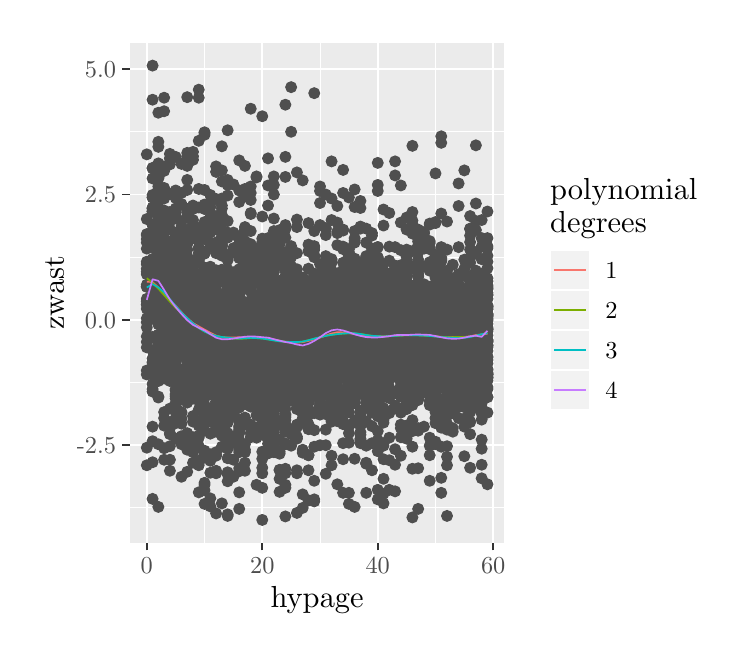
\begin{tikzpicture}[x=1pt,y=1pt]
\definecolor{fillColor}{RGB}{255,255,255}
\path[use as bounding box,fill=fillColor,fill opacity=0.00] (0,0) rectangle (252.94,216.81);
\begin{scope}
\path[clip] (  0.00,  0.00) rectangle (252.94,216.81);
\definecolor{drawColor}{RGB}{255,255,255}
\definecolor{fillColor}{RGB}{255,255,255}

\path[draw=drawColor,line width= 0.6pt,line join=round,line cap=round,fill=fillColor] (  0.00,  0.00) rectangle (252.94,216.81);
\end{scope}
\begin{scope}
\path[clip] ( 36.89, 30.72) rectangle (172.29,211.31);
\definecolor{fillColor}{gray}{0.92}

\path[fill=fillColor] ( 36.89, 30.72) rectangle (172.29,211.31);
\definecolor{drawColor}{RGB}{255,255,255}

\path[draw=drawColor,line width= 0.3pt,line join=round] ( 36.89, 43.28) --
	(172.29, 43.28);

\path[draw=drawColor,line width= 0.3pt,line join=round] ( 36.89, 88.58) --
	(172.29, 88.58);

\path[draw=drawColor,line width= 0.3pt,line join=round] ( 36.89,133.88) --
	(172.29,133.88);

\path[draw=drawColor,line width= 0.3pt,line join=round] ( 36.89,179.18) --
	(172.29,179.18);

\path[draw=drawColor,line width= 0.3pt,line join=round] ( 63.91, 30.72) --
	( 63.91,211.31);

\path[draw=drawColor,line width= 0.3pt,line join=round] (105.64, 30.72) --
	(105.64,211.31);

\path[draw=drawColor,line width= 0.3pt,line join=round] (147.36, 30.72) --
	(147.36,211.31);

\path[draw=drawColor,line width= 0.6pt,line join=round] ( 36.89, 65.93) --
	(172.29, 65.93);

\path[draw=drawColor,line width= 0.6pt,line join=round] ( 36.89,111.23) --
	(172.29,111.23);

\path[draw=drawColor,line width= 0.6pt,line join=round] ( 36.89,156.53) --
	(172.29,156.53);

\path[draw=drawColor,line width= 0.6pt,line join=round] ( 36.89,201.83) --
	(172.29,201.83);

\path[draw=drawColor,line width= 0.6pt,line join=round] ( 43.05, 30.72) --
	( 43.05,211.31);

\path[draw=drawColor,line width= 0.6pt,line join=round] ( 84.77, 30.72) --
	( 84.77,211.31);

\path[draw=drawColor,line width= 0.6pt,line join=round] (126.50, 30.72) --
	(126.50,211.31);

\path[draw=drawColor,line width= 0.6pt,line join=round] (168.22, 30.72) --
	(168.22,211.31);
\definecolor{drawColor}{gray}{0.31}
\definecolor{fillColor}{gray}{0.31}

\path[draw=drawColor,line width= 0.4pt,line join=round,line cap=round,fill=fillColor] (147.36,113.59) circle (  1.96);

\path[draw=drawColor,line width= 0.4pt,line join=round,line cap=round,fill=fillColor] ( 72.26,120.47) circle (  1.96);

\path[draw=drawColor,line width= 0.4pt,line join=round,line cap=round,fill=fillColor] ( 86.86,110.51) circle (  1.96);

\path[draw=drawColor,line width= 0.4pt,line join=round,line cap=round,fill=fillColor] (118.15, 83.15) circle (  1.96);

\path[draw=drawColor,line width= 0.4pt,line join=round,line cap=round,fill=fillColor] (105.64, 81.15) circle (  1.96);

\path[draw=drawColor,line width= 0.4pt,line join=round,line cap=round,fill=fillColor] ( 78.51,117.57) circle (  1.96);

\path[draw=drawColor,line width= 0.4pt,line join=round,line cap=round,fill=fillColor] ( 63.91,112.68) circle (  1.96);

\path[draw=drawColor,line width= 0.4pt,line join=round,line cap=round,fill=fillColor] (147.36, 93.47) circle (  1.96);

\path[draw=drawColor,line width= 0.4pt,line join=round,line cap=round,fill=fillColor] ( 53.48,115.76) circle (  1.96);

\path[draw=drawColor,line width= 0.4pt,line join=round,line cap=round,fill=fillColor] (141.10, 86.77) circle (  1.96);

\path[draw=drawColor,line width= 0.4pt,line join=round,line cap=round,fill=fillColor] ( 76.43,129.53) circle (  1.96);

\path[draw=drawColor,line width= 0.4pt,line join=round,line cap=round,fill=fillColor] (132.76,100.90) circle (  1.96);

\path[draw=drawColor,line width= 0.4pt,line join=round,line cap=round,fill=fillColor] ( 53.48, 85.68) circle (  1.96);

\path[draw=drawColor,line width= 0.4pt,line join=round,line cap=round,fill=fillColor] (143.19,103.62) circle (  1.96);

\path[draw=drawColor,line width= 0.4pt,line join=round,line cap=round,fill=fillColor] ( 47.22,111.05) circle (  1.96);

\path[draw=drawColor,line width= 0.4pt,line join=round,line cap=round,fill=fillColor] (126.50, 87.86) circle (  1.96);

\path[draw=drawColor,line width= 0.4pt,line join=round,line cap=round,fill=fillColor] ( 95.20, 88.04) circle (  1.96);

\path[draw=drawColor,line width= 0.4pt,line join=round,line cap=round,fill=fillColor] ( 88.95,105.43) circle (  1.96);

\path[draw=drawColor,line width= 0.4pt,line join=round,line cap=round,fill=fillColor] ( 97.29, 73.36) circle (  1.96);

\path[draw=drawColor,line width= 0.4pt,line join=round,line cap=round,fill=fillColor] ( 84.77,105.25) circle (  1.96);

\path[draw=drawColor,line width= 0.4pt,line join=round,line cap=round,fill=fillColor] (139.02,101.45) circle (  1.96);

\path[draw=drawColor,line width= 0.4pt,line join=round,line cap=round,fill=fillColor] ( 82.69, 80.43) circle (  1.96);

\path[draw=drawColor,line width= 0.4pt,line join=round,line cap=round,fill=fillColor] (147.36, 98.91) circle (  1.96);

\path[draw=drawColor,line width= 0.4pt,line join=round,line cap=round,fill=fillColor] ( 61.82,116.31) circle (  1.96);

\path[draw=drawColor,line width= 0.4pt,line join=round,line cap=round,fill=fillColor] ( 78.51,103.44) circle (  1.96);

\path[draw=drawColor,line width= 0.4pt,line join=round,line cap=round,fill=fillColor] (113.98, 97.82) circle (  1.96);

\path[draw=drawColor,line width= 0.4pt,line join=round,line cap=round,fill=fillColor] (155.71, 82.97) circle (  1.96);

\path[draw=drawColor,line width= 0.4pt,line join=round,line cap=round,fill=fillColor] ( 57.65,151.10) circle (  1.96);

\path[draw=drawColor,line width= 0.4pt,line join=round,line cap=round,fill=fillColor] ( 47.22, 89.13) circle (  1.96);

\path[draw=drawColor,line width= 0.4pt,line join=round,line cap=round,fill=fillColor] ( 66.00, 46.72) circle (  1.96);

\path[draw=drawColor,line width= 0.4pt,line join=round,line cap=round,fill=fillColor] (164.05, 58.87) circle (  1.96);

\path[draw=drawColor,line width= 0.4pt,line join=round,line cap=round,fill=fillColor] (118.15,114.13) circle (  1.96);

\path[draw=drawColor,line width= 0.4pt,line join=round,line cap=round,fill=fillColor] ( 78.51, 90.76) circle (  1.96);

\path[draw=drawColor,line width= 0.4pt,line join=round,line cap=round,fill=fillColor] ( 76.43, 72.46) circle (  1.96);

\path[draw=drawColor,line width= 0.4pt,line join=round,line cap=round,fill=fillColor] (164.05, 85.32) circle (  1.96);

\path[draw=drawColor,line width= 0.4pt,line join=round,line cap=round,fill=fillColor] (120.24, 99.27) circle (  1.96);

\path[draw=drawColor,line width= 0.4pt,line join=round,line cap=round,fill=fillColor] (166.14,100.00) circle (  1.96);

\path[draw=drawColor,line width= 0.4pt,line join=round,line cap=round,fill=fillColor] ( 91.03, 57.05) circle (  1.96);

\path[draw=drawColor,line width= 0.4pt,line join=round,line cap=round,fill=fillColor] ( 93.12,110.15) circle (  1.96);

\path[draw=drawColor,line width= 0.4pt,line join=round,line cap=round,fill=fillColor] (151.53, 93.84) circle (  1.96);

\path[draw=drawColor,line width= 0.4pt,line join=round,line cap=round,fill=fillColor] (161.96, 95.83) circle (  1.96);

\path[draw=drawColor,line width= 0.4pt,line join=round,line cap=round,fill=fillColor] (116.07,113.23) circle (  1.96);

\path[draw=drawColor,line width= 0.4pt,line join=round,line cap=round,fill=fillColor] ( 84.77, 80.25) circle (  1.96);

\path[draw=drawColor,line width= 0.4pt,line join=round,line cap=round,fill=fillColor] (145.27, 84.41) circle (  1.96);

\path[draw=drawColor,line width= 0.4pt,line join=round,line cap=round,fill=fillColor] ( 99.38, 84.23) circle (  1.96);

\path[draw=drawColor,line width= 0.4pt,line join=round,line cap=round,fill=fillColor] (161.96,106.88) circle (  1.96);

\path[draw=drawColor,line width= 0.4pt,line join=round,line cap=round,fill=fillColor] ( 76.43, 64.30) circle (  1.96);

\path[draw=drawColor,line width= 0.4pt,line join=round,line cap=round,fill=fillColor] (155.71,100.00) circle (  1.96);

\path[draw=drawColor,line width= 0.4pt,line join=round,line cap=round,fill=fillColor] (145.27, 81.88) circle (  1.96);

\path[draw=drawColor,line width= 0.4pt,line join=round,line cap=round,fill=fillColor] ( 63.91,112.50) circle (  1.96);

\path[draw=drawColor,line width= 0.4pt,line join=round,line cap=round,fill=fillColor] ( 93.12,121.20) circle (  1.96);

\path[draw=drawColor,line width= 0.4pt,line join=round,line cap=round,fill=fillColor] (122.33, 81.70) circle (  1.96);

\path[draw=drawColor,line width= 0.4pt,line join=round,line cap=round,fill=fillColor] ( 80.60, 95.47) circle (  1.96);

\path[draw=drawColor,line width= 0.4pt,line join=round,line cap=round,fill=fillColor] (126.50, 96.01) circle (  1.96);

\path[draw=drawColor,line width= 0.4pt,line join=round,line cap=round,fill=fillColor] ( 95.20, 84.78) circle (  1.96);

\path[draw=drawColor,line width= 0.4pt,line join=round,line cap=round,fill=fillColor] (109.81,117.21) circle (  1.96);

\path[draw=drawColor,line width= 0.4pt,line join=round,line cap=round,fill=fillColor] ( 63.91,100.72) circle (  1.96);

\path[draw=drawColor,line width= 0.4pt,line join=round,line cap=round,fill=fillColor] ( 59.74, 84.78) circle (  1.96);

\path[draw=drawColor,line width= 0.4pt,line join=round,line cap=round,fill=fillColor] ( 86.86, 93.29) circle (  1.96);

\path[draw=drawColor,line width= 0.4pt,line join=round,line cap=round,fill=fillColor] ( 80.60,118.12) circle (  1.96);

\path[draw=drawColor,line width= 0.4pt,line join=round,line cap=round,fill=fillColor] (145.27,100.54) circle (  1.96);

\path[draw=drawColor,line width= 0.4pt,line join=round,line cap=round,fill=fillColor] ( 86.86,132.80) circle (  1.96);

\path[draw=drawColor,line width= 0.4pt,line join=round,line cap=round,fill=fillColor] ( 68.08,108.70) circle (  1.96);

\path[draw=drawColor,line width= 0.4pt,line join=round,line cap=round,fill=fillColor] (103.55,101.99) circle (  1.96);

\path[draw=drawColor,line width= 0.4pt,line join=round,line cap=round,fill=fillColor] ( 55.57, 85.68) circle (  1.96);

\path[draw=drawColor,line width= 0.4pt,line join=round,line cap=round,fill=fillColor] ( 51.39,146.75) circle (  1.96);

\path[draw=drawColor,line width= 0.4pt,line join=round,line cap=round,fill=fillColor] (103.55, 99.64) circle (  1.96);

\path[draw=drawColor,line width= 0.4pt,line join=round,line cap=round,fill=fillColor] (101.46,120.47) circle (  1.96);

\path[draw=drawColor,line width= 0.4pt,line join=round,line cap=round,fill=fillColor] (143.19, 96.01) circle (  1.96);

\path[draw=drawColor,line width= 0.4pt,line join=round,line cap=round,fill=fillColor] ( 74.34,107.06) circle (  1.96);

\path[draw=drawColor,line width= 0.4pt,line join=round,line cap=round,fill=fillColor] ( 84.77,115.22) circle (  1.96);

\path[draw=drawColor,line width= 0.4pt,line join=round,line cap=round,fill=fillColor] ( 53.48,137.51) circle (  1.96);

\path[draw=drawColor,line width= 0.4pt,line join=round,line cap=round,fill=fillColor] ( 70.17,141.31) circle (  1.96);

\path[draw=drawColor,line width= 0.4pt,line join=round,line cap=round,fill=fillColor] (124.41,122.83) circle (  1.96);

\path[draw=drawColor,line width= 0.4pt,line join=round,line cap=round,fill=fillColor] (101.46, 87.68) circle (  1.96);

\path[draw=drawColor,line width= 0.4pt,line join=round,line cap=round,fill=fillColor] (161.96, 96.01) circle (  1.96);

\path[draw=drawColor,line width= 0.4pt,line join=round,line cap=round,fill=fillColor] (124.41, 87.86) circle (  1.96);

\path[draw=drawColor,line width= 0.4pt,line join=round,line cap=round,fill=fillColor] (101.46,100.90) circle (  1.96);

\path[draw=drawColor,line width= 0.4pt,line join=round,line cap=round,fill=fillColor] (126.50,103.98) circle (  1.96);

\path[draw=drawColor,line width= 0.4pt,line join=round,line cap=round,fill=fillColor] (145.27,101.45) circle (  1.96);

\path[draw=drawColor,line width= 0.4pt,line join=round,line cap=round,fill=fillColor] (120.24,112.68) circle (  1.96);

\path[draw=drawColor,line width= 0.4pt,line join=round,line cap=round,fill=fillColor] ( 99.38, 87.68) circle (  1.96);

\path[draw=drawColor,line width= 0.4pt,line join=round,line cap=round,fill=fillColor] (164.05,107.06) circle (  1.96);

\path[draw=drawColor,line width= 0.4pt,line join=round,line cap=round,fill=fillColor] ( 99.38, 95.47) circle (  1.96);

\path[draw=drawColor,line width= 0.4pt,line join=round,line cap=round,fill=fillColor] (155.71, 89.31) circle (  1.96);

\path[draw=drawColor,line width= 0.4pt,line join=round,line cap=round,fill=fillColor] ( 93.12, 85.86) circle (  1.96);

\path[draw=drawColor,line width= 0.4pt,line join=round,line cap=round,fill=fillColor] (122.33,107.79) circle (  1.96);

\path[draw=drawColor,line width= 0.4pt,line join=round,line cap=round,fill=fillColor] ( 53.48,170.12) circle (  1.96);

\path[draw=drawColor,line width= 0.4pt,line join=round,line cap=round,fill=fillColor] ( 53.48,132.07) circle (  1.96);

\path[draw=drawColor,line width= 0.4pt,line join=round,line cap=round,fill=fillColor] ( 95.20,113.41) circle (  1.96);

\path[draw=drawColor,line width= 0.4pt,line join=round,line cap=round,fill=fillColor] (101.46,103.44) circle (  1.96);

\path[draw=drawColor,line width= 0.4pt,line join=round,line cap=round,fill=fillColor] (155.71,115.94) circle (  1.96);

\path[draw=drawColor,line width= 0.4pt,line join=round,line cap=round,fill=fillColor] ( 70.17, 98.37) circle (  1.96);

\path[draw=drawColor,line width= 0.4pt,line join=round,line cap=round,fill=fillColor] (111.89,124.28) circle (  1.96);

\path[draw=drawColor,line width= 0.4pt,line join=round,line cap=round,fill=fillColor] ( 68.08,129.17) circle (  1.96);

\path[draw=drawColor,line width= 0.4pt,line join=round,line cap=round,fill=fillColor] (164.05,103.80) circle (  1.96);

\path[draw=drawColor,line width= 0.4pt,line join=round,line cap=round,fill=fillColor] ( 68.08, 87.50) circle (  1.96);

\path[draw=drawColor,line width= 0.4pt,line join=round,line cap=round,fill=fillColor] ( 72.26,110.15) circle (  1.96);

\path[draw=drawColor,line width= 0.4pt,line join=round,line cap=round,fill=fillColor] ( 84.77,103.08) circle (  1.96);

\path[draw=drawColor,line width= 0.4pt,line join=round,line cap=round,fill=fillColor] ( 49.31,112.68) circle (  1.96);

\path[draw=drawColor,line width= 0.4pt,line join=round,line cap=round,fill=fillColor] (166.14, 86.95) circle (  1.96);

\path[draw=drawColor,line width= 0.4pt,line join=round,line cap=round,fill=fillColor] ( 84.77,110.51) circle (  1.96);

\path[draw=drawColor,line width= 0.4pt,line join=round,line cap=round,fill=fillColor] ( 95.20, 92.57) circle (  1.96);

\path[draw=drawColor,line width= 0.4pt,line join=round,line cap=round,fill=fillColor] (145.27,104.53) circle (  1.96);

\path[draw=drawColor,line width= 0.4pt,line join=round,line cap=round,fill=fillColor] ( 97.29,108.51) circle (  1.96);

\path[draw=drawColor,line width= 0.4pt,line join=round,line cap=round,fill=fillColor] (147.36,108.70) circle (  1.96);

\path[draw=drawColor,line width= 0.4pt,line join=round,line cap=round,fill=fillColor] (101.46, 46.00) circle (  1.96);

\path[draw=drawColor,line width= 0.4pt,line join=round,line cap=round,fill=fillColor] ( 63.91,178.10) circle (  1.96);

\path[draw=drawColor,line width= 0.4pt,line join=round,line cap=round,fill=fillColor] ( 84.77,128.27) circle (  1.96);

\path[draw=drawColor,line width= 0.4pt,line join=round,line cap=round,fill=fillColor] ( 91.03,116.67) circle (  1.96);

\path[draw=drawColor,line width= 0.4pt,line join=round,line cap=round,fill=fillColor] (147.36, 94.92) circle (  1.96);

\path[draw=drawColor,line width= 0.4pt,line join=round,line cap=round,fill=fillColor] (124.41, 86.95) circle (  1.96);

\path[draw=drawColor,line width= 0.4pt,line join=round,line cap=round,fill=fillColor] (166.14,115.22) circle (  1.96);

\path[draw=drawColor,line width= 0.4pt,line join=round,line cap=round,fill=fillColor] ( 74.34,125.00) circle (  1.96);

\path[draw=drawColor,line width= 0.4pt,line join=round,line cap=round,fill=fillColor] ( 97.29,112.32) circle (  1.96);

\path[draw=drawColor,line width= 0.4pt,line join=round,line cap=round,fill=fillColor] (120.24, 87.13) circle (  1.96);

\path[draw=drawColor,line width= 0.4pt,line join=round,line cap=round,fill=fillColor] ( 45.13,151.46) circle (  1.96);

\path[draw=drawColor,line width= 0.4pt,line join=round,line cap=round,fill=fillColor] (122.33, 99.82) circle (  1.96);

\path[draw=drawColor,line width= 0.4pt,line join=round,line cap=round,fill=fillColor] ( 61.82,117.76) circle (  1.96);

\path[draw=drawColor,line width= 0.4pt,line join=round,line cap=round,fill=fillColor] (107.72,115.94) circle (  1.96);

\path[draw=drawColor,line width= 0.4pt,line join=round,line cap=round,fill=fillColor] ( 47.22,121.74) circle (  1.96);

\path[draw=drawColor,line width= 0.4pt,line join=round,line cap=round,fill=fillColor] (120.24,114.49) circle (  1.96);

\path[draw=drawColor,line width= 0.4pt,line join=round,line cap=round,fill=fillColor] ( 51.39, 93.29) circle (  1.96);

\path[draw=drawColor,line width= 0.4pt,line join=round,line cap=round,fill=fillColor] (147.36, 93.29) circle (  1.96);

\path[draw=drawColor,line width= 0.4pt,line join=round,line cap=round,fill=fillColor] (101.46,103.26) circle (  1.96);

\path[draw=drawColor,line width= 0.4pt,line join=round,line cap=round,fill=fillColor] ( 61.82,107.97) circle (  1.96);

\path[draw=drawColor,line width= 0.4pt,line join=round,line cap=round,fill=fillColor] (157.79,127.36) circle (  1.96);

\path[draw=drawColor,line width= 0.4pt,line join=round,line cap=round,fill=fillColor] (103.55,133.88) circle (  1.96);

\path[draw=drawColor,line width= 0.4pt,line join=round,line cap=round,fill=fillColor] ( 66.00,129.17) circle (  1.96);

\path[draw=drawColor,line width= 0.4pt,line join=round,line cap=round,fill=fillColor] ( 66.00,126.09) circle (  1.96);

\path[draw=drawColor,line width= 0.4pt,line join=round,line cap=round,fill=fillColor] ( 78.51,139.14) circle (  1.96);

\path[draw=drawColor,line width= 0.4pt,line join=round,line cap=round,fill=fillColor] ( 78.51,134.97) circle (  1.96);

\path[draw=drawColor,line width= 0.4pt,line join=round,line cap=round,fill=fillColor] ( 93.12, 86.95) circle (  1.96);

\path[draw=drawColor,line width= 0.4pt,line join=round,line cap=round,fill=fillColor] (116.07,101.45) circle (  1.96);

\path[draw=drawColor,line width= 0.4pt,line join=round,line cap=round,fill=fillColor] (157.79,117.57) circle (  1.96);

\path[draw=drawColor,line width= 0.4pt,line join=round,line cap=round,fill=fillColor] (130.67, 60.50) circle (  1.96);

\path[draw=drawColor,line width= 0.4pt,line join=round,line cap=round,fill=fillColor] (109.81,119.39) circle (  1.96);

\path[draw=drawColor,line width= 0.4pt,line join=round,line cap=round,fill=fillColor] ( 47.22,133.34) circle (  1.96);

\path[draw=drawColor,line width= 0.4pt,line join=round,line cap=round,fill=fillColor] (105.64,124.64) circle (  1.96);

\path[draw=drawColor,line width= 0.4pt,line join=round,line cap=round,fill=fillColor] (120.24,117.39) circle (  1.96);

\path[draw=drawColor,line width= 0.4pt,line join=round,line cap=round,fill=fillColor] (109.81,117.94) circle (  1.96);

\path[draw=drawColor,line width= 0.4pt,line join=round,line cap=round,fill=fillColor] ( 53.48,148.92) circle (  1.96);

\path[draw=drawColor,line width= 0.4pt,line join=round,line cap=round,fill=fillColor] ( 72.26, 40.93) circle (  1.96);

\path[draw=drawColor,line width= 0.4pt,line join=round,line cap=round,fill=fillColor] (155.71,104.71) circle (  1.96);

\path[draw=drawColor,line width= 0.4pt,line join=round,line cap=round,fill=fillColor] ( 74.34,115.04) circle (  1.96);

\path[draw=drawColor,line width= 0.4pt,line join=round,line cap=round,fill=fillColor] ( 68.08,114.13) circle (  1.96);

\path[draw=drawColor,line width= 0.4pt,line join=round,line cap=round,fill=fillColor] ( 70.17,143.12) circle (  1.96);

\path[draw=drawColor,line width= 0.4pt,line join=round,line cap=round,fill=fillColor] ( 86.86, 72.27) circle (  1.96);

\path[draw=drawColor,line width= 0.4pt,line join=round,line cap=round,fill=fillColor] (111.89,121.38) circle (  1.96);

\path[draw=drawColor,line width= 0.4pt,line join=round,line cap=round,fill=fillColor] (141.10,116.85) circle (  1.96);

\path[draw=drawColor,line width= 0.4pt,line join=round,line cap=round,fill=fillColor] (141.10,124.46) circle (  1.96);

\path[draw=drawColor,line width= 0.4pt,line join=round,line cap=round,fill=fillColor] ( 51.39,156.71) circle (  1.96);

\path[draw=drawColor,line width= 0.4pt,line join=round,line cap=round,fill=fillColor] (109.81, 97.28) circle (  1.96);

\path[draw=drawColor,line width= 0.4pt,line join=round,line cap=round,fill=fillColor] ( 84.77,133.88) circle (  1.96);

\path[draw=drawColor,line width= 0.4pt,line join=round,line cap=round,fill=fillColor] (107.72,127.18) circle (  1.96);

\path[draw=drawColor,line width= 0.4pt,line join=round,line cap=round,fill=fillColor] ( 66.00,103.08) circle (  1.96);

\path[draw=drawColor,line width= 0.4pt,line join=round,line cap=round,fill=fillColor] ( 66.00,100.54) circle (  1.96);

\path[draw=drawColor,line width= 0.4pt,line join=round,line cap=round,fill=fillColor] (124.41,121.38) circle (  1.96);

\path[draw=drawColor,line width= 0.4pt,line join=round,line cap=round,fill=fillColor] ( 61.82,107.06) circle (  1.96);

\path[draw=drawColor,line width= 0.4pt,line join=round,line cap=round,fill=fillColor] ( 88.95,103.98) circle (  1.96);

\path[draw=drawColor,line width= 0.4pt,line join=round,line cap=round,fill=fillColor] (151.53, 98.55) circle (  1.96);

\path[draw=drawColor,line width= 0.4pt,line join=round,line cap=round,fill=fillColor] (111.89, 77.35) circle (  1.96);

\path[draw=drawColor,line width= 0.4pt,line join=round,line cap=round,fill=fillColor] (126.50, 82.97) circle (  1.96);

\path[draw=drawColor,line width= 0.4pt,line join=round,line cap=round,fill=fillColor] ( 68.08, 84.60) circle (  1.96);

\path[draw=drawColor,line width= 0.4pt,line join=round,line cap=round,fill=fillColor] (109.81,117.21) circle (  1.96);

\path[draw=drawColor,line width= 0.4pt,line join=round,line cap=round,fill=fillColor] (155.71,127.72) circle (  1.96);

\path[draw=drawColor,line width= 0.4pt,line join=round,line cap=round,fill=fillColor] ( 47.22,162.87) circle (  1.96);

\path[draw=drawColor,line width= 0.4pt,line join=round,line cap=round,fill=fillColor] (120.24,106.34) circle (  1.96);

\path[draw=drawColor,line width= 0.4pt,line join=round,line cap=round,fill=fillColor] ( 63.91, 93.66) circle (  1.96);

\path[draw=drawColor,line width= 0.4pt,line join=round,line cap=round,fill=fillColor] (139.02,100.54) circle (  1.96);

\path[draw=drawColor,line width= 0.4pt,line join=round,line cap=round,fill=fillColor] ( 88.95,106.16) circle (  1.96);

\path[draw=drawColor,line width= 0.4pt,line join=round,line cap=round,fill=fillColor] ( 61.82, 87.68) circle (  1.96);

\path[draw=drawColor,line width= 0.4pt,line join=round,line cap=round,fill=fillColor] (151.53,114.68) circle (  1.96);

\path[draw=drawColor,line width= 0.4pt,line join=round,line cap=round,fill=fillColor] ( 70.17,108.88) circle (  1.96);

\path[draw=drawColor,line width= 0.4pt,line join=round,line cap=round,fill=fillColor] (126.50,112.86) circle (  1.96);

\path[draw=drawColor,line width= 0.4pt,line join=round,line cap=round,fill=fillColor] ( 57.65,109.06) circle (  1.96);

\path[draw=drawColor,line width= 0.4pt,line join=round,line cap=round,fill=fillColor] (116.07,109.24) circle (  1.96);

\path[draw=drawColor,line width= 0.4pt,line join=round,line cap=round,fill=fillColor] (164.05, 92.75) circle (  1.96);

\path[draw=drawColor,line width= 0.4pt,line join=round,line cap=round,fill=fillColor] (107.72, 99.82) circle (  1.96);

\path[draw=drawColor,line width= 0.4pt,line join=round,line cap=round,fill=fillColor] (145.27,137.14) circle (  1.96);

\path[draw=drawColor,line width= 0.4pt,line join=round,line cap=round,fill=fillColor] ( 86.86, 81.15) circle (  1.96);

\path[draw=drawColor,line width= 0.4pt,line join=round,line cap=round,fill=fillColor] (139.02,102.17) circle (  1.96);

\path[draw=drawColor,line width= 0.4pt,line join=round,line cap=round,fill=fillColor] ( 78.51,101.27) circle (  1.96);

\path[draw=drawColor,line width= 0.4pt,line join=round,line cap=round,fill=fillColor] (124.41,141.67) circle (  1.96);

\path[draw=drawColor,line width= 0.4pt,line join=round,line cap=round,fill=fillColor] (103.55,111.78) circle (  1.96);

\path[draw=drawColor,line width= 0.4pt,line join=round,line cap=round,fill=fillColor] (166.14,125.18) circle (  1.96);

\path[draw=drawColor,line width= 0.4pt,line join=round,line cap=round,fill=fillColor] ( 91.03,136.42) circle (  1.96);

\path[draw=drawColor,line width= 0.4pt,line join=round,line cap=round,fill=fillColor] ( 93.12,135.51) circle (  1.96);

\path[draw=drawColor,line width= 0.4pt,line join=round,line cap=round,fill=fillColor] (141.10,119.02) circle (  1.96);

\path[draw=drawColor,line width= 0.4pt,line join=round,line cap=round,fill=fillColor] ( 57.65, 96.92) circle (  1.96);

\path[draw=drawColor,line width= 0.4pt,line join=round,line cap=round,fill=fillColor] ( 76.43,124.46) circle (  1.96);

\path[draw=drawColor,line width= 0.4pt,line join=round,line cap=round,fill=fillColor] (101.46,111.41) circle (  1.96);

\path[draw=drawColor,line width= 0.4pt,line join=round,line cap=round,fill=fillColor] ( 53.48, 98.55) circle (  1.96);

\path[draw=drawColor,line width= 0.4pt,line join=round,line cap=round,fill=fillColor] (141.10,127.18) circle (  1.96);

\path[draw=drawColor,line width= 0.4pt,line join=round,line cap=round,fill=fillColor] ( 76.43,133.52) circle (  1.96);

\path[draw=drawColor,line width= 0.4pt,line join=round,line cap=round,fill=fillColor] ( 47.22,152.00) circle (  1.96);

\path[draw=drawColor,line width= 0.4pt,line join=round,line cap=round,fill=fillColor] (155.71,121.74) circle (  1.96);

\path[draw=drawColor,line width= 0.4pt,line join=round,line cap=round,fill=fillColor] ( 61.82,122.29) circle (  1.96);

\path[draw=drawColor,line width= 0.4pt,line join=round,line cap=round,fill=fillColor] ( 78.51,109.42) circle (  1.96);

\path[draw=drawColor,line width= 0.4pt,line join=round,line cap=round,fill=fillColor] (120.24,122.10) circle (  1.96);

\path[draw=drawColor,line width= 0.4pt,line join=round,line cap=round,fill=fillColor] (151.53,103.62) circle (  1.96);

\path[draw=drawColor,line width= 0.4pt,line join=round,line cap=round,fill=fillColor] (134.84, 86.05) circle (  1.96);

\path[draw=drawColor,line width= 0.4pt,line join=round,line cap=round,fill=fillColor] (103.55,100.72) circle (  1.96);

\path[draw=drawColor,line width= 0.4pt,line join=round,line cap=round,fill=fillColor] (136.93,103.08) circle (  1.96);

\path[draw=drawColor,line width= 0.4pt,line join=round,line cap=round,fill=fillColor] ( 45.13,105.07) circle (  1.96);

\path[draw=drawColor,line width= 0.4pt,line join=round,line cap=round,fill=fillColor] ( 95.20, 98.73) circle (  1.96);

\path[draw=drawColor,line width= 0.4pt,line join=round,line cap=round,fill=fillColor] ( 68.08, 63.40) circle (  1.96);

\path[draw=drawColor,line width= 0.4pt,line join=round,line cap=round,fill=fillColor] ( 72.26,114.49) circle (  1.96);

\path[draw=drawColor,line width= 0.4pt,line join=round,line cap=round,fill=fillColor] (132.76,113.04) circle (  1.96);

\path[draw=drawColor,line width= 0.4pt,line join=round,line cap=round,fill=fillColor] ( 53.48,101.09) circle (  1.96);

\path[draw=drawColor,line width= 0.4pt,line join=round,line cap=round,fill=fillColor] (128.58, 98.00) circle (  1.96);

\path[draw=drawColor,line width= 0.4pt,line join=round,line cap=round,fill=fillColor] (113.98,114.31) circle (  1.96);

\path[draw=drawColor,line width= 0.4pt,line join=round,line cap=round,fill=fillColor] (151.53,126.45) circle (  1.96);

\path[draw=drawColor,line width= 0.4pt,line join=round,line cap=round,fill=fillColor] ( 53.48,110.87) circle (  1.96);

\path[draw=drawColor,line width= 0.4pt,line join=round,line cap=round,fill=fillColor] (130.67,137.69) circle (  1.96);

\path[draw=drawColor,line width= 0.4pt,line join=round,line cap=round,fill=fillColor] (141.10,109.06) circle (  1.96);

\path[draw=drawColor,line width= 0.4pt,line join=round,line cap=round,fill=fillColor] ( 88.95,101.45) circle (  1.96);

\path[draw=drawColor,line width= 0.4pt,line join=round,line cap=round,fill=fillColor] (118.15,118.84) circle (  1.96);

\path[draw=drawColor,line width= 0.4pt,line join=round,line cap=round,fill=fillColor] ( 82.69, 93.66) circle (  1.96);

\path[draw=drawColor,line width= 0.4pt,line join=round,line cap=round,fill=fillColor] (120.24, 94.20) circle (  1.96);

\path[draw=drawColor,line width= 0.4pt,line join=round,line cap=round,fill=fillColor] ( 70.17, 96.01) circle (  1.96);

\path[draw=drawColor,line width= 0.4pt,line join=round,line cap=round,fill=fillColor] ( 47.22,130.44) circle (  1.96);

\path[draw=drawColor,line width= 0.4pt,line join=round,line cap=round,fill=fillColor] (164.05, 99.82) circle (  1.96);

\path[draw=drawColor,line width= 0.4pt,line join=round,line cap=round,fill=fillColor] ( 97.29,107.79) circle (  1.96);

\path[draw=drawColor,line width= 0.4pt,line join=round,line cap=round,fill=fillColor] ( 55.57,104.35) circle (  1.96);

\path[draw=drawColor,line width= 0.4pt,line join=round,line cap=round,fill=fillColor] ( 91.03, 88.04) circle (  1.96);

\path[draw=drawColor,line width= 0.4pt,line join=round,line cap=round,fill=fillColor] (147.36, 75.72) circle (  1.96);

\path[draw=drawColor,line width= 0.4pt,line join=round,line cap=round,fill=fillColor] ( 47.22, 94.74) circle (  1.96);

\path[draw=drawColor,line width= 0.4pt,line join=round,line cap=round,fill=fillColor] (122.33,104.71) circle (  1.96);

\path[draw=drawColor,line width= 0.4pt,line join=round,line cap=round,fill=fillColor] ( 84.77,104.89) circle (  1.96);

\path[draw=drawColor,line width= 0.4pt,line join=round,line cap=round,fill=fillColor] (118.15, 43.64) circle (  1.96);

\path[draw=drawColor,line width= 0.4pt,line join=round,line cap=round,fill=fillColor] ( 59.74, 97.82) circle (  1.96);

\path[draw=drawColor,line width= 0.4pt,line join=round,line cap=round,fill=fillColor] ( 61.82, 96.92) circle (  1.96);

\path[draw=drawColor,line width= 0.4pt,line join=round,line cap=round,fill=fillColor] (116.07,100.90) circle (  1.96);

\path[draw=drawColor,line width= 0.4pt,line join=round,line cap=round,fill=fillColor] (151.53, 93.47) circle (  1.96);

\path[draw=drawColor,line width= 0.4pt,line join=round,line cap=round,fill=fillColor] ( 95.20, 96.56) circle (  1.96);

\path[draw=drawColor,line width= 0.4pt,line join=round,line cap=round,fill=fillColor] ( 95.20, 90.21) circle (  1.96);

\path[draw=drawColor,line width= 0.4pt,line join=round,line cap=round,fill=fillColor] (164.05, 84.05) circle (  1.96);

\path[draw=drawColor,line width= 0.4pt,line join=round,line cap=round,fill=fillColor] (161.96, 88.58) circle (  1.96);

\path[draw=drawColor,line width= 0.4pt,line join=round,line cap=round,fill=fillColor] ( 91.03,102.72) circle (  1.96);

\path[draw=drawColor,line width= 0.4pt,line join=round,line cap=round,fill=fillColor] (166.14, 91.48) circle (  1.96);

\path[draw=drawColor,line width= 0.4pt,line join=round,line cap=round,fill=fillColor] ( 88.95, 82.24) circle (  1.96);

\path[draw=drawColor,line width= 0.4pt,line join=round,line cap=round,fill=fillColor] ( 88.95, 84.23) circle (  1.96);

\path[draw=drawColor,line width= 0.4pt,line join=round,line cap=round,fill=fillColor] (136.93, 84.60) circle (  1.96);

\path[draw=drawColor,line width= 0.4pt,line join=round,line cap=round,fill=fillColor] ( 51.39,133.70) circle (  1.96);

\path[draw=drawColor,line width= 0.4pt,line join=round,line cap=round,fill=fillColor] (149.45,102.17) circle (  1.96);

\path[draw=drawColor,line width= 0.4pt,line join=round,line cap=round,fill=fillColor] ( 82.69,103.80) circle (  1.96);

\path[draw=drawColor,line width= 0.4pt,line join=round,line cap=round,fill=fillColor] (111.89,102.17) circle (  1.96);

\path[draw=drawColor,line width= 0.4pt,line join=round,line cap=round,fill=fillColor] (130.67,124.82) circle (  1.96);

\path[draw=drawColor,line width= 0.4pt,line join=round,line cap=round,fill=fillColor] (130.67,117.76) circle (  1.96);

\path[draw=drawColor,line width= 0.4pt,line join=round,line cap=round,fill=fillColor] ( 84.77,128.99) circle (  1.96);

\path[draw=drawColor,line width= 0.4pt,line join=round,line cap=round,fill=fillColor] (111.89, 84.96) circle (  1.96);

\path[draw=drawColor,line width= 0.4pt,line join=round,line cap=round,fill=fillColor] (107.72,111.05) circle (  1.96);

\path[draw=drawColor,line width= 0.4pt,line join=round,line cap=round,fill=fillColor] (109.81, 99.64) circle (  1.96);

\path[draw=drawColor,line width= 0.4pt,line join=round,line cap=round,fill=fillColor] ( 86.86,132.43) circle (  1.96);

\path[draw=drawColor,line width= 0.4pt,line join=round,line cap=round,fill=fillColor] ( 70.17, 93.47) circle (  1.96);

\path[draw=drawColor,line width= 0.4pt,line join=round,line cap=round,fill=fillColor] ( 68.08, 88.94) circle (  1.96);

\path[draw=drawColor,line width= 0.4pt,line join=round,line cap=round,fill=fillColor] (139.02,111.78) circle (  1.96);

\path[draw=drawColor,line width= 0.4pt,line join=round,line cap=round,fill=fillColor] (141.10,111.05) circle (  1.96);

\path[draw=drawColor,line width= 0.4pt,line join=round,line cap=round,fill=fillColor] ( 91.03, 74.63) circle (  1.96);

\path[draw=drawColor,line width= 0.4pt,line join=round,line cap=round,fill=fillColor] ( 80.60,136.78) circle (  1.96);

\path[draw=drawColor,line width= 0.4pt,line join=round,line cap=round,fill=fillColor] (130.67,114.49) circle (  1.96);

\path[draw=drawColor,line width= 0.4pt,line join=round,line cap=round,fill=fillColor] (155.71, 99.82) circle (  1.96);

\path[draw=drawColor,line width= 0.4pt,line join=round,line cap=round,fill=fillColor] ( 61.82,101.99) circle (  1.96);

\path[draw=drawColor,line width= 0.4pt,line join=round,line cap=round,fill=fillColor] (109.81,101.45) circle (  1.96);

\path[draw=drawColor,line width= 0.4pt,line join=round,line cap=round,fill=fillColor] ( 53.48, 83.69) circle (  1.96);

\path[draw=drawColor,line width= 0.4pt,line join=round,line cap=round,fill=fillColor] ( 66.00, 75.17) circle (  1.96);

\path[draw=drawColor,line width= 0.4pt,line join=round,line cap=round,fill=fillColor] (113.98, 84.41) circle (  1.96);

\path[draw=drawColor,line width= 0.4pt,line join=round,line cap=round,fill=fillColor] (113.98,105.98) circle (  1.96);

\path[draw=drawColor,line width= 0.4pt,line join=round,line cap=round,fill=fillColor] (159.88,118.66) circle (  1.96);

\path[draw=drawColor,line width= 0.4pt,line join=round,line cap=round,fill=fillColor] ( 93.12,114.49) circle (  1.96);

\path[draw=drawColor,line width= 0.4pt,line join=round,line cap=round,fill=fillColor] (132.76,113.95) circle (  1.96);

\path[draw=drawColor,line width= 0.4pt,line join=round,line cap=round,fill=fillColor] ( 70.17,128.45) circle (  1.96);

\path[draw=drawColor,line width= 0.4pt,line join=round,line cap=round,fill=fillColor] ( 88.95,159.98) circle (  1.96);

\path[draw=drawColor,line width= 0.4pt,line join=round,line cap=round,fill=fillColor] ( 91.03,138.59) circle (  1.96);

\path[draw=drawColor,line width= 0.4pt,line join=round,line cap=round,fill=fillColor] ( 68.08, 73.00) circle (  1.96);

\path[draw=drawColor,line width= 0.4pt,line join=round,line cap=round,fill=fillColor] ( 80.60, 99.09) circle (  1.96);

\path[draw=drawColor,line width= 0.4pt,line join=round,line cap=round,fill=fillColor] ( 55.57,144.21) circle (  1.96);

\path[draw=drawColor,line width= 0.4pt,line join=round,line cap=round,fill=fillColor] ( 86.86,108.15) circle (  1.96);

\path[draw=drawColor,line width= 0.4pt,line join=round,line cap=round,fill=fillColor] (120.24,115.04) circle (  1.96);

\path[draw=drawColor,line width= 0.4pt,line join=round,line cap=round,fill=fillColor] ( 93.12, 86.05) circle (  1.96);

\path[draw=drawColor,line width= 0.4pt,line join=round,line cap=round,fill=fillColor] (122.33,134.25) circle (  1.96);

\path[draw=drawColor,line width= 0.4pt,line join=round,line cap=round,fill=fillColor] ( 59.74,101.81) circle (  1.96);

\path[draw=drawColor,line width= 0.4pt,line join=round,line cap=round,fill=fillColor] ( 63.91, 74.81) circle (  1.96);

\path[draw=drawColor,line width= 0.4pt,line join=round,line cap=round,fill=fillColor] ( 78.51,114.49) circle (  1.96);

\path[draw=drawColor,line width= 0.4pt,line join=round,line cap=round,fill=fillColor] (136.93,122.47) circle (  1.96);

\path[draw=drawColor,line width= 0.4pt,line join=round,line cap=round,fill=fillColor] (103.55,107.25) circle (  1.96);

\path[draw=drawColor,line width= 0.4pt,line join=round,line cap=round,fill=fillColor] (151.53,117.76) circle (  1.96);

\path[draw=drawColor,line width= 0.4pt,line join=round,line cap=round,fill=fillColor] (111.89,115.58) circle (  1.96);

\path[draw=drawColor,line width= 0.4pt,line join=round,line cap=round,fill=fillColor] (157.79,110.51) circle (  1.96);

\path[draw=drawColor,line width= 0.4pt,line join=round,line cap=round,fill=fillColor] (113.98, 92.21) circle (  1.96);

\path[draw=drawColor,line width= 0.4pt,line join=round,line cap=round,fill=fillColor] (166.14,101.99) circle (  1.96);

\path[draw=drawColor,line width= 0.4pt,line join=round,line cap=round,fill=fillColor] (105.64,105.25) circle (  1.96);

\path[draw=drawColor,line width= 0.4pt,line join=round,line cap=round,fill=fillColor] ( 91.03, 90.58) circle (  1.96);

\path[draw=drawColor,line width= 0.4pt,line join=round,line cap=round,fill=fillColor] ( 59.74, 91.30) circle (  1.96);

\path[draw=drawColor,line width= 0.4pt,line join=round,line cap=round,fill=fillColor] ( 70.17, 99.45) circle (  1.96);

\path[draw=drawColor,line width= 0.4pt,line join=round,line cap=round,fill=fillColor] (130.67,124.64) circle (  1.96);

\path[draw=drawColor,line width= 0.4pt,line join=round,line cap=round,fill=fillColor] ( 61.82,113.23) circle (  1.96);

\path[draw=drawColor,line width= 0.4pt,line join=round,line cap=round,fill=fillColor] (126.50,124.46) circle (  1.96);

\path[draw=drawColor,line width= 0.4pt,line join=round,line cap=round,fill=fillColor] (166.14,123.74) circle (  1.96);

\path[draw=drawColor,line width= 0.4pt,line join=round,line cap=round,fill=fillColor] (118.15,118.48) circle (  1.96);

\path[draw=drawColor,line width= 0.4pt,line join=round,line cap=round,fill=fillColor] ( 45.13,126.63) circle (  1.96);

\path[draw=drawColor,line width= 0.4pt,line join=round,line cap=round,fill=fillColor] ( 72.26, 99.82) circle (  1.96);

\path[draw=drawColor,line width= 0.4pt,line join=round,line cap=round,fill=fillColor] (159.88,144.03) circle (  1.96);

\path[draw=drawColor,line width= 0.4pt,line join=round,line cap=round,fill=fillColor] ( 76.43, 93.84) circle (  1.96);

\path[draw=drawColor,line width= 0.4pt,line join=round,line cap=round,fill=fillColor] (109.81,117.76) circle (  1.96);

\path[draw=drawColor,line width= 0.4pt,line join=round,line cap=round,fill=fillColor] (149.45,101.27) circle (  1.96);

\path[draw=drawColor,line width= 0.4pt,line join=round,line cap=round,fill=fillColor] ( 59.74, 97.28) circle (  1.96);

\path[draw=drawColor,line width= 0.4pt,line join=round,line cap=round,fill=fillColor] (124.41,115.22) circle (  1.96);

\path[draw=drawColor,line width= 0.4pt,line join=round,line cap=round,fill=fillColor] ( 66.00,105.80) circle (  1.96);

\path[draw=drawColor,line width= 0.4pt,line join=round,line cap=round,fill=fillColor] (122.33,111.78) circle (  1.96);

\path[draw=drawColor,line width= 0.4pt,line join=round,line cap=round,fill=fillColor] ( 72.26,156.17) circle (  1.96);

\path[draw=drawColor,line width= 0.4pt,line join=round,line cap=round,fill=fillColor] (120.24,120.65) circle (  1.96);

\path[draw=drawColor,line width= 0.4pt,line join=round,line cap=round,fill=fillColor] (166.14,132.25) circle (  1.96);

\path[draw=drawColor,line width= 0.4pt,line join=round,line cap=round,fill=fillColor] ( 72.26,100.54) circle (  1.96);

\path[draw=drawColor,line width= 0.4pt,line join=round,line cap=round,fill=fillColor] (124.41,134.06) circle (  1.96);

\path[draw=drawColor,line width= 0.4pt,line join=round,line cap=round,fill=fillColor] (155.71, 75.72) circle (  1.96);

\path[draw=drawColor,line width= 0.4pt,line join=round,line cap=round,fill=fillColor] ( 59.74, 88.58) circle (  1.96);

\path[draw=drawColor,line width= 0.4pt,line join=round,line cap=round,fill=fillColor] (111.89, 75.90) circle (  1.96);

\path[draw=drawColor,line width= 0.4pt,line join=round,line cap=round,fill=fillColor] ( 76.43,168.85) circle (  1.96);

\path[draw=drawColor,line width= 0.4pt,line join=round,line cap=round,fill=fillColor] (159.88,114.86) circle (  1.96);

\path[draw=drawColor,line width= 0.4pt,line join=round,line cap=round,fill=fillColor] ( 57.65,142.04) circle (  1.96);

\path[draw=drawColor,line width= 0.4pt,line join=round,line cap=round,fill=fillColor] ( 72.26,122.47) circle (  1.96);

\path[draw=drawColor,line width= 0.4pt,line join=round,line cap=round,fill=fillColor] (153.62,120.65) circle (  1.96);

\path[draw=drawColor,line width= 0.4pt,line join=round,line cap=round,fill=fillColor] ( 88.95,114.86) circle (  1.96);

\path[draw=drawColor,line width= 0.4pt,line join=round,line cap=round,fill=fillColor] (149.45,109.24) circle (  1.96);

\path[draw=drawColor,line width= 0.4pt,line join=round,line cap=round,fill=fillColor] (113.98,106.88) circle (  1.96);

\path[draw=drawColor,line width= 0.4pt,line join=round,line cap=round,fill=fillColor] (116.07,155.45) circle (  1.96);

\path[draw=drawColor,line width= 0.4pt,line join=round,line cap=round,fill=fillColor] ( 47.22,134.43) circle (  1.96);

\path[draw=drawColor,line width= 0.4pt,line join=round,line cap=round,fill=fillColor] (103.55,120.65) circle (  1.96);

\path[draw=drawColor,line width= 0.4pt,line join=round,line cap=round,fill=fillColor] (157.79,100.90) circle (  1.96);

\path[draw=drawColor,line width= 0.4pt,line join=round,line cap=round,fill=fillColor] (116.07,107.79) circle (  1.96);

\path[draw=drawColor,line width= 0.4pt,line join=round,line cap=round,fill=fillColor] ( 53.48, 86.23) circle (  1.96);

\path[draw=drawColor,line width= 0.4pt,line join=round,line cap=round,fill=fillColor] ( 49.31,104.89) circle (  1.96);

\path[draw=drawColor,line width= 0.4pt,line join=round,line cap=round,fill=fillColor] (141.10, 42.92) circle (  1.96);

\path[draw=drawColor,line width= 0.4pt,line join=round,line cap=round,fill=fillColor] (145.27,113.95) circle (  1.96);

\path[draw=drawColor,line width= 0.4pt,line join=round,line cap=round,fill=fillColor] (111.89, 87.31) circle (  1.96);

\path[draw=drawColor,line width= 0.4pt,line join=round,line cap=round,fill=fillColor] (105.64,104.71) circle (  1.96);

\path[draw=drawColor,line width= 0.4pt,line join=round,line cap=round,fill=fillColor] (107.72,107.43) circle (  1.96);

\path[draw=drawColor,line width= 0.4pt,line join=round,line cap=round,fill=fillColor] (107.72,123.74) circle (  1.96);

\path[draw=drawColor,line width= 0.4pt,line join=round,line cap=round,fill=fillColor] ( 51.39,128.99) circle (  1.96);

\path[draw=drawColor,line width= 0.4pt,line join=round,line cap=round,fill=fillColor] ( 57.65,126.82) circle (  1.96);

\path[draw=drawColor,line width= 0.4pt,line join=round,line cap=round,fill=fillColor] (122.33,103.08) circle (  1.96);

\path[draw=drawColor,line width= 0.4pt,line join=round,line cap=round,fill=fillColor] (122.33,100.90) circle (  1.96);

\path[draw=drawColor,line width= 0.4pt,line join=round,line cap=round,fill=fillColor] ( 61.82, 95.11) circle (  1.96);

\path[draw=drawColor,line width= 0.4pt,line join=round,line cap=round,fill=fillColor] ( 78.51, 95.65) circle (  1.96);

\path[draw=drawColor,line width= 0.4pt,line join=round,line cap=round,fill=fillColor] ( 45.13,124.64) circle (  1.96);

\path[draw=drawColor,line width= 0.4pt,line join=round,line cap=round,fill=fillColor] (118.15,132.25) circle (  1.96);

\path[draw=drawColor,line width= 0.4pt,line join=round,line cap=round,fill=fillColor] ( 68.08,105.25) circle (  1.96);

\path[draw=drawColor,line width= 0.4pt,line join=round,line cap=round,fill=fillColor] (153.62, 91.12) circle (  1.96);

\path[draw=drawColor,line width= 0.4pt,line join=round,line cap=round,fill=fillColor] ( 72.26, 83.87) circle (  1.96);

\path[draw=drawColor,line width= 0.4pt,line join=round,line cap=round,fill=fillColor] (157.79,114.68) circle (  1.96);

\path[draw=drawColor,line width= 0.4pt,line join=round,line cap=round,fill=fillColor] (136.93,107.06) circle (  1.96);

\path[draw=drawColor,line width= 0.4pt,line join=round,line cap=round,fill=fillColor] ( 86.86, 70.10) circle (  1.96);

\path[draw=drawColor,line width= 0.4pt,line join=round,line cap=round,fill=fillColor] (116.07,136.78) circle (  1.96);

\path[draw=drawColor,line width= 0.4pt,line join=round,line cap=round,fill=fillColor] (143.19, 91.30) circle (  1.96);

\path[draw=drawColor,line width= 0.4pt,line join=round,line cap=round,fill=fillColor] (111.89,143.12) circle (  1.96);

\path[draw=drawColor,line width= 0.4pt,line join=round,line cap=round,fill=fillColor] ( 72.26,101.27) circle (  1.96);

\path[draw=drawColor,line width= 0.4pt,line join=round,line cap=round,fill=fillColor] ( 72.26,132.80) circle (  1.96);

\path[draw=drawColor,line width= 0.4pt,line join=round,line cap=round,fill=fillColor] ( 91.03, 98.91) circle (  1.96);

\path[draw=drawColor,line width= 0.4pt,line join=round,line cap=round,fill=fillColor] (109.81,119.57) circle (  1.96);

\path[draw=drawColor,line width= 0.4pt,line join=round,line cap=round,fill=fillColor] ( 61.82,100.18) circle (  1.96);

\path[draw=drawColor,line width= 0.4pt,line join=round,line cap=round,fill=fillColor] ( 59.74, 68.65) circle (  1.96);

\path[draw=drawColor,line width= 0.4pt,line join=round,line cap=round,fill=fillColor] (149.45,128.45) circle (  1.96);

\path[draw=drawColor,line width= 0.4pt,line join=round,line cap=round,fill=fillColor] ( 53.48,130.80) circle (  1.96);

\path[draw=drawColor,line width= 0.4pt,line join=round,line cap=round,fill=fillColor] (145.27,110.87) circle (  1.96);

\path[draw=drawColor,line width= 0.4pt,line join=round,line cap=round,fill=fillColor] ( 82.69, 89.31) circle (  1.96);

\path[draw=drawColor,line width= 0.4pt,line join=round,line cap=round,fill=fillColor] (134.84,101.99) circle (  1.96);

\path[draw=drawColor,line width= 0.4pt,line join=round,line cap=round,fill=fillColor] ( 88.95, 82.60) circle (  1.96);

\path[draw=drawColor,line width= 0.4pt,line join=round,line cap=round,fill=fillColor] (134.84, 88.76) circle (  1.96);

\path[draw=drawColor,line width= 0.4pt,line join=round,line cap=round,fill=fillColor] (149.45,124.82) circle (  1.96);

\path[draw=drawColor,line width= 0.4pt,line join=round,line cap=round,fill=fillColor] ( 97.29,127.00) circle (  1.96);

\path[draw=drawColor,line width= 0.4pt,line join=round,line cap=round,fill=fillColor] (111.89,128.08) circle (  1.96);

\path[draw=drawColor,line width= 0.4pt,line join=round,line cap=round,fill=fillColor] (141.10,135.69) circle (  1.96);

\path[draw=drawColor,line width= 0.4pt,line join=round,line cap=round,fill=fillColor] (116.07,128.99) circle (  1.96);

\path[draw=drawColor,line width= 0.4pt,line join=round,line cap=round,fill=fillColor] (103.55,134.61) circle (  1.96);

\path[draw=drawColor,line width= 0.4pt,line join=round,line cap=round,fill=fillColor] ( 57.65, 56.33) circle (  1.96);

\path[draw=drawColor,line width= 0.4pt,line join=round,line cap=round,fill=fillColor] (153.62, 98.37) circle (  1.96);

\path[draw=drawColor,line width= 0.4pt,line join=round,line cap=round,fill=fillColor] (103.55,115.76) circle (  1.96);

\path[draw=drawColor,line width= 0.4pt,line join=round,line cap=round,fill=fillColor] (132.76, 96.37) circle (  1.96);

\path[draw=drawColor,line width= 0.4pt,line join=round,line cap=round,fill=fillColor] ( 51.39,115.94) circle (  1.96);

\path[draw=drawColor,line width= 0.4pt,line join=round,line cap=round,fill=fillColor] (159.88,105.62) circle (  1.96);

\path[draw=drawColor,line width= 0.4pt,line join=round,line cap=round,fill=fillColor] ( 84.77,136.06) circle (  1.96);

\path[draw=drawColor,line width= 0.4pt,line join=round,line cap=round,fill=fillColor] ( 55.57,102.53) circle (  1.96);

\path[draw=drawColor,line width= 0.4pt,line join=round,line cap=round,fill=fillColor] (116.07,107.79) circle (  1.96);

\path[draw=drawColor,line width= 0.4pt,line join=round,line cap=round,fill=fillColor] (134.84,130.44) circle (  1.96);

\path[draw=drawColor,line width= 0.4pt,line join=round,line cap=round,fill=fillColor] ( 86.86,135.33) circle (  1.96);

\path[draw=drawColor,line width= 0.4pt,line join=round,line cap=round,fill=fillColor] ( 63.91, 44.73) circle (  1.96);

\path[draw=drawColor,line width= 0.4pt,line join=round,line cap=round,fill=fillColor] (118.15,113.77) circle (  1.96);

\path[draw=drawColor,line width= 0.4pt,line join=round,line cap=round,fill=fillColor] (130.67,125.91) circle (  1.96);

\path[draw=drawColor,line width= 0.4pt,line join=round,line cap=round,fill=fillColor] (116.07, 99.45) circle (  1.96);

\path[draw=drawColor,line width= 0.4pt,line join=round,line cap=round,fill=fillColor] ( 95.20, 90.58) circle (  1.96);

\path[draw=drawColor,line width= 0.4pt,line join=round,line cap=round,fill=fillColor] (136.93,132.61) circle (  1.96);

\path[draw=drawColor,line width= 0.4pt,line join=round,line cap=round,fill=fillColor] ( 76.43,100.72) circle (  1.96);

\path[draw=drawColor,line width= 0.4pt,line join=round,line cap=round,fill=fillColor] ( 63.91, 79.34) circle (  1.96);

\path[draw=drawColor,line width= 0.4pt,line join=round,line cap=round,fill=fillColor] ( 72.26, 68.11) circle (  1.96);

\path[draw=drawColor,line width= 0.4pt,line join=round,line cap=round,fill=fillColor] (116.07,127.72) circle (  1.96);

\path[draw=drawColor,line width= 0.4pt,line join=round,line cap=round,fill=fillColor] (116.07, 97.64) circle (  1.96);

\path[draw=drawColor,line width= 0.4pt,line join=round,line cap=round,fill=fillColor] (113.98,129.17) circle (  1.96);

\path[draw=drawColor,line width= 0.4pt,line join=round,line cap=round,fill=fillColor] ( 68.08,148.74) circle (  1.96);

\path[draw=drawColor,line width= 0.4pt,line join=round,line cap=round,fill=fillColor] ( 53.48,136.60) circle (  1.96);

\path[draw=drawColor,line width= 0.4pt,line join=round,line cap=round,fill=fillColor] (153.62,118.66) circle (  1.96);

\path[draw=drawColor,line width= 0.4pt,line join=round,line cap=round,fill=fillColor] (157.79,108.70) circle (  1.96);

\path[draw=drawColor,line width= 0.4pt,line join=round,line cap=round,fill=fillColor] ( 93.12, 40.20) circle (  1.96);

\path[draw=drawColor,line width= 0.4pt,line join=round,line cap=round,fill=fillColor] ( 55.57, 99.45) circle (  1.96);

\path[draw=drawColor,line width= 0.4pt,line join=round,line cap=round,fill=fillColor] ( 97.29, 97.10) circle (  1.96);

\path[draw=drawColor,line width= 0.4pt,line join=round,line cap=round,fill=fillColor] (151.53,114.13) circle (  1.96);

\path[draw=drawColor,line width= 0.4pt,line join=round,line cap=round,fill=fillColor] ( 68.08,101.81) circle (  1.96);

\path[draw=drawColor,line width= 0.4pt,line join=round,line cap=round,fill=fillColor] (105.64, 84.96) circle (  1.96);

\path[draw=drawColor,line width= 0.4pt,line join=round,line cap=round,fill=fillColor] ( 45.13,117.76) circle (  1.96);

\path[draw=drawColor,line width= 0.4pt,line join=round,line cap=round,fill=fillColor] ( 43.05,142.22) circle (  1.96);

\path[draw=drawColor,line width= 0.4pt,line join=round,line cap=round,fill=fillColor] ( 70.17,111.41) circle (  1.96);

\path[draw=drawColor,line width= 0.4pt,line join=round,line cap=round,fill=fillColor] (118.15,121.74) circle (  1.96);

\path[draw=drawColor,line width= 0.4pt,line join=round,line cap=round,fill=fillColor] (159.88,124.28) circle (  1.96);

\path[draw=drawColor,line width= 0.4pt,line join=round,line cap=round,fill=fillColor] (147.36,110.87) circle (  1.96);

\path[draw=drawColor,line width= 0.4pt,line join=round,line cap=round,fill=fillColor] ( 99.38, 93.29) circle (  1.96);

\path[draw=drawColor,line width= 0.4pt,line join=round,line cap=round,fill=fillColor] (147.36,113.59) circle (  1.96);

\path[draw=drawColor,line width= 0.4pt,line join=round,line cap=round,fill=fillColor] (136.93,108.51) circle (  1.96);

\path[draw=drawColor,line width= 0.4pt,line join=round,line cap=round,fill=fillColor] ( 59.74, 95.65) circle (  1.96);

\path[draw=drawColor,line width= 0.4pt,line join=round,line cap=round,fill=fillColor] (118.15,109.42) circle (  1.96);

\path[draw=drawColor,line width= 0.4pt,line join=round,line cap=round,fill=fillColor] ( 68.08,119.39) circle (  1.96);

\path[draw=drawColor,line width= 0.4pt,line join=round,line cap=round,fill=fillColor] (147.36,114.68) circle (  1.96);

\path[draw=drawColor,line width= 0.4pt,line join=round,line cap=round,fill=fillColor] ( 61.82, 89.85) circle (  1.96);

\path[draw=drawColor,line width= 0.4pt,line join=round,line cap=round,fill=fillColor] (128.58,115.76) circle (  1.96);

\path[draw=drawColor,line width= 0.4pt,line join=round,line cap=round,fill=fillColor] ( 86.86,104.35) circle (  1.96);

\path[draw=drawColor,line width= 0.4pt,line join=round,line cap=round,fill=fillColor] ( 93.12,100.00) circle (  1.96);

\path[draw=drawColor,line width= 0.4pt,line join=round,line cap=round,fill=fillColor] ( 93.12,106.34) circle (  1.96);

\path[draw=drawColor,line width= 0.4pt,line join=round,line cap=round,fill=fillColor] ( 86.86, 79.16) circle (  1.96);

\path[draw=drawColor,line width= 0.4pt,line join=round,line cap=round,fill=fillColor] ( 72.26, 40.38) circle (  1.96);

\path[draw=drawColor,line width= 0.4pt,line join=round,line cap=round,fill=fillColor] (164.05, 75.17) circle (  1.96);

\path[draw=drawColor,line width= 0.4pt,line join=round,line cap=round,fill=fillColor] ( 72.26, 76.99) circle (  1.96);

\path[draw=drawColor,line width= 0.4pt,line join=round,line cap=round,fill=fillColor] (128.58,109.06) circle (  1.96);

\path[draw=drawColor,line width= 0.4pt,line join=round,line cap=round,fill=fillColor] ( 63.91, 76.99) circle (  1.96);

\path[draw=drawColor,line width= 0.4pt,line join=round,line cap=round,fill=fillColor] (128.58,101.27) circle (  1.96);

\path[draw=drawColor,line width= 0.4pt,line join=round,line cap=round,fill=fillColor] (166.14,109.78) circle (  1.96);

\path[draw=drawColor,line width= 0.4pt,line join=round,line cap=round,fill=fillColor] (105.64,113.77) circle (  1.96);

\path[draw=drawColor,line width= 0.4pt,line join=round,line cap=round,fill=fillColor] ( 53.48,102.35) circle (  1.96);

\path[draw=drawColor,line width= 0.4pt,line join=round,line cap=round,fill=fillColor] (107.72, 65.93) circle (  1.96);

\path[draw=drawColor,line width= 0.4pt,line join=round,line cap=round,fill=fillColor] (107.72,105.25) circle (  1.96);

\path[draw=drawColor,line width= 0.4pt,line join=round,line cap=round,fill=fillColor] (141.10,126.82) circle (  1.96);

\path[draw=drawColor,line width= 0.4pt,line join=round,line cap=round,fill=fillColor] ( 53.48, 84.41) circle (  1.96);

\path[draw=drawColor,line width= 0.4pt,line join=round,line cap=round,fill=fillColor] (120.24,100.90) circle (  1.96);

\path[draw=drawColor,line width= 0.4pt,line join=round,line cap=round,fill=fillColor] (159.88, 84.05) circle (  1.96);

\path[draw=drawColor,line width= 0.4pt,line join=round,line cap=round,fill=fillColor] ( 53.48,107.97) circle (  1.96);

\path[draw=drawColor,line width= 0.4pt,line join=round,line cap=round,fill=fillColor] (109.81,123.19) circle (  1.96);

\path[draw=drawColor,line width= 0.4pt,line join=round,line cap=round,fill=fillColor] ( 51.39, 70.28) circle (  1.96);

\path[draw=drawColor,line width= 0.4pt,line join=round,line cap=round,fill=fillColor] (164.05,109.42) circle (  1.96);

\path[draw=drawColor,line width= 0.4pt,line join=round,line cap=round,fill=fillColor] (159.88,109.42) circle (  1.96);

\path[draw=drawColor,line width= 0.4pt,line join=round,line cap=round,fill=fillColor] ( 51.39, 95.65) circle (  1.96);

\path[draw=drawColor,line width= 0.4pt,line join=round,line cap=round,fill=fillColor] (116.07,113.59) circle (  1.96);

\path[draw=drawColor,line width= 0.4pt,line join=round,line cap=round,fill=fillColor] (141.10,130.62) circle (  1.96);

\path[draw=drawColor,line width= 0.4pt,line join=round,line cap=round,fill=fillColor] ( 97.29,144.75) circle (  1.96);

\path[draw=drawColor,line width= 0.4pt,line join=round,line cap=round,fill=fillColor] ( 47.22,130.26) circle (  1.96);

\path[draw=drawColor,line width= 0.4pt,line join=round,line cap=round,fill=fillColor] (161.96,135.69) circle (  1.96);

\path[draw=drawColor,line width= 0.4pt,line join=round,line cap=round,fill=fillColor] ( 72.26, 90.58) circle (  1.96);

\path[draw=drawColor,line width= 0.4pt,line join=round,line cap=round,fill=fillColor] ( 93.12, 96.37) circle (  1.96);

\path[draw=drawColor,line width= 0.4pt,line join=round,line cap=round,fill=fillColor] ( 66.00,106.88) circle (  1.96);

\path[draw=drawColor,line width= 0.4pt,line join=round,line cap=round,fill=fillColor] (111.89, 97.10) circle (  1.96);

\path[draw=drawColor,line width= 0.4pt,line join=round,line cap=round,fill=fillColor] (109.81,108.51) circle (  1.96);

\path[draw=drawColor,line width= 0.4pt,line join=round,line cap=round,fill=fillColor] (157.79, 98.91) circle (  1.96);

\path[draw=drawColor,line width= 0.4pt,line join=round,line cap=round,fill=fillColor] (141.10, 94.38) circle (  1.96);

\path[draw=drawColor,line width= 0.4pt,line join=round,line cap=round,fill=fillColor] ( 66.00, 97.28) circle (  1.96);

\path[draw=drawColor,line width= 0.4pt,line join=round,line cap=round,fill=fillColor] ( 86.86, 88.04) circle (  1.96);

\path[draw=drawColor,line width= 0.4pt,line join=round,line cap=round,fill=fillColor] (101.46, 98.55) circle (  1.96);

\path[draw=drawColor,line width= 0.4pt,line join=round,line cap=round,fill=fillColor] ( 84.77, 57.78) circle (  1.96);

\path[draw=drawColor,line width= 0.4pt,line join=round,line cap=round,fill=fillColor] ( 61.82, 99.45) circle (  1.96);

\path[draw=drawColor,line width= 0.4pt,line join=round,line cap=round,fill=fillColor] ( 59.74, 99.64) circle (  1.96);

\path[draw=drawColor,line width= 0.4pt,line join=round,line cap=round,fill=fillColor] ( 78.51, 90.39) circle (  1.96);

\path[draw=drawColor,line width= 0.4pt,line join=round,line cap=round,fill=fillColor] ( 88.95, 99.64) circle (  1.96);

\path[draw=drawColor,line width= 0.4pt,line join=round,line cap=round,fill=fillColor] (126.50, 88.22) circle (  1.96);

\path[draw=drawColor,line width= 0.4pt,line join=round,line cap=round,fill=fillColor] (120.24, 66.66) circle (  1.96);

\path[draw=drawColor,line width= 0.4pt,line join=round,line cap=round,fill=fillColor] ( 70.17, 79.70) circle (  1.96);

\path[draw=drawColor,line width= 0.4pt,line join=round,line cap=round,fill=fillColor] (118.15, 61.04) circle (  1.96);

\path[draw=drawColor,line width= 0.4pt,line join=round,line cap=round,fill=fillColor] (130.67, 96.19) circle (  1.96);

\path[draw=drawColor,line width= 0.4pt,line join=round,line cap=round,fill=fillColor] ( 78.51,112.86) circle (  1.96);

\path[draw=drawColor,line width= 0.4pt,line join=round,line cap=round,fill=fillColor] ( 55.57,114.13) circle (  1.96);

\path[draw=drawColor,line width= 0.4pt,line join=round,line cap=round,fill=fillColor] ( 91.03, 82.42) circle (  1.96);

\path[draw=drawColor,line width= 0.4pt,line join=round,line cap=round,fill=fillColor] (157.79,103.62) circle (  1.96);

\path[draw=drawColor,line width= 0.4pt,line join=round,line cap=round,fill=fillColor] ( 55.57,109.24) circle (  1.96);

\path[draw=drawColor,line width= 0.4pt,line join=round,line cap=round,fill=fillColor] ( 61.82,111.59) circle (  1.96);

\path[draw=drawColor,line width= 0.4pt,line join=round,line cap=round,fill=fillColor] ( 55.57,106.52) circle (  1.96);

\path[draw=drawColor,line width= 0.4pt,line join=round,line cap=round,fill=fillColor] (134.84,111.96) circle (  1.96);

\path[draw=drawColor,line width= 0.4pt,line join=round,line cap=round,fill=fillColor] (109.81, 77.71) circle (  1.96);

\path[draw=drawColor,line width= 0.4pt,line join=round,line cap=round,fill=fillColor] (161.96, 94.56) circle (  1.96);

\path[draw=drawColor,line width= 0.4pt,line join=round,line cap=round,fill=fillColor] (124.41, 96.37) circle (  1.96);

\path[draw=drawColor,line width= 0.4pt,line join=round,line cap=round,fill=fillColor] ( 61.82, 90.76) circle (  1.96);

\path[draw=drawColor,line width= 0.4pt,line join=round,line cap=round,fill=fillColor] ( 82.69, 76.80) circle (  1.96);

\path[draw=drawColor,line width= 0.4pt,line join=round,line cap=round,fill=fillColor] ( 61.82, 82.42) circle (  1.96);

\path[draw=drawColor,line width= 0.4pt,line join=round,line cap=round,fill=fillColor] ( 45.13,132.43) circle (  1.96);

\path[draw=drawColor,line width= 0.4pt,line join=round,line cap=round,fill=fillColor] ( 97.29,109.42) circle (  1.96);

\path[draw=drawColor,line width= 0.4pt,line join=round,line cap=round,fill=fillColor] (149.45,100.36) circle (  1.96);

\path[draw=drawColor,line width= 0.4pt,line join=round,line cap=round,fill=fillColor] (145.27, 94.92) circle (  1.96);

\path[draw=drawColor,line width= 0.4pt,line join=round,line cap=round,fill=fillColor] ( 95.20, 93.84) circle (  1.96);

\path[draw=drawColor,line width= 0.4pt,line join=round,line cap=round,fill=fillColor] ( 47.22,137.87) circle (  1.96);

\path[draw=drawColor,line width= 0.4pt,line join=round,line cap=round,fill=fillColor] ( 70.17,119.75) circle (  1.96);

\path[draw=drawColor,line width= 0.4pt,line join=round,line cap=round,fill=fillColor] (164.05, 89.67) circle (  1.96);

\path[draw=drawColor,line width= 0.4pt,line join=round,line cap=round,fill=fillColor] ( 61.82,109.24) circle (  1.96);

\path[draw=drawColor,line width= 0.4pt,line join=round,line cap=round,fill=fillColor] (118.15, 88.58) circle (  1.96);

\path[draw=drawColor,line width= 0.4pt,line join=round,line cap=round,fill=fillColor] ( 86.86, 94.56) circle (  1.96);

\path[draw=drawColor,line width= 0.4pt,line join=round,line cap=round,fill=fillColor] (164.05, 86.77) circle (  1.96);

\path[draw=drawColor,line width= 0.4pt,line join=round,line cap=round,fill=fillColor] (107.72, 94.56) circle (  1.96);

\path[draw=drawColor,line width= 0.4pt,line join=round,line cap=round,fill=fillColor] ( 45.13,142.94) circle (  1.96);

\path[draw=drawColor,line width= 0.4pt,line join=round,line cap=round,fill=fillColor] ( 76.43,118.30) circle (  1.96);

\path[draw=drawColor,line width= 0.4pt,line join=round,line cap=round,fill=fillColor] (111.89,109.60) circle (  1.96);

\path[draw=drawColor,line width= 0.4pt,line join=round,line cap=round,fill=fillColor] (151.53, 90.03) circle (  1.96);

\path[draw=drawColor,line width= 0.4pt,line join=round,line cap=round,fill=fillColor] ( 66.00, 86.59) circle (  1.96);

\path[draw=drawColor,line width= 0.4pt,line join=round,line cap=round,fill=fillColor] (132.76,110.69) circle (  1.96);

\path[draw=drawColor,line width= 0.4pt,line join=round,line cap=round,fill=fillColor] (147.36,123.19) circle (  1.96);

\path[draw=drawColor,line width= 0.4pt,line join=round,line cap=round,fill=fillColor] ( 99.38,120.84) circle (  1.96);

\path[draw=drawColor,line width= 0.4pt,line join=round,line cap=round,fill=fillColor] ( 70.17,135.88) circle (  1.96);

\path[draw=drawColor,line width= 0.4pt,line join=round,line cap=round,fill=fillColor] (130.67,120.29) circle (  1.96);

\path[draw=drawColor,line width= 0.4pt,line join=round,line cap=round,fill=fillColor] ( 68.08,103.80) circle (  1.96);

\path[draw=drawColor,line width= 0.4pt,line join=round,line cap=round,fill=fillColor] ( 43.05,140.41) circle (  1.96);

\path[draw=drawColor,line width= 0.4pt,line join=round,line cap=round,fill=fillColor] ( 45.13,150.37) circle (  1.96);

\path[draw=drawColor,line width= 0.4pt,line join=round,line cap=round,fill=fillColor] (105.64,110.69) circle (  1.96);

\path[draw=drawColor,line width= 0.4pt,line join=round,line cap=round,fill=fillColor] ( 93.12,111.41) circle (  1.96);

\path[draw=drawColor,line width= 0.4pt,line join=round,line cap=round,fill=fillColor] (159.88, 97.28) circle (  1.96);

\path[draw=drawColor,line width= 0.4pt,line join=round,line cap=round,fill=fillColor] (103.55,136.60) circle (  1.96);

\path[draw=drawColor,line width= 0.4pt,line join=round,line cap=round,fill=fillColor] (103.55, 84.41) circle (  1.96);

\path[draw=drawColor,line width= 0.4pt,line join=round,line cap=round,fill=fillColor] (120.24,110.69) circle (  1.96);

\path[draw=drawColor,line width= 0.4pt,line join=round,line cap=round,fill=fillColor] (153.62,108.15) circle (  1.96);

\path[draw=drawColor,line width= 0.4pt,line join=round,line cap=round,fill=fillColor] ( 53.48,116.31) circle (  1.96);

\path[draw=drawColor,line width= 0.4pt,line join=round,line cap=round,fill=fillColor] (136.93, 93.47) circle (  1.96);

\path[draw=drawColor,line width= 0.4pt,line join=round,line cap=round,fill=fillColor] (136.93,134.06) circle (  1.96);

\path[draw=drawColor,line width= 0.4pt,line join=round,line cap=round,fill=fillColor] (136.93,113.23) circle (  1.96);

\path[draw=drawColor,line width= 0.4pt,line join=round,line cap=round,fill=fillColor] ( 68.08, 79.88) circle (  1.96);

\path[draw=drawColor,line width= 0.4pt,line join=round,line cap=round,fill=fillColor] (130.67,101.09) circle (  1.96);

\path[draw=drawColor,line width= 0.4pt,line join=round,line cap=round,fill=fillColor] ( 91.03, 62.85) circle (  1.96);

\path[draw=drawColor,line width= 0.4pt,line join=round,line cap=round,fill=fillColor] ( 51.39, 94.02) circle (  1.96);

\path[draw=drawColor,line width= 0.4pt,line join=round,line cap=round,fill=fillColor] ( 91.03, 49.08) circle (  1.96);

\path[draw=drawColor,line width= 0.4pt,line join=round,line cap=round,fill=fillColor] ( 68.08, 97.64) circle (  1.96);

\path[draw=drawColor,line width= 0.4pt,line join=round,line cap=round,fill=fillColor] (136.93,109.60) circle (  1.96);

\path[draw=drawColor,line width= 0.4pt,line join=round,line cap=round,fill=fillColor] ( 49.31,158.34) circle (  1.96);

\path[draw=drawColor,line width= 0.4pt,line join=round,line cap=round,fill=fillColor] (107.72,115.94) circle (  1.96);

\path[draw=drawColor,line width= 0.4pt,line join=round,line cap=round,fill=fillColor] (126.50,167.95) circle (  1.96);

\path[draw=drawColor,line width= 0.4pt,line join=round,line cap=round,fill=fillColor] (157.79, 95.29) circle (  1.96);

\path[draw=drawColor,line width= 0.4pt,line join=round,line cap=round,fill=fillColor] ( 82.69, 96.92) circle (  1.96);

\path[draw=drawColor,line width= 0.4pt,line join=round,line cap=round,fill=fillColor] ( 82.69,102.17) circle (  1.96);

\path[draw=drawColor,line width= 0.4pt,line join=round,line cap=round,fill=fillColor] ( 88.95,143.31) circle (  1.96);

\path[draw=drawColor,line width= 0.4pt,line join=round,line cap=round,fill=fillColor] ( 80.60,112.50) circle (  1.96);

\path[draw=drawColor,line width= 0.4pt,line join=round,line cap=round,fill=fillColor] ( 61.82,143.49) circle (  1.96);

\path[draw=drawColor,line width= 0.4pt,line join=round,line cap=round,fill=fillColor] (101.46, 90.39) circle (  1.96);

\path[draw=drawColor,line width= 0.4pt,line join=round,line cap=round,fill=fillColor] (136.93, 78.98) circle (  1.96);

\path[draw=drawColor,line width= 0.4pt,line join=round,line cap=round,fill=fillColor] ( 59.74,147.29) circle (  1.96);

\path[draw=drawColor,line width= 0.4pt,line join=round,line cap=round,fill=fillColor] ( 99.38,161.61) circle (  1.96);

\path[draw=drawColor,line width= 0.4pt,line join=round,line cap=round,fill=fillColor] ( 49.31,150.73) circle (  1.96);

\path[draw=drawColor,line width= 0.4pt,line join=round,line cap=round,fill=fillColor] ( 51.39, 89.13) circle (  1.96);

\path[draw=drawColor,line width= 0.4pt,line join=round,line cap=round,fill=fillColor] (132.76,106.88) circle (  1.96);

\path[draw=drawColor,line width= 0.4pt,line join=round,line cap=round,fill=fillColor] (105.64, 95.83) circle (  1.96);

\path[draw=drawColor,line width= 0.4pt,line join=round,line cap=round,fill=fillColor] ( 57.65,118.12) circle (  1.96);

\path[draw=drawColor,line width= 0.4pt,line join=round,line cap=round,fill=fillColor] (120.24, 86.59) circle (  1.96);

\path[draw=drawColor,line width= 0.4pt,line join=round,line cap=round,fill=fillColor] ( 72.26, 56.15) circle (  1.96);

\path[draw=drawColor,line width= 0.4pt,line join=round,line cap=round,fill=fillColor] (109.81, 84.60) circle (  1.96);

\path[draw=drawColor,line width= 0.4pt,line join=round,line cap=round,fill=fillColor] (136.93,106.16) circle (  1.96);

\path[draw=drawColor,line width= 0.4pt,line join=round,line cap=round,fill=fillColor] ( 93.12, 76.08) circle (  1.96);

\path[draw=drawColor,line width= 0.4pt,line join=round,line cap=round,fill=fillColor] (128.58, 83.69) circle (  1.96);

\path[draw=drawColor,line width= 0.4pt,line join=round,line cap=round,fill=fillColor] (118.15, 87.86) circle (  1.96);

\path[draw=drawColor,line width= 0.4pt,line join=round,line cap=round,fill=fillColor] (103.55, 92.57) circle (  1.96);

\path[draw=drawColor,line width= 0.4pt,line join=round,line cap=round,fill=fillColor] ( 53.48,112.68) circle (  1.96);

\path[draw=drawColor,line width= 0.4pt,line join=round,line cap=round,fill=fillColor] (126.50,117.39) circle (  1.96);

\path[draw=drawColor,line width= 0.4pt,line join=round,line cap=round,fill=fillColor] ( 66.00,104.17) circle (  1.96);

\path[draw=drawColor,line width= 0.4pt,line join=round,line cap=round,fill=fillColor] ( 97.29, 91.48) circle (  1.96);

\path[draw=drawColor,line width= 0.4pt,line join=round,line cap=round,fill=fillColor] (103.55,118.48) circle (  1.96);

\path[draw=drawColor,line width= 0.4pt,line join=round,line cap=round,fill=fillColor] (113.98, 60.86) circle (  1.96);

\path[draw=drawColor,line width= 0.4pt,line join=round,line cap=round,fill=fillColor] (134.84, 62.13) circle (  1.96);

\path[draw=drawColor,line width= 0.4pt,line join=round,line cap=round,fill=fillColor] ( 55.57, 82.42) circle (  1.96);

\path[draw=drawColor,line width= 0.4pt,line join=round,line cap=round,fill=fillColor] ( 99.38, 94.38) circle (  1.96);

\path[draw=drawColor,line width= 0.4pt,line join=round,line cap=round,fill=fillColor] ( 74.34,123.19) circle (  1.96);

\path[draw=drawColor,line width= 0.4pt,line join=round,line cap=round,fill=fillColor] ( 78.51, 89.85) circle (  1.96);

\path[draw=drawColor,line width= 0.4pt,line join=round,line cap=round,fill=fillColor] ( 99.38, 90.21) circle (  1.96);

\path[draw=drawColor,line width= 0.4pt,line join=round,line cap=round,fill=fillColor] (126.50, 81.33) circle (  1.96);

\path[draw=drawColor,line width= 0.4pt,line join=round,line cap=round,fill=fillColor] (147.36, 66.29) circle (  1.96);

\path[draw=drawColor,line width= 0.4pt,line join=round,line cap=round,fill=fillColor] ( 76.43, 94.92) circle (  1.96);

\path[draw=drawColor,line width= 0.4pt,line join=round,line cap=round,fill=fillColor] ( 76.43,119.93) circle (  1.96);

\path[draw=drawColor,line width= 0.4pt,line join=round,line cap=round,fill=fillColor] ( 43.05,117.94) circle (  1.96);

\path[draw=drawColor,line width= 0.4pt,line join=round,line cap=round,fill=fillColor] ( 70.17,101.09) circle (  1.96);

\path[draw=drawColor,line width= 0.4pt,line join=round,line cap=round,fill=fillColor] ( 76.43,108.15) circle (  1.96);

\path[draw=drawColor,line width= 0.4pt,line join=round,line cap=round,fill=fillColor] (124.41, 88.94) circle (  1.96);

\path[draw=drawColor,line width= 0.4pt,line join=round,line cap=round,fill=fillColor] (124.41,103.98) circle (  1.96);

\path[draw=drawColor,line width= 0.4pt,line join=round,line cap=round,fill=fillColor] (161.96, 99.64) circle (  1.96);

\path[draw=drawColor,line width= 0.4pt,line join=round,line cap=round,fill=fillColor] (101.46, 84.60) circle (  1.96);

\path[draw=drawColor,line width= 0.4pt,line join=round,line cap=round,fill=fillColor] ( 78.51, 90.21) circle (  1.96);

\path[draw=drawColor,line width= 0.4pt,line join=round,line cap=round,fill=fillColor] ( 53.48, 78.07) circle (  1.96);

\path[draw=drawColor,line width= 0.4pt,line join=round,line cap=round,fill=fillColor] ( 97.29, 41.47) circle (  1.96);

\path[draw=drawColor,line width= 0.4pt,line join=round,line cap=round,fill=fillColor] (124.41, 66.66) circle (  1.96);

\path[draw=drawColor,line width= 0.4pt,line join=round,line cap=round,fill=fillColor] ( 57.65, 82.24) circle (  1.96);

\path[draw=drawColor,line width= 0.4pt,line join=round,line cap=round,fill=fillColor] (118.15, 74.27) circle (  1.96);

\path[draw=drawColor,line width= 0.4pt,line join=round,line cap=round,fill=fillColor] (124.41, 90.21) circle (  1.96);

\path[draw=drawColor,line width= 0.4pt,line join=round,line cap=round,fill=fillColor] (113.98, 81.33) circle (  1.96);

\path[draw=drawColor,line width= 0.4pt,line join=round,line cap=round,fill=fillColor] ( 57.65, 92.75) circle (  1.96);

\path[draw=drawColor,line width= 0.4pt,line join=round,line cap=round,fill=fillColor] (139.02,103.44) circle (  1.96);

\path[draw=drawColor,line width= 0.4pt,line join=round,line cap=round,fill=fillColor] ( 61.82,103.26) circle (  1.96);

\path[draw=drawColor,line width= 0.4pt,line join=round,line cap=round,fill=fillColor] (159.88, 86.59) circle (  1.96);

\path[draw=drawColor,line width= 0.4pt,line join=round,line cap=round,fill=fillColor] ( 80.60, 73.18) circle (  1.96);

\path[draw=drawColor,line width= 0.4pt,line join=round,line cap=round,fill=fillColor] (118.15, 81.33) circle (  1.96);

\path[draw=drawColor,line width= 0.4pt,line join=round,line cap=round,fill=fillColor] ( 49.31,166.14) circle (  1.96);

\path[draw=drawColor,line width= 0.4pt,line join=round,line cap=round,fill=fillColor] (109.81, 58.68) circle (  1.96);

\path[draw=drawColor,line width= 0.4pt,line join=round,line cap=round,fill=fillColor] (103.55, 53.07) circle (  1.96);

\path[draw=drawColor,line width= 0.4pt,line join=round,line cap=round,fill=fillColor] ( 59.74,132.25) circle (  1.96);

\path[draw=drawColor,line width= 0.4pt,line join=round,line cap=round,fill=fillColor] (118.15, 85.68) circle (  1.96);

\path[draw=drawColor,line width= 0.4pt,line join=round,line cap=round,fill=fillColor] (136.93, 73.00) circle (  1.96);

\path[draw=drawColor,line width= 0.4pt,line join=round,line cap=round,fill=fillColor] ( 78.51, 88.76) circle (  1.96);

\path[draw=drawColor,line width= 0.4pt,line join=round,line cap=round,fill=fillColor] (164.05, 94.20) circle (  1.96);

\path[draw=drawColor,line width= 0.4pt,line join=round,line cap=round,fill=fillColor] (109.81, 74.99) circle (  1.96);

\path[draw=drawColor,line width= 0.4pt,line join=round,line cap=round,fill=fillColor] (132.76,100.00) circle (  1.96);

\path[draw=drawColor,line width= 0.4pt,line join=round,line cap=round,fill=fillColor] ( 59.74, 68.83) circle (  1.96);

\path[draw=drawColor,line width= 0.4pt,line join=round,line cap=round,fill=fillColor] ( 47.22,101.09) circle (  1.96);

\path[draw=drawColor,line width= 0.4pt,line join=round,line cap=round,fill=fillColor] (122.33, 91.12) circle (  1.96);

\path[draw=drawColor,line width= 0.4pt,line join=round,line cap=round,fill=fillColor] ( 84.77, 55.78) circle (  1.96);

\path[draw=drawColor,line width= 0.4pt,line join=round,line cap=round,fill=fillColor] ( 99.38, 74.09) circle (  1.96);

\path[draw=drawColor,line width= 0.4pt,line join=round,line cap=round,fill=fillColor] ( 95.20,104.35) circle (  1.96);

\path[draw=drawColor,line width= 0.4pt,line join=round,line cap=round,fill=fillColor] (124.41, 88.76) circle (  1.96);

\path[draw=drawColor,line width= 0.4pt,line join=round,line cap=round,fill=fillColor] ( 59.74,111.23) circle (  1.96);

\path[draw=drawColor,line width= 0.4pt,line join=round,line cap=round,fill=fillColor] (118.15,110.51) circle (  1.96);

\path[draw=drawColor,line width= 0.4pt,line join=round,line cap=round,fill=fillColor] (126.50, 49.81) circle (  1.96);

\path[draw=drawColor,line width= 0.4pt,line join=round,line cap=round,fill=fillColor] ( 51.39,169.58) circle (  1.96);

\path[draw=drawColor,line width= 0.4pt,line join=round,line cap=round,fill=fillColor] ( 53.48,155.26) circle (  1.96);

\path[draw=drawColor,line width= 0.4pt,line join=round,line cap=round,fill=fillColor] (120.24, 84.60) circle (  1.96);

\path[draw=drawColor,line width= 0.4pt,line join=round,line cap=round,fill=fillColor] (101.46, 62.31) circle (  1.96);

\path[draw=drawColor,line width= 0.4pt,line join=round,line cap=round,fill=fillColor] (124.41,100.36) circle (  1.96);

\path[draw=drawColor,line width= 0.4pt,line join=round,line cap=round,fill=fillColor] ( 95.20, 90.94) circle (  1.96);

\path[draw=drawColor,line width= 0.4pt,line join=round,line cap=round,fill=fillColor] (151.53, 71.55) circle (  1.96);

\path[draw=drawColor,line width= 0.4pt,line join=round,line cap=round,fill=fillColor] ( 53.48, 89.13) circle (  1.96);

\path[draw=drawColor,line width= 0.4pt,line join=round,line cap=round,fill=fillColor] ( 55.57, 54.52) circle (  1.96);

\path[draw=drawColor,line width= 0.4pt,line join=round,line cap=round,fill=fillColor] (134.84, 78.98) circle (  1.96);

\path[draw=drawColor,line width= 0.4pt,line join=round,line cap=round,fill=fillColor] ( 76.43, 67.74) circle (  1.96);

\path[draw=drawColor,line width= 0.4pt,line join=round,line cap=round,fill=fillColor] ( 86.86, 63.03) circle (  1.96);

\path[draw=drawColor,line width= 0.4pt,line join=round,line cap=round,fill=fillColor] (149.45,109.96) circle (  1.96);

\path[draw=drawColor,line width= 0.4pt,line join=round,line cap=round,fill=fillColor] ( 45.13, 95.65) circle (  1.96);

\path[draw=drawColor,line width= 0.4pt,line join=round,line cap=round,fill=fillColor] ( 95.20,120.47) circle (  1.96);

\path[draw=drawColor,line width= 0.4pt,line join=round,line cap=round,fill=fillColor] ( 86.86, 81.70) circle (  1.96);

\path[draw=drawColor,line width= 0.4pt,line join=round,line cap=round,fill=fillColor] ( 76.43,107.06) circle (  1.96);

\path[draw=drawColor,line width= 0.4pt,line join=round,line cap=round,fill=fillColor] (141.10,106.16) circle (  1.96);

\path[draw=drawColor,line width= 0.4pt,line join=round,line cap=round,fill=fillColor] ( 80.60, 86.77) circle (  1.96);

\path[draw=drawColor,line width= 0.4pt,line join=round,line cap=round,fill=fillColor] (101.46,123.92) circle (  1.96);

\path[draw=drawColor,line width= 0.4pt,line join=round,line cap=round,fill=fillColor] ( 47.22,144.57) circle (  1.96);

\path[draw=drawColor,line width= 0.4pt,line join=round,line cap=round,fill=fillColor] (103.55,127.18) circle (  1.96);

\path[draw=drawColor,line width= 0.4pt,line join=round,line cap=round,fill=fillColor] (107.72, 93.84) circle (  1.96);

\path[draw=drawColor,line width= 0.4pt,line join=round,line cap=round,fill=fillColor] (164.05,137.69) circle (  1.96);

\path[draw=drawColor,line width= 0.4pt,line join=round,line cap=round,fill=fillColor] ( 47.22,145.12) circle (  1.96);

\path[draw=drawColor,line width= 0.4pt,line join=round,line cap=round,fill=fillColor] (107.72,128.08) circle (  1.96);

\path[draw=drawColor,line width= 0.4pt,line join=round,line cap=round,fill=fillColor] ( 88.95,129.17) circle (  1.96);

\path[draw=drawColor,line width= 0.4pt,line join=round,line cap=round,fill=fillColor] ( 47.22,129.35) circle (  1.96);

\path[draw=drawColor,line width= 0.4pt,line join=round,line cap=round,fill=fillColor] ( 55.57,101.27) circle (  1.96);

\path[draw=drawColor,line width= 0.4pt,line join=round,line cap=round,fill=fillColor] (113.98,120.29) circle (  1.96);

\path[draw=drawColor,line width= 0.4pt,line join=round,line cap=round,fill=fillColor] ( 72.26,117.39) circle (  1.96);

\path[draw=drawColor,line width= 0.4pt,line join=round,line cap=round,fill=fillColor] (147.36, 98.19) circle (  1.96);

\path[draw=drawColor,line width= 0.4pt,line join=round,line cap=round,fill=fillColor] ( 53.48,115.04) circle (  1.96);

\path[draw=drawColor,line width= 0.4pt,line join=round,line cap=round,fill=fillColor] (145.27,108.70) circle (  1.96);

\path[draw=drawColor,line width= 0.4pt,line join=round,line cap=round,fill=fillColor] ( 86.86, 99.09) circle (  1.96);

\path[draw=drawColor,line width= 0.4pt,line join=round,line cap=round,fill=fillColor] (136.93,122.83) circle (  1.96);

\path[draw=drawColor,line width= 0.4pt,line join=round,line cap=round,fill=fillColor] ( 66.00, 91.48) circle (  1.96);

\path[draw=drawColor,line width= 0.4pt,line join=round,line cap=round,fill=fillColor] ( 93.12,140.95) circle (  1.96);

\path[draw=drawColor,line width= 0.4pt,line join=round,line cap=round,fill=fillColor] ( 47.22,148.92) circle (  1.96);

\path[draw=drawColor,line width= 0.4pt,line join=round,line cap=round,fill=fillColor] (161.96,143.67) circle (  1.96);

\path[draw=drawColor,line width= 0.4pt,line join=round,line cap=round,fill=fillColor] (149.45,117.39) circle (  1.96);

\path[draw=drawColor,line width= 0.4pt,line join=round,line cap=round,fill=fillColor] (141.10,121.74) circle (  1.96);

\path[draw=drawColor,line width= 0.4pt,line join=round,line cap=round,fill=fillColor] (105.64,153.45) circle (  1.96);

\path[draw=drawColor,line width= 0.4pt,line join=round,line cap=round,fill=fillColor] ( 51.39,114.31) circle (  1.96);

\path[draw=drawColor,line width= 0.4pt,line join=round,line cap=round,fill=fillColor] ( 88.95,125.37) circle (  1.96);

\path[draw=drawColor,line width= 0.4pt,line join=round,line cap=round,fill=fillColor] ( 99.38,115.22) circle (  1.96);

\path[draw=drawColor,line width= 0.4pt,line join=round,line cap=round,fill=fillColor] ( 47.22,118.12) circle (  1.96);

\path[draw=drawColor,line width= 0.4pt,line join=round,line cap=round,fill=fillColor] (109.81,113.95) circle (  1.96);

\path[draw=drawColor,line width= 0.4pt,line join=round,line cap=round,fill=fillColor] (166.14,137.87) circle (  1.96);

\path[draw=drawColor,line width= 0.4pt,line join=round,line cap=round,fill=fillColor] ( 91.03,113.41) circle (  1.96);

\path[draw=drawColor,line width= 0.4pt,line join=round,line cap=round,fill=fillColor] (134.84, 92.93) circle (  1.96);

\path[draw=drawColor,line width= 0.4pt,line join=round,line cap=round,fill=fillColor] (161.96,103.80) circle (  1.96);

\path[draw=drawColor,line width= 0.4pt,line join=round,line cap=round,fill=fillColor] ( 61.82,101.63) circle (  1.96);

\path[draw=drawColor,line width= 0.4pt,line join=round,line cap=round,fill=fillColor] (159.88, 98.37) circle (  1.96);

\path[draw=drawColor,line width= 0.4pt,line join=round,line cap=round,fill=fillColor] ( 86.86, 67.93) circle (  1.96);

\path[draw=drawColor,line width= 0.4pt,line join=round,line cap=round,fill=fillColor] ( 97.29,116.49) circle (  1.96);

\path[draw=drawColor,line width= 0.4pt,line join=round,line cap=round,fill=fillColor] (164.05,101.27) circle (  1.96);

\path[draw=drawColor,line width= 0.4pt,line join=round,line cap=round,fill=fillColor] ( 74.34,115.40) circle (  1.96);

\path[draw=drawColor,line width= 0.4pt,line join=round,line cap=round,fill=fillColor] ( 93.12,104.71) circle (  1.96);

\path[draw=drawColor,line width= 0.4pt,line join=round,line cap=round,fill=fillColor] ( 93.12, 86.41) circle (  1.96);

\path[draw=drawColor,line width= 0.4pt,line join=round,line cap=round,fill=fillColor] (107.72,144.03) circle (  1.96);

\path[draw=drawColor,line width= 0.4pt,line join=round,line cap=round,fill=fillColor] (143.19,105.07) circle (  1.96);

\path[draw=drawColor,line width= 0.4pt,line join=round,line cap=round,fill=fillColor] ( 84.77, 93.29) circle (  1.96);

\path[draw=drawColor,line width= 0.4pt,line join=round,line cap=round,fill=fillColor] ( 45.13,120.11) circle (  1.96);

\path[draw=drawColor,line width= 0.4pt,line join=round,line cap=round,fill=fillColor] ( 95.20,107.79) circle (  1.96);

\path[draw=drawColor,line width= 0.4pt,line join=round,line cap=round,fill=fillColor] (145.27,104.71) circle (  1.96);

\path[draw=drawColor,line width= 0.4pt,line join=round,line cap=round,fill=fillColor] ( 68.08,114.68) circle (  1.96);

\path[draw=drawColor,line width= 0.4pt,line join=round,line cap=round,fill=fillColor] (120.24,151.64) circle (  1.96);

\path[draw=drawColor,line width= 0.4pt,line join=round,line cap=round,fill=fillColor] (155.71,152.37) circle (  1.96);

\path[draw=drawColor,line width= 0.4pt,line join=round,line cap=round,fill=fillColor] ( 97.29,147.47) circle (  1.96);

\path[draw=drawColor,line width= 0.4pt,line join=round,line cap=round,fill=fillColor] (147.36,117.76) circle (  1.96);

\path[draw=drawColor,line width= 0.4pt,line join=round,line cap=round,fill=fillColor] ( 84.77,126.09) circle (  1.96);

\path[draw=drawColor,line width= 0.4pt,line join=round,line cap=round,fill=fillColor] ( 93.12, 87.31) circle (  1.96);

\path[draw=drawColor,line width= 0.4pt,line join=round,line cap=round,fill=fillColor] (145.27,132.07) circle (  1.96);

\path[draw=drawColor,line width= 0.4pt,line join=round,line cap=round,fill=fillColor] ( 74.34, 90.58) circle (  1.96);

\path[draw=drawColor,line width= 0.4pt,line join=round,line cap=round,fill=fillColor] ( 74.34,120.65) circle (  1.96);

\path[draw=drawColor,line width= 0.4pt,line join=round,line cap=round,fill=fillColor] (105.64, 76.99) circle (  1.96);

\path[draw=drawColor,line width= 0.4pt,line join=round,line cap=round,fill=fillColor] ( 57.65, 92.75) circle (  1.96);

\path[draw=drawColor,line width= 0.4pt,line join=round,line cap=round,fill=fillColor] (116.07,110.33) circle (  1.96);

\path[draw=drawColor,line width= 0.4pt,line join=round,line cap=round,fill=fillColor] ( 72.26, 75.17) circle (  1.96);

\path[draw=drawColor,line width= 0.4pt,line join=round,line cap=round,fill=fillColor] (134.84, 83.51) circle (  1.96);

\path[draw=drawColor,line width= 0.4pt,line join=round,line cap=round,fill=fillColor] ( 93.12,102.17) circle (  1.96);

\path[draw=drawColor,line width= 0.4pt,line join=round,line cap=round,fill=fillColor] (113.98,131.89) circle (  1.96);

\path[draw=drawColor,line width= 0.4pt,line join=round,line cap=round,fill=fillColor] (161.96,118.84) circle (  1.96);

\path[draw=drawColor,line width= 0.4pt,line join=round,line cap=round,fill=fillColor] ( 43.05,110.33) circle (  1.96);

\path[draw=drawColor,line width= 0.4pt,line join=round,line cap=round,fill=fillColor] (155.71,118.48) circle (  1.96);

\path[draw=drawColor,line width= 0.4pt,line join=round,line cap=round,fill=fillColor] ( 66.00,107.61) circle (  1.96);

\path[draw=drawColor,line width= 0.4pt,line join=round,line cap=round,fill=fillColor] ( 66.00,124.28) circle (  1.96);

\path[draw=drawColor,line width= 0.4pt,line join=round,line cap=round,fill=fillColor] (130.67,127.00) circle (  1.96);

\path[draw=drawColor,line width= 0.4pt,line join=round,line cap=round,fill=fillColor] (157.79,128.45) circle (  1.96);

\path[draw=drawColor,line width= 0.4pt,line join=round,line cap=round,fill=fillColor] ( 99.38,104.89) circle (  1.96);

\path[draw=drawColor,line width= 0.4pt,line join=round,line cap=round,fill=fillColor] (126.50,103.44) circle (  1.96);

\path[draw=drawColor,line width= 0.4pt,line join=round,line cap=round,fill=fillColor] (159.88,133.52) circle (  1.96);

\path[draw=drawColor,line width= 0.4pt,line join=round,line cap=round,fill=fillColor] (111.89,115.76) circle (  1.96);

\path[draw=drawColor,line width= 0.4pt,line join=round,line cap=round,fill=fillColor] ( 72.26,113.59) circle (  1.96);

\path[draw=drawColor,line width= 0.4pt,line join=round,line cap=round,fill=fillColor] ( 49.31,132.07) circle (  1.96);

\path[draw=drawColor,line width= 0.4pt,line join=round,line cap=round,fill=fillColor] (136.93,100.18) circle (  1.96);

\path[draw=drawColor,line width= 0.4pt,line join=round,line cap=round,fill=fillColor] ( 72.26,106.34) circle (  1.96);

\path[draw=drawColor,line width= 0.4pt,line join=round,line cap=round,fill=fillColor] ( 80.60,113.41) circle (  1.96);

\path[draw=drawColor,line width= 0.4pt,line join=round,line cap=round,fill=fillColor] ( 55.57,128.63) circle (  1.96);

\path[draw=drawColor,line width= 0.4pt,line join=round,line cap=round,fill=fillColor] (109.81, 88.40) circle (  1.96);

\path[draw=drawColor,line width= 0.4pt,line join=round,line cap=round,fill=fillColor] ( 95.20,118.30) circle (  1.96);

\path[draw=drawColor,line width= 0.4pt,line join=round,line cap=round,fill=fillColor] ( 61.82,132.25) circle (  1.96);

\path[draw=drawColor,line width= 0.4pt,line join=round,line cap=round,fill=fillColor] (149.45,125.00) circle (  1.96);

\path[draw=drawColor,line width= 0.4pt,line join=round,line cap=round,fill=fillColor] ( 97.29, 90.03) circle (  1.96);

\path[draw=drawColor,line width= 0.4pt,line join=round,line cap=round,fill=fillColor] ( 49.31, 93.66) circle (  1.96);

\path[draw=drawColor,line width= 0.4pt,line join=round,line cap=round,fill=fillColor] ( 47.22,141.67) circle (  1.96);

\path[draw=drawColor,line width= 0.4pt,line join=round,line cap=round,fill=fillColor] ( 63.91, 94.56) circle (  1.96);

\path[draw=drawColor,line width= 0.4pt,line join=round,line cap=round,fill=fillColor] (155.71,108.15) circle (  1.96);

\path[draw=drawColor,line width= 0.4pt,line join=round,line cap=round,fill=fillColor] ( 93.12, 72.46) circle (  1.96);

\path[draw=drawColor,line width= 0.4pt,line join=round,line cap=round,fill=fillColor] ( 63.91,111.78) circle (  1.96);

\path[draw=drawColor,line width= 0.4pt,line join=round,line cap=round,fill=fillColor] ( 43.05, 65.03) circle (  1.96);

\path[draw=drawColor,line width= 0.4pt,line join=round,line cap=round,fill=fillColor] ( 59.74,123.55) circle (  1.96);

\path[draw=drawColor,line width= 0.4pt,line join=round,line cap=round,fill=fillColor] (109.81,100.72) circle (  1.96);

\path[draw=drawColor,line width= 0.4pt,line join=round,line cap=round,fill=fillColor] (116.07,101.63) circle (  1.96);

\path[draw=drawColor,line width= 0.4pt,line join=round,line cap=round,fill=fillColor] ( 80.60,124.10) circle (  1.96);

\path[draw=drawColor,line width= 0.4pt,line join=round,line cap=round,fill=fillColor] ( 68.08,112.50) circle (  1.96);

\path[draw=drawColor,line width= 0.4pt,line join=round,line cap=round,fill=fillColor] ( 66.00, 91.30) circle (  1.96);

\path[draw=drawColor,line width= 0.4pt,line join=round,line cap=round,fill=fillColor] ( 68.08, 86.05) circle (  1.96);

\path[draw=drawColor,line width= 0.4pt,line join=round,line cap=round,fill=fillColor] (118.15,107.43) circle (  1.96);

\path[draw=drawColor,line width= 0.4pt,line join=round,line cap=round,fill=fillColor] ( 43.05,123.19) circle (  1.96);

\path[draw=drawColor,line width= 0.4pt,line join=round,line cap=round,fill=fillColor] ( 55.57,140.77) circle (  1.96);

\path[draw=drawColor,line width= 0.4pt,line join=round,line cap=round,fill=fillColor] ( 51.39,135.33) circle (  1.96);

\path[draw=drawColor,line width= 0.4pt,line join=round,line cap=round,fill=fillColor] (161.96,128.99) circle (  1.96);

\path[draw=drawColor,line width= 0.4pt,line join=round,line cap=round,fill=fillColor] (134.84,114.68) circle (  1.96);

\path[draw=drawColor,line width= 0.4pt,line join=round,line cap=round,fill=fillColor] ( 63.91, 86.23) circle (  1.96);

\path[draw=drawColor,line width= 0.4pt,line join=round,line cap=round,fill=fillColor] (109.81, 77.17) circle (  1.96);

\path[draw=drawColor,line width= 0.4pt,line join=round,line cap=round,fill=fillColor] (113.98,103.80) circle (  1.96);

\path[draw=drawColor,line width= 0.4pt,line join=round,line cap=round,fill=fillColor] ( 55.57,118.48) circle (  1.96);

\path[draw=drawColor,line width= 0.4pt,line join=round,line cap=round,fill=fillColor] (159.88,121.02) circle (  1.96);

\path[draw=drawColor,line width= 0.4pt,line join=round,line cap=round,fill=fillColor] ( 57.65, 86.05) circle (  1.96);

\path[draw=drawColor,line width= 0.4pt,line join=round,line cap=round,fill=fillColor] (116.07,122.47) circle (  1.96);

\path[draw=drawColor,line width= 0.4pt,line join=round,line cap=round,fill=fillColor] ( 70.17,134.97) circle (  1.96);

\path[draw=drawColor,line width= 0.4pt,line join=round,line cap=round,fill=fillColor] (101.46, 91.30) circle (  1.96);

\path[draw=drawColor,line width= 0.4pt,line join=round,line cap=round,fill=fillColor] (143.19,111.78) circle (  1.96);

\path[draw=drawColor,line width= 0.4pt,line join=round,line cap=round,fill=fillColor] ( 49.31,128.08) circle (  1.96);

\path[draw=drawColor,line width= 0.4pt,line join=round,line cap=round,fill=fillColor] (122.33,139.14) circle (  1.96);

\path[draw=drawColor,line width= 0.4pt,line join=round,line cap=round,fill=fillColor] (105.64, 80.25) circle (  1.96);

\path[draw=drawColor,line width= 0.4pt,line join=round,line cap=round,fill=fillColor] ( 78.51, 86.77) circle (  1.96);

\path[draw=drawColor,line width= 0.4pt,line join=round,line cap=round,fill=fillColor] ( 55.57,122.83) circle (  1.96);

\path[draw=drawColor,line width= 0.4pt,line join=round,line cap=round,fill=fillColor] ( 66.00,152.00) circle (  1.96);

\path[draw=drawColor,line width= 0.4pt,line join=round,line cap=round,fill=fillColor] (157.79,115.76) circle (  1.96);

\path[draw=drawColor,line width= 0.4pt,line join=round,line cap=round,fill=fillColor] (166.14,108.51) circle (  1.96);

\path[draw=drawColor,line width= 0.4pt,line join=round,line cap=round,fill=fillColor] (120.24, 92.57) circle (  1.96);

\path[draw=drawColor,line width= 0.4pt,line join=round,line cap=round,fill=fillColor] ( 57.65,158.16) circle (  1.96);

\path[draw=drawColor,line width= 0.4pt,line join=round,line cap=round,fill=fillColor] (143.19,109.06) circle (  1.96);

\path[draw=drawColor,line width= 0.4pt,line join=round,line cap=round,fill=fillColor] (124.41, 99.09) circle (  1.96);

\path[draw=drawColor,line width= 0.4pt,line join=round,line cap=round,fill=fillColor] (132.76,130.80) circle (  1.96);

\path[draw=drawColor,line width= 0.4pt,line join=round,line cap=round,fill=fillColor] ( 70.17,107.06) circle (  1.96);

\path[draw=drawColor,line width= 0.4pt,line join=round,line cap=round,fill=fillColor] ( 57.65,106.34) circle (  1.96);

\path[draw=drawColor,line width= 0.4pt,line join=round,line cap=round,fill=fillColor] (103.55, 94.74) circle (  1.96);

\path[draw=drawColor,line width= 0.4pt,line join=round,line cap=round,fill=fillColor] (143.19, 95.29) circle (  1.96);

\path[draw=drawColor,line width= 0.4pt,line join=round,line cap=round,fill=fillColor] ( 66.00, 86.77) circle (  1.96);

\path[draw=drawColor,line width= 0.4pt,line join=round,line cap=round,fill=fillColor] (116.07, 66.84) circle (  1.96);

\path[draw=drawColor,line width= 0.4pt,line join=round,line cap=round,fill=fillColor] ( 57.65,151.28) circle (  1.96);

\path[draw=drawColor,line width= 0.4pt,line join=round,line cap=round,fill=fillColor] ( 97.29,127.36) circle (  1.96);

\path[draw=drawColor,line width= 0.4pt,line join=round,line cap=round,fill=fillColor] ( 55.57,126.27) circle (  1.96);

\path[draw=drawColor,line width= 0.4pt,line join=round,line cap=round,fill=fillColor] (164.05, 90.03) circle (  1.96);

\path[draw=drawColor,line width= 0.4pt,line join=round,line cap=round,fill=fillColor] ( 80.60, 94.92) circle (  1.96);

\path[draw=drawColor,line width= 0.4pt,line join=round,line cap=round,fill=fillColor] (153.62,100.54) circle (  1.96);

\path[draw=drawColor,line width= 0.4pt,line join=round,line cap=round,fill=fillColor] (109.81, 78.62) circle (  1.96);

\path[draw=drawColor,line width= 0.4pt,line join=round,line cap=round,fill=fillColor] (164.05, 92.39) circle (  1.96);

\path[draw=drawColor,line width= 0.4pt,line join=round,line cap=round,fill=fillColor] ( 53.48, 93.11) circle (  1.96);

\path[draw=drawColor,line width= 0.4pt,line join=round,line cap=round,fill=fillColor] (151.53,109.78) circle (  1.96);

\path[draw=drawColor,line width= 0.4pt,line join=round,line cap=round,fill=fillColor] (116.07,121.20) circle (  1.96);

\path[draw=drawColor,line width= 0.4pt,line join=round,line cap=round,fill=fillColor] ( 88.95, 98.00) circle (  1.96);

\path[draw=drawColor,line width= 0.4pt,line join=round,line cap=round,fill=fillColor] ( 88.95,116.49) circle (  1.96);

\path[draw=drawColor,line width= 0.4pt,line join=round,line cap=round,fill=fillColor] ( 88.95, 89.49) circle (  1.96);

\path[draw=drawColor,line width= 0.4pt,line join=round,line cap=round,fill=fillColor] ( 78.51,144.75) circle (  1.96);

\path[draw=drawColor,line width= 0.4pt,line join=round,line cap=round,fill=fillColor] ( 78.51,108.51) circle (  1.96);

\path[draw=drawColor,line width= 0.4pt,line join=round,line cap=round,fill=fillColor] ( 72.26,121.56) circle (  1.96);

\path[draw=drawColor,line width= 0.4pt,line join=round,line cap=round,fill=fillColor] (128.58,117.94) circle (  1.96);

\path[draw=drawColor,line width= 0.4pt,line join=round,line cap=round,fill=fillColor] (145.27,119.57) circle (  1.96);

\path[draw=drawColor,line width= 0.4pt,line join=round,line cap=round,fill=fillColor] (153.62,125.73) circle (  1.96);

\path[draw=drawColor,line width= 0.4pt,line join=round,line cap=round,fill=fillColor] ( 66.00,107.06) circle (  1.96);

\path[draw=drawColor,line width= 0.4pt,line join=round,line cap=round,fill=fillColor] (111.89,113.23) circle (  1.96);

\path[draw=drawColor,line width= 0.4pt,line join=round,line cap=round,fill=fillColor] (159.88,122.10) circle (  1.96);

\path[draw=drawColor,line width= 0.4pt,line join=round,line cap=round,fill=fillColor] ( 70.17, 80.43) circle (  1.96);

\path[draw=drawColor,line width= 0.4pt,line join=round,line cap=round,fill=fillColor] ( 51.39,118.66) circle (  1.96);

\path[draw=drawColor,line width= 0.4pt,line join=round,line cap=round,fill=fillColor] ( 72.26,109.96) circle (  1.96);

\path[draw=drawColor,line width= 0.4pt,line join=round,line cap=round,fill=fillColor] ( 86.86,103.80) circle (  1.96);

\path[draw=drawColor,line width= 0.4pt,line join=round,line cap=round,fill=fillColor] (151.53,121.92) circle (  1.96);

\path[draw=drawColor,line width= 0.4pt,line join=round,line cap=round,fill=fillColor] ( 53.48,131.53) circle (  1.96);

\path[draw=drawColor,line width= 0.4pt,line join=round,line cap=round,fill=fillColor] ( 70.17, 98.37) circle (  1.96);

\path[draw=drawColor,line width= 0.4pt,line join=round,line cap=round,fill=fillColor] (147.36, 88.22) circle (  1.96);

\path[draw=drawColor,line width= 0.4pt,line join=round,line cap=round,fill=fillColor] ( 68.08, 88.40) circle (  1.96);

\path[draw=drawColor,line width= 0.4pt,line join=round,line cap=round,fill=fillColor] (118.15,106.34) circle (  1.96);

\path[draw=drawColor,line width= 0.4pt,line join=round,line cap=round,fill=fillColor] ( 57.65,139.50) circle (  1.96);

\path[draw=drawColor,line width= 0.4pt,line join=round,line cap=round,fill=fillColor] ( 45.13,151.82) circle (  1.96);

\path[draw=drawColor,line width= 0.4pt,line join=round,line cap=round,fill=fillColor] ( 45.13,113.77) circle (  1.96);

\path[draw=drawColor,line width= 0.4pt,line join=round,line cap=round,fill=fillColor] ( 53.48,109.42) circle (  1.96);

\path[draw=drawColor,line width= 0.4pt,line join=round,line cap=round,fill=fillColor] (151.53, 98.73) circle (  1.96);

\path[draw=drawColor,line width= 0.4pt,line join=round,line cap=round,fill=fillColor] ( 63.91,105.25) circle (  1.96);

\path[draw=drawColor,line width= 0.4pt,line join=round,line cap=round,fill=fillColor] ( 59.74, 98.19) circle (  1.96);

\path[draw=drawColor,line width= 0.4pt,line join=round,line cap=round,fill=fillColor] (153.62,113.59) circle (  1.96);

\path[draw=drawColor,line width= 0.4pt,line join=round,line cap=round,fill=fillColor] ( 49.31,158.89) circle (  1.96);

\path[draw=drawColor,line width= 0.4pt,line join=round,line cap=round,fill=fillColor] ( 61.82,139.68) circle (  1.96);

\path[draw=drawColor,line width= 0.4pt,line join=round,line cap=round,fill=fillColor] (151.53,116.12) circle (  1.96);

\path[draw=drawColor,line width= 0.4pt,line join=round,line cap=round,fill=fillColor] ( 68.08,101.09) circle (  1.96);

\path[draw=drawColor,line width= 0.4pt,line join=round,line cap=round,fill=fillColor] (141.10,115.94) circle (  1.96);

\path[draw=drawColor,line width= 0.4pt,line join=round,line cap=round,fill=fillColor] ( 68.08, 99.45) circle (  1.96);

\path[draw=drawColor,line width= 0.4pt,line join=round,line cap=round,fill=fillColor] ( 61.82,115.76) circle (  1.96);

\path[draw=drawColor,line width= 0.4pt,line join=round,line cap=round,fill=fillColor] (116.07,119.21) circle (  1.96);

\path[draw=drawColor,line width= 0.4pt,line join=round,line cap=round,fill=fillColor] (134.84,126.09) circle (  1.96);

\path[draw=drawColor,line width= 0.4pt,line join=round,line cap=round,fill=fillColor] ( 78.51, 59.59) circle (  1.96);

\path[draw=drawColor,line width= 0.4pt,line join=round,line cap=round,fill=fillColor] ( 70.17,107.43) circle (  1.96);

\path[draw=drawColor,line width= 0.4pt,line join=round,line cap=round,fill=fillColor] (161.96,109.06) circle (  1.96);

\path[draw=drawColor,line width= 0.4pt,line join=round,line cap=round,fill=fillColor] ( 84.77,113.23) circle (  1.96);

\path[draw=drawColor,line width= 0.4pt,line join=round,line cap=round,fill=fillColor] (153.62,105.98) circle (  1.96);

\path[draw=drawColor,line width= 0.4pt,line join=round,line cap=round,fill=fillColor] (113.98, 85.86) circle (  1.96);

\path[draw=drawColor,line width= 0.4pt,line join=round,line cap=round,fill=fillColor] (153.62, 93.84) circle (  1.96);

\path[draw=drawColor,line width= 0.4pt,line join=round,line cap=round,fill=fillColor] ( 95.20, 98.37) circle (  1.96);

\path[draw=drawColor,line width= 0.4pt,line join=round,line cap=round,fill=fillColor] (145.27,115.76) circle (  1.96);

\path[draw=drawColor,line width= 0.4pt,line join=round,line cap=round,fill=fillColor] (122.33,119.93) circle (  1.96);

\path[draw=drawColor,line width= 0.4pt,line join=round,line cap=round,fill=fillColor] ( 53.48,103.62) circle (  1.96);

\path[draw=drawColor,line width= 0.4pt,line join=round,line cap=round,fill=fillColor] ( 76.43, 85.86) circle (  1.96);

\path[draw=drawColor,line width= 0.4pt,line join=round,line cap=round,fill=fillColor] ( 45.13,139.86) circle (  1.96);

\path[draw=drawColor,line width= 0.4pt,line join=round,line cap=round,fill=fillColor] ( 68.08,101.99) circle (  1.96);

\path[draw=drawColor,line width= 0.4pt,line join=round,line cap=round,fill=fillColor] ( 86.86,136.96) circle (  1.96);

\path[draw=drawColor,line width= 0.4pt,line join=round,line cap=round,fill=fillColor] ( 86.86, 71.91) circle (  1.96);

\path[draw=drawColor,line width= 0.4pt,line join=round,line cap=round,fill=fillColor] (147.36,111.59) circle (  1.96);

\path[draw=drawColor,line width= 0.4pt,line join=round,line cap=round,fill=fillColor] ( 76.43,123.74) circle (  1.96);

\path[draw=drawColor,line width= 0.4pt,line join=round,line cap=round,fill=fillColor] ( 66.00,101.27) circle (  1.96);

\path[draw=drawColor,line width= 0.4pt,line join=round,line cap=round,fill=fillColor] (147.36, 84.23) circle (  1.96);

\path[draw=drawColor,line width= 0.4pt,line join=round,line cap=round,fill=fillColor] ( 55.57,101.09) circle (  1.96);

\path[draw=drawColor,line width= 0.4pt,line join=round,line cap=round,fill=fillColor] ( 53.48,125.55) circle (  1.96);

\path[draw=drawColor,line width= 0.4pt,line join=round,line cap=round,fill=fillColor] (103.55, 86.95) circle (  1.96);

\path[draw=drawColor,line width= 0.4pt,line join=round,line cap=round,fill=fillColor] ( 63.91,125.18) circle (  1.96);

\path[draw=drawColor,line width= 0.4pt,line join=round,line cap=round,fill=fillColor] ( 68.08,112.68) circle (  1.96);

\path[draw=drawColor,line width= 0.4pt,line join=round,line cap=round,fill=fillColor] (149.45,132.43) circle (  1.96);

\path[draw=drawColor,line width= 0.4pt,line join=round,line cap=round,fill=fillColor] ( 55.57,100.36) circle (  1.96);

\path[draw=drawColor,line width= 0.4pt,line join=round,line cap=round,fill=fillColor] (105.64,103.98) circle (  1.96);

\path[draw=drawColor,line width= 0.4pt,line join=round,line cap=round,fill=fillColor] (120.24,104.35) circle (  1.96);

\path[draw=drawColor,line width= 0.4pt,line join=round,line cap=round,fill=fillColor] ( 68.08,144.03) circle (  1.96);

\path[draw=drawColor,line width= 0.4pt,line join=round,line cap=round,fill=fillColor] (149.45, 75.17) circle (  1.96);

\path[draw=drawColor,line width= 0.4pt,line join=round,line cap=round,fill=fillColor] ( 80.60, 83.33) circle (  1.96);

\path[draw=drawColor,line width= 0.4pt,line join=round,line cap=round,fill=fillColor] ( 63.91,123.92) circle (  1.96);

\path[draw=drawColor,line width= 0.4pt,line join=round,line cap=round,fill=fillColor] (122.33,144.21) circle (  1.96);

\path[draw=drawColor,line width= 0.4pt,line join=round,line cap=round,fill=fillColor] (166.14,123.19) circle (  1.96);

\path[draw=drawColor,line width= 0.4pt,line join=round,line cap=round,fill=fillColor] ( 61.82,115.76) circle (  1.96);

\path[draw=drawColor,line width= 0.4pt,line join=round,line cap=round,fill=fillColor] (130.67,115.22) circle (  1.96);

\path[draw=drawColor,line width= 0.4pt,line join=round,line cap=round,fill=fillColor] ( 63.91,142.40) circle (  1.96);

\path[draw=drawColor,line width= 0.4pt,line join=round,line cap=round,fill=fillColor] (136.93,105.07) circle (  1.96);

\path[draw=drawColor,line width= 0.4pt,line join=round,line cap=round,fill=fillColor] ( 53.48,150.01) circle (  1.96);

\path[draw=drawColor,line width= 0.4pt,line join=round,line cap=round,fill=fillColor] (157.79,104.89) circle (  1.96);

\path[draw=drawColor,line width= 0.4pt,line join=round,line cap=round,fill=fillColor] ( 59.74,124.28) circle (  1.96);

\path[draw=drawColor,line width= 0.4pt,line join=round,line cap=round,fill=fillColor] (161.96, 98.19) circle (  1.96);

\path[draw=drawColor,line width= 0.4pt,line join=round,line cap=round,fill=fillColor] (111.89,107.06) circle (  1.96);

\path[draw=drawColor,line width= 0.4pt,line join=round,line cap=round,fill=fillColor] ( 45.13,124.10) circle (  1.96);

\path[draw=drawColor,line width= 0.4pt,line join=round,line cap=round,fill=fillColor] (151.53, 96.37) circle (  1.96);

\path[draw=drawColor,line width= 0.4pt,line join=round,line cap=round,fill=fillColor] ( 80.60, 89.85) circle (  1.96);

\path[draw=drawColor,line width= 0.4pt,line join=round,line cap=round,fill=fillColor] (132.76,126.09) circle (  1.96);

\path[draw=drawColor,line width= 0.4pt,line join=round,line cap=round,fill=fillColor] ( 91.03,118.12) circle (  1.96);

\path[draw=drawColor,line width= 0.4pt,line join=round,line cap=round,fill=fillColor] (118.15,112.50) circle (  1.96);

\path[draw=drawColor,line width= 0.4pt,line join=round,line cap=round,fill=fillColor] (145.27, 99.45) circle (  1.96);

\path[draw=drawColor,line width= 0.4pt,line join=round,line cap=round,fill=fillColor] (155.71, 91.30) circle (  1.96);

\path[draw=drawColor,line width= 0.4pt,line join=round,line cap=round,fill=fillColor] ( 47.22,111.78) circle (  1.96);

\path[draw=drawColor,line width= 0.4pt,line join=round,line cap=round,fill=fillColor] ( 78.51,101.09) circle (  1.96);

\path[draw=drawColor,line width= 0.4pt,line join=round,line cap=round,fill=fillColor] (132.76,123.37) circle (  1.96);

\path[draw=drawColor,line width= 0.4pt,line join=round,line cap=round,fill=fillColor] (166.14,107.79) circle (  1.96);

\path[draw=drawColor,line width= 0.4pt,line join=round,line cap=round,fill=fillColor] ( 95.20,100.18) circle (  1.96);

\path[draw=drawColor,line width= 0.4pt,line join=round,line cap=round,fill=fillColor] ( 51.39,136.24) circle (  1.96);

\path[draw=drawColor,line width= 0.4pt,line join=round,line cap=round,fill=fillColor] ( 88.95,138.59) circle (  1.96);

\path[draw=drawColor,line width= 0.4pt,line join=round,line cap=round,fill=fillColor] ( 74.34, 54.52) circle (  1.96);

\path[draw=drawColor,line width= 0.4pt,line join=round,line cap=round,fill=fillColor] (151.53,119.57) circle (  1.96);

\path[draw=drawColor,line width= 0.4pt,line join=round,line cap=round,fill=fillColor] ( 97.29,120.65) circle (  1.96);

\path[draw=drawColor,line width= 0.4pt,line join=round,line cap=round,fill=fillColor] (149.45,106.52) circle (  1.96);

\path[draw=drawColor,line width= 0.4pt,line join=round,line cap=round,fill=fillColor] (134.84,110.69) circle (  1.96);

\path[draw=drawColor,line width= 0.4pt,line join=round,line cap=round,fill=fillColor] ( 95.20,127.90) circle (  1.96);

\path[draw=drawColor,line width= 0.4pt,line join=round,line cap=round,fill=fillColor] (166.14,105.62) circle (  1.96);

\path[draw=drawColor,line width= 0.4pt,line join=round,line cap=round,fill=fillColor] ( 70.17,117.57) circle (  1.96);

\path[draw=drawColor,line width= 0.4pt,line join=round,line cap=round,fill=fillColor] (128.58,112.32) circle (  1.96);

\path[draw=drawColor,line width= 0.4pt,line join=round,line cap=round,fill=fillColor] (101.46, 90.21) circle (  1.96);

\path[draw=drawColor,line width= 0.4pt,line join=round,line cap=round,fill=fillColor] (136.93, 92.93) circle (  1.96);

\path[draw=drawColor,line width= 0.4pt,line join=round,line cap=round,fill=fillColor] (147.36, 99.45) circle (  1.96);

\path[draw=drawColor,line width= 0.4pt,line join=round,line cap=round,fill=fillColor] ( 95.20, 97.64) circle (  1.96);

\path[draw=drawColor,line width= 0.4pt,line join=round,line cap=round,fill=fillColor] ( 97.29,114.13) circle (  1.96);

\path[draw=drawColor,line width= 0.4pt,line join=round,line cap=round,fill=fillColor] ( 82.69,116.49) circle (  1.96);

\path[draw=drawColor,line width= 0.4pt,line join=round,line cap=round,fill=fillColor] ( 61.82,116.85) circle (  1.96);

\path[draw=drawColor,line width= 0.4pt,line join=round,line cap=round,fill=fillColor] ( 88.95,147.84) circle (  1.96);

\path[draw=drawColor,line width= 0.4pt,line join=round,line cap=round,fill=fillColor] (164.05,104.35) circle (  1.96);

\path[draw=drawColor,line width= 0.4pt,line join=round,line cap=round,fill=fillColor] (166.14,101.81) circle (  1.96);

\path[draw=drawColor,line width= 0.4pt,line join=round,line cap=round,fill=fillColor] (139.02, 71.73) circle (  1.96);

\path[draw=drawColor,line width= 0.4pt,line join=round,line cap=round,fill=fillColor] ( 59.74, 59.59) circle (  1.96);

\path[draw=drawColor,line width= 0.4pt,line join=round,line cap=round,fill=fillColor] (124.41,106.34) circle (  1.96);

\path[draw=drawColor,line width= 0.4pt,line join=round,line cap=round,fill=fillColor] (149.45,108.88) circle (  1.96);

\path[draw=drawColor,line width= 0.4pt,line join=round,line cap=round,fill=fillColor] ( 63.91,124.28) circle (  1.96);

\path[draw=drawColor,line width= 0.4pt,line join=round,line cap=round,fill=fillColor] (109.81, 97.64) circle (  1.96);

\path[draw=drawColor,line width= 0.4pt,line join=round,line cap=round,fill=fillColor] ( 55.57,105.07) circle (  1.96);

\path[draw=drawColor,line width= 0.4pt,line join=round,line cap=round,fill=fillColor] ( 84.77,109.06) circle (  1.96);

\path[draw=drawColor,line width= 0.4pt,line join=round,line cap=round,fill=fillColor] (122.33,113.77) circle (  1.96);

\path[draw=drawColor,line width= 0.4pt,line join=round,line cap=round,fill=fillColor] (101.46, 99.09) circle (  1.96);

\path[draw=drawColor,line width= 0.4pt,line join=round,line cap=round,fill=fillColor] (109.81, 85.86) circle (  1.96);

\path[draw=drawColor,line width= 0.4pt,line join=round,line cap=round,fill=fillColor] (143.19, 90.58) circle (  1.96);

\path[draw=drawColor,line width= 0.4pt,line join=round,line cap=round,fill=fillColor] ( 63.91, 62.85) circle (  1.96);

\path[draw=drawColor,line width= 0.4pt,line join=round,line cap=round,fill=fillColor] (161.96, 99.27) circle (  1.96);

\path[draw=drawColor,line width= 0.4pt,line join=round,line cap=round,fill=fillColor] (103.55, 95.47) circle (  1.96);

\path[draw=drawColor,line width= 0.4pt,line join=round,line cap=round,fill=fillColor] ( 55.57,136.60) circle (  1.96);

\path[draw=drawColor,line width= 0.4pt,line join=round,line cap=round,fill=fillColor] (153.62,101.27) circle (  1.96);

\path[draw=drawColor,line width= 0.4pt,line join=round,line cap=round,fill=fillColor] (128.58,115.40) circle (  1.96);

\path[draw=drawColor,line width= 0.4pt,line join=round,line cap=round,fill=fillColor] (151.53,113.23) circle (  1.96);

\path[draw=drawColor,line width= 0.4pt,line join=round,line cap=round,fill=fillColor] (118.15,121.92) circle (  1.96);

\path[draw=drawColor,line width= 0.4pt,line join=round,line cap=round,fill=fillColor] (101.46, 87.86) circle (  1.96);

\path[draw=drawColor,line width= 0.4pt,line join=round,line cap=round,fill=fillColor] (153.62,101.45) circle (  1.96);

\path[draw=drawColor,line width= 0.4pt,line join=round,line cap=round,fill=fillColor] ( 53.48,115.76) circle (  1.96);

\path[draw=drawColor,line width= 0.4pt,line join=round,line cap=round,fill=fillColor] (113.98,125.91) circle (  1.96);

\path[draw=drawColor,line width= 0.4pt,line join=round,line cap=round,fill=fillColor] ( 47.22,166.32) circle (  1.96);

\path[draw=drawColor,line width= 0.4pt,line join=round,line cap=round,fill=fillColor] (120.24,115.40) circle (  1.96);

\path[draw=drawColor,line width= 0.4pt,line join=round,line cap=round,fill=fillColor] ( 47.22, 83.51) circle (  1.96);

\path[draw=drawColor,line width= 0.4pt,line join=round,line cap=round,fill=fillColor] ( 43.05,139.14) circle (  1.96);

\path[draw=drawColor,line width= 0.4pt,line join=round,line cap=round,fill=fillColor] ( 70.17,105.62) circle (  1.96);

\path[draw=drawColor,line width= 0.4pt,line join=round,line cap=round,fill=fillColor] ( 59.74,111.78) circle (  1.96);

\path[draw=drawColor,line width= 0.4pt,line join=round,line cap=round,fill=fillColor] (134.84, 87.31) circle (  1.96);

\path[draw=drawColor,line width= 0.4pt,line join=round,line cap=round,fill=fillColor] ( 61.82,151.82) circle (  1.96);

\path[draw=drawColor,line width= 0.4pt,line join=round,line cap=round,fill=fillColor] ( 49.31,149.28) circle (  1.96);

\path[draw=drawColor,line width= 0.4pt,line join=round,line cap=round,fill=fillColor] (113.98,100.00) circle (  1.96);

\path[draw=drawColor,line width= 0.4pt,line join=round,line cap=round,fill=fillColor] ( 59.74,100.36) circle (  1.96);

\path[draw=drawColor,line width= 0.4pt,line join=round,line cap=round,fill=fillColor] (161.96,117.76) circle (  1.96);

\path[draw=drawColor,line width= 0.4pt,line join=round,line cap=round,fill=fillColor] ( 95.20, 93.84) circle (  1.96);

\path[draw=drawColor,line width= 0.4pt,line join=round,line cap=round,fill=fillColor] ( 99.38,113.95) circle (  1.96);

\path[draw=drawColor,line width= 0.4pt,line join=round,line cap=round,fill=fillColor] (139.02,111.96) circle (  1.96);

\path[draw=drawColor,line width= 0.4pt,line join=round,line cap=round,fill=fillColor] (157.79,113.04) circle (  1.96);

\path[draw=drawColor,line width= 0.4pt,line join=round,line cap=round,fill=fillColor] (118.15,105.98) circle (  1.96);

\path[draw=drawColor,line width= 0.4pt,line join=round,line cap=round,fill=fillColor] ( 53.48,114.49) circle (  1.96);

\path[draw=drawColor,line width= 0.4pt,line join=round,line cap=round,fill=fillColor] (109.81,119.93) circle (  1.96);

\path[draw=drawColor,line width= 0.4pt,line join=round,line cap=round,fill=fillColor] (155.71,115.04) circle (  1.96);

\path[draw=drawColor,line width= 0.4pt,line join=round,line cap=round,fill=fillColor] (147.36,112.14) circle (  1.96);

\path[draw=drawColor,line width= 0.4pt,line join=round,line cap=round,fill=fillColor] ( 72.26, 99.64) circle (  1.96);

\path[draw=drawColor,line width= 0.4pt,line join=round,line cap=round,fill=fillColor] ( 57.65,116.67) circle (  1.96);

\path[draw=drawColor,line width= 0.4pt,line join=round,line cap=round,fill=fillColor] ( 47.22,103.62) circle (  1.96);

\path[draw=drawColor,line width= 0.4pt,line join=round,line cap=round,fill=fillColor] (161.96,111.05) circle (  1.96);

\path[draw=drawColor,line width= 0.4pt,line join=round,line cap=round,fill=fillColor] (124.41,106.34) circle (  1.96);

\path[draw=drawColor,line width= 0.4pt,line join=round,line cap=round,fill=fillColor] ( 74.34, 66.84) circle (  1.96);

\path[draw=drawColor,line width= 0.4pt,line join=round,line cap=round,fill=fillColor] (161.96, 88.04) circle (  1.96);

\path[draw=drawColor,line width= 0.4pt,line join=round,line cap=round,fill=fillColor] (111.89, 94.20) circle (  1.96);

\path[draw=drawColor,line width= 0.4pt,line join=round,line cap=round,fill=fillColor] ( 53.48,119.21) circle (  1.96);

\path[draw=drawColor,line width= 0.4pt,line join=round,line cap=round,fill=fillColor] (166.14,112.32) circle (  1.96);

\path[draw=drawColor,line width= 0.4pt,line join=round,line cap=round,fill=fillColor] ( 45.13,203.10) circle (  1.96);

\path[draw=drawColor,line width= 0.4pt,line join=round,line cap=round,fill=fillColor] (159.88,103.08) circle (  1.96);

\path[draw=drawColor,line width= 0.4pt,line join=round,line cap=round,fill=fillColor] ( 72.26,123.37) circle (  1.96);

\path[draw=drawColor,line width= 0.4pt,line join=round,line cap=round,fill=fillColor] ( 93.12, 84.23) circle (  1.96);

\path[draw=drawColor,line width= 0.4pt,line join=round,line cap=round,fill=fillColor] ( 49.31,117.57) circle (  1.96);

\path[draw=drawColor,line width= 0.4pt,line join=round,line cap=round,fill=fillColor] ( 86.86,113.04) circle (  1.96);

\path[draw=drawColor,line width= 0.4pt,line join=round,line cap=round,fill=fillColor] (128.58,100.72) circle (  1.96);

\path[draw=drawColor,line width= 0.4pt,line join=round,line cap=round,fill=fillColor] (134.84,108.33) circle (  1.96);

\path[draw=drawColor,line width= 0.4pt,line join=round,line cap=round,fill=fillColor] (141.10,138.05) circle (  1.96);

\path[draw=drawColor,line width= 0.4pt,line join=round,line cap=round,fill=fillColor] ( 66.00, 79.16) circle (  1.96);

\path[draw=drawColor,line width= 0.4pt,line join=round,line cap=round,fill=fillColor] (164.05, 82.97) circle (  1.96);

\path[draw=drawColor,line width= 0.4pt,line join=round,line cap=round,fill=fillColor] ( 55.57,144.94) circle (  1.96);

\path[draw=drawColor,line width= 0.4pt,line join=round,line cap=round,fill=fillColor] (132.76,126.63) circle (  1.96);

\path[draw=drawColor,line width= 0.4pt,line join=round,line cap=round,fill=fillColor] (136.93,126.45) circle (  1.96);

\path[draw=drawColor,line width= 0.4pt,line join=round,line cap=round,fill=fillColor] (136.93,103.26) circle (  1.96);

\path[draw=drawColor,line width= 0.4pt,line join=round,line cap=round,fill=fillColor] ( 53.48,110.33) circle (  1.96);

\path[draw=drawColor,line width= 0.4pt,line join=round,line cap=round,fill=fillColor] (118.15,103.62) circle (  1.96);

\path[draw=drawColor,line width= 0.4pt,line join=round,line cap=round,fill=fillColor] (116.07,134.25) circle (  1.96);

\path[draw=drawColor,line width= 0.4pt,line join=round,line cap=round,fill=fillColor] (141.10,111.05) circle (  1.96);

\path[draw=drawColor,line width= 0.4pt,line join=round,line cap=round,fill=fillColor] ( 66.00, 86.77) circle (  1.96);

\path[draw=drawColor,line width= 0.4pt,line join=round,line cap=round,fill=fillColor] ( 68.08,139.14) circle (  1.96);

\path[draw=drawColor,line width= 0.4pt,line join=round,line cap=round,fill=fillColor] ( 45.13,130.08) circle (  1.96);

\path[draw=drawColor,line width= 0.4pt,line join=round,line cap=round,fill=fillColor] (111.89,118.66) circle (  1.96);

\path[draw=drawColor,line width= 0.4pt,line join=round,line cap=round,fill=fillColor] ( 53.48,129.17) circle (  1.96);

\path[draw=drawColor,line width= 0.4pt,line join=round,line cap=round,fill=fillColor] ( 99.38,119.02) circle (  1.96);

\path[draw=drawColor,line width= 0.4pt,line join=round,line cap=round,fill=fillColor] ( 57.65,161.79) circle (  1.96);

\path[draw=drawColor,line width= 0.4pt,line join=round,line cap=round,fill=fillColor] ( 72.26, 99.27) circle (  1.96);

\path[draw=drawColor,line width= 0.4pt,line join=round,line cap=round,fill=fillColor] (111.89,111.59) circle (  1.96);

\path[draw=drawColor,line width= 0.4pt,line join=round,line cap=round,fill=fillColor] (107.72,134.25) circle (  1.96);

\path[draw=drawColor,line width= 0.4pt,line join=round,line cap=round,fill=fillColor] (153.62,107.79) circle (  1.96);

\path[draw=drawColor,line width= 0.4pt,line join=round,line cap=round,fill=fillColor] ( 88.95,115.22) circle (  1.96);

\path[draw=drawColor,line width= 0.4pt,line join=round,line cap=round,fill=fillColor] ( 70.17, 99.45) circle (  1.96);

\path[draw=drawColor,line width= 0.4pt,line join=round,line cap=round,fill=fillColor] (141.10,108.51) circle (  1.96);

\path[draw=drawColor,line width= 0.4pt,line join=round,line cap=round,fill=fillColor] (155.71,160.52) circle (  1.96);

\path[draw=drawColor,line width= 0.4pt,line join=round,line cap=round,fill=fillColor] (122.33, 48.72) circle (  1.96);

\path[draw=drawColor,line width= 0.4pt,line join=round,line cap=round,fill=fillColor] ( 80.60,100.54) circle (  1.96);

\path[draw=drawColor,line width= 0.4pt,line join=round,line cap=round,fill=fillColor] ( 68.08, 96.56) circle (  1.96);

\path[draw=drawColor,line width= 0.4pt,line join=round,line cap=round,fill=fillColor] (126.50,111.78) circle (  1.96);

\path[draw=drawColor,line width= 0.4pt,line join=round,line cap=round,fill=fillColor] (134.84,130.44) circle (  1.96);

\path[draw=drawColor,line width= 0.4pt,line join=round,line cap=round,fill=fillColor] ( 53.48, 96.92) circle (  1.96);

\path[draw=drawColor,line width= 0.4pt,line join=round,line cap=round,fill=fillColor] (122.33, 95.83) circle (  1.96);

\path[draw=drawColor,line width= 0.4pt,line join=round,line cap=round,fill=fillColor] (155.71, 95.29) circle (  1.96);

\path[draw=drawColor,line width= 0.4pt,line join=round,line cap=round,fill=fillColor] (103.55, 85.14) circle (  1.96);

\path[draw=drawColor,line width= 0.4pt,line join=round,line cap=round,fill=fillColor] (109.81,124.28) circle (  1.96);

\path[draw=drawColor,line width= 0.4pt,line join=round,line cap=round,fill=fillColor] ( 63.91,143.67) circle (  1.96);

\path[draw=drawColor,line width= 0.4pt,line join=round,line cap=round,fill=fillColor] (118.15,117.57) circle (  1.96);

\path[draw=drawColor,line width= 0.4pt,line join=round,line cap=round,fill=fillColor] ( 61.82, 58.68) circle (  1.96);

\path[draw=drawColor,line width= 0.4pt,line join=round,line cap=round,fill=fillColor] ( 51.39, 72.09) circle (  1.96);

\path[draw=drawColor,line width= 0.4pt,line join=round,line cap=round,fill=fillColor] (159.88, 94.74) circle (  1.96);

\path[draw=drawColor,line width= 0.4pt,line join=round,line cap=round,fill=fillColor] ( 91.03, 88.58) circle (  1.96);

\path[draw=drawColor,line width= 0.4pt,line join=round,line cap=round,fill=fillColor] (136.93,143.85) circle (  1.96);

\path[draw=drawColor,line width= 0.4pt,line join=round,line cap=round,fill=fillColor] ( 43.05,129.72) circle (  1.96);

\path[draw=drawColor,line width= 0.4pt,line join=round,line cap=round,fill=fillColor] ( 93.12,121.20) circle (  1.96);

\path[draw=drawColor,line width= 0.4pt,line join=round,line cap=round,fill=fillColor] (103.55,109.96) circle (  1.96);

\path[draw=drawColor,line width= 0.4pt,line join=round,line cap=round,fill=fillColor] (128.58,127.72) circle (  1.96);

\path[draw=drawColor,line width= 0.4pt,line join=round,line cap=round,fill=fillColor] ( 47.22,113.59) circle (  1.96);

\path[draw=drawColor,line width= 0.4pt,line join=round,line cap=round,fill=fillColor] (113.98,118.48) circle (  1.96);

\path[draw=drawColor,line width= 0.4pt,line join=round,line cap=round,fill=fillColor] ( 49.31, 97.46) circle (  1.96);

\path[draw=drawColor,line width= 0.4pt,line join=round,line cap=round,fill=fillColor] (130.67,118.30) circle (  1.96);

\path[draw=drawColor,line width= 0.4pt,line join=round,line cap=round,fill=fillColor] (136.93,108.88) circle (  1.96);

\path[draw=drawColor,line width= 0.4pt,line join=round,line cap=round,fill=fillColor] ( 78.51,127.90) circle (  1.96);

\path[draw=drawColor,line width= 0.4pt,line join=round,line cap=round,fill=fillColor] ( 88.95, 80.97) circle (  1.96);

\path[draw=drawColor,line width= 0.4pt,line join=round,line cap=round,fill=fillColor] ( 59.74, 91.66) circle (  1.96);

\path[draw=drawColor,line width= 0.4pt,line join=round,line cap=round,fill=fillColor] ( 51.39,129.90) circle (  1.96);

\path[draw=drawColor,line width= 0.4pt,line join=round,line cap=round,fill=fillColor] (161.96,117.94) circle (  1.96);

\path[draw=drawColor,line width= 0.4pt,line join=round,line cap=round,fill=fillColor] ( 99.38,103.44) circle (  1.96);

\path[draw=drawColor,line width= 0.4pt,line join=round,line cap=round,fill=fillColor] (159.88,126.82) circle (  1.96);

\path[draw=drawColor,line width= 0.4pt,line join=round,line cap=round,fill=fillColor] ( 68.08,128.45) circle (  1.96);

\path[draw=drawColor,line width= 0.4pt,line join=round,line cap=round,fill=fillColor] (120.24,114.31) circle (  1.96);

\path[draw=drawColor,line width= 0.4pt,line join=round,line cap=round,fill=fillColor] ( 82.69, 85.68) circle (  1.96);

\path[draw=drawColor,line width= 0.4pt,line join=round,line cap=round,fill=fillColor] (126.50,100.36) circle (  1.96);

\path[draw=drawColor,line width= 0.4pt,line join=round,line cap=round,fill=fillColor] ( 45.13,143.49) circle (  1.96);

\path[draw=drawColor,line width= 0.4pt,line join=round,line cap=round,fill=fillColor] ( 63.91,120.29) circle (  1.96);

\path[draw=drawColor,line width= 0.4pt,line join=round,line cap=round,fill=fillColor] (132.76,111.96) circle (  1.96);

\path[draw=drawColor,line width= 0.4pt,line join=round,line cap=round,fill=fillColor] ( 63.91, 71.19) circle (  1.96);

\path[draw=drawColor,line width= 0.4pt,line join=round,line cap=round,fill=fillColor] (118.15,115.94) circle (  1.96);

\path[draw=drawColor,line width= 0.4pt,line join=round,line cap=round,fill=fillColor] ( 68.08,112.50) circle (  1.96);

\path[draw=drawColor,line width= 0.4pt,line join=round,line cap=round,fill=fillColor] ( 68.08,107.61) circle (  1.96);

\path[draw=drawColor,line width= 0.4pt,line join=round,line cap=round,fill=fillColor] (116.07,135.69) circle (  1.96);

\path[draw=drawColor,line width= 0.4pt,line join=round,line cap=round,fill=fillColor] ( 53.48,132.98) circle (  1.96);

\path[draw=drawColor,line width= 0.4pt,line join=round,line cap=round,fill=fillColor] ( 59.74,129.17) circle (  1.96);

\path[draw=drawColor,line width= 0.4pt,line join=round,line cap=round,fill=fillColor] (103.55,111.78) circle (  1.96);

\path[draw=drawColor,line width= 0.4pt,line join=round,line cap=round,fill=fillColor] (143.19,113.59) circle (  1.96);

\path[draw=drawColor,line width= 0.4pt,line join=round,line cap=round,fill=fillColor] ( 43.05,108.51) circle (  1.96);

\path[draw=drawColor,line width= 0.4pt,line join=round,line cap=round,fill=fillColor] (134.84,128.63) circle (  1.96);

\path[draw=drawColor,line width= 0.4pt,line join=round,line cap=round,fill=fillColor] ( 76.43, 63.40) circle (  1.96);

\path[draw=drawColor,line width= 0.4pt,line join=round,line cap=round,fill=fillColor] ( 78.51,102.17) circle (  1.96);

\path[draw=drawColor,line width= 0.4pt,line join=round,line cap=round,fill=fillColor] (164.05,147.29) circle (  1.96);

\path[draw=drawColor,line width= 0.4pt,line join=round,line cap=round,fill=fillColor] ( 93.12, 78.98) circle (  1.96);

\path[draw=drawColor,line width= 0.4pt,line join=round,line cap=round,fill=fillColor] ( 70.17,102.53) circle (  1.96);

\path[draw=drawColor,line width= 0.4pt,line join=round,line cap=round,fill=fillColor] (109.81,113.59) circle (  1.96);

\path[draw=drawColor,line width= 0.4pt,line join=round,line cap=round,fill=fillColor] ( 51.39,125.18) circle (  1.96);

\path[draw=drawColor,line width= 0.4pt,line join=round,line cap=round,fill=fillColor] ( 91.03, 67.93) circle (  1.96);

\path[draw=drawColor,line width= 0.4pt,line join=round,line cap=round,fill=fillColor] (149.45,123.74) circle (  1.96);

\path[draw=drawColor,line width= 0.4pt,line join=round,line cap=round,fill=fillColor] ( 72.26, 67.93) circle (  1.96);

\path[draw=drawColor,line width= 0.4pt,line join=round,line cap=round,fill=fillColor] (145.27,106.88) circle (  1.96);

\path[draw=drawColor,line width= 0.4pt,line join=round,line cap=round,fill=fillColor] ( 76.43, 90.94) circle (  1.96);

\path[draw=drawColor,line width= 0.4pt,line join=round,line cap=round,fill=fillColor] ( 86.86,109.96) circle (  1.96);

\path[draw=drawColor,line width= 0.4pt,line join=round,line cap=round,fill=fillColor] (151.53,107.97) circle (  1.96);

\path[draw=drawColor,line width= 0.4pt,line join=round,line cap=round,fill=fillColor] (149.45, 98.55) circle (  1.96);

\path[draw=drawColor,line width= 0.4pt,line join=round,line cap=round,fill=fillColor] ( 88.95, 86.41) circle (  1.96);

\path[draw=drawColor,line width= 0.4pt,line join=round,line cap=round,fill=fillColor] (164.05,127.90) circle (  1.96);

\path[draw=drawColor,line width= 0.4pt,line join=round,line cap=round,fill=fillColor] ( 91.03,115.22) circle (  1.96);

\path[draw=drawColor,line width= 0.4pt,line join=round,line cap=round,fill=fillColor] (141.10, 99.64) circle (  1.96);

\path[draw=drawColor,line width= 0.4pt,line join=round,line cap=round,fill=fillColor] (153.62,131.16) circle (  1.96);

\path[draw=drawColor,line width= 0.4pt,line join=round,line cap=round,fill=fillColor] ( 59.74, 93.66) circle (  1.96);

\path[draw=drawColor,line width= 0.4pt,line join=round,line cap=round,fill=fillColor] (149.45,112.68) circle (  1.96);

\path[draw=drawColor,line width= 0.4pt,line join=round,line cap=round,fill=fillColor] (130.67,107.61) circle (  1.96);

\path[draw=drawColor,line width= 0.4pt,line join=round,line cap=round,fill=fillColor] ( 57.65, 90.03) circle (  1.96);

\path[draw=drawColor,line width= 0.4pt,line join=round,line cap=round,fill=fillColor] (141.10, 97.10) circle (  1.96);

\path[draw=drawColor,line width= 0.4pt,line join=round,line cap=round,fill=fillColor] (103.55, 65.39) circle (  1.96);

\path[draw=drawColor,line width= 0.4pt,line join=round,line cap=round,fill=fillColor] (105.64, 98.00) circle (  1.96);

\path[draw=drawColor,line width= 0.4pt,line join=round,line cap=round,fill=fillColor] (134.84, 92.03) circle (  1.96);

\path[draw=drawColor,line width= 0.4pt,line join=round,line cap=round,fill=fillColor] ( 66.00,100.72) circle (  1.96);

\path[draw=drawColor,line width= 0.4pt,line join=round,line cap=round,fill=fillColor] (105.64, 87.68) circle (  1.96);

\path[draw=drawColor,line width= 0.4pt,line join=round,line cap=round,fill=fillColor] ( 88.95,100.90) circle (  1.96);

\path[draw=drawColor,line width= 0.4pt,line join=round,line cap=round,fill=fillColor] ( 86.86, 79.34) circle (  1.96);

\path[draw=drawColor,line width= 0.4pt,line join=round,line cap=round,fill=fillColor] ( 78.51,104.53) circle (  1.96);

\path[draw=drawColor,line width= 0.4pt,line join=round,line cap=round,fill=fillColor] ( 68.08, 70.82) circle (  1.96);

\path[draw=drawColor,line width= 0.4pt,line join=round,line cap=round,fill=fillColor] (166.14,107.79) circle (  1.96);

\path[draw=drawColor,line width= 0.4pt,line join=round,line cap=round,fill=fillColor] (132.76, 79.52) circle (  1.96);

\path[draw=drawColor,line width= 0.4pt,line join=round,line cap=round,fill=fillColor] ( 66.00,142.76) circle (  1.96);

\path[draw=drawColor,line width= 0.4pt,line join=round,line cap=round,fill=fillColor] (111.89, 74.63) circle (  1.96);

\path[draw=drawColor,line width= 0.4pt,line join=round,line cap=round,fill=fillColor] ( 76.43,103.62) circle (  1.96);

\path[draw=drawColor,line width= 0.4pt,line join=round,line cap=round,fill=fillColor] (155.71,106.34) circle (  1.96);

\path[draw=drawColor,line width= 0.4pt,line join=round,line cap=round,fill=fillColor] ( 88.95,136.96) circle (  1.96);

\path[draw=drawColor,line width= 0.4pt,line join=round,line cap=round,fill=fillColor] ( 59.74,102.90) circle (  1.96);

\path[draw=drawColor,line width= 0.4pt,line join=round,line cap=round,fill=fillColor] (143.19, 97.46) circle (  1.96);

\path[draw=drawColor,line width= 0.4pt,line join=round,line cap=round,fill=fillColor] (120.24,113.59) circle (  1.96);

\path[draw=drawColor,line width= 0.4pt,line join=round,line cap=round,fill=fillColor] ( 59.74, 90.03) circle (  1.96);

\path[draw=drawColor,line width= 0.4pt,line join=round,line cap=round,fill=fillColor] (103.55,108.33) circle (  1.96);

\path[draw=drawColor,line width= 0.4pt,line join=round,line cap=round,fill=fillColor] ( 82.69, 97.82) circle (  1.96);

\path[draw=drawColor,line width= 0.4pt,line join=round,line cap=round,fill=fillColor] (132.76,116.31) circle (  1.96);

\path[draw=drawColor,line width= 0.4pt,line join=round,line cap=round,fill=fillColor] (164.05, 88.04) circle (  1.96);

\path[draw=drawColor,line width= 0.4pt,line join=round,line cap=round,fill=fillColor] ( 84.77,148.56) circle (  1.96);

\path[draw=drawColor,line width= 0.4pt,line join=round,line cap=round,fill=fillColor] ( 68.08, 91.30) circle (  1.96);

\path[draw=drawColor,line width= 0.4pt,line join=round,line cap=round,fill=fillColor] ( 68.08,101.27) circle (  1.96);

\path[draw=drawColor,line width= 0.4pt,line join=round,line cap=round,fill=fillColor] ( 97.29, 86.77) circle (  1.96);

\path[draw=drawColor,line width= 0.4pt,line join=round,line cap=round,fill=fillColor] ( 57.65, 94.20) circle (  1.96);

\path[draw=drawColor,line width= 0.4pt,line join=round,line cap=round,fill=fillColor] ( 99.38,100.72) circle (  1.96);

\path[draw=drawColor,line width= 0.4pt,line join=round,line cap=round,fill=fillColor] (118.15, 92.21) circle (  1.96);

\path[draw=drawColor,line width= 0.4pt,line join=round,line cap=round,fill=fillColor] ( 93.12, 91.30) circle (  1.96);

\path[draw=drawColor,line width= 0.4pt,line join=round,line cap=round,fill=fillColor] ( 76.43, 57.60) circle (  1.96);

\path[draw=drawColor,line width= 0.4pt,line join=round,line cap=round,fill=fillColor] (136.93,121.92) circle (  1.96);

\path[draw=drawColor,line width= 0.4pt,line join=round,line cap=round,fill=fillColor] ( 72.26, 89.49) circle (  1.96);

\path[draw=drawColor,line width= 0.4pt,line join=round,line cap=round,fill=fillColor] (151.53, 91.30) circle (  1.96);

\path[draw=drawColor,line width= 0.4pt,line join=round,line cap=round,fill=fillColor] ( 99.38,102.35) circle (  1.96);

\path[draw=drawColor,line width= 0.4pt,line join=round,line cap=round,fill=fillColor] ( 49.31,150.37) circle (  1.96);

\path[draw=drawColor,line width= 0.4pt,line join=round,line cap=round,fill=fillColor] (128.58,117.21) circle (  1.96);

\path[draw=drawColor,line width= 0.4pt,line join=round,line cap=round,fill=fillColor] ( 78.51,124.10) circle (  1.96);

\path[draw=drawColor,line width= 0.4pt,line join=round,line cap=round,fill=fillColor] (136.93,100.54) circle (  1.96);

\path[draw=drawColor,line width= 0.4pt,line join=round,line cap=round,fill=fillColor] (155.71, 94.02) circle (  1.96);

\path[draw=drawColor,line width= 0.4pt,line join=round,line cap=round,fill=fillColor] (103.55,120.11) circle (  1.96);

\path[draw=drawColor,line width= 0.4pt,line join=round,line cap=round,fill=fillColor] (128.58, 89.49) circle (  1.96);

\path[draw=drawColor,line width= 0.4pt,line join=round,line cap=round,fill=fillColor] ( 88.95, 80.97) circle (  1.96);

\path[draw=drawColor,line width= 0.4pt,line join=round,line cap=round,fill=fillColor] ( 84.77, 84.96) circle (  1.96);

\path[draw=drawColor,line width= 0.4pt,line join=round,line cap=round,fill=fillColor] (130.67,111.23) circle (  1.96);

\path[draw=drawColor,line width= 0.4pt,line join=round,line cap=round,fill=fillColor] (145.27,104.17) circle (  1.96);

\path[draw=drawColor,line width= 0.4pt,line join=round,line cap=round,fill=fillColor] ( 91.03,140.41) circle (  1.96);

\path[draw=drawColor,line width= 0.4pt,line join=round,line cap=round,fill=fillColor] (103.55,125.91) circle (  1.96);

\path[draw=drawColor,line width= 0.4pt,line join=round,line cap=round,fill=fillColor] ( 88.95, 89.31) circle (  1.96);

\path[draw=drawColor,line width= 0.4pt,line join=round,line cap=round,fill=fillColor] ( 78.51, 87.31) circle (  1.96);

\path[draw=drawColor,line width= 0.4pt,line join=round,line cap=round,fill=fillColor] ( 78.51, 73.36) circle (  1.96);

\path[draw=drawColor,line width= 0.4pt,line join=round,line cap=round,fill=fillColor] (134.84,119.93) circle (  1.96);

\path[draw=drawColor,line width= 0.4pt,line join=round,line cap=round,fill=fillColor] ( 59.74, 86.23) circle (  1.96);

\path[draw=drawColor,line width= 0.4pt,line join=round,line cap=round,fill=fillColor] (118.15,104.53) circle (  1.96);

\path[draw=drawColor,line width= 0.4pt,line join=round,line cap=round,fill=fillColor] ( 63.91,129.72) circle (  1.96);

\path[draw=drawColor,line width= 0.4pt,line join=round,line cap=round,fill=fillColor] (118.15,111.78) circle (  1.96);

\path[draw=drawColor,line width= 0.4pt,line join=round,line cap=round,fill=fillColor] ( 45.13,133.16) circle (  1.96);

\path[draw=drawColor,line width= 0.4pt,line join=round,line cap=round,fill=fillColor] (116.07, 88.22) circle (  1.96);

\path[draw=drawColor,line width= 0.4pt,line join=round,line cap=round,fill=fillColor] (166.14,118.84) circle (  1.96);

\path[draw=drawColor,line width= 0.4pt,line join=round,line cap=round,fill=fillColor] (153.62,111.96) circle (  1.96);

\path[draw=drawColor,line width= 0.4pt,line join=round,line cap=round,fill=fillColor] ( 76.43,157.98) circle (  1.96);

\path[draw=drawColor,line width= 0.4pt,line join=round,line cap=round,fill=fillColor] ( 55.57,157.08) circle (  1.96);

\path[draw=drawColor,line width= 0.4pt,line join=round,line cap=round,fill=fillColor] ( 45.13, 46.54) circle (  1.96);

\path[draw=drawColor,line width= 0.4pt,line join=round,line cap=round,fill=fillColor] (122.33,126.27) circle (  1.96);

\path[draw=drawColor,line width= 0.4pt,line join=round,line cap=round,fill=fillColor] ( 53.48,118.30) circle (  1.96);

\path[draw=drawColor,line width= 0.4pt,line join=round,line cap=round,fill=fillColor] (111.89,152.37) circle (  1.96);

\path[draw=drawColor,line width= 0.4pt,line join=round,line cap=round,fill=fillColor] ( 70.17,138.59) circle (  1.96);

\path[draw=drawColor,line width= 0.4pt,line join=round,line cap=round,fill=fillColor] (139.02,136.06) circle (  1.96);

\path[draw=drawColor,line width= 0.4pt,line join=round,line cap=round,fill=fillColor] (139.02,113.04) circle (  1.96);

\path[draw=drawColor,line width= 0.4pt,line join=round,line cap=round,fill=fillColor] ( 86.86,113.23) circle (  1.96);

\path[draw=drawColor,line width= 0.4pt,line join=round,line cap=round,fill=fillColor] (155.71,112.68) circle (  1.96);

\path[draw=drawColor,line width= 0.4pt,line join=round,line cap=round,fill=fillColor] ( 63.91,179.00) circle (  1.96);

\path[draw=drawColor,line width= 0.4pt,line join=round,line cap=round,fill=fillColor] ( 68.08,111.96) circle (  1.96);

\path[draw=drawColor,line width= 0.4pt,line join=round,line cap=round,fill=fillColor] ( 70.17,137.87) circle (  1.96);

\path[draw=drawColor,line width= 0.4pt,line join=round,line cap=round,fill=fillColor] (128.58,128.63) circle (  1.96);

\path[draw=drawColor,line width= 0.4pt,line join=round,line cap=round,fill=fillColor] (153.62, 94.02) circle (  1.96);

\path[draw=drawColor,line width= 0.4pt,line join=round,line cap=round,fill=fillColor] (111.89,121.38) circle (  1.96);

\path[draw=drawColor,line width= 0.4pt,line join=round,line cap=round,fill=fillColor] (155.71, 86.77) circle (  1.96);

\path[draw=drawColor,line width= 0.4pt,line join=round,line cap=round,fill=fillColor] ( 88.95,105.07) circle (  1.96);

\path[draw=drawColor,line width= 0.4pt,line join=round,line cap=round,fill=fillColor] ( 61.82, 48.90) circle (  1.96);

\path[draw=drawColor,line width= 0.4pt,line join=round,line cap=round,fill=fillColor] (107.72, 99.82) circle (  1.96);

\path[draw=drawColor,line width= 0.4pt,line join=round,line cap=round,fill=fillColor] ( 47.22,118.84) circle (  1.96);

\path[draw=drawColor,line width= 0.4pt,line join=round,line cap=round,fill=fillColor] (132.76,106.34) circle (  1.96);

\path[draw=drawColor,line width= 0.4pt,line join=round,line cap=round,fill=fillColor] ( 66.00,129.53) circle (  1.96);

\path[draw=drawColor,line width= 0.4pt,line join=round,line cap=round,fill=fillColor] ( 95.20,112.14) circle (  1.96);

\path[draw=drawColor,line width= 0.4pt,line join=round,line cap=round,fill=fillColor] ( 95.20,113.04) circle (  1.96);

\path[draw=drawColor,line width= 0.4pt,line join=round,line cap=round,fill=fillColor] ( 66.00,125.73) circle (  1.96);

\path[draw=drawColor,line width= 0.4pt,line join=round,line cap=round,fill=fillColor] (143.19, 87.31) circle (  1.96);

\path[draw=drawColor,line width= 0.4pt,line join=round,line cap=round,fill=fillColor] ( 68.08, 84.23) circle (  1.96);

\path[draw=drawColor,line width= 0.4pt,line join=round,line cap=round,fill=fillColor] (149.45, 65.39) circle (  1.96);

\path[draw=drawColor,line width= 0.4pt,line join=round,line cap=round,fill=fillColor] ( 86.86,110.69) circle (  1.96);

\path[draw=drawColor,line width= 0.4pt,line join=round,line cap=round,fill=fillColor] (143.19,116.31) circle (  1.96);

\path[draw=drawColor,line width= 0.4pt,line join=round,line cap=round,fill=fillColor] ( 76.43,126.27) circle (  1.96);

\path[draw=drawColor,line width= 0.4pt,line join=round,line cap=round,fill=fillColor] ( 88.95,104.17) circle (  1.96);

\path[draw=drawColor,line width= 0.4pt,line join=round,line cap=round,fill=fillColor] ( 51.39,122.29) circle (  1.96);

\path[draw=drawColor,line width= 0.4pt,line join=round,line cap=round,fill=fillColor] (166.14, 96.74) circle (  1.96);

\path[draw=drawColor,line width= 0.4pt,line join=round,line cap=round,fill=fillColor] ( 61.82,124.28) circle (  1.96);

\path[draw=drawColor,line width= 0.4pt,line join=round,line cap=round,fill=fillColor] (161.96,119.39) circle (  1.96);

\path[draw=drawColor,line width= 0.4pt,line join=round,line cap=round,fill=fillColor] ( 80.60,143.31) circle (  1.96);

\path[draw=drawColor,line width= 0.4pt,line join=round,line cap=round,fill=fillColor] (118.15,120.29) circle (  1.96);

\path[draw=drawColor,line width= 0.4pt,line join=round,line cap=round,fill=fillColor] ( 66.00,109.78) circle (  1.96);

\path[draw=drawColor,line width= 0.4pt,line join=round,line cap=round,fill=fillColor] (107.72,130.80) circle (  1.96);

\path[draw=drawColor,line width= 0.4pt,line join=round,line cap=round,fill=fillColor] (151.53, 84.23) circle (  1.96);

\path[draw=drawColor,line width= 0.4pt,line join=round,line cap=round,fill=fillColor] ( 72.26,103.08) circle (  1.96);

\path[draw=drawColor,line width= 0.4pt,line join=round,line cap=round,fill=fillColor] (153.62,102.35) circle (  1.96);

\path[draw=drawColor,line width= 0.4pt,line join=round,line cap=round,fill=fillColor] (132.76, 84.78) circle (  1.96);

\path[draw=drawColor,line width= 0.4pt,line join=round,line cap=round,fill=fillColor] ( 43.05,136.96) circle (  1.96);

\path[draw=drawColor,line width= 0.4pt,line join=round,line cap=round,fill=fillColor] (164.05, 90.94) circle (  1.96);

\path[draw=drawColor,line width= 0.4pt,line join=round,line cap=round,fill=fillColor] (124.41,127.90) circle (  1.96);

\path[draw=drawColor,line width= 0.4pt,line join=round,line cap=round,fill=fillColor] ( 63.91,116.85) circle (  1.96);

\path[draw=drawColor,line width= 0.4pt,line join=round,line cap=round,fill=fillColor] (128.58,151.10) circle (  1.96);

\path[draw=drawColor,line width= 0.4pt,line join=round,line cap=round,fill=fillColor] (118.15,113.59) circle (  1.96);

\path[draw=drawColor,line width= 0.4pt,line join=round,line cap=round,fill=fillColor] (166.14,150.37) circle (  1.96);

\path[draw=drawColor,line width= 0.4pt,line join=round,line cap=round,fill=fillColor] (153.62,125.55) circle (  1.96);

\path[draw=drawColor,line width= 0.4pt,line join=round,line cap=round,fill=fillColor] (124.41,128.27) circle (  1.96);

\path[draw=drawColor,line width= 0.4pt,line join=round,line cap=round,fill=fillColor] ( 68.08,138.96) circle (  1.96);

\path[draw=drawColor,line width= 0.4pt,line join=round,line cap=round,fill=fillColor] ( 78.51,124.46) circle (  1.96);

\path[draw=drawColor,line width= 0.4pt,line join=round,line cap=round,fill=fillColor] (149.45,119.75) circle (  1.96);

\path[draw=drawColor,line width= 0.4pt,line join=round,line cap=round,fill=fillColor] (139.02,113.77) circle (  1.96);

\path[draw=drawColor,line width= 0.4pt,line join=round,line cap=round,fill=fillColor] (149.45, 96.01) circle (  1.96);

\path[draw=drawColor,line width= 0.4pt,line join=round,line cap=round,fill=fillColor] (143.19, 85.14) circle (  1.96);

\path[draw=drawColor,line width= 0.4pt,line join=round,line cap=round,fill=fillColor] ( 72.26,121.74) circle (  1.96);

\path[draw=drawColor,line width= 0.4pt,line join=round,line cap=round,fill=fillColor] (118.15,110.51) circle (  1.96);

\path[draw=drawColor,line width= 0.4pt,line join=round,line cap=round,fill=fillColor] (139.02,107.79) circle (  1.96);

\path[draw=drawColor,line width= 0.4pt,line join=round,line cap=round,fill=fillColor] (134.84, 91.12) circle (  1.96);

\path[draw=drawColor,line width= 0.4pt,line join=round,line cap=round,fill=fillColor] (124.41,142.58) circle (  1.96);

\path[draw=drawColor,line width= 0.4pt,line join=round,line cap=round,fill=fillColor] ( 51.39,126.63) circle (  1.96);

\path[draw=drawColor,line width= 0.4pt,line join=round,line cap=round,fill=fillColor] (136.93,112.50) circle (  1.96);

\path[draw=drawColor,line width= 0.4pt,line join=round,line cap=round,fill=fillColor] (132.76, 49.26) circle (  1.96);

\path[draw=drawColor,line width= 0.4pt,line join=round,line cap=round,fill=fillColor] ( 68.08,164.69) circle (  1.96);

\path[draw=drawColor,line width= 0.4pt,line join=round,line cap=round,fill=fillColor] ( 82.69,107.06) circle (  1.96);

\path[draw=drawColor,line width= 0.4pt,line join=round,line cap=round,fill=fillColor] ( 84.77, 98.73) circle (  1.96);

\path[draw=drawColor,line width= 0.4pt,line join=round,line cap=round,fill=fillColor] (157.79, 91.84) circle (  1.96);

\path[draw=drawColor,line width= 0.4pt,line join=round,line cap=round,fill=fillColor] (157.79,113.23) circle (  1.96);

\path[draw=drawColor,line width= 0.4pt,line join=round,line cap=round,fill=fillColor] ( 95.20, 94.74) circle (  1.96);

\path[draw=drawColor,line width= 0.4pt,line join=round,line cap=round,fill=fillColor] ( 49.31,133.16) circle (  1.96);

\path[draw=drawColor,line width= 0.4pt,line join=round,line cap=round,fill=fillColor] (130.67, 68.65) circle (  1.96);

\path[draw=drawColor,line width= 0.4pt,line join=round,line cap=round,fill=fillColor] ( 97.29,105.62) circle (  1.96);

\path[draw=drawColor,line width= 0.4pt,line join=round,line cap=round,fill=fillColor] (136.93,116.12) circle (  1.96);

\path[draw=drawColor,line width= 0.4pt,line join=round,line cap=round,fill=fillColor] ( 49.31,100.00) circle (  1.96);

\path[draw=drawColor,line width= 0.4pt,line join=round,line cap=round,fill=fillColor] ( 76.43,140.95) circle (  1.96);

\path[draw=drawColor,line width= 0.4pt,line join=round,line cap=round,fill=fillColor] (128.58,103.44) circle (  1.96);

\path[draw=drawColor,line width= 0.4pt,line join=round,line cap=round,fill=fillColor] (159.88,111.96) circle (  1.96);

\path[draw=drawColor,line width= 0.4pt,line join=round,line cap=round,fill=fillColor] ( 88.95,115.58) circle (  1.96);

\path[draw=drawColor,line width= 0.4pt,line join=round,line cap=round,fill=fillColor] (161.96,117.03) circle (  1.96);

\path[draw=drawColor,line width= 0.4pt,line join=round,line cap=round,fill=fillColor] (149.45, 99.82) circle (  1.96);

\path[draw=drawColor,line width= 0.4pt,line join=round,line cap=round,fill=fillColor] ( 70.17, 94.20) circle (  1.96);

\path[draw=drawColor,line width= 0.4pt,line join=round,line cap=round,fill=fillColor] ( 53.48, 96.19) circle (  1.96);

\path[draw=drawColor,line width= 0.4pt,line join=round,line cap=round,fill=fillColor] ( 57.65,104.53) circle (  1.96);

\path[draw=drawColor,line width= 0.4pt,line join=round,line cap=round,fill=fillColor] (101.46,117.21) circle (  1.96);

\path[draw=drawColor,line width= 0.4pt,line join=round,line cap=round,fill=fillColor] ( 63.91,135.88) circle (  1.96);

\path[draw=drawColor,line width= 0.4pt,line join=round,line cap=round,fill=fillColor] ( 97.29,116.31) circle (  1.96);

\path[draw=drawColor,line width= 0.4pt,line join=round,line cap=round,fill=fillColor] (113.98,123.55) circle (  1.96);

\path[draw=drawColor,line width= 0.4pt,line join=round,line cap=round,fill=fillColor] (141.10,117.39) circle (  1.96);

\path[draw=drawColor,line width= 0.4pt,line join=round,line cap=round,fill=fillColor] ( 76.43, 48.90) circle (  1.96);

\path[draw=drawColor,line width= 0.4pt,line join=round,line cap=round,fill=fillColor] (126.50, 67.74) circle (  1.96);

\path[draw=drawColor,line width= 0.4pt,line join=round,line cap=round,fill=fillColor] (136.93,107.97) circle (  1.96);

\path[draw=drawColor,line width= 0.4pt,line join=round,line cap=round,fill=fillColor] ( 63.91,115.40) circle (  1.96);

\path[draw=drawColor,line width= 0.4pt,line join=round,line cap=round,fill=fillColor] ( 61.82, 69.37) circle (  1.96);

\path[draw=drawColor,line width= 0.4pt,line join=round,line cap=round,fill=fillColor] (128.58, 60.86) circle (  1.96);

\path[draw=drawColor,line width= 0.4pt,line join=round,line cap=round,fill=fillColor] (145.27, 62.31) circle (  1.96);

\path[draw=drawColor,line width= 0.4pt,line join=round,line cap=round,fill=fillColor] (101.46,146.20) circle (  1.96);

\path[draw=drawColor,line width= 0.4pt,line join=round,line cap=round,fill=fillColor] ( 78.51, 94.02) circle (  1.96);

\path[draw=drawColor,line width= 0.4pt,line join=round,line cap=round,fill=fillColor] (124.41, 88.94) circle (  1.96);

\path[draw=drawColor,line width= 0.4pt,line join=round,line cap=round,fill=fillColor] (109.81, 94.20) circle (  1.96);

\path[draw=drawColor,line width= 0.4pt,line join=round,line cap=round,fill=fillColor] (116.07, 70.28) circle (  1.96);

\path[draw=drawColor,line width= 0.4pt,line join=round,line cap=round,fill=fillColor] ( 88.95,117.94) circle (  1.96);

\path[draw=drawColor,line width= 0.4pt,line join=round,line cap=round,fill=fillColor] ( 57.65,116.85) circle (  1.96);

\path[draw=drawColor,line width= 0.4pt,line join=round,line cap=round,fill=fillColor] (109.81,132.43) circle (  1.96);

\path[draw=drawColor,line width= 0.4pt,line join=round,line cap=round,fill=fillColor] ( 86.86, 94.56) circle (  1.96);

\path[draw=drawColor,line width= 0.4pt,line join=round,line cap=round,fill=fillColor] ( 70.17,118.12) circle (  1.96);

\path[draw=drawColor,line width= 0.4pt,line join=round,line cap=round,fill=fillColor] ( 47.22,151.28) circle (  1.96);

\path[draw=drawColor,line width= 0.4pt,line join=round,line cap=round,fill=fillColor] (161.96,127.90) circle (  1.96);

\path[draw=drawColor,line width= 0.4pt,line join=round,line cap=round,fill=fillColor] (107.72,144.39) circle (  1.96);

\path[draw=drawColor,line width= 0.4pt,line join=round,line cap=round,fill=fillColor] (113.98,120.11) circle (  1.96);

\path[draw=drawColor,line width= 0.4pt,line join=round,line cap=round,fill=fillColor] ( 57.65, 81.70) circle (  1.96);

\path[draw=drawColor,line width= 0.4pt,line join=round,line cap=round,fill=fillColor] ( 97.29,135.33) circle (  1.96);

\path[draw=drawColor,line width= 0.4pt,line join=round,line cap=round,fill=fillColor] (118.15,123.19) circle (  1.96);

\path[draw=drawColor,line width= 0.4pt,line join=round,line cap=round,fill=fillColor] ( 53.48,142.58) circle (  1.96);

\path[draw=drawColor,line width= 0.4pt,line join=round,line cap=round,fill=fillColor] ( 66.00,128.81) circle (  1.96);

\path[draw=drawColor,line width= 0.4pt,line join=round,line cap=round,fill=fillColor] (116.07,123.92) circle (  1.96);

\path[draw=drawColor,line width= 0.4pt,line join=round,line cap=round,fill=fillColor] ( 82.69, 85.86) circle (  1.96);

\path[draw=drawColor,line width= 0.4pt,line join=round,line cap=round,fill=fillColor] ( 82.69,107.61) circle (  1.96);

\path[draw=drawColor,line width= 0.4pt,line join=round,line cap=round,fill=fillColor] ( 82.69,100.72) circle (  1.96);

\path[draw=drawColor,line width= 0.4pt,line join=round,line cap=round,fill=fillColor] ( 78.51,155.81) circle (  1.96);

\path[draw=drawColor,line width= 0.4pt,line join=round,line cap=round,fill=fillColor] (153.62,100.00) circle (  1.96);

\path[draw=drawColor,line width= 0.4pt,line join=round,line cap=round,fill=fillColor] (149.45,149.65) circle (  1.96);

\path[draw=drawColor,line width= 0.4pt,line join=round,line cap=round,fill=fillColor] (111.89,123.37) circle (  1.96);

\path[draw=drawColor,line width= 0.4pt,line join=round,line cap=round,fill=fillColor] ( 88.95,123.37) circle (  1.96);

\path[draw=drawColor,line width= 0.4pt,line join=round,line cap=round,fill=fillColor] ( 68.08,111.05) circle (  1.96);

\path[draw=drawColor,line width= 0.4pt,line join=round,line cap=round,fill=fillColor] ( 70.17,125.55) circle (  1.96);

\path[draw=drawColor,line width= 0.4pt,line join=round,line cap=round,fill=fillColor] (109.81,123.19) circle (  1.96);

\path[draw=drawColor,line width= 0.4pt,line join=round,line cap=round,fill=fillColor] (111.89,126.82) circle (  1.96);

\path[draw=drawColor,line width= 0.4pt,line join=round,line cap=round,fill=fillColor] ( 82.69,104.89) circle (  1.96);

\path[draw=drawColor,line width= 0.4pt,line join=round,line cap=round,fill=fillColor] (164.05,108.51) circle (  1.96);

\path[draw=drawColor,line width= 0.4pt,line join=round,line cap=round,fill=fillColor] (122.33,127.18) circle (  1.96);

\path[draw=drawColor,line width= 0.4pt,line join=round,line cap=round,fill=fillColor] ( 80.60,130.08) circle (  1.96);

\path[draw=drawColor,line width= 0.4pt,line join=round,line cap=round,fill=fillColor] ( 55.57,127.72) circle (  1.96);

\path[draw=drawColor,line width= 0.4pt,line join=round,line cap=round,fill=fillColor] ( 74.34,119.75) circle (  1.96);

\path[draw=drawColor,line width= 0.4pt,line join=round,line cap=round,fill=fillColor] (147.36,101.63) circle (  1.96);

\path[draw=drawColor,line width= 0.4pt,line join=round,line cap=round,fill=fillColor] (145.27, 84.60) circle (  1.96);

\path[draw=drawColor,line width= 0.4pt,line join=round,line cap=round,fill=fillColor] (105.64,131.35) circle (  1.96);

\path[draw=drawColor,line width= 0.4pt,line join=round,line cap=round,fill=fillColor] ( 57.65,115.94) circle (  1.96);

\path[draw=drawColor,line width= 0.4pt,line join=round,line cap=round,fill=fillColor] (128.58,122.65) circle (  1.96);

\path[draw=drawColor,line width= 0.4pt,line join=round,line cap=round,fill=fillColor] ( 53.48,142.04) circle (  1.96);

\path[draw=drawColor,line width= 0.4pt,line join=round,line cap=round,fill=fillColor] (143.19,103.44) circle (  1.96);

\path[draw=drawColor,line width= 0.4pt,line join=round,line cap=round,fill=fillColor] ( 66.00,111.59) circle (  1.96);

\path[draw=drawColor,line width= 0.4pt,line join=round,line cap=round,fill=fillColor] (109.81,123.74) circle (  1.96);

\path[draw=drawColor,line width= 0.4pt,line join=round,line cap=round,fill=fillColor] ( 53.48,151.46) circle (  1.96);

\path[draw=drawColor,line width= 0.4pt,line join=round,line cap=round,fill=fillColor] (147.36,100.00) circle (  1.96);

\path[draw=drawColor,line width= 0.4pt,line join=round,line cap=round,fill=fillColor] ( 97.29,118.84) circle (  1.96);

\path[draw=drawColor,line width= 0.4pt,line join=round,line cap=round,fill=fillColor] ( 57.65,143.67) circle (  1.96);

\path[draw=drawColor,line width= 0.4pt,line join=round,line cap=round,fill=fillColor] ( 93.12,115.22) circle (  1.96);

\path[draw=drawColor,line width= 0.4pt,line join=round,line cap=round,fill=fillColor] ( 57.65, 91.84) circle (  1.96);

\path[draw=drawColor,line width= 0.4pt,line join=round,line cap=round,fill=fillColor] (126.50, 98.00) circle (  1.96);

\path[draw=drawColor,line width= 0.4pt,line join=round,line cap=round,fill=fillColor] (124.41,124.10) circle (  1.96);

\path[draw=drawColor,line width= 0.4pt,line join=round,line cap=round,fill=fillColor] ( 55.57, 93.11) circle (  1.96);

\path[draw=drawColor,line width= 0.4pt,line join=round,line cap=round,fill=fillColor] ( 45.13,190.78) circle (  1.96);

\path[draw=drawColor,line width= 0.4pt,line join=round,line cap=round,fill=fillColor] (109.81,107.61) circle (  1.96);

\path[draw=drawColor,line width= 0.4pt,line join=round,line cap=round,fill=fillColor] (145.27,106.88) circle (  1.96);

\path[draw=drawColor,line width= 0.4pt,line join=round,line cap=round,fill=fillColor] ( 70.17,128.08) circle (  1.96);

\path[draw=drawColor,line width= 0.4pt,line join=round,line cap=round,fill=fillColor] ( 59.74,107.25) circle (  1.96);

\path[draw=drawColor,line width= 0.4pt,line join=round,line cap=round,fill=fillColor] (122.33,115.04) circle (  1.96);

\path[draw=drawColor,line width= 0.4pt,line join=round,line cap=round,fill=fillColor] (128.58,100.90) circle (  1.96);

\path[draw=drawColor,line width= 0.4pt,line join=round,line cap=round,fill=fillColor] (155.71,117.76) circle (  1.96);

\path[draw=drawColor,line width= 0.4pt,line join=round,line cap=round,fill=fillColor] (130.67,100.18) circle (  1.96);

\path[draw=drawColor,line width= 0.4pt,line join=round,line cap=round,fill=fillColor] ( 76.43,115.76) circle (  1.96);

\path[draw=drawColor,line width= 0.4pt,line join=round,line cap=round,fill=fillColor] ( 59.74, 91.66) circle (  1.96);

\path[draw=drawColor,line width= 0.4pt,line join=round,line cap=round,fill=fillColor] ( 76.43,119.39) circle (  1.96);

\path[draw=drawColor,line width= 0.4pt,line join=round,line cap=round,fill=fillColor] ( 55.57,129.17) circle (  1.96);

\path[draw=drawColor,line width= 0.4pt,line join=round,line cap=round,fill=fillColor] ( 93.12, 84.23) circle (  1.96);

\path[draw=drawColor,line width= 0.4pt,line join=round,line cap=round,fill=fillColor] ( 88.95, 71.55) circle (  1.96);

\path[draw=drawColor,line width= 0.4pt,line join=round,line cap=round,fill=fillColor] (159.88, 77.89) circle (  1.96);

\path[draw=drawColor,line width= 0.4pt,line join=round,line cap=round,fill=fillColor] ( 63.91, 49.62) circle (  1.96);

\path[draw=drawColor,line width= 0.4pt,line join=round,line cap=round,fill=fillColor] ( 78.51,103.80) circle (  1.96);

\path[draw=drawColor,line width= 0.4pt,line join=round,line cap=round,fill=fillColor] ( 84.77,119.39) circle (  1.96);

\path[draw=drawColor,line width= 0.4pt,line join=round,line cap=round,fill=fillColor] (136.93,148.20) circle (  1.96);

\path[draw=drawColor,line width= 0.4pt,line join=round,line cap=round,fill=fillColor] (120.24,116.49) circle (  1.96);

\path[draw=drawColor,line width= 0.4pt,line join=round,line cap=round,fill=fillColor] ( 88.95,116.12) circle (  1.96);

\path[draw=drawColor,line width= 0.4pt,line join=round,line cap=round,fill=fillColor] (141.10, 95.65) circle (  1.96);

\path[draw=drawColor,line width= 0.4pt,line join=round,line cap=round,fill=fillColor] ( 99.38,126.45) circle (  1.96);

\path[draw=drawColor,line width= 0.4pt,line join=round,line cap=round,fill=fillColor] (136.93,123.37) circle (  1.96);

\path[draw=drawColor,line width= 0.4pt,line join=round,line cap=round,fill=fillColor] ( 53.48,124.10) circle (  1.96);

\path[draw=drawColor,line width= 0.4pt,line join=round,line cap=round,fill=fillColor] ( 45.13,165.96) circle (  1.96);

\path[draw=drawColor,line width= 0.4pt,line join=round,line cap=round,fill=fillColor] (134.84,121.74) circle (  1.96);

\path[draw=drawColor,line width= 0.4pt,line join=round,line cap=round,fill=fillColor] ( 84.77,118.30) circle (  1.96);

\path[draw=drawColor,line width= 0.4pt,line join=round,line cap=round,fill=fillColor] (132.76,111.23) circle (  1.96);

\path[draw=drawColor,line width= 0.4pt,line join=round,line cap=round,fill=fillColor] (132.76,106.88) circle (  1.96);

\path[draw=drawColor,line width= 0.4pt,line join=round,line cap=round,fill=fillColor] (147.36,109.24) circle (  1.96);

\path[draw=drawColor,line width= 0.4pt,line join=round,line cap=round,fill=fillColor] (126.50, 87.50) circle (  1.96);

\path[draw=drawColor,line width= 0.4pt,line join=round,line cap=round,fill=fillColor] (126.50,157.80) circle (  1.96);

\path[draw=drawColor,line width= 0.4pt,line join=round,line cap=round,fill=fillColor] ( 59.74, 92.57) circle (  1.96);

\path[draw=drawColor,line width= 0.4pt,line join=round,line cap=round,fill=fillColor] ( 68.08,114.13) circle (  1.96);

\path[draw=drawColor,line width= 0.4pt,line join=round,line cap=round,fill=fillColor] ( 88.95,128.45) circle (  1.96);

\path[draw=drawColor,line width= 0.4pt,line join=round,line cap=round,fill=fillColor] (105.64,107.61) circle (  1.96);

\path[draw=drawColor,line width= 0.4pt,line join=round,line cap=round,fill=fillColor] ( 53.48,115.40) circle (  1.96);

\path[draw=drawColor,line width= 0.4pt,line join=round,line cap=round,fill=fillColor] ( 78.51, 83.33) circle (  1.96);

\path[draw=drawColor,line width= 0.4pt,line join=round,line cap=round,fill=fillColor] (130.67, 98.19) circle (  1.96);

\path[draw=drawColor,line width= 0.4pt,line join=round,line cap=round,fill=fillColor] (145.27,116.49) circle (  1.96);

\path[draw=drawColor,line width= 0.4pt,line join=round,line cap=round,fill=fillColor] (130.67,127.54) circle (  1.96);

\path[draw=drawColor,line width= 0.4pt,line join=round,line cap=round,fill=fillColor] ( 80.60,121.56) circle (  1.96);

\path[draw=drawColor,line width= 0.4pt,line join=round,line cap=round,fill=fillColor] (107.72, 98.91) circle (  1.96);

\path[draw=drawColor,line width= 0.4pt,line join=round,line cap=round,fill=fillColor] ( 80.60,159.43) circle (  1.96);

\path[draw=drawColor,line width= 0.4pt,line join=round,line cap=round,fill=fillColor] ( 93.12,145.48) circle (  1.96);

\path[draw=drawColor,line width= 0.4pt,line join=round,line cap=round,fill=fillColor] ( 57.65,171.57) circle (  1.96);

\path[draw=drawColor,line width= 0.4pt,line join=round,line cap=round,fill=fillColor] ( 84.77,107.97) circle (  1.96);

\path[draw=drawColor,line width= 0.4pt,line join=round,line cap=round,fill=fillColor] (105.64, 82.78) circle (  1.96);

\path[draw=drawColor,line width= 0.4pt,line join=round,line cap=round,fill=fillColor] ( 74.34, 94.74) circle (  1.96);

\path[draw=drawColor,line width= 0.4pt,line join=round,line cap=round,fill=fillColor] (147.36, 95.65) circle (  1.96);

\path[draw=drawColor,line width= 0.4pt,line join=round,line cap=round,fill=fillColor] ( 72.26, 92.39) circle (  1.96);

\path[draw=drawColor,line width= 0.4pt,line join=round,line cap=round,fill=fillColor] ( 63.91, 93.47) circle (  1.96);

\path[draw=drawColor,line width= 0.4pt,line join=round,line cap=round,fill=fillColor] ( 80.60,113.04) circle (  1.96);

\path[draw=drawColor,line width= 0.4pt,line join=round,line cap=round,fill=fillColor] ( 93.12,170.12) circle (  1.96);

\path[draw=drawColor,line width= 0.4pt,line join=round,line cap=round,fill=fillColor] (101.46,105.25) circle (  1.96);

\path[draw=drawColor,line width= 0.4pt,line join=round,line cap=round,fill=fillColor] ( 59.74, 76.44) circle (  1.96);

\path[draw=drawColor,line width= 0.4pt,line join=round,line cap=round,fill=fillColor] (128.58,114.31) circle (  1.96);

\path[draw=drawColor,line width= 0.4pt,line join=round,line cap=round,fill=fillColor] ( 82.69, 93.29) circle (  1.96);

\path[draw=drawColor,line width= 0.4pt,line join=round,line cap=round,fill=fillColor] ( 76.43,109.78) circle (  1.96);

\path[draw=drawColor,line width= 0.4pt,line join=round,line cap=round,fill=fillColor] (149.45,132.61) circle (  1.96);

\path[draw=drawColor,line width= 0.4pt,line join=round,line cap=round,fill=fillColor] (122.33, 95.65) circle (  1.96);

\path[draw=drawColor,line width= 0.4pt,line join=round,line cap=round,fill=fillColor] (122.33,113.41) circle (  1.96);

\path[draw=drawColor,line width= 0.4pt,line join=round,line cap=round,fill=fillColor] ( 70.17, 96.74) circle (  1.96);

\path[draw=drawColor,line width= 0.4pt,line join=round,line cap=round,fill=fillColor] ( 49.31,134.61) circle (  1.96);

\path[draw=drawColor,line width= 0.4pt,line join=round,line cap=round,fill=fillColor] (103.55,114.49) circle (  1.96);

\path[draw=drawColor,line width= 0.4pt,line join=round,line cap=round,fill=fillColor] (153.62,113.77) circle (  1.96);

\path[draw=drawColor,line width= 0.4pt,line join=round,line cap=round,fill=fillColor] ( 78.51, 87.31) circle (  1.96);

\path[draw=drawColor,line width= 0.4pt,line join=round,line cap=round,fill=fillColor] ( 55.57,118.66) circle (  1.96);

\path[draw=drawColor,line width= 0.4pt,line join=round,line cap=round,fill=fillColor] (153.62,109.78) circle (  1.96);

\path[draw=drawColor,line width= 0.4pt,line join=round,line cap=round,fill=fillColor] (107.72, 98.91) circle (  1.96);

\path[draw=drawColor,line width= 0.4pt,line join=round,line cap=round,fill=fillColor] ( 51.39,126.82) circle (  1.96);

\path[draw=drawColor,line width= 0.4pt,line join=round,line cap=round,fill=fillColor] ( 80.60, 99.27) circle (  1.96);

\path[draw=drawColor,line width= 0.4pt,line join=round,line cap=round,fill=fillColor] (120.24,117.03) circle (  1.96);

\path[draw=drawColor,line width= 0.4pt,line join=round,line cap=round,fill=fillColor] ( 84.77, 63.58) circle (  1.96);

\path[draw=drawColor,line width= 0.4pt,line join=round,line cap=round,fill=fillColor] ( 97.29,107.79) circle (  1.96);

\path[draw=drawColor,line width= 0.4pt,line join=round,line cap=round,fill=fillColor] ( 49.31,103.44) circle (  1.96);

\path[draw=drawColor,line width= 0.4pt,line join=round,line cap=round,fill=fillColor] (120.24, 93.11) circle (  1.96);

\path[draw=drawColor,line width= 0.4pt,line join=round,line cap=round,fill=fillColor] ( 93.12, 66.29) circle (  1.96);

\path[draw=drawColor,line width= 0.4pt,line join=round,line cap=round,fill=fillColor] (113.98,106.52) circle (  1.96);

\path[draw=drawColor,line width= 0.4pt,line join=round,line cap=round,fill=fillColor] (134.84,104.35) circle (  1.96);

\path[draw=drawColor,line width= 0.4pt,line join=round,line cap=round,fill=fillColor] (118.15,106.34) circle (  1.96);

\path[draw=drawColor,line width= 0.4pt,line join=round,line cap=round,fill=fillColor] ( 45.13,127.36) circle (  1.96);

\path[draw=drawColor,line width= 0.4pt,line join=round,line cap=round,fill=fillColor] ( 74.34,106.16) circle (  1.96);

\path[draw=drawColor,line width= 0.4pt,line join=round,line cap=round,fill=fillColor] (141.10,103.80) circle (  1.96);

\path[draw=drawColor,line width= 0.4pt,line join=round,line cap=round,fill=fillColor] ( 78.51, 66.29) circle (  1.96);

\path[draw=drawColor,line width= 0.4pt,line join=round,line cap=round,fill=fillColor] (151.53, 79.70) circle (  1.96);

\path[draw=drawColor,line width= 0.4pt,line join=round,line cap=round,fill=fillColor] (143.19,119.02) circle (  1.96);

\path[draw=drawColor,line width= 0.4pt,line join=round,line cap=round,fill=fillColor] ( 57.65, 89.67) circle (  1.96);

\path[draw=drawColor,line width= 0.4pt,line join=round,line cap=round,fill=fillColor] (132.76, 94.74) circle (  1.96);

\path[draw=drawColor,line width= 0.4pt,line join=round,line cap=round,fill=fillColor] ( 78.51,107.06) circle (  1.96);

\path[draw=drawColor,line width= 0.4pt,line join=round,line cap=round,fill=fillColor] (166.14,107.97) circle (  1.96);

\path[draw=drawColor,line width= 0.4pt,line join=round,line cap=round,fill=fillColor] (122.33, 98.19) circle (  1.96);

\path[draw=drawColor,line width= 0.4pt,line join=round,line cap=round,fill=fillColor] (101.46,122.47) circle (  1.96);

\path[draw=drawColor,line width= 0.4pt,line join=round,line cap=round,fill=fillColor] ( 53.48,103.08) circle (  1.96);

\path[draw=drawColor,line width= 0.4pt,line join=round,line cap=round,fill=fillColor] ( 91.03, 81.52) circle (  1.96);

\path[draw=drawColor,line width= 0.4pt,line join=round,line cap=round,fill=fillColor] ( 95.20, 83.51) circle (  1.96);

\path[draw=drawColor,line width= 0.4pt,line join=round,line cap=round,fill=fillColor] ( 49.31,119.39) circle (  1.96);

\path[draw=drawColor,line width= 0.4pt,line join=round,line cap=round,fill=fillColor] (145.27,107.97) circle (  1.96);

\path[draw=drawColor,line width= 0.4pt,line join=round,line cap=round,fill=fillColor] (128.58,104.89) circle (  1.96);

\path[draw=drawColor,line width= 0.4pt,line join=round,line cap=round,fill=fillColor] ( 68.08, 92.39) circle (  1.96);

\path[draw=drawColor,line width= 0.4pt,line join=round,line cap=round,fill=fillColor] (161.96, 92.57) circle (  1.96);

\path[draw=drawColor,line width= 0.4pt,line join=round,line cap=round,fill=fillColor] (128.58, 83.33) circle (  1.96);

\path[draw=drawColor,line width= 0.4pt,line join=round,line cap=round,fill=fillColor] ( 55.57,103.44) circle (  1.96);

\path[draw=drawColor,line width= 0.4pt,line join=round,line cap=round,fill=fillColor] (134.84,105.25) circle (  1.96);

\path[draw=drawColor,line width= 0.4pt,line join=round,line cap=round,fill=fillColor] ( 84.77,100.90) circle (  1.96);

\path[draw=drawColor,line width= 0.4pt,line join=round,line cap=round,fill=fillColor] ( 66.00, 96.01) circle (  1.96);

\path[draw=drawColor,line width= 0.4pt,line join=round,line cap=round,fill=fillColor] (120.24,122.29) circle (  1.96);

\path[draw=drawColor,line width= 0.4pt,line join=round,line cap=round,fill=fillColor] ( 72.26,119.93) circle (  1.96);

\path[draw=drawColor,line width= 0.4pt,line join=round,line cap=round,fill=fillColor] ( 51.39,127.90) circle (  1.96);

\path[draw=drawColor,line width= 0.4pt,line join=round,line cap=round,fill=fillColor] (161.96,113.23) circle (  1.96);

\path[draw=drawColor,line width= 0.4pt,line join=round,line cap=round,fill=fillColor] ( 99.38, 92.39) circle (  1.96);

\path[draw=drawColor,line width= 0.4pt,line join=round,line cap=round,fill=fillColor] ( 72.26, 82.78) circle (  1.96);

\path[draw=drawColor,line width= 0.4pt,line join=round,line cap=round,fill=fillColor] ( 99.38, 77.17) circle (  1.96);

\path[draw=drawColor,line width= 0.4pt,line join=round,line cap=round,fill=fillColor] ( 88.95,100.54) circle (  1.96);

\path[draw=drawColor,line width= 0.4pt,line join=round,line cap=round,fill=fillColor] (109.81,133.16) circle (  1.96);

\path[draw=drawColor,line width= 0.4pt,line join=round,line cap=round,fill=fillColor] ( 61.82,111.59) circle (  1.96);

\path[draw=drawColor,line width= 0.4pt,line join=round,line cap=round,fill=fillColor] ( 47.22,127.36) circle (  1.96);

\path[draw=drawColor,line width= 0.4pt,line join=round,line cap=round,fill=fillColor] ( 84.77, 88.04) circle (  1.96);

\path[draw=drawColor,line width= 0.4pt,line join=round,line cap=round,fill=fillColor] (136.93,123.01) circle (  1.96);

\path[draw=drawColor,line width= 0.4pt,line join=round,line cap=round,fill=fillColor] ( 88.95,115.40) circle (  1.96);

\path[draw=drawColor,line width= 0.4pt,line join=round,line cap=round,fill=fillColor] (145.27,109.96) circle (  1.96);

\path[draw=drawColor,line width= 0.4pt,line join=round,line cap=round,fill=fillColor] (157.79,117.39) circle (  1.96);

\path[draw=drawColor,line width= 0.4pt,line join=round,line cap=round,fill=fillColor] (116.07,114.13) circle (  1.96);

\path[draw=drawColor,line width= 0.4pt,line join=round,line cap=round,fill=fillColor] ( 61.82,109.24) circle (  1.96);

\path[draw=drawColor,line width= 0.4pt,line join=round,line cap=round,fill=fillColor] (111.89,114.86) circle (  1.96);

\path[draw=drawColor,line width= 0.4pt,line join=round,line cap=round,fill=fillColor] (153.62,117.94) circle (  1.96);

\path[draw=drawColor,line width= 0.4pt,line join=round,line cap=round,fill=fillColor] ( 80.60, 81.52) circle (  1.96);

\path[draw=drawColor,line width= 0.4pt,line join=round,line cap=round,fill=fillColor] ( 97.29, 92.03) circle (  1.96);

\path[draw=drawColor,line width= 0.4pt,line join=round,line cap=round,fill=fillColor] ( 55.57,141.67) circle (  1.96);

\path[draw=drawColor,line width= 0.4pt,line join=round,line cap=round,fill=fillColor] ( 99.38, 63.21) circle (  1.96);

\path[draw=drawColor,line width= 0.4pt,line join=round,line cap=round,fill=fillColor] (107.72,122.10) circle (  1.96);

\path[draw=drawColor,line width= 0.4pt,line join=round,line cap=round,fill=fillColor] (155.71,108.51) circle (  1.96);

\path[draw=drawColor,line width= 0.4pt,line join=round,line cap=round,fill=fillColor] (113.98, 95.29) circle (  1.96);

\path[draw=drawColor,line width= 0.4pt,line join=round,line cap=round,fill=fillColor] ( 53.48,104.17) circle (  1.96);

\path[draw=drawColor,line width= 0.4pt,line join=round,line cap=round,fill=fillColor] (105.64,109.24) circle (  1.96);

\path[draw=drawColor,line width= 0.4pt,line join=round,line cap=round,fill=fillColor] ( 63.91, 91.48) circle (  1.96);

\path[draw=drawColor,line width= 0.4pt,line join=round,line cap=round,fill=fillColor] (153.62, 98.73) circle (  1.96);

\path[draw=drawColor,line width= 0.4pt,line join=round,line cap=round,fill=fillColor] ( 76.43,115.40) circle (  1.96);

\path[draw=drawColor,line width= 0.4pt,line join=round,line cap=round,fill=fillColor] ( 47.22,173.75) circle (  1.96);

\path[draw=drawColor,line width= 0.4pt,line join=round,line cap=round,fill=fillColor] ( 74.34,100.18) circle (  1.96);

\path[draw=drawColor,line width= 0.4pt,line join=round,line cap=round,fill=fillColor] ( 82.69,102.53) circle (  1.96);

\path[draw=drawColor,line width= 0.4pt,line join=round,line cap=round,fill=fillColor] ( 63.91,103.08) circle (  1.96);

\path[draw=drawColor,line width= 0.4pt,line join=round,line cap=round,fill=fillColor] ( 49.31,128.45) circle (  1.96);

\path[draw=drawColor,line width= 0.4pt,line join=round,line cap=round,fill=fillColor] (109.81,155.08) circle (  1.96);

\path[draw=drawColor,line width= 0.4pt,line join=round,line cap=round,fill=fillColor] (101.46, 56.87) circle (  1.96);

\path[draw=drawColor,line width= 0.4pt,line join=round,line cap=round,fill=fillColor] ( 76.43,124.64) circle (  1.96);

\path[draw=drawColor,line width= 0.4pt,line join=round,line cap=round,fill=fillColor] (122.33, 86.41) circle (  1.96);

\path[draw=drawColor,line width= 0.4pt,line join=round,line cap=round,fill=fillColor] (151.53,127.36) circle (  1.96);

\path[draw=drawColor,line width= 0.4pt,line join=round,line cap=round,fill=fillColor] ( 53.48,113.77) circle (  1.96);

\path[draw=drawColor,line width= 0.4pt,line join=round,line cap=round,fill=fillColor] ( 80.60,157.08) circle (  1.96);

\path[draw=drawColor,line width= 0.4pt,line join=round,line cap=round,fill=fillColor] (120.24, 92.39) circle (  1.96);

\path[draw=drawColor,line width= 0.4pt,line join=round,line cap=round,fill=fillColor] ( 80.60,121.56) circle (  1.96);

\path[draw=drawColor,line width= 0.4pt,line join=round,line cap=round,fill=fillColor] (116.07, 98.37) circle (  1.96);

\path[draw=drawColor,line width= 0.4pt,line join=round,line cap=round,fill=fillColor] ( 57.65,112.50) circle (  1.96);

\path[draw=drawColor,line width= 0.4pt,line join=round,line cap=round,fill=fillColor] (155.71,123.19) circle (  1.96);

\path[draw=drawColor,line width= 0.4pt,line join=round,line cap=round,fill=fillColor] (155.71,118.48) circle (  1.96);

\path[draw=drawColor,line width= 0.4pt,line join=round,line cap=round,fill=fillColor] (126.50, 97.10) circle (  1.96);

\path[draw=drawColor,line width= 0.4pt,line join=round,line cap=round,fill=fillColor] ( 53.48,124.10) circle (  1.96);

\path[draw=drawColor,line width= 0.4pt,line join=round,line cap=round,fill=fillColor] ( 57.65,121.02) circle (  1.96);

\path[draw=drawColor,line width= 0.4pt,line join=round,line cap=round,fill=fillColor] (145.27,128.99) circle (  1.96);

\path[draw=drawColor,line width= 0.4pt,line join=round,line cap=round,fill=fillColor] ( 63.91,100.00) circle (  1.96);

\path[draw=drawColor,line width= 0.4pt,line join=round,line cap=round,fill=fillColor] ( 70.17,109.42) circle (  1.96);

\path[draw=drawColor,line width= 0.4pt,line join=round,line cap=round,fill=fillColor] (157.79,165.23) circle (  1.96);

\path[draw=drawColor,line width= 0.4pt,line join=round,line cap=round,fill=fillColor] ( 66.00,110.33) circle (  1.96);

\path[draw=drawColor,line width= 0.4pt,line join=round,line cap=round,fill=fillColor] ( 88.95,112.14) circle (  1.96);

\path[draw=drawColor,line width= 0.4pt,line join=round,line cap=round,fill=fillColor] (130.67,132.61) circle (  1.96);

\path[draw=drawColor,line width= 0.4pt,line join=round,line cap=round,fill=fillColor] (113.98,110.15) circle (  1.96);

\path[draw=drawColor,line width= 0.4pt,line join=round,line cap=round,fill=fillColor] ( 59.74,169.04) circle (  1.96);

\path[draw=drawColor,line width= 0.4pt,line join=round,line cap=round,fill=fillColor] (122.33,113.77) circle (  1.96);

\path[draw=drawColor,line width= 0.4pt,line join=round,line cap=round,fill=fillColor] (122.33,103.98) circle (  1.96);

\path[draw=drawColor,line width= 0.4pt,line join=round,line cap=round,fill=fillColor] ( 88.95, 94.92) circle (  1.96);

\path[draw=drawColor,line width= 0.4pt,line join=round,line cap=round,fill=fillColor] (136.93, 94.92) circle (  1.96);

\path[draw=drawColor,line width= 0.4pt,line join=round,line cap=round,fill=fillColor] ( 53.48,107.97) circle (  1.96);

\path[draw=drawColor,line width= 0.4pt,line join=round,line cap=round,fill=fillColor] ( 86.86, 95.65) circle (  1.96);

\path[draw=drawColor,line width= 0.4pt,line join=round,line cap=round,fill=fillColor] (147.36,108.33) circle (  1.96);

\path[draw=drawColor,line width= 0.4pt,line join=round,line cap=round,fill=fillColor] ( 84.77, 92.39) circle (  1.96);

\path[draw=drawColor,line width= 0.4pt,line join=round,line cap=round,fill=fillColor] ( 84.77,105.07) circle (  1.96);

\path[draw=drawColor,line width= 0.4pt,line join=round,line cap=round,fill=fillColor] ( 70.17,113.23) circle (  1.96);

\path[draw=drawColor,line width= 0.4pt,line join=round,line cap=round,fill=fillColor] (113.98,121.02) circle (  1.96);

\path[draw=drawColor,line width= 0.4pt,line join=round,line cap=round,fill=fillColor] (149.45,108.70) circle (  1.96);

\path[draw=drawColor,line width= 0.4pt,line join=round,line cap=round,fill=fillColor] ( 51.39,144.03) circle (  1.96);

\path[draw=drawColor,line width= 0.4pt,line join=round,line cap=round,fill=fillColor] ( 80.60, 89.85) circle (  1.96);

\path[draw=drawColor,line width= 0.4pt,line join=round,line cap=round,fill=fillColor] (164.05, 64.66) circle (  1.96);

\path[draw=drawColor,line width= 0.4pt,line join=round,line cap=round,fill=fillColor] (147.36, 83.33) circle (  1.96);

\path[draw=drawColor,line width= 0.4pt,line join=round,line cap=round,fill=fillColor] ( 74.34, 80.61) circle (  1.96);

\path[draw=drawColor,line width= 0.4pt,line join=round,line cap=round,fill=fillColor] ( 43.05,116.85) circle (  1.96);

\path[draw=drawColor,line width= 0.4pt,line join=round,line cap=round,fill=fillColor] (143.19,114.13) circle (  1.96);

\path[draw=drawColor,line width= 0.4pt,line join=round,line cap=round,fill=fillColor] ( 80.60, 85.86) circle (  1.96);

\path[draw=drawColor,line width= 0.4pt,line join=round,line cap=round,fill=fillColor] ( 63.91, 83.87) circle (  1.96);

\path[draw=drawColor,line width= 0.4pt,line join=round,line cap=round,fill=fillColor] (139.02,103.08) circle (  1.96);

\path[draw=drawColor,line width= 0.4pt,line join=round,line cap=round,fill=fillColor] ( 74.34,126.82) circle (  1.96);

\path[draw=drawColor,line width= 0.4pt,line join=round,line cap=round,fill=fillColor] (128.58,112.86) circle (  1.96);

\path[draw=drawColor,line width= 0.4pt,line join=round,line cap=round,fill=fillColor] ( 82.69,127.90) circle (  1.96);

\path[draw=drawColor,line width= 0.4pt,line join=round,line cap=round,fill=fillColor] ( 49.31,111.59) circle (  1.96);

\path[draw=drawColor,line width= 0.4pt,line join=round,line cap=round,fill=fillColor] (145.27,107.97) circle (  1.96);

\path[draw=drawColor,line width= 0.4pt,line join=round,line cap=round,fill=fillColor] ( 86.86,105.43) circle (  1.96);

\path[draw=drawColor,line width= 0.4pt,line join=round,line cap=round,fill=fillColor] (145.27, 84.05) circle (  1.96);

\path[draw=drawColor,line width= 0.4pt,line join=round,line cap=round,fill=fillColor] (116.07,100.54) circle (  1.96);

\path[draw=drawColor,line width= 0.4pt,line join=round,line cap=round,fill=fillColor] (159.88,105.62) circle (  1.96);

\path[draw=drawColor,line width= 0.4pt,line join=round,line cap=round,fill=fillColor] ( 59.74,130.26) circle (  1.96);

\path[draw=drawColor,line width= 0.4pt,line join=round,line cap=round,fill=fillColor] (116.07,110.51) circle (  1.96);

\path[draw=drawColor,line width= 0.4pt,line join=round,line cap=round,fill=fillColor] ( 59.74,122.10) circle (  1.96);

\path[draw=drawColor,line width= 0.4pt,line join=round,line cap=round,fill=fillColor] (147.36, 98.91) circle (  1.96);

\path[draw=drawColor,line width= 0.4pt,line join=round,line cap=round,fill=fillColor] ( 97.29,103.08) circle (  1.96);

\path[draw=drawColor,line width= 0.4pt,line join=round,line cap=round,fill=fillColor] (103.55,110.87) circle (  1.96);

\path[draw=drawColor,line width= 0.4pt,line join=round,line cap=round,fill=fillColor] (157.79, 98.00) circle (  1.96);

\path[draw=drawColor,line width= 0.4pt,line join=round,line cap=round,fill=fillColor] (101.46,115.04) circle (  1.96);

\path[draw=drawColor,line width= 0.4pt,line join=round,line cap=round,fill=fillColor] (157.79,104.53) circle (  1.96);

\path[draw=drawColor,line width= 0.4pt,line join=round,line cap=round,fill=fillColor] (128.58,108.51) circle (  1.96);

\path[draw=drawColor,line width= 0.4pt,line join=round,line cap=round,fill=fillColor] ( 55.57, 88.22) circle (  1.96);

\path[draw=drawColor,line width= 0.4pt,line join=round,line cap=round,fill=fillColor] (141.10, 82.78) circle (  1.96);

\path[draw=drawColor,line width= 0.4pt,line join=round,line cap=round,fill=fillColor] ( 55.57,135.15) circle (  1.96);

\path[draw=drawColor,line width= 0.4pt,line join=round,line cap=round,fill=fillColor] (101.46,138.41) circle (  1.96);

\path[draw=drawColor,line width= 0.4pt,line join=round,line cap=round,fill=fillColor] (120.24, 85.86) circle (  1.96);

\path[draw=drawColor,line width= 0.4pt,line join=round,line cap=round,fill=fillColor] ( 74.34, 83.87) circle (  1.96);

\path[draw=drawColor,line width= 0.4pt,line join=round,line cap=round,fill=fillColor] ( 63.91,123.74) circle (  1.96);

\path[draw=drawColor,line width= 0.4pt,line join=round,line cap=round,fill=fillColor] (107.72, 96.74) circle (  1.96);

\path[draw=drawColor,line width= 0.4pt,line join=round,line cap=round,fill=fillColor] ( 95.20,100.54) circle (  1.96);

\path[draw=drawColor,line width= 0.4pt,line join=round,line cap=round,fill=fillColor] ( 74.34, 99.45) circle (  1.96);

\path[draw=drawColor,line width= 0.4pt,line join=round,line cap=round,fill=fillColor] (145.27,146.02) circle (  1.96);

\path[draw=drawColor,line width= 0.4pt,line join=round,line cap=round,fill=fillColor] (109.81, 96.74) circle (  1.96);

\path[draw=drawColor,line width= 0.4pt,line join=round,line cap=round,fill=fillColor] (166.14,115.94) circle (  1.96);

\path[draw=drawColor,line width= 0.4pt,line join=round,line cap=round,fill=fillColor] (118.15,140.77) circle (  1.96);

\path[draw=drawColor,line width= 0.4pt,line join=round,line cap=round,fill=fillColor] (122.33,118.84) circle (  1.96);

\path[draw=drawColor,line width= 0.4pt,line join=round,line cap=round,fill=fillColor] ( 95.20, 82.06) circle (  1.96);

\path[draw=drawColor,line width= 0.4pt,line join=round,line cap=round,fill=fillColor] (141.10,139.50) circle (  1.96);

\path[draw=drawColor,line width= 0.4pt,line join=round,line cap=round,fill=fillColor] ( 59.74,107.61) circle (  1.96);

\path[draw=drawColor,line width= 0.4pt,line join=round,line cap=round,fill=fillColor] ( 63.91,130.08) circle (  1.96);

\path[draw=drawColor,line width= 0.4pt,line join=round,line cap=round,fill=fillColor] (107.72,117.94) circle (  1.96);

\path[draw=drawColor,line width= 0.4pt,line join=round,line cap=round,fill=fillColor] (147.36,101.81) circle (  1.96);

\path[draw=drawColor,line width= 0.4pt,line join=round,line cap=round,fill=fillColor] (143.19,137.51) circle (  1.96);

\path[draw=drawColor,line width= 0.4pt,line join=round,line cap=round,fill=fillColor] (128.58,117.76) circle (  1.96);

\path[draw=drawColor,line width= 0.4pt,line join=round,line cap=round,fill=fillColor] ( 61.82,136.78) circle (  1.96);

\path[draw=drawColor,line width= 0.4pt,line join=round,line cap=round,fill=fillColor] (120.24, 92.93) circle (  1.96);

\path[draw=drawColor,line width= 0.4pt,line join=round,line cap=round,fill=fillColor] (105.64, 92.57) circle (  1.96);

\path[draw=drawColor,line width= 0.4pt,line join=round,line cap=round,fill=fillColor] (153.62,124.64) circle (  1.96);

\path[draw=drawColor,line width= 0.4pt,line join=round,line cap=round,fill=fillColor] ( 63.91,124.82) circle (  1.96);

\path[draw=drawColor,line width= 0.4pt,line join=round,line cap=round,fill=fillColor] ( 49.31,110.69) circle (  1.96);

\path[draw=drawColor,line width= 0.4pt,line join=round,line cap=round,fill=fillColor] (141.10,119.57) circle (  1.96);

\path[draw=drawColor,line width= 0.4pt,line join=round,line cap=round,fill=fillColor] (120.24,122.10) circle (  1.96);

\path[draw=drawColor,line width= 0.4pt,line join=round,line cap=round,fill=fillColor] ( 68.08,106.16) circle (  1.96);

\path[draw=drawColor,line width= 0.4pt,line join=round,line cap=round,fill=fillColor] (120.24,102.53) circle (  1.96);

\path[draw=drawColor,line width= 0.4pt,line join=round,line cap=round,fill=fillColor] (109.81,123.01) circle (  1.96);

\path[draw=drawColor,line width= 0.4pt,line join=round,line cap=round,fill=fillColor] (111.89,119.39) circle (  1.96);

\path[draw=drawColor,line width= 0.4pt,line join=round,line cap=round,fill=fillColor] ( 97.29, 86.41) circle (  1.96);

\path[draw=drawColor,line width= 0.4pt,line join=round,line cap=round,fill=fillColor] ( 76.43,121.20) circle (  1.96);

\path[draw=drawColor,line width= 0.4pt,line join=round,line cap=round,fill=fillColor] (120.24,106.16) circle (  1.96);

\path[draw=drawColor,line width= 0.4pt,line join=round,line cap=round,fill=fillColor] ( 70.17,138.05) circle (  1.96);

\path[draw=drawColor,line width= 0.4pt,line join=round,line cap=round,fill=fillColor] (164.05,102.90) circle (  1.96);

\path[draw=drawColor,line width= 0.4pt,line join=round,line cap=round,fill=fillColor] (149.45,113.04) circle (  1.96);

\path[draw=drawColor,line width= 0.4pt,line join=round,line cap=round,fill=fillColor] ( 70.17,111.78) circle (  1.96);

\path[draw=drawColor,line width= 0.4pt,line join=round,line cap=round,fill=fillColor] (147.36,101.27) circle (  1.96);

\path[draw=drawColor,line width= 0.4pt,line join=round,line cap=round,fill=fillColor] ( 47.22,130.26) circle (  1.96);

\path[draw=drawColor,line width= 0.4pt,line join=round,line cap=round,fill=fillColor] (136.93,104.89) circle (  1.96);

\path[draw=drawColor,line width= 0.4pt,line join=round,line cap=round,fill=fillColor] (161.96,127.18) circle (  1.96);

\path[draw=drawColor,line width= 0.4pt,line join=round,line cap=round,fill=fillColor] ( 95.20,110.87) circle (  1.96);

\path[draw=drawColor,line width= 0.4pt,line join=round,line cap=round,fill=fillColor] ( 95.20,117.03) circle (  1.96);

\path[draw=drawColor,line width= 0.4pt,line join=round,line cap=round,fill=fillColor] ( 47.22,133.34) circle (  1.96);

\path[draw=drawColor,line width= 0.4pt,line join=round,line cap=round,fill=fillColor] (141.10, 98.55) circle (  1.96);

\path[draw=drawColor,line width= 0.4pt,line join=round,line cap=round,fill=fillColor] ( 61.82, 88.94) circle (  1.96);

\path[draw=drawColor,line width= 0.4pt,line join=round,line cap=round,fill=fillColor] ( 99.38,101.09) circle (  1.96);

\path[draw=drawColor,line width= 0.4pt,line join=round,line cap=round,fill=fillColor] ( 45.13,113.04) circle (  1.96);

\path[draw=drawColor,line width= 0.4pt,line join=round,line cap=round,fill=fillColor] (107.72,107.79) circle (  1.96);

\path[draw=drawColor,line width= 0.4pt,line join=round,line cap=round,fill=fillColor] ( 97.29, 96.92) circle (  1.96);

\path[draw=drawColor,line width= 0.4pt,line join=round,line cap=round,fill=fillColor] (113.98,128.81) circle (  1.96);

\path[draw=drawColor,line width= 0.4pt,line join=round,line cap=round,fill=fillColor] ( 99.38, 80.61) circle (  1.96);

\path[draw=drawColor,line width= 0.4pt,line join=round,line cap=round,fill=fillColor] ( 53.48, 81.15) circle (  1.96);

\path[draw=drawColor,line width= 0.4pt,line join=round,line cap=round,fill=fillColor] (147.36,102.35) circle (  1.96);

\path[draw=drawColor,line width= 0.4pt,line join=round,line cap=round,fill=fillColor] (116.07, 86.95) circle (  1.96);

\path[draw=drawColor,line width= 0.4pt,line join=round,line cap=round,fill=fillColor] ( 61.82,119.39) circle (  1.96);

\path[draw=drawColor,line width= 0.4pt,line join=round,line cap=round,fill=fillColor] (103.55,101.81) circle (  1.96);

\path[draw=drawColor,line width= 0.4pt,line join=round,line cap=round,fill=fillColor] (103.55,119.93) circle (  1.96);

\path[draw=drawColor,line width= 0.4pt,line join=round,line cap=round,fill=fillColor] (136.93,127.90) circle (  1.96);

\path[draw=drawColor,line width= 0.4pt,line join=round,line cap=round,fill=fillColor] (111.89,111.05) circle (  1.96);

\path[draw=drawColor,line width= 0.4pt,line join=round,line cap=round,fill=fillColor] ( 55.57,132.80) circle (  1.96);

\path[draw=drawColor,line width= 0.4pt,line join=round,line cap=round,fill=fillColor] (116.07,100.90) circle (  1.96);

\path[draw=drawColor,line width= 0.4pt,line join=round,line cap=round,fill=fillColor] ( 95.20, 97.28) circle (  1.96);

\path[draw=drawColor,line width= 0.4pt,line join=round,line cap=round,fill=fillColor] (139.02, 57.42) circle (  1.96);

\path[draw=drawColor,line width= 0.4pt,line join=round,line cap=round,fill=fillColor] (136.93, 93.11) circle (  1.96);

\path[draw=drawColor,line width= 0.4pt,line join=round,line cap=round,fill=fillColor] ( 99.38,102.17) circle (  1.96);

\path[draw=drawColor,line width= 0.4pt,line join=round,line cap=round,fill=fillColor] ( 91.03,120.29) circle (  1.96);

\path[draw=drawColor,line width= 0.4pt,line join=round,line cap=round,fill=fillColor] ( 59.74, 87.68) circle (  1.96);

\path[draw=drawColor,line width= 0.4pt,line join=round,line cap=round,fill=fillColor] (118.15, 95.11) circle (  1.96);

\path[draw=drawColor,line width= 0.4pt,line join=round,line cap=round,fill=fillColor] ( 86.86,107.43) circle (  1.96);

\path[draw=drawColor,line width= 0.4pt,line join=round,line cap=round,fill=fillColor] (164.05,110.33) circle (  1.96);

\path[draw=drawColor,line width= 0.4pt,line join=round,line cap=round,fill=fillColor] ( 53.48, 73.90) circle (  1.96);

\path[draw=drawColor,line width= 0.4pt,line join=round,line cap=round,fill=fillColor] ( 95.20,119.57) circle (  1.96);

\path[draw=drawColor,line width= 0.4pt,line join=round,line cap=round,fill=fillColor] ( 80.60, 92.75) circle (  1.96);

\path[draw=drawColor,line width= 0.4pt,line join=round,line cap=round,fill=fillColor] ( 97.29,109.60) circle (  1.96);

\path[draw=drawColor,line width= 0.4pt,line join=round,line cap=round,fill=fillColor] ( 84.77, 69.74) circle (  1.96);

\path[draw=drawColor,line width= 0.4pt,line join=round,line cap=round,fill=fillColor] ( 61.82, 85.50) circle (  1.96);

\path[draw=drawColor,line width= 0.4pt,line join=round,line cap=round,fill=fillColor] ( 88.95, 93.11) circle (  1.96);

\path[draw=drawColor,line width= 0.4pt,line join=round,line cap=round,fill=fillColor] (113.98,126.09) circle (  1.96);

\path[draw=drawColor,line width= 0.4pt,line join=round,line cap=round,fill=fillColor] (101.46, 81.15) circle (  1.96);

\path[draw=drawColor,line width= 0.4pt,line join=round,line cap=round,fill=fillColor] ( 66.00,124.82) circle (  1.96);

\path[draw=drawColor,line width= 0.4pt,line join=round,line cap=round,fill=fillColor] (141.10,103.62) circle (  1.96);

\path[draw=drawColor,line width= 0.4pt,line join=round,line cap=round,fill=fillColor] ( 78.51,113.23) circle (  1.96);

\path[draw=drawColor,line width= 0.4pt,line join=round,line cap=round,fill=fillColor] ( 61.82,102.90) circle (  1.96);

\path[draw=drawColor,line width= 0.4pt,line join=round,line cap=round,fill=fillColor] ( 99.38, 97.64) circle (  1.96);

\path[draw=drawColor,line width= 0.4pt,line join=round,line cap=round,fill=fillColor] (113.98,101.81) circle (  1.96);

\path[draw=drawColor,line width= 0.4pt,line join=round,line cap=round,fill=fillColor] (113.98,104.89) circle (  1.96);

\path[draw=drawColor,line width= 0.4pt,line join=round,line cap=round,fill=fillColor] (166.14,111.41) circle (  1.96);

\path[draw=drawColor,line width= 0.4pt,line join=round,line cap=round,fill=fillColor] (130.67,111.59) circle (  1.96);

\path[draw=drawColor,line width= 0.4pt,line join=round,line cap=round,fill=fillColor] (157.79,120.65) circle (  1.96);

\path[draw=drawColor,line width= 0.4pt,line join=round,line cap=round,fill=fillColor] ( 66.00,128.99) circle (  1.96);

\path[draw=drawColor,line width= 0.4pt,line join=round,line cap=round,fill=fillColor] (105.64,115.76) circle (  1.96);

\path[draw=drawColor,line width= 0.4pt,line join=round,line cap=round,fill=fillColor] ( 59.74,105.07) circle (  1.96);

\path[draw=drawColor,line width= 0.4pt,line join=round,line cap=round,fill=fillColor] (113.98,143.49) circle (  1.96);

\path[draw=drawColor,line width= 0.4pt,line join=round,line cap=round,fill=fillColor] ( 88.95,112.50) circle (  1.96);

\path[draw=drawColor,line width= 0.4pt,line join=round,line cap=round,fill=fillColor] (130.67,117.03) circle (  1.96);

\path[draw=drawColor,line width= 0.4pt,line join=round,line cap=round,fill=fillColor] (147.36,102.35) circle (  1.96);

\path[draw=drawColor,line width= 0.4pt,line join=round,line cap=round,fill=fillColor] ( 53.48,103.80) circle (  1.96);

\path[draw=drawColor,line width= 0.4pt,line join=round,line cap=round,fill=fillColor] ( 53.48, 82.78) circle (  1.96);

\path[draw=drawColor,line width= 0.4pt,line join=round,line cap=round,fill=fillColor] ( 66.00,120.65) circle (  1.96);

\path[draw=drawColor,line width= 0.4pt,line join=round,line cap=round,fill=fillColor] ( 78.51,115.22) circle (  1.96);

\path[draw=drawColor,line width= 0.4pt,line join=round,line cap=round,fill=fillColor] (159.88, 94.74) circle (  1.96);

\path[draw=drawColor,line width= 0.4pt,line join=round,line cap=round,fill=fillColor] (118.15, 82.42) circle (  1.96);

\path[draw=drawColor,line width= 0.4pt,line join=round,line cap=round,fill=fillColor] (130.67, 90.21) circle (  1.96);

\path[draw=drawColor,line width= 0.4pt,line join=round,line cap=round,fill=fillColor] ( 61.82, 84.96) circle (  1.96);

\path[draw=drawColor,line width= 0.4pt,line join=round,line cap=round,fill=fillColor] ( 93.12, 82.06) circle (  1.96);

\path[draw=drawColor,line width= 0.4pt,line join=round,line cap=round,fill=fillColor] ( 57.65,102.90) circle (  1.96);

\path[draw=drawColor,line width= 0.4pt,line join=round,line cap=round,fill=fillColor] ( 49.31,118.48) circle (  1.96);

\path[draw=drawColor,line width= 0.4pt,line join=round,line cap=round,fill=fillColor] ( 93.12,118.30) circle (  1.96);

\path[draw=drawColor,line width= 0.4pt,line join=round,line cap=round,fill=fillColor] (113.98,104.35) circle (  1.96);

\path[draw=drawColor,line width= 0.4pt,line join=round,line cap=round,fill=fillColor] (103.55,104.71) circle (  1.96);

\path[draw=drawColor,line width= 0.4pt,line join=round,line cap=round,fill=fillColor] ( 82.69,134.97) circle (  1.96);

\path[draw=drawColor,line width= 0.4pt,line join=round,line cap=round,fill=fillColor] (145.27, 96.92) circle (  1.96);

\path[draw=drawColor,line width= 0.4pt,line join=round,line cap=round,fill=fillColor] ( 91.03,110.69) circle (  1.96);

\path[draw=drawColor,line width= 0.4pt,line join=round,line cap=round,fill=fillColor] (153.62,101.99) circle (  1.96);

\path[draw=drawColor,line width= 0.4pt,line join=round,line cap=round,fill=fillColor] (101.46,103.44) circle (  1.96);

\path[draw=drawColor,line width= 0.4pt,line join=round,line cap=round,fill=fillColor] ( 70.17, 81.52) circle (  1.96);

\path[draw=drawColor,line width= 0.4pt,line join=round,line cap=round,fill=fillColor] (118.15,104.53) circle (  1.96);

\path[draw=drawColor,line width= 0.4pt,line join=round,line cap=round,fill=fillColor] ( 88.95,105.25) circle (  1.96);

\path[draw=drawColor,line width= 0.4pt,line join=round,line cap=round,fill=fillColor] (159.88, 74.27) circle (  1.96);

\path[draw=drawColor,line width= 0.4pt,line join=round,line cap=round,fill=fillColor] ( 49.31,155.08) circle (  1.96);

\path[draw=drawColor,line width= 0.4pt,line join=round,line cap=round,fill=fillColor] (164.05,114.86) circle (  1.96);

\path[draw=drawColor,line width= 0.4pt,line join=round,line cap=round,fill=fillColor] ( 59.74,145.48) circle (  1.96);

\path[draw=drawColor,line width= 0.4pt,line join=round,line cap=round,fill=fillColor] ( 95.20,115.22) circle (  1.96);

\path[draw=drawColor,line width= 0.4pt,line join=round,line cap=round,fill=fillColor] (141.10,113.59) circle (  1.96);

\path[draw=drawColor,line width= 0.4pt,line join=round,line cap=round,fill=fillColor] (101.46, 91.48) circle (  1.96);

\path[draw=drawColor,line width= 0.4pt,line join=round,line cap=round,fill=fillColor] ( 74.34,128.45) circle (  1.96);

\path[draw=drawColor,line width= 0.4pt,line join=round,line cap=round,fill=fillColor] ( 53.48,103.44) circle (  1.96);

\path[draw=drawColor,line width= 0.4pt,line join=round,line cap=round,fill=fillColor] (143.19,101.99) circle (  1.96);

\path[draw=drawColor,line width= 0.4pt,line join=round,line cap=round,fill=fillColor] (124.41, 99.82) circle (  1.96);

\path[draw=drawColor,line width= 0.4pt,line join=round,line cap=round,fill=fillColor] (134.84,113.04) circle (  1.96);

\path[draw=drawColor,line width= 0.4pt,line join=round,line cap=round,fill=fillColor] ( 66.00,129.35) circle (  1.96);

\path[draw=drawColor,line width= 0.4pt,line join=round,line cap=round,fill=fillColor] (118.15,107.06) circle (  1.96);

\path[draw=drawColor,line width= 0.4pt,line join=round,line cap=round,fill=fillColor] (166.14, 90.58) circle (  1.96);

\path[draw=drawColor,line width= 0.4pt,line join=round,line cap=round,fill=fillColor] ( 76.43,101.81) circle (  1.96);

\path[draw=drawColor,line width= 0.4pt,line join=round,line cap=round,fill=fillColor] (120.24, 92.39) circle (  1.96);

\path[draw=drawColor,line width= 0.4pt,line join=round,line cap=round,fill=fillColor] ( 57.65,142.58) circle (  1.96);

\path[draw=drawColor,line width= 0.4pt,line join=round,line cap=round,fill=fillColor] ( 91.03,142.40) circle (  1.96);

\path[draw=drawColor,line width= 0.4pt,line join=round,line cap=round,fill=fillColor] (136.93,105.80) circle (  1.96);

\path[draw=drawColor,line width= 0.4pt,line join=round,line cap=round,fill=fillColor] (136.93, 87.31) circle (  1.96);

\path[draw=drawColor,line width= 0.4pt,line join=round,line cap=round,fill=fillColor] ( 93.12, 87.50) circle (  1.96);

\path[draw=drawColor,line width= 0.4pt,line join=round,line cap=round,fill=fillColor] ( 43.05,128.63) circle (  1.96);

\path[draw=drawColor,line width= 0.4pt,line join=round,line cap=round,fill=fillColor] (118.15,123.74) circle (  1.96);

\path[draw=drawColor,line width= 0.4pt,line join=round,line cap=round,fill=fillColor] (122.33, 98.19) circle (  1.96);

\path[draw=drawColor,line width= 0.4pt,line join=round,line cap=round,fill=fillColor] ( 66.00,111.05) circle (  1.96);

\path[draw=drawColor,line width= 0.4pt,line join=round,line cap=round,fill=fillColor] ( 63.91, 94.02) circle (  1.96);

\path[draw=drawColor,line width= 0.4pt,line join=round,line cap=round,fill=fillColor] (164.05,118.84) circle (  1.96);

\path[draw=drawColor,line width= 0.4pt,line join=round,line cap=round,fill=fillColor] (164.05, 77.35) circle (  1.96);

\path[draw=drawColor,line width= 0.4pt,line join=round,line cap=round,fill=fillColor] (111.89,116.12) circle (  1.96);

\path[draw=drawColor,line width= 0.4pt,line join=round,line cap=round,fill=fillColor] ( 55.57,108.51) circle (  1.96);

\path[draw=drawColor,line width= 0.4pt,line join=round,line cap=round,fill=fillColor] ( 59.74,102.53) circle (  1.96);

\path[draw=drawColor,line width= 0.4pt,line join=round,line cap=round,fill=fillColor] ( 45.13,132.07) circle (  1.96);

\path[draw=drawColor,line width= 0.4pt,line join=round,line cap=round,fill=fillColor] (103.55,123.92) circle (  1.96);

\path[draw=drawColor,line width= 0.4pt,line join=round,line cap=round,fill=fillColor] (118.15, 91.84) circle (  1.96);

\path[draw=drawColor,line width= 0.4pt,line join=round,line cap=round,fill=fillColor] ( 61.82,104.17) circle (  1.96);

\path[draw=drawColor,line width= 0.4pt,line join=round,line cap=round,fill=fillColor] ( 93.12, 90.39) circle (  1.96);

\path[draw=drawColor,line width= 0.4pt,line join=round,line cap=round,fill=fillColor] (164.05,120.84) circle (  1.96);

\path[draw=drawColor,line width= 0.4pt,line join=round,line cap=round,fill=fillColor] ( 59.74,101.63) circle (  1.96);

\path[draw=drawColor,line width= 0.4pt,line join=round,line cap=round,fill=fillColor] (134.84,118.30) circle (  1.96);

\path[draw=drawColor,line width= 0.4pt,line join=round,line cap=round,fill=fillColor] ( 93.12,121.74) circle (  1.96);

\path[draw=drawColor,line width= 0.4pt,line join=round,line cap=round,fill=fillColor] (107.72, 89.31) circle (  1.96);

\path[draw=drawColor,line width= 0.4pt,line join=round,line cap=round,fill=fillColor] (145.27,108.51) circle (  1.96);

\path[draw=drawColor,line width= 0.4pt,line join=round,line cap=round,fill=fillColor] ( 86.86, 66.48) circle (  1.96);

\path[draw=drawColor,line width= 0.4pt,line join=round,line cap=round,fill=fillColor] ( 88.95, 63.40) circle (  1.96);

\path[draw=drawColor,line width= 0.4pt,line join=round,line cap=round,fill=fillColor] (139.02, 94.20) circle (  1.96);

\path[draw=drawColor,line width= 0.4pt,line join=round,line cap=round,fill=fillColor] (161.96, 87.31) circle (  1.96);

\path[draw=drawColor,line width= 0.4pt,line join=round,line cap=round,fill=fillColor] ( 84.77, 92.03) circle (  1.96);

\path[draw=drawColor,line width= 0.4pt,line join=round,line cap=round,fill=fillColor] ( 91.03,100.90) circle (  1.96);

\path[draw=drawColor,line width= 0.4pt,line join=round,line cap=round,fill=fillColor] ( 51.39, 89.49) circle (  1.96);

\path[draw=drawColor,line width= 0.4pt,line join=round,line cap=round,fill=fillColor] (103.55, 96.19) circle (  1.96);

\path[draw=drawColor,line width= 0.4pt,line join=round,line cap=round,fill=fillColor] (164.05,105.98) circle (  1.96);

\path[draw=drawColor,line width= 0.4pt,line join=round,line cap=round,fill=fillColor] (126.50,128.27) circle (  1.96);

\path[draw=drawColor,line width= 0.4pt,line join=round,line cap=round,fill=fillColor] (155.71,110.69) circle (  1.96);

\path[draw=drawColor,line width= 0.4pt,line join=round,line cap=round,fill=fillColor] ( 51.39,104.17) circle (  1.96);

\path[draw=drawColor,line width= 0.4pt,line join=round,line cap=round,fill=fillColor] ( 93.12,109.06) circle (  1.96);

\path[draw=drawColor,line width= 0.4pt,line join=round,line cap=round,fill=fillColor] ( 76.43, 99.27) circle (  1.96);

\path[draw=drawColor,line width= 0.4pt,line join=round,line cap=round,fill=fillColor] ( 95.20,115.76) circle (  1.96);

\path[draw=drawColor,line width= 0.4pt,line join=round,line cap=round,fill=fillColor] (124.41, 92.57) circle (  1.96);

\path[draw=drawColor,line width= 0.4pt,line join=round,line cap=round,fill=fillColor] ( 47.22, 98.19) circle (  1.96);

\path[draw=drawColor,line width= 0.4pt,line join=round,line cap=round,fill=fillColor] ( 72.26, 97.28) circle (  1.96);

\path[draw=drawColor,line width= 0.4pt,line join=round,line cap=round,fill=fillColor] (111.89, 97.46) circle (  1.96);

\path[draw=drawColor,line width= 0.4pt,line join=round,line cap=round,fill=fillColor] ( 53.48, 91.12) circle (  1.96);

\path[draw=drawColor,line width= 0.4pt,line join=round,line cap=round,fill=fillColor] (149.45, 98.73) circle (  1.96);

\path[draw=drawColor,line width= 0.4pt,line join=round,line cap=round,fill=fillColor] ( 53.48,124.10) circle (  1.96);

\path[draw=drawColor,line width= 0.4pt,line join=round,line cap=round,fill=fillColor] ( 45.13, 97.28) circle (  1.96);

\path[draw=drawColor,line width= 0.4pt,line join=round,line cap=round,fill=fillColor] (147.36,107.06) circle (  1.96);

\path[draw=drawColor,line width= 0.4pt,line join=round,line cap=round,fill=fillColor] ( 53.48,120.47) circle (  1.96);

\path[draw=drawColor,line width= 0.4pt,line join=round,line cap=round,fill=fillColor] ( 66.00,104.35) circle (  1.96);

\path[draw=drawColor,line width= 0.4pt,line join=round,line cap=round,fill=fillColor] ( 45.13,133.16) circle (  1.96);

\path[draw=drawColor,line width= 0.4pt,line join=round,line cap=round,fill=fillColor] ( 49.31,122.83) circle (  1.96);

\path[draw=drawColor,line width= 0.4pt,line join=round,line cap=round,fill=fillColor] (113.98,122.29) circle (  1.96);

\path[draw=drawColor,line width= 0.4pt,line join=round,line cap=round,fill=fillColor] (161.96,106.34) circle (  1.96);

\path[draw=drawColor,line width= 0.4pt,line join=round,line cap=round,fill=fillColor] (159.88, 99.64) circle (  1.96);

\path[draw=drawColor,line width= 0.4pt,line join=round,line cap=round,fill=fillColor] (151.53, 97.46) circle (  1.96);

\path[draw=drawColor,line width= 0.4pt,line join=round,line cap=round,fill=fillColor] ( 53.48, 75.35) circle (  1.96);

\path[draw=drawColor,line width= 0.4pt,line join=round,line cap=round,fill=fillColor] (134.84, 98.37) circle (  1.96);

\path[draw=drawColor,line width= 0.4pt,line join=round,line cap=round,fill=fillColor] (164.05,105.43) circle (  1.96);

\path[draw=drawColor,line width= 0.4pt,line join=round,line cap=round,fill=fillColor] (130.67,106.70) circle (  1.96);

\path[draw=drawColor,line width= 0.4pt,line join=round,line cap=round,fill=fillColor] ( 72.26,116.31) circle (  1.96);

\path[draw=drawColor,line width= 0.4pt,line join=round,line cap=round,fill=fillColor] ( 76.43, 80.79) circle (  1.96);

\path[draw=drawColor,line width= 0.4pt,line join=round,line cap=round,fill=fillColor] (145.27, 80.43) circle (  1.96);

\path[draw=drawColor,line width= 0.4pt,line join=round,line cap=round,fill=fillColor] ( 66.00, 74.45) circle (  1.96);

\path[draw=drawColor,line width= 0.4pt,line join=round,line cap=round,fill=fillColor] ( 47.22,122.29) circle (  1.96);

\path[draw=drawColor,line width= 0.4pt,line join=round,line cap=round,fill=fillColor] ( 70.17,106.88) circle (  1.96);

\path[draw=drawColor,line width= 0.4pt,line join=round,line cap=round,fill=fillColor] (122.33,126.82) circle (  1.96);

\path[draw=drawColor,line width= 0.4pt,line join=round,line cap=round,fill=fillColor] ( 68.08, 97.64) circle (  1.96);

\path[draw=drawColor,line width= 0.4pt,line join=round,line cap=round,fill=fillColor] ( 57.65,120.47) circle (  1.96);

\path[draw=drawColor,line width= 0.4pt,line join=round,line cap=round,fill=fillColor] (132.76,124.64) circle (  1.96);

\path[draw=drawColor,line width= 0.4pt,line join=round,line cap=round,fill=fillColor] (145.27,117.76) circle (  1.96);

\path[draw=drawColor,line width= 0.4pt,line join=round,line cap=round,fill=fillColor] ( 76.43,113.04) circle (  1.96);

\path[draw=drawColor,line width= 0.4pt,line join=round,line cap=round,fill=fillColor] ( 84.77, 38.93) circle (  1.96);

\path[draw=drawColor,line width= 0.4pt,line join=round,line cap=round,fill=fillColor] (134.84,109.42) circle (  1.96);

\path[draw=drawColor,line width= 0.4pt,line join=round,line cap=round,fill=fillColor] (113.98,143.85) circle (  1.96);

\path[draw=drawColor,line width= 0.4pt,line join=round,line cap=round,fill=fillColor] (139.02,116.49) circle (  1.96);

\path[draw=drawColor,line width= 0.4pt,line join=round,line cap=round,fill=fillColor] ( 57.65,136.60) circle (  1.96);

\path[draw=drawColor,line width= 0.4pt,line join=round,line cap=round,fill=fillColor] ( 88.95, 79.16) circle (  1.96);

\path[draw=drawColor,line width= 0.4pt,line join=round,line cap=round,fill=fillColor] ( 53.48,141.31) circle (  1.96);

\path[draw=drawColor,line width= 0.4pt,line join=round,line cap=round,fill=fillColor] ( 86.86,108.33) circle (  1.96);

\path[draw=drawColor,line width= 0.4pt,line join=round,line cap=round,fill=fillColor] (166.14,111.78) circle (  1.96);

\path[draw=drawColor,line width= 0.4pt,line join=round,line cap=round,fill=fillColor] (134.84,100.90) circle (  1.96);

\path[draw=drawColor,line width= 0.4pt,line join=round,line cap=round,fill=fillColor] (107.72,125.91) circle (  1.96);

\path[draw=drawColor,line width= 0.4pt,line join=round,line cap=round,fill=fillColor] ( 55.57,108.33) circle (  1.96);

\path[draw=drawColor,line width= 0.4pt,line join=round,line cap=round,fill=fillColor] (130.67,120.84) circle (  1.96);

\path[draw=drawColor,line width= 0.4pt,line join=round,line cap=round,fill=fillColor] ( 72.26,134.61) circle (  1.96);

\path[draw=drawColor,line width= 0.4pt,line join=round,line cap=round,fill=fillColor] ( 61.82, 90.76) circle (  1.96);

\path[draw=drawColor,line width= 0.4pt,line join=round,line cap=round,fill=fillColor] (120.24,117.03) circle (  1.96);

\path[draw=drawColor,line width= 0.4pt,line join=round,line cap=round,fill=fillColor] (113.98,100.54) circle (  1.96);

\path[draw=drawColor,line width= 0.4pt,line join=round,line cap=round,fill=fillColor] ( 63.91, 96.56) circle (  1.96);

\path[draw=drawColor,line width= 0.4pt,line join=round,line cap=round,fill=fillColor] ( 97.29,108.70) circle (  1.96);

\path[draw=drawColor,line width= 0.4pt,line join=round,line cap=round,fill=fillColor] ( 51.39,106.52) circle (  1.96);

\path[draw=drawColor,line width= 0.4pt,line join=round,line cap=round,fill=fillColor] (155.71,100.72) circle (  1.96);

\path[draw=drawColor,line width= 0.4pt,line join=round,line cap=round,fill=fillColor] (136.93, 86.05) circle (  1.96);

\path[draw=drawColor,line width= 0.4pt,line join=round,line cap=round,fill=fillColor] (139.02,105.62) circle (  1.96);

\path[draw=drawColor,line width= 0.4pt,line join=round,line cap=round,fill=fillColor] ( 55.57,109.60) circle (  1.96);

\path[draw=drawColor,line width= 0.4pt,line join=round,line cap=round,fill=fillColor] (147.36,105.07) circle (  1.96);

\path[draw=drawColor,line width= 0.4pt,line join=round,line cap=round,fill=fillColor] ( 66.00,108.15) circle (  1.96);

\path[draw=drawColor,line width= 0.4pt,line join=round,line cap=round,fill=fillColor] ( 43.05,131.35) circle (  1.96);

\path[draw=drawColor,line width= 0.4pt,line join=round,line cap=round,fill=fillColor] (134.84,113.23) circle (  1.96);

\path[draw=drawColor,line width= 0.4pt,line join=round,line cap=round,fill=fillColor] (147.36,109.06) circle (  1.96);

\path[draw=drawColor,line width= 0.4pt,line join=round,line cap=round,fill=fillColor] (161.96, 88.76) circle (  1.96);

\path[draw=drawColor,line width= 0.4pt,line join=round,line cap=round,fill=fillColor] (111.89, 81.52) circle (  1.96);

\path[draw=drawColor,line width= 0.4pt,line join=round,line cap=round,fill=fillColor] (147.36,109.78) circle (  1.96);

\path[draw=drawColor,line width= 0.4pt,line join=round,line cap=round,fill=fillColor] ( 76.43,140.95) circle (  1.96);

\path[draw=drawColor,line width= 0.4pt,line join=round,line cap=round,fill=fillColor] (130.67,149.83) circle (  1.96);

\path[draw=drawColor,line width= 0.4pt,line join=round,line cap=round,fill=fillColor] (143.19,105.98) circle (  1.96);

\path[draw=drawColor,line width= 0.4pt,line join=round,line cap=round,fill=fillColor] (136.93,136.60) circle (  1.96);

\path[draw=drawColor,line width= 0.4pt,line join=round,line cap=round,fill=fillColor] (164.05,113.95) circle (  1.96);

\path[draw=drawColor,line width= 0.4pt,line join=round,line cap=round,fill=fillColor] (155.71,114.86) circle (  1.96);

\path[draw=drawColor,line width= 0.4pt,line join=round,line cap=round,fill=fillColor] (107.72,115.22) circle (  1.96);

\path[draw=drawColor,line width= 0.4pt,line join=round,line cap=round,fill=fillColor] ( 45.13,155.45) circle (  1.96);

\path[draw=drawColor,line width= 0.4pt,line join=round,line cap=round,fill=fillColor] (155.71,121.02) circle (  1.96);

\path[draw=drawColor,line width= 0.4pt,line join=round,line cap=round,fill=fillColor] (105.64,121.38) circle (  1.96);

\path[draw=drawColor,line width= 0.4pt,line join=round,line cap=round,fill=fillColor] ( 57.65,104.53) circle (  1.96);

\path[draw=drawColor,line width= 0.4pt,line join=round,line cap=round,fill=fillColor] (141.10,140.59) circle (  1.96);

\path[draw=drawColor,line width= 0.4pt,line join=round,line cap=round,fill=fillColor] ( 99.38,123.55) circle (  1.96);

\path[draw=drawColor,line width= 0.4pt,line join=round,line cap=round,fill=fillColor] ( 76.43,136.78) circle (  1.96);

\path[draw=drawColor,line width= 0.4pt,line join=round,line cap=round,fill=fillColor] ( 68.08,115.94) circle (  1.96);

\path[draw=drawColor,line width= 0.4pt,line join=round,line cap=round,fill=fillColor] (120.24, 94.92) circle (  1.96);

\path[draw=drawColor,line width= 0.4pt,line join=round,line cap=round,fill=fillColor] (113.98,123.19) circle (  1.96);

\path[draw=drawColor,line width= 0.4pt,line join=round,line cap=round,fill=fillColor] ( 45.13, 72.64) circle (  1.96);

\path[draw=drawColor,line width= 0.4pt,line join=round,line cap=round,fill=fillColor] (116.07,107.25) circle (  1.96);

\path[draw=drawColor,line width= 0.4pt,line join=round,line cap=round,fill=fillColor] ( 57.65, 65.57) circle (  1.96);

\path[draw=drawColor,line width= 0.4pt,line join=round,line cap=round,fill=fillColor] (157.79,111.96) circle (  1.96);

\path[draw=drawColor,line width= 0.4pt,line join=round,line cap=round,fill=fillColor] ( 86.86,117.03) circle (  1.96);

\path[draw=drawColor,line width= 0.4pt,line join=round,line cap=round,fill=fillColor] ( 82.69,163.06) circle (  1.96);

\path[draw=drawColor,line width= 0.4pt,line join=round,line cap=round,fill=fillColor] (145.27,104.53) circle (  1.96);

\path[draw=drawColor,line width= 0.4pt,line join=round,line cap=round,fill=fillColor] ( 99.38,117.03) circle (  1.96);

\path[draw=drawColor,line width= 0.4pt,line join=round,line cap=round,fill=fillColor] (113.98,112.86) circle (  1.96);

\path[draw=drawColor,line width= 0.4pt,line join=round,line cap=round,fill=fillColor] ( 63.91,114.49) circle (  1.96);

\path[draw=drawColor,line width= 0.4pt,line join=round,line cap=round,fill=fillColor] (118.15,102.90) circle (  1.96);

\path[draw=drawColor,line width= 0.4pt,line join=round,line cap=round,fill=fillColor] ( 82.69,127.72) circle (  1.96);

\path[draw=drawColor,line width= 0.4pt,line join=round,line cap=round,fill=fillColor] (141.10,111.78) circle (  1.96);

\path[draw=drawColor,line width= 0.4pt,line join=round,line cap=round,fill=fillColor] ( 66.00, 93.47) circle (  1.96);

\path[draw=drawColor,line width= 0.4pt,line join=round,line cap=round,fill=fillColor] (113.98, 84.96) circle (  1.96);

\path[draw=drawColor,line width= 0.4pt,line join=round,line cap=round,fill=fillColor] ( 68.08,105.80) circle (  1.96);

\path[draw=drawColor,line width= 0.4pt,line join=round,line cap=round,fill=fillColor] (130.67, 86.77) circle (  1.96);

\path[draw=drawColor,line width= 0.4pt,line join=round,line cap=round,fill=fillColor] ( 80.60,117.57) circle (  1.96);

\path[draw=drawColor,line width= 0.4pt,line join=round,line cap=round,fill=fillColor] ( 88.95, 94.02) circle (  1.96);

\path[draw=drawColor,line width= 0.4pt,line join=round,line cap=round,fill=fillColor] (141.10, 86.77) circle (  1.96);

\path[draw=drawColor,line width= 0.4pt,line join=round,line cap=round,fill=fillColor] (161.96,111.78) circle (  1.96);

\path[draw=drawColor,line width= 0.4pt,line join=round,line cap=round,fill=fillColor] ( 57.65,107.97) circle (  1.96);

\path[draw=drawColor,line width= 0.4pt,line join=round,line cap=round,fill=fillColor] (105.64,106.88) circle (  1.96);

\path[draw=drawColor,line width= 0.4pt,line join=round,line cap=round,fill=fillColor] ( 70.17,110.51) circle (  1.96);

\path[draw=drawColor,line width= 0.4pt,line join=round,line cap=round,fill=fillColor] ( 68.08,100.54) circle (  1.96);

\path[draw=drawColor,line width= 0.4pt,line join=round,line cap=round,fill=fillColor] (141.10,107.06) circle (  1.96);

\path[draw=drawColor,line width= 0.4pt,line join=round,line cap=round,fill=fillColor] ( 59.74,132.07) circle (  1.96);

\path[draw=drawColor,line width= 0.4pt,line join=round,line cap=round,fill=fillColor] (105.64, 85.32) circle (  1.96);

\path[draw=drawColor,line width= 0.4pt,line join=round,line cap=round,fill=fillColor] ( 70.17, 86.59) circle (  1.96);

\path[draw=drawColor,line width= 0.4pt,line join=round,line cap=round,fill=fillColor] (164.05,113.59) circle (  1.96);

\path[draw=drawColor,line width= 0.4pt,line join=round,line cap=round,fill=fillColor] ( 66.00,115.76) circle (  1.96);

\path[draw=drawColor,line width= 0.4pt,line join=round,line cap=round,fill=fillColor] (153.62,121.38) circle (  1.96);

\path[draw=drawColor,line width= 0.4pt,line join=round,line cap=round,fill=fillColor] (164.05,110.69) circle (  1.96);

\path[draw=drawColor,line width= 0.4pt,line join=round,line cap=round,fill=fillColor] (155.71, 91.30) circle (  1.96);

\path[draw=drawColor,line width= 0.4pt,line join=round,line cap=round,fill=fillColor] (120.24,105.62) circle (  1.96);

\path[draw=drawColor,line width= 0.4pt,line join=round,line cap=round,fill=fillColor] ( 63.91, 96.74) circle (  1.96);

\path[draw=drawColor,line width= 0.4pt,line join=round,line cap=round,fill=fillColor] ( 47.22,136.06) circle (  1.96);

\path[draw=drawColor,line width= 0.4pt,line join=round,line cap=round,fill=fillColor] ( 93.12,125.00) circle (  1.96);

\path[draw=drawColor,line width= 0.4pt,line join=round,line cap=round,fill=fillColor] (118.15,139.14) circle (  1.96);

\path[draw=drawColor,line width= 0.4pt,line join=round,line cap=round,fill=fillColor] ( 93.12,131.89) circle (  1.96);

\path[draw=drawColor,line width= 0.4pt,line join=round,line cap=round,fill=fillColor] ( 53.48,112.32) circle (  1.96);

\path[draw=drawColor,line width= 0.4pt,line join=round,line cap=round,fill=fillColor] (111.89, 84.23) circle (  1.96);

\path[draw=drawColor,line width= 0.4pt,line join=round,line cap=round,fill=fillColor] ( 47.22, 98.55) circle (  1.96);

\path[draw=drawColor,line width= 0.4pt,line join=round,line cap=round,fill=fillColor] (101.46,111.78) circle (  1.96);

\path[draw=drawColor,line width= 0.4pt,line join=round,line cap=round,fill=fillColor] (126.50,130.26) circle (  1.96);

\path[draw=drawColor,line width= 0.4pt,line join=round,line cap=round,fill=fillColor] (109.81, 93.84) circle (  1.96);

\path[draw=drawColor,line width= 0.4pt,line join=round,line cap=round,fill=fillColor] (164.05,104.35) circle (  1.96);

\path[draw=drawColor,line width= 0.4pt,line join=round,line cap=round,fill=fillColor] ( 61.82,108.15) circle (  1.96);

\path[draw=drawColor,line width= 0.4pt,line join=round,line cap=round,fill=fillColor] (145.27,115.58) circle (  1.96);

\path[draw=drawColor,line width= 0.4pt,line join=round,line cap=round,fill=fillColor] ( 84.77,131.35) circle (  1.96);

\path[draw=drawColor,line width= 0.4pt,line join=round,line cap=round,fill=fillColor] (105.64, 81.88) circle (  1.96);

\path[draw=drawColor,line width= 0.4pt,line join=round,line cap=round,fill=fillColor] (118.15,107.97) circle (  1.96);

\path[draw=drawColor,line width= 0.4pt,line join=round,line cap=round,fill=fillColor] (153.62, 93.47) circle (  1.96);

\path[draw=drawColor,line width= 0.4pt,line join=round,line cap=round,fill=fillColor] ( 88.95,100.72) circle (  1.96);

\path[draw=drawColor,line width= 0.4pt,line join=round,line cap=round,fill=fillColor] ( 63.91,106.88) circle (  1.96);

\path[draw=drawColor,line width= 0.4pt,line join=round,line cap=round,fill=fillColor] ( 95.20, 86.59) circle (  1.96);

\path[draw=drawColor,line width= 0.4pt,line join=round,line cap=round,fill=fillColor] ( 84.77,100.54) circle (  1.96);

\path[draw=drawColor,line width= 0.4pt,line join=round,line cap=round,fill=fillColor] (122.33,119.02) circle (  1.96);

\path[draw=drawColor,line width= 0.4pt,line join=round,line cap=round,fill=fillColor] ( 72.26,107.97) circle (  1.96);

\path[draw=drawColor,line width= 0.4pt,line join=round,line cap=round,fill=fillColor] (107.72,101.09) circle (  1.96);

\path[draw=drawColor,line width= 0.4pt,line join=round,line cap=round,fill=fillColor] (101.46, 98.55) circle (  1.96);

\path[draw=drawColor,line width= 0.4pt,line join=round,line cap=round,fill=fillColor] (155.71, 97.10) circle (  1.96);

\path[draw=drawColor,line width= 0.4pt,line join=round,line cap=round,fill=fillColor] (105.64, 99.82) circle (  1.96);

\path[draw=drawColor,line width= 0.4pt,line join=round,line cap=round,fill=fillColor] ( 43.05,101.27) circle (  1.96);

\path[draw=drawColor,line width= 0.4pt,line join=round,line cap=round,fill=fillColor] (159.88,114.13) circle (  1.96);

\path[draw=drawColor,line width= 0.4pt,line join=round,line cap=round,fill=fillColor] (103.55,193.14) circle (  1.96);

\path[draw=drawColor,line width= 0.4pt,line join=round,line cap=round,fill=fillColor] ( 45.13,112.50) circle (  1.96);

\path[draw=drawColor,line width= 0.4pt,line join=round,line cap=round,fill=fillColor] (101.46, 98.00) circle (  1.96);

\path[draw=drawColor,line width= 0.4pt,line join=round,line cap=round,fill=fillColor] ( 70.17, 72.82) circle (  1.96);

\path[draw=drawColor,line width= 0.4pt,line join=round,line cap=round,fill=fillColor] ( 84.77, 98.19) circle (  1.96);

\path[draw=drawColor,line width= 0.4pt,line join=round,line cap=round,fill=fillColor] (126.50, 88.58) circle (  1.96);

\path[draw=drawColor,line width= 0.4pt,line join=round,line cap=round,fill=fillColor] (153.62,105.07) circle (  1.96);

\path[draw=drawColor,line width= 0.4pt,line join=round,line cap=round,fill=fillColor] ( 88.95, 64.12) circle (  1.96);

\path[draw=drawColor,line width= 0.4pt,line join=round,line cap=round,fill=fillColor] (124.41,109.06) circle (  1.96);

\path[draw=drawColor,line width= 0.4pt,line join=round,line cap=round,fill=fillColor] (103.55,115.22) circle (  1.96);

\path[draw=drawColor,line width= 0.4pt,line join=round,line cap=round,fill=fillColor] (145.27, 93.47) circle (  1.96);

\path[draw=drawColor,line width= 0.4pt,line join=round,line cap=round,fill=fillColor] ( 68.08, 76.08) circle (  1.96);

\path[draw=drawColor,line width= 0.4pt,line join=round,line cap=round,fill=fillColor] ( 61.82,132.80) circle (  1.96);

\path[draw=drawColor,line width= 0.4pt,line join=round,line cap=round,fill=fillColor] ( 59.74, 94.02) circle (  1.96);

\path[draw=drawColor,line width= 0.4pt,line join=round,line cap=round,fill=fillColor] (132.76, 96.74) circle (  1.96);

\path[draw=drawColor,line width= 0.4pt,line join=round,line cap=round,fill=fillColor] (132.76,117.76) circle (  1.96);

\path[draw=drawColor,line width= 0.4pt,line join=round,line cap=round,fill=fillColor] (122.33, 85.86) circle (  1.96);

\path[draw=drawColor,line width= 0.4pt,line join=round,line cap=round,fill=fillColor] (164.05,107.25) circle (  1.96);

\path[draw=drawColor,line width= 0.4pt,line join=round,line cap=round,fill=fillColor] ( 47.22,148.20) circle (  1.96);

\path[draw=drawColor,line width= 0.4pt,line join=round,line cap=round,fill=fillColor] ( 76.43, 80.79) circle (  1.96);

\path[draw=drawColor,line width= 0.4pt,line join=round,line cap=round,fill=fillColor] (147.36,111.23) circle (  1.96);

\path[draw=drawColor,line width= 0.4pt,line join=round,line cap=round,fill=fillColor] (105.64, 90.58) circle (  1.96);

\path[draw=drawColor,line width= 0.4pt,line join=round,line cap=round,fill=fillColor] (120.24,101.99) circle (  1.96);

\path[draw=drawColor,line width= 0.4pt,line join=round,line cap=round,fill=fillColor] ( 61.82, 89.13) circle (  1.96);

\path[draw=drawColor,line width= 0.4pt,line join=round,line cap=round,fill=fillColor] (141.10,105.25) circle (  1.96);

\path[draw=drawColor,line width= 0.4pt,line join=round,line cap=round,fill=fillColor] ( 66.00, 87.13) circle (  1.96);

\path[draw=drawColor,line width= 0.4pt,line join=round,line cap=round,fill=fillColor] ( 66.00, 98.55) circle (  1.96);

\path[draw=drawColor,line width= 0.4pt,line join=round,line cap=round,fill=fillColor] (113.98,116.67) circle (  1.96);

\path[draw=drawColor,line width= 0.4pt,line join=round,line cap=round,fill=fillColor] ( 91.03,120.84) circle (  1.96);

\path[draw=drawColor,line width= 0.4pt,line join=round,line cap=round,fill=fillColor] ( 99.38,110.87) circle (  1.96);

\path[draw=drawColor,line width= 0.4pt,line join=round,line cap=round,fill=fillColor] ( 68.08,101.09) circle (  1.96);

\path[draw=drawColor,line width= 0.4pt,line join=round,line cap=round,fill=fillColor] ( 78.51, 63.40) circle (  1.96);

\path[draw=drawColor,line width= 0.4pt,line join=round,line cap=round,fill=fillColor] (155.71,104.71) circle (  1.96);

\path[draw=drawColor,line width= 0.4pt,line join=round,line cap=round,fill=fillColor] (101.46,101.45) circle (  1.96);

\path[draw=drawColor,line width= 0.4pt,line join=round,line cap=round,fill=fillColor] ( 61.82,109.78) circle (  1.96);

\path[draw=drawColor,line width= 0.4pt,line join=round,line cap=round,fill=fillColor] (132.76,114.68) circle (  1.96);

\path[draw=drawColor,line width= 0.4pt,line join=round,line cap=round,fill=fillColor] (103.55,123.55) circle (  1.96);

\path[draw=drawColor,line width= 0.4pt,line join=round,line cap=round,fill=fillColor] ( 47.22,127.72) circle (  1.96);

\path[draw=drawColor,line width= 0.4pt,line join=round,line cap=round,fill=fillColor] (105.64,117.39) circle (  1.96);

\path[draw=drawColor,line width= 0.4pt,line join=round,line cap=round,fill=fillColor] (134.84,109.06) circle (  1.96);

\path[draw=drawColor,line width= 0.4pt,line join=round,line cap=round,fill=fillColor] ( 88.95, 94.92) circle (  1.96);

\path[draw=drawColor,line width= 0.4pt,line join=round,line cap=round,fill=fillColor] (155.71, 94.92) circle (  1.96);

\path[draw=drawColor,line width= 0.4pt,line join=round,line cap=round,fill=fillColor] ( 70.17,129.17) circle (  1.96);

\path[draw=drawColor,line width= 0.4pt,line join=round,line cap=round,fill=fillColor] ( 55.57,117.21) circle (  1.96);

\path[draw=drawColor,line width= 0.4pt,line join=round,line cap=round,fill=fillColor] ( 95.20, 92.21) circle (  1.96);

\path[draw=drawColor,line width= 0.4pt,line join=round,line cap=round,fill=fillColor] ( 74.34,103.98) circle (  1.96);

\path[draw=drawColor,line width= 0.4pt,line join=round,line cap=round,fill=fillColor] (107.72,125.73) circle (  1.96);

\path[draw=drawColor,line width= 0.4pt,line join=round,line cap=round,fill=fillColor] (103.55,105.43) circle (  1.96);

\path[draw=drawColor,line width= 0.4pt,line join=round,line cap=round,fill=fillColor] ( 99.38,109.96) circle (  1.96);

\path[draw=drawColor,line width= 0.4pt,line join=round,line cap=round,fill=fillColor] (118.15,127.00) circle (  1.96);

\path[draw=drawColor,line width= 0.4pt,line join=round,line cap=round,fill=fillColor] (161.96, 79.88) circle (  1.96);

\path[draw=drawColor,line width= 0.4pt,line join=round,line cap=round,fill=fillColor] (120.24,107.25) circle (  1.96);

\path[draw=drawColor,line width= 0.4pt,line join=round,line cap=round,fill=fillColor] ( 59.74,105.62) circle (  1.96);

\path[draw=drawColor,line width= 0.4pt,line join=round,line cap=round,fill=fillColor] ( 72.26,110.15) circle (  1.96);

\path[draw=drawColor,line width= 0.4pt,line join=round,line cap=round,fill=fillColor] ( 74.34,117.39) circle (  1.96);

\path[draw=drawColor,line width= 0.4pt,line join=round,line cap=round,fill=fillColor] (122.33,106.52) circle (  1.96);

\path[draw=drawColor,line width= 0.4pt,line join=round,line cap=round,fill=fillColor] (105.64, 88.76) circle (  1.96);

\path[draw=drawColor,line width= 0.4pt,line join=round,line cap=round,fill=fillColor] ( 59.74, 98.00) circle (  1.96);

\path[draw=drawColor,line width= 0.4pt,line join=round,line cap=round,fill=fillColor] ( 49.31,114.31) circle (  1.96);

\path[draw=drawColor,line width= 0.4pt,line join=round,line cap=round,fill=fillColor] (134.84, 97.28) circle (  1.96);

\path[draw=drawColor,line width= 0.4pt,line join=round,line cap=round,fill=fillColor] (101.46, 98.19) circle (  1.96);

\path[draw=drawColor,line width= 0.4pt,line join=round,line cap=round,fill=fillColor] (126.50,137.51) circle (  1.96);

\path[draw=drawColor,line width= 0.4pt,line join=round,line cap=round,fill=fillColor] ( 55.57, 98.37) circle (  1.96);

\path[draw=drawColor,line width= 0.4pt,line join=round,line cap=round,fill=fillColor] (147.36,102.35) circle (  1.96);

\path[draw=drawColor,line width= 0.4pt,line join=round,line cap=round,fill=fillColor] ( 86.86,101.27) circle (  1.96);

\path[draw=drawColor,line width= 0.4pt,line join=round,line cap=round,fill=fillColor] ( 84.77, 97.46) circle (  1.96);

\path[draw=drawColor,line width= 0.4pt,line join=round,line cap=round,fill=fillColor] (116.07, 83.15) circle (  1.96);

\path[draw=drawColor,line width= 0.4pt,line join=round,line cap=round,fill=fillColor] ( 86.86,113.95) circle (  1.96);

\path[draw=drawColor,line width= 0.4pt,line join=round,line cap=round,fill=fillColor] ( 55.57,136.24) circle (  1.96);

\path[draw=drawColor,line width= 0.4pt,line join=round,line cap=round,fill=fillColor] (159.88,131.89) circle (  1.96);

\path[draw=drawColor,line width= 0.4pt,line join=round,line cap=round,fill=fillColor] ( 59.74,111.23) circle (  1.96);

\path[draw=drawColor,line width= 0.4pt,line join=round,line cap=round,fill=fillColor] (128.58,104.35) circle (  1.96);

\path[draw=drawColor,line width= 0.4pt,line join=round,line cap=round,fill=fillColor] ( 53.48,101.27) circle (  1.96);

\path[draw=drawColor,line width= 0.4pt,line join=round,line cap=round,fill=fillColor] (120.24,114.86) circle (  1.96);

\path[draw=drawColor,line width= 0.4pt,line join=round,line cap=round,fill=fillColor] ( 84.77,104.35) circle (  1.96);

\path[draw=drawColor,line width= 0.4pt,line join=round,line cap=round,fill=fillColor] (153.62, 78.62) circle (  1.96);

\path[draw=drawColor,line width= 0.4pt,line join=round,line cap=round,fill=fillColor] ( 70.17, 74.63) circle (  1.96);

\path[draw=drawColor,line width= 0.4pt,line join=round,line cap=round,fill=fillColor] (101.46, 90.03) circle (  1.96);

\path[draw=drawColor,line width= 0.4pt,line join=round,line cap=round,fill=fillColor] (147.36,123.55) circle (  1.96);

\path[draw=drawColor,line width= 0.4pt,line join=round,line cap=round,fill=fillColor] (143.19, 98.37) circle (  1.96);

\path[draw=drawColor,line width= 0.4pt,line join=round,line cap=round,fill=fillColor] ( 88.95,108.51) circle (  1.96);

\path[draw=drawColor,line width= 0.4pt,line join=round,line cap=round,fill=fillColor] ( 57.65, 82.97) circle (  1.96);

\path[draw=drawColor,line width= 0.4pt,line join=round,line cap=round,fill=fillColor] (132.76,102.90) circle (  1.96);

\path[draw=drawColor,line width= 0.4pt,line join=round,line cap=round,fill=fillColor] (128.58, 98.37) circle (  1.96);

\path[draw=drawColor,line width= 0.4pt,line join=round,line cap=round,fill=fillColor] ( 55.57, 98.55) circle (  1.96);

\path[draw=drawColor,line width= 0.4pt,line join=round,line cap=round,fill=fillColor] (103.55,115.04) circle (  1.96);

\path[draw=drawColor,line width= 0.4pt,line join=round,line cap=round,fill=fillColor] (109.81,106.70) circle (  1.96);

\path[draw=drawColor,line width= 0.4pt,line join=round,line cap=round,fill=fillColor] (109.81,124.46) circle (  1.96);

\path[draw=drawColor,line width= 0.4pt,line join=round,line cap=round,fill=fillColor] ( 55.57,103.44) circle (  1.96);

\path[draw=drawColor,line width= 0.4pt,line join=round,line cap=round,fill=fillColor] (103.55,100.18) circle (  1.96);

\path[draw=drawColor,line width= 0.4pt,line join=round,line cap=round,fill=fillColor] ( 68.08,103.26) circle (  1.96);

\path[draw=drawColor,line width= 0.4pt,line join=round,line cap=round,fill=fillColor] ( 49.31,130.44) circle (  1.96);

\path[draw=drawColor,line width= 0.4pt,line join=round,line cap=round,fill=fillColor] ( 86.86, 77.35) circle (  1.96);

\path[draw=drawColor,line width= 0.4pt,line join=round,line cap=round,fill=fillColor] ( 84.77, 91.12) circle (  1.96);

\path[draw=drawColor,line width= 0.4pt,line join=round,line cap=round,fill=fillColor] (143.19,106.88) circle (  1.96);

\path[draw=drawColor,line width= 0.4pt,line join=round,line cap=round,fill=fillColor] ( 57.65,102.53) circle (  1.96);

\path[draw=drawColor,line width= 0.4pt,line join=round,line cap=round,fill=fillColor] ( 74.34,106.52) circle (  1.96);

\path[draw=drawColor,line width= 0.4pt,line join=round,line cap=round,fill=fillColor] (101.46, 87.86) circle (  1.96);

\path[draw=drawColor,line width= 0.4pt,line join=round,line cap=round,fill=fillColor] (132.76,106.16) circle (  1.96);

\path[draw=drawColor,line width= 0.4pt,line join=round,line cap=round,fill=fillColor] (107.72, 84.23) circle (  1.96);

\path[draw=drawColor,line width= 0.4pt,line join=round,line cap=round,fill=fillColor] (157.79, 85.50) circle (  1.96);

\path[draw=drawColor,line width= 0.4pt,line join=round,line cap=round,fill=fillColor] ( 68.08,104.71) circle (  1.96);

\path[draw=drawColor,line width= 0.4pt,line join=round,line cap=round,fill=fillColor] (130.67,114.31) circle (  1.96);

\path[draw=drawColor,line width= 0.4pt,line join=round,line cap=round,fill=fillColor] ( 99.38, 91.84) circle (  1.96);

\path[draw=drawColor,line width= 0.4pt,line join=round,line cap=round,fill=fillColor] ( 53.48, 93.47) circle (  1.96);

\path[draw=drawColor,line width= 0.4pt,line join=round,line cap=round,fill=fillColor] (122.33, 98.37) circle (  1.96);

\path[draw=drawColor,line width= 0.4pt,line join=round,line cap=round,fill=fillColor] (145.27,106.52) circle (  1.96);

\path[draw=drawColor,line width= 0.4pt,line join=round,line cap=round,fill=fillColor] ( 59.74,124.10) circle (  1.96);

\path[draw=drawColor,line width= 0.4pt,line join=round,line cap=round,fill=fillColor] ( 59.74,123.92) circle (  1.96);

\path[draw=drawColor,line width= 0.4pt,line join=round,line cap=round,fill=fillColor] (149.45, 90.03) circle (  1.96);

\path[draw=drawColor,line width= 0.4pt,line join=round,line cap=round,fill=fillColor] ( 59.74,152.00) circle (  1.96);

\path[draw=drawColor,line width= 0.4pt,line join=round,line cap=round,fill=fillColor] (109.81,111.96) circle (  1.96);

\path[draw=drawColor,line width= 0.4pt,line join=round,line cap=round,fill=fillColor] (107.72,103.98) circle (  1.96);

\path[draw=drawColor,line width= 0.4pt,line join=round,line cap=round,fill=fillColor] ( 84.77,118.66) circle (  1.96);

\path[draw=drawColor,line width= 0.4pt,line join=round,line cap=round,fill=fillColor] ( 61.82, 82.06) circle (  1.96);

\path[draw=drawColor,line width= 0.4pt,line join=round,line cap=round,fill=fillColor] ( 59.74,140.77) circle (  1.96);

\path[draw=drawColor,line width= 0.4pt,line join=round,line cap=round,fill=fillColor] (134.84, 96.74) circle (  1.96);

\path[draw=drawColor,line width= 0.4pt,line join=round,line cap=round,fill=fillColor] ( 66.00, 99.64) circle (  1.96);

\path[draw=drawColor,line width= 0.4pt,line join=round,line cap=round,fill=fillColor] ( 86.86, 94.38) circle (  1.96);

\path[draw=drawColor,line width= 0.4pt,line join=round,line cap=round,fill=fillColor] (153.62, 98.37) circle (  1.96);

\path[draw=drawColor,line width= 0.4pt,line join=round,line cap=round,fill=fillColor] (118.15,111.23) circle (  1.96);

\path[draw=drawColor,line width= 0.4pt,line join=round,line cap=round,fill=fillColor] (155.71,107.25) circle (  1.96);

\path[draw=drawColor,line width= 0.4pt,line join=round,line cap=round,fill=fillColor] ( 93.12,101.27) circle (  1.96);

\path[draw=drawColor,line width= 0.4pt,line join=round,line cap=round,fill=fillColor] (113.98,118.12) circle (  1.96);

\path[draw=drawColor,line width= 0.4pt,line join=round,line cap=round,fill=fillColor] ( 70.17,147.47) circle (  1.96);

\path[draw=drawColor,line width= 0.4pt,line join=round,line cap=round,fill=fillColor] ( 74.34,102.90) circle (  1.96);

\path[draw=drawColor,line width= 0.4pt,line join=round,line cap=round,fill=fillColor] ( 74.34,122.83) circle (  1.96);

\path[draw=drawColor,line width= 0.4pt,line join=round,line cap=round,fill=fillColor] (143.19,108.70) circle (  1.96);

\path[draw=drawColor,line width= 0.4pt,line join=round,line cap=round,fill=fillColor] ( 49.31,129.35) circle (  1.96);

\path[draw=drawColor,line width= 0.4pt,line join=round,line cap=round,fill=fillColor] (101.46,111.23) circle (  1.96);

\path[draw=drawColor,line width= 0.4pt,line join=round,line cap=round,fill=fillColor] (151.53, 96.37) circle (  1.96);

\path[draw=drawColor,line width= 0.4pt,line join=round,line cap=round,fill=fillColor] ( 99.38,103.26) circle (  1.96);

\path[draw=drawColor,line width= 0.4pt,line join=round,line cap=round,fill=fillColor] ( 61.82, 65.57) circle (  1.96);

\path[draw=drawColor,line width= 0.4pt,line join=round,line cap=round,fill=fillColor] ( 93.12, 73.54) circle (  1.96);

\path[draw=drawColor,line width= 0.4pt,line join=round,line cap=round,fill=fillColor] ( 99.38, 90.76) circle (  1.96);

\path[draw=drawColor,line width= 0.4pt,line join=round,line cap=round,fill=fillColor] ( 59.74, 63.40) circle (  1.96);

\path[draw=drawColor,line width= 0.4pt,line join=round,line cap=round,fill=fillColor] (126.50,133.52) circle (  1.96);

\path[draw=drawColor,line width= 0.4pt,line join=round,line cap=round,fill=fillColor] ( 68.08, 94.74) circle (  1.96);

\path[draw=drawColor,line width= 0.4pt,line join=round,line cap=round,fill=fillColor] (113.98, 96.74) circle (  1.96);

\path[draw=drawColor,line width= 0.4pt,line join=round,line cap=round,fill=fillColor] ( 72.26, 92.21) circle (  1.96);

\path[draw=drawColor,line width= 0.4pt,line join=round,line cap=round,fill=fillColor] ( 61.82,112.32) circle (  1.96);

\path[draw=drawColor,line width= 0.4pt,line join=round,line cap=round,fill=fillColor] ( 80.60, 93.47) circle (  1.96);

\path[draw=drawColor,line width= 0.4pt,line join=round,line cap=round,fill=fillColor] (161.96,103.26) circle (  1.96);

\path[draw=drawColor,line width= 0.4pt,line join=round,line cap=round,fill=fillColor] (147.36,134.61) circle (  1.96);

\path[draw=drawColor,line width= 0.4pt,line join=round,line cap=round,fill=fillColor] ( 88.95, 97.82) circle (  1.96);

\path[draw=drawColor,line width= 0.4pt,line join=round,line cap=round,fill=fillColor] ( 80.60, 90.03) circle (  1.96);

\path[draw=drawColor,line width= 0.4pt,line join=round,line cap=round,fill=fillColor] (118.15,107.97) circle (  1.96);

\path[draw=drawColor,line width= 0.4pt,line join=round,line cap=round,fill=fillColor] ( 61.82,113.41) circle (  1.96);

\path[draw=drawColor,line width= 0.4pt,line join=round,line cap=round,fill=fillColor] ( 74.34, 80.43) circle (  1.96);

\path[draw=drawColor,line width= 0.4pt,line join=round,line cap=round,fill=fillColor] (128.58, 96.74) circle (  1.96);

\path[draw=drawColor,line width= 0.4pt,line join=round,line cap=round,fill=fillColor] ( 57.65,116.12) circle (  1.96);

\path[draw=drawColor,line width= 0.4pt,line join=round,line cap=round,fill=fillColor] ( 93.12,121.92) circle (  1.96);

\path[draw=drawColor,line width= 0.4pt,line join=round,line cap=round,fill=fillColor] ( 74.34,102.53) circle (  1.96);

\path[draw=drawColor,line width= 0.4pt,line join=round,line cap=round,fill=fillColor] (124.41,111.05) circle (  1.96);

\path[draw=drawColor,line width= 0.4pt,line join=round,line cap=round,fill=fillColor] (103.55, 77.53) circle (  1.96);

\path[draw=drawColor,line width= 0.4pt,line join=round,line cap=round,fill=fillColor] ( 53.48,106.88) circle (  1.96);

\path[draw=drawColor,line width= 0.4pt,line join=round,line cap=round,fill=fillColor] ( 88.95,109.06) circle (  1.96);

\path[draw=drawColor,line width= 0.4pt,line join=round,line cap=round,fill=fillColor] (143.19,116.31) circle (  1.96);

\path[draw=drawColor,line width= 0.4pt,line join=round,line cap=round,fill=fillColor] ( 93.12, 94.20) circle (  1.96);

\path[draw=drawColor,line width= 0.4pt,line join=round,line cap=round,fill=fillColor] ( 63.91, 62.49) circle (  1.96);

\path[draw=drawColor,line width= 0.4pt,line join=round,line cap=round,fill=fillColor] (126.50,120.11) circle (  1.96);

\path[draw=drawColor,line width= 0.4pt,line join=round,line cap=round,fill=fillColor] ( 93.12,100.54) circle (  1.96);

\path[draw=drawColor,line width= 0.4pt,line join=round,line cap=round,fill=fillColor] ( 84.77,103.62) circle (  1.96);

\path[draw=drawColor,line width= 0.4pt,line join=round,line cap=round,fill=fillColor] ( 70.17, 65.39) circle (  1.96);

\path[draw=drawColor,line width= 0.4pt,line join=round,line cap=round,fill=fillColor] (132.76,115.22) circle (  1.96);

\path[draw=drawColor,line width= 0.4pt,line join=round,line cap=round,fill=fillColor] ( 95.20,113.95) circle (  1.96);

\path[draw=drawColor,line width= 0.4pt,line join=round,line cap=round,fill=fillColor] ( 74.34, 80.79) circle (  1.96);

\path[draw=drawColor,line width= 0.4pt,line join=round,line cap=round,fill=fillColor] (136.93, 71.19) circle (  1.96);

\path[draw=drawColor,line width= 0.4pt,line join=round,line cap=round,fill=fillColor] (136.93, 68.29) circle (  1.96);

\path[draw=drawColor,line width= 0.4pt,line join=round,line cap=round,fill=fillColor] ( 72.26, 81.70) circle (  1.96);

\path[draw=drawColor,line width= 0.4pt,line join=round,line cap=round,fill=fillColor] ( 47.22, 94.74) circle (  1.96);

\path[draw=drawColor,line width= 0.4pt,line join=round,line cap=round,fill=fillColor] (118.15,133.34) circle (  1.96);

\path[draw=drawColor,line width= 0.4pt,line join=round,line cap=round,fill=fillColor] (147.36,101.99) circle (  1.96);

\path[draw=drawColor,line width= 0.4pt,line join=round,line cap=round,fill=fillColor] ( 78.51, 75.90) circle (  1.96);

\path[draw=drawColor,line width= 0.4pt,line join=round,line cap=round,fill=fillColor] ( 68.08, 84.60) circle (  1.96);

\path[draw=drawColor,line width= 0.4pt,line join=round,line cap=round,fill=fillColor] ( 55.57,104.17) circle (  1.96);

\path[draw=drawColor,line width= 0.4pt,line join=round,line cap=round,fill=fillColor] ( 99.38,112.86) circle (  1.96);

\path[draw=drawColor,line width= 0.4pt,line join=round,line cap=round,fill=fillColor] ( 93.12,117.57) circle (  1.96);

\path[draw=drawColor,line width= 0.4pt,line join=round,line cap=round,fill=fillColor] (126.50,116.12) circle (  1.96);

\path[draw=drawColor,line width= 0.4pt,line join=round,line cap=round,fill=fillColor] (116.07,123.37) circle (  1.96);

\path[draw=drawColor,line width= 0.4pt,line join=round,line cap=round,fill=fillColor] ( 57.65,123.55) circle (  1.96);

\path[draw=drawColor,line width= 0.4pt,line join=round,line cap=round,fill=fillColor] ( 99.38,107.79) circle (  1.96);

\path[draw=drawColor,line width= 0.4pt,line join=round,line cap=round,fill=fillColor] (145.27, 84.60) circle (  1.96);

\path[draw=drawColor,line width= 0.4pt,line join=round,line cap=round,fill=fillColor] ( 78.51, 95.65) circle (  1.96);

\path[draw=drawColor,line width= 0.4pt,line join=round,line cap=round,fill=fillColor] ( 68.08, 79.34) circle (  1.96);

\path[draw=drawColor,line width= 0.4pt,line join=round,line cap=round,fill=fillColor] (136.93, 80.25) circle (  1.96);

\path[draw=drawColor,line width= 0.4pt,line join=round,line cap=round,fill=fillColor] (141.10, 99.64) circle (  1.96);

\path[draw=drawColor,line width= 0.4pt,line join=round,line cap=round,fill=fillColor] ( 72.26, 74.09) circle (  1.96);

\path[draw=drawColor,line width= 0.4pt,line join=round,line cap=round,fill=fillColor] ( 88.95,108.33) circle (  1.96);

\path[draw=drawColor,line width= 0.4pt,line join=round,line cap=round,fill=fillColor] (157.79, 95.65) circle (  1.96);

\path[draw=drawColor,line width= 0.4pt,line join=round,line cap=round,fill=fillColor] ( 70.17,101.09) circle (  1.96);

\path[draw=drawColor,line width= 0.4pt,line join=round,line cap=round,fill=fillColor] ( 66.00, 60.31) circle (  1.96);

\path[draw=drawColor,line width= 0.4pt,line join=round,line cap=round,fill=fillColor] (122.33, 98.00) circle (  1.96);

\path[draw=drawColor,line width= 0.4pt,line join=round,line cap=round,fill=fillColor] ( 57.65, 97.82) circle (  1.96);

\path[draw=drawColor,line width= 0.4pt,line join=round,line cap=round,fill=fillColor] (122.33,106.34) circle (  1.96);

\path[draw=drawColor,line width= 0.4pt,line join=round,line cap=round,fill=fillColor] ( 97.29, 78.98) circle (  1.96);

\path[draw=drawColor,line width= 0.4pt,line join=round,line cap=round,fill=fillColor] ( 86.86,101.09) circle (  1.96);

\path[draw=drawColor,line width= 0.4pt,line join=round,line cap=round,fill=fillColor] (130.67,110.15) circle (  1.96);

\path[draw=drawColor,line width= 0.4pt,line join=round,line cap=round,fill=fillColor] (124.41, 72.82) circle (  1.96);

\path[draw=drawColor,line width= 0.4pt,line join=round,line cap=round,fill=fillColor] ( 63.91,135.15) circle (  1.96);

\path[draw=drawColor,line width= 0.4pt,line join=round,line cap=round,fill=fillColor] ( 43.05, 91.48) circle (  1.96);

\path[draw=drawColor,line width= 0.4pt,line join=round,line cap=round,fill=fillColor] (116.07, 77.89) circle (  1.96);

\path[draw=drawColor,line width= 0.4pt,line join=round,line cap=round,fill=fillColor] ( 45.13,100.18) circle (  1.96);

\path[draw=drawColor,line width= 0.4pt,line join=round,line cap=round,fill=fillColor] ( 59.74, 94.92) circle (  1.96);

\path[draw=drawColor,line width= 0.4pt,line join=round,line cap=round,fill=fillColor] (116.07, 89.49) circle (  1.96);

\path[draw=drawColor,line width= 0.4pt,line join=round,line cap=round,fill=fillColor] (134.84,146.39) circle (  1.96);

\path[draw=drawColor,line width= 0.4pt,line join=round,line cap=round,fill=fillColor] (109.81, 94.20) circle (  1.96);

\path[draw=drawColor,line width= 0.4pt,line join=round,line cap=round,fill=fillColor] ( 66.00,111.96) circle (  1.96);

\path[draw=drawColor,line width= 0.4pt,line join=round,line cap=round,fill=fillColor] ( 66.00, 70.10) circle (  1.96);

\path[draw=drawColor,line width= 0.4pt,line join=round,line cap=round,fill=fillColor] (120.24,100.90) circle (  1.96);

\path[draw=drawColor,line width= 0.4pt,line join=round,line cap=round,fill=fillColor] ( 88.95, 84.60) circle (  1.96);

\path[draw=drawColor,line width= 0.4pt,line join=round,line cap=round,fill=fillColor] ( 72.26, 87.13) circle (  1.96);

\path[draw=drawColor,line width= 0.4pt,line join=round,line cap=round,fill=fillColor] (126.50,123.37) circle (  1.96);

\path[draw=drawColor,line width= 0.4pt,line join=round,line cap=round,fill=fillColor] (101.46,125.18) circle (  1.96);

\path[draw=drawColor,line width= 0.4pt,line join=round,line cap=round,fill=fillColor] ( 47.22,124.82) circle (  1.96);

\path[draw=drawColor,line width= 0.4pt,line join=round,line cap=round,fill=fillColor] (164.05,114.86) circle (  1.96);

\path[draw=drawColor,line width= 0.4pt,line join=round,line cap=round,fill=fillColor] (159.88, 88.58) circle (  1.96);

\path[draw=drawColor,line width= 0.4pt,line join=round,line cap=round,fill=fillColor] (109.81, 80.25) circle (  1.96);

\path[draw=drawColor,line width= 0.4pt,line join=round,line cap=round,fill=fillColor] (105.64,115.40) circle (  1.96);

\path[draw=drawColor,line width= 0.4pt,line join=round,line cap=round,fill=fillColor] ( 59.74,112.50) circle (  1.96);

\path[draw=drawColor,line width= 0.4pt,line join=round,line cap=round,fill=fillColor] (118.15,117.21) circle (  1.96);

\path[draw=drawColor,line width= 0.4pt,line join=round,line cap=round,fill=fillColor] (113.98,118.48) circle (  1.96);

\path[draw=drawColor,line width= 0.4pt,line join=round,line cap=round,fill=fillColor] ( 70.17, 84.05) circle (  1.96);

\path[draw=drawColor,line width= 0.4pt,line join=round,line cap=round,fill=fillColor] (101.46, 71.91) circle (  1.96);

\path[draw=drawColor,line width= 0.4pt,line join=round,line cap=round,fill=fillColor] (161.96,107.06) circle (  1.96);

\path[draw=drawColor,line width= 0.4pt,line join=round,line cap=round,fill=fillColor] ( 72.26, 93.66) circle (  1.96);

\path[draw=drawColor,line width= 0.4pt,line join=round,line cap=round,fill=fillColor] (136.93,111.96) circle (  1.96);

\path[draw=drawColor,line width= 0.4pt,line join=round,line cap=round,fill=fillColor] ( 51.39,171.21) circle (  1.96);

\path[draw=drawColor,line width= 0.4pt,line join=round,line cap=round,fill=fillColor] (141.10, 97.28) circle (  1.96);

\path[draw=drawColor,line width= 0.4pt,line join=round,line cap=round,fill=fillColor] ( 82.69, 80.43) circle (  1.96);

\path[draw=drawColor,line width= 0.4pt,line join=round,line cap=round,fill=fillColor] (153.62,117.21) circle (  1.96);

\path[draw=drawColor,line width= 0.4pt,line join=round,line cap=round,fill=fillColor] (113.98, 99.09) circle (  1.96);

\path[draw=drawColor,line width= 0.4pt,line join=round,line cap=round,fill=fillColor] (151.53,104.53) circle (  1.96);

\path[draw=drawColor,line width= 0.4pt,line join=round,line cap=round,fill=fillColor] ( 88.95, 98.37) circle (  1.96);

\path[draw=drawColor,line width= 0.4pt,line join=round,line cap=round,fill=fillColor] (141.10,122.83) circle (  1.96);

\path[draw=drawColor,line width= 0.4pt,line join=round,line cap=round,fill=fillColor] ( 53.48,111.78) circle (  1.96);

\path[draw=drawColor,line width= 0.4pt,line join=round,line cap=round,fill=fillColor] (103.55,137.33) circle (  1.96);

\path[draw=drawColor,line width= 0.4pt,line join=round,line cap=round,fill=fillColor] (132.76, 94.92) circle (  1.96);

\path[draw=drawColor,line width= 0.4pt,line join=round,line cap=round,fill=fillColor] (118.15,107.97) circle (  1.96);

\path[draw=drawColor,line width= 0.4pt,line join=round,line cap=round,fill=fillColor] ( 57.65, 83.51) circle (  1.96);

\path[draw=drawColor,line width= 0.4pt,line join=round,line cap=round,fill=fillColor] (113.98,124.28) circle (  1.96);

\path[draw=drawColor,line width= 0.4pt,line join=round,line cap=round,fill=fillColor] (143.19, 94.74) circle (  1.96);

\path[draw=drawColor,line width= 0.4pt,line join=round,line cap=round,fill=fillColor] ( 97.29, 97.64) circle (  1.96);

\path[draw=drawColor,line width= 0.4pt,line join=round,line cap=round,fill=fillColor] ( 59.74,118.84) circle (  1.96);

\path[draw=drawColor,line width= 0.4pt,line join=round,line cap=round,fill=fillColor] (113.98,104.89) circle (  1.96);

\path[draw=drawColor,line width= 0.4pt,line join=round,line cap=round,fill=fillColor] ( 47.22,116.67) circle (  1.96);

\path[draw=drawColor,line width= 0.4pt,line join=round,line cap=round,fill=fillColor] (124.41,116.49) circle (  1.96);

\path[draw=drawColor,line width= 0.4pt,line join=round,line cap=round,fill=fillColor] ( 66.00, 92.21) circle (  1.96);

\path[draw=drawColor,line width= 0.4pt,line join=round,line cap=round,fill=fillColor] ( 45.13,138.23) circle (  1.96);

\path[draw=drawColor,line width= 0.4pt,line join=round,line cap=round,fill=fillColor] (149.45,119.93) circle (  1.96);

\path[draw=drawColor,line width= 0.4pt,line join=round,line cap=round,fill=fillColor] ( 74.34, 98.73) circle (  1.96);

\path[draw=drawColor,line width= 0.4pt,line join=round,line cap=round,fill=fillColor] (118.15,127.36) circle (  1.96);

\path[draw=drawColor,line width= 0.4pt,line join=round,line cap=round,fill=fillColor] (139.02,104.35) circle (  1.96);

\path[draw=drawColor,line width= 0.4pt,line join=round,line cap=round,fill=fillColor] ( 47.22,118.66) circle (  1.96);

\path[draw=drawColor,line width= 0.4pt,line join=round,line cap=round,fill=fillColor] (136.93,108.15) circle (  1.96);

\path[draw=drawColor,line width= 0.4pt,line join=round,line cap=round,fill=fillColor] ( 63.91,146.57) circle (  1.96);

\path[draw=drawColor,line width= 0.4pt,line join=round,line cap=round,fill=fillColor] (141.10,124.82) circle (  1.96);

\path[draw=drawColor,line width= 0.4pt,line join=round,line cap=round,fill=fillColor] (107.72, 96.74) circle (  1.96);

\path[draw=drawColor,line width= 0.4pt,line join=round,line cap=round,fill=fillColor] ( 45.13,137.51) circle (  1.96);

\path[draw=drawColor,line width= 0.4pt,line join=round,line cap=round,fill=fillColor] (145.27,103.44) circle (  1.96);

\path[draw=drawColor,line width= 0.4pt,line join=round,line cap=round,fill=fillColor] (124.41,114.68) circle (  1.96);

\path[draw=drawColor,line width= 0.4pt,line join=round,line cap=round,fill=fillColor] ( 66.00,112.86) circle (  1.96);

\path[draw=drawColor,line width= 0.4pt,line join=round,line cap=round,fill=fillColor] (147.36,106.34) circle (  1.96);

\path[draw=drawColor,line width= 0.4pt,line join=round,line cap=round,fill=fillColor] ( 80.60,154.54) circle (  1.96);

\path[draw=drawColor,line width= 0.4pt,line join=round,line cap=round,fill=fillColor] (124.41, 98.73) circle (  1.96);

\path[draw=drawColor,line width= 0.4pt,line join=round,line cap=round,fill=fillColor] (157.79, 94.20) circle (  1.96);

\path[draw=drawColor,line width= 0.4pt,line join=round,line cap=round,fill=fillColor] (134.84,109.06) circle (  1.96);

\path[draw=drawColor,line width= 0.4pt,line join=round,line cap=round,fill=fillColor] ( 72.26,113.95) circle (  1.96);

\path[draw=drawColor,line width= 0.4pt,line join=round,line cap=round,fill=fillColor] (157.79,119.39) circle (  1.96);

\path[draw=drawColor,line width= 0.4pt,line join=round,line cap=round,fill=fillColor] ( 78.51,104.71) circle (  1.96);

\path[draw=drawColor,line width= 0.4pt,line join=round,line cap=round,fill=fillColor] ( 78.51,113.04) circle (  1.96);

\path[draw=drawColor,line width= 0.4pt,line join=round,line cap=round,fill=fillColor] (153.62,110.87) circle (  1.96);

\path[draw=drawColor,line width= 0.4pt,line join=round,line cap=round,fill=fillColor] (130.67,116.49) circle (  1.96);

\path[draw=drawColor,line width= 0.4pt,line join=round,line cap=round,fill=fillColor] (139.02, 92.39) circle (  1.96);

\path[draw=drawColor,line width= 0.4pt,line join=round,line cap=round,fill=fillColor] (126.50, 93.84) circle (  1.96);

\path[draw=drawColor,line width= 0.4pt,line join=round,line cap=round,fill=fillColor] (151.53, 99.45) circle (  1.96);

\path[draw=drawColor,line width= 0.4pt,line join=round,line cap=round,fill=fillColor] (124.41,114.49) circle (  1.96);

\path[draw=drawColor,line width= 0.4pt,line join=round,line cap=round,fill=fillColor] ( 57.65,112.50) circle (  1.96);

\path[draw=drawColor,line width= 0.4pt,line join=round,line cap=round,fill=fillColor] ( 47.22,145.84) circle (  1.96);

\path[draw=drawColor,line width= 0.4pt,line join=round,line cap=round,fill=fillColor] (134.84,107.43) circle (  1.96);

\path[draw=drawColor,line width= 0.4pt,line join=round,line cap=round,fill=fillColor] ( 45.13,111.78) circle (  1.96);

\path[draw=drawColor,line width= 0.4pt,line join=round,line cap=round,fill=fillColor] ( 45.13,115.22) circle (  1.96);

\path[draw=drawColor,line width= 0.4pt,line join=round,line cap=round,fill=fillColor] ( 49.31,106.16) circle (  1.96);

\path[draw=drawColor,line width= 0.4pt,line join=round,line cap=round,fill=fillColor] (120.24,101.99) circle (  1.96);

\path[draw=drawColor,line width= 0.4pt,line join=round,line cap=round,fill=fillColor] (136.93,117.21) circle (  1.96);

\path[draw=drawColor,line width= 0.4pt,line join=round,line cap=round,fill=fillColor] ( 55.57,153.09) circle (  1.96);

\path[draw=drawColor,line width= 0.4pt,line join=round,line cap=round,fill=fillColor] (143.19,124.10) circle (  1.96);

\path[draw=drawColor,line width= 0.4pt,line join=round,line cap=round,fill=fillColor] ( 88.95,121.38) circle (  1.96);

\path[draw=drawColor,line width= 0.4pt,line join=round,line cap=round,fill=fillColor] (153.62,105.25) circle (  1.96);

\path[draw=drawColor,line width= 0.4pt,line join=round,line cap=round,fill=fillColor] ( 53.48,119.93) circle (  1.96);

\path[draw=drawColor,line width= 0.4pt,line join=round,line cap=round,fill=fillColor] ( 82.69,113.23) circle (  1.96);

\path[draw=drawColor,line width= 0.4pt,line join=round,line cap=round,fill=fillColor] ( 53.48,157.98) circle (  1.96);

\path[draw=drawColor,line width= 0.4pt,line join=round,line cap=round,fill=fillColor] (139.02, 91.30) circle (  1.96);

\path[draw=drawColor,line width= 0.4pt,line join=round,line cap=round,fill=fillColor] (166.14,129.90) circle (  1.96);

\path[draw=drawColor,line width= 0.4pt,line join=round,line cap=round,fill=fillColor] (118.15,125.55) circle (  1.96);

\path[draw=drawColor,line width= 0.4pt,line join=round,line cap=round,fill=fillColor] (147.36,121.74) circle (  1.96);

\path[draw=drawColor,line width= 0.4pt,line join=round,line cap=round,fill=fillColor] ( 86.86,140.77) circle (  1.96);

\path[draw=drawColor,line width= 0.4pt,line join=round,line cap=round,fill=fillColor] ( 49.31,191.50) circle (  1.96);

\path[draw=drawColor,line width= 0.4pt,line join=round,line cap=round,fill=fillColor] ( 82.69,102.35) circle (  1.96);

\path[draw=drawColor,line width= 0.4pt,line join=round,line cap=round,fill=fillColor] (166.14, 91.48) circle (  1.96);

\path[draw=drawColor,line width= 0.4pt,line join=round,line cap=round,fill=fillColor] ( 66.00,129.35) circle (  1.96);

\path[draw=drawColor,line width= 0.4pt,line join=round,line cap=round,fill=fillColor] ( 76.43, 86.41) circle (  1.96);

\path[draw=drawColor,line width= 0.4pt,line join=round,line cap=round,fill=fillColor] (136.93, 88.22) circle (  1.96);

\path[draw=drawColor,line width= 0.4pt,line join=round,line cap=round,fill=fillColor] ( 49.31,121.20) circle (  1.96);

\path[draw=drawColor,line width= 0.4pt,line join=round,line cap=round,fill=fillColor] (161.96,100.00) circle (  1.96);

\path[draw=drawColor,line width= 0.4pt,line join=round,line cap=round,fill=fillColor] ( 93.12,106.70) circle (  1.96);

\path[draw=drawColor,line width= 0.4pt,line join=round,line cap=round,fill=fillColor] (166.14, 92.21) circle (  1.96);

\path[draw=drawColor,line width= 0.4pt,line join=round,line cap=round,fill=fillColor] (105.64, 94.92) circle (  1.96);

\path[draw=drawColor,line width= 0.4pt,line join=round,line cap=round,fill=fillColor] ( 63.91,117.76) circle (  1.96);

\path[draw=drawColor,line width= 0.4pt,line join=round,line cap=round,fill=fillColor] (132.76,112.14) circle (  1.96);

\path[draw=drawColor,line width= 0.4pt,line join=round,line cap=round,fill=fillColor] (151.53,100.18) circle (  1.96);

\path[draw=drawColor,line width= 0.4pt,line join=round,line cap=round,fill=fillColor] ( 70.17,101.99) circle (  1.96);

\path[draw=drawColor,line width= 0.4pt,line join=round,line cap=round,fill=fillColor] (120.24, 92.93) circle (  1.96);

\path[draw=drawColor,line width= 0.4pt,line join=round,line cap=round,fill=fillColor] ( 51.39,103.44) circle (  1.96);

\path[draw=drawColor,line width= 0.4pt,line join=round,line cap=round,fill=fillColor] (151.53,100.18) circle (  1.96);

\path[draw=drawColor,line width= 0.4pt,line join=round,line cap=round,fill=fillColor] (120.24,123.37) circle (  1.96);

\path[draw=drawColor,line width= 0.4pt,line join=round,line cap=round,fill=fillColor] (134.84, 98.91) circle (  1.96);

\path[draw=drawColor,line width= 0.4pt,line join=round,line cap=round,fill=fillColor] (147.36, 66.48) circle (  1.96);

\path[draw=drawColor,line width= 0.4pt,line join=round,line cap=round,fill=fillColor] ( 86.86,103.08) circle (  1.96);

\path[draw=drawColor,line width= 0.4pt,line join=round,line cap=round,fill=fillColor] (155.71,107.06) circle (  1.96);

\path[draw=drawColor,line width= 0.4pt,line join=round,line cap=round,fill=fillColor] ( 82.69, 89.13) circle (  1.96);

\path[draw=drawColor,line width= 0.4pt,line join=round,line cap=round,fill=fillColor] (139.02,113.41) circle (  1.96);

\path[draw=drawColor,line width= 0.4pt,line join=round,line cap=round,fill=fillColor] (143.19,101.45) circle (  1.96);

\path[draw=drawColor,line width= 0.4pt,line join=round,line cap=round,fill=fillColor] (143.19,111.41) circle (  1.96);

\path[draw=drawColor,line width= 0.4pt,line join=round,line cap=round,fill=fillColor] (101.46,109.42) circle (  1.96);

\path[draw=drawColor,line width= 0.4pt,line join=round,line cap=round,fill=fillColor] (113.98,123.55) circle (  1.96);

\path[draw=drawColor,line width= 0.4pt,line join=round,line cap=round,fill=fillColor] ( 66.00,112.32) circle (  1.96);

\path[draw=drawColor,line width= 0.4pt,line join=round,line cap=round,fill=fillColor] ( 63.91,108.15) circle (  1.96);

\path[draw=drawColor,line width= 0.4pt,line join=round,line cap=round,fill=fillColor] (128.58,109.06) circle (  1.96);

\path[draw=drawColor,line width= 0.4pt,line join=round,line cap=round,fill=fillColor] ( 78.51,114.49) circle (  1.96);

\path[draw=drawColor,line width= 0.4pt,line join=round,line cap=round,fill=fillColor] (149.45, 94.74) circle (  1.96);

\path[draw=drawColor,line width= 0.4pt,line join=round,line cap=round,fill=fillColor] ( 55.57, 75.54) circle (  1.96);

\path[draw=drawColor,line width= 0.4pt,line join=round,line cap=round,fill=fillColor] (116.07, 95.65) circle (  1.96);

\path[draw=drawColor,line width= 0.4pt,line join=round,line cap=round,fill=fillColor] (149.45,101.27) circle (  1.96);

\path[draw=drawColor,line width= 0.4pt,line join=round,line cap=round,fill=fillColor] (101.46,119.93) circle (  1.96);

\path[draw=drawColor,line width= 0.4pt,line join=round,line cap=round,fill=fillColor] (113.98,109.60) circle (  1.96);

\path[draw=drawColor,line width= 0.4pt,line join=round,line cap=round,fill=fillColor] (141.10,105.80) circle (  1.96);

\path[draw=drawColor,line width= 0.4pt,line join=round,line cap=round,fill=fillColor] ( 91.03, 63.58) circle (  1.96);

\path[draw=drawColor,line width= 0.4pt,line join=round,line cap=round,fill=fillColor] ( 66.00, 97.10) circle (  1.96);

\path[draw=drawColor,line width= 0.4pt,line join=round,line cap=round,fill=fillColor] (166.14,116.12) circle (  1.96);

\path[draw=drawColor,line width= 0.4pt,line join=round,line cap=round,fill=fillColor] ( 61.82,117.21) circle (  1.96);

\path[draw=drawColor,line width= 0.4pt,line join=round,line cap=round,fill=fillColor] (139.02, 95.83) circle (  1.96);

\path[draw=drawColor,line width= 0.4pt,line join=round,line cap=round,fill=fillColor] (130.67, 99.45) circle (  1.96);

\path[draw=drawColor,line width= 0.4pt,line join=round,line cap=round,fill=fillColor] (130.67,101.99) circle (  1.96);

\path[draw=drawColor,line width= 0.4pt,line join=round,line cap=round,fill=fillColor] ( 59.74,120.11) circle (  1.96);

\path[draw=drawColor,line width= 0.4pt,line join=round,line cap=round,fill=fillColor] (101.46,101.45) circle (  1.96);

\path[draw=drawColor,line width= 0.4pt,line join=round,line cap=round,fill=fillColor] (145.27, 68.65) circle (  1.96);

\path[draw=drawColor,line width= 0.4pt,line join=round,line cap=round,fill=fillColor] (126.50, 89.31) circle (  1.96);

\path[draw=drawColor,line width= 0.4pt,line join=round,line cap=round,fill=fillColor] (122.33,107.61) circle (  1.96);

\path[draw=drawColor,line width= 0.4pt,line join=round,line cap=round,fill=fillColor] ( 49.31,107.61) circle (  1.96);

\path[draw=drawColor,line width= 0.4pt,line join=round,line cap=round,fill=fillColor] ( 72.26,125.37) circle (  1.96);

\path[draw=drawColor,line width= 0.4pt,line join=round,line cap=round,fill=fillColor] ( 66.00,109.96) circle (  1.96);

\path[draw=drawColor,line width= 0.4pt,line join=round,line cap=round,fill=fillColor] (161.96, 86.23) circle (  1.96);

\path[draw=drawColor,line width= 0.4pt,line join=round,line cap=round,fill=fillColor] ( 97.29,111.96) circle (  1.96);

\path[draw=drawColor,line width= 0.4pt,line join=round,line cap=round,fill=fillColor] (126.50,116.31) circle (  1.96);

\path[draw=drawColor,line width= 0.4pt,line join=round,line cap=round,fill=fillColor] ( 57.65,103.62) circle (  1.96);

\path[draw=drawColor,line width= 0.4pt,line join=round,line cap=round,fill=fillColor] ( 86.86,119.02) circle (  1.96);

\path[draw=drawColor,line width= 0.4pt,line join=round,line cap=round,fill=fillColor] ( 68.08,110.51) circle (  1.96);

\path[draw=drawColor,line width= 0.4pt,line join=round,line cap=round,fill=fillColor] (118.15, 90.39) circle (  1.96);

\path[draw=drawColor,line width= 0.4pt,line join=round,line cap=round,fill=fillColor] (111.89, 76.99) circle (  1.96);

\path[draw=drawColor,line width= 0.4pt,line join=round,line cap=round,fill=fillColor] (155.71, 90.76) circle (  1.96);

\path[draw=drawColor,line width= 0.4pt,line join=round,line cap=round,fill=fillColor] ( 82.69,113.41) circle (  1.96);

\path[draw=drawColor,line width= 0.4pt,line join=round,line cap=round,fill=fillColor] (143.19, 85.32) circle (  1.96);

\path[draw=drawColor,line width= 0.4pt,line join=round,line cap=round,fill=fillColor] (116.07,121.56) circle (  1.96);

\path[draw=drawColor,line width= 0.4pt,line join=round,line cap=round,fill=fillColor] (153.62,103.08) circle (  1.96);

\path[draw=drawColor,line width= 0.4pt,line join=round,line cap=round,fill=fillColor] (139.02, 80.43) circle (  1.96);

\path[draw=drawColor,line width= 0.4pt,line join=round,line cap=round,fill=fillColor] (113.98,113.59) circle (  1.96);

\path[draw=drawColor,line width= 0.4pt,line join=round,line cap=round,fill=fillColor] ( 82.69,110.69) circle (  1.96);

\path[draw=drawColor,line width= 0.4pt,line join=round,line cap=round,fill=fillColor] (134.84,115.04) circle (  1.96);

\path[draw=drawColor,line width= 0.4pt,line join=round,line cap=round,fill=fillColor] ( 72.26,124.10) circle (  1.96);

\path[draw=drawColor,line width= 0.4pt,line join=round,line cap=round,fill=fillColor] ( 76.43,107.43) circle (  1.96);

\path[draw=drawColor,line width= 0.4pt,line join=round,line cap=round,fill=fillColor] (105.64, 98.91) circle (  1.96);

\path[draw=drawColor,line width= 0.4pt,line join=round,line cap=round,fill=fillColor] ( 47.22,155.26) circle (  1.96);

\path[draw=drawColor,line width= 0.4pt,line join=round,line cap=round,fill=fillColor] (118.15, 96.56) circle (  1.96);

\path[draw=drawColor,line width= 0.4pt,line join=round,line cap=round,fill=fillColor] ( 95.20,100.36) circle (  1.96);

\path[draw=drawColor,line width= 0.4pt,line join=round,line cap=round,fill=fillColor] (161.96, 91.84) circle (  1.96);

\path[draw=drawColor,line width= 0.4pt,line join=round,line cap=round,fill=fillColor] ( 95.20,113.77) circle (  1.96);

\path[draw=drawColor,line width= 0.4pt,line join=round,line cap=round,fill=fillColor] ( 47.22,124.28) circle (  1.96);

\path[draw=drawColor,line width= 0.4pt,line join=round,line cap=round,fill=fillColor] (145.27, 92.93) circle (  1.96);

\path[draw=drawColor,line width= 0.4pt,line join=round,line cap=round,fill=fillColor] ( 49.31,136.06) circle (  1.96);

\path[draw=drawColor,line width= 0.4pt,line join=round,line cap=round,fill=fillColor] (151.53, 97.64) circle (  1.96);

\path[draw=drawColor,line width= 0.4pt,line join=round,line cap=round,fill=fillColor] (151.53, 83.51) circle (  1.96);

\path[draw=drawColor,line width= 0.4pt,line join=round,line cap=round,fill=fillColor] (141.10,100.72) circle (  1.96);

\path[draw=drawColor,line width= 0.4pt,line join=round,line cap=round,fill=fillColor] (122.33,100.54) circle (  1.96);

\path[draw=drawColor,line width= 0.4pt,line join=round,line cap=round,fill=fillColor] (164.05, 85.14) circle (  1.96);

\path[draw=drawColor,line width= 0.4pt,line join=round,line cap=round,fill=fillColor] ( 72.26, 95.83) circle (  1.96);

\path[draw=drawColor,line width= 0.4pt,line join=round,line cap=round,fill=fillColor] (101.46,108.51) circle (  1.96);

\path[draw=drawColor,line width= 0.4pt,line join=round,line cap=round,fill=fillColor] (130.67,119.93) circle (  1.96);

\path[draw=drawColor,line width= 0.4pt,line join=round,line cap=round,fill=fillColor] (145.27,106.70) circle (  1.96);

\path[draw=drawColor,line width= 0.4pt,line join=round,line cap=round,fill=fillColor] (101.46, 72.09) circle (  1.96);

\path[draw=drawColor,line width= 0.4pt,line join=round,line cap=round,fill=fillColor] (120.24,121.38) circle (  1.96);

\path[draw=drawColor,line width= 0.4pt,line join=round,line cap=round,fill=fillColor] (161.96,127.00) circle (  1.96);

\path[draw=drawColor,line width= 0.4pt,line join=round,line cap=round,fill=fillColor] ( 80.60, 81.15) circle (  1.96);

\path[draw=drawColor,line width= 0.4pt,line join=round,line cap=round,fill=fillColor] ( 82.69,119.93) circle (  1.96);

\path[draw=drawColor,line width= 0.4pt,line join=round,line cap=round,fill=fillColor] (136.93,110.87) circle (  1.96);

\path[draw=drawColor,line width= 0.4pt,line join=round,line cap=round,fill=fillColor] ( 47.22,140.41) circle (  1.96);

\path[draw=drawColor,line width= 0.4pt,line join=round,line cap=round,fill=fillColor] (161.96,106.52) circle (  1.96);

\path[draw=drawColor,line width= 0.4pt,line join=round,line cap=round,fill=fillColor] ( 72.26, 92.39) circle (  1.96);

\path[draw=drawColor,line width= 0.4pt,line join=round,line cap=round,fill=fillColor] ( 93.12, 80.97) circle (  1.96);

\path[draw=drawColor,line width= 0.4pt,line join=round,line cap=round,fill=fillColor] (147.36, 88.58) circle (  1.96);

\path[draw=drawColor,line width= 0.4pt,line join=round,line cap=round,fill=fillColor] (141.10,107.61) circle (  1.96);

\path[draw=drawColor,line width= 0.4pt,line join=round,line cap=round,fill=fillColor] ( 91.03,131.89) circle (  1.96);

\path[draw=drawColor,line width= 0.4pt,line join=round,line cap=round,fill=fillColor] (130.67,102.72) circle (  1.96);

\path[draw=drawColor,line width= 0.4pt,line join=round,line cap=round,fill=fillColor] ( 80.60,101.81) circle (  1.96);

\path[draw=drawColor,line width= 0.4pt,line join=round,line cap=round,fill=fillColor] ( 74.34,142.04) circle (  1.96);

\path[draw=drawColor,line width= 0.4pt,line join=round,line cap=round,fill=fillColor] (139.02,101.09) circle (  1.96);

\path[draw=drawColor,line width= 0.4pt,line join=round,line cap=round,fill=fillColor] ( 61.82,120.11) circle (  1.96);

\path[draw=drawColor,line width= 0.4pt,line join=round,line cap=round,fill=fillColor] ( 93.12,188.97) circle (  1.96);

\path[draw=drawColor,line width= 0.4pt,line join=round,line cap=round,fill=fillColor] ( 72.26, 52.89) circle (  1.96);

\path[draw=drawColor,line width= 0.4pt,line join=round,line cap=round,fill=fillColor] (166.14,110.87) circle (  1.96);

\path[draw=drawColor,line width= 0.4pt,line join=round,line cap=round,fill=fillColor] ( 66.00,103.08) circle (  1.96);

\path[draw=drawColor,line width= 0.4pt,line join=round,line cap=round,fill=fillColor] ( 61.82,137.33) circle (  1.96);

\path[draw=drawColor,line width= 0.4pt,line join=round,line cap=round,fill=fillColor] (153.62, 93.84) circle (  1.96);

\path[draw=drawColor,line width= 0.4pt,line join=round,line cap=round,fill=fillColor] ( 70.17, 81.33) circle (  1.96);

\path[draw=drawColor,line width= 0.4pt,line join=round,line cap=round,fill=fillColor] ( 95.20, 96.01) circle (  1.96);

\path[draw=drawColor,line width= 0.4pt,line join=round,line cap=round,fill=fillColor] ( 59.74,110.15) circle (  1.96);

\path[draw=drawColor,line width= 0.4pt,line join=round,line cap=round,fill=fillColor] ( 53.48,111.23) circle (  1.96);

\path[draw=drawColor,line width= 0.4pt,line join=round,line cap=round,fill=fillColor] (118.15, 81.15) circle (  1.96);

\path[draw=drawColor,line width= 0.4pt,line join=round,line cap=round,fill=fillColor] (164.05, 98.55) circle (  1.96);

\path[draw=drawColor,line width= 0.4pt,line join=round,line cap=round,fill=fillColor] ( 61.82, 74.45) circle (  1.96);

\path[draw=drawColor,line width= 0.4pt,line join=round,line cap=round,fill=fillColor] (116.07, 72.64) circle (  1.96);

\path[draw=drawColor,line width= 0.4pt,line join=round,line cap=round,fill=fillColor] ( 72.26, 90.39) circle (  1.96);

\path[draw=drawColor,line width= 0.4pt,line join=round,line cap=round,fill=fillColor] (128.58,121.20) circle (  1.96);

\path[draw=drawColor,line width= 0.4pt,line join=round,line cap=round,fill=fillColor] (153.62, 92.93) circle (  1.96);

\path[draw=drawColor,line width= 0.4pt,line join=round,line cap=round,fill=fillColor] ( 74.34,103.44) circle (  1.96);

\path[draw=drawColor,line width= 0.4pt,line join=round,line cap=round,fill=fillColor] (116.07, 99.64) circle (  1.96);

\path[draw=drawColor,line width= 0.4pt,line join=round,line cap=round,fill=fillColor] ( 51.39,127.72) circle (  1.96);

\path[draw=drawColor,line width= 0.4pt,line join=round,line cap=round,fill=fillColor] (145.27, 93.11) circle (  1.96);

\path[draw=drawColor,line width= 0.4pt,line join=round,line cap=round,fill=fillColor] ( 84.77,117.76) circle (  1.96);

\path[draw=drawColor,line width= 0.4pt,line join=round,line cap=round,fill=fillColor] (118.15, 91.66) circle (  1.96);

\path[draw=drawColor,line width= 0.4pt,line join=round,line cap=round,fill=fillColor] (134.84, 84.96) circle (  1.96);

\path[draw=drawColor,line width= 0.4pt,line join=round,line cap=round,fill=fillColor] ( 74.34, 83.51) circle (  1.96);

\path[draw=drawColor,line width= 0.4pt,line join=round,line cap=round,fill=fillColor] ( 86.86, 63.03) circle (  1.96);

\path[draw=drawColor,line width= 0.4pt,line join=round,line cap=round,fill=fillColor] (145.27, 85.50) circle (  1.96);

\path[draw=drawColor,line width= 0.4pt,line join=round,line cap=round,fill=fillColor] ( 78.51, 99.27) circle (  1.96);

\path[draw=drawColor,line width= 0.4pt,line join=round,line cap=round,fill=fillColor] (161.96, 88.40) circle (  1.96);

\path[draw=drawColor,line width= 0.4pt,line join=round,line cap=round,fill=fillColor] ( 53.48,105.07) circle (  1.96);

\path[draw=drawColor,line width= 0.4pt,line join=round,line cap=round,fill=fillColor] (151.53, 88.04) circle (  1.96);

\path[draw=drawColor,line width= 0.4pt,line join=round,line cap=round,fill=fillColor] ( 78.51,106.70) circle (  1.96);

\path[draw=drawColor,line width= 0.4pt,line join=round,line cap=round,fill=fillColor] (122.33, 94.38) circle (  1.96);

\path[draw=drawColor,line width= 0.4pt,line join=round,line cap=round,fill=fillColor] ( 61.82, 83.33) circle (  1.96);

\path[draw=drawColor,line width= 0.4pt,line join=round,line cap=round,fill=fillColor] (130.67,113.95) circle (  1.96);

\path[draw=drawColor,line width= 0.4pt,line join=round,line cap=round,fill=fillColor] ( 99.38,126.27) circle (  1.96);

\path[draw=drawColor,line width= 0.4pt,line join=round,line cap=round,fill=fillColor] (139.02,130.08) circle (  1.96);

\path[draw=drawColor,line width= 0.4pt,line join=round,line cap=round,fill=fillColor] (161.96,125.73) circle (  1.96);

\path[draw=drawColor,line width= 0.4pt,line join=round,line cap=round,fill=fillColor] ( 74.34,117.21) circle (  1.96);

\path[draw=drawColor,line width= 0.4pt,line join=round,line cap=round,fill=fillColor] ( 99.38, 92.03) circle (  1.96);

\path[draw=drawColor,line width= 0.4pt,line join=round,line cap=round,fill=fillColor] ( 97.29, 98.37) circle (  1.96);

\path[draw=drawColor,line width= 0.4pt,line join=round,line cap=round,fill=fillColor] (155.71, 99.45) circle (  1.96);

\path[draw=drawColor,line width= 0.4pt,line join=round,line cap=round,fill=fillColor] (166.14, 95.47) circle (  1.96);

\path[draw=drawColor,line width= 0.4pt,line join=round,line cap=round,fill=fillColor] ( 66.00,101.27) circle (  1.96);

\path[draw=drawColor,line width= 0.4pt,line join=round,line cap=round,fill=fillColor] (147.36,118.48) circle (  1.96);

\path[draw=drawColor,line width= 0.4pt,line join=round,line cap=round,fill=fillColor] (118.15,158.34) circle (  1.96);

\path[draw=drawColor,line width= 0.4pt,line join=round,line cap=round,fill=fillColor] (107.72, 55.60) circle (  1.96);

\path[draw=drawColor,line width= 0.4pt,line join=round,line cap=round,fill=fillColor] (136.93,112.86) circle (  1.96);

\path[draw=drawColor,line width= 0.4pt,line join=round,line cap=round,fill=fillColor] ( 80.60, 98.73) circle (  1.96);

\path[draw=drawColor,line width= 0.4pt,line join=round,line cap=round,fill=fillColor] (145.27, 99.64) circle (  1.96);

\path[draw=drawColor,line width= 0.4pt,line join=round,line cap=round,fill=fillColor] ( 49.31,104.53) circle (  1.96);

\path[draw=drawColor,line width= 0.4pt,line join=round,line cap=round,fill=fillColor] (107.72,130.44) circle (  1.96);

\path[draw=drawColor,line width= 0.4pt,line join=round,line cap=round,fill=fillColor] (116.07, 87.31) circle (  1.96);

\path[draw=drawColor,line width= 0.4pt,line join=round,line cap=round,fill=fillColor] ( 70.17,152.55) circle (  1.96);

\path[draw=drawColor,line width= 0.4pt,line join=round,line cap=round,fill=fillColor] (126.50,109.42) circle (  1.96);

\path[draw=drawColor,line width= 0.4pt,line join=round,line cap=round,fill=fillColor] ( 68.08,121.20) circle (  1.96);

\path[draw=drawColor,line width= 0.4pt,line join=round,line cap=round,fill=fillColor] (113.98, 82.06) circle (  1.96);

\path[draw=drawColor,line width= 0.4pt,line join=round,line cap=round,fill=fillColor] (128.58, 53.79) circle (  1.96);

\path[draw=drawColor,line width= 0.4pt,line join=round,line cap=round,fill=fillColor] ( 70.17,110.51) circle (  1.96);

\path[draw=drawColor,line width= 0.4pt,line join=round,line cap=round,fill=fillColor] (107.72, 92.21) circle (  1.96);

\path[draw=drawColor,line width= 0.4pt,line join=round,line cap=round,fill=fillColor] (149.45,122.83) circle (  1.96);

\path[draw=drawColor,line width= 0.4pt,line join=round,line cap=round,fill=fillColor] ( 84.77, 99.09) circle (  1.96);

\path[draw=drawColor,line width= 0.4pt,line join=round,line cap=round,fill=fillColor] (149.45, 94.74) circle (  1.96);

\path[draw=drawColor,line width= 0.4pt,line join=round,line cap=round,fill=fillColor] ( 93.12,107.06) circle (  1.96);

\path[draw=drawColor,line width= 0.4pt,line join=round,line cap=round,fill=fillColor] ( 47.22,105.80) circle (  1.96);

\path[draw=drawColor,line width= 0.4pt,line join=round,line cap=round,fill=fillColor] (166.14, 91.84) circle (  1.96);

\path[draw=drawColor,line width= 0.4pt,line join=round,line cap=round,fill=fillColor] ( 63.91,118.66) circle (  1.96);

\path[draw=drawColor,line width= 0.4pt,line join=round,line cap=round,fill=fillColor] (107.72, 88.94) circle (  1.96);

\path[draw=drawColor,line width= 0.4pt,line join=round,line cap=round,fill=fillColor] (145.27,104.35) circle (  1.96);

\path[draw=drawColor,line width= 0.4pt,line join=round,line cap=round,fill=fillColor] ( 72.26, 78.98) circle (  1.96);

\path[draw=drawColor,line width= 0.4pt,line join=round,line cap=round,fill=fillColor] (130.67, 94.02) circle (  1.96);

\path[draw=drawColor,line width= 0.4pt,line join=round,line cap=round,fill=fillColor] (105.64, 80.25) circle (  1.96);

\path[draw=drawColor,line width= 0.4pt,line join=round,line cap=round,fill=fillColor] ( 45.13, 85.32) circle (  1.96);

\path[draw=drawColor,line width= 0.4pt,line join=round,line cap=round,fill=fillColor] ( 95.20,103.80) circle (  1.96);

\path[draw=drawColor,line width= 0.4pt,line join=round,line cap=round,fill=fillColor] ( 59.74, 95.83) circle (  1.96);

\path[draw=drawColor,line width= 0.4pt,line join=round,line cap=round,fill=fillColor] (126.50,104.53) circle (  1.96);

\path[draw=drawColor,line width= 0.4pt,line join=round,line cap=round,fill=fillColor] (113.98, 74.81) circle (  1.96);

\path[draw=drawColor,line width= 0.4pt,line join=round,line cap=round,fill=fillColor] (159.88, 90.76) circle (  1.96);

\path[draw=drawColor,line width= 0.4pt,line join=round,line cap=round,fill=fillColor] (122.33,101.63) circle (  1.96);

\path[draw=drawColor,line width= 0.4pt,line join=round,line cap=round,fill=fillColor] ( 74.34, 95.65) circle (  1.96);

\path[draw=drawColor,line width= 0.4pt,line join=round,line cap=round,fill=fillColor] (122.33, 91.30) circle (  1.96);

\path[draw=drawColor,line width= 0.4pt,line join=round,line cap=round,fill=fillColor] ( 95.20, 92.03) circle (  1.96);

\path[draw=drawColor,line width= 0.4pt,line join=round,line cap=round,fill=fillColor] ( 88.95, 70.46) circle (  1.96);

\path[draw=drawColor,line width= 0.4pt,line join=round,line cap=round,fill=fillColor] ( 55.57, 77.89) circle (  1.96);

\path[draw=drawColor,line width= 0.4pt,line join=round,line cap=round,fill=fillColor] (155.71, 80.61) circle (  1.96);

\path[draw=drawColor,line width= 0.4pt,line join=round,line cap=round,fill=fillColor] ( 70.17,115.58) circle (  1.96);

\path[draw=drawColor,line width= 0.4pt,line join=round,line cap=round,fill=fillColor] (136.93, 71.91) circle (  1.96);

\path[draw=drawColor,line width= 0.4pt,line join=round,line cap=round,fill=fillColor] ( 76.43,103.98) circle (  1.96);

\path[draw=drawColor,line width= 0.4pt,line join=round,line cap=round,fill=fillColor] (134.84, 68.83) circle (  1.96);

\path[draw=drawColor,line width= 0.4pt,line join=round,line cap=round,fill=fillColor] (134.84, 73.36) circle (  1.96);

\path[draw=drawColor,line width= 0.4pt,line join=round,line cap=round,fill=fillColor] ( 86.86, 97.28) circle (  1.96);

\path[draw=drawColor,line width= 0.4pt,line join=round,line cap=round,fill=fillColor] ( 78.51, 81.15) circle (  1.96);

\path[draw=drawColor,line width= 0.4pt,line join=round,line cap=round,fill=fillColor] ( 53.48,115.22) circle (  1.96);

\path[draw=drawColor,line width= 0.4pt,line join=round,line cap=round,fill=fillColor] (120.24, 77.53) circle (  1.96);

\path[draw=drawColor,line width= 0.4pt,line join=round,line cap=round,fill=fillColor] ( 88.95, 93.84) circle (  1.96);

\path[draw=drawColor,line width= 0.4pt,line join=round,line cap=round,fill=fillColor] (134.84,101.99) circle (  1.96);

\path[draw=drawColor,line width= 0.4pt,line join=round,line cap=round,fill=fillColor] (151.53, 87.31) circle (  1.96);

\path[draw=drawColor,line width= 0.4pt,line join=round,line cap=round,fill=fillColor] (145.27,118.48) circle (  1.96);

\path[draw=drawColor,line width= 0.4pt,line join=round,line cap=round,fill=fillColor] (113.98, 85.14) circle (  1.96);

\path[draw=drawColor,line width= 0.4pt,line join=round,line cap=round,fill=fillColor] ( 61.82, 82.42) circle (  1.96);

\path[draw=drawColor,line width= 0.4pt,line join=round,line cap=round,fill=fillColor] (124.41,111.23) circle (  1.96);

\path[draw=drawColor,line width= 0.4pt,line join=round,line cap=round,fill=fillColor] (124.41,107.97) circle (  1.96);

\path[draw=drawColor,line width= 0.4pt,line join=round,line cap=round,fill=fillColor] ( 76.43,100.54) circle (  1.96);

\path[draw=drawColor,line width= 0.4pt,line join=round,line cap=round,fill=fillColor] (130.67,107.79) circle (  1.96);

\path[draw=drawColor,line width= 0.4pt,line join=round,line cap=round,fill=fillColor] ( 57.65,113.23) circle (  1.96);

\path[draw=drawColor,line width= 0.4pt,line join=round,line cap=round,fill=fillColor] (120.24,123.19) circle (  1.96);

\path[draw=drawColor,line width= 0.4pt,line join=round,line cap=round,fill=fillColor] ( 68.08, 98.55) circle (  1.96);

\path[draw=drawColor,line width= 0.4pt,line join=round,line cap=round,fill=fillColor] ( 76.43, 89.49) circle (  1.96);

\path[draw=drawColor,line width= 0.4pt,line join=round,line cap=round,fill=fillColor] (141.10, 84.78) circle (  1.96);

\path[draw=drawColor,line width= 0.4pt,line join=round,line cap=round,fill=fillColor] (109.81,107.43) circle (  1.96);

\path[draw=drawColor,line width= 0.4pt,line join=round,line cap=round,fill=fillColor] ( 55.57,100.54) circle (  1.96);

\path[draw=drawColor,line width= 0.4pt,line join=round,line cap=round,fill=fillColor] ( 47.22,120.29) circle (  1.96);

\path[draw=drawColor,line width= 0.4pt,line join=round,line cap=round,fill=fillColor] (147.36, 92.75) circle (  1.96);

\path[draw=drawColor,line width= 0.4pt,line join=round,line cap=round,fill=fillColor] ( 66.00,112.50) circle (  1.96);

\path[draw=drawColor,line width= 0.4pt,line join=round,line cap=round,fill=fillColor] (107.72, 95.47) circle (  1.96);

\path[draw=drawColor,line width= 0.4pt,line join=round,line cap=round,fill=fillColor] ( 51.39,111.78) circle (  1.96);

\path[draw=drawColor,line width= 0.4pt,line join=round,line cap=round,fill=fillColor] (166.14,103.98) circle (  1.96);

\path[draw=drawColor,line width= 0.4pt,line join=round,line cap=round,fill=fillColor] ( 95.20,106.52) circle (  1.96);

\path[draw=drawColor,line width= 0.4pt,line join=round,line cap=round,fill=fillColor] ( 68.08,115.40) circle (  1.96);

\path[draw=drawColor,line width= 0.4pt,line join=round,line cap=round,fill=fillColor] (122.33, 86.95) circle (  1.96);

\path[draw=drawColor,line width= 0.4pt,line join=round,line cap=round,fill=fillColor] (136.93, 89.31) circle (  1.96);

\path[draw=drawColor,line width= 0.4pt,line join=round,line cap=round,fill=fillColor] ( 70.17, 88.76) circle (  1.96);

\path[draw=drawColor,line width= 0.4pt,line join=round,line cap=round,fill=fillColor] ( 57.65,111.41) circle (  1.96);

\path[draw=drawColor,line width= 0.4pt,line join=round,line cap=round,fill=fillColor] (113.98, 79.88) circle (  1.96);

\path[draw=drawColor,line width= 0.4pt,line join=round,line cap=round,fill=fillColor] (103.55, 95.65) circle (  1.96);

\path[draw=drawColor,line width= 0.4pt,line join=round,line cap=round,fill=fillColor] ( 51.39,106.16) circle (  1.96);

\path[draw=drawColor,line width= 0.4pt,line join=round,line cap=round,fill=fillColor] (161.96,111.23) circle (  1.96);

\path[draw=drawColor,line width= 0.4pt,line join=round,line cap=round,fill=fillColor] ( 93.12,110.15) circle (  1.96);

\path[draw=drawColor,line width= 0.4pt,line join=round,line cap=round,fill=fillColor] (157.79, 88.40) circle (  1.96);

\path[draw=drawColor,line width= 0.4pt,line join=round,line cap=round,fill=fillColor] ( 86.86, 88.76) circle (  1.96);

\path[draw=drawColor,line width= 0.4pt,line join=round,line cap=round,fill=fillColor] (145.27,123.19) circle (  1.96);

\path[draw=drawColor,line width= 0.4pt,line join=round,line cap=round,fill=fillColor] ( 49.31,134.61) circle (  1.96);

\path[draw=drawColor,line width= 0.4pt,line join=round,line cap=round,fill=fillColor] (145.27,110.69) circle (  1.96);

\path[draw=drawColor,line width= 0.4pt,line join=round,line cap=round,fill=fillColor] (124.41,115.22) circle (  1.96);

\path[draw=drawColor,line width= 0.4pt,line join=round,line cap=round,fill=fillColor] ( 55.57,117.94) circle (  1.96);

\path[draw=drawColor,line width= 0.4pt,line join=round,line cap=round,fill=fillColor] ( 49.31, 73.00) circle (  1.96);

\path[draw=drawColor,line width= 0.4pt,line join=round,line cap=round,fill=fillColor] ( 51.39,117.57) circle (  1.96);

\path[draw=drawColor,line width= 0.4pt,line join=round,line cap=round,fill=fillColor] (109.81,105.43) circle (  1.96);

\path[draw=drawColor,line width= 0.4pt,line join=round,line cap=round,fill=fillColor] (116.07, 98.19) circle (  1.96);

\path[draw=drawColor,line width= 0.4pt,line join=round,line cap=round,fill=fillColor] ( 84.77, 94.38) circle (  1.96);

\path[draw=drawColor,line width= 0.4pt,line join=round,line cap=round,fill=fillColor] (130.67,127.90) circle (  1.96);

\path[draw=drawColor,line width= 0.4pt,line join=round,line cap=round,fill=fillColor] (103.55,115.58) circle (  1.96);

\path[draw=drawColor,line width= 0.4pt,line join=round,line cap=round,fill=fillColor] ( 47.22,162.69) circle (  1.96);

\path[draw=drawColor,line width= 0.4pt,line join=round,line cap=round,fill=fillColor] (113.98,125.18) circle (  1.96);

\path[draw=drawColor,line width= 0.4pt,line join=round,line cap=round,fill=fillColor] ( 59.74,112.14) circle (  1.96);

\path[draw=drawColor,line width= 0.4pt,line join=round,line cap=round,fill=fillColor] (132.76,103.44) circle (  1.96);

\path[draw=drawColor,line width= 0.4pt,line join=round,line cap=round,fill=fillColor] ( 61.82,111.05) circle (  1.96);

\path[draw=drawColor,line width= 0.4pt,line join=round,line cap=round,fill=fillColor] (151.53,107.06) circle (  1.96);

\path[draw=drawColor,line width= 0.4pt,line join=round,line cap=round,fill=fillColor] ( 57.65,101.27) circle (  1.96);

\path[draw=drawColor,line width= 0.4pt,line join=round,line cap=round,fill=fillColor] ( 82.69,118.84) circle (  1.96);

\path[draw=drawColor,line width= 0.4pt,line join=round,line cap=round,fill=fillColor] ( 47.22,132.43) circle (  1.96);

\path[draw=drawColor,line width= 0.4pt,line join=round,line cap=round,fill=fillColor] (143.19,110.15) circle (  1.96);

\path[draw=drawColor,line width= 0.4pt,line join=round,line cap=round,fill=fillColor] ( 55.57,105.43) circle (  1.96);

\path[draw=drawColor,line width= 0.4pt,line join=round,line cap=round,fill=fillColor] ( 57.65,128.81) circle (  1.96);

\path[draw=drawColor,line width= 0.4pt,line join=round,line cap=round,fill=fillColor] ( 93.12, 97.46) circle (  1.96);

\path[draw=drawColor,line width= 0.4pt,line join=round,line cap=round,fill=fillColor] ( 63.91, 85.32) circle (  1.96);

\path[draw=drawColor,line width= 0.4pt,line join=round,line cap=round,fill=fillColor] (116.07,105.98) circle (  1.96);

\path[draw=drawColor,line width= 0.4pt,line join=round,line cap=round,fill=fillColor] ( 74.34,128.27) circle (  1.96);

\path[draw=drawColor,line width= 0.4pt,line join=round,line cap=round,fill=fillColor] (155.71, 84.96) circle (  1.96);

\path[draw=drawColor,line width= 0.4pt,line join=round,line cap=round,fill=fillColor] ( 78.51, 92.39) circle (  1.96);

\path[draw=drawColor,line width= 0.4pt,line join=round,line cap=round,fill=fillColor] ( 63.91,113.41) circle (  1.96);

\path[draw=drawColor,line width= 0.4pt,line join=round,line cap=round,fill=fillColor] (153.62,113.77) circle (  1.96);

\path[draw=drawColor,line width= 0.4pt,line join=round,line cap=round,fill=fillColor] ( 84.77, 77.89) circle (  1.96);

\path[draw=drawColor,line width= 0.4pt,line join=round,line cap=round,fill=fillColor] ( 49.31,121.20) circle (  1.96);

\path[draw=drawColor,line width= 0.4pt,line join=round,line cap=round,fill=fillColor] ( 74.34, 97.64) circle (  1.96);

\path[draw=drawColor,line width= 0.4pt,line join=round,line cap=round,fill=fillColor] (101.46,111.23) circle (  1.96);

\path[draw=drawColor,line width= 0.4pt,line join=round,line cap=round,fill=fillColor] ( 66.00, 84.60) circle (  1.96);

\path[draw=drawColor,line width= 0.4pt,line join=round,line cap=round,fill=fillColor] ( 45.13,166.14) circle (  1.96);

\path[draw=drawColor,line width= 0.4pt,line join=round,line cap=round,fill=fillColor] (122.33,126.82) circle (  1.96);

\path[draw=drawColor,line width= 0.4pt,line join=round,line cap=round,fill=fillColor] (132.76, 96.74) circle (  1.96);

\path[draw=drawColor,line width= 0.4pt,line join=round,line cap=round,fill=fillColor] ( 59.74, 94.74) circle (  1.96);

\path[draw=drawColor,line width= 0.4pt,line join=round,line cap=round,fill=fillColor] (136.93, 81.15) circle (  1.96);

\path[draw=drawColor,line width= 0.4pt,line join=round,line cap=round,fill=fillColor] ( 63.91,140.41) circle (  1.96);

\path[draw=drawColor,line width= 0.4pt,line join=round,line cap=round,fill=fillColor] (153.62,113.04) circle (  1.96);

\path[draw=drawColor,line width= 0.4pt,line join=round,line cap=round,fill=fillColor] (122.33,122.29) circle (  1.96);

\path[draw=drawColor,line width= 0.4pt,line join=round,line cap=round,fill=fillColor] ( 70.17, 92.39) circle (  1.96);

\path[draw=drawColor,line width= 0.4pt,line join=round,line cap=round,fill=fillColor] (134.84, 97.82) circle (  1.96);

\path[draw=drawColor,line width= 0.4pt,line join=round,line cap=round,fill=fillColor] ( 70.17,103.62) circle (  1.96);

\path[draw=drawColor,line width= 0.4pt,line join=round,line cap=round,fill=fillColor] (134.84,110.69) circle (  1.96);

\path[draw=drawColor,line width= 0.4pt,line join=round,line cap=round,fill=fillColor] (120.24, 76.26) circle (  1.96);

\path[draw=drawColor,line width= 0.4pt,line join=round,line cap=round,fill=fillColor] (149.45, 94.38) circle (  1.96);

\path[draw=drawColor,line width= 0.4pt,line join=round,line cap=round,fill=fillColor] (118.15, 91.84) circle (  1.96);

\path[draw=drawColor,line width= 0.4pt,line join=round,line cap=round,fill=fillColor] ( 45.13,130.44) circle (  1.96);

\path[draw=drawColor,line width= 0.4pt,line join=round,line cap=round,fill=fillColor] ( 74.34,101.81) circle (  1.96);

\path[draw=drawColor,line width= 0.4pt,line join=round,line cap=round,fill=fillColor] (120.24, 76.80) circle (  1.96);

\path[draw=drawColor,line width= 0.4pt,line join=round,line cap=round,fill=fillColor] (126.50, 71.01) circle (  1.96);

\path[draw=drawColor,line width= 0.4pt,line join=round,line cap=round,fill=fillColor] (151.53, 58.68) circle (  1.96);

\path[draw=drawColor,line width= 0.4pt,line join=round,line cap=round,fill=fillColor] (122.33, 65.75) circle (  1.96);

\path[draw=drawColor,line width= 0.4pt,line join=round,line cap=round,fill=fillColor] (116.07, 44.73) circle (  1.96);

\path[draw=drawColor,line width= 0.4pt,line join=round,line cap=round,fill=fillColor] ( 49.31, 94.20) circle (  1.96);

\path[draw=drawColor,line width= 0.4pt,line join=round,line cap=round,fill=fillColor] (120.24, 70.64) circle (  1.96);

\path[draw=drawColor,line width= 0.4pt,line join=round,line cap=round,fill=fillColor] ( 95.20, 92.57) circle (  1.96);

\path[draw=drawColor,line width= 0.4pt,line join=round,line cap=round,fill=fillColor] ( 57.65,106.52) circle (  1.96);

\path[draw=drawColor,line width= 0.4pt,line join=round,line cap=round,fill=fillColor] (124.41, 83.69) circle (  1.96);

\path[draw=drawColor,line width= 0.4pt,line join=round,line cap=round,fill=fillColor] (147.36, 67.20) circle (  1.96);

\path[draw=drawColor,line width= 0.4pt,line join=round,line cap=round,fill=fillColor] ( 93.12, 51.62) circle (  1.96);

\path[draw=drawColor,line width= 0.4pt,line join=round,line cap=round,fill=fillColor] ( 95.20, 89.85) circle (  1.96);

\path[draw=drawColor,line width= 0.4pt,line join=round,line cap=round,fill=fillColor] (111.89, 91.48) circle (  1.96);

\path[draw=drawColor,line width= 0.4pt,line join=round,line cap=round,fill=fillColor] (139.02, 71.01) circle (  1.96);

\path[draw=drawColor,line width= 0.4pt,line join=round,line cap=round,fill=fillColor] (128.58,102.53) circle (  1.96);

\path[draw=drawColor,line width= 0.4pt,line join=round,line cap=round,fill=fillColor] ( 47.22,111.96) circle (  1.96);

\path[draw=drawColor,line width= 0.4pt,line join=round,line cap=round,fill=fillColor] (118.15, 81.15) circle (  1.96);

\path[draw=drawColor,line width= 0.4pt,line join=round,line cap=round,fill=fillColor] ( 61.82, 90.58) circle (  1.96);

\path[draw=drawColor,line width= 0.4pt,line join=round,line cap=round,fill=fillColor] (151.53, 93.29) circle (  1.96);

\path[draw=drawColor,line width= 0.4pt,line join=round,line cap=round,fill=fillColor] (120.24, 86.77) circle (  1.96);

\path[draw=drawColor,line width= 0.4pt,line join=round,line cap=round,fill=fillColor] ( 99.38,101.27) circle (  1.96);

\path[draw=drawColor,line width= 0.4pt,line join=round,line cap=round,fill=fillColor] ( 43.05,123.19) circle (  1.96);

\path[draw=drawColor,line width= 0.4pt,line join=round,line cap=round,fill=fillColor] (126.50, 63.76) circle (  1.96);

\path[draw=drawColor,line width= 0.4pt,line join=round,line cap=round,fill=fillColor] ( 82.69, 96.92) circle (  1.96);

\path[draw=drawColor,line width= 0.4pt,line join=round,line cap=round,fill=fillColor] ( 47.22,105.80) circle (  1.96);

\path[draw=drawColor,line width= 0.4pt,line join=round,line cap=round,fill=fillColor] (120.24, 67.74) circle (  1.96);

\path[draw=drawColor,line width= 0.4pt,line join=round,line cap=round,fill=fillColor] (147.36, 90.21) circle (  1.96);

\path[draw=drawColor,line width= 0.4pt,line join=round,line cap=round,fill=fillColor] (101.46, 78.25) circle (  1.96);

\path[draw=drawColor,line width= 0.4pt,line join=round,line cap=round,fill=fillColor] (116.07, 48.72) circle (  1.96);

\path[draw=drawColor,line width= 0.4pt,line join=round,line cap=round,fill=fillColor] ( 66.00,100.72) circle (  1.96);

\path[draw=drawColor,line width= 0.4pt,line join=round,line cap=round,fill=fillColor] (141.10,103.98) circle (  1.96);

\path[draw=drawColor,line width= 0.4pt,line join=round,line cap=round,fill=fillColor] (107.72, 89.13) circle (  1.96);

\path[draw=drawColor,line width= 0.4pt,line join=round,line cap=round,fill=fillColor] (132.76, 90.76) circle (  1.96);

\path[draw=drawColor,line width= 0.4pt,line join=round,line cap=round,fill=fillColor] ( 55.57, 98.37) circle (  1.96);

\path[draw=drawColor,line width= 0.4pt,line join=round,line cap=round,fill=fillColor] (147.36,123.01) circle (  1.96);

\path[draw=drawColor,line width= 0.4pt,line join=round,line cap=round,fill=fillColor] ( 95.20,120.65) circle (  1.96);

\path[draw=drawColor,line width= 0.4pt,line join=round,line cap=round,fill=fillColor] ( 70.17,120.47) circle (  1.96);

\path[draw=drawColor,line width= 0.4pt,line join=round,line cap=round,fill=fillColor] ( 49.31, 91.84) circle (  1.96);

\path[draw=drawColor,line width= 0.4pt,line join=round,line cap=round,fill=fillColor] ( 99.38, 84.78) circle (  1.96);

\path[draw=drawColor,line width= 0.4pt,line join=round,line cap=round,fill=fillColor] (132.76, 79.34) circle (  1.96);

\path[draw=drawColor,line width= 0.4pt,line join=round,line cap=round,fill=fillColor] ( 76.43, 82.42) circle (  1.96);

\path[draw=drawColor,line width= 0.4pt,line join=round,line cap=round,fill=fillColor] (124.41, 83.69) circle (  1.96);

\path[draw=drawColor,line width= 0.4pt,line join=round,line cap=round,fill=fillColor] (101.46, 78.62) circle (  1.96);

\path[draw=drawColor,line width= 0.4pt,line join=round,line cap=round,fill=fillColor] ( 76.43, 85.86) circle (  1.96);

\path[draw=drawColor,line width= 0.4pt,line join=round,line cap=round,fill=fillColor] (151.53,113.59) circle (  1.96);

\path[draw=drawColor,line width= 0.4pt,line join=round,line cap=round,fill=fillColor] ( 59.74,104.17) circle (  1.96);

\path[draw=drawColor,line width= 0.4pt,line join=round,line cap=round,fill=fillColor] (101.46, 98.19) circle (  1.96);

\path[draw=drawColor,line width= 0.4pt,line join=round,line cap=round,fill=fillColor] (145.27,113.23) circle (  1.96);

\path[draw=drawColor,line width= 0.4pt,line join=round,line cap=round,fill=fillColor] (107.72, 77.17) circle (  1.96);

\path[draw=drawColor,line width= 0.4pt,line join=round,line cap=round,fill=fillColor] ( 70.17, 82.78) circle (  1.96);

\path[draw=drawColor,line width= 0.4pt,line join=round,line cap=round,fill=fillColor] ( 43.05, 58.68) circle (  1.96);

\path[draw=drawColor,line width= 0.4pt,line join=round,line cap=round,fill=fillColor] ( 93.12, 50.53) circle (  1.96);

\path[draw=drawColor,line width= 0.4pt,line join=round,line cap=round,fill=fillColor] ( 61.82,113.59) circle (  1.96);

\path[draw=drawColor,line width= 0.4pt,line join=round,line cap=round,fill=fillColor] ( 76.43, 66.29) circle (  1.96);

\path[draw=drawColor,line width= 0.4pt,line join=round,line cap=round,fill=fillColor] (120.24, 84.60) circle (  1.96);

\path[draw=drawColor,line width= 0.4pt,line join=round,line cap=round,fill=fillColor] (124.41, 88.76) circle (  1.96);

\path[draw=drawColor,line width= 0.4pt,line join=round,line cap=round,fill=fillColor] ( 68.08, 93.47) circle (  1.96);

\path[draw=drawColor,line width= 0.4pt,line join=round,line cap=round,fill=fillColor] ( 93.12, 66.48) circle (  1.96);

\path[draw=drawColor,line width= 0.4pt,line join=round,line cap=round,fill=fillColor] ( 86.86, 73.00) circle (  1.96);

\path[draw=drawColor,line width= 0.4pt,line join=round,line cap=round,fill=fillColor] ( 49.31,125.91) circle (  1.96);

\path[draw=drawColor,line width= 0.4pt,line join=round,line cap=round,fill=fillColor] (147.36,116.85) circle (  1.96);

\path[draw=drawColor,line width= 0.4pt,line join=round,line cap=round,fill=fillColor] ( 68.08, 81.70) circle (  1.96);

\path[draw=drawColor,line width= 0.4pt,line join=round,line cap=round,fill=fillColor] ( 70.17, 95.83) circle (  1.96);

\path[draw=drawColor,line width= 0.4pt,line join=round,line cap=round,fill=fillColor] (103.55, 86.95) circle (  1.96);

\path[draw=drawColor,line width= 0.4pt,line join=round,line cap=round,fill=fillColor] ( 78.51, 82.06) circle (  1.96);

\path[draw=drawColor,line width= 0.4pt,line join=round,line cap=round,fill=fillColor] ( 53.48,119.21) circle (  1.96);

\path[draw=drawColor,line width= 0.4pt,line join=round,line cap=round,fill=fillColor] ( 63.91,158.16) circle (  1.96);

\path[draw=drawColor,line width= 0.4pt,line join=round,line cap=round,fill=fillColor] (136.93,102.17) circle (  1.96);

\path[draw=drawColor,line width= 0.4pt,line join=round,line cap=round,fill=fillColor] ( 76.43, 56.51) circle (  1.96);

\path[draw=drawColor,line width= 0.4pt,line join=round,line cap=round,fill=fillColor] (145.27, 83.87) circle (  1.96);

\path[draw=drawColor,line width= 0.4pt,line join=round,line cap=round,fill=fillColor] (161.96, 82.97) circle (  1.96);

\path[draw=drawColor,line width= 0.4pt,line join=round,line cap=round,fill=fillColor] ( 61.82, 78.80) circle (  1.96);

\path[draw=drawColor,line width= 0.4pt,line join=round,line cap=round,fill=fillColor] ( 86.86,104.71) circle (  1.96);

\path[draw=drawColor,line width= 0.4pt,line join=round,line cap=round,fill=fillColor] (126.50, 83.51) circle (  1.96);

\path[draw=drawColor,line width= 0.4pt,line join=round,line cap=round,fill=fillColor] ( 57.65,139.32) circle (  1.96);

\path[draw=drawColor,line width= 0.4pt,line join=round,line cap=round,fill=fillColor] ( 47.22,112.68) circle (  1.96);

\path[draw=drawColor,line width= 0.4pt,line join=round,line cap=round,fill=fillColor] (145.27, 90.94) circle (  1.96);

\path[draw=drawColor,line width= 0.4pt,line join=round,line cap=round,fill=fillColor] ( 76.43, 93.11) circle (  1.96);

\path[draw=drawColor,line width= 0.4pt,line join=round,line cap=round,fill=fillColor] (122.33,112.86) circle (  1.96);

\path[draw=drawColor,line width= 0.4pt,line join=round,line cap=round,fill=fillColor] ( 53.48,156.17) circle (  1.96);

\path[draw=drawColor,line width= 0.4pt,line join=round,line cap=round,fill=fillColor] (149.45,103.80) circle (  1.96);

\path[draw=drawColor,line width= 0.4pt,line join=round,line cap=round,fill=fillColor] ( 93.12,106.52) circle (  1.96);

\path[draw=drawColor,line width= 0.4pt,line join=round,line cap=round,fill=fillColor] (166.14,120.11) circle (  1.96);

\path[draw=drawColor,line width= 0.4pt,line join=round,line cap=round,fill=fillColor] ( 80.60,135.88) circle (  1.96);

\path[draw=drawColor,line width= 0.4pt,line join=round,line cap=round,fill=fillColor] (164.05,127.36) circle (  1.96);

\path[draw=drawColor,line width= 0.4pt,line join=round,line cap=round,fill=fillColor] (143.19,142.94) circle (  1.96);

\path[draw=drawColor,line width= 0.4pt,line join=round,line cap=round,fill=fillColor] ( 78.51, 99.45) circle (  1.96);

\path[draw=drawColor,line width= 0.4pt,line join=round,line cap=round,fill=fillColor] (134.84,116.49) circle (  1.96);

\path[draw=drawColor,line width= 0.4pt,line join=round,line cap=round,fill=fillColor] ( 51.39,119.93) circle (  1.96);

\path[draw=drawColor,line width= 0.4pt,line join=round,line cap=round,fill=fillColor] ( 76.43,117.21) circle (  1.96);

\path[draw=drawColor,line width= 0.4pt,line join=round,line cap=round,fill=fillColor] (151.53, 85.32) circle (  1.96);

\path[draw=drawColor,line width= 0.4pt,line join=round,line cap=round,fill=fillColor] (107.72,117.94) circle (  1.96);

\path[draw=drawColor,line width= 0.4pt,line join=round,line cap=round,fill=fillColor] ( 97.29,121.38) circle (  1.96);

\path[draw=drawColor,line width= 0.4pt,line join=round,line cap=round,fill=fillColor] (141.10,109.60) circle (  1.96);

\path[draw=drawColor,line width= 0.4pt,line join=round,line cap=round,fill=fillColor] (116.07,111.96) circle (  1.96);

\path[draw=drawColor,line width= 0.4pt,line join=round,line cap=round,fill=fillColor] ( 80.60,187.52) circle (  1.96);

\path[draw=drawColor,line width= 0.4pt,line join=round,line cap=round,fill=fillColor] (128.58,111.41) circle (  1.96);

\path[draw=drawColor,line width= 0.4pt,line join=round,line cap=round,fill=fillColor] ( 70.17,125.37) circle (  1.96);

\path[draw=drawColor,line width= 0.4pt,line join=round,line cap=round,fill=fillColor] (101.46,105.25) circle (  1.96);

\path[draw=drawColor,line width= 0.4pt,line join=round,line cap=round,fill=fillColor] (149.45, 90.58) circle (  1.96);

\path[draw=drawColor,line width= 0.4pt,line join=round,line cap=round,fill=fillColor] ( 57.65,110.33) circle (  1.96);

\path[draw=drawColor,line width= 0.4pt,line join=round,line cap=round,fill=fillColor] ( 78.51,124.28) circle (  1.96);

\path[draw=drawColor,line width= 0.4pt,line join=round,line cap=round,fill=fillColor] (141.10,120.11) circle (  1.96);

\path[draw=drawColor,line width= 0.4pt,line join=round,line cap=round,fill=fillColor] ( 45.13,117.21) circle (  1.96);

\path[draw=drawColor,line width= 0.4pt,line join=round,line cap=round,fill=fillColor] ( 47.22,102.72) circle (  1.96);

\path[draw=drawColor,line width= 0.4pt,line join=round,line cap=round,fill=fillColor] (151.53,110.15) circle (  1.96);

\path[draw=drawColor,line width= 0.4pt,line join=round,line cap=round,fill=fillColor] ( 66.00,103.44) circle (  1.96);

\path[draw=drawColor,line width= 0.4pt,line join=round,line cap=round,fill=fillColor] ( 88.95,110.87) circle (  1.96);

\path[draw=drawColor,line width= 0.4pt,line join=round,line cap=round,fill=fillColor] ( 82.69,111.41) circle (  1.96);

\path[draw=drawColor,line width= 0.4pt,line join=round,line cap=round,fill=fillColor] (101.46, 96.56) circle (  1.96);

\path[draw=drawColor,line width= 0.4pt,line join=round,line cap=round,fill=fillColor] (130.67, 85.14) circle (  1.96);

\path[draw=drawColor,line width= 0.4pt,line join=round,line cap=round,fill=fillColor] ( 82.69, 88.94) circle (  1.96);

\path[draw=drawColor,line width= 0.4pt,line join=round,line cap=round,fill=fillColor] (124.41,104.53) circle (  1.96);

\path[draw=drawColor,line width= 0.4pt,line join=round,line cap=round,fill=fillColor] ( 47.22,135.69) circle (  1.96);

\path[draw=drawColor,line width= 0.4pt,line join=round,line cap=round,fill=fillColor] ( 97.29, 92.75) circle (  1.96);

\path[draw=drawColor,line width= 0.4pt,line join=round,line cap=round,fill=fillColor] (113.98,100.54) circle (  1.96);

\path[draw=drawColor,line width= 0.4pt,line join=round,line cap=round,fill=fillColor] ( 76.43,103.44) circle (  1.96);

\path[draw=drawColor,line width= 0.4pt,line join=round,line cap=round,fill=fillColor] (145.27,131.16) circle (  1.96);

\path[draw=drawColor,line width= 0.4pt,line join=round,line cap=round,fill=fillColor] ( 68.08, 71.91) circle (  1.96);

\path[draw=drawColor,line width= 0.4pt,line join=round,line cap=round,fill=fillColor] ( 80.60, 95.29) circle (  1.96);

\path[draw=drawColor,line width= 0.4pt,line join=round,line cap=round,fill=fillColor] (130.67, 83.51) circle (  1.96);

\path[draw=drawColor,line width= 0.4pt,line join=round,line cap=round,fill=fillColor] (130.67, 77.53) circle (  1.96);

\path[draw=drawColor,line width= 0.4pt,line join=round,line cap=round,fill=fillColor] ( 55.57,122.83) circle (  1.96);

\path[draw=drawColor,line width= 0.4pt,line join=round,line cap=round,fill=fillColor] (147.36,164.14) circle (  1.96);

\path[draw=drawColor,line width= 0.4pt,line join=round,line cap=round,fill=fillColor] (136.93, 89.49) circle (  1.96);

\path[draw=drawColor,line width= 0.4pt,line join=round,line cap=round,fill=fillColor] (153.62,108.33) circle (  1.96);

\path[draw=drawColor,line width= 0.4pt,line join=round,line cap=round,fill=fillColor] (124.41, 77.71) circle (  1.96);

\path[draw=drawColor,line width= 0.4pt,line join=round,line cap=round,fill=fillColor] ( 63.91, 85.68) circle (  1.96);

\path[draw=drawColor,line width= 0.4pt,line join=round,line cap=round,fill=fillColor] ( 76.43, 87.31) circle (  1.96);

\path[draw=drawColor,line width= 0.4pt,line join=round,line cap=round,fill=fillColor] ( 93.12, 74.99) circle (  1.96);

\path[draw=drawColor,line width= 0.4pt,line join=round,line cap=round,fill=fillColor] (155.71,101.63) circle (  1.96);

\path[draw=drawColor,line width= 0.4pt,line join=round,line cap=round,fill=fillColor] (145.27,105.43) circle (  1.96);

\path[draw=drawColor,line width= 0.4pt,line join=round,line cap=round,fill=fillColor] (105.64, 89.13) circle (  1.96);

\path[draw=drawColor,line width= 0.4pt,line join=round,line cap=round,fill=fillColor] (118.15,123.55) circle (  1.96);

\path[draw=drawColor,line width= 0.4pt,line join=round,line cap=round,fill=fillColor] ( 68.08,113.95) circle (  1.96);

\path[draw=drawColor,line width= 0.4pt,line join=round,line cap=round,fill=fillColor] (157.79,115.04) circle (  1.96);

\path[draw=drawColor,line width= 0.4pt,line join=round,line cap=round,fill=fillColor] (149.45,101.45) circle (  1.96);

\path[draw=drawColor,line width= 0.4pt,line join=round,line cap=round,fill=fillColor] (128.58,131.35) circle (  1.96);

\path[draw=drawColor,line width= 0.4pt,line join=round,line cap=round,fill=fillColor] (124.41,105.07) circle (  1.96);

\path[draw=drawColor,line width= 0.4pt,line join=round,line cap=round,fill=fillColor] (118.15, 98.37) circle (  1.96);

\path[draw=drawColor,line width= 0.4pt,line join=round,line cap=round,fill=fillColor] ( 47.22,175.56) circle (  1.96);

\path[draw=drawColor,line width= 0.4pt,line join=round,line cap=round,fill=fillColor] (134.84, 88.94) circle (  1.96);

\path[draw=drawColor,line width= 0.4pt,line join=round,line cap=round,fill=fillColor] (134.84, 86.41) circle (  1.96);

\path[draw=drawColor,line width= 0.4pt,line join=round,line cap=round,fill=fillColor] ( 66.00,107.06) circle (  1.96);

\path[draw=drawColor,line width= 0.4pt,line join=round,line cap=round,fill=fillColor] (103.55,102.90) circle (  1.96);

\path[draw=drawColor,line width= 0.4pt,line join=round,line cap=round,fill=fillColor] (143.19,136.96) circle (  1.96);

\path[draw=drawColor,line width= 0.4pt,line join=round,line cap=round,fill=fillColor] (153.62, 95.29) circle (  1.96);

\path[draw=drawColor,line width= 0.4pt,line join=round,line cap=round,fill=fillColor] ( 74.34,114.31) circle (  1.96);

\path[draw=drawColor,line width= 0.4pt,line join=round,line cap=round,fill=fillColor] ( 45.13,124.46) circle (  1.96);

\path[draw=drawColor,line width= 0.4pt,line join=round,line cap=round,fill=fillColor] (122.33,123.37) circle (  1.96);

\path[draw=drawColor,line width= 0.4pt,line join=round,line cap=round,fill=fillColor] (105.64,114.31) circle (  1.96);

\path[draw=drawColor,line width= 0.4pt,line join=round,line cap=round,fill=fillColor] (130.67,118.12) circle (  1.96);

\path[draw=drawColor,line width= 0.4pt,line join=round,line cap=round,fill=fillColor] (134.84,123.92) circle (  1.96);

\path[draw=drawColor,line width= 0.4pt,line join=round,line cap=round,fill=fillColor] ( 45.13,118.84) circle (  1.96);

\path[draw=drawColor,line width= 0.4pt,line join=round,line cap=round,fill=fillColor] ( 51.39,137.69) circle (  1.96);

\path[draw=drawColor,line width= 0.4pt,line join=round,line cap=round,fill=fillColor] (130.67,113.23) circle (  1.96);

\path[draw=drawColor,line width= 0.4pt,line join=round,line cap=round,fill=fillColor] ( 49.31,109.60) circle (  1.96);

\path[draw=drawColor,line width= 0.4pt,line join=round,line cap=round,fill=fillColor] ( 43.05, 92.93) circle (  1.96);

\path[draw=drawColor,line width= 0.4pt,line join=round,line cap=round,fill=fillColor] (105.64, 91.48) circle (  1.96);

\path[draw=drawColor,line width= 0.4pt,line join=round,line cap=round,fill=fillColor] (166.14,107.06) circle (  1.96);

\path[draw=drawColor,line width= 0.4pt,line join=round,line cap=round,fill=fillColor] (118.15,124.28) circle (  1.96);

\path[draw=drawColor,line width= 0.4pt,line join=round,line cap=round,fill=fillColor] ( 80.60,123.55) circle (  1.96);

\path[draw=drawColor,line width= 0.4pt,line join=round,line cap=round,fill=fillColor] ( 57.65, 96.92) circle (  1.96);

\path[draw=drawColor,line width= 0.4pt,line join=round,line cap=round,fill=fillColor] ( 49.31,145.84) circle (  1.96);

\path[draw=drawColor,line width= 0.4pt,line join=round,line cap=round,fill=fillColor] (166.14,137.14) circle (  1.96);

\path[draw=drawColor,line width= 0.4pt,line join=round,line cap=round,fill=fillColor] (120.24,126.63) circle (  1.96);

\path[draw=drawColor,line width= 0.4pt,line join=round,line cap=round,fill=fillColor] ( 49.31, 60.68) circle (  1.96);

\path[draw=drawColor,line width= 0.4pt,line join=round,line cap=round,fill=fillColor] (134.84,103.26) circle (  1.96);

\path[draw=drawColor,line width= 0.4pt,line join=round,line cap=round,fill=fillColor] ( 74.34, 80.25) circle (  1.96);

\path[draw=drawColor,line width= 0.4pt,line join=round,line cap=round,fill=fillColor] (143.19,115.40) circle (  1.96);

\path[draw=drawColor,line width= 0.4pt,line join=round,line cap=round,fill=fillColor] (126.50,126.63) circle (  1.96);

\path[draw=drawColor,line width= 0.4pt,line join=round,line cap=round,fill=fillColor] ( 53.48, 68.29) circle (  1.96);

\path[draw=drawColor,line width= 0.4pt,line join=round,line cap=round,fill=fillColor] (164.05,107.79) circle (  1.96);

\path[draw=drawColor,line width= 0.4pt,line join=round,line cap=round,fill=fillColor] ( 59.74,106.52) circle (  1.96);

\path[draw=drawColor,line width= 0.4pt,line join=round,line cap=round,fill=fillColor] (151.53,128.99) circle (  1.96);

\path[draw=drawColor,line width= 0.4pt,line join=round,line cap=round,fill=fillColor] (124.41,121.92) circle (  1.96);

\path[draw=drawColor,line width= 0.4pt,line join=round,line cap=round,fill=fillColor] (134.84,102.72) circle (  1.96);

\path[draw=drawColor,line width= 0.4pt,line join=round,line cap=round,fill=fillColor] ( 53.48,140.95) circle (  1.96);

\path[draw=drawColor,line width= 0.4pt,line join=round,line cap=round,fill=fillColor] (118.15,102.17) circle (  1.96);

\path[draw=drawColor,line width= 0.4pt,line join=round,line cap=round,fill=fillColor] (107.72,127.36) circle (  1.96);

\path[draw=drawColor,line width= 0.4pt,line join=round,line cap=round,fill=fillColor] (111.89,146.39) circle (  1.96);

\path[draw=drawColor,line width= 0.4pt,line join=round,line cap=round,fill=fillColor] ( 66.00, 90.58) circle (  1.96);

\path[draw=drawColor,line width= 0.4pt,line join=round,line cap=round,fill=fillColor] ( 53.48,103.98) circle (  1.96);

\path[draw=drawColor,line width= 0.4pt,line join=round,line cap=round,fill=fillColor] ( 82.69, 82.24) circle (  1.96);

\path[draw=drawColor,line width= 0.4pt,line join=round,line cap=round,fill=fillColor] (134.84,117.39) circle (  1.96);

\path[draw=drawColor,line width= 0.4pt,line join=round,line cap=round,fill=fillColor] (111.89,127.18) circle (  1.96);

\path[draw=drawColor,line width= 0.4pt,line join=round,line cap=round,fill=fillColor] (134.84,130.26) circle (  1.96);

\path[draw=drawColor,line width= 0.4pt,line join=round,line cap=round,fill=fillColor] ( 68.08, 75.17) circle (  1.96);

\path[draw=drawColor,line width= 0.4pt,line join=round,line cap=round,fill=fillColor] (143.19, 99.45) circle (  1.96);

\path[draw=drawColor,line width= 0.4pt,line join=round,line cap=round,fill=fillColor] ( 74.34, 92.03) circle (  1.96);

\path[draw=drawColor,line width= 0.4pt,line join=round,line cap=round,fill=fillColor] ( 95.20,112.50) circle (  1.96);

\path[draw=drawColor,line width= 0.4pt,line join=round,line cap=round,fill=fillColor] ( 49.31,119.93) circle (  1.96);

\path[draw=drawColor,line width= 0.4pt,line join=round,line cap=round,fill=fillColor] (120.24, 98.00) circle (  1.96);

\path[draw=drawColor,line width= 0.4pt,line join=round,line cap=round,fill=fillColor] (159.88,136.60) circle (  1.96);

\path[draw=drawColor,line width= 0.4pt,line join=round,line cap=round,fill=fillColor] ( 74.34,100.00) circle (  1.96);

\path[draw=drawColor,line width= 0.4pt,line join=round,line cap=round,fill=fillColor] (122.33, 79.52) circle (  1.96);

\path[draw=drawColor,line width= 0.4pt,line join=round,line cap=round,fill=fillColor] (101.46,124.82) circle (  1.96);

\path[draw=drawColor,line width= 0.4pt,line join=round,line cap=round,fill=fillColor] ( 53.48,126.63) circle (  1.96);

\path[draw=drawColor,line width= 0.4pt,line join=round,line cap=round,fill=fillColor] (105.64,127.90) circle (  1.96);

\path[draw=drawColor,line width= 0.4pt,line join=round,line cap=round,fill=fillColor] ( 55.57,128.63) circle (  1.96);

\path[draw=drawColor,line width= 0.4pt,line join=round,line cap=round,fill=fillColor] ( 47.22,104.17) circle (  1.96);

\path[draw=drawColor,line width= 0.4pt,line join=round,line cap=round,fill=fillColor] (124.41,125.55) circle (  1.96);

\path[draw=drawColor,line width= 0.4pt,line join=round,line cap=round,fill=fillColor] ( 66.00, 99.64) circle (  1.96);

\path[draw=drawColor,line width= 0.4pt,line join=round,line cap=round,fill=fillColor] (164.05,140.77) circle (  1.96);

\path[draw=drawColor,line width= 0.4pt,line join=round,line cap=round,fill=fillColor] (116.07,124.28) circle (  1.96);

\path[draw=drawColor,line width= 0.4pt,line join=round,line cap=round,fill=fillColor] (151.53,118.84) circle (  1.96);

\path[draw=drawColor,line width= 0.4pt,line join=round,line cap=round,fill=fillColor] ( 95.20, 92.03) circle (  1.96);

\path[draw=drawColor,line width= 0.4pt,line join=round,line cap=round,fill=fillColor] ( 84.77,140.59) circle (  1.96);

\path[draw=drawColor,line width= 0.4pt,line join=round,line cap=round,fill=fillColor] (161.96,174.29) circle (  1.96);

\path[draw=drawColor,line width= 0.4pt,line join=round,line cap=round,fill=fillColor] ( 95.20,115.04) circle (  1.96);

\path[draw=drawColor,line width= 0.4pt,line join=round,line cap=round,fill=fillColor] ( 47.22,137.87) circle (  1.96);

\path[draw=drawColor,line width= 0.4pt,line join=round,line cap=round,fill=fillColor] ( 45.13,131.35) circle (  1.96);

\path[draw=drawColor,line width= 0.4pt,line join=round,line cap=round,fill=fillColor] (111.89,106.52) circle (  1.96);

\path[draw=drawColor,line width= 0.4pt,line join=round,line cap=round,fill=fillColor] ( 47.22,102.17) circle (  1.96);

\path[draw=drawColor,line width= 0.4pt,line join=round,line cap=round,fill=fillColor] ( 95.20, 99.64) circle (  1.96);

\path[draw=drawColor,line width= 0.4pt,line join=round,line cap=round,fill=fillColor] ( 59.74, 74.45) circle (  1.96);

\path[draw=drawColor,line width= 0.4pt,line join=round,line cap=round,fill=fillColor] ( 78.51, 90.76) circle (  1.96);

\path[draw=drawColor,line width= 0.4pt,line join=round,line cap=round,fill=fillColor] ( 47.22,119.02) circle (  1.96);

\path[draw=drawColor,line width= 0.4pt,line join=round,line cap=round,fill=fillColor] (136.93, 97.46) circle (  1.96);

\path[draw=drawColor,line width= 0.4pt,line join=round,line cap=round,fill=fillColor] (109.81, 78.44) circle (  1.96);

\path[draw=drawColor,line width= 0.4pt,line join=round,line cap=round,fill=fillColor] ( 72.26,114.31) circle (  1.96);

\path[draw=drawColor,line width= 0.4pt,line join=round,line cap=round,fill=fillColor] ( 45.13,128.45) circle (  1.96);

\path[draw=drawColor,line width= 0.4pt,line join=round,line cap=round,fill=fillColor] (145.27,139.68) circle (  1.96);

\path[draw=drawColor,line width= 0.4pt,line join=round,line cap=round,fill=fillColor] (151.53,119.57) circle (  1.96);

\path[draw=drawColor,line width= 0.4pt,line join=round,line cap=round,fill=fillColor] ( 68.08,107.06) circle (  1.96);

\path[draw=drawColor,line width= 0.4pt,line join=round,line cap=round,fill=fillColor] (134.84,120.29) circle (  1.96);

\path[draw=drawColor,line width= 0.4pt,line join=round,line cap=round,fill=fillColor] ( 86.86,104.35) circle (  1.96);

\path[draw=drawColor,line width= 0.4pt,line join=round,line cap=round,fill=fillColor] ( 55.57,140.41) circle (  1.96);

\path[draw=drawColor,line width= 0.4pt,line join=round,line cap=round,fill=fillColor] (136.93,111.23) circle (  1.96);

\path[draw=drawColor,line width= 0.4pt,line join=round,line cap=round,fill=fillColor] ( 93.12,105.62) circle (  1.96);

\path[draw=drawColor,line width= 0.4pt,line join=round,line cap=round,fill=fillColor] (132.76,107.25) circle (  1.96);

\path[draw=drawColor,line width= 0.4pt,line join=round,line cap=round,fill=fillColor] ( 72.26,117.39) circle (  1.96);

\path[draw=drawColor,line width= 0.4pt,line join=round,line cap=round,fill=fillColor] ( 91.03, 83.51) circle (  1.96);

\path[draw=drawColor,line width= 0.4pt,line join=round,line cap=round,fill=fillColor] (157.79,132.98) circle (  1.96);

\path[draw=drawColor,line width= 0.4pt,line join=round,line cap=round,fill=fillColor] (109.81, 95.65) circle (  1.96);

\path[draw=drawColor,line width= 0.4pt,line join=round,line cap=round,fill=fillColor] (101.46,116.85) circle (  1.96);

\path[draw=drawColor,line width= 0.4pt,line join=round,line cap=round,fill=fillColor] ( 59.74,145.84) circle (  1.96);

\path[draw=drawColor,line width= 0.4pt,line join=round,line cap=round,fill=fillColor] (164.05, 90.39) circle (  1.96);

\path[draw=drawColor,line width= 0.4pt,line join=round,line cap=round,fill=fillColor] ( 76.43, 75.17) circle (  1.96);

\path[draw=drawColor,line width= 0.4pt,line join=round,line cap=round,fill=fillColor] ( 57.65, 97.64) circle (  1.96);

\path[draw=drawColor,line width= 0.4pt,line join=round,line cap=round,fill=fillColor] ( 93.12,119.75) circle (  1.96);

\path[draw=drawColor,line width= 0.4pt,line join=round,line cap=round,fill=fillColor] (109.81,114.31) circle (  1.96);

\path[draw=drawColor,line width= 0.4pt,line join=round,line cap=round,fill=fillColor] ( 61.82,105.98) circle (  1.96);

\path[draw=drawColor,line width= 0.4pt,line join=round,line cap=round,fill=fillColor] (143.19,121.38) circle (  1.96);

\path[draw=drawColor,line width= 0.4pt,line join=round,line cap=round,fill=fillColor] (149.45,121.20) circle (  1.96);

\path[draw=drawColor,line width= 0.4pt,line join=round,line cap=round,fill=fillColor] ( 78.51,131.71) circle (  1.96);

\path[draw=drawColor,line width= 0.4pt,line join=round,line cap=round,fill=fillColor] (136.93,103.26) circle (  1.96);

\path[draw=drawColor,line width= 0.4pt,line join=round,line cap=round,fill=fillColor] ( 76.43, 95.65) circle (  1.96);

\path[draw=drawColor,line width= 0.4pt,line join=round,line cap=round,fill=fillColor] (101.46,129.72) circle (  1.96);

\path[draw=drawColor,line width= 0.4pt,line join=round,line cap=round,fill=fillColor] ( 66.00,123.55) circle (  1.96);

\path[draw=drawColor,line width= 0.4pt,line join=round,line cap=round,fill=fillColor] ( 68.08, 74.09) circle (  1.96);

\path[draw=drawColor,line width= 0.4pt,line join=round,line cap=round,fill=fillColor] (128.58, 66.66) circle (  1.96);

\path[draw=drawColor,line width= 0.4pt,line join=round,line cap=round,fill=fillColor] ( 61.82, 93.66) circle (  1.96);

\path[draw=drawColor,line width= 0.4pt,line join=round,line cap=round,fill=fillColor] (109.81,128.45) circle (  1.96);

\path[draw=drawColor,line width= 0.4pt,line join=round,line cap=round,fill=fillColor] (113.98,104.53) circle (  1.96);

\path[draw=drawColor,line width= 0.4pt,line join=round,line cap=round,fill=fillColor] ( 80.60, 80.43) circle (  1.96);

\path[draw=drawColor,line width= 0.4pt,line join=round,line cap=round,fill=fillColor] ( 45.13, 91.84) circle (  1.96);

\path[draw=drawColor,line width= 0.4pt,line join=round,line cap=round,fill=fillColor] ( 99.38, 93.47) circle (  1.96);

\path[draw=drawColor,line width= 0.4pt,line join=round,line cap=round,fill=fillColor] (128.58, 87.31) circle (  1.96);

\path[draw=drawColor,line width= 0.4pt,line join=round,line cap=round,fill=fillColor] ( 72.26, 94.74) circle (  1.96);

\path[draw=drawColor,line width= 0.4pt,line join=round,line cap=round,fill=fillColor] ( 72.26, 90.58) circle (  1.96);

\path[draw=drawColor,line width= 0.4pt,line join=round,line cap=round,fill=fillColor] ( 57.65,100.90) circle (  1.96);

\path[draw=drawColor,line width= 0.4pt,line join=round,line cap=round,fill=fillColor] (116.07, 84.60) circle (  1.96);

\path[draw=drawColor,line width= 0.4pt,line join=round,line cap=round,fill=fillColor] ( 45.13,126.82) circle (  1.96);

\path[draw=drawColor,line width= 0.4pt,line join=round,line cap=round,fill=fillColor] (139.02,130.44) circle (  1.96);

\path[draw=drawColor,line width= 0.4pt,line join=round,line cap=round,fill=fillColor] (124.41, 88.58) circle (  1.96);

\path[draw=drawColor,line width= 0.4pt,line join=round,line cap=round,fill=fillColor] (166.14,113.41) circle (  1.96);

\path[draw=drawColor,line width= 0.4pt,line join=round,line cap=round,fill=fillColor] (166.14,120.29) circle (  1.96);

\path[draw=drawColor,line width= 0.4pt,line join=round,line cap=round,fill=fillColor] ( 95.20,133.88) circle (  1.96);

\path[draw=drawColor,line width= 0.4pt,line join=round,line cap=round,fill=fillColor] (147.36,110.15) circle (  1.96);

\path[draw=drawColor,line width= 0.4pt,line join=round,line cap=round,fill=fillColor] (139.02,105.62) circle (  1.96);

\path[draw=drawColor,line width= 0.4pt,line join=round,line cap=round,fill=fillColor] ( 99.38, 64.30) circle (  1.96);

\path[draw=drawColor,line width= 0.4pt,line join=round,line cap=round,fill=fillColor] (116.07,103.62) circle (  1.96);

\path[draw=drawColor,line width= 0.4pt,line join=round,line cap=round,fill=fillColor] ( 61.82,109.24) circle (  1.96);

\path[draw=drawColor,line width= 0.4pt,line join=round,line cap=round,fill=fillColor] ( 61.82,114.13) circle (  1.96);

\path[draw=drawColor,line width= 0.4pt,line join=round,line cap=round,fill=fillColor] ( 91.03,143.67) circle (  1.96);

\path[draw=drawColor,line width= 0.4pt,line join=round,line cap=round,fill=fillColor] ( 61.82, 96.37) circle (  1.96);

\path[draw=drawColor,line width= 0.4pt,line join=round,line cap=round,fill=fillColor] ( 84.77,122.65) circle (  1.96);

\path[draw=drawColor,line width= 0.4pt,line join=round,line cap=round,fill=fillColor] (151.53,117.21) circle (  1.96);

\path[draw=drawColor,line width= 0.4pt,line join=round,line cap=round,fill=fillColor] ( 91.03,109.60) circle (  1.96);

\path[draw=drawColor,line width= 0.4pt,line join=round,line cap=round,fill=fillColor] (126.50, 84.60) circle (  1.96);

\path[draw=drawColor,line width= 0.4pt,line join=round,line cap=round,fill=fillColor] (155.71, 94.02) circle (  1.96);

\path[draw=drawColor,line width= 0.4pt,line join=round,line cap=round,fill=fillColor] ( 45.13, 96.01) circle (  1.96);

\path[draw=drawColor,line width= 0.4pt,line join=round,line cap=round,fill=fillColor] ( 66.00,126.63) circle (  1.96);

\path[draw=drawColor,line width= 0.4pt,line join=round,line cap=round,fill=fillColor] ( 91.03,103.08) circle (  1.96);

\path[draw=drawColor,line width= 0.4pt,line join=round,line cap=round,fill=fillColor] ( 55.57, 90.58) circle (  1.96);

\path[draw=drawColor,line width= 0.4pt,line join=round,line cap=round,fill=fillColor] (122.33, 98.55) circle (  1.96);

\path[draw=drawColor,line width= 0.4pt,line join=round,line cap=round,fill=fillColor] ( 78.51, 99.82) circle (  1.96);

\path[draw=drawColor,line width= 0.4pt,line join=round,line cap=round,fill=fillColor] ( 80.60, 70.28) circle (  1.96);

\path[draw=drawColor,line width= 0.4pt,line join=round,line cap=round,fill=fillColor] ( 70.17,151.46) circle (  1.96);

\path[draw=drawColor,line width= 0.4pt,line join=round,line cap=round,fill=fillColor] (149.45, 95.47) circle (  1.96);

\path[draw=drawColor,line width= 0.4pt,line join=round,line cap=round,fill=fillColor] (113.98, 97.28) circle (  1.96);

\path[draw=drawColor,line width= 0.4pt,line join=round,line cap=round,fill=fillColor] ( 53.48,101.81) circle (  1.96);

\path[draw=drawColor,line width= 0.4pt,line join=round,line cap=round,fill=fillColor] (159.88, 69.92) circle (  1.96);

\path[draw=drawColor,line width= 0.4pt,line join=round,line cap=round,fill=fillColor] ( 49.31,149.47) circle (  1.96);

\path[draw=drawColor,line width= 0.4pt,line join=round,line cap=round,fill=fillColor] (101.46, 62.31) circle (  1.96);

\path[draw=drawColor,line width= 0.4pt,line join=round,line cap=round,fill=fillColor] (128.58,110.15) circle (  1.96);

\path[draw=drawColor,line width= 0.4pt,line join=round,line cap=round,fill=fillColor] (132.76,122.10) circle (  1.96);

\path[draw=drawColor,line width= 0.4pt,line join=round,line cap=round,fill=fillColor] ( 68.08,112.14) circle (  1.96);

\path[draw=drawColor,line width= 0.4pt,line join=round,line cap=round,fill=fillColor] (118.15,119.75) circle (  1.96);

\path[draw=drawColor,line width= 0.4pt,line join=round,line cap=round,fill=fillColor] (166.14,116.49) circle (  1.96);

\path[draw=drawColor,line width= 0.4pt,line join=round,line cap=round,fill=fillColor] ( 61.82, 90.39) circle (  1.96);

\path[draw=drawColor,line width= 0.4pt,line join=round,line cap=round,fill=fillColor] (153.62, 95.47) circle (  1.96);

\path[draw=drawColor,line width= 0.4pt,line join=round,line cap=round,fill=fillColor] ( 82.69,110.15) circle (  1.96);

\path[draw=drawColor,line width= 0.4pt,line join=round,line cap=round,fill=fillColor] (118.15,105.25) circle (  1.96);

\path[draw=drawColor,line width= 0.4pt,line join=round,line cap=round,fill=fillColor] (136.93,101.63) circle (  1.96);

\path[draw=drawColor,line width= 0.4pt,line join=round,line cap=round,fill=fillColor] ( 76.43, 70.28) circle (  1.96);

\path[draw=drawColor,line width= 0.4pt,line join=round,line cap=round,fill=fillColor] (143.19, 93.29) circle (  1.96);

\path[draw=drawColor,line width= 0.4pt,line join=round,line cap=round,fill=fillColor] ( 86.86, 93.84) circle (  1.96);

\path[draw=drawColor,line width= 0.4pt,line join=round,line cap=round,fill=fillColor] ( 57.65, 98.55) circle (  1.96);

\path[draw=drawColor,line width= 0.4pt,line join=round,line cap=round,fill=fillColor] ( 61.82,144.39) circle (  1.96);

\path[draw=drawColor,line width= 0.4pt,line join=round,line cap=round,fill=fillColor] (128.58,116.12) circle (  1.96);

\path[draw=drawColor,line width= 0.4pt,line join=round,line cap=round,fill=fillColor] ( 84.77,130.98) circle (  1.96);

\path[draw=drawColor,line width= 0.4pt,line join=round,line cap=round,fill=fillColor] (128.58,101.63) circle (  1.96);

\path[draw=drawColor,line width= 0.4pt,line join=round,line cap=round,fill=fillColor] ( 78.51,133.88) circle (  1.96);

\path[draw=drawColor,line width= 0.4pt,line join=round,line cap=round,fill=fillColor] ( 93.12,132.25) circle (  1.96);

\path[draw=drawColor,line width= 0.4pt,line join=round,line cap=round,fill=fillColor] ( 74.34,137.14) circle (  1.96);

\path[draw=drawColor,line width= 0.4pt,line join=round,line cap=round,fill=fillColor] (126.50, 92.21) circle (  1.96);

\path[draw=drawColor,line width= 0.4pt,line join=round,line cap=round,fill=fillColor] ( 45.13, 93.29) circle (  1.96);

\path[draw=drawColor,line width= 0.4pt,line join=round,line cap=round,fill=fillColor] (139.02, 81.33) circle (  1.96);

\path[draw=drawColor,line width= 0.4pt,line join=round,line cap=round,fill=fillColor] ( 57.65, 88.04) circle (  1.96);

\path[draw=drawColor,line width= 0.4pt,line join=round,line cap=round,fill=fillColor] ( 84.77,104.17) circle (  1.96);

\path[draw=drawColor,line width= 0.4pt,line join=round,line cap=round,fill=fillColor] (132.76,124.82) circle (  1.96);

\path[draw=drawColor,line width= 0.4pt,line join=round,line cap=round,fill=fillColor] ( 93.12,119.93) circle (  1.96);

\path[draw=drawColor,line width= 0.4pt,line join=round,line cap=round,fill=fillColor] ( 70.17, 79.16) circle (  1.96);

\path[draw=drawColor,line width= 0.4pt,line join=round,line cap=round,fill=fillColor] ( 47.22, 91.30) circle (  1.96);

\path[draw=drawColor,line width= 0.4pt,line join=round,line cap=round,fill=fillColor] (147.36, 78.98) circle (  1.96);

\path[draw=drawColor,line width= 0.4pt,line join=round,line cap=round,fill=fillColor] ( 78.51,127.54) circle (  1.96);

\path[draw=drawColor,line width= 0.4pt,line join=round,line cap=round,fill=fillColor] (109.81,101.99) circle (  1.96);

\path[draw=drawColor,line width= 0.4pt,line join=round,line cap=round,fill=fillColor] (103.55, 93.11) circle (  1.96);

\path[draw=drawColor,line width= 0.4pt,line join=round,line cap=round,fill=fillColor] (111.89,103.80) circle (  1.96);

\path[draw=drawColor,line width= 0.4pt,line join=round,line cap=round,fill=fillColor] ( 95.20, 94.92) circle (  1.96);

\path[draw=drawColor,line width= 0.4pt,line join=round,line cap=round,fill=fillColor] ( 47.22,131.35) circle (  1.96);

\path[draw=drawColor,line width= 0.4pt,line join=round,line cap=round,fill=fillColor] ( 97.29, 82.78) circle (  1.96);

\path[draw=drawColor,line width= 0.4pt,line join=round,line cap=round,fill=fillColor] (124.41,112.68) circle (  1.96);

\path[draw=drawColor,line width= 0.4pt,line join=round,line cap=round,fill=fillColor] (166.14, 90.21) circle (  1.96);

\path[draw=drawColor,line width= 0.4pt,line join=round,line cap=round,fill=fillColor] ( 70.17, 97.46) circle (  1.96);

\path[draw=drawColor,line width= 0.4pt,line join=round,line cap=round,fill=fillColor] (147.36,146.57) circle (  1.96);

\path[draw=drawColor,line width= 0.4pt,line join=round,line cap=round,fill=fillColor] (113.98,115.58) circle (  1.96);

\path[draw=drawColor,line width= 0.4pt,line join=round,line cap=round,fill=fillColor] (151.53, 92.93) circle (  1.96);

\path[draw=drawColor,line width= 0.4pt,line join=round,line cap=round,fill=fillColor] (124.41,117.94) circle (  1.96);

\path[draw=drawColor,line width= 0.4pt,line join=round,line cap=round,fill=fillColor] ( 84.77, 82.24) circle (  1.96);

\path[draw=drawColor,line width= 0.4pt,line join=round,line cap=round,fill=fillColor] ( 80.60,124.28) circle (  1.96);

\path[draw=drawColor,line width= 0.4pt,line join=round,line cap=round,fill=fillColor] (103.55,115.04) circle (  1.96);

\path[draw=drawColor,line width= 0.4pt,line join=round,line cap=round,fill=fillColor] (153.62, 77.53) circle (  1.96);

\path[draw=drawColor,line width= 0.4pt,line join=round,line cap=round,fill=fillColor] ( 78.51,106.16) circle (  1.96);

\path[draw=drawColor,line width= 0.4pt,line join=round,line cap=round,fill=fillColor] ( 59.74,122.29) circle (  1.96);

\path[draw=drawColor,line width= 0.4pt,line join=round,line cap=round,fill=fillColor] (157.79, 83.87) circle (  1.96);

\path[draw=drawColor,line width= 0.4pt,line join=round,line cap=round,fill=fillColor] (126.50,100.00) circle (  1.96);

\path[draw=drawColor,line width= 0.4pt,line join=round,line cap=round,fill=fillColor] ( 47.22,162.33) circle (  1.96);

\path[draw=drawColor,line width= 0.4pt,line join=round,line cap=round,fill=fillColor] (159.88,101.99) circle (  1.96);

\path[draw=drawColor,line width= 0.4pt,line join=round,line cap=round,fill=fillColor] (103.55, 85.86) circle (  1.96);

\path[draw=drawColor,line width= 0.4pt,line join=round,line cap=round,fill=fillColor] ( 70.17, 78.80) circle (  1.96);

\path[draw=drawColor,line width= 0.4pt,line join=round,line cap=round,fill=fillColor] ( 95.20, 69.92) circle (  1.96);

\path[draw=drawColor,line width= 0.4pt,line join=round,line cap=round,fill=fillColor] ( 47.22,133.34) circle (  1.96);

\path[draw=drawColor,line width= 0.4pt,line join=round,line cap=round,fill=fillColor] ( 88.95, 87.13) circle (  1.96);

\path[draw=drawColor,line width= 0.4pt,line join=round,line cap=round,fill=fillColor] (147.36, 92.03) circle (  1.96);

\path[draw=drawColor,line width= 0.4pt,line join=round,line cap=round,fill=fillColor] ( 72.26, 95.29) circle (  1.96);

\path[draw=drawColor,line width= 0.4pt,line join=round,line cap=round,fill=fillColor] (116.07,106.70) circle (  1.96);

\path[draw=drawColor,line width= 0.4pt,line join=round,line cap=round,fill=fillColor] (109.81,112.32) circle (  1.96);

\path[draw=drawColor,line width= 0.4pt,line join=round,line cap=round,fill=fillColor] ( 55.57, 92.03) circle (  1.96);

\path[draw=drawColor,line width= 0.4pt,line join=round,line cap=round,fill=fillColor] (130.67,119.57) circle (  1.96);

\path[draw=drawColor,line width= 0.4pt,line join=round,line cap=round,fill=fillColor] ( 97.29,116.31) circle (  1.96);

\path[draw=drawColor,line width= 0.4pt,line join=round,line cap=round,fill=fillColor] ( 95.20,109.60) circle (  1.96);

\path[draw=drawColor,line width= 0.4pt,line join=round,line cap=round,fill=fillColor] (145.27,115.04) circle (  1.96);

\path[draw=drawColor,line width= 0.4pt,line join=round,line cap=round,fill=fillColor] (145.27,104.17) circle (  1.96);

\path[draw=drawColor,line width= 0.4pt,line join=round,line cap=round,fill=fillColor] (143.19, 94.02) circle (  1.96);

\path[draw=drawColor,line width= 0.4pt,line join=round,line cap=round,fill=fillColor] ( 74.34,110.87) circle (  1.96);

\path[draw=drawColor,line width= 0.4pt,line join=round,line cap=round,fill=fillColor] ( 82.69, 95.29) circle (  1.96);

\path[draw=drawColor,line width= 0.4pt,line join=round,line cap=round,fill=fillColor] ( 49.31,143.67) circle (  1.96);

\path[draw=drawColor,line width= 0.4pt,line join=round,line cap=round,fill=fillColor] (113.98,114.68) circle (  1.96);

\path[draw=drawColor,line width= 0.4pt,line join=round,line cap=round,fill=fillColor] (111.89,103.80) circle (  1.96);

\path[draw=drawColor,line width= 0.4pt,line join=round,line cap=round,fill=fillColor] ( 86.86,131.16) circle (  1.96);

\path[draw=drawColor,line width= 0.4pt,line join=round,line cap=round,fill=fillColor] ( 45.13,118.48) circle (  1.96);

\path[draw=drawColor,line width= 0.4pt,line join=round,line cap=round,fill=fillColor] ( 59.74,151.28) circle (  1.96);

\path[draw=drawColor,line width= 0.4pt,line join=round,line cap=round,fill=fillColor] ( 78.51,100.72) circle (  1.96);

\path[draw=drawColor,line width= 0.4pt,line join=round,line cap=round,fill=fillColor] ( 45.13,113.59) circle (  1.96);

\path[draw=drawColor,line width= 0.4pt,line join=round,line cap=round,fill=fillColor] ( 82.69,136.96) circle (  1.96);

\path[draw=drawColor,line width= 0.4pt,line join=round,line cap=round,fill=fillColor] (105.64,113.95) circle (  1.96);

\path[draw=drawColor,line width= 0.4pt,line join=round,line cap=round,fill=fillColor] (149.45,105.80) circle (  1.96);

\path[draw=drawColor,line width= 0.4pt,line join=round,line cap=round,fill=fillColor] ( 68.08, 96.19) circle (  1.96);

\path[draw=drawColor,line width= 0.4pt,line join=round,line cap=round,fill=fillColor] (149.45, 87.68) circle (  1.96);

\path[draw=drawColor,line width= 0.4pt,line join=round,line cap=round,fill=fillColor] (149.45,117.57) circle (  1.96);

\path[draw=drawColor,line width= 0.4pt,line join=round,line cap=round,fill=fillColor] ( 84.77, 96.56) circle (  1.96);

\path[draw=drawColor,line width= 0.4pt,line join=round,line cap=round,fill=fillColor] (113.98,136.78) circle (  1.96);

\path[draw=drawColor,line width= 0.4pt,line join=round,line cap=round,fill=fillColor] (151.53,118.30) circle (  1.96);

\path[draw=drawColor,line width= 0.4pt,line join=round,line cap=round,fill=fillColor] (124.41,115.04) circle (  1.96);

\path[draw=drawColor,line width= 0.4pt,line join=round,line cap=round,fill=fillColor] (124.41,112.50) circle (  1.96);

\path[draw=drawColor,line width= 0.4pt,line join=round,line cap=round,fill=fillColor] (153.62,105.98) circle (  1.96);

\path[draw=drawColor,line width= 0.4pt,line join=round,line cap=round,fill=fillColor] (103.55, 83.87) circle (  1.96);

\path[draw=drawColor,line width= 0.4pt,line join=round,line cap=round,fill=fillColor] (113.98, 93.66) circle (  1.96);

\path[draw=drawColor,line width= 0.4pt,line join=round,line cap=round,fill=fillColor] (120.24,144.21) circle (  1.96);

\path[draw=drawColor,line width= 0.4pt,line join=round,line cap=round,fill=fillColor] ( 74.34, 80.79) circle (  1.96);

\path[draw=drawColor,line width= 0.4pt,line join=round,line cap=round,fill=fillColor] ( 61.82,113.59) circle (  1.96);

\path[draw=drawColor,line width= 0.4pt,line join=round,line cap=round,fill=fillColor] (134.84, 98.55) circle (  1.96);

\path[draw=drawColor,line width= 0.4pt,line join=round,line cap=round,fill=fillColor] ( 63.91,106.88) circle (  1.96);

\path[draw=drawColor,line width= 0.4pt,line join=round,line cap=round,fill=fillColor] ( 72.26, 86.77) circle (  1.96);

\path[draw=drawColor,line width= 0.4pt,line join=round,line cap=round,fill=fillColor] (153.62, 85.86) circle (  1.96);

\path[draw=drawColor,line width= 0.4pt,line join=round,line cap=round,fill=fillColor] ( 84.77,104.53) circle (  1.96);

\path[draw=drawColor,line width= 0.4pt,line join=round,line cap=round,fill=fillColor] (164.05,103.62) circle (  1.96);

\path[draw=drawColor,line width= 0.4pt,line join=round,line cap=round,fill=fillColor] ( 45.13, 59.77) circle (  1.96);

\path[draw=drawColor,line width= 0.4pt,line join=round,line cap=round,fill=fillColor] (155.71, 83.15) circle (  1.96);

\path[draw=drawColor,line width= 0.4pt,line join=round,line cap=round,fill=fillColor] ( 82.69, 86.23) circle (  1.96);

\path[draw=drawColor,line width= 0.4pt,line join=round,line cap=round,fill=fillColor] ( 99.38,107.25) circle (  1.96);

\path[draw=drawColor,line width= 0.4pt,line join=round,line cap=round,fill=fillColor] (139.02,104.53) circle (  1.96);

\path[draw=drawColor,line width= 0.4pt,line join=round,line cap=round,fill=fillColor] ( 66.00,105.43) circle (  1.96);

\path[draw=drawColor,line width= 0.4pt,line join=round,line cap=round,fill=fillColor] (141.10,103.26) circle (  1.96);

\path[draw=drawColor,line width= 0.4pt,line join=round,line cap=round,fill=fillColor] (157.79, 82.60) circle (  1.96);

\path[draw=drawColor,line width= 0.4pt,line join=round,line cap=round,fill=fillColor] ( 91.03, 95.47) circle (  1.96);

\path[draw=drawColor,line width= 0.4pt,line join=round,line cap=round,fill=fillColor] ( 55.57,100.54) circle (  1.96);

\path[draw=drawColor,line width= 0.4pt,line join=round,line cap=round,fill=fillColor] (141.10, 94.92) circle (  1.96);

\path[draw=drawColor,line width= 0.4pt,line join=round,line cap=round,fill=fillColor] ( 80.60,101.99) circle (  1.96);

\path[draw=drawColor,line width= 0.4pt,line join=round,line cap=round,fill=fillColor] ( 91.03,120.84) circle (  1.96);

\path[draw=drawColor,line width= 0.4pt,line join=round,line cap=round,fill=fillColor] (159.88, 92.57) circle (  1.96);

\path[draw=drawColor,line width= 0.4pt,line join=round,line cap=round,fill=fillColor] ( 49.31,124.10) circle (  1.96);

\path[draw=drawColor,line width= 0.4pt,line join=round,line cap=round,fill=fillColor] (101.46, 88.04) circle (  1.96);

\path[draw=drawColor,line width= 0.4pt,line join=round,line cap=round,fill=fillColor] (157.79,104.89) circle (  1.96);

\path[draw=drawColor,line width= 0.4pt,line join=round,line cap=round,fill=fillColor] ( 51.39,133.52) circle (  1.96);

\path[draw=drawColor,line width= 0.4pt,line join=round,line cap=round,fill=fillColor] ( 91.03, 84.05) circle (  1.96);

\path[draw=drawColor,line width= 0.4pt,line join=round,line cap=round,fill=fillColor] (153.62, 70.82) circle (  1.96);

\path[draw=drawColor,line width= 0.4pt,line join=round,line cap=round,fill=fillColor] (145.27,104.71) circle (  1.96);

\path[draw=drawColor,line width= 0.4pt,line join=round,line cap=round,fill=fillColor] ( 55.57,105.80) circle (  1.96);

\path[draw=drawColor,line width= 0.4pt,line join=round,line cap=round,fill=fillColor] (124.41,100.54) circle (  1.96);

\path[draw=drawColor,line width= 0.4pt,line join=round,line cap=round,fill=fillColor] (139.02,142.40) circle (  1.96);

\path[draw=drawColor,line width= 0.4pt,line join=round,line cap=round,fill=fillColor] ( 72.26, 79.70) circle (  1.96);

\path[draw=drawColor,line width= 0.4pt,line join=round,line cap=round,fill=fillColor] (134.84,100.90) circle (  1.96);

\path[draw=drawColor,line width= 0.4pt,line join=round,line cap=round,fill=fillColor] ( 51.39,107.79) circle (  1.96);

\path[draw=drawColor,line width= 0.4pt,line join=round,line cap=round,fill=fillColor] (107.72,127.36) circle (  1.96);

\path[draw=drawColor,line width= 0.4pt,line join=round,line cap=round,fill=fillColor] ( 68.08, 99.64) circle (  1.96);

\path[draw=drawColor,line width= 0.4pt,line join=round,line cap=round,fill=fillColor] ( 59.74,106.34) circle (  1.96);

\path[draw=drawColor,line width= 0.4pt,line join=round,line cap=round,fill=fillColor] ( 93.12, 91.30) circle (  1.96);

\path[draw=drawColor,line width= 0.4pt,line join=round,line cap=round,fill=fillColor] ( 93.12, 89.31) circle (  1.96);

\path[draw=drawColor,line width= 0.4pt,line join=round,line cap=round,fill=fillColor] ( 47.22,112.32) circle (  1.96);

\path[draw=drawColor,line width= 0.4pt,line join=round,line cap=round,fill=fillColor] (159.88,103.62) circle (  1.96);

\path[draw=drawColor,line width= 0.4pt,line join=round,line cap=round,fill=fillColor] ( 84.77, 81.52) circle (  1.96);

\path[draw=drawColor,line width= 0.4pt,line join=round,line cap=round,fill=fillColor] ( 80.60, 97.64) circle (  1.96);

\path[draw=drawColor,line width= 0.4pt,line join=round,line cap=round,fill=fillColor] ( 45.13,129.90) circle (  1.96);

\path[draw=drawColor,line width= 0.4pt,line join=round,line cap=round,fill=fillColor] (103.55, 92.93) circle (  1.96);

\path[draw=drawColor,line width= 0.4pt,line join=round,line cap=round,fill=fillColor] ( 47.22,126.09) circle (  1.96);

\path[draw=drawColor,line width= 0.4pt,line join=round,line cap=round,fill=fillColor] ( 93.12,112.50) circle (  1.96);

\path[draw=drawColor,line width= 0.4pt,line join=round,line cap=round,fill=fillColor] ( 61.82, 92.93) circle (  1.96);

\path[draw=drawColor,line width= 0.4pt,line join=round,line cap=round,fill=fillColor] ( 80.60,126.45) circle (  1.96);

\path[draw=drawColor,line width= 0.4pt,line join=round,line cap=round,fill=fillColor] ( 93.12, 76.80) circle (  1.96);

\path[draw=drawColor,line width= 0.4pt,line join=round,line cap=round,fill=fillColor] ( 86.86,103.44) circle (  1.96);

\path[draw=drawColor,line width= 0.4pt,line join=round,line cap=round,fill=fillColor] (141.10, 92.03) circle (  1.96);

\path[draw=drawColor,line width= 0.4pt,line join=round,line cap=round,fill=fillColor] (136.93,103.44) circle (  1.96);

\path[draw=drawColor,line width= 0.4pt,line join=round,line cap=round,fill=fillColor] ( 72.26,141.31) circle (  1.96);

\path[draw=drawColor,line width= 0.4pt,line join=round,line cap=round,fill=fillColor] (132.76,105.80) circle (  1.96);

\path[draw=drawColor,line width= 0.4pt,line join=round,line cap=round,fill=fillColor] (132.76,108.15) circle (  1.96);

\path[draw=drawColor,line width= 0.4pt,line join=round,line cap=round,fill=fillColor] ( 63.91,151.28) circle (  1.96);

\path[draw=drawColor,line width= 0.4pt,line join=round,line cap=round,fill=fillColor] (103.55,123.55) circle (  1.96);

\path[draw=drawColor,line width= 0.4pt,line join=round,line cap=round,fill=fillColor] ( 72.26,114.86) circle (  1.96);

\path[draw=drawColor,line width= 0.4pt,line join=round,line cap=round,fill=fillColor] ( 49.31,131.16) circle (  1.96);

\path[draw=drawColor,line width= 0.4pt,line join=round,line cap=round,fill=fillColor] (141.10,113.95) circle (  1.96);

\path[draw=drawColor,line width= 0.4pt,line join=round,line cap=round,fill=fillColor] (113.98,122.10) circle (  1.96);

\path[draw=drawColor,line width= 0.4pt,line join=round,line cap=round,fill=fillColor] ( 49.31,134.61) circle (  1.96);

\path[draw=drawColor,line width= 0.4pt,line join=round,line cap=round,fill=fillColor] ( 76.43,120.29) circle (  1.96);

\path[draw=drawColor,line width= 0.4pt,line join=round,line cap=round,fill=fillColor] (153.62, 83.15) circle (  1.96);

\path[draw=drawColor,line width= 0.4pt,line join=round,line cap=round,fill=fillColor] (153.62, 88.76) circle (  1.96);

\path[draw=drawColor,line width= 0.4pt,line join=round,line cap=round,fill=fillColor] (130.67, 99.45) circle (  1.96);

\path[draw=drawColor,line width= 0.4pt,line join=round,line cap=round,fill=fillColor] ( 84.77,115.58) circle (  1.96);

\path[draw=drawColor,line width= 0.4pt,line join=round,line cap=round,fill=fillColor] (128.58, 91.84) circle (  1.96);

\path[draw=drawColor,line width= 0.4pt,line join=round,line cap=round,fill=fillColor] (159.88, 80.25) circle (  1.96);

\path[draw=drawColor,line width= 0.4pt,line join=round,line cap=round,fill=fillColor] ( 45.13,145.48) circle (  1.96);

\path[draw=drawColor,line width= 0.4pt,line join=round,line cap=round,fill=fillColor] ( 66.00,139.14) circle (  1.96);

\path[draw=drawColor,line width= 0.4pt,line join=round,line cap=round,fill=fillColor] ( 61.82,114.49) circle (  1.96);

\path[draw=drawColor,line width= 0.4pt,line join=round,line cap=round,fill=fillColor] (120.24,113.04) circle (  1.96);

\path[draw=drawColor,line width= 0.4pt,line join=round,line cap=round,fill=fillColor] (109.81,100.18) circle (  1.96);

\path[draw=drawColor,line width= 0.4pt,line join=round,line cap=round,fill=fillColor] ( 84.77, 86.23) circle (  1.96);

\path[draw=drawColor,line width= 0.4pt,line join=round,line cap=round,fill=fillColor] (124.41,103.26) circle (  1.96);

\path[draw=drawColor,line width= 0.4pt,line join=round,line cap=round,fill=fillColor] (136.93,104.71) circle (  1.96);

\path[draw=drawColor,line width= 0.4pt,line join=round,line cap=round,fill=fillColor] ( 91.03, 97.28) circle (  1.96);

\path[draw=drawColor,line width= 0.4pt,line join=round,line cap=round,fill=fillColor] (136.93,108.15) circle (  1.96);

\path[draw=drawColor,line width= 0.4pt,line join=round,line cap=round,fill=fillColor] ( 49.31, 64.84) circle (  1.96);

\path[draw=drawColor,line width= 0.4pt,line join=round,line cap=round,fill=fillColor] (161.96, 93.11) circle (  1.96);

\path[draw=drawColor,line width= 0.4pt,line join=round,line cap=round,fill=fillColor] (136.93,123.55) circle (  1.96);

\path[draw=drawColor,line width= 0.4pt,line join=round,line cap=round,fill=fillColor] ( 93.12,107.79) circle (  1.96);

\path[draw=drawColor,line width= 0.4pt,line join=round,line cap=round,fill=fillColor] (141.10,109.42) circle (  1.96);

\path[draw=drawColor,line width= 0.4pt,line join=round,line cap=round,fill=fillColor] (143.19, 99.09) circle (  1.96);

\path[draw=drawColor,line width= 0.4pt,line join=round,line cap=round,fill=fillColor] (120.24,117.76) circle (  1.96);

\path[draw=drawColor,line width= 0.4pt,line join=round,line cap=round,fill=fillColor] ( 70.17,129.35) circle (  1.96);

\path[draw=drawColor,line width= 0.4pt,line join=round,line cap=round,fill=fillColor] (130.67,125.73) circle (  1.96);

\path[draw=drawColor,line width= 0.4pt,line join=round,line cap=round,fill=fillColor] (147.36,113.04) circle (  1.96);

\path[draw=drawColor,line width= 0.4pt,line join=round,line cap=round,fill=fillColor] (132.76,110.69) circle (  1.96);

\path[draw=drawColor,line width= 0.4pt,line join=round,line cap=round,fill=fillColor] ( 55.57,120.47) circle (  1.96);

\path[draw=drawColor,line width= 0.4pt,line join=round,line cap=round,fill=fillColor] (120.24,129.35) circle (  1.96);

\path[draw=drawColor,line width= 0.4pt,line join=round,line cap=round,fill=fillColor] (149.45,116.12) circle (  1.96);

\path[draw=drawColor,line width= 0.4pt,line join=round,line cap=round,fill=fillColor] (124.41,120.47) circle (  1.96);

\path[draw=drawColor,line width= 0.4pt,line join=round,line cap=round,fill=fillColor] ( 68.08,120.65) circle (  1.96);

\path[draw=drawColor,line width= 0.4pt,line join=round,line cap=round,fill=fillColor] (155.71, 97.64) circle (  1.96);

\path[draw=drawColor,line width= 0.4pt,line join=round,line cap=round,fill=fillColor] ( 51.39, 98.55) circle (  1.96);

\path[draw=drawColor,line width= 0.4pt,line join=round,line cap=round,fill=fillColor] (159.88,117.57) circle (  1.96);

\path[draw=drawColor,line width= 0.4pt,line join=round,line cap=round,fill=fillColor] ( 97.29,115.22) circle (  1.96);

\path[draw=drawColor,line width= 0.4pt,line join=round,line cap=round,fill=fillColor] (118.15, 99.45) circle (  1.96);

\path[draw=drawColor,line width= 0.4pt,line join=round,line cap=round,fill=fillColor] ( 51.39,100.36) circle (  1.96);

\path[draw=drawColor,line width= 0.4pt,line join=round,line cap=round,fill=fillColor] ( 49.31,103.44) circle (  1.96);

\path[draw=drawColor,line width= 0.4pt,line join=round,line cap=round,fill=fillColor] ( 49.31,136.78) circle (  1.96);

\path[draw=drawColor,line width= 0.4pt,line join=round,line cap=round,fill=fillColor] (113.98,104.35) circle (  1.96);

\path[draw=drawColor,line width= 0.4pt,line join=round,line cap=round,fill=fillColor] (145.27,115.22) circle (  1.96);

\path[draw=drawColor,line width= 0.4pt,line join=round,line cap=round,fill=fillColor] (126.50,133.88) circle (  1.96);

\path[draw=drawColor,line width= 0.4pt,line join=round,line cap=round,fill=fillColor] ( 70.17,146.02) circle (  1.96);

\path[draw=drawColor,line width= 0.4pt,line join=round,line cap=round,fill=fillColor] (105.64,108.33) circle (  1.96);

\path[draw=drawColor,line width= 0.4pt,line join=round,line cap=round,fill=fillColor] (151.53,117.03) circle (  1.96);

\path[draw=drawColor,line width= 0.4pt,line join=round,line cap=round,fill=fillColor] (139.02,102.35) circle (  1.96);

\path[draw=drawColor,line width= 0.4pt,line join=round,line cap=round,fill=fillColor] ( 82.69,115.40) circle (  1.96);

\path[draw=drawColor,line width= 0.4pt,line join=round,line cap=round,fill=fillColor] (113.98,100.54) circle (  1.96);

\path[draw=drawColor,line width= 0.4pt,line join=round,line cap=round,fill=fillColor] (139.02, 86.95) circle (  1.96);

\path[draw=drawColor,line width= 0.4pt,line join=round,line cap=round,fill=fillColor] ( 82.69,101.99) circle (  1.96);

\path[draw=drawColor,line width= 0.4pt,line join=round,line cap=round,fill=fillColor] (122.33,105.62) circle (  1.96);

\path[draw=drawColor,line width= 0.4pt,line join=round,line cap=round,fill=fillColor] ( 68.08, 90.21) circle (  1.96);

\path[draw=drawColor,line width= 0.4pt,line join=round,line cap=round,fill=fillColor] (166.14, 90.39) circle (  1.96);

\path[draw=drawColor,line width= 0.4pt,line join=round,line cap=round,fill=fillColor] ( 80.60,104.17) circle (  1.96);

\path[draw=drawColor,line width= 0.4pt,line join=round,line cap=round,fill=fillColor] ( 68.08,166.68) circle (  1.96);

\path[draw=drawColor,line width= 0.4pt,line join=round,line cap=round,fill=fillColor] ( 57.65, 92.03) circle (  1.96);

\path[draw=drawColor,line width= 0.4pt,line join=round,line cap=round,fill=fillColor] (161.96, 97.46) circle (  1.96);

\path[draw=drawColor,line width= 0.4pt,line join=round,line cap=round,fill=fillColor] (118.15, 74.81) circle (  1.96);

\path[draw=drawColor,line width= 0.4pt,line join=round,line cap=round,fill=fillColor] ( 72.26,129.35) circle (  1.96);

\path[draw=drawColor,line width= 0.4pt,line join=round,line cap=round,fill=fillColor] (109.81,123.01) circle (  1.96);

\path[draw=drawColor,line width= 0.4pt,line join=round,line cap=round,fill=fillColor] (161.96,117.57) circle (  1.96);

\path[draw=drawColor,line width= 0.4pt,line join=round,line cap=round,fill=fillColor] ( 88.95,121.74) circle (  1.96);

\path[draw=drawColor,line width= 0.4pt,line join=round,line cap=round,fill=fillColor] (147.36,113.77) circle (  1.96);

\path[draw=drawColor,line width= 0.4pt,line join=round,line cap=round,fill=fillColor] ( 51.39,139.14) circle (  1.96);

\path[draw=drawColor,line width= 0.4pt,line join=round,line cap=round,fill=fillColor] ( 93.12,117.21) circle (  1.96);

\path[draw=drawColor,line width= 0.4pt,line join=round,line cap=round,fill=fillColor] ( 93.12,101.27) circle (  1.96);

\path[draw=drawColor,line width= 0.4pt,line join=round,line cap=round,fill=fillColor] ( 49.31,113.41) circle (  1.96);

\path[draw=drawColor,line width= 0.4pt,line join=round,line cap=round,fill=fillColor] ( 43.05,111.78) circle (  1.96);

\path[draw=drawColor,line width= 0.4pt,line join=round,line cap=round,fill=fillColor] (130.67,119.39) circle (  1.96);

\path[draw=drawColor,line width= 0.4pt,line join=round,line cap=round,fill=fillColor] ( 61.82,120.29) circle (  1.96);

\path[draw=drawColor,line width= 0.4pt,line join=round,line cap=round,fill=fillColor] ( 95.20,126.82) circle (  1.96);

\path[draw=drawColor,line width= 0.4pt,line join=round,line cap=round,fill=fillColor] ( 47.22, 96.92) circle (  1.96);

\path[draw=drawColor,line width= 0.4pt,line join=round,line cap=round,fill=fillColor] ( 45.13,138.41) circle (  1.96);

\path[draw=drawColor,line width= 0.4pt,line join=round,line cap=round,fill=fillColor] (139.02,145.66) circle (  1.96);

\path[draw=drawColor,line width= 0.4pt,line join=round,line cap=round,fill=fillColor] ( 63.91, 52.34) circle (  1.96);

\path[draw=drawColor,line width= 0.4pt,line join=round,line cap=round,fill=fillColor] ( 93.12,133.16) circle (  1.96);

\path[draw=drawColor,line width= 0.4pt,line join=round,line cap=round,fill=fillColor] (130.67,109.60) circle (  1.96);

\path[draw=drawColor,line width= 0.4pt,line join=round,line cap=round,fill=fillColor] ( 93.12,109.24) circle (  1.96);

\path[draw=drawColor,line width= 0.4pt,line join=round,line cap=round,fill=fillColor] ( 95.20,179.18) circle (  1.96);

\path[draw=drawColor,line width= 0.4pt,line join=round,line cap=round,fill=fillColor] ( 49.31,116.31) circle (  1.96);

\path[draw=drawColor,line width= 0.4pt,line join=round,line cap=round,fill=fillColor] (164.05,102.53) circle (  1.96);

\path[draw=drawColor,line width= 0.4pt,line join=round,line cap=round,fill=fillColor] ( 93.12, 86.95) circle (  1.96);

\path[draw=drawColor,line width= 0.4pt,line join=round,line cap=round,fill=fillColor] (132.76,130.44) circle (  1.96);

\path[draw=drawColor,line width= 0.4pt,line join=round,line cap=round,fill=fillColor] (107.72,122.65) circle (  1.96);

\path[draw=drawColor,line width= 0.4pt,line join=round,line cap=round,fill=fillColor] (113.98, 99.09) circle (  1.96);

\path[draw=drawColor,line width= 0.4pt,line join=round,line cap=round,fill=fillColor] ( 51.39,112.14) circle (  1.96);

\path[draw=drawColor,line width= 0.4pt,line join=round,line cap=round,fill=fillColor] ( 61.82, 94.20) circle (  1.96);

\path[draw=drawColor,line width= 0.4pt,line join=round,line cap=round,fill=fillColor] ( 93.12,128.99) circle (  1.96);

\path[draw=drawColor,line width= 0.4pt,line join=round,line cap=round,fill=fillColor] ( 47.22,129.72) circle (  1.96);

\path[draw=drawColor,line width= 0.4pt,line join=round,line cap=round,fill=fillColor] (136.93,119.57) circle (  1.96);

\path[draw=drawColor,line width= 0.4pt,line join=round,line cap=round,fill=fillColor] ( 72.26,159.98) circle (  1.96);

\path[draw=drawColor,line width= 0.4pt,line join=round,line cap=round,fill=fillColor] (105.64,157.80) circle (  1.96);

\path[draw=drawColor,line width= 0.4pt,line join=round,line cap=round,fill=fillColor] ( 66.00,153.63) circle (  1.96);

\path[draw=drawColor,line width= 0.4pt,line join=round,line cap=round,fill=fillColor] (101.46,112.50) circle (  1.96);

\path[draw=drawColor,line width= 0.4pt,line join=round,line cap=round,fill=fillColor] (151.53,136.60) circle (  1.96);

\path[draw=drawColor,line width= 0.4pt,line join=round,line cap=round,fill=fillColor] (166.14,121.02) circle (  1.96);

\path[draw=drawColor,line width= 0.4pt,line join=round,line cap=round,fill=fillColor] ( 61.82,191.50) circle (  1.96);

\path[draw=drawColor,line width= 0.4pt,line join=round,line cap=round,fill=fillColor] ( 55.57,109.42) circle (  1.96);

\path[draw=drawColor,line width= 0.4pt,line join=round,line cap=round,fill=fillColor] ( 57.65,166.86) circle (  1.96);

\path[draw=drawColor,line width= 0.4pt,line join=round,line cap=round,fill=fillColor] (124.41,127.54) circle (  1.96);

\path[draw=drawColor,line width= 0.4pt,line join=round,line cap=round,fill=fillColor] ( 86.86,152.55) circle (  1.96);

\path[draw=drawColor,line width= 0.4pt,line join=round,line cap=round,fill=fillColor] ( 74.34,110.87) circle (  1.96);

\path[draw=drawColor,line width= 0.4pt,line join=round,line cap=round,fill=fillColor] ( 68.08,117.57) circle (  1.96);

\path[draw=drawColor,line width= 0.4pt,line join=round,line cap=round,fill=fillColor] (105.64,110.15) circle (  1.96);

\path[draw=drawColor,line width= 0.4pt,line join=round,line cap=round,fill=fillColor] (109.81, 74.45) circle (  1.96);

\path[draw=drawColor,line width= 0.4pt,line join=round,line cap=round,fill=fillColor] (149.45,137.51) circle (  1.96);

\path[draw=drawColor,line width= 0.4pt,line join=round,line cap=round,fill=fillColor] (118.15,127.72) circle (  1.96);

\path[draw=drawColor,line width= 0.4pt,line join=round,line cap=round,fill=fillColor] ( 66.00,130.44) circle (  1.96);

\path[draw=drawColor,line width= 0.4pt,line join=round,line cap=round,fill=fillColor] (153.62,117.03) circle (  1.96);

\path[draw=drawColor,line width= 0.4pt,line join=round,line cap=round,fill=fillColor] ( 78.51,130.62) circle (  1.96);

\path[draw=drawColor,line width= 0.4pt,line join=round,line cap=round,fill=fillColor] (113.98,104.17) circle (  1.96);

\path[draw=drawColor,line width= 0.4pt,line join=round,line cap=round,fill=fillColor] ( 49.31,155.63) circle (  1.96);

\path[draw=drawColor,line width= 0.4pt,line join=round,line cap=round,fill=fillColor] (103.55,143.31) circle (  1.96);

\path[draw=drawColor,line width= 0.4pt,line join=round,line cap=round,fill=fillColor] (101.46,103.26) circle (  1.96);

\path[draw=drawColor,line width= 0.4pt,line join=round,line cap=round,fill=fillColor] ( 59.74,125.73) circle (  1.96);

\path[draw=drawColor,line width= 0.4pt,line join=round,line cap=round,fill=fillColor] (139.02,147.11) circle (  1.96);

\path[draw=drawColor,line width= 0.4pt,line join=round,line cap=round,fill=fillColor] (147.36,130.62) circle (  1.96);

\path[draw=drawColor,line width= 0.4pt,line join=round,line cap=round,fill=fillColor] ( 95.20,137.87) circle (  1.96);

\path[draw=drawColor,line width= 0.4pt,line join=round,line cap=round,fill=fillColor] ( 49.31,144.75) circle (  1.96);

\path[draw=drawColor,line width= 0.4pt,line join=round,line cap=round,fill=fillColor] ( 93.12,125.00) circle (  1.96);

\path[draw=drawColor,line width= 0.4pt,line join=round,line cap=round,fill=fillColor] (143.19,100.90) circle (  1.96);

\path[draw=drawColor,line width= 0.4pt,line join=round,line cap=round,fill=fillColor] (122.33,129.53) circle (  1.96);

\path[draw=drawColor,line width= 0.4pt,line join=round,line cap=round,fill=fillColor] ( 74.34, 92.57) circle (  1.96);

\path[draw=drawColor,line width= 0.4pt,line join=round,line cap=round,fill=fillColor] (141.10,119.93) circle (  1.96);

\path[draw=drawColor,line width= 0.4pt,line join=round,line cap=round,fill=fillColor] ( 97.29,118.48) circle (  1.96);

\path[draw=drawColor,line width= 0.4pt,line join=round,line cap=round,fill=fillColor] (151.53, 97.28) circle (  1.96);

\path[draw=drawColor,line width= 0.4pt,line join=round,line cap=round,fill=fillColor] ( 74.34,160.16) circle (  1.96);

\path[draw=drawColor,line width= 0.4pt,line join=round,line cap=round,fill=fillColor] ( 47.22,114.49) circle (  1.96);

\path[draw=drawColor,line width= 0.4pt,line join=round,line cap=round,fill=fillColor] ( 57.65, 95.65) circle (  1.96);

\path[draw=drawColor,line width= 0.4pt,line join=round,line cap=round,fill=fillColor] ( 72.26,161.79) circle (  1.96);

\path[draw=drawColor,line width= 0.4pt,line join=round,line cap=round,fill=fillColor] (111.89,121.02) circle (  1.96);

\path[draw=drawColor,line width= 0.4pt,line join=round,line cap=round,fill=fillColor] ( 49.31,155.81) circle (  1.96);

\path[draw=drawColor,line width= 0.4pt,line join=round,line cap=round,fill=fillColor] ( 95.20,107.61) circle (  1.96);

\path[draw=drawColor,line width= 0.4pt,line join=round,line cap=round,fill=fillColor] (128.58,118.48) circle (  1.96);

\path[draw=drawColor,line width= 0.4pt,line join=round,line cap=round,fill=fillColor] ( 93.12,109.42) circle (  1.96);

\path[draw=drawColor,line width= 0.4pt,line join=round,line cap=round,fill=fillColor] ( 95.20,109.24) circle (  1.96);

\path[draw=drawColor,line width= 0.4pt,line join=round,line cap=round,fill=fillColor] ( 55.57,101.09) circle (  1.96);

\path[draw=drawColor,line width= 0.4pt,line join=round,line cap=round,fill=fillColor] (113.98, 90.21) circle (  1.96);

\path[draw=drawColor,line width= 0.4pt,line join=round,line cap=round,fill=fillColor] ( 91.03, 56.87) circle (  1.96);

\path[draw=drawColor,line width= 0.4pt,line join=round,line cap=round,fill=fillColor] ( 91.03, 73.36) circle (  1.96);

\path[draw=drawColor,line width= 0.4pt,line join=round,line cap=round,fill=fillColor] (132.76,114.49) circle (  1.96);

\path[draw=drawColor,line width= 0.4pt,line join=round,line cap=round,fill=fillColor] ( 55.57,129.72) circle (  1.96);

\path[draw=drawColor,line width= 0.4pt,line join=round,line cap=round,fill=fillColor] (132.76, 99.27) circle (  1.96);

\path[draw=drawColor,line width= 0.4pt,line join=round,line cap=round,fill=fillColor] (113.98,119.39) circle (  1.96);

\path[draw=drawColor,line width= 0.4pt,line join=round,line cap=round,fill=fillColor] ( 84.77,126.45) circle (  1.96);

\path[draw=drawColor,line width= 0.4pt,line join=round,line cap=round,fill=fillColor] (101.46, 96.56) circle (  1.96);

\path[draw=drawColor,line width= 0.4pt,line join=round,line cap=round,fill=fillColor] (159.88, 83.87) circle (  1.96);

\path[draw=drawColor,line width= 0.4pt,line join=round,line cap=round,fill=fillColor] (161.96,146.93) circle (  1.96);

\path[draw=drawColor,line width= 0.4pt,line join=round,line cap=round,fill=fillColor] (149.45, 96.74) circle (  1.96);

\path[draw=drawColor,line width= 0.4pt,line join=round,line cap=round,fill=fillColor] (103.55, 93.66) circle (  1.96);

\path[draw=drawColor,line width= 0.4pt,line join=round,line cap=round,fill=fillColor] (103.55,113.95) circle (  1.96);

\path[draw=drawColor,line width= 0.4pt,line join=round,line cap=round,fill=fillColor] ( 59.74,170.30) circle (  1.96);

\path[draw=drawColor,line width= 0.4pt,line join=round,line cap=round,fill=fillColor] (120.24,115.58) circle (  1.96);

\path[draw=drawColor,line width= 0.4pt,line join=round,line cap=round,fill=fillColor] ( 68.08,105.98) circle (  1.96);

\path[draw=drawColor,line width= 0.4pt,line join=round,line cap=round,fill=fillColor] (130.67,118.48) circle (  1.96);

\path[draw=drawColor,line width= 0.4pt,line join=round,line cap=round,fill=fillColor] (155.71,119.93) circle (  1.96);

\path[draw=drawColor,line width= 0.4pt,line join=round,line cap=round,fill=fillColor] ( 49.31,166.68) circle (  1.96);

\path[draw=drawColor,line width= 0.4pt,line join=round,line cap=round,fill=fillColor] ( 93.12,132.61) circle (  1.96);

\path[draw=drawColor,line width= 0.4pt,line join=round,line cap=round,fill=fillColor] (107.72,113.59) circle (  1.96);

\path[draw=drawColor,line width= 0.4pt,line join=round,line cap=round,fill=fillColor] (105.64,159.43) circle (  1.96);

\path[draw=drawColor,line width= 0.4pt,line join=round,line cap=round,fill=fillColor] (155.71,109.78) circle (  1.96);

\path[draw=drawColor,line width= 0.4pt,line join=round,line cap=round,fill=fillColor] ( 61.82,111.41) circle (  1.96);

\path[draw=drawColor,line width= 0.4pt,line join=round,line cap=round,fill=fillColor] ( 86.86,159.79) circle (  1.96);

\path[draw=drawColor,line width= 0.4pt,line join=round,line cap=round,fill=fillColor] ( 66.00,144.57) circle (  1.96);

\path[draw=drawColor,line width= 0.4pt,line join=round,line cap=round,fill=fillColor] (145.27,104.89) circle (  1.96);

\path[draw=drawColor,line width= 0.4pt,line join=round,line cap=round,fill=fillColor] (124.41, 94.92) circle (  1.96);

\path[draw=drawColor,line width= 0.4pt,line join=round,line cap=round,fill=fillColor] (109.81,115.76) circle (  1.96);

\path[draw=drawColor,line width= 0.4pt,line join=round,line cap=round,fill=fillColor] (159.88,107.25) circle (  1.96);

\path[draw=drawColor,line width= 0.4pt,line join=round,line cap=round,fill=fillColor] ( 43.05,123.92) circle (  1.96);

\path[draw=drawColor,line width= 0.4pt,line join=round,line cap=round,fill=fillColor] ( 59.74,113.41) circle (  1.96);

\path[draw=drawColor,line width= 0.4pt,line join=round,line cap=round,fill=fillColor] (151.53,109.06) circle (  1.96);

\path[draw=drawColor,line width= 0.4pt,line join=round,line cap=round,fill=fillColor] (105.64,105.07) circle (  1.96);

\path[draw=drawColor,line width= 0.4pt,line join=round,line cap=round,fill=fillColor] (155.71, 91.12) circle (  1.96);

\path[draw=drawColor,line width= 0.4pt,line join=round,line cap=round,fill=fillColor] (139.02,123.55) circle (  1.96);

\path[draw=drawColor,line width= 0.4pt,line join=round,line cap=round,fill=fillColor] (134.84, 72.09) circle (  1.96);

\path[draw=drawColor,line width= 0.4pt,line join=round,line cap=round,fill=fillColor] (101.46, 88.94) circle (  1.96);

\path[draw=drawColor,line width= 0.4pt,line join=round,line cap=round,fill=fillColor] ( 59.74, 83.87) circle (  1.96);

\path[draw=drawColor,line width= 0.4pt,line join=round,line cap=round,fill=fillColor] (143.19, 96.74) circle (  1.96);

\path[draw=drawColor,line width= 0.4pt,line join=round,line cap=round,fill=fillColor] (161.96, 90.58) circle (  1.96);

\path[draw=drawColor,line width= 0.4pt,line join=round,line cap=round,fill=fillColor] ( 82.69,104.53) circle (  1.96);

\path[draw=drawColor,line width= 0.4pt,line join=round,line cap=round,fill=fillColor] ( 88.95,123.19) circle (  1.96);

\path[draw=drawColor,line width= 0.4pt,line join=round,line cap=round,fill=fillColor] (132.76, 64.48) circle (  1.96);

\path[draw=drawColor,line width= 0.4pt,line join=round,line cap=round,fill=fillColor] (164.05, 67.93) circle (  1.96);

\path[draw=drawColor,line width= 0.4pt,line join=round,line cap=round,fill=fillColor] ( 95.20,118.30) circle (  1.96);

\path[draw=drawColor,line width= 0.4pt,line join=round,line cap=round,fill=fillColor] (141.10,116.31) circle (  1.96);

\path[draw=drawColor,line width= 0.4pt,line join=round,line cap=round,fill=fillColor] ( 68.08,121.92) circle (  1.96);

\path[draw=drawColor,line width= 0.4pt,line join=round,line cap=round,fill=fillColor] (113.98, 91.48) circle (  1.96);

\path[draw=drawColor,line width= 0.4pt,line join=round,line cap=round,fill=fillColor] ( 86.86,128.08) circle (  1.96);

\path[draw=drawColor,line width= 0.4pt,line join=round,line cap=round,fill=fillColor] ( 53.48,126.63) circle (  1.96);

\path[draw=drawColor,line width= 0.4pt,line join=round,line cap=round,fill=fillColor] (139.02,109.78) circle (  1.96);

\path[draw=drawColor,line width= 0.4pt,line join=round,line cap=round,fill=fillColor] (132.76,119.39) circle (  1.96);

\path[draw=drawColor,line width= 0.4pt,line join=round,line cap=round,fill=fillColor] (124.41, 99.09) circle (  1.96);

\path[draw=drawColor,line width= 0.4pt,line join=round,line cap=round,fill=fillColor] (126.50,137.51) circle (  1.96);

\path[draw=drawColor,line width= 0.4pt,line join=round,line cap=round,fill=fillColor] (103.55, 99.82) circle (  1.96);

\path[draw=drawColor,line width= 0.4pt,line join=round,line cap=round,fill=fillColor] ( 76.43, 81.33) circle (  1.96);

\path[draw=drawColor,line width= 0.4pt,line join=round,line cap=round,fill=fillColor] (124.41, 90.39) circle (  1.96);

\path[draw=drawColor,line width= 0.4pt,line join=round,line cap=round,fill=fillColor] (157.79, 72.64) circle (  1.96);

\path[draw=drawColor,line width= 0.4pt,line join=round,line cap=round,fill=fillColor] (136.93, 92.93) circle (  1.96);

\path[draw=drawColor,line width= 0.4pt,line join=round,line cap=round,fill=fillColor] (166.14,102.17) circle (  1.96);

\path[draw=drawColor,line width= 0.4pt,line join=round,line cap=round,fill=fillColor] ( 68.08, 96.19) circle (  1.96);

\path[draw=drawColor,line width= 0.4pt,line join=round,line cap=round,fill=fillColor] (111.89,113.04) circle (  1.96);

\path[draw=drawColor,line width= 0.4pt,line join=round,line cap=round,fill=fillColor] (151.53,111.05) circle (  1.96);

\path[draw=drawColor,line width= 0.4pt,line join=round,line cap=round,fill=fillColor] ( 97.29, 79.34) circle (  1.96);

\path[draw=drawColor,line width= 0.4pt,line join=round,line cap=round,fill=fillColor] (159.88, 81.52) circle (  1.96);

\path[draw=drawColor,line width= 0.4pt,line join=round,line cap=round,fill=fillColor] ( 78.51,110.87) circle (  1.96);

\path[draw=drawColor,line width= 0.4pt,line join=round,line cap=round,fill=fillColor] ( 53.48,109.96) circle (  1.96);

\path[draw=drawColor,line width= 0.4pt,line join=round,line cap=round,fill=fillColor] (122.33,124.28) circle (  1.96);

\path[draw=drawColor,line width= 0.4pt,line join=round,line cap=round,fill=fillColor] (128.58,107.43) circle (  1.96);

\path[draw=drawColor,line width= 0.4pt,line join=round,line cap=round,fill=fillColor] (166.14,103.62) circle (  1.96);

\path[draw=drawColor,line width= 0.4pt,line join=round,line cap=round,fill=fillColor] ( 78.51,135.33) circle (  1.96);

\path[draw=drawColor,line width= 0.4pt,line join=round,line cap=round,fill=fillColor] ( 93.12,107.43) circle (  1.96);

\path[draw=drawColor,line width= 0.4pt,line join=round,line cap=round,fill=fillColor] ( 88.95,113.77) circle (  1.96);

\path[draw=drawColor,line width= 0.4pt,line join=round,line cap=round,fill=fillColor] ( 72.26,100.90) circle (  1.96);

\path[draw=drawColor,line width= 0.4pt,line join=round,line cap=round,fill=fillColor] (120.24,106.34) circle (  1.96);

\path[draw=drawColor,line width= 0.4pt,line join=round,line cap=round,fill=fillColor] ( 55.57,130.98) circle (  1.96);

\path[draw=drawColor,line width= 0.4pt,line join=round,line cap=round,fill=fillColor] (157.79,102.72) circle (  1.96);

\path[draw=drawColor,line width= 0.4pt,line join=round,line cap=round,fill=fillColor] (111.89,115.94) circle (  1.96);

\path[draw=drawColor,line width= 0.4pt,line join=round,line cap=round,fill=fillColor] (166.14,122.65) circle (  1.96);

\path[draw=drawColor,line width= 0.4pt,line join=round,line cap=round,fill=fillColor] ( 47.22,120.84) circle (  1.96);

\path[draw=drawColor,line width= 0.4pt,line join=round,line cap=round,fill=fillColor] ( 80.60, 98.37) circle (  1.96);

\path[draw=drawColor,line width= 0.4pt,line join=round,line cap=round,fill=fillColor] ( 59.74, 85.14) circle (  1.96);

\path[draw=drawColor,line width= 0.4pt,line join=round,line cap=round,fill=fillColor] ( 82.69,162.69) circle (  1.96);

\path[draw=drawColor,line width= 0.4pt,line join=round,line cap=round,fill=fillColor] ( 97.29,164.51) circle (  1.96);

\path[draw=drawColor,line width= 0.4pt,line join=round,line cap=round,fill=fillColor] (122.33,114.68) circle (  1.96);

\path[draw=drawColor,line width= 0.4pt,line join=round,line cap=round,fill=fillColor] ( 59.74,129.17) circle (  1.96);

\path[draw=drawColor,line width= 0.4pt,line join=round,line cap=round,fill=fillColor] ( 55.57,131.71) circle (  1.96);

\path[draw=drawColor,line width= 0.4pt,line join=round,line cap=round,fill=fillColor] (111.89, 90.94) circle (  1.96);

\path[draw=drawColor,line width= 0.4pt,line join=round,line cap=round,fill=fillColor] (141.10,115.40) circle (  1.96);

\path[draw=drawColor,line width= 0.4pt,line join=round,line cap=round,fill=fillColor] (124.41,101.27) circle (  1.96);

\path[draw=drawColor,line width= 0.4pt,line join=round,line cap=round,fill=fillColor] (107.72,111.96) circle (  1.96);

\path[draw=drawColor,line width= 0.4pt,line join=round,line cap=round,fill=fillColor] (141.10,119.75) circle (  1.96);

\path[draw=drawColor,line width= 0.4pt,line join=round,line cap=round,fill=fillColor] (143.19,110.87) circle (  1.96);

\path[draw=drawColor,line width= 0.4pt,line join=round,line cap=round,fill=fillColor] (124.41,113.23) circle (  1.96);

\path[draw=drawColor,line width= 0.4pt,line join=round,line cap=round,fill=fillColor] (134.84, 78.98) circle (  1.96);

\path[draw=drawColor,line width= 0.4pt,line join=round,line cap=round,fill=fillColor] ( 86.86,119.75) circle (  1.96);

\path[draw=drawColor,line width= 0.4pt,line join=round,line cap=round,fill=fillColor] ( 63.91,152.37) circle (  1.96);

\path[draw=drawColor,line width= 0.4pt,line join=round,line cap=round,fill=fillColor] ( 70.17, 90.03) circle (  1.96);

\path[draw=drawColor,line width= 0.4pt,line join=round,line cap=round,fill=fillColor] ( 59.74,117.76) circle (  1.96);

\path[draw=drawColor,line width= 0.4pt,line join=round,line cap=round,fill=fillColor] (109.81,147.29) circle (  1.96);

\path[draw=drawColor,line width= 0.4pt,line join=round,line cap=round,fill=fillColor] ( 61.82,127.72) circle (  1.96);

\path[draw=drawColor,line width= 0.4pt,line join=round,line cap=round,fill=fillColor] (103.55,119.21) circle (  1.96);

\path[draw=drawColor,line width= 0.4pt,line join=round,line cap=round,fill=fillColor] ( 91.03,114.68) circle (  1.96);

\path[draw=drawColor,line width= 0.4pt,line join=round,line cap=round,fill=fillColor] ( 45.13,126.09) circle (  1.96);

\path[draw=drawColor,line width= 0.4pt,line join=round,line cap=round,fill=fillColor] ( 66.00,108.51) circle (  1.96);

\path[draw=drawColor,line width= 0.4pt,line join=round,line cap=round,fill=fillColor] ( 95.20,104.71) circle (  1.96);

\path[draw=drawColor,line width= 0.4pt,line join=round,line cap=round,fill=fillColor] (149.45,177.55) circle (  1.96);

\path[draw=drawColor,line width= 0.4pt,line join=round,line cap=round,fill=fillColor] (159.88, 98.00) circle (  1.96);

\path[draw=drawColor,line width= 0.4pt,line join=round,line cap=round,fill=fillColor] ( 63.91,118.12) circle (  1.96);

\path[draw=drawColor,line width= 0.4pt,line join=round,line cap=round,fill=fillColor] ( 45.13,150.55) circle (  1.96);

\path[draw=drawColor,line width= 0.4pt,line join=round,line cap=round,fill=fillColor] (113.98, 92.21) circle (  1.96);

\path[draw=drawColor,line width= 0.4pt,line join=round,line cap=round,fill=fillColor] (151.53,107.25) circle (  1.96);

\path[draw=drawColor,line width= 0.4pt,line join=round,line cap=round,fill=fillColor] ( 70.17,103.08) circle (  1.96);

\path[draw=drawColor,line width= 0.4pt,line join=round,line cap=round,fill=fillColor] (157.79, 88.94) circle (  1.96);

\path[draw=drawColor,line width= 0.4pt,line join=round,line cap=round,fill=fillColor] (141.10,117.94) circle (  1.96);

\path[draw=drawColor,line width= 0.4pt,line join=round,line cap=round,fill=fillColor] (111.89, 80.79) circle (  1.96);

\path[draw=drawColor,line width= 0.4pt,line join=round,line cap=round,fill=fillColor] ( 97.29, 88.58) circle (  1.96);

\path[draw=drawColor,line width= 0.4pt,line join=round,line cap=round,fill=fillColor] (157.79,122.10) circle (  1.96);

\path[draw=drawColor,line width= 0.4pt,line join=round,line cap=round,fill=fillColor] ( 95.20,135.15) circle (  1.96);

\path[draw=drawColor,line width= 0.4pt,line join=round,line cap=round,fill=fillColor] ( 49.31,141.13) circle (  1.96);

\path[draw=drawColor,line width= 0.4pt,line join=round,line cap=round,fill=fillColor] (101.46,115.22) circle (  1.96);

\path[draw=drawColor,line width= 0.4pt,line join=round,line cap=round,fill=fillColor] (134.84,103.26) circle (  1.96);

\path[draw=drawColor,line width= 0.4pt,line join=round,line cap=round,fill=fillColor] (120.24,154.18) circle (  1.96);

\path[draw=drawColor,line width= 0.4pt,line join=round,line cap=round,fill=fillColor] ( 49.31,132.80) circle (  1.96);

\path[draw=drawColor,line width= 0.4pt,line join=round,line cap=round,fill=fillColor] ( 97.29,119.02) circle (  1.96);

\path[draw=drawColor,line width= 0.4pt,line join=round,line cap=round,fill=fillColor] (107.72, 79.70) circle (  1.96);

\path[draw=drawColor,line width= 0.4pt,line join=round,line cap=round,fill=fillColor] (151.53, 78.25) circle (  1.96);

\path[draw=drawColor,line width= 0.4pt,line join=round,line cap=round,fill=fillColor] ( 47.22,131.35) circle (  1.96);

\path[draw=drawColor,line width= 0.4pt,line join=round,line cap=round,fill=fillColor] ( 66.00, 55.97) circle (  1.96);

\path[draw=drawColor,line width= 0.4pt,line join=round,line cap=round,fill=fillColor] (113.98, 48.72) circle (  1.96);

\path[draw=drawColor,line width= 0.4pt,line join=round,line cap=round,fill=fillColor] ( 97.29, 68.29) circle (  1.96);

\path[draw=drawColor,line width= 0.4pt,line join=round,line cap=round,fill=fillColor] (145.27,105.98) circle (  1.96);

\path[draw=drawColor,line width= 0.4pt,line join=round,line cap=round,fill=fillColor] ( 99.38, 43.28) circle (  1.96);

\path[draw=drawColor,line width= 0.4pt,line join=round,line cap=round,fill=fillColor] ( 51.39, 65.57) circle (  1.96);

\path[draw=drawColor,line width= 0.4pt,line join=round,line cap=round,fill=fillColor] (109.81,118.48) circle (  1.96);

\path[draw=drawColor,line width= 0.4pt,line join=round,line cap=round,fill=fillColor] (149.45, 95.47) circle (  1.96);

\path[draw=drawColor,line width= 0.4pt,line join=round,line cap=round,fill=fillColor] ( 95.20,106.16) circle (  1.96);

\path[draw=drawColor,line width= 0.4pt,line join=round,line cap=round,fill=fillColor] ( 51.39,105.43) circle (  1.96);

\path[draw=drawColor,line width= 0.4pt,line join=round,line cap=round,fill=fillColor] (105.64, 65.93) circle (  1.96);

\path[draw=drawColor,line width= 0.4pt,line join=round,line cap=round,fill=fillColor] (107.72, 92.03) circle (  1.96);

\path[draw=drawColor,line width= 0.4pt,line join=round,line cap=round,fill=fillColor] (101.46, 83.51) circle (  1.96);

\path[draw=drawColor,line width= 0.4pt,line join=round,line cap=round,fill=fillColor] (128.58, 75.17) circle (  1.96);

\path[draw=drawColor,line width= 0.4pt,line join=round,line cap=round,fill=fillColor] (116.07,114.68) circle (  1.96);

\path[draw=drawColor,line width= 0.4pt,line join=round,line cap=round,fill=fillColor] (149.45,126.45) circle (  1.96);

\path[draw=drawColor,line width= 0.4pt,line join=round,line cap=round,fill=fillColor] ( 43.05,171.03) circle (  1.96);

\path[draw=drawColor,line width= 0.4pt,line join=round,line cap=round,fill=fillColor] (109.81, 78.98) circle (  1.96);

\path[draw=drawColor,line width= 0.4pt,line join=round,line cap=round,fill=fillColor] (103.55, 86.95) circle (  1.96);

\path[draw=drawColor,line width= 0.4pt,line join=round,line cap=round,fill=fillColor] ( 61.82,119.57) circle (  1.96);

\path[draw=drawColor,line width= 0.4pt,line join=round,line cap=round,fill=fillColor] (130.67,112.68) circle (  1.96);

\path[draw=drawColor,line width= 0.4pt,line join=round,line cap=round,fill=fillColor] (103.55, 99.09) circle (  1.96);

\path[draw=drawColor,line width= 0.4pt,line join=round,line cap=round,fill=fillColor] ( 57.65,133.34) circle (  1.96);

\path[draw=drawColor,line width= 0.4pt,line join=round,line cap=round,fill=fillColor] (151.53,124.10) circle (  1.96);

\path[draw=drawColor,line width= 0.4pt,line join=round,line cap=round,fill=fillColor] (107.72,122.10) circle (  1.96);

\path[draw=drawColor,line width= 0.4pt,line join=round,line cap=round,fill=fillColor] ( 47.22,149.10) circle (  1.96);

\path[draw=drawColor,line width= 0.4pt,line join=round,line cap=round,fill=fillColor] ( 86.86,125.91) circle (  1.96);

\path[draw=drawColor,line width= 0.4pt,line join=round,line cap=round,fill=fillColor] ( 57.65, 96.56) circle (  1.96);

\path[draw=drawColor,line width= 0.4pt,line join=round,line cap=round,fill=fillColor] ( 93.12, 81.88) circle (  1.96);

\path[draw=drawColor,line width= 0.4pt,line join=round,line cap=round,fill=fillColor] ( 99.38,112.14) circle (  1.96);

\path[draw=drawColor,line width= 0.4pt,line join=round,line cap=round,fill=fillColor] (118.15,105.25) circle (  1.96);

\path[draw=drawColor,line width= 0.4pt,line join=round,line cap=round,fill=fillColor] (118.15, 96.37) circle (  1.96);

\path[draw=drawColor,line width= 0.4pt,line join=round,line cap=round,fill=fillColor] (113.98,115.76) circle (  1.96);

\path[draw=drawColor,line width= 0.4pt,line join=round,line cap=round,fill=fillColor] ( 72.26,119.39) circle (  1.96);

\path[draw=drawColor,line width= 0.4pt,line join=round,line cap=round,fill=fillColor] ( 82.69, 87.13) circle (  1.96);

\path[draw=drawColor,line width= 0.4pt,line join=round,line cap=round,fill=fillColor] (105.64,102.53) circle (  1.96);

\path[draw=drawColor,line width= 0.4pt,line join=round,line cap=round,fill=fillColor] ( 59.74,103.80) circle (  1.96);

\path[draw=drawColor,line width= 0.4pt,line join=round,line cap=round,fill=fillColor] (147.36,146.20) circle (  1.96);

\path[draw=drawColor,line width= 0.4pt,line join=round,line cap=round,fill=fillColor] ( 49.31, 90.21) circle (  1.96);

\path[draw=drawColor,line width= 0.4pt,line join=round,line cap=round,fill=fillColor] (134.84,108.51) circle (  1.96);

\path[draw=drawColor,line width= 0.4pt,line join=round,line cap=round,fill=fillColor] (103.55,107.61) circle (  1.96);

\path[draw=drawColor,line width= 0.4pt,line join=round,line cap=round,fill=fillColor] (147.36, 84.23) circle (  1.96);

\path[draw=drawColor,line width= 0.4pt,line join=round,line cap=round,fill=fillColor] ( 97.29, 90.76) circle (  1.96);

\path[draw=drawColor,line width= 0.4pt,line join=round,line cap=round,fill=fillColor] ( 47.22,122.65) circle (  1.96);

\path[draw=drawColor,line width= 0.4pt,line join=round,line cap=round,fill=fillColor] (136.93, 96.56) circle (  1.96);

\path[draw=drawColor,line width= 0.4pt,line join=round,line cap=round,fill=fillColor] (111.89,101.99) circle (  1.96);

\path[draw=drawColor,line width= 0.4pt,line join=round,line cap=round,fill=fillColor] ( 51.39,106.52) circle (  1.96);

\path[draw=drawColor,line width= 0.4pt,line join=round,line cap=round,fill=fillColor] ( 70.17, 98.19) circle (  1.96);

\path[draw=drawColor,line width= 0.4pt,line join=round,line cap=round,fill=fillColor] (145.27,120.29) circle (  1.96);

\path[draw=drawColor,line width= 0.4pt,line join=round,line cap=round,fill=fillColor] ( 74.34, 76.62) circle (  1.96);

\path[draw=drawColor,line width= 0.4pt,line join=round,line cap=round,fill=fillColor] (122.33,110.87) circle (  1.96);

\path[draw=drawColor,line width= 0.4pt,line join=round,line cap=round,fill=fillColor] ( 59.74,152.55) circle (  1.96);

\path[draw=drawColor,line width= 0.4pt,line join=round,line cap=round,fill=fillColor] ( 95.20,112.14) circle (  1.96);

\path[draw=drawColor,line width= 0.4pt,line join=round,line cap=round,fill=fillColor] ( 91.03,106.88) circle (  1.96);

\path[draw=drawColor,line width= 0.4pt,line join=round,line cap=round,fill=fillColor] (120.24,104.17) circle (  1.96);

\path[draw=drawColor,line width= 0.4pt,line join=round,line cap=round,fill=fillColor] ( 51.39,135.51) circle (  1.96);

\path[draw=drawColor,line width= 0.4pt,line join=round,line cap=round,fill=fillColor] (116.07,107.97) circle (  1.96);

\path[draw=drawColor,line width= 0.4pt,line join=round,line cap=round,fill=fillColor] (126.50,121.92) circle (  1.96);

\path[draw=drawColor,line width= 0.4pt,line join=round,line cap=round,fill=fillColor] ( 63.91,178.82) circle (  1.96);

\path[draw=drawColor,line width= 0.4pt,line join=round,line cap=round,fill=fillColor] (101.46,111.59) circle (  1.96);

\path[draw=drawColor,line width= 0.4pt,line join=round,line cap=round,fill=fillColor] ( 76.43,123.01) circle (  1.96);

\path[draw=drawColor,line width= 0.4pt,line join=round,line cap=round,fill=fillColor] (122.33, 80.07) circle (  1.96);

\path[draw=drawColor,line width= 0.4pt,line join=round,line cap=round,fill=fillColor] (164.05,112.50) circle (  1.96);

\path[draw=drawColor,line width= 0.4pt,line join=round,line cap=round,fill=fillColor] (126.50, 99.27) circle (  1.96);

\path[draw=drawColor,line width= 0.4pt,line join=round,line cap=round,fill=fillColor] ( 84.77,125.55) circle (  1.96);

\path[draw=drawColor,line width= 0.4pt,line join=round,line cap=round,fill=fillColor] ( 97.29,103.98) circle (  1.96);

\path[draw=drawColor,line width= 0.4pt,line join=round,line cap=round,fill=fillColor] (116.07,114.68) circle (  1.96);

\path[draw=drawColor,line width= 0.4pt,line join=round,line cap=round,fill=fillColor] (155.71, 95.47) circle (  1.96);

\path[draw=drawColor,line width= 0.4pt,line join=round,line cap=round,fill=fillColor] ( 53.48,156.53) circle (  1.96);

\path[draw=drawColor,line width= 0.4pt,line join=round,line cap=round,fill=fillColor] (134.84,114.86) circle (  1.96);

\path[draw=drawColor,line width= 0.4pt,line join=round,line cap=round,fill=fillColor] ( 53.48,109.60) circle (  1.96);

\path[draw=drawColor,line width= 0.4pt,line join=round,line cap=round,fill=fillColor] ( 55.57,146.75) circle (  1.96);

\path[draw=drawColor,line width= 0.4pt,line join=round,line cap=round,fill=fillColor] ( 51.39,136.60) circle (  1.96);

\path[draw=drawColor,line width= 0.4pt,line join=round,line cap=round,fill=fillColor] ( 49.31,108.51) circle (  1.96);

\path[draw=drawColor,line width= 0.4pt,line join=round,line cap=round,fill=fillColor] (126.50, 88.94) circle (  1.96);

\path[draw=drawColor,line width= 0.4pt,line join=round,line cap=round,fill=fillColor] ( 72.26,111.41) circle (  1.96);

\path[draw=drawColor,line width= 0.4pt,line join=round,line cap=round,fill=fillColor] ( 80.60,130.44) circle (  1.96);

\path[draw=drawColor,line width= 0.4pt,line join=round,line cap=round,fill=fillColor] (161.96, 89.13) circle (  1.96);

\path[draw=drawColor,line width= 0.4pt,line join=round,line cap=round,fill=fillColor] ( 68.08, 73.90) circle (  1.96);

\path[draw=drawColor,line width= 0.4pt,line join=round,line cap=round,fill=fillColor] ( 51.39,115.40) circle (  1.96);

\path[draw=drawColor,line width= 0.4pt,line join=round,line cap=round,fill=fillColor] (118.15,100.36) circle (  1.96);

\path[draw=drawColor,line width= 0.4pt,line join=round,line cap=round,fill=fillColor] ( 53.48,126.63) circle (  1.96);

\path[draw=drawColor,line width= 0.4pt,line join=round,line cap=round,fill=fillColor] ( 91.03,122.65) circle (  1.96);

\path[draw=drawColor,line width= 0.4pt,line join=round,line cap=round,fill=fillColor] (143.19,101.45) circle (  1.96);

\path[draw=drawColor,line width= 0.4pt,line join=round,line cap=round,fill=fillColor] ( 93.12,127.00) circle (  1.96);

\path[draw=drawColor,line width= 0.4pt,line join=round,line cap=round,fill=fillColor] (159.88,125.18) circle (  1.96);

\path[draw=drawColor,line width= 0.4pt,line join=round,line cap=round,fill=fillColor] (143.19,112.68) circle (  1.96);

\path[draw=drawColor,line width= 0.4pt,line join=round,line cap=round,fill=fillColor] (126.50,113.04) circle (  1.96);

\path[draw=drawColor,line width= 0.4pt,line join=round,line cap=round,fill=fillColor] ( 63.91,135.33) circle (  1.96);

\path[draw=drawColor,line width= 0.4pt,line join=round,line cap=round,fill=fillColor] (128.58,145.30) circle (  1.96);

\path[draw=drawColor,line width= 0.4pt,line join=round,line cap=round,fill=fillColor] ( 63.91,102.90) circle (  1.96);

\path[draw=drawColor,line width= 0.4pt,line join=round,line cap=round,fill=fillColor] (118.15,152.00) circle (  1.96);

\path[draw=drawColor,line width= 0.4pt,line join=round,line cap=round,fill=fillColor] (120.24,144.94) circle (  1.96);

\path[draw=drawColor,line width= 0.4pt,line join=round,line cap=round,fill=fillColor] ( 47.22,101.63) circle (  1.96);

\path[draw=drawColor,line width= 0.4pt,line join=round,line cap=round,fill=fillColor] (166.14, 51.80) circle (  1.96);

\path[draw=drawColor,line width= 0.4pt,line join=round,line cap=round,fill=fillColor] (107.72,106.70) circle (  1.96);

\path[draw=drawColor,line width= 0.4pt,line join=round,line cap=round,fill=fillColor] ( 97.29, 84.41) circle (  1.96);

\path[draw=drawColor,line width= 0.4pt,line join=round,line cap=round,fill=fillColor] ( 91.03,140.04) circle (  1.96);

\path[draw=drawColor,line width= 0.4pt,line join=round,line cap=round,fill=fillColor] (149.45,110.87) circle (  1.96);

\path[draw=drawColor,line width= 0.4pt,line join=round,line cap=round,fill=fillColor] ( 61.82, 96.37) circle (  1.96);

\path[draw=drawColor,line width= 0.4pt,line join=round,line cap=round,fill=fillColor] ( 76.43, 71.01) circle (  1.96);

\path[draw=drawColor,line width= 0.4pt,line join=round,line cap=round,fill=fillColor] (128.58,114.31) circle (  1.96);

\path[draw=drawColor,line width= 0.4pt,line join=round,line cap=round,fill=fillColor] ( 72.26,101.45) circle (  1.96);

\path[draw=drawColor,line width= 0.4pt,line join=round,line cap=round,fill=fillColor] ( 80.60,109.78) circle (  1.96);

\path[draw=drawColor,line width= 0.4pt,line join=round,line cap=round,fill=fillColor] ( 76.43,134.61) circle (  1.96);

\path[draw=drawColor,line width= 0.4pt,line join=round,line cap=round,fill=fillColor] (109.81, 98.91) circle (  1.96);

\path[draw=drawColor,line width= 0.4pt,line join=round,line cap=round,fill=fillColor] ( 74.34, 83.51) circle (  1.96);

\path[draw=drawColor,line width= 0.4pt,line join=round,line cap=round,fill=fillColor] ( 82.69,130.08) circle (  1.96);

\path[draw=drawColor,line width= 0.4pt,line join=round,line cap=round,fill=fillColor] ( 93.12,100.18) circle (  1.96);

\path[draw=drawColor,line width= 0.4pt,line join=round,line cap=round,fill=fillColor] ( 57.65,116.49) circle (  1.96);

\path[draw=drawColor,line width= 0.4pt,line join=round,line cap=round,fill=fillColor] ( 78.51,105.98) circle (  1.96);

\path[draw=drawColor,line width= 0.4pt,line join=round,line cap=round,fill=fillColor] (120.24,126.82) circle (  1.96);

\path[draw=drawColor,line width= 0.4pt,line join=round,line cap=round,fill=fillColor] ( 49.31,117.39) circle (  1.96);

\path[draw=drawColor,line width= 0.4pt,line join=round,line cap=round,fill=fillColor] (149.45,117.94) circle (  1.96);

\path[draw=drawColor,line width= 0.4pt,line join=round,line cap=round,fill=fillColor] ( 45.13,162.33) circle (  1.96);

\path[draw=drawColor,line width= 0.4pt,line join=round,line cap=round,fill=fillColor] ( 84.77, 99.45) circle (  1.96);

\path[draw=drawColor,line width= 0.4pt,line join=round,line cap=round,fill=fillColor] (141.10, 94.56) circle (  1.96);

\path[draw=drawColor,line width= 0.4pt,line join=round,line cap=round,fill=fillColor] ( 80.60,106.34) circle (  1.96);

\path[draw=drawColor,line width= 0.4pt,line join=round,line cap=round,fill=fillColor] ( 86.86,128.99) circle (  1.96);

\path[draw=drawColor,line width= 0.4pt,line join=round,line cap=round,fill=fillColor] (128.58,122.47) circle (  1.96);

\path[draw=drawColor,line width= 0.4pt,line join=round,line cap=round,fill=fillColor] (149.45,133.16) circle (  1.96);

\path[draw=drawColor,line width= 0.4pt,line join=round,line cap=round,fill=fillColor] (122.33,113.23) circle (  1.96);

\path[draw=drawColor,line width= 0.4pt,line join=round,line cap=round,fill=fillColor] ( 99.38,116.49) circle (  1.96);

\path[draw=drawColor,line width= 0.4pt,line join=round,line cap=round,fill=fillColor] (122.33,111.96) circle (  1.96);

\path[draw=drawColor,line width= 0.4pt,line join=round,line cap=round,fill=fillColor] ( 86.86,114.31) circle (  1.96);

\path[draw=drawColor,line width= 0.4pt,line join=round,line cap=round,fill=fillColor] ( 45.13,116.49) circle (  1.96);

\path[draw=drawColor,line width= 0.4pt,line join=round,line cap=round,fill=fillColor] (126.50,103.98) circle (  1.96);

\path[draw=drawColor,line width= 0.4pt,line join=round,line cap=round,fill=fillColor] ( 91.03,111.05) circle (  1.96);

\path[draw=drawColor,line width= 0.4pt,line join=round,line cap=round,fill=fillColor] (147.36,101.99) circle (  1.96);

\path[draw=drawColor,line width= 0.4pt,line join=round,line cap=round,fill=fillColor] ( 88.95,156.53) circle (  1.96);

\path[draw=drawColor,line width= 0.4pt,line join=round,line cap=round,fill=fillColor] (130.67, 94.74) circle (  1.96);

\path[draw=drawColor,line width= 0.4pt,line join=round,line cap=round,fill=fillColor] (132.76,128.27) circle (  1.96);

\path[draw=drawColor,line width= 0.4pt,line join=round,line cap=round,fill=fillColor] (126.50,159.98) circle (  1.96);

\path[draw=drawColor,line width= 0.4pt,line join=round,line cap=round,fill=fillColor] (149.45,116.12) circle (  1.96);

\path[draw=drawColor,line width= 0.4pt,line join=round,line cap=round,fill=fillColor] (157.79,129.72) circle (  1.96);

\path[draw=drawColor,line width= 0.4pt,line join=round,line cap=round,fill=fillColor] (120.24,118.66) circle (  1.96);

\path[draw=drawColor,line width= 0.4pt,line join=round,line cap=round,fill=fillColor] ( 63.91,109.06) circle (  1.96);

\path[draw=drawColor,line width= 0.4pt,line join=round,line cap=round,fill=fillColor] ( 63.91,107.79) circle (  1.96);

\path[draw=drawColor,line width= 0.4pt,line join=round,line cap=round,fill=fillColor] (141.10,132.98) circle (  1.96);

\path[draw=drawColor,line width= 0.4pt,line join=round,line cap=round,fill=fillColor] ( 51.39,119.21) circle (  1.96);

\path[draw=drawColor,line width= 0.4pt,line join=round,line cap=round,fill=fillColor] (122.33,117.76) circle (  1.96);

\path[draw=drawColor,line width= 0.4pt,line join=round,line cap=round,fill=fillColor] ( 78.51,139.68) circle (  1.96);

\path[draw=drawColor,line width= 0.4pt,line join=round,line cap=round,fill=fillColor] ( 66.00, 93.47) circle (  1.96);

\path[draw=drawColor,line width= 0.4pt,line join=round,line cap=round,fill=fillColor] (130.67,106.52) circle (  1.96);

\path[draw=drawColor,line width= 0.4pt,line join=round,line cap=round,fill=fillColor] (111.89,106.16) circle (  1.96);

\path[draw=drawColor,line width= 0.4pt,line join=round,line cap=round,fill=fillColor] ( 70.17, 97.46) circle (  1.96);

\path[draw=drawColor,line width= 0.4pt,line join=round,line cap=round,fill=fillColor] ( 66.00,110.33) circle (  1.96);

\path[draw=drawColor,line width= 0.4pt,line join=round,line cap=round,fill=fillColor] (132.76,137.51) circle (  1.96);

\path[draw=drawColor,line width= 0.4pt,line join=round,line cap=round,fill=fillColor] (101.46, 93.66) circle (  1.96);

\path[draw=drawColor,line width= 0.4pt,line join=round,line cap=round,fill=fillColor] ( 53.48,132.98) circle (  1.96);

\path[draw=drawColor,line width= 0.4pt,line join=round,line cap=round,fill=fillColor] ( 47.22,186.07) circle (  1.96);

\path[draw=drawColor,line width= 0.4pt,line join=round,line cap=round,fill=fillColor] ( 57.65,116.31) circle (  1.96);

\path[draw=drawColor,line width= 0.4pt,line join=round,line cap=round,fill=fillColor] (118.15, 98.00) circle (  1.96);

\path[draw=drawColor,line width= 0.4pt,line join=round,line cap=round,fill=fillColor] ( 72.26,100.00) circle (  1.96);

\path[draw=drawColor,line width= 0.4pt,line join=round,line cap=round,fill=fillColor] ( 80.60, 96.19) circle (  1.96);

\path[draw=drawColor,line width= 0.4pt,line join=round,line cap=round,fill=fillColor] ( 45.13,151.46) circle (  1.96);

\path[draw=drawColor,line width= 0.4pt,line join=round,line cap=round,fill=fillColor] (147.36,126.45) circle (  1.96);

\path[draw=drawColor,line width= 0.4pt,line join=round,line cap=round,fill=fillColor] ( 88.95,140.22) circle (  1.96);

\path[draw=drawColor,line width= 0.4pt,line join=round,line cap=round,fill=fillColor] ( 95.20, 92.75) circle (  1.96);

\path[draw=drawColor,line width= 0.4pt,line join=round,line cap=round,fill=fillColor] (149.45, 81.88) circle (  1.96);

\path[draw=drawColor,line width= 0.4pt,line join=round,line cap=round,fill=fillColor] ( 57.65,150.92) circle (  1.96);

\path[draw=drawColor,line width= 0.4pt,line join=round,line cap=round,fill=fillColor] (109.81,131.89) circle (  1.96);

\path[draw=drawColor,line width= 0.4pt,line join=round,line cap=round,fill=fillColor] (145.27, 85.50) circle (  1.96);

\path[draw=drawColor,line width= 0.4pt,line join=round,line cap=round,fill=fillColor] ( 57.65,106.16) circle (  1.96);

\path[draw=drawColor,line width= 0.4pt,line join=round,line cap=round,fill=fillColor] ( 76.43, 79.52) circle (  1.96);

\path[draw=drawColor,line width= 0.4pt,line join=round,line cap=round,fill=fillColor] ( 93.12,162.87) circle (  1.96);

\path[draw=drawColor,line width= 0.4pt,line join=round,line cap=round,fill=fillColor] ( 66.00,119.57) circle (  1.96);

\path[draw=drawColor,line width= 0.4pt,line join=round,line cap=round,fill=fillColor] ( 45.13,156.35) circle (  1.96);

\path[draw=drawColor,line width= 0.4pt,line join=round,line cap=round,fill=fillColor] ( 61.82,112.86) circle (  1.96);

\path[draw=drawColor,line width= 0.4pt,line join=round,line cap=round,fill=fillColor] (139.02,120.84) circle (  1.96);

\path[draw=drawColor,line width= 0.4pt,line join=round,line cap=round,fill=fillColor] ( 59.74,113.23) circle (  1.96);

\path[draw=drawColor,line width= 0.4pt,line join=round,line cap=round,fill=fillColor] ( 47.22,120.65) circle (  1.96);

\path[draw=drawColor,line width= 0.4pt,line join=round,line cap=round,fill=fillColor] (105.64,123.92) circle (  1.96);

\path[draw=drawColor,line width= 0.4pt,line join=round,line cap=round,fill=fillColor] (118.15, 95.29) circle (  1.96);

\path[draw=drawColor,line width= 0.4pt,line join=round,line cap=round,fill=fillColor] (128.58,117.39) circle (  1.96);

\path[draw=drawColor,line width= 0.4pt,line join=round,line cap=round,fill=fillColor] (109.81, 79.52) circle (  1.96);

\path[draw=drawColor,line width= 0.4pt,line join=round,line cap=round,fill=fillColor] ( 80.60,111.96) circle (  1.96);

\path[draw=drawColor,line width= 0.4pt,line join=round,line cap=round,fill=fillColor] (118.15,131.71) circle (  1.96);

\path[draw=drawColor,line width= 0.4pt,line join=round,line cap=round,fill=fillColor] (161.96,126.63) circle (  1.96);

\path[draw=drawColor,line width= 0.4pt,line join=round,line cap=round,fill=fillColor] (111.89,104.53) circle (  1.96);

\path[draw=drawColor,line width= 0.4pt,line join=round,line cap=round,fill=fillColor] (130.67,108.33) circle (  1.96);

\path[draw=drawColor,line width= 0.4pt,line join=round,line cap=round,fill=fillColor] (164.05,133.16) circle (  1.96);

\path[draw=drawColor,line width= 0.4pt,line join=round,line cap=round,fill=fillColor] (159.88,105.80) circle (  1.96);

\path[draw=drawColor,line width= 0.4pt,line join=round,line cap=round,fill=fillColor] (126.50,107.25) circle (  1.96);

\path[draw=drawColor,line width= 0.4pt,line join=round,line cap=round,fill=fillColor] (124.41, 81.52) circle (  1.96);

\path[draw=drawColor,line width= 0.4pt,line join=round,line cap=round,fill=fillColor] (116.07,113.95) circle (  1.96);

\path[draw=drawColor,line width= 0.4pt,line join=round,line cap=round,fill=fillColor] (105.64,145.48) circle (  1.96);

\path[draw=drawColor,line width= 0.4pt,line join=round,line cap=round,fill=fillColor] (124.41,107.25) circle (  1.96);

\path[draw=drawColor,line width= 0.4pt,line join=round,line cap=round,fill=fillColor] ( 84.77,139.32) circle (  1.96);

\path[draw=drawColor,line width= 0.4pt,line join=round,line cap=round,fill=fillColor] (126.50,120.11) circle (  1.96);

\path[draw=drawColor,line width= 0.4pt,line join=round,line cap=round,fill=fillColor] (151.53,103.08) circle (  1.96);

\path[draw=drawColor,line width= 0.4pt,line join=round,line cap=round,fill=fillColor] ( 95.20,116.67) circle (  1.96);

\path[draw=drawColor,line width= 0.4pt,line join=round,line cap=round,fill=fillColor] (141.10,109.42) circle (  1.96);

\path[draw=drawColor,line width= 0.4pt,line join=round,line cap=round,fill=fillColor] ( 88.95, 65.93) circle (  1.96);

\path[draw=drawColor,line width= 0.4pt,line join=round,line cap=round,fill=fillColor] (109.81,118.66) circle (  1.96);

\path[draw=drawColor,line width= 0.4pt,line join=round,line cap=round,fill=fillColor] (155.71,137.51) circle (  1.96);

\path[draw=drawColor,line width= 0.4pt,line join=round,line cap=round,fill=fillColor] ( 63.91,120.65) circle (  1.96);

\path[draw=drawColor,line width= 0.4pt,line join=round,line cap=round,fill=fillColor] (118.15,117.21) circle (  1.96);

\path[draw=drawColor,line width= 0.4pt,line join=round,line cap=round,fill=fillColor] ( 72.26,126.27) circle (  1.96);

\path[draw=drawColor,line width= 0.4pt,line join=round,line cap=round,fill=fillColor] (111.89,109.78) circle (  1.96);

\path[draw=drawColor,line width= 0.4pt,line join=round,line cap=round,fill=fillColor] (116.07,134.43) circle (  1.96);

\path[draw=drawColor,line width= 0.4pt,line join=round,line cap=round,fill=fillColor] (134.84,100.90) circle (  1.96);

\path[draw=drawColor,line width= 0.4pt,line join=round,line cap=round,fill=fillColor] ( 74.34,135.69) circle (  1.96);

\path[draw=drawColor,line width= 0.4pt,line join=round,line cap=round,fill=fillColor] ( 51.39,105.80) circle (  1.96);

\path[draw=drawColor,line width= 0.4pt,line join=round,line cap=round,fill=fillColor] (153.62,109.60) circle (  1.96);

\path[draw=drawColor,line width= 0.4pt,line join=round,line cap=round,fill=fillColor] ( 63.91,104.89) circle (  1.96);

\path[draw=drawColor,line width= 0.4pt,line join=round,line cap=round,fill=fillColor] (116.07,131.71) circle (  1.96);

\path[draw=drawColor,line width= 0.4pt,line join=round,line cap=round,fill=fillColor] (101.46, 96.01) circle (  1.96);

\path[draw=drawColor,line width= 0.4pt,line join=round,line cap=round,fill=fillColor] ( 78.51,134.97) circle (  1.96);

\path[draw=drawColor,line width= 0.4pt,line join=round,line cap=round,fill=fillColor] (116.07, 98.00) circle (  1.96);

\path[draw=drawColor,line width= 0.4pt,line join=round,line cap=round,fill=fillColor] (151.53,102.90) circle (  1.96);

\path[draw=drawColor,line width= 0.4pt,line join=round,line cap=round,fill=fillColor] ( 53.48,109.42) circle (  1.96);

\path[draw=drawColor,line width= 0.4pt,line join=round,line cap=round,fill=fillColor] ( 55.57,128.27) circle (  1.96);

\path[draw=drawColor,line width= 0.4pt,line join=round,line cap=round,fill=fillColor] ( 88.95,106.34) circle (  1.96);

\path[draw=drawColor,line width= 0.4pt,line join=round,line cap=round,fill=fillColor] ( 68.08,135.33) circle (  1.96);

\path[draw=drawColor,line width= 0.4pt,line join=round,line cap=round,fill=fillColor] ( 97.29,129.53) circle (  1.96);

\path[draw=drawColor,line width= 0.4pt,line join=round,line cap=round,fill=fillColor] ( 84.77,184.80) circle (  1.96);

\path[draw=drawColor,line width= 0.4pt,line join=round,line cap=round,fill=fillColor] ( 55.57,110.33) circle (  1.96);

\path[draw=drawColor,line width= 0.4pt,line join=round,line cap=round,fill=fillColor] (136.93,106.34) circle (  1.96);

\path[draw=drawColor,line width= 0.4pt,line join=round,line cap=round,fill=fillColor] ( 88.95, 65.57) circle (  1.96);

\path[draw=drawColor,line width= 0.4pt,line join=round,line cap=round,fill=fillColor] (126.50, 87.50) circle (  1.96);

\path[draw=drawColor,line width= 0.4pt,line join=round,line cap=round,fill=fillColor] ( 66.00, 87.13) circle (  1.96);

\path[draw=drawColor,line width= 0.4pt,line join=round,line cap=round,fill=fillColor] ( 57.65,106.70) circle (  1.96);

\path[draw=drawColor,line width= 0.4pt,line join=round,line cap=round,fill=fillColor] (105.64,108.51) circle (  1.96);

\path[draw=drawColor,line width= 0.4pt,line join=round,line cap=round,fill=fillColor] (130.67, 92.93) circle (  1.96);

\path[draw=drawColor,line width= 0.4pt,line join=round,line cap=round,fill=fillColor] ( 78.51, 86.23) circle (  1.96);

\path[draw=drawColor,line width= 0.4pt,line join=round,line cap=round,fill=fillColor] ( 63.91, 99.09) circle (  1.96);

\path[draw=drawColor,line width= 0.4pt,line join=round,line cap=round,fill=fillColor] ( 76.43, 84.05) circle (  1.96);

\path[draw=drawColor,line width= 0.4pt,line join=round,line cap=round,fill=fillColor] ( 45.13,125.55) circle (  1.96);

\path[draw=drawColor,line width= 0.4pt,line join=round,line cap=round,fill=fillColor] (126.50, 97.46) circle (  1.96);

\path[draw=drawColor,line width= 0.4pt,line join=round,line cap=round,fill=fillColor] ( 68.08,123.92) circle (  1.96);

\path[draw=drawColor,line width= 0.4pt,line join=round,line cap=round,fill=fillColor] (136.93,111.59) circle (  1.96);

\path[draw=drawColor,line width= 0.4pt,line join=round,line cap=round,fill=fillColor] ( 43.05,132.25) circle (  1.96);

\path[draw=drawColor,line width= 0.4pt,line join=round,line cap=round,fill=fillColor] (111.89, 95.29) circle (  1.96);

\path[draw=drawColor,line width= 0.4pt,line join=round,line cap=round,fill=fillColor] (147.36,109.60) circle (  1.96);

\path[draw=drawColor,line width= 0.4pt,line join=round,line cap=round,fill=fillColor] (113.98, 95.83) circle (  1.96);

\path[draw=drawColor,line width= 0.4pt,line join=round,line cap=round,fill=fillColor] (103.55,111.23) circle (  1.96);

\path[draw=drawColor,line width= 0.4pt,line join=round,line cap=round,fill=fillColor] (153.62,108.51) circle (  1.96);

\path[draw=drawColor,line width= 0.4pt,line join=round,line cap=round,fill=fillColor] (139.02,150.19) circle (  1.96);

\path[draw=drawColor,line width= 0.4pt,line join=round,line cap=round,fill=fillColor] ( 70.17,116.31) circle (  1.96);

\path[draw=drawColor,line width= 0.4pt,line join=round,line cap=round,fill=fillColor] (130.67,102.72) circle (  1.96);

\path[draw=drawColor,line width= 0.4pt,line join=round,line cap=round,fill=fillColor] (126.50, 80.43) circle (  1.96);

\path[draw=drawColor,line width= 0.4pt,line join=round,line cap=round,fill=fillColor] ( 86.86, 85.14) circle (  1.96);

\path[draw=drawColor,line width= 0.4pt,line join=round,line cap=round,fill=fillColor] ( 76.43,138.78) circle (  1.96);

\path[draw=drawColor,line width= 0.4pt,line join=round,line cap=round,fill=fillColor] (161.96,111.05) circle (  1.96);

\path[draw=drawColor,line width= 0.4pt,line join=round,line cap=round,fill=fillColor] ( 78.51,112.14) circle (  1.96);

\path[draw=drawColor,line width= 0.4pt,line join=round,line cap=round,fill=fillColor] ( 55.57,115.58) circle (  1.96);

\path[draw=drawColor,line width= 0.4pt,line join=round,line cap=round,fill=fillColor] (139.02, 93.11) circle (  1.96);

\path[draw=drawColor,line width= 0.4pt,line join=round,line cap=round,fill=fillColor] ( 88.95, 92.21) circle (  1.96);

\path[draw=drawColor,line width= 0.4pt,line join=round,line cap=round,fill=fillColor] ( 51.39,131.53) circle (  1.96);

\path[draw=drawColor,line width= 0.4pt,line join=round,line cap=round,fill=fillColor] ( 93.12,120.65) circle (  1.96);

\path[draw=drawColor,line width= 0.4pt,line join=round,line cap=round,fill=fillColor] ( 49.31,116.49) circle (  1.96);

\path[draw=drawColor,line width= 0.4pt,line join=round,line cap=round,fill=fillColor] ( 47.22,120.65) circle (  1.96);

\path[draw=drawColor,line width= 0.4pt,line join=round,line cap=round,fill=fillColor] ( 78.51,126.09) circle (  1.96);

\path[draw=drawColor,line width= 0.4pt,line join=round,line cap=round,fill=fillColor] (147.36,123.37) circle (  1.96);

\path[draw=drawColor,line width= 0.4pt,line join=round,line cap=round,fill=fillColor] ( 53.48,108.15) circle (  1.96);

\path[draw=drawColor,line width= 0.4pt,line join=round,line cap=round,fill=fillColor] (128.58,109.42) circle (  1.96);

\path[draw=drawColor,line width= 0.4pt,line join=round,line cap=round,fill=fillColor] ( 68.08,115.04) circle (  1.96);

\path[draw=drawColor,line width= 0.4pt,line join=round,line cap=round,fill=fillColor] (149.45, 77.53) circle (  1.96);

\path[draw=drawColor,line width= 0.4pt,line join=round,line cap=round,fill=fillColor] ( 84.77,122.10) circle (  1.96);

\path[draw=drawColor,line width= 0.4pt,line join=round,line cap=round,fill=fillColor] (134.84,107.43) circle (  1.96);

\path[draw=drawColor,line width= 0.4pt,line join=round,line cap=round,fill=fillColor] ( 78.51,109.96) circle (  1.96);

\path[draw=drawColor,line width= 0.4pt,line join=round,line cap=round,fill=fillColor] (145.27,104.35) circle (  1.96);

\path[draw=drawColor,line width= 0.4pt,line join=round,line cap=round,fill=fillColor] (159.88, 95.65) circle (  1.96);

\path[draw=drawColor,line width= 0.4pt,line join=round,line cap=round,fill=fillColor] ( 43.05,115.22) circle (  1.96);

\path[draw=drawColor,line width= 0.4pt,line join=round,line cap=round,fill=fillColor] (155.71, 92.93) circle (  1.96);

\path[draw=drawColor,line width= 0.4pt,line join=round,line cap=round,fill=fillColor] ( 72.26,119.93) circle (  1.96);

\path[draw=drawColor,line width= 0.4pt,line join=round,line cap=round,fill=fillColor] ( 70.17,118.84) circle (  1.96);

\path[draw=drawColor,line width= 0.4pt,line join=round,line cap=round,fill=fillColor] (122.33,119.02) circle (  1.96);

\path[draw=drawColor,line width= 0.4pt,line join=round,line cap=round,fill=fillColor] ( 57.65,121.92) circle (  1.96);

\path[draw=drawColor,line width= 0.4pt,line join=round,line cap=round,fill=fillColor] (130.67, 97.10) circle (  1.96);

\path[draw=drawColor,line width= 0.4pt,line join=round,line cap=round,fill=fillColor] (126.50, 92.57) circle (  1.96);

\path[draw=drawColor,line width= 0.4pt,line join=round,line cap=round,fill=fillColor] ( 59.74,105.25) circle (  1.96);

\path[draw=drawColor,line width= 0.4pt,line join=round,line cap=round,fill=fillColor] ( 88.95, 88.22) circle (  1.96);

\path[draw=drawColor,line width= 0.4pt,line join=round,line cap=round,fill=fillColor] ( 55.57,140.95) circle (  1.96);

\path[draw=drawColor,line width= 0.4pt,line join=round,line cap=round,fill=fillColor] (120.24,120.47) circle (  1.96);

\path[draw=drawColor,line width= 0.4pt,line join=round,line cap=round,fill=fillColor] ( 61.82,117.21) circle (  1.96);

\path[draw=drawColor,line width= 0.4pt,line join=round,line cap=round,fill=fillColor] (122.33,133.88) circle (  1.96);

\path[draw=drawColor,line width= 0.4pt,line join=round,line cap=round,fill=fillColor] (151.53, 97.46) circle (  1.96);

\path[draw=drawColor,line width= 0.4pt,line join=round,line cap=round,fill=fillColor] ( 63.91,103.08) circle (  1.96);

\path[draw=drawColor,line width= 0.4pt,line join=round,line cap=round,fill=fillColor] ( 66.00,117.94) circle (  1.96);

\path[draw=drawColor,line width= 0.4pt,line join=round,line cap=round,fill=fillColor] ( 55.57,121.56) circle (  1.96);

\path[draw=drawColor,line width= 0.4pt,line join=round,line cap=round,fill=fillColor] ( 76.43,125.00) circle (  1.96);

\path[draw=drawColor,line width= 0.4pt,line join=round,line cap=round,fill=fillColor] ( 78.51,100.18) circle (  1.96);

\path[draw=drawColor,line width= 0.4pt,line join=round,line cap=round,fill=fillColor] (122.33,113.59) circle (  1.96);

\path[draw=drawColor,line width= 0.4pt,line join=round,line cap=round,fill=fillColor] (118.15, 94.38) circle (  1.96);

\path[draw=drawColor,line width= 0.4pt,line join=round,line cap=round,fill=fillColor] (157.79,102.90) circle (  1.96);

\path[draw=drawColor,line width= 0.4pt,line join=round,line cap=round,fill=fillColor] ( 91.03,118.66) circle (  1.96);

\path[draw=drawColor,line width= 0.4pt,line join=round,line cap=round,fill=fillColor] (157.79,112.32) circle (  1.96);

\path[draw=drawColor,line width= 0.4pt,line join=round,line cap=round,fill=fillColor] (116.07,131.71) circle (  1.96);

\path[draw=drawColor,line width= 0.4pt,line join=round,line cap=round,fill=fillColor] ( 91.03,134.43) circle (  1.96);

\path[draw=drawColor,line width= 0.4pt,line join=round,line cap=round,fill=fillColor] ( 66.00,110.51) circle (  1.96);

\path[draw=drawColor,line width= 0.4pt,line join=round,line cap=round,fill=fillColor] ( 43.05,147.65) circle (  1.96);

\path[draw=drawColor,line width= 0.4pt,line join=round,line cap=round,fill=fillColor] (149.45,125.55) circle (  1.96);

\path[draw=drawColor,line width= 0.4pt,line join=round,line cap=round,fill=fillColor] ( 57.65,170.30) circle (  1.96);

\path[draw=drawColor,line width= 0.4pt,line join=round,line cap=round,fill=fillColor] (111.89, 98.91) circle (  1.96);

\path[draw=drawColor,line width= 0.4pt,line join=round,line cap=round,fill=fillColor] ( 47.22,125.73) circle (  1.96);

\path[draw=drawColor,line width= 0.4pt,line join=round,line cap=round,fill=fillColor] (124.41,104.71) circle (  1.96);

\path[draw=drawColor,line width= 0.4pt,line join=round,line cap=round,fill=fillColor] ( 68.08,106.34) circle (  1.96);

\path[draw=drawColor,line width= 0.4pt,line join=round,line cap=round,fill=fillColor] (164.05,121.74) circle (  1.96);

\path[draw=drawColor,line width= 0.4pt,line join=round,line cap=round,fill=fillColor] ( 97.29, 97.82) circle (  1.96);

\path[draw=drawColor,line width= 0.4pt,line join=round,line cap=round,fill=fillColor] ( 97.29,101.63) circle (  1.96);

\path[draw=drawColor,line width= 0.4pt,line join=round,line cap=round,fill=fillColor] (157.79,121.20) circle (  1.96);

\path[draw=drawColor,line width= 0.4pt,line join=round,line cap=round,fill=fillColor] ( 47.22,116.85) circle (  1.96);

\path[draw=drawColor,line width= 0.4pt,line join=round,line cap=round,fill=fillColor] ( 51.39,122.65) circle (  1.96);

\path[draw=drawColor,line width= 0.4pt,line join=round,line cap=round,fill=fillColor] ( 99.38,109.06) circle (  1.96);

\path[draw=drawColor,line width= 0.4pt,line join=round,line cap=round,fill=fillColor] (151.53, 93.11) circle (  1.96);

\path[draw=drawColor,line width= 0.4pt,line join=round,line cap=round,fill=fillColor] (157.79, 92.03) circle (  1.96);

\path[draw=drawColor,line width= 0.4pt,line join=round,line cap=round,fill=fillColor] (161.96, 95.29) circle (  1.96);

\path[draw=drawColor,line width= 0.4pt,line join=round,line cap=round,fill=fillColor] ( 63.91, 78.80) circle (  1.96);

\path[draw=drawColor,line width= 0.4pt,line join=round,line cap=round,fill=fillColor] ( 59.74, 99.09) circle (  1.96);

\path[draw=drawColor,line width= 0.4pt,line join=round,line cap=round,fill=fillColor] ( 84.77,113.59) circle (  1.96);

\path[draw=drawColor,line width= 0.4pt,line join=round,line cap=round,fill=fillColor] ( 76.43,111.78) circle (  1.96);

\path[draw=drawColor,line width= 0.4pt,line join=round,line cap=round,fill=fillColor] (128.58,121.56) circle (  1.96);

\path[draw=drawColor,line width= 0.4pt,line join=round,line cap=round,fill=fillColor] ( 68.08, 91.12) circle (  1.96);

\path[draw=drawColor,line width= 0.4pt,line join=round,line cap=round,fill=fillColor] (120.24,126.09) circle (  1.96);

\path[draw=drawColor,line width= 0.4pt,line join=round,line cap=round,fill=fillColor] (132.76,101.81) circle (  1.96);

\path[draw=drawColor,line width= 0.4pt,line join=round,line cap=round,fill=fillColor] ( 66.00,156.35) circle (  1.96);

\path[draw=drawColor,line width= 0.4pt,line join=round,line cap=round,fill=fillColor] ( 59.74,118.84) circle (  1.96);

\path[draw=drawColor,line width= 0.4pt,line join=round,line cap=round,fill=fillColor] (153.62, 80.97) circle (  1.96);

\path[draw=drawColor,line width= 0.4pt,line join=round,line cap=round,fill=fillColor] (126.50, 76.44) circle (  1.96);

\path[draw=drawColor,line width= 0.4pt,line join=round,line cap=round,fill=fillColor] (120.24, 93.84) circle (  1.96);

\path[draw=drawColor,line width= 0.4pt,line join=round,line cap=round,fill=fillColor] ( 57.65,112.50) circle (  1.96);

\path[draw=drawColor,line width= 0.4pt,line join=round,line cap=round,fill=fillColor] (141.10,109.96) circle (  1.96);

\path[draw=drawColor,line width= 0.4pt,line join=round,line cap=round,fill=fillColor] ( 70.17,134.97) circle (  1.96);

\path[draw=drawColor,line width= 0.4pt,line join=round,line cap=round,fill=fillColor] ( 95.20,195.31) circle (  1.96);

\path[draw=drawColor,line width= 0.4pt,line join=round,line cap=round,fill=fillColor] ( 76.43,141.49) circle (  1.96);

\path[draw=drawColor,line width= 0.4pt,line join=round,line cap=round,fill=fillColor] ( 76.43, 74.63) circle (  1.96);

\path[draw=drawColor,line width= 0.4pt,line join=round,line cap=round,fill=fillColor] ( 91.03, 94.74) circle (  1.96);

\path[draw=drawColor,line width= 0.4pt,line join=round,line cap=round,fill=fillColor] ( 78.51,107.06) circle (  1.96);

\path[draw=drawColor,line width= 0.4pt,line join=round,line cap=round,fill=fillColor] ( 51.39, 99.27) circle (  1.96);

\path[draw=drawColor,line width= 0.4pt,line join=round,line cap=round,fill=fillColor] ( 55.57,114.49) circle (  1.96);

\path[draw=drawColor,line width= 0.4pt,line join=round,line cap=round,fill=fillColor] ( 93.12,115.40) circle (  1.96);

\path[draw=drawColor,line width= 0.4pt,line join=round,line cap=round,fill=fillColor] (166.14,112.86) circle (  1.96);

\path[draw=drawColor,line width= 0.4pt,line join=round,line cap=round,fill=fillColor] ( 57.65, 84.78) circle (  1.96);

\path[draw=drawColor,line width= 0.4pt,line join=round,line cap=round,fill=fillColor] (101.46,115.76) circle (  1.96);

\path[draw=drawColor,line width= 0.4pt,line join=round,line cap=round,fill=fillColor] (139.02,174.11) circle (  1.96);

\path[draw=drawColor,line width= 0.4pt,line join=round,line cap=round,fill=fillColor] (105.64,114.13) circle (  1.96);

\path[draw=drawColor,line width= 0.4pt,line join=round,line cap=round,fill=fillColor] ( 78.51,158.53) circle (  1.96);

\path[draw=drawColor,line width= 0.4pt,line join=round,line cap=round,fill=fillColor] ( 61.82,120.29) circle (  1.96);

\path[draw=drawColor,line width= 0.4pt,line join=round,line cap=round,fill=fillColor] (141.10, 90.94) circle (  1.96);

\path[draw=drawColor,line width= 0.4pt,line join=round,line cap=round,fill=fillColor] (149.45, 78.62) circle (  1.96);

\path[draw=drawColor,line width= 0.4pt,line join=round,line cap=round,fill=fillColor] (128.58,106.88) circle (  1.96);

\path[draw=drawColor,line width= 0.4pt,line join=round,line cap=round,fill=fillColor] ( 49.31,128.45) circle (  1.96);

\path[draw=drawColor,line width= 0.4pt,line join=round,line cap=round,fill=fillColor] (164.05,119.39) circle (  1.96);

\path[draw=drawColor,line width= 0.4pt,line join=round,line cap=round,fill=fillColor] (126.50,102.35) circle (  1.96);

\path[draw=drawColor,line width= 0.4pt,line join=round,line cap=round,fill=fillColor] (103.55,121.56) circle (  1.96);

\path[draw=drawColor,line width= 0.4pt,line join=round,line cap=round,fill=fillColor] (155.71,117.39) circle (  1.96);

\path[draw=drawColor,line width= 0.4pt,line join=round,line cap=round,fill=fillColor] ( 76.43, 98.91) circle (  1.96);

\path[draw=drawColor,line width= 0.4pt,line join=round,line cap=round,fill=fillColor] ( 47.22, 91.66) circle (  1.96);

\path[draw=drawColor,line width= 0.4pt,line join=round,line cap=round,fill=fillColor] ( 76.43, 99.09) circle (  1.96);

\path[draw=drawColor,line width= 0.4pt,line join=round,line cap=round,fill=fillColor] (118.15,115.58) circle (  1.96);

\path[draw=drawColor,line width= 0.4pt,line join=round,line cap=round,fill=fillColor] ( 86.86, 92.93) circle (  1.96);

\path[draw=drawColor,line width= 0.4pt,line join=round,line cap=round,fill=fillColor] ( 76.43, 89.49) circle (  1.96);

\path[draw=drawColor,line width= 0.4pt,line join=round,line cap=round,fill=fillColor] ( 97.29, 56.87) circle (  1.96);

\path[draw=drawColor,line width= 0.4pt,line join=round,line cap=round,fill=fillColor] ( 97.29, 55.78) circle (  1.96);

\path[draw=drawColor,line width= 0.4pt,line join=round,line cap=round,fill=fillColor] (161.96,111.96) circle (  1.96);

\path[draw=drawColor,line width= 0.4pt,line join=round,line cap=round,fill=fillColor] ( 45.13,137.51) circle (  1.96);

\path[draw=drawColor,line width= 0.4pt,line join=round,line cap=round,fill=fillColor] ( 66.00,115.04) circle (  1.96);

\path[draw=drawColor,line width= 0.4pt,line join=round,line cap=round,fill=fillColor] (147.36, 90.39) circle (  1.96);

\path[draw=drawColor,line width= 0.4pt,line join=round,line cap=round,fill=fillColor] ( 57.65,148.38) circle (  1.96);

\path[draw=drawColor,line width= 0.4pt,line join=round,line cap=round,fill=fillColor] (118.15,123.01) circle (  1.96);

\path[draw=drawColor,line width= 0.4pt,line join=round,line cap=round,fill=fillColor] (153.62,112.86) circle (  1.96);

\path[draw=drawColor,line width= 0.4pt,line join=round,line cap=round,fill=fillColor] (122.33, 98.19) circle (  1.96);

\path[draw=drawColor,line width= 0.4pt,line join=round,line cap=round,fill=fillColor] ( 95.20,103.80) circle (  1.96);

\path[draw=drawColor,line width= 0.4pt,line join=round,line cap=round,fill=fillColor] (130.67, 83.87) circle (  1.96);

\path[draw=drawColor,line width= 0.4pt,line join=round,line cap=round,fill=fillColor] (134.84,136.42) circle (  1.96);

\path[draw=drawColor,line width= 0.4pt,line join=round,line cap=round,fill=fillColor] ( 93.12, 97.10) circle (  1.96);

\path[draw=drawColor,line width= 0.4pt,line join=round,line cap=round,fill=fillColor] ( 99.38, 98.73) circle (  1.96);

\path[draw=drawColor,line width= 0.4pt,line join=round,line cap=round,fill=fillColor] ( 88.95, 92.57) circle (  1.96);

\path[draw=drawColor,line width= 0.4pt,line join=round,line cap=round,fill=fillColor] ( 76.43,107.97) circle (  1.96);

\path[draw=drawColor,line width= 0.4pt,line join=round,line cap=round,fill=fillColor] (107.72,103.26) circle (  1.96);

\path[draw=drawColor,line width= 0.4pt,line join=round,line cap=round,fill=fillColor] ( 47.22,131.35) circle (  1.96);

\path[draw=drawColor,line width= 0.4pt,line join=round,line cap=round,fill=fillColor] (105.64, 85.14) circle (  1.96);

\path[draw=drawColor,line width= 0.4pt,line join=round,line cap=round,fill=fillColor] (166.14,126.27) circle (  1.96);

\path[draw=drawColor,line width= 0.4pt,line join=round,line cap=round,fill=fillColor] (120.24,100.18) circle (  1.96);

\path[draw=drawColor,line width= 0.4pt,line join=round,line cap=round,fill=fillColor] ( 88.95,120.29) circle (  1.96);

\path[draw=drawColor,line width= 0.4pt,line join=round,line cap=round,fill=fillColor] ( 84.77,127.00) circle (  1.96);

\path[draw=drawColor,line width= 0.4pt,line join=round,line cap=round,fill=fillColor] (120.24,121.02) circle (  1.96);

\path[draw=drawColor,line width= 0.4pt,line join=round,line cap=round,fill=fillColor] (153.62,126.27) circle (  1.96);

\path[draw=drawColor,line width= 0.4pt,line join=round,line cap=round,fill=fillColor] (159.88,126.09) circle (  1.96);

\path[draw=drawColor,line width= 0.4pt,line join=round,line cap=round,fill=fillColor] ( 68.08, 62.13) circle (  1.96);

\path[draw=drawColor,line width= 0.4pt,line join=round,line cap=round,fill=fillColor] ( 53.48,148.38) circle (  1.96);

\path[draw=drawColor,line width= 0.4pt,line join=round,line cap=round,fill=fillColor] (113.98,108.51) circle (  1.96);

\path[draw=drawColor,line width= 0.4pt,line join=round,line cap=round,fill=fillColor] (166.14, 93.11) circle (  1.96);

\path[draw=drawColor,line width= 0.4pt,line join=round,line cap=round,fill=fillColor] (132.76, 90.76) circle (  1.96);

\path[draw=drawColor,line width= 0.4pt,line join=round,line cap=round,fill=fillColor] ( 82.69, 87.31) circle (  1.96);

\path[draw=drawColor,line width= 0.4pt,line join=round,line cap=round,fill=fillColor] (145.27,109.06) circle (  1.96);

\path[draw=drawColor,line width= 0.4pt,line join=round,line cap=round,fill=fillColor] ( 74.34, 92.93) circle (  1.96);

\path[draw=drawColor,line width= 0.4pt,line join=round,line cap=round,fill=fillColor] (116.07,102.35) circle (  1.96);

\path[draw=drawColor,line width= 0.4pt,line join=round,line cap=round,fill=fillColor] ( 47.22, 43.64) circle (  1.96);

\path[draw=drawColor,line width= 0.4pt,line join=round,line cap=round,fill=fillColor] (164.05,106.16) circle (  1.96);

\path[draw=drawColor,line width= 0.4pt,line join=round,line cap=round,fill=fillColor] ( 53.48, 93.66) circle (  1.96);

\path[draw=drawColor,line width= 0.4pt,line join=round,line cap=round,fill=fillColor] (113.98,117.03) circle (  1.96);

\path[draw=drawColor,line width= 0.4pt,line join=round,line cap=round,fill=fillColor] (143.19,114.68) circle (  1.96);

\path[draw=drawColor,line width= 0.4pt,line join=round,line cap=round,fill=fillColor] ( 72.26,119.75) circle (  1.96);

\path[draw=drawColor,line width= 0.4pt,line join=round,line cap=round,fill=fillColor] (118.15, 93.84) circle (  1.96);

\path[draw=drawColor,line width= 0.4pt,line join=round,line cap=round,fill=fillColor] ( 72.26,125.91) circle (  1.96);

\path[draw=drawColor,line width= 0.4pt,line join=round,line cap=round,fill=fillColor] (134.84, 77.71) circle (  1.96);

\path[draw=drawColor,line width= 0.4pt,line join=round,line cap=round,fill=fillColor] ( 49.31,127.72) circle (  1.96);

\path[draw=drawColor,line width= 0.4pt,line join=round,line cap=round,fill=fillColor] (134.84,106.16) circle (  1.96);

\path[draw=drawColor,line width= 0.4pt,line join=round,line cap=round,fill=fillColor] ( 74.34,109.42) circle (  1.96);

\path[draw=drawColor,line width= 0.4pt,line join=round,line cap=round,fill=fillColor] ( 49.31,102.17) circle (  1.96);

\path[draw=drawColor,line width= 0.4pt,line join=round,line cap=round,fill=fillColor] (105.64,110.33) circle (  1.96);

\path[draw=drawColor,line width= 0.4pt,line join=round,line cap=round,fill=fillColor] ( 61.82,175.92) circle (  1.96);

\path[draw=drawColor,line width= 0.4pt,line join=round,line cap=round,fill=fillColor] (128.58,113.77) circle (  1.96);

\path[draw=drawColor,line width= 0.4pt,line join=round,line cap=round,fill=fillColor] (136.93,103.62) circle (  1.96);

\path[draw=drawColor,line width= 0.4pt,line join=round,line cap=round,fill=fillColor] ( 84.77,123.01) circle (  1.96);

\path[draw=drawColor,line width= 0.4pt,line join=round,line cap=round,fill=fillColor] ( 88.95,112.32) circle (  1.96);

\path[draw=drawColor,line width= 0.4pt,line join=round,line cap=round,fill=fillColor] (113.98, 95.29) circle (  1.96);

\path[draw=drawColor,line width= 0.4pt,line join=round,line cap=round,fill=fillColor] ( 59.74,141.86) circle (  1.96);

\path[draw=drawColor,line width= 0.4pt,line join=round,line cap=round,fill=fillColor] (124.41,100.90) circle (  1.96);

\path[draw=drawColor,line width= 0.4pt,line join=round,line cap=round,fill=fillColor] ( 61.82,133.16) circle (  1.96);

\path[draw=drawColor,line width= 0.4pt,line join=round,line cap=round,fill=fillColor] (124.41,110.15) circle (  1.96);

\path[draw=drawColor,line width= 0.4pt,line join=round,line cap=round,fill=fillColor] ( 80.60,117.76) circle (  1.96);

\path[draw=drawColor,line width= 0.4pt,line join=round,line cap=round,fill=fillColor] (128.58, 90.39) circle (  1.96);

\path[draw=drawColor,line width= 0.4pt,line join=round,line cap=round,fill=fillColor] ( 72.26,102.35) circle (  1.96);

\path[draw=drawColor,line width= 0.4pt,line join=round,line cap=round,fill=fillColor] ( 49.31,142.76) circle (  1.96);

\path[draw=drawColor,line width= 0.4pt,line join=round,line cap=round,fill=fillColor] (132.76,110.15) circle (  1.96);

\path[draw=drawColor,line width= 0.4pt,line join=round,line cap=round,fill=fillColor] (164.05,105.07) circle (  1.96);

\path[draw=drawColor,line width= 0.4pt,line join=round,line cap=round,fill=fillColor] (143.19,121.02) circle (  1.96);

\path[draw=drawColor,line width= 0.4pt,line join=round,line cap=round,fill=fillColor] ( 86.86, 93.29) circle (  1.96);

\path[draw=drawColor,line width= 0.4pt,line join=round,line cap=round,fill=fillColor] ( 86.86,122.65) circle (  1.96);

\path[draw=drawColor,line width= 0.4pt,line join=round,line cap=round,fill=fillColor] (151.53,103.62) circle (  1.96);

\path[draw=drawColor,line width= 0.4pt,line join=round,line cap=round,fill=fillColor] (166.14,101.27) circle (  1.96);

\path[draw=drawColor,line width= 0.4pt,line join=round,line cap=round,fill=fillColor] ( 63.91, 95.83) circle (  1.96);

\path[draw=drawColor,line width= 0.4pt,line join=round,line cap=round,fill=fillColor] ( 74.34,135.88) circle (  1.96);

\path[draw=drawColor,line width= 0.4pt,line join=round,line cap=round,fill=fillColor] (139.02, 98.91) circle (  1.96);

\path[draw=drawColor,line width= 0.4pt,line join=round,line cap=round,fill=fillColor] ( 86.86, 94.56) circle (  1.96);

\path[draw=drawColor,line width= 0.4pt,line join=round,line cap=round,fill=fillColor] (118.15,112.14) circle (  1.96);

\path[draw=drawColor,line width= 0.4pt,line join=round,line cap=round,fill=fillColor] (136.93,116.67) circle (  1.96);

\path[draw=drawColor,line width= 0.4pt,line join=round,line cap=round,fill=fillColor] ( 74.34, 90.94) circle (  1.96);

\path[draw=drawColor,line width= 0.4pt,line join=round,line cap=round,fill=fillColor] ( 57.65,150.19) circle (  1.96);

\path[draw=drawColor,line width= 0.4pt,line join=round,line cap=round,fill=fillColor] (118.15,102.90) circle (  1.96);

\path[draw=drawColor,line width= 0.4pt,line join=round,line cap=round,fill=fillColor] (161.96, 95.65) circle (  1.96);

\path[draw=drawColor,line width= 0.4pt,line join=round,line cap=round,fill=fillColor] ( 93.12, 77.17) circle (  1.96);

\path[draw=drawColor,line width= 0.4pt,line join=round,line cap=round,fill=fillColor] (120.24,103.44) circle (  1.96);

\path[draw=drawColor,line width= 0.4pt,line join=round,line cap=round,fill=fillColor] (159.88, 85.86) circle (  1.96);

\path[draw=drawColor,line width= 0.4pt,line join=round,line cap=round,fill=fillColor] ( 84.77, 72.27) circle (  1.96);

\path[draw=drawColor,line width= 0.4pt,line join=round,line cap=round,fill=fillColor] (132.76, 93.11) circle (  1.96);

\path[draw=drawColor,line width= 0.4pt,line join=round,line cap=round,fill=fillColor] (159.88, 85.32) circle (  1.96);

\path[draw=drawColor,line width= 0.4pt,line join=round,line cap=round,fill=fillColor] (130.67, 78.07) circle (  1.96);

\path[draw=drawColor,line width= 0.4pt,line join=round,line cap=round,fill=fillColor] (101.46, 73.54) circle (  1.96);

\path[draw=drawColor,line width= 0.4pt,line join=round,line cap=round,fill=fillColor] ( 66.00, 62.67) circle (  1.96);

\path[draw=drawColor,line width= 0.4pt,line join=round,line cap=round,fill=fillColor] ( 82.69,108.15) circle (  1.96);

\path[draw=drawColor,line width= 0.4pt,line join=round,line cap=round,fill=fillColor] ( 93.12, 88.76) circle (  1.96);

\path[draw=drawColor,line width= 0.4pt,line join=round,line cap=round,fill=fillColor] (166.14, 83.33) circle (  1.96);

\path[draw=drawColor,line width= 0.4pt,line join=round,line cap=round,fill=fillColor] (109.81,116.12) circle (  1.96);

\path[draw=drawColor,line width= 0.4pt,line join=round,line cap=round,fill=fillColor] (139.02, 90.94) circle (  1.96);

\path[draw=drawColor,line width= 0.4pt,line join=round,line cap=round,fill=fillColor] ( 49.31, 91.30) circle (  1.96);

\path[draw=drawColor,line width= 0.4pt,line join=round,line cap=round,fill=fillColor] (116.07,124.46) circle (  1.96);

\path[draw=drawColor,line width= 0.4pt,line join=round,line cap=round,fill=fillColor] ( 82.69, 68.65) circle (  1.96);

\path[draw=drawColor,line width= 0.4pt,line join=round,line cap=round,fill=fillColor] (166.14, 77.71) circle (  1.96);

\path[draw=drawColor,line width= 0.4pt,line join=round,line cap=round,fill=fillColor] (109.81,103.44) circle (  1.96);

\path[draw=drawColor,line width= 0.4pt,line join=round,line cap=round,fill=fillColor] (151.53,106.70) circle (  1.96);

\path[draw=drawColor,line width= 0.4pt,line join=round,line cap=round,fill=fillColor] ( 63.91, 80.43) circle (  1.96);

\path[draw=drawColor,line width= 0.4pt,line join=round,line cap=round,fill=fillColor] ( 91.03, 53.79) circle (  1.96);

\path[draw=drawColor,line width= 0.4pt,line join=round,line cap=round,fill=fillColor] ( 51.39, 74.27) circle (  1.96);

\path[draw=drawColor,line width= 0.4pt,line join=round,line cap=round,fill=fillColor] ( 57.65,120.47) circle (  1.96);

\path[draw=drawColor,line width= 0.4pt,line join=round,line cap=round,fill=fillColor] (161.96, 80.25) circle (  1.96);

\path[draw=drawColor,line width= 0.4pt,line join=round,line cap=round,fill=fillColor] ( 57.65, 70.28) circle (  1.96);

\path[draw=drawColor,line width= 0.4pt,line join=round,line cap=round,fill=fillColor] ( 95.20, 84.96) circle (  1.96);

\path[draw=drawColor,line width= 0.4pt,line join=round,line cap=round,fill=fillColor] ( 82.69,105.43) circle (  1.96);

\path[draw=drawColor,line width= 0.4pt,line join=round,line cap=round,fill=fillColor] (145.27,138.96) circle (  1.96);

\path[draw=drawColor,line width= 0.4pt,line join=round,line cap=round,fill=fillColor] ( 59.74,103.44) circle (  1.96);

\path[draw=drawColor,line width= 0.4pt,line join=round,line cap=round,fill=fillColor] (113.98, 73.54) circle (  1.96);

\path[draw=drawColor,line width= 0.4pt,line join=round,line cap=round,fill=fillColor] ( 88.95,119.93) circle (  1.96);

\path[draw=drawColor,line width= 0.4pt,line join=round,line cap=round,fill=fillColor] ( 82.69,124.64) circle (  1.96);

\path[draw=drawColor,line width= 0.4pt,line join=round,line cap=round,fill=fillColor] ( 76.43,125.55) circle (  1.96);

\path[draw=drawColor,line width= 0.4pt,line join=round,line cap=round,fill=fillColor] ( 86.86,115.94) circle (  1.96);

\path[draw=drawColor,line width= 0.4pt,line join=round,line cap=round,fill=fillColor] (139.02,100.72) circle (  1.96);

\path[draw=drawColor,line width= 0.4pt,line join=round,line cap=round,fill=fillColor] ( 86.86, 81.33) circle (  1.96);

\path[draw=drawColor,line width= 0.4pt,line join=round,line cap=round,fill=fillColor] (105.64, 98.55) circle (  1.96);

\path[draw=drawColor,line width= 0.4pt,line join=round,line cap=round,fill=fillColor] (122.33, 97.28) circle (  1.96);

\path[draw=drawColor,line width= 0.4pt,line join=round,line cap=round,fill=fillColor] ( 68.08,109.60) circle (  1.96);

\path[draw=drawColor,line width= 0.4pt,line join=round,line cap=round,fill=fillColor] ( 95.20, 91.84) circle (  1.96);

\path[draw=drawColor,line width= 0.4pt,line join=round,line cap=round,fill=fillColor] ( 74.34,100.72) circle (  1.96);

\path[draw=drawColor,line width= 0.4pt,line join=round,line cap=round,fill=fillColor] (116.07, 83.87) circle (  1.96);

\path[draw=drawColor,line width= 0.4pt,line join=round,line cap=round,fill=fillColor] (159.88,111.96) circle (  1.96);

\path[draw=drawColor,line width= 0.4pt,line join=round,line cap=round,fill=fillColor] (128.58, 89.67) circle (  1.96);

\path[draw=drawColor,line width= 0.4pt,line join=round,line cap=round,fill=fillColor] ( 63.91,106.70) circle (  1.96);

\path[draw=drawColor,line width= 0.4pt,line join=round,line cap=round,fill=fillColor] ( 88.95, 98.73) circle (  1.96);

\path[draw=drawColor,line width= 0.4pt,line join=round,line cap=round,fill=fillColor] ( 61.82, 95.83) circle (  1.96);

\path[draw=drawColor,line width= 0.4pt,line join=round,line cap=round,fill=fillColor] ( 51.39,102.72) circle (  1.96);

\path[draw=drawColor,line width= 0.4pt,line join=round,line cap=round,fill=fillColor] ( 49.31,120.47) circle (  1.96);

\path[draw=drawColor,line width= 0.4pt,line join=round,line cap=round,fill=fillColor] (128.58,117.21) circle (  1.96);

\path[draw=drawColor,line width= 0.4pt,line join=round,line cap=round,fill=fillColor] ( 97.29, 72.46) circle (  1.96);

\path[draw=drawColor,line width= 0.4pt,line join=round,line cap=round,fill=fillColor] (159.88, 93.29) circle (  1.96);

\path[draw=drawColor,line width= 0.4pt,line join=round,line cap=round,fill=fillColor] ( 93.12, 57.42) circle (  1.96);

\path[draw=drawColor,line width= 0.4pt,line join=round,line cap=round,fill=fillColor] ( 91.03, 79.88) circle (  1.96);

\path[draw=drawColor,line width= 0.4pt,line join=round,line cap=round,fill=fillColor] (161.96, 81.15) circle (  1.96);

\path[draw=drawColor,line width= 0.4pt,line join=round,line cap=round,fill=fillColor] ( 74.34, 82.24) circle (  1.96);

\path[draw=drawColor,line width= 0.4pt,line join=round,line cap=round,fill=fillColor] (157.79, 92.39) circle (  1.96);

\path[draw=drawColor,line width= 0.4pt,line join=round,line cap=round,fill=fillColor] (126.50,132.07) circle (  1.96);

\path[draw=drawColor,line width= 0.4pt,line join=round,line cap=round,fill=fillColor] ( 84.77,111.05) circle (  1.96);

\path[draw=drawColor,line width= 0.4pt,line join=round,line cap=round,fill=fillColor] ( 61.82,124.82) circle (  1.96);

\path[draw=drawColor,line width= 0.4pt,line join=round,line cap=round,fill=fillColor] (147.36,113.95) circle (  1.96);

\path[draw=drawColor,line width= 0.4pt,line join=round,line cap=round,fill=fillColor] ( 93.12, 88.40) circle (  1.96);

\path[draw=drawColor,line width= 0.4pt,line join=round,line cap=round,fill=fillColor] ( 43.05,105.25) circle (  1.96);

\path[draw=drawColor,line width= 0.4pt,line join=round,line cap=round,fill=fillColor] (149.45,103.80) circle (  1.96);

\path[draw=drawColor,line width= 0.4pt,line join=round,line cap=round,fill=fillColor] ( 57.65,115.94) circle (  1.96);

\path[draw=drawColor,line width= 0.4pt,line join=round,line cap=round,fill=fillColor] ( 88.95,105.25) circle (  1.96);

\path[draw=drawColor,line width= 0.4pt,line join=round,line cap=round,fill=fillColor] (122.33, 91.12) circle (  1.96);

\path[draw=drawColor,line width= 0.4pt,line join=round,line cap=round,fill=fillColor] (118.15,123.37) circle (  1.96);

\path[draw=drawColor,line width= 0.4pt,line join=round,line cap=round,fill=fillColor] ( 76.43,102.17) circle (  1.96);

\path[draw=drawColor,line width= 0.4pt,line join=round,line cap=round,fill=fillColor] (166.14,103.98) circle (  1.96);

\path[draw=drawColor,line width= 0.4pt,line join=round,line cap=round,fill=fillColor] (166.14, 86.23) circle (  1.96);

\path[draw=drawColor,line width= 0.4pt,line join=round,line cap=round,fill=fillColor] ( 68.08, 87.86) circle (  1.96);

\path[draw=drawColor,line width= 0.4pt,line join=round,line cap=round,fill=fillColor] (116.07, 99.45) circle (  1.96);

\path[draw=drawColor,line width= 0.4pt,line join=round,line cap=round,fill=fillColor] (153.62,105.25) circle (  1.96);

\path[draw=drawColor,line width= 0.4pt,line join=round,line cap=round,fill=fillColor] ( 93.12,135.51) circle (  1.96);

\path[draw=drawColor,line width= 0.4pt,line join=round,line cap=round,fill=fillColor] (151.53, 96.56) circle (  1.96);

\path[draw=drawColor,line width= 0.4pt,line join=round,line cap=round,fill=fillColor] ( 51.39,124.28) circle (  1.96);

\path[draw=drawColor,line width= 0.4pt,line join=round,line cap=round,fill=fillColor] (161.96,117.76) circle (  1.96);

\path[draw=drawColor,line width= 0.4pt,line join=round,line cap=round,fill=fillColor] ( 51.39,100.00) circle (  1.96);

\path[draw=drawColor,line width= 0.4pt,line join=round,line cap=round,fill=fillColor] (109.81,103.44) circle (  1.96);

\path[draw=drawColor,line width= 0.4pt,line join=round,line cap=round,fill=fillColor] ( 57.65,109.96) circle (  1.96);

\path[draw=drawColor,line width= 0.4pt,line join=round,line cap=round,fill=fillColor] ( 57.65,109.96) circle (  1.96);

\path[draw=drawColor,line width= 0.4pt,line join=round,line cap=round,fill=fillColor] (166.14, 91.48) circle (  1.96);

\path[draw=drawColor,line width= 0.4pt,line join=round,line cap=round,fill=fillColor] ( 82.69,103.80) circle (  1.96);

\path[draw=drawColor,line width= 0.4pt,line join=round,line cap=round,fill=fillColor] (141.10, 95.65) circle (  1.96);

\path[draw=drawColor,line width= 0.4pt,line join=round,line cap=round,fill=fillColor] ( 70.17, 69.37) circle (  1.96);

\path[draw=drawColor,line width= 0.4pt,line join=round,line cap=round,fill=fillColor] ( 72.26,142.76) circle (  1.96);

\path[draw=drawColor,line width= 0.4pt,line join=round,line cap=round,fill=fillColor] (136.93, 88.76) circle (  1.96);

\path[draw=drawColor,line width= 0.4pt,line join=round,line cap=round,fill=fillColor] ( 78.51,102.90) circle (  1.96);

\path[draw=drawColor,line width= 0.4pt,line join=round,line cap=round,fill=fillColor] ( 51.39,111.78) circle (  1.96);

\path[draw=drawColor,line width= 0.4pt,line join=round,line cap=round,fill=fillColor] ( 68.08,103.80) circle (  1.96);

\path[draw=drawColor,line width= 0.4pt,line join=round,line cap=round,fill=fillColor] ( 93.12, 70.82) circle (  1.96);

\path[draw=drawColor,line width= 0.4pt,line join=round,line cap=round,fill=fillColor] (147.36,114.13) circle (  1.96);

\path[draw=drawColor,line width= 0.4pt,line join=round,line cap=round,fill=fillColor] ( 63.91, 61.40) circle (  1.96);

\path[draw=drawColor,line width= 0.4pt,line join=round,line cap=round,fill=fillColor] ( 99.38, 85.50) circle (  1.96);

\path[draw=drawColor,line width= 0.4pt,line join=round,line cap=round,fill=fillColor] (139.02, 65.39) circle (  1.96);

\path[draw=drawColor,line width= 0.4pt,line join=round,line cap=round,fill=fillColor] (159.88,102.72) circle (  1.96);

\path[draw=drawColor,line width= 0.4pt,line join=round,line cap=round,fill=fillColor] ( 91.03,125.37) circle (  1.96);

\path[draw=drawColor,line width= 0.4pt,line join=round,line cap=round,fill=fillColor] (151.53, 93.29) circle (  1.96);

\path[draw=drawColor,line width= 0.4pt,line join=round,line cap=round,fill=fillColor] ( 86.86,115.22) circle (  1.96);

\path[draw=drawColor,line width= 0.4pt,line join=round,line cap=round,fill=fillColor] ( 47.22,114.13) circle (  1.96);

\path[draw=drawColor,line width= 0.4pt,line join=round,line cap=round,fill=fillColor] ( 95.20,119.75) circle (  1.96);

\path[draw=drawColor,line width= 0.4pt,line join=round,line cap=round,fill=fillColor] (107.72,128.81) circle (  1.96);

\path[draw=drawColor,line width= 0.4pt,line join=round,line cap=round,fill=fillColor] (103.55,111.05) circle (  1.96);

\path[draw=drawColor,line width= 0.4pt,line join=round,line cap=round,fill=fillColor] ( 55.57, 89.49) circle (  1.96);

\path[draw=drawColor,line width= 0.4pt,line join=round,line cap=round,fill=fillColor] ( 68.08, 96.92) circle (  1.96);

\path[draw=drawColor,line width= 0.4pt,line join=round,line cap=round,fill=fillColor] (157.79,105.98) circle (  1.96);

\path[draw=drawColor,line width= 0.4pt,line join=round,line cap=round,fill=fillColor] ( 51.39,109.96) circle (  1.96);

\path[draw=drawColor,line width= 0.4pt,line join=round,line cap=round,fill=fillColor] ( 84.77,128.27) circle (  1.96);

\path[draw=drawColor,line width= 0.4pt,line join=round,line cap=round,fill=fillColor] ( 78.51,126.63) circle (  1.96);

\path[draw=drawColor,line width= 0.4pt,line join=round,line cap=round,fill=fillColor] ( 74.34,123.01) circle (  1.96);

\path[draw=drawColor,line width= 0.4pt,line join=round,line cap=round,fill=fillColor] (124.41, 90.94) circle (  1.96);

\path[draw=drawColor,line width= 0.4pt,line join=round,line cap=round,fill=fillColor] ( 55.57, 77.53) circle (  1.96);

\path[draw=drawColor,line width= 0.4pt,line join=round,line cap=round,fill=fillColor] (109.81,114.31) circle (  1.96);

\path[draw=drawColor,line width= 0.4pt,line join=round,line cap=round,fill=fillColor] (109.81,108.33) circle (  1.96);

\path[draw=drawColor,line width= 0.4pt,line join=round,line cap=round,fill=fillColor] (103.55,119.57) circle (  1.96);

\path[draw=drawColor,line width= 0.4pt,line join=round,line cap=round,fill=fillColor] ( 74.34, 77.35) circle (  1.96);

\path[draw=drawColor,line width= 0.4pt,line join=round,line cap=round,fill=fillColor] ( 66.00,115.94) circle (  1.96);

\path[draw=drawColor,line width= 0.4pt,line join=round,line cap=round,fill=fillColor] (124.41, 99.27) circle (  1.96);

\path[draw=drawColor,line width= 0.4pt,line join=round,line cap=round,fill=fillColor] ( 55.57, 87.31) circle (  1.96);

\path[draw=drawColor,line width= 0.4pt,line join=round,line cap=round,fill=fillColor] (101.46,113.41) circle (  1.96);

\path[draw=drawColor,line width= 0.4pt,line join=round,line cap=round,fill=fillColor] ( 84.77,119.39) circle (  1.96);

\path[draw=drawColor,line width= 0.4pt,line join=round,line cap=round,fill=fillColor] (141.10,103.98) circle (  1.96);

\path[draw=drawColor,line width= 0.4pt,line join=round,line cap=round,fill=fillColor] ( 72.26, 86.23) circle (  1.96);

\path[draw=drawColor,line width= 0.4pt,line join=round,line cap=round,fill=fillColor] ( 47.22,140.04) circle (  1.96);

\path[draw=drawColor,line width= 0.4pt,line join=round,line cap=round,fill=fillColor] (153.62,121.38) circle (  1.96);

\path[draw=drawColor,line width= 0.4pt,line join=round,line cap=round,fill=fillColor] ( 49.31,111.78) circle (  1.96);

\path[draw=drawColor,line width= 0.4pt,line join=round,line cap=round,fill=fillColor] (149.45,118.30) circle (  1.96);

\path[draw=drawColor,line width= 0.4pt,line join=round,line cap=round,fill=fillColor] ( 91.03,105.98) circle (  1.96);

\path[draw=drawColor,line width= 0.4pt,line join=round,line cap=round,fill=fillColor] (116.07,115.94) circle (  1.96);

\path[draw=drawColor,line width= 0.4pt,line join=round,line cap=round,fill=fillColor] (113.98, 99.82) circle (  1.96);

\path[draw=drawColor,line width= 0.4pt,line join=round,line cap=round,fill=fillColor] (147.36,110.69) circle (  1.96);

\path[draw=drawColor,line width= 0.4pt,line join=round,line cap=round,fill=fillColor] (149.45,101.81) circle (  1.96);

\path[draw=drawColor,line width= 0.4pt,line join=round,line cap=round,fill=fillColor] ( 66.00, 84.41) circle (  1.96);

\path[draw=drawColor,line width= 0.4pt,line join=round,line cap=round,fill=fillColor] (159.88,108.51) circle (  1.96);

\path[draw=drawColor,line width= 0.4pt,line join=round,line cap=round,fill=fillColor] ( 49.31,129.90) circle (  1.96);

\path[draw=drawColor,line width= 0.4pt,line join=round,line cap=round,fill=fillColor] ( 68.08,112.86) circle (  1.96);

\path[draw=drawColor,line width= 0.4pt,line join=round,line cap=round,fill=fillColor] ( 59.74, 99.82) circle (  1.96);

\path[draw=drawColor,line width= 0.4pt,line join=round,line cap=round,fill=fillColor] ( 51.39, 95.65) circle (  1.96);

\path[draw=drawColor,line width= 0.4pt,line join=round,line cap=round,fill=fillColor] (151.53,115.76) circle (  1.96);

\path[draw=drawColor,line width= 0.4pt,line join=round,line cap=round,fill=fillColor] ( 57.65, 97.64) circle (  1.96);

\path[draw=drawColor,line width= 0.4pt,line join=round,line cap=round,fill=fillColor] (147.36,107.79) circle (  1.96);

\path[draw=drawColor,line width= 0.4pt,line join=round,line cap=round,fill=fillColor] ( 63.91, 77.35) circle (  1.96);

\path[draw=drawColor,line width= 0.4pt,line join=round,line cap=round,fill=fillColor] (139.02, 90.76) circle (  1.96);

\path[draw=drawColor,line width= 0.4pt,line join=round,line cap=round,fill=fillColor] (164.05,108.15) circle (  1.96);

\path[draw=drawColor,line width= 0.4pt,line join=round,line cap=round,fill=fillColor] ( 99.38,117.21) circle (  1.96);

\path[draw=drawColor,line width= 0.4pt,line join=round,line cap=round,fill=fillColor] (134.84,105.98) circle (  1.96);

\path[draw=drawColor,line width= 0.4pt,line join=round,line cap=round,fill=fillColor] (147.36,104.17) circle (  1.96);

\path[draw=drawColor,line width= 0.4pt,line join=round,line cap=round,fill=fillColor] ( 82.69,105.07) circle (  1.96);

\path[draw=drawColor,line width= 0.4pt,line join=round,line cap=round,fill=fillColor] ( 91.03,103.44) circle (  1.96);

\path[draw=drawColor,line width= 0.4pt,line join=round,line cap=round,fill=fillColor] (166.14,115.04) circle (  1.96);

\path[draw=drawColor,line width= 0.4pt,line join=round,line cap=round,fill=fillColor] ( 51.39,122.29) circle (  1.96);

\path[draw=drawColor,line width= 0.4pt,line join=round,line cap=round,fill=fillColor] (103.55,113.77) circle (  1.96);

\path[draw=drawColor,line width= 0.4pt,line join=round,line cap=round,fill=fillColor] ( 68.08, 76.26) circle (  1.96);

\path[draw=drawColor,line width= 0.4pt,line join=round,line cap=round,fill=fillColor] (118.15, 86.23) circle (  1.96);

\path[draw=drawColor,line width= 0.4pt,line join=round,line cap=round,fill=fillColor] ( 61.82,126.63) circle (  1.96);

\path[draw=drawColor,line width= 0.4pt,line join=round,line cap=round,fill=fillColor] (159.88,144.21) circle (  1.96);

\path[draw=drawColor,line width= 0.4pt,line join=round,line cap=round,fill=fillColor] ( 80.60, 92.03) circle (  1.96);

\path[draw=drawColor,line width= 0.4pt,line join=round,line cap=round,fill=fillColor] ( 47.22,146.75) circle (  1.96);

\path[draw=drawColor,line width= 0.4pt,line join=round,line cap=round,fill=fillColor] (155.71, 79.70) circle (  1.96);

\path[draw=drawColor,line width= 0.4pt,line join=round,line cap=round,fill=fillColor] (103.55, 98.55) circle (  1.96);

\path[draw=drawColor,line width= 0.4pt,line join=round,line cap=round,fill=fillColor] (118.15, 96.92) circle (  1.96);

\path[draw=drawColor,line width= 0.4pt,line join=round,line cap=round,fill=fillColor] ( 78.51,112.14) circle (  1.96);

\path[draw=drawColor,line width= 0.4pt,line join=round,line cap=round,fill=fillColor] (161.96,119.93) circle (  1.96);

\path[draw=drawColor,line width= 0.4pt,line join=round,line cap=round,fill=fillColor] (107.72,116.85) circle (  1.96);

\path[draw=drawColor,line width= 0.4pt,line join=round,line cap=round,fill=fillColor] ( 84.77, 94.02) circle (  1.96);

\path[draw=drawColor,line width= 0.4pt,line join=round,line cap=round,fill=fillColor] (113.98,105.98) circle (  1.96);

\path[draw=drawColor,line width= 0.4pt,line join=round,line cap=round,fill=fillColor] ( 84.77, 74.99) circle (  1.96);

\path[draw=drawColor,line width= 0.4pt,line join=round,line cap=round,fill=fillColor] ( 70.17,173.93) circle (  1.96);

\path[draw=drawColor,line width= 0.4pt,line join=round,line cap=round,fill=fillColor] ( 80.60,137.51) circle (  1.96);

\path[draw=drawColor,line width= 0.4pt,line join=round,line cap=round,fill=fillColor] (139.02,112.86) circle (  1.96);

\path[draw=drawColor,line width= 0.4pt,line join=round,line cap=round,fill=fillColor] (107.72, 71.55) circle (  1.96);

\path[draw=drawColor,line width= 0.4pt,line join=round,line cap=round,fill=fillColor] ( 63.91, 99.45) circle (  1.96);

\path[draw=drawColor,line width= 0.4pt,line join=round,line cap=round,fill=fillColor] ( 76.43, 80.07) circle (  1.96);

\path[draw=drawColor,line width= 0.4pt,line join=round,line cap=round,fill=fillColor] ( 55.57,139.86) circle (  1.96);

\path[draw=drawColor,line width= 0.4pt,line join=round,line cap=round,fill=fillColor] ( 93.12,102.17) circle (  1.96);

\path[draw=drawColor,line width= 0.4pt,line join=round,line cap=round,fill=fillColor] (161.96,107.06) circle (  1.96);

\path[draw=drawColor,line width= 0.4pt,line join=round,line cap=round,fill=fillColor] ( 61.82, 97.28) circle (  1.96);

\path[draw=drawColor,line width= 0.4pt,line join=round,line cap=round,fill=fillColor] (130.67,115.40) circle (  1.96);

\path[draw=drawColor,line width= 0.4pt,line join=round,line cap=round,fill=fillColor] ( 72.26,112.14) circle (  1.96);

\path[draw=drawColor,line width= 0.4pt,line join=round,line cap=round,fill=fillColor] (145.27, 96.37) circle (  1.96);

\path[draw=drawColor,line width= 0.4pt,line join=round,line cap=round,fill=fillColor] ( 51.39,121.38) circle (  1.96);

\path[draw=drawColor,line width= 0.4pt,line join=round,line cap=round,fill=fillColor] ( 80.60, 85.32) circle (  1.96);

\path[draw=drawColor,line width= 0.4pt,line join=round,line cap=round,fill=fillColor] ( 51.39,138.59) circle (  1.96);

\path[draw=drawColor,line width= 0.4pt,line join=round,line cap=round,fill=fillColor] ( 95.20, 95.29) circle (  1.96);

\path[draw=drawColor,line width= 0.4pt,line join=round,line cap=round,fill=fillColor] (136.93, 98.73) circle (  1.96);

\path[draw=drawColor,line width= 0.4pt,line join=round,line cap=round,fill=fillColor] (111.89, 51.80) circle (  1.96);

\path[draw=drawColor,line width= 0.4pt,line join=round,line cap=round,fill=fillColor] ( 49.31, 75.72) circle (  1.96);

\path[draw=drawColor,line width= 0.4pt,line join=round,line cap=round,fill=fillColor] (122.33,107.61) circle (  1.96);

\path[draw=drawColor,line width= 0.4pt,line join=round,line cap=round,fill=fillColor] (164.05, 83.87) circle (  1.96);

\path[draw=drawColor,line width= 0.4pt,line join=round,line cap=round,fill=fillColor] ( 55.57,127.18) circle (  1.96);

\path[draw=drawColor,line width= 0.4pt,line join=round,line cap=round,fill=fillColor] (107.72,117.21) circle (  1.96);

\path[draw=drawColor,line width= 0.4pt,line join=round,line cap=round,fill=fillColor] (149.45,111.23) circle (  1.96);

\path[draw=drawColor,line width= 0.4pt,line join=round,line cap=round,fill=fillColor] (105.64, 79.16) circle (  1.96);

\path[draw=drawColor,line width= 0.4pt,line join=round,line cap=round,fill=fillColor] ( 72.26, 70.28) circle (  1.96);

\path[draw=drawColor,line width= 0.4pt,line join=round,line cap=round,fill=fillColor] (130.67,106.88) circle (  1.96);

\path[draw=drawColor,line width= 0.4pt,line join=round,line cap=round,fill=fillColor] (124.41, 87.31) circle (  1.96);

\path[draw=drawColor,line width= 0.4pt,line join=round,line cap=round,fill=fillColor] ( 49.31,103.98) circle (  1.96);

\path[draw=drawColor,line width= 0.4pt,line join=round,line cap=round,fill=fillColor] ( 47.22,119.93) circle (  1.96);

\path[draw=drawColor,line width= 0.4pt,line join=round,line cap=round,fill=fillColor] (145.27,120.47) circle (  1.96);

\path[draw=drawColor,line width= 0.4pt,line join=round,line cap=round,fill=fillColor] ( 74.34, 99.82) circle (  1.96);

\path[draw=drawColor,line width= 0.4pt,line join=round,line cap=round,fill=fillColor] (128.58,120.11) circle (  1.96);

\path[draw=drawColor,line width= 0.4pt,line join=round,line cap=round,fill=fillColor] ( 70.17,149.10) circle (  1.96);

\path[draw=drawColor,line width= 0.4pt,line join=round,line cap=round,fill=fillColor] (164.05, 88.94) circle (  1.96);

\path[draw=drawColor,line width= 0.4pt,line join=round,line cap=round,fill=fillColor] ( 49.31,127.72) circle (  1.96);

\path[draw=drawColor,line width= 0.4pt,line join=round,line cap=round,fill=fillColor] ( 57.65,191.69) circle (  1.96);

\path[draw=drawColor,line width= 0.4pt,line join=round,line cap=round,fill=fillColor] (136.93, 88.58) circle (  1.96);

\path[draw=drawColor,line width= 0.4pt,line join=round,line cap=round,fill=fillColor] ( 57.65,108.70) circle (  1.96);

\path[draw=drawColor,line width= 0.4pt,line join=round,line cap=round,fill=fillColor] ( 74.34,142.76) circle (  1.96);

\path[draw=drawColor,line width= 0.4pt,line join=round,line cap=round,fill=fillColor] (166.14, 97.64) circle (  1.96);

\path[draw=drawColor,line width= 0.4pt,line join=round,line cap=round,fill=fillColor] ( 59.74,141.67) circle (  1.96);

\path[draw=drawColor,line width= 0.4pt,line join=round,line cap=round,fill=fillColor] ( 53.48, 79.52) circle (  1.96);

\path[draw=drawColor,line width= 0.4pt,line join=round,line cap=round,fill=fillColor] (136.93,127.18) circle (  1.96);

\path[draw=drawColor,line width= 0.4pt,line join=round,line cap=round,fill=fillColor] (136.93,118.66) circle (  1.96);

\path[draw=drawColor,line width= 0.4pt,line join=round,line cap=round,fill=fillColor] ( 47.22,167.77) circle (  1.96);

\path[draw=drawColor,line width= 0.4pt,line join=round,line cap=round,fill=fillColor] (120.24, 98.91) circle (  1.96);

\path[draw=drawColor,line width= 0.4pt,line join=round,line cap=round,fill=fillColor] (143.19, 72.64) circle (  1.96);

\path[draw=drawColor,line width= 0.4pt,line join=round,line cap=round,fill=fillColor] (153.62,113.41) circle (  1.96);

\path[draw=drawColor,line width= 0.4pt,line join=round,line cap=round,fill=fillColor] ( 61.82, 68.65) circle (  1.96);

\path[draw=drawColor,line width= 0.4pt,line join=round,line cap=round,fill=fillColor] ( 74.34, 78.44) circle (  1.96);

\path[draw=drawColor,line width= 0.4pt,line join=round,line cap=round,fill=fillColor] (145.27,119.93) circle (  1.96);

\path[draw=drawColor,line width= 0.4pt,line join=round,line cap=round,fill=fillColor] (128.58, 96.37) circle (  1.96);

\path[draw=drawColor,line width= 0.4pt,line join=round,line cap=round,fill=fillColor] ( 97.29,115.76) circle (  1.96);

\path[draw=drawColor,line width= 0.4pt,line join=round,line cap=round,fill=fillColor] (166.14,115.94) circle (  1.96);

\path[draw=drawColor,line width= 0.4pt,line join=round,line cap=round,fill=fillColor] ( 49.31,165.05) circle (  1.96);

\path[draw=drawColor,line width= 0.4pt,line join=round,line cap=round,fill=fillColor] (161.96,117.94) circle (  1.96);

\path[draw=drawColor,line width= 0.4pt,line join=round,line cap=round,fill=fillColor] ( 97.29,125.37) circle (  1.96);

\path[draw=drawColor,line width= 0.4pt,line join=round,line cap=round,fill=fillColor] (159.88,118.84) circle (  1.96);

\path[draw=drawColor,line width= 0.4pt,line join=round,line cap=round,fill=fillColor] ( 74.34,100.00) circle (  1.96);

\path[draw=drawColor,line width= 0.4pt,line join=round,line cap=round,fill=fillColor] (136.93,119.57) circle (  1.96);

\path[draw=drawColor,line width= 0.4pt,line join=round,line cap=round,fill=fillColor] (130.67,118.12) circle (  1.96);

\path[draw=drawColor,line width= 0.4pt,line join=round,line cap=round,fill=fillColor] ( 82.69,107.25) circle (  1.96);

\path[draw=drawColor,line width= 0.4pt,line join=round,line cap=round,fill=fillColor] (147.36, 85.14) circle (  1.96);

\path[draw=drawColor,line width= 0.4pt,line join=round,line cap=round,fill=fillColor] ( 47.22,159.43) circle (  1.96);

\path[draw=drawColor,line width= 0.4pt,line join=round,line cap=round,fill=fillColor] ( 91.03,108.15) circle (  1.96);

\path[draw=drawColor,line width= 0.4pt,line join=round,line cap=round,fill=fillColor] (128.58,101.99) circle (  1.96);

\path[draw=drawColor,line width= 0.4pt,line join=round,line cap=round,fill=fillColor] ( 68.08, 41.29) circle (  1.96);

\path[draw=drawColor,line width= 0.4pt,line join=round,line cap=round,fill=fillColor] (118.15,104.89) circle (  1.96);

\path[draw=drawColor,line width= 0.4pt,line join=round,line cap=round,fill=fillColor] ( 49.31,125.73) circle (  1.96);

\path[draw=drawColor,line width= 0.4pt,line join=round,line cap=round,fill=fillColor] (134.84,111.78) circle (  1.96);

\path[draw=drawColor,line width= 0.4pt,line join=round,line cap=round,fill=fillColor] ( 95.20, 99.82) circle (  1.96);

\path[draw=drawColor,line width= 0.4pt,line join=round,line cap=round,fill=fillColor] (113.98,113.41) circle (  1.96);

\path[draw=drawColor,line width= 0.4pt,line join=round,line cap=round,fill=fillColor] (105.64, 89.67) circle (  1.96);

\path[draw=drawColor,line width= 0.4pt,line join=round,line cap=round,fill=fillColor] ( 70.17,155.08) circle (  1.96);

\path[draw=drawColor,line width= 0.4pt,line join=round,line cap=round,fill=fillColor] (149.45,113.95) circle (  1.96);

\path[draw=drawColor,line width= 0.4pt,line join=round,line cap=round,fill=fillColor] ( 49.31, 77.89) circle (  1.96);

\path[draw=drawColor,line width= 0.4pt,line join=round,line cap=round,fill=fillColor] (116.07, 84.23) circle (  1.96);

\path[draw=drawColor,line width= 0.4pt,line join=round,line cap=round,fill=fillColor] (122.33, 98.73) circle (  1.96);

\path[draw=drawColor,line width= 0.4pt,line join=round,line cap=round,fill=fillColor] ( 43.05,103.26) circle (  1.96);

\path[draw=drawColor,line width= 0.4pt,line join=round,line cap=round,fill=fillColor] ( 61.82,114.86) circle (  1.96);

\path[draw=drawColor,line width= 0.4pt,line join=round,line cap=round,fill=fillColor] ( 93.12, 98.00) circle (  1.96);

\path[draw=drawColor,line width= 0.4pt,line join=round,line cap=round,fill=fillColor] (116.07,102.53) circle (  1.96);

\path[draw=drawColor,line width= 0.4pt,line join=round,line cap=round,fill=fillColor] ( 68.08,126.45) circle (  1.96);

\path[draw=drawColor,line width= 0.4pt,line join=round,line cap=round,fill=fillColor] (141.10,114.86) circle (  1.96);

\path[draw=drawColor,line width= 0.4pt,line join=round,line cap=round,fill=fillColor] (120.24, 97.64) circle (  1.96);

\path[draw=drawColor,line width= 0.4pt,line join=round,line cap=round,fill=fillColor] ( 57.65,131.53) circle (  1.96);

\path[draw=drawColor,line width= 0.4pt,line join=round,line cap=round,fill=fillColor] ( 88.95, 84.60) circle (  1.96);

\path[draw=drawColor,line width= 0.4pt,line join=round,line cap=round,fill=fillColor] (151.53, 87.68) circle (  1.96);

\path[draw=drawColor,line width= 0.4pt,line join=round,line cap=round,fill=fillColor] (136.93, 90.58) circle (  1.96);

\path[draw=drawColor,line width= 0.4pt,line join=round,line cap=round,fill=fillColor] (128.58,105.43) circle (  1.96);

\path[draw=drawColor,line width= 0.4pt,line join=round,line cap=round,fill=fillColor] ( 61.82,115.04) circle (  1.96);

\path[draw=drawColor,line width= 0.4pt,line join=round,line cap=round,fill=fillColor] ( 63.91, 99.45) circle (  1.96);

\path[draw=drawColor,line width= 0.4pt,line join=round,line cap=round,fill=fillColor] (116.07, 94.38) circle (  1.96);

\path[draw=drawColor,line width= 0.4pt,line join=round,line cap=round,fill=fillColor] (151.53,113.95) circle (  1.96);

\path[draw=drawColor,line width= 0.4pt,line join=round,line cap=round,fill=fillColor] (103.55,113.95) circle (  1.96);

\path[draw=drawColor,line width= 0.4pt,line join=round,line cap=round,fill=fillColor] ( 61.82,119.57) circle (  1.96);

\path[draw=drawColor,line width= 0.4pt,line join=round,line cap=round,fill=fillColor] ( 49.31,132.98) circle (  1.96);

\path[draw=drawColor,line width= 0.4pt,line join=round,line cap=round,fill=fillColor] ( 74.34, 97.10) circle (  1.96);

\path[draw=drawColor,line width= 0.4pt,line join=round,line cap=round,fill=fillColor] (143.19,120.29) circle (  1.96);

\path[draw=drawColor,line width= 0.4pt,line join=round,line cap=round,fill=fillColor] ( 66.00,103.62) circle (  1.96);

\path[draw=drawColor,line width= 0.4pt,line join=round,line cap=round,fill=fillColor] (109.81, 82.24) circle (  1.96);

\path[draw=drawColor,line width= 0.4pt,line join=round,line cap=round,fill=fillColor] ( 49.31,132.07) circle (  1.96);

\path[draw=drawColor,line width= 0.4pt,line join=round,line cap=round,fill=fillColor] ( 49.31,133.70) circle (  1.96);

\path[draw=drawColor,line width= 0.4pt,line join=round,line cap=round,fill=fillColor] ( 74.34,112.50) circle (  1.96);

\path[draw=drawColor,line width= 0.4pt,line join=round,line cap=round,fill=fillColor] (132.76,115.40) circle (  1.96);

\path[draw=drawColor,line width= 0.4pt,line join=round,line cap=round,fill=fillColor] (159.88,141.67) circle (  1.96);

\path[draw=drawColor,line width= 0.4pt,line join=round,line cap=round,fill=fillColor] ( 61.82,194.40) circle (  1.96);

\path[draw=drawColor,line width= 0.4pt,line join=round,line cap=round,fill=fillColor] ( 99.38,116.31) circle (  1.96);

\path[draw=drawColor,line width= 0.4pt,line join=round,line cap=round,fill=fillColor] (105.64,101.27) circle (  1.96);

\path[draw=drawColor,line width= 0.4pt,line join=round,line cap=round,fill=fillColor] ( 63.91,152.91) circle (  1.96);

\path[draw=drawColor,line width= 0.4pt,line join=round,line cap=round,fill=fillColor] ( 88.95,108.70) circle (  1.96);

\path[draw=drawColor,line width= 0.4pt,line join=round,line cap=round,fill=fillColor] (164.05,111.59) circle (  1.96);

\path[draw=drawColor,line width= 0.4pt,line join=round,line cap=round,fill=fillColor] ( 95.20,111.41) circle (  1.96);

\path[draw=drawColor,line width= 0.4pt,line join=round,line cap=round,fill=fillColor] ( 61.82,135.33) circle (  1.96);

\path[draw=drawColor,line width= 0.4pt,line join=round,line cap=round,fill=fillColor] ( 49.31,119.21) circle (  1.96);

\path[draw=drawColor,line width= 0.4pt,line join=round,line cap=round,fill=fillColor] ( 45.13,155.45) circle (  1.96);

\path[draw=drawColor,line width= 0.4pt,line join=round,line cap=round,fill=fillColor] ( 68.08,123.37) circle (  1.96);

\path[draw=drawColor,line width= 0.4pt,line join=round,line cap=round,fill=fillColor] (161.96,111.78) circle (  1.96);

\path[draw=drawColor,line width= 0.4pt,line join=round,line cap=round,fill=fillColor] (113.98,103.98) circle (  1.96);

\path[draw=drawColor,line width= 0.4pt,line join=round,line cap=round,fill=fillColor] ( 80.60, 84.78) circle (  1.96);

\path[draw=drawColor,line width= 0.4pt,line join=round,line cap=round,fill=fillColor] (157.79,113.23) circle (  1.96);

\path[draw=drawColor,line width= 0.4pt,line join=round,line cap=round,fill=fillColor] ( 84.77,106.34) circle (  1.96);

\path[draw=drawColor,line width= 0.4pt,line join=round,line cap=round,fill=fillColor] (103.55,118.12) circle (  1.96);

\path[draw=drawColor,line width= 0.4pt,line join=round,line cap=round,fill=fillColor] (139.02,117.21) circle (  1.96);

\path[draw=drawColor,line width= 0.4pt,line join=round,line cap=round,fill=fillColor] ( 91.03,107.79) circle (  1.96);

\path[draw=drawColor,line width= 0.4pt,line join=round,line cap=round,fill=fillColor] ( 95.20, 93.84) circle (  1.96);

\path[draw=drawColor,line width= 0.4pt,line join=round,line cap=round,fill=fillColor] (153.62,122.29) circle (  1.96);

\path[draw=drawColor,line width= 0.4pt,line join=round,line cap=round,fill=fillColor] ( 91.03,107.06) circle (  1.96);

\path[draw=drawColor,line width= 0.4pt,line join=round,line cap=round,fill=fillColor] ( 53.48, 96.56) circle (  1.96);

\path[draw=drawColor,line width= 0.4pt,line join=round,line cap=round,fill=fillColor] ( 86.86, 92.93) circle (  1.96);

\path[draw=drawColor,line width= 0.4pt,line join=round,line cap=round,fill=fillColor] (143.19, 85.50) circle (  1.96);

\path[draw=drawColor,line width= 0.4pt,line join=round,line cap=round,fill=fillColor] (101.46,136.06) circle (  1.96);

\path[draw=drawColor,line width= 0.4pt,line join=round,line cap=round,fill=fillColor] ( 49.31,186.61) circle (  1.96);

\path[draw=drawColor,line width= 0.4pt,line join=round,line cap=round,fill=fillColor] ( 51.39,101.09) circle (  1.96);

\path[draw=drawColor,line width= 0.4pt,line join=round,line cap=round,fill=fillColor] (118.15,119.93) circle (  1.96);

\path[draw=drawColor,line width= 0.4pt,line join=round,line cap=round,fill=fillColor] ( 86.86,169.58) circle (  1.96);

\path[draw=drawColor,line width= 0.4pt,line join=round,line cap=round,fill=fillColor] ( 47.22, 66.29) circle (  1.96);

\path[draw=drawColor,line width= 0.4pt,line join=round,line cap=round,fill=fillColor] ( 47.22,133.52) circle (  1.96);

\path[draw=drawColor,line width= 0.4pt,line join=round,line cap=round,fill=fillColor] (118.15,118.12) circle (  1.96);

\path[draw=drawColor,line width= 0.4pt,line join=round,line cap=round,fill=fillColor] ( 55.57,120.29) circle (  1.96);

\path[draw=drawColor,line width= 0.4pt,line join=round,line cap=round,fill=fillColor] ( 53.48, 90.21) circle (  1.96);

\path[draw=drawColor,line width= 0.4pt,line join=round,line cap=round,fill=fillColor] (113.98, 78.98) circle (  1.96);

\path[draw=drawColor,line width= 0.4pt,line join=round,line cap=round,fill=fillColor] (101.46, 86.59) circle (  1.96);

\path[draw=drawColor,line width= 0.4pt,line join=round,line cap=round,fill=fillColor] (109.81,121.92) circle (  1.96);

\path[draw=drawColor,line width= 0.4pt,line join=round,line cap=round,fill=fillColor] (159.88,139.32) circle (  1.96);

\path[draw=drawColor,line width= 0.4pt,line join=round,line cap=round,fill=fillColor] (109.81,106.70) circle (  1.96);

\path[draw=drawColor,line width= 0.4pt,line join=round,line cap=round,fill=fillColor] ( 66.00,148.38) circle (  1.96);

\path[draw=drawColor,line width= 0.4pt,line join=round,line cap=round,fill=fillColor] (116.07, 80.25) circle (  1.96);

\path[draw=drawColor,line width= 0.4pt,line join=round,line cap=round,fill=fillColor] ( 47.22,158.34) circle (  1.96);

\path[draw=drawColor,line width= 0.4pt,line join=round,line cap=round,fill=fillColor] (107.72,125.55) circle (  1.96);

\path[draw=drawColor,line width= 0.4pt,line join=round,line cap=round,fill=fillColor] (157.79,105.25) circle (  1.96);

\path[draw=drawColor,line width= 0.4pt,line join=round,line cap=round,fill=fillColor] (105.64,127.18) circle (  1.96);

\path[draw=drawColor,line width= 0.4pt,line join=round,line cap=round,fill=fillColor] (103.55,104.35) circle (  1.96);

\path[draw=drawColor,line width= 0.4pt,line join=round,line cap=round,fill=fillColor] (155.71,115.04) circle (  1.96);

\path[draw=drawColor,line width= 0.4pt,line join=round,line cap=round,fill=fillColor] ( 91.03,141.86) circle (  1.96);

\path[draw=drawColor,line width= 0.4pt,line join=round,line cap=round,fill=fillColor] (147.36, 96.74) circle (  1.96);

\path[draw=drawColor,line width= 0.4pt,line join=round,line cap=round,fill=fillColor] (118.15,123.92) circle (  1.96);

\path[draw=drawColor,line width= 0.4pt,line join=round,line cap=round,fill=fillColor] ( 63.91,107.61) circle (  1.96);

\path[draw=drawColor,line width= 0.4pt,line join=round,line cap=round,fill=fillColor] ( 59.74,171.93) circle (  1.96);

\path[draw=drawColor,line width= 0.4pt,line join=round,line cap=round,fill=fillColor] (132.76,100.00) circle (  1.96);

\path[draw=drawColor,line width= 0.4pt,line join=round,line cap=round,fill=fillColor] (145.27, 90.58) circle (  1.96);

\path[draw=drawColor,line width= 0.4pt,line join=round,line cap=round,fill=fillColor] ( 57.65,126.63) circle (  1.96);

\path[draw=drawColor,line width= 0.4pt,line join=round,line cap=round,fill=fillColor] (101.46,100.18) circle (  1.96);

\path[draw=drawColor,line width= 0.4pt,line join=round,line cap=round,fill=fillColor] ( 93.12,122.10) circle (  1.96);

\path[draw=drawColor,line width= 0.4pt,line join=round,line cap=round,fill=fillColor] (153.62,117.94) circle (  1.96);

\path[draw=drawColor,line width= 0.4pt,line join=round,line cap=round,fill=fillColor] (130.67, 82.97) circle (  1.96);

\path[draw=drawColor,line width= 0.4pt,line join=round,line cap=round,fill=fillColor] ( 74.34, 93.66) circle (  1.96);

\path[draw=drawColor,line width= 0.4pt,line join=round,line cap=round,fill=fillColor] ( 80.60,101.09) circle (  1.96);

\path[draw=drawColor,line width= 0.4pt,line join=round,line cap=round,fill=fillColor] (136.93,107.97) circle (  1.96);

\path[draw=drawColor,line width= 0.4pt,line join=round,line cap=round,fill=fillColor] ( 82.69, 87.13) circle (  1.96);

\path[draw=drawColor,line width= 0.4pt,line join=round,line cap=round,fill=fillColor] ( 63.91, 92.93) circle (  1.96);

\path[draw=drawColor,line width= 0.4pt,line join=round,line cap=round,fill=fillColor] (134.84, 92.57) circle (  1.96);

\path[draw=drawColor,line width= 0.4pt,line join=round,line cap=round,fill=fillColor] (139.02,129.90) circle (  1.96);

\path[draw=drawColor,line width= 0.4pt,line join=round,line cap=round,fill=fillColor] ( 88.95,133.52) circle (  1.96);

\path[draw=drawColor,line width= 0.4pt,line join=round,line cap=round,fill=fillColor] ( 72.26,114.31) circle (  1.96);

\path[draw=drawColor,line width= 0.4pt,line join=round,line cap=round,fill=fillColor] (143.19, 96.74) circle (  1.96);

\path[draw=drawColor,line width= 0.4pt,line join=round,line cap=round,fill=fillColor] ( 82.69, 51.62) circle (  1.96);

\path[draw=drawColor,line width= 0.4pt,line join=round,line cap=round,fill=fillColor] (157.79, 87.31) circle (  1.96);

\path[draw=drawColor,line width= 0.4pt,line join=round,line cap=round,fill=fillColor] (113.98,125.73) circle (  1.96);

\path[draw=drawColor,line width= 0.4pt,line join=round,line cap=round,fill=fillColor] (118.15, 95.29) circle (  1.96);

\path[draw=drawColor,line width= 0.4pt,line join=round,line cap=round,fill=fillColor] (111.89, 98.91) circle (  1.96);

\path[draw=drawColor,line width= 0.4pt,line join=round,line cap=round,fill=fillColor] ( 47.22,142.22) circle (  1.96);

\path[draw=drawColor,line width= 0.4pt,line join=round,line cap=round,fill=fillColor] ( 45.13,126.82) circle (  1.96);

\path[draw=drawColor,line width= 0.4pt,line join=round,line cap=round,fill=fillColor] (149.45,104.71) circle (  1.96);

\path[draw=drawColor,line width= 0.4pt,line join=round,line cap=round,fill=fillColor] (132.76,106.16) circle (  1.96);

\path[draw=drawColor,line width= 0.4pt,line join=round,line cap=round,fill=fillColor] (107.72,130.26) circle (  1.96);

\path[draw=drawColor,line width= 0.4pt,line join=round,line cap=round,fill=fillColor] ( 55.57,143.49) circle (  1.96);

\path[draw=drawColor,line width= 0.4pt,line join=round,line cap=round,fill=fillColor] (136.93,103.26) circle (  1.96);

\path[draw=drawColor,line width= 0.4pt,line join=round,line cap=round,fill=fillColor] ( 76.43, 80.79) circle (  1.96);

\path[draw=drawColor,line width= 0.4pt,line join=round,line cap=round,fill=fillColor] (126.50,117.03) circle (  1.96);

\path[draw=drawColor,line width= 0.4pt,line join=round,line cap=round,fill=fillColor] (126.50,132.07) circle (  1.96);

\path[draw=drawColor,line width= 0.4pt,line join=round,line cap=round,fill=fillColor] (166.14,112.68) circle (  1.96);

\path[draw=drawColor,line width= 0.4pt,line join=round,line cap=round,fill=fillColor] (113.98,137.69) circle (  1.96);

\path[draw=drawColor,line width= 0.4pt,line join=round,line cap=round,fill=fillColor] (124.41,123.55) circle (  1.96);

\path[draw=drawColor,line width= 0.4pt,line join=round,line cap=round,fill=fillColor] ( 76.43, 72.82) circle (  1.96);

\path[draw=drawColor,line width= 0.4pt,line join=round,line cap=round,fill=fillColor] ( 55.57,121.56) circle (  1.96);

\path[draw=drawColor,line width= 0.4pt,line join=round,line cap=round,fill=fillColor] (145.27, 90.21) circle (  1.96);

\path[draw=drawColor,line width= 0.4pt,line join=round,line cap=round,fill=fillColor] ( 95.20, 85.86) circle (  1.96);

\path[draw=drawColor,line width= 0.4pt,line join=round,line cap=round,fill=fillColor] ( 80.60, 68.83) circle (  1.96);

\path[draw=drawColor,line width= 0.4pt,line join=round,line cap=round,fill=fillColor] ( 80.60, 99.45) circle (  1.96);

\path[draw=drawColor,line width= 0.4pt,line join=round,line cap=round,fill=fillColor] ( 68.08, 81.15) circle (  1.96);

\path[draw=drawColor,line width= 0.4pt,line join=round,line cap=round,fill=fillColor] ( 82.69, 98.37) circle (  1.96);

\path[draw=drawColor,line width= 0.4pt,line join=round,line cap=round,fill=fillColor] ( 88.95,163.06) circle (  1.96);

\path[draw=drawColor,line width= 0.4pt,line join=round,line cap=round,fill=fillColor] ( 51.39,167.40) circle (  1.96);

\path[draw=drawColor,line width= 0.4pt,line join=round,line cap=round,fill=fillColor] ( 51.39, 98.37) circle (  1.96);

\path[draw=drawColor,line width= 0.4pt,line join=round,line cap=round,fill=fillColor] ( 66.00, 43.83) circle (  1.96);

\path[draw=drawColor,line width= 0.4pt,line join=round,line cap=round,fill=fillColor] (132.76,102.90) circle (  1.96);

\path[draw=drawColor,line width= 0.4pt,line join=round,line cap=round,fill=fillColor] (101.46, 96.19) circle (  1.96);

\path[draw=drawColor,line width= 0.4pt,line join=round,line cap=round,fill=fillColor] ( 82.69,100.36) circle (  1.96);

\path[draw=drawColor,line width= 0.4pt,line join=round,line cap=round,fill=fillColor] (145.27,117.03) circle (  1.96);

\path[draw=drawColor,line width= 0.4pt,line join=round,line cap=round,fill=fillColor] ( 82.69,132.25) circle (  1.96);

\path[draw=drawColor,line width= 0.4pt,line join=round,line cap=round,fill=fillColor] (147.36,124.28) circle (  1.96);

\path[draw=drawColor,line width= 0.4pt,line join=round,line cap=round,fill=fillColor] (116.07,119.75) circle (  1.96);

\path[draw=drawColor,line width= 0.4pt,line join=round,line cap=round,fill=fillColor] (136.93,131.16) circle (  1.96);

\path[draw=drawColor,line width= 0.4pt,line join=round,line cap=round,fill=fillColor] ( 53.48,103.26) circle (  1.96);

\path[draw=drawColor,line width= 0.4pt,line join=round,line cap=round,fill=fillColor] ( 68.08,154.90) circle (  1.96);

\path[draw=drawColor,line width= 0.4pt,line join=round,line cap=round,fill=fillColor] ( 80.60,126.82) circle (  1.96);

\path[draw=drawColor,line width= 0.4pt,line join=round,line cap=round,fill=fillColor] (166.14,140.77) circle (  1.96);

\path[draw=drawColor,line width= 0.4pt,line join=round,line cap=round,fill=fillColor] (136.93, 81.88) circle (  1.96);

\path[draw=drawColor,line width= 0.4pt,line join=round,line cap=round,fill=fillColor] (166.14,103.26) circle (  1.96);

\path[draw=drawColor,line width= 0.4pt,line join=round,line cap=round,fill=fillColor] (164.05,126.45) circle (  1.96);

\path[draw=drawColor,line width= 0.4pt,line join=round,line cap=round,fill=fillColor] (132.76,130.80) circle (  1.96);

\path[draw=drawColor,line width= 0.4pt,line join=round,line cap=round,fill=fillColor] (120.24,117.03) circle (  1.96);

\path[draw=drawColor,line width= 0.4pt,line join=round,line cap=round,fill=fillColor] ( 53.48,106.16) circle (  1.96);

\path[draw=drawColor,line width= 0.4pt,line join=round,line cap=round,fill=fillColor] ( 43.05,118.84) circle (  1.96);

\path[draw=drawColor,line width= 0.4pt,line join=round,line cap=round,fill=fillColor] ( 74.34,116.85) circle (  1.96);

\path[draw=drawColor,line width= 0.4pt,line join=round,line cap=round,fill=fillColor] ( 86.86,130.26) circle (  1.96);

\path[draw=drawColor,line width= 0.4pt,line join=round,line cap=round,fill=fillColor] ( 47.22,109.60) circle (  1.96);

\path[draw=drawColor,line width= 0.4pt,line join=round,line cap=round,fill=fillColor] ( 66.00,120.65) circle (  1.96);

\path[draw=drawColor,line width= 0.4pt,line join=round,line cap=round,fill=fillColor] (113.98,121.38) circle (  1.96);

\path[draw=drawColor,line width= 0.4pt,line join=round,line cap=round,fill=fillColor] (141.10, 95.29) circle (  1.96);

\path[draw=drawColor,line width= 0.4pt,line join=round,line cap=round,fill=fillColor] (149.45, 86.77) circle (  1.96);

\path[draw=drawColor,line width= 0.4pt,line join=round,line cap=round,fill=fillColor] ( 88.95, 77.35) circle (  1.96);

\path[draw=drawColor,line width= 0.4pt,line join=round,line cap=round,fill=fillColor] (153.62, 72.09) circle (  1.96);

\path[draw=drawColor,line width= 0.4pt,line join=round,line cap=round,fill=fillColor] (111.89, 90.21) circle (  1.96);

\path[draw=drawColor,line width= 0.4pt,line join=round,line cap=round,fill=fillColor] (164.05,100.90) circle (  1.96);

\path[draw=drawColor,line width= 0.4pt,line join=round,line cap=round,fill=fillColor] ( 78.51,117.57) circle (  1.96);

\path[draw=drawColor,line width= 0.4pt,line join=round,line cap=round,fill=fillColor] (113.98,165.41) circle (  1.96);

\path[draw=drawColor,line width= 0.4pt,line join=round,line cap=round,fill=fillColor] (111.89, 97.64) circle (  1.96);

\path[draw=drawColor,line width= 0.4pt,line join=round,line cap=round,fill=fillColor] (149.45, 90.21) circle (  1.96);

\path[draw=drawColor,line width= 0.4pt,line join=round,line cap=round,fill=fillColor] (143.19,100.54) circle (  1.96);

\path[draw=drawColor,line width= 0.4pt,line join=round,line cap=round,fill=fillColor] ( 78.51,122.47) circle (  1.96);

\path[draw=drawColor,line width= 0.4pt,line join=round,line cap=round,fill=fillColor] (147.36,112.68) circle (  1.96);

\path[draw=drawColor,line width= 0.4pt,line join=round,line cap=round,fill=fillColor] (141.10, 91.30) circle (  1.96);

\path[draw=drawColor,line width= 0.4pt,line join=round,line cap=round,fill=fillColor] (147.36,104.89) circle (  1.96);

\path[draw=drawColor,line width= 0.4pt,line join=round,line cap=round,fill=fillColor] ( 97.29,111.78) circle (  1.96);

\path[draw=drawColor,line width= 0.4pt,line join=round,line cap=round,fill=fillColor] ( 76.43,123.37) circle (  1.96);

\path[draw=drawColor,line width= 0.4pt,line join=round,line cap=round,fill=fillColor] (116.07, 84.05) circle (  1.96);

\path[draw=drawColor,line width= 0.4pt,line join=round,line cap=round,fill=fillColor] ( 91.03,107.25) circle (  1.96);

\path[draw=drawColor,line width= 0.4pt,line join=round,line cap=round,fill=fillColor] (136.93,111.96) circle (  1.96);

\path[draw=drawColor,line width= 0.4pt,line join=round,line cap=round,fill=fillColor] ( 86.86,123.19) circle (  1.96);

\path[draw=drawColor,line width= 0.4pt,line join=round,line cap=round,fill=fillColor] (103.55,127.90) circle (  1.96);

\path[draw=drawColor,line width= 0.4pt,line join=round,line cap=round,fill=fillColor] ( 99.38, 88.76) circle (  1.96);

\path[draw=drawColor,line width= 0.4pt,line join=round,line cap=round,fill=fillColor] (143.19,142.40) circle (  1.96);

\path[draw=drawColor,line width= 0.4pt,line join=round,line cap=round,fill=fillColor] (164.05,126.63) circle (  1.96);

\path[draw=drawColor,line width= 0.4pt,line join=round,line cap=round,fill=fillColor] ( 68.08, 97.28) circle (  1.96);

\path[draw=drawColor,line width= 0.4pt,line join=round,line cap=round,fill=fillColor] (103.55,114.49) circle (  1.96);

\path[draw=drawColor,line width= 0.4pt,line join=round,line cap=round,fill=fillColor] (136.93,110.33) circle (  1.96);

\path[draw=drawColor,line width= 0.4pt,line join=round,line cap=round,fill=fillColor] (149.45,111.05) circle (  1.96);

\path[draw=drawColor,line width= 0.4pt,line join=round,line cap=round,fill=fillColor] (134.84,159.79) circle (  1.96);

\path[draw=drawColor,line width= 0.4pt,line join=round,line cap=round,fill=fillColor] ( 70.17,128.81) circle (  1.96);

\path[draw=drawColor,line width= 0.4pt,line join=round,line cap=round,fill=fillColor] ( 55.57,131.35) circle (  1.96);

\path[draw=drawColor,line width= 0.4pt,line join=round,line cap=round,fill=fillColor] (107.72,141.86) circle (  1.96);

\path[draw=drawColor,line width= 0.4pt,line join=round,line cap=round,fill=fillColor] ( 93.12,122.65) circle (  1.96);

\path[draw=drawColor,line width= 0.4pt,line join=round,line cap=round,fill=fillColor] (124.41,120.84) circle (  1.96);

\path[draw=drawColor,line width= 0.4pt,line join=round,line cap=round,fill=fillColor] ( 68.08,146.39) circle (  1.96);

\path[draw=drawColor,line width= 0.4pt,line join=round,line cap=round,fill=fillColor] (164.05,115.58) circle (  1.96);

\path[draw=drawColor,line width= 0.4pt,line join=round,line cap=round,fill=fillColor] ( 93.12,122.29) circle (  1.96);

\path[draw=drawColor,line width= 0.4pt,line join=round,line cap=round,fill=fillColor] (111.89,142.58) circle (  1.96);

\path[draw=drawColor,line width= 0.4pt,line join=round,line cap=round,fill=fillColor] ( 61.82, 73.00) circle (  1.96);

\path[draw=drawColor,line width= 0.4pt,line join=round,line cap=round,fill=fillColor] (101.46,120.11) circle (  1.96);

\path[draw=drawColor,line width= 0.4pt,line join=round,line cap=round,fill=fillColor] (105.64,108.33) circle (  1.96);

\path[draw=drawColor,line width= 0.4pt,line join=round,line cap=round,fill=fillColor] (118.15,106.88) circle (  1.96);

\path[draw=drawColor,line width= 0.4pt,line join=round,line cap=round,fill=fillColor] (141.10,101.63) circle (  1.96);

\path[draw=drawColor,line width= 0.4pt,line join=round,line cap=round,fill=fillColor] (132.76,168.49) circle (  1.96);

\path[draw=drawColor,line width= 0.4pt,line join=round,line cap=round,fill=fillColor] ( 68.08,112.50) circle (  1.96);

\path[draw=drawColor,line width= 0.4pt,line join=round,line cap=round,fill=fillColor] (122.33,115.22) circle (  1.96);

\path[draw=drawColor,line width= 0.4pt,line join=round,line cap=round,fill=fillColor] ( 53.48,103.44) circle (  1.96);

\path[draw=drawColor,line width= 0.4pt,line join=round,line cap=round,fill=fillColor] (116.07,100.90) circle (  1.96);

\path[draw=drawColor,line width= 0.4pt,line join=round,line cap=round,fill=fillColor] ( 51.39,138.59) circle (  1.96);

\path[draw=drawColor,line width= 0.4pt,line join=round,line cap=round,fill=fillColor] (124.41,117.21) circle (  1.96);

\path[draw=drawColor,line width= 0.4pt,line join=round,line cap=round,fill=fillColor] ( 86.86,130.62) circle (  1.96);

\path[draw=drawColor,line width= 0.4pt,line join=round,line cap=round,fill=fillColor] (145.27,106.16) circle (  1.96);

\path[draw=drawColor,line width= 0.4pt,line join=round,line cap=round,fill=fillColor] (141.10,102.35) circle (  1.96);

\path[draw=drawColor,line width= 0.4pt,line join=round,line cap=round,fill=fillColor] ( 95.20,100.72) circle (  1.96);

\path[draw=drawColor,line width= 0.4pt,line join=round,line cap=round,fill=fillColor] ( 45.13, 86.23) circle (  1.96);

\path[draw=drawColor,line width= 0.4pt,line join=round,line cap=round,fill=fillColor] (157.79, 88.04) circle (  1.96);

\path[draw=drawColor,line width= 0.4pt,line join=round,line cap=round,fill=fillColor] ( 86.86,122.83) circle (  1.96);

\path[draw=drawColor,line width= 0.4pt,line join=round,line cap=round,fill=fillColor] ( 57.65,121.56) circle (  1.96);

\path[draw=drawColor,line width= 0.4pt,line join=round,line cap=round,fill=fillColor] (149.45,175.20) circle (  1.96);

\path[draw=drawColor,line width= 0.4pt,line join=round,line cap=round,fill=fillColor] ( 53.48,114.31) circle (  1.96);

\path[draw=drawColor,line width= 0.4pt,line join=round,line cap=round,fill=fillColor] (122.33,112.32) circle (  1.96);

\path[draw=drawColor,line width= 0.4pt,line join=round,line cap=round,fill=fillColor] (136.93, 83.33) circle (  1.96);

\path[draw=drawColor,line width= 0.4pt,line join=round,line cap=round,fill=fillColor] ( 55.57, 84.41) circle (  1.96);

\path[draw=drawColor,line width= 0.4pt,line join=round,line cap=round,fill=fillColor] ( 51.39,125.55) circle (  1.96);

\path[draw=drawColor,line width= 0.4pt,line join=round,line cap=round,fill=fillColor] (120.24,128.45) circle (  1.96);

\path[draw=drawColor,line width= 0.4pt,line join=round,line cap=round,fill=fillColor] (107.72,103.98) circle (  1.96);

\path[draw=drawColor,line width= 0.4pt,line join=round,line cap=round,fill=fillColor] (134.84,107.61) circle (  1.96);

\path[draw=drawColor,line width= 0.4pt,line join=round,line cap=round,fill=fillColor] (120.24,128.45) circle (  1.96);

\path[draw=drawColor,line width= 0.4pt,line join=round,line cap=round,fill=fillColor] (101.46, 86.23) circle (  1.96);

\path[draw=drawColor,line width= 0.4pt,line join=round,line cap=round,fill=fillColor] ( 70.17,119.57) circle (  1.96);

\path[draw=drawColor,line width= 0.4pt,line join=round,line cap=round,fill=fillColor] (143.19,138.78) circle (  1.96);

\path[draw=drawColor,line width= 0.4pt,line join=round,line cap=round,fill=fillColor] (166.14, 89.31) circle (  1.96);

\path[draw=drawColor,line width= 0.4pt,line join=round,line cap=round,fill=fillColor] (136.93,100.36) circle (  1.96);

\path[draw=drawColor,line width= 0.4pt,line join=round,line cap=round,fill=fillColor] ( 93.12, 55.78) circle (  1.96);

\path[draw=drawColor,line width= 0.4pt,line join=round,line cap=round,fill=fillColor] ( 82.69, 91.84) circle (  1.96);

\path[draw=drawColor,line width= 0.4pt,line join=round,line cap=round,fill=fillColor] (136.93,115.40) circle (  1.96);

\path[draw=drawColor,line width= 0.4pt,line join=round,line cap=round,fill=fillColor] ( 80.60,122.10) circle (  1.96);

\path[draw=drawColor,line width= 0.4pt,line join=round,line cap=round,fill=fillColor] (141.10,127.90) circle (  1.96);

\path[draw=drawColor,line width= 0.4pt,line join=round,line cap=round,fill=fillColor] (164.05,125.55) circle (  1.96);

\path[draw=drawColor,line width= 0.4pt,line join=round,line cap=round,fill=fillColor] (141.10,143.85) circle (  1.96);

\path[draw=drawColor,line width= 0.4pt,line join=round,line cap=round,fill=fillColor] (105.64,113.95) circle (  1.96);

\path[draw=drawColor,line width= 0.4pt,line join=round,line cap=round,fill=fillColor] (166.14,113.41) circle (  1.96);

\path[draw=drawColor,line width= 0.4pt,line join=round,line cap=round,fill=fillColor] (128.58,108.88) circle (  1.96);

\path[draw=drawColor,line width= 0.4pt,line join=round,line cap=round,fill=fillColor] ( 74.34, 96.74) circle (  1.96);

\path[draw=drawColor,line width= 0.4pt,line join=round,line cap=round,fill=fillColor] ( 99.38, 83.69) circle (  1.96);

\path[draw=drawColor,line width= 0.4pt,line join=round,line cap=round,fill=fillColor] (149.45,116.85) circle (  1.96);

\path[draw=drawColor,line width= 0.4pt,line join=round,line cap=round,fill=fillColor] ( 97.29,101.27) circle (  1.96);

\path[draw=drawColor,line width= 0.4pt,line join=round,line cap=round,fill=fillColor] ( 76.43,121.20) circle (  1.96);

\path[draw=drawColor,line width= 0.4pt,line join=round,line cap=round,fill=fillColor] (101.46, 76.80) circle (  1.96);

\path[draw=drawColor,line width= 0.4pt,line join=round,line cap=round,fill=fillColor] (145.27, 90.94) circle (  1.96);

\path[draw=drawColor,line width= 0.4pt,line join=round,line cap=round,fill=fillColor] (103.55,102.53) circle (  1.96);

\path[draw=drawColor,line width= 0.4pt,line join=round,line cap=round,fill=fillColor] (164.05,118.30) circle (  1.96);

\path[draw=drawColor,line width= 0.4pt,line join=round,line cap=round,fill=fillColor] ( 74.34,105.25) circle (  1.96);

\path[draw=drawColor,line width= 0.4pt,line join=round,line cap=round,fill=fillColor] ( 72.26, 55.42) circle (  1.96);

\path[draw=drawColor,line width= 0.4pt,line join=round,line cap=round,fill=fillColor] (157.79, 75.54) circle (  1.96);

\path[draw=drawColor,line width= 0.4pt,line join=round,line cap=round,fill=fillColor] ( 57.65,100.90) circle (  1.96);

\path[draw=drawColor,line width= 0.4pt,line join=round,line cap=round,fill=fillColor] ( 66.00, 87.50) circle (  1.96);

\path[draw=drawColor,line width= 0.4pt,line join=round,line cap=round,fill=fillColor] (122.33, 92.39) circle (  1.96);

\path[draw=drawColor,line width= 0.4pt,line join=round,line cap=round,fill=fillColor] (147.36,100.54) circle (  1.96);

\path[draw=drawColor,line width= 0.4pt,line join=round,line cap=round,fill=fillColor] ( 57.65, 83.33) circle (  1.96);

\path[draw=drawColor,line width= 0.4pt,line join=round,line cap=round,fill=fillColor] (122.33,108.33) circle (  1.96);

\path[draw=drawColor,line width= 0.4pt,line join=round,line cap=round,fill=fillColor] ( 74.34, 89.49) circle (  1.96);

\path[draw=drawColor,line width= 0.4pt,line join=round,line cap=round,fill=fillColor] (126.50, 92.21) circle (  1.96);

\path[draw=drawColor,line width= 0.4pt,line join=round,line cap=round,fill=fillColor] ( 74.34,107.97) circle (  1.96);

\path[draw=drawColor,line width= 0.4pt,line join=round,line cap=round,fill=fillColor] (116.07, 93.47) circle (  1.96);

\path[draw=drawColor,line width= 0.4pt,line join=round,line cap=round,fill=fillColor] (141.10, 82.24) circle (  1.96);

\path[draw=drawColor,line width= 0.4pt,line join=round,line cap=round,fill=fillColor] ( 68.08, 55.78) circle (  1.96);

\path[draw=drawColor,line width= 0.4pt,line join=round,line cap=round,fill=fillColor] ( 82.69, 99.45) circle (  1.96);

\path[draw=drawColor,line width= 0.4pt,line join=round,line cap=round,fill=fillColor] (132.76, 91.66) circle (  1.96);

\path[draw=drawColor,line width= 0.4pt,line join=round,line cap=round,fill=fillColor] ( 95.20,123.01) circle (  1.96);

\path[draw=drawColor,line width= 0.4pt,line join=round,line cap=round,fill=fillColor] (149.45,112.32) circle (  1.96);

\path[draw=drawColor,line width= 0.4pt,line join=round,line cap=round,fill=fillColor] (103.55,101.45) circle (  1.96);

\path[draw=drawColor,line width= 0.4pt,line join=round,line cap=round,fill=fillColor] (149.45,112.32) circle (  1.96);

\path[draw=drawColor,line width= 0.4pt,line join=round,line cap=round,fill=fillColor] ( 76.43, 71.73) circle (  1.96);

\path[draw=drawColor,line width= 0.4pt,line join=round,line cap=round,fill=fillColor] (145.27,107.97) circle (  1.96);

\path[draw=drawColor,line width= 0.4pt,line join=round,line cap=round,fill=fillColor] ( 63.91,108.15) circle (  1.96);

\path[draw=drawColor,line width= 0.4pt,line join=round,line cap=round,fill=fillColor] ( 63.91, 80.43) circle (  1.96);

\path[draw=drawColor,line width= 0.4pt,line join=round,line cap=round,fill=fillColor] (120.24, 86.77) circle (  1.96);

\path[draw=drawColor,line width= 0.4pt,line join=round,line cap=round,fill=fillColor] (166.14, 83.33) circle (  1.96);

\path[draw=drawColor,line width= 0.4pt,line join=round,line cap=round,fill=fillColor] (139.02,122.47) circle (  1.96);

\path[draw=drawColor,line width= 0.4pt,line join=round,line cap=round,fill=fillColor] (109.81,168.49) circle (  1.96);

\path[draw=drawColor,line width= 0.4pt,line join=round,line cap=round,fill=fillColor] (116.07, 98.37) circle (  1.96);

\path[draw=drawColor,line width= 0.4pt,line join=round,line cap=round,fill=fillColor] ( 51.39, 94.56) circle (  1.96);

\path[draw=drawColor,line width= 0.4pt,line join=round,line cap=round,fill=fillColor] ( 99.38,126.09) circle (  1.96);

\path[draw=drawColor,line width= 0.4pt,line join=round,line cap=round,fill=fillColor] ( 70.17, 77.35) circle (  1.96);

\path[draw=drawColor,line width= 0.4pt,line join=round,line cap=round,fill=fillColor] ( 74.34, 98.55) circle (  1.96);

\path[draw=drawColor,line width= 0.4pt,line join=round,line cap=round,fill=fillColor] ( 78.51,129.17) circle (  1.96);

\path[draw=drawColor,line width= 0.4pt,line join=round,line cap=round,fill=fillColor] ( 93.12,144.03) circle (  1.96);

\path[draw=drawColor,line width= 0.4pt,line join=round,line cap=round,fill=fillColor] ( 84.77,123.74) circle (  1.96);

\path[draw=drawColor,line width= 0.4pt,line join=round,line cap=round,fill=fillColor] (103.55,105.98) circle (  1.96);

\path[draw=drawColor,line width= 0.4pt,line join=round,line cap=round,fill=fillColor] (130.67,107.43) circle (  1.96);

\path[draw=drawColor,line width= 0.4pt,line join=round,line cap=round,fill=fillColor] ( 59.74,101.81) circle (  1.96);

\path[draw=drawColor,line width= 0.4pt,line join=round,line cap=round,fill=fillColor] ( 78.51,166.86) circle (  1.96);

\path[draw=drawColor,line width= 0.4pt,line join=round,line cap=round,fill=fillColor] (166.14, 93.47) circle (  1.96);

\path[draw=drawColor,line width= 0.4pt,line join=round,line cap=round,fill=fillColor] ( 66.00, 89.67) circle (  1.96);

\path[draw=drawColor,line width= 0.4pt,line join=round,line cap=round,fill=fillColor] ( 95.20,110.69) circle (  1.96);

\path[draw=drawColor,line width= 0.4pt,line join=round,line cap=round,fill=fillColor] (122.33,132.43) circle (  1.96);

\path[draw=drawColor,line width= 0.4pt,line join=round,line cap=round,fill=fillColor] ( 70.17,115.76) circle (  1.96);

\path[draw=drawColor,line width= 0.4pt,line join=round,line cap=round,fill=fillColor] (120.24,131.71) circle (  1.96);

\path[draw=drawColor,line width= 0.4pt,line join=round,line cap=round,fill=fillColor] (118.15,139.86) circle (  1.96);

\path[draw=drawColor,line width= 0.4pt,line join=round,line cap=round,fill=fillColor] ( 47.22,115.94) circle (  1.96);

\path[draw=drawColor,line width= 0.4pt,line join=round,line cap=round,fill=fillColor] (149.45,113.77) circle (  1.96);

\path[draw=drawColor,line width= 0.4pt,line join=round,line cap=round,fill=fillColor] ( 57.65, 81.33) circle (  1.96);

\path[draw=drawColor,line width= 0.4pt,line join=round,line cap=round,fill=fillColor] ( 57.65,111.05) circle (  1.96);

\path[draw=drawColor,line width= 0.4pt,line join=round,line cap=round,fill=fillColor] (103.55,122.10) circle (  1.96);

\path[draw=drawColor,line width= 0.4pt,line join=round,line cap=round,fill=fillColor] (130.67,103.26) circle (  1.96);

\path[draw=drawColor,line width= 0.4pt,line join=round,line cap=round,fill=fillColor] ( 95.20,130.62) circle (  1.96);

\path[draw=drawColor,line width= 0.4pt,line join=round,line cap=round,fill=fillColor] (107.72,118.66) circle (  1.96);

\path[draw=drawColor,line width= 0.4pt,line join=round,line cap=round,fill=fillColor] (149.45,114.86) circle (  1.96);

\path[draw=drawColor,line width= 0.4pt,line join=round,line cap=round,fill=fillColor] ( 82.69,127.00) circle (  1.96);

\path[draw=drawColor,line width= 0.4pt,line join=round,line cap=round,fill=fillColor] ( 76.43,103.44) circle (  1.96);

\path[draw=drawColor,line width= 0.4pt,line join=round,line cap=round,fill=fillColor] ( 55.57,108.33) circle (  1.96);

\path[draw=drawColor,line width= 0.4pt,line join=round,line cap=round,fill=fillColor] ( 76.43, 80.61) circle (  1.96);

\path[draw=drawColor,line width= 0.4pt,line join=round,line cap=round,fill=fillColor] (109.81,126.63) circle (  1.96);

\path[draw=drawColor,line width= 0.4pt,line join=round,line cap=round,fill=fillColor] ( 45.13,114.86) circle (  1.96);

\path[draw=drawColor,line width= 0.4pt,line join=round,line cap=round,fill=fillColor] ( 84.77, 76.26) circle (  1.96);

\path[draw=drawColor,line width= 0.4pt,line join=round,line cap=round,fill=fillColor] ( 97.29, 96.56) circle (  1.96);

\path[draw=drawColor,line width= 0.4pt,line join=round,line cap=round,fill=fillColor] (161.96,124.10) circle (  1.96);

\path[draw=drawColor,line width= 0.4pt,line join=round,line cap=round,fill=fillColor] ( 53.48,119.21) circle (  1.96);

\path[draw=drawColor,line width= 0.4pt,line join=round,line cap=round,fill=fillColor] (103.55,137.87) circle (  1.96);

\path[draw=drawColor,line width= 0.4pt,line join=round,line cap=round,fill=fillColor] (124.41,113.41) circle (  1.96);

\path[draw=drawColor,line width= 0.4pt,line join=round,line cap=round,fill=fillColor] ( 84.77,102.90) circle (  1.96);

\path[draw=drawColor,line width= 0.4pt,line join=round,line cap=round,fill=fillColor] ( 68.08, 79.88) circle (  1.96);

\path[draw=drawColor,line width= 0.4pt,line join=round,line cap=round,fill=fillColor] (147.36,109.78) circle (  1.96);

\path[draw=drawColor,line width= 0.4pt,line join=round,line cap=round,fill=fillColor] (166.14,134.43) circle (  1.96);

\path[draw=drawColor,line width= 0.4pt,line join=round,line cap=round,fill=fillColor] (111.89,125.00) circle (  1.96);

\path[draw=drawColor,line width= 0.4pt,line join=round,line cap=round,fill=fillColor] ( 51.39,113.04) circle (  1.96);

\path[draw=drawColor,line width= 0.4pt,line join=round,line cap=round,fill=fillColor] (164.05, 96.56) circle (  1.96);

\path[draw=drawColor,line width= 0.4pt,line join=round,line cap=round,fill=fillColor] ( 72.26,124.46) circle (  1.96);

\path[draw=drawColor,line width= 0.4pt,line join=round,line cap=round,fill=fillColor] (149.45,115.94) circle (  1.96);

\path[draw=drawColor,line width= 0.4pt,line join=round,line cap=round,fill=fillColor] ( 63.91, 90.03) circle (  1.96);

\path[draw=drawColor,line width= 0.4pt,line join=round,line cap=round,fill=fillColor] (107.72,105.98) circle (  1.96);

\path[draw=drawColor,line width= 0.4pt,line join=round,line cap=round,fill=fillColor] ( 59.74,107.25) circle (  1.96);

\path[draw=drawColor,line width= 0.4pt,line join=round,line cap=round,fill=fillColor] ( 99.38,115.22) circle (  1.96);

\path[draw=drawColor,line width= 0.4pt,line join=round,line cap=round,fill=fillColor] (157.79,101.09) circle (  1.96);

\path[draw=drawColor,line width= 0.4pt,line join=round,line cap=round,fill=fillColor] (128.58,126.09) circle (  1.96);

\path[draw=drawColor,line width= 0.4pt,line join=round,line cap=round,fill=fillColor] ( 59.74, 99.45) circle (  1.96);

\path[draw=drawColor,line width= 0.4pt,line join=round,line cap=round,fill=fillColor] (118.15,113.23) circle (  1.96);

\path[draw=drawColor,line width= 0.4pt,line join=round,line cap=round,fill=fillColor] ( 72.26, 99.27) circle (  1.96);

\path[draw=drawColor,line width= 0.4pt,line join=round,line cap=round,fill=fillColor] ( 57.65,124.46) circle (  1.96);

\path[draw=drawColor,line width= 0.4pt,line join=round,line cap=round,fill=fillColor] (139.02, 97.46) circle (  1.96);

\path[draw=drawColor,line width= 0.4pt,line join=round,line cap=round,fill=fillColor] (159.88,125.37) circle (  1.96);

\path[draw=drawColor,line width= 0.4pt,line join=round,line cap=round,fill=fillColor] ( 88.95,136.96) circle (  1.96);

\path[draw=drawColor,line width= 0.4pt,line join=round,line cap=round,fill=fillColor] (116.07,110.51) circle (  1.96);

\path[draw=drawColor,line width= 0.4pt,line join=round,line cap=round,fill=fillColor] ( 82.69,113.77) circle (  1.96);

\path[draw=drawColor,line width= 0.4pt,line join=round,line cap=round,fill=fillColor] (147.36, 86.77) circle (  1.96);

\path[draw=drawColor,line width= 0.4pt,line join=round,line cap=round,fill=fillColor] ( 53.48,119.21) circle (  1.96);

\path[draw=drawColor,line width= 0.4pt,line join=round,line cap=round,fill=fillColor] (120.24,103.98) circle (  1.96);

\path[draw=drawColor,line width= 0.4pt,line join=round,line cap=round,fill=fillColor] (118.15, 87.68) circle (  1.96);

\path[draw=drawColor,line width= 0.4pt,line join=round,line cap=round,fill=fillColor] ( 78.51,100.72) circle (  1.96);

\path[draw=drawColor,line width= 0.4pt,line join=round,line cap=round,fill=fillColor] (139.02,145.48) circle (  1.96);

\path[draw=drawColor,line width= 0.4pt,line join=round,line cap=round,fill=fillColor] (105.64,105.62) circle (  1.96);

\path[draw=drawColor,line width= 0.4pt,line join=round,line cap=round,fill=fillColor] (153.62,106.88) circle (  1.96);

\path[draw=drawColor,line width= 0.4pt,line join=round,line cap=round,fill=fillColor] (124.41,136.96) circle (  1.96);

\path[draw=drawColor,line width= 0.4pt,line join=round,line cap=round,fill=fillColor] (120.24,104.35) circle (  1.96);

\path[draw=drawColor,line width= 0.4pt,line join=round,line cap=round,fill=fillColor] ( 47.22,141.13) circle (  1.96);

\path[draw=drawColor,line width= 0.4pt,line join=round,line cap=round,fill=fillColor] (120.24,129.17) circle (  1.96);

\path[draw=drawColor,line width= 0.4pt,line join=round,line cap=round,fill=fillColor] ( 63.91,127.36) circle (  1.96);

\path[draw=drawColor,line width= 0.4pt,line join=round,line cap=round,fill=fillColor] ( 72.26,118.84) circle (  1.96);

\path[draw=drawColor,line width= 0.4pt,line join=round,line cap=round,fill=fillColor] (124.41,120.11) circle (  1.96);

\path[draw=drawColor,line width= 0.4pt,line join=round,line cap=round,fill=fillColor] ( 80.60,131.89) circle (  1.96);

\path[draw=drawColor,line width= 0.4pt,line join=round,line cap=round,fill=fillColor] (128.58,117.57) circle (  1.96);

\path[draw=drawColor,line width= 0.4pt,line join=round,line cap=round,fill=fillColor] ( 57.65,108.33) circle (  1.96);

\path[draw=drawColor,line width= 0.4pt,line join=round,line cap=round,fill=fillColor] ( 72.26, 95.11) circle (  1.96);

\path[draw=drawColor,line width= 0.4pt,line join=round,line cap=round,fill=fillColor] (118.15,127.36) circle (  1.96);

\path[draw=drawColor,line width= 0.4pt,line join=round,line cap=round,fill=fillColor] (161.96,153.27) circle (  1.96);

\path[draw=drawColor,line width= 0.4pt,line join=round,line cap=round,fill=fillColor] ( 80.60,149.83) circle (  1.96);

\path[draw=drawColor,line width= 0.4pt,line join=round,line cap=round,fill=fillColor] (122.33,113.59) circle (  1.96);

\path[draw=drawColor,line width= 0.4pt,line join=round,line cap=round,fill=fillColor] ( 78.51,131.89) circle (  1.96);

\path[draw=drawColor,line width= 0.4pt,line join=round,line cap=round,fill=fillColor] ( 66.00,103.08) circle (  1.96);

\path[draw=drawColor,line width= 0.4pt,line join=round,line cap=round,fill=fillColor] (116.07,134.06) circle (  1.96);

\path[draw=drawColor,line width= 0.4pt,line join=round,line cap=round,fill=fillColor] ( 76.43,108.70) circle (  1.96);

\path[draw=drawColor,line width= 0.4pt,line join=round,line cap=round,fill=fillColor] ( 49.31,140.22) circle (  1.96);

\path[draw=drawColor,line width= 0.4pt,line join=round,line cap=round,fill=fillColor] (111.89,109.96) circle (  1.96);

\path[draw=drawColor,line width= 0.4pt,line join=round,line cap=round,fill=fillColor] ( 86.86,101.27) circle (  1.96);

\path[draw=drawColor,line width= 0.4pt,line join=round,line cap=round,fill=fillColor] (113.98, 66.66) circle (  1.96);

\path[draw=drawColor,line width= 0.4pt,line join=round,line cap=round,fill=fillColor] (151.53,102.90) circle (  1.96);

\path[draw=drawColor,line width= 0.4pt,line join=round,line cap=round,fill=fillColor] ( 95.20, 84.60) circle (  1.96);

\path[draw=drawColor,line width= 0.4pt,line join=round,line cap=round,fill=fillColor] (105.64, 94.20) circle (  1.96);

\path[draw=drawColor,line width= 0.4pt,line join=round,line cap=round,fill=fillColor] ( 72.26,179.73) circle (  1.96);

\path[draw=drawColor,line width= 0.4pt,line join=round,line cap=round,fill=fillColor] (136.93,109.96) circle (  1.96);

\path[draw=drawColor,line width= 0.4pt,line join=round,line cap=round,fill=fillColor] (147.36,115.04) circle (  1.96);

\path[draw=drawColor,line width= 0.4pt,line join=round,line cap=round,fill=fillColor] (109.81, 90.03) circle (  1.96);

\path[draw=drawColor,line width= 0.4pt,line join=round,line cap=round,fill=fillColor] ( 61.82,109.96) circle (  1.96);

\path[draw=drawColor,line width= 0.4pt,line join=round,line cap=round,fill=fillColor] (124.41, 91.84) circle (  1.96);

\path[draw=drawColor,line width= 0.4pt,line join=round,line cap=round,fill=fillColor] ( 47.22,119.02) circle (  1.96);

\path[draw=drawColor,line width= 0.4pt,line join=round,line cap=round,fill=fillColor] (124.41, 79.88) circle (  1.96);

\path[draw=drawColor,line width= 0.4pt,line join=round,line cap=round,fill=fillColor] ( 61.82, 98.91) circle (  1.96);

\path[draw=drawColor,line width= 0.4pt,line join=round,line cap=round,fill=fillColor] (157.79,119.39) circle (  1.96);

\path[draw=drawColor,line width= 0.4pt,line join=round,line cap=round,fill=fillColor] ( 47.22,150.73) circle (  1.96);

\path[draw=drawColor,line width= 0.4pt,line join=round,line cap=round,fill=fillColor] ( 72.26,140.95) circle (  1.96);

\path[draw=drawColor,line width= 0.4pt,line join=round,line cap=round,fill=fillColor] (120.24,110.33) circle (  1.96);

\path[draw=drawColor,line width= 0.4pt,line join=round,line cap=round,fill=fillColor] ( 74.34,125.91) circle (  1.96);

\path[draw=drawColor,line width= 0.4pt,line join=round,line cap=round,fill=fillColor] (120.24,110.87) circle (  1.96);

\path[draw=drawColor,line width= 0.4pt,line join=round,line cap=round,fill=fillColor] ( 57.65, 98.19) circle (  1.96);

\path[draw=drawColor,line width= 0.4pt,line join=round,line cap=round,fill=fillColor] (120.24,109.06) circle (  1.96);

\path[draw=drawColor,line width= 0.4pt,line join=round,line cap=round,fill=fillColor] ( 84.77,125.18) circle (  1.96);

\path[draw=drawColor,line width= 0.4pt,line join=round,line cap=round,fill=fillColor] (157.79,112.50) circle (  1.96);

\path[draw=drawColor,line width= 0.4pt,line join=round,line cap=round,fill=fillColor] (161.96,102.72) circle (  1.96);

\path[draw=drawColor,line width= 0.4pt,line join=round,line cap=round,fill=fillColor] (141.10, 71.19) circle (  1.96);

\path[draw=drawColor,line width= 0.4pt,line join=round,line cap=round,fill=fillColor] ( 53.48,124.64) circle (  1.96);

\path[draw=drawColor,line width= 0.4pt,line join=round,line cap=round,fill=fillColor] (147.36,104.53) circle (  1.96);

\path[draw=drawColor,line width= 0.4pt,line join=round,line cap=round,fill=fillColor] (118.15,116.49) circle (  1.96);

\path[draw=drawColor,line width= 0.4pt,line join=round,line cap=round,fill=fillColor] (155.71,107.79) circle (  1.96);

\path[draw=drawColor,line width= 0.4pt,line join=round,line cap=round,fill=fillColor] ( 68.08,106.70) circle (  1.96);

\path[draw=drawColor,line width= 0.4pt,line join=round,line cap=round,fill=fillColor] ( 86.86, 89.13) circle (  1.96);

\path[draw=drawColor,line width= 0.4pt,line join=round,line cap=round,fill=fillColor] (136.93,108.15) circle (  1.96);

\path[draw=drawColor,line width= 0.4pt,line join=round,line cap=round,fill=fillColor] ( 70.17, 87.68) circle (  1.96);

\path[draw=drawColor,line width= 0.4pt,line join=round,line cap=round,fill=fillColor] ( 86.86, 89.31) circle (  1.96);

\path[draw=drawColor,line width= 0.4pt,line join=round,line cap=round,fill=fillColor] (145.27, 89.67) circle (  1.96);

\path[draw=drawColor,line width= 0.4pt,line join=round,line cap=round,fill=fillColor] ( 99.38,101.09) circle (  1.96);

\path[draw=drawColor,line width= 0.4pt,line join=round,line cap=round,fill=fillColor] (134.84,122.10) circle (  1.96);

\path[draw=drawColor,line width= 0.4pt,line join=round,line cap=round,fill=fillColor] ( 99.38,105.80) circle (  1.96);

\path[draw=drawColor,line width= 0.4pt,line join=round,line cap=round,fill=fillColor] (141.10,113.04) circle (  1.96);

\path[draw=drawColor,line width= 0.4pt,line join=round,line cap=round,fill=fillColor] ( 88.95,105.98) circle (  1.96);

\path[draw=drawColor,line width= 0.4pt,line join=round,line cap=round,fill=fillColor] ( 78.51, 64.30) circle (  1.96);

\path[draw=drawColor,line width= 0.4pt,line join=round,line cap=round,fill=fillColor] (149.45, 89.85) circle (  1.96);

\path[draw=drawColor,line width= 0.4pt,line join=round,line cap=round,fill=fillColor] ( 57.65,102.72) circle (  1.96);

\path[draw=drawColor,line width= 0.4pt,line join=round,line cap=round,fill=fillColor] (164.05, 96.56) circle (  1.96);

\path[draw=drawColor,line width= 0.4pt,line join=round,line cap=round,fill=fillColor] (107.72, 87.86) circle (  1.96);

\path[draw=drawColor,line width= 0.4pt,line join=round,line cap=round,fill=fillColor] ( 93.12,102.17) circle (  1.96);

\path[draw=drawColor,line width= 0.4pt,line join=round,line cap=round,fill=fillColor] ( 63.91,108.33) circle (  1.96);

\path[draw=drawColor,line width= 0.4pt,line join=round,line cap=round,fill=fillColor] (128.58, 91.12) circle (  1.96);

\path[draw=drawColor,line width= 0.4pt,line join=round,line cap=round,fill=fillColor] ( 99.38,110.15) circle (  1.96);

\path[draw=drawColor,line width= 0.4pt,line join=round,line cap=round,fill=fillColor] (157.79, 79.70) circle (  1.96);

\path[draw=drawColor,line width= 0.4pt,line join=round,line cap=round,fill=fillColor] (155.71,101.81) circle (  1.96);

\path[draw=drawColor,line width= 0.4pt,line join=round,line cap=round,fill=fillColor] (120.24,110.87) circle (  1.96);

\path[draw=drawColor,line width= 0.4pt,line join=round,line cap=round,fill=fillColor] (113.98,157.08) circle (  1.96);

\path[draw=drawColor,line width= 0.4pt,line join=round,line cap=round,fill=fillColor] ( 47.22,100.36) circle (  1.96);

\path[draw=drawColor,line width= 0.4pt,line join=round,line cap=round,fill=fillColor] (116.07, 97.10) circle (  1.96);

\path[draw=drawColor,line width= 0.4pt,line join=round,line cap=round,fill=fillColor] ( 91.03, 93.11) circle (  1.96);

\path[draw=drawColor,line width= 0.4pt,line join=round,line cap=round,fill=fillColor] ( 86.86,102.35) circle (  1.96);

\path[draw=drawColor,line width= 0.4pt,line join=round,line cap=round,fill=fillColor] (139.02, 85.14) circle (  1.96);

\path[draw=drawColor,line width= 0.4pt,line join=round,line cap=round,fill=fillColor] ( 72.26, 93.47) circle (  1.96);

\path[draw=drawColor,line width= 0.4pt,line join=round,line cap=round,fill=fillColor] (105.64,119.57) circle (  1.96);

\path[draw=drawColor,line width= 0.4pt,line join=round,line cap=round,fill=fillColor] (136.93,115.76) circle (  1.96);

\path[draw=drawColor,line width= 0.4pt,line join=round,line cap=round,fill=fillColor] ( 68.08,124.46) circle (  1.96);

\path[draw=drawColor,line width= 0.4pt,line join=round,line cap=round,fill=fillColor] (139.02,113.77) circle (  1.96);

\path[draw=drawColor,line width= 0.4pt,line join=round,line cap=round,fill=fillColor] ( 95.20,105.07) circle (  1.96);

\path[draw=drawColor,line width= 0.4pt,line join=round,line cap=round,fill=fillColor] (149.45,108.51) circle (  1.96);

\path[draw=drawColor,line width= 0.4pt,line join=round,line cap=round,fill=fillColor] ( 82.69, 72.27) circle (  1.96);

\path[draw=drawColor,line width= 0.4pt,line join=round,line cap=round,fill=fillColor] (120.24,110.15) circle (  1.96);

\path[draw=drawColor,line width= 0.4pt,line join=round,line cap=round,fill=fillColor] ( 66.00,101.45) circle (  1.96);

\path[draw=drawColor,line width= 0.4pt,line join=round,line cap=round,fill=fillColor] (145.27,145.66) circle (  1.96);

\path[draw=drawColor,line width= 0.4pt,line join=round,line cap=round,fill=fillColor] (143.19,108.88) circle (  1.96);

\path[draw=drawColor,line width= 0.4pt,line join=round,line cap=round,fill=fillColor] ( 70.17,106.16) circle (  1.96);

\path[draw=drawColor,line width= 0.4pt,line join=round,line cap=round,fill=fillColor] ( 49.31,124.10) circle (  1.96);

\path[draw=drawColor,line width= 0.4pt,line join=round,line cap=round,fill=fillColor] ( 97.29,107.43) circle (  1.96);

\path[draw=drawColor,line width= 0.4pt,line join=round,line cap=round,fill=fillColor] ( 99.38, 77.89) circle (  1.96);

\path[draw=drawColor,line width= 0.4pt,line join=round,line cap=round,fill=fillColor] (139.02, 83.33) circle (  1.96);

\path[draw=drawColor,line width= 0.4pt,line join=round,line cap=round,fill=fillColor] (161.96, 99.27) circle (  1.96);

\path[draw=drawColor,line width= 0.4pt,line join=round,line cap=round,fill=fillColor] (109.81,106.16) circle (  1.96);

\path[draw=drawColor,line width= 0.4pt,line join=round,line cap=round,fill=fillColor] (109.81, 94.92) circle (  1.96);

\path[draw=drawColor,line width= 0.4pt,line join=round,line cap=round,fill=fillColor] ( 70.17,109.24) circle (  1.96);

\path[draw=drawColor,line width= 0.4pt,line join=round,line cap=round,fill=fillColor] ( 51.39,148.02) circle (  1.96);

\path[draw=drawColor,line width= 0.4pt,line join=round,line cap=round,fill=fillColor] ( 70.17,136.06) circle (  1.96);

\path[draw=drawColor,line width= 0.4pt,line join=round,line cap=round,fill=fillColor] (124.41,130.44) circle (  1.96);

\path[draw=drawColor,line width= 0.4pt,line join=round,line cap=round,fill=fillColor] ( 51.39,127.00) circle (  1.96);

\path[draw=drawColor,line width= 0.4pt,line join=round,line cap=round,fill=fillColor] ( 70.17,118.84) circle (  1.96);

\path[draw=drawColor,line width= 0.4pt,line join=round,line cap=round,fill=fillColor] (147.36,110.69) circle (  1.96);

\path[draw=drawColor,line width= 0.4pt,line join=round,line cap=round,fill=fillColor] ( 63.91,107.79) circle (  1.96);

\path[draw=drawColor,line width= 0.4pt,line join=round,line cap=round,fill=fillColor] (128.58, 79.34) circle (  1.96);

\path[draw=drawColor,line width= 0.4pt,line join=round,line cap=round,fill=fillColor] ( 51.39,131.35) circle (  1.96);

\path[draw=drawColor,line width= 0.4pt,line join=round,line cap=round,fill=fillColor] (141.10, 91.66) circle (  1.96);

\path[draw=drawColor,line width= 0.4pt,line join=round,line cap=round,fill=fillColor] ( 84.77,100.54) circle (  1.96);

\path[draw=drawColor,line width= 0.4pt,line join=round,line cap=round,fill=fillColor] ( 61.82,134.25) circle (  1.96);

\path[draw=drawColor,line width= 0.4pt,line join=round,line cap=round,fill=fillColor] (103.55,105.98) circle (  1.96);

\path[draw=drawColor,line width= 0.4pt,line join=round,line cap=round,fill=fillColor] (149.45,133.70) circle (  1.96);

\path[draw=drawColor,line width= 0.4pt,line join=round,line cap=round,fill=fillColor] (155.71,124.28) circle (  1.96);

\path[draw=drawColor,line width= 0.4pt,line join=round,line cap=round,fill=fillColor] (116.07,106.34) circle (  1.96);

\path[draw=drawColor,line width= 0.4pt,line join=round,line cap=round,fill=fillColor] (107.72,156.53) circle (  1.96);

\path[draw=drawColor,line width= 0.4pt,line join=round,line cap=round,fill=fillColor] ( 78.51,139.14) circle (  1.96);

\path[draw=drawColor,line width= 0.4pt,line join=round,line cap=round,fill=fillColor] (128.58, 85.50) circle (  1.96);

\path[draw=drawColor,line width= 0.4pt,line join=round,line cap=round,fill=fillColor] ( 78.51,143.85) circle (  1.96);

\path[draw=drawColor,line width= 0.4pt,line join=round,line cap=round,fill=fillColor] ( 80.60,135.15) circle (  1.96);

\path[draw=drawColor,line width= 0.4pt,line join=round,line cap=round,fill=fillColor] ( 51.39,150.19) circle (  1.96);

\path[draw=drawColor,line width= 0.4pt,line join=round,line cap=round,fill=fillColor] ( 59.74,114.68) circle (  1.96);

\path[draw=drawColor,line width= 0.4pt,line join=round,line cap=round,fill=fillColor] (124.41,107.06) circle (  1.96);

\path[draw=drawColor,line width= 0.4pt,line join=round,line cap=round,fill=fillColor] (124.41,119.39) circle (  1.96);

\path[draw=drawColor,line width= 0.4pt,line join=round,line cap=round,fill=fillColor] ( 51.39, 79.16) circle (  1.96);

\path[draw=drawColor,line width= 0.4pt,line join=round,line cap=round,fill=fillColor] (143.19, 92.93) circle (  1.96);

\path[draw=drawColor,line width= 0.4pt,line join=round,line cap=round,fill=fillColor] ( 91.03, 86.23) circle (  1.96);

\path[draw=drawColor,line width= 0.4pt,line join=round,line cap=round,fill=fillColor] ( 59.74,132.07) circle (  1.96);

\path[draw=drawColor,line width= 0.4pt,line join=round,line cap=round,fill=fillColor] (118.15,102.72) circle (  1.96);

\path[draw=drawColor,line width= 0.4pt,line join=round,line cap=round,fill=fillColor] ( 61.82, 60.31) circle (  1.96);

\path[draw=drawColor,line width= 0.4pt,line join=round,line cap=round,fill=fillColor] ( 74.34, 89.13) circle (  1.96);

\path[draw=drawColor,line width= 0.4pt,line join=round,line cap=round,fill=fillColor] (147.36,129.17) circle (  1.96);

\path[draw=drawColor,line width= 0.4pt,line join=round,line cap=round,fill=fillColor] ( 55.57,131.71) circle (  1.96);

\path[draw=drawColor,line width= 0.4pt,line join=round,line cap=round,fill=fillColor] (149.45,128.63) circle (  1.96);

\path[draw=drawColor,line width= 0.4pt,line join=round,line cap=round,fill=fillColor] ( 68.08,104.53) circle (  1.96);

\path[draw=drawColor,line width= 0.4pt,line join=round,line cap=round,fill=fillColor] (118.15,104.53) circle (  1.96);

\path[draw=drawColor,line width= 0.4pt,line join=round,line cap=round,fill=fillColor] ( 66.00,120.11) circle (  1.96);

\path[draw=drawColor,line width= 0.4pt,line join=round,line cap=round,fill=fillColor] (157.79, 81.15) circle (  1.96);

\path[draw=drawColor,line width= 0.4pt,line join=round,line cap=round,fill=fillColor] (122.33,112.32) circle (  1.96);

\path[draw=drawColor,line width= 0.4pt,line join=round,line cap=round,fill=fillColor] ( 93.12,119.21) circle (  1.96);

\path[draw=drawColor,line width= 0.4pt,line join=round,line cap=round,fill=fillColor] (139.02,102.17) circle (  1.96);

\path[draw=drawColor,line width= 0.4pt,line join=round,line cap=round,fill=fillColor] (101.46, 71.73) circle (  1.96);

\path[draw=drawColor,line width= 0.4pt,line join=round,line cap=round,fill=fillColor] ( 57.65,115.76) circle (  1.96);

\path[draw=drawColor,line width= 0.4pt,line join=round,line cap=round,fill=fillColor] (109.81,122.10) circle (  1.96);

\path[draw=drawColor,line width= 0.4pt,line join=round,line cap=round,fill=fillColor] ( 84.77, 98.55) circle (  1.96);

\path[draw=drawColor,line width= 0.4pt,line join=round,line cap=round,fill=fillColor] (155.71,111.59) circle (  1.96);

\path[draw=drawColor,line width= 0.4pt,line join=round,line cap=round,fill=fillColor] ( 78.51, 96.01) circle (  1.96);

\path[draw=drawColor,line width= 0.4pt,line join=round,line cap=round,fill=fillColor] (128.58,117.76) circle (  1.96);

\path[draw=drawColor,line width= 0.4pt,line join=round,line cap=round,fill=fillColor] (128.58, 85.14) circle (  1.96);

\path[draw=drawColor,line width= 0.4pt,line join=round,line cap=round,fill=fillColor] ( 49.31,106.16) circle (  1.96);

\path[draw=drawColor,line width= 0.4pt,line join=round,line cap=round,fill=fillColor] (109.81, 91.12) circle (  1.96);

\path[draw=drawColor,line width= 0.4pt,line join=round,line cap=round,fill=fillColor] ( 57.65, 64.30) circle (  1.96);

\path[draw=drawColor,line width= 0.4pt,line join=round,line cap=round,fill=fillColor] ( 80.60,149.47) circle (  1.96);

\path[draw=drawColor,line width= 0.4pt,line join=round,line cap=round,fill=fillColor] (103.55, 93.11) circle (  1.96);

\path[draw=drawColor,line width= 0.4pt,line join=round,line cap=round,fill=fillColor] ( 78.51, 80.79) circle (  1.96);

\path[draw=drawColor,line width= 0.4pt,line join=round,line cap=round,fill=fillColor] ( 86.86,103.62) circle (  1.96);

\path[draw=drawColor,line width= 0.4pt,line join=round,line cap=round,fill=fillColor] (126.50, 86.05) circle (  1.96);

\path[draw=drawColor,line width= 0.4pt,line join=round,line cap=round,fill=fillColor] ( 49.31,101.81) circle (  1.96);

\path[draw=drawColor,line width= 0.4pt,line join=round,line cap=round,fill=fillColor] (149.45,111.78) circle (  1.96);

\path[draw=drawColor,line width= 0.4pt,line join=round,line cap=round,fill=fillColor] (126.50,106.52) circle (  1.96);

\path[draw=drawColor,line width= 0.4pt,line join=round,line cap=round,fill=fillColor] (136.93,118.84) circle (  1.96);

\path[draw=drawColor,line width= 0.4pt,line join=round,line cap=round,fill=fillColor] (157.79, 89.85) circle (  1.96);

\path[draw=drawColor,line width= 0.4pt,line join=round,line cap=round,fill=fillColor] ( 88.95,135.33) circle (  1.96);

\path[draw=drawColor,line width= 0.4pt,line join=round,line cap=round,fill=fillColor] ( 61.82,115.22) circle (  1.96);

\path[draw=drawColor,line width= 0.4pt,line join=round,line cap=round,fill=fillColor] (124.41, 94.74) circle (  1.96);

\path[draw=drawColor,line width= 0.4pt,line join=round,line cap=round,fill=fillColor] ( 86.86, 72.09) circle (  1.96);

\path[draw=drawColor,line width= 0.4pt,line join=round,line cap=round,fill=fillColor] (101.46, 92.03) circle (  1.96);

\path[draw=drawColor,line width= 0.4pt,line join=round,line cap=round,fill=fillColor] (141.10, 57.60) circle (  1.96);

\path[draw=drawColor,line width= 0.4pt,line join=round,line cap=round,fill=fillColor] ( 76.43, 42.92) circle (  1.96);

\path[draw=drawColor,line width= 0.4pt,line join=round,line cap=round,fill=fillColor] (159.88, 81.33) circle (  1.96);

\path[draw=drawColor,line width= 0.4pt,line join=round,line cap=round,fill=fillColor] (151.53, 73.72) circle (  1.96);

\path[draw=drawColor,line width= 0.4pt,line join=round,line cap=round,fill=fillColor] ( 80.60, 81.15) circle (  1.96);

\path[draw=drawColor,line width= 0.4pt,line join=round,line cap=round,fill=fillColor] ( 68.08,144.75) circle (  1.96);

\path[draw=drawColor,line width= 0.4pt,line join=round,line cap=round,fill=fillColor] (164.05, 90.39) circle (  1.96);

\path[draw=drawColor,line width= 0.4pt,line join=round,line cap=round,fill=fillColor] (109.81,109.24) circle (  1.96);

\path[draw=drawColor,line width= 0.4pt,line join=round,line cap=round,fill=fillColor] ( 57.65,138.59) circle (  1.96);

\path[draw=drawColor,line width= 0.4pt,line join=round,line cap=round,fill=fillColor] ( 74.34, 69.01) circle (  1.96);

\path[draw=drawColor,line width= 0.4pt,line join=round,line cap=round,fill=fillColor] (151.53, 82.42) circle (  1.96);

\path[draw=drawColor,line width= 0.4pt,line join=round,line cap=round,fill=fillColor] (153.62, 81.88) circle (  1.96);

\path[draw=drawColor,line width= 0.4pt,line join=round,line cap=round,fill=fillColor] ( 82.69, 90.76) circle (  1.96);

\path[draw=drawColor,line width= 0.4pt,line join=round,line cap=round,fill=fillColor] ( 45.13,132.43) circle (  1.96);

\path[draw=drawColor,line width= 0.4pt,line join=round,line cap=round,fill=fillColor] ( 63.91, 63.94) circle (  1.96);

\path[draw=drawColor,line width= 0.4pt,line join=round,line cap=round,fill=fillColor] ( 43.05,141.86) circle (  1.96);

\path[draw=drawColor,line width= 0.4pt,line join=round,line cap=round,fill=fillColor] (122.33, 59.41) circle (  1.96);

\path[draw=drawColor,line width= 0.4pt,line join=round,line cap=round,fill=fillColor] (164.05, 79.52) circle (  1.96);

\path[draw=drawColor,line width= 0.4pt,line join=round,line cap=round,fill=fillColor] ( 97.29, 82.60) circle (  1.96);

\path[draw=drawColor,line width= 0.4pt,line join=round,line cap=round,fill=fillColor] (149.45, 72.27) circle (  1.96);

\path[draw=drawColor,line width= 0.4pt,line join=round,line cap=round,fill=fillColor] ( 63.91, 75.54) circle (  1.96);

\path[draw=drawColor,line width= 0.4pt,line join=round,line cap=round,fill=fillColor] (161.96, 96.92) circle (  1.96);

\path[draw=drawColor,line width= 0.4pt,line join=round,line cap=round,fill=fillColor] (128.58, 65.75) circle (  1.96);

\path[draw=drawColor,line width= 0.4pt,line join=round,line cap=round,fill=fillColor] ( 49.31,109.60) circle (  1.96);

\path[draw=drawColor,line width= 0.4pt,line join=round,line cap=round,fill=fillColor] (134.84, 90.76) circle (  1.96);

\path[draw=drawColor,line width= 0.4pt,line join=round,line cap=round,fill=fillColor] (132.76,163.42) circle (  1.96);

\path[draw=drawColor,line width= 0.4pt,line join=round,line cap=round,fill=fillColor] (151.53, 65.57) circle (  1.96);

\path[draw=drawColor,line width= 0.4pt,line join=round,line cap=round,fill=fillColor] ( 63.91,114.68) circle (  1.96);

\path[draw=drawColor,line width= 0.4pt,line join=round,line cap=round,fill=fillColor] (109.81, 62.13) circle (  1.96);

\path[draw=drawColor,line width= 0.4pt,line join=round,line cap=round,fill=fillColor] (103.55, 88.58) circle (  1.96);

\path[draw=drawColor,line width= 0.4pt,line join=round,line cap=round,fill=fillColor] (151.53,146.75) circle (  1.96);

\path[draw=drawColor,line width= 0.4pt,line join=round,line cap=round,fill=fillColor] (122.33, 59.23) circle (  1.96);

\path[draw=drawColor,line width= 0.4pt,line join=round,line cap=round,fill=fillColor] (130.67, 49.81) circle (  1.96);

\path[draw=drawColor,line width= 0.4pt,line join=round,line cap=round,fill=fillColor] ( 53.48, 94.74) circle (  1.96);

\path[draw=drawColor,line width= 0.4pt,line join=round,line cap=round,fill=fillColor] ( 59.74,107.25) circle (  1.96);

\path[draw=drawColor,line width= 0.4pt,line join=round,line cap=round,fill=fillColor] ( 45.13, 67.38) circle (  1.96);

\path[draw=drawColor,line width= 0.4pt,line join=round,line cap=round,fill=fillColor] (139.02, 39.84) circle (  1.96);

\path[draw=drawColor,line width= 0.4pt,line join=round,line cap=round,fill=fillColor] ( 55.57,124.10) circle (  1.96);

\path[draw=drawColor,line width= 0.4pt,line join=round,line cap=round,fill=fillColor] (153.62, 91.66) circle (  1.96);

\path[draw=drawColor,line width= 0.4pt,line join=round,line cap=round,fill=fillColor] ( 51.39, 69.92) circle (  1.96);

\path[draw=drawColor,line width= 0.4pt,line join=round,line cap=round,fill=fillColor] ( 55.57, 69.19) circle (  1.96);

\path[draw=drawColor,line width= 0.4pt,line join=round,line cap=round,fill=fillColor] (145.27, 86.41) circle (  1.96);

\path[draw=drawColor,line width= 0.4pt,line join=round,line cap=round,fill=fillColor] ( 74.34, 90.21) circle (  1.96);

\path[draw=drawColor,line width= 0.4pt,line join=round,line cap=round,fill=fillColor] (122.33, 88.94) circle (  1.96);

\path[draw=drawColor,line width= 0.4pt,line join=round,line cap=round,fill=fillColor] ( 63.91, 82.97) circle (  1.96);

\path[draw=drawColor,line width= 0.4pt,line join=round,line cap=round,fill=fillColor] (143.19, 90.58) circle (  1.96);

\path[draw=drawColor,line width= 0.4pt,line join=round,line cap=round,fill=fillColor] ( 72.26, 74.63) circle (  1.96);

\path[draw=drawColor,line width= 0.4pt,line join=round,line cap=round,fill=fillColor] (130.67,114.13) circle (  1.96);

\path[draw=drawColor,line width= 0.4pt,line join=round,line cap=round,fill=fillColor] ( 59.74, 82.78) circle (  1.96);

\path[draw=drawColor,line width= 0.4pt,line join=round,line cap=round,fill=fillColor] ( 53.48,147.84) circle (  1.96);

\path[draw=drawColor,line width= 0.4pt,line join=round,line cap=round,fill=fillColor] ( 76.43, 99.64) circle (  1.96);

\path[draw=drawColor,line width= 0.4pt,line join=round,line cap=round,fill=fillColor] (134.84,130.98) circle (  1.96);

\path[draw=drawColor,line width= 0.4pt,line join=round,line cap=round,fill=fillColor] ( 72.26, 97.28) circle (  1.96);

\path[draw=drawColor,line width= 0.4pt,line join=round,line cap=round,fill=fillColor] ( 68.08, 56.69) circle (  1.96);

\path[draw=drawColor,line width= 0.4pt,line join=round,line cap=round,fill=fillColor] ( 55.57, 99.64) circle (  1.96);

\path[draw=drawColor,line width= 0.4pt,line join=round,line cap=round,fill=fillColor] ( 47.22, 83.15) circle (  1.96);

\path[draw=drawColor,line width= 0.4pt,line join=round,line cap=round,fill=fillColor] ( 59.74,111.41) circle (  1.96);

\path[draw=drawColor,line width= 0.4pt,line join=round,line cap=round,fill=fillColor] ( 88.95, 72.27) circle (  1.96);

\path[draw=drawColor,line width= 0.4pt,line join=round,line cap=round,fill=fillColor] ( 59.74, 66.11) circle (  1.96);

\path[draw=drawColor,line width= 0.4pt,line join=round,line cap=round,fill=fillColor] ( 53.48, 99.27) circle (  1.96);

\path[draw=drawColor,line width= 0.4pt,line join=round,line cap=round,fill=fillColor] (120.24, 86.59) circle (  1.96);

\path[draw=drawColor,line width= 0.4pt,line join=round,line cap=round,fill=fillColor] ( 63.91, 84.96) circle (  1.96);

\path[draw=drawColor,line width= 0.4pt,line join=round,line cap=round,fill=fillColor] ( 70.17, 44.91) circle (  1.96);

\path[draw=drawColor,line width= 0.4pt,line join=round,line cap=round,fill=fillColor] (109.81,128.81) circle (  1.96);

\path[draw=drawColor,line width= 0.4pt,line join=round,line cap=round,fill=fillColor] ( 95.20,112.32) circle (  1.96);

\path[draw=drawColor,line width= 0.4pt,line join=round,line cap=round,fill=fillColor] (130.67,124.64) circle (  1.96);

\path[draw=drawColor,line width= 0.4pt,line join=round,line cap=round,fill=fillColor] ( 95.20,103.26) circle (  1.96);

\path[draw=drawColor,line width= 0.4pt,line join=round,line cap=round,fill=fillColor] ( 49.31, 91.12) circle (  1.96);

\path[draw=drawColor,line width= 0.4pt,line join=round,line cap=round,fill=fillColor] ( 49.31,139.14) circle (  1.96);

\path[draw=drawColor,line width= 0.4pt,line join=round,line cap=round,fill=fillColor] (111.89,115.04) circle (  1.96);

\path[draw=drawColor,line width= 0.4pt,line join=round,line cap=round,fill=fillColor] ( 55.57,130.44) circle (  1.96);

\path[draw=drawColor,line width= 0.4pt,line join=round,line cap=round,fill=fillColor] (124.41,103.26) circle (  1.96);

\path[draw=drawColor,line width= 0.4pt,line join=round,line cap=round,fill=fillColor] (130.67, 89.67) circle (  1.96);

\path[draw=drawColor,line width= 0.4pt,line join=round,line cap=round,fill=fillColor] ( 51.39,116.31) circle (  1.96);

\path[draw=drawColor,line width= 0.4pt,line join=round,line cap=round,fill=fillColor] (151.53,119.57) circle (  1.96);

\path[draw=drawColor,line width= 0.4pt,line join=round,line cap=round,fill=fillColor] (141.10, 97.64) circle (  1.96);

\path[draw=drawColor,line width= 0.4pt,line join=round,line cap=round,fill=fillColor] ( 78.51, 83.33) circle (  1.96);

\path[draw=drawColor,line width= 0.4pt,line join=round,line cap=round,fill=fillColor] (118.15, 89.31) circle (  1.96);

\path[draw=drawColor,line width= 0.4pt,line join=round,line cap=round,fill=fillColor] ( 95.20,127.18) circle (  1.96);

\path[draw=drawColor,line width= 0.4pt,line join=round,line cap=round,fill=fillColor] ( 51.39,127.00) circle (  1.96);

\path[draw=drawColor,line width= 0.4pt,line join=round,line cap=round,fill=fillColor] (118.15,115.94) circle (  1.96);

\path[draw=drawColor,line width= 0.4pt,line join=round,line cap=round,fill=fillColor] (166.14,103.26) circle (  1.96);

\path[draw=drawColor,line width= 0.4pt,line join=round,line cap=round,fill=fillColor] (120.24, 88.58) circle (  1.96);

\path[draw=drawColor,line width= 0.4pt,line join=round,line cap=round,fill=fillColor] ( 70.17,165.23) circle (  1.96);

\path[draw=drawColor,line width= 0.4pt,line join=round,line cap=round,fill=fillColor] (134.84, 86.95) circle (  1.96);

\path[draw=drawColor,line width= 0.4pt,line join=round,line cap=round,fill=fillColor] (118.15, 86.95) circle (  1.96);

\path[draw=drawColor,line width= 0.4pt,line join=round,line cap=round,fill=fillColor] ( 78.51,143.12) circle (  1.96);

\path[draw=drawColor,line width= 0.4pt,line join=round,line cap=round,fill=fillColor] ( 78.51,122.83) circle (  1.96);

\path[draw=drawColor,line width= 0.4pt,line join=round,line cap=round,fill=fillColor] ( 70.17, 81.52) circle (  1.96);

\path[draw=drawColor,line width= 0.4pt,line join=round,line cap=round,fill=fillColor] ( 70.17, 90.76) circle (  1.96);

\path[draw=drawColor,line width= 0.4pt,line join=round,line cap=round,fill=fillColor] ( 78.51, 99.64) circle (  1.96);

\path[draw=drawColor,line width= 0.4pt,line join=round,line cap=round,fill=fillColor] ( 91.03,104.71) circle (  1.96);

\path[draw=drawColor,line width= 0.4pt,line join=round,line cap=round,fill=fillColor] ( 61.82,101.45) circle (  1.96);

\path[draw=drawColor,line width= 0.4pt,line join=round,line cap=round,fill=fillColor] (166.14, 98.00) circle (  1.96);

\path[draw=drawColor,line width= 0.4pt,line join=round,line cap=round,fill=fillColor] (113.98,108.51) circle (  1.96);

\path[draw=drawColor,line width= 0.4pt,line join=round,line cap=round,fill=fillColor] ( 55.57,132.25) circle (  1.96);

\path[draw=drawColor,line width= 0.4pt,line join=round,line cap=round,fill=fillColor] ( 88.95,106.16) circle (  1.96);

\path[draw=drawColor,line width= 0.4pt,line join=round,line cap=round,fill=fillColor] ( 45.13,131.35) circle (  1.96);

\path[draw=drawColor,line width= 0.4pt,line join=round,line cap=round,fill=fillColor] ( 74.34,101.63) circle (  1.96);

\path[draw=drawColor,line width= 0.4pt,line join=round,line cap=round,fill=fillColor] (128.58,112.68) circle (  1.96);

\path[draw=drawColor,line width= 0.4pt,line join=round,line cap=round,fill=fillColor] ( 80.60,117.57) circle (  1.96);

\path[draw=drawColor,line width= 0.4pt,line join=round,line cap=round,fill=fillColor] (116.07,100.00) circle (  1.96);

\path[draw=drawColor,line width= 0.4pt,line join=round,line cap=round,fill=fillColor] (147.36,100.00) circle (  1.96);

\path[draw=drawColor,line width= 0.4pt,line join=round,line cap=round,fill=fillColor] (151.53, 81.88) circle (  1.96);

\path[draw=drawColor,line width= 0.4pt,line join=round,line cap=round,fill=fillColor] ( 95.20, 92.57) circle (  1.96);

\path[draw=drawColor,line width= 0.4pt,line join=round,line cap=round,fill=fillColor] (116.07,110.33) circle (  1.96);

\path[draw=drawColor,line width= 0.4pt,line join=round,line cap=round,fill=fillColor] (109.81,121.92) circle (  1.96);

\path[draw=drawColor,line width= 0.4pt,line join=round,line cap=round,fill=fillColor] ( 68.08, 62.49) circle (  1.96);

\path[draw=drawColor,line width= 0.4pt,line join=round,line cap=round,fill=fillColor] ( 72.26,146.93) circle (  1.96);

\path[draw=drawColor,line width= 0.4pt,line join=round,line cap=round,fill=fillColor] (105.64,102.53) circle (  1.96);

\path[draw=drawColor,line width= 0.4pt,line join=round,line cap=round,fill=fillColor] ( 61.82, 97.28) circle (  1.96);

\path[draw=drawColor,line width= 0.4pt,line join=round,line cap=round,fill=fillColor] ( 99.38,110.69) circle (  1.96);

\path[draw=drawColor,line width= 0.4pt,line join=round,line cap=round,fill=fillColor] ( 80.60, 79.88) circle (  1.96);

\path[draw=drawColor,line width= 0.4pt,line join=round,line cap=round,fill=fillColor] ( 80.60,138.59) circle (  1.96);

\path[draw=drawColor,line width= 0.4pt,line join=round,line cap=round,fill=fillColor] ( 45.13,150.37) circle (  1.96);

\path[draw=drawColor,line width= 0.4pt,line join=round,line cap=round,fill=fillColor] (113.98,113.77) circle (  1.96);

\path[draw=drawColor,line width= 0.4pt,line join=round,line cap=round,fill=fillColor] ( 70.17, 87.86) circle (  1.96);

\path[draw=drawColor,line width= 0.4pt,line join=round,line cap=round,fill=fillColor] (118.15,143.31) circle (  1.96);

\path[draw=drawColor,line width= 0.4pt,line join=round,line cap=round,fill=fillColor] ( 84.77,102.17) circle (  1.96);

\path[draw=drawColor,line width= 0.4pt,line join=round,line cap=round,fill=fillColor] ( 72.26,107.97) circle (  1.96);

\path[draw=drawColor,line width= 0.4pt,line join=round,line cap=round,fill=fillColor] (145.27, 94.20) circle (  1.96);

\path[draw=drawColor,line width= 0.4pt,line join=round,line cap=round,fill=fillColor] (111.89,120.84) circle (  1.96);

\path[draw=drawColor,line width= 0.4pt,line join=round,line cap=round,fill=fillColor] (141.10, 90.76) circle (  1.96);

\path[draw=drawColor,line width= 0.4pt,line join=round,line cap=round,fill=fillColor] (122.33, 98.00) circle (  1.96);

\path[draw=drawColor,line width= 0.4pt,line join=round,line cap=round,fill=fillColor] ( 57.65,117.39) circle (  1.96);

\path[draw=drawColor,line width= 0.4pt,line join=round,line cap=round,fill=fillColor] (145.27,136.78) circle (  1.96);

\path[draw=drawColor,line width= 0.4pt,line join=round,line cap=round,fill=fillColor] (134.84, 99.45) circle (  1.96);

\path[draw=drawColor,line width= 0.4pt,line join=round,line cap=round,fill=fillColor] (132.76, 80.25) circle (  1.96);

\path[draw=drawColor,line width= 0.4pt,line join=round,line cap=round,fill=fillColor] ( 97.29, 99.82) circle (  1.96);

\path[draw=drawColor,line width= 0.4pt,line join=round,line cap=round,fill=fillColor] (122.33,101.27) circle (  1.96);

\path[draw=drawColor,line width= 0.4pt,line join=round,line cap=round,fill=fillColor] ( 95.20,119.57) circle (  1.96);

\path[draw=drawColor,line width= 0.4pt,line join=round,line cap=round,fill=fillColor] (141.10,103.98) circle (  1.96);

\path[draw=drawColor,line width= 0.4pt,line join=round,line cap=round,fill=fillColor] (111.89,138.23) circle (  1.96);

\path[draw=drawColor,line width= 0.4pt,line join=round,line cap=round,fill=fillColor] (155.71,123.92) circle (  1.96);

\path[draw=drawColor,line width= 0.4pt,line join=round,line cap=round,fill=fillColor] (126.50,125.73) circle (  1.96);

\path[draw=drawColor,line width= 0.4pt,line join=round,line cap=round,fill=fillColor] (130.67,103.08) circle (  1.96);

\path[draw=drawColor,line width= 0.4pt,line join=round,line cap=round,fill=fillColor] ( 80.60,110.15) circle (  1.96);

\path[draw=drawColor,line width= 0.4pt,line join=round,line cap=round,fill=fillColor] (155.71,104.89) circle (  1.96);

\path[draw=drawColor,line width= 0.4pt,line join=round,line cap=round,fill=fillColor] ( 74.34,114.68) circle (  1.96);

\path[draw=drawColor,line width= 0.4pt,line join=round,line cap=round,fill=fillColor] (101.46, 81.88) circle (  1.96);

\path[draw=drawColor,line width= 0.4pt,line join=round,line cap=round,fill=fillColor] ( 88.95, 88.58) circle (  1.96);

\path[draw=drawColor,line width= 0.4pt,line join=round,line cap=round,fill=fillColor] (132.76,102.72) circle (  1.96);

\path[draw=drawColor,line width= 0.4pt,line join=round,line cap=round,fill=fillColor] (103.55,105.43) circle (  1.96);

\path[draw=drawColor,line width= 0.4pt,line join=round,line cap=round,fill=fillColor] ( 49.31,143.49) circle (  1.96);

\path[draw=drawColor,line width= 0.4pt,line join=round,line cap=round,fill=fillColor] (126.50, 76.62) circle (  1.96);

\path[draw=drawColor,line width= 0.4pt,line join=round,line cap=round,fill=fillColor] ( 88.95, 67.93) circle (  1.96);

\path[draw=drawColor,line width= 0.4pt,line join=round,line cap=round,fill=fillColor] (149.45, 81.15) circle (  1.96);

\path[draw=drawColor,line width= 0.4pt,line join=round,line cap=round,fill=fillColor] (145.27,105.43) circle (  1.96);

\path[draw=drawColor,line width= 0.4pt,line join=round,line cap=round,fill=fillColor] ( 86.86, 83.33) circle (  1.96);

\path[draw=drawColor,line width= 0.4pt,line join=round,line cap=round,fill=fillColor] (147.36,130.08) circle (  1.96);

\path[draw=drawColor,line width= 0.4pt,line join=round,line cap=round,fill=fillColor] (153.62, 90.21) circle (  1.96);

\path[draw=drawColor,line width= 0.4pt,line join=round,line cap=round,fill=fillColor] ( 88.95, 68.83) circle (  1.96);

\path[draw=drawColor,line width= 0.4pt,line join=round,line cap=round,fill=fillColor] ( 53.48,109.42) circle (  1.96);

\path[draw=drawColor,line width= 0.4pt,line join=round,line cap=round,fill=fillColor] (120.24, 96.92) circle (  1.96);

\path[draw=drawColor,line width= 0.4pt,line join=round,line cap=round,fill=fillColor] ( 74.34,107.25) circle (  1.96);

\path[draw=drawColor,line width= 0.4pt,line join=round,line cap=round,fill=fillColor] (166.14,113.23) circle (  1.96);

\path[draw=drawColor,line width= 0.4pt,line join=round,line cap=round,fill=fillColor] ( 49.31,103.98) circle (  1.96);

\path[draw=drawColor,line width= 0.4pt,line join=round,line cap=round,fill=fillColor] ( 95.20, 87.31) circle (  1.96);

\path[draw=drawColor,line width= 0.4pt,line join=round,line cap=round,fill=fillColor] (145.27,101.45) circle (  1.96);

\path[draw=drawColor,line width= 0.4pt,line join=round,line cap=round,fill=fillColor] ( 80.60,110.69) circle (  1.96);

\path[draw=drawColor,line width= 0.4pt,line join=round,line cap=round,fill=fillColor] ( 78.51, 90.76) circle (  1.96);

\path[draw=drawColor,line width= 0.4pt,line join=round,line cap=round,fill=fillColor] (109.81, 94.56) circle (  1.96);

\path[draw=drawColor,line width= 0.4pt,line join=round,line cap=round,fill=fillColor] (141.10,107.06) circle (  1.96);

\path[draw=drawColor,line width= 0.4pt,line join=round,line cap=round,fill=fillColor] ( 78.51,114.49) circle (  1.96);

\path[draw=drawColor,line width= 0.4pt,line join=round,line cap=round,fill=fillColor] (128.58,111.59) circle (  1.96);

\path[draw=drawColor,line width= 0.4pt,line join=round,line cap=round,fill=fillColor] (143.19,130.44) circle (  1.96);

\path[draw=drawColor,line width= 0.4pt,line join=round,line cap=round,fill=fillColor] ( 57.65,134.25) circle (  1.96);

\path[draw=drawColor,line width= 0.4pt,line join=round,line cap=round,fill=fillColor] ( 49.31,129.90) circle (  1.96);

\path[draw=drawColor,line width= 0.4pt,line join=round,line cap=round,fill=fillColor] (122.33, 74.45) circle (  1.96);

\path[draw=drawColor,line width= 0.4pt,line join=round,line cap=round,fill=fillColor] ( 55.57,144.03) circle (  1.96);

\path[draw=drawColor,line width= 0.4pt,line join=round,line cap=round,fill=fillColor] (105.64,100.18) circle (  1.96);

\path[draw=drawColor,line width= 0.4pt,line join=round,line cap=round,fill=fillColor] (141.10,119.02) circle (  1.96);

\path[draw=drawColor,line width= 0.4pt,line join=round,line cap=round,fill=fillColor] (157.79,120.11) circle (  1.96);

\path[draw=drawColor,line width= 0.4pt,line join=round,line cap=round,fill=fillColor] ( 91.03,133.16) circle (  1.96);

\path[draw=drawColor,line width= 0.4pt,line join=round,line cap=round,fill=fillColor] (159.88,110.69) circle (  1.96);

\path[draw=drawColor,line width= 0.4pt,line join=round,line cap=round,fill=fillColor] (130.67,125.73) circle (  1.96);

\path[draw=drawColor,line width= 0.4pt,line join=round,line cap=round,fill=fillColor] ( 66.00,100.00) circle (  1.96);

\path[draw=drawColor,line width= 0.4pt,line join=round,line cap=round,fill=fillColor] ( 70.17, 75.90) circle (  1.96);

\path[draw=drawColor,line width= 0.4pt,line join=round,line cap=round,fill=fillColor] ( 70.17, 75.54) circle (  1.96);

\path[draw=drawColor,line width= 0.4pt,line join=round,line cap=round,fill=fillColor] ( 66.00, 93.66) circle (  1.96);

\path[draw=drawColor,line width= 0.4pt,line join=round,line cap=round,fill=fillColor] (116.07,100.36) circle (  1.96);

\path[draw=drawColor,line width= 0.4pt,line join=round,line cap=round,fill=fillColor] (166.14,122.29) circle (  1.96);

\path[draw=drawColor,line width= 0.4pt,line join=round,line cap=round,fill=fillColor] (139.02, 74.99) circle (  1.96);

\path[draw=drawColor,line width= 0.4pt,line join=round,line cap=round,fill=fillColor] (122.33,113.95) circle (  1.96);

\path[draw=drawColor,line width= 0.4pt,line join=round,line cap=round,fill=fillColor] ( 53.48,122.29) circle (  1.96);

\path[draw=drawColor,line width= 0.4pt,line join=round,line cap=round,fill=fillColor] (111.89,114.86) circle (  1.96);

\path[draw=drawColor,line width= 0.4pt,line join=round,line cap=round,fill=fillColor] ( 86.86,113.95) circle (  1.96);

\path[draw=drawColor,line width= 0.4pt,line join=round,line cap=round,fill=fillColor] ( 76.43,153.81) circle (  1.96);

\path[draw=drawColor,line width= 0.4pt,line join=round,line cap=round,fill=fillColor] (136.93, 91.48) circle (  1.96);

\path[draw=drawColor,line width= 0.4pt,line join=round,line cap=round,fill=fillColor] (107.72, 77.35) circle (  1.96);

\path[draw=drawColor,line width= 0.4pt,line join=round,line cap=round,fill=fillColor] (147.36,122.83) circle (  1.96);

\path[draw=drawColor,line width= 0.4pt,line join=round,line cap=round,fill=fillColor] ( 76.43, 82.78) circle (  1.96);

\path[draw=drawColor,line width= 0.4pt,line join=round,line cap=round,fill=fillColor] (147.36,111.23) circle (  1.96);

\path[draw=drawColor,line width= 0.4pt,line join=round,line cap=round,fill=fillColor] (149.45,108.88) circle (  1.96);

\path[draw=drawColor,line width= 0.4pt,line join=round,line cap=round,fill=fillColor] ( 95.20, 65.75) circle (  1.96);

\path[draw=drawColor,line width= 0.4pt,line join=round,line cap=round,fill=fillColor] ( 55.57, 73.72) circle (  1.96);

\path[draw=drawColor,line width= 0.4pt,line join=round,line cap=round,fill=fillColor] (164.05, 53.97) circle (  1.96);

\path[draw=drawColor,line width= 0.4pt,line join=round,line cap=round,fill=fillColor] (120.24, 95.47) circle (  1.96);

\path[draw=drawColor,line width= 0.4pt,line join=round,line cap=round,fill=fillColor] ( 78.51, 98.00) circle (  1.96);

\path[draw=drawColor,line width= 0.4pt,line join=round,line cap=round,fill=fillColor] ( 99.38,108.88) circle (  1.96);

\path[draw=drawColor,line width= 0.4pt,line join=round,line cap=round,fill=fillColor] (153.62, 77.89) circle (  1.96);

\path[draw=drawColor,line width= 0.4pt,line join=round,line cap=round,fill=fillColor] ( 99.38,126.45) circle (  1.96);

\path[draw=drawColor,line width= 0.4pt,line join=round,line cap=round,fill=fillColor] ( 72.26, 61.22) circle (  1.96);

\path[draw=drawColor,line width= 0.4pt,line join=round,line cap=round,fill=fillColor] (113.98,100.18) circle (  1.96);

\path[draw=drawColor,line width= 0.4pt,line join=round,line cap=round,fill=fillColor] ( 59.74, 96.92) circle (  1.96);

\path[draw=drawColor,line width= 0.4pt,line join=round,line cap=round,fill=fillColor] ( 74.34, 60.68) circle (  1.96);

\path[draw=drawColor,line width= 0.4pt,line join=round,line cap=round,fill=fillColor] ( 55.57,117.94) circle (  1.96);

\path[draw=drawColor,line width= 0.4pt,line join=round,line cap=round,fill=fillColor] (145.27, 53.07) circle (  1.96);

\path[draw=drawColor,line width= 0.4pt,line join=round,line cap=round,fill=fillColor] ( 76.43, 71.01) circle (  1.96);

\path[draw=drawColor,line width= 0.4pt,line join=round,line cap=round,fill=fillColor] (120.24, 74.45) circle (  1.96);

\path[draw=drawColor,line width= 0.4pt,line join=round,line cap=round,fill=fillColor] (126.50, 46.36) circle (  1.96);

\path[draw=drawColor,line width= 0.4pt,line join=round,line cap=round,fill=fillColor] ( 80.60, 73.36) circle (  1.96);

\path[draw=drawColor,line width= 0.4pt,line join=round,line cap=round,fill=fillColor] ( 86.86,105.80) circle (  1.96);

\path[draw=drawColor,line width= 0.4pt,line join=round,line cap=round,fill=fillColor] ( 86.86, 87.50) circle (  1.96);

\path[draw=drawColor,line width= 0.4pt,line join=round,line cap=round,fill=fillColor] (149.45, 48.72) circle (  1.96);

\path[draw=drawColor,line width= 0.4pt,line join=round,line cap=round,fill=fillColor] ( 93.12,118.66) circle (  1.96);

\path[draw=drawColor,line width= 0.4pt,line join=round,line cap=round,fill=fillColor] ( 88.95,118.30) circle (  1.96);

\path[draw=drawColor,line width= 0.4pt,line join=round,line cap=round,fill=fillColor] (159.88,148.74) circle (  1.96);

\path[draw=drawColor,line width= 0.4pt,line join=round,line cap=round,fill=fillColor] (103.55, 46.36) circle (  1.96);

\path[draw=drawColor,line width= 0.4pt,line join=round,line cap=round,fill=fillColor] ( 91.03,131.35) circle (  1.96);

\path[draw=drawColor,line width= 0.4pt,line join=round,line cap=round,fill=fillColor] (136.93,112.86) circle (  1.96);

\path[draw=drawColor,line width= 0.4pt,line join=round,line cap=round,fill=fillColor] (141.10, 94.20) circle (  1.96);

\path[draw=drawColor,line width= 0.4pt,line join=round,line cap=round,fill=fillColor] ( 72.26, 64.66) circle (  1.96);

\path[draw=drawColor,line width= 0.4pt,line join=round,line cap=round,fill=fillColor] ( 66.00,137.69) circle (  1.96);

\path[draw=drawColor,line width= 0.4pt,line join=round,line cap=round,fill=fillColor] ( 53.48, 75.72) circle (  1.96);

\path[draw=drawColor,line width= 0.4pt,line join=round,line cap=round,fill=fillColor] (159.88, 57.78) circle (  1.96);

\path[draw=drawColor,line width= 0.4pt,line join=round,line cap=round,fill=fillColor] (128.58,123.37) circle (  1.96);

\path[draw=drawColor,line width= 0.4pt,line join=round,line cap=round,fill=fillColor] (120.24, 68.29) circle (  1.96);

\path[draw=drawColor,line width= 0.4pt,line join=round,line cap=round,fill=fillColor] ( 57.65, 67.02) circle (  1.96);

\path[draw=drawColor,line width= 0.4pt,line join=round,line cap=round,fill=fillColor] ( 95.20, 83.33) circle (  1.96);

\path[draw=drawColor,line width= 0.4pt,line join=round,line cap=round,fill=fillColor] ( 84.77, 78.25) circle (  1.96);

\path[draw=drawColor,line width= 0.4pt,line join=round,line cap=round,fill=fillColor] (128.58,110.33) circle (  1.96);

\path[draw=drawColor,line width= 0.4pt,line join=round,line cap=round,fill=fillColor] ( 93.12, 93.66) circle (  1.96);

\path[draw=drawColor,line width= 0.4pt,line join=round,line cap=round,fill=fillColor] ( 63.91, 51.62) circle (  1.96);

\path[draw=drawColor,line width= 0.4pt,line join=round,line cap=round,fill=fillColor] (128.58,100.54) circle (  1.96);

\path[draw=drawColor,line width= 0.4pt,line join=round,line cap=round,fill=fillColor] (128.58, 44.91) circle (  1.96);

\path[draw=drawColor,line width= 0.4pt,line join=round,line cap=round,fill=fillColor] (145.27, 65.75) circle (  1.96);

\path[draw=drawColor,line width= 0.4pt,line join=round,line cap=round,fill=fillColor] (103.55, 71.37) circle (  1.96);

\path[draw=drawColor,line width= 0.4pt,line join=round,line cap=round,fill=fillColor] (101.46, 87.68) circle (  1.96);

\path[draw=drawColor,line width= 0.4pt,line join=round,line cap=round,fill=fillColor] (166.14,112.68) circle (  1.96);

\path[draw=drawColor,line width= 0.4pt,line join=round,line cap=round,fill=fillColor] (130.67, 95.65) circle (  1.96);

\path[draw=drawColor,line width= 0.4pt,line join=round,line cap=round,fill=fillColor] (161.96, 97.64) circle (  1.96);

\path[draw=drawColor,line width= 0.4pt,line join=round,line cap=round,fill=fillColor] (134.84, 97.46) circle (  1.96);

\path[draw=drawColor,line width= 0.4pt,line join=round,line cap=round,fill=fillColor] ( 70.17, 88.58) circle (  1.96);

\path[draw=drawColor,line width= 0.4pt,line join=round,line cap=round,fill=fillColor] (151.53, 40.38) circle (  1.96);

\path[draw=drawColor,line width= 0.4pt,line join=round,line cap=round,fill=fillColor] ( 84.77,135.69) circle (  1.96);

\path[draw=drawColor,line width= 0.4pt,line join=round,line cap=round,fill=fillColor] (153.62,107.97) circle (  1.96);

\path[draw=drawColor,line width= 0.4pt,line join=round,line cap=round,fill=fillColor] (128.58, 74.09) circle (  1.96);

\path[draw=drawColor,line width= 0.4pt,line join=round,line cap=round,fill=fillColor] ( 91.03,124.82) circle (  1.96);

\path[draw=drawColor,line width= 0.4pt,line join=round,line cap=round,fill=fillColor] (120.24, 78.25) circle (  1.96);

\path[draw=drawColor,line width= 0.4pt,line join=round,line cap=round,fill=fillColor] ( 57.65, 85.32) circle (  1.96);

\path[draw=drawColor,line width= 0.4pt,line join=round,line cap=round,fill=fillColor] ( 93.12, 86.77) circle (  1.96);

\path[draw=drawColor,line width= 0.4pt,line join=round,line cap=round,fill=fillColor] ( 51.39,112.68) circle (  1.96);

\path[draw=drawColor,line width= 0.4pt,line join=round,line cap=round,fill=fillColor] (101.46, 91.66) circle (  1.96);

\path[draw=drawColor,line width= 0.4pt,line join=round,line cap=round,fill=fillColor] ( 97.29, 89.85) circle (  1.96);

\path[draw=drawColor,line width= 0.4pt,line join=round,line cap=round,fill=fillColor] (155.71,118.48) circle (  1.96);

\path[draw=drawColor,line width= 0.4pt,line join=round,line cap=round,fill=fillColor] ( 59.74,143.49) circle (  1.96);

\path[draw=drawColor,line width= 0.4pt,line join=round,line cap=round,fill=fillColor] ( 99.38,122.29) circle (  1.96);

\path[draw=drawColor,line width= 0.4pt,line join=round,line cap=round,fill=fillColor] ( 45.13, 88.04) circle (  1.96);

\path[draw=drawColor,line width= 0.4pt,line join=round,line cap=round,fill=fillColor] (101.46, 77.17) circle (  1.96);

\path[draw=drawColor,line width= 0.4pt,line join=round,line cap=round,fill=fillColor] (120.24, 72.82) circle (  1.96);

\path[draw=drawColor,line width= 0.4pt,line join=round,line cap=round,fill=fillColor] ( 78.51, 56.69) circle (  1.96);

\path[draw=drawColor,line width= 0.4pt,line join=round,line cap=round,fill=fillColor] ( 78.51, 95.65) circle (  1.96);

\path[draw=drawColor,line width= 0.4pt,line join=round,line cap=round,fill=fillColor] (149.45, 54.15) circle (  1.96);

\path[draw=drawColor,line width= 0.4pt,line join=round,line cap=round,fill=fillColor] (103.55,110.87) circle (  1.96);

\path[draw=drawColor,line width= 0.4pt,line join=round,line cap=round,fill=fillColor] ( 51.39, 56.69) circle (  1.96);

\path[draw=drawColor,line width= 0.4pt,line join=round,line cap=round,fill=fillColor] (122.33, 59.59) circle (  1.96);

\path[draw=drawColor,line width= 0.4pt,line join=round,line cap=round,fill=fillColor] ( 55.57,136.42) circle (  1.96);

\path[draw=drawColor,line width= 0.4pt,line join=round,line cap=round,fill=fillColor] (103.55, 96.01) circle (  1.96);

\path[draw=drawColor,line width= 0.4pt,line join=round,line cap=round,fill=fillColor] (103.55, 97.64) circle (  1.96);

\path[draw=drawColor,line width= 0.4pt,line join=round,line cap=round,fill=fillColor] (136.93,119.75) circle (  1.96);

\path[draw=drawColor,line width= 0.4pt,line join=round,line cap=round,fill=fillColor] ( 84.77, 89.49) circle (  1.96);

\path[draw=drawColor,line width= 0.4pt,line join=round,line cap=round,fill=fillColor] (103.55, 77.89) circle (  1.96);

\path[draw=drawColor,line width= 0.4pt,line join=round,line cap=round,fill=fillColor] (101.46,110.33) circle (  1.96);

\path[draw=drawColor,line width= 0.4pt,line join=round,line cap=round,fill=fillColor] (103.55,106.52) circle (  1.96);

\path[draw=drawColor,line width= 0.4pt,line join=round,line cap=round,fill=fillColor] ( 51.39,134.79) circle (  1.96);

\path[draw=drawColor,line width= 0.4pt,line join=round,line cap=round,fill=fillColor] (143.19,100.18) circle (  1.96);

\path[draw=drawColor,line width= 0.4pt,line join=round,line cap=round,fill=fillColor] ( 99.38, 95.47) circle (  1.96);

\path[draw=drawColor,line width= 0.4pt,line join=round,line cap=round,fill=fillColor] ( 72.26, 80.97) circle (  1.96);

\path[draw=drawColor,line width= 0.4pt,line join=round,line cap=round,fill=fillColor] ( 86.86, 77.17) circle (  1.96);

\path[draw=drawColor,line width= 0.4pt,line join=round,line cap=round,fill=fillColor] (147.36,118.84) circle (  1.96);

\path[draw=drawColor,line width= 0.4pt,line join=round,line cap=round,fill=fillColor] ( 55.57, 66.29) circle (  1.96);

\path[draw=drawColor,line width= 0.4pt,line join=round,line cap=round,fill=fillColor] ( 55.57,119.57) circle (  1.96);

\path[draw=drawColor,line width= 0.4pt,line join=round,line cap=round,fill=fillColor] (126.50, 77.71) circle (  1.96);

\path[draw=drawColor,line width= 0.4pt,line join=round,line cap=round,fill=fillColor] ( 51.39, 60.68) circle (  1.96);

\path[draw=drawColor,line width= 0.4pt,line join=round,line cap=round,fill=fillColor] (103.55, 45.64) circle (  1.96);

\path[draw=drawColor,line width= 0.4pt,line join=round,line cap=round,fill=fillColor] ( 88.95, 75.35) circle (  1.96);

\path[draw=drawColor,line width= 0.4pt,line join=round,line cap=round,fill=fillColor] ( 49.31, 90.03) circle (  1.96);

\path[draw=drawColor,line width= 0.4pt,line join=round,line cap=round,fill=fillColor] ( 97.29, 95.83) circle (  1.96);

\path[draw=drawColor,line width= 0.4pt,line join=round,line cap=round,fill=fillColor] (101.46, 90.21) circle (  1.96);

\path[draw=drawColor,line width= 0.4pt,line join=round,line cap=round,fill=fillColor] ( 99.38, 48.17) circle (  1.96);

\path[draw=drawColor,line width= 0.4pt,line join=round,line cap=round,fill=fillColor] (164.05,106.16) circle (  1.96);

\path[draw=drawColor,line width= 0.4pt,line join=round,line cap=round,fill=fillColor] (103.55, 86.59) circle (  1.96);

\path[draw=drawColor,line width= 0.4pt,line join=round,line cap=round,fill=fillColor] ( 93.12, 94.20) circle (  1.96);

\path[draw=drawColor,line width= 0.4pt,line join=round,line cap=round,fill=fillColor] (134.84, 99.64) circle (  1.96);

\path[draw=drawColor,line width= 0.4pt,line join=round,line cap=round,fill=fillColor] (164.05, 81.15) circle (  1.96);

\path[draw=drawColor,line width= 0.4pt,line join=round,line cap=round,fill=fillColor] ( 93.12, 89.13) circle (  1.96);

\path[draw=drawColor,line width= 0.4pt,line join=round,line cap=round,fill=fillColor] (151.53, 76.62) circle (  1.96);

\path[draw=drawColor,line width= 0.4pt,line join=round,line cap=round,fill=fillColor] (128.58,111.96) circle (  1.96);

\path[draw=drawColor,line width= 0.4pt,line join=round,line cap=round,fill=fillColor] (120.24, 69.74) circle (  1.96);

\path[draw=drawColor,line width= 0.4pt,line join=round,line cap=round,fill=fillColor] ( 55.57,167.59) circle (  1.96);

\path[draw=drawColor,line width= 0.4pt,line join=round,line cap=round,fill=fillColor] ( 70.17,134.43) circle (  1.96);

\path[draw=drawColor,line width= 0.4pt,line join=round,line cap=round,fill=fillColor] ( 59.74,118.48) circle (  1.96);

\path[draw=drawColor,line width= 0.4pt,line join=round,line cap=round,fill=fillColor] ( 84.77, 84.05) circle (  1.96);

\path[draw=drawColor,line width= 0.4pt,line join=round,line cap=round,fill=fillColor] (128.58, 48.36) circle (  1.96);

\path[draw=drawColor,line width= 0.4pt,line join=round,line cap=round,fill=fillColor] ( 61.82,158.53) circle (  1.96);

\path[draw=drawColor,line width= 0.4pt,line join=round,line cap=round,fill=fillColor] (124.41, 56.87) circle (  1.96);

\path[draw=drawColor,line width= 0.4pt,line join=round,line cap=round,fill=fillColor] (157.79, 61.95) circle (  1.96);

\path[draw=drawColor,line width= 0.4pt,line join=round,line cap=round,fill=fillColor] (132.76, 58.87) circle (  1.96);

\path[draw=drawColor,line width= 0.4pt,line join=round,line cap=round,fill=fillColor] ( 84.77, 61.04) circle (  1.96);

\path[draw=drawColor,line width= 0.4pt,line join=round,line cap=round,fill=fillColor] (141.10, 72.09) circle (  1.96);

\path[draw=drawColor,line width= 0.4pt,line join=round,line cap=round,fill=fillColor] ( 78.51, 92.21) circle (  1.96);

\path[draw=drawColor,line width= 0.4pt,line join=round,line cap=round,fill=fillColor] ( 97.29, 69.01) circle (  1.96);

\path[draw=drawColor,line width= 0.4pt,line join=round,line cap=round,fill=fillColor] ( 99.38,110.87) circle (  1.96);

\path[draw=drawColor,line width= 0.4pt,line join=round,line cap=round,fill=fillColor] ( 66.00, 74.81) circle (  1.96);

\path[draw=drawColor,line width= 0.4pt,line join=round,line cap=round,fill=fillColor] (141.10, 87.50) circle (  1.96);

\path[draw=drawColor,line width= 0.4pt,line join=round,line cap=round,fill=fillColor] ( 53.48,118.66) circle (  1.96);

\path[draw=drawColor,line width= 0.4pt,line join=round,line cap=round,fill=fillColor] (101.46,106.70) circle (  1.96);

\path[draw=drawColor,line width= 0.4pt,line join=round,line cap=round,fill=fillColor] (164.05,113.23) circle (  1.96);

\path[draw=drawColor,line width= 0.4pt,line join=round,line cap=round,fill=fillColor] (147.36, 73.90) circle (  1.96);

\path[draw=drawColor,line width= 0.4pt,line join=round,line cap=round,fill=fillColor] (136.93, 69.74) circle (  1.96);

\path[draw=drawColor,line width= 0.4pt,line join=round,line cap=round,fill=fillColor] ( 91.03, 85.32) circle (  1.96);

\path[draw=drawColor,line width= 0.4pt,line join=round,line cap=round,fill=fillColor] (124.41, 98.37) circle (  1.96);

\path[draw=drawColor,line width= 0.4pt,line join=round,line cap=round,fill=fillColor] (141.10, 71.37) circle (  1.96);

\path[draw=drawColor,line width= 0.4pt,line join=round,line cap=round,fill=fillColor] ( 84.77, 50.53) circle (  1.96);

\path[draw=drawColor,line width= 0.4pt,line join=round,line cap=round,fill=fillColor] ( 99.38, 75.54) circle (  1.96);

\path[draw=drawColor,line width= 0.4pt,line join=round,line cap=round,fill=fillColor] (113.98,113.04) circle (  1.96);

\path[draw=drawColor,line width= 0.4pt,line join=round,line cap=round,fill=fillColor] ( 57.65,112.32) circle (  1.96);

\path[draw=drawColor,line width= 0.4pt,line join=round,line cap=round,fill=fillColor] (159.88, 74.45) circle (  1.96);

\path[draw=drawColor,line width= 0.4pt,line join=round,line cap=round,fill=fillColor] ( 72.26, 92.21) circle (  1.96);

\path[draw=drawColor,line width= 0.4pt,line join=round,line cap=round,fill=fillColor] (139.02, 93.47) circle (  1.96);

\path[draw=drawColor,line width= 0.4pt,line join=round,line cap=round,fill=fillColor] ( 70.17,105.62) circle (  1.96);

\path[draw=drawColor,line width= 0.4pt,line join=round,line cap=round,fill=fillColor] (111.89, 89.67) circle (  1.96);

\path[draw=drawColor,line width= 0.4pt,line join=round,line cap=round,fill=fillColor] ( 43.05,127.72) circle (  1.96);

\path[draw=drawColor,line width= 0.4pt,line join=round,line cap=round,fill=fillColor] (101.46,104.89) circle (  1.96);

\path[draw=drawColor,line width= 0.4pt,line join=round,line cap=round,fill=fillColor] ( 95.20, 71.55) circle (  1.96);

\path[draw=drawColor,line width= 0.4pt,line join=round,line cap=round,fill=fillColor] (151.53, 61.76) circle (  1.96);

\path[draw=drawColor,line width= 0.4pt,line join=round,line cap=round,fill=fillColor] ( 51.39,104.35) circle (  1.96);

\path[draw=drawColor,line width= 0.4pt,line join=round,line cap=round,fill=fillColor] (147.36, 77.89) circle (  1.96);

\path[draw=drawColor,line width= 0.4pt,line join=round,line cap=round,fill=fillColor] ( 70.17,104.53) circle (  1.96);

\path[draw=drawColor,line width= 0.4pt,line join=round,line cap=round,fill=fillColor] (128.58, 92.21) circle (  1.96);

\path[draw=drawColor,line width= 0.4pt,line join=round,line cap=round,fill=fillColor] ( 70.17,161.24) circle (  1.96);

\path[draw=drawColor,line width= 0.4pt,line join=round,line cap=round,fill=fillColor] ( 47.22,123.37) circle (  1.96);

\path[draw=drawColor,line width= 0.4pt,line join=round,line cap=round,fill=fillColor] (120.24, 92.21) circle (  1.96);

\path[draw=drawColor,line width= 0.4pt,line join=round,line cap=round,fill=fillColor] ( 74.34, 86.23) circle (  1.96);

\path[draw=drawColor,line width= 0.4pt,line join=round,line cap=round,fill=fillColor] ( 49.31,135.51) circle (  1.96);

\path[draw=drawColor,line width= 0.4pt,line join=round,line cap=round,fill=fillColor] ( 88.95, 90.03) circle (  1.96);

\path[draw=drawColor,line width= 0.4pt,line join=round,line cap=round,fill=fillColor] (107.72, 88.04) circle (  1.96);

\path[draw=drawColor,line width= 0.4pt,line join=round,line cap=round,fill=fillColor] ( 43.05,116.67) circle (  1.96);
\definecolor{drawColor}{RGB}{248,118,109}

\path[draw=drawColor,line width= 0.6pt,line join=round] ( 43.05,125.02) --
	( 45.13,124.88) --
	( 47.22,122.87) --
	( 49.31,120.60) --
	( 51.39,118.37) --
	( 53.48,116.25) --
	( 55.57,114.02) --
	( 57.65,111.91) --
	( 59.74,110.05) --
	( 61.82,108.87) --
	( 63.91,107.71) --
	( 66.00,106.56) --
	( 68.08,105.51) --
	( 70.17,104.97) --
	( 72.26,104.87) --
	( 74.34,104.90) --
	( 76.43,104.92) --
	( 78.51,104.89) --
	( 80.60,104.70) --
	( 82.69,104.78) --
	( 84.77,104.73) --
	( 86.86,104.66) --
	( 88.95,104.16) --
	( 91.03,103.70) --
	( 93.12,103.24) --
	( 95.20,103.05) --
	( 97.29,102.97) --
	( 99.38,103.18) --
	(101.46,103.64) --
	(103.55,104.17) --
	(105.64,104.82) --
	(107.72,105.55) --
	(109.81,106.27) --
	(111.89,106.77) --
	(113.98,106.70) --
	(116.07,106.48) --
	(118.15,106.06) --
	(120.24,105.66) --
	(122.33,105.40) --
	(124.41,105.33) --
	(126.50,105.32) --
	(128.58,105.24) --
	(130.67,105.34) --
	(132.76,105.48) --
	(134.84,105.65) --
	(136.93,105.74) --
	(139.02,105.77) --
	(141.10,105.78) --
	(143.19,105.60) --
	(145.27,105.44) --
	(147.36,105.28) --
	(149.45,105.04) --
	(151.53,104.89) --
	(153.62,105.01) --
	(155.71,104.96) --
	(157.79,105.05) --
	(159.88,105.26) --
	(161.96,105.74) --
	(164.05,105.95) --
	(166.14,106.25);
\definecolor{drawColor}{RGB}{124,174,0}

\path[draw=drawColor,line width= 0.6pt,line join=round] ( 43.05,126.27) --
	( 45.13,124.57) --
	( 47.22,122.47) --
	( 49.31,120.13) --
	( 51.39,117.78) --
	( 53.48,115.58) --
	( 55.57,113.61) --
	( 57.65,111.64) --
	( 59.74,109.77) --
	( 61.82,108.25) --
	( 63.91,107.02) --
	( 66.00,106.04) --
	( 68.08,105.39) --
	( 70.17,104.99) --
	( 72.26,104.75) --
	( 74.34,104.48) --
	( 76.43,104.37) --
	( 78.51,104.46) --
	( 80.60,104.65) --
	( 82.69,104.62) --
	( 84.77,104.48) --
	( 86.86,104.16) --
	( 88.95,103.82) --
	( 91.03,103.51) --
	( 93.12,103.37) --
	( 95.20,103.23) --
	( 97.29,103.20) --
	( 99.38,103.37) --
	(101.46,103.87) --
	(103.55,104.44) --
	(105.64,104.94) --
	(107.72,105.46) --
	(109.81,105.83) --
	(111.89,106.10) --
	(113.98,106.27) --
	(116.07,106.36) --
	(118.15,106.36) --
	(120.24,106.15) --
	(122.33,105.83) --
	(124.41,105.48) --
	(126.50,105.33) --
	(128.58,105.20) --
	(130.67,105.33) --
	(132.76,105.47) --
	(134.84,105.56) --
	(136.93,105.65) --
	(139.02,105.65) --
	(141.10,105.61) --
	(143.19,105.56) --
	(145.27,105.40) --
	(147.36,105.27) --
	(149.45,105.12) --
	(151.53,104.99) --
	(153.62,105.00) --
	(155.71,105.03) --
	(157.79,105.03) --
	(159.88,105.16) --
	(161.96,105.48) --
	(164.05,105.99) --
	(166.14,106.63);
\definecolor{drawColor}{RGB}{0,191,196}

\path[draw=drawColor,line width= 0.6pt,line join=round] ( 43.05,122.94) --
	( 45.13,124.14) --
	( 47.22,122.96) --
	( 49.31,121.16) --
	( 51.39,118.72) --
	( 53.48,116.21) --
	( 55.57,113.88) --
	( 57.65,111.86) --
	( 59.74,109.96) --
	( 61.82,108.31) --
	( 63.91,107.02) --
	( 66.00,106.05) --
	( 68.08,105.42) --
	( 70.17,105.04) --
	( 72.26,104.80) --
	( 74.34,104.56) --
	( 76.43,104.47) --
	( 78.51,104.56) --
	( 80.60,104.72) --
	( 82.69,104.63) --
	( 84.77,104.48) --
	( 86.86,104.14) --
	( 88.95,103.79) --
	( 91.03,103.46) --
	( 93.12,103.33) --
	( 95.20,103.21) --
	( 97.29,103.20) --
	( 99.38,103.39) --
	(101.46,103.88) --
	(103.55,104.45) --
	(105.64,104.96) --
	(107.72,105.44) --
	(109.81,105.80) --
	(111.89,106.08) --
	(113.98,106.28) --
	(116.07,106.41) --
	(118.15,106.39) --
	(120.24,106.12) --
	(122.33,105.75) --
	(124.41,105.47) --
	(126.50,105.33) --
	(128.58,105.21) --
	(130.67,105.34) --
	(132.76,105.47) --
	(134.84,105.58) --
	(136.93,105.67) --
	(139.02,105.66) --
	(141.10,105.61) --
	(143.19,105.56) --
	(145.27,105.40) --
	(147.36,105.21) --
	(149.45,105.00) --
	(151.53,104.85) --
	(153.62,104.73) --
	(155.71,104.63) --
	(157.79,104.73) --
	(159.88,105.03) --
	(161.96,105.51) --
	(164.05,106.04) --
	(166.14,106.42);
\definecolor{drawColor}{RGB}{199,124,255}

\path[draw=drawColor,line width= 0.6pt,line join=round] ( 43.05,118.44) --
	( 45.13,125.90) --
	( 47.22,125.33) --
	( 49.31,122.04) --
	( 51.39,118.57) --
	( 53.48,115.81) --
	( 55.57,113.35) --
	( 57.65,111.12) --
	( 59.74,109.41) --
	( 61.82,108.36) --
	( 63.91,107.40) --
	( 66.00,106.06) --
	( 68.08,104.79) --
	( 70.17,104.22) --
	( 72.26,104.22) --
	( 74.34,104.45) --
	( 76.43,104.81) --
	( 78.51,105.14) --
	( 80.60,105.26) --
	( 82.69,105.17) --
	( 84.77,104.96) --
	( 86.86,104.80) --
	( 88.95,104.23) --
	( 91.03,103.72) --
	( 93.12,103.23) --
	( 95.20,102.86) --
	( 97.29,102.31) --
	( 99.38,101.97) --
	(101.46,102.55) --
	(103.55,103.61) --
	(105.64,104.95) --
	(107.72,106.43) --
	(109.81,107.45) --
	(111.89,107.75) --
	(113.98,107.40) --
	(116.07,106.74) --
	(118.15,105.99) --
	(120.24,105.42) --
	(122.33,104.99) --
	(124.41,104.86) --
	(126.50,104.88) --
	(128.58,105.07) --
	(130.67,105.33) --
	(132.76,105.71) --
	(134.84,105.79) --
	(136.93,105.73) --
	(139.02,105.88) --
	(141.10,105.94) --
	(143.19,105.87) --
	(145.27,105.78) --
	(147.36,105.39) --
	(149.45,104.92) --
	(151.53,104.54) --
	(153.62,104.38) --
	(155.71,104.45) --
	(157.79,104.81) --
	(159.88,105.27) --
	(161.96,105.51) --
	(164.05,105.09) --
	(166.14,107.30);
\end{scope}
\begin{scope}
\path[clip] (  0.00,  0.00) rectangle (252.94,216.81);
\definecolor{drawColor}{gray}{0.30}

\node[text=drawColor,anchor=base east,inner sep=0pt, outer sep=0pt, scale=  0.88] at ( 31.94, 62.90) {-2.5};

\node[text=drawColor,anchor=base east,inner sep=0pt, outer sep=0pt, scale=  0.88] at ( 31.94,108.20) {0.0};

\node[text=drawColor,anchor=base east,inner sep=0pt, outer sep=0pt, scale=  0.88] at ( 31.94,153.50) {2.5};

\node[text=drawColor,anchor=base east,inner sep=0pt, outer sep=0pt, scale=  0.88] at ( 31.94,198.80) {5.0};
\end{scope}
\begin{scope}
\path[clip] (  0.00,  0.00) rectangle (252.94,216.81);
\definecolor{drawColor}{gray}{0.20}

\path[draw=drawColor,line width= 0.6pt,line join=round] ( 34.14, 65.93) --
	( 36.89, 65.93);

\path[draw=drawColor,line width= 0.6pt,line join=round] ( 34.14,111.23) --
	( 36.89,111.23);

\path[draw=drawColor,line width= 0.6pt,line join=round] ( 34.14,156.53) --
	( 36.89,156.53);

\path[draw=drawColor,line width= 0.6pt,line join=round] ( 34.14,201.83) --
	( 36.89,201.83);
\end{scope}
\begin{scope}
\path[clip] (  0.00,  0.00) rectangle (252.94,216.81);
\definecolor{drawColor}{gray}{0.20}

\path[draw=drawColor,line width= 0.6pt,line join=round] ( 43.05, 27.97) --
	( 43.05, 30.72);

\path[draw=drawColor,line width= 0.6pt,line join=round] ( 84.77, 27.97) --
	( 84.77, 30.72);

\path[draw=drawColor,line width= 0.6pt,line join=round] (126.50, 27.97) --
	(126.50, 30.72);

\path[draw=drawColor,line width= 0.6pt,line join=round] (168.22, 27.97) --
	(168.22, 30.72);
\end{scope}
\begin{scope}
\path[clip] (  0.00,  0.00) rectangle (252.94,216.81);
\definecolor{drawColor}{gray}{0.30}

\node[text=drawColor,anchor=base,inner sep=0pt, outer sep=0pt, scale=  0.88] at ( 43.05, 19.71) {0};

\node[text=drawColor,anchor=base,inner sep=0pt, outer sep=0pt, scale=  0.88] at ( 84.77, 19.71) {20};

\node[text=drawColor,anchor=base,inner sep=0pt, outer sep=0pt, scale=  0.88] at (126.50, 19.71) {40};

\node[text=drawColor,anchor=base,inner sep=0pt, outer sep=0pt, scale=  0.88] at (168.22, 19.71) {60};
\end{scope}
\begin{scope}
\path[clip] (  0.00,  0.00) rectangle (252.94,216.81);
\definecolor{drawColor}{RGB}{0,0,0}

\node[text=drawColor,anchor=base,inner sep=0pt, outer sep=0pt, scale=  1.10] at (104.59,  7.44) {hypage};
\end{scope}
\begin{scope}
\path[clip] (  0.00,  0.00) rectangle (252.94,216.81);
\definecolor{drawColor}{RGB}{0,0,0}

\node[text=drawColor,rotate= 90.00,anchor=base,inner sep=0pt, outer sep=0pt, scale=  1.10] at ( 13.08,121.02) {zwast};
\end{scope}
\begin{scope}
\path[clip] (  0.00,  0.00) rectangle (252.94,216.81);
\definecolor{fillColor}{RGB}{255,255,255}

\path[fill=fillColor] (183.29, 73.16) rectangle (247.44,168.88);
\end{scope}
\begin{scope}
\path[clip] (  0.00,  0.00) rectangle (252.94,216.81);
\definecolor{drawColor}{RGB}{0,0,0}

\node[text=drawColor,anchor=base west,inner sep=0pt, outer sep=0pt, scale=  1.10] at (188.79,154.83) {polynomial };

\node[text=drawColor,anchor=base west,inner sep=0pt, outer sep=0pt, scale=  1.10] at (188.79,142.95) { degrees};
\end{scope}
\begin{scope}
\path[clip] (  0.00,  0.00) rectangle (252.94,216.81);
\definecolor{drawColor}{RGB}{255,255,255}
\definecolor{fillColor}{gray}{0.95}

\path[draw=drawColor,line width= 0.6pt,line join=round,line cap=round,fill=fillColor] (188.79,122.02) rectangle (203.25,136.48);
\end{scope}
\begin{scope}
\path[clip] (  0.00,  0.00) rectangle (252.94,216.81);
\definecolor{drawColor}{RGB}{248,118,109}

\path[draw=drawColor,line width= 0.6pt,line join=round] (190.24,129.25) -- (201.80,129.25);
\end{scope}
\begin{scope}
\path[clip] (  0.00,  0.00) rectangle (252.94,216.81);
\definecolor{drawColor}{RGB}{248,118,109}

\path[draw=drawColor,line width= 0.6pt,line join=round] (190.24,129.25) -- (201.80,129.25);
\end{scope}
\begin{scope}
\path[clip] (  0.00,  0.00) rectangle (252.94,216.81);
\definecolor{drawColor}{RGB}{248,118,109}

\path[draw=drawColor,line width= 0.6pt,line join=round] (190.24,129.25) -- (201.80,129.25);
\end{scope}
\begin{scope}
\path[clip] (  0.00,  0.00) rectangle (252.94,216.81);
\definecolor{drawColor}{RGB}{248,118,109}

\path[draw=drawColor,line width= 0.6pt,line join=round] (190.24,129.25) -- (201.80,129.25);
\end{scope}
\begin{scope}
\path[clip] (  0.00,  0.00) rectangle (252.94,216.81);
\definecolor{drawColor}{RGB}{255,255,255}
\definecolor{fillColor}{gray}{0.95}

\path[draw=drawColor,line width= 0.6pt,line join=round,line cap=round,fill=fillColor] (188.79,107.57) rectangle (203.25,122.02);
\end{scope}
\begin{scope}
\path[clip] (  0.00,  0.00) rectangle (252.94,216.81);
\definecolor{drawColor}{RGB}{124,174,0}

\path[draw=drawColor,line width= 0.6pt,line join=round] (190.24,114.79) -- (201.80,114.79);
\end{scope}
\begin{scope}
\path[clip] (  0.00,  0.00) rectangle (252.94,216.81);
\definecolor{drawColor}{RGB}{124,174,0}

\path[draw=drawColor,line width= 0.6pt,line join=round] (190.24,114.79) -- (201.80,114.79);
\end{scope}
\begin{scope}
\path[clip] (  0.00,  0.00) rectangle (252.94,216.81);
\definecolor{drawColor}{RGB}{124,174,0}

\path[draw=drawColor,line width= 0.6pt,line join=round] (190.24,114.79) -- (201.80,114.79);
\end{scope}
\begin{scope}
\path[clip] (  0.00,  0.00) rectangle (252.94,216.81);
\definecolor{drawColor}{RGB}{124,174,0}

\path[draw=drawColor,line width= 0.6pt,line join=round] (190.24,114.79) -- (201.80,114.79);
\end{scope}
\begin{scope}
\path[clip] (  0.00,  0.00) rectangle (252.94,216.81);
\definecolor{drawColor}{RGB}{255,255,255}
\definecolor{fillColor}{gray}{0.95}

\path[draw=drawColor,line width= 0.6pt,line join=round,line cap=round,fill=fillColor] (188.79, 93.11) rectangle (203.25,107.57);
\end{scope}
\begin{scope}
\path[clip] (  0.00,  0.00) rectangle (252.94,216.81);
\definecolor{drawColor}{RGB}{0,191,196}

\path[draw=drawColor,line width= 0.6pt,line join=round] (190.24,100.34) -- (201.80,100.34);
\end{scope}
\begin{scope}
\path[clip] (  0.00,  0.00) rectangle (252.94,216.81);
\definecolor{drawColor}{RGB}{0,191,196}

\path[draw=drawColor,line width= 0.6pt,line join=round] (190.24,100.34) -- (201.80,100.34);
\end{scope}
\begin{scope}
\path[clip] (  0.00,  0.00) rectangle (252.94,216.81);
\definecolor{drawColor}{RGB}{0,191,196}

\path[draw=drawColor,line width= 0.6pt,line join=round] (190.24,100.34) -- (201.80,100.34);
\end{scope}
\begin{scope}
\path[clip] (  0.00,  0.00) rectangle (252.94,216.81);
\definecolor{drawColor}{RGB}{0,191,196}

\path[draw=drawColor,line width= 0.6pt,line join=round] (190.24,100.34) -- (201.80,100.34);
\end{scope}
\begin{scope}
\path[clip] (  0.00,  0.00) rectangle (252.94,216.81);
\definecolor{drawColor}{RGB}{255,255,255}
\definecolor{fillColor}{gray}{0.95}

\path[draw=drawColor,line width= 0.6pt,line join=round,line cap=round,fill=fillColor] (188.79, 78.66) rectangle (203.25, 93.11);
\end{scope}
\begin{scope}
\path[clip] (  0.00,  0.00) rectangle (252.94,216.81);
\definecolor{drawColor}{RGB}{199,124,255}

\path[draw=drawColor,line width= 0.6pt,line join=round] (190.24, 85.89) -- (201.80, 85.89);
\end{scope}
\begin{scope}
\path[clip] (  0.00,  0.00) rectangle (252.94,216.81);
\definecolor{drawColor}{RGB}{199,124,255}

\path[draw=drawColor,line width= 0.6pt,line join=round] (190.24, 85.89) -- (201.80, 85.89);
\end{scope}
\begin{scope}
\path[clip] (  0.00,  0.00) rectangle (252.94,216.81);
\definecolor{drawColor}{RGB}{199,124,255}

\path[draw=drawColor,line width= 0.6pt,line join=round] (190.24, 85.89) -- (201.80, 85.89);
\end{scope}
\begin{scope}
\path[clip] (  0.00,  0.00) rectangle (252.94,216.81);
\definecolor{drawColor}{RGB}{199,124,255}

\path[draw=drawColor,line width= 0.6pt,line join=round] (190.24, 85.89) -- (201.80, 85.89);
\end{scope}
\begin{scope}
\path[clip] (  0.00,  0.00) rectangle (252.94,216.81);
\definecolor{drawColor}{RGB}{0,0,0}

\node[text=drawColor,anchor=base west,inner sep=0pt, outer sep=0pt, scale=  0.88] at (208.75,126.22) {1};
\end{scope}
\begin{scope}
\path[clip] (  0.00,  0.00) rectangle (252.94,216.81);
\definecolor{drawColor}{RGB}{0,0,0}

\node[text=drawColor,anchor=base west,inner sep=0pt, outer sep=0pt, scale=  0.88] at (208.75,111.76) {2};
\end{scope}
\begin{scope}
\path[clip] (  0.00,  0.00) rectangle (252.94,216.81);
\definecolor{drawColor}{RGB}{0,0,0}

\node[text=drawColor,anchor=base west,inner sep=0pt, outer sep=0pt, scale=  0.88] at (208.75, 97.31) {3};
\end{scope}
\begin{scope}
\path[clip] (  0.00,  0.00) rectangle (252.94,216.81);
\definecolor{drawColor}{RGB}{0,0,0}

\node[text=drawColor,anchor=base west,inner sep=0pt, outer sep=0pt, scale=  0.88] at (208.75, 82.86) {4};
\end{scope}
\end{tikzpicture}
}
		\caption{Plot of all four fits obtained using the GCV-bandwidths from table \ref{tableau71}}
		\label{fig 7.3}
	\end{figure}
	
	\newpage
	\item In this question, we use the function \textbf{localpoly.reg} of library \textit{NonpModelCheck} to calculate the first derivative of the function of $\mathtt{ zwast}$ with the GCV-bandwidth and polynomial degrees from 1 to 4. Figure \ref{fig 7.4} shows the plot of all four derivative fits. We can see noticeable differences on boundaries, since the curves  start at very different $\mathtt{ zwast}$ values. This suggest that some derivative fits(especailly the one from the polynomial degree 4) takes into account a lot of outliers, while others might use them less. Nevertheless, we do have signs of better $\mathtt{ zwast}$ after 2 years. Actually, after 2 years, the derivative fitting curves head towards 0 (and we also have some fluctuations around 0). Finally, the derivative fits curves we got here are too smooth, therefore GCV-bandwidths from \ref{tableau71} are not reasonable or not optimal. We may solve this issue just by using the corresponding derivatives for each polynomial degree to find the optimal bandwidths.
	
	
	\begin{figure}[H]
		\centering
		\scalebox{1}{% Created by tikzDevice version 0.12 on 2019-04-17 16:12:32
% !TEX encoding = UTF-8 Unicode
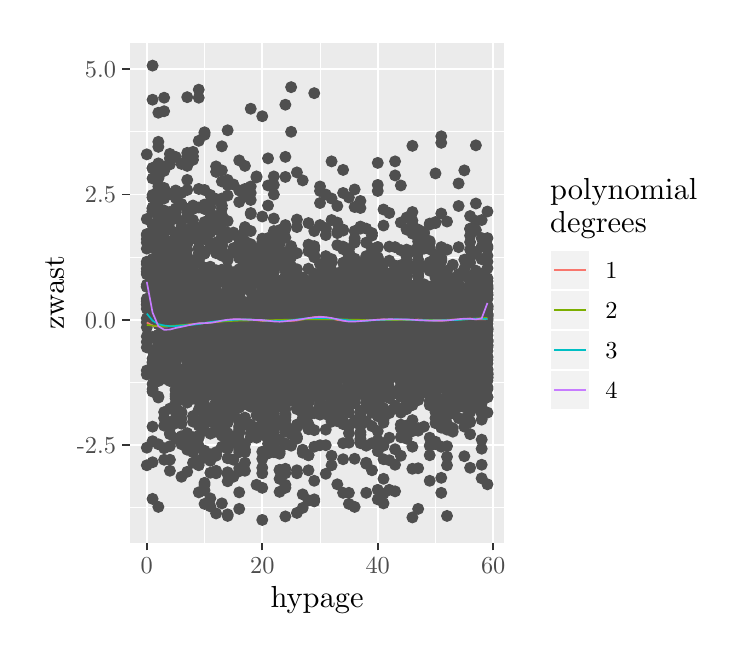
\begin{tikzpicture}[x=1pt,y=1pt]
\definecolor{fillColor}{RGB}{255,255,255}
\path[use as bounding box,fill=fillColor,fill opacity=0.00] (0,0) rectangle (252.94,216.81);
\begin{scope}
\path[clip] (  0.00,  0.00) rectangle (252.94,216.81);
\definecolor{drawColor}{RGB}{255,255,255}
\definecolor{fillColor}{RGB}{255,255,255}

\path[draw=drawColor,line width= 0.6pt,line join=round,line cap=round,fill=fillColor] (  0.00,  0.00) rectangle (252.94,216.81);
\end{scope}
\begin{scope}
\path[clip] ( 36.89, 30.72) rectangle (172.29,211.31);
\definecolor{fillColor}{gray}{0.92}

\path[fill=fillColor] ( 36.89, 30.72) rectangle (172.29,211.31);
\definecolor{drawColor}{RGB}{255,255,255}

\path[draw=drawColor,line width= 0.3pt,line join=round] ( 36.89, 43.28) --
	(172.29, 43.28);

\path[draw=drawColor,line width= 0.3pt,line join=round] ( 36.89, 88.58) --
	(172.29, 88.58);

\path[draw=drawColor,line width= 0.3pt,line join=round] ( 36.89,133.88) --
	(172.29,133.88);

\path[draw=drawColor,line width= 0.3pt,line join=round] ( 36.89,179.18) --
	(172.29,179.18);

\path[draw=drawColor,line width= 0.3pt,line join=round] ( 63.91, 30.72) --
	( 63.91,211.31);

\path[draw=drawColor,line width= 0.3pt,line join=round] (105.64, 30.72) --
	(105.64,211.31);

\path[draw=drawColor,line width= 0.3pt,line join=round] (147.36, 30.72) --
	(147.36,211.31);

\path[draw=drawColor,line width= 0.6pt,line join=round] ( 36.89, 65.93) --
	(172.29, 65.93);

\path[draw=drawColor,line width= 0.6pt,line join=round] ( 36.89,111.23) --
	(172.29,111.23);

\path[draw=drawColor,line width= 0.6pt,line join=round] ( 36.89,156.53) --
	(172.29,156.53);

\path[draw=drawColor,line width= 0.6pt,line join=round] ( 36.89,201.83) --
	(172.29,201.83);

\path[draw=drawColor,line width= 0.6pt,line join=round] ( 43.05, 30.72) --
	( 43.05,211.31);

\path[draw=drawColor,line width= 0.6pt,line join=round] ( 84.77, 30.72) --
	( 84.77,211.31);

\path[draw=drawColor,line width= 0.6pt,line join=round] (126.50, 30.72) --
	(126.50,211.31);

\path[draw=drawColor,line width= 0.6pt,line join=round] (168.22, 30.72) --
	(168.22,211.31);
\definecolor{drawColor}{gray}{0.31}
\definecolor{fillColor}{gray}{0.31}

\path[draw=drawColor,line width= 0.4pt,line join=round,line cap=round,fill=fillColor] (147.36,113.59) circle (  1.96);

\path[draw=drawColor,line width= 0.4pt,line join=round,line cap=round,fill=fillColor] ( 72.26,120.47) circle (  1.96);

\path[draw=drawColor,line width= 0.4pt,line join=round,line cap=round,fill=fillColor] ( 86.86,110.51) circle (  1.96);

\path[draw=drawColor,line width= 0.4pt,line join=round,line cap=round,fill=fillColor] (118.15, 83.15) circle (  1.96);

\path[draw=drawColor,line width= 0.4pt,line join=round,line cap=round,fill=fillColor] (105.64, 81.15) circle (  1.96);

\path[draw=drawColor,line width= 0.4pt,line join=round,line cap=round,fill=fillColor] ( 78.51,117.57) circle (  1.96);

\path[draw=drawColor,line width= 0.4pt,line join=round,line cap=round,fill=fillColor] ( 63.91,112.68) circle (  1.96);

\path[draw=drawColor,line width= 0.4pt,line join=round,line cap=round,fill=fillColor] (147.36, 93.47) circle (  1.96);

\path[draw=drawColor,line width= 0.4pt,line join=round,line cap=round,fill=fillColor] ( 53.48,115.76) circle (  1.96);

\path[draw=drawColor,line width= 0.4pt,line join=round,line cap=round,fill=fillColor] (141.10, 86.77) circle (  1.96);

\path[draw=drawColor,line width= 0.4pt,line join=round,line cap=round,fill=fillColor] ( 76.43,129.53) circle (  1.96);

\path[draw=drawColor,line width= 0.4pt,line join=round,line cap=round,fill=fillColor] (132.76,100.90) circle (  1.96);

\path[draw=drawColor,line width= 0.4pt,line join=round,line cap=round,fill=fillColor] ( 53.48, 85.68) circle (  1.96);

\path[draw=drawColor,line width= 0.4pt,line join=round,line cap=round,fill=fillColor] (143.19,103.62) circle (  1.96);

\path[draw=drawColor,line width= 0.4pt,line join=round,line cap=round,fill=fillColor] ( 47.22,111.05) circle (  1.96);

\path[draw=drawColor,line width= 0.4pt,line join=round,line cap=round,fill=fillColor] (126.50, 87.86) circle (  1.96);

\path[draw=drawColor,line width= 0.4pt,line join=round,line cap=round,fill=fillColor] ( 95.20, 88.04) circle (  1.96);

\path[draw=drawColor,line width= 0.4pt,line join=round,line cap=round,fill=fillColor] ( 88.95,105.43) circle (  1.96);

\path[draw=drawColor,line width= 0.4pt,line join=round,line cap=round,fill=fillColor] ( 97.29, 73.36) circle (  1.96);

\path[draw=drawColor,line width= 0.4pt,line join=round,line cap=round,fill=fillColor] ( 84.77,105.25) circle (  1.96);

\path[draw=drawColor,line width= 0.4pt,line join=round,line cap=round,fill=fillColor] (139.02,101.45) circle (  1.96);

\path[draw=drawColor,line width= 0.4pt,line join=round,line cap=round,fill=fillColor] ( 82.69, 80.43) circle (  1.96);

\path[draw=drawColor,line width= 0.4pt,line join=round,line cap=round,fill=fillColor] (147.36, 98.91) circle (  1.96);

\path[draw=drawColor,line width= 0.4pt,line join=round,line cap=round,fill=fillColor] ( 61.82,116.31) circle (  1.96);

\path[draw=drawColor,line width= 0.4pt,line join=round,line cap=round,fill=fillColor] ( 78.51,103.44) circle (  1.96);

\path[draw=drawColor,line width= 0.4pt,line join=round,line cap=round,fill=fillColor] (113.98, 97.82) circle (  1.96);

\path[draw=drawColor,line width= 0.4pt,line join=round,line cap=round,fill=fillColor] (155.71, 82.97) circle (  1.96);

\path[draw=drawColor,line width= 0.4pt,line join=round,line cap=round,fill=fillColor] ( 57.65,151.10) circle (  1.96);

\path[draw=drawColor,line width= 0.4pt,line join=round,line cap=round,fill=fillColor] ( 47.22, 89.13) circle (  1.96);

\path[draw=drawColor,line width= 0.4pt,line join=round,line cap=round,fill=fillColor] ( 66.00, 46.72) circle (  1.96);

\path[draw=drawColor,line width= 0.4pt,line join=round,line cap=round,fill=fillColor] (164.05, 58.87) circle (  1.96);

\path[draw=drawColor,line width= 0.4pt,line join=round,line cap=round,fill=fillColor] (118.15,114.13) circle (  1.96);

\path[draw=drawColor,line width= 0.4pt,line join=round,line cap=round,fill=fillColor] ( 78.51, 90.76) circle (  1.96);

\path[draw=drawColor,line width= 0.4pt,line join=round,line cap=round,fill=fillColor] ( 76.43, 72.46) circle (  1.96);

\path[draw=drawColor,line width= 0.4pt,line join=round,line cap=round,fill=fillColor] (164.05, 85.32) circle (  1.96);

\path[draw=drawColor,line width= 0.4pt,line join=round,line cap=round,fill=fillColor] (120.24, 99.27) circle (  1.96);

\path[draw=drawColor,line width= 0.4pt,line join=round,line cap=round,fill=fillColor] (166.14,100.00) circle (  1.96);

\path[draw=drawColor,line width= 0.4pt,line join=round,line cap=round,fill=fillColor] ( 91.03, 57.05) circle (  1.96);

\path[draw=drawColor,line width= 0.4pt,line join=round,line cap=round,fill=fillColor] ( 93.12,110.15) circle (  1.96);

\path[draw=drawColor,line width= 0.4pt,line join=round,line cap=round,fill=fillColor] (151.53, 93.84) circle (  1.96);

\path[draw=drawColor,line width= 0.4pt,line join=round,line cap=round,fill=fillColor] (161.96, 95.83) circle (  1.96);

\path[draw=drawColor,line width= 0.4pt,line join=round,line cap=round,fill=fillColor] (116.07,113.23) circle (  1.96);

\path[draw=drawColor,line width= 0.4pt,line join=round,line cap=round,fill=fillColor] ( 84.77, 80.25) circle (  1.96);

\path[draw=drawColor,line width= 0.4pt,line join=round,line cap=round,fill=fillColor] (145.27, 84.41) circle (  1.96);

\path[draw=drawColor,line width= 0.4pt,line join=round,line cap=round,fill=fillColor] ( 99.38, 84.23) circle (  1.96);

\path[draw=drawColor,line width= 0.4pt,line join=round,line cap=round,fill=fillColor] (161.96,106.88) circle (  1.96);

\path[draw=drawColor,line width= 0.4pt,line join=round,line cap=round,fill=fillColor] ( 76.43, 64.30) circle (  1.96);

\path[draw=drawColor,line width= 0.4pt,line join=round,line cap=round,fill=fillColor] (155.71,100.00) circle (  1.96);

\path[draw=drawColor,line width= 0.4pt,line join=round,line cap=round,fill=fillColor] (145.27, 81.88) circle (  1.96);

\path[draw=drawColor,line width= 0.4pt,line join=round,line cap=round,fill=fillColor] ( 63.91,112.50) circle (  1.96);

\path[draw=drawColor,line width= 0.4pt,line join=round,line cap=round,fill=fillColor] ( 93.12,121.20) circle (  1.96);

\path[draw=drawColor,line width= 0.4pt,line join=round,line cap=round,fill=fillColor] (122.33, 81.70) circle (  1.96);

\path[draw=drawColor,line width= 0.4pt,line join=round,line cap=round,fill=fillColor] ( 80.60, 95.47) circle (  1.96);

\path[draw=drawColor,line width= 0.4pt,line join=round,line cap=round,fill=fillColor] (126.50, 96.01) circle (  1.96);

\path[draw=drawColor,line width= 0.4pt,line join=round,line cap=round,fill=fillColor] ( 95.20, 84.78) circle (  1.96);

\path[draw=drawColor,line width= 0.4pt,line join=round,line cap=round,fill=fillColor] (109.81,117.21) circle (  1.96);

\path[draw=drawColor,line width= 0.4pt,line join=round,line cap=round,fill=fillColor] ( 63.91,100.72) circle (  1.96);

\path[draw=drawColor,line width= 0.4pt,line join=round,line cap=round,fill=fillColor] ( 59.74, 84.78) circle (  1.96);

\path[draw=drawColor,line width= 0.4pt,line join=round,line cap=round,fill=fillColor] ( 86.86, 93.29) circle (  1.96);

\path[draw=drawColor,line width= 0.4pt,line join=round,line cap=round,fill=fillColor] ( 80.60,118.12) circle (  1.96);

\path[draw=drawColor,line width= 0.4pt,line join=round,line cap=round,fill=fillColor] (145.27,100.54) circle (  1.96);

\path[draw=drawColor,line width= 0.4pt,line join=round,line cap=round,fill=fillColor] ( 86.86,132.80) circle (  1.96);

\path[draw=drawColor,line width= 0.4pt,line join=round,line cap=round,fill=fillColor] ( 68.08,108.70) circle (  1.96);

\path[draw=drawColor,line width= 0.4pt,line join=round,line cap=round,fill=fillColor] (103.55,101.99) circle (  1.96);

\path[draw=drawColor,line width= 0.4pt,line join=round,line cap=round,fill=fillColor] ( 55.57, 85.68) circle (  1.96);

\path[draw=drawColor,line width= 0.4pt,line join=round,line cap=round,fill=fillColor] ( 51.39,146.75) circle (  1.96);

\path[draw=drawColor,line width= 0.4pt,line join=round,line cap=round,fill=fillColor] (103.55, 99.64) circle (  1.96);

\path[draw=drawColor,line width= 0.4pt,line join=round,line cap=round,fill=fillColor] (101.46,120.47) circle (  1.96);

\path[draw=drawColor,line width= 0.4pt,line join=round,line cap=round,fill=fillColor] (143.19, 96.01) circle (  1.96);

\path[draw=drawColor,line width= 0.4pt,line join=round,line cap=round,fill=fillColor] ( 74.34,107.06) circle (  1.96);

\path[draw=drawColor,line width= 0.4pt,line join=round,line cap=round,fill=fillColor] ( 84.77,115.22) circle (  1.96);

\path[draw=drawColor,line width= 0.4pt,line join=round,line cap=round,fill=fillColor] ( 53.48,137.51) circle (  1.96);

\path[draw=drawColor,line width= 0.4pt,line join=round,line cap=round,fill=fillColor] ( 70.17,141.31) circle (  1.96);

\path[draw=drawColor,line width= 0.4pt,line join=round,line cap=round,fill=fillColor] (124.41,122.83) circle (  1.96);

\path[draw=drawColor,line width= 0.4pt,line join=round,line cap=round,fill=fillColor] (101.46, 87.68) circle (  1.96);

\path[draw=drawColor,line width= 0.4pt,line join=round,line cap=round,fill=fillColor] (161.96, 96.01) circle (  1.96);

\path[draw=drawColor,line width= 0.4pt,line join=round,line cap=round,fill=fillColor] (124.41, 87.86) circle (  1.96);

\path[draw=drawColor,line width= 0.4pt,line join=round,line cap=round,fill=fillColor] (101.46,100.90) circle (  1.96);

\path[draw=drawColor,line width= 0.4pt,line join=round,line cap=round,fill=fillColor] (126.50,103.98) circle (  1.96);

\path[draw=drawColor,line width= 0.4pt,line join=round,line cap=round,fill=fillColor] (145.27,101.45) circle (  1.96);

\path[draw=drawColor,line width= 0.4pt,line join=round,line cap=round,fill=fillColor] (120.24,112.68) circle (  1.96);

\path[draw=drawColor,line width= 0.4pt,line join=round,line cap=round,fill=fillColor] ( 99.38, 87.68) circle (  1.96);

\path[draw=drawColor,line width= 0.4pt,line join=round,line cap=round,fill=fillColor] (164.05,107.06) circle (  1.96);

\path[draw=drawColor,line width= 0.4pt,line join=round,line cap=round,fill=fillColor] ( 99.38, 95.47) circle (  1.96);

\path[draw=drawColor,line width= 0.4pt,line join=round,line cap=round,fill=fillColor] (155.71, 89.31) circle (  1.96);

\path[draw=drawColor,line width= 0.4pt,line join=round,line cap=round,fill=fillColor] ( 93.12, 85.86) circle (  1.96);

\path[draw=drawColor,line width= 0.4pt,line join=round,line cap=round,fill=fillColor] (122.33,107.79) circle (  1.96);

\path[draw=drawColor,line width= 0.4pt,line join=round,line cap=round,fill=fillColor] ( 53.48,170.12) circle (  1.96);

\path[draw=drawColor,line width= 0.4pt,line join=round,line cap=round,fill=fillColor] ( 53.48,132.07) circle (  1.96);

\path[draw=drawColor,line width= 0.4pt,line join=round,line cap=round,fill=fillColor] ( 95.20,113.41) circle (  1.96);

\path[draw=drawColor,line width= 0.4pt,line join=round,line cap=round,fill=fillColor] (101.46,103.44) circle (  1.96);

\path[draw=drawColor,line width= 0.4pt,line join=round,line cap=round,fill=fillColor] (155.71,115.94) circle (  1.96);

\path[draw=drawColor,line width= 0.4pt,line join=round,line cap=round,fill=fillColor] ( 70.17, 98.37) circle (  1.96);

\path[draw=drawColor,line width= 0.4pt,line join=round,line cap=round,fill=fillColor] (111.89,124.28) circle (  1.96);

\path[draw=drawColor,line width= 0.4pt,line join=round,line cap=round,fill=fillColor] ( 68.08,129.17) circle (  1.96);

\path[draw=drawColor,line width= 0.4pt,line join=round,line cap=round,fill=fillColor] (164.05,103.80) circle (  1.96);

\path[draw=drawColor,line width= 0.4pt,line join=round,line cap=round,fill=fillColor] ( 68.08, 87.50) circle (  1.96);

\path[draw=drawColor,line width= 0.4pt,line join=round,line cap=round,fill=fillColor] ( 72.26,110.15) circle (  1.96);

\path[draw=drawColor,line width= 0.4pt,line join=round,line cap=round,fill=fillColor] ( 84.77,103.08) circle (  1.96);

\path[draw=drawColor,line width= 0.4pt,line join=round,line cap=round,fill=fillColor] ( 49.31,112.68) circle (  1.96);

\path[draw=drawColor,line width= 0.4pt,line join=round,line cap=round,fill=fillColor] (166.14, 86.95) circle (  1.96);

\path[draw=drawColor,line width= 0.4pt,line join=round,line cap=round,fill=fillColor] ( 84.77,110.51) circle (  1.96);

\path[draw=drawColor,line width= 0.4pt,line join=round,line cap=round,fill=fillColor] ( 95.20, 92.57) circle (  1.96);

\path[draw=drawColor,line width= 0.4pt,line join=round,line cap=round,fill=fillColor] (145.27,104.53) circle (  1.96);

\path[draw=drawColor,line width= 0.4pt,line join=round,line cap=round,fill=fillColor] ( 97.29,108.51) circle (  1.96);

\path[draw=drawColor,line width= 0.4pt,line join=round,line cap=round,fill=fillColor] (147.36,108.70) circle (  1.96);

\path[draw=drawColor,line width= 0.4pt,line join=round,line cap=round,fill=fillColor] (101.46, 46.00) circle (  1.96);

\path[draw=drawColor,line width= 0.4pt,line join=round,line cap=round,fill=fillColor] ( 63.91,178.10) circle (  1.96);

\path[draw=drawColor,line width= 0.4pt,line join=round,line cap=round,fill=fillColor] ( 84.77,128.27) circle (  1.96);

\path[draw=drawColor,line width= 0.4pt,line join=round,line cap=round,fill=fillColor] ( 91.03,116.67) circle (  1.96);

\path[draw=drawColor,line width= 0.4pt,line join=round,line cap=round,fill=fillColor] (147.36, 94.92) circle (  1.96);

\path[draw=drawColor,line width= 0.4pt,line join=round,line cap=round,fill=fillColor] (124.41, 86.95) circle (  1.96);

\path[draw=drawColor,line width= 0.4pt,line join=round,line cap=round,fill=fillColor] (166.14,115.22) circle (  1.96);

\path[draw=drawColor,line width= 0.4pt,line join=round,line cap=round,fill=fillColor] ( 74.34,125.00) circle (  1.96);

\path[draw=drawColor,line width= 0.4pt,line join=round,line cap=round,fill=fillColor] ( 97.29,112.32) circle (  1.96);

\path[draw=drawColor,line width= 0.4pt,line join=round,line cap=round,fill=fillColor] (120.24, 87.13) circle (  1.96);

\path[draw=drawColor,line width= 0.4pt,line join=round,line cap=round,fill=fillColor] ( 45.13,151.46) circle (  1.96);

\path[draw=drawColor,line width= 0.4pt,line join=round,line cap=round,fill=fillColor] (122.33, 99.82) circle (  1.96);

\path[draw=drawColor,line width= 0.4pt,line join=round,line cap=round,fill=fillColor] ( 61.82,117.76) circle (  1.96);

\path[draw=drawColor,line width= 0.4pt,line join=round,line cap=round,fill=fillColor] (107.72,115.94) circle (  1.96);

\path[draw=drawColor,line width= 0.4pt,line join=round,line cap=round,fill=fillColor] ( 47.22,121.74) circle (  1.96);

\path[draw=drawColor,line width= 0.4pt,line join=round,line cap=round,fill=fillColor] (120.24,114.49) circle (  1.96);

\path[draw=drawColor,line width= 0.4pt,line join=round,line cap=round,fill=fillColor] ( 51.39, 93.29) circle (  1.96);

\path[draw=drawColor,line width= 0.4pt,line join=round,line cap=round,fill=fillColor] (147.36, 93.29) circle (  1.96);

\path[draw=drawColor,line width= 0.4pt,line join=round,line cap=round,fill=fillColor] (101.46,103.26) circle (  1.96);

\path[draw=drawColor,line width= 0.4pt,line join=round,line cap=round,fill=fillColor] ( 61.82,107.97) circle (  1.96);

\path[draw=drawColor,line width= 0.4pt,line join=round,line cap=round,fill=fillColor] (157.79,127.36) circle (  1.96);

\path[draw=drawColor,line width= 0.4pt,line join=round,line cap=round,fill=fillColor] (103.55,133.88) circle (  1.96);

\path[draw=drawColor,line width= 0.4pt,line join=round,line cap=round,fill=fillColor] ( 66.00,129.17) circle (  1.96);

\path[draw=drawColor,line width= 0.4pt,line join=round,line cap=round,fill=fillColor] ( 66.00,126.09) circle (  1.96);

\path[draw=drawColor,line width= 0.4pt,line join=round,line cap=round,fill=fillColor] ( 78.51,139.14) circle (  1.96);

\path[draw=drawColor,line width= 0.4pt,line join=round,line cap=round,fill=fillColor] ( 78.51,134.97) circle (  1.96);

\path[draw=drawColor,line width= 0.4pt,line join=round,line cap=round,fill=fillColor] ( 93.12, 86.95) circle (  1.96);

\path[draw=drawColor,line width= 0.4pt,line join=round,line cap=round,fill=fillColor] (116.07,101.45) circle (  1.96);

\path[draw=drawColor,line width= 0.4pt,line join=round,line cap=round,fill=fillColor] (157.79,117.57) circle (  1.96);

\path[draw=drawColor,line width= 0.4pt,line join=round,line cap=round,fill=fillColor] (130.67, 60.50) circle (  1.96);

\path[draw=drawColor,line width= 0.4pt,line join=round,line cap=round,fill=fillColor] (109.81,119.39) circle (  1.96);

\path[draw=drawColor,line width= 0.4pt,line join=round,line cap=round,fill=fillColor] ( 47.22,133.34) circle (  1.96);

\path[draw=drawColor,line width= 0.4pt,line join=round,line cap=round,fill=fillColor] (105.64,124.64) circle (  1.96);

\path[draw=drawColor,line width= 0.4pt,line join=round,line cap=round,fill=fillColor] (120.24,117.39) circle (  1.96);

\path[draw=drawColor,line width= 0.4pt,line join=round,line cap=round,fill=fillColor] (109.81,117.94) circle (  1.96);

\path[draw=drawColor,line width= 0.4pt,line join=round,line cap=round,fill=fillColor] ( 53.48,148.92) circle (  1.96);

\path[draw=drawColor,line width= 0.4pt,line join=round,line cap=round,fill=fillColor] ( 72.26, 40.93) circle (  1.96);

\path[draw=drawColor,line width= 0.4pt,line join=round,line cap=round,fill=fillColor] (155.71,104.71) circle (  1.96);

\path[draw=drawColor,line width= 0.4pt,line join=round,line cap=round,fill=fillColor] ( 74.34,115.04) circle (  1.96);

\path[draw=drawColor,line width= 0.4pt,line join=round,line cap=round,fill=fillColor] ( 68.08,114.13) circle (  1.96);

\path[draw=drawColor,line width= 0.4pt,line join=round,line cap=round,fill=fillColor] ( 70.17,143.12) circle (  1.96);

\path[draw=drawColor,line width= 0.4pt,line join=round,line cap=round,fill=fillColor] ( 86.86, 72.27) circle (  1.96);

\path[draw=drawColor,line width= 0.4pt,line join=round,line cap=round,fill=fillColor] (111.89,121.38) circle (  1.96);

\path[draw=drawColor,line width= 0.4pt,line join=round,line cap=round,fill=fillColor] (141.10,116.85) circle (  1.96);

\path[draw=drawColor,line width= 0.4pt,line join=round,line cap=round,fill=fillColor] (141.10,124.46) circle (  1.96);

\path[draw=drawColor,line width= 0.4pt,line join=round,line cap=round,fill=fillColor] ( 51.39,156.71) circle (  1.96);

\path[draw=drawColor,line width= 0.4pt,line join=round,line cap=round,fill=fillColor] (109.81, 97.28) circle (  1.96);

\path[draw=drawColor,line width= 0.4pt,line join=round,line cap=round,fill=fillColor] ( 84.77,133.88) circle (  1.96);

\path[draw=drawColor,line width= 0.4pt,line join=round,line cap=round,fill=fillColor] (107.72,127.18) circle (  1.96);

\path[draw=drawColor,line width= 0.4pt,line join=round,line cap=round,fill=fillColor] ( 66.00,103.08) circle (  1.96);

\path[draw=drawColor,line width= 0.4pt,line join=round,line cap=round,fill=fillColor] ( 66.00,100.54) circle (  1.96);

\path[draw=drawColor,line width= 0.4pt,line join=round,line cap=round,fill=fillColor] (124.41,121.38) circle (  1.96);

\path[draw=drawColor,line width= 0.4pt,line join=round,line cap=round,fill=fillColor] ( 61.82,107.06) circle (  1.96);

\path[draw=drawColor,line width= 0.4pt,line join=round,line cap=round,fill=fillColor] ( 88.95,103.98) circle (  1.96);

\path[draw=drawColor,line width= 0.4pt,line join=round,line cap=round,fill=fillColor] (151.53, 98.55) circle (  1.96);

\path[draw=drawColor,line width= 0.4pt,line join=round,line cap=round,fill=fillColor] (111.89, 77.35) circle (  1.96);

\path[draw=drawColor,line width= 0.4pt,line join=round,line cap=round,fill=fillColor] (126.50, 82.97) circle (  1.96);

\path[draw=drawColor,line width= 0.4pt,line join=round,line cap=round,fill=fillColor] ( 68.08, 84.60) circle (  1.96);

\path[draw=drawColor,line width= 0.4pt,line join=round,line cap=round,fill=fillColor] (109.81,117.21) circle (  1.96);

\path[draw=drawColor,line width= 0.4pt,line join=round,line cap=round,fill=fillColor] (155.71,127.72) circle (  1.96);

\path[draw=drawColor,line width= 0.4pt,line join=round,line cap=round,fill=fillColor] ( 47.22,162.87) circle (  1.96);

\path[draw=drawColor,line width= 0.4pt,line join=round,line cap=round,fill=fillColor] (120.24,106.34) circle (  1.96);

\path[draw=drawColor,line width= 0.4pt,line join=round,line cap=round,fill=fillColor] ( 63.91, 93.66) circle (  1.96);

\path[draw=drawColor,line width= 0.4pt,line join=round,line cap=round,fill=fillColor] (139.02,100.54) circle (  1.96);

\path[draw=drawColor,line width= 0.4pt,line join=round,line cap=round,fill=fillColor] ( 88.95,106.16) circle (  1.96);

\path[draw=drawColor,line width= 0.4pt,line join=round,line cap=round,fill=fillColor] ( 61.82, 87.68) circle (  1.96);

\path[draw=drawColor,line width= 0.4pt,line join=round,line cap=round,fill=fillColor] (151.53,114.68) circle (  1.96);

\path[draw=drawColor,line width= 0.4pt,line join=round,line cap=round,fill=fillColor] ( 70.17,108.88) circle (  1.96);

\path[draw=drawColor,line width= 0.4pt,line join=round,line cap=round,fill=fillColor] (126.50,112.86) circle (  1.96);

\path[draw=drawColor,line width= 0.4pt,line join=round,line cap=round,fill=fillColor] ( 57.65,109.06) circle (  1.96);

\path[draw=drawColor,line width= 0.4pt,line join=round,line cap=round,fill=fillColor] (116.07,109.24) circle (  1.96);

\path[draw=drawColor,line width= 0.4pt,line join=round,line cap=round,fill=fillColor] (164.05, 92.75) circle (  1.96);

\path[draw=drawColor,line width= 0.4pt,line join=round,line cap=round,fill=fillColor] (107.72, 99.82) circle (  1.96);

\path[draw=drawColor,line width= 0.4pt,line join=round,line cap=round,fill=fillColor] (145.27,137.14) circle (  1.96);

\path[draw=drawColor,line width= 0.4pt,line join=round,line cap=round,fill=fillColor] ( 86.86, 81.15) circle (  1.96);

\path[draw=drawColor,line width= 0.4pt,line join=round,line cap=round,fill=fillColor] (139.02,102.17) circle (  1.96);

\path[draw=drawColor,line width= 0.4pt,line join=round,line cap=round,fill=fillColor] ( 78.51,101.27) circle (  1.96);

\path[draw=drawColor,line width= 0.4pt,line join=round,line cap=round,fill=fillColor] (124.41,141.67) circle (  1.96);

\path[draw=drawColor,line width= 0.4pt,line join=round,line cap=round,fill=fillColor] (103.55,111.78) circle (  1.96);

\path[draw=drawColor,line width= 0.4pt,line join=round,line cap=round,fill=fillColor] (166.14,125.18) circle (  1.96);

\path[draw=drawColor,line width= 0.4pt,line join=round,line cap=round,fill=fillColor] ( 91.03,136.42) circle (  1.96);

\path[draw=drawColor,line width= 0.4pt,line join=round,line cap=round,fill=fillColor] ( 93.12,135.51) circle (  1.96);

\path[draw=drawColor,line width= 0.4pt,line join=round,line cap=round,fill=fillColor] (141.10,119.02) circle (  1.96);

\path[draw=drawColor,line width= 0.4pt,line join=round,line cap=round,fill=fillColor] ( 57.65, 96.92) circle (  1.96);

\path[draw=drawColor,line width= 0.4pt,line join=round,line cap=round,fill=fillColor] ( 76.43,124.46) circle (  1.96);

\path[draw=drawColor,line width= 0.4pt,line join=round,line cap=round,fill=fillColor] (101.46,111.41) circle (  1.96);

\path[draw=drawColor,line width= 0.4pt,line join=round,line cap=round,fill=fillColor] ( 53.48, 98.55) circle (  1.96);

\path[draw=drawColor,line width= 0.4pt,line join=round,line cap=round,fill=fillColor] (141.10,127.18) circle (  1.96);

\path[draw=drawColor,line width= 0.4pt,line join=round,line cap=round,fill=fillColor] ( 76.43,133.52) circle (  1.96);

\path[draw=drawColor,line width= 0.4pt,line join=round,line cap=round,fill=fillColor] ( 47.22,152.00) circle (  1.96);

\path[draw=drawColor,line width= 0.4pt,line join=round,line cap=round,fill=fillColor] (155.71,121.74) circle (  1.96);

\path[draw=drawColor,line width= 0.4pt,line join=round,line cap=round,fill=fillColor] ( 61.82,122.29) circle (  1.96);

\path[draw=drawColor,line width= 0.4pt,line join=round,line cap=round,fill=fillColor] ( 78.51,109.42) circle (  1.96);

\path[draw=drawColor,line width= 0.4pt,line join=round,line cap=round,fill=fillColor] (120.24,122.10) circle (  1.96);

\path[draw=drawColor,line width= 0.4pt,line join=round,line cap=round,fill=fillColor] (151.53,103.62) circle (  1.96);

\path[draw=drawColor,line width= 0.4pt,line join=round,line cap=round,fill=fillColor] (134.84, 86.05) circle (  1.96);

\path[draw=drawColor,line width= 0.4pt,line join=round,line cap=round,fill=fillColor] (103.55,100.72) circle (  1.96);

\path[draw=drawColor,line width= 0.4pt,line join=round,line cap=round,fill=fillColor] (136.93,103.08) circle (  1.96);

\path[draw=drawColor,line width= 0.4pt,line join=round,line cap=round,fill=fillColor] ( 45.13,105.07) circle (  1.96);

\path[draw=drawColor,line width= 0.4pt,line join=round,line cap=round,fill=fillColor] ( 95.20, 98.73) circle (  1.96);

\path[draw=drawColor,line width= 0.4pt,line join=round,line cap=round,fill=fillColor] ( 68.08, 63.40) circle (  1.96);

\path[draw=drawColor,line width= 0.4pt,line join=round,line cap=round,fill=fillColor] ( 72.26,114.49) circle (  1.96);

\path[draw=drawColor,line width= 0.4pt,line join=round,line cap=round,fill=fillColor] (132.76,113.04) circle (  1.96);

\path[draw=drawColor,line width= 0.4pt,line join=round,line cap=round,fill=fillColor] ( 53.48,101.09) circle (  1.96);

\path[draw=drawColor,line width= 0.4pt,line join=round,line cap=round,fill=fillColor] (128.58, 98.00) circle (  1.96);

\path[draw=drawColor,line width= 0.4pt,line join=round,line cap=round,fill=fillColor] (113.98,114.31) circle (  1.96);

\path[draw=drawColor,line width= 0.4pt,line join=round,line cap=round,fill=fillColor] (151.53,126.45) circle (  1.96);

\path[draw=drawColor,line width= 0.4pt,line join=round,line cap=round,fill=fillColor] ( 53.48,110.87) circle (  1.96);

\path[draw=drawColor,line width= 0.4pt,line join=round,line cap=round,fill=fillColor] (130.67,137.69) circle (  1.96);

\path[draw=drawColor,line width= 0.4pt,line join=round,line cap=round,fill=fillColor] (141.10,109.06) circle (  1.96);

\path[draw=drawColor,line width= 0.4pt,line join=round,line cap=round,fill=fillColor] ( 88.95,101.45) circle (  1.96);

\path[draw=drawColor,line width= 0.4pt,line join=round,line cap=round,fill=fillColor] (118.15,118.84) circle (  1.96);

\path[draw=drawColor,line width= 0.4pt,line join=round,line cap=round,fill=fillColor] ( 82.69, 93.66) circle (  1.96);

\path[draw=drawColor,line width= 0.4pt,line join=round,line cap=round,fill=fillColor] (120.24, 94.20) circle (  1.96);

\path[draw=drawColor,line width= 0.4pt,line join=round,line cap=round,fill=fillColor] ( 70.17, 96.01) circle (  1.96);

\path[draw=drawColor,line width= 0.4pt,line join=round,line cap=round,fill=fillColor] ( 47.22,130.44) circle (  1.96);

\path[draw=drawColor,line width= 0.4pt,line join=round,line cap=round,fill=fillColor] (164.05, 99.82) circle (  1.96);

\path[draw=drawColor,line width= 0.4pt,line join=round,line cap=round,fill=fillColor] ( 97.29,107.79) circle (  1.96);

\path[draw=drawColor,line width= 0.4pt,line join=round,line cap=round,fill=fillColor] ( 55.57,104.35) circle (  1.96);

\path[draw=drawColor,line width= 0.4pt,line join=round,line cap=round,fill=fillColor] ( 91.03, 88.04) circle (  1.96);

\path[draw=drawColor,line width= 0.4pt,line join=round,line cap=round,fill=fillColor] (147.36, 75.72) circle (  1.96);

\path[draw=drawColor,line width= 0.4pt,line join=round,line cap=round,fill=fillColor] ( 47.22, 94.74) circle (  1.96);

\path[draw=drawColor,line width= 0.4pt,line join=round,line cap=round,fill=fillColor] (122.33,104.71) circle (  1.96);

\path[draw=drawColor,line width= 0.4pt,line join=round,line cap=round,fill=fillColor] ( 84.77,104.89) circle (  1.96);

\path[draw=drawColor,line width= 0.4pt,line join=round,line cap=round,fill=fillColor] (118.15, 43.64) circle (  1.96);

\path[draw=drawColor,line width= 0.4pt,line join=round,line cap=round,fill=fillColor] ( 59.74, 97.82) circle (  1.96);

\path[draw=drawColor,line width= 0.4pt,line join=round,line cap=round,fill=fillColor] ( 61.82, 96.92) circle (  1.96);

\path[draw=drawColor,line width= 0.4pt,line join=round,line cap=round,fill=fillColor] (116.07,100.90) circle (  1.96);

\path[draw=drawColor,line width= 0.4pt,line join=round,line cap=round,fill=fillColor] (151.53, 93.47) circle (  1.96);

\path[draw=drawColor,line width= 0.4pt,line join=round,line cap=round,fill=fillColor] ( 95.20, 96.56) circle (  1.96);

\path[draw=drawColor,line width= 0.4pt,line join=round,line cap=round,fill=fillColor] ( 95.20, 90.21) circle (  1.96);

\path[draw=drawColor,line width= 0.4pt,line join=round,line cap=round,fill=fillColor] (164.05, 84.05) circle (  1.96);

\path[draw=drawColor,line width= 0.4pt,line join=round,line cap=round,fill=fillColor] (161.96, 88.58) circle (  1.96);

\path[draw=drawColor,line width= 0.4pt,line join=round,line cap=round,fill=fillColor] ( 91.03,102.72) circle (  1.96);

\path[draw=drawColor,line width= 0.4pt,line join=round,line cap=round,fill=fillColor] (166.14, 91.48) circle (  1.96);

\path[draw=drawColor,line width= 0.4pt,line join=round,line cap=round,fill=fillColor] ( 88.95, 82.24) circle (  1.96);

\path[draw=drawColor,line width= 0.4pt,line join=round,line cap=round,fill=fillColor] ( 88.95, 84.23) circle (  1.96);

\path[draw=drawColor,line width= 0.4pt,line join=round,line cap=round,fill=fillColor] (136.93, 84.60) circle (  1.96);

\path[draw=drawColor,line width= 0.4pt,line join=round,line cap=round,fill=fillColor] ( 51.39,133.70) circle (  1.96);

\path[draw=drawColor,line width= 0.4pt,line join=round,line cap=round,fill=fillColor] (149.45,102.17) circle (  1.96);

\path[draw=drawColor,line width= 0.4pt,line join=round,line cap=round,fill=fillColor] ( 82.69,103.80) circle (  1.96);

\path[draw=drawColor,line width= 0.4pt,line join=round,line cap=round,fill=fillColor] (111.89,102.17) circle (  1.96);

\path[draw=drawColor,line width= 0.4pt,line join=round,line cap=round,fill=fillColor] (130.67,124.82) circle (  1.96);

\path[draw=drawColor,line width= 0.4pt,line join=round,line cap=round,fill=fillColor] (130.67,117.76) circle (  1.96);

\path[draw=drawColor,line width= 0.4pt,line join=round,line cap=round,fill=fillColor] ( 84.77,128.99) circle (  1.96);

\path[draw=drawColor,line width= 0.4pt,line join=round,line cap=round,fill=fillColor] (111.89, 84.96) circle (  1.96);

\path[draw=drawColor,line width= 0.4pt,line join=round,line cap=round,fill=fillColor] (107.72,111.05) circle (  1.96);

\path[draw=drawColor,line width= 0.4pt,line join=round,line cap=round,fill=fillColor] (109.81, 99.64) circle (  1.96);

\path[draw=drawColor,line width= 0.4pt,line join=round,line cap=round,fill=fillColor] ( 86.86,132.43) circle (  1.96);

\path[draw=drawColor,line width= 0.4pt,line join=round,line cap=round,fill=fillColor] ( 70.17, 93.47) circle (  1.96);

\path[draw=drawColor,line width= 0.4pt,line join=round,line cap=round,fill=fillColor] ( 68.08, 88.94) circle (  1.96);

\path[draw=drawColor,line width= 0.4pt,line join=round,line cap=round,fill=fillColor] (139.02,111.78) circle (  1.96);

\path[draw=drawColor,line width= 0.4pt,line join=round,line cap=round,fill=fillColor] (141.10,111.05) circle (  1.96);

\path[draw=drawColor,line width= 0.4pt,line join=round,line cap=round,fill=fillColor] ( 91.03, 74.63) circle (  1.96);

\path[draw=drawColor,line width= 0.4pt,line join=round,line cap=round,fill=fillColor] ( 80.60,136.78) circle (  1.96);

\path[draw=drawColor,line width= 0.4pt,line join=round,line cap=round,fill=fillColor] (130.67,114.49) circle (  1.96);

\path[draw=drawColor,line width= 0.4pt,line join=round,line cap=round,fill=fillColor] (155.71, 99.82) circle (  1.96);

\path[draw=drawColor,line width= 0.4pt,line join=round,line cap=round,fill=fillColor] ( 61.82,101.99) circle (  1.96);

\path[draw=drawColor,line width= 0.4pt,line join=round,line cap=round,fill=fillColor] (109.81,101.45) circle (  1.96);

\path[draw=drawColor,line width= 0.4pt,line join=round,line cap=round,fill=fillColor] ( 53.48, 83.69) circle (  1.96);

\path[draw=drawColor,line width= 0.4pt,line join=round,line cap=round,fill=fillColor] ( 66.00, 75.17) circle (  1.96);

\path[draw=drawColor,line width= 0.4pt,line join=round,line cap=round,fill=fillColor] (113.98, 84.41) circle (  1.96);

\path[draw=drawColor,line width= 0.4pt,line join=round,line cap=round,fill=fillColor] (113.98,105.98) circle (  1.96);

\path[draw=drawColor,line width= 0.4pt,line join=round,line cap=round,fill=fillColor] (159.88,118.66) circle (  1.96);

\path[draw=drawColor,line width= 0.4pt,line join=round,line cap=round,fill=fillColor] ( 93.12,114.49) circle (  1.96);

\path[draw=drawColor,line width= 0.4pt,line join=round,line cap=round,fill=fillColor] (132.76,113.95) circle (  1.96);

\path[draw=drawColor,line width= 0.4pt,line join=round,line cap=round,fill=fillColor] ( 70.17,128.45) circle (  1.96);

\path[draw=drawColor,line width= 0.4pt,line join=round,line cap=round,fill=fillColor] ( 88.95,159.98) circle (  1.96);

\path[draw=drawColor,line width= 0.4pt,line join=round,line cap=round,fill=fillColor] ( 91.03,138.59) circle (  1.96);

\path[draw=drawColor,line width= 0.4pt,line join=round,line cap=round,fill=fillColor] ( 68.08, 73.00) circle (  1.96);

\path[draw=drawColor,line width= 0.4pt,line join=round,line cap=round,fill=fillColor] ( 80.60, 99.09) circle (  1.96);

\path[draw=drawColor,line width= 0.4pt,line join=round,line cap=round,fill=fillColor] ( 55.57,144.21) circle (  1.96);

\path[draw=drawColor,line width= 0.4pt,line join=round,line cap=round,fill=fillColor] ( 86.86,108.15) circle (  1.96);

\path[draw=drawColor,line width= 0.4pt,line join=round,line cap=round,fill=fillColor] (120.24,115.04) circle (  1.96);

\path[draw=drawColor,line width= 0.4pt,line join=round,line cap=round,fill=fillColor] ( 93.12, 86.05) circle (  1.96);

\path[draw=drawColor,line width= 0.4pt,line join=round,line cap=round,fill=fillColor] (122.33,134.25) circle (  1.96);

\path[draw=drawColor,line width= 0.4pt,line join=round,line cap=round,fill=fillColor] ( 59.74,101.81) circle (  1.96);

\path[draw=drawColor,line width= 0.4pt,line join=round,line cap=round,fill=fillColor] ( 63.91, 74.81) circle (  1.96);

\path[draw=drawColor,line width= 0.4pt,line join=round,line cap=round,fill=fillColor] ( 78.51,114.49) circle (  1.96);

\path[draw=drawColor,line width= 0.4pt,line join=round,line cap=round,fill=fillColor] (136.93,122.47) circle (  1.96);

\path[draw=drawColor,line width= 0.4pt,line join=round,line cap=round,fill=fillColor] (103.55,107.25) circle (  1.96);

\path[draw=drawColor,line width= 0.4pt,line join=round,line cap=round,fill=fillColor] (151.53,117.76) circle (  1.96);

\path[draw=drawColor,line width= 0.4pt,line join=round,line cap=round,fill=fillColor] (111.89,115.58) circle (  1.96);

\path[draw=drawColor,line width= 0.4pt,line join=round,line cap=round,fill=fillColor] (157.79,110.51) circle (  1.96);

\path[draw=drawColor,line width= 0.4pt,line join=round,line cap=round,fill=fillColor] (113.98, 92.21) circle (  1.96);

\path[draw=drawColor,line width= 0.4pt,line join=round,line cap=round,fill=fillColor] (166.14,101.99) circle (  1.96);

\path[draw=drawColor,line width= 0.4pt,line join=round,line cap=round,fill=fillColor] (105.64,105.25) circle (  1.96);

\path[draw=drawColor,line width= 0.4pt,line join=round,line cap=round,fill=fillColor] ( 91.03, 90.58) circle (  1.96);

\path[draw=drawColor,line width= 0.4pt,line join=round,line cap=round,fill=fillColor] ( 59.74, 91.30) circle (  1.96);

\path[draw=drawColor,line width= 0.4pt,line join=round,line cap=round,fill=fillColor] ( 70.17, 99.45) circle (  1.96);

\path[draw=drawColor,line width= 0.4pt,line join=round,line cap=round,fill=fillColor] (130.67,124.64) circle (  1.96);

\path[draw=drawColor,line width= 0.4pt,line join=round,line cap=round,fill=fillColor] ( 61.82,113.23) circle (  1.96);

\path[draw=drawColor,line width= 0.4pt,line join=round,line cap=round,fill=fillColor] (126.50,124.46) circle (  1.96);

\path[draw=drawColor,line width= 0.4pt,line join=round,line cap=round,fill=fillColor] (166.14,123.74) circle (  1.96);

\path[draw=drawColor,line width= 0.4pt,line join=round,line cap=round,fill=fillColor] (118.15,118.48) circle (  1.96);

\path[draw=drawColor,line width= 0.4pt,line join=round,line cap=round,fill=fillColor] ( 45.13,126.63) circle (  1.96);

\path[draw=drawColor,line width= 0.4pt,line join=round,line cap=round,fill=fillColor] ( 72.26, 99.82) circle (  1.96);

\path[draw=drawColor,line width= 0.4pt,line join=round,line cap=round,fill=fillColor] (159.88,144.03) circle (  1.96);

\path[draw=drawColor,line width= 0.4pt,line join=round,line cap=round,fill=fillColor] ( 76.43, 93.84) circle (  1.96);

\path[draw=drawColor,line width= 0.4pt,line join=round,line cap=round,fill=fillColor] (109.81,117.76) circle (  1.96);

\path[draw=drawColor,line width= 0.4pt,line join=round,line cap=round,fill=fillColor] (149.45,101.27) circle (  1.96);

\path[draw=drawColor,line width= 0.4pt,line join=round,line cap=round,fill=fillColor] ( 59.74, 97.28) circle (  1.96);

\path[draw=drawColor,line width= 0.4pt,line join=round,line cap=round,fill=fillColor] (124.41,115.22) circle (  1.96);

\path[draw=drawColor,line width= 0.4pt,line join=round,line cap=round,fill=fillColor] ( 66.00,105.80) circle (  1.96);

\path[draw=drawColor,line width= 0.4pt,line join=round,line cap=round,fill=fillColor] (122.33,111.78) circle (  1.96);

\path[draw=drawColor,line width= 0.4pt,line join=round,line cap=round,fill=fillColor] ( 72.26,156.17) circle (  1.96);

\path[draw=drawColor,line width= 0.4pt,line join=round,line cap=round,fill=fillColor] (120.24,120.65) circle (  1.96);

\path[draw=drawColor,line width= 0.4pt,line join=round,line cap=round,fill=fillColor] (166.14,132.25) circle (  1.96);

\path[draw=drawColor,line width= 0.4pt,line join=round,line cap=round,fill=fillColor] ( 72.26,100.54) circle (  1.96);

\path[draw=drawColor,line width= 0.4pt,line join=round,line cap=round,fill=fillColor] (124.41,134.06) circle (  1.96);

\path[draw=drawColor,line width= 0.4pt,line join=round,line cap=round,fill=fillColor] (155.71, 75.72) circle (  1.96);

\path[draw=drawColor,line width= 0.4pt,line join=round,line cap=round,fill=fillColor] ( 59.74, 88.58) circle (  1.96);

\path[draw=drawColor,line width= 0.4pt,line join=round,line cap=round,fill=fillColor] (111.89, 75.90) circle (  1.96);

\path[draw=drawColor,line width= 0.4pt,line join=round,line cap=round,fill=fillColor] ( 76.43,168.85) circle (  1.96);

\path[draw=drawColor,line width= 0.4pt,line join=round,line cap=round,fill=fillColor] (159.88,114.86) circle (  1.96);

\path[draw=drawColor,line width= 0.4pt,line join=round,line cap=round,fill=fillColor] ( 57.65,142.04) circle (  1.96);

\path[draw=drawColor,line width= 0.4pt,line join=round,line cap=round,fill=fillColor] ( 72.26,122.47) circle (  1.96);

\path[draw=drawColor,line width= 0.4pt,line join=round,line cap=round,fill=fillColor] (153.62,120.65) circle (  1.96);

\path[draw=drawColor,line width= 0.4pt,line join=round,line cap=round,fill=fillColor] ( 88.95,114.86) circle (  1.96);

\path[draw=drawColor,line width= 0.4pt,line join=round,line cap=round,fill=fillColor] (149.45,109.24) circle (  1.96);

\path[draw=drawColor,line width= 0.4pt,line join=round,line cap=round,fill=fillColor] (113.98,106.88) circle (  1.96);

\path[draw=drawColor,line width= 0.4pt,line join=round,line cap=round,fill=fillColor] (116.07,155.45) circle (  1.96);

\path[draw=drawColor,line width= 0.4pt,line join=round,line cap=round,fill=fillColor] ( 47.22,134.43) circle (  1.96);

\path[draw=drawColor,line width= 0.4pt,line join=round,line cap=round,fill=fillColor] (103.55,120.65) circle (  1.96);

\path[draw=drawColor,line width= 0.4pt,line join=round,line cap=round,fill=fillColor] (157.79,100.90) circle (  1.96);

\path[draw=drawColor,line width= 0.4pt,line join=round,line cap=round,fill=fillColor] (116.07,107.79) circle (  1.96);

\path[draw=drawColor,line width= 0.4pt,line join=round,line cap=round,fill=fillColor] ( 53.48, 86.23) circle (  1.96);

\path[draw=drawColor,line width= 0.4pt,line join=round,line cap=round,fill=fillColor] ( 49.31,104.89) circle (  1.96);

\path[draw=drawColor,line width= 0.4pt,line join=round,line cap=round,fill=fillColor] (141.10, 42.92) circle (  1.96);

\path[draw=drawColor,line width= 0.4pt,line join=round,line cap=round,fill=fillColor] (145.27,113.95) circle (  1.96);

\path[draw=drawColor,line width= 0.4pt,line join=round,line cap=round,fill=fillColor] (111.89, 87.31) circle (  1.96);

\path[draw=drawColor,line width= 0.4pt,line join=round,line cap=round,fill=fillColor] (105.64,104.71) circle (  1.96);

\path[draw=drawColor,line width= 0.4pt,line join=round,line cap=round,fill=fillColor] (107.72,107.43) circle (  1.96);

\path[draw=drawColor,line width= 0.4pt,line join=round,line cap=round,fill=fillColor] (107.72,123.74) circle (  1.96);

\path[draw=drawColor,line width= 0.4pt,line join=round,line cap=round,fill=fillColor] ( 51.39,128.99) circle (  1.96);

\path[draw=drawColor,line width= 0.4pt,line join=round,line cap=round,fill=fillColor] ( 57.65,126.82) circle (  1.96);

\path[draw=drawColor,line width= 0.4pt,line join=round,line cap=round,fill=fillColor] (122.33,103.08) circle (  1.96);

\path[draw=drawColor,line width= 0.4pt,line join=round,line cap=round,fill=fillColor] (122.33,100.90) circle (  1.96);

\path[draw=drawColor,line width= 0.4pt,line join=round,line cap=round,fill=fillColor] ( 61.82, 95.11) circle (  1.96);

\path[draw=drawColor,line width= 0.4pt,line join=round,line cap=round,fill=fillColor] ( 78.51, 95.65) circle (  1.96);

\path[draw=drawColor,line width= 0.4pt,line join=round,line cap=round,fill=fillColor] ( 45.13,124.64) circle (  1.96);

\path[draw=drawColor,line width= 0.4pt,line join=round,line cap=round,fill=fillColor] (118.15,132.25) circle (  1.96);

\path[draw=drawColor,line width= 0.4pt,line join=round,line cap=round,fill=fillColor] ( 68.08,105.25) circle (  1.96);

\path[draw=drawColor,line width= 0.4pt,line join=round,line cap=round,fill=fillColor] (153.62, 91.12) circle (  1.96);

\path[draw=drawColor,line width= 0.4pt,line join=round,line cap=round,fill=fillColor] ( 72.26, 83.87) circle (  1.96);

\path[draw=drawColor,line width= 0.4pt,line join=round,line cap=round,fill=fillColor] (157.79,114.68) circle (  1.96);

\path[draw=drawColor,line width= 0.4pt,line join=round,line cap=round,fill=fillColor] (136.93,107.06) circle (  1.96);

\path[draw=drawColor,line width= 0.4pt,line join=round,line cap=round,fill=fillColor] ( 86.86, 70.10) circle (  1.96);

\path[draw=drawColor,line width= 0.4pt,line join=round,line cap=round,fill=fillColor] (116.07,136.78) circle (  1.96);

\path[draw=drawColor,line width= 0.4pt,line join=round,line cap=round,fill=fillColor] (143.19, 91.30) circle (  1.96);

\path[draw=drawColor,line width= 0.4pt,line join=round,line cap=round,fill=fillColor] (111.89,143.12) circle (  1.96);

\path[draw=drawColor,line width= 0.4pt,line join=round,line cap=round,fill=fillColor] ( 72.26,101.27) circle (  1.96);

\path[draw=drawColor,line width= 0.4pt,line join=round,line cap=round,fill=fillColor] ( 72.26,132.80) circle (  1.96);

\path[draw=drawColor,line width= 0.4pt,line join=round,line cap=round,fill=fillColor] ( 91.03, 98.91) circle (  1.96);

\path[draw=drawColor,line width= 0.4pt,line join=round,line cap=round,fill=fillColor] (109.81,119.57) circle (  1.96);

\path[draw=drawColor,line width= 0.4pt,line join=round,line cap=round,fill=fillColor] ( 61.82,100.18) circle (  1.96);

\path[draw=drawColor,line width= 0.4pt,line join=round,line cap=round,fill=fillColor] ( 59.74, 68.65) circle (  1.96);

\path[draw=drawColor,line width= 0.4pt,line join=round,line cap=round,fill=fillColor] (149.45,128.45) circle (  1.96);

\path[draw=drawColor,line width= 0.4pt,line join=round,line cap=round,fill=fillColor] ( 53.48,130.80) circle (  1.96);

\path[draw=drawColor,line width= 0.4pt,line join=round,line cap=round,fill=fillColor] (145.27,110.87) circle (  1.96);

\path[draw=drawColor,line width= 0.4pt,line join=round,line cap=round,fill=fillColor] ( 82.69, 89.31) circle (  1.96);

\path[draw=drawColor,line width= 0.4pt,line join=round,line cap=round,fill=fillColor] (134.84,101.99) circle (  1.96);

\path[draw=drawColor,line width= 0.4pt,line join=round,line cap=round,fill=fillColor] ( 88.95, 82.60) circle (  1.96);

\path[draw=drawColor,line width= 0.4pt,line join=round,line cap=round,fill=fillColor] (134.84, 88.76) circle (  1.96);

\path[draw=drawColor,line width= 0.4pt,line join=round,line cap=round,fill=fillColor] (149.45,124.82) circle (  1.96);

\path[draw=drawColor,line width= 0.4pt,line join=round,line cap=round,fill=fillColor] ( 97.29,127.00) circle (  1.96);

\path[draw=drawColor,line width= 0.4pt,line join=round,line cap=round,fill=fillColor] (111.89,128.08) circle (  1.96);

\path[draw=drawColor,line width= 0.4pt,line join=round,line cap=round,fill=fillColor] (141.10,135.69) circle (  1.96);

\path[draw=drawColor,line width= 0.4pt,line join=round,line cap=round,fill=fillColor] (116.07,128.99) circle (  1.96);

\path[draw=drawColor,line width= 0.4pt,line join=round,line cap=round,fill=fillColor] (103.55,134.61) circle (  1.96);

\path[draw=drawColor,line width= 0.4pt,line join=round,line cap=round,fill=fillColor] ( 57.65, 56.33) circle (  1.96);

\path[draw=drawColor,line width= 0.4pt,line join=round,line cap=round,fill=fillColor] (153.62, 98.37) circle (  1.96);

\path[draw=drawColor,line width= 0.4pt,line join=round,line cap=round,fill=fillColor] (103.55,115.76) circle (  1.96);

\path[draw=drawColor,line width= 0.4pt,line join=round,line cap=round,fill=fillColor] (132.76, 96.37) circle (  1.96);

\path[draw=drawColor,line width= 0.4pt,line join=round,line cap=round,fill=fillColor] ( 51.39,115.94) circle (  1.96);

\path[draw=drawColor,line width= 0.4pt,line join=round,line cap=round,fill=fillColor] (159.88,105.62) circle (  1.96);

\path[draw=drawColor,line width= 0.4pt,line join=round,line cap=round,fill=fillColor] ( 84.77,136.06) circle (  1.96);

\path[draw=drawColor,line width= 0.4pt,line join=round,line cap=round,fill=fillColor] ( 55.57,102.53) circle (  1.96);

\path[draw=drawColor,line width= 0.4pt,line join=round,line cap=round,fill=fillColor] (116.07,107.79) circle (  1.96);

\path[draw=drawColor,line width= 0.4pt,line join=round,line cap=round,fill=fillColor] (134.84,130.44) circle (  1.96);

\path[draw=drawColor,line width= 0.4pt,line join=round,line cap=round,fill=fillColor] ( 86.86,135.33) circle (  1.96);

\path[draw=drawColor,line width= 0.4pt,line join=round,line cap=round,fill=fillColor] ( 63.91, 44.73) circle (  1.96);

\path[draw=drawColor,line width= 0.4pt,line join=round,line cap=round,fill=fillColor] (118.15,113.77) circle (  1.96);

\path[draw=drawColor,line width= 0.4pt,line join=round,line cap=round,fill=fillColor] (130.67,125.91) circle (  1.96);

\path[draw=drawColor,line width= 0.4pt,line join=round,line cap=round,fill=fillColor] (116.07, 99.45) circle (  1.96);

\path[draw=drawColor,line width= 0.4pt,line join=round,line cap=round,fill=fillColor] ( 95.20, 90.58) circle (  1.96);

\path[draw=drawColor,line width= 0.4pt,line join=round,line cap=round,fill=fillColor] (136.93,132.61) circle (  1.96);

\path[draw=drawColor,line width= 0.4pt,line join=round,line cap=round,fill=fillColor] ( 76.43,100.72) circle (  1.96);

\path[draw=drawColor,line width= 0.4pt,line join=round,line cap=round,fill=fillColor] ( 63.91, 79.34) circle (  1.96);

\path[draw=drawColor,line width= 0.4pt,line join=round,line cap=round,fill=fillColor] ( 72.26, 68.11) circle (  1.96);

\path[draw=drawColor,line width= 0.4pt,line join=round,line cap=round,fill=fillColor] (116.07,127.72) circle (  1.96);

\path[draw=drawColor,line width= 0.4pt,line join=round,line cap=round,fill=fillColor] (116.07, 97.64) circle (  1.96);

\path[draw=drawColor,line width= 0.4pt,line join=round,line cap=round,fill=fillColor] (113.98,129.17) circle (  1.96);

\path[draw=drawColor,line width= 0.4pt,line join=round,line cap=round,fill=fillColor] ( 68.08,148.74) circle (  1.96);

\path[draw=drawColor,line width= 0.4pt,line join=round,line cap=round,fill=fillColor] ( 53.48,136.60) circle (  1.96);

\path[draw=drawColor,line width= 0.4pt,line join=round,line cap=round,fill=fillColor] (153.62,118.66) circle (  1.96);

\path[draw=drawColor,line width= 0.4pt,line join=round,line cap=round,fill=fillColor] (157.79,108.70) circle (  1.96);

\path[draw=drawColor,line width= 0.4pt,line join=round,line cap=round,fill=fillColor] ( 93.12, 40.20) circle (  1.96);

\path[draw=drawColor,line width= 0.4pt,line join=round,line cap=round,fill=fillColor] ( 55.57, 99.45) circle (  1.96);

\path[draw=drawColor,line width= 0.4pt,line join=round,line cap=round,fill=fillColor] ( 97.29, 97.10) circle (  1.96);

\path[draw=drawColor,line width= 0.4pt,line join=round,line cap=round,fill=fillColor] (151.53,114.13) circle (  1.96);

\path[draw=drawColor,line width= 0.4pt,line join=round,line cap=round,fill=fillColor] ( 68.08,101.81) circle (  1.96);

\path[draw=drawColor,line width= 0.4pt,line join=round,line cap=round,fill=fillColor] (105.64, 84.96) circle (  1.96);

\path[draw=drawColor,line width= 0.4pt,line join=round,line cap=round,fill=fillColor] ( 45.13,117.76) circle (  1.96);

\path[draw=drawColor,line width= 0.4pt,line join=round,line cap=round,fill=fillColor] ( 43.05,142.22) circle (  1.96);

\path[draw=drawColor,line width= 0.4pt,line join=round,line cap=round,fill=fillColor] ( 70.17,111.41) circle (  1.96);

\path[draw=drawColor,line width= 0.4pt,line join=round,line cap=round,fill=fillColor] (118.15,121.74) circle (  1.96);

\path[draw=drawColor,line width= 0.4pt,line join=round,line cap=round,fill=fillColor] (159.88,124.28) circle (  1.96);

\path[draw=drawColor,line width= 0.4pt,line join=round,line cap=round,fill=fillColor] (147.36,110.87) circle (  1.96);

\path[draw=drawColor,line width= 0.4pt,line join=round,line cap=round,fill=fillColor] ( 99.38, 93.29) circle (  1.96);

\path[draw=drawColor,line width= 0.4pt,line join=round,line cap=round,fill=fillColor] (147.36,113.59) circle (  1.96);

\path[draw=drawColor,line width= 0.4pt,line join=round,line cap=round,fill=fillColor] (136.93,108.51) circle (  1.96);

\path[draw=drawColor,line width= 0.4pt,line join=round,line cap=round,fill=fillColor] ( 59.74, 95.65) circle (  1.96);

\path[draw=drawColor,line width= 0.4pt,line join=round,line cap=round,fill=fillColor] (118.15,109.42) circle (  1.96);

\path[draw=drawColor,line width= 0.4pt,line join=round,line cap=round,fill=fillColor] ( 68.08,119.39) circle (  1.96);

\path[draw=drawColor,line width= 0.4pt,line join=round,line cap=round,fill=fillColor] (147.36,114.68) circle (  1.96);

\path[draw=drawColor,line width= 0.4pt,line join=round,line cap=round,fill=fillColor] ( 61.82, 89.85) circle (  1.96);

\path[draw=drawColor,line width= 0.4pt,line join=round,line cap=round,fill=fillColor] (128.58,115.76) circle (  1.96);

\path[draw=drawColor,line width= 0.4pt,line join=round,line cap=round,fill=fillColor] ( 86.86,104.35) circle (  1.96);

\path[draw=drawColor,line width= 0.4pt,line join=round,line cap=round,fill=fillColor] ( 93.12,100.00) circle (  1.96);

\path[draw=drawColor,line width= 0.4pt,line join=round,line cap=round,fill=fillColor] ( 93.12,106.34) circle (  1.96);

\path[draw=drawColor,line width= 0.4pt,line join=round,line cap=round,fill=fillColor] ( 86.86, 79.16) circle (  1.96);

\path[draw=drawColor,line width= 0.4pt,line join=round,line cap=round,fill=fillColor] ( 72.26, 40.38) circle (  1.96);

\path[draw=drawColor,line width= 0.4pt,line join=round,line cap=round,fill=fillColor] (164.05, 75.17) circle (  1.96);

\path[draw=drawColor,line width= 0.4pt,line join=round,line cap=round,fill=fillColor] ( 72.26, 76.99) circle (  1.96);

\path[draw=drawColor,line width= 0.4pt,line join=round,line cap=round,fill=fillColor] (128.58,109.06) circle (  1.96);

\path[draw=drawColor,line width= 0.4pt,line join=round,line cap=round,fill=fillColor] ( 63.91, 76.99) circle (  1.96);

\path[draw=drawColor,line width= 0.4pt,line join=round,line cap=round,fill=fillColor] (128.58,101.27) circle (  1.96);

\path[draw=drawColor,line width= 0.4pt,line join=round,line cap=round,fill=fillColor] (166.14,109.78) circle (  1.96);

\path[draw=drawColor,line width= 0.4pt,line join=round,line cap=round,fill=fillColor] (105.64,113.77) circle (  1.96);

\path[draw=drawColor,line width= 0.4pt,line join=round,line cap=round,fill=fillColor] ( 53.48,102.35) circle (  1.96);

\path[draw=drawColor,line width= 0.4pt,line join=round,line cap=round,fill=fillColor] (107.72, 65.93) circle (  1.96);

\path[draw=drawColor,line width= 0.4pt,line join=round,line cap=round,fill=fillColor] (107.72,105.25) circle (  1.96);

\path[draw=drawColor,line width= 0.4pt,line join=round,line cap=round,fill=fillColor] (141.10,126.82) circle (  1.96);

\path[draw=drawColor,line width= 0.4pt,line join=round,line cap=round,fill=fillColor] ( 53.48, 84.41) circle (  1.96);

\path[draw=drawColor,line width= 0.4pt,line join=round,line cap=round,fill=fillColor] (120.24,100.90) circle (  1.96);

\path[draw=drawColor,line width= 0.4pt,line join=round,line cap=round,fill=fillColor] (159.88, 84.05) circle (  1.96);

\path[draw=drawColor,line width= 0.4pt,line join=round,line cap=round,fill=fillColor] ( 53.48,107.97) circle (  1.96);

\path[draw=drawColor,line width= 0.4pt,line join=round,line cap=round,fill=fillColor] (109.81,123.19) circle (  1.96);

\path[draw=drawColor,line width= 0.4pt,line join=round,line cap=round,fill=fillColor] ( 51.39, 70.28) circle (  1.96);

\path[draw=drawColor,line width= 0.4pt,line join=round,line cap=round,fill=fillColor] (164.05,109.42) circle (  1.96);

\path[draw=drawColor,line width= 0.4pt,line join=round,line cap=round,fill=fillColor] (159.88,109.42) circle (  1.96);

\path[draw=drawColor,line width= 0.4pt,line join=round,line cap=round,fill=fillColor] ( 51.39, 95.65) circle (  1.96);

\path[draw=drawColor,line width= 0.4pt,line join=round,line cap=round,fill=fillColor] (116.07,113.59) circle (  1.96);

\path[draw=drawColor,line width= 0.4pt,line join=round,line cap=round,fill=fillColor] (141.10,130.62) circle (  1.96);

\path[draw=drawColor,line width= 0.4pt,line join=round,line cap=round,fill=fillColor] ( 97.29,144.75) circle (  1.96);

\path[draw=drawColor,line width= 0.4pt,line join=round,line cap=round,fill=fillColor] ( 47.22,130.26) circle (  1.96);

\path[draw=drawColor,line width= 0.4pt,line join=round,line cap=round,fill=fillColor] (161.96,135.69) circle (  1.96);

\path[draw=drawColor,line width= 0.4pt,line join=round,line cap=round,fill=fillColor] ( 72.26, 90.58) circle (  1.96);

\path[draw=drawColor,line width= 0.4pt,line join=round,line cap=round,fill=fillColor] ( 93.12, 96.37) circle (  1.96);

\path[draw=drawColor,line width= 0.4pt,line join=round,line cap=round,fill=fillColor] ( 66.00,106.88) circle (  1.96);

\path[draw=drawColor,line width= 0.4pt,line join=round,line cap=round,fill=fillColor] (111.89, 97.10) circle (  1.96);

\path[draw=drawColor,line width= 0.4pt,line join=round,line cap=round,fill=fillColor] (109.81,108.51) circle (  1.96);

\path[draw=drawColor,line width= 0.4pt,line join=round,line cap=round,fill=fillColor] (157.79, 98.91) circle (  1.96);

\path[draw=drawColor,line width= 0.4pt,line join=round,line cap=round,fill=fillColor] (141.10, 94.38) circle (  1.96);

\path[draw=drawColor,line width= 0.4pt,line join=round,line cap=round,fill=fillColor] ( 66.00, 97.28) circle (  1.96);

\path[draw=drawColor,line width= 0.4pt,line join=round,line cap=round,fill=fillColor] ( 86.86, 88.04) circle (  1.96);

\path[draw=drawColor,line width= 0.4pt,line join=round,line cap=round,fill=fillColor] (101.46, 98.55) circle (  1.96);

\path[draw=drawColor,line width= 0.4pt,line join=round,line cap=round,fill=fillColor] ( 84.77, 57.78) circle (  1.96);

\path[draw=drawColor,line width= 0.4pt,line join=round,line cap=round,fill=fillColor] ( 61.82, 99.45) circle (  1.96);

\path[draw=drawColor,line width= 0.4pt,line join=round,line cap=round,fill=fillColor] ( 59.74, 99.64) circle (  1.96);

\path[draw=drawColor,line width= 0.4pt,line join=round,line cap=round,fill=fillColor] ( 78.51, 90.39) circle (  1.96);

\path[draw=drawColor,line width= 0.4pt,line join=round,line cap=round,fill=fillColor] ( 88.95, 99.64) circle (  1.96);

\path[draw=drawColor,line width= 0.4pt,line join=round,line cap=round,fill=fillColor] (126.50, 88.22) circle (  1.96);

\path[draw=drawColor,line width= 0.4pt,line join=round,line cap=round,fill=fillColor] (120.24, 66.66) circle (  1.96);

\path[draw=drawColor,line width= 0.4pt,line join=round,line cap=round,fill=fillColor] ( 70.17, 79.70) circle (  1.96);

\path[draw=drawColor,line width= 0.4pt,line join=round,line cap=round,fill=fillColor] (118.15, 61.04) circle (  1.96);

\path[draw=drawColor,line width= 0.4pt,line join=round,line cap=round,fill=fillColor] (130.67, 96.19) circle (  1.96);

\path[draw=drawColor,line width= 0.4pt,line join=round,line cap=round,fill=fillColor] ( 78.51,112.86) circle (  1.96);

\path[draw=drawColor,line width= 0.4pt,line join=round,line cap=round,fill=fillColor] ( 55.57,114.13) circle (  1.96);

\path[draw=drawColor,line width= 0.4pt,line join=round,line cap=round,fill=fillColor] ( 91.03, 82.42) circle (  1.96);

\path[draw=drawColor,line width= 0.4pt,line join=round,line cap=round,fill=fillColor] (157.79,103.62) circle (  1.96);

\path[draw=drawColor,line width= 0.4pt,line join=round,line cap=round,fill=fillColor] ( 55.57,109.24) circle (  1.96);

\path[draw=drawColor,line width= 0.4pt,line join=round,line cap=round,fill=fillColor] ( 61.82,111.59) circle (  1.96);

\path[draw=drawColor,line width= 0.4pt,line join=round,line cap=round,fill=fillColor] ( 55.57,106.52) circle (  1.96);

\path[draw=drawColor,line width= 0.4pt,line join=round,line cap=round,fill=fillColor] (134.84,111.96) circle (  1.96);

\path[draw=drawColor,line width= 0.4pt,line join=round,line cap=round,fill=fillColor] (109.81, 77.71) circle (  1.96);

\path[draw=drawColor,line width= 0.4pt,line join=round,line cap=round,fill=fillColor] (161.96, 94.56) circle (  1.96);

\path[draw=drawColor,line width= 0.4pt,line join=round,line cap=round,fill=fillColor] (124.41, 96.37) circle (  1.96);

\path[draw=drawColor,line width= 0.4pt,line join=round,line cap=round,fill=fillColor] ( 61.82, 90.76) circle (  1.96);

\path[draw=drawColor,line width= 0.4pt,line join=round,line cap=round,fill=fillColor] ( 82.69, 76.80) circle (  1.96);

\path[draw=drawColor,line width= 0.4pt,line join=round,line cap=round,fill=fillColor] ( 61.82, 82.42) circle (  1.96);

\path[draw=drawColor,line width= 0.4pt,line join=round,line cap=round,fill=fillColor] ( 45.13,132.43) circle (  1.96);

\path[draw=drawColor,line width= 0.4pt,line join=round,line cap=round,fill=fillColor] ( 97.29,109.42) circle (  1.96);

\path[draw=drawColor,line width= 0.4pt,line join=round,line cap=round,fill=fillColor] (149.45,100.36) circle (  1.96);

\path[draw=drawColor,line width= 0.4pt,line join=round,line cap=round,fill=fillColor] (145.27, 94.92) circle (  1.96);

\path[draw=drawColor,line width= 0.4pt,line join=round,line cap=round,fill=fillColor] ( 95.20, 93.84) circle (  1.96);

\path[draw=drawColor,line width= 0.4pt,line join=round,line cap=round,fill=fillColor] ( 47.22,137.87) circle (  1.96);

\path[draw=drawColor,line width= 0.4pt,line join=round,line cap=round,fill=fillColor] ( 70.17,119.75) circle (  1.96);

\path[draw=drawColor,line width= 0.4pt,line join=round,line cap=round,fill=fillColor] (164.05, 89.67) circle (  1.96);

\path[draw=drawColor,line width= 0.4pt,line join=round,line cap=round,fill=fillColor] ( 61.82,109.24) circle (  1.96);

\path[draw=drawColor,line width= 0.4pt,line join=round,line cap=round,fill=fillColor] (118.15, 88.58) circle (  1.96);

\path[draw=drawColor,line width= 0.4pt,line join=round,line cap=round,fill=fillColor] ( 86.86, 94.56) circle (  1.96);

\path[draw=drawColor,line width= 0.4pt,line join=round,line cap=round,fill=fillColor] (164.05, 86.77) circle (  1.96);

\path[draw=drawColor,line width= 0.4pt,line join=round,line cap=round,fill=fillColor] (107.72, 94.56) circle (  1.96);

\path[draw=drawColor,line width= 0.4pt,line join=round,line cap=round,fill=fillColor] ( 45.13,142.94) circle (  1.96);

\path[draw=drawColor,line width= 0.4pt,line join=round,line cap=round,fill=fillColor] ( 76.43,118.30) circle (  1.96);

\path[draw=drawColor,line width= 0.4pt,line join=round,line cap=round,fill=fillColor] (111.89,109.60) circle (  1.96);

\path[draw=drawColor,line width= 0.4pt,line join=round,line cap=round,fill=fillColor] (151.53, 90.03) circle (  1.96);

\path[draw=drawColor,line width= 0.4pt,line join=round,line cap=round,fill=fillColor] ( 66.00, 86.59) circle (  1.96);

\path[draw=drawColor,line width= 0.4pt,line join=round,line cap=round,fill=fillColor] (132.76,110.69) circle (  1.96);

\path[draw=drawColor,line width= 0.4pt,line join=round,line cap=round,fill=fillColor] (147.36,123.19) circle (  1.96);

\path[draw=drawColor,line width= 0.4pt,line join=round,line cap=round,fill=fillColor] ( 99.38,120.84) circle (  1.96);

\path[draw=drawColor,line width= 0.4pt,line join=round,line cap=round,fill=fillColor] ( 70.17,135.88) circle (  1.96);

\path[draw=drawColor,line width= 0.4pt,line join=round,line cap=round,fill=fillColor] (130.67,120.29) circle (  1.96);

\path[draw=drawColor,line width= 0.4pt,line join=round,line cap=round,fill=fillColor] ( 68.08,103.80) circle (  1.96);

\path[draw=drawColor,line width= 0.4pt,line join=round,line cap=round,fill=fillColor] ( 43.05,140.41) circle (  1.96);

\path[draw=drawColor,line width= 0.4pt,line join=round,line cap=round,fill=fillColor] ( 45.13,150.37) circle (  1.96);

\path[draw=drawColor,line width= 0.4pt,line join=round,line cap=round,fill=fillColor] (105.64,110.69) circle (  1.96);

\path[draw=drawColor,line width= 0.4pt,line join=round,line cap=round,fill=fillColor] ( 93.12,111.41) circle (  1.96);

\path[draw=drawColor,line width= 0.4pt,line join=round,line cap=round,fill=fillColor] (159.88, 97.28) circle (  1.96);

\path[draw=drawColor,line width= 0.4pt,line join=round,line cap=round,fill=fillColor] (103.55,136.60) circle (  1.96);

\path[draw=drawColor,line width= 0.4pt,line join=round,line cap=round,fill=fillColor] (103.55, 84.41) circle (  1.96);

\path[draw=drawColor,line width= 0.4pt,line join=round,line cap=round,fill=fillColor] (120.24,110.69) circle (  1.96);

\path[draw=drawColor,line width= 0.4pt,line join=round,line cap=round,fill=fillColor] (153.62,108.15) circle (  1.96);

\path[draw=drawColor,line width= 0.4pt,line join=round,line cap=round,fill=fillColor] ( 53.48,116.31) circle (  1.96);

\path[draw=drawColor,line width= 0.4pt,line join=round,line cap=round,fill=fillColor] (136.93, 93.47) circle (  1.96);

\path[draw=drawColor,line width= 0.4pt,line join=round,line cap=round,fill=fillColor] (136.93,134.06) circle (  1.96);

\path[draw=drawColor,line width= 0.4pt,line join=round,line cap=round,fill=fillColor] (136.93,113.23) circle (  1.96);

\path[draw=drawColor,line width= 0.4pt,line join=round,line cap=round,fill=fillColor] ( 68.08, 79.88) circle (  1.96);

\path[draw=drawColor,line width= 0.4pt,line join=round,line cap=round,fill=fillColor] (130.67,101.09) circle (  1.96);

\path[draw=drawColor,line width= 0.4pt,line join=round,line cap=round,fill=fillColor] ( 91.03, 62.85) circle (  1.96);

\path[draw=drawColor,line width= 0.4pt,line join=round,line cap=round,fill=fillColor] ( 51.39, 94.02) circle (  1.96);

\path[draw=drawColor,line width= 0.4pt,line join=round,line cap=round,fill=fillColor] ( 91.03, 49.08) circle (  1.96);

\path[draw=drawColor,line width= 0.4pt,line join=round,line cap=round,fill=fillColor] ( 68.08, 97.64) circle (  1.96);

\path[draw=drawColor,line width= 0.4pt,line join=round,line cap=round,fill=fillColor] (136.93,109.60) circle (  1.96);

\path[draw=drawColor,line width= 0.4pt,line join=round,line cap=round,fill=fillColor] ( 49.31,158.34) circle (  1.96);

\path[draw=drawColor,line width= 0.4pt,line join=round,line cap=round,fill=fillColor] (107.72,115.94) circle (  1.96);

\path[draw=drawColor,line width= 0.4pt,line join=round,line cap=round,fill=fillColor] (126.50,167.95) circle (  1.96);

\path[draw=drawColor,line width= 0.4pt,line join=round,line cap=round,fill=fillColor] (157.79, 95.29) circle (  1.96);

\path[draw=drawColor,line width= 0.4pt,line join=round,line cap=round,fill=fillColor] ( 82.69, 96.92) circle (  1.96);

\path[draw=drawColor,line width= 0.4pt,line join=round,line cap=round,fill=fillColor] ( 82.69,102.17) circle (  1.96);

\path[draw=drawColor,line width= 0.4pt,line join=round,line cap=round,fill=fillColor] ( 88.95,143.31) circle (  1.96);

\path[draw=drawColor,line width= 0.4pt,line join=round,line cap=round,fill=fillColor] ( 80.60,112.50) circle (  1.96);

\path[draw=drawColor,line width= 0.4pt,line join=round,line cap=round,fill=fillColor] ( 61.82,143.49) circle (  1.96);

\path[draw=drawColor,line width= 0.4pt,line join=round,line cap=round,fill=fillColor] (101.46, 90.39) circle (  1.96);

\path[draw=drawColor,line width= 0.4pt,line join=round,line cap=round,fill=fillColor] (136.93, 78.98) circle (  1.96);

\path[draw=drawColor,line width= 0.4pt,line join=round,line cap=round,fill=fillColor] ( 59.74,147.29) circle (  1.96);

\path[draw=drawColor,line width= 0.4pt,line join=round,line cap=round,fill=fillColor] ( 99.38,161.61) circle (  1.96);

\path[draw=drawColor,line width= 0.4pt,line join=round,line cap=round,fill=fillColor] ( 49.31,150.73) circle (  1.96);

\path[draw=drawColor,line width= 0.4pt,line join=round,line cap=round,fill=fillColor] ( 51.39, 89.13) circle (  1.96);

\path[draw=drawColor,line width= 0.4pt,line join=round,line cap=round,fill=fillColor] (132.76,106.88) circle (  1.96);

\path[draw=drawColor,line width= 0.4pt,line join=round,line cap=round,fill=fillColor] (105.64, 95.83) circle (  1.96);

\path[draw=drawColor,line width= 0.4pt,line join=round,line cap=round,fill=fillColor] ( 57.65,118.12) circle (  1.96);

\path[draw=drawColor,line width= 0.4pt,line join=round,line cap=round,fill=fillColor] (120.24, 86.59) circle (  1.96);

\path[draw=drawColor,line width= 0.4pt,line join=round,line cap=round,fill=fillColor] ( 72.26, 56.15) circle (  1.96);

\path[draw=drawColor,line width= 0.4pt,line join=round,line cap=round,fill=fillColor] (109.81, 84.60) circle (  1.96);

\path[draw=drawColor,line width= 0.4pt,line join=round,line cap=round,fill=fillColor] (136.93,106.16) circle (  1.96);

\path[draw=drawColor,line width= 0.4pt,line join=round,line cap=round,fill=fillColor] ( 93.12, 76.08) circle (  1.96);

\path[draw=drawColor,line width= 0.4pt,line join=round,line cap=round,fill=fillColor] (128.58, 83.69) circle (  1.96);

\path[draw=drawColor,line width= 0.4pt,line join=round,line cap=round,fill=fillColor] (118.15, 87.86) circle (  1.96);

\path[draw=drawColor,line width= 0.4pt,line join=round,line cap=round,fill=fillColor] (103.55, 92.57) circle (  1.96);

\path[draw=drawColor,line width= 0.4pt,line join=round,line cap=round,fill=fillColor] ( 53.48,112.68) circle (  1.96);

\path[draw=drawColor,line width= 0.4pt,line join=round,line cap=round,fill=fillColor] (126.50,117.39) circle (  1.96);

\path[draw=drawColor,line width= 0.4pt,line join=round,line cap=round,fill=fillColor] ( 66.00,104.17) circle (  1.96);

\path[draw=drawColor,line width= 0.4pt,line join=round,line cap=round,fill=fillColor] ( 97.29, 91.48) circle (  1.96);

\path[draw=drawColor,line width= 0.4pt,line join=round,line cap=round,fill=fillColor] (103.55,118.48) circle (  1.96);

\path[draw=drawColor,line width= 0.4pt,line join=round,line cap=round,fill=fillColor] (113.98, 60.86) circle (  1.96);

\path[draw=drawColor,line width= 0.4pt,line join=round,line cap=round,fill=fillColor] (134.84, 62.13) circle (  1.96);

\path[draw=drawColor,line width= 0.4pt,line join=round,line cap=round,fill=fillColor] ( 55.57, 82.42) circle (  1.96);

\path[draw=drawColor,line width= 0.4pt,line join=round,line cap=round,fill=fillColor] ( 99.38, 94.38) circle (  1.96);

\path[draw=drawColor,line width= 0.4pt,line join=round,line cap=round,fill=fillColor] ( 74.34,123.19) circle (  1.96);

\path[draw=drawColor,line width= 0.4pt,line join=round,line cap=round,fill=fillColor] ( 78.51, 89.85) circle (  1.96);

\path[draw=drawColor,line width= 0.4pt,line join=round,line cap=round,fill=fillColor] ( 99.38, 90.21) circle (  1.96);

\path[draw=drawColor,line width= 0.4pt,line join=round,line cap=round,fill=fillColor] (126.50, 81.33) circle (  1.96);

\path[draw=drawColor,line width= 0.4pt,line join=round,line cap=round,fill=fillColor] (147.36, 66.29) circle (  1.96);

\path[draw=drawColor,line width= 0.4pt,line join=round,line cap=round,fill=fillColor] ( 76.43, 94.92) circle (  1.96);

\path[draw=drawColor,line width= 0.4pt,line join=round,line cap=round,fill=fillColor] ( 76.43,119.93) circle (  1.96);

\path[draw=drawColor,line width= 0.4pt,line join=round,line cap=round,fill=fillColor] ( 43.05,117.94) circle (  1.96);

\path[draw=drawColor,line width= 0.4pt,line join=round,line cap=round,fill=fillColor] ( 70.17,101.09) circle (  1.96);

\path[draw=drawColor,line width= 0.4pt,line join=round,line cap=round,fill=fillColor] ( 76.43,108.15) circle (  1.96);

\path[draw=drawColor,line width= 0.4pt,line join=round,line cap=round,fill=fillColor] (124.41, 88.94) circle (  1.96);

\path[draw=drawColor,line width= 0.4pt,line join=round,line cap=round,fill=fillColor] (124.41,103.98) circle (  1.96);

\path[draw=drawColor,line width= 0.4pt,line join=round,line cap=round,fill=fillColor] (161.96, 99.64) circle (  1.96);

\path[draw=drawColor,line width= 0.4pt,line join=round,line cap=round,fill=fillColor] (101.46, 84.60) circle (  1.96);

\path[draw=drawColor,line width= 0.4pt,line join=round,line cap=round,fill=fillColor] ( 78.51, 90.21) circle (  1.96);

\path[draw=drawColor,line width= 0.4pt,line join=round,line cap=round,fill=fillColor] ( 53.48, 78.07) circle (  1.96);

\path[draw=drawColor,line width= 0.4pt,line join=round,line cap=round,fill=fillColor] ( 97.29, 41.47) circle (  1.96);

\path[draw=drawColor,line width= 0.4pt,line join=round,line cap=round,fill=fillColor] (124.41, 66.66) circle (  1.96);

\path[draw=drawColor,line width= 0.4pt,line join=round,line cap=round,fill=fillColor] ( 57.65, 82.24) circle (  1.96);

\path[draw=drawColor,line width= 0.4pt,line join=round,line cap=round,fill=fillColor] (118.15, 74.27) circle (  1.96);

\path[draw=drawColor,line width= 0.4pt,line join=round,line cap=round,fill=fillColor] (124.41, 90.21) circle (  1.96);

\path[draw=drawColor,line width= 0.4pt,line join=round,line cap=round,fill=fillColor] (113.98, 81.33) circle (  1.96);

\path[draw=drawColor,line width= 0.4pt,line join=round,line cap=round,fill=fillColor] ( 57.65, 92.75) circle (  1.96);

\path[draw=drawColor,line width= 0.4pt,line join=round,line cap=round,fill=fillColor] (139.02,103.44) circle (  1.96);

\path[draw=drawColor,line width= 0.4pt,line join=round,line cap=round,fill=fillColor] ( 61.82,103.26) circle (  1.96);

\path[draw=drawColor,line width= 0.4pt,line join=round,line cap=round,fill=fillColor] (159.88, 86.59) circle (  1.96);

\path[draw=drawColor,line width= 0.4pt,line join=round,line cap=round,fill=fillColor] ( 80.60, 73.18) circle (  1.96);

\path[draw=drawColor,line width= 0.4pt,line join=round,line cap=round,fill=fillColor] (118.15, 81.33) circle (  1.96);

\path[draw=drawColor,line width= 0.4pt,line join=round,line cap=round,fill=fillColor] ( 49.31,166.14) circle (  1.96);

\path[draw=drawColor,line width= 0.4pt,line join=round,line cap=round,fill=fillColor] (109.81, 58.68) circle (  1.96);

\path[draw=drawColor,line width= 0.4pt,line join=round,line cap=round,fill=fillColor] (103.55, 53.07) circle (  1.96);

\path[draw=drawColor,line width= 0.4pt,line join=round,line cap=round,fill=fillColor] ( 59.74,132.25) circle (  1.96);

\path[draw=drawColor,line width= 0.4pt,line join=round,line cap=round,fill=fillColor] (118.15, 85.68) circle (  1.96);

\path[draw=drawColor,line width= 0.4pt,line join=round,line cap=round,fill=fillColor] (136.93, 73.00) circle (  1.96);

\path[draw=drawColor,line width= 0.4pt,line join=round,line cap=round,fill=fillColor] ( 78.51, 88.76) circle (  1.96);

\path[draw=drawColor,line width= 0.4pt,line join=round,line cap=round,fill=fillColor] (164.05, 94.20) circle (  1.96);

\path[draw=drawColor,line width= 0.4pt,line join=round,line cap=round,fill=fillColor] (109.81, 74.99) circle (  1.96);

\path[draw=drawColor,line width= 0.4pt,line join=round,line cap=round,fill=fillColor] (132.76,100.00) circle (  1.96);

\path[draw=drawColor,line width= 0.4pt,line join=round,line cap=round,fill=fillColor] ( 59.74, 68.83) circle (  1.96);

\path[draw=drawColor,line width= 0.4pt,line join=round,line cap=round,fill=fillColor] ( 47.22,101.09) circle (  1.96);

\path[draw=drawColor,line width= 0.4pt,line join=round,line cap=round,fill=fillColor] (122.33, 91.12) circle (  1.96);

\path[draw=drawColor,line width= 0.4pt,line join=round,line cap=round,fill=fillColor] ( 84.77, 55.78) circle (  1.96);

\path[draw=drawColor,line width= 0.4pt,line join=round,line cap=round,fill=fillColor] ( 99.38, 74.09) circle (  1.96);

\path[draw=drawColor,line width= 0.4pt,line join=round,line cap=round,fill=fillColor] ( 95.20,104.35) circle (  1.96);

\path[draw=drawColor,line width= 0.4pt,line join=round,line cap=round,fill=fillColor] (124.41, 88.76) circle (  1.96);

\path[draw=drawColor,line width= 0.4pt,line join=round,line cap=round,fill=fillColor] ( 59.74,111.23) circle (  1.96);

\path[draw=drawColor,line width= 0.4pt,line join=round,line cap=round,fill=fillColor] (118.15,110.51) circle (  1.96);

\path[draw=drawColor,line width= 0.4pt,line join=round,line cap=round,fill=fillColor] (126.50, 49.81) circle (  1.96);

\path[draw=drawColor,line width= 0.4pt,line join=round,line cap=round,fill=fillColor] ( 51.39,169.58) circle (  1.96);

\path[draw=drawColor,line width= 0.4pt,line join=round,line cap=round,fill=fillColor] ( 53.48,155.26) circle (  1.96);

\path[draw=drawColor,line width= 0.4pt,line join=round,line cap=round,fill=fillColor] (120.24, 84.60) circle (  1.96);

\path[draw=drawColor,line width= 0.4pt,line join=round,line cap=round,fill=fillColor] (101.46, 62.31) circle (  1.96);

\path[draw=drawColor,line width= 0.4pt,line join=round,line cap=round,fill=fillColor] (124.41,100.36) circle (  1.96);

\path[draw=drawColor,line width= 0.4pt,line join=round,line cap=round,fill=fillColor] ( 95.20, 90.94) circle (  1.96);

\path[draw=drawColor,line width= 0.4pt,line join=round,line cap=round,fill=fillColor] (151.53, 71.55) circle (  1.96);

\path[draw=drawColor,line width= 0.4pt,line join=round,line cap=round,fill=fillColor] ( 53.48, 89.13) circle (  1.96);

\path[draw=drawColor,line width= 0.4pt,line join=round,line cap=round,fill=fillColor] ( 55.57, 54.52) circle (  1.96);

\path[draw=drawColor,line width= 0.4pt,line join=round,line cap=round,fill=fillColor] (134.84, 78.98) circle (  1.96);

\path[draw=drawColor,line width= 0.4pt,line join=round,line cap=round,fill=fillColor] ( 76.43, 67.74) circle (  1.96);

\path[draw=drawColor,line width= 0.4pt,line join=round,line cap=round,fill=fillColor] ( 86.86, 63.03) circle (  1.96);

\path[draw=drawColor,line width= 0.4pt,line join=round,line cap=round,fill=fillColor] (149.45,109.96) circle (  1.96);

\path[draw=drawColor,line width= 0.4pt,line join=round,line cap=round,fill=fillColor] ( 45.13, 95.65) circle (  1.96);

\path[draw=drawColor,line width= 0.4pt,line join=round,line cap=round,fill=fillColor] ( 95.20,120.47) circle (  1.96);

\path[draw=drawColor,line width= 0.4pt,line join=round,line cap=round,fill=fillColor] ( 86.86, 81.70) circle (  1.96);

\path[draw=drawColor,line width= 0.4pt,line join=round,line cap=round,fill=fillColor] ( 76.43,107.06) circle (  1.96);

\path[draw=drawColor,line width= 0.4pt,line join=round,line cap=round,fill=fillColor] (141.10,106.16) circle (  1.96);

\path[draw=drawColor,line width= 0.4pt,line join=round,line cap=round,fill=fillColor] ( 80.60, 86.77) circle (  1.96);

\path[draw=drawColor,line width= 0.4pt,line join=round,line cap=round,fill=fillColor] (101.46,123.92) circle (  1.96);

\path[draw=drawColor,line width= 0.4pt,line join=round,line cap=round,fill=fillColor] ( 47.22,144.57) circle (  1.96);

\path[draw=drawColor,line width= 0.4pt,line join=round,line cap=round,fill=fillColor] (103.55,127.18) circle (  1.96);

\path[draw=drawColor,line width= 0.4pt,line join=round,line cap=round,fill=fillColor] (107.72, 93.84) circle (  1.96);

\path[draw=drawColor,line width= 0.4pt,line join=round,line cap=round,fill=fillColor] (164.05,137.69) circle (  1.96);

\path[draw=drawColor,line width= 0.4pt,line join=round,line cap=round,fill=fillColor] ( 47.22,145.12) circle (  1.96);

\path[draw=drawColor,line width= 0.4pt,line join=round,line cap=round,fill=fillColor] (107.72,128.08) circle (  1.96);

\path[draw=drawColor,line width= 0.4pt,line join=round,line cap=round,fill=fillColor] ( 88.95,129.17) circle (  1.96);

\path[draw=drawColor,line width= 0.4pt,line join=round,line cap=round,fill=fillColor] ( 47.22,129.35) circle (  1.96);

\path[draw=drawColor,line width= 0.4pt,line join=round,line cap=round,fill=fillColor] ( 55.57,101.27) circle (  1.96);

\path[draw=drawColor,line width= 0.4pt,line join=round,line cap=round,fill=fillColor] (113.98,120.29) circle (  1.96);

\path[draw=drawColor,line width= 0.4pt,line join=round,line cap=round,fill=fillColor] ( 72.26,117.39) circle (  1.96);

\path[draw=drawColor,line width= 0.4pt,line join=round,line cap=round,fill=fillColor] (147.36, 98.19) circle (  1.96);

\path[draw=drawColor,line width= 0.4pt,line join=round,line cap=round,fill=fillColor] ( 53.48,115.04) circle (  1.96);

\path[draw=drawColor,line width= 0.4pt,line join=round,line cap=round,fill=fillColor] (145.27,108.70) circle (  1.96);

\path[draw=drawColor,line width= 0.4pt,line join=round,line cap=round,fill=fillColor] ( 86.86, 99.09) circle (  1.96);

\path[draw=drawColor,line width= 0.4pt,line join=round,line cap=round,fill=fillColor] (136.93,122.83) circle (  1.96);

\path[draw=drawColor,line width= 0.4pt,line join=round,line cap=round,fill=fillColor] ( 66.00, 91.48) circle (  1.96);

\path[draw=drawColor,line width= 0.4pt,line join=round,line cap=round,fill=fillColor] ( 93.12,140.95) circle (  1.96);

\path[draw=drawColor,line width= 0.4pt,line join=round,line cap=round,fill=fillColor] ( 47.22,148.92) circle (  1.96);

\path[draw=drawColor,line width= 0.4pt,line join=round,line cap=round,fill=fillColor] (161.96,143.67) circle (  1.96);

\path[draw=drawColor,line width= 0.4pt,line join=round,line cap=round,fill=fillColor] (149.45,117.39) circle (  1.96);

\path[draw=drawColor,line width= 0.4pt,line join=round,line cap=round,fill=fillColor] (141.10,121.74) circle (  1.96);

\path[draw=drawColor,line width= 0.4pt,line join=round,line cap=round,fill=fillColor] (105.64,153.45) circle (  1.96);

\path[draw=drawColor,line width= 0.4pt,line join=round,line cap=round,fill=fillColor] ( 51.39,114.31) circle (  1.96);

\path[draw=drawColor,line width= 0.4pt,line join=round,line cap=round,fill=fillColor] ( 88.95,125.37) circle (  1.96);

\path[draw=drawColor,line width= 0.4pt,line join=round,line cap=round,fill=fillColor] ( 99.38,115.22) circle (  1.96);

\path[draw=drawColor,line width= 0.4pt,line join=round,line cap=round,fill=fillColor] ( 47.22,118.12) circle (  1.96);

\path[draw=drawColor,line width= 0.4pt,line join=round,line cap=round,fill=fillColor] (109.81,113.95) circle (  1.96);

\path[draw=drawColor,line width= 0.4pt,line join=round,line cap=round,fill=fillColor] (166.14,137.87) circle (  1.96);

\path[draw=drawColor,line width= 0.4pt,line join=round,line cap=round,fill=fillColor] ( 91.03,113.41) circle (  1.96);

\path[draw=drawColor,line width= 0.4pt,line join=round,line cap=round,fill=fillColor] (134.84, 92.93) circle (  1.96);

\path[draw=drawColor,line width= 0.4pt,line join=round,line cap=round,fill=fillColor] (161.96,103.80) circle (  1.96);

\path[draw=drawColor,line width= 0.4pt,line join=round,line cap=round,fill=fillColor] ( 61.82,101.63) circle (  1.96);

\path[draw=drawColor,line width= 0.4pt,line join=round,line cap=round,fill=fillColor] (159.88, 98.37) circle (  1.96);

\path[draw=drawColor,line width= 0.4pt,line join=round,line cap=round,fill=fillColor] ( 86.86, 67.93) circle (  1.96);

\path[draw=drawColor,line width= 0.4pt,line join=round,line cap=round,fill=fillColor] ( 97.29,116.49) circle (  1.96);

\path[draw=drawColor,line width= 0.4pt,line join=round,line cap=round,fill=fillColor] (164.05,101.27) circle (  1.96);

\path[draw=drawColor,line width= 0.4pt,line join=round,line cap=round,fill=fillColor] ( 74.34,115.40) circle (  1.96);

\path[draw=drawColor,line width= 0.4pt,line join=round,line cap=round,fill=fillColor] ( 93.12,104.71) circle (  1.96);

\path[draw=drawColor,line width= 0.4pt,line join=round,line cap=round,fill=fillColor] ( 93.12, 86.41) circle (  1.96);

\path[draw=drawColor,line width= 0.4pt,line join=round,line cap=round,fill=fillColor] (107.72,144.03) circle (  1.96);

\path[draw=drawColor,line width= 0.4pt,line join=round,line cap=round,fill=fillColor] (143.19,105.07) circle (  1.96);

\path[draw=drawColor,line width= 0.4pt,line join=round,line cap=round,fill=fillColor] ( 84.77, 93.29) circle (  1.96);

\path[draw=drawColor,line width= 0.4pt,line join=round,line cap=round,fill=fillColor] ( 45.13,120.11) circle (  1.96);

\path[draw=drawColor,line width= 0.4pt,line join=round,line cap=round,fill=fillColor] ( 95.20,107.79) circle (  1.96);

\path[draw=drawColor,line width= 0.4pt,line join=round,line cap=round,fill=fillColor] (145.27,104.71) circle (  1.96);

\path[draw=drawColor,line width= 0.4pt,line join=round,line cap=round,fill=fillColor] ( 68.08,114.68) circle (  1.96);

\path[draw=drawColor,line width= 0.4pt,line join=round,line cap=round,fill=fillColor] (120.24,151.64) circle (  1.96);

\path[draw=drawColor,line width= 0.4pt,line join=round,line cap=round,fill=fillColor] (155.71,152.37) circle (  1.96);

\path[draw=drawColor,line width= 0.4pt,line join=round,line cap=round,fill=fillColor] ( 97.29,147.47) circle (  1.96);

\path[draw=drawColor,line width= 0.4pt,line join=round,line cap=round,fill=fillColor] (147.36,117.76) circle (  1.96);

\path[draw=drawColor,line width= 0.4pt,line join=round,line cap=round,fill=fillColor] ( 84.77,126.09) circle (  1.96);

\path[draw=drawColor,line width= 0.4pt,line join=round,line cap=round,fill=fillColor] ( 93.12, 87.31) circle (  1.96);

\path[draw=drawColor,line width= 0.4pt,line join=round,line cap=round,fill=fillColor] (145.27,132.07) circle (  1.96);

\path[draw=drawColor,line width= 0.4pt,line join=round,line cap=round,fill=fillColor] ( 74.34, 90.58) circle (  1.96);

\path[draw=drawColor,line width= 0.4pt,line join=round,line cap=round,fill=fillColor] ( 74.34,120.65) circle (  1.96);

\path[draw=drawColor,line width= 0.4pt,line join=round,line cap=round,fill=fillColor] (105.64, 76.99) circle (  1.96);

\path[draw=drawColor,line width= 0.4pt,line join=round,line cap=round,fill=fillColor] ( 57.65, 92.75) circle (  1.96);

\path[draw=drawColor,line width= 0.4pt,line join=round,line cap=round,fill=fillColor] (116.07,110.33) circle (  1.96);

\path[draw=drawColor,line width= 0.4pt,line join=round,line cap=round,fill=fillColor] ( 72.26, 75.17) circle (  1.96);

\path[draw=drawColor,line width= 0.4pt,line join=round,line cap=round,fill=fillColor] (134.84, 83.51) circle (  1.96);

\path[draw=drawColor,line width= 0.4pt,line join=round,line cap=round,fill=fillColor] ( 93.12,102.17) circle (  1.96);

\path[draw=drawColor,line width= 0.4pt,line join=round,line cap=round,fill=fillColor] (113.98,131.89) circle (  1.96);

\path[draw=drawColor,line width= 0.4pt,line join=round,line cap=round,fill=fillColor] (161.96,118.84) circle (  1.96);

\path[draw=drawColor,line width= 0.4pt,line join=round,line cap=round,fill=fillColor] ( 43.05,110.33) circle (  1.96);

\path[draw=drawColor,line width= 0.4pt,line join=round,line cap=round,fill=fillColor] (155.71,118.48) circle (  1.96);

\path[draw=drawColor,line width= 0.4pt,line join=round,line cap=round,fill=fillColor] ( 66.00,107.61) circle (  1.96);

\path[draw=drawColor,line width= 0.4pt,line join=round,line cap=round,fill=fillColor] ( 66.00,124.28) circle (  1.96);

\path[draw=drawColor,line width= 0.4pt,line join=round,line cap=round,fill=fillColor] (130.67,127.00) circle (  1.96);

\path[draw=drawColor,line width= 0.4pt,line join=round,line cap=round,fill=fillColor] (157.79,128.45) circle (  1.96);

\path[draw=drawColor,line width= 0.4pt,line join=round,line cap=round,fill=fillColor] ( 99.38,104.89) circle (  1.96);

\path[draw=drawColor,line width= 0.4pt,line join=round,line cap=round,fill=fillColor] (126.50,103.44) circle (  1.96);

\path[draw=drawColor,line width= 0.4pt,line join=round,line cap=round,fill=fillColor] (159.88,133.52) circle (  1.96);

\path[draw=drawColor,line width= 0.4pt,line join=round,line cap=round,fill=fillColor] (111.89,115.76) circle (  1.96);

\path[draw=drawColor,line width= 0.4pt,line join=round,line cap=round,fill=fillColor] ( 72.26,113.59) circle (  1.96);

\path[draw=drawColor,line width= 0.4pt,line join=round,line cap=round,fill=fillColor] ( 49.31,132.07) circle (  1.96);

\path[draw=drawColor,line width= 0.4pt,line join=round,line cap=round,fill=fillColor] (136.93,100.18) circle (  1.96);

\path[draw=drawColor,line width= 0.4pt,line join=round,line cap=round,fill=fillColor] ( 72.26,106.34) circle (  1.96);

\path[draw=drawColor,line width= 0.4pt,line join=round,line cap=round,fill=fillColor] ( 80.60,113.41) circle (  1.96);

\path[draw=drawColor,line width= 0.4pt,line join=round,line cap=round,fill=fillColor] ( 55.57,128.63) circle (  1.96);

\path[draw=drawColor,line width= 0.4pt,line join=round,line cap=round,fill=fillColor] (109.81, 88.40) circle (  1.96);

\path[draw=drawColor,line width= 0.4pt,line join=round,line cap=round,fill=fillColor] ( 95.20,118.30) circle (  1.96);

\path[draw=drawColor,line width= 0.4pt,line join=round,line cap=round,fill=fillColor] ( 61.82,132.25) circle (  1.96);

\path[draw=drawColor,line width= 0.4pt,line join=round,line cap=round,fill=fillColor] (149.45,125.00) circle (  1.96);

\path[draw=drawColor,line width= 0.4pt,line join=round,line cap=round,fill=fillColor] ( 97.29, 90.03) circle (  1.96);

\path[draw=drawColor,line width= 0.4pt,line join=round,line cap=round,fill=fillColor] ( 49.31, 93.66) circle (  1.96);

\path[draw=drawColor,line width= 0.4pt,line join=round,line cap=round,fill=fillColor] ( 47.22,141.67) circle (  1.96);

\path[draw=drawColor,line width= 0.4pt,line join=round,line cap=round,fill=fillColor] ( 63.91, 94.56) circle (  1.96);

\path[draw=drawColor,line width= 0.4pt,line join=round,line cap=round,fill=fillColor] (155.71,108.15) circle (  1.96);

\path[draw=drawColor,line width= 0.4pt,line join=round,line cap=round,fill=fillColor] ( 93.12, 72.46) circle (  1.96);

\path[draw=drawColor,line width= 0.4pt,line join=round,line cap=round,fill=fillColor] ( 63.91,111.78) circle (  1.96);

\path[draw=drawColor,line width= 0.4pt,line join=round,line cap=round,fill=fillColor] ( 43.05, 65.03) circle (  1.96);

\path[draw=drawColor,line width= 0.4pt,line join=round,line cap=round,fill=fillColor] ( 59.74,123.55) circle (  1.96);

\path[draw=drawColor,line width= 0.4pt,line join=round,line cap=round,fill=fillColor] (109.81,100.72) circle (  1.96);

\path[draw=drawColor,line width= 0.4pt,line join=round,line cap=round,fill=fillColor] (116.07,101.63) circle (  1.96);

\path[draw=drawColor,line width= 0.4pt,line join=round,line cap=round,fill=fillColor] ( 80.60,124.10) circle (  1.96);

\path[draw=drawColor,line width= 0.4pt,line join=round,line cap=round,fill=fillColor] ( 68.08,112.50) circle (  1.96);

\path[draw=drawColor,line width= 0.4pt,line join=round,line cap=round,fill=fillColor] ( 66.00, 91.30) circle (  1.96);

\path[draw=drawColor,line width= 0.4pt,line join=round,line cap=round,fill=fillColor] ( 68.08, 86.05) circle (  1.96);

\path[draw=drawColor,line width= 0.4pt,line join=round,line cap=round,fill=fillColor] (118.15,107.43) circle (  1.96);

\path[draw=drawColor,line width= 0.4pt,line join=round,line cap=round,fill=fillColor] ( 43.05,123.19) circle (  1.96);

\path[draw=drawColor,line width= 0.4pt,line join=round,line cap=round,fill=fillColor] ( 55.57,140.77) circle (  1.96);

\path[draw=drawColor,line width= 0.4pt,line join=round,line cap=round,fill=fillColor] ( 51.39,135.33) circle (  1.96);

\path[draw=drawColor,line width= 0.4pt,line join=round,line cap=round,fill=fillColor] (161.96,128.99) circle (  1.96);

\path[draw=drawColor,line width= 0.4pt,line join=round,line cap=round,fill=fillColor] (134.84,114.68) circle (  1.96);

\path[draw=drawColor,line width= 0.4pt,line join=round,line cap=round,fill=fillColor] ( 63.91, 86.23) circle (  1.96);

\path[draw=drawColor,line width= 0.4pt,line join=round,line cap=round,fill=fillColor] (109.81, 77.17) circle (  1.96);

\path[draw=drawColor,line width= 0.4pt,line join=round,line cap=round,fill=fillColor] (113.98,103.80) circle (  1.96);

\path[draw=drawColor,line width= 0.4pt,line join=round,line cap=round,fill=fillColor] ( 55.57,118.48) circle (  1.96);

\path[draw=drawColor,line width= 0.4pt,line join=round,line cap=round,fill=fillColor] (159.88,121.02) circle (  1.96);

\path[draw=drawColor,line width= 0.4pt,line join=round,line cap=round,fill=fillColor] ( 57.65, 86.05) circle (  1.96);

\path[draw=drawColor,line width= 0.4pt,line join=round,line cap=round,fill=fillColor] (116.07,122.47) circle (  1.96);

\path[draw=drawColor,line width= 0.4pt,line join=round,line cap=round,fill=fillColor] ( 70.17,134.97) circle (  1.96);

\path[draw=drawColor,line width= 0.4pt,line join=round,line cap=round,fill=fillColor] (101.46, 91.30) circle (  1.96);

\path[draw=drawColor,line width= 0.4pt,line join=round,line cap=round,fill=fillColor] (143.19,111.78) circle (  1.96);

\path[draw=drawColor,line width= 0.4pt,line join=round,line cap=round,fill=fillColor] ( 49.31,128.08) circle (  1.96);

\path[draw=drawColor,line width= 0.4pt,line join=round,line cap=round,fill=fillColor] (122.33,139.14) circle (  1.96);

\path[draw=drawColor,line width= 0.4pt,line join=round,line cap=round,fill=fillColor] (105.64, 80.25) circle (  1.96);

\path[draw=drawColor,line width= 0.4pt,line join=round,line cap=round,fill=fillColor] ( 78.51, 86.77) circle (  1.96);

\path[draw=drawColor,line width= 0.4pt,line join=round,line cap=round,fill=fillColor] ( 55.57,122.83) circle (  1.96);

\path[draw=drawColor,line width= 0.4pt,line join=round,line cap=round,fill=fillColor] ( 66.00,152.00) circle (  1.96);

\path[draw=drawColor,line width= 0.4pt,line join=round,line cap=round,fill=fillColor] (157.79,115.76) circle (  1.96);

\path[draw=drawColor,line width= 0.4pt,line join=round,line cap=round,fill=fillColor] (166.14,108.51) circle (  1.96);

\path[draw=drawColor,line width= 0.4pt,line join=round,line cap=round,fill=fillColor] (120.24, 92.57) circle (  1.96);

\path[draw=drawColor,line width= 0.4pt,line join=round,line cap=round,fill=fillColor] ( 57.65,158.16) circle (  1.96);

\path[draw=drawColor,line width= 0.4pt,line join=round,line cap=round,fill=fillColor] (143.19,109.06) circle (  1.96);

\path[draw=drawColor,line width= 0.4pt,line join=round,line cap=round,fill=fillColor] (124.41, 99.09) circle (  1.96);

\path[draw=drawColor,line width= 0.4pt,line join=round,line cap=round,fill=fillColor] (132.76,130.80) circle (  1.96);

\path[draw=drawColor,line width= 0.4pt,line join=round,line cap=round,fill=fillColor] ( 70.17,107.06) circle (  1.96);

\path[draw=drawColor,line width= 0.4pt,line join=round,line cap=round,fill=fillColor] ( 57.65,106.34) circle (  1.96);

\path[draw=drawColor,line width= 0.4pt,line join=round,line cap=round,fill=fillColor] (103.55, 94.74) circle (  1.96);

\path[draw=drawColor,line width= 0.4pt,line join=round,line cap=round,fill=fillColor] (143.19, 95.29) circle (  1.96);

\path[draw=drawColor,line width= 0.4pt,line join=round,line cap=round,fill=fillColor] ( 66.00, 86.77) circle (  1.96);

\path[draw=drawColor,line width= 0.4pt,line join=round,line cap=round,fill=fillColor] (116.07, 66.84) circle (  1.96);

\path[draw=drawColor,line width= 0.4pt,line join=round,line cap=round,fill=fillColor] ( 57.65,151.28) circle (  1.96);

\path[draw=drawColor,line width= 0.4pt,line join=round,line cap=round,fill=fillColor] ( 97.29,127.36) circle (  1.96);

\path[draw=drawColor,line width= 0.4pt,line join=round,line cap=round,fill=fillColor] ( 55.57,126.27) circle (  1.96);

\path[draw=drawColor,line width= 0.4pt,line join=round,line cap=round,fill=fillColor] (164.05, 90.03) circle (  1.96);

\path[draw=drawColor,line width= 0.4pt,line join=round,line cap=round,fill=fillColor] ( 80.60, 94.92) circle (  1.96);

\path[draw=drawColor,line width= 0.4pt,line join=round,line cap=round,fill=fillColor] (153.62,100.54) circle (  1.96);

\path[draw=drawColor,line width= 0.4pt,line join=round,line cap=round,fill=fillColor] (109.81, 78.62) circle (  1.96);

\path[draw=drawColor,line width= 0.4pt,line join=round,line cap=round,fill=fillColor] (164.05, 92.39) circle (  1.96);

\path[draw=drawColor,line width= 0.4pt,line join=round,line cap=round,fill=fillColor] ( 53.48, 93.11) circle (  1.96);

\path[draw=drawColor,line width= 0.4pt,line join=round,line cap=round,fill=fillColor] (151.53,109.78) circle (  1.96);

\path[draw=drawColor,line width= 0.4pt,line join=round,line cap=round,fill=fillColor] (116.07,121.20) circle (  1.96);

\path[draw=drawColor,line width= 0.4pt,line join=round,line cap=round,fill=fillColor] ( 88.95, 98.00) circle (  1.96);

\path[draw=drawColor,line width= 0.4pt,line join=round,line cap=round,fill=fillColor] ( 88.95,116.49) circle (  1.96);

\path[draw=drawColor,line width= 0.4pt,line join=round,line cap=round,fill=fillColor] ( 88.95, 89.49) circle (  1.96);

\path[draw=drawColor,line width= 0.4pt,line join=round,line cap=round,fill=fillColor] ( 78.51,144.75) circle (  1.96);

\path[draw=drawColor,line width= 0.4pt,line join=round,line cap=round,fill=fillColor] ( 78.51,108.51) circle (  1.96);

\path[draw=drawColor,line width= 0.4pt,line join=round,line cap=round,fill=fillColor] ( 72.26,121.56) circle (  1.96);

\path[draw=drawColor,line width= 0.4pt,line join=round,line cap=round,fill=fillColor] (128.58,117.94) circle (  1.96);

\path[draw=drawColor,line width= 0.4pt,line join=round,line cap=round,fill=fillColor] (145.27,119.57) circle (  1.96);

\path[draw=drawColor,line width= 0.4pt,line join=round,line cap=round,fill=fillColor] (153.62,125.73) circle (  1.96);

\path[draw=drawColor,line width= 0.4pt,line join=round,line cap=round,fill=fillColor] ( 66.00,107.06) circle (  1.96);

\path[draw=drawColor,line width= 0.4pt,line join=round,line cap=round,fill=fillColor] (111.89,113.23) circle (  1.96);

\path[draw=drawColor,line width= 0.4pt,line join=round,line cap=round,fill=fillColor] (159.88,122.10) circle (  1.96);

\path[draw=drawColor,line width= 0.4pt,line join=round,line cap=round,fill=fillColor] ( 70.17, 80.43) circle (  1.96);

\path[draw=drawColor,line width= 0.4pt,line join=round,line cap=round,fill=fillColor] ( 51.39,118.66) circle (  1.96);

\path[draw=drawColor,line width= 0.4pt,line join=round,line cap=round,fill=fillColor] ( 72.26,109.96) circle (  1.96);

\path[draw=drawColor,line width= 0.4pt,line join=round,line cap=round,fill=fillColor] ( 86.86,103.80) circle (  1.96);

\path[draw=drawColor,line width= 0.4pt,line join=round,line cap=round,fill=fillColor] (151.53,121.92) circle (  1.96);

\path[draw=drawColor,line width= 0.4pt,line join=round,line cap=round,fill=fillColor] ( 53.48,131.53) circle (  1.96);

\path[draw=drawColor,line width= 0.4pt,line join=round,line cap=round,fill=fillColor] ( 70.17, 98.37) circle (  1.96);

\path[draw=drawColor,line width= 0.4pt,line join=round,line cap=round,fill=fillColor] (147.36, 88.22) circle (  1.96);

\path[draw=drawColor,line width= 0.4pt,line join=round,line cap=round,fill=fillColor] ( 68.08, 88.40) circle (  1.96);

\path[draw=drawColor,line width= 0.4pt,line join=round,line cap=round,fill=fillColor] (118.15,106.34) circle (  1.96);

\path[draw=drawColor,line width= 0.4pt,line join=round,line cap=round,fill=fillColor] ( 57.65,139.50) circle (  1.96);

\path[draw=drawColor,line width= 0.4pt,line join=round,line cap=round,fill=fillColor] ( 45.13,151.82) circle (  1.96);

\path[draw=drawColor,line width= 0.4pt,line join=round,line cap=round,fill=fillColor] ( 45.13,113.77) circle (  1.96);

\path[draw=drawColor,line width= 0.4pt,line join=round,line cap=round,fill=fillColor] ( 53.48,109.42) circle (  1.96);

\path[draw=drawColor,line width= 0.4pt,line join=round,line cap=round,fill=fillColor] (151.53, 98.73) circle (  1.96);

\path[draw=drawColor,line width= 0.4pt,line join=round,line cap=round,fill=fillColor] ( 63.91,105.25) circle (  1.96);

\path[draw=drawColor,line width= 0.4pt,line join=round,line cap=round,fill=fillColor] ( 59.74, 98.19) circle (  1.96);

\path[draw=drawColor,line width= 0.4pt,line join=round,line cap=round,fill=fillColor] (153.62,113.59) circle (  1.96);

\path[draw=drawColor,line width= 0.4pt,line join=round,line cap=round,fill=fillColor] ( 49.31,158.89) circle (  1.96);

\path[draw=drawColor,line width= 0.4pt,line join=round,line cap=round,fill=fillColor] ( 61.82,139.68) circle (  1.96);

\path[draw=drawColor,line width= 0.4pt,line join=round,line cap=round,fill=fillColor] (151.53,116.12) circle (  1.96);

\path[draw=drawColor,line width= 0.4pt,line join=round,line cap=round,fill=fillColor] ( 68.08,101.09) circle (  1.96);

\path[draw=drawColor,line width= 0.4pt,line join=round,line cap=round,fill=fillColor] (141.10,115.94) circle (  1.96);

\path[draw=drawColor,line width= 0.4pt,line join=round,line cap=round,fill=fillColor] ( 68.08, 99.45) circle (  1.96);

\path[draw=drawColor,line width= 0.4pt,line join=round,line cap=round,fill=fillColor] ( 61.82,115.76) circle (  1.96);

\path[draw=drawColor,line width= 0.4pt,line join=round,line cap=round,fill=fillColor] (116.07,119.21) circle (  1.96);

\path[draw=drawColor,line width= 0.4pt,line join=round,line cap=round,fill=fillColor] (134.84,126.09) circle (  1.96);

\path[draw=drawColor,line width= 0.4pt,line join=round,line cap=round,fill=fillColor] ( 78.51, 59.59) circle (  1.96);

\path[draw=drawColor,line width= 0.4pt,line join=round,line cap=round,fill=fillColor] ( 70.17,107.43) circle (  1.96);

\path[draw=drawColor,line width= 0.4pt,line join=round,line cap=round,fill=fillColor] (161.96,109.06) circle (  1.96);

\path[draw=drawColor,line width= 0.4pt,line join=round,line cap=round,fill=fillColor] ( 84.77,113.23) circle (  1.96);

\path[draw=drawColor,line width= 0.4pt,line join=round,line cap=round,fill=fillColor] (153.62,105.98) circle (  1.96);

\path[draw=drawColor,line width= 0.4pt,line join=round,line cap=round,fill=fillColor] (113.98, 85.86) circle (  1.96);

\path[draw=drawColor,line width= 0.4pt,line join=round,line cap=round,fill=fillColor] (153.62, 93.84) circle (  1.96);

\path[draw=drawColor,line width= 0.4pt,line join=round,line cap=round,fill=fillColor] ( 95.20, 98.37) circle (  1.96);

\path[draw=drawColor,line width= 0.4pt,line join=round,line cap=round,fill=fillColor] (145.27,115.76) circle (  1.96);

\path[draw=drawColor,line width= 0.4pt,line join=round,line cap=round,fill=fillColor] (122.33,119.93) circle (  1.96);

\path[draw=drawColor,line width= 0.4pt,line join=round,line cap=round,fill=fillColor] ( 53.48,103.62) circle (  1.96);

\path[draw=drawColor,line width= 0.4pt,line join=round,line cap=round,fill=fillColor] ( 76.43, 85.86) circle (  1.96);

\path[draw=drawColor,line width= 0.4pt,line join=round,line cap=round,fill=fillColor] ( 45.13,139.86) circle (  1.96);

\path[draw=drawColor,line width= 0.4pt,line join=round,line cap=round,fill=fillColor] ( 68.08,101.99) circle (  1.96);

\path[draw=drawColor,line width= 0.4pt,line join=round,line cap=round,fill=fillColor] ( 86.86,136.96) circle (  1.96);

\path[draw=drawColor,line width= 0.4pt,line join=round,line cap=round,fill=fillColor] ( 86.86, 71.91) circle (  1.96);

\path[draw=drawColor,line width= 0.4pt,line join=round,line cap=round,fill=fillColor] (147.36,111.59) circle (  1.96);

\path[draw=drawColor,line width= 0.4pt,line join=round,line cap=round,fill=fillColor] ( 76.43,123.74) circle (  1.96);

\path[draw=drawColor,line width= 0.4pt,line join=round,line cap=round,fill=fillColor] ( 66.00,101.27) circle (  1.96);

\path[draw=drawColor,line width= 0.4pt,line join=round,line cap=round,fill=fillColor] (147.36, 84.23) circle (  1.96);

\path[draw=drawColor,line width= 0.4pt,line join=round,line cap=round,fill=fillColor] ( 55.57,101.09) circle (  1.96);

\path[draw=drawColor,line width= 0.4pt,line join=round,line cap=round,fill=fillColor] ( 53.48,125.55) circle (  1.96);

\path[draw=drawColor,line width= 0.4pt,line join=round,line cap=round,fill=fillColor] (103.55, 86.95) circle (  1.96);

\path[draw=drawColor,line width= 0.4pt,line join=round,line cap=round,fill=fillColor] ( 63.91,125.18) circle (  1.96);

\path[draw=drawColor,line width= 0.4pt,line join=round,line cap=round,fill=fillColor] ( 68.08,112.68) circle (  1.96);

\path[draw=drawColor,line width= 0.4pt,line join=round,line cap=round,fill=fillColor] (149.45,132.43) circle (  1.96);

\path[draw=drawColor,line width= 0.4pt,line join=round,line cap=round,fill=fillColor] ( 55.57,100.36) circle (  1.96);

\path[draw=drawColor,line width= 0.4pt,line join=round,line cap=round,fill=fillColor] (105.64,103.98) circle (  1.96);

\path[draw=drawColor,line width= 0.4pt,line join=round,line cap=round,fill=fillColor] (120.24,104.35) circle (  1.96);

\path[draw=drawColor,line width= 0.4pt,line join=round,line cap=round,fill=fillColor] ( 68.08,144.03) circle (  1.96);

\path[draw=drawColor,line width= 0.4pt,line join=round,line cap=round,fill=fillColor] (149.45, 75.17) circle (  1.96);

\path[draw=drawColor,line width= 0.4pt,line join=round,line cap=round,fill=fillColor] ( 80.60, 83.33) circle (  1.96);

\path[draw=drawColor,line width= 0.4pt,line join=round,line cap=round,fill=fillColor] ( 63.91,123.92) circle (  1.96);

\path[draw=drawColor,line width= 0.4pt,line join=round,line cap=round,fill=fillColor] (122.33,144.21) circle (  1.96);

\path[draw=drawColor,line width= 0.4pt,line join=round,line cap=round,fill=fillColor] (166.14,123.19) circle (  1.96);

\path[draw=drawColor,line width= 0.4pt,line join=round,line cap=round,fill=fillColor] ( 61.82,115.76) circle (  1.96);

\path[draw=drawColor,line width= 0.4pt,line join=round,line cap=round,fill=fillColor] (130.67,115.22) circle (  1.96);

\path[draw=drawColor,line width= 0.4pt,line join=round,line cap=round,fill=fillColor] ( 63.91,142.40) circle (  1.96);

\path[draw=drawColor,line width= 0.4pt,line join=round,line cap=round,fill=fillColor] (136.93,105.07) circle (  1.96);

\path[draw=drawColor,line width= 0.4pt,line join=round,line cap=round,fill=fillColor] ( 53.48,150.01) circle (  1.96);

\path[draw=drawColor,line width= 0.4pt,line join=round,line cap=round,fill=fillColor] (157.79,104.89) circle (  1.96);

\path[draw=drawColor,line width= 0.4pt,line join=round,line cap=round,fill=fillColor] ( 59.74,124.28) circle (  1.96);

\path[draw=drawColor,line width= 0.4pt,line join=round,line cap=round,fill=fillColor] (161.96, 98.19) circle (  1.96);

\path[draw=drawColor,line width= 0.4pt,line join=round,line cap=round,fill=fillColor] (111.89,107.06) circle (  1.96);

\path[draw=drawColor,line width= 0.4pt,line join=round,line cap=round,fill=fillColor] ( 45.13,124.10) circle (  1.96);

\path[draw=drawColor,line width= 0.4pt,line join=round,line cap=round,fill=fillColor] (151.53, 96.37) circle (  1.96);

\path[draw=drawColor,line width= 0.4pt,line join=round,line cap=round,fill=fillColor] ( 80.60, 89.85) circle (  1.96);

\path[draw=drawColor,line width= 0.4pt,line join=round,line cap=round,fill=fillColor] (132.76,126.09) circle (  1.96);

\path[draw=drawColor,line width= 0.4pt,line join=round,line cap=round,fill=fillColor] ( 91.03,118.12) circle (  1.96);

\path[draw=drawColor,line width= 0.4pt,line join=round,line cap=round,fill=fillColor] (118.15,112.50) circle (  1.96);

\path[draw=drawColor,line width= 0.4pt,line join=round,line cap=round,fill=fillColor] (145.27, 99.45) circle (  1.96);

\path[draw=drawColor,line width= 0.4pt,line join=round,line cap=round,fill=fillColor] (155.71, 91.30) circle (  1.96);

\path[draw=drawColor,line width= 0.4pt,line join=round,line cap=round,fill=fillColor] ( 47.22,111.78) circle (  1.96);

\path[draw=drawColor,line width= 0.4pt,line join=round,line cap=round,fill=fillColor] ( 78.51,101.09) circle (  1.96);

\path[draw=drawColor,line width= 0.4pt,line join=round,line cap=round,fill=fillColor] (132.76,123.37) circle (  1.96);

\path[draw=drawColor,line width= 0.4pt,line join=round,line cap=round,fill=fillColor] (166.14,107.79) circle (  1.96);

\path[draw=drawColor,line width= 0.4pt,line join=round,line cap=round,fill=fillColor] ( 95.20,100.18) circle (  1.96);

\path[draw=drawColor,line width= 0.4pt,line join=round,line cap=round,fill=fillColor] ( 51.39,136.24) circle (  1.96);

\path[draw=drawColor,line width= 0.4pt,line join=round,line cap=round,fill=fillColor] ( 88.95,138.59) circle (  1.96);

\path[draw=drawColor,line width= 0.4pt,line join=round,line cap=round,fill=fillColor] ( 74.34, 54.52) circle (  1.96);

\path[draw=drawColor,line width= 0.4pt,line join=round,line cap=round,fill=fillColor] (151.53,119.57) circle (  1.96);

\path[draw=drawColor,line width= 0.4pt,line join=round,line cap=round,fill=fillColor] ( 97.29,120.65) circle (  1.96);

\path[draw=drawColor,line width= 0.4pt,line join=round,line cap=round,fill=fillColor] (149.45,106.52) circle (  1.96);

\path[draw=drawColor,line width= 0.4pt,line join=round,line cap=round,fill=fillColor] (134.84,110.69) circle (  1.96);

\path[draw=drawColor,line width= 0.4pt,line join=round,line cap=round,fill=fillColor] ( 95.20,127.90) circle (  1.96);

\path[draw=drawColor,line width= 0.4pt,line join=round,line cap=round,fill=fillColor] (166.14,105.62) circle (  1.96);

\path[draw=drawColor,line width= 0.4pt,line join=round,line cap=round,fill=fillColor] ( 70.17,117.57) circle (  1.96);

\path[draw=drawColor,line width= 0.4pt,line join=round,line cap=round,fill=fillColor] (128.58,112.32) circle (  1.96);

\path[draw=drawColor,line width= 0.4pt,line join=round,line cap=round,fill=fillColor] (101.46, 90.21) circle (  1.96);

\path[draw=drawColor,line width= 0.4pt,line join=round,line cap=round,fill=fillColor] (136.93, 92.93) circle (  1.96);

\path[draw=drawColor,line width= 0.4pt,line join=round,line cap=round,fill=fillColor] (147.36, 99.45) circle (  1.96);

\path[draw=drawColor,line width= 0.4pt,line join=round,line cap=round,fill=fillColor] ( 95.20, 97.64) circle (  1.96);

\path[draw=drawColor,line width= 0.4pt,line join=round,line cap=round,fill=fillColor] ( 97.29,114.13) circle (  1.96);

\path[draw=drawColor,line width= 0.4pt,line join=round,line cap=round,fill=fillColor] ( 82.69,116.49) circle (  1.96);

\path[draw=drawColor,line width= 0.4pt,line join=round,line cap=round,fill=fillColor] ( 61.82,116.85) circle (  1.96);

\path[draw=drawColor,line width= 0.4pt,line join=round,line cap=round,fill=fillColor] ( 88.95,147.84) circle (  1.96);

\path[draw=drawColor,line width= 0.4pt,line join=round,line cap=round,fill=fillColor] (164.05,104.35) circle (  1.96);

\path[draw=drawColor,line width= 0.4pt,line join=round,line cap=round,fill=fillColor] (166.14,101.81) circle (  1.96);

\path[draw=drawColor,line width= 0.4pt,line join=round,line cap=round,fill=fillColor] (139.02, 71.73) circle (  1.96);

\path[draw=drawColor,line width= 0.4pt,line join=round,line cap=round,fill=fillColor] ( 59.74, 59.59) circle (  1.96);

\path[draw=drawColor,line width= 0.4pt,line join=round,line cap=round,fill=fillColor] (124.41,106.34) circle (  1.96);

\path[draw=drawColor,line width= 0.4pt,line join=round,line cap=round,fill=fillColor] (149.45,108.88) circle (  1.96);

\path[draw=drawColor,line width= 0.4pt,line join=round,line cap=round,fill=fillColor] ( 63.91,124.28) circle (  1.96);

\path[draw=drawColor,line width= 0.4pt,line join=round,line cap=round,fill=fillColor] (109.81, 97.64) circle (  1.96);

\path[draw=drawColor,line width= 0.4pt,line join=round,line cap=round,fill=fillColor] ( 55.57,105.07) circle (  1.96);

\path[draw=drawColor,line width= 0.4pt,line join=round,line cap=round,fill=fillColor] ( 84.77,109.06) circle (  1.96);

\path[draw=drawColor,line width= 0.4pt,line join=round,line cap=round,fill=fillColor] (122.33,113.77) circle (  1.96);

\path[draw=drawColor,line width= 0.4pt,line join=round,line cap=round,fill=fillColor] (101.46, 99.09) circle (  1.96);

\path[draw=drawColor,line width= 0.4pt,line join=round,line cap=round,fill=fillColor] (109.81, 85.86) circle (  1.96);

\path[draw=drawColor,line width= 0.4pt,line join=round,line cap=round,fill=fillColor] (143.19, 90.58) circle (  1.96);

\path[draw=drawColor,line width= 0.4pt,line join=round,line cap=round,fill=fillColor] ( 63.91, 62.85) circle (  1.96);

\path[draw=drawColor,line width= 0.4pt,line join=round,line cap=round,fill=fillColor] (161.96, 99.27) circle (  1.96);

\path[draw=drawColor,line width= 0.4pt,line join=round,line cap=round,fill=fillColor] (103.55, 95.47) circle (  1.96);

\path[draw=drawColor,line width= 0.4pt,line join=round,line cap=round,fill=fillColor] ( 55.57,136.60) circle (  1.96);

\path[draw=drawColor,line width= 0.4pt,line join=round,line cap=round,fill=fillColor] (153.62,101.27) circle (  1.96);

\path[draw=drawColor,line width= 0.4pt,line join=round,line cap=round,fill=fillColor] (128.58,115.40) circle (  1.96);

\path[draw=drawColor,line width= 0.4pt,line join=round,line cap=round,fill=fillColor] (151.53,113.23) circle (  1.96);

\path[draw=drawColor,line width= 0.4pt,line join=round,line cap=round,fill=fillColor] (118.15,121.92) circle (  1.96);

\path[draw=drawColor,line width= 0.4pt,line join=round,line cap=round,fill=fillColor] (101.46, 87.86) circle (  1.96);

\path[draw=drawColor,line width= 0.4pt,line join=round,line cap=round,fill=fillColor] (153.62,101.45) circle (  1.96);

\path[draw=drawColor,line width= 0.4pt,line join=round,line cap=round,fill=fillColor] ( 53.48,115.76) circle (  1.96);

\path[draw=drawColor,line width= 0.4pt,line join=round,line cap=round,fill=fillColor] (113.98,125.91) circle (  1.96);

\path[draw=drawColor,line width= 0.4pt,line join=round,line cap=round,fill=fillColor] ( 47.22,166.32) circle (  1.96);

\path[draw=drawColor,line width= 0.4pt,line join=round,line cap=round,fill=fillColor] (120.24,115.40) circle (  1.96);

\path[draw=drawColor,line width= 0.4pt,line join=round,line cap=round,fill=fillColor] ( 47.22, 83.51) circle (  1.96);

\path[draw=drawColor,line width= 0.4pt,line join=round,line cap=round,fill=fillColor] ( 43.05,139.14) circle (  1.96);

\path[draw=drawColor,line width= 0.4pt,line join=round,line cap=round,fill=fillColor] ( 70.17,105.62) circle (  1.96);

\path[draw=drawColor,line width= 0.4pt,line join=round,line cap=round,fill=fillColor] ( 59.74,111.78) circle (  1.96);

\path[draw=drawColor,line width= 0.4pt,line join=round,line cap=round,fill=fillColor] (134.84, 87.31) circle (  1.96);

\path[draw=drawColor,line width= 0.4pt,line join=round,line cap=round,fill=fillColor] ( 61.82,151.82) circle (  1.96);

\path[draw=drawColor,line width= 0.4pt,line join=round,line cap=round,fill=fillColor] ( 49.31,149.28) circle (  1.96);

\path[draw=drawColor,line width= 0.4pt,line join=round,line cap=round,fill=fillColor] (113.98,100.00) circle (  1.96);

\path[draw=drawColor,line width= 0.4pt,line join=round,line cap=round,fill=fillColor] ( 59.74,100.36) circle (  1.96);

\path[draw=drawColor,line width= 0.4pt,line join=round,line cap=round,fill=fillColor] (161.96,117.76) circle (  1.96);

\path[draw=drawColor,line width= 0.4pt,line join=round,line cap=round,fill=fillColor] ( 95.20, 93.84) circle (  1.96);

\path[draw=drawColor,line width= 0.4pt,line join=round,line cap=round,fill=fillColor] ( 99.38,113.95) circle (  1.96);

\path[draw=drawColor,line width= 0.4pt,line join=round,line cap=round,fill=fillColor] (139.02,111.96) circle (  1.96);

\path[draw=drawColor,line width= 0.4pt,line join=round,line cap=round,fill=fillColor] (157.79,113.04) circle (  1.96);

\path[draw=drawColor,line width= 0.4pt,line join=round,line cap=round,fill=fillColor] (118.15,105.98) circle (  1.96);

\path[draw=drawColor,line width= 0.4pt,line join=round,line cap=round,fill=fillColor] ( 53.48,114.49) circle (  1.96);

\path[draw=drawColor,line width= 0.4pt,line join=round,line cap=round,fill=fillColor] (109.81,119.93) circle (  1.96);

\path[draw=drawColor,line width= 0.4pt,line join=round,line cap=round,fill=fillColor] (155.71,115.04) circle (  1.96);

\path[draw=drawColor,line width= 0.4pt,line join=round,line cap=round,fill=fillColor] (147.36,112.14) circle (  1.96);

\path[draw=drawColor,line width= 0.4pt,line join=round,line cap=round,fill=fillColor] ( 72.26, 99.64) circle (  1.96);

\path[draw=drawColor,line width= 0.4pt,line join=round,line cap=round,fill=fillColor] ( 57.65,116.67) circle (  1.96);

\path[draw=drawColor,line width= 0.4pt,line join=round,line cap=round,fill=fillColor] ( 47.22,103.62) circle (  1.96);

\path[draw=drawColor,line width= 0.4pt,line join=round,line cap=round,fill=fillColor] (161.96,111.05) circle (  1.96);

\path[draw=drawColor,line width= 0.4pt,line join=round,line cap=round,fill=fillColor] (124.41,106.34) circle (  1.96);

\path[draw=drawColor,line width= 0.4pt,line join=round,line cap=round,fill=fillColor] ( 74.34, 66.84) circle (  1.96);

\path[draw=drawColor,line width= 0.4pt,line join=round,line cap=round,fill=fillColor] (161.96, 88.04) circle (  1.96);

\path[draw=drawColor,line width= 0.4pt,line join=round,line cap=round,fill=fillColor] (111.89, 94.20) circle (  1.96);

\path[draw=drawColor,line width= 0.4pt,line join=round,line cap=round,fill=fillColor] ( 53.48,119.21) circle (  1.96);

\path[draw=drawColor,line width= 0.4pt,line join=round,line cap=round,fill=fillColor] (166.14,112.32) circle (  1.96);

\path[draw=drawColor,line width= 0.4pt,line join=round,line cap=round,fill=fillColor] ( 45.13,203.10) circle (  1.96);

\path[draw=drawColor,line width= 0.4pt,line join=round,line cap=round,fill=fillColor] (159.88,103.08) circle (  1.96);

\path[draw=drawColor,line width= 0.4pt,line join=round,line cap=round,fill=fillColor] ( 72.26,123.37) circle (  1.96);

\path[draw=drawColor,line width= 0.4pt,line join=round,line cap=round,fill=fillColor] ( 93.12, 84.23) circle (  1.96);

\path[draw=drawColor,line width= 0.4pt,line join=round,line cap=round,fill=fillColor] ( 49.31,117.57) circle (  1.96);

\path[draw=drawColor,line width= 0.4pt,line join=round,line cap=round,fill=fillColor] ( 86.86,113.04) circle (  1.96);

\path[draw=drawColor,line width= 0.4pt,line join=round,line cap=round,fill=fillColor] (128.58,100.72) circle (  1.96);

\path[draw=drawColor,line width= 0.4pt,line join=round,line cap=round,fill=fillColor] (134.84,108.33) circle (  1.96);

\path[draw=drawColor,line width= 0.4pt,line join=round,line cap=round,fill=fillColor] (141.10,138.05) circle (  1.96);

\path[draw=drawColor,line width= 0.4pt,line join=round,line cap=round,fill=fillColor] ( 66.00, 79.16) circle (  1.96);

\path[draw=drawColor,line width= 0.4pt,line join=round,line cap=round,fill=fillColor] (164.05, 82.97) circle (  1.96);

\path[draw=drawColor,line width= 0.4pt,line join=round,line cap=round,fill=fillColor] ( 55.57,144.94) circle (  1.96);

\path[draw=drawColor,line width= 0.4pt,line join=round,line cap=round,fill=fillColor] (132.76,126.63) circle (  1.96);

\path[draw=drawColor,line width= 0.4pt,line join=round,line cap=round,fill=fillColor] (136.93,126.45) circle (  1.96);

\path[draw=drawColor,line width= 0.4pt,line join=round,line cap=round,fill=fillColor] (136.93,103.26) circle (  1.96);

\path[draw=drawColor,line width= 0.4pt,line join=round,line cap=round,fill=fillColor] ( 53.48,110.33) circle (  1.96);

\path[draw=drawColor,line width= 0.4pt,line join=round,line cap=round,fill=fillColor] (118.15,103.62) circle (  1.96);

\path[draw=drawColor,line width= 0.4pt,line join=round,line cap=round,fill=fillColor] (116.07,134.25) circle (  1.96);

\path[draw=drawColor,line width= 0.4pt,line join=round,line cap=round,fill=fillColor] (141.10,111.05) circle (  1.96);

\path[draw=drawColor,line width= 0.4pt,line join=round,line cap=round,fill=fillColor] ( 66.00, 86.77) circle (  1.96);

\path[draw=drawColor,line width= 0.4pt,line join=round,line cap=round,fill=fillColor] ( 68.08,139.14) circle (  1.96);

\path[draw=drawColor,line width= 0.4pt,line join=round,line cap=round,fill=fillColor] ( 45.13,130.08) circle (  1.96);

\path[draw=drawColor,line width= 0.4pt,line join=round,line cap=round,fill=fillColor] (111.89,118.66) circle (  1.96);

\path[draw=drawColor,line width= 0.4pt,line join=round,line cap=round,fill=fillColor] ( 53.48,129.17) circle (  1.96);

\path[draw=drawColor,line width= 0.4pt,line join=round,line cap=round,fill=fillColor] ( 99.38,119.02) circle (  1.96);

\path[draw=drawColor,line width= 0.4pt,line join=round,line cap=round,fill=fillColor] ( 57.65,161.79) circle (  1.96);

\path[draw=drawColor,line width= 0.4pt,line join=round,line cap=round,fill=fillColor] ( 72.26, 99.27) circle (  1.96);

\path[draw=drawColor,line width= 0.4pt,line join=round,line cap=round,fill=fillColor] (111.89,111.59) circle (  1.96);

\path[draw=drawColor,line width= 0.4pt,line join=round,line cap=round,fill=fillColor] (107.72,134.25) circle (  1.96);

\path[draw=drawColor,line width= 0.4pt,line join=round,line cap=round,fill=fillColor] (153.62,107.79) circle (  1.96);

\path[draw=drawColor,line width= 0.4pt,line join=round,line cap=round,fill=fillColor] ( 88.95,115.22) circle (  1.96);

\path[draw=drawColor,line width= 0.4pt,line join=round,line cap=round,fill=fillColor] ( 70.17, 99.45) circle (  1.96);

\path[draw=drawColor,line width= 0.4pt,line join=round,line cap=round,fill=fillColor] (141.10,108.51) circle (  1.96);

\path[draw=drawColor,line width= 0.4pt,line join=round,line cap=round,fill=fillColor] (155.71,160.52) circle (  1.96);

\path[draw=drawColor,line width= 0.4pt,line join=round,line cap=round,fill=fillColor] (122.33, 48.72) circle (  1.96);

\path[draw=drawColor,line width= 0.4pt,line join=round,line cap=round,fill=fillColor] ( 80.60,100.54) circle (  1.96);

\path[draw=drawColor,line width= 0.4pt,line join=round,line cap=round,fill=fillColor] ( 68.08, 96.56) circle (  1.96);

\path[draw=drawColor,line width= 0.4pt,line join=round,line cap=round,fill=fillColor] (126.50,111.78) circle (  1.96);

\path[draw=drawColor,line width= 0.4pt,line join=round,line cap=round,fill=fillColor] (134.84,130.44) circle (  1.96);

\path[draw=drawColor,line width= 0.4pt,line join=round,line cap=round,fill=fillColor] ( 53.48, 96.92) circle (  1.96);

\path[draw=drawColor,line width= 0.4pt,line join=round,line cap=round,fill=fillColor] (122.33, 95.83) circle (  1.96);

\path[draw=drawColor,line width= 0.4pt,line join=round,line cap=round,fill=fillColor] (155.71, 95.29) circle (  1.96);

\path[draw=drawColor,line width= 0.4pt,line join=round,line cap=round,fill=fillColor] (103.55, 85.14) circle (  1.96);

\path[draw=drawColor,line width= 0.4pt,line join=round,line cap=round,fill=fillColor] (109.81,124.28) circle (  1.96);

\path[draw=drawColor,line width= 0.4pt,line join=round,line cap=round,fill=fillColor] ( 63.91,143.67) circle (  1.96);

\path[draw=drawColor,line width= 0.4pt,line join=round,line cap=round,fill=fillColor] (118.15,117.57) circle (  1.96);

\path[draw=drawColor,line width= 0.4pt,line join=round,line cap=round,fill=fillColor] ( 61.82, 58.68) circle (  1.96);

\path[draw=drawColor,line width= 0.4pt,line join=round,line cap=round,fill=fillColor] ( 51.39, 72.09) circle (  1.96);

\path[draw=drawColor,line width= 0.4pt,line join=round,line cap=round,fill=fillColor] (159.88, 94.74) circle (  1.96);

\path[draw=drawColor,line width= 0.4pt,line join=round,line cap=round,fill=fillColor] ( 91.03, 88.58) circle (  1.96);

\path[draw=drawColor,line width= 0.4pt,line join=round,line cap=round,fill=fillColor] (136.93,143.85) circle (  1.96);

\path[draw=drawColor,line width= 0.4pt,line join=round,line cap=round,fill=fillColor] ( 43.05,129.72) circle (  1.96);

\path[draw=drawColor,line width= 0.4pt,line join=round,line cap=round,fill=fillColor] ( 93.12,121.20) circle (  1.96);

\path[draw=drawColor,line width= 0.4pt,line join=round,line cap=round,fill=fillColor] (103.55,109.96) circle (  1.96);

\path[draw=drawColor,line width= 0.4pt,line join=round,line cap=round,fill=fillColor] (128.58,127.72) circle (  1.96);

\path[draw=drawColor,line width= 0.4pt,line join=round,line cap=round,fill=fillColor] ( 47.22,113.59) circle (  1.96);

\path[draw=drawColor,line width= 0.4pt,line join=round,line cap=round,fill=fillColor] (113.98,118.48) circle (  1.96);

\path[draw=drawColor,line width= 0.4pt,line join=round,line cap=round,fill=fillColor] ( 49.31, 97.46) circle (  1.96);

\path[draw=drawColor,line width= 0.4pt,line join=round,line cap=round,fill=fillColor] (130.67,118.30) circle (  1.96);

\path[draw=drawColor,line width= 0.4pt,line join=round,line cap=round,fill=fillColor] (136.93,108.88) circle (  1.96);

\path[draw=drawColor,line width= 0.4pt,line join=round,line cap=round,fill=fillColor] ( 78.51,127.90) circle (  1.96);

\path[draw=drawColor,line width= 0.4pt,line join=round,line cap=round,fill=fillColor] ( 88.95, 80.97) circle (  1.96);

\path[draw=drawColor,line width= 0.4pt,line join=round,line cap=round,fill=fillColor] ( 59.74, 91.66) circle (  1.96);

\path[draw=drawColor,line width= 0.4pt,line join=round,line cap=round,fill=fillColor] ( 51.39,129.90) circle (  1.96);

\path[draw=drawColor,line width= 0.4pt,line join=round,line cap=round,fill=fillColor] (161.96,117.94) circle (  1.96);

\path[draw=drawColor,line width= 0.4pt,line join=round,line cap=round,fill=fillColor] ( 99.38,103.44) circle (  1.96);

\path[draw=drawColor,line width= 0.4pt,line join=round,line cap=round,fill=fillColor] (159.88,126.82) circle (  1.96);

\path[draw=drawColor,line width= 0.4pt,line join=round,line cap=round,fill=fillColor] ( 68.08,128.45) circle (  1.96);

\path[draw=drawColor,line width= 0.4pt,line join=round,line cap=round,fill=fillColor] (120.24,114.31) circle (  1.96);

\path[draw=drawColor,line width= 0.4pt,line join=round,line cap=round,fill=fillColor] ( 82.69, 85.68) circle (  1.96);

\path[draw=drawColor,line width= 0.4pt,line join=round,line cap=round,fill=fillColor] (126.50,100.36) circle (  1.96);

\path[draw=drawColor,line width= 0.4pt,line join=round,line cap=round,fill=fillColor] ( 45.13,143.49) circle (  1.96);

\path[draw=drawColor,line width= 0.4pt,line join=round,line cap=round,fill=fillColor] ( 63.91,120.29) circle (  1.96);

\path[draw=drawColor,line width= 0.4pt,line join=round,line cap=round,fill=fillColor] (132.76,111.96) circle (  1.96);

\path[draw=drawColor,line width= 0.4pt,line join=round,line cap=round,fill=fillColor] ( 63.91, 71.19) circle (  1.96);

\path[draw=drawColor,line width= 0.4pt,line join=round,line cap=round,fill=fillColor] (118.15,115.94) circle (  1.96);

\path[draw=drawColor,line width= 0.4pt,line join=round,line cap=round,fill=fillColor] ( 68.08,112.50) circle (  1.96);

\path[draw=drawColor,line width= 0.4pt,line join=round,line cap=round,fill=fillColor] ( 68.08,107.61) circle (  1.96);

\path[draw=drawColor,line width= 0.4pt,line join=round,line cap=round,fill=fillColor] (116.07,135.69) circle (  1.96);

\path[draw=drawColor,line width= 0.4pt,line join=round,line cap=round,fill=fillColor] ( 53.48,132.98) circle (  1.96);

\path[draw=drawColor,line width= 0.4pt,line join=round,line cap=round,fill=fillColor] ( 59.74,129.17) circle (  1.96);

\path[draw=drawColor,line width= 0.4pt,line join=round,line cap=round,fill=fillColor] (103.55,111.78) circle (  1.96);

\path[draw=drawColor,line width= 0.4pt,line join=round,line cap=round,fill=fillColor] (143.19,113.59) circle (  1.96);

\path[draw=drawColor,line width= 0.4pt,line join=round,line cap=round,fill=fillColor] ( 43.05,108.51) circle (  1.96);

\path[draw=drawColor,line width= 0.4pt,line join=round,line cap=round,fill=fillColor] (134.84,128.63) circle (  1.96);

\path[draw=drawColor,line width= 0.4pt,line join=round,line cap=round,fill=fillColor] ( 76.43, 63.40) circle (  1.96);

\path[draw=drawColor,line width= 0.4pt,line join=round,line cap=round,fill=fillColor] ( 78.51,102.17) circle (  1.96);

\path[draw=drawColor,line width= 0.4pt,line join=round,line cap=round,fill=fillColor] (164.05,147.29) circle (  1.96);

\path[draw=drawColor,line width= 0.4pt,line join=round,line cap=round,fill=fillColor] ( 93.12, 78.98) circle (  1.96);

\path[draw=drawColor,line width= 0.4pt,line join=round,line cap=round,fill=fillColor] ( 70.17,102.53) circle (  1.96);

\path[draw=drawColor,line width= 0.4pt,line join=round,line cap=round,fill=fillColor] (109.81,113.59) circle (  1.96);

\path[draw=drawColor,line width= 0.4pt,line join=round,line cap=round,fill=fillColor] ( 51.39,125.18) circle (  1.96);

\path[draw=drawColor,line width= 0.4pt,line join=round,line cap=round,fill=fillColor] ( 91.03, 67.93) circle (  1.96);

\path[draw=drawColor,line width= 0.4pt,line join=round,line cap=round,fill=fillColor] (149.45,123.74) circle (  1.96);

\path[draw=drawColor,line width= 0.4pt,line join=round,line cap=round,fill=fillColor] ( 72.26, 67.93) circle (  1.96);

\path[draw=drawColor,line width= 0.4pt,line join=round,line cap=round,fill=fillColor] (145.27,106.88) circle (  1.96);

\path[draw=drawColor,line width= 0.4pt,line join=round,line cap=round,fill=fillColor] ( 76.43, 90.94) circle (  1.96);

\path[draw=drawColor,line width= 0.4pt,line join=round,line cap=round,fill=fillColor] ( 86.86,109.96) circle (  1.96);

\path[draw=drawColor,line width= 0.4pt,line join=round,line cap=round,fill=fillColor] (151.53,107.97) circle (  1.96);

\path[draw=drawColor,line width= 0.4pt,line join=round,line cap=round,fill=fillColor] (149.45, 98.55) circle (  1.96);

\path[draw=drawColor,line width= 0.4pt,line join=round,line cap=round,fill=fillColor] ( 88.95, 86.41) circle (  1.96);

\path[draw=drawColor,line width= 0.4pt,line join=round,line cap=round,fill=fillColor] (164.05,127.90) circle (  1.96);

\path[draw=drawColor,line width= 0.4pt,line join=round,line cap=round,fill=fillColor] ( 91.03,115.22) circle (  1.96);

\path[draw=drawColor,line width= 0.4pt,line join=round,line cap=round,fill=fillColor] (141.10, 99.64) circle (  1.96);

\path[draw=drawColor,line width= 0.4pt,line join=round,line cap=round,fill=fillColor] (153.62,131.16) circle (  1.96);

\path[draw=drawColor,line width= 0.4pt,line join=round,line cap=round,fill=fillColor] ( 59.74, 93.66) circle (  1.96);

\path[draw=drawColor,line width= 0.4pt,line join=round,line cap=round,fill=fillColor] (149.45,112.68) circle (  1.96);

\path[draw=drawColor,line width= 0.4pt,line join=round,line cap=round,fill=fillColor] (130.67,107.61) circle (  1.96);

\path[draw=drawColor,line width= 0.4pt,line join=round,line cap=round,fill=fillColor] ( 57.65, 90.03) circle (  1.96);

\path[draw=drawColor,line width= 0.4pt,line join=round,line cap=round,fill=fillColor] (141.10, 97.10) circle (  1.96);

\path[draw=drawColor,line width= 0.4pt,line join=round,line cap=round,fill=fillColor] (103.55, 65.39) circle (  1.96);

\path[draw=drawColor,line width= 0.4pt,line join=round,line cap=round,fill=fillColor] (105.64, 98.00) circle (  1.96);

\path[draw=drawColor,line width= 0.4pt,line join=round,line cap=round,fill=fillColor] (134.84, 92.03) circle (  1.96);

\path[draw=drawColor,line width= 0.4pt,line join=round,line cap=round,fill=fillColor] ( 66.00,100.72) circle (  1.96);

\path[draw=drawColor,line width= 0.4pt,line join=round,line cap=round,fill=fillColor] (105.64, 87.68) circle (  1.96);

\path[draw=drawColor,line width= 0.4pt,line join=round,line cap=round,fill=fillColor] ( 88.95,100.90) circle (  1.96);

\path[draw=drawColor,line width= 0.4pt,line join=round,line cap=round,fill=fillColor] ( 86.86, 79.34) circle (  1.96);

\path[draw=drawColor,line width= 0.4pt,line join=round,line cap=round,fill=fillColor] ( 78.51,104.53) circle (  1.96);

\path[draw=drawColor,line width= 0.4pt,line join=round,line cap=round,fill=fillColor] ( 68.08, 70.82) circle (  1.96);

\path[draw=drawColor,line width= 0.4pt,line join=round,line cap=round,fill=fillColor] (166.14,107.79) circle (  1.96);

\path[draw=drawColor,line width= 0.4pt,line join=round,line cap=round,fill=fillColor] (132.76, 79.52) circle (  1.96);

\path[draw=drawColor,line width= 0.4pt,line join=round,line cap=round,fill=fillColor] ( 66.00,142.76) circle (  1.96);

\path[draw=drawColor,line width= 0.4pt,line join=round,line cap=round,fill=fillColor] (111.89, 74.63) circle (  1.96);

\path[draw=drawColor,line width= 0.4pt,line join=round,line cap=round,fill=fillColor] ( 76.43,103.62) circle (  1.96);

\path[draw=drawColor,line width= 0.4pt,line join=round,line cap=round,fill=fillColor] (155.71,106.34) circle (  1.96);

\path[draw=drawColor,line width= 0.4pt,line join=round,line cap=round,fill=fillColor] ( 88.95,136.96) circle (  1.96);

\path[draw=drawColor,line width= 0.4pt,line join=round,line cap=round,fill=fillColor] ( 59.74,102.90) circle (  1.96);

\path[draw=drawColor,line width= 0.4pt,line join=round,line cap=round,fill=fillColor] (143.19, 97.46) circle (  1.96);

\path[draw=drawColor,line width= 0.4pt,line join=round,line cap=round,fill=fillColor] (120.24,113.59) circle (  1.96);

\path[draw=drawColor,line width= 0.4pt,line join=round,line cap=round,fill=fillColor] ( 59.74, 90.03) circle (  1.96);

\path[draw=drawColor,line width= 0.4pt,line join=round,line cap=round,fill=fillColor] (103.55,108.33) circle (  1.96);

\path[draw=drawColor,line width= 0.4pt,line join=round,line cap=round,fill=fillColor] ( 82.69, 97.82) circle (  1.96);

\path[draw=drawColor,line width= 0.4pt,line join=round,line cap=round,fill=fillColor] (132.76,116.31) circle (  1.96);

\path[draw=drawColor,line width= 0.4pt,line join=round,line cap=round,fill=fillColor] (164.05, 88.04) circle (  1.96);

\path[draw=drawColor,line width= 0.4pt,line join=round,line cap=round,fill=fillColor] ( 84.77,148.56) circle (  1.96);

\path[draw=drawColor,line width= 0.4pt,line join=round,line cap=round,fill=fillColor] ( 68.08, 91.30) circle (  1.96);

\path[draw=drawColor,line width= 0.4pt,line join=round,line cap=round,fill=fillColor] ( 68.08,101.27) circle (  1.96);

\path[draw=drawColor,line width= 0.4pt,line join=round,line cap=round,fill=fillColor] ( 97.29, 86.77) circle (  1.96);

\path[draw=drawColor,line width= 0.4pt,line join=round,line cap=round,fill=fillColor] ( 57.65, 94.20) circle (  1.96);

\path[draw=drawColor,line width= 0.4pt,line join=round,line cap=round,fill=fillColor] ( 99.38,100.72) circle (  1.96);

\path[draw=drawColor,line width= 0.4pt,line join=round,line cap=round,fill=fillColor] (118.15, 92.21) circle (  1.96);

\path[draw=drawColor,line width= 0.4pt,line join=round,line cap=round,fill=fillColor] ( 93.12, 91.30) circle (  1.96);

\path[draw=drawColor,line width= 0.4pt,line join=round,line cap=round,fill=fillColor] ( 76.43, 57.60) circle (  1.96);

\path[draw=drawColor,line width= 0.4pt,line join=round,line cap=round,fill=fillColor] (136.93,121.92) circle (  1.96);

\path[draw=drawColor,line width= 0.4pt,line join=round,line cap=round,fill=fillColor] ( 72.26, 89.49) circle (  1.96);

\path[draw=drawColor,line width= 0.4pt,line join=round,line cap=round,fill=fillColor] (151.53, 91.30) circle (  1.96);

\path[draw=drawColor,line width= 0.4pt,line join=round,line cap=round,fill=fillColor] ( 99.38,102.35) circle (  1.96);

\path[draw=drawColor,line width= 0.4pt,line join=round,line cap=round,fill=fillColor] ( 49.31,150.37) circle (  1.96);

\path[draw=drawColor,line width= 0.4pt,line join=round,line cap=round,fill=fillColor] (128.58,117.21) circle (  1.96);

\path[draw=drawColor,line width= 0.4pt,line join=round,line cap=round,fill=fillColor] ( 78.51,124.10) circle (  1.96);

\path[draw=drawColor,line width= 0.4pt,line join=round,line cap=round,fill=fillColor] (136.93,100.54) circle (  1.96);

\path[draw=drawColor,line width= 0.4pt,line join=round,line cap=round,fill=fillColor] (155.71, 94.02) circle (  1.96);

\path[draw=drawColor,line width= 0.4pt,line join=round,line cap=round,fill=fillColor] (103.55,120.11) circle (  1.96);

\path[draw=drawColor,line width= 0.4pt,line join=round,line cap=round,fill=fillColor] (128.58, 89.49) circle (  1.96);

\path[draw=drawColor,line width= 0.4pt,line join=round,line cap=round,fill=fillColor] ( 88.95, 80.97) circle (  1.96);

\path[draw=drawColor,line width= 0.4pt,line join=round,line cap=round,fill=fillColor] ( 84.77, 84.96) circle (  1.96);

\path[draw=drawColor,line width= 0.4pt,line join=round,line cap=round,fill=fillColor] (130.67,111.23) circle (  1.96);

\path[draw=drawColor,line width= 0.4pt,line join=round,line cap=round,fill=fillColor] (145.27,104.17) circle (  1.96);

\path[draw=drawColor,line width= 0.4pt,line join=round,line cap=round,fill=fillColor] ( 91.03,140.41) circle (  1.96);

\path[draw=drawColor,line width= 0.4pt,line join=round,line cap=round,fill=fillColor] (103.55,125.91) circle (  1.96);

\path[draw=drawColor,line width= 0.4pt,line join=round,line cap=round,fill=fillColor] ( 88.95, 89.31) circle (  1.96);

\path[draw=drawColor,line width= 0.4pt,line join=round,line cap=round,fill=fillColor] ( 78.51, 87.31) circle (  1.96);

\path[draw=drawColor,line width= 0.4pt,line join=round,line cap=round,fill=fillColor] ( 78.51, 73.36) circle (  1.96);

\path[draw=drawColor,line width= 0.4pt,line join=round,line cap=round,fill=fillColor] (134.84,119.93) circle (  1.96);

\path[draw=drawColor,line width= 0.4pt,line join=round,line cap=round,fill=fillColor] ( 59.74, 86.23) circle (  1.96);

\path[draw=drawColor,line width= 0.4pt,line join=round,line cap=round,fill=fillColor] (118.15,104.53) circle (  1.96);

\path[draw=drawColor,line width= 0.4pt,line join=round,line cap=round,fill=fillColor] ( 63.91,129.72) circle (  1.96);

\path[draw=drawColor,line width= 0.4pt,line join=round,line cap=round,fill=fillColor] (118.15,111.78) circle (  1.96);

\path[draw=drawColor,line width= 0.4pt,line join=round,line cap=round,fill=fillColor] ( 45.13,133.16) circle (  1.96);

\path[draw=drawColor,line width= 0.4pt,line join=round,line cap=round,fill=fillColor] (116.07, 88.22) circle (  1.96);

\path[draw=drawColor,line width= 0.4pt,line join=round,line cap=round,fill=fillColor] (166.14,118.84) circle (  1.96);

\path[draw=drawColor,line width= 0.4pt,line join=round,line cap=round,fill=fillColor] (153.62,111.96) circle (  1.96);

\path[draw=drawColor,line width= 0.4pt,line join=round,line cap=round,fill=fillColor] ( 76.43,157.98) circle (  1.96);

\path[draw=drawColor,line width= 0.4pt,line join=round,line cap=round,fill=fillColor] ( 55.57,157.08) circle (  1.96);

\path[draw=drawColor,line width= 0.4pt,line join=round,line cap=round,fill=fillColor] ( 45.13, 46.54) circle (  1.96);

\path[draw=drawColor,line width= 0.4pt,line join=round,line cap=round,fill=fillColor] (122.33,126.27) circle (  1.96);

\path[draw=drawColor,line width= 0.4pt,line join=round,line cap=round,fill=fillColor] ( 53.48,118.30) circle (  1.96);

\path[draw=drawColor,line width= 0.4pt,line join=round,line cap=round,fill=fillColor] (111.89,152.37) circle (  1.96);

\path[draw=drawColor,line width= 0.4pt,line join=round,line cap=round,fill=fillColor] ( 70.17,138.59) circle (  1.96);

\path[draw=drawColor,line width= 0.4pt,line join=round,line cap=round,fill=fillColor] (139.02,136.06) circle (  1.96);

\path[draw=drawColor,line width= 0.4pt,line join=round,line cap=round,fill=fillColor] (139.02,113.04) circle (  1.96);

\path[draw=drawColor,line width= 0.4pt,line join=round,line cap=round,fill=fillColor] ( 86.86,113.23) circle (  1.96);

\path[draw=drawColor,line width= 0.4pt,line join=round,line cap=round,fill=fillColor] (155.71,112.68) circle (  1.96);

\path[draw=drawColor,line width= 0.4pt,line join=round,line cap=round,fill=fillColor] ( 63.91,179.00) circle (  1.96);

\path[draw=drawColor,line width= 0.4pt,line join=round,line cap=round,fill=fillColor] ( 68.08,111.96) circle (  1.96);

\path[draw=drawColor,line width= 0.4pt,line join=round,line cap=round,fill=fillColor] ( 70.17,137.87) circle (  1.96);

\path[draw=drawColor,line width= 0.4pt,line join=round,line cap=round,fill=fillColor] (128.58,128.63) circle (  1.96);

\path[draw=drawColor,line width= 0.4pt,line join=round,line cap=round,fill=fillColor] (153.62, 94.02) circle (  1.96);

\path[draw=drawColor,line width= 0.4pt,line join=round,line cap=round,fill=fillColor] (111.89,121.38) circle (  1.96);

\path[draw=drawColor,line width= 0.4pt,line join=round,line cap=round,fill=fillColor] (155.71, 86.77) circle (  1.96);

\path[draw=drawColor,line width= 0.4pt,line join=round,line cap=round,fill=fillColor] ( 88.95,105.07) circle (  1.96);

\path[draw=drawColor,line width= 0.4pt,line join=round,line cap=round,fill=fillColor] ( 61.82, 48.90) circle (  1.96);

\path[draw=drawColor,line width= 0.4pt,line join=round,line cap=round,fill=fillColor] (107.72, 99.82) circle (  1.96);

\path[draw=drawColor,line width= 0.4pt,line join=round,line cap=round,fill=fillColor] ( 47.22,118.84) circle (  1.96);

\path[draw=drawColor,line width= 0.4pt,line join=round,line cap=round,fill=fillColor] (132.76,106.34) circle (  1.96);

\path[draw=drawColor,line width= 0.4pt,line join=round,line cap=round,fill=fillColor] ( 66.00,129.53) circle (  1.96);

\path[draw=drawColor,line width= 0.4pt,line join=round,line cap=round,fill=fillColor] ( 95.20,112.14) circle (  1.96);

\path[draw=drawColor,line width= 0.4pt,line join=round,line cap=round,fill=fillColor] ( 95.20,113.04) circle (  1.96);

\path[draw=drawColor,line width= 0.4pt,line join=round,line cap=round,fill=fillColor] ( 66.00,125.73) circle (  1.96);

\path[draw=drawColor,line width= 0.4pt,line join=round,line cap=round,fill=fillColor] (143.19, 87.31) circle (  1.96);

\path[draw=drawColor,line width= 0.4pt,line join=round,line cap=round,fill=fillColor] ( 68.08, 84.23) circle (  1.96);

\path[draw=drawColor,line width= 0.4pt,line join=round,line cap=round,fill=fillColor] (149.45, 65.39) circle (  1.96);

\path[draw=drawColor,line width= 0.4pt,line join=round,line cap=round,fill=fillColor] ( 86.86,110.69) circle (  1.96);

\path[draw=drawColor,line width= 0.4pt,line join=round,line cap=round,fill=fillColor] (143.19,116.31) circle (  1.96);

\path[draw=drawColor,line width= 0.4pt,line join=round,line cap=round,fill=fillColor] ( 76.43,126.27) circle (  1.96);

\path[draw=drawColor,line width= 0.4pt,line join=round,line cap=round,fill=fillColor] ( 88.95,104.17) circle (  1.96);

\path[draw=drawColor,line width= 0.4pt,line join=round,line cap=round,fill=fillColor] ( 51.39,122.29) circle (  1.96);

\path[draw=drawColor,line width= 0.4pt,line join=round,line cap=round,fill=fillColor] (166.14, 96.74) circle (  1.96);

\path[draw=drawColor,line width= 0.4pt,line join=round,line cap=round,fill=fillColor] ( 61.82,124.28) circle (  1.96);

\path[draw=drawColor,line width= 0.4pt,line join=round,line cap=round,fill=fillColor] (161.96,119.39) circle (  1.96);

\path[draw=drawColor,line width= 0.4pt,line join=round,line cap=round,fill=fillColor] ( 80.60,143.31) circle (  1.96);

\path[draw=drawColor,line width= 0.4pt,line join=round,line cap=round,fill=fillColor] (118.15,120.29) circle (  1.96);

\path[draw=drawColor,line width= 0.4pt,line join=round,line cap=round,fill=fillColor] ( 66.00,109.78) circle (  1.96);

\path[draw=drawColor,line width= 0.4pt,line join=round,line cap=round,fill=fillColor] (107.72,130.80) circle (  1.96);

\path[draw=drawColor,line width= 0.4pt,line join=round,line cap=round,fill=fillColor] (151.53, 84.23) circle (  1.96);

\path[draw=drawColor,line width= 0.4pt,line join=round,line cap=round,fill=fillColor] ( 72.26,103.08) circle (  1.96);

\path[draw=drawColor,line width= 0.4pt,line join=round,line cap=round,fill=fillColor] (153.62,102.35) circle (  1.96);

\path[draw=drawColor,line width= 0.4pt,line join=round,line cap=round,fill=fillColor] (132.76, 84.78) circle (  1.96);

\path[draw=drawColor,line width= 0.4pt,line join=round,line cap=round,fill=fillColor] ( 43.05,136.96) circle (  1.96);

\path[draw=drawColor,line width= 0.4pt,line join=round,line cap=round,fill=fillColor] (164.05, 90.94) circle (  1.96);

\path[draw=drawColor,line width= 0.4pt,line join=round,line cap=round,fill=fillColor] (124.41,127.90) circle (  1.96);

\path[draw=drawColor,line width= 0.4pt,line join=round,line cap=round,fill=fillColor] ( 63.91,116.85) circle (  1.96);

\path[draw=drawColor,line width= 0.4pt,line join=round,line cap=round,fill=fillColor] (128.58,151.10) circle (  1.96);

\path[draw=drawColor,line width= 0.4pt,line join=round,line cap=round,fill=fillColor] (118.15,113.59) circle (  1.96);

\path[draw=drawColor,line width= 0.4pt,line join=round,line cap=round,fill=fillColor] (166.14,150.37) circle (  1.96);

\path[draw=drawColor,line width= 0.4pt,line join=round,line cap=round,fill=fillColor] (153.62,125.55) circle (  1.96);

\path[draw=drawColor,line width= 0.4pt,line join=round,line cap=round,fill=fillColor] (124.41,128.27) circle (  1.96);

\path[draw=drawColor,line width= 0.4pt,line join=round,line cap=round,fill=fillColor] ( 68.08,138.96) circle (  1.96);

\path[draw=drawColor,line width= 0.4pt,line join=round,line cap=round,fill=fillColor] ( 78.51,124.46) circle (  1.96);

\path[draw=drawColor,line width= 0.4pt,line join=round,line cap=round,fill=fillColor] (149.45,119.75) circle (  1.96);

\path[draw=drawColor,line width= 0.4pt,line join=round,line cap=round,fill=fillColor] (139.02,113.77) circle (  1.96);

\path[draw=drawColor,line width= 0.4pt,line join=round,line cap=round,fill=fillColor] (149.45, 96.01) circle (  1.96);

\path[draw=drawColor,line width= 0.4pt,line join=round,line cap=round,fill=fillColor] (143.19, 85.14) circle (  1.96);

\path[draw=drawColor,line width= 0.4pt,line join=round,line cap=round,fill=fillColor] ( 72.26,121.74) circle (  1.96);

\path[draw=drawColor,line width= 0.4pt,line join=round,line cap=round,fill=fillColor] (118.15,110.51) circle (  1.96);

\path[draw=drawColor,line width= 0.4pt,line join=round,line cap=round,fill=fillColor] (139.02,107.79) circle (  1.96);

\path[draw=drawColor,line width= 0.4pt,line join=round,line cap=round,fill=fillColor] (134.84, 91.12) circle (  1.96);

\path[draw=drawColor,line width= 0.4pt,line join=round,line cap=round,fill=fillColor] (124.41,142.58) circle (  1.96);

\path[draw=drawColor,line width= 0.4pt,line join=round,line cap=round,fill=fillColor] ( 51.39,126.63) circle (  1.96);

\path[draw=drawColor,line width= 0.4pt,line join=round,line cap=round,fill=fillColor] (136.93,112.50) circle (  1.96);

\path[draw=drawColor,line width= 0.4pt,line join=round,line cap=round,fill=fillColor] (132.76, 49.26) circle (  1.96);

\path[draw=drawColor,line width= 0.4pt,line join=round,line cap=round,fill=fillColor] ( 68.08,164.69) circle (  1.96);

\path[draw=drawColor,line width= 0.4pt,line join=round,line cap=round,fill=fillColor] ( 82.69,107.06) circle (  1.96);

\path[draw=drawColor,line width= 0.4pt,line join=round,line cap=round,fill=fillColor] ( 84.77, 98.73) circle (  1.96);

\path[draw=drawColor,line width= 0.4pt,line join=round,line cap=round,fill=fillColor] (157.79, 91.84) circle (  1.96);

\path[draw=drawColor,line width= 0.4pt,line join=round,line cap=round,fill=fillColor] (157.79,113.23) circle (  1.96);

\path[draw=drawColor,line width= 0.4pt,line join=round,line cap=round,fill=fillColor] ( 95.20, 94.74) circle (  1.96);

\path[draw=drawColor,line width= 0.4pt,line join=round,line cap=round,fill=fillColor] ( 49.31,133.16) circle (  1.96);

\path[draw=drawColor,line width= 0.4pt,line join=round,line cap=round,fill=fillColor] (130.67, 68.65) circle (  1.96);

\path[draw=drawColor,line width= 0.4pt,line join=round,line cap=round,fill=fillColor] ( 97.29,105.62) circle (  1.96);

\path[draw=drawColor,line width= 0.4pt,line join=round,line cap=round,fill=fillColor] (136.93,116.12) circle (  1.96);

\path[draw=drawColor,line width= 0.4pt,line join=round,line cap=round,fill=fillColor] ( 49.31,100.00) circle (  1.96);

\path[draw=drawColor,line width= 0.4pt,line join=round,line cap=round,fill=fillColor] ( 76.43,140.95) circle (  1.96);

\path[draw=drawColor,line width= 0.4pt,line join=round,line cap=round,fill=fillColor] (128.58,103.44) circle (  1.96);

\path[draw=drawColor,line width= 0.4pt,line join=round,line cap=round,fill=fillColor] (159.88,111.96) circle (  1.96);

\path[draw=drawColor,line width= 0.4pt,line join=round,line cap=round,fill=fillColor] ( 88.95,115.58) circle (  1.96);

\path[draw=drawColor,line width= 0.4pt,line join=round,line cap=round,fill=fillColor] (161.96,117.03) circle (  1.96);

\path[draw=drawColor,line width= 0.4pt,line join=round,line cap=round,fill=fillColor] (149.45, 99.82) circle (  1.96);

\path[draw=drawColor,line width= 0.4pt,line join=round,line cap=round,fill=fillColor] ( 70.17, 94.20) circle (  1.96);

\path[draw=drawColor,line width= 0.4pt,line join=round,line cap=round,fill=fillColor] ( 53.48, 96.19) circle (  1.96);

\path[draw=drawColor,line width= 0.4pt,line join=round,line cap=round,fill=fillColor] ( 57.65,104.53) circle (  1.96);

\path[draw=drawColor,line width= 0.4pt,line join=round,line cap=round,fill=fillColor] (101.46,117.21) circle (  1.96);

\path[draw=drawColor,line width= 0.4pt,line join=round,line cap=round,fill=fillColor] ( 63.91,135.88) circle (  1.96);

\path[draw=drawColor,line width= 0.4pt,line join=round,line cap=round,fill=fillColor] ( 97.29,116.31) circle (  1.96);

\path[draw=drawColor,line width= 0.4pt,line join=round,line cap=round,fill=fillColor] (113.98,123.55) circle (  1.96);

\path[draw=drawColor,line width= 0.4pt,line join=round,line cap=round,fill=fillColor] (141.10,117.39) circle (  1.96);

\path[draw=drawColor,line width= 0.4pt,line join=round,line cap=round,fill=fillColor] ( 76.43, 48.90) circle (  1.96);

\path[draw=drawColor,line width= 0.4pt,line join=round,line cap=round,fill=fillColor] (126.50, 67.74) circle (  1.96);

\path[draw=drawColor,line width= 0.4pt,line join=round,line cap=round,fill=fillColor] (136.93,107.97) circle (  1.96);

\path[draw=drawColor,line width= 0.4pt,line join=round,line cap=round,fill=fillColor] ( 63.91,115.40) circle (  1.96);

\path[draw=drawColor,line width= 0.4pt,line join=round,line cap=round,fill=fillColor] ( 61.82, 69.37) circle (  1.96);

\path[draw=drawColor,line width= 0.4pt,line join=round,line cap=round,fill=fillColor] (128.58, 60.86) circle (  1.96);

\path[draw=drawColor,line width= 0.4pt,line join=round,line cap=round,fill=fillColor] (145.27, 62.31) circle (  1.96);

\path[draw=drawColor,line width= 0.4pt,line join=round,line cap=round,fill=fillColor] (101.46,146.20) circle (  1.96);

\path[draw=drawColor,line width= 0.4pt,line join=round,line cap=round,fill=fillColor] ( 78.51, 94.02) circle (  1.96);

\path[draw=drawColor,line width= 0.4pt,line join=round,line cap=round,fill=fillColor] (124.41, 88.94) circle (  1.96);

\path[draw=drawColor,line width= 0.4pt,line join=round,line cap=round,fill=fillColor] (109.81, 94.20) circle (  1.96);

\path[draw=drawColor,line width= 0.4pt,line join=round,line cap=round,fill=fillColor] (116.07, 70.28) circle (  1.96);

\path[draw=drawColor,line width= 0.4pt,line join=round,line cap=round,fill=fillColor] ( 88.95,117.94) circle (  1.96);

\path[draw=drawColor,line width= 0.4pt,line join=round,line cap=round,fill=fillColor] ( 57.65,116.85) circle (  1.96);

\path[draw=drawColor,line width= 0.4pt,line join=round,line cap=round,fill=fillColor] (109.81,132.43) circle (  1.96);

\path[draw=drawColor,line width= 0.4pt,line join=round,line cap=round,fill=fillColor] ( 86.86, 94.56) circle (  1.96);

\path[draw=drawColor,line width= 0.4pt,line join=round,line cap=round,fill=fillColor] ( 70.17,118.12) circle (  1.96);

\path[draw=drawColor,line width= 0.4pt,line join=round,line cap=round,fill=fillColor] ( 47.22,151.28) circle (  1.96);

\path[draw=drawColor,line width= 0.4pt,line join=round,line cap=round,fill=fillColor] (161.96,127.90) circle (  1.96);

\path[draw=drawColor,line width= 0.4pt,line join=round,line cap=round,fill=fillColor] (107.72,144.39) circle (  1.96);

\path[draw=drawColor,line width= 0.4pt,line join=round,line cap=round,fill=fillColor] (113.98,120.11) circle (  1.96);

\path[draw=drawColor,line width= 0.4pt,line join=round,line cap=round,fill=fillColor] ( 57.65, 81.70) circle (  1.96);

\path[draw=drawColor,line width= 0.4pt,line join=round,line cap=round,fill=fillColor] ( 97.29,135.33) circle (  1.96);

\path[draw=drawColor,line width= 0.4pt,line join=round,line cap=round,fill=fillColor] (118.15,123.19) circle (  1.96);

\path[draw=drawColor,line width= 0.4pt,line join=round,line cap=round,fill=fillColor] ( 53.48,142.58) circle (  1.96);

\path[draw=drawColor,line width= 0.4pt,line join=round,line cap=round,fill=fillColor] ( 66.00,128.81) circle (  1.96);

\path[draw=drawColor,line width= 0.4pt,line join=round,line cap=round,fill=fillColor] (116.07,123.92) circle (  1.96);

\path[draw=drawColor,line width= 0.4pt,line join=round,line cap=round,fill=fillColor] ( 82.69, 85.86) circle (  1.96);

\path[draw=drawColor,line width= 0.4pt,line join=round,line cap=round,fill=fillColor] ( 82.69,107.61) circle (  1.96);

\path[draw=drawColor,line width= 0.4pt,line join=round,line cap=round,fill=fillColor] ( 82.69,100.72) circle (  1.96);

\path[draw=drawColor,line width= 0.4pt,line join=round,line cap=round,fill=fillColor] ( 78.51,155.81) circle (  1.96);

\path[draw=drawColor,line width= 0.4pt,line join=round,line cap=round,fill=fillColor] (153.62,100.00) circle (  1.96);

\path[draw=drawColor,line width= 0.4pt,line join=round,line cap=round,fill=fillColor] (149.45,149.65) circle (  1.96);

\path[draw=drawColor,line width= 0.4pt,line join=round,line cap=round,fill=fillColor] (111.89,123.37) circle (  1.96);

\path[draw=drawColor,line width= 0.4pt,line join=round,line cap=round,fill=fillColor] ( 88.95,123.37) circle (  1.96);

\path[draw=drawColor,line width= 0.4pt,line join=round,line cap=round,fill=fillColor] ( 68.08,111.05) circle (  1.96);

\path[draw=drawColor,line width= 0.4pt,line join=round,line cap=round,fill=fillColor] ( 70.17,125.55) circle (  1.96);

\path[draw=drawColor,line width= 0.4pt,line join=round,line cap=round,fill=fillColor] (109.81,123.19) circle (  1.96);

\path[draw=drawColor,line width= 0.4pt,line join=round,line cap=round,fill=fillColor] (111.89,126.82) circle (  1.96);

\path[draw=drawColor,line width= 0.4pt,line join=round,line cap=round,fill=fillColor] ( 82.69,104.89) circle (  1.96);

\path[draw=drawColor,line width= 0.4pt,line join=round,line cap=round,fill=fillColor] (164.05,108.51) circle (  1.96);

\path[draw=drawColor,line width= 0.4pt,line join=round,line cap=round,fill=fillColor] (122.33,127.18) circle (  1.96);

\path[draw=drawColor,line width= 0.4pt,line join=round,line cap=round,fill=fillColor] ( 80.60,130.08) circle (  1.96);

\path[draw=drawColor,line width= 0.4pt,line join=round,line cap=round,fill=fillColor] ( 55.57,127.72) circle (  1.96);

\path[draw=drawColor,line width= 0.4pt,line join=round,line cap=round,fill=fillColor] ( 74.34,119.75) circle (  1.96);

\path[draw=drawColor,line width= 0.4pt,line join=round,line cap=round,fill=fillColor] (147.36,101.63) circle (  1.96);

\path[draw=drawColor,line width= 0.4pt,line join=round,line cap=round,fill=fillColor] (145.27, 84.60) circle (  1.96);

\path[draw=drawColor,line width= 0.4pt,line join=round,line cap=round,fill=fillColor] (105.64,131.35) circle (  1.96);

\path[draw=drawColor,line width= 0.4pt,line join=round,line cap=round,fill=fillColor] ( 57.65,115.94) circle (  1.96);

\path[draw=drawColor,line width= 0.4pt,line join=round,line cap=round,fill=fillColor] (128.58,122.65) circle (  1.96);

\path[draw=drawColor,line width= 0.4pt,line join=round,line cap=round,fill=fillColor] ( 53.48,142.04) circle (  1.96);

\path[draw=drawColor,line width= 0.4pt,line join=round,line cap=round,fill=fillColor] (143.19,103.44) circle (  1.96);

\path[draw=drawColor,line width= 0.4pt,line join=round,line cap=round,fill=fillColor] ( 66.00,111.59) circle (  1.96);

\path[draw=drawColor,line width= 0.4pt,line join=round,line cap=round,fill=fillColor] (109.81,123.74) circle (  1.96);

\path[draw=drawColor,line width= 0.4pt,line join=round,line cap=round,fill=fillColor] ( 53.48,151.46) circle (  1.96);

\path[draw=drawColor,line width= 0.4pt,line join=round,line cap=round,fill=fillColor] (147.36,100.00) circle (  1.96);

\path[draw=drawColor,line width= 0.4pt,line join=round,line cap=round,fill=fillColor] ( 97.29,118.84) circle (  1.96);

\path[draw=drawColor,line width= 0.4pt,line join=round,line cap=round,fill=fillColor] ( 57.65,143.67) circle (  1.96);

\path[draw=drawColor,line width= 0.4pt,line join=round,line cap=round,fill=fillColor] ( 93.12,115.22) circle (  1.96);

\path[draw=drawColor,line width= 0.4pt,line join=round,line cap=round,fill=fillColor] ( 57.65, 91.84) circle (  1.96);

\path[draw=drawColor,line width= 0.4pt,line join=round,line cap=round,fill=fillColor] (126.50, 98.00) circle (  1.96);

\path[draw=drawColor,line width= 0.4pt,line join=round,line cap=round,fill=fillColor] (124.41,124.10) circle (  1.96);

\path[draw=drawColor,line width= 0.4pt,line join=round,line cap=round,fill=fillColor] ( 55.57, 93.11) circle (  1.96);

\path[draw=drawColor,line width= 0.4pt,line join=round,line cap=round,fill=fillColor] ( 45.13,190.78) circle (  1.96);

\path[draw=drawColor,line width= 0.4pt,line join=round,line cap=round,fill=fillColor] (109.81,107.61) circle (  1.96);

\path[draw=drawColor,line width= 0.4pt,line join=round,line cap=round,fill=fillColor] (145.27,106.88) circle (  1.96);

\path[draw=drawColor,line width= 0.4pt,line join=round,line cap=round,fill=fillColor] ( 70.17,128.08) circle (  1.96);

\path[draw=drawColor,line width= 0.4pt,line join=round,line cap=round,fill=fillColor] ( 59.74,107.25) circle (  1.96);

\path[draw=drawColor,line width= 0.4pt,line join=round,line cap=round,fill=fillColor] (122.33,115.04) circle (  1.96);

\path[draw=drawColor,line width= 0.4pt,line join=round,line cap=round,fill=fillColor] (128.58,100.90) circle (  1.96);

\path[draw=drawColor,line width= 0.4pt,line join=round,line cap=round,fill=fillColor] (155.71,117.76) circle (  1.96);

\path[draw=drawColor,line width= 0.4pt,line join=round,line cap=round,fill=fillColor] (130.67,100.18) circle (  1.96);

\path[draw=drawColor,line width= 0.4pt,line join=round,line cap=round,fill=fillColor] ( 76.43,115.76) circle (  1.96);

\path[draw=drawColor,line width= 0.4pt,line join=round,line cap=round,fill=fillColor] ( 59.74, 91.66) circle (  1.96);

\path[draw=drawColor,line width= 0.4pt,line join=round,line cap=round,fill=fillColor] ( 76.43,119.39) circle (  1.96);

\path[draw=drawColor,line width= 0.4pt,line join=round,line cap=round,fill=fillColor] ( 55.57,129.17) circle (  1.96);

\path[draw=drawColor,line width= 0.4pt,line join=round,line cap=round,fill=fillColor] ( 93.12, 84.23) circle (  1.96);

\path[draw=drawColor,line width= 0.4pt,line join=round,line cap=round,fill=fillColor] ( 88.95, 71.55) circle (  1.96);

\path[draw=drawColor,line width= 0.4pt,line join=round,line cap=round,fill=fillColor] (159.88, 77.89) circle (  1.96);

\path[draw=drawColor,line width= 0.4pt,line join=round,line cap=round,fill=fillColor] ( 63.91, 49.62) circle (  1.96);

\path[draw=drawColor,line width= 0.4pt,line join=round,line cap=round,fill=fillColor] ( 78.51,103.80) circle (  1.96);

\path[draw=drawColor,line width= 0.4pt,line join=round,line cap=round,fill=fillColor] ( 84.77,119.39) circle (  1.96);

\path[draw=drawColor,line width= 0.4pt,line join=round,line cap=round,fill=fillColor] (136.93,148.20) circle (  1.96);

\path[draw=drawColor,line width= 0.4pt,line join=round,line cap=round,fill=fillColor] (120.24,116.49) circle (  1.96);

\path[draw=drawColor,line width= 0.4pt,line join=round,line cap=round,fill=fillColor] ( 88.95,116.12) circle (  1.96);

\path[draw=drawColor,line width= 0.4pt,line join=round,line cap=round,fill=fillColor] (141.10, 95.65) circle (  1.96);

\path[draw=drawColor,line width= 0.4pt,line join=round,line cap=round,fill=fillColor] ( 99.38,126.45) circle (  1.96);

\path[draw=drawColor,line width= 0.4pt,line join=round,line cap=round,fill=fillColor] (136.93,123.37) circle (  1.96);

\path[draw=drawColor,line width= 0.4pt,line join=round,line cap=round,fill=fillColor] ( 53.48,124.10) circle (  1.96);

\path[draw=drawColor,line width= 0.4pt,line join=round,line cap=round,fill=fillColor] ( 45.13,165.96) circle (  1.96);

\path[draw=drawColor,line width= 0.4pt,line join=round,line cap=round,fill=fillColor] (134.84,121.74) circle (  1.96);

\path[draw=drawColor,line width= 0.4pt,line join=round,line cap=round,fill=fillColor] ( 84.77,118.30) circle (  1.96);

\path[draw=drawColor,line width= 0.4pt,line join=round,line cap=round,fill=fillColor] (132.76,111.23) circle (  1.96);

\path[draw=drawColor,line width= 0.4pt,line join=round,line cap=round,fill=fillColor] (132.76,106.88) circle (  1.96);

\path[draw=drawColor,line width= 0.4pt,line join=round,line cap=round,fill=fillColor] (147.36,109.24) circle (  1.96);

\path[draw=drawColor,line width= 0.4pt,line join=round,line cap=round,fill=fillColor] (126.50, 87.50) circle (  1.96);

\path[draw=drawColor,line width= 0.4pt,line join=round,line cap=round,fill=fillColor] (126.50,157.80) circle (  1.96);

\path[draw=drawColor,line width= 0.4pt,line join=round,line cap=round,fill=fillColor] ( 59.74, 92.57) circle (  1.96);

\path[draw=drawColor,line width= 0.4pt,line join=round,line cap=round,fill=fillColor] ( 68.08,114.13) circle (  1.96);

\path[draw=drawColor,line width= 0.4pt,line join=round,line cap=round,fill=fillColor] ( 88.95,128.45) circle (  1.96);

\path[draw=drawColor,line width= 0.4pt,line join=round,line cap=round,fill=fillColor] (105.64,107.61) circle (  1.96);

\path[draw=drawColor,line width= 0.4pt,line join=round,line cap=round,fill=fillColor] ( 53.48,115.40) circle (  1.96);

\path[draw=drawColor,line width= 0.4pt,line join=round,line cap=round,fill=fillColor] ( 78.51, 83.33) circle (  1.96);

\path[draw=drawColor,line width= 0.4pt,line join=round,line cap=round,fill=fillColor] (130.67, 98.19) circle (  1.96);

\path[draw=drawColor,line width= 0.4pt,line join=round,line cap=round,fill=fillColor] (145.27,116.49) circle (  1.96);

\path[draw=drawColor,line width= 0.4pt,line join=round,line cap=round,fill=fillColor] (130.67,127.54) circle (  1.96);

\path[draw=drawColor,line width= 0.4pt,line join=round,line cap=round,fill=fillColor] ( 80.60,121.56) circle (  1.96);

\path[draw=drawColor,line width= 0.4pt,line join=round,line cap=round,fill=fillColor] (107.72, 98.91) circle (  1.96);

\path[draw=drawColor,line width= 0.4pt,line join=round,line cap=round,fill=fillColor] ( 80.60,159.43) circle (  1.96);

\path[draw=drawColor,line width= 0.4pt,line join=round,line cap=round,fill=fillColor] ( 93.12,145.48) circle (  1.96);

\path[draw=drawColor,line width= 0.4pt,line join=round,line cap=round,fill=fillColor] ( 57.65,171.57) circle (  1.96);

\path[draw=drawColor,line width= 0.4pt,line join=round,line cap=round,fill=fillColor] ( 84.77,107.97) circle (  1.96);

\path[draw=drawColor,line width= 0.4pt,line join=round,line cap=round,fill=fillColor] (105.64, 82.78) circle (  1.96);

\path[draw=drawColor,line width= 0.4pt,line join=round,line cap=round,fill=fillColor] ( 74.34, 94.74) circle (  1.96);

\path[draw=drawColor,line width= 0.4pt,line join=round,line cap=round,fill=fillColor] (147.36, 95.65) circle (  1.96);

\path[draw=drawColor,line width= 0.4pt,line join=round,line cap=round,fill=fillColor] ( 72.26, 92.39) circle (  1.96);

\path[draw=drawColor,line width= 0.4pt,line join=round,line cap=round,fill=fillColor] ( 63.91, 93.47) circle (  1.96);

\path[draw=drawColor,line width= 0.4pt,line join=round,line cap=round,fill=fillColor] ( 80.60,113.04) circle (  1.96);

\path[draw=drawColor,line width= 0.4pt,line join=round,line cap=round,fill=fillColor] ( 93.12,170.12) circle (  1.96);

\path[draw=drawColor,line width= 0.4pt,line join=round,line cap=round,fill=fillColor] (101.46,105.25) circle (  1.96);

\path[draw=drawColor,line width= 0.4pt,line join=round,line cap=round,fill=fillColor] ( 59.74, 76.44) circle (  1.96);

\path[draw=drawColor,line width= 0.4pt,line join=round,line cap=round,fill=fillColor] (128.58,114.31) circle (  1.96);

\path[draw=drawColor,line width= 0.4pt,line join=round,line cap=round,fill=fillColor] ( 82.69, 93.29) circle (  1.96);

\path[draw=drawColor,line width= 0.4pt,line join=round,line cap=round,fill=fillColor] ( 76.43,109.78) circle (  1.96);

\path[draw=drawColor,line width= 0.4pt,line join=round,line cap=round,fill=fillColor] (149.45,132.61) circle (  1.96);

\path[draw=drawColor,line width= 0.4pt,line join=round,line cap=round,fill=fillColor] (122.33, 95.65) circle (  1.96);

\path[draw=drawColor,line width= 0.4pt,line join=round,line cap=round,fill=fillColor] (122.33,113.41) circle (  1.96);

\path[draw=drawColor,line width= 0.4pt,line join=round,line cap=round,fill=fillColor] ( 70.17, 96.74) circle (  1.96);

\path[draw=drawColor,line width= 0.4pt,line join=round,line cap=round,fill=fillColor] ( 49.31,134.61) circle (  1.96);

\path[draw=drawColor,line width= 0.4pt,line join=round,line cap=round,fill=fillColor] (103.55,114.49) circle (  1.96);

\path[draw=drawColor,line width= 0.4pt,line join=round,line cap=round,fill=fillColor] (153.62,113.77) circle (  1.96);

\path[draw=drawColor,line width= 0.4pt,line join=round,line cap=round,fill=fillColor] ( 78.51, 87.31) circle (  1.96);

\path[draw=drawColor,line width= 0.4pt,line join=round,line cap=round,fill=fillColor] ( 55.57,118.66) circle (  1.96);

\path[draw=drawColor,line width= 0.4pt,line join=round,line cap=round,fill=fillColor] (153.62,109.78) circle (  1.96);

\path[draw=drawColor,line width= 0.4pt,line join=round,line cap=round,fill=fillColor] (107.72, 98.91) circle (  1.96);

\path[draw=drawColor,line width= 0.4pt,line join=round,line cap=round,fill=fillColor] ( 51.39,126.82) circle (  1.96);

\path[draw=drawColor,line width= 0.4pt,line join=round,line cap=round,fill=fillColor] ( 80.60, 99.27) circle (  1.96);

\path[draw=drawColor,line width= 0.4pt,line join=round,line cap=round,fill=fillColor] (120.24,117.03) circle (  1.96);

\path[draw=drawColor,line width= 0.4pt,line join=round,line cap=round,fill=fillColor] ( 84.77, 63.58) circle (  1.96);

\path[draw=drawColor,line width= 0.4pt,line join=round,line cap=round,fill=fillColor] ( 97.29,107.79) circle (  1.96);

\path[draw=drawColor,line width= 0.4pt,line join=round,line cap=round,fill=fillColor] ( 49.31,103.44) circle (  1.96);

\path[draw=drawColor,line width= 0.4pt,line join=round,line cap=round,fill=fillColor] (120.24, 93.11) circle (  1.96);

\path[draw=drawColor,line width= 0.4pt,line join=round,line cap=round,fill=fillColor] ( 93.12, 66.29) circle (  1.96);

\path[draw=drawColor,line width= 0.4pt,line join=round,line cap=round,fill=fillColor] (113.98,106.52) circle (  1.96);

\path[draw=drawColor,line width= 0.4pt,line join=round,line cap=round,fill=fillColor] (134.84,104.35) circle (  1.96);

\path[draw=drawColor,line width= 0.4pt,line join=round,line cap=round,fill=fillColor] (118.15,106.34) circle (  1.96);

\path[draw=drawColor,line width= 0.4pt,line join=round,line cap=round,fill=fillColor] ( 45.13,127.36) circle (  1.96);

\path[draw=drawColor,line width= 0.4pt,line join=round,line cap=round,fill=fillColor] ( 74.34,106.16) circle (  1.96);

\path[draw=drawColor,line width= 0.4pt,line join=round,line cap=round,fill=fillColor] (141.10,103.80) circle (  1.96);

\path[draw=drawColor,line width= 0.4pt,line join=round,line cap=round,fill=fillColor] ( 78.51, 66.29) circle (  1.96);

\path[draw=drawColor,line width= 0.4pt,line join=round,line cap=round,fill=fillColor] (151.53, 79.70) circle (  1.96);

\path[draw=drawColor,line width= 0.4pt,line join=round,line cap=round,fill=fillColor] (143.19,119.02) circle (  1.96);

\path[draw=drawColor,line width= 0.4pt,line join=round,line cap=round,fill=fillColor] ( 57.65, 89.67) circle (  1.96);

\path[draw=drawColor,line width= 0.4pt,line join=round,line cap=round,fill=fillColor] (132.76, 94.74) circle (  1.96);

\path[draw=drawColor,line width= 0.4pt,line join=round,line cap=round,fill=fillColor] ( 78.51,107.06) circle (  1.96);

\path[draw=drawColor,line width= 0.4pt,line join=round,line cap=round,fill=fillColor] (166.14,107.97) circle (  1.96);

\path[draw=drawColor,line width= 0.4pt,line join=round,line cap=round,fill=fillColor] (122.33, 98.19) circle (  1.96);

\path[draw=drawColor,line width= 0.4pt,line join=round,line cap=round,fill=fillColor] (101.46,122.47) circle (  1.96);

\path[draw=drawColor,line width= 0.4pt,line join=round,line cap=round,fill=fillColor] ( 53.48,103.08) circle (  1.96);

\path[draw=drawColor,line width= 0.4pt,line join=round,line cap=round,fill=fillColor] ( 91.03, 81.52) circle (  1.96);

\path[draw=drawColor,line width= 0.4pt,line join=round,line cap=round,fill=fillColor] ( 95.20, 83.51) circle (  1.96);

\path[draw=drawColor,line width= 0.4pt,line join=round,line cap=round,fill=fillColor] ( 49.31,119.39) circle (  1.96);

\path[draw=drawColor,line width= 0.4pt,line join=round,line cap=round,fill=fillColor] (145.27,107.97) circle (  1.96);

\path[draw=drawColor,line width= 0.4pt,line join=round,line cap=round,fill=fillColor] (128.58,104.89) circle (  1.96);

\path[draw=drawColor,line width= 0.4pt,line join=round,line cap=round,fill=fillColor] ( 68.08, 92.39) circle (  1.96);

\path[draw=drawColor,line width= 0.4pt,line join=round,line cap=round,fill=fillColor] (161.96, 92.57) circle (  1.96);

\path[draw=drawColor,line width= 0.4pt,line join=round,line cap=round,fill=fillColor] (128.58, 83.33) circle (  1.96);

\path[draw=drawColor,line width= 0.4pt,line join=round,line cap=round,fill=fillColor] ( 55.57,103.44) circle (  1.96);

\path[draw=drawColor,line width= 0.4pt,line join=round,line cap=round,fill=fillColor] (134.84,105.25) circle (  1.96);

\path[draw=drawColor,line width= 0.4pt,line join=round,line cap=round,fill=fillColor] ( 84.77,100.90) circle (  1.96);

\path[draw=drawColor,line width= 0.4pt,line join=round,line cap=round,fill=fillColor] ( 66.00, 96.01) circle (  1.96);

\path[draw=drawColor,line width= 0.4pt,line join=round,line cap=round,fill=fillColor] (120.24,122.29) circle (  1.96);

\path[draw=drawColor,line width= 0.4pt,line join=round,line cap=round,fill=fillColor] ( 72.26,119.93) circle (  1.96);

\path[draw=drawColor,line width= 0.4pt,line join=round,line cap=round,fill=fillColor] ( 51.39,127.90) circle (  1.96);

\path[draw=drawColor,line width= 0.4pt,line join=round,line cap=round,fill=fillColor] (161.96,113.23) circle (  1.96);

\path[draw=drawColor,line width= 0.4pt,line join=round,line cap=round,fill=fillColor] ( 99.38, 92.39) circle (  1.96);

\path[draw=drawColor,line width= 0.4pt,line join=round,line cap=round,fill=fillColor] ( 72.26, 82.78) circle (  1.96);

\path[draw=drawColor,line width= 0.4pt,line join=round,line cap=round,fill=fillColor] ( 99.38, 77.17) circle (  1.96);

\path[draw=drawColor,line width= 0.4pt,line join=round,line cap=round,fill=fillColor] ( 88.95,100.54) circle (  1.96);

\path[draw=drawColor,line width= 0.4pt,line join=round,line cap=round,fill=fillColor] (109.81,133.16) circle (  1.96);

\path[draw=drawColor,line width= 0.4pt,line join=round,line cap=round,fill=fillColor] ( 61.82,111.59) circle (  1.96);

\path[draw=drawColor,line width= 0.4pt,line join=round,line cap=round,fill=fillColor] ( 47.22,127.36) circle (  1.96);

\path[draw=drawColor,line width= 0.4pt,line join=round,line cap=round,fill=fillColor] ( 84.77, 88.04) circle (  1.96);

\path[draw=drawColor,line width= 0.4pt,line join=round,line cap=round,fill=fillColor] (136.93,123.01) circle (  1.96);

\path[draw=drawColor,line width= 0.4pt,line join=round,line cap=round,fill=fillColor] ( 88.95,115.40) circle (  1.96);

\path[draw=drawColor,line width= 0.4pt,line join=round,line cap=round,fill=fillColor] (145.27,109.96) circle (  1.96);

\path[draw=drawColor,line width= 0.4pt,line join=round,line cap=round,fill=fillColor] (157.79,117.39) circle (  1.96);

\path[draw=drawColor,line width= 0.4pt,line join=round,line cap=round,fill=fillColor] (116.07,114.13) circle (  1.96);

\path[draw=drawColor,line width= 0.4pt,line join=round,line cap=round,fill=fillColor] ( 61.82,109.24) circle (  1.96);

\path[draw=drawColor,line width= 0.4pt,line join=round,line cap=round,fill=fillColor] (111.89,114.86) circle (  1.96);

\path[draw=drawColor,line width= 0.4pt,line join=round,line cap=round,fill=fillColor] (153.62,117.94) circle (  1.96);

\path[draw=drawColor,line width= 0.4pt,line join=round,line cap=round,fill=fillColor] ( 80.60, 81.52) circle (  1.96);

\path[draw=drawColor,line width= 0.4pt,line join=round,line cap=round,fill=fillColor] ( 97.29, 92.03) circle (  1.96);

\path[draw=drawColor,line width= 0.4pt,line join=round,line cap=round,fill=fillColor] ( 55.57,141.67) circle (  1.96);

\path[draw=drawColor,line width= 0.4pt,line join=round,line cap=round,fill=fillColor] ( 99.38, 63.21) circle (  1.96);

\path[draw=drawColor,line width= 0.4pt,line join=round,line cap=round,fill=fillColor] (107.72,122.10) circle (  1.96);

\path[draw=drawColor,line width= 0.4pt,line join=round,line cap=round,fill=fillColor] (155.71,108.51) circle (  1.96);

\path[draw=drawColor,line width= 0.4pt,line join=round,line cap=round,fill=fillColor] (113.98, 95.29) circle (  1.96);

\path[draw=drawColor,line width= 0.4pt,line join=round,line cap=round,fill=fillColor] ( 53.48,104.17) circle (  1.96);

\path[draw=drawColor,line width= 0.4pt,line join=round,line cap=round,fill=fillColor] (105.64,109.24) circle (  1.96);

\path[draw=drawColor,line width= 0.4pt,line join=round,line cap=round,fill=fillColor] ( 63.91, 91.48) circle (  1.96);

\path[draw=drawColor,line width= 0.4pt,line join=round,line cap=round,fill=fillColor] (153.62, 98.73) circle (  1.96);

\path[draw=drawColor,line width= 0.4pt,line join=round,line cap=round,fill=fillColor] ( 76.43,115.40) circle (  1.96);

\path[draw=drawColor,line width= 0.4pt,line join=round,line cap=round,fill=fillColor] ( 47.22,173.75) circle (  1.96);

\path[draw=drawColor,line width= 0.4pt,line join=round,line cap=round,fill=fillColor] ( 74.34,100.18) circle (  1.96);

\path[draw=drawColor,line width= 0.4pt,line join=round,line cap=round,fill=fillColor] ( 82.69,102.53) circle (  1.96);

\path[draw=drawColor,line width= 0.4pt,line join=round,line cap=round,fill=fillColor] ( 63.91,103.08) circle (  1.96);

\path[draw=drawColor,line width= 0.4pt,line join=round,line cap=round,fill=fillColor] ( 49.31,128.45) circle (  1.96);

\path[draw=drawColor,line width= 0.4pt,line join=round,line cap=round,fill=fillColor] (109.81,155.08) circle (  1.96);

\path[draw=drawColor,line width= 0.4pt,line join=round,line cap=round,fill=fillColor] (101.46, 56.87) circle (  1.96);

\path[draw=drawColor,line width= 0.4pt,line join=round,line cap=round,fill=fillColor] ( 76.43,124.64) circle (  1.96);

\path[draw=drawColor,line width= 0.4pt,line join=round,line cap=round,fill=fillColor] (122.33, 86.41) circle (  1.96);

\path[draw=drawColor,line width= 0.4pt,line join=round,line cap=round,fill=fillColor] (151.53,127.36) circle (  1.96);

\path[draw=drawColor,line width= 0.4pt,line join=round,line cap=round,fill=fillColor] ( 53.48,113.77) circle (  1.96);

\path[draw=drawColor,line width= 0.4pt,line join=round,line cap=round,fill=fillColor] ( 80.60,157.08) circle (  1.96);

\path[draw=drawColor,line width= 0.4pt,line join=round,line cap=round,fill=fillColor] (120.24, 92.39) circle (  1.96);

\path[draw=drawColor,line width= 0.4pt,line join=round,line cap=round,fill=fillColor] ( 80.60,121.56) circle (  1.96);

\path[draw=drawColor,line width= 0.4pt,line join=round,line cap=round,fill=fillColor] (116.07, 98.37) circle (  1.96);

\path[draw=drawColor,line width= 0.4pt,line join=round,line cap=round,fill=fillColor] ( 57.65,112.50) circle (  1.96);

\path[draw=drawColor,line width= 0.4pt,line join=round,line cap=round,fill=fillColor] (155.71,123.19) circle (  1.96);

\path[draw=drawColor,line width= 0.4pt,line join=round,line cap=round,fill=fillColor] (155.71,118.48) circle (  1.96);

\path[draw=drawColor,line width= 0.4pt,line join=round,line cap=round,fill=fillColor] (126.50, 97.10) circle (  1.96);

\path[draw=drawColor,line width= 0.4pt,line join=round,line cap=round,fill=fillColor] ( 53.48,124.10) circle (  1.96);

\path[draw=drawColor,line width= 0.4pt,line join=round,line cap=round,fill=fillColor] ( 57.65,121.02) circle (  1.96);

\path[draw=drawColor,line width= 0.4pt,line join=round,line cap=round,fill=fillColor] (145.27,128.99) circle (  1.96);

\path[draw=drawColor,line width= 0.4pt,line join=round,line cap=round,fill=fillColor] ( 63.91,100.00) circle (  1.96);

\path[draw=drawColor,line width= 0.4pt,line join=round,line cap=round,fill=fillColor] ( 70.17,109.42) circle (  1.96);

\path[draw=drawColor,line width= 0.4pt,line join=round,line cap=round,fill=fillColor] (157.79,165.23) circle (  1.96);

\path[draw=drawColor,line width= 0.4pt,line join=round,line cap=round,fill=fillColor] ( 66.00,110.33) circle (  1.96);

\path[draw=drawColor,line width= 0.4pt,line join=round,line cap=round,fill=fillColor] ( 88.95,112.14) circle (  1.96);

\path[draw=drawColor,line width= 0.4pt,line join=round,line cap=round,fill=fillColor] (130.67,132.61) circle (  1.96);

\path[draw=drawColor,line width= 0.4pt,line join=round,line cap=round,fill=fillColor] (113.98,110.15) circle (  1.96);

\path[draw=drawColor,line width= 0.4pt,line join=round,line cap=round,fill=fillColor] ( 59.74,169.04) circle (  1.96);

\path[draw=drawColor,line width= 0.4pt,line join=round,line cap=round,fill=fillColor] (122.33,113.77) circle (  1.96);

\path[draw=drawColor,line width= 0.4pt,line join=round,line cap=round,fill=fillColor] (122.33,103.98) circle (  1.96);

\path[draw=drawColor,line width= 0.4pt,line join=round,line cap=round,fill=fillColor] ( 88.95, 94.92) circle (  1.96);

\path[draw=drawColor,line width= 0.4pt,line join=round,line cap=round,fill=fillColor] (136.93, 94.92) circle (  1.96);

\path[draw=drawColor,line width= 0.4pt,line join=round,line cap=round,fill=fillColor] ( 53.48,107.97) circle (  1.96);

\path[draw=drawColor,line width= 0.4pt,line join=round,line cap=round,fill=fillColor] ( 86.86, 95.65) circle (  1.96);

\path[draw=drawColor,line width= 0.4pt,line join=round,line cap=round,fill=fillColor] (147.36,108.33) circle (  1.96);

\path[draw=drawColor,line width= 0.4pt,line join=round,line cap=round,fill=fillColor] ( 84.77, 92.39) circle (  1.96);

\path[draw=drawColor,line width= 0.4pt,line join=round,line cap=round,fill=fillColor] ( 84.77,105.07) circle (  1.96);

\path[draw=drawColor,line width= 0.4pt,line join=round,line cap=round,fill=fillColor] ( 70.17,113.23) circle (  1.96);

\path[draw=drawColor,line width= 0.4pt,line join=round,line cap=round,fill=fillColor] (113.98,121.02) circle (  1.96);

\path[draw=drawColor,line width= 0.4pt,line join=round,line cap=round,fill=fillColor] (149.45,108.70) circle (  1.96);

\path[draw=drawColor,line width= 0.4pt,line join=round,line cap=round,fill=fillColor] ( 51.39,144.03) circle (  1.96);

\path[draw=drawColor,line width= 0.4pt,line join=round,line cap=round,fill=fillColor] ( 80.60, 89.85) circle (  1.96);

\path[draw=drawColor,line width= 0.4pt,line join=round,line cap=round,fill=fillColor] (164.05, 64.66) circle (  1.96);

\path[draw=drawColor,line width= 0.4pt,line join=round,line cap=round,fill=fillColor] (147.36, 83.33) circle (  1.96);

\path[draw=drawColor,line width= 0.4pt,line join=round,line cap=round,fill=fillColor] ( 74.34, 80.61) circle (  1.96);

\path[draw=drawColor,line width= 0.4pt,line join=round,line cap=round,fill=fillColor] ( 43.05,116.85) circle (  1.96);

\path[draw=drawColor,line width= 0.4pt,line join=round,line cap=round,fill=fillColor] (143.19,114.13) circle (  1.96);

\path[draw=drawColor,line width= 0.4pt,line join=round,line cap=round,fill=fillColor] ( 80.60, 85.86) circle (  1.96);

\path[draw=drawColor,line width= 0.4pt,line join=round,line cap=round,fill=fillColor] ( 63.91, 83.87) circle (  1.96);

\path[draw=drawColor,line width= 0.4pt,line join=round,line cap=round,fill=fillColor] (139.02,103.08) circle (  1.96);

\path[draw=drawColor,line width= 0.4pt,line join=round,line cap=round,fill=fillColor] ( 74.34,126.82) circle (  1.96);

\path[draw=drawColor,line width= 0.4pt,line join=round,line cap=round,fill=fillColor] (128.58,112.86) circle (  1.96);

\path[draw=drawColor,line width= 0.4pt,line join=round,line cap=round,fill=fillColor] ( 82.69,127.90) circle (  1.96);

\path[draw=drawColor,line width= 0.4pt,line join=round,line cap=round,fill=fillColor] ( 49.31,111.59) circle (  1.96);

\path[draw=drawColor,line width= 0.4pt,line join=round,line cap=round,fill=fillColor] (145.27,107.97) circle (  1.96);

\path[draw=drawColor,line width= 0.4pt,line join=round,line cap=round,fill=fillColor] ( 86.86,105.43) circle (  1.96);

\path[draw=drawColor,line width= 0.4pt,line join=round,line cap=round,fill=fillColor] (145.27, 84.05) circle (  1.96);

\path[draw=drawColor,line width= 0.4pt,line join=round,line cap=round,fill=fillColor] (116.07,100.54) circle (  1.96);

\path[draw=drawColor,line width= 0.4pt,line join=round,line cap=round,fill=fillColor] (159.88,105.62) circle (  1.96);

\path[draw=drawColor,line width= 0.4pt,line join=round,line cap=round,fill=fillColor] ( 59.74,130.26) circle (  1.96);

\path[draw=drawColor,line width= 0.4pt,line join=round,line cap=round,fill=fillColor] (116.07,110.51) circle (  1.96);

\path[draw=drawColor,line width= 0.4pt,line join=round,line cap=round,fill=fillColor] ( 59.74,122.10) circle (  1.96);

\path[draw=drawColor,line width= 0.4pt,line join=round,line cap=round,fill=fillColor] (147.36, 98.91) circle (  1.96);

\path[draw=drawColor,line width= 0.4pt,line join=round,line cap=round,fill=fillColor] ( 97.29,103.08) circle (  1.96);

\path[draw=drawColor,line width= 0.4pt,line join=round,line cap=round,fill=fillColor] (103.55,110.87) circle (  1.96);

\path[draw=drawColor,line width= 0.4pt,line join=round,line cap=round,fill=fillColor] (157.79, 98.00) circle (  1.96);

\path[draw=drawColor,line width= 0.4pt,line join=round,line cap=round,fill=fillColor] (101.46,115.04) circle (  1.96);

\path[draw=drawColor,line width= 0.4pt,line join=round,line cap=round,fill=fillColor] (157.79,104.53) circle (  1.96);

\path[draw=drawColor,line width= 0.4pt,line join=round,line cap=round,fill=fillColor] (128.58,108.51) circle (  1.96);

\path[draw=drawColor,line width= 0.4pt,line join=round,line cap=round,fill=fillColor] ( 55.57, 88.22) circle (  1.96);

\path[draw=drawColor,line width= 0.4pt,line join=round,line cap=round,fill=fillColor] (141.10, 82.78) circle (  1.96);

\path[draw=drawColor,line width= 0.4pt,line join=round,line cap=round,fill=fillColor] ( 55.57,135.15) circle (  1.96);

\path[draw=drawColor,line width= 0.4pt,line join=round,line cap=round,fill=fillColor] (101.46,138.41) circle (  1.96);

\path[draw=drawColor,line width= 0.4pt,line join=round,line cap=round,fill=fillColor] (120.24, 85.86) circle (  1.96);

\path[draw=drawColor,line width= 0.4pt,line join=round,line cap=round,fill=fillColor] ( 74.34, 83.87) circle (  1.96);

\path[draw=drawColor,line width= 0.4pt,line join=round,line cap=round,fill=fillColor] ( 63.91,123.74) circle (  1.96);

\path[draw=drawColor,line width= 0.4pt,line join=round,line cap=round,fill=fillColor] (107.72, 96.74) circle (  1.96);

\path[draw=drawColor,line width= 0.4pt,line join=round,line cap=round,fill=fillColor] ( 95.20,100.54) circle (  1.96);

\path[draw=drawColor,line width= 0.4pt,line join=round,line cap=round,fill=fillColor] ( 74.34, 99.45) circle (  1.96);

\path[draw=drawColor,line width= 0.4pt,line join=round,line cap=round,fill=fillColor] (145.27,146.02) circle (  1.96);

\path[draw=drawColor,line width= 0.4pt,line join=round,line cap=round,fill=fillColor] (109.81, 96.74) circle (  1.96);

\path[draw=drawColor,line width= 0.4pt,line join=round,line cap=round,fill=fillColor] (166.14,115.94) circle (  1.96);

\path[draw=drawColor,line width= 0.4pt,line join=round,line cap=round,fill=fillColor] (118.15,140.77) circle (  1.96);

\path[draw=drawColor,line width= 0.4pt,line join=round,line cap=round,fill=fillColor] (122.33,118.84) circle (  1.96);

\path[draw=drawColor,line width= 0.4pt,line join=round,line cap=round,fill=fillColor] ( 95.20, 82.06) circle (  1.96);

\path[draw=drawColor,line width= 0.4pt,line join=round,line cap=round,fill=fillColor] (141.10,139.50) circle (  1.96);

\path[draw=drawColor,line width= 0.4pt,line join=round,line cap=round,fill=fillColor] ( 59.74,107.61) circle (  1.96);

\path[draw=drawColor,line width= 0.4pt,line join=round,line cap=round,fill=fillColor] ( 63.91,130.08) circle (  1.96);

\path[draw=drawColor,line width= 0.4pt,line join=round,line cap=round,fill=fillColor] (107.72,117.94) circle (  1.96);

\path[draw=drawColor,line width= 0.4pt,line join=round,line cap=round,fill=fillColor] (147.36,101.81) circle (  1.96);

\path[draw=drawColor,line width= 0.4pt,line join=round,line cap=round,fill=fillColor] (143.19,137.51) circle (  1.96);

\path[draw=drawColor,line width= 0.4pt,line join=round,line cap=round,fill=fillColor] (128.58,117.76) circle (  1.96);

\path[draw=drawColor,line width= 0.4pt,line join=round,line cap=round,fill=fillColor] ( 61.82,136.78) circle (  1.96);

\path[draw=drawColor,line width= 0.4pt,line join=round,line cap=round,fill=fillColor] (120.24, 92.93) circle (  1.96);

\path[draw=drawColor,line width= 0.4pt,line join=round,line cap=round,fill=fillColor] (105.64, 92.57) circle (  1.96);

\path[draw=drawColor,line width= 0.4pt,line join=round,line cap=round,fill=fillColor] (153.62,124.64) circle (  1.96);

\path[draw=drawColor,line width= 0.4pt,line join=round,line cap=round,fill=fillColor] ( 63.91,124.82) circle (  1.96);

\path[draw=drawColor,line width= 0.4pt,line join=round,line cap=round,fill=fillColor] ( 49.31,110.69) circle (  1.96);

\path[draw=drawColor,line width= 0.4pt,line join=round,line cap=round,fill=fillColor] (141.10,119.57) circle (  1.96);

\path[draw=drawColor,line width= 0.4pt,line join=round,line cap=round,fill=fillColor] (120.24,122.10) circle (  1.96);

\path[draw=drawColor,line width= 0.4pt,line join=round,line cap=round,fill=fillColor] ( 68.08,106.16) circle (  1.96);

\path[draw=drawColor,line width= 0.4pt,line join=round,line cap=round,fill=fillColor] (120.24,102.53) circle (  1.96);

\path[draw=drawColor,line width= 0.4pt,line join=round,line cap=round,fill=fillColor] (109.81,123.01) circle (  1.96);

\path[draw=drawColor,line width= 0.4pt,line join=round,line cap=round,fill=fillColor] (111.89,119.39) circle (  1.96);

\path[draw=drawColor,line width= 0.4pt,line join=round,line cap=round,fill=fillColor] ( 97.29, 86.41) circle (  1.96);

\path[draw=drawColor,line width= 0.4pt,line join=round,line cap=round,fill=fillColor] ( 76.43,121.20) circle (  1.96);

\path[draw=drawColor,line width= 0.4pt,line join=round,line cap=round,fill=fillColor] (120.24,106.16) circle (  1.96);

\path[draw=drawColor,line width= 0.4pt,line join=round,line cap=round,fill=fillColor] ( 70.17,138.05) circle (  1.96);

\path[draw=drawColor,line width= 0.4pt,line join=round,line cap=round,fill=fillColor] (164.05,102.90) circle (  1.96);

\path[draw=drawColor,line width= 0.4pt,line join=round,line cap=round,fill=fillColor] (149.45,113.04) circle (  1.96);

\path[draw=drawColor,line width= 0.4pt,line join=round,line cap=round,fill=fillColor] ( 70.17,111.78) circle (  1.96);

\path[draw=drawColor,line width= 0.4pt,line join=round,line cap=round,fill=fillColor] (147.36,101.27) circle (  1.96);

\path[draw=drawColor,line width= 0.4pt,line join=round,line cap=round,fill=fillColor] ( 47.22,130.26) circle (  1.96);

\path[draw=drawColor,line width= 0.4pt,line join=round,line cap=round,fill=fillColor] (136.93,104.89) circle (  1.96);

\path[draw=drawColor,line width= 0.4pt,line join=round,line cap=round,fill=fillColor] (161.96,127.18) circle (  1.96);

\path[draw=drawColor,line width= 0.4pt,line join=round,line cap=round,fill=fillColor] ( 95.20,110.87) circle (  1.96);

\path[draw=drawColor,line width= 0.4pt,line join=round,line cap=round,fill=fillColor] ( 95.20,117.03) circle (  1.96);

\path[draw=drawColor,line width= 0.4pt,line join=round,line cap=round,fill=fillColor] ( 47.22,133.34) circle (  1.96);

\path[draw=drawColor,line width= 0.4pt,line join=round,line cap=round,fill=fillColor] (141.10, 98.55) circle (  1.96);

\path[draw=drawColor,line width= 0.4pt,line join=round,line cap=round,fill=fillColor] ( 61.82, 88.94) circle (  1.96);

\path[draw=drawColor,line width= 0.4pt,line join=round,line cap=round,fill=fillColor] ( 99.38,101.09) circle (  1.96);

\path[draw=drawColor,line width= 0.4pt,line join=round,line cap=round,fill=fillColor] ( 45.13,113.04) circle (  1.96);

\path[draw=drawColor,line width= 0.4pt,line join=round,line cap=round,fill=fillColor] (107.72,107.79) circle (  1.96);

\path[draw=drawColor,line width= 0.4pt,line join=round,line cap=round,fill=fillColor] ( 97.29, 96.92) circle (  1.96);

\path[draw=drawColor,line width= 0.4pt,line join=round,line cap=round,fill=fillColor] (113.98,128.81) circle (  1.96);

\path[draw=drawColor,line width= 0.4pt,line join=round,line cap=round,fill=fillColor] ( 99.38, 80.61) circle (  1.96);

\path[draw=drawColor,line width= 0.4pt,line join=round,line cap=round,fill=fillColor] ( 53.48, 81.15) circle (  1.96);

\path[draw=drawColor,line width= 0.4pt,line join=round,line cap=round,fill=fillColor] (147.36,102.35) circle (  1.96);

\path[draw=drawColor,line width= 0.4pt,line join=round,line cap=round,fill=fillColor] (116.07, 86.95) circle (  1.96);

\path[draw=drawColor,line width= 0.4pt,line join=round,line cap=round,fill=fillColor] ( 61.82,119.39) circle (  1.96);

\path[draw=drawColor,line width= 0.4pt,line join=round,line cap=round,fill=fillColor] (103.55,101.81) circle (  1.96);

\path[draw=drawColor,line width= 0.4pt,line join=round,line cap=round,fill=fillColor] (103.55,119.93) circle (  1.96);

\path[draw=drawColor,line width= 0.4pt,line join=round,line cap=round,fill=fillColor] (136.93,127.90) circle (  1.96);

\path[draw=drawColor,line width= 0.4pt,line join=round,line cap=round,fill=fillColor] (111.89,111.05) circle (  1.96);

\path[draw=drawColor,line width= 0.4pt,line join=round,line cap=round,fill=fillColor] ( 55.57,132.80) circle (  1.96);

\path[draw=drawColor,line width= 0.4pt,line join=round,line cap=round,fill=fillColor] (116.07,100.90) circle (  1.96);

\path[draw=drawColor,line width= 0.4pt,line join=round,line cap=round,fill=fillColor] ( 95.20, 97.28) circle (  1.96);

\path[draw=drawColor,line width= 0.4pt,line join=round,line cap=round,fill=fillColor] (139.02, 57.42) circle (  1.96);

\path[draw=drawColor,line width= 0.4pt,line join=round,line cap=round,fill=fillColor] (136.93, 93.11) circle (  1.96);

\path[draw=drawColor,line width= 0.4pt,line join=round,line cap=round,fill=fillColor] ( 99.38,102.17) circle (  1.96);

\path[draw=drawColor,line width= 0.4pt,line join=round,line cap=round,fill=fillColor] ( 91.03,120.29) circle (  1.96);

\path[draw=drawColor,line width= 0.4pt,line join=round,line cap=round,fill=fillColor] ( 59.74, 87.68) circle (  1.96);

\path[draw=drawColor,line width= 0.4pt,line join=round,line cap=round,fill=fillColor] (118.15, 95.11) circle (  1.96);

\path[draw=drawColor,line width= 0.4pt,line join=round,line cap=round,fill=fillColor] ( 86.86,107.43) circle (  1.96);

\path[draw=drawColor,line width= 0.4pt,line join=round,line cap=round,fill=fillColor] (164.05,110.33) circle (  1.96);

\path[draw=drawColor,line width= 0.4pt,line join=round,line cap=round,fill=fillColor] ( 53.48, 73.90) circle (  1.96);

\path[draw=drawColor,line width= 0.4pt,line join=round,line cap=round,fill=fillColor] ( 95.20,119.57) circle (  1.96);

\path[draw=drawColor,line width= 0.4pt,line join=round,line cap=round,fill=fillColor] ( 80.60, 92.75) circle (  1.96);

\path[draw=drawColor,line width= 0.4pt,line join=round,line cap=round,fill=fillColor] ( 97.29,109.60) circle (  1.96);

\path[draw=drawColor,line width= 0.4pt,line join=round,line cap=round,fill=fillColor] ( 84.77, 69.74) circle (  1.96);

\path[draw=drawColor,line width= 0.4pt,line join=round,line cap=round,fill=fillColor] ( 61.82, 85.50) circle (  1.96);

\path[draw=drawColor,line width= 0.4pt,line join=round,line cap=round,fill=fillColor] ( 88.95, 93.11) circle (  1.96);

\path[draw=drawColor,line width= 0.4pt,line join=round,line cap=round,fill=fillColor] (113.98,126.09) circle (  1.96);

\path[draw=drawColor,line width= 0.4pt,line join=round,line cap=round,fill=fillColor] (101.46, 81.15) circle (  1.96);

\path[draw=drawColor,line width= 0.4pt,line join=round,line cap=round,fill=fillColor] ( 66.00,124.82) circle (  1.96);

\path[draw=drawColor,line width= 0.4pt,line join=round,line cap=round,fill=fillColor] (141.10,103.62) circle (  1.96);

\path[draw=drawColor,line width= 0.4pt,line join=round,line cap=round,fill=fillColor] ( 78.51,113.23) circle (  1.96);

\path[draw=drawColor,line width= 0.4pt,line join=round,line cap=round,fill=fillColor] ( 61.82,102.90) circle (  1.96);

\path[draw=drawColor,line width= 0.4pt,line join=round,line cap=round,fill=fillColor] ( 99.38, 97.64) circle (  1.96);

\path[draw=drawColor,line width= 0.4pt,line join=round,line cap=round,fill=fillColor] (113.98,101.81) circle (  1.96);

\path[draw=drawColor,line width= 0.4pt,line join=round,line cap=round,fill=fillColor] (113.98,104.89) circle (  1.96);

\path[draw=drawColor,line width= 0.4pt,line join=round,line cap=round,fill=fillColor] (166.14,111.41) circle (  1.96);

\path[draw=drawColor,line width= 0.4pt,line join=round,line cap=round,fill=fillColor] (130.67,111.59) circle (  1.96);

\path[draw=drawColor,line width= 0.4pt,line join=round,line cap=round,fill=fillColor] (157.79,120.65) circle (  1.96);

\path[draw=drawColor,line width= 0.4pt,line join=round,line cap=round,fill=fillColor] ( 66.00,128.99) circle (  1.96);

\path[draw=drawColor,line width= 0.4pt,line join=round,line cap=round,fill=fillColor] (105.64,115.76) circle (  1.96);

\path[draw=drawColor,line width= 0.4pt,line join=round,line cap=round,fill=fillColor] ( 59.74,105.07) circle (  1.96);

\path[draw=drawColor,line width= 0.4pt,line join=round,line cap=round,fill=fillColor] (113.98,143.49) circle (  1.96);

\path[draw=drawColor,line width= 0.4pt,line join=round,line cap=round,fill=fillColor] ( 88.95,112.50) circle (  1.96);

\path[draw=drawColor,line width= 0.4pt,line join=round,line cap=round,fill=fillColor] (130.67,117.03) circle (  1.96);

\path[draw=drawColor,line width= 0.4pt,line join=round,line cap=round,fill=fillColor] (147.36,102.35) circle (  1.96);

\path[draw=drawColor,line width= 0.4pt,line join=round,line cap=round,fill=fillColor] ( 53.48,103.80) circle (  1.96);

\path[draw=drawColor,line width= 0.4pt,line join=round,line cap=round,fill=fillColor] ( 53.48, 82.78) circle (  1.96);

\path[draw=drawColor,line width= 0.4pt,line join=round,line cap=round,fill=fillColor] ( 66.00,120.65) circle (  1.96);

\path[draw=drawColor,line width= 0.4pt,line join=round,line cap=round,fill=fillColor] ( 78.51,115.22) circle (  1.96);

\path[draw=drawColor,line width= 0.4pt,line join=round,line cap=round,fill=fillColor] (159.88, 94.74) circle (  1.96);

\path[draw=drawColor,line width= 0.4pt,line join=round,line cap=round,fill=fillColor] (118.15, 82.42) circle (  1.96);

\path[draw=drawColor,line width= 0.4pt,line join=round,line cap=round,fill=fillColor] (130.67, 90.21) circle (  1.96);

\path[draw=drawColor,line width= 0.4pt,line join=round,line cap=round,fill=fillColor] ( 61.82, 84.96) circle (  1.96);

\path[draw=drawColor,line width= 0.4pt,line join=round,line cap=round,fill=fillColor] ( 93.12, 82.06) circle (  1.96);

\path[draw=drawColor,line width= 0.4pt,line join=round,line cap=round,fill=fillColor] ( 57.65,102.90) circle (  1.96);

\path[draw=drawColor,line width= 0.4pt,line join=round,line cap=round,fill=fillColor] ( 49.31,118.48) circle (  1.96);

\path[draw=drawColor,line width= 0.4pt,line join=round,line cap=round,fill=fillColor] ( 93.12,118.30) circle (  1.96);

\path[draw=drawColor,line width= 0.4pt,line join=round,line cap=round,fill=fillColor] (113.98,104.35) circle (  1.96);

\path[draw=drawColor,line width= 0.4pt,line join=round,line cap=round,fill=fillColor] (103.55,104.71) circle (  1.96);

\path[draw=drawColor,line width= 0.4pt,line join=round,line cap=round,fill=fillColor] ( 82.69,134.97) circle (  1.96);

\path[draw=drawColor,line width= 0.4pt,line join=round,line cap=round,fill=fillColor] (145.27, 96.92) circle (  1.96);

\path[draw=drawColor,line width= 0.4pt,line join=round,line cap=round,fill=fillColor] ( 91.03,110.69) circle (  1.96);

\path[draw=drawColor,line width= 0.4pt,line join=round,line cap=round,fill=fillColor] (153.62,101.99) circle (  1.96);

\path[draw=drawColor,line width= 0.4pt,line join=round,line cap=round,fill=fillColor] (101.46,103.44) circle (  1.96);

\path[draw=drawColor,line width= 0.4pt,line join=round,line cap=round,fill=fillColor] ( 70.17, 81.52) circle (  1.96);

\path[draw=drawColor,line width= 0.4pt,line join=round,line cap=round,fill=fillColor] (118.15,104.53) circle (  1.96);

\path[draw=drawColor,line width= 0.4pt,line join=round,line cap=round,fill=fillColor] ( 88.95,105.25) circle (  1.96);

\path[draw=drawColor,line width= 0.4pt,line join=round,line cap=round,fill=fillColor] (159.88, 74.27) circle (  1.96);

\path[draw=drawColor,line width= 0.4pt,line join=round,line cap=round,fill=fillColor] ( 49.31,155.08) circle (  1.96);

\path[draw=drawColor,line width= 0.4pt,line join=round,line cap=round,fill=fillColor] (164.05,114.86) circle (  1.96);

\path[draw=drawColor,line width= 0.4pt,line join=round,line cap=round,fill=fillColor] ( 59.74,145.48) circle (  1.96);

\path[draw=drawColor,line width= 0.4pt,line join=round,line cap=round,fill=fillColor] ( 95.20,115.22) circle (  1.96);

\path[draw=drawColor,line width= 0.4pt,line join=round,line cap=round,fill=fillColor] (141.10,113.59) circle (  1.96);

\path[draw=drawColor,line width= 0.4pt,line join=round,line cap=round,fill=fillColor] (101.46, 91.48) circle (  1.96);

\path[draw=drawColor,line width= 0.4pt,line join=round,line cap=round,fill=fillColor] ( 74.34,128.45) circle (  1.96);

\path[draw=drawColor,line width= 0.4pt,line join=round,line cap=round,fill=fillColor] ( 53.48,103.44) circle (  1.96);

\path[draw=drawColor,line width= 0.4pt,line join=round,line cap=round,fill=fillColor] (143.19,101.99) circle (  1.96);

\path[draw=drawColor,line width= 0.4pt,line join=round,line cap=round,fill=fillColor] (124.41, 99.82) circle (  1.96);

\path[draw=drawColor,line width= 0.4pt,line join=round,line cap=round,fill=fillColor] (134.84,113.04) circle (  1.96);

\path[draw=drawColor,line width= 0.4pt,line join=round,line cap=round,fill=fillColor] ( 66.00,129.35) circle (  1.96);

\path[draw=drawColor,line width= 0.4pt,line join=round,line cap=round,fill=fillColor] (118.15,107.06) circle (  1.96);

\path[draw=drawColor,line width= 0.4pt,line join=round,line cap=round,fill=fillColor] (166.14, 90.58) circle (  1.96);

\path[draw=drawColor,line width= 0.4pt,line join=round,line cap=round,fill=fillColor] ( 76.43,101.81) circle (  1.96);

\path[draw=drawColor,line width= 0.4pt,line join=round,line cap=round,fill=fillColor] (120.24, 92.39) circle (  1.96);

\path[draw=drawColor,line width= 0.4pt,line join=round,line cap=round,fill=fillColor] ( 57.65,142.58) circle (  1.96);

\path[draw=drawColor,line width= 0.4pt,line join=round,line cap=round,fill=fillColor] ( 91.03,142.40) circle (  1.96);

\path[draw=drawColor,line width= 0.4pt,line join=round,line cap=round,fill=fillColor] (136.93,105.80) circle (  1.96);

\path[draw=drawColor,line width= 0.4pt,line join=round,line cap=round,fill=fillColor] (136.93, 87.31) circle (  1.96);

\path[draw=drawColor,line width= 0.4pt,line join=round,line cap=round,fill=fillColor] ( 93.12, 87.50) circle (  1.96);

\path[draw=drawColor,line width= 0.4pt,line join=round,line cap=round,fill=fillColor] ( 43.05,128.63) circle (  1.96);

\path[draw=drawColor,line width= 0.4pt,line join=round,line cap=round,fill=fillColor] (118.15,123.74) circle (  1.96);

\path[draw=drawColor,line width= 0.4pt,line join=round,line cap=round,fill=fillColor] (122.33, 98.19) circle (  1.96);

\path[draw=drawColor,line width= 0.4pt,line join=round,line cap=round,fill=fillColor] ( 66.00,111.05) circle (  1.96);

\path[draw=drawColor,line width= 0.4pt,line join=round,line cap=round,fill=fillColor] ( 63.91, 94.02) circle (  1.96);

\path[draw=drawColor,line width= 0.4pt,line join=round,line cap=round,fill=fillColor] (164.05,118.84) circle (  1.96);

\path[draw=drawColor,line width= 0.4pt,line join=round,line cap=round,fill=fillColor] (164.05, 77.35) circle (  1.96);

\path[draw=drawColor,line width= 0.4pt,line join=round,line cap=round,fill=fillColor] (111.89,116.12) circle (  1.96);

\path[draw=drawColor,line width= 0.4pt,line join=round,line cap=round,fill=fillColor] ( 55.57,108.51) circle (  1.96);

\path[draw=drawColor,line width= 0.4pt,line join=round,line cap=round,fill=fillColor] ( 59.74,102.53) circle (  1.96);

\path[draw=drawColor,line width= 0.4pt,line join=round,line cap=round,fill=fillColor] ( 45.13,132.07) circle (  1.96);

\path[draw=drawColor,line width= 0.4pt,line join=round,line cap=round,fill=fillColor] (103.55,123.92) circle (  1.96);

\path[draw=drawColor,line width= 0.4pt,line join=round,line cap=round,fill=fillColor] (118.15, 91.84) circle (  1.96);

\path[draw=drawColor,line width= 0.4pt,line join=round,line cap=round,fill=fillColor] ( 61.82,104.17) circle (  1.96);

\path[draw=drawColor,line width= 0.4pt,line join=round,line cap=round,fill=fillColor] ( 93.12, 90.39) circle (  1.96);

\path[draw=drawColor,line width= 0.4pt,line join=round,line cap=round,fill=fillColor] (164.05,120.84) circle (  1.96);

\path[draw=drawColor,line width= 0.4pt,line join=round,line cap=round,fill=fillColor] ( 59.74,101.63) circle (  1.96);

\path[draw=drawColor,line width= 0.4pt,line join=round,line cap=round,fill=fillColor] (134.84,118.30) circle (  1.96);

\path[draw=drawColor,line width= 0.4pt,line join=round,line cap=round,fill=fillColor] ( 93.12,121.74) circle (  1.96);

\path[draw=drawColor,line width= 0.4pt,line join=round,line cap=round,fill=fillColor] (107.72, 89.31) circle (  1.96);

\path[draw=drawColor,line width= 0.4pt,line join=round,line cap=round,fill=fillColor] (145.27,108.51) circle (  1.96);

\path[draw=drawColor,line width= 0.4pt,line join=round,line cap=round,fill=fillColor] ( 86.86, 66.48) circle (  1.96);

\path[draw=drawColor,line width= 0.4pt,line join=round,line cap=round,fill=fillColor] ( 88.95, 63.40) circle (  1.96);

\path[draw=drawColor,line width= 0.4pt,line join=round,line cap=round,fill=fillColor] (139.02, 94.20) circle (  1.96);

\path[draw=drawColor,line width= 0.4pt,line join=round,line cap=round,fill=fillColor] (161.96, 87.31) circle (  1.96);

\path[draw=drawColor,line width= 0.4pt,line join=round,line cap=round,fill=fillColor] ( 84.77, 92.03) circle (  1.96);

\path[draw=drawColor,line width= 0.4pt,line join=round,line cap=round,fill=fillColor] ( 91.03,100.90) circle (  1.96);

\path[draw=drawColor,line width= 0.4pt,line join=round,line cap=round,fill=fillColor] ( 51.39, 89.49) circle (  1.96);

\path[draw=drawColor,line width= 0.4pt,line join=round,line cap=round,fill=fillColor] (103.55, 96.19) circle (  1.96);

\path[draw=drawColor,line width= 0.4pt,line join=round,line cap=round,fill=fillColor] (164.05,105.98) circle (  1.96);

\path[draw=drawColor,line width= 0.4pt,line join=round,line cap=round,fill=fillColor] (126.50,128.27) circle (  1.96);

\path[draw=drawColor,line width= 0.4pt,line join=round,line cap=round,fill=fillColor] (155.71,110.69) circle (  1.96);

\path[draw=drawColor,line width= 0.4pt,line join=round,line cap=round,fill=fillColor] ( 51.39,104.17) circle (  1.96);

\path[draw=drawColor,line width= 0.4pt,line join=round,line cap=round,fill=fillColor] ( 93.12,109.06) circle (  1.96);

\path[draw=drawColor,line width= 0.4pt,line join=round,line cap=round,fill=fillColor] ( 76.43, 99.27) circle (  1.96);

\path[draw=drawColor,line width= 0.4pt,line join=round,line cap=round,fill=fillColor] ( 95.20,115.76) circle (  1.96);

\path[draw=drawColor,line width= 0.4pt,line join=round,line cap=round,fill=fillColor] (124.41, 92.57) circle (  1.96);

\path[draw=drawColor,line width= 0.4pt,line join=round,line cap=round,fill=fillColor] ( 47.22, 98.19) circle (  1.96);

\path[draw=drawColor,line width= 0.4pt,line join=round,line cap=round,fill=fillColor] ( 72.26, 97.28) circle (  1.96);

\path[draw=drawColor,line width= 0.4pt,line join=round,line cap=round,fill=fillColor] (111.89, 97.46) circle (  1.96);

\path[draw=drawColor,line width= 0.4pt,line join=round,line cap=round,fill=fillColor] ( 53.48, 91.12) circle (  1.96);

\path[draw=drawColor,line width= 0.4pt,line join=round,line cap=round,fill=fillColor] (149.45, 98.73) circle (  1.96);

\path[draw=drawColor,line width= 0.4pt,line join=round,line cap=round,fill=fillColor] ( 53.48,124.10) circle (  1.96);

\path[draw=drawColor,line width= 0.4pt,line join=round,line cap=round,fill=fillColor] ( 45.13, 97.28) circle (  1.96);

\path[draw=drawColor,line width= 0.4pt,line join=round,line cap=round,fill=fillColor] (147.36,107.06) circle (  1.96);

\path[draw=drawColor,line width= 0.4pt,line join=round,line cap=round,fill=fillColor] ( 53.48,120.47) circle (  1.96);

\path[draw=drawColor,line width= 0.4pt,line join=round,line cap=round,fill=fillColor] ( 66.00,104.35) circle (  1.96);

\path[draw=drawColor,line width= 0.4pt,line join=round,line cap=round,fill=fillColor] ( 45.13,133.16) circle (  1.96);

\path[draw=drawColor,line width= 0.4pt,line join=round,line cap=round,fill=fillColor] ( 49.31,122.83) circle (  1.96);

\path[draw=drawColor,line width= 0.4pt,line join=round,line cap=round,fill=fillColor] (113.98,122.29) circle (  1.96);

\path[draw=drawColor,line width= 0.4pt,line join=round,line cap=round,fill=fillColor] (161.96,106.34) circle (  1.96);

\path[draw=drawColor,line width= 0.4pt,line join=round,line cap=round,fill=fillColor] (159.88, 99.64) circle (  1.96);

\path[draw=drawColor,line width= 0.4pt,line join=round,line cap=round,fill=fillColor] (151.53, 97.46) circle (  1.96);

\path[draw=drawColor,line width= 0.4pt,line join=round,line cap=round,fill=fillColor] ( 53.48, 75.35) circle (  1.96);

\path[draw=drawColor,line width= 0.4pt,line join=round,line cap=round,fill=fillColor] (134.84, 98.37) circle (  1.96);

\path[draw=drawColor,line width= 0.4pt,line join=round,line cap=round,fill=fillColor] (164.05,105.43) circle (  1.96);

\path[draw=drawColor,line width= 0.4pt,line join=round,line cap=round,fill=fillColor] (130.67,106.70) circle (  1.96);

\path[draw=drawColor,line width= 0.4pt,line join=round,line cap=round,fill=fillColor] ( 72.26,116.31) circle (  1.96);

\path[draw=drawColor,line width= 0.4pt,line join=round,line cap=round,fill=fillColor] ( 76.43, 80.79) circle (  1.96);

\path[draw=drawColor,line width= 0.4pt,line join=round,line cap=round,fill=fillColor] (145.27, 80.43) circle (  1.96);

\path[draw=drawColor,line width= 0.4pt,line join=round,line cap=round,fill=fillColor] ( 66.00, 74.45) circle (  1.96);

\path[draw=drawColor,line width= 0.4pt,line join=round,line cap=round,fill=fillColor] ( 47.22,122.29) circle (  1.96);

\path[draw=drawColor,line width= 0.4pt,line join=round,line cap=round,fill=fillColor] ( 70.17,106.88) circle (  1.96);

\path[draw=drawColor,line width= 0.4pt,line join=round,line cap=round,fill=fillColor] (122.33,126.82) circle (  1.96);

\path[draw=drawColor,line width= 0.4pt,line join=round,line cap=round,fill=fillColor] ( 68.08, 97.64) circle (  1.96);

\path[draw=drawColor,line width= 0.4pt,line join=round,line cap=round,fill=fillColor] ( 57.65,120.47) circle (  1.96);

\path[draw=drawColor,line width= 0.4pt,line join=round,line cap=round,fill=fillColor] (132.76,124.64) circle (  1.96);

\path[draw=drawColor,line width= 0.4pt,line join=round,line cap=round,fill=fillColor] (145.27,117.76) circle (  1.96);

\path[draw=drawColor,line width= 0.4pt,line join=round,line cap=round,fill=fillColor] ( 76.43,113.04) circle (  1.96);

\path[draw=drawColor,line width= 0.4pt,line join=round,line cap=round,fill=fillColor] ( 84.77, 38.93) circle (  1.96);

\path[draw=drawColor,line width= 0.4pt,line join=round,line cap=round,fill=fillColor] (134.84,109.42) circle (  1.96);

\path[draw=drawColor,line width= 0.4pt,line join=round,line cap=round,fill=fillColor] (113.98,143.85) circle (  1.96);

\path[draw=drawColor,line width= 0.4pt,line join=round,line cap=round,fill=fillColor] (139.02,116.49) circle (  1.96);

\path[draw=drawColor,line width= 0.4pt,line join=round,line cap=round,fill=fillColor] ( 57.65,136.60) circle (  1.96);

\path[draw=drawColor,line width= 0.4pt,line join=round,line cap=round,fill=fillColor] ( 88.95, 79.16) circle (  1.96);

\path[draw=drawColor,line width= 0.4pt,line join=round,line cap=round,fill=fillColor] ( 53.48,141.31) circle (  1.96);

\path[draw=drawColor,line width= 0.4pt,line join=round,line cap=round,fill=fillColor] ( 86.86,108.33) circle (  1.96);

\path[draw=drawColor,line width= 0.4pt,line join=round,line cap=round,fill=fillColor] (166.14,111.78) circle (  1.96);

\path[draw=drawColor,line width= 0.4pt,line join=round,line cap=round,fill=fillColor] (134.84,100.90) circle (  1.96);

\path[draw=drawColor,line width= 0.4pt,line join=round,line cap=round,fill=fillColor] (107.72,125.91) circle (  1.96);

\path[draw=drawColor,line width= 0.4pt,line join=round,line cap=round,fill=fillColor] ( 55.57,108.33) circle (  1.96);

\path[draw=drawColor,line width= 0.4pt,line join=round,line cap=round,fill=fillColor] (130.67,120.84) circle (  1.96);

\path[draw=drawColor,line width= 0.4pt,line join=round,line cap=round,fill=fillColor] ( 72.26,134.61) circle (  1.96);

\path[draw=drawColor,line width= 0.4pt,line join=round,line cap=round,fill=fillColor] ( 61.82, 90.76) circle (  1.96);

\path[draw=drawColor,line width= 0.4pt,line join=round,line cap=round,fill=fillColor] (120.24,117.03) circle (  1.96);

\path[draw=drawColor,line width= 0.4pt,line join=round,line cap=round,fill=fillColor] (113.98,100.54) circle (  1.96);

\path[draw=drawColor,line width= 0.4pt,line join=round,line cap=round,fill=fillColor] ( 63.91, 96.56) circle (  1.96);

\path[draw=drawColor,line width= 0.4pt,line join=round,line cap=round,fill=fillColor] ( 97.29,108.70) circle (  1.96);

\path[draw=drawColor,line width= 0.4pt,line join=round,line cap=round,fill=fillColor] ( 51.39,106.52) circle (  1.96);

\path[draw=drawColor,line width= 0.4pt,line join=round,line cap=round,fill=fillColor] (155.71,100.72) circle (  1.96);

\path[draw=drawColor,line width= 0.4pt,line join=round,line cap=round,fill=fillColor] (136.93, 86.05) circle (  1.96);

\path[draw=drawColor,line width= 0.4pt,line join=round,line cap=round,fill=fillColor] (139.02,105.62) circle (  1.96);

\path[draw=drawColor,line width= 0.4pt,line join=round,line cap=round,fill=fillColor] ( 55.57,109.60) circle (  1.96);

\path[draw=drawColor,line width= 0.4pt,line join=round,line cap=round,fill=fillColor] (147.36,105.07) circle (  1.96);

\path[draw=drawColor,line width= 0.4pt,line join=round,line cap=round,fill=fillColor] ( 66.00,108.15) circle (  1.96);

\path[draw=drawColor,line width= 0.4pt,line join=round,line cap=round,fill=fillColor] ( 43.05,131.35) circle (  1.96);

\path[draw=drawColor,line width= 0.4pt,line join=round,line cap=round,fill=fillColor] (134.84,113.23) circle (  1.96);

\path[draw=drawColor,line width= 0.4pt,line join=round,line cap=round,fill=fillColor] (147.36,109.06) circle (  1.96);

\path[draw=drawColor,line width= 0.4pt,line join=round,line cap=round,fill=fillColor] (161.96, 88.76) circle (  1.96);

\path[draw=drawColor,line width= 0.4pt,line join=round,line cap=round,fill=fillColor] (111.89, 81.52) circle (  1.96);

\path[draw=drawColor,line width= 0.4pt,line join=round,line cap=round,fill=fillColor] (147.36,109.78) circle (  1.96);

\path[draw=drawColor,line width= 0.4pt,line join=round,line cap=round,fill=fillColor] ( 76.43,140.95) circle (  1.96);

\path[draw=drawColor,line width= 0.4pt,line join=round,line cap=round,fill=fillColor] (130.67,149.83) circle (  1.96);

\path[draw=drawColor,line width= 0.4pt,line join=round,line cap=round,fill=fillColor] (143.19,105.98) circle (  1.96);

\path[draw=drawColor,line width= 0.4pt,line join=round,line cap=round,fill=fillColor] (136.93,136.60) circle (  1.96);

\path[draw=drawColor,line width= 0.4pt,line join=round,line cap=round,fill=fillColor] (164.05,113.95) circle (  1.96);

\path[draw=drawColor,line width= 0.4pt,line join=round,line cap=round,fill=fillColor] (155.71,114.86) circle (  1.96);

\path[draw=drawColor,line width= 0.4pt,line join=round,line cap=round,fill=fillColor] (107.72,115.22) circle (  1.96);

\path[draw=drawColor,line width= 0.4pt,line join=round,line cap=round,fill=fillColor] ( 45.13,155.45) circle (  1.96);

\path[draw=drawColor,line width= 0.4pt,line join=round,line cap=round,fill=fillColor] (155.71,121.02) circle (  1.96);

\path[draw=drawColor,line width= 0.4pt,line join=round,line cap=round,fill=fillColor] (105.64,121.38) circle (  1.96);

\path[draw=drawColor,line width= 0.4pt,line join=round,line cap=round,fill=fillColor] ( 57.65,104.53) circle (  1.96);

\path[draw=drawColor,line width= 0.4pt,line join=round,line cap=round,fill=fillColor] (141.10,140.59) circle (  1.96);

\path[draw=drawColor,line width= 0.4pt,line join=round,line cap=round,fill=fillColor] ( 99.38,123.55) circle (  1.96);

\path[draw=drawColor,line width= 0.4pt,line join=round,line cap=round,fill=fillColor] ( 76.43,136.78) circle (  1.96);

\path[draw=drawColor,line width= 0.4pt,line join=round,line cap=round,fill=fillColor] ( 68.08,115.94) circle (  1.96);

\path[draw=drawColor,line width= 0.4pt,line join=round,line cap=round,fill=fillColor] (120.24, 94.92) circle (  1.96);

\path[draw=drawColor,line width= 0.4pt,line join=round,line cap=round,fill=fillColor] (113.98,123.19) circle (  1.96);

\path[draw=drawColor,line width= 0.4pt,line join=round,line cap=round,fill=fillColor] ( 45.13, 72.64) circle (  1.96);

\path[draw=drawColor,line width= 0.4pt,line join=round,line cap=round,fill=fillColor] (116.07,107.25) circle (  1.96);

\path[draw=drawColor,line width= 0.4pt,line join=round,line cap=round,fill=fillColor] ( 57.65, 65.57) circle (  1.96);

\path[draw=drawColor,line width= 0.4pt,line join=round,line cap=round,fill=fillColor] (157.79,111.96) circle (  1.96);

\path[draw=drawColor,line width= 0.4pt,line join=round,line cap=round,fill=fillColor] ( 86.86,117.03) circle (  1.96);

\path[draw=drawColor,line width= 0.4pt,line join=round,line cap=round,fill=fillColor] ( 82.69,163.06) circle (  1.96);

\path[draw=drawColor,line width= 0.4pt,line join=round,line cap=round,fill=fillColor] (145.27,104.53) circle (  1.96);

\path[draw=drawColor,line width= 0.4pt,line join=round,line cap=round,fill=fillColor] ( 99.38,117.03) circle (  1.96);

\path[draw=drawColor,line width= 0.4pt,line join=round,line cap=round,fill=fillColor] (113.98,112.86) circle (  1.96);

\path[draw=drawColor,line width= 0.4pt,line join=round,line cap=round,fill=fillColor] ( 63.91,114.49) circle (  1.96);

\path[draw=drawColor,line width= 0.4pt,line join=round,line cap=round,fill=fillColor] (118.15,102.90) circle (  1.96);

\path[draw=drawColor,line width= 0.4pt,line join=round,line cap=round,fill=fillColor] ( 82.69,127.72) circle (  1.96);

\path[draw=drawColor,line width= 0.4pt,line join=round,line cap=round,fill=fillColor] (141.10,111.78) circle (  1.96);

\path[draw=drawColor,line width= 0.4pt,line join=round,line cap=round,fill=fillColor] ( 66.00, 93.47) circle (  1.96);

\path[draw=drawColor,line width= 0.4pt,line join=round,line cap=round,fill=fillColor] (113.98, 84.96) circle (  1.96);

\path[draw=drawColor,line width= 0.4pt,line join=round,line cap=round,fill=fillColor] ( 68.08,105.80) circle (  1.96);

\path[draw=drawColor,line width= 0.4pt,line join=round,line cap=round,fill=fillColor] (130.67, 86.77) circle (  1.96);

\path[draw=drawColor,line width= 0.4pt,line join=round,line cap=round,fill=fillColor] ( 80.60,117.57) circle (  1.96);

\path[draw=drawColor,line width= 0.4pt,line join=round,line cap=round,fill=fillColor] ( 88.95, 94.02) circle (  1.96);

\path[draw=drawColor,line width= 0.4pt,line join=round,line cap=round,fill=fillColor] (141.10, 86.77) circle (  1.96);

\path[draw=drawColor,line width= 0.4pt,line join=round,line cap=round,fill=fillColor] (161.96,111.78) circle (  1.96);

\path[draw=drawColor,line width= 0.4pt,line join=round,line cap=round,fill=fillColor] ( 57.65,107.97) circle (  1.96);

\path[draw=drawColor,line width= 0.4pt,line join=round,line cap=round,fill=fillColor] (105.64,106.88) circle (  1.96);

\path[draw=drawColor,line width= 0.4pt,line join=round,line cap=round,fill=fillColor] ( 70.17,110.51) circle (  1.96);

\path[draw=drawColor,line width= 0.4pt,line join=round,line cap=round,fill=fillColor] ( 68.08,100.54) circle (  1.96);

\path[draw=drawColor,line width= 0.4pt,line join=round,line cap=round,fill=fillColor] (141.10,107.06) circle (  1.96);

\path[draw=drawColor,line width= 0.4pt,line join=round,line cap=round,fill=fillColor] ( 59.74,132.07) circle (  1.96);

\path[draw=drawColor,line width= 0.4pt,line join=round,line cap=round,fill=fillColor] (105.64, 85.32) circle (  1.96);

\path[draw=drawColor,line width= 0.4pt,line join=round,line cap=round,fill=fillColor] ( 70.17, 86.59) circle (  1.96);

\path[draw=drawColor,line width= 0.4pt,line join=round,line cap=round,fill=fillColor] (164.05,113.59) circle (  1.96);

\path[draw=drawColor,line width= 0.4pt,line join=round,line cap=round,fill=fillColor] ( 66.00,115.76) circle (  1.96);

\path[draw=drawColor,line width= 0.4pt,line join=round,line cap=round,fill=fillColor] (153.62,121.38) circle (  1.96);

\path[draw=drawColor,line width= 0.4pt,line join=round,line cap=round,fill=fillColor] (164.05,110.69) circle (  1.96);

\path[draw=drawColor,line width= 0.4pt,line join=round,line cap=round,fill=fillColor] (155.71, 91.30) circle (  1.96);

\path[draw=drawColor,line width= 0.4pt,line join=round,line cap=round,fill=fillColor] (120.24,105.62) circle (  1.96);

\path[draw=drawColor,line width= 0.4pt,line join=round,line cap=round,fill=fillColor] ( 63.91, 96.74) circle (  1.96);

\path[draw=drawColor,line width= 0.4pt,line join=round,line cap=round,fill=fillColor] ( 47.22,136.06) circle (  1.96);

\path[draw=drawColor,line width= 0.4pt,line join=round,line cap=round,fill=fillColor] ( 93.12,125.00) circle (  1.96);

\path[draw=drawColor,line width= 0.4pt,line join=round,line cap=round,fill=fillColor] (118.15,139.14) circle (  1.96);

\path[draw=drawColor,line width= 0.4pt,line join=round,line cap=round,fill=fillColor] ( 93.12,131.89) circle (  1.96);

\path[draw=drawColor,line width= 0.4pt,line join=round,line cap=round,fill=fillColor] ( 53.48,112.32) circle (  1.96);

\path[draw=drawColor,line width= 0.4pt,line join=round,line cap=round,fill=fillColor] (111.89, 84.23) circle (  1.96);

\path[draw=drawColor,line width= 0.4pt,line join=round,line cap=round,fill=fillColor] ( 47.22, 98.55) circle (  1.96);

\path[draw=drawColor,line width= 0.4pt,line join=round,line cap=round,fill=fillColor] (101.46,111.78) circle (  1.96);

\path[draw=drawColor,line width= 0.4pt,line join=round,line cap=round,fill=fillColor] (126.50,130.26) circle (  1.96);

\path[draw=drawColor,line width= 0.4pt,line join=round,line cap=round,fill=fillColor] (109.81, 93.84) circle (  1.96);

\path[draw=drawColor,line width= 0.4pt,line join=round,line cap=round,fill=fillColor] (164.05,104.35) circle (  1.96);

\path[draw=drawColor,line width= 0.4pt,line join=round,line cap=round,fill=fillColor] ( 61.82,108.15) circle (  1.96);

\path[draw=drawColor,line width= 0.4pt,line join=round,line cap=round,fill=fillColor] (145.27,115.58) circle (  1.96);

\path[draw=drawColor,line width= 0.4pt,line join=round,line cap=round,fill=fillColor] ( 84.77,131.35) circle (  1.96);

\path[draw=drawColor,line width= 0.4pt,line join=round,line cap=round,fill=fillColor] (105.64, 81.88) circle (  1.96);

\path[draw=drawColor,line width= 0.4pt,line join=round,line cap=round,fill=fillColor] (118.15,107.97) circle (  1.96);

\path[draw=drawColor,line width= 0.4pt,line join=round,line cap=round,fill=fillColor] (153.62, 93.47) circle (  1.96);

\path[draw=drawColor,line width= 0.4pt,line join=round,line cap=round,fill=fillColor] ( 88.95,100.72) circle (  1.96);

\path[draw=drawColor,line width= 0.4pt,line join=round,line cap=round,fill=fillColor] ( 63.91,106.88) circle (  1.96);

\path[draw=drawColor,line width= 0.4pt,line join=round,line cap=round,fill=fillColor] ( 95.20, 86.59) circle (  1.96);

\path[draw=drawColor,line width= 0.4pt,line join=round,line cap=round,fill=fillColor] ( 84.77,100.54) circle (  1.96);

\path[draw=drawColor,line width= 0.4pt,line join=round,line cap=round,fill=fillColor] (122.33,119.02) circle (  1.96);

\path[draw=drawColor,line width= 0.4pt,line join=round,line cap=round,fill=fillColor] ( 72.26,107.97) circle (  1.96);

\path[draw=drawColor,line width= 0.4pt,line join=round,line cap=round,fill=fillColor] (107.72,101.09) circle (  1.96);

\path[draw=drawColor,line width= 0.4pt,line join=round,line cap=round,fill=fillColor] (101.46, 98.55) circle (  1.96);

\path[draw=drawColor,line width= 0.4pt,line join=round,line cap=round,fill=fillColor] (155.71, 97.10) circle (  1.96);

\path[draw=drawColor,line width= 0.4pt,line join=round,line cap=round,fill=fillColor] (105.64, 99.82) circle (  1.96);

\path[draw=drawColor,line width= 0.4pt,line join=round,line cap=round,fill=fillColor] ( 43.05,101.27) circle (  1.96);

\path[draw=drawColor,line width= 0.4pt,line join=round,line cap=round,fill=fillColor] (159.88,114.13) circle (  1.96);

\path[draw=drawColor,line width= 0.4pt,line join=round,line cap=round,fill=fillColor] (103.55,193.14) circle (  1.96);

\path[draw=drawColor,line width= 0.4pt,line join=round,line cap=round,fill=fillColor] ( 45.13,112.50) circle (  1.96);

\path[draw=drawColor,line width= 0.4pt,line join=round,line cap=round,fill=fillColor] (101.46, 98.00) circle (  1.96);

\path[draw=drawColor,line width= 0.4pt,line join=round,line cap=round,fill=fillColor] ( 70.17, 72.82) circle (  1.96);

\path[draw=drawColor,line width= 0.4pt,line join=round,line cap=round,fill=fillColor] ( 84.77, 98.19) circle (  1.96);

\path[draw=drawColor,line width= 0.4pt,line join=round,line cap=round,fill=fillColor] (126.50, 88.58) circle (  1.96);

\path[draw=drawColor,line width= 0.4pt,line join=round,line cap=round,fill=fillColor] (153.62,105.07) circle (  1.96);

\path[draw=drawColor,line width= 0.4pt,line join=round,line cap=round,fill=fillColor] ( 88.95, 64.12) circle (  1.96);

\path[draw=drawColor,line width= 0.4pt,line join=round,line cap=round,fill=fillColor] (124.41,109.06) circle (  1.96);

\path[draw=drawColor,line width= 0.4pt,line join=round,line cap=round,fill=fillColor] (103.55,115.22) circle (  1.96);

\path[draw=drawColor,line width= 0.4pt,line join=round,line cap=round,fill=fillColor] (145.27, 93.47) circle (  1.96);

\path[draw=drawColor,line width= 0.4pt,line join=round,line cap=round,fill=fillColor] ( 68.08, 76.08) circle (  1.96);

\path[draw=drawColor,line width= 0.4pt,line join=round,line cap=round,fill=fillColor] ( 61.82,132.80) circle (  1.96);

\path[draw=drawColor,line width= 0.4pt,line join=round,line cap=round,fill=fillColor] ( 59.74, 94.02) circle (  1.96);

\path[draw=drawColor,line width= 0.4pt,line join=round,line cap=round,fill=fillColor] (132.76, 96.74) circle (  1.96);

\path[draw=drawColor,line width= 0.4pt,line join=round,line cap=round,fill=fillColor] (132.76,117.76) circle (  1.96);

\path[draw=drawColor,line width= 0.4pt,line join=round,line cap=round,fill=fillColor] (122.33, 85.86) circle (  1.96);

\path[draw=drawColor,line width= 0.4pt,line join=round,line cap=round,fill=fillColor] (164.05,107.25) circle (  1.96);

\path[draw=drawColor,line width= 0.4pt,line join=round,line cap=round,fill=fillColor] ( 47.22,148.20) circle (  1.96);

\path[draw=drawColor,line width= 0.4pt,line join=round,line cap=round,fill=fillColor] ( 76.43, 80.79) circle (  1.96);

\path[draw=drawColor,line width= 0.4pt,line join=round,line cap=round,fill=fillColor] (147.36,111.23) circle (  1.96);

\path[draw=drawColor,line width= 0.4pt,line join=round,line cap=round,fill=fillColor] (105.64, 90.58) circle (  1.96);

\path[draw=drawColor,line width= 0.4pt,line join=round,line cap=round,fill=fillColor] (120.24,101.99) circle (  1.96);

\path[draw=drawColor,line width= 0.4pt,line join=round,line cap=round,fill=fillColor] ( 61.82, 89.13) circle (  1.96);

\path[draw=drawColor,line width= 0.4pt,line join=round,line cap=round,fill=fillColor] (141.10,105.25) circle (  1.96);

\path[draw=drawColor,line width= 0.4pt,line join=round,line cap=round,fill=fillColor] ( 66.00, 87.13) circle (  1.96);

\path[draw=drawColor,line width= 0.4pt,line join=round,line cap=round,fill=fillColor] ( 66.00, 98.55) circle (  1.96);

\path[draw=drawColor,line width= 0.4pt,line join=round,line cap=round,fill=fillColor] (113.98,116.67) circle (  1.96);

\path[draw=drawColor,line width= 0.4pt,line join=round,line cap=round,fill=fillColor] ( 91.03,120.84) circle (  1.96);

\path[draw=drawColor,line width= 0.4pt,line join=round,line cap=round,fill=fillColor] ( 99.38,110.87) circle (  1.96);

\path[draw=drawColor,line width= 0.4pt,line join=round,line cap=round,fill=fillColor] ( 68.08,101.09) circle (  1.96);

\path[draw=drawColor,line width= 0.4pt,line join=round,line cap=round,fill=fillColor] ( 78.51, 63.40) circle (  1.96);

\path[draw=drawColor,line width= 0.4pt,line join=round,line cap=round,fill=fillColor] (155.71,104.71) circle (  1.96);

\path[draw=drawColor,line width= 0.4pt,line join=round,line cap=round,fill=fillColor] (101.46,101.45) circle (  1.96);

\path[draw=drawColor,line width= 0.4pt,line join=round,line cap=round,fill=fillColor] ( 61.82,109.78) circle (  1.96);

\path[draw=drawColor,line width= 0.4pt,line join=round,line cap=round,fill=fillColor] (132.76,114.68) circle (  1.96);

\path[draw=drawColor,line width= 0.4pt,line join=round,line cap=round,fill=fillColor] (103.55,123.55) circle (  1.96);

\path[draw=drawColor,line width= 0.4pt,line join=round,line cap=round,fill=fillColor] ( 47.22,127.72) circle (  1.96);

\path[draw=drawColor,line width= 0.4pt,line join=round,line cap=round,fill=fillColor] (105.64,117.39) circle (  1.96);

\path[draw=drawColor,line width= 0.4pt,line join=round,line cap=round,fill=fillColor] (134.84,109.06) circle (  1.96);

\path[draw=drawColor,line width= 0.4pt,line join=round,line cap=round,fill=fillColor] ( 88.95, 94.92) circle (  1.96);

\path[draw=drawColor,line width= 0.4pt,line join=round,line cap=round,fill=fillColor] (155.71, 94.92) circle (  1.96);

\path[draw=drawColor,line width= 0.4pt,line join=round,line cap=round,fill=fillColor] ( 70.17,129.17) circle (  1.96);

\path[draw=drawColor,line width= 0.4pt,line join=round,line cap=round,fill=fillColor] ( 55.57,117.21) circle (  1.96);

\path[draw=drawColor,line width= 0.4pt,line join=round,line cap=round,fill=fillColor] ( 95.20, 92.21) circle (  1.96);

\path[draw=drawColor,line width= 0.4pt,line join=round,line cap=round,fill=fillColor] ( 74.34,103.98) circle (  1.96);

\path[draw=drawColor,line width= 0.4pt,line join=round,line cap=round,fill=fillColor] (107.72,125.73) circle (  1.96);

\path[draw=drawColor,line width= 0.4pt,line join=round,line cap=round,fill=fillColor] (103.55,105.43) circle (  1.96);

\path[draw=drawColor,line width= 0.4pt,line join=round,line cap=round,fill=fillColor] ( 99.38,109.96) circle (  1.96);

\path[draw=drawColor,line width= 0.4pt,line join=round,line cap=round,fill=fillColor] (118.15,127.00) circle (  1.96);

\path[draw=drawColor,line width= 0.4pt,line join=round,line cap=round,fill=fillColor] (161.96, 79.88) circle (  1.96);

\path[draw=drawColor,line width= 0.4pt,line join=round,line cap=round,fill=fillColor] (120.24,107.25) circle (  1.96);

\path[draw=drawColor,line width= 0.4pt,line join=round,line cap=round,fill=fillColor] ( 59.74,105.62) circle (  1.96);

\path[draw=drawColor,line width= 0.4pt,line join=round,line cap=round,fill=fillColor] ( 72.26,110.15) circle (  1.96);

\path[draw=drawColor,line width= 0.4pt,line join=round,line cap=round,fill=fillColor] ( 74.34,117.39) circle (  1.96);

\path[draw=drawColor,line width= 0.4pt,line join=round,line cap=round,fill=fillColor] (122.33,106.52) circle (  1.96);

\path[draw=drawColor,line width= 0.4pt,line join=round,line cap=round,fill=fillColor] (105.64, 88.76) circle (  1.96);

\path[draw=drawColor,line width= 0.4pt,line join=round,line cap=round,fill=fillColor] ( 59.74, 98.00) circle (  1.96);

\path[draw=drawColor,line width= 0.4pt,line join=round,line cap=round,fill=fillColor] ( 49.31,114.31) circle (  1.96);

\path[draw=drawColor,line width= 0.4pt,line join=round,line cap=round,fill=fillColor] (134.84, 97.28) circle (  1.96);

\path[draw=drawColor,line width= 0.4pt,line join=round,line cap=round,fill=fillColor] (101.46, 98.19) circle (  1.96);

\path[draw=drawColor,line width= 0.4pt,line join=round,line cap=round,fill=fillColor] (126.50,137.51) circle (  1.96);

\path[draw=drawColor,line width= 0.4pt,line join=round,line cap=round,fill=fillColor] ( 55.57, 98.37) circle (  1.96);

\path[draw=drawColor,line width= 0.4pt,line join=round,line cap=round,fill=fillColor] (147.36,102.35) circle (  1.96);

\path[draw=drawColor,line width= 0.4pt,line join=round,line cap=round,fill=fillColor] ( 86.86,101.27) circle (  1.96);

\path[draw=drawColor,line width= 0.4pt,line join=round,line cap=round,fill=fillColor] ( 84.77, 97.46) circle (  1.96);

\path[draw=drawColor,line width= 0.4pt,line join=round,line cap=round,fill=fillColor] (116.07, 83.15) circle (  1.96);

\path[draw=drawColor,line width= 0.4pt,line join=round,line cap=round,fill=fillColor] ( 86.86,113.95) circle (  1.96);

\path[draw=drawColor,line width= 0.4pt,line join=round,line cap=round,fill=fillColor] ( 55.57,136.24) circle (  1.96);

\path[draw=drawColor,line width= 0.4pt,line join=round,line cap=round,fill=fillColor] (159.88,131.89) circle (  1.96);

\path[draw=drawColor,line width= 0.4pt,line join=round,line cap=round,fill=fillColor] ( 59.74,111.23) circle (  1.96);

\path[draw=drawColor,line width= 0.4pt,line join=round,line cap=round,fill=fillColor] (128.58,104.35) circle (  1.96);

\path[draw=drawColor,line width= 0.4pt,line join=round,line cap=round,fill=fillColor] ( 53.48,101.27) circle (  1.96);

\path[draw=drawColor,line width= 0.4pt,line join=round,line cap=round,fill=fillColor] (120.24,114.86) circle (  1.96);

\path[draw=drawColor,line width= 0.4pt,line join=round,line cap=round,fill=fillColor] ( 84.77,104.35) circle (  1.96);

\path[draw=drawColor,line width= 0.4pt,line join=round,line cap=round,fill=fillColor] (153.62, 78.62) circle (  1.96);

\path[draw=drawColor,line width= 0.4pt,line join=round,line cap=round,fill=fillColor] ( 70.17, 74.63) circle (  1.96);

\path[draw=drawColor,line width= 0.4pt,line join=round,line cap=round,fill=fillColor] (101.46, 90.03) circle (  1.96);

\path[draw=drawColor,line width= 0.4pt,line join=round,line cap=round,fill=fillColor] (147.36,123.55) circle (  1.96);

\path[draw=drawColor,line width= 0.4pt,line join=round,line cap=round,fill=fillColor] (143.19, 98.37) circle (  1.96);

\path[draw=drawColor,line width= 0.4pt,line join=round,line cap=round,fill=fillColor] ( 88.95,108.51) circle (  1.96);

\path[draw=drawColor,line width= 0.4pt,line join=round,line cap=round,fill=fillColor] ( 57.65, 82.97) circle (  1.96);

\path[draw=drawColor,line width= 0.4pt,line join=round,line cap=round,fill=fillColor] (132.76,102.90) circle (  1.96);

\path[draw=drawColor,line width= 0.4pt,line join=round,line cap=round,fill=fillColor] (128.58, 98.37) circle (  1.96);

\path[draw=drawColor,line width= 0.4pt,line join=round,line cap=round,fill=fillColor] ( 55.57, 98.55) circle (  1.96);

\path[draw=drawColor,line width= 0.4pt,line join=round,line cap=round,fill=fillColor] (103.55,115.04) circle (  1.96);

\path[draw=drawColor,line width= 0.4pt,line join=round,line cap=round,fill=fillColor] (109.81,106.70) circle (  1.96);

\path[draw=drawColor,line width= 0.4pt,line join=round,line cap=round,fill=fillColor] (109.81,124.46) circle (  1.96);

\path[draw=drawColor,line width= 0.4pt,line join=round,line cap=round,fill=fillColor] ( 55.57,103.44) circle (  1.96);

\path[draw=drawColor,line width= 0.4pt,line join=round,line cap=round,fill=fillColor] (103.55,100.18) circle (  1.96);

\path[draw=drawColor,line width= 0.4pt,line join=round,line cap=round,fill=fillColor] ( 68.08,103.26) circle (  1.96);

\path[draw=drawColor,line width= 0.4pt,line join=round,line cap=round,fill=fillColor] ( 49.31,130.44) circle (  1.96);

\path[draw=drawColor,line width= 0.4pt,line join=round,line cap=round,fill=fillColor] ( 86.86, 77.35) circle (  1.96);

\path[draw=drawColor,line width= 0.4pt,line join=round,line cap=round,fill=fillColor] ( 84.77, 91.12) circle (  1.96);

\path[draw=drawColor,line width= 0.4pt,line join=round,line cap=round,fill=fillColor] (143.19,106.88) circle (  1.96);

\path[draw=drawColor,line width= 0.4pt,line join=round,line cap=round,fill=fillColor] ( 57.65,102.53) circle (  1.96);

\path[draw=drawColor,line width= 0.4pt,line join=round,line cap=round,fill=fillColor] ( 74.34,106.52) circle (  1.96);

\path[draw=drawColor,line width= 0.4pt,line join=round,line cap=round,fill=fillColor] (101.46, 87.86) circle (  1.96);

\path[draw=drawColor,line width= 0.4pt,line join=round,line cap=round,fill=fillColor] (132.76,106.16) circle (  1.96);

\path[draw=drawColor,line width= 0.4pt,line join=round,line cap=round,fill=fillColor] (107.72, 84.23) circle (  1.96);

\path[draw=drawColor,line width= 0.4pt,line join=round,line cap=round,fill=fillColor] (157.79, 85.50) circle (  1.96);

\path[draw=drawColor,line width= 0.4pt,line join=round,line cap=round,fill=fillColor] ( 68.08,104.71) circle (  1.96);

\path[draw=drawColor,line width= 0.4pt,line join=round,line cap=round,fill=fillColor] (130.67,114.31) circle (  1.96);

\path[draw=drawColor,line width= 0.4pt,line join=round,line cap=round,fill=fillColor] ( 99.38, 91.84) circle (  1.96);

\path[draw=drawColor,line width= 0.4pt,line join=round,line cap=round,fill=fillColor] ( 53.48, 93.47) circle (  1.96);

\path[draw=drawColor,line width= 0.4pt,line join=round,line cap=round,fill=fillColor] (122.33, 98.37) circle (  1.96);

\path[draw=drawColor,line width= 0.4pt,line join=round,line cap=round,fill=fillColor] (145.27,106.52) circle (  1.96);

\path[draw=drawColor,line width= 0.4pt,line join=round,line cap=round,fill=fillColor] ( 59.74,124.10) circle (  1.96);

\path[draw=drawColor,line width= 0.4pt,line join=round,line cap=round,fill=fillColor] ( 59.74,123.92) circle (  1.96);

\path[draw=drawColor,line width= 0.4pt,line join=round,line cap=round,fill=fillColor] (149.45, 90.03) circle (  1.96);

\path[draw=drawColor,line width= 0.4pt,line join=round,line cap=round,fill=fillColor] ( 59.74,152.00) circle (  1.96);

\path[draw=drawColor,line width= 0.4pt,line join=round,line cap=round,fill=fillColor] (109.81,111.96) circle (  1.96);

\path[draw=drawColor,line width= 0.4pt,line join=round,line cap=round,fill=fillColor] (107.72,103.98) circle (  1.96);

\path[draw=drawColor,line width= 0.4pt,line join=round,line cap=round,fill=fillColor] ( 84.77,118.66) circle (  1.96);

\path[draw=drawColor,line width= 0.4pt,line join=round,line cap=round,fill=fillColor] ( 61.82, 82.06) circle (  1.96);

\path[draw=drawColor,line width= 0.4pt,line join=round,line cap=round,fill=fillColor] ( 59.74,140.77) circle (  1.96);

\path[draw=drawColor,line width= 0.4pt,line join=round,line cap=round,fill=fillColor] (134.84, 96.74) circle (  1.96);

\path[draw=drawColor,line width= 0.4pt,line join=round,line cap=round,fill=fillColor] ( 66.00, 99.64) circle (  1.96);

\path[draw=drawColor,line width= 0.4pt,line join=round,line cap=round,fill=fillColor] ( 86.86, 94.38) circle (  1.96);

\path[draw=drawColor,line width= 0.4pt,line join=round,line cap=round,fill=fillColor] (153.62, 98.37) circle (  1.96);

\path[draw=drawColor,line width= 0.4pt,line join=round,line cap=round,fill=fillColor] (118.15,111.23) circle (  1.96);

\path[draw=drawColor,line width= 0.4pt,line join=round,line cap=round,fill=fillColor] (155.71,107.25) circle (  1.96);

\path[draw=drawColor,line width= 0.4pt,line join=round,line cap=round,fill=fillColor] ( 93.12,101.27) circle (  1.96);

\path[draw=drawColor,line width= 0.4pt,line join=round,line cap=round,fill=fillColor] (113.98,118.12) circle (  1.96);

\path[draw=drawColor,line width= 0.4pt,line join=round,line cap=round,fill=fillColor] ( 70.17,147.47) circle (  1.96);

\path[draw=drawColor,line width= 0.4pt,line join=round,line cap=round,fill=fillColor] ( 74.34,102.90) circle (  1.96);

\path[draw=drawColor,line width= 0.4pt,line join=round,line cap=round,fill=fillColor] ( 74.34,122.83) circle (  1.96);

\path[draw=drawColor,line width= 0.4pt,line join=round,line cap=round,fill=fillColor] (143.19,108.70) circle (  1.96);

\path[draw=drawColor,line width= 0.4pt,line join=round,line cap=round,fill=fillColor] ( 49.31,129.35) circle (  1.96);

\path[draw=drawColor,line width= 0.4pt,line join=round,line cap=round,fill=fillColor] (101.46,111.23) circle (  1.96);

\path[draw=drawColor,line width= 0.4pt,line join=round,line cap=round,fill=fillColor] (151.53, 96.37) circle (  1.96);

\path[draw=drawColor,line width= 0.4pt,line join=round,line cap=round,fill=fillColor] ( 99.38,103.26) circle (  1.96);

\path[draw=drawColor,line width= 0.4pt,line join=round,line cap=round,fill=fillColor] ( 61.82, 65.57) circle (  1.96);

\path[draw=drawColor,line width= 0.4pt,line join=round,line cap=round,fill=fillColor] ( 93.12, 73.54) circle (  1.96);

\path[draw=drawColor,line width= 0.4pt,line join=round,line cap=round,fill=fillColor] ( 99.38, 90.76) circle (  1.96);

\path[draw=drawColor,line width= 0.4pt,line join=round,line cap=round,fill=fillColor] ( 59.74, 63.40) circle (  1.96);

\path[draw=drawColor,line width= 0.4pt,line join=round,line cap=round,fill=fillColor] (126.50,133.52) circle (  1.96);

\path[draw=drawColor,line width= 0.4pt,line join=round,line cap=round,fill=fillColor] ( 68.08, 94.74) circle (  1.96);

\path[draw=drawColor,line width= 0.4pt,line join=round,line cap=round,fill=fillColor] (113.98, 96.74) circle (  1.96);

\path[draw=drawColor,line width= 0.4pt,line join=round,line cap=round,fill=fillColor] ( 72.26, 92.21) circle (  1.96);

\path[draw=drawColor,line width= 0.4pt,line join=round,line cap=round,fill=fillColor] ( 61.82,112.32) circle (  1.96);

\path[draw=drawColor,line width= 0.4pt,line join=round,line cap=round,fill=fillColor] ( 80.60, 93.47) circle (  1.96);

\path[draw=drawColor,line width= 0.4pt,line join=round,line cap=round,fill=fillColor] (161.96,103.26) circle (  1.96);

\path[draw=drawColor,line width= 0.4pt,line join=round,line cap=round,fill=fillColor] (147.36,134.61) circle (  1.96);

\path[draw=drawColor,line width= 0.4pt,line join=round,line cap=round,fill=fillColor] ( 88.95, 97.82) circle (  1.96);

\path[draw=drawColor,line width= 0.4pt,line join=round,line cap=round,fill=fillColor] ( 80.60, 90.03) circle (  1.96);

\path[draw=drawColor,line width= 0.4pt,line join=round,line cap=round,fill=fillColor] (118.15,107.97) circle (  1.96);

\path[draw=drawColor,line width= 0.4pt,line join=round,line cap=round,fill=fillColor] ( 61.82,113.41) circle (  1.96);

\path[draw=drawColor,line width= 0.4pt,line join=round,line cap=round,fill=fillColor] ( 74.34, 80.43) circle (  1.96);

\path[draw=drawColor,line width= 0.4pt,line join=round,line cap=round,fill=fillColor] (128.58, 96.74) circle (  1.96);

\path[draw=drawColor,line width= 0.4pt,line join=round,line cap=round,fill=fillColor] ( 57.65,116.12) circle (  1.96);

\path[draw=drawColor,line width= 0.4pt,line join=round,line cap=round,fill=fillColor] ( 93.12,121.92) circle (  1.96);

\path[draw=drawColor,line width= 0.4pt,line join=round,line cap=round,fill=fillColor] ( 74.34,102.53) circle (  1.96);

\path[draw=drawColor,line width= 0.4pt,line join=round,line cap=round,fill=fillColor] (124.41,111.05) circle (  1.96);

\path[draw=drawColor,line width= 0.4pt,line join=round,line cap=round,fill=fillColor] (103.55, 77.53) circle (  1.96);

\path[draw=drawColor,line width= 0.4pt,line join=round,line cap=round,fill=fillColor] ( 53.48,106.88) circle (  1.96);

\path[draw=drawColor,line width= 0.4pt,line join=round,line cap=round,fill=fillColor] ( 88.95,109.06) circle (  1.96);

\path[draw=drawColor,line width= 0.4pt,line join=round,line cap=round,fill=fillColor] (143.19,116.31) circle (  1.96);

\path[draw=drawColor,line width= 0.4pt,line join=round,line cap=round,fill=fillColor] ( 93.12, 94.20) circle (  1.96);

\path[draw=drawColor,line width= 0.4pt,line join=round,line cap=round,fill=fillColor] ( 63.91, 62.49) circle (  1.96);

\path[draw=drawColor,line width= 0.4pt,line join=round,line cap=round,fill=fillColor] (126.50,120.11) circle (  1.96);

\path[draw=drawColor,line width= 0.4pt,line join=round,line cap=round,fill=fillColor] ( 93.12,100.54) circle (  1.96);

\path[draw=drawColor,line width= 0.4pt,line join=round,line cap=round,fill=fillColor] ( 84.77,103.62) circle (  1.96);

\path[draw=drawColor,line width= 0.4pt,line join=round,line cap=round,fill=fillColor] ( 70.17, 65.39) circle (  1.96);

\path[draw=drawColor,line width= 0.4pt,line join=round,line cap=round,fill=fillColor] (132.76,115.22) circle (  1.96);

\path[draw=drawColor,line width= 0.4pt,line join=round,line cap=round,fill=fillColor] ( 95.20,113.95) circle (  1.96);

\path[draw=drawColor,line width= 0.4pt,line join=round,line cap=round,fill=fillColor] ( 74.34, 80.79) circle (  1.96);

\path[draw=drawColor,line width= 0.4pt,line join=round,line cap=round,fill=fillColor] (136.93, 71.19) circle (  1.96);

\path[draw=drawColor,line width= 0.4pt,line join=round,line cap=round,fill=fillColor] (136.93, 68.29) circle (  1.96);

\path[draw=drawColor,line width= 0.4pt,line join=round,line cap=round,fill=fillColor] ( 72.26, 81.70) circle (  1.96);

\path[draw=drawColor,line width= 0.4pt,line join=round,line cap=round,fill=fillColor] ( 47.22, 94.74) circle (  1.96);

\path[draw=drawColor,line width= 0.4pt,line join=round,line cap=round,fill=fillColor] (118.15,133.34) circle (  1.96);

\path[draw=drawColor,line width= 0.4pt,line join=round,line cap=round,fill=fillColor] (147.36,101.99) circle (  1.96);

\path[draw=drawColor,line width= 0.4pt,line join=round,line cap=round,fill=fillColor] ( 78.51, 75.90) circle (  1.96);

\path[draw=drawColor,line width= 0.4pt,line join=round,line cap=round,fill=fillColor] ( 68.08, 84.60) circle (  1.96);

\path[draw=drawColor,line width= 0.4pt,line join=round,line cap=round,fill=fillColor] ( 55.57,104.17) circle (  1.96);

\path[draw=drawColor,line width= 0.4pt,line join=round,line cap=round,fill=fillColor] ( 99.38,112.86) circle (  1.96);

\path[draw=drawColor,line width= 0.4pt,line join=round,line cap=round,fill=fillColor] ( 93.12,117.57) circle (  1.96);

\path[draw=drawColor,line width= 0.4pt,line join=round,line cap=round,fill=fillColor] (126.50,116.12) circle (  1.96);

\path[draw=drawColor,line width= 0.4pt,line join=round,line cap=round,fill=fillColor] (116.07,123.37) circle (  1.96);

\path[draw=drawColor,line width= 0.4pt,line join=round,line cap=round,fill=fillColor] ( 57.65,123.55) circle (  1.96);

\path[draw=drawColor,line width= 0.4pt,line join=round,line cap=round,fill=fillColor] ( 99.38,107.79) circle (  1.96);

\path[draw=drawColor,line width= 0.4pt,line join=round,line cap=round,fill=fillColor] (145.27, 84.60) circle (  1.96);

\path[draw=drawColor,line width= 0.4pt,line join=round,line cap=round,fill=fillColor] ( 78.51, 95.65) circle (  1.96);

\path[draw=drawColor,line width= 0.4pt,line join=round,line cap=round,fill=fillColor] ( 68.08, 79.34) circle (  1.96);

\path[draw=drawColor,line width= 0.4pt,line join=round,line cap=round,fill=fillColor] (136.93, 80.25) circle (  1.96);

\path[draw=drawColor,line width= 0.4pt,line join=round,line cap=round,fill=fillColor] (141.10, 99.64) circle (  1.96);

\path[draw=drawColor,line width= 0.4pt,line join=round,line cap=round,fill=fillColor] ( 72.26, 74.09) circle (  1.96);

\path[draw=drawColor,line width= 0.4pt,line join=round,line cap=round,fill=fillColor] ( 88.95,108.33) circle (  1.96);

\path[draw=drawColor,line width= 0.4pt,line join=round,line cap=round,fill=fillColor] (157.79, 95.65) circle (  1.96);

\path[draw=drawColor,line width= 0.4pt,line join=round,line cap=round,fill=fillColor] ( 70.17,101.09) circle (  1.96);

\path[draw=drawColor,line width= 0.4pt,line join=round,line cap=round,fill=fillColor] ( 66.00, 60.31) circle (  1.96);

\path[draw=drawColor,line width= 0.4pt,line join=round,line cap=round,fill=fillColor] (122.33, 98.00) circle (  1.96);

\path[draw=drawColor,line width= 0.4pt,line join=round,line cap=round,fill=fillColor] ( 57.65, 97.82) circle (  1.96);

\path[draw=drawColor,line width= 0.4pt,line join=round,line cap=round,fill=fillColor] (122.33,106.34) circle (  1.96);

\path[draw=drawColor,line width= 0.4pt,line join=round,line cap=round,fill=fillColor] ( 97.29, 78.98) circle (  1.96);

\path[draw=drawColor,line width= 0.4pt,line join=round,line cap=round,fill=fillColor] ( 86.86,101.09) circle (  1.96);

\path[draw=drawColor,line width= 0.4pt,line join=round,line cap=round,fill=fillColor] (130.67,110.15) circle (  1.96);

\path[draw=drawColor,line width= 0.4pt,line join=round,line cap=round,fill=fillColor] (124.41, 72.82) circle (  1.96);

\path[draw=drawColor,line width= 0.4pt,line join=round,line cap=round,fill=fillColor] ( 63.91,135.15) circle (  1.96);

\path[draw=drawColor,line width= 0.4pt,line join=round,line cap=round,fill=fillColor] ( 43.05, 91.48) circle (  1.96);

\path[draw=drawColor,line width= 0.4pt,line join=round,line cap=round,fill=fillColor] (116.07, 77.89) circle (  1.96);

\path[draw=drawColor,line width= 0.4pt,line join=round,line cap=round,fill=fillColor] ( 45.13,100.18) circle (  1.96);

\path[draw=drawColor,line width= 0.4pt,line join=round,line cap=round,fill=fillColor] ( 59.74, 94.92) circle (  1.96);

\path[draw=drawColor,line width= 0.4pt,line join=round,line cap=round,fill=fillColor] (116.07, 89.49) circle (  1.96);

\path[draw=drawColor,line width= 0.4pt,line join=round,line cap=round,fill=fillColor] (134.84,146.39) circle (  1.96);

\path[draw=drawColor,line width= 0.4pt,line join=round,line cap=round,fill=fillColor] (109.81, 94.20) circle (  1.96);

\path[draw=drawColor,line width= 0.4pt,line join=round,line cap=round,fill=fillColor] ( 66.00,111.96) circle (  1.96);

\path[draw=drawColor,line width= 0.4pt,line join=round,line cap=round,fill=fillColor] ( 66.00, 70.10) circle (  1.96);

\path[draw=drawColor,line width= 0.4pt,line join=round,line cap=round,fill=fillColor] (120.24,100.90) circle (  1.96);

\path[draw=drawColor,line width= 0.4pt,line join=round,line cap=round,fill=fillColor] ( 88.95, 84.60) circle (  1.96);

\path[draw=drawColor,line width= 0.4pt,line join=round,line cap=round,fill=fillColor] ( 72.26, 87.13) circle (  1.96);

\path[draw=drawColor,line width= 0.4pt,line join=round,line cap=round,fill=fillColor] (126.50,123.37) circle (  1.96);

\path[draw=drawColor,line width= 0.4pt,line join=round,line cap=round,fill=fillColor] (101.46,125.18) circle (  1.96);

\path[draw=drawColor,line width= 0.4pt,line join=round,line cap=round,fill=fillColor] ( 47.22,124.82) circle (  1.96);

\path[draw=drawColor,line width= 0.4pt,line join=round,line cap=round,fill=fillColor] (164.05,114.86) circle (  1.96);

\path[draw=drawColor,line width= 0.4pt,line join=round,line cap=round,fill=fillColor] (159.88, 88.58) circle (  1.96);

\path[draw=drawColor,line width= 0.4pt,line join=round,line cap=round,fill=fillColor] (109.81, 80.25) circle (  1.96);

\path[draw=drawColor,line width= 0.4pt,line join=round,line cap=round,fill=fillColor] (105.64,115.40) circle (  1.96);

\path[draw=drawColor,line width= 0.4pt,line join=round,line cap=round,fill=fillColor] ( 59.74,112.50) circle (  1.96);

\path[draw=drawColor,line width= 0.4pt,line join=round,line cap=round,fill=fillColor] (118.15,117.21) circle (  1.96);

\path[draw=drawColor,line width= 0.4pt,line join=round,line cap=round,fill=fillColor] (113.98,118.48) circle (  1.96);

\path[draw=drawColor,line width= 0.4pt,line join=round,line cap=round,fill=fillColor] ( 70.17, 84.05) circle (  1.96);

\path[draw=drawColor,line width= 0.4pt,line join=round,line cap=round,fill=fillColor] (101.46, 71.91) circle (  1.96);

\path[draw=drawColor,line width= 0.4pt,line join=round,line cap=round,fill=fillColor] (161.96,107.06) circle (  1.96);

\path[draw=drawColor,line width= 0.4pt,line join=round,line cap=round,fill=fillColor] ( 72.26, 93.66) circle (  1.96);

\path[draw=drawColor,line width= 0.4pt,line join=round,line cap=round,fill=fillColor] (136.93,111.96) circle (  1.96);

\path[draw=drawColor,line width= 0.4pt,line join=round,line cap=round,fill=fillColor] ( 51.39,171.21) circle (  1.96);

\path[draw=drawColor,line width= 0.4pt,line join=round,line cap=round,fill=fillColor] (141.10, 97.28) circle (  1.96);

\path[draw=drawColor,line width= 0.4pt,line join=round,line cap=round,fill=fillColor] ( 82.69, 80.43) circle (  1.96);

\path[draw=drawColor,line width= 0.4pt,line join=round,line cap=round,fill=fillColor] (153.62,117.21) circle (  1.96);

\path[draw=drawColor,line width= 0.4pt,line join=round,line cap=round,fill=fillColor] (113.98, 99.09) circle (  1.96);

\path[draw=drawColor,line width= 0.4pt,line join=round,line cap=round,fill=fillColor] (151.53,104.53) circle (  1.96);

\path[draw=drawColor,line width= 0.4pt,line join=round,line cap=round,fill=fillColor] ( 88.95, 98.37) circle (  1.96);

\path[draw=drawColor,line width= 0.4pt,line join=round,line cap=round,fill=fillColor] (141.10,122.83) circle (  1.96);

\path[draw=drawColor,line width= 0.4pt,line join=round,line cap=round,fill=fillColor] ( 53.48,111.78) circle (  1.96);

\path[draw=drawColor,line width= 0.4pt,line join=round,line cap=round,fill=fillColor] (103.55,137.33) circle (  1.96);

\path[draw=drawColor,line width= 0.4pt,line join=round,line cap=round,fill=fillColor] (132.76, 94.92) circle (  1.96);

\path[draw=drawColor,line width= 0.4pt,line join=round,line cap=round,fill=fillColor] (118.15,107.97) circle (  1.96);

\path[draw=drawColor,line width= 0.4pt,line join=round,line cap=round,fill=fillColor] ( 57.65, 83.51) circle (  1.96);

\path[draw=drawColor,line width= 0.4pt,line join=round,line cap=round,fill=fillColor] (113.98,124.28) circle (  1.96);

\path[draw=drawColor,line width= 0.4pt,line join=round,line cap=round,fill=fillColor] (143.19, 94.74) circle (  1.96);

\path[draw=drawColor,line width= 0.4pt,line join=round,line cap=round,fill=fillColor] ( 97.29, 97.64) circle (  1.96);

\path[draw=drawColor,line width= 0.4pt,line join=round,line cap=round,fill=fillColor] ( 59.74,118.84) circle (  1.96);

\path[draw=drawColor,line width= 0.4pt,line join=round,line cap=round,fill=fillColor] (113.98,104.89) circle (  1.96);

\path[draw=drawColor,line width= 0.4pt,line join=round,line cap=round,fill=fillColor] ( 47.22,116.67) circle (  1.96);

\path[draw=drawColor,line width= 0.4pt,line join=round,line cap=round,fill=fillColor] (124.41,116.49) circle (  1.96);

\path[draw=drawColor,line width= 0.4pt,line join=round,line cap=round,fill=fillColor] ( 66.00, 92.21) circle (  1.96);

\path[draw=drawColor,line width= 0.4pt,line join=round,line cap=round,fill=fillColor] ( 45.13,138.23) circle (  1.96);

\path[draw=drawColor,line width= 0.4pt,line join=round,line cap=round,fill=fillColor] (149.45,119.93) circle (  1.96);

\path[draw=drawColor,line width= 0.4pt,line join=round,line cap=round,fill=fillColor] ( 74.34, 98.73) circle (  1.96);

\path[draw=drawColor,line width= 0.4pt,line join=round,line cap=round,fill=fillColor] (118.15,127.36) circle (  1.96);

\path[draw=drawColor,line width= 0.4pt,line join=round,line cap=round,fill=fillColor] (139.02,104.35) circle (  1.96);

\path[draw=drawColor,line width= 0.4pt,line join=round,line cap=round,fill=fillColor] ( 47.22,118.66) circle (  1.96);

\path[draw=drawColor,line width= 0.4pt,line join=round,line cap=round,fill=fillColor] (136.93,108.15) circle (  1.96);

\path[draw=drawColor,line width= 0.4pt,line join=round,line cap=round,fill=fillColor] ( 63.91,146.57) circle (  1.96);

\path[draw=drawColor,line width= 0.4pt,line join=round,line cap=round,fill=fillColor] (141.10,124.82) circle (  1.96);

\path[draw=drawColor,line width= 0.4pt,line join=round,line cap=round,fill=fillColor] (107.72, 96.74) circle (  1.96);

\path[draw=drawColor,line width= 0.4pt,line join=round,line cap=round,fill=fillColor] ( 45.13,137.51) circle (  1.96);

\path[draw=drawColor,line width= 0.4pt,line join=round,line cap=round,fill=fillColor] (145.27,103.44) circle (  1.96);

\path[draw=drawColor,line width= 0.4pt,line join=round,line cap=round,fill=fillColor] (124.41,114.68) circle (  1.96);

\path[draw=drawColor,line width= 0.4pt,line join=round,line cap=round,fill=fillColor] ( 66.00,112.86) circle (  1.96);

\path[draw=drawColor,line width= 0.4pt,line join=round,line cap=round,fill=fillColor] (147.36,106.34) circle (  1.96);

\path[draw=drawColor,line width= 0.4pt,line join=round,line cap=round,fill=fillColor] ( 80.60,154.54) circle (  1.96);

\path[draw=drawColor,line width= 0.4pt,line join=round,line cap=round,fill=fillColor] (124.41, 98.73) circle (  1.96);

\path[draw=drawColor,line width= 0.4pt,line join=round,line cap=round,fill=fillColor] (157.79, 94.20) circle (  1.96);

\path[draw=drawColor,line width= 0.4pt,line join=round,line cap=round,fill=fillColor] (134.84,109.06) circle (  1.96);

\path[draw=drawColor,line width= 0.4pt,line join=round,line cap=round,fill=fillColor] ( 72.26,113.95) circle (  1.96);

\path[draw=drawColor,line width= 0.4pt,line join=round,line cap=round,fill=fillColor] (157.79,119.39) circle (  1.96);

\path[draw=drawColor,line width= 0.4pt,line join=round,line cap=round,fill=fillColor] ( 78.51,104.71) circle (  1.96);

\path[draw=drawColor,line width= 0.4pt,line join=round,line cap=round,fill=fillColor] ( 78.51,113.04) circle (  1.96);

\path[draw=drawColor,line width= 0.4pt,line join=round,line cap=round,fill=fillColor] (153.62,110.87) circle (  1.96);

\path[draw=drawColor,line width= 0.4pt,line join=round,line cap=round,fill=fillColor] (130.67,116.49) circle (  1.96);

\path[draw=drawColor,line width= 0.4pt,line join=round,line cap=round,fill=fillColor] (139.02, 92.39) circle (  1.96);

\path[draw=drawColor,line width= 0.4pt,line join=round,line cap=round,fill=fillColor] (126.50, 93.84) circle (  1.96);

\path[draw=drawColor,line width= 0.4pt,line join=round,line cap=round,fill=fillColor] (151.53, 99.45) circle (  1.96);

\path[draw=drawColor,line width= 0.4pt,line join=round,line cap=round,fill=fillColor] (124.41,114.49) circle (  1.96);

\path[draw=drawColor,line width= 0.4pt,line join=round,line cap=round,fill=fillColor] ( 57.65,112.50) circle (  1.96);

\path[draw=drawColor,line width= 0.4pt,line join=round,line cap=round,fill=fillColor] ( 47.22,145.84) circle (  1.96);

\path[draw=drawColor,line width= 0.4pt,line join=round,line cap=round,fill=fillColor] (134.84,107.43) circle (  1.96);

\path[draw=drawColor,line width= 0.4pt,line join=round,line cap=round,fill=fillColor] ( 45.13,111.78) circle (  1.96);

\path[draw=drawColor,line width= 0.4pt,line join=round,line cap=round,fill=fillColor] ( 45.13,115.22) circle (  1.96);

\path[draw=drawColor,line width= 0.4pt,line join=round,line cap=round,fill=fillColor] ( 49.31,106.16) circle (  1.96);

\path[draw=drawColor,line width= 0.4pt,line join=round,line cap=round,fill=fillColor] (120.24,101.99) circle (  1.96);

\path[draw=drawColor,line width= 0.4pt,line join=round,line cap=round,fill=fillColor] (136.93,117.21) circle (  1.96);

\path[draw=drawColor,line width= 0.4pt,line join=round,line cap=round,fill=fillColor] ( 55.57,153.09) circle (  1.96);

\path[draw=drawColor,line width= 0.4pt,line join=round,line cap=round,fill=fillColor] (143.19,124.10) circle (  1.96);

\path[draw=drawColor,line width= 0.4pt,line join=round,line cap=round,fill=fillColor] ( 88.95,121.38) circle (  1.96);

\path[draw=drawColor,line width= 0.4pt,line join=round,line cap=round,fill=fillColor] (153.62,105.25) circle (  1.96);

\path[draw=drawColor,line width= 0.4pt,line join=round,line cap=round,fill=fillColor] ( 53.48,119.93) circle (  1.96);

\path[draw=drawColor,line width= 0.4pt,line join=round,line cap=round,fill=fillColor] ( 82.69,113.23) circle (  1.96);

\path[draw=drawColor,line width= 0.4pt,line join=round,line cap=round,fill=fillColor] ( 53.48,157.98) circle (  1.96);

\path[draw=drawColor,line width= 0.4pt,line join=round,line cap=round,fill=fillColor] (139.02, 91.30) circle (  1.96);

\path[draw=drawColor,line width= 0.4pt,line join=round,line cap=round,fill=fillColor] (166.14,129.90) circle (  1.96);

\path[draw=drawColor,line width= 0.4pt,line join=round,line cap=round,fill=fillColor] (118.15,125.55) circle (  1.96);

\path[draw=drawColor,line width= 0.4pt,line join=round,line cap=round,fill=fillColor] (147.36,121.74) circle (  1.96);

\path[draw=drawColor,line width= 0.4pt,line join=round,line cap=round,fill=fillColor] ( 86.86,140.77) circle (  1.96);

\path[draw=drawColor,line width= 0.4pt,line join=round,line cap=round,fill=fillColor] ( 49.31,191.50) circle (  1.96);

\path[draw=drawColor,line width= 0.4pt,line join=round,line cap=round,fill=fillColor] ( 82.69,102.35) circle (  1.96);

\path[draw=drawColor,line width= 0.4pt,line join=round,line cap=round,fill=fillColor] (166.14, 91.48) circle (  1.96);

\path[draw=drawColor,line width= 0.4pt,line join=round,line cap=round,fill=fillColor] ( 66.00,129.35) circle (  1.96);

\path[draw=drawColor,line width= 0.4pt,line join=round,line cap=round,fill=fillColor] ( 76.43, 86.41) circle (  1.96);

\path[draw=drawColor,line width= 0.4pt,line join=round,line cap=round,fill=fillColor] (136.93, 88.22) circle (  1.96);

\path[draw=drawColor,line width= 0.4pt,line join=round,line cap=round,fill=fillColor] ( 49.31,121.20) circle (  1.96);

\path[draw=drawColor,line width= 0.4pt,line join=round,line cap=round,fill=fillColor] (161.96,100.00) circle (  1.96);

\path[draw=drawColor,line width= 0.4pt,line join=round,line cap=round,fill=fillColor] ( 93.12,106.70) circle (  1.96);

\path[draw=drawColor,line width= 0.4pt,line join=round,line cap=round,fill=fillColor] (166.14, 92.21) circle (  1.96);

\path[draw=drawColor,line width= 0.4pt,line join=round,line cap=round,fill=fillColor] (105.64, 94.92) circle (  1.96);

\path[draw=drawColor,line width= 0.4pt,line join=round,line cap=round,fill=fillColor] ( 63.91,117.76) circle (  1.96);

\path[draw=drawColor,line width= 0.4pt,line join=round,line cap=round,fill=fillColor] (132.76,112.14) circle (  1.96);

\path[draw=drawColor,line width= 0.4pt,line join=round,line cap=round,fill=fillColor] (151.53,100.18) circle (  1.96);

\path[draw=drawColor,line width= 0.4pt,line join=round,line cap=round,fill=fillColor] ( 70.17,101.99) circle (  1.96);

\path[draw=drawColor,line width= 0.4pt,line join=round,line cap=round,fill=fillColor] (120.24, 92.93) circle (  1.96);

\path[draw=drawColor,line width= 0.4pt,line join=round,line cap=round,fill=fillColor] ( 51.39,103.44) circle (  1.96);

\path[draw=drawColor,line width= 0.4pt,line join=round,line cap=round,fill=fillColor] (151.53,100.18) circle (  1.96);

\path[draw=drawColor,line width= 0.4pt,line join=round,line cap=round,fill=fillColor] (120.24,123.37) circle (  1.96);

\path[draw=drawColor,line width= 0.4pt,line join=round,line cap=round,fill=fillColor] (134.84, 98.91) circle (  1.96);

\path[draw=drawColor,line width= 0.4pt,line join=round,line cap=round,fill=fillColor] (147.36, 66.48) circle (  1.96);

\path[draw=drawColor,line width= 0.4pt,line join=round,line cap=round,fill=fillColor] ( 86.86,103.08) circle (  1.96);

\path[draw=drawColor,line width= 0.4pt,line join=round,line cap=round,fill=fillColor] (155.71,107.06) circle (  1.96);

\path[draw=drawColor,line width= 0.4pt,line join=round,line cap=round,fill=fillColor] ( 82.69, 89.13) circle (  1.96);

\path[draw=drawColor,line width= 0.4pt,line join=round,line cap=round,fill=fillColor] (139.02,113.41) circle (  1.96);

\path[draw=drawColor,line width= 0.4pt,line join=round,line cap=round,fill=fillColor] (143.19,101.45) circle (  1.96);

\path[draw=drawColor,line width= 0.4pt,line join=round,line cap=round,fill=fillColor] (143.19,111.41) circle (  1.96);

\path[draw=drawColor,line width= 0.4pt,line join=round,line cap=round,fill=fillColor] (101.46,109.42) circle (  1.96);

\path[draw=drawColor,line width= 0.4pt,line join=round,line cap=round,fill=fillColor] (113.98,123.55) circle (  1.96);

\path[draw=drawColor,line width= 0.4pt,line join=round,line cap=round,fill=fillColor] ( 66.00,112.32) circle (  1.96);

\path[draw=drawColor,line width= 0.4pt,line join=round,line cap=round,fill=fillColor] ( 63.91,108.15) circle (  1.96);

\path[draw=drawColor,line width= 0.4pt,line join=round,line cap=round,fill=fillColor] (128.58,109.06) circle (  1.96);

\path[draw=drawColor,line width= 0.4pt,line join=round,line cap=round,fill=fillColor] ( 78.51,114.49) circle (  1.96);

\path[draw=drawColor,line width= 0.4pt,line join=round,line cap=round,fill=fillColor] (149.45, 94.74) circle (  1.96);

\path[draw=drawColor,line width= 0.4pt,line join=round,line cap=round,fill=fillColor] ( 55.57, 75.54) circle (  1.96);

\path[draw=drawColor,line width= 0.4pt,line join=round,line cap=round,fill=fillColor] (116.07, 95.65) circle (  1.96);

\path[draw=drawColor,line width= 0.4pt,line join=round,line cap=round,fill=fillColor] (149.45,101.27) circle (  1.96);

\path[draw=drawColor,line width= 0.4pt,line join=round,line cap=round,fill=fillColor] (101.46,119.93) circle (  1.96);

\path[draw=drawColor,line width= 0.4pt,line join=round,line cap=round,fill=fillColor] (113.98,109.60) circle (  1.96);

\path[draw=drawColor,line width= 0.4pt,line join=round,line cap=round,fill=fillColor] (141.10,105.80) circle (  1.96);

\path[draw=drawColor,line width= 0.4pt,line join=round,line cap=round,fill=fillColor] ( 91.03, 63.58) circle (  1.96);

\path[draw=drawColor,line width= 0.4pt,line join=round,line cap=round,fill=fillColor] ( 66.00, 97.10) circle (  1.96);

\path[draw=drawColor,line width= 0.4pt,line join=round,line cap=round,fill=fillColor] (166.14,116.12) circle (  1.96);

\path[draw=drawColor,line width= 0.4pt,line join=round,line cap=round,fill=fillColor] ( 61.82,117.21) circle (  1.96);

\path[draw=drawColor,line width= 0.4pt,line join=round,line cap=round,fill=fillColor] (139.02, 95.83) circle (  1.96);

\path[draw=drawColor,line width= 0.4pt,line join=round,line cap=round,fill=fillColor] (130.67, 99.45) circle (  1.96);

\path[draw=drawColor,line width= 0.4pt,line join=round,line cap=round,fill=fillColor] (130.67,101.99) circle (  1.96);

\path[draw=drawColor,line width= 0.4pt,line join=round,line cap=round,fill=fillColor] ( 59.74,120.11) circle (  1.96);

\path[draw=drawColor,line width= 0.4pt,line join=round,line cap=round,fill=fillColor] (101.46,101.45) circle (  1.96);

\path[draw=drawColor,line width= 0.4pt,line join=round,line cap=round,fill=fillColor] (145.27, 68.65) circle (  1.96);

\path[draw=drawColor,line width= 0.4pt,line join=round,line cap=round,fill=fillColor] (126.50, 89.31) circle (  1.96);

\path[draw=drawColor,line width= 0.4pt,line join=round,line cap=round,fill=fillColor] (122.33,107.61) circle (  1.96);

\path[draw=drawColor,line width= 0.4pt,line join=round,line cap=round,fill=fillColor] ( 49.31,107.61) circle (  1.96);

\path[draw=drawColor,line width= 0.4pt,line join=round,line cap=round,fill=fillColor] ( 72.26,125.37) circle (  1.96);

\path[draw=drawColor,line width= 0.4pt,line join=round,line cap=round,fill=fillColor] ( 66.00,109.96) circle (  1.96);

\path[draw=drawColor,line width= 0.4pt,line join=round,line cap=round,fill=fillColor] (161.96, 86.23) circle (  1.96);

\path[draw=drawColor,line width= 0.4pt,line join=round,line cap=round,fill=fillColor] ( 97.29,111.96) circle (  1.96);

\path[draw=drawColor,line width= 0.4pt,line join=round,line cap=round,fill=fillColor] (126.50,116.31) circle (  1.96);

\path[draw=drawColor,line width= 0.4pt,line join=round,line cap=round,fill=fillColor] ( 57.65,103.62) circle (  1.96);

\path[draw=drawColor,line width= 0.4pt,line join=round,line cap=round,fill=fillColor] ( 86.86,119.02) circle (  1.96);

\path[draw=drawColor,line width= 0.4pt,line join=round,line cap=round,fill=fillColor] ( 68.08,110.51) circle (  1.96);

\path[draw=drawColor,line width= 0.4pt,line join=round,line cap=round,fill=fillColor] (118.15, 90.39) circle (  1.96);

\path[draw=drawColor,line width= 0.4pt,line join=round,line cap=round,fill=fillColor] (111.89, 76.99) circle (  1.96);

\path[draw=drawColor,line width= 0.4pt,line join=round,line cap=round,fill=fillColor] (155.71, 90.76) circle (  1.96);

\path[draw=drawColor,line width= 0.4pt,line join=round,line cap=round,fill=fillColor] ( 82.69,113.41) circle (  1.96);

\path[draw=drawColor,line width= 0.4pt,line join=round,line cap=round,fill=fillColor] (143.19, 85.32) circle (  1.96);

\path[draw=drawColor,line width= 0.4pt,line join=round,line cap=round,fill=fillColor] (116.07,121.56) circle (  1.96);

\path[draw=drawColor,line width= 0.4pt,line join=round,line cap=round,fill=fillColor] (153.62,103.08) circle (  1.96);

\path[draw=drawColor,line width= 0.4pt,line join=round,line cap=round,fill=fillColor] (139.02, 80.43) circle (  1.96);

\path[draw=drawColor,line width= 0.4pt,line join=round,line cap=round,fill=fillColor] (113.98,113.59) circle (  1.96);

\path[draw=drawColor,line width= 0.4pt,line join=round,line cap=round,fill=fillColor] ( 82.69,110.69) circle (  1.96);

\path[draw=drawColor,line width= 0.4pt,line join=round,line cap=round,fill=fillColor] (134.84,115.04) circle (  1.96);

\path[draw=drawColor,line width= 0.4pt,line join=round,line cap=round,fill=fillColor] ( 72.26,124.10) circle (  1.96);

\path[draw=drawColor,line width= 0.4pt,line join=round,line cap=round,fill=fillColor] ( 76.43,107.43) circle (  1.96);

\path[draw=drawColor,line width= 0.4pt,line join=round,line cap=round,fill=fillColor] (105.64, 98.91) circle (  1.96);

\path[draw=drawColor,line width= 0.4pt,line join=round,line cap=round,fill=fillColor] ( 47.22,155.26) circle (  1.96);

\path[draw=drawColor,line width= 0.4pt,line join=round,line cap=round,fill=fillColor] (118.15, 96.56) circle (  1.96);

\path[draw=drawColor,line width= 0.4pt,line join=round,line cap=round,fill=fillColor] ( 95.20,100.36) circle (  1.96);

\path[draw=drawColor,line width= 0.4pt,line join=round,line cap=round,fill=fillColor] (161.96, 91.84) circle (  1.96);

\path[draw=drawColor,line width= 0.4pt,line join=round,line cap=round,fill=fillColor] ( 95.20,113.77) circle (  1.96);

\path[draw=drawColor,line width= 0.4pt,line join=round,line cap=round,fill=fillColor] ( 47.22,124.28) circle (  1.96);

\path[draw=drawColor,line width= 0.4pt,line join=round,line cap=round,fill=fillColor] (145.27, 92.93) circle (  1.96);

\path[draw=drawColor,line width= 0.4pt,line join=round,line cap=round,fill=fillColor] ( 49.31,136.06) circle (  1.96);

\path[draw=drawColor,line width= 0.4pt,line join=round,line cap=round,fill=fillColor] (151.53, 97.64) circle (  1.96);

\path[draw=drawColor,line width= 0.4pt,line join=round,line cap=round,fill=fillColor] (151.53, 83.51) circle (  1.96);

\path[draw=drawColor,line width= 0.4pt,line join=round,line cap=round,fill=fillColor] (141.10,100.72) circle (  1.96);

\path[draw=drawColor,line width= 0.4pt,line join=round,line cap=round,fill=fillColor] (122.33,100.54) circle (  1.96);

\path[draw=drawColor,line width= 0.4pt,line join=round,line cap=round,fill=fillColor] (164.05, 85.14) circle (  1.96);

\path[draw=drawColor,line width= 0.4pt,line join=round,line cap=round,fill=fillColor] ( 72.26, 95.83) circle (  1.96);

\path[draw=drawColor,line width= 0.4pt,line join=round,line cap=round,fill=fillColor] (101.46,108.51) circle (  1.96);

\path[draw=drawColor,line width= 0.4pt,line join=round,line cap=round,fill=fillColor] (130.67,119.93) circle (  1.96);

\path[draw=drawColor,line width= 0.4pt,line join=round,line cap=round,fill=fillColor] (145.27,106.70) circle (  1.96);

\path[draw=drawColor,line width= 0.4pt,line join=round,line cap=round,fill=fillColor] (101.46, 72.09) circle (  1.96);

\path[draw=drawColor,line width= 0.4pt,line join=round,line cap=round,fill=fillColor] (120.24,121.38) circle (  1.96);

\path[draw=drawColor,line width= 0.4pt,line join=round,line cap=round,fill=fillColor] (161.96,127.00) circle (  1.96);

\path[draw=drawColor,line width= 0.4pt,line join=round,line cap=round,fill=fillColor] ( 80.60, 81.15) circle (  1.96);

\path[draw=drawColor,line width= 0.4pt,line join=round,line cap=round,fill=fillColor] ( 82.69,119.93) circle (  1.96);

\path[draw=drawColor,line width= 0.4pt,line join=round,line cap=round,fill=fillColor] (136.93,110.87) circle (  1.96);

\path[draw=drawColor,line width= 0.4pt,line join=round,line cap=round,fill=fillColor] ( 47.22,140.41) circle (  1.96);

\path[draw=drawColor,line width= 0.4pt,line join=round,line cap=round,fill=fillColor] (161.96,106.52) circle (  1.96);

\path[draw=drawColor,line width= 0.4pt,line join=round,line cap=round,fill=fillColor] ( 72.26, 92.39) circle (  1.96);

\path[draw=drawColor,line width= 0.4pt,line join=round,line cap=round,fill=fillColor] ( 93.12, 80.97) circle (  1.96);

\path[draw=drawColor,line width= 0.4pt,line join=round,line cap=round,fill=fillColor] (147.36, 88.58) circle (  1.96);

\path[draw=drawColor,line width= 0.4pt,line join=round,line cap=round,fill=fillColor] (141.10,107.61) circle (  1.96);

\path[draw=drawColor,line width= 0.4pt,line join=round,line cap=round,fill=fillColor] ( 91.03,131.89) circle (  1.96);

\path[draw=drawColor,line width= 0.4pt,line join=round,line cap=round,fill=fillColor] (130.67,102.72) circle (  1.96);

\path[draw=drawColor,line width= 0.4pt,line join=round,line cap=round,fill=fillColor] ( 80.60,101.81) circle (  1.96);

\path[draw=drawColor,line width= 0.4pt,line join=round,line cap=round,fill=fillColor] ( 74.34,142.04) circle (  1.96);

\path[draw=drawColor,line width= 0.4pt,line join=round,line cap=round,fill=fillColor] (139.02,101.09) circle (  1.96);

\path[draw=drawColor,line width= 0.4pt,line join=round,line cap=round,fill=fillColor] ( 61.82,120.11) circle (  1.96);

\path[draw=drawColor,line width= 0.4pt,line join=round,line cap=round,fill=fillColor] ( 93.12,188.97) circle (  1.96);

\path[draw=drawColor,line width= 0.4pt,line join=round,line cap=round,fill=fillColor] ( 72.26, 52.89) circle (  1.96);

\path[draw=drawColor,line width= 0.4pt,line join=round,line cap=round,fill=fillColor] (166.14,110.87) circle (  1.96);

\path[draw=drawColor,line width= 0.4pt,line join=round,line cap=round,fill=fillColor] ( 66.00,103.08) circle (  1.96);

\path[draw=drawColor,line width= 0.4pt,line join=round,line cap=round,fill=fillColor] ( 61.82,137.33) circle (  1.96);

\path[draw=drawColor,line width= 0.4pt,line join=round,line cap=round,fill=fillColor] (153.62, 93.84) circle (  1.96);

\path[draw=drawColor,line width= 0.4pt,line join=round,line cap=round,fill=fillColor] ( 70.17, 81.33) circle (  1.96);

\path[draw=drawColor,line width= 0.4pt,line join=round,line cap=round,fill=fillColor] ( 95.20, 96.01) circle (  1.96);

\path[draw=drawColor,line width= 0.4pt,line join=round,line cap=round,fill=fillColor] ( 59.74,110.15) circle (  1.96);

\path[draw=drawColor,line width= 0.4pt,line join=round,line cap=round,fill=fillColor] ( 53.48,111.23) circle (  1.96);

\path[draw=drawColor,line width= 0.4pt,line join=round,line cap=round,fill=fillColor] (118.15, 81.15) circle (  1.96);

\path[draw=drawColor,line width= 0.4pt,line join=round,line cap=round,fill=fillColor] (164.05, 98.55) circle (  1.96);

\path[draw=drawColor,line width= 0.4pt,line join=round,line cap=round,fill=fillColor] ( 61.82, 74.45) circle (  1.96);

\path[draw=drawColor,line width= 0.4pt,line join=round,line cap=round,fill=fillColor] (116.07, 72.64) circle (  1.96);

\path[draw=drawColor,line width= 0.4pt,line join=round,line cap=round,fill=fillColor] ( 72.26, 90.39) circle (  1.96);

\path[draw=drawColor,line width= 0.4pt,line join=round,line cap=round,fill=fillColor] (128.58,121.20) circle (  1.96);

\path[draw=drawColor,line width= 0.4pt,line join=round,line cap=round,fill=fillColor] (153.62, 92.93) circle (  1.96);

\path[draw=drawColor,line width= 0.4pt,line join=round,line cap=round,fill=fillColor] ( 74.34,103.44) circle (  1.96);

\path[draw=drawColor,line width= 0.4pt,line join=round,line cap=round,fill=fillColor] (116.07, 99.64) circle (  1.96);

\path[draw=drawColor,line width= 0.4pt,line join=round,line cap=round,fill=fillColor] ( 51.39,127.72) circle (  1.96);

\path[draw=drawColor,line width= 0.4pt,line join=round,line cap=round,fill=fillColor] (145.27, 93.11) circle (  1.96);

\path[draw=drawColor,line width= 0.4pt,line join=round,line cap=round,fill=fillColor] ( 84.77,117.76) circle (  1.96);

\path[draw=drawColor,line width= 0.4pt,line join=round,line cap=round,fill=fillColor] (118.15, 91.66) circle (  1.96);

\path[draw=drawColor,line width= 0.4pt,line join=round,line cap=round,fill=fillColor] (134.84, 84.96) circle (  1.96);

\path[draw=drawColor,line width= 0.4pt,line join=round,line cap=round,fill=fillColor] ( 74.34, 83.51) circle (  1.96);

\path[draw=drawColor,line width= 0.4pt,line join=round,line cap=round,fill=fillColor] ( 86.86, 63.03) circle (  1.96);

\path[draw=drawColor,line width= 0.4pt,line join=round,line cap=round,fill=fillColor] (145.27, 85.50) circle (  1.96);

\path[draw=drawColor,line width= 0.4pt,line join=round,line cap=round,fill=fillColor] ( 78.51, 99.27) circle (  1.96);

\path[draw=drawColor,line width= 0.4pt,line join=round,line cap=round,fill=fillColor] (161.96, 88.40) circle (  1.96);

\path[draw=drawColor,line width= 0.4pt,line join=round,line cap=round,fill=fillColor] ( 53.48,105.07) circle (  1.96);

\path[draw=drawColor,line width= 0.4pt,line join=round,line cap=round,fill=fillColor] (151.53, 88.04) circle (  1.96);

\path[draw=drawColor,line width= 0.4pt,line join=round,line cap=round,fill=fillColor] ( 78.51,106.70) circle (  1.96);

\path[draw=drawColor,line width= 0.4pt,line join=round,line cap=round,fill=fillColor] (122.33, 94.38) circle (  1.96);

\path[draw=drawColor,line width= 0.4pt,line join=round,line cap=round,fill=fillColor] ( 61.82, 83.33) circle (  1.96);

\path[draw=drawColor,line width= 0.4pt,line join=round,line cap=round,fill=fillColor] (130.67,113.95) circle (  1.96);

\path[draw=drawColor,line width= 0.4pt,line join=round,line cap=round,fill=fillColor] ( 99.38,126.27) circle (  1.96);

\path[draw=drawColor,line width= 0.4pt,line join=round,line cap=round,fill=fillColor] (139.02,130.08) circle (  1.96);

\path[draw=drawColor,line width= 0.4pt,line join=round,line cap=round,fill=fillColor] (161.96,125.73) circle (  1.96);

\path[draw=drawColor,line width= 0.4pt,line join=round,line cap=round,fill=fillColor] ( 74.34,117.21) circle (  1.96);

\path[draw=drawColor,line width= 0.4pt,line join=round,line cap=round,fill=fillColor] ( 99.38, 92.03) circle (  1.96);

\path[draw=drawColor,line width= 0.4pt,line join=round,line cap=round,fill=fillColor] ( 97.29, 98.37) circle (  1.96);

\path[draw=drawColor,line width= 0.4pt,line join=round,line cap=round,fill=fillColor] (155.71, 99.45) circle (  1.96);

\path[draw=drawColor,line width= 0.4pt,line join=round,line cap=round,fill=fillColor] (166.14, 95.47) circle (  1.96);

\path[draw=drawColor,line width= 0.4pt,line join=round,line cap=round,fill=fillColor] ( 66.00,101.27) circle (  1.96);

\path[draw=drawColor,line width= 0.4pt,line join=round,line cap=round,fill=fillColor] (147.36,118.48) circle (  1.96);

\path[draw=drawColor,line width= 0.4pt,line join=round,line cap=round,fill=fillColor] (118.15,158.34) circle (  1.96);

\path[draw=drawColor,line width= 0.4pt,line join=round,line cap=round,fill=fillColor] (107.72, 55.60) circle (  1.96);

\path[draw=drawColor,line width= 0.4pt,line join=round,line cap=round,fill=fillColor] (136.93,112.86) circle (  1.96);

\path[draw=drawColor,line width= 0.4pt,line join=round,line cap=round,fill=fillColor] ( 80.60, 98.73) circle (  1.96);

\path[draw=drawColor,line width= 0.4pt,line join=round,line cap=round,fill=fillColor] (145.27, 99.64) circle (  1.96);

\path[draw=drawColor,line width= 0.4pt,line join=round,line cap=round,fill=fillColor] ( 49.31,104.53) circle (  1.96);

\path[draw=drawColor,line width= 0.4pt,line join=round,line cap=round,fill=fillColor] (107.72,130.44) circle (  1.96);

\path[draw=drawColor,line width= 0.4pt,line join=round,line cap=round,fill=fillColor] (116.07, 87.31) circle (  1.96);

\path[draw=drawColor,line width= 0.4pt,line join=round,line cap=round,fill=fillColor] ( 70.17,152.55) circle (  1.96);

\path[draw=drawColor,line width= 0.4pt,line join=round,line cap=round,fill=fillColor] (126.50,109.42) circle (  1.96);

\path[draw=drawColor,line width= 0.4pt,line join=round,line cap=round,fill=fillColor] ( 68.08,121.20) circle (  1.96);

\path[draw=drawColor,line width= 0.4pt,line join=round,line cap=round,fill=fillColor] (113.98, 82.06) circle (  1.96);

\path[draw=drawColor,line width= 0.4pt,line join=round,line cap=round,fill=fillColor] (128.58, 53.79) circle (  1.96);

\path[draw=drawColor,line width= 0.4pt,line join=round,line cap=round,fill=fillColor] ( 70.17,110.51) circle (  1.96);

\path[draw=drawColor,line width= 0.4pt,line join=round,line cap=round,fill=fillColor] (107.72, 92.21) circle (  1.96);

\path[draw=drawColor,line width= 0.4pt,line join=round,line cap=round,fill=fillColor] (149.45,122.83) circle (  1.96);

\path[draw=drawColor,line width= 0.4pt,line join=round,line cap=round,fill=fillColor] ( 84.77, 99.09) circle (  1.96);

\path[draw=drawColor,line width= 0.4pt,line join=round,line cap=round,fill=fillColor] (149.45, 94.74) circle (  1.96);

\path[draw=drawColor,line width= 0.4pt,line join=round,line cap=round,fill=fillColor] ( 93.12,107.06) circle (  1.96);

\path[draw=drawColor,line width= 0.4pt,line join=round,line cap=round,fill=fillColor] ( 47.22,105.80) circle (  1.96);

\path[draw=drawColor,line width= 0.4pt,line join=round,line cap=round,fill=fillColor] (166.14, 91.84) circle (  1.96);

\path[draw=drawColor,line width= 0.4pt,line join=round,line cap=round,fill=fillColor] ( 63.91,118.66) circle (  1.96);

\path[draw=drawColor,line width= 0.4pt,line join=round,line cap=round,fill=fillColor] (107.72, 88.94) circle (  1.96);

\path[draw=drawColor,line width= 0.4pt,line join=round,line cap=round,fill=fillColor] (145.27,104.35) circle (  1.96);

\path[draw=drawColor,line width= 0.4pt,line join=round,line cap=round,fill=fillColor] ( 72.26, 78.98) circle (  1.96);

\path[draw=drawColor,line width= 0.4pt,line join=round,line cap=round,fill=fillColor] (130.67, 94.02) circle (  1.96);

\path[draw=drawColor,line width= 0.4pt,line join=round,line cap=round,fill=fillColor] (105.64, 80.25) circle (  1.96);

\path[draw=drawColor,line width= 0.4pt,line join=round,line cap=round,fill=fillColor] ( 45.13, 85.32) circle (  1.96);

\path[draw=drawColor,line width= 0.4pt,line join=round,line cap=round,fill=fillColor] ( 95.20,103.80) circle (  1.96);

\path[draw=drawColor,line width= 0.4pt,line join=round,line cap=round,fill=fillColor] ( 59.74, 95.83) circle (  1.96);

\path[draw=drawColor,line width= 0.4pt,line join=round,line cap=round,fill=fillColor] (126.50,104.53) circle (  1.96);

\path[draw=drawColor,line width= 0.4pt,line join=round,line cap=round,fill=fillColor] (113.98, 74.81) circle (  1.96);

\path[draw=drawColor,line width= 0.4pt,line join=round,line cap=round,fill=fillColor] (159.88, 90.76) circle (  1.96);

\path[draw=drawColor,line width= 0.4pt,line join=round,line cap=round,fill=fillColor] (122.33,101.63) circle (  1.96);

\path[draw=drawColor,line width= 0.4pt,line join=round,line cap=round,fill=fillColor] ( 74.34, 95.65) circle (  1.96);

\path[draw=drawColor,line width= 0.4pt,line join=round,line cap=round,fill=fillColor] (122.33, 91.30) circle (  1.96);

\path[draw=drawColor,line width= 0.4pt,line join=round,line cap=round,fill=fillColor] ( 95.20, 92.03) circle (  1.96);

\path[draw=drawColor,line width= 0.4pt,line join=round,line cap=round,fill=fillColor] ( 88.95, 70.46) circle (  1.96);

\path[draw=drawColor,line width= 0.4pt,line join=round,line cap=round,fill=fillColor] ( 55.57, 77.89) circle (  1.96);

\path[draw=drawColor,line width= 0.4pt,line join=round,line cap=round,fill=fillColor] (155.71, 80.61) circle (  1.96);

\path[draw=drawColor,line width= 0.4pt,line join=round,line cap=round,fill=fillColor] ( 70.17,115.58) circle (  1.96);

\path[draw=drawColor,line width= 0.4pt,line join=round,line cap=round,fill=fillColor] (136.93, 71.91) circle (  1.96);

\path[draw=drawColor,line width= 0.4pt,line join=round,line cap=round,fill=fillColor] ( 76.43,103.98) circle (  1.96);

\path[draw=drawColor,line width= 0.4pt,line join=round,line cap=round,fill=fillColor] (134.84, 68.83) circle (  1.96);

\path[draw=drawColor,line width= 0.4pt,line join=round,line cap=round,fill=fillColor] (134.84, 73.36) circle (  1.96);

\path[draw=drawColor,line width= 0.4pt,line join=round,line cap=round,fill=fillColor] ( 86.86, 97.28) circle (  1.96);

\path[draw=drawColor,line width= 0.4pt,line join=round,line cap=round,fill=fillColor] ( 78.51, 81.15) circle (  1.96);

\path[draw=drawColor,line width= 0.4pt,line join=round,line cap=round,fill=fillColor] ( 53.48,115.22) circle (  1.96);

\path[draw=drawColor,line width= 0.4pt,line join=round,line cap=round,fill=fillColor] (120.24, 77.53) circle (  1.96);

\path[draw=drawColor,line width= 0.4pt,line join=round,line cap=round,fill=fillColor] ( 88.95, 93.84) circle (  1.96);

\path[draw=drawColor,line width= 0.4pt,line join=round,line cap=round,fill=fillColor] (134.84,101.99) circle (  1.96);

\path[draw=drawColor,line width= 0.4pt,line join=round,line cap=round,fill=fillColor] (151.53, 87.31) circle (  1.96);

\path[draw=drawColor,line width= 0.4pt,line join=round,line cap=round,fill=fillColor] (145.27,118.48) circle (  1.96);

\path[draw=drawColor,line width= 0.4pt,line join=round,line cap=round,fill=fillColor] (113.98, 85.14) circle (  1.96);

\path[draw=drawColor,line width= 0.4pt,line join=round,line cap=round,fill=fillColor] ( 61.82, 82.42) circle (  1.96);

\path[draw=drawColor,line width= 0.4pt,line join=round,line cap=round,fill=fillColor] (124.41,111.23) circle (  1.96);

\path[draw=drawColor,line width= 0.4pt,line join=round,line cap=round,fill=fillColor] (124.41,107.97) circle (  1.96);

\path[draw=drawColor,line width= 0.4pt,line join=round,line cap=round,fill=fillColor] ( 76.43,100.54) circle (  1.96);

\path[draw=drawColor,line width= 0.4pt,line join=round,line cap=round,fill=fillColor] (130.67,107.79) circle (  1.96);

\path[draw=drawColor,line width= 0.4pt,line join=round,line cap=round,fill=fillColor] ( 57.65,113.23) circle (  1.96);

\path[draw=drawColor,line width= 0.4pt,line join=round,line cap=round,fill=fillColor] (120.24,123.19) circle (  1.96);

\path[draw=drawColor,line width= 0.4pt,line join=round,line cap=round,fill=fillColor] ( 68.08, 98.55) circle (  1.96);

\path[draw=drawColor,line width= 0.4pt,line join=round,line cap=round,fill=fillColor] ( 76.43, 89.49) circle (  1.96);

\path[draw=drawColor,line width= 0.4pt,line join=round,line cap=round,fill=fillColor] (141.10, 84.78) circle (  1.96);

\path[draw=drawColor,line width= 0.4pt,line join=round,line cap=round,fill=fillColor] (109.81,107.43) circle (  1.96);

\path[draw=drawColor,line width= 0.4pt,line join=round,line cap=round,fill=fillColor] ( 55.57,100.54) circle (  1.96);

\path[draw=drawColor,line width= 0.4pt,line join=round,line cap=round,fill=fillColor] ( 47.22,120.29) circle (  1.96);

\path[draw=drawColor,line width= 0.4pt,line join=round,line cap=round,fill=fillColor] (147.36, 92.75) circle (  1.96);

\path[draw=drawColor,line width= 0.4pt,line join=round,line cap=round,fill=fillColor] ( 66.00,112.50) circle (  1.96);

\path[draw=drawColor,line width= 0.4pt,line join=round,line cap=round,fill=fillColor] (107.72, 95.47) circle (  1.96);

\path[draw=drawColor,line width= 0.4pt,line join=round,line cap=round,fill=fillColor] ( 51.39,111.78) circle (  1.96);

\path[draw=drawColor,line width= 0.4pt,line join=round,line cap=round,fill=fillColor] (166.14,103.98) circle (  1.96);

\path[draw=drawColor,line width= 0.4pt,line join=round,line cap=round,fill=fillColor] ( 95.20,106.52) circle (  1.96);

\path[draw=drawColor,line width= 0.4pt,line join=round,line cap=round,fill=fillColor] ( 68.08,115.40) circle (  1.96);

\path[draw=drawColor,line width= 0.4pt,line join=round,line cap=round,fill=fillColor] (122.33, 86.95) circle (  1.96);

\path[draw=drawColor,line width= 0.4pt,line join=round,line cap=round,fill=fillColor] (136.93, 89.31) circle (  1.96);

\path[draw=drawColor,line width= 0.4pt,line join=round,line cap=round,fill=fillColor] ( 70.17, 88.76) circle (  1.96);

\path[draw=drawColor,line width= 0.4pt,line join=round,line cap=round,fill=fillColor] ( 57.65,111.41) circle (  1.96);

\path[draw=drawColor,line width= 0.4pt,line join=round,line cap=round,fill=fillColor] (113.98, 79.88) circle (  1.96);

\path[draw=drawColor,line width= 0.4pt,line join=round,line cap=round,fill=fillColor] (103.55, 95.65) circle (  1.96);

\path[draw=drawColor,line width= 0.4pt,line join=round,line cap=round,fill=fillColor] ( 51.39,106.16) circle (  1.96);

\path[draw=drawColor,line width= 0.4pt,line join=round,line cap=round,fill=fillColor] (161.96,111.23) circle (  1.96);

\path[draw=drawColor,line width= 0.4pt,line join=round,line cap=round,fill=fillColor] ( 93.12,110.15) circle (  1.96);

\path[draw=drawColor,line width= 0.4pt,line join=round,line cap=round,fill=fillColor] (157.79, 88.40) circle (  1.96);

\path[draw=drawColor,line width= 0.4pt,line join=round,line cap=round,fill=fillColor] ( 86.86, 88.76) circle (  1.96);

\path[draw=drawColor,line width= 0.4pt,line join=round,line cap=round,fill=fillColor] (145.27,123.19) circle (  1.96);

\path[draw=drawColor,line width= 0.4pt,line join=round,line cap=round,fill=fillColor] ( 49.31,134.61) circle (  1.96);

\path[draw=drawColor,line width= 0.4pt,line join=round,line cap=round,fill=fillColor] (145.27,110.69) circle (  1.96);

\path[draw=drawColor,line width= 0.4pt,line join=round,line cap=round,fill=fillColor] (124.41,115.22) circle (  1.96);

\path[draw=drawColor,line width= 0.4pt,line join=round,line cap=round,fill=fillColor] ( 55.57,117.94) circle (  1.96);

\path[draw=drawColor,line width= 0.4pt,line join=round,line cap=round,fill=fillColor] ( 49.31, 73.00) circle (  1.96);

\path[draw=drawColor,line width= 0.4pt,line join=round,line cap=round,fill=fillColor] ( 51.39,117.57) circle (  1.96);

\path[draw=drawColor,line width= 0.4pt,line join=round,line cap=round,fill=fillColor] (109.81,105.43) circle (  1.96);

\path[draw=drawColor,line width= 0.4pt,line join=round,line cap=round,fill=fillColor] (116.07, 98.19) circle (  1.96);

\path[draw=drawColor,line width= 0.4pt,line join=round,line cap=round,fill=fillColor] ( 84.77, 94.38) circle (  1.96);

\path[draw=drawColor,line width= 0.4pt,line join=round,line cap=round,fill=fillColor] (130.67,127.90) circle (  1.96);

\path[draw=drawColor,line width= 0.4pt,line join=round,line cap=round,fill=fillColor] (103.55,115.58) circle (  1.96);

\path[draw=drawColor,line width= 0.4pt,line join=round,line cap=round,fill=fillColor] ( 47.22,162.69) circle (  1.96);

\path[draw=drawColor,line width= 0.4pt,line join=round,line cap=round,fill=fillColor] (113.98,125.18) circle (  1.96);

\path[draw=drawColor,line width= 0.4pt,line join=round,line cap=round,fill=fillColor] ( 59.74,112.14) circle (  1.96);

\path[draw=drawColor,line width= 0.4pt,line join=round,line cap=round,fill=fillColor] (132.76,103.44) circle (  1.96);

\path[draw=drawColor,line width= 0.4pt,line join=round,line cap=round,fill=fillColor] ( 61.82,111.05) circle (  1.96);

\path[draw=drawColor,line width= 0.4pt,line join=round,line cap=round,fill=fillColor] (151.53,107.06) circle (  1.96);

\path[draw=drawColor,line width= 0.4pt,line join=round,line cap=round,fill=fillColor] ( 57.65,101.27) circle (  1.96);

\path[draw=drawColor,line width= 0.4pt,line join=round,line cap=round,fill=fillColor] ( 82.69,118.84) circle (  1.96);

\path[draw=drawColor,line width= 0.4pt,line join=round,line cap=round,fill=fillColor] ( 47.22,132.43) circle (  1.96);

\path[draw=drawColor,line width= 0.4pt,line join=round,line cap=round,fill=fillColor] (143.19,110.15) circle (  1.96);

\path[draw=drawColor,line width= 0.4pt,line join=round,line cap=round,fill=fillColor] ( 55.57,105.43) circle (  1.96);

\path[draw=drawColor,line width= 0.4pt,line join=round,line cap=round,fill=fillColor] ( 57.65,128.81) circle (  1.96);

\path[draw=drawColor,line width= 0.4pt,line join=round,line cap=round,fill=fillColor] ( 93.12, 97.46) circle (  1.96);

\path[draw=drawColor,line width= 0.4pt,line join=round,line cap=round,fill=fillColor] ( 63.91, 85.32) circle (  1.96);

\path[draw=drawColor,line width= 0.4pt,line join=round,line cap=round,fill=fillColor] (116.07,105.98) circle (  1.96);

\path[draw=drawColor,line width= 0.4pt,line join=round,line cap=round,fill=fillColor] ( 74.34,128.27) circle (  1.96);

\path[draw=drawColor,line width= 0.4pt,line join=round,line cap=round,fill=fillColor] (155.71, 84.96) circle (  1.96);

\path[draw=drawColor,line width= 0.4pt,line join=round,line cap=round,fill=fillColor] ( 78.51, 92.39) circle (  1.96);

\path[draw=drawColor,line width= 0.4pt,line join=round,line cap=round,fill=fillColor] ( 63.91,113.41) circle (  1.96);

\path[draw=drawColor,line width= 0.4pt,line join=round,line cap=round,fill=fillColor] (153.62,113.77) circle (  1.96);

\path[draw=drawColor,line width= 0.4pt,line join=round,line cap=round,fill=fillColor] ( 84.77, 77.89) circle (  1.96);

\path[draw=drawColor,line width= 0.4pt,line join=round,line cap=round,fill=fillColor] ( 49.31,121.20) circle (  1.96);

\path[draw=drawColor,line width= 0.4pt,line join=round,line cap=round,fill=fillColor] ( 74.34, 97.64) circle (  1.96);

\path[draw=drawColor,line width= 0.4pt,line join=round,line cap=round,fill=fillColor] (101.46,111.23) circle (  1.96);

\path[draw=drawColor,line width= 0.4pt,line join=round,line cap=round,fill=fillColor] ( 66.00, 84.60) circle (  1.96);

\path[draw=drawColor,line width= 0.4pt,line join=round,line cap=round,fill=fillColor] ( 45.13,166.14) circle (  1.96);

\path[draw=drawColor,line width= 0.4pt,line join=round,line cap=round,fill=fillColor] (122.33,126.82) circle (  1.96);

\path[draw=drawColor,line width= 0.4pt,line join=round,line cap=round,fill=fillColor] (132.76, 96.74) circle (  1.96);

\path[draw=drawColor,line width= 0.4pt,line join=round,line cap=round,fill=fillColor] ( 59.74, 94.74) circle (  1.96);

\path[draw=drawColor,line width= 0.4pt,line join=round,line cap=round,fill=fillColor] (136.93, 81.15) circle (  1.96);

\path[draw=drawColor,line width= 0.4pt,line join=round,line cap=round,fill=fillColor] ( 63.91,140.41) circle (  1.96);

\path[draw=drawColor,line width= 0.4pt,line join=round,line cap=round,fill=fillColor] (153.62,113.04) circle (  1.96);

\path[draw=drawColor,line width= 0.4pt,line join=round,line cap=round,fill=fillColor] (122.33,122.29) circle (  1.96);

\path[draw=drawColor,line width= 0.4pt,line join=round,line cap=round,fill=fillColor] ( 70.17, 92.39) circle (  1.96);

\path[draw=drawColor,line width= 0.4pt,line join=round,line cap=round,fill=fillColor] (134.84, 97.82) circle (  1.96);

\path[draw=drawColor,line width= 0.4pt,line join=round,line cap=round,fill=fillColor] ( 70.17,103.62) circle (  1.96);

\path[draw=drawColor,line width= 0.4pt,line join=round,line cap=round,fill=fillColor] (134.84,110.69) circle (  1.96);

\path[draw=drawColor,line width= 0.4pt,line join=round,line cap=round,fill=fillColor] (120.24, 76.26) circle (  1.96);

\path[draw=drawColor,line width= 0.4pt,line join=round,line cap=round,fill=fillColor] (149.45, 94.38) circle (  1.96);

\path[draw=drawColor,line width= 0.4pt,line join=round,line cap=round,fill=fillColor] (118.15, 91.84) circle (  1.96);

\path[draw=drawColor,line width= 0.4pt,line join=round,line cap=round,fill=fillColor] ( 45.13,130.44) circle (  1.96);

\path[draw=drawColor,line width= 0.4pt,line join=round,line cap=round,fill=fillColor] ( 74.34,101.81) circle (  1.96);

\path[draw=drawColor,line width= 0.4pt,line join=round,line cap=round,fill=fillColor] (120.24, 76.80) circle (  1.96);

\path[draw=drawColor,line width= 0.4pt,line join=round,line cap=round,fill=fillColor] (126.50, 71.01) circle (  1.96);

\path[draw=drawColor,line width= 0.4pt,line join=round,line cap=round,fill=fillColor] (151.53, 58.68) circle (  1.96);

\path[draw=drawColor,line width= 0.4pt,line join=round,line cap=round,fill=fillColor] (122.33, 65.75) circle (  1.96);

\path[draw=drawColor,line width= 0.4pt,line join=round,line cap=round,fill=fillColor] (116.07, 44.73) circle (  1.96);

\path[draw=drawColor,line width= 0.4pt,line join=round,line cap=round,fill=fillColor] ( 49.31, 94.20) circle (  1.96);

\path[draw=drawColor,line width= 0.4pt,line join=round,line cap=round,fill=fillColor] (120.24, 70.64) circle (  1.96);

\path[draw=drawColor,line width= 0.4pt,line join=round,line cap=round,fill=fillColor] ( 95.20, 92.57) circle (  1.96);

\path[draw=drawColor,line width= 0.4pt,line join=round,line cap=round,fill=fillColor] ( 57.65,106.52) circle (  1.96);

\path[draw=drawColor,line width= 0.4pt,line join=round,line cap=round,fill=fillColor] (124.41, 83.69) circle (  1.96);

\path[draw=drawColor,line width= 0.4pt,line join=round,line cap=round,fill=fillColor] (147.36, 67.20) circle (  1.96);

\path[draw=drawColor,line width= 0.4pt,line join=round,line cap=round,fill=fillColor] ( 93.12, 51.62) circle (  1.96);

\path[draw=drawColor,line width= 0.4pt,line join=round,line cap=round,fill=fillColor] ( 95.20, 89.85) circle (  1.96);

\path[draw=drawColor,line width= 0.4pt,line join=round,line cap=round,fill=fillColor] (111.89, 91.48) circle (  1.96);

\path[draw=drawColor,line width= 0.4pt,line join=round,line cap=round,fill=fillColor] (139.02, 71.01) circle (  1.96);

\path[draw=drawColor,line width= 0.4pt,line join=round,line cap=round,fill=fillColor] (128.58,102.53) circle (  1.96);

\path[draw=drawColor,line width= 0.4pt,line join=round,line cap=round,fill=fillColor] ( 47.22,111.96) circle (  1.96);

\path[draw=drawColor,line width= 0.4pt,line join=round,line cap=round,fill=fillColor] (118.15, 81.15) circle (  1.96);

\path[draw=drawColor,line width= 0.4pt,line join=round,line cap=round,fill=fillColor] ( 61.82, 90.58) circle (  1.96);

\path[draw=drawColor,line width= 0.4pt,line join=round,line cap=round,fill=fillColor] (151.53, 93.29) circle (  1.96);

\path[draw=drawColor,line width= 0.4pt,line join=round,line cap=round,fill=fillColor] (120.24, 86.77) circle (  1.96);

\path[draw=drawColor,line width= 0.4pt,line join=round,line cap=round,fill=fillColor] ( 99.38,101.27) circle (  1.96);

\path[draw=drawColor,line width= 0.4pt,line join=round,line cap=round,fill=fillColor] ( 43.05,123.19) circle (  1.96);

\path[draw=drawColor,line width= 0.4pt,line join=round,line cap=round,fill=fillColor] (126.50, 63.76) circle (  1.96);

\path[draw=drawColor,line width= 0.4pt,line join=round,line cap=round,fill=fillColor] ( 82.69, 96.92) circle (  1.96);

\path[draw=drawColor,line width= 0.4pt,line join=round,line cap=round,fill=fillColor] ( 47.22,105.80) circle (  1.96);

\path[draw=drawColor,line width= 0.4pt,line join=round,line cap=round,fill=fillColor] (120.24, 67.74) circle (  1.96);

\path[draw=drawColor,line width= 0.4pt,line join=round,line cap=round,fill=fillColor] (147.36, 90.21) circle (  1.96);

\path[draw=drawColor,line width= 0.4pt,line join=round,line cap=round,fill=fillColor] (101.46, 78.25) circle (  1.96);

\path[draw=drawColor,line width= 0.4pt,line join=round,line cap=round,fill=fillColor] (116.07, 48.72) circle (  1.96);

\path[draw=drawColor,line width= 0.4pt,line join=round,line cap=round,fill=fillColor] ( 66.00,100.72) circle (  1.96);

\path[draw=drawColor,line width= 0.4pt,line join=round,line cap=round,fill=fillColor] (141.10,103.98) circle (  1.96);

\path[draw=drawColor,line width= 0.4pt,line join=round,line cap=round,fill=fillColor] (107.72, 89.13) circle (  1.96);

\path[draw=drawColor,line width= 0.4pt,line join=round,line cap=round,fill=fillColor] (132.76, 90.76) circle (  1.96);

\path[draw=drawColor,line width= 0.4pt,line join=round,line cap=round,fill=fillColor] ( 55.57, 98.37) circle (  1.96);

\path[draw=drawColor,line width= 0.4pt,line join=round,line cap=round,fill=fillColor] (147.36,123.01) circle (  1.96);

\path[draw=drawColor,line width= 0.4pt,line join=round,line cap=round,fill=fillColor] ( 95.20,120.65) circle (  1.96);

\path[draw=drawColor,line width= 0.4pt,line join=round,line cap=round,fill=fillColor] ( 70.17,120.47) circle (  1.96);

\path[draw=drawColor,line width= 0.4pt,line join=round,line cap=round,fill=fillColor] ( 49.31, 91.84) circle (  1.96);

\path[draw=drawColor,line width= 0.4pt,line join=round,line cap=round,fill=fillColor] ( 99.38, 84.78) circle (  1.96);

\path[draw=drawColor,line width= 0.4pt,line join=round,line cap=round,fill=fillColor] (132.76, 79.34) circle (  1.96);

\path[draw=drawColor,line width= 0.4pt,line join=round,line cap=round,fill=fillColor] ( 76.43, 82.42) circle (  1.96);

\path[draw=drawColor,line width= 0.4pt,line join=round,line cap=round,fill=fillColor] (124.41, 83.69) circle (  1.96);

\path[draw=drawColor,line width= 0.4pt,line join=round,line cap=round,fill=fillColor] (101.46, 78.62) circle (  1.96);

\path[draw=drawColor,line width= 0.4pt,line join=round,line cap=round,fill=fillColor] ( 76.43, 85.86) circle (  1.96);

\path[draw=drawColor,line width= 0.4pt,line join=round,line cap=round,fill=fillColor] (151.53,113.59) circle (  1.96);

\path[draw=drawColor,line width= 0.4pt,line join=round,line cap=round,fill=fillColor] ( 59.74,104.17) circle (  1.96);

\path[draw=drawColor,line width= 0.4pt,line join=round,line cap=round,fill=fillColor] (101.46, 98.19) circle (  1.96);

\path[draw=drawColor,line width= 0.4pt,line join=round,line cap=round,fill=fillColor] (145.27,113.23) circle (  1.96);

\path[draw=drawColor,line width= 0.4pt,line join=round,line cap=round,fill=fillColor] (107.72, 77.17) circle (  1.96);

\path[draw=drawColor,line width= 0.4pt,line join=round,line cap=round,fill=fillColor] ( 70.17, 82.78) circle (  1.96);

\path[draw=drawColor,line width= 0.4pt,line join=round,line cap=round,fill=fillColor] ( 43.05, 58.68) circle (  1.96);

\path[draw=drawColor,line width= 0.4pt,line join=round,line cap=round,fill=fillColor] ( 93.12, 50.53) circle (  1.96);

\path[draw=drawColor,line width= 0.4pt,line join=round,line cap=round,fill=fillColor] ( 61.82,113.59) circle (  1.96);

\path[draw=drawColor,line width= 0.4pt,line join=round,line cap=round,fill=fillColor] ( 76.43, 66.29) circle (  1.96);

\path[draw=drawColor,line width= 0.4pt,line join=round,line cap=round,fill=fillColor] (120.24, 84.60) circle (  1.96);

\path[draw=drawColor,line width= 0.4pt,line join=round,line cap=round,fill=fillColor] (124.41, 88.76) circle (  1.96);

\path[draw=drawColor,line width= 0.4pt,line join=round,line cap=round,fill=fillColor] ( 68.08, 93.47) circle (  1.96);

\path[draw=drawColor,line width= 0.4pt,line join=round,line cap=round,fill=fillColor] ( 93.12, 66.48) circle (  1.96);

\path[draw=drawColor,line width= 0.4pt,line join=round,line cap=round,fill=fillColor] ( 86.86, 73.00) circle (  1.96);

\path[draw=drawColor,line width= 0.4pt,line join=round,line cap=round,fill=fillColor] ( 49.31,125.91) circle (  1.96);

\path[draw=drawColor,line width= 0.4pt,line join=round,line cap=round,fill=fillColor] (147.36,116.85) circle (  1.96);

\path[draw=drawColor,line width= 0.4pt,line join=round,line cap=round,fill=fillColor] ( 68.08, 81.70) circle (  1.96);

\path[draw=drawColor,line width= 0.4pt,line join=round,line cap=round,fill=fillColor] ( 70.17, 95.83) circle (  1.96);

\path[draw=drawColor,line width= 0.4pt,line join=round,line cap=round,fill=fillColor] (103.55, 86.95) circle (  1.96);

\path[draw=drawColor,line width= 0.4pt,line join=round,line cap=round,fill=fillColor] ( 78.51, 82.06) circle (  1.96);

\path[draw=drawColor,line width= 0.4pt,line join=round,line cap=round,fill=fillColor] ( 53.48,119.21) circle (  1.96);

\path[draw=drawColor,line width= 0.4pt,line join=round,line cap=round,fill=fillColor] ( 63.91,158.16) circle (  1.96);

\path[draw=drawColor,line width= 0.4pt,line join=round,line cap=round,fill=fillColor] (136.93,102.17) circle (  1.96);

\path[draw=drawColor,line width= 0.4pt,line join=round,line cap=round,fill=fillColor] ( 76.43, 56.51) circle (  1.96);

\path[draw=drawColor,line width= 0.4pt,line join=round,line cap=round,fill=fillColor] (145.27, 83.87) circle (  1.96);

\path[draw=drawColor,line width= 0.4pt,line join=round,line cap=round,fill=fillColor] (161.96, 82.97) circle (  1.96);

\path[draw=drawColor,line width= 0.4pt,line join=round,line cap=round,fill=fillColor] ( 61.82, 78.80) circle (  1.96);

\path[draw=drawColor,line width= 0.4pt,line join=round,line cap=round,fill=fillColor] ( 86.86,104.71) circle (  1.96);

\path[draw=drawColor,line width= 0.4pt,line join=round,line cap=round,fill=fillColor] (126.50, 83.51) circle (  1.96);

\path[draw=drawColor,line width= 0.4pt,line join=round,line cap=round,fill=fillColor] ( 57.65,139.32) circle (  1.96);

\path[draw=drawColor,line width= 0.4pt,line join=round,line cap=round,fill=fillColor] ( 47.22,112.68) circle (  1.96);

\path[draw=drawColor,line width= 0.4pt,line join=round,line cap=round,fill=fillColor] (145.27, 90.94) circle (  1.96);

\path[draw=drawColor,line width= 0.4pt,line join=round,line cap=round,fill=fillColor] ( 76.43, 93.11) circle (  1.96);

\path[draw=drawColor,line width= 0.4pt,line join=round,line cap=round,fill=fillColor] (122.33,112.86) circle (  1.96);

\path[draw=drawColor,line width= 0.4pt,line join=round,line cap=round,fill=fillColor] ( 53.48,156.17) circle (  1.96);

\path[draw=drawColor,line width= 0.4pt,line join=round,line cap=round,fill=fillColor] (149.45,103.80) circle (  1.96);

\path[draw=drawColor,line width= 0.4pt,line join=round,line cap=round,fill=fillColor] ( 93.12,106.52) circle (  1.96);

\path[draw=drawColor,line width= 0.4pt,line join=round,line cap=round,fill=fillColor] (166.14,120.11) circle (  1.96);

\path[draw=drawColor,line width= 0.4pt,line join=round,line cap=round,fill=fillColor] ( 80.60,135.88) circle (  1.96);

\path[draw=drawColor,line width= 0.4pt,line join=round,line cap=round,fill=fillColor] (164.05,127.36) circle (  1.96);

\path[draw=drawColor,line width= 0.4pt,line join=round,line cap=round,fill=fillColor] (143.19,142.94) circle (  1.96);

\path[draw=drawColor,line width= 0.4pt,line join=round,line cap=round,fill=fillColor] ( 78.51, 99.45) circle (  1.96);

\path[draw=drawColor,line width= 0.4pt,line join=round,line cap=round,fill=fillColor] (134.84,116.49) circle (  1.96);

\path[draw=drawColor,line width= 0.4pt,line join=round,line cap=round,fill=fillColor] ( 51.39,119.93) circle (  1.96);

\path[draw=drawColor,line width= 0.4pt,line join=round,line cap=round,fill=fillColor] ( 76.43,117.21) circle (  1.96);

\path[draw=drawColor,line width= 0.4pt,line join=round,line cap=round,fill=fillColor] (151.53, 85.32) circle (  1.96);

\path[draw=drawColor,line width= 0.4pt,line join=round,line cap=round,fill=fillColor] (107.72,117.94) circle (  1.96);

\path[draw=drawColor,line width= 0.4pt,line join=round,line cap=round,fill=fillColor] ( 97.29,121.38) circle (  1.96);

\path[draw=drawColor,line width= 0.4pt,line join=round,line cap=round,fill=fillColor] (141.10,109.60) circle (  1.96);

\path[draw=drawColor,line width= 0.4pt,line join=round,line cap=round,fill=fillColor] (116.07,111.96) circle (  1.96);

\path[draw=drawColor,line width= 0.4pt,line join=round,line cap=round,fill=fillColor] ( 80.60,187.52) circle (  1.96);

\path[draw=drawColor,line width= 0.4pt,line join=round,line cap=round,fill=fillColor] (128.58,111.41) circle (  1.96);

\path[draw=drawColor,line width= 0.4pt,line join=round,line cap=round,fill=fillColor] ( 70.17,125.37) circle (  1.96);

\path[draw=drawColor,line width= 0.4pt,line join=round,line cap=round,fill=fillColor] (101.46,105.25) circle (  1.96);

\path[draw=drawColor,line width= 0.4pt,line join=round,line cap=round,fill=fillColor] (149.45, 90.58) circle (  1.96);

\path[draw=drawColor,line width= 0.4pt,line join=round,line cap=round,fill=fillColor] ( 57.65,110.33) circle (  1.96);

\path[draw=drawColor,line width= 0.4pt,line join=round,line cap=round,fill=fillColor] ( 78.51,124.28) circle (  1.96);

\path[draw=drawColor,line width= 0.4pt,line join=round,line cap=round,fill=fillColor] (141.10,120.11) circle (  1.96);

\path[draw=drawColor,line width= 0.4pt,line join=round,line cap=round,fill=fillColor] ( 45.13,117.21) circle (  1.96);

\path[draw=drawColor,line width= 0.4pt,line join=round,line cap=round,fill=fillColor] ( 47.22,102.72) circle (  1.96);

\path[draw=drawColor,line width= 0.4pt,line join=round,line cap=round,fill=fillColor] (151.53,110.15) circle (  1.96);

\path[draw=drawColor,line width= 0.4pt,line join=round,line cap=round,fill=fillColor] ( 66.00,103.44) circle (  1.96);

\path[draw=drawColor,line width= 0.4pt,line join=round,line cap=round,fill=fillColor] ( 88.95,110.87) circle (  1.96);

\path[draw=drawColor,line width= 0.4pt,line join=round,line cap=round,fill=fillColor] ( 82.69,111.41) circle (  1.96);

\path[draw=drawColor,line width= 0.4pt,line join=round,line cap=round,fill=fillColor] (101.46, 96.56) circle (  1.96);

\path[draw=drawColor,line width= 0.4pt,line join=round,line cap=round,fill=fillColor] (130.67, 85.14) circle (  1.96);

\path[draw=drawColor,line width= 0.4pt,line join=round,line cap=round,fill=fillColor] ( 82.69, 88.94) circle (  1.96);

\path[draw=drawColor,line width= 0.4pt,line join=round,line cap=round,fill=fillColor] (124.41,104.53) circle (  1.96);

\path[draw=drawColor,line width= 0.4pt,line join=round,line cap=round,fill=fillColor] ( 47.22,135.69) circle (  1.96);

\path[draw=drawColor,line width= 0.4pt,line join=round,line cap=round,fill=fillColor] ( 97.29, 92.75) circle (  1.96);

\path[draw=drawColor,line width= 0.4pt,line join=round,line cap=round,fill=fillColor] (113.98,100.54) circle (  1.96);

\path[draw=drawColor,line width= 0.4pt,line join=round,line cap=round,fill=fillColor] ( 76.43,103.44) circle (  1.96);

\path[draw=drawColor,line width= 0.4pt,line join=round,line cap=round,fill=fillColor] (145.27,131.16) circle (  1.96);

\path[draw=drawColor,line width= 0.4pt,line join=round,line cap=round,fill=fillColor] ( 68.08, 71.91) circle (  1.96);

\path[draw=drawColor,line width= 0.4pt,line join=round,line cap=round,fill=fillColor] ( 80.60, 95.29) circle (  1.96);

\path[draw=drawColor,line width= 0.4pt,line join=round,line cap=round,fill=fillColor] (130.67, 83.51) circle (  1.96);

\path[draw=drawColor,line width= 0.4pt,line join=round,line cap=round,fill=fillColor] (130.67, 77.53) circle (  1.96);

\path[draw=drawColor,line width= 0.4pt,line join=round,line cap=round,fill=fillColor] ( 55.57,122.83) circle (  1.96);

\path[draw=drawColor,line width= 0.4pt,line join=round,line cap=round,fill=fillColor] (147.36,164.14) circle (  1.96);

\path[draw=drawColor,line width= 0.4pt,line join=round,line cap=round,fill=fillColor] (136.93, 89.49) circle (  1.96);

\path[draw=drawColor,line width= 0.4pt,line join=round,line cap=round,fill=fillColor] (153.62,108.33) circle (  1.96);

\path[draw=drawColor,line width= 0.4pt,line join=round,line cap=round,fill=fillColor] (124.41, 77.71) circle (  1.96);

\path[draw=drawColor,line width= 0.4pt,line join=round,line cap=round,fill=fillColor] ( 63.91, 85.68) circle (  1.96);

\path[draw=drawColor,line width= 0.4pt,line join=round,line cap=round,fill=fillColor] ( 76.43, 87.31) circle (  1.96);

\path[draw=drawColor,line width= 0.4pt,line join=round,line cap=round,fill=fillColor] ( 93.12, 74.99) circle (  1.96);

\path[draw=drawColor,line width= 0.4pt,line join=round,line cap=round,fill=fillColor] (155.71,101.63) circle (  1.96);

\path[draw=drawColor,line width= 0.4pt,line join=round,line cap=round,fill=fillColor] (145.27,105.43) circle (  1.96);

\path[draw=drawColor,line width= 0.4pt,line join=round,line cap=round,fill=fillColor] (105.64, 89.13) circle (  1.96);

\path[draw=drawColor,line width= 0.4pt,line join=round,line cap=round,fill=fillColor] (118.15,123.55) circle (  1.96);

\path[draw=drawColor,line width= 0.4pt,line join=round,line cap=round,fill=fillColor] ( 68.08,113.95) circle (  1.96);

\path[draw=drawColor,line width= 0.4pt,line join=round,line cap=round,fill=fillColor] (157.79,115.04) circle (  1.96);

\path[draw=drawColor,line width= 0.4pt,line join=round,line cap=round,fill=fillColor] (149.45,101.45) circle (  1.96);

\path[draw=drawColor,line width= 0.4pt,line join=round,line cap=round,fill=fillColor] (128.58,131.35) circle (  1.96);

\path[draw=drawColor,line width= 0.4pt,line join=round,line cap=round,fill=fillColor] (124.41,105.07) circle (  1.96);

\path[draw=drawColor,line width= 0.4pt,line join=round,line cap=round,fill=fillColor] (118.15, 98.37) circle (  1.96);

\path[draw=drawColor,line width= 0.4pt,line join=round,line cap=round,fill=fillColor] ( 47.22,175.56) circle (  1.96);

\path[draw=drawColor,line width= 0.4pt,line join=round,line cap=round,fill=fillColor] (134.84, 88.94) circle (  1.96);

\path[draw=drawColor,line width= 0.4pt,line join=round,line cap=round,fill=fillColor] (134.84, 86.41) circle (  1.96);

\path[draw=drawColor,line width= 0.4pt,line join=round,line cap=round,fill=fillColor] ( 66.00,107.06) circle (  1.96);

\path[draw=drawColor,line width= 0.4pt,line join=round,line cap=round,fill=fillColor] (103.55,102.90) circle (  1.96);

\path[draw=drawColor,line width= 0.4pt,line join=round,line cap=round,fill=fillColor] (143.19,136.96) circle (  1.96);

\path[draw=drawColor,line width= 0.4pt,line join=round,line cap=round,fill=fillColor] (153.62, 95.29) circle (  1.96);

\path[draw=drawColor,line width= 0.4pt,line join=round,line cap=round,fill=fillColor] ( 74.34,114.31) circle (  1.96);

\path[draw=drawColor,line width= 0.4pt,line join=round,line cap=round,fill=fillColor] ( 45.13,124.46) circle (  1.96);

\path[draw=drawColor,line width= 0.4pt,line join=round,line cap=round,fill=fillColor] (122.33,123.37) circle (  1.96);

\path[draw=drawColor,line width= 0.4pt,line join=round,line cap=round,fill=fillColor] (105.64,114.31) circle (  1.96);

\path[draw=drawColor,line width= 0.4pt,line join=round,line cap=round,fill=fillColor] (130.67,118.12) circle (  1.96);

\path[draw=drawColor,line width= 0.4pt,line join=round,line cap=round,fill=fillColor] (134.84,123.92) circle (  1.96);

\path[draw=drawColor,line width= 0.4pt,line join=round,line cap=round,fill=fillColor] ( 45.13,118.84) circle (  1.96);

\path[draw=drawColor,line width= 0.4pt,line join=round,line cap=round,fill=fillColor] ( 51.39,137.69) circle (  1.96);

\path[draw=drawColor,line width= 0.4pt,line join=round,line cap=round,fill=fillColor] (130.67,113.23) circle (  1.96);

\path[draw=drawColor,line width= 0.4pt,line join=round,line cap=round,fill=fillColor] ( 49.31,109.60) circle (  1.96);

\path[draw=drawColor,line width= 0.4pt,line join=round,line cap=round,fill=fillColor] ( 43.05, 92.93) circle (  1.96);

\path[draw=drawColor,line width= 0.4pt,line join=round,line cap=round,fill=fillColor] (105.64, 91.48) circle (  1.96);

\path[draw=drawColor,line width= 0.4pt,line join=round,line cap=round,fill=fillColor] (166.14,107.06) circle (  1.96);

\path[draw=drawColor,line width= 0.4pt,line join=round,line cap=round,fill=fillColor] (118.15,124.28) circle (  1.96);

\path[draw=drawColor,line width= 0.4pt,line join=round,line cap=round,fill=fillColor] ( 80.60,123.55) circle (  1.96);

\path[draw=drawColor,line width= 0.4pt,line join=round,line cap=round,fill=fillColor] ( 57.65, 96.92) circle (  1.96);

\path[draw=drawColor,line width= 0.4pt,line join=round,line cap=round,fill=fillColor] ( 49.31,145.84) circle (  1.96);

\path[draw=drawColor,line width= 0.4pt,line join=round,line cap=round,fill=fillColor] (166.14,137.14) circle (  1.96);

\path[draw=drawColor,line width= 0.4pt,line join=round,line cap=round,fill=fillColor] (120.24,126.63) circle (  1.96);

\path[draw=drawColor,line width= 0.4pt,line join=round,line cap=round,fill=fillColor] ( 49.31, 60.68) circle (  1.96);

\path[draw=drawColor,line width= 0.4pt,line join=round,line cap=round,fill=fillColor] (134.84,103.26) circle (  1.96);

\path[draw=drawColor,line width= 0.4pt,line join=round,line cap=round,fill=fillColor] ( 74.34, 80.25) circle (  1.96);

\path[draw=drawColor,line width= 0.4pt,line join=round,line cap=round,fill=fillColor] (143.19,115.40) circle (  1.96);

\path[draw=drawColor,line width= 0.4pt,line join=round,line cap=round,fill=fillColor] (126.50,126.63) circle (  1.96);

\path[draw=drawColor,line width= 0.4pt,line join=round,line cap=round,fill=fillColor] ( 53.48, 68.29) circle (  1.96);

\path[draw=drawColor,line width= 0.4pt,line join=round,line cap=round,fill=fillColor] (164.05,107.79) circle (  1.96);

\path[draw=drawColor,line width= 0.4pt,line join=round,line cap=round,fill=fillColor] ( 59.74,106.52) circle (  1.96);

\path[draw=drawColor,line width= 0.4pt,line join=round,line cap=round,fill=fillColor] (151.53,128.99) circle (  1.96);

\path[draw=drawColor,line width= 0.4pt,line join=round,line cap=round,fill=fillColor] (124.41,121.92) circle (  1.96);

\path[draw=drawColor,line width= 0.4pt,line join=round,line cap=round,fill=fillColor] (134.84,102.72) circle (  1.96);

\path[draw=drawColor,line width= 0.4pt,line join=round,line cap=round,fill=fillColor] ( 53.48,140.95) circle (  1.96);

\path[draw=drawColor,line width= 0.4pt,line join=round,line cap=round,fill=fillColor] (118.15,102.17) circle (  1.96);

\path[draw=drawColor,line width= 0.4pt,line join=round,line cap=round,fill=fillColor] (107.72,127.36) circle (  1.96);

\path[draw=drawColor,line width= 0.4pt,line join=round,line cap=round,fill=fillColor] (111.89,146.39) circle (  1.96);

\path[draw=drawColor,line width= 0.4pt,line join=round,line cap=round,fill=fillColor] ( 66.00, 90.58) circle (  1.96);

\path[draw=drawColor,line width= 0.4pt,line join=round,line cap=round,fill=fillColor] ( 53.48,103.98) circle (  1.96);

\path[draw=drawColor,line width= 0.4pt,line join=round,line cap=round,fill=fillColor] ( 82.69, 82.24) circle (  1.96);

\path[draw=drawColor,line width= 0.4pt,line join=round,line cap=round,fill=fillColor] (134.84,117.39) circle (  1.96);

\path[draw=drawColor,line width= 0.4pt,line join=round,line cap=round,fill=fillColor] (111.89,127.18) circle (  1.96);

\path[draw=drawColor,line width= 0.4pt,line join=round,line cap=round,fill=fillColor] (134.84,130.26) circle (  1.96);

\path[draw=drawColor,line width= 0.4pt,line join=round,line cap=round,fill=fillColor] ( 68.08, 75.17) circle (  1.96);

\path[draw=drawColor,line width= 0.4pt,line join=round,line cap=round,fill=fillColor] (143.19, 99.45) circle (  1.96);

\path[draw=drawColor,line width= 0.4pt,line join=round,line cap=round,fill=fillColor] ( 74.34, 92.03) circle (  1.96);

\path[draw=drawColor,line width= 0.4pt,line join=round,line cap=round,fill=fillColor] ( 95.20,112.50) circle (  1.96);

\path[draw=drawColor,line width= 0.4pt,line join=round,line cap=round,fill=fillColor] ( 49.31,119.93) circle (  1.96);

\path[draw=drawColor,line width= 0.4pt,line join=round,line cap=round,fill=fillColor] (120.24, 98.00) circle (  1.96);

\path[draw=drawColor,line width= 0.4pt,line join=round,line cap=round,fill=fillColor] (159.88,136.60) circle (  1.96);

\path[draw=drawColor,line width= 0.4pt,line join=round,line cap=round,fill=fillColor] ( 74.34,100.00) circle (  1.96);

\path[draw=drawColor,line width= 0.4pt,line join=round,line cap=round,fill=fillColor] (122.33, 79.52) circle (  1.96);

\path[draw=drawColor,line width= 0.4pt,line join=round,line cap=round,fill=fillColor] (101.46,124.82) circle (  1.96);

\path[draw=drawColor,line width= 0.4pt,line join=round,line cap=round,fill=fillColor] ( 53.48,126.63) circle (  1.96);

\path[draw=drawColor,line width= 0.4pt,line join=round,line cap=round,fill=fillColor] (105.64,127.90) circle (  1.96);

\path[draw=drawColor,line width= 0.4pt,line join=round,line cap=round,fill=fillColor] ( 55.57,128.63) circle (  1.96);

\path[draw=drawColor,line width= 0.4pt,line join=round,line cap=round,fill=fillColor] ( 47.22,104.17) circle (  1.96);

\path[draw=drawColor,line width= 0.4pt,line join=round,line cap=round,fill=fillColor] (124.41,125.55) circle (  1.96);

\path[draw=drawColor,line width= 0.4pt,line join=round,line cap=round,fill=fillColor] ( 66.00, 99.64) circle (  1.96);

\path[draw=drawColor,line width= 0.4pt,line join=round,line cap=round,fill=fillColor] (164.05,140.77) circle (  1.96);

\path[draw=drawColor,line width= 0.4pt,line join=round,line cap=round,fill=fillColor] (116.07,124.28) circle (  1.96);

\path[draw=drawColor,line width= 0.4pt,line join=round,line cap=round,fill=fillColor] (151.53,118.84) circle (  1.96);

\path[draw=drawColor,line width= 0.4pt,line join=round,line cap=round,fill=fillColor] ( 95.20, 92.03) circle (  1.96);

\path[draw=drawColor,line width= 0.4pt,line join=round,line cap=round,fill=fillColor] ( 84.77,140.59) circle (  1.96);

\path[draw=drawColor,line width= 0.4pt,line join=round,line cap=round,fill=fillColor] (161.96,174.29) circle (  1.96);

\path[draw=drawColor,line width= 0.4pt,line join=round,line cap=round,fill=fillColor] ( 95.20,115.04) circle (  1.96);

\path[draw=drawColor,line width= 0.4pt,line join=round,line cap=round,fill=fillColor] ( 47.22,137.87) circle (  1.96);

\path[draw=drawColor,line width= 0.4pt,line join=round,line cap=round,fill=fillColor] ( 45.13,131.35) circle (  1.96);

\path[draw=drawColor,line width= 0.4pt,line join=round,line cap=round,fill=fillColor] (111.89,106.52) circle (  1.96);

\path[draw=drawColor,line width= 0.4pt,line join=round,line cap=round,fill=fillColor] ( 47.22,102.17) circle (  1.96);

\path[draw=drawColor,line width= 0.4pt,line join=round,line cap=round,fill=fillColor] ( 95.20, 99.64) circle (  1.96);

\path[draw=drawColor,line width= 0.4pt,line join=round,line cap=round,fill=fillColor] ( 59.74, 74.45) circle (  1.96);

\path[draw=drawColor,line width= 0.4pt,line join=round,line cap=round,fill=fillColor] ( 78.51, 90.76) circle (  1.96);

\path[draw=drawColor,line width= 0.4pt,line join=round,line cap=round,fill=fillColor] ( 47.22,119.02) circle (  1.96);

\path[draw=drawColor,line width= 0.4pt,line join=round,line cap=round,fill=fillColor] (136.93, 97.46) circle (  1.96);

\path[draw=drawColor,line width= 0.4pt,line join=round,line cap=round,fill=fillColor] (109.81, 78.44) circle (  1.96);

\path[draw=drawColor,line width= 0.4pt,line join=round,line cap=round,fill=fillColor] ( 72.26,114.31) circle (  1.96);

\path[draw=drawColor,line width= 0.4pt,line join=round,line cap=round,fill=fillColor] ( 45.13,128.45) circle (  1.96);

\path[draw=drawColor,line width= 0.4pt,line join=round,line cap=round,fill=fillColor] (145.27,139.68) circle (  1.96);

\path[draw=drawColor,line width= 0.4pt,line join=round,line cap=round,fill=fillColor] (151.53,119.57) circle (  1.96);

\path[draw=drawColor,line width= 0.4pt,line join=round,line cap=round,fill=fillColor] ( 68.08,107.06) circle (  1.96);

\path[draw=drawColor,line width= 0.4pt,line join=round,line cap=round,fill=fillColor] (134.84,120.29) circle (  1.96);

\path[draw=drawColor,line width= 0.4pt,line join=round,line cap=round,fill=fillColor] ( 86.86,104.35) circle (  1.96);

\path[draw=drawColor,line width= 0.4pt,line join=round,line cap=round,fill=fillColor] ( 55.57,140.41) circle (  1.96);

\path[draw=drawColor,line width= 0.4pt,line join=round,line cap=round,fill=fillColor] (136.93,111.23) circle (  1.96);

\path[draw=drawColor,line width= 0.4pt,line join=round,line cap=round,fill=fillColor] ( 93.12,105.62) circle (  1.96);

\path[draw=drawColor,line width= 0.4pt,line join=round,line cap=round,fill=fillColor] (132.76,107.25) circle (  1.96);

\path[draw=drawColor,line width= 0.4pt,line join=round,line cap=round,fill=fillColor] ( 72.26,117.39) circle (  1.96);

\path[draw=drawColor,line width= 0.4pt,line join=round,line cap=round,fill=fillColor] ( 91.03, 83.51) circle (  1.96);

\path[draw=drawColor,line width= 0.4pt,line join=round,line cap=round,fill=fillColor] (157.79,132.98) circle (  1.96);

\path[draw=drawColor,line width= 0.4pt,line join=round,line cap=round,fill=fillColor] (109.81, 95.65) circle (  1.96);

\path[draw=drawColor,line width= 0.4pt,line join=round,line cap=round,fill=fillColor] (101.46,116.85) circle (  1.96);

\path[draw=drawColor,line width= 0.4pt,line join=round,line cap=round,fill=fillColor] ( 59.74,145.84) circle (  1.96);

\path[draw=drawColor,line width= 0.4pt,line join=round,line cap=round,fill=fillColor] (164.05, 90.39) circle (  1.96);

\path[draw=drawColor,line width= 0.4pt,line join=round,line cap=round,fill=fillColor] ( 76.43, 75.17) circle (  1.96);

\path[draw=drawColor,line width= 0.4pt,line join=round,line cap=round,fill=fillColor] ( 57.65, 97.64) circle (  1.96);

\path[draw=drawColor,line width= 0.4pt,line join=round,line cap=round,fill=fillColor] ( 93.12,119.75) circle (  1.96);

\path[draw=drawColor,line width= 0.4pt,line join=round,line cap=round,fill=fillColor] (109.81,114.31) circle (  1.96);

\path[draw=drawColor,line width= 0.4pt,line join=round,line cap=round,fill=fillColor] ( 61.82,105.98) circle (  1.96);

\path[draw=drawColor,line width= 0.4pt,line join=round,line cap=round,fill=fillColor] (143.19,121.38) circle (  1.96);

\path[draw=drawColor,line width= 0.4pt,line join=round,line cap=round,fill=fillColor] (149.45,121.20) circle (  1.96);

\path[draw=drawColor,line width= 0.4pt,line join=round,line cap=round,fill=fillColor] ( 78.51,131.71) circle (  1.96);

\path[draw=drawColor,line width= 0.4pt,line join=round,line cap=round,fill=fillColor] (136.93,103.26) circle (  1.96);

\path[draw=drawColor,line width= 0.4pt,line join=round,line cap=round,fill=fillColor] ( 76.43, 95.65) circle (  1.96);

\path[draw=drawColor,line width= 0.4pt,line join=round,line cap=round,fill=fillColor] (101.46,129.72) circle (  1.96);

\path[draw=drawColor,line width= 0.4pt,line join=round,line cap=round,fill=fillColor] ( 66.00,123.55) circle (  1.96);

\path[draw=drawColor,line width= 0.4pt,line join=round,line cap=round,fill=fillColor] ( 68.08, 74.09) circle (  1.96);

\path[draw=drawColor,line width= 0.4pt,line join=round,line cap=round,fill=fillColor] (128.58, 66.66) circle (  1.96);

\path[draw=drawColor,line width= 0.4pt,line join=round,line cap=round,fill=fillColor] ( 61.82, 93.66) circle (  1.96);

\path[draw=drawColor,line width= 0.4pt,line join=round,line cap=round,fill=fillColor] (109.81,128.45) circle (  1.96);

\path[draw=drawColor,line width= 0.4pt,line join=round,line cap=round,fill=fillColor] (113.98,104.53) circle (  1.96);

\path[draw=drawColor,line width= 0.4pt,line join=round,line cap=round,fill=fillColor] ( 80.60, 80.43) circle (  1.96);

\path[draw=drawColor,line width= 0.4pt,line join=round,line cap=round,fill=fillColor] ( 45.13, 91.84) circle (  1.96);

\path[draw=drawColor,line width= 0.4pt,line join=round,line cap=round,fill=fillColor] ( 99.38, 93.47) circle (  1.96);

\path[draw=drawColor,line width= 0.4pt,line join=round,line cap=round,fill=fillColor] (128.58, 87.31) circle (  1.96);

\path[draw=drawColor,line width= 0.4pt,line join=round,line cap=round,fill=fillColor] ( 72.26, 94.74) circle (  1.96);

\path[draw=drawColor,line width= 0.4pt,line join=round,line cap=round,fill=fillColor] ( 72.26, 90.58) circle (  1.96);

\path[draw=drawColor,line width= 0.4pt,line join=round,line cap=round,fill=fillColor] ( 57.65,100.90) circle (  1.96);

\path[draw=drawColor,line width= 0.4pt,line join=round,line cap=round,fill=fillColor] (116.07, 84.60) circle (  1.96);

\path[draw=drawColor,line width= 0.4pt,line join=round,line cap=round,fill=fillColor] ( 45.13,126.82) circle (  1.96);

\path[draw=drawColor,line width= 0.4pt,line join=round,line cap=round,fill=fillColor] (139.02,130.44) circle (  1.96);

\path[draw=drawColor,line width= 0.4pt,line join=round,line cap=round,fill=fillColor] (124.41, 88.58) circle (  1.96);

\path[draw=drawColor,line width= 0.4pt,line join=round,line cap=round,fill=fillColor] (166.14,113.41) circle (  1.96);

\path[draw=drawColor,line width= 0.4pt,line join=round,line cap=round,fill=fillColor] (166.14,120.29) circle (  1.96);

\path[draw=drawColor,line width= 0.4pt,line join=round,line cap=round,fill=fillColor] ( 95.20,133.88) circle (  1.96);

\path[draw=drawColor,line width= 0.4pt,line join=round,line cap=round,fill=fillColor] (147.36,110.15) circle (  1.96);

\path[draw=drawColor,line width= 0.4pt,line join=round,line cap=round,fill=fillColor] (139.02,105.62) circle (  1.96);

\path[draw=drawColor,line width= 0.4pt,line join=round,line cap=round,fill=fillColor] ( 99.38, 64.30) circle (  1.96);

\path[draw=drawColor,line width= 0.4pt,line join=round,line cap=round,fill=fillColor] (116.07,103.62) circle (  1.96);

\path[draw=drawColor,line width= 0.4pt,line join=round,line cap=round,fill=fillColor] ( 61.82,109.24) circle (  1.96);

\path[draw=drawColor,line width= 0.4pt,line join=round,line cap=round,fill=fillColor] ( 61.82,114.13) circle (  1.96);

\path[draw=drawColor,line width= 0.4pt,line join=round,line cap=round,fill=fillColor] ( 91.03,143.67) circle (  1.96);

\path[draw=drawColor,line width= 0.4pt,line join=round,line cap=round,fill=fillColor] ( 61.82, 96.37) circle (  1.96);

\path[draw=drawColor,line width= 0.4pt,line join=round,line cap=round,fill=fillColor] ( 84.77,122.65) circle (  1.96);

\path[draw=drawColor,line width= 0.4pt,line join=round,line cap=round,fill=fillColor] (151.53,117.21) circle (  1.96);

\path[draw=drawColor,line width= 0.4pt,line join=round,line cap=round,fill=fillColor] ( 91.03,109.60) circle (  1.96);

\path[draw=drawColor,line width= 0.4pt,line join=round,line cap=round,fill=fillColor] (126.50, 84.60) circle (  1.96);

\path[draw=drawColor,line width= 0.4pt,line join=round,line cap=round,fill=fillColor] (155.71, 94.02) circle (  1.96);

\path[draw=drawColor,line width= 0.4pt,line join=round,line cap=round,fill=fillColor] ( 45.13, 96.01) circle (  1.96);

\path[draw=drawColor,line width= 0.4pt,line join=round,line cap=round,fill=fillColor] ( 66.00,126.63) circle (  1.96);

\path[draw=drawColor,line width= 0.4pt,line join=round,line cap=round,fill=fillColor] ( 91.03,103.08) circle (  1.96);

\path[draw=drawColor,line width= 0.4pt,line join=round,line cap=round,fill=fillColor] ( 55.57, 90.58) circle (  1.96);

\path[draw=drawColor,line width= 0.4pt,line join=round,line cap=round,fill=fillColor] (122.33, 98.55) circle (  1.96);

\path[draw=drawColor,line width= 0.4pt,line join=round,line cap=round,fill=fillColor] ( 78.51, 99.82) circle (  1.96);

\path[draw=drawColor,line width= 0.4pt,line join=round,line cap=round,fill=fillColor] ( 80.60, 70.28) circle (  1.96);

\path[draw=drawColor,line width= 0.4pt,line join=round,line cap=round,fill=fillColor] ( 70.17,151.46) circle (  1.96);

\path[draw=drawColor,line width= 0.4pt,line join=round,line cap=round,fill=fillColor] (149.45, 95.47) circle (  1.96);

\path[draw=drawColor,line width= 0.4pt,line join=round,line cap=round,fill=fillColor] (113.98, 97.28) circle (  1.96);

\path[draw=drawColor,line width= 0.4pt,line join=round,line cap=round,fill=fillColor] ( 53.48,101.81) circle (  1.96);

\path[draw=drawColor,line width= 0.4pt,line join=round,line cap=round,fill=fillColor] (159.88, 69.92) circle (  1.96);

\path[draw=drawColor,line width= 0.4pt,line join=round,line cap=round,fill=fillColor] ( 49.31,149.47) circle (  1.96);

\path[draw=drawColor,line width= 0.4pt,line join=round,line cap=round,fill=fillColor] (101.46, 62.31) circle (  1.96);

\path[draw=drawColor,line width= 0.4pt,line join=round,line cap=round,fill=fillColor] (128.58,110.15) circle (  1.96);

\path[draw=drawColor,line width= 0.4pt,line join=round,line cap=round,fill=fillColor] (132.76,122.10) circle (  1.96);

\path[draw=drawColor,line width= 0.4pt,line join=round,line cap=round,fill=fillColor] ( 68.08,112.14) circle (  1.96);

\path[draw=drawColor,line width= 0.4pt,line join=round,line cap=round,fill=fillColor] (118.15,119.75) circle (  1.96);

\path[draw=drawColor,line width= 0.4pt,line join=round,line cap=round,fill=fillColor] (166.14,116.49) circle (  1.96);

\path[draw=drawColor,line width= 0.4pt,line join=round,line cap=round,fill=fillColor] ( 61.82, 90.39) circle (  1.96);

\path[draw=drawColor,line width= 0.4pt,line join=round,line cap=round,fill=fillColor] (153.62, 95.47) circle (  1.96);

\path[draw=drawColor,line width= 0.4pt,line join=round,line cap=round,fill=fillColor] ( 82.69,110.15) circle (  1.96);

\path[draw=drawColor,line width= 0.4pt,line join=round,line cap=round,fill=fillColor] (118.15,105.25) circle (  1.96);

\path[draw=drawColor,line width= 0.4pt,line join=round,line cap=round,fill=fillColor] (136.93,101.63) circle (  1.96);

\path[draw=drawColor,line width= 0.4pt,line join=round,line cap=round,fill=fillColor] ( 76.43, 70.28) circle (  1.96);

\path[draw=drawColor,line width= 0.4pt,line join=round,line cap=round,fill=fillColor] (143.19, 93.29) circle (  1.96);

\path[draw=drawColor,line width= 0.4pt,line join=round,line cap=round,fill=fillColor] ( 86.86, 93.84) circle (  1.96);

\path[draw=drawColor,line width= 0.4pt,line join=round,line cap=round,fill=fillColor] ( 57.65, 98.55) circle (  1.96);

\path[draw=drawColor,line width= 0.4pt,line join=round,line cap=round,fill=fillColor] ( 61.82,144.39) circle (  1.96);

\path[draw=drawColor,line width= 0.4pt,line join=round,line cap=round,fill=fillColor] (128.58,116.12) circle (  1.96);

\path[draw=drawColor,line width= 0.4pt,line join=round,line cap=round,fill=fillColor] ( 84.77,130.98) circle (  1.96);

\path[draw=drawColor,line width= 0.4pt,line join=round,line cap=round,fill=fillColor] (128.58,101.63) circle (  1.96);

\path[draw=drawColor,line width= 0.4pt,line join=round,line cap=round,fill=fillColor] ( 78.51,133.88) circle (  1.96);

\path[draw=drawColor,line width= 0.4pt,line join=round,line cap=round,fill=fillColor] ( 93.12,132.25) circle (  1.96);

\path[draw=drawColor,line width= 0.4pt,line join=round,line cap=round,fill=fillColor] ( 74.34,137.14) circle (  1.96);

\path[draw=drawColor,line width= 0.4pt,line join=round,line cap=round,fill=fillColor] (126.50, 92.21) circle (  1.96);

\path[draw=drawColor,line width= 0.4pt,line join=round,line cap=round,fill=fillColor] ( 45.13, 93.29) circle (  1.96);

\path[draw=drawColor,line width= 0.4pt,line join=round,line cap=round,fill=fillColor] (139.02, 81.33) circle (  1.96);

\path[draw=drawColor,line width= 0.4pt,line join=round,line cap=round,fill=fillColor] ( 57.65, 88.04) circle (  1.96);

\path[draw=drawColor,line width= 0.4pt,line join=round,line cap=round,fill=fillColor] ( 84.77,104.17) circle (  1.96);

\path[draw=drawColor,line width= 0.4pt,line join=round,line cap=round,fill=fillColor] (132.76,124.82) circle (  1.96);

\path[draw=drawColor,line width= 0.4pt,line join=round,line cap=round,fill=fillColor] ( 93.12,119.93) circle (  1.96);

\path[draw=drawColor,line width= 0.4pt,line join=round,line cap=round,fill=fillColor] ( 70.17, 79.16) circle (  1.96);

\path[draw=drawColor,line width= 0.4pt,line join=round,line cap=round,fill=fillColor] ( 47.22, 91.30) circle (  1.96);

\path[draw=drawColor,line width= 0.4pt,line join=round,line cap=round,fill=fillColor] (147.36, 78.98) circle (  1.96);

\path[draw=drawColor,line width= 0.4pt,line join=round,line cap=round,fill=fillColor] ( 78.51,127.54) circle (  1.96);

\path[draw=drawColor,line width= 0.4pt,line join=round,line cap=round,fill=fillColor] (109.81,101.99) circle (  1.96);

\path[draw=drawColor,line width= 0.4pt,line join=round,line cap=round,fill=fillColor] (103.55, 93.11) circle (  1.96);

\path[draw=drawColor,line width= 0.4pt,line join=round,line cap=round,fill=fillColor] (111.89,103.80) circle (  1.96);

\path[draw=drawColor,line width= 0.4pt,line join=round,line cap=round,fill=fillColor] ( 95.20, 94.92) circle (  1.96);

\path[draw=drawColor,line width= 0.4pt,line join=round,line cap=round,fill=fillColor] ( 47.22,131.35) circle (  1.96);

\path[draw=drawColor,line width= 0.4pt,line join=round,line cap=round,fill=fillColor] ( 97.29, 82.78) circle (  1.96);

\path[draw=drawColor,line width= 0.4pt,line join=round,line cap=round,fill=fillColor] (124.41,112.68) circle (  1.96);

\path[draw=drawColor,line width= 0.4pt,line join=round,line cap=round,fill=fillColor] (166.14, 90.21) circle (  1.96);

\path[draw=drawColor,line width= 0.4pt,line join=round,line cap=round,fill=fillColor] ( 70.17, 97.46) circle (  1.96);

\path[draw=drawColor,line width= 0.4pt,line join=round,line cap=round,fill=fillColor] (147.36,146.57) circle (  1.96);

\path[draw=drawColor,line width= 0.4pt,line join=round,line cap=round,fill=fillColor] (113.98,115.58) circle (  1.96);

\path[draw=drawColor,line width= 0.4pt,line join=round,line cap=round,fill=fillColor] (151.53, 92.93) circle (  1.96);

\path[draw=drawColor,line width= 0.4pt,line join=round,line cap=round,fill=fillColor] (124.41,117.94) circle (  1.96);

\path[draw=drawColor,line width= 0.4pt,line join=round,line cap=round,fill=fillColor] ( 84.77, 82.24) circle (  1.96);

\path[draw=drawColor,line width= 0.4pt,line join=round,line cap=round,fill=fillColor] ( 80.60,124.28) circle (  1.96);

\path[draw=drawColor,line width= 0.4pt,line join=round,line cap=round,fill=fillColor] (103.55,115.04) circle (  1.96);

\path[draw=drawColor,line width= 0.4pt,line join=round,line cap=round,fill=fillColor] (153.62, 77.53) circle (  1.96);

\path[draw=drawColor,line width= 0.4pt,line join=round,line cap=round,fill=fillColor] ( 78.51,106.16) circle (  1.96);

\path[draw=drawColor,line width= 0.4pt,line join=round,line cap=round,fill=fillColor] ( 59.74,122.29) circle (  1.96);

\path[draw=drawColor,line width= 0.4pt,line join=round,line cap=round,fill=fillColor] (157.79, 83.87) circle (  1.96);

\path[draw=drawColor,line width= 0.4pt,line join=round,line cap=round,fill=fillColor] (126.50,100.00) circle (  1.96);

\path[draw=drawColor,line width= 0.4pt,line join=round,line cap=round,fill=fillColor] ( 47.22,162.33) circle (  1.96);

\path[draw=drawColor,line width= 0.4pt,line join=round,line cap=round,fill=fillColor] (159.88,101.99) circle (  1.96);

\path[draw=drawColor,line width= 0.4pt,line join=round,line cap=round,fill=fillColor] (103.55, 85.86) circle (  1.96);

\path[draw=drawColor,line width= 0.4pt,line join=round,line cap=round,fill=fillColor] ( 70.17, 78.80) circle (  1.96);

\path[draw=drawColor,line width= 0.4pt,line join=round,line cap=round,fill=fillColor] ( 95.20, 69.92) circle (  1.96);

\path[draw=drawColor,line width= 0.4pt,line join=round,line cap=round,fill=fillColor] ( 47.22,133.34) circle (  1.96);

\path[draw=drawColor,line width= 0.4pt,line join=round,line cap=round,fill=fillColor] ( 88.95, 87.13) circle (  1.96);

\path[draw=drawColor,line width= 0.4pt,line join=round,line cap=round,fill=fillColor] (147.36, 92.03) circle (  1.96);

\path[draw=drawColor,line width= 0.4pt,line join=round,line cap=round,fill=fillColor] ( 72.26, 95.29) circle (  1.96);

\path[draw=drawColor,line width= 0.4pt,line join=round,line cap=round,fill=fillColor] (116.07,106.70) circle (  1.96);

\path[draw=drawColor,line width= 0.4pt,line join=round,line cap=round,fill=fillColor] (109.81,112.32) circle (  1.96);

\path[draw=drawColor,line width= 0.4pt,line join=round,line cap=round,fill=fillColor] ( 55.57, 92.03) circle (  1.96);

\path[draw=drawColor,line width= 0.4pt,line join=round,line cap=round,fill=fillColor] (130.67,119.57) circle (  1.96);

\path[draw=drawColor,line width= 0.4pt,line join=round,line cap=round,fill=fillColor] ( 97.29,116.31) circle (  1.96);

\path[draw=drawColor,line width= 0.4pt,line join=round,line cap=round,fill=fillColor] ( 95.20,109.60) circle (  1.96);

\path[draw=drawColor,line width= 0.4pt,line join=round,line cap=round,fill=fillColor] (145.27,115.04) circle (  1.96);

\path[draw=drawColor,line width= 0.4pt,line join=round,line cap=round,fill=fillColor] (145.27,104.17) circle (  1.96);

\path[draw=drawColor,line width= 0.4pt,line join=round,line cap=round,fill=fillColor] (143.19, 94.02) circle (  1.96);

\path[draw=drawColor,line width= 0.4pt,line join=round,line cap=round,fill=fillColor] ( 74.34,110.87) circle (  1.96);

\path[draw=drawColor,line width= 0.4pt,line join=round,line cap=round,fill=fillColor] ( 82.69, 95.29) circle (  1.96);

\path[draw=drawColor,line width= 0.4pt,line join=round,line cap=round,fill=fillColor] ( 49.31,143.67) circle (  1.96);

\path[draw=drawColor,line width= 0.4pt,line join=round,line cap=round,fill=fillColor] (113.98,114.68) circle (  1.96);

\path[draw=drawColor,line width= 0.4pt,line join=round,line cap=round,fill=fillColor] (111.89,103.80) circle (  1.96);

\path[draw=drawColor,line width= 0.4pt,line join=round,line cap=round,fill=fillColor] ( 86.86,131.16) circle (  1.96);

\path[draw=drawColor,line width= 0.4pt,line join=round,line cap=round,fill=fillColor] ( 45.13,118.48) circle (  1.96);

\path[draw=drawColor,line width= 0.4pt,line join=round,line cap=round,fill=fillColor] ( 59.74,151.28) circle (  1.96);

\path[draw=drawColor,line width= 0.4pt,line join=round,line cap=round,fill=fillColor] ( 78.51,100.72) circle (  1.96);

\path[draw=drawColor,line width= 0.4pt,line join=round,line cap=round,fill=fillColor] ( 45.13,113.59) circle (  1.96);

\path[draw=drawColor,line width= 0.4pt,line join=round,line cap=round,fill=fillColor] ( 82.69,136.96) circle (  1.96);

\path[draw=drawColor,line width= 0.4pt,line join=round,line cap=round,fill=fillColor] (105.64,113.95) circle (  1.96);

\path[draw=drawColor,line width= 0.4pt,line join=round,line cap=round,fill=fillColor] (149.45,105.80) circle (  1.96);

\path[draw=drawColor,line width= 0.4pt,line join=round,line cap=round,fill=fillColor] ( 68.08, 96.19) circle (  1.96);

\path[draw=drawColor,line width= 0.4pt,line join=round,line cap=round,fill=fillColor] (149.45, 87.68) circle (  1.96);

\path[draw=drawColor,line width= 0.4pt,line join=round,line cap=round,fill=fillColor] (149.45,117.57) circle (  1.96);

\path[draw=drawColor,line width= 0.4pt,line join=round,line cap=round,fill=fillColor] ( 84.77, 96.56) circle (  1.96);

\path[draw=drawColor,line width= 0.4pt,line join=round,line cap=round,fill=fillColor] (113.98,136.78) circle (  1.96);

\path[draw=drawColor,line width= 0.4pt,line join=round,line cap=round,fill=fillColor] (151.53,118.30) circle (  1.96);

\path[draw=drawColor,line width= 0.4pt,line join=round,line cap=round,fill=fillColor] (124.41,115.04) circle (  1.96);

\path[draw=drawColor,line width= 0.4pt,line join=round,line cap=round,fill=fillColor] (124.41,112.50) circle (  1.96);

\path[draw=drawColor,line width= 0.4pt,line join=round,line cap=round,fill=fillColor] (153.62,105.98) circle (  1.96);

\path[draw=drawColor,line width= 0.4pt,line join=round,line cap=round,fill=fillColor] (103.55, 83.87) circle (  1.96);

\path[draw=drawColor,line width= 0.4pt,line join=round,line cap=round,fill=fillColor] (113.98, 93.66) circle (  1.96);

\path[draw=drawColor,line width= 0.4pt,line join=round,line cap=round,fill=fillColor] (120.24,144.21) circle (  1.96);

\path[draw=drawColor,line width= 0.4pt,line join=round,line cap=round,fill=fillColor] ( 74.34, 80.79) circle (  1.96);

\path[draw=drawColor,line width= 0.4pt,line join=round,line cap=round,fill=fillColor] ( 61.82,113.59) circle (  1.96);

\path[draw=drawColor,line width= 0.4pt,line join=round,line cap=round,fill=fillColor] (134.84, 98.55) circle (  1.96);

\path[draw=drawColor,line width= 0.4pt,line join=round,line cap=round,fill=fillColor] ( 63.91,106.88) circle (  1.96);

\path[draw=drawColor,line width= 0.4pt,line join=round,line cap=round,fill=fillColor] ( 72.26, 86.77) circle (  1.96);

\path[draw=drawColor,line width= 0.4pt,line join=round,line cap=round,fill=fillColor] (153.62, 85.86) circle (  1.96);

\path[draw=drawColor,line width= 0.4pt,line join=round,line cap=round,fill=fillColor] ( 84.77,104.53) circle (  1.96);

\path[draw=drawColor,line width= 0.4pt,line join=round,line cap=round,fill=fillColor] (164.05,103.62) circle (  1.96);

\path[draw=drawColor,line width= 0.4pt,line join=round,line cap=round,fill=fillColor] ( 45.13, 59.77) circle (  1.96);

\path[draw=drawColor,line width= 0.4pt,line join=round,line cap=round,fill=fillColor] (155.71, 83.15) circle (  1.96);

\path[draw=drawColor,line width= 0.4pt,line join=round,line cap=round,fill=fillColor] ( 82.69, 86.23) circle (  1.96);

\path[draw=drawColor,line width= 0.4pt,line join=round,line cap=round,fill=fillColor] ( 99.38,107.25) circle (  1.96);

\path[draw=drawColor,line width= 0.4pt,line join=round,line cap=round,fill=fillColor] (139.02,104.53) circle (  1.96);

\path[draw=drawColor,line width= 0.4pt,line join=round,line cap=round,fill=fillColor] ( 66.00,105.43) circle (  1.96);

\path[draw=drawColor,line width= 0.4pt,line join=round,line cap=round,fill=fillColor] (141.10,103.26) circle (  1.96);

\path[draw=drawColor,line width= 0.4pt,line join=round,line cap=round,fill=fillColor] (157.79, 82.60) circle (  1.96);

\path[draw=drawColor,line width= 0.4pt,line join=round,line cap=round,fill=fillColor] ( 91.03, 95.47) circle (  1.96);

\path[draw=drawColor,line width= 0.4pt,line join=round,line cap=round,fill=fillColor] ( 55.57,100.54) circle (  1.96);

\path[draw=drawColor,line width= 0.4pt,line join=round,line cap=round,fill=fillColor] (141.10, 94.92) circle (  1.96);

\path[draw=drawColor,line width= 0.4pt,line join=round,line cap=round,fill=fillColor] ( 80.60,101.99) circle (  1.96);

\path[draw=drawColor,line width= 0.4pt,line join=round,line cap=round,fill=fillColor] ( 91.03,120.84) circle (  1.96);

\path[draw=drawColor,line width= 0.4pt,line join=round,line cap=round,fill=fillColor] (159.88, 92.57) circle (  1.96);

\path[draw=drawColor,line width= 0.4pt,line join=round,line cap=round,fill=fillColor] ( 49.31,124.10) circle (  1.96);

\path[draw=drawColor,line width= 0.4pt,line join=round,line cap=round,fill=fillColor] (101.46, 88.04) circle (  1.96);

\path[draw=drawColor,line width= 0.4pt,line join=round,line cap=round,fill=fillColor] (157.79,104.89) circle (  1.96);

\path[draw=drawColor,line width= 0.4pt,line join=round,line cap=round,fill=fillColor] ( 51.39,133.52) circle (  1.96);

\path[draw=drawColor,line width= 0.4pt,line join=round,line cap=round,fill=fillColor] ( 91.03, 84.05) circle (  1.96);

\path[draw=drawColor,line width= 0.4pt,line join=round,line cap=round,fill=fillColor] (153.62, 70.82) circle (  1.96);

\path[draw=drawColor,line width= 0.4pt,line join=round,line cap=round,fill=fillColor] (145.27,104.71) circle (  1.96);

\path[draw=drawColor,line width= 0.4pt,line join=round,line cap=round,fill=fillColor] ( 55.57,105.80) circle (  1.96);

\path[draw=drawColor,line width= 0.4pt,line join=round,line cap=round,fill=fillColor] (124.41,100.54) circle (  1.96);

\path[draw=drawColor,line width= 0.4pt,line join=round,line cap=round,fill=fillColor] (139.02,142.40) circle (  1.96);

\path[draw=drawColor,line width= 0.4pt,line join=round,line cap=round,fill=fillColor] ( 72.26, 79.70) circle (  1.96);

\path[draw=drawColor,line width= 0.4pt,line join=round,line cap=round,fill=fillColor] (134.84,100.90) circle (  1.96);

\path[draw=drawColor,line width= 0.4pt,line join=round,line cap=round,fill=fillColor] ( 51.39,107.79) circle (  1.96);

\path[draw=drawColor,line width= 0.4pt,line join=round,line cap=round,fill=fillColor] (107.72,127.36) circle (  1.96);

\path[draw=drawColor,line width= 0.4pt,line join=round,line cap=round,fill=fillColor] ( 68.08, 99.64) circle (  1.96);

\path[draw=drawColor,line width= 0.4pt,line join=round,line cap=round,fill=fillColor] ( 59.74,106.34) circle (  1.96);

\path[draw=drawColor,line width= 0.4pt,line join=round,line cap=round,fill=fillColor] ( 93.12, 91.30) circle (  1.96);

\path[draw=drawColor,line width= 0.4pt,line join=round,line cap=round,fill=fillColor] ( 93.12, 89.31) circle (  1.96);

\path[draw=drawColor,line width= 0.4pt,line join=round,line cap=round,fill=fillColor] ( 47.22,112.32) circle (  1.96);

\path[draw=drawColor,line width= 0.4pt,line join=round,line cap=round,fill=fillColor] (159.88,103.62) circle (  1.96);

\path[draw=drawColor,line width= 0.4pt,line join=round,line cap=round,fill=fillColor] ( 84.77, 81.52) circle (  1.96);

\path[draw=drawColor,line width= 0.4pt,line join=round,line cap=round,fill=fillColor] ( 80.60, 97.64) circle (  1.96);

\path[draw=drawColor,line width= 0.4pt,line join=round,line cap=round,fill=fillColor] ( 45.13,129.90) circle (  1.96);

\path[draw=drawColor,line width= 0.4pt,line join=round,line cap=round,fill=fillColor] (103.55, 92.93) circle (  1.96);

\path[draw=drawColor,line width= 0.4pt,line join=round,line cap=round,fill=fillColor] ( 47.22,126.09) circle (  1.96);

\path[draw=drawColor,line width= 0.4pt,line join=round,line cap=round,fill=fillColor] ( 93.12,112.50) circle (  1.96);

\path[draw=drawColor,line width= 0.4pt,line join=round,line cap=round,fill=fillColor] ( 61.82, 92.93) circle (  1.96);

\path[draw=drawColor,line width= 0.4pt,line join=round,line cap=round,fill=fillColor] ( 80.60,126.45) circle (  1.96);

\path[draw=drawColor,line width= 0.4pt,line join=round,line cap=round,fill=fillColor] ( 93.12, 76.80) circle (  1.96);

\path[draw=drawColor,line width= 0.4pt,line join=round,line cap=round,fill=fillColor] ( 86.86,103.44) circle (  1.96);

\path[draw=drawColor,line width= 0.4pt,line join=round,line cap=round,fill=fillColor] (141.10, 92.03) circle (  1.96);

\path[draw=drawColor,line width= 0.4pt,line join=round,line cap=round,fill=fillColor] (136.93,103.44) circle (  1.96);

\path[draw=drawColor,line width= 0.4pt,line join=round,line cap=round,fill=fillColor] ( 72.26,141.31) circle (  1.96);

\path[draw=drawColor,line width= 0.4pt,line join=round,line cap=round,fill=fillColor] (132.76,105.80) circle (  1.96);

\path[draw=drawColor,line width= 0.4pt,line join=round,line cap=round,fill=fillColor] (132.76,108.15) circle (  1.96);

\path[draw=drawColor,line width= 0.4pt,line join=round,line cap=round,fill=fillColor] ( 63.91,151.28) circle (  1.96);

\path[draw=drawColor,line width= 0.4pt,line join=round,line cap=round,fill=fillColor] (103.55,123.55) circle (  1.96);

\path[draw=drawColor,line width= 0.4pt,line join=round,line cap=round,fill=fillColor] ( 72.26,114.86) circle (  1.96);

\path[draw=drawColor,line width= 0.4pt,line join=round,line cap=round,fill=fillColor] ( 49.31,131.16) circle (  1.96);

\path[draw=drawColor,line width= 0.4pt,line join=round,line cap=round,fill=fillColor] (141.10,113.95) circle (  1.96);

\path[draw=drawColor,line width= 0.4pt,line join=round,line cap=round,fill=fillColor] (113.98,122.10) circle (  1.96);

\path[draw=drawColor,line width= 0.4pt,line join=round,line cap=round,fill=fillColor] ( 49.31,134.61) circle (  1.96);

\path[draw=drawColor,line width= 0.4pt,line join=round,line cap=round,fill=fillColor] ( 76.43,120.29) circle (  1.96);

\path[draw=drawColor,line width= 0.4pt,line join=round,line cap=round,fill=fillColor] (153.62, 83.15) circle (  1.96);

\path[draw=drawColor,line width= 0.4pt,line join=round,line cap=round,fill=fillColor] (153.62, 88.76) circle (  1.96);

\path[draw=drawColor,line width= 0.4pt,line join=round,line cap=round,fill=fillColor] (130.67, 99.45) circle (  1.96);

\path[draw=drawColor,line width= 0.4pt,line join=round,line cap=round,fill=fillColor] ( 84.77,115.58) circle (  1.96);

\path[draw=drawColor,line width= 0.4pt,line join=round,line cap=round,fill=fillColor] (128.58, 91.84) circle (  1.96);

\path[draw=drawColor,line width= 0.4pt,line join=round,line cap=round,fill=fillColor] (159.88, 80.25) circle (  1.96);

\path[draw=drawColor,line width= 0.4pt,line join=round,line cap=round,fill=fillColor] ( 45.13,145.48) circle (  1.96);

\path[draw=drawColor,line width= 0.4pt,line join=round,line cap=round,fill=fillColor] ( 66.00,139.14) circle (  1.96);

\path[draw=drawColor,line width= 0.4pt,line join=round,line cap=round,fill=fillColor] ( 61.82,114.49) circle (  1.96);

\path[draw=drawColor,line width= 0.4pt,line join=round,line cap=round,fill=fillColor] (120.24,113.04) circle (  1.96);

\path[draw=drawColor,line width= 0.4pt,line join=round,line cap=round,fill=fillColor] (109.81,100.18) circle (  1.96);

\path[draw=drawColor,line width= 0.4pt,line join=round,line cap=round,fill=fillColor] ( 84.77, 86.23) circle (  1.96);

\path[draw=drawColor,line width= 0.4pt,line join=round,line cap=round,fill=fillColor] (124.41,103.26) circle (  1.96);

\path[draw=drawColor,line width= 0.4pt,line join=round,line cap=round,fill=fillColor] (136.93,104.71) circle (  1.96);

\path[draw=drawColor,line width= 0.4pt,line join=round,line cap=round,fill=fillColor] ( 91.03, 97.28) circle (  1.96);

\path[draw=drawColor,line width= 0.4pt,line join=round,line cap=round,fill=fillColor] (136.93,108.15) circle (  1.96);

\path[draw=drawColor,line width= 0.4pt,line join=round,line cap=round,fill=fillColor] ( 49.31, 64.84) circle (  1.96);

\path[draw=drawColor,line width= 0.4pt,line join=round,line cap=round,fill=fillColor] (161.96, 93.11) circle (  1.96);

\path[draw=drawColor,line width= 0.4pt,line join=round,line cap=round,fill=fillColor] (136.93,123.55) circle (  1.96);

\path[draw=drawColor,line width= 0.4pt,line join=round,line cap=round,fill=fillColor] ( 93.12,107.79) circle (  1.96);

\path[draw=drawColor,line width= 0.4pt,line join=round,line cap=round,fill=fillColor] (141.10,109.42) circle (  1.96);

\path[draw=drawColor,line width= 0.4pt,line join=round,line cap=round,fill=fillColor] (143.19, 99.09) circle (  1.96);

\path[draw=drawColor,line width= 0.4pt,line join=round,line cap=round,fill=fillColor] (120.24,117.76) circle (  1.96);

\path[draw=drawColor,line width= 0.4pt,line join=round,line cap=round,fill=fillColor] ( 70.17,129.35) circle (  1.96);

\path[draw=drawColor,line width= 0.4pt,line join=round,line cap=round,fill=fillColor] (130.67,125.73) circle (  1.96);

\path[draw=drawColor,line width= 0.4pt,line join=round,line cap=round,fill=fillColor] (147.36,113.04) circle (  1.96);

\path[draw=drawColor,line width= 0.4pt,line join=round,line cap=round,fill=fillColor] (132.76,110.69) circle (  1.96);

\path[draw=drawColor,line width= 0.4pt,line join=round,line cap=round,fill=fillColor] ( 55.57,120.47) circle (  1.96);

\path[draw=drawColor,line width= 0.4pt,line join=round,line cap=round,fill=fillColor] (120.24,129.35) circle (  1.96);

\path[draw=drawColor,line width= 0.4pt,line join=round,line cap=round,fill=fillColor] (149.45,116.12) circle (  1.96);

\path[draw=drawColor,line width= 0.4pt,line join=round,line cap=round,fill=fillColor] (124.41,120.47) circle (  1.96);

\path[draw=drawColor,line width= 0.4pt,line join=round,line cap=round,fill=fillColor] ( 68.08,120.65) circle (  1.96);

\path[draw=drawColor,line width= 0.4pt,line join=round,line cap=round,fill=fillColor] (155.71, 97.64) circle (  1.96);

\path[draw=drawColor,line width= 0.4pt,line join=round,line cap=round,fill=fillColor] ( 51.39, 98.55) circle (  1.96);

\path[draw=drawColor,line width= 0.4pt,line join=round,line cap=round,fill=fillColor] (159.88,117.57) circle (  1.96);

\path[draw=drawColor,line width= 0.4pt,line join=round,line cap=round,fill=fillColor] ( 97.29,115.22) circle (  1.96);

\path[draw=drawColor,line width= 0.4pt,line join=round,line cap=round,fill=fillColor] (118.15, 99.45) circle (  1.96);

\path[draw=drawColor,line width= 0.4pt,line join=round,line cap=round,fill=fillColor] ( 51.39,100.36) circle (  1.96);

\path[draw=drawColor,line width= 0.4pt,line join=round,line cap=round,fill=fillColor] ( 49.31,103.44) circle (  1.96);

\path[draw=drawColor,line width= 0.4pt,line join=round,line cap=round,fill=fillColor] ( 49.31,136.78) circle (  1.96);

\path[draw=drawColor,line width= 0.4pt,line join=round,line cap=round,fill=fillColor] (113.98,104.35) circle (  1.96);

\path[draw=drawColor,line width= 0.4pt,line join=round,line cap=round,fill=fillColor] (145.27,115.22) circle (  1.96);

\path[draw=drawColor,line width= 0.4pt,line join=round,line cap=round,fill=fillColor] (126.50,133.88) circle (  1.96);

\path[draw=drawColor,line width= 0.4pt,line join=round,line cap=round,fill=fillColor] ( 70.17,146.02) circle (  1.96);

\path[draw=drawColor,line width= 0.4pt,line join=round,line cap=round,fill=fillColor] (105.64,108.33) circle (  1.96);

\path[draw=drawColor,line width= 0.4pt,line join=round,line cap=round,fill=fillColor] (151.53,117.03) circle (  1.96);

\path[draw=drawColor,line width= 0.4pt,line join=round,line cap=round,fill=fillColor] (139.02,102.35) circle (  1.96);

\path[draw=drawColor,line width= 0.4pt,line join=round,line cap=round,fill=fillColor] ( 82.69,115.40) circle (  1.96);

\path[draw=drawColor,line width= 0.4pt,line join=round,line cap=round,fill=fillColor] (113.98,100.54) circle (  1.96);

\path[draw=drawColor,line width= 0.4pt,line join=round,line cap=round,fill=fillColor] (139.02, 86.95) circle (  1.96);

\path[draw=drawColor,line width= 0.4pt,line join=round,line cap=round,fill=fillColor] ( 82.69,101.99) circle (  1.96);

\path[draw=drawColor,line width= 0.4pt,line join=round,line cap=round,fill=fillColor] (122.33,105.62) circle (  1.96);

\path[draw=drawColor,line width= 0.4pt,line join=round,line cap=round,fill=fillColor] ( 68.08, 90.21) circle (  1.96);

\path[draw=drawColor,line width= 0.4pt,line join=round,line cap=round,fill=fillColor] (166.14, 90.39) circle (  1.96);

\path[draw=drawColor,line width= 0.4pt,line join=round,line cap=round,fill=fillColor] ( 80.60,104.17) circle (  1.96);

\path[draw=drawColor,line width= 0.4pt,line join=round,line cap=round,fill=fillColor] ( 68.08,166.68) circle (  1.96);

\path[draw=drawColor,line width= 0.4pt,line join=round,line cap=round,fill=fillColor] ( 57.65, 92.03) circle (  1.96);

\path[draw=drawColor,line width= 0.4pt,line join=round,line cap=round,fill=fillColor] (161.96, 97.46) circle (  1.96);

\path[draw=drawColor,line width= 0.4pt,line join=round,line cap=round,fill=fillColor] (118.15, 74.81) circle (  1.96);

\path[draw=drawColor,line width= 0.4pt,line join=round,line cap=round,fill=fillColor] ( 72.26,129.35) circle (  1.96);

\path[draw=drawColor,line width= 0.4pt,line join=round,line cap=round,fill=fillColor] (109.81,123.01) circle (  1.96);

\path[draw=drawColor,line width= 0.4pt,line join=round,line cap=round,fill=fillColor] (161.96,117.57) circle (  1.96);

\path[draw=drawColor,line width= 0.4pt,line join=round,line cap=round,fill=fillColor] ( 88.95,121.74) circle (  1.96);

\path[draw=drawColor,line width= 0.4pt,line join=round,line cap=round,fill=fillColor] (147.36,113.77) circle (  1.96);

\path[draw=drawColor,line width= 0.4pt,line join=round,line cap=round,fill=fillColor] ( 51.39,139.14) circle (  1.96);

\path[draw=drawColor,line width= 0.4pt,line join=round,line cap=round,fill=fillColor] ( 93.12,117.21) circle (  1.96);

\path[draw=drawColor,line width= 0.4pt,line join=round,line cap=round,fill=fillColor] ( 93.12,101.27) circle (  1.96);

\path[draw=drawColor,line width= 0.4pt,line join=round,line cap=round,fill=fillColor] ( 49.31,113.41) circle (  1.96);

\path[draw=drawColor,line width= 0.4pt,line join=round,line cap=round,fill=fillColor] ( 43.05,111.78) circle (  1.96);

\path[draw=drawColor,line width= 0.4pt,line join=round,line cap=round,fill=fillColor] (130.67,119.39) circle (  1.96);

\path[draw=drawColor,line width= 0.4pt,line join=round,line cap=round,fill=fillColor] ( 61.82,120.29) circle (  1.96);

\path[draw=drawColor,line width= 0.4pt,line join=round,line cap=round,fill=fillColor] ( 95.20,126.82) circle (  1.96);

\path[draw=drawColor,line width= 0.4pt,line join=round,line cap=round,fill=fillColor] ( 47.22, 96.92) circle (  1.96);

\path[draw=drawColor,line width= 0.4pt,line join=round,line cap=round,fill=fillColor] ( 45.13,138.41) circle (  1.96);

\path[draw=drawColor,line width= 0.4pt,line join=round,line cap=round,fill=fillColor] (139.02,145.66) circle (  1.96);

\path[draw=drawColor,line width= 0.4pt,line join=round,line cap=round,fill=fillColor] ( 63.91, 52.34) circle (  1.96);

\path[draw=drawColor,line width= 0.4pt,line join=round,line cap=round,fill=fillColor] ( 93.12,133.16) circle (  1.96);

\path[draw=drawColor,line width= 0.4pt,line join=round,line cap=round,fill=fillColor] (130.67,109.60) circle (  1.96);

\path[draw=drawColor,line width= 0.4pt,line join=round,line cap=round,fill=fillColor] ( 93.12,109.24) circle (  1.96);

\path[draw=drawColor,line width= 0.4pt,line join=round,line cap=round,fill=fillColor] ( 95.20,179.18) circle (  1.96);

\path[draw=drawColor,line width= 0.4pt,line join=round,line cap=round,fill=fillColor] ( 49.31,116.31) circle (  1.96);

\path[draw=drawColor,line width= 0.4pt,line join=round,line cap=round,fill=fillColor] (164.05,102.53) circle (  1.96);

\path[draw=drawColor,line width= 0.4pt,line join=round,line cap=round,fill=fillColor] ( 93.12, 86.95) circle (  1.96);

\path[draw=drawColor,line width= 0.4pt,line join=round,line cap=round,fill=fillColor] (132.76,130.44) circle (  1.96);

\path[draw=drawColor,line width= 0.4pt,line join=round,line cap=round,fill=fillColor] (107.72,122.65) circle (  1.96);

\path[draw=drawColor,line width= 0.4pt,line join=round,line cap=round,fill=fillColor] (113.98, 99.09) circle (  1.96);

\path[draw=drawColor,line width= 0.4pt,line join=round,line cap=round,fill=fillColor] ( 51.39,112.14) circle (  1.96);

\path[draw=drawColor,line width= 0.4pt,line join=round,line cap=round,fill=fillColor] ( 61.82, 94.20) circle (  1.96);

\path[draw=drawColor,line width= 0.4pt,line join=round,line cap=round,fill=fillColor] ( 93.12,128.99) circle (  1.96);

\path[draw=drawColor,line width= 0.4pt,line join=round,line cap=round,fill=fillColor] ( 47.22,129.72) circle (  1.96);

\path[draw=drawColor,line width= 0.4pt,line join=round,line cap=round,fill=fillColor] (136.93,119.57) circle (  1.96);

\path[draw=drawColor,line width= 0.4pt,line join=round,line cap=round,fill=fillColor] ( 72.26,159.98) circle (  1.96);

\path[draw=drawColor,line width= 0.4pt,line join=round,line cap=round,fill=fillColor] (105.64,157.80) circle (  1.96);

\path[draw=drawColor,line width= 0.4pt,line join=round,line cap=round,fill=fillColor] ( 66.00,153.63) circle (  1.96);

\path[draw=drawColor,line width= 0.4pt,line join=round,line cap=round,fill=fillColor] (101.46,112.50) circle (  1.96);

\path[draw=drawColor,line width= 0.4pt,line join=round,line cap=round,fill=fillColor] (151.53,136.60) circle (  1.96);

\path[draw=drawColor,line width= 0.4pt,line join=round,line cap=round,fill=fillColor] (166.14,121.02) circle (  1.96);

\path[draw=drawColor,line width= 0.4pt,line join=round,line cap=round,fill=fillColor] ( 61.82,191.50) circle (  1.96);

\path[draw=drawColor,line width= 0.4pt,line join=round,line cap=round,fill=fillColor] ( 55.57,109.42) circle (  1.96);

\path[draw=drawColor,line width= 0.4pt,line join=round,line cap=round,fill=fillColor] ( 57.65,166.86) circle (  1.96);

\path[draw=drawColor,line width= 0.4pt,line join=round,line cap=round,fill=fillColor] (124.41,127.54) circle (  1.96);

\path[draw=drawColor,line width= 0.4pt,line join=round,line cap=round,fill=fillColor] ( 86.86,152.55) circle (  1.96);

\path[draw=drawColor,line width= 0.4pt,line join=round,line cap=round,fill=fillColor] ( 74.34,110.87) circle (  1.96);

\path[draw=drawColor,line width= 0.4pt,line join=round,line cap=round,fill=fillColor] ( 68.08,117.57) circle (  1.96);

\path[draw=drawColor,line width= 0.4pt,line join=round,line cap=round,fill=fillColor] (105.64,110.15) circle (  1.96);

\path[draw=drawColor,line width= 0.4pt,line join=round,line cap=round,fill=fillColor] (109.81, 74.45) circle (  1.96);

\path[draw=drawColor,line width= 0.4pt,line join=round,line cap=round,fill=fillColor] (149.45,137.51) circle (  1.96);

\path[draw=drawColor,line width= 0.4pt,line join=round,line cap=round,fill=fillColor] (118.15,127.72) circle (  1.96);

\path[draw=drawColor,line width= 0.4pt,line join=round,line cap=round,fill=fillColor] ( 66.00,130.44) circle (  1.96);

\path[draw=drawColor,line width= 0.4pt,line join=round,line cap=round,fill=fillColor] (153.62,117.03) circle (  1.96);

\path[draw=drawColor,line width= 0.4pt,line join=round,line cap=round,fill=fillColor] ( 78.51,130.62) circle (  1.96);

\path[draw=drawColor,line width= 0.4pt,line join=round,line cap=round,fill=fillColor] (113.98,104.17) circle (  1.96);

\path[draw=drawColor,line width= 0.4pt,line join=round,line cap=round,fill=fillColor] ( 49.31,155.63) circle (  1.96);

\path[draw=drawColor,line width= 0.4pt,line join=round,line cap=round,fill=fillColor] (103.55,143.31) circle (  1.96);

\path[draw=drawColor,line width= 0.4pt,line join=round,line cap=round,fill=fillColor] (101.46,103.26) circle (  1.96);

\path[draw=drawColor,line width= 0.4pt,line join=round,line cap=round,fill=fillColor] ( 59.74,125.73) circle (  1.96);

\path[draw=drawColor,line width= 0.4pt,line join=round,line cap=round,fill=fillColor] (139.02,147.11) circle (  1.96);

\path[draw=drawColor,line width= 0.4pt,line join=round,line cap=round,fill=fillColor] (147.36,130.62) circle (  1.96);

\path[draw=drawColor,line width= 0.4pt,line join=round,line cap=round,fill=fillColor] ( 95.20,137.87) circle (  1.96);

\path[draw=drawColor,line width= 0.4pt,line join=round,line cap=round,fill=fillColor] ( 49.31,144.75) circle (  1.96);

\path[draw=drawColor,line width= 0.4pt,line join=round,line cap=round,fill=fillColor] ( 93.12,125.00) circle (  1.96);

\path[draw=drawColor,line width= 0.4pt,line join=round,line cap=round,fill=fillColor] (143.19,100.90) circle (  1.96);

\path[draw=drawColor,line width= 0.4pt,line join=round,line cap=round,fill=fillColor] (122.33,129.53) circle (  1.96);

\path[draw=drawColor,line width= 0.4pt,line join=round,line cap=round,fill=fillColor] ( 74.34, 92.57) circle (  1.96);

\path[draw=drawColor,line width= 0.4pt,line join=round,line cap=round,fill=fillColor] (141.10,119.93) circle (  1.96);

\path[draw=drawColor,line width= 0.4pt,line join=round,line cap=round,fill=fillColor] ( 97.29,118.48) circle (  1.96);

\path[draw=drawColor,line width= 0.4pt,line join=round,line cap=round,fill=fillColor] (151.53, 97.28) circle (  1.96);

\path[draw=drawColor,line width= 0.4pt,line join=round,line cap=round,fill=fillColor] ( 74.34,160.16) circle (  1.96);

\path[draw=drawColor,line width= 0.4pt,line join=round,line cap=round,fill=fillColor] ( 47.22,114.49) circle (  1.96);

\path[draw=drawColor,line width= 0.4pt,line join=round,line cap=round,fill=fillColor] ( 57.65, 95.65) circle (  1.96);

\path[draw=drawColor,line width= 0.4pt,line join=round,line cap=round,fill=fillColor] ( 72.26,161.79) circle (  1.96);

\path[draw=drawColor,line width= 0.4pt,line join=round,line cap=round,fill=fillColor] (111.89,121.02) circle (  1.96);

\path[draw=drawColor,line width= 0.4pt,line join=round,line cap=round,fill=fillColor] ( 49.31,155.81) circle (  1.96);

\path[draw=drawColor,line width= 0.4pt,line join=round,line cap=round,fill=fillColor] ( 95.20,107.61) circle (  1.96);

\path[draw=drawColor,line width= 0.4pt,line join=round,line cap=round,fill=fillColor] (128.58,118.48) circle (  1.96);

\path[draw=drawColor,line width= 0.4pt,line join=round,line cap=round,fill=fillColor] ( 93.12,109.42) circle (  1.96);

\path[draw=drawColor,line width= 0.4pt,line join=round,line cap=round,fill=fillColor] ( 95.20,109.24) circle (  1.96);

\path[draw=drawColor,line width= 0.4pt,line join=round,line cap=round,fill=fillColor] ( 55.57,101.09) circle (  1.96);

\path[draw=drawColor,line width= 0.4pt,line join=round,line cap=round,fill=fillColor] (113.98, 90.21) circle (  1.96);

\path[draw=drawColor,line width= 0.4pt,line join=round,line cap=round,fill=fillColor] ( 91.03, 56.87) circle (  1.96);

\path[draw=drawColor,line width= 0.4pt,line join=round,line cap=round,fill=fillColor] ( 91.03, 73.36) circle (  1.96);

\path[draw=drawColor,line width= 0.4pt,line join=round,line cap=round,fill=fillColor] (132.76,114.49) circle (  1.96);

\path[draw=drawColor,line width= 0.4pt,line join=round,line cap=round,fill=fillColor] ( 55.57,129.72) circle (  1.96);

\path[draw=drawColor,line width= 0.4pt,line join=round,line cap=round,fill=fillColor] (132.76, 99.27) circle (  1.96);

\path[draw=drawColor,line width= 0.4pt,line join=round,line cap=round,fill=fillColor] (113.98,119.39) circle (  1.96);

\path[draw=drawColor,line width= 0.4pt,line join=round,line cap=round,fill=fillColor] ( 84.77,126.45) circle (  1.96);

\path[draw=drawColor,line width= 0.4pt,line join=round,line cap=round,fill=fillColor] (101.46, 96.56) circle (  1.96);

\path[draw=drawColor,line width= 0.4pt,line join=round,line cap=round,fill=fillColor] (159.88, 83.87) circle (  1.96);

\path[draw=drawColor,line width= 0.4pt,line join=round,line cap=round,fill=fillColor] (161.96,146.93) circle (  1.96);

\path[draw=drawColor,line width= 0.4pt,line join=round,line cap=round,fill=fillColor] (149.45, 96.74) circle (  1.96);

\path[draw=drawColor,line width= 0.4pt,line join=round,line cap=round,fill=fillColor] (103.55, 93.66) circle (  1.96);

\path[draw=drawColor,line width= 0.4pt,line join=round,line cap=round,fill=fillColor] (103.55,113.95) circle (  1.96);

\path[draw=drawColor,line width= 0.4pt,line join=round,line cap=round,fill=fillColor] ( 59.74,170.30) circle (  1.96);

\path[draw=drawColor,line width= 0.4pt,line join=round,line cap=round,fill=fillColor] (120.24,115.58) circle (  1.96);

\path[draw=drawColor,line width= 0.4pt,line join=round,line cap=round,fill=fillColor] ( 68.08,105.98) circle (  1.96);

\path[draw=drawColor,line width= 0.4pt,line join=round,line cap=round,fill=fillColor] (130.67,118.48) circle (  1.96);

\path[draw=drawColor,line width= 0.4pt,line join=round,line cap=round,fill=fillColor] (155.71,119.93) circle (  1.96);

\path[draw=drawColor,line width= 0.4pt,line join=round,line cap=round,fill=fillColor] ( 49.31,166.68) circle (  1.96);

\path[draw=drawColor,line width= 0.4pt,line join=round,line cap=round,fill=fillColor] ( 93.12,132.61) circle (  1.96);

\path[draw=drawColor,line width= 0.4pt,line join=round,line cap=round,fill=fillColor] (107.72,113.59) circle (  1.96);

\path[draw=drawColor,line width= 0.4pt,line join=round,line cap=round,fill=fillColor] (105.64,159.43) circle (  1.96);

\path[draw=drawColor,line width= 0.4pt,line join=round,line cap=round,fill=fillColor] (155.71,109.78) circle (  1.96);

\path[draw=drawColor,line width= 0.4pt,line join=round,line cap=round,fill=fillColor] ( 61.82,111.41) circle (  1.96);

\path[draw=drawColor,line width= 0.4pt,line join=round,line cap=round,fill=fillColor] ( 86.86,159.79) circle (  1.96);

\path[draw=drawColor,line width= 0.4pt,line join=round,line cap=round,fill=fillColor] ( 66.00,144.57) circle (  1.96);

\path[draw=drawColor,line width= 0.4pt,line join=round,line cap=round,fill=fillColor] (145.27,104.89) circle (  1.96);

\path[draw=drawColor,line width= 0.4pt,line join=round,line cap=round,fill=fillColor] (124.41, 94.92) circle (  1.96);

\path[draw=drawColor,line width= 0.4pt,line join=round,line cap=round,fill=fillColor] (109.81,115.76) circle (  1.96);

\path[draw=drawColor,line width= 0.4pt,line join=round,line cap=round,fill=fillColor] (159.88,107.25) circle (  1.96);

\path[draw=drawColor,line width= 0.4pt,line join=round,line cap=round,fill=fillColor] ( 43.05,123.92) circle (  1.96);

\path[draw=drawColor,line width= 0.4pt,line join=round,line cap=round,fill=fillColor] ( 59.74,113.41) circle (  1.96);

\path[draw=drawColor,line width= 0.4pt,line join=round,line cap=round,fill=fillColor] (151.53,109.06) circle (  1.96);

\path[draw=drawColor,line width= 0.4pt,line join=round,line cap=round,fill=fillColor] (105.64,105.07) circle (  1.96);

\path[draw=drawColor,line width= 0.4pt,line join=round,line cap=round,fill=fillColor] (155.71, 91.12) circle (  1.96);

\path[draw=drawColor,line width= 0.4pt,line join=round,line cap=round,fill=fillColor] (139.02,123.55) circle (  1.96);

\path[draw=drawColor,line width= 0.4pt,line join=round,line cap=round,fill=fillColor] (134.84, 72.09) circle (  1.96);

\path[draw=drawColor,line width= 0.4pt,line join=round,line cap=round,fill=fillColor] (101.46, 88.94) circle (  1.96);

\path[draw=drawColor,line width= 0.4pt,line join=round,line cap=round,fill=fillColor] ( 59.74, 83.87) circle (  1.96);

\path[draw=drawColor,line width= 0.4pt,line join=round,line cap=round,fill=fillColor] (143.19, 96.74) circle (  1.96);

\path[draw=drawColor,line width= 0.4pt,line join=round,line cap=round,fill=fillColor] (161.96, 90.58) circle (  1.96);

\path[draw=drawColor,line width= 0.4pt,line join=round,line cap=round,fill=fillColor] ( 82.69,104.53) circle (  1.96);

\path[draw=drawColor,line width= 0.4pt,line join=round,line cap=round,fill=fillColor] ( 88.95,123.19) circle (  1.96);

\path[draw=drawColor,line width= 0.4pt,line join=round,line cap=round,fill=fillColor] (132.76, 64.48) circle (  1.96);

\path[draw=drawColor,line width= 0.4pt,line join=round,line cap=round,fill=fillColor] (164.05, 67.93) circle (  1.96);

\path[draw=drawColor,line width= 0.4pt,line join=round,line cap=round,fill=fillColor] ( 95.20,118.30) circle (  1.96);

\path[draw=drawColor,line width= 0.4pt,line join=round,line cap=round,fill=fillColor] (141.10,116.31) circle (  1.96);

\path[draw=drawColor,line width= 0.4pt,line join=round,line cap=round,fill=fillColor] ( 68.08,121.92) circle (  1.96);

\path[draw=drawColor,line width= 0.4pt,line join=round,line cap=round,fill=fillColor] (113.98, 91.48) circle (  1.96);

\path[draw=drawColor,line width= 0.4pt,line join=round,line cap=round,fill=fillColor] ( 86.86,128.08) circle (  1.96);

\path[draw=drawColor,line width= 0.4pt,line join=round,line cap=round,fill=fillColor] ( 53.48,126.63) circle (  1.96);

\path[draw=drawColor,line width= 0.4pt,line join=round,line cap=round,fill=fillColor] (139.02,109.78) circle (  1.96);

\path[draw=drawColor,line width= 0.4pt,line join=round,line cap=round,fill=fillColor] (132.76,119.39) circle (  1.96);

\path[draw=drawColor,line width= 0.4pt,line join=round,line cap=round,fill=fillColor] (124.41, 99.09) circle (  1.96);

\path[draw=drawColor,line width= 0.4pt,line join=round,line cap=round,fill=fillColor] (126.50,137.51) circle (  1.96);

\path[draw=drawColor,line width= 0.4pt,line join=round,line cap=round,fill=fillColor] (103.55, 99.82) circle (  1.96);

\path[draw=drawColor,line width= 0.4pt,line join=round,line cap=round,fill=fillColor] ( 76.43, 81.33) circle (  1.96);

\path[draw=drawColor,line width= 0.4pt,line join=round,line cap=round,fill=fillColor] (124.41, 90.39) circle (  1.96);

\path[draw=drawColor,line width= 0.4pt,line join=round,line cap=round,fill=fillColor] (157.79, 72.64) circle (  1.96);

\path[draw=drawColor,line width= 0.4pt,line join=round,line cap=round,fill=fillColor] (136.93, 92.93) circle (  1.96);

\path[draw=drawColor,line width= 0.4pt,line join=round,line cap=round,fill=fillColor] (166.14,102.17) circle (  1.96);

\path[draw=drawColor,line width= 0.4pt,line join=round,line cap=round,fill=fillColor] ( 68.08, 96.19) circle (  1.96);

\path[draw=drawColor,line width= 0.4pt,line join=round,line cap=round,fill=fillColor] (111.89,113.04) circle (  1.96);

\path[draw=drawColor,line width= 0.4pt,line join=round,line cap=round,fill=fillColor] (151.53,111.05) circle (  1.96);

\path[draw=drawColor,line width= 0.4pt,line join=round,line cap=round,fill=fillColor] ( 97.29, 79.34) circle (  1.96);

\path[draw=drawColor,line width= 0.4pt,line join=round,line cap=round,fill=fillColor] (159.88, 81.52) circle (  1.96);

\path[draw=drawColor,line width= 0.4pt,line join=round,line cap=round,fill=fillColor] ( 78.51,110.87) circle (  1.96);

\path[draw=drawColor,line width= 0.4pt,line join=round,line cap=round,fill=fillColor] ( 53.48,109.96) circle (  1.96);

\path[draw=drawColor,line width= 0.4pt,line join=round,line cap=round,fill=fillColor] (122.33,124.28) circle (  1.96);

\path[draw=drawColor,line width= 0.4pt,line join=round,line cap=round,fill=fillColor] (128.58,107.43) circle (  1.96);

\path[draw=drawColor,line width= 0.4pt,line join=round,line cap=round,fill=fillColor] (166.14,103.62) circle (  1.96);

\path[draw=drawColor,line width= 0.4pt,line join=round,line cap=round,fill=fillColor] ( 78.51,135.33) circle (  1.96);

\path[draw=drawColor,line width= 0.4pt,line join=round,line cap=round,fill=fillColor] ( 93.12,107.43) circle (  1.96);

\path[draw=drawColor,line width= 0.4pt,line join=round,line cap=round,fill=fillColor] ( 88.95,113.77) circle (  1.96);

\path[draw=drawColor,line width= 0.4pt,line join=round,line cap=round,fill=fillColor] ( 72.26,100.90) circle (  1.96);

\path[draw=drawColor,line width= 0.4pt,line join=round,line cap=round,fill=fillColor] (120.24,106.34) circle (  1.96);

\path[draw=drawColor,line width= 0.4pt,line join=round,line cap=round,fill=fillColor] ( 55.57,130.98) circle (  1.96);

\path[draw=drawColor,line width= 0.4pt,line join=round,line cap=round,fill=fillColor] (157.79,102.72) circle (  1.96);

\path[draw=drawColor,line width= 0.4pt,line join=round,line cap=round,fill=fillColor] (111.89,115.94) circle (  1.96);

\path[draw=drawColor,line width= 0.4pt,line join=round,line cap=round,fill=fillColor] (166.14,122.65) circle (  1.96);

\path[draw=drawColor,line width= 0.4pt,line join=round,line cap=round,fill=fillColor] ( 47.22,120.84) circle (  1.96);

\path[draw=drawColor,line width= 0.4pt,line join=round,line cap=round,fill=fillColor] ( 80.60, 98.37) circle (  1.96);

\path[draw=drawColor,line width= 0.4pt,line join=round,line cap=round,fill=fillColor] ( 59.74, 85.14) circle (  1.96);

\path[draw=drawColor,line width= 0.4pt,line join=round,line cap=round,fill=fillColor] ( 82.69,162.69) circle (  1.96);

\path[draw=drawColor,line width= 0.4pt,line join=round,line cap=round,fill=fillColor] ( 97.29,164.51) circle (  1.96);

\path[draw=drawColor,line width= 0.4pt,line join=round,line cap=round,fill=fillColor] (122.33,114.68) circle (  1.96);

\path[draw=drawColor,line width= 0.4pt,line join=round,line cap=round,fill=fillColor] ( 59.74,129.17) circle (  1.96);

\path[draw=drawColor,line width= 0.4pt,line join=round,line cap=round,fill=fillColor] ( 55.57,131.71) circle (  1.96);

\path[draw=drawColor,line width= 0.4pt,line join=round,line cap=round,fill=fillColor] (111.89, 90.94) circle (  1.96);

\path[draw=drawColor,line width= 0.4pt,line join=round,line cap=round,fill=fillColor] (141.10,115.40) circle (  1.96);

\path[draw=drawColor,line width= 0.4pt,line join=round,line cap=round,fill=fillColor] (124.41,101.27) circle (  1.96);

\path[draw=drawColor,line width= 0.4pt,line join=round,line cap=round,fill=fillColor] (107.72,111.96) circle (  1.96);

\path[draw=drawColor,line width= 0.4pt,line join=round,line cap=round,fill=fillColor] (141.10,119.75) circle (  1.96);

\path[draw=drawColor,line width= 0.4pt,line join=round,line cap=round,fill=fillColor] (143.19,110.87) circle (  1.96);

\path[draw=drawColor,line width= 0.4pt,line join=round,line cap=round,fill=fillColor] (124.41,113.23) circle (  1.96);

\path[draw=drawColor,line width= 0.4pt,line join=round,line cap=round,fill=fillColor] (134.84, 78.98) circle (  1.96);

\path[draw=drawColor,line width= 0.4pt,line join=round,line cap=round,fill=fillColor] ( 86.86,119.75) circle (  1.96);

\path[draw=drawColor,line width= 0.4pt,line join=round,line cap=round,fill=fillColor] ( 63.91,152.37) circle (  1.96);

\path[draw=drawColor,line width= 0.4pt,line join=round,line cap=round,fill=fillColor] ( 70.17, 90.03) circle (  1.96);

\path[draw=drawColor,line width= 0.4pt,line join=round,line cap=round,fill=fillColor] ( 59.74,117.76) circle (  1.96);

\path[draw=drawColor,line width= 0.4pt,line join=round,line cap=round,fill=fillColor] (109.81,147.29) circle (  1.96);

\path[draw=drawColor,line width= 0.4pt,line join=round,line cap=round,fill=fillColor] ( 61.82,127.72) circle (  1.96);

\path[draw=drawColor,line width= 0.4pt,line join=round,line cap=round,fill=fillColor] (103.55,119.21) circle (  1.96);

\path[draw=drawColor,line width= 0.4pt,line join=round,line cap=round,fill=fillColor] ( 91.03,114.68) circle (  1.96);

\path[draw=drawColor,line width= 0.4pt,line join=round,line cap=round,fill=fillColor] ( 45.13,126.09) circle (  1.96);

\path[draw=drawColor,line width= 0.4pt,line join=round,line cap=round,fill=fillColor] ( 66.00,108.51) circle (  1.96);

\path[draw=drawColor,line width= 0.4pt,line join=round,line cap=round,fill=fillColor] ( 95.20,104.71) circle (  1.96);

\path[draw=drawColor,line width= 0.4pt,line join=round,line cap=round,fill=fillColor] (149.45,177.55) circle (  1.96);

\path[draw=drawColor,line width= 0.4pt,line join=round,line cap=round,fill=fillColor] (159.88, 98.00) circle (  1.96);

\path[draw=drawColor,line width= 0.4pt,line join=round,line cap=round,fill=fillColor] ( 63.91,118.12) circle (  1.96);

\path[draw=drawColor,line width= 0.4pt,line join=round,line cap=round,fill=fillColor] ( 45.13,150.55) circle (  1.96);

\path[draw=drawColor,line width= 0.4pt,line join=round,line cap=round,fill=fillColor] (113.98, 92.21) circle (  1.96);

\path[draw=drawColor,line width= 0.4pt,line join=round,line cap=round,fill=fillColor] (151.53,107.25) circle (  1.96);

\path[draw=drawColor,line width= 0.4pt,line join=round,line cap=round,fill=fillColor] ( 70.17,103.08) circle (  1.96);

\path[draw=drawColor,line width= 0.4pt,line join=round,line cap=round,fill=fillColor] (157.79, 88.94) circle (  1.96);

\path[draw=drawColor,line width= 0.4pt,line join=round,line cap=round,fill=fillColor] (141.10,117.94) circle (  1.96);

\path[draw=drawColor,line width= 0.4pt,line join=round,line cap=round,fill=fillColor] (111.89, 80.79) circle (  1.96);

\path[draw=drawColor,line width= 0.4pt,line join=round,line cap=round,fill=fillColor] ( 97.29, 88.58) circle (  1.96);

\path[draw=drawColor,line width= 0.4pt,line join=round,line cap=round,fill=fillColor] (157.79,122.10) circle (  1.96);

\path[draw=drawColor,line width= 0.4pt,line join=round,line cap=round,fill=fillColor] ( 95.20,135.15) circle (  1.96);

\path[draw=drawColor,line width= 0.4pt,line join=round,line cap=round,fill=fillColor] ( 49.31,141.13) circle (  1.96);

\path[draw=drawColor,line width= 0.4pt,line join=round,line cap=round,fill=fillColor] (101.46,115.22) circle (  1.96);

\path[draw=drawColor,line width= 0.4pt,line join=round,line cap=round,fill=fillColor] (134.84,103.26) circle (  1.96);

\path[draw=drawColor,line width= 0.4pt,line join=round,line cap=round,fill=fillColor] (120.24,154.18) circle (  1.96);

\path[draw=drawColor,line width= 0.4pt,line join=round,line cap=round,fill=fillColor] ( 49.31,132.80) circle (  1.96);

\path[draw=drawColor,line width= 0.4pt,line join=round,line cap=round,fill=fillColor] ( 97.29,119.02) circle (  1.96);

\path[draw=drawColor,line width= 0.4pt,line join=round,line cap=round,fill=fillColor] (107.72, 79.70) circle (  1.96);

\path[draw=drawColor,line width= 0.4pt,line join=round,line cap=round,fill=fillColor] (151.53, 78.25) circle (  1.96);

\path[draw=drawColor,line width= 0.4pt,line join=round,line cap=round,fill=fillColor] ( 47.22,131.35) circle (  1.96);

\path[draw=drawColor,line width= 0.4pt,line join=round,line cap=round,fill=fillColor] ( 66.00, 55.97) circle (  1.96);

\path[draw=drawColor,line width= 0.4pt,line join=round,line cap=round,fill=fillColor] (113.98, 48.72) circle (  1.96);

\path[draw=drawColor,line width= 0.4pt,line join=round,line cap=round,fill=fillColor] ( 97.29, 68.29) circle (  1.96);

\path[draw=drawColor,line width= 0.4pt,line join=round,line cap=round,fill=fillColor] (145.27,105.98) circle (  1.96);

\path[draw=drawColor,line width= 0.4pt,line join=round,line cap=round,fill=fillColor] ( 99.38, 43.28) circle (  1.96);

\path[draw=drawColor,line width= 0.4pt,line join=round,line cap=round,fill=fillColor] ( 51.39, 65.57) circle (  1.96);

\path[draw=drawColor,line width= 0.4pt,line join=round,line cap=round,fill=fillColor] (109.81,118.48) circle (  1.96);

\path[draw=drawColor,line width= 0.4pt,line join=round,line cap=round,fill=fillColor] (149.45, 95.47) circle (  1.96);

\path[draw=drawColor,line width= 0.4pt,line join=round,line cap=round,fill=fillColor] ( 95.20,106.16) circle (  1.96);

\path[draw=drawColor,line width= 0.4pt,line join=round,line cap=round,fill=fillColor] ( 51.39,105.43) circle (  1.96);

\path[draw=drawColor,line width= 0.4pt,line join=round,line cap=round,fill=fillColor] (105.64, 65.93) circle (  1.96);

\path[draw=drawColor,line width= 0.4pt,line join=round,line cap=round,fill=fillColor] (107.72, 92.03) circle (  1.96);

\path[draw=drawColor,line width= 0.4pt,line join=round,line cap=round,fill=fillColor] (101.46, 83.51) circle (  1.96);

\path[draw=drawColor,line width= 0.4pt,line join=round,line cap=round,fill=fillColor] (128.58, 75.17) circle (  1.96);

\path[draw=drawColor,line width= 0.4pt,line join=round,line cap=round,fill=fillColor] (116.07,114.68) circle (  1.96);

\path[draw=drawColor,line width= 0.4pt,line join=round,line cap=round,fill=fillColor] (149.45,126.45) circle (  1.96);

\path[draw=drawColor,line width= 0.4pt,line join=round,line cap=round,fill=fillColor] ( 43.05,171.03) circle (  1.96);

\path[draw=drawColor,line width= 0.4pt,line join=round,line cap=round,fill=fillColor] (109.81, 78.98) circle (  1.96);

\path[draw=drawColor,line width= 0.4pt,line join=round,line cap=round,fill=fillColor] (103.55, 86.95) circle (  1.96);

\path[draw=drawColor,line width= 0.4pt,line join=round,line cap=round,fill=fillColor] ( 61.82,119.57) circle (  1.96);

\path[draw=drawColor,line width= 0.4pt,line join=round,line cap=round,fill=fillColor] (130.67,112.68) circle (  1.96);

\path[draw=drawColor,line width= 0.4pt,line join=round,line cap=round,fill=fillColor] (103.55, 99.09) circle (  1.96);

\path[draw=drawColor,line width= 0.4pt,line join=round,line cap=round,fill=fillColor] ( 57.65,133.34) circle (  1.96);

\path[draw=drawColor,line width= 0.4pt,line join=round,line cap=round,fill=fillColor] (151.53,124.10) circle (  1.96);

\path[draw=drawColor,line width= 0.4pt,line join=round,line cap=round,fill=fillColor] (107.72,122.10) circle (  1.96);

\path[draw=drawColor,line width= 0.4pt,line join=round,line cap=round,fill=fillColor] ( 47.22,149.10) circle (  1.96);

\path[draw=drawColor,line width= 0.4pt,line join=round,line cap=round,fill=fillColor] ( 86.86,125.91) circle (  1.96);

\path[draw=drawColor,line width= 0.4pt,line join=round,line cap=round,fill=fillColor] ( 57.65, 96.56) circle (  1.96);

\path[draw=drawColor,line width= 0.4pt,line join=round,line cap=round,fill=fillColor] ( 93.12, 81.88) circle (  1.96);

\path[draw=drawColor,line width= 0.4pt,line join=round,line cap=round,fill=fillColor] ( 99.38,112.14) circle (  1.96);

\path[draw=drawColor,line width= 0.4pt,line join=round,line cap=round,fill=fillColor] (118.15,105.25) circle (  1.96);

\path[draw=drawColor,line width= 0.4pt,line join=round,line cap=round,fill=fillColor] (118.15, 96.37) circle (  1.96);

\path[draw=drawColor,line width= 0.4pt,line join=round,line cap=round,fill=fillColor] (113.98,115.76) circle (  1.96);

\path[draw=drawColor,line width= 0.4pt,line join=round,line cap=round,fill=fillColor] ( 72.26,119.39) circle (  1.96);

\path[draw=drawColor,line width= 0.4pt,line join=round,line cap=round,fill=fillColor] ( 82.69, 87.13) circle (  1.96);

\path[draw=drawColor,line width= 0.4pt,line join=round,line cap=round,fill=fillColor] (105.64,102.53) circle (  1.96);

\path[draw=drawColor,line width= 0.4pt,line join=round,line cap=round,fill=fillColor] ( 59.74,103.80) circle (  1.96);

\path[draw=drawColor,line width= 0.4pt,line join=round,line cap=round,fill=fillColor] (147.36,146.20) circle (  1.96);

\path[draw=drawColor,line width= 0.4pt,line join=round,line cap=round,fill=fillColor] ( 49.31, 90.21) circle (  1.96);

\path[draw=drawColor,line width= 0.4pt,line join=round,line cap=round,fill=fillColor] (134.84,108.51) circle (  1.96);

\path[draw=drawColor,line width= 0.4pt,line join=round,line cap=round,fill=fillColor] (103.55,107.61) circle (  1.96);

\path[draw=drawColor,line width= 0.4pt,line join=round,line cap=round,fill=fillColor] (147.36, 84.23) circle (  1.96);

\path[draw=drawColor,line width= 0.4pt,line join=round,line cap=round,fill=fillColor] ( 97.29, 90.76) circle (  1.96);

\path[draw=drawColor,line width= 0.4pt,line join=round,line cap=round,fill=fillColor] ( 47.22,122.65) circle (  1.96);

\path[draw=drawColor,line width= 0.4pt,line join=round,line cap=round,fill=fillColor] (136.93, 96.56) circle (  1.96);

\path[draw=drawColor,line width= 0.4pt,line join=round,line cap=round,fill=fillColor] (111.89,101.99) circle (  1.96);

\path[draw=drawColor,line width= 0.4pt,line join=round,line cap=round,fill=fillColor] ( 51.39,106.52) circle (  1.96);

\path[draw=drawColor,line width= 0.4pt,line join=round,line cap=round,fill=fillColor] ( 70.17, 98.19) circle (  1.96);

\path[draw=drawColor,line width= 0.4pt,line join=round,line cap=round,fill=fillColor] (145.27,120.29) circle (  1.96);

\path[draw=drawColor,line width= 0.4pt,line join=round,line cap=round,fill=fillColor] ( 74.34, 76.62) circle (  1.96);

\path[draw=drawColor,line width= 0.4pt,line join=round,line cap=round,fill=fillColor] (122.33,110.87) circle (  1.96);

\path[draw=drawColor,line width= 0.4pt,line join=round,line cap=round,fill=fillColor] ( 59.74,152.55) circle (  1.96);

\path[draw=drawColor,line width= 0.4pt,line join=round,line cap=round,fill=fillColor] ( 95.20,112.14) circle (  1.96);

\path[draw=drawColor,line width= 0.4pt,line join=round,line cap=round,fill=fillColor] ( 91.03,106.88) circle (  1.96);

\path[draw=drawColor,line width= 0.4pt,line join=round,line cap=round,fill=fillColor] (120.24,104.17) circle (  1.96);

\path[draw=drawColor,line width= 0.4pt,line join=round,line cap=round,fill=fillColor] ( 51.39,135.51) circle (  1.96);

\path[draw=drawColor,line width= 0.4pt,line join=round,line cap=round,fill=fillColor] (116.07,107.97) circle (  1.96);

\path[draw=drawColor,line width= 0.4pt,line join=round,line cap=round,fill=fillColor] (126.50,121.92) circle (  1.96);

\path[draw=drawColor,line width= 0.4pt,line join=round,line cap=round,fill=fillColor] ( 63.91,178.82) circle (  1.96);

\path[draw=drawColor,line width= 0.4pt,line join=round,line cap=round,fill=fillColor] (101.46,111.59) circle (  1.96);

\path[draw=drawColor,line width= 0.4pt,line join=round,line cap=round,fill=fillColor] ( 76.43,123.01) circle (  1.96);

\path[draw=drawColor,line width= 0.4pt,line join=round,line cap=round,fill=fillColor] (122.33, 80.07) circle (  1.96);

\path[draw=drawColor,line width= 0.4pt,line join=round,line cap=round,fill=fillColor] (164.05,112.50) circle (  1.96);

\path[draw=drawColor,line width= 0.4pt,line join=round,line cap=round,fill=fillColor] (126.50, 99.27) circle (  1.96);

\path[draw=drawColor,line width= 0.4pt,line join=round,line cap=round,fill=fillColor] ( 84.77,125.55) circle (  1.96);

\path[draw=drawColor,line width= 0.4pt,line join=round,line cap=round,fill=fillColor] ( 97.29,103.98) circle (  1.96);

\path[draw=drawColor,line width= 0.4pt,line join=round,line cap=round,fill=fillColor] (116.07,114.68) circle (  1.96);

\path[draw=drawColor,line width= 0.4pt,line join=round,line cap=round,fill=fillColor] (155.71, 95.47) circle (  1.96);

\path[draw=drawColor,line width= 0.4pt,line join=round,line cap=round,fill=fillColor] ( 53.48,156.53) circle (  1.96);

\path[draw=drawColor,line width= 0.4pt,line join=round,line cap=round,fill=fillColor] (134.84,114.86) circle (  1.96);

\path[draw=drawColor,line width= 0.4pt,line join=round,line cap=round,fill=fillColor] ( 53.48,109.60) circle (  1.96);

\path[draw=drawColor,line width= 0.4pt,line join=round,line cap=round,fill=fillColor] ( 55.57,146.75) circle (  1.96);

\path[draw=drawColor,line width= 0.4pt,line join=round,line cap=round,fill=fillColor] ( 51.39,136.60) circle (  1.96);

\path[draw=drawColor,line width= 0.4pt,line join=round,line cap=round,fill=fillColor] ( 49.31,108.51) circle (  1.96);

\path[draw=drawColor,line width= 0.4pt,line join=round,line cap=round,fill=fillColor] (126.50, 88.94) circle (  1.96);

\path[draw=drawColor,line width= 0.4pt,line join=round,line cap=round,fill=fillColor] ( 72.26,111.41) circle (  1.96);

\path[draw=drawColor,line width= 0.4pt,line join=round,line cap=round,fill=fillColor] ( 80.60,130.44) circle (  1.96);

\path[draw=drawColor,line width= 0.4pt,line join=round,line cap=round,fill=fillColor] (161.96, 89.13) circle (  1.96);

\path[draw=drawColor,line width= 0.4pt,line join=round,line cap=round,fill=fillColor] ( 68.08, 73.90) circle (  1.96);

\path[draw=drawColor,line width= 0.4pt,line join=round,line cap=round,fill=fillColor] ( 51.39,115.40) circle (  1.96);

\path[draw=drawColor,line width= 0.4pt,line join=round,line cap=round,fill=fillColor] (118.15,100.36) circle (  1.96);

\path[draw=drawColor,line width= 0.4pt,line join=round,line cap=round,fill=fillColor] ( 53.48,126.63) circle (  1.96);

\path[draw=drawColor,line width= 0.4pt,line join=round,line cap=round,fill=fillColor] ( 91.03,122.65) circle (  1.96);

\path[draw=drawColor,line width= 0.4pt,line join=round,line cap=round,fill=fillColor] (143.19,101.45) circle (  1.96);

\path[draw=drawColor,line width= 0.4pt,line join=round,line cap=round,fill=fillColor] ( 93.12,127.00) circle (  1.96);

\path[draw=drawColor,line width= 0.4pt,line join=round,line cap=round,fill=fillColor] (159.88,125.18) circle (  1.96);

\path[draw=drawColor,line width= 0.4pt,line join=round,line cap=round,fill=fillColor] (143.19,112.68) circle (  1.96);

\path[draw=drawColor,line width= 0.4pt,line join=round,line cap=round,fill=fillColor] (126.50,113.04) circle (  1.96);

\path[draw=drawColor,line width= 0.4pt,line join=round,line cap=round,fill=fillColor] ( 63.91,135.33) circle (  1.96);

\path[draw=drawColor,line width= 0.4pt,line join=round,line cap=round,fill=fillColor] (128.58,145.30) circle (  1.96);

\path[draw=drawColor,line width= 0.4pt,line join=round,line cap=round,fill=fillColor] ( 63.91,102.90) circle (  1.96);

\path[draw=drawColor,line width= 0.4pt,line join=round,line cap=round,fill=fillColor] (118.15,152.00) circle (  1.96);

\path[draw=drawColor,line width= 0.4pt,line join=round,line cap=round,fill=fillColor] (120.24,144.94) circle (  1.96);

\path[draw=drawColor,line width= 0.4pt,line join=round,line cap=round,fill=fillColor] ( 47.22,101.63) circle (  1.96);

\path[draw=drawColor,line width= 0.4pt,line join=round,line cap=round,fill=fillColor] (166.14, 51.80) circle (  1.96);

\path[draw=drawColor,line width= 0.4pt,line join=round,line cap=round,fill=fillColor] (107.72,106.70) circle (  1.96);

\path[draw=drawColor,line width= 0.4pt,line join=round,line cap=round,fill=fillColor] ( 97.29, 84.41) circle (  1.96);

\path[draw=drawColor,line width= 0.4pt,line join=round,line cap=round,fill=fillColor] ( 91.03,140.04) circle (  1.96);

\path[draw=drawColor,line width= 0.4pt,line join=round,line cap=round,fill=fillColor] (149.45,110.87) circle (  1.96);

\path[draw=drawColor,line width= 0.4pt,line join=round,line cap=round,fill=fillColor] ( 61.82, 96.37) circle (  1.96);

\path[draw=drawColor,line width= 0.4pt,line join=round,line cap=round,fill=fillColor] ( 76.43, 71.01) circle (  1.96);

\path[draw=drawColor,line width= 0.4pt,line join=round,line cap=round,fill=fillColor] (128.58,114.31) circle (  1.96);

\path[draw=drawColor,line width= 0.4pt,line join=round,line cap=round,fill=fillColor] ( 72.26,101.45) circle (  1.96);

\path[draw=drawColor,line width= 0.4pt,line join=round,line cap=round,fill=fillColor] ( 80.60,109.78) circle (  1.96);

\path[draw=drawColor,line width= 0.4pt,line join=round,line cap=round,fill=fillColor] ( 76.43,134.61) circle (  1.96);

\path[draw=drawColor,line width= 0.4pt,line join=round,line cap=round,fill=fillColor] (109.81, 98.91) circle (  1.96);

\path[draw=drawColor,line width= 0.4pt,line join=round,line cap=round,fill=fillColor] ( 74.34, 83.51) circle (  1.96);

\path[draw=drawColor,line width= 0.4pt,line join=round,line cap=round,fill=fillColor] ( 82.69,130.08) circle (  1.96);

\path[draw=drawColor,line width= 0.4pt,line join=round,line cap=round,fill=fillColor] ( 93.12,100.18) circle (  1.96);

\path[draw=drawColor,line width= 0.4pt,line join=round,line cap=round,fill=fillColor] ( 57.65,116.49) circle (  1.96);

\path[draw=drawColor,line width= 0.4pt,line join=round,line cap=round,fill=fillColor] ( 78.51,105.98) circle (  1.96);

\path[draw=drawColor,line width= 0.4pt,line join=round,line cap=round,fill=fillColor] (120.24,126.82) circle (  1.96);

\path[draw=drawColor,line width= 0.4pt,line join=round,line cap=round,fill=fillColor] ( 49.31,117.39) circle (  1.96);

\path[draw=drawColor,line width= 0.4pt,line join=round,line cap=round,fill=fillColor] (149.45,117.94) circle (  1.96);

\path[draw=drawColor,line width= 0.4pt,line join=round,line cap=round,fill=fillColor] ( 45.13,162.33) circle (  1.96);

\path[draw=drawColor,line width= 0.4pt,line join=round,line cap=round,fill=fillColor] ( 84.77, 99.45) circle (  1.96);

\path[draw=drawColor,line width= 0.4pt,line join=round,line cap=round,fill=fillColor] (141.10, 94.56) circle (  1.96);

\path[draw=drawColor,line width= 0.4pt,line join=round,line cap=round,fill=fillColor] ( 80.60,106.34) circle (  1.96);

\path[draw=drawColor,line width= 0.4pt,line join=round,line cap=round,fill=fillColor] ( 86.86,128.99) circle (  1.96);

\path[draw=drawColor,line width= 0.4pt,line join=round,line cap=round,fill=fillColor] (128.58,122.47) circle (  1.96);

\path[draw=drawColor,line width= 0.4pt,line join=round,line cap=round,fill=fillColor] (149.45,133.16) circle (  1.96);

\path[draw=drawColor,line width= 0.4pt,line join=round,line cap=round,fill=fillColor] (122.33,113.23) circle (  1.96);

\path[draw=drawColor,line width= 0.4pt,line join=round,line cap=round,fill=fillColor] ( 99.38,116.49) circle (  1.96);

\path[draw=drawColor,line width= 0.4pt,line join=round,line cap=round,fill=fillColor] (122.33,111.96) circle (  1.96);

\path[draw=drawColor,line width= 0.4pt,line join=round,line cap=round,fill=fillColor] ( 86.86,114.31) circle (  1.96);

\path[draw=drawColor,line width= 0.4pt,line join=round,line cap=round,fill=fillColor] ( 45.13,116.49) circle (  1.96);

\path[draw=drawColor,line width= 0.4pt,line join=round,line cap=round,fill=fillColor] (126.50,103.98) circle (  1.96);

\path[draw=drawColor,line width= 0.4pt,line join=round,line cap=round,fill=fillColor] ( 91.03,111.05) circle (  1.96);

\path[draw=drawColor,line width= 0.4pt,line join=round,line cap=round,fill=fillColor] (147.36,101.99) circle (  1.96);

\path[draw=drawColor,line width= 0.4pt,line join=round,line cap=round,fill=fillColor] ( 88.95,156.53) circle (  1.96);

\path[draw=drawColor,line width= 0.4pt,line join=round,line cap=round,fill=fillColor] (130.67, 94.74) circle (  1.96);

\path[draw=drawColor,line width= 0.4pt,line join=round,line cap=round,fill=fillColor] (132.76,128.27) circle (  1.96);

\path[draw=drawColor,line width= 0.4pt,line join=round,line cap=round,fill=fillColor] (126.50,159.98) circle (  1.96);

\path[draw=drawColor,line width= 0.4pt,line join=round,line cap=round,fill=fillColor] (149.45,116.12) circle (  1.96);

\path[draw=drawColor,line width= 0.4pt,line join=round,line cap=round,fill=fillColor] (157.79,129.72) circle (  1.96);

\path[draw=drawColor,line width= 0.4pt,line join=round,line cap=round,fill=fillColor] (120.24,118.66) circle (  1.96);

\path[draw=drawColor,line width= 0.4pt,line join=round,line cap=round,fill=fillColor] ( 63.91,109.06) circle (  1.96);

\path[draw=drawColor,line width= 0.4pt,line join=round,line cap=round,fill=fillColor] ( 63.91,107.79) circle (  1.96);

\path[draw=drawColor,line width= 0.4pt,line join=round,line cap=round,fill=fillColor] (141.10,132.98) circle (  1.96);

\path[draw=drawColor,line width= 0.4pt,line join=round,line cap=round,fill=fillColor] ( 51.39,119.21) circle (  1.96);

\path[draw=drawColor,line width= 0.4pt,line join=round,line cap=round,fill=fillColor] (122.33,117.76) circle (  1.96);

\path[draw=drawColor,line width= 0.4pt,line join=round,line cap=round,fill=fillColor] ( 78.51,139.68) circle (  1.96);

\path[draw=drawColor,line width= 0.4pt,line join=round,line cap=round,fill=fillColor] ( 66.00, 93.47) circle (  1.96);

\path[draw=drawColor,line width= 0.4pt,line join=round,line cap=round,fill=fillColor] (130.67,106.52) circle (  1.96);

\path[draw=drawColor,line width= 0.4pt,line join=round,line cap=round,fill=fillColor] (111.89,106.16) circle (  1.96);

\path[draw=drawColor,line width= 0.4pt,line join=round,line cap=round,fill=fillColor] ( 70.17, 97.46) circle (  1.96);

\path[draw=drawColor,line width= 0.4pt,line join=round,line cap=round,fill=fillColor] ( 66.00,110.33) circle (  1.96);

\path[draw=drawColor,line width= 0.4pt,line join=round,line cap=round,fill=fillColor] (132.76,137.51) circle (  1.96);

\path[draw=drawColor,line width= 0.4pt,line join=round,line cap=round,fill=fillColor] (101.46, 93.66) circle (  1.96);

\path[draw=drawColor,line width= 0.4pt,line join=round,line cap=round,fill=fillColor] ( 53.48,132.98) circle (  1.96);

\path[draw=drawColor,line width= 0.4pt,line join=round,line cap=round,fill=fillColor] ( 47.22,186.07) circle (  1.96);

\path[draw=drawColor,line width= 0.4pt,line join=round,line cap=round,fill=fillColor] ( 57.65,116.31) circle (  1.96);

\path[draw=drawColor,line width= 0.4pt,line join=round,line cap=round,fill=fillColor] (118.15, 98.00) circle (  1.96);

\path[draw=drawColor,line width= 0.4pt,line join=round,line cap=round,fill=fillColor] ( 72.26,100.00) circle (  1.96);

\path[draw=drawColor,line width= 0.4pt,line join=round,line cap=round,fill=fillColor] ( 80.60, 96.19) circle (  1.96);

\path[draw=drawColor,line width= 0.4pt,line join=round,line cap=round,fill=fillColor] ( 45.13,151.46) circle (  1.96);

\path[draw=drawColor,line width= 0.4pt,line join=round,line cap=round,fill=fillColor] (147.36,126.45) circle (  1.96);

\path[draw=drawColor,line width= 0.4pt,line join=round,line cap=round,fill=fillColor] ( 88.95,140.22) circle (  1.96);

\path[draw=drawColor,line width= 0.4pt,line join=round,line cap=round,fill=fillColor] ( 95.20, 92.75) circle (  1.96);

\path[draw=drawColor,line width= 0.4pt,line join=round,line cap=round,fill=fillColor] (149.45, 81.88) circle (  1.96);

\path[draw=drawColor,line width= 0.4pt,line join=round,line cap=round,fill=fillColor] ( 57.65,150.92) circle (  1.96);

\path[draw=drawColor,line width= 0.4pt,line join=round,line cap=round,fill=fillColor] (109.81,131.89) circle (  1.96);

\path[draw=drawColor,line width= 0.4pt,line join=round,line cap=round,fill=fillColor] (145.27, 85.50) circle (  1.96);

\path[draw=drawColor,line width= 0.4pt,line join=round,line cap=round,fill=fillColor] ( 57.65,106.16) circle (  1.96);

\path[draw=drawColor,line width= 0.4pt,line join=round,line cap=round,fill=fillColor] ( 76.43, 79.52) circle (  1.96);

\path[draw=drawColor,line width= 0.4pt,line join=round,line cap=round,fill=fillColor] ( 93.12,162.87) circle (  1.96);

\path[draw=drawColor,line width= 0.4pt,line join=round,line cap=round,fill=fillColor] ( 66.00,119.57) circle (  1.96);

\path[draw=drawColor,line width= 0.4pt,line join=round,line cap=round,fill=fillColor] ( 45.13,156.35) circle (  1.96);

\path[draw=drawColor,line width= 0.4pt,line join=round,line cap=round,fill=fillColor] ( 61.82,112.86) circle (  1.96);

\path[draw=drawColor,line width= 0.4pt,line join=round,line cap=round,fill=fillColor] (139.02,120.84) circle (  1.96);

\path[draw=drawColor,line width= 0.4pt,line join=round,line cap=round,fill=fillColor] ( 59.74,113.23) circle (  1.96);

\path[draw=drawColor,line width= 0.4pt,line join=round,line cap=round,fill=fillColor] ( 47.22,120.65) circle (  1.96);

\path[draw=drawColor,line width= 0.4pt,line join=round,line cap=round,fill=fillColor] (105.64,123.92) circle (  1.96);

\path[draw=drawColor,line width= 0.4pt,line join=round,line cap=round,fill=fillColor] (118.15, 95.29) circle (  1.96);

\path[draw=drawColor,line width= 0.4pt,line join=round,line cap=round,fill=fillColor] (128.58,117.39) circle (  1.96);

\path[draw=drawColor,line width= 0.4pt,line join=round,line cap=round,fill=fillColor] (109.81, 79.52) circle (  1.96);

\path[draw=drawColor,line width= 0.4pt,line join=round,line cap=round,fill=fillColor] ( 80.60,111.96) circle (  1.96);

\path[draw=drawColor,line width= 0.4pt,line join=round,line cap=round,fill=fillColor] (118.15,131.71) circle (  1.96);

\path[draw=drawColor,line width= 0.4pt,line join=round,line cap=round,fill=fillColor] (161.96,126.63) circle (  1.96);

\path[draw=drawColor,line width= 0.4pt,line join=round,line cap=round,fill=fillColor] (111.89,104.53) circle (  1.96);

\path[draw=drawColor,line width= 0.4pt,line join=round,line cap=round,fill=fillColor] (130.67,108.33) circle (  1.96);

\path[draw=drawColor,line width= 0.4pt,line join=round,line cap=round,fill=fillColor] (164.05,133.16) circle (  1.96);

\path[draw=drawColor,line width= 0.4pt,line join=round,line cap=round,fill=fillColor] (159.88,105.80) circle (  1.96);

\path[draw=drawColor,line width= 0.4pt,line join=round,line cap=round,fill=fillColor] (126.50,107.25) circle (  1.96);

\path[draw=drawColor,line width= 0.4pt,line join=round,line cap=round,fill=fillColor] (124.41, 81.52) circle (  1.96);

\path[draw=drawColor,line width= 0.4pt,line join=round,line cap=round,fill=fillColor] (116.07,113.95) circle (  1.96);

\path[draw=drawColor,line width= 0.4pt,line join=round,line cap=round,fill=fillColor] (105.64,145.48) circle (  1.96);

\path[draw=drawColor,line width= 0.4pt,line join=round,line cap=round,fill=fillColor] (124.41,107.25) circle (  1.96);

\path[draw=drawColor,line width= 0.4pt,line join=round,line cap=round,fill=fillColor] ( 84.77,139.32) circle (  1.96);

\path[draw=drawColor,line width= 0.4pt,line join=round,line cap=round,fill=fillColor] (126.50,120.11) circle (  1.96);

\path[draw=drawColor,line width= 0.4pt,line join=round,line cap=round,fill=fillColor] (151.53,103.08) circle (  1.96);

\path[draw=drawColor,line width= 0.4pt,line join=round,line cap=round,fill=fillColor] ( 95.20,116.67) circle (  1.96);

\path[draw=drawColor,line width= 0.4pt,line join=round,line cap=round,fill=fillColor] (141.10,109.42) circle (  1.96);

\path[draw=drawColor,line width= 0.4pt,line join=round,line cap=round,fill=fillColor] ( 88.95, 65.93) circle (  1.96);

\path[draw=drawColor,line width= 0.4pt,line join=round,line cap=round,fill=fillColor] (109.81,118.66) circle (  1.96);

\path[draw=drawColor,line width= 0.4pt,line join=round,line cap=round,fill=fillColor] (155.71,137.51) circle (  1.96);

\path[draw=drawColor,line width= 0.4pt,line join=round,line cap=round,fill=fillColor] ( 63.91,120.65) circle (  1.96);

\path[draw=drawColor,line width= 0.4pt,line join=round,line cap=round,fill=fillColor] (118.15,117.21) circle (  1.96);

\path[draw=drawColor,line width= 0.4pt,line join=round,line cap=round,fill=fillColor] ( 72.26,126.27) circle (  1.96);

\path[draw=drawColor,line width= 0.4pt,line join=round,line cap=round,fill=fillColor] (111.89,109.78) circle (  1.96);

\path[draw=drawColor,line width= 0.4pt,line join=round,line cap=round,fill=fillColor] (116.07,134.43) circle (  1.96);

\path[draw=drawColor,line width= 0.4pt,line join=round,line cap=round,fill=fillColor] (134.84,100.90) circle (  1.96);

\path[draw=drawColor,line width= 0.4pt,line join=round,line cap=round,fill=fillColor] ( 74.34,135.69) circle (  1.96);

\path[draw=drawColor,line width= 0.4pt,line join=round,line cap=round,fill=fillColor] ( 51.39,105.80) circle (  1.96);

\path[draw=drawColor,line width= 0.4pt,line join=round,line cap=round,fill=fillColor] (153.62,109.60) circle (  1.96);

\path[draw=drawColor,line width= 0.4pt,line join=round,line cap=round,fill=fillColor] ( 63.91,104.89) circle (  1.96);

\path[draw=drawColor,line width= 0.4pt,line join=round,line cap=round,fill=fillColor] (116.07,131.71) circle (  1.96);

\path[draw=drawColor,line width= 0.4pt,line join=round,line cap=round,fill=fillColor] (101.46, 96.01) circle (  1.96);

\path[draw=drawColor,line width= 0.4pt,line join=round,line cap=round,fill=fillColor] ( 78.51,134.97) circle (  1.96);

\path[draw=drawColor,line width= 0.4pt,line join=round,line cap=round,fill=fillColor] (116.07, 98.00) circle (  1.96);

\path[draw=drawColor,line width= 0.4pt,line join=round,line cap=round,fill=fillColor] (151.53,102.90) circle (  1.96);

\path[draw=drawColor,line width= 0.4pt,line join=round,line cap=round,fill=fillColor] ( 53.48,109.42) circle (  1.96);

\path[draw=drawColor,line width= 0.4pt,line join=round,line cap=round,fill=fillColor] ( 55.57,128.27) circle (  1.96);

\path[draw=drawColor,line width= 0.4pt,line join=round,line cap=round,fill=fillColor] ( 88.95,106.34) circle (  1.96);

\path[draw=drawColor,line width= 0.4pt,line join=round,line cap=round,fill=fillColor] ( 68.08,135.33) circle (  1.96);

\path[draw=drawColor,line width= 0.4pt,line join=round,line cap=round,fill=fillColor] ( 97.29,129.53) circle (  1.96);

\path[draw=drawColor,line width= 0.4pt,line join=round,line cap=round,fill=fillColor] ( 84.77,184.80) circle (  1.96);

\path[draw=drawColor,line width= 0.4pt,line join=round,line cap=round,fill=fillColor] ( 55.57,110.33) circle (  1.96);

\path[draw=drawColor,line width= 0.4pt,line join=round,line cap=round,fill=fillColor] (136.93,106.34) circle (  1.96);

\path[draw=drawColor,line width= 0.4pt,line join=round,line cap=round,fill=fillColor] ( 88.95, 65.57) circle (  1.96);

\path[draw=drawColor,line width= 0.4pt,line join=round,line cap=round,fill=fillColor] (126.50, 87.50) circle (  1.96);

\path[draw=drawColor,line width= 0.4pt,line join=round,line cap=round,fill=fillColor] ( 66.00, 87.13) circle (  1.96);

\path[draw=drawColor,line width= 0.4pt,line join=round,line cap=round,fill=fillColor] ( 57.65,106.70) circle (  1.96);

\path[draw=drawColor,line width= 0.4pt,line join=round,line cap=round,fill=fillColor] (105.64,108.51) circle (  1.96);

\path[draw=drawColor,line width= 0.4pt,line join=round,line cap=round,fill=fillColor] (130.67, 92.93) circle (  1.96);

\path[draw=drawColor,line width= 0.4pt,line join=round,line cap=round,fill=fillColor] ( 78.51, 86.23) circle (  1.96);

\path[draw=drawColor,line width= 0.4pt,line join=round,line cap=round,fill=fillColor] ( 63.91, 99.09) circle (  1.96);

\path[draw=drawColor,line width= 0.4pt,line join=round,line cap=round,fill=fillColor] ( 76.43, 84.05) circle (  1.96);

\path[draw=drawColor,line width= 0.4pt,line join=round,line cap=round,fill=fillColor] ( 45.13,125.55) circle (  1.96);

\path[draw=drawColor,line width= 0.4pt,line join=round,line cap=round,fill=fillColor] (126.50, 97.46) circle (  1.96);

\path[draw=drawColor,line width= 0.4pt,line join=round,line cap=round,fill=fillColor] ( 68.08,123.92) circle (  1.96);

\path[draw=drawColor,line width= 0.4pt,line join=round,line cap=round,fill=fillColor] (136.93,111.59) circle (  1.96);

\path[draw=drawColor,line width= 0.4pt,line join=round,line cap=round,fill=fillColor] ( 43.05,132.25) circle (  1.96);

\path[draw=drawColor,line width= 0.4pt,line join=round,line cap=round,fill=fillColor] (111.89, 95.29) circle (  1.96);

\path[draw=drawColor,line width= 0.4pt,line join=round,line cap=round,fill=fillColor] (147.36,109.60) circle (  1.96);

\path[draw=drawColor,line width= 0.4pt,line join=round,line cap=round,fill=fillColor] (113.98, 95.83) circle (  1.96);

\path[draw=drawColor,line width= 0.4pt,line join=round,line cap=round,fill=fillColor] (103.55,111.23) circle (  1.96);

\path[draw=drawColor,line width= 0.4pt,line join=round,line cap=round,fill=fillColor] (153.62,108.51) circle (  1.96);

\path[draw=drawColor,line width= 0.4pt,line join=round,line cap=round,fill=fillColor] (139.02,150.19) circle (  1.96);

\path[draw=drawColor,line width= 0.4pt,line join=round,line cap=round,fill=fillColor] ( 70.17,116.31) circle (  1.96);

\path[draw=drawColor,line width= 0.4pt,line join=round,line cap=round,fill=fillColor] (130.67,102.72) circle (  1.96);

\path[draw=drawColor,line width= 0.4pt,line join=round,line cap=round,fill=fillColor] (126.50, 80.43) circle (  1.96);

\path[draw=drawColor,line width= 0.4pt,line join=round,line cap=round,fill=fillColor] ( 86.86, 85.14) circle (  1.96);

\path[draw=drawColor,line width= 0.4pt,line join=round,line cap=round,fill=fillColor] ( 76.43,138.78) circle (  1.96);

\path[draw=drawColor,line width= 0.4pt,line join=round,line cap=round,fill=fillColor] (161.96,111.05) circle (  1.96);

\path[draw=drawColor,line width= 0.4pt,line join=round,line cap=round,fill=fillColor] ( 78.51,112.14) circle (  1.96);

\path[draw=drawColor,line width= 0.4pt,line join=round,line cap=round,fill=fillColor] ( 55.57,115.58) circle (  1.96);

\path[draw=drawColor,line width= 0.4pt,line join=round,line cap=round,fill=fillColor] (139.02, 93.11) circle (  1.96);

\path[draw=drawColor,line width= 0.4pt,line join=round,line cap=round,fill=fillColor] ( 88.95, 92.21) circle (  1.96);

\path[draw=drawColor,line width= 0.4pt,line join=round,line cap=round,fill=fillColor] ( 51.39,131.53) circle (  1.96);

\path[draw=drawColor,line width= 0.4pt,line join=round,line cap=round,fill=fillColor] ( 93.12,120.65) circle (  1.96);

\path[draw=drawColor,line width= 0.4pt,line join=round,line cap=round,fill=fillColor] ( 49.31,116.49) circle (  1.96);

\path[draw=drawColor,line width= 0.4pt,line join=round,line cap=round,fill=fillColor] ( 47.22,120.65) circle (  1.96);

\path[draw=drawColor,line width= 0.4pt,line join=round,line cap=round,fill=fillColor] ( 78.51,126.09) circle (  1.96);

\path[draw=drawColor,line width= 0.4pt,line join=round,line cap=round,fill=fillColor] (147.36,123.37) circle (  1.96);

\path[draw=drawColor,line width= 0.4pt,line join=round,line cap=round,fill=fillColor] ( 53.48,108.15) circle (  1.96);

\path[draw=drawColor,line width= 0.4pt,line join=round,line cap=round,fill=fillColor] (128.58,109.42) circle (  1.96);

\path[draw=drawColor,line width= 0.4pt,line join=round,line cap=round,fill=fillColor] ( 68.08,115.04) circle (  1.96);

\path[draw=drawColor,line width= 0.4pt,line join=round,line cap=round,fill=fillColor] (149.45, 77.53) circle (  1.96);

\path[draw=drawColor,line width= 0.4pt,line join=round,line cap=round,fill=fillColor] ( 84.77,122.10) circle (  1.96);

\path[draw=drawColor,line width= 0.4pt,line join=round,line cap=round,fill=fillColor] (134.84,107.43) circle (  1.96);

\path[draw=drawColor,line width= 0.4pt,line join=round,line cap=round,fill=fillColor] ( 78.51,109.96) circle (  1.96);

\path[draw=drawColor,line width= 0.4pt,line join=round,line cap=round,fill=fillColor] (145.27,104.35) circle (  1.96);

\path[draw=drawColor,line width= 0.4pt,line join=round,line cap=round,fill=fillColor] (159.88, 95.65) circle (  1.96);

\path[draw=drawColor,line width= 0.4pt,line join=round,line cap=round,fill=fillColor] ( 43.05,115.22) circle (  1.96);

\path[draw=drawColor,line width= 0.4pt,line join=round,line cap=round,fill=fillColor] (155.71, 92.93) circle (  1.96);

\path[draw=drawColor,line width= 0.4pt,line join=round,line cap=round,fill=fillColor] ( 72.26,119.93) circle (  1.96);

\path[draw=drawColor,line width= 0.4pt,line join=round,line cap=round,fill=fillColor] ( 70.17,118.84) circle (  1.96);

\path[draw=drawColor,line width= 0.4pt,line join=round,line cap=round,fill=fillColor] (122.33,119.02) circle (  1.96);

\path[draw=drawColor,line width= 0.4pt,line join=round,line cap=round,fill=fillColor] ( 57.65,121.92) circle (  1.96);

\path[draw=drawColor,line width= 0.4pt,line join=round,line cap=round,fill=fillColor] (130.67, 97.10) circle (  1.96);

\path[draw=drawColor,line width= 0.4pt,line join=round,line cap=round,fill=fillColor] (126.50, 92.57) circle (  1.96);

\path[draw=drawColor,line width= 0.4pt,line join=round,line cap=round,fill=fillColor] ( 59.74,105.25) circle (  1.96);

\path[draw=drawColor,line width= 0.4pt,line join=round,line cap=round,fill=fillColor] ( 88.95, 88.22) circle (  1.96);

\path[draw=drawColor,line width= 0.4pt,line join=round,line cap=round,fill=fillColor] ( 55.57,140.95) circle (  1.96);

\path[draw=drawColor,line width= 0.4pt,line join=round,line cap=round,fill=fillColor] (120.24,120.47) circle (  1.96);

\path[draw=drawColor,line width= 0.4pt,line join=round,line cap=round,fill=fillColor] ( 61.82,117.21) circle (  1.96);

\path[draw=drawColor,line width= 0.4pt,line join=round,line cap=round,fill=fillColor] (122.33,133.88) circle (  1.96);

\path[draw=drawColor,line width= 0.4pt,line join=round,line cap=round,fill=fillColor] (151.53, 97.46) circle (  1.96);

\path[draw=drawColor,line width= 0.4pt,line join=round,line cap=round,fill=fillColor] ( 63.91,103.08) circle (  1.96);

\path[draw=drawColor,line width= 0.4pt,line join=round,line cap=round,fill=fillColor] ( 66.00,117.94) circle (  1.96);

\path[draw=drawColor,line width= 0.4pt,line join=round,line cap=round,fill=fillColor] ( 55.57,121.56) circle (  1.96);

\path[draw=drawColor,line width= 0.4pt,line join=round,line cap=round,fill=fillColor] ( 76.43,125.00) circle (  1.96);

\path[draw=drawColor,line width= 0.4pt,line join=round,line cap=round,fill=fillColor] ( 78.51,100.18) circle (  1.96);

\path[draw=drawColor,line width= 0.4pt,line join=round,line cap=round,fill=fillColor] (122.33,113.59) circle (  1.96);

\path[draw=drawColor,line width= 0.4pt,line join=round,line cap=round,fill=fillColor] (118.15, 94.38) circle (  1.96);

\path[draw=drawColor,line width= 0.4pt,line join=round,line cap=round,fill=fillColor] (157.79,102.90) circle (  1.96);

\path[draw=drawColor,line width= 0.4pt,line join=round,line cap=round,fill=fillColor] ( 91.03,118.66) circle (  1.96);

\path[draw=drawColor,line width= 0.4pt,line join=round,line cap=round,fill=fillColor] (157.79,112.32) circle (  1.96);

\path[draw=drawColor,line width= 0.4pt,line join=round,line cap=round,fill=fillColor] (116.07,131.71) circle (  1.96);

\path[draw=drawColor,line width= 0.4pt,line join=round,line cap=round,fill=fillColor] ( 91.03,134.43) circle (  1.96);

\path[draw=drawColor,line width= 0.4pt,line join=round,line cap=round,fill=fillColor] ( 66.00,110.51) circle (  1.96);

\path[draw=drawColor,line width= 0.4pt,line join=round,line cap=round,fill=fillColor] ( 43.05,147.65) circle (  1.96);

\path[draw=drawColor,line width= 0.4pt,line join=round,line cap=round,fill=fillColor] (149.45,125.55) circle (  1.96);

\path[draw=drawColor,line width= 0.4pt,line join=round,line cap=round,fill=fillColor] ( 57.65,170.30) circle (  1.96);

\path[draw=drawColor,line width= 0.4pt,line join=round,line cap=round,fill=fillColor] (111.89, 98.91) circle (  1.96);

\path[draw=drawColor,line width= 0.4pt,line join=round,line cap=round,fill=fillColor] ( 47.22,125.73) circle (  1.96);

\path[draw=drawColor,line width= 0.4pt,line join=round,line cap=round,fill=fillColor] (124.41,104.71) circle (  1.96);

\path[draw=drawColor,line width= 0.4pt,line join=round,line cap=round,fill=fillColor] ( 68.08,106.34) circle (  1.96);

\path[draw=drawColor,line width= 0.4pt,line join=round,line cap=round,fill=fillColor] (164.05,121.74) circle (  1.96);

\path[draw=drawColor,line width= 0.4pt,line join=round,line cap=round,fill=fillColor] ( 97.29, 97.82) circle (  1.96);

\path[draw=drawColor,line width= 0.4pt,line join=round,line cap=round,fill=fillColor] ( 97.29,101.63) circle (  1.96);

\path[draw=drawColor,line width= 0.4pt,line join=round,line cap=round,fill=fillColor] (157.79,121.20) circle (  1.96);

\path[draw=drawColor,line width= 0.4pt,line join=round,line cap=round,fill=fillColor] ( 47.22,116.85) circle (  1.96);

\path[draw=drawColor,line width= 0.4pt,line join=round,line cap=round,fill=fillColor] ( 51.39,122.65) circle (  1.96);

\path[draw=drawColor,line width= 0.4pt,line join=round,line cap=round,fill=fillColor] ( 99.38,109.06) circle (  1.96);

\path[draw=drawColor,line width= 0.4pt,line join=round,line cap=round,fill=fillColor] (151.53, 93.11) circle (  1.96);

\path[draw=drawColor,line width= 0.4pt,line join=round,line cap=round,fill=fillColor] (157.79, 92.03) circle (  1.96);

\path[draw=drawColor,line width= 0.4pt,line join=round,line cap=round,fill=fillColor] (161.96, 95.29) circle (  1.96);

\path[draw=drawColor,line width= 0.4pt,line join=round,line cap=round,fill=fillColor] ( 63.91, 78.80) circle (  1.96);

\path[draw=drawColor,line width= 0.4pt,line join=round,line cap=round,fill=fillColor] ( 59.74, 99.09) circle (  1.96);

\path[draw=drawColor,line width= 0.4pt,line join=round,line cap=round,fill=fillColor] ( 84.77,113.59) circle (  1.96);

\path[draw=drawColor,line width= 0.4pt,line join=round,line cap=round,fill=fillColor] ( 76.43,111.78) circle (  1.96);

\path[draw=drawColor,line width= 0.4pt,line join=round,line cap=round,fill=fillColor] (128.58,121.56) circle (  1.96);

\path[draw=drawColor,line width= 0.4pt,line join=round,line cap=round,fill=fillColor] ( 68.08, 91.12) circle (  1.96);

\path[draw=drawColor,line width= 0.4pt,line join=round,line cap=round,fill=fillColor] (120.24,126.09) circle (  1.96);

\path[draw=drawColor,line width= 0.4pt,line join=round,line cap=round,fill=fillColor] (132.76,101.81) circle (  1.96);

\path[draw=drawColor,line width= 0.4pt,line join=round,line cap=round,fill=fillColor] ( 66.00,156.35) circle (  1.96);

\path[draw=drawColor,line width= 0.4pt,line join=round,line cap=round,fill=fillColor] ( 59.74,118.84) circle (  1.96);

\path[draw=drawColor,line width= 0.4pt,line join=round,line cap=round,fill=fillColor] (153.62, 80.97) circle (  1.96);

\path[draw=drawColor,line width= 0.4pt,line join=round,line cap=round,fill=fillColor] (126.50, 76.44) circle (  1.96);

\path[draw=drawColor,line width= 0.4pt,line join=round,line cap=round,fill=fillColor] (120.24, 93.84) circle (  1.96);

\path[draw=drawColor,line width= 0.4pt,line join=round,line cap=round,fill=fillColor] ( 57.65,112.50) circle (  1.96);

\path[draw=drawColor,line width= 0.4pt,line join=round,line cap=round,fill=fillColor] (141.10,109.96) circle (  1.96);

\path[draw=drawColor,line width= 0.4pt,line join=round,line cap=round,fill=fillColor] ( 70.17,134.97) circle (  1.96);

\path[draw=drawColor,line width= 0.4pt,line join=round,line cap=round,fill=fillColor] ( 95.20,195.31) circle (  1.96);

\path[draw=drawColor,line width= 0.4pt,line join=round,line cap=round,fill=fillColor] ( 76.43,141.49) circle (  1.96);

\path[draw=drawColor,line width= 0.4pt,line join=round,line cap=round,fill=fillColor] ( 76.43, 74.63) circle (  1.96);

\path[draw=drawColor,line width= 0.4pt,line join=round,line cap=round,fill=fillColor] ( 91.03, 94.74) circle (  1.96);

\path[draw=drawColor,line width= 0.4pt,line join=round,line cap=round,fill=fillColor] ( 78.51,107.06) circle (  1.96);

\path[draw=drawColor,line width= 0.4pt,line join=round,line cap=round,fill=fillColor] ( 51.39, 99.27) circle (  1.96);

\path[draw=drawColor,line width= 0.4pt,line join=round,line cap=round,fill=fillColor] ( 55.57,114.49) circle (  1.96);

\path[draw=drawColor,line width= 0.4pt,line join=round,line cap=round,fill=fillColor] ( 93.12,115.40) circle (  1.96);

\path[draw=drawColor,line width= 0.4pt,line join=round,line cap=round,fill=fillColor] (166.14,112.86) circle (  1.96);

\path[draw=drawColor,line width= 0.4pt,line join=round,line cap=round,fill=fillColor] ( 57.65, 84.78) circle (  1.96);

\path[draw=drawColor,line width= 0.4pt,line join=round,line cap=round,fill=fillColor] (101.46,115.76) circle (  1.96);

\path[draw=drawColor,line width= 0.4pt,line join=round,line cap=round,fill=fillColor] (139.02,174.11) circle (  1.96);

\path[draw=drawColor,line width= 0.4pt,line join=round,line cap=round,fill=fillColor] (105.64,114.13) circle (  1.96);

\path[draw=drawColor,line width= 0.4pt,line join=round,line cap=round,fill=fillColor] ( 78.51,158.53) circle (  1.96);

\path[draw=drawColor,line width= 0.4pt,line join=round,line cap=round,fill=fillColor] ( 61.82,120.29) circle (  1.96);

\path[draw=drawColor,line width= 0.4pt,line join=round,line cap=round,fill=fillColor] (141.10, 90.94) circle (  1.96);

\path[draw=drawColor,line width= 0.4pt,line join=round,line cap=round,fill=fillColor] (149.45, 78.62) circle (  1.96);

\path[draw=drawColor,line width= 0.4pt,line join=round,line cap=round,fill=fillColor] (128.58,106.88) circle (  1.96);

\path[draw=drawColor,line width= 0.4pt,line join=round,line cap=round,fill=fillColor] ( 49.31,128.45) circle (  1.96);

\path[draw=drawColor,line width= 0.4pt,line join=round,line cap=round,fill=fillColor] (164.05,119.39) circle (  1.96);

\path[draw=drawColor,line width= 0.4pt,line join=round,line cap=round,fill=fillColor] (126.50,102.35) circle (  1.96);

\path[draw=drawColor,line width= 0.4pt,line join=round,line cap=round,fill=fillColor] (103.55,121.56) circle (  1.96);

\path[draw=drawColor,line width= 0.4pt,line join=round,line cap=round,fill=fillColor] (155.71,117.39) circle (  1.96);

\path[draw=drawColor,line width= 0.4pt,line join=round,line cap=round,fill=fillColor] ( 76.43, 98.91) circle (  1.96);

\path[draw=drawColor,line width= 0.4pt,line join=round,line cap=round,fill=fillColor] ( 47.22, 91.66) circle (  1.96);

\path[draw=drawColor,line width= 0.4pt,line join=round,line cap=round,fill=fillColor] ( 76.43, 99.09) circle (  1.96);

\path[draw=drawColor,line width= 0.4pt,line join=round,line cap=round,fill=fillColor] (118.15,115.58) circle (  1.96);

\path[draw=drawColor,line width= 0.4pt,line join=round,line cap=round,fill=fillColor] ( 86.86, 92.93) circle (  1.96);

\path[draw=drawColor,line width= 0.4pt,line join=round,line cap=round,fill=fillColor] ( 76.43, 89.49) circle (  1.96);

\path[draw=drawColor,line width= 0.4pt,line join=round,line cap=round,fill=fillColor] ( 97.29, 56.87) circle (  1.96);

\path[draw=drawColor,line width= 0.4pt,line join=round,line cap=round,fill=fillColor] ( 97.29, 55.78) circle (  1.96);

\path[draw=drawColor,line width= 0.4pt,line join=round,line cap=round,fill=fillColor] (161.96,111.96) circle (  1.96);

\path[draw=drawColor,line width= 0.4pt,line join=round,line cap=round,fill=fillColor] ( 45.13,137.51) circle (  1.96);

\path[draw=drawColor,line width= 0.4pt,line join=round,line cap=round,fill=fillColor] ( 66.00,115.04) circle (  1.96);

\path[draw=drawColor,line width= 0.4pt,line join=round,line cap=round,fill=fillColor] (147.36, 90.39) circle (  1.96);

\path[draw=drawColor,line width= 0.4pt,line join=round,line cap=round,fill=fillColor] ( 57.65,148.38) circle (  1.96);

\path[draw=drawColor,line width= 0.4pt,line join=round,line cap=round,fill=fillColor] (118.15,123.01) circle (  1.96);

\path[draw=drawColor,line width= 0.4pt,line join=round,line cap=round,fill=fillColor] (153.62,112.86) circle (  1.96);

\path[draw=drawColor,line width= 0.4pt,line join=round,line cap=round,fill=fillColor] (122.33, 98.19) circle (  1.96);

\path[draw=drawColor,line width= 0.4pt,line join=round,line cap=round,fill=fillColor] ( 95.20,103.80) circle (  1.96);

\path[draw=drawColor,line width= 0.4pt,line join=round,line cap=round,fill=fillColor] (130.67, 83.87) circle (  1.96);

\path[draw=drawColor,line width= 0.4pt,line join=round,line cap=round,fill=fillColor] (134.84,136.42) circle (  1.96);

\path[draw=drawColor,line width= 0.4pt,line join=round,line cap=round,fill=fillColor] ( 93.12, 97.10) circle (  1.96);

\path[draw=drawColor,line width= 0.4pt,line join=round,line cap=round,fill=fillColor] ( 99.38, 98.73) circle (  1.96);

\path[draw=drawColor,line width= 0.4pt,line join=round,line cap=round,fill=fillColor] ( 88.95, 92.57) circle (  1.96);

\path[draw=drawColor,line width= 0.4pt,line join=round,line cap=round,fill=fillColor] ( 76.43,107.97) circle (  1.96);

\path[draw=drawColor,line width= 0.4pt,line join=round,line cap=round,fill=fillColor] (107.72,103.26) circle (  1.96);

\path[draw=drawColor,line width= 0.4pt,line join=round,line cap=round,fill=fillColor] ( 47.22,131.35) circle (  1.96);

\path[draw=drawColor,line width= 0.4pt,line join=round,line cap=round,fill=fillColor] (105.64, 85.14) circle (  1.96);

\path[draw=drawColor,line width= 0.4pt,line join=round,line cap=round,fill=fillColor] (166.14,126.27) circle (  1.96);

\path[draw=drawColor,line width= 0.4pt,line join=round,line cap=round,fill=fillColor] (120.24,100.18) circle (  1.96);

\path[draw=drawColor,line width= 0.4pt,line join=round,line cap=round,fill=fillColor] ( 88.95,120.29) circle (  1.96);

\path[draw=drawColor,line width= 0.4pt,line join=round,line cap=round,fill=fillColor] ( 84.77,127.00) circle (  1.96);

\path[draw=drawColor,line width= 0.4pt,line join=round,line cap=round,fill=fillColor] (120.24,121.02) circle (  1.96);

\path[draw=drawColor,line width= 0.4pt,line join=round,line cap=round,fill=fillColor] (153.62,126.27) circle (  1.96);

\path[draw=drawColor,line width= 0.4pt,line join=round,line cap=round,fill=fillColor] (159.88,126.09) circle (  1.96);

\path[draw=drawColor,line width= 0.4pt,line join=round,line cap=round,fill=fillColor] ( 68.08, 62.13) circle (  1.96);

\path[draw=drawColor,line width= 0.4pt,line join=round,line cap=round,fill=fillColor] ( 53.48,148.38) circle (  1.96);

\path[draw=drawColor,line width= 0.4pt,line join=round,line cap=round,fill=fillColor] (113.98,108.51) circle (  1.96);

\path[draw=drawColor,line width= 0.4pt,line join=round,line cap=round,fill=fillColor] (166.14, 93.11) circle (  1.96);

\path[draw=drawColor,line width= 0.4pt,line join=round,line cap=round,fill=fillColor] (132.76, 90.76) circle (  1.96);

\path[draw=drawColor,line width= 0.4pt,line join=round,line cap=round,fill=fillColor] ( 82.69, 87.31) circle (  1.96);

\path[draw=drawColor,line width= 0.4pt,line join=round,line cap=round,fill=fillColor] (145.27,109.06) circle (  1.96);

\path[draw=drawColor,line width= 0.4pt,line join=round,line cap=round,fill=fillColor] ( 74.34, 92.93) circle (  1.96);

\path[draw=drawColor,line width= 0.4pt,line join=round,line cap=round,fill=fillColor] (116.07,102.35) circle (  1.96);

\path[draw=drawColor,line width= 0.4pt,line join=round,line cap=round,fill=fillColor] ( 47.22, 43.64) circle (  1.96);

\path[draw=drawColor,line width= 0.4pt,line join=round,line cap=round,fill=fillColor] (164.05,106.16) circle (  1.96);

\path[draw=drawColor,line width= 0.4pt,line join=round,line cap=round,fill=fillColor] ( 53.48, 93.66) circle (  1.96);

\path[draw=drawColor,line width= 0.4pt,line join=round,line cap=round,fill=fillColor] (113.98,117.03) circle (  1.96);

\path[draw=drawColor,line width= 0.4pt,line join=round,line cap=round,fill=fillColor] (143.19,114.68) circle (  1.96);

\path[draw=drawColor,line width= 0.4pt,line join=round,line cap=round,fill=fillColor] ( 72.26,119.75) circle (  1.96);

\path[draw=drawColor,line width= 0.4pt,line join=round,line cap=round,fill=fillColor] (118.15, 93.84) circle (  1.96);

\path[draw=drawColor,line width= 0.4pt,line join=round,line cap=round,fill=fillColor] ( 72.26,125.91) circle (  1.96);

\path[draw=drawColor,line width= 0.4pt,line join=round,line cap=round,fill=fillColor] (134.84, 77.71) circle (  1.96);

\path[draw=drawColor,line width= 0.4pt,line join=round,line cap=round,fill=fillColor] ( 49.31,127.72) circle (  1.96);

\path[draw=drawColor,line width= 0.4pt,line join=round,line cap=round,fill=fillColor] (134.84,106.16) circle (  1.96);

\path[draw=drawColor,line width= 0.4pt,line join=round,line cap=round,fill=fillColor] ( 74.34,109.42) circle (  1.96);

\path[draw=drawColor,line width= 0.4pt,line join=round,line cap=round,fill=fillColor] ( 49.31,102.17) circle (  1.96);

\path[draw=drawColor,line width= 0.4pt,line join=round,line cap=round,fill=fillColor] (105.64,110.33) circle (  1.96);

\path[draw=drawColor,line width= 0.4pt,line join=round,line cap=round,fill=fillColor] ( 61.82,175.92) circle (  1.96);

\path[draw=drawColor,line width= 0.4pt,line join=round,line cap=round,fill=fillColor] (128.58,113.77) circle (  1.96);

\path[draw=drawColor,line width= 0.4pt,line join=round,line cap=round,fill=fillColor] (136.93,103.62) circle (  1.96);

\path[draw=drawColor,line width= 0.4pt,line join=round,line cap=round,fill=fillColor] ( 84.77,123.01) circle (  1.96);

\path[draw=drawColor,line width= 0.4pt,line join=round,line cap=round,fill=fillColor] ( 88.95,112.32) circle (  1.96);

\path[draw=drawColor,line width= 0.4pt,line join=round,line cap=round,fill=fillColor] (113.98, 95.29) circle (  1.96);

\path[draw=drawColor,line width= 0.4pt,line join=round,line cap=round,fill=fillColor] ( 59.74,141.86) circle (  1.96);

\path[draw=drawColor,line width= 0.4pt,line join=round,line cap=round,fill=fillColor] (124.41,100.90) circle (  1.96);

\path[draw=drawColor,line width= 0.4pt,line join=round,line cap=round,fill=fillColor] ( 61.82,133.16) circle (  1.96);

\path[draw=drawColor,line width= 0.4pt,line join=round,line cap=round,fill=fillColor] (124.41,110.15) circle (  1.96);

\path[draw=drawColor,line width= 0.4pt,line join=round,line cap=round,fill=fillColor] ( 80.60,117.76) circle (  1.96);

\path[draw=drawColor,line width= 0.4pt,line join=round,line cap=round,fill=fillColor] (128.58, 90.39) circle (  1.96);

\path[draw=drawColor,line width= 0.4pt,line join=round,line cap=round,fill=fillColor] ( 72.26,102.35) circle (  1.96);

\path[draw=drawColor,line width= 0.4pt,line join=round,line cap=round,fill=fillColor] ( 49.31,142.76) circle (  1.96);

\path[draw=drawColor,line width= 0.4pt,line join=round,line cap=round,fill=fillColor] (132.76,110.15) circle (  1.96);

\path[draw=drawColor,line width= 0.4pt,line join=round,line cap=round,fill=fillColor] (164.05,105.07) circle (  1.96);

\path[draw=drawColor,line width= 0.4pt,line join=round,line cap=round,fill=fillColor] (143.19,121.02) circle (  1.96);

\path[draw=drawColor,line width= 0.4pt,line join=round,line cap=round,fill=fillColor] ( 86.86, 93.29) circle (  1.96);

\path[draw=drawColor,line width= 0.4pt,line join=round,line cap=round,fill=fillColor] ( 86.86,122.65) circle (  1.96);

\path[draw=drawColor,line width= 0.4pt,line join=round,line cap=round,fill=fillColor] (151.53,103.62) circle (  1.96);

\path[draw=drawColor,line width= 0.4pt,line join=round,line cap=round,fill=fillColor] (166.14,101.27) circle (  1.96);

\path[draw=drawColor,line width= 0.4pt,line join=round,line cap=round,fill=fillColor] ( 63.91, 95.83) circle (  1.96);

\path[draw=drawColor,line width= 0.4pt,line join=round,line cap=round,fill=fillColor] ( 74.34,135.88) circle (  1.96);

\path[draw=drawColor,line width= 0.4pt,line join=round,line cap=round,fill=fillColor] (139.02, 98.91) circle (  1.96);

\path[draw=drawColor,line width= 0.4pt,line join=round,line cap=round,fill=fillColor] ( 86.86, 94.56) circle (  1.96);

\path[draw=drawColor,line width= 0.4pt,line join=round,line cap=round,fill=fillColor] (118.15,112.14) circle (  1.96);

\path[draw=drawColor,line width= 0.4pt,line join=round,line cap=round,fill=fillColor] (136.93,116.67) circle (  1.96);

\path[draw=drawColor,line width= 0.4pt,line join=round,line cap=round,fill=fillColor] ( 74.34, 90.94) circle (  1.96);

\path[draw=drawColor,line width= 0.4pt,line join=round,line cap=round,fill=fillColor] ( 57.65,150.19) circle (  1.96);

\path[draw=drawColor,line width= 0.4pt,line join=round,line cap=round,fill=fillColor] (118.15,102.90) circle (  1.96);

\path[draw=drawColor,line width= 0.4pt,line join=round,line cap=round,fill=fillColor] (161.96, 95.65) circle (  1.96);

\path[draw=drawColor,line width= 0.4pt,line join=round,line cap=round,fill=fillColor] ( 93.12, 77.17) circle (  1.96);

\path[draw=drawColor,line width= 0.4pt,line join=round,line cap=round,fill=fillColor] (120.24,103.44) circle (  1.96);

\path[draw=drawColor,line width= 0.4pt,line join=round,line cap=round,fill=fillColor] (159.88, 85.86) circle (  1.96);

\path[draw=drawColor,line width= 0.4pt,line join=round,line cap=round,fill=fillColor] ( 84.77, 72.27) circle (  1.96);

\path[draw=drawColor,line width= 0.4pt,line join=round,line cap=round,fill=fillColor] (132.76, 93.11) circle (  1.96);

\path[draw=drawColor,line width= 0.4pt,line join=round,line cap=round,fill=fillColor] (159.88, 85.32) circle (  1.96);

\path[draw=drawColor,line width= 0.4pt,line join=round,line cap=round,fill=fillColor] (130.67, 78.07) circle (  1.96);

\path[draw=drawColor,line width= 0.4pt,line join=round,line cap=round,fill=fillColor] (101.46, 73.54) circle (  1.96);

\path[draw=drawColor,line width= 0.4pt,line join=round,line cap=round,fill=fillColor] ( 66.00, 62.67) circle (  1.96);

\path[draw=drawColor,line width= 0.4pt,line join=round,line cap=round,fill=fillColor] ( 82.69,108.15) circle (  1.96);

\path[draw=drawColor,line width= 0.4pt,line join=round,line cap=round,fill=fillColor] ( 93.12, 88.76) circle (  1.96);

\path[draw=drawColor,line width= 0.4pt,line join=round,line cap=round,fill=fillColor] (166.14, 83.33) circle (  1.96);

\path[draw=drawColor,line width= 0.4pt,line join=round,line cap=round,fill=fillColor] (109.81,116.12) circle (  1.96);

\path[draw=drawColor,line width= 0.4pt,line join=round,line cap=round,fill=fillColor] (139.02, 90.94) circle (  1.96);

\path[draw=drawColor,line width= 0.4pt,line join=round,line cap=round,fill=fillColor] ( 49.31, 91.30) circle (  1.96);

\path[draw=drawColor,line width= 0.4pt,line join=round,line cap=round,fill=fillColor] (116.07,124.46) circle (  1.96);

\path[draw=drawColor,line width= 0.4pt,line join=round,line cap=round,fill=fillColor] ( 82.69, 68.65) circle (  1.96);

\path[draw=drawColor,line width= 0.4pt,line join=round,line cap=round,fill=fillColor] (166.14, 77.71) circle (  1.96);

\path[draw=drawColor,line width= 0.4pt,line join=round,line cap=round,fill=fillColor] (109.81,103.44) circle (  1.96);

\path[draw=drawColor,line width= 0.4pt,line join=round,line cap=round,fill=fillColor] (151.53,106.70) circle (  1.96);

\path[draw=drawColor,line width= 0.4pt,line join=round,line cap=round,fill=fillColor] ( 63.91, 80.43) circle (  1.96);

\path[draw=drawColor,line width= 0.4pt,line join=round,line cap=round,fill=fillColor] ( 91.03, 53.79) circle (  1.96);

\path[draw=drawColor,line width= 0.4pt,line join=round,line cap=round,fill=fillColor] ( 51.39, 74.27) circle (  1.96);

\path[draw=drawColor,line width= 0.4pt,line join=round,line cap=round,fill=fillColor] ( 57.65,120.47) circle (  1.96);

\path[draw=drawColor,line width= 0.4pt,line join=round,line cap=round,fill=fillColor] (161.96, 80.25) circle (  1.96);

\path[draw=drawColor,line width= 0.4pt,line join=round,line cap=round,fill=fillColor] ( 57.65, 70.28) circle (  1.96);

\path[draw=drawColor,line width= 0.4pt,line join=round,line cap=round,fill=fillColor] ( 95.20, 84.96) circle (  1.96);

\path[draw=drawColor,line width= 0.4pt,line join=round,line cap=round,fill=fillColor] ( 82.69,105.43) circle (  1.96);

\path[draw=drawColor,line width= 0.4pt,line join=round,line cap=round,fill=fillColor] (145.27,138.96) circle (  1.96);

\path[draw=drawColor,line width= 0.4pt,line join=round,line cap=round,fill=fillColor] ( 59.74,103.44) circle (  1.96);

\path[draw=drawColor,line width= 0.4pt,line join=round,line cap=round,fill=fillColor] (113.98, 73.54) circle (  1.96);

\path[draw=drawColor,line width= 0.4pt,line join=round,line cap=round,fill=fillColor] ( 88.95,119.93) circle (  1.96);

\path[draw=drawColor,line width= 0.4pt,line join=round,line cap=round,fill=fillColor] ( 82.69,124.64) circle (  1.96);

\path[draw=drawColor,line width= 0.4pt,line join=round,line cap=round,fill=fillColor] ( 76.43,125.55) circle (  1.96);

\path[draw=drawColor,line width= 0.4pt,line join=round,line cap=round,fill=fillColor] ( 86.86,115.94) circle (  1.96);

\path[draw=drawColor,line width= 0.4pt,line join=round,line cap=round,fill=fillColor] (139.02,100.72) circle (  1.96);

\path[draw=drawColor,line width= 0.4pt,line join=round,line cap=round,fill=fillColor] ( 86.86, 81.33) circle (  1.96);

\path[draw=drawColor,line width= 0.4pt,line join=round,line cap=round,fill=fillColor] (105.64, 98.55) circle (  1.96);

\path[draw=drawColor,line width= 0.4pt,line join=round,line cap=round,fill=fillColor] (122.33, 97.28) circle (  1.96);

\path[draw=drawColor,line width= 0.4pt,line join=round,line cap=round,fill=fillColor] ( 68.08,109.60) circle (  1.96);

\path[draw=drawColor,line width= 0.4pt,line join=round,line cap=round,fill=fillColor] ( 95.20, 91.84) circle (  1.96);

\path[draw=drawColor,line width= 0.4pt,line join=round,line cap=round,fill=fillColor] ( 74.34,100.72) circle (  1.96);

\path[draw=drawColor,line width= 0.4pt,line join=round,line cap=round,fill=fillColor] (116.07, 83.87) circle (  1.96);

\path[draw=drawColor,line width= 0.4pt,line join=round,line cap=round,fill=fillColor] (159.88,111.96) circle (  1.96);

\path[draw=drawColor,line width= 0.4pt,line join=round,line cap=round,fill=fillColor] (128.58, 89.67) circle (  1.96);

\path[draw=drawColor,line width= 0.4pt,line join=round,line cap=round,fill=fillColor] ( 63.91,106.70) circle (  1.96);

\path[draw=drawColor,line width= 0.4pt,line join=round,line cap=round,fill=fillColor] ( 88.95, 98.73) circle (  1.96);

\path[draw=drawColor,line width= 0.4pt,line join=round,line cap=round,fill=fillColor] ( 61.82, 95.83) circle (  1.96);

\path[draw=drawColor,line width= 0.4pt,line join=round,line cap=round,fill=fillColor] ( 51.39,102.72) circle (  1.96);

\path[draw=drawColor,line width= 0.4pt,line join=round,line cap=round,fill=fillColor] ( 49.31,120.47) circle (  1.96);

\path[draw=drawColor,line width= 0.4pt,line join=round,line cap=round,fill=fillColor] (128.58,117.21) circle (  1.96);

\path[draw=drawColor,line width= 0.4pt,line join=round,line cap=round,fill=fillColor] ( 97.29, 72.46) circle (  1.96);

\path[draw=drawColor,line width= 0.4pt,line join=round,line cap=round,fill=fillColor] (159.88, 93.29) circle (  1.96);

\path[draw=drawColor,line width= 0.4pt,line join=round,line cap=round,fill=fillColor] ( 93.12, 57.42) circle (  1.96);

\path[draw=drawColor,line width= 0.4pt,line join=round,line cap=round,fill=fillColor] ( 91.03, 79.88) circle (  1.96);

\path[draw=drawColor,line width= 0.4pt,line join=round,line cap=round,fill=fillColor] (161.96, 81.15) circle (  1.96);

\path[draw=drawColor,line width= 0.4pt,line join=round,line cap=round,fill=fillColor] ( 74.34, 82.24) circle (  1.96);

\path[draw=drawColor,line width= 0.4pt,line join=round,line cap=round,fill=fillColor] (157.79, 92.39) circle (  1.96);

\path[draw=drawColor,line width= 0.4pt,line join=round,line cap=round,fill=fillColor] (126.50,132.07) circle (  1.96);

\path[draw=drawColor,line width= 0.4pt,line join=round,line cap=round,fill=fillColor] ( 84.77,111.05) circle (  1.96);

\path[draw=drawColor,line width= 0.4pt,line join=round,line cap=round,fill=fillColor] ( 61.82,124.82) circle (  1.96);

\path[draw=drawColor,line width= 0.4pt,line join=round,line cap=round,fill=fillColor] (147.36,113.95) circle (  1.96);

\path[draw=drawColor,line width= 0.4pt,line join=round,line cap=round,fill=fillColor] ( 93.12, 88.40) circle (  1.96);

\path[draw=drawColor,line width= 0.4pt,line join=round,line cap=round,fill=fillColor] ( 43.05,105.25) circle (  1.96);

\path[draw=drawColor,line width= 0.4pt,line join=round,line cap=round,fill=fillColor] (149.45,103.80) circle (  1.96);

\path[draw=drawColor,line width= 0.4pt,line join=round,line cap=round,fill=fillColor] ( 57.65,115.94) circle (  1.96);

\path[draw=drawColor,line width= 0.4pt,line join=round,line cap=round,fill=fillColor] ( 88.95,105.25) circle (  1.96);

\path[draw=drawColor,line width= 0.4pt,line join=round,line cap=round,fill=fillColor] (122.33, 91.12) circle (  1.96);

\path[draw=drawColor,line width= 0.4pt,line join=round,line cap=round,fill=fillColor] (118.15,123.37) circle (  1.96);

\path[draw=drawColor,line width= 0.4pt,line join=round,line cap=round,fill=fillColor] ( 76.43,102.17) circle (  1.96);

\path[draw=drawColor,line width= 0.4pt,line join=round,line cap=round,fill=fillColor] (166.14,103.98) circle (  1.96);

\path[draw=drawColor,line width= 0.4pt,line join=round,line cap=round,fill=fillColor] (166.14, 86.23) circle (  1.96);

\path[draw=drawColor,line width= 0.4pt,line join=round,line cap=round,fill=fillColor] ( 68.08, 87.86) circle (  1.96);

\path[draw=drawColor,line width= 0.4pt,line join=round,line cap=round,fill=fillColor] (116.07, 99.45) circle (  1.96);

\path[draw=drawColor,line width= 0.4pt,line join=round,line cap=round,fill=fillColor] (153.62,105.25) circle (  1.96);

\path[draw=drawColor,line width= 0.4pt,line join=round,line cap=round,fill=fillColor] ( 93.12,135.51) circle (  1.96);

\path[draw=drawColor,line width= 0.4pt,line join=round,line cap=round,fill=fillColor] (151.53, 96.56) circle (  1.96);

\path[draw=drawColor,line width= 0.4pt,line join=round,line cap=round,fill=fillColor] ( 51.39,124.28) circle (  1.96);

\path[draw=drawColor,line width= 0.4pt,line join=round,line cap=round,fill=fillColor] (161.96,117.76) circle (  1.96);

\path[draw=drawColor,line width= 0.4pt,line join=round,line cap=round,fill=fillColor] ( 51.39,100.00) circle (  1.96);

\path[draw=drawColor,line width= 0.4pt,line join=round,line cap=round,fill=fillColor] (109.81,103.44) circle (  1.96);

\path[draw=drawColor,line width= 0.4pt,line join=round,line cap=round,fill=fillColor] ( 57.65,109.96) circle (  1.96);

\path[draw=drawColor,line width= 0.4pt,line join=round,line cap=round,fill=fillColor] ( 57.65,109.96) circle (  1.96);

\path[draw=drawColor,line width= 0.4pt,line join=round,line cap=round,fill=fillColor] (166.14, 91.48) circle (  1.96);

\path[draw=drawColor,line width= 0.4pt,line join=round,line cap=round,fill=fillColor] ( 82.69,103.80) circle (  1.96);

\path[draw=drawColor,line width= 0.4pt,line join=round,line cap=round,fill=fillColor] (141.10, 95.65) circle (  1.96);

\path[draw=drawColor,line width= 0.4pt,line join=round,line cap=round,fill=fillColor] ( 70.17, 69.37) circle (  1.96);

\path[draw=drawColor,line width= 0.4pt,line join=round,line cap=round,fill=fillColor] ( 72.26,142.76) circle (  1.96);

\path[draw=drawColor,line width= 0.4pt,line join=round,line cap=round,fill=fillColor] (136.93, 88.76) circle (  1.96);

\path[draw=drawColor,line width= 0.4pt,line join=round,line cap=round,fill=fillColor] ( 78.51,102.90) circle (  1.96);

\path[draw=drawColor,line width= 0.4pt,line join=round,line cap=round,fill=fillColor] ( 51.39,111.78) circle (  1.96);

\path[draw=drawColor,line width= 0.4pt,line join=round,line cap=round,fill=fillColor] ( 68.08,103.80) circle (  1.96);

\path[draw=drawColor,line width= 0.4pt,line join=round,line cap=round,fill=fillColor] ( 93.12, 70.82) circle (  1.96);

\path[draw=drawColor,line width= 0.4pt,line join=round,line cap=round,fill=fillColor] (147.36,114.13) circle (  1.96);

\path[draw=drawColor,line width= 0.4pt,line join=round,line cap=round,fill=fillColor] ( 63.91, 61.40) circle (  1.96);

\path[draw=drawColor,line width= 0.4pt,line join=round,line cap=round,fill=fillColor] ( 99.38, 85.50) circle (  1.96);

\path[draw=drawColor,line width= 0.4pt,line join=round,line cap=round,fill=fillColor] (139.02, 65.39) circle (  1.96);

\path[draw=drawColor,line width= 0.4pt,line join=round,line cap=round,fill=fillColor] (159.88,102.72) circle (  1.96);

\path[draw=drawColor,line width= 0.4pt,line join=round,line cap=round,fill=fillColor] ( 91.03,125.37) circle (  1.96);

\path[draw=drawColor,line width= 0.4pt,line join=round,line cap=round,fill=fillColor] (151.53, 93.29) circle (  1.96);

\path[draw=drawColor,line width= 0.4pt,line join=round,line cap=round,fill=fillColor] ( 86.86,115.22) circle (  1.96);

\path[draw=drawColor,line width= 0.4pt,line join=round,line cap=round,fill=fillColor] ( 47.22,114.13) circle (  1.96);

\path[draw=drawColor,line width= 0.4pt,line join=round,line cap=round,fill=fillColor] ( 95.20,119.75) circle (  1.96);

\path[draw=drawColor,line width= 0.4pt,line join=round,line cap=round,fill=fillColor] (107.72,128.81) circle (  1.96);

\path[draw=drawColor,line width= 0.4pt,line join=round,line cap=round,fill=fillColor] (103.55,111.05) circle (  1.96);

\path[draw=drawColor,line width= 0.4pt,line join=round,line cap=round,fill=fillColor] ( 55.57, 89.49) circle (  1.96);

\path[draw=drawColor,line width= 0.4pt,line join=round,line cap=round,fill=fillColor] ( 68.08, 96.92) circle (  1.96);

\path[draw=drawColor,line width= 0.4pt,line join=round,line cap=round,fill=fillColor] (157.79,105.98) circle (  1.96);

\path[draw=drawColor,line width= 0.4pt,line join=round,line cap=round,fill=fillColor] ( 51.39,109.96) circle (  1.96);

\path[draw=drawColor,line width= 0.4pt,line join=round,line cap=round,fill=fillColor] ( 84.77,128.27) circle (  1.96);

\path[draw=drawColor,line width= 0.4pt,line join=round,line cap=round,fill=fillColor] ( 78.51,126.63) circle (  1.96);

\path[draw=drawColor,line width= 0.4pt,line join=round,line cap=round,fill=fillColor] ( 74.34,123.01) circle (  1.96);

\path[draw=drawColor,line width= 0.4pt,line join=round,line cap=round,fill=fillColor] (124.41, 90.94) circle (  1.96);

\path[draw=drawColor,line width= 0.4pt,line join=round,line cap=round,fill=fillColor] ( 55.57, 77.53) circle (  1.96);

\path[draw=drawColor,line width= 0.4pt,line join=round,line cap=round,fill=fillColor] (109.81,114.31) circle (  1.96);

\path[draw=drawColor,line width= 0.4pt,line join=round,line cap=round,fill=fillColor] (109.81,108.33) circle (  1.96);

\path[draw=drawColor,line width= 0.4pt,line join=round,line cap=round,fill=fillColor] (103.55,119.57) circle (  1.96);

\path[draw=drawColor,line width= 0.4pt,line join=round,line cap=round,fill=fillColor] ( 74.34, 77.35) circle (  1.96);

\path[draw=drawColor,line width= 0.4pt,line join=round,line cap=round,fill=fillColor] ( 66.00,115.94) circle (  1.96);

\path[draw=drawColor,line width= 0.4pt,line join=round,line cap=round,fill=fillColor] (124.41, 99.27) circle (  1.96);

\path[draw=drawColor,line width= 0.4pt,line join=round,line cap=round,fill=fillColor] ( 55.57, 87.31) circle (  1.96);

\path[draw=drawColor,line width= 0.4pt,line join=round,line cap=round,fill=fillColor] (101.46,113.41) circle (  1.96);

\path[draw=drawColor,line width= 0.4pt,line join=round,line cap=round,fill=fillColor] ( 84.77,119.39) circle (  1.96);

\path[draw=drawColor,line width= 0.4pt,line join=round,line cap=round,fill=fillColor] (141.10,103.98) circle (  1.96);

\path[draw=drawColor,line width= 0.4pt,line join=round,line cap=round,fill=fillColor] ( 72.26, 86.23) circle (  1.96);

\path[draw=drawColor,line width= 0.4pt,line join=round,line cap=round,fill=fillColor] ( 47.22,140.04) circle (  1.96);

\path[draw=drawColor,line width= 0.4pt,line join=round,line cap=round,fill=fillColor] (153.62,121.38) circle (  1.96);

\path[draw=drawColor,line width= 0.4pt,line join=round,line cap=round,fill=fillColor] ( 49.31,111.78) circle (  1.96);

\path[draw=drawColor,line width= 0.4pt,line join=round,line cap=round,fill=fillColor] (149.45,118.30) circle (  1.96);

\path[draw=drawColor,line width= 0.4pt,line join=round,line cap=round,fill=fillColor] ( 91.03,105.98) circle (  1.96);

\path[draw=drawColor,line width= 0.4pt,line join=round,line cap=round,fill=fillColor] (116.07,115.94) circle (  1.96);

\path[draw=drawColor,line width= 0.4pt,line join=round,line cap=round,fill=fillColor] (113.98, 99.82) circle (  1.96);

\path[draw=drawColor,line width= 0.4pt,line join=round,line cap=round,fill=fillColor] (147.36,110.69) circle (  1.96);

\path[draw=drawColor,line width= 0.4pt,line join=round,line cap=round,fill=fillColor] (149.45,101.81) circle (  1.96);

\path[draw=drawColor,line width= 0.4pt,line join=round,line cap=round,fill=fillColor] ( 66.00, 84.41) circle (  1.96);

\path[draw=drawColor,line width= 0.4pt,line join=round,line cap=round,fill=fillColor] (159.88,108.51) circle (  1.96);

\path[draw=drawColor,line width= 0.4pt,line join=round,line cap=round,fill=fillColor] ( 49.31,129.90) circle (  1.96);

\path[draw=drawColor,line width= 0.4pt,line join=round,line cap=round,fill=fillColor] ( 68.08,112.86) circle (  1.96);

\path[draw=drawColor,line width= 0.4pt,line join=round,line cap=round,fill=fillColor] ( 59.74, 99.82) circle (  1.96);

\path[draw=drawColor,line width= 0.4pt,line join=round,line cap=round,fill=fillColor] ( 51.39, 95.65) circle (  1.96);

\path[draw=drawColor,line width= 0.4pt,line join=round,line cap=round,fill=fillColor] (151.53,115.76) circle (  1.96);

\path[draw=drawColor,line width= 0.4pt,line join=round,line cap=round,fill=fillColor] ( 57.65, 97.64) circle (  1.96);

\path[draw=drawColor,line width= 0.4pt,line join=round,line cap=round,fill=fillColor] (147.36,107.79) circle (  1.96);

\path[draw=drawColor,line width= 0.4pt,line join=round,line cap=round,fill=fillColor] ( 63.91, 77.35) circle (  1.96);

\path[draw=drawColor,line width= 0.4pt,line join=round,line cap=round,fill=fillColor] (139.02, 90.76) circle (  1.96);

\path[draw=drawColor,line width= 0.4pt,line join=round,line cap=round,fill=fillColor] (164.05,108.15) circle (  1.96);

\path[draw=drawColor,line width= 0.4pt,line join=round,line cap=round,fill=fillColor] ( 99.38,117.21) circle (  1.96);

\path[draw=drawColor,line width= 0.4pt,line join=round,line cap=round,fill=fillColor] (134.84,105.98) circle (  1.96);

\path[draw=drawColor,line width= 0.4pt,line join=round,line cap=round,fill=fillColor] (147.36,104.17) circle (  1.96);

\path[draw=drawColor,line width= 0.4pt,line join=round,line cap=round,fill=fillColor] ( 82.69,105.07) circle (  1.96);

\path[draw=drawColor,line width= 0.4pt,line join=round,line cap=round,fill=fillColor] ( 91.03,103.44) circle (  1.96);

\path[draw=drawColor,line width= 0.4pt,line join=round,line cap=round,fill=fillColor] (166.14,115.04) circle (  1.96);

\path[draw=drawColor,line width= 0.4pt,line join=round,line cap=round,fill=fillColor] ( 51.39,122.29) circle (  1.96);

\path[draw=drawColor,line width= 0.4pt,line join=round,line cap=round,fill=fillColor] (103.55,113.77) circle (  1.96);

\path[draw=drawColor,line width= 0.4pt,line join=round,line cap=round,fill=fillColor] ( 68.08, 76.26) circle (  1.96);

\path[draw=drawColor,line width= 0.4pt,line join=round,line cap=round,fill=fillColor] (118.15, 86.23) circle (  1.96);

\path[draw=drawColor,line width= 0.4pt,line join=round,line cap=round,fill=fillColor] ( 61.82,126.63) circle (  1.96);

\path[draw=drawColor,line width= 0.4pt,line join=round,line cap=round,fill=fillColor] (159.88,144.21) circle (  1.96);

\path[draw=drawColor,line width= 0.4pt,line join=round,line cap=round,fill=fillColor] ( 80.60, 92.03) circle (  1.96);

\path[draw=drawColor,line width= 0.4pt,line join=round,line cap=round,fill=fillColor] ( 47.22,146.75) circle (  1.96);

\path[draw=drawColor,line width= 0.4pt,line join=round,line cap=round,fill=fillColor] (155.71, 79.70) circle (  1.96);

\path[draw=drawColor,line width= 0.4pt,line join=round,line cap=round,fill=fillColor] (103.55, 98.55) circle (  1.96);

\path[draw=drawColor,line width= 0.4pt,line join=round,line cap=round,fill=fillColor] (118.15, 96.92) circle (  1.96);

\path[draw=drawColor,line width= 0.4pt,line join=round,line cap=round,fill=fillColor] ( 78.51,112.14) circle (  1.96);

\path[draw=drawColor,line width= 0.4pt,line join=round,line cap=round,fill=fillColor] (161.96,119.93) circle (  1.96);

\path[draw=drawColor,line width= 0.4pt,line join=round,line cap=round,fill=fillColor] (107.72,116.85) circle (  1.96);

\path[draw=drawColor,line width= 0.4pt,line join=round,line cap=round,fill=fillColor] ( 84.77, 94.02) circle (  1.96);

\path[draw=drawColor,line width= 0.4pt,line join=round,line cap=round,fill=fillColor] (113.98,105.98) circle (  1.96);

\path[draw=drawColor,line width= 0.4pt,line join=round,line cap=round,fill=fillColor] ( 84.77, 74.99) circle (  1.96);

\path[draw=drawColor,line width= 0.4pt,line join=round,line cap=round,fill=fillColor] ( 70.17,173.93) circle (  1.96);

\path[draw=drawColor,line width= 0.4pt,line join=round,line cap=round,fill=fillColor] ( 80.60,137.51) circle (  1.96);

\path[draw=drawColor,line width= 0.4pt,line join=round,line cap=round,fill=fillColor] (139.02,112.86) circle (  1.96);

\path[draw=drawColor,line width= 0.4pt,line join=round,line cap=round,fill=fillColor] (107.72, 71.55) circle (  1.96);

\path[draw=drawColor,line width= 0.4pt,line join=round,line cap=round,fill=fillColor] ( 63.91, 99.45) circle (  1.96);

\path[draw=drawColor,line width= 0.4pt,line join=round,line cap=round,fill=fillColor] ( 76.43, 80.07) circle (  1.96);

\path[draw=drawColor,line width= 0.4pt,line join=round,line cap=round,fill=fillColor] ( 55.57,139.86) circle (  1.96);

\path[draw=drawColor,line width= 0.4pt,line join=round,line cap=round,fill=fillColor] ( 93.12,102.17) circle (  1.96);

\path[draw=drawColor,line width= 0.4pt,line join=round,line cap=round,fill=fillColor] (161.96,107.06) circle (  1.96);

\path[draw=drawColor,line width= 0.4pt,line join=round,line cap=round,fill=fillColor] ( 61.82, 97.28) circle (  1.96);

\path[draw=drawColor,line width= 0.4pt,line join=round,line cap=round,fill=fillColor] (130.67,115.40) circle (  1.96);

\path[draw=drawColor,line width= 0.4pt,line join=round,line cap=round,fill=fillColor] ( 72.26,112.14) circle (  1.96);

\path[draw=drawColor,line width= 0.4pt,line join=round,line cap=round,fill=fillColor] (145.27, 96.37) circle (  1.96);

\path[draw=drawColor,line width= 0.4pt,line join=round,line cap=round,fill=fillColor] ( 51.39,121.38) circle (  1.96);

\path[draw=drawColor,line width= 0.4pt,line join=round,line cap=round,fill=fillColor] ( 80.60, 85.32) circle (  1.96);

\path[draw=drawColor,line width= 0.4pt,line join=round,line cap=round,fill=fillColor] ( 51.39,138.59) circle (  1.96);

\path[draw=drawColor,line width= 0.4pt,line join=round,line cap=round,fill=fillColor] ( 95.20, 95.29) circle (  1.96);

\path[draw=drawColor,line width= 0.4pt,line join=round,line cap=round,fill=fillColor] (136.93, 98.73) circle (  1.96);

\path[draw=drawColor,line width= 0.4pt,line join=round,line cap=round,fill=fillColor] (111.89, 51.80) circle (  1.96);

\path[draw=drawColor,line width= 0.4pt,line join=round,line cap=round,fill=fillColor] ( 49.31, 75.72) circle (  1.96);

\path[draw=drawColor,line width= 0.4pt,line join=round,line cap=round,fill=fillColor] (122.33,107.61) circle (  1.96);

\path[draw=drawColor,line width= 0.4pt,line join=round,line cap=round,fill=fillColor] (164.05, 83.87) circle (  1.96);

\path[draw=drawColor,line width= 0.4pt,line join=round,line cap=round,fill=fillColor] ( 55.57,127.18) circle (  1.96);

\path[draw=drawColor,line width= 0.4pt,line join=round,line cap=round,fill=fillColor] (107.72,117.21) circle (  1.96);

\path[draw=drawColor,line width= 0.4pt,line join=round,line cap=round,fill=fillColor] (149.45,111.23) circle (  1.96);

\path[draw=drawColor,line width= 0.4pt,line join=round,line cap=round,fill=fillColor] (105.64, 79.16) circle (  1.96);

\path[draw=drawColor,line width= 0.4pt,line join=round,line cap=round,fill=fillColor] ( 72.26, 70.28) circle (  1.96);

\path[draw=drawColor,line width= 0.4pt,line join=round,line cap=round,fill=fillColor] (130.67,106.88) circle (  1.96);

\path[draw=drawColor,line width= 0.4pt,line join=round,line cap=round,fill=fillColor] (124.41, 87.31) circle (  1.96);

\path[draw=drawColor,line width= 0.4pt,line join=round,line cap=round,fill=fillColor] ( 49.31,103.98) circle (  1.96);

\path[draw=drawColor,line width= 0.4pt,line join=round,line cap=round,fill=fillColor] ( 47.22,119.93) circle (  1.96);

\path[draw=drawColor,line width= 0.4pt,line join=round,line cap=round,fill=fillColor] (145.27,120.47) circle (  1.96);

\path[draw=drawColor,line width= 0.4pt,line join=round,line cap=round,fill=fillColor] ( 74.34, 99.82) circle (  1.96);

\path[draw=drawColor,line width= 0.4pt,line join=round,line cap=round,fill=fillColor] (128.58,120.11) circle (  1.96);

\path[draw=drawColor,line width= 0.4pt,line join=round,line cap=round,fill=fillColor] ( 70.17,149.10) circle (  1.96);

\path[draw=drawColor,line width= 0.4pt,line join=round,line cap=round,fill=fillColor] (164.05, 88.94) circle (  1.96);

\path[draw=drawColor,line width= 0.4pt,line join=round,line cap=round,fill=fillColor] ( 49.31,127.72) circle (  1.96);

\path[draw=drawColor,line width= 0.4pt,line join=round,line cap=round,fill=fillColor] ( 57.65,191.69) circle (  1.96);

\path[draw=drawColor,line width= 0.4pt,line join=round,line cap=round,fill=fillColor] (136.93, 88.58) circle (  1.96);

\path[draw=drawColor,line width= 0.4pt,line join=round,line cap=round,fill=fillColor] ( 57.65,108.70) circle (  1.96);

\path[draw=drawColor,line width= 0.4pt,line join=round,line cap=round,fill=fillColor] ( 74.34,142.76) circle (  1.96);

\path[draw=drawColor,line width= 0.4pt,line join=round,line cap=round,fill=fillColor] (166.14, 97.64) circle (  1.96);

\path[draw=drawColor,line width= 0.4pt,line join=round,line cap=round,fill=fillColor] ( 59.74,141.67) circle (  1.96);

\path[draw=drawColor,line width= 0.4pt,line join=round,line cap=round,fill=fillColor] ( 53.48, 79.52) circle (  1.96);

\path[draw=drawColor,line width= 0.4pt,line join=round,line cap=round,fill=fillColor] (136.93,127.18) circle (  1.96);

\path[draw=drawColor,line width= 0.4pt,line join=round,line cap=round,fill=fillColor] (136.93,118.66) circle (  1.96);

\path[draw=drawColor,line width= 0.4pt,line join=round,line cap=round,fill=fillColor] ( 47.22,167.77) circle (  1.96);

\path[draw=drawColor,line width= 0.4pt,line join=round,line cap=round,fill=fillColor] (120.24, 98.91) circle (  1.96);

\path[draw=drawColor,line width= 0.4pt,line join=round,line cap=round,fill=fillColor] (143.19, 72.64) circle (  1.96);

\path[draw=drawColor,line width= 0.4pt,line join=round,line cap=round,fill=fillColor] (153.62,113.41) circle (  1.96);

\path[draw=drawColor,line width= 0.4pt,line join=round,line cap=round,fill=fillColor] ( 61.82, 68.65) circle (  1.96);

\path[draw=drawColor,line width= 0.4pt,line join=round,line cap=round,fill=fillColor] ( 74.34, 78.44) circle (  1.96);

\path[draw=drawColor,line width= 0.4pt,line join=round,line cap=round,fill=fillColor] (145.27,119.93) circle (  1.96);

\path[draw=drawColor,line width= 0.4pt,line join=round,line cap=round,fill=fillColor] (128.58, 96.37) circle (  1.96);

\path[draw=drawColor,line width= 0.4pt,line join=round,line cap=round,fill=fillColor] ( 97.29,115.76) circle (  1.96);

\path[draw=drawColor,line width= 0.4pt,line join=round,line cap=round,fill=fillColor] (166.14,115.94) circle (  1.96);

\path[draw=drawColor,line width= 0.4pt,line join=round,line cap=round,fill=fillColor] ( 49.31,165.05) circle (  1.96);

\path[draw=drawColor,line width= 0.4pt,line join=round,line cap=round,fill=fillColor] (161.96,117.94) circle (  1.96);

\path[draw=drawColor,line width= 0.4pt,line join=round,line cap=round,fill=fillColor] ( 97.29,125.37) circle (  1.96);

\path[draw=drawColor,line width= 0.4pt,line join=round,line cap=round,fill=fillColor] (159.88,118.84) circle (  1.96);

\path[draw=drawColor,line width= 0.4pt,line join=round,line cap=round,fill=fillColor] ( 74.34,100.00) circle (  1.96);

\path[draw=drawColor,line width= 0.4pt,line join=round,line cap=round,fill=fillColor] (136.93,119.57) circle (  1.96);

\path[draw=drawColor,line width= 0.4pt,line join=round,line cap=round,fill=fillColor] (130.67,118.12) circle (  1.96);

\path[draw=drawColor,line width= 0.4pt,line join=round,line cap=round,fill=fillColor] ( 82.69,107.25) circle (  1.96);

\path[draw=drawColor,line width= 0.4pt,line join=round,line cap=round,fill=fillColor] (147.36, 85.14) circle (  1.96);

\path[draw=drawColor,line width= 0.4pt,line join=round,line cap=round,fill=fillColor] ( 47.22,159.43) circle (  1.96);

\path[draw=drawColor,line width= 0.4pt,line join=round,line cap=round,fill=fillColor] ( 91.03,108.15) circle (  1.96);

\path[draw=drawColor,line width= 0.4pt,line join=round,line cap=round,fill=fillColor] (128.58,101.99) circle (  1.96);

\path[draw=drawColor,line width= 0.4pt,line join=round,line cap=round,fill=fillColor] ( 68.08, 41.29) circle (  1.96);

\path[draw=drawColor,line width= 0.4pt,line join=round,line cap=round,fill=fillColor] (118.15,104.89) circle (  1.96);

\path[draw=drawColor,line width= 0.4pt,line join=round,line cap=round,fill=fillColor] ( 49.31,125.73) circle (  1.96);

\path[draw=drawColor,line width= 0.4pt,line join=round,line cap=round,fill=fillColor] (134.84,111.78) circle (  1.96);

\path[draw=drawColor,line width= 0.4pt,line join=round,line cap=round,fill=fillColor] ( 95.20, 99.82) circle (  1.96);

\path[draw=drawColor,line width= 0.4pt,line join=round,line cap=round,fill=fillColor] (113.98,113.41) circle (  1.96);

\path[draw=drawColor,line width= 0.4pt,line join=round,line cap=round,fill=fillColor] (105.64, 89.67) circle (  1.96);

\path[draw=drawColor,line width= 0.4pt,line join=round,line cap=round,fill=fillColor] ( 70.17,155.08) circle (  1.96);

\path[draw=drawColor,line width= 0.4pt,line join=round,line cap=round,fill=fillColor] (149.45,113.95) circle (  1.96);

\path[draw=drawColor,line width= 0.4pt,line join=round,line cap=round,fill=fillColor] ( 49.31, 77.89) circle (  1.96);

\path[draw=drawColor,line width= 0.4pt,line join=round,line cap=round,fill=fillColor] (116.07, 84.23) circle (  1.96);

\path[draw=drawColor,line width= 0.4pt,line join=round,line cap=round,fill=fillColor] (122.33, 98.73) circle (  1.96);

\path[draw=drawColor,line width= 0.4pt,line join=round,line cap=round,fill=fillColor] ( 43.05,103.26) circle (  1.96);

\path[draw=drawColor,line width= 0.4pt,line join=round,line cap=round,fill=fillColor] ( 61.82,114.86) circle (  1.96);

\path[draw=drawColor,line width= 0.4pt,line join=round,line cap=round,fill=fillColor] ( 93.12, 98.00) circle (  1.96);

\path[draw=drawColor,line width= 0.4pt,line join=round,line cap=round,fill=fillColor] (116.07,102.53) circle (  1.96);

\path[draw=drawColor,line width= 0.4pt,line join=round,line cap=round,fill=fillColor] ( 68.08,126.45) circle (  1.96);

\path[draw=drawColor,line width= 0.4pt,line join=round,line cap=round,fill=fillColor] (141.10,114.86) circle (  1.96);

\path[draw=drawColor,line width= 0.4pt,line join=round,line cap=round,fill=fillColor] (120.24, 97.64) circle (  1.96);

\path[draw=drawColor,line width= 0.4pt,line join=round,line cap=round,fill=fillColor] ( 57.65,131.53) circle (  1.96);

\path[draw=drawColor,line width= 0.4pt,line join=round,line cap=round,fill=fillColor] ( 88.95, 84.60) circle (  1.96);

\path[draw=drawColor,line width= 0.4pt,line join=round,line cap=round,fill=fillColor] (151.53, 87.68) circle (  1.96);

\path[draw=drawColor,line width= 0.4pt,line join=round,line cap=round,fill=fillColor] (136.93, 90.58) circle (  1.96);

\path[draw=drawColor,line width= 0.4pt,line join=round,line cap=round,fill=fillColor] (128.58,105.43) circle (  1.96);

\path[draw=drawColor,line width= 0.4pt,line join=round,line cap=round,fill=fillColor] ( 61.82,115.04) circle (  1.96);

\path[draw=drawColor,line width= 0.4pt,line join=round,line cap=round,fill=fillColor] ( 63.91, 99.45) circle (  1.96);

\path[draw=drawColor,line width= 0.4pt,line join=round,line cap=round,fill=fillColor] (116.07, 94.38) circle (  1.96);

\path[draw=drawColor,line width= 0.4pt,line join=round,line cap=round,fill=fillColor] (151.53,113.95) circle (  1.96);

\path[draw=drawColor,line width= 0.4pt,line join=round,line cap=round,fill=fillColor] (103.55,113.95) circle (  1.96);

\path[draw=drawColor,line width= 0.4pt,line join=round,line cap=round,fill=fillColor] ( 61.82,119.57) circle (  1.96);

\path[draw=drawColor,line width= 0.4pt,line join=round,line cap=round,fill=fillColor] ( 49.31,132.98) circle (  1.96);

\path[draw=drawColor,line width= 0.4pt,line join=round,line cap=round,fill=fillColor] ( 74.34, 97.10) circle (  1.96);

\path[draw=drawColor,line width= 0.4pt,line join=round,line cap=round,fill=fillColor] (143.19,120.29) circle (  1.96);

\path[draw=drawColor,line width= 0.4pt,line join=round,line cap=round,fill=fillColor] ( 66.00,103.62) circle (  1.96);

\path[draw=drawColor,line width= 0.4pt,line join=round,line cap=round,fill=fillColor] (109.81, 82.24) circle (  1.96);

\path[draw=drawColor,line width= 0.4pt,line join=round,line cap=round,fill=fillColor] ( 49.31,132.07) circle (  1.96);

\path[draw=drawColor,line width= 0.4pt,line join=round,line cap=round,fill=fillColor] ( 49.31,133.70) circle (  1.96);

\path[draw=drawColor,line width= 0.4pt,line join=round,line cap=round,fill=fillColor] ( 74.34,112.50) circle (  1.96);

\path[draw=drawColor,line width= 0.4pt,line join=round,line cap=round,fill=fillColor] (132.76,115.40) circle (  1.96);

\path[draw=drawColor,line width= 0.4pt,line join=round,line cap=round,fill=fillColor] (159.88,141.67) circle (  1.96);

\path[draw=drawColor,line width= 0.4pt,line join=round,line cap=round,fill=fillColor] ( 61.82,194.40) circle (  1.96);

\path[draw=drawColor,line width= 0.4pt,line join=round,line cap=round,fill=fillColor] ( 99.38,116.31) circle (  1.96);

\path[draw=drawColor,line width= 0.4pt,line join=round,line cap=round,fill=fillColor] (105.64,101.27) circle (  1.96);

\path[draw=drawColor,line width= 0.4pt,line join=round,line cap=round,fill=fillColor] ( 63.91,152.91) circle (  1.96);

\path[draw=drawColor,line width= 0.4pt,line join=round,line cap=round,fill=fillColor] ( 88.95,108.70) circle (  1.96);

\path[draw=drawColor,line width= 0.4pt,line join=round,line cap=round,fill=fillColor] (164.05,111.59) circle (  1.96);

\path[draw=drawColor,line width= 0.4pt,line join=round,line cap=round,fill=fillColor] ( 95.20,111.41) circle (  1.96);

\path[draw=drawColor,line width= 0.4pt,line join=round,line cap=round,fill=fillColor] ( 61.82,135.33) circle (  1.96);

\path[draw=drawColor,line width= 0.4pt,line join=round,line cap=round,fill=fillColor] ( 49.31,119.21) circle (  1.96);

\path[draw=drawColor,line width= 0.4pt,line join=round,line cap=round,fill=fillColor] ( 45.13,155.45) circle (  1.96);

\path[draw=drawColor,line width= 0.4pt,line join=round,line cap=round,fill=fillColor] ( 68.08,123.37) circle (  1.96);

\path[draw=drawColor,line width= 0.4pt,line join=round,line cap=round,fill=fillColor] (161.96,111.78) circle (  1.96);

\path[draw=drawColor,line width= 0.4pt,line join=round,line cap=round,fill=fillColor] (113.98,103.98) circle (  1.96);

\path[draw=drawColor,line width= 0.4pt,line join=round,line cap=round,fill=fillColor] ( 80.60, 84.78) circle (  1.96);

\path[draw=drawColor,line width= 0.4pt,line join=round,line cap=round,fill=fillColor] (157.79,113.23) circle (  1.96);

\path[draw=drawColor,line width= 0.4pt,line join=round,line cap=round,fill=fillColor] ( 84.77,106.34) circle (  1.96);

\path[draw=drawColor,line width= 0.4pt,line join=round,line cap=round,fill=fillColor] (103.55,118.12) circle (  1.96);

\path[draw=drawColor,line width= 0.4pt,line join=round,line cap=round,fill=fillColor] (139.02,117.21) circle (  1.96);

\path[draw=drawColor,line width= 0.4pt,line join=round,line cap=round,fill=fillColor] ( 91.03,107.79) circle (  1.96);

\path[draw=drawColor,line width= 0.4pt,line join=round,line cap=round,fill=fillColor] ( 95.20, 93.84) circle (  1.96);

\path[draw=drawColor,line width= 0.4pt,line join=round,line cap=round,fill=fillColor] (153.62,122.29) circle (  1.96);

\path[draw=drawColor,line width= 0.4pt,line join=round,line cap=round,fill=fillColor] ( 91.03,107.06) circle (  1.96);

\path[draw=drawColor,line width= 0.4pt,line join=round,line cap=round,fill=fillColor] ( 53.48, 96.56) circle (  1.96);

\path[draw=drawColor,line width= 0.4pt,line join=round,line cap=round,fill=fillColor] ( 86.86, 92.93) circle (  1.96);

\path[draw=drawColor,line width= 0.4pt,line join=round,line cap=round,fill=fillColor] (143.19, 85.50) circle (  1.96);

\path[draw=drawColor,line width= 0.4pt,line join=round,line cap=round,fill=fillColor] (101.46,136.06) circle (  1.96);

\path[draw=drawColor,line width= 0.4pt,line join=round,line cap=round,fill=fillColor] ( 49.31,186.61) circle (  1.96);

\path[draw=drawColor,line width= 0.4pt,line join=round,line cap=round,fill=fillColor] ( 51.39,101.09) circle (  1.96);

\path[draw=drawColor,line width= 0.4pt,line join=round,line cap=round,fill=fillColor] (118.15,119.93) circle (  1.96);

\path[draw=drawColor,line width= 0.4pt,line join=round,line cap=round,fill=fillColor] ( 86.86,169.58) circle (  1.96);

\path[draw=drawColor,line width= 0.4pt,line join=round,line cap=round,fill=fillColor] ( 47.22, 66.29) circle (  1.96);

\path[draw=drawColor,line width= 0.4pt,line join=round,line cap=round,fill=fillColor] ( 47.22,133.52) circle (  1.96);

\path[draw=drawColor,line width= 0.4pt,line join=round,line cap=round,fill=fillColor] (118.15,118.12) circle (  1.96);

\path[draw=drawColor,line width= 0.4pt,line join=round,line cap=round,fill=fillColor] ( 55.57,120.29) circle (  1.96);

\path[draw=drawColor,line width= 0.4pt,line join=round,line cap=round,fill=fillColor] ( 53.48, 90.21) circle (  1.96);

\path[draw=drawColor,line width= 0.4pt,line join=round,line cap=round,fill=fillColor] (113.98, 78.98) circle (  1.96);

\path[draw=drawColor,line width= 0.4pt,line join=round,line cap=round,fill=fillColor] (101.46, 86.59) circle (  1.96);

\path[draw=drawColor,line width= 0.4pt,line join=round,line cap=round,fill=fillColor] (109.81,121.92) circle (  1.96);

\path[draw=drawColor,line width= 0.4pt,line join=round,line cap=round,fill=fillColor] (159.88,139.32) circle (  1.96);

\path[draw=drawColor,line width= 0.4pt,line join=round,line cap=round,fill=fillColor] (109.81,106.70) circle (  1.96);

\path[draw=drawColor,line width= 0.4pt,line join=round,line cap=round,fill=fillColor] ( 66.00,148.38) circle (  1.96);

\path[draw=drawColor,line width= 0.4pt,line join=round,line cap=round,fill=fillColor] (116.07, 80.25) circle (  1.96);

\path[draw=drawColor,line width= 0.4pt,line join=round,line cap=round,fill=fillColor] ( 47.22,158.34) circle (  1.96);

\path[draw=drawColor,line width= 0.4pt,line join=round,line cap=round,fill=fillColor] (107.72,125.55) circle (  1.96);

\path[draw=drawColor,line width= 0.4pt,line join=round,line cap=round,fill=fillColor] (157.79,105.25) circle (  1.96);

\path[draw=drawColor,line width= 0.4pt,line join=round,line cap=round,fill=fillColor] (105.64,127.18) circle (  1.96);

\path[draw=drawColor,line width= 0.4pt,line join=round,line cap=round,fill=fillColor] (103.55,104.35) circle (  1.96);

\path[draw=drawColor,line width= 0.4pt,line join=round,line cap=round,fill=fillColor] (155.71,115.04) circle (  1.96);

\path[draw=drawColor,line width= 0.4pt,line join=round,line cap=round,fill=fillColor] ( 91.03,141.86) circle (  1.96);

\path[draw=drawColor,line width= 0.4pt,line join=round,line cap=round,fill=fillColor] (147.36, 96.74) circle (  1.96);

\path[draw=drawColor,line width= 0.4pt,line join=round,line cap=round,fill=fillColor] (118.15,123.92) circle (  1.96);

\path[draw=drawColor,line width= 0.4pt,line join=round,line cap=round,fill=fillColor] ( 63.91,107.61) circle (  1.96);

\path[draw=drawColor,line width= 0.4pt,line join=round,line cap=round,fill=fillColor] ( 59.74,171.93) circle (  1.96);

\path[draw=drawColor,line width= 0.4pt,line join=round,line cap=round,fill=fillColor] (132.76,100.00) circle (  1.96);

\path[draw=drawColor,line width= 0.4pt,line join=round,line cap=round,fill=fillColor] (145.27, 90.58) circle (  1.96);

\path[draw=drawColor,line width= 0.4pt,line join=round,line cap=round,fill=fillColor] ( 57.65,126.63) circle (  1.96);

\path[draw=drawColor,line width= 0.4pt,line join=round,line cap=round,fill=fillColor] (101.46,100.18) circle (  1.96);

\path[draw=drawColor,line width= 0.4pt,line join=round,line cap=round,fill=fillColor] ( 93.12,122.10) circle (  1.96);

\path[draw=drawColor,line width= 0.4pt,line join=round,line cap=round,fill=fillColor] (153.62,117.94) circle (  1.96);

\path[draw=drawColor,line width= 0.4pt,line join=round,line cap=round,fill=fillColor] (130.67, 82.97) circle (  1.96);

\path[draw=drawColor,line width= 0.4pt,line join=round,line cap=round,fill=fillColor] ( 74.34, 93.66) circle (  1.96);

\path[draw=drawColor,line width= 0.4pt,line join=round,line cap=round,fill=fillColor] ( 80.60,101.09) circle (  1.96);

\path[draw=drawColor,line width= 0.4pt,line join=round,line cap=round,fill=fillColor] (136.93,107.97) circle (  1.96);

\path[draw=drawColor,line width= 0.4pt,line join=round,line cap=round,fill=fillColor] ( 82.69, 87.13) circle (  1.96);

\path[draw=drawColor,line width= 0.4pt,line join=round,line cap=round,fill=fillColor] ( 63.91, 92.93) circle (  1.96);

\path[draw=drawColor,line width= 0.4pt,line join=round,line cap=round,fill=fillColor] (134.84, 92.57) circle (  1.96);

\path[draw=drawColor,line width= 0.4pt,line join=round,line cap=round,fill=fillColor] (139.02,129.90) circle (  1.96);

\path[draw=drawColor,line width= 0.4pt,line join=round,line cap=round,fill=fillColor] ( 88.95,133.52) circle (  1.96);

\path[draw=drawColor,line width= 0.4pt,line join=round,line cap=round,fill=fillColor] ( 72.26,114.31) circle (  1.96);

\path[draw=drawColor,line width= 0.4pt,line join=round,line cap=round,fill=fillColor] (143.19, 96.74) circle (  1.96);

\path[draw=drawColor,line width= 0.4pt,line join=round,line cap=round,fill=fillColor] ( 82.69, 51.62) circle (  1.96);

\path[draw=drawColor,line width= 0.4pt,line join=round,line cap=round,fill=fillColor] (157.79, 87.31) circle (  1.96);

\path[draw=drawColor,line width= 0.4pt,line join=round,line cap=round,fill=fillColor] (113.98,125.73) circle (  1.96);

\path[draw=drawColor,line width= 0.4pt,line join=round,line cap=round,fill=fillColor] (118.15, 95.29) circle (  1.96);

\path[draw=drawColor,line width= 0.4pt,line join=round,line cap=round,fill=fillColor] (111.89, 98.91) circle (  1.96);

\path[draw=drawColor,line width= 0.4pt,line join=round,line cap=round,fill=fillColor] ( 47.22,142.22) circle (  1.96);

\path[draw=drawColor,line width= 0.4pt,line join=round,line cap=round,fill=fillColor] ( 45.13,126.82) circle (  1.96);

\path[draw=drawColor,line width= 0.4pt,line join=round,line cap=round,fill=fillColor] (149.45,104.71) circle (  1.96);

\path[draw=drawColor,line width= 0.4pt,line join=round,line cap=round,fill=fillColor] (132.76,106.16) circle (  1.96);

\path[draw=drawColor,line width= 0.4pt,line join=round,line cap=round,fill=fillColor] (107.72,130.26) circle (  1.96);

\path[draw=drawColor,line width= 0.4pt,line join=round,line cap=round,fill=fillColor] ( 55.57,143.49) circle (  1.96);

\path[draw=drawColor,line width= 0.4pt,line join=round,line cap=round,fill=fillColor] (136.93,103.26) circle (  1.96);

\path[draw=drawColor,line width= 0.4pt,line join=round,line cap=round,fill=fillColor] ( 76.43, 80.79) circle (  1.96);

\path[draw=drawColor,line width= 0.4pt,line join=round,line cap=round,fill=fillColor] (126.50,117.03) circle (  1.96);

\path[draw=drawColor,line width= 0.4pt,line join=round,line cap=round,fill=fillColor] (126.50,132.07) circle (  1.96);

\path[draw=drawColor,line width= 0.4pt,line join=round,line cap=round,fill=fillColor] (166.14,112.68) circle (  1.96);

\path[draw=drawColor,line width= 0.4pt,line join=round,line cap=round,fill=fillColor] (113.98,137.69) circle (  1.96);

\path[draw=drawColor,line width= 0.4pt,line join=round,line cap=round,fill=fillColor] (124.41,123.55) circle (  1.96);

\path[draw=drawColor,line width= 0.4pt,line join=round,line cap=round,fill=fillColor] ( 76.43, 72.82) circle (  1.96);

\path[draw=drawColor,line width= 0.4pt,line join=round,line cap=round,fill=fillColor] ( 55.57,121.56) circle (  1.96);

\path[draw=drawColor,line width= 0.4pt,line join=round,line cap=round,fill=fillColor] (145.27, 90.21) circle (  1.96);

\path[draw=drawColor,line width= 0.4pt,line join=round,line cap=round,fill=fillColor] ( 95.20, 85.86) circle (  1.96);

\path[draw=drawColor,line width= 0.4pt,line join=round,line cap=round,fill=fillColor] ( 80.60, 68.83) circle (  1.96);

\path[draw=drawColor,line width= 0.4pt,line join=round,line cap=round,fill=fillColor] ( 80.60, 99.45) circle (  1.96);

\path[draw=drawColor,line width= 0.4pt,line join=round,line cap=round,fill=fillColor] ( 68.08, 81.15) circle (  1.96);

\path[draw=drawColor,line width= 0.4pt,line join=round,line cap=round,fill=fillColor] ( 82.69, 98.37) circle (  1.96);

\path[draw=drawColor,line width= 0.4pt,line join=round,line cap=round,fill=fillColor] ( 88.95,163.06) circle (  1.96);

\path[draw=drawColor,line width= 0.4pt,line join=round,line cap=round,fill=fillColor] ( 51.39,167.40) circle (  1.96);

\path[draw=drawColor,line width= 0.4pt,line join=round,line cap=round,fill=fillColor] ( 51.39, 98.37) circle (  1.96);

\path[draw=drawColor,line width= 0.4pt,line join=round,line cap=round,fill=fillColor] ( 66.00, 43.83) circle (  1.96);

\path[draw=drawColor,line width= 0.4pt,line join=round,line cap=round,fill=fillColor] (132.76,102.90) circle (  1.96);

\path[draw=drawColor,line width= 0.4pt,line join=round,line cap=round,fill=fillColor] (101.46, 96.19) circle (  1.96);

\path[draw=drawColor,line width= 0.4pt,line join=round,line cap=round,fill=fillColor] ( 82.69,100.36) circle (  1.96);

\path[draw=drawColor,line width= 0.4pt,line join=round,line cap=round,fill=fillColor] (145.27,117.03) circle (  1.96);

\path[draw=drawColor,line width= 0.4pt,line join=round,line cap=round,fill=fillColor] ( 82.69,132.25) circle (  1.96);

\path[draw=drawColor,line width= 0.4pt,line join=round,line cap=round,fill=fillColor] (147.36,124.28) circle (  1.96);

\path[draw=drawColor,line width= 0.4pt,line join=round,line cap=round,fill=fillColor] (116.07,119.75) circle (  1.96);

\path[draw=drawColor,line width= 0.4pt,line join=round,line cap=round,fill=fillColor] (136.93,131.16) circle (  1.96);

\path[draw=drawColor,line width= 0.4pt,line join=round,line cap=round,fill=fillColor] ( 53.48,103.26) circle (  1.96);

\path[draw=drawColor,line width= 0.4pt,line join=round,line cap=round,fill=fillColor] ( 68.08,154.90) circle (  1.96);

\path[draw=drawColor,line width= 0.4pt,line join=round,line cap=round,fill=fillColor] ( 80.60,126.82) circle (  1.96);

\path[draw=drawColor,line width= 0.4pt,line join=round,line cap=round,fill=fillColor] (166.14,140.77) circle (  1.96);

\path[draw=drawColor,line width= 0.4pt,line join=round,line cap=round,fill=fillColor] (136.93, 81.88) circle (  1.96);

\path[draw=drawColor,line width= 0.4pt,line join=round,line cap=round,fill=fillColor] (166.14,103.26) circle (  1.96);

\path[draw=drawColor,line width= 0.4pt,line join=round,line cap=round,fill=fillColor] (164.05,126.45) circle (  1.96);

\path[draw=drawColor,line width= 0.4pt,line join=round,line cap=round,fill=fillColor] (132.76,130.80) circle (  1.96);

\path[draw=drawColor,line width= 0.4pt,line join=round,line cap=round,fill=fillColor] (120.24,117.03) circle (  1.96);

\path[draw=drawColor,line width= 0.4pt,line join=round,line cap=round,fill=fillColor] ( 53.48,106.16) circle (  1.96);

\path[draw=drawColor,line width= 0.4pt,line join=round,line cap=round,fill=fillColor] ( 43.05,118.84) circle (  1.96);

\path[draw=drawColor,line width= 0.4pt,line join=round,line cap=round,fill=fillColor] ( 74.34,116.85) circle (  1.96);

\path[draw=drawColor,line width= 0.4pt,line join=round,line cap=round,fill=fillColor] ( 86.86,130.26) circle (  1.96);

\path[draw=drawColor,line width= 0.4pt,line join=round,line cap=round,fill=fillColor] ( 47.22,109.60) circle (  1.96);

\path[draw=drawColor,line width= 0.4pt,line join=round,line cap=round,fill=fillColor] ( 66.00,120.65) circle (  1.96);

\path[draw=drawColor,line width= 0.4pt,line join=round,line cap=round,fill=fillColor] (113.98,121.38) circle (  1.96);

\path[draw=drawColor,line width= 0.4pt,line join=round,line cap=round,fill=fillColor] (141.10, 95.29) circle (  1.96);

\path[draw=drawColor,line width= 0.4pt,line join=round,line cap=round,fill=fillColor] (149.45, 86.77) circle (  1.96);

\path[draw=drawColor,line width= 0.4pt,line join=round,line cap=round,fill=fillColor] ( 88.95, 77.35) circle (  1.96);

\path[draw=drawColor,line width= 0.4pt,line join=round,line cap=round,fill=fillColor] (153.62, 72.09) circle (  1.96);

\path[draw=drawColor,line width= 0.4pt,line join=round,line cap=round,fill=fillColor] (111.89, 90.21) circle (  1.96);

\path[draw=drawColor,line width= 0.4pt,line join=round,line cap=round,fill=fillColor] (164.05,100.90) circle (  1.96);

\path[draw=drawColor,line width= 0.4pt,line join=round,line cap=round,fill=fillColor] ( 78.51,117.57) circle (  1.96);

\path[draw=drawColor,line width= 0.4pt,line join=round,line cap=round,fill=fillColor] (113.98,165.41) circle (  1.96);

\path[draw=drawColor,line width= 0.4pt,line join=round,line cap=round,fill=fillColor] (111.89, 97.64) circle (  1.96);

\path[draw=drawColor,line width= 0.4pt,line join=round,line cap=round,fill=fillColor] (149.45, 90.21) circle (  1.96);

\path[draw=drawColor,line width= 0.4pt,line join=round,line cap=round,fill=fillColor] (143.19,100.54) circle (  1.96);

\path[draw=drawColor,line width= 0.4pt,line join=round,line cap=round,fill=fillColor] ( 78.51,122.47) circle (  1.96);

\path[draw=drawColor,line width= 0.4pt,line join=round,line cap=round,fill=fillColor] (147.36,112.68) circle (  1.96);

\path[draw=drawColor,line width= 0.4pt,line join=round,line cap=round,fill=fillColor] (141.10, 91.30) circle (  1.96);

\path[draw=drawColor,line width= 0.4pt,line join=round,line cap=round,fill=fillColor] (147.36,104.89) circle (  1.96);

\path[draw=drawColor,line width= 0.4pt,line join=round,line cap=round,fill=fillColor] ( 97.29,111.78) circle (  1.96);

\path[draw=drawColor,line width= 0.4pt,line join=round,line cap=round,fill=fillColor] ( 76.43,123.37) circle (  1.96);

\path[draw=drawColor,line width= 0.4pt,line join=round,line cap=round,fill=fillColor] (116.07, 84.05) circle (  1.96);

\path[draw=drawColor,line width= 0.4pt,line join=round,line cap=round,fill=fillColor] ( 91.03,107.25) circle (  1.96);

\path[draw=drawColor,line width= 0.4pt,line join=round,line cap=round,fill=fillColor] (136.93,111.96) circle (  1.96);

\path[draw=drawColor,line width= 0.4pt,line join=round,line cap=round,fill=fillColor] ( 86.86,123.19) circle (  1.96);

\path[draw=drawColor,line width= 0.4pt,line join=round,line cap=round,fill=fillColor] (103.55,127.90) circle (  1.96);

\path[draw=drawColor,line width= 0.4pt,line join=round,line cap=round,fill=fillColor] ( 99.38, 88.76) circle (  1.96);

\path[draw=drawColor,line width= 0.4pt,line join=round,line cap=round,fill=fillColor] (143.19,142.40) circle (  1.96);

\path[draw=drawColor,line width= 0.4pt,line join=round,line cap=round,fill=fillColor] (164.05,126.63) circle (  1.96);

\path[draw=drawColor,line width= 0.4pt,line join=round,line cap=round,fill=fillColor] ( 68.08, 97.28) circle (  1.96);

\path[draw=drawColor,line width= 0.4pt,line join=round,line cap=round,fill=fillColor] (103.55,114.49) circle (  1.96);

\path[draw=drawColor,line width= 0.4pt,line join=round,line cap=round,fill=fillColor] (136.93,110.33) circle (  1.96);

\path[draw=drawColor,line width= 0.4pt,line join=round,line cap=round,fill=fillColor] (149.45,111.05) circle (  1.96);

\path[draw=drawColor,line width= 0.4pt,line join=round,line cap=round,fill=fillColor] (134.84,159.79) circle (  1.96);

\path[draw=drawColor,line width= 0.4pt,line join=round,line cap=round,fill=fillColor] ( 70.17,128.81) circle (  1.96);

\path[draw=drawColor,line width= 0.4pt,line join=round,line cap=round,fill=fillColor] ( 55.57,131.35) circle (  1.96);

\path[draw=drawColor,line width= 0.4pt,line join=round,line cap=round,fill=fillColor] (107.72,141.86) circle (  1.96);

\path[draw=drawColor,line width= 0.4pt,line join=round,line cap=round,fill=fillColor] ( 93.12,122.65) circle (  1.96);

\path[draw=drawColor,line width= 0.4pt,line join=round,line cap=round,fill=fillColor] (124.41,120.84) circle (  1.96);

\path[draw=drawColor,line width= 0.4pt,line join=round,line cap=round,fill=fillColor] ( 68.08,146.39) circle (  1.96);

\path[draw=drawColor,line width= 0.4pt,line join=round,line cap=round,fill=fillColor] (164.05,115.58) circle (  1.96);

\path[draw=drawColor,line width= 0.4pt,line join=round,line cap=round,fill=fillColor] ( 93.12,122.29) circle (  1.96);

\path[draw=drawColor,line width= 0.4pt,line join=round,line cap=round,fill=fillColor] (111.89,142.58) circle (  1.96);

\path[draw=drawColor,line width= 0.4pt,line join=round,line cap=round,fill=fillColor] ( 61.82, 73.00) circle (  1.96);

\path[draw=drawColor,line width= 0.4pt,line join=round,line cap=round,fill=fillColor] (101.46,120.11) circle (  1.96);

\path[draw=drawColor,line width= 0.4pt,line join=round,line cap=round,fill=fillColor] (105.64,108.33) circle (  1.96);

\path[draw=drawColor,line width= 0.4pt,line join=round,line cap=round,fill=fillColor] (118.15,106.88) circle (  1.96);

\path[draw=drawColor,line width= 0.4pt,line join=round,line cap=round,fill=fillColor] (141.10,101.63) circle (  1.96);

\path[draw=drawColor,line width= 0.4pt,line join=round,line cap=round,fill=fillColor] (132.76,168.49) circle (  1.96);

\path[draw=drawColor,line width= 0.4pt,line join=round,line cap=round,fill=fillColor] ( 68.08,112.50) circle (  1.96);

\path[draw=drawColor,line width= 0.4pt,line join=round,line cap=round,fill=fillColor] (122.33,115.22) circle (  1.96);

\path[draw=drawColor,line width= 0.4pt,line join=round,line cap=round,fill=fillColor] ( 53.48,103.44) circle (  1.96);

\path[draw=drawColor,line width= 0.4pt,line join=round,line cap=round,fill=fillColor] (116.07,100.90) circle (  1.96);

\path[draw=drawColor,line width= 0.4pt,line join=round,line cap=round,fill=fillColor] ( 51.39,138.59) circle (  1.96);

\path[draw=drawColor,line width= 0.4pt,line join=round,line cap=round,fill=fillColor] (124.41,117.21) circle (  1.96);

\path[draw=drawColor,line width= 0.4pt,line join=round,line cap=round,fill=fillColor] ( 86.86,130.62) circle (  1.96);

\path[draw=drawColor,line width= 0.4pt,line join=round,line cap=round,fill=fillColor] (145.27,106.16) circle (  1.96);

\path[draw=drawColor,line width= 0.4pt,line join=round,line cap=round,fill=fillColor] (141.10,102.35) circle (  1.96);

\path[draw=drawColor,line width= 0.4pt,line join=round,line cap=round,fill=fillColor] ( 95.20,100.72) circle (  1.96);

\path[draw=drawColor,line width= 0.4pt,line join=round,line cap=round,fill=fillColor] ( 45.13, 86.23) circle (  1.96);

\path[draw=drawColor,line width= 0.4pt,line join=round,line cap=round,fill=fillColor] (157.79, 88.04) circle (  1.96);

\path[draw=drawColor,line width= 0.4pt,line join=round,line cap=round,fill=fillColor] ( 86.86,122.83) circle (  1.96);

\path[draw=drawColor,line width= 0.4pt,line join=round,line cap=round,fill=fillColor] ( 57.65,121.56) circle (  1.96);

\path[draw=drawColor,line width= 0.4pt,line join=round,line cap=round,fill=fillColor] (149.45,175.20) circle (  1.96);

\path[draw=drawColor,line width= 0.4pt,line join=round,line cap=round,fill=fillColor] ( 53.48,114.31) circle (  1.96);

\path[draw=drawColor,line width= 0.4pt,line join=round,line cap=round,fill=fillColor] (122.33,112.32) circle (  1.96);

\path[draw=drawColor,line width= 0.4pt,line join=round,line cap=round,fill=fillColor] (136.93, 83.33) circle (  1.96);

\path[draw=drawColor,line width= 0.4pt,line join=round,line cap=round,fill=fillColor] ( 55.57, 84.41) circle (  1.96);

\path[draw=drawColor,line width= 0.4pt,line join=round,line cap=round,fill=fillColor] ( 51.39,125.55) circle (  1.96);

\path[draw=drawColor,line width= 0.4pt,line join=round,line cap=round,fill=fillColor] (120.24,128.45) circle (  1.96);

\path[draw=drawColor,line width= 0.4pt,line join=round,line cap=round,fill=fillColor] (107.72,103.98) circle (  1.96);

\path[draw=drawColor,line width= 0.4pt,line join=round,line cap=round,fill=fillColor] (134.84,107.61) circle (  1.96);

\path[draw=drawColor,line width= 0.4pt,line join=round,line cap=round,fill=fillColor] (120.24,128.45) circle (  1.96);

\path[draw=drawColor,line width= 0.4pt,line join=round,line cap=round,fill=fillColor] (101.46, 86.23) circle (  1.96);

\path[draw=drawColor,line width= 0.4pt,line join=round,line cap=round,fill=fillColor] ( 70.17,119.57) circle (  1.96);

\path[draw=drawColor,line width= 0.4pt,line join=round,line cap=round,fill=fillColor] (143.19,138.78) circle (  1.96);

\path[draw=drawColor,line width= 0.4pt,line join=round,line cap=round,fill=fillColor] (166.14, 89.31) circle (  1.96);

\path[draw=drawColor,line width= 0.4pt,line join=round,line cap=round,fill=fillColor] (136.93,100.36) circle (  1.96);

\path[draw=drawColor,line width= 0.4pt,line join=round,line cap=round,fill=fillColor] ( 93.12, 55.78) circle (  1.96);

\path[draw=drawColor,line width= 0.4pt,line join=round,line cap=round,fill=fillColor] ( 82.69, 91.84) circle (  1.96);

\path[draw=drawColor,line width= 0.4pt,line join=round,line cap=round,fill=fillColor] (136.93,115.40) circle (  1.96);

\path[draw=drawColor,line width= 0.4pt,line join=round,line cap=round,fill=fillColor] ( 80.60,122.10) circle (  1.96);

\path[draw=drawColor,line width= 0.4pt,line join=round,line cap=round,fill=fillColor] (141.10,127.90) circle (  1.96);

\path[draw=drawColor,line width= 0.4pt,line join=round,line cap=round,fill=fillColor] (164.05,125.55) circle (  1.96);

\path[draw=drawColor,line width= 0.4pt,line join=round,line cap=round,fill=fillColor] (141.10,143.85) circle (  1.96);

\path[draw=drawColor,line width= 0.4pt,line join=round,line cap=round,fill=fillColor] (105.64,113.95) circle (  1.96);

\path[draw=drawColor,line width= 0.4pt,line join=round,line cap=round,fill=fillColor] (166.14,113.41) circle (  1.96);

\path[draw=drawColor,line width= 0.4pt,line join=round,line cap=round,fill=fillColor] (128.58,108.88) circle (  1.96);

\path[draw=drawColor,line width= 0.4pt,line join=round,line cap=round,fill=fillColor] ( 74.34, 96.74) circle (  1.96);

\path[draw=drawColor,line width= 0.4pt,line join=round,line cap=round,fill=fillColor] ( 99.38, 83.69) circle (  1.96);

\path[draw=drawColor,line width= 0.4pt,line join=round,line cap=round,fill=fillColor] (149.45,116.85) circle (  1.96);

\path[draw=drawColor,line width= 0.4pt,line join=round,line cap=round,fill=fillColor] ( 97.29,101.27) circle (  1.96);

\path[draw=drawColor,line width= 0.4pt,line join=round,line cap=round,fill=fillColor] ( 76.43,121.20) circle (  1.96);

\path[draw=drawColor,line width= 0.4pt,line join=round,line cap=round,fill=fillColor] (101.46, 76.80) circle (  1.96);

\path[draw=drawColor,line width= 0.4pt,line join=round,line cap=round,fill=fillColor] (145.27, 90.94) circle (  1.96);

\path[draw=drawColor,line width= 0.4pt,line join=round,line cap=round,fill=fillColor] (103.55,102.53) circle (  1.96);

\path[draw=drawColor,line width= 0.4pt,line join=round,line cap=round,fill=fillColor] (164.05,118.30) circle (  1.96);

\path[draw=drawColor,line width= 0.4pt,line join=round,line cap=round,fill=fillColor] ( 74.34,105.25) circle (  1.96);

\path[draw=drawColor,line width= 0.4pt,line join=round,line cap=round,fill=fillColor] ( 72.26, 55.42) circle (  1.96);

\path[draw=drawColor,line width= 0.4pt,line join=round,line cap=round,fill=fillColor] (157.79, 75.54) circle (  1.96);

\path[draw=drawColor,line width= 0.4pt,line join=round,line cap=round,fill=fillColor] ( 57.65,100.90) circle (  1.96);

\path[draw=drawColor,line width= 0.4pt,line join=round,line cap=round,fill=fillColor] ( 66.00, 87.50) circle (  1.96);

\path[draw=drawColor,line width= 0.4pt,line join=round,line cap=round,fill=fillColor] (122.33, 92.39) circle (  1.96);

\path[draw=drawColor,line width= 0.4pt,line join=round,line cap=round,fill=fillColor] (147.36,100.54) circle (  1.96);

\path[draw=drawColor,line width= 0.4pt,line join=round,line cap=round,fill=fillColor] ( 57.65, 83.33) circle (  1.96);

\path[draw=drawColor,line width= 0.4pt,line join=round,line cap=round,fill=fillColor] (122.33,108.33) circle (  1.96);

\path[draw=drawColor,line width= 0.4pt,line join=round,line cap=round,fill=fillColor] ( 74.34, 89.49) circle (  1.96);

\path[draw=drawColor,line width= 0.4pt,line join=round,line cap=round,fill=fillColor] (126.50, 92.21) circle (  1.96);

\path[draw=drawColor,line width= 0.4pt,line join=round,line cap=round,fill=fillColor] ( 74.34,107.97) circle (  1.96);

\path[draw=drawColor,line width= 0.4pt,line join=round,line cap=round,fill=fillColor] (116.07, 93.47) circle (  1.96);

\path[draw=drawColor,line width= 0.4pt,line join=round,line cap=round,fill=fillColor] (141.10, 82.24) circle (  1.96);

\path[draw=drawColor,line width= 0.4pt,line join=round,line cap=round,fill=fillColor] ( 68.08, 55.78) circle (  1.96);

\path[draw=drawColor,line width= 0.4pt,line join=round,line cap=round,fill=fillColor] ( 82.69, 99.45) circle (  1.96);

\path[draw=drawColor,line width= 0.4pt,line join=round,line cap=round,fill=fillColor] (132.76, 91.66) circle (  1.96);

\path[draw=drawColor,line width= 0.4pt,line join=round,line cap=round,fill=fillColor] ( 95.20,123.01) circle (  1.96);

\path[draw=drawColor,line width= 0.4pt,line join=round,line cap=round,fill=fillColor] (149.45,112.32) circle (  1.96);

\path[draw=drawColor,line width= 0.4pt,line join=round,line cap=round,fill=fillColor] (103.55,101.45) circle (  1.96);

\path[draw=drawColor,line width= 0.4pt,line join=round,line cap=round,fill=fillColor] (149.45,112.32) circle (  1.96);

\path[draw=drawColor,line width= 0.4pt,line join=round,line cap=round,fill=fillColor] ( 76.43, 71.73) circle (  1.96);

\path[draw=drawColor,line width= 0.4pt,line join=round,line cap=round,fill=fillColor] (145.27,107.97) circle (  1.96);

\path[draw=drawColor,line width= 0.4pt,line join=round,line cap=round,fill=fillColor] ( 63.91,108.15) circle (  1.96);

\path[draw=drawColor,line width= 0.4pt,line join=round,line cap=round,fill=fillColor] ( 63.91, 80.43) circle (  1.96);

\path[draw=drawColor,line width= 0.4pt,line join=round,line cap=round,fill=fillColor] (120.24, 86.77) circle (  1.96);

\path[draw=drawColor,line width= 0.4pt,line join=round,line cap=round,fill=fillColor] (166.14, 83.33) circle (  1.96);

\path[draw=drawColor,line width= 0.4pt,line join=round,line cap=round,fill=fillColor] (139.02,122.47) circle (  1.96);

\path[draw=drawColor,line width= 0.4pt,line join=round,line cap=round,fill=fillColor] (109.81,168.49) circle (  1.96);

\path[draw=drawColor,line width= 0.4pt,line join=round,line cap=round,fill=fillColor] (116.07, 98.37) circle (  1.96);

\path[draw=drawColor,line width= 0.4pt,line join=round,line cap=round,fill=fillColor] ( 51.39, 94.56) circle (  1.96);

\path[draw=drawColor,line width= 0.4pt,line join=round,line cap=round,fill=fillColor] ( 99.38,126.09) circle (  1.96);

\path[draw=drawColor,line width= 0.4pt,line join=round,line cap=round,fill=fillColor] ( 70.17, 77.35) circle (  1.96);

\path[draw=drawColor,line width= 0.4pt,line join=round,line cap=round,fill=fillColor] ( 74.34, 98.55) circle (  1.96);

\path[draw=drawColor,line width= 0.4pt,line join=round,line cap=round,fill=fillColor] ( 78.51,129.17) circle (  1.96);

\path[draw=drawColor,line width= 0.4pt,line join=round,line cap=round,fill=fillColor] ( 93.12,144.03) circle (  1.96);

\path[draw=drawColor,line width= 0.4pt,line join=round,line cap=round,fill=fillColor] ( 84.77,123.74) circle (  1.96);

\path[draw=drawColor,line width= 0.4pt,line join=round,line cap=round,fill=fillColor] (103.55,105.98) circle (  1.96);

\path[draw=drawColor,line width= 0.4pt,line join=round,line cap=round,fill=fillColor] (130.67,107.43) circle (  1.96);

\path[draw=drawColor,line width= 0.4pt,line join=round,line cap=round,fill=fillColor] ( 59.74,101.81) circle (  1.96);

\path[draw=drawColor,line width= 0.4pt,line join=round,line cap=round,fill=fillColor] ( 78.51,166.86) circle (  1.96);

\path[draw=drawColor,line width= 0.4pt,line join=round,line cap=round,fill=fillColor] (166.14, 93.47) circle (  1.96);

\path[draw=drawColor,line width= 0.4pt,line join=round,line cap=round,fill=fillColor] ( 66.00, 89.67) circle (  1.96);

\path[draw=drawColor,line width= 0.4pt,line join=round,line cap=round,fill=fillColor] ( 95.20,110.69) circle (  1.96);

\path[draw=drawColor,line width= 0.4pt,line join=round,line cap=round,fill=fillColor] (122.33,132.43) circle (  1.96);

\path[draw=drawColor,line width= 0.4pt,line join=round,line cap=round,fill=fillColor] ( 70.17,115.76) circle (  1.96);

\path[draw=drawColor,line width= 0.4pt,line join=round,line cap=round,fill=fillColor] (120.24,131.71) circle (  1.96);

\path[draw=drawColor,line width= 0.4pt,line join=round,line cap=round,fill=fillColor] (118.15,139.86) circle (  1.96);

\path[draw=drawColor,line width= 0.4pt,line join=round,line cap=round,fill=fillColor] ( 47.22,115.94) circle (  1.96);

\path[draw=drawColor,line width= 0.4pt,line join=round,line cap=round,fill=fillColor] (149.45,113.77) circle (  1.96);

\path[draw=drawColor,line width= 0.4pt,line join=round,line cap=round,fill=fillColor] ( 57.65, 81.33) circle (  1.96);

\path[draw=drawColor,line width= 0.4pt,line join=round,line cap=round,fill=fillColor] ( 57.65,111.05) circle (  1.96);

\path[draw=drawColor,line width= 0.4pt,line join=round,line cap=round,fill=fillColor] (103.55,122.10) circle (  1.96);

\path[draw=drawColor,line width= 0.4pt,line join=round,line cap=round,fill=fillColor] (130.67,103.26) circle (  1.96);

\path[draw=drawColor,line width= 0.4pt,line join=round,line cap=round,fill=fillColor] ( 95.20,130.62) circle (  1.96);

\path[draw=drawColor,line width= 0.4pt,line join=round,line cap=round,fill=fillColor] (107.72,118.66) circle (  1.96);

\path[draw=drawColor,line width= 0.4pt,line join=round,line cap=round,fill=fillColor] (149.45,114.86) circle (  1.96);

\path[draw=drawColor,line width= 0.4pt,line join=round,line cap=round,fill=fillColor] ( 82.69,127.00) circle (  1.96);

\path[draw=drawColor,line width= 0.4pt,line join=round,line cap=round,fill=fillColor] ( 76.43,103.44) circle (  1.96);

\path[draw=drawColor,line width= 0.4pt,line join=round,line cap=round,fill=fillColor] ( 55.57,108.33) circle (  1.96);

\path[draw=drawColor,line width= 0.4pt,line join=round,line cap=round,fill=fillColor] ( 76.43, 80.61) circle (  1.96);

\path[draw=drawColor,line width= 0.4pt,line join=round,line cap=round,fill=fillColor] (109.81,126.63) circle (  1.96);

\path[draw=drawColor,line width= 0.4pt,line join=round,line cap=round,fill=fillColor] ( 45.13,114.86) circle (  1.96);

\path[draw=drawColor,line width= 0.4pt,line join=round,line cap=round,fill=fillColor] ( 84.77, 76.26) circle (  1.96);

\path[draw=drawColor,line width= 0.4pt,line join=round,line cap=round,fill=fillColor] ( 97.29, 96.56) circle (  1.96);

\path[draw=drawColor,line width= 0.4pt,line join=round,line cap=round,fill=fillColor] (161.96,124.10) circle (  1.96);

\path[draw=drawColor,line width= 0.4pt,line join=round,line cap=round,fill=fillColor] ( 53.48,119.21) circle (  1.96);

\path[draw=drawColor,line width= 0.4pt,line join=round,line cap=round,fill=fillColor] (103.55,137.87) circle (  1.96);

\path[draw=drawColor,line width= 0.4pt,line join=round,line cap=round,fill=fillColor] (124.41,113.41) circle (  1.96);

\path[draw=drawColor,line width= 0.4pt,line join=round,line cap=round,fill=fillColor] ( 84.77,102.90) circle (  1.96);

\path[draw=drawColor,line width= 0.4pt,line join=round,line cap=round,fill=fillColor] ( 68.08, 79.88) circle (  1.96);

\path[draw=drawColor,line width= 0.4pt,line join=round,line cap=round,fill=fillColor] (147.36,109.78) circle (  1.96);

\path[draw=drawColor,line width= 0.4pt,line join=round,line cap=round,fill=fillColor] (166.14,134.43) circle (  1.96);

\path[draw=drawColor,line width= 0.4pt,line join=round,line cap=round,fill=fillColor] (111.89,125.00) circle (  1.96);

\path[draw=drawColor,line width= 0.4pt,line join=round,line cap=round,fill=fillColor] ( 51.39,113.04) circle (  1.96);

\path[draw=drawColor,line width= 0.4pt,line join=round,line cap=round,fill=fillColor] (164.05, 96.56) circle (  1.96);

\path[draw=drawColor,line width= 0.4pt,line join=round,line cap=round,fill=fillColor] ( 72.26,124.46) circle (  1.96);

\path[draw=drawColor,line width= 0.4pt,line join=round,line cap=round,fill=fillColor] (149.45,115.94) circle (  1.96);

\path[draw=drawColor,line width= 0.4pt,line join=round,line cap=round,fill=fillColor] ( 63.91, 90.03) circle (  1.96);

\path[draw=drawColor,line width= 0.4pt,line join=round,line cap=round,fill=fillColor] (107.72,105.98) circle (  1.96);

\path[draw=drawColor,line width= 0.4pt,line join=round,line cap=round,fill=fillColor] ( 59.74,107.25) circle (  1.96);

\path[draw=drawColor,line width= 0.4pt,line join=round,line cap=round,fill=fillColor] ( 99.38,115.22) circle (  1.96);

\path[draw=drawColor,line width= 0.4pt,line join=round,line cap=round,fill=fillColor] (157.79,101.09) circle (  1.96);

\path[draw=drawColor,line width= 0.4pt,line join=round,line cap=round,fill=fillColor] (128.58,126.09) circle (  1.96);

\path[draw=drawColor,line width= 0.4pt,line join=round,line cap=round,fill=fillColor] ( 59.74, 99.45) circle (  1.96);

\path[draw=drawColor,line width= 0.4pt,line join=round,line cap=round,fill=fillColor] (118.15,113.23) circle (  1.96);

\path[draw=drawColor,line width= 0.4pt,line join=round,line cap=round,fill=fillColor] ( 72.26, 99.27) circle (  1.96);

\path[draw=drawColor,line width= 0.4pt,line join=round,line cap=round,fill=fillColor] ( 57.65,124.46) circle (  1.96);

\path[draw=drawColor,line width= 0.4pt,line join=round,line cap=round,fill=fillColor] (139.02, 97.46) circle (  1.96);

\path[draw=drawColor,line width= 0.4pt,line join=round,line cap=round,fill=fillColor] (159.88,125.37) circle (  1.96);

\path[draw=drawColor,line width= 0.4pt,line join=round,line cap=round,fill=fillColor] ( 88.95,136.96) circle (  1.96);

\path[draw=drawColor,line width= 0.4pt,line join=round,line cap=round,fill=fillColor] (116.07,110.51) circle (  1.96);

\path[draw=drawColor,line width= 0.4pt,line join=round,line cap=round,fill=fillColor] ( 82.69,113.77) circle (  1.96);

\path[draw=drawColor,line width= 0.4pt,line join=round,line cap=round,fill=fillColor] (147.36, 86.77) circle (  1.96);

\path[draw=drawColor,line width= 0.4pt,line join=round,line cap=round,fill=fillColor] ( 53.48,119.21) circle (  1.96);

\path[draw=drawColor,line width= 0.4pt,line join=round,line cap=round,fill=fillColor] (120.24,103.98) circle (  1.96);

\path[draw=drawColor,line width= 0.4pt,line join=round,line cap=round,fill=fillColor] (118.15, 87.68) circle (  1.96);

\path[draw=drawColor,line width= 0.4pt,line join=round,line cap=round,fill=fillColor] ( 78.51,100.72) circle (  1.96);

\path[draw=drawColor,line width= 0.4pt,line join=round,line cap=round,fill=fillColor] (139.02,145.48) circle (  1.96);

\path[draw=drawColor,line width= 0.4pt,line join=round,line cap=round,fill=fillColor] (105.64,105.62) circle (  1.96);

\path[draw=drawColor,line width= 0.4pt,line join=round,line cap=round,fill=fillColor] (153.62,106.88) circle (  1.96);

\path[draw=drawColor,line width= 0.4pt,line join=round,line cap=round,fill=fillColor] (124.41,136.96) circle (  1.96);

\path[draw=drawColor,line width= 0.4pt,line join=round,line cap=round,fill=fillColor] (120.24,104.35) circle (  1.96);

\path[draw=drawColor,line width= 0.4pt,line join=round,line cap=round,fill=fillColor] ( 47.22,141.13) circle (  1.96);

\path[draw=drawColor,line width= 0.4pt,line join=round,line cap=round,fill=fillColor] (120.24,129.17) circle (  1.96);

\path[draw=drawColor,line width= 0.4pt,line join=round,line cap=round,fill=fillColor] ( 63.91,127.36) circle (  1.96);

\path[draw=drawColor,line width= 0.4pt,line join=round,line cap=round,fill=fillColor] ( 72.26,118.84) circle (  1.96);

\path[draw=drawColor,line width= 0.4pt,line join=round,line cap=round,fill=fillColor] (124.41,120.11) circle (  1.96);

\path[draw=drawColor,line width= 0.4pt,line join=round,line cap=round,fill=fillColor] ( 80.60,131.89) circle (  1.96);

\path[draw=drawColor,line width= 0.4pt,line join=round,line cap=round,fill=fillColor] (128.58,117.57) circle (  1.96);

\path[draw=drawColor,line width= 0.4pt,line join=round,line cap=round,fill=fillColor] ( 57.65,108.33) circle (  1.96);

\path[draw=drawColor,line width= 0.4pt,line join=round,line cap=round,fill=fillColor] ( 72.26, 95.11) circle (  1.96);

\path[draw=drawColor,line width= 0.4pt,line join=round,line cap=round,fill=fillColor] (118.15,127.36) circle (  1.96);

\path[draw=drawColor,line width= 0.4pt,line join=round,line cap=round,fill=fillColor] (161.96,153.27) circle (  1.96);

\path[draw=drawColor,line width= 0.4pt,line join=round,line cap=round,fill=fillColor] ( 80.60,149.83) circle (  1.96);

\path[draw=drawColor,line width= 0.4pt,line join=round,line cap=round,fill=fillColor] (122.33,113.59) circle (  1.96);

\path[draw=drawColor,line width= 0.4pt,line join=round,line cap=round,fill=fillColor] ( 78.51,131.89) circle (  1.96);

\path[draw=drawColor,line width= 0.4pt,line join=round,line cap=round,fill=fillColor] ( 66.00,103.08) circle (  1.96);

\path[draw=drawColor,line width= 0.4pt,line join=round,line cap=round,fill=fillColor] (116.07,134.06) circle (  1.96);

\path[draw=drawColor,line width= 0.4pt,line join=round,line cap=round,fill=fillColor] ( 76.43,108.70) circle (  1.96);

\path[draw=drawColor,line width= 0.4pt,line join=round,line cap=round,fill=fillColor] ( 49.31,140.22) circle (  1.96);

\path[draw=drawColor,line width= 0.4pt,line join=round,line cap=round,fill=fillColor] (111.89,109.96) circle (  1.96);

\path[draw=drawColor,line width= 0.4pt,line join=round,line cap=round,fill=fillColor] ( 86.86,101.27) circle (  1.96);

\path[draw=drawColor,line width= 0.4pt,line join=round,line cap=round,fill=fillColor] (113.98, 66.66) circle (  1.96);

\path[draw=drawColor,line width= 0.4pt,line join=round,line cap=round,fill=fillColor] (151.53,102.90) circle (  1.96);

\path[draw=drawColor,line width= 0.4pt,line join=round,line cap=round,fill=fillColor] ( 95.20, 84.60) circle (  1.96);

\path[draw=drawColor,line width= 0.4pt,line join=round,line cap=round,fill=fillColor] (105.64, 94.20) circle (  1.96);

\path[draw=drawColor,line width= 0.4pt,line join=round,line cap=round,fill=fillColor] ( 72.26,179.73) circle (  1.96);

\path[draw=drawColor,line width= 0.4pt,line join=round,line cap=round,fill=fillColor] (136.93,109.96) circle (  1.96);

\path[draw=drawColor,line width= 0.4pt,line join=round,line cap=round,fill=fillColor] (147.36,115.04) circle (  1.96);

\path[draw=drawColor,line width= 0.4pt,line join=round,line cap=round,fill=fillColor] (109.81, 90.03) circle (  1.96);

\path[draw=drawColor,line width= 0.4pt,line join=round,line cap=round,fill=fillColor] ( 61.82,109.96) circle (  1.96);

\path[draw=drawColor,line width= 0.4pt,line join=round,line cap=round,fill=fillColor] (124.41, 91.84) circle (  1.96);

\path[draw=drawColor,line width= 0.4pt,line join=round,line cap=round,fill=fillColor] ( 47.22,119.02) circle (  1.96);

\path[draw=drawColor,line width= 0.4pt,line join=round,line cap=round,fill=fillColor] (124.41, 79.88) circle (  1.96);

\path[draw=drawColor,line width= 0.4pt,line join=round,line cap=round,fill=fillColor] ( 61.82, 98.91) circle (  1.96);

\path[draw=drawColor,line width= 0.4pt,line join=round,line cap=round,fill=fillColor] (157.79,119.39) circle (  1.96);

\path[draw=drawColor,line width= 0.4pt,line join=round,line cap=round,fill=fillColor] ( 47.22,150.73) circle (  1.96);

\path[draw=drawColor,line width= 0.4pt,line join=round,line cap=round,fill=fillColor] ( 72.26,140.95) circle (  1.96);

\path[draw=drawColor,line width= 0.4pt,line join=round,line cap=round,fill=fillColor] (120.24,110.33) circle (  1.96);

\path[draw=drawColor,line width= 0.4pt,line join=round,line cap=round,fill=fillColor] ( 74.34,125.91) circle (  1.96);

\path[draw=drawColor,line width= 0.4pt,line join=round,line cap=round,fill=fillColor] (120.24,110.87) circle (  1.96);

\path[draw=drawColor,line width= 0.4pt,line join=round,line cap=round,fill=fillColor] ( 57.65, 98.19) circle (  1.96);

\path[draw=drawColor,line width= 0.4pt,line join=round,line cap=round,fill=fillColor] (120.24,109.06) circle (  1.96);

\path[draw=drawColor,line width= 0.4pt,line join=round,line cap=round,fill=fillColor] ( 84.77,125.18) circle (  1.96);

\path[draw=drawColor,line width= 0.4pt,line join=round,line cap=round,fill=fillColor] (157.79,112.50) circle (  1.96);

\path[draw=drawColor,line width= 0.4pt,line join=round,line cap=round,fill=fillColor] (161.96,102.72) circle (  1.96);

\path[draw=drawColor,line width= 0.4pt,line join=round,line cap=round,fill=fillColor] (141.10, 71.19) circle (  1.96);

\path[draw=drawColor,line width= 0.4pt,line join=round,line cap=round,fill=fillColor] ( 53.48,124.64) circle (  1.96);

\path[draw=drawColor,line width= 0.4pt,line join=round,line cap=round,fill=fillColor] (147.36,104.53) circle (  1.96);

\path[draw=drawColor,line width= 0.4pt,line join=round,line cap=round,fill=fillColor] (118.15,116.49) circle (  1.96);

\path[draw=drawColor,line width= 0.4pt,line join=round,line cap=round,fill=fillColor] (155.71,107.79) circle (  1.96);

\path[draw=drawColor,line width= 0.4pt,line join=round,line cap=round,fill=fillColor] ( 68.08,106.70) circle (  1.96);

\path[draw=drawColor,line width= 0.4pt,line join=round,line cap=round,fill=fillColor] ( 86.86, 89.13) circle (  1.96);

\path[draw=drawColor,line width= 0.4pt,line join=round,line cap=round,fill=fillColor] (136.93,108.15) circle (  1.96);

\path[draw=drawColor,line width= 0.4pt,line join=round,line cap=round,fill=fillColor] ( 70.17, 87.68) circle (  1.96);

\path[draw=drawColor,line width= 0.4pt,line join=round,line cap=round,fill=fillColor] ( 86.86, 89.31) circle (  1.96);

\path[draw=drawColor,line width= 0.4pt,line join=round,line cap=round,fill=fillColor] (145.27, 89.67) circle (  1.96);

\path[draw=drawColor,line width= 0.4pt,line join=round,line cap=round,fill=fillColor] ( 99.38,101.09) circle (  1.96);

\path[draw=drawColor,line width= 0.4pt,line join=round,line cap=round,fill=fillColor] (134.84,122.10) circle (  1.96);

\path[draw=drawColor,line width= 0.4pt,line join=round,line cap=round,fill=fillColor] ( 99.38,105.80) circle (  1.96);

\path[draw=drawColor,line width= 0.4pt,line join=round,line cap=round,fill=fillColor] (141.10,113.04) circle (  1.96);

\path[draw=drawColor,line width= 0.4pt,line join=round,line cap=round,fill=fillColor] ( 88.95,105.98) circle (  1.96);

\path[draw=drawColor,line width= 0.4pt,line join=round,line cap=round,fill=fillColor] ( 78.51, 64.30) circle (  1.96);

\path[draw=drawColor,line width= 0.4pt,line join=round,line cap=round,fill=fillColor] (149.45, 89.85) circle (  1.96);

\path[draw=drawColor,line width= 0.4pt,line join=round,line cap=round,fill=fillColor] ( 57.65,102.72) circle (  1.96);

\path[draw=drawColor,line width= 0.4pt,line join=round,line cap=round,fill=fillColor] (164.05, 96.56) circle (  1.96);

\path[draw=drawColor,line width= 0.4pt,line join=round,line cap=round,fill=fillColor] (107.72, 87.86) circle (  1.96);

\path[draw=drawColor,line width= 0.4pt,line join=round,line cap=round,fill=fillColor] ( 93.12,102.17) circle (  1.96);

\path[draw=drawColor,line width= 0.4pt,line join=round,line cap=round,fill=fillColor] ( 63.91,108.33) circle (  1.96);

\path[draw=drawColor,line width= 0.4pt,line join=round,line cap=round,fill=fillColor] (128.58, 91.12) circle (  1.96);

\path[draw=drawColor,line width= 0.4pt,line join=round,line cap=round,fill=fillColor] ( 99.38,110.15) circle (  1.96);

\path[draw=drawColor,line width= 0.4pt,line join=round,line cap=round,fill=fillColor] (157.79, 79.70) circle (  1.96);

\path[draw=drawColor,line width= 0.4pt,line join=round,line cap=round,fill=fillColor] (155.71,101.81) circle (  1.96);

\path[draw=drawColor,line width= 0.4pt,line join=round,line cap=round,fill=fillColor] (120.24,110.87) circle (  1.96);

\path[draw=drawColor,line width= 0.4pt,line join=round,line cap=round,fill=fillColor] (113.98,157.08) circle (  1.96);

\path[draw=drawColor,line width= 0.4pt,line join=round,line cap=round,fill=fillColor] ( 47.22,100.36) circle (  1.96);

\path[draw=drawColor,line width= 0.4pt,line join=round,line cap=round,fill=fillColor] (116.07, 97.10) circle (  1.96);

\path[draw=drawColor,line width= 0.4pt,line join=round,line cap=round,fill=fillColor] ( 91.03, 93.11) circle (  1.96);

\path[draw=drawColor,line width= 0.4pt,line join=round,line cap=round,fill=fillColor] ( 86.86,102.35) circle (  1.96);

\path[draw=drawColor,line width= 0.4pt,line join=round,line cap=round,fill=fillColor] (139.02, 85.14) circle (  1.96);

\path[draw=drawColor,line width= 0.4pt,line join=round,line cap=round,fill=fillColor] ( 72.26, 93.47) circle (  1.96);

\path[draw=drawColor,line width= 0.4pt,line join=round,line cap=round,fill=fillColor] (105.64,119.57) circle (  1.96);

\path[draw=drawColor,line width= 0.4pt,line join=round,line cap=round,fill=fillColor] (136.93,115.76) circle (  1.96);

\path[draw=drawColor,line width= 0.4pt,line join=round,line cap=round,fill=fillColor] ( 68.08,124.46) circle (  1.96);

\path[draw=drawColor,line width= 0.4pt,line join=round,line cap=round,fill=fillColor] (139.02,113.77) circle (  1.96);

\path[draw=drawColor,line width= 0.4pt,line join=round,line cap=round,fill=fillColor] ( 95.20,105.07) circle (  1.96);

\path[draw=drawColor,line width= 0.4pt,line join=round,line cap=round,fill=fillColor] (149.45,108.51) circle (  1.96);

\path[draw=drawColor,line width= 0.4pt,line join=round,line cap=round,fill=fillColor] ( 82.69, 72.27) circle (  1.96);

\path[draw=drawColor,line width= 0.4pt,line join=round,line cap=round,fill=fillColor] (120.24,110.15) circle (  1.96);

\path[draw=drawColor,line width= 0.4pt,line join=round,line cap=round,fill=fillColor] ( 66.00,101.45) circle (  1.96);

\path[draw=drawColor,line width= 0.4pt,line join=round,line cap=round,fill=fillColor] (145.27,145.66) circle (  1.96);

\path[draw=drawColor,line width= 0.4pt,line join=round,line cap=round,fill=fillColor] (143.19,108.88) circle (  1.96);

\path[draw=drawColor,line width= 0.4pt,line join=round,line cap=round,fill=fillColor] ( 70.17,106.16) circle (  1.96);

\path[draw=drawColor,line width= 0.4pt,line join=round,line cap=round,fill=fillColor] ( 49.31,124.10) circle (  1.96);

\path[draw=drawColor,line width= 0.4pt,line join=round,line cap=round,fill=fillColor] ( 97.29,107.43) circle (  1.96);

\path[draw=drawColor,line width= 0.4pt,line join=round,line cap=round,fill=fillColor] ( 99.38, 77.89) circle (  1.96);

\path[draw=drawColor,line width= 0.4pt,line join=round,line cap=round,fill=fillColor] (139.02, 83.33) circle (  1.96);

\path[draw=drawColor,line width= 0.4pt,line join=round,line cap=round,fill=fillColor] (161.96, 99.27) circle (  1.96);

\path[draw=drawColor,line width= 0.4pt,line join=round,line cap=round,fill=fillColor] (109.81,106.16) circle (  1.96);

\path[draw=drawColor,line width= 0.4pt,line join=round,line cap=round,fill=fillColor] (109.81, 94.92) circle (  1.96);

\path[draw=drawColor,line width= 0.4pt,line join=round,line cap=round,fill=fillColor] ( 70.17,109.24) circle (  1.96);

\path[draw=drawColor,line width= 0.4pt,line join=round,line cap=round,fill=fillColor] ( 51.39,148.02) circle (  1.96);

\path[draw=drawColor,line width= 0.4pt,line join=round,line cap=round,fill=fillColor] ( 70.17,136.06) circle (  1.96);

\path[draw=drawColor,line width= 0.4pt,line join=round,line cap=round,fill=fillColor] (124.41,130.44) circle (  1.96);

\path[draw=drawColor,line width= 0.4pt,line join=round,line cap=round,fill=fillColor] ( 51.39,127.00) circle (  1.96);

\path[draw=drawColor,line width= 0.4pt,line join=round,line cap=round,fill=fillColor] ( 70.17,118.84) circle (  1.96);

\path[draw=drawColor,line width= 0.4pt,line join=round,line cap=round,fill=fillColor] (147.36,110.69) circle (  1.96);

\path[draw=drawColor,line width= 0.4pt,line join=round,line cap=round,fill=fillColor] ( 63.91,107.79) circle (  1.96);

\path[draw=drawColor,line width= 0.4pt,line join=round,line cap=round,fill=fillColor] (128.58, 79.34) circle (  1.96);

\path[draw=drawColor,line width= 0.4pt,line join=round,line cap=round,fill=fillColor] ( 51.39,131.35) circle (  1.96);

\path[draw=drawColor,line width= 0.4pt,line join=round,line cap=round,fill=fillColor] (141.10, 91.66) circle (  1.96);

\path[draw=drawColor,line width= 0.4pt,line join=round,line cap=round,fill=fillColor] ( 84.77,100.54) circle (  1.96);

\path[draw=drawColor,line width= 0.4pt,line join=round,line cap=round,fill=fillColor] ( 61.82,134.25) circle (  1.96);

\path[draw=drawColor,line width= 0.4pt,line join=round,line cap=round,fill=fillColor] (103.55,105.98) circle (  1.96);

\path[draw=drawColor,line width= 0.4pt,line join=round,line cap=round,fill=fillColor] (149.45,133.70) circle (  1.96);

\path[draw=drawColor,line width= 0.4pt,line join=round,line cap=round,fill=fillColor] (155.71,124.28) circle (  1.96);

\path[draw=drawColor,line width= 0.4pt,line join=round,line cap=round,fill=fillColor] (116.07,106.34) circle (  1.96);

\path[draw=drawColor,line width= 0.4pt,line join=round,line cap=round,fill=fillColor] (107.72,156.53) circle (  1.96);

\path[draw=drawColor,line width= 0.4pt,line join=round,line cap=round,fill=fillColor] ( 78.51,139.14) circle (  1.96);

\path[draw=drawColor,line width= 0.4pt,line join=round,line cap=round,fill=fillColor] (128.58, 85.50) circle (  1.96);

\path[draw=drawColor,line width= 0.4pt,line join=round,line cap=round,fill=fillColor] ( 78.51,143.85) circle (  1.96);

\path[draw=drawColor,line width= 0.4pt,line join=round,line cap=round,fill=fillColor] ( 80.60,135.15) circle (  1.96);

\path[draw=drawColor,line width= 0.4pt,line join=round,line cap=round,fill=fillColor] ( 51.39,150.19) circle (  1.96);

\path[draw=drawColor,line width= 0.4pt,line join=round,line cap=round,fill=fillColor] ( 59.74,114.68) circle (  1.96);

\path[draw=drawColor,line width= 0.4pt,line join=round,line cap=round,fill=fillColor] (124.41,107.06) circle (  1.96);

\path[draw=drawColor,line width= 0.4pt,line join=round,line cap=round,fill=fillColor] (124.41,119.39) circle (  1.96);

\path[draw=drawColor,line width= 0.4pt,line join=round,line cap=round,fill=fillColor] ( 51.39, 79.16) circle (  1.96);

\path[draw=drawColor,line width= 0.4pt,line join=round,line cap=round,fill=fillColor] (143.19, 92.93) circle (  1.96);

\path[draw=drawColor,line width= 0.4pt,line join=round,line cap=round,fill=fillColor] ( 91.03, 86.23) circle (  1.96);

\path[draw=drawColor,line width= 0.4pt,line join=round,line cap=round,fill=fillColor] ( 59.74,132.07) circle (  1.96);

\path[draw=drawColor,line width= 0.4pt,line join=round,line cap=round,fill=fillColor] (118.15,102.72) circle (  1.96);

\path[draw=drawColor,line width= 0.4pt,line join=round,line cap=round,fill=fillColor] ( 61.82, 60.31) circle (  1.96);

\path[draw=drawColor,line width= 0.4pt,line join=round,line cap=round,fill=fillColor] ( 74.34, 89.13) circle (  1.96);

\path[draw=drawColor,line width= 0.4pt,line join=round,line cap=round,fill=fillColor] (147.36,129.17) circle (  1.96);

\path[draw=drawColor,line width= 0.4pt,line join=round,line cap=round,fill=fillColor] ( 55.57,131.71) circle (  1.96);

\path[draw=drawColor,line width= 0.4pt,line join=round,line cap=round,fill=fillColor] (149.45,128.63) circle (  1.96);

\path[draw=drawColor,line width= 0.4pt,line join=round,line cap=round,fill=fillColor] ( 68.08,104.53) circle (  1.96);

\path[draw=drawColor,line width= 0.4pt,line join=round,line cap=round,fill=fillColor] (118.15,104.53) circle (  1.96);

\path[draw=drawColor,line width= 0.4pt,line join=round,line cap=round,fill=fillColor] ( 66.00,120.11) circle (  1.96);

\path[draw=drawColor,line width= 0.4pt,line join=round,line cap=round,fill=fillColor] (157.79, 81.15) circle (  1.96);

\path[draw=drawColor,line width= 0.4pt,line join=round,line cap=round,fill=fillColor] (122.33,112.32) circle (  1.96);

\path[draw=drawColor,line width= 0.4pt,line join=round,line cap=round,fill=fillColor] ( 93.12,119.21) circle (  1.96);

\path[draw=drawColor,line width= 0.4pt,line join=round,line cap=round,fill=fillColor] (139.02,102.17) circle (  1.96);

\path[draw=drawColor,line width= 0.4pt,line join=round,line cap=round,fill=fillColor] (101.46, 71.73) circle (  1.96);

\path[draw=drawColor,line width= 0.4pt,line join=round,line cap=round,fill=fillColor] ( 57.65,115.76) circle (  1.96);

\path[draw=drawColor,line width= 0.4pt,line join=round,line cap=round,fill=fillColor] (109.81,122.10) circle (  1.96);

\path[draw=drawColor,line width= 0.4pt,line join=round,line cap=round,fill=fillColor] ( 84.77, 98.55) circle (  1.96);

\path[draw=drawColor,line width= 0.4pt,line join=round,line cap=round,fill=fillColor] (155.71,111.59) circle (  1.96);

\path[draw=drawColor,line width= 0.4pt,line join=round,line cap=round,fill=fillColor] ( 78.51, 96.01) circle (  1.96);

\path[draw=drawColor,line width= 0.4pt,line join=round,line cap=round,fill=fillColor] (128.58,117.76) circle (  1.96);

\path[draw=drawColor,line width= 0.4pt,line join=round,line cap=round,fill=fillColor] (128.58, 85.14) circle (  1.96);

\path[draw=drawColor,line width= 0.4pt,line join=round,line cap=round,fill=fillColor] ( 49.31,106.16) circle (  1.96);

\path[draw=drawColor,line width= 0.4pt,line join=round,line cap=round,fill=fillColor] (109.81, 91.12) circle (  1.96);

\path[draw=drawColor,line width= 0.4pt,line join=round,line cap=round,fill=fillColor] ( 57.65, 64.30) circle (  1.96);

\path[draw=drawColor,line width= 0.4pt,line join=round,line cap=round,fill=fillColor] ( 80.60,149.47) circle (  1.96);

\path[draw=drawColor,line width= 0.4pt,line join=round,line cap=round,fill=fillColor] (103.55, 93.11) circle (  1.96);

\path[draw=drawColor,line width= 0.4pt,line join=round,line cap=round,fill=fillColor] ( 78.51, 80.79) circle (  1.96);

\path[draw=drawColor,line width= 0.4pt,line join=round,line cap=round,fill=fillColor] ( 86.86,103.62) circle (  1.96);

\path[draw=drawColor,line width= 0.4pt,line join=round,line cap=round,fill=fillColor] (126.50, 86.05) circle (  1.96);

\path[draw=drawColor,line width= 0.4pt,line join=round,line cap=round,fill=fillColor] ( 49.31,101.81) circle (  1.96);

\path[draw=drawColor,line width= 0.4pt,line join=round,line cap=round,fill=fillColor] (149.45,111.78) circle (  1.96);

\path[draw=drawColor,line width= 0.4pt,line join=round,line cap=round,fill=fillColor] (126.50,106.52) circle (  1.96);

\path[draw=drawColor,line width= 0.4pt,line join=round,line cap=round,fill=fillColor] (136.93,118.84) circle (  1.96);

\path[draw=drawColor,line width= 0.4pt,line join=round,line cap=round,fill=fillColor] (157.79, 89.85) circle (  1.96);

\path[draw=drawColor,line width= 0.4pt,line join=round,line cap=round,fill=fillColor] ( 88.95,135.33) circle (  1.96);

\path[draw=drawColor,line width= 0.4pt,line join=round,line cap=round,fill=fillColor] ( 61.82,115.22) circle (  1.96);

\path[draw=drawColor,line width= 0.4pt,line join=round,line cap=round,fill=fillColor] (124.41, 94.74) circle (  1.96);

\path[draw=drawColor,line width= 0.4pt,line join=round,line cap=round,fill=fillColor] ( 86.86, 72.09) circle (  1.96);

\path[draw=drawColor,line width= 0.4pt,line join=round,line cap=round,fill=fillColor] (101.46, 92.03) circle (  1.96);

\path[draw=drawColor,line width= 0.4pt,line join=round,line cap=round,fill=fillColor] (141.10, 57.60) circle (  1.96);

\path[draw=drawColor,line width= 0.4pt,line join=round,line cap=round,fill=fillColor] ( 76.43, 42.92) circle (  1.96);

\path[draw=drawColor,line width= 0.4pt,line join=round,line cap=round,fill=fillColor] (159.88, 81.33) circle (  1.96);

\path[draw=drawColor,line width= 0.4pt,line join=round,line cap=round,fill=fillColor] (151.53, 73.72) circle (  1.96);

\path[draw=drawColor,line width= 0.4pt,line join=round,line cap=round,fill=fillColor] ( 80.60, 81.15) circle (  1.96);

\path[draw=drawColor,line width= 0.4pt,line join=round,line cap=round,fill=fillColor] ( 68.08,144.75) circle (  1.96);

\path[draw=drawColor,line width= 0.4pt,line join=round,line cap=round,fill=fillColor] (164.05, 90.39) circle (  1.96);

\path[draw=drawColor,line width= 0.4pt,line join=round,line cap=round,fill=fillColor] (109.81,109.24) circle (  1.96);

\path[draw=drawColor,line width= 0.4pt,line join=round,line cap=round,fill=fillColor] ( 57.65,138.59) circle (  1.96);

\path[draw=drawColor,line width= 0.4pt,line join=round,line cap=round,fill=fillColor] ( 74.34, 69.01) circle (  1.96);

\path[draw=drawColor,line width= 0.4pt,line join=round,line cap=round,fill=fillColor] (151.53, 82.42) circle (  1.96);

\path[draw=drawColor,line width= 0.4pt,line join=round,line cap=round,fill=fillColor] (153.62, 81.88) circle (  1.96);

\path[draw=drawColor,line width= 0.4pt,line join=round,line cap=round,fill=fillColor] ( 82.69, 90.76) circle (  1.96);

\path[draw=drawColor,line width= 0.4pt,line join=round,line cap=round,fill=fillColor] ( 45.13,132.43) circle (  1.96);

\path[draw=drawColor,line width= 0.4pt,line join=round,line cap=round,fill=fillColor] ( 63.91, 63.94) circle (  1.96);

\path[draw=drawColor,line width= 0.4pt,line join=round,line cap=round,fill=fillColor] ( 43.05,141.86) circle (  1.96);

\path[draw=drawColor,line width= 0.4pt,line join=round,line cap=round,fill=fillColor] (122.33, 59.41) circle (  1.96);

\path[draw=drawColor,line width= 0.4pt,line join=round,line cap=round,fill=fillColor] (164.05, 79.52) circle (  1.96);

\path[draw=drawColor,line width= 0.4pt,line join=round,line cap=round,fill=fillColor] ( 97.29, 82.60) circle (  1.96);

\path[draw=drawColor,line width= 0.4pt,line join=round,line cap=round,fill=fillColor] (149.45, 72.27) circle (  1.96);

\path[draw=drawColor,line width= 0.4pt,line join=round,line cap=round,fill=fillColor] ( 63.91, 75.54) circle (  1.96);

\path[draw=drawColor,line width= 0.4pt,line join=round,line cap=round,fill=fillColor] (161.96, 96.92) circle (  1.96);

\path[draw=drawColor,line width= 0.4pt,line join=round,line cap=round,fill=fillColor] (128.58, 65.75) circle (  1.96);

\path[draw=drawColor,line width= 0.4pt,line join=round,line cap=round,fill=fillColor] ( 49.31,109.60) circle (  1.96);

\path[draw=drawColor,line width= 0.4pt,line join=round,line cap=round,fill=fillColor] (134.84, 90.76) circle (  1.96);

\path[draw=drawColor,line width= 0.4pt,line join=round,line cap=round,fill=fillColor] (132.76,163.42) circle (  1.96);

\path[draw=drawColor,line width= 0.4pt,line join=round,line cap=round,fill=fillColor] (151.53, 65.57) circle (  1.96);

\path[draw=drawColor,line width= 0.4pt,line join=round,line cap=round,fill=fillColor] ( 63.91,114.68) circle (  1.96);

\path[draw=drawColor,line width= 0.4pt,line join=round,line cap=round,fill=fillColor] (109.81, 62.13) circle (  1.96);

\path[draw=drawColor,line width= 0.4pt,line join=round,line cap=round,fill=fillColor] (103.55, 88.58) circle (  1.96);

\path[draw=drawColor,line width= 0.4pt,line join=round,line cap=round,fill=fillColor] (151.53,146.75) circle (  1.96);

\path[draw=drawColor,line width= 0.4pt,line join=round,line cap=round,fill=fillColor] (122.33, 59.23) circle (  1.96);

\path[draw=drawColor,line width= 0.4pt,line join=round,line cap=round,fill=fillColor] (130.67, 49.81) circle (  1.96);

\path[draw=drawColor,line width= 0.4pt,line join=round,line cap=round,fill=fillColor] ( 53.48, 94.74) circle (  1.96);

\path[draw=drawColor,line width= 0.4pt,line join=round,line cap=round,fill=fillColor] ( 59.74,107.25) circle (  1.96);

\path[draw=drawColor,line width= 0.4pt,line join=round,line cap=round,fill=fillColor] ( 45.13, 67.38) circle (  1.96);

\path[draw=drawColor,line width= 0.4pt,line join=round,line cap=round,fill=fillColor] (139.02, 39.84) circle (  1.96);

\path[draw=drawColor,line width= 0.4pt,line join=round,line cap=round,fill=fillColor] ( 55.57,124.10) circle (  1.96);

\path[draw=drawColor,line width= 0.4pt,line join=round,line cap=round,fill=fillColor] (153.62, 91.66) circle (  1.96);

\path[draw=drawColor,line width= 0.4pt,line join=round,line cap=round,fill=fillColor] ( 51.39, 69.92) circle (  1.96);

\path[draw=drawColor,line width= 0.4pt,line join=round,line cap=round,fill=fillColor] ( 55.57, 69.19) circle (  1.96);

\path[draw=drawColor,line width= 0.4pt,line join=round,line cap=round,fill=fillColor] (145.27, 86.41) circle (  1.96);

\path[draw=drawColor,line width= 0.4pt,line join=round,line cap=round,fill=fillColor] ( 74.34, 90.21) circle (  1.96);

\path[draw=drawColor,line width= 0.4pt,line join=round,line cap=round,fill=fillColor] (122.33, 88.94) circle (  1.96);

\path[draw=drawColor,line width= 0.4pt,line join=round,line cap=round,fill=fillColor] ( 63.91, 82.97) circle (  1.96);

\path[draw=drawColor,line width= 0.4pt,line join=round,line cap=round,fill=fillColor] (143.19, 90.58) circle (  1.96);

\path[draw=drawColor,line width= 0.4pt,line join=round,line cap=round,fill=fillColor] ( 72.26, 74.63) circle (  1.96);

\path[draw=drawColor,line width= 0.4pt,line join=round,line cap=round,fill=fillColor] (130.67,114.13) circle (  1.96);

\path[draw=drawColor,line width= 0.4pt,line join=round,line cap=round,fill=fillColor] ( 59.74, 82.78) circle (  1.96);

\path[draw=drawColor,line width= 0.4pt,line join=round,line cap=round,fill=fillColor] ( 53.48,147.84) circle (  1.96);

\path[draw=drawColor,line width= 0.4pt,line join=round,line cap=round,fill=fillColor] ( 76.43, 99.64) circle (  1.96);

\path[draw=drawColor,line width= 0.4pt,line join=round,line cap=round,fill=fillColor] (134.84,130.98) circle (  1.96);

\path[draw=drawColor,line width= 0.4pt,line join=round,line cap=round,fill=fillColor] ( 72.26, 97.28) circle (  1.96);

\path[draw=drawColor,line width= 0.4pt,line join=round,line cap=round,fill=fillColor] ( 68.08, 56.69) circle (  1.96);

\path[draw=drawColor,line width= 0.4pt,line join=round,line cap=round,fill=fillColor] ( 55.57, 99.64) circle (  1.96);

\path[draw=drawColor,line width= 0.4pt,line join=round,line cap=round,fill=fillColor] ( 47.22, 83.15) circle (  1.96);

\path[draw=drawColor,line width= 0.4pt,line join=round,line cap=round,fill=fillColor] ( 59.74,111.41) circle (  1.96);

\path[draw=drawColor,line width= 0.4pt,line join=round,line cap=round,fill=fillColor] ( 88.95, 72.27) circle (  1.96);

\path[draw=drawColor,line width= 0.4pt,line join=round,line cap=round,fill=fillColor] ( 59.74, 66.11) circle (  1.96);

\path[draw=drawColor,line width= 0.4pt,line join=round,line cap=round,fill=fillColor] ( 53.48, 99.27) circle (  1.96);

\path[draw=drawColor,line width= 0.4pt,line join=round,line cap=round,fill=fillColor] (120.24, 86.59) circle (  1.96);

\path[draw=drawColor,line width= 0.4pt,line join=round,line cap=round,fill=fillColor] ( 63.91, 84.96) circle (  1.96);

\path[draw=drawColor,line width= 0.4pt,line join=round,line cap=round,fill=fillColor] ( 70.17, 44.91) circle (  1.96);

\path[draw=drawColor,line width= 0.4pt,line join=round,line cap=round,fill=fillColor] (109.81,128.81) circle (  1.96);

\path[draw=drawColor,line width= 0.4pt,line join=round,line cap=round,fill=fillColor] ( 95.20,112.32) circle (  1.96);

\path[draw=drawColor,line width= 0.4pt,line join=round,line cap=round,fill=fillColor] (130.67,124.64) circle (  1.96);

\path[draw=drawColor,line width= 0.4pt,line join=round,line cap=round,fill=fillColor] ( 95.20,103.26) circle (  1.96);

\path[draw=drawColor,line width= 0.4pt,line join=round,line cap=round,fill=fillColor] ( 49.31, 91.12) circle (  1.96);

\path[draw=drawColor,line width= 0.4pt,line join=round,line cap=round,fill=fillColor] ( 49.31,139.14) circle (  1.96);

\path[draw=drawColor,line width= 0.4pt,line join=round,line cap=round,fill=fillColor] (111.89,115.04) circle (  1.96);

\path[draw=drawColor,line width= 0.4pt,line join=round,line cap=round,fill=fillColor] ( 55.57,130.44) circle (  1.96);

\path[draw=drawColor,line width= 0.4pt,line join=round,line cap=round,fill=fillColor] (124.41,103.26) circle (  1.96);

\path[draw=drawColor,line width= 0.4pt,line join=round,line cap=round,fill=fillColor] (130.67, 89.67) circle (  1.96);

\path[draw=drawColor,line width= 0.4pt,line join=round,line cap=round,fill=fillColor] ( 51.39,116.31) circle (  1.96);

\path[draw=drawColor,line width= 0.4pt,line join=round,line cap=round,fill=fillColor] (151.53,119.57) circle (  1.96);

\path[draw=drawColor,line width= 0.4pt,line join=round,line cap=round,fill=fillColor] (141.10, 97.64) circle (  1.96);

\path[draw=drawColor,line width= 0.4pt,line join=round,line cap=round,fill=fillColor] ( 78.51, 83.33) circle (  1.96);

\path[draw=drawColor,line width= 0.4pt,line join=round,line cap=round,fill=fillColor] (118.15, 89.31) circle (  1.96);

\path[draw=drawColor,line width= 0.4pt,line join=round,line cap=round,fill=fillColor] ( 95.20,127.18) circle (  1.96);

\path[draw=drawColor,line width= 0.4pt,line join=round,line cap=round,fill=fillColor] ( 51.39,127.00) circle (  1.96);

\path[draw=drawColor,line width= 0.4pt,line join=round,line cap=round,fill=fillColor] (118.15,115.94) circle (  1.96);

\path[draw=drawColor,line width= 0.4pt,line join=round,line cap=round,fill=fillColor] (166.14,103.26) circle (  1.96);

\path[draw=drawColor,line width= 0.4pt,line join=round,line cap=round,fill=fillColor] (120.24, 88.58) circle (  1.96);

\path[draw=drawColor,line width= 0.4pt,line join=round,line cap=round,fill=fillColor] ( 70.17,165.23) circle (  1.96);

\path[draw=drawColor,line width= 0.4pt,line join=round,line cap=round,fill=fillColor] (134.84, 86.95) circle (  1.96);

\path[draw=drawColor,line width= 0.4pt,line join=round,line cap=round,fill=fillColor] (118.15, 86.95) circle (  1.96);

\path[draw=drawColor,line width= 0.4pt,line join=round,line cap=round,fill=fillColor] ( 78.51,143.12) circle (  1.96);

\path[draw=drawColor,line width= 0.4pt,line join=round,line cap=round,fill=fillColor] ( 78.51,122.83) circle (  1.96);

\path[draw=drawColor,line width= 0.4pt,line join=round,line cap=round,fill=fillColor] ( 70.17, 81.52) circle (  1.96);

\path[draw=drawColor,line width= 0.4pt,line join=round,line cap=round,fill=fillColor] ( 70.17, 90.76) circle (  1.96);

\path[draw=drawColor,line width= 0.4pt,line join=round,line cap=round,fill=fillColor] ( 78.51, 99.64) circle (  1.96);

\path[draw=drawColor,line width= 0.4pt,line join=round,line cap=round,fill=fillColor] ( 91.03,104.71) circle (  1.96);

\path[draw=drawColor,line width= 0.4pt,line join=round,line cap=round,fill=fillColor] ( 61.82,101.45) circle (  1.96);

\path[draw=drawColor,line width= 0.4pt,line join=round,line cap=round,fill=fillColor] (166.14, 98.00) circle (  1.96);

\path[draw=drawColor,line width= 0.4pt,line join=round,line cap=round,fill=fillColor] (113.98,108.51) circle (  1.96);

\path[draw=drawColor,line width= 0.4pt,line join=round,line cap=round,fill=fillColor] ( 55.57,132.25) circle (  1.96);

\path[draw=drawColor,line width= 0.4pt,line join=round,line cap=round,fill=fillColor] ( 88.95,106.16) circle (  1.96);

\path[draw=drawColor,line width= 0.4pt,line join=round,line cap=round,fill=fillColor] ( 45.13,131.35) circle (  1.96);

\path[draw=drawColor,line width= 0.4pt,line join=round,line cap=round,fill=fillColor] ( 74.34,101.63) circle (  1.96);

\path[draw=drawColor,line width= 0.4pt,line join=round,line cap=round,fill=fillColor] (128.58,112.68) circle (  1.96);

\path[draw=drawColor,line width= 0.4pt,line join=round,line cap=round,fill=fillColor] ( 80.60,117.57) circle (  1.96);

\path[draw=drawColor,line width= 0.4pt,line join=round,line cap=round,fill=fillColor] (116.07,100.00) circle (  1.96);

\path[draw=drawColor,line width= 0.4pt,line join=round,line cap=round,fill=fillColor] (147.36,100.00) circle (  1.96);

\path[draw=drawColor,line width= 0.4pt,line join=round,line cap=round,fill=fillColor] (151.53, 81.88) circle (  1.96);

\path[draw=drawColor,line width= 0.4pt,line join=round,line cap=round,fill=fillColor] ( 95.20, 92.57) circle (  1.96);

\path[draw=drawColor,line width= 0.4pt,line join=round,line cap=round,fill=fillColor] (116.07,110.33) circle (  1.96);

\path[draw=drawColor,line width= 0.4pt,line join=round,line cap=round,fill=fillColor] (109.81,121.92) circle (  1.96);

\path[draw=drawColor,line width= 0.4pt,line join=round,line cap=round,fill=fillColor] ( 68.08, 62.49) circle (  1.96);

\path[draw=drawColor,line width= 0.4pt,line join=round,line cap=round,fill=fillColor] ( 72.26,146.93) circle (  1.96);

\path[draw=drawColor,line width= 0.4pt,line join=round,line cap=round,fill=fillColor] (105.64,102.53) circle (  1.96);

\path[draw=drawColor,line width= 0.4pt,line join=round,line cap=round,fill=fillColor] ( 61.82, 97.28) circle (  1.96);

\path[draw=drawColor,line width= 0.4pt,line join=round,line cap=round,fill=fillColor] ( 99.38,110.69) circle (  1.96);

\path[draw=drawColor,line width= 0.4pt,line join=round,line cap=round,fill=fillColor] ( 80.60, 79.88) circle (  1.96);

\path[draw=drawColor,line width= 0.4pt,line join=round,line cap=round,fill=fillColor] ( 80.60,138.59) circle (  1.96);

\path[draw=drawColor,line width= 0.4pt,line join=round,line cap=round,fill=fillColor] ( 45.13,150.37) circle (  1.96);

\path[draw=drawColor,line width= 0.4pt,line join=round,line cap=round,fill=fillColor] (113.98,113.77) circle (  1.96);

\path[draw=drawColor,line width= 0.4pt,line join=round,line cap=round,fill=fillColor] ( 70.17, 87.86) circle (  1.96);

\path[draw=drawColor,line width= 0.4pt,line join=round,line cap=round,fill=fillColor] (118.15,143.31) circle (  1.96);

\path[draw=drawColor,line width= 0.4pt,line join=round,line cap=round,fill=fillColor] ( 84.77,102.17) circle (  1.96);

\path[draw=drawColor,line width= 0.4pt,line join=round,line cap=round,fill=fillColor] ( 72.26,107.97) circle (  1.96);

\path[draw=drawColor,line width= 0.4pt,line join=round,line cap=round,fill=fillColor] (145.27, 94.20) circle (  1.96);

\path[draw=drawColor,line width= 0.4pt,line join=round,line cap=round,fill=fillColor] (111.89,120.84) circle (  1.96);

\path[draw=drawColor,line width= 0.4pt,line join=round,line cap=round,fill=fillColor] (141.10, 90.76) circle (  1.96);

\path[draw=drawColor,line width= 0.4pt,line join=round,line cap=round,fill=fillColor] (122.33, 98.00) circle (  1.96);

\path[draw=drawColor,line width= 0.4pt,line join=round,line cap=round,fill=fillColor] ( 57.65,117.39) circle (  1.96);

\path[draw=drawColor,line width= 0.4pt,line join=round,line cap=round,fill=fillColor] (145.27,136.78) circle (  1.96);

\path[draw=drawColor,line width= 0.4pt,line join=round,line cap=round,fill=fillColor] (134.84, 99.45) circle (  1.96);

\path[draw=drawColor,line width= 0.4pt,line join=round,line cap=round,fill=fillColor] (132.76, 80.25) circle (  1.96);

\path[draw=drawColor,line width= 0.4pt,line join=round,line cap=round,fill=fillColor] ( 97.29, 99.82) circle (  1.96);

\path[draw=drawColor,line width= 0.4pt,line join=round,line cap=round,fill=fillColor] (122.33,101.27) circle (  1.96);

\path[draw=drawColor,line width= 0.4pt,line join=round,line cap=round,fill=fillColor] ( 95.20,119.57) circle (  1.96);

\path[draw=drawColor,line width= 0.4pt,line join=round,line cap=round,fill=fillColor] (141.10,103.98) circle (  1.96);

\path[draw=drawColor,line width= 0.4pt,line join=round,line cap=round,fill=fillColor] (111.89,138.23) circle (  1.96);

\path[draw=drawColor,line width= 0.4pt,line join=round,line cap=round,fill=fillColor] (155.71,123.92) circle (  1.96);

\path[draw=drawColor,line width= 0.4pt,line join=round,line cap=round,fill=fillColor] (126.50,125.73) circle (  1.96);

\path[draw=drawColor,line width= 0.4pt,line join=round,line cap=round,fill=fillColor] (130.67,103.08) circle (  1.96);

\path[draw=drawColor,line width= 0.4pt,line join=round,line cap=round,fill=fillColor] ( 80.60,110.15) circle (  1.96);

\path[draw=drawColor,line width= 0.4pt,line join=round,line cap=round,fill=fillColor] (155.71,104.89) circle (  1.96);

\path[draw=drawColor,line width= 0.4pt,line join=round,line cap=round,fill=fillColor] ( 74.34,114.68) circle (  1.96);

\path[draw=drawColor,line width= 0.4pt,line join=round,line cap=round,fill=fillColor] (101.46, 81.88) circle (  1.96);

\path[draw=drawColor,line width= 0.4pt,line join=round,line cap=round,fill=fillColor] ( 88.95, 88.58) circle (  1.96);

\path[draw=drawColor,line width= 0.4pt,line join=round,line cap=round,fill=fillColor] (132.76,102.72) circle (  1.96);

\path[draw=drawColor,line width= 0.4pt,line join=round,line cap=round,fill=fillColor] (103.55,105.43) circle (  1.96);

\path[draw=drawColor,line width= 0.4pt,line join=round,line cap=round,fill=fillColor] ( 49.31,143.49) circle (  1.96);

\path[draw=drawColor,line width= 0.4pt,line join=round,line cap=round,fill=fillColor] (126.50, 76.62) circle (  1.96);

\path[draw=drawColor,line width= 0.4pt,line join=round,line cap=round,fill=fillColor] ( 88.95, 67.93) circle (  1.96);

\path[draw=drawColor,line width= 0.4pt,line join=round,line cap=round,fill=fillColor] (149.45, 81.15) circle (  1.96);

\path[draw=drawColor,line width= 0.4pt,line join=round,line cap=round,fill=fillColor] (145.27,105.43) circle (  1.96);

\path[draw=drawColor,line width= 0.4pt,line join=round,line cap=round,fill=fillColor] ( 86.86, 83.33) circle (  1.96);

\path[draw=drawColor,line width= 0.4pt,line join=round,line cap=round,fill=fillColor] (147.36,130.08) circle (  1.96);

\path[draw=drawColor,line width= 0.4pt,line join=round,line cap=round,fill=fillColor] (153.62, 90.21) circle (  1.96);

\path[draw=drawColor,line width= 0.4pt,line join=round,line cap=round,fill=fillColor] ( 88.95, 68.83) circle (  1.96);

\path[draw=drawColor,line width= 0.4pt,line join=round,line cap=round,fill=fillColor] ( 53.48,109.42) circle (  1.96);

\path[draw=drawColor,line width= 0.4pt,line join=round,line cap=round,fill=fillColor] (120.24, 96.92) circle (  1.96);

\path[draw=drawColor,line width= 0.4pt,line join=round,line cap=round,fill=fillColor] ( 74.34,107.25) circle (  1.96);

\path[draw=drawColor,line width= 0.4pt,line join=round,line cap=round,fill=fillColor] (166.14,113.23) circle (  1.96);

\path[draw=drawColor,line width= 0.4pt,line join=round,line cap=round,fill=fillColor] ( 49.31,103.98) circle (  1.96);

\path[draw=drawColor,line width= 0.4pt,line join=round,line cap=round,fill=fillColor] ( 95.20, 87.31) circle (  1.96);

\path[draw=drawColor,line width= 0.4pt,line join=round,line cap=round,fill=fillColor] (145.27,101.45) circle (  1.96);

\path[draw=drawColor,line width= 0.4pt,line join=round,line cap=round,fill=fillColor] ( 80.60,110.69) circle (  1.96);

\path[draw=drawColor,line width= 0.4pt,line join=round,line cap=round,fill=fillColor] ( 78.51, 90.76) circle (  1.96);

\path[draw=drawColor,line width= 0.4pt,line join=round,line cap=round,fill=fillColor] (109.81, 94.56) circle (  1.96);

\path[draw=drawColor,line width= 0.4pt,line join=round,line cap=round,fill=fillColor] (141.10,107.06) circle (  1.96);

\path[draw=drawColor,line width= 0.4pt,line join=round,line cap=round,fill=fillColor] ( 78.51,114.49) circle (  1.96);

\path[draw=drawColor,line width= 0.4pt,line join=round,line cap=round,fill=fillColor] (128.58,111.59) circle (  1.96);

\path[draw=drawColor,line width= 0.4pt,line join=round,line cap=round,fill=fillColor] (143.19,130.44) circle (  1.96);

\path[draw=drawColor,line width= 0.4pt,line join=round,line cap=round,fill=fillColor] ( 57.65,134.25) circle (  1.96);

\path[draw=drawColor,line width= 0.4pt,line join=round,line cap=round,fill=fillColor] ( 49.31,129.90) circle (  1.96);

\path[draw=drawColor,line width= 0.4pt,line join=round,line cap=round,fill=fillColor] (122.33, 74.45) circle (  1.96);

\path[draw=drawColor,line width= 0.4pt,line join=round,line cap=round,fill=fillColor] ( 55.57,144.03) circle (  1.96);

\path[draw=drawColor,line width= 0.4pt,line join=round,line cap=round,fill=fillColor] (105.64,100.18) circle (  1.96);

\path[draw=drawColor,line width= 0.4pt,line join=round,line cap=round,fill=fillColor] (141.10,119.02) circle (  1.96);

\path[draw=drawColor,line width= 0.4pt,line join=round,line cap=round,fill=fillColor] (157.79,120.11) circle (  1.96);

\path[draw=drawColor,line width= 0.4pt,line join=round,line cap=round,fill=fillColor] ( 91.03,133.16) circle (  1.96);

\path[draw=drawColor,line width= 0.4pt,line join=round,line cap=round,fill=fillColor] (159.88,110.69) circle (  1.96);

\path[draw=drawColor,line width= 0.4pt,line join=round,line cap=round,fill=fillColor] (130.67,125.73) circle (  1.96);

\path[draw=drawColor,line width= 0.4pt,line join=round,line cap=round,fill=fillColor] ( 66.00,100.00) circle (  1.96);

\path[draw=drawColor,line width= 0.4pt,line join=round,line cap=round,fill=fillColor] ( 70.17, 75.90) circle (  1.96);

\path[draw=drawColor,line width= 0.4pt,line join=round,line cap=round,fill=fillColor] ( 70.17, 75.54) circle (  1.96);

\path[draw=drawColor,line width= 0.4pt,line join=round,line cap=round,fill=fillColor] ( 66.00, 93.66) circle (  1.96);

\path[draw=drawColor,line width= 0.4pt,line join=round,line cap=round,fill=fillColor] (116.07,100.36) circle (  1.96);

\path[draw=drawColor,line width= 0.4pt,line join=round,line cap=round,fill=fillColor] (166.14,122.29) circle (  1.96);

\path[draw=drawColor,line width= 0.4pt,line join=round,line cap=round,fill=fillColor] (139.02, 74.99) circle (  1.96);

\path[draw=drawColor,line width= 0.4pt,line join=round,line cap=round,fill=fillColor] (122.33,113.95) circle (  1.96);

\path[draw=drawColor,line width= 0.4pt,line join=round,line cap=round,fill=fillColor] ( 53.48,122.29) circle (  1.96);

\path[draw=drawColor,line width= 0.4pt,line join=round,line cap=round,fill=fillColor] (111.89,114.86) circle (  1.96);

\path[draw=drawColor,line width= 0.4pt,line join=round,line cap=round,fill=fillColor] ( 86.86,113.95) circle (  1.96);

\path[draw=drawColor,line width= 0.4pt,line join=round,line cap=round,fill=fillColor] ( 76.43,153.81) circle (  1.96);

\path[draw=drawColor,line width= 0.4pt,line join=round,line cap=round,fill=fillColor] (136.93, 91.48) circle (  1.96);

\path[draw=drawColor,line width= 0.4pt,line join=round,line cap=round,fill=fillColor] (107.72, 77.35) circle (  1.96);

\path[draw=drawColor,line width= 0.4pt,line join=round,line cap=round,fill=fillColor] (147.36,122.83) circle (  1.96);

\path[draw=drawColor,line width= 0.4pt,line join=round,line cap=round,fill=fillColor] ( 76.43, 82.78) circle (  1.96);

\path[draw=drawColor,line width= 0.4pt,line join=round,line cap=round,fill=fillColor] (147.36,111.23) circle (  1.96);

\path[draw=drawColor,line width= 0.4pt,line join=round,line cap=round,fill=fillColor] (149.45,108.88) circle (  1.96);

\path[draw=drawColor,line width= 0.4pt,line join=round,line cap=round,fill=fillColor] ( 95.20, 65.75) circle (  1.96);

\path[draw=drawColor,line width= 0.4pt,line join=round,line cap=round,fill=fillColor] ( 55.57, 73.72) circle (  1.96);

\path[draw=drawColor,line width= 0.4pt,line join=round,line cap=round,fill=fillColor] (164.05, 53.97) circle (  1.96);

\path[draw=drawColor,line width= 0.4pt,line join=round,line cap=round,fill=fillColor] (120.24, 95.47) circle (  1.96);

\path[draw=drawColor,line width= 0.4pt,line join=round,line cap=round,fill=fillColor] ( 78.51, 98.00) circle (  1.96);

\path[draw=drawColor,line width= 0.4pt,line join=round,line cap=round,fill=fillColor] ( 99.38,108.88) circle (  1.96);

\path[draw=drawColor,line width= 0.4pt,line join=round,line cap=round,fill=fillColor] (153.62, 77.89) circle (  1.96);

\path[draw=drawColor,line width= 0.4pt,line join=round,line cap=round,fill=fillColor] ( 99.38,126.45) circle (  1.96);

\path[draw=drawColor,line width= 0.4pt,line join=round,line cap=round,fill=fillColor] ( 72.26, 61.22) circle (  1.96);

\path[draw=drawColor,line width= 0.4pt,line join=round,line cap=round,fill=fillColor] (113.98,100.18) circle (  1.96);

\path[draw=drawColor,line width= 0.4pt,line join=round,line cap=round,fill=fillColor] ( 59.74, 96.92) circle (  1.96);

\path[draw=drawColor,line width= 0.4pt,line join=round,line cap=round,fill=fillColor] ( 74.34, 60.68) circle (  1.96);

\path[draw=drawColor,line width= 0.4pt,line join=round,line cap=round,fill=fillColor] ( 55.57,117.94) circle (  1.96);

\path[draw=drawColor,line width= 0.4pt,line join=round,line cap=round,fill=fillColor] (145.27, 53.07) circle (  1.96);

\path[draw=drawColor,line width= 0.4pt,line join=round,line cap=round,fill=fillColor] ( 76.43, 71.01) circle (  1.96);

\path[draw=drawColor,line width= 0.4pt,line join=round,line cap=round,fill=fillColor] (120.24, 74.45) circle (  1.96);

\path[draw=drawColor,line width= 0.4pt,line join=round,line cap=round,fill=fillColor] (126.50, 46.36) circle (  1.96);

\path[draw=drawColor,line width= 0.4pt,line join=round,line cap=round,fill=fillColor] ( 80.60, 73.36) circle (  1.96);

\path[draw=drawColor,line width= 0.4pt,line join=round,line cap=round,fill=fillColor] ( 86.86,105.80) circle (  1.96);

\path[draw=drawColor,line width= 0.4pt,line join=round,line cap=round,fill=fillColor] ( 86.86, 87.50) circle (  1.96);

\path[draw=drawColor,line width= 0.4pt,line join=round,line cap=round,fill=fillColor] (149.45, 48.72) circle (  1.96);

\path[draw=drawColor,line width= 0.4pt,line join=round,line cap=round,fill=fillColor] ( 93.12,118.66) circle (  1.96);

\path[draw=drawColor,line width= 0.4pt,line join=round,line cap=round,fill=fillColor] ( 88.95,118.30) circle (  1.96);

\path[draw=drawColor,line width= 0.4pt,line join=round,line cap=round,fill=fillColor] (159.88,148.74) circle (  1.96);

\path[draw=drawColor,line width= 0.4pt,line join=round,line cap=round,fill=fillColor] (103.55, 46.36) circle (  1.96);

\path[draw=drawColor,line width= 0.4pt,line join=round,line cap=round,fill=fillColor] ( 91.03,131.35) circle (  1.96);

\path[draw=drawColor,line width= 0.4pt,line join=round,line cap=round,fill=fillColor] (136.93,112.86) circle (  1.96);

\path[draw=drawColor,line width= 0.4pt,line join=round,line cap=round,fill=fillColor] (141.10, 94.20) circle (  1.96);

\path[draw=drawColor,line width= 0.4pt,line join=round,line cap=round,fill=fillColor] ( 72.26, 64.66) circle (  1.96);

\path[draw=drawColor,line width= 0.4pt,line join=round,line cap=round,fill=fillColor] ( 66.00,137.69) circle (  1.96);

\path[draw=drawColor,line width= 0.4pt,line join=round,line cap=round,fill=fillColor] ( 53.48, 75.72) circle (  1.96);

\path[draw=drawColor,line width= 0.4pt,line join=round,line cap=round,fill=fillColor] (159.88, 57.78) circle (  1.96);

\path[draw=drawColor,line width= 0.4pt,line join=round,line cap=round,fill=fillColor] (128.58,123.37) circle (  1.96);

\path[draw=drawColor,line width= 0.4pt,line join=round,line cap=round,fill=fillColor] (120.24, 68.29) circle (  1.96);

\path[draw=drawColor,line width= 0.4pt,line join=round,line cap=round,fill=fillColor] ( 57.65, 67.02) circle (  1.96);

\path[draw=drawColor,line width= 0.4pt,line join=round,line cap=round,fill=fillColor] ( 95.20, 83.33) circle (  1.96);

\path[draw=drawColor,line width= 0.4pt,line join=round,line cap=round,fill=fillColor] ( 84.77, 78.25) circle (  1.96);

\path[draw=drawColor,line width= 0.4pt,line join=round,line cap=round,fill=fillColor] (128.58,110.33) circle (  1.96);

\path[draw=drawColor,line width= 0.4pt,line join=round,line cap=round,fill=fillColor] ( 93.12, 93.66) circle (  1.96);

\path[draw=drawColor,line width= 0.4pt,line join=round,line cap=round,fill=fillColor] ( 63.91, 51.62) circle (  1.96);

\path[draw=drawColor,line width= 0.4pt,line join=round,line cap=round,fill=fillColor] (128.58,100.54) circle (  1.96);

\path[draw=drawColor,line width= 0.4pt,line join=round,line cap=round,fill=fillColor] (128.58, 44.91) circle (  1.96);

\path[draw=drawColor,line width= 0.4pt,line join=round,line cap=round,fill=fillColor] (145.27, 65.75) circle (  1.96);

\path[draw=drawColor,line width= 0.4pt,line join=round,line cap=round,fill=fillColor] (103.55, 71.37) circle (  1.96);

\path[draw=drawColor,line width= 0.4pt,line join=round,line cap=round,fill=fillColor] (101.46, 87.68) circle (  1.96);

\path[draw=drawColor,line width= 0.4pt,line join=round,line cap=round,fill=fillColor] (166.14,112.68) circle (  1.96);

\path[draw=drawColor,line width= 0.4pt,line join=round,line cap=round,fill=fillColor] (130.67, 95.65) circle (  1.96);

\path[draw=drawColor,line width= 0.4pt,line join=round,line cap=round,fill=fillColor] (161.96, 97.64) circle (  1.96);

\path[draw=drawColor,line width= 0.4pt,line join=round,line cap=round,fill=fillColor] (134.84, 97.46) circle (  1.96);

\path[draw=drawColor,line width= 0.4pt,line join=round,line cap=round,fill=fillColor] ( 70.17, 88.58) circle (  1.96);

\path[draw=drawColor,line width= 0.4pt,line join=round,line cap=round,fill=fillColor] (151.53, 40.38) circle (  1.96);

\path[draw=drawColor,line width= 0.4pt,line join=round,line cap=round,fill=fillColor] ( 84.77,135.69) circle (  1.96);

\path[draw=drawColor,line width= 0.4pt,line join=round,line cap=round,fill=fillColor] (153.62,107.97) circle (  1.96);

\path[draw=drawColor,line width= 0.4pt,line join=round,line cap=round,fill=fillColor] (128.58, 74.09) circle (  1.96);

\path[draw=drawColor,line width= 0.4pt,line join=round,line cap=round,fill=fillColor] ( 91.03,124.82) circle (  1.96);

\path[draw=drawColor,line width= 0.4pt,line join=round,line cap=round,fill=fillColor] (120.24, 78.25) circle (  1.96);

\path[draw=drawColor,line width= 0.4pt,line join=round,line cap=round,fill=fillColor] ( 57.65, 85.32) circle (  1.96);

\path[draw=drawColor,line width= 0.4pt,line join=round,line cap=round,fill=fillColor] ( 93.12, 86.77) circle (  1.96);

\path[draw=drawColor,line width= 0.4pt,line join=round,line cap=round,fill=fillColor] ( 51.39,112.68) circle (  1.96);

\path[draw=drawColor,line width= 0.4pt,line join=round,line cap=round,fill=fillColor] (101.46, 91.66) circle (  1.96);

\path[draw=drawColor,line width= 0.4pt,line join=round,line cap=round,fill=fillColor] ( 97.29, 89.85) circle (  1.96);

\path[draw=drawColor,line width= 0.4pt,line join=round,line cap=round,fill=fillColor] (155.71,118.48) circle (  1.96);

\path[draw=drawColor,line width= 0.4pt,line join=round,line cap=round,fill=fillColor] ( 59.74,143.49) circle (  1.96);

\path[draw=drawColor,line width= 0.4pt,line join=round,line cap=round,fill=fillColor] ( 99.38,122.29) circle (  1.96);

\path[draw=drawColor,line width= 0.4pt,line join=round,line cap=round,fill=fillColor] ( 45.13, 88.04) circle (  1.96);

\path[draw=drawColor,line width= 0.4pt,line join=round,line cap=round,fill=fillColor] (101.46, 77.17) circle (  1.96);

\path[draw=drawColor,line width= 0.4pt,line join=round,line cap=round,fill=fillColor] (120.24, 72.82) circle (  1.96);

\path[draw=drawColor,line width= 0.4pt,line join=round,line cap=round,fill=fillColor] ( 78.51, 56.69) circle (  1.96);

\path[draw=drawColor,line width= 0.4pt,line join=round,line cap=round,fill=fillColor] ( 78.51, 95.65) circle (  1.96);

\path[draw=drawColor,line width= 0.4pt,line join=round,line cap=round,fill=fillColor] (149.45, 54.15) circle (  1.96);

\path[draw=drawColor,line width= 0.4pt,line join=round,line cap=round,fill=fillColor] (103.55,110.87) circle (  1.96);

\path[draw=drawColor,line width= 0.4pt,line join=round,line cap=round,fill=fillColor] ( 51.39, 56.69) circle (  1.96);

\path[draw=drawColor,line width= 0.4pt,line join=round,line cap=round,fill=fillColor] (122.33, 59.59) circle (  1.96);

\path[draw=drawColor,line width= 0.4pt,line join=round,line cap=round,fill=fillColor] ( 55.57,136.42) circle (  1.96);

\path[draw=drawColor,line width= 0.4pt,line join=round,line cap=round,fill=fillColor] (103.55, 96.01) circle (  1.96);

\path[draw=drawColor,line width= 0.4pt,line join=round,line cap=round,fill=fillColor] (103.55, 97.64) circle (  1.96);

\path[draw=drawColor,line width= 0.4pt,line join=round,line cap=round,fill=fillColor] (136.93,119.75) circle (  1.96);

\path[draw=drawColor,line width= 0.4pt,line join=round,line cap=round,fill=fillColor] ( 84.77, 89.49) circle (  1.96);

\path[draw=drawColor,line width= 0.4pt,line join=round,line cap=round,fill=fillColor] (103.55, 77.89) circle (  1.96);

\path[draw=drawColor,line width= 0.4pt,line join=round,line cap=round,fill=fillColor] (101.46,110.33) circle (  1.96);

\path[draw=drawColor,line width= 0.4pt,line join=round,line cap=round,fill=fillColor] (103.55,106.52) circle (  1.96);

\path[draw=drawColor,line width= 0.4pt,line join=round,line cap=round,fill=fillColor] ( 51.39,134.79) circle (  1.96);

\path[draw=drawColor,line width= 0.4pt,line join=round,line cap=round,fill=fillColor] (143.19,100.18) circle (  1.96);

\path[draw=drawColor,line width= 0.4pt,line join=round,line cap=round,fill=fillColor] ( 99.38, 95.47) circle (  1.96);

\path[draw=drawColor,line width= 0.4pt,line join=round,line cap=round,fill=fillColor] ( 72.26, 80.97) circle (  1.96);

\path[draw=drawColor,line width= 0.4pt,line join=round,line cap=round,fill=fillColor] ( 86.86, 77.17) circle (  1.96);

\path[draw=drawColor,line width= 0.4pt,line join=round,line cap=round,fill=fillColor] (147.36,118.84) circle (  1.96);

\path[draw=drawColor,line width= 0.4pt,line join=round,line cap=round,fill=fillColor] ( 55.57, 66.29) circle (  1.96);

\path[draw=drawColor,line width= 0.4pt,line join=round,line cap=round,fill=fillColor] ( 55.57,119.57) circle (  1.96);

\path[draw=drawColor,line width= 0.4pt,line join=round,line cap=round,fill=fillColor] (126.50, 77.71) circle (  1.96);

\path[draw=drawColor,line width= 0.4pt,line join=round,line cap=round,fill=fillColor] ( 51.39, 60.68) circle (  1.96);

\path[draw=drawColor,line width= 0.4pt,line join=round,line cap=round,fill=fillColor] (103.55, 45.64) circle (  1.96);

\path[draw=drawColor,line width= 0.4pt,line join=round,line cap=round,fill=fillColor] ( 88.95, 75.35) circle (  1.96);

\path[draw=drawColor,line width= 0.4pt,line join=round,line cap=round,fill=fillColor] ( 49.31, 90.03) circle (  1.96);

\path[draw=drawColor,line width= 0.4pt,line join=round,line cap=round,fill=fillColor] ( 97.29, 95.83) circle (  1.96);

\path[draw=drawColor,line width= 0.4pt,line join=round,line cap=round,fill=fillColor] (101.46, 90.21) circle (  1.96);

\path[draw=drawColor,line width= 0.4pt,line join=round,line cap=round,fill=fillColor] ( 99.38, 48.17) circle (  1.96);

\path[draw=drawColor,line width= 0.4pt,line join=round,line cap=round,fill=fillColor] (164.05,106.16) circle (  1.96);

\path[draw=drawColor,line width= 0.4pt,line join=round,line cap=round,fill=fillColor] (103.55, 86.59) circle (  1.96);

\path[draw=drawColor,line width= 0.4pt,line join=round,line cap=round,fill=fillColor] ( 93.12, 94.20) circle (  1.96);

\path[draw=drawColor,line width= 0.4pt,line join=round,line cap=round,fill=fillColor] (134.84, 99.64) circle (  1.96);

\path[draw=drawColor,line width= 0.4pt,line join=round,line cap=round,fill=fillColor] (164.05, 81.15) circle (  1.96);

\path[draw=drawColor,line width= 0.4pt,line join=round,line cap=round,fill=fillColor] ( 93.12, 89.13) circle (  1.96);

\path[draw=drawColor,line width= 0.4pt,line join=round,line cap=round,fill=fillColor] (151.53, 76.62) circle (  1.96);

\path[draw=drawColor,line width= 0.4pt,line join=round,line cap=round,fill=fillColor] (128.58,111.96) circle (  1.96);

\path[draw=drawColor,line width= 0.4pt,line join=round,line cap=round,fill=fillColor] (120.24, 69.74) circle (  1.96);

\path[draw=drawColor,line width= 0.4pt,line join=round,line cap=round,fill=fillColor] ( 55.57,167.59) circle (  1.96);

\path[draw=drawColor,line width= 0.4pt,line join=round,line cap=round,fill=fillColor] ( 70.17,134.43) circle (  1.96);

\path[draw=drawColor,line width= 0.4pt,line join=round,line cap=round,fill=fillColor] ( 59.74,118.48) circle (  1.96);

\path[draw=drawColor,line width= 0.4pt,line join=round,line cap=round,fill=fillColor] ( 84.77, 84.05) circle (  1.96);

\path[draw=drawColor,line width= 0.4pt,line join=round,line cap=round,fill=fillColor] (128.58, 48.36) circle (  1.96);

\path[draw=drawColor,line width= 0.4pt,line join=round,line cap=round,fill=fillColor] ( 61.82,158.53) circle (  1.96);

\path[draw=drawColor,line width= 0.4pt,line join=round,line cap=round,fill=fillColor] (124.41, 56.87) circle (  1.96);

\path[draw=drawColor,line width= 0.4pt,line join=round,line cap=round,fill=fillColor] (157.79, 61.95) circle (  1.96);

\path[draw=drawColor,line width= 0.4pt,line join=round,line cap=round,fill=fillColor] (132.76, 58.87) circle (  1.96);

\path[draw=drawColor,line width= 0.4pt,line join=round,line cap=round,fill=fillColor] ( 84.77, 61.04) circle (  1.96);

\path[draw=drawColor,line width= 0.4pt,line join=round,line cap=round,fill=fillColor] (141.10, 72.09) circle (  1.96);

\path[draw=drawColor,line width= 0.4pt,line join=round,line cap=round,fill=fillColor] ( 78.51, 92.21) circle (  1.96);

\path[draw=drawColor,line width= 0.4pt,line join=round,line cap=round,fill=fillColor] ( 97.29, 69.01) circle (  1.96);

\path[draw=drawColor,line width= 0.4pt,line join=round,line cap=round,fill=fillColor] ( 99.38,110.87) circle (  1.96);

\path[draw=drawColor,line width= 0.4pt,line join=round,line cap=round,fill=fillColor] ( 66.00, 74.81) circle (  1.96);

\path[draw=drawColor,line width= 0.4pt,line join=round,line cap=round,fill=fillColor] (141.10, 87.50) circle (  1.96);

\path[draw=drawColor,line width= 0.4pt,line join=round,line cap=round,fill=fillColor] ( 53.48,118.66) circle (  1.96);

\path[draw=drawColor,line width= 0.4pt,line join=round,line cap=round,fill=fillColor] (101.46,106.70) circle (  1.96);

\path[draw=drawColor,line width= 0.4pt,line join=round,line cap=round,fill=fillColor] (164.05,113.23) circle (  1.96);

\path[draw=drawColor,line width= 0.4pt,line join=round,line cap=round,fill=fillColor] (147.36, 73.90) circle (  1.96);

\path[draw=drawColor,line width= 0.4pt,line join=round,line cap=round,fill=fillColor] (136.93, 69.74) circle (  1.96);

\path[draw=drawColor,line width= 0.4pt,line join=round,line cap=round,fill=fillColor] ( 91.03, 85.32) circle (  1.96);

\path[draw=drawColor,line width= 0.4pt,line join=round,line cap=round,fill=fillColor] (124.41, 98.37) circle (  1.96);

\path[draw=drawColor,line width= 0.4pt,line join=round,line cap=round,fill=fillColor] (141.10, 71.37) circle (  1.96);

\path[draw=drawColor,line width= 0.4pt,line join=round,line cap=round,fill=fillColor] ( 84.77, 50.53) circle (  1.96);

\path[draw=drawColor,line width= 0.4pt,line join=round,line cap=round,fill=fillColor] ( 99.38, 75.54) circle (  1.96);

\path[draw=drawColor,line width= 0.4pt,line join=round,line cap=round,fill=fillColor] (113.98,113.04) circle (  1.96);

\path[draw=drawColor,line width= 0.4pt,line join=round,line cap=round,fill=fillColor] ( 57.65,112.32) circle (  1.96);

\path[draw=drawColor,line width= 0.4pt,line join=round,line cap=round,fill=fillColor] (159.88, 74.45) circle (  1.96);

\path[draw=drawColor,line width= 0.4pt,line join=round,line cap=round,fill=fillColor] ( 72.26, 92.21) circle (  1.96);

\path[draw=drawColor,line width= 0.4pt,line join=round,line cap=round,fill=fillColor] (139.02, 93.47) circle (  1.96);

\path[draw=drawColor,line width= 0.4pt,line join=round,line cap=round,fill=fillColor] ( 70.17,105.62) circle (  1.96);

\path[draw=drawColor,line width= 0.4pt,line join=round,line cap=round,fill=fillColor] (111.89, 89.67) circle (  1.96);

\path[draw=drawColor,line width= 0.4pt,line join=round,line cap=round,fill=fillColor] ( 43.05,127.72) circle (  1.96);

\path[draw=drawColor,line width= 0.4pt,line join=round,line cap=round,fill=fillColor] (101.46,104.89) circle (  1.96);

\path[draw=drawColor,line width= 0.4pt,line join=round,line cap=round,fill=fillColor] ( 95.20, 71.55) circle (  1.96);

\path[draw=drawColor,line width= 0.4pt,line join=round,line cap=round,fill=fillColor] (151.53, 61.76) circle (  1.96);

\path[draw=drawColor,line width= 0.4pt,line join=round,line cap=round,fill=fillColor] ( 51.39,104.35) circle (  1.96);

\path[draw=drawColor,line width= 0.4pt,line join=round,line cap=round,fill=fillColor] (147.36, 77.89) circle (  1.96);

\path[draw=drawColor,line width= 0.4pt,line join=round,line cap=round,fill=fillColor] ( 70.17,104.53) circle (  1.96);

\path[draw=drawColor,line width= 0.4pt,line join=round,line cap=round,fill=fillColor] (128.58, 92.21) circle (  1.96);

\path[draw=drawColor,line width= 0.4pt,line join=round,line cap=round,fill=fillColor] ( 70.17,161.24) circle (  1.96);

\path[draw=drawColor,line width= 0.4pt,line join=round,line cap=round,fill=fillColor] ( 47.22,123.37) circle (  1.96);

\path[draw=drawColor,line width= 0.4pt,line join=round,line cap=round,fill=fillColor] (120.24, 92.21) circle (  1.96);

\path[draw=drawColor,line width= 0.4pt,line join=round,line cap=round,fill=fillColor] ( 74.34, 86.23) circle (  1.96);

\path[draw=drawColor,line width= 0.4pt,line join=round,line cap=round,fill=fillColor] ( 49.31,135.51) circle (  1.96);

\path[draw=drawColor,line width= 0.4pt,line join=round,line cap=round,fill=fillColor] ( 88.95, 90.03) circle (  1.96);

\path[draw=drawColor,line width= 0.4pt,line join=round,line cap=round,fill=fillColor] (107.72, 88.04) circle (  1.96);

\path[draw=drawColor,line width= 0.4pt,line join=round,line cap=round,fill=fillColor] ( 43.05,116.67) circle (  1.96);
\definecolor{drawColor}{RGB}{248,118,109}

\path[draw=drawColor,line width= 0.6pt,line join=round] ( 43.05,110.27) --
	( 45.13,109.11) --
	( 47.22,108.86) --
	( 49.31,108.85) --
	( 51.39,108.86) --
	( 53.48,108.91) --
	( 55.57,109.12) --
	( 57.65,109.48) --
	( 59.74,109.65) --
	( 61.82,109.88) --
	( 63.91,110.07) --
	( 66.00,110.31) --
	( 68.08,110.42) --
	( 70.17,110.73) --
	( 72.26,111.17) --
	( 74.34,111.35) --
	( 76.43,111.41) --
	( 78.51,111.32) --
	( 80.60,111.38) --
	( 82.69,111.11) --
	( 84.77,110.84) --
	( 86.86,110.77) --
	( 88.95,110.98) --
	( 91.03,111.08) --
	( 93.12,110.78) --
	( 95.20,110.84) --
	( 97.29,111.00) --
	( 99.38,111.42) --
	(101.46,111.81) --
	(103.55,112.19) --
	(105.64,112.40) --
	(107.72,112.08) --
	(109.81,111.70) --
	(111.89,111.20) --
	(113.98,110.97) --
	(116.07,110.84) --
	(118.15,110.83) --
	(120.24,110.76) --
	(122.33,110.92) --
	(124.41,111.16) --
	(126.50,111.26) --
	(128.58,111.42) --
	(130.67,111.41) --
	(132.76,111.36) --
	(134.84,111.36) --
	(136.93,111.21) --
	(139.02,111.15) --
	(141.10,111.34) --
	(143.19,111.20) --
	(145.27,110.97) --
	(147.36,110.90) --
	(149.45,110.90) --
	(151.53,111.03) --
	(153.62,111.31) --
	(155.71,111.32) --
	(157.79,111.52) --
	(159.88,111.70) --
	(161.96,111.46) --
	(164.05,111.39) --
	(166.14,111.51);
\definecolor{drawColor}{RGB}{124,174,0}

\path[draw=drawColor,line width= 0.6pt,line join=round] ( 43.05,109.40) --
	( 45.13,109.12) --
	( 47.22,109.05) --
	( 49.31,108.93) --
	( 51.39,109.01) --
	( 53.48,109.15) --
	( 55.57,109.31) --
	( 57.65,109.48) --
	( 59.74,109.68) --
	( 61.82,109.90) --
	( 63.91,110.10) --
	( 66.00,110.28) --
	( 68.08,110.46) --
	( 70.17,110.63) --
	( 72.26,110.76) --
	( 74.34,110.86) --
	( 76.43,110.95) --
	( 78.51,111.01) --
	( 80.60,111.03) --
	( 82.69,111.05) --
	( 84.77,111.07) --
	( 86.86,111.10) --
	( 88.95,111.14) --
	( 91.03,111.19) --
	( 93.12,111.26) --
	( 95.20,111.29) --
	( 97.29,111.33) --
	( 99.38,111.37) --
	(101.46,111.43) --
	(103.55,111.47) --
	(105.64,111.47) --
	(107.72,111.44) --
	(109.81,111.42) --
	(111.89,111.40) --
	(113.98,111.36) --
	(116.07,111.32) --
	(118.15,111.28) --
	(120.24,111.23) --
	(122.33,111.18) --
	(124.41,111.14) --
	(126.50,111.15) --
	(128.58,111.18) --
	(130.67,111.20) --
	(132.76,111.20) --
	(134.84,111.21) --
	(136.93,111.20) --
	(139.02,111.20) --
	(141.10,111.22) --
	(143.19,111.20) --
	(145.27,111.20) --
	(147.36,111.20) --
	(149.45,111.21) --
	(151.53,111.24) --
	(153.62,111.28) --
	(155.71,111.33) --
	(157.79,111.41) --
	(159.88,111.53) --
	(161.96,111.68) --
	(164.05,111.83) --
	(166.14,111.93);
\definecolor{drawColor}{RGB}{0,191,196}

\path[draw=drawColor,line width= 0.6pt,line join=round] ( 43.05,113.48) --
	( 45.13,110.93) --
	( 47.22,109.69) --
	( 49.31,109.19) --
	( 51.39,108.95) --
	( 53.48,108.98) --
	( 55.57,109.19) --
	( 57.65,109.32) --
	( 59.74,109.46) --
	( 61.82,109.73) --
	( 63.91,110.08) --
	( 66.00,110.44) --
	( 68.08,110.71) --
	( 70.17,110.90) --
	( 72.26,111.05) --
	( 74.34,111.20) --
	( 76.43,111.31) --
	( 78.51,111.35) --
	( 80.60,111.34) --
	( 82.69,111.20) --
	( 84.77,111.04) --
	( 86.86,110.89) --
	( 88.95,110.80) --
	( 91.03,110.80) --
	( 93.12,110.84) --
	( 95.20,111.08) --
	( 97.29,111.35) --
	( 99.38,111.65) --
	(101.46,111.81) --
	(103.55,111.87) --
	(105.64,111.91) --
	(107.72,111.87) --
	(109.81,111.71) --
	(111.89,111.48) --
	(113.98,111.27) --
	(116.07,111.05) --
	(118.15,110.84) --
	(120.24,110.81) --
	(122.33,110.88) --
	(124.41,111.07) --
	(126.50,111.19) --
	(128.58,111.26) --
	(130.67,111.36) --
	(132.76,111.43) --
	(134.84,111.41) --
	(136.93,111.34) --
	(139.02,111.26) --
	(141.10,111.10) --
	(143.19,111.07) --
	(145.27,111.03) --
	(147.36,111.01) --
	(149.45,111.05) --
	(151.53,111.12) --
	(153.62,111.14) --
	(155.71,111.21) --
	(157.79,111.37) --
	(159.88,111.54) --
	(161.96,111.66) --
	(164.05,111.66) --
	(166.14,111.53);
\definecolor{drawColor}{RGB}{199,124,255}

\path[draw=drawColor,line width= 0.6pt,line join=round] ( 43.05,124.95) --
	( 45.13,113.87) --
	( 47.22,108.95) --
	( 49.31,107.64) --
	( 51.39,107.72) --
	( 53.48,108.29) --
	( 55.57,108.71) --
	( 57.65,109.16) --
	( 59.74,109.66) --
	( 61.82,109.98) --
	( 63.91,110.05) --
	( 66.00,110.16) --
	( 68.08,110.50) --
	( 70.17,110.94) --
	( 72.26,111.27) --
	( 74.34,111.43) --
	( 76.43,111.44) --
	( 78.51,111.35) --
	( 80.60,111.23) --
	( 82.69,111.17) --
	( 84.77,111.15) --
	( 86.86,110.93) --
	( 88.95,110.65) --
	( 91.03,110.56) --
	( 93.12,110.72) --
	( 95.20,110.98) --
	( 97.29,111.20) --
	( 99.38,111.52) --
	(101.46,111.88) --
	(103.55,112.14) --
	(105.64,112.28) --
	(107.72,112.21) --
	(109.81,111.89) --
	(111.89,111.44) --
	(113.98,110.93) --
	(116.07,110.61) --
	(118.15,110.62) --
	(120.24,110.79) --
	(122.33,110.97) --
	(124.41,111.13) --
	(126.50,111.25) --
	(128.58,111.37) --
	(130.67,111.43) --
	(132.76,111.41) --
	(134.84,111.41) --
	(136.93,111.38) --
	(139.02,111.28) --
	(141.10,111.14) --
	(143.19,111.03) --
	(145.27,110.95) --
	(147.36,110.98) --
	(149.45,110.98) --
	(151.53,111.05) --
	(153.62,111.25) --
	(155.71,111.48) --
	(157.79,111.65) --
	(159.88,111.63) --
	(161.96,111.40) --
	(164.05,111.77) --
	(166.14,117.34);
\end{scope}
\begin{scope}
\path[clip] (  0.00,  0.00) rectangle (252.94,216.81);
\definecolor{drawColor}{gray}{0.30}

\node[text=drawColor,anchor=base east,inner sep=0pt, outer sep=0pt, scale=  0.88] at ( 31.94, 62.90) {-2.5};

\node[text=drawColor,anchor=base east,inner sep=0pt, outer sep=0pt, scale=  0.88] at ( 31.94,108.20) {0.0};

\node[text=drawColor,anchor=base east,inner sep=0pt, outer sep=0pt, scale=  0.88] at ( 31.94,153.50) {2.5};

\node[text=drawColor,anchor=base east,inner sep=0pt, outer sep=0pt, scale=  0.88] at ( 31.94,198.80) {5.0};
\end{scope}
\begin{scope}
\path[clip] (  0.00,  0.00) rectangle (252.94,216.81);
\definecolor{drawColor}{gray}{0.20}

\path[draw=drawColor,line width= 0.6pt,line join=round] ( 34.14, 65.93) --
	( 36.89, 65.93);

\path[draw=drawColor,line width= 0.6pt,line join=round] ( 34.14,111.23) --
	( 36.89,111.23);

\path[draw=drawColor,line width= 0.6pt,line join=round] ( 34.14,156.53) --
	( 36.89,156.53);

\path[draw=drawColor,line width= 0.6pt,line join=round] ( 34.14,201.83) --
	( 36.89,201.83);
\end{scope}
\begin{scope}
\path[clip] (  0.00,  0.00) rectangle (252.94,216.81);
\definecolor{drawColor}{gray}{0.20}

\path[draw=drawColor,line width= 0.6pt,line join=round] ( 43.05, 27.97) --
	( 43.05, 30.72);

\path[draw=drawColor,line width= 0.6pt,line join=round] ( 84.77, 27.97) --
	( 84.77, 30.72);

\path[draw=drawColor,line width= 0.6pt,line join=round] (126.50, 27.97) --
	(126.50, 30.72);

\path[draw=drawColor,line width= 0.6pt,line join=round] (168.22, 27.97) --
	(168.22, 30.72);
\end{scope}
\begin{scope}
\path[clip] (  0.00,  0.00) rectangle (252.94,216.81);
\definecolor{drawColor}{gray}{0.30}

\node[text=drawColor,anchor=base,inner sep=0pt, outer sep=0pt, scale=  0.88] at ( 43.05, 19.71) {0};

\node[text=drawColor,anchor=base,inner sep=0pt, outer sep=0pt, scale=  0.88] at ( 84.77, 19.71) {20};

\node[text=drawColor,anchor=base,inner sep=0pt, outer sep=0pt, scale=  0.88] at (126.50, 19.71) {40};

\node[text=drawColor,anchor=base,inner sep=0pt, outer sep=0pt, scale=  0.88] at (168.22, 19.71) {60};
\end{scope}
\begin{scope}
\path[clip] (  0.00,  0.00) rectangle (252.94,216.81);
\definecolor{drawColor}{RGB}{0,0,0}

\node[text=drawColor,anchor=base,inner sep=0pt, outer sep=0pt, scale=  1.10] at (104.59,  7.44) {hypage};
\end{scope}
\begin{scope}
\path[clip] (  0.00,  0.00) rectangle (252.94,216.81);
\definecolor{drawColor}{RGB}{0,0,0}

\node[text=drawColor,rotate= 90.00,anchor=base,inner sep=0pt, outer sep=0pt, scale=  1.10] at ( 13.08,121.02) {zwast};
\end{scope}
\begin{scope}
\path[clip] (  0.00,  0.00) rectangle (252.94,216.81);
\definecolor{fillColor}{RGB}{255,255,255}

\path[fill=fillColor] (183.29, 73.16) rectangle (247.44,168.88);
\end{scope}
\begin{scope}
\path[clip] (  0.00,  0.00) rectangle (252.94,216.81);
\definecolor{drawColor}{RGB}{0,0,0}

\node[text=drawColor,anchor=base west,inner sep=0pt, outer sep=0pt, scale=  1.10] at (188.79,154.83) {polynomial };

\node[text=drawColor,anchor=base west,inner sep=0pt, outer sep=0pt, scale=  1.10] at (188.79,142.95) { degrees};
\end{scope}
\begin{scope}
\path[clip] (  0.00,  0.00) rectangle (252.94,216.81);
\definecolor{drawColor}{RGB}{255,255,255}
\definecolor{fillColor}{gray}{0.95}

\path[draw=drawColor,line width= 0.6pt,line join=round,line cap=round,fill=fillColor] (188.79,122.02) rectangle (203.25,136.48);
\end{scope}
\begin{scope}
\path[clip] (  0.00,  0.00) rectangle (252.94,216.81);
\definecolor{drawColor}{RGB}{248,118,109}

\path[draw=drawColor,line width= 0.6pt,line join=round] (190.24,129.25) -- (201.80,129.25);
\end{scope}
\begin{scope}
\path[clip] (  0.00,  0.00) rectangle (252.94,216.81);
\definecolor{drawColor}{RGB}{248,118,109}

\path[draw=drawColor,line width= 0.6pt,line join=round] (190.24,129.25) -- (201.80,129.25);
\end{scope}
\begin{scope}
\path[clip] (  0.00,  0.00) rectangle (252.94,216.81);
\definecolor{drawColor}{RGB}{248,118,109}

\path[draw=drawColor,line width= 0.6pt,line join=round] (190.24,129.25) -- (201.80,129.25);
\end{scope}
\begin{scope}
\path[clip] (  0.00,  0.00) rectangle (252.94,216.81);
\definecolor{drawColor}{RGB}{248,118,109}

\path[draw=drawColor,line width= 0.6pt,line join=round] (190.24,129.25) -- (201.80,129.25);
\end{scope}
\begin{scope}
\path[clip] (  0.00,  0.00) rectangle (252.94,216.81);
\definecolor{drawColor}{RGB}{255,255,255}
\definecolor{fillColor}{gray}{0.95}

\path[draw=drawColor,line width= 0.6pt,line join=round,line cap=round,fill=fillColor] (188.79,107.57) rectangle (203.25,122.02);
\end{scope}
\begin{scope}
\path[clip] (  0.00,  0.00) rectangle (252.94,216.81);
\definecolor{drawColor}{RGB}{124,174,0}

\path[draw=drawColor,line width= 0.6pt,line join=round] (190.24,114.79) -- (201.80,114.79);
\end{scope}
\begin{scope}
\path[clip] (  0.00,  0.00) rectangle (252.94,216.81);
\definecolor{drawColor}{RGB}{124,174,0}

\path[draw=drawColor,line width= 0.6pt,line join=round] (190.24,114.79) -- (201.80,114.79);
\end{scope}
\begin{scope}
\path[clip] (  0.00,  0.00) rectangle (252.94,216.81);
\definecolor{drawColor}{RGB}{124,174,0}

\path[draw=drawColor,line width= 0.6pt,line join=round] (190.24,114.79) -- (201.80,114.79);
\end{scope}
\begin{scope}
\path[clip] (  0.00,  0.00) rectangle (252.94,216.81);
\definecolor{drawColor}{RGB}{124,174,0}

\path[draw=drawColor,line width= 0.6pt,line join=round] (190.24,114.79) -- (201.80,114.79);
\end{scope}
\begin{scope}
\path[clip] (  0.00,  0.00) rectangle (252.94,216.81);
\definecolor{drawColor}{RGB}{255,255,255}
\definecolor{fillColor}{gray}{0.95}

\path[draw=drawColor,line width= 0.6pt,line join=round,line cap=round,fill=fillColor] (188.79, 93.11) rectangle (203.25,107.57);
\end{scope}
\begin{scope}
\path[clip] (  0.00,  0.00) rectangle (252.94,216.81);
\definecolor{drawColor}{RGB}{0,191,196}

\path[draw=drawColor,line width= 0.6pt,line join=round] (190.24,100.34) -- (201.80,100.34);
\end{scope}
\begin{scope}
\path[clip] (  0.00,  0.00) rectangle (252.94,216.81);
\definecolor{drawColor}{RGB}{0,191,196}

\path[draw=drawColor,line width= 0.6pt,line join=round] (190.24,100.34) -- (201.80,100.34);
\end{scope}
\begin{scope}
\path[clip] (  0.00,  0.00) rectangle (252.94,216.81);
\definecolor{drawColor}{RGB}{0,191,196}

\path[draw=drawColor,line width= 0.6pt,line join=round] (190.24,100.34) -- (201.80,100.34);
\end{scope}
\begin{scope}
\path[clip] (  0.00,  0.00) rectangle (252.94,216.81);
\definecolor{drawColor}{RGB}{0,191,196}

\path[draw=drawColor,line width= 0.6pt,line join=round] (190.24,100.34) -- (201.80,100.34);
\end{scope}
\begin{scope}
\path[clip] (  0.00,  0.00) rectangle (252.94,216.81);
\definecolor{drawColor}{RGB}{255,255,255}
\definecolor{fillColor}{gray}{0.95}

\path[draw=drawColor,line width= 0.6pt,line join=round,line cap=round,fill=fillColor] (188.79, 78.66) rectangle (203.25, 93.11);
\end{scope}
\begin{scope}
\path[clip] (  0.00,  0.00) rectangle (252.94,216.81);
\definecolor{drawColor}{RGB}{199,124,255}

\path[draw=drawColor,line width= 0.6pt,line join=round] (190.24, 85.89) -- (201.80, 85.89);
\end{scope}
\begin{scope}
\path[clip] (  0.00,  0.00) rectangle (252.94,216.81);
\definecolor{drawColor}{RGB}{199,124,255}

\path[draw=drawColor,line width= 0.6pt,line join=round] (190.24, 85.89) -- (201.80, 85.89);
\end{scope}
\begin{scope}
\path[clip] (  0.00,  0.00) rectangle (252.94,216.81);
\definecolor{drawColor}{RGB}{199,124,255}

\path[draw=drawColor,line width= 0.6pt,line join=round] (190.24, 85.89) -- (201.80, 85.89);
\end{scope}
\begin{scope}
\path[clip] (  0.00,  0.00) rectangle (252.94,216.81);
\definecolor{drawColor}{RGB}{199,124,255}

\path[draw=drawColor,line width= 0.6pt,line join=round] (190.24, 85.89) -- (201.80, 85.89);
\end{scope}
\begin{scope}
\path[clip] (  0.00,  0.00) rectangle (252.94,216.81);
\definecolor{drawColor}{RGB}{0,0,0}

\node[text=drawColor,anchor=base west,inner sep=0pt, outer sep=0pt, scale=  0.88] at (208.75,126.22) {1};
\end{scope}
\begin{scope}
\path[clip] (  0.00,  0.00) rectangle (252.94,216.81);
\definecolor{drawColor}{RGB}{0,0,0}

\node[text=drawColor,anchor=base west,inner sep=0pt, outer sep=0pt, scale=  0.88] at (208.75,111.76) {2};
\end{scope}
\begin{scope}
\path[clip] (  0.00,  0.00) rectangle (252.94,216.81);
\definecolor{drawColor}{RGB}{0,0,0}

\node[text=drawColor,anchor=base west,inner sep=0pt, outer sep=0pt, scale=  0.88] at (208.75, 97.31) {3};
\end{scope}
\begin{scope}
\path[clip] (  0.00,  0.00) rectangle (252.94,216.81);
\definecolor{drawColor}{RGB}{0,0,0}

\node[text=drawColor,anchor=base west,inner sep=0pt, outer sep=0pt, scale=  0.88] at (208.75, 82.86) {4};
\end{scope}
\end{tikzpicture}
}
		\caption{Plot of all four derivative fits obtained using the GCV-bandwidths from table \ref{tableau71}}
		\label{fig 7.4}
	\end{figure}
	
	
	
\end{enumerate}


%88888888888888888888888888888888888888888888%

{\color{royalblue}\chapter{Nonparametric regression: splines}}
{\color{royalblue}\section{Problem description}}
In the previous chapter, we have explored the local polynomials regression method. However, this method suffers from Runge's Phenomena (especially when having lots of data). To solve this problem, we will generalized the local polynomials regression with splines.

{\color{royalblue}\section{Methods}}
Denote
\[ \mathcal{P}_m= \{p:p(x)= \sum_{i=1}^{m}c_ix^{i-1},\hspace{0.25cm}c_1,\dots,c_m,x \in \mathtt{R} \} \]
Next, consider an interval $[a, b) (a, b \in \mathbb{R}, -\infty < a < b < \infty)$.\\
Let $a=\tau_0<\tau_1<\dots<\tau_k<\tau_{k+1}=b$, $\tau_i \in \mathtt{R}$ and denote $\Delta= \{\tau_i \}^{k+1}_0$ a partition of $[a,b)$ into $k+1$ subintervals $[\tau_i,\tau_{i+1})$, $i=0,\dots,k$.\\
\textbf{Definition} Let $\Delta_k$ be a partition of $[a,b)$, then\\
$\mathcal{P}\mathcal{P}_m(\Delta_k)= \{p:\exists p_0,\dots,p_k \in \mathcal{P}_m$ such that $ p(x) = p_i(x)$ for $x \in [\tau_i; \tau_{i+1})$, $i =0,\dots,k \}$\\
is the \textbf{space of piecewise polynomials of order} $m$ \textbf{based on} $\Delta_k$.\\
\\
\textbf{Definition}\\
Let $\Delta_k$ be a partition of $[a,b)$. Let $m\in \mathbb{N}$ and $M=(m_1,\dots,m_k)$ be a vector of integers with $1\leqslant m_i\leqslant m$, $i=1,\dots,k$. Then, the space\\
$\mathcal{S}_m(M,\Delta_k)= \Big\{s:\exists s_0,\dots,s_k \in \mathcal{P}_m$ such that $s(x)=s_i(x)$ for $x\in [\tau_i; \tau_{i+1})$, $i=0,\dots,k$ and $s^{(j)}_{i-i}(\tau_i)=s^{(j)}_{i}(\tau_i)$, $j=0,1,\dots,m-1-m_i$, $i=0,\dots,k\Big\}$\\
is the \textbf{space of polynomial splines of order} $m$ \textbf{and multiplicities} $M$ \textbf{based on} $\Delta_k$.
Further we will deal with $\mathcal{S}_m(M = (1,\dots,1), \Delta_k)$ only and will denote it just $\mathcal{S}_m(\Delta_k)$.\\
\textbf{Definition} B-splines $N_i(x)$ of order $m$ can be defined as:
\begin{enumerate}
	\item $m$ polynomials pieces of degree $m-1$, which join at $m-1$ inner knots
	\item $N_i(x) > 0$ for $x \in [\tau_i, \tau_{i+m})$ and is zero for $x$s outside of this interval
	\item $N_i(x)$ overlaps with $2(m-1)$ pieces of its neighbors
	\item $\sum_{i=j-m+1}^{j}N_i(x)=1$, $x\in [\tau_j, \tau_{j+1})$
\end{enumerate}
Now consider a fixed design regression model with deterministic $\{x_i\}^n_{i=1} \in [0,1]$
\[ Y_i=f(x_i)+ \epsilon_{i}, \hspace{0.25cm}\mathtt{cov}(\epsilon_{i}\epsilon_{j})=\sigma^2\delta_{ij}, \hspace{0.25cm}\mathtt{E}(\epsilon_{i})=0,\hspace{0.25cm}i=1,\dots,n.\]
Regression function f is estimated by regression splines, that is
\[ \hat{f}_n= N(\cdot)\mathtt{ arg}\min_{\beta \in \mathbb{R}^{k+m}}(Y-N\beta)^t(Y-N\beta)=N(\cdot)(N^tN)^{-1}N^tY,\]
where $N=\{ N(x_1)^t,\dots,N(x_n)^t \}^t$ is the basis matrix with $N(x)=\{ N_1(x),\dots,N_{k+m}(x) \}$ as some basis of $\mathcal{S}_m(\Delta_k).$\\
\\
Furthermore, in order to find the optimal knot, one can use the following \textbf{generalized cross validation},
\[ \mathtt{GCV}(k)= \frac{||\hat{f}_n-f||^2}{[1-tr\{N(N^tN)^{-1}N^t\}/n]^2}=
\frac{||\hat{f}_n-f||^2}{(1-k/n)^2}. \]

\newpage
{\color{royalblue}\section{Results}}
The dataset \textit{stemcells.txt} contains 144 observations of the order parameter of a living stem
cell observed every 10 minutes over 24 hours. We would like to understand how the order
parameter evolves over time, i.e., we consider the model $OP_i = f(t_i) + \epsilon_{i}$, $i = 1,\dots,144$, where $t_i$ are the time points. Thereby, $\epsilon_{i}$ are not independent and identically distributed,
but rather follow an autoregressive process of the first order. That is, $\epsilon_{i} = \alpha \epsilon_{i?1} + \xi_i$ for $\xi_i \sim \mathcal{N}(0,\sigma^2)$ and $\alpha \in (0,1)$. Note that the correlation matrix $R$ of $(\epsilon_1,\dots,\epsilon_{n})^t$ is given by $R_{i,j}= \alpha^{|i-j|}$. For this data you can take $\alpha=0.55$. 

\begin{enumerate}[label=(\alph*)]
	\item First we implemented an R function that depends on the response, covariate, number of knots and
spline degree that calculate a regression spline fit for $f$. By fixing the spline degree to 2
and estimate $f$ with various number of knots, we get obtain the following figure \ref{fig 8.1}. It noticeable that the fitting curve is too smooth for small number of knots(which may cause underfitting) and less smooth for larger values (which may cause overfitting). Then by fixing the number of knots to 4, we estimate $f$ using
splines of degree from 1 to 4 and obtain the plot \ref{fig 8.2}. We can notice that per intervals, we have a line for the degree 1, which is curved as the the number increases. Hence for a good fit, we need to find the optimal number of knots and the spline degree.
	
	\begin{figure}[H]
		\centering
		\begin{subfigure}[b]{0.48\linewidth}        %% or \columnwidth
			\centering
			\scalebox{0.75}{% Created by tikzDevice version 0.12 on 2019-04-25 22:49:59
% !TEX encoding = UTF-8 Unicode
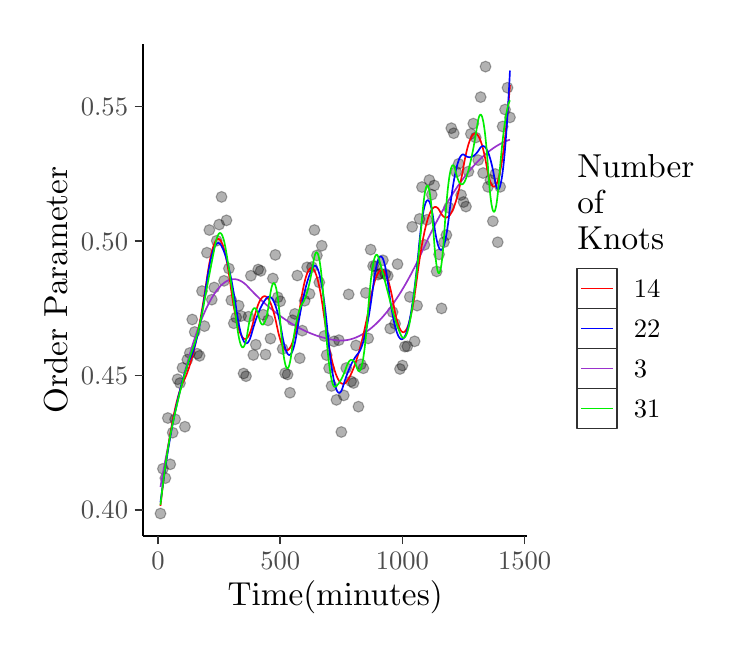
\begin{tikzpicture}[x=1pt,y=1pt]
\definecolor{fillColor}{RGB}{255,255,255}
\path[use as bounding box,fill=fillColor,fill opacity=0.00] (0,0) rectangle (252.94,216.81);
\begin{scope}
\path[clip] (  0.00,  0.00) rectangle (252.94,216.81);
\definecolor{drawColor}{RGB}{255,255,255}
\definecolor{fillColor}{RGB}{255,255,255}

\path[draw=drawColor,line width= 0.6pt,line join=round,line cap=round,fill=fillColor] (  0.00,  0.00) rectangle (252.94,216.81);
\end{scope}
\begin{scope}
\path[clip] ( 41.67, 33.16) rectangle (180.59,210.81);
\definecolor{fillColor}{RGB}{255,255,255}

\path[fill=fillColor] ( 41.67, 33.16) rectangle (180.59,210.81);
\definecolor{drawColor}{RGB}{0,0,0}
\definecolor{fillColor}{RGB}{0,0,0}

\path[draw=drawColor,draw opacity=0.30,line width= 0.4pt,line join=round,line cap=round,fill=fillColor,fill opacity=0.30] ( 47.99, 41.24) circle (  1.96);

\path[draw=drawColor,draw opacity=0.30,line width= 0.4pt,line join=round,line cap=round,fill=fillColor,fill opacity=0.30] ( 48.87, 57.42) circle (  1.96);

\path[draw=drawColor,draw opacity=0.30,line width= 0.4pt,line join=round,line cap=round,fill=fillColor,fill opacity=0.30] ( 49.75, 54.04) circle (  1.96);

\path[draw=drawColor,draw opacity=0.30,line width= 0.4pt,line join=round,line cap=round,fill=fillColor,fill opacity=0.30] ( 50.64, 75.76) circle (  1.96);

\path[draw=drawColor,draw opacity=0.30,line width= 0.4pt,line join=round,line cap=round,fill=fillColor,fill opacity=0.30] ( 51.52, 59.03) circle (  1.96);

\path[draw=drawColor,draw opacity=0.30,line width= 0.4pt,line join=round,line cap=round,fill=fillColor,fill opacity=0.30] ( 52.40, 70.46) circle (  1.96);

\path[draw=drawColor,draw opacity=0.30,line width= 0.4pt,line join=round,line cap=round,fill=fillColor,fill opacity=0.30] ( 53.28, 75.30) circle (  1.96);

\path[draw=drawColor,draw opacity=0.30,line width= 0.4pt,line join=round,line cap=round,fill=fillColor,fill opacity=0.30] ( 54.17, 89.78) circle (  1.96);

\path[draw=drawColor,draw opacity=0.30,line width= 0.4pt,line join=round,line cap=round,fill=fillColor,fill opacity=0.30] ( 55.05, 88.38) circle (  1.96);

\path[draw=drawColor,draw opacity=0.30,line width= 0.4pt,line join=round,line cap=round,fill=fillColor,fill opacity=0.30] ( 55.93, 93.89) circle (  1.96);

\path[draw=drawColor,draw opacity=0.30,line width= 0.4pt,line join=round,line cap=round,fill=fillColor,fill opacity=0.30] ( 56.82, 72.61) circle (  1.96);

\path[draw=drawColor,draw opacity=0.30,line width= 0.4pt,line join=round,line cap=round,fill=fillColor,fill opacity=0.30] ( 57.70, 96.86) circle (  1.96);

\path[draw=drawColor,draw opacity=0.30,line width= 0.4pt,line join=round,line cap=round,fill=fillColor,fill opacity=0.30] ( 58.58, 99.26) circle (  1.96);

\path[draw=drawColor,draw opacity=0.30,line width= 0.4pt,line join=round,line cap=round,fill=fillColor,fill opacity=0.30] ( 59.47,111.36) circle (  1.96);

\path[draw=drawColor,draw opacity=0.30,line width= 0.4pt,line join=round,line cap=round,fill=fillColor,fill opacity=0.30] ( 60.35,106.86) circle (  1.96);

\path[draw=drawColor,draw opacity=0.30,line width= 0.4pt,line join=round,line cap=round,fill=fillColor,fill opacity=0.30] ( 61.23, 99.00) circle (  1.96);

\path[draw=drawColor,draw opacity=0.30,line width= 0.4pt,line join=round,line cap=round,fill=fillColor,fill opacity=0.30] ( 62.12, 98.22) circle (  1.96);

\path[draw=drawColor,draw opacity=0.30,line width= 0.4pt,line join=round,line cap=round,fill=fillColor,fill opacity=0.30] ( 63.00,121.62) circle (  1.96);

\path[draw=drawColor,draw opacity=0.30,line width= 0.4pt,line join=round,line cap=round,fill=fillColor,fill opacity=0.30] ( 63.88,108.96) circle (  1.96);

\path[draw=drawColor,draw opacity=0.30,line width= 0.4pt,line join=round,line cap=round,fill=fillColor,fill opacity=0.30] ( 64.77,135.50) circle (  1.96);

\path[draw=drawColor,draw opacity=0.30,line width= 0.4pt,line join=round,line cap=round,fill=fillColor,fill opacity=0.30] ( 65.65,143.69) circle (  1.96);

\path[draw=drawColor,draw opacity=0.30,line width= 0.4pt,line join=round,line cap=round,fill=fillColor,fill opacity=0.30] ( 66.53,118.53) circle (  1.96);

\path[draw=drawColor,draw opacity=0.30,line width= 0.4pt,line join=round,line cap=round,fill=fillColor,fill opacity=0.30] ( 67.41,122.93) circle (  1.96);

\path[draw=drawColor,draw opacity=0.30,line width= 0.4pt,line join=round,line cap=round,fill=fillColor,fill opacity=0.30] ( 68.30,139.83) circle (  1.96);

\path[draw=drawColor,draw opacity=0.30,line width= 0.4pt,line join=round,line cap=round,fill=fillColor,fill opacity=0.30] ( 69.18,145.66) circle (  1.96);

\path[draw=drawColor,draw opacity=0.30,line width= 0.4pt,line join=round,line cap=round,fill=fillColor,fill opacity=0.30] ( 70.06,155.65) circle (  1.96);

\path[draw=drawColor,draw opacity=0.30,line width= 0.4pt,line join=round,line cap=round,fill=fillColor,fill opacity=0.30] ( 70.95,125.33) circle (  1.96);

\path[draw=drawColor,draw opacity=0.30,line width= 0.4pt,line join=round,line cap=round,fill=fillColor,fill opacity=0.30] ( 71.83,147.18) circle (  1.96);

\path[draw=drawColor,draw opacity=0.30,line width= 0.4pt,line join=round,line cap=round,fill=fillColor,fill opacity=0.30] ( 72.71,129.76) circle (  1.96);

\path[draw=drawColor,draw opacity=0.30,line width= 0.4pt,line join=round,line cap=round,fill=fillColor,fill opacity=0.30] ( 73.60,118.32) circle (  1.96);

\path[draw=drawColor,draw opacity=0.30,line width= 0.4pt,line join=round,line cap=round,fill=fillColor,fill opacity=0.30] ( 74.48,109.99) circle (  1.96);

\path[draw=drawColor,draw opacity=0.30,line width= 0.4pt,line join=round,line cap=round,fill=fillColor,fill opacity=0.30] ( 75.36,112.10) circle (  1.96);

\path[draw=drawColor,draw opacity=0.30,line width= 0.4pt,line join=round,line cap=round,fill=fillColor,fill opacity=0.30] ( 76.25,116.36) circle (  1.96);

\path[draw=drawColor,draw opacity=0.30,line width= 0.4pt,line join=round,line cap=round,fill=fillColor,fill opacity=0.30] ( 77.13,112.62) circle (  1.96);

\path[draw=drawColor,draw opacity=0.30,line width= 0.4pt,line join=round,line cap=round,fill=fillColor,fill opacity=0.30] ( 78.01, 91.85) circle (  1.96);

\path[draw=drawColor,draw opacity=0.30,line width= 0.4pt,line join=round,line cap=round,fill=fillColor,fill opacity=0.30] ( 78.90, 90.86) circle (  1.96);

\path[draw=drawColor,draw opacity=0.30,line width= 0.4pt,line join=round,line cap=round,fill=fillColor,fill opacity=0.30] ( 79.78,112.37) circle (  1.96);

\path[draw=drawColor,draw opacity=0.30,line width= 0.4pt,line join=round,line cap=round,fill=fillColor,fill opacity=0.30] ( 80.66,127.17) circle (  1.96);

\path[draw=drawColor,draw opacity=0.30,line width= 0.4pt,line join=round,line cap=round,fill=fillColor,fill opacity=0.30] ( 81.54, 98.54) circle (  1.96);

\path[draw=drawColor,draw opacity=0.30,line width= 0.4pt,line join=round,line cap=round,fill=fillColor,fill opacity=0.30] ( 82.43,102.24) circle (  1.96);

\path[draw=drawColor,draw opacity=0.30,line width= 0.4pt,line join=round,line cap=round,fill=fillColor,fill opacity=0.30] ( 83.31,129.43) circle (  1.96);

\path[draw=drawColor,draw opacity=0.30,line width= 0.4pt,line join=round,line cap=round,fill=fillColor,fill opacity=0.30] ( 84.19,128.92) circle (  1.96);

\path[draw=drawColor,draw opacity=0.30,line width= 0.4pt,line join=round,line cap=round,fill=fillColor,fill opacity=0.30] ( 85.08,113.09) circle (  1.96);

\path[draw=drawColor,draw opacity=0.30,line width= 0.4pt,line join=round,line cap=round,fill=fillColor,fill opacity=0.30] ( 85.96, 98.69) circle (  1.96);

\path[draw=drawColor,draw opacity=0.30,line width= 0.4pt,line join=round,line cap=round,fill=fillColor,fill opacity=0.30] ( 86.84,111.04) circle (  1.96);

\path[draw=drawColor,draw opacity=0.30,line width= 0.4pt,line join=round,line cap=round,fill=fillColor,fill opacity=0.30] ( 87.73,104.45) circle (  1.96);

\path[draw=drawColor,draw opacity=0.30,line width= 0.4pt,line join=round,line cap=round,fill=fillColor,fill opacity=0.30] ( 88.61,126.18) circle (  1.96);

\path[draw=drawColor,draw opacity=0.30,line width= 0.4pt,line join=round,line cap=round,fill=fillColor,fill opacity=0.30] ( 89.49,134.70) circle (  1.96);

\path[draw=drawColor,draw opacity=0.30,line width= 0.4pt,line join=round,line cap=round,fill=fillColor,fill opacity=0.30] ( 90.38,119.38) circle (  1.96);

\path[draw=drawColor,draw opacity=0.30,line width= 0.4pt,line join=round,line cap=round,fill=fillColor,fill opacity=0.30] ( 91.26,117.92) circle (  1.96);

\path[draw=drawColor,draw opacity=0.30,line width= 0.4pt,line join=round,line cap=round,fill=fillColor,fill opacity=0.30] ( 92.14,100.74) circle (  1.96);

\path[draw=drawColor,draw opacity=0.30,line width= 0.4pt,line join=round,line cap=round,fill=fillColor,fill opacity=0.30] ( 93.03, 91.94) circle (  1.96);

\path[draw=drawColor,draw opacity=0.30,line width= 0.4pt,line join=round,line cap=round,fill=fillColor,fill opacity=0.30] ( 93.91, 91.49) circle (  1.96);

\path[draw=drawColor,draw opacity=0.30,line width= 0.4pt,line join=round,line cap=round,fill=fillColor,fill opacity=0.30] ( 94.79, 84.89) circle (  1.96);

\path[draw=drawColor,draw opacity=0.30,line width= 0.4pt,line join=round,line cap=round,fill=fillColor,fill opacity=0.30] ( 95.68,111.09) circle (  1.96);

\path[draw=drawColor,draw opacity=0.30,line width= 0.4pt,line join=round,line cap=round,fill=fillColor,fill opacity=0.30] ( 96.56,113.38) circle (  1.96);

\path[draw=drawColor,draw opacity=0.30,line width= 0.4pt,line join=round,line cap=round,fill=fillColor,fill opacity=0.30] ( 97.44,127.24) circle (  1.96);

\path[draw=drawColor,draw opacity=0.30,line width= 0.4pt,line join=round,line cap=round,fill=fillColor,fill opacity=0.30] ( 98.32, 97.38) circle (  1.96);

\path[draw=drawColor,draw opacity=0.30,line width= 0.4pt,line join=round,line cap=round,fill=fillColor,fill opacity=0.30] ( 99.21,107.33) circle (  1.96);

\path[draw=drawColor,draw opacity=0.30,line width= 0.4pt,line join=round,line cap=round,fill=fillColor,fill opacity=0.30] (100.09,118.13) circle (  1.96);

\path[draw=drawColor,draw opacity=0.30,line width= 0.4pt,line join=round,line cap=round,fill=fillColor,fill opacity=0.30] (100.97,130.21) circle (  1.96);

\path[draw=drawColor,draw opacity=0.30,line width= 0.4pt,line join=round,line cap=round,fill=fillColor,fill opacity=0.30] (101.86,120.61) circle (  1.96);

\path[draw=drawColor,draw opacity=0.30,line width= 0.4pt,line join=round,line cap=round,fill=fillColor,fill opacity=0.30] (102.74,130.31) circle (  1.96);

\path[draw=drawColor,draw opacity=0.30,line width= 0.4pt,line join=round,line cap=round,fill=fillColor,fill opacity=0.30] (103.62,143.68) circle (  1.96);

\path[draw=drawColor,draw opacity=0.30,line width= 0.4pt,line join=round,line cap=round,fill=fillColor,fill opacity=0.30] (104.51,134.51) circle (  1.96);

\path[draw=drawColor,draw opacity=0.30,line width= 0.4pt,line join=round,line cap=round,fill=fillColor,fill opacity=0.30] (105.39,124.76) circle (  1.96);

\path[draw=drawColor,draw opacity=0.30,line width= 0.4pt,line join=round,line cap=round,fill=fillColor,fill opacity=0.30] (106.27,138.02) circle (  1.96);

\path[draw=drawColor,draw opacity=0.30,line width= 0.4pt,line join=round,line cap=round,fill=fillColor,fill opacity=0.30] (107.16,105.39) circle (  1.96);

\path[draw=drawColor,draw opacity=0.30,line width= 0.4pt,line join=round,line cap=round,fill=fillColor,fill opacity=0.30] (108.04, 98.49) circle (  1.96);

\path[draw=drawColor,draw opacity=0.30,line width= 0.4pt,line join=round,line cap=round,fill=fillColor,fill opacity=0.30] (108.92, 93.75) circle (  1.96);

\path[draw=drawColor,draw opacity=0.30,line width= 0.4pt,line join=round,line cap=round,fill=fillColor,fill opacity=0.30] (109.81, 87.34) circle (  1.96);

\path[draw=drawColor,draw opacity=0.30,line width= 0.4pt,line join=round,line cap=round,fill=fillColor,fill opacity=0.30] (110.69,103.45) circle (  1.96);

\path[draw=drawColor,draw opacity=0.30,line width= 0.4pt,line join=round,line cap=round,fill=fillColor,fill opacity=0.30] (111.57, 82.31) circle (  1.96);

\path[draw=drawColor,draw opacity=0.30,line width= 0.4pt,line join=round,line cap=round,fill=fillColor,fill opacity=0.30] (112.45,103.90) circle (  1.96);

\path[draw=drawColor,draw opacity=0.30,line width= 0.4pt,line join=round,line cap=round,fill=fillColor,fill opacity=0.30] (113.34, 70.71) circle (  1.96);

\path[draw=drawColor,draw opacity=0.30,line width= 0.4pt,line join=round,line cap=round,fill=fillColor,fill opacity=0.30] (114.22, 83.94) circle (  1.96);

\path[draw=drawColor,draw opacity=0.30,line width= 0.4pt,line join=round,line cap=round,fill=fillColor,fill opacity=0.30] (115.10, 93.82) circle (  1.96);

\path[draw=drawColor,draw opacity=0.30,line width= 0.4pt,line join=round,line cap=round,fill=fillColor,fill opacity=0.30] (115.99,120.43) circle (  1.96);

\path[draw=drawColor,draw opacity=0.30,line width= 0.4pt,line join=round,line cap=round,fill=fillColor,fill opacity=0.30] (116.87, 89.01) circle (  1.96);

\path[draw=drawColor,draw opacity=0.30,line width= 0.4pt,line join=round,line cap=round,fill=fillColor,fill opacity=0.30] (117.75, 88.41) circle (  1.96);

\path[draw=drawColor,draw opacity=0.30,line width= 0.4pt,line join=round,line cap=round,fill=fillColor,fill opacity=0.30] (118.64,101.99) circle (  1.96);

\path[draw=drawColor,draw opacity=0.30,line width= 0.4pt,line join=round,line cap=round,fill=fillColor,fill opacity=0.30] (119.52, 79.86) circle (  1.96);

\path[draw=drawColor,draw opacity=0.30,line width= 0.4pt,line join=round,line cap=round,fill=fillColor,fill opacity=0.30] (120.40, 95.14) circle (  1.96);

\path[draw=drawColor,draw opacity=0.30,line width= 0.4pt,line join=round,line cap=round,fill=fillColor,fill opacity=0.30] (121.29, 93.72) circle (  1.96);

\path[draw=drawColor,draw opacity=0.30,line width= 0.4pt,line join=round,line cap=round,fill=fillColor,fill opacity=0.30] (122.17,120.96) circle (  1.96);

\path[draw=drawColor,draw opacity=0.30,line width= 0.4pt,line join=round,line cap=round,fill=fillColor,fill opacity=0.30] (123.05,104.53) circle (  1.96);

\path[draw=drawColor,draw opacity=0.30,line width= 0.4pt,line join=round,line cap=round,fill=fillColor,fill opacity=0.30] (123.94,136.61) circle (  1.96);

\path[draw=drawColor,draw opacity=0.30,line width= 0.4pt,line join=round,line cap=round,fill=fillColor,fill opacity=0.30] (124.82,130.68) circle (  1.96);

\path[draw=drawColor,draw opacity=0.30,line width= 0.4pt,line join=round,line cap=round,fill=fillColor,fill opacity=0.30] (125.70,130.60) circle (  1.96);

\path[draw=drawColor,draw opacity=0.30,line width= 0.4pt,line join=round,line cap=round,fill=fillColor,fill opacity=0.30] (126.58,127.56) circle (  1.96);

\path[draw=drawColor,draw opacity=0.30,line width= 0.4pt,line join=round,line cap=round,fill=fillColor,fill opacity=0.30] (127.47,127.95) circle (  1.96);

\path[draw=drawColor,draw opacity=0.30,line width= 0.4pt,line join=round,line cap=round,fill=fillColor,fill opacity=0.30] (128.35,132.76) circle (  1.96);

\path[draw=drawColor,draw opacity=0.30,line width= 0.4pt,line join=round,line cap=round,fill=fillColor,fill opacity=0.30] (129.23,127.81) circle (  1.96);

\path[draw=drawColor,draw opacity=0.30,line width= 0.4pt,line join=round,line cap=round,fill=fillColor,fill opacity=0.30] (130.12,127.14) circle (  1.96);

\path[draw=drawColor,draw opacity=0.30,line width= 0.4pt,line join=round,line cap=round,fill=fillColor,fill opacity=0.30] (131.00,108.08) circle (  1.96);

\path[draw=drawColor,draw opacity=0.30,line width= 0.4pt,line join=round,line cap=round,fill=fillColor,fill opacity=0.30] (131.88,114.04) circle (  1.96);

\path[draw=drawColor,draw opacity=0.30,line width= 0.4pt,line join=round,line cap=round,fill=fillColor,fill opacity=0.30] (132.77,109.82) circle (  1.96);

\path[draw=drawColor,draw opacity=0.30,line width= 0.4pt,line join=round,line cap=round,fill=fillColor,fill opacity=0.30] (133.65,131.36) circle (  1.96);

\path[draw=drawColor,draw opacity=0.30,line width= 0.4pt,line join=round,line cap=round,fill=fillColor,fill opacity=0.30] (134.53, 93.47) circle (  1.96);

\path[draw=drawColor,draw opacity=0.30,line width= 0.4pt,line join=round,line cap=round,fill=fillColor,fill opacity=0.30] (135.42, 94.73) circle (  1.96);

\path[draw=drawColor,draw opacity=0.30,line width= 0.4pt,line join=round,line cap=round,fill=fillColor,fill opacity=0.30] (136.30,101.56) circle (  1.96);

\path[draw=drawColor,draw opacity=0.30,line width= 0.4pt,line join=round,line cap=round,fill=fillColor,fill opacity=0.30] (137.18,101.66) circle (  1.96);

\path[draw=drawColor,draw opacity=0.30,line width= 0.4pt,line join=round,line cap=round,fill=fillColor,fill opacity=0.30] (138.07,119.53) circle (  1.96);

\path[draw=drawColor,draw opacity=0.30,line width= 0.4pt,line join=round,line cap=round,fill=fillColor,fill opacity=0.30] (138.95,144.85) circle (  1.96);

\path[draw=drawColor,draw opacity=0.30,line width= 0.4pt,line join=round,line cap=round,fill=fillColor,fill opacity=0.30] (139.83,103.47) circle (  1.96);

\path[draw=drawColor,draw opacity=0.30,line width= 0.4pt,line join=round,line cap=round,fill=fillColor,fill opacity=0.30] (140.72,116.38) circle (  1.96);

\path[draw=drawColor,draw opacity=0.30,line width= 0.4pt,line join=round,line cap=round,fill=fillColor,fill opacity=0.30] (141.60,147.71) circle (  1.96);

\path[draw=drawColor,draw opacity=0.30,line width= 0.4pt,line join=round,line cap=round,fill=fillColor,fill opacity=0.30] (142.48,159.22) circle (  1.96);

\path[draw=drawColor,draw opacity=0.30,line width= 0.4pt,line join=round,line cap=round,fill=fillColor,fill opacity=0.30] (143.36,138.32) circle (  1.96);

\path[draw=drawColor,draw opacity=0.30,line width= 0.4pt,line join=round,line cap=round,fill=fillColor,fill opacity=0.30] (144.25,147.38) circle (  1.96);

\path[draw=drawColor,draw opacity=0.30,line width= 0.4pt,line join=round,line cap=round,fill=fillColor,fill opacity=0.30] (145.13,161.75) circle (  1.96);

\path[draw=drawColor,draw opacity=0.30,line width= 0.4pt,line join=round,line cap=round,fill=fillColor,fill opacity=0.30] (146.01,156.46) circle (  1.96);

\path[draw=drawColor,draw opacity=0.30,line width= 0.4pt,line join=round,line cap=round,fill=fillColor,fill opacity=0.30] (146.90,159.79) circle (  1.96);

\path[draw=drawColor,draw opacity=0.30,line width= 0.4pt,line join=round,line cap=round,fill=fillColor,fill opacity=0.30] (147.78,128.73) circle (  1.96);

\path[draw=drawColor,draw opacity=0.30,line width= 0.4pt,line join=round,line cap=round,fill=fillColor,fill opacity=0.30] (148.66,134.89) circle (  1.96);

\path[draw=drawColor,draw opacity=0.30,line width= 0.4pt,line join=round,line cap=round,fill=fillColor,fill opacity=0.30] (149.55,115.36) circle (  1.96);

\path[draw=drawColor,draw opacity=0.30,line width= 0.4pt,line join=round,line cap=round,fill=fillColor,fill opacity=0.30] (150.43,139.30) circle (  1.96);

\path[draw=drawColor,draw opacity=0.30,line width= 0.4pt,line join=round,line cap=round,fill=fillColor,fill opacity=0.30] (151.31,141.89) circle (  1.96);

\path[draw=drawColor,draw opacity=0.30,line width= 0.4pt,line join=round,line cap=round,fill=fillColor,fill opacity=0.30] (152.20,151.76) circle (  1.96);

\path[draw=drawColor,draw opacity=0.30,line width= 0.4pt,line join=round,line cap=round,fill=fillColor,fill opacity=0.30] (153.08,180.49) circle (  1.96);

\path[draw=drawColor,draw opacity=0.30,line width= 0.4pt,line join=round,line cap=round,fill=fillColor,fill opacity=0.30] (153.96,178.66) circle (  1.96);

\path[draw=drawColor,draw opacity=0.30,line width= 0.4pt,line join=round,line cap=round,fill=fillColor,fill opacity=0.30] (154.85,164.70) circle (  1.96);

\path[draw=drawColor,draw opacity=0.30,line width= 0.4pt,line join=round,line cap=round,fill=fillColor,fill opacity=0.30] (155.73,167.62) circle (  1.96);

\path[draw=drawColor,draw opacity=0.30,line width= 0.4pt,line join=round,line cap=round,fill=fillColor,fill opacity=0.30] (156.61,156.35) circle (  1.96);

\path[draw=drawColor,draw opacity=0.30,line width= 0.4pt,line join=round,line cap=round,fill=fillColor,fill opacity=0.30] (157.49,153.80) circle (  1.96);

\path[draw=drawColor,draw opacity=0.30,line width= 0.4pt,line join=round,line cap=round,fill=fillColor,fill opacity=0.30] (158.38,152.16) circle (  1.96);

\path[draw=drawColor,draw opacity=0.30,line width= 0.4pt,line join=round,line cap=round,fill=fillColor,fill opacity=0.30] (159.26,164.81) circle (  1.96);

\path[draw=drawColor,draw opacity=0.30,line width= 0.4pt,line join=round,line cap=round,fill=fillColor,fill opacity=0.30] (160.14,178.43) circle (  1.96);

\path[draw=drawColor,draw opacity=0.30,line width= 0.4pt,line join=round,line cap=round,fill=fillColor,fill opacity=0.30] (161.03,182.14) circle (  1.96);

\path[draw=drawColor,draw opacity=0.30,line width= 0.4pt,line join=round,line cap=round,fill=fillColor,fill opacity=0.30] (161.91,177.11) circle (  1.96);

\path[draw=drawColor,draw opacity=0.30,line width= 0.4pt,line join=round,line cap=round,fill=fillColor,fill opacity=0.30] (162.79,168.96) circle (  1.96);

\path[draw=drawColor,draw opacity=0.30,line width= 0.4pt,line join=round,line cap=round,fill=fillColor,fill opacity=0.30] (163.68,191.71) circle (  1.96);

\path[draw=drawColor,draw opacity=0.30,line width= 0.4pt,line join=round,line cap=round,fill=fillColor,fill opacity=0.30] (164.56,164.28) circle (  1.96);

\path[draw=drawColor,draw opacity=0.30,line width= 0.4pt,line join=round,line cap=round,fill=fillColor,fill opacity=0.30] (165.44,202.74) circle (  1.96);

\path[draw=drawColor,draw opacity=0.30,line width= 0.4pt,line join=round,line cap=round,fill=fillColor,fill opacity=0.30] (166.33,159.30) circle (  1.96);

\path[draw=drawColor,draw opacity=0.30,line width= 0.4pt,line join=round,line cap=round,fill=fillColor,fill opacity=0.30] (167.21,161.74) circle (  1.96);

\path[draw=drawColor,draw opacity=0.30,line width= 0.4pt,line join=round,line cap=round,fill=fillColor,fill opacity=0.30] (168.09,146.88) circle (  1.96);

\path[draw=drawColor,draw opacity=0.30,line width= 0.4pt,line join=round,line cap=round,fill=fillColor,fill opacity=0.30] (168.98,163.93) circle (  1.96);

\path[draw=drawColor,draw opacity=0.30,line width= 0.4pt,line join=round,line cap=round,fill=fillColor,fill opacity=0.30] (169.86,139.28) circle (  1.96);

\path[draw=drawColor,draw opacity=0.30,line width= 0.4pt,line join=round,line cap=round,fill=fillColor,fill opacity=0.30] (170.74,159.29) circle (  1.96);

\path[draw=drawColor,draw opacity=0.30,line width= 0.4pt,line join=round,line cap=round,fill=fillColor,fill opacity=0.30] (171.62,181.11) circle (  1.96);

\path[draw=drawColor,draw opacity=0.30,line width= 0.4pt,line join=round,line cap=round,fill=fillColor,fill opacity=0.30] (172.51,187.22) circle (  1.96);

\path[draw=drawColor,draw opacity=0.30,line width= 0.4pt,line join=round,line cap=round,fill=fillColor,fill opacity=0.30] (173.39,195.12) circle (  1.96);

\path[draw=drawColor,draw opacity=0.30,line width= 0.4pt,line join=round,line cap=round,fill=fillColor,fill opacity=0.30] (174.27,184.39) circle (  1.96);
\definecolor{drawColor}{RGB}{153,50,204}

\path[draw=drawColor,line width= 0.6pt,line join=round] ( 47.99, 50.89) --
	( 48.07, 51.38) --
	( 48.16, 51.88) --
	( 48.25, 52.38) --
	( 48.34, 52.87) --
	( 48.43, 53.36) --
	( 48.52, 53.85) --
	( 48.60, 54.34) --
	( 48.69, 54.83) --
	( 48.78, 55.32) --
	( 48.87, 55.80) --
	( 48.96, 56.28) --
	( 49.05, 56.76) --
	( 49.13, 57.24) --
	( 49.22, 57.72) --
	( 49.31, 58.19) --
	( 49.40, 58.67) --
	( 49.49, 59.14) --
	( 49.58, 59.61) --
	( 49.66, 60.08) --
	( 49.75, 60.55) --
	( 49.84, 61.01) --
	( 49.93, 61.48) --
	( 50.02, 61.94) --
	( 50.11, 62.40) --
	( 50.19, 62.86) --
	( 50.28, 63.32) --
	( 50.37, 63.77) --
	( 50.46, 64.23) --
	( 50.55, 64.68) --
	( 50.64, 65.13) --
	( 50.72, 65.58) --
	( 50.81, 66.03) --
	( 50.90, 66.47) --
	( 50.99, 66.92) --
	( 51.08, 67.36) --
	( 51.16, 67.80) --
	( 51.25, 68.24) --
	( 51.34, 68.68) --
	( 51.43, 69.11) --
	( 51.52, 69.54) --
	( 51.61, 69.98) --
	( 51.69, 70.41) --
	( 51.78, 70.84) --
	( 51.87, 71.26) --
	( 51.96, 71.69) --
	( 52.05, 72.11) --
	( 52.14, 72.54) --
	( 52.22, 72.96) --
	( 52.31, 73.38) --
	( 52.40, 73.79) --
	( 52.49, 74.21) --
	( 52.58, 74.62) --
	( 52.67, 75.04) --
	( 52.75, 75.45) --
	( 52.84, 75.86) --
	( 52.93, 76.26) --
	( 53.02, 76.67) --
	( 53.11, 77.07) --
	( 53.20, 77.48) --
	( 53.28, 77.88) --
	( 53.37, 78.28) --
	( 53.46, 78.67) --
	( 53.55, 79.07) --
	( 53.64, 79.46) --
	( 53.73, 79.86) --
	( 53.81, 80.25) --
	( 53.90, 80.64) --
	( 53.99, 81.02) --
	( 54.08, 81.41) --
	( 54.17, 81.79) --
	( 54.26, 82.17) --
	( 54.34, 82.56) --
	( 54.43, 82.93) --
	( 54.52, 83.31) --
	( 54.61, 83.69) --
	( 54.70, 84.06) --
	( 54.79, 84.43) --
	( 54.87, 84.81) --
	( 54.96, 85.17) --
	( 55.05, 85.54) --
	( 55.14, 85.91) --
	( 55.23, 86.27) --
	( 55.32, 86.63) --
	( 55.40, 87.00) --
	( 55.49, 87.35) --
	( 55.58, 87.71) --
	( 55.67, 88.07) --
	( 55.76, 88.42) --
	( 55.85, 88.77) --
	( 55.93, 89.13) --
	( 56.02, 89.47) --
	( 56.11, 89.82) --
	( 56.20, 90.17) --
	( 56.29, 90.51) --
	( 56.38, 90.85) --
	( 56.46, 91.20) --
	( 56.55, 91.53) --
	( 56.64, 91.87) --
	( 56.73, 92.21) --
	( 56.82, 92.54) --
	( 56.91, 92.87) --
	( 56.99, 93.21) --
	( 57.08, 93.54) --
	( 57.17, 93.86) --
	( 57.26, 94.19) --
	( 57.35, 94.51) --
	( 57.44, 94.84) --
	( 57.52, 95.16) --
	( 57.61, 95.48) --
	( 57.70, 95.79) --
	( 57.79, 96.11) --
	( 57.88, 96.42) --
	( 57.97, 96.74) --
	( 58.05, 97.05) --
	( 58.14, 97.36) --
	( 58.23, 97.66) --
	( 58.32, 97.97) --
	( 58.41, 98.27) --
	( 58.49, 98.58) --
	( 58.58, 98.88) --
	( 58.67, 99.18) --
	( 58.76, 99.47) --
	( 58.85, 99.77) --
	( 58.94,100.06) --
	( 59.02,100.36) --
	( 59.11,100.65) --
	( 59.20,100.94) --
	( 59.29,101.22) --
	( 59.38,101.51) --
	( 59.47,101.79) --
	( 59.55,102.08) --
	( 59.64,102.36) --
	( 59.73,102.64) --
	( 59.82,102.92) --
	( 59.91,103.19) --
	( 60.00,103.47) --
	( 60.08,103.74) --
	( 60.17,104.01) --
	( 60.26,104.28) --
	( 60.35,104.55) --
	( 60.44,104.81) --
	( 60.53,105.08) --
	( 60.61,105.34) --
	( 60.70,105.60) --
	( 60.79,105.86) --
	( 60.88,106.12) --
	( 60.97,106.37) --
	( 61.06,106.63) --
	( 61.14,106.88) --
	( 61.23,107.13) --
	( 61.32,107.38) --
	( 61.41,107.63) --
	( 61.50,107.87) --
	( 61.59,108.12) --
	( 61.67,108.36) --
	( 61.76,108.60) --
	( 61.85,108.84) --
	( 61.94,109.08) --
	( 62.03,109.32) --
	( 62.12,109.55) --
	( 62.20,109.78) --
	( 62.29,110.01) --
	( 62.38,110.24) --
	( 62.47,110.47) --
	( 62.56,110.70) --
	( 62.65,110.92) --
	( 62.73,111.14) --
	( 62.82,111.36) --
	( 62.91,111.58) --
	( 63.00,111.80) --
	( 63.09,112.02) --
	( 63.18,112.23) --
	( 63.26,112.45) --
	( 63.35,112.66) --
	( 63.44,112.87) --
	( 63.53,113.07) --
	( 63.62,113.28) --
	( 63.71,113.48) --
	( 63.79,113.69) --
	( 63.88,113.89) --
	( 63.97,114.09) --
	( 64.06,114.28) --
	( 64.15,114.48) --
	( 64.24,114.68) --
	( 64.32,114.87) --
	( 64.41,115.06) --
	( 64.50,115.25) --
	( 64.59,115.44) --
	( 64.68,115.62) --
	( 64.77,115.81) --
	( 64.85,115.99) --
	( 64.94,116.17) --
	( 65.03,116.35) --
	( 65.12,116.53) --
	( 65.21,116.70) --
	( 65.30,116.88) --
	( 65.38,117.05) --
	( 65.47,117.22) --
	( 65.56,117.39) --
	( 65.65,117.56) --
	( 65.74,117.73) --
	( 65.83,117.89) --
	( 65.91,118.05) --
	( 66.00,118.21) --
	( 66.09,118.37) --
	( 66.18,118.53) --
	( 66.27,118.69) --
	( 66.35,118.84) --
	( 66.44,119.00) --
	( 66.53,119.15) --
	( 66.62,119.30) --
	( 66.71,119.44) --
	( 66.80,119.59) --
	( 66.88,119.73) --
	( 66.97,119.88) --
	( 67.06,120.02) --
	( 67.15,120.16) --
	( 67.24,120.30) --
	( 67.33,120.43) --
	( 67.41,120.57) --
	( 67.50,120.70) --
	( 67.59,120.83) --
	( 67.68,120.96) --
	( 67.77,121.09) --
	( 67.86,121.21) --
	( 67.94,121.34) --
	( 68.03,121.46) --
	( 68.12,121.58) --
	( 68.21,121.70) --
	( 68.30,121.82) --
	( 68.39,121.94) --
	( 68.47,122.05) --
	( 68.56,122.16) --
	( 68.65,122.28) --
	( 68.74,122.38) --
	( 68.83,122.49) --
	( 68.92,122.60) --
	( 69.00,122.70) --
	( 69.09,122.81) --
	( 69.18,122.91) --
	( 69.27,123.01) --
	( 69.36,123.11) --
	( 69.45,123.20) --
	( 69.53,123.30) --
	( 69.62,123.39) --
	( 69.71,123.48) --
	( 69.80,123.57) --
	( 69.89,123.66) --
	( 69.98,123.74) --
	( 70.06,123.83) --
	( 70.15,123.91) --
	( 70.24,123.99) --
	( 70.33,124.07) --
	( 70.42,124.15) --
	( 70.51,124.23) --
	( 70.59,124.30) --
	( 70.68,124.37) --
	( 70.77,124.45) --
	( 70.86,124.52) --
	( 70.95,124.58) --
	( 71.04,124.65) --
	( 71.12,124.71) --
	( 71.21,124.78) --
	( 71.30,124.84) --
	( 71.39,124.90) --
	( 71.48,124.96) --
	( 71.57,125.01) --
	( 71.65,125.07) --
	( 71.74,125.12) --
	( 71.83,125.17) --
	( 71.92,125.22) --
	( 72.01,125.27) --
	( 72.10,125.32) --
	( 72.18,125.36) --
	( 72.27,125.40) --
	( 72.36,125.44) --
	( 72.45,125.48) --
	( 72.54,125.52) --
	( 72.63,125.56) --
	( 72.71,125.59) --
	( 72.80,125.63) --
	( 72.89,125.66) --
	( 72.98,125.69) --
	( 73.07,125.72) --
	( 73.16,125.74) --
	( 73.24,125.77) --
	( 73.33,125.79) --
	( 73.42,125.81) --
	( 73.51,125.83) --
	( 73.60,125.85) --
	( 73.68,125.86) --
	( 73.77,125.88) --
	( 73.86,125.89) --
	( 73.95,125.90) --
	( 74.04,125.91) --
	( 74.13,125.92) --
	( 74.21,125.93) --
	( 74.30,125.93) --
	( 74.39,125.94) --
	( 74.48,125.94) --
	( 74.57,125.94) --
	( 74.66,125.94) --
	( 74.74,125.93) --
	( 74.83,125.93) --
	( 74.92,125.92) --
	( 75.01,125.91) --
	( 75.10,125.90) --
	( 75.19,125.89) --
	( 75.27,125.88) --
	( 75.36,125.86) --
	( 75.45,125.84) --
	( 75.54,125.82) --
	( 75.63,125.80) --
	( 75.72,125.78) --
	( 75.80,125.76) --
	( 75.89,125.73) --
	( 75.98,125.71) --
	( 76.07,125.68) --
	( 76.16,125.65) --
	( 76.25,125.62) --
	( 76.33,125.58) --
	( 76.42,125.55) --
	( 76.51,125.51) --
	( 76.60,125.47) --
	( 76.69,125.43) --
	( 76.78,125.39) --
	( 76.86,125.35) --
	( 76.95,125.30) --
	( 77.04,125.25) --
	( 77.13,125.21) --
	( 77.22,125.16) --
	( 77.31,125.10) --
	( 77.39,125.05) --
	( 77.48,125.00) --
	( 77.57,124.94) --
	( 77.66,124.88) --
	( 77.75,124.82) --
	( 77.84,124.76) --
	( 77.92,124.69) --
	( 78.01,124.63) --
	( 78.10,124.56) --
	( 78.19,124.49) --
	( 78.28,124.42) --
	( 78.37,124.35) --
	( 78.45,124.28) --
	( 78.54,124.20) --
	( 78.63,124.13) --
	( 78.72,124.05) --
	( 78.81,123.97) --
	( 78.90,123.89) --
	( 78.98,123.80) --
	( 79.07,123.72) --
	( 79.16,123.63) --
	( 79.25,123.54) --
	( 79.34,123.45) --
	( 79.43,123.36) --
	( 79.51,123.27) --
	( 79.60,123.17) --
	( 79.69,123.08) --
	( 79.78,122.98) --
	( 79.87,122.89) --
	( 79.96,122.79) --
	( 80.04,122.70) --
	( 80.13,122.61) --
	( 80.22,122.51) --
	( 80.31,122.42) --
	( 80.40,122.33) --
	( 80.49,122.23) --
	( 80.57,122.14) --
	( 80.66,122.05) --
	( 80.75,121.96) --
	( 80.84,121.87) --
	( 80.93,121.77) --
	( 81.01,121.68) --
	( 81.10,121.59) --
	( 81.19,121.50) --
	( 81.28,121.41) --
	( 81.37,121.32) --
	( 81.46,121.23) --
	( 81.54,121.14) --
	( 81.63,121.05) --
	( 81.72,120.96) --
	( 81.81,120.87) --
	( 81.90,120.78) --
	( 81.99,120.69) --
	( 82.07,120.60) --
	( 82.16,120.51) --
	( 82.25,120.43) --
	( 82.34,120.34) --
	( 82.43,120.25) --
	( 82.52,120.16) --
	( 82.60,120.08) --
	( 82.69,119.99) --
	( 82.78,119.90) --
	( 82.87,119.82) --
	( 82.96,119.73) --
	( 83.05,119.64) --
	( 83.13,119.56) --
	( 83.22,119.47) --
	( 83.31,119.39) --
	( 83.40,119.30) --
	( 83.49,119.22) --
	( 83.58,119.13) --
	( 83.66,119.05) --
	( 83.75,118.96) --
	( 83.84,118.88) --
	( 83.93,118.79) --
	( 84.02,118.71) --
	( 84.11,118.63) --
	( 84.19,118.54) --
	( 84.28,118.46) --
	( 84.37,118.38) --
	( 84.46,118.30) --
	( 84.55,118.21) --
	( 84.64,118.13) --
	( 84.72,118.05) --
	( 84.81,117.97) --
	( 84.90,117.89) --
	( 84.99,117.81) --
	( 85.08,117.72) --
	( 85.17,117.64) --
	( 85.25,117.56) --
	( 85.34,117.48) --
	( 85.43,117.40) --
	( 85.52,117.32) --
	( 85.61,117.24) --
	( 85.70,117.16) --
	( 85.78,117.09) --
	( 85.87,117.01) --
	( 85.96,116.93) --
	( 86.05,116.85) --
	( 86.14,116.77) --
	( 86.23,116.69) --
	( 86.31,116.62) --
	( 86.40,116.54) --
	( 86.49,116.46) --
	( 86.58,116.38) --
	( 86.67,116.31) --
	( 86.76,116.23) --
	( 86.84,116.15) --
	( 86.93,116.08) --
	( 87.02,116.00) --
	( 87.11,115.93) --
	( 87.20,115.85) --
	( 87.29,115.78) --
	( 87.37,115.70) --
	( 87.46,115.63) --
	( 87.55,115.55) --
	( 87.64,115.48) --
	( 87.73,115.40) --
	( 87.82,115.33) --
	( 87.90,115.26) --
	( 87.99,115.18) --
	( 88.08,115.11) --
	( 88.17,115.04) --
	( 88.26,114.97) --
	( 88.35,114.89) --
	( 88.43,114.82) --
	( 88.52,114.75) --
	( 88.61,114.68) --
	( 88.70,114.61) --
	( 88.79,114.53) --
	( 88.87,114.46) --
	( 88.96,114.39) --
	( 89.05,114.32) --
	( 89.14,114.25) --
	( 89.23,114.18) --
	( 89.32,114.11) --
	( 89.40,114.04) --
	( 89.49,113.97) --
	( 89.58,113.90) --
	( 89.67,113.83) --
	( 89.76,113.77) --
	( 89.85,113.70) --
	( 89.93,113.63) --
	( 90.02,113.56) --
	( 90.11,113.49) --
	( 90.20,113.43) --
	( 90.29,113.36) --
	( 90.38,113.29) --
	( 90.46,113.22) --
	( 90.55,113.16) --
	( 90.64,113.09) --
	( 90.73,113.03) --
	( 90.82,112.96) --
	( 90.91,112.89) --
	( 90.99,112.83) --
	( 91.08,112.76) --
	( 91.17,112.70) --
	( 91.26,112.63) --
	( 91.35,112.57) --
	( 91.44,112.50) --
	( 91.52,112.44) --
	( 91.61,112.38) --
	( 91.70,112.31) --
	( 91.79,112.25) --
	( 91.88,112.19) --
	( 91.97,112.12) --
	( 92.05,112.06) --
	( 92.14,112.00) --
	( 92.23,111.94) --
	( 92.32,111.87) --
	( 92.41,111.81) --
	( 92.50,111.75) --
	( 92.58,111.69) --
	( 92.67,111.63) --
	( 92.76,111.57) --
	( 92.85,111.51) --
	( 92.94,111.45) --
	( 93.03,111.39) --
	( 93.11,111.33) --
	( 93.20,111.27) --
	( 93.29,111.21) --
	( 93.38,111.15) --
	( 93.47,111.09) --
	( 93.56,111.03) --
	( 93.64,110.97) --
	( 93.73,110.91) --
	( 93.82,110.85) --
	( 93.91,110.80) --
	( 94.00,110.74) --
	( 94.09,110.68) --
	( 94.17,110.62) --
	( 94.26,110.57) --
	( 94.35,110.51) --
	( 94.44,110.45) --
	( 94.53,110.40) --
	( 94.62,110.34) --
	( 94.70,110.28) --
	( 94.79,110.23) --
	( 94.88,110.17) --
	( 94.97,110.12) --
	( 95.06,110.06) --
	( 95.15,110.01) --
	( 95.23,109.95) --
	( 95.32,109.90) --
	( 95.41,109.85) --
	( 95.50,109.79) --
	( 95.59,109.74) --
	( 95.68,109.69) --
	( 95.76,109.63) --
	( 95.85,109.58) --
	( 95.94,109.53) --
	( 96.03,109.47) --
	( 96.12,109.42) --
	( 96.20,109.37) --
	( 96.29,109.32) --
	( 96.38,109.27) --
	( 96.47,109.22) --
	( 96.56,109.16) --
	( 96.65,109.11) --
	( 96.73,109.06) --
	( 96.82,109.01) --
	( 96.91,108.96) --
	( 97.00,108.91) --
	( 97.09,108.86) --
	( 97.18,108.81) --
	( 97.26,108.76) --
	( 97.35,108.72) --
	( 97.44,108.67) --
	( 97.53,108.62) --
	( 97.62,108.57) --
	( 97.71,108.52) --
	( 97.79,108.47) --
	( 97.88,108.43) --
	( 97.97,108.38) --
	( 98.06,108.33) --
	( 98.15,108.28) --
	( 98.24,108.24) --
	( 98.32,108.19) --
	( 98.41,108.15) --
	( 98.50,108.10) --
	( 98.59,108.05) --
	( 98.68,108.01) --
	( 98.77,107.96) --
	( 98.85,107.92) --
	( 98.94,107.87) --
	( 99.03,107.83) --
	( 99.12,107.78) --
	( 99.21,107.74) --
	( 99.30,107.70) --
	( 99.38,107.65) --
	( 99.47,107.61) --
	( 99.56,107.57) --
	( 99.65,107.52) --
	( 99.74,107.48) --
	( 99.83,107.44) --
	( 99.91,107.39) --
	(100.00,107.35) --
	(100.09,107.31) --
	(100.18,107.27) --
	(100.27,107.23) --
	(100.36,107.19) --
	(100.44,107.15) --
	(100.53,107.10) --
	(100.62,107.06) --
	(100.71,107.02) --
	(100.80,106.98) --
	(100.89,106.94) --
	(100.97,106.90) --
	(101.06,106.87) --
	(101.15,106.83) --
	(101.24,106.79) --
	(101.33,106.75) --
	(101.42,106.71) --
	(101.50,106.67) --
	(101.59,106.63) --
	(101.68,106.60) --
	(101.77,106.56) --
	(101.86,106.52) --
	(101.95,106.48) --
	(102.03,106.45) --
	(102.12,106.41) --
	(102.21,106.37) --
	(102.30,106.34) --
	(102.39,106.30) --
	(102.48,106.27) --
	(102.56,106.23) --
	(102.65,106.20) --
	(102.74,106.16) --
	(102.83,106.13) --
	(102.92,106.09) --
	(103.01,106.06) --
	(103.09,106.02) --
	(103.18,105.99) --
	(103.27,105.96) --
	(103.36,105.92) --
	(103.45,105.89) --
	(103.54,105.86) --
	(103.62,105.82) --
	(103.71,105.79) --
	(103.80,105.76) --
	(103.89,105.73) --
	(103.98,105.70) --
	(104.06,105.66) --
	(104.15,105.63) --
	(104.24,105.60) --
	(104.33,105.57) --
	(104.42,105.54) --
	(104.51,105.51) --
	(104.59,105.48) --
	(104.68,105.45) --
	(104.77,105.42) --
	(104.86,105.39) --
	(104.95,105.36) --
	(105.04,105.33) --
	(105.12,105.30) --
	(105.21,105.27) --
	(105.30,105.25) --
	(105.39,105.22) --
	(105.48,105.19) --
	(105.57,105.16) --
	(105.65,105.14) --
	(105.74,105.11) --
	(105.83,105.08) --
	(105.92,105.05) --
	(106.01,105.03) --
	(106.10,105.00) --
	(106.18,104.98) --
	(106.27,104.95) --
	(106.36,104.92) --
	(106.45,104.90) --
	(106.54,104.87) --
	(106.63,104.85) --
	(106.71,104.82) --
	(106.80,104.80) --
	(106.89,104.78) --
	(106.98,104.75) --
	(107.07,104.73) --
	(107.16,104.70) --
	(107.24,104.68) --
	(107.33,104.66) --
	(107.42,104.64) --
	(107.51,104.61) --
	(107.60,104.59) --
	(107.69,104.57) --
	(107.77,104.55) --
	(107.86,104.52) --
	(107.95,104.50) --
	(108.04,104.48) --
	(108.13,104.46) --
	(108.22,104.44) --
	(108.30,104.42) --
	(108.39,104.40) --
	(108.48,104.38) --
	(108.57,104.36) --
	(108.66,104.34) --
	(108.75,104.32) --
	(108.83,104.30) --
	(108.92,104.28) --
	(109.01,104.26) --
	(109.10,104.25) --
	(109.19,104.23) --
	(109.28,104.21) --
	(109.36,104.19) --
	(109.45,104.17) --
	(109.54,104.16) --
	(109.63,104.14) --
	(109.72,104.12) --
	(109.81,104.11) --
	(109.89,104.09) --
	(109.98,104.07) --
	(110.07,104.06) --
	(110.16,104.04) --
	(110.25,104.03) --
	(110.34,104.01) --
	(110.42,104.00) --
	(110.51,103.98) --
	(110.60,103.97) --
	(110.69,103.95) --
	(110.78,103.94) --
	(110.87,103.92) --
	(110.95,103.91) --
	(111.04,103.90) --
	(111.13,103.88) --
	(111.22,103.87) --
	(111.31,103.86) --
	(111.39,103.85) --
	(111.48,103.84) --
	(111.57,103.83) --
	(111.66,103.82) --
	(111.75,103.81) --
	(111.84,103.80) --
	(111.92,103.79) --
	(112.01,103.78) --
	(112.10,103.78) --
	(112.19,103.77) --
	(112.28,103.76) --
	(112.37,103.76) --
	(112.45,103.75) --
	(112.54,103.75) --
	(112.63,103.75) --
	(112.72,103.74) --
	(112.81,103.74) --
	(112.90,103.74) --
	(112.98,103.74) --
	(113.07,103.74) --
	(113.16,103.74) --
	(113.25,103.74) --
	(113.34,103.74) --
	(113.43,103.74) --
	(113.51,103.74) --
	(113.60,103.75) --
	(113.69,103.75) --
	(113.78,103.75) --
	(113.87,103.76) --
	(113.96,103.76) --
	(114.04,103.77) --
	(114.13,103.77) --
	(114.22,103.78) --
	(114.31,103.79) --
	(114.40,103.80) --
	(114.49,103.81) --
	(114.57,103.82) --
	(114.66,103.83) --
	(114.75,103.84) --
	(114.84,103.85) --
	(114.93,103.86) --
	(115.02,103.87) --
	(115.10,103.88) --
	(115.19,103.90) --
	(115.28,103.91) --
	(115.37,103.93) --
	(115.46,103.94) --
	(115.55,103.96) --
	(115.63,103.97) --
	(115.72,103.99) --
	(115.81,104.01) --
	(115.90,104.02) --
	(115.99,104.04) --
	(116.08,104.06) --
	(116.16,104.08) --
	(116.25,104.10) --
	(116.34,104.12) --
	(116.43,104.14) --
	(116.52,104.17) --
	(116.61,104.19) --
	(116.69,104.21) --
	(116.78,104.24) --
	(116.87,104.26) --
	(116.96,104.29) --
	(117.05,104.31) --
	(117.14,104.34) --
	(117.22,104.36) --
	(117.31,104.39) --
	(117.40,104.42) --
	(117.49,104.45) --
	(117.58,104.48) --
	(117.67,104.51) --
	(117.75,104.54) --
	(117.84,104.57) --
	(117.93,104.60) --
	(118.02,104.63) --
	(118.11,104.66) --
	(118.20,104.70) --
	(118.28,104.73) --
	(118.37,104.76) --
	(118.46,104.80) --
	(118.55,104.83) --
	(118.64,104.87) --
	(118.72,104.91) --
	(118.81,104.94) --
	(118.90,104.98) --
	(118.99,105.02) --
	(119.08,105.06) --
	(119.17,105.10) --
	(119.25,105.14) --
	(119.34,105.18) --
	(119.43,105.22) --
	(119.52,105.26) --
	(119.61,105.30) --
	(119.70,105.35) --
	(119.78,105.39) --
	(119.87,105.43) --
	(119.96,105.48) --
	(120.05,105.52) --
	(120.14,105.57) --
	(120.23,105.62) --
	(120.31,105.66) --
	(120.40,105.71) --
	(120.49,105.76) --
	(120.58,105.81) --
	(120.67,105.86) --
	(120.76,105.91) --
	(120.84,105.96) --
	(120.93,106.01) --
	(121.02,106.06) --
	(121.11,106.11) --
	(121.20,106.17) --
	(121.29,106.22) --
	(121.37,106.27) --
	(121.46,106.33) --
	(121.55,106.38) --
	(121.64,106.44) --
	(121.73,106.50) --
	(121.82,106.55) --
	(121.90,106.61) --
	(121.99,106.67) --
	(122.08,106.73) --
	(122.17,106.79) --
	(122.26,106.85) --
	(122.35,106.91) --
	(122.43,106.97) --
	(122.52,107.03) --
	(122.61,107.09) --
	(122.70,107.15) --
	(122.79,107.22) --
	(122.88,107.28) --
	(122.96,107.34) --
	(123.05,107.41) --
	(123.14,107.48) --
	(123.23,107.54) --
	(123.32,107.61) --
	(123.41,107.68) --
	(123.49,107.74) --
	(123.58,107.81) --
	(123.67,107.88) --
	(123.76,107.95) --
	(123.85,108.02) --
	(123.94,108.09) --
	(124.02,108.16) --
	(124.11,108.24) --
	(124.20,108.31) --
	(124.29,108.38) --
	(124.38,108.45) --
	(124.47,108.53) --
	(124.55,108.60) --
	(124.64,108.68) --
	(124.73,108.76) --
	(124.82,108.83) --
	(124.91,108.91) --
	(125.00,108.99) --
	(125.08,109.07) --
	(125.17,109.14) --
	(125.26,109.22) --
	(125.35,109.30) --
	(125.44,109.38) --
	(125.53,109.47) --
	(125.61,109.55) --
	(125.70,109.63) --
	(125.79,109.71) --
	(125.88,109.80) --
	(125.97,109.88) --
	(126.06,109.97) --
	(126.14,110.05) --
	(126.23,110.14) --
	(126.32,110.22) --
	(126.41,110.31) --
	(126.50,110.40) --
	(126.58,110.49) --
	(126.67,110.58) --
	(126.76,110.66) --
	(126.85,110.75) --
	(126.94,110.85) --
	(127.03,110.94) --
	(127.11,111.03) --
	(127.20,111.12) --
	(127.29,111.21) --
	(127.38,111.31) --
	(127.47,111.40) --
	(127.56,111.50) --
	(127.64,111.59) --
	(127.73,111.69) --
	(127.82,111.78) --
	(127.91,111.88) --
	(128.00,111.98) --
	(128.09,112.08) --
	(128.17,112.17) --
	(128.26,112.27) --
	(128.35,112.37) --
	(128.44,112.47) --
	(128.53,112.57) --
	(128.62,112.68) --
	(128.70,112.78) --
	(128.79,112.88) --
	(128.88,112.98) --
	(128.97,113.09) --
	(129.06,113.19) --
	(129.15,113.30) --
	(129.23,113.40) --
	(129.32,113.51) --
	(129.41,113.62) --
	(129.50,113.72) --
	(129.59,113.83) --
	(129.68,113.94) --
	(129.76,114.05) --
	(129.85,114.16) --
	(129.94,114.27) --
	(130.03,114.38) --
	(130.12,114.49) --
	(130.21,114.60) --
	(130.29,114.72) --
	(130.38,114.83) --
	(130.47,114.94) --
	(130.56,115.06) --
	(130.65,115.17) --
	(130.74,115.29) --
	(130.82,115.41) --
	(130.91,115.52) --
	(131.00,115.64) --
	(131.09,115.76) --
	(131.18,115.88) --
	(131.27,115.99) --
	(131.35,116.11) --
	(131.44,116.23) --
	(131.53,116.35) --
	(131.62,116.48) --
	(131.71,116.60) --
	(131.80,116.72) --
	(131.88,116.84) --
	(131.97,116.97) --
	(132.06,117.09) --
	(132.15,117.22) --
	(132.24,117.34) --
	(132.33,117.47) --
	(132.41,117.59) --
	(132.50,117.72) --
	(132.59,117.85) --
	(132.68,117.98) --
	(132.77,118.11) --
	(132.86,118.24) --
	(132.94,118.37) --
	(133.03,118.50) --
	(133.12,118.63) --
	(133.21,118.76) --
	(133.30,118.89) --
	(133.39,119.02) --
	(133.47,119.16) --
	(133.56,119.29) --
	(133.65,119.43) --
	(133.74,119.56) --
	(133.83,119.70) --
	(133.91,119.83) --
	(134.00,119.97) --
	(134.09,120.11) --
	(134.18,120.25) --
	(134.27,120.39) --
	(134.36,120.53) --
	(134.44,120.67) --
	(134.53,120.81) --
	(134.62,120.95) --
	(134.71,121.09) --
	(134.80,121.23) --
	(134.89,121.37) --
	(134.97,121.52) --
	(135.06,121.66) --
	(135.15,121.81) --
	(135.24,121.95) --
	(135.33,122.10) --
	(135.42,122.24) --
	(135.50,122.39) --
	(135.59,122.54) --
	(135.68,122.69) --
	(135.77,122.83) --
	(135.86,122.98) --
	(135.95,123.13) --
	(136.03,123.28) --
	(136.12,123.43) --
	(136.21,123.59) --
	(136.30,123.74) --
	(136.39,123.89) --
	(136.48,124.04) --
	(136.56,124.20) --
	(136.65,124.35) --
	(136.74,124.51) --
	(136.83,124.66) --
	(136.92,124.82) --
	(137.01,124.98) --
	(137.09,125.13) --
	(137.18,125.29) --
	(137.27,125.45) --
	(137.36,125.61) --
	(137.45,125.77) --
	(137.54,125.93) --
	(137.62,126.09) --
	(137.71,126.25) --
	(137.80,126.41) --
	(137.89,126.58) --
	(137.98,126.74) --
	(138.07,126.90) --
	(138.15,127.07) --
	(138.24,127.23) --
	(138.33,127.40) --
	(138.42,127.56) --
	(138.51,127.73) --
	(138.60,127.90) --
	(138.68,128.06) --
	(138.77,128.23) --
	(138.86,128.40) --
	(138.95,128.57) --
	(139.04,128.74) --
	(139.13,128.91) --
	(139.21,129.08) --
	(139.30,129.26) --
	(139.39,129.43) --
	(139.48,129.60) --
	(139.57,129.77) --
	(139.66,129.95) --
	(139.74,130.12) --
	(139.83,130.30) --
	(139.92,130.47) --
	(140.01,130.65) --
	(140.10,130.83) --
	(140.19,131.01) --
	(140.27,131.18) --
	(140.36,131.36) --
	(140.45,131.54) --
	(140.54,131.72) --
	(140.63,131.90) --
	(140.72,132.08) --
	(140.80,132.27) --
	(140.89,132.45) --
	(140.98,132.63) --
	(141.07,132.81) --
	(141.16,133.00) --
	(141.25,133.18) --
	(141.33,133.37) --
	(141.42,133.55) --
	(141.51,133.74) --
	(141.60,133.93) --
	(141.69,134.11) --
	(141.77,134.30) --
	(141.86,134.49) --
	(141.95,134.68) --
	(142.04,134.87) --
	(142.13,135.06) --
	(142.22,135.25) --
	(142.30,135.44) --
	(142.39,135.64) --
	(142.48,135.83) --
	(142.57,136.02) --
	(142.66,136.22) --
	(142.75,136.41) --
	(142.83,136.60) --
	(142.92,136.80) --
	(143.01,136.99) --
	(143.10,137.18) --
	(143.19,137.38) --
	(143.28,137.57) --
	(143.36,137.76) --
	(143.45,137.95) --
	(143.54,138.14) --
	(143.63,138.33) --
	(143.72,138.52) --
	(143.81,138.71) --
	(143.89,138.90) --
	(143.98,139.08) --
	(144.07,139.27) --
	(144.16,139.46) --
	(144.25,139.65) --
	(144.34,139.83) --
	(144.42,140.02) --
	(144.51,140.20) --
	(144.60,140.39) --
	(144.69,140.57) --
	(144.78,140.76) --
	(144.87,140.94) --
	(144.95,141.12) --
	(145.04,141.30) --
	(145.13,141.49) --
	(145.22,141.67) --
	(145.31,141.85) --
	(145.40,142.03) --
	(145.48,142.21) --
	(145.57,142.39) --
	(145.66,142.57) --
	(145.75,142.75) --
	(145.84,142.93) --
	(145.93,143.10) --
	(146.01,143.28) --
	(146.10,143.46) --
	(146.19,143.64) --
	(146.28,143.81) --
	(146.37,143.99) --
	(146.46,144.16) --
	(146.54,144.34) --
	(146.63,144.51) --
	(146.72,144.68) --
	(146.81,144.86) --
	(146.90,145.03) --
	(146.99,145.20) --
	(147.07,145.37) --
	(147.16,145.55) --
	(147.25,145.72) --
	(147.34,145.89) --
	(147.43,146.06) --
	(147.52,146.23) --
	(147.60,146.40) --
	(147.69,146.56) --
	(147.78,146.73) --
	(147.87,146.90) --
	(147.96,147.07) --
	(148.05,147.23) --
	(148.13,147.40) --
	(148.22,147.57) --
	(148.31,147.73) --
	(148.40,147.90) --
	(148.49,148.06) --
	(148.58,148.23) --
	(148.66,148.39) --
	(148.75,148.55) --
	(148.84,148.72) --
	(148.93,148.88) --
	(149.02,149.04) --
	(149.10,149.20) --
	(149.19,149.36) --
	(149.28,149.52) --
	(149.37,149.68) --
	(149.46,149.84) --
	(149.55,150.00) --
	(149.63,150.16) --
	(149.72,150.32) --
	(149.81,150.47) --
	(149.90,150.63) --
	(149.99,150.79) --
	(150.08,150.94) --
	(150.16,151.10) --
	(150.25,151.25) --
	(150.34,151.41) --
	(150.43,151.56) --
	(150.52,151.72) --
	(150.61,151.87) --
	(150.69,152.02) --
	(150.78,152.18) --
	(150.87,152.33) --
	(150.96,152.48) --
	(151.05,152.63) --
	(151.14,152.78) --
	(151.22,152.93) --
	(151.31,153.08) --
	(151.40,153.23) --
	(151.49,153.38) --
	(151.58,153.53) --
	(151.67,153.68) --
	(151.75,153.82) --
	(151.84,153.97) --
	(151.93,154.12) --
	(152.02,154.26) --
	(152.11,154.41) --
	(152.20,154.55) --
	(152.28,154.70) --
	(152.37,154.84) --
	(152.46,154.99) --
	(152.55,155.13) --
	(152.64,155.27) --
	(152.73,155.41) --
	(152.81,155.56) --
	(152.90,155.70) --
	(152.99,155.84) --
	(153.08,155.98) --
	(153.17,156.12) --
	(153.26,156.26) --
	(153.34,156.40) --
	(153.43,156.54) --
	(153.52,156.67) --
	(153.61,156.81) --
	(153.70,156.95) --
	(153.79,157.09) --
	(153.87,157.22) --
	(153.96,157.36) --
	(154.05,157.49) --
	(154.14,157.63) --
	(154.23,157.76) --
	(154.32,157.90) --
	(154.40,158.03) --
	(154.49,158.16) --
	(154.58,158.30) --
	(154.67,158.43) --
	(154.76,158.56) --
	(154.85,158.69) --
	(154.93,158.82) --
	(155.02,158.95) --
	(155.11,159.08) --
	(155.20,159.21) --
	(155.29,159.34) --
	(155.38,159.47) --
	(155.46,159.60) --
	(155.55,159.72) --
	(155.64,159.85) --
	(155.73,159.98) --
	(155.82,160.10) --
	(155.91,160.23) --
	(155.99,160.36) --
	(156.08,160.48) --
	(156.17,160.60) --
	(156.26,160.73) --
	(156.35,160.85) --
	(156.43,160.98) --
	(156.52,161.10) --
	(156.61,161.22) --
	(156.70,161.34) --
	(156.79,161.46) --
	(156.88,161.58) --
	(156.96,161.70) --
	(157.05,161.82) --
	(157.14,161.94) --
	(157.23,162.06) --
	(157.32,162.18) --
	(157.41,162.30) --
	(157.49,162.41) --
	(157.58,162.53) --
	(157.67,162.65) --
	(157.76,162.76) --
	(157.85,162.88) --
	(157.94,162.99) --
	(158.02,163.11) --
	(158.11,163.22) --
	(158.20,163.34) --
	(158.29,163.45) --
	(158.38,163.56) --
	(158.47,163.68) --
	(158.55,163.79) --
	(158.64,163.90) --
	(158.73,164.01) --
	(158.82,164.12) --
	(158.91,164.23) --
	(159.00,164.34) --
	(159.08,164.45) --
	(159.17,164.56) --
	(159.26,164.67) --
	(159.35,164.77) --
	(159.44,164.88) --
	(159.53,164.99) --
	(159.61,165.09) --
	(159.70,165.20) --
	(159.79,165.30) --
	(159.88,165.41) --
	(159.97,165.51) --
	(160.06,165.62) --
	(160.14,165.72) --
	(160.23,165.82) --
	(160.32,165.93) --
	(160.41,166.03) --
	(160.50,166.13) --
	(160.59,166.23) --
	(160.67,166.33) --
	(160.76,166.43) --
	(160.85,166.53) --
	(160.94,166.63) --
	(161.03,166.73) --
	(161.12,166.83) --
	(161.20,166.93) --
	(161.29,167.03) --
	(161.38,167.12) --
	(161.47,167.22) --
	(161.56,167.32) --
	(161.65,167.41) --
	(161.73,167.51) --
	(161.82,167.60) --
	(161.91,167.70) --
	(162.00,167.79) --
	(162.09,167.88) --
	(162.18,167.98) --
	(162.26,168.07) --
	(162.35,168.16) --
	(162.44,168.25) --
	(162.53,168.34) --
	(162.62,168.43) --
	(162.71,168.52) --
	(162.79,168.61) --
	(162.88,168.70) --
	(162.97,168.79) --
	(163.06,168.88) --
	(163.15,168.97) --
	(163.24,169.06) --
	(163.32,169.14) --
	(163.41,169.23) --
	(163.50,169.31) --
	(163.59,169.40) --
	(163.68,169.49) --
	(163.77,169.57) --
	(163.85,169.65) --
	(163.94,169.74) --
	(164.03,169.82) --
	(164.12,169.90) --
	(164.21,169.99) --
	(164.29,170.07) --
	(164.38,170.15) --
	(164.47,170.23) --
	(164.56,170.31) --
	(164.65,170.39) --
	(164.74,170.47) --
	(164.82,170.55) --
	(164.91,170.63) --
	(165.00,170.71) --
	(165.09,170.78) --
	(165.18,170.86) --
	(165.27,170.94) --
	(165.35,171.01) --
	(165.44,171.09) --
	(165.53,171.17) --
	(165.62,171.24) --
	(165.71,171.31) --
	(165.80,171.39) --
	(165.88,171.46) --
	(165.97,171.54) --
	(166.06,171.61) --
	(166.15,171.68) --
	(166.24,171.75) --
	(166.33,171.82) --
	(166.41,171.89) --
	(166.50,171.96) --
	(166.59,172.03) --
	(166.68,172.10) --
	(166.77,172.17) --
	(166.86,172.24) --
	(166.94,172.31) --
	(167.03,172.38) --
	(167.12,172.44) --
	(167.21,172.51) --
	(167.30,172.58) --
	(167.39,172.64) --
	(167.47,172.71) --
	(167.56,172.77) --
	(167.65,172.84) --
	(167.74,172.90) --
	(167.83,172.96) --
	(167.92,173.03) --
	(168.00,173.09) --
	(168.09,173.15) --
	(168.18,173.21) --
	(168.27,173.27) --
	(168.36,173.33) --
	(168.45,173.39) --
	(168.53,173.45) --
	(168.62,173.51) --
	(168.71,173.57) --
	(168.80,173.63) --
	(168.89,173.69) --
	(168.98,173.75) --
	(169.06,173.80) --
	(169.15,173.86) --
	(169.24,173.92) --
	(169.33,173.97) --
	(169.42,174.03) --
	(169.51,174.08) --
	(169.59,174.13) --
	(169.68,174.19) --
	(169.77,174.24) --
	(169.86,174.29) --
	(169.95,174.35) --
	(170.04,174.40) --
	(170.12,174.45) --
	(170.21,174.50) --
	(170.30,174.55) --
	(170.39,174.60) --
	(170.48,174.65) --
	(170.57,174.70) --
	(170.65,174.75) --
	(170.74,174.80) --
	(170.83,174.84) --
	(170.92,174.89) --
	(171.01,174.94) --
	(171.10,174.98) --
	(171.18,175.03) --
	(171.27,175.08) --
	(171.36,175.12) --
	(171.45,175.17) --
	(171.54,175.21) --
	(171.62,175.25) --
	(171.71,175.30) --
	(171.80,175.34) --
	(171.89,175.38) --
	(171.98,175.42) --
	(172.07,175.46) --
	(172.15,175.50) --
	(172.24,175.54) --
	(172.33,175.58) --
	(172.42,175.62) --
	(172.51,175.66) --
	(172.60,175.70) --
	(172.68,175.74) --
	(172.77,175.78) --
	(172.86,175.81) --
	(172.95,175.85) --
	(173.04,175.89) --
	(173.13,175.92) --
	(173.21,175.96) --
	(173.30,175.99) --
	(173.39,176.03) --
	(173.48,176.06) --
	(173.57,176.09) --
	(173.66,176.13) --
	(173.74,176.16) --
	(173.83,176.19) --
	(173.92,176.22) --
	(174.01,176.25) --
	(174.10,176.28) --
	(174.19,176.31) --
	(174.27,176.34);
\definecolor{drawColor}{RGB}{255,0,0}

\path[draw=drawColor,line width= 0.6pt,line join=round] ( 47.99, 44.02) --
	( 48.07, 44.80) --
	( 48.16, 45.56) --
	( 48.25, 46.32) --
	( 48.34, 47.08) --
	( 48.43, 47.82) --
	( 48.52, 48.56) --
	( 48.60, 49.30) --
	( 48.69, 50.03) --
	( 48.78, 50.75) --
	( 48.87, 51.46) --
	( 48.96, 52.17) --
	( 49.05, 52.88) --
	( 49.13, 53.57) --
	( 49.22, 54.26) --
	( 49.31, 54.95) --
	( 49.40, 55.63) --
	( 49.49, 56.30) --
	( 49.58, 56.96) --
	( 49.66, 57.62) --
	( 49.75, 58.27) --
	( 49.84, 58.92) --
	( 49.93, 59.56) --
	( 50.02, 60.19) --
	( 50.11, 60.82) --
	( 50.19, 61.44) --
	( 50.28, 62.05) --
	( 50.37, 62.66) --
	( 50.46, 63.26) --
	( 50.55, 63.86) --
	( 50.64, 64.45) --
	( 50.72, 65.03) --
	( 50.81, 65.61) --
	( 50.90, 66.18) --
	( 50.99, 66.74) --
	( 51.08, 67.30) --
	( 51.16, 67.85) --
	( 51.25, 68.39) --
	( 51.34, 68.93) --
	( 51.43, 69.46) --
	( 51.52, 69.99) --
	( 51.61, 70.51) --
	( 51.69, 71.02) --
	( 51.78, 71.53) --
	( 51.87, 72.03) --
	( 51.96, 72.52) --
	( 52.05, 73.01) --
	( 52.14, 73.49) --
	( 52.22, 73.97) --
	( 52.31, 74.44) --
	( 52.40, 74.90) --
	( 52.49, 75.36) --
	( 52.58, 75.81) --
	( 52.67, 76.25) --
	( 52.75, 76.69) --
	( 52.84, 77.12) --
	( 52.93, 77.54) --
	( 53.02, 77.96) --
	( 53.11, 78.37) --
	( 53.20, 78.78) --
	( 53.28, 79.18) --
	( 53.37, 79.57) --
	( 53.46, 79.96) --
	( 53.55, 80.34) --
	( 53.64, 80.71) --
	( 53.73, 81.08) --
	( 53.81, 81.44) --
	( 53.90, 81.80) --
	( 53.99, 82.14) --
	( 54.08, 82.49) --
	( 54.17, 82.82) --
	( 54.26, 83.15) --
	( 54.34, 83.48) --
	( 54.43, 83.79) --
	( 54.52, 84.10) --
	( 54.61, 84.41) --
	( 54.70, 84.71) --
	( 54.79, 85.00) --
	( 54.87, 85.28) --
	( 54.96, 85.56) --
	( 55.05, 85.84) --
	( 55.14, 86.10) --
	( 55.23, 86.36) --
	( 55.32, 86.62) --
	( 55.40, 86.86) --
	( 55.49, 87.10) --
	( 55.58, 87.34) --
	( 55.67, 87.57) --
	( 55.76, 87.79) --
	( 55.85, 88.01) --
	( 55.93, 88.21) --
	( 56.02, 88.42) --
	( 56.11, 88.61) --
	( 56.20, 88.81) --
	( 56.29, 88.99) --
	( 56.38, 89.17) --
	( 56.46, 89.34) --
	( 56.55, 89.52) --
	( 56.64, 89.70) --
	( 56.73, 89.89) --
	( 56.82, 90.08) --
	( 56.91, 90.28) --
	( 56.99, 90.48) --
	( 57.08, 90.68) --
	( 57.17, 90.89) --
	( 57.26, 91.11) --
	( 57.35, 91.33) --
	( 57.44, 91.55) --
	( 57.52, 91.78) --
	( 57.61, 92.01) --
	( 57.70, 92.25) --
	( 57.79, 92.49) --
	( 57.88, 92.74) --
	( 57.97, 92.99) --
	( 58.05, 93.25) --
	( 58.14, 93.51) --
	( 58.23, 93.77) --
	( 58.32, 94.04) --
	( 58.41, 94.31) --
	( 58.49, 94.59) --
	( 58.58, 94.88) --
	( 58.67, 95.16) --
	( 58.76, 95.46) --
	( 58.85, 95.75) --
	( 58.94, 96.06) --
	( 59.02, 96.36) --
	( 59.11, 96.67) --
	( 59.20, 96.99) --
	( 59.29, 97.31) --
	( 59.38, 97.63) --
	( 59.47, 97.96) --
	( 59.55, 98.30) --
	( 59.64, 98.63) --
	( 59.73, 98.98) --
	( 59.82, 99.32) --
	( 59.91, 99.68) --
	( 60.00,100.03) --
	( 60.08,100.40) --
	( 60.17,100.76) --
	( 60.26,101.13) --
	( 60.35,101.51) --
	( 60.44,101.89) --
	( 60.53,102.27) --
	( 60.61,102.66) --
	( 60.70,103.05) --
	( 60.79,103.45) --
	( 60.88,103.85) --
	( 60.97,104.26) --
	( 61.06,104.67) --
	( 61.14,105.09) --
	( 61.23,105.51) --
	( 61.32,105.93) --
	( 61.41,106.36) --
	( 61.50,106.80) --
	( 61.59,107.24) --
	( 61.67,107.68) --
	( 61.76,108.13) --
	( 61.85,108.58) --
	( 61.94,109.04) --
	( 62.03,109.50) --
	( 62.12,109.97) --
	( 62.20,110.44) --
	( 62.29,110.92) --
	( 62.38,111.40) --
	( 62.47,111.88) --
	( 62.56,112.37) --
	( 62.65,112.87) --
	( 62.73,113.37) --
	( 62.82,113.87) --
	( 62.91,114.38) --
	( 63.00,114.89) --
	( 63.09,115.41) --
	( 63.18,115.93) --
	( 63.26,116.45) --
	( 63.35,116.99) --
	( 63.44,117.52) --
	( 63.53,118.06) --
	( 63.62,118.61) --
	( 63.71,119.16) --
	( 63.79,119.71) --
	( 63.88,120.27) --
	( 63.97,120.83) --
	( 64.06,121.40) --
	( 64.15,121.97) --
	( 64.24,122.55) --
	( 64.32,123.13) --
	( 64.41,123.71) --
	( 64.50,124.30) --
	( 64.59,124.90) --
	( 64.68,125.50) --
	( 64.77,126.10) --
	( 64.85,126.71) --
	( 64.94,127.31) --
	( 65.03,127.90) --
	( 65.12,128.47) --
	( 65.21,129.03) --
	( 65.30,129.57) --
	( 65.38,130.10) --
	( 65.47,130.62) --
	( 65.56,131.13) --
	( 65.65,131.62) --
	( 65.74,132.10) --
	( 65.83,132.56) --
	( 65.91,133.02) --
	( 66.00,133.45) --
	( 66.09,133.88) --
	( 66.18,134.29) --
	( 66.27,134.69) --
	( 66.35,135.08) --
	( 66.44,135.45) --
	( 66.53,135.81) --
	( 66.62,136.15) --
	( 66.71,136.49) --
	( 66.80,136.80) --
	( 66.88,137.11) --
	( 66.97,137.40) --
	( 67.06,137.68) --
	( 67.15,137.95) --
	( 67.24,138.20) --
	( 67.33,138.44) --
	( 67.41,138.67) --
	( 67.50,138.88) --
	( 67.59,139.08) --
	( 67.68,139.26) --
	( 67.77,139.44) --
	( 67.86,139.60) --
	( 67.94,139.74) --
	( 68.03,139.87) --
	( 68.12,139.99) --
	( 68.21,140.10) --
	( 68.30,140.19) --
	( 68.39,140.27) --
	( 68.47,140.34) --
	( 68.56,140.39) --
	( 68.65,140.43) --
	( 68.74,140.46) --
	( 68.83,140.47) --
	( 68.92,140.47) --
	( 69.00,140.46) --
	( 69.09,140.43) --
	( 69.18,140.39) --
	( 69.27,140.34) --
	( 69.36,140.27) --
	( 69.45,140.19) --
	( 69.53,140.09) --
	( 69.62,139.99) --
	( 69.71,139.87) --
	( 69.80,139.73) --
	( 69.89,139.59) --
	( 69.98,139.43) --
	( 70.06,139.25) --
	( 70.15,139.07) --
	( 70.24,138.87) --
	( 70.33,138.65) --
	( 70.42,138.43) --
	( 70.51,138.19) --
	( 70.59,137.93) --
	( 70.68,137.67) --
	( 70.77,137.39) --
	( 70.86,137.10) --
	( 70.95,136.79) --
	( 71.04,136.47) --
	( 71.12,136.14) --
	( 71.21,135.79) --
	( 71.30,135.43) --
	( 71.39,135.06) --
	( 71.48,134.67) --
	( 71.57,134.27) --
	( 71.65,133.86) --
	( 71.74,133.43) --
	( 71.83,132.99) --
	( 71.92,132.54) --
	( 72.01,132.07) --
	( 72.10,131.59) --
	( 72.18,131.10) --
	( 72.27,130.60) --
	( 72.36,130.08) --
	( 72.45,129.54) --
	( 72.54,129.00) --
	( 72.63,128.44) --
	( 72.71,127.87) --
	( 72.80,127.28) --
	( 72.89,126.68) --
	( 72.98,126.07) --
	( 73.07,125.44) --
	( 73.16,124.80) --
	( 73.24,124.15) --
	( 73.33,123.50) --
	( 73.42,122.86) --
	( 73.51,122.22) --
	( 73.60,121.60) --
	( 73.68,120.99) --
	( 73.77,120.39) --
	( 73.86,119.81) --
	( 73.95,119.23) --
	( 74.04,118.66) --
	( 74.13,118.11) --
	( 74.21,117.56) --
	( 74.30,117.03) --
	( 74.39,116.51) --
	( 74.48,116.00) --
	( 74.57,115.50) --
	( 74.66,115.01) --
	( 74.74,114.53) --
	( 74.83,114.06) --
	( 74.92,113.61) --
	( 75.01,113.16) --
	( 75.10,112.73) --
	( 75.19,112.30) --
	( 75.27,111.89) --
	( 75.36,111.49) --
	( 75.45,111.10) --
	( 75.54,110.72) --
	( 75.63,110.35) --
	( 75.72,109.99) --
	( 75.80,109.64) --
	( 75.89,109.31) --
	( 75.98,108.98) --
	( 76.07,108.67) --
	( 76.16,108.37) --
	( 76.25,108.07) --
	( 76.33,107.79) --
	( 76.42,107.52) --
	( 76.51,107.26) --
	( 76.60,107.02) --
	( 76.69,106.78) --
	( 76.78,106.55) --
	( 76.86,106.34) --
	( 76.95,106.13) --
	( 77.04,105.94) --
	( 77.13,105.76) --
	( 77.22,105.58) --
	( 77.31,105.42) --
	( 77.39,105.27) --
	( 77.48,105.14) --
	( 77.57,105.01) --
	( 77.66,104.89) --
	( 77.75,104.79) --
	( 77.84,104.69) --
	( 77.92,104.61) --
	( 78.01,104.53) --
	( 78.10,104.47) --
	( 78.19,104.42) --
	( 78.28,104.38) --
	( 78.37,104.35) --
	( 78.45,104.33) --
	( 78.54,104.33) --
	( 78.63,104.33) --
	( 78.72,104.34) --
	( 78.81,104.37) --
	( 78.90,104.41) --
	( 78.98,104.45) --
	( 79.07,104.51) --
	( 79.16,104.58) --
	( 79.25,104.66) --
	( 79.34,104.75) --
	( 79.43,104.85) --
	( 79.51,104.97) --
	( 79.60,105.09) --
	( 79.69,105.23) --
	( 79.78,105.37) --
	( 79.87,105.53) --
	( 79.96,105.70) --
	( 80.04,105.88) --
	( 80.13,106.07) --
	( 80.22,106.27) --
	( 80.31,106.48) --
	( 80.40,106.70) --
	( 80.49,106.94) --
	( 80.57,107.18) --
	( 80.66,107.44) --
	( 80.75,107.70) --
	( 80.84,107.98) --
	( 80.93,108.27) --
	( 81.01,108.57) --
	( 81.10,108.88) --
	( 81.19,109.20) --
	( 81.28,109.53) --
	( 81.37,109.88) --
	( 81.46,110.23) --
	( 81.54,110.59) --
	( 81.63,110.97) --
	( 81.72,111.35) --
	( 81.81,111.73) --
	( 81.90,112.10) --
	( 81.99,112.45) --
	( 82.07,112.80) --
	( 82.16,113.14) --
	( 82.25,113.48) --
	( 82.34,113.80) --
	( 82.43,114.12) --
	( 82.52,114.42) --
	( 82.60,114.72) --
	( 82.69,115.01) --
	( 82.78,115.29) --
	( 82.87,115.56) --
	( 82.96,115.83) --
	( 83.05,116.08) --
	( 83.13,116.33) --
	( 83.22,116.57) --
	( 83.31,116.80) --
	( 83.40,117.02) --
	( 83.49,117.23) --
	( 83.58,117.44) --
	( 83.66,117.63) --
	( 83.75,117.82) --
	( 83.84,118.00) --
	( 83.93,118.17) --
	( 84.02,118.33) --
	( 84.11,118.48) --
	( 84.19,118.62) --
	( 84.28,118.76) --
	( 84.37,118.89) --
	( 84.46,119.00) --
	( 84.55,119.11) --
	( 84.64,119.21) --
	( 84.72,119.31) --
	( 84.81,119.39) --
	( 84.90,119.47) --
	( 84.99,119.53) --
	( 85.08,119.59) --
	( 85.17,119.64) --
	( 85.25,119.68) --
	( 85.34,119.72) --
	( 85.43,119.74) --
	( 85.52,119.76) --
	( 85.61,119.76) --
	( 85.70,119.76) --
	( 85.78,119.75) --
	( 85.87,119.73) --
	( 85.96,119.70) --
	( 86.05,119.67) --
	( 86.14,119.62) --
	( 86.23,119.57) --
	( 86.31,119.51) --
	( 86.40,119.44) --
	( 86.49,119.36) --
	( 86.58,119.27) --
	( 86.67,119.18) --
	( 86.76,119.07) --
	( 86.84,118.96) --
	( 86.93,118.84) --
	( 87.02,118.71) --
	( 87.11,118.57) --
	( 87.20,118.42) --
	( 87.29,118.27) --
	( 87.37,118.10) --
	( 87.46,117.93) --
	( 87.55,117.75) --
	( 87.64,117.56) --
	( 87.73,117.36) --
	( 87.82,117.15) --
	( 87.90,116.94) --
	( 87.99,116.71) --
	( 88.08,116.48) --
	( 88.17,116.24) --
	( 88.26,115.99) --
	( 88.35,115.73) --
	( 88.43,115.46) --
	( 88.52,115.19) --
	( 88.61,114.90) --
	( 88.70,114.61) --
	( 88.79,114.31) --
	( 88.87,114.00) --
	( 88.96,113.68) --
	( 89.05,113.35) --
	( 89.14,113.02) --
	( 89.23,112.67) --
	( 89.32,112.32) --
	( 89.40,111.96) --
	( 89.49,111.59) --
	( 89.58,111.21) --
	( 89.67,110.82) --
	( 89.76,110.43) --
	( 89.85,110.02) --
	( 89.93,109.61) --
	( 90.02,109.19) --
	( 90.11,108.76) --
	( 90.20,108.34) --
	( 90.29,107.93) --
	( 90.38,107.53) --
	( 90.46,107.14) --
	( 90.55,106.76) --
	( 90.64,106.39) --
	( 90.73,106.03) --
	( 90.82,105.68) --
	( 90.91,105.35) --
	( 90.99,105.02) --
	( 91.08,104.71) --
	( 91.17,104.40) --
	( 91.26,104.11) --
	( 91.35,103.82) --
	( 91.44,103.55) --
	( 91.52,103.29) --
	( 91.61,103.04) --
	( 91.70,102.80) --
	( 91.79,102.57) --
	( 91.88,102.35) --
	( 91.97,102.14) --
	( 92.05,101.95) --
	( 92.14,101.76) --
	( 92.23,101.58) --
	( 92.32,101.42) --
	( 92.41,101.26) --
	( 92.50,101.12) --
	( 92.58,100.99) --
	( 92.67,100.87) --
	( 92.76,100.75) --
	( 92.85,100.65) --
	( 92.94,100.56) --
	( 93.03,100.48) --
	( 93.11,100.42) --
	( 93.20,100.36) --
	( 93.29,100.31) --
	( 93.38,100.27) --
	( 93.47,100.25) --
	( 93.56,100.23) --
	( 93.64,100.23) --
	( 93.73,100.24) --
	( 93.82,100.25) --
	( 93.91,100.28) --
	( 94.00,100.32) --
	( 94.09,100.37) --
	( 94.17,100.43) --
	( 94.26,100.50) --
	( 94.35,100.58) --
	( 94.44,100.67) --
	( 94.53,100.78) --
	( 94.62,100.89) --
	( 94.70,101.01) --
	( 94.79,101.15) --
	( 94.88,101.29) --
	( 94.97,101.45) --
	( 95.06,101.62) --
	( 95.15,101.80) --
	( 95.23,101.98) --
	( 95.32,102.18) --
	( 95.41,102.39) --
	( 95.50,102.62) --
	( 95.59,102.85) --
	( 95.68,103.09) --
	( 95.76,103.34) --
	( 95.85,103.61) --
	( 95.94,103.88) --
	( 96.03,104.17) --
	( 96.12,104.46) --
	( 96.20,104.77) --
	( 96.29,105.09) --
	( 96.38,105.41) --
	( 96.47,105.75) --
	( 96.56,106.10) --
	( 96.65,106.46) --
	( 96.73,106.83) --
	( 96.82,107.21) --
	( 96.91,107.61) --
	( 97.00,108.01) --
	( 97.09,108.42) --
	( 97.18,108.85) --
	( 97.26,109.28) --
	( 97.35,109.73) --
	( 97.44,110.19) --
	( 97.53,110.65) --
	( 97.62,111.13) --
	( 97.71,111.62) --
	( 97.79,112.12) --
	( 97.88,112.63) --
	( 97.97,113.15) --
	( 98.06,113.68) --
	( 98.15,114.22) --
	( 98.24,114.78) --
	( 98.32,115.34) --
	( 98.41,115.92) --
	( 98.50,116.50) --
	( 98.59,117.09) --
	( 98.68,117.66) --
	( 98.77,118.21) --
	( 98.85,118.76) --
	( 98.94,119.29) --
	( 99.03,119.81) --
	( 99.12,120.32) --
	( 99.21,120.81) --
	( 99.30,121.29) --
	( 99.38,121.76) --
	( 99.47,122.21) --
	( 99.56,122.66) --
	( 99.65,123.08) --
	( 99.74,123.50) --
	( 99.83,123.90) --
	( 99.91,124.29) --
	(100.00,124.67) --
	(100.09,125.03) --
	(100.18,125.38) --
	(100.27,125.72) --
	(100.36,126.05) --
	(100.44,126.36) --
	(100.53,126.66) --
	(100.62,126.94) --
	(100.71,127.22) --
	(100.80,127.48) --
	(100.89,127.72) --
	(100.97,127.96) --
	(101.06,128.18) --
	(101.15,128.39) --
	(101.24,128.58) --
	(101.33,128.77) --
	(101.42,128.94) --
	(101.50,129.09) --
	(101.59,129.24) --
	(101.68,129.37) --
	(101.77,129.48) --
	(101.86,129.59) --
	(101.95,129.68) --
	(102.03,129.76) --
	(102.12,129.82) --
	(102.21,129.88) --
	(102.30,129.92) --
	(102.39,129.94) --
	(102.48,129.96) --
	(102.56,129.96) --
	(102.65,129.95) --
	(102.74,129.92) --
	(102.83,129.88) --
	(102.92,129.83) --
	(103.01,129.77) --
	(103.09,129.69) --
	(103.18,129.60) --
	(103.27,129.50) --
	(103.36,129.38) --
	(103.45,129.26) --
	(103.54,129.11) --
	(103.62,128.96) --
	(103.71,128.79) --
	(103.80,128.61) --
	(103.89,128.42) --
	(103.98,128.21) --
	(104.06,127.99) --
	(104.15,127.76) --
	(104.24,127.51) --
	(104.33,127.26) --
	(104.42,126.98) --
	(104.51,126.70) --
	(104.59,126.40) --
	(104.68,126.09) --
	(104.77,125.77) --
	(104.86,125.43) --
	(104.95,125.09) --
	(105.04,124.72) --
	(105.12,124.35) --
	(105.21,123.96) --
	(105.30,123.56) --
	(105.39,123.15) --
	(105.48,122.72) --
	(105.57,122.28) --
	(105.65,121.83) --
	(105.74,121.36) --
	(105.83,120.88) --
	(105.92,120.39) --
	(106.01,119.89) --
	(106.10,119.37) --
	(106.18,118.84) --
	(106.27,118.29) --
	(106.36,117.74) --
	(106.45,117.17) --
	(106.54,116.59) --
	(106.63,115.99) --
	(106.71,115.38) --
	(106.80,114.76) --
	(106.89,114.13) --
	(106.98,113.49) --
	(107.07,112.85) --
	(107.16,112.22) --
	(107.24,111.60) --
	(107.33,110.99) --
	(107.42,110.39) --
	(107.51,109.79) --
	(107.60,109.21) --
	(107.69,108.63) --
	(107.77,108.06) --
	(107.86,107.49) --
	(107.95,106.94) --
	(108.04,106.39) --
	(108.13,105.85) --
	(108.22,105.32) --
	(108.30,104.80) --
	(108.39,104.28) --
	(108.48,103.78) --
	(108.57,103.28) --
	(108.66,102.79) --
	(108.75,102.30) --
	(108.83,101.83) --
	(108.92,101.36) --
	(109.01,100.90) --
	(109.10,100.45) --
	(109.19,100.01) --
	(109.28, 99.58) --
	(109.36, 99.15) --
	(109.45, 98.73) --
	(109.54, 98.32) --
	(109.63, 97.92) --
	(109.72, 97.53) --
	(109.81, 97.14) --
	(109.89, 96.76) --
	(109.98, 96.39) --
	(110.07, 96.03) --
	(110.16, 95.68) --
	(110.25, 95.33) --
	(110.34, 94.99) --
	(110.42, 94.66) --
	(110.51, 94.34) --
	(110.60, 94.03) --
	(110.69, 93.72) --
	(110.78, 93.43) --
	(110.87, 93.14) --
	(110.95, 92.86) --
	(111.04, 92.58) --
	(111.13, 92.32) --
	(111.22, 92.06) --
	(111.31, 91.81) --
	(111.39, 91.57) --
	(111.48, 91.34) --
	(111.57, 91.11) --
	(111.66, 90.89) --
	(111.75, 90.69) --
	(111.84, 90.48) --
	(111.92, 90.29) --
	(112.01, 90.11) --
	(112.10, 89.93) --
	(112.19, 89.76) --
	(112.28, 89.60) --
	(112.37, 89.45) --
	(112.45, 89.30) --
	(112.54, 89.17) --
	(112.63, 89.04) --
	(112.72, 88.92) --
	(112.81, 88.81) --
	(112.90, 88.70) --
	(112.98, 88.61) --
	(113.07, 88.52) --
	(113.16, 88.44) --
	(113.25, 88.37) --
	(113.34, 88.30) --
	(113.43, 88.25) --
	(113.51, 88.20) --
	(113.60, 88.16) --
	(113.69, 88.13) --
	(113.78, 88.10) --
	(113.87, 88.09) --
	(113.96, 88.08) --
	(114.04, 88.08) --
	(114.13, 88.09) --
	(114.22, 88.10) --
	(114.31, 88.13) --
	(114.40, 88.16) --
	(114.49, 88.20) --
	(114.57, 88.25) --
	(114.66, 88.31) --
	(114.75, 88.37) --
	(114.84, 88.44) --
	(114.93, 88.53) --
	(115.02, 88.61) --
	(115.10, 88.71) --
	(115.19, 88.82) --
	(115.28, 88.93) --
	(115.37, 89.05) --
	(115.46, 89.18) --
	(115.55, 89.30) --
	(115.63, 89.44) --
	(115.72, 89.58) --
	(115.81, 89.72) --
	(115.90, 89.86) --
	(115.99, 90.01) --
	(116.08, 90.16) --
	(116.16, 90.32) --
	(116.25, 90.48) --
	(116.34, 90.64) --
	(116.43, 90.81) --
	(116.52, 90.98) --
	(116.61, 91.15) --
	(116.69, 91.33) --
	(116.78, 91.51) --
	(116.87, 91.70) --
	(116.96, 91.89) --
	(117.05, 92.08) --
	(117.14, 92.28) --
	(117.22, 92.48) --
	(117.31, 92.69) --
	(117.40, 92.90) --
	(117.49, 93.11) --
	(117.58, 93.33) --
	(117.67, 93.55) --
	(117.75, 93.77) --
	(117.84, 94.00) --
	(117.93, 94.23) --
	(118.02, 94.47) --
	(118.11, 94.71) --
	(118.20, 94.95) --
	(118.28, 95.20) --
	(118.37, 95.45) --
	(118.46, 95.70) --
	(118.55, 95.96) --
	(118.64, 96.22) --
	(118.72, 96.49) --
	(118.81, 96.76) --
	(118.90, 97.03) --
	(118.99, 97.31) --
	(119.08, 97.59) --
	(119.17, 97.88) --
	(119.25, 98.16) --
	(119.34, 98.46) --
	(119.43, 98.75) --
	(119.52, 99.05) --
	(119.61, 99.36) --
	(119.70, 99.66) --
	(119.78, 99.98) --
	(119.87,100.29) --
	(119.96,100.61) --
	(120.05,100.93) --
	(120.14,101.26) --
	(120.23,101.59) --
	(120.31,101.92) --
	(120.40,102.26) --
	(120.49,102.60) --
	(120.58,102.95) --
	(120.67,103.30) --
	(120.76,103.65) --
	(120.84,104.01) --
	(120.93,104.37) --
	(121.02,104.73) --
	(121.11,105.10) --
	(121.20,105.47) --
	(121.29,105.85) --
	(121.37,106.23) --
	(121.46,106.61) --
	(121.55,107.00) --
	(121.64,107.39) --
	(121.73,107.79) --
	(121.82,108.19) --
	(121.90,108.59) --
	(121.99,108.99) --
	(122.08,109.40) --
	(122.17,109.82) --
	(122.26,110.24) --
	(122.35,110.66) --
	(122.43,111.08) --
	(122.52,111.51) --
	(122.61,111.94) --
	(122.70,112.38) --
	(122.79,112.82) --
	(122.88,113.27) --
	(122.96,113.71) --
	(123.05,114.17) --
	(123.14,114.62) --
	(123.23,115.08) --
	(123.32,115.54) --
	(123.41,116.01) --
	(123.49,116.48) --
	(123.58,116.96) --
	(123.67,117.43) --
	(123.76,117.92) --
	(123.85,118.39) --
	(123.94,118.86) --
	(124.02,119.32) --
	(124.11,119.77) --
	(124.20,120.21) --
	(124.29,120.63) --
	(124.38,121.05) --
	(124.47,121.46) --
	(124.55,121.85) --
	(124.64,122.24) --
	(124.73,122.61) --
	(124.82,122.98) --
	(124.91,123.33) --
	(125.00,123.68) --
	(125.08,124.01) --
	(125.17,124.33) --
	(125.26,124.64) --
	(125.35,124.95) --
	(125.44,125.24) --
	(125.53,125.52) --
	(125.61,125.79) --
	(125.70,126.05) --
	(125.79,126.30) --
	(125.88,126.54) --
	(125.97,126.77) --
	(126.06,126.99) --
	(126.14,127.20) --
	(126.23,127.40) --
	(126.32,127.59) --
	(126.41,127.77) --
	(126.50,127.94) --
	(126.58,128.09) --
	(126.67,128.24) --
	(126.76,128.38) --
	(126.85,128.50) --
	(126.94,128.62) --
	(127.03,128.72) --
	(127.11,128.82) --
	(127.20,128.90) --
	(127.29,128.98) --
	(127.38,129.04) --
	(127.47,129.10) --
	(127.56,129.14) --
	(127.64,129.17) --
	(127.73,129.19) --
	(127.82,129.21) --
	(127.91,129.21) --
	(128.00,129.20) --
	(128.09,129.18) --
	(128.17,129.15) --
	(128.26,129.11) --
	(128.35,129.06) --
	(128.44,129.00) --
	(128.53,128.93) --
	(128.62,128.85) --
	(128.70,128.76) --
	(128.79,128.65) --
	(128.88,128.54) --
	(128.97,128.42) --
	(129.06,128.29) --
	(129.15,128.14) --
	(129.23,127.99) --
	(129.32,127.82) --
	(129.41,127.65) --
	(129.50,127.47) --
	(129.59,127.27) --
	(129.68,127.06) --
	(129.76,126.85) --
	(129.85,126.62) --
	(129.94,126.38) --
	(130.03,126.14) --
	(130.12,125.88) --
	(130.21,125.61) --
	(130.29,125.33) --
	(130.38,125.05) --
	(130.47,124.75) --
	(130.56,124.44) --
	(130.65,124.12) --
	(130.74,123.79) --
	(130.82,123.45) --
	(130.91,123.10) --
	(131.00,122.73) --
	(131.09,122.36) --
	(131.18,121.98) --
	(131.27,121.59) --
	(131.35,121.18) --
	(131.44,120.77) --
	(131.53,120.35) --
	(131.62,119.91) --
	(131.71,119.47) --
	(131.80,119.02) --
	(131.88,118.55) --
	(131.97,118.07) --
	(132.06,117.59) --
	(132.15,117.09) --
	(132.24,116.59) --
	(132.33,116.10) --
	(132.41,115.62) --
	(132.50,115.16) --
	(132.59,114.71) --
	(132.68,114.27) --
	(132.77,113.84) --
	(132.86,113.42) --
	(132.94,113.02) --
	(133.03,112.63) --
	(133.12,112.25) --
	(133.21,111.89) --
	(133.30,111.54) --
	(133.39,111.20) --
	(133.47,110.87) --
	(133.56,110.56) --
	(133.65,110.25) --
	(133.74,109.96) --
	(133.83,109.69) --
	(133.91,109.42) --
	(134.00,109.17) --
	(134.09,108.93) --
	(134.18,108.70) --
	(134.27,108.49) --
	(134.36,108.29) --
	(134.44,108.10) --
	(134.53,107.92) --
	(134.62,107.76) --
	(134.71,107.61) --
	(134.80,107.47) --
	(134.89,107.34) --
	(134.97,107.23) --
	(135.06,107.12) --
	(135.15,107.04) --
	(135.24,106.96) --
	(135.33,106.90) --
	(135.42,106.84) --
	(135.50,106.81) --
	(135.59,106.78) --
	(135.68,106.77) --
	(135.77,106.76) --
	(135.86,106.78) --
	(135.95,106.80) --
	(136.03,106.84) --
	(136.12,106.88) --
	(136.21,106.95) --
	(136.30,107.02) --
	(136.39,107.11) --
	(136.48,107.21) --
	(136.56,107.32) --
	(136.65,107.44) --
	(136.74,107.58) --
	(136.83,107.73) --
	(136.92,107.89) --
	(137.01,108.06) --
	(137.09,108.25) --
	(137.18,108.45) --
	(137.27,108.66) --
	(137.36,108.89) --
	(137.45,109.12) --
	(137.54,109.37) --
	(137.62,109.63) --
	(137.71,109.91) --
	(137.80,110.20) --
	(137.89,110.49) --
	(137.98,110.81) --
	(138.07,111.13) --
	(138.15,111.47) --
	(138.24,111.82) --
	(138.33,112.18) --
	(138.42,112.56) --
	(138.51,112.94) --
	(138.60,113.34) --
	(138.68,113.76) --
	(138.77,114.18) --
	(138.86,114.62) --
	(138.95,115.07) --
	(139.04,115.53) --
	(139.13,116.01) --
	(139.21,116.49) --
	(139.30,116.99) --
	(139.39,117.51) --
	(139.48,118.03) --
	(139.57,118.57) --
	(139.66,119.12) --
	(139.74,119.68) --
	(139.83,120.26) --
	(139.92,120.85) --
	(140.01,121.45) --
	(140.10,122.06) --
	(140.19,122.69) --
	(140.27,123.32) --
	(140.36,123.97) --
	(140.45,124.64) --
	(140.54,125.31) --
	(140.63,126.00) --
	(140.72,126.68) --
	(140.80,127.36) --
	(140.89,128.02) --
	(140.98,128.68) --
	(141.07,129.32) --
	(141.16,129.96) --
	(141.25,130.59) --
	(141.33,131.21) --
	(141.42,131.82) --
	(141.51,132.42) --
	(141.60,133.01) --
	(141.69,133.59) --
	(141.77,134.17) --
	(141.86,134.73) --
	(141.95,135.29) --
	(142.04,135.84) --
	(142.13,136.37) --
	(142.22,136.90) --
	(142.30,137.42) --
	(142.39,137.93) --
	(142.48,138.43) --
	(142.57,138.92) --
	(142.66,139.41) --
	(142.75,139.88) --
	(142.83,140.35) --
	(142.92,140.80) --
	(143.01,141.25) --
	(143.10,141.69) --
	(143.19,142.12) --
	(143.28,142.54) --
	(143.36,142.95) --
	(143.45,143.35) --
	(143.54,143.74) --
	(143.63,144.12) --
	(143.72,144.50) --
	(143.81,144.86) --
	(143.89,145.22) --
	(143.98,145.57) --
	(144.07,145.90) --
	(144.16,146.23) --
	(144.25,146.55) --
	(144.34,146.86) --
	(144.42,147.16) --
	(144.51,147.46) --
	(144.60,147.74) --
	(144.69,148.02) --
	(144.78,148.28) --
	(144.87,148.54) --
	(144.95,148.78) --
	(145.04,149.02) --
	(145.13,149.25) --
	(145.22,149.47) --
	(145.31,149.68) --
	(145.40,149.88) --
	(145.48,150.08) --
	(145.57,150.26) --
	(145.66,150.43) --
	(145.75,150.60) --
	(145.84,150.76) --
	(145.93,150.90) --
	(146.01,151.04) --
	(146.10,151.17) --
	(146.19,151.29) --
	(146.28,151.40) --
	(146.37,151.51) --
	(146.46,151.60) --
	(146.54,151.68) --
	(146.63,151.76) --
	(146.72,151.82) --
	(146.81,151.88) --
	(146.90,151.93) --
	(146.99,151.97) --
	(147.07,151.99) --
	(147.16,152.01) --
	(147.25,152.03) --
	(147.34,152.03) --
	(147.43,152.02) --
	(147.52,152.01) --
	(147.60,151.98) --
	(147.69,151.95) --
	(147.78,151.90) --
	(147.87,151.85) --
	(147.96,151.79) --
	(148.05,151.72) --
	(148.13,151.64) --
	(148.22,151.55) --
	(148.31,151.45) --
	(148.40,151.35) --
	(148.49,151.23) --
	(148.58,151.11) --
	(148.66,150.97) --
	(148.75,150.83) --
	(148.84,150.68) --
	(148.93,150.52) --
	(149.02,150.35) --
	(149.10,150.17) --
	(149.19,150.01) --
	(149.28,149.85) --
	(149.37,149.70) --
	(149.46,149.56) --
	(149.55,149.43) --
	(149.63,149.30) --
	(149.72,149.18) --
	(149.81,149.06) --
	(149.90,148.96) --
	(149.99,148.86) --
	(150.08,148.77) --
	(150.16,148.68) --
	(150.25,148.60) --
	(150.34,148.53) --
	(150.43,148.47) --
	(150.52,148.41) --
	(150.61,148.36) --
	(150.69,148.32) --
	(150.78,148.29) --
	(150.87,148.26) --
	(150.96,148.24) --
	(151.05,148.23) --
	(151.14,148.22) --
	(151.22,148.22) --
	(151.31,148.23) --
	(151.40,148.24) --
	(151.49,148.27) --
	(151.58,148.30) --
	(151.67,148.33) --
	(151.75,148.38) --
	(151.84,148.43) --
	(151.93,148.49) --
	(152.02,148.55) --
	(152.11,148.63) --
	(152.20,148.71) --
	(152.28,148.79) --
	(152.37,148.89) --
	(152.46,148.99) --
	(152.55,149.10) --
	(152.64,149.21) --
	(152.73,149.34) --
	(152.81,149.47) --
	(152.90,149.61) --
	(152.99,149.75) --
	(153.08,149.90) --
	(153.17,150.06) --
	(153.26,150.23) --
	(153.34,150.40) --
	(153.43,150.58) --
	(153.52,150.77) --
	(153.61,150.96) --
	(153.70,151.17) --
	(153.79,151.38) --
	(153.87,151.59) --
	(153.96,151.82) --
	(154.05,152.05) --
	(154.14,152.29) --
	(154.23,152.53) --
	(154.32,152.78) --
	(154.40,153.04) --
	(154.49,153.31) --
	(154.58,153.58) --
	(154.67,153.86) --
	(154.76,154.15) --
	(154.85,154.45) --
	(154.93,154.75) --
	(155.02,155.06) --
	(155.11,155.38) --
	(155.20,155.70) --
	(155.29,156.03) --
	(155.38,156.37) --
	(155.46,156.72) --
	(155.55,157.07) --
	(155.64,157.43) --
	(155.73,157.80) --
	(155.82,158.17) --
	(155.91,158.55) --
	(155.99,158.94) --
	(156.08,159.34) --
	(156.17,159.74) --
	(156.26,160.15) --
	(156.35,160.57) --
	(156.43,160.99) --
	(156.52,161.43) --
	(156.61,161.86) --
	(156.70,162.31) --
	(156.79,162.76) --
	(156.88,163.22) --
	(156.96,163.69) --
	(157.05,164.17) --
	(157.14,164.65) --
	(157.23,165.14) --
	(157.32,165.64) --
	(157.41,166.14) --
	(157.49,166.65) --
	(157.58,167.14) --
	(157.67,167.63) --
	(157.76,168.11) --
	(157.85,168.57) --
	(157.94,169.03) --
	(158.02,169.47) --
	(158.11,169.90) --
	(158.20,170.33) --
	(158.29,170.74) --
	(158.38,171.14) --
	(158.47,171.53) --
	(158.55,171.91) --
	(158.64,172.28) --
	(158.73,172.64) --
	(158.82,172.99) --
	(158.91,173.33) --
	(159.00,173.66) --
	(159.08,173.98) --
	(159.17,174.28) --
	(159.26,174.58) --
	(159.35,174.86) --
	(159.44,175.14) --
	(159.53,175.40) --
	(159.61,175.66) --
	(159.70,175.90) --
	(159.79,176.13) --
	(159.88,176.35) --
	(159.97,176.56) --
	(160.06,176.76) --
	(160.14,176.95) --
	(160.23,177.13) --
	(160.32,177.30) --
	(160.41,177.46) --
	(160.50,177.61) --
	(160.59,177.75) --
	(160.67,177.87) --
	(160.76,177.99) --
	(160.85,178.09) --
	(160.94,178.19) --
	(161.03,178.27) --
	(161.12,178.35) --
	(161.20,178.41) --
	(161.29,178.46) --
	(161.38,178.50) --
	(161.47,178.53) --
	(161.56,178.55) --
	(161.65,178.56) --
	(161.73,178.56) --
	(161.82,178.55) --
	(161.91,178.53) --
	(162.00,178.50) --
	(162.09,178.45) --
	(162.18,178.40) --
	(162.26,178.34) --
	(162.35,178.26) --
	(162.44,178.18) --
	(162.53,178.08) --
	(162.62,177.97) --
	(162.71,177.86) --
	(162.79,177.73) --
	(162.88,177.59) --
	(162.97,177.44) --
	(163.06,177.28) --
	(163.15,177.11) --
	(163.24,176.93) --
	(163.32,176.74) --
	(163.41,176.54) --
	(163.50,176.32) --
	(163.59,176.10) --
	(163.68,175.87) --
	(163.77,175.62) --
	(163.85,175.37) --
	(163.94,175.10) --
	(164.03,174.83) --
	(164.12,174.54) --
	(164.21,174.24) --
	(164.29,173.93) --
	(164.38,173.62) --
	(164.47,173.29) --
	(164.56,172.95) --
	(164.65,172.60) --
	(164.74,172.24) --
	(164.82,171.86) --
	(164.91,171.48) --
	(165.00,171.09) --
	(165.09,170.69) --
	(165.18,170.27) --
	(165.27,169.85) --
	(165.35,169.41) --
	(165.44,168.97) --
	(165.53,168.51) --
	(165.62,168.04) --
	(165.71,167.57) --
	(165.80,167.08) --
	(165.88,166.58) --
	(165.97,166.09) --
	(166.06,165.62) --
	(166.15,165.17) --
	(166.24,164.74) --
	(166.33,164.32) --
	(166.41,163.92) --
	(166.50,163.53) --
	(166.59,163.16) --
	(166.68,162.81) --
	(166.77,162.48) --
	(166.86,162.16) --
	(166.94,161.86) --
	(167.03,161.58) --
	(167.12,161.31) --
	(167.21,161.07) --
	(167.30,160.83) --
	(167.39,160.62) --
	(167.47,160.42) --
	(167.56,160.24) --
	(167.65,160.07) --
	(167.74,159.93) --
	(167.83,159.80) --
	(167.92,159.68) --
	(168.00,159.59) --
	(168.09,159.51) --
	(168.18,159.44) --
	(168.27,159.40) --
	(168.36,159.37) --
	(168.45,159.36) --
	(168.53,159.36) --
	(168.62,159.39) --
	(168.71,159.42) --
	(168.80,159.48) --
	(168.89,159.55) --
	(168.98,159.64) --
	(169.06,159.75) --
	(169.15,159.87) --
	(169.24,160.02) --
	(169.33,160.17) --
	(169.42,160.35) --
	(169.51,160.54) --
	(169.59,160.75) --
	(169.68,160.97) --
	(169.77,161.22) --
	(169.86,161.48) --
	(169.95,161.75) --
	(170.04,162.05) --
	(170.12,162.36) --
	(170.21,162.68) --
	(170.30,163.03) --
	(170.39,163.39) --
	(170.48,163.77) --
	(170.57,164.16) --
	(170.65,164.57) --
	(170.74,165.00) --
	(170.83,165.45) --
	(170.92,165.91) --
	(171.01,166.39) --
	(171.10,166.89) --
	(171.18,167.40) --
	(171.27,167.93) --
	(171.36,168.48) --
	(171.45,169.04) --
	(171.54,169.63) --
	(171.62,170.22) --
	(171.71,170.84) --
	(171.80,171.47) --
	(171.89,172.12) --
	(171.98,172.79) --
	(172.07,173.47) --
	(172.15,174.17) --
	(172.24,174.89) --
	(172.33,175.62) --
	(172.42,176.37) --
	(172.51,177.14) --
	(172.60,177.93) --
	(172.68,178.73) --
	(172.77,179.55) --
	(172.86,180.38) --
	(172.95,181.23) --
	(173.04,182.10) --
	(173.13,182.99) --
	(173.21,183.89) --
	(173.30,184.81) --
	(173.39,185.75) --
	(173.48,186.71) --
	(173.57,187.68) --
	(173.66,188.67) --
	(173.74,189.67) --
	(173.83,190.69) --
	(173.92,191.73) --
	(174.01,192.79) --
	(174.10,193.86) --
	(174.19,194.95) --
	(174.27,196.06);
\definecolor{drawColor}{RGB}{0,0,255}

\path[draw=drawColor,line width= 0.6pt,line join=round] ( 47.99, 45.31) --
	( 48.07, 45.98) --
	( 48.16, 46.64) --
	( 48.25, 47.30) --
	( 48.34, 47.96) --
	( 48.43, 48.61) --
	( 48.52, 49.26) --
	( 48.60, 49.90) --
	( 48.69, 50.54) --
	( 48.78, 51.18) --
	( 48.87, 51.81) --
	( 48.96, 52.44) --
	( 49.05, 53.06) --
	( 49.13, 53.68) --
	( 49.22, 54.29) --
	( 49.31, 54.90) --
	( 49.40, 55.51) --
	( 49.49, 56.11) --
	( 49.58, 56.71) --
	( 49.66, 57.30) --
	( 49.75, 57.89) --
	( 49.84, 58.48) --
	( 49.93, 59.06) --
	( 50.02, 59.64) --
	( 50.11, 60.21) --
	( 50.19, 60.78) --
	( 50.28, 61.35) --
	( 50.37, 61.91) --
	( 50.46, 62.47) --
	( 50.55, 63.02) --
	( 50.64, 63.57) --
	( 50.72, 64.11) --
	( 50.81, 64.65) --
	( 50.90, 65.19) --
	( 50.99, 65.72) --
	( 51.08, 66.25) --
	( 51.16, 66.77) --
	( 51.25, 67.29) --
	( 51.34, 67.81) --
	( 51.43, 68.32) --
	( 51.52, 68.83) --
	( 51.61, 69.33) --
	( 51.69, 69.83) --
	( 51.78, 70.32) --
	( 51.87, 70.82) --
	( 51.96, 71.30) --
	( 52.05, 71.79) --
	( 52.14, 72.26) --
	( 52.22, 72.74) --
	( 52.31, 73.21) --
	( 52.40, 73.67) --
	( 52.49, 74.14) --
	( 52.58, 74.59) --
	( 52.67, 75.05) --
	( 52.75, 75.50) --
	( 52.84, 75.94) --
	( 52.93, 76.38) --
	( 53.02, 76.82) --
	( 53.11, 77.25) --
	( 53.20, 77.68) --
	( 53.28, 78.11) --
	( 53.37, 78.53) --
	( 53.46, 78.95) --
	( 53.55, 79.36) --
	( 53.64, 79.77) --
	( 53.73, 80.17) --
	( 53.81, 80.57) --
	( 53.90, 80.97) --
	( 53.99, 81.37) --
	( 54.08, 81.76) --
	( 54.17, 82.15) --
	( 54.26, 82.53) --
	( 54.34, 82.91) --
	( 54.43, 83.29) --
	( 54.52, 83.66) --
	( 54.61, 84.03) --
	( 54.70, 84.40) --
	( 54.79, 84.76) --
	( 54.87, 85.12) --
	( 54.96, 85.47) --
	( 55.05, 85.83) --
	( 55.14, 86.17) --
	( 55.23, 86.52) --
	( 55.32, 86.86) --
	( 55.40, 87.20) --
	( 55.49, 87.53) --
	( 55.58, 87.86) --
	( 55.67, 88.19) --
	( 55.76, 88.51) --
	( 55.85, 88.83) --
	( 55.93, 89.15) --
	( 56.02, 89.46) --
	( 56.11, 89.77) --
	( 56.20, 90.07) --
	( 56.29, 90.37) --
	( 56.38, 90.67) --
	( 56.46, 90.97) --
	( 56.55, 91.26) --
	( 56.64, 91.55) --
	( 56.73, 91.83) --
	( 56.82, 92.11) --
	( 56.91, 92.39) --
	( 56.99, 92.66) --
	( 57.08, 92.93) --
	( 57.17, 93.20) --
	( 57.26, 93.46) --
	( 57.35, 93.72) --
	( 57.44, 93.97) --
	( 57.52, 94.22) --
	( 57.61, 94.47) --
	( 57.70, 94.72) --
	( 57.79, 94.96) --
	( 57.88, 95.19) --
	( 57.97, 95.43) --
	( 58.05, 95.66) --
	( 58.14, 95.88) --
	( 58.23, 96.11) --
	( 58.32, 96.33) --
	( 58.41, 96.54) --
	( 58.49, 96.76) --
	( 58.58, 96.96) --
	( 58.67, 97.17) --
	( 58.76, 97.37) --
	( 58.85, 97.57) --
	( 58.94, 97.76) --
	( 59.02, 97.96) --
	( 59.11, 98.16) --
	( 59.20, 98.36) --
	( 59.29, 98.58) --
	( 59.38, 98.80) --
	( 59.47, 99.02) --
	( 59.55, 99.26) --
	( 59.64, 99.50) --
	( 59.73, 99.75) --
	( 59.82,100.00) --
	( 59.91,100.27) --
	( 60.00,100.54) --
	( 60.08,100.81) --
	( 60.17,101.10) --
	( 60.26,101.39) --
	( 60.35,101.69) --
	( 60.44,101.99) --
	( 60.53,102.30) --
	( 60.61,102.62) --
	( 60.70,102.95) --
	( 60.79,103.28) --
	( 60.88,103.62) --
	( 60.97,103.97) --
	( 61.06,104.32) --
	( 61.14,104.68) --
	( 61.23,105.05) --
	( 61.32,105.42) --
	( 61.41,105.80) --
	( 61.50,106.19) --
	( 61.59,106.59) --
	( 61.67,106.99) --
	( 61.76,107.40) --
	( 61.85,107.82) --
	( 61.94,108.24) --
	( 62.03,108.67) --
	( 62.12,109.11) --
	( 62.20,109.56) --
	( 62.29,110.01) --
	( 62.38,110.47) --
	( 62.47,110.94) --
	( 62.56,111.41) --
	( 62.65,111.89) --
	( 62.73,112.38) --
	( 62.82,112.87) --
	( 62.91,113.37) --
	( 63.00,113.88) --
	( 63.09,114.40) --
	( 63.18,114.92) --
	( 63.26,115.45) --
	( 63.35,115.98) --
	( 63.44,116.53) --
	( 63.53,117.08) --
	( 63.62,117.63) --
	( 63.71,118.20) --
	( 63.79,118.77) --
	( 63.88,119.35) --
	( 63.97,119.93) --
	( 64.06,120.53) --
	( 64.15,121.13) --
	( 64.24,121.73) --
	( 64.32,122.35) --
	( 64.41,122.97) --
	( 64.50,123.59) --
	( 64.59,124.21) --
	( 64.68,124.81) --
	( 64.77,125.40) --
	( 64.85,125.98) --
	( 64.94,126.54) --
	( 65.03,127.10) --
	( 65.12,127.64) --
	( 65.21,128.16) --
	( 65.30,128.68) --
	( 65.38,129.18) --
	( 65.47,129.67) --
	( 65.56,130.15) --
	( 65.65,130.61) --
	( 65.74,131.07) --
	( 65.83,131.51) --
	( 65.91,131.93) --
	( 66.00,132.35) --
	( 66.09,132.75) --
	( 66.18,133.14) --
	( 66.27,133.52) --
	( 66.35,133.88) --
	( 66.44,134.23) --
	( 66.53,134.57) --
	( 66.62,134.90) --
	( 66.71,135.22) --
	( 66.80,135.52) --
	( 66.88,135.81) --
	( 66.97,136.08) --
	( 67.06,136.35) --
	( 67.15,136.60) --
	( 67.24,136.84) --
	( 67.33,137.06) --
	( 67.41,137.28) --
	( 67.50,137.48) --
	( 67.59,137.67) --
	( 67.68,137.85) --
	( 67.77,138.01) --
	( 67.86,138.16) --
	( 67.94,138.30) --
	( 68.03,138.43) --
	( 68.12,138.54) --
	( 68.21,138.64) --
	( 68.30,138.73) --
	( 68.39,138.81) --
	( 68.47,138.87) --
	( 68.56,138.92) --
	( 68.65,138.96) --
	( 68.74,138.99) --
	( 68.83,139.00) --
	( 68.92,139.00) --
	( 69.00,138.99) --
	( 69.09,138.96) --
	( 69.18,138.93) --
	( 69.27,138.88) --
	( 69.36,138.82) --
	( 69.45,138.74) --
	( 69.53,138.66) --
	( 69.62,138.56) --
	( 69.71,138.44) --
	( 69.80,138.32) --
	( 69.89,138.18) --
	( 69.98,138.03) --
	( 70.06,137.87) --
	( 70.15,137.71) --
	( 70.24,137.54) --
	( 70.33,137.36) --
	( 70.42,137.17) --
	( 70.51,136.98) --
	( 70.59,136.78) --
	( 70.68,136.57) --
	( 70.77,136.35) --
	( 70.86,136.13) --
	( 70.95,135.90) --
	( 71.04,135.67) --
	( 71.12,135.42) --
	( 71.21,135.17) --
	( 71.30,134.91) --
	( 71.39,134.65) --
	( 71.48,134.38) --
	( 71.57,134.10) --
	( 71.65,133.81) --
	( 71.74,133.52) --
	( 71.83,133.22) --
	( 71.92,132.91) --
	( 72.01,132.59) --
	( 72.10,132.27) --
	( 72.18,131.94) --
	( 72.27,131.60) --
	( 72.36,131.26) --
	( 72.45,130.91) --
	( 72.54,130.55) --
	( 72.63,130.18) --
	( 72.71,129.81) --
	( 72.80,129.43) --
	( 72.89,129.05) --
	( 72.98,128.65) --
	( 73.07,128.25) --
	( 73.16,127.84) --
	( 73.24,127.43) --
	( 73.33,127.00) --
	( 73.42,126.57) --
	( 73.51,126.14) --
	( 73.60,125.69) --
	( 73.68,125.24) --
	( 73.77,124.78) --
	( 73.86,124.32) --
	( 73.95,123.84) --
	( 74.04,123.36) --
	( 74.13,122.88) --
	( 74.21,122.38) --
	( 74.30,121.88) --
	( 74.39,121.37) --
	( 74.48,120.86) --
	( 74.57,120.33) --
	( 74.66,119.80) --
	( 74.74,119.27) --
	( 74.83,118.72) --
	( 74.92,118.17) --
	( 75.01,117.61) --
	( 75.10,117.05) --
	( 75.19,116.47) --
	( 75.27,115.89) --
	( 75.36,115.31) --
	( 75.45,114.71) --
	( 75.54,114.12) --
	( 75.63,113.55) --
	( 75.72,112.99) --
	( 75.80,112.45) --
	( 75.89,111.92) --
	( 75.98,111.41) --
	( 76.07,110.91) --
	( 76.16,110.42) --
	( 76.25,109.95) --
	( 76.33,109.50) --
	( 76.42,109.06) --
	( 76.51,108.63) --
	( 76.60,108.22) --
	( 76.69,107.83) --
	( 76.78,107.45) --
	( 76.86,107.08) --
	( 76.95,106.73) --
	( 77.04,106.40) --
	( 77.13,106.07) --
	( 77.22,105.77) --
	( 77.31,105.48) --
	( 77.39,105.20) --
	( 77.48,104.94) --
	( 77.57,104.69) --
	( 77.66,104.46) --
	( 77.75,104.24) --
	( 77.84,104.03) --
	( 77.92,103.85) --
	( 78.01,103.67) --
	( 78.10,103.51) --
	( 78.19,103.37) --
	( 78.28,103.24) --
	( 78.37,103.13) --
	( 78.45,103.03) --
	( 78.54,102.94) --
	( 78.63,102.87) --
	( 78.72,102.82) --
	( 78.81,102.78) --
	( 78.90,102.75) --
	( 78.98,102.74) --
	( 79.07,102.74) --
	( 79.16,102.76) --
	( 79.25,102.79) --
	( 79.34,102.84) --
	( 79.43,102.91) --
	( 79.51,102.98) --
	( 79.60,103.08) --
	( 79.69,103.18) --
	( 79.78,103.31) --
	( 79.87,103.44) --
	( 79.96,103.60) --
	( 80.04,103.76) --
	( 80.13,103.94) --
	( 80.22,104.14) --
	( 80.31,104.35) --
	( 80.40,104.58) --
	( 80.49,104.82) --
	( 80.57,105.07) --
	( 80.66,105.34) --
	( 80.75,105.63) --
	( 80.84,105.93) --
	( 80.93,106.24) --
	( 81.01,106.56) --
	( 81.10,106.88) --
	( 81.19,107.19) --
	( 81.28,107.50) --
	( 81.37,107.81) --
	( 81.46,108.11) --
	( 81.54,108.41) --
	( 81.63,108.71) --
	( 81.72,109.00) --
	( 81.81,109.28) --
	( 81.90,109.57) --
	( 81.99,109.85) --
	( 82.07,110.12) --
	( 82.16,110.40) --
	( 82.25,110.67) --
	( 82.34,110.93) --
	( 82.43,111.19) --
	( 82.52,111.45) --
	( 82.60,111.70) --
	( 82.69,111.96) --
	( 82.78,112.20) --
	( 82.87,112.45) --
	( 82.96,112.68) --
	( 83.05,112.92) --
	( 83.13,113.15) --
	( 83.22,113.38) --
	( 83.31,113.60) --
	( 83.40,113.83) --
	( 83.49,114.04) --
	( 83.58,114.26) --
	( 83.66,114.47) --
	( 83.75,114.67) --
	( 83.84,114.87) --
	( 83.93,115.07) --
	( 84.02,115.27) --
	( 84.11,115.46) --
	( 84.19,115.65) --
	( 84.28,115.83) --
	( 84.37,116.01) --
	( 84.46,116.19) --
	( 84.55,116.36) --
	( 84.64,116.53) --
	( 84.72,116.69) --
	( 84.81,116.85) --
	( 84.90,117.01) --
	( 84.99,117.17) --
	( 85.08,117.32) --
	( 85.17,117.46) --
	( 85.25,117.61) --
	( 85.34,117.75) --
	( 85.43,117.88) --
	( 85.52,118.01) --
	( 85.61,118.14) --
	( 85.70,118.27) --
	( 85.78,118.39) --
	( 85.87,118.50) --
	( 85.96,118.62) --
	( 86.05,118.73) --
	( 86.14,118.83) --
	( 86.23,118.93) --
	( 86.31,119.03) --
	( 86.40,119.13) --
	( 86.49,119.22) --
	( 86.58,119.30) --
	( 86.67,119.37) --
	( 86.76,119.43) --
	( 86.84,119.48) --
	( 86.93,119.52) --
	( 87.02,119.55) --
	( 87.11,119.57) --
	( 87.20,119.58) --
	( 87.29,119.59) --
	( 87.37,119.58) --
	( 87.46,119.56) --
	( 87.55,119.53) --
	( 87.64,119.50) --
	( 87.73,119.45) --
	( 87.82,119.40) --
	( 87.90,119.33) --
	( 87.99,119.25) --
	( 88.08,119.17) --
	( 88.17,119.07) --
	( 88.26,118.97) --
	( 88.35,118.86) --
	( 88.43,118.73) --
	( 88.52,118.60) --
	( 88.61,118.46) --
	( 88.70,118.30) --
	( 88.79,118.14) --
	( 88.87,117.97) --
	( 88.96,117.79) --
	( 89.05,117.60) --
	( 89.14,117.40) --
	( 89.23,117.18) --
	( 89.32,116.96) --
	( 89.40,116.73) --
	( 89.49,116.49) --
	( 89.58,116.24) --
	( 89.67,115.98) --
	( 89.76,115.72) --
	( 89.85,115.44) --
	( 89.93,115.15) --
	( 90.02,114.85) --
	( 90.11,114.54) --
	( 90.20,114.23) --
	( 90.29,113.90) --
	( 90.38,113.56) --
	( 90.46,113.22) --
	( 90.55,112.86) --
	( 90.64,112.49) --
	( 90.73,112.12) --
	( 90.82,111.73) --
	( 90.91,111.34) --
	( 90.99,110.93) --
	( 91.08,110.52) --
	( 91.17,110.10) --
	( 91.26,109.66) --
	( 91.35,109.22) --
	( 91.44,108.77) --
	( 91.52,108.30) --
	( 91.61,107.83) --
	( 91.70,107.35) --
	( 91.79,106.86) --
	( 91.88,106.36) --
	( 91.97,105.85) --
	( 92.05,105.36) --
	( 92.14,104.89) --
	( 92.23,104.43) --
	( 92.32,103.99) --
	( 92.41,103.57) --
	( 92.50,103.16) --
	( 92.58,102.77) --
	( 92.67,102.40) --
	( 92.76,102.05) --
	( 92.85,101.71) --
	( 92.94,101.39) --
	( 93.03,101.09) --
	( 93.11,100.80) --
	( 93.20,100.53) --
	( 93.29,100.28) --
	( 93.38,100.04) --
	( 93.47, 99.83) --
	( 93.56, 99.62) --
	( 93.64, 99.44) --
	( 93.73, 99.27) --
	( 93.82, 99.12) --
	( 93.91, 98.99) --
	( 94.00, 98.88) --
	( 94.09, 98.78) --
	( 94.17, 98.70) --
	( 94.26, 98.63) --
	( 94.35, 98.59) --
	( 94.44, 98.56) --
	( 94.53, 98.54) --
	( 94.62, 98.55) --
	( 94.70, 98.57) --
	( 94.79, 98.61) --
	( 94.88, 98.66) --
	( 94.97, 98.73) --
	( 95.06, 98.82) --
	( 95.15, 98.93) --
	( 95.23, 99.05) --
	( 95.32, 99.19) --
	( 95.41, 99.35) --
	( 95.50, 99.53) --
	( 95.59, 99.72) --
	( 95.68, 99.93) --
	( 95.76,100.15) --
	( 95.85,100.40) --
	( 95.94,100.66) --
	( 96.03,100.93) --
	( 96.12,101.23) --
	( 96.20,101.54) --
	( 96.29,101.87) --
	( 96.38,102.21) --
	( 96.47,102.58) --
	( 96.56,102.96) --
	( 96.65,103.35) --
	( 96.73,103.77) --
	( 96.82,104.20) --
	( 96.91,104.65) --
	( 97.00,105.11) --
	( 97.09,105.59) --
	( 97.18,106.09) --
	( 97.26,106.61) --
	( 97.35,107.14) --
	( 97.44,107.69) --
	( 97.53,108.24) --
	( 97.62,108.78) --
	( 97.71,109.31) --
	( 97.79,109.84) --
	( 97.88,110.36) --
	( 97.97,110.88) --
	( 98.06,111.38) --
	( 98.15,111.89) --
	( 98.24,112.39) --
	( 98.32,112.88) --
	( 98.41,113.36) --
	( 98.50,113.84) --
	( 98.59,114.31) --
	( 98.68,114.78) --
	( 98.77,115.24) --
	( 98.85,115.69) --
	( 98.94,116.14) --
	( 99.03,116.58) --
	( 99.12,117.02) --
	( 99.21,117.45) --
	( 99.30,117.88) --
	( 99.38,118.29) --
	( 99.47,118.70) --
	( 99.56,119.11) --
	( 99.65,119.51) --
	( 99.74,119.90) --
	( 99.83,120.29) --
	( 99.91,120.67) --
	(100.00,121.05) --
	(100.09,121.42) --
	(100.18,121.78) --
	(100.27,122.14) --
	(100.36,122.49) --
	(100.44,122.83) --
	(100.53,123.17) --
	(100.62,123.50) --
	(100.71,123.83) --
	(100.80,124.15) --
	(100.89,124.46) --
	(100.97,124.77) --
	(101.06,125.07) --
	(101.15,125.37) --
	(101.24,125.66) --
	(101.33,125.94) --
	(101.42,126.22) --
	(101.50,126.49) --
	(101.59,126.76) --
	(101.68,127.02) --
	(101.77,127.27) --
	(101.86,127.52) --
	(101.95,127.76) --
	(102.03,128.00) --
	(102.12,128.22) --
	(102.21,128.45) --
	(102.30,128.66) --
	(102.39,128.87) --
	(102.48,129.08) --
	(102.56,129.28) --
	(102.65,129.47) --
	(102.74,129.66) --
	(102.83,129.84) --
	(102.92,130.01) --
	(103.01,130.17) --
	(103.09,130.31) --
	(103.18,130.43) --
	(103.27,130.54) --
	(103.36,130.63) --
	(103.45,130.70) --
	(103.54,130.75) --
	(103.62,130.79) --
	(103.71,130.81) --
	(103.80,130.81) --
	(103.89,130.79) --
	(103.98,130.76) --
	(104.06,130.71) --
	(104.15,130.64) --
	(104.24,130.55) --
	(104.33,130.44) --
	(104.42,130.32) --
	(104.51,130.18) --
	(104.59,130.02) --
	(104.68,129.85) --
	(104.77,129.66) --
	(104.86,129.45) --
	(104.95,129.22) --
	(105.04,128.97) --
	(105.12,128.71) --
	(105.21,128.43) --
	(105.30,128.13) --
	(105.39,127.81) --
	(105.48,127.48) --
	(105.57,127.13) --
	(105.65,126.76) --
	(105.74,126.37) --
	(105.83,125.97) --
	(105.92,125.55) --
	(106.01,125.11) --
	(106.10,124.65) --
	(106.18,124.18) --
	(106.27,123.68) --
	(106.36,123.17) --
	(106.45,122.65) --
	(106.54,122.10) --
	(106.63,121.54) --
	(106.71,120.96) --
	(106.80,120.36) --
	(106.89,119.75) --
	(106.98,119.11) --
	(107.07,118.46) --
	(107.16,117.79) --
	(107.24,117.11) --
	(107.33,116.41) --
	(107.42,115.68) --
	(107.51,114.95) --
	(107.60,114.19) --
	(107.69,113.42) --
	(107.77,112.62) --
	(107.86,111.82) --
	(107.95,110.99) --
	(108.04,110.15) --
	(108.13,109.28) --
	(108.22,108.40) --
	(108.30,107.51) --
	(108.39,106.59) --
	(108.48,105.68) --
	(108.57,104.79) --
	(108.66,103.92) --
	(108.75,103.07) --
	(108.83,102.23) --
	(108.92,101.42) --
	(109.01,100.63) --
	(109.10, 99.85) --
	(109.19, 99.10) --
	(109.28, 98.36) --
	(109.36, 97.65) --
	(109.45, 96.95) --
	(109.54, 96.28) --
	(109.63, 95.62) --
	(109.72, 94.98) --
	(109.81, 94.36) --
	(109.89, 93.76) --
	(109.98, 93.18) --
	(110.07, 92.62) --
	(110.16, 92.08) --
	(110.25, 91.56) --
	(110.34, 91.06) --
	(110.42, 90.58) --
	(110.51, 90.12) --
	(110.60, 89.67) --
	(110.69, 89.25) --
	(110.78, 88.84) --
	(110.87, 88.46) --
	(110.95, 88.09) --
	(111.04, 87.75) --
	(111.13, 87.42) --
	(111.22, 87.12) --
	(111.31, 86.83) --
	(111.39, 86.56) --
	(111.48, 86.31) --
	(111.57, 86.08) --
	(111.66, 85.87) --
	(111.75, 85.68) --
	(111.84, 85.51) --
	(111.92, 85.36) --
	(112.01, 85.23) --
	(112.10, 85.12) --
	(112.19, 85.03) --
	(112.28, 84.95) --
	(112.37, 84.90) --
	(112.45, 84.87) --
	(112.54, 84.85) --
	(112.63, 84.86) --
	(112.72, 84.88) --
	(112.81, 84.92) --
	(112.90, 84.99) --
	(112.98, 85.07) --
	(113.07, 85.17) --
	(113.16, 85.29) --
	(113.25, 85.43) --
	(113.34, 85.59) --
	(113.43, 85.77) --
	(113.51, 85.97) --
	(113.60, 86.19) --
	(113.69, 86.43) --
	(113.78, 86.69) --
	(113.87, 86.97) --
	(113.96, 87.25) --
	(114.04, 87.54) --
	(114.13, 87.82) --
	(114.22, 88.10) --
	(114.31, 88.37) --
	(114.40, 88.65) --
	(114.49, 88.91) --
	(114.57, 89.18) --
	(114.66, 89.44) --
	(114.75, 89.70) --
	(114.84, 89.96) --
	(114.93, 90.21) --
	(115.02, 90.47) --
	(115.10, 90.71) --
	(115.19, 90.96) --
	(115.28, 91.20) --
	(115.37, 91.44) --
	(115.46, 91.67) --
	(115.55, 91.91) --
	(115.63, 92.14) --
	(115.72, 92.36) --
	(115.81, 92.58) --
	(115.90, 92.81) --
	(115.99, 93.02) --
	(116.08, 93.24) --
	(116.16, 93.45) --
	(116.25, 93.66) --
	(116.34, 93.86) --
	(116.43, 94.06) --
	(116.52, 94.26) --
	(116.61, 94.46) --
	(116.69, 94.65) --
	(116.78, 94.84) --
	(116.87, 95.03) --
	(116.96, 95.21) --
	(117.05, 95.39) --
	(117.14, 95.57) --
	(117.22, 95.74) --
	(117.31, 95.91) --
	(117.40, 96.08) --
	(117.49, 96.25) --
	(117.58, 96.41) --
	(117.67, 96.57) --
	(117.75, 96.72) --
	(117.84, 96.88) --
	(117.93, 97.03) --
	(118.02, 97.17) --
	(118.11, 97.32) --
	(118.20, 97.46) --
	(118.28, 97.59) --
	(118.37, 97.73) --
	(118.46, 97.86) --
	(118.55, 97.99) --
	(118.64, 98.11) --
	(118.72, 98.24) --
	(118.81, 98.36) --
	(118.90, 98.47) --
	(118.99, 98.58) --
	(119.08, 98.69) --
	(119.17, 98.80) --
	(119.25, 98.91) --
	(119.34, 99.01) --
	(119.43, 99.11) --
	(119.52, 99.22) --
	(119.61, 99.34) --
	(119.70, 99.47) --
	(119.78, 99.61) --
	(119.87, 99.75) --
	(119.96, 99.91) --
	(120.05,100.08) --
	(120.14,100.26) --
	(120.23,100.44) --
	(120.31,100.64) --
	(120.40,100.84) --
	(120.49,101.06) --
	(120.58,101.28) --
	(120.67,101.52) --
	(120.76,101.76) --
	(120.84,102.01) --
	(120.93,102.27) --
	(121.02,102.55) --
	(121.11,102.83) --
	(121.20,103.12) --
	(121.29,103.42) --
	(121.37,103.73) --
	(121.46,104.05) --
	(121.55,104.37) --
	(121.64,104.71) --
	(121.73,105.06) --
	(121.82,105.42) --
	(121.90,105.78) --
	(121.99,106.16) --
	(122.08,106.55) --
	(122.17,106.94) --
	(122.26,107.34) --
	(122.35,107.76) --
	(122.43,108.18) --
	(122.52,108.62) --
	(122.61,109.06) --
	(122.70,109.51) --
	(122.79,109.97) --
	(122.88,110.44) --
	(122.96,110.92) --
	(123.05,111.41) --
	(123.14,111.91) --
	(123.23,112.42) --
	(123.32,112.94) --
	(123.41,113.47) --
	(123.49,114.00) --
	(123.58,114.55) --
	(123.67,115.11) --
	(123.76,115.67) --
	(123.85,116.25) --
	(123.94,116.83) --
	(124.02,117.43) --
	(124.11,118.03) --
	(124.20,118.65) --
	(124.29,119.27) --
	(124.38,119.90) --
	(124.47,120.54) --
	(124.55,121.19) --
	(124.64,121.85) --
	(124.73,122.53) --
	(124.82,123.20) --
	(124.91,123.89) --
	(125.00,124.55) --
	(125.08,125.20) --
	(125.17,125.82) --
	(125.26,126.41) --
	(125.35,126.99) --
	(125.44,127.54) --
	(125.53,128.07) --
	(125.61,128.58) --
	(125.70,129.07) --
	(125.79,129.53) --
	(125.88,129.98) --
	(125.97,130.40) --
	(126.06,130.79) --
	(126.14,131.17) --
	(126.23,131.52) --
	(126.32,131.85) --
	(126.41,132.16) --
	(126.50,132.45) --
	(126.58,132.71) --
	(126.67,132.95) --
	(126.76,133.17) --
	(126.85,133.37) --
	(126.94,133.54) --
	(127.03,133.69) --
	(127.11,133.82) --
	(127.20,133.93) --
	(127.29,134.01) --
	(127.38,134.08) --
	(127.47,134.12) --
	(127.56,134.14) --
	(127.64,134.13) --
	(127.73,134.10) --
	(127.82,134.06) --
	(127.91,133.99) --
	(128.00,133.89) --
	(128.09,133.78) --
	(128.17,133.64) --
	(128.26,133.48) --
	(128.35,133.30) --
	(128.44,133.09) --
	(128.53,132.86) --
	(128.62,132.61) --
	(128.70,132.34) --
	(128.79,132.05) --
	(128.88,131.73) --
	(128.97,131.39) --
	(129.06,131.03) --
	(129.15,130.65) --
	(129.23,130.24) --
	(129.32,129.82) --
	(129.41,129.37) --
	(129.50,128.89) --
	(129.59,128.40) --
	(129.68,127.88) --
	(129.76,127.34) --
	(129.85,126.78) --
	(129.94,126.20) --
	(130.03,125.59) --
	(130.12,124.96) --
	(130.21,124.31) --
	(130.29,123.64) --
	(130.38,122.95) --
	(130.47,122.26) --
	(130.56,121.59) --
	(130.65,120.92) --
	(130.74,120.28) --
	(130.82,119.64) --
	(130.91,119.02) --
	(131.00,118.41) --
	(131.09,117.81) --
	(131.18,117.23) --
	(131.27,116.66) --
	(131.35,116.10) --
	(131.44,115.55) --
	(131.53,115.02) --
	(131.62,114.50) --
	(131.71,114.00) --
	(131.80,113.50) --
	(131.88,113.02) --
	(131.97,112.55) --
	(132.06,112.10) --
	(132.15,111.65) --
	(132.24,111.22) --
	(132.33,110.81) --
	(132.41,110.40) --
	(132.50,110.01) --
	(132.59,109.63) --
	(132.68,109.26) --
	(132.77,108.91) --
	(132.86,108.57) --
	(132.94,108.24) --
	(133.03,107.93) --
	(133.12,107.63) --
	(133.21,107.34) --
	(133.30,107.06) --
	(133.39,106.80) --
	(133.47,106.55) --
	(133.56,106.31) --
	(133.65,106.09) --
	(133.74,105.87) --
	(133.83,105.67) --
	(133.91,105.49) --
	(134.00,105.31) --
	(134.09,105.15) --
	(134.18,105.00) --
	(134.27,104.87) --
	(134.36,104.75) --
	(134.44,104.64) --
	(134.53,104.54) --
	(134.62,104.46) --
	(134.71,104.39) --
	(134.80,104.33) --
	(134.89,104.28) --
	(134.97,104.25) --
	(135.06,104.23) --
	(135.15,104.22) --
	(135.24,104.23) --
	(135.33,104.25) --
	(135.42,104.28) --
	(135.50,104.32) --
	(135.59,104.38) --
	(135.68,104.45) --
	(135.77,104.53) --
	(135.86,104.63) --
	(135.95,104.74) --
	(136.03,104.86) --
	(136.12,104.99) --
	(136.21,105.14) --
	(136.30,105.31) --
	(136.39,105.49) --
	(136.48,105.68) --
	(136.56,105.88) --
	(136.65,106.10) --
	(136.74,106.33) --
	(136.83,106.58) --
	(136.92,106.83) --
	(137.01,107.11) --
	(137.09,107.39) --
	(137.18,107.69) --
	(137.27,108.01) --
	(137.36,108.33) --
	(137.45,108.67) --
	(137.54,109.03) --
	(137.62,109.40) --
	(137.71,109.78) --
	(137.80,110.17) --
	(137.89,110.58) --
	(137.98,111.00) --
	(138.07,111.44) --
	(138.15,111.89) --
	(138.24,112.35) --
	(138.33,112.83) --
	(138.42,113.32) --
	(138.51,113.83) --
	(138.60,114.34) --
	(138.68,114.88) --
	(138.77,115.42) --
	(138.86,115.98) --
	(138.95,116.55) --
	(139.04,117.14) --
	(139.13,117.74) --
	(139.21,118.35) --
	(139.30,118.98) --
	(139.39,119.62) --
	(139.48,120.27) --
	(139.57,120.94) --
	(139.66,121.62) --
	(139.74,122.32) --
	(139.83,123.03) --
	(139.92,123.75) --
	(140.01,124.49) --
	(140.10,125.24) --
	(140.19,126.00) --
	(140.27,126.78) --
	(140.36,127.57) --
	(140.45,128.37) --
	(140.54,129.19) --
	(140.63,130.02) --
	(140.72,130.87) --
	(140.80,131.73) --
	(140.89,132.60) --
	(140.98,133.49) --
	(141.07,134.39) --
	(141.16,135.30) --
	(141.25,136.23) --
	(141.33,137.17) --
	(141.42,138.10) --
	(141.51,139.01) --
	(141.60,139.89) --
	(141.69,140.74) --
	(141.77,141.57) --
	(141.86,142.38) --
	(141.95,143.16) --
	(142.04,143.91) --
	(142.13,144.63) --
	(142.22,145.33) --
	(142.30,146.01) --
	(142.39,146.66) --
	(142.48,147.28) --
	(142.57,147.88) --
	(142.66,148.45) --
	(142.75,148.99) --
	(142.83,149.51) --
	(142.92,150.00) --
	(143.01,150.47) --
	(143.10,150.91) --
	(143.19,151.33) --
	(143.28,151.72) --
	(143.36,152.08) --
	(143.45,152.42) --
	(143.54,152.73) --
	(143.63,153.02) --
	(143.72,153.28) --
	(143.81,153.52) --
	(143.89,153.72) --
	(143.98,153.91) --
	(144.07,154.06) --
	(144.16,154.20) --
	(144.25,154.30) --
	(144.34,154.38) --
	(144.42,154.43) --
	(144.51,154.46) --
	(144.60,154.46) --
	(144.69,154.44) --
	(144.78,154.39) --
	(144.87,154.32) --
	(144.95,154.21) --
	(145.04,154.09) --
	(145.13,153.93) --
	(145.22,153.75) --
	(145.31,153.55) --
	(145.40,153.32) --
	(145.48,153.06) --
	(145.57,152.78) --
	(145.66,152.47) --
	(145.75,152.14) --
	(145.84,151.78) --
	(145.93,151.39) --
	(146.01,150.98) --
	(146.10,150.54) --
	(146.19,150.08) --
	(146.28,149.59) --
	(146.37,149.07) --
	(146.46,148.53) --
	(146.54,147.97) --
	(146.63,147.37) --
	(146.72,146.75) --
	(146.81,146.11) --
	(146.90,145.46) --
	(146.99,144.83) --
	(147.07,144.22) --
	(147.16,143.64) --
	(147.25,143.08) --
	(147.34,142.54) --
	(147.43,142.03) --
	(147.52,141.54) --
	(147.60,141.07) --
	(147.69,140.62) --
	(147.78,140.20) --
	(147.87,139.80) --
	(147.96,139.42) --
	(148.05,139.07) --
	(148.13,138.74) --
	(148.22,138.43) --
	(148.31,138.14) --
	(148.40,137.88) --
	(148.49,137.64) --
	(148.58,137.42) --
	(148.66,137.23) --
	(148.75,137.06) --
	(148.84,136.91) --
	(148.93,136.79) --
	(149.02,136.69) --
	(149.10,136.61) --
	(149.19,136.55) --
	(149.28,136.52) --
	(149.37,136.51) --
	(149.46,136.52) --
	(149.55,136.56) --
	(149.63,136.62) --
	(149.72,136.70) --
	(149.81,136.81) --
	(149.90,136.93) --
	(149.99,137.08) --
	(150.08,137.26) --
	(150.16,137.46) --
	(150.25,137.68) --
	(150.34,137.92) --
	(150.43,138.18) --
	(150.52,138.47) --
	(150.61,138.78) --
	(150.69,139.12) --
	(150.78,139.48) --
	(150.87,139.86) --
	(150.96,140.26) --
	(151.05,140.68) --
	(151.14,141.13) --
	(151.22,141.61) --
	(151.31,142.10) --
	(151.40,142.62) --
	(151.49,143.16) --
	(151.58,143.72) --
	(151.67,144.31) --
	(151.75,144.92) --
	(151.84,145.55) --
	(151.93,146.21) --
	(152.02,146.89) --
	(152.11,147.59) --
	(152.20,148.31) --
	(152.28,149.06) --
	(152.37,149.82) --
	(152.46,150.57) --
	(152.55,151.31) --
	(152.64,152.03) --
	(152.73,152.74) --
	(152.81,153.44) --
	(152.90,154.12) --
	(152.99,154.79) --
	(153.08,155.44) --
	(153.17,156.08) --
	(153.26,156.71) --
	(153.34,157.33) --
	(153.43,157.93) --
	(153.52,158.52) --
	(153.61,159.09) --
	(153.70,159.65) --
	(153.79,160.20) --
	(153.87,160.73) --
	(153.96,161.25) --
	(154.05,161.76) --
	(154.14,162.25) --
	(154.23,162.73) --
	(154.32,163.20) --
	(154.40,163.65) --
	(154.49,164.09) --
	(154.58,164.51) --
	(154.67,164.92) --
	(154.76,165.32) --
	(154.85,165.71) --
	(154.93,166.08) --
	(155.02,166.44) --
	(155.11,166.78) --
	(155.20,167.11) --
	(155.29,167.43) --
	(155.38,167.73) --
	(155.46,168.02) --
	(155.55,168.30) --
	(155.64,168.56) --
	(155.73,168.81) --
	(155.82,169.05) --
	(155.91,169.27) --
	(155.99,169.48) --
	(156.08,169.68) --
	(156.17,169.86) --
	(156.26,170.03) --
	(156.35,170.18) --
	(156.43,170.32) --
	(156.52,170.45) --
	(156.61,170.57) --
	(156.70,170.67) --
	(156.79,170.75) --
	(156.88,170.83) --
	(156.96,170.89) --
	(157.05,170.94) --
	(157.14,170.97) --
	(157.23,170.99) --
	(157.32,170.99) --
	(157.41,170.99) --
	(157.49,170.97) --
	(157.58,170.93) --
	(157.67,170.88) --
	(157.76,170.82) --
	(157.85,170.75) --
	(157.94,170.68) --
	(158.02,170.61) --
	(158.11,170.55) --
	(158.20,170.49) --
	(158.29,170.43) --
	(158.38,170.38) --
	(158.47,170.33) --
	(158.55,170.28) --
	(158.64,170.24) --
	(158.73,170.20) --
	(158.82,170.17) --
	(158.91,170.14) --
	(159.00,170.11) --
	(159.08,170.08) --
	(159.17,170.06) --
	(159.26,170.04) --
	(159.35,170.03) --
	(159.44,170.02) --
	(159.53,170.01) --
	(159.61,170.01) --
	(159.70,170.01) --
	(159.79,170.01) --
	(159.88,170.02) --
	(159.97,170.03) --
	(160.06,170.04) --
	(160.14,170.06) --
	(160.23,170.08) --
	(160.32,170.11) --
	(160.41,170.14) --
	(160.50,170.17) --
	(160.59,170.20) --
	(160.67,170.24) --
	(160.76,170.29) --
	(160.85,170.33) --
	(160.94,170.38) --
	(161.03,170.43) --
	(161.12,170.49) --
	(161.20,170.55) --
	(161.29,170.62) --
	(161.38,170.68) --
	(161.47,170.75) --
	(161.56,170.83) --
	(161.65,170.91) --
	(161.73,170.99) --
	(161.82,171.07) --
	(161.91,171.16) --
	(162.00,171.25) --
	(162.09,171.35) --
	(162.18,171.45) --
	(162.26,171.55) --
	(162.35,171.66) --
	(162.44,171.77) --
	(162.53,171.88) --
	(162.62,172.00) --
	(162.71,172.12) --
	(162.79,172.24) --
	(162.88,172.37) --
	(162.97,172.50) --
	(163.06,172.64) --
	(163.15,172.78) --
	(163.24,172.92) --
	(163.32,173.06) --
	(163.41,173.20) --
	(163.50,173.33) --
	(163.59,173.44) --
	(163.68,173.55) --
	(163.77,173.64) --
	(163.85,173.73) --
	(163.94,173.80) --
	(164.03,173.87) --
	(164.12,173.92) --
	(164.21,173.96) --
	(164.29,173.99) --
	(164.38,174.02) --
	(164.47,174.03) --
	(164.56,174.03) --
	(164.65,174.02) --
	(164.74,174.00) --
	(164.82,173.97) --
	(164.91,173.93) --
	(165.00,173.88) --
	(165.09,173.82) --
	(165.18,173.74) --
	(165.27,173.66) --
	(165.35,173.57) --
	(165.44,173.46) --
	(165.53,173.35) --
	(165.62,173.23) --
	(165.71,173.09) --
	(165.80,172.95) --
	(165.88,172.79) --
	(165.97,172.62) --
	(166.06,172.45) --
	(166.15,172.26) --
	(166.24,172.06) --
	(166.33,171.85) --
	(166.41,171.64) --
	(166.50,171.41) --
	(166.59,171.17) --
	(166.68,170.92) --
	(166.77,170.66) --
	(166.86,170.39) --
	(166.94,170.11) --
	(167.03,169.81) --
	(167.12,169.51) --
	(167.21,169.20) --
	(167.30,168.88) --
	(167.39,168.54) --
	(167.47,168.20) --
	(167.56,167.84) --
	(167.65,167.48) --
	(167.74,167.10) --
	(167.83,166.72) --
	(167.92,166.32) --
	(168.00,165.91) --
	(168.09,165.50) --
	(168.18,165.07) --
	(168.27,164.63) --
	(168.36,164.18) --
	(168.45,163.72) --
	(168.53,163.25) --
	(168.62,162.77) --
	(168.71,162.28) --
	(168.80,161.78) --
	(168.89,161.30) --
	(168.98,160.86) --
	(169.06,160.46) --
	(169.15,160.09) --
	(169.24,159.75) --
	(169.33,159.46) --
	(169.42,159.20) --
	(169.51,158.97) --
	(169.59,158.79) --
	(169.68,158.64) --
	(169.77,158.52) --
	(169.86,158.45) --
	(169.95,158.41) --
	(170.04,158.40) --
	(170.12,158.44) --
	(170.21,158.51) --
	(170.30,158.61) --
	(170.39,158.76) --
	(170.48,158.94) --
	(170.57,159.15) --
	(170.65,159.41) --
	(170.74,159.69) --
	(170.83,160.02) --
	(170.92,160.38) --
	(171.01,160.78) --
	(171.10,161.22) --
	(171.18,161.69) --
	(171.27,162.20) --
	(171.36,162.75) --
	(171.45,163.33) --
	(171.54,163.95) --
	(171.62,164.61) --
	(171.71,165.30) --
	(171.80,166.03) --
	(171.89,166.79) --
	(171.98,167.60) --
	(172.07,168.44) --
	(172.15,169.31) --
	(172.24,170.22) --
	(172.33,171.17) --
	(172.42,172.16) --
	(172.51,173.18) --
	(172.60,174.24) --
	(172.68,175.34) --
	(172.77,176.47) --
	(172.86,177.64) --
	(172.95,178.84) --
	(173.04,180.08) --
	(173.13,181.36) --
	(173.21,182.68) --
	(173.30,184.03) --
	(173.39,185.42) --
	(173.48,186.84) --
	(173.57,188.31) --
	(173.66,189.80) --
	(173.74,191.34) --
	(173.83,192.91) --
	(173.92,194.52) --
	(174.01,196.16) --
	(174.10,197.85) --
	(174.19,199.56) --
	(174.27,201.32);
\definecolor{drawColor}{RGB}{0,238,0}

\path[draw=drawColor,line width= 0.6pt,line join=round] ( 47.99, 44.36) --
	( 48.07, 45.14) --
	( 48.16, 45.92) --
	( 48.25, 46.69) --
	( 48.34, 47.45) --
	( 48.43, 48.20) --
	( 48.52, 48.94) --
	( 48.60, 49.68) --
	( 48.69, 50.41) --
	( 48.78, 51.13) --
	( 48.87, 51.84) --
	( 48.96, 52.54) --
	( 49.05, 53.24) --
	( 49.13, 53.93) --
	( 49.22, 54.60) --
	( 49.31, 55.27) --
	( 49.40, 55.94) --
	( 49.49, 56.59) --
	( 49.58, 57.24) --
	( 49.66, 57.88) --
	( 49.75, 58.51) --
	( 49.84, 59.13) --
	( 49.93, 59.74) --
	( 50.02, 60.35) --
	( 50.11, 60.94) --
	( 50.19, 61.53) --
	( 50.28, 62.11) --
	( 50.37, 62.69) --
	( 50.46, 63.25) --
	( 50.55, 63.81) --
	( 50.64, 64.35) --
	( 50.72, 64.89) --
	( 50.81, 65.43) --
	( 50.90, 65.95) --
	( 50.99, 66.46) --
	( 51.08, 66.97) --
	( 51.16, 67.47) --
	( 51.25, 67.96) --
	( 51.34, 68.44) --
	( 51.43, 68.92) --
	( 51.52, 69.38) --
	( 51.61, 69.84) --
	( 51.69, 70.29) --
	( 51.78, 70.73) --
	( 51.87, 71.17) --
	( 51.96, 71.59) --
	( 52.05, 72.02) --
	( 52.14, 72.44) --
	( 52.22, 72.85) --
	( 52.31, 73.27) --
	( 52.40, 73.69) --
	( 52.49, 74.10) --
	( 52.58, 74.51) --
	( 52.67, 74.92) --
	( 52.75, 75.32) --
	( 52.84, 75.73) --
	( 52.93, 76.13) --
	( 53.02, 76.53) --
	( 53.11, 76.93) --
	( 53.20, 77.33) --
	( 53.28, 77.72) --
	( 53.37, 78.11) --
	( 53.46, 78.50) --
	( 53.55, 78.89) --
	( 53.64, 79.28) --
	( 53.73, 79.67) --
	( 53.81, 80.05) --
	( 53.90, 80.43) --
	( 53.99, 80.81) --
	( 54.08, 81.19) --
	( 54.17, 81.56) --
	( 54.26, 81.93) --
	( 54.34, 82.31) --
	( 54.43, 82.68) --
	( 54.52, 83.04) --
	( 54.61, 83.41) --
	( 54.70, 83.77) --
	( 54.79, 84.13) --
	( 54.87, 84.49) --
	( 54.96, 84.85) --
	( 55.05, 85.21) --
	( 55.14, 85.56) --
	( 55.23, 85.91) --
	( 55.32, 86.26) --
	( 55.40, 86.61) --
	( 55.49, 86.95) --
	( 55.58, 87.30) --
	( 55.67, 87.64) --
	( 55.76, 87.98) --
	( 55.85, 88.32) --
	( 55.93, 88.65) --
	( 56.02, 88.99) --
	( 56.11, 89.32) --
	( 56.20, 89.65) --
	( 56.29, 89.98) --
	( 56.38, 90.30) --
	( 56.46, 90.62) --
	( 56.55, 90.94) --
	( 56.64, 91.26) --
	( 56.73, 91.58) --
	( 56.82, 91.89) --
	( 56.91, 92.21) --
	( 56.99, 92.52) --
	( 57.08, 92.82) --
	( 57.17, 93.13) --
	( 57.26, 93.43) --
	( 57.35, 93.73) --
	( 57.44, 94.03) --
	( 57.52, 94.33) --
	( 57.61, 94.62) --
	( 57.70, 94.91) --
	( 57.79, 95.20) --
	( 57.88, 95.49) --
	( 57.97, 95.78) --
	( 58.05, 96.06) --
	( 58.14, 96.34) --
	( 58.23, 96.62) --
	( 58.32, 96.90) --
	( 58.41, 97.17) --
	( 58.49, 97.45) --
	( 58.58, 97.72) --
	( 58.67, 97.98) --
	( 58.76, 98.25) --
	( 58.85, 98.51) --
	( 58.94, 98.78) --
	( 59.02, 99.03) --
	( 59.11, 99.29) --
	( 59.20, 99.55) --
	( 59.29, 99.80) --
	( 59.38,100.05) --
	( 59.47,100.30) --
	( 59.55,100.54) --
	( 59.64,100.79) --
	( 59.73,101.03) --
	( 59.82,101.27) --
	( 59.91,101.51) --
	( 60.00,101.76) --
	( 60.08,102.01) --
	( 60.17,102.27) --
	( 60.26,102.53) --
	( 60.35,102.80) --
	( 60.44,103.07) --
	( 60.53,103.35) --
	( 60.61,103.64) --
	( 60.70,103.93) --
	( 60.79,104.23) --
	( 60.88,104.53) --
	( 60.97,104.84) --
	( 61.06,105.15) --
	( 61.14,105.47) --
	( 61.23,105.79) --
	( 61.32,106.12) --
	( 61.41,106.46) --
	( 61.50,106.80) --
	( 61.59,107.14) --
	( 61.67,107.50) --
	( 61.76,107.85) --
	( 61.85,108.22) --
	( 61.94,108.59) --
	( 62.03,108.96) --
	( 62.12,109.34) --
	( 62.20,109.73) --
	( 62.29,110.12) --
	( 62.38,110.51) --
	( 62.47,110.92) --
	( 62.56,111.32) --
	( 62.65,111.74) --
	( 62.73,112.16) --
	( 62.82,112.58) --
	( 62.91,113.01) --
	( 63.00,113.45) --
	( 63.09,113.89) --
	( 63.18,114.33) --
	( 63.26,114.79) --
	( 63.35,115.24) --
	( 63.44,115.71) --
	( 63.53,116.18) --
	( 63.62,116.65) --
	( 63.71,117.13) --
	( 63.79,117.62) --
	( 63.88,118.10) --
	( 63.97,118.59) --
	( 64.06,119.07) --
	( 64.15,119.56) --
	( 64.24,120.04) --
	( 64.32,120.52) --
	( 64.41,121.00) --
	( 64.50,121.48) --
	( 64.59,121.95) --
	( 64.68,122.43) --
	( 64.77,122.91) --
	( 64.85,123.38) --
	( 64.94,123.85) --
	( 65.03,124.32) --
	( 65.12,124.79) --
	( 65.21,125.26) --
	( 65.30,125.73) --
	( 65.38,126.20) --
	( 65.47,126.67) --
	( 65.56,127.13) --
	( 65.65,127.60) --
	( 65.74,128.06) --
	( 65.83,128.52) --
	( 65.91,128.98) --
	( 66.00,129.44) --
	( 66.09,129.90) --
	( 66.18,130.36) --
	( 66.27,130.81) --
	( 66.35,131.27) --
	( 66.44,131.72) --
	( 66.53,132.17) --
	( 66.62,132.63) --
	( 66.71,133.08) --
	( 66.80,133.53) --
	( 66.88,133.97) --
	( 66.97,134.42) --
	( 67.06,134.87) --
	( 67.15,135.31) --
	( 67.24,135.76) --
	( 67.33,136.20) --
	( 67.41,136.64) --
	( 67.50,137.08) --
	( 67.59,137.52) --
	( 67.68,137.96) --
	( 67.77,138.39) --
	( 67.86,138.81) --
	( 67.94,139.20) --
	( 68.03,139.57) --
	( 68.12,139.92) --
	( 68.21,140.25) --
	( 68.30,140.56) --
	( 68.39,140.84) --
	( 68.47,141.11) --
	( 68.56,141.35) --
	( 68.65,141.57) --
	( 68.74,141.77) --
	( 68.83,141.95) --
	( 68.92,142.10) --
	( 69.00,142.24) --
	( 69.09,142.35) --
	( 69.18,142.44) --
	( 69.27,142.51) --
	( 69.36,142.56) --
	( 69.45,142.59) --
	( 69.53,142.60) --
	( 69.62,142.58) --
	( 69.71,142.54) --
	( 69.80,142.48) --
	( 69.89,142.40) --
	( 69.98,142.30) --
	( 70.06,142.18) --
	( 70.15,142.03) --
	( 70.24,141.87) --
	( 70.33,141.68) --
	( 70.42,141.47) --
	( 70.51,141.24) --
	( 70.59,140.98) --
	( 70.68,140.71) --
	( 70.77,140.41) --
	( 70.86,140.10) --
	( 70.95,139.76) --
	( 71.04,139.40) --
	( 71.12,139.02) --
	( 71.21,138.61) --
	( 71.30,138.19) --
	( 71.39,137.74) --
	( 71.48,137.27) --
	( 71.57,136.79) --
	( 71.65,136.27) --
	( 71.74,135.75) --
	( 71.83,135.22) --
	( 71.92,134.69) --
	( 72.01,134.15) --
	( 72.10,133.61) --
	( 72.18,133.07) --
	( 72.27,132.52) --
	( 72.36,131.98) --
	( 72.45,131.42) --
	( 72.54,130.87) --
	( 72.63,130.31) --
	( 72.71,129.74) --
	( 72.80,129.18) --
	( 72.89,128.61) --
	( 72.98,128.04) --
	( 73.07,127.46) --
	( 73.16,126.88) --
	( 73.24,126.30) --
	( 73.33,125.71) --
	( 73.42,125.12) --
	( 73.51,124.53) --
	( 73.60,123.93) --
	( 73.68,123.33) --
	( 73.77,122.73) --
	( 73.86,122.12) --
	( 73.95,121.51) --
	( 74.04,120.90) --
	( 74.13,120.28) --
	( 74.21,119.66) --
	( 74.30,119.04) --
	( 74.39,118.41) --
	( 74.48,117.78) --
	( 74.57,117.14) --
	( 74.66,116.51) --
	( 74.74,115.87) --
	( 74.83,115.22) --
	( 74.92,114.58) --
	( 75.01,113.92) --
	( 75.10,113.27) --
	( 75.19,112.61) --
	( 75.27,111.95) --
	( 75.36,111.29) --
	( 75.45,110.62) --
	( 75.54,109.95) --
	( 75.63,109.27) --
	( 75.72,108.62) --
	( 75.80,107.99) --
	( 75.89,107.39) --
	( 75.98,106.82) --
	( 76.07,106.28) --
	( 76.16,105.76) --
	( 76.25,105.27) --
	( 76.33,104.82) --
	( 76.42,104.39) --
	( 76.51,103.98) --
	( 76.60,103.61) --
	( 76.69,103.26) --
	( 76.78,102.95) --
	( 76.86,102.66) --
	( 76.95,102.39) --
	( 77.04,102.16) --
	( 77.13,101.96) --
	( 77.22,101.78) --
	( 77.31,101.63) --
	( 77.39,101.51) --
	( 77.48,101.42) --
	( 77.57,101.36) --
	( 77.66,101.32) --
	( 77.75,101.31) --
	( 77.84,101.33) --
	( 77.92,101.38) --
	( 78.01,101.46) --
	( 78.10,101.57) --
	( 78.19,101.70) --
	( 78.28,101.86) --
	( 78.37,102.05) --
	( 78.45,102.27) --
	( 78.54,102.52) --
	( 78.63,102.79) --
	( 78.72,103.10) --
	( 78.81,103.43) --
	( 78.90,103.79) --
	( 78.98,104.17) --
	( 79.07,104.59) --
	( 79.16,105.03) --
	( 79.25,105.51) --
	( 79.34,106.01) --
	( 79.43,106.54) --
	( 79.51,107.09) --
	( 79.60,107.67) --
	( 79.69,108.24) --
	( 79.78,108.78) --
	( 79.87,109.30) --
	( 79.96,109.80) --
	( 80.04,110.28) --
	( 80.13,110.74) --
	( 80.22,111.18) --
	( 80.31,111.59) --
	( 80.40,111.99) --
	( 80.49,112.36) --
	( 80.57,112.71) --
	( 80.66,113.04) --
	( 80.75,113.35) --
	( 80.84,113.64) --
	( 80.93,113.91) --
	( 81.01,114.15) --
	( 81.10,114.38) --
	( 81.19,114.58) --
	( 81.28,114.77) --
	( 81.37,114.93) --
	( 81.46,115.07) --
	( 81.54,115.19) --
	( 81.63,115.28) --
	( 81.72,115.36) --
	( 81.81,115.42) --
	( 81.90,115.45) --
	( 81.99,115.46) --
	( 82.07,115.46) --
	( 82.16,115.43) --
	( 82.25,115.38) --
	( 82.34,115.31) --
	( 82.43,115.21) --
	( 82.52,115.10) --
	( 82.60,114.96) --
	( 82.69,114.81) --
	( 82.78,114.63) --
	( 82.87,114.43) --
	( 82.96,114.21) --
	( 83.05,113.97) --
	( 83.13,113.71) --
	( 83.22,113.42) --
	( 83.31,113.12) --
	( 83.40,112.79) --
	( 83.49,112.45) --
	( 83.58,112.09) --
	( 83.66,111.76) --
	( 83.75,111.45) --
	( 83.84,111.17) --
	( 83.93,110.90) --
	( 84.02,110.66) --
	( 84.11,110.45) --
	( 84.19,110.25) --
	( 84.28,110.08) --
	( 84.37,109.93) --
	( 84.46,109.81) --
	( 84.55,109.70) --
	( 84.64,109.62) --
	( 84.72,109.56) --
	( 84.81,109.53) --
	( 84.90,109.52) --
	( 84.99,109.53) --
	( 85.08,109.56) --
	( 85.17,109.62) --
	( 85.25,109.70) --
	( 85.34,109.80) --
	( 85.43,109.93) --
	( 85.52,110.07) --
	( 85.61,110.24) --
	( 85.70,110.44) --
	( 85.78,110.65) --
	( 85.87,110.89) --
	( 85.96,111.16) --
	( 86.05,111.44) --
	( 86.14,111.75) --
	( 86.23,112.08) --
	( 86.31,112.43) --
	( 86.40,112.81) --
	( 86.49,113.21) --
	( 86.58,113.63) --
	( 86.67,114.08) --
	( 86.76,114.54) --
	( 86.84,115.03) --
	( 86.93,115.55) --
	( 87.02,116.08) --
	( 87.11,116.64) --
	( 87.20,117.23) --
	( 87.29,117.83) --
	( 87.37,118.46) --
	( 87.46,119.11) --
	( 87.55,119.74) --
	( 87.64,120.34) --
	( 87.73,120.89) --
	( 87.82,121.41) --
	( 87.90,121.88) --
	( 87.99,122.32) --
	( 88.08,122.72) --
	( 88.17,123.08) --
	( 88.26,123.39) --
	( 88.35,123.67) --
	( 88.43,123.91) --
	( 88.52,124.11) --
	( 88.61,124.27) --
	( 88.70,124.39) --
	( 88.79,124.48) --
	( 88.87,124.52) --
	( 88.96,124.52) --
	( 89.05,124.48) --
	( 89.14,124.41) --
	( 89.23,124.29) --
	( 89.32,124.14) --
	( 89.40,123.94) --
	( 89.49,123.71) --
	( 89.58,123.43) --
	( 89.67,123.12) --
	( 89.76,122.77) --
	( 89.85,122.37) --
	( 89.93,121.94) --
	( 90.02,121.47) --
	( 90.11,120.96) --
	( 90.20,120.41) --
	( 90.29,119.82) --
	( 90.38,119.19) --
	( 90.46,118.52) --
	( 90.55,117.81) --
	( 90.64,117.06) --
	( 90.73,116.28) --
	( 90.82,115.45) --
	( 90.91,114.58) --
	( 90.99,113.68) --
	( 91.08,112.73) --
	( 91.17,111.75) --
	( 91.26,110.72) --
	( 91.35,109.66) --
	( 91.44,108.56) --
	( 91.52,107.50) --
	( 91.61,106.47) --
	( 91.70,105.48) --
	( 91.79,104.53) --
	( 91.88,103.62) --
	( 91.97,102.75) --
	( 92.05,101.92) --
	( 92.14,101.13) --
	( 92.23,100.38) --
	( 92.32, 99.67) --
	( 92.41, 99.00) --
	( 92.50, 98.37) --
	( 92.58, 97.78) --
	( 92.67, 97.23) --
	( 92.76, 96.72) --
	( 92.85, 96.25) --
	( 92.94, 95.82) --
	( 93.03, 95.43) --
	( 93.11, 95.08) --
	( 93.20, 94.77) --
	( 93.29, 94.50) --
	( 93.38, 94.26) --
	( 93.47, 94.07) --
	( 93.56, 93.92) --
	( 93.64, 93.81) --
	( 93.73, 93.73) --
	( 93.82, 93.70) --
	( 93.91, 93.71) --
	( 94.00, 93.76) --
	( 94.09, 93.84) --
	( 94.17, 93.97) --
	( 94.26, 94.14) --
	( 94.35, 94.34) --
	( 94.44, 94.59) --
	( 94.53, 94.88) --
	( 94.62, 95.20) --
	( 94.70, 95.57) --
	( 94.79, 95.97) --
	( 94.88, 96.42) --
	( 94.97, 96.90) --
	( 95.06, 97.43) --
	( 95.15, 97.99) --
	( 95.23, 98.60) --
	( 95.32, 99.24) --
	( 95.41, 99.91) --
	( 95.50,100.57) --
	( 95.59,101.22) --
	( 95.68,101.85) --
	( 95.76,102.47) --
	( 95.85,103.08) --
	( 95.94,103.68) --
	( 96.03,104.26) --
	( 96.12,104.84) --
	( 96.20,105.40) --
	( 96.29,105.94) --
	( 96.38,106.48) --
	( 96.47,107.00) --
	( 96.56,107.51) --
	( 96.65,108.01) --
	( 96.73,108.49) --
	( 96.82,108.97) --
	( 96.91,109.43) --
	( 97.00,109.88) --
	( 97.09,110.31) --
	( 97.18,110.74) --
	( 97.26,111.15) --
	( 97.35,111.54) --
	( 97.44,111.93) --
	( 97.53,112.30) --
	( 97.62,112.67) --
	( 97.71,113.02) --
	( 97.79,113.35) --
	( 97.88,113.68) --
	( 97.97,113.99) --
	( 98.06,114.29) --
	( 98.15,114.57) --
	( 98.24,114.85) --
	( 98.32,115.11) --
	( 98.41,115.36) --
	( 98.50,115.60) --
	( 98.59,115.82) --
	( 98.68,116.04) --
	( 98.77,116.24) --
	( 98.85,116.42) --
	( 98.94,116.60) --
	( 99.03,116.76) --
	( 99.12,116.91) --
	( 99.21,117.05) --
	( 99.30,117.18) --
	( 99.38,117.30) --
	( 99.47,117.44) --
	( 99.56,117.58) --
	( 99.65,117.74) --
	( 99.74,117.90) --
	( 99.83,118.08) --
	( 99.91,118.26) --
	(100.00,118.45) --
	(100.09,118.65) --
	(100.18,118.86) --
	(100.27,119.09) --
	(100.36,119.32) --
	(100.44,119.56) --
	(100.53,119.81) --
	(100.62,120.06) --
	(100.71,120.33) --
	(100.80,120.61) --
	(100.89,120.90) --
	(100.97,121.20) --
	(101.06,121.50) --
	(101.15,121.82) --
	(101.24,122.14) --
	(101.33,122.48) --
	(101.42,122.82) --
	(101.50,123.18) --
	(101.59,123.54) --
	(101.68,123.91) --
	(101.77,124.30) --
	(101.86,124.69) --
	(101.95,125.09) --
	(102.03,125.50) --
	(102.12,125.92) --
	(102.21,126.35) --
	(102.30,126.79) --
	(102.39,127.24) --
	(102.48,127.70) --
	(102.56,128.17) --
	(102.65,128.64) --
	(102.74,129.13) --
	(102.83,129.63) --
	(102.92,130.13) --
	(103.01,130.65) --
	(103.09,131.17) --
	(103.18,131.71) --
	(103.27,132.25) --
	(103.36,132.76) --
	(103.45,133.23) --
	(103.54,133.65) --
	(103.62,134.04) --
	(103.71,134.38) --
	(103.80,134.68) --
	(103.89,134.94) --
	(103.98,135.16) --
	(104.06,135.34) --
	(104.15,135.48) --
	(104.24,135.57) --
	(104.33,135.63) --
	(104.42,135.64) --
	(104.51,135.61) --
	(104.59,135.54) --
	(104.68,135.42) --
	(104.77,135.27) --
	(104.86,135.08) --
	(104.95,134.84) --
	(105.04,134.56) --
	(105.12,134.24) --
	(105.21,133.88) --
	(105.30,133.48) --
	(105.39,133.04) --
	(105.48,132.55) --
	(105.57,132.03) --
	(105.65,131.46) --
	(105.74,130.85) --
	(105.83,130.20) --
	(105.92,129.51) --
	(106.01,128.77) --
	(106.10,128.00) --
	(106.18,127.18) --
	(106.27,126.32) --
	(106.36,125.42) --
	(106.45,124.48) --
	(106.54,123.50) --
	(106.63,122.48) --
	(106.71,121.41) --
	(106.80,120.31) --
	(106.89,119.16) --
	(106.98,117.97) --
	(107.07,116.74) --
	(107.16,115.47) --
	(107.24,114.17) --
	(107.33,112.90) --
	(107.42,111.66) --
	(107.51,110.46) --
	(107.60,109.28) --
	(107.69,108.13) --
	(107.77,107.01) --
	(107.86,105.92) --
	(107.95,104.87) --
	(108.04,103.84) --
	(108.13,102.85) --
	(108.22,101.88) --
	(108.30,100.94) --
	(108.39,100.04) --
	(108.48, 99.17) --
	(108.57, 98.32) --
	(108.66, 97.51) --
	(108.75, 96.72) --
	(108.83, 95.97) --
	(108.92, 95.25) --
	(109.01, 94.56) --
	(109.10, 93.89) --
	(109.19, 93.26) --
	(109.28, 92.66) --
	(109.36, 92.09) --
	(109.45, 91.55) --
	(109.54, 91.04) --
	(109.63, 90.56) --
	(109.72, 90.11) --
	(109.81, 89.69) --
	(109.89, 89.31) --
	(109.98, 88.95) --
	(110.07, 88.62) --
	(110.16, 88.32) --
	(110.25, 88.06) --
	(110.34, 87.82) --
	(110.42, 87.61) --
	(110.51, 87.44) --
	(110.60, 87.29) --
	(110.69, 87.18) --
	(110.78, 87.09) --
	(110.87, 87.04) --
	(110.95, 87.01) --
	(111.04, 87.02) --
	(111.13, 87.06) --
	(111.22, 87.11) --
	(111.31, 87.17) --
	(111.39, 87.23) --
	(111.48, 87.30) --
	(111.57, 87.38) --
	(111.66, 87.45) --
	(111.75, 87.53) --
	(111.84, 87.62) --
	(111.92, 87.71) --
	(112.01, 87.81) --
	(112.10, 87.91) --
	(112.19, 88.01) --
	(112.28, 88.12) --
	(112.37, 88.24) --
	(112.45, 88.35) --
	(112.54, 88.48) --
	(112.63, 88.60) --
	(112.72, 88.74) --
	(112.81, 88.87) --
	(112.90, 89.02) --
	(112.98, 89.16) --
	(113.07, 89.31) --
	(113.16, 89.47) --
	(113.25, 89.63) --
	(113.34, 89.79) --
	(113.43, 89.96) --
	(113.51, 90.13) --
	(113.60, 90.31) --
	(113.69, 90.49) --
	(113.78, 90.68) --
	(113.87, 90.87) --
	(113.96, 91.07) --
	(114.04, 91.27) --
	(114.13, 91.48) --
	(114.22, 91.69) --
	(114.31, 91.90) --
	(114.40, 92.12) --
	(114.49, 92.34) --
	(114.57, 92.57) --
	(114.66, 92.80) --
	(114.75, 93.04) --
	(114.84, 93.28) --
	(114.93, 93.53) --
	(115.02, 93.78) --
	(115.10, 94.04) --
	(115.19, 94.28) --
	(115.28, 94.52) --
	(115.37, 94.74) --
	(115.46, 94.96) --
	(115.55, 95.16) --
	(115.63, 95.35) --
	(115.72, 95.52) --
	(115.81, 95.69) --
	(115.90, 95.84) --
	(115.99, 95.98) --
	(116.08, 96.11) --
	(116.16, 96.23) --
	(116.25, 96.34) --
	(116.34, 96.44) --
	(116.43, 96.52) --
	(116.52, 96.59) --
	(116.61, 96.65) --
	(116.69, 96.70) --
	(116.78, 96.74) --
	(116.87, 96.76) --
	(116.96, 96.78) --
	(117.05, 96.78) --
	(117.14, 96.77) --
	(117.22, 96.75) --
	(117.31, 96.72) --
	(117.40, 96.67) --
	(117.49, 96.62) --
	(117.58, 96.55) --
	(117.67, 96.47) --
	(117.75, 96.38) --
	(117.84, 96.28) --
	(117.93, 96.16) --
	(118.02, 96.04) --
	(118.11, 95.90) --
	(118.20, 95.75) --
	(118.28, 95.59) --
	(118.37, 95.41) --
	(118.46, 95.23) --
	(118.55, 95.03) --
	(118.64, 94.83) --
	(118.72, 94.61) --
	(118.81, 94.38) --
	(118.90, 94.13) --
	(118.99, 93.88) --
	(119.08, 93.62) --
	(119.17, 93.39) --
	(119.25, 93.20) --
	(119.34, 93.03) --
	(119.43, 92.90) --
	(119.52, 92.80) --
	(119.61, 92.73) --
	(119.70, 92.70) --
	(119.78, 92.69) --
	(119.87, 92.72) --
	(119.96, 92.78) --
	(120.05, 92.88) --
	(120.14, 93.00) --
	(120.23, 93.16) --
	(120.31, 93.35) --
	(120.40, 93.57) --
	(120.49, 93.83) --
	(120.58, 94.11) --
	(120.67, 94.43) --
	(120.76, 94.78) --
	(120.84, 95.16) --
	(120.93, 95.58) --
	(121.02, 96.02) --
	(121.11, 96.50) --
	(121.20, 97.01) --
	(121.29, 97.56) --
	(121.37, 98.13) --
	(121.46, 98.74) --
	(121.55, 99.38) --
	(121.64,100.05) --
	(121.73,100.76) --
	(121.82,101.49) --
	(121.90,102.26) --
	(121.99,103.06) --
	(122.08,103.89) --
	(122.17,104.76) --
	(122.26,105.65) --
	(122.35,106.58) --
	(122.43,107.54) --
	(122.52,108.54) --
	(122.61,109.56) --
	(122.70,110.62) --
	(122.79,111.71) --
	(122.88,112.83) --
	(122.96,113.99) --
	(123.05,115.14) --
	(123.14,116.27) --
	(123.23,117.36) --
	(123.32,118.42) --
	(123.41,119.44) --
	(123.49,120.43) --
	(123.58,121.39) --
	(123.67,122.32) --
	(123.76,123.21) --
	(123.85,124.07) --
	(123.94,124.89) --
	(124.02,125.69) --
	(124.11,126.45) --
	(124.20,127.17) --
	(124.29,127.87) --
	(124.38,128.53) --
	(124.47,129.15) --
	(124.55,129.74) --
	(124.64,130.30) --
	(124.73,130.83) --
	(124.82,131.33) --
	(124.91,131.79) --
	(125.00,132.21) --
	(125.08,132.61) --
	(125.17,132.97) --
	(125.26,133.30) --
	(125.35,133.59) --
	(125.44,133.85) --
	(125.53,134.08) --
	(125.61,134.27) --
	(125.70,134.44) --
	(125.79,134.56) --
	(125.88,134.66) --
	(125.97,134.72) --
	(126.06,134.75) --
	(126.14,134.75) --
	(126.23,134.71) --
	(126.32,134.64) --
	(126.41,134.53) --
	(126.50,134.40) --
	(126.58,134.23) --
	(126.67,134.02) --
	(126.76,133.79) --
	(126.85,133.52) --
	(126.94,133.21) --
	(127.03,132.90) --
	(127.11,132.59) --
	(127.20,132.27) --
	(127.29,131.96) --
	(127.38,131.64) --
	(127.47,131.33) --
	(127.56,131.01) --
	(127.64,130.69) --
	(127.73,130.37) --
	(127.82,130.05) --
	(127.91,129.72) --
	(128.00,129.40) --
	(128.09,129.08) --
	(128.17,128.75) --
	(128.26,128.42) --
	(128.35,128.10) --
	(128.44,127.77) --
	(128.53,127.44) --
	(128.62,127.11) --
	(128.70,126.78) --
	(128.79,126.44) --
	(128.88,126.11) --
	(128.97,125.78) --
	(129.06,125.44) --
	(129.15,125.10) --
	(129.23,124.77) --
	(129.32,124.43) --
	(129.41,124.09) --
	(129.50,123.75) --
	(129.59,123.41) --
	(129.68,123.06) --
	(129.76,122.72) --
	(129.85,122.38) --
	(129.94,122.03) --
	(130.03,121.68) --
	(130.12,121.34) --
	(130.21,120.99) --
	(130.29,120.64) --
	(130.38,120.29) --
	(130.47,119.93) --
	(130.56,119.58) --
	(130.65,119.23) --
	(130.74,118.87) --
	(130.82,118.52) --
	(130.91,118.16) --
	(131.00,117.81) --
	(131.09,117.46) --
	(131.18,117.11) --
	(131.27,116.77) --
	(131.35,116.43) --
	(131.44,116.09) --
	(131.53,115.76) --
	(131.62,115.43) --
	(131.71,115.11) --
	(131.80,114.78) --
	(131.88,114.47) --
	(131.97,114.15) --
	(132.06,113.84) --
	(132.15,113.53) --
	(132.24,113.23) --
	(132.33,112.92) --
	(132.41,112.63) --
	(132.50,112.33) --
	(132.59,112.04) --
	(132.68,111.75) --
	(132.77,111.47) --
	(132.86,111.19) --
	(132.94,110.91) --
	(133.03,110.64) --
	(133.12,110.37) --
	(133.21,110.10) --
	(133.30,109.84) --
	(133.39,109.58) --
	(133.47,109.32) --
	(133.56,109.07) --
	(133.65,108.82) --
	(133.74,108.57) --
	(133.83,108.33) --
	(133.91,108.09) --
	(134.00,107.85) --
	(134.09,107.62) --
	(134.18,107.39) --
	(134.27,107.17) --
	(134.36,106.95) --
	(134.44,106.73) --
	(134.53,106.51) --
	(134.62,106.30) --
	(134.71,106.09) --
	(134.80,105.89) --
	(134.89,105.69) --
	(134.97,105.51) --
	(135.06,105.35) --
	(135.15,105.21) --
	(135.24,105.08) --
	(135.33,104.98) --
	(135.42,104.89) --
	(135.50,104.81) --
	(135.59,104.76) --
	(135.68,104.72) --
	(135.77,104.70) --
	(135.86,104.70) --
	(135.95,104.71) --
	(136.03,104.74) --
	(136.12,104.79) --
	(136.21,104.86) --
	(136.30,104.95) --
	(136.39,105.05) --
	(136.48,105.17) --
	(136.56,105.31) --
	(136.65,105.46) --
	(136.74,105.63) --
	(136.83,105.83) --
	(136.92,106.03) --
	(137.01,106.26) --
	(137.09,106.50) --
	(137.18,106.76) --
	(137.27,107.04) --
	(137.36,107.34) --
	(137.45,107.65) --
	(137.54,107.98) --
	(137.62,108.33) --
	(137.71,108.70) --
	(137.80,109.08) --
	(137.89,109.48) --
	(137.98,109.90) --
	(138.07,110.34) --
	(138.15,110.79) --
	(138.24,111.26) --
	(138.33,111.75) --
	(138.42,112.26) --
	(138.51,112.78) --
	(138.60,113.32) --
	(138.68,113.88) --
	(138.77,114.46) --
	(138.86,115.05) --
	(138.95,115.65) --
	(139.04,116.26) --
	(139.13,116.87) --
	(139.21,117.50) --
	(139.30,118.14) --
	(139.39,118.78) --
	(139.48,119.44) --
	(139.57,120.11) --
	(139.66,120.78) --
	(139.74,121.47) --
	(139.83,122.16) --
	(139.92,122.87) --
	(140.01,123.58) --
	(140.10,124.30) --
	(140.19,125.04) --
	(140.27,125.78) --
	(140.36,126.53) --
	(140.45,127.29) --
	(140.54,128.06) --
	(140.63,128.85) --
	(140.72,129.64) --
	(140.80,130.44) --
	(140.89,131.25) --
	(140.98,132.07) --
	(141.07,132.90) --
	(141.16,133.73) --
	(141.25,134.58) --
	(141.33,135.44) --
	(141.42,136.31) --
	(141.51,137.18) --
	(141.60,138.07) --
	(141.69,138.97) --
	(141.77,139.87) --
	(141.86,140.79) --
	(141.95,141.71) --
	(142.04,142.65) --
	(142.13,143.59) --
	(142.22,144.55) --
	(142.30,145.51) --
	(142.39,146.49) --
	(142.48,147.47) --
	(142.57,148.46) --
	(142.66,149.46) --
	(142.75,150.47) --
	(142.83,151.43) --
	(142.92,152.33) --
	(143.01,153.19) --
	(143.10,153.99) --
	(143.19,154.74) --
	(143.28,155.44) --
	(143.36,156.08) --
	(143.45,156.67) --
	(143.54,157.21) --
	(143.63,157.70) --
	(143.72,158.13) --
	(143.81,158.52) --
	(143.89,158.85) --
	(143.98,159.12) --
	(144.07,159.35) --
	(144.16,159.52) --
	(144.25,159.64) --
	(144.34,159.71) --
	(144.42,159.73) --
	(144.51,159.69) --
	(144.60,159.60) --
	(144.69,159.46) --
	(144.78,159.26) --
	(144.87,159.02) --
	(144.95,158.72) --
	(145.04,158.36) --
	(145.13,157.96) --
	(145.22,157.50) --
	(145.31,157.00) --
	(145.40,156.43) --
	(145.48,155.82) --
	(145.57,155.15) --
	(145.66,154.43) --
	(145.75,153.66) --
	(145.84,152.84) --
	(145.93,151.96) --
	(146.01,151.04) --
	(146.10,150.05) --
	(146.19,149.02) --
	(146.28,147.94) --
	(146.37,146.80) --
	(146.46,145.61) --
	(146.54,144.36) --
	(146.63,143.07) --
	(146.72,141.76) --
	(146.81,140.50) --
	(146.90,139.31) --
	(146.99,138.18) --
	(147.07,137.11) --
	(147.16,136.10) --
	(147.25,135.15) --
	(147.34,134.25) --
	(147.43,133.42) --
	(147.52,132.65) --
	(147.60,131.94) --
	(147.69,131.29) --
	(147.78,130.70) --
	(147.87,130.17) --
	(147.96,129.70) --
	(148.05,129.29) --
	(148.13,128.94) --
	(148.22,128.65) --
	(148.31,128.42) --
	(148.40,128.25) --
	(148.49,128.15) --
	(148.58,128.10) --
	(148.66,128.11) --
	(148.75,128.18) --
	(148.84,128.31) --
	(148.93,128.51) --
	(149.02,128.76) --
	(149.10,129.07) --
	(149.19,129.44) --
	(149.28,129.88) --
	(149.37,130.37) --
	(149.46,130.93) --
	(149.55,131.54) --
	(149.63,132.21) --
	(149.72,132.95) --
	(149.81,133.74) --
	(149.90,134.60) --
	(149.99,135.51) --
	(150.08,136.49) --
	(150.16,137.52) --
	(150.25,138.62) --
	(150.34,139.77) --
	(150.43,140.99) --
	(150.52,142.27) --
	(150.61,143.60) --
	(150.69,144.94) --
	(150.78,146.23) --
	(150.87,147.49) --
	(150.96,148.71) --
	(151.05,149.88) --
	(151.14,151.02) --
	(151.22,152.12) --
	(151.31,153.19) --
	(151.40,154.21) --
	(151.49,155.19) --
	(151.58,156.14) --
	(151.67,157.04) --
	(151.75,157.91) --
	(151.84,158.74) --
	(151.93,159.53) --
	(152.02,160.28) --
	(152.11,160.99) --
	(152.20,161.66) --
	(152.28,162.29) --
	(152.37,162.89) --
	(152.46,163.44) --
	(152.55,163.96) --
	(152.64,164.43) --
	(152.73,164.87) --
	(152.81,165.27) --
	(152.90,165.63) --
	(152.99,165.95) --
	(153.08,166.23) --
	(153.17,166.48) --
	(153.26,166.68) --
	(153.34,166.85) --
	(153.43,166.97) --
	(153.52,167.06) --
	(153.61,167.11) --
	(153.70,167.12) --
	(153.79,167.09) --
	(153.87,167.02) --
	(153.96,166.91) --
	(154.05,166.76) --
	(154.14,166.58) --
	(154.23,166.35) --
	(154.32,166.09) --
	(154.40,165.79) --
	(154.49,165.45) --
	(154.58,165.07) --
	(154.67,164.70) --
	(154.76,164.35) --
	(154.85,164.01) --
	(154.93,163.68) --
	(155.02,163.37) --
	(155.11,163.07) --
	(155.20,162.79) --
	(155.29,162.52) --
	(155.38,162.27) --
	(155.46,162.03) --
	(155.55,161.81) --
	(155.64,161.60) --
	(155.73,161.40) --
	(155.82,161.22) --
	(155.91,161.06) --
	(155.99,160.91) --
	(156.08,160.77) --
	(156.17,160.65) --
	(156.26,160.54) --
	(156.35,160.45) --
	(156.43,160.37) --
	(156.52,160.30) --
	(156.61,160.25) --
	(156.70,160.22) --
	(156.79,160.20) --
	(156.88,160.19) --
	(156.96,160.20) --
	(157.05,160.23) --
	(157.14,160.26) --
	(157.23,160.32) --
	(157.32,160.38) --
	(157.41,160.47) --
	(157.49,160.56) --
	(157.58,160.67) --
	(157.67,160.80) --
	(157.76,160.94) --
	(157.85,161.09) --
	(157.94,161.26) --
	(158.02,161.45) --
	(158.11,161.64) --
	(158.20,161.86) --
	(158.29,162.08) --
	(158.38,162.33) --
	(158.47,162.58) --
	(158.55,162.85) --
	(158.64,163.13) --
	(158.73,163.41) --
	(158.82,163.70) --
	(158.91,163.99) --
	(159.00,164.30) --
	(159.08,164.61) --
	(159.17,164.92) --
	(159.26,165.25) --
	(159.35,165.58) --
	(159.44,165.92) --
	(159.53,166.26) --
	(159.61,166.61) --
	(159.70,166.97) --
	(159.79,167.34) --
	(159.88,167.71) --
	(159.97,168.09) --
	(160.06,168.47) --
	(160.14,168.86) --
	(160.23,169.26) --
	(160.32,169.67) --
	(160.41,170.08) --
	(160.50,170.50) --
	(160.59,170.93) --
	(160.67,171.36) --
	(160.76,171.80) --
	(160.85,172.25) --
	(160.94,172.70) --
	(161.03,173.16) --
	(161.12,173.63) --
	(161.20,174.11) --
	(161.29,174.59) --
	(161.38,175.08) --
	(161.47,175.57) --
	(161.56,176.07) --
	(161.65,176.58) --
	(161.73,177.10) --
	(161.82,177.62) --
	(161.91,178.15) --
	(162.00,178.69) --
	(162.09,179.23) --
	(162.18,179.78) --
	(162.26,180.34) --
	(162.35,180.90) --
	(162.44,181.47) --
	(162.53,182.02) --
	(162.62,182.53) --
	(162.71,183.00) --
	(162.79,183.42) --
	(162.88,183.81) --
	(162.97,184.15) --
	(163.06,184.45) --
	(163.15,184.71) --
	(163.24,184.93) --
	(163.32,185.10) --
	(163.41,185.24) --
	(163.50,185.33) --
	(163.59,185.38) --
	(163.68,185.39) --
	(163.77,185.36) --
	(163.85,185.29) --
	(163.94,185.18) --
	(164.03,185.02) --
	(164.12,184.82) --
	(164.21,184.58) --
	(164.29,184.30) --
	(164.38,183.98) --
	(164.47,183.62) --
	(164.56,183.21) --
	(164.65,182.77) --
	(164.74,182.28) --
	(164.82,181.75) --
	(164.91,181.18) --
	(165.00,180.57) --
	(165.09,179.91) --
	(165.18,179.22) --
	(165.27,178.48) --
	(165.35,177.70) --
	(165.44,176.88) --
	(165.53,176.02) --
	(165.62,175.12) --
	(165.71,174.17) --
	(165.80,173.19) --
	(165.88,172.16) --
	(165.97,171.09) --
	(166.06,169.98) --
	(166.15,168.82) --
	(166.24,167.63) --
	(166.33,166.40) --
	(166.41,165.13) --
	(166.50,163.89) --
	(166.59,162.71) --
	(166.68,161.58) --
	(166.77,160.51) --
	(166.86,159.49) --
	(166.94,158.52) --
	(167.03,157.61) --
	(167.12,156.75) --
	(167.21,155.94) --
	(167.30,155.19) --
	(167.39,154.49) --
	(167.47,153.84) --
	(167.56,153.25) --
	(167.65,152.72) --
	(167.74,152.23) --
	(167.83,151.80) --
	(167.92,151.42) --
	(168.00,151.10) --
	(168.09,150.83) --
	(168.18,150.61) --
	(168.27,150.45) --
	(168.36,150.34) --
	(168.45,150.29) --
	(168.53,150.29) --
	(168.62,150.34) --
	(168.71,150.45) --
	(168.80,150.61) --
	(168.89,150.82) --
	(168.98,151.09) --
	(169.06,151.41) --
	(169.15,151.78) --
	(169.24,152.21) --
	(169.33,152.69) --
	(169.42,153.22) --
	(169.51,153.81) --
	(169.59,154.46) --
	(169.68,155.15) --
	(169.77,155.90) --
	(169.86,156.70) --
	(169.95,157.56) --
	(170.04,158.47) --
	(170.12,159.44) --
	(170.21,160.45) --
	(170.30,161.53) --
	(170.39,162.63) --
	(170.48,163.72) --
	(170.57,164.79) --
	(170.65,165.84) --
	(170.74,166.87) --
	(170.83,167.87) --
	(170.92,168.86) --
	(171.01,169.82) --
	(171.10,170.76) --
	(171.18,171.68) --
	(171.27,172.58) --
	(171.36,173.46) --
	(171.45,174.32) --
	(171.54,175.15) --
	(171.62,175.97) --
	(171.71,176.76) --
	(171.80,177.53) --
	(171.89,178.28) --
	(171.98,179.01) --
	(172.07,179.72) --
	(172.15,180.41) --
	(172.24,181.08) --
	(172.33,181.72) --
	(172.42,182.35) --
	(172.51,182.95) --
	(172.60,183.53) --
	(172.68,184.09) --
	(172.77,184.63) --
	(172.86,185.15) --
	(172.95,185.65) --
	(173.04,186.12) --
	(173.13,186.58) --
	(173.21,187.01) --
	(173.30,187.43) --
	(173.39,187.82) --
	(173.48,188.19) --
	(173.57,188.54) --
	(173.66,188.86) --
	(173.74,189.17) --
	(173.83,189.46) --
	(173.92,189.72) --
	(174.01,189.96) --
	(174.10,190.19) --
	(174.19,190.39) --
	(174.27,190.57);
\end{scope}
\begin{scope}
\path[clip] (  0.00,  0.00) rectangle (252.94,216.81);
\definecolor{drawColor}{RGB}{0,0,0}

\path[draw=drawColor,line width= 0.6pt,line join=round] ( 41.67, 33.16) --
	( 41.67,210.81);
\end{scope}
\begin{scope}
\path[clip] (  0.00,  0.00) rectangle (252.94,216.81);
\definecolor{drawColor}{gray}{0.30}

\node[text=drawColor,anchor=base east,inner sep=0pt, outer sep=0pt, scale=  0.96] at ( 36.27, 39.27) {0.40};

\node[text=drawColor,anchor=base east,inner sep=0pt, outer sep=0pt, scale=  0.96] at ( 36.27, 87.84) {0.45};

\node[text=drawColor,anchor=base east,inner sep=0pt, outer sep=0pt, scale=  0.96] at ( 36.27,136.40) {0.50};

\node[text=drawColor,anchor=base east,inner sep=0pt, outer sep=0pt, scale=  0.96] at ( 36.27,184.97) {0.55};
\end{scope}
\begin{scope}
\path[clip] (  0.00,  0.00) rectangle (252.94,216.81);
\definecolor{drawColor}{gray}{0.20}

\path[draw=drawColor,line width= 0.6pt,line join=round] ( 38.67, 42.58) --
	( 41.67, 42.58);

\path[draw=drawColor,line width= 0.6pt,line join=round] ( 38.67, 91.14) --
	( 41.67, 91.14);

\path[draw=drawColor,line width= 0.6pt,line join=round] ( 38.67,139.71) --
	( 41.67,139.71);

\path[draw=drawColor,line width= 0.6pt,line join=round] ( 38.67,188.27) --
	( 41.67,188.27);
\end{scope}
\begin{scope}
\path[clip] (  0.00,  0.00) rectangle (252.94,216.81);
\definecolor{drawColor}{RGB}{0,0,0}

\path[draw=drawColor,line width= 0.6pt,line join=round] ( 41.67, 33.16) --
	(180.59, 33.16);
\end{scope}
\begin{scope}
\path[clip] (  0.00,  0.00) rectangle (252.94,216.81);
\definecolor{drawColor}{gray}{0.20}

\path[draw=drawColor,line width= 0.6pt,line join=round] ( 47.10, 30.16) --
	( 47.10, 33.16);

\path[draw=drawColor,line width= 0.6pt,line join=round] ( 91.26, 30.16) --
	( 91.26, 33.16);

\path[draw=drawColor,line width= 0.6pt,line join=round] (135.42, 30.16) --
	(135.42, 33.16);

\path[draw=drawColor,line width= 0.6pt,line join=round] (179.57, 30.16) --
	(179.57, 33.16);
\end{scope}
\begin{scope}
\path[clip] (  0.00,  0.00) rectangle (252.94,216.81);
\definecolor{drawColor}{gray}{0.30}

\node[text=drawColor,anchor=base,inner sep=0pt, outer sep=0pt, scale=  0.96] at ( 47.10, 21.15) {0};

\node[text=drawColor,anchor=base,inner sep=0pt, outer sep=0pt, scale=  0.96] at ( 91.26, 21.15) {500};

\node[text=drawColor,anchor=base,inner sep=0pt, outer sep=0pt, scale=  0.96] at (135.42, 21.15) {1000};

\node[text=drawColor,anchor=base,inner sep=0pt, outer sep=0pt, scale=  0.96] at (179.57, 21.15) {1500};
\end{scope}
\begin{scope}
\path[clip] (  0.00,  0.00) rectangle (252.94,216.81);
\definecolor{drawColor}{RGB}{0,0,0}

\node[text=drawColor,anchor=base,inner sep=0pt, outer sep=0pt, scale=  1.20] at (111.13,  7.94) {Time(minutes)};
\end{scope}
\begin{scope}
\path[clip] (  0.00,  0.00) rectangle (252.94,216.81);
\definecolor{drawColor}{RGB}{0,0,0}

\node[text=drawColor,rotate= 90.00,anchor=base,inner sep=0pt, outer sep=0pt, scale=  1.20] at ( 14.26,121.99) {Order Parameter};
\end{scope}
\begin{scope}
\path[clip] (  0.00,  0.00) rectangle (252.94,216.81);
\definecolor{fillColor}{RGB}{255,255,255}

\path[fill=fillColor] (192.59, 66.01) rectangle (246.95,177.96);
\end{scope}
\begin{scope}
\path[clip] (  0.00,  0.00) rectangle (252.94,216.81);
\definecolor{drawColor}{RGB}{0,0,0}

\node[text=drawColor,anchor=base west,inner sep=0pt, outer sep=0pt, scale=  1.20] at (198.59,162.72) {Number };

\node[text=drawColor,anchor=base west,inner sep=0pt, outer sep=0pt, scale=  1.20] at (198.59,149.76) {of };

\node[text=drawColor,anchor=base west,inner sep=0pt, outer sep=0pt, scale=  1.20] at (198.59,136.80) {Knots};
\end{scope}
\begin{scope}
\path[clip] (  0.00,  0.00) rectangle (252.94,216.81);
\definecolor{drawColor}{gray}{0.19}
\definecolor{fillColor}{RGB}{255,255,255}

\path[draw=drawColor,line width= 0.6pt,line join=round,line cap=round,fill=fillColor] (198.59,115.38) rectangle (213.04,129.83);
\end{scope}
\begin{scope}
\path[clip] (  0.00,  0.00) rectangle (252.94,216.81);
\definecolor{drawColor}{RGB}{255,0,0}

\path[draw=drawColor,line width= 0.6pt,line join=round] (200.03,122.60) -- (211.60,122.60);
\end{scope}
\begin{scope}
\path[clip] (  0.00,  0.00) rectangle (252.94,216.81);
\definecolor{drawColor}{RGB}{255,0,0}

\path[draw=drawColor,line width= 0.6pt,line join=round] (200.03,122.60) -- (211.60,122.60);
\end{scope}
\begin{scope}
\path[clip] (  0.00,  0.00) rectangle (252.94,216.81);
\definecolor{drawColor}{RGB}{255,0,0}

\path[draw=drawColor,line width= 0.6pt,line join=round] (200.03,122.60) -- (211.60,122.60);
\end{scope}
\begin{scope}
\path[clip] (  0.00,  0.00) rectangle (252.94,216.81);
\definecolor{drawColor}{RGB}{255,0,0}

\path[draw=drawColor,line width= 0.6pt,line join=round] (200.03,122.60) -- (211.60,122.60);
\end{scope}
\begin{scope}
\path[clip] (  0.00,  0.00) rectangle (252.94,216.81);
\definecolor{drawColor}{gray}{0.19}
\definecolor{fillColor}{RGB}{255,255,255}

\path[draw=drawColor,line width= 0.6pt,line join=round,line cap=round,fill=fillColor] (198.59,100.92) rectangle (213.04,115.38);
\end{scope}
\begin{scope}
\path[clip] (  0.00,  0.00) rectangle (252.94,216.81);
\definecolor{drawColor}{RGB}{0,0,255}

\path[draw=drawColor,line width= 0.6pt,line join=round] (200.03,108.15) -- (211.60,108.15);
\end{scope}
\begin{scope}
\path[clip] (  0.00,  0.00) rectangle (252.94,216.81);
\definecolor{drawColor}{RGB}{0,0,255}

\path[draw=drawColor,line width= 0.6pt,line join=round] (200.03,108.15) -- (211.60,108.15);
\end{scope}
\begin{scope}
\path[clip] (  0.00,  0.00) rectangle (252.94,216.81);
\definecolor{drawColor}{RGB}{0,0,255}

\path[draw=drawColor,line width= 0.6pt,line join=round] (200.03,108.15) -- (211.60,108.15);
\end{scope}
\begin{scope}
\path[clip] (  0.00,  0.00) rectangle (252.94,216.81);
\definecolor{drawColor}{RGB}{0,0,255}

\path[draw=drawColor,line width= 0.6pt,line join=round] (200.03,108.15) -- (211.60,108.15);
\end{scope}
\begin{scope}
\path[clip] (  0.00,  0.00) rectangle (252.94,216.81);
\definecolor{drawColor}{gray}{0.19}
\definecolor{fillColor}{RGB}{255,255,255}

\path[draw=drawColor,line width= 0.6pt,line join=round,line cap=round,fill=fillColor] (198.59, 86.47) rectangle (213.04,100.92);
\end{scope}
\begin{scope}
\path[clip] (  0.00,  0.00) rectangle (252.94,216.81);
\definecolor{drawColor}{RGB}{153,50,204}

\path[draw=drawColor,line width= 0.6pt,line join=round] (200.03, 93.70) -- (211.60, 93.70);
\end{scope}
\begin{scope}
\path[clip] (  0.00,  0.00) rectangle (252.94,216.81);
\definecolor{drawColor}{RGB}{153,50,204}

\path[draw=drawColor,line width= 0.6pt,line join=round] (200.03, 93.70) -- (211.60, 93.70);
\end{scope}
\begin{scope}
\path[clip] (  0.00,  0.00) rectangle (252.94,216.81);
\definecolor{drawColor}{RGB}{153,50,204}

\path[draw=drawColor,line width= 0.6pt,line join=round] (200.03, 93.70) -- (211.60, 93.70);
\end{scope}
\begin{scope}
\path[clip] (  0.00,  0.00) rectangle (252.94,216.81);
\definecolor{drawColor}{RGB}{153,50,204}

\path[draw=drawColor,line width= 0.6pt,line join=round] (200.03, 93.70) -- (211.60, 93.70);
\end{scope}
\begin{scope}
\path[clip] (  0.00,  0.00) rectangle (252.94,216.81);
\definecolor{drawColor}{gray}{0.19}
\definecolor{fillColor}{RGB}{255,255,255}

\path[draw=drawColor,line width= 0.6pt,line join=round,line cap=round,fill=fillColor] (198.59, 72.01) rectangle (213.04, 86.47);
\end{scope}
\begin{scope}
\path[clip] (  0.00,  0.00) rectangle (252.94,216.81);
\definecolor{drawColor}{RGB}{0,238,0}

\path[draw=drawColor,line width= 0.6pt,line join=round] (200.03, 79.24) -- (211.60, 79.24);
\end{scope}
\begin{scope}
\path[clip] (  0.00,  0.00) rectangle (252.94,216.81);
\definecolor{drawColor}{RGB}{0,238,0}

\path[draw=drawColor,line width= 0.6pt,line join=round] (200.03, 79.24) -- (211.60, 79.24);
\end{scope}
\begin{scope}
\path[clip] (  0.00,  0.00) rectangle (252.94,216.81);
\definecolor{drawColor}{RGB}{0,238,0}

\path[draw=drawColor,line width= 0.6pt,line join=round] (200.03, 79.24) -- (211.60, 79.24);
\end{scope}
\begin{scope}
\path[clip] (  0.00,  0.00) rectangle (252.94,216.81);
\definecolor{drawColor}{RGB}{0,238,0}

\path[draw=drawColor,line width= 0.6pt,line join=round] (200.03, 79.24) -- (211.60, 79.24);
\end{scope}
\begin{scope}
\path[clip] (  0.00,  0.00) rectangle (252.94,216.81);
\definecolor{drawColor}{RGB}{0,0,0}

\node[text=drawColor,anchor=base west,inner sep=0pt, outer sep=0pt, scale=  0.96] at (219.04,119.30) {14};
\end{scope}
\begin{scope}
\path[clip] (  0.00,  0.00) rectangle (252.94,216.81);
\definecolor{drawColor}{RGB}{0,0,0}

\node[text=drawColor,anchor=base west,inner sep=0pt, outer sep=0pt, scale=  0.96] at (219.04,104.84) {22};
\end{scope}
\begin{scope}
\path[clip] (  0.00,  0.00) rectangle (252.94,216.81);
\definecolor{drawColor}{RGB}{0,0,0}

\node[text=drawColor,anchor=base west,inner sep=0pt, outer sep=0pt, scale=  0.96] at (219.04, 90.39) {3};
\end{scope}
\begin{scope}
\path[clip] (  0.00,  0.00) rectangle (252.94,216.81);
\definecolor{drawColor}{RGB}{0,0,0}

\node[text=drawColor,anchor=base west,inner sep=0pt, outer sep=0pt, scale=  0.96] at (219.04, 75.94) {31};
\end{scope}
\end{tikzpicture}
}
			\caption{with spline degree 2, and various number of knots}
			\label{fig 8.1}
		\end{subfigure}
		\begin{subfigure}[b]{0.48\linewidth}        %% or \columnwidth
			\centering
			\scalebox{0.75}{% Created by tikzDevice version 0.12 on 2019-04-25 22:50:01
% !TEX encoding = UTF-8 Unicode
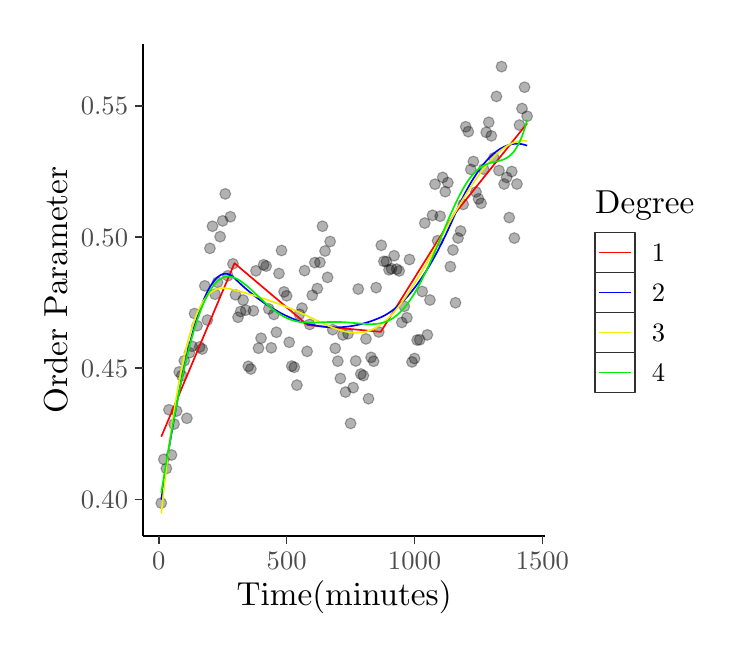
\begin{tikzpicture}[x=1pt,y=1pt]
\definecolor{fillColor}{RGB}{255,255,255}
\path[use as bounding box,fill=fillColor,fill opacity=0.00] (0,0) rectangle (252.94,216.81);
\begin{scope}
\path[clip] (  0.00,  0.00) rectangle (252.94,216.81);
\definecolor{drawColor}{RGB}{255,255,255}
\definecolor{fillColor}{RGB}{255,255,255}

\path[draw=drawColor,line width= 0.6pt,line join=round,line cap=round,fill=fillColor] (  0.00,  0.00) rectangle (252.94,216.81);
\end{scope}
\begin{scope}
\path[clip] ( 41.67, 33.16) rectangle (187.09,210.81);
\definecolor{fillColor}{RGB}{255,255,255}

\path[fill=fillColor] ( 41.67, 33.16) rectangle (187.09,210.81);
\definecolor{drawColor}{RGB}{0,0,0}
\definecolor{fillColor}{RGB}{0,0,0}

\path[draw=drawColor,draw opacity=0.30,line width= 0.4pt,line join=round,line cap=round,fill=fillColor,fill opacity=0.30] ( 48.28, 45.02) circle (  1.96);

\path[draw=drawColor,draw opacity=0.30,line width= 0.4pt,line join=round,line cap=round,fill=fillColor,fill opacity=0.30] ( 49.21, 60.83) circle (  1.96);

\path[draw=drawColor,draw opacity=0.30,line width= 0.4pt,line join=round,line cap=round,fill=fillColor,fill opacity=0.30] ( 50.13, 57.52) circle (  1.96);

\path[draw=drawColor,draw opacity=0.30,line width= 0.4pt,line join=round,line cap=round,fill=fillColor,fill opacity=0.30] ( 51.05, 78.74) circle (  1.96);

\path[draw=drawColor,draw opacity=0.30,line width= 0.4pt,line join=round,line cap=round,fill=fillColor,fill opacity=0.30] ( 51.98, 62.40) circle (  1.96);

\path[draw=drawColor,draw opacity=0.30,line width= 0.4pt,line join=round,line cap=round,fill=fillColor,fill opacity=0.30] ( 52.90, 73.56) circle (  1.96);

\path[draw=drawColor,draw opacity=0.30,line width= 0.4pt,line join=round,line cap=round,fill=fillColor,fill opacity=0.30] ( 53.83, 78.29) circle (  1.96);

\path[draw=drawColor,draw opacity=0.30,line width= 0.4pt,line join=round,line cap=round,fill=fillColor,fill opacity=0.30] ( 54.75, 92.43) circle (  1.96);

\path[draw=drawColor,draw opacity=0.30,line width= 0.4pt,line join=round,line cap=round,fill=fillColor,fill opacity=0.30] ( 55.68, 91.06) circle (  1.96);

\path[draw=drawColor,draw opacity=0.30,line width= 0.4pt,line join=round,line cap=round,fill=fillColor,fill opacity=0.30] ( 56.60, 96.44) circle (  1.96);

\path[draw=drawColor,draw opacity=0.30,line width= 0.4pt,line join=round,line cap=round,fill=fillColor,fill opacity=0.30] ( 57.53, 75.66) circle (  1.96);

\path[draw=drawColor,draw opacity=0.30,line width= 0.4pt,line join=round,line cap=round,fill=fillColor,fill opacity=0.30] ( 58.45, 99.34) circle (  1.96);

\path[draw=drawColor,draw opacity=0.30,line width= 0.4pt,line join=round,line cap=round,fill=fillColor,fill opacity=0.30] ( 59.37,101.68) circle (  1.96);

\path[draw=drawColor,draw opacity=0.30,line width= 0.4pt,line join=round,line cap=round,fill=fillColor,fill opacity=0.30] ( 60.30,113.50) circle (  1.96);

\path[draw=drawColor,draw opacity=0.30,line width= 0.4pt,line join=round,line cap=round,fill=fillColor,fill opacity=0.30] ( 61.22,109.11) circle (  1.96);

\path[draw=drawColor,draw opacity=0.30,line width= 0.4pt,line join=round,line cap=round,fill=fillColor,fill opacity=0.30] ( 62.15,101.43) circle (  1.96);

\path[draw=drawColor,draw opacity=0.30,line width= 0.4pt,line join=round,line cap=round,fill=fillColor,fill opacity=0.30] ( 63.07,100.67) circle (  1.96);

\path[draw=drawColor,draw opacity=0.30,line width= 0.4pt,line join=round,line cap=round,fill=fillColor,fill opacity=0.30] ( 64.00,123.52) circle (  1.96);

\path[draw=drawColor,draw opacity=0.30,line width= 0.4pt,line join=round,line cap=round,fill=fillColor,fill opacity=0.30] ( 64.92,111.16) circle (  1.96);

\path[draw=drawColor,draw opacity=0.30,line width= 0.4pt,line join=round,line cap=round,fill=fillColor,fill opacity=0.30] ( 65.85,137.07) circle (  1.96);

\path[draw=drawColor,draw opacity=0.30,line width= 0.4pt,line join=round,line cap=round,fill=fillColor,fill opacity=0.30] ( 66.77,145.07) circle (  1.96);

\path[draw=drawColor,draw opacity=0.30,line width= 0.4pt,line join=round,line cap=round,fill=fillColor,fill opacity=0.30] ( 67.69,120.50) circle (  1.96);

\path[draw=drawColor,draw opacity=0.30,line width= 0.4pt,line join=round,line cap=round,fill=fillColor,fill opacity=0.30] ( 68.62,124.80) circle (  1.96);

\path[draw=drawColor,draw opacity=0.30,line width= 0.4pt,line join=round,line cap=round,fill=fillColor,fill opacity=0.30] ( 69.54,141.30) circle (  1.96);

\path[draw=drawColor,draw opacity=0.30,line width= 0.4pt,line join=round,line cap=round,fill=fillColor,fill opacity=0.30] ( 70.47,146.99) circle (  1.96);

\path[draw=drawColor,draw opacity=0.30,line width= 0.4pt,line join=round,line cap=round,fill=fillColor,fill opacity=0.30] ( 71.39,156.75) circle (  1.96);

\path[draw=drawColor,draw opacity=0.30,line width= 0.4pt,line join=round,line cap=round,fill=fillColor,fill opacity=0.30] ( 72.32,127.14) circle (  1.96);

\path[draw=drawColor,draw opacity=0.30,line width= 0.4pt,line join=round,line cap=round,fill=fillColor,fill opacity=0.30] ( 73.24,148.48) circle (  1.96);

\path[draw=drawColor,draw opacity=0.30,line width= 0.4pt,line join=round,line cap=round,fill=fillColor,fill opacity=0.30] ( 74.17,131.47) circle (  1.96);

\path[draw=drawColor,draw opacity=0.30,line width= 0.4pt,line join=round,line cap=round,fill=fillColor,fill opacity=0.30] ( 75.09,120.30) circle (  1.96);

\path[draw=drawColor,draw opacity=0.30,line width= 0.4pt,line join=round,line cap=round,fill=fillColor,fill opacity=0.30] ( 76.01,112.16) circle (  1.96);

\path[draw=drawColor,draw opacity=0.30,line width= 0.4pt,line join=round,line cap=round,fill=fillColor,fill opacity=0.30] ( 76.94,114.23) circle (  1.96);

\path[draw=drawColor,draw opacity=0.30,line width= 0.4pt,line join=round,line cap=round,fill=fillColor,fill opacity=0.30] ( 77.86,118.39) circle (  1.96);

\path[draw=drawColor,draw opacity=0.30,line width= 0.4pt,line join=round,line cap=round,fill=fillColor,fill opacity=0.30] ( 78.79,114.74) circle (  1.96);

\path[draw=drawColor,draw opacity=0.30,line width= 0.4pt,line join=round,line cap=round,fill=fillColor,fill opacity=0.30] ( 79.71, 94.45) circle (  1.96);

\path[draw=drawColor,draw opacity=0.30,line width= 0.4pt,line join=round,line cap=round,fill=fillColor,fill opacity=0.30] ( 80.64, 93.48) circle (  1.96);

\path[draw=drawColor,draw opacity=0.30,line width= 0.4pt,line join=round,line cap=round,fill=fillColor,fill opacity=0.30] ( 81.56,114.49) circle (  1.96);

\path[draw=drawColor,draw opacity=0.30,line width= 0.4pt,line join=round,line cap=round,fill=fillColor,fill opacity=0.30] ( 82.49,128.94) circle (  1.96);

\path[draw=drawColor,draw opacity=0.30,line width= 0.4pt,line join=round,line cap=round,fill=fillColor,fill opacity=0.30] ( 83.41,100.98) circle (  1.96);

\path[draw=drawColor,draw opacity=0.30,line width= 0.4pt,line join=round,line cap=round,fill=fillColor,fill opacity=0.30] ( 84.33,104.60) circle (  1.96);

\path[draw=drawColor,draw opacity=0.30,line width= 0.4pt,line join=round,line cap=round,fill=fillColor,fill opacity=0.30] ( 85.26,131.14) circle (  1.96);

\path[draw=drawColor,draw opacity=0.30,line width= 0.4pt,line join=round,line cap=round,fill=fillColor,fill opacity=0.30] ( 86.18,130.65) circle (  1.96);

\path[draw=drawColor,draw opacity=0.30,line width= 0.4pt,line join=round,line cap=round,fill=fillColor,fill opacity=0.30] ( 87.11,115.19) circle (  1.96);

\path[draw=drawColor,draw opacity=0.30,line width= 0.4pt,line join=round,line cap=round,fill=fillColor,fill opacity=0.30] ( 88.03,101.12) circle (  1.96);

\path[draw=drawColor,draw opacity=0.30,line width= 0.4pt,line join=round,line cap=round,fill=fillColor,fill opacity=0.30] ( 88.96,113.19) circle (  1.96);

\path[draw=drawColor,draw opacity=0.30,line width= 0.4pt,line join=round,line cap=round,fill=fillColor,fill opacity=0.30] ( 89.88,106.75) circle (  1.96);

\path[draw=drawColor,draw opacity=0.30,line width= 0.4pt,line join=round,line cap=round,fill=fillColor,fill opacity=0.30] ( 90.81,127.97) circle (  1.96);

\path[draw=drawColor,draw opacity=0.30,line width= 0.4pt,line join=round,line cap=round,fill=fillColor,fill opacity=0.30] ( 91.73,136.29) circle (  1.96);

\path[draw=drawColor,draw opacity=0.30,line width= 0.4pt,line join=round,line cap=round,fill=fillColor,fill opacity=0.30] ( 92.65,121.34) circle (  1.96);

\path[draw=drawColor,draw opacity=0.30,line width= 0.4pt,line join=round,line cap=round,fill=fillColor,fill opacity=0.30] ( 93.58,119.91) circle (  1.96);

\path[draw=drawColor,draw opacity=0.30,line width= 0.4pt,line join=round,line cap=round,fill=fillColor,fill opacity=0.30] ( 94.50,103.13) circle (  1.96);

\path[draw=drawColor,draw opacity=0.30,line width= 0.4pt,line join=round,line cap=round,fill=fillColor,fill opacity=0.30] ( 95.43, 94.53) circle (  1.96);

\path[draw=drawColor,draw opacity=0.30,line width= 0.4pt,line join=round,line cap=round,fill=fillColor,fill opacity=0.30] ( 96.35, 94.10) circle (  1.96);

\path[draw=drawColor,draw opacity=0.30,line width= 0.4pt,line join=round,line cap=round,fill=fillColor,fill opacity=0.30] ( 97.28, 87.65) circle (  1.96);

\path[draw=drawColor,draw opacity=0.30,line width= 0.4pt,line join=round,line cap=round,fill=fillColor,fill opacity=0.30] ( 98.20,113.24) circle (  1.96);

\path[draw=drawColor,draw opacity=0.30,line width= 0.4pt,line join=round,line cap=round,fill=fillColor,fill opacity=0.30] ( 99.13,115.47) circle (  1.96);

\path[draw=drawColor,draw opacity=0.30,line width= 0.4pt,line join=round,line cap=round,fill=fillColor,fill opacity=0.30] (100.05,129.01) circle (  1.96);

\path[draw=drawColor,draw opacity=0.30,line width= 0.4pt,line join=round,line cap=round,fill=fillColor,fill opacity=0.30] (100.97, 99.85) circle (  1.96);

\path[draw=drawColor,draw opacity=0.30,line width= 0.4pt,line join=round,line cap=round,fill=fillColor,fill opacity=0.30] (101.90,109.57) circle (  1.96);

\path[draw=drawColor,draw opacity=0.30,line width= 0.4pt,line join=round,line cap=round,fill=fillColor,fill opacity=0.30] (102.82,120.11) circle (  1.96);

\path[draw=drawColor,draw opacity=0.30,line width= 0.4pt,line join=round,line cap=round,fill=fillColor,fill opacity=0.30] (103.75,131.91) circle (  1.96);

\path[draw=drawColor,draw opacity=0.30,line width= 0.4pt,line join=round,line cap=round,fill=fillColor,fill opacity=0.30] (104.67,122.54) circle (  1.96);

\path[draw=drawColor,draw opacity=0.30,line width= 0.4pt,line join=round,line cap=round,fill=fillColor,fill opacity=0.30] (105.60,132.01) circle (  1.96);

\path[draw=drawColor,draw opacity=0.30,line width= 0.4pt,line join=round,line cap=round,fill=fillColor,fill opacity=0.30] (106.52,145.06) circle (  1.96);

\path[draw=drawColor,draw opacity=0.30,line width= 0.4pt,line join=round,line cap=round,fill=fillColor,fill opacity=0.30] (107.45,136.11) circle (  1.96);

\path[draw=drawColor,draw opacity=0.30,line width= 0.4pt,line join=round,line cap=round,fill=fillColor,fill opacity=0.30] (108.37,126.58) circle (  1.96);

\path[draw=drawColor,draw opacity=0.30,line width= 0.4pt,line join=round,line cap=round,fill=fillColor,fill opacity=0.30] (109.29,139.54) circle (  1.96);

\path[draw=drawColor,draw opacity=0.30,line width= 0.4pt,line join=round,line cap=round,fill=fillColor,fill opacity=0.30] (110.22,107.68) circle (  1.96);

\path[draw=drawColor,draw opacity=0.30,line width= 0.4pt,line join=round,line cap=round,fill=fillColor,fill opacity=0.30] (111.14,100.94) circle (  1.96);

\path[draw=drawColor,draw opacity=0.30,line width= 0.4pt,line join=round,line cap=round,fill=fillColor,fill opacity=0.30] (112.07, 96.30) circle (  1.96);

\path[draw=drawColor,draw opacity=0.30,line width= 0.4pt,line join=round,line cap=round,fill=fillColor,fill opacity=0.30] (112.99, 90.05) circle (  1.96);

\path[draw=drawColor,draw opacity=0.30,line width= 0.4pt,line join=round,line cap=round,fill=fillColor,fill opacity=0.30] (113.92,105.78) circle (  1.96);

\path[draw=drawColor,draw opacity=0.30,line width= 0.4pt,line join=round,line cap=round,fill=fillColor,fill opacity=0.30] (114.84, 85.13) circle (  1.96);

\path[draw=drawColor,draw opacity=0.30,line width= 0.4pt,line join=round,line cap=round,fill=fillColor,fill opacity=0.30] (115.77,106.22) circle (  1.96);

\path[draw=drawColor,draw opacity=0.30,line width= 0.4pt,line join=round,line cap=round,fill=fillColor,fill opacity=0.30] (116.69, 73.81) circle (  1.96);

\path[draw=drawColor,draw opacity=0.30,line width= 0.4pt,line join=round,line cap=round,fill=fillColor,fill opacity=0.30] (117.61, 86.73) circle (  1.96);

\path[draw=drawColor,draw opacity=0.30,line width= 0.4pt,line join=round,line cap=round,fill=fillColor,fill opacity=0.30] (118.54, 96.38) circle (  1.96);

\path[draw=drawColor,draw opacity=0.30,line width= 0.4pt,line join=round,line cap=round,fill=fillColor,fill opacity=0.30] (119.46,122.36) circle (  1.96);

\path[draw=drawColor,draw opacity=0.30,line width= 0.4pt,line join=round,line cap=round,fill=fillColor,fill opacity=0.30] (120.39, 91.67) circle (  1.96);

\path[draw=drawColor,draw opacity=0.30,line width= 0.4pt,line join=round,line cap=round,fill=fillColor,fill opacity=0.30] (121.31, 91.09) circle (  1.96);

\path[draw=drawColor,draw opacity=0.30,line width= 0.4pt,line join=round,line cap=round,fill=fillColor,fill opacity=0.30] (122.24,104.35) circle (  1.96);

\path[draw=drawColor,draw opacity=0.30,line width= 0.4pt,line join=round,line cap=round,fill=fillColor,fill opacity=0.30] (123.16, 82.74) circle (  1.96);

\path[draw=drawColor,draw opacity=0.30,line width= 0.4pt,line join=round,line cap=round,fill=fillColor,fill opacity=0.30] (124.09, 97.67) circle (  1.96);

\path[draw=drawColor,draw opacity=0.30,line width= 0.4pt,line join=round,line cap=round,fill=fillColor,fill opacity=0.30] (125.01, 96.27) circle (  1.96);

\path[draw=drawColor,draw opacity=0.30,line width= 0.4pt,line join=round,line cap=round,fill=fillColor,fill opacity=0.30] (125.93,122.87) circle (  1.96);

\path[draw=drawColor,draw opacity=0.30,line width= 0.4pt,line join=round,line cap=round,fill=fillColor,fill opacity=0.30] (126.86,106.84) circle (  1.96);

\path[draw=drawColor,draw opacity=0.30,line width= 0.4pt,line join=round,line cap=round,fill=fillColor,fill opacity=0.30] (127.78,138.16) circle (  1.96);

\path[draw=drawColor,draw opacity=0.30,line width= 0.4pt,line join=round,line cap=round,fill=fillColor,fill opacity=0.30] (128.71,132.36) circle (  1.96);

\path[draw=drawColor,draw opacity=0.30,line width= 0.4pt,line join=round,line cap=round,fill=fillColor,fill opacity=0.30] (129.63,132.29) circle (  1.96);

\path[draw=drawColor,draw opacity=0.30,line width= 0.4pt,line join=round,line cap=round,fill=fillColor,fill opacity=0.30] (130.56,129.32) circle (  1.96);

\path[draw=drawColor,draw opacity=0.30,line width= 0.4pt,line join=round,line cap=round,fill=fillColor,fill opacity=0.30] (131.48,129.71) circle (  1.96);

\path[draw=drawColor,draw opacity=0.30,line width= 0.4pt,line join=round,line cap=round,fill=fillColor,fill opacity=0.30] (132.41,134.40) circle (  1.96);

\path[draw=drawColor,draw opacity=0.30,line width= 0.4pt,line join=round,line cap=round,fill=fillColor,fill opacity=0.30] (133.33,129.56) circle (  1.96);

\path[draw=drawColor,draw opacity=0.30,line width= 0.4pt,line join=round,line cap=round,fill=fillColor,fill opacity=0.30] (134.25,128.91) circle (  1.96);

\path[draw=drawColor,draw opacity=0.30,line width= 0.4pt,line join=round,line cap=round,fill=fillColor,fill opacity=0.30] (135.18,110.30) circle (  1.96);

\path[draw=drawColor,draw opacity=0.30,line width= 0.4pt,line join=round,line cap=round,fill=fillColor,fill opacity=0.30] (136.10,116.12) circle (  1.96);

\path[draw=drawColor,draw opacity=0.30,line width= 0.4pt,line join=round,line cap=round,fill=fillColor,fill opacity=0.30] (137.03,112.00) circle (  1.96);

\path[draw=drawColor,draw opacity=0.30,line width= 0.4pt,line join=round,line cap=round,fill=fillColor,fill opacity=0.30] (137.95,133.03) circle (  1.96);

\path[draw=drawColor,draw opacity=0.30,line width= 0.4pt,line join=round,line cap=round,fill=fillColor,fill opacity=0.30] (138.88, 96.03) circle (  1.96);

\path[draw=drawColor,draw opacity=0.30,line width= 0.4pt,line join=round,line cap=round,fill=fillColor,fill opacity=0.30] (139.80, 97.26) circle (  1.96);

\path[draw=drawColor,draw opacity=0.30,line width= 0.4pt,line join=round,line cap=round,fill=fillColor,fill opacity=0.30] (140.73,103.93) circle (  1.96);

\path[draw=drawColor,draw opacity=0.30,line width= 0.4pt,line join=round,line cap=round,fill=fillColor,fill opacity=0.30] (141.65,104.02) circle (  1.96);

\path[draw=drawColor,draw opacity=0.30,line width= 0.4pt,line join=round,line cap=round,fill=fillColor,fill opacity=0.30] (142.57,121.48) circle (  1.96);

\path[draw=drawColor,draw opacity=0.30,line width= 0.4pt,line join=round,line cap=round,fill=fillColor,fill opacity=0.30] (143.50,146.20) circle (  1.96);

\path[draw=drawColor,draw opacity=0.30,line width= 0.4pt,line join=round,line cap=round,fill=fillColor,fill opacity=0.30] (144.42,105.80) circle (  1.96);

\path[draw=drawColor,draw opacity=0.30,line width= 0.4pt,line join=round,line cap=round,fill=fillColor,fill opacity=0.30] (145.35,118.40) circle (  1.96);

\path[draw=drawColor,draw opacity=0.30,line width= 0.4pt,line join=round,line cap=round,fill=fillColor,fill opacity=0.30] (146.27,149.00) circle (  1.96);

\path[draw=drawColor,draw opacity=0.30,line width= 0.4pt,line join=round,line cap=round,fill=fillColor,fill opacity=0.30] (147.20,160.24) circle (  1.96);

\path[draw=drawColor,draw opacity=0.30,line width= 0.4pt,line join=round,line cap=round,fill=fillColor,fill opacity=0.30] (148.12,139.83) circle (  1.96);

\path[draw=drawColor,draw opacity=0.30,line width= 0.4pt,line join=round,line cap=round,fill=fillColor,fill opacity=0.30] (149.05,148.68) circle (  1.96);

\path[draw=drawColor,draw opacity=0.30,line width= 0.4pt,line join=round,line cap=round,fill=fillColor,fill opacity=0.30] (149.97,162.71) circle (  1.96);

\path[draw=drawColor,draw opacity=0.30,line width= 0.4pt,line join=round,line cap=round,fill=fillColor,fill opacity=0.30] (150.89,157.55) circle (  1.96);

\path[draw=drawColor,draw opacity=0.30,line width= 0.4pt,line join=round,line cap=round,fill=fillColor,fill opacity=0.30] (151.82,160.79) circle (  1.96);

\path[draw=drawColor,draw opacity=0.30,line width= 0.4pt,line join=round,line cap=round,fill=fillColor,fill opacity=0.30] (152.74,130.46) circle (  1.96);

\path[draw=drawColor,draw opacity=0.30,line width= 0.4pt,line join=round,line cap=round,fill=fillColor,fill opacity=0.30] (153.67,136.48) circle (  1.96);

\path[draw=drawColor,draw opacity=0.30,line width= 0.4pt,line join=round,line cap=round,fill=fillColor,fill opacity=0.30] (154.59,117.41) circle (  1.96);

\path[draw=drawColor,draw opacity=0.30,line width= 0.4pt,line join=round,line cap=round,fill=fillColor,fill opacity=0.30] (155.52,140.79) circle (  1.96);

\path[draw=drawColor,draw opacity=0.30,line width= 0.4pt,line join=round,line cap=round,fill=fillColor,fill opacity=0.30] (156.44,143.32) circle (  1.96);

\path[draw=drawColor,draw opacity=0.30,line width= 0.4pt,line join=round,line cap=round,fill=fillColor,fill opacity=0.30] (157.37,152.95) circle (  1.96);

\path[draw=drawColor,draw opacity=0.30,line width= 0.4pt,line join=round,line cap=round,fill=fillColor,fill opacity=0.30] (158.29,181.01) circle (  1.96);

\path[draw=drawColor,draw opacity=0.30,line width= 0.4pt,line join=round,line cap=round,fill=fillColor,fill opacity=0.30] (159.22,179.23) circle (  1.96);

\path[draw=drawColor,draw opacity=0.30,line width= 0.4pt,line join=round,line cap=round,fill=fillColor,fill opacity=0.30] (160.14,165.59) circle (  1.96);

\path[draw=drawColor,draw opacity=0.30,line width= 0.4pt,line join=round,line cap=round,fill=fillColor,fill opacity=0.30] (161.06,168.44) circle (  1.96);

\path[draw=drawColor,draw opacity=0.30,line width= 0.4pt,line join=round,line cap=round,fill=fillColor,fill opacity=0.30] (161.99,157.43) circle (  1.96);

\path[draw=drawColor,draw opacity=0.30,line width= 0.4pt,line join=round,line cap=round,fill=fillColor,fill opacity=0.30] (162.91,154.94) circle (  1.96);

\path[draw=drawColor,draw opacity=0.30,line width= 0.4pt,line join=round,line cap=round,fill=fillColor,fill opacity=0.30] (163.84,153.35) circle (  1.96);

\path[draw=drawColor,draw opacity=0.30,line width= 0.4pt,line join=round,line cap=round,fill=fillColor,fill opacity=0.30] (164.76,165.70) circle (  1.96);

\path[draw=drawColor,draw opacity=0.30,line width= 0.4pt,line join=round,line cap=round,fill=fillColor,fill opacity=0.30] (165.69,179.00) circle (  1.96);

\path[draw=drawColor,draw opacity=0.30,line width= 0.4pt,line join=round,line cap=round,fill=fillColor,fill opacity=0.30] (166.61,182.62) circle (  1.96);

\path[draw=drawColor,draw opacity=0.30,line width= 0.4pt,line join=round,line cap=round,fill=fillColor,fill opacity=0.30] (167.54,177.71) circle (  1.96);

\path[draw=drawColor,draw opacity=0.30,line width= 0.4pt,line join=round,line cap=round,fill=fillColor,fill opacity=0.30] (168.46,169.75) circle (  1.96);

\path[draw=drawColor,draw opacity=0.30,line width= 0.4pt,line join=round,line cap=round,fill=fillColor,fill opacity=0.30] (169.38,191.97) circle (  1.96);

\path[draw=drawColor,draw opacity=0.30,line width= 0.4pt,line join=round,line cap=round,fill=fillColor,fill opacity=0.30] (170.31,165.19) circle (  1.96);

\path[draw=drawColor,draw opacity=0.30,line width= 0.4pt,line join=round,line cap=round,fill=fillColor,fill opacity=0.30] (171.23,202.74) circle (  1.96);

\path[draw=drawColor,draw opacity=0.30,line width= 0.4pt,line join=round,line cap=round,fill=fillColor,fill opacity=0.30] (172.16,160.32) circle (  1.96);

\path[draw=drawColor,draw opacity=0.30,line width= 0.4pt,line join=round,line cap=round,fill=fillColor,fill opacity=0.30] (173.08,162.70) circle (  1.96);

\path[draw=drawColor,draw opacity=0.30,line width= 0.4pt,line join=round,line cap=round,fill=fillColor,fill opacity=0.30] (174.01,148.19) circle (  1.96);

\path[draw=drawColor,draw opacity=0.30,line width= 0.4pt,line join=round,line cap=round,fill=fillColor,fill opacity=0.30] (174.93,164.84) circle (  1.96);

\path[draw=drawColor,draw opacity=0.30,line width= 0.4pt,line join=round,line cap=round,fill=fillColor,fill opacity=0.30] (175.86,140.77) circle (  1.96);

\path[draw=drawColor,draw opacity=0.30,line width= 0.4pt,line join=round,line cap=round,fill=fillColor,fill opacity=0.30] (176.78,160.31) circle (  1.96);

\path[draw=drawColor,draw opacity=0.30,line width= 0.4pt,line join=round,line cap=round,fill=fillColor,fill opacity=0.30] (177.70,181.61) circle (  1.96);

\path[draw=drawColor,draw opacity=0.30,line width= 0.4pt,line join=round,line cap=round,fill=fillColor,fill opacity=0.30] (178.63,187.58) circle (  1.96);

\path[draw=drawColor,draw opacity=0.30,line width= 0.4pt,line join=round,line cap=round,fill=fillColor,fill opacity=0.30] (179.55,195.30) circle (  1.96);

\path[draw=drawColor,draw opacity=0.30,line width= 0.4pt,line join=round,line cap=round,fill=fillColor,fill opacity=0.30] (180.48,184.82) circle (  1.96);
\definecolor{drawColor}{RGB}{255,0,0}

\path[draw=drawColor,line width= 0.6pt,line join=round] ( 48.28, 69.01) --
	( 48.37, 69.23) --
	( 48.47, 69.45) --
	( 48.56, 69.67) --
	( 48.65, 69.89) --
	( 48.74, 70.11) --
	( 48.84, 70.33) --
	( 48.93, 70.55) --
	( 49.02, 70.76) --
	( 49.11, 70.98) --
	( 49.21, 71.20) --
	( 49.30, 71.42) --
	( 49.39, 71.64) --
	( 49.48, 71.86) --
	( 49.58, 72.08) --
	( 49.67, 72.30) --
	( 49.76, 72.52) --
	( 49.85, 72.74) --
	( 49.95, 72.96) --
	( 50.04, 73.18) --
	( 50.13, 73.39) --
	( 50.22, 73.61) --
	( 50.31, 73.83) --
	( 50.41, 74.05) --
	( 50.50, 74.27) --
	( 50.59, 74.49) --
	( 50.68, 74.71) --
	( 50.78, 74.93) --
	( 50.87, 75.15) --
	( 50.96, 75.37) --
	( 51.05, 75.59) --
	( 51.15, 75.81) --
	( 51.24, 76.03) --
	( 51.33, 76.24) --
	( 51.42, 76.46) --
	( 51.52, 76.68) --
	( 51.61, 76.90) --
	( 51.70, 77.12) --
	( 51.79, 77.34) --
	( 51.89, 77.56) --
	( 51.98, 77.78) --
	( 52.07, 78.00) --
	( 52.16, 78.22) --
	( 52.26, 78.44) --
	( 52.35, 78.66) --
	( 52.44, 78.88) --
	( 52.53, 79.09) --
	( 52.63, 79.31) --
	( 52.72, 79.53) --
	( 52.81, 79.75) --
	( 52.90, 79.97) --
	( 53.00, 80.19) --
	( 53.09, 80.41) --
	( 53.18, 80.63) --
	( 53.27, 80.85) --
	( 53.37, 81.07) --
	( 53.46, 81.29) --
	( 53.55, 81.51) --
	( 53.64, 81.72) --
	( 53.74, 81.94) --
	( 53.83, 82.16) --
	( 53.92, 82.38) --
	( 54.01, 82.60) --
	( 54.11, 82.82) --
	( 54.20, 83.04) --
	( 54.29, 83.26) --
	( 54.38, 83.48) --
	( 54.47, 83.70) --
	( 54.57, 83.92) --
	( 54.66, 84.14) --
	( 54.75, 84.36) --
	( 54.84, 84.57) --
	( 54.94, 84.79) --
	( 55.03, 85.01) --
	( 55.12, 85.23) --
	( 55.21, 85.45) --
	( 55.31, 85.67) --
	( 55.40, 85.89) --
	( 55.49, 86.11) --
	( 55.58, 86.33) --
	( 55.68, 86.55) --
	( 55.77, 86.77) --
	( 55.86, 86.99) --
	( 55.95, 87.21) --
	( 56.05, 87.42) --
	( 56.14, 87.64) --
	( 56.23, 87.86) --
	( 56.32, 88.08) --
	( 56.42, 88.30) --
	( 56.51, 88.52) --
	( 56.60, 88.74) --
	( 56.69, 88.96) --
	( 56.79, 89.18) --
	( 56.88, 89.40) --
	( 56.97, 89.62) --
	( 57.06, 89.84) --
	( 57.16, 90.05) --
	( 57.25, 90.27) --
	( 57.34, 90.49) --
	( 57.43, 90.71) --
	( 57.53, 90.93) --
	( 57.62, 91.15) --
	( 57.71, 91.37) --
	( 57.80, 91.59) --
	( 57.90, 91.81) --
	( 57.99, 92.03) --
	( 58.08, 92.25) --
	( 58.17, 92.47) --
	( 58.27, 92.69) --
	( 58.36, 92.90) --
	( 58.45, 93.12) --
	( 58.54, 93.34) --
	( 58.63, 93.56) --
	( 58.73, 93.78) --
	( 58.82, 94.00) --
	( 58.91, 94.22) --
	( 59.00, 94.44) --
	( 59.10, 94.66) --
	( 59.19, 94.88) --
	( 59.28, 95.10) --
	( 59.37, 95.32) --
	( 59.47, 95.53) --
	( 59.56, 95.75) --
	( 59.65, 95.97) --
	( 59.74, 96.19) --
	( 59.84, 96.41) --
	( 59.93, 96.63) --
	( 60.02, 96.85) --
	( 60.11, 97.07) --
	( 60.21, 97.29) --
	( 60.30, 97.51) --
	( 60.39, 97.73) --
	( 60.48, 97.95) --
	( 60.58, 98.17) --
	( 60.67, 98.38) --
	( 60.76, 98.60) --
	( 60.85, 98.82) --
	( 60.95, 99.04) --
	( 61.04, 99.26) --
	( 61.13, 99.48) --
	( 61.22, 99.70) --
	( 61.32, 99.92) --
	( 61.41,100.14) --
	( 61.50,100.36) --
	( 61.59,100.58) --
	( 61.69,100.80) --
	( 61.78,101.02) --
	( 61.87,101.23) --
	( 61.96,101.45) --
	( 62.06,101.67) --
	( 62.15,101.89) --
	( 62.24,102.11) --
	( 62.33,102.33) --
	( 62.43,102.55) --
	( 62.52,102.77) --
	( 62.61,102.99) --
	( 62.70,103.21) --
	( 62.79,103.43) --
	( 62.89,103.65) --
	( 62.98,103.86) --
	( 63.07,104.08) --
	( 63.16,104.30) --
	( 63.26,104.52) --
	( 63.35,104.74) --
	( 63.44,104.96) --
	( 63.53,105.18) --
	( 63.63,105.40) --
	( 63.72,105.62) --
	( 63.81,105.84) --
	( 63.90,106.06) --
	( 64.00,106.28) --
	( 64.09,106.50) --
	( 64.18,106.71) --
	( 64.27,106.93) --
	( 64.37,107.15) --
	( 64.46,107.37) --
	( 64.55,107.59) --
	( 64.64,107.81) --
	( 64.74,108.03) --
	( 64.83,108.25) --
	( 64.92,108.47) --
	( 65.01,108.69) --
	( 65.11,108.91) --
	( 65.20,109.13) --
	( 65.29,109.35) --
	( 65.38,109.56) --
	( 65.48,109.78) --
	( 65.57,110.00) --
	( 65.66,110.22) --
	( 65.75,110.44) --
	( 65.85,110.66) --
	( 65.94,110.88) --
	( 66.03,111.10) --
	( 66.12,111.32) --
	( 66.22,111.54) --
	( 66.31,111.76) --
	( 66.40,111.98) --
	( 66.49,112.19) --
	( 66.59,112.41) --
	( 66.68,112.63) --
	( 66.77,112.85) --
	( 66.86,113.07) --
	( 66.95,113.29) --
	( 67.05,113.51) --
	( 67.14,113.73) --
	( 67.23,113.95) --
	( 67.32,114.17) --
	( 67.42,114.39) --
	( 67.51,114.61) --
	( 67.60,114.83) --
	( 67.69,115.04) --
	( 67.79,115.26) --
	( 67.88,115.48) --
	( 67.97,115.70) --
	( 68.06,115.92) --
	( 68.16,116.14) --
	( 68.25,116.36) --
	( 68.34,116.58) --
	( 68.43,116.80) --
	( 68.53,117.02) --
	( 68.62,117.24) --
	( 68.71,117.46) --
	( 68.80,117.68) --
	( 68.90,117.89) --
	( 68.99,118.11) --
	( 69.08,118.33) --
	( 69.17,118.55) --
	( 69.27,118.77) --
	( 69.36,118.99) --
	( 69.45,119.21) --
	( 69.54,119.43) --
	( 69.64,119.65) --
	( 69.73,119.87) --
	( 69.82,120.09) --
	( 69.91,120.31) --
	( 70.01,120.52) --
	( 70.10,120.74) --
	( 70.19,120.96) --
	( 70.28,121.18) --
	( 70.38,121.40) --
	( 70.47,121.62) --
	( 70.56,121.84) --
	( 70.65,122.06) --
	( 70.75,122.28) --
	( 70.84,122.50) --
	( 70.93,122.72) --
	( 71.02,122.94) --
	( 71.11,123.16) --
	( 71.21,123.37) --
	( 71.30,123.59) --
	( 71.39,123.81) --
	( 71.48,124.03) --
	( 71.58,124.25) --
	( 71.67,124.47) --
	( 71.76,124.69) --
	( 71.85,124.91) --
	( 71.95,125.13) --
	( 72.04,125.35) --
	( 72.13,125.57) --
	( 72.22,125.79) --
	( 72.32,126.00) --
	( 72.41,126.22) --
	( 72.50,126.44) --
	( 72.59,126.66) --
	( 72.69,126.88) --
	( 72.78,127.10) --
	( 72.87,127.32) --
	( 72.96,127.54) --
	( 73.06,127.76) --
	( 73.15,127.98) --
	( 73.24,128.20) --
	( 73.33,128.42) --
	( 73.43,128.64) --
	( 73.52,128.85) --
	( 73.61,129.07) --
	( 73.70,129.29) --
	( 73.80,129.51) --
	( 73.89,129.73) --
	( 73.98,129.95) --
	( 74.07,130.17) --
	( 74.17,130.39) --
	( 74.26,130.61) --
	( 74.35,130.83) --
	( 74.44,131.05) --
	( 74.54,131.27) --
	( 74.63,131.49) --
	( 74.72,131.70) --
	( 74.81,131.63) --
	( 74.91,131.55) --
	( 75.00,131.47) --
	( 75.09,131.39) --
	( 75.18,131.31) --
	( 75.27,131.24) --
	( 75.37,131.16) --
	( 75.46,131.08) --
	( 75.55,131.00) --
	( 75.64,130.92) --
	( 75.74,130.84) --
	( 75.83,130.77) --
	( 75.92,130.69) --
	( 76.01,130.61) --
	( 76.11,130.53) --
	( 76.20,130.45) --
	( 76.29,130.38) --
	( 76.38,130.30) --
	( 76.48,130.22) --
	( 76.57,130.14) --
	( 76.66,130.06) --
	( 76.75,129.98) --
	( 76.85,129.91) --
	( 76.94,129.83) --
	( 77.03,129.75) --
	( 77.12,129.67) --
	( 77.22,129.59) --
	( 77.31,129.52) --
	( 77.40,129.44) --
	( 77.49,129.36) --
	( 77.59,129.28) --
	( 77.68,129.20) --
	( 77.77,129.12) --
	( 77.86,129.05) --
	( 77.96,128.97) --
	( 78.05,128.89) --
	( 78.14,128.81) --
	( 78.23,128.73) --
	( 78.33,128.66) --
	( 78.42,128.58) --
	( 78.51,128.50) --
	( 78.60,128.42) --
	( 78.70,128.34) --
	( 78.79,128.26) --
	( 78.88,128.19) --
	( 78.97,128.11) --
	( 79.07,128.03) --
	( 79.16,127.95) --
	( 79.25,127.87) --
	( 79.34,127.80) --
	( 79.43,127.72) --
	( 79.53,127.64) --
	( 79.62,127.56) --
	( 79.71,127.48) --
	( 79.80,127.40) --
	( 79.90,127.33) --
	( 79.99,127.25) --
	( 80.08,127.17) --
	( 80.17,127.09) --
	( 80.27,127.01) --
	( 80.36,126.94) --
	( 80.45,126.86) --
	( 80.54,126.78) --
	( 80.64,126.70) --
	( 80.73,126.62) --
	( 80.82,126.54) --
	( 80.91,126.47) --
	( 81.01,126.39) --
	( 81.10,126.31) --
	( 81.19,126.23) --
	( 81.28,126.15) --
	( 81.38,126.08) --
	( 81.47,126.00) --
	( 81.56,125.92) --
	( 81.65,125.84) --
	( 81.75,125.76) --
	( 81.84,125.68) --
	( 81.93,125.61) --
	( 82.02,125.53) --
	( 82.12,125.45) --
	( 82.21,125.37) --
	( 82.30,125.29) --
	( 82.39,125.22) --
	( 82.49,125.14) --
	( 82.58,125.06) --
	( 82.67,124.98) --
	( 82.76,124.90) --
	( 82.86,124.82) --
	( 82.95,124.75) --
	( 83.04,124.67) --
	( 83.13,124.59) --
	( 83.23,124.51) --
	( 83.32,124.43) --
	( 83.41,124.36) --
	( 83.50,124.28) --
	( 83.59,124.20) --
	( 83.69,124.12) --
	( 83.78,124.04) --
	( 83.87,123.96) --
	( 83.96,123.89) --
	( 84.06,123.81) --
	( 84.15,123.73) --
	( 84.24,123.65) --
	( 84.33,123.57) --
	( 84.43,123.50) --
	( 84.52,123.42) --
	( 84.61,123.34) --
	( 84.70,123.26) --
	( 84.80,123.18) --
	( 84.89,123.10) --
	( 84.98,123.03) --
	( 85.07,122.95) --
	( 85.17,122.87) --
	( 85.26,122.79) --
	( 85.35,122.71) --
	( 85.44,122.64) --
	( 85.54,122.56) --
	( 85.63,122.48) --
	( 85.72,122.40) --
	( 85.81,122.32) --
	( 85.91,122.24) --
	( 86.00,122.17) --
	( 86.09,122.09) --
	( 86.18,122.01) --
	( 86.28,121.93) --
	( 86.37,121.85) --
	( 86.46,121.78) --
	( 86.55,121.70) --
	( 86.65,121.62) --
	( 86.74,121.54) --
	( 86.83,121.46) --
	( 86.92,121.38) --
	( 87.02,121.31) --
	( 87.11,121.23) --
	( 87.20,121.15) --
	( 87.29,121.07) --
	( 87.39,120.99) --
	( 87.48,120.92) --
	( 87.57,120.84) --
	( 87.66,120.76) --
	( 87.76,120.68) --
	( 87.85,120.60) --
	( 87.94,120.52) --
	( 88.03,120.45) --
	( 88.12,120.37) --
	( 88.22,120.29) --
	( 88.31,120.21) --
	( 88.40,120.13) --
	( 88.49,120.06) --
	( 88.59,119.98) --
	( 88.68,119.90) --
	( 88.77,119.82) --
	( 88.86,119.74) --
	( 88.96,119.66) --
	( 89.05,119.59) --
	( 89.14,119.51) --
	( 89.23,119.43) --
	( 89.33,119.35) --
	( 89.42,119.27) --
	( 89.51,119.20) --
	( 89.60,119.12) --
	( 89.70,119.04) --
	( 89.79,118.96) --
	( 89.88,118.88) --
	( 89.97,118.80) --
	( 90.07,118.73) --
	( 90.16,118.65) --
	( 90.25,118.57) --
	( 90.34,118.49) --
	( 90.44,118.41) --
	( 90.53,118.34) --
	( 90.62,118.26) --
	( 90.71,118.18) --
	( 90.81,118.10) --
	( 90.90,118.02) --
	( 90.99,117.94) --
	( 91.08,117.87) --
	( 91.18,117.79) --
	( 91.27,117.71) --
	( 91.36,117.63) --
	( 91.45,117.55) --
	( 91.55,117.48) --
	( 91.64,117.40) --
	( 91.73,117.32) --
	( 91.82,117.24) --
	( 91.92,117.16) --
	( 92.01,117.08) --
	( 92.10,117.01) --
	( 92.19,116.93) --
	( 92.28,116.85) --
	( 92.38,116.77) --
	( 92.47,116.69) --
	( 92.56,116.62) --
	( 92.65,116.54) --
	( 92.75,116.46) --
	( 92.84,116.38) --
	( 92.93,116.30) --
	( 93.02,116.22) --
	( 93.12,116.15) --
	( 93.21,116.07) --
	( 93.30,115.99) --
	( 93.39,115.91) --
	( 93.49,115.83) --
	( 93.58,115.76) --
	( 93.67,115.68) --
	( 93.76,115.60) --
	( 93.86,115.52) --
	( 93.95,115.44) --
	( 94.04,115.36) --
	( 94.13,115.29) --
	( 94.23,115.21) --
	( 94.32,115.13) --
	( 94.41,115.05) --
	( 94.50,114.97) --
	( 94.60,114.90) --
	( 94.69,114.82) --
	( 94.78,114.74) --
	( 94.87,114.66) --
	( 94.97,114.58) --
	( 95.06,114.50) --
	( 95.15,114.43) --
	( 95.24,114.35) --
	( 95.34,114.27) --
	( 95.43,114.19) --
	( 95.52,114.11) --
	( 95.61,114.04) --
	( 95.71,113.96) --
	( 95.80,113.88) --
	( 95.89,113.80) --
	( 95.98,113.72) --
	( 96.08,113.64) --
	( 96.17,113.57) --
	( 96.26,113.49) --
	( 96.35,113.41) --
	( 96.44,113.33) --
	( 96.54,113.25) --
	( 96.63,113.18) --
	( 96.72,113.10) --
	( 96.81,113.02) --
	( 96.91,112.94) --
	( 97.00,112.86) --
	( 97.09,112.78) --
	( 97.18,112.71) --
	( 97.28,112.63) --
	( 97.37,112.55) --
	( 97.46,112.47) --
	( 97.55,112.39) --
	( 97.65,112.32) --
	( 97.74,112.24) --
	( 97.83,112.16) --
	( 97.92,112.08) --
	( 98.02,112.00) --
	( 98.11,111.92) --
	( 98.20,111.85) --
	( 98.29,111.77) --
	( 98.39,111.69) --
	( 98.48,111.61) --
	( 98.57,111.53) --
	( 98.66,111.46) --
	( 98.76,111.38) --
	( 98.85,111.30) --
	( 98.94,111.22) --
	( 99.03,111.14) --
	( 99.13,111.07) --
	( 99.22,110.99) --
	( 99.31,110.91) --
	( 99.40,110.83) --
	( 99.50,110.75) --
	( 99.59,110.67) --
	( 99.68,110.60) --
	( 99.77,110.52) --
	( 99.87,110.44) --
	( 99.96,110.36) --
	(100.05,110.28) --
	(100.14,110.21) --
	(100.24,110.13) --
	(100.33,110.05) --
	(100.42,109.97) --
	(100.51,109.89) --
	(100.60,109.81) --
	(100.70,109.74) --
	(100.79,109.66) --
	(100.88,109.58) --
	(100.97,109.50) --
	(101.07,109.42) --
	(101.16,109.35) --
	(101.25,109.34) --
	(101.34,109.33) --
	(101.44,109.32) --
	(101.53,109.31) --
	(101.62,109.30) --
	(101.71,109.29) --
	(101.81,109.29) --
	(101.90,109.28) --
	(101.99,109.27) --
	(102.08,109.26) --
	(102.18,109.25) --
	(102.27,109.24) --
	(102.36,109.23) --
	(102.45,109.23) --
	(102.55,109.22) --
	(102.64,109.21) --
	(102.73,109.20) --
	(102.82,109.19) --
	(102.92,109.18) --
	(103.01,109.17) --
	(103.10,109.17) --
	(103.19,109.16) --
	(103.29,109.15) --
	(103.38,109.14) --
	(103.47,109.13) --
	(103.56,109.12) --
	(103.66,109.11) --
	(103.75,109.11) --
	(103.84,109.10) --
	(103.93,109.09) --
	(104.03,109.08) --
	(104.12,109.07) --
	(104.21,109.06) --
	(104.30,109.05) --
	(104.40,109.05) --
	(104.49,109.04) --
	(104.58,109.03) --
	(104.67,109.02) --
	(104.76,109.01) --
	(104.86,109.00) --
	(104.95,108.99) --
	(105.04,108.99) --
	(105.13,108.98) --
	(105.23,108.97) --
	(105.32,108.96) --
	(105.41,108.95) --
	(105.50,108.94) --
	(105.60,108.93) --
	(105.69,108.93) --
	(105.78,108.92) --
	(105.87,108.91) --
	(105.97,108.90) --
	(106.06,108.89) --
	(106.15,108.88) --
	(106.24,108.87) --
	(106.34,108.87) --
	(106.43,108.86) --
	(106.52,108.85) --
	(106.61,108.84) --
	(106.71,108.83) --
	(106.80,108.82) --
	(106.89,108.81) --
	(106.98,108.81) --
	(107.08,108.80) --
	(107.17,108.79) --
	(107.26,108.78) --
	(107.35,108.77) --
	(107.45,108.76) --
	(107.54,108.75) --
	(107.63,108.75) --
	(107.72,108.74) --
	(107.82,108.73) --
	(107.91,108.72) --
	(108.00,108.71) --
	(108.09,108.70) --
	(108.19,108.69) --
	(108.28,108.69) --
	(108.37,108.68) --
	(108.46,108.67) --
	(108.56,108.66) --
	(108.65,108.65) --
	(108.74,108.64) --
	(108.83,108.64) --
	(108.92,108.63) --
	(109.02,108.62) --
	(109.11,108.61) --
	(109.20,108.60) --
	(109.29,108.59) --
	(109.39,108.58) --
	(109.48,108.58) --
	(109.57,108.57) --
	(109.66,108.56) --
	(109.76,108.55) --
	(109.85,108.54) --
	(109.94,108.53) --
	(110.03,108.52) --
	(110.13,108.52) --
	(110.22,108.51) --
	(110.31,108.50) --
	(110.40,108.49) --
	(110.50,108.48) --
	(110.59,108.47) --
	(110.68,108.46) --
	(110.77,108.46) --
	(110.87,108.45) --
	(110.96,108.44) --
	(111.05,108.43) --
	(111.14,108.42) --
	(111.24,108.41) --
	(111.33,108.40) --
	(111.42,108.40) --
	(111.51,108.39) --
	(111.61,108.38) --
	(111.70,108.37) --
	(111.79,108.36) --
	(111.88,108.35) --
	(111.98,108.34) --
	(112.07,108.34) --
	(112.16,108.33) --
	(112.25,108.32) --
	(112.35,108.31) --
	(112.44,108.30) --
	(112.53,108.29) --
	(112.62,108.28) --
	(112.72,108.28) --
	(112.81,108.27) --
	(112.90,108.26) --
	(112.99,108.25) --
	(113.08,108.24) --
	(113.18,108.23) --
	(113.27,108.22) --
	(113.36,108.22) --
	(113.45,108.21) --
	(113.55,108.20) --
	(113.64,108.19) --
	(113.73,108.18) --
	(113.82,108.17) --
	(113.92,108.16) --
	(114.01,108.16) --
	(114.10,108.15) --
	(114.19,108.14) --
	(114.29,108.13) --
	(114.38,108.12) --
	(114.47,108.11) --
	(114.56,108.10) --
	(114.66,108.10) --
	(114.75,108.09) --
	(114.84,108.08) --
	(114.93,108.07) --
	(115.03,108.06) --
	(115.12,108.05) --
	(115.21,108.04) --
	(115.30,108.04) --
	(115.40,108.03) --
	(115.49,108.02) --
	(115.58,108.01) --
	(115.67,108.00) --
	(115.77,107.99) --
	(115.86,107.98) --
	(115.95,107.98) --
	(116.04,107.97) --
	(116.14,107.96) --
	(116.23,107.95) --
	(116.32,107.94) --
	(116.41,107.93) --
	(116.51,107.93) --
	(116.60,107.92) --
	(116.69,107.91) --
	(116.78,107.90) --
	(116.88,107.89) --
	(116.97,107.88) --
	(117.06,107.87) --
	(117.15,107.87) --
	(117.24,107.86) --
	(117.34,107.85) --
	(117.43,107.84) --
	(117.52,107.83) --
	(117.61,107.82) --
	(117.71,107.81) --
	(117.80,107.81) --
	(117.89,107.80) --
	(117.98,107.79) --
	(118.08,107.78) --
	(118.17,107.77) --
	(118.26,107.76) --
	(118.35,107.75) --
	(118.45,107.75) --
	(118.54,107.74) --
	(118.63,107.73) --
	(118.72,107.72) --
	(118.82,107.71) --
	(118.91,107.70) --
	(119.00,107.69) --
	(119.09,107.69) --
	(119.19,107.68) --
	(119.28,107.67) --
	(119.37,107.66) --
	(119.46,107.65) --
	(119.56,107.64) --
	(119.65,107.63) --
	(119.74,107.63) --
	(119.83,107.62) --
	(119.93,107.61) --
	(120.02,107.60) --
	(120.11,107.59) --
	(120.20,107.58) --
	(120.30,107.57) --
	(120.39,107.57) --
	(120.48,107.56) --
	(120.57,107.55) --
	(120.67,107.54) --
	(120.76,107.53) --
	(120.85,107.52) --
	(120.94,107.51) --
	(121.04,107.51) --
	(121.13,107.50) --
	(121.22,107.49) --
	(121.31,107.48) --
	(121.41,107.47) --
	(121.50,107.46) --
	(121.59,107.45) --
	(121.68,107.45) --
	(121.77,107.44) --
	(121.87,107.43) --
	(121.96,107.42) --
	(122.05,107.41) --
	(122.14,107.40) --
	(122.24,107.39) --
	(122.33,107.39) --
	(122.42,107.38) --
	(122.51,107.37) --
	(122.61,107.36) --
	(122.70,107.35) --
	(122.79,107.34) --
	(122.88,107.33) --
	(122.98,107.33) --
	(123.07,107.32) --
	(123.16,107.31) --
	(123.25,107.30) --
	(123.35,107.29) --
	(123.44,107.28) --
	(123.53,107.27) --
	(123.62,107.27) --
	(123.72,107.26) --
	(123.81,107.25) --
	(123.90,107.24) --
	(123.99,107.23) --
	(124.09,107.22) --
	(124.18,107.21) --
	(124.27,107.21) --
	(124.36,107.20) --
	(124.46,107.19) --
	(124.55,107.18) --
	(124.64,107.17) --
	(124.73,107.16) --
	(124.83,107.16) --
	(124.92,107.15) --
	(125.01,107.14) --
	(125.10,107.13) --
	(125.20,107.12) --
	(125.29,107.11) --
	(125.38,107.10) --
	(125.47,107.10) --
	(125.57,107.09) --
	(125.66,107.08) --
	(125.75,107.07) --
	(125.84,107.06) --
	(125.93,107.05) --
	(126.03,107.04) --
	(126.12,107.04) --
	(126.21,107.03) --
	(126.30,107.02) --
	(126.40,107.01) --
	(126.49,107.00) --
	(126.58,106.99) --
	(126.67,106.98) --
	(126.77,106.98) --
	(126.86,106.97) --
	(126.95,106.96) --
	(127.04,106.95) --
	(127.14,106.94) --
	(127.23,106.93) --
	(127.32,106.92) --
	(127.41,106.92) --
	(127.51,106.91) --
	(127.60,106.90) --
	(127.69,107.05) --
	(127.78,107.19) --
	(127.88,107.34) --
	(127.97,107.49) --
	(128.06,107.64) --
	(128.15,107.79) --
	(128.25,107.93) --
	(128.34,108.08) --
	(128.43,108.23) --
	(128.52,108.38) --
	(128.62,108.53) --
	(128.71,108.68) --
	(128.80,108.82) --
	(128.89,108.97) --
	(128.99,109.12) --
	(129.08,109.27) --
	(129.17,109.42) --
	(129.26,109.56) --
	(129.36,109.71) --
	(129.45,109.86) --
	(129.54,110.01) --
	(129.63,110.16) --
	(129.73,110.30) --
	(129.82,110.45) --
	(129.91,110.60) --
	(130.00,110.75) --
	(130.09,110.90) --
	(130.19,111.04) --
	(130.28,111.19) --
	(130.37,111.34) --
	(130.46,111.49) --
	(130.56,111.64) --
	(130.65,111.78) --
	(130.74,111.93) --
	(130.83,112.08) --
	(130.93,112.23) --
	(131.02,112.38) --
	(131.11,112.53) --
	(131.20,112.67) --
	(131.30,112.82) --
	(131.39,112.97) --
	(131.48,113.12) --
	(131.57,113.27) --
	(131.67,113.41) --
	(131.76,113.56) --
	(131.85,113.71) --
	(131.94,113.86) --
	(132.04,114.01) --
	(132.13,114.15) --
	(132.22,114.30) --
	(132.31,114.45) --
	(132.41,114.60) --
	(132.50,114.75) --
	(132.59,114.89) --
	(132.68,115.04) --
	(132.78,115.19) --
	(132.87,115.34) --
	(132.96,115.49) --
	(133.05,115.63) --
	(133.15,115.78) --
	(133.24,115.93) --
	(133.33,116.08) --
	(133.42,116.23) --
	(133.52,116.38) --
	(133.61,116.52) --
	(133.70,116.67) --
	(133.79,116.82) --
	(133.89,116.97) --
	(133.98,117.12) --
	(134.07,117.26) --
	(134.16,117.41) --
	(134.25,117.56) --
	(134.35,117.71) --
	(134.44,117.86) --
	(134.53,118.00) --
	(134.62,118.15) --
	(134.72,118.30) --
	(134.81,118.45) --
	(134.90,118.60) --
	(134.99,118.74) --
	(135.09,118.89) --
	(135.18,119.04) --
	(135.27,119.19) --
	(135.36,119.34) --
	(135.46,119.48) --
	(135.55,119.63) --
	(135.64,119.78) --
	(135.73,119.93) --
	(135.83,120.08) --
	(135.92,120.23) --
	(136.01,120.37) --
	(136.10,120.52) --
	(136.20,120.67) --
	(136.29,120.82) --
	(136.38,120.97) --
	(136.47,121.11) --
	(136.57,121.26) --
	(136.66,121.41) --
	(136.75,121.56) --
	(136.84,121.71) --
	(136.94,121.85) --
	(137.03,122.00) --
	(137.12,122.15) --
	(137.21,122.30) --
	(137.31,122.45) --
	(137.40,122.59) --
	(137.49,122.74) --
	(137.58,122.89) --
	(137.68,123.04) --
	(137.77,123.19) --
	(137.86,123.33) --
	(137.95,123.48) --
	(138.05,123.63) --
	(138.14,123.78) --
	(138.23,123.93) --
	(138.32,124.08) --
	(138.41,124.22) --
	(138.51,124.37) --
	(138.60,124.52) --
	(138.69,124.67) --
	(138.78,124.82) --
	(138.88,124.96) --
	(138.97,125.11) --
	(139.06,125.26) --
	(139.15,125.41) --
	(139.25,125.56) --
	(139.34,125.70) --
	(139.43,125.85) --
	(139.52,126.00) --
	(139.62,126.15) --
	(139.71,126.30) --
	(139.80,126.44) --
	(139.89,126.59) --
	(139.99,126.74) --
	(140.08,126.89) --
	(140.17,127.04) --
	(140.26,127.18) --
	(140.36,127.33) --
	(140.45,127.48) --
	(140.54,127.63) --
	(140.63,127.78) --
	(140.73,127.92) --
	(140.82,128.07) --
	(140.91,128.22) --
	(141.00,128.37) --
	(141.10,128.52) --
	(141.19,128.67) --
	(141.28,128.81) --
	(141.37,128.96) --
	(141.47,129.11) --
	(141.56,129.26) --
	(141.65,129.41) --
	(141.74,129.55) --
	(141.84,129.70) --
	(141.93,129.85) --
	(142.02,130.00) --
	(142.11,130.15) --
	(142.21,130.29) --
	(142.30,130.44) --
	(142.39,130.59) --
	(142.48,130.74) --
	(142.57,130.89) --
	(142.67,131.03) --
	(142.76,131.18) --
	(142.85,131.33) --
	(142.94,131.48) --
	(143.04,131.63) --
	(143.13,131.77) --
	(143.22,131.92) --
	(143.31,132.07) --
	(143.41,132.22) --
	(143.50,132.37) --
	(143.59,132.52) --
	(143.68,132.66) --
	(143.78,132.81) --
	(143.87,132.96) --
	(143.96,133.11) --
	(144.05,133.26) --
	(144.15,133.40) --
	(144.24,133.55) --
	(144.33,133.70) --
	(144.42,133.85) --
	(144.52,134.00) --
	(144.61,134.14) --
	(144.70,134.29) --
	(144.79,134.44) --
	(144.89,134.59) --
	(144.98,134.74) --
	(145.07,134.88) --
	(145.16,135.03) --
	(145.26,135.18) --
	(145.35,135.33) --
	(145.44,135.48) --
	(145.53,135.62) --
	(145.63,135.77) --
	(145.72,135.92) --
	(145.81,136.07) --
	(145.90,136.22) --
	(146.00,136.37) --
	(146.09,136.51) --
	(146.18,136.66) --
	(146.27,136.81) --
	(146.37,136.96) --
	(146.46,137.11) --
	(146.55,137.25) --
	(146.64,137.40) --
	(146.73,137.55) --
	(146.83,137.70) --
	(146.92,137.85) --
	(147.01,137.99) --
	(147.10,138.14) --
	(147.20,138.29) --
	(147.29,138.44) --
	(147.38,138.59) --
	(147.47,138.73) --
	(147.57,138.88) --
	(147.66,139.03) --
	(147.75,139.18) --
	(147.84,139.33) --
	(147.94,139.47) --
	(148.03,139.62) --
	(148.12,139.77) --
	(148.21,139.92) --
	(148.31,140.07) --
	(148.40,140.22) --
	(148.49,140.36) --
	(148.58,140.51) --
	(148.68,140.66) --
	(148.77,140.81) --
	(148.86,140.96) --
	(148.95,141.10) --
	(149.05,141.25) --
	(149.14,141.40) --
	(149.23,141.55) --
	(149.32,141.70) --
	(149.42,141.84) --
	(149.51,141.99) --
	(149.60,142.14) --
	(149.69,142.29) --
	(149.79,142.44) --
	(149.88,142.58) --
	(149.97,142.73) --
	(150.06,142.88) --
	(150.16,143.03) --
	(150.25,143.18) --
	(150.34,143.32) --
	(150.43,143.47) --
	(150.53,143.62) --
	(150.62,143.77) --
	(150.71,143.92) --
	(150.80,144.07) --
	(150.89,144.21) --
	(150.99,144.36) --
	(151.08,144.51) --
	(151.17,144.66) --
	(151.26,144.81) --
	(151.36,144.95) --
	(151.45,145.10) --
	(151.54,145.25) --
	(151.63,145.40) --
	(151.73,145.55) --
	(151.82,145.69) --
	(151.91,145.84) --
	(152.00,145.99) --
	(152.10,146.14) --
	(152.19,146.29) --
	(152.28,146.43) --
	(152.37,146.58) --
	(152.47,146.73) --
	(152.56,146.88) --
	(152.65,147.03) --
	(152.74,147.17) --
	(152.84,147.32) --
	(152.93,147.47) --
	(153.02,147.62) --
	(153.11,147.77) --
	(153.21,147.91) --
	(153.30,148.06) --
	(153.39,148.21) --
	(153.48,148.36) --
	(153.58,148.51) --
	(153.67,148.66) --
	(153.76,148.80) --
	(153.85,148.95) --
	(153.95,149.10) --
	(154.04,149.25) --
	(154.13,149.36) --
	(154.22,149.48) --
	(154.32,149.59) --
	(154.41,149.71) --
	(154.50,149.82) --
	(154.59,149.94) --
	(154.69,150.06) --
	(154.78,150.17) --
	(154.87,150.29) --
	(154.96,150.40) --
	(155.05,150.52) --
	(155.15,150.63) --
	(155.24,150.75) --
	(155.33,150.86) --
	(155.42,150.98) --
	(155.52,151.09) --
	(155.61,151.21) --
	(155.70,151.32) --
	(155.79,151.44) --
	(155.89,151.55) --
	(155.98,151.67) --
	(156.07,151.79) --
	(156.16,151.90) --
	(156.26,152.02) --
	(156.35,152.13) --
	(156.44,152.25) --
	(156.53,152.36) --
	(156.63,152.48) --
	(156.72,152.59) --
	(156.81,152.71) --
	(156.90,152.82) --
	(157.00,152.94) --
	(157.09,153.05) --
	(157.18,153.17) --
	(157.27,153.29) --
	(157.37,153.40) --
	(157.46,153.52) --
	(157.55,153.63) --
	(157.64,153.75) --
	(157.74,153.86) --
	(157.83,153.98) --
	(157.92,154.09) --
	(158.01,154.21) --
	(158.11,154.32) --
	(158.20,154.44) --
	(158.29,154.55) --
	(158.38,154.67) --
	(158.48,154.79) --
	(158.57,154.90) --
	(158.66,155.02) --
	(158.75,155.13) --
	(158.85,155.25) --
	(158.94,155.36) --
	(159.03,155.48) --
	(159.12,155.59) --
	(159.22,155.71) --
	(159.31,155.82) --
	(159.40,155.94) --
	(159.49,156.05) --
	(159.58,156.17) --
	(159.68,156.29) --
	(159.77,156.40) --
	(159.86,156.52) --
	(159.95,156.63) --
	(160.05,156.75) --
	(160.14,156.86) --
	(160.23,156.98) --
	(160.32,157.09) --
	(160.42,157.21) --
	(160.51,157.32) --
	(160.60,157.44) --
	(160.69,157.55) --
	(160.79,157.67) --
	(160.88,157.78) --
	(160.97,157.90) --
	(161.06,158.02) --
	(161.16,158.13) --
	(161.25,158.25) --
	(161.34,158.36) --
	(161.43,158.48) --
	(161.53,158.59) --
	(161.62,158.71) --
	(161.71,158.82) --
	(161.80,158.94) --
	(161.90,159.05) --
	(161.99,159.17) --
	(162.08,159.28) --
	(162.17,159.40) --
	(162.27,159.52) --
	(162.36,159.63) --
	(162.45,159.75) --
	(162.54,159.86) --
	(162.64,159.98) --
	(162.73,160.09) --
	(162.82,160.21) --
	(162.91,160.32) --
	(163.01,160.44) --
	(163.10,160.55) --
	(163.19,160.67) --
	(163.28,160.78) --
	(163.38,160.90) --
	(163.47,161.02) --
	(163.56,161.13) --
	(163.65,161.25) --
	(163.74,161.36) --
	(163.84,161.48) --
	(163.93,161.59) --
	(164.02,161.71) --
	(164.11,161.82) --
	(164.21,161.94) --
	(164.30,162.05) --
	(164.39,162.17) --
	(164.48,162.28) --
	(164.58,162.40) --
	(164.67,162.51) --
	(164.76,162.63) --
	(164.85,162.75) --
	(164.95,162.86) --
	(165.04,162.98) --
	(165.13,163.09) --
	(165.22,163.21) --
	(165.32,163.32) --
	(165.41,163.44) --
	(165.50,163.55) --
	(165.59,163.67) --
	(165.69,163.78) --
	(165.78,163.90) --
	(165.87,164.01) --
	(165.96,164.13) --
	(166.06,164.25) --
	(166.15,164.36) --
	(166.24,164.48) --
	(166.33,164.59) --
	(166.43,164.71) --
	(166.52,164.82) --
	(166.61,164.94) --
	(166.70,165.05) --
	(166.80,165.17) --
	(166.89,165.28) --
	(166.98,165.40) --
	(167.07,165.51) --
	(167.17,165.63) --
	(167.26,165.75) --
	(167.35,165.86) --
	(167.44,165.98) --
	(167.54,166.09) --
	(167.63,166.21) --
	(167.72,166.32) --
	(167.81,166.44) --
	(167.90,166.55) --
	(168.00,166.67) --
	(168.09,166.78) --
	(168.18,166.90) --
	(168.27,167.01) --
	(168.37,167.13) --
	(168.46,167.24) --
	(168.55,167.36) --
	(168.64,167.48) --
	(168.74,167.59) --
	(168.83,167.71) --
	(168.92,167.82) --
	(169.01,167.94) --
	(169.11,168.05) --
	(169.20,168.17) --
	(169.29,168.28) --
	(169.38,168.40) --
	(169.48,168.51) --
	(169.57,168.63) --
	(169.66,168.74) --
	(169.75,168.86) --
	(169.85,168.98) --
	(169.94,169.09) --
	(170.03,169.21) --
	(170.12,169.32) --
	(170.22,169.44) --
	(170.31,169.55) --
	(170.40,169.67) --
	(170.49,169.78) --
	(170.59,169.90) --
	(170.68,170.01) --
	(170.77,170.13) --
	(170.86,170.24) --
	(170.96,170.36) --
	(171.05,170.48) --
	(171.14,170.59) --
	(171.23,170.71) --
	(171.33,170.82) --
	(171.42,170.94) --
	(171.51,171.05) --
	(171.60,171.17) --
	(171.70,171.28) --
	(171.79,171.40) --
	(171.88,171.51) --
	(171.97,171.63) --
	(172.06,171.74) --
	(172.16,171.86) --
	(172.25,171.97) --
	(172.34,172.09) --
	(172.43,172.21) --
	(172.53,172.32) --
	(172.62,172.44) --
	(172.71,172.55) --
	(172.80,172.67) --
	(172.90,172.78) --
	(172.99,172.90) --
	(173.08,173.01) --
	(173.17,173.13) --
	(173.27,173.24) --
	(173.36,173.36) --
	(173.45,173.47) --
	(173.54,173.59) --
	(173.64,173.71) --
	(173.73,173.82) --
	(173.82,173.94) --
	(173.91,174.05) --
	(174.01,174.17) --
	(174.10,174.28) --
	(174.19,174.40) --
	(174.28,174.51) --
	(174.38,174.63) --
	(174.47,174.74) --
	(174.56,174.86) --
	(174.65,174.97) --
	(174.75,175.09) --
	(174.84,175.21) --
	(174.93,175.32) --
	(175.02,175.44) --
	(175.12,175.55) --
	(175.21,175.67) --
	(175.30,175.78) --
	(175.39,175.90) --
	(175.49,176.01) --
	(175.58,176.13) --
	(175.67,176.24) --
	(175.76,176.36) --
	(175.86,176.47) --
	(175.95,176.59) --
	(176.04,176.71) --
	(176.13,176.82) --
	(176.22,176.94) --
	(176.32,177.05) --
	(176.41,177.17) --
	(176.50,177.28) --
	(176.59,177.40) --
	(176.69,177.51) --
	(176.78,177.63) --
	(176.87,177.74) --
	(176.96,177.86) --
	(177.06,177.97) --
	(177.15,178.09) --
	(177.24,178.20) --
	(177.33,178.32) --
	(177.43,178.44) --
	(177.52,178.55) --
	(177.61,178.67) --
	(177.70,178.78) --
	(177.80,178.90) --
	(177.89,179.01) --
	(177.98,179.13) --
	(178.07,179.24) --
	(178.17,179.36) --
	(178.26,179.47) --
	(178.35,179.59) --
	(178.44,179.70) --
	(178.54,179.82) --
	(178.63,179.94) --
	(178.72,180.05) --
	(178.81,180.17) --
	(178.91,180.28) --
	(179.00,180.40) --
	(179.09,180.51) --
	(179.18,180.63) --
	(179.28,180.74) --
	(179.37,180.86) --
	(179.46,180.97) --
	(179.55,181.09) --
	(179.65,181.20) --
	(179.74,181.32) --
	(179.83,181.44) --
	(179.92,181.55) --
	(180.02,181.67) --
	(180.11,181.78) --
	(180.20,181.90) --
	(180.29,182.01) --
	(180.38,182.13) --
	(180.48,182.24);
\definecolor{drawColor}{RGB}{0,0,255}

\path[draw=drawColor,line width= 0.6pt,line join=round] ( 48.28, 46.24) --
	( 48.37, 46.89) --
	( 48.47, 47.54) --
	( 48.56, 48.18) --
	( 48.65, 48.82) --
	( 48.74, 49.46) --
	( 48.84, 50.10) --
	( 48.93, 50.73) --
	( 49.02, 51.36) --
	( 49.11, 51.99) --
	( 49.21, 52.62) --
	( 49.30, 53.24) --
	( 49.39, 53.86) --
	( 49.48, 54.48) --
	( 49.58, 55.10) --
	( 49.67, 55.71) --
	( 49.76, 56.32) --
	( 49.85, 56.93) --
	( 49.95, 57.53) --
	( 50.04, 58.13) --
	( 50.13, 58.73) --
	( 50.22, 59.33) --
	( 50.31, 59.93) --
	( 50.41, 60.52) --
	( 50.50, 61.11) --
	( 50.59, 61.70) --
	( 50.68, 62.28) --
	( 50.78, 62.86) --
	( 50.87, 63.44) --
	( 50.96, 64.02) --
	( 51.05, 64.59) --
	( 51.15, 65.16) --
	( 51.24, 65.73) --
	( 51.33, 66.30) --
	( 51.42, 66.86) --
	( 51.52, 67.42) --
	( 51.61, 67.98) --
	( 51.70, 68.54) --
	( 51.79, 69.09) --
	( 51.89, 69.64) --
	( 51.98, 70.19) --
	( 52.07, 70.73) --
	( 52.16, 71.28) --
	( 52.26, 71.82) --
	( 52.35, 72.36) --
	( 52.44, 72.89) --
	( 52.53, 73.42) --
	( 52.63, 73.95) --
	( 52.72, 74.48) --
	( 52.81, 75.00) --
	( 52.90, 75.53) --
	( 53.00, 76.05) --
	( 53.09, 76.56) --
	( 53.18, 77.08) --
	( 53.27, 77.59) --
	( 53.37, 78.10) --
	( 53.46, 78.61) --
	( 53.55, 79.11) --
	( 53.64, 79.61) --
	( 53.74, 80.11) --
	( 53.83, 80.61) --
	( 53.92, 81.10) --
	( 54.01, 81.59) --
	( 54.11, 82.08) --
	( 54.20, 82.57) --
	( 54.29, 83.05) --
	( 54.38, 83.53) --
	( 54.47, 84.01) --
	( 54.57, 84.48) --
	( 54.66, 84.96) --
	( 54.75, 85.43) --
	( 54.84, 85.89) --
	( 54.94, 86.36) --
	( 55.03, 86.82) --
	( 55.12, 87.28) --
	( 55.21, 87.74) --
	( 55.31, 88.19) --
	( 55.40, 88.65) --
	( 55.49, 89.10) --
	( 55.58, 89.54) --
	( 55.68, 89.99) --
	( 55.77, 90.43) --
	( 55.86, 90.87) --
	( 55.95, 91.31) --
	( 56.05, 91.74) --
	( 56.14, 92.17) --
	( 56.23, 92.60) --
	( 56.32, 93.03) --
	( 56.42, 93.45) --
	( 56.51, 93.87) --
	( 56.60, 94.29) --
	( 56.69, 94.71) --
	( 56.79, 95.12) --
	( 56.88, 95.53) --
	( 56.97, 95.94) --
	( 57.06, 96.34) --
	( 57.16, 96.75) --
	( 57.25, 97.15) --
	( 57.34, 97.54) --
	( 57.43, 97.94) --
	( 57.53, 98.33) --
	( 57.62, 98.72) --
	( 57.71, 99.11) --
	( 57.80, 99.49) --
	( 57.90, 99.88) --
	( 57.99,100.26) --
	( 58.08,100.63) --
	( 58.17,101.01) --
	( 58.27,101.38) --
	( 58.36,101.75) --
	( 58.45,102.12) --
	( 58.54,102.48) --
	( 58.63,102.84) --
	( 58.73,103.20) --
	( 58.82,103.56) --
	( 58.91,103.91) --
	( 59.00,104.26) --
	( 59.10,104.61) --
	( 59.19,104.96) --
	( 59.28,105.30) --
	( 59.37,105.64) --
	( 59.47,105.98) --
	( 59.56,106.31) --
	( 59.65,106.65) --
	( 59.74,106.98) --
	( 59.84,107.31) --
	( 59.93,107.63) --
	( 60.02,107.95) --
	( 60.11,108.27) --
	( 60.21,108.59) --
	( 60.30,108.91) --
	( 60.39,109.22) --
	( 60.48,109.53) --
	( 60.58,109.84) --
	( 60.67,110.14) --
	( 60.76,110.44) --
	( 60.85,110.74) --
	( 60.95,111.04) --
	( 61.04,111.33) --
	( 61.13,111.62) --
	( 61.22,111.91) --
	( 61.32,112.20) --
	( 61.41,112.48) --
	( 61.50,112.76) --
	( 61.59,113.04) --
	( 61.69,113.32) --
	( 61.78,113.59) --
	( 61.87,113.86) --
	( 61.96,114.13) --
	( 62.06,114.40) --
	( 62.15,114.66) --
	( 62.24,114.92) --
	( 62.33,115.18) --
	( 62.43,115.43) --
	( 62.52,115.69) --
	( 62.61,115.94) --
	( 62.70,116.18) --
	( 62.79,116.43) --
	( 62.89,116.67) --
	( 62.98,116.91) --
	( 63.07,117.15) --
	( 63.16,117.38) --
	( 63.26,117.61) --
	( 63.35,117.84) --
	( 63.44,118.07) --
	( 63.53,118.30) --
	( 63.63,118.52) --
	( 63.72,118.74) --
	( 63.81,118.95) --
	( 63.90,119.17) --
	( 64.00,119.38) --
	( 64.09,119.59) --
	( 64.18,119.79) --
	( 64.27,120.00) --
	( 64.37,120.20) --
	( 64.46,120.39) --
	( 64.55,120.59) --
	( 64.64,120.78) --
	( 64.74,120.97) --
	( 64.83,121.16) --
	( 64.92,121.35) --
	( 65.01,121.53) --
	( 65.11,121.71) --
	( 65.20,121.89) --
	( 65.29,122.06) --
	( 65.38,122.23) --
	( 65.48,122.40) --
	( 65.57,122.57) --
	( 65.66,122.74) --
	( 65.75,122.90) --
	( 65.85,123.06) --
	( 65.94,123.21) --
	( 66.03,123.37) --
	( 66.12,123.52) --
	( 66.22,123.67) --
	( 66.31,123.82) --
	( 66.40,123.96) --
	( 66.49,124.10) --
	( 66.59,124.24) --
	( 66.68,124.38) --
	( 66.77,124.51) --
	( 66.86,124.64) --
	( 66.95,124.77) --
	( 67.05,124.89) --
	( 67.14,125.02) --
	( 67.23,125.14) --
	( 67.32,125.26) --
	( 67.42,125.37) --
	( 67.51,125.48) --
	( 67.60,125.59) --
	( 67.69,125.70) --
	( 67.79,125.81) --
	( 67.88,125.91) --
	( 67.97,126.01) --
	( 68.06,126.11) --
	( 68.16,126.20) --
	( 68.25,126.29) --
	( 68.34,126.38) --
	( 68.43,126.47) --
	( 68.53,126.55) --
	( 68.62,126.64) --
	( 68.71,126.71) --
	( 68.80,126.79) --
	( 68.90,126.86) --
	( 68.99,126.94) --
	( 69.08,127.00) --
	( 69.17,127.07) --
	( 69.27,127.13) --
	( 69.36,127.20) --
	( 69.45,127.25) --
	( 69.54,127.31) --
	( 69.64,127.36) --
	( 69.73,127.41) --
	( 69.82,127.46) --
	( 69.91,127.51) --
	( 70.01,127.55) --
	( 70.10,127.59) --
	( 70.19,127.63) --
	( 70.28,127.66) --
	( 70.38,127.70) --
	( 70.47,127.72) --
	( 70.56,127.75) --
	( 70.65,127.78) --
	( 70.75,127.80) --
	( 70.84,127.82) --
	( 70.93,127.84) --
	( 71.02,127.85) --
	( 71.11,127.86) --
	( 71.21,127.87) --
	( 71.30,127.88) --
	( 71.39,127.88) --
	( 71.48,127.88) --
	( 71.58,127.88) --
	( 71.67,127.88) --
	( 71.76,127.87) --
	( 71.85,127.86) --
	( 71.95,127.85) --
	( 72.04,127.84) --
	( 72.13,127.82) --
	( 72.22,127.80) --
	( 72.32,127.78) --
	( 72.41,127.75) --
	( 72.50,127.73) --
	( 72.59,127.70) --
	( 72.69,127.66) --
	( 72.78,127.63) --
	( 72.87,127.59) --
	( 72.96,127.55) --
	( 73.06,127.51) --
	( 73.15,127.46) --
	( 73.24,127.42) --
	( 73.33,127.37) --
	( 73.43,127.31) --
	( 73.52,127.26) --
	( 73.61,127.20) --
	( 73.70,127.14) --
	( 73.80,127.07) --
	( 73.89,127.01) --
	( 73.98,126.94) --
	( 74.07,126.87) --
	( 74.17,126.79) --
	( 74.26,126.72) --
	( 74.35,126.64) --
	( 74.44,126.56) --
	( 74.54,126.47) --
	( 74.63,126.39) --
	( 74.72,126.30) --
	( 74.81,126.21) --
	( 74.91,126.12) --
	( 75.00,126.03) --
	( 75.09,125.94) --
	( 75.18,125.85) --
	( 75.27,125.76) --
	( 75.37,125.67) --
	( 75.46,125.58) --
	( 75.55,125.49) --
	( 75.64,125.40) --
	( 75.74,125.31) --
	( 75.83,125.23) --
	( 75.92,125.14) --
	( 76.01,125.05) --
	( 76.11,124.96) --
	( 76.20,124.88) --
	( 76.29,124.79) --
	( 76.38,124.70) --
	( 76.48,124.62) --
	( 76.57,124.53) --
	( 76.66,124.44) --
	( 76.75,124.36) --
	( 76.85,124.27) --
	( 76.94,124.19) --
	( 77.03,124.10) --
	( 77.12,124.02) --
	( 77.22,123.93) --
	( 77.31,123.85) --
	( 77.40,123.77) --
	( 77.49,123.68) --
	( 77.59,123.60) --
	( 77.68,123.52) --
	( 77.77,123.43) --
	( 77.86,123.35) --
	( 77.96,123.27) --
	( 78.05,123.18) --
	( 78.14,123.10) --
	( 78.23,123.02) --
	( 78.33,122.94) --
	( 78.42,122.86) --
	( 78.51,122.78) --
	( 78.60,122.69) --
	( 78.70,122.61) --
	( 78.79,122.53) --
	( 78.88,122.45) --
	( 78.97,122.37) --
	( 79.07,122.29) --
	( 79.16,122.21) --
	( 79.25,122.13) --
	( 79.34,122.05) --
	( 79.43,121.98) --
	( 79.53,121.90) --
	( 79.62,121.82) --
	( 79.71,121.74) --
	( 79.80,121.66) --
	( 79.90,121.58) --
	( 79.99,121.51) --
	( 80.08,121.43) --
	( 80.17,121.35) --
	( 80.27,121.28) --
	( 80.36,121.20) --
	( 80.45,121.12) --
	( 80.54,121.05) --
	( 80.64,120.97) --
	( 80.73,120.89) --
	( 80.82,120.82) --
	( 80.91,120.74) --
	( 81.01,120.67) --
	( 81.10,120.59) --
	( 81.19,120.52) --
	( 81.28,120.45) --
	( 81.38,120.37) --
	( 81.47,120.30) --
	( 81.56,120.22) --
	( 81.65,120.15) --
	( 81.75,120.08) --
	( 81.84,120.00) --
	( 81.93,119.93) --
	( 82.02,119.86) --
	( 82.12,119.79) --
	( 82.21,119.71) --
	( 82.30,119.64) --
	( 82.39,119.57) --
	( 82.49,119.50) --
	( 82.58,119.43) --
	( 82.67,119.36) --
	( 82.76,119.29) --
	( 82.86,119.22) --
	( 82.95,119.15) --
	( 83.04,119.08) --
	( 83.13,119.01) --
	( 83.23,118.94) --
	( 83.32,118.87) --
	( 83.41,118.80) --
	( 83.50,118.73) --
	( 83.59,118.66) --
	( 83.69,118.59) --
	( 83.78,118.53) --
	( 83.87,118.46) --
	( 83.96,118.39) --
	( 84.06,118.32) --
	( 84.15,118.26) --
	( 84.24,118.19) --
	( 84.33,118.12) --
	( 84.43,118.06) --
	( 84.52,117.99) --
	( 84.61,117.92) --
	( 84.70,117.86) --
	( 84.80,117.79) --
	( 84.89,117.73) --
	( 84.98,117.66) --
	( 85.07,117.60) --
	( 85.17,117.53) --
	( 85.26,117.47) --
	( 85.35,117.40) --
	( 85.44,117.34) --
	( 85.54,117.28) --
	( 85.63,117.21) --
	( 85.72,117.15) --
	( 85.81,117.09) --
	( 85.91,117.02) --
	( 86.00,116.96) --
	( 86.09,116.90) --
	( 86.18,116.84) --
	( 86.28,116.78) --
	( 86.37,116.71) --
	( 86.46,116.65) --
	( 86.55,116.59) --
	( 86.65,116.53) --
	( 86.74,116.47) --
	( 86.83,116.41) --
	( 86.92,116.35) --
	( 87.02,116.29) --
	( 87.11,116.23) --
	( 87.20,116.17) --
	( 87.29,116.11) --
	( 87.39,116.05) --
	( 87.48,115.99) --
	( 87.57,115.93) --
	( 87.66,115.88) --
	( 87.76,115.82) --
	( 87.85,115.76) --
	( 87.94,115.70) --
	( 88.03,115.64) --
	( 88.12,115.59) --
	( 88.22,115.53) --
	( 88.31,115.47) --
	( 88.40,115.42) --
	( 88.49,115.36) --
	( 88.59,115.30) --
	( 88.68,115.25) --
	( 88.77,115.19) --
	( 88.86,115.14) --
	( 88.96,115.08) --
	( 89.05,115.03) --
	( 89.14,114.97) --
	( 89.23,114.92) --
	( 89.33,114.86) --
	( 89.42,114.81) --
	( 89.51,114.76) --
	( 89.60,114.70) --
	( 89.70,114.65) --
	( 89.79,114.60) --
	( 89.88,114.54) --
	( 89.97,114.49) --
	( 90.07,114.44) --
	( 90.16,114.39) --
	( 90.25,114.33) --
	( 90.34,114.28) --
	( 90.44,114.23) --
	( 90.53,114.18) --
	( 90.62,114.13) --
	( 90.71,114.08) --
	( 90.81,114.03) --
	( 90.90,113.98) --
	( 90.99,113.93) --
	( 91.08,113.88) --
	( 91.18,113.83) --
	( 91.27,113.78) --
	( 91.36,113.73) --
	( 91.45,113.68) --
	( 91.55,113.63) --
	( 91.64,113.58) --
	( 91.73,113.54) --
	( 91.82,113.49) --
	( 91.92,113.44) --
	( 92.01,113.39) --
	( 92.10,113.35) --
	( 92.19,113.30) --
	( 92.28,113.25) --
	( 92.38,113.21) --
	( 92.47,113.16) --
	( 92.56,113.11) --
	( 92.65,113.07) --
	( 92.75,113.02) --
	( 92.84,112.98) --
	( 92.93,112.93) --
	( 93.02,112.89) --
	( 93.12,112.84) --
	( 93.21,112.80) --
	( 93.30,112.75) --
	( 93.39,112.71) --
	( 93.49,112.66) --
	( 93.58,112.62) --
	( 93.67,112.58) --
	( 93.76,112.53) --
	( 93.86,112.49) --
	( 93.95,112.45) --
	( 94.04,112.41) --
	( 94.13,112.36) --
	( 94.23,112.32) --
	( 94.32,112.28) --
	( 94.41,112.24) --
	( 94.50,112.20) --
	( 94.60,112.16) --
	( 94.69,112.12) --
	( 94.78,112.08) --
	( 94.87,112.04) --
	( 94.97,112.00) --
	( 95.06,111.96) --
	( 95.15,111.92) --
	( 95.24,111.88) --
	( 95.34,111.84) --
	( 95.43,111.80) --
	( 95.52,111.76) --
	( 95.61,111.72) --
	( 95.71,111.68) --
	( 95.80,111.64) --
	( 95.89,111.61) --
	( 95.98,111.57) --
	( 96.08,111.53) --
	( 96.17,111.50) --
	( 96.26,111.46) --
	( 96.35,111.42) --
	( 96.44,111.39) --
	( 96.54,111.35) --
	( 96.63,111.31) --
	( 96.72,111.28) --
	( 96.81,111.24) --
	( 96.91,111.21) --
	( 97.00,111.17) --
	( 97.09,111.14) --
	( 97.18,111.10) --
	( 97.28,111.07) --
	( 97.37,111.03) --
	( 97.46,111.00) --
	( 97.55,110.97) --
	( 97.65,110.93) --
	( 97.74,110.90) --
	( 97.83,110.87) --
	( 97.92,110.83) --
	( 98.02,110.80) --
	( 98.11,110.77) --
	( 98.20,110.74) --
	( 98.29,110.71) --
	( 98.39,110.67) --
	( 98.48,110.64) --
	( 98.57,110.61) --
	( 98.66,110.58) --
	( 98.76,110.55) --
	( 98.85,110.52) --
	( 98.94,110.49) --
	( 99.03,110.46) --
	( 99.13,110.43) --
	( 99.22,110.40) --
	( 99.31,110.37) --
	( 99.40,110.34) --
	( 99.50,110.31) --
	( 99.59,110.29) --
	( 99.68,110.26) --
	( 99.77,110.23) --
	( 99.87,110.20) --
	( 99.96,110.17) --
	(100.05,110.15) --
	(100.14,110.12) --
	(100.24,110.09) --
	(100.33,110.07) --
	(100.42,110.04) --
	(100.51,110.01) --
	(100.60,109.99) --
	(100.70,109.96) --
	(100.79,109.94) --
	(100.88,109.91) --
	(100.97,109.89) --
	(101.07,109.86) --
	(101.16,109.84) --
	(101.25,109.81) --
	(101.34,109.79) --
	(101.44,109.76) --
	(101.53,109.74) --
	(101.62,109.72) --
	(101.71,109.69) --
	(101.81,109.67) --
	(101.90,109.65) --
	(101.99,109.62) --
	(102.08,109.60) --
	(102.18,109.58) --
	(102.27,109.56) --
	(102.36,109.54) --
	(102.45,109.52) --
	(102.55,109.49) --
	(102.64,109.47) --
	(102.73,109.45) --
	(102.82,109.43) --
	(102.92,109.41) --
	(103.01,109.39) --
	(103.10,109.37) --
	(103.19,109.35) --
	(103.29,109.33) --
	(103.38,109.31) --
	(103.47,109.30) --
	(103.56,109.28) --
	(103.66,109.26) --
	(103.75,109.24) --
	(103.84,109.22) --
	(103.93,109.20) --
	(104.03,109.19) --
	(104.12,109.17) --
	(104.21,109.15) --
	(104.30,109.14) --
	(104.40,109.12) --
	(104.49,109.10) --
	(104.58,109.09) --
	(104.67,109.07) --
	(104.76,109.05) --
	(104.86,109.04) --
	(104.95,109.02) --
	(105.04,109.01) --
	(105.13,108.99) --
	(105.23,108.98) --
	(105.32,108.97) --
	(105.41,108.95) --
	(105.50,108.94) --
	(105.60,108.92) --
	(105.69,108.91) --
	(105.78,108.90) --
	(105.87,108.88) --
	(105.97,108.87) --
	(106.06,108.86) --
	(106.15,108.85) --
	(106.24,108.83) --
	(106.34,108.82) --
	(106.43,108.81) --
	(106.52,108.80) --
	(106.61,108.79) --
	(106.71,108.78) --
	(106.80,108.77) --
	(106.89,108.76) --
	(106.98,108.75) --
	(107.08,108.74) --
	(107.17,108.73) --
	(107.26,108.72) --
	(107.35,108.71) --
	(107.45,108.70) --
	(107.54,108.69) --
	(107.63,108.68) --
	(107.72,108.67) --
	(107.82,108.66) --
	(107.91,108.66) --
	(108.00,108.65) --
	(108.09,108.64) --
	(108.19,108.63) --
	(108.28,108.63) --
	(108.37,108.62) --
	(108.46,108.61) --
	(108.56,108.61) --
	(108.65,108.60) --
	(108.74,108.59) --
	(108.83,108.59) --
	(108.92,108.58) --
	(109.02,108.58) --
	(109.11,108.57) --
	(109.20,108.57) --
	(109.29,108.56) --
	(109.39,108.56) --
	(109.48,108.56) --
	(109.57,108.55) --
	(109.66,108.55) --
	(109.76,108.54) --
	(109.85,108.54) --
	(109.94,108.54) --
	(110.03,108.54) --
	(110.13,108.53) --
	(110.22,108.53) --
	(110.31,108.53) --
	(110.40,108.53) --
	(110.50,108.53) --
	(110.59,108.52) --
	(110.68,108.52) --
	(110.77,108.52) --
	(110.87,108.52) --
	(110.96,108.52) --
	(111.05,108.52) --
	(111.14,108.52) --
	(111.24,108.52) --
	(111.33,108.52) --
	(111.42,108.52) --
	(111.51,108.52) --
	(111.61,108.52) --
	(111.70,108.53) --
	(111.79,108.53) --
	(111.88,108.53) --
	(111.98,108.53) --
	(112.07,108.53) --
	(112.16,108.54) --
	(112.25,108.54) --
	(112.35,108.54) --
	(112.44,108.55) --
	(112.53,108.55) --
	(112.62,108.55) --
	(112.72,108.56) --
	(112.81,108.56) --
	(112.90,108.56) --
	(112.99,108.57) --
	(113.08,108.57) --
	(113.18,108.58) --
	(113.27,108.58) --
	(113.36,108.59) --
	(113.45,108.60) --
	(113.55,108.60) --
	(113.64,108.61) --
	(113.73,108.61) --
	(113.82,108.62) --
	(113.92,108.63) --
	(114.01,108.63) --
	(114.10,108.64) --
	(114.19,108.65) --
	(114.29,108.66) --
	(114.38,108.67) --
	(114.47,108.67) --
	(114.56,108.68) --
	(114.66,108.69) --
	(114.75,108.70) --
	(114.84,108.71) --
	(114.93,108.72) --
	(115.03,108.73) --
	(115.12,108.74) --
	(115.21,108.75) --
	(115.30,108.76) --
	(115.40,108.77) --
	(115.49,108.78) --
	(115.58,108.79) --
	(115.67,108.80) --
	(115.77,108.81) --
	(115.86,108.82) --
	(115.95,108.84) --
	(116.04,108.85) --
	(116.14,108.86) --
	(116.23,108.87) --
	(116.32,108.89) --
	(116.41,108.90) --
	(116.51,108.91) --
	(116.60,108.93) --
	(116.69,108.94) --
	(116.78,108.95) --
	(116.88,108.97) --
	(116.97,108.98) --
	(117.06,109.00) --
	(117.15,109.01) --
	(117.24,109.03) --
	(117.34,109.04) --
	(117.43,109.06) --
	(117.52,109.07) --
	(117.61,109.09) --
	(117.71,109.10) --
	(117.80,109.12) --
	(117.89,109.14) --
	(117.98,109.15) --
	(118.08,109.17) --
	(118.17,109.19) --
	(118.26,109.21) --
	(118.35,109.22) --
	(118.45,109.24) --
	(118.54,109.26) --
	(118.63,109.28) --
	(118.72,109.30) --
	(118.82,109.32) --
	(118.91,109.34) --
	(119.00,109.36) --
	(119.09,109.37) --
	(119.19,109.39) --
	(119.28,109.41) --
	(119.37,109.43) --
	(119.46,109.46) --
	(119.56,109.48) --
	(119.65,109.50) --
	(119.74,109.52) --
	(119.83,109.54) --
	(119.93,109.56) --
	(120.02,109.58) --
	(120.11,109.61) --
	(120.20,109.63) --
	(120.30,109.65) --
	(120.39,109.67) --
	(120.48,109.70) --
	(120.57,109.72) --
	(120.67,109.74) --
	(120.76,109.77) --
	(120.85,109.79) --
	(120.94,109.81) --
	(121.04,109.84) --
	(121.13,109.86) --
	(121.22,109.89) --
	(121.31,109.91) --
	(121.41,109.94) --
	(121.50,109.96) --
	(121.59,109.99) --
	(121.68,110.02) --
	(121.77,110.04) --
	(121.87,110.07) --
	(121.96,110.10) --
	(122.05,110.12) --
	(122.14,110.15) --
	(122.24,110.18) --
	(122.33,110.20) --
	(122.42,110.23) --
	(122.51,110.26) --
	(122.61,110.29) --
	(122.70,110.32) --
	(122.79,110.35) --
	(122.88,110.37) --
	(122.98,110.40) --
	(123.07,110.43) --
	(123.16,110.46) --
	(123.25,110.49) --
	(123.35,110.52) --
	(123.44,110.55) --
	(123.53,110.58) --
	(123.62,110.61) --
	(123.72,110.65) --
	(123.81,110.68) --
	(123.90,110.71) --
	(123.99,110.74) --
	(124.09,110.77) --
	(124.18,110.80) --
	(124.27,110.84) --
	(124.36,110.87) --
	(124.46,110.90) --
	(124.55,110.93) --
	(124.64,110.97) --
	(124.73,111.00) --
	(124.83,111.04) --
	(124.92,111.07) --
	(125.01,111.10) --
	(125.10,111.14) --
	(125.20,111.17) --
	(125.29,111.21) --
	(125.38,111.24) --
	(125.47,111.28) --
	(125.57,111.31) --
	(125.66,111.35) --
	(125.75,111.39) --
	(125.84,111.42) --
	(125.93,111.46) --
	(126.03,111.49) --
	(126.12,111.53) --
	(126.21,111.57) --
	(126.30,111.61) --
	(126.40,111.64) --
	(126.49,111.68) --
	(126.58,111.72) --
	(126.67,111.76) --
	(126.77,111.80) --
	(126.86,111.84) --
	(126.95,111.87) --
	(127.04,111.91) --
	(127.14,111.95) --
	(127.23,111.99) --
	(127.32,112.03) --
	(127.41,112.07) --
	(127.51,112.11) --
	(127.60,112.15) --
	(127.69,112.19) --
	(127.78,112.24) --
	(127.88,112.28) --
	(127.97,112.32) --
	(128.06,112.36) --
	(128.15,112.41) --
	(128.25,112.45) --
	(128.34,112.50) --
	(128.43,112.54) --
	(128.52,112.59) --
	(128.62,112.64) --
	(128.71,112.69) --
	(128.80,112.73) --
	(128.89,112.78) --
	(128.99,112.83) --
	(129.08,112.88) --
	(129.17,112.93) --
	(129.26,112.98) --
	(129.36,113.04) --
	(129.45,113.09) --
	(129.54,113.14) --
	(129.63,113.20) --
	(129.73,113.25) --
	(129.82,113.30) --
	(129.91,113.36) --
	(130.00,113.42) --
	(130.09,113.47) --
	(130.19,113.53) --
	(130.28,113.59) --
	(130.37,113.65) --
	(130.46,113.71) --
	(130.56,113.77) --
	(130.65,113.83) --
	(130.74,113.89) --
	(130.83,113.95) --
	(130.93,114.01) --
	(131.02,114.07) --
	(131.11,114.14) --
	(131.20,114.20) --
	(131.30,114.27) --
	(131.39,114.33) --
	(131.48,114.40) --
	(131.57,114.46) --
	(131.67,114.53) --
	(131.76,114.60) --
	(131.85,114.67) --
	(131.94,114.73) --
	(132.04,114.80) --
	(132.13,114.87) --
	(132.22,114.94) --
	(132.31,115.02) --
	(132.41,115.09) --
	(132.50,115.16) --
	(132.59,115.23) --
	(132.68,115.31) --
	(132.78,115.38) --
	(132.87,115.46) --
	(132.96,115.53) --
	(133.05,115.61) --
	(133.15,115.68) --
	(133.24,115.76) --
	(133.33,115.84) --
	(133.42,115.92) --
	(133.52,116.00) --
	(133.61,116.08) --
	(133.70,116.16) --
	(133.79,116.24) --
	(133.89,116.32) --
	(133.98,116.40) --
	(134.07,116.48) --
	(134.16,116.57) --
	(134.25,116.65) --
	(134.35,116.74) --
	(134.44,116.82) --
	(134.53,116.91) --
	(134.62,116.99) --
	(134.72,117.08) --
	(134.81,117.17) --
	(134.90,117.26) --
	(134.99,117.35) --
	(135.09,117.44) --
	(135.18,117.53) --
	(135.27,117.62) --
	(135.36,117.71) --
	(135.46,117.80) --
	(135.55,117.89) --
	(135.64,117.98) --
	(135.73,118.08) --
	(135.83,118.17) --
	(135.92,118.27) --
	(136.01,118.36) --
	(136.10,118.46) --
	(136.20,118.56) --
	(136.29,118.65) --
	(136.38,118.75) --
	(136.47,118.85) --
	(136.57,118.95) --
	(136.66,119.05) --
	(136.75,119.15) --
	(136.84,119.25) --
	(136.94,119.35) --
	(137.03,119.45) --
	(137.12,119.56) --
	(137.21,119.66) --
	(137.31,119.76) --
	(137.40,119.87) --
	(137.49,119.97) --
	(137.58,120.08) --
	(137.68,120.18) --
	(137.77,120.29) --
	(137.86,120.40) --
	(137.95,120.51) --
	(138.05,120.62) --
	(138.14,120.73) --
	(138.23,120.84) --
	(138.32,120.95) --
	(138.41,121.06) --
	(138.51,121.17) --
	(138.60,121.28) --
	(138.69,121.39) --
	(138.78,121.51) --
	(138.88,121.62) --
	(138.97,121.74) --
	(139.06,121.85) --
	(139.15,121.97) --
	(139.25,122.09) --
	(139.34,122.20) --
	(139.43,122.32) --
	(139.52,122.44) --
	(139.62,122.56) --
	(139.71,122.68) --
	(139.80,122.80) --
	(139.89,122.92) --
	(139.99,123.04) --
	(140.08,123.16) --
	(140.17,123.29) --
	(140.26,123.41) --
	(140.36,123.53) --
	(140.45,123.66) --
	(140.54,123.78) --
	(140.63,123.91) --
	(140.73,124.03) --
	(140.82,124.16) --
	(140.91,124.29) --
	(141.00,124.42) --
	(141.10,124.55) --
	(141.19,124.68) --
	(141.28,124.81) --
	(141.37,124.94) --
	(141.47,125.07) --
	(141.56,125.20) --
	(141.65,125.33) --
	(141.74,125.46) --
	(141.84,125.60) --
	(141.93,125.73) --
	(142.02,125.87) --
	(142.11,126.00) --
	(142.21,126.14) --
	(142.30,126.27) --
	(142.39,126.41) --
	(142.48,126.55) --
	(142.57,126.69) --
	(142.67,126.83) --
	(142.76,126.97) --
	(142.85,127.11) --
	(142.94,127.25) --
	(143.04,127.39) --
	(143.13,127.53) --
	(143.22,127.67) --
	(143.31,127.82) --
	(143.41,127.96) --
	(143.50,128.11) --
	(143.59,128.25) --
	(143.68,128.40) --
	(143.78,128.54) --
	(143.87,128.69) --
	(143.96,128.84) --
	(144.05,128.99) --
	(144.15,129.13) --
	(144.24,129.28) --
	(144.33,129.43) --
	(144.42,129.58) --
	(144.52,129.74) --
	(144.61,129.89) --
	(144.70,130.04) --
	(144.79,130.19) --
	(144.89,130.35) --
	(144.98,130.50) --
	(145.07,130.66) --
	(145.16,130.81) --
	(145.26,130.97) --
	(145.35,131.12) --
	(145.44,131.28) --
	(145.53,131.44) --
	(145.63,131.60) --
	(145.72,131.76) --
	(145.81,131.92) --
	(145.90,132.08) --
	(146.00,132.24) --
	(146.09,132.40) --
	(146.18,132.56) --
	(146.27,132.72) --
	(146.37,132.89) --
	(146.46,133.05) --
	(146.55,133.21) --
	(146.64,133.38) --
	(146.73,133.55) --
	(146.83,133.71) --
	(146.92,133.88) --
	(147.01,134.05) --
	(147.10,134.21) --
	(147.20,134.38) --
	(147.29,134.55) --
	(147.38,134.72) --
	(147.47,134.89) --
	(147.57,135.06) --
	(147.66,135.24) --
	(147.75,135.41) --
	(147.84,135.58) --
	(147.94,135.75) --
	(148.03,135.93) --
	(148.12,136.10) --
	(148.21,136.28) --
	(148.31,136.45) --
	(148.40,136.63) --
	(148.49,136.81) --
	(148.58,136.99) --
	(148.68,137.16) --
	(148.77,137.34) --
	(148.86,137.52) --
	(148.95,137.70) --
	(149.05,137.88) --
	(149.14,138.07) --
	(149.23,138.25) --
	(149.32,138.43) --
	(149.42,138.61) --
	(149.51,138.80) --
	(149.60,138.98) --
	(149.69,139.17) --
	(149.79,139.35) --
	(149.88,139.54) --
	(149.97,139.73) --
	(150.06,139.91) --
	(150.16,140.10) --
	(150.25,140.29) --
	(150.34,140.48) --
	(150.43,140.67) --
	(150.53,140.86) --
	(150.62,141.05) --
	(150.71,141.24) --
	(150.80,141.44) --
	(150.89,141.63) --
	(150.99,141.82) --
	(151.08,142.02) --
	(151.17,142.21) --
	(151.26,142.41) --
	(151.36,142.60) --
	(151.45,142.80) --
	(151.54,143.00) --
	(151.63,143.19) --
	(151.73,143.39) --
	(151.82,143.59) --
	(151.91,143.79) --
	(152.00,143.99) --
	(152.10,144.19) --
	(152.19,144.39) --
	(152.28,144.59) --
	(152.37,144.80) --
	(152.47,145.00) --
	(152.56,145.20) --
	(152.65,145.41) --
	(152.74,145.61) --
	(152.84,145.82) --
	(152.93,146.03) --
	(153.02,146.23) --
	(153.11,146.44) --
	(153.21,146.65) --
	(153.30,146.86) --
	(153.39,147.07) --
	(153.48,147.28) --
	(153.58,147.49) --
	(153.67,147.70) --
	(153.76,147.91) --
	(153.85,148.12) --
	(153.95,148.33) --
	(154.04,148.55) --
	(154.13,148.76) --
	(154.22,148.97) --
	(154.32,149.19) --
	(154.41,149.40) --
	(154.50,149.61) --
	(154.59,149.82) --
	(154.69,150.02) --
	(154.78,150.23) --
	(154.87,150.44) --
	(154.96,150.64) --
	(155.05,150.85) --
	(155.15,151.05) --
	(155.24,151.25) --
	(155.33,151.46) --
	(155.42,151.66) --
	(155.52,151.86) --
	(155.61,152.06) --
	(155.70,152.26) --
	(155.79,152.45) --
	(155.89,152.65) --
	(155.98,152.85) --
	(156.07,153.04) --
	(156.16,153.24) --
	(156.26,153.43) --
	(156.35,153.62) --
	(156.44,153.81) --
	(156.53,154.00) --
	(156.63,154.19) --
	(156.72,154.38) --
	(156.81,154.57) --
	(156.90,154.76) --
	(157.00,154.95) --
	(157.09,155.13) --
	(157.18,155.32) --
	(157.27,155.50) --
	(157.37,155.68) --
	(157.46,155.87) --
	(157.55,156.05) --
	(157.64,156.23) --
	(157.74,156.41) --
	(157.83,156.58) --
	(157.92,156.76) --
	(158.01,156.94) --
	(158.11,157.12) --
	(158.20,157.29) --
	(158.29,157.47) --
	(158.38,157.64) --
	(158.48,157.81) --
	(158.57,157.98) --
	(158.66,158.15) --
	(158.75,158.32) --
	(158.85,158.49) --
	(158.94,158.66) --
	(159.03,158.83) --
	(159.12,158.99) --
	(159.22,159.16) --
	(159.31,159.33) --
	(159.40,159.49) --
	(159.49,159.65) --
	(159.58,159.81) --
	(159.68,159.98) --
	(159.77,160.14) --
	(159.86,160.30) --
	(159.95,160.45) --
	(160.05,160.61) --
	(160.14,160.77) --
	(160.23,160.92) --
	(160.32,161.08) --
	(160.42,161.23) --
	(160.51,161.39) --
	(160.60,161.54) --
	(160.69,161.69) --
	(160.79,161.84) --
	(160.88,161.99) --
	(160.97,162.14) --
	(161.06,162.29) --
	(161.16,162.44) --
	(161.25,162.58) --
	(161.34,162.73) --
	(161.43,162.87) --
	(161.53,163.02) --
	(161.62,163.16) --
	(161.71,163.30) --
	(161.80,163.45) --
	(161.90,163.59) --
	(161.99,163.73) --
	(162.08,163.86) --
	(162.17,164.00) --
	(162.27,164.14) --
	(162.36,164.27) --
	(162.45,164.41) --
	(162.54,164.54) --
	(162.64,164.68) --
	(162.73,164.81) --
	(162.82,164.94) --
	(162.91,165.07) --
	(163.01,165.20) --
	(163.10,165.33) --
	(163.19,165.46) --
	(163.28,165.59) --
	(163.38,165.71) --
	(163.47,165.84) --
	(163.56,165.96) --
	(163.65,166.09) --
	(163.74,166.21) --
	(163.84,166.33) --
	(163.93,166.46) --
	(164.02,166.58) --
	(164.11,166.70) --
	(164.21,166.81) --
	(164.30,166.93) --
	(164.39,167.05) --
	(164.48,167.17) --
	(164.58,167.28) --
	(164.67,167.39) --
	(164.76,167.51) --
	(164.85,167.62) --
	(164.95,167.73) --
	(165.04,167.84) --
	(165.13,167.95) --
	(165.22,168.06) --
	(165.32,168.17) --
	(165.41,168.28) --
	(165.50,168.39) --
	(165.59,168.49) --
	(165.69,168.60) --
	(165.78,168.70) --
	(165.87,168.80) --
	(165.96,168.90) --
	(166.06,169.01) --
	(166.15,169.11) --
	(166.24,169.21) --
	(166.33,169.31) --
	(166.43,169.40) --
	(166.52,169.50) --
	(166.61,169.60) --
	(166.70,169.69) --
	(166.80,169.79) --
	(166.89,169.88) --
	(166.98,169.97) --
	(167.07,170.06) --
	(167.17,170.15) --
	(167.26,170.24) --
	(167.35,170.33) --
	(167.44,170.42) --
	(167.54,170.51) --
	(167.63,170.60) --
	(167.72,170.68) --
	(167.81,170.77) --
	(167.90,170.85) --
	(168.00,170.93) --
	(168.09,171.02) --
	(168.18,171.10) --
	(168.27,171.18) --
	(168.37,171.26) --
	(168.46,171.34) --
	(168.55,171.41) --
	(168.64,171.49) --
	(168.74,171.57) --
	(168.83,171.64) --
	(168.92,171.72) --
	(169.01,171.79) --
	(169.11,171.86) --
	(169.20,171.94) --
	(169.29,172.01) --
	(169.38,172.08) --
	(169.48,172.15) --
	(169.57,172.21) --
	(169.66,172.28) --
	(169.75,172.35) --
	(169.85,172.41) --
	(169.94,172.48) --
	(170.03,172.54) --
	(170.12,172.61) --
	(170.22,172.67) --
	(170.31,172.73) --
	(170.40,172.79) --
	(170.49,172.85) --
	(170.59,172.91) --
	(170.68,172.97) --
	(170.77,173.02) --
	(170.86,173.08) --
	(170.96,173.13) --
	(171.05,173.19) --
	(171.14,173.24) --
	(171.23,173.30) --
	(171.33,173.35) --
	(171.42,173.40) --
	(171.51,173.45) --
	(171.60,173.50) --
	(171.70,173.55) --
	(171.79,173.59) --
	(171.88,173.64) --
	(171.97,173.69) --
	(172.06,173.73) --
	(172.16,173.78) --
	(172.25,173.82) --
	(172.34,173.86) --
	(172.43,173.90) --
	(172.53,173.94) --
	(172.62,173.98) --
	(172.71,174.02) --
	(172.80,174.06) --
	(172.90,174.10) --
	(172.99,174.13) --
	(173.08,174.17) --
	(173.17,174.20) --
	(173.27,174.24) --
	(173.36,174.27) --
	(173.45,174.30) --
	(173.54,174.33) --
	(173.64,174.36) --
	(173.73,174.39) --
	(173.82,174.42) --
	(173.91,174.45) --
	(174.01,174.47) --
	(174.10,174.50) --
	(174.19,174.52) --
	(174.28,174.55) --
	(174.38,174.57) --
	(174.47,174.59) --
	(174.56,174.62) --
	(174.65,174.64) --
	(174.75,174.66) --
	(174.84,174.67) --
	(174.93,174.69) --
	(175.02,174.71) --
	(175.12,174.73) --
	(175.21,174.74) --
	(175.30,174.76) --
	(175.39,174.77) --
	(175.49,174.78) --
	(175.58,174.79) --
	(175.67,174.80) --
	(175.76,174.81) --
	(175.86,174.82) --
	(175.95,174.83) --
	(176.04,174.84) --
	(176.13,174.85) --
	(176.22,174.85) --
	(176.32,174.86) --
	(176.41,174.86) --
	(176.50,174.86) --
	(176.59,174.87) --
	(176.69,174.87) --
	(176.78,174.87) --
	(176.87,174.87) --
	(176.96,174.87) --
	(177.06,174.87) --
	(177.15,174.86) --
	(177.24,174.86) --
	(177.33,174.85) --
	(177.43,174.85) --
	(177.52,174.84) --
	(177.61,174.84) --
	(177.70,174.83) --
	(177.80,174.82) --
	(177.89,174.81) --
	(177.98,174.80) --
	(178.07,174.79) --
	(178.17,174.77) --
	(178.26,174.76) --
	(178.35,174.75) --
	(178.44,174.73) --
	(178.54,174.72) --
	(178.63,174.70) --
	(178.72,174.68) --
	(178.81,174.66) --
	(178.91,174.64) --
	(179.00,174.62) --
	(179.09,174.60) --
	(179.18,174.58) --
	(179.28,174.56) --
	(179.37,174.53) --
	(179.46,174.51) --
	(179.55,174.48) --
	(179.65,174.46) --
	(179.74,174.43) --
	(179.83,174.40) --
	(179.92,174.37) --
	(180.02,174.34) --
	(180.11,174.31) --
	(180.20,174.28) --
	(180.29,174.25) --
	(180.38,174.22) --
	(180.48,174.18);
\definecolor{drawColor}{RGB}{238,238,0}

\path[draw=drawColor,line width= 0.6pt,line join=round] ( 48.28, 41.24) --
	( 48.37, 42.12) --
	( 48.47, 43.00) --
	( 48.56, 43.87) --
	( 48.65, 44.74) --
	( 48.74, 45.60) --
	( 48.84, 46.45) --
	( 48.93, 47.29) --
	( 49.02, 48.13) --
	( 49.11, 48.97) --
	( 49.21, 49.80) --
	( 49.30, 50.62) --
	( 49.39, 51.43) --
	( 49.48, 52.24) --
	( 49.58, 53.05) --
	( 49.67, 53.85) --
	( 49.76, 54.64) --
	( 49.85, 55.42) --
	( 49.95, 56.20) --
	( 50.04, 56.98) --
	( 50.13, 57.75) --
	( 50.22, 58.51) --
	( 50.31, 59.26) --
	( 50.41, 60.01) --
	( 50.50, 60.76) --
	( 50.59, 61.50) --
	( 50.68, 62.23) --
	( 50.78, 62.96) --
	( 50.87, 63.68) --
	( 50.96, 64.40) --
	( 51.05, 65.11) --
	( 51.15, 65.81) --
	( 51.24, 66.51) --
	( 51.33, 67.20) --
	( 51.42, 67.89) --
	( 51.52, 68.57) --
	( 51.61, 69.25) --
	( 51.70, 69.92) --
	( 51.79, 70.59) --
	( 51.89, 71.25) --
	( 51.98, 71.90) --
	( 52.07, 72.55) --
	( 52.16, 73.19) --
	( 52.26, 73.83) --
	( 52.35, 74.47) --
	( 52.44, 75.09) --
	( 52.53, 75.72) --
	( 52.63, 76.33) --
	( 52.72, 76.95) --
	( 52.81, 77.55) --
	( 52.90, 78.15) --
	( 53.00, 78.75) --
	( 53.09, 79.34) --
	( 53.18, 79.93) --
	( 53.27, 80.51) --
	( 53.37, 81.08) --
	( 53.46, 81.65) --
	( 53.55, 82.22) --
	( 53.64, 82.78) --
	( 53.74, 83.33) --
	( 53.83, 83.88) --
	( 53.92, 84.43) --
	( 54.01, 84.97) --
	( 54.11, 85.50) --
	( 54.20, 86.03) --
	( 54.29, 86.56) --
	( 54.38, 87.08) --
	( 54.47, 87.59) --
	( 54.57, 88.11) --
	( 54.66, 88.61) --
	( 54.75, 89.11) --
	( 54.84, 89.61) --
	( 54.94, 90.10) --
	( 55.03, 90.59) --
	( 55.12, 91.07) --
	( 55.21, 91.55) --
	( 55.31, 92.02) --
	( 55.40, 92.49) --
	( 55.49, 92.95) --
	( 55.58, 93.41) --
	( 55.68, 93.86) --
	( 55.77, 94.31) --
	( 55.86, 94.76) --
	( 55.95, 95.20) --
	( 56.05, 95.63) --
	( 56.14, 96.07) --
	( 56.23, 96.49) --
	( 56.32, 96.92) --
	( 56.42, 97.33) --
	( 56.51, 97.75) --
	( 56.60, 98.16) --
	( 56.69, 98.56) --
	( 56.79, 98.96) --
	( 56.88, 99.36) --
	( 56.97, 99.75) --
	( 57.06,100.14) --
	( 57.16,100.53) --
	( 57.25,100.91) --
	( 57.34,101.28) --
	( 57.43,101.65) --
	( 57.53,102.02) --
	( 57.62,102.38) --
	( 57.71,102.74) --
	( 57.80,103.10) --
	( 57.90,103.45) --
	( 57.99,103.79) --
	( 58.08,104.14) --
	( 58.17,104.47) --
	( 58.27,104.81) --
	( 58.36,105.14) --
	( 58.45,105.47) --
	( 58.54,105.79) --
	( 58.63,106.11) --
	( 58.73,106.42) --
	( 58.82,106.74) --
	( 58.91,107.04) --
	( 59.00,107.35) --
	( 59.10,107.65) --
	( 59.19,107.94) --
	( 59.28,108.24) --
	( 59.37,108.52) --
	( 59.47,108.81) --
	( 59.56,109.09) --
	( 59.65,109.37) --
	( 59.74,109.64) --
	( 59.84,109.91) --
	( 59.93,110.18) --
	( 60.02,110.44) --
	( 60.11,110.70) --
	( 60.21,110.96) --
	( 60.30,111.21) --
	( 60.39,111.46) --
	( 60.48,111.71) --
	( 60.58,111.95) --
	( 60.67,112.19) --
	( 60.76,112.43) --
	( 60.85,112.66) --
	( 60.95,112.89) --
	( 61.04,113.11) --
	( 61.13,113.34) --
	( 61.22,113.55) --
	( 61.32,113.77) --
	( 61.41,113.98) --
	( 61.50,114.19) --
	( 61.59,114.40) --
	( 61.69,114.60) --
	( 61.78,114.80) --
	( 61.87,115.00) --
	( 61.96,115.19) --
	( 62.06,115.38) --
	( 62.15,115.57) --
	( 62.24,115.76) --
	( 62.33,115.94) --
	( 62.43,116.12) --
	( 62.52,116.29) --
	( 62.61,116.46) --
	( 62.70,116.63) --
	( 62.79,116.80) --
	( 62.89,116.97) --
	( 62.98,117.13) --
	( 63.07,117.28) --
	( 63.16,117.44) --
	( 63.26,117.59) --
	( 63.35,117.74) --
	( 63.44,117.89) --
	( 63.53,118.03) --
	( 63.63,118.18) --
	( 63.72,118.32) --
	( 63.81,118.45) --
	( 63.90,118.59) --
	( 64.00,118.72) --
	( 64.09,118.85) --
	( 64.18,118.97) --
	( 64.27,119.10) --
	( 64.37,119.22) --
	( 64.46,119.33) --
	( 64.55,119.45) --
	( 64.64,119.56) --
	( 64.74,119.68) --
	( 64.83,119.78) --
	( 64.92,119.89) --
	( 65.01,119.99) --
	( 65.11,120.10) --
	( 65.20,120.19) --
	( 65.29,120.29) --
	( 65.38,120.39) --
	( 65.48,120.48) --
	( 65.57,120.57) --
	( 65.66,120.66) --
	( 65.75,120.74) --
	( 65.85,120.83) --
	( 65.94,120.91) --
	( 66.03,120.99) --
	( 66.12,121.06) --
	( 66.22,121.14) --
	( 66.31,121.21) --
	( 66.40,121.28) --
	( 66.49,121.35) --
	( 66.59,121.42) --
	( 66.68,121.48) --
	( 66.77,121.55) --
	( 66.86,121.61) --
	( 66.95,121.67) --
	( 67.05,121.72) --
	( 67.14,121.78) --
	( 67.23,121.83) --
	( 67.32,121.88) --
	( 67.42,121.93) --
	( 67.51,121.98) --
	( 67.60,122.03) --
	( 67.69,122.07) --
	( 67.79,122.11) --
	( 67.88,122.16) --
	( 67.97,122.19) --
	( 68.06,122.23) --
	( 68.16,122.27) --
	( 68.25,122.30) --
	( 68.34,122.34) --
	( 68.43,122.37) --
	( 68.53,122.40) --
	( 68.62,122.43) --
	( 68.71,122.45) --
	( 68.80,122.48) --
	( 68.90,122.50) --
	( 68.99,122.52) --
	( 69.08,122.55) --
	( 69.17,122.57) --
	( 69.27,122.58) --
	( 69.36,122.60) --
	( 69.45,122.62) --
	( 69.54,122.63) --
	( 69.64,122.64) --
	( 69.73,122.65) --
	( 69.82,122.67) --
	( 69.91,122.67) --
	( 70.01,122.68) --
	( 70.10,122.69) --
	( 70.19,122.70) --
	( 70.28,122.70) --
	( 70.38,122.70) --
	( 70.47,122.71) --
	( 70.56,122.71) --
	( 70.65,122.71) --
	( 70.75,122.71) --
	( 70.84,122.71) --
	( 70.93,122.70) --
	( 71.02,122.70) --
	( 71.11,122.70) --
	( 71.21,122.69) --
	( 71.30,122.68) --
	( 71.39,122.68) --
	( 71.48,122.67) --
	( 71.58,122.66) --
	( 71.67,122.65) --
	( 71.76,122.64) --
	( 71.85,122.63) --
	( 71.95,122.62) --
	( 72.04,122.60) --
	( 72.13,122.59) --
	( 72.22,122.58) --
	( 72.32,122.56) --
	( 72.41,122.55) --
	( 72.50,122.53) --
	( 72.59,122.51) --
	( 72.69,122.50) --
	( 72.78,122.48) --
	( 72.87,122.46) --
	( 72.96,122.44) --
	( 73.06,122.42) --
	( 73.15,122.41) --
	( 73.24,122.39) --
	( 73.33,122.37) --
	( 73.43,122.34) --
	( 73.52,122.32) --
	( 73.61,122.30) --
	( 73.70,122.28) --
	( 73.80,122.26) --
	( 73.89,122.24) --
	( 73.98,122.21) --
	( 74.07,122.19) --
	( 74.17,122.17) --
	( 74.26,122.15) --
	( 74.35,122.12) --
	( 74.44,122.10) --
	( 74.54,122.08) --
	( 74.63,122.05) --
	( 74.72,122.03) --
	( 74.81,122.00) --
	( 74.91,121.98) --
	( 75.00,121.96) --
	( 75.09,121.93) --
	( 75.18,121.91) --
	( 75.27,121.88) --
	( 75.37,121.86) --
	( 75.46,121.84) --
	( 75.55,121.81) --
	( 75.64,121.79) --
	( 75.74,121.76) --
	( 75.83,121.74) --
	( 75.92,121.71) --
	( 76.01,121.69) --
	( 76.11,121.67) --
	( 76.20,121.64) --
	( 76.29,121.62) --
	( 76.38,121.59) --
	( 76.48,121.57) --
	( 76.57,121.54) --
	( 76.66,121.52) --
	( 76.75,121.49) --
	( 76.85,121.47) --
	( 76.94,121.44) --
	( 77.03,121.42) --
	( 77.12,121.39) --
	( 77.22,121.37) --
	( 77.31,121.34) --
	( 77.40,121.32) --
	( 77.49,121.29) --
	( 77.59,121.26) --
	( 77.68,121.24) --
	( 77.77,121.21) --
	( 77.86,121.19) --
	( 77.96,121.16) --
	( 78.05,121.14) --
	( 78.14,121.11) --
	( 78.23,121.08) --
	( 78.33,121.06) --
	( 78.42,121.03) --
	( 78.51,121.01) --
	( 78.60,120.98) --
	( 78.70,120.95) --
	( 78.79,120.93) --
	( 78.88,120.90) --
	( 78.97,120.88) --
	( 79.07,120.85) --
	( 79.16,120.82) --
	( 79.25,120.80) --
	( 79.34,120.77) --
	( 79.43,120.74) --
	( 79.53,120.72) --
	( 79.62,120.69) --
	( 79.71,120.66) --
	( 79.80,120.64) --
	( 79.90,120.61) --
	( 79.99,120.58) --
	( 80.08,120.55) --
	( 80.17,120.53) --
	( 80.27,120.50) --
	( 80.36,120.47) --
	( 80.45,120.45) --
	( 80.54,120.42) --
	( 80.64,120.39) --
	( 80.73,120.36) --
	( 80.82,120.34) --
	( 80.91,120.31) --
	( 81.01,120.28) --
	( 81.10,120.25) --
	( 81.19,120.22) --
	( 81.28,120.20) --
	( 81.38,120.17) --
	( 81.47,120.14) --
	( 81.56,120.11) --
	( 81.65,120.08) --
	( 81.75,120.06) --
	( 81.84,120.03) --
	( 81.93,120.00) --
	( 82.02,119.97) --
	( 82.12,119.94) --
	( 82.21,119.91) --
	( 82.30,119.89) --
	( 82.39,119.86) --
	( 82.49,119.83) --
	( 82.58,119.80) --
	( 82.67,119.77) --
	( 82.76,119.74) --
	( 82.86,119.71) --
	( 82.95,119.68) --
	( 83.04,119.65) --
	( 83.13,119.63) --
	( 83.23,119.60) --
	( 83.32,119.57) --
	( 83.41,119.54) --
	( 83.50,119.51) --
	( 83.59,119.48) --
	( 83.69,119.45) --
	( 83.78,119.42) --
	( 83.87,119.39) --
	( 83.96,119.36) --
	( 84.06,119.33) --
	( 84.15,119.30) --
	( 84.24,119.27) --
	( 84.33,119.24) --
	( 84.43,119.21) --
	( 84.52,119.18) --
	( 84.61,119.15) --
	( 84.70,119.12) --
	( 84.80,119.09) --
	( 84.89,119.06) --
	( 84.98,119.03) --
	( 85.07,119.00) --
	( 85.17,118.97) --
	( 85.26,118.94) --
	( 85.35,118.91) --
	( 85.44,118.88) --
	( 85.54,118.84) --
	( 85.63,118.81) --
	( 85.72,118.78) --
	( 85.81,118.75) --
	( 85.91,118.72) --
	( 86.00,118.69) --
	( 86.09,118.66) --
	( 86.18,118.63) --
	( 86.28,118.60) --
	( 86.37,118.56) --
	( 86.46,118.53) --
	( 86.55,118.50) --
	( 86.65,118.47) --
	( 86.74,118.44) --
	( 86.83,118.41) --
	( 86.92,118.37) --
	( 87.02,118.34) --
	( 87.11,118.31) --
	( 87.20,118.28) --
	( 87.29,118.25) --
	( 87.39,118.21) --
	( 87.48,118.18) --
	( 87.57,118.15) --
	( 87.66,118.12) --
	( 87.76,118.08) --
	( 87.85,118.05) --
	( 87.94,118.02) --
	( 88.03,117.99) --
	( 88.12,117.95) --
	( 88.22,117.92) --
	( 88.31,117.89) --
	( 88.40,117.85) --
	( 88.49,117.82) --
	( 88.59,117.79) --
	( 88.68,117.75) --
	( 88.77,117.72) --
	( 88.86,117.69) --
	( 88.96,117.65) --
	( 89.05,117.62) --
	( 89.14,117.59) --
	( 89.23,117.55) --
	( 89.33,117.52) --
	( 89.42,117.49) --
	( 89.51,117.45) --
	( 89.60,117.42) --
	( 89.70,117.38) --
	( 89.79,117.35) --
	( 89.88,117.32) --
	( 89.97,117.28) --
	( 90.07,117.25) --
	( 90.16,117.21) --
	( 90.25,117.18) --
	( 90.34,117.15) --
	( 90.44,117.11) --
	( 90.53,117.08) --
	( 90.62,117.04) --
	( 90.71,117.01) --
	( 90.81,116.97) --
	( 90.90,116.94) --
	( 90.99,116.90) --
	( 91.08,116.87) --
	( 91.18,116.83) --
	( 91.27,116.80) --
	( 91.36,116.76) --
	( 91.45,116.73) --
	( 91.55,116.69) --
	( 91.64,116.66) --
	( 91.73,116.62) --
	( 91.82,116.58) --
	( 91.92,116.55) --
	( 92.01,116.51) --
	( 92.10,116.48) --
	( 92.19,116.44) --
	( 92.28,116.40) --
	( 92.38,116.37) --
	( 92.47,116.33) --
	( 92.56,116.30) --
	( 92.65,116.26) --
	( 92.75,116.22) --
	( 92.84,116.19) --
	( 92.93,116.15) --
	( 93.02,116.11) --
	( 93.12,116.08) --
	( 93.21,116.04) --
	( 93.30,116.00) --
	( 93.39,115.97) --
	( 93.49,115.93) --
	( 93.58,115.89) --
	( 93.67,115.86) --
	( 93.76,115.82) --
	( 93.86,115.78) --
	( 93.95,115.74) --
	( 94.04,115.71) --
	( 94.13,115.67) --
	( 94.23,115.63) --
	( 94.32,115.59) --
	( 94.41,115.56) --
	( 94.50,115.52) --
	( 94.60,115.48) --
	( 94.69,115.44) --
	( 94.78,115.40) --
	( 94.87,115.37) --
	( 94.97,115.33) --
	( 95.06,115.29) --
	( 95.15,115.25) --
	( 95.24,115.21) --
	( 95.34,115.17) --
	( 95.43,115.14) --
	( 95.52,115.10) --
	( 95.61,115.06) --
	( 95.71,115.02) --
	( 95.80,114.98) --
	( 95.89,114.94) --
	( 95.98,114.90) --
	( 96.08,114.86) --
	( 96.17,114.82) --
	( 96.26,114.79) --
	( 96.35,114.75) --
	( 96.44,114.71) --
	( 96.54,114.67) --
	( 96.63,114.63) --
	( 96.72,114.59) --
	( 96.81,114.55) --
	( 96.91,114.51) --
	( 97.00,114.47) --
	( 97.09,114.43) --
	( 97.18,114.39) --
	( 97.28,114.35) --
	( 97.37,114.31) --
	( 97.46,114.27) --
	( 97.55,114.23) --
	( 97.65,114.19) --
	( 97.74,114.15) --
	( 97.83,114.11) --
	( 97.92,114.07) --
	( 98.02,114.02) --
	( 98.11,113.98) --
	( 98.20,113.94) --
	( 98.29,113.90) --
	( 98.39,113.86) --
	( 98.48,113.82) --
	( 98.57,113.78) --
	( 98.66,113.74) --
	( 98.76,113.70) --
	( 98.85,113.65) --
	( 98.94,113.61) --
	( 99.03,113.57) --
	( 99.13,113.53) --
	( 99.22,113.49) --
	( 99.31,113.45) --
	( 99.40,113.40) --
	( 99.50,113.36) --
	( 99.59,113.32) --
	( 99.68,113.28) --
	( 99.77,113.23) --
	( 99.87,113.19) --
	( 99.96,113.15) --
	(100.05,113.11) --
	(100.14,113.06) --
	(100.24,113.02) --
	(100.33,112.98) --
	(100.42,112.94) --
	(100.51,112.89) --
	(100.60,112.85) --
	(100.70,112.81) --
	(100.79,112.76) --
	(100.88,112.72) --
	(100.97,112.68) --
	(101.07,112.63) --
	(101.16,112.59) --
	(101.25,112.55) --
	(101.34,112.50) --
	(101.44,112.46) --
	(101.53,112.42) --
	(101.62,112.37) --
	(101.71,112.33) --
	(101.81,112.28) --
	(101.90,112.24) --
	(101.99,112.20) --
	(102.08,112.15) --
	(102.18,112.11) --
	(102.27,112.06) --
	(102.36,112.02) --
	(102.45,111.97) --
	(102.55,111.93) --
	(102.64,111.88) --
	(102.73,111.84) --
	(102.82,111.80) --
	(102.92,111.75) --
	(103.01,111.71) --
	(103.10,111.66) --
	(103.19,111.62) --
	(103.29,111.57) --
	(103.38,111.53) --
	(103.47,111.48) --
	(103.56,111.44) --
	(103.66,111.39) --
	(103.75,111.35) --
	(103.84,111.30) --
	(103.93,111.26) --
	(104.03,111.22) --
	(104.12,111.17) --
	(104.21,111.13) --
	(104.30,111.08) --
	(104.40,111.04) --
	(104.49,110.99) --
	(104.58,110.95) --
	(104.67,110.90) --
	(104.76,110.86) --
	(104.86,110.82) --
	(104.95,110.77) --
	(105.04,110.73) --
	(105.13,110.68) --
	(105.23,110.64) --
	(105.32,110.59) --
	(105.41,110.55) --
	(105.50,110.51) --
	(105.60,110.46) --
	(105.69,110.42) --
	(105.78,110.38) --
	(105.87,110.33) --
	(105.97,110.29) --
	(106.06,110.24) --
	(106.15,110.20) --
	(106.24,110.16) --
	(106.34,110.11) --
	(106.43,110.07) --
	(106.52,110.03) --
	(106.61,109.99) --
	(106.71,109.94) --
	(106.80,109.90) --
	(106.89,109.86) --
	(106.98,109.82) --
	(107.08,109.77) --
	(107.17,109.73) --
	(107.26,109.69) --
	(107.35,109.65) --
	(107.45,109.61) --
	(107.54,109.56) --
	(107.63,109.52) --
	(107.72,109.48) --
	(107.82,109.44) --
	(107.91,109.40) --
	(108.00,109.36) --
	(108.09,109.32) --
	(108.19,109.28) --
	(108.28,109.24) --
	(108.37,109.20) --
	(108.46,109.16) --
	(108.56,109.12) --
	(108.65,109.08) --
	(108.74,109.04) --
	(108.83,109.00) --
	(108.92,108.96) --
	(109.02,108.92) --
	(109.11,108.88) --
	(109.20,108.84) --
	(109.29,108.81) --
	(109.39,108.77) --
	(109.48,108.73) --
	(109.57,108.69) --
	(109.66,108.65) --
	(109.76,108.62) --
	(109.85,108.58) --
	(109.94,108.54) --
	(110.03,108.51) --
	(110.13,108.47) --
	(110.22,108.43) --
	(110.31,108.40) --
	(110.40,108.36) --
	(110.50,108.33) --
	(110.59,108.29) --
	(110.68,108.26) --
	(110.77,108.22) --
	(110.87,108.19) --
	(110.96,108.15) --
	(111.05,108.12) --
	(111.14,108.09) --
	(111.24,108.05) --
	(111.33,108.02) --
	(111.42,107.99) --
	(111.51,107.95) --
	(111.61,107.92) --
	(111.70,107.89) --
	(111.79,107.86) --
	(111.88,107.83) --
	(111.98,107.80) --
	(112.07,107.77) --
	(112.16,107.74) --
	(112.25,107.71) --
	(112.35,107.68) --
	(112.44,107.65) --
	(112.53,107.62) --
	(112.62,107.59) --
	(112.72,107.56) --
	(112.81,107.53) --
	(112.90,107.50) --
	(112.99,107.48) --
	(113.08,107.45) --
	(113.18,107.42) --
	(113.27,107.40) --
	(113.36,107.37) --
	(113.45,107.34) --
	(113.55,107.32) --
	(113.64,107.29) --
	(113.73,107.27) --
	(113.82,107.24) --
	(113.92,107.22) --
	(114.01,107.20) --
	(114.10,107.17) --
	(114.19,107.15) --
	(114.29,107.13) --
	(114.38,107.11) --
	(114.47,107.08) --
	(114.56,107.06) --
	(114.66,107.04) --
	(114.75,107.02) --
	(114.84,107.00) --
	(114.93,106.98) --
	(115.03,106.96) --
	(115.12,106.94) --
	(115.21,106.92) --
	(115.30,106.91) --
	(115.40,106.89) --
	(115.49,106.87) --
	(115.58,106.85) --
	(115.67,106.84) --
	(115.77,106.82) --
	(115.86,106.81) --
	(115.95,106.79) --
	(116.04,106.78) --
	(116.14,106.76) --
	(116.23,106.75) --
	(116.32,106.74) --
	(116.41,106.72) --
	(116.51,106.71) --
	(116.60,106.70) --
	(116.69,106.69) --
	(116.78,106.68) --
	(116.88,106.67) --
	(116.97,106.66) --
	(117.06,106.65) --
	(117.15,106.64) --
	(117.24,106.63) --
	(117.34,106.62) --
	(117.43,106.61) --
	(117.52,106.60) --
	(117.61,106.60) --
	(117.71,106.59) --
	(117.80,106.59) --
	(117.89,106.58) --
	(117.98,106.58) --
	(118.08,106.57) --
	(118.17,106.57) --
	(118.26,106.57) --
	(118.35,106.56) --
	(118.45,106.56) --
	(118.54,106.56) --
	(118.63,106.56) --
	(118.72,106.56) --
	(118.82,106.56) --
	(118.91,106.56) --
	(119.00,106.56) --
	(119.09,106.56) --
	(119.19,106.56) --
	(119.28,106.57) --
	(119.37,106.57) --
	(119.46,106.57) --
	(119.56,106.58) --
	(119.65,106.58) --
	(119.74,106.59) --
	(119.83,106.60) --
	(119.93,106.60) --
	(120.02,106.61) --
	(120.11,106.62) --
	(120.20,106.63) --
	(120.30,106.64) --
	(120.39,106.65) --
	(120.48,106.66) --
	(120.57,106.67) --
	(120.67,106.68) --
	(120.76,106.69) --
	(120.85,106.70) --
	(120.94,106.72) --
	(121.04,106.73) --
	(121.13,106.75) --
	(121.22,106.76) --
	(121.31,106.78) --
	(121.41,106.79) --
	(121.50,106.81) --
	(121.59,106.83) --
	(121.68,106.85) --
	(121.77,106.87) --
	(121.87,106.89) --
	(121.96,106.91) --
	(122.05,106.93) --
	(122.14,106.95) --
	(122.24,106.97) --
	(122.33,107.00) --
	(122.42,107.02) --
	(122.51,107.04) --
	(122.61,107.07) --
	(122.70,107.09) --
	(122.79,107.12) --
	(122.88,107.15) --
	(122.98,107.18) --
	(123.07,107.20) --
	(123.16,107.23) --
	(123.25,107.26) --
	(123.35,107.29) --
	(123.44,107.33) --
	(123.53,107.36) --
	(123.62,107.39) --
	(123.72,107.42) --
	(123.81,107.46) --
	(123.90,107.49) --
	(123.99,107.53) --
	(124.09,107.57) --
	(124.18,107.60) --
	(124.27,107.64) --
	(124.36,107.68) --
	(124.46,107.72) --
	(124.55,107.76) --
	(124.64,107.80) --
	(124.73,107.84) --
	(124.83,107.88) --
	(124.92,107.93) --
	(125.01,107.97) --
	(125.10,108.01) --
	(125.20,108.06) --
	(125.29,108.11) --
	(125.38,108.15) --
	(125.47,108.20) --
	(125.57,108.25) --
	(125.66,108.30) --
	(125.75,108.35) --
	(125.84,108.40) --
	(125.93,108.45) --
	(126.03,108.50) --
	(126.12,108.56) --
	(126.21,108.61) --
	(126.30,108.66) --
	(126.40,108.72) --
	(126.49,108.78) --
	(126.58,108.83) --
	(126.67,108.89) --
	(126.77,108.95) --
	(126.86,109.01) --
	(126.95,109.07) --
	(127.04,109.13) --
	(127.14,109.19) --
	(127.23,109.26) --
	(127.32,109.32) --
	(127.41,109.39) --
	(127.51,109.45) --
	(127.60,109.52) --
	(127.69,109.59) --
	(127.78,109.65) --
	(127.88,109.72) --
	(127.97,109.79) --
	(128.06,109.86) --
	(128.15,109.93) --
	(128.25,110.01) --
	(128.34,110.08) --
	(128.43,110.15) --
	(128.52,110.23) --
	(128.62,110.30) --
	(128.71,110.38) --
	(128.80,110.46) --
	(128.89,110.54) --
	(128.99,110.61) --
	(129.08,110.69) --
	(129.17,110.78) --
	(129.26,110.86) --
	(129.36,110.94) --
	(129.45,111.02) --
	(129.54,111.10) --
	(129.63,111.19) --
	(129.73,111.27) --
	(129.82,111.36) --
	(129.91,111.45) --
	(130.00,111.53) --
	(130.09,111.62) --
	(130.19,111.71) --
	(130.28,111.80) --
	(130.37,111.89) --
	(130.46,111.98) --
	(130.56,112.08) --
	(130.65,112.17) --
	(130.74,112.26) --
	(130.83,112.36) --
	(130.93,112.45) --
	(131.02,112.55) --
	(131.11,112.64) --
	(131.20,112.74) --
	(131.30,112.84) --
	(131.39,112.94) --
	(131.48,113.04) --
	(131.57,113.14) --
	(131.67,113.24) --
	(131.76,113.34) --
	(131.85,113.44) --
	(131.94,113.54) --
	(132.04,113.64) --
	(132.13,113.75) --
	(132.22,113.85) --
	(132.31,113.96) --
	(132.41,114.07) --
	(132.50,114.17) --
	(132.59,114.28) --
	(132.68,114.39) --
	(132.78,114.50) --
	(132.87,114.61) --
	(132.96,114.72) --
	(133.05,114.83) --
	(133.15,114.94) --
	(133.24,115.05) --
	(133.33,115.16) --
	(133.42,115.27) --
	(133.52,115.39) --
	(133.61,115.50) --
	(133.70,115.62) --
	(133.79,115.73) --
	(133.89,115.85) --
	(133.98,115.97) --
	(134.07,116.08) --
	(134.16,116.20) --
	(134.25,116.32) --
	(134.35,116.44) --
	(134.44,116.56) --
	(134.53,116.68) --
	(134.62,116.80) --
	(134.72,116.92) --
	(134.81,117.04) --
	(134.90,117.17) --
	(134.99,117.29) --
	(135.09,117.41) --
	(135.18,117.54) --
	(135.27,117.66) --
	(135.36,117.79) --
	(135.46,117.92) --
	(135.55,118.04) --
	(135.64,118.17) --
	(135.73,118.30) --
	(135.83,118.42) --
	(135.92,118.55) --
	(136.01,118.68) --
	(136.10,118.81) --
	(136.20,118.94) --
	(136.29,119.07) --
	(136.38,119.20) --
	(136.47,119.34) --
	(136.57,119.47) --
	(136.66,119.60) --
	(136.75,119.73) --
	(136.84,119.87) --
	(136.94,120.00) --
	(137.03,120.14) --
	(137.12,120.27) --
	(137.21,120.41) --
	(137.31,120.54) --
	(137.40,120.68) --
	(137.49,120.82) --
	(137.58,120.96) --
	(137.68,121.09) --
	(137.77,121.23) --
	(137.86,121.37) --
	(137.95,121.51) --
	(138.05,121.65) --
	(138.14,121.79) --
	(138.23,121.93) --
	(138.32,122.07) --
	(138.41,122.21) --
	(138.51,122.36) --
	(138.60,122.50) --
	(138.69,122.64) --
	(138.78,122.78) --
	(138.88,122.93) --
	(138.97,123.07) --
	(139.06,123.22) --
	(139.15,123.36) --
	(139.25,123.51) --
	(139.34,123.65) --
	(139.43,123.80) --
	(139.52,123.94) --
	(139.62,124.09) --
	(139.71,124.24) --
	(139.80,124.39) --
	(139.89,124.53) --
	(139.99,124.68) --
	(140.08,124.83) --
	(140.17,124.98) --
	(140.26,125.13) --
	(140.36,125.28) --
	(140.45,125.43) --
	(140.54,125.58) --
	(140.63,125.73) --
	(140.73,125.88) --
	(140.82,126.03) --
	(140.91,126.18) --
	(141.00,126.34) --
	(141.10,126.49) --
	(141.19,126.64) --
	(141.28,126.79) --
	(141.37,126.95) --
	(141.47,127.10) --
	(141.56,127.26) --
	(141.65,127.41) --
	(141.74,127.56) --
	(141.84,127.72) --
	(141.93,127.87) --
	(142.02,128.03) --
	(142.11,128.19) --
	(142.21,128.34) --
	(142.30,128.50) --
	(142.39,128.65) --
	(142.48,128.81) --
	(142.57,128.97) --
	(142.67,129.12) --
	(142.76,129.28) --
	(142.85,129.44) --
	(142.94,129.60) --
	(143.04,129.76) --
	(143.13,129.91) --
	(143.22,130.07) --
	(143.31,130.23) --
	(143.41,130.39) --
	(143.50,130.55) --
	(143.59,130.71) --
	(143.68,130.87) --
	(143.78,131.03) --
	(143.87,131.19) --
	(143.96,131.35) --
	(144.05,131.51) --
	(144.15,131.67) --
	(144.24,131.83) --
	(144.33,132.00) --
	(144.42,132.16) --
	(144.52,132.32) --
	(144.61,132.48) --
	(144.70,132.64) --
	(144.79,132.81) --
	(144.89,132.97) --
	(144.98,133.13) --
	(145.07,133.29) --
	(145.16,133.46) --
	(145.26,133.62) --
	(145.35,133.78) --
	(145.44,133.95) --
	(145.53,134.11) --
	(145.63,134.27) --
	(145.72,134.44) --
	(145.81,134.60) --
	(145.90,134.76) --
	(146.00,134.93) --
	(146.09,135.09) --
	(146.18,135.26) --
	(146.27,135.42) --
	(146.37,135.59) --
	(146.46,135.75) --
	(146.55,135.92) --
	(146.64,136.08) --
	(146.73,136.25) --
	(146.83,136.41) --
	(146.92,136.58) --
	(147.01,136.74) --
	(147.10,136.91) --
	(147.20,137.07) --
	(147.29,137.24) --
	(147.38,137.40) --
	(147.47,137.57) --
	(147.57,137.73) --
	(147.66,137.90) --
	(147.75,138.07) --
	(147.84,138.23) --
	(147.94,138.40) --
	(148.03,138.56) --
	(148.12,138.73) --
	(148.21,138.90) --
	(148.31,139.06) --
	(148.40,139.23) --
	(148.49,139.39) --
	(148.58,139.56) --
	(148.68,139.73) --
	(148.77,139.89) --
	(148.86,140.06) --
	(148.95,140.23) --
	(149.05,140.39) --
	(149.14,140.56) --
	(149.23,140.72) --
	(149.32,140.89) --
	(149.42,141.06) --
	(149.51,141.22) --
	(149.60,141.39) --
	(149.69,141.56) --
	(149.79,141.72) --
	(149.88,141.89) --
	(149.97,142.05) --
	(150.06,142.22) --
	(150.16,142.39) --
	(150.25,142.55) --
	(150.34,142.72) --
	(150.43,142.88) --
	(150.53,143.05) --
	(150.62,143.22) --
	(150.71,143.38) --
	(150.80,143.55) --
	(150.89,143.71) --
	(150.99,143.88) --
	(151.08,144.04) --
	(151.17,144.21) --
	(151.26,144.37) --
	(151.36,144.54) --
	(151.45,144.70) --
	(151.54,144.87) --
	(151.63,145.03) --
	(151.73,145.20) --
	(151.82,145.36) --
	(151.91,145.53) --
	(152.00,145.69) --
	(152.10,145.86) --
	(152.19,146.02) --
	(152.28,146.19) --
	(152.37,146.35) --
	(152.47,146.51) --
	(152.56,146.68) --
	(152.65,146.84) --
	(152.74,147.00) --
	(152.84,147.17) --
	(152.93,147.33) --
	(153.02,147.49) --
	(153.11,147.66) --
	(153.21,147.82) --
	(153.30,147.98) --
	(153.39,148.14) --
	(153.48,148.31) --
	(153.58,148.47) --
	(153.67,148.63) --
	(153.76,148.79) --
	(153.85,148.95) --
	(153.95,149.11) --
	(154.04,149.28) --
	(154.13,149.44) --
	(154.22,149.60) --
	(154.32,149.76) --
	(154.41,149.92) --
	(154.50,150.08) --
	(154.59,150.24) --
	(154.69,150.40) --
	(154.78,150.56) --
	(154.87,150.72) --
	(154.96,150.87) --
	(155.05,151.03) --
	(155.15,151.19) --
	(155.24,151.35) --
	(155.33,151.51) --
	(155.42,151.67) --
	(155.52,151.82) --
	(155.61,151.98) --
	(155.70,152.14) --
	(155.79,152.29) --
	(155.89,152.45) --
	(155.98,152.61) --
	(156.07,152.76) --
	(156.16,152.92) --
	(156.26,153.07) --
	(156.35,153.23) --
	(156.44,153.38) --
	(156.53,153.54) --
	(156.63,153.69) --
	(156.72,153.85) --
	(156.81,154.00) --
	(156.90,154.16) --
	(157.00,154.31) --
	(157.09,154.46) --
	(157.18,154.61) --
	(157.27,154.77) --
	(157.37,154.92) --
	(157.46,155.07) --
	(157.55,155.22) --
	(157.64,155.37) --
	(157.74,155.52) --
	(157.83,155.67) --
	(157.92,155.82) --
	(158.01,155.97) --
	(158.11,156.12) --
	(158.20,156.27) --
	(158.29,156.42) --
	(158.38,156.57) --
	(158.48,156.72) --
	(158.57,156.87) --
	(158.66,157.01) --
	(158.75,157.16) --
	(158.85,157.31) --
	(158.94,157.46) --
	(159.03,157.60) --
	(159.12,157.75) --
	(159.22,157.89) --
	(159.31,158.04) --
	(159.40,158.18) --
	(159.49,158.33) --
	(159.58,158.47) --
	(159.68,158.61) --
	(159.77,158.76) --
	(159.86,158.90) --
	(159.95,159.04) --
	(160.05,159.19) --
	(160.14,159.33) --
	(160.23,159.47) --
	(160.32,159.61) --
	(160.42,159.75) --
	(160.51,159.89) --
	(160.60,160.03) --
	(160.69,160.17) --
	(160.79,160.31) --
	(160.88,160.45) --
	(160.97,160.58) --
	(161.06,160.72) --
	(161.16,160.86) --
	(161.25,161.00) --
	(161.34,161.13) --
	(161.43,161.27) --
	(161.53,161.40) --
	(161.62,161.54) --
	(161.71,161.67) --
	(161.80,161.81) --
	(161.90,161.94) --
	(161.99,162.08) --
	(162.08,162.21) --
	(162.17,162.34) --
	(162.27,162.47) --
	(162.36,162.60) --
	(162.45,162.74) --
	(162.54,162.87) --
	(162.64,163.00) --
	(162.73,163.13) --
	(162.82,163.26) --
	(162.91,163.38) --
	(163.01,163.51) --
	(163.10,163.64) --
	(163.19,163.77) --
	(163.28,163.89) --
	(163.38,164.02) --
	(163.47,164.15) --
	(163.56,164.27) --
	(163.65,164.40) --
	(163.74,164.52) --
	(163.84,164.64) --
	(163.93,164.77) --
	(164.02,164.89) --
	(164.11,165.01) --
	(164.21,165.13) --
	(164.30,165.26) --
	(164.39,165.38) --
	(164.48,165.50) --
	(164.58,165.62) --
	(164.67,165.74) --
	(164.76,165.85) --
	(164.85,165.97) --
	(164.95,166.09) --
	(165.04,166.21) --
	(165.13,166.32) --
	(165.22,166.44) --
	(165.32,166.55) --
	(165.41,166.67) --
	(165.50,166.78) --
	(165.59,166.90) --
	(165.69,167.01) --
	(165.78,167.12) --
	(165.87,167.23) --
	(165.96,167.35) --
	(166.06,167.46) --
	(166.15,167.57) --
	(166.24,167.68) --
	(166.33,167.79) --
	(166.43,167.89) --
	(166.52,168.00) --
	(166.61,168.11) --
	(166.70,168.22) --
	(166.80,168.32) --
	(166.89,168.43) --
	(166.98,168.53) --
	(167.07,168.64) --
	(167.17,168.74) --
	(167.26,168.84) --
	(167.35,168.95) --
	(167.44,169.05) --
	(167.54,169.15) --
	(167.63,169.25) --
	(167.72,169.35) --
	(167.81,169.45) --
	(167.90,169.55) --
	(168.00,169.64) --
	(168.09,169.74) --
	(168.18,169.84) --
	(168.27,169.94) --
	(168.37,170.03) --
	(168.46,170.13) --
	(168.55,170.22) --
	(168.64,170.31) --
	(168.74,170.41) --
	(168.83,170.50) --
	(168.92,170.59) --
	(169.01,170.68) --
	(169.11,170.77) --
	(169.20,170.86) --
	(169.29,170.95) --
	(169.38,171.04) --
	(169.48,171.12) --
	(169.57,171.21) --
	(169.66,171.30) --
	(169.75,171.38) --
	(169.85,171.47) --
	(169.94,171.55) --
	(170.03,171.63) --
	(170.12,171.72) --
	(170.22,171.80) --
	(170.31,171.88) --
	(170.40,171.96) --
	(170.49,172.04) --
	(170.59,172.12) --
	(170.68,172.20) --
	(170.77,172.28) --
	(170.86,172.35) --
	(170.96,172.43) --
	(171.05,172.50) --
	(171.14,172.58) --
	(171.23,172.65) --
	(171.33,172.73) --
	(171.42,172.80) --
	(171.51,172.87) --
	(171.60,172.94) --
	(171.70,173.01) --
	(171.79,173.08) --
	(171.88,173.15) --
	(171.97,173.22) --
	(172.06,173.28) --
	(172.16,173.35) --
	(172.25,173.42) --
	(172.34,173.48) --
	(172.43,173.54) --
	(172.53,173.61) --
	(172.62,173.67) --
	(172.71,173.73) --
	(172.80,173.79) --
	(172.90,173.85) --
	(172.99,173.91) --
	(173.08,173.97) --
	(173.17,174.03) --
	(173.27,174.08) --
	(173.36,174.14) --
	(173.45,174.20) --
	(173.54,174.25) --
	(173.64,174.30) --
	(173.73,174.36) --
	(173.82,174.41) --
	(173.91,174.46) --
	(174.01,174.51) --
	(174.10,174.56) --
	(174.19,174.61) --
	(174.28,174.66) --
	(174.38,174.70) --
	(174.47,174.75) --
	(174.56,174.80) --
	(174.65,174.84) --
	(174.75,174.88) --
	(174.84,174.93) --
	(174.93,174.97) --
	(175.02,175.01) --
	(175.12,175.05) --
	(175.21,175.09) --
	(175.30,175.13) --
	(175.39,175.16) --
	(175.49,175.20) --
	(175.58,175.24) --
	(175.67,175.27) --
	(175.76,175.31) --
	(175.86,175.34) --
	(175.95,175.37) --
	(176.04,175.40) --
	(176.13,175.43) --
	(176.22,175.46) --
	(176.32,175.49) --
	(176.41,175.52) --
	(176.50,175.55) --
	(176.59,175.57) --
	(176.69,175.60) --
	(176.78,175.62) --
	(176.87,175.65) --
	(176.96,175.67) --
	(177.06,175.69) --
	(177.15,175.71) --
	(177.24,175.73) --
	(177.33,175.75) --
	(177.43,175.77) --
	(177.52,175.78) --
	(177.61,175.80) --
	(177.70,175.81) --
	(177.80,175.83) --
	(177.89,175.84) --
	(177.98,175.85) --
	(178.07,175.86) --
	(178.17,175.87) --
	(178.26,175.88) --
	(178.35,175.89) --
	(178.44,175.90) --
	(178.54,175.90) --
	(178.63,175.91) --
	(178.72,175.91) --
	(178.81,175.92) --
	(178.91,175.92) --
	(179.00,175.92) --
	(179.09,175.92) --
	(179.18,175.92) --
	(179.28,175.92) --
	(179.37,175.92) --
	(179.46,175.91) --
	(179.55,175.91) --
	(179.65,175.90) --
	(179.74,175.89) --
	(179.83,175.89) --
	(179.92,175.88) --
	(180.02,175.87) --
	(180.11,175.86) --
	(180.20,175.85) --
	(180.29,175.83) --
	(180.38,175.82) --
	(180.48,175.80);
\definecolor{drawColor}{RGB}{0,238,0}

\path[draw=drawColor,line width= 0.6pt,line join=round] ( 48.28, 48.73) --
	( 48.37, 49.31) --
	( 48.47, 49.89) --
	( 48.56, 50.47) --
	( 48.65, 51.05) --
	( 48.74, 51.62) --
	( 48.84, 52.20) --
	( 48.93, 52.77) --
	( 49.02, 53.34) --
	( 49.11, 53.91) --
	( 49.21, 54.48) --
	( 49.30, 55.04) --
	( 49.39, 55.61) --
	( 49.48, 56.17) --
	( 49.58, 56.73) --
	( 49.67, 57.29) --
	( 49.76, 57.85) --
	( 49.85, 58.41) --
	( 49.95, 58.96) --
	( 50.04, 59.52) --
	( 50.13, 60.07) --
	( 50.22, 60.62) --
	( 50.31, 61.17) --
	( 50.41, 61.72) --
	( 50.50, 62.26) --
	( 50.59, 62.81) --
	( 50.68, 63.35) --
	( 50.78, 63.89) --
	( 50.87, 64.43) --
	( 50.96, 64.96) --
	( 51.05, 65.50) --
	( 51.15, 66.03) --
	( 51.24, 66.56) --
	( 51.33, 67.09) --
	( 51.42, 67.62) --
	( 51.52, 68.15) --
	( 51.61, 68.67) --
	( 51.70, 69.19) --
	( 51.79, 69.71) --
	( 51.89, 70.23) --
	( 51.98, 70.75) --
	( 52.07, 71.26) --
	( 52.16, 71.77) --
	( 52.26, 72.28) --
	( 52.35, 72.79) --
	( 52.44, 73.30) --
	( 52.53, 73.80) --
	( 52.63, 74.31) --
	( 52.72, 74.81) --
	( 52.81, 75.31) --
	( 52.90, 75.80) --
	( 53.00, 76.30) --
	( 53.09, 76.79) --
	( 53.18, 77.28) --
	( 53.27, 77.77) --
	( 53.37, 78.25) --
	( 53.46, 78.74) --
	( 53.55, 79.22) --
	( 53.64, 79.70) --
	( 53.74, 80.18) --
	( 53.83, 80.65) --
	( 53.92, 81.13) --
	( 54.01, 81.60) --
	( 54.11, 82.07) --
	( 54.20, 82.53) --
	( 54.29, 83.00) --
	( 54.38, 83.46) --
	( 54.47, 83.92) --
	( 54.57, 84.38) --
	( 54.66, 84.83) --
	( 54.75, 85.29) --
	( 54.84, 85.74) --
	( 54.94, 86.19) --
	( 55.03, 86.63) --
	( 55.12, 87.08) --
	( 55.21, 87.52) --
	( 55.31, 87.96) --
	( 55.40, 88.40) --
	( 55.49, 88.83) --
	( 55.58, 89.26) --
	( 55.68, 89.69) --
	( 55.77, 90.12) --
	( 55.86, 90.55) --
	( 55.95, 90.97) --
	( 56.05, 91.39) --
	( 56.14, 91.81) --
	( 56.23, 92.23) --
	( 56.32, 92.64) --
	( 56.42, 93.05) --
	( 56.51, 93.46) --
	( 56.60, 93.87) --
	( 56.69, 94.27) --
	( 56.79, 94.67) --
	( 56.88, 95.07) --
	( 56.97, 95.47) --
	( 57.06, 95.86) --
	( 57.16, 96.26) --
	( 57.25, 96.64) --
	( 57.34, 97.03) --
	( 57.43, 97.42) --
	( 57.53, 97.80) --
	( 57.62, 98.18) --
	( 57.71, 98.56) --
	( 57.80, 98.93) --
	( 57.90, 99.30) --
	( 57.99, 99.67) --
	( 58.08,100.04) --
	( 58.17,100.40) --
	( 58.27,100.77) --
	( 58.36,101.13) --
	( 58.45,101.48) --
	( 58.54,101.84) --
	( 58.63,102.19) --
	( 58.73,102.54) --
	( 58.82,102.89) --
	( 58.91,103.23) --
	( 59.00,103.57) --
	( 59.10,103.91) --
	( 59.19,104.25) --
	( 59.28,104.58) --
	( 59.37,104.91) --
	( 59.47,105.24) --
	( 59.56,105.57) --
	( 59.65,105.89) --
	( 59.74,106.21) --
	( 59.84,106.53) --
	( 59.93,106.85) --
	( 60.02,107.16) --
	( 60.11,107.47) --
	( 60.21,107.78) --
	( 60.30,108.09) --
	( 60.39,108.39) --
	( 60.48,108.69) --
	( 60.58,108.99) --
	( 60.67,109.29) --
	( 60.76,109.58) --
	( 60.85,109.87) --
	( 60.95,110.16) --
	( 61.04,110.44) --
	( 61.13,110.73) --
	( 61.22,111.01) --
	( 61.32,111.28) --
	( 61.41,111.56) --
	( 61.50,111.83) --
	( 61.59,112.10) --
	( 61.69,112.37) --
	( 61.78,112.63) --
	( 61.87,112.90) --
	( 61.96,113.16) --
	( 62.06,113.41) --
	( 62.15,113.67) --
	( 62.24,113.92) --
	( 62.33,114.17) --
	( 62.43,114.41) --
	( 62.52,114.66) --
	( 62.61,114.90) --
	( 62.70,115.14) --
	( 62.79,115.37) --
	( 62.89,115.61) --
	( 62.98,115.84) --
	( 63.07,116.07) --
	( 63.16,116.29) --
	( 63.26,116.52) --
	( 63.35,116.74) --
	( 63.44,116.96) --
	( 63.53,117.17) --
	( 63.63,117.39) --
	( 63.72,117.60) --
	( 63.81,117.80) --
	( 63.90,118.01) --
	( 64.00,118.21) --
	( 64.09,118.41) --
	( 64.18,118.61) --
	( 64.27,118.81) --
	( 64.37,119.00) --
	( 64.46,119.19) --
	( 64.55,119.38) --
	( 64.64,119.56) --
	( 64.74,119.75) --
	( 64.83,119.93) --
	( 64.92,120.10) --
	( 65.01,120.28) --
	( 65.11,120.45) --
	( 65.20,120.62) --
	( 65.29,120.79) --
	( 65.38,120.96) --
	( 65.48,121.12) --
	( 65.57,121.28) --
	( 65.66,121.44) --
	( 65.75,121.59) --
	( 65.85,121.74) --
	( 65.94,121.90) --
	( 66.03,122.04) --
	( 66.12,122.19) --
	( 66.22,122.33) --
	( 66.31,122.47) --
	( 66.40,122.61) --
	( 66.49,122.75) --
	( 66.59,122.88) --
	( 66.68,123.01) --
	( 66.77,123.14) --
	( 66.86,123.27) --
	( 66.95,123.39) --
	( 67.05,123.52) --
	( 67.14,123.63) --
	( 67.23,123.75) --
	( 67.32,123.87) --
	( 67.42,123.98) --
	( 67.51,124.09) --
	( 67.60,124.20) --
	( 67.69,124.30) --
	( 67.79,124.41) --
	( 67.88,124.51) --
	( 67.97,124.61) --
	( 68.06,124.70) --
	( 68.16,124.80) --
	( 68.25,124.89) --
	( 68.34,124.98) --
	( 68.43,125.07) --
	( 68.53,125.15) --
	( 68.62,125.23) --
	( 68.71,125.31) --
	( 68.80,125.39) --
	( 68.90,125.47) --
	( 68.99,125.54) --
	( 69.08,125.62) --
	( 69.17,125.69) --
	( 69.27,125.75) --
	( 69.36,125.82) --
	( 69.45,125.88) --
	( 69.54,125.94) --
	( 69.64,126.00) --
	( 69.73,126.06) --
	( 69.82,126.12) --
	( 69.91,126.17) --
	( 70.01,126.22) --
	( 70.10,126.27) --
	( 70.19,126.32) --
	( 70.28,126.36) --
	( 70.38,126.40) --
	( 70.47,126.45) --
	( 70.56,126.48) --
	( 70.65,126.52) --
	( 70.75,126.56) --
	( 70.84,126.59) --
	( 70.93,126.62) --
	( 71.02,126.65) --
	( 71.11,126.68) --
	( 71.21,126.70) --
	( 71.30,126.73) --
	( 71.39,126.75) --
	( 71.48,126.77) --
	( 71.58,126.79) --
	( 71.67,126.80) --
	( 71.76,126.82) --
	( 71.85,126.83) --
	( 71.95,126.84) --
	( 72.04,126.85) --
	( 72.13,126.86) --
	( 72.22,126.86) --
	( 72.32,126.87) --
	( 72.41,126.87) --
	( 72.50,126.87) --
	( 72.59,126.87) --
	( 72.69,126.87) --
	( 72.78,126.86) --
	( 72.87,126.86) --
	( 72.96,126.85) --
	( 73.06,126.84) --
	( 73.15,126.83) --
	( 73.24,126.82) --
	( 73.33,126.80) --
	( 73.43,126.79) --
	( 73.52,126.77) --
	( 73.61,126.75) --
	( 73.70,126.73) --
	( 73.80,126.71) --
	( 73.89,126.69) --
	( 73.98,126.66) --
	( 74.07,126.64) --
	( 74.17,126.61) --
	( 74.26,126.58) --
	( 74.35,126.55) --
	( 74.44,126.52) --
	( 74.54,126.49) --
	( 74.63,126.45) --
	( 74.72,126.42) --
	( 74.81,126.38) --
	( 74.91,126.34) --
	( 75.00,126.31) --
	( 75.09,126.27) --
	( 75.18,126.22) --
	( 75.27,126.18) --
	( 75.37,126.14) --
	( 75.46,126.09) --
	( 75.55,126.05) --
	( 75.64,126.00) --
	( 75.74,125.95) --
	( 75.83,125.90) --
	( 75.92,125.85) --
	( 76.01,125.80) --
	( 76.11,125.75) --
	( 76.20,125.69) --
	( 76.29,125.64) --
	( 76.38,125.58) --
	( 76.48,125.53) --
	( 76.57,125.47) --
	( 76.66,125.41) --
	( 76.75,125.35) --
	( 76.85,125.29) --
	( 76.94,125.23) --
	( 77.03,125.17) --
	( 77.12,125.11) --
	( 77.22,125.04) --
	( 77.31,124.98) --
	( 77.40,124.91) --
	( 77.49,124.85) --
	( 77.59,124.78) --
	( 77.68,124.71) --
	( 77.77,124.65) --
	( 77.86,124.58) --
	( 77.96,124.51) --
	( 78.05,124.44) --
	( 78.14,124.37) --
	( 78.23,124.30) --
	( 78.33,124.22) --
	( 78.42,124.15) --
	( 78.51,124.08) --
	( 78.60,124.00) --
	( 78.70,123.93) --
	( 78.79,123.85) --
	( 78.88,123.78) --
	( 78.97,123.70) --
	( 79.07,123.62) --
	( 79.16,123.55) --
	( 79.25,123.47) --
	( 79.34,123.39) --
	( 79.43,123.31) --
	( 79.53,123.23) --
	( 79.62,123.15) --
	( 79.71,123.07) --
	( 79.80,122.99) --
	( 79.90,122.91) --
	( 79.99,122.83) --
	( 80.08,122.75) --
	( 80.17,122.66) --
	( 80.27,122.58) --
	( 80.36,122.50) --
	( 80.45,122.41) --
	( 80.54,122.33) --
	( 80.64,122.25) --
	( 80.73,122.16) --
	( 80.82,122.08) --
	( 80.91,121.99) --
	( 81.01,121.91) --
	( 81.10,121.82) --
	( 81.19,121.74) --
	( 81.28,121.65) --
	( 81.38,121.57) --
	( 81.47,121.48) --
	( 81.56,121.39) --
	( 81.65,121.31) --
	( 81.75,121.22) --
	( 81.84,121.13) --
	( 81.93,121.05) --
	( 82.02,120.96) --
	( 82.12,120.87) --
	( 82.21,120.79) --
	( 82.30,120.70) --
	( 82.39,120.61) --
	( 82.49,120.52) --
	( 82.58,120.44) --
	( 82.67,120.35) --
	( 82.76,120.26) --
	( 82.86,120.17) --
	( 82.95,120.09) --
	( 83.04,120.00) --
	( 83.13,119.91) --
	( 83.23,119.82) --
	( 83.32,119.74) --
	( 83.41,119.65) --
	( 83.50,119.56) --
	( 83.59,119.47) --
	( 83.69,119.39) --
	( 83.78,119.30) --
	( 83.87,119.21) --
	( 83.96,119.12) --
	( 84.06,119.04) --
	( 84.15,118.95) --
	( 84.24,118.86) --
	( 84.33,118.78) --
	( 84.43,118.69) --
	( 84.52,118.60) --
	( 84.61,118.52) --
	( 84.70,118.43) --
	( 84.80,118.35) --
	( 84.89,118.26) --
	( 84.98,118.17) --
	( 85.07,118.09) --
	( 85.17,118.00) --
	( 85.26,117.92) --
	( 85.35,117.83) --
	( 85.44,117.75) --
	( 85.54,117.66) --
	( 85.63,117.58) --
	( 85.72,117.50) --
	( 85.81,117.41) --
	( 85.91,117.33) --
	( 86.00,117.25) --
	( 86.09,117.16) --
	( 86.18,117.08) --
	( 86.28,117.00) --
	( 86.37,116.92) --
	( 86.46,116.84) --
	( 86.55,116.76) --
	( 86.65,116.68) --
	( 86.74,116.59) --
	( 86.83,116.51) --
	( 86.92,116.43) --
	( 87.02,116.36) --
	( 87.11,116.28) --
	( 87.20,116.20) --
	( 87.29,116.12) --
	( 87.39,116.04) --
	( 87.48,115.96) --
	( 87.57,115.89) --
	( 87.66,115.81) --
	( 87.76,115.73) --
	( 87.85,115.66) --
	( 87.94,115.58) --
	( 88.03,115.51) --
	( 88.12,115.43) --
	( 88.22,115.36) --
	( 88.31,115.28) --
	( 88.40,115.21) --
	( 88.49,115.14) --
	( 88.59,115.06) --
	( 88.68,114.99) --
	( 88.77,114.92) --
	( 88.86,114.85) --
	( 88.96,114.78) --
	( 89.05,114.71) --
	( 89.14,114.64) --
	( 89.23,114.57) --
	( 89.33,114.50) --
	( 89.42,114.43) --
	( 89.51,114.37) --
	( 89.60,114.30) --
	( 89.70,114.23) --
	( 89.79,114.17) --
	( 89.88,114.10) --
	( 89.97,114.03) --
	( 90.07,113.97) --
	( 90.16,113.91) --
	( 90.25,113.84) --
	( 90.34,113.78) --
	( 90.44,113.72) --
	( 90.53,113.65) --
	( 90.62,113.59) --
	( 90.71,113.53) --
	( 90.81,113.47) --
	( 90.90,113.41) --
	( 90.99,113.35) --
	( 91.08,113.29) --
	( 91.18,113.23) --
	( 91.27,113.18) --
	( 91.36,113.12) --
	( 91.45,113.06) --
	( 91.55,113.01) --
	( 91.64,112.95) --
	( 91.73,112.90) --
	( 91.82,112.84) --
	( 91.92,112.79) --
	( 92.01,112.74) --
	( 92.10,112.68) --
	( 92.19,112.63) --
	( 92.28,112.58) --
	( 92.38,112.53) --
	( 92.47,112.48) --
	( 92.56,112.43) --
	( 92.65,112.38) --
	( 92.75,112.33) --
	( 92.84,112.28) --
	( 92.93,112.24) --
	( 93.02,112.19) --
	( 93.12,112.14) --
	( 93.21,112.10) --
	( 93.30,112.05) --
	( 93.39,112.01) --
	( 93.49,111.96) --
	( 93.58,111.92) --
	( 93.67,111.88) --
	( 93.76,111.84) --
	( 93.86,111.79) --
	( 93.95,111.75) --
	( 94.04,111.71) --
	( 94.13,111.67) --
	( 94.23,111.63) --
	( 94.32,111.60) --
	( 94.41,111.56) --
	( 94.50,111.52) --
	( 94.60,111.48) --
	( 94.69,111.45) --
	( 94.78,111.41) --
	( 94.87,111.38) --
	( 94.97,111.34) --
	( 95.06,111.31) --
	( 95.15,111.28) --
	( 95.24,111.24) --
	( 95.34,111.21) --
	( 95.43,111.18) --
	( 95.52,111.15) --
	( 95.61,111.12) --
	( 95.71,111.09) --
	( 95.80,111.06) --
	( 95.89,111.03) --
	( 95.98,111.00) --
	( 96.08,110.97) --
	( 96.17,110.95) --
	( 96.26,110.92) --
	( 96.35,110.89) --
	( 96.44,110.87) --
	( 96.54,110.84) --
	( 96.63,110.82) --
	( 96.72,110.80) --
	( 96.81,110.77) --
	( 96.91,110.75) --
	( 97.00,110.73) --
	( 97.09,110.71) --
	( 97.18,110.69) --
	( 97.28,110.67) --
	( 97.37,110.65) --
	( 97.46,110.63) --
	( 97.55,110.61) --
	( 97.65,110.59) --
	( 97.74,110.57) --
	( 97.83,110.55) --
	( 97.92,110.54) --
	( 98.02,110.52) --
	( 98.11,110.50) --
	( 98.20,110.49) --
	( 98.29,110.47) --
	( 98.39,110.46) --
	( 98.48,110.44) --
	( 98.57,110.43) --
	( 98.66,110.42) --
	( 98.76,110.40) --
	( 98.85,110.39) --
	( 98.94,110.38) --
	( 99.03,110.37) --
	( 99.13,110.36) --
	( 99.22,110.35) --
	( 99.31,110.34) --
	( 99.40,110.33) --
	( 99.50,110.32) --
	( 99.59,110.31) --
	( 99.68,110.30) --
	( 99.77,110.29) --
	( 99.87,110.29) --
	( 99.96,110.28) --
	(100.05,110.27) --
	(100.14,110.27) --
	(100.24,110.26) --
	(100.33,110.25) --
	(100.42,110.25) --
	(100.51,110.24) --
	(100.60,110.24) --
	(100.70,110.23) --
	(100.79,110.23) --
	(100.88,110.23) --
	(100.97,110.22) --
	(101.07,110.22) --
	(101.16,110.22) --
	(101.25,110.21) --
	(101.34,110.21) --
	(101.44,110.21) --
	(101.53,110.21) --
	(101.62,110.21) --
	(101.71,110.21) --
	(101.81,110.21) --
	(101.90,110.20) --
	(101.99,110.20) --
	(102.08,110.20) --
	(102.18,110.20) --
	(102.27,110.20) --
	(102.36,110.20) --
	(102.45,110.21) --
	(102.55,110.21) --
	(102.64,110.21) --
	(102.73,110.21) --
	(102.82,110.21) --
	(102.92,110.21) --
	(103.01,110.21) --
	(103.10,110.22) --
	(103.19,110.22) --
	(103.29,110.22) --
	(103.38,110.22) --
	(103.47,110.23) --
	(103.56,110.23) --
	(103.66,110.23) --
	(103.75,110.23) --
	(103.84,110.24) --
	(103.93,110.24) --
	(104.03,110.24) --
	(104.12,110.25) --
	(104.21,110.25) --
	(104.30,110.25) --
	(104.40,110.26) --
	(104.49,110.26) --
	(104.58,110.27) --
	(104.67,110.27) --
	(104.76,110.27) --
	(104.86,110.28) --
	(104.95,110.28) --
	(105.04,110.29) --
	(105.13,110.29) --
	(105.23,110.29) --
	(105.32,110.30) --
	(105.41,110.30) --
	(105.50,110.31) --
	(105.60,110.31) --
	(105.69,110.31) --
	(105.78,110.32) --
	(105.87,110.32) --
	(105.97,110.33) --
	(106.06,110.33) --
	(106.15,110.34) --
	(106.24,110.34) --
	(106.34,110.35) --
	(106.43,110.35) --
	(106.52,110.35) --
	(106.61,110.36) --
	(106.71,110.36) --
	(106.80,110.37) --
	(106.89,110.37) --
	(106.98,110.37) --
	(107.08,110.38) --
	(107.17,110.38) --
	(107.26,110.39) --
	(107.35,110.39) --
	(107.45,110.39) --
	(107.54,110.40) --
	(107.63,110.40) --
	(107.72,110.41) --
	(107.82,110.41) --
	(107.91,110.41) --
	(108.00,110.42) --
	(108.09,110.42) --
	(108.19,110.42) --
	(108.28,110.43) --
	(108.37,110.43) --
	(108.46,110.43) --
	(108.56,110.44) --
	(108.65,110.44) --
	(108.74,110.44) --
	(108.83,110.44) --
	(108.92,110.45) --
	(109.02,110.45) --
	(109.11,110.45) --
	(109.20,110.45) --
	(109.29,110.46) --
	(109.39,110.46) --
	(109.48,110.46) --
	(109.57,110.46) --
	(109.66,110.46) --
	(109.76,110.47) --
	(109.85,110.47) --
	(109.94,110.47) --
	(110.03,110.47) --
	(110.13,110.47) --
	(110.22,110.47) --
	(110.31,110.47) --
	(110.40,110.47) --
	(110.50,110.47) --
	(110.59,110.47) --
	(110.68,110.48) --
	(110.77,110.48) --
	(110.87,110.48) --
	(110.96,110.48) --
	(111.05,110.48) --
	(111.14,110.48) --
	(111.24,110.47) --
	(111.33,110.47) --
	(111.42,110.47) --
	(111.51,110.47) --
	(111.61,110.47) --
	(111.70,110.47) --
	(111.79,110.47) --
	(111.88,110.47) --
	(111.98,110.47) --
	(112.07,110.46) --
	(112.16,110.46) --
	(112.25,110.46) --
	(112.35,110.46) --
	(112.44,110.46) --
	(112.53,110.45) --
	(112.62,110.45) --
	(112.72,110.45) --
	(112.81,110.45) --
	(112.90,110.44) --
	(112.99,110.44) --
	(113.08,110.44) --
	(113.18,110.43) --
	(113.27,110.43) --
	(113.36,110.43) --
	(113.45,110.42) --
	(113.55,110.42) --
	(113.64,110.41) --
	(113.73,110.41) --
	(113.82,110.41) --
	(113.92,110.40) --
	(114.01,110.40) --
	(114.10,110.39) --
	(114.19,110.39) --
	(114.29,110.38) --
	(114.38,110.38) --
	(114.47,110.37) --
	(114.56,110.37) --
	(114.66,110.36) --
	(114.75,110.36) --
	(114.84,110.35) --
	(114.93,110.34) --
	(115.03,110.34) --
	(115.12,110.33) --
	(115.21,110.33) --
	(115.30,110.32) --
	(115.40,110.31) --
	(115.49,110.31) --
	(115.58,110.30) --
	(115.67,110.29) --
	(115.77,110.29) --
	(115.86,110.28) --
	(115.95,110.27) --
	(116.04,110.27) --
	(116.14,110.26) --
	(116.23,110.25) --
	(116.32,110.24) --
	(116.41,110.24) --
	(116.51,110.23) --
	(116.60,110.22) --
	(116.69,110.21) --
	(116.78,110.20) --
	(116.88,110.20) --
	(116.97,110.19) --
	(117.06,110.18) --
	(117.15,110.17) --
	(117.24,110.16) --
	(117.34,110.16) --
	(117.43,110.15) --
	(117.52,110.14) --
	(117.61,110.13) --
	(117.71,110.12) --
	(117.80,110.11) --
	(117.89,110.11) --
	(117.98,110.10) --
	(118.08,110.09) --
	(118.17,110.08) --
	(118.26,110.07) --
	(118.35,110.06) --
	(118.45,110.05) --
	(118.54,110.05) --
	(118.63,110.04) --
	(118.72,110.03) --
	(118.82,110.02) --
	(118.91,110.01) --
	(119.00,110.00) --
	(119.09,109.99) --
	(119.19,109.99) --
	(119.28,109.98) --
	(119.37,109.97) --
	(119.46,109.96) --
	(119.56,109.95) --
	(119.65,109.94) --
	(119.74,109.93) --
	(119.83,109.93) --
	(119.93,109.92) --
	(120.02,109.91) --
	(120.11,109.90) --
	(120.20,109.89) --
	(120.30,109.89) --
	(120.39,109.88) --
	(120.48,109.87) --
	(120.57,109.86) --
	(120.67,109.85) --
	(120.76,109.85) --
	(120.85,109.84) --
	(120.94,109.83) --
	(121.04,109.82) --
	(121.13,109.82) --
	(121.22,109.81) --
	(121.31,109.80) --
	(121.41,109.80) --
	(121.50,109.79) --
	(121.59,109.78) --
	(121.68,109.78) --
	(121.77,109.77) --
	(121.87,109.77) --
	(121.96,109.76) --
	(122.05,109.75) --
	(122.14,109.75) --
	(122.24,109.74) --
	(122.33,109.74) --
	(122.42,109.73) --
	(122.51,109.73) --
	(122.61,109.73) --
	(122.70,109.72) --
	(122.79,109.72) --
	(122.88,109.71) --
	(122.98,109.71) --
	(123.07,109.71) --
	(123.16,109.70) --
	(123.25,109.70) --
	(123.35,109.70) --
	(123.44,109.70) --
	(123.53,109.70) --
	(123.62,109.69) --
	(123.72,109.69) --
	(123.81,109.69) --
	(123.90,109.69) --
	(123.99,109.69) --
	(124.09,109.69) --
	(124.18,109.69) --
	(124.27,109.69) --
	(124.36,109.69) --
	(124.46,109.70) --
	(124.55,109.70) --
	(124.64,109.70) --
	(124.73,109.70) --
	(124.83,109.71) --
	(124.92,109.71) --
	(125.01,109.71) --
	(125.10,109.72) --
	(125.20,109.72) --
	(125.29,109.73) --
	(125.38,109.73) --
	(125.47,109.74) --
	(125.57,109.75) --
	(125.66,109.75) --
	(125.75,109.76) --
	(125.84,109.77) --
	(125.93,109.78) --
	(126.03,109.79) --
	(126.12,109.80) --
	(126.21,109.81) --
	(126.30,109.82) --
	(126.40,109.83) --
	(126.49,109.84) --
	(126.58,109.85) --
	(126.67,109.86) --
	(126.77,109.88) --
	(126.86,109.89) --
	(126.95,109.91) --
	(127.04,109.92) --
	(127.14,109.94) --
	(127.23,109.95) --
	(127.32,109.97) --
	(127.41,109.99) --
	(127.51,110.01) --
	(127.60,110.03) --
	(127.69,110.05) --
	(127.78,110.07) --
	(127.88,110.09) --
	(127.97,110.11) --
	(128.06,110.13) --
	(128.15,110.15) --
	(128.25,110.18) --
	(128.34,110.20) --
	(128.43,110.23) --
	(128.52,110.26) --
	(128.62,110.28) --
	(128.71,110.31) --
	(128.80,110.34) --
	(128.89,110.37) --
	(128.99,110.40) --
	(129.08,110.43) --
	(129.17,110.46) --
	(129.26,110.49) --
	(129.36,110.53) --
	(129.45,110.56) --
	(129.54,110.60) --
	(129.63,110.63) --
	(129.73,110.67) --
	(129.82,110.71) --
	(129.91,110.74) --
	(130.00,110.78) --
	(130.09,110.82) --
	(130.19,110.87) --
	(130.28,110.91) --
	(130.37,110.95) --
	(130.46,110.99) --
	(130.56,111.04) --
	(130.65,111.09) --
	(130.74,111.13) --
	(130.83,111.18) --
	(130.93,111.23) --
	(131.02,111.28) --
	(131.11,111.33) --
	(131.20,111.38) --
	(131.30,111.43) --
	(131.39,111.49) --
	(131.48,111.54) --
	(131.57,111.60) --
	(131.67,111.65) --
	(131.76,111.71) --
	(131.85,111.77) --
	(131.94,111.83) --
	(132.04,111.89) --
	(132.13,111.95) --
	(132.22,112.01) --
	(132.31,112.08) --
	(132.41,112.14) --
	(132.50,112.21) --
	(132.59,112.28) --
	(132.68,112.34) --
	(132.78,112.41) --
	(132.87,112.48) --
	(132.96,112.55) --
	(133.05,112.63) --
	(133.15,112.70) --
	(133.24,112.77) --
	(133.33,112.85) --
	(133.42,112.92) --
	(133.52,113.00) --
	(133.61,113.08) --
	(133.70,113.16) --
	(133.79,113.24) --
	(133.89,113.32) --
	(133.98,113.41) --
	(134.07,113.49) --
	(134.16,113.58) --
	(134.25,113.66) --
	(134.35,113.75) --
	(134.44,113.84) --
	(134.53,113.93) --
	(134.62,114.02) --
	(134.72,114.11) --
	(134.81,114.20) --
	(134.90,114.30) --
	(134.99,114.39) --
	(135.09,114.49) --
	(135.18,114.59) --
	(135.27,114.68) --
	(135.36,114.78) --
	(135.46,114.89) --
	(135.55,114.99) --
	(135.64,115.09) --
	(135.73,115.19) --
	(135.83,115.30) --
	(135.92,115.41) --
	(136.01,115.51) --
	(136.10,115.62) --
	(136.20,115.73) --
	(136.29,115.84) --
	(136.38,115.96) --
	(136.47,116.07) --
	(136.57,116.18) --
	(136.66,116.30) --
	(136.75,116.42) --
	(136.84,116.53) --
	(136.94,116.65) --
	(137.03,116.77) --
	(137.12,116.89) --
	(137.21,117.02) --
	(137.31,117.14) --
	(137.40,117.26) --
	(137.49,117.39) --
	(137.58,117.52) --
	(137.68,117.65) --
	(137.77,117.77) --
	(137.86,117.90) --
	(137.95,118.04) --
	(138.05,118.17) --
	(138.14,118.30) --
	(138.23,118.44) --
	(138.32,118.57) --
	(138.41,118.71) --
	(138.51,118.85) --
	(138.60,118.99) --
	(138.69,119.13) --
	(138.78,119.27) --
	(138.88,119.41) --
	(138.97,119.55) --
	(139.06,119.70) --
	(139.15,119.84) --
	(139.25,119.99) --
	(139.34,120.14) --
	(139.43,120.29) --
	(139.52,120.44) --
	(139.62,120.59) --
	(139.71,120.74) --
	(139.80,120.89) --
	(139.89,121.05) --
	(139.99,121.20) --
	(140.08,121.36) --
	(140.17,121.52) --
	(140.26,121.68) --
	(140.36,121.83) --
	(140.45,121.99) --
	(140.54,122.16) --
	(140.63,122.32) --
	(140.73,122.48) --
	(140.82,122.65) --
	(140.91,122.81) --
	(141.00,122.98) --
	(141.10,123.15) --
	(141.19,123.31) --
	(141.28,123.48) --
	(141.37,123.65) --
	(141.47,123.83) --
	(141.56,124.00) --
	(141.65,124.17) --
	(141.74,124.35) --
	(141.84,124.52) --
	(141.93,124.70) --
	(142.02,124.87) --
	(142.11,125.05) --
	(142.21,125.23) --
	(142.30,125.41) --
	(142.39,125.59) --
	(142.48,125.77) --
	(142.57,125.96) --
	(142.67,126.14) --
	(142.76,126.32) --
	(142.85,126.51) --
	(142.94,126.69) --
	(143.04,126.88) --
	(143.13,127.07) --
	(143.22,127.26) --
	(143.31,127.45) --
	(143.41,127.64) --
	(143.50,127.83) --
	(143.59,128.02) --
	(143.68,128.21) --
	(143.78,128.41) --
	(143.87,128.60) --
	(143.96,128.79) --
	(144.05,128.99) --
	(144.15,129.19) --
	(144.24,129.38) --
	(144.33,129.58) --
	(144.42,129.78) --
	(144.52,129.98) --
	(144.61,130.18) --
	(144.70,130.38) --
	(144.79,130.58) --
	(144.89,130.78) --
	(144.98,130.99) --
	(145.07,131.19) --
	(145.16,131.39) --
	(145.26,131.60) --
	(145.35,131.80) --
	(145.44,132.01) --
	(145.53,132.22) --
	(145.63,132.42) --
	(145.72,132.63) --
	(145.81,132.84) --
	(145.90,133.05) --
	(146.00,133.26) --
	(146.09,133.47) --
	(146.18,133.68) --
	(146.27,133.89) --
	(146.37,134.10) --
	(146.46,134.31) --
	(146.55,134.52) --
	(146.64,134.74) --
	(146.73,134.95) --
	(146.83,135.16) --
	(146.92,135.38) --
	(147.01,135.59) --
	(147.10,135.81) --
	(147.20,136.02) --
	(147.29,136.24) --
	(147.38,136.46) --
	(147.47,136.67) --
	(147.57,136.89) --
	(147.66,137.11) --
	(147.75,137.32) --
	(147.84,137.54) --
	(147.94,137.76) --
	(148.03,137.98) --
	(148.12,138.20) --
	(148.21,138.42) --
	(148.31,138.64) --
	(148.40,138.86) --
	(148.49,139.08) --
	(148.58,139.30) --
	(148.68,139.52) --
	(148.77,139.74) --
	(148.86,139.96) --
	(148.95,140.18) --
	(149.05,140.40) --
	(149.14,140.62) --
	(149.23,140.84) --
	(149.32,141.06) --
	(149.42,141.28) --
	(149.51,141.50) --
	(149.60,141.72) --
	(149.69,141.94) --
	(149.79,142.17) --
	(149.88,142.39) --
	(149.97,142.61) --
	(150.06,142.83) --
	(150.16,143.05) --
	(150.25,143.27) --
	(150.34,143.49) --
	(150.43,143.71) --
	(150.53,143.93) --
	(150.62,144.15) --
	(150.71,144.37) --
	(150.80,144.59) --
	(150.89,144.81) --
	(150.99,145.03) --
	(151.08,145.25) --
	(151.17,145.47) --
	(151.26,145.69) --
	(151.36,145.91) --
	(151.45,146.13) --
	(151.54,146.35) --
	(151.63,146.56) --
	(151.73,146.78) --
	(151.82,147.00) --
	(151.91,147.22) --
	(152.00,147.43) --
	(152.10,147.65) --
	(152.19,147.86) --
	(152.28,148.08) --
	(152.37,148.29) --
	(152.47,148.51) --
	(152.56,148.72) --
	(152.65,148.93) --
	(152.74,149.15) --
	(152.84,149.36) --
	(152.93,149.57) --
	(153.02,149.78) --
	(153.11,149.99) --
	(153.21,150.20) --
	(153.30,150.41) --
	(153.39,150.62) --
	(153.48,150.82) --
	(153.58,151.03) --
	(153.67,151.24) --
	(153.76,151.44) --
	(153.85,151.65) --
	(153.95,151.85) --
	(154.04,152.05) --
	(154.13,152.26) --
	(154.22,152.46) --
	(154.32,152.66) --
	(154.41,152.86) --
	(154.50,153.05) --
	(154.59,153.25) --
	(154.69,153.45) --
	(154.78,153.64) --
	(154.87,153.84) --
	(154.96,154.03) --
	(155.05,154.22) --
	(155.15,154.42) --
	(155.24,154.61) --
	(155.33,154.80) --
	(155.42,154.98) --
	(155.52,155.17) --
	(155.61,155.36) --
	(155.70,155.54) --
	(155.79,155.73) --
	(155.89,155.91) --
	(155.98,156.09) --
	(156.07,156.27) --
	(156.16,156.45) --
	(156.26,156.63) --
	(156.35,156.80) --
	(156.44,156.98) --
	(156.53,157.15) --
	(156.63,157.33) --
	(156.72,157.50) --
	(156.81,157.67) --
	(156.90,157.84) --
	(157.00,158.00) --
	(157.09,158.17) --
	(157.18,158.33) --
	(157.27,158.50) --
	(157.37,158.66) --
	(157.46,158.82) --
	(157.55,158.98) --
	(157.64,159.14) --
	(157.74,159.30) --
	(157.83,159.45) --
	(157.92,159.60) --
	(158.01,159.76) --
	(158.11,159.91) --
	(158.20,160.06) --
	(158.29,160.21) --
	(158.38,160.35) --
	(158.48,160.50) --
	(158.57,160.64) --
	(158.66,160.78) --
	(158.75,160.92) --
	(158.85,161.06) --
	(158.94,161.20) --
	(159.03,161.34) --
	(159.12,161.47) --
	(159.22,161.61) --
	(159.31,161.74) --
	(159.40,161.87) --
	(159.49,162.00) --
	(159.58,162.12) --
	(159.68,162.25) --
	(159.77,162.37) --
	(159.86,162.50) --
	(159.95,162.62) --
	(160.05,162.74) --
	(160.14,162.86) --
	(160.23,162.97) --
	(160.32,163.09) --
	(160.42,163.20) --
	(160.51,163.31) --
	(160.60,163.43) --
	(160.69,163.53) --
	(160.79,163.64) --
	(160.88,163.75) --
	(160.97,163.85) --
	(161.06,163.96) --
	(161.16,164.06) --
	(161.25,164.16) --
	(161.34,164.26) --
	(161.43,164.36) --
	(161.53,164.45) --
	(161.62,164.55) --
	(161.71,164.64) --
	(161.80,164.73) --
	(161.90,164.82) --
	(161.99,164.91) --
	(162.08,165.00) --
	(162.17,165.08) --
	(162.27,165.17) --
	(162.36,165.25) --
	(162.45,165.33) --
	(162.54,165.41) --
	(162.64,165.49) --
	(162.73,165.57) --
	(162.82,165.64) --
	(162.91,165.72) --
	(163.01,165.79) --
	(163.10,165.86) --
	(163.19,165.94) --
	(163.28,166.00) --
	(163.38,166.07) --
	(163.47,166.14) --
	(163.56,166.20) --
	(163.65,166.27) --
	(163.74,166.33) --
	(163.84,166.39) --
	(163.93,166.45) --
	(164.02,166.51) --
	(164.11,166.57) --
	(164.21,166.63) --
	(164.30,166.68) --
	(164.39,166.74) --
	(164.48,166.79) --
	(164.58,166.84) --
	(164.67,166.89) --
	(164.76,166.94) --
	(164.85,166.99) --
	(164.95,167.04) --
	(165.04,167.09) --
	(165.13,167.13) --
	(165.22,167.18) --
	(165.32,167.22) --
	(165.41,167.26) --
	(165.50,167.30) --
	(165.59,167.35) --
	(165.69,167.39) --
	(165.78,167.42) --
	(165.87,167.46) --
	(165.96,167.50) --
	(166.06,167.53) --
	(166.15,167.57) --
	(166.24,167.60) --
	(166.33,167.64) --
	(166.43,167.67) --
	(166.52,167.70) --
	(166.61,167.73) --
	(166.70,167.77) --
	(166.80,167.80) --
	(166.89,167.82) --
	(166.98,167.85) --
	(167.07,167.88) --
	(167.17,167.91) --
	(167.26,167.94) --
	(167.35,167.96) --
	(167.44,167.99) --
	(167.54,168.01) --
	(167.63,168.04) --
	(167.72,168.06) --
	(167.81,168.09) --
	(167.90,168.11) --
	(168.00,168.13) --
	(168.09,168.16) --
	(168.18,168.18) --
	(168.27,168.20) --
	(168.37,168.22) --
	(168.46,168.24) --
	(168.55,168.26) --
	(168.64,168.29) --
	(168.74,168.31) --
	(168.83,168.33) --
	(168.92,168.35) --
	(169.01,168.37) --
	(169.11,168.39) --
	(169.20,168.41) --
	(169.29,168.43) --
	(169.38,168.45) --
	(169.48,168.48) --
	(169.57,168.50) --
	(169.66,168.52) --
	(169.75,168.54) --
	(169.85,168.56) --
	(169.94,168.58) --
	(170.03,168.61) --
	(170.12,168.63) --
	(170.22,168.65) --
	(170.31,168.67) --
	(170.40,168.70) --
	(170.49,168.72) --
	(170.59,168.75) --
	(170.68,168.77) --
	(170.77,168.80) --
	(170.86,168.83) --
	(170.96,168.85) --
	(171.05,168.88) --
	(171.14,168.91) --
	(171.23,168.94) --
	(171.33,168.97) --
	(171.42,169.00) --
	(171.51,169.03) --
	(171.60,169.06) --
	(171.70,169.10) --
	(171.79,169.13) --
	(171.88,169.17) --
	(171.97,169.20) --
	(172.06,169.24) --
	(172.16,169.28) --
	(172.25,169.32) --
	(172.34,169.36) --
	(172.43,169.41) --
	(172.53,169.45) --
	(172.62,169.50) --
	(172.71,169.54) --
	(172.80,169.59) --
	(172.90,169.64) --
	(172.99,169.69) --
	(173.08,169.74) --
	(173.17,169.80) --
	(173.27,169.85) --
	(173.36,169.91) --
	(173.45,169.97) --
	(173.54,170.03) --
	(173.64,170.10) --
	(173.73,170.16) --
	(173.82,170.23) --
	(173.91,170.30) --
	(174.01,170.37) --
	(174.10,170.44) --
	(174.19,170.52) --
	(174.28,170.59) --
	(174.38,170.67) --
	(174.47,170.76) --
	(174.56,170.84) --
	(174.65,170.93) --
	(174.75,171.02) --
	(174.84,171.11) --
	(174.93,171.20) --
	(175.02,171.30) --
	(175.12,171.40) --
	(175.21,171.50) --
	(175.30,171.60) --
	(175.39,171.71) --
	(175.49,171.82) --
	(175.58,171.93) --
	(175.67,172.05) --
	(175.76,172.17) --
	(175.86,172.29) --
	(175.95,172.41) --
	(176.04,172.54) --
	(176.13,172.67) --
	(176.22,172.81) --
	(176.32,172.95) --
	(176.41,173.09) --
	(176.50,173.23) --
	(176.59,173.38) --
	(176.69,173.53) --
	(176.78,173.69) --
	(176.87,173.85) --
	(176.96,174.01) --
	(177.06,174.18) --
	(177.15,174.35) --
	(177.24,174.52) --
	(177.33,174.70) --
	(177.43,174.88) --
	(177.52,175.06) --
	(177.61,175.26) --
	(177.70,175.45) --
	(177.80,175.65) --
	(177.89,175.85) --
	(177.98,176.06) --
	(178.07,176.27) --
	(178.17,176.48) --
	(178.26,176.71) --
	(178.35,176.93) --
	(178.44,177.16) --
	(178.54,177.39) --
	(178.63,177.63) --
	(178.72,177.88) --
	(178.81,178.13) --
	(178.91,178.38) --
	(179.00,178.64) --
	(179.09,178.90) --
	(179.18,179.17) --
	(179.28,179.45) --
	(179.37,179.73) --
	(179.46,180.01) --
	(179.55,180.30) --
	(179.65,180.60) --
	(179.74,180.90) --
	(179.83,181.21) --
	(179.92,181.52) --
	(180.02,181.84) --
	(180.11,182.16) --
	(180.20,182.49) --
	(180.29,182.83) --
	(180.38,183.17) --
	(180.48,183.52);
\end{scope}
\begin{scope}
\path[clip] (  0.00,  0.00) rectangle (252.94,216.81);
\definecolor{drawColor}{RGB}{0,0,0}

\path[draw=drawColor,line width= 0.6pt,line join=round] ( 41.67, 33.16) --
	( 41.67,210.81);
\end{scope}
\begin{scope}
\path[clip] (  0.00,  0.00) rectangle (252.94,216.81);
\definecolor{drawColor}{gray}{0.30}

\node[text=drawColor,anchor=base east,inner sep=0pt, outer sep=0pt, scale=  0.96] at ( 36.27, 43.03) {0.40};

\node[text=drawColor,anchor=base east,inner sep=0pt, outer sep=0pt, scale=  0.96] at ( 36.27, 90.45) {0.45};

\node[text=drawColor,anchor=base east,inner sep=0pt, outer sep=0pt, scale=  0.96] at ( 36.27,137.88) {0.50};

\node[text=drawColor,anchor=base east,inner sep=0pt, outer sep=0pt, scale=  0.96] at ( 36.27,185.31) {0.55};
\end{scope}
\begin{scope}
\path[clip] (  0.00,  0.00) rectangle (252.94,216.81);
\definecolor{drawColor}{gray}{0.20}

\path[draw=drawColor,line width= 0.6pt,line join=round] ( 38.67, 46.33) --
	( 41.67, 46.33);

\path[draw=drawColor,line width= 0.6pt,line join=round] ( 38.67, 93.76) --
	( 41.67, 93.76);

\path[draw=drawColor,line width= 0.6pt,line join=round] ( 38.67,141.19) --
	( 41.67,141.19);

\path[draw=drawColor,line width= 0.6pt,line join=round] ( 38.67,188.61) --
	( 41.67,188.61);
\end{scope}
\begin{scope}
\path[clip] (  0.00,  0.00) rectangle (252.94,216.81);
\definecolor{drawColor}{RGB}{0,0,0}

\path[draw=drawColor,line width= 0.6pt,line join=round] ( 41.67, 33.16) --
	(187.09, 33.16);
\end{scope}
\begin{scope}
\path[clip] (  0.00,  0.00) rectangle (252.94,216.81);
\definecolor{drawColor}{gray}{0.20}

\path[draw=drawColor,line width= 0.6pt,line join=round] ( 47.36, 30.16) --
	( 47.36, 33.16);

\path[draw=drawColor,line width= 0.6pt,line join=round] ( 93.58, 30.16) --
	( 93.58, 33.16);

\path[draw=drawColor,line width= 0.6pt,line join=round] (139.80, 30.16) --
	(139.80, 33.16);

\path[draw=drawColor,line width= 0.6pt,line join=round] (186.02, 30.16) --
	(186.02, 33.16);
\end{scope}
\begin{scope}
\path[clip] (  0.00,  0.00) rectangle (252.94,216.81);
\definecolor{drawColor}{gray}{0.30}

\node[text=drawColor,anchor=base,inner sep=0pt, outer sep=0pt, scale=  0.96] at ( 47.36, 21.15) {0};

\node[text=drawColor,anchor=base,inner sep=0pt, outer sep=0pt, scale=  0.96] at ( 93.58, 21.15) {500};

\node[text=drawColor,anchor=base,inner sep=0pt, outer sep=0pt, scale=  0.96] at (139.80, 21.15) {1000};

\node[text=drawColor,anchor=base,inner sep=0pt, outer sep=0pt, scale=  0.96] at (186.02, 21.15) {1500};
\end{scope}
\begin{scope}
\path[clip] (  0.00,  0.00) rectangle (252.94,216.81);
\definecolor{drawColor}{RGB}{0,0,0}

\node[text=drawColor,anchor=base,inner sep=0pt, outer sep=0pt, scale=  1.20] at (114.38,  7.94) {Time(minutes)};
\end{scope}
\begin{scope}
\path[clip] (  0.00,  0.00) rectangle (252.94,216.81);
\definecolor{drawColor}{RGB}{0,0,0}

\node[text=drawColor,rotate= 90.00,anchor=base,inner sep=0pt, outer sep=0pt, scale=  1.20] at ( 14.26,121.99) {Order Parameter};
\end{scope}
\begin{scope}
\path[clip] (  0.00,  0.00) rectangle (252.94,216.81);
\definecolor{fillColor}{RGB}{255,255,255}

\path[fill=fillColor] (199.09, 78.97) rectangle (246.94,165.00);
\end{scope}
\begin{scope}
\path[clip] (  0.00,  0.00) rectangle (252.94,216.81);
\definecolor{drawColor}{RGB}{0,0,0}

\node[text=drawColor,anchor=base west,inner sep=0pt, outer sep=0pt, scale=  1.20] at (205.09,149.76) {Degree};
\end{scope}
\begin{scope}
\path[clip] (  0.00,  0.00) rectangle (252.94,216.81);
\definecolor{drawColor}{gray}{0.19}
\definecolor{fillColor}{RGB}{255,255,255}

\path[draw=drawColor,line width= 0.6pt,line join=round,line cap=round,fill=fillColor] (205.09,128.34) rectangle (219.54,142.79);
\end{scope}
\begin{scope}
\path[clip] (  0.00,  0.00) rectangle (252.94,216.81);
\definecolor{drawColor}{RGB}{255,0,0}

\path[draw=drawColor,line width= 0.6pt,line join=round] (206.53,135.56) -- (218.10,135.56);
\end{scope}
\begin{scope}
\path[clip] (  0.00,  0.00) rectangle (252.94,216.81);
\definecolor{drawColor}{RGB}{255,0,0}

\path[draw=drawColor,line width= 0.6pt,line join=round] (206.53,135.56) -- (218.10,135.56);
\end{scope}
\begin{scope}
\path[clip] (  0.00,  0.00) rectangle (252.94,216.81);
\definecolor{drawColor}{RGB}{255,0,0}

\path[draw=drawColor,line width= 0.6pt,line join=round] (206.53,135.56) -- (218.10,135.56);
\end{scope}
\begin{scope}
\path[clip] (  0.00,  0.00) rectangle (252.94,216.81);
\definecolor{drawColor}{RGB}{255,0,0}

\path[draw=drawColor,line width= 0.6pt,line join=round] (206.53,135.56) -- (218.10,135.56);
\end{scope}
\begin{scope}
\path[clip] (  0.00,  0.00) rectangle (252.94,216.81);
\definecolor{drawColor}{gray}{0.19}
\definecolor{fillColor}{RGB}{255,255,255}

\path[draw=drawColor,line width= 0.6pt,line join=round,line cap=round,fill=fillColor] (205.09,113.88) rectangle (219.54,128.34);
\end{scope}
\begin{scope}
\path[clip] (  0.00,  0.00) rectangle (252.94,216.81);
\definecolor{drawColor}{RGB}{0,0,255}

\path[draw=drawColor,line width= 0.6pt,line join=round] (206.53,121.11) -- (218.10,121.11);
\end{scope}
\begin{scope}
\path[clip] (  0.00,  0.00) rectangle (252.94,216.81);
\definecolor{drawColor}{RGB}{0,0,255}

\path[draw=drawColor,line width= 0.6pt,line join=round] (206.53,121.11) -- (218.10,121.11);
\end{scope}
\begin{scope}
\path[clip] (  0.00,  0.00) rectangle (252.94,216.81);
\definecolor{drawColor}{RGB}{0,0,255}

\path[draw=drawColor,line width= 0.6pt,line join=round] (206.53,121.11) -- (218.10,121.11);
\end{scope}
\begin{scope}
\path[clip] (  0.00,  0.00) rectangle (252.94,216.81);
\definecolor{drawColor}{RGB}{0,0,255}

\path[draw=drawColor,line width= 0.6pt,line join=round] (206.53,121.11) -- (218.10,121.11);
\end{scope}
\begin{scope}
\path[clip] (  0.00,  0.00) rectangle (252.94,216.81);
\definecolor{drawColor}{gray}{0.19}
\definecolor{fillColor}{RGB}{255,255,255}

\path[draw=drawColor,line width= 0.6pt,line join=round,line cap=round,fill=fillColor] (205.09, 99.43) rectangle (219.54,113.88);
\end{scope}
\begin{scope}
\path[clip] (  0.00,  0.00) rectangle (252.94,216.81);
\definecolor{drawColor}{RGB}{238,238,0}

\path[draw=drawColor,line width= 0.6pt,line join=round] (206.53,106.66) -- (218.10,106.66);
\end{scope}
\begin{scope}
\path[clip] (  0.00,  0.00) rectangle (252.94,216.81);
\definecolor{drawColor}{RGB}{238,238,0}

\path[draw=drawColor,line width= 0.6pt,line join=round] (206.53,106.66) -- (218.10,106.66);
\end{scope}
\begin{scope}
\path[clip] (  0.00,  0.00) rectangle (252.94,216.81);
\definecolor{drawColor}{RGB}{238,238,0}

\path[draw=drawColor,line width= 0.6pt,line join=round] (206.53,106.66) -- (218.10,106.66);
\end{scope}
\begin{scope}
\path[clip] (  0.00,  0.00) rectangle (252.94,216.81);
\definecolor{drawColor}{RGB}{238,238,0}

\path[draw=drawColor,line width= 0.6pt,line join=round] (206.53,106.66) -- (218.10,106.66);
\end{scope}
\begin{scope}
\path[clip] (  0.00,  0.00) rectangle (252.94,216.81);
\definecolor{drawColor}{gray}{0.19}
\definecolor{fillColor}{RGB}{255,255,255}

\path[draw=drawColor,line width= 0.6pt,line join=round,line cap=round,fill=fillColor] (205.09, 84.97) rectangle (219.54, 99.43);
\end{scope}
\begin{scope}
\path[clip] (  0.00,  0.00) rectangle (252.94,216.81);
\definecolor{drawColor}{RGB}{0,238,0}

\path[draw=drawColor,line width= 0.6pt,line join=round] (206.53, 92.20) -- (218.10, 92.20);
\end{scope}
\begin{scope}
\path[clip] (  0.00,  0.00) rectangle (252.94,216.81);
\definecolor{drawColor}{RGB}{0,238,0}

\path[draw=drawColor,line width= 0.6pt,line join=round] (206.53, 92.20) -- (218.10, 92.20);
\end{scope}
\begin{scope}
\path[clip] (  0.00,  0.00) rectangle (252.94,216.81);
\definecolor{drawColor}{RGB}{0,238,0}

\path[draw=drawColor,line width= 0.6pt,line join=round] (206.53, 92.20) -- (218.10, 92.20);
\end{scope}
\begin{scope}
\path[clip] (  0.00,  0.00) rectangle (252.94,216.81);
\definecolor{drawColor}{RGB}{0,238,0}

\path[draw=drawColor,line width= 0.6pt,line join=round] (206.53, 92.20) -- (218.10, 92.20);
\end{scope}
\begin{scope}
\path[clip] (  0.00,  0.00) rectangle (252.94,216.81);
\definecolor{drawColor}{RGB}{0,0,0}

\node[text=drawColor,anchor=base west,inner sep=0pt, outer sep=0pt, scale=  0.96] at (225.54,132.26) {1};
\end{scope}
\begin{scope}
\path[clip] (  0.00,  0.00) rectangle (252.94,216.81);
\definecolor{drawColor}{RGB}{0,0,0}

\node[text=drawColor,anchor=base west,inner sep=0pt, outer sep=0pt, scale=  0.96] at (225.54,117.80) {2};
\end{scope}
\begin{scope}
\path[clip] (  0.00,  0.00) rectangle (252.94,216.81);
\definecolor{drawColor}{RGB}{0,0,0}

\node[text=drawColor,anchor=base west,inner sep=0pt, outer sep=0pt, scale=  0.96] at (225.54,103.35) {3};
\end{scope}
\begin{scope}
\path[clip] (  0.00,  0.00) rectangle (252.94,216.81);
\definecolor{drawColor}{RGB}{0,0,0}

\node[text=drawColor,anchor=base west,inner sep=0pt, outer sep=0pt, scale=  0.96] at (225.54, 88.90) {4};
\end{scope}
\end{tikzpicture}
}
			\caption{ with 4 number of knots and four spline degrees }
			\label{fig 8.2}
		\end{subfigure}
		\caption{Plots of regression spline fit for $f$}
		\label{figu}
	\end{figure}

    
    \newpage 
    \item In order to estimate the optimal number of (equidistant) knots, a function using the Generalised Cross Validation (GCV) is implemented. First, we ignore that the data are dependent, and obtain the results in table \ref{tableau81}. Then we calculate the fits with the number of knots obtained with GCV and spline degrees from 1 to 4, and the resulting estimators are represented in plot \ref{fig 8.3}. It is noticeable that we are in case of overfitting, making these estimators unreasonable.
    
    \begin{table}[H]
    	\centering
    	\begin{tabular}{|P{3.25cm}|P{0.5cm}|P{0.5cm}|P{0.5cm}|P{0.5cm}|}
    		\hline
    		Spline degree & 1 & 2 & 3 & 4 \\
    		\hline
    		GCV knots' number & 29 & 33 & 35 & 21 \\
    		\hline 
    	\end{tabular}
    	\caption{\label{tableau81}GCV knots' number for each spline degree}
    \end{table}
    
    \begin{figure}[H]
    	\centering
    	\scalebox{1}{% Created by tikzDevice version 0.12 on 2019-04-25 22:50:02
% !TEX encoding = UTF-8 Unicode
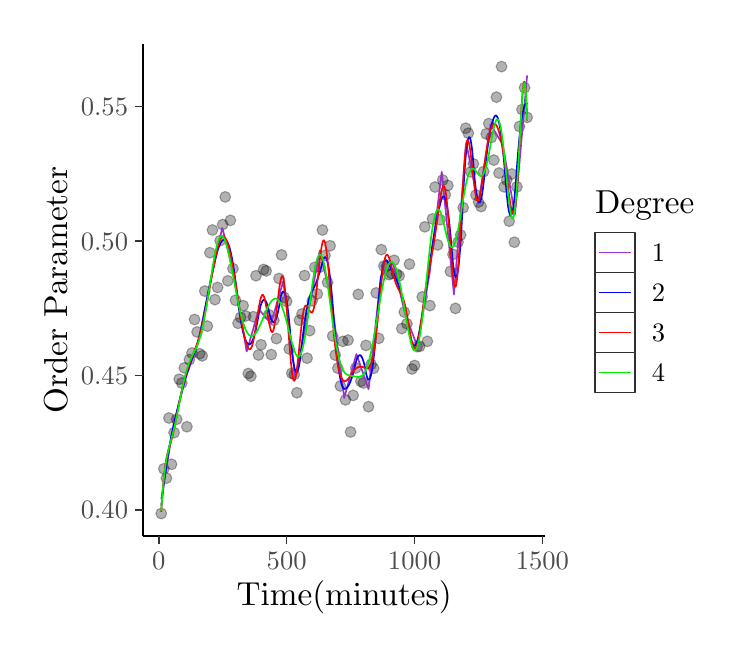
\begin{tikzpicture}[x=1pt,y=1pt]
\definecolor{fillColor}{RGB}{255,255,255}
\path[use as bounding box,fill=fillColor,fill opacity=0.00] (0,0) rectangle (252.94,216.81);
\begin{scope}
\path[clip] (  0.00,  0.00) rectangle (252.94,216.81);
\definecolor{drawColor}{RGB}{255,255,255}
\definecolor{fillColor}{RGB}{255,255,255}

\path[draw=drawColor,line width= 0.6pt,line join=round,line cap=round,fill=fillColor] (  0.00,  0.00) rectangle (252.94,216.81);
\end{scope}
\begin{scope}
\path[clip] ( 41.67, 33.16) rectangle (187.09,210.81);
\definecolor{fillColor}{RGB}{255,255,255}

\path[fill=fillColor] ( 41.67, 33.16) rectangle (187.09,210.81);
\definecolor{drawColor}{RGB}{0,0,0}
\definecolor{fillColor}{RGB}{0,0,0}

\path[draw=drawColor,draw opacity=0.30,line width= 0.4pt,line join=round,line cap=round,fill=fillColor,fill opacity=0.30] ( 48.28, 41.24) circle (  1.96);

\path[draw=drawColor,draw opacity=0.30,line width= 0.4pt,line join=round,line cap=round,fill=fillColor,fill opacity=0.30] ( 49.21, 57.42) circle (  1.96);

\path[draw=drawColor,draw opacity=0.30,line width= 0.4pt,line join=round,line cap=round,fill=fillColor,fill opacity=0.30] ( 50.13, 54.04) circle (  1.96);

\path[draw=drawColor,draw opacity=0.30,line width= 0.4pt,line join=round,line cap=round,fill=fillColor,fill opacity=0.30] ( 51.05, 75.76) circle (  1.96);

\path[draw=drawColor,draw opacity=0.30,line width= 0.4pt,line join=round,line cap=round,fill=fillColor,fill opacity=0.30] ( 51.98, 59.03) circle (  1.96);

\path[draw=drawColor,draw opacity=0.30,line width= 0.4pt,line join=round,line cap=round,fill=fillColor,fill opacity=0.30] ( 52.90, 70.46) circle (  1.96);

\path[draw=drawColor,draw opacity=0.30,line width= 0.4pt,line join=round,line cap=round,fill=fillColor,fill opacity=0.30] ( 53.83, 75.30) circle (  1.96);

\path[draw=drawColor,draw opacity=0.30,line width= 0.4pt,line join=round,line cap=round,fill=fillColor,fill opacity=0.30] ( 54.75, 89.78) circle (  1.96);

\path[draw=drawColor,draw opacity=0.30,line width= 0.4pt,line join=round,line cap=round,fill=fillColor,fill opacity=0.30] ( 55.68, 88.38) circle (  1.96);

\path[draw=drawColor,draw opacity=0.30,line width= 0.4pt,line join=round,line cap=round,fill=fillColor,fill opacity=0.30] ( 56.60, 93.89) circle (  1.96);

\path[draw=drawColor,draw opacity=0.30,line width= 0.4pt,line join=round,line cap=round,fill=fillColor,fill opacity=0.30] ( 57.53, 72.61) circle (  1.96);

\path[draw=drawColor,draw opacity=0.30,line width= 0.4pt,line join=round,line cap=round,fill=fillColor,fill opacity=0.30] ( 58.45, 96.86) circle (  1.96);

\path[draw=drawColor,draw opacity=0.30,line width= 0.4pt,line join=round,line cap=round,fill=fillColor,fill opacity=0.30] ( 59.37, 99.26) circle (  1.96);

\path[draw=drawColor,draw opacity=0.30,line width= 0.4pt,line join=round,line cap=round,fill=fillColor,fill opacity=0.30] ( 60.30,111.36) circle (  1.96);

\path[draw=drawColor,draw opacity=0.30,line width= 0.4pt,line join=round,line cap=round,fill=fillColor,fill opacity=0.30] ( 61.22,106.86) circle (  1.96);

\path[draw=drawColor,draw opacity=0.30,line width= 0.4pt,line join=round,line cap=round,fill=fillColor,fill opacity=0.30] ( 62.15, 99.00) circle (  1.96);

\path[draw=drawColor,draw opacity=0.30,line width= 0.4pt,line join=round,line cap=round,fill=fillColor,fill opacity=0.30] ( 63.07, 98.22) circle (  1.96);

\path[draw=drawColor,draw opacity=0.30,line width= 0.4pt,line join=round,line cap=round,fill=fillColor,fill opacity=0.30] ( 64.00,121.62) circle (  1.96);

\path[draw=drawColor,draw opacity=0.30,line width= 0.4pt,line join=round,line cap=round,fill=fillColor,fill opacity=0.30] ( 64.92,108.96) circle (  1.96);

\path[draw=drawColor,draw opacity=0.30,line width= 0.4pt,line join=round,line cap=round,fill=fillColor,fill opacity=0.30] ( 65.85,135.50) circle (  1.96);

\path[draw=drawColor,draw opacity=0.30,line width= 0.4pt,line join=round,line cap=round,fill=fillColor,fill opacity=0.30] ( 66.77,143.69) circle (  1.96);

\path[draw=drawColor,draw opacity=0.30,line width= 0.4pt,line join=round,line cap=round,fill=fillColor,fill opacity=0.30] ( 67.69,118.53) circle (  1.96);

\path[draw=drawColor,draw opacity=0.30,line width= 0.4pt,line join=round,line cap=round,fill=fillColor,fill opacity=0.30] ( 68.62,122.93) circle (  1.96);

\path[draw=drawColor,draw opacity=0.30,line width= 0.4pt,line join=round,line cap=round,fill=fillColor,fill opacity=0.30] ( 69.54,139.83) circle (  1.96);

\path[draw=drawColor,draw opacity=0.30,line width= 0.4pt,line join=round,line cap=round,fill=fillColor,fill opacity=0.30] ( 70.47,145.66) circle (  1.96);

\path[draw=drawColor,draw opacity=0.30,line width= 0.4pt,line join=round,line cap=round,fill=fillColor,fill opacity=0.30] ( 71.39,155.65) circle (  1.96);

\path[draw=drawColor,draw opacity=0.30,line width= 0.4pt,line join=round,line cap=round,fill=fillColor,fill opacity=0.30] ( 72.32,125.33) circle (  1.96);

\path[draw=drawColor,draw opacity=0.30,line width= 0.4pt,line join=round,line cap=round,fill=fillColor,fill opacity=0.30] ( 73.24,147.18) circle (  1.96);

\path[draw=drawColor,draw opacity=0.30,line width= 0.4pt,line join=round,line cap=round,fill=fillColor,fill opacity=0.30] ( 74.17,129.76) circle (  1.96);

\path[draw=drawColor,draw opacity=0.30,line width= 0.4pt,line join=round,line cap=round,fill=fillColor,fill opacity=0.30] ( 75.09,118.32) circle (  1.96);

\path[draw=drawColor,draw opacity=0.30,line width= 0.4pt,line join=round,line cap=round,fill=fillColor,fill opacity=0.30] ( 76.01,109.99) circle (  1.96);

\path[draw=drawColor,draw opacity=0.30,line width= 0.4pt,line join=round,line cap=round,fill=fillColor,fill opacity=0.30] ( 76.94,112.10) circle (  1.96);

\path[draw=drawColor,draw opacity=0.30,line width= 0.4pt,line join=round,line cap=round,fill=fillColor,fill opacity=0.30] ( 77.86,116.36) circle (  1.96);

\path[draw=drawColor,draw opacity=0.30,line width= 0.4pt,line join=round,line cap=round,fill=fillColor,fill opacity=0.30] ( 78.79,112.62) circle (  1.96);

\path[draw=drawColor,draw opacity=0.30,line width= 0.4pt,line join=round,line cap=round,fill=fillColor,fill opacity=0.30] ( 79.71, 91.85) circle (  1.96);

\path[draw=drawColor,draw opacity=0.30,line width= 0.4pt,line join=round,line cap=round,fill=fillColor,fill opacity=0.30] ( 80.64, 90.86) circle (  1.96);

\path[draw=drawColor,draw opacity=0.30,line width= 0.4pt,line join=round,line cap=round,fill=fillColor,fill opacity=0.30] ( 81.56,112.37) circle (  1.96);

\path[draw=drawColor,draw opacity=0.30,line width= 0.4pt,line join=round,line cap=round,fill=fillColor,fill opacity=0.30] ( 82.49,127.17) circle (  1.96);

\path[draw=drawColor,draw opacity=0.30,line width= 0.4pt,line join=round,line cap=round,fill=fillColor,fill opacity=0.30] ( 83.41, 98.54) circle (  1.96);

\path[draw=drawColor,draw opacity=0.30,line width= 0.4pt,line join=round,line cap=round,fill=fillColor,fill opacity=0.30] ( 84.33,102.24) circle (  1.96);

\path[draw=drawColor,draw opacity=0.30,line width= 0.4pt,line join=round,line cap=round,fill=fillColor,fill opacity=0.30] ( 85.26,129.43) circle (  1.96);

\path[draw=drawColor,draw opacity=0.30,line width= 0.4pt,line join=round,line cap=round,fill=fillColor,fill opacity=0.30] ( 86.18,128.92) circle (  1.96);

\path[draw=drawColor,draw opacity=0.30,line width= 0.4pt,line join=round,line cap=round,fill=fillColor,fill opacity=0.30] ( 87.11,113.09) circle (  1.96);

\path[draw=drawColor,draw opacity=0.30,line width= 0.4pt,line join=round,line cap=round,fill=fillColor,fill opacity=0.30] ( 88.03, 98.69) circle (  1.96);

\path[draw=drawColor,draw opacity=0.30,line width= 0.4pt,line join=round,line cap=round,fill=fillColor,fill opacity=0.30] ( 88.96,111.04) circle (  1.96);

\path[draw=drawColor,draw opacity=0.30,line width= 0.4pt,line join=round,line cap=round,fill=fillColor,fill opacity=0.30] ( 89.88,104.45) circle (  1.96);

\path[draw=drawColor,draw opacity=0.30,line width= 0.4pt,line join=round,line cap=round,fill=fillColor,fill opacity=0.30] ( 90.81,126.18) circle (  1.96);

\path[draw=drawColor,draw opacity=0.30,line width= 0.4pt,line join=round,line cap=round,fill=fillColor,fill opacity=0.30] ( 91.73,134.70) circle (  1.96);

\path[draw=drawColor,draw opacity=0.30,line width= 0.4pt,line join=round,line cap=round,fill=fillColor,fill opacity=0.30] ( 92.65,119.38) circle (  1.96);

\path[draw=drawColor,draw opacity=0.30,line width= 0.4pt,line join=round,line cap=round,fill=fillColor,fill opacity=0.30] ( 93.58,117.92) circle (  1.96);

\path[draw=drawColor,draw opacity=0.30,line width= 0.4pt,line join=round,line cap=round,fill=fillColor,fill opacity=0.30] ( 94.50,100.74) circle (  1.96);

\path[draw=drawColor,draw opacity=0.30,line width= 0.4pt,line join=round,line cap=round,fill=fillColor,fill opacity=0.30] ( 95.43, 91.94) circle (  1.96);

\path[draw=drawColor,draw opacity=0.30,line width= 0.4pt,line join=round,line cap=round,fill=fillColor,fill opacity=0.30] ( 96.35, 91.49) circle (  1.96);

\path[draw=drawColor,draw opacity=0.30,line width= 0.4pt,line join=round,line cap=round,fill=fillColor,fill opacity=0.30] ( 97.28, 84.89) circle (  1.96);

\path[draw=drawColor,draw opacity=0.30,line width= 0.4pt,line join=round,line cap=round,fill=fillColor,fill opacity=0.30] ( 98.20,111.09) circle (  1.96);

\path[draw=drawColor,draw opacity=0.30,line width= 0.4pt,line join=round,line cap=round,fill=fillColor,fill opacity=0.30] ( 99.13,113.38) circle (  1.96);

\path[draw=drawColor,draw opacity=0.30,line width= 0.4pt,line join=round,line cap=round,fill=fillColor,fill opacity=0.30] (100.05,127.24) circle (  1.96);

\path[draw=drawColor,draw opacity=0.30,line width= 0.4pt,line join=round,line cap=round,fill=fillColor,fill opacity=0.30] (100.97, 97.38) circle (  1.96);

\path[draw=drawColor,draw opacity=0.30,line width= 0.4pt,line join=round,line cap=round,fill=fillColor,fill opacity=0.30] (101.90,107.33) circle (  1.96);

\path[draw=drawColor,draw opacity=0.30,line width= 0.4pt,line join=round,line cap=round,fill=fillColor,fill opacity=0.30] (102.82,118.13) circle (  1.96);

\path[draw=drawColor,draw opacity=0.30,line width= 0.4pt,line join=round,line cap=round,fill=fillColor,fill opacity=0.30] (103.75,130.21) circle (  1.96);

\path[draw=drawColor,draw opacity=0.30,line width= 0.4pt,line join=round,line cap=round,fill=fillColor,fill opacity=0.30] (104.67,120.61) circle (  1.96);

\path[draw=drawColor,draw opacity=0.30,line width= 0.4pt,line join=round,line cap=round,fill=fillColor,fill opacity=0.30] (105.60,130.31) circle (  1.96);

\path[draw=drawColor,draw opacity=0.30,line width= 0.4pt,line join=round,line cap=round,fill=fillColor,fill opacity=0.30] (106.52,143.68) circle (  1.96);

\path[draw=drawColor,draw opacity=0.30,line width= 0.4pt,line join=round,line cap=round,fill=fillColor,fill opacity=0.30] (107.45,134.51) circle (  1.96);

\path[draw=drawColor,draw opacity=0.30,line width= 0.4pt,line join=round,line cap=round,fill=fillColor,fill opacity=0.30] (108.37,124.76) circle (  1.96);

\path[draw=drawColor,draw opacity=0.30,line width= 0.4pt,line join=round,line cap=round,fill=fillColor,fill opacity=0.30] (109.29,138.02) circle (  1.96);

\path[draw=drawColor,draw opacity=0.30,line width= 0.4pt,line join=round,line cap=round,fill=fillColor,fill opacity=0.30] (110.22,105.39) circle (  1.96);

\path[draw=drawColor,draw opacity=0.30,line width= 0.4pt,line join=round,line cap=round,fill=fillColor,fill opacity=0.30] (111.14, 98.49) circle (  1.96);

\path[draw=drawColor,draw opacity=0.30,line width= 0.4pt,line join=round,line cap=round,fill=fillColor,fill opacity=0.30] (112.07, 93.75) circle (  1.96);

\path[draw=drawColor,draw opacity=0.30,line width= 0.4pt,line join=round,line cap=round,fill=fillColor,fill opacity=0.30] (112.99, 87.34) circle (  1.96);

\path[draw=drawColor,draw opacity=0.30,line width= 0.4pt,line join=round,line cap=round,fill=fillColor,fill opacity=0.30] (113.92,103.45) circle (  1.96);

\path[draw=drawColor,draw opacity=0.30,line width= 0.4pt,line join=round,line cap=round,fill=fillColor,fill opacity=0.30] (114.84, 82.31) circle (  1.96);

\path[draw=drawColor,draw opacity=0.30,line width= 0.4pt,line join=round,line cap=round,fill=fillColor,fill opacity=0.30] (115.77,103.90) circle (  1.96);

\path[draw=drawColor,draw opacity=0.30,line width= 0.4pt,line join=round,line cap=round,fill=fillColor,fill opacity=0.30] (116.69, 70.71) circle (  1.96);

\path[draw=drawColor,draw opacity=0.30,line width= 0.4pt,line join=round,line cap=round,fill=fillColor,fill opacity=0.30] (117.61, 83.94) circle (  1.96);

\path[draw=drawColor,draw opacity=0.30,line width= 0.4pt,line join=round,line cap=round,fill=fillColor,fill opacity=0.30] (118.54, 93.82) circle (  1.96);

\path[draw=drawColor,draw opacity=0.30,line width= 0.4pt,line join=round,line cap=round,fill=fillColor,fill opacity=0.30] (119.46,120.43) circle (  1.96);

\path[draw=drawColor,draw opacity=0.30,line width= 0.4pt,line join=round,line cap=round,fill=fillColor,fill opacity=0.30] (120.39, 89.01) circle (  1.96);

\path[draw=drawColor,draw opacity=0.30,line width= 0.4pt,line join=round,line cap=round,fill=fillColor,fill opacity=0.30] (121.31, 88.41) circle (  1.96);

\path[draw=drawColor,draw opacity=0.30,line width= 0.4pt,line join=round,line cap=round,fill=fillColor,fill opacity=0.30] (122.24,101.99) circle (  1.96);

\path[draw=drawColor,draw opacity=0.30,line width= 0.4pt,line join=round,line cap=round,fill=fillColor,fill opacity=0.30] (123.16, 79.86) circle (  1.96);

\path[draw=drawColor,draw opacity=0.30,line width= 0.4pt,line join=round,line cap=round,fill=fillColor,fill opacity=0.30] (124.09, 95.14) circle (  1.96);

\path[draw=drawColor,draw opacity=0.30,line width= 0.4pt,line join=round,line cap=round,fill=fillColor,fill opacity=0.30] (125.01, 93.72) circle (  1.96);

\path[draw=drawColor,draw opacity=0.30,line width= 0.4pt,line join=round,line cap=round,fill=fillColor,fill opacity=0.30] (125.93,120.96) circle (  1.96);

\path[draw=drawColor,draw opacity=0.30,line width= 0.4pt,line join=round,line cap=round,fill=fillColor,fill opacity=0.30] (126.86,104.53) circle (  1.96);

\path[draw=drawColor,draw opacity=0.30,line width= 0.4pt,line join=round,line cap=round,fill=fillColor,fill opacity=0.30] (127.78,136.61) circle (  1.96);

\path[draw=drawColor,draw opacity=0.30,line width= 0.4pt,line join=round,line cap=round,fill=fillColor,fill opacity=0.30] (128.71,130.68) circle (  1.96);

\path[draw=drawColor,draw opacity=0.30,line width= 0.4pt,line join=round,line cap=round,fill=fillColor,fill opacity=0.30] (129.63,130.60) circle (  1.96);

\path[draw=drawColor,draw opacity=0.30,line width= 0.4pt,line join=round,line cap=round,fill=fillColor,fill opacity=0.30] (130.56,127.56) circle (  1.96);

\path[draw=drawColor,draw opacity=0.30,line width= 0.4pt,line join=round,line cap=round,fill=fillColor,fill opacity=0.30] (131.48,127.95) circle (  1.96);

\path[draw=drawColor,draw opacity=0.30,line width= 0.4pt,line join=round,line cap=round,fill=fillColor,fill opacity=0.30] (132.41,132.76) circle (  1.96);

\path[draw=drawColor,draw opacity=0.30,line width= 0.4pt,line join=round,line cap=round,fill=fillColor,fill opacity=0.30] (133.33,127.81) circle (  1.96);

\path[draw=drawColor,draw opacity=0.30,line width= 0.4pt,line join=round,line cap=round,fill=fillColor,fill opacity=0.30] (134.25,127.14) circle (  1.96);

\path[draw=drawColor,draw opacity=0.30,line width= 0.4pt,line join=round,line cap=round,fill=fillColor,fill opacity=0.30] (135.18,108.08) circle (  1.96);

\path[draw=drawColor,draw opacity=0.30,line width= 0.4pt,line join=round,line cap=round,fill=fillColor,fill opacity=0.30] (136.10,114.04) circle (  1.96);

\path[draw=drawColor,draw opacity=0.30,line width= 0.4pt,line join=round,line cap=round,fill=fillColor,fill opacity=0.30] (137.03,109.82) circle (  1.96);

\path[draw=drawColor,draw opacity=0.30,line width= 0.4pt,line join=round,line cap=round,fill=fillColor,fill opacity=0.30] (137.95,131.36) circle (  1.96);

\path[draw=drawColor,draw opacity=0.30,line width= 0.4pt,line join=round,line cap=round,fill=fillColor,fill opacity=0.30] (138.88, 93.47) circle (  1.96);

\path[draw=drawColor,draw opacity=0.30,line width= 0.4pt,line join=round,line cap=round,fill=fillColor,fill opacity=0.30] (139.80, 94.73) circle (  1.96);

\path[draw=drawColor,draw opacity=0.30,line width= 0.4pt,line join=round,line cap=round,fill=fillColor,fill opacity=0.30] (140.73,101.56) circle (  1.96);

\path[draw=drawColor,draw opacity=0.30,line width= 0.4pt,line join=round,line cap=round,fill=fillColor,fill opacity=0.30] (141.65,101.66) circle (  1.96);

\path[draw=drawColor,draw opacity=0.30,line width= 0.4pt,line join=round,line cap=round,fill=fillColor,fill opacity=0.30] (142.57,119.53) circle (  1.96);

\path[draw=drawColor,draw opacity=0.30,line width= 0.4pt,line join=round,line cap=round,fill=fillColor,fill opacity=0.30] (143.50,144.85) circle (  1.96);

\path[draw=drawColor,draw opacity=0.30,line width= 0.4pt,line join=round,line cap=round,fill=fillColor,fill opacity=0.30] (144.42,103.47) circle (  1.96);

\path[draw=drawColor,draw opacity=0.30,line width= 0.4pt,line join=round,line cap=round,fill=fillColor,fill opacity=0.30] (145.35,116.38) circle (  1.96);

\path[draw=drawColor,draw opacity=0.30,line width= 0.4pt,line join=round,line cap=round,fill=fillColor,fill opacity=0.30] (146.27,147.71) circle (  1.96);

\path[draw=drawColor,draw opacity=0.30,line width= 0.4pt,line join=round,line cap=round,fill=fillColor,fill opacity=0.30] (147.20,159.22) circle (  1.96);

\path[draw=drawColor,draw opacity=0.30,line width= 0.4pt,line join=round,line cap=round,fill=fillColor,fill opacity=0.30] (148.12,138.32) circle (  1.96);

\path[draw=drawColor,draw opacity=0.30,line width= 0.4pt,line join=round,line cap=round,fill=fillColor,fill opacity=0.30] (149.05,147.38) circle (  1.96);

\path[draw=drawColor,draw opacity=0.30,line width= 0.4pt,line join=round,line cap=round,fill=fillColor,fill opacity=0.30] (149.97,161.75) circle (  1.96);

\path[draw=drawColor,draw opacity=0.30,line width= 0.4pt,line join=round,line cap=round,fill=fillColor,fill opacity=0.30] (150.89,156.46) circle (  1.96);

\path[draw=drawColor,draw opacity=0.30,line width= 0.4pt,line join=round,line cap=round,fill=fillColor,fill opacity=0.30] (151.82,159.79) circle (  1.96);

\path[draw=drawColor,draw opacity=0.30,line width= 0.4pt,line join=round,line cap=round,fill=fillColor,fill opacity=0.30] (152.74,128.73) circle (  1.96);

\path[draw=drawColor,draw opacity=0.30,line width= 0.4pt,line join=round,line cap=round,fill=fillColor,fill opacity=0.30] (153.67,134.89) circle (  1.96);

\path[draw=drawColor,draw opacity=0.30,line width= 0.4pt,line join=round,line cap=round,fill=fillColor,fill opacity=0.30] (154.59,115.36) circle (  1.96);

\path[draw=drawColor,draw opacity=0.30,line width= 0.4pt,line join=round,line cap=round,fill=fillColor,fill opacity=0.30] (155.52,139.30) circle (  1.96);

\path[draw=drawColor,draw opacity=0.30,line width= 0.4pt,line join=round,line cap=round,fill=fillColor,fill opacity=0.30] (156.44,141.89) circle (  1.96);

\path[draw=drawColor,draw opacity=0.30,line width= 0.4pt,line join=round,line cap=round,fill=fillColor,fill opacity=0.30] (157.37,151.76) circle (  1.96);

\path[draw=drawColor,draw opacity=0.30,line width= 0.4pt,line join=round,line cap=round,fill=fillColor,fill opacity=0.30] (158.29,180.49) circle (  1.96);

\path[draw=drawColor,draw opacity=0.30,line width= 0.4pt,line join=round,line cap=round,fill=fillColor,fill opacity=0.30] (159.22,178.66) circle (  1.96);

\path[draw=drawColor,draw opacity=0.30,line width= 0.4pt,line join=round,line cap=round,fill=fillColor,fill opacity=0.30] (160.14,164.70) circle (  1.96);

\path[draw=drawColor,draw opacity=0.30,line width= 0.4pt,line join=round,line cap=round,fill=fillColor,fill opacity=0.30] (161.06,167.62) circle (  1.96);

\path[draw=drawColor,draw opacity=0.30,line width= 0.4pt,line join=round,line cap=round,fill=fillColor,fill opacity=0.30] (161.99,156.35) circle (  1.96);

\path[draw=drawColor,draw opacity=0.30,line width= 0.4pt,line join=round,line cap=round,fill=fillColor,fill opacity=0.30] (162.91,153.80) circle (  1.96);

\path[draw=drawColor,draw opacity=0.30,line width= 0.4pt,line join=round,line cap=round,fill=fillColor,fill opacity=0.30] (163.84,152.16) circle (  1.96);

\path[draw=drawColor,draw opacity=0.30,line width= 0.4pt,line join=round,line cap=round,fill=fillColor,fill opacity=0.30] (164.76,164.81) circle (  1.96);

\path[draw=drawColor,draw opacity=0.30,line width= 0.4pt,line join=round,line cap=round,fill=fillColor,fill opacity=0.30] (165.69,178.43) circle (  1.96);

\path[draw=drawColor,draw opacity=0.30,line width= 0.4pt,line join=round,line cap=round,fill=fillColor,fill opacity=0.30] (166.61,182.14) circle (  1.96);

\path[draw=drawColor,draw opacity=0.30,line width= 0.4pt,line join=round,line cap=round,fill=fillColor,fill opacity=0.30] (167.54,177.11) circle (  1.96);

\path[draw=drawColor,draw opacity=0.30,line width= 0.4pt,line join=round,line cap=round,fill=fillColor,fill opacity=0.30] (168.46,168.96) circle (  1.96);

\path[draw=drawColor,draw opacity=0.30,line width= 0.4pt,line join=round,line cap=round,fill=fillColor,fill opacity=0.30] (169.38,191.71) circle (  1.96);

\path[draw=drawColor,draw opacity=0.30,line width= 0.4pt,line join=round,line cap=round,fill=fillColor,fill opacity=0.30] (170.31,164.28) circle (  1.96);

\path[draw=drawColor,draw opacity=0.30,line width= 0.4pt,line join=round,line cap=round,fill=fillColor,fill opacity=0.30] (171.23,202.74) circle (  1.96);

\path[draw=drawColor,draw opacity=0.30,line width= 0.4pt,line join=round,line cap=round,fill=fillColor,fill opacity=0.30] (172.16,159.30) circle (  1.96);

\path[draw=drawColor,draw opacity=0.30,line width= 0.4pt,line join=round,line cap=round,fill=fillColor,fill opacity=0.30] (173.08,161.74) circle (  1.96);

\path[draw=drawColor,draw opacity=0.30,line width= 0.4pt,line join=round,line cap=round,fill=fillColor,fill opacity=0.30] (174.01,146.88) circle (  1.96);

\path[draw=drawColor,draw opacity=0.30,line width= 0.4pt,line join=round,line cap=round,fill=fillColor,fill opacity=0.30] (174.93,163.93) circle (  1.96);

\path[draw=drawColor,draw opacity=0.30,line width= 0.4pt,line join=round,line cap=round,fill=fillColor,fill opacity=0.30] (175.86,139.28) circle (  1.96);

\path[draw=drawColor,draw opacity=0.30,line width= 0.4pt,line join=round,line cap=round,fill=fillColor,fill opacity=0.30] (176.78,159.29) circle (  1.96);

\path[draw=drawColor,draw opacity=0.30,line width= 0.4pt,line join=round,line cap=round,fill=fillColor,fill opacity=0.30] (177.70,181.11) circle (  1.96);

\path[draw=drawColor,draw opacity=0.30,line width= 0.4pt,line join=round,line cap=round,fill=fillColor,fill opacity=0.30] (178.63,187.22) circle (  1.96);

\path[draw=drawColor,draw opacity=0.30,line width= 0.4pt,line join=round,line cap=round,fill=fillColor,fill opacity=0.30] (179.55,195.12) circle (  1.96);

\path[draw=drawColor,draw opacity=0.30,line width= 0.4pt,line join=round,line cap=round,fill=fillColor,fill opacity=0.30] (180.48,184.39) circle (  1.96);
\definecolor{drawColor}{RGB}{153,50,204}

\path[draw=drawColor,line width= 0.6pt,line join=round] ( 48.28, 46.37) --
	( 48.37, 46.94) --
	( 48.47, 47.51) --
	( 48.56, 48.07) --
	( 48.65, 48.64) --
	( 48.74, 49.20) --
	( 48.84, 49.77) --
	( 48.93, 50.33) --
	( 49.02, 50.90) --
	( 49.11, 51.47) --
	( 49.21, 52.03) --
	( 49.30, 52.60) --
	( 49.39, 53.16) --
	( 49.48, 53.73) --
	( 49.58, 54.29) --
	( 49.67, 54.86) --
	( 49.76, 55.43) --
	( 49.85, 55.99) --
	( 49.95, 56.56) --
	( 50.04, 57.12) --
	( 50.13, 57.69) --
	( 50.22, 58.25) --
	( 50.31, 58.82) --
	( 50.41, 59.39) --
	( 50.50, 59.95) --
	( 50.59, 60.52) --
	( 50.68, 61.08) --
	( 50.78, 61.65) --
	( 50.87, 62.21) --
	( 50.96, 62.78) --
	( 51.05, 63.35) --
	( 51.15, 63.91) --
	( 51.24, 64.48) --
	( 51.33, 65.04) --
	( 51.42, 65.61) --
	( 51.52, 66.17) --
	( 51.61, 66.74) --
	( 51.70, 67.31) --
	( 51.79, 67.87) --
	( 51.89, 68.44) --
	( 51.98, 69.00) --
	( 52.07, 69.57) --
	( 52.16, 70.13) --
	( 52.26, 70.70) --
	( 52.35, 71.27) --
	( 52.44, 71.83) --
	( 52.53, 72.40) --
	( 52.63, 72.96) --
	( 52.72, 73.46) --
	( 52.81, 73.81) --
	( 52.90, 74.17) --
	( 53.00, 74.52) --
	( 53.09, 74.88) --
	( 53.18, 75.24) --
	( 53.27, 75.59) --
	( 53.37, 75.95) --
	( 53.46, 76.30) --
	( 53.55, 76.66) --
	( 53.64, 77.01) --
	( 53.74, 77.37) --
	( 53.83, 77.72) --
	( 53.92, 78.08) --
	( 54.01, 78.43) --
	( 54.11, 78.79) --
	( 54.20, 79.14) --
	( 54.29, 79.50) --
	( 54.38, 79.85) --
	( 54.47, 80.21) --
	( 54.57, 80.57) --
	( 54.66, 80.92) --
	( 54.75, 81.28) --
	( 54.84, 81.63) --
	( 54.94, 81.99) --
	( 55.03, 82.34) --
	( 55.12, 82.70) --
	( 55.21, 83.05) --
	( 55.31, 83.41) --
	( 55.40, 83.76) --
	( 55.49, 84.12) --
	( 55.58, 84.47) --
	( 55.68, 84.83) --
	( 55.77, 85.18) --
	( 55.86, 85.54) --
	( 55.95, 85.89) --
	( 56.05, 86.25) --
	( 56.14, 86.61) --
	( 56.23, 86.96) --
	( 56.32, 87.32) --
	( 56.42, 87.67) --
	( 56.51, 88.03) --
	( 56.60, 88.38) --
	( 56.69, 88.74) --
	( 56.79, 89.09) --
	( 56.88, 89.45) --
	( 56.97, 89.80) --
	( 57.06, 90.16) --
	( 57.16, 90.45) --
	( 57.25, 90.72) --
	( 57.34, 90.99) --
	( 57.43, 91.25) --
	( 57.53, 91.52) --
	( 57.62, 91.78) --
	( 57.71, 92.05) --
	( 57.80, 92.31) --
	( 57.90, 92.58) --
	( 57.99, 92.84) --
	( 58.08, 93.11) --
	( 58.17, 93.37) --
	( 58.27, 93.64) --
	( 58.36, 93.90) --
	( 58.45, 94.17) --
	( 58.54, 94.43) --
	( 58.63, 94.70) --
	( 58.73, 94.97) --
	( 58.82, 95.23) --
	( 58.91, 95.50) --
	( 59.00, 95.76) --
	( 59.10, 96.03) --
	( 59.19, 96.29) --
	( 59.28, 96.56) --
	( 59.37, 96.82) --
	( 59.47, 97.09) --
	( 59.56, 97.35) --
	( 59.65, 97.62) --
	( 59.74, 97.88) --
	( 59.84, 98.15) --
	( 59.93, 98.42) --
	( 60.02, 98.68) --
	( 60.11, 98.95) --
	( 60.21, 99.21) --
	( 60.30, 99.48) --
	( 60.39, 99.74) --
	( 60.48,100.01) --
	( 60.58,100.27) --
	( 60.67,100.54) --
	( 60.76,100.80) --
	( 60.85,101.07) --
	( 60.95,101.33) --
	( 61.04,101.60) --
	( 61.13,101.87) --
	( 61.22,102.13) --
	( 61.32,102.40) --
	( 61.41,102.66) --
	( 61.50,102.93) --
	( 61.59,103.37) --
	( 61.69,103.82) --
	( 61.78,104.27) --
	( 61.87,104.72) --
	( 61.96,105.17) --
	( 62.06,105.62) --
	( 62.15,106.06) --
	( 62.24,106.51) --
	( 62.33,106.96) --
	( 62.43,107.41) --
	( 62.52,107.86) --
	( 62.61,108.31) --
	( 62.70,108.75) --
	( 62.79,109.20) --
	( 62.89,109.65) --
	( 62.98,110.10) --
	( 63.07,110.55) --
	( 63.16,111.00) --
	( 63.26,111.44) --
	( 63.35,111.89) --
	( 63.44,112.34) --
	( 63.53,112.79) --
	( 63.63,113.24) --
	( 63.72,113.69) --
	( 63.81,114.13) --
	( 63.90,114.58) --
	( 64.00,115.03) --
	( 64.09,115.48) --
	( 64.18,115.93) --
	( 64.27,116.37) --
	( 64.37,116.82) --
	( 64.46,117.27) --
	( 64.55,117.72) --
	( 64.64,118.17) --
	( 64.74,118.62) --
	( 64.83,119.06) --
	( 64.92,119.51) --
	( 65.01,119.96) --
	( 65.11,120.41) --
	( 65.20,120.86) --
	( 65.29,121.31) --
	( 65.38,121.75) --
	( 65.48,122.20) --
	( 65.57,122.65) --
	( 65.66,123.10) --
	( 65.75,123.55) --
	( 65.85,124.00) --
	( 65.94,124.44) --
	( 66.03,124.86) --
	( 66.12,125.29) --
	( 66.22,125.71) --
	( 66.31,126.14) --
	( 66.40,126.56) --
	( 66.49,126.99) --
	( 66.59,127.41) --
	( 66.68,127.84) --
	( 66.77,128.27) --
	( 66.86,128.69) --
	( 66.95,129.12) --
	( 67.05,129.54) --
	( 67.14,129.97) --
	( 67.23,130.39) --
	( 67.32,130.82) --
	( 67.42,131.24) --
	( 67.51,131.67) --
	( 67.60,132.09) --
	( 67.69,132.52) --
	( 67.79,132.95) --
	( 67.88,133.37) --
	( 67.97,133.80) --
	( 68.06,134.22) --
	( 68.16,134.65) --
	( 68.25,135.07) --
	( 68.34,135.50) --
	( 68.43,135.92) --
	( 68.53,136.35) --
	( 68.62,136.77) --
	( 68.71,137.20) --
	( 68.80,137.62) --
	( 68.90,138.05) --
	( 68.99,138.48) --
	( 69.08,138.90) --
	( 69.17,139.33) --
	( 69.27,139.75) --
	( 69.36,140.18) --
	( 69.45,140.60) --
	( 69.54,141.03) --
	( 69.64,141.45) --
	( 69.73,141.88) --
	( 69.82,142.30) --
	( 69.91,142.73) --
	( 70.01,143.16) --
	( 70.10,143.58) --
	( 70.19,144.01) --
	( 70.28,144.43) --
	( 70.38,144.32) --
	( 70.47,143.95) --
	( 70.56,143.58) --
	( 70.65,143.20) --
	( 70.75,142.83) --
	( 70.84,142.46) --
	( 70.93,142.08) --
	( 71.02,141.71) --
	( 71.11,141.33) --
	( 71.21,140.96) --
	( 71.30,140.59) --
	( 71.39,140.21) --
	( 71.48,139.84) --
	( 71.58,139.47) --
	( 71.67,139.09) --
	( 71.76,138.72) --
	( 71.85,138.34) --
	( 71.95,137.97) --
	( 72.04,137.60) --
	( 72.13,137.22) --
	( 72.22,136.85) --
	( 72.32,136.48) --
	( 72.41,136.10) --
	( 72.50,135.73) --
	( 72.59,135.35) --
	( 72.69,134.98) --
	( 72.78,134.61) --
	( 72.87,134.23) --
	( 72.96,133.86) --
	( 73.06,133.49) --
	( 73.15,133.11) --
	( 73.24,132.74) --
	( 73.33,132.36) --
	( 73.43,131.99) --
	( 73.52,131.62) --
	( 73.61,131.24) --
	( 73.70,130.87) --
	( 73.80,130.50) --
	( 73.89,130.12) --
	( 73.98,129.75) --
	( 74.07,129.38) --
	( 74.17,129.00) --
	( 74.26,128.63) --
	( 74.35,128.25) --
	( 74.44,127.88) --
	( 74.54,127.51) --
	( 74.63,127.13) --
	( 74.72,126.76) --
	( 74.81,126.19) --
	( 74.91,125.62) --
	( 75.00,125.06) --
	( 75.09,124.49) --
	( 75.18,123.92) --
	( 75.27,123.36) --
	( 75.37,122.79) --
	( 75.46,122.22) --
	( 75.55,121.65) --
	( 75.64,121.09) --
	( 75.74,120.52) --
	( 75.83,119.95) --
	( 75.92,119.39) --
	( 76.01,118.82) --
	( 76.11,118.25) --
	( 76.20,117.68) --
	( 76.29,117.12) --
	( 76.38,116.55) --
	( 76.48,115.98) --
	( 76.57,115.42) --
	( 76.66,114.85) --
	( 76.75,114.28) --
	( 76.85,113.71) --
	( 76.94,113.15) --
	( 77.03,112.58) --
	( 77.12,112.01) --
	( 77.22,111.45) --
	( 77.31,110.88) --
	( 77.40,110.31) --
	( 77.49,109.74) --
	( 77.59,109.18) --
	( 77.68,108.61) --
	( 77.77,108.04) --
	( 77.86,107.48) --
	( 77.96,106.91) --
	( 78.05,106.34) --
	( 78.14,105.77) --
	( 78.23,105.21) --
	( 78.33,104.64) --
	( 78.42,104.07) --
	( 78.51,103.51) --
	( 78.60,102.94) --
	( 78.70,102.37) --
	( 78.79,101.80) --
	( 78.88,101.24) --
	( 78.97,100.67) --
	( 79.07,100.10) --
	( 79.16, 99.83) --
	( 79.25,100.15) --
	( 79.34,100.47) --
	( 79.43,100.80) --
	( 79.53,101.12) --
	( 79.62,101.44) --
	( 79.71,101.76) --
	( 79.80,102.08) --
	( 79.90,102.40) --
	( 79.99,102.72) --
	( 80.08,103.04) --
	( 80.17,103.36) --
	( 80.27,103.68) --
	( 80.36,104.01) --
	( 80.45,104.33) --
	( 80.54,104.65) --
	( 80.64,104.97) --
	( 80.73,105.29) --
	( 80.82,105.61) --
	( 80.91,105.93) --
	( 81.01,106.25) --
	( 81.10,106.57) --
	( 81.19,106.90) --
	( 81.28,107.22) --
	( 81.38,107.54) --
	( 81.47,107.86) --
	( 81.56,108.18) --
	( 81.65,108.50) --
	( 81.75,108.82) --
	( 81.84,109.14) --
	( 81.93,109.46) --
	( 82.02,109.78) --
	( 82.12,110.11) --
	( 82.21,110.43) --
	( 82.30,110.75) --
	( 82.39,111.07) --
	( 82.49,111.39) --
	( 82.58,111.71) --
	( 82.67,112.03) --
	( 82.76,112.35) --
	( 82.86,112.67) --
	( 82.95,112.99) --
	( 83.04,113.32) --
	( 83.13,113.64) --
	( 83.23,113.96) --
	( 83.32,114.28) --
	( 83.41,114.60) --
	( 83.50,114.92) --
	( 83.59,114.96) --
	( 83.69,114.85) --
	( 83.78,114.74) --
	( 83.87,114.64) --
	( 83.96,114.53) --
	( 84.06,114.43) --
	( 84.15,114.32) --
	( 84.24,114.21) --
	( 84.33,114.11) --
	( 84.43,114.00) --
	( 84.52,113.90) --
	( 84.61,113.79) --
	( 84.70,113.68) --
	( 84.80,113.58) --
	( 84.89,113.47) --
	( 84.98,113.36) --
	( 85.07,113.26) --
	( 85.17,113.15) --
	( 85.26,113.05) --
	( 85.35,112.94) --
	( 85.44,112.83) --
	( 85.54,112.73) --
	( 85.63,112.62) --
	( 85.72,112.51) --
	( 85.81,112.41) --
	( 85.91,112.30) --
	( 86.00,112.20) --
	( 86.09,112.09) --
	( 86.18,111.98) --
	( 86.28,111.88) --
	( 86.37,111.77) --
	( 86.46,111.66) --
	( 86.55,111.56) --
	( 86.65,111.45) --
	( 86.74,111.35) --
	( 86.83,111.24) --
	( 86.92,111.13) --
	( 87.02,111.03) --
	( 87.11,110.92) --
	( 87.20,110.81) --
	( 87.29,110.71) --
	( 87.39,110.60) --
	( 87.48,110.50) --
	( 87.57,110.39) --
	( 87.66,110.28) --
	( 87.76,110.18) --
	( 87.85,110.07) --
	( 87.94,109.96) --
	( 88.03,110.28) --
	( 88.12,110.60) --
	( 88.22,110.92) --
	( 88.31,111.24) --
	( 88.40,111.56) --
	( 88.49,111.88) --
	( 88.59,112.19) --
	( 88.68,112.51) --
	( 88.77,112.83) --
	( 88.86,113.15) --
	( 88.96,113.47) --
	( 89.05,113.79) --
	( 89.14,114.11) --
	( 89.23,114.42) --
	( 89.33,114.74) --
	( 89.42,115.06) --
	( 89.51,115.38) --
	( 89.60,115.70) --
	( 89.70,116.02) --
	( 89.79,116.34) --
	( 89.88,116.65) --
	( 89.97,116.97) --
	( 90.07,117.29) --
	( 90.16,117.61) --
	( 90.25,117.93) --
	( 90.34,118.25) --
	( 90.44,118.57) --
	( 90.53,118.88) --
	( 90.62,119.20) --
	( 90.71,119.52) --
	( 90.81,119.84) --
	( 90.90,120.16) --
	( 90.99,120.48) --
	( 91.08,120.80) --
	( 91.18,121.11) --
	( 91.27,121.43) --
	( 91.36,121.75) --
	( 91.45,122.07) --
	( 91.55,122.39) --
	( 91.64,122.71) --
	( 91.73,123.03) --
	( 91.82,123.34) --
	( 91.92,123.66) --
	( 92.01,123.98) --
	( 92.10,124.30) --
	( 92.19,124.62) --
	( 92.28,124.94) --
	( 92.38,124.91) --
	( 92.47,124.18) --
	( 92.56,123.45) --
	( 92.65,122.72) --
	( 92.75,121.99) --
	( 92.84,121.26) --
	( 92.93,120.54) --
	( 93.02,119.81) --
	( 93.12,119.08) --
	( 93.21,118.35) --
	( 93.30,117.62) --
	( 93.39,116.89) --
	( 93.49,116.16) --
	( 93.58,115.44) --
	( 93.67,114.71) --
	( 93.76,113.98) --
	( 93.86,113.25) --
	( 93.95,112.52) --
	( 94.04,111.79) --
	( 94.13,111.07) --
	( 94.23,110.34) --
	( 94.32,109.61) --
	( 94.41,108.88) --
	( 94.50,108.15) --
	( 94.60,107.42) --
	( 94.69,106.69) --
	( 94.78,105.97) --
	( 94.87,105.24) --
	( 94.97,104.51) --
	( 95.06,103.78) --
	( 95.15,103.05) --
	( 95.24,102.32) --
	( 95.34,101.59) --
	( 95.43,100.87) --
	( 95.52,100.14) --
	( 95.61, 99.41) --
	( 95.71, 98.68) --
	( 95.80, 97.95) --
	( 95.89, 97.22) --
	( 95.98, 96.49) --
	( 96.08, 95.77) --
	( 96.17, 95.04) --
	( 96.26, 94.31) --
	( 96.35, 93.58) --
	( 96.44, 92.85) --
	( 96.54, 92.12) --
	( 96.63, 91.39) --
	( 96.72, 90.67) --
	( 96.81, 90.73) --
	( 96.91, 91.20) --
	( 97.00, 91.67) --
	( 97.09, 92.13) --
	( 97.18, 92.60) --
	( 97.28, 93.07) --
	( 97.37, 93.53) --
	( 97.46, 94.00) --
	( 97.55, 94.47) --
	( 97.65, 94.93) --
	( 97.74, 95.40) --
	( 97.83, 95.87) --
	( 97.92, 96.33) --
	( 98.02, 96.80) --
	( 98.11, 97.27) --
	( 98.20, 97.73) --
	( 98.29, 98.20) --
	( 98.39, 98.67) --
	( 98.48, 99.13) --
	( 98.57, 99.60) --
	( 98.66,100.07) --
	( 98.76,100.53) --
	( 98.85,101.00) --
	( 98.94,101.46) --
	( 99.03,101.93) --
	( 99.13,102.40) --
	( 99.22,102.86) --
	( 99.31,103.33) --
	( 99.40,103.80) --
	( 99.50,104.26) --
	( 99.59,104.73) --
	( 99.68,105.20) --
	( 99.77,105.66) --
	( 99.87,106.13) --
	( 99.96,106.60) --
	(100.05,107.06) --
	(100.14,107.53) --
	(100.24,108.00) --
	(100.33,108.46) --
	(100.42,108.93) --
	(100.51,109.40) --
	(100.60,109.86) --
	(100.70,110.33) --
	(100.79,110.80) --
	(100.88,111.26) --
	(100.97,111.73) --
	(101.07,112.19) --
	(101.16,112.66) --
	(101.25,113.16) --
	(101.34,113.66) --
	(101.44,114.16) --
	(101.53,114.65) --
	(101.62,115.15) --
	(101.71,115.65) --
	(101.81,116.15) --
	(101.90,116.65) --
	(101.99,117.15) --
	(102.08,117.65) --
	(102.18,118.14) --
	(102.27,118.64) --
	(102.36,119.14) --
	(102.45,119.64) --
	(102.55,120.14) --
	(102.64,120.64) --
	(102.73,121.13) --
	(102.82,121.63) --
	(102.92,122.13) --
	(103.01,122.63) --
	(103.10,123.13) --
	(103.19,123.63) --
	(103.29,124.12) --
	(103.38,124.62) --
	(103.47,125.12) --
	(103.56,125.62) --
	(103.66,126.12) --
	(103.75,126.62) --
	(103.84,127.11) --
	(103.93,127.61) --
	(104.03,128.11) --
	(104.12,128.61) --
	(104.21,129.11) --
	(104.30,129.61) --
	(104.40,130.11) --
	(104.49,130.60) --
	(104.58,131.10) --
	(104.67,131.60) --
	(104.76,132.10) --
	(104.86,132.60) --
	(104.95,133.10) --
	(105.04,133.59) --
	(105.13,134.09) --
	(105.23,134.59) --
	(105.32,135.09) --
	(105.41,135.59) --
	(105.50,136.09) --
	(105.60,136.28) --
	(105.69,135.88) --
	(105.78,135.48) --
	(105.87,135.08) --
	(105.97,134.68) --
	(106.06,134.27) --
	(106.15,133.87) --
	(106.24,133.47) --
	(106.34,133.07) --
	(106.43,132.67) --
	(106.52,132.26) --
	(106.61,131.86) --
	(106.71,131.46) --
	(106.80,131.06) --
	(106.89,130.66) --
	(106.98,130.25) --
	(107.08,129.85) --
	(107.17,129.45) --
	(107.26,129.05) --
	(107.35,128.65) --
	(107.45,128.24) --
	(107.54,127.84) --
	(107.63,127.44) --
	(107.72,127.04) --
	(107.82,126.64) --
	(107.91,126.23) --
	(108.00,125.83) --
	(108.09,125.43) --
	(108.19,125.03) --
	(108.28,124.63) --
	(108.37,124.22) --
	(108.46,123.82) --
	(108.56,123.42) --
	(108.65,123.02) --
	(108.74,122.62) --
	(108.83,122.21) --
	(108.92,121.81) --
	(109.02,121.41) --
	(109.11,121.01) --
	(109.20,120.61) --
	(109.29,120.20) --
	(109.39,119.80) --
	(109.48,119.40) --
	(109.57,119.00) --
	(109.66,118.60) --
	(109.76,118.19) --
	(109.85,117.79) --
	(109.94,117.39) --
	(110.03,116.78) --
	(110.13,116.06) --
	(110.22,115.34) --
	(110.31,114.62) --
	(110.40,113.90) --
	(110.50,113.18) --
	(110.59,112.46) --
	(110.68,111.74) --
	(110.77,111.03) --
	(110.87,110.31) --
	(110.96,109.59) --
	(111.05,108.87) --
	(111.14,108.15) --
	(111.24,107.43) --
	(111.33,106.71) --
	(111.42,106.00) --
	(111.51,105.28) --
	(111.61,104.56) --
	(111.70,103.84) --
	(111.79,103.12) --
	(111.88,102.40) --
	(111.98,101.68) --
	(112.07,100.96) --
	(112.16,100.25) --
	(112.25, 99.53) --
	(112.35, 98.81) --
	(112.44, 98.09) --
	(112.53, 97.37) --
	(112.62, 96.65) --
	(112.72, 95.93) --
	(112.81, 95.21) --
	(112.90, 94.50) --
	(112.99, 93.78) --
	(113.08, 93.06) --
	(113.18, 92.34) --
	(113.27, 91.62) --
	(113.36, 90.90) --
	(113.45, 90.18) --
	(113.55, 89.46) --
	(113.64, 88.75) --
	(113.73, 88.03) --
	(113.82, 87.31) --
	(113.92, 86.59) --
	(114.01, 85.87) --
	(114.10, 85.15) --
	(114.19, 84.43) --
	(114.29, 83.71) --
	(114.38, 83.00) --
	(114.47, 83.33) --
	(114.56, 83.66) --
	(114.66, 84.00) --
	(114.75, 84.33) --
	(114.84, 84.67) --
	(114.93, 85.00) --
	(115.03, 85.34) --
	(115.12, 85.67) --
	(115.21, 86.00) --
	(115.30, 86.34) --
	(115.40, 86.67) --
	(115.49, 87.01) --
	(115.58, 87.34) --
	(115.67, 87.68) --
	(115.77, 88.01) --
	(115.86, 88.34) --
	(115.95, 88.68) --
	(116.04, 89.01) --
	(116.14, 89.35) --
	(116.23, 89.68) --
	(116.32, 90.02) --
	(116.41, 90.35) --
	(116.51, 90.68) --
	(116.60, 91.02) --
	(116.69, 91.35) --
	(116.78, 91.69) --
	(116.88, 92.02) --
	(116.97, 92.36) --
	(117.06, 92.69) --
	(117.15, 93.02) --
	(117.24, 93.36) --
	(117.34, 93.69) --
	(117.43, 94.03) --
	(117.52, 94.36) --
	(117.61, 94.70) --
	(117.71, 95.03) --
	(117.80, 95.36) --
	(117.89, 95.70) --
	(117.98, 96.03) --
	(118.08, 96.37) --
	(118.17, 96.70) --
	(118.26, 97.04) --
	(118.35, 97.37) --
	(118.45, 97.70) --
	(118.54, 98.04) --
	(118.63, 98.37) --
	(118.72, 98.71) --
	(118.82, 98.84) --
	(118.91, 98.57) --
	(119.00, 98.30) --
	(119.09, 98.03) --
	(119.19, 97.77) --
	(119.28, 97.50) --
	(119.37, 97.23) --
	(119.46, 96.96) --
	(119.56, 96.69) --
	(119.65, 96.42) --
	(119.74, 96.15) --
	(119.83, 95.89) --
	(119.93, 95.62) --
	(120.02, 95.35) --
	(120.11, 95.08) --
	(120.20, 94.81) --
	(120.30, 94.54) --
	(120.39, 94.27) --
	(120.48, 94.00) --
	(120.57, 93.74) --
	(120.67, 93.47) --
	(120.76, 93.20) --
	(120.85, 92.93) --
	(120.94, 92.66) --
	(121.04, 92.39) --
	(121.13, 92.12) --
	(121.22, 91.86) --
	(121.31, 91.59) --
	(121.41, 91.32) --
	(121.50, 91.05) --
	(121.59, 90.78) --
	(121.68, 90.51) --
	(121.77, 90.24) --
	(121.87, 89.98) --
	(121.96, 89.71) --
	(122.05, 89.44) --
	(122.14, 89.17) --
	(122.24, 88.90) --
	(122.33, 88.63) --
	(122.42, 88.36) --
	(122.51, 88.09) --
	(122.61, 87.83) --
	(122.70, 87.56) --
	(122.79, 87.29) --
	(122.88, 87.02) --
	(122.98, 86.75) --
	(123.07, 86.48) --
	(123.16, 86.21) --
	(123.25, 86.69) --
	(123.35, 87.55) --
	(123.44, 88.40) --
	(123.53, 89.26) --
	(123.62, 90.11) --
	(123.72, 90.97) --
	(123.81, 91.82) --
	(123.90, 92.67) --
	(123.99, 93.53) --
	(124.09, 94.38) --
	(124.18, 95.24) --
	(124.27, 96.09) --
	(124.36, 96.95) --
	(124.46, 97.80) --
	(124.55, 98.65) --
	(124.64, 99.51) --
	(124.73,100.36) --
	(124.83,101.22) --
	(124.92,102.07) --
	(125.01,102.93) --
	(125.10,103.78) --
	(125.20,104.63) --
	(125.29,105.49) --
	(125.38,106.34) --
	(125.47,107.20) --
	(125.57,108.05) --
	(125.66,108.91) --
	(125.75,109.76) --
	(125.84,110.62) --
	(125.93,111.47) --
	(126.03,112.32) --
	(126.12,113.18) --
	(126.21,114.03) --
	(126.30,114.89) --
	(126.40,115.74) --
	(126.49,116.60) --
	(126.58,117.45) --
	(126.67,118.30) --
	(126.77,119.16) --
	(126.86,120.01) --
	(126.95,120.87) --
	(127.04,121.72) --
	(127.14,122.58) --
	(127.23,123.43) --
	(127.32,124.28) --
	(127.41,125.14) --
	(127.51,125.99) --
	(127.60,126.85) --
	(127.69,126.95) --
	(127.78,127.06) --
	(127.88,127.16) --
	(127.97,127.26) --
	(128.06,127.37) --
	(128.15,127.47) --
	(128.25,127.58) --
	(128.34,127.68) --
	(128.43,127.78) --
	(128.52,127.89) --
	(128.62,127.99) --
	(128.71,128.10) --
	(128.80,128.20) --
	(128.89,128.30) --
	(128.99,128.41) --
	(129.08,128.51) --
	(129.17,128.62) --
	(129.26,128.72) --
	(129.36,128.82) --
	(129.45,128.93) --
	(129.54,129.03) --
	(129.63,129.14) --
	(129.73,129.24) --
	(129.82,129.34) --
	(129.91,129.45) --
	(130.00,129.55) --
	(130.09,129.66) --
	(130.19,129.76) --
	(130.28,129.86) --
	(130.37,129.97) --
	(130.46,130.07) --
	(130.56,130.18) --
	(130.65,130.28) --
	(130.74,130.39) --
	(130.83,130.49) --
	(130.93,130.59) --
	(131.02,130.70) --
	(131.11,130.80) --
	(131.20,130.91) --
	(131.30,131.01) --
	(131.39,131.11) --
	(131.48,131.22) --
	(131.57,131.32) --
	(131.67,131.43) --
	(131.76,131.53) --
	(131.85,131.63) --
	(131.94,131.74) --
	(132.04,131.68) --
	(132.13,131.29) --
	(132.22,130.90) --
	(132.31,130.51) --
	(132.41,130.12) --
	(132.50,129.73) --
	(132.59,129.34) --
	(132.68,128.96) --
	(132.78,128.57) --
	(132.87,128.18) --
	(132.96,127.79) --
	(133.05,127.40) --
	(133.15,127.01) --
	(133.24,126.62) --
	(133.33,126.23) --
	(133.42,125.84) --
	(133.52,125.46) --
	(133.61,125.07) --
	(133.70,124.68) --
	(133.79,124.29) --
	(133.89,123.90) --
	(133.98,123.51) --
	(134.07,123.12) --
	(134.16,122.73) --
	(134.25,122.35) --
	(134.35,121.96) --
	(134.44,121.57) --
	(134.53,121.18) --
	(134.62,120.79) --
	(134.72,120.40) --
	(134.81,120.01) --
	(134.90,119.62) --
	(134.99,119.23) --
	(135.09,118.85) --
	(135.18,118.46) --
	(135.27,118.07) --
	(135.36,117.68) --
	(135.46,117.29) --
	(135.55,116.90) --
	(135.64,116.51) --
	(135.73,116.12) --
	(135.83,115.74) --
	(135.92,115.35) --
	(136.01,114.96) --
	(136.10,114.57) --
	(136.20,114.18) --
	(136.29,113.79) --
	(136.38,113.40) --
	(136.47,113.11) --
	(136.57,112.86) --
	(136.66,112.62) --
	(136.75,112.37) --
	(136.84,112.13) --
	(136.94,111.88) --
	(137.03,111.64) --
	(137.12,111.39) --
	(137.21,111.15) --
	(137.31,110.90) --
	(137.40,110.65) --
	(137.49,110.41) --
	(137.58,110.16) --
	(137.68,109.92) --
	(137.77,109.67) --
	(137.86,109.43) --
	(137.95,109.18) --
	(138.05,108.94) --
	(138.14,108.69) --
	(138.23,108.45) --
	(138.32,108.20) --
	(138.41,107.96) --
	(138.51,107.71) --
	(138.60,107.46) --
	(138.69,107.22) --
	(138.78,106.97) --
	(138.88,106.73) --
	(138.97,106.48) --
	(139.06,106.24) --
	(139.15,105.99) --
	(139.25,105.75) --
	(139.34,105.50) --
	(139.43,105.26) --
	(139.52,105.01) --
	(139.62,104.76) --
	(139.71,104.52) --
	(139.80,104.27) --
	(139.89,104.03) --
	(139.99,103.78) --
	(140.08,103.54) --
	(140.17,103.29) --
	(140.26,103.05) --
	(140.36,102.80) --
	(140.45,102.56) --
	(140.54,102.31) --
	(140.63,102.06) --
	(140.73,101.82) --
	(140.82,101.57) --
	(140.91,102.13) --
	(141.00,102.68) --
	(141.10,103.24) --
	(141.19,103.79) --
	(141.28,104.35) --
	(141.37,104.91) --
	(141.47,105.46) --
	(141.56,106.02) --
	(141.65,106.57) --
	(141.74,107.13) --
	(141.84,107.68) --
	(141.93,108.24) --
	(142.02,108.79) --
	(142.11,109.35) --
	(142.21,109.90) --
	(142.30,110.46) --
	(142.39,111.01) --
	(142.48,111.57) --
	(142.57,112.12) --
	(142.67,112.68) --
	(142.76,113.23) --
	(142.85,113.79) --
	(142.94,114.34) --
	(143.04,114.90) --
	(143.13,115.45) --
	(143.22,116.01) --
	(143.31,116.56) --
	(143.41,117.12) --
	(143.50,117.67) --
	(143.59,118.23) --
	(143.68,118.79) --
	(143.78,119.34) --
	(143.87,119.90) --
	(143.96,120.45) --
	(144.05,121.01) --
	(144.15,121.56) --
	(144.24,122.12) --
	(144.33,122.67) --
	(144.42,123.23) --
	(144.52,123.78) --
	(144.61,124.34) --
	(144.70,124.89) --
	(144.79,125.45) --
	(144.89,126.00) --
	(144.98,126.56) --
	(145.07,127.11) --
	(145.16,127.67) --
	(145.26,128.30) --
	(145.35,129.07) --
	(145.44,129.84) --
	(145.53,130.62) --
	(145.63,131.39) --
	(145.72,132.17) --
	(145.81,132.94) --
	(145.90,133.71) --
	(146.00,134.49) --
	(146.09,135.26) --
	(146.18,136.04) --
	(146.27,136.81) --
	(146.37,137.58) --
	(146.46,138.36) --
	(146.55,139.13) --
	(146.64,139.91) --
	(146.73,140.68) --
	(146.83,141.45) --
	(146.92,142.23) --
	(147.01,143.00) --
	(147.10,143.78) --
	(147.20,144.55) --
	(147.29,145.32) --
	(147.38,146.10) --
	(147.47,146.87) --
	(147.57,147.65) --
	(147.66,148.42) --
	(147.75,149.19) --
	(147.84,149.97) --
	(147.94,150.74) --
	(148.03,151.52) --
	(148.12,152.29) --
	(148.21,153.06) --
	(148.31,153.84) --
	(148.40,154.61) --
	(148.49,155.39) --
	(148.58,156.16) --
	(148.68,156.93) --
	(148.77,157.71) --
	(148.86,158.48) --
	(148.95,159.26) --
	(149.05,160.03) --
	(149.14,160.80) --
	(149.23,161.58) --
	(149.32,162.35) --
	(149.42,163.13) --
	(149.51,163.90) --
	(149.60,164.67) --
	(149.69,164.31) --
	(149.79,163.37) --
	(149.88,162.44) --
	(149.97,161.51) --
	(150.06,160.57) --
	(150.16,159.64) --
	(150.25,158.70) --
	(150.34,157.77) --
	(150.43,156.83) --
	(150.53,155.90) --
	(150.62,154.97) --
	(150.71,154.03) --
	(150.80,153.10) --
	(150.89,152.16) --
	(150.99,151.23) --
	(151.08,150.29) --
	(151.17,149.36) --
	(151.26,148.42) --
	(151.36,147.49) --
	(151.45,146.56) --
	(151.54,145.62) --
	(151.63,144.69) --
	(151.73,143.75) --
	(151.82,142.82) --
	(151.91,141.88) --
	(152.00,140.95) --
	(152.10,140.02) --
	(152.19,139.08) --
	(152.28,138.15) --
	(152.37,137.21) --
	(152.47,136.28) --
	(152.56,135.34) --
	(152.65,134.41) --
	(152.74,133.47) --
	(152.84,132.54) --
	(152.93,131.61) --
	(153.02,130.67) --
	(153.11,129.74) --
	(153.21,128.80) --
	(153.30,127.87) --
	(153.39,126.93) --
	(153.48,126.00) --
	(153.58,125.06) --
	(153.67,124.13) --
	(153.76,123.20) --
	(153.85,122.26) --
	(153.95,121.33) --
	(154.04,120.39) --
	(154.13,121.54) --
	(154.22,122.70) --
	(154.32,123.85) --
	(154.41,125.00) --
	(154.50,126.15) --
	(154.59,127.30) --
	(154.69,128.46) --
	(154.78,129.61) --
	(154.87,130.76) --
	(154.96,131.91) --
	(155.05,133.06) --
	(155.15,134.21) --
	(155.24,135.37) --
	(155.33,136.52) --
	(155.42,137.67) --
	(155.52,138.82) --
	(155.61,139.97) --
	(155.70,141.13) --
	(155.79,142.28) --
	(155.89,143.43) --
	(155.98,144.58) --
	(156.07,145.73) --
	(156.16,146.88) --
	(156.26,148.04) --
	(156.35,149.19) --
	(156.44,150.34) --
	(156.53,151.49) --
	(156.63,152.64) --
	(156.72,153.80) --
	(156.81,154.95) --
	(156.90,156.10) --
	(157.00,157.25) --
	(157.09,158.40) --
	(157.18,159.55) --
	(157.27,160.71) --
	(157.37,161.86) --
	(157.46,163.01) --
	(157.55,164.16) --
	(157.64,165.31) --
	(157.74,166.47) --
	(157.83,167.62) --
	(157.92,168.77) --
	(158.01,169.92) --
	(158.11,171.07) --
	(158.20,172.22) --
	(158.29,173.38) --
	(158.38,174.53) --
	(158.48,175.14) --
	(158.57,174.68) --
	(158.66,174.21) --
	(158.75,173.75) --
	(158.85,173.28) --
	(158.94,172.82) --
	(159.03,172.35) --
	(159.12,171.89) --
	(159.22,171.42) --
	(159.31,170.96) --
	(159.40,170.49) --
	(159.49,170.03) --
	(159.58,169.56) --
	(159.68,169.10) --
	(159.77,168.63) --
	(159.86,168.17) --
	(159.95,167.70) --
	(160.05,167.24) --
	(160.14,166.77) --
	(160.23,166.31) --
	(160.32,165.84) --
	(160.42,165.38) --
	(160.51,164.91) --
	(160.60,164.45) --
	(160.69,163.98) --
	(160.79,163.52) --
	(160.88,163.05) --
	(160.97,162.59) --
	(161.06,162.12) --
	(161.16,161.66) --
	(161.25,161.19) --
	(161.34,160.73) --
	(161.43,160.26) --
	(161.53,159.80) --
	(161.62,159.33) --
	(161.71,158.87) --
	(161.80,158.40) --
	(161.90,157.94) --
	(161.99,157.47) --
	(162.08,157.01) --
	(162.17,156.54) --
	(162.27,156.08) --
	(162.36,155.61) --
	(162.45,155.15) --
	(162.54,154.68) --
	(162.64,154.22) --
	(162.73,153.75) --
	(162.82,153.29) --
	(162.91,153.53) --
	(163.01,154.13) --
	(163.10,154.74) --
	(163.19,155.34) --
	(163.28,155.94) --
	(163.38,156.55) --
	(163.47,157.15) --
	(163.56,157.75) --
	(163.65,158.36) --
	(163.74,158.96) --
	(163.84,159.56) --
	(163.93,160.16) --
	(164.02,160.77) --
	(164.11,161.37) --
	(164.21,161.97) --
	(164.30,162.58) --
	(164.39,163.18) --
	(164.48,163.78) --
	(164.58,164.38) --
	(164.67,164.99) --
	(164.76,165.59) --
	(164.85,166.19) --
	(164.95,166.80) --
	(165.04,167.40) --
	(165.13,168.00) --
	(165.22,168.60) --
	(165.32,169.21) --
	(165.41,169.81) --
	(165.50,170.41) --
	(165.59,171.02) --
	(165.69,171.62) --
	(165.78,172.22) --
	(165.87,172.82) --
	(165.96,173.43) --
	(166.06,174.03) --
	(166.15,174.63) --
	(166.24,175.24) --
	(166.33,175.84) --
	(166.43,176.44) --
	(166.52,177.04) --
	(166.61,177.65) --
	(166.70,178.25) --
	(166.80,178.85) --
	(166.89,179.46) --
	(166.98,180.06) --
	(167.07,180.66) --
	(167.17,181.26) --
	(167.26,181.87) --
	(167.35,181.71) --
	(167.44,181.56) --
	(167.54,181.41) --
	(167.63,181.25) --
	(167.72,181.10) --
	(167.81,180.95) --
	(167.90,180.80) --
	(168.00,180.64) --
	(168.09,180.49) --
	(168.18,180.34) --
	(168.27,180.18) --
	(168.37,180.03) --
	(168.46,179.88) --
	(168.55,179.72) --
	(168.64,179.57) --
	(168.74,179.42) --
	(168.83,179.26) --
	(168.92,179.11) --
	(169.01,178.96) --
	(169.11,178.81) --
	(169.20,178.65) --
	(169.29,178.50) --
	(169.38,178.35) --
	(169.48,178.19) --
	(169.57,178.04) --
	(169.66,177.89) --
	(169.75,177.73) --
	(169.85,177.58) --
	(169.94,177.43) --
	(170.03,177.27) --
	(170.12,177.12) --
	(170.22,176.97) --
	(170.31,176.81) --
	(170.40,176.66) --
	(170.49,176.51) --
	(170.59,176.36) --
	(170.68,176.20) --
	(170.77,176.05) --
	(170.86,175.90) --
	(170.96,175.74) --
	(171.05,175.59) --
	(171.14,175.44) --
	(171.23,175.28) --
	(171.33,175.13) --
	(171.42,174.98) --
	(171.51,174.82) --
	(171.60,174.67) --
	(171.70,174.39) --
	(171.79,173.86) --
	(171.88,173.33) --
	(171.97,172.79) --
	(172.06,172.26) --
	(172.16,171.73) --
	(172.25,171.20) --
	(172.34,170.67) --
	(172.43,170.13) --
	(172.53,169.60) --
	(172.62,169.07) --
	(172.71,168.54) --
	(172.80,168.00) --
	(172.90,167.47) --
	(172.99,166.94) --
	(173.08,166.41) --
	(173.17,165.87) --
	(173.27,165.34) --
	(173.36,164.81) --
	(173.45,164.28) --
	(173.54,163.74) --
	(173.64,163.21) --
	(173.73,162.68) --
	(173.82,162.15) --
	(173.91,161.61) --
	(174.01,161.08) --
	(174.10,160.55) --
	(174.19,160.02) --
	(174.28,159.49) --
	(174.38,158.95) --
	(174.47,158.42) --
	(174.56,157.89) --
	(174.65,157.36) --
	(174.75,156.82) --
	(174.84,156.29) --
	(174.93,155.76) --
	(175.02,155.23) --
	(175.12,154.69) --
	(175.21,154.16) --
	(175.30,153.63) --
	(175.39,153.10) --
	(175.49,152.56) --
	(175.58,152.03) --
	(175.67,151.50) --
	(175.76,150.97) --
	(175.86,150.43) --
	(175.95,149.90) --
	(176.04,149.37) --
	(176.13,149.90) --
	(176.22,150.95) --
	(176.32,152.01) --
	(176.41,153.07) --
	(176.50,154.12) --
	(176.59,155.18) --
	(176.69,156.24) --
	(176.78,157.29) --
	(176.87,158.35) --
	(176.96,159.41) --
	(177.06,160.46) --
	(177.15,161.52) --
	(177.24,162.58) --
	(177.33,163.63) --
	(177.43,164.69) --
	(177.52,165.75) --
	(177.61,166.80) --
	(177.70,167.86) --
	(177.80,168.92) --
	(177.89,169.97) --
	(177.98,171.03) --
	(178.07,172.09) --
	(178.17,173.15) --
	(178.26,174.20) --
	(178.35,175.26) --
	(178.44,176.32) --
	(178.54,177.37) --
	(178.63,178.43) --
	(178.72,179.49) --
	(178.81,180.54) --
	(178.91,181.60) --
	(179.00,182.66) --
	(179.09,183.71) --
	(179.18,184.77) --
	(179.28,185.83) --
	(179.37,186.88) --
	(179.46,187.94) --
	(179.55,189.00) --
	(179.65,190.05) --
	(179.74,191.11) --
	(179.83,192.17) --
	(179.92,193.22) --
	(180.02,194.28) --
	(180.11,195.34) --
	(180.20,196.39) --
	(180.29,197.45) --
	(180.38,198.51) --
	(180.48,199.56);
\definecolor{drawColor}{RGB}{0,0,255}

\path[draw=drawColor,line width= 0.6pt,line join=round] ( 48.28, 44.06) --
	( 48.37, 44.89) --
	( 48.47, 45.70) --
	( 48.56, 46.51) --
	( 48.65, 47.30) --
	( 48.74, 48.09) --
	( 48.84, 48.87) --
	( 48.93, 49.63) --
	( 49.02, 50.39) --
	( 49.11, 51.14) --
	( 49.21, 51.88) --
	( 49.30, 52.61) --
	( 49.39, 53.32) --
	( 49.48, 54.03) --
	( 49.58, 54.73) --
	( 49.67, 55.42) --
	( 49.76, 56.10) --
	( 49.85, 56.77) --
	( 49.95, 57.43) --
	( 50.04, 58.08) --
	( 50.13, 58.72) --
	( 50.22, 59.36) --
	( 50.31, 59.98) --
	( 50.41, 60.59) --
	( 50.50, 61.19) --
	( 50.59, 61.78) --
	( 50.68, 62.37) --
	( 50.78, 62.94) --
	( 50.87, 63.50) --
	( 50.96, 64.06) --
	( 51.05, 64.60) --
	( 51.15, 65.14) --
	( 51.24, 65.66) --
	( 51.33, 66.18) --
	( 51.42, 66.68) --
	( 51.52, 67.18) --
	( 51.61, 67.66) --
	( 51.70, 68.14) --
	( 51.79, 68.61) --
	( 51.89, 69.06) --
	( 51.98, 69.51) --
	( 52.07, 69.95) --
	( 52.16, 70.38) --
	( 52.26, 70.80) --
	( 52.35, 71.22) --
	( 52.44, 71.64) --
	( 52.53, 72.05) --
	( 52.63, 72.47) --
	( 52.72, 72.88) --
	( 52.81, 73.29) --
	( 52.90, 73.70) --
	( 53.00, 74.11) --
	( 53.09, 74.52) --
	( 53.18, 74.92) --
	( 53.27, 75.33) --
	( 53.37, 75.73) --
	( 53.46, 76.13) --
	( 53.55, 76.53) --
	( 53.64, 76.92) --
	( 53.74, 77.32) --
	( 53.83, 77.71) --
	( 53.92, 78.10) --
	( 54.01, 78.49) --
	( 54.11, 78.88) --
	( 54.20, 79.27) --
	( 54.29, 79.65) --
	( 54.38, 80.04) --
	( 54.47, 80.42) --
	( 54.57, 80.80) --
	( 54.66, 81.17) --
	( 54.75, 81.55) --
	( 54.84, 81.93) --
	( 54.94, 82.30) --
	( 55.03, 82.67) --
	( 55.12, 83.04) --
	( 55.21, 83.41) --
	( 55.31, 83.77) --
	( 55.40, 84.14) --
	( 55.49, 84.50) --
	( 55.58, 84.86) --
	( 55.68, 85.22) --
	( 55.77, 85.58) --
	( 55.86, 85.94) --
	( 55.95, 86.29) --
	( 56.05, 86.64) --
	( 56.14, 86.99) --
	( 56.23, 87.34) --
	( 56.32, 87.69) --
	( 56.42, 88.03) --
	( 56.51, 88.36) --
	( 56.60, 88.70) --
	( 56.69, 89.03) --
	( 56.79, 89.35) --
	( 56.88, 89.68) --
	( 56.97, 90.00) --
	( 57.06, 90.32) --
	( 57.16, 90.63) --
	( 57.25, 90.94) --
	( 57.34, 91.25) --
	( 57.43, 91.55) --
	( 57.53, 91.85) --
	( 57.62, 92.15) --
	( 57.71, 92.44) --
	( 57.80, 92.73) --
	( 57.90, 93.02) --
	( 57.99, 93.30) --
	( 58.08, 93.58) --
	( 58.17, 93.86) --
	( 58.27, 94.13) --
	( 58.36, 94.41) --
	( 58.45, 94.67) --
	( 58.54, 94.94) --
	( 58.63, 95.20) --
	( 58.73, 95.45) --
	( 58.82, 95.71) --
	( 58.91, 95.96) --
	( 59.00, 96.20) --
	( 59.10, 96.45) --
	( 59.19, 96.69) --
	( 59.28, 96.93) --
	( 59.37, 97.16) --
	( 59.47, 97.39) --
	( 59.56, 97.62) --
	( 59.65, 97.84) --
	( 59.74, 98.06) --
	( 59.84, 98.28) --
	( 59.93, 98.49) --
	( 60.02, 98.70) --
	( 60.11, 98.92) --
	( 60.21, 99.15) --
	( 60.30, 99.39) --
	( 60.39, 99.63) --
	( 60.48, 99.88) --
	( 60.58,100.14) --
	( 60.67,100.40) --
	( 60.76,100.67) --
	( 60.85,100.95) --
	( 60.95,101.23) --
	( 61.04,101.52) --
	( 61.13,101.82) --
	( 61.22,102.13) --
	( 61.32,102.44) --
	( 61.41,102.76) --
	( 61.50,103.09) --
	( 61.59,103.42) --
	( 61.69,103.77) --
	( 61.78,104.11) --
	( 61.87,104.47) --
	( 61.96,104.83) --
	( 62.06,105.20) --
	( 62.15,105.58) --
	( 62.24,105.96) --
	( 62.33,106.36) --
	( 62.43,106.75) --
	( 62.52,107.16) --
	( 62.61,107.57) --
	( 62.70,107.99) --
	( 62.79,108.42) --
	( 62.89,108.85) --
	( 62.98,109.29) --
	( 63.07,109.74) --
	( 63.16,110.20) --
	( 63.26,110.66) --
	( 63.35,111.13) --
	( 63.44,111.61) --
	( 63.53,112.09) --
	( 63.63,112.58) --
	( 63.72,113.08) --
	( 63.81,113.58) --
	( 63.90,114.09) --
	( 64.00,114.60) --
	( 64.09,115.11) --
	( 64.18,115.61) --
	( 64.27,116.11) --
	( 64.37,116.60) --
	( 64.46,117.10) --
	( 64.55,117.59) --
	( 64.64,118.08) --
	( 64.74,118.56) --
	( 64.83,119.05) --
	( 64.92,119.53) --
	( 65.01,120.01) --
	( 65.11,120.48) --
	( 65.20,120.96) --
	( 65.29,121.43) --
	( 65.38,121.89) --
	( 65.48,122.36) --
	( 65.57,122.82) --
	( 65.66,123.28) --
	( 65.75,123.74) --
	( 65.85,124.20) --
	( 65.94,124.65) --
	( 66.03,125.10) --
	( 66.12,125.54) --
	( 66.22,125.99) --
	( 66.31,126.43) --
	( 66.40,126.87) --
	( 66.49,127.31) --
	( 66.59,127.74) --
	( 66.68,128.17) --
	( 66.77,128.60) --
	( 66.86,129.03) --
	( 66.95,129.45) --
	( 67.05,129.87) --
	( 67.14,130.29) --
	( 67.23,130.71) --
	( 67.32,131.12) --
	( 67.42,131.53) --
	( 67.51,131.94) --
	( 67.60,132.34) --
	( 67.69,132.75) --
	( 67.79,133.15) --
	( 67.88,133.53) --
	( 67.97,133.91) --
	( 68.06,134.28) --
	( 68.16,134.63) --
	( 68.25,134.97) --
	( 68.34,135.31) --
	( 68.43,135.63) --
	( 68.53,135.94) --
	( 68.62,136.24) --
	( 68.71,136.53) --
	( 68.80,136.81) --
	( 68.90,137.07) --
	( 68.99,137.33) --
	( 69.08,137.57) --
	( 69.17,137.81) --
	( 69.27,138.03) --
	( 69.36,138.24) --
	( 69.45,138.45) --
	( 69.54,138.64) --
	( 69.64,138.82) --
	( 69.73,138.98) --
	( 69.82,139.14) --
	( 69.91,139.29) --
	( 70.01,139.42) --
	( 70.10,139.55) --
	( 70.19,139.66) --
	( 70.28,139.76) --
	( 70.38,139.86) --
	( 70.47,139.94) --
	( 70.56,140.01) --
	( 70.65,140.06) --
	( 70.75,140.11) --
	( 70.84,140.15) --
	( 70.93,140.17) --
	( 71.02,140.19) --
	( 71.11,140.19) --
	( 71.21,140.19) --
	( 71.30,140.17) --
	( 71.39,140.14) --
	( 71.48,140.10) --
	( 71.58,140.05) --
	( 71.67,139.99) --
	( 71.76,139.91) --
	( 71.85,139.81) --
	( 71.95,139.69) --
	( 72.04,139.56) --
	( 72.13,139.41) --
	( 72.22,139.24) --
	( 72.32,139.05) --
	( 72.41,138.85) --
	( 72.50,138.63) --
	( 72.59,138.39) --
	( 72.69,138.13) --
	( 72.78,137.86) --
	( 72.87,137.56) --
	( 72.96,137.25) --
	( 73.06,136.93) --
	( 73.15,136.58) --
	( 73.24,136.22) --
	( 73.33,135.84) --
	( 73.43,135.44) --
	( 73.52,135.02) --
	( 73.61,134.59) --
	( 73.70,134.14) --
	( 73.80,133.67) --
	( 73.89,133.18) --
	( 73.98,132.68) --
	( 74.07,132.16) --
	( 74.17,131.62) --
	( 74.26,131.06) --
	( 74.35,130.49) --
	( 74.44,129.89) --
	( 74.54,129.28) --
	( 74.63,128.66) --
	( 74.72,128.01) --
	( 74.81,127.35) --
	( 74.91,126.67) --
	( 75.00,125.97) --
	( 75.09,125.25) --
	( 75.18,124.52) --
	( 75.27,123.77) --
	( 75.37,123.00) --
	( 75.46,122.21) --
	( 75.55,121.41) --
	( 75.64,120.63) --
	( 75.74,119.86) --
	( 75.83,119.11) --
	( 75.92,118.37) --
	( 76.01,117.66) --
	( 76.11,116.95) --
	( 76.20,116.27) --
	( 76.29,115.60) --
	( 76.38,114.95) --
	( 76.48,114.31) --
	( 76.57,113.69) --
	( 76.66,113.09) --
	( 76.75,112.50) --
	( 76.85,111.93) --
	( 76.94,111.38) --
	( 77.03,110.84) --
	( 77.12,110.32) --
	( 77.22,109.82) --
	( 77.31,109.33) --
	( 77.40,108.86) --
	( 77.49,108.41) --
	( 77.59,107.97) --
	( 77.68,107.55) --
	( 77.77,107.15) --
	( 77.86,106.76) --
	( 77.96,106.39) --
	( 78.05,106.03) --
	( 78.14,105.69) --
	( 78.23,105.37) --
	( 78.33,105.07) --
	( 78.42,104.78) --
	( 78.51,104.51) --
	( 78.60,104.25) --
	( 78.70,104.01) --
	( 78.79,103.79) --
	( 78.88,103.58) --
	( 78.97,103.39) --
	( 79.07,103.22) --
	( 79.16,103.07) --
	( 79.25,102.93) --
	( 79.34,102.80) --
	( 79.43,102.70) --
	( 79.53,102.61) --
	( 79.62,102.53) --
	( 79.71,102.47) --
	( 79.80,102.43) --
	( 79.90,102.40) --
	( 79.99,102.38) --
	( 80.08,102.39) --
	( 80.17,102.41) --
	( 80.27,102.44) --
	( 80.36,102.49) --
	( 80.45,102.55) --
	( 80.54,102.63) --
	( 80.64,102.73) --
	( 80.73,102.84) --
	( 80.82,102.97) --
	( 80.91,103.11) --
	( 81.01,103.27) --
	( 81.10,103.45) --
	( 81.19,103.64) --
	( 81.28,103.84) --
	( 81.38,104.06) --
	( 81.47,104.30) --
	( 81.56,104.55) --
	( 81.65,104.82) --
	( 81.75,105.10) --
	( 81.84,105.40) --
	( 81.93,105.72) --
	( 82.02,106.05) --
	( 82.12,106.39) --
	( 82.21,106.75) --
	( 82.30,107.13) --
	( 82.39,107.52) --
	( 82.49,107.93) --
	( 82.58,108.36) --
	( 82.67,108.80) --
	( 82.76,109.25) --
	( 82.86,109.72) --
	( 82.95,110.21) --
	( 83.04,110.71) --
	( 83.13,111.23) --
	( 83.23,111.76) --
	( 83.32,112.31) --
	( 83.41,112.83) --
	( 83.50,113.33) --
	( 83.59,113.81) --
	( 83.69,114.27) --
	( 83.78,114.70) --
	( 83.87,115.11) --
	( 83.96,115.50) --
	( 84.06,115.86) --
	( 84.15,116.20) --
	( 84.24,116.51) --
	( 84.33,116.81) --
	( 84.43,117.07) --
	( 84.52,117.32) --
	( 84.61,117.54) --
	( 84.70,117.74) --
	( 84.80,117.91) --
	( 84.89,118.06) --
	( 84.98,118.19) --
	( 85.07,118.30) --
	( 85.17,118.38) --
	( 85.26,118.43) --
	( 85.35,118.47) --
	( 85.44,118.48) --
	( 85.54,118.46) --
	( 85.63,118.43) --
	( 85.72,118.37) --
	( 85.81,118.28) --
	( 85.91,118.18) --
	( 86.00,118.04) --
	( 86.09,117.89) --
	( 86.18,117.71) --
	( 86.28,117.51) --
	( 86.37,117.29) --
	( 86.46,117.04) --
	( 86.55,116.77) --
	( 86.65,116.47) --
	( 86.74,116.15) --
	( 86.83,115.81) --
	( 86.92,115.45) --
	( 87.02,115.06) --
	( 87.11,114.65) --
	( 87.20,114.21) --
	( 87.29,113.80) --
	( 87.39,113.41) --
	( 87.48,113.04) --
	( 87.57,112.70) --
	( 87.66,112.38) --
	( 87.76,112.08) --
	( 87.85,111.81) --
	( 87.94,111.57) --
	( 88.03,111.34) --
	( 88.12,111.15) --
	( 88.22,110.97) --
	( 88.31,110.82) --
	( 88.40,110.70) --
	( 88.49,110.59) --
	( 88.59,110.52) --
	( 88.68,110.46) --
	( 88.77,110.43) --
	( 88.86,110.43) --
	( 88.96,110.45) --
	( 89.05,110.49) --
	( 89.14,110.56) --
	( 89.23,110.65) --
	( 89.33,110.77) --
	( 89.42,110.91) --
	( 89.51,111.07) --
	( 89.60,111.26) --
	( 89.70,111.47) --
	( 89.79,111.71) --
	( 89.88,111.97) --
	( 89.97,112.26) --
	( 90.07,112.57) --
	( 90.16,112.90) --
	( 90.25,113.26) --
	( 90.34,113.64) --
	( 90.44,114.05) --
	( 90.53,114.48) --
	( 90.62,114.93) --
	( 90.71,115.41) --
	( 90.81,115.91) --
	( 90.90,116.44) --
	( 90.99,116.99) --
	( 91.08,117.56) --
	( 91.18,118.11) --
	( 91.27,118.61) --
	( 91.36,119.07) --
	( 91.45,119.50) --
	( 91.55,119.88) --
	( 91.64,120.22) --
	( 91.73,120.52) --
	( 91.82,120.78) --
	( 91.92,121.00) --
	( 92.01,121.18) --
	( 92.10,121.32) --
	( 92.19,121.41) --
	( 92.28,121.47) --
	( 92.38,121.48) --
	( 92.47,121.46) --
	( 92.56,121.39) --
	( 92.65,121.29) --
	( 92.75,121.14) --
	( 92.84,120.95) --
	( 92.93,120.73) --
	( 93.02,120.46) --
	( 93.12,120.15) --
	( 93.21,119.80) --
	( 93.30,119.41) --
	( 93.39,118.98) --
	( 93.49,118.50) --
	( 93.58,117.99) --
	( 93.67,117.44) --
	( 93.76,116.85) --
	( 93.86,116.21) --
	( 93.95,115.54) --
	( 94.04,114.82) --
	( 94.13,114.06) --
	( 94.23,113.27) --
	( 94.32,112.43) --
	( 94.41,111.55) --
	( 94.50,110.63) --
	( 94.60,109.67) --
	( 94.69,108.67) --
	( 94.78,107.63) --
	( 94.87,106.55) --
	( 94.97,105.43) --
	( 95.06,104.34) --
	( 95.15,103.29) --
	( 95.24,102.29) --
	( 95.34,101.34) --
	( 95.43,100.44) --
	( 95.52, 99.58) --
	( 95.61, 98.78) --
	( 95.71, 98.01) --
	( 95.80, 97.30) --
	( 95.89, 96.63) --
	( 95.98, 96.01) --
	( 96.08, 95.44) --
	( 96.17, 94.92) --
	( 96.26, 94.44) --
	( 96.35, 94.01) --
	( 96.44, 93.63) --
	( 96.54, 93.30) --
	( 96.63, 93.01) --
	( 96.72, 92.77) --
	( 96.81, 92.58) --
	( 96.91, 92.43) --
	( 97.00, 92.34) --
	( 97.09, 92.29) --
	( 97.18, 92.28) --
	( 97.28, 92.33) --
	( 97.37, 92.42) --
	( 97.46, 92.56) --
	( 97.55, 92.75) --
	( 97.65, 92.98) --
	( 97.74, 93.26) --
	( 97.83, 93.59) --
	( 97.92, 93.97) --
	( 98.02, 94.39) --
	( 98.11, 94.86) --
	( 98.20, 95.38) --
	( 98.29, 95.95) --
	( 98.39, 96.56) --
	( 98.48, 97.22) --
	( 98.57, 97.93) --
	( 98.66, 98.69) --
	( 98.76, 99.49) --
	( 98.85,100.34) --
	( 98.94,101.19) --
	( 99.03,102.03) --
	( 99.13,102.84) --
	( 99.22,103.64) --
	( 99.31,104.43) --
	( 99.40,105.19) --
	( 99.50,105.94) --
	( 99.59,106.67) --
	( 99.68,107.39) --
	( 99.77,108.09) --
	( 99.87,108.77) --
	( 99.96,109.44) --
	(100.05,110.09) --
	(100.14,110.72) --
	(100.24,111.33) --
	(100.33,111.93) --
	(100.42,112.51) --
	(100.51,113.08) --
	(100.60,113.62) --
	(100.70,114.15) --
	(100.79,114.67) --
	(100.88,115.16) --
	(100.97,115.64) --
	(101.07,116.11) --
	(101.16,116.55) --
	(101.25,116.98) --
	(101.34,117.39) --
	(101.44,117.79) --
	(101.53,118.17) --
	(101.62,118.53) --
	(101.71,118.87) --
	(101.81,119.20) --
	(101.90,119.51) --
	(101.99,119.81) --
	(102.08,120.09) --
	(102.18,120.35) --
	(102.27,120.59) --
	(102.36,120.82) --
	(102.45,121.03) --
	(102.55,121.22) --
	(102.64,121.40) --
	(102.73,121.56) --
	(102.82,121.71) --
	(102.92,121.87) --
	(103.01,122.04) --
	(103.10,122.21) --
	(103.19,122.39) --
	(103.29,122.57) --
	(103.38,122.76) --
	(103.47,122.95) --
	(103.56,123.14) --
	(103.66,123.34) --
	(103.75,123.55) --
	(103.84,123.76) --
	(103.93,123.97) --
	(104.03,124.19) --
	(104.12,124.42) --
	(104.21,124.64) --
	(104.30,124.88) --
	(104.40,125.12) --
	(104.49,125.36) --
	(104.58,125.61) --
	(104.67,125.86) --
	(104.76,126.12) --
	(104.86,126.38) --
	(104.95,126.65) --
	(105.04,126.92) --
	(105.13,127.20) --
	(105.23,127.48) --
	(105.32,127.77) --
	(105.41,128.06) --
	(105.50,128.35) --
	(105.60,128.66) --
	(105.69,128.96) --
	(105.78,129.27) --
	(105.87,129.59) --
	(105.97,129.91) --
	(106.06,130.23) --
	(106.15,130.56) --
	(106.24,130.90) --
	(106.34,131.23) --
	(106.43,131.58) --
	(106.52,131.93) --
	(106.61,132.28) --
	(106.71,132.61) --
	(106.80,132.91) --
	(106.89,133.16) --
	(106.98,133.38) --
	(107.08,133.55) --
	(107.17,133.69) --
	(107.26,133.79) --
	(107.35,133.86) --
	(107.45,133.88) --
	(107.54,133.86) --
	(107.63,133.81) --
	(107.72,133.72) --
	(107.82,133.59) --
	(107.91,133.42) --
	(108.00,133.21) --
	(108.09,132.97) --
	(108.19,132.68) --
	(108.28,132.36) --
	(108.37,132.00) --
	(108.46,131.60) --
	(108.56,131.16) --
	(108.65,130.68) --
	(108.74,130.17) --
	(108.83,129.61) --
	(108.92,129.02) --
	(109.02,128.39) --
	(109.11,127.72) --
	(109.20,127.01) --
	(109.29,126.27) --
	(109.39,125.48) --
	(109.48,124.66) --
	(109.57,123.80) --
	(109.66,122.90) --
	(109.76,121.96) --
	(109.85,120.98) --
	(109.94,119.97) --
	(110.03,118.91) --
	(110.13,117.82) --
	(110.22,116.69) --
	(110.31,115.52) --
	(110.40,114.31) --
	(110.50,113.06) --
	(110.59,111.82) --
	(110.68,110.60) --
	(110.77,109.41) --
	(110.87,108.25) --
	(110.96,107.12) --
	(111.05,106.03) --
	(111.14,104.96) --
	(111.24,103.92) --
	(111.33,102.91) --
	(111.42,101.93) --
	(111.51,100.98) --
	(111.61,100.06) --
	(111.70, 99.17) --
	(111.79, 98.31) --
	(111.88, 97.48) --
	(111.98, 96.68) --
	(112.07, 95.91) --
	(112.16, 95.17) --
	(112.25, 94.45) --
	(112.35, 93.77) --
	(112.44, 93.12) --
	(112.53, 92.50) --
	(112.62, 91.91) --
	(112.72, 91.34) --
	(112.81, 90.81) --
	(112.90, 90.31) --
	(112.99, 89.83) --
	(113.08, 89.39) --
	(113.18, 88.98) --
	(113.27, 88.59) --
	(113.36, 88.24) --
	(113.45, 87.91) --
	(113.55, 87.62) --
	(113.64, 87.35) --
	(113.73, 87.12) --
	(113.82, 86.91) --
	(113.92, 86.73) --
	(114.01, 86.59) --
	(114.10, 86.47) --
	(114.19, 86.39) --
	(114.29, 86.33) --
	(114.38, 86.30) --
	(114.47, 86.29) --
	(114.56, 86.30) --
	(114.66, 86.31) --
	(114.75, 86.33) --
	(114.84, 86.36) --
	(114.93, 86.41) --
	(115.03, 86.46) --
	(115.12, 86.52) --
	(115.21, 86.60) --
	(115.30, 86.68) --
	(115.40, 86.77) --
	(115.49, 86.87) --
	(115.58, 86.99) --
	(115.67, 87.11) --
	(115.77, 87.24) --
	(115.86, 87.38) --
	(115.95, 87.54) --
	(116.04, 87.70) --
	(116.14, 87.87) --
	(116.23, 88.05) --
	(116.32, 88.25) --
	(116.41, 88.45) --
	(116.51, 88.66) --
	(116.60, 88.88) --
	(116.69, 89.12) --
	(116.78, 89.36) --
	(116.88, 89.61) --
	(116.97, 89.88) --
	(117.06, 90.15) --
	(117.15, 90.43) --
	(117.24, 90.72) --
	(117.34, 91.03) --
	(117.43, 91.34) --
	(117.52, 91.66) --
	(117.61, 91.99) --
	(117.71, 92.34) --
	(117.80, 92.69) --
	(117.89, 93.05) --
	(117.98, 93.42) --
	(118.08, 93.81) --
	(118.17, 94.20) --
	(118.26, 94.60) --
	(118.35, 95.00) --
	(118.45, 95.38) --
	(118.54, 95.73) --
	(118.63, 96.07) --
	(118.72, 96.38) --
	(118.82, 96.67) --
	(118.91, 96.94) --
	(119.00, 97.18) --
	(119.09, 97.41) --
	(119.19, 97.61) --
	(119.28, 97.79) --
	(119.37, 97.95) --
	(119.46, 98.09) --
	(119.56, 98.21) --
	(119.65, 98.30) --
	(119.74, 98.38) --
	(119.83, 98.43) --
	(119.93, 98.46) --
	(120.02, 98.47) --
	(120.11, 98.45) --
	(120.20, 98.42) --
	(120.30, 98.36) --
	(120.39, 98.28) --
	(120.48, 98.18) --
	(120.57, 98.06) --
	(120.67, 97.91) --
	(120.76, 97.75) --
	(120.85, 97.56) --
	(120.94, 97.35) --
	(121.04, 97.12) --
	(121.13, 96.87) --
	(121.22, 96.60) --
	(121.31, 96.30) --
	(121.41, 95.98) --
	(121.50, 95.64) --
	(121.59, 95.28) --
	(121.68, 94.90) --
	(121.77, 94.50) --
	(121.87, 94.07) --
	(121.96, 93.62) --
	(122.05, 93.16) --
	(122.14, 92.66) --
	(122.24, 92.18) --
	(122.33, 91.73) --
	(122.42, 91.33) --
	(122.51, 90.97) --
	(122.61, 90.65) --
	(122.70, 90.37) --
	(122.79, 90.14) --
	(122.88, 89.95) --
	(122.98, 89.80) --
	(123.07, 89.70) --
	(123.16, 89.63) --
	(123.25, 89.61) --
	(123.35, 89.63) --
	(123.44, 89.70) --
	(123.53, 89.80) --
	(123.62, 89.95) --
	(123.72, 90.15) --
	(123.81, 90.38) --
	(123.90, 90.66) --
	(123.99, 90.97) --
	(124.09, 91.34) --
	(124.18, 91.74) --
	(124.27, 92.19) --
	(124.36, 92.67) --
	(124.46, 93.21) --
	(124.55, 93.78) --
	(124.64, 94.40) --
	(124.73, 95.05) --
	(124.83, 95.76) --
	(124.92, 96.50) --
	(125.01, 97.29) --
	(125.10, 98.11) --
	(125.20, 98.98) --
	(125.29, 99.90) --
	(125.38,100.85) --
	(125.47,101.85) --
	(125.57,102.89) --
	(125.66,103.98) --
	(125.75,105.10) --
	(125.84,106.27) --
	(125.93,107.48) --
	(126.03,108.73) --
	(126.12,110.00) --
	(126.21,111.24) --
	(126.30,112.44) --
	(126.40,113.61) --
	(126.49,114.74) --
	(126.58,115.84) --
	(126.67,116.91) --
	(126.77,117.94) --
	(126.86,118.93) --
	(126.95,119.89) --
	(127.04,120.82) --
	(127.14,121.71) --
	(127.23,122.57) --
	(127.32,123.39) --
	(127.41,124.18) --
	(127.51,124.94) --
	(127.60,125.66) --
	(127.69,126.34) --
	(127.78,126.99) --
	(127.88,127.61) --
	(127.97,128.19) --
	(128.06,128.74) --
	(128.15,129.25) --
	(128.25,129.73) --
	(128.34,130.18) --
	(128.43,130.59) --
	(128.52,130.96) --
	(128.62,131.31) --
	(128.71,131.61) --
	(128.80,131.89) --
	(128.89,132.12) --
	(128.99,132.33) --
	(129.08,132.50) --
	(129.17,132.63) --
	(129.26,132.73) --
	(129.36,132.80) --
	(129.45,132.83) --
	(129.54,132.83) --
	(129.63,132.79) --
	(129.73,132.72) --
	(129.82,132.62) --
	(129.91,132.47) --
	(130.00,132.31) --
	(130.09,132.14) --
	(130.19,131.97) --
	(130.28,131.80) --
	(130.37,131.63) --
	(130.46,131.46) --
	(130.56,131.29) --
	(130.65,131.11) --
	(130.74,130.94) --
	(130.83,130.76) --
	(130.93,130.58) --
	(131.02,130.40) --
	(131.11,130.22) --
	(131.20,130.03) --
	(131.30,129.85) --
	(131.39,129.67) --
	(131.48,129.48) --
	(131.57,129.29) --
	(131.67,129.10) --
	(131.76,128.91) --
	(131.85,128.72) --
	(131.94,128.53) --
	(132.04,128.33) --
	(132.13,128.13) --
	(132.22,127.94) --
	(132.31,127.74) --
	(132.41,127.54) --
	(132.50,127.34) --
	(132.59,127.14) --
	(132.68,126.93) --
	(132.78,126.73) --
	(132.87,126.52) --
	(132.96,126.31) --
	(133.05,126.10) --
	(133.15,125.89) --
	(133.24,125.68) --
	(133.33,125.47) --
	(133.42,125.25) --
	(133.52,125.04) --
	(133.61,124.82) --
	(133.70,124.60) --
	(133.79,124.39) --
	(133.89,124.16) --
	(133.98,123.93) --
	(134.07,123.69) --
	(134.16,123.45) --
	(134.25,123.19) --
	(134.35,122.93) --
	(134.44,122.66) --
	(134.53,122.38) --
	(134.62,122.10) --
	(134.72,121.80) --
	(134.81,121.50) --
	(134.90,121.19) --
	(134.99,120.87) --
	(135.09,120.55) --
	(135.18,120.21) --
	(135.27,119.87) --
	(135.36,119.52) --
	(135.46,119.16) --
	(135.55,118.79) --
	(135.64,118.42) --
	(135.73,118.04) --
	(135.83,117.64) --
	(135.92,117.25) --
	(136.01,116.84) --
	(136.10,116.42) --
	(136.20,116.00) --
	(136.29,115.57) --
	(136.38,115.13) --
	(136.47,114.68) --
	(136.57,114.23) --
	(136.66,113.77) --
	(136.75,113.30) --
	(136.84,112.82) --
	(136.94,112.33) --
	(137.03,111.83) --
	(137.12,111.33) --
	(137.21,110.82) --
	(137.31,110.30) --
	(137.40,109.77) --
	(137.49,109.24) --
	(137.58,108.70) --
	(137.68,108.14) --
	(137.77,107.59) --
	(137.86,107.06) --
	(137.95,106.56) --
	(138.05,106.08) --
	(138.14,105.63) --
	(138.23,105.21) --
	(138.32,104.81) --
	(138.41,104.44) --
	(138.51,104.09) --
	(138.60,103.77) --
	(138.69,103.47) --
	(138.78,103.20) --
	(138.88,102.96) --
	(138.97,102.74) --
	(139.06,102.55) --
	(139.15,102.38) --
	(139.25,102.24) --
	(139.34,102.13) --
	(139.43,102.04) --
	(139.52,101.97) --
	(139.62,101.94) --
	(139.71,101.93) --
	(139.80,101.94) --
	(139.89,101.98) --
	(139.99,102.05) --
	(140.08,102.14) --
	(140.17,102.26) --
	(140.26,102.40) --
	(140.36,102.57) --
	(140.45,102.77) --
	(140.54,102.99) --
	(140.63,103.24) --
	(140.73,103.51) --
	(140.82,103.81) --
	(140.91,104.14) --
	(141.00,104.49) --
	(141.10,104.86) --
	(141.19,105.27) --
	(141.28,105.69) --
	(141.37,106.15) --
	(141.47,106.63) --
	(141.56,107.13) --
	(141.65,107.66) --
	(141.74,108.20) --
	(141.84,108.73) --
	(141.93,109.27) --
	(142.02,109.82) --
	(142.11,110.37) --
	(142.21,110.92) --
	(142.30,111.47) --
	(142.39,112.03) --
	(142.48,112.59) --
	(142.57,113.16) --
	(142.67,113.73) --
	(142.76,114.30) --
	(142.85,114.88) --
	(142.94,115.46) --
	(143.04,116.05) --
	(143.13,116.63) --
	(143.22,117.22) --
	(143.31,117.82) --
	(143.41,118.42) --
	(143.50,119.02) --
	(143.59,119.62) --
	(143.68,120.23) --
	(143.78,120.85) --
	(143.87,121.46) --
	(143.96,122.08) --
	(144.05,122.71) --
	(144.15,123.33) --
	(144.24,123.97) --
	(144.33,124.60) --
	(144.42,125.24) --
	(144.52,125.88) --
	(144.61,126.52) --
	(144.70,127.17) --
	(144.79,127.83) --
	(144.89,128.48) --
	(144.98,129.14) --
	(145.07,129.80) --
	(145.16,130.47) --
	(145.26,131.14) --
	(145.35,131.82) --
	(145.44,132.49) --
	(145.53,133.17) --
	(145.63,133.85) --
	(145.72,134.51) --
	(145.81,135.17) --
	(145.90,135.82) --
	(146.00,136.46) --
	(146.09,137.09) --
	(146.18,137.71) --
	(146.27,138.33) --
	(146.37,138.94) --
	(146.46,139.53) --
	(146.55,140.13) --
	(146.64,140.71) --
	(146.73,141.28) --
	(146.83,141.85) --
	(146.92,142.41) --
	(147.01,142.96) --
	(147.10,143.50) --
	(147.20,144.04) --
	(147.29,144.56) --
	(147.38,145.08) --
	(147.47,145.59) --
	(147.57,146.09) --
	(147.66,146.59) --
	(147.75,147.07) --
	(147.84,147.55) --
	(147.94,148.02) --
	(148.03,148.48) --
	(148.12,148.93) --
	(148.21,149.38) --
	(148.31,149.82) --
	(148.40,150.24) --
	(148.49,150.66) --
	(148.58,151.08) --
	(148.68,151.48) --
	(148.77,151.88) --
	(148.86,152.26) --
	(148.95,152.64) --
	(149.05,153.02) --
	(149.14,153.38) --
	(149.23,153.73) --
	(149.32,154.08) --
	(149.42,154.42) --
	(149.51,154.72) --
	(149.60,154.99) --
	(149.69,155.22) --
	(149.79,155.41) --
	(149.88,155.57) --
	(149.97,155.69) --
	(150.06,155.78) --
	(150.16,155.82) --
	(150.25,155.84) --
	(150.34,155.81) --
	(150.43,155.75) --
	(150.53,155.65) --
	(150.62,155.52) --
	(150.71,155.35) --
	(150.80,155.14) --
	(150.89,154.90) --
	(150.99,154.62) --
	(151.08,154.30) --
	(151.17,153.95) --
	(151.26,153.56) --
	(151.36,153.13) --
	(151.45,152.67) --
	(151.54,152.17) --
	(151.63,151.64) --
	(151.73,151.07) --
	(151.82,150.46) --
	(151.91,149.81) --
	(152.00,149.13) --
	(152.10,148.42) --
	(152.19,147.66) --
	(152.28,146.87) --
	(152.37,146.05) --
	(152.47,145.18) --
	(152.56,144.28) --
	(152.65,143.35) --
	(152.74,142.37) --
	(152.84,141.36) --
	(152.93,140.32) --
	(153.02,139.24) --
	(153.11,138.12) --
	(153.21,136.96) --
	(153.30,135.78) --
	(153.39,134.66) --
	(153.48,133.60) --
	(153.58,132.63) --
	(153.67,131.72) --
	(153.76,130.90) --
	(153.85,130.14) --
	(153.95,129.46) --
	(154.04,128.86) --
	(154.13,128.33) --
	(154.22,127.87) --
	(154.32,127.49) --
	(154.41,127.19) --
	(154.50,126.95) --
	(154.59,126.80) --
	(154.69,126.72) --
	(154.78,126.71) --
	(154.87,126.77) --
	(154.96,126.92) --
	(155.05,127.13) --
	(155.15,127.42) --
	(155.24,127.79) --
	(155.33,128.23) --
	(155.42,128.74) --
	(155.52,129.33) --
	(155.61,129.99) --
	(155.70,130.73) --
	(155.79,131.54) --
	(155.89,132.43) --
	(155.98,133.39) --
	(156.07,134.43) --
	(156.16,135.54) --
	(156.26,136.72) --
	(156.35,137.98) --
	(156.44,139.31) --
	(156.53,140.72) --
	(156.63,142.21) --
	(156.72,143.76) --
	(156.81,145.40) --
	(156.90,147.10) --
	(157.00,148.89) --
	(157.09,150.74) --
	(157.18,152.66) --
	(157.27,154.54) --
	(157.37,156.34) --
	(157.46,158.07) --
	(157.55,159.73) --
	(157.64,161.31) --
	(157.74,162.81) --
	(157.83,164.24) --
	(157.92,165.60) --
	(158.01,166.88) --
	(158.11,168.09) --
	(158.20,169.22) --
	(158.29,170.28) --
	(158.38,171.26) --
	(158.48,172.17) --
	(158.57,173.01) --
	(158.66,173.77) --
	(158.75,174.45) --
	(158.85,175.06) --
	(158.94,175.60) --
	(159.03,176.06) --
	(159.12,176.45) --
	(159.22,176.76) --
	(159.31,177.00) --
	(159.40,177.16) --
	(159.49,177.25) --
	(159.58,177.26) --
	(159.68,177.20) --
	(159.77,177.07) --
	(159.86,176.86) --
	(159.95,176.57) --
	(160.05,176.22) --
	(160.14,175.78) --
	(160.23,175.28) --
	(160.32,174.69) --
	(160.42,174.04) --
	(160.51,173.31) --
	(160.60,172.50) --
	(160.69,171.62) --
	(160.79,170.66) --
	(160.88,169.63) --
	(160.97,168.53) --
	(161.06,167.36) --
	(161.16,166.20) --
	(161.25,165.10) --
	(161.34,164.05) --
	(161.43,163.05) --
	(161.53,162.10) --
	(161.62,161.20) --
	(161.71,160.35) --
	(161.80,159.55) --
	(161.90,158.80) --
	(161.99,158.11) --
	(162.08,157.46) --
	(162.17,156.87) --
	(162.27,156.32) --
	(162.36,155.83) --
	(162.45,155.39) --
	(162.54,155.00) --
	(162.64,154.66) --
	(162.73,154.37) --
	(162.82,154.13) --
	(162.91,153.94) --
	(163.01,153.80) --
	(163.10,153.72) --
	(163.19,153.68) --
	(163.28,153.70) --
	(163.38,153.76) --
	(163.47,153.88) --
	(163.56,154.05) --
	(163.65,154.26) --
	(163.74,154.53) --
	(163.84,154.85) --
	(163.93,155.22) --
	(164.02,155.65) --
	(164.11,156.12) --
	(164.21,156.64) --
	(164.30,157.22) --
	(164.39,157.84) --
	(164.48,158.52) --
	(164.58,159.24) --
	(164.67,160.02) --
	(164.76,160.85) --
	(164.85,161.73) --
	(164.95,162.66) --
	(165.04,163.59) --
	(165.13,164.50) --
	(165.22,165.39) --
	(165.32,166.26) --
	(165.41,167.11) --
	(165.50,167.94) --
	(165.59,168.75) --
	(165.69,169.54) --
	(165.78,170.32) --
	(165.87,171.07) --
	(165.96,171.80) --
	(166.06,172.52) --
	(166.15,173.21) --
	(166.24,173.89) --
	(166.33,174.54) --
	(166.43,175.18) --
	(166.52,175.80) --
	(166.61,176.39) --
	(166.70,176.97) --
	(166.80,177.53) --
	(166.89,178.07) --
	(166.98,178.59) --
	(167.07,179.08) --
	(167.17,179.56) --
	(167.26,180.02) --
	(167.35,180.47) --
	(167.44,180.89) --
	(167.54,181.29) --
	(167.63,181.67) --
	(167.72,182.03) --
	(167.81,182.38) --
	(167.90,182.70) --
	(168.00,183.00) --
	(168.09,183.29) --
	(168.18,183.55) --
	(168.27,183.80) --
	(168.37,184.02) --
	(168.46,184.23) --
	(168.55,184.42) --
	(168.64,184.58) --
	(168.74,184.73) --
	(168.83,184.86) --
	(168.92,184.96) --
	(169.01,185.03) --
	(169.11,185.06) --
	(169.20,185.07) --
	(169.29,185.04) --
	(169.38,184.98) --
	(169.48,184.88) --
	(169.57,184.76) --
	(169.66,184.60) --
	(169.75,184.41) --
	(169.85,184.18) --
	(169.94,183.93) --
	(170.03,183.64) --
	(170.12,183.32) --
	(170.22,182.97) --
	(170.31,182.59) --
	(170.40,182.17) --
	(170.49,181.72) --
	(170.59,181.24) --
	(170.68,180.73) --
	(170.77,180.18) --
	(170.86,179.60) --
	(170.96,178.99) --
	(171.05,178.35) --
	(171.14,177.67) --
	(171.23,176.97) --
	(171.33,176.23) --
	(171.42,175.45) --
	(171.51,174.65) --
	(171.60,173.81) --
	(171.70,172.95) --
	(171.79,172.04) --
	(171.88,171.11) --
	(171.97,170.15) --
	(172.06,169.15) --
	(172.16,168.12) --
	(172.25,167.05) --
	(172.34,165.96) --
	(172.43,164.83) --
	(172.53,163.67) --
	(172.62,162.48) --
	(172.71,161.26) --
	(172.80,160.06) --
	(172.90,158.92) --
	(172.99,157.85) --
	(173.08,156.83) --
	(173.17,155.88) --
	(173.27,154.99) --
	(173.36,154.16) --
	(173.45,153.39) --
	(173.54,152.68) --
	(173.64,152.03) --
	(173.73,151.44) --
	(173.82,150.92) --
	(173.91,150.46) --
	(174.01,150.05) --
	(174.10,149.71) --
	(174.19,149.43) --
	(174.28,149.21) --
	(174.38,149.06) --
	(174.47,148.96) --
	(174.56,148.93) --
	(174.65,148.95) --
	(174.75,149.04) --
	(174.84,149.19) --
	(174.93,149.40) --
	(175.02,149.67) --
	(175.12,150.00) --
	(175.21,150.40) --
	(175.30,150.85) --
	(175.39,151.37) --
	(175.49,151.94) --
	(175.58,152.58) --
	(175.67,153.28) --
	(175.76,154.04) --
	(175.86,154.87) --
	(175.95,155.75) --
	(176.04,156.70) --
	(176.13,157.70) --
	(176.22,158.77) --
	(176.32,159.90) --
	(176.41,161.09) --
	(176.50,162.34) --
	(176.59,163.65) --
	(176.69,164.97) --
	(176.78,166.26) --
	(176.87,167.51) --
	(176.96,168.72) --
	(177.06,169.90) --
	(177.15,171.05) --
	(177.24,172.16) --
	(177.33,173.24) --
	(177.43,174.28) --
	(177.52,175.29) --
	(177.61,176.26) --
	(177.70,177.20) --
	(177.80,178.10) --
	(177.89,178.97) --
	(177.98,179.80) --
	(178.07,180.60) --
	(178.17,181.36) --
	(178.26,182.09) --
	(178.35,182.79) --
	(178.44,183.45) --
	(178.54,184.07) --
	(178.63,184.66) --
	(178.72,185.22) --
	(178.81,185.74) --
	(178.91,186.22) --
	(179.00,186.67) --
	(179.09,187.09) --
	(179.18,187.47) --
	(179.28,187.82) --
	(179.37,188.13) --
	(179.46,188.41) --
	(179.55,188.65) --
	(179.65,188.86) --
	(179.74,189.03) --
	(179.83,189.17) --
	(179.92,189.27) --
	(180.02,189.34) --
	(180.11,189.37) --
	(180.20,189.37) --
	(180.29,189.34) --
	(180.38,189.26) --
	(180.48,189.16);
\definecolor{drawColor}{RGB}{255,0,0}

\path[draw=drawColor,line width= 0.6pt,line join=round] ( 48.28, 41.87) --
	( 48.37, 43.41) --
	( 48.47, 44.88) --
	( 48.56, 46.28) --
	( 48.65, 47.61) --
	( 48.74, 48.86) --
	( 48.84, 50.06) --
	( 48.93, 51.19) --
	( 49.02, 52.26) --
	( 49.11, 53.27) --
	( 49.21, 54.22) --
	( 49.30, 55.12) --
	( 49.39, 55.96) --
	( 49.48, 56.76) --
	( 49.58, 57.51) --
	( 49.67, 58.22) --
	( 49.76, 58.88) --
	( 49.85, 59.50) --
	( 49.95, 60.08) --
	( 50.04, 60.63) --
	( 50.13, 61.14) --
	( 50.22, 61.62) --
	( 50.31, 62.08) --
	( 50.41, 62.50) --
	( 50.50, 62.90) --
	( 50.59, 63.28) --
	( 50.68, 63.64) --
	( 50.78, 63.98) --
	( 50.87, 64.31) --
	( 50.96, 64.62) --
	( 51.05, 64.93) --
	( 51.15, 65.22) --
	( 51.24, 65.51) --
	( 51.33, 65.79) --
	( 51.42, 66.07) --
	( 51.52, 66.35) --
	( 51.61, 66.64) --
	( 51.70, 66.93) --
	( 51.79, 67.23) --
	( 51.89, 67.53) --
	( 51.98, 67.85) --
	( 52.07, 68.19) --
	( 52.16, 68.53) --
	( 52.26, 68.89) --
	( 52.35, 69.26) --
	( 52.44, 69.64) --
	( 52.53, 70.03) --
	( 52.63, 70.43) --
	( 52.72, 70.84) --
	( 52.81, 71.26) --
	( 52.90, 71.69) --
	( 53.00, 72.13) --
	( 53.09, 72.57) --
	( 53.18, 73.03) --
	( 53.27, 73.48) --
	( 53.37, 73.95) --
	( 53.46, 74.41) --
	( 53.55, 74.89) --
	( 53.64, 75.36) --
	( 53.74, 75.84) --
	( 53.83, 76.33) --
	( 53.92, 76.81) --
	( 54.01, 77.30) --
	( 54.11, 77.79) --
	( 54.20, 78.28) --
	( 54.29, 78.76) --
	( 54.38, 79.25) --
	( 54.47, 79.74) --
	( 54.57, 80.23) --
	( 54.66, 80.71) --
	( 54.75, 81.19) --
	( 54.84, 81.67) --
	( 54.94, 82.14) --
	( 55.03, 82.61) --
	( 55.12, 83.08) --
	( 55.21, 83.54) --
	( 55.31, 83.99) --
	( 55.40, 84.44) --
	( 55.49, 84.88) --
	( 55.58, 85.31) --
	( 55.68, 85.73) --
	( 55.77, 86.15) --
	( 55.86, 86.55) --
	( 55.95, 86.95) --
	( 56.05, 87.34) --
	( 56.14, 87.73) --
	( 56.23, 88.10) --
	( 56.32, 88.47) --
	( 56.42, 88.83) --
	( 56.51, 89.19) --
	( 56.60, 89.54) --
	( 56.69, 89.88) --
	( 56.79, 90.21) --
	( 56.88, 90.54) --
	( 56.97, 90.86) --
	( 57.06, 91.18) --
	( 57.16, 91.49) --
	( 57.25, 91.80) --
	( 57.34, 92.10) --
	( 57.43, 92.40) --
	( 57.53, 92.69) --
	( 57.62, 92.97) --
	( 57.71, 93.26) --
	( 57.80, 93.53) --
	( 57.90, 93.81) --
	( 57.99, 94.08) --
	( 58.08, 94.35) --
	( 58.17, 94.61) --
	( 58.27, 94.87) --
	( 58.36, 95.12) --
	( 58.45, 95.38) --
	( 58.54, 95.63) --
	( 58.63, 95.88) --
	( 58.73, 96.13) --
	( 58.82, 96.37) --
	( 58.91, 96.61) --
	( 59.00, 96.85) --
	( 59.10, 97.09) --
	( 59.19, 97.33) --
	( 59.28, 97.57) --
	( 59.37, 97.80) --
	( 59.47, 98.04) --
	( 59.56, 98.27) --
	( 59.65, 98.50) --
	( 59.74, 98.74) --
	( 59.84, 98.97) --
	( 59.93, 99.21) --
	( 60.02, 99.44) --
	( 60.11, 99.68) --
	( 60.21, 99.91) --
	( 60.30,100.15) --
	( 60.39,100.39) --
	( 60.48,100.63) --
	( 60.58,100.88) --
	( 60.67,101.12) --
	( 60.76,101.37) --
	( 60.85,101.62) --
	( 60.95,101.88) --
	( 61.04,102.13) --
	( 61.13,102.40) --
	( 61.22,102.66) --
	( 61.32,102.93) --
	( 61.41,103.20) --
	( 61.50,103.48) --
	( 61.59,103.76) --
	( 61.69,104.04) --
	( 61.78,104.33) --
	( 61.87,104.63) --
	( 61.96,104.93) --
	( 62.06,105.24) --
	( 62.15,105.55) --
	( 62.24,105.87) --
	( 62.33,106.20) --
	( 62.43,106.53) --
	( 62.52,106.87) --
	( 62.61,107.22) --
	( 62.70,107.57) --
	( 62.79,107.93) --
	( 62.89,108.30) --
	( 62.98,108.68) --
	( 63.07,109.06) --
	( 63.16,109.46) --
	( 63.26,109.86) --
	( 63.35,110.27) --
	( 63.44,110.68) --
	( 63.53,111.10) --
	( 63.63,111.53) --
	( 63.72,111.97) --
	( 63.81,112.41) --
	( 63.90,112.86) --
	( 64.00,113.31) --
	( 64.09,113.77) --
	( 64.18,114.23) --
	( 64.27,114.70) --
	( 64.37,115.18) --
	( 64.46,115.65) --
	( 64.55,116.13) --
	( 64.64,116.62) --
	( 64.74,117.11) --
	( 64.83,117.60) --
	( 64.92,118.10) --
	( 65.01,118.59) --
	( 65.11,119.09) --
	( 65.20,119.60) --
	( 65.29,120.10) --
	( 65.38,120.61) --
	( 65.48,121.12) --
	( 65.57,121.63) --
	( 65.66,122.14) --
	( 65.75,122.65) --
	( 65.85,123.16) --
	( 65.94,123.67) --
	( 66.03,124.18) --
	( 66.12,124.69) --
	( 66.22,125.20) --
	( 66.31,125.71) --
	( 66.40,126.22) --
	( 66.49,126.73) --
	( 66.59,127.24) --
	( 66.68,127.74) --
	( 66.77,128.24) --
	( 66.86,128.74) --
	( 66.95,129.24) --
	( 67.05,129.73) --
	( 67.14,130.22) --
	( 67.23,130.70) --
	( 67.32,131.18) --
	( 67.42,131.66) --
	( 67.51,132.13) --
	( 67.60,132.59) --
	( 67.69,133.04) --
	( 67.79,133.49) --
	( 67.88,133.93) --
	( 67.97,134.37) --
	( 68.06,134.79) --
	( 68.16,135.21) --
	( 68.25,135.61) --
	( 68.34,136.01) --
	( 68.43,136.40) --
	( 68.53,136.77) --
	( 68.62,137.14) --
	( 68.71,137.49) --
	( 68.80,137.83) --
	( 68.90,138.16) --
	( 68.99,138.47) --
	( 69.08,138.77) --
	( 69.17,139.06) --
	( 69.27,139.33) --
	( 69.36,139.59) --
	( 69.45,139.84) --
	( 69.54,140.06) --
	( 69.64,140.28) --
	( 69.73,140.47) --
	( 69.82,140.65) --
	( 69.91,140.81) --
	( 70.01,140.95) --
	( 70.10,141.08) --
	( 70.19,141.18) --
	( 70.28,141.27) --
	( 70.38,141.34) --
	( 70.47,141.38) --
	( 70.56,141.41) --
	( 70.65,141.42) --
	( 70.75,141.41) --
	( 70.84,141.38) --
	( 70.93,141.33) --
	( 71.02,141.27) --
	( 71.11,141.19) --
	( 71.21,141.09) --
	( 71.30,140.97) --
	( 71.39,140.83) --
	( 71.48,140.68) --
	( 71.58,140.51) --
	( 71.67,140.33) --
	( 71.76,140.13) --
	( 71.85,139.91) --
	( 71.95,139.68) --
	( 72.04,139.43) --
	( 72.13,139.17) --
	( 72.22,138.90) --
	( 72.32,138.61) --
	( 72.41,138.30) --
	( 72.50,137.98) --
	( 72.59,137.65) --
	( 72.69,137.31) --
	( 72.78,136.95) --
	( 72.87,136.58) --
	( 72.96,136.19) --
	( 73.06,135.80) --
	( 73.15,135.39) --
	( 73.24,134.97) --
	( 73.33,134.54) --
	( 73.43,134.10) --
	( 73.52,133.64) --
	( 73.61,133.18) --
	( 73.70,132.70) --
	( 73.80,132.22) --
	( 73.89,131.73) --
	( 73.98,131.22) --
	( 74.07,130.71) --
	( 74.17,130.19) --
	( 74.26,129.66) --
	( 74.35,129.12) --
	( 74.44,128.57) --
	( 74.54,128.02) --
	( 74.63,127.46) --
	( 74.72,126.90) --
	( 74.81,126.32) --
	( 74.91,125.75) --
	( 75.00,125.17) --
	( 75.09,124.58) --
	( 75.18,124.00) --
	( 75.27,123.41) --
	( 75.37,122.81) --
	( 75.46,122.22) --
	( 75.55,121.62) --
	( 75.64,121.02) --
	( 75.74,120.42) --
	( 75.83,119.82) --
	( 75.92,119.22) --
	( 76.01,118.62) --
	( 76.11,118.03) --
	( 76.20,117.43) --
	( 76.29,116.84) --
	( 76.38,116.25) --
	( 76.48,115.66) --
	( 76.57,115.07) --
	( 76.66,114.49) --
	( 76.75,113.92) --
	( 76.85,113.35) --
	( 76.94,112.78) --
	( 77.03,112.22) --
	( 77.12,111.67) --
	( 77.22,111.13) --
	( 77.31,110.59) --
	( 77.40,110.06) --
	( 77.49,109.54) --
	( 77.59,109.02) --
	( 77.68,108.52) --
	( 77.77,108.03) --
	( 77.86,107.54) --
	( 77.96,107.07) --
	( 78.05,106.61) --
	( 78.14,106.16) --
	( 78.23,105.73) --
	( 78.33,105.30) --
	( 78.42,104.90) --
	( 78.51,104.50) --
	( 78.60,104.13) --
	( 78.70,103.76) --
	( 78.79,103.42) --
	( 78.88,103.09) --
	( 78.97,102.78) --
	( 79.07,102.49) --
	( 79.16,102.21) --
	( 79.25,101.96) --
	( 79.34,101.72) --
	( 79.43,101.51) --
	( 79.53,101.32) --
	( 79.62,101.15) --
	( 79.71,101.00) --
	( 79.80,100.88) --
	( 79.90,100.78) --
	( 79.99,100.70) --
	( 80.08,100.65) --
	( 80.17,100.62) --
	( 80.27,100.62) --
	( 80.36,100.65) --
	( 80.45,100.70) --
	( 80.54,100.78) --
	( 80.64,100.89) --
	( 80.73,101.03) --
	( 80.82,101.20) --
	( 80.91,101.40) --
	( 81.01,101.63) --
	( 81.10,101.89) --
	( 81.19,102.18) --
	( 81.28,102.51) --
	( 81.38,102.87) --
	( 81.47,103.26) --
	( 81.56,103.68) --
	( 81.65,104.13) --
	( 81.75,104.60) --
	( 81.84,105.10) --
	( 81.93,105.62) --
	( 82.02,106.16) --
	( 82.12,106.72) --
	( 82.21,107.29) --
	( 82.30,107.87) --
	( 82.39,108.47) --
	( 82.49,109.07) --
	( 82.58,109.68) --
	( 82.67,110.29) --
	( 82.76,110.90) --
	( 82.86,111.51) --
	( 82.95,112.12) --
	( 83.04,112.73) --
	( 83.13,113.32) --
	( 83.23,113.91) --
	( 83.32,114.48) --
	( 83.41,115.05) --
	( 83.50,115.59) --
	( 83.59,116.11) --
	( 83.69,116.62) --
	( 83.78,117.10) --
	( 83.87,117.56) --
	( 83.96,117.99) --
	( 84.06,118.39) --
	( 84.15,118.75) --
	( 84.24,119.09) --
	( 84.33,119.38) --
	( 84.43,119.64) --
	( 84.52,119.86) --
	( 84.61,120.04) --
	( 84.70,120.17) --
	( 84.80,120.25) --
	( 84.89,120.28) --
	( 84.98,120.26) --
	( 85.07,120.19) --
	( 85.17,120.06) --
	( 85.26,119.89) --
	( 85.35,119.67) --
	( 85.44,119.41) --
	( 85.54,119.10) --
	( 85.63,118.76) --
	( 85.72,118.39) --
	( 85.81,117.99) --
	( 85.91,117.56) --
	( 86.00,117.10) --
	( 86.09,116.62) --
	( 86.18,116.13) --
	( 86.28,115.62) --
	( 86.37,115.10) --
	( 86.46,114.57) --
	( 86.55,114.03) --
	( 86.65,113.49) --
	( 86.74,112.95) --
	( 86.83,112.41) --
	( 86.92,111.88) --
	( 87.02,111.37) --
	( 87.11,110.86) --
	( 87.20,110.37) --
	( 87.29,109.90) --
	( 87.39,109.45) --
	( 87.48,109.02) --
	( 87.57,108.62) --
	( 87.66,108.26) --
	( 87.76,107.93) --
	( 87.85,107.63) --
	( 87.94,107.38) --
	( 88.03,107.17) --
	( 88.12,107.01) --
	( 88.22,106.89) --
	( 88.31,106.83) --
	( 88.40,106.83) --
	( 88.49,106.88) --
	( 88.59,107.00) --
	( 88.68,107.18) --
	( 88.77,107.43) --
	( 88.86,107.75) --
	( 88.96,108.12) --
	( 89.05,108.55) --
	( 89.14,109.03) --
	( 89.23,109.55) --
	( 89.33,110.12) --
	( 89.42,110.73) --
	( 89.51,111.38) --
	( 89.60,112.05) --
	( 89.70,112.76) --
	( 89.79,113.48) --
	( 89.88,114.23) --
	( 89.97,114.98) --
	( 90.07,115.75) --
	( 90.16,116.53) --
	( 90.25,117.31) --
	( 90.34,118.08) --
	( 90.44,118.85) --
	( 90.53,119.61) --
	( 90.62,120.36) --
	( 90.71,121.08) --
	( 90.81,121.79) --
	( 90.90,122.47) --
	( 90.99,123.11) --
	( 91.08,123.73) --
	( 91.18,124.30) --
	( 91.27,124.83) --
	( 91.36,125.32) --
	( 91.45,125.75) --
	( 91.55,126.13) --
	( 91.64,126.44) --
	( 91.73,126.70) --
	( 91.82,126.89) --
	( 91.92,127.00) --
	( 92.01,127.04) --
	( 92.10,127.00) --
	( 92.19,126.88) --
	( 92.28,126.66) --
	( 92.38,126.36) --
	( 92.47,125.96) --
	( 92.56,125.48) --
	( 92.65,124.91) --
	( 92.75,124.26) --
	( 92.84,123.54) --
	( 92.93,122.75) --
	( 93.02,121.89) --
	( 93.12,120.98) --
	( 93.21,120.01) --
	( 93.30,118.99) --
	( 93.39,117.92) --
	( 93.49,116.82) --
	( 93.58,115.68) --
	( 93.67,114.51) --
	( 93.76,113.32) --
	( 93.86,112.10) --
	( 93.95,110.87) --
	( 94.04,109.63) --
	( 94.13,108.39) --
	( 94.23,107.14) --
	( 94.32,105.89) --
	( 94.41,104.66) --
	( 94.50,103.44) --
	( 94.60,102.23) --
	( 94.69,101.05) --
	( 94.78, 99.90) --
	( 94.87, 98.78) --
	( 94.97, 97.70) --
	( 95.06, 96.66) --
	( 95.15, 95.67) --
	( 95.24, 94.73) --
	( 95.34, 93.85) --
	( 95.43, 93.03) --
	( 95.52, 92.27) --
	( 95.61, 91.59) --
	( 95.71, 90.99) --
	( 95.80, 90.47) --
	( 95.89, 90.03) --
	( 95.98, 89.68) --
	( 96.08, 89.43) --
	( 96.17, 89.28) --
	( 96.26, 89.22) --
	( 96.35, 89.24) --
	( 96.44, 89.35) --
	( 96.54, 89.54) --
	( 96.63, 89.80) --
	( 96.72, 90.13) --
	( 96.81, 90.54) --
	( 96.91, 91.00) --
	( 97.00, 91.52) --
	( 97.09, 92.10) --
	( 97.18, 92.73) --
	( 97.28, 93.41) --
	( 97.37, 94.13) --
	( 97.46, 94.89) --
	( 97.55, 95.69) --
	( 97.65, 96.52) --
	( 97.74, 97.37) --
	( 97.83, 98.25) --
	( 97.92, 99.14) --
	( 98.02,100.05) --
	( 98.11,100.97) --
	( 98.20,101.90) --
	( 98.29,102.83) --
	( 98.39,103.77) --
	( 98.48,104.69) --
	( 98.57,105.61) --
	( 98.66,106.51) --
	( 98.76,107.40) --
	( 98.85,108.26) --
	( 98.94,109.10) --
	( 99.03,109.91) --
	( 99.13,110.69) --
	( 99.22,111.43) --
	( 99.31,112.13) --
	( 99.40,112.78) --
	( 99.50,113.38) --
	( 99.59,113.93) --
	( 99.68,114.42) --
	( 99.77,114.86) --
	( 99.87,115.23) --
	( 99.96,115.55) --
	(100.05,115.81) --
	(100.14,116.02) --
	(100.24,116.19) --
	(100.33,116.31) --
	(100.42,116.39) --
	(100.51,116.44) --
	(100.60,116.44) --
	(100.70,116.42) --
	(100.79,116.37) --
	(100.88,116.29) --
	(100.97,116.19) --
	(101.07,116.06) --
	(101.16,115.92) --
	(101.25,115.77) --
	(101.34,115.61) --
	(101.44,115.44) --
	(101.53,115.26) --
	(101.62,115.08) --
	(101.71,114.90) --
	(101.81,114.73) --
	(101.90,114.56) --
	(101.99,114.41) --
	(102.08,114.26) --
	(102.18,114.14) --
	(102.27,114.03) --
	(102.36,113.94) --
	(102.45,113.88) --
	(102.55,113.85) --
	(102.64,113.85) --
	(102.73,113.89) --
	(102.82,113.96) --
	(102.92,114.07) --
	(103.01,114.22) --
	(103.10,114.43) --
	(103.19,114.68) --
	(103.29,114.98) --
	(103.38,115.34) --
	(103.47,115.75) --
	(103.56,116.22) --
	(103.66,116.74) --
	(103.75,117.31) --
	(103.84,117.92) --
	(103.93,118.57) --
	(104.03,119.26) --
	(104.12,119.98) --
	(104.21,120.73) --
	(104.30,121.51) --
	(104.40,122.31) --
	(104.49,123.13) --
	(104.58,123.96) --
	(104.67,124.81) --
	(104.76,125.67) --
	(104.86,126.53) --
	(104.95,127.39) --
	(105.04,128.26) --
	(105.13,129.12) --
	(105.23,129.97) --
	(105.32,130.80) --
	(105.41,131.63) --
	(105.50,132.43) --
	(105.60,133.22) --
	(105.69,133.97) --
	(105.78,134.70) --
	(105.87,135.40) --
	(105.97,136.06) --
	(106.06,136.68) --
	(106.15,137.26) --
	(106.24,137.80) --
	(106.34,138.28) --
	(106.43,138.71) --
	(106.52,139.08) --
	(106.61,139.40) --
	(106.71,139.65) --
	(106.80,139.83) --
	(106.89,139.94) --
	(106.98,139.98) --
	(107.08,139.95) --
	(107.17,139.83) --
	(107.26,139.64) --
	(107.35,139.38) --
	(107.45,139.05) --
	(107.54,138.65) --
	(107.63,138.19) --
	(107.72,137.67) --
	(107.82,137.09) --
	(107.91,136.45) --
	(108.00,135.76) --
	(108.09,135.03) --
	(108.19,134.24) --
	(108.28,133.42) --
	(108.37,132.55) --
	(108.46,131.64) --
	(108.56,130.70) --
	(108.65,129.73) --
	(108.74,128.72) --
	(108.83,127.69) --
	(108.92,126.64) --
	(109.02,125.56) --
	(109.11,124.47) --
	(109.20,123.36) --
	(109.29,122.24) --
	(109.39,121.11) --
	(109.48,119.97) --
	(109.57,118.83) --
	(109.66,117.69) --
	(109.76,116.55) --
	(109.85,115.41) --
	(109.94,114.28) --
	(110.03,113.16) --
	(110.13,112.05) --
	(110.22,110.96) --
	(110.31,109.89) --
	(110.40,108.84) --
	(110.50,107.81) --
	(110.59,106.82) --
	(110.68,105.85) --
	(110.77,104.91) --
	(110.87,104.01) --
	(110.96,103.14) --
	(111.05,102.30) --
	(111.14,101.50) --
	(111.24,100.72) --
	(111.33, 99.98) --
	(111.42, 99.26) --
	(111.51, 98.58) --
	(111.61, 97.92) --
	(111.70, 97.30) --
	(111.79, 96.70) --
	(111.88, 96.13) --
	(111.98, 95.58) --
	(112.07, 95.06) --
	(112.16, 94.57) --
	(112.25, 94.10) --
	(112.35, 93.66) --
	(112.44, 93.24) --
	(112.53, 92.85) --
	(112.62, 92.48) --
	(112.72, 92.13) --
	(112.81, 91.80) --
	(112.90, 91.49) --
	(112.99, 91.21) --
	(113.08, 90.95) --
	(113.18, 90.70) --
	(113.27, 90.48) --
	(113.36, 90.27) --
	(113.45, 90.08) --
	(113.55, 89.92) --
	(113.64, 89.76) --
	(113.73, 89.63) --
	(113.82, 89.51) --
	(113.92, 89.41) --
	(114.01, 89.32) --
	(114.10, 89.24) --
	(114.19, 89.18) --
	(114.29, 89.14) --
	(114.38, 89.10) --
	(114.47, 89.08) --
	(114.56, 89.07) --
	(114.66, 89.08) --
	(114.75, 89.09) --
	(114.84, 89.12) --
	(114.93, 89.15) --
	(115.03, 89.19) --
	(115.12, 89.25) --
	(115.21, 89.31) --
	(115.30, 89.38) --
	(115.40, 89.46) --
	(115.49, 89.55) --
	(115.58, 89.64) --
	(115.67, 89.74) --
	(115.77, 89.84) --
	(115.86, 89.96) --
	(115.95, 90.07) --
	(116.04, 90.19) --
	(116.14, 90.32) --
	(116.23, 90.45) --
	(116.32, 90.58) --
	(116.41, 90.72) --
	(116.51, 90.85) --
	(116.60, 90.99) --
	(116.69, 91.13) --
	(116.78, 91.28) --
	(116.88, 91.42) --
	(116.97, 91.56) --
	(117.06, 91.70) --
	(117.15, 91.85) --
	(117.24, 91.99) --
	(117.34, 92.12) --
	(117.43, 92.26) --
	(117.52, 92.40) --
	(117.61, 92.53) --
	(117.71, 92.65) --
	(117.80, 92.78) --
	(117.89, 92.90) --
	(117.98, 93.01) --
	(118.08, 93.12) --
	(118.17, 93.22) --
	(118.26, 93.32) --
	(118.35, 93.41) --
	(118.45, 93.50) --
	(118.54, 93.58) --
	(118.63, 93.65) --
	(118.72, 93.73) --
	(118.82, 93.79) --
	(118.91, 93.85) --
	(119.00, 93.91) --
	(119.09, 93.96) --
	(119.19, 94.01) --
	(119.28, 94.05) --
	(119.37, 94.09) --
	(119.46, 94.13) --
	(119.56, 94.16) --
	(119.65, 94.19) --
	(119.74, 94.21) --
	(119.83, 94.23) --
	(119.93, 94.24) --
	(120.02, 94.26) --
	(120.11, 94.27) --
	(120.20, 94.27) --
	(120.30, 94.27) --
	(120.39, 94.27) --
	(120.48, 94.27) --
	(120.57, 94.26) --
	(120.67, 94.25) --
	(120.76, 94.24) --
	(120.85, 94.23) --
	(120.94, 94.21) --
	(121.04, 94.19) --
	(121.13, 94.17) --
	(121.22, 94.15) --
	(121.31, 94.12) --
	(121.41, 94.10) --
	(121.50, 94.07) --
	(121.59, 94.04) --
	(121.68, 94.00) --
	(121.77, 93.97) --
	(121.87, 93.94) --
	(121.96, 93.90) --
	(122.05, 93.87) --
	(122.14, 93.84) --
	(122.24, 93.81) --
	(122.33, 93.79) --
	(122.42, 93.77) --
	(122.51, 93.75) --
	(122.61, 93.75) --
	(122.70, 93.75) --
	(122.79, 93.76) --
	(122.88, 93.77) --
	(122.98, 93.80) --
	(123.07, 93.84) --
	(123.16, 93.90) --
	(123.25, 93.96) --
	(123.35, 94.05) --
	(123.44, 94.14) --
	(123.53, 94.25) --
	(123.62, 94.38) --
	(123.72, 94.53) --
	(123.81, 94.70) --
	(123.90, 94.88) --
	(123.99, 95.09) --
	(124.09, 95.32) --
	(124.18, 95.57) --
	(124.27, 95.85) --
	(124.36, 96.15) --
	(124.46, 96.48) --
	(124.55, 96.83) --
	(124.64, 97.21) --
	(124.73, 97.62) --
	(124.83, 98.06) --
	(124.92, 98.53) --
	(125.01, 99.03) --
	(125.10, 99.56) --
	(125.20,100.13) --
	(125.29,100.73) --
	(125.38,101.37) --
	(125.47,102.04) --
	(125.57,102.74) --
	(125.66,103.48) --
	(125.75,104.25) --
	(125.84,105.05) --
	(125.93,105.87) --
	(126.03,106.71) --
	(126.12,107.58) --
	(126.21,108.46) --
	(126.30,109.37) --
	(126.40,110.28) --
	(126.49,111.21) --
	(126.58,112.15) --
	(126.67,113.10) --
	(126.77,114.05) --
	(126.86,115.01) --
	(126.95,115.97) --
	(127.04,116.93) --
	(127.14,117.88) --
	(127.23,118.83) --
	(127.32,119.77) --
	(127.41,120.71) --
	(127.51,121.63) --
	(127.60,122.53) --
	(127.69,123.43) --
	(127.78,124.30) --
	(127.88,125.15) --
	(127.97,125.98) --
	(128.06,126.78) --
	(128.15,127.56) --
	(128.25,128.31) --
	(128.34,129.02) --
	(128.43,129.71) --
	(128.52,130.35) --
	(128.62,130.96) --
	(128.71,131.53) --
	(128.80,132.05) --
	(128.89,132.53) --
	(128.99,132.97) --
	(129.08,133.35) --
	(129.17,133.69) --
	(129.26,133.97) --
	(129.36,134.21) --
	(129.45,134.40) --
	(129.54,134.55) --
	(129.63,134.65) --
	(129.73,134.72) --
	(129.82,134.74) --
	(129.91,134.73) --
	(130.00,134.68) --
	(130.09,134.60) --
	(130.19,134.49) --
	(130.28,134.35) --
	(130.37,134.17) --
	(130.46,133.97) --
	(130.56,133.75) --
	(130.65,133.50) --
	(130.74,133.23) --
	(130.83,132.94) --
	(130.93,132.63) --
	(131.02,132.31) --
	(131.11,131.97) --
	(131.20,131.62) --
	(131.30,131.25) --
	(131.39,130.88) --
	(131.48,130.50) --
	(131.57,130.11) --
	(131.67,129.72) --
	(131.76,129.32) --
	(131.85,128.92) --
	(131.94,128.53) --
	(132.04,128.13) --
	(132.13,127.74) --
	(132.22,127.36) --
	(132.31,126.98) --
	(132.41,126.61) --
	(132.50,126.26) --
	(132.59,125.91) --
	(132.68,125.58) --
	(132.78,125.27) --
	(132.87,124.97) --
	(132.96,124.69) --
	(133.05,124.42) --
	(133.15,124.16) --
	(133.24,123.92) --
	(133.33,123.69) --
	(133.42,123.48) --
	(133.52,123.27) --
	(133.61,123.07) --
	(133.70,122.87) --
	(133.79,122.69) --
	(133.89,122.51) --
	(133.98,122.34) --
	(134.07,122.17) --
	(134.16,122.00) --
	(134.25,121.83) --
	(134.35,121.67) --
	(134.44,121.51) --
	(134.53,121.34) --
	(134.62,121.18) --
	(134.72,121.01) --
	(134.81,120.83) --
	(134.90,120.66) --
	(134.99,120.47) --
	(135.09,120.28) --
	(135.18,120.08) --
	(135.27,119.88) --
	(135.36,119.66) --
	(135.46,119.44) --
	(135.55,119.20) --
	(135.64,118.95) --
	(135.73,118.68) --
	(135.83,118.41) --
	(135.92,118.11) --
	(136.01,117.80) --
	(136.10,117.48) --
	(136.20,117.13) --
	(136.29,116.77) --
	(136.38,116.38) --
	(136.47,115.97) --
	(136.57,115.55) --
	(136.66,115.10) --
	(136.75,114.64) --
	(136.84,114.16) --
	(136.94,113.67) --
	(137.03,113.17) --
	(137.12,112.65) --
	(137.21,112.13) --
	(137.31,111.60) --
	(137.40,111.07) --
	(137.49,110.53) --
	(137.58,109.99) --
	(137.68,109.44) --
	(137.77,108.90) --
	(137.86,108.37) --
	(137.95,107.84) --
	(138.05,107.31) --
	(138.14,106.79) --
	(138.23,106.28) --
	(138.32,105.79) --
	(138.41,105.30) --
	(138.51,104.84) --
	(138.60,104.38) --
	(138.69,103.95) --
	(138.78,103.54) --
	(138.88,103.14) --
	(138.97,102.77) --
	(139.06,102.43) --
	(139.15,102.11) --
	(139.25,101.82) --
	(139.34,101.56) --
	(139.43,101.33) --
	(139.52,101.13) --
	(139.62,100.97) --
	(139.71,100.85) --
	(139.80,100.76) --
	(139.89,100.71) --
	(139.99,100.71) --
	(140.08,100.75) --
	(140.17,100.83) --
	(140.26,100.95) --
	(140.36,101.12) --
	(140.45,101.33) --
	(140.54,101.58) --
	(140.63,101.86) --
	(140.73,102.18) --
	(140.82,102.54) --
	(140.91,102.92) --
	(141.00,103.34) --
	(141.10,103.79) --
	(141.19,104.26) --
	(141.28,104.77) --
	(141.37,105.29) --
	(141.47,105.84) --
	(141.56,106.41) --
	(141.65,107.01) --
	(141.74,107.62) --
	(141.84,108.24) --
	(141.93,108.89) --
	(142.02,109.54) --
	(142.11,110.21) --
	(142.21,110.89) --
	(142.30,111.58) --
	(142.39,112.28) --
	(142.48,112.98) --
	(142.57,113.69) --
	(142.67,114.40) --
	(142.76,115.11) --
	(142.85,115.82) --
	(142.94,116.53) --
	(143.04,117.24) --
	(143.13,117.94) --
	(143.22,118.64) --
	(143.31,119.33) --
	(143.41,120.01) --
	(143.50,120.67) --
	(143.59,121.33) --
	(143.68,121.97) --
	(143.78,122.60) --
	(143.87,123.21) --
	(143.96,123.80) --
	(144.05,124.38) --
	(144.15,124.94) --
	(144.24,125.49) --
	(144.33,126.03) --
	(144.42,126.56) --
	(144.52,127.08) --
	(144.61,127.59) --
	(144.70,128.09) --
	(144.79,128.58) --
	(144.89,129.06) --
	(144.98,129.54) --
	(145.07,130.01) --
	(145.16,130.48) --
	(145.26,130.95) --
	(145.35,131.41) --
	(145.44,131.87) --
	(145.53,132.34) --
	(145.63,132.80) --
	(145.72,133.26) --
	(145.81,133.72) --
	(145.90,134.19) --
	(146.00,134.66) --
	(146.09,135.14) --
	(146.18,135.62) --
	(146.27,136.11) --
	(146.37,136.60) --
	(146.46,137.10) --
	(146.55,137.61) --
	(146.64,138.14) --
	(146.73,138.67) --
	(146.83,139.21) --
	(146.92,139.77) --
	(147.01,140.34) --
	(147.10,140.93) --
	(147.20,141.53) --
	(147.29,142.14) --
	(147.38,142.78) --
	(147.47,143.43) --
	(147.57,144.10) --
	(147.66,144.78) --
	(147.75,145.48) --
	(147.84,146.18) --
	(147.94,146.89) --
	(148.03,147.61) --
	(148.12,148.33) --
	(148.21,149.04) --
	(148.31,149.76) --
	(148.40,150.47) --
	(148.49,151.17) --
	(148.58,151.86) --
	(148.68,152.53) --
	(148.77,153.19) --
	(148.86,153.84) --
	(148.95,154.46) --
	(149.05,155.06) --
	(149.14,155.63) --
	(149.23,156.17) --
	(149.32,156.69) --
	(149.42,157.17) --
	(149.51,157.61) --
	(149.60,158.01) --
	(149.69,158.38) --
	(149.79,158.70) --
	(149.88,158.97) --
	(149.97,159.20) --
	(150.06,159.37) --
	(150.16,159.49) --
	(150.25,159.56) --
	(150.34,159.56) --
	(150.43,159.51) --
	(150.53,159.39) --
	(150.62,159.20) --
	(150.71,158.95) --
	(150.80,158.62) --
	(150.89,158.22) --
	(150.99,157.75) --
	(151.08,157.19) --
	(151.17,156.56) --
	(151.26,155.84) --
	(151.36,155.05) --
	(151.45,154.20) --
	(151.54,153.28) --
	(151.63,152.31) --
	(151.73,151.29) --
	(151.82,150.22) --
	(151.91,149.11) --
	(152.00,147.96) --
	(152.10,146.79) --
	(152.19,145.59) --
	(152.28,144.37) --
	(152.37,143.13) --
	(152.47,141.89) --
	(152.56,140.65) --
	(152.65,139.40) --
	(152.74,138.17) --
	(152.84,136.95) --
	(152.93,135.74) --
	(153.02,134.56) --
	(153.11,133.41) --
	(153.21,132.29) --
	(153.30,131.21) --
	(153.39,130.17) --
	(153.48,129.19) --
	(153.58,128.26) --
	(153.67,127.39) --
	(153.76,126.59) --
	(153.85,125.86) --
	(153.95,125.21) --
	(154.04,124.64) --
	(154.13,124.15) --
	(154.22,123.76) --
	(154.32,123.47) --
	(154.41,123.28) --
	(154.50,123.20) --
	(154.59,123.23) --
	(154.69,123.38) --
	(154.78,123.66) --
	(154.87,124.06) --
	(154.96,124.59) --
	(155.05,125.24) --
	(155.15,125.99) --
	(155.24,126.86) --
	(155.33,127.81) --
	(155.42,128.87) --
	(155.52,130.00) --
	(155.61,131.22) --
	(155.70,132.51) --
	(155.79,133.87) --
	(155.89,135.29) --
	(155.98,136.77) --
	(156.07,138.29) --
	(156.16,139.86) --
	(156.26,141.46) --
	(156.35,143.09) --
	(156.44,144.75) --
	(156.53,146.43) --
	(156.63,148.11) --
	(156.72,149.81) --
	(156.81,151.50) --
	(156.90,153.18) --
	(157.00,154.85) --
	(157.09,156.50) --
	(157.18,158.13) --
	(157.27,159.72) --
	(157.37,161.28) --
	(157.46,162.79) --
	(157.55,164.25) --
	(157.64,165.66) --
	(157.74,167.00) --
	(157.83,168.27) --
	(157.92,169.47) --
	(158.01,170.59) --
	(158.11,171.62) --
	(158.20,172.55) --
	(158.29,173.39) --
	(158.38,174.11) --
	(158.48,174.73) --
	(158.57,175.23) --
	(158.66,175.62) --
	(158.75,175.91) --
	(158.85,176.09) --
	(158.94,176.18) --
	(159.03,176.18) --
	(159.12,176.09) --
	(159.22,175.92) --
	(159.31,175.67) --
	(159.40,175.34) --
	(159.49,174.95) --
	(159.58,174.50) --
	(159.68,173.98) --
	(159.77,173.41) --
	(159.86,172.80) --
	(159.95,172.13) --
	(160.05,171.43) --
	(160.14,170.69) --
	(160.23,169.92) --
	(160.32,169.13) --
	(160.42,168.31) --
	(160.51,167.48) --
	(160.60,166.63) --
	(160.69,165.78) --
	(160.79,164.92) --
	(160.88,164.07) --
	(160.97,163.22) --
	(161.06,162.39) --
	(161.16,161.57) --
	(161.25,160.77) --
	(161.34,160.00) --
	(161.43,159.25) --
	(161.53,158.54) --
	(161.62,157.87) --
	(161.71,157.25) --
	(161.80,156.67) --
	(161.90,156.15) --
	(161.99,155.68) --
	(162.08,155.28) --
	(162.17,154.95) --
	(162.27,154.68) --
	(162.36,154.48) --
	(162.45,154.34) --
	(162.54,154.26) --
	(162.64,154.24) --
	(162.73,154.28) --
	(162.82,154.37) --
	(162.91,154.52) --
	(163.01,154.71) --
	(163.10,154.95) --
	(163.19,155.24) --
	(163.28,155.57) --
	(163.38,155.94) --
	(163.47,156.35) --
	(163.56,156.80) --
	(163.65,157.28) --
	(163.74,157.79) --
	(163.84,158.33) --
	(163.93,158.89) --
	(164.02,159.49) --
	(164.11,160.10) --
	(164.21,160.73) --
	(164.30,161.39) --
	(164.39,162.06) --
	(164.48,162.74) --
	(164.58,163.43) --
	(164.67,164.13) --
	(164.76,164.84) --
	(164.85,165.56) --
	(164.95,166.27) --
	(165.04,166.99) --
	(165.13,167.70) --
	(165.22,168.41) --
	(165.32,169.11) --
	(165.41,169.80) --
	(165.50,170.49) --
	(165.59,171.15) --
	(165.69,171.80) --
	(165.78,172.44) --
	(165.87,173.05) --
	(165.96,173.64) --
	(166.06,174.21) --
	(166.15,174.76) --
	(166.24,175.29) --
	(166.33,175.80) --
	(166.43,176.29) --
	(166.52,176.76) --
	(166.61,177.21) --
	(166.70,177.64) --
	(166.80,178.05) --
	(166.89,178.44) --
	(166.98,178.80) --
	(167.07,179.15) --
	(167.17,179.48) --
	(167.26,179.79) --
	(167.35,180.08) --
	(167.44,180.34) --
	(167.54,180.59) --
	(167.63,180.82) --
	(167.72,181.03) --
	(167.81,181.22) --
	(167.90,181.39) --
	(168.00,181.54) --
	(168.09,181.67) --
	(168.18,181.78) --
	(168.27,181.87) --
	(168.37,181.95) --
	(168.46,182.00) --
	(168.55,182.03) --
	(168.64,182.05) --
	(168.74,182.04) --
	(168.83,182.02) --
	(168.92,181.98) --
	(169.01,181.92) --
	(169.11,181.84) --
	(169.20,181.74) --
	(169.29,181.62) --
	(169.38,181.49) --
	(169.48,181.33) --
	(169.57,181.16) --
	(169.66,180.97) --
	(169.75,180.76) --
	(169.85,180.53) --
	(169.94,180.29) --
	(170.03,180.02) --
	(170.12,179.75) --
	(170.22,179.45) --
	(170.31,179.14) --
	(170.40,178.81) --
	(170.49,178.46) --
	(170.59,178.10) --
	(170.68,177.72) --
	(170.77,177.33) --
	(170.86,176.92) --
	(170.96,176.49) --
	(171.05,176.06) --
	(171.14,175.60) --
	(171.23,175.14) --
	(171.33,174.65) --
	(171.42,174.16) --
	(171.51,173.65) --
	(171.60,173.13) --
	(171.70,172.59) --
	(171.79,172.04) --
	(171.88,171.48) --
	(171.97,170.90) --
	(172.06,170.32) --
	(172.16,169.72) --
	(172.25,169.11) --
	(172.34,168.49) --
	(172.43,167.85) --
	(172.53,167.21) --
	(172.62,166.55) --
	(172.71,165.88) --
	(172.80,165.21) --
	(172.90,164.52) --
	(172.99,163.82) --
	(173.08,163.12) --
	(173.17,162.40) --
	(173.27,161.67) --
	(173.36,160.95) --
	(173.45,160.21) --
	(173.54,159.48) --
	(173.64,158.76) --
	(173.73,158.04) --
	(173.82,157.32) --
	(173.91,156.63) --
	(174.01,155.95) --
	(174.10,155.28) --
	(174.19,154.64) --
	(174.28,154.02) --
	(174.38,153.44) --
	(174.47,152.88) --
	(174.56,152.35) --
	(174.65,151.86) --
	(174.75,151.42) --
	(174.84,151.01) --
	(174.93,150.65) --
	(175.02,150.34) --
	(175.12,150.08) --
	(175.21,149.87) --
	(175.30,149.73) --
	(175.39,149.64) --
	(175.49,149.61) --
	(175.58,149.66) --
	(175.67,149.77) --
	(175.76,149.95) --
	(175.86,150.21) --
	(175.95,150.55) --
	(176.04,150.97) --
	(176.13,151.48) --
	(176.22,152.07) --
	(176.32,152.75) --
	(176.41,153.53) --
	(176.50,154.40) --
	(176.59,155.37) --
	(176.69,156.44) --
	(176.78,157.62) --
	(176.87,158.91) --
	(176.96,160.29) --
	(177.06,161.77) --
	(177.15,163.33) --
	(177.24,164.96) --
	(177.33,166.65) --
	(177.43,168.38) --
	(177.52,170.15) --
	(177.61,171.95) --
	(177.70,173.77) --
	(177.80,175.59) --
	(177.89,177.41) --
	(177.98,179.21) --
	(178.07,180.99) --
	(178.17,182.73) --
	(178.26,184.42) --
	(178.35,186.05) --
	(178.44,187.62) --
	(178.54,189.11) --
	(178.63,190.50) --
	(178.72,191.80) --
	(178.81,192.98) --
	(178.91,194.05) --
	(179.00,194.98) --
	(179.09,195.77) --
	(179.18,196.40) --
	(179.28,196.87) --
	(179.37,197.17) --
	(179.46,197.28) --
	(179.55,197.19) --
	(179.65,196.90) --
	(179.74,196.39) --
	(179.83,195.66) --
	(179.92,194.68) --
	(180.02,193.46) --
	(180.11,191.97) --
	(180.20,190.22) --
	(180.29,188.18) --
	(180.38,185.86) --
	(180.48,183.23);
\definecolor{drawColor}{RGB}{0,238,0}

\path[draw=drawColor,line width= 0.6pt,line join=round] ( 48.28, 42.29) --
	( 48.37, 43.72) --
	( 48.47, 45.08) --
	( 48.56, 46.38) --
	( 48.65, 47.61) --
	( 48.74, 48.77) --
	( 48.84, 49.88) --
	( 48.93, 50.93) --
	( 49.02, 51.93) --
	( 49.11, 52.88) --
	( 49.21, 53.78) --
	( 49.30, 54.63) --
	( 49.39, 55.44) --
	( 49.48, 56.21) --
	( 49.58, 56.94) --
	( 49.67, 57.63) --
	( 49.76, 58.29) --
	( 49.85, 58.91) --
	( 49.95, 59.51) --
	( 50.04, 60.08) --
	( 50.13, 60.62) --
	( 50.22, 61.13) --
	( 50.31, 61.63) --
	( 50.41, 62.10) --
	( 50.50, 62.55) --
	( 50.59, 62.99) --
	( 50.68, 63.41) --
	( 50.78, 63.82) --
	( 50.87, 64.21) --
	( 50.96, 64.59) --
	( 51.05, 64.96) --
	( 51.15, 65.33) --
	( 51.24, 65.68) --
	( 51.33, 66.03) --
	( 51.42, 66.38) --
	( 51.52, 66.72) --
	( 51.61, 67.06) --
	( 51.70, 67.40) --
	( 51.79, 67.73) --
	( 51.89, 68.07) --
	( 51.98, 68.41) --
	( 52.07, 68.75) --
	( 52.16, 69.09) --
	( 52.26, 69.44) --
	( 52.35, 69.79) --
	( 52.44, 70.14) --
	( 52.53, 70.50) --
	( 52.63, 70.86) --
	( 52.72, 71.23) --
	( 52.81, 71.60) --
	( 52.90, 71.99) --
	( 53.00, 72.37) --
	( 53.09, 72.77) --
	( 53.18, 73.17) --
	( 53.27, 73.58) --
	( 53.37, 73.99) --
	( 53.46, 74.41) --
	( 53.55, 74.84) --
	( 53.64, 75.27) --
	( 53.74, 75.71) --
	( 53.83, 76.16) --
	( 53.92, 76.61) --
	( 54.01, 77.07) --
	( 54.11, 77.53) --
	( 54.20, 77.99) --
	( 54.29, 78.46) --
	( 54.38, 78.93) --
	( 54.47, 79.41) --
	( 54.57, 79.89) --
	( 54.66, 80.36) --
	( 54.75, 80.84) --
	( 54.84, 81.32) --
	( 54.94, 81.79) --
	( 55.03, 82.27) --
	( 55.12, 82.74) --
	( 55.21, 83.21) --
	( 55.31, 83.68) --
	( 55.40, 84.15) --
	( 55.49, 84.61) --
	( 55.58, 85.07) --
	( 55.68, 85.53) --
	( 55.77, 85.98) --
	( 55.86, 86.42) --
	( 55.95, 86.86) --
	( 56.05, 87.29) --
	( 56.14, 87.72) --
	( 56.23, 88.14) --
	( 56.32, 88.56) --
	( 56.42, 88.97) --
	( 56.51, 89.37) --
	( 56.60, 89.76) --
	( 56.69, 90.15) --
	( 56.79, 90.53) --
	( 56.88, 90.90) --
	( 56.97, 91.26) --
	( 57.06, 91.62) --
	( 57.16, 91.97) --
	( 57.25, 92.31) --
	( 57.34, 92.64) --
	( 57.43, 92.97) --
	( 57.53, 93.28) --
	( 57.62, 93.59) --
	( 57.71, 93.89) --
	( 57.80, 94.19) --
	( 57.90, 94.47) --
	( 57.99, 94.75) --
	( 58.08, 95.02) --
	( 58.17, 95.28) --
	( 58.27, 95.54) --
	( 58.36, 95.78) --
	( 58.45, 96.02) --
	( 58.54, 96.26) --
	( 58.63, 96.49) --
	( 58.73, 96.71) --
	( 58.82, 96.92) --
	( 58.91, 97.13) --
	( 59.00, 97.34) --
	( 59.10, 97.54) --
	( 59.19, 97.73) --
	( 59.28, 97.93) --
	( 59.37, 98.11) --
	( 59.47, 98.30) --
	( 59.56, 98.48) --
	( 59.65, 98.65) --
	( 59.74, 98.83) --
	( 59.84, 99.01) --
	( 59.93, 99.18) --
	( 60.02, 99.35) --
	( 60.11, 99.52) --
	( 60.21, 99.70) --
	( 60.30, 99.87) --
	( 60.39,100.05) --
	( 60.48,100.23) --
	( 60.58,100.41) --
	( 60.67,100.59) --
	( 60.76,100.78) --
	( 60.85,100.97) --
	( 60.95,101.17) --
	( 61.04,101.38) --
	( 61.13,101.59) --
	( 61.22,101.80) --
	( 61.32,102.03) --
	( 61.41,102.26) --
	( 61.50,102.50) --
	( 61.59,102.74) --
	( 61.69,103.00) --
	( 61.78,103.26) --
	( 61.87,103.53) --
	( 61.96,103.81) --
	( 62.06,104.10) --
	( 62.15,104.40) --
	( 62.24,104.71) --
	( 62.33,105.03) --
	( 62.43,105.36) --
	( 62.52,105.70) --
	( 62.61,106.05) --
	( 62.70,106.41) --
	( 62.79,106.78) --
	( 62.89,107.16) --
	( 62.98,107.55) --
	( 63.07,107.95) --
	( 63.16,108.37) --
	( 63.26,108.79) --
	( 63.35,109.22) --
	( 63.44,109.67) --
	( 63.53,110.12) --
	( 63.63,110.58) --
	( 63.72,111.06) --
	( 63.81,111.54) --
	( 63.90,112.04) --
	( 64.00,112.54) --
	( 64.09,113.05) --
	( 64.18,113.57) --
	( 64.27,114.10) --
	( 64.37,114.63) --
	( 64.46,115.18) --
	( 64.55,115.73) --
	( 64.64,116.29) --
	( 64.74,116.86) --
	( 64.83,117.43) --
	( 64.92,118.01) --
	( 65.01,118.59) --
	( 65.11,119.18) --
	( 65.20,119.77) --
	( 65.29,120.37) --
	( 65.38,120.97) --
	( 65.48,121.57) --
	( 65.57,122.18) --
	( 65.66,122.78) --
	( 65.75,123.39) --
	( 65.85,124.00) --
	( 65.94,124.61) --
	( 66.03,125.21) --
	( 66.12,125.82) --
	( 66.22,126.42) --
	( 66.31,127.02) --
	( 66.40,127.62) --
	( 66.49,128.21) --
	( 66.59,128.79) --
	( 66.68,129.37) --
	( 66.77,129.94) --
	( 66.86,130.50) --
	( 66.95,131.06) --
	( 67.05,131.60) --
	( 67.14,132.14) --
	( 67.23,132.67) --
	( 67.32,133.18) --
	( 67.42,133.68) --
	( 67.51,134.17) --
	( 67.60,134.65) --
	( 67.69,135.12) --
	( 67.79,135.57) --
	( 67.88,136.01) --
	( 67.97,136.43) --
	( 68.06,136.84) --
	( 68.16,137.23) --
	( 68.25,137.61) --
	( 68.34,137.97) --
	( 68.43,138.31) --
	( 68.53,138.64) --
	( 68.62,138.95) --
	( 68.71,139.24) --
	( 68.80,139.52) --
	( 68.90,139.77) --
	( 68.99,140.01) --
	( 69.08,140.24) --
	( 69.17,140.44) --
	( 69.27,140.62) --
	( 69.36,140.79) --
	( 69.45,140.93) --
	( 69.54,141.06) --
	( 69.64,141.17) --
	( 69.73,141.26) --
	( 69.82,141.33) --
	( 69.91,141.38) --
	( 70.01,141.42) --
	( 70.10,141.43) --
	( 70.19,141.42) --
	( 70.28,141.40) --
	( 70.38,141.36) --
	( 70.47,141.30) --
	( 70.56,141.22) --
	( 70.65,141.12) --
	( 70.75,141.00) --
	( 70.84,140.87) --
	( 70.93,140.72) --
	( 71.02,140.55) --
	( 71.11,140.36) --
	( 71.21,140.16) --
	( 71.30,139.94) --
	( 71.39,139.70) --
	( 71.48,139.45) --
	( 71.58,139.18) --
	( 71.67,138.90) --
	( 71.76,138.60) --
	( 71.85,138.29) --
	( 71.95,137.97) --
	( 72.04,137.63) --
	( 72.13,137.28) --
	( 72.22,136.92) --
	( 72.32,136.54) --
	( 72.41,136.16) --
	( 72.50,135.76) --
	( 72.59,135.35) --
	( 72.69,134.94) --
	( 72.78,134.51) --
	( 72.87,134.08) --
	( 72.96,133.64) --
	( 73.06,133.19) --
	( 73.15,132.74) --
	( 73.24,132.28) --
	( 73.33,131.81) --
	( 73.43,131.34) --
	( 73.52,130.87) --
	( 73.61,130.39) --
	( 73.70,129.90) --
	( 73.80,129.42) --
	( 73.89,128.93) --
	( 73.98,128.43) --
	( 74.07,127.94) --
	( 74.17,127.44) --
	( 74.26,126.95) --
	( 74.35,126.45) --
	( 74.44,125.95) --
	( 74.54,125.45) --
	( 74.63,124.95) --
	( 74.72,124.46) --
	( 74.81,123.96) --
	( 74.91,123.47) --
	( 75.00,122.98) --
	( 75.09,122.49) --
	( 75.18,122.00) --
	( 75.27,121.52) --
	( 75.37,121.03) --
	( 75.46,120.56) --
	( 75.55,120.08) --
	( 75.64,119.61) --
	( 75.74,119.15) --
	( 75.83,118.69) --
	( 75.92,118.23) --
	( 76.01,117.78) --
	( 76.11,117.34) --
	( 76.20,116.90) --
	( 76.29,116.47) --
	( 76.38,116.04) --
	( 76.48,115.62) --
	( 76.57,115.21) --
	( 76.66,114.80) --
	( 76.75,114.40) --
	( 76.85,114.01) --
	( 76.94,113.63) --
	( 77.03,113.25) --
	( 77.12,112.88) --
	( 77.22,112.52) --
	( 77.31,112.17) --
	( 77.40,111.82) --
	( 77.49,111.48) --
	( 77.59,111.15) --
	( 77.68,110.83) --
	( 77.77,110.52) --
	( 77.86,110.22) --
	( 77.96,109.93) --
	( 78.05,109.64) --
	( 78.14,109.37) --
	( 78.23,109.10) --
	( 78.33,108.84) --
	( 78.42,108.59) --
	( 78.51,108.35) --
	( 78.60,108.12) --
	( 78.70,107.90) --
	( 78.79,107.69) --
	( 78.88,107.49) --
	( 78.97,107.29) --
	( 79.07,107.11) --
	( 79.16,106.94) --
	( 79.25,106.77) --
	( 79.34,106.61) --
	( 79.43,106.47) --
	( 79.53,106.33) --
	( 79.62,106.20) --
	( 79.71,106.08) --
	( 79.80,105.97) --
	( 79.90,105.87) --
	( 79.99,105.78) --
	( 80.08,105.70) --
	( 80.17,105.63) --
	( 80.27,105.56) --
	( 80.36,105.51) --
	( 80.45,105.46) --
	( 80.54,105.42) --
	( 80.64,105.39) --
	( 80.73,105.37) --
	( 80.82,105.36) --
	( 80.91,105.36) --
	( 81.01,105.37) --
	( 81.10,105.38) --
	( 81.19,105.40) --
	( 81.28,105.43) --
	( 81.38,105.47) --
	( 81.47,105.52) --
	( 81.56,105.57) --
	( 81.65,105.64) --
	( 81.75,105.71) --
	( 81.84,105.78) --
	( 81.93,105.87) --
	( 82.02,105.96) --
	( 82.12,106.06) --
	( 82.21,106.17) --
	( 82.30,106.28) --
	( 82.39,106.40) --
	( 82.49,106.52) --
	( 82.58,106.66) --
	( 82.67,106.79) --
	( 82.76,106.94) --
	( 82.86,107.09) --
	( 82.95,107.24) --
	( 83.04,107.40) --
	( 83.13,107.57) --
	( 83.23,107.74) --
	( 83.32,107.92) --
	( 83.41,108.10) --
	( 83.50,108.28) --
	( 83.59,108.47) --
	( 83.69,108.67) --
	( 83.78,108.86) --
	( 83.87,109.06) --
	( 83.96,109.27) --
	( 84.06,109.47) --
	( 84.15,109.68) --
	( 84.24,109.90) --
	( 84.33,110.11) --
	( 84.43,110.33) --
	( 84.52,110.55) --
	( 84.61,110.77) --
	( 84.70,110.99) --
	( 84.80,111.21) --
	( 84.89,111.43) --
	( 84.98,111.65) --
	( 85.07,111.88) --
	( 85.17,112.10) --
	( 85.26,112.33) --
	( 85.35,112.55) --
	( 85.44,112.77) --
	( 85.54,112.99) --
	( 85.63,113.21) --
	( 85.72,113.43) --
	( 85.81,113.65) --
	( 85.91,113.87) --
	( 86.00,114.08) --
	( 86.09,114.29) --
	( 86.18,114.50) --
	( 86.28,114.71) --
	( 86.37,114.91) --
	( 86.46,115.11) --
	( 86.55,115.31) --
	( 86.65,115.51) --
	( 86.74,115.70) --
	( 86.83,115.89) --
	( 86.92,116.07) --
	( 87.02,116.25) --
	( 87.11,116.42) --
	( 87.20,116.59) --
	( 87.29,116.76) --
	( 87.39,116.92) --
	( 87.48,117.07) --
	( 87.57,117.22) --
	( 87.66,117.37) --
	( 87.76,117.51) --
	( 87.85,117.64) --
	( 87.94,117.77) --
	( 88.03,117.89) --
	( 88.12,118.01) --
	( 88.22,118.12) --
	( 88.31,118.22) --
	( 88.40,118.32) --
	( 88.49,118.41) --
	( 88.59,118.49) --
	( 88.68,118.56) --
	( 88.77,118.63) --
	( 88.86,118.69) --
	( 88.96,118.75) --
	( 89.05,118.79) --
	( 89.14,118.83) --
	( 89.23,118.86) --
	( 89.33,118.89) --
	( 89.42,118.90) --
	( 89.51,118.91) --
	( 89.60,118.91) --
	( 89.70,118.90) --
	( 89.79,118.88) --
	( 89.88,118.85) --
	( 89.97,118.82) --
	( 90.07,118.77) --
	( 90.16,118.72) --
	( 90.25,118.66) --
	( 90.34,118.59) --
	( 90.44,118.51) --
	( 90.53,118.42) --
	( 90.62,118.32) --
	( 90.71,118.21) --
	( 90.81,118.10) --
	( 90.90,117.97) --
	( 90.99,117.83) --
	( 91.08,117.69) --
	( 91.18,117.53) --
	( 91.27,117.37) --
	( 91.36,117.20) --
	( 91.45,117.02) --
	( 91.55,116.82) --
	( 91.64,116.62) --
	( 91.73,116.41) --
	( 91.82,116.20) --
	( 91.92,115.97) --
	( 92.01,115.73) --
	( 92.10,115.49) --
	( 92.19,115.23) --
	( 92.28,114.97) --
	( 92.38,114.70) --
	( 92.47,114.43) --
	( 92.56,114.14) --
	( 92.65,113.85) --
	( 92.75,113.55) --
	( 92.84,113.24) --
	( 92.93,112.93) --
	( 93.02,112.61) --
	( 93.12,112.29) --
	( 93.21,111.96) --
	( 93.30,111.62) --
	( 93.39,111.28) --
	( 93.49,110.93) --
	( 93.58,110.58) --
	( 93.67,110.22) --
	( 93.76,109.86) --
	( 93.86,109.50) --
	( 93.95,109.13) --
	( 94.04,108.76) --
	( 94.13,108.39) --
	( 94.23,108.02) --
	( 94.32,107.64) --
	( 94.41,107.27) --
	( 94.50,106.89) --
	( 94.60,106.52) --
	( 94.69,106.14) --
	( 94.78,105.77) --
	( 94.87,105.39) --
	( 94.97,105.02) --
	( 95.06,104.65) --
	( 95.15,104.29) --
	( 95.24,103.93) --
	( 95.34,103.57) --
	( 95.43,103.22) --
	( 95.52,102.87) --
	( 95.61,102.53) --
	( 95.71,102.20) --
	( 95.80,101.88) --
	( 95.89,101.56) --
	( 95.98,101.25) --
	( 96.08,100.95) --
	( 96.17,100.66) --
	( 96.26,100.38) --
	( 96.35,100.12) --
	( 96.44, 99.86) --
	( 96.54, 99.62) --
	( 96.63, 99.39) --
	( 96.72, 99.18) --
	( 96.81, 98.98) --
	( 96.91, 98.80) --
	( 97.00, 98.63) --
	( 97.09, 98.49) --
	( 97.18, 98.35) --
	( 97.28, 98.24) --
	( 97.37, 98.14) --
	( 97.46, 98.07) --
	( 97.55, 98.01) --
	( 97.65, 97.97) --
	( 97.74, 97.95) --
	( 97.83, 97.95) --
	( 97.92, 97.98) --
	( 98.02, 98.02) --
	( 98.11, 98.08) --
	( 98.20, 98.16) --
	( 98.29, 98.27) --
	( 98.39, 98.40) --
	( 98.48, 98.54) --
	( 98.57, 98.71) --
	( 98.66, 98.90) --
	( 98.76, 99.11) --
	( 98.85, 99.34) --
	( 98.94, 99.60) --
	( 99.03, 99.87) --
	( 99.13,100.17) --
	( 99.22,100.48) --
	( 99.31,100.82) --
	( 99.40,101.18) --
	( 99.50,101.55) --
	( 99.59,101.95) --
	( 99.68,102.37) --
	( 99.77,102.80) --
	( 99.87,103.25) --
	( 99.96,103.73) --
	(100.05,104.22) --
	(100.14,104.72) --
	(100.24,105.25) --
	(100.33,105.79) --
	(100.42,106.34) --
	(100.51,106.91) --
	(100.60,107.50) --
	(100.70,108.10) --
	(100.79,108.71) --
	(100.88,109.33) --
	(100.97,109.97) --
	(101.07,110.61) --
	(101.16,111.27) --
	(101.25,111.94) --
	(101.34,112.61) --
	(101.44,113.29) --
	(101.53,113.98) --
	(101.62,114.67) --
	(101.71,115.37) --
	(101.81,116.07) --
	(101.90,116.77) --
	(101.99,117.47) --
	(102.08,118.18) --
	(102.18,118.88) --
	(102.27,119.58) --
	(102.36,120.28) --
	(102.45,120.97) --
	(102.55,121.65) --
	(102.64,122.33) --
	(102.73,123.00) --
	(102.82,123.66) --
	(102.92,124.31) --
	(103.01,124.95) --
	(103.10,125.57) --
	(103.19,126.18) --
	(103.29,126.78) --
	(103.38,127.36) --
	(103.47,127.92) --
	(103.56,128.47) --
	(103.66,129.00) --
	(103.75,129.51) --
	(103.84,129.99) --
	(103.93,130.46) --
	(104.03,130.91) --
	(104.12,131.33) --
	(104.21,131.74) --
	(104.30,132.12) --
	(104.40,132.47) --
	(104.49,132.81) --
	(104.58,133.11) --
	(104.67,133.40) --
	(104.76,133.65) --
	(104.86,133.88) --
	(104.95,134.09) --
	(105.04,134.27) --
	(105.13,134.42) --
	(105.23,134.55) --
	(105.32,134.65) --
	(105.41,134.72) --
	(105.50,134.77) --
	(105.60,134.79) --
	(105.69,134.78) --
	(105.78,134.74) --
	(105.87,134.68) --
	(105.97,134.59) --
	(106.06,134.48) --
	(106.15,134.34) --
	(106.24,134.17) --
	(106.34,133.97) --
	(106.43,133.75) --
	(106.52,133.51) --
	(106.61,133.23) --
	(106.71,132.94) --
	(106.80,132.62) --
	(106.89,132.27) --
	(106.98,131.90) --
	(107.08,131.51) --
	(107.17,131.10) --
	(107.26,130.67) --
	(107.35,130.21) --
	(107.45,129.73) --
	(107.54,129.24) --
	(107.63,128.72) --
	(107.72,128.19) --
	(107.82,127.64) --
	(107.91,127.07) --
	(108.00,126.49) --
	(108.09,125.90) --
	(108.19,125.29) --
	(108.28,124.66) --
	(108.37,124.03) --
	(108.46,123.38) --
	(108.56,122.73) --
	(108.65,122.07) --
	(108.74,121.40) --
	(108.83,120.72) --
	(108.92,120.04) --
	(109.02,119.35) --
	(109.11,118.66) --
	(109.20,117.97) --
	(109.29,117.28) --
	(109.39,116.59) --
	(109.48,115.89) --
	(109.57,115.20) --
	(109.66,114.51) --
	(109.76,113.82) --
	(109.85,113.14) --
	(109.94,112.45) --
	(110.03,111.78) --
	(110.13,111.11) --
	(110.22,110.44) --
	(110.31,109.78) --
	(110.40,109.13) --
	(110.50,108.49) --
	(110.59,107.85) --
	(110.68,107.23) --
	(110.77,106.61) --
	(110.87,106.00) --
	(110.96,105.40) --
	(111.05,104.82) --
	(111.14,104.24) --
	(111.24,103.68) --
	(111.33,103.13) --
	(111.42,102.59) --
	(111.51,102.06) --
	(111.61,101.55) --
	(111.70,101.04) --
	(111.79,100.56) --
	(111.88,100.08) --
	(111.98, 99.62) --
	(112.07, 99.17) --
	(112.16, 98.74) --
	(112.25, 98.32) --
	(112.35, 97.91) --
	(112.44, 97.52) --
	(112.53, 97.14) --
	(112.62, 96.78) --
	(112.72, 96.43) --
	(112.81, 96.09) --
	(112.90, 95.77) --
	(112.99, 95.46) --
	(113.08, 95.17) --
	(113.18, 94.89) --
	(113.27, 94.62) --
	(113.36, 94.37) --
	(113.45, 94.13) --
	(113.55, 93.90) --
	(113.64, 93.68) --
	(113.73, 93.48) --
	(113.82, 93.29) --
	(113.92, 93.11) --
	(114.01, 92.94) --
	(114.10, 92.78) --
	(114.19, 92.63) --
	(114.29, 92.50) --
	(114.38, 92.37) --
	(114.47, 92.25) --
	(114.56, 92.14) --
	(114.66, 92.04) --
	(114.75, 91.94) --
	(114.84, 91.86) --
	(114.93, 91.78) --
	(115.03, 91.70) --
	(115.12, 91.63) --
	(115.21, 91.57) --
	(115.30, 91.51) --
	(115.40, 91.46) --
	(115.49, 91.41) --
	(115.58, 91.36) --
	(115.67, 91.32) --
	(115.77, 91.28) --
	(115.86, 91.25) --
	(115.95, 91.22) --
	(116.04, 91.19) --
	(116.14, 91.16) --
	(116.23, 91.13) --
	(116.32, 91.11) --
	(116.41, 91.09) --
	(116.51, 91.07) --
	(116.60, 91.05) --
	(116.69, 91.03) --
	(116.78, 91.01) --
	(116.88, 90.99) --
	(116.97, 90.98) --
	(117.06, 90.96) --
	(117.15, 90.95) --
	(117.24, 90.93) --
	(117.34, 90.91) --
	(117.43, 90.90) --
	(117.52, 90.88) --
	(117.61, 90.87) --
	(117.71, 90.85) --
	(117.80, 90.84) --
	(117.89, 90.82) --
	(117.98, 90.81) --
	(118.08, 90.79) --
	(118.17, 90.78) --
	(118.26, 90.76) --
	(118.35, 90.75) --
	(118.45, 90.73) --
	(118.54, 90.72) --
	(118.63, 90.70) --
	(118.72, 90.69) --
	(118.82, 90.68) --
	(118.91, 90.67) --
	(119.00, 90.66) --
	(119.09, 90.65) --
	(119.19, 90.64) --
	(119.28, 90.63) --
	(119.37, 90.63) --
	(119.46, 90.63) --
	(119.56, 90.63) --
	(119.65, 90.63) --
	(119.74, 90.64) --
	(119.83, 90.65) --
	(119.93, 90.66) --
	(120.02, 90.68) --
	(120.11, 90.70) --
	(120.20, 90.73) --
	(120.30, 90.76) --
	(120.39, 90.79) --
	(120.48, 90.83) --
	(120.57, 90.88) --
	(120.67, 90.94) --
	(120.76, 91.00) --
	(120.85, 91.07) --
	(120.94, 91.14) --
	(121.04, 91.23) --
	(121.13, 91.32) --
	(121.22, 91.42) --
	(121.31, 91.53) --
	(121.41, 91.65) --
	(121.50, 91.78) --
	(121.59, 91.92) --
	(121.68, 92.06) --
	(121.77, 92.22) --
	(121.87, 92.39) --
	(121.96, 92.56) --
	(122.05, 92.75) --
	(122.14, 92.95) --
	(122.24, 93.16) --
	(122.33, 93.38) --
	(122.42, 93.61) --
	(122.51, 93.85) --
	(122.61, 94.10) --
	(122.70, 94.36) --
	(122.79, 94.64) --
	(122.88, 94.92) --
	(122.98, 95.22) --
	(123.07, 95.52) --
	(123.16, 95.84) --
	(123.25, 96.17) --
	(123.35, 96.51) --
	(123.44, 96.86) --
	(123.53, 97.23) --
	(123.62, 97.60) --
	(123.72, 97.98) --
	(123.81, 98.37) --
	(123.90, 98.78) --
	(123.99, 99.19) --
	(124.09, 99.62) --
	(124.18,100.05) --
	(124.27,100.49) --
	(124.36,100.95) --
	(124.46,101.41) --
	(124.55,101.88) --
	(124.64,102.36) --
	(124.73,102.84) --
	(124.83,103.34) --
	(124.92,103.84) --
	(125.01,104.35) --
	(125.10,104.87) --
	(125.20,105.39) --
	(125.29,105.92) --
	(125.38,106.46) --
	(125.47,107.00) --
	(125.57,107.55) --
	(125.66,108.10) --
	(125.75,108.65) --
	(125.84,109.21) --
	(125.93,109.77) --
	(126.03,110.34) --
	(126.12,110.90) --
	(126.21,111.47) --
	(126.30,112.04) --
	(126.40,112.61) --
	(126.49,113.18) --
	(126.58,113.75) --
	(126.67,114.32) --
	(126.77,114.89) --
	(126.86,115.46) --
	(126.95,116.02) --
	(127.04,116.58) --
	(127.14,117.13) --
	(127.23,117.68) --
	(127.32,118.23) --
	(127.41,118.77) --
	(127.51,119.31) --
	(127.60,119.84) --
	(127.69,120.36) --
	(127.78,120.88) --
	(127.88,121.39) --
	(127.97,121.89) --
	(128.06,122.38) --
	(128.15,122.87) --
	(128.25,123.34) --
	(128.34,123.81) --
	(128.43,124.26) --
	(128.52,124.71) --
	(128.62,125.15) --
	(128.71,125.57) --
	(128.80,125.99) --
	(128.89,126.39) --
	(128.99,126.78) --
	(129.08,127.16) --
	(129.17,127.53) --
	(129.26,127.88) --
	(129.36,128.22) --
	(129.45,128.55) --
	(129.54,128.87) --
	(129.63,129.17) --
	(129.73,129.46) --
	(129.82,129.74) --
	(129.91,130.00) --
	(130.00,130.24) --
	(130.09,130.48) --
	(130.19,130.70) --
	(130.28,130.90) --
	(130.37,131.09) --
	(130.46,131.26) --
	(130.56,131.42) --
	(130.65,131.56) --
	(130.74,131.69) --
	(130.83,131.81) --
	(130.93,131.90) --
	(131.02,131.99) --
	(131.11,132.05) --
	(131.20,132.11) --
	(131.30,132.14) --
	(131.39,132.16) --
	(131.48,132.17) --
	(131.57,132.16) --
	(131.67,132.13) --
	(131.76,132.09) --
	(131.85,132.03) --
	(131.94,131.96) --
	(132.04,131.87) --
	(132.13,131.77) --
	(132.22,131.65) --
	(132.31,131.51) --
	(132.41,131.36) --
	(132.50,131.20) --
	(132.59,131.02) --
	(132.68,130.83) --
	(132.78,130.62) --
	(132.87,130.39) --
	(132.96,130.16) --
	(133.05,129.91) --
	(133.15,129.64) --
	(133.24,129.36) --
	(133.33,129.07) --
	(133.42,128.76) --
	(133.52,128.44) --
	(133.61,128.11) --
	(133.70,127.77) --
	(133.79,127.41) --
	(133.89,127.04) --
	(133.98,126.66) --
	(134.07,126.27) --
	(134.16,125.87) --
	(134.25,125.46) --
	(134.35,125.03) --
	(134.44,124.60) --
	(134.53,124.15) --
	(134.62,123.70) --
	(134.72,123.24) --
	(134.81,122.77) --
	(134.90,122.29) --
	(134.99,121.80) --
	(135.09,121.31) --
	(135.18,120.81) --
	(135.27,120.30) --
	(135.36,119.79) --
	(135.46,119.27) --
	(135.55,118.75) --
	(135.64,118.22) --
	(135.73,117.69) --
	(135.83,117.16) --
	(135.92,116.62) --
	(136.01,116.08) --
	(136.10,115.54) --
	(136.20,115.00) --
	(136.29,114.45) --
	(136.38,113.91) --
	(136.47,113.37) --
	(136.57,112.83) --
	(136.66,112.29) --
	(136.75,111.75) --
	(136.84,111.22) --
	(136.94,110.69) --
	(137.03,110.16) --
	(137.12,109.64) --
	(137.21,109.13) --
	(137.31,108.62) --
	(137.40,108.12) --
	(137.49,107.63) --
	(137.58,107.15) --
	(137.68,106.67) --
	(137.77,106.21) --
	(137.86,105.76) --
	(137.95,105.32) --
	(138.05,104.89) --
	(138.14,104.48) --
	(138.23,104.08) --
	(138.32,103.70) --
	(138.41,103.33) --
	(138.51,102.98) --
	(138.60,102.65) --
	(138.69,102.33) --
	(138.78,102.04) --
	(138.88,101.76) --
	(138.97,101.51) --
	(139.06,101.28) --
	(139.15,101.07) --
	(139.25,100.88) --
	(139.34,100.72) --
	(139.43,100.58) --
	(139.52,100.46) --
	(139.62,100.37) --
	(139.71,100.31) --
	(139.80,100.27) --
	(139.89,100.26) --
	(139.99,100.27) --
	(140.08,100.31) --
	(140.17,100.38) --
	(140.26,100.47) --
	(140.36,100.59) --
	(140.45,100.74) --
	(140.54,100.91) --
	(140.63,101.11) --
	(140.73,101.34) --
	(140.82,101.60) --
	(140.91,101.89) --
	(141.00,102.20) --
	(141.10,102.54) --
	(141.19,102.90) --
	(141.28,103.29) --
	(141.37,103.71) --
	(141.47,104.16) --
	(141.56,104.63) --
	(141.65,105.13) --
	(141.74,105.65) --
	(141.84,106.19) --
	(141.93,106.76) --
	(142.02,107.36) --
	(142.11,107.98) --
	(142.21,108.62) --
	(142.30,109.28) --
	(142.39,109.96) --
	(142.48,110.67) --
	(142.57,111.39) --
	(142.67,112.13) --
	(142.76,112.89) --
	(142.85,113.67) --
	(142.94,114.47) --
	(143.04,115.28) --
	(143.13,116.11) --
	(143.22,116.95) --
	(143.31,117.80) --
	(143.41,118.67) --
	(143.50,119.54) --
	(143.59,120.43) --
	(143.68,121.32) --
	(143.78,122.22) --
	(143.87,123.13) --
	(143.96,124.04) --
	(144.05,124.95) --
	(144.15,125.87) --
	(144.24,126.79) --
	(144.33,127.71) --
	(144.42,128.62) --
	(144.52,129.53) --
	(144.61,130.44) --
	(144.70,131.34) --
	(144.79,132.23) --
	(144.89,133.11) --
	(144.98,133.98) --
	(145.07,134.84) --
	(145.16,135.69) --
	(145.26,136.52) --
	(145.35,137.34) --
	(145.44,138.14) --
	(145.53,138.92) --
	(145.63,139.69) --
	(145.72,140.43) --
	(145.81,141.16) --
	(145.90,141.86) --
	(146.00,142.54) --
	(146.09,143.20) --
	(146.18,143.84) --
	(146.27,144.45) --
	(146.37,145.04) --
	(146.46,145.60) --
	(146.55,146.14) --
	(146.64,146.65) --
	(146.73,147.13) --
	(146.83,147.59) --
	(146.92,148.02) --
	(147.01,148.42) --
	(147.10,148.79) --
	(147.20,149.14) --
	(147.29,149.46) --
	(147.38,149.75) --
	(147.47,150.01) --
	(147.57,150.25) --
	(147.66,150.45) --
	(147.75,150.63) --
	(147.84,150.78) --
	(147.94,150.90) --
	(148.03,151.00) --
	(148.12,151.06) --
	(148.21,151.10) --
	(148.31,151.12) --
	(148.40,151.11) --
	(148.49,151.07) --
	(148.58,151.00) --
	(148.68,150.92) --
	(148.77,150.80) --
	(148.86,150.67) --
	(148.95,150.51) --
	(149.05,150.33) --
	(149.14,150.13) --
	(149.23,149.91) --
	(149.32,149.67) --
	(149.42,149.41) --
	(149.51,149.13) --
	(149.60,148.83) --
	(149.69,148.53) --
	(149.79,148.20) --
	(149.88,147.86) --
	(149.97,147.52) --
	(150.06,147.16) --
	(150.16,146.79) --
	(150.25,146.41) --
	(150.34,146.02) --
	(150.43,145.63) --
	(150.53,145.24) --
	(150.62,144.85) --
	(150.71,144.45) --
	(150.80,144.05) --
	(150.89,143.66) --
	(150.99,143.27) --
	(151.08,142.88) --
	(151.17,142.50) --
	(151.26,142.12) --
	(151.36,141.76) --
	(151.45,141.40) --
	(151.54,141.05) --
	(151.63,140.71) --
	(151.73,140.39) --
	(151.82,140.08) --
	(151.91,139.78) --
	(152.00,139.50) --
	(152.10,139.23) --
	(152.19,138.98) --
	(152.28,138.75) --
	(152.37,138.53) --
	(152.47,138.33) --
	(152.56,138.15) --
	(152.65,137.99) --
	(152.74,137.85) --
	(152.84,137.73) --
	(152.93,137.64) --
	(153.02,137.56) --
	(153.11,137.50) --
	(153.21,137.47) --
	(153.30,137.46) --
	(153.39,137.47) --
	(153.48,137.50) --
	(153.58,137.55) --
	(153.67,137.63) --
	(153.76,137.73) --
	(153.85,137.85) --
	(153.95,138.00) --
	(154.04,138.16) --
	(154.13,138.35) --
	(154.22,138.57) --
	(154.32,138.80) --
	(154.41,139.05) --
	(154.50,139.33) --
	(154.59,139.63) --
	(154.69,139.95) --
	(154.78,140.28) --
	(154.87,140.64) --
	(154.96,141.02) --
	(155.05,141.41) --
	(155.15,141.83) --
	(155.24,142.26) --
	(155.33,142.70) --
	(155.42,143.17) --
	(155.52,143.64) --
	(155.61,144.13) --
	(155.70,144.64) --
	(155.79,145.16) --
	(155.89,145.69) --
	(155.98,146.22) --
	(156.07,146.77) --
	(156.16,147.33) --
	(156.26,147.89) --
	(156.35,148.46) --
	(156.44,149.04) --
	(156.53,149.62) --
	(156.63,150.20) --
	(156.72,150.78) --
	(156.81,151.36) --
	(156.90,151.94) --
	(157.00,152.52) --
	(157.09,153.10) --
	(157.18,153.67) --
	(157.27,154.23) --
	(157.37,154.79) --
	(157.46,155.34) --
	(157.55,155.89) --
	(157.64,156.42) --
	(157.74,156.95) --
	(157.83,157.46) --
	(157.92,157.96) --
	(158.01,158.45) --
	(158.11,158.93) --
	(158.20,159.40) --
	(158.29,159.85) --
	(158.38,160.29) --
	(158.48,160.71) --
	(158.57,161.12) --
	(158.66,161.51) --
	(158.75,161.89) --
	(158.85,162.25) --
	(158.94,162.59) --
	(159.03,162.91) --
	(159.12,163.22) --
	(159.22,163.52) --
	(159.31,163.79) --
	(159.40,164.05) --
	(159.49,164.29) --
	(159.58,164.51) --
	(159.68,164.71) --
	(159.77,164.90) --
	(159.86,165.07) --
	(159.95,165.22) --
	(160.05,165.36) --
	(160.14,165.47) --
	(160.23,165.57) --
	(160.32,165.66) --
	(160.42,165.73) --
	(160.51,165.78) --
	(160.60,165.82) --
	(160.69,165.84) --
	(160.79,165.85) --
	(160.88,165.85) --
	(160.97,165.83) --
	(161.06,165.79) --
	(161.16,165.75) --
	(161.25,165.70) --
	(161.34,165.63) --
	(161.43,165.55) --
	(161.53,165.47) --
	(161.62,165.37) --
	(161.71,165.27) --
	(161.80,165.16) --
	(161.90,165.05) --
	(161.99,164.93) --
	(162.08,164.81) --
	(162.17,164.68) --
	(162.27,164.56) --
	(162.36,164.43) --
	(162.45,164.30) --
	(162.54,164.18) --
	(162.64,164.06) --
	(162.73,163.94) --
	(162.82,163.83) --
	(162.91,163.72) --
	(163.01,163.62) --
	(163.10,163.53) --
	(163.19,163.45) --
	(163.28,163.38) --
	(163.38,163.32) --
	(163.47,163.27) --
	(163.56,163.24) --
	(163.65,163.22) --
	(163.74,163.21) --
	(163.84,163.21) --
	(163.93,163.23) --
	(164.02,163.27) --
	(164.11,163.32) --
	(164.21,163.39) --
	(164.30,163.47) --
	(164.39,163.57) --
	(164.48,163.69) --
	(164.58,163.82) --
	(164.67,163.98) --
	(164.76,164.15) --
	(164.85,164.33) --
	(164.95,164.54) --
	(165.04,164.76) --
	(165.13,165.00) --
	(165.22,165.26) --
	(165.32,165.53) --
	(165.41,165.83) --
	(165.50,166.13) --
	(165.59,166.46) --
	(165.69,166.80) --
	(165.78,167.16) --
	(165.87,167.53) --
	(165.96,167.91) --
	(166.06,168.31) --
	(166.15,168.72) --
	(166.24,169.15) --
	(166.33,169.59) --
	(166.43,170.04) --
	(166.52,170.50) --
	(166.61,170.97) --
	(166.70,171.44) --
	(166.80,171.93) --
	(166.89,172.42) --
	(166.98,172.92) --
	(167.07,173.42) --
	(167.17,173.93) --
	(167.26,174.44) --
	(167.35,174.95) --
	(167.44,175.46) --
	(167.54,175.97) --
	(167.63,176.48) --
	(167.72,176.98) --
	(167.81,177.47) --
	(167.90,177.96) --
	(168.00,178.44) --
	(168.09,178.91) --
	(168.18,179.37) --
	(168.27,179.82) --
	(168.37,180.25) --
	(168.46,180.66) --
	(168.55,181.05) --
	(168.64,181.42) --
	(168.74,181.77) --
	(168.83,182.10) --
	(168.92,182.40) --
	(169.01,182.67) --
	(169.11,182.91) --
	(169.20,183.13) --
	(169.29,183.31) --
	(169.38,183.46) --
	(169.48,183.58) --
	(169.57,183.66) --
	(169.66,183.71) --
	(169.75,183.73) --
	(169.85,183.70) --
	(169.94,183.65) --
	(170.03,183.55) --
	(170.12,183.42) --
	(170.22,183.24) --
	(170.31,183.04) --
	(170.40,182.79) --
	(170.49,182.51) --
	(170.59,182.18) --
	(170.68,181.82) --
	(170.77,181.43) --
	(170.86,180.99) --
	(170.96,180.52) --
	(171.05,180.02) --
	(171.14,179.48) --
	(171.23,178.90) --
	(171.33,178.30) --
	(171.42,177.66) --
	(171.51,176.99) --
	(171.60,176.28) --
	(171.70,175.55) --
	(171.79,174.79) --
	(171.88,174.01) --
	(171.97,173.20) --
	(172.06,172.37) --
	(172.16,171.51) --
	(172.25,170.64) --
	(172.34,169.75) --
	(172.43,168.84) --
	(172.53,167.92) --
	(172.62,166.99) --
	(172.71,166.05) --
	(172.80,165.10) --
	(172.90,164.15) --
	(172.99,163.20) --
	(173.08,162.24) --
	(173.17,161.29) --
	(173.27,160.35) --
	(173.36,159.41) --
	(173.45,158.49) --
	(173.54,157.58) --
	(173.64,156.69) --
	(173.73,155.82) --
	(173.82,154.98) --
	(173.91,154.17) --
	(174.01,153.38) --
	(174.10,152.64) --
	(174.19,151.93) --
	(174.28,151.26) --
	(174.38,150.65) --
	(174.47,150.08) --
	(174.56,149.57) --
	(174.65,149.12) --
	(174.75,148.73) --
	(174.84,148.41) --
	(174.93,148.15) --
	(175.02,147.97) --
	(175.12,147.86) --
	(175.21,147.83) --
	(175.30,147.88) --
	(175.39,148.01) --
	(175.49,148.22) --
	(175.58,148.50) --
	(175.67,148.88) --
	(175.76,149.33) --
	(175.86,149.86) --
	(175.95,150.48) --
	(176.04,151.18) --
	(176.13,151.95) --
	(176.22,152.81) --
	(176.32,153.74) --
	(176.41,154.74) --
	(176.50,155.82) --
	(176.59,156.96) --
	(176.69,158.18) --
	(176.78,159.45) --
	(176.87,160.78) --
	(176.96,162.17) --
	(177.06,163.61) --
	(177.15,165.09) --
	(177.24,166.62) --
	(177.33,168.18) --
	(177.43,169.77) --
	(177.52,171.38) --
	(177.61,173.01) --
	(177.70,174.65) --
	(177.80,176.30) --
	(177.89,177.95) --
	(177.98,179.58) --
	(178.07,181.19) --
	(178.17,182.78) --
	(178.26,184.34) --
	(178.35,185.84) --
	(178.44,187.30) --
	(178.54,188.70) --
	(178.63,190.02) --
	(178.72,191.26) --
	(178.81,192.40) --
	(178.91,193.45) --
	(179.00,194.37) --
	(179.09,195.18) --
	(179.18,195.84) --
	(179.28,196.35) --
	(179.37,196.71) --
	(179.46,196.88) --
	(179.55,196.87) --
	(179.65,196.66) --
	(179.74,196.24) --
	(179.83,195.58) --
	(179.92,194.68) --
	(180.02,193.53) --
	(180.11,192.10) --
	(180.20,190.39) --
	(180.29,188.37) --
	(180.38,186.03) --
	(180.48,183.36);
\end{scope}
\begin{scope}
\path[clip] (  0.00,  0.00) rectangle (252.94,216.81);
\definecolor{drawColor}{RGB}{0,0,0}

\path[draw=drawColor,line width= 0.6pt,line join=round] ( 41.67, 33.16) --
	( 41.67,210.81);
\end{scope}
\begin{scope}
\path[clip] (  0.00,  0.00) rectangle (252.94,216.81);
\definecolor{drawColor}{gray}{0.30}

\node[text=drawColor,anchor=base east,inner sep=0pt, outer sep=0pt, scale=  0.96] at ( 36.27, 39.27) {0.40};

\node[text=drawColor,anchor=base east,inner sep=0pt, outer sep=0pt, scale=  0.96] at ( 36.27, 87.84) {0.45};

\node[text=drawColor,anchor=base east,inner sep=0pt, outer sep=0pt, scale=  0.96] at ( 36.27,136.40) {0.50};

\node[text=drawColor,anchor=base east,inner sep=0pt, outer sep=0pt, scale=  0.96] at ( 36.27,184.97) {0.55};
\end{scope}
\begin{scope}
\path[clip] (  0.00,  0.00) rectangle (252.94,216.81);
\definecolor{drawColor}{gray}{0.20}

\path[draw=drawColor,line width= 0.6pt,line join=round] ( 38.67, 42.58) --
	( 41.67, 42.58);

\path[draw=drawColor,line width= 0.6pt,line join=round] ( 38.67, 91.14) --
	( 41.67, 91.14);

\path[draw=drawColor,line width= 0.6pt,line join=round] ( 38.67,139.71) --
	( 41.67,139.71);

\path[draw=drawColor,line width= 0.6pt,line join=round] ( 38.67,188.27) --
	( 41.67,188.27);
\end{scope}
\begin{scope}
\path[clip] (  0.00,  0.00) rectangle (252.94,216.81);
\definecolor{drawColor}{RGB}{0,0,0}

\path[draw=drawColor,line width= 0.6pt,line join=round] ( 41.67, 33.16) --
	(187.09, 33.16);
\end{scope}
\begin{scope}
\path[clip] (  0.00,  0.00) rectangle (252.94,216.81);
\definecolor{drawColor}{gray}{0.20}

\path[draw=drawColor,line width= 0.6pt,line join=round] ( 47.36, 30.16) --
	( 47.36, 33.16);

\path[draw=drawColor,line width= 0.6pt,line join=round] ( 93.58, 30.16) --
	( 93.58, 33.16);

\path[draw=drawColor,line width= 0.6pt,line join=round] (139.80, 30.16) --
	(139.80, 33.16);

\path[draw=drawColor,line width= 0.6pt,line join=round] (186.02, 30.16) --
	(186.02, 33.16);
\end{scope}
\begin{scope}
\path[clip] (  0.00,  0.00) rectangle (252.94,216.81);
\definecolor{drawColor}{gray}{0.30}

\node[text=drawColor,anchor=base,inner sep=0pt, outer sep=0pt, scale=  0.96] at ( 47.36, 21.15) {0};

\node[text=drawColor,anchor=base,inner sep=0pt, outer sep=0pt, scale=  0.96] at ( 93.58, 21.15) {500};

\node[text=drawColor,anchor=base,inner sep=0pt, outer sep=0pt, scale=  0.96] at (139.80, 21.15) {1000};

\node[text=drawColor,anchor=base,inner sep=0pt, outer sep=0pt, scale=  0.96] at (186.02, 21.15) {1500};
\end{scope}
\begin{scope}
\path[clip] (  0.00,  0.00) rectangle (252.94,216.81);
\definecolor{drawColor}{RGB}{0,0,0}

\node[text=drawColor,anchor=base,inner sep=0pt, outer sep=0pt, scale=  1.20] at (114.38,  7.94) {Time(minutes)};
\end{scope}
\begin{scope}
\path[clip] (  0.00,  0.00) rectangle (252.94,216.81);
\definecolor{drawColor}{RGB}{0,0,0}

\node[text=drawColor,rotate= 90.00,anchor=base,inner sep=0pt, outer sep=0pt, scale=  1.20] at ( 14.26,121.99) {Order Parameter};
\end{scope}
\begin{scope}
\path[clip] (  0.00,  0.00) rectangle (252.94,216.81);
\definecolor{fillColor}{RGB}{255,255,255}

\path[fill=fillColor] (199.09, 78.97) rectangle (246.94,165.00);
\end{scope}
\begin{scope}
\path[clip] (  0.00,  0.00) rectangle (252.94,216.81);
\definecolor{drawColor}{RGB}{0,0,0}

\node[text=drawColor,anchor=base west,inner sep=0pt, outer sep=0pt, scale=  1.20] at (205.09,149.76) {Degree};
\end{scope}
\begin{scope}
\path[clip] (  0.00,  0.00) rectangle (252.94,216.81);
\definecolor{drawColor}{gray}{0.19}
\definecolor{fillColor}{RGB}{255,255,255}

\path[draw=drawColor,line width= 0.6pt,line join=round,line cap=round,fill=fillColor] (205.09,128.34) rectangle (219.54,142.79);
\end{scope}
\begin{scope}
\path[clip] (  0.00,  0.00) rectangle (252.94,216.81);
\definecolor{drawColor}{RGB}{153,50,204}

\path[draw=drawColor,line width= 0.6pt,line join=round] (206.53,135.56) -- (218.10,135.56);
\end{scope}
\begin{scope}
\path[clip] (  0.00,  0.00) rectangle (252.94,216.81);
\definecolor{drawColor}{RGB}{153,50,204}

\path[draw=drawColor,line width= 0.6pt,line join=round] (206.53,135.56) -- (218.10,135.56);
\end{scope}
\begin{scope}
\path[clip] (  0.00,  0.00) rectangle (252.94,216.81);
\definecolor{drawColor}{RGB}{153,50,204}

\path[draw=drawColor,line width= 0.6pt,line join=round] (206.53,135.56) -- (218.10,135.56);
\end{scope}
\begin{scope}
\path[clip] (  0.00,  0.00) rectangle (252.94,216.81);
\definecolor{drawColor}{RGB}{153,50,204}

\path[draw=drawColor,line width= 0.6pt,line join=round] (206.53,135.56) -- (218.10,135.56);
\end{scope}
\begin{scope}
\path[clip] (  0.00,  0.00) rectangle (252.94,216.81);
\definecolor{drawColor}{gray}{0.19}
\definecolor{fillColor}{RGB}{255,255,255}

\path[draw=drawColor,line width= 0.6pt,line join=round,line cap=round,fill=fillColor] (205.09,113.88) rectangle (219.54,128.34);
\end{scope}
\begin{scope}
\path[clip] (  0.00,  0.00) rectangle (252.94,216.81);
\definecolor{drawColor}{RGB}{0,0,255}

\path[draw=drawColor,line width= 0.6pt,line join=round] (206.53,121.11) -- (218.10,121.11);
\end{scope}
\begin{scope}
\path[clip] (  0.00,  0.00) rectangle (252.94,216.81);
\definecolor{drawColor}{RGB}{0,0,255}

\path[draw=drawColor,line width= 0.6pt,line join=round] (206.53,121.11) -- (218.10,121.11);
\end{scope}
\begin{scope}
\path[clip] (  0.00,  0.00) rectangle (252.94,216.81);
\definecolor{drawColor}{RGB}{0,0,255}

\path[draw=drawColor,line width= 0.6pt,line join=round] (206.53,121.11) -- (218.10,121.11);
\end{scope}
\begin{scope}
\path[clip] (  0.00,  0.00) rectangle (252.94,216.81);
\definecolor{drawColor}{RGB}{0,0,255}

\path[draw=drawColor,line width= 0.6pt,line join=round] (206.53,121.11) -- (218.10,121.11);
\end{scope}
\begin{scope}
\path[clip] (  0.00,  0.00) rectangle (252.94,216.81);
\definecolor{drawColor}{gray}{0.19}
\definecolor{fillColor}{RGB}{255,255,255}

\path[draw=drawColor,line width= 0.6pt,line join=round,line cap=round,fill=fillColor] (205.09, 99.43) rectangle (219.54,113.88);
\end{scope}
\begin{scope}
\path[clip] (  0.00,  0.00) rectangle (252.94,216.81);
\definecolor{drawColor}{RGB}{255,0,0}

\path[draw=drawColor,line width= 0.6pt,line join=round] (206.53,106.66) -- (218.10,106.66);
\end{scope}
\begin{scope}
\path[clip] (  0.00,  0.00) rectangle (252.94,216.81);
\definecolor{drawColor}{RGB}{255,0,0}

\path[draw=drawColor,line width= 0.6pt,line join=round] (206.53,106.66) -- (218.10,106.66);
\end{scope}
\begin{scope}
\path[clip] (  0.00,  0.00) rectangle (252.94,216.81);
\definecolor{drawColor}{RGB}{255,0,0}

\path[draw=drawColor,line width= 0.6pt,line join=round] (206.53,106.66) -- (218.10,106.66);
\end{scope}
\begin{scope}
\path[clip] (  0.00,  0.00) rectangle (252.94,216.81);
\definecolor{drawColor}{RGB}{255,0,0}

\path[draw=drawColor,line width= 0.6pt,line join=round] (206.53,106.66) -- (218.10,106.66);
\end{scope}
\begin{scope}
\path[clip] (  0.00,  0.00) rectangle (252.94,216.81);
\definecolor{drawColor}{gray}{0.19}
\definecolor{fillColor}{RGB}{255,255,255}

\path[draw=drawColor,line width= 0.6pt,line join=round,line cap=round,fill=fillColor] (205.09, 84.97) rectangle (219.54, 99.43);
\end{scope}
\begin{scope}
\path[clip] (  0.00,  0.00) rectangle (252.94,216.81);
\definecolor{drawColor}{RGB}{0,238,0}

\path[draw=drawColor,line width= 0.6pt,line join=round] (206.53, 92.20) -- (218.10, 92.20);
\end{scope}
\begin{scope}
\path[clip] (  0.00,  0.00) rectangle (252.94,216.81);
\definecolor{drawColor}{RGB}{0,238,0}

\path[draw=drawColor,line width= 0.6pt,line join=round] (206.53, 92.20) -- (218.10, 92.20);
\end{scope}
\begin{scope}
\path[clip] (  0.00,  0.00) rectangle (252.94,216.81);
\definecolor{drawColor}{RGB}{0,238,0}

\path[draw=drawColor,line width= 0.6pt,line join=round] (206.53, 92.20) -- (218.10, 92.20);
\end{scope}
\begin{scope}
\path[clip] (  0.00,  0.00) rectangle (252.94,216.81);
\definecolor{drawColor}{RGB}{0,238,0}

\path[draw=drawColor,line width= 0.6pt,line join=round] (206.53, 92.20) -- (218.10, 92.20);
\end{scope}
\begin{scope}
\path[clip] (  0.00,  0.00) rectangle (252.94,216.81);
\definecolor{drawColor}{RGB}{0,0,0}

\node[text=drawColor,anchor=base west,inner sep=0pt, outer sep=0pt, scale=  0.96] at (225.54,132.26) {1};
\end{scope}
\begin{scope}
\path[clip] (  0.00,  0.00) rectangle (252.94,216.81);
\definecolor{drawColor}{RGB}{0,0,0}

\node[text=drawColor,anchor=base west,inner sep=0pt, outer sep=0pt, scale=  0.96] at (225.54,117.80) {2};
\end{scope}
\begin{scope}
\path[clip] (  0.00,  0.00) rectangle (252.94,216.81);
\definecolor{drawColor}{RGB}{0,0,0}

\node[text=drawColor,anchor=base west,inner sep=0pt, outer sep=0pt, scale=  0.96] at (225.54,103.35) {3};
\end{scope}
\begin{scope}
\path[clip] (  0.00,  0.00) rectangle (252.94,216.81);
\definecolor{drawColor}{RGB}{0,0,0}

\node[text=drawColor,anchor=base west,inner sep=0pt, outer sep=0pt, scale=  0.96] at (225.54, 88.90) {4};
\end{scope}
\end{tikzpicture}
}
    	\caption{Spline regression estimators with obtained GCV knots' number}
    	\label{fig 8.3}
    \end{figure}
    
    \newpage
    \item In this question, we update the functions for regression
splines and GCV so that they take into account that the errors $\epsilon_{i}$ follow and autoregressive process of order one, and have the results in table \ref{tableau82}. Then we calculate the fits with the number of knots obtained
with this updated GCV criterion and spline degrees from 1 to 4. The resulting
estimators are plotted in figure \ref{fig 8.4}. We notice that the estimators fit here are more relevant, since for each spline degree, the smoothness minimizes over- or under-fitting. 
    \begin{table}[H]
    	\centering
    	\begin{tabular}{|P{3.25cm}|P{0.5cm}|P{0.5cm}|P{0.5cm}|P{0.5cm}|}
    		\hline
    		Spline degree & 1 & 2 & 3 & 4 \\
    		\hline
    		GCV knots' number & 6 & 3 & 1 & 1 \\
    		\hline 
    	\end{tabular}
    	\caption{\label{tableau82}GCV knots' number (auto-regressive) for each spline degree}
    \end{table}
    
    \begin{figure}[H]
    	\centering
    	\scalebox{1}{% Created by tikzDevice version 0.12 on 2019-04-26 02:00:38
% !TEX encoding = UTF-8 Unicode
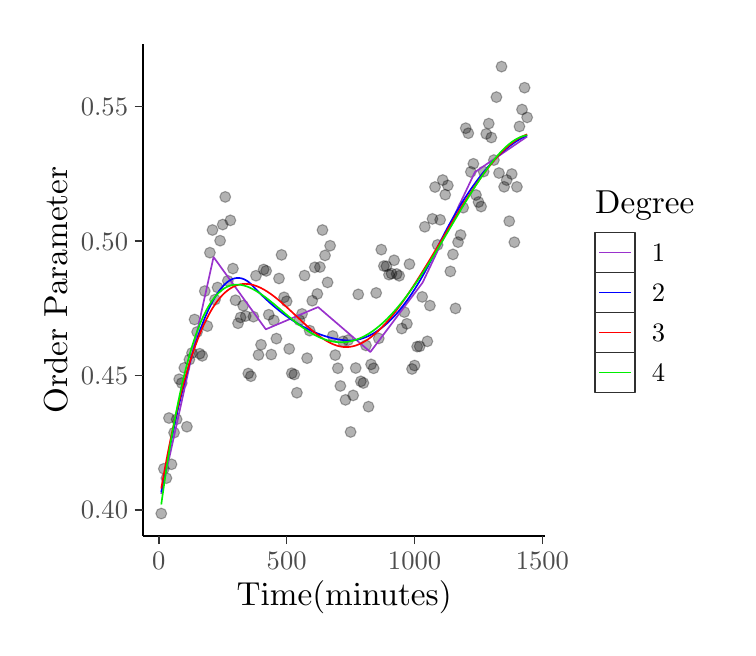
\begin{tikzpicture}[x=1pt,y=1pt]
\definecolor{fillColor}{RGB}{255,255,255}
\path[use as bounding box,fill=fillColor,fill opacity=0.00] (0,0) rectangle (252.94,216.81);
\begin{scope}
\path[clip] (  0.00,  0.00) rectangle (252.94,216.81);
\definecolor{drawColor}{RGB}{255,255,255}
\definecolor{fillColor}{RGB}{255,255,255}

\path[draw=drawColor,line width= 0.6pt,line join=round,line cap=round,fill=fillColor] (  0.00,  0.00) rectangle (252.94,216.81);
\end{scope}
\begin{scope}
\path[clip] ( 41.67, 33.16) rectangle (187.09,210.81);
\definecolor{fillColor}{RGB}{255,255,255}

\path[fill=fillColor] ( 41.67, 33.16) rectangle (187.09,210.81);
\definecolor{drawColor}{RGB}{0,0,0}
\definecolor{fillColor}{RGB}{0,0,0}

\path[draw=drawColor,draw opacity=0.30,line width= 0.4pt,line join=round,line cap=round,fill=fillColor,fill opacity=0.30] ( 48.28, 41.24) circle (  1.96);

\path[draw=drawColor,draw opacity=0.30,line width= 0.4pt,line join=round,line cap=round,fill=fillColor,fill opacity=0.30] ( 49.21, 57.42) circle (  1.96);

\path[draw=drawColor,draw opacity=0.30,line width= 0.4pt,line join=round,line cap=round,fill=fillColor,fill opacity=0.30] ( 50.13, 54.04) circle (  1.96);

\path[draw=drawColor,draw opacity=0.30,line width= 0.4pt,line join=round,line cap=round,fill=fillColor,fill opacity=0.30] ( 51.05, 75.76) circle (  1.96);

\path[draw=drawColor,draw opacity=0.30,line width= 0.4pt,line join=round,line cap=round,fill=fillColor,fill opacity=0.30] ( 51.98, 59.03) circle (  1.96);

\path[draw=drawColor,draw opacity=0.30,line width= 0.4pt,line join=round,line cap=round,fill=fillColor,fill opacity=0.30] ( 52.90, 70.46) circle (  1.96);

\path[draw=drawColor,draw opacity=0.30,line width= 0.4pt,line join=round,line cap=round,fill=fillColor,fill opacity=0.30] ( 53.83, 75.30) circle (  1.96);

\path[draw=drawColor,draw opacity=0.30,line width= 0.4pt,line join=round,line cap=round,fill=fillColor,fill opacity=0.30] ( 54.75, 89.78) circle (  1.96);

\path[draw=drawColor,draw opacity=0.30,line width= 0.4pt,line join=round,line cap=round,fill=fillColor,fill opacity=0.30] ( 55.68, 88.38) circle (  1.96);

\path[draw=drawColor,draw opacity=0.30,line width= 0.4pt,line join=round,line cap=round,fill=fillColor,fill opacity=0.30] ( 56.60, 93.89) circle (  1.96);

\path[draw=drawColor,draw opacity=0.30,line width= 0.4pt,line join=round,line cap=round,fill=fillColor,fill opacity=0.30] ( 57.53, 72.61) circle (  1.96);

\path[draw=drawColor,draw opacity=0.30,line width= 0.4pt,line join=round,line cap=round,fill=fillColor,fill opacity=0.30] ( 58.45, 96.86) circle (  1.96);

\path[draw=drawColor,draw opacity=0.30,line width= 0.4pt,line join=round,line cap=round,fill=fillColor,fill opacity=0.30] ( 59.37, 99.26) circle (  1.96);

\path[draw=drawColor,draw opacity=0.30,line width= 0.4pt,line join=round,line cap=round,fill=fillColor,fill opacity=0.30] ( 60.30,111.36) circle (  1.96);

\path[draw=drawColor,draw opacity=0.30,line width= 0.4pt,line join=round,line cap=round,fill=fillColor,fill opacity=0.30] ( 61.22,106.86) circle (  1.96);

\path[draw=drawColor,draw opacity=0.30,line width= 0.4pt,line join=round,line cap=round,fill=fillColor,fill opacity=0.30] ( 62.15, 99.00) circle (  1.96);

\path[draw=drawColor,draw opacity=0.30,line width= 0.4pt,line join=round,line cap=round,fill=fillColor,fill opacity=0.30] ( 63.07, 98.22) circle (  1.96);

\path[draw=drawColor,draw opacity=0.30,line width= 0.4pt,line join=round,line cap=round,fill=fillColor,fill opacity=0.30] ( 64.00,121.62) circle (  1.96);

\path[draw=drawColor,draw opacity=0.30,line width= 0.4pt,line join=round,line cap=round,fill=fillColor,fill opacity=0.30] ( 64.92,108.96) circle (  1.96);

\path[draw=drawColor,draw opacity=0.30,line width= 0.4pt,line join=round,line cap=round,fill=fillColor,fill opacity=0.30] ( 65.85,135.50) circle (  1.96);

\path[draw=drawColor,draw opacity=0.30,line width= 0.4pt,line join=round,line cap=round,fill=fillColor,fill opacity=0.30] ( 66.77,143.69) circle (  1.96);

\path[draw=drawColor,draw opacity=0.30,line width= 0.4pt,line join=round,line cap=round,fill=fillColor,fill opacity=0.30] ( 67.69,118.53) circle (  1.96);

\path[draw=drawColor,draw opacity=0.30,line width= 0.4pt,line join=round,line cap=round,fill=fillColor,fill opacity=0.30] ( 68.62,122.93) circle (  1.96);

\path[draw=drawColor,draw opacity=0.30,line width= 0.4pt,line join=round,line cap=round,fill=fillColor,fill opacity=0.30] ( 69.54,139.83) circle (  1.96);

\path[draw=drawColor,draw opacity=0.30,line width= 0.4pt,line join=round,line cap=round,fill=fillColor,fill opacity=0.30] ( 70.47,145.66) circle (  1.96);

\path[draw=drawColor,draw opacity=0.30,line width= 0.4pt,line join=round,line cap=round,fill=fillColor,fill opacity=0.30] ( 71.39,155.65) circle (  1.96);

\path[draw=drawColor,draw opacity=0.30,line width= 0.4pt,line join=round,line cap=round,fill=fillColor,fill opacity=0.30] ( 72.32,125.33) circle (  1.96);

\path[draw=drawColor,draw opacity=0.30,line width= 0.4pt,line join=round,line cap=round,fill=fillColor,fill opacity=0.30] ( 73.24,147.18) circle (  1.96);

\path[draw=drawColor,draw opacity=0.30,line width= 0.4pt,line join=round,line cap=round,fill=fillColor,fill opacity=0.30] ( 74.17,129.76) circle (  1.96);

\path[draw=drawColor,draw opacity=0.30,line width= 0.4pt,line join=round,line cap=round,fill=fillColor,fill opacity=0.30] ( 75.09,118.32) circle (  1.96);

\path[draw=drawColor,draw opacity=0.30,line width= 0.4pt,line join=round,line cap=round,fill=fillColor,fill opacity=0.30] ( 76.01,109.99) circle (  1.96);

\path[draw=drawColor,draw opacity=0.30,line width= 0.4pt,line join=round,line cap=round,fill=fillColor,fill opacity=0.30] ( 76.94,112.10) circle (  1.96);

\path[draw=drawColor,draw opacity=0.30,line width= 0.4pt,line join=round,line cap=round,fill=fillColor,fill opacity=0.30] ( 77.86,116.36) circle (  1.96);

\path[draw=drawColor,draw opacity=0.30,line width= 0.4pt,line join=round,line cap=round,fill=fillColor,fill opacity=0.30] ( 78.79,112.62) circle (  1.96);

\path[draw=drawColor,draw opacity=0.30,line width= 0.4pt,line join=round,line cap=round,fill=fillColor,fill opacity=0.30] ( 79.71, 91.85) circle (  1.96);

\path[draw=drawColor,draw opacity=0.30,line width= 0.4pt,line join=round,line cap=round,fill=fillColor,fill opacity=0.30] ( 80.64, 90.86) circle (  1.96);

\path[draw=drawColor,draw opacity=0.30,line width= 0.4pt,line join=round,line cap=round,fill=fillColor,fill opacity=0.30] ( 81.56,112.37) circle (  1.96);

\path[draw=drawColor,draw opacity=0.30,line width= 0.4pt,line join=round,line cap=round,fill=fillColor,fill opacity=0.30] ( 82.49,127.17) circle (  1.96);

\path[draw=drawColor,draw opacity=0.30,line width= 0.4pt,line join=round,line cap=round,fill=fillColor,fill opacity=0.30] ( 83.41, 98.54) circle (  1.96);

\path[draw=drawColor,draw opacity=0.30,line width= 0.4pt,line join=round,line cap=round,fill=fillColor,fill opacity=0.30] ( 84.33,102.24) circle (  1.96);

\path[draw=drawColor,draw opacity=0.30,line width= 0.4pt,line join=round,line cap=round,fill=fillColor,fill opacity=0.30] ( 85.26,129.43) circle (  1.96);

\path[draw=drawColor,draw opacity=0.30,line width= 0.4pt,line join=round,line cap=round,fill=fillColor,fill opacity=0.30] ( 86.18,128.92) circle (  1.96);

\path[draw=drawColor,draw opacity=0.30,line width= 0.4pt,line join=round,line cap=round,fill=fillColor,fill opacity=0.30] ( 87.11,113.09) circle (  1.96);

\path[draw=drawColor,draw opacity=0.30,line width= 0.4pt,line join=round,line cap=round,fill=fillColor,fill opacity=0.30] ( 88.03, 98.69) circle (  1.96);

\path[draw=drawColor,draw opacity=0.30,line width= 0.4pt,line join=round,line cap=round,fill=fillColor,fill opacity=0.30] ( 88.96,111.04) circle (  1.96);

\path[draw=drawColor,draw opacity=0.30,line width= 0.4pt,line join=round,line cap=round,fill=fillColor,fill opacity=0.30] ( 89.88,104.45) circle (  1.96);

\path[draw=drawColor,draw opacity=0.30,line width= 0.4pt,line join=round,line cap=round,fill=fillColor,fill opacity=0.30] ( 90.81,126.18) circle (  1.96);

\path[draw=drawColor,draw opacity=0.30,line width= 0.4pt,line join=round,line cap=round,fill=fillColor,fill opacity=0.30] ( 91.73,134.70) circle (  1.96);

\path[draw=drawColor,draw opacity=0.30,line width= 0.4pt,line join=round,line cap=round,fill=fillColor,fill opacity=0.30] ( 92.65,119.38) circle (  1.96);

\path[draw=drawColor,draw opacity=0.30,line width= 0.4pt,line join=round,line cap=round,fill=fillColor,fill opacity=0.30] ( 93.58,117.92) circle (  1.96);

\path[draw=drawColor,draw opacity=0.30,line width= 0.4pt,line join=round,line cap=round,fill=fillColor,fill opacity=0.30] ( 94.50,100.74) circle (  1.96);

\path[draw=drawColor,draw opacity=0.30,line width= 0.4pt,line join=round,line cap=round,fill=fillColor,fill opacity=0.30] ( 95.43, 91.94) circle (  1.96);

\path[draw=drawColor,draw opacity=0.30,line width= 0.4pt,line join=round,line cap=round,fill=fillColor,fill opacity=0.30] ( 96.35, 91.49) circle (  1.96);

\path[draw=drawColor,draw opacity=0.30,line width= 0.4pt,line join=round,line cap=round,fill=fillColor,fill opacity=0.30] ( 97.28, 84.89) circle (  1.96);

\path[draw=drawColor,draw opacity=0.30,line width= 0.4pt,line join=round,line cap=round,fill=fillColor,fill opacity=0.30] ( 98.20,111.09) circle (  1.96);

\path[draw=drawColor,draw opacity=0.30,line width= 0.4pt,line join=round,line cap=round,fill=fillColor,fill opacity=0.30] ( 99.13,113.38) circle (  1.96);

\path[draw=drawColor,draw opacity=0.30,line width= 0.4pt,line join=round,line cap=round,fill=fillColor,fill opacity=0.30] (100.05,127.24) circle (  1.96);

\path[draw=drawColor,draw opacity=0.30,line width= 0.4pt,line join=round,line cap=round,fill=fillColor,fill opacity=0.30] (100.97, 97.38) circle (  1.96);

\path[draw=drawColor,draw opacity=0.30,line width= 0.4pt,line join=round,line cap=round,fill=fillColor,fill opacity=0.30] (101.90,107.33) circle (  1.96);

\path[draw=drawColor,draw opacity=0.30,line width= 0.4pt,line join=round,line cap=round,fill=fillColor,fill opacity=0.30] (102.82,118.13) circle (  1.96);

\path[draw=drawColor,draw opacity=0.30,line width= 0.4pt,line join=round,line cap=round,fill=fillColor,fill opacity=0.30] (103.75,130.21) circle (  1.96);

\path[draw=drawColor,draw opacity=0.30,line width= 0.4pt,line join=round,line cap=round,fill=fillColor,fill opacity=0.30] (104.67,120.61) circle (  1.96);

\path[draw=drawColor,draw opacity=0.30,line width= 0.4pt,line join=round,line cap=round,fill=fillColor,fill opacity=0.30] (105.60,130.31) circle (  1.96);

\path[draw=drawColor,draw opacity=0.30,line width= 0.4pt,line join=round,line cap=round,fill=fillColor,fill opacity=0.30] (106.52,143.68) circle (  1.96);

\path[draw=drawColor,draw opacity=0.30,line width= 0.4pt,line join=round,line cap=round,fill=fillColor,fill opacity=0.30] (107.45,134.51) circle (  1.96);

\path[draw=drawColor,draw opacity=0.30,line width= 0.4pt,line join=round,line cap=round,fill=fillColor,fill opacity=0.30] (108.37,124.76) circle (  1.96);

\path[draw=drawColor,draw opacity=0.30,line width= 0.4pt,line join=round,line cap=round,fill=fillColor,fill opacity=0.30] (109.29,138.02) circle (  1.96);

\path[draw=drawColor,draw opacity=0.30,line width= 0.4pt,line join=round,line cap=round,fill=fillColor,fill opacity=0.30] (110.22,105.39) circle (  1.96);

\path[draw=drawColor,draw opacity=0.30,line width= 0.4pt,line join=round,line cap=round,fill=fillColor,fill opacity=0.30] (111.14, 98.49) circle (  1.96);

\path[draw=drawColor,draw opacity=0.30,line width= 0.4pt,line join=round,line cap=round,fill=fillColor,fill opacity=0.30] (112.07, 93.75) circle (  1.96);

\path[draw=drawColor,draw opacity=0.30,line width= 0.4pt,line join=round,line cap=round,fill=fillColor,fill opacity=0.30] (112.99, 87.34) circle (  1.96);

\path[draw=drawColor,draw opacity=0.30,line width= 0.4pt,line join=round,line cap=round,fill=fillColor,fill opacity=0.30] (113.92,103.45) circle (  1.96);

\path[draw=drawColor,draw opacity=0.30,line width= 0.4pt,line join=round,line cap=round,fill=fillColor,fill opacity=0.30] (114.84, 82.31) circle (  1.96);

\path[draw=drawColor,draw opacity=0.30,line width= 0.4pt,line join=round,line cap=round,fill=fillColor,fill opacity=0.30] (115.77,103.90) circle (  1.96);

\path[draw=drawColor,draw opacity=0.30,line width= 0.4pt,line join=round,line cap=round,fill=fillColor,fill opacity=0.30] (116.69, 70.71) circle (  1.96);

\path[draw=drawColor,draw opacity=0.30,line width= 0.4pt,line join=round,line cap=round,fill=fillColor,fill opacity=0.30] (117.61, 83.94) circle (  1.96);

\path[draw=drawColor,draw opacity=0.30,line width= 0.4pt,line join=round,line cap=round,fill=fillColor,fill opacity=0.30] (118.54, 93.82) circle (  1.96);

\path[draw=drawColor,draw opacity=0.30,line width= 0.4pt,line join=round,line cap=round,fill=fillColor,fill opacity=0.30] (119.46,120.43) circle (  1.96);

\path[draw=drawColor,draw opacity=0.30,line width= 0.4pt,line join=round,line cap=round,fill=fillColor,fill opacity=0.30] (120.39, 89.01) circle (  1.96);

\path[draw=drawColor,draw opacity=0.30,line width= 0.4pt,line join=round,line cap=round,fill=fillColor,fill opacity=0.30] (121.31, 88.41) circle (  1.96);

\path[draw=drawColor,draw opacity=0.30,line width= 0.4pt,line join=round,line cap=round,fill=fillColor,fill opacity=0.30] (122.24,101.99) circle (  1.96);

\path[draw=drawColor,draw opacity=0.30,line width= 0.4pt,line join=round,line cap=round,fill=fillColor,fill opacity=0.30] (123.16, 79.86) circle (  1.96);

\path[draw=drawColor,draw opacity=0.30,line width= 0.4pt,line join=round,line cap=round,fill=fillColor,fill opacity=0.30] (124.09, 95.14) circle (  1.96);

\path[draw=drawColor,draw opacity=0.30,line width= 0.4pt,line join=round,line cap=round,fill=fillColor,fill opacity=0.30] (125.01, 93.72) circle (  1.96);

\path[draw=drawColor,draw opacity=0.30,line width= 0.4pt,line join=round,line cap=round,fill=fillColor,fill opacity=0.30] (125.93,120.96) circle (  1.96);

\path[draw=drawColor,draw opacity=0.30,line width= 0.4pt,line join=round,line cap=round,fill=fillColor,fill opacity=0.30] (126.86,104.53) circle (  1.96);

\path[draw=drawColor,draw opacity=0.30,line width= 0.4pt,line join=round,line cap=round,fill=fillColor,fill opacity=0.30] (127.78,136.61) circle (  1.96);

\path[draw=drawColor,draw opacity=0.30,line width= 0.4pt,line join=round,line cap=round,fill=fillColor,fill opacity=0.30] (128.71,130.68) circle (  1.96);

\path[draw=drawColor,draw opacity=0.30,line width= 0.4pt,line join=round,line cap=round,fill=fillColor,fill opacity=0.30] (129.63,130.60) circle (  1.96);

\path[draw=drawColor,draw opacity=0.30,line width= 0.4pt,line join=round,line cap=round,fill=fillColor,fill opacity=0.30] (130.56,127.56) circle (  1.96);

\path[draw=drawColor,draw opacity=0.30,line width= 0.4pt,line join=round,line cap=round,fill=fillColor,fill opacity=0.30] (131.48,127.95) circle (  1.96);

\path[draw=drawColor,draw opacity=0.30,line width= 0.4pt,line join=round,line cap=round,fill=fillColor,fill opacity=0.30] (132.41,132.76) circle (  1.96);

\path[draw=drawColor,draw opacity=0.30,line width= 0.4pt,line join=round,line cap=round,fill=fillColor,fill opacity=0.30] (133.33,127.81) circle (  1.96);

\path[draw=drawColor,draw opacity=0.30,line width= 0.4pt,line join=round,line cap=round,fill=fillColor,fill opacity=0.30] (134.25,127.14) circle (  1.96);

\path[draw=drawColor,draw opacity=0.30,line width= 0.4pt,line join=round,line cap=round,fill=fillColor,fill opacity=0.30] (135.18,108.08) circle (  1.96);

\path[draw=drawColor,draw opacity=0.30,line width= 0.4pt,line join=round,line cap=round,fill=fillColor,fill opacity=0.30] (136.10,114.04) circle (  1.96);

\path[draw=drawColor,draw opacity=0.30,line width= 0.4pt,line join=round,line cap=round,fill=fillColor,fill opacity=0.30] (137.03,109.82) circle (  1.96);

\path[draw=drawColor,draw opacity=0.30,line width= 0.4pt,line join=round,line cap=round,fill=fillColor,fill opacity=0.30] (137.95,131.36) circle (  1.96);

\path[draw=drawColor,draw opacity=0.30,line width= 0.4pt,line join=round,line cap=round,fill=fillColor,fill opacity=0.30] (138.88, 93.47) circle (  1.96);

\path[draw=drawColor,draw opacity=0.30,line width= 0.4pt,line join=round,line cap=round,fill=fillColor,fill opacity=0.30] (139.80, 94.73) circle (  1.96);

\path[draw=drawColor,draw opacity=0.30,line width= 0.4pt,line join=round,line cap=round,fill=fillColor,fill opacity=0.30] (140.73,101.56) circle (  1.96);

\path[draw=drawColor,draw opacity=0.30,line width= 0.4pt,line join=round,line cap=round,fill=fillColor,fill opacity=0.30] (141.65,101.66) circle (  1.96);

\path[draw=drawColor,draw opacity=0.30,line width= 0.4pt,line join=round,line cap=round,fill=fillColor,fill opacity=0.30] (142.57,119.53) circle (  1.96);

\path[draw=drawColor,draw opacity=0.30,line width= 0.4pt,line join=round,line cap=round,fill=fillColor,fill opacity=0.30] (143.50,144.85) circle (  1.96);

\path[draw=drawColor,draw opacity=0.30,line width= 0.4pt,line join=round,line cap=round,fill=fillColor,fill opacity=0.30] (144.42,103.47) circle (  1.96);

\path[draw=drawColor,draw opacity=0.30,line width= 0.4pt,line join=round,line cap=round,fill=fillColor,fill opacity=0.30] (145.35,116.38) circle (  1.96);

\path[draw=drawColor,draw opacity=0.30,line width= 0.4pt,line join=round,line cap=round,fill=fillColor,fill opacity=0.30] (146.27,147.71) circle (  1.96);

\path[draw=drawColor,draw opacity=0.30,line width= 0.4pt,line join=round,line cap=round,fill=fillColor,fill opacity=0.30] (147.20,159.22) circle (  1.96);

\path[draw=drawColor,draw opacity=0.30,line width= 0.4pt,line join=round,line cap=round,fill=fillColor,fill opacity=0.30] (148.12,138.32) circle (  1.96);

\path[draw=drawColor,draw opacity=0.30,line width= 0.4pt,line join=round,line cap=round,fill=fillColor,fill opacity=0.30] (149.05,147.38) circle (  1.96);

\path[draw=drawColor,draw opacity=0.30,line width= 0.4pt,line join=round,line cap=round,fill=fillColor,fill opacity=0.30] (149.97,161.75) circle (  1.96);

\path[draw=drawColor,draw opacity=0.30,line width= 0.4pt,line join=round,line cap=round,fill=fillColor,fill opacity=0.30] (150.89,156.46) circle (  1.96);

\path[draw=drawColor,draw opacity=0.30,line width= 0.4pt,line join=round,line cap=round,fill=fillColor,fill opacity=0.30] (151.82,159.79) circle (  1.96);

\path[draw=drawColor,draw opacity=0.30,line width= 0.4pt,line join=round,line cap=round,fill=fillColor,fill opacity=0.30] (152.74,128.73) circle (  1.96);

\path[draw=drawColor,draw opacity=0.30,line width= 0.4pt,line join=round,line cap=round,fill=fillColor,fill opacity=0.30] (153.67,134.89) circle (  1.96);

\path[draw=drawColor,draw opacity=0.30,line width= 0.4pt,line join=round,line cap=round,fill=fillColor,fill opacity=0.30] (154.59,115.36) circle (  1.96);

\path[draw=drawColor,draw opacity=0.30,line width= 0.4pt,line join=round,line cap=round,fill=fillColor,fill opacity=0.30] (155.52,139.30) circle (  1.96);

\path[draw=drawColor,draw opacity=0.30,line width= 0.4pt,line join=round,line cap=round,fill=fillColor,fill opacity=0.30] (156.44,141.89) circle (  1.96);

\path[draw=drawColor,draw opacity=0.30,line width= 0.4pt,line join=round,line cap=round,fill=fillColor,fill opacity=0.30] (157.37,151.76) circle (  1.96);

\path[draw=drawColor,draw opacity=0.30,line width= 0.4pt,line join=round,line cap=round,fill=fillColor,fill opacity=0.30] (158.29,180.49) circle (  1.96);

\path[draw=drawColor,draw opacity=0.30,line width= 0.4pt,line join=round,line cap=round,fill=fillColor,fill opacity=0.30] (159.22,178.66) circle (  1.96);

\path[draw=drawColor,draw opacity=0.30,line width= 0.4pt,line join=round,line cap=round,fill=fillColor,fill opacity=0.30] (160.14,164.70) circle (  1.96);

\path[draw=drawColor,draw opacity=0.30,line width= 0.4pt,line join=round,line cap=round,fill=fillColor,fill opacity=0.30] (161.06,167.62) circle (  1.96);

\path[draw=drawColor,draw opacity=0.30,line width= 0.4pt,line join=round,line cap=round,fill=fillColor,fill opacity=0.30] (161.99,156.35) circle (  1.96);

\path[draw=drawColor,draw opacity=0.30,line width= 0.4pt,line join=round,line cap=round,fill=fillColor,fill opacity=0.30] (162.91,153.80) circle (  1.96);

\path[draw=drawColor,draw opacity=0.30,line width= 0.4pt,line join=round,line cap=round,fill=fillColor,fill opacity=0.30] (163.84,152.16) circle (  1.96);

\path[draw=drawColor,draw opacity=0.30,line width= 0.4pt,line join=round,line cap=round,fill=fillColor,fill opacity=0.30] (164.76,164.81) circle (  1.96);

\path[draw=drawColor,draw opacity=0.30,line width= 0.4pt,line join=round,line cap=round,fill=fillColor,fill opacity=0.30] (165.69,178.43) circle (  1.96);

\path[draw=drawColor,draw opacity=0.30,line width= 0.4pt,line join=round,line cap=round,fill=fillColor,fill opacity=0.30] (166.61,182.14) circle (  1.96);

\path[draw=drawColor,draw opacity=0.30,line width= 0.4pt,line join=round,line cap=round,fill=fillColor,fill opacity=0.30] (167.54,177.11) circle (  1.96);

\path[draw=drawColor,draw opacity=0.30,line width= 0.4pt,line join=round,line cap=round,fill=fillColor,fill opacity=0.30] (168.46,168.96) circle (  1.96);

\path[draw=drawColor,draw opacity=0.30,line width= 0.4pt,line join=round,line cap=round,fill=fillColor,fill opacity=0.30] (169.38,191.71) circle (  1.96);

\path[draw=drawColor,draw opacity=0.30,line width= 0.4pt,line join=round,line cap=round,fill=fillColor,fill opacity=0.30] (170.31,164.28) circle (  1.96);

\path[draw=drawColor,draw opacity=0.30,line width= 0.4pt,line join=round,line cap=round,fill=fillColor,fill opacity=0.30] (171.23,202.74) circle (  1.96);

\path[draw=drawColor,draw opacity=0.30,line width= 0.4pt,line join=round,line cap=round,fill=fillColor,fill opacity=0.30] (172.16,159.30) circle (  1.96);

\path[draw=drawColor,draw opacity=0.30,line width= 0.4pt,line join=round,line cap=round,fill=fillColor,fill opacity=0.30] (173.08,161.74) circle (  1.96);

\path[draw=drawColor,draw opacity=0.30,line width= 0.4pt,line join=round,line cap=round,fill=fillColor,fill opacity=0.30] (174.01,146.88) circle (  1.96);

\path[draw=drawColor,draw opacity=0.30,line width= 0.4pt,line join=round,line cap=round,fill=fillColor,fill opacity=0.30] (174.93,163.93) circle (  1.96);

\path[draw=drawColor,draw opacity=0.30,line width= 0.4pt,line join=round,line cap=round,fill=fillColor,fill opacity=0.30] (175.86,139.28) circle (  1.96);

\path[draw=drawColor,draw opacity=0.30,line width= 0.4pt,line join=round,line cap=round,fill=fillColor,fill opacity=0.30] (176.78,159.29) circle (  1.96);

\path[draw=drawColor,draw opacity=0.30,line width= 0.4pt,line join=round,line cap=round,fill=fillColor,fill opacity=0.30] (177.70,181.11) circle (  1.96);

\path[draw=drawColor,draw opacity=0.30,line width= 0.4pt,line join=round,line cap=round,fill=fillColor,fill opacity=0.30] (178.63,187.22) circle (  1.96);

\path[draw=drawColor,draw opacity=0.30,line width= 0.4pt,line join=round,line cap=round,fill=fillColor,fill opacity=0.30] (179.55,195.12) circle (  1.96);

\path[draw=drawColor,draw opacity=0.30,line width= 0.4pt,line join=round,line cap=round,fill=fillColor,fill opacity=0.30] (180.48,184.39) circle (  1.96);
\definecolor{drawColor}{RGB}{153,50,204}

\path[draw=drawColor,line width= 0.6pt,line join=round] ( 48.28, 48.29) --
	( 48.37, 48.71) --
	( 48.47, 49.13) --
	( 48.56, 49.55) --
	( 48.65, 49.97) --
	( 48.74, 50.39) --
	( 48.84, 50.81) --
	( 48.93, 51.23) --
	( 49.02, 51.65) --
	( 49.11, 52.07) --
	( 49.21, 52.49) --
	( 49.30, 52.91) --
	( 49.39, 53.32) --
	( 49.48, 53.74) --
	( 49.58, 54.16) --
	( 49.67, 54.58) --
	( 49.76, 55.00) --
	( 49.85, 55.42) --
	( 49.95, 55.84) --
	( 50.04, 56.26) --
	( 50.13, 56.68) --
	( 50.22, 57.10) --
	( 50.31, 57.52) --
	( 50.41, 57.94) --
	( 50.50, 58.35) --
	( 50.59, 58.77) --
	( 50.68, 59.19) --
	( 50.78, 59.61) --
	( 50.87, 60.03) --
	( 50.96, 60.45) --
	( 51.05, 60.87) --
	( 51.15, 61.29) --
	( 51.24, 61.71) --
	( 51.33, 62.13) --
	( 51.42, 62.55) --
	( 51.52, 62.97) --
	( 51.61, 63.39) --
	( 51.70, 63.80) --
	( 51.79, 64.22) --
	( 51.89, 64.64) --
	( 51.98, 65.06) --
	( 52.07, 65.48) --
	( 52.16, 65.90) --
	( 52.26, 66.32) --
	( 52.35, 66.74) --
	( 52.44, 67.16) --
	( 52.53, 67.58) --
	( 52.63, 68.00) --
	( 52.72, 68.42) --
	( 52.81, 68.83) --
	( 52.90, 69.25) --
	( 53.00, 69.67) --
	( 53.09, 70.09) --
	( 53.18, 70.51) --
	( 53.27, 70.93) --
	( 53.37, 71.35) --
	( 53.46, 71.77) --
	( 53.55, 72.19) --
	( 53.64, 72.61) --
	( 53.74, 73.03) --
	( 53.83, 73.45) --
	( 53.92, 73.86) --
	( 54.01, 74.28) --
	( 54.11, 74.70) --
	( 54.20, 75.12) --
	( 54.29, 75.54) --
	( 54.38, 75.96) --
	( 54.47, 76.38) --
	( 54.57, 76.80) --
	( 54.66, 77.22) --
	( 54.75, 77.64) --
	( 54.84, 78.06) --
	( 54.94, 78.48) --
	( 55.03, 78.90) --
	( 55.12, 79.31) --
	( 55.21, 79.73) --
	( 55.31, 80.15) --
	( 55.40, 80.57) --
	( 55.49, 80.99) --
	( 55.58, 81.41) --
	( 55.68, 81.83) --
	( 55.77, 82.25) --
	( 55.86, 82.67) --
	( 55.95, 83.09) --
	( 56.05, 83.51) --
	( 56.14, 83.93) --
	( 56.23, 84.34) --
	( 56.32, 84.76) --
	( 56.42, 85.18) --
	( 56.51, 85.60) --
	( 56.60, 86.02) --
	( 56.69, 86.44) --
	( 56.79, 86.86) --
	( 56.88, 87.28) --
	( 56.97, 87.70) --
	( 57.06, 88.12) --
	( 57.16, 88.54) --
	( 57.25, 88.96) --
	( 57.34, 89.37) --
	( 57.43, 89.79) --
	( 57.53, 90.21) --
	( 57.62, 90.63) --
	( 57.71, 91.05) --
	( 57.80, 91.47) --
	( 57.90, 91.89) --
	( 57.99, 92.31) --
	( 58.08, 92.73) --
	( 58.17, 93.15) --
	( 58.27, 93.57) --
	( 58.36, 93.99) --
	( 58.45, 94.40) --
	( 58.54, 94.82) --
	( 58.63, 95.24) --
	( 58.73, 95.66) --
	( 58.82, 96.08) --
	( 58.91, 96.50) --
	( 59.00, 96.92) --
	( 59.10, 97.34) --
	( 59.19, 97.76) --
	( 59.28, 98.18) --
	( 59.37, 98.60) --
	( 59.47, 99.02) --
	( 59.56, 99.44) --
	( 59.65, 99.85) --
	( 59.74,100.27) --
	( 59.84,100.69) --
	( 59.93,101.11) --
	( 60.02,101.53) --
	( 60.11,101.95) --
	( 60.21,102.37) --
	( 60.30,102.79) --
	( 60.39,103.21) --
	( 60.48,103.63) --
	( 60.58,104.05) --
	( 60.67,104.47) --
	( 60.76,104.88) --
	( 60.85,105.30) --
	( 60.95,105.72) --
	( 61.04,106.14) --
	( 61.13,106.56) --
	( 61.22,106.98) --
	( 61.32,107.40) --
	( 61.41,107.82) --
	( 61.50,108.24) --
	( 61.59,108.66) --
	( 61.69,109.08) --
	( 61.78,109.50) --
	( 61.87,109.91) --
	( 61.96,110.33) --
	( 62.06,110.75) --
	( 62.15,111.17) --
	( 62.24,111.59) --
	( 62.33,112.01) --
	( 62.43,112.43) --
	( 62.52,112.85) --
	( 62.61,113.27) --
	( 62.70,113.69) --
	( 62.79,114.11) --
	( 62.89,114.53) --
	( 62.98,114.95) --
	( 63.07,115.36) --
	( 63.16,115.78) --
	( 63.26,116.20) --
	( 63.35,116.62) --
	( 63.44,117.04) --
	( 63.53,117.46) --
	( 63.63,117.88) --
	( 63.72,118.30) --
	( 63.81,118.72) --
	( 63.90,119.14) --
	( 64.00,119.56) --
	( 64.09,119.98) --
	( 64.18,120.39) --
	( 64.27,120.81) --
	( 64.37,121.23) --
	( 64.46,121.65) --
	( 64.55,122.07) --
	( 64.64,122.49) --
	( 64.74,122.91) --
	( 64.83,123.33) --
	( 64.92,123.75) --
	( 65.01,124.17) --
	( 65.11,124.59) --
	( 65.20,125.01) --
	( 65.29,125.42) --
	( 65.38,125.84) --
	( 65.48,126.26) --
	( 65.57,126.68) --
	( 65.66,127.10) --
	( 65.75,127.52) --
	( 65.85,127.94) --
	( 65.94,128.36) --
	( 66.03,128.78) --
	( 66.12,129.20) --
	( 66.22,129.62) --
	( 66.31,130.04) --
	( 66.40,130.46) --
	( 66.49,130.87) --
	( 66.59,131.29) --
	( 66.68,131.71) --
	( 66.77,132.13) --
	( 66.86,132.55) --
	( 66.95,132.97) --
	( 67.05,133.39) --
	( 67.14,133.81) --
	( 67.23,133.84) --
	( 67.32,133.71) --
	( 67.42,133.58) --
	( 67.51,133.45) --
	( 67.60,133.33) --
	( 67.69,133.20) --
	( 67.79,133.07) --
	( 67.88,132.94) --
	( 67.97,132.81) --
	( 68.06,132.69) --
	( 68.16,132.56) --
	( 68.25,132.43) --
	( 68.34,132.30) --
	( 68.43,132.17) --
	( 68.53,132.05) --
	( 68.62,131.92) --
	( 68.71,131.79) --
	( 68.80,131.66) --
	( 68.90,131.54) --
	( 68.99,131.41) --
	( 69.08,131.28) --
	( 69.17,131.15) --
	( 69.27,131.02) --
	( 69.36,130.90) --
	( 69.45,130.77) --
	( 69.54,130.64) --
	( 69.64,130.51) --
	( 69.73,130.38) --
	( 69.82,130.26) --
	( 69.91,130.13) --
	( 70.01,130.00) --
	( 70.10,129.87) --
	( 70.19,129.75) --
	( 70.28,129.62) --
	( 70.38,129.49) --
	( 70.47,129.36) --
	( 70.56,129.23) --
	( 70.65,129.11) --
	( 70.75,128.98) --
	( 70.84,128.85) --
	( 70.93,128.72) --
	( 71.02,128.59) --
	( 71.11,128.47) --
	( 71.21,128.34) --
	( 71.30,128.21) --
	( 71.39,128.08) --
	( 71.48,127.96) --
	( 71.58,127.83) --
	( 71.67,127.70) --
	( 71.76,127.57) --
	( 71.85,127.44) --
	( 71.95,127.32) --
	( 72.04,127.19) --
	( 72.13,127.06) --
	( 72.22,126.93) --
	( 72.32,126.80) --
	( 72.41,126.68) --
	( 72.50,126.55) --
	( 72.59,126.42) --
	( 72.69,126.29) --
	( 72.78,126.17) --
	( 72.87,126.04) --
	( 72.96,125.91) --
	( 73.06,125.78) --
	( 73.15,125.65) --
	( 73.24,125.53) --
	( 73.33,125.40) --
	( 73.43,125.27) --
	( 73.52,125.14) --
	( 73.61,125.01) --
	( 73.70,124.89) --
	( 73.80,124.76) --
	( 73.89,124.63) --
	( 73.98,124.50) --
	( 74.07,124.38) --
	( 74.17,124.25) --
	( 74.26,124.12) --
	( 74.35,123.99) --
	( 74.44,123.86) --
	( 74.54,123.74) --
	( 74.63,123.61) --
	( 74.72,123.48) --
	( 74.81,123.35) --
	( 74.91,123.22) --
	( 75.00,123.10) --
	( 75.09,122.97) --
	( 75.18,122.84) --
	( 75.27,122.71) --
	( 75.37,122.59) --
	( 75.46,122.46) --
	( 75.55,122.33) --
	( 75.64,122.20) --
	( 75.74,122.07) --
	( 75.83,121.95) --
	( 75.92,121.82) --
	( 76.01,121.69) --
	( 76.11,121.56) --
	( 76.20,121.43) --
	( 76.29,121.31) --
	( 76.38,121.18) --
	( 76.48,121.05) --
	( 76.57,120.92) --
	( 76.66,120.80) --
	( 76.75,120.67) --
	( 76.85,120.54) --
	( 76.94,120.41) --
	( 77.03,120.28) --
	( 77.12,120.16) --
	( 77.22,120.03) --
	( 77.31,119.90) --
	( 77.40,119.77) --
	( 77.49,119.64) --
	( 77.59,119.52) --
	( 77.68,119.39) --
	( 77.77,119.26) --
	( 77.86,119.13) --
	( 77.96,119.01) --
	( 78.05,118.88) --
	( 78.14,118.75) --
	( 78.23,118.62) --
	( 78.33,118.49) --
	( 78.42,118.37) --
	( 78.51,118.24) --
	( 78.60,118.11) --
	( 78.70,117.98) --
	( 78.79,117.85) --
	( 78.88,117.73) --
	( 78.97,117.60) --
	( 79.07,117.47) --
	( 79.16,117.34) --
	( 79.25,117.21) --
	( 79.34,117.09) --
	( 79.43,116.96) --
	( 79.53,116.83) --
	( 79.62,116.70) --
	( 79.71,116.58) --
	( 79.80,116.45) --
	( 79.90,116.32) --
	( 79.99,116.19) --
	( 80.08,116.06) --
	( 80.17,115.94) --
	( 80.27,115.81) --
	( 80.36,115.68) --
	( 80.45,115.55) --
	( 80.54,115.42) --
	( 80.64,115.30) --
	( 80.73,115.17) --
	( 80.82,115.04) --
	( 80.91,114.91) --
	( 81.01,114.79) --
	( 81.10,114.66) --
	( 81.19,114.53) --
	( 81.28,114.40) --
	( 81.38,114.27) --
	( 81.47,114.15) --
	( 81.56,114.02) --
	( 81.65,113.89) --
	( 81.75,113.76) --
	( 81.84,113.63) --
	( 81.93,113.51) --
	( 82.02,113.38) --
	( 82.12,113.25) --
	( 82.21,113.12) --
	( 82.30,113.00) --
	( 82.39,112.87) --
	( 82.49,112.74) --
	( 82.58,112.61) --
	( 82.67,112.48) --
	( 82.76,112.36) --
	( 82.86,112.23) --
	( 82.95,112.10) --
	( 83.04,111.97) --
	( 83.13,111.84) --
	( 83.23,111.72) --
	( 83.32,111.59) --
	( 83.41,111.46) --
	( 83.50,111.33) --
	( 83.59,111.21) --
	( 83.69,111.08) --
	( 83.78,110.95) --
	( 83.87,110.82) --
	( 83.96,110.69) --
	( 84.06,110.57) --
	( 84.15,110.44) --
	( 84.24,110.31) --
	( 84.33,110.18) --
	( 84.43,110.05) --
	( 84.52,109.93) --
	( 84.61,109.80) --
	( 84.70,109.67) --
	( 84.80,109.54) --
	( 84.89,109.42) --
	( 84.98,109.29) --
	( 85.07,109.16) --
	( 85.17,109.03) --
	( 85.26,108.90) --
	( 85.35,108.78) --
	( 85.44,108.65) --
	( 85.54,108.52) --
	( 85.63,108.39) --
	( 85.72,108.26) --
	( 85.81,108.14) --
	( 85.91,108.01) --
	( 86.00,107.88) --
	( 86.09,107.82) --
	( 86.18,107.86) --
	( 86.28,107.90) --
	( 86.37,107.94) --
	( 86.46,107.98) --
	( 86.55,108.02) --
	( 86.65,108.06) --
	( 86.74,108.10) --
	( 86.83,108.14) --
	( 86.92,108.18) --
	( 87.02,108.22) --
	( 87.11,108.26) --
	( 87.20,108.30) --
	( 87.29,108.34) --
	( 87.39,108.38) --
	( 87.48,108.41) --
	( 87.57,108.45) --
	( 87.66,108.49) --
	( 87.76,108.53) --
	( 87.85,108.57) --
	( 87.94,108.61) --
	( 88.03,108.65) --
	( 88.12,108.69) --
	( 88.22,108.73) --
	( 88.31,108.77) --
	( 88.40,108.81) --
	( 88.49,108.85) --
	( 88.59,108.89) --
	( 88.68,108.93) --
	( 88.77,108.97) --
	( 88.86,109.01) --
	( 88.96,109.04) --
	( 89.05,109.08) --
	( 89.14,109.12) --
	( 89.23,109.16) --
	( 89.33,109.20) --
	( 89.42,109.24) --
	( 89.51,109.28) --
	( 89.60,109.32) --
	( 89.70,109.36) --
	( 89.79,109.40) --
	( 89.88,109.44) --
	( 89.97,109.48) --
	( 90.07,109.52) --
	( 90.16,109.56) --
	( 90.25,109.60) --
	( 90.34,109.63) --
	( 90.44,109.67) --
	( 90.53,109.71) --
	( 90.62,109.75) --
	( 90.71,109.79) --
	( 90.81,109.83) --
	( 90.90,109.87) --
	( 90.99,109.91) --
	( 91.08,109.95) --
	( 91.18,109.99) --
	( 91.27,110.03) --
	( 91.36,110.07) --
	( 91.45,110.11) --
	( 91.55,110.15) --
	( 91.64,110.19) --
	( 91.73,110.22) --
	( 91.82,110.26) --
	( 91.92,110.30) --
	( 92.01,110.34) --
	( 92.10,110.38) --
	( 92.19,110.42) --
	( 92.28,110.46) --
	( 92.38,110.50) --
	( 92.47,110.54) --
	( 92.56,110.58) --
	( 92.65,110.62) --
	( 92.75,110.66) --
	( 92.84,110.70) --
	( 92.93,110.74) --
	( 93.02,110.78) --
	( 93.12,110.81) --
	( 93.21,110.85) --
	( 93.30,110.89) --
	( 93.39,110.93) --
	( 93.49,110.97) --
	( 93.58,111.01) --
	( 93.67,111.05) --
	( 93.76,111.09) --
	( 93.86,111.13) --
	( 93.95,111.17) --
	( 94.04,111.21) --
	( 94.13,111.25) --
	( 94.23,111.29) --
	( 94.32,111.33) --
	( 94.41,111.37) --
	( 94.50,111.41) --
	( 94.60,111.44) --
	( 94.69,111.48) --
	( 94.78,111.52) --
	( 94.87,111.56) --
	( 94.97,111.60) --
	( 95.06,111.64) --
	( 95.15,111.68) --
	( 95.24,111.72) --
	( 95.34,111.76) --
	( 95.43,111.80) --
	( 95.52,111.84) --
	( 95.61,111.88) --
	( 95.71,111.92) --
	( 95.80,111.96) --
	( 95.89,112.00) --
	( 95.98,112.03) --
	( 96.08,112.07) --
	( 96.17,112.11) --
	( 96.26,112.15) --
	( 96.35,112.19) --
	( 96.44,112.23) --
	( 96.54,112.27) --
	( 96.63,112.31) --
	( 96.72,112.35) --
	( 96.81,112.39) --
	( 96.91,112.43) --
	( 97.00,112.47) --
	( 97.09,112.51) --
	( 97.18,112.55) --
	( 97.28,112.59) --
	( 97.37,112.62) --
	( 97.46,112.66) --
	( 97.55,112.70) --
	( 97.65,112.74) --
	( 97.74,112.78) --
	( 97.83,112.82) --
	( 97.92,112.86) --
	( 98.02,112.90) --
	( 98.11,112.94) --
	( 98.20,112.98) --
	( 98.29,113.02) --
	( 98.39,113.06) --
	( 98.48,113.10) --
	( 98.57,113.14) --
	( 98.66,113.18) --
	( 98.76,113.21) --
	( 98.85,113.25) --
	( 98.94,113.29) --
	( 99.03,113.33) --
	( 99.13,113.37) --
	( 99.22,113.41) --
	( 99.31,113.45) --
	( 99.40,113.49) --
	( 99.50,113.53) --
	( 99.59,113.57) --
	( 99.68,113.61) --
	( 99.77,113.65) --
	( 99.87,113.69) --
	( 99.96,113.73) --
	(100.05,113.77) --
	(100.14,113.80) --
	(100.24,113.84) --
	(100.33,113.88) --
	(100.42,113.92) --
	(100.51,113.96) --
	(100.60,114.00) --
	(100.70,114.04) --
	(100.79,114.08) --
	(100.88,114.12) --
	(100.97,114.16) --
	(101.07,114.20) --
	(101.16,114.24) --
	(101.25,114.28) --
	(101.34,114.32) --
	(101.44,114.36) --
	(101.53,114.40) --
	(101.62,114.43) --
	(101.71,114.47) --
	(101.81,114.51) --
	(101.90,114.55) --
	(101.99,114.59) --
	(102.08,114.63) --
	(102.18,114.67) --
	(102.27,114.71) --
	(102.36,114.75) --
	(102.45,114.79) --
	(102.55,114.83) --
	(102.64,114.87) --
	(102.73,114.91) --
	(102.82,114.95) --
	(102.92,114.99) --
	(103.01,115.02) --
	(103.10,115.06) --
	(103.19,115.10) --
	(103.29,115.14) --
	(103.38,115.18) --
	(103.47,115.22) --
	(103.56,115.26) --
	(103.66,115.30) --
	(103.75,115.34) --
	(103.84,115.38) --
	(103.93,115.42) --
	(104.03,115.46) --
	(104.12,115.50) --
	(104.21,115.54) --
	(104.30,115.58) --
	(104.40,115.61) --
	(104.49,115.65) --
	(104.58,115.69) --
	(104.67,115.73) --
	(104.76,115.77) --
	(104.86,115.81) --
	(104.95,115.83) --
	(105.04,115.75) --
	(105.13,115.67) --
	(105.23,115.60) --
	(105.32,115.52) --
	(105.41,115.44) --
	(105.50,115.36) --
	(105.60,115.28) --
	(105.69,115.20) --
	(105.78,115.12) --
	(105.87,115.04) --
	(105.97,114.96) --
	(106.06,114.88) --
	(106.15,114.80) --
	(106.24,114.72) --
	(106.34,114.64) --
	(106.43,114.56) --
	(106.52,114.48) --
	(106.61,114.40) --
	(106.71,114.32) --
	(106.80,114.24) --
	(106.89,114.17) --
	(106.98,114.09) --
	(107.08,114.01) --
	(107.17,113.93) --
	(107.26,113.85) --
	(107.35,113.77) --
	(107.45,113.69) --
	(107.54,113.61) --
	(107.63,113.53) --
	(107.72,113.45) --
	(107.82,113.37) --
	(107.91,113.29) --
	(108.00,113.21) --
	(108.09,113.13) --
	(108.19,113.05) --
	(108.28,112.97) --
	(108.37,112.89) --
	(108.46,112.81) --
	(108.56,112.74) --
	(108.65,112.66) --
	(108.74,112.58) --
	(108.83,112.50) --
	(108.92,112.42) --
	(109.02,112.34) --
	(109.11,112.26) --
	(109.20,112.18) --
	(109.29,112.10) --
	(109.39,112.02) --
	(109.48,111.94) --
	(109.57,111.86) --
	(109.66,111.78) --
	(109.76,111.70) --
	(109.85,111.62) --
	(109.94,111.54) --
	(110.03,111.46) --
	(110.13,111.38) --
	(110.22,111.30) --
	(110.31,111.23) --
	(110.40,111.15) --
	(110.50,111.07) --
	(110.59,110.99) --
	(110.68,110.91) --
	(110.77,110.83) --
	(110.87,110.75) --
	(110.96,110.67) --
	(111.05,110.59) --
	(111.14,110.51) --
	(111.24,110.43) --
	(111.33,110.35) --
	(111.42,110.27) --
	(111.51,110.19) --
	(111.61,110.11) --
	(111.70,110.03) --
	(111.79,109.95) --
	(111.88,109.87) --
	(111.98,109.80) --
	(112.07,109.72) --
	(112.16,109.64) --
	(112.25,109.56) --
	(112.35,109.48) --
	(112.44,109.40) --
	(112.53,109.32) --
	(112.62,109.24) --
	(112.72,109.16) --
	(112.81,109.08) --
	(112.90,109.00) --
	(112.99,108.92) --
	(113.08,108.84) --
	(113.18,108.76) --
	(113.27,108.68) --
	(113.36,108.60) --
	(113.45,108.52) --
	(113.55,108.44) --
	(113.64,108.36) --
	(113.73,108.29) --
	(113.82,108.21) --
	(113.92,108.13) --
	(114.01,108.05) --
	(114.10,107.97) --
	(114.19,107.89) --
	(114.29,107.81) --
	(114.38,107.73) --
	(114.47,107.65) --
	(114.56,107.57) --
	(114.66,107.49) --
	(114.75,107.41) --
	(114.84,107.33) --
	(114.93,107.25) --
	(115.03,107.17) --
	(115.12,107.09) --
	(115.21,107.01) --
	(115.30,106.93) --
	(115.40,106.86) --
	(115.49,106.78) --
	(115.58,106.70) --
	(115.67,106.62) --
	(115.77,106.54) --
	(115.86,106.46) --
	(115.95,106.38) --
	(116.04,106.30) --
	(116.14,106.22) --
	(116.23,106.14) --
	(116.32,106.06) --
	(116.41,105.98) --
	(116.51,105.90) --
	(116.60,105.82) --
	(116.69,105.74) --
	(116.78,105.66) --
	(116.88,105.58) --
	(116.97,105.50) --
	(117.06,105.43) --
	(117.15,105.35) --
	(117.24,105.27) --
	(117.34,105.19) --
	(117.43,105.11) --
	(117.52,105.03) --
	(117.61,104.95) --
	(117.71,104.87) --
	(117.80,104.79) --
	(117.89,104.71) --
	(117.98,104.63) --
	(118.08,104.55) --
	(118.17,104.47) --
	(118.26,104.39) --
	(118.35,104.31) --
	(118.45,104.23) --
	(118.54,104.15) --
	(118.63,104.07) --
	(118.72,103.99) --
	(118.82,103.92) --
	(118.91,103.84) --
	(119.00,103.76) --
	(119.09,103.68) --
	(119.19,103.60) --
	(119.28,103.52) --
	(119.37,103.44) --
	(119.46,103.36) --
	(119.56,103.28) --
	(119.65,103.20) --
	(119.74,103.12) --
	(119.83,103.04) --
	(119.93,102.96) --
	(120.02,102.88) --
	(120.11,102.80) --
	(120.20,102.72) --
	(120.30,102.64) --
	(120.39,102.56) --
	(120.48,102.49) --
	(120.57,102.41) --
	(120.67,102.33) --
	(120.76,102.25) --
	(120.85,102.17) --
	(120.94,102.09) --
	(121.04,102.01) --
	(121.13,101.93) --
	(121.22,101.85) --
	(121.31,101.77) --
	(121.41,101.69) --
	(121.50,101.61) --
	(121.59,101.53) --
	(121.68,101.45) --
	(121.77,101.37) --
	(121.87,101.29) --
	(121.96,101.21) --
	(122.05,101.13) --
	(122.14,101.05) --
	(122.24,100.98) --
	(122.33,100.90) --
	(122.42,100.82) --
	(122.51,100.74) --
	(122.61,100.66) --
	(122.70,100.58) --
	(122.79,100.50) --
	(122.88,100.42) --
	(122.98,100.34) --
	(123.07,100.26) --
	(123.16,100.18) --
	(123.25,100.10) --
	(123.35,100.02) --
	(123.44, 99.94) --
	(123.53, 99.86) --
	(123.62, 99.78) --
	(123.72, 99.70) --
	(123.81, 99.62) --
	(123.90, 99.72) --
	(123.99, 99.84) --
	(124.09, 99.96) --
	(124.18,100.09) --
	(124.27,100.21) --
	(124.36,100.33) --
	(124.46,100.45) --
	(124.55,100.58) --
	(124.64,100.70) --
	(124.73,100.82) --
	(124.83,100.95) --
	(124.92,101.07) --
	(125.01,101.19) --
	(125.10,101.31) --
	(125.20,101.44) --
	(125.29,101.56) --
	(125.38,101.68) --
	(125.47,101.80) --
	(125.57,101.93) --
	(125.66,102.05) --
	(125.75,102.17) --
	(125.84,102.30) --
	(125.93,102.42) --
	(126.03,102.54) --
	(126.12,102.66) --
	(126.21,102.79) --
	(126.30,102.91) --
	(126.40,103.03) --
	(126.49,103.15) --
	(126.58,103.28) --
	(126.67,103.40) --
	(126.77,103.52) --
	(126.86,103.65) --
	(126.95,103.77) --
	(127.04,103.89) --
	(127.14,104.01) --
	(127.23,104.14) --
	(127.32,104.26) --
	(127.41,104.38) --
	(127.51,104.51) --
	(127.60,104.63) --
	(127.69,104.75) --
	(127.78,104.87) --
	(127.88,105.00) --
	(127.97,105.12) --
	(128.06,105.24) --
	(128.15,105.36) --
	(128.25,105.49) --
	(128.34,105.61) --
	(128.43,105.73) --
	(128.52,105.86) --
	(128.62,105.98) --
	(128.71,106.10) --
	(128.80,106.22) --
	(128.89,106.35) --
	(128.99,106.47) --
	(129.08,106.59) --
	(129.17,106.71) --
	(129.26,106.84) --
	(129.36,106.96) --
	(129.45,107.08) --
	(129.54,107.21) --
	(129.63,107.33) --
	(129.73,107.45) --
	(129.82,107.57) --
	(129.91,107.70) --
	(130.00,107.82) --
	(130.09,107.94) --
	(130.19,108.06) --
	(130.28,108.19) --
	(130.37,108.31) --
	(130.46,108.43) --
	(130.56,108.56) --
	(130.65,108.68) --
	(130.74,108.80) --
	(130.83,108.92) --
	(130.93,109.05) --
	(131.02,109.17) --
	(131.11,109.29) --
	(131.20,109.41) --
	(131.30,109.54) --
	(131.39,109.66) --
	(131.48,109.78) --
	(131.57,109.91) --
	(131.67,110.03) --
	(131.76,110.15) --
	(131.85,110.27) --
	(131.94,110.40) --
	(132.04,110.52) --
	(132.13,110.64) --
	(132.22,110.76) --
	(132.31,110.89) --
	(132.41,111.01) --
	(132.50,111.13) --
	(132.59,111.26) --
	(132.68,111.38) --
	(132.78,111.50) --
	(132.87,111.62) --
	(132.96,111.75) --
	(133.05,111.87) --
	(133.15,111.99) --
	(133.24,112.11) --
	(133.33,112.24) --
	(133.42,112.36) --
	(133.52,112.48) --
	(133.61,112.61) --
	(133.70,112.73) --
	(133.79,112.85) --
	(133.89,112.97) --
	(133.98,113.10) --
	(134.07,113.22) --
	(134.16,113.34) --
	(134.25,113.46) --
	(134.35,113.59) --
	(134.44,113.71) --
	(134.53,113.83) --
	(134.62,113.96) --
	(134.72,114.08) --
	(134.81,114.20) --
	(134.90,114.32) --
	(134.99,114.45) --
	(135.09,114.57) --
	(135.18,114.69) --
	(135.27,114.81) --
	(135.36,114.94) --
	(135.46,115.06) --
	(135.55,115.18) --
	(135.64,115.31) --
	(135.73,115.43) --
	(135.83,115.55) --
	(135.92,115.67) --
	(136.01,115.80) --
	(136.10,115.92) --
	(136.20,116.04) --
	(136.29,116.16) --
	(136.38,116.29) --
	(136.47,116.41) --
	(136.57,116.53) --
	(136.66,116.66) --
	(136.75,116.78) --
	(136.84,116.90) --
	(136.94,117.02) --
	(137.03,117.15) --
	(137.12,117.27) --
	(137.21,117.39) --
	(137.31,117.51) --
	(137.40,117.64) --
	(137.49,117.76) --
	(137.58,117.88) --
	(137.68,118.01) --
	(137.77,118.13) --
	(137.86,118.25) --
	(137.95,118.37) --
	(138.05,118.50) --
	(138.14,118.62) --
	(138.23,118.74) --
	(138.32,118.86) --
	(138.41,118.99) --
	(138.51,119.11) --
	(138.60,119.23) --
	(138.69,119.36) --
	(138.78,119.48) --
	(138.88,119.60) --
	(138.97,119.72) --
	(139.06,119.85) --
	(139.15,119.97) --
	(139.25,120.09) --
	(139.34,120.21) --
	(139.43,120.34) --
	(139.52,120.46) --
	(139.62,120.58) --
	(139.71,120.71) --
	(139.80,120.83) --
	(139.89,120.95) --
	(139.99,121.07) --
	(140.08,121.20) --
	(140.17,121.32) --
	(140.26,121.44) --
	(140.36,121.56) --
	(140.45,121.69) --
	(140.54,121.81) --
	(140.63,121.93) --
	(140.73,122.06) --
	(140.82,122.18) --
	(140.91,122.30) --
	(141.00,122.42) --
	(141.10,122.55) --
	(141.19,122.67) --
	(141.28,122.79) --
	(141.37,122.91) --
	(141.47,123.04) --
	(141.56,123.16) --
	(141.65,123.28) --
	(141.74,123.41) --
	(141.84,123.53) --
	(141.93,123.65) --
	(142.02,123.77) --
	(142.11,123.90) --
	(142.21,124.02) --
	(142.30,124.14) --
	(142.39,124.26) --
	(142.48,124.39) --
	(142.57,124.51) --
	(142.67,124.63) --
	(142.76,124.80) --
	(142.85,124.99) --
	(142.94,125.19) --
	(143.04,125.38) --
	(143.13,125.58) --
	(143.22,125.77) --
	(143.31,125.97) --
	(143.41,126.16) --
	(143.50,126.36) --
	(143.59,126.56) --
	(143.68,126.75) --
	(143.78,126.95) --
	(143.87,127.14) --
	(143.96,127.34) --
	(144.05,127.53) --
	(144.15,127.73) --
	(144.24,127.92) --
	(144.33,128.12) --
	(144.42,128.31) --
	(144.52,128.51) --
	(144.61,128.70) --
	(144.70,128.90) --
	(144.79,129.10) --
	(144.89,129.29) --
	(144.98,129.49) --
	(145.07,129.68) --
	(145.16,129.88) --
	(145.26,130.07) --
	(145.35,130.27) --
	(145.44,130.46) --
	(145.53,130.66) --
	(145.63,130.85) --
	(145.72,131.05) --
	(145.81,131.24) --
	(145.90,131.44) --
	(146.00,131.64) --
	(146.09,131.83) --
	(146.18,132.03) --
	(146.27,132.22) --
	(146.37,132.42) --
	(146.46,132.61) --
	(146.55,132.81) --
	(146.64,133.00) --
	(146.73,133.20) --
	(146.83,133.39) --
	(146.92,133.59) --
	(147.01,133.78) --
	(147.10,133.98) --
	(147.20,134.18) --
	(147.29,134.37) --
	(147.38,134.57) --
	(147.47,134.76) --
	(147.57,134.96) --
	(147.66,135.15) --
	(147.75,135.35) --
	(147.84,135.54) --
	(147.94,135.74) --
	(148.03,135.93) --
	(148.12,136.13) --
	(148.21,136.32) --
	(148.31,136.52) --
	(148.40,136.72) --
	(148.49,136.91) --
	(148.58,137.11) --
	(148.68,137.30) --
	(148.77,137.50) --
	(148.86,137.69) --
	(148.95,137.89) --
	(149.05,138.08) --
	(149.14,138.28) --
	(149.23,138.47) --
	(149.32,138.67) --
	(149.42,138.86) --
	(149.51,139.06) --
	(149.60,139.26) --
	(149.69,139.45) --
	(149.79,139.65) --
	(149.88,139.84) --
	(149.97,140.04) --
	(150.06,140.23) --
	(150.16,140.43) --
	(150.25,140.62) --
	(150.34,140.82) --
	(150.43,141.01) --
	(150.53,141.21) --
	(150.62,141.40) --
	(150.71,141.60) --
	(150.80,141.80) --
	(150.89,141.99) --
	(150.99,142.19) --
	(151.08,142.38) --
	(151.17,142.58) --
	(151.26,142.77) --
	(151.36,142.97) --
	(151.45,143.16) --
	(151.54,143.36) --
	(151.63,143.55) --
	(151.73,143.75) --
	(151.82,143.94) --
	(151.91,144.14) --
	(152.00,144.33) --
	(152.10,144.53) --
	(152.19,144.73) --
	(152.28,144.92) --
	(152.37,145.12) --
	(152.47,145.31) --
	(152.56,145.51) --
	(152.65,145.70) --
	(152.74,145.90) --
	(152.84,146.09) --
	(152.93,146.29) --
	(153.02,146.48) --
	(153.11,146.68) --
	(153.21,146.87) --
	(153.30,147.07) --
	(153.39,147.27) --
	(153.48,147.46) --
	(153.58,147.66) --
	(153.67,147.85) --
	(153.76,148.05) --
	(153.85,148.24) --
	(153.95,148.44) --
	(154.04,148.63) --
	(154.13,148.83) --
	(154.22,149.02) --
	(154.32,149.22) --
	(154.41,149.41) --
	(154.50,149.61) --
	(154.59,149.81) --
	(154.69,150.00) --
	(154.78,150.20) --
	(154.87,150.39) --
	(154.96,150.59) --
	(155.05,150.78) --
	(155.15,150.98) --
	(155.24,151.17) --
	(155.33,151.37) --
	(155.42,151.56) --
	(155.52,151.76) --
	(155.61,151.95) --
	(155.70,152.15) --
	(155.79,152.35) --
	(155.89,152.54) --
	(155.98,152.74) --
	(156.07,152.93) --
	(156.16,153.13) --
	(156.26,153.32) --
	(156.35,153.52) --
	(156.44,153.71) --
	(156.53,153.91) --
	(156.63,154.10) --
	(156.72,154.30) --
	(156.81,154.49) --
	(156.90,154.69) --
	(157.00,154.89) --
	(157.09,155.08) --
	(157.18,155.28) --
	(157.27,155.47) --
	(157.37,155.67) --
	(157.46,155.86) --
	(157.55,156.06) --
	(157.64,156.25) --
	(157.74,156.45) --
	(157.83,156.64) --
	(157.92,156.84) --
	(158.01,157.03) --
	(158.11,157.23) --
	(158.20,157.43) --
	(158.29,157.62) --
	(158.38,157.82) --
	(158.48,158.01) --
	(158.57,158.21) --
	(158.66,158.40) --
	(158.75,158.60) --
	(158.85,158.79) --
	(158.94,158.99) --
	(159.03,159.18) --
	(159.12,159.38) --
	(159.22,159.57) --
	(159.31,159.77) --
	(159.40,159.96) --
	(159.49,160.16) --
	(159.58,160.36) --
	(159.68,160.55) --
	(159.77,160.75) --
	(159.86,160.94) --
	(159.95,161.14) --
	(160.05,161.33) --
	(160.14,161.53) --
	(160.23,161.72) --
	(160.32,161.92) --
	(160.42,162.11) --
	(160.51,162.31) --
	(160.60,162.50) --
	(160.69,162.70) --
	(160.79,162.90) --
	(160.88,163.09) --
	(160.97,163.29) --
	(161.06,163.48) --
	(161.16,163.68) --
	(161.25,163.87) --
	(161.34,164.07) --
	(161.43,164.26) --
	(161.53,164.46) --
	(161.62,164.62) --
	(161.71,164.68) --
	(161.80,164.74) --
	(161.90,164.81) --
	(161.99,164.87) --
	(162.08,164.93) --
	(162.17,164.99) --
	(162.27,165.06) --
	(162.36,165.12) --
	(162.45,165.18) --
	(162.54,165.25) --
	(162.64,165.31) --
	(162.73,165.37) --
	(162.82,165.44) --
	(162.91,165.50) --
	(163.01,165.56) --
	(163.10,165.62) --
	(163.19,165.69) --
	(163.28,165.75) --
	(163.38,165.81) --
	(163.47,165.88) --
	(163.56,165.94) --
	(163.65,166.00) --
	(163.74,166.07) --
	(163.84,166.13) --
	(163.93,166.19) --
	(164.02,166.25) --
	(164.11,166.32) --
	(164.21,166.38) --
	(164.30,166.44) --
	(164.39,166.51) --
	(164.48,166.57) --
	(164.58,166.63) --
	(164.67,166.70) --
	(164.76,166.76) --
	(164.85,166.82) --
	(164.95,166.88) --
	(165.04,166.95) --
	(165.13,167.01) --
	(165.22,167.07) --
	(165.32,167.14) --
	(165.41,167.20) --
	(165.50,167.26) --
	(165.59,167.33) --
	(165.69,167.39) --
	(165.78,167.45) --
	(165.87,167.52) --
	(165.96,167.58) --
	(166.06,167.64) --
	(166.15,167.70) --
	(166.24,167.77) --
	(166.33,167.83) --
	(166.43,167.89) --
	(166.52,167.96) --
	(166.61,168.02) --
	(166.70,168.08) --
	(166.80,168.15) --
	(166.89,168.21) --
	(166.98,168.27) --
	(167.07,168.33) --
	(167.17,168.40) --
	(167.26,168.46) --
	(167.35,168.52) --
	(167.44,168.59) --
	(167.54,168.65) --
	(167.63,168.71) --
	(167.72,168.78) --
	(167.81,168.84) --
	(167.90,168.90) --
	(168.00,168.96) --
	(168.09,169.03) --
	(168.18,169.09) --
	(168.27,169.15) --
	(168.37,169.22) --
	(168.46,169.28) --
	(168.55,169.34) --
	(168.64,169.41) --
	(168.74,169.47) --
	(168.83,169.53) --
	(168.92,169.59) --
	(169.01,169.66) --
	(169.11,169.72) --
	(169.20,169.78) --
	(169.29,169.85) --
	(169.38,169.91) --
	(169.48,169.97) --
	(169.57,170.04) --
	(169.66,170.10) --
	(169.75,170.16) --
	(169.85,170.23) --
	(169.94,170.29) --
	(170.03,170.35) --
	(170.12,170.41) --
	(170.22,170.48) --
	(170.31,170.54) --
	(170.40,170.60) --
	(170.49,170.67) --
	(170.59,170.73) --
	(170.68,170.79) --
	(170.77,170.86) --
	(170.86,170.92) --
	(170.96,170.98) --
	(171.05,171.04) --
	(171.14,171.11) --
	(171.23,171.17) --
	(171.33,171.23) --
	(171.42,171.30) --
	(171.51,171.36) --
	(171.60,171.42) --
	(171.70,171.49) --
	(171.79,171.55) --
	(171.88,171.61) --
	(171.97,171.67) --
	(172.06,171.74) --
	(172.16,171.80) --
	(172.25,171.86) --
	(172.34,171.93) --
	(172.43,171.99) --
	(172.53,172.05) --
	(172.62,172.12) --
	(172.71,172.18) --
	(172.80,172.24) --
	(172.90,172.30) --
	(172.99,172.37) --
	(173.08,172.43) --
	(173.17,172.49) --
	(173.27,172.56) --
	(173.36,172.62) --
	(173.45,172.68) --
	(173.54,172.75) --
	(173.64,172.81) --
	(173.73,172.87) --
	(173.82,172.93) --
	(173.91,173.00) --
	(174.01,173.06) --
	(174.10,173.12) --
	(174.19,173.19) --
	(174.28,173.25) --
	(174.38,173.31) --
	(174.47,173.38) --
	(174.56,173.44) --
	(174.65,173.50) --
	(174.75,173.57) --
	(174.84,173.63) --
	(174.93,173.69) --
	(175.02,173.75) --
	(175.12,173.82) --
	(175.21,173.88) --
	(175.30,173.94) --
	(175.39,174.01) --
	(175.49,174.07) --
	(175.58,174.13) --
	(175.67,174.20) --
	(175.76,174.26) --
	(175.86,174.32) --
	(175.95,174.38) --
	(176.04,174.45) --
	(176.13,174.51) --
	(176.22,174.57) --
	(176.32,174.64) --
	(176.41,174.70) --
	(176.50,174.76) --
	(176.59,174.83) --
	(176.69,174.89) --
	(176.78,174.95) --
	(176.87,175.01) --
	(176.96,175.08) --
	(177.06,175.14) --
	(177.15,175.20) --
	(177.24,175.27) --
	(177.33,175.33) --
	(177.43,175.39) --
	(177.52,175.46) --
	(177.61,175.52) --
	(177.70,175.58) --
	(177.80,175.64) --
	(177.89,175.71) --
	(177.98,175.77) --
	(178.07,175.83) --
	(178.17,175.90) --
	(178.26,175.96) --
	(178.35,176.02) --
	(178.44,176.09) --
	(178.54,176.15) --
	(178.63,176.21) --
	(178.72,176.28) --
	(178.81,176.34) --
	(178.91,176.40) --
	(179.00,176.46) --
	(179.09,176.53) --
	(179.18,176.59) --
	(179.28,176.65) --
	(179.37,176.72) --
	(179.46,176.78) --
	(179.55,176.84) --
	(179.65,176.91) --
	(179.74,176.97) --
	(179.83,177.03) --
	(179.92,177.09) --
	(180.02,177.16) --
	(180.11,177.22) --
	(180.20,177.28) --
	(180.29,177.35) --
	(180.38,177.41) --
	(180.48,177.47);
\definecolor{drawColor}{RGB}{0,0,255}

\path[draw=drawColor,line width= 0.6pt,line join=round] ( 48.28, 48.97) --
	( 48.37, 49.48) --
	( 48.47, 50.00) --
	( 48.56, 50.51) --
	( 48.65, 51.02) --
	( 48.74, 51.53) --
	( 48.84, 52.04) --
	( 48.93, 52.54) --
	( 49.02, 53.04) --
	( 49.11, 53.55) --
	( 49.21, 54.05) --
	( 49.30, 54.54) --
	( 49.39, 55.04) --
	( 49.48, 55.53) --
	( 49.58, 56.03) --
	( 49.67, 56.52) --
	( 49.76, 57.01) --
	( 49.85, 57.50) --
	( 49.95, 57.98) --
	( 50.04, 58.47) --
	( 50.13, 58.95) --
	( 50.22, 59.43) --
	( 50.31, 59.91) --
	( 50.41, 60.39) --
	( 50.50, 60.86) --
	( 50.59, 61.34) --
	( 50.68, 61.81) --
	( 50.78, 62.28) --
	( 50.87, 62.75) --
	( 50.96, 63.22) --
	( 51.05, 63.68) --
	( 51.15, 64.15) --
	( 51.24, 64.61) --
	( 51.33, 65.07) --
	( 51.42, 65.53) --
	( 51.52, 65.98) --
	( 51.61, 66.44) --
	( 51.70, 66.89) --
	( 51.79, 67.34) --
	( 51.89, 67.79) --
	( 51.98, 68.24) --
	( 52.07, 68.69) --
	( 52.16, 69.13) --
	( 52.26, 69.58) --
	( 52.35, 70.02) --
	( 52.44, 70.46) --
	( 52.53, 70.90) --
	( 52.63, 71.33) --
	( 52.72, 71.77) --
	( 52.81, 72.20) --
	( 52.90, 72.63) --
	( 53.00, 73.06) --
	( 53.09, 73.49) --
	( 53.18, 73.91) --
	( 53.27, 74.34) --
	( 53.37, 74.76) --
	( 53.46, 75.18) --
	( 53.55, 75.60) --
	( 53.64, 76.02) --
	( 53.74, 76.43) --
	( 53.83, 76.85) --
	( 53.92, 77.26) --
	( 54.01, 77.67) --
	( 54.11, 78.08) --
	( 54.20, 78.48) --
	( 54.29, 78.89) --
	( 54.38, 79.29) --
	( 54.47, 79.69) --
	( 54.57, 80.09) --
	( 54.66, 80.49) --
	( 54.75, 80.89) --
	( 54.84, 81.28) --
	( 54.94, 81.68) --
	( 55.03, 82.07) --
	( 55.12, 82.46) --
	( 55.21, 82.85) --
	( 55.31, 83.23) --
	( 55.40, 83.62) --
	( 55.49, 84.00) --
	( 55.58, 84.38) --
	( 55.68, 84.76) --
	( 55.77, 85.14) --
	( 55.86, 85.51) --
	( 55.95, 85.89) --
	( 56.05, 86.26) --
	( 56.14, 86.63) --
	( 56.23, 87.00) --
	( 56.32, 87.37) --
	( 56.42, 87.73) --
	( 56.51, 88.10) --
	( 56.60, 88.46) --
	( 56.69, 88.82) --
	( 56.79, 89.18) --
	( 56.88, 89.54) --
	( 56.97, 89.89) --
	( 57.06, 90.24) --
	( 57.16, 90.60) --
	( 57.25, 90.95) --
	( 57.34, 91.29) --
	( 57.43, 91.64) --
	( 57.53, 91.99) --
	( 57.62, 92.33) --
	( 57.71, 92.67) --
	( 57.80, 93.01) --
	( 57.90, 93.35) --
	( 57.99, 93.69) --
	( 58.08, 94.02) --
	( 58.17, 94.35) --
	( 58.27, 94.68) --
	( 58.36, 95.01) --
	( 58.45, 95.34) --
	( 58.54, 95.67) --
	( 58.63, 95.99) --
	( 58.73, 96.31) --
	( 58.82, 96.64) --
	( 58.91, 96.95) --
	( 59.00, 97.27) --
	( 59.10, 97.59) --
	( 59.19, 97.90) --
	( 59.28, 98.21) --
	( 59.37, 98.52) --
	( 59.47, 98.83) --
	( 59.56, 99.14) --
	( 59.65, 99.45) --
	( 59.74, 99.75) --
	( 59.84,100.05) --
	( 59.93,100.35) --
	( 60.02,100.65) --
	( 60.11,100.95) --
	( 60.21,101.24) --
	( 60.30,101.53) --
	( 60.39,101.83) --
	( 60.48,102.12) --
	( 60.58,102.40) --
	( 60.67,102.69) --
	( 60.76,102.98) --
	( 60.85,103.26) --
	( 60.95,103.54) --
	( 61.04,103.82) --
	( 61.13,104.10) --
	( 61.22,104.37) --
	( 61.32,104.65) --
	( 61.41,104.92) --
	( 61.50,105.19) --
	( 61.59,105.46) --
	( 61.69,105.73) --
	( 61.78,105.99) --
	( 61.87,106.26) --
	( 61.96,106.52) --
	( 62.06,106.78) --
	( 62.15,107.04) --
	( 62.24,107.30) --
	( 62.33,107.55) --
	( 62.43,107.81) --
	( 62.52,108.06) --
	( 62.61,108.31) --
	( 62.70,108.56) --
	( 62.79,108.80) --
	( 62.89,109.05) --
	( 62.98,109.29) --
	( 63.07,109.53) --
	( 63.16,109.77) --
	( 63.26,110.01) --
	( 63.35,110.25) --
	( 63.44,110.48) --
	( 63.53,110.72) --
	( 63.63,110.95) --
	( 63.72,111.18) --
	( 63.81,111.40) --
	( 63.90,111.63) --
	( 64.00,111.85) --
	( 64.09,112.08) --
	( 64.18,112.30) --
	( 64.27,112.52) --
	( 64.37,112.74) --
	( 64.46,112.95) --
	( 64.55,113.17) --
	( 64.64,113.38) --
	( 64.74,113.59) --
	( 64.83,113.80) --
	( 64.92,114.00) --
	( 65.01,114.21) --
	( 65.11,114.41) --
	( 65.20,114.62) --
	( 65.29,114.82) --
	( 65.38,115.01) --
	( 65.48,115.21) --
	( 65.57,115.41) --
	( 65.66,115.60) --
	( 65.75,115.79) --
	( 65.85,115.98) --
	( 65.94,116.17) --
	( 66.03,116.36) --
	( 66.12,116.54) --
	( 66.22,116.72) --
	( 66.31,116.91) --
	( 66.40,117.09) --
	( 66.49,117.26) --
	( 66.59,117.44) --
	( 66.68,117.61) --
	( 66.77,117.79) --
	( 66.86,117.96) --
	( 66.95,118.13) --
	( 67.05,118.29) --
	( 67.14,118.46) --
	( 67.23,118.62) --
	( 67.32,118.79) --
	( 67.42,118.95) --
	( 67.51,119.11) --
	( 67.60,119.26) --
	( 67.69,119.42) --
	( 67.79,119.57) --
	( 67.88,119.73) --
	( 67.97,119.88) --
	( 68.06,120.03) --
	( 68.16,120.17) --
	( 68.25,120.32) --
	( 68.34,120.46) --
	( 68.43,120.60) --
	( 68.53,120.74) --
	( 68.62,120.88) --
	( 68.71,121.02) --
	( 68.80,121.15) --
	( 68.90,121.29) --
	( 68.99,121.42) --
	( 69.08,121.55) --
	( 69.17,121.67) --
	( 69.27,121.80) --
	( 69.36,121.93) --
	( 69.45,122.05) --
	( 69.54,122.17) --
	( 69.64,122.29) --
	( 69.73,122.41) --
	( 69.82,122.52) --
	( 69.91,122.64) --
	( 70.01,122.75) --
	( 70.10,122.86) --
	( 70.19,122.97) --
	( 70.28,123.08) --
	( 70.38,123.18) --
	( 70.47,123.29) --
	( 70.56,123.39) --
	( 70.65,123.49) --
	( 70.75,123.59) --
	( 70.84,123.68) --
	( 70.93,123.78) --
	( 71.02,123.87) --
	( 71.11,123.97) --
	( 71.21,124.06) --
	( 71.30,124.14) --
	( 71.39,124.23) --
	( 71.48,124.32) --
	( 71.58,124.40) --
	( 71.67,124.48) --
	( 71.76,124.56) --
	( 71.85,124.64) --
	( 71.95,124.71) --
	( 72.04,124.79) --
	( 72.13,124.86) --
	( 72.22,124.93) --
	( 72.32,125.00) --
	( 72.41,125.07) --
	( 72.50,125.14) --
	( 72.59,125.20) --
	( 72.69,125.26) --
	( 72.78,125.32) --
	( 72.87,125.38) --
	( 72.96,125.44) --
	( 73.06,125.50) --
	( 73.15,125.55) --
	( 73.24,125.60) --
	( 73.33,125.65) --
	( 73.43,125.70) --
	( 73.52,125.75) --
	( 73.61,125.79) --
	( 73.70,125.84) --
	( 73.80,125.88) --
	( 73.89,125.92) --
	( 73.98,125.96) --
	( 74.07,126.00) --
	( 74.17,126.03) --
	( 74.26,126.06) --
	( 74.35,126.10) --
	( 74.44,126.13) --
	( 74.54,126.15) --
	( 74.63,126.18) --
	( 74.72,126.20) --
	( 74.81,126.23) --
	( 74.91,126.25) --
	( 75.00,126.27) --
	( 75.09,126.29) --
	( 75.18,126.30) --
	( 75.27,126.32) --
	( 75.37,126.33) --
	( 75.46,126.34) --
	( 75.55,126.35) --
	( 75.64,126.36) --
	( 75.74,126.36) --
	( 75.83,126.37) --
	( 75.92,126.37) --
	( 76.01,126.37) --
	( 76.11,126.37) --
	( 76.20,126.37) --
	( 76.29,126.36) --
	( 76.38,126.36) --
	( 76.48,126.35) --
	( 76.57,126.34) --
	( 76.66,126.33) --
	( 76.75,126.31) --
	( 76.85,126.30) --
	( 76.94,126.28) --
	( 77.03,126.26) --
	( 77.12,126.24) --
	( 77.22,126.22) --
	( 77.31,126.20) --
	( 77.40,126.17) --
	( 77.49,126.15) --
	( 77.59,126.12) --
	( 77.68,126.09) --
	( 77.77,126.05) --
	( 77.86,126.02) --
	( 77.96,125.98) --
	( 78.05,125.95) --
	( 78.14,125.91) --
	( 78.23,125.87) --
	( 78.33,125.83) --
	( 78.42,125.78) --
	( 78.51,125.74) --
	( 78.60,125.69) --
	( 78.70,125.64) --
	( 78.79,125.59) --
	( 78.88,125.53) --
	( 78.97,125.48) --
	( 79.07,125.42) --
	( 79.16,125.37) --
	( 79.25,125.31) --
	( 79.34,125.24) --
	( 79.43,125.18) --
	( 79.53,125.12) --
	( 79.62,125.05) --
	( 79.71,124.98) --
	( 79.80,124.91) --
	( 79.90,124.84) --
	( 79.99,124.77) --
	( 80.08,124.69) --
	( 80.17,124.62) --
	( 80.27,124.54) --
	( 80.36,124.46) --
	( 80.45,124.37) --
	( 80.54,124.29) --
	( 80.64,124.20) --
	( 80.73,124.12) --
	( 80.82,124.03) --
	( 80.91,123.94) --
	( 81.01,123.85) --
	( 81.10,123.75) --
	( 81.19,123.66) --
	( 81.28,123.56) --
	( 81.38,123.46) --
	( 81.47,123.36) --
	( 81.56,123.26) --
	( 81.65,123.16) --
	( 81.75,123.06) --
	( 81.84,122.97) --
	( 81.93,122.87) --
	( 82.02,122.77) --
	( 82.12,122.67) --
	( 82.21,122.58) --
	( 82.30,122.48) --
	( 82.39,122.38) --
	( 82.49,122.29) --
	( 82.58,122.19) --
	( 82.67,122.10) --
	( 82.76,122.00) --
	( 82.86,121.90) --
	( 82.95,121.81) --
	( 83.04,121.71) --
	( 83.13,121.62) --
	( 83.23,121.53) --
	( 83.32,121.43) --
	( 83.41,121.34) --
	( 83.50,121.24) --
	( 83.59,121.15) --
	( 83.69,121.06) --
	( 83.78,120.97) --
	( 83.87,120.87) --
	( 83.96,120.78) --
	( 84.06,120.69) --
	( 84.15,120.60) --
	( 84.24,120.51) --
	( 84.33,120.41) --
	( 84.43,120.32) --
	( 84.52,120.23) --
	( 84.61,120.14) --
	( 84.70,120.05) --
	( 84.80,119.96) --
	( 84.89,119.87) --
	( 84.98,119.78) --
	( 85.07,119.69) --
	( 85.17,119.60) --
	( 85.26,119.51) --
	( 85.35,119.43) --
	( 85.44,119.34) --
	( 85.54,119.25) --
	( 85.63,119.16) --
	( 85.72,119.07) --
	( 85.81,118.99) --
	( 85.91,118.90) --
	( 86.00,118.81) --
	( 86.09,118.73) --
	( 86.18,118.64) --
	( 86.28,118.55) --
	( 86.37,118.47) --
	( 86.46,118.38) --
	( 86.55,118.30) --
	( 86.65,118.21) --
	( 86.74,118.13) --
	( 86.83,118.04) --
	( 86.92,117.96) --
	( 87.02,117.87) --
	( 87.11,117.79) --
	( 87.20,117.71) --
	( 87.29,117.62) --
	( 87.39,117.54) --
	( 87.48,117.46) --
	( 87.57,117.37) --
	( 87.66,117.29) --
	( 87.76,117.21) --
	( 87.85,117.13) --
	( 87.94,117.05) --
	( 88.03,116.96) --
	( 88.12,116.88) --
	( 88.22,116.80) --
	( 88.31,116.72) --
	( 88.40,116.64) --
	( 88.49,116.56) --
	( 88.59,116.48) --
	( 88.68,116.40) --
	( 88.77,116.32) --
	( 88.86,116.24) --
	( 88.96,116.16) --
	( 89.05,116.08) --
	( 89.14,116.01) --
	( 89.23,115.93) --
	( 89.33,115.85) --
	( 89.42,115.77) --
	( 89.51,115.70) --
	( 89.60,115.62) --
	( 89.70,115.54) --
	( 89.79,115.46) --
	( 89.88,115.39) --
	( 89.97,115.31) --
	( 90.07,115.24) --
	( 90.16,115.16) --
	( 90.25,115.08) --
	( 90.34,115.01) --
	( 90.44,114.93) --
	( 90.53,114.86) --
	( 90.62,114.79) --
	( 90.71,114.71) --
	( 90.81,114.64) --
	( 90.90,114.56) --
	( 90.99,114.49) --
	( 91.08,114.42) --
	( 91.18,114.34) --
	( 91.27,114.27) --
	( 91.36,114.20) --
	( 91.45,114.13) --
	( 91.55,114.05) --
	( 91.64,113.98) --
	( 91.73,113.91) --
	( 91.82,113.84) --
	( 91.92,113.77) --
	( 92.01,113.70) --
	( 92.10,113.63) --
	( 92.19,113.56) --
	( 92.28,113.49) --
	( 92.38,113.42) --
	( 92.47,113.35) --
	( 92.56,113.28) --
	( 92.65,113.21) --
	( 92.75,113.14) --
	( 92.84,113.07) --
	( 92.93,113.00) --
	( 93.02,112.94) --
	( 93.12,112.87) --
	( 93.21,112.80) --
	( 93.30,112.73) --
	( 93.39,112.67) --
	( 93.49,112.60) --
	( 93.58,112.53) --
	( 93.67,112.47) --
	( 93.76,112.40) --
	( 93.86,112.33) --
	( 93.95,112.27) --
	( 94.04,112.20) --
	( 94.13,112.14) --
	( 94.23,112.07) --
	( 94.32,112.01) --
	( 94.41,111.94) --
	( 94.50,111.88) --
	( 94.60,111.82) --
	( 94.69,111.75) --
	( 94.78,111.69) --
	( 94.87,111.63) --
	( 94.97,111.56) --
	( 95.06,111.50) --
	( 95.15,111.44) --
	( 95.24,111.38) --
	( 95.34,111.32) --
	( 95.43,111.25) --
	( 95.52,111.19) --
	( 95.61,111.13) --
	( 95.71,111.07) --
	( 95.80,111.01) --
	( 95.89,110.95) --
	( 95.98,110.89) --
	( 96.08,110.83) --
	( 96.17,110.77) --
	( 96.26,110.71) --
	( 96.35,110.65) --
	( 96.44,110.59) --
	( 96.54,110.53) --
	( 96.63,110.48) --
	( 96.72,110.42) --
	( 96.81,110.36) --
	( 96.91,110.30) --
	( 97.00,110.24) --
	( 97.09,110.19) --
	( 97.18,110.13) --
	( 97.28,110.07) --
	( 97.37,110.02) --
	( 97.46,109.96) --
	( 97.55,109.91) --
	( 97.65,109.85) --
	( 97.74,109.79) --
	( 97.83,109.74) --
	( 97.92,109.68) --
	( 98.02,109.63) --
	( 98.11,109.58) --
	( 98.20,109.52) --
	( 98.29,109.47) --
	( 98.39,109.41) --
	( 98.48,109.36) --
	( 98.57,109.31) --
	( 98.66,109.25) --
	( 98.76,109.20) --
	( 98.85,109.15) --
	( 98.94,109.10) --
	( 99.03,109.05) --
	( 99.13,108.99) --
	( 99.22,108.94) --
	( 99.31,108.89) --
	( 99.40,108.84) --
	( 99.50,108.79) --
	( 99.59,108.74) --
	( 99.68,108.69) --
	( 99.77,108.64) --
	( 99.87,108.59) --
	( 99.96,108.54) --
	(100.05,108.49) --
	(100.14,108.44) --
	(100.24,108.39) --
	(100.33,108.34) --
	(100.42,108.30) --
	(100.51,108.25) --
	(100.60,108.20) --
	(100.70,108.15) --
	(100.79,108.11) --
	(100.88,108.06) --
	(100.97,108.01) --
	(101.07,107.97) --
	(101.16,107.92) --
	(101.25,107.87) --
	(101.34,107.83) --
	(101.44,107.78) --
	(101.53,107.74) --
	(101.62,107.69) --
	(101.71,107.65) --
	(101.81,107.60) --
	(101.90,107.56) --
	(101.99,107.51) --
	(102.08,107.47) --
	(102.18,107.43) --
	(102.27,107.38) --
	(102.36,107.34) --
	(102.45,107.30) --
	(102.55,107.26) --
	(102.64,107.21) --
	(102.73,107.17) --
	(102.82,107.13) --
	(102.92,107.09) --
	(103.01,107.05) --
	(103.10,107.01) --
	(103.19,106.97) --
	(103.29,106.92) --
	(103.38,106.88) --
	(103.47,106.84) --
	(103.56,106.80) --
	(103.66,106.76) --
	(103.75,106.73) --
	(103.84,106.69) --
	(103.93,106.65) --
	(104.03,106.61) --
	(104.12,106.57) --
	(104.21,106.53) --
	(104.30,106.50) --
	(104.40,106.46) --
	(104.49,106.42) --
	(104.58,106.38) --
	(104.67,106.35) --
	(104.76,106.31) --
	(104.86,106.27) --
	(104.95,106.24) --
	(105.04,106.20) --
	(105.13,106.17) --
	(105.23,106.13) --
	(105.32,106.10) --
	(105.41,106.06) --
	(105.50,106.03) --
	(105.60,105.99) --
	(105.69,105.96) --
	(105.78,105.92) --
	(105.87,105.89) --
	(105.97,105.86) --
	(106.06,105.82) --
	(106.15,105.79) --
	(106.24,105.76) --
	(106.34,105.73) --
	(106.43,105.69) --
	(106.52,105.66) --
	(106.61,105.63) --
	(106.71,105.60) --
	(106.80,105.57) --
	(106.89,105.54) --
	(106.98,105.51) --
	(107.08,105.48) --
	(107.17,105.45) --
	(107.26,105.42) --
	(107.35,105.39) --
	(107.45,105.36) --
	(107.54,105.33) --
	(107.63,105.30) --
	(107.72,105.27) --
	(107.82,105.24) --
	(107.91,105.21) --
	(108.00,105.19) --
	(108.09,105.16) --
	(108.19,105.13) --
	(108.28,105.10) --
	(108.37,105.08) --
	(108.46,105.05) --
	(108.56,105.02) --
	(108.65,105.00) --
	(108.74,104.97) --
	(108.83,104.95) --
	(108.92,104.92) --
	(109.02,104.90) --
	(109.11,104.87) --
	(109.20,104.85) --
	(109.29,104.82) --
	(109.39,104.80) --
	(109.48,104.77) --
	(109.57,104.75) --
	(109.66,104.73) --
	(109.76,104.70) --
	(109.85,104.68) --
	(109.94,104.66) --
	(110.03,104.64) --
	(110.13,104.61) --
	(110.22,104.59) --
	(110.31,104.57) --
	(110.40,104.55) --
	(110.50,104.53) --
	(110.59,104.51) --
	(110.68,104.49) --
	(110.77,104.47) --
	(110.87,104.44) --
	(110.96,104.42) --
	(111.05,104.41) --
	(111.14,104.39) --
	(111.24,104.37) --
	(111.33,104.35) --
	(111.42,104.33) --
	(111.51,104.31) --
	(111.61,104.29) --
	(111.70,104.27) --
	(111.79,104.26) --
	(111.88,104.24) --
	(111.98,104.22) --
	(112.07,104.20) --
	(112.16,104.19) --
	(112.25,104.17) --
	(112.35,104.16) --
	(112.44,104.14) --
	(112.53,104.12) --
	(112.62,104.11) --
	(112.72,104.09) --
	(112.81,104.08) --
	(112.90,104.06) --
	(112.99,104.05) --
	(113.08,104.03) --
	(113.18,104.02) --
	(113.27,104.01) --
	(113.36,103.99) --
	(113.45,103.98) --
	(113.55,103.97) --
	(113.64,103.95) --
	(113.73,103.94) --
	(113.82,103.93) --
	(113.92,103.92) --
	(114.01,103.91) --
	(114.10,103.89) --
	(114.19,103.88) --
	(114.29,103.87) --
	(114.38,103.86) --
	(114.47,103.85) --
	(114.56,103.84) --
	(114.66,103.83) --
	(114.75,103.82) --
	(114.84,103.81) --
	(114.93,103.81) --
	(115.03,103.80) --
	(115.12,103.79) --
	(115.21,103.79) --
	(115.30,103.78) --
	(115.40,103.78) --
	(115.49,103.77) --
	(115.58,103.77) --
	(115.67,103.77) --
	(115.77,103.76) --
	(115.86,103.76) --
	(115.95,103.76) --
	(116.04,103.76) --
	(116.14,103.76) --
	(116.23,103.76) --
	(116.32,103.76) --
	(116.41,103.76) --
	(116.51,103.76) --
	(116.60,103.77) --
	(116.69,103.77) --
	(116.78,103.77) --
	(116.88,103.78) --
	(116.97,103.78) --
	(117.06,103.79) --
	(117.15,103.79) --
	(117.24,103.80) --
	(117.34,103.81) --
	(117.43,103.82) --
	(117.52,103.82) --
	(117.61,103.83) --
	(117.71,103.84) --
	(117.80,103.85) --
	(117.89,103.86) --
	(117.98,103.87) --
	(118.08,103.89) --
	(118.17,103.90) --
	(118.26,103.91) --
	(118.35,103.92) --
	(118.45,103.94) --
	(118.54,103.95) --
	(118.63,103.97) --
	(118.72,103.98) --
	(118.82,104.00) --
	(118.91,104.02) --
	(119.00,104.03) --
	(119.09,104.05) --
	(119.19,104.07) --
	(119.28,104.09) --
	(119.37,104.11) --
	(119.46,104.13) --
	(119.56,104.15) --
	(119.65,104.17) --
	(119.74,104.19) --
	(119.83,104.21) --
	(119.93,104.24) --
	(120.02,104.26) --
	(120.11,104.28) --
	(120.20,104.31) --
	(120.30,104.33) --
	(120.39,104.36) --
	(120.48,104.39) --
	(120.57,104.41) --
	(120.67,104.44) --
	(120.76,104.47) --
	(120.85,104.50) --
	(120.94,104.53) --
	(121.04,104.55) --
	(121.13,104.59) --
	(121.22,104.62) --
	(121.31,104.65) --
	(121.41,104.68) --
	(121.50,104.71) --
	(121.59,104.74) --
	(121.68,104.78) --
	(121.77,104.81) --
	(121.87,104.85) --
	(121.96,104.88) --
	(122.05,104.92) --
	(122.14,104.95) --
	(122.24,104.99) --
	(122.33,105.03) --
	(122.42,105.07) --
	(122.51,105.11) --
	(122.61,105.15) --
	(122.70,105.19) --
	(122.79,105.23) --
	(122.88,105.27) --
	(122.98,105.31) --
	(123.07,105.35) --
	(123.16,105.39) --
	(123.25,105.44) --
	(123.35,105.48) --
	(123.44,105.52) --
	(123.53,105.57) --
	(123.62,105.61) --
	(123.72,105.66) --
	(123.81,105.71) --
	(123.90,105.75) --
	(123.99,105.80) --
	(124.09,105.85) --
	(124.18,105.90) --
	(124.27,105.95) --
	(124.36,106.00) --
	(124.46,106.05) --
	(124.55,106.10) --
	(124.64,106.15) --
	(124.73,106.20) --
	(124.83,106.26) --
	(124.92,106.31) --
	(125.01,106.36) --
	(125.10,106.42) --
	(125.20,106.47) --
	(125.29,106.53) --
	(125.38,106.59) --
	(125.47,106.64) --
	(125.57,106.70) --
	(125.66,106.76) --
	(125.75,106.82) --
	(125.84,106.87) --
	(125.93,106.93) --
	(126.03,106.99) --
	(126.12,107.05) --
	(126.21,107.12) --
	(126.30,107.18) --
	(126.40,107.24) --
	(126.49,107.30) --
	(126.58,107.37) --
	(126.67,107.43) --
	(126.77,107.50) --
	(126.86,107.56) --
	(126.95,107.63) --
	(127.04,107.69) --
	(127.14,107.76) --
	(127.23,107.83) --
	(127.32,107.90) --
	(127.41,107.96) --
	(127.51,108.03) --
	(127.60,108.10) --
	(127.69,108.17) --
	(127.78,108.24) --
	(127.88,108.32) --
	(127.97,108.39) --
	(128.06,108.46) --
	(128.15,108.53) --
	(128.25,108.61) --
	(128.34,108.68) --
	(128.43,108.76) --
	(128.52,108.83) --
	(128.62,108.91) --
	(128.71,108.98) --
	(128.80,109.06) --
	(128.89,109.14) --
	(128.99,109.22) --
	(129.08,109.29) --
	(129.17,109.37) --
	(129.26,109.45) --
	(129.36,109.53) --
	(129.45,109.62) --
	(129.54,109.70) --
	(129.63,109.78) --
	(129.73,109.86) --
	(129.82,109.94) --
	(129.91,110.03) --
	(130.00,110.11) --
	(130.09,110.20) --
	(130.19,110.28) --
	(130.28,110.37) --
	(130.37,110.46) --
	(130.46,110.54) --
	(130.56,110.63) --
	(130.65,110.72) --
	(130.74,110.81) --
	(130.83,110.90) --
	(130.93,110.99) --
	(131.02,111.08) --
	(131.11,111.17) --
	(131.20,111.26) --
	(131.30,111.35) --
	(131.39,111.45) --
	(131.48,111.54) --
	(131.57,111.63) --
	(131.67,111.73) --
	(131.76,111.82) --
	(131.85,111.92) --
	(131.94,112.01) --
	(132.04,112.11) --
	(132.13,112.21) --
	(132.22,112.31) --
	(132.31,112.41) --
	(132.41,112.50) --
	(132.50,112.60) --
	(132.59,112.70) --
	(132.68,112.80) --
	(132.78,112.91) --
	(132.87,113.01) --
	(132.96,113.11) --
	(133.05,113.21) --
	(133.15,113.32) --
	(133.24,113.42) --
	(133.33,113.53) --
	(133.42,113.63) --
	(133.52,113.74) --
	(133.61,113.84) --
	(133.70,113.95) --
	(133.79,114.06) --
	(133.89,114.17) --
	(133.98,114.27) --
	(134.07,114.38) --
	(134.16,114.49) --
	(134.25,114.60) --
	(134.35,114.71) --
	(134.44,114.83) --
	(134.53,114.94) --
	(134.62,115.05) --
	(134.72,115.16) --
	(134.81,115.28) --
	(134.90,115.39) --
	(134.99,115.51) --
	(135.09,115.62) --
	(135.18,115.74) --
	(135.27,115.85) --
	(135.36,115.97) --
	(135.46,116.09) --
	(135.55,116.21) --
	(135.64,116.33) --
	(135.73,116.45) --
	(135.83,116.57) --
	(135.92,116.69) --
	(136.01,116.81) --
	(136.10,116.93) --
	(136.20,117.05) --
	(136.29,117.17) --
	(136.38,117.30) --
	(136.47,117.42) --
	(136.57,117.54) --
	(136.66,117.67) --
	(136.75,117.80) --
	(136.84,117.92) --
	(136.94,118.05) --
	(137.03,118.18) --
	(137.12,118.30) --
	(137.21,118.43) --
	(137.31,118.56) --
	(137.40,118.69) --
	(137.49,118.82) --
	(137.58,118.95) --
	(137.68,119.08) --
	(137.77,119.21) --
	(137.86,119.35) --
	(137.95,119.48) --
	(138.05,119.61) --
	(138.14,119.75) --
	(138.23,119.88) --
	(138.32,120.02) --
	(138.41,120.15) --
	(138.51,120.29) --
	(138.60,120.42) --
	(138.69,120.56) --
	(138.78,120.70) --
	(138.88,120.84) --
	(138.97,120.98) --
	(139.06,121.12) --
	(139.15,121.26) --
	(139.25,121.40) --
	(139.34,121.54) --
	(139.43,121.68) --
	(139.52,121.82) --
	(139.62,121.97) --
	(139.71,122.11) --
	(139.80,122.25) --
	(139.89,122.40) --
	(139.99,122.54) --
	(140.08,122.69) --
	(140.17,122.84) --
	(140.26,122.98) --
	(140.36,123.13) --
	(140.45,123.28) --
	(140.54,123.43) --
	(140.63,123.58) --
	(140.73,123.73) --
	(140.82,123.88) --
	(140.91,124.03) --
	(141.00,124.18) --
	(141.10,124.33) --
	(141.19,124.48) --
	(141.28,124.64) --
	(141.37,124.79) --
	(141.47,124.95) --
	(141.56,125.10) --
	(141.65,125.26) --
	(141.74,125.41) --
	(141.84,125.57) --
	(141.93,125.73) --
	(142.02,125.88) --
	(142.11,126.04) --
	(142.21,126.20) --
	(142.30,126.36) --
	(142.39,126.52) --
	(142.48,126.68) --
	(142.57,126.84) --
	(142.67,127.00) --
	(142.76,127.17) --
	(142.85,127.33) --
	(142.94,127.49) --
	(143.04,127.66) --
	(143.13,127.82) --
	(143.22,127.98) --
	(143.31,128.15) --
	(143.41,128.32) --
	(143.50,128.48) --
	(143.59,128.65) --
	(143.68,128.82) --
	(143.78,128.99) --
	(143.87,129.16) --
	(143.96,129.33) --
	(144.05,129.50) --
	(144.15,129.67) --
	(144.24,129.84) --
	(144.33,130.01) --
	(144.42,130.18) --
	(144.52,130.35) --
	(144.61,130.53) --
	(144.70,130.70) --
	(144.79,130.88) --
	(144.89,131.05) --
	(144.98,131.23) --
	(145.07,131.40) --
	(145.16,131.58) --
	(145.26,131.76) --
	(145.35,131.94) --
	(145.44,132.11) --
	(145.53,132.29) --
	(145.63,132.47) --
	(145.72,132.65) --
	(145.81,132.83) --
	(145.90,133.02) --
	(146.00,133.20) --
	(146.09,133.38) --
	(146.18,133.56) --
	(146.27,133.75) --
	(146.37,133.93) --
	(146.46,134.12) --
	(146.55,134.30) --
	(146.64,134.49) --
	(146.73,134.67) --
	(146.83,134.86) --
	(146.92,135.05) --
	(147.01,135.24) --
	(147.10,135.42) --
	(147.20,135.61) --
	(147.29,135.80) --
	(147.38,135.99) --
	(147.47,136.19) --
	(147.57,136.38) --
	(147.66,136.57) --
	(147.75,136.76) --
	(147.84,136.94) --
	(147.94,137.13) --
	(148.03,137.32) --
	(148.12,137.51) --
	(148.21,137.70) --
	(148.31,137.89) --
	(148.40,138.07) --
	(148.49,138.26) --
	(148.58,138.44) --
	(148.68,138.63) --
	(148.77,138.82) --
	(148.86,139.00) --
	(148.95,139.18) --
	(149.05,139.37) --
	(149.14,139.55) --
	(149.23,139.73) --
	(149.32,139.92) --
	(149.42,140.10) --
	(149.51,140.28) --
	(149.60,140.46) --
	(149.69,140.64) --
	(149.79,140.82) --
	(149.88,141.01) --
	(149.97,141.18) --
	(150.06,141.36) --
	(150.16,141.54) --
	(150.25,141.72) --
	(150.34,141.90) --
	(150.43,142.08) --
	(150.53,142.25) --
	(150.62,142.43) --
	(150.71,142.61) --
	(150.80,142.78) --
	(150.89,142.96) --
	(150.99,143.14) --
	(151.08,143.31) --
	(151.17,143.48) --
	(151.26,143.66) --
	(151.36,143.83) --
	(151.45,144.01) --
	(151.54,144.18) --
	(151.63,144.35) --
	(151.73,144.52) --
	(151.82,144.69) --
	(151.91,144.87) --
	(152.00,145.04) --
	(152.10,145.21) --
	(152.19,145.38) --
	(152.28,145.55) --
	(152.37,145.71) --
	(152.47,145.88) --
	(152.56,146.05) --
	(152.65,146.22) --
	(152.74,146.39) --
	(152.84,146.55) --
	(152.93,146.72) --
	(153.02,146.89) --
	(153.11,147.05) --
	(153.21,147.22) --
	(153.30,147.38) --
	(153.39,147.55) --
	(153.48,147.71) --
	(153.58,147.87) --
	(153.67,148.04) --
	(153.76,148.20) --
	(153.85,148.36) --
	(153.95,148.52) --
	(154.04,148.69) --
	(154.13,148.85) --
	(154.22,149.01) --
	(154.32,149.17) --
	(154.41,149.33) --
	(154.50,149.49) --
	(154.59,149.65) --
	(154.69,149.81) --
	(154.78,149.96) --
	(154.87,150.12) --
	(154.96,150.28) --
	(155.05,150.44) --
	(155.15,150.59) --
	(155.24,150.75) --
	(155.33,150.91) --
	(155.42,151.06) --
	(155.52,151.22) --
	(155.61,151.37) --
	(155.70,151.52) --
	(155.79,151.68) --
	(155.89,151.83) --
	(155.98,151.98) --
	(156.07,152.14) --
	(156.16,152.29) --
	(156.26,152.44) --
	(156.35,152.59) --
	(156.44,152.74) --
	(156.53,152.89) --
	(156.63,153.04) --
	(156.72,153.19) --
	(156.81,153.34) --
	(156.90,153.49) --
	(157.00,153.64) --
	(157.09,153.79) --
	(157.18,153.93) --
	(157.27,154.08) --
	(157.37,154.23) --
	(157.46,154.37) --
	(157.55,154.52) --
	(157.64,154.67) --
	(157.74,154.81) --
	(157.83,154.96) --
	(157.92,155.10) --
	(158.01,155.24) --
	(158.11,155.39) --
	(158.20,155.53) --
	(158.29,155.67) --
	(158.38,155.81) --
	(158.48,155.96) --
	(158.57,156.10) --
	(158.66,156.24) --
	(158.75,156.38) --
	(158.85,156.52) --
	(158.94,156.66) --
	(159.03,156.80) --
	(159.12,156.94) --
	(159.22,157.08) --
	(159.31,157.21) --
	(159.40,157.35) --
	(159.49,157.49) --
	(159.58,157.63) --
	(159.68,157.76) --
	(159.77,157.90) --
	(159.86,158.03) --
	(159.95,158.17) --
	(160.05,158.30) --
	(160.14,158.44) --
	(160.23,158.57) --
	(160.32,158.70) --
	(160.42,158.84) --
	(160.51,158.97) --
	(160.60,159.10) --
	(160.69,159.23) --
	(160.79,159.37) --
	(160.88,159.50) --
	(160.97,159.63) --
	(161.06,159.76) --
	(161.16,159.89) --
	(161.25,160.02) --
	(161.34,160.15) --
	(161.43,160.27) --
	(161.53,160.40) --
	(161.62,160.53) --
	(161.71,160.66) --
	(161.80,160.78) --
	(161.90,160.91) --
	(161.99,161.04) --
	(162.08,161.16) --
	(162.17,161.29) --
	(162.27,161.41) --
	(162.36,161.54) --
	(162.45,161.66) --
	(162.54,161.78) --
	(162.64,161.91) --
	(162.73,162.03) --
	(162.82,162.15) --
	(162.91,162.27) --
	(163.01,162.40) --
	(163.10,162.52) --
	(163.19,162.64) --
	(163.28,162.76) --
	(163.38,162.88) --
	(163.47,163.00) --
	(163.56,163.12) --
	(163.65,163.23) --
	(163.74,163.35) --
	(163.84,163.47) --
	(163.93,163.59) --
	(164.02,163.70) --
	(164.11,163.82) --
	(164.21,163.94) --
	(164.30,164.05) --
	(164.39,164.17) --
	(164.48,164.28) --
	(164.58,164.40) --
	(164.67,164.51) --
	(164.76,164.62) --
	(164.85,164.74) --
	(164.95,164.85) --
	(165.04,164.96) --
	(165.13,165.08) --
	(165.22,165.19) --
	(165.32,165.30) --
	(165.41,165.41) --
	(165.50,165.52) --
	(165.59,165.63) --
	(165.69,165.74) --
	(165.78,165.85) --
	(165.87,165.96) --
	(165.96,166.06) --
	(166.06,166.17) --
	(166.15,166.28) --
	(166.24,166.39) --
	(166.33,166.49) --
	(166.43,166.60) --
	(166.52,166.70) --
	(166.61,166.81) --
	(166.70,166.92) --
	(166.80,167.02) --
	(166.89,167.12) --
	(166.98,167.23) --
	(167.07,167.33) --
	(167.17,167.43) --
	(167.26,167.54) --
	(167.35,167.64) --
	(167.44,167.74) --
	(167.54,167.84) --
	(167.63,167.94) --
	(167.72,168.04) --
	(167.81,168.14) --
	(167.90,168.24) --
	(168.00,168.34) --
	(168.09,168.44) --
	(168.18,168.54) --
	(168.27,168.64) --
	(168.37,168.73) --
	(168.46,168.83) --
	(168.55,168.93) --
	(168.64,169.02) --
	(168.74,169.12) --
	(168.83,169.21) --
	(168.92,169.31) --
	(169.01,169.40) --
	(169.11,169.50) --
	(169.20,169.59) --
	(169.29,169.69) --
	(169.38,169.78) --
	(169.48,169.87) --
	(169.57,169.96) --
	(169.66,170.05) --
	(169.75,170.15) --
	(169.85,170.24) --
	(169.94,170.33) --
	(170.03,170.42) --
	(170.12,170.51) --
	(170.22,170.60) --
	(170.31,170.68) --
	(170.40,170.77) --
	(170.49,170.86) --
	(170.59,170.95) --
	(170.68,171.04) --
	(170.77,171.12) --
	(170.86,171.21) --
	(170.96,171.29) --
	(171.05,171.38) --
	(171.14,171.47) --
	(171.23,171.55) --
	(171.33,171.63) --
	(171.42,171.72) --
	(171.51,171.80) --
	(171.60,171.88) --
	(171.70,171.97) --
	(171.79,172.05) --
	(171.88,172.13) --
	(171.97,172.21) --
	(172.06,172.29) --
	(172.16,172.37) --
	(172.25,172.45) --
	(172.34,172.53) --
	(172.43,172.61) --
	(172.53,172.69) --
	(172.62,172.77) --
	(172.71,172.85) --
	(172.80,172.93) --
	(172.90,173.00) --
	(172.99,173.08) --
	(173.08,173.16) --
	(173.17,173.23) --
	(173.27,173.31) --
	(173.36,173.38) --
	(173.45,173.46) --
	(173.54,173.53) --
	(173.64,173.61) --
	(173.73,173.68) --
	(173.82,173.75) --
	(173.91,173.83) --
	(174.01,173.90) --
	(174.10,173.97) --
	(174.19,174.04) --
	(174.28,174.11) --
	(174.38,174.18) --
	(174.47,174.25) --
	(174.56,174.32) --
	(174.65,174.39) --
	(174.75,174.46) --
	(174.84,174.53) --
	(174.93,174.60) --
	(175.02,174.66) --
	(175.12,174.73) --
	(175.21,174.80) --
	(175.30,174.87) --
	(175.39,174.93) --
	(175.49,175.00) --
	(175.58,175.06) --
	(175.67,175.13) --
	(175.76,175.19) --
	(175.86,175.26) --
	(175.95,175.32) --
	(176.04,175.38) --
	(176.13,175.45) --
	(176.22,175.51) --
	(176.32,175.57) --
	(176.41,175.63) --
	(176.50,175.69) --
	(176.59,175.75) --
	(176.69,175.81) --
	(176.78,175.87) --
	(176.87,175.93) --
	(176.96,175.99) --
	(177.06,176.05) --
	(177.15,176.11) --
	(177.24,176.17) --
	(177.33,176.22) --
	(177.43,176.28) --
	(177.52,176.34) --
	(177.61,176.39) --
	(177.70,176.45) --
	(177.80,176.50) --
	(177.89,176.56) --
	(177.98,176.61) --
	(178.07,176.67) --
	(178.17,176.72) --
	(178.26,176.77) --
	(178.35,176.83) --
	(178.44,176.88) --
	(178.54,176.93) --
	(178.63,176.98) --
	(178.72,177.03) --
	(178.81,177.08) --
	(178.91,177.14) --
	(179.00,177.18) --
	(179.09,177.23) --
	(179.18,177.28) --
	(179.28,177.33) --
	(179.37,177.38) --
	(179.46,177.43) --
	(179.55,177.48) --
	(179.65,177.52) --
	(179.74,177.57) --
	(179.83,177.62) --
	(179.92,177.66) --
	(180.02,177.71) --
	(180.11,177.75) --
	(180.20,177.80) --
	(180.29,177.84) --
	(180.38,177.88) --
	(180.48,177.93);
\definecolor{drawColor}{RGB}{255,0,0}

\path[draw=drawColor,line width= 0.6pt,line join=round] ( 48.28, 50.30) --
	( 48.37, 50.83) --
	( 48.47, 51.36) --
	( 48.56, 51.89) --
	( 48.65, 52.41) --
	( 48.74, 52.93) --
	( 48.84, 53.45) --
	( 48.93, 53.96) --
	( 49.02, 54.48) --
	( 49.11, 54.99) --
	( 49.21, 55.49) --
	( 49.30, 56.00) --
	( 49.39, 56.51) --
	( 49.48, 57.01) --
	( 49.58, 57.51) --
	( 49.67, 58.00) --
	( 49.76, 58.50) --
	( 49.85, 58.99) --
	( 49.95, 59.48) --
	( 50.04, 59.97) --
	( 50.13, 60.45) --
	( 50.22, 60.94) --
	( 50.31, 61.42) --
	( 50.41, 61.90) --
	( 50.50, 62.38) --
	( 50.59, 62.85) --
	( 50.68, 63.32) --
	( 50.78, 63.79) --
	( 50.87, 64.26) --
	( 50.96, 64.73) --
	( 51.05, 65.19) --
	( 51.15, 65.65) --
	( 51.24, 66.11) --
	( 51.33, 66.57) --
	( 51.42, 67.02) --
	( 51.52, 67.47) --
	( 51.61, 67.92) --
	( 51.70, 68.37) --
	( 51.79, 68.82) --
	( 51.89, 69.26) --
	( 51.98, 69.70) --
	( 52.07, 70.14) --
	( 52.16, 70.58) --
	( 52.26, 71.01) --
	( 52.35, 71.44) --
	( 52.44, 71.88) --
	( 52.53, 72.30) --
	( 52.63, 72.73) --
	( 52.72, 73.15) --
	( 52.81, 73.58) --
	( 52.90, 74.00) --
	( 53.00, 74.41) --
	( 53.09, 74.83) --
	( 53.18, 75.24) --
	( 53.27, 75.65) --
	( 53.37, 76.06) --
	( 53.46, 76.47) --
	( 53.55, 76.88) --
	( 53.64, 77.28) --
	( 53.74, 77.68) --
	( 53.83, 78.08) --
	( 53.92, 78.47) --
	( 54.01, 78.87) --
	( 54.11, 79.26) --
	( 54.20, 79.65) --
	( 54.29, 80.04) --
	( 54.38, 80.43) --
	( 54.47, 80.81) --
	( 54.57, 81.19) --
	( 54.66, 81.57) --
	( 54.75, 81.95) --
	( 54.84, 82.33) --
	( 54.94, 82.70) --
	( 55.03, 83.07) --
	( 55.12, 83.44) --
	( 55.21, 83.81) --
	( 55.31, 84.18) --
	( 55.40, 84.54) --
	( 55.49, 84.90) --
	( 55.58, 85.26) --
	( 55.68, 85.62) --
	( 55.77, 85.98) --
	( 55.86, 86.33) --
	( 55.95, 86.68) --
	( 56.05, 87.03) --
	( 56.14, 87.38) --
	( 56.23, 87.73) --
	( 56.32, 88.07) --
	( 56.42, 88.41) --
	( 56.51, 88.75) --
	( 56.60, 89.09) --
	( 56.69, 89.43) --
	( 56.79, 89.76) --
	( 56.88, 90.09) --
	( 56.97, 90.43) --
	( 57.06, 90.75) --
	( 57.16, 91.08) --
	( 57.25, 91.41) --
	( 57.34, 91.73) --
	( 57.43, 92.05) --
	( 57.53, 92.37) --
	( 57.62, 92.68) --
	( 57.71, 93.00) --
	( 57.80, 93.31) --
	( 57.90, 93.62) --
	( 57.99, 93.93) --
	( 58.08, 94.24) --
	( 58.17, 94.55) --
	( 58.27, 94.85) --
	( 58.36, 95.15) --
	( 58.45, 95.45) --
	( 58.54, 95.75) --
	( 58.63, 96.05) --
	( 58.73, 96.34) --
	( 58.82, 96.63) --
	( 58.91, 96.93) --
	( 59.00, 97.21) --
	( 59.10, 97.50) --
	( 59.19, 97.79) --
	( 59.28, 98.07) --
	( 59.37, 98.35) --
	( 59.47, 98.63) --
	( 59.56, 98.91) --
	( 59.65, 99.19) --
	( 59.74, 99.46) --
	( 59.84, 99.73) --
	( 59.93,100.00) --
	( 60.02,100.27) --
	( 60.11,100.54) --
	( 60.21,100.81) --
	( 60.30,101.07) --
	( 60.39,101.33) --
	( 60.48,101.59) --
	( 60.58,101.85) --
	( 60.67,102.11) --
	( 60.76,102.36) --
	( 60.85,102.62) --
	( 60.95,102.87) --
	( 61.04,103.12) --
	( 61.13,103.36) --
	( 61.22,103.61) --
	( 61.32,103.86) --
	( 61.41,104.10) --
	( 61.50,104.34) --
	( 61.59,104.58) --
	( 61.69,104.82) --
	( 61.78,105.05) --
	( 61.87,105.29) --
	( 61.96,105.52) --
	( 62.06,105.75) --
	( 62.15,105.98) --
	( 62.24,106.21) --
	( 62.33,106.43) --
	( 62.43,106.66) --
	( 62.52,106.88) --
	( 62.61,107.10) --
	( 62.70,107.32) --
	( 62.79,107.54) --
	( 62.89,107.75) --
	( 62.98,107.97) --
	( 63.07,108.18) --
	( 63.16,108.39) --
	( 63.26,108.60) --
	( 63.35,108.81) --
	( 63.44,109.01) --
	( 63.53,109.22) --
	( 63.63,109.42) --
	( 63.72,109.62) --
	( 63.81,109.82) --
	( 63.90,110.02) --
	( 64.00,110.22) --
	( 64.09,110.41) --
	( 64.18,110.60) --
	( 64.27,110.80) --
	( 64.37,110.99) --
	( 64.46,111.17) --
	( 64.55,111.36) --
	( 64.64,111.55) --
	( 64.74,111.73) --
	( 64.83,111.91) --
	( 64.92,112.09) --
	( 65.01,112.27) --
	( 65.11,112.45) --
	( 65.20,112.63) --
	( 65.29,112.80) --
	( 65.38,112.97) --
	( 65.48,113.15) --
	( 65.57,113.32) --
	( 65.66,113.48) --
	( 65.75,113.65) --
	( 65.85,113.82) --
	( 65.94,113.98) --
	( 66.03,114.14) --
	( 66.12,114.30) --
	( 66.22,114.46) --
	( 66.31,114.62) --
	( 66.40,114.78) --
	( 66.49,114.93) --
	( 66.59,115.09) --
	( 66.68,115.24) --
	( 66.77,115.39) --
	( 66.86,115.54) --
	( 66.95,115.69) --
	( 67.05,115.83) --
	( 67.14,115.98) --
	( 67.23,116.12) --
	( 67.32,116.26) --
	( 67.42,116.40) --
	( 67.51,116.54) --
	( 67.60,116.68) --
	( 67.69,116.82) --
	( 67.79,116.95) --
	( 67.88,117.09) --
	( 67.97,117.22) --
	( 68.06,117.35) --
	( 68.16,117.48) --
	( 68.25,117.61) --
	( 68.34,117.73) --
	( 68.43,117.86) --
	( 68.53,117.98) --
	( 68.62,118.10) --
	( 68.71,118.22) --
	( 68.80,118.34) --
	( 68.90,118.46) --
	( 68.99,118.58) --
	( 69.08,118.69) --
	( 69.17,118.81) --
	( 69.27,118.92) --
	( 69.36,119.03) --
	( 69.45,119.14) --
	( 69.54,119.25) --
	( 69.64,119.36) --
	( 69.73,119.47) --
	( 69.82,119.57) --
	( 69.91,119.68) --
	( 70.01,119.78) --
	( 70.10,119.88) --
	( 70.19,119.98) --
	( 70.28,120.08) --
	( 70.38,120.17) --
	( 70.47,120.27) --
	( 70.56,120.36) --
	( 70.65,120.46) --
	( 70.75,120.55) --
	( 70.84,120.64) --
	( 70.93,120.73) --
	( 71.02,120.82) --
	( 71.11,120.91) --
	( 71.21,120.99) --
	( 71.30,121.08) --
	( 71.39,121.16) --
	( 71.48,121.24) --
	( 71.58,121.32) --
	( 71.67,121.40) --
	( 71.76,121.48) --
	( 71.85,121.56) --
	( 71.95,121.63) --
	( 72.04,121.71) --
	( 72.13,121.78) --
	( 72.22,121.85) --
	( 72.32,121.93) --
	( 72.41,122.00) --
	( 72.50,122.06) --
	( 72.59,122.13) --
	( 72.69,122.20) --
	( 72.78,122.26) --
	( 72.87,122.33) --
	( 72.96,122.39) --
	( 73.06,122.45) --
	( 73.15,122.51) --
	( 73.24,122.57) --
	( 73.33,122.63) --
	( 73.43,122.69) --
	( 73.52,122.75) --
	( 73.61,122.80) --
	( 73.70,122.85) --
	( 73.80,122.91) --
	( 73.89,122.96) --
	( 73.98,123.01) --
	( 74.07,123.06) --
	( 74.17,123.11) --
	( 74.26,123.15) --
	( 74.35,123.20) --
	( 74.44,123.25) --
	( 74.54,123.29) --
	( 74.63,123.33) --
	( 74.72,123.37) --
	( 74.81,123.41) --
	( 74.91,123.45) --
	( 75.00,123.49) --
	( 75.09,123.53) --
	( 75.18,123.57) --
	( 75.27,123.60) --
	( 75.37,123.64) --
	( 75.46,123.67) --
	( 75.55,123.70) --
	( 75.64,123.73) --
	( 75.74,123.76) --
	( 75.83,123.79) --
	( 75.92,123.82) --
	( 76.01,123.85) --
	( 76.11,123.87) --
	( 76.20,123.90) --
	( 76.29,123.92) --
	( 76.38,123.95) --
	( 76.48,123.97) --
	( 76.57,123.99) --
	( 76.66,124.01) --
	( 76.75,124.03) --
	( 76.85,124.05) --
	( 76.94,124.07) --
	( 77.03,124.08) --
	( 77.12,124.10) --
	( 77.22,124.11) --
	( 77.31,124.13) --
	( 77.40,124.14) --
	( 77.49,124.15) --
	( 77.59,124.16) --
	( 77.68,124.17) --
	( 77.77,124.18) --
	( 77.86,124.19) --
	( 77.96,124.19) --
	( 78.05,124.20) --
	( 78.14,124.20) --
	( 78.23,124.21) --
	( 78.33,124.21) --
	( 78.42,124.21) --
	( 78.51,124.22) --
	( 78.60,124.22) --
	( 78.70,124.22) --
	( 78.79,124.22) --
	( 78.88,124.21) --
	( 78.97,124.21) --
	( 79.07,124.21) --
	( 79.16,124.20) --
	( 79.25,124.20) --
	( 79.34,124.19) --
	( 79.43,124.18) --
	( 79.53,124.18) --
	( 79.62,124.17) --
	( 79.71,124.16) --
	( 79.80,124.15) --
	( 79.90,124.14) --
	( 79.99,124.12) --
	( 80.08,124.11) --
	( 80.17,124.10) --
	( 80.27,124.08) --
	( 80.36,124.07) --
	( 80.45,124.05) --
	( 80.54,124.03) --
	( 80.64,124.02) --
	( 80.73,124.00) --
	( 80.82,123.98) --
	( 80.91,123.96) --
	( 81.01,123.94) --
	( 81.10,123.92) --
	( 81.19,123.89) --
	( 81.28,123.87) --
	( 81.38,123.85) --
	( 81.47,123.82) --
	( 81.56,123.80) --
	( 81.65,123.77) --
	( 81.75,123.74) --
	( 81.84,123.72) --
	( 81.93,123.69) --
	( 82.02,123.66) --
	( 82.12,123.63) --
	( 82.21,123.60) --
	( 82.30,123.57) --
	( 82.39,123.53) --
	( 82.49,123.50) --
	( 82.58,123.47) --
	( 82.67,123.43) --
	( 82.76,123.40) --
	( 82.86,123.36) --
	( 82.95,123.33) --
	( 83.04,123.29) --
	( 83.13,123.25) --
	( 83.23,123.22) --
	( 83.32,123.18) --
	( 83.41,123.14) --
	( 83.50,123.10) --
	( 83.59,123.06) --
	( 83.69,123.02) --
	( 83.78,122.97) --
	( 83.87,122.93) --
	( 83.96,122.89) --
	( 84.06,122.85) --
	( 84.15,122.80) --
	( 84.24,122.76) --
	( 84.33,122.71) --
	( 84.43,122.66) --
	( 84.52,122.62) --
	( 84.61,122.57) --
	( 84.70,122.52) --
	( 84.80,122.47) --
	( 84.89,122.42) --
	( 84.98,122.37) --
	( 85.07,122.32) --
	( 85.17,122.27) --
	( 85.26,122.22) --
	( 85.35,122.17) --
	( 85.44,122.12) --
	( 85.54,122.06) --
	( 85.63,122.01) --
	( 85.72,121.96) --
	( 85.81,121.90) --
	( 85.91,121.85) --
	( 86.00,121.79) --
	( 86.09,121.73) --
	( 86.18,121.68) --
	( 86.28,121.62) --
	( 86.37,121.56) --
	( 86.46,121.50) --
	( 86.55,121.44) --
	( 86.65,121.38) --
	( 86.74,121.32) --
	( 86.83,121.26) --
	( 86.92,121.20) --
	( 87.02,121.14) --
	( 87.11,121.08) --
	( 87.20,121.02) --
	( 87.29,120.95) --
	( 87.39,120.89) --
	( 87.48,120.83) --
	( 87.57,120.76) --
	( 87.66,120.70) --
	( 87.76,120.63) --
	( 87.85,120.57) --
	( 87.94,120.50) --
	( 88.03,120.44) --
	( 88.12,120.37) --
	( 88.22,120.30) --
	( 88.31,120.23) --
	( 88.40,120.17) --
	( 88.49,120.10) --
	( 88.59,120.03) --
	( 88.68,119.96) --
	( 88.77,119.89) --
	( 88.86,119.82) --
	( 88.96,119.75) --
	( 89.05,119.68) --
	( 89.14,119.61) --
	( 89.23,119.54) --
	( 89.33,119.46) --
	( 89.42,119.39) --
	( 89.51,119.32) --
	( 89.60,119.25) --
	( 89.70,119.17) --
	( 89.79,119.10) --
	( 89.88,119.02) --
	( 89.97,118.95) --
	( 90.07,118.88) --
	( 90.16,118.80) --
	( 90.25,118.73) --
	( 90.34,118.65) --
	( 90.44,118.57) --
	( 90.53,118.50) --
	( 90.62,118.42) --
	( 90.71,118.34) --
	( 90.81,118.27) --
	( 90.90,118.19) --
	( 90.99,118.11) --
	( 91.08,118.03) --
	( 91.18,117.95) --
	( 91.27,117.88) --
	( 91.36,117.80) --
	( 91.45,117.72) --
	( 91.55,117.64) --
	( 91.64,117.56) --
	( 91.73,117.48) --
	( 91.82,117.40) --
	( 91.92,117.32) --
	( 92.01,117.24) --
	( 92.10,117.16) --
	( 92.19,117.08) --
	( 92.28,116.99) --
	( 92.38,116.91) --
	( 92.47,116.83) --
	( 92.56,116.75) --
	( 92.65,116.67) --
	( 92.75,116.58) --
	( 92.84,116.50) --
	( 92.93,116.42) --
	( 93.02,116.34) --
	( 93.12,116.25) --
	( 93.21,116.17) --
	( 93.30,116.09) --
	( 93.39,116.00) --
	( 93.49,115.92) --
	( 93.58,115.83) --
	( 93.67,115.75) --
	( 93.76,115.67) --
	( 93.86,115.58) --
	( 93.95,115.50) --
	( 94.04,115.41) --
	( 94.13,115.33) --
	( 94.23,115.24) --
	( 94.32,115.16) --
	( 94.41,115.07) --
	( 94.50,114.99) --
	( 94.60,114.90) --
	( 94.69,114.82) --
	( 94.78,114.73) --
	( 94.87,114.64) --
	( 94.97,114.56) --
	( 95.06,114.47) --
	( 95.15,114.39) --
	( 95.24,114.30) --
	( 95.34,114.21) --
	( 95.43,114.13) --
	( 95.52,114.04) --
	( 95.61,113.95) --
	( 95.71,113.87) --
	( 95.80,113.78) --
	( 95.89,113.69) --
	( 95.98,113.61) --
	( 96.08,113.52) --
	( 96.17,113.43) --
	( 96.26,113.35) --
	( 96.35,113.26) --
	( 96.44,113.17) --
	( 96.54,113.09) --
	( 96.63,113.00) --
	( 96.72,112.91) --
	( 96.81,112.83) --
	( 96.91,112.74) --
	( 97.00,112.65) --
	( 97.09,112.57) --
	( 97.18,112.48) --
	( 97.28,112.39) --
	( 97.37,112.30) --
	( 97.46,112.22) --
	( 97.55,112.13) --
	( 97.65,112.04) --
	( 97.74,111.96) --
	( 97.83,111.87) --
	( 97.92,111.78) --
	( 98.02,111.70) --
	( 98.11,111.61) --
	( 98.20,111.53) --
	( 98.29,111.44) --
	( 98.39,111.35) --
	( 98.48,111.27) --
	( 98.57,111.18) --
	( 98.66,111.09) --
	( 98.76,111.01) --
	( 98.85,110.92) --
	( 98.94,110.84) --
	( 99.03,110.75) --
	( 99.13,110.67) --
	( 99.22,110.58) --
	( 99.31,110.49) --
	( 99.40,110.41) --
	( 99.50,110.32) --
	( 99.59,110.24) --
	( 99.68,110.15) --
	( 99.77,110.07) --
	( 99.87,109.99) --
	( 99.96,109.90) --
	(100.05,109.82) --
	(100.14,109.73) --
	(100.24,109.65) --
	(100.33,109.56) --
	(100.42,109.48) --
	(100.51,109.40) --
	(100.60,109.31) --
	(100.70,109.23) --
	(100.79,109.15) --
	(100.88,109.07) --
	(100.97,108.98) --
	(101.07,108.90) --
	(101.16,108.82) --
	(101.25,108.74) --
	(101.34,108.66) --
	(101.44,108.57) --
	(101.53,108.49) --
	(101.62,108.41) --
	(101.71,108.33) --
	(101.81,108.25) --
	(101.90,108.17) --
	(101.99,108.09) --
	(102.08,108.01) --
	(102.18,107.93) --
	(102.27,107.85) --
	(102.36,107.77) --
	(102.45,107.69) --
	(102.55,107.62) --
	(102.64,107.54) --
	(102.73,107.46) --
	(102.82,107.38) --
	(102.92,107.30) --
	(103.01,107.23) --
	(103.10,107.15) --
	(103.19,107.07) --
	(103.29,107.00) --
	(103.38,106.92) --
	(103.47,106.85) --
	(103.56,106.77) --
	(103.66,106.70) --
	(103.75,106.62) --
	(103.84,106.55) --
	(103.93,106.47) --
	(104.03,106.40) --
	(104.12,106.33) --
	(104.21,106.25) --
	(104.30,106.18) --
	(104.40,106.11) --
	(104.49,106.04) --
	(104.58,105.97) --
	(104.67,105.90) --
	(104.76,105.83) --
	(104.86,105.75) --
	(104.95,105.68) --
	(105.04,105.62) --
	(105.13,105.55) --
	(105.23,105.48) --
	(105.32,105.41) --
	(105.41,105.34) --
	(105.50,105.27) --
	(105.60,105.21) --
	(105.69,105.14) --
	(105.78,105.07) --
	(105.87,105.01) --
	(105.97,104.94) --
	(106.06,104.88) --
	(106.15,104.81) --
	(106.24,104.75) --
	(106.34,104.69) --
	(106.43,104.62) --
	(106.52,104.56) --
	(106.61,104.50) --
	(106.71,104.44) --
	(106.80,104.38) --
	(106.89,104.32) --
	(106.98,104.26) --
	(107.08,104.20) --
	(107.17,104.14) --
	(107.26,104.08) --
	(107.35,104.02) --
	(107.45,103.96) --
	(107.54,103.91) --
	(107.63,103.85) --
	(107.72,103.79) --
	(107.82,103.74) --
	(107.91,103.68) --
	(108.00,103.63) --
	(108.09,103.57) --
	(108.19,103.52) --
	(108.28,103.47) --
	(108.37,103.42) --
	(108.46,103.36) --
	(108.56,103.31) --
	(108.65,103.26) --
	(108.74,103.21) --
	(108.83,103.16) --
	(108.92,103.11) --
	(109.02,103.07) --
	(109.11,103.02) --
	(109.20,102.97) --
	(109.29,102.92) --
	(109.39,102.88) --
	(109.48,102.83) --
	(109.57,102.79) --
	(109.66,102.74) --
	(109.76,102.70) --
	(109.85,102.66) --
	(109.94,102.62) --
	(110.03,102.57) --
	(110.13,102.53) --
	(110.22,102.49) --
	(110.31,102.45) --
	(110.40,102.41) --
	(110.50,102.38) --
	(110.59,102.34) --
	(110.68,102.30) --
	(110.77,102.26) --
	(110.87,102.23) --
	(110.96,102.19) --
	(111.05,102.16) --
	(111.14,102.13) --
	(111.24,102.09) --
	(111.33,102.06) --
	(111.42,102.03) --
	(111.51,102.00) --
	(111.61,101.97) --
	(111.70,101.94) --
	(111.79,101.91) --
	(111.88,101.88) --
	(111.98,101.86) --
	(112.07,101.83) --
	(112.16,101.80) --
	(112.25,101.78) --
	(112.35,101.75) --
	(112.44,101.73) --
	(112.53,101.71) --
	(112.62,101.69) --
	(112.72,101.66) --
	(112.81,101.64) --
	(112.90,101.62) --
	(112.99,101.61) --
	(113.08,101.59) --
	(113.18,101.57) --
	(113.27,101.55) --
	(113.36,101.54) --
	(113.45,101.52) --
	(113.55,101.51) --
	(113.64,101.50) --
	(113.73,101.48) --
	(113.82,101.47) --
	(113.92,101.46) --
	(114.01,101.45) --
	(114.10,101.44) --
	(114.19,101.43) --
	(114.29,101.43) --
	(114.38,101.42) --
	(114.47,101.41) --
	(114.56,101.41) --
	(114.66,101.40) --
	(114.75,101.40) --
	(114.84,101.40) --
	(114.93,101.40) --
	(115.03,101.40) --
	(115.12,101.40) --
	(115.21,101.40) --
	(115.30,101.40) --
	(115.40,101.40) --
	(115.49,101.40) --
	(115.58,101.41) --
	(115.67,101.41) --
	(115.77,101.42) --
	(115.86,101.43) --
	(115.95,101.43) --
	(116.04,101.44) --
	(116.14,101.45) --
	(116.23,101.46) --
	(116.32,101.47) --
	(116.41,101.48) --
	(116.51,101.50) --
	(116.60,101.51) --
	(116.69,101.52) --
	(116.78,101.54) --
	(116.88,101.55) --
	(116.97,101.57) --
	(117.06,101.59) --
	(117.15,101.60) --
	(117.24,101.62) --
	(117.34,101.64) --
	(117.43,101.66) --
	(117.52,101.68) --
	(117.61,101.70) --
	(117.71,101.73) --
	(117.80,101.75) --
	(117.89,101.77) --
	(117.98,101.80) --
	(118.08,101.83) --
	(118.17,101.85) --
	(118.26,101.88) --
	(118.35,101.91) --
	(118.45,101.93) --
	(118.54,101.96) --
	(118.63,101.99) --
	(118.72,102.03) --
	(118.82,102.06) --
	(118.91,102.09) --
	(119.00,102.12) --
	(119.09,102.16) --
	(119.19,102.19) --
	(119.28,102.23) --
	(119.37,102.26) --
	(119.46,102.30) --
	(119.56,102.34) --
	(119.65,102.37) --
	(119.74,102.41) --
	(119.83,102.45) --
	(119.93,102.49) --
	(120.02,102.53) --
	(120.11,102.58) --
	(120.20,102.62) --
	(120.30,102.66) --
	(120.39,102.71) --
	(120.48,102.75) --
	(120.57,102.80) --
	(120.67,102.84) --
	(120.76,102.89) --
	(120.85,102.94) --
	(120.94,102.98) --
	(121.04,103.03) --
	(121.13,103.08) --
	(121.22,103.13) --
	(121.31,103.18) --
	(121.41,103.24) --
	(121.50,103.29) --
	(121.59,103.34) --
	(121.68,103.39) --
	(121.77,103.45) --
	(121.87,103.50) --
	(121.96,103.56) --
	(122.05,103.61) --
	(122.14,103.67) --
	(122.24,103.73) --
	(122.33,103.79) --
	(122.42,103.85) --
	(122.51,103.91) --
	(122.61,103.97) --
	(122.70,104.03) --
	(122.79,104.09) --
	(122.88,104.15) --
	(122.98,104.21) --
	(123.07,104.28) --
	(123.16,104.34) --
	(123.25,104.41) --
	(123.35,104.47) --
	(123.44,104.54) --
	(123.53,104.60) --
	(123.62,104.67) --
	(123.72,104.74) --
	(123.81,104.81) --
	(123.90,104.88) --
	(123.99,104.95) --
	(124.09,105.02) --
	(124.18,105.09) --
	(124.27,105.16) --
	(124.36,105.23) --
	(124.46,105.30) --
	(124.55,105.38) --
	(124.64,105.45) --
	(124.73,105.53) --
	(124.83,105.60) --
	(124.92,105.68) --
	(125.01,105.75) --
	(125.10,105.83) --
	(125.20,105.91) --
	(125.29,105.99) --
	(125.38,106.07) --
	(125.47,106.15) --
	(125.57,106.23) --
	(125.66,106.31) --
	(125.75,106.39) --
	(125.84,106.47) --
	(125.93,106.55) --
	(126.03,106.63) --
	(126.12,106.72) --
	(126.21,106.80) --
	(126.30,106.89) --
	(126.40,106.97) --
	(126.49,107.06) --
	(126.58,107.14) --
	(126.67,107.23) --
	(126.77,107.32) --
	(126.86,107.40) --
	(126.95,107.49) --
	(127.04,107.58) --
	(127.14,107.67) --
	(127.23,107.76) --
	(127.32,107.85) --
	(127.41,107.94) --
	(127.51,108.03) --
	(127.60,108.13) --
	(127.69,108.22) --
	(127.78,108.31) --
	(127.88,108.41) --
	(127.97,108.50) --
	(128.06,108.60) --
	(128.15,108.69) --
	(128.25,108.79) --
	(128.34,108.88) --
	(128.43,108.98) --
	(128.52,109.08) --
	(128.62,109.18) --
	(128.71,109.27) --
	(128.80,109.37) --
	(128.89,109.47) --
	(128.99,109.57) --
	(129.08,109.67) --
	(129.17,109.77) --
	(129.26,109.87) --
	(129.36,109.98) --
	(129.45,110.08) --
	(129.54,110.18) --
	(129.63,110.29) --
	(129.73,110.39) --
	(129.82,110.49) --
	(129.91,110.60) --
	(130.00,110.70) --
	(130.09,110.81) --
	(130.19,110.92) --
	(130.28,111.02) --
	(130.37,111.13) --
	(130.46,111.24) --
	(130.56,111.34) --
	(130.65,111.45) --
	(130.74,111.56) --
	(130.83,111.67) --
	(130.93,111.78) --
	(131.02,111.89) --
	(131.11,112.00) --
	(131.20,112.11) --
	(131.30,112.23) --
	(131.39,112.34) --
	(131.48,112.45) --
	(131.57,112.56) --
	(131.67,112.68) --
	(131.76,112.79) --
	(131.85,112.91) --
	(131.94,113.02) --
	(132.04,113.13) --
	(132.13,113.25) --
	(132.22,113.37) --
	(132.31,113.48) --
	(132.41,113.60) --
	(132.50,113.72) --
	(132.59,113.83) --
	(132.68,113.95) --
	(132.78,114.07) --
	(132.87,114.19) --
	(132.96,114.31) --
	(133.05,114.43) --
	(133.15,114.55) --
	(133.24,114.67) --
	(133.33,114.79) --
	(133.42,114.91) --
	(133.52,115.03) --
	(133.61,115.16) --
	(133.70,115.28) --
	(133.79,115.40) --
	(133.89,115.52) --
	(133.98,115.65) --
	(134.07,115.77) --
	(134.16,115.90) --
	(134.25,116.02) --
	(134.35,116.15) --
	(134.44,116.27) --
	(134.53,116.40) --
	(134.62,116.52) --
	(134.72,116.65) --
	(134.81,116.78) --
	(134.90,116.90) --
	(134.99,117.03) --
	(135.09,117.16) --
	(135.18,117.29) --
	(135.27,117.42) --
	(135.36,117.55) --
	(135.46,117.67) --
	(135.55,117.80) --
	(135.64,117.93) --
	(135.73,118.06) --
	(135.83,118.20) --
	(135.92,118.33) --
	(136.01,118.46) --
	(136.10,118.59) --
	(136.20,118.72) --
	(136.29,118.85) --
	(136.38,118.99) --
	(136.47,119.12) --
	(136.57,119.25) --
	(136.66,119.39) --
	(136.75,119.52) --
	(136.84,119.65) --
	(136.94,119.79) --
	(137.03,119.92) --
	(137.12,120.06) --
	(137.21,120.19) --
	(137.31,120.33) --
	(137.40,120.47) --
	(137.49,120.60) --
	(137.58,120.74) --
	(137.68,120.88) --
	(137.77,121.01) --
	(137.86,121.15) --
	(137.95,121.29) --
	(138.05,121.43) --
	(138.14,121.56) --
	(138.23,121.70) --
	(138.32,121.84) --
	(138.41,121.98) --
	(138.51,122.12) --
	(138.60,122.26) --
	(138.69,122.40) --
	(138.78,122.54) --
	(138.88,122.68) --
	(138.97,122.82) --
	(139.06,122.96) --
	(139.15,123.10) --
	(139.25,123.24) --
	(139.34,123.39) --
	(139.43,123.53) --
	(139.52,123.67) --
	(139.62,123.81) --
	(139.71,123.96) --
	(139.80,124.10) --
	(139.89,124.24) --
	(139.99,124.39) --
	(140.08,124.53) --
	(140.17,124.67) --
	(140.26,124.82) --
	(140.36,124.96) --
	(140.45,125.11) --
	(140.54,125.25) --
	(140.63,125.40) --
	(140.73,125.54) --
	(140.82,125.69) --
	(140.91,125.83) --
	(141.00,125.98) --
	(141.10,126.12) --
	(141.19,126.27) --
	(141.28,126.42) --
	(141.37,126.56) --
	(141.47,126.71) --
	(141.56,126.86) --
	(141.65,127.00) --
	(141.74,127.15) --
	(141.84,127.30) --
	(141.93,127.45) --
	(142.02,127.60) --
	(142.11,127.74) --
	(142.21,127.89) --
	(142.30,128.04) --
	(142.39,128.19) --
	(142.48,128.34) --
	(142.57,128.49) --
	(142.67,128.64) --
	(142.76,128.79) --
	(142.85,128.94) --
	(142.94,129.09) --
	(143.04,129.24) --
	(143.13,129.39) --
	(143.22,129.54) --
	(143.31,129.69) --
	(143.41,129.84) --
	(143.50,129.99) --
	(143.59,130.14) --
	(143.68,130.29) --
	(143.78,130.44) --
	(143.87,130.59) --
	(143.96,130.74) --
	(144.05,130.89) --
	(144.15,131.05) --
	(144.24,131.20) --
	(144.33,131.35) --
	(144.42,131.50) --
	(144.52,131.65) --
	(144.61,131.81) --
	(144.70,131.96) --
	(144.79,132.11) --
	(144.89,132.26) --
	(144.98,132.42) --
	(145.07,132.57) --
	(145.16,132.72) --
	(145.26,132.87) --
	(145.35,133.03) --
	(145.44,133.18) --
	(145.53,133.33) --
	(145.63,133.49) --
	(145.72,133.64) --
	(145.81,133.79) --
	(145.90,133.95) --
	(146.00,134.10) --
	(146.09,134.26) --
	(146.18,134.41) --
	(146.27,134.56) --
	(146.37,134.72) --
	(146.46,134.87) --
	(146.55,135.03) --
	(146.64,135.18) --
	(146.73,135.34) --
	(146.83,135.49) --
	(146.92,135.65) --
	(147.01,135.80) --
	(147.10,135.95) --
	(147.20,136.11) --
	(147.29,136.26) --
	(147.38,136.42) --
	(147.47,136.57) --
	(147.57,136.73) --
	(147.66,136.88) --
	(147.75,137.04) --
	(147.84,137.19) --
	(147.94,137.35) --
	(148.03,137.50) --
	(148.12,137.66) --
	(148.21,137.82) --
	(148.31,137.97) --
	(148.40,138.13) --
	(148.49,138.28) --
	(148.58,138.44) --
	(148.68,138.59) --
	(148.77,138.75) --
	(148.86,138.90) --
	(148.95,139.06) --
	(149.05,139.21) --
	(149.14,139.37) --
	(149.23,139.53) --
	(149.32,139.68) --
	(149.42,139.84) --
	(149.51,139.99) --
	(149.60,140.15) --
	(149.69,140.30) --
	(149.79,140.46) --
	(149.88,140.61) --
	(149.97,140.77) --
	(150.06,140.93) --
	(150.16,141.08) --
	(150.25,141.24) --
	(150.34,141.39) --
	(150.43,141.55) --
	(150.53,141.70) --
	(150.62,141.86) --
	(150.71,142.01) --
	(150.80,142.17) --
	(150.89,142.32) --
	(150.99,142.48) --
	(151.08,142.63) --
	(151.17,142.79) --
	(151.26,142.95) --
	(151.36,143.10) --
	(151.45,143.26) --
	(151.54,143.41) --
	(151.63,143.57) --
	(151.73,143.72) --
	(151.82,143.88) --
	(151.91,144.03) --
	(152.00,144.19) --
	(152.10,144.34) --
	(152.19,144.49) --
	(152.28,144.65) --
	(152.37,144.80) --
	(152.47,144.96) --
	(152.56,145.11) --
	(152.65,145.27) --
	(152.74,145.42) --
	(152.84,145.58) --
	(152.93,145.73) --
	(153.02,145.88) --
	(153.11,146.04) --
	(153.21,146.19) --
	(153.30,146.35) --
	(153.39,146.50) --
	(153.48,146.65) --
	(153.58,146.81) --
	(153.67,146.96) --
	(153.76,147.11) --
	(153.85,147.27) --
	(153.95,147.42) --
	(154.04,147.57) --
	(154.13,147.73) --
	(154.22,147.88) --
	(154.32,148.03) --
	(154.41,148.18) --
	(154.50,148.34) --
	(154.59,148.49) --
	(154.69,148.64) --
	(154.78,148.79) --
	(154.87,148.94) --
	(154.96,149.10) --
	(155.05,149.25) --
	(155.15,149.40) --
	(155.24,149.55) --
	(155.33,149.70) --
	(155.42,149.85) --
	(155.52,150.00) --
	(155.61,150.16) --
	(155.70,150.31) --
	(155.79,150.46) --
	(155.89,150.61) --
	(155.98,150.76) --
	(156.07,150.91) --
	(156.16,151.06) --
	(156.26,151.21) --
	(156.35,151.36) --
	(156.44,151.51) --
	(156.53,151.66) --
	(156.63,151.81) --
	(156.72,151.95) --
	(156.81,152.10) --
	(156.90,152.25) --
	(157.00,152.40) --
	(157.09,152.55) --
	(157.18,152.70) --
	(157.27,152.84) --
	(157.37,152.99) --
	(157.46,153.14) --
	(157.55,153.29) --
	(157.64,153.43) --
	(157.74,153.58) --
	(157.83,153.73) --
	(157.92,153.87) --
	(158.01,154.02) --
	(158.11,154.17) --
	(158.20,154.31) --
	(158.29,154.46) --
	(158.38,154.60) --
	(158.48,154.75) --
	(158.57,154.89) --
	(158.66,155.04) --
	(158.75,155.18) --
	(158.85,155.33) --
	(158.94,155.47) --
	(159.03,155.62) --
	(159.12,155.76) --
	(159.22,155.90) --
	(159.31,156.05) --
	(159.40,156.19) --
	(159.49,156.33) --
	(159.58,156.48) --
	(159.68,156.62) --
	(159.77,156.76) --
	(159.86,156.90) --
	(159.95,157.04) --
	(160.05,157.19) --
	(160.14,157.33) --
	(160.23,157.47) --
	(160.32,157.61) --
	(160.42,157.75) --
	(160.51,157.89) --
	(160.60,158.03) --
	(160.69,158.17) --
	(160.79,158.31) --
	(160.88,158.45) --
	(160.97,158.59) --
	(161.06,158.72) --
	(161.16,158.86) --
	(161.25,159.00) --
	(161.34,159.14) --
	(161.43,159.27) --
	(161.53,159.41) --
	(161.62,159.55) --
	(161.71,159.69) --
	(161.80,159.82) --
	(161.90,159.96) --
	(161.99,160.09) --
	(162.08,160.23) --
	(162.17,160.36) --
	(162.27,160.50) --
	(162.36,160.63) --
	(162.45,160.77) --
	(162.54,160.90) --
	(162.64,161.03) --
	(162.73,161.17) --
	(162.82,161.30) --
	(162.91,161.43) --
	(163.01,161.56) --
	(163.10,161.70) --
	(163.19,161.83) --
	(163.28,161.96) --
	(163.38,162.09) --
	(163.47,162.22) --
	(163.56,162.35) --
	(163.65,162.48) --
	(163.74,162.61) --
	(163.84,162.74) --
	(163.93,162.87) --
	(164.02,163.00) --
	(164.11,163.12) --
	(164.21,163.25) --
	(164.30,163.38) --
	(164.39,163.51) --
	(164.48,163.63) --
	(164.58,163.76) --
	(164.67,163.89) --
	(164.76,164.01) --
	(164.85,164.14) --
	(164.95,164.26) --
	(165.04,164.39) --
	(165.13,164.51) --
	(165.22,164.63) --
	(165.32,164.76) --
	(165.41,164.88) --
	(165.50,165.00) --
	(165.59,165.13) --
	(165.69,165.25) --
	(165.78,165.37) --
	(165.87,165.49) --
	(165.96,165.61) --
	(166.06,165.73) --
	(166.15,165.85) --
	(166.24,165.97) --
	(166.33,166.09) --
	(166.43,166.21) --
	(166.52,166.33) --
	(166.61,166.45) --
	(166.70,166.56) --
	(166.80,166.68) --
	(166.89,166.80) --
	(166.98,166.91) --
	(167.07,167.03) --
	(167.17,167.14) --
	(167.26,167.26) --
	(167.35,167.37) --
	(167.44,167.49) --
	(167.54,167.60) --
	(167.63,167.71) --
	(167.72,167.83) --
	(167.81,167.94) --
	(167.90,168.05) --
	(168.00,168.16) --
	(168.09,168.27) --
	(168.18,168.38) --
	(168.27,168.49) --
	(168.37,168.60) --
	(168.46,168.71) --
	(168.55,168.82) --
	(168.64,168.93) --
	(168.74,169.04) --
	(168.83,169.15) --
	(168.92,169.25) --
	(169.01,169.36) --
	(169.11,169.47) --
	(169.20,169.57) --
	(169.29,169.68) --
	(169.38,169.78) --
	(169.48,169.88) --
	(169.57,169.99) --
	(169.66,170.09) --
	(169.75,170.19) --
	(169.85,170.30) --
	(169.94,170.40) --
	(170.03,170.50) --
	(170.12,170.60) --
	(170.22,170.70) --
	(170.31,170.80) --
	(170.40,170.90) --
	(170.49,171.00) --
	(170.59,171.10) --
	(170.68,171.19) --
	(170.77,171.29) --
	(170.86,171.39) --
	(170.96,171.48) --
	(171.05,171.58) --
	(171.14,171.67) --
	(171.23,171.77) --
	(171.33,171.86) --
	(171.42,171.96) --
	(171.51,172.05) --
	(171.60,172.14) --
	(171.70,172.23) --
	(171.79,172.33) --
	(171.88,172.42) --
	(171.97,172.51) --
	(172.06,172.60) --
	(172.16,172.69) --
	(172.25,172.78) --
	(172.34,172.86) --
	(172.43,172.95) --
	(172.53,173.04) --
	(172.62,173.12) --
	(172.71,173.21) --
	(172.80,173.30) --
	(172.90,173.38) --
	(172.99,173.47) --
	(173.08,173.55) --
	(173.17,173.63) --
	(173.27,173.71) --
	(173.36,173.80) --
	(173.45,173.88) --
	(173.54,173.96) --
	(173.64,174.04) --
	(173.73,174.12) --
	(173.82,174.20) --
	(173.91,174.28) --
	(174.01,174.35) --
	(174.10,174.43) --
	(174.19,174.51) --
	(174.28,174.59) --
	(174.38,174.66) --
	(174.47,174.74) --
	(174.56,174.81) --
	(174.65,174.88) --
	(174.75,174.96) --
	(174.84,175.03) --
	(174.93,175.10) --
	(175.02,175.17) --
	(175.12,175.24) --
	(175.21,175.31) --
	(175.30,175.38) --
	(175.39,175.45) --
	(175.49,175.52) --
	(175.58,175.59) --
	(175.67,175.66) --
	(175.76,175.72) --
	(175.86,175.79) --
	(175.95,175.85) --
	(176.04,175.92) --
	(176.13,175.98) --
	(176.22,176.04) --
	(176.32,176.11) --
	(176.41,176.17) --
	(176.50,176.23) --
	(176.59,176.29) --
	(176.69,176.35) --
	(176.78,176.41) --
	(176.87,176.47) --
	(176.96,176.53) --
	(177.06,176.58) --
	(177.15,176.64) --
	(177.24,176.70) --
	(177.33,176.75) --
	(177.43,176.81) --
	(177.52,176.86) --
	(177.61,176.91) --
	(177.70,176.97) --
	(177.80,177.02) --
	(177.89,177.07) --
	(177.98,177.12) --
	(178.07,177.17) --
	(178.17,177.22) --
	(178.26,177.27) --
	(178.35,177.32) --
	(178.44,177.36) --
	(178.54,177.41) --
	(178.63,177.45) --
	(178.72,177.50) --
	(178.81,177.54) --
	(178.91,177.59) --
	(179.00,177.63) --
	(179.09,177.67) --
	(179.18,177.71) --
	(179.28,177.76) --
	(179.37,177.80) --
	(179.46,177.83) --
	(179.55,177.87) --
	(179.65,177.91) --
	(179.74,177.95) --
	(179.83,177.98) --
	(179.92,178.02) --
	(180.02,178.06) --
	(180.11,178.09) --
	(180.20,178.12) --
	(180.29,178.16) --
	(180.38,178.19) --
	(180.48,178.22);
\definecolor{drawColor}{RGB}{0,238,0}

\path[draw=drawColor,line width= 0.6pt,line join=round] ( 48.28, 44.52) --
	( 48.37, 45.20) --
	( 48.47, 45.87) --
	( 48.56, 46.54) --
	( 48.65, 47.20) --
	( 48.74, 47.86) --
	( 48.84, 48.52) --
	( 48.93, 49.17) --
	( 49.02, 49.82) --
	( 49.11, 50.46) --
	( 49.21, 51.10) --
	( 49.30, 51.74) --
	( 49.39, 52.38) --
	( 49.48, 53.01) --
	( 49.58, 53.63) --
	( 49.67, 54.26) --
	( 49.76, 54.88) --
	( 49.85, 55.49) --
	( 49.95, 56.10) --
	( 50.04, 56.71) --
	( 50.13, 57.32) --
	( 50.22, 57.92) --
	( 50.31, 58.52) --
	( 50.41, 59.11) --
	( 50.50, 59.70) --
	( 50.59, 60.29) --
	( 50.68, 60.87) --
	( 50.78, 61.45) --
	( 50.87, 62.03) --
	( 50.96, 62.60) --
	( 51.05, 63.17) --
	( 51.15, 63.74) --
	( 51.24, 64.30) --
	( 51.33, 64.86) --
	( 51.42, 65.41) --
	( 51.52, 65.96) --
	( 51.61, 66.51) --
	( 51.70, 67.06) --
	( 51.79, 67.60) --
	( 51.89, 68.14) --
	( 51.98, 68.67) --
	( 52.07, 69.21) --
	( 52.16, 69.73) --
	( 52.26, 70.26) --
	( 52.35, 70.78) --
	( 52.44, 71.30) --
	( 52.53, 71.81) --
	( 52.63, 72.33) --
	( 52.72, 72.83) --
	( 52.81, 73.34) --
	( 52.90, 73.84) --
	( 53.00, 74.34) --
	( 53.09, 74.84) --
	( 53.18, 75.33) --
	( 53.27, 75.82) --
	( 53.37, 76.30) --
	( 53.46, 76.79) --
	( 53.55, 77.27) --
	( 53.64, 77.74) --
	( 53.74, 78.22) --
	( 53.83, 78.69) --
	( 53.92, 79.15) --
	( 54.01, 79.62) --
	( 54.11, 80.08) --
	( 54.20, 80.53) --
	( 54.29, 80.99) --
	( 54.38, 81.44) --
	( 54.47, 81.89) --
	( 54.57, 82.33) --
	( 54.66, 82.78) --
	( 54.75, 83.21) --
	( 54.84, 83.65) --
	( 54.94, 84.08) --
	( 55.03, 84.51) --
	( 55.12, 84.94) --
	( 55.21, 85.36) --
	( 55.31, 85.79) --
	( 55.40, 86.20) --
	( 55.49, 86.62) --
	( 55.58, 87.03) --
	( 55.68, 87.44) --
	( 55.77, 87.85) --
	( 55.86, 88.25) --
	( 55.95, 88.65) --
	( 56.05, 89.05) --
	( 56.14, 89.44) --
	( 56.23, 89.84) --
	( 56.32, 90.22) --
	( 56.42, 90.61) --
	( 56.51, 90.99) --
	( 56.60, 91.37) --
	( 56.69, 91.75) --
	( 56.79, 92.13) --
	( 56.88, 92.50) --
	( 56.97, 92.87) --
	( 57.06, 93.24) --
	( 57.16, 93.60) --
	( 57.25, 93.96) --
	( 57.34, 94.32) --
	( 57.43, 94.67) --
	( 57.53, 95.03) --
	( 57.62, 95.38) --
	( 57.71, 95.73) --
	( 57.80, 96.07) --
	( 57.90, 96.41) --
	( 57.99, 96.75) --
	( 58.08, 97.09) --
	( 58.17, 97.42) --
	( 58.27, 97.75) --
	( 58.36, 98.08) --
	( 58.45, 98.41) --
	( 58.54, 98.73) --
	( 58.63, 99.05) --
	( 58.73, 99.37) --
	( 58.82, 99.69) --
	( 58.91,100.00) --
	( 59.00,100.31) --
	( 59.10,100.62) --
	( 59.19,100.93) --
	( 59.28,101.23) --
	( 59.37,101.53) --
	( 59.47,101.83) --
	( 59.56,102.12) --
	( 59.65,102.42) --
	( 59.74,102.71) --
	( 59.84,103.00) --
	( 59.93,103.28) --
	( 60.02,103.57) --
	( 60.11,103.85) --
	( 60.21,104.13) --
	( 60.30,104.40) --
	( 60.39,104.68) --
	( 60.48,104.95) --
	( 60.58,105.22) --
	( 60.67,105.48) --
	( 60.76,105.75) --
	( 60.85,106.01) --
	( 60.95,106.27) --
	( 61.04,106.53) --
	( 61.13,106.78) --
	( 61.22,107.03) --
	( 61.32,107.28) --
	( 61.41,107.53) --
	( 61.50,107.78) --
	( 61.59,108.02) --
	( 61.69,108.26) --
	( 61.78,108.50) --
	( 61.87,108.74) --
	( 61.96,108.97) --
	( 62.06,109.20) --
	( 62.15,109.43) --
	( 62.24,109.66) --
	( 62.33,109.89) --
	( 62.43,110.11) --
	( 62.52,110.33) --
	( 62.61,110.55) --
	( 62.70,110.77) --
	( 62.79,110.98) --
	( 62.89,111.19) --
	( 62.98,111.40) --
	( 63.07,111.61) --
	( 63.16,111.82) --
	( 63.26,112.02) --
	( 63.35,112.22) --
	( 63.44,112.42) --
	( 63.53,112.62) --
	( 63.63,112.82) --
	( 63.72,113.01) --
	( 63.81,113.20) --
	( 63.90,113.39) --
	( 64.00,113.58) --
	( 64.09,113.77) --
	( 64.18,113.95) --
	( 64.27,114.13) --
	( 64.37,114.31) --
	( 64.46,114.49) --
	( 64.55,114.66) --
	( 64.64,114.84) --
	( 64.74,115.01) --
	( 64.83,115.18) --
	( 64.92,115.35) --
	( 65.01,115.51) --
	( 65.11,115.68) --
	( 65.20,115.84) --
	( 65.29,116.00) --
	( 65.38,116.16) --
	( 65.48,116.31) --
	( 65.57,116.47) --
	( 65.66,116.62) --
	( 65.75,116.77) --
	( 65.85,116.92) --
	( 65.94,117.07) --
	( 66.03,117.21) --
	( 66.12,117.35) --
	( 66.22,117.50) --
	( 66.31,117.64) --
	( 66.40,117.77) --
	( 66.49,117.91) --
	( 66.59,118.04) --
	( 66.68,118.18) --
	( 66.77,118.31) --
	( 66.86,118.44) --
	( 66.95,118.57) --
	( 67.05,118.69) --
	( 67.14,118.81) --
	( 67.23,118.94) --
	( 67.32,119.06) --
	( 67.42,119.18) --
	( 67.51,119.29) --
	( 67.60,119.41) --
	( 67.69,119.52) --
	( 67.79,119.64) --
	( 67.88,119.75) --
	( 67.97,119.85) --
	( 68.06,119.96) --
	( 68.16,120.07) --
	( 68.25,120.17) --
	( 68.34,120.27) --
	( 68.43,120.37) --
	( 68.53,120.47) --
	( 68.62,120.57) --
	( 68.71,120.67) --
	( 68.80,120.76) --
	( 68.90,120.85) --
	( 68.99,120.95) --
	( 69.08,121.04) --
	( 69.17,121.12) --
	( 69.27,121.21) --
	( 69.36,121.30) --
	( 69.45,121.38) --
	( 69.54,121.46) --
	( 69.64,121.54) --
	( 69.73,121.62) --
	( 69.82,121.70) --
	( 69.91,121.77) --
	( 70.01,121.85) --
	( 70.10,121.92) --
	( 70.19,121.99) --
	( 70.28,122.07) --
	( 70.38,122.13) --
	( 70.47,122.20) --
	( 70.56,122.27) --
	( 70.65,122.33) --
	( 70.75,122.40) --
	( 70.84,122.46) --
	( 70.93,122.52) --
	( 71.02,122.58) --
	( 71.11,122.64) --
	( 71.21,122.69) --
	( 71.30,122.75) --
	( 71.39,122.80) --
	( 71.48,122.85) --
	( 71.58,122.90) --
	( 71.67,122.95) --
	( 71.76,123.00) --
	( 71.85,123.05) --
	( 71.95,123.10) --
	( 72.04,123.14) --
	( 72.13,123.18) --
	( 72.22,123.23) --
	( 72.32,123.27) --
	( 72.41,123.31) --
	( 72.50,123.35) --
	( 72.59,123.38) --
	( 72.69,123.42) --
	( 72.78,123.45) --
	( 72.87,123.49) --
	( 72.96,123.52) --
	( 73.06,123.55) --
	( 73.15,123.58) --
	( 73.24,123.61) --
	( 73.33,123.64) --
	( 73.43,123.66) --
	( 73.52,123.69) --
	( 73.61,123.71) --
	( 73.70,123.73) --
	( 73.80,123.76) --
	( 73.89,123.78) --
	( 73.98,123.79) --
	( 74.07,123.81) --
	( 74.17,123.83) --
	( 74.26,123.85) --
	( 74.35,123.86) --
	( 74.44,123.88) --
	( 74.54,123.89) --
	( 74.63,123.90) --
	( 74.72,123.91) --
	( 74.81,123.92) --
	( 74.91,123.93) --
	( 75.00,123.94) --
	( 75.09,123.94) --
	( 75.18,123.95) --
	( 75.27,123.95) --
	( 75.37,123.96) --
	( 75.46,123.96) --
	( 75.55,123.96) --
	( 75.64,123.96) --
	( 75.74,123.96) --
	( 75.83,123.96) --
	( 75.92,123.96) --
	( 76.01,123.95) --
	( 76.11,123.95) --
	( 76.20,123.94) --
	( 76.29,123.94) --
	( 76.38,123.93) --
	( 76.48,123.92) --
	( 76.57,123.91) --
	( 76.66,123.90) --
	( 76.75,123.89) --
	( 76.85,123.88) --
	( 76.94,123.87) --
	( 77.03,123.85) --
	( 77.12,123.84) --
	( 77.22,123.82) --
	( 77.31,123.81) --
	( 77.40,123.79) --
	( 77.49,123.77) --
	( 77.59,123.75) --
	( 77.68,123.73) --
	( 77.77,123.71) --
	( 77.86,123.69) --
	( 77.96,123.67) --
	( 78.05,123.64) --
	( 78.14,123.62) --
	( 78.23,123.60) --
	( 78.33,123.57) --
	( 78.42,123.54) --
	( 78.51,123.52) --
	( 78.60,123.49) --
	( 78.70,123.46) --
	( 78.79,123.43) --
	( 78.88,123.40) --
	( 78.97,123.37) --
	( 79.07,123.34) --
	( 79.16,123.31) --
	( 79.25,123.27) --
	( 79.34,123.24) --
	( 79.43,123.21) --
	( 79.53,123.17) --
	( 79.62,123.13) --
	( 79.71,123.10) --
	( 79.80,123.06) --
	( 79.90,123.02) --
	( 79.99,122.98) --
	( 80.08,122.95) --
	( 80.17,122.91) --
	( 80.27,122.86) --
	( 80.36,122.82) --
	( 80.45,122.78) --
	( 80.54,122.74) --
	( 80.64,122.70) --
	( 80.73,122.65) --
	( 80.82,122.61) --
	( 80.91,122.56) --
	( 81.01,122.52) --
	( 81.10,122.47) --
	( 81.19,122.42) --
	( 81.28,122.38) --
	( 81.38,122.33) --
	( 81.47,122.28) --
	( 81.56,122.23) --
	( 81.65,122.18) --
	( 81.75,122.13) --
	( 81.84,122.08) --
	( 81.93,122.03) --
	( 82.02,121.98) --
	( 82.12,121.92) --
	( 82.21,121.87) --
	( 82.30,121.82) --
	( 82.39,121.76) --
	( 82.49,121.71) --
	( 82.58,121.65) --
	( 82.67,121.60) --
	( 82.76,121.54) --
	( 82.86,121.49) --
	( 82.95,121.43) --
	( 83.04,121.37) --
	( 83.13,121.31) --
	( 83.23,121.26) --
	( 83.32,121.20) --
	( 83.41,121.14) --
	( 83.50,121.08) --
	( 83.59,121.02) --
	( 83.69,120.96) --
	( 83.78,120.90) --
	( 83.87,120.83) --
	( 83.96,120.77) --
	( 84.06,120.71) --
	( 84.15,120.65) --
	( 84.24,120.58) --
	( 84.33,120.52) --
	( 84.43,120.46) --
	( 84.52,120.39) --
	( 84.61,120.33) --
	( 84.70,120.26) --
	( 84.80,120.20) --
	( 84.89,120.13) --
	( 84.98,120.07) --
	( 85.07,120.00) --
	( 85.17,119.93) --
	( 85.26,119.87) --
	( 85.35,119.80) --
	( 85.44,119.73) --
	( 85.54,119.66) --
	( 85.63,119.59) --
	( 85.72,119.52) --
	( 85.81,119.46) --
	( 85.91,119.39) --
	( 86.00,119.32) --
	( 86.09,119.25) --
	( 86.18,119.18) --
	( 86.28,119.11) --
	( 86.37,119.03) --
	( 86.46,118.96) --
	( 86.55,118.89) --
	( 86.65,118.82) --
	( 86.74,118.75) --
	( 86.83,118.68) --
	( 86.92,118.60) --
	( 87.02,118.53) --
	( 87.11,118.46) --
	( 87.20,118.39) --
	( 87.29,118.31) --
	( 87.39,118.24) --
	( 87.48,118.16) --
	( 87.57,118.09) --
	( 87.66,118.02) --
	( 87.76,117.94) --
	( 87.85,117.87) --
	( 87.94,117.79) --
	( 88.03,117.72) --
	( 88.12,117.64) --
	( 88.22,117.57) --
	( 88.31,117.49) --
	( 88.40,117.42) --
	( 88.49,117.34) --
	( 88.59,117.26) --
	( 88.68,117.19) --
	( 88.77,117.11) --
	( 88.86,117.04) --
	( 88.96,116.96) --
	( 89.05,116.88) --
	( 89.14,116.81) --
	( 89.23,116.73) --
	( 89.33,116.65) --
	( 89.42,116.57) --
	( 89.51,116.50) --
	( 89.60,116.42) --
	( 89.70,116.34) --
	( 89.79,116.26) --
	( 89.88,116.19) --
	( 89.97,116.11) --
	( 90.07,116.03) --
	( 90.16,115.95) --
	( 90.25,115.87) --
	( 90.34,115.80) --
	( 90.44,115.72) --
	( 90.53,115.64) --
	( 90.62,115.56) --
	( 90.71,115.48) --
	( 90.81,115.40) --
	( 90.90,115.33) --
	( 90.99,115.25) --
	( 91.08,115.17) --
	( 91.18,115.09) --
	( 91.27,115.01) --
	( 91.36,114.93) --
	( 91.45,114.86) --
	( 91.55,114.78) --
	( 91.64,114.70) --
	( 91.73,114.62) --
	( 91.82,114.54) --
	( 91.92,114.46) --
	( 92.01,114.38) --
	( 92.10,114.30) --
	( 92.19,114.23) --
	( 92.28,114.15) --
	( 92.38,114.07) --
	( 92.47,113.99) --
	( 92.56,113.91) --
	( 92.65,113.83) --
	( 92.75,113.76) --
	( 92.84,113.68) --
	( 92.93,113.60) --
	( 93.02,113.52) --
	( 93.12,113.44) --
	( 93.21,113.36) --
	( 93.30,113.29) --
	( 93.39,113.21) --
	( 93.49,113.13) --
	( 93.58,113.05) --
	( 93.67,112.97) --
	( 93.76,112.90) --
	( 93.86,112.82) --
	( 93.95,112.74) --
	( 94.04,112.66) --
	( 94.13,112.59) --
	( 94.23,112.51) --
	( 94.32,112.43) --
	( 94.41,112.36) --
	( 94.50,112.28) --
	( 94.60,112.20) --
	( 94.69,112.13) --
	( 94.78,112.05) --
	( 94.87,111.97) --
	( 94.97,111.90) --
	( 95.06,111.82) --
	( 95.15,111.74) --
	( 95.24,111.67) --
	( 95.34,111.59) --
	( 95.43,111.52) --
	( 95.52,111.44) --
	( 95.61,111.37) --
	( 95.71,111.29) --
	( 95.80,111.22) --
	( 95.89,111.14) --
	( 95.98,111.07) --
	( 96.08,110.99) --
	( 96.17,110.92) --
	( 96.26,110.85) --
	( 96.35,110.77) --
	( 96.44,110.70) --
	( 96.54,110.62) --
	( 96.63,110.55) --
	( 96.72,110.48) --
	( 96.81,110.41) --
	( 96.91,110.33) --
	( 97.00,110.26) --
	( 97.09,110.19) --
	( 97.18,110.12) --
	( 97.28,110.05) --
	( 97.37,109.97) --
	( 97.46,109.90) --
	( 97.55,109.83) --
	( 97.65,109.76) --
	( 97.74,109.69) --
	( 97.83,109.62) --
	( 97.92,109.55) --
	( 98.02,109.48) --
	( 98.11,109.41) --
	( 98.20,109.34) --
	( 98.29,109.27) --
	( 98.39,109.20) --
	( 98.48,109.13) --
	( 98.57,109.07) --
	( 98.66,109.00) --
	( 98.76,108.93) --
	( 98.85,108.86) --
	( 98.94,108.79) --
	( 99.03,108.73) --
	( 99.13,108.66) --
	( 99.22,108.59) --
	( 99.31,108.53) --
	( 99.40,108.46) --
	( 99.50,108.40) --
	( 99.59,108.33) --
	( 99.68,108.27) --
	( 99.77,108.20) --
	( 99.87,108.14) --
	( 99.96,108.07) --
	(100.05,108.01) --
	(100.14,107.95) --
	(100.24,107.88) --
	(100.33,107.82) --
	(100.42,107.76) --
	(100.51,107.70) --
	(100.60,107.63) --
	(100.70,107.57) --
	(100.79,107.51) --
	(100.88,107.45) --
	(100.97,107.39) --
	(101.07,107.33) --
	(101.16,107.27) --
	(101.25,107.21) --
	(101.34,107.15) --
	(101.44,107.09) --
	(101.53,107.03) --
	(101.62,106.98) --
	(101.71,106.92) --
	(101.81,106.86) --
	(101.90,106.80) --
	(101.99,106.75) --
	(102.08,106.69) --
	(102.18,106.64) --
	(102.27,106.58) --
	(102.36,106.52) --
	(102.45,106.47) --
	(102.55,106.42) --
	(102.64,106.36) --
	(102.73,106.31) --
	(102.82,106.25) --
	(102.92,106.20) --
	(103.01,106.15) --
	(103.10,106.10) --
	(103.19,106.05) --
	(103.29,105.99) --
	(103.38,105.94) --
	(103.47,105.89) --
	(103.56,105.84) --
	(103.66,105.79) --
	(103.75,105.74) --
	(103.84,105.69) --
	(103.93,105.65) --
	(104.03,105.60) --
	(104.12,105.55) --
	(104.21,105.50) --
	(104.30,105.46) --
	(104.40,105.41) --
	(104.49,105.36) --
	(104.58,105.32) --
	(104.67,105.27) --
	(104.76,105.23) --
	(104.86,105.18) --
	(104.95,105.14) --
	(105.04,105.10) --
	(105.13,105.05) --
	(105.23,105.01) --
	(105.32,104.97) --
	(105.41,104.93) --
	(105.50,104.89) --
	(105.60,104.84) --
	(105.69,104.80) --
	(105.78,104.76) --
	(105.87,104.72) --
	(105.97,104.69) --
	(106.06,104.65) --
	(106.15,104.61) --
	(106.24,104.57) --
	(106.34,104.53) --
	(106.43,104.50) --
	(106.52,104.46) --
	(106.61,104.42) --
	(106.71,104.39) --
	(106.80,104.35) --
	(106.89,104.32) --
	(106.98,104.29) --
	(107.08,104.25) --
	(107.17,104.22) --
	(107.26,104.19) --
	(107.35,104.15) --
	(107.45,104.12) --
	(107.54,104.09) --
	(107.63,104.06) --
	(107.72,104.03) --
	(107.82,104.00) --
	(107.91,103.97) --
	(108.00,103.94) --
	(108.09,103.91) --
	(108.19,103.89) --
	(108.28,103.86) --
	(108.37,103.83) --
	(108.46,103.81) --
	(108.56,103.78) --
	(108.65,103.75) --
	(108.74,103.73) --
	(108.83,103.71) --
	(108.92,103.68) --
	(109.02,103.66) --
	(109.11,103.63) --
	(109.20,103.61) --
	(109.29,103.59) --
	(109.39,103.57) --
	(109.48,103.55) --
	(109.57,103.53) --
	(109.66,103.51) --
	(109.76,103.49) --
	(109.85,103.47) --
	(109.94,103.45) --
	(110.03,103.43) --
	(110.13,103.42) --
	(110.22,103.40) --
	(110.31,103.38) --
	(110.40,103.37) --
	(110.50,103.35) --
	(110.59,103.34) --
	(110.68,103.32) --
	(110.77,103.31) --
	(110.87,103.29) --
	(110.96,103.28) --
	(111.05,103.27) --
	(111.14,103.26) --
	(111.24,103.25) --
	(111.33,103.23) --
	(111.42,103.22) --
	(111.51,103.21) --
	(111.61,103.21) --
	(111.70,103.20) --
	(111.79,103.19) --
	(111.88,103.18) --
	(111.98,103.17) --
	(112.07,103.17) --
	(112.16,103.16) --
	(112.25,103.16) --
	(112.35,103.15) --
	(112.44,103.15) --
	(112.53,103.14) --
	(112.62,103.14) --
	(112.72,103.14) --
	(112.81,103.13) --
	(112.90,103.13) --
	(112.99,103.13) --
	(113.08,103.13) --
	(113.18,103.13) --
	(113.27,103.13) --
	(113.36,103.13) --
	(113.45,103.13) --
	(113.55,103.13) --
	(113.64,103.13) --
	(113.73,103.14) --
	(113.82,103.14) --
	(113.92,103.14) --
	(114.01,103.15) --
	(114.10,103.15) --
	(114.19,103.16) --
	(114.29,103.16) --
	(114.38,103.17) --
	(114.47,103.18) --
	(114.56,103.19) --
	(114.66,103.19) --
	(114.75,103.20) --
	(114.84,103.21) --
	(114.93,103.22) --
	(115.03,103.23) --
	(115.12,103.24) --
	(115.21,103.25) --
	(115.30,103.27) --
	(115.40,103.28) --
	(115.49,103.29) --
	(115.58,103.30) --
	(115.67,103.32) --
	(115.77,103.33) --
	(115.86,103.35) --
	(115.95,103.36) --
	(116.04,103.38) --
	(116.14,103.40) --
	(116.23,103.41) --
	(116.32,103.43) --
	(116.41,103.45) --
	(116.51,103.47) --
	(116.60,103.49) --
	(116.69,103.51) --
	(116.78,103.53) --
	(116.88,103.55) --
	(116.97,103.57) --
	(117.06,103.59) --
	(117.15,103.61) --
	(117.24,103.64) --
	(117.34,103.66) --
	(117.43,103.68) --
	(117.52,103.71) --
	(117.61,103.73) --
	(117.71,103.76) --
	(117.80,103.78) --
	(117.89,103.81) --
	(117.98,103.84) --
	(118.08,103.87) --
	(118.17,103.89) --
	(118.26,103.92) --
	(118.35,103.95) --
	(118.45,103.98) --
	(118.54,104.01) --
	(118.63,104.04) --
	(118.72,104.07) --
	(118.82,104.11) --
	(118.91,104.14) --
	(119.00,104.17) --
	(119.09,104.20) --
	(119.19,104.24) --
	(119.28,104.27) --
	(119.37,104.31) --
	(119.46,104.34) --
	(119.56,104.38) --
	(119.65,104.42) --
	(119.74,104.45) --
	(119.83,104.49) --
	(119.93,104.53) --
	(120.02,104.57) --
	(120.11,104.61) --
	(120.20,104.65) --
	(120.30,104.69) --
	(120.39,104.73) --
	(120.48,104.77) --
	(120.57,104.81) --
	(120.67,104.85) --
	(120.76,104.90) --
	(120.85,104.94) --
	(120.94,104.98) --
	(121.04,105.03) --
	(121.13,105.07) --
	(121.22,105.12) --
	(121.31,105.16) --
	(121.41,105.21) --
	(121.50,105.26) --
	(121.59,105.31) --
	(121.68,105.35) --
	(121.77,105.40) --
	(121.87,105.45) --
	(121.96,105.50) --
	(122.05,105.55) --
	(122.14,105.60) --
	(122.24,105.65) --
	(122.33,105.70) --
	(122.42,105.76) --
	(122.51,105.81) --
	(122.61,105.86) --
	(122.70,105.92) --
	(122.79,105.97) --
	(122.88,106.02) --
	(122.98,106.08) --
	(123.07,106.14) --
	(123.16,106.19) --
	(123.25,106.25) --
	(123.35,106.31) --
	(123.44,106.36) --
	(123.53,106.42) --
	(123.62,106.48) --
	(123.72,106.54) --
	(123.81,106.60) --
	(123.90,106.66) --
	(123.99,106.72) --
	(124.09,106.78) --
	(124.18,106.84) --
	(124.27,106.91) --
	(124.36,106.97) --
	(124.46,107.03) --
	(124.55,107.10) --
	(124.64,107.16) --
	(124.73,107.23) --
	(124.83,107.29) --
	(124.92,107.36) --
	(125.01,107.42) --
	(125.10,107.49) --
	(125.20,107.56) --
	(125.29,107.63) --
	(125.38,107.69) --
	(125.47,107.76) --
	(125.57,107.83) --
	(125.66,107.90) --
	(125.75,107.97) --
	(125.84,108.04) --
	(125.93,108.11) --
	(126.03,108.19) --
	(126.12,108.26) --
	(126.21,108.33) --
	(126.30,108.40) --
	(126.40,108.48) --
	(126.49,108.55) --
	(126.58,108.63) --
	(126.67,108.70) --
	(126.77,108.78) --
	(126.86,108.85) --
	(126.95,108.93) --
	(127.04,109.01) --
	(127.14,109.09) --
	(127.23,109.16) --
	(127.32,109.24) --
	(127.41,109.32) --
	(127.51,109.40) --
	(127.60,109.48) --
	(127.69,109.56) --
	(127.78,109.64) --
	(127.88,109.72) --
	(127.97,109.80) --
	(128.06,109.89) --
	(128.15,109.97) --
	(128.25,110.05) --
	(128.34,110.14) --
	(128.43,110.22) --
	(128.52,110.31) --
	(128.62,110.39) --
	(128.71,110.48) --
	(128.80,110.56) --
	(128.89,110.65) --
	(128.99,110.74) --
	(129.08,110.82) --
	(129.17,110.91) --
	(129.26,111.00) --
	(129.36,111.09) --
	(129.45,111.18) --
	(129.54,111.27) --
	(129.63,111.36) --
	(129.73,111.45) --
	(129.82,111.54) --
	(129.91,111.63) --
	(130.00,111.72) --
	(130.09,111.82) --
	(130.19,111.91) --
	(130.28,112.00) --
	(130.37,112.10) --
	(130.46,112.19) --
	(130.56,112.29) --
	(130.65,112.38) --
	(130.74,112.48) --
	(130.83,112.57) --
	(130.93,112.67) --
	(131.02,112.77) --
	(131.11,112.86) --
	(131.20,112.96) --
	(131.30,113.06) --
	(131.39,113.16) --
	(131.48,113.26) --
	(131.57,113.36) --
	(131.67,113.46) --
	(131.76,113.56) --
	(131.85,113.66) --
	(131.94,113.76) --
	(132.04,113.86) --
	(132.13,113.96) --
	(132.22,114.07) --
	(132.31,114.17) --
	(132.41,114.27) --
	(132.50,114.38) --
	(132.59,114.48) --
	(132.68,114.59) --
	(132.78,114.69) --
	(132.87,114.80) --
	(132.96,114.90) --
	(133.05,115.01) --
	(133.15,115.12) --
	(133.24,115.22) --
	(133.33,115.33) --
	(133.42,115.44) --
	(133.52,115.55) --
	(133.61,115.66) --
	(133.70,115.77) --
	(133.79,115.88) --
	(133.89,115.99) --
	(133.98,116.10) --
	(134.07,116.21) --
	(134.16,116.32) --
	(134.25,116.43) --
	(134.35,116.54) --
	(134.44,116.66) --
	(134.53,116.77) --
	(134.62,116.88) --
	(134.72,117.00) --
	(134.81,117.11) --
	(134.90,117.22) --
	(134.99,117.34) --
	(135.09,117.45) --
	(135.18,117.57) --
	(135.27,117.69) --
	(135.36,117.80) --
	(135.46,117.92) --
	(135.55,118.04) --
	(135.64,118.15) --
	(135.73,118.27) --
	(135.83,118.39) --
	(135.92,118.51) --
	(136.01,118.63) --
	(136.10,118.75) --
	(136.20,118.87) --
	(136.29,118.99) --
	(136.38,119.11) --
	(136.47,119.23) --
	(136.57,119.35) --
	(136.66,119.47) --
	(136.75,119.59) --
	(136.84,119.72) --
	(136.94,119.84) --
	(137.03,119.96) --
	(137.12,120.09) --
	(137.21,120.21) --
	(137.31,120.33) --
	(137.40,120.46) --
	(137.49,120.58) --
	(137.58,120.71) --
	(137.68,120.83) --
	(137.77,120.96) --
	(137.86,121.09) --
	(137.95,121.21) --
	(138.05,121.34) --
	(138.14,121.47) --
	(138.23,121.60) --
	(138.32,121.72) --
	(138.41,121.85) --
	(138.51,121.98) --
	(138.60,122.11) --
	(138.69,122.24) --
	(138.78,122.37) --
	(138.88,122.50) --
	(138.97,122.63) --
	(139.06,122.76) --
	(139.15,122.89) --
	(139.25,123.02) --
	(139.34,123.15) --
	(139.43,123.28) --
	(139.52,123.42) --
	(139.62,123.55) --
	(139.71,123.68) --
	(139.80,123.82) --
	(139.89,123.95) --
	(139.99,124.08) --
	(140.08,124.22) --
	(140.17,124.35) --
	(140.26,124.49) --
	(140.36,124.62) --
	(140.45,124.76) --
	(140.54,124.89) --
	(140.63,125.03) --
	(140.73,125.16) --
	(140.82,125.30) --
	(140.91,125.44) --
	(141.00,125.57) --
	(141.10,125.71) --
	(141.19,125.85) --
	(141.28,125.99) --
	(141.37,126.12) --
	(141.47,126.26) --
	(141.56,126.40) --
	(141.65,126.54) --
	(141.74,126.68) --
	(141.84,126.82) --
	(141.93,126.96) --
	(142.02,127.10) --
	(142.11,127.24) --
	(142.21,127.38) --
	(142.30,127.52) --
	(142.39,127.66) --
	(142.48,127.80) --
	(142.57,127.94) --
	(142.67,128.09) --
	(142.76,128.23) --
	(142.85,128.37) --
	(142.94,128.51) --
	(143.04,128.66) --
	(143.13,128.80) --
	(143.22,128.94) --
	(143.31,129.09) --
	(143.41,129.23) --
	(143.50,129.37) --
	(143.59,129.52) --
	(143.68,129.66) --
	(143.78,129.81) --
	(143.87,129.95) --
	(143.96,130.10) --
	(144.05,130.24) --
	(144.15,130.39) --
	(144.24,130.54) --
	(144.33,130.68) --
	(144.42,130.83) --
	(144.52,130.97) --
	(144.61,131.12) --
	(144.70,131.27) --
	(144.79,131.42) --
	(144.89,131.56) --
	(144.98,131.71) --
	(145.07,131.86) --
	(145.16,132.01) --
	(145.26,132.15) --
	(145.35,132.30) --
	(145.44,132.45) --
	(145.53,132.60) --
	(145.63,132.75) --
	(145.72,132.90) --
	(145.81,133.05) --
	(145.90,133.20) --
	(146.00,133.35) --
	(146.09,133.50) --
	(146.18,133.65) --
	(146.27,133.80) --
	(146.37,133.95) --
	(146.46,134.10) --
	(146.55,134.25) --
	(146.64,134.40) --
	(146.73,134.55) --
	(146.83,134.70) --
	(146.92,134.85) --
	(147.01,135.01) --
	(147.10,135.16) --
	(147.20,135.31) --
	(147.29,135.46) --
	(147.38,135.61) --
	(147.47,135.77) --
	(147.57,135.92) --
	(147.66,136.07) --
	(147.75,136.22) --
	(147.84,136.38) --
	(147.94,136.53) --
	(148.03,136.68) --
	(148.12,136.84) --
	(148.21,136.99) --
	(148.31,137.14) --
	(148.40,137.30) --
	(148.49,137.45) --
	(148.58,137.60) --
	(148.68,137.76) --
	(148.77,137.91) --
	(148.86,138.07) --
	(148.95,138.22) --
	(149.05,138.38) --
	(149.14,138.53) --
	(149.23,138.69) --
	(149.32,138.84) --
	(149.42,139.00) --
	(149.51,139.15) --
	(149.60,139.31) --
	(149.69,139.46) --
	(149.79,139.62) --
	(149.88,139.77) --
	(149.97,139.93) --
	(150.06,140.08) --
	(150.16,140.24) --
	(150.25,140.39) --
	(150.34,140.55) --
	(150.43,140.70) --
	(150.53,140.86) --
	(150.62,141.02) --
	(150.71,141.17) --
	(150.80,141.33) --
	(150.89,141.48) --
	(150.99,141.64) --
	(151.08,141.80) --
	(151.17,141.95) --
	(151.26,142.11) --
	(151.36,142.27) --
	(151.45,142.42) --
	(151.54,142.58) --
	(151.63,142.74) --
	(151.73,142.89) --
	(151.82,143.05) --
	(151.91,143.21) --
	(152.00,143.36) --
	(152.10,143.52) --
	(152.19,143.68) --
	(152.28,143.83) --
	(152.37,143.99) --
	(152.47,144.15) --
	(152.56,144.30) --
	(152.65,144.46) --
	(152.74,144.62) --
	(152.84,144.77) --
	(152.93,144.93) --
	(153.02,145.09) --
	(153.11,145.24) --
	(153.21,145.40) --
	(153.30,145.56) --
	(153.39,145.71) --
	(153.48,145.87) --
	(153.58,146.03) --
	(153.67,146.18) --
	(153.76,146.34) --
	(153.85,146.50) --
	(153.95,146.65) --
	(154.04,146.81) --
	(154.13,146.97) --
	(154.22,147.12) --
	(154.32,147.28) --
	(154.41,147.44) --
	(154.50,147.59) --
	(154.59,147.75) --
	(154.69,147.91) --
	(154.78,148.06) --
	(154.87,148.22) --
	(154.96,148.38) --
	(155.05,148.53) --
	(155.15,148.69) --
	(155.24,148.84) --
	(155.33,149.00) --
	(155.42,149.16) --
	(155.52,149.31) --
	(155.61,149.47) --
	(155.70,149.62) --
	(155.79,149.78) --
	(155.89,149.93) --
	(155.98,150.09) --
	(156.07,150.24) --
	(156.16,150.40) --
	(156.26,150.56) --
	(156.35,150.71) --
	(156.44,150.87) --
	(156.53,151.02) --
	(156.63,151.17) --
	(156.72,151.33) --
	(156.81,151.48) --
	(156.90,151.64) --
	(157.00,151.79) --
	(157.09,151.95) --
	(157.18,152.10) --
	(157.27,152.25) --
	(157.37,152.41) --
	(157.46,152.56) --
	(157.55,152.72) --
	(157.64,152.87) --
	(157.74,153.02) --
	(157.83,153.18) --
	(157.92,153.33) --
	(158.01,153.48) --
	(158.11,153.63) --
	(158.20,153.79) --
	(158.29,153.94) --
	(158.38,154.09) --
	(158.48,154.24) --
	(158.57,154.39) --
	(158.66,154.55) --
	(158.75,154.70) --
	(158.85,154.85) --
	(158.94,155.00) --
	(159.03,155.15) --
	(159.12,155.30) --
	(159.22,155.45) --
	(159.31,155.60) --
	(159.40,155.75) --
	(159.49,155.90) --
	(159.58,156.05) --
	(159.68,156.20) --
	(159.77,156.35) --
	(159.86,156.50) --
	(159.95,156.65) --
	(160.05,156.80) --
	(160.14,156.95) --
	(160.23,157.09) --
	(160.32,157.24) --
	(160.42,157.39) --
	(160.51,157.54) --
	(160.60,157.68) --
	(160.69,157.83) --
	(160.79,157.98) --
	(160.88,158.13) --
	(160.97,158.27) --
	(161.06,158.42) --
	(161.16,158.56) --
	(161.25,158.71) --
	(161.34,158.85) --
	(161.43,159.00) --
	(161.53,159.14) --
	(161.62,159.29) --
	(161.71,159.43) --
	(161.80,159.58) --
	(161.90,159.72) --
	(161.99,159.86) --
	(162.08,160.01) --
	(162.17,160.15) --
	(162.27,160.29) --
	(162.36,160.43) --
	(162.45,160.58) --
	(162.54,160.72) --
	(162.64,160.86) --
	(162.73,161.00) --
	(162.82,161.14) --
	(162.91,161.28) --
	(163.01,161.42) --
	(163.10,161.56) --
	(163.19,161.70) --
	(163.28,161.84) --
	(163.38,161.98) --
	(163.47,162.12) --
	(163.56,162.25) --
	(163.65,162.39) --
	(163.74,162.53) --
	(163.84,162.67) --
	(163.93,162.80) --
	(164.02,162.94) --
	(164.11,163.07) --
	(164.21,163.21) --
	(164.30,163.34) --
	(164.39,163.48) --
	(164.48,163.61) --
	(164.58,163.75) --
	(164.67,163.88) --
	(164.76,164.01) --
	(164.85,164.15) --
	(164.95,164.28) --
	(165.04,164.41) --
	(165.13,164.54) --
	(165.22,164.68) --
	(165.32,164.81) --
	(165.41,164.94) --
	(165.50,165.07) --
	(165.59,165.20) --
	(165.69,165.33) --
	(165.78,165.45) --
	(165.87,165.58) --
	(165.96,165.71) --
	(166.06,165.84) --
	(166.15,165.96) --
	(166.24,166.09) --
	(166.33,166.22) --
	(166.43,166.34) --
	(166.52,166.47) --
	(166.61,166.59) --
	(166.70,166.72) --
	(166.80,166.84) --
	(166.89,166.96) --
	(166.98,167.09) --
	(167.07,167.21) --
	(167.17,167.33) --
	(167.26,167.45) --
	(167.35,167.57) --
	(167.44,167.69) --
	(167.54,167.81) --
	(167.63,167.93) --
	(167.72,168.05) --
	(167.81,168.17) --
	(167.90,168.29) --
	(168.00,168.41) --
	(168.09,168.52) --
	(168.18,168.64) --
	(168.27,168.76) --
	(168.37,168.87) --
	(168.46,168.99) --
	(168.55,169.10) --
	(168.64,169.21) --
	(168.74,169.33) --
	(168.83,169.44) --
	(168.92,169.55) --
	(169.01,169.66) --
	(169.11,169.78) --
	(169.20,169.89) --
	(169.29,170.00) --
	(169.38,170.10) --
	(169.48,170.21) --
	(169.57,170.32) --
	(169.66,170.43) --
	(169.75,170.54) --
	(169.85,170.64) --
	(169.94,170.75) --
	(170.03,170.85) --
	(170.12,170.96) --
	(170.22,171.06) --
	(170.31,171.17) --
	(170.40,171.27) --
	(170.49,171.37) --
	(170.59,171.47) --
	(170.68,171.57) --
	(170.77,171.67) --
	(170.86,171.77) --
	(170.96,171.87) --
	(171.05,171.97) --
	(171.14,172.07) --
	(171.23,172.17) --
	(171.33,172.26) --
	(171.42,172.36) --
	(171.51,172.45) --
	(171.60,172.55) --
	(171.70,172.64) --
	(171.79,172.74) --
	(171.88,172.83) --
	(171.97,172.92) --
	(172.06,173.01) --
	(172.16,173.10) --
	(172.25,173.19) --
	(172.34,173.28) --
	(172.43,173.37) --
	(172.53,173.46) --
	(172.62,173.54) --
	(172.71,173.63) --
	(172.80,173.72) --
	(172.90,173.80) --
	(172.99,173.88) --
	(173.08,173.97) --
	(173.17,174.05) --
	(173.27,174.13) --
	(173.36,174.21) --
	(173.45,174.29) --
	(173.54,174.37) --
	(173.64,174.45) --
	(173.73,174.53) --
	(173.82,174.61) --
	(173.91,174.69) --
	(174.01,174.76) --
	(174.10,174.84) --
	(174.19,174.91) --
	(174.28,174.98) --
	(174.38,175.06) --
	(174.47,175.13) --
	(174.56,175.20) --
	(174.65,175.27) --
	(174.75,175.34) --
	(174.84,175.41) --
	(174.93,175.48) --
	(175.02,175.55) --
	(175.12,175.61) --
	(175.21,175.68) --
	(175.30,175.74) --
	(175.39,175.81) --
	(175.49,175.87) --
	(175.58,175.93) --
	(175.67,175.99) --
	(175.76,176.05) --
	(175.86,176.11) --
	(175.95,176.17) --
	(176.04,176.23) --
	(176.13,176.29) --
	(176.22,176.34) --
	(176.32,176.40) --
	(176.41,176.45) --
	(176.50,176.51) --
	(176.59,176.56) --
	(176.69,176.61) --
	(176.78,176.66) --
	(176.87,176.71) --
	(176.96,176.76) --
	(177.06,176.81) --
	(177.15,176.86) --
	(177.24,176.90) --
	(177.33,176.95) --
	(177.43,176.99) --
	(177.52,177.04) --
	(177.61,177.08) --
	(177.70,177.12) --
	(177.80,177.16) --
	(177.89,177.20) --
	(177.98,177.24) --
	(178.07,177.28) --
	(178.17,177.32) --
	(178.26,177.35) --
	(178.35,177.39) --
	(178.44,177.42) --
	(178.54,177.46) --
	(178.63,177.49) --
	(178.72,177.52) --
	(178.81,177.55) --
	(178.91,177.58) --
	(179.00,177.61) --
	(179.09,177.63) --
	(179.18,177.66) --
	(179.28,177.69) --
	(179.37,177.71) --
	(179.46,177.73) --
	(179.55,177.76) --
	(179.65,177.78) --
	(179.74,177.80) --
	(179.83,177.82) --
	(179.92,177.83) --
	(180.02,177.85) --
	(180.11,177.87) --
	(180.20,177.88) --
	(180.29,177.90) --
	(180.38,177.91) --
	(180.48,177.92);
\end{scope}
\begin{scope}
\path[clip] (  0.00,  0.00) rectangle (252.94,216.81);
\definecolor{drawColor}{RGB}{0,0,0}

\path[draw=drawColor,line width= 0.6pt,line join=round] ( 41.67, 33.16) --
	( 41.67,210.81);
\end{scope}
\begin{scope}
\path[clip] (  0.00,  0.00) rectangle (252.94,216.81);
\definecolor{drawColor}{gray}{0.30}

\node[text=drawColor,anchor=base east,inner sep=0pt, outer sep=0pt, scale=  0.96] at ( 36.27, 39.27) {0.40};

\node[text=drawColor,anchor=base east,inner sep=0pt, outer sep=0pt, scale=  0.96] at ( 36.27, 87.84) {0.45};

\node[text=drawColor,anchor=base east,inner sep=0pt, outer sep=0pt, scale=  0.96] at ( 36.27,136.40) {0.50};

\node[text=drawColor,anchor=base east,inner sep=0pt, outer sep=0pt, scale=  0.96] at ( 36.27,184.97) {0.55};
\end{scope}
\begin{scope}
\path[clip] (  0.00,  0.00) rectangle (252.94,216.81);
\definecolor{drawColor}{gray}{0.20}

\path[draw=drawColor,line width= 0.6pt,line join=round] ( 38.67, 42.58) --
	( 41.67, 42.58);

\path[draw=drawColor,line width= 0.6pt,line join=round] ( 38.67, 91.14) --
	( 41.67, 91.14);

\path[draw=drawColor,line width= 0.6pt,line join=round] ( 38.67,139.71) --
	( 41.67,139.71);

\path[draw=drawColor,line width= 0.6pt,line join=round] ( 38.67,188.27) --
	( 41.67,188.27);
\end{scope}
\begin{scope}
\path[clip] (  0.00,  0.00) rectangle (252.94,216.81);
\definecolor{drawColor}{RGB}{0,0,0}

\path[draw=drawColor,line width= 0.6pt,line join=round] ( 41.67, 33.16) --
	(187.09, 33.16);
\end{scope}
\begin{scope}
\path[clip] (  0.00,  0.00) rectangle (252.94,216.81);
\definecolor{drawColor}{gray}{0.20}

\path[draw=drawColor,line width= 0.6pt,line join=round] ( 47.36, 30.16) --
	( 47.36, 33.16);

\path[draw=drawColor,line width= 0.6pt,line join=round] ( 93.58, 30.16) --
	( 93.58, 33.16);

\path[draw=drawColor,line width= 0.6pt,line join=round] (139.80, 30.16) --
	(139.80, 33.16);

\path[draw=drawColor,line width= 0.6pt,line join=round] (186.02, 30.16) --
	(186.02, 33.16);
\end{scope}
\begin{scope}
\path[clip] (  0.00,  0.00) rectangle (252.94,216.81);
\definecolor{drawColor}{gray}{0.30}

\node[text=drawColor,anchor=base,inner sep=0pt, outer sep=0pt, scale=  0.96] at ( 47.36, 21.15) {0};

\node[text=drawColor,anchor=base,inner sep=0pt, outer sep=0pt, scale=  0.96] at ( 93.58, 21.15) {500};

\node[text=drawColor,anchor=base,inner sep=0pt, outer sep=0pt, scale=  0.96] at (139.80, 21.15) {1000};

\node[text=drawColor,anchor=base,inner sep=0pt, outer sep=0pt, scale=  0.96] at (186.02, 21.15) {1500};
\end{scope}
\begin{scope}
\path[clip] (  0.00,  0.00) rectangle (252.94,216.81);
\definecolor{drawColor}{RGB}{0,0,0}

\node[text=drawColor,anchor=base,inner sep=0pt, outer sep=0pt, scale=  1.20] at (114.38,  7.94) {Time(minutes)};
\end{scope}
\begin{scope}
\path[clip] (  0.00,  0.00) rectangle (252.94,216.81);
\definecolor{drawColor}{RGB}{0,0,0}

\node[text=drawColor,rotate= 90.00,anchor=base,inner sep=0pt, outer sep=0pt, scale=  1.20] at ( 14.26,121.99) {Order Parameter};
\end{scope}
\begin{scope}
\path[clip] (  0.00,  0.00) rectangle (252.94,216.81);
\definecolor{fillColor}{RGB}{255,255,255}

\path[fill=fillColor] (199.09, 78.97) rectangle (246.94,165.00);
\end{scope}
\begin{scope}
\path[clip] (  0.00,  0.00) rectangle (252.94,216.81);
\definecolor{drawColor}{RGB}{0,0,0}

\node[text=drawColor,anchor=base west,inner sep=0pt, outer sep=0pt, scale=  1.20] at (205.09,149.76) {Degree};
\end{scope}
\begin{scope}
\path[clip] (  0.00,  0.00) rectangle (252.94,216.81);
\definecolor{drawColor}{gray}{0.19}
\definecolor{fillColor}{RGB}{255,255,255}

\path[draw=drawColor,line width= 0.6pt,line join=round,line cap=round,fill=fillColor] (205.09,128.34) rectangle (219.54,142.79);
\end{scope}
\begin{scope}
\path[clip] (  0.00,  0.00) rectangle (252.94,216.81);
\definecolor{drawColor}{RGB}{153,50,204}

\path[draw=drawColor,line width= 0.6pt,line join=round] (206.53,135.56) -- (218.10,135.56);
\end{scope}
\begin{scope}
\path[clip] (  0.00,  0.00) rectangle (252.94,216.81);
\definecolor{drawColor}{RGB}{153,50,204}

\path[draw=drawColor,line width= 0.6pt,line join=round] (206.53,135.56) -- (218.10,135.56);
\end{scope}
\begin{scope}
\path[clip] (  0.00,  0.00) rectangle (252.94,216.81);
\definecolor{drawColor}{RGB}{153,50,204}

\path[draw=drawColor,line width= 0.6pt,line join=round] (206.53,135.56) -- (218.10,135.56);
\end{scope}
\begin{scope}
\path[clip] (  0.00,  0.00) rectangle (252.94,216.81);
\definecolor{drawColor}{RGB}{153,50,204}

\path[draw=drawColor,line width= 0.6pt,line join=round] (206.53,135.56) -- (218.10,135.56);
\end{scope}
\begin{scope}
\path[clip] (  0.00,  0.00) rectangle (252.94,216.81);
\definecolor{drawColor}{gray}{0.19}
\definecolor{fillColor}{RGB}{255,255,255}

\path[draw=drawColor,line width= 0.6pt,line join=round,line cap=round,fill=fillColor] (205.09,113.88) rectangle (219.54,128.34);
\end{scope}
\begin{scope}
\path[clip] (  0.00,  0.00) rectangle (252.94,216.81);
\definecolor{drawColor}{RGB}{0,0,255}

\path[draw=drawColor,line width= 0.6pt,line join=round] (206.53,121.11) -- (218.10,121.11);
\end{scope}
\begin{scope}
\path[clip] (  0.00,  0.00) rectangle (252.94,216.81);
\definecolor{drawColor}{RGB}{0,0,255}

\path[draw=drawColor,line width= 0.6pt,line join=round] (206.53,121.11) -- (218.10,121.11);
\end{scope}
\begin{scope}
\path[clip] (  0.00,  0.00) rectangle (252.94,216.81);
\definecolor{drawColor}{RGB}{0,0,255}

\path[draw=drawColor,line width= 0.6pt,line join=round] (206.53,121.11) -- (218.10,121.11);
\end{scope}
\begin{scope}
\path[clip] (  0.00,  0.00) rectangle (252.94,216.81);
\definecolor{drawColor}{RGB}{0,0,255}

\path[draw=drawColor,line width= 0.6pt,line join=round] (206.53,121.11) -- (218.10,121.11);
\end{scope}
\begin{scope}
\path[clip] (  0.00,  0.00) rectangle (252.94,216.81);
\definecolor{drawColor}{gray}{0.19}
\definecolor{fillColor}{RGB}{255,255,255}

\path[draw=drawColor,line width= 0.6pt,line join=round,line cap=round,fill=fillColor] (205.09, 99.43) rectangle (219.54,113.88);
\end{scope}
\begin{scope}
\path[clip] (  0.00,  0.00) rectangle (252.94,216.81);
\definecolor{drawColor}{RGB}{255,0,0}

\path[draw=drawColor,line width= 0.6pt,line join=round] (206.53,106.66) -- (218.10,106.66);
\end{scope}
\begin{scope}
\path[clip] (  0.00,  0.00) rectangle (252.94,216.81);
\definecolor{drawColor}{RGB}{255,0,0}

\path[draw=drawColor,line width= 0.6pt,line join=round] (206.53,106.66) -- (218.10,106.66);
\end{scope}
\begin{scope}
\path[clip] (  0.00,  0.00) rectangle (252.94,216.81);
\definecolor{drawColor}{RGB}{255,0,0}

\path[draw=drawColor,line width= 0.6pt,line join=round] (206.53,106.66) -- (218.10,106.66);
\end{scope}
\begin{scope}
\path[clip] (  0.00,  0.00) rectangle (252.94,216.81);
\definecolor{drawColor}{RGB}{255,0,0}

\path[draw=drawColor,line width= 0.6pt,line join=round] (206.53,106.66) -- (218.10,106.66);
\end{scope}
\begin{scope}
\path[clip] (  0.00,  0.00) rectangle (252.94,216.81);
\definecolor{drawColor}{gray}{0.19}
\definecolor{fillColor}{RGB}{255,255,255}

\path[draw=drawColor,line width= 0.6pt,line join=round,line cap=round,fill=fillColor] (205.09, 84.97) rectangle (219.54, 99.43);
\end{scope}
\begin{scope}
\path[clip] (  0.00,  0.00) rectangle (252.94,216.81);
\definecolor{drawColor}{RGB}{0,238,0}

\path[draw=drawColor,line width= 0.6pt,line join=round] (206.53, 92.20) -- (218.10, 92.20);
\end{scope}
\begin{scope}
\path[clip] (  0.00,  0.00) rectangle (252.94,216.81);
\definecolor{drawColor}{RGB}{0,238,0}

\path[draw=drawColor,line width= 0.6pt,line join=round] (206.53, 92.20) -- (218.10, 92.20);
\end{scope}
\begin{scope}
\path[clip] (  0.00,  0.00) rectangle (252.94,216.81);
\definecolor{drawColor}{RGB}{0,238,0}

\path[draw=drawColor,line width= 0.6pt,line join=round] (206.53, 92.20) -- (218.10, 92.20);
\end{scope}
\begin{scope}
\path[clip] (  0.00,  0.00) rectangle (252.94,216.81);
\definecolor{drawColor}{RGB}{0,238,0}

\path[draw=drawColor,line width= 0.6pt,line join=round] (206.53, 92.20) -- (218.10, 92.20);
\end{scope}
\begin{scope}
\path[clip] (  0.00,  0.00) rectangle (252.94,216.81);
\definecolor{drawColor}{RGB}{0,0,0}

\node[text=drawColor,anchor=base west,inner sep=0pt, outer sep=0pt, scale=  0.96] at (225.54,132.26) {1};
\end{scope}
\begin{scope}
\path[clip] (  0.00,  0.00) rectangle (252.94,216.81);
\definecolor{drawColor}{RGB}{0,0,0}

\node[text=drawColor,anchor=base west,inner sep=0pt, outer sep=0pt, scale=  0.96] at (225.54,117.80) {2};
\end{scope}
\begin{scope}
\path[clip] (  0.00,  0.00) rectangle (252.94,216.81);
\definecolor{drawColor}{RGB}{0,0,0}

\node[text=drawColor,anchor=base west,inner sep=0pt, outer sep=0pt, scale=  0.96] at (225.54,103.35) {3};
\end{scope}
\begin{scope}
\path[clip] (  0.00,  0.00) rectangle (252.94,216.81);
\definecolor{drawColor}{RGB}{0,0,0}

\node[text=drawColor,anchor=base west,inner sep=0pt, outer sep=0pt, scale=  0.96] at (225.54, 88.90) {4};
\end{scope}
\end{tikzpicture}
}
    	\caption{Spline regression estimators with obtained auto-regressive GCV knots' number}
    	\label{fig 8.4}
    \end{figure}
    
    \newpage
    Furthermore, we add to the plot a parametric fit, such
that $f(t_i)= \sum_{j=0}^{4}\beta_jt^j_i$.
    \begin{figure}[H]
    	\centering
    	\begin{subfigure}[b]{0.48\linewidth}        %% or \columnwidth
    		\centering
    		\scalebox{0.75}{% Created by tikzDevice version 0.12 on 2019-04-26 02:00:40
% !TEX encoding = UTF-8 Unicode
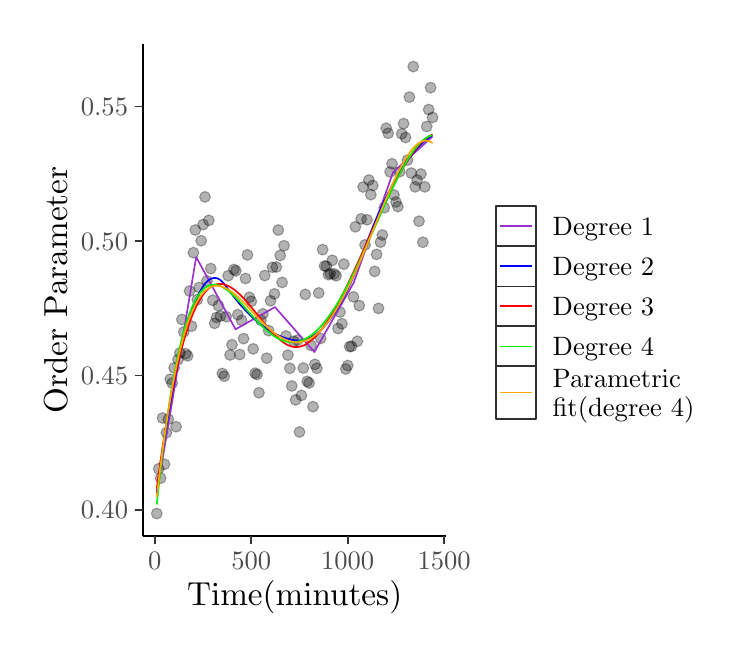
\begin{tikzpicture}[x=1pt,y=1pt]
\definecolor{fillColor}{RGB}{255,255,255}
\path[use as bounding box,fill=fillColor,fill opacity=0.00] (0,0) rectangle (252.94,216.81);
\begin{scope}
\path[clip] (  0.00,  0.00) rectangle (252.94,216.81);
\definecolor{drawColor}{RGB}{255,255,255}
\definecolor{fillColor}{RGB}{255,255,255}

\path[draw=drawColor,line width= 0.6pt,line join=round,line cap=round,fill=fillColor] (  0.00,  0.00) rectangle (252.94,216.81);
\end{scope}
\begin{scope}
\path[clip] ( 41.67, 33.16) rectangle (151.28,210.81);
\definecolor{fillColor}{RGB}{255,255,255}

\path[fill=fillColor] ( 41.67, 33.16) rectangle (151.28,210.81);
\definecolor{drawColor}{RGB}{0,0,0}
\definecolor{fillColor}{RGB}{0,0,0}

\path[draw=drawColor,draw opacity=0.30,line width= 0.4pt,line join=round,line cap=round,fill=fillColor,fill opacity=0.30] ( 46.65, 41.24) circle (  1.96);

\path[draw=drawColor,draw opacity=0.30,line width= 0.4pt,line join=round,line cap=round,fill=fillColor,fill opacity=0.30] ( 47.35, 57.42) circle (  1.96);

\path[draw=drawColor,draw opacity=0.30,line width= 0.4pt,line join=round,line cap=round,fill=fillColor,fill opacity=0.30] ( 48.05, 54.04) circle (  1.96);

\path[draw=drawColor,draw opacity=0.30,line width= 0.4pt,line join=round,line cap=round,fill=fillColor,fill opacity=0.30] ( 48.74, 75.76) circle (  1.96);

\path[draw=drawColor,draw opacity=0.30,line width= 0.4pt,line join=round,line cap=round,fill=fillColor,fill opacity=0.30] ( 49.44, 59.03) circle (  1.96);

\path[draw=drawColor,draw opacity=0.30,line width= 0.4pt,line join=round,line cap=round,fill=fillColor,fill opacity=0.30] ( 50.14, 70.46) circle (  1.96);

\path[draw=drawColor,draw opacity=0.30,line width= 0.4pt,line join=round,line cap=round,fill=fillColor,fill opacity=0.30] ( 50.83, 75.30) circle (  1.96);

\path[draw=drawColor,draw opacity=0.30,line width= 0.4pt,line join=round,line cap=round,fill=fillColor,fill opacity=0.30] ( 51.53, 89.78) circle (  1.96);

\path[draw=drawColor,draw opacity=0.30,line width= 0.4pt,line join=round,line cap=round,fill=fillColor,fill opacity=0.30] ( 52.23, 88.38) circle (  1.96);

\path[draw=drawColor,draw opacity=0.30,line width= 0.4pt,line join=round,line cap=round,fill=fillColor,fill opacity=0.30] ( 52.92, 93.89) circle (  1.96);

\path[draw=drawColor,draw opacity=0.30,line width= 0.4pt,line join=round,line cap=round,fill=fillColor,fill opacity=0.30] ( 53.62, 72.61) circle (  1.96);

\path[draw=drawColor,draw opacity=0.30,line width= 0.4pt,line join=round,line cap=round,fill=fillColor,fill opacity=0.30] ( 54.32, 96.86) circle (  1.96);

\path[draw=drawColor,draw opacity=0.30,line width= 0.4pt,line join=round,line cap=round,fill=fillColor,fill opacity=0.30] ( 55.01, 99.26) circle (  1.96);

\path[draw=drawColor,draw opacity=0.30,line width= 0.4pt,line join=round,line cap=round,fill=fillColor,fill opacity=0.30] ( 55.71,111.36) circle (  1.96);

\path[draw=drawColor,draw opacity=0.30,line width= 0.4pt,line join=round,line cap=round,fill=fillColor,fill opacity=0.30] ( 56.41,106.86) circle (  1.96);

\path[draw=drawColor,draw opacity=0.30,line width= 0.4pt,line join=round,line cap=round,fill=fillColor,fill opacity=0.30] ( 57.11, 99.00) circle (  1.96);

\path[draw=drawColor,draw opacity=0.30,line width= 0.4pt,line join=round,line cap=round,fill=fillColor,fill opacity=0.30] ( 57.80, 98.22) circle (  1.96);

\path[draw=drawColor,draw opacity=0.30,line width= 0.4pt,line join=round,line cap=round,fill=fillColor,fill opacity=0.30] ( 58.50,121.62) circle (  1.96);

\path[draw=drawColor,draw opacity=0.30,line width= 0.4pt,line join=round,line cap=round,fill=fillColor,fill opacity=0.30] ( 59.20,108.96) circle (  1.96);

\path[draw=drawColor,draw opacity=0.30,line width= 0.4pt,line join=round,line cap=round,fill=fillColor,fill opacity=0.30] ( 59.89,135.50) circle (  1.96);

\path[draw=drawColor,draw opacity=0.30,line width= 0.4pt,line join=round,line cap=round,fill=fillColor,fill opacity=0.30] ( 60.59,143.69) circle (  1.96);

\path[draw=drawColor,draw opacity=0.30,line width= 0.4pt,line join=round,line cap=round,fill=fillColor,fill opacity=0.30] ( 61.29,118.53) circle (  1.96);

\path[draw=drawColor,draw opacity=0.30,line width= 0.4pt,line join=round,line cap=round,fill=fillColor,fill opacity=0.30] ( 61.98,122.93) circle (  1.96);

\path[draw=drawColor,draw opacity=0.30,line width= 0.4pt,line join=round,line cap=round,fill=fillColor,fill opacity=0.30] ( 62.68,139.83) circle (  1.96);

\path[draw=drawColor,draw opacity=0.30,line width= 0.4pt,line join=round,line cap=round,fill=fillColor,fill opacity=0.30] ( 63.38,145.66) circle (  1.96);

\path[draw=drawColor,draw opacity=0.30,line width= 0.4pt,line join=round,line cap=round,fill=fillColor,fill opacity=0.30] ( 64.07,155.65) circle (  1.96);

\path[draw=drawColor,draw opacity=0.30,line width= 0.4pt,line join=round,line cap=round,fill=fillColor,fill opacity=0.30] ( 64.77,125.33) circle (  1.96);

\path[draw=drawColor,draw opacity=0.30,line width= 0.4pt,line join=round,line cap=round,fill=fillColor,fill opacity=0.30] ( 65.47,147.18) circle (  1.96);

\path[draw=drawColor,draw opacity=0.30,line width= 0.4pt,line join=round,line cap=round,fill=fillColor,fill opacity=0.30] ( 66.16,129.76) circle (  1.96);

\path[draw=drawColor,draw opacity=0.30,line width= 0.4pt,line join=round,line cap=round,fill=fillColor,fill opacity=0.30] ( 66.86,118.32) circle (  1.96);

\path[draw=drawColor,draw opacity=0.30,line width= 0.4pt,line join=round,line cap=round,fill=fillColor,fill opacity=0.30] ( 67.56,109.99) circle (  1.96);

\path[draw=drawColor,draw opacity=0.30,line width= 0.4pt,line join=round,line cap=round,fill=fillColor,fill opacity=0.30] ( 68.25,112.10) circle (  1.96);

\path[draw=drawColor,draw opacity=0.30,line width= 0.4pt,line join=round,line cap=round,fill=fillColor,fill opacity=0.30] ( 68.95,116.36) circle (  1.96);

\path[draw=drawColor,draw opacity=0.30,line width= 0.4pt,line join=round,line cap=round,fill=fillColor,fill opacity=0.30] ( 69.65,112.62) circle (  1.96);

\path[draw=drawColor,draw opacity=0.30,line width= 0.4pt,line join=round,line cap=round,fill=fillColor,fill opacity=0.30] ( 70.34, 91.85) circle (  1.96);

\path[draw=drawColor,draw opacity=0.30,line width= 0.4pt,line join=round,line cap=round,fill=fillColor,fill opacity=0.30] ( 71.04, 90.86) circle (  1.96);

\path[draw=drawColor,draw opacity=0.30,line width= 0.4pt,line join=round,line cap=round,fill=fillColor,fill opacity=0.30] ( 71.74,112.37) circle (  1.96);

\path[draw=drawColor,draw opacity=0.30,line width= 0.4pt,line join=round,line cap=round,fill=fillColor,fill opacity=0.30] ( 72.43,127.17) circle (  1.96);

\path[draw=drawColor,draw opacity=0.30,line width= 0.4pt,line join=round,line cap=round,fill=fillColor,fill opacity=0.30] ( 73.13, 98.54) circle (  1.96);

\path[draw=drawColor,draw opacity=0.30,line width= 0.4pt,line join=round,line cap=round,fill=fillColor,fill opacity=0.30] ( 73.83,102.24) circle (  1.96);

\path[draw=drawColor,draw opacity=0.30,line width= 0.4pt,line join=round,line cap=round,fill=fillColor,fill opacity=0.30] ( 74.52,129.43) circle (  1.96);

\path[draw=drawColor,draw opacity=0.30,line width= 0.4pt,line join=round,line cap=round,fill=fillColor,fill opacity=0.30] ( 75.22,128.92) circle (  1.96);

\path[draw=drawColor,draw opacity=0.30,line width= 0.4pt,line join=round,line cap=round,fill=fillColor,fill opacity=0.30] ( 75.92,113.09) circle (  1.96);

\path[draw=drawColor,draw opacity=0.30,line width= 0.4pt,line join=round,line cap=round,fill=fillColor,fill opacity=0.30] ( 76.62, 98.69) circle (  1.96);

\path[draw=drawColor,draw opacity=0.30,line width= 0.4pt,line join=round,line cap=round,fill=fillColor,fill opacity=0.30] ( 77.31,111.04) circle (  1.96);

\path[draw=drawColor,draw opacity=0.30,line width= 0.4pt,line join=round,line cap=round,fill=fillColor,fill opacity=0.30] ( 78.01,104.45) circle (  1.96);

\path[draw=drawColor,draw opacity=0.30,line width= 0.4pt,line join=round,line cap=round,fill=fillColor,fill opacity=0.30] ( 78.71,126.18) circle (  1.96);

\path[draw=drawColor,draw opacity=0.30,line width= 0.4pt,line join=round,line cap=round,fill=fillColor,fill opacity=0.30] ( 79.40,134.70) circle (  1.96);

\path[draw=drawColor,draw opacity=0.30,line width= 0.4pt,line join=round,line cap=round,fill=fillColor,fill opacity=0.30] ( 80.10,119.38) circle (  1.96);

\path[draw=drawColor,draw opacity=0.30,line width= 0.4pt,line join=round,line cap=round,fill=fillColor,fill opacity=0.30] ( 80.80,117.92) circle (  1.96);

\path[draw=drawColor,draw opacity=0.30,line width= 0.4pt,line join=round,line cap=round,fill=fillColor,fill opacity=0.30] ( 81.49,100.74) circle (  1.96);

\path[draw=drawColor,draw opacity=0.30,line width= 0.4pt,line join=round,line cap=round,fill=fillColor,fill opacity=0.30] ( 82.19, 91.94) circle (  1.96);

\path[draw=drawColor,draw opacity=0.30,line width= 0.4pt,line join=round,line cap=round,fill=fillColor,fill opacity=0.30] ( 82.89, 91.49) circle (  1.96);

\path[draw=drawColor,draw opacity=0.30,line width= 0.4pt,line join=round,line cap=round,fill=fillColor,fill opacity=0.30] ( 83.58, 84.89) circle (  1.96);

\path[draw=drawColor,draw opacity=0.30,line width= 0.4pt,line join=round,line cap=round,fill=fillColor,fill opacity=0.30] ( 84.28,111.09) circle (  1.96);

\path[draw=drawColor,draw opacity=0.30,line width= 0.4pt,line join=round,line cap=round,fill=fillColor,fill opacity=0.30] ( 84.98,113.38) circle (  1.96);

\path[draw=drawColor,draw opacity=0.30,line width= 0.4pt,line join=round,line cap=round,fill=fillColor,fill opacity=0.30] ( 85.67,127.24) circle (  1.96);

\path[draw=drawColor,draw opacity=0.30,line width= 0.4pt,line join=round,line cap=round,fill=fillColor,fill opacity=0.30] ( 86.37, 97.38) circle (  1.96);

\path[draw=drawColor,draw opacity=0.30,line width= 0.4pt,line join=round,line cap=round,fill=fillColor,fill opacity=0.30] ( 87.07,107.33) circle (  1.96);

\path[draw=drawColor,draw opacity=0.30,line width= 0.4pt,line join=round,line cap=round,fill=fillColor,fill opacity=0.30] ( 87.76,118.13) circle (  1.96);

\path[draw=drawColor,draw opacity=0.30,line width= 0.4pt,line join=round,line cap=round,fill=fillColor,fill opacity=0.30] ( 88.46,130.21) circle (  1.96);

\path[draw=drawColor,draw opacity=0.30,line width= 0.4pt,line join=round,line cap=round,fill=fillColor,fill opacity=0.30] ( 89.16,120.61) circle (  1.96);

\path[draw=drawColor,draw opacity=0.30,line width= 0.4pt,line join=round,line cap=round,fill=fillColor,fill opacity=0.30] ( 89.85,130.31) circle (  1.96);

\path[draw=drawColor,draw opacity=0.30,line width= 0.4pt,line join=round,line cap=round,fill=fillColor,fill opacity=0.30] ( 90.55,143.68) circle (  1.96);

\path[draw=drawColor,draw opacity=0.30,line width= 0.4pt,line join=round,line cap=round,fill=fillColor,fill opacity=0.30] ( 91.25,134.51) circle (  1.96);

\path[draw=drawColor,draw opacity=0.30,line width= 0.4pt,line join=round,line cap=round,fill=fillColor,fill opacity=0.30] ( 91.94,124.76) circle (  1.96);

\path[draw=drawColor,draw opacity=0.30,line width= 0.4pt,line join=round,line cap=round,fill=fillColor,fill opacity=0.30] ( 92.64,138.02) circle (  1.96);

\path[draw=drawColor,draw opacity=0.30,line width= 0.4pt,line join=round,line cap=round,fill=fillColor,fill opacity=0.30] ( 93.34,105.39) circle (  1.96);

\path[draw=drawColor,draw opacity=0.30,line width= 0.4pt,line join=round,line cap=round,fill=fillColor,fill opacity=0.30] ( 94.04, 98.49) circle (  1.96);

\path[draw=drawColor,draw opacity=0.30,line width= 0.4pt,line join=round,line cap=round,fill=fillColor,fill opacity=0.30] ( 94.73, 93.75) circle (  1.96);

\path[draw=drawColor,draw opacity=0.30,line width= 0.4pt,line join=round,line cap=round,fill=fillColor,fill opacity=0.30] ( 95.43, 87.34) circle (  1.96);

\path[draw=drawColor,draw opacity=0.30,line width= 0.4pt,line join=round,line cap=round,fill=fillColor,fill opacity=0.30] ( 96.13,103.45) circle (  1.96);

\path[draw=drawColor,draw opacity=0.30,line width= 0.4pt,line join=round,line cap=round,fill=fillColor,fill opacity=0.30] ( 96.82, 82.31) circle (  1.96);

\path[draw=drawColor,draw opacity=0.30,line width= 0.4pt,line join=round,line cap=round,fill=fillColor,fill opacity=0.30] ( 97.52,103.90) circle (  1.96);

\path[draw=drawColor,draw opacity=0.30,line width= 0.4pt,line join=round,line cap=round,fill=fillColor,fill opacity=0.30] ( 98.22, 70.71) circle (  1.96);

\path[draw=drawColor,draw opacity=0.30,line width= 0.4pt,line join=round,line cap=round,fill=fillColor,fill opacity=0.30] ( 98.91, 83.94) circle (  1.96);

\path[draw=drawColor,draw opacity=0.30,line width= 0.4pt,line join=round,line cap=round,fill=fillColor,fill opacity=0.30] ( 99.61, 93.82) circle (  1.96);

\path[draw=drawColor,draw opacity=0.30,line width= 0.4pt,line join=round,line cap=round,fill=fillColor,fill opacity=0.30] (100.31,120.43) circle (  1.96);

\path[draw=drawColor,draw opacity=0.30,line width= 0.4pt,line join=round,line cap=round,fill=fillColor,fill opacity=0.30] (101.00, 89.01) circle (  1.96);

\path[draw=drawColor,draw opacity=0.30,line width= 0.4pt,line join=round,line cap=round,fill=fillColor,fill opacity=0.30] (101.70, 88.41) circle (  1.96);

\path[draw=drawColor,draw opacity=0.30,line width= 0.4pt,line join=round,line cap=round,fill=fillColor,fill opacity=0.30] (102.40,101.99) circle (  1.96);

\path[draw=drawColor,draw opacity=0.30,line width= 0.4pt,line join=round,line cap=round,fill=fillColor,fill opacity=0.30] (103.09, 79.86) circle (  1.96);

\path[draw=drawColor,draw opacity=0.30,line width= 0.4pt,line join=round,line cap=round,fill=fillColor,fill opacity=0.30] (103.79, 95.14) circle (  1.96);

\path[draw=drawColor,draw opacity=0.30,line width= 0.4pt,line join=round,line cap=round,fill=fillColor,fill opacity=0.30] (104.49, 93.72) circle (  1.96);

\path[draw=drawColor,draw opacity=0.30,line width= 0.4pt,line join=round,line cap=round,fill=fillColor,fill opacity=0.30] (105.18,120.96) circle (  1.96);

\path[draw=drawColor,draw opacity=0.30,line width= 0.4pt,line join=round,line cap=round,fill=fillColor,fill opacity=0.30] (105.88,104.53) circle (  1.96);

\path[draw=drawColor,draw opacity=0.30,line width= 0.4pt,line join=round,line cap=round,fill=fillColor,fill opacity=0.30] (106.58,136.61) circle (  1.96);

\path[draw=drawColor,draw opacity=0.30,line width= 0.4pt,line join=round,line cap=round,fill=fillColor,fill opacity=0.30] (107.27,130.68) circle (  1.96);

\path[draw=drawColor,draw opacity=0.30,line width= 0.4pt,line join=round,line cap=round,fill=fillColor,fill opacity=0.30] (107.97,130.60) circle (  1.96);

\path[draw=drawColor,draw opacity=0.30,line width= 0.4pt,line join=round,line cap=round,fill=fillColor,fill opacity=0.30] (108.67,127.56) circle (  1.96);

\path[draw=drawColor,draw opacity=0.30,line width= 0.4pt,line join=round,line cap=round,fill=fillColor,fill opacity=0.30] (109.36,127.95) circle (  1.96);

\path[draw=drawColor,draw opacity=0.30,line width= 0.4pt,line join=round,line cap=round,fill=fillColor,fill opacity=0.30] (110.06,132.76) circle (  1.96);

\path[draw=drawColor,draw opacity=0.30,line width= 0.4pt,line join=round,line cap=round,fill=fillColor,fill opacity=0.30] (110.76,127.81) circle (  1.96);

\path[draw=drawColor,draw opacity=0.30,line width= 0.4pt,line join=round,line cap=round,fill=fillColor,fill opacity=0.30] (111.45,127.14) circle (  1.96);

\path[draw=drawColor,draw opacity=0.30,line width= 0.4pt,line join=round,line cap=round,fill=fillColor,fill opacity=0.30] (112.15,108.08) circle (  1.96);

\path[draw=drawColor,draw opacity=0.30,line width= 0.4pt,line join=round,line cap=round,fill=fillColor,fill opacity=0.30] (112.85,114.04) circle (  1.96);

\path[draw=drawColor,draw opacity=0.30,line width= 0.4pt,line join=round,line cap=round,fill=fillColor,fill opacity=0.30] (113.55,109.82) circle (  1.96);

\path[draw=drawColor,draw opacity=0.30,line width= 0.4pt,line join=round,line cap=round,fill=fillColor,fill opacity=0.30] (114.24,131.36) circle (  1.96);

\path[draw=drawColor,draw opacity=0.30,line width= 0.4pt,line join=round,line cap=round,fill=fillColor,fill opacity=0.30] (114.94, 93.47) circle (  1.96);

\path[draw=drawColor,draw opacity=0.30,line width= 0.4pt,line join=round,line cap=round,fill=fillColor,fill opacity=0.30] (115.64, 94.73) circle (  1.96);

\path[draw=drawColor,draw opacity=0.30,line width= 0.4pt,line join=round,line cap=round,fill=fillColor,fill opacity=0.30] (116.33,101.56) circle (  1.96);

\path[draw=drawColor,draw opacity=0.30,line width= 0.4pt,line join=round,line cap=round,fill=fillColor,fill opacity=0.30] (117.03,101.66) circle (  1.96);

\path[draw=drawColor,draw opacity=0.30,line width= 0.4pt,line join=round,line cap=round,fill=fillColor,fill opacity=0.30] (117.73,119.53) circle (  1.96);

\path[draw=drawColor,draw opacity=0.30,line width= 0.4pt,line join=round,line cap=round,fill=fillColor,fill opacity=0.30] (118.42,144.85) circle (  1.96);

\path[draw=drawColor,draw opacity=0.30,line width= 0.4pt,line join=round,line cap=round,fill=fillColor,fill opacity=0.30] (119.12,103.47) circle (  1.96);

\path[draw=drawColor,draw opacity=0.30,line width= 0.4pt,line join=round,line cap=round,fill=fillColor,fill opacity=0.30] (119.82,116.38) circle (  1.96);

\path[draw=drawColor,draw opacity=0.30,line width= 0.4pt,line join=round,line cap=round,fill=fillColor,fill opacity=0.30] (120.51,147.71) circle (  1.96);

\path[draw=drawColor,draw opacity=0.30,line width= 0.4pt,line join=round,line cap=round,fill=fillColor,fill opacity=0.30] (121.21,159.22) circle (  1.96);

\path[draw=drawColor,draw opacity=0.30,line width= 0.4pt,line join=round,line cap=round,fill=fillColor,fill opacity=0.30] (121.91,138.32) circle (  1.96);

\path[draw=drawColor,draw opacity=0.30,line width= 0.4pt,line join=round,line cap=round,fill=fillColor,fill opacity=0.30] (122.60,147.38) circle (  1.96);

\path[draw=drawColor,draw opacity=0.30,line width= 0.4pt,line join=round,line cap=round,fill=fillColor,fill opacity=0.30] (123.30,161.75) circle (  1.96);

\path[draw=drawColor,draw opacity=0.30,line width= 0.4pt,line join=round,line cap=round,fill=fillColor,fill opacity=0.30] (124.00,156.46) circle (  1.96);

\path[draw=drawColor,draw opacity=0.30,line width= 0.4pt,line join=round,line cap=round,fill=fillColor,fill opacity=0.30] (124.69,159.79) circle (  1.96);

\path[draw=drawColor,draw opacity=0.30,line width= 0.4pt,line join=round,line cap=round,fill=fillColor,fill opacity=0.30] (125.39,128.73) circle (  1.96);

\path[draw=drawColor,draw opacity=0.30,line width= 0.4pt,line join=round,line cap=round,fill=fillColor,fill opacity=0.30] (126.09,134.89) circle (  1.96);

\path[draw=drawColor,draw opacity=0.30,line width= 0.4pt,line join=round,line cap=round,fill=fillColor,fill opacity=0.30] (126.78,115.36) circle (  1.96);

\path[draw=drawColor,draw opacity=0.30,line width= 0.4pt,line join=round,line cap=round,fill=fillColor,fill opacity=0.30] (127.48,139.30) circle (  1.96);

\path[draw=drawColor,draw opacity=0.30,line width= 0.4pt,line join=round,line cap=round,fill=fillColor,fill opacity=0.30] (128.18,141.89) circle (  1.96);

\path[draw=drawColor,draw opacity=0.30,line width= 0.4pt,line join=round,line cap=round,fill=fillColor,fill opacity=0.30] (128.87,151.76) circle (  1.96);

\path[draw=drawColor,draw opacity=0.30,line width= 0.4pt,line join=round,line cap=round,fill=fillColor,fill opacity=0.30] (129.57,180.49) circle (  1.96);

\path[draw=drawColor,draw opacity=0.30,line width= 0.4pt,line join=round,line cap=round,fill=fillColor,fill opacity=0.30] (130.27,178.66) circle (  1.96);

\path[draw=drawColor,draw opacity=0.30,line width= 0.4pt,line join=round,line cap=round,fill=fillColor,fill opacity=0.30] (130.97,164.70) circle (  1.96);

\path[draw=drawColor,draw opacity=0.30,line width= 0.4pt,line join=round,line cap=round,fill=fillColor,fill opacity=0.30] (131.66,167.62) circle (  1.96);

\path[draw=drawColor,draw opacity=0.30,line width= 0.4pt,line join=round,line cap=round,fill=fillColor,fill opacity=0.30] (132.36,156.35) circle (  1.96);

\path[draw=drawColor,draw opacity=0.30,line width= 0.4pt,line join=round,line cap=round,fill=fillColor,fill opacity=0.30] (133.06,153.80) circle (  1.96);

\path[draw=drawColor,draw opacity=0.30,line width= 0.4pt,line join=round,line cap=round,fill=fillColor,fill opacity=0.30] (133.75,152.16) circle (  1.96);

\path[draw=drawColor,draw opacity=0.30,line width= 0.4pt,line join=round,line cap=round,fill=fillColor,fill opacity=0.30] (134.45,164.81) circle (  1.96);

\path[draw=drawColor,draw opacity=0.30,line width= 0.4pt,line join=round,line cap=round,fill=fillColor,fill opacity=0.30] (135.15,178.43) circle (  1.96);

\path[draw=drawColor,draw opacity=0.30,line width= 0.4pt,line join=round,line cap=round,fill=fillColor,fill opacity=0.30] (135.84,182.14) circle (  1.96);

\path[draw=drawColor,draw opacity=0.30,line width= 0.4pt,line join=round,line cap=round,fill=fillColor,fill opacity=0.30] (136.54,177.11) circle (  1.96);

\path[draw=drawColor,draw opacity=0.30,line width= 0.4pt,line join=round,line cap=round,fill=fillColor,fill opacity=0.30] (137.24,168.96) circle (  1.96);

\path[draw=drawColor,draw opacity=0.30,line width= 0.4pt,line join=round,line cap=round,fill=fillColor,fill opacity=0.30] (137.93,191.71) circle (  1.96);

\path[draw=drawColor,draw opacity=0.30,line width= 0.4pt,line join=round,line cap=round,fill=fillColor,fill opacity=0.30] (138.63,164.28) circle (  1.96);

\path[draw=drawColor,draw opacity=0.30,line width= 0.4pt,line join=round,line cap=round,fill=fillColor,fill opacity=0.30] (139.33,202.74) circle (  1.96);

\path[draw=drawColor,draw opacity=0.30,line width= 0.4pt,line join=round,line cap=round,fill=fillColor,fill opacity=0.30] (140.02,159.30) circle (  1.96);

\path[draw=drawColor,draw opacity=0.30,line width= 0.4pt,line join=round,line cap=round,fill=fillColor,fill opacity=0.30] (140.72,161.74) circle (  1.96);

\path[draw=drawColor,draw opacity=0.30,line width= 0.4pt,line join=round,line cap=round,fill=fillColor,fill opacity=0.30] (141.42,146.88) circle (  1.96);

\path[draw=drawColor,draw opacity=0.30,line width= 0.4pt,line join=round,line cap=round,fill=fillColor,fill opacity=0.30] (142.11,163.93) circle (  1.96);

\path[draw=drawColor,draw opacity=0.30,line width= 0.4pt,line join=round,line cap=round,fill=fillColor,fill opacity=0.30] (142.81,139.28) circle (  1.96);

\path[draw=drawColor,draw opacity=0.30,line width= 0.4pt,line join=round,line cap=round,fill=fillColor,fill opacity=0.30] (143.51,159.29) circle (  1.96);

\path[draw=drawColor,draw opacity=0.30,line width= 0.4pt,line join=round,line cap=round,fill=fillColor,fill opacity=0.30] (144.20,181.11) circle (  1.96);

\path[draw=drawColor,draw opacity=0.30,line width= 0.4pt,line join=round,line cap=round,fill=fillColor,fill opacity=0.30] (144.90,187.22) circle (  1.96);

\path[draw=drawColor,draw opacity=0.30,line width= 0.4pt,line join=round,line cap=round,fill=fillColor,fill opacity=0.30] (145.60,195.12) circle (  1.96);

\path[draw=drawColor,draw opacity=0.30,line width= 0.4pt,line join=round,line cap=round,fill=fillColor,fill opacity=0.30] (146.29,184.39) circle (  1.96);
\definecolor{drawColor}{RGB}{153,50,204}

\path[draw=drawColor,line width= 0.6pt,line join=round] ( 46.65, 48.29) --
	( 46.72, 48.71) --
	( 46.79, 49.13) --
	( 46.86, 49.55) --
	( 46.93, 49.97) --
	( 47.00, 50.39) --
	( 47.07, 50.81) --
	( 47.14, 51.23) --
	( 47.21, 51.65) --
	( 47.28, 52.07) --
	( 47.35, 52.49) --
	( 47.42, 52.91) --
	( 47.49, 53.32) --
	( 47.56, 53.74) --
	( 47.63, 54.16) --
	( 47.70, 54.58) --
	( 47.77, 55.00) --
	( 47.84, 55.42) --
	( 47.91, 55.84) --
	( 47.98, 56.26) --
	( 48.05, 56.68) --
	( 48.12, 57.10) --
	( 48.19, 57.52) --
	( 48.26, 57.94) --
	( 48.33, 58.35) --
	( 48.40, 58.77) --
	( 48.46, 59.19) --
	( 48.53, 59.61) --
	( 48.60, 60.03) --
	( 48.67, 60.45) --
	( 48.74, 60.87) --
	( 48.81, 61.29) --
	( 48.88, 61.71) --
	( 48.95, 62.13) --
	( 49.02, 62.55) --
	( 49.09, 62.97) --
	( 49.16, 63.39) --
	( 49.23, 63.80) --
	( 49.30, 64.22) --
	( 49.37, 64.64) --
	( 49.44, 65.06) --
	( 49.51, 65.48) --
	( 49.58, 65.90) --
	( 49.65, 66.32) --
	( 49.72, 66.74) --
	( 49.79, 67.16) --
	( 49.86, 67.58) --
	( 49.93, 68.00) --
	( 50.00, 68.42) --
	( 50.07, 68.83) --
	( 50.14, 69.25) --
	( 50.21, 69.67) --
	( 50.28, 70.09) --
	( 50.35, 70.51) --
	( 50.42, 70.93) --
	( 50.49, 71.35) --
	( 50.56, 71.77) --
	( 50.62, 72.19) --
	( 50.69, 72.61) --
	( 50.76, 73.03) --
	( 50.83, 73.45) --
	( 50.90, 73.86) --
	( 50.97, 74.28) --
	( 51.04, 74.70) --
	( 51.11, 75.12) --
	( 51.18, 75.54) --
	( 51.25, 75.96) --
	( 51.32, 76.38) --
	( 51.39, 76.80) --
	( 51.46, 77.22) --
	( 51.53, 77.64) --
	( 51.60, 78.06) --
	( 51.67, 78.48) --
	( 51.74, 78.90) --
	( 51.81, 79.31) --
	( 51.88, 79.73) --
	( 51.95, 80.15) --
	( 52.02, 80.57) --
	( 52.09, 80.99) --
	( 52.16, 81.41) --
	( 52.23, 81.83) --
	( 52.30, 82.25) --
	( 52.37, 82.67) --
	( 52.44, 83.09) --
	( 52.51, 83.51) --
	( 52.58, 83.93) --
	( 52.65, 84.34) --
	( 52.72, 84.76) --
	( 52.79, 85.18) --
	( 52.85, 85.60) --
	( 52.92, 86.02) --
	( 52.99, 86.44) --
	( 53.06, 86.86) --
	( 53.13, 87.28) --
	( 53.20, 87.70) --
	( 53.27, 88.12) --
	( 53.34, 88.54) --
	( 53.41, 88.96) --
	( 53.48, 89.37) --
	( 53.55, 89.79) --
	( 53.62, 90.21) --
	( 53.69, 90.63) --
	( 53.76, 91.05) --
	( 53.83, 91.47) --
	( 53.90, 91.89) --
	( 53.97, 92.31) --
	( 54.04, 92.73) --
	( 54.11, 93.15) --
	( 54.18, 93.57) --
	( 54.25, 93.99) --
	( 54.32, 94.40) --
	( 54.39, 94.82) --
	( 54.46, 95.24) --
	( 54.53, 95.66) --
	( 54.60, 96.08) --
	( 54.67, 96.50) --
	( 54.74, 96.92) --
	( 54.81, 97.34) --
	( 54.88, 97.76) --
	( 54.95, 98.18) --
	( 55.01, 98.60) --
	( 55.08, 99.02) --
	( 55.15, 99.44) --
	( 55.22, 99.85) --
	( 55.29,100.27) --
	( 55.36,100.69) --
	( 55.43,101.11) --
	( 55.50,101.53) --
	( 55.57,101.95) --
	( 55.64,102.37) --
	( 55.71,102.79) --
	( 55.78,103.21) --
	( 55.85,103.63) --
	( 55.92,104.05) --
	( 55.99,104.47) --
	( 56.06,104.88) --
	( 56.13,105.30) --
	( 56.20,105.72) --
	( 56.27,106.14) --
	( 56.34,106.56) --
	( 56.41,106.98) --
	( 56.48,107.40) --
	( 56.55,107.82) --
	( 56.62,108.24) --
	( 56.69,108.66) --
	( 56.76,109.08) --
	( 56.83,109.50) --
	( 56.90,109.91) --
	( 56.97,110.33) --
	( 57.04,110.75) --
	( 57.11,111.17) --
	( 57.17,111.59) --
	( 57.24,112.01) --
	( 57.31,112.43) --
	( 57.38,112.85) --
	( 57.45,113.27) --
	( 57.52,113.69) --
	( 57.59,114.11) --
	( 57.66,114.53) --
	( 57.73,114.95) --
	( 57.80,115.36) --
	( 57.87,115.78) --
	( 57.94,116.20) --
	( 58.01,116.62) --
	( 58.08,117.04) --
	( 58.15,117.46) --
	( 58.22,117.88) --
	( 58.29,118.30) --
	( 58.36,118.72) --
	( 58.43,119.14) --
	( 58.50,119.56) --
	( 58.57,119.98) --
	( 58.64,120.39) --
	( 58.71,120.81) --
	( 58.78,121.23) --
	( 58.85,121.65) --
	( 58.92,122.07) --
	( 58.99,122.49) --
	( 59.06,122.91) --
	( 59.13,123.33) --
	( 59.20,123.75) --
	( 59.27,124.17) --
	( 59.33,124.59) --
	( 59.40,125.01) --
	( 59.47,125.42) --
	( 59.54,125.84) --
	( 59.61,126.26) --
	( 59.68,126.68) --
	( 59.75,127.10) --
	( 59.82,127.52) --
	( 59.89,127.94) --
	( 59.96,128.36) --
	( 60.03,128.78) --
	( 60.10,129.20) --
	( 60.17,129.62) --
	( 60.24,130.04) --
	( 60.31,130.46) --
	( 60.38,130.87) --
	( 60.45,131.29) --
	( 60.52,131.71) --
	( 60.59,132.13) --
	( 60.66,132.55) --
	( 60.73,132.97) --
	( 60.80,133.39) --
	( 60.87,133.81) --
	( 60.94,133.84) --
	( 61.01,133.71) --
	( 61.08,133.58) --
	( 61.15,133.45) --
	( 61.22,133.33) --
	( 61.29,133.20) --
	( 61.36,133.07) --
	( 61.43,132.94) --
	( 61.49,132.81) --
	( 61.56,132.69) --
	( 61.63,132.56) --
	( 61.70,132.43) --
	( 61.77,132.30) --
	( 61.84,132.17) --
	( 61.91,132.05) --
	( 61.98,131.92) --
	( 62.05,131.79) --
	( 62.12,131.66) --
	( 62.19,131.54) --
	( 62.26,131.41) --
	( 62.33,131.28) --
	( 62.40,131.15) --
	( 62.47,131.02) --
	( 62.54,130.90) --
	( 62.61,130.77) --
	( 62.68,130.64) --
	( 62.75,130.51) --
	( 62.82,130.38) --
	( 62.89,130.26) --
	( 62.96,130.13) --
	( 63.03,130.00) --
	( 63.10,129.87) --
	( 63.17,129.75) --
	( 63.24,129.62) --
	( 63.31,129.49) --
	( 63.38,129.36) --
	( 63.45,129.23) --
	( 63.52,129.11) --
	( 63.59,128.98) --
	( 63.65,128.85) --
	( 63.72,128.72) --
	( 63.79,128.59) --
	( 63.86,128.47) --
	( 63.93,128.34) --
	( 64.00,128.21) --
	( 64.07,128.08) --
	( 64.14,127.96) --
	( 64.21,127.83) --
	( 64.28,127.70) --
	( 64.35,127.57) --
	( 64.42,127.44) --
	( 64.49,127.32) --
	( 64.56,127.19) --
	( 64.63,127.06) --
	( 64.70,126.93) --
	( 64.77,126.80) --
	( 64.84,126.68) --
	( 64.91,126.55) --
	( 64.98,126.42) --
	( 65.05,126.29) --
	( 65.12,126.17) --
	( 65.19,126.04) --
	( 65.26,125.91) --
	( 65.33,125.78) --
	( 65.40,125.65) --
	( 65.47,125.53) --
	( 65.54,125.40) --
	( 65.61,125.27) --
	( 65.68,125.14) --
	( 65.75,125.01) --
	( 65.82,124.89) --
	( 65.88,124.76) --
	( 65.95,124.63) --
	( 66.02,124.50) --
	( 66.09,124.38) --
	( 66.16,124.25) --
	( 66.23,124.12) --
	( 66.30,123.99) --
	( 66.37,123.86) --
	( 66.44,123.74) --
	( 66.51,123.61) --
	( 66.58,123.48) --
	( 66.65,123.35) --
	( 66.72,123.22) --
	( 66.79,123.10) --
	( 66.86,122.97) --
	( 66.93,122.84) --
	( 67.00,122.71) --
	( 67.07,122.59) --
	( 67.14,122.46) --
	( 67.21,122.33) --
	( 67.28,122.20) --
	( 67.35,122.07) --
	( 67.42,121.95) --
	( 67.49,121.82) --
	( 67.56,121.69) --
	( 67.63,121.56) --
	( 67.70,121.43) --
	( 67.77,121.31) --
	( 67.84,121.18) --
	( 67.91,121.05) --
	( 67.98,120.92) --
	( 68.04,120.80) --
	( 68.11,120.67) --
	( 68.18,120.54) --
	( 68.25,120.41) --
	( 68.32,120.28) --
	( 68.39,120.16) --
	( 68.46,120.03) --
	( 68.53,119.90) --
	( 68.60,119.77) --
	( 68.67,119.64) --
	( 68.74,119.52) --
	( 68.81,119.39) --
	( 68.88,119.26) --
	( 68.95,119.13) --
	( 69.02,119.01) --
	( 69.09,118.88) --
	( 69.16,118.75) --
	( 69.23,118.62) --
	( 69.30,118.49) --
	( 69.37,118.37) --
	( 69.44,118.24) --
	( 69.51,118.11) --
	( 69.58,117.98) --
	( 69.65,117.85) --
	( 69.72,117.73) --
	( 69.79,117.60) --
	( 69.86,117.47) --
	( 69.93,117.34) --
	( 70.00,117.21) --
	( 70.07,117.09) --
	( 70.14,116.96) --
	( 70.20,116.83) --
	( 70.27,116.70) --
	( 70.34,116.58) --
	( 70.41,116.45) --
	( 70.48,116.32) --
	( 70.55,116.19) --
	( 70.62,116.06) --
	( 70.69,115.94) --
	( 70.76,115.81) --
	( 70.83,115.68) --
	( 70.90,115.55) --
	( 70.97,115.42) --
	( 71.04,115.30) --
	( 71.11,115.17) --
	( 71.18,115.04) --
	( 71.25,114.91) --
	( 71.32,114.79) --
	( 71.39,114.66) --
	( 71.46,114.53) --
	( 71.53,114.40) --
	( 71.60,114.27) --
	( 71.67,114.15) --
	( 71.74,114.02) --
	( 71.81,113.89) --
	( 71.88,113.76) --
	( 71.95,113.63) --
	( 72.02,113.51) --
	( 72.09,113.38) --
	( 72.16,113.25) --
	( 72.23,113.12) --
	( 72.30,113.00) --
	( 72.36,112.87) --
	( 72.43,112.74) --
	( 72.50,112.61) --
	( 72.57,112.48) --
	( 72.64,112.36) --
	( 72.71,112.23) --
	( 72.78,112.10) --
	( 72.85,111.97) --
	( 72.92,111.84) --
	( 72.99,111.72) --
	( 73.06,111.59) --
	( 73.13,111.46) --
	( 73.20,111.33) --
	( 73.27,111.21) --
	( 73.34,111.08) --
	( 73.41,110.95) --
	( 73.48,110.82) --
	( 73.55,110.69) --
	( 73.62,110.57) --
	( 73.69,110.44) --
	( 73.76,110.31) --
	( 73.83,110.18) --
	( 73.90,110.05) --
	( 73.97,109.93) --
	( 74.04,109.80) --
	( 74.11,109.67) --
	( 74.18,109.54) --
	( 74.25,109.42) --
	( 74.32,109.29) --
	( 74.39,109.16) --
	( 74.46,109.03) --
	( 74.52,108.90) --
	( 74.59,108.78) --
	( 74.66,108.65) --
	( 74.73,108.52) --
	( 74.80,108.39) --
	( 74.87,108.26) --
	( 74.94,108.14) --
	( 75.01,108.01) --
	( 75.08,107.88) --
	( 75.15,107.82) --
	( 75.22,107.86) --
	( 75.29,107.90) --
	( 75.36,107.94) --
	( 75.43,107.98) --
	( 75.50,108.02) --
	( 75.57,108.06) --
	( 75.64,108.10) --
	( 75.71,108.14) --
	( 75.78,108.18) --
	( 75.85,108.22) --
	( 75.92,108.26) --
	( 75.99,108.30) --
	( 76.06,108.34) --
	( 76.13,108.38) --
	( 76.20,108.41) --
	( 76.27,108.45) --
	( 76.34,108.49) --
	( 76.41,108.53) --
	( 76.48,108.57) --
	( 76.55,108.61) --
	( 76.62,108.65) --
	( 76.68,108.69) --
	( 76.75,108.73) --
	( 76.82,108.77) --
	( 76.89,108.81) --
	( 76.96,108.85) --
	( 77.03,108.89) --
	( 77.10,108.93) --
	( 77.17,108.97) --
	( 77.24,109.01) --
	( 77.31,109.04) --
	( 77.38,109.08) --
	( 77.45,109.12) --
	( 77.52,109.16) --
	( 77.59,109.20) --
	( 77.66,109.24) --
	( 77.73,109.28) --
	( 77.80,109.32) --
	( 77.87,109.36) --
	( 77.94,109.40) --
	( 78.01,109.44) --
	( 78.08,109.48) --
	( 78.15,109.52) --
	( 78.22,109.56) --
	( 78.29,109.60) --
	( 78.36,109.63) --
	( 78.43,109.67) --
	( 78.50,109.71) --
	( 78.57,109.75) --
	( 78.64,109.79) --
	( 78.71,109.83) --
	( 78.78,109.87) --
	( 78.85,109.91) --
	( 78.91,109.95) --
	( 78.98,109.99) --
	( 79.05,110.03) --
	( 79.12,110.07) --
	( 79.19,110.11) --
	( 79.26,110.15) --
	( 79.33,110.19) --
	( 79.40,110.22) --
	( 79.47,110.26) --
	( 79.54,110.30) --
	( 79.61,110.34) --
	( 79.68,110.38) --
	( 79.75,110.42) --
	( 79.82,110.46) --
	( 79.89,110.50) --
	( 79.96,110.54) --
	( 80.03,110.58) --
	( 80.10,110.62) --
	( 80.17,110.66) --
	( 80.24,110.70) --
	( 80.31,110.74) --
	( 80.38,110.78) --
	( 80.45,110.81) --
	( 80.52,110.85) --
	( 80.59,110.89) --
	( 80.66,110.93) --
	( 80.73,110.97) --
	( 80.80,111.01) --
	( 80.87,111.05) --
	( 80.94,111.09) --
	( 81.01,111.13) --
	( 81.07,111.17) --
	( 81.14,111.21) --
	( 81.21,111.25) --
	( 81.28,111.29) --
	( 81.35,111.33) --
	( 81.42,111.37) --
	( 81.49,111.41) --
	( 81.56,111.44) --
	( 81.63,111.48) --
	( 81.70,111.52) --
	( 81.77,111.56) --
	( 81.84,111.60) --
	( 81.91,111.64) --
	( 81.98,111.68) --
	( 82.05,111.72) --
	( 82.12,111.76) --
	( 82.19,111.80) --
	( 82.26,111.84) --
	( 82.33,111.88) --
	( 82.40,111.92) --
	( 82.47,111.96) --
	( 82.54,112.00) --
	( 82.61,112.03) --
	( 82.68,112.07) --
	( 82.75,112.11) --
	( 82.82,112.15) --
	( 82.89,112.19) --
	( 82.96,112.23) --
	( 83.03,112.27) --
	( 83.10,112.31) --
	( 83.17,112.35) --
	( 83.23,112.39) --
	( 83.30,112.43) --
	( 83.37,112.47) --
	( 83.44,112.51) --
	( 83.51,112.55) --
	( 83.58,112.59) --
	( 83.65,112.62) --
	( 83.72,112.66) --
	( 83.79,112.70) --
	( 83.86,112.74) --
	( 83.93,112.78) --
	( 84.00,112.82) --
	( 84.07,112.86) --
	( 84.14,112.90) --
	( 84.21,112.94) --
	( 84.28,112.98) --
	( 84.35,113.02) --
	( 84.42,113.06) --
	( 84.49,113.10) --
	( 84.56,113.14) --
	( 84.63,113.18) --
	( 84.70,113.21) --
	( 84.77,113.25) --
	( 84.84,113.29) --
	( 84.91,113.33) --
	( 84.98,113.37) --
	( 85.05,113.41) --
	( 85.12,113.45) --
	( 85.19,113.49) --
	( 85.26,113.53) --
	( 85.33,113.57) --
	( 85.39,113.61) --
	( 85.46,113.65) --
	( 85.53,113.69) --
	( 85.60,113.73) --
	( 85.67,113.77) --
	( 85.74,113.80) --
	( 85.81,113.84) --
	( 85.88,113.88) --
	( 85.95,113.92) --
	( 86.02,113.96) --
	( 86.09,114.00) --
	( 86.16,114.04) --
	( 86.23,114.08) --
	( 86.30,114.12) --
	( 86.37,114.16) --
	( 86.44,114.20) --
	( 86.51,114.24) --
	( 86.58,114.28) --
	( 86.65,114.32) --
	( 86.72,114.36) --
	( 86.79,114.40) --
	( 86.86,114.43) --
	( 86.93,114.47) --
	( 87.00,114.51) --
	( 87.07,114.55) --
	( 87.14,114.59) --
	( 87.21,114.63) --
	( 87.28,114.67) --
	( 87.35,114.71) --
	( 87.42,114.75) --
	( 87.49,114.79) --
	( 87.55,114.83) --
	( 87.62,114.87) --
	( 87.69,114.91) --
	( 87.76,114.95) --
	( 87.83,114.99) --
	( 87.90,115.02) --
	( 87.97,115.06) --
	( 88.04,115.10) --
	( 88.11,115.14) --
	( 88.18,115.18) --
	( 88.25,115.22) --
	( 88.32,115.26) --
	( 88.39,115.30) --
	( 88.46,115.34) --
	( 88.53,115.38) --
	( 88.60,115.42) --
	( 88.67,115.46) --
	( 88.74,115.50) --
	( 88.81,115.54) --
	( 88.88,115.58) --
	( 88.95,115.61) --
	( 89.02,115.65) --
	( 89.09,115.69) --
	( 89.16,115.73) --
	( 89.23,115.77) --
	( 89.30,115.81) --
	( 89.37,115.83) --
	( 89.44,115.75) --
	( 89.51,115.67) --
	( 89.58,115.60) --
	( 89.65,115.52) --
	( 89.71,115.44) --
	( 89.78,115.36) --
	( 89.85,115.28) --
	( 89.92,115.20) --
	( 89.99,115.12) --
	( 90.06,115.04) --
	( 90.13,114.96) --
	( 90.20,114.88) --
	( 90.27,114.80) --
	( 90.34,114.72) --
	( 90.41,114.64) --
	( 90.48,114.56) --
	( 90.55,114.48) --
	( 90.62,114.40) --
	( 90.69,114.32) --
	( 90.76,114.24) --
	( 90.83,114.17) --
	( 90.90,114.09) --
	( 90.97,114.01) --
	( 91.04,113.93) --
	( 91.11,113.85) --
	( 91.18,113.77) --
	( 91.25,113.69) --
	( 91.32,113.61) --
	( 91.39,113.53) --
	( 91.46,113.45) --
	( 91.53,113.37) --
	( 91.60,113.29) --
	( 91.67,113.21) --
	( 91.74,113.13) --
	( 91.81,113.05) --
	( 91.88,112.97) --
	( 91.94,112.89) --
	( 92.01,112.81) --
	( 92.08,112.74) --
	( 92.15,112.66) --
	( 92.22,112.58) --
	( 92.29,112.50) --
	( 92.36,112.42) --
	( 92.43,112.34) --
	( 92.50,112.26) --
	( 92.57,112.18) --
	( 92.64,112.10) --
	( 92.71,112.02) --
	( 92.78,111.94) --
	( 92.85,111.86) --
	( 92.92,111.78) --
	( 92.99,111.70) --
	( 93.06,111.62) --
	( 93.13,111.54) --
	( 93.20,111.46) --
	( 93.27,111.38) --
	( 93.34,111.30) --
	( 93.41,111.23) --
	( 93.48,111.15) --
	( 93.55,111.07) --
	( 93.62,110.99) --
	( 93.69,110.91) --
	( 93.76,110.83) --
	( 93.83,110.75) --
	( 93.90,110.67) --
	( 93.97,110.59) --
	( 94.04,110.51) --
	( 94.10,110.43) --
	( 94.17,110.35) --
	( 94.24,110.27) --
	( 94.31,110.19) --
	( 94.38,110.11) --
	( 94.45,110.03) --
	( 94.52,109.95) --
	( 94.59,109.87) --
	( 94.66,109.80) --
	( 94.73,109.72) --
	( 94.80,109.64) --
	( 94.87,109.56) --
	( 94.94,109.48) --
	( 95.01,109.40) --
	( 95.08,109.32) --
	( 95.15,109.24) --
	( 95.22,109.16) --
	( 95.29,109.08) --
	( 95.36,109.00) --
	( 95.43,108.92) --
	( 95.50,108.84) --
	( 95.57,108.76) --
	( 95.64,108.68) --
	( 95.71,108.60) --
	( 95.78,108.52) --
	( 95.85,108.44) --
	( 95.92,108.36) --
	( 95.99,108.29) --
	( 96.06,108.21) --
	( 96.13,108.13) --
	( 96.20,108.05) --
	( 96.26,107.97) --
	( 96.33,107.89) --
	( 96.40,107.81) --
	( 96.47,107.73) --
	( 96.54,107.65) --
	( 96.61,107.57) --
	( 96.68,107.49) --
	( 96.75,107.41) --
	( 96.82,107.33) --
	( 96.89,107.25) --
	( 96.96,107.17) --
	( 97.03,107.09) --
	( 97.10,107.01) --
	( 97.17,106.93) --
	( 97.24,106.86) --
	( 97.31,106.78) --
	( 97.38,106.70) --
	( 97.45,106.62) --
	( 97.52,106.54) --
	( 97.59,106.46) --
	( 97.66,106.38) --
	( 97.73,106.30) --
	( 97.80,106.22) --
	( 97.87,106.14) --
	( 97.94,106.06) --
	( 98.01,105.98) --
	( 98.08,105.90) --
	( 98.15,105.82) --
	( 98.22,105.74) --
	( 98.29,105.66) --
	( 98.36,105.58) --
	( 98.42,105.50) --
	( 98.49,105.43) --
	( 98.56,105.35) --
	( 98.63,105.27) --
	( 98.70,105.19) --
	( 98.77,105.11) --
	( 98.84,105.03) --
	( 98.91,104.95) --
	( 98.98,104.87) --
	( 99.05,104.79) --
	( 99.12,104.71) --
	( 99.19,104.63) --
	( 99.26,104.55) --
	( 99.33,104.47) --
	( 99.40,104.39) --
	( 99.47,104.31) --
	( 99.54,104.23) --
	( 99.61,104.15) --
	( 99.68,104.07) --
	( 99.75,103.99) --
	( 99.82,103.92) --
	( 99.89,103.84) --
	( 99.96,103.76) --
	(100.03,103.68) --
	(100.10,103.60) --
	(100.17,103.52) --
	(100.24,103.44) --
	(100.31,103.36) --
	(100.38,103.28) --
	(100.45,103.20) --
	(100.52,103.12) --
	(100.58,103.04) --
	(100.65,102.96) --
	(100.72,102.88) --
	(100.79,102.80) --
	(100.86,102.72) --
	(100.93,102.64) --
	(101.00,102.56) --
	(101.07,102.49) --
	(101.14,102.41) --
	(101.21,102.33) --
	(101.28,102.25) --
	(101.35,102.17) --
	(101.42,102.09) --
	(101.49,102.01) --
	(101.56,101.93) --
	(101.63,101.85) --
	(101.70,101.77) --
	(101.77,101.69) --
	(101.84,101.61) --
	(101.91,101.53) --
	(101.98,101.45) --
	(102.05,101.37) --
	(102.12,101.29) --
	(102.19,101.21) --
	(102.26,101.13) --
	(102.33,101.05) --
	(102.40,100.98) --
	(102.47,100.90) --
	(102.54,100.82) --
	(102.61,100.74) --
	(102.68,100.66) --
	(102.74,100.58) --
	(102.81,100.50) --
	(102.88,100.42) --
	(102.95,100.34) --
	(103.02,100.26) --
	(103.09,100.18) --
	(103.16,100.10) --
	(103.23,100.02) --
	(103.30, 99.94) --
	(103.37, 99.86) --
	(103.44, 99.78) --
	(103.51, 99.70) --
	(103.58, 99.62) --
	(103.65, 99.72) --
	(103.72, 99.84) --
	(103.79, 99.96) --
	(103.86,100.09) --
	(103.93,100.21) --
	(104.00,100.33) --
	(104.07,100.45) --
	(104.14,100.58) --
	(104.21,100.70) --
	(104.28,100.82) --
	(104.35,100.95) --
	(104.42,101.07) --
	(104.49,101.19) --
	(104.56,101.31) --
	(104.63,101.44) --
	(104.70,101.56) --
	(104.77,101.68) --
	(104.84,101.80) --
	(104.91,101.93) --
	(104.97,102.05) --
	(105.04,102.17) --
	(105.11,102.30) --
	(105.18,102.42) --
	(105.25,102.54) --
	(105.32,102.66) --
	(105.39,102.79) --
	(105.46,102.91) --
	(105.53,103.03) --
	(105.60,103.15) --
	(105.67,103.28) --
	(105.74,103.40) --
	(105.81,103.52) --
	(105.88,103.65) --
	(105.95,103.77) --
	(106.02,103.89) --
	(106.09,104.01) --
	(106.16,104.14) --
	(106.23,104.26) --
	(106.30,104.38) --
	(106.37,104.51) --
	(106.44,104.63) --
	(106.51,104.75) --
	(106.58,104.87) --
	(106.65,105.00) --
	(106.72,105.12) --
	(106.79,105.24) --
	(106.86,105.36) --
	(106.93,105.49) --
	(107.00,105.61) --
	(107.07,105.73) --
	(107.13,105.86) --
	(107.20,105.98) --
	(107.27,106.10) --
	(107.34,106.22) --
	(107.41,106.35) --
	(107.48,106.47) --
	(107.55,106.59) --
	(107.62,106.71) --
	(107.69,106.84) --
	(107.76,106.96) --
	(107.83,107.08) --
	(107.90,107.21) --
	(107.97,107.33) --
	(108.04,107.45) --
	(108.11,107.57) --
	(108.18,107.70) --
	(108.25,107.82) --
	(108.32,107.94) --
	(108.39,108.06) --
	(108.46,108.19) --
	(108.53,108.31) --
	(108.60,108.43) --
	(108.67,108.56) --
	(108.74,108.68) --
	(108.81,108.80) --
	(108.88,108.92) --
	(108.95,109.05) --
	(109.02,109.17) --
	(109.09,109.29) --
	(109.16,109.41) --
	(109.23,109.54) --
	(109.29,109.66) --
	(109.36,109.78) --
	(109.43,109.91) --
	(109.50,110.03) --
	(109.57,110.15) --
	(109.64,110.27) --
	(109.71,110.40) --
	(109.78,110.52) --
	(109.85,110.64) --
	(109.92,110.76) --
	(109.99,110.89) --
	(110.06,111.01) --
	(110.13,111.13) --
	(110.20,111.26) --
	(110.27,111.38) --
	(110.34,111.50) --
	(110.41,111.62) --
	(110.48,111.75) --
	(110.55,111.87) --
	(110.62,111.99) --
	(110.69,112.11) --
	(110.76,112.24) --
	(110.83,112.36) --
	(110.90,112.48) --
	(110.97,112.61) --
	(111.04,112.73) --
	(111.11,112.85) --
	(111.18,112.97) --
	(111.25,113.10) --
	(111.32,113.22) --
	(111.39,113.34) --
	(111.45,113.46) --
	(111.52,113.59) --
	(111.59,113.71) --
	(111.66,113.83) --
	(111.73,113.96) --
	(111.80,114.08) --
	(111.87,114.20) --
	(111.94,114.32) --
	(112.01,114.45) --
	(112.08,114.57) --
	(112.15,114.69) --
	(112.22,114.81) --
	(112.29,114.94) --
	(112.36,115.06) --
	(112.43,115.18) --
	(112.50,115.31) --
	(112.57,115.43) --
	(112.64,115.55) --
	(112.71,115.67) --
	(112.78,115.80) --
	(112.85,115.92) --
	(112.92,116.04) --
	(112.99,116.16) --
	(113.06,116.29) --
	(113.13,116.41) --
	(113.20,116.53) --
	(113.27,116.66) --
	(113.34,116.78) --
	(113.41,116.90) --
	(113.48,117.02) --
	(113.55,117.15) --
	(113.61,117.27) --
	(113.68,117.39) --
	(113.75,117.51) --
	(113.82,117.64) --
	(113.89,117.76) --
	(113.96,117.88) --
	(114.03,118.01) --
	(114.10,118.13) --
	(114.17,118.25) --
	(114.24,118.37) --
	(114.31,118.50) --
	(114.38,118.62) --
	(114.45,118.74) --
	(114.52,118.86) --
	(114.59,118.99) --
	(114.66,119.11) --
	(114.73,119.23) --
	(114.80,119.36) --
	(114.87,119.48) --
	(114.94,119.60) --
	(115.01,119.72) --
	(115.08,119.85) --
	(115.15,119.97) --
	(115.22,120.09) --
	(115.29,120.21) --
	(115.36,120.34) --
	(115.43,120.46) --
	(115.50,120.58) --
	(115.57,120.71) --
	(115.64,120.83) --
	(115.71,120.95) --
	(115.77,121.07) --
	(115.84,121.20) --
	(115.91,121.32) --
	(115.98,121.44) --
	(116.05,121.56) --
	(116.12,121.69) --
	(116.19,121.81) --
	(116.26,121.93) --
	(116.33,122.06) --
	(116.40,122.18) --
	(116.47,122.30) --
	(116.54,122.42) --
	(116.61,122.55) --
	(116.68,122.67) --
	(116.75,122.79) --
	(116.82,122.91) --
	(116.89,123.04) --
	(116.96,123.16) --
	(117.03,123.28) --
	(117.10,123.41) --
	(117.17,123.53) --
	(117.24,123.65) --
	(117.31,123.77) --
	(117.38,123.90) --
	(117.45,124.02) --
	(117.52,124.14) --
	(117.59,124.26) --
	(117.66,124.39) --
	(117.73,124.51) --
	(117.80,124.63) --
	(117.87,124.80) --
	(117.94,124.99) --
	(118.00,125.19) --
	(118.07,125.38) --
	(118.14,125.58) --
	(118.21,125.77) --
	(118.28,125.97) --
	(118.35,126.16) --
	(118.42,126.36) --
	(118.49,126.56) --
	(118.56,126.75) --
	(118.63,126.95) --
	(118.70,127.14) --
	(118.77,127.34) --
	(118.84,127.53) --
	(118.91,127.73) --
	(118.98,127.92) --
	(119.05,128.12) --
	(119.12,128.31) --
	(119.19,128.51) --
	(119.26,128.70) --
	(119.33,128.90) --
	(119.40,129.10) --
	(119.47,129.29) --
	(119.54,129.49) --
	(119.61,129.68) --
	(119.68,129.88) --
	(119.75,130.07) --
	(119.82,130.27) --
	(119.89,130.46) --
	(119.96,130.66) --
	(120.03,130.85) --
	(120.10,131.05) --
	(120.16,131.24) --
	(120.23,131.44) --
	(120.30,131.64) --
	(120.37,131.83) --
	(120.44,132.03) --
	(120.51,132.22) --
	(120.58,132.42) --
	(120.65,132.61) --
	(120.72,132.81) --
	(120.79,133.00) --
	(120.86,133.20) --
	(120.93,133.39) --
	(121.00,133.59) --
	(121.07,133.78) --
	(121.14,133.98) --
	(121.21,134.18) --
	(121.28,134.37) --
	(121.35,134.57) --
	(121.42,134.76) --
	(121.49,134.96) --
	(121.56,135.15) --
	(121.63,135.35) --
	(121.70,135.54) --
	(121.77,135.74) --
	(121.84,135.93) --
	(121.91,136.13) --
	(121.98,136.32) --
	(122.05,136.52) --
	(122.12,136.72) --
	(122.19,136.91) --
	(122.26,137.11) --
	(122.32,137.30) --
	(122.39,137.50) --
	(122.46,137.69) --
	(122.53,137.89) --
	(122.60,138.08) --
	(122.67,138.28) --
	(122.74,138.47) --
	(122.81,138.67) --
	(122.88,138.86) --
	(122.95,139.06) --
	(123.02,139.26) --
	(123.09,139.45) --
	(123.16,139.65) --
	(123.23,139.84) --
	(123.30,140.04) --
	(123.37,140.23) --
	(123.44,140.43) --
	(123.51,140.62) --
	(123.58,140.82) --
	(123.65,141.01) --
	(123.72,141.21) --
	(123.79,141.40) --
	(123.86,141.60) --
	(123.93,141.80) --
	(124.00,141.99) --
	(124.07,142.19) --
	(124.14,142.38) --
	(124.21,142.58) --
	(124.28,142.77) --
	(124.35,142.97) --
	(124.42,143.16) --
	(124.48,143.36) --
	(124.55,143.55) --
	(124.62,143.75) --
	(124.69,143.94) --
	(124.76,144.14) --
	(124.83,144.33) --
	(124.90,144.53) --
	(124.97,144.73) --
	(125.04,144.92) --
	(125.11,145.12) --
	(125.18,145.31) --
	(125.25,145.51) --
	(125.32,145.70) --
	(125.39,145.90) --
	(125.46,146.09) --
	(125.53,146.29) --
	(125.60,146.48) --
	(125.67,146.68) --
	(125.74,146.87) --
	(125.81,147.07) --
	(125.88,147.27) --
	(125.95,147.46) --
	(126.02,147.66) --
	(126.09,147.85) --
	(126.16,148.05) --
	(126.23,148.24) --
	(126.30,148.44) --
	(126.37,148.63) --
	(126.44,148.83) --
	(126.51,149.02) --
	(126.58,149.22) --
	(126.64,149.41) --
	(126.71,149.61) --
	(126.78,149.81) --
	(126.85,150.00) --
	(126.92,150.20) --
	(126.99,150.39) --
	(127.06,150.59) --
	(127.13,150.78) --
	(127.20,150.98) --
	(127.27,151.17) --
	(127.34,151.37) --
	(127.41,151.56) --
	(127.48,151.76) --
	(127.55,151.95) --
	(127.62,152.15) --
	(127.69,152.35) --
	(127.76,152.54) --
	(127.83,152.74) --
	(127.90,152.93) --
	(127.97,153.13) --
	(128.04,153.32) --
	(128.11,153.52) --
	(128.18,153.71) --
	(128.25,153.91) --
	(128.32,154.10) --
	(128.39,154.30) --
	(128.46,154.49) --
	(128.53,154.69) --
	(128.60,154.89) --
	(128.67,155.08) --
	(128.74,155.28) --
	(128.80,155.47) --
	(128.87,155.67) --
	(128.94,155.86) --
	(129.01,156.06) --
	(129.08,156.25) --
	(129.15,156.45) --
	(129.22,156.64) --
	(129.29,156.84) --
	(129.36,157.03) --
	(129.43,157.23) --
	(129.50,157.43) --
	(129.57,157.62) --
	(129.64,157.82) --
	(129.71,158.01) --
	(129.78,158.21) --
	(129.85,158.40) --
	(129.92,158.60) --
	(129.99,158.79) --
	(130.06,158.99) --
	(130.13,159.18) --
	(130.20,159.38) --
	(130.27,159.57) --
	(130.34,159.77) --
	(130.41,159.96) --
	(130.48,160.16) --
	(130.55,160.36) --
	(130.62,160.55) --
	(130.69,160.75) --
	(130.76,160.94) --
	(130.83,161.14) --
	(130.90,161.33) --
	(130.97,161.53) --
	(131.03,161.72) --
	(131.10,161.92) --
	(131.17,162.11) --
	(131.24,162.31) --
	(131.31,162.50) --
	(131.38,162.70) --
	(131.45,162.90) --
	(131.52,163.09) --
	(131.59,163.29) --
	(131.66,163.48) --
	(131.73,163.68) --
	(131.80,163.87) --
	(131.87,164.07) --
	(131.94,164.26) --
	(132.01,164.46) --
	(132.08,164.62) --
	(132.15,164.68) --
	(132.22,164.74) --
	(132.29,164.81) --
	(132.36,164.87) --
	(132.43,164.93) --
	(132.50,164.99) --
	(132.57,165.06) --
	(132.64,165.12) --
	(132.71,165.18) --
	(132.78,165.25) --
	(132.85,165.31) --
	(132.92,165.37) --
	(132.99,165.44) --
	(133.06,165.50) --
	(133.13,165.56) --
	(133.19,165.62) --
	(133.26,165.69) --
	(133.33,165.75) --
	(133.40,165.81) --
	(133.47,165.88) --
	(133.54,165.94) --
	(133.61,166.00) --
	(133.68,166.07) --
	(133.75,166.13) --
	(133.82,166.19) --
	(133.89,166.25) --
	(133.96,166.32) --
	(134.03,166.38) --
	(134.10,166.44) --
	(134.17,166.51) --
	(134.24,166.57) --
	(134.31,166.63) --
	(134.38,166.70) --
	(134.45,166.76) --
	(134.52,166.82) --
	(134.59,166.88) --
	(134.66,166.95) --
	(134.73,167.01) --
	(134.80,167.07) --
	(134.87,167.14) --
	(134.94,167.20) --
	(135.01,167.26) --
	(135.08,167.33) --
	(135.15,167.39) --
	(135.22,167.45) --
	(135.29,167.52) --
	(135.35,167.58) --
	(135.42,167.64) --
	(135.49,167.70) --
	(135.56,167.77) --
	(135.63,167.83) --
	(135.70,167.89) --
	(135.77,167.96) --
	(135.84,168.02) --
	(135.91,168.08) --
	(135.98,168.15) --
	(136.05,168.21) --
	(136.12,168.27) --
	(136.19,168.33) --
	(136.26,168.40) --
	(136.33,168.46) --
	(136.40,168.52) --
	(136.47,168.59) --
	(136.54,168.65) --
	(136.61,168.71) --
	(136.68,168.78) --
	(136.75,168.84) --
	(136.82,168.90) --
	(136.89,168.96) --
	(136.96,169.03) --
	(137.03,169.09) --
	(137.10,169.15) --
	(137.17,169.22) --
	(137.24,169.28) --
	(137.31,169.34) --
	(137.38,169.41) --
	(137.45,169.47) --
	(137.51,169.53) --
	(137.58,169.59) --
	(137.65,169.66) --
	(137.72,169.72) --
	(137.79,169.78) --
	(137.86,169.85) --
	(137.93,169.91) --
	(138.00,169.97) --
	(138.07,170.04) --
	(138.14,170.10) --
	(138.21,170.16) --
	(138.28,170.23) --
	(138.35,170.29) --
	(138.42,170.35) --
	(138.49,170.41) --
	(138.56,170.48) --
	(138.63,170.54) --
	(138.70,170.60) --
	(138.77,170.67) --
	(138.84,170.73) --
	(138.91,170.79) --
	(138.98,170.86) --
	(139.05,170.92) --
	(139.12,170.98) --
	(139.19,171.04) --
	(139.26,171.11) --
	(139.33,171.17) --
	(139.40,171.23) --
	(139.47,171.30) --
	(139.54,171.36) --
	(139.61,171.42) --
	(139.67,171.49) --
	(139.74,171.55) --
	(139.81,171.61) --
	(139.88,171.67) --
	(139.95,171.74) --
	(140.02,171.80) --
	(140.09,171.86) --
	(140.16,171.93) --
	(140.23,171.99) --
	(140.30,172.05) --
	(140.37,172.12) --
	(140.44,172.18) --
	(140.51,172.24) --
	(140.58,172.30) --
	(140.65,172.37) --
	(140.72,172.43) --
	(140.79,172.49) --
	(140.86,172.56) --
	(140.93,172.62) --
	(141.00,172.68) --
	(141.07,172.75) --
	(141.14,172.81) --
	(141.21,172.87) --
	(141.28,172.93) --
	(141.35,173.00) --
	(141.42,173.06) --
	(141.49,173.12) --
	(141.56,173.19) --
	(141.63,173.25) --
	(141.70,173.31) --
	(141.77,173.38) --
	(141.83,173.44) --
	(141.90,173.50) --
	(141.97,173.57) --
	(142.04,173.63) --
	(142.11,173.69) --
	(142.18,173.75) --
	(142.25,173.82) --
	(142.32,173.88) --
	(142.39,173.94) --
	(142.46,174.01) --
	(142.53,174.07) --
	(142.60,174.13) --
	(142.67,174.20) --
	(142.74,174.26) --
	(142.81,174.32) --
	(142.88,174.38) --
	(142.95,174.45) --
	(143.02,174.51) --
	(143.09,174.57) --
	(143.16,174.64) --
	(143.23,174.70) --
	(143.30,174.76) --
	(143.37,174.83) --
	(143.44,174.89) --
	(143.51,174.95) --
	(143.58,175.01) --
	(143.65,175.08) --
	(143.72,175.14) --
	(143.79,175.20) --
	(143.86,175.27) --
	(143.93,175.33) --
	(144.00,175.39) --
	(144.06,175.46) --
	(144.13,175.52) --
	(144.20,175.58) --
	(144.27,175.64) --
	(144.34,175.71) --
	(144.41,175.77) --
	(144.48,175.83) --
	(144.55,175.90) --
	(144.62,175.96) --
	(144.69,176.02) --
	(144.76,176.09) --
	(144.83,176.15) --
	(144.90,176.21) --
	(144.97,176.28) --
	(145.04,176.34) --
	(145.11,176.40) --
	(145.18,176.46) --
	(145.25,176.53) --
	(145.32,176.59) --
	(145.39,176.65) --
	(145.46,176.72) --
	(145.53,176.78) --
	(145.60,176.84) --
	(145.67,176.91) --
	(145.74,176.97) --
	(145.81,177.03) --
	(145.88,177.09) --
	(145.95,177.16) --
	(146.02,177.22) --
	(146.09,177.28) --
	(146.16,177.35) --
	(146.22,177.41) --
	(146.29,177.47);
\definecolor{drawColor}{RGB}{0,0,255}

\path[draw=drawColor,line width= 0.6pt,line join=round] ( 46.65, 48.97) --
	( 46.72, 49.48) --
	( 46.79, 50.00) --
	( 46.86, 50.51) --
	( 46.93, 51.02) --
	( 47.00, 51.53) --
	( 47.07, 52.04) --
	( 47.14, 52.54) --
	( 47.21, 53.04) --
	( 47.28, 53.55) --
	( 47.35, 54.05) --
	( 47.42, 54.54) --
	( 47.49, 55.04) --
	( 47.56, 55.53) --
	( 47.63, 56.03) --
	( 47.70, 56.52) --
	( 47.77, 57.01) --
	( 47.84, 57.50) --
	( 47.91, 57.98) --
	( 47.98, 58.47) --
	( 48.05, 58.95) --
	( 48.12, 59.43) --
	( 48.19, 59.91) --
	( 48.26, 60.39) --
	( 48.33, 60.86) --
	( 48.40, 61.34) --
	( 48.46, 61.81) --
	( 48.53, 62.28) --
	( 48.60, 62.75) --
	( 48.67, 63.22) --
	( 48.74, 63.68) --
	( 48.81, 64.15) --
	( 48.88, 64.61) --
	( 48.95, 65.07) --
	( 49.02, 65.53) --
	( 49.09, 65.98) --
	( 49.16, 66.44) --
	( 49.23, 66.89) --
	( 49.30, 67.34) --
	( 49.37, 67.79) --
	( 49.44, 68.24) --
	( 49.51, 68.69) --
	( 49.58, 69.13) --
	( 49.65, 69.58) --
	( 49.72, 70.02) --
	( 49.79, 70.46) --
	( 49.86, 70.90) --
	( 49.93, 71.33) --
	( 50.00, 71.77) --
	( 50.07, 72.20) --
	( 50.14, 72.63) --
	( 50.21, 73.06) --
	( 50.28, 73.49) --
	( 50.35, 73.91) --
	( 50.42, 74.34) --
	( 50.49, 74.76) --
	( 50.56, 75.18) --
	( 50.62, 75.60) --
	( 50.69, 76.02) --
	( 50.76, 76.43) --
	( 50.83, 76.85) --
	( 50.90, 77.26) --
	( 50.97, 77.67) --
	( 51.04, 78.08) --
	( 51.11, 78.48) --
	( 51.18, 78.89) --
	( 51.25, 79.29) --
	( 51.32, 79.69) --
	( 51.39, 80.09) --
	( 51.46, 80.49) --
	( 51.53, 80.89) --
	( 51.60, 81.28) --
	( 51.67, 81.68) --
	( 51.74, 82.07) --
	( 51.81, 82.46) --
	( 51.88, 82.85) --
	( 51.95, 83.23) --
	( 52.02, 83.62) --
	( 52.09, 84.00) --
	( 52.16, 84.38) --
	( 52.23, 84.76) --
	( 52.30, 85.14) --
	( 52.37, 85.51) --
	( 52.44, 85.89) --
	( 52.51, 86.26) --
	( 52.58, 86.63) --
	( 52.65, 87.00) --
	( 52.72, 87.37) --
	( 52.79, 87.73) --
	( 52.85, 88.10) --
	( 52.92, 88.46) --
	( 52.99, 88.82) --
	( 53.06, 89.18) --
	( 53.13, 89.54) --
	( 53.20, 89.89) --
	( 53.27, 90.24) --
	( 53.34, 90.60) --
	( 53.41, 90.95) --
	( 53.48, 91.29) --
	( 53.55, 91.64) --
	( 53.62, 91.99) --
	( 53.69, 92.33) --
	( 53.76, 92.67) --
	( 53.83, 93.01) --
	( 53.90, 93.35) --
	( 53.97, 93.69) --
	( 54.04, 94.02) --
	( 54.11, 94.35) --
	( 54.18, 94.68) --
	( 54.25, 95.01) --
	( 54.32, 95.34) --
	( 54.39, 95.67) --
	( 54.46, 95.99) --
	( 54.53, 96.31) --
	( 54.60, 96.64) --
	( 54.67, 96.95) --
	( 54.74, 97.27) --
	( 54.81, 97.59) --
	( 54.88, 97.90) --
	( 54.95, 98.21) --
	( 55.01, 98.52) --
	( 55.08, 98.83) --
	( 55.15, 99.14) --
	( 55.22, 99.45) --
	( 55.29, 99.75) --
	( 55.36,100.05) --
	( 55.43,100.35) --
	( 55.50,100.65) --
	( 55.57,100.95) --
	( 55.64,101.24) --
	( 55.71,101.53) --
	( 55.78,101.83) --
	( 55.85,102.12) --
	( 55.92,102.40) --
	( 55.99,102.69) --
	( 56.06,102.98) --
	( 56.13,103.26) --
	( 56.20,103.54) --
	( 56.27,103.82) --
	( 56.34,104.10) --
	( 56.41,104.37) --
	( 56.48,104.65) --
	( 56.55,104.92) --
	( 56.62,105.19) --
	( 56.69,105.46) --
	( 56.76,105.73) --
	( 56.83,105.99) --
	( 56.90,106.26) --
	( 56.97,106.52) --
	( 57.04,106.78) --
	( 57.11,107.04) --
	( 57.17,107.30) --
	( 57.24,107.55) --
	( 57.31,107.81) --
	( 57.38,108.06) --
	( 57.45,108.31) --
	( 57.52,108.56) --
	( 57.59,108.80) --
	( 57.66,109.05) --
	( 57.73,109.29) --
	( 57.80,109.53) --
	( 57.87,109.77) --
	( 57.94,110.01) --
	( 58.01,110.25) --
	( 58.08,110.48) --
	( 58.15,110.72) --
	( 58.22,110.95) --
	( 58.29,111.18) --
	( 58.36,111.40) --
	( 58.43,111.63) --
	( 58.50,111.85) --
	( 58.57,112.08) --
	( 58.64,112.30) --
	( 58.71,112.52) --
	( 58.78,112.74) --
	( 58.85,112.95) --
	( 58.92,113.17) --
	( 58.99,113.38) --
	( 59.06,113.59) --
	( 59.13,113.80) --
	( 59.20,114.00) --
	( 59.27,114.21) --
	( 59.33,114.41) --
	( 59.40,114.62) --
	( 59.47,114.82) --
	( 59.54,115.01) --
	( 59.61,115.21) --
	( 59.68,115.41) --
	( 59.75,115.60) --
	( 59.82,115.79) --
	( 59.89,115.98) --
	( 59.96,116.17) --
	( 60.03,116.36) --
	( 60.10,116.54) --
	( 60.17,116.72) --
	( 60.24,116.91) --
	( 60.31,117.09) --
	( 60.38,117.26) --
	( 60.45,117.44) --
	( 60.52,117.61) --
	( 60.59,117.79) --
	( 60.66,117.96) --
	( 60.73,118.13) --
	( 60.80,118.29) --
	( 60.87,118.46) --
	( 60.94,118.62) --
	( 61.01,118.79) --
	( 61.08,118.95) --
	( 61.15,119.11) --
	( 61.22,119.26) --
	( 61.29,119.42) --
	( 61.36,119.57) --
	( 61.43,119.73) --
	( 61.49,119.88) --
	( 61.56,120.03) --
	( 61.63,120.17) --
	( 61.70,120.32) --
	( 61.77,120.46) --
	( 61.84,120.60) --
	( 61.91,120.74) --
	( 61.98,120.88) --
	( 62.05,121.02) --
	( 62.12,121.15) --
	( 62.19,121.29) --
	( 62.26,121.42) --
	( 62.33,121.55) --
	( 62.40,121.67) --
	( 62.47,121.80) --
	( 62.54,121.93) --
	( 62.61,122.05) --
	( 62.68,122.17) --
	( 62.75,122.29) --
	( 62.82,122.41) --
	( 62.89,122.52) --
	( 62.96,122.64) --
	( 63.03,122.75) --
	( 63.10,122.86) --
	( 63.17,122.97) --
	( 63.24,123.08) --
	( 63.31,123.18) --
	( 63.38,123.29) --
	( 63.45,123.39) --
	( 63.52,123.49) --
	( 63.59,123.59) --
	( 63.65,123.68) --
	( 63.72,123.78) --
	( 63.79,123.87) --
	( 63.86,123.97) --
	( 63.93,124.06) --
	( 64.00,124.14) --
	( 64.07,124.23) --
	( 64.14,124.32) --
	( 64.21,124.40) --
	( 64.28,124.48) --
	( 64.35,124.56) --
	( 64.42,124.64) --
	( 64.49,124.71) --
	( 64.56,124.79) --
	( 64.63,124.86) --
	( 64.70,124.93) --
	( 64.77,125.00) --
	( 64.84,125.07) --
	( 64.91,125.14) --
	( 64.98,125.20) --
	( 65.05,125.26) --
	( 65.12,125.32) --
	( 65.19,125.38) --
	( 65.26,125.44) --
	( 65.33,125.50) --
	( 65.40,125.55) --
	( 65.47,125.60) --
	( 65.54,125.65) --
	( 65.61,125.70) --
	( 65.68,125.75) --
	( 65.75,125.79) --
	( 65.82,125.84) --
	( 65.88,125.88) --
	( 65.95,125.92) --
	( 66.02,125.96) --
	( 66.09,126.00) --
	( 66.16,126.03) --
	( 66.23,126.06) --
	( 66.30,126.10) --
	( 66.37,126.13) --
	( 66.44,126.15) --
	( 66.51,126.18) --
	( 66.58,126.20) --
	( 66.65,126.23) --
	( 66.72,126.25) --
	( 66.79,126.27) --
	( 66.86,126.29) --
	( 66.93,126.30) --
	( 67.00,126.32) --
	( 67.07,126.33) --
	( 67.14,126.34) --
	( 67.21,126.35) --
	( 67.28,126.36) --
	( 67.35,126.36) --
	( 67.42,126.37) --
	( 67.49,126.37) --
	( 67.56,126.37) --
	( 67.63,126.37) --
	( 67.70,126.37) --
	( 67.77,126.36) --
	( 67.84,126.36) --
	( 67.91,126.35) --
	( 67.98,126.34) --
	( 68.04,126.33) --
	( 68.11,126.31) --
	( 68.18,126.30) --
	( 68.25,126.28) --
	( 68.32,126.26) --
	( 68.39,126.24) --
	( 68.46,126.22) --
	( 68.53,126.20) --
	( 68.60,126.17) --
	( 68.67,126.15) --
	( 68.74,126.12) --
	( 68.81,126.09) --
	( 68.88,126.05) --
	( 68.95,126.02) --
	( 69.02,125.98) --
	( 69.09,125.95) --
	( 69.16,125.91) --
	( 69.23,125.87) --
	( 69.30,125.83) --
	( 69.37,125.78) --
	( 69.44,125.74) --
	( 69.51,125.69) --
	( 69.58,125.64) --
	( 69.65,125.59) --
	( 69.72,125.53) --
	( 69.79,125.48) --
	( 69.86,125.42) --
	( 69.93,125.37) --
	( 70.00,125.31) --
	( 70.07,125.24) --
	( 70.14,125.18) --
	( 70.20,125.12) --
	( 70.27,125.05) --
	( 70.34,124.98) --
	( 70.41,124.91) --
	( 70.48,124.84) --
	( 70.55,124.77) --
	( 70.62,124.69) --
	( 70.69,124.62) --
	( 70.76,124.54) --
	( 70.83,124.46) --
	( 70.90,124.37) --
	( 70.97,124.29) --
	( 71.04,124.20) --
	( 71.11,124.12) --
	( 71.18,124.03) --
	( 71.25,123.94) --
	( 71.32,123.85) --
	( 71.39,123.75) --
	( 71.46,123.66) --
	( 71.53,123.56) --
	( 71.60,123.46) --
	( 71.67,123.36) --
	( 71.74,123.26) --
	( 71.81,123.16) --
	( 71.88,123.06) --
	( 71.95,122.97) --
	( 72.02,122.87) --
	( 72.09,122.77) --
	( 72.16,122.67) --
	( 72.23,122.58) --
	( 72.30,122.48) --
	( 72.36,122.38) --
	( 72.43,122.29) --
	( 72.50,122.19) --
	( 72.57,122.10) --
	( 72.64,122.00) --
	( 72.71,121.90) --
	( 72.78,121.81) --
	( 72.85,121.71) --
	( 72.92,121.62) --
	( 72.99,121.53) --
	( 73.06,121.43) --
	( 73.13,121.34) --
	( 73.20,121.24) --
	( 73.27,121.15) --
	( 73.34,121.06) --
	( 73.41,120.97) --
	( 73.48,120.87) --
	( 73.55,120.78) --
	( 73.62,120.69) --
	( 73.69,120.60) --
	( 73.76,120.51) --
	( 73.83,120.41) --
	( 73.90,120.32) --
	( 73.97,120.23) --
	( 74.04,120.14) --
	( 74.11,120.05) --
	( 74.18,119.96) --
	( 74.25,119.87) --
	( 74.32,119.78) --
	( 74.39,119.69) --
	( 74.46,119.60) --
	( 74.52,119.51) --
	( 74.59,119.43) --
	( 74.66,119.34) --
	( 74.73,119.25) --
	( 74.80,119.16) --
	( 74.87,119.07) --
	( 74.94,118.99) --
	( 75.01,118.90) --
	( 75.08,118.81) --
	( 75.15,118.73) --
	( 75.22,118.64) --
	( 75.29,118.55) --
	( 75.36,118.47) --
	( 75.43,118.38) --
	( 75.50,118.30) --
	( 75.57,118.21) --
	( 75.64,118.13) --
	( 75.71,118.04) --
	( 75.78,117.96) --
	( 75.85,117.87) --
	( 75.92,117.79) --
	( 75.99,117.71) --
	( 76.06,117.62) --
	( 76.13,117.54) --
	( 76.20,117.46) --
	( 76.27,117.37) --
	( 76.34,117.29) --
	( 76.41,117.21) --
	( 76.48,117.13) --
	( 76.55,117.05) --
	( 76.62,116.96) --
	( 76.68,116.88) --
	( 76.75,116.80) --
	( 76.82,116.72) --
	( 76.89,116.64) --
	( 76.96,116.56) --
	( 77.03,116.48) --
	( 77.10,116.40) --
	( 77.17,116.32) --
	( 77.24,116.24) --
	( 77.31,116.16) --
	( 77.38,116.08) --
	( 77.45,116.01) --
	( 77.52,115.93) --
	( 77.59,115.85) --
	( 77.66,115.77) --
	( 77.73,115.70) --
	( 77.80,115.62) --
	( 77.87,115.54) --
	( 77.94,115.46) --
	( 78.01,115.39) --
	( 78.08,115.31) --
	( 78.15,115.24) --
	( 78.22,115.16) --
	( 78.29,115.08) --
	( 78.36,115.01) --
	( 78.43,114.93) --
	( 78.50,114.86) --
	( 78.57,114.79) --
	( 78.64,114.71) --
	( 78.71,114.64) --
	( 78.78,114.56) --
	( 78.85,114.49) --
	( 78.91,114.42) --
	( 78.98,114.34) --
	( 79.05,114.27) --
	( 79.12,114.20) --
	( 79.19,114.13) --
	( 79.26,114.05) --
	( 79.33,113.98) --
	( 79.40,113.91) --
	( 79.47,113.84) --
	( 79.54,113.77) --
	( 79.61,113.70) --
	( 79.68,113.63) --
	( 79.75,113.56) --
	( 79.82,113.49) --
	( 79.89,113.42) --
	( 79.96,113.35) --
	( 80.03,113.28) --
	( 80.10,113.21) --
	( 80.17,113.14) --
	( 80.24,113.07) --
	( 80.31,113.00) --
	( 80.38,112.94) --
	( 80.45,112.87) --
	( 80.52,112.80) --
	( 80.59,112.73) --
	( 80.66,112.67) --
	( 80.73,112.60) --
	( 80.80,112.53) --
	( 80.87,112.47) --
	( 80.94,112.40) --
	( 81.01,112.33) --
	( 81.07,112.27) --
	( 81.14,112.20) --
	( 81.21,112.14) --
	( 81.28,112.07) --
	( 81.35,112.01) --
	( 81.42,111.94) --
	( 81.49,111.88) --
	( 81.56,111.82) --
	( 81.63,111.75) --
	( 81.70,111.69) --
	( 81.77,111.63) --
	( 81.84,111.56) --
	( 81.91,111.50) --
	( 81.98,111.44) --
	( 82.05,111.38) --
	( 82.12,111.32) --
	( 82.19,111.25) --
	( 82.26,111.19) --
	( 82.33,111.13) --
	( 82.40,111.07) --
	( 82.47,111.01) --
	( 82.54,110.95) --
	( 82.61,110.89) --
	( 82.68,110.83) --
	( 82.75,110.77) --
	( 82.82,110.71) --
	( 82.89,110.65) --
	( 82.96,110.59) --
	( 83.03,110.53) --
	( 83.10,110.48) --
	( 83.17,110.42) --
	( 83.23,110.36) --
	( 83.30,110.30) --
	( 83.37,110.24) --
	( 83.44,110.19) --
	( 83.51,110.13) --
	( 83.58,110.07) --
	( 83.65,110.02) --
	( 83.72,109.96) --
	( 83.79,109.91) --
	( 83.86,109.85) --
	( 83.93,109.79) --
	( 84.00,109.74) --
	( 84.07,109.68) --
	( 84.14,109.63) --
	( 84.21,109.58) --
	( 84.28,109.52) --
	( 84.35,109.47) --
	( 84.42,109.41) --
	( 84.49,109.36) --
	( 84.56,109.31) --
	( 84.63,109.25) --
	( 84.70,109.20) --
	( 84.77,109.15) --
	( 84.84,109.10) --
	( 84.91,109.05) --
	( 84.98,108.99) --
	( 85.05,108.94) --
	( 85.12,108.89) --
	( 85.19,108.84) --
	( 85.26,108.79) --
	( 85.33,108.74) --
	( 85.39,108.69) --
	( 85.46,108.64) --
	( 85.53,108.59) --
	( 85.60,108.54) --
	( 85.67,108.49) --
	( 85.74,108.44) --
	( 85.81,108.39) --
	( 85.88,108.34) --
	( 85.95,108.30) --
	( 86.02,108.25) --
	( 86.09,108.20) --
	( 86.16,108.15) --
	( 86.23,108.11) --
	( 86.30,108.06) --
	( 86.37,108.01) --
	( 86.44,107.97) --
	( 86.51,107.92) --
	( 86.58,107.87) --
	( 86.65,107.83) --
	( 86.72,107.78) --
	( 86.79,107.74) --
	( 86.86,107.69) --
	( 86.93,107.65) --
	( 87.00,107.60) --
	( 87.07,107.56) --
	( 87.14,107.51) --
	( 87.21,107.47) --
	( 87.28,107.43) --
	( 87.35,107.38) --
	( 87.42,107.34) --
	( 87.49,107.30) --
	( 87.55,107.26) --
	( 87.62,107.21) --
	( 87.69,107.17) --
	( 87.76,107.13) --
	( 87.83,107.09) --
	( 87.90,107.05) --
	( 87.97,107.01) --
	( 88.04,106.97) --
	( 88.11,106.92) --
	( 88.18,106.88) --
	( 88.25,106.84) --
	( 88.32,106.80) --
	( 88.39,106.76) --
	( 88.46,106.73) --
	( 88.53,106.69) --
	( 88.60,106.65) --
	( 88.67,106.61) --
	( 88.74,106.57) --
	( 88.81,106.53) --
	( 88.88,106.50) --
	( 88.95,106.46) --
	( 89.02,106.42) --
	( 89.09,106.38) --
	( 89.16,106.35) --
	( 89.23,106.31) --
	( 89.30,106.27) --
	( 89.37,106.24) --
	( 89.44,106.20) --
	( 89.51,106.17) --
	( 89.58,106.13) --
	( 89.65,106.10) --
	( 89.71,106.06) --
	( 89.78,106.03) --
	( 89.85,105.99) --
	( 89.92,105.96) --
	( 89.99,105.92) --
	( 90.06,105.89) --
	( 90.13,105.86) --
	( 90.20,105.82) --
	( 90.27,105.79) --
	( 90.34,105.76) --
	( 90.41,105.73) --
	( 90.48,105.69) --
	( 90.55,105.66) --
	( 90.62,105.63) --
	( 90.69,105.60) --
	( 90.76,105.57) --
	( 90.83,105.54) --
	( 90.90,105.51) --
	( 90.97,105.48) --
	( 91.04,105.45) --
	( 91.11,105.42) --
	( 91.18,105.39) --
	( 91.25,105.36) --
	( 91.32,105.33) --
	( 91.39,105.30) --
	( 91.46,105.27) --
	( 91.53,105.24) --
	( 91.60,105.21) --
	( 91.67,105.19) --
	( 91.74,105.16) --
	( 91.81,105.13) --
	( 91.88,105.10) --
	( 91.94,105.08) --
	( 92.01,105.05) --
	( 92.08,105.02) --
	( 92.15,105.00) --
	( 92.22,104.97) --
	( 92.29,104.95) --
	( 92.36,104.92) --
	( 92.43,104.90) --
	( 92.50,104.87) --
	( 92.57,104.85) --
	( 92.64,104.82) --
	( 92.71,104.80) --
	( 92.78,104.77) --
	( 92.85,104.75) --
	( 92.92,104.73) --
	( 92.99,104.70) --
	( 93.06,104.68) --
	( 93.13,104.66) --
	( 93.20,104.64) --
	( 93.27,104.61) --
	( 93.34,104.59) --
	( 93.41,104.57) --
	( 93.48,104.55) --
	( 93.55,104.53) --
	( 93.62,104.51) --
	( 93.69,104.49) --
	( 93.76,104.47) --
	( 93.83,104.44) --
	( 93.90,104.42) --
	( 93.97,104.41) --
	( 94.04,104.39) --
	( 94.10,104.37) --
	( 94.17,104.35) --
	( 94.24,104.33) --
	( 94.31,104.31) --
	( 94.38,104.29) --
	( 94.45,104.27) --
	( 94.52,104.26) --
	( 94.59,104.24) --
	( 94.66,104.22) --
	( 94.73,104.20) --
	( 94.80,104.19) --
	( 94.87,104.17) --
	( 94.94,104.16) --
	( 95.01,104.14) --
	( 95.08,104.12) --
	( 95.15,104.11) --
	( 95.22,104.09) --
	( 95.29,104.08) --
	( 95.36,104.06) --
	( 95.43,104.05) --
	( 95.50,104.03) --
	( 95.57,104.02) --
	( 95.64,104.01) --
	( 95.71,103.99) --
	( 95.78,103.98) --
	( 95.85,103.97) --
	( 95.92,103.95) --
	( 95.99,103.94) --
	( 96.06,103.93) --
	( 96.13,103.92) --
	( 96.20,103.91) --
	( 96.26,103.89) --
	( 96.33,103.88) --
	( 96.40,103.87) --
	( 96.47,103.86) --
	( 96.54,103.85) --
	( 96.61,103.84) --
	( 96.68,103.83) --
	( 96.75,103.82) --
	( 96.82,103.81) --
	( 96.89,103.81) --
	( 96.96,103.80) --
	( 97.03,103.79) --
	( 97.10,103.79) --
	( 97.17,103.78) --
	( 97.24,103.78) --
	( 97.31,103.77) --
	( 97.38,103.77) --
	( 97.45,103.77) --
	( 97.52,103.76) --
	( 97.59,103.76) --
	( 97.66,103.76) --
	( 97.73,103.76) --
	( 97.80,103.76) --
	( 97.87,103.76) --
	( 97.94,103.76) --
	( 98.01,103.76) --
	( 98.08,103.76) --
	( 98.15,103.77) --
	( 98.22,103.77) --
	( 98.29,103.77) --
	( 98.36,103.78) --
	( 98.42,103.78) --
	( 98.49,103.79) --
	( 98.56,103.79) --
	( 98.63,103.80) --
	( 98.70,103.81) --
	( 98.77,103.82) --
	( 98.84,103.82) --
	( 98.91,103.83) --
	( 98.98,103.84) --
	( 99.05,103.85) --
	( 99.12,103.86) --
	( 99.19,103.87) --
	( 99.26,103.89) --
	( 99.33,103.90) --
	( 99.40,103.91) --
	( 99.47,103.92) --
	( 99.54,103.94) --
	( 99.61,103.95) --
	( 99.68,103.97) --
	( 99.75,103.98) --
	( 99.82,104.00) --
	( 99.89,104.02) --
	( 99.96,104.03) --
	(100.03,104.05) --
	(100.10,104.07) --
	(100.17,104.09) --
	(100.24,104.11) --
	(100.31,104.13) --
	(100.38,104.15) --
	(100.45,104.17) --
	(100.52,104.19) --
	(100.58,104.21) --
	(100.65,104.24) --
	(100.72,104.26) --
	(100.79,104.28) --
	(100.86,104.31) --
	(100.93,104.33) --
	(101.00,104.36) --
	(101.07,104.39) --
	(101.14,104.41) --
	(101.21,104.44) --
	(101.28,104.47) --
	(101.35,104.50) --
	(101.42,104.53) --
	(101.49,104.55) --
	(101.56,104.59) --
	(101.63,104.62) --
	(101.70,104.65) --
	(101.77,104.68) --
	(101.84,104.71) --
	(101.91,104.74) --
	(101.98,104.78) --
	(102.05,104.81) --
	(102.12,104.85) --
	(102.19,104.88) --
	(102.26,104.92) --
	(102.33,104.95) --
	(102.40,104.99) --
	(102.47,105.03) --
	(102.54,105.07) --
	(102.61,105.11) --
	(102.68,105.15) --
	(102.74,105.19) --
	(102.81,105.23) --
	(102.88,105.27) --
	(102.95,105.31) --
	(103.02,105.35) --
	(103.09,105.39) --
	(103.16,105.44) --
	(103.23,105.48) --
	(103.30,105.52) --
	(103.37,105.57) --
	(103.44,105.61) --
	(103.51,105.66) --
	(103.58,105.71) --
	(103.65,105.75) --
	(103.72,105.80) --
	(103.79,105.85) --
	(103.86,105.90) --
	(103.93,105.95) --
	(104.00,106.00) --
	(104.07,106.05) --
	(104.14,106.10) --
	(104.21,106.15) --
	(104.28,106.20) --
	(104.35,106.26) --
	(104.42,106.31) --
	(104.49,106.36) --
	(104.56,106.42) --
	(104.63,106.47) --
	(104.70,106.53) --
	(104.77,106.59) --
	(104.84,106.64) --
	(104.91,106.70) --
	(104.97,106.76) --
	(105.04,106.82) --
	(105.11,106.87) --
	(105.18,106.93) --
	(105.25,106.99) --
	(105.32,107.05) --
	(105.39,107.12) --
	(105.46,107.18) --
	(105.53,107.24) --
	(105.60,107.30) --
	(105.67,107.37) --
	(105.74,107.43) --
	(105.81,107.50) --
	(105.88,107.56) --
	(105.95,107.63) --
	(106.02,107.69) --
	(106.09,107.76) --
	(106.16,107.83) --
	(106.23,107.90) --
	(106.30,107.96) --
	(106.37,108.03) --
	(106.44,108.10) --
	(106.51,108.17) --
	(106.58,108.24) --
	(106.65,108.32) --
	(106.72,108.39) --
	(106.79,108.46) --
	(106.86,108.53) --
	(106.93,108.61) --
	(107.00,108.68) --
	(107.07,108.76) --
	(107.13,108.83) --
	(107.20,108.91) --
	(107.27,108.98) --
	(107.34,109.06) --
	(107.41,109.14) --
	(107.48,109.22) --
	(107.55,109.29) --
	(107.62,109.37) --
	(107.69,109.45) --
	(107.76,109.53) --
	(107.83,109.62) --
	(107.90,109.70) --
	(107.97,109.78) --
	(108.04,109.86) --
	(108.11,109.94) --
	(108.18,110.03) --
	(108.25,110.11) --
	(108.32,110.20) --
	(108.39,110.28) --
	(108.46,110.37) --
	(108.53,110.46) --
	(108.60,110.54) --
	(108.67,110.63) --
	(108.74,110.72) --
	(108.81,110.81) --
	(108.88,110.90) --
	(108.95,110.99) --
	(109.02,111.08) --
	(109.09,111.17) --
	(109.16,111.26) --
	(109.23,111.35) --
	(109.29,111.45) --
	(109.36,111.54) --
	(109.43,111.63) --
	(109.50,111.73) --
	(109.57,111.82) --
	(109.64,111.92) --
	(109.71,112.01) --
	(109.78,112.11) --
	(109.85,112.21) --
	(109.92,112.31) --
	(109.99,112.41) --
	(110.06,112.50) --
	(110.13,112.60) --
	(110.20,112.70) --
	(110.27,112.80) --
	(110.34,112.91) --
	(110.41,113.01) --
	(110.48,113.11) --
	(110.55,113.21) --
	(110.62,113.32) --
	(110.69,113.42) --
	(110.76,113.53) --
	(110.83,113.63) --
	(110.90,113.74) --
	(110.97,113.84) --
	(111.04,113.95) --
	(111.11,114.06) --
	(111.18,114.17) --
	(111.25,114.27) --
	(111.32,114.38) --
	(111.39,114.49) --
	(111.45,114.60) --
	(111.52,114.71) --
	(111.59,114.83) --
	(111.66,114.94) --
	(111.73,115.05) --
	(111.80,115.16) --
	(111.87,115.28) --
	(111.94,115.39) --
	(112.01,115.51) --
	(112.08,115.62) --
	(112.15,115.74) --
	(112.22,115.85) --
	(112.29,115.97) --
	(112.36,116.09) --
	(112.43,116.21) --
	(112.50,116.33) --
	(112.57,116.45) --
	(112.64,116.57) --
	(112.71,116.69) --
	(112.78,116.81) --
	(112.85,116.93) --
	(112.92,117.05) --
	(112.99,117.17) --
	(113.06,117.30) --
	(113.13,117.42) --
	(113.20,117.54) --
	(113.27,117.67) --
	(113.34,117.80) --
	(113.41,117.92) --
	(113.48,118.05) --
	(113.55,118.18) --
	(113.61,118.30) --
	(113.68,118.43) --
	(113.75,118.56) --
	(113.82,118.69) --
	(113.89,118.82) --
	(113.96,118.95) --
	(114.03,119.08) --
	(114.10,119.21) --
	(114.17,119.35) --
	(114.24,119.48) --
	(114.31,119.61) --
	(114.38,119.75) --
	(114.45,119.88) --
	(114.52,120.02) --
	(114.59,120.15) --
	(114.66,120.29) --
	(114.73,120.42) --
	(114.80,120.56) --
	(114.87,120.70) --
	(114.94,120.84) --
	(115.01,120.98) --
	(115.08,121.12) --
	(115.15,121.26) --
	(115.22,121.40) --
	(115.29,121.54) --
	(115.36,121.68) --
	(115.43,121.82) --
	(115.50,121.97) --
	(115.57,122.11) --
	(115.64,122.25) --
	(115.71,122.40) --
	(115.77,122.54) --
	(115.84,122.69) --
	(115.91,122.84) --
	(115.98,122.98) --
	(116.05,123.13) --
	(116.12,123.28) --
	(116.19,123.43) --
	(116.26,123.58) --
	(116.33,123.73) --
	(116.40,123.88) --
	(116.47,124.03) --
	(116.54,124.18) --
	(116.61,124.33) --
	(116.68,124.48) --
	(116.75,124.64) --
	(116.82,124.79) --
	(116.89,124.95) --
	(116.96,125.10) --
	(117.03,125.26) --
	(117.10,125.41) --
	(117.17,125.57) --
	(117.24,125.73) --
	(117.31,125.88) --
	(117.38,126.04) --
	(117.45,126.20) --
	(117.52,126.36) --
	(117.59,126.52) --
	(117.66,126.68) --
	(117.73,126.84) --
	(117.80,127.00) --
	(117.87,127.17) --
	(117.94,127.33) --
	(118.00,127.49) --
	(118.07,127.66) --
	(118.14,127.82) --
	(118.21,127.98) --
	(118.28,128.15) --
	(118.35,128.32) --
	(118.42,128.48) --
	(118.49,128.65) --
	(118.56,128.82) --
	(118.63,128.99) --
	(118.70,129.16) --
	(118.77,129.33) --
	(118.84,129.50) --
	(118.91,129.67) --
	(118.98,129.84) --
	(119.05,130.01) --
	(119.12,130.18) --
	(119.19,130.35) --
	(119.26,130.53) --
	(119.33,130.70) --
	(119.40,130.88) --
	(119.47,131.05) --
	(119.54,131.23) --
	(119.61,131.40) --
	(119.68,131.58) --
	(119.75,131.76) --
	(119.82,131.94) --
	(119.89,132.11) --
	(119.96,132.29) --
	(120.03,132.47) --
	(120.10,132.65) --
	(120.16,132.83) --
	(120.23,133.02) --
	(120.30,133.20) --
	(120.37,133.38) --
	(120.44,133.56) --
	(120.51,133.75) --
	(120.58,133.93) --
	(120.65,134.12) --
	(120.72,134.30) --
	(120.79,134.49) --
	(120.86,134.67) --
	(120.93,134.86) --
	(121.00,135.05) --
	(121.07,135.24) --
	(121.14,135.42) --
	(121.21,135.61) --
	(121.28,135.80) --
	(121.35,135.99) --
	(121.42,136.19) --
	(121.49,136.38) --
	(121.56,136.57) --
	(121.63,136.76) --
	(121.70,136.94) --
	(121.77,137.13) --
	(121.84,137.32) --
	(121.91,137.51) --
	(121.98,137.70) --
	(122.05,137.89) --
	(122.12,138.07) --
	(122.19,138.26) --
	(122.26,138.44) --
	(122.32,138.63) --
	(122.39,138.82) --
	(122.46,139.00) --
	(122.53,139.18) --
	(122.60,139.37) --
	(122.67,139.55) --
	(122.74,139.73) --
	(122.81,139.92) --
	(122.88,140.10) --
	(122.95,140.28) --
	(123.02,140.46) --
	(123.09,140.64) --
	(123.16,140.82) --
	(123.23,141.01) --
	(123.30,141.18) --
	(123.37,141.36) --
	(123.44,141.54) --
	(123.51,141.72) --
	(123.58,141.90) --
	(123.65,142.08) --
	(123.72,142.25) --
	(123.79,142.43) --
	(123.86,142.61) --
	(123.93,142.78) --
	(124.00,142.96) --
	(124.07,143.14) --
	(124.14,143.31) --
	(124.21,143.48) --
	(124.28,143.66) --
	(124.35,143.83) --
	(124.42,144.01) --
	(124.48,144.18) --
	(124.55,144.35) --
	(124.62,144.52) --
	(124.69,144.69) --
	(124.76,144.87) --
	(124.83,145.04) --
	(124.90,145.21) --
	(124.97,145.38) --
	(125.04,145.55) --
	(125.11,145.71) --
	(125.18,145.88) --
	(125.25,146.05) --
	(125.32,146.22) --
	(125.39,146.39) --
	(125.46,146.55) --
	(125.53,146.72) --
	(125.60,146.89) --
	(125.67,147.05) --
	(125.74,147.22) --
	(125.81,147.38) --
	(125.88,147.55) --
	(125.95,147.71) --
	(126.02,147.87) --
	(126.09,148.04) --
	(126.16,148.20) --
	(126.23,148.36) --
	(126.30,148.52) --
	(126.37,148.69) --
	(126.44,148.85) --
	(126.51,149.01) --
	(126.58,149.17) --
	(126.64,149.33) --
	(126.71,149.49) --
	(126.78,149.65) --
	(126.85,149.81) --
	(126.92,149.96) --
	(126.99,150.12) --
	(127.06,150.28) --
	(127.13,150.44) --
	(127.20,150.59) --
	(127.27,150.75) --
	(127.34,150.91) --
	(127.41,151.06) --
	(127.48,151.22) --
	(127.55,151.37) --
	(127.62,151.52) --
	(127.69,151.68) --
	(127.76,151.83) --
	(127.83,151.98) --
	(127.90,152.14) --
	(127.97,152.29) --
	(128.04,152.44) --
	(128.11,152.59) --
	(128.18,152.74) --
	(128.25,152.89) --
	(128.32,153.04) --
	(128.39,153.19) --
	(128.46,153.34) --
	(128.53,153.49) --
	(128.60,153.64) --
	(128.67,153.79) --
	(128.74,153.93) --
	(128.80,154.08) --
	(128.87,154.23) --
	(128.94,154.37) --
	(129.01,154.52) --
	(129.08,154.67) --
	(129.15,154.81) --
	(129.22,154.96) --
	(129.29,155.10) --
	(129.36,155.24) --
	(129.43,155.39) --
	(129.50,155.53) --
	(129.57,155.67) --
	(129.64,155.81) --
	(129.71,155.96) --
	(129.78,156.10) --
	(129.85,156.24) --
	(129.92,156.38) --
	(129.99,156.52) --
	(130.06,156.66) --
	(130.13,156.80) --
	(130.20,156.94) --
	(130.27,157.08) --
	(130.34,157.21) --
	(130.41,157.35) --
	(130.48,157.49) --
	(130.55,157.63) --
	(130.62,157.76) --
	(130.69,157.90) --
	(130.76,158.03) --
	(130.83,158.17) --
	(130.90,158.30) --
	(130.97,158.44) --
	(131.03,158.57) --
	(131.10,158.70) --
	(131.17,158.84) --
	(131.24,158.97) --
	(131.31,159.10) --
	(131.38,159.23) --
	(131.45,159.37) --
	(131.52,159.50) --
	(131.59,159.63) --
	(131.66,159.76) --
	(131.73,159.89) --
	(131.80,160.02) --
	(131.87,160.15) --
	(131.94,160.27) --
	(132.01,160.40) --
	(132.08,160.53) --
	(132.15,160.66) --
	(132.22,160.78) --
	(132.29,160.91) --
	(132.36,161.04) --
	(132.43,161.16) --
	(132.50,161.29) --
	(132.57,161.41) --
	(132.64,161.54) --
	(132.71,161.66) --
	(132.78,161.78) --
	(132.85,161.91) --
	(132.92,162.03) --
	(132.99,162.15) --
	(133.06,162.27) --
	(133.13,162.40) --
	(133.19,162.52) --
	(133.26,162.64) --
	(133.33,162.76) --
	(133.40,162.88) --
	(133.47,163.00) --
	(133.54,163.12) --
	(133.61,163.23) --
	(133.68,163.35) --
	(133.75,163.47) --
	(133.82,163.59) --
	(133.89,163.70) --
	(133.96,163.82) --
	(134.03,163.94) --
	(134.10,164.05) --
	(134.17,164.17) --
	(134.24,164.28) --
	(134.31,164.40) --
	(134.38,164.51) --
	(134.45,164.62) --
	(134.52,164.74) --
	(134.59,164.85) --
	(134.66,164.96) --
	(134.73,165.08) --
	(134.80,165.19) --
	(134.87,165.30) --
	(134.94,165.41) --
	(135.01,165.52) --
	(135.08,165.63) --
	(135.15,165.74) --
	(135.22,165.85) --
	(135.29,165.96) --
	(135.35,166.06) --
	(135.42,166.17) --
	(135.49,166.28) --
	(135.56,166.39) --
	(135.63,166.49) --
	(135.70,166.60) --
	(135.77,166.70) --
	(135.84,166.81) --
	(135.91,166.92) --
	(135.98,167.02) --
	(136.05,167.12) --
	(136.12,167.23) --
	(136.19,167.33) --
	(136.26,167.43) --
	(136.33,167.54) --
	(136.40,167.64) --
	(136.47,167.74) --
	(136.54,167.84) --
	(136.61,167.94) --
	(136.68,168.04) --
	(136.75,168.14) --
	(136.82,168.24) --
	(136.89,168.34) --
	(136.96,168.44) --
	(137.03,168.54) --
	(137.10,168.64) --
	(137.17,168.73) --
	(137.24,168.83) --
	(137.31,168.93) --
	(137.38,169.02) --
	(137.45,169.12) --
	(137.51,169.21) --
	(137.58,169.31) --
	(137.65,169.40) --
	(137.72,169.50) --
	(137.79,169.59) --
	(137.86,169.69) --
	(137.93,169.78) --
	(138.00,169.87) --
	(138.07,169.96) --
	(138.14,170.05) --
	(138.21,170.15) --
	(138.28,170.24) --
	(138.35,170.33) --
	(138.42,170.42) --
	(138.49,170.51) --
	(138.56,170.60) --
	(138.63,170.68) --
	(138.70,170.77) --
	(138.77,170.86) --
	(138.84,170.95) --
	(138.91,171.04) --
	(138.98,171.12) --
	(139.05,171.21) --
	(139.12,171.29) --
	(139.19,171.38) --
	(139.26,171.47) --
	(139.33,171.55) --
	(139.40,171.63) --
	(139.47,171.72) --
	(139.54,171.80) --
	(139.61,171.88) --
	(139.67,171.97) --
	(139.74,172.05) --
	(139.81,172.13) --
	(139.88,172.21) --
	(139.95,172.29) --
	(140.02,172.37) --
	(140.09,172.45) --
	(140.16,172.53) --
	(140.23,172.61) --
	(140.30,172.69) --
	(140.37,172.77) --
	(140.44,172.85) --
	(140.51,172.93) --
	(140.58,173.00) --
	(140.65,173.08) --
	(140.72,173.16) --
	(140.79,173.23) --
	(140.86,173.31) --
	(140.93,173.38) --
	(141.00,173.46) --
	(141.07,173.53) --
	(141.14,173.61) --
	(141.21,173.68) --
	(141.28,173.75) --
	(141.35,173.83) --
	(141.42,173.90) --
	(141.49,173.97) --
	(141.56,174.04) --
	(141.63,174.11) --
	(141.70,174.18) --
	(141.77,174.25) --
	(141.83,174.32) --
	(141.90,174.39) --
	(141.97,174.46) --
	(142.04,174.53) --
	(142.11,174.60) --
	(142.18,174.66) --
	(142.25,174.73) --
	(142.32,174.80) --
	(142.39,174.87) --
	(142.46,174.93) --
	(142.53,175.00) --
	(142.60,175.06) --
	(142.67,175.13) --
	(142.74,175.19) --
	(142.81,175.26) --
	(142.88,175.32) --
	(142.95,175.38) --
	(143.02,175.45) --
	(143.09,175.51) --
	(143.16,175.57) --
	(143.23,175.63) --
	(143.30,175.69) --
	(143.37,175.75) --
	(143.44,175.81) --
	(143.51,175.87) --
	(143.58,175.93) --
	(143.65,175.99) --
	(143.72,176.05) --
	(143.79,176.11) --
	(143.86,176.17) --
	(143.93,176.22) --
	(144.00,176.28) --
	(144.06,176.34) --
	(144.13,176.39) --
	(144.20,176.45) --
	(144.27,176.50) --
	(144.34,176.56) --
	(144.41,176.61) --
	(144.48,176.67) --
	(144.55,176.72) --
	(144.62,176.77) --
	(144.69,176.83) --
	(144.76,176.88) --
	(144.83,176.93) --
	(144.90,176.98) --
	(144.97,177.03) --
	(145.04,177.08) --
	(145.11,177.14) --
	(145.18,177.18) --
	(145.25,177.23) --
	(145.32,177.28) --
	(145.39,177.33) --
	(145.46,177.38) --
	(145.53,177.43) --
	(145.60,177.48) --
	(145.67,177.52) --
	(145.74,177.57) --
	(145.81,177.62) --
	(145.88,177.66) --
	(145.95,177.71) --
	(146.02,177.75) --
	(146.09,177.80) --
	(146.16,177.84) --
	(146.22,177.88) --
	(146.29,177.93);
\definecolor{drawColor}{RGB}{255,0,0}

\path[draw=drawColor,line width= 0.6pt,line join=round] ( 46.65, 50.30) --
	( 46.72, 50.83) --
	( 46.79, 51.36) --
	( 46.86, 51.89) --
	( 46.93, 52.41) --
	( 47.00, 52.93) --
	( 47.07, 53.45) --
	( 47.14, 53.96) --
	( 47.21, 54.48) --
	( 47.28, 54.99) --
	( 47.35, 55.49) --
	( 47.42, 56.00) --
	( 47.49, 56.51) --
	( 47.56, 57.01) --
	( 47.63, 57.51) --
	( 47.70, 58.00) --
	( 47.77, 58.50) --
	( 47.84, 58.99) --
	( 47.91, 59.48) --
	( 47.98, 59.97) --
	( 48.05, 60.45) --
	( 48.12, 60.94) --
	( 48.19, 61.42) --
	( 48.26, 61.90) --
	( 48.33, 62.38) --
	( 48.40, 62.85) --
	( 48.46, 63.32) --
	( 48.53, 63.79) --
	( 48.60, 64.26) --
	( 48.67, 64.73) --
	( 48.74, 65.19) --
	( 48.81, 65.65) --
	( 48.88, 66.11) --
	( 48.95, 66.57) --
	( 49.02, 67.02) --
	( 49.09, 67.47) --
	( 49.16, 67.92) --
	( 49.23, 68.37) --
	( 49.30, 68.82) --
	( 49.37, 69.26) --
	( 49.44, 69.70) --
	( 49.51, 70.14) --
	( 49.58, 70.58) --
	( 49.65, 71.01) --
	( 49.72, 71.44) --
	( 49.79, 71.88) --
	( 49.86, 72.30) --
	( 49.93, 72.73) --
	( 50.00, 73.15) --
	( 50.07, 73.58) --
	( 50.14, 74.00) --
	( 50.21, 74.41) --
	( 50.28, 74.83) --
	( 50.35, 75.24) --
	( 50.42, 75.65) --
	( 50.49, 76.06) --
	( 50.56, 76.47) --
	( 50.62, 76.88) --
	( 50.69, 77.28) --
	( 50.76, 77.68) --
	( 50.83, 78.08) --
	( 50.90, 78.47) --
	( 50.97, 78.87) --
	( 51.04, 79.26) --
	( 51.11, 79.65) --
	( 51.18, 80.04) --
	( 51.25, 80.43) --
	( 51.32, 80.81) --
	( 51.39, 81.19) --
	( 51.46, 81.57) --
	( 51.53, 81.95) --
	( 51.60, 82.33) --
	( 51.67, 82.70) --
	( 51.74, 83.07) --
	( 51.81, 83.44) --
	( 51.88, 83.81) --
	( 51.95, 84.18) --
	( 52.02, 84.54) --
	( 52.09, 84.90) --
	( 52.16, 85.26) --
	( 52.23, 85.62) --
	( 52.30, 85.98) --
	( 52.37, 86.33) --
	( 52.44, 86.68) --
	( 52.51, 87.03) --
	( 52.58, 87.38) --
	( 52.65, 87.73) --
	( 52.72, 88.07) --
	( 52.79, 88.41) --
	( 52.85, 88.75) --
	( 52.92, 89.09) --
	( 52.99, 89.43) --
	( 53.06, 89.76) --
	( 53.13, 90.09) --
	( 53.20, 90.43) --
	( 53.27, 90.75) --
	( 53.34, 91.08) --
	( 53.41, 91.41) --
	( 53.48, 91.73) --
	( 53.55, 92.05) --
	( 53.62, 92.37) --
	( 53.69, 92.68) --
	( 53.76, 93.00) --
	( 53.83, 93.31) --
	( 53.90, 93.62) --
	( 53.97, 93.93) --
	( 54.04, 94.24) --
	( 54.11, 94.55) --
	( 54.18, 94.85) --
	( 54.25, 95.15) --
	( 54.32, 95.45) --
	( 54.39, 95.75) --
	( 54.46, 96.05) --
	( 54.53, 96.34) --
	( 54.60, 96.63) --
	( 54.67, 96.93) --
	( 54.74, 97.21) --
	( 54.81, 97.50) --
	( 54.88, 97.79) --
	( 54.95, 98.07) --
	( 55.01, 98.35) --
	( 55.08, 98.63) --
	( 55.15, 98.91) --
	( 55.22, 99.19) --
	( 55.29, 99.46) --
	( 55.36, 99.73) --
	( 55.43,100.00) --
	( 55.50,100.27) --
	( 55.57,100.54) --
	( 55.64,100.81) --
	( 55.71,101.07) --
	( 55.78,101.33) --
	( 55.85,101.59) --
	( 55.92,101.85) --
	( 55.99,102.11) --
	( 56.06,102.36) --
	( 56.13,102.62) --
	( 56.20,102.87) --
	( 56.27,103.12) --
	( 56.34,103.36) --
	( 56.41,103.61) --
	( 56.48,103.86) --
	( 56.55,104.10) --
	( 56.62,104.34) --
	( 56.69,104.58) --
	( 56.76,104.82) --
	( 56.83,105.05) --
	( 56.90,105.29) --
	( 56.97,105.52) --
	( 57.04,105.75) --
	( 57.11,105.98) --
	( 57.17,106.21) --
	( 57.24,106.43) --
	( 57.31,106.66) --
	( 57.38,106.88) --
	( 57.45,107.10) --
	( 57.52,107.32) --
	( 57.59,107.54) --
	( 57.66,107.75) --
	( 57.73,107.97) --
	( 57.80,108.18) --
	( 57.87,108.39) --
	( 57.94,108.60) --
	( 58.01,108.81) --
	( 58.08,109.01) --
	( 58.15,109.22) --
	( 58.22,109.42) --
	( 58.29,109.62) --
	( 58.36,109.82) --
	( 58.43,110.02) --
	( 58.50,110.22) --
	( 58.57,110.41) --
	( 58.64,110.60) --
	( 58.71,110.80) --
	( 58.78,110.99) --
	( 58.85,111.17) --
	( 58.92,111.36) --
	( 58.99,111.55) --
	( 59.06,111.73) --
	( 59.13,111.91) --
	( 59.20,112.09) --
	( 59.27,112.27) --
	( 59.33,112.45) --
	( 59.40,112.63) --
	( 59.47,112.80) --
	( 59.54,112.97) --
	( 59.61,113.15) --
	( 59.68,113.32) --
	( 59.75,113.48) --
	( 59.82,113.65) --
	( 59.89,113.82) --
	( 59.96,113.98) --
	( 60.03,114.14) --
	( 60.10,114.30) --
	( 60.17,114.46) --
	( 60.24,114.62) --
	( 60.31,114.78) --
	( 60.38,114.93) --
	( 60.45,115.09) --
	( 60.52,115.24) --
	( 60.59,115.39) --
	( 60.66,115.54) --
	( 60.73,115.69) --
	( 60.80,115.83) --
	( 60.87,115.98) --
	( 60.94,116.12) --
	( 61.01,116.26) --
	( 61.08,116.40) --
	( 61.15,116.54) --
	( 61.22,116.68) --
	( 61.29,116.82) --
	( 61.36,116.95) --
	( 61.43,117.09) --
	( 61.49,117.22) --
	( 61.56,117.35) --
	( 61.63,117.48) --
	( 61.70,117.61) --
	( 61.77,117.73) --
	( 61.84,117.86) --
	( 61.91,117.98) --
	( 61.98,118.10) --
	( 62.05,118.22) --
	( 62.12,118.34) --
	( 62.19,118.46) --
	( 62.26,118.58) --
	( 62.33,118.69) --
	( 62.40,118.81) --
	( 62.47,118.92) --
	( 62.54,119.03) --
	( 62.61,119.14) --
	( 62.68,119.25) --
	( 62.75,119.36) --
	( 62.82,119.47) --
	( 62.89,119.57) --
	( 62.96,119.68) --
	( 63.03,119.78) --
	( 63.10,119.88) --
	( 63.17,119.98) --
	( 63.24,120.08) --
	( 63.31,120.17) --
	( 63.38,120.27) --
	( 63.45,120.36) --
	( 63.52,120.46) --
	( 63.59,120.55) --
	( 63.65,120.64) --
	( 63.72,120.73) --
	( 63.79,120.82) --
	( 63.86,120.91) --
	( 63.93,120.99) --
	( 64.00,121.08) --
	( 64.07,121.16) --
	( 64.14,121.24) --
	( 64.21,121.32) --
	( 64.28,121.40) --
	( 64.35,121.48) --
	( 64.42,121.56) --
	( 64.49,121.63) --
	( 64.56,121.71) --
	( 64.63,121.78) --
	( 64.70,121.85) --
	( 64.77,121.93) --
	( 64.84,122.00) --
	( 64.91,122.06) --
	( 64.98,122.13) --
	( 65.05,122.20) --
	( 65.12,122.26) --
	( 65.19,122.33) --
	( 65.26,122.39) --
	( 65.33,122.45) --
	( 65.40,122.51) --
	( 65.47,122.57) --
	( 65.54,122.63) --
	( 65.61,122.69) --
	( 65.68,122.75) --
	( 65.75,122.80) --
	( 65.82,122.85) --
	( 65.88,122.91) --
	( 65.95,122.96) --
	( 66.02,123.01) --
	( 66.09,123.06) --
	( 66.16,123.11) --
	( 66.23,123.15) --
	( 66.30,123.20) --
	( 66.37,123.25) --
	( 66.44,123.29) --
	( 66.51,123.33) --
	( 66.58,123.37) --
	( 66.65,123.41) --
	( 66.72,123.45) --
	( 66.79,123.49) --
	( 66.86,123.53) --
	( 66.93,123.57) --
	( 67.00,123.60) --
	( 67.07,123.64) --
	( 67.14,123.67) --
	( 67.21,123.70) --
	( 67.28,123.73) --
	( 67.35,123.76) --
	( 67.42,123.79) --
	( 67.49,123.82) --
	( 67.56,123.85) --
	( 67.63,123.87) --
	( 67.70,123.90) --
	( 67.77,123.92) --
	( 67.84,123.95) --
	( 67.91,123.97) --
	( 67.98,123.99) --
	( 68.04,124.01) --
	( 68.11,124.03) --
	( 68.18,124.05) --
	( 68.25,124.07) --
	( 68.32,124.08) --
	( 68.39,124.10) --
	( 68.46,124.11) --
	( 68.53,124.13) --
	( 68.60,124.14) --
	( 68.67,124.15) --
	( 68.74,124.16) --
	( 68.81,124.17) --
	( 68.88,124.18) --
	( 68.95,124.19) --
	( 69.02,124.19) --
	( 69.09,124.20) --
	( 69.16,124.20) --
	( 69.23,124.21) --
	( 69.30,124.21) --
	( 69.37,124.21) --
	( 69.44,124.22) --
	( 69.51,124.22) --
	( 69.58,124.22) --
	( 69.65,124.22) --
	( 69.72,124.21) --
	( 69.79,124.21) --
	( 69.86,124.21) --
	( 69.93,124.20) --
	( 70.00,124.20) --
	( 70.07,124.19) --
	( 70.14,124.18) --
	( 70.20,124.18) --
	( 70.27,124.17) --
	( 70.34,124.16) --
	( 70.41,124.15) --
	( 70.48,124.14) --
	( 70.55,124.12) --
	( 70.62,124.11) --
	( 70.69,124.10) --
	( 70.76,124.08) --
	( 70.83,124.07) --
	( 70.90,124.05) --
	( 70.97,124.03) --
	( 71.04,124.02) --
	( 71.11,124.00) --
	( 71.18,123.98) --
	( 71.25,123.96) --
	( 71.32,123.94) --
	( 71.39,123.92) --
	( 71.46,123.89) --
	( 71.53,123.87) --
	( 71.60,123.85) --
	( 71.67,123.82) --
	( 71.74,123.80) --
	( 71.81,123.77) --
	( 71.88,123.74) --
	( 71.95,123.72) --
	( 72.02,123.69) --
	( 72.09,123.66) --
	( 72.16,123.63) --
	( 72.23,123.60) --
	( 72.30,123.57) --
	( 72.36,123.53) --
	( 72.43,123.50) --
	( 72.50,123.47) --
	( 72.57,123.43) --
	( 72.64,123.40) --
	( 72.71,123.36) --
	( 72.78,123.33) --
	( 72.85,123.29) --
	( 72.92,123.25) --
	( 72.99,123.22) --
	( 73.06,123.18) --
	( 73.13,123.14) --
	( 73.20,123.10) --
	( 73.27,123.06) --
	( 73.34,123.02) --
	( 73.41,122.97) --
	( 73.48,122.93) --
	( 73.55,122.89) --
	( 73.62,122.85) --
	( 73.69,122.80) --
	( 73.76,122.76) --
	( 73.83,122.71) --
	( 73.90,122.66) --
	( 73.97,122.62) --
	( 74.04,122.57) --
	( 74.11,122.52) --
	( 74.18,122.47) --
	( 74.25,122.42) --
	( 74.32,122.37) --
	( 74.39,122.32) --
	( 74.46,122.27) --
	( 74.52,122.22) --
	( 74.59,122.17) --
	( 74.66,122.12) --
	( 74.73,122.06) --
	( 74.80,122.01) --
	( 74.87,121.96) --
	( 74.94,121.90) --
	( 75.01,121.85) --
	( 75.08,121.79) --
	( 75.15,121.73) --
	( 75.22,121.68) --
	( 75.29,121.62) --
	( 75.36,121.56) --
	( 75.43,121.50) --
	( 75.50,121.44) --
	( 75.57,121.38) --
	( 75.64,121.32) --
	( 75.71,121.26) --
	( 75.78,121.20) --
	( 75.85,121.14) --
	( 75.92,121.08) --
	( 75.99,121.02) --
	( 76.06,120.95) --
	( 76.13,120.89) --
	( 76.20,120.83) --
	( 76.27,120.76) --
	( 76.34,120.70) --
	( 76.41,120.63) --
	( 76.48,120.57) --
	( 76.55,120.50) --
	( 76.62,120.44) --
	( 76.68,120.37) --
	( 76.75,120.30) --
	( 76.82,120.23) --
	( 76.89,120.17) --
	( 76.96,120.10) --
	( 77.03,120.03) --
	( 77.10,119.96) --
	( 77.17,119.89) --
	( 77.24,119.82) --
	( 77.31,119.75) --
	( 77.38,119.68) --
	( 77.45,119.61) --
	( 77.52,119.54) --
	( 77.59,119.46) --
	( 77.66,119.39) --
	( 77.73,119.32) --
	( 77.80,119.25) --
	( 77.87,119.17) --
	( 77.94,119.10) --
	( 78.01,119.02) --
	( 78.08,118.95) --
	( 78.15,118.88) --
	( 78.22,118.80) --
	( 78.29,118.73) --
	( 78.36,118.65) --
	( 78.43,118.57) --
	( 78.50,118.50) --
	( 78.57,118.42) --
	( 78.64,118.34) --
	( 78.71,118.27) --
	( 78.78,118.19) --
	( 78.85,118.11) --
	( 78.91,118.03) --
	( 78.98,117.95) --
	( 79.05,117.88) --
	( 79.12,117.80) --
	( 79.19,117.72) --
	( 79.26,117.64) --
	( 79.33,117.56) --
	( 79.40,117.48) --
	( 79.47,117.40) --
	( 79.54,117.32) --
	( 79.61,117.24) --
	( 79.68,117.16) --
	( 79.75,117.08) --
	( 79.82,116.99) --
	( 79.89,116.91) --
	( 79.96,116.83) --
	( 80.03,116.75) --
	( 80.10,116.67) --
	( 80.17,116.58) --
	( 80.24,116.50) --
	( 80.31,116.42) --
	( 80.38,116.34) --
	( 80.45,116.25) --
	( 80.52,116.17) --
	( 80.59,116.09) --
	( 80.66,116.00) --
	( 80.73,115.92) --
	( 80.80,115.83) --
	( 80.87,115.75) --
	( 80.94,115.67) --
	( 81.01,115.58) --
	( 81.07,115.50) --
	( 81.14,115.41) --
	( 81.21,115.33) --
	( 81.28,115.24) --
	( 81.35,115.16) --
	( 81.42,115.07) --
	( 81.49,114.99) --
	( 81.56,114.90) --
	( 81.63,114.82) --
	( 81.70,114.73) --
	( 81.77,114.64) --
	( 81.84,114.56) --
	( 81.91,114.47) --
	( 81.98,114.39) --
	( 82.05,114.30) --
	( 82.12,114.21) --
	( 82.19,114.13) --
	( 82.26,114.04) --
	( 82.33,113.95) --
	( 82.40,113.87) --
	( 82.47,113.78) --
	( 82.54,113.69) --
	( 82.61,113.61) --
	( 82.68,113.52) --
	( 82.75,113.43) --
	( 82.82,113.35) --
	( 82.89,113.26) --
	( 82.96,113.17) --
	( 83.03,113.09) --
	( 83.10,113.00) --
	( 83.17,112.91) --
	( 83.23,112.83) --
	( 83.30,112.74) --
	( 83.37,112.65) --
	( 83.44,112.57) --
	( 83.51,112.48) --
	( 83.58,112.39) --
	( 83.65,112.30) --
	( 83.72,112.22) --
	( 83.79,112.13) --
	( 83.86,112.04) --
	( 83.93,111.96) --
	( 84.00,111.87) --
	( 84.07,111.78) --
	( 84.14,111.70) --
	( 84.21,111.61) --
	( 84.28,111.53) --
	( 84.35,111.44) --
	( 84.42,111.35) --
	( 84.49,111.27) --
	( 84.56,111.18) --
	( 84.63,111.09) --
	( 84.70,111.01) --
	( 84.77,110.92) --
	( 84.84,110.84) --
	( 84.91,110.75) --
	( 84.98,110.67) --
	( 85.05,110.58) --
	( 85.12,110.49) --
	( 85.19,110.41) --
	( 85.26,110.32) --
	( 85.33,110.24) --
	( 85.39,110.15) --
	( 85.46,110.07) --
	( 85.53,109.99) --
	( 85.60,109.90) --
	( 85.67,109.82) --
	( 85.74,109.73) --
	( 85.81,109.65) --
	( 85.88,109.56) --
	( 85.95,109.48) --
	( 86.02,109.40) --
	( 86.09,109.31) --
	( 86.16,109.23) --
	( 86.23,109.15) --
	( 86.30,109.07) --
	( 86.37,108.98) --
	( 86.44,108.90) --
	( 86.51,108.82) --
	( 86.58,108.74) --
	( 86.65,108.66) --
	( 86.72,108.57) --
	( 86.79,108.49) --
	( 86.86,108.41) --
	( 86.93,108.33) --
	( 87.00,108.25) --
	( 87.07,108.17) --
	( 87.14,108.09) --
	( 87.21,108.01) --
	( 87.28,107.93) --
	( 87.35,107.85) --
	( 87.42,107.77) --
	( 87.49,107.69) --
	( 87.55,107.62) --
	( 87.62,107.54) --
	( 87.69,107.46) --
	( 87.76,107.38) --
	( 87.83,107.30) --
	( 87.90,107.23) --
	( 87.97,107.15) --
	( 88.04,107.07) --
	( 88.11,107.00) --
	( 88.18,106.92) --
	( 88.25,106.85) --
	( 88.32,106.77) --
	( 88.39,106.70) --
	( 88.46,106.62) --
	( 88.53,106.55) --
	( 88.60,106.47) --
	( 88.67,106.40) --
	( 88.74,106.33) --
	( 88.81,106.25) --
	( 88.88,106.18) --
	( 88.95,106.11) --
	( 89.02,106.04) --
	( 89.09,105.97) --
	( 89.16,105.90) --
	( 89.23,105.83) --
	( 89.30,105.75) --
	( 89.37,105.68) --
	( 89.44,105.62) --
	( 89.51,105.55) --
	( 89.58,105.48) --
	( 89.65,105.41) --
	( 89.71,105.34) --
	( 89.78,105.27) --
	( 89.85,105.21) --
	( 89.92,105.14) --
	( 89.99,105.07) --
	( 90.06,105.01) --
	( 90.13,104.94) --
	( 90.20,104.88) --
	( 90.27,104.81) --
	( 90.34,104.75) --
	( 90.41,104.69) --
	( 90.48,104.62) --
	( 90.55,104.56) --
	( 90.62,104.50) --
	( 90.69,104.44) --
	( 90.76,104.38) --
	( 90.83,104.32) --
	( 90.90,104.26) --
	( 90.97,104.20) --
	( 91.04,104.14) --
	( 91.11,104.08) --
	( 91.18,104.02) --
	( 91.25,103.96) --
	( 91.32,103.91) --
	( 91.39,103.85) --
	( 91.46,103.79) --
	( 91.53,103.74) --
	( 91.60,103.68) --
	( 91.67,103.63) --
	( 91.74,103.57) --
	( 91.81,103.52) --
	( 91.88,103.47) --
	( 91.94,103.42) --
	( 92.01,103.36) --
	( 92.08,103.31) --
	( 92.15,103.26) --
	( 92.22,103.21) --
	( 92.29,103.16) --
	( 92.36,103.11) --
	( 92.43,103.07) --
	( 92.50,103.02) --
	( 92.57,102.97) --
	( 92.64,102.92) --
	( 92.71,102.88) --
	( 92.78,102.83) --
	( 92.85,102.79) --
	( 92.92,102.74) --
	( 92.99,102.70) --
	( 93.06,102.66) --
	( 93.13,102.62) --
	( 93.20,102.57) --
	( 93.27,102.53) --
	( 93.34,102.49) --
	( 93.41,102.45) --
	( 93.48,102.41) --
	( 93.55,102.38) --
	( 93.62,102.34) --
	( 93.69,102.30) --
	( 93.76,102.26) --
	( 93.83,102.23) --
	( 93.90,102.19) --
	( 93.97,102.16) --
	( 94.04,102.13) --
	( 94.10,102.09) --
	( 94.17,102.06) --
	( 94.24,102.03) --
	( 94.31,102.00) --
	( 94.38,101.97) --
	( 94.45,101.94) --
	( 94.52,101.91) --
	( 94.59,101.88) --
	( 94.66,101.86) --
	( 94.73,101.83) --
	( 94.80,101.80) --
	( 94.87,101.78) --
	( 94.94,101.75) --
	( 95.01,101.73) --
	( 95.08,101.71) --
	( 95.15,101.69) --
	( 95.22,101.66) --
	( 95.29,101.64) --
	( 95.36,101.62) --
	( 95.43,101.61) --
	( 95.50,101.59) --
	( 95.57,101.57) --
	( 95.64,101.55) --
	( 95.71,101.54) --
	( 95.78,101.52) --
	( 95.85,101.51) --
	( 95.92,101.50) --
	( 95.99,101.48) --
	( 96.06,101.47) --
	( 96.13,101.46) --
	( 96.20,101.45) --
	( 96.26,101.44) --
	( 96.33,101.43) --
	( 96.40,101.43) --
	( 96.47,101.42) --
	( 96.54,101.41) --
	( 96.61,101.41) --
	( 96.68,101.40) --
	( 96.75,101.40) --
	( 96.82,101.40) --
	( 96.89,101.40) --
	( 96.96,101.40) --
	( 97.03,101.40) --
	( 97.10,101.40) --
	( 97.17,101.40) --
	( 97.24,101.40) --
	( 97.31,101.40) --
	( 97.38,101.41) --
	( 97.45,101.41) --
	( 97.52,101.42) --
	( 97.59,101.43) --
	( 97.66,101.43) --
	( 97.73,101.44) --
	( 97.80,101.45) --
	( 97.87,101.46) --
	( 97.94,101.47) --
	( 98.01,101.48) --
	( 98.08,101.50) --
	( 98.15,101.51) --
	( 98.22,101.52) --
	( 98.29,101.54) --
	( 98.36,101.55) --
	( 98.42,101.57) --
	( 98.49,101.59) --
	( 98.56,101.60) --
	( 98.63,101.62) --
	( 98.70,101.64) --
	( 98.77,101.66) --
	( 98.84,101.68) --
	( 98.91,101.70) --
	( 98.98,101.73) --
	( 99.05,101.75) --
	( 99.12,101.77) --
	( 99.19,101.80) --
	( 99.26,101.83) --
	( 99.33,101.85) --
	( 99.40,101.88) --
	( 99.47,101.91) --
	( 99.54,101.93) --
	( 99.61,101.96) --
	( 99.68,101.99) --
	( 99.75,102.03) --
	( 99.82,102.06) --
	( 99.89,102.09) --
	( 99.96,102.12) --
	(100.03,102.16) --
	(100.10,102.19) --
	(100.17,102.23) --
	(100.24,102.26) --
	(100.31,102.30) --
	(100.38,102.34) --
	(100.45,102.37) --
	(100.52,102.41) --
	(100.58,102.45) --
	(100.65,102.49) --
	(100.72,102.53) --
	(100.79,102.58) --
	(100.86,102.62) --
	(100.93,102.66) --
	(101.00,102.71) --
	(101.07,102.75) --
	(101.14,102.80) --
	(101.21,102.84) --
	(101.28,102.89) --
	(101.35,102.94) --
	(101.42,102.98) --
	(101.49,103.03) --
	(101.56,103.08) --
	(101.63,103.13) --
	(101.70,103.18) --
	(101.77,103.24) --
	(101.84,103.29) --
	(101.91,103.34) --
	(101.98,103.39) --
	(102.05,103.45) --
	(102.12,103.50) --
	(102.19,103.56) --
	(102.26,103.61) --
	(102.33,103.67) --
	(102.40,103.73) --
	(102.47,103.79) --
	(102.54,103.85) --
	(102.61,103.91) --
	(102.68,103.97) --
	(102.74,104.03) --
	(102.81,104.09) --
	(102.88,104.15) --
	(102.95,104.21) --
	(103.02,104.28) --
	(103.09,104.34) --
	(103.16,104.41) --
	(103.23,104.47) --
	(103.30,104.54) --
	(103.37,104.60) --
	(103.44,104.67) --
	(103.51,104.74) --
	(103.58,104.81) --
	(103.65,104.88) --
	(103.72,104.95) --
	(103.79,105.02) --
	(103.86,105.09) --
	(103.93,105.16) --
	(104.00,105.23) --
	(104.07,105.30) --
	(104.14,105.38) --
	(104.21,105.45) --
	(104.28,105.53) --
	(104.35,105.60) --
	(104.42,105.68) --
	(104.49,105.75) --
	(104.56,105.83) --
	(104.63,105.91) --
	(104.70,105.99) --
	(104.77,106.07) --
	(104.84,106.15) --
	(104.91,106.23) --
	(104.97,106.31) --
	(105.04,106.39) --
	(105.11,106.47) --
	(105.18,106.55) --
	(105.25,106.63) --
	(105.32,106.72) --
	(105.39,106.80) --
	(105.46,106.89) --
	(105.53,106.97) --
	(105.60,107.06) --
	(105.67,107.14) --
	(105.74,107.23) --
	(105.81,107.32) --
	(105.88,107.40) --
	(105.95,107.49) --
	(106.02,107.58) --
	(106.09,107.67) --
	(106.16,107.76) --
	(106.23,107.85) --
	(106.30,107.94) --
	(106.37,108.03) --
	(106.44,108.13) --
	(106.51,108.22) --
	(106.58,108.31) --
	(106.65,108.41) --
	(106.72,108.50) --
	(106.79,108.60) --
	(106.86,108.69) --
	(106.93,108.79) --
	(107.00,108.88) --
	(107.07,108.98) --
	(107.13,109.08) --
	(107.20,109.18) --
	(107.27,109.27) --
	(107.34,109.37) --
	(107.41,109.47) --
	(107.48,109.57) --
	(107.55,109.67) --
	(107.62,109.77) --
	(107.69,109.87) --
	(107.76,109.98) --
	(107.83,110.08) --
	(107.90,110.18) --
	(107.97,110.29) --
	(108.04,110.39) --
	(108.11,110.49) --
	(108.18,110.60) --
	(108.25,110.70) --
	(108.32,110.81) --
	(108.39,110.92) --
	(108.46,111.02) --
	(108.53,111.13) --
	(108.60,111.24) --
	(108.67,111.34) --
	(108.74,111.45) --
	(108.81,111.56) --
	(108.88,111.67) --
	(108.95,111.78) --
	(109.02,111.89) --
	(109.09,112.00) --
	(109.16,112.11) --
	(109.23,112.23) --
	(109.29,112.34) --
	(109.36,112.45) --
	(109.43,112.56) --
	(109.50,112.68) --
	(109.57,112.79) --
	(109.64,112.91) --
	(109.71,113.02) --
	(109.78,113.13) --
	(109.85,113.25) --
	(109.92,113.37) --
	(109.99,113.48) --
	(110.06,113.60) --
	(110.13,113.72) --
	(110.20,113.83) --
	(110.27,113.95) --
	(110.34,114.07) --
	(110.41,114.19) --
	(110.48,114.31) --
	(110.55,114.43) --
	(110.62,114.55) --
	(110.69,114.67) --
	(110.76,114.79) --
	(110.83,114.91) --
	(110.90,115.03) --
	(110.97,115.16) --
	(111.04,115.28) --
	(111.11,115.40) --
	(111.18,115.52) --
	(111.25,115.65) --
	(111.32,115.77) --
	(111.39,115.90) --
	(111.45,116.02) --
	(111.52,116.15) --
	(111.59,116.27) --
	(111.66,116.40) --
	(111.73,116.52) --
	(111.80,116.65) --
	(111.87,116.78) --
	(111.94,116.90) --
	(112.01,117.03) --
	(112.08,117.16) --
	(112.15,117.29) --
	(112.22,117.42) --
	(112.29,117.55) --
	(112.36,117.67) --
	(112.43,117.80) --
	(112.50,117.93) --
	(112.57,118.06) --
	(112.64,118.20) --
	(112.71,118.33) --
	(112.78,118.46) --
	(112.85,118.59) --
	(112.92,118.72) --
	(112.99,118.85) --
	(113.06,118.99) --
	(113.13,119.12) --
	(113.20,119.25) --
	(113.27,119.39) --
	(113.34,119.52) --
	(113.41,119.65) --
	(113.48,119.79) --
	(113.55,119.92) --
	(113.61,120.06) --
	(113.68,120.19) --
	(113.75,120.33) --
	(113.82,120.47) --
	(113.89,120.60) --
	(113.96,120.74) --
	(114.03,120.88) --
	(114.10,121.01) --
	(114.17,121.15) --
	(114.24,121.29) --
	(114.31,121.43) --
	(114.38,121.56) --
	(114.45,121.70) --
	(114.52,121.84) --
	(114.59,121.98) --
	(114.66,122.12) --
	(114.73,122.26) --
	(114.80,122.40) --
	(114.87,122.54) --
	(114.94,122.68) --
	(115.01,122.82) --
	(115.08,122.96) --
	(115.15,123.10) --
	(115.22,123.24) --
	(115.29,123.39) --
	(115.36,123.53) --
	(115.43,123.67) --
	(115.50,123.81) --
	(115.57,123.96) --
	(115.64,124.10) --
	(115.71,124.24) --
	(115.77,124.39) --
	(115.84,124.53) --
	(115.91,124.67) --
	(115.98,124.82) --
	(116.05,124.96) --
	(116.12,125.11) --
	(116.19,125.25) --
	(116.26,125.40) --
	(116.33,125.54) --
	(116.40,125.69) --
	(116.47,125.83) --
	(116.54,125.98) --
	(116.61,126.12) --
	(116.68,126.27) --
	(116.75,126.42) --
	(116.82,126.56) --
	(116.89,126.71) --
	(116.96,126.86) --
	(117.03,127.00) --
	(117.10,127.15) --
	(117.17,127.30) --
	(117.24,127.45) --
	(117.31,127.60) --
	(117.38,127.74) --
	(117.45,127.89) --
	(117.52,128.04) --
	(117.59,128.19) --
	(117.66,128.34) --
	(117.73,128.49) --
	(117.80,128.64) --
	(117.87,128.79) --
	(117.94,128.94) --
	(118.00,129.09) --
	(118.07,129.24) --
	(118.14,129.39) --
	(118.21,129.54) --
	(118.28,129.69) --
	(118.35,129.84) --
	(118.42,129.99) --
	(118.49,130.14) --
	(118.56,130.29) --
	(118.63,130.44) --
	(118.70,130.59) --
	(118.77,130.74) --
	(118.84,130.89) --
	(118.91,131.05) --
	(118.98,131.20) --
	(119.05,131.35) --
	(119.12,131.50) --
	(119.19,131.65) --
	(119.26,131.81) --
	(119.33,131.96) --
	(119.40,132.11) --
	(119.47,132.26) --
	(119.54,132.42) --
	(119.61,132.57) --
	(119.68,132.72) --
	(119.75,132.87) --
	(119.82,133.03) --
	(119.89,133.18) --
	(119.96,133.33) --
	(120.03,133.49) --
	(120.10,133.64) --
	(120.16,133.79) --
	(120.23,133.95) --
	(120.30,134.10) --
	(120.37,134.26) --
	(120.44,134.41) --
	(120.51,134.56) --
	(120.58,134.72) --
	(120.65,134.87) --
	(120.72,135.03) --
	(120.79,135.18) --
	(120.86,135.34) --
	(120.93,135.49) --
	(121.00,135.65) --
	(121.07,135.80) --
	(121.14,135.95) --
	(121.21,136.11) --
	(121.28,136.26) --
	(121.35,136.42) --
	(121.42,136.57) --
	(121.49,136.73) --
	(121.56,136.88) --
	(121.63,137.04) --
	(121.70,137.19) --
	(121.77,137.35) --
	(121.84,137.50) --
	(121.91,137.66) --
	(121.98,137.82) --
	(122.05,137.97) --
	(122.12,138.13) --
	(122.19,138.28) --
	(122.26,138.44) --
	(122.32,138.59) --
	(122.39,138.75) --
	(122.46,138.90) --
	(122.53,139.06) --
	(122.60,139.21) --
	(122.67,139.37) --
	(122.74,139.53) --
	(122.81,139.68) --
	(122.88,139.84) --
	(122.95,139.99) --
	(123.02,140.15) --
	(123.09,140.30) --
	(123.16,140.46) --
	(123.23,140.61) --
	(123.30,140.77) --
	(123.37,140.93) --
	(123.44,141.08) --
	(123.51,141.24) --
	(123.58,141.39) --
	(123.65,141.55) --
	(123.72,141.70) --
	(123.79,141.86) --
	(123.86,142.01) --
	(123.93,142.17) --
	(124.00,142.32) --
	(124.07,142.48) --
	(124.14,142.63) --
	(124.21,142.79) --
	(124.28,142.95) --
	(124.35,143.10) --
	(124.42,143.26) --
	(124.48,143.41) --
	(124.55,143.57) --
	(124.62,143.72) --
	(124.69,143.88) --
	(124.76,144.03) --
	(124.83,144.19) --
	(124.90,144.34) --
	(124.97,144.49) --
	(125.04,144.65) --
	(125.11,144.80) --
	(125.18,144.96) --
	(125.25,145.11) --
	(125.32,145.27) --
	(125.39,145.42) --
	(125.46,145.58) --
	(125.53,145.73) --
	(125.60,145.88) --
	(125.67,146.04) --
	(125.74,146.19) --
	(125.81,146.35) --
	(125.88,146.50) --
	(125.95,146.65) --
	(126.02,146.81) --
	(126.09,146.96) --
	(126.16,147.11) --
	(126.23,147.27) --
	(126.30,147.42) --
	(126.37,147.57) --
	(126.44,147.73) --
	(126.51,147.88) --
	(126.58,148.03) --
	(126.64,148.18) --
	(126.71,148.34) --
	(126.78,148.49) --
	(126.85,148.64) --
	(126.92,148.79) --
	(126.99,148.94) --
	(127.06,149.10) --
	(127.13,149.25) --
	(127.20,149.40) --
	(127.27,149.55) --
	(127.34,149.70) --
	(127.41,149.85) --
	(127.48,150.00) --
	(127.55,150.16) --
	(127.62,150.31) --
	(127.69,150.46) --
	(127.76,150.61) --
	(127.83,150.76) --
	(127.90,150.91) --
	(127.97,151.06) --
	(128.04,151.21) --
	(128.11,151.36) --
	(128.18,151.51) --
	(128.25,151.66) --
	(128.32,151.81) --
	(128.39,151.95) --
	(128.46,152.10) --
	(128.53,152.25) --
	(128.60,152.40) --
	(128.67,152.55) --
	(128.74,152.70) --
	(128.80,152.84) --
	(128.87,152.99) --
	(128.94,153.14) --
	(129.01,153.29) --
	(129.08,153.43) --
	(129.15,153.58) --
	(129.22,153.73) --
	(129.29,153.87) --
	(129.36,154.02) --
	(129.43,154.17) --
	(129.50,154.31) --
	(129.57,154.46) --
	(129.64,154.60) --
	(129.71,154.75) --
	(129.78,154.89) --
	(129.85,155.04) --
	(129.92,155.18) --
	(129.99,155.33) --
	(130.06,155.47) --
	(130.13,155.62) --
	(130.20,155.76) --
	(130.27,155.90) --
	(130.34,156.05) --
	(130.41,156.19) --
	(130.48,156.33) --
	(130.55,156.48) --
	(130.62,156.62) --
	(130.69,156.76) --
	(130.76,156.90) --
	(130.83,157.04) --
	(130.90,157.19) --
	(130.97,157.33) --
	(131.03,157.47) --
	(131.10,157.61) --
	(131.17,157.75) --
	(131.24,157.89) --
	(131.31,158.03) --
	(131.38,158.17) --
	(131.45,158.31) --
	(131.52,158.45) --
	(131.59,158.59) --
	(131.66,158.72) --
	(131.73,158.86) --
	(131.80,159.00) --
	(131.87,159.14) --
	(131.94,159.27) --
	(132.01,159.41) --
	(132.08,159.55) --
	(132.15,159.69) --
	(132.22,159.82) --
	(132.29,159.96) --
	(132.36,160.09) --
	(132.43,160.23) --
	(132.50,160.36) --
	(132.57,160.50) --
	(132.64,160.63) --
	(132.71,160.77) --
	(132.78,160.90) --
	(132.85,161.03) --
	(132.92,161.17) --
	(132.99,161.30) --
	(133.06,161.43) --
	(133.13,161.56) --
	(133.19,161.70) --
	(133.26,161.83) --
	(133.33,161.96) --
	(133.40,162.09) --
	(133.47,162.22) --
	(133.54,162.35) --
	(133.61,162.48) --
	(133.68,162.61) --
	(133.75,162.74) --
	(133.82,162.87) --
	(133.89,163.00) --
	(133.96,163.12) --
	(134.03,163.25) --
	(134.10,163.38) --
	(134.17,163.51) --
	(134.24,163.63) --
	(134.31,163.76) --
	(134.38,163.89) --
	(134.45,164.01) --
	(134.52,164.14) --
	(134.59,164.26) --
	(134.66,164.39) --
	(134.73,164.51) --
	(134.80,164.63) --
	(134.87,164.76) --
	(134.94,164.88) --
	(135.01,165.00) --
	(135.08,165.13) --
	(135.15,165.25) --
	(135.22,165.37) --
	(135.29,165.49) --
	(135.35,165.61) --
	(135.42,165.73) --
	(135.49,165.85) --
	(135.56,165.97) --
	(135.63,166.09) --
	(135.70,166.21) --
	(135.77,166.33) --
	(135.84,166.45) --
	(135.91,166.56) --
	(135.98,166.68) --
	(136.05,166.80) --
	(136.12,166.91) --
	(136.19,167.03) --
	(136.26,167.14) --
	(136.33,167.26) --
	(136.40,167.37) --
	(136.47,167.49) --
	(136.54,167.60) --
	(136.61,167.71) --
	(136.68,167.83) --
	(136.75,167.94) --
	(136.82,168.05) --
	(136.89,168.16) --
	(136.96,168.27) --
	(137.03,168.38) --
	(137.10,168.49) --
	(137.17,168.60) --
	(137.24,168.71) --
	(137.31,168.82) --
	(137.38,168.93) --
	(137.45,169.04) --
	(137.51,169.15) --
	(137.58,169.25) --
	(137.65,169.36) --
	(137.72,169.47) --
	(137.79,169.57) --
	(137.86,169.68) --
	(137.93,169.78) --
	(138.00,169.88) --
	(138.07,169.99) --
	(138.14,170.09) --
	(138.21,170.19) --
	(138.28,170.30) --
	(138.35,170.40) --
	(138.42,170.50) --
	(138.49,170.60) --
	(138.56,170.70) --
	(138.63,170.80) --
	(138.70,170.90) --
	(138.77,171.00) --
	(138.84,171.10) --
	(138.91,171.19) --
	(138.98,171.29) --
	(139.05,171.39) --
	(139.12,171.48) --
	(139.19,171.58) --
	(139.26,171.67) --
	(139.33,171.77) --
	(139.40,171.86) --
	(139.47,171.96) --
	(139.54,172.05) --
	(139.61,172.14) --
	(139.67,172.23) --
	(139.74,172.33) --
	(139.81,172.42) --
	(139.88,172.51) --
	(139.95,172.60) --
	(140.02,172.69) --
	(140.09,172.78) --
	(140.16,172.86) --
	(140.23,172.95) --
	(140.30,173.04) --
	(140.37,173.12) --
	(140.44,173.21) --
	(140.51,173.30) --
	(140.58,173.38) --
	(140.65,173.47) --
	(140.72,173.55) --
	(140.79,173.63) --
	(140.86,173.71) --
	(140.93,173.80) --
	(141.00,173.88) --
	(141.07,173.96) --
	(141.14,174.04) --
	(141.21,174.12) --
	(141.28,174.20) --
	(141.35,174.28) --
	(141.42,174.35) --
	(141.49,174.43) --
	(141.56,174.51) --
	(141.63,174.59) --
	(141.70,174.66) --
	(141.77,174.74) --
	(141.83,174.81) --
	(141.90,174.88) --
	(141.97,174.96) --
	(142.04,175.03) --
	(142.11,175.10) --
	(142.18,175.17) --
	(142.25,175.24) --
	(142.32,175.31) --
	(142.39,175.38) --
	(142.46,175.45) --
	(142.53,175.52) --
	(142.60,175.59) --
	(142.67,175.66) --
	(142.74,175.72) --
	(142.81,175.79) --
	(142.88,175.85) --
	(142.95,175.92) --
	(143.02,175.98) --
	(143.09,176.04) --
	(143.16,176.11) --
	(143.23,176.17) --
	(143.30,176.23) --
	(143.37,176.29) --
	(143.44,176.35) --
	(143.51,176.41) --
	(143.58,176.47) --
	(143.65,176.53) --
	(143.72,176.58) --
	(143.79,176.64) --
	(143.86,176.70) --
	(143.93,176.75) --
	(144.00,176.81) --
	(144.06,176.86) --
	(144.13,176.91) --
	(144.20,176.97) --
	(144.27,177.02) --
	(144.34,177.07) --
	(144.41,177.12) --
	(144.48,177.17) --
	(144.55,177.22) --
	(144.62,177.27) --
	(144.69,177.32) --
	(144.76,177.36) --
	(144.83,177.41) --
	(144.90,177.45) --
	(144.97,177.50) --
	(145.04,177.54) --
	(145.11,177.59) --
	(145.18,177.63) --
	(145.25,177.67) --
	(145.32,177.71) --
	(145.39,177.76) --
	(145.46,177.80) --
	(145.53,177.83) --
	(145.60,177.87) --
	(145.67,177.91) --
	(145.74,177.95) --
	(145.81,177.98) --
	(145.88,178.02) --
	(145.95,178.06) --
	(146.02,178.09) --
	(146.09,178.12) --
	(146.16,178.16) --
	(146.22,178.19) --
	(146.29,178.22);
\definecolor{drawColor}{RGB}{0,238,0}

\path[draw=drawColor,line width= 0.6pt,line join=round] ( 46.65, 44.52) --
	( 46.72, 45.20) --
	( 46.79, 45.87) --
	( 46.86, 46.54) --
	( 46.93, 47.20) --
	( 47.00, 47.86) --
	( 47.07, 48.52) --
	( 47.14, 49.17) --
	( 47.21, 49.82) --
	( 47.28, 50.46) --
	( 47.35, 51.10) --
	( 47.42, 51.74) --
	( 47.49, 52.38) --
	( 47.56, 53.01) --
	( 47.63, 53.63) --
	( 47.70, 54.26) --
	( 47.77, 54.88) --
	( 47.84, 55.49) --
	( 47.91, 56.10) --
	( 47.98, 56.71) --
	( 48.05, 57.32) --
	( 48.12, 57.92) --
	( 48.19, 58.52) --
	( 48.26, 59.11) --
	( 48.33, 59.70) --
	( 48.40, 60.29) --
	( 48.46, 60.87) --
	( 48.53, 61.45) --
	( 48.60, 62.03) --
	( 48.67, 62.60) --
	( 48.74, 63.17) --
	( 48.81, 63.74) --
	( 48.88, 64.30) --
	( 48.95, 64.86) --
	( 49.02, 65.41) --
	( 49.09, 65.96) --
	( 49.16, 66.51) --
	( 49.23, 67.06) --
	( 49.30, 67.60) --
	( 49.37, 68.14) --
	( 49.44, 68.67) --
	( 49.51, 69.21) --
	( 49.58, 69.73) --
	( 49.65, 70.26) --
	( 49.72, 70.78) --
	( 49.79, 71.30) --
	( 49.86, 71.81) --
	( 49.93, 72.33) --
	( 50.00, 72.83) --
	( 50.07, 73.34) --
	( 50.14, 73.84) --
	( 50.21, 74.34) --
	( 50.28, 74.84) --
	( 50.35, 75.33) --
	( 50.42, 75.82) --
	( 50.49, 76.30) --
	( 50.56, 76.79) --
	( 50.62, 77.27) --
	( 50.69, 77.74) --
	( 50.76, 78.22) --
	( 50.83, 78.69) --
	( 50.90, 79.15) --
	( 50.97, 79.62) --
	( 51.04, 80.08) --
	( 51.11, 80.53) --
	( 51.18, 80.99) --
	( 51.25, 81.44) --
	( 51.32, 81.89) --
	( 51.39, 82.33) --
	( 51.46, 82.78) --
	( 51.53, 83.21) --
	( 51.60, 83.65) --
	( 51.67, 84.08) --
	( 51.74, 84.51) --
	( 51.81, 84.94) --
	( 51.88, 85.36) --
	( 51.95, 85.79) --
	( 52.02, 86.20) --
	( 52.09, 86.62) --
	( 52.16, 87.03) --
	( 52.23, 87.44) --
	( 52.30, 87.85) --
	( 52.37, 88.25) --
	( 52.44, 88.65) --
	( 52.51, 89.05) --
	( 52.58, 89.44) --
	( 52.65, 89.84) --
	( 52.72, 90.22) --
	( 52.79, 90.61) --
	( 52.85, 90.99) --
	( 52.92, 91.37) --
	( 52.99, 91.75) --
	( 53.06, 92.13) --
	( 53.13, 92.50) --
	( 53.20, 92.87) --
	( 53.27, 93.24) --
	( 53.34, 93.60) --
	( 53.41, 93.96) --
	( 53.48, 94.32) --
	( 53.55, 94.67) --
	( 53.62, 95.03) --
	( 53.69, 95.38) --
	( 53.76, 95.73) --
	( 53.83, 96.07) --
	( 53.90, 96.41) --
	( 53.97, 96.75) --
	( 54.04, 97.09) --
	( 54.11, 97.42) --
	( 54.18, 97.75) --
	( 54.25, 98.08) --
	( 54.32, 98.41) --
	( 54.39, 98.73) --
	( 54.46, 99.05) --
	( 54.53, 99.37) --
	( 54.60, 99.69) --
	( 54.67,100.00) --
	( 54.74,100.31) --
	( 54.81,100.62) --
	( 54.88,100.93) --
	( 54.95,101.23) --
	( 55.01,101.53) --
	( 55.08,101.83) --
	( 55.15,102.12) --
	( 55.22,102.42) --
	( 55.29,102.71) --
	( 55.36,103.00) --
	( 55.43,103.28) --
	( 55.50,103.57) --
	( 55.57,103.85) --
	( 55.64,104.13) --
	( 55.71,104.40) --
	( 55.78,104.68) --
	( 55.85,104.95) --
	( 55.92,105.22) --
	( 55.99,105.48) --
	( 56.06,105.75) --
	( 56.13,106.01) --
	( 56.20,106.27) --
	( 56.27,106.53) --
	( 56.34,106.78) --
	( 56.41,107.03) --
	( 56.48,107.28) --
	( 56.55,107.53) --
	( 56.62,107.78) --
	( 56.69,108.02) --
	( 56.76,108.26) --
	( 56.83,108.50) --
	( 56.90,108.74) --
	( 56.97,108.97) --
	( 57.04,109.20) --
	( 57.11,109.43) --
	( 57.17,109.66) --
	( 57.24,109.89) --
	( 57.31,110.11) --
	( 57.38,110.33) --
	( 57.45,110.55) --
	( 57.52,110.77) --
	( 57.59,110.98) --
	( 57.66,111.19) --
	( 57.73,111.40) --
	( 57.80,111.61) --
	( 57.87,111.82) --
	( 57.94,112.02) --
	( 58.01,112.22) --
	( 58.08,112.42) --
	( 58.15,112.62) --
	( 58.22,112.82) --
	( 58.29,113.01) --
	( 58.36,113.20) --
	( 58.43,113.39) --
	( 58.50,113.58) --
	( 58.57,113.77) --
	( 58.64,113.95) --
	( 58.71,114.13) --
	( 58.78,114.31) --
	( 58.85,114.49) --
	( 58.92,114.66) --
	( 58.99,114.84) --
	( 59.06,115.01) --
	( 59.13,115.18) --
	( 59.20,115.35) --
	( 59.27,115.51) --
	( 59.33,115.68) --
	( 59.40,115.84) --
	( 59.47,116.00) --
	( 59.54,116.16) --
	( 59.61,116.31) --
	( 59.68,116.47) --
	( 59.75,116.62) --
	( 59.82,116.77) --
	( 59.89,116.92) --
	( 59.96,117.07) --
	( 60.03,117.21) --
	( 60.10,117.35) --
	( 60.17,117.50) --
	( 60.24,117.64) --
	( 60.31,117.77) --
	( 60.38,117.91) --
	( 60.45,118.04) --
	( 60.52,118.18) --
	( 60.59,118.31) --
	( 60.66,118.44) --
	( 60.73,118.57) --
	( 60.80,118.69) --
	( 60.87,118.81) --
	( 60.94,118.94) --
	( 61.01,119.06) --
	( 61.08,119.18) --
	( 61.15,119.29) --
	( 61.22,119.41) --
	( 61.29,119.52) --
	( 61.36,119.64) --
	( 61.43,119.75) --
	( 61.49,119.85) --
	( 61.56,119.96) --
	( 61.63,120.07) --
	( 61.70,120.17) --
	( 61.77,120.27) --
	( 61.84,120.37) --
	( 61.91,120.47) --
	( 61.98,120.57) --
	( 62.05,120.67) --
	( 62.12,120.76) --
	( 62.19,120.85) --
	( 62.26,120.95) --
	( 62.33,121.04) --
	( 62.40,121.12) --
	( 62.47,121.21) --
	( 62.54,121.30) --
	( 62.61,121.38) --
	( 62.68,121.46) --
	( 62.75,121.54) --
	( 62.82,121.62) --
	( 62.89,121.70) --
	( 62.96,121.77) --
	( 63.03,121.85) --
	( 63.10,121.92) --
	( 63.17,121.99) --
	( 63.24,122.07) --
	( 63.31,122.13) --
	( 63.38,122.20) --
	( 63.45,122.27) --
	( 63.52,122.33) --
	( 63.59,122.40) --
	( 63.65,122.46) --
	( 63.72,122.52) --
	( 63.79,122.58) --
	( 63.86,122.64) --
	( 63.93,122.69) --
	( 64.00,122.75) --
	( 64.07,122.80) --
	( 64.14,122.85) --
	( 64.21,122.90) --
	( 64.28,122.95) --
	( 64.35,123.00) --
	( 64.42,123.05) --
	( 64.49,123.10) --
	( 64.56,123.14) --
	( 64.63,123.18) --
	( 64.70,123.23) --
	( 64.77,123.27) --
	( 64.84,123.31) --
	( 64.91,123.35) --
	( 64.98,123.38) --
	( 65.05,123.42) --
	( 65.12,123.45) --
	( 65.19,123.49) --
	( 65.26,123.52) --
	( 65.33,123.55) --
	( 65.40,123.58) --
	( 65.47,123.61) --
	( 65.54,123.64) --
	( 65.61,123.66) --
	( 65.68,123.69) --
	( 65.75,123.71) --
	( 65.82,123.73) --
	( 65.88,123.76) --
	( 65.95,123.78) --
	( 66.02,123.79) --
	( 66.09,123.81) --
	( 66.16,123.83) --
	( 66.23,123.85) --
	( 66.30,123.86) --
	( 66.37,123.88) --
	( 66.44,123.89) --
	( 66.51,123.90) --
	( 66.58,123.91) --
	( 66.65,123.92) --
	( 66.72,123.93) --
	( 66.79,123.94) --
	( 66.86,123.94) --
	( 66.93,123.95) --
	( 67.00,123.95) --
	( 67.07,123.96) --
	( 67.14,123.96) --
	( 67.21,123.96) --
	( 67.28,123.96) --
	( 67.35,123.96) --
	( 67.42,123.96) --
	( 67.49,123.96) --
	( 67.56,123.95) --
	( 67.63,123.95) --
	( 67.70,123.94) --
	( 67.77,123.94) --
	( 67.84,123.93) --
	( 67.91,123.92) --
	( 67.98,123.91) --
	( 68.04,123.90) --
	( 68.11,123.89) --
	( 68.18,123.88) --
	( 68.25,123.87) --
	( 68.32,123.85) --
	( 68.39,123.84) --
	( 68.46,123.82) --
	( 68.53,123.81) --
	( 68.60,123.79) --
	( 68.67,123.77) --
	( 68.74,123.75) --
	( 68.81,123.73) --
	( 68.88,123.71) --
	( 68.95,123.69) --
	( 69.02,123.67) --
	( 69.09,123.64) --
	( 69.16,123.62) --
	( 69.23,123.60) --
	( 69.30,123.57) --
	( 69.37,123.54) --
	( 69.44,123.52) --
	( 69.51,123.49) --
	( 69.58,123.46) --
	( 69.65,123.43) --
	( 69.72,123.40) --
	( 69.79,123.37) --
	( 69.86,123.34) --
	( 69.93,123.31) --
	( 70.00,123.27) --
	( 70.07,123.24) --
	( 70.14,123.21) --
	( 70.20,123.17) --
	( 70.27,123.13) --
	( 70.34,123.10) --
	( 70.41,123.06) --
	( 70.48,123.02) --
	( 70.55,122.98) --
	( 70.62,122.95) --
	( 70.69,122.91) --
	( 70.76,122.86) --
	( 70.83,122.82) --
	( 70.90,122.78) --
	( 70.97,122.74) --
	( 71.04,122.70) --
	( 71.11,122.65) --
	( 71.18,122.61) --
	( 71.25,122.56) --
	( 71.32,122.52) --
	( 71.39,122.47) --
	( 71.46,122.42) --
	( 71.53,122.38) --
	( 71.60,122.33) --
	( 71.67,122.28) --
	( 71.74,122.23) --
	( 71.81,122.18) --
	( 71.88,122.13) --
	( 71.95,122.08) --
	( 72.02,122.03) --
	( 72.09,121.98) --
	( 72.16,121.92) --
	( 72.23,121.87) --
	( 72.30,121.82) --
	( 72.36,121.76) --
	( 72.43,121.71) --
	( 72.50,121.65) --
	( 72.57,121.60) --
	( 72.64,121.54) --
	( 72.71,121.49) --
	( 72.78,121.43) --
	( 72.85,121.37) --
	( 72.92,121.31) --
	( 72.99,121.26) --
	( 73.06,121.20) --
	( 73.13,121.14) --
	( 73.20,121.08) --
	( 73.27,121.02) --
	( 73.34,120.96) --
	( 73.41,120.90) --
	( 73.48,120.83) --
	( 73.55,120.77) --
	( 73.62,120.71) --
	( 73.69,120.65) --
	( 73.76,120.58) --
	( 73.83,120.52) --
	( 73.90,120.46) --
	( 73.97,120.39) --
	( 74.04,120.33) --
	( 74.11,120.26) --
	( 74.18,120.20) --
	( 74.25,120.13) --
	( 74.32,120.07) --
	( 74.39,120.00) --
	( 74.46,119.93) --
	( 74.52,119.87) --
	( 74.59,119.80) --
	( 74.66,119.73) --
	( 74.73,119.66) --
	( 74.80,119.59) --
	( 74.87,119.52) --
	( 74.94,119.46) --
	( 75.01,119.39) --
	( 75.08,119.32) --
	( 75.15,119.25) --
	( 75.22,119.18) --
	( 75.29,119.11) --
	( 75.36,119.03) --
	( 75.43,118.96) --
	( 75.50,118.89) --
	( 75.57,118.82) --
	( 75.64,118.75) --
	( 75.71,118.68) --
	( 75.78,118.60) --
	( 75.85,118.53) --
	( 75.92,118.46) --
	( 75.99,118.39) --
	( 76.06,118.31) --
	( 76.13,118.24) --
	( 76.20,118.16) --
	( 76.27,118.09) --
	( 76.34,118.02) --
	( 76.41,117.94) --
	( 76.48,117.87) --
	( 76.55,117.79) --
	( 76.62,117.72) --
	( 76.68,117.64) --
	( 76.75,117.57) --
	( 76.82,117.49) --
	( 76.89,117.42) --
	( 76.96,117.34) --
	( 77.03,117.26) --
	( 77.10,117.19) --
	( 77.17,117.11) --
	( 77.24,117.04) --
	( 77.31,116.96) --
	( 77.38,116.88) --
	( 77.45,116.81) --
	( 77.52,116.73) --
	( 77.59,116.65) --
	( 77.66,116.57) --
	( 77.73,116.50) --
	( 77.80,116.42) --
	( 77.87,116.34) --
	( 77.94,116.26) --
	( 78.01,116.19) --
	( 78.08,116.11) --
	( 78.15,116.03) --
	( 78.22,115.95) --
	( 78.29,115.87) --
	( 78.36,115.80) --
	( 78.43,115.72) --
	( 78.50,115.64) --
	( 78.57,115.56) --
	( 78.64,115.48) --
	( 78.71,115.40) --
	( 78.78,115.33) --
	( 78.85,115.25) --
	( 78.91,115.17) --
	( 78.98,115.09) --
	( 79.05,115.01) --
	( 79.12,114.93) --
	( 79.19,114.86) --
	( 79.26,114.78) --
	( 79.33,114.70) --
	( 79.40,114.62) --
	( 79.47,114.54) --
	( 79.54,114.46) --
	( 79.61,114.38) --
	( 79.68,114.30) --
	( 79.75,114.23) --
	( 79.82,114.15) --
	( 79.89,114.07) --
	( 79.96,113.99) --
	( 80.03,113.91) --
	( 80.10,113.83) --
	( 80.17,113.76) --
	( 80.24,113.68) --
	( 80.31,113.60) --
	( 80.38,113.52) --
	( 80.45,113.44) --
	( 80.52,113.36) --
	( 80.59,113.29) --
	( 80.66,113.21) --
	( 80.73,113.13) --
	( 80.80,113.05) --
	( 80.87,112.97) --
	( 80.94,112.90) --
	( 81.01,112.82) --
	( 81.07,112.74) --
	( 81.14,112.66) --
	( 81.21,112.59) --
	( 81.28,112.51) --
	( 81.35,112.43) --
	( 81.42,112.36) --
	( 81.49,112.28) --
	( 81.56,112.20) --
	( 81.63,112.13) --
	( 81.70,112.05) --
	( 81.77,111.97) --
	( 81.84,111.90) --
	( 81.91,111.82) --
	( 81.98,111.74) --
	( 82.05,111.67) --
	( 82.12,111.59) --
	( 82.19,111.52) --
	( 82.26,111.44) --
	( 82.33,111.37) --
	( 82.40,111.29) --
	( 82.47,111.22) --
	( 82.54,111.14) --
	( 82.61,111.07) --
	( 82.68,110.99) --
	( 82.75,110.92) --
	( 82.82,110.85) --
	( 82.89,110.77) --
	( 82.96,110.70) --
	( 83.03,110.62) --
	( 83.10,110.55) --
	( 83.17,110.48) --
	( 83.23,110.41) --
	( 83.30,110.33) --
	( 83.37,110.26) --
	( 83.44,110.19) --
	( 83.51,110.12) --
	( 83.58,110.05) --
	( 83.65,109.97) --
	( 83.72,109.90) --
	( 83.79,109.83) --
	( 83.86,109.76) --
	( 83.93,109.69) --
	( 84.00,109.62) --
	( 84.07,109.55) --
	( 84.14,109.48) --
	( 84.21,109.41) --
	( 84.28,109.34) --
	( 84.35,109.27) --
	( 84.42,109.20) --
	( 84.49,109.13) --
	( 84.56,109.07) --
	( 84.63,109.00) --
	( 84.70,108.93) --
	( 84.77,108.86) --
	( 84.84,108.79) --
	( 84.91,108.73) --
	( 84.98,108.66) --
	( 85.05,108.59) --
	( 85.12,108.53) --
	( 85.19,108.46) --
	( 85.26,108.40) --
	( 85.33,108.33) --
	( 85.39,108.27) --
	( 85.46,108.20) --
	( 85.53,108.14) --
	( 85.60,108.07) --
	( 85.67,108.01) --
	( 85.74,107.95) --
	( 85.81,107.88) --
	( 85.88,107.82) --
	( 85.95,107.76) --
	( 86.02,107.70) --
	( 86.09,107.63) --
	( 86.16,107.57) --
	( 86.23,107.51) --
	( 86.30,107.45) --
	( 86.37,107.39) --
	( 86.44,107.33) --
	( 86.51,107.27) --
	( 86.58,107.21) --
	( 86.65,107.15) --
	( 86.72,107.09) --
	( 86.79,107.03) --
	( 86.86,106.98) --
	( 86.93,106.92) --
	( 87.00,106.86) --
	( 87.07,106.80) --
	( 87.14,106.75) --
	( 87.21,106.69) --
	( 87.28,106.64) --
	( 87.35,106.58) --
	( 87.42,106.52) --
	( 87.49,106.47) --
	( 87.55,106.42) --
	( 87.62,106.36) --
	( 87.69,106.31) --
	( 87.76,106.25) --
	( 87.83,106.20) --
	( 87.90,106.15) --
	( 87.97,106.10) --
	( 88.04,106.05) --
	( 88.11,105.99) --
	( 88.18,105.94) --
	( 88.25,105.89) --
	( 88.32,105.84) --
	( 88.39,105.79) --
	( 88.46,105.74) --
	( 88.53,105.69) --
	( 88.60,105.65) --
	( 88.67,105.60) --
	( 88.74,105.55) --
	( 88.81,105.50) --
	( 88.88,105.46) --
	( 88.95,105.41) --
	( 89.02,105.36) --
	( 89.09,105.32) --
	( 89.16,105.27) --
	( 89.23,105.23) --
	( 89.30,105.18) --
	( 89.37,105.14) --
	( 89.44,105.10) --
	( 89.51,105.05) --
	( 89.58,105.01) --
	( 89.65,104.97) --
	( 89.71,104.93) --
	( 89.78,104.89) --
	( 89.85,104.84) --
	( 89.92,104.80) --
	( 89.99,104.76) --
	( 90.06,104.72) --
	( 90.13,104.69) --
	( 90.20,104.65) --
	( 90.27,104.61) --
	( 90.34,104.57) --
	( 90.41,104.53) --
	( 90.48,104.50) --
	( 90.55,104.46) --
	( 90.62,104.42) --
	( 90.69,104.39) --
	( 90.76,104.35) --
	( 90.83,104.32) --
	( 90.90,104.29) --
	( 90.97,104.25) --
	( 91.04,104.22) --
	( 91.11,104.19) --
	( 91.18,104.15) --
	( 91.25,104.12) --
	( 91.32,104.09) --
	( 91.39,104.06) --
	( 91.46,104.03) --
	( 91.53,104.00) --
	( 91.60,103.97) --
	( 91.67,103.94) --
	( 91.74,103.91) --
	( 91.81,103.89) --
	( 91.88,103.86) --
	( 91.94,103.83) --
	( 92.01,103.81) --
	( 92.08,103.78) --
	( 92.15,103.75) --
	( 92.22,103.73) --
	( 92.29,103.71) --
	( 92.36,103.68) --
	( 92.43,103.66) --
	( 92.50,103.63) --
	( 92.57,103.61) --
	( 92.64,103.59) --
	( 92.71,103.57) --
	( 92.78,103.55) --
	( 92.85,103.53) --
	( 92.92,103.51) --
	( 92.99,103.49) --
	( 93.06,103.47) --
	( 93.13,103.45) --
	( 93.20,103.43) --
	( 93.27,103.42) --
	( 93.34,103.40) --
	( 93.41,103.38) --
	( 93.48,103.37) --
	( 93.55,103.35) --
	( 93.62,103.34) --
	( 93.69,103.32) --
	( 93.76,103.31) --
	( 93.83,103.29) --
	( 93.90,103.28) --
	( 93.97,103.27) --
	( 94.04,103.26) --
	( 94.10,103.25) --
	( 94.17,103.23) --
	( 94.24,103.22) --
	( 94.31,103.21) --
	( 94.38,103.21) --
	( 94.45,103.20) --
	( 94.52,103.19) --
	( 94.59,103.18) --
	( 94.66,103.17) --
	( 94.73,103.17) --
	( 94.80,103.16) --
	( 94.87,103.16) --
	( 94.94,103.15) --
	( 95.01,103.15) --
	( 95.08,103.14) --
	( 95.15,103.14) --
	( 95.22,103.14) --
	( 95.29,103.13) --
	( 95.36,103.13) --
	( 95.43,103.13) --
	( 95.50,103.13) --
	( 95.57,103.13) --
	( 95.64,103.13) --
	( 95.71,103.13) --
	( 95.78,103.13) --
	( 95.85,103.13) --
	( 95.92,103.13) --
	( 95.99,103.14) --
	( 96.06,103.14) --
	( 96.13,103.14) --
	( 96.20,103.15) --
	( 96.26,103.15) --
	( 96.33,103.16) --
	( 96.40,103.16) --
	( 96.47,103.17) --
	( 96.54,103.18) --
	( 96.61,103.19) --
	( 96.68,103.19) --
	( 96.75,103.20) --
	( 96.82,103.21) --
	( 96.89,103.22) --
	( 96.96,103.23) --
	( 97.03,103.24) --
	( 97.10,103.25) --
	( 97.17,103.27) --
	( 97.24,103.28) --
	( 97.31,103.29) --
	( 97.38,103.30) --
	( 97.45,103.32) --
	( 97.52,103.33) --
	( 97.59,103.35) --
	( 97.66,103.36) --
	( 97.73,103.38) --
	( 97.80,103.40) --
	( 97.87,103.41) --
	( 97.94,103.43) --
	( 98.01,103.45) --
	( 98.08,103.47) --
	( 98.15,103.49) --
	( 98.22,103.51) --
	( 98.29,103.53) --
	( 98.36,103.55) --
	( 98.42,103.57) --
	( 98.49,103.59) --
	( 98.56,103.61) --
	( 98.63,103.64) --
	( 98.70,103.66) --
	( 98.77,103.68) --
	( 98.84,103.71) --
	( 98.91,103.73) --
	( 98.98,103.76) --
	( 99.05,103.78) --
	( 99.12,103.81) --
	( 99.19,103.84) --
	( 99.26,103.87) --
	( 99.33,103.89) --
	( 99.40,103.92) --
	( 99.47,103.95) --
	( 99.54,103.98) --
	( 99.61,104.01) --
	( 99.68,104.04) --
	( 99.75,104.07) --
	( 99.82,104.11) --
	( 99.89,104.14) --
	( 99.96,104.17) --
	(100.03,104.20) --
	(100.10,104.24) --
	(100.17,104.27) --
	(100.24,104.31) --
	(100.31,104.34) --
	(100.38,104.38) --
	(100.45,104.42) --
	(100.52,104.45) --
	(100.58,104.49) --
	(100.65,104.53) --
	(100.72,104.57) --
	(100.79,104.61) --
	(100.86,104.65) --
	(100.93,104.69) --
	(101.00,104.73) --
	(101.07,104.77) --
	(101.14,104.81) --
	(101.21,104.85) --
	(101.28,104.90) --
	(101.35,104.94) --
	(101.42,104.98) --
	(101.49,105.03) --
	(101.56,105.07) --
	(101.63,105.12) --
	(101.70,105.16) --
	(101.77,105.21) --
	(101.84,105.26) --
	(101.91,105.31) --
	(101.98,105.35) --
	(102.05,105.40) --
	(102.12,105.45) --
	(102.19,105.50) --
	(102.26,105.55) --
	(102.33,105.60) --
	(102.40,105.65) --
	(102.47,105.70) --
	(102.54,105.76) --
	(102.61,105.81) --
	(102.68,105.86) --
	(102.74,105.92) --
	(102.81,105.97) --
	(102.88,106.02) --
	(102.95,106.08) --
	(103.02,106.14) --
	(103.09,106.19) --
	(103.16,106.25) --
	(103.23,106.31) --
	(103.30,106.36) --
	(103.37,106.42) --
	(103.44,106.48) --
	(103.51,106.54) --
	(103.58,106.60) --
	(103.65,106.66) --
	(103.72,106.72) --
	(103.79,106.78) --
	(103.86,106.84) --
	(103.93,106.91) --
	(104.00,106.97) --
	(104.07,107.03) --
	(104.14,107.10) --
	(104.21,107.16) --
	(104.28,107.23) --
	(104.35,107.29) --
	(104.42,107.36) --
	(104.49,107.42) --
	(104.56,107.49) --
	(104.63,107.56) --
	(104.70,107.63) --
	(104.77,107.69) --
	(104.84,107.76) --
	(104.91,107.83) --
	(104.97,107.90) --
	(105.04,107.97) --
	(105.11,108.04) --
	(105.18,108.11) --
	(105.25,108.19) --
	(105.32,108.26) --
	(105.39,108.33) --
	(105.46,108.40) --
	(105.53,108.48) --
	(105.60,108.55) --
	(105.67,108.63) --
	(105.74,108.70) --
	(105.81,108.78) --
	(105.88,108.85) --
	(105.95,108.93) --
	(106.02,109.01) --
	(106.09,109.09) --
	(106.16,109.16) --
	(106.23,109.24) --
	(106.30,109.32) --
	(106.37,109.40) --
	(106.44,109.48) --
	(106.51,109.56) --
	(106.58,109.64) --
	(106.65,109.72) --
	(106.72,109.80) --
	(106.79,109.89) --
	(106.86,109.97) --
	(106.93,110.05) --
	(107.00,110.14) --
	(107.07,110.22) --
	(107.13,110.31) --
	(107.20,110.39) --
	(107.27,110.48) --
	(107.34,110.56) --
	(107.41,110.65) --
	(107.48,110.74) --
	(107.55,110.82) --
	(107.62,110.91) --
	(107.69,111.00) --
	(107.76,111.09) --
	(107.83,111.18) --
	(107.90,111.27) --
	(107.97,111.36) --
	(108.04,111.45) --
	(108.11,111.54) --
	(108.18,111.63) --
	(108.25,111.72) --
	(108.32,111.82) --
	(108.39,111.91) --
	(108.46,112.00) --
	(108.53,112.10) --
	(108.60,112.19) --
	(108.67,112.29) --
	(108.74,112.38) --
	(108.81,112.48) --
	(108.88,112.57) --
	(108.95,112.67) --
	(109.02,112.77) --
	(109.09,112.86) --
	(109.16,112.96) --
	(109.23,113.06) --
	(109.29,113.16) --
	(109.36,113.26) --
	(109.43,113.36) --
	(109.50,113.46) --
	(109.57,113.56) --
	(109.64,113.66) --
	(109.71,113.76) --
	(109.78,113.86) --
	(109.85,113.96) --
	(109.92,114.07) --
	(109.99,114.17) --
	(110.06,114.27) --
	(110.13,114.38) --
	(110.20,114.48) --
	(110.27,114.59) --
	(110.34,114.69) --
	(110.41,114.80) --
	(110.48,114.90) --
	(110.55,115.01) --
	(110.62,115.12) --
	(110.69,115.22) --
	(110.76,115.33) --
	(110.83,115.44) --
	(110.90,115.55) --
	(110.97,115.66) --
	(111.04,115.77) --
	(111.11,115.88) --
	(111.18,115.99) --
	(111.25,116.10) --
	(111.32,116.21) --
	(111.39,116.32) --
	(111.45,116.43) --
	(111.52,116.54) --
	(111.59,116.66) --
	(111.66,116.77) --
	(111.73,116.88) --
	(111.80,117.00) --
	(111.87,117.11) --
	(111.94,117.22) --
	(112.01,117.34) --
	(112.08,117.45) --
	(112.15,117.57) --
	(112.22,117.69) --
	(112.29,117.80) --
	(112.36,117.92) --
	(112.43,118.04) --
	(112.50,118.15) --
	(112.57,118.27) --
	(112.64,118.39) --
	(112.71,118.51) --
	(112.78,118.63) --
	(112.85,118.75) --
	(112.92,118.87) --
	(112.99,118.99) --
	(113.06,119.11) --
	(113.13,119.23) --
	(113.20,119.35) --
	(113.27,119.47) --
	(113.34,119.59) --
	(113.41,119.72) --
	(113.48,119.84) --
	(113.55,119.96) --
	(113.61,120.09) --
	(113.68,120.21) --
	(113.75,120.33) --
	(113.82,120.46) --
	(113.89,120.58) --
	(113.96,120.71) --
	(114.03,120.83) --
	(114.10,120.96) --
	(114.17,121.09) --
	(114.24,121.21) --
	(114.31,121.34) --
	(114.38,121.47) --
	(114.45,121.60) --
	(114.52,121.72) --
	(114.59,121.85) --
	(114.66,121.98) --
	(114.73,122.11) --
	(114.80,122.24) --
	(114.87,122.37) --
	(114.94,122.50) --
	(115.01,122.63) --
	(115.08,122.76) --
	(115.15,122.89) --
	(115.22,123.02) --
	(115.29,123.15) --
	(115.36,123.28) --
	(115.43,123.42) --
	(115.50,123.55) --
	(115.57,123.68) --
	(115.64,123.82) --
	(115.71,123.95) --
	(115.77,124.08) --
	(115.84,124.22) --
	(115.91,124.35) --
	(115.98,124.49) --
	(116.05,124.62) --
	(116.12,124.76) --
	(116.19,124.89) --
	(116.26,125.03) --
	(116.33,125.16) --
	(116.40,125.30) --
	(116.47,125.44) --
	(116.54,125.57) --
	(116.61,125.71) --
	(116.68,125.85) --
	(116.75,125.99) --
	(116.82,126.12) --
	(116.89,126.26) --
	(116.96,126.40) --
	(117.03,126.54) --
	(117.10,126.68) --
	(117.17,126.82) --
	(117.24,126.96) --
	(117.31,127.10) --
	(117.38,127.24) --
	(117.45,127.38) --
	(117.52,127.52) --
	(117.59,127.66) --
	(117.66,127.80) --
	(117.73,127.94) --
	(117.80,128.09) --
	(117.87,128.23) --
	(117.94,128.37) --
	(118.00,128.51) --
	(118.07,128.66) --
	(118.14,128.80) --
	(118.21,128.94) --
	(118.28,129.09) --
	(118.35,129.23) --
	(118.42,129.37) --
	(118.49,129.52) --
	(118.56,129.66) --
	(118.63,129.81) --
	(118.70,129.95) --
	(118.77,130.10) --
	(118.84,130.24) --
	(118.91,130.39) --
	(118.98,130.54) --
	(119.05,130.68) --
	(119.12,130.83) --
	(119.19,130.97) --
	(119.26,131.12) --
	(119.33,131.27) --
	(119.40,131.42) --
	(119.47,131.56) --
	(119.54,131.71) --
	(119.61,131.86) --
	(119.68,132.01) --
	(119.75,132.15) --
	(119.82,132.30) --
	(119.89,132.45) --
	(119.96,132.60) --
	(120.03,132.75) --
	(120.10,132.90) --
	(120.16,133.05) --
	(120.23,133.20) --
	(120.30,133.35) --
	(120.37,133.50) --
	(120.44,133.65) --
	(120.51,133.80) --
	(120.58,133.95) --
	(120.65,134.10) --
	(120.72,134.25) --
	(120.79,134.40) --
	(120.86,134.55) --
	(120.93,134.70) --
	(121.00,134.85) --
	(121.07,135.01) --
	(121.14,135.16) --
	(121.21,135.31) --
	(121.28,135.46) --
	(121.35,135.61) --
	(121.42,135.77) --
	(121.49,135.92) --
	(121.56,136.07) --
	(121.63,136.22) --
	(121.70,136.38) --
	(121.77,136.53) --
	(121.84,136.68) --
	(121.91,136.84) --
	(121.98,136.99) --
	(122.05,137.14) --
	(122.12,137.30) --
	(122.19,137.45) --
	(122.26,137.60) --
	(122.32,137.76) --
	(122.39,137.91) --
	(122.46,138.07) --
	(122.53,138.22) --
	(122.60,138.38) --
	(122.67,138.53) --
	(122.74,138.69) --
	(122.81,138.84) --
	(122.88,139.00) --
	(122.95,139.15) --
	(123.02,139.31) --
	(123.09,139.46) --
	(123.16,139.62) --
	(123.23,139.77) --
	(123.30,139.93) --
	(123.37,140.08) --
	(123.44,140.24) --
	(123.51,140.39) --
	(123.58,140.55) --
	(123.65,140.70) --
	(123.72,140.86) --
	(123.79,141.02) --
	(123.86,141.17) --
	(123.93,141.33) --
	(124.00,141.48) --
	(124.07,141.64) --
	(124.14,141.80) --
	(124.21,141.95) --
	(124.28,142.11) --
	(124.35,142.27) --
	(124.42,142.42) --
	(124.48,142.58) --
	(124.55,142.74) --
	(124.62,142.89) --
	(124.69,143.05) --
	(124.76,143.21) --
	(124.83,143.36) --
	(124.90,143.52) --
	(124.97,143.68) --
	(125.04,143.83) --
	(125.11,143.99) --
	(125.18,144.15) --
	(125.25,144.30) --
	(125.32,144.46) --
	(125.39,144.62) --
	(125.46,144.77) --
	(125.53,144.93) --
	(125.60,145.09) --
	(125.67,145.24) --
	(125.74,145.40) --
	(125.81,145.56) --
	(125.88,145.71) --
	(125.95,145.87) --
	(126.02,146.03) --
	(126.09,146.18) --
	(126.16,146.34) --
	(126.23,146.50) --
	(126.30,146.65) --
	(126.37,146.81) --
	(126.44,146.97) --
	(126.51,147.12) --
	(126.58,147.28) --
	(126.64,147.44) --
	(126.71,147.59) --
	(126.78,147.75) --
	(126.85,147.91) --
	(126.92,148.06) --
	(126.99,148.22) --
	(127.06,148.38) --
	(127.13,148.53) --
	(127.20,148.69) --
	(127.27,148.84) --
	(127.34,149.00) --
	(127.41,149.16) --
	(127.48,149.31) --
	(127.55,149.47) --
	(127.62,149.62) --
	(127.69,149.78) --
	(127.76,149.93) --
	(127.83,150.09) --
	(127.90,150.24) --
	(127.97,150.40) --
	(128.04,150.56) --
	(128.11,150.71) --
	(128.18,150.87) --
	(128.25,151.02) --
	(128.32,151.17) --
	(128.39,151.33) --
	(128.46,151.48) --
	(128.53,151.64) --
	(128.60,151.79) --
	(128.67,151.95) --
	(128.74,152.10) --
	(128.80,152.25) --
	(128.87,152.41) --
	(128.94,152.56) --
	(129.01,152.72) --
	(129.08,152.87) --
	(129.15,153.02) --
	(129.22,153.18) --
	(129.29,153.33) --
	(129.36,153.48) --
	(129.43,153.63) --
	(129.50,153.79) --
	(129.57,153.94) --
	(129.64,154.09) --
	(129.71,154.24) --
	(129.78,154.39) --
	(129.85,154.55) --
	(129.92,154.70) --
	(129.99,154.85) --
	(130.06,155.00) --
	(130.13,155.15) --
	(130.20,155.30) --
	(130.27,155.45) --
	(130.34,155.60) --
	(130.41,155.75) --
	(130.48,155.90) --
	(130.55,156.05) --
	(130.62,156.20) --
	(130.69,156.35) --
	(130.76,156.50) --
	(130.83,156.65) --
	(130.90,156.80) --
	(130.97,156.95) --
	(131.03,157.09) --
	(131.10,157.24) --
	(131.17,157.39) --
	(131.24,157.54) --
	(131.31,157.68) --
	(131.38,157.83) --
	(131.45,157.98) --
	(131.52,158.13) --
	(131.59,158.27) --
	(131.66,158.42) --
	(131.73,158.56) --
	(131.80,158.71) --
	(131.87,158.85) --
	(131.94,159.00) --
	(132.01,159.14) --
	(132.08,159.29) --
	(132.15,159.43) --
	(132.22,159.58) --
	(132.29,159.72) --
	(132.36,159.86) --
	(132.43,160.01) --
	(132.50,160.15) --
	(132.57,160.29) --
	(132.64,160.43) --
	(132.71,160.58) --
	(132.78,160.72) --
	(132.85,160.86) --
	(132.92,161.00) --
	(132.99,161.14) --
	(133.06,161.28) --
	(133.13,161.42) --
	(133.19,161.56) --
	(133.26,161.70) --
	(133.33,161.84) --
	(133.40,161.98) --
	(133.47,162.12) --
	(133.54,162.25) --
	(133.61,162.39) --
	(133.68,162.53) --
	(133.75,162.67) --
	(133.82,162.80) --
	(133.89,162.94) --
	(133.96,163.07) --
	(134.03,163.21) --
	(134.10,163.34) --
	(134.17,163.48) --
	(134.24,163.61) --
	(134.31,163.75) --
	(134.38,163.88) --
	(134.45,164.01) --
	(134.52,164.15) --
	(134.59,164.28) --
	(134.66,164.41) --
	(134.73,164.54) --
	(134.80,164.68) --
	(134.87,164.81) --
	(134.94,164.94) --
	(135.01,165.07) --
	(135.08,165.20) --
	(135.15,165.33) --
	(135.22,165.45) --
	(135.29,165.58) --
	(135.35,165.71) --
	(135.42,165.84) --
	(135.49,165.96) --
	(135.56,166.09) --
	(135.63,166.22) --
	(135.70,166.34) --
	(135.77,166.47) --
	(135.84,166.59) --
	(135.91,166.72) --
	(135.98,166.84) --
	(136.05,166.96) --
	(136.12,167.09) --
	(136.19,167.21) --
	(136.26,167.33) --
	(136.33,167.45) --
	(136.40,167.57) --
	(136.47,167.69) --
	(136.54,167.81) --
	(136.61,167.93) --
	(136.68,168.05) --
	(136.75,168.17) --
	(136.82,168.29) --
	(136.89,168.41) --
	(136.96,168.52) --
	(137.03,168.64) --
	(137.10,168.76) --
	(137.17,168.87) --
	(137.24,168.99) --
	(137.31,169.10) --
	(137.38,169.21) --
	(137.45,169.33) --
	(137.51,169.44) --
	(137.58,169.55) --
	(137.65,169.66) --
	(137.72,169.78) --
	(137.79,169.89) --
	(137.86,170.00) --
	(137.93,170.10) --
	(138.00,170.21) --
	(138.07,170.32) --
	(138.14,170.43) --
	(138.21,170.54) --
	(138.28,170.64) --
	(138.35,170.75) --
	(138.42,170.85) --
	(138.49,170.96) --
	(138.56,171.06) --
	(138.63,171.17) --
	(138.70,171.27) --
	(138.77,171.37) --
	(138.84,171.47) --
	(138.91,171.57) --
	(138.98,171.67) --
	(139.05,171.77) --
	(139.12,171.87) --
	(139.19,171.97) --
	(139.26,172.07) --
	(139.33,172.17) --
	(139.40,172.26) --
	(139.47,172.36) --
	(139.54,172.45) --
	(139.61,172.55) --
	(139.67,172.64) --
	(139.74,172.74) --
	(139.81,172.83) --
	(139.88,172.92) --
	(139.95,173.01) --
	(140.02,173.10) --
	(140.09,173.19) --
	(140.16,173.28) --
	(140.23,173.37) --
	(140.30,173.46) --
	(140.37,173.54) --
	(140.44,173.63) --
	(140.51,173.72) --
	(140.58,173.80) --
	(140.65,173.88) --
	(140.72,173.97) --
	(140.79,174.05) --
	(140.86,174.13) --
	(140.93,174.21) --
	(141.00,174.29) --
	(141.07,174.37) --
	(141.14,174.45) --
	(141.21,174.53) --
	(141.28,174.61) --
	(141.35,174.69) --
	(141.42,174.76) --
	(141.49,174.84) --
	(141.56,174.91) --
	(141.63,174.98) --
	(141.70,175.06) --
	(141.77,175.13) --
	(141.83,175.20) --
	(141.90,175.27) --
	(141.97,175.34) --
	(142.04,175.41) --
	(142.11,175.48) --
	(142.18,175.55) --
	(142.25,175.61) --
	(142.32,175.68) --
	(142.39,175.74) --
	(142.46,175.81) --
	(142.53,175.87) --
	(142.60,175.93) --
	(142.67,175.99) --
	(142.74,176.05) --
	(142.81,176.11) --
	(142.88,176.17) --
	(142.95,176.23) --
	(143.02,176.29) --
	(143.09,176.34) --
	(143.16,176.40) --
	(143.23,176.45) --
	(143.30,176.51) --
	(143.37,176.56) --
	(143.44,176.61) --
	(143.51,176.66) --
	(143.58,176.71) --
	(143.65,176.76) --
	(143.72,176.81) --
	(143.79,176.86) --
	(143.86,176.90) --
	(143.93,176.95) --
	(144.00,176.99) --
	(144.06,177.04) --
	(144.13,177.08) --
	(144.20,177.12) --
	(144.27,177.16) --
	(144.34,177.20) --
	(144.41,177.24) --
	(144.48,177.28) --
	(144.55,177.32) --
	(144.62,177.35) --
	(144.69,177.39) --
	(144.76,177.42) --
	(144.83,177.46) --
	(144.90,177.49) --
	(144.97,177.52) --
	(145.04,177.55) --
	(145.11,177.58) --
	(145.18,177.61) --
	(145.25,177.63) --
	(145.32,177.66) --
	(145.39,177.69) --
	(145.46,177.71) --
	(145.53,177.73) --
	(145.60,177.76) --
	(145.67,177.78) --
	(145.74,177.80) --
	(145.81,177.82) --
	(145.88,177.83) --
	(145.95,177.85) --
	(146.02,177.87) --
	(146.09,177.88) --
	(146.16,177.90) --
	(146.22,177.91) --
	(146.29,177.92);
\definecolor{drawColor}{RGB}{255,165,0}

\path[draw=drawColor,line width= 0.6pt,line join=round] ( 46.65, 47.30) --
	( 47.65, 55.75) --
	( 48.65, 63.56) --
	( 49.64, 70.75) --
	( 50.64, 77.37) --
	( 51.64, 83.42) --
	( 52.63, 88.94) --
	( 53.63, 93.95) --
	( 54.62, 98.47) --
	( 55.62,102.54) --
	( 56.62,106.17) --
	( 57.61,109.38) --
	( 58.61,112.21) --
	( 59.61,114.66) --
	( 60.60,116.77) --
	( 61.60,118.55) --
	( 62.60,120.02) --
	( 63.59,121.21) --
	( 64.59,122.13) --
	( 65.59,122.81) --
	( 66.58,123.26) --
	( 67.58,123.50) --
	( 68.57,123.54) --
	( 69.57,123.41) --
	( 70.57,123.12) --
	( 71.56,122.69) --
	( 72.56,122.14) --
	( 73.56,121.47) --
	( 74.55,120.71) --
	( 75.55,119.86) --
	( 76.55,118.94) --
	( 77.54,117.97) --
	( 78.54,116.96) --
	( 79.53,115.92) --
	( 80.53,114.86) --
	( 81.53,113.79) --
	( 82.52,112.73) --
	( 83.52,111.68) --
	( 84.52,110.65) --
	( 85.51,109.66) --
	( 86.51,108.71) --
	( 87.51,107.81) --
	( 88.50,106.97) --
	( 89.50,106.20) --
	( 90.50,105.50) --
	( 91.49,104.88) --
	( 92.49,104.35) --
	( 93.48,103.90) --
	( 94.48,103.56) --
	( 95.48,103.31) --
	( 96.47,103.17) --
	( 97.47,103.13) --
	( 98.47,103.21) --
	( 99.46,103.40) --
	(100.46,103.71) --
	(101.46,104.13) --
	(102.45,104.68) --
	(103.45,105.34) --
	(104.45,106.12) --
	(105.44,107.02) --
	(106.44,108.04) --
	(107.43,109.17) --
	(108.43,110.42) --
	(109.43,111.78) --
	(110.42,113.25) --
	(111.42,114.83) --
	(112.42,116.51) --
	(113.41,118.28) --
	(114.41,120.15) --
	(115.41,122.11) --
	(116.40,124.15) --
	(117.40,126.27) --
	(118.39,128.45) --
	(119.39,130.70) --
	(120.39,133.01) --
	(121.38,135.35) --
	(122.38,137.74) --
	(123.38,140.16) --
	(124.37,142.59) --
	(125.37,145.03) --
	(126.37,147.47) --
	(127.36,149.90) --
	(128.36,152.30) --
	(129.36,154.66) --
	(130.35,156.98) --
	(131.35,159.23) --
	(132.34,161.41) --
	(133.34,163.49) --
	(134.34,165.47) --
	(135.33,167.34) --
	(136.33,169.06) --
	(137.33,170.64) --
	(138.32,172.04) --
	(139.32,173.26) --
	(140.32,174.28) --
	(141.31,175.08) --
	(142.31,175.64) --
	(143.31,175.95) --
	(144.30,175.97) --
	(145.30,175.70) --
	(146.29,175.11);
\end{scope}
\begin{scope}
\path[clip] (  0.00,  0.00) rectangle (252.94,216.81);
\definecolor{drawColor}{RGB}{0,0,0}

\path[draw=drawColor,line width= 0.6pt,line join=round] ( 41.67, 33.16) --
	( 41.67,210.81);
\end{scope}
\begin{scope}
\path[clip] (  0.00,  0.00) rectangle (252.94,216.81);
\definecolor{drawColor}{gray}{0.30}

\node[text=drawColor,anchor=base east,inner sep=0pt, outer sep=0pt, scale=  0.96] at ( 36.27, 39.27) {0.40};

\node[text=drawColor,anchor=base east,inner sep=0pt, outer sep=0pt, scale=  0.96] at ( 36.27, 87.84) {0.45};

\node[text=drawColor,anchor=base east,inner sep=0pt, outer sep=0pt, scale=  0.96] at ( 36.27,136.40) {0.50};

\node[text=drawColor,anchor=base east,inner sep=0pt, outer sep=0pt, scale=  0.96] at ( 36.27,184.97) {0.55};
\end{scope}
\begin{scope}
\path[clip] (  0.00,  0.00) rectangle (252.94,216.81);
\definecolor{drawColor}{gray}{0.20}

\path[draw=drawColor,line width= 0.6pt,line join=round] ( 38.67, 42.58) --
	( 41.67, 42.58);

\path[draw=drawColor,line width= 0.6pt,line join=round] ( 38.67, 91.14) --
	( 41.67, 91.14);

\path[draw=drawColor,line width= 0.6pt,line join=round] ( 38.67,139.71) --
	( 41.67,139.71);

\path[draw=drawColor,line width= 0.6pt,line join=round] ( 38.67,188.27) --
	( 41.67,188.27);
\end{scope}
\begin{scope}
\path[clip] (  0.00,  0.00) rectangle (252.94,216.81);
\definecolor{drawColor}{RGB}{0,0,0}

\path[draw=drawColor,line width= 0.6pt,line join=round] ( 41.67, 33.16) --
	(151.28, 33.16);
\end{scope}
\begin{scope}
\path[clip] (  0.00,  0.00) rectangle (252.94,216.81);
\definecolor{drawColor}{gray}{0.20}

\path[draw=drawColor,line width= 0.6pt,line join=round] ( 45.96, 30.16) --
	( 45.96, 33.16);

\path[draw=drawColor,line width= 0.6pt,line join=round] ( 80.80, 30.16) --
	( 80.80, 33.16);

\path[draw=drawColor,line width= 0.6pt,line join=round] (115.64, 30.16) --
	(115.64, 33.16);

\path[draw=drawColor,line width= 0.6pt,line join=round] (150.48, 30.16) --
	(150.48, 33.16);
\end{scope}
\begin{scope}
\path[clip] (  0.00,  0.00) rectangle (252.94,216.81);
\definecolor{drawColor}{gray}{0.30}

\node[text=drawColor,anchor=base,inner sep=0pt, outer sep=0pt, scale=  0.96] at ( 45.96, 21.15) {0};

\node[text=drawColor,anchor=base,inner sep=0pt, outer sep=0pt, scale=  0.96] at ( 80.80, 21.15) {500};

\node[text=drawColor,anchor=base,inner sep=0pt, outer sep=0pt, scale=  0.96] at (115.64, 21.15) {1000};

\node[text=drawColor,anchor=base,inner sep=0pt, outer sep=0pt, scale=  0.96] at (150.48, 21.15) {1500};
\end{scope}
\begin{scope}
\path[clip] (  0.00,  0.00) rectangle (252.94,216.81);
\definecolor{drawColor}{RGB}{0,0,0}

\node[text=drawColor,anchor=base,inner sep=0pt, outer sep=0pt, scale=  1.20] at ( 96.47,  7.94) {Time(minutes)};
\end{scope}
\begin{scope}
\path[clip] (  0.00,  0.00) rectangle (252.94,216.81);
\definecolor{drawColor}{RGB}{0,0,0}

\node[text=drawColor,rotate= 90.00,anchor=base,inner sep=0pt, outer sep=0pt, scale=  1.20] at ( 14.26,121.99) {Order Parameter};
\end{scope}
\begin{scope}
\path[clip] (  0.00,  0.00) rectangle (252.94,216.81);
\definecolor{fillColor}{RGB}{255,255,255}

\path[fill=fillColor] (163.28, 69.51) rectangle (246.94,174.46);
\end{scope}
\begin{scope}
\path[clip] (  0.00,  0.00) rectangle (252.94,216.81);
\definecolor{drawColor}{gray}{0.19}
\definecolor{fillColor}{RGB}{255,255,255}

\path[draw=drawColor,line width= 0.6pt,line join=round,line cap=round,fill=fillColor] (169.28,137.80) rectangle (183.73,152.25);
\end{scope}
\begin{scope}
\path[clip] (  0.00,  0.00) rectangle (252.94,216.81);
\definecolor{drawColor}{RGB}{153,50,204}

\path[draw=drawColor,line width= 0.6pt,line join=round] (170.72,145.03) -- (182.29,145.03);
\end{scope}
\begin{scope}
\path[clip] (  0.00,  0.00) rectangle (252.94,216.81);
\definecolor{drawColor}{RGB}{153,50,204}

\path[draw=drawColor,line width= 0.6pt,line join=round] (170.72,145.03) -- (182.29,145.03);
\end{scope}
\begin{scope}
\path[clip] (  0.00,  0.00) rectangle (252.94,216.81);
\definecolor{drawColor}{RGB}{153,50,204}

\path[draw=drawColor,line width= 0.6pt,line join=round] (170.72,145.03) -- (182.29,145.03);
\end{scope}
\begin{scope}
\path[clip] (  0.00,  0.00) rectangle (252.94,216.81);
\definecolor{drawColor}{RGB}{153,50,204}

\path[draw=drawColor,line width= 0.6pt,line join=round] (170.72,145.03) -- (182.29,145.03);
\end{scope}
\begin{scope}
\path[clip] (  0.00,  0.00) rectangle (252.94,216.81);
\definecolor{drawColor}{RGB}{153,50,204}

\path[draw=drawColor,line width= 0.6pt,line join=round] (170.72,145.03) -- (182.29,145.03);
\end{scope}
\begin{scope}
\path[clip] (  0.00,  0.00) rectangle (252.94,216.81);
\definecolor{drawColor}{gray}{0.19}
\definecolor{fillColor}{RGB}{255,255,255}

\path[draw=drawColor,line width= 0.6pt,line join=round,line cap=round,fill=fillColor] (169.28,123.34) rectangle (183.73,137.80);
\end{scope}
\begin{scope}
\path[clip] (  0.00,  0.00) rectangle (252.94,216.81);
\definecolor{drawColor}{RGB}{0,0,255}

\path[draw=drawColor,line width= 0.6pt,line join=round] (170.72,130.57) -- (182.29,130.57);
\end{scope}
\begin{scope}
\path[clip] (  0.00,  0.00) rectangle (252.94,216.81);
\definecolor{drawColor}{RGB}{0,0,255}

\path[draw=drawColor,line width= 0.6pt,line join=round] (170.72,130.57) -- (182.29,130.57);
\end{scope}
\begin{scope}
\path[clip] (  0.00,  0.00) rectangle (252.94,216.81);
\definecolor{drawColor}{RGB}{0,0,255}

\path[draw=drawColor,line width= 0.6pt,line join=round] (170.72,130.57) -- (182.29,130.57);
\end{scope}
\begin{scope}
\path[clip] (  0.00,  0.00) rectangle (252.94,216.81);
\definecolor{drawColor}{RGB}{0,0,255}

\path[draw=drawColor,line width= 0.6pt,line join=round] (170.72,130.57) -- (182.29,130.57);
\end{scope}
\begin{scope}
\path[clip] (  0.00,  0.00) rectangle (252.94,216.81);
\definecolor{drawColor}{RGB}{0,0,255}

\path[draw=drawColor,line width= 0.6pt,line join=round] (170.72,130.57) -- (182.29,130.57);
\end{scope}
\begin{scope}
\path[clip] (  0.00,  0.00) rectangle (252.94,216.81);
\definecolor{drawColor}{gray}{0.19}
\definecolor{fillColor}{RGB}{255,255,255}

\path[draw=drawColor,line width= 0.6pt,line join=round,line cap=round,fill=fillColor] (169.28,108.89) rectangle (183.73,123.34);
\end{scope}
\begin{scope}
\path[clip] (  0.00,  0.00) rectangle (252.94,216.81);
\definecolor{drawColor}{RGB}{255,0,0}

\path[draw=drawColor,line width= 0.6pt,line join=round] (170.72,116.12) -- (182.29,116.12);
\end{scope}
\begin{scope}
\path[clip] (  0.00,  0.00) rectangle (252.94,216.81);
\definecolor{drawColor}{RGB}{255,0,0}

\path[draw=drawColor,line width= 0.6pt,line join=round] (170.72,116.12) -- (182.29,116.12);
\end{scope}
\begin{scope}
\path[clip] (  0.00,  0.00) rectangle (252.94,216.81);
\definecolor{drawColor}{RGB}{255,0,0}

\path[draw=drawColor,line width= 0.6pt,line join=round] (170.72,116.12) -- (182.29,116.12);
\end{scope}
\begin{scope}
\path[clip] (  0.00,  0.00) rectangle (252.94,216.81);
\definecolor{drawColor}{RGB}{255,0,0}

\path[draw=drawColor,line width= 0.6pt,line join=round] (170.72,116.12) -- (182.29,116.12);
\end{scope}
\begin{scope}
\path[clip] (  0.00,  0.00) rectangle (252.94,216.81);
\definecolor{drawColor}{RGB}{255,0,0}

\path[draw=drawColor,line width= 0.6pt,line join=round] (170.72,116.12) -- (182.29,116.12);
\end{scope}
\begin{scope}
\path[clip] (  0.00,  0.00) rectangle (252.94,216.81);
\definecolor{drawColor}{gray}{0.19}
\definecolor{fillColor}{RGB}{255,255,255}

\path[draw=drawColor,line width= 0.6pt,line join=round,line cap=round,fill=fillColor] (169.28, 94.44) rectangle (183.73,108.89);
\end{scope}
\begin{scope}
\path[clip] (  0.00,  0.00) rectangle (252.94,216.81);
\definecolor{drawColor}{RGB}{0,238,0}

\path[draw=drawColor,line width= 0.6pt,line join=round] (170.72,101.66) -- (182.29,101.66);
\end{scope}
\begin{scope}
\path[clip] (  0.00,  0.00) rectangle (252.94,216.81);
\definecolor{drawColor}{RGB}{0,238,0}

\path[draw=drawColor,line width= 0.6pt,line join=round] (170.72,101.66) -- (182.29,101.66);
\end{scope}
\begin{scope}
\path[clip] (  0.00,  0.00) rectangle (252.94,216.81);
\definecolor{drawColor}{RGB}{0,238,0}

\path[draw=drawColor,line width= 0.6pt,line join=round] (170.72,101.66) -- (182.29,101.66);
\end{scope}
\begin{scope}
\path[clip] (  0.00,  0.00) rectangle (252.94,216.81);
\definecolor{drawColor}{RGB}{0,238,0}

\path[draw=drawColor,line width= 0.6pt,line join=round] (170.72,101.66) -- (182.29,101.66);
\end{scope}
\begin{scope}
\path[clip] (  0.00,  0.00) rectangle (252.94,216.81);
\definecolor{drawColor}{RGB}{0,238,0}

\path[draw=drawColor,line width= 0.6pt,line join=round] (170.72,101.66) -- (182.29,101.66);
\end{scope}
\begin{scope}
\path[clip] (  0.00,  0.00) rectangle (252.94,216.81);
\definecolor{drawColor}{gray}{0.19}
\definecolor{fillColor}{RGB}{255,255,255}

\path[draw=drawColor,line width= 0.6pt,line join=round,line cap=round,fill=fillColor] (169.28, 75.51) rectangle (183.73, 94.44);
\end{scope}
\begin{scope}
\path[clip] (  0.00,  0.00) rectangle (252.94,216.81);
\definecolor{drawColor}{RGB}{255,165,0}

\path[draw=drawColor,line width= 0.6pt,line join=round] (170.72, 84.97) -- (182.29, 84.97);
\end{scope}
\begin{scope}
\path[clip] (  0.00,  0.00) rectangle (252.94,216.81);
\definecolor{drawColor}{RGB}{255,165,0}

\path[draw=drawColor,line width= 0.6pt,line join=round] (170.72, 84.97) -- (182.29, 84.97);
\end{scope}
\begin{scope}
\path[clip] (  0.00,  0.00) rectangle (252.94,216.81);
\definecolor{drawColor}{RGB}{255,165,0}

\path[draw=drawColor,line width= 0.6pt,line join=round] (170.72, 84.97) -- (182.29, 84.97);
\end{scope}
\begin{scope}
\path[clip] (  0.00,  0.00) rectangle (252.94,216.81);
\definecolor{drawColor}{RGB}{255,165,0}

\path[draw=drawColor,line width= 0.6pt,line join=round] (170.72, 84.97) -- (182.29, 84.97);
\end{scope}
\begin{scope}
\path[clip] (  0.00,  0.00) rectangle (252.94,216.81);
\definecolor{drawColor}{RGB}{255,165,0}

\path[draw=drawColor,line width= 0.6pt,line join=round] (170.72, 84.97) -- (182.29, 84.97);
\end{scope}
\begin{scope}
\path[clip] (  0.00,  0.00) rectangle (252.94,216.81);
\definecolor{drawColor}{RGB}{0,0,0}

\node[text=drawColor,anchor=base west,inner sep=0pt, outer sep=0pt, scale=  0.96] at (189.73,141.72) {Degree 1};
\end{scope}
\begin{scope}
\path[clip] (  0.00,  0.00) rectangle (252.94,216.81);
\definecolor{drawColor}{RGB}{0,0,0}

\node[text=drawColor,anchor=base west,inner sep=0pt, outer sep=0pt, scale=  0.96] at (189.73,127.27) {Degree 2};
\end{scope}
\begin{scope}
\path[clip] (  0.00,  0.00) rectangle (252.94,216.81);
\definecolor{drawColor}{RGB}{0,0,0}

\node[text=drawColor,anchor=base west,inner sep=0pt, outer sep=0pt, scale=  0.96] at (189.73,112.81) {Degree 3};
\end{scope}
\begin{scope}
\path[clip] (  0.00,  0.00) rectangle (252.94,216.81);
\definecolor{drawColor}{RGB}{0,0,0}

\node[text=drawColor,anchor=base west,inner sep=0pt, outer sep=0pt, scale=  0.96] at (189.73, 98.36) {Degree 4};
\end{scope}
\begin{scope}
\path[clip] (  0.00,  0.00) rectangle (252.94,216.81);
\definecolor{drawColor}{RGB}{0,0,0}

\node[text=drawColor,anchor=base west,inner sep=0pt, outer sep=0pt, scale=  0.96] at (189.73, 86.85) {Parametric };

\node[text=drawColor,anchor=base west,inner sep=0pt, outer sep=0pt, scale=  0.96] at (189.73, 76.48) {fit(degree 4)};
\end{scope}
\end{tikzpicture}
}
    		\caption{Parametric fit plot added to the plot \ref{fig 8.4} }
    		\label{fig 8.5}
    	\end{subfigure}
    	\begin{subfigure}[b]{0.48\linewidth}        %% or \columnwidth
    		\centering
    		\scalebox{0.75}{% Created by tikzDevice version 0.12 on 2019-04-26 02:11:01
% !TEX encoding = UTF-8 Unicode
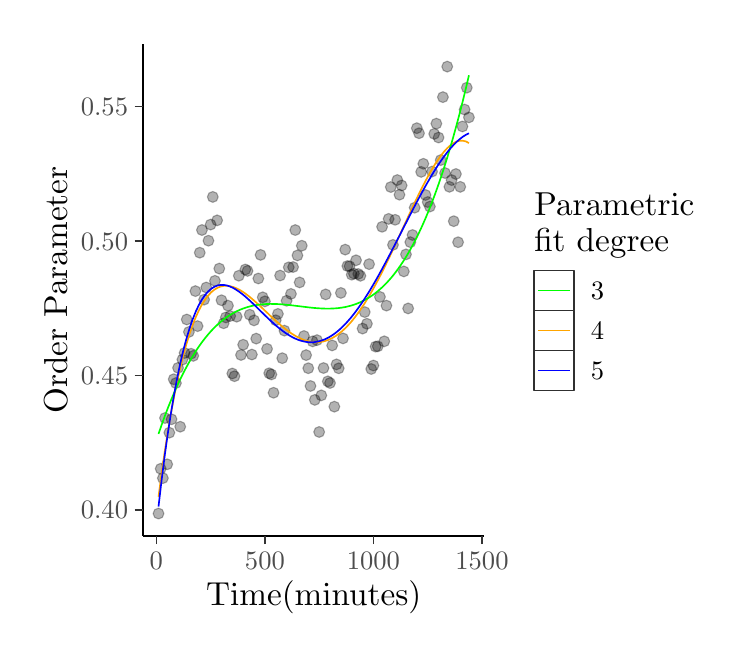
\begin{tikzpicture}[x=1pt,y=1pt]
\definecolor{fillColor}{RGB}{255,255,255}
\path[use as bounding box,fill=fillColor,fill opacity=0.00] (0,0) rectangle (252.94,216.81);
\begin{scope}
\path[clip] (  0.00,  0.00) rectangle (252.94,216.81);
\definecolor{drawColor}{RGB}{255,255,255}
\definecolor{fillColor}{RGB}{255,255,255}

\path[draw=drawColor,line width= 0.6pt,line join=round,line cap=round,fill=fillColor] (  0.00,  0.00) rectangle (252.94,216.81);
\end{scope}
\begin{scope}
\path[clip] ( 41.67, 33.16) rectangle (165.06,210.81);
\definecolor{fillColor}{RGB}{255,255,255}

\path[fill=fillColor] ( 41.67, 33.16) rectangle (165.06,210.81);
\definecolor{drawColor}{RGB}{0,0,0}
\definecolor{fillColor}{RGB}{0,0,0}

\path[draw=drawColor,draw opacity=0.30,line width= 0.4pt,line join=round,line cap=round,fill=fillColor,fill opacity=0.30] ( 47.28, 41.24) circle (  1.96);

\path[draw=drawColor,draw opacity=0.30,line width= 0.4pt,line join=round,line cap=round,fill=fillColor,fill opacity=0.30] ( 48.06, 57.42) circle (  1.96);

\path[draw=drawColor,draw opacity=0.30,line width= 0.4pt,line join=round,line cap=round,fill=fillColor,fill opacity=0.30] ( 48.85, 54.04) circle (  1.96);

\path[draw=drawColor,draw opacity=0.30,line width= 0.4pt,line join=round,line cap=round,fill=fillColor,fill opacity=0.30] ( 49.63, 75.76) circle (  1.96);

\path[draw=drawColor,draw opacity=0.30,line width= 0.4pt,line join=round,line cap=round,fill=fillColor,fill opacity=0.30] ( 50.42, 59.03) circle (  1.96);

\path[draw=drawColor,draw opacity=0.30,line width= 0.4pt,line join=round,line cap=round,fill=fillColor,fill opacity=0.30] ( 51.20, 70.46) circle (  1.96);

\path[draw=drawColor,draw opacity=0.30,line width= 0.4pt,line join=round,line cap=round,fill=fillColor,fill opacity=0.30] ( 51.99, 75.30) circle (  1.96);

\path[draw=drawColor,draw opacity=0.30,line width= 0.4pt,line join=round,line cap=round,fill=fillColor,fill opacity=0.30] ( 52.77, 89.78) circle (  1.96);

\path[draw=drawColor,draw opacity=0.30,line width= 0.4pt,line join=round,line cap=round,fill=fillColor,fill opacity=0.30] ( 53.56, 88.38) circle (  1.96);

\path[draw=drawColor,draw opacity=0.30,line width= 0.4pt,line join=round,line cap=round,fill=fillColor,fill opacity=0.30] ( 54.34, 93.89) circle (  1.96);

\path[draw=drawColor,draw opacity=0.30,line width= 0.4pt,line join=round,line cap=round,fill=fillColor,fill opacity=0.30] ( 55.12, 72.61) circle (  1.96);

\path[draw=drawColor,draw opacity=0.30,line width= 0.4pt,line join=round,line cap=round,fill=fillColor,fill opacity=0.30] ( 55.91, 96.86) circle (  1.96);

\path[draw=drawColor,draw opacity=0.30,line width= 0.4pt,line join=round,line cap=round,fill=fillColor,fill opacity=0.30] ( 56.69, 99.26) circle (  1.96);

\path[draw=drawColor,draw opacity=0.30,line width= 0.4pt,line join=round,line cap=round,fill=fillColor,fill opacity=0.30] ( 57.48,111.36) circle (  1.96);

\path[draw=drawColor,draw opacity=0.30,line width= 0.4pt,line join=round,line cap=round,fill=fillColor,fill opacity=0.30] ( 58.26,106.86) circle (  1.96);

\path[draw=drawColor,draw opacity=0.30,line width= 0.4pt,line join=round,line cap=round,fill=fillColor,fill opacity=0.30] ( 59.05, 99.00) circle (  1.96);

\path[draw=drawColor,draw opacity=0.30,line width= 0.4pt,line join=round,line cap=round,fill=fillColor,fill opacity=0.30] ( 59.83, 98.22) circle (  1.96);

\path[draw=drawColor,draw opacity=0.30,line width= 0.4pt,line join=round,line cap=round,fill=fillColor,fill opacity=0.30] ( 60.61,121.62) circle (  1.96);

\path[draw=drawColor,draw opacity=0.30,line width= 0.4pt,line join=round,line cap=round,fill=fillColor,fill opacity=0.30] ( 61.40,108.96) circle (  1.96);

\path[draw=drawColor,draw opacity=0.30,line width= 0.4pt,line join=round,line cap=round,fill=fillColor,fill opacity=0.30] ( 62.18,135.50) circle (  1.96);

\path[draw=drawColor,draw opacity=0.30,line width= 0.4pt,line join=round,line cap=round,fill=fillColor,fill opacity=0.30] ( 62.97,143.69) circle (  1.96);

\path[draw=drawColor,draw opacity=0.30,line width= 0.4pt,line join=round,line cap=round,fill=fillColor,fill opacity=0.30] ( 63.75,118.53) circle (  1.96);

\path[draw=drawColor,draw opacity=0.30,line width= 0.4pt,line join=round,line cap=round,fill=fillColor,fill opacity=0.30] ( 64.54,122.93) circle (  1.96);

\path[draw=drawColor,draw opacity=0.30,line width= 0.4pt,line join=round,line cap=round,fill=fillColor,fill opacity=0.30] ( 65.32,139.83) circle (  1.96);

\path[draw=drawColor,draw opacity=0.30,line width= 0.4pt,line join=round,line cap=round,fill=fillColor,fill opacity=0.30] ( 66.11,145.66) circle (  1.96);

\path[draw=drawColor,draw opacity=0.30,line width= 0.4pt,line join=round,line cap=round,fill=fillColor,fill opacity=0.30] ( 66.89,155.65) circle (  1.96);

\path[draw=drawColor,draw opacity=0.30,line width= 0.4pt,line join=round,line cap=round,fill=fillColor,fill opacity=0.30] ( 67.67,125.33) circle (  1.96);

\path[draw=drawColor,draw opacity=0.30,line width= 0.4pt,line join=round,line cap=round,fill=fillColor,fill opacity=0.30] ( 68.46,147.18) circle (  1.96);

\path[draw=drawColor,draw opacity=0.30,line width= 0.4pt,line join=round,line cap=round,fill=fillColor,fill opacity=0.30] ( 69.24,129.76) circle (  1.96);

\path[draw=drawColor,draw opacity=0.30,line width= 0.4pt,line join=round,line cap=round,fill=fillColor,fill opacity=0.30] ( 70.03,118.32) circle (  1.96);

\path[draw=drawColor,draw opacity=0.30,line width= 0.4pt,line join=round,line cap=round,fill=fillColor,fill opacity=0.30] ( 70.81,109.99) circle (  1.96);

\path[draw=drawColor,draw opacity=0.30,line width= 0.4pt,line join=round,line cap=round,fill=fillColor,fill opacity=0.30] ( 71.60,112.10) circle (  1.96);

\path[draw=drawColor,draw opacity=0.30,line width= 0.4pt,line join=round,line cap=round,fill=fillColor,fill opacity=0.30] ( 72.38,116.36) circle (  1.96);

\path[draw=drawColor,draw opacity=0.30,line width= 0.4pt,line join=round,line cap=round,fill=fillColor,fill opacity=0.30] ( 73.17,112.62) circle (  1.96);

\path[draw=drawColor,draw opacity=0.30,line width= 0.4pt,line join=round,line cap=round,fill=fillColor,fill opacity=0.30] ( 73.95, 91.85) circle (  1.96);

\path[draw=drawColor,draw opacity=0.30,line width= 0.4pt,line join=round,line cap=round,fill=fillColor,fill opacity=0.30] ( 74.73, 90.86) circle (  1.96);

\path[draw=drawColor,draw opacity=0.30,line width= 0.4pt,line join=round,line cap=round,fill=fillColor,fill opacity=0.30] ( 75.52,112.37) circle (  1.96);

\path[draw=drawColor,draw opacity=0.30,line width= 0.4pt,line join=round,line cap=round,fill=fillColor,fill opacity=0.30] ( 76.30,127.17) circle (  1.96);

\path[draw=drawColor,draw opacity=0.30,line width= 0.4pt,line join=round,line cap=round,fill=fillColor,fill opacity=0.30] ( 77.09, 98.54) circle (  1.96);

\path[draw=drawColor,draw opacity=0.30,line width= 0.4pt,line join=round,line cap=round,fill=fillColor,fill opacity=0.30] ( 77.87,102.24) circle (  1.96);

\path[draw=drawColor,draw opacity=0.30,line width= 0.4pt,line join=round,line cap=round,fill=fillColor,fill opacity=0.30] ( 78.66,129.43) circle (  1.96);

\path[draw=drawColor,draw opacity=0.30,line width= 0.4pt,line join=round,line cap=round,fill=fillColor,fill opacity=0.30] ( 79.44,128.92) circle (  1.96);

\path[draw=drawColor,draw opacity=0.30,line width= 0.4pt,line join=round,line cap=round,fill=fillColor,fill opacity=0.30] ( 80.23,113.09) circle (  1.96);

\path[draw=drawColor,draw opacity=0.30,line width= 0.4pt,line join=round,line cap=round,fill=fillColor,fill opacity=0.30] ( 81.01, 98.69) circle (  1.96);

\path[draw=drawColor,draw opacity=0.30,line width= 0.4pt,line join=round,line cap=round,fill=fillColor,fill opacity=0.30] ( 81.79,111.04) circle (  1.96);

\path[draw=drawColor,draw opacity=0.30,line width= 0.4pt,line join=round,line cap=round,fill=fillColor,fill opacity=0.30] ( 82.58,104.45) circle (  1.96);

\path[draw=drawColor,draw opacity=0.30,line width= 0.4pt,line join=round,line cap=round,fill=fillColor,fill opacity=0.30] ( 83.36,126.18) circle (  1.96);

\path[draw=drawColor,draw opacity=0.30,line width= 0.4pt,line join=round,line cap=round,fill=fillColor,fill opacity=0.30] ( 84.15,134.70) circle (  1.96);

\path[draw=drawColor,draw opacity=0.30,line width= 0.4pt,line join=round,line cap=round,fill=fillColor,fill opacity=0.30] ( 84.93,119.38) circle (  1.96);

\path[draw=drawColor,draw opacity=0.30,line width= 0.4pt,line join=round,line cap=round,fill=fillColor,fill opacity=0.30] ( 85.72,117.92) circle (  1.96);

\path[draw=drawColor,draw opacity=0.30,line width= 0.4pt,line join=round,line cap=round,fill=fillColor,fill opacity=0.30] ( 86.50,100.74) circle (  1.96);

\path[draw=drawColor,draw opacity=0.30,line width= 0.4pt,line join=round,line cap=round,fill=fillColor,fill opacity=0.30] ( 87.28, 91.94) circle (  1.96);

\path[draw=drawColor,draw opacity=0.30,line width= 0.4pt,line join=round,line cap=round,fill=fillColor,fill opacity=0.30] ( 88.07, 91.49) circle (  1.96);

\path[draw=drawColor,draw opacity=0.30,line width= 0.4pt,line join=round,line cap=round,fill=fillColor,fill opacity=0.30] ( 88.85, 84.89) circle (  1.96);

\path[draw=drawColor,draw opacity=0.30,line width= 0.4pt,line join=round,line cap=round,fill=fillColor,fill opacity=0.30] ( 89.64,111.09) circle (  1.96);

\path[draw=drawColor,draw opacity=0.30,line width= 0.4pt,line join=round,line cap=round,fill=fillColor,fill opacity=0.30] ( 90.42,113.38) circle (  1.96);

\path[draw=drawColor,draw opacity=0.30,line width= 0.4pt,line join=round,line cap=round,fill=fillColor,fill opacity=0.30] ( 91.21,127.24) circle (  1.96);

\path[draw=drawColor,draw opacity=0.30,line width= 0.4pt,line join=round,line cap=round,fill=fillColor,fill opacity=0.30] ( 91.99, 97.38) circle (  1.96);

\path[draw=drawColor,draw opacity=0.30,line width= 0.4pt,line join=round,line cap=round,fill=fillColor,fill opacity=0.30] ( 92.78,107.33) circle (  1.96);

\path[draw=drawColor,draw opacity=0.30,line width= 0.4pt,line join=round,line cap=round,fill=fillColor,fill opacity=0.30] ( 93.56,118.13) circle (  1.96);

\path[draw=drawColor,draw opacity=0.30,line width= 0.4pt,line join=round,line cap=round,fill=fillColor,fill opacity=0.30] ( 94.34,130.21) circle (  1.96);

\path[draw=drawColor,draw opacity=0.30,line width= 0.4pt,line join=round,line cap=round,fill=fillColor,fill opacity=0.30] ( 95.13,120.61) circle (  1.96);

\path[draw=drawColor,draw opacity=0.30,line width= 0.4pt,line join=round,line cap=round,fill=fillColor,fill opacity=0.30] ( 95.91,130.31) circle (  1.96);

\path[draw=drawColor,draw opacity=0.30,line width= 0.4pt,line join=round,line cap=round,fill=fillColor,fill opacity=0.30] ( 96.70,143.68) circle (  1.96);

\path[draw=drawColor,draw opacity=0.30,line width= 0.4pt,line join=round,line cap=round,fill=fillColor,fill opacity=0.30] ( 97.48,134.51) circle (  1.96);

\path[draw=drawColor,draw opacity=0.30,line width= 0.4pt,line join=round,line cap=round,fill=fillColor,fill opacity=0.30] ( 98.27,124.76) circle (  1.96);

\path[draw=drawColor,draw opacity=0.30,line width= 0.4pt,line join=round,line cap=round,fill=fillColor,fill opacity=0.30] ( 99.05,138.02) circle (  1.96);

\path[draw=drawColor,draw opacity=0.30,line width= 0.4pt,line join=round,line cap=round,fill=fillColor,fill opacity=0.30] ( 99.84,105.39) circle (  1.96);

\path[draw=drawColor,draw opacity=0.30,line width= 0.4pt,line join=round,line cap=round,fill=fillColor,fill opacity=0.30] (100.62, 98.49) circle (  1.96);

\path[draw=drawColor,draw opacity=0.30,line width= 0.4pt,line join=round,line cap=round,fill=fillColor,fill opacity=0.30] (101.40, 93.75) circle (  1.96);

\path[draw=drawColor,draw opacity=0.30,line width= 0.4pt,line join=round,line cap=round,fill=fillColor,fill opacity=0.30] (102.19, 87.34) circle (  1.96);

\path[draw=drawColor,draw opacity=0.30,line width= 0.4pt,line join=round,line cap=round,fill=fillColor,fill opacity=0.30] (102.97,103.45) circle (  1.96);

\path[draw=drawColor,draw opacity=0.30,line width= 0.4pt,line join=round,line cap=round,fill=fillColor,fill opacity=0.30] (103.76, 82.31) circle (  1.96);

\path[draw=drawColor,draw opacity=0.30,line width= 0.4pt,line join=round,line cap=round,fill=fillColor,fill opacity=0.30] (104.54,103.90) circle (  1.96);

\path[draw=drawColor,draw opacity=0.30,line width= 0.4pt,line join=round,line cap=round,fill=fillColor,fill opacity=0.30] (105.33, 70.71) circle (  1.96);

\path[draw=drawColor,draw opacity=0.30,line width= 0.4pt,line join=round,line cap=round,fill=fillColor,fill opacity=0.30] (106.11, 83.94) circle (  1.96);

\path[draw=drawColor,draw opacity=0.30,line width= 0.4pt,line join=round,line cap=round,fill=fillColor,fill opacity=0.30] (106.90, 93.82) circle (  1.96);

\path[draw=drawColor,draw opacity=0.30,line width= 0.4pt,line join=round,line cap=round,fill=fillColor,fill opacity=0.30] (107.68,120.43) circle (  1.96);

\path[draw=drawColor,draw opacity=0.30,line width= 0.4pt,line join=round,line cap=round,fill=fillColor,fill opacity=0.30] (108.46, 89.01) circle (  1.96);

\path[draw=drawColor,draw opacity=0.30,line width= 0.4pt,line join=round,line cap=round,fill=fillColor,fill opacity=0.30] (109.25, 88.41) circle (  1.96);

\path[draw=drawColor,draw opacity=0.30,line width= 0.4pt,line join=round,line cap=round,fill=fillColor,fill opacity=0.30] (110.03,101.99) circle (  1.96);

\path[draw=drawColor,draw opacity=0.30,line width= 0.4pt,line join=round,line cap=round,fill=fillColor,fill opacity=0.30] (110.82, 79.86) circle (  1.96);

\path[draw=drawColor,draw opacity=0.30,line width= 0.4pt,line join=round,line cap=round,fill=fillColor,fill opacity=0.30] (111.60, 95.14) circle (  1.96);

\path[draw=drawColor,draw opacity=0.30,line width= 0.4pt,line join=round,line cap=round,fill=fillColor,fill opacity=0.30] (112.39, 93.72) circle (  1.96);

\path[draw=drawColor,draw opacity=0.30,line width= 0.4pt,line join=round,line cap=round,fill=fillColor,fill opacity=0.30] (113.17,120.96) circle (  1.96);

\path[draw=drawColor,draw opacity=0.30,line width= 0.4pt,line join=round,line cap=round,fill=fillColor,fill opacity=0.30] (113.95,104.53) circle (  1.96);

\path[draw=drawColor,draw opacity=0.30,line width= 0.4pt,line join=round,line cap=round,fill=fillColor,fill opacity=0.30] (114.74,136.61) circle (  1.96);

\path[draw=drawColor,draw opacity=0.30,line width= 0.4pt,line join=round,line cap=round,fill=fillColor,fill opacity=0.30] (115.52,130.68) circle (  1.96);

\path[draw=drawColor,draw opacity=0.30,line width= 0.4pt,line join=round,line cap=round,fill=fillColor,fill opacity=0.30] (116.31,130.60) circle (  1.96);

\path[draw=drawColor,draw opacity=0.30,line width= 0.4pt,line join=round,line cap=round,fill=fillColor,fill opacity=0.30] (117.09,127.56) circle (  1.96);

\path[draw=drawColor,draw opacity=0.30,line width= 0.4pt,line join=round,line cap=round,fill=fillColor,fill opacity=0.30] (117.88,127.95) circle (  1.96);

\path[draw=drawColor,draw opacity=0.30,line width= 0.4pt,line join=round,line cap=round,fill=fillColor,fill opacity=0.30] (118.66,132.76) circle (  1.96);

\path[draw=drawColor,draw opacity=0.30,line width= 0.4pt,line join=round,line cap=round,fill=fillColor,fill opacity=0.30] (119.45,127.81) circle (  1.96);

\path[draw=drawColor,draw opacity=0.30,line width= 0.4pt,line join=round,line cap=round,fill=fillColor,fill opacity=0.30] (120.23,127.14) circle (  1.96);

\path[draw=drawColor,draw opacity=0.30,line width= 0.4pt,line join=round,line cap=round,fill=fillColor,fill opacity=0.30] (121.01,108.08) circle (  1.96);

\path[draw=drawColor,draw opacity=0.30,line width= 0.4pt,line join=round,line cap=round,fill=fillColor,fill opacity=0.30] (121.80,114.04) circle (  1.96);

\path[draw=drawColor,draw opacity=0.30,line width= 0.4pt,line join=round,line cap=round,fill=fillColor,fill opacity=0.30] (122.58,109.82) circle (  1.96);

\path[draw=drawColor,draw opacity=0.30,line width= 0.4pt,line join=round,line cap=round,fill=fillColor,fill opacity=0.30] (123.37,131.36) circle (  1.96);

\path[draw=drawColor,draw opacity=0.30,line width= 0.4pt,line join=round,line cap=round,fill=fillColor,fill opacity=0.30] (124.15, 93.47) circle (  1.96);

\path[draw=drawColor,draw opacity=0.30,line width= 0.4pt,line join=round,line cap=round,fill=fillColor,fill opacity=0.30] (124.94, 94.73) circle (  1.96);

\path[draw=drawColor,draw opacity=0.30,line width= 0.4pt,line join=round,line cap=round,fill=fillColor,fill opacity=0.30] (125.72,101.56) circle (  1.96);

\path[draw=drawColor,draw opacity=0.30,line width= 0.4pt,line join=round,line cap=round,fill=fillColor,fill opacity=0.30] (126.51,101.66) circle (  1.96);

\path[draw=drawColor,draw opacity=0.30,line width= 0.4pt,line join=round,line cap=round,fill=fillColor,fill opacity=0.30] (127.29,119.53) circle (  1.96);

\path[draw=drawColor,draw opacity=0.30,line width= 0.4pt,line join=round,line cap=round,fill=fillColor,fill opacity=0.30] (128.07,144.85) circle (  1.96);

\path[draw=drawColor,draw opacity=0.30,line width= 0.4pt,line join=round,line cap=round,fill=fillColor,fill opacity=0.30] (128.86,103.47) circle (  1.96);

\path[draw=drawColor,draw opacity=0.30,line width= 0.4pt,line join=round,line cap=round,fill=fillColor,fill opacity=0.30] (129.64,116.38) circle (  1.96);

\path[draw=drawColor,draw opacity=0.30,line width= 0.4pt,line join=round,line cap=round,fill=fillColor,fill opacity=0.30] (130.43,147.71) circle (  1.96);

\path[draw=drawColor,draw opacity=0.30,line width= 0.4pt,line join=round,line cap=round,fill=fillColor,fill opacity=0.30] (131.21,159.22) circle (  1.96);

\path[draw=drawColor,draw opacity=0.30,line width= 0.4pt,line join=round,line cap=round,fill=fillColor,fill opacity=0.30] (132.00,138.32) circle (  1.96);

\path[draw=drawColor,draw opacity=0.30,line width= 0.4pt,line join=round,line cap=round,fill=fillColor,fill opacity=0.30] (132.78,147.38) circle (  1.96);

\path[draw=drawColor,draw opacity=0.30,line width= 0.4pt,line join=round,line cap=round,fill=fillColor,fill opacity=0.30] (133.57,161.75) circle (  1.96);

\path[draw=drawColor,draw opacity=0.30,line width= 0.4pt,line join=round,line cap=round,fill=fillColor,fill opacity=0.30] (134.35,156.46) circle (  1.96);

\path[draw=drawColor,draw opacity=0.30,line width= 0.4pt,line join=round,line cap=round,fill=fillColor,fill opacity=0.30] (135.13,159.79) circle (  1.96);

\path[draw=drawColor,draw opacity=0.30,line width= 0.4pt,line join=round,line cap=round,fill=fillColor,fill opacity=0.30] (135.92,128.73) circle (  1.96);

\path[draw=drawColor,draw opacity=0.30,line width= 0.4pt,line join=round,line cap=round,fill=fillColor,fill opacity=0.30] (136.70,134.89) circle (  1.96);

\path[draw=drawColor,draw opacity=0.30,line width= 0.4pt,line join=round,line cap=round,fill=fillColor,fill opacity=0.30] (137.49,115.36) circle (  1.96);

\path[draw=drawColor,draw opacity=0.30,line width= 0.4pt,line join=round,line cap=round,fill=fillColor,fill opacity=0.30] (138.27,139.30) circle (  1.96);

\path[draw=drawColor,draw opacity=0.30,line width= 0.4pt,line join=round,line cap=round,fill=fillColor,fill opacity=0.30] (139.06,141.89) circle (  1.96);

\path[draw=drawColor,draw opacity=0.30,line width= 0.4pt,line join=round,line cap=round,fill=fillColor,fill opacity=0.30] (139.84,151.76) circle (  1.96);

\path[draw=drawColor,draw opacity=0.30,line width= 0.4pt,line join=round,line cap=round,fill=fillColor,fill opacity=0.30] (140.62,180.49) circle (  1.96);

\path[draw=drawColor,draw opacity=0.30,line width= 0.4pt,line join=round,line cap=round,fill=fillColor,fill opacity=0.30] (141.41,178.66) circle (  1.96);

\path[draw=drawColor,draw opacity=0.30,line width= 0.4pt,line join=round,line cap=round,fill=fillColor,fill opacity=0.30] (142.19,164.70) circle (  1.96);

\path[draw=drawColor,draw opacity=0.30,line width= 0.4pt,line join=round,line cap=round,fill=fillColor,fill opacity=0.30] (142.98,167.62) circle (  1.96);

\path[draw=drawColor,draw opacity=0.30,line width= 0.4pt,line join=round,line cap=round,fill=fillColor,fill opacity=0.30] (143.76,156.35) circle (  1.96);

\path[draw=drawColor,draw opacity=0.30,line width= 0.4pt,line join=round,line cap=round,fill=fillColor,fill opacity=0.30] (144.55,153.80) circle (  1.96);

\path[draw=drawColor,draw opacity=0.30,line width= 0.4pt,line join=round,line cap=round,fill=fillColor,fill opacity=0.30] (145.33,152.16) circle (  1.96);

\path[draw=drawColor,draw opacity=0.30,line width= 0.4pt,line join=round,line cap=round,fill=fillColor,fill opacity=0.30] (146.12,164.81) circle (  1.96);

\path[draw=drawColor,draw opacity=0.30,line width= 0.4pt,line join=round,line cap=round,fill=fillColor,fill opacity=0.30] (146.90,178.43) circle (  1.96);

\path[draw=drawColor,draw opacity=0.30,line width= 0.4pt,line join=round,line cap=round,fill=fillColor,fill opacity=0.30] (147.68,182.14) circle (  1.96);

\path[draw=drawColor,draw opacity=0.30,line width= 0.4pt,line join=round,line cap=round,fill=fillColor,fill opacity=0.30] (148.47,177.11) circle (  1.96);

\path[draw=drawColor,draw opacity=0.30,line width= 0.4pt,line join=round,line cap=round,fill=fillColor,fill opacity=0.30] (149.25,168.96) circle (  1.96);

\path[draw=drawColor,draw opacity=0.30,line width= 0.4pt,line join=round,line cap=round,fill=fillColor,fill opacity=0.30] (150.04,191.71) circle (  1.96);

\path[draw=drawColor,draw opacity=0.30,line width= 0.4pt,line join=round,line cap=round,fill=fillColor,fill opacity=0.30] (150.82,164.28) circle (  1.96);

\path[draw=drawColor,draw opacity=0.30,line width= 0.4pt,line join=round,line cap=round,fill=fillColor,fill opacity=0.30] (151.61,202.74) circle (  1.96);

\path[draw=drawColor,draw opacity=0.30,line width= 0.4pt,line join=round,line cap=round,fill=fillColor,fill opacity=0.30] (152.39,159.30) circle (  1.96);

\path[draw=drawColor,draw opacity=0.30,line width= 0.4pt,line join=round,line cap=round,fill=fillColor,fill opacity=0.30] (153.18,161.74) circle (  1.96);

\path[draw=drawColor,draw opacity=0.30,line width= 0.4pt,line join=round,line cap=round,fill=fillColor,fill opacity=0.30] (153.96,146.88) circle (  1.96);

\path[draw=drawColor,draw opacity=0.30,line width= 0.4pt,line join=round,line cap=round,fill=fillColor,fill opacity=0.30] (154.74,163.93) circle (  1.96);

\path[draw=drawColor,draw opacity=0.30,line width= 0.4pt,line join=round,line cap=round,fill=fillColor,fill opacity=0.30] (155.53,139.28) circle (  1.96);

\path[draw=drawColor,draw opacity=0.30,line width= 0.4pt,line join=round,line cap=round,fill=fillColor,fill opacity=0.30] (156.31,159.29) circle (  1.96);

\path[draw=drawColor,draw opacity=0.30,line width= 0.4pt,line join=round,line cap=round,fill=fillColor,fill opacity=0.30] (157.10,181.11) circle (  1.96);

\path[draw=drawColor,draw opacity=0.30,line width= 0.4pt,line join=round,line cap=round,fill=fillColor,fill opacity=0.30] (157.88,187.22) circle (  1.96);

\path[draw=drawColor,draw opacity=0.30,line width= 0.4pt,line join=round,line cap=round,fill=fillColor,fill opacity=0.30] (158.67,195.12) circle (  1.96);

\path[draw=drawColor,draw opacity=0.30,line width= 0.4pt,line join=round,line cap=round,fill=fillColor,fill opacity=0.30] (159.45,184.39) circle (  1.96);
\definecolor{drawColor}{RGB}{255,165,0}

\path[draw=drawColor,line width= 0.6pt,line join=round] ( 47.28, 47.30) --
	( 48.40, 55.75) --
	( 49.52, 63.56) --
	( 50.64, 70.75) --
	( 51.77, 77.37) --
	( 52.89, 83.42) --
	( 54.01, 88.94) --
	( 55.13, 93.95) --
	( 56.25, 98.47) --
	( 57.38,102.54) --
	( 58.50,106.17) --
	( 59.62,109.38) --
	( 60.74,112.21) --
	( 61.86,114.66) --
	( 62.98,116.77) --
	( 64.11,118.55) --
	( 65.23,120.02) --
	( 66.35,121.21) --
	( 67.47,122.13) --
	( 68.59,122.81) --
	( 69.71,123.26) --
	( 70.84,123.50) --
	( 71.96,123.54) --
	( 73.08,123.41) --
	( 74.20,123.12) --
	( 75.32,122.69) --
	( 76.44,122.14) --
	( 77.57,121.47) --
	( 78.69,120.71) --
	( 79.81,119.86) --
	( 80.93,118.94) --
	( 82.05,117.97) --
	( 83.17,116.96) --
	( 84.30,115.92) --
	( 85.42,114.86) --
	( 86.54,113.79) --
	( 87.66,112.73) --
	( 88.78,111.68) --
	( 89.90,110.65) --
	( 91.03,109.66) --
	( 92.15,108.71) --
	( 93.27,107.81) --
	( 94.39,106.97) --
	( 95.51,106.20) --
	( 96.63,105.50) --
	( 97.76,104.88) --
	( 98.88,104.35) --
	(100.00,103.90) --
	(101.12,103.56) --
	(102.24,103.31) --
	(103.37,103.17) --
	(104.49,103.13) --
	(105.61,103.21) --
	(106.73,103.40) --
	(107.85,103.71) --
	(108.97,104.13) --
	(110.10,104.68) --
	(111.22,105.34) --
	(112.34,106.12) --
	(113.46,107.02) --
	(114.58,108.04) --
	(115.70,109.17) --
	(116.83,110.42) --
	(117.95,111.78) --
	(119.07,113.25) --
	(120.19,114.83) --
	(121.31,116.51) --
	(122.43,118.28) --
	(123.56,120.15) --
	(124.68,122.11) --
	(125.80,124.15) --
	(126.92,126.27) --
	(128.04,128.45) --
	(129.16,130.70) --
	(130.29,133.01) --
	(131.41,135.35) --
	(132.53,137.74) --
	(133.65,140.16) --
	(134.77,142.59) --
	(135.89,145.03) --
	(137.02,147.47) --
	(138.14,149.90) --
	(139.26,152.30) --
	(140.38,154.66) --
	(141.50,156.98) --
	(142.63,159.23) --
	(143.75,161.41) --
	(144.87,163.49) --
	(145.99,165.47) --
	(147.11,167.34) --
	(148.23,169.06) --
	(149.36,170.64) --
	(150.48,172.04) --
	(151.60,173.26) --
	(152.72,174.28) --
	(153.84,175.08) --
	(154.96,175.64) --
	(156.09,175.95) --
	(157.21,175.97) --
	(158.33,175.70) --
	(159.45,175.11);
\definecolor{drawColor}{RGB}{0,255,0}

\path[draw=drawColor,line width= 0.6pt,line join=round] ( 47.28, 70.01) --
	( 48.40, 73.26) --
	( 49.52, 76.36) --
	( 50.64, 79.32) --
	( 51.77, 82.13) --
	( 52.89, 84.80) --
	( 54.01, 87.34) --
	( 55.13, 89.75) --
	( 56.25, 92.02) --
	( 57.38, 94.18) --
	( 58.50, 96.20) --
	( 59.62, 98.11) --
	( 60.74, 99.91) --
	( 61.86,101.59) --
	( 62.98,103.16) --
	( 64.11,104.63) --
	( 65.23,105.99) --
	( 66.35,107.26) --
	( 67.47,108.43) --
	( 68.59,109.50) --
	( 69.71,110.49) --
	( 70.84,111.40) --
	( 71.96,112.22) --
	( 73.08,112.96) --
	( 74.20,113.63) --
	( 75.32,114.23) --
	( 76.44,114.75) --
	( 77.57,115.21) --
	( 78.69,115.61) --
	( 79.81,115.95) --
	( 80.93,116.24) --
	( 82.05,116.48) --
	( 83.17,116.66) --
	( 84.30,116.80) --
	( 85.42,116.90) --
	( 86.54,116.96) --
	( 87.66,116.99) --
	( 88.78,116.98) --
	( 89.90,116.95) --
	( 91.03,116.89) --
	( 92.15,116.81) --
	( 93.27,116.71) --
	( 94.39,116.59) --
	( 95.51,116.47) --
	( 96.63,116.33) --
	( 97.76,116.20) --
	( 98.88,116.06) --
	(100.00,115.92) --
	(101.12,115.79) --
	(102.24,115.66) --
	(103.37,115.55) --
	(104.49,115.45) --
	(105.61,115.38) --
	(106.73,115.32) --
	(107.85,115.29) --
	(108.97,115.29) --
	(110.10,115.32) --
	(111.22,115.39) --
	(112.34,115.49) --
	(113.46,115.64) --
	(114.58,115.83) --
	(115.70,116.08) --
	(116.83,116.37) --
	(117.95,116.72) --
	(119.07,117.13) --
	(120.19,117.60) --
	(121.31,118.14) --
	(122.43,118.75) --
	(123.56,119.43) --
	(124.68,120.18) --
	(125.80,121.02) --
	(126.92,121.94) --
	(128.04,122.94) --
	(129.16,124.03) --
	(130.29,125.22) --
	(131.41,126.50) --
	(132.53,127.88) --
	(133.65,129.37) --
	(134.77,130.96) --
	(135.89,132.66) --
	(137.02,134.47) --
	(138.14,136.40) --
	(139.26,138.45) --
	(140.38,140.62) --
	(141.50,142.92) --
	(142.63,145.34) --
	(143.75,147.90) --
	(144.87,150.60) --
	(145.99,153.44) --
	(147.11,156.42) --
	(148.23,159.54) --
	(149.36,162.82) --
	(150.48,166.25) --
	(151.60,169.83) --
	(152.72,173.58) --
	(153.84,177.49) --
	(154.96,181.56) --
	(156.09,185.81) --
	(157.21,190.23) --
	(158.33,194.83) --
	(159.45,199.60);
\definecolor{drawColor}{RGB}{0,0,255}

\path[draw=drawColor,line width= 0.6pt,line join=round] ( 47.28, 43.78) --
	( 48.40, 53.38) --
	( 49.52, 62.18) --
	( 50.64, 70.21) --
	( 51.77, 77.52) --
	( 52.89, 84.13) --
	( 54.01, 90.10) --
	( 55.13, 95.45) --
	( 56.25,100.23) --
	( 57.38,104.46) --
	( 58.50,108.18) --
	( 59.62,111.42) --
	( 60.74,114.22) --
	( 61.86,116.59) --
	( 62.98,118.58) --
	( 64.11,120.21) --
	( 65.23,121.50) --
	( 66.35,122.49) --
	( 67.47,123.19) --
	( 68.59,123.64) --
	( 69.71,123.85) --
	( 70.84,123.85) --
	( 71.96,123.65) --
	( 73.08,123.29) --
	( 74.20,122.78) --
	( 75.32,122.14) --
	( 76.44,121.38) --
	( 77.57,120.53) --
	( 78.69,119.60) --
	( 79.81,118.61) --
	( 80.93,117.56) --
	( 82.05,116.49) --
	( 83.17,115.39) --
	( 84.30,114.28) --
	( 85.42,113.18) --
	( 86.54,112.09) --
	( 87.66,111.03) --
	( 88.78,110.00) --
	( 89.90,109.02) --
	( 91.03,108.09) --
	( 92.15,107.22) --
	( 93.27,106.42) --
	( 94.39,105.70) --
	( 95.51,105.05) --
	( 96.63,104.49) --
	( 97.76,104.02) --
	( 98.88,103.65) --
	(100.00,103.38) --
	(101.12,103.20) --
	(102.24,103.13) --
	(103.37,103.17) --
	(104.49,103.32) --
	(105.61,103.57) --
	(106.73,103.94) --
	(107.85,104.41) --
	(108.97,105.00) --
	(110.10,105.69) --
	(111.22,106.49) --
	(112.34,107.40) --
	(113.46,108.41) --
	(114.58,109.53) --
	(115.70,110.74) --
	(116.83,112.05) --
	(117.95,113.45) --
	(119.07,114.95) --
	(120.19,116.52) --
	(121.31,118.18) --
	(122.43,119.92) --
	(123.56,121.72) --
	(124.68,123.60) --
	(125.80,125.53) --
	(126.92,127.52) --
	(128.04,129.56) --
	(129.16,131.64) --
	(130.29,133.76) --
	(131.41,135.90) --
	(132.53,138.08) --
	(133.65,140.27) --
	(134.77,142.47) --
	(135.89,144.67) --
	(137.02,146.87) --
	(138.14,149.06) --
	(139.26,151.23) --
	(140.38,153.38) --
	(141.50,155.49) --
	(142.63,157.56) --
	(143.75,159.59) --
	(144.87,161.55) --
	(145.99,163.46) --
	(147.11,165.29) --
	(148.23,167.05) --
	(149.36,168.72) --
	(150.48,170.29) --
	(151.60,171.76) --
	(152.72,173.13) --
	(153.84,174.38) --
	(154.96,175.51) --
	(156.09,176.51) --
	(157.21,177.37) --
	(158.33,178.09) --
	(159.45,178.66);
\end{scope}
\begin{scope}
\path[clip] (  0.00,  0.00) rectangle (252.94,216.81);
\definecolor{drawColor}{RGB}{0,0,0}

\path[draw=drawColor,line width= 0.6pt,line join=round] ( 41.67, 33.16) --
	( 41.67,210.81);
\end{scope}
\begin{scope}
\path[clip] (  0.00,  0.00) rectangle (252.94,216.81);
\definecolor{drawColor}{gray}{0.30}

\node[text=drawColor,anchor=base east,inner sep=0pt, outer sep=0pt, scale=  0.96] at ( 36.27, 39.27) {0.40};

\node[text=drawColor,anchor=base east,inner sep=0pt, outer sep=0pt, scale=  0.96] at ( 36.27, 87.84) {0.45};

\node[text=drawColor,anchor=base east,inner sep=0pt, outer sep=0pt, scale=  0.96] at ( 36.27,136.40) {0.50};

\node[text=drawColor,anchor=base east,inner sep=0pt, outer sep=0pt, scale=  0.96] at ( 36.27,184.97) {0.55};
\end{scope}
\begin{scope}
\path[clip] (  0.00,  0.00) rectangle (252.94,216.81);
\definecolor{drawColor}{gray}{0.20}

\path[draw=drawColor,line width= 0.6pt,line join=round] ( 38.67, 42.58) --
	( 41.67, 42.58);

\path[draw=drawColor,line width= 0.6pt,line join=round] ( 38.67, 91.14) --
	( 41.67, 91.14);

\path[draw=drawColor,line width= 0.6pt,line join=round] ( 38.67,139.71) --
	( 41.67,139.71);

\path[draw=drawColor,line width= 0.6pt,line join=round] ( 38.67,188.27) --
	( 41.67,188.27);
\end{scope}
\begin{scope}
\path[clip] (  0.00,  0.00) rectangle (252.94,216.81);
\definecolor{drawColor}{RGB}{0,0,0}

\path[draw=drawColor,line width= 0.6pt,line join=round] ( 41.67, 33.16) --
	(165.06, 33.16);
\end{scope}
\begin{scope}
\path[clip] (  0.00,  0.00) rectangle (252.94,216.81);
\definecolor{drawColor}{gray}{0.20}

\path[draw=drawColor,line width= 0.6pt,line join=round] ( 46.50, 30.16) --
	( 46.50, 33.16);

\path[draw=drawColor,line width= 0.6pt,line join=round] ( 85.72, 30.16) --
	( 85.72, 33.16);

\path[draw=drawColor,line width= 0.6pt,line join=round] (124.94, 30.16) --
	(124.94, 33.16);

\path[draw=drawColor,line width= 0.6pt,line join=round] (164.16, 30.16) --
	(164.16, 33.16);
\end{scope}
\begin{scope}
\path[clip] (  0.00,  0.00) rectangle (252.94,216.81);
\definecolor{drawColor}{gray}{0.30}

\node[text=drawColor,anchor=base,inner sep=0pt, outer sep=0pt, scale=  0.96] at ( 46.50, 21.15) {0};

\node[text=drawColor,anchor=base,inner sep=0pt, outer sep=0pt, scale=  0.96] at ( 85.72, 21.15) {500};

\node[text=drawColor,anchor=base,inner sep=0pt, outer sep=0pt, scale=  0.96] at (124.94, 21.15) {1000};

\node[text=drawColor,anchor=base,inner sep=0pt, outer sep=0pt, scale=  0.96] at (164.16, 21.15) {1500};
\end{scope}
\begin{scope}
\path[clip] (  0.00,  0.00) rectangle (252.94,216.81);
\definecolor{drawColor}{RGB}{0,0,0}

\node[text=drawColor,anchor=base,inner sep=0pt, outer sep=0pt, scale=  1.20] at (103.37,  7.94) {Time(minutes)};
\end{scope}
\begin{scope}
\path[clip] (  0.00,  0.00) rectangle (252.94,216.81);
\definecolor{drawColor}{RGB}{0,0,0}

\node[text=drawColor,rotate= 90.00,anchor=base,inner sep=0pt, outer sep=0pt, scale=  1.20] at ( 14.26,121.99) {Order Parameter};
\end{scope}
\begin{scope}
\path[clip] (  0.00,  0.00) rectangle (252.94,216.81);
\definecolor{fillColor}{RGB}{255,255,255}

\path[fill=fillColor] (177.06, 79.72) rectangle (246.95,164.25);
\end{scope}
\begin{scope}
\path[clip] (  0.00,  0.00) rectangle (252.94,216.81);
\definecolor{drawColor}{RGB}{0,0,0}

\node[text=drawColor,anchor=base west,inner sep=0pt, outer sep=0pt, scale=  1.20] at (183.06,149.02) {Parametric };

\node[text=drawColor,anchor=base west,inner sep=0pt, outer sep=0pt, scale=  1.20] at (183.06,136.06) {fit degree };
\end{scope}
\begin{scope}
\path[clip] (  0.00,  0.00) rectangle (252.94,216.81);
\definecolor{drawColor}{gray}{0.19}
\definecolor{fillColor}{RGB}{255,255,255}

\path[draw=drawColor,line width= 0.6pt,line join=round,line cap=round,fill=fillColor] (183.06,114.63) rectangle (197.51,129.08);
\end{scope}
\begin{scope}
\path[clip] (  0.00,  0.00) rectangle (252.94,216.81);
\definecolor{drawColor}{RGB}{0,255,0}

\path[draw=drawColor,line width= 0.6pt,line join=round] (184.50,121.86) -- (196.07,121.86);
\end{scope}
\begin{scope}
\path[clip] (  0.00,  0.00) rectangle (252.94,216.81);
\definecolor{drawColor}{RGB}{0,255,0}

\path[draw=drawColor,line width= 0.6pt,line join=round] (184.50,121.86) -- (196.07,121.86);
\end{scope}
\begin{scope}
\path[clip] (  0.00,  0.00) rectangle (252.94,216.81);
\definecolor{drawColor}{RGB}{0,255,0}

\path[draw=drawColor,line width= 0.6pt,line join=round] (184.50,121.86) -- (196.07,121.86);
\end{scope}
\begin{scope}
\path[clip] (  0.00,  0.00) rectangle (252.94,216.81);
\definecolor{drawColor}{gray}{0.19}
\definecolor{fillColor}{RGB}{255,255,255}

\path[draw=drawColor,line width= 0.6pt,line join=round,line cap=round,fill=fillColor] (183.06,100.18) rectangle (197.51,114.63);
\end{scope}
\begin{scope}
\path[clip] (  0.00,  0.00) rectangle (252.94,216.81);
\definecolor{drawColor}{RGB}{255,165,0}

\path[draw=drawColor,line width= 0.6pt,line join=round] (184.50,107.40) -- (196.07,107.40);
\end{scope}
\begin{scope}
\path[clip] (  0.00,  0.00) rectangle (252.94,216.81);
\definecolor{drawColor}{RGB}{255,165,0}

\path[draw=drawColor,line width= 0.6pt,line join=round] (184.50,107.40) -- (196.07,107.40);
\end{scope}
\begin{scope}
\path[clip] (  0.00,  0.00) rectangle (252.94,216.81);
\definecolor{drawColor}{RGB}{255,165,0}

\path[draw=drawColor,line width= 0.6pt,line join=round] (184.50,107.40) -- (196.07,107.40);
\end{scope}
\begin{scope}
\path[clip] (  0.00,  0.00) rectangle (252.94,216.81);
\definecolor{drawColor}{gray}{0.19}
\definecolor{fillColor}{RGB}{255,255,255}

\path[draw=drawColor,line width= 0.6pt,line join=round,line cap=round,fill=fillColor] (183.06, 85.72) rectangle (197.51,100.18);
\end{scope}
\begin{scope}
\path[clip] (  0.00,  0.00) rectangle (252.94,216.81);
\definecolor{drawColor}{RGB}{0,0,255}

\path[draw=drawColor,line width= 0.6pt,line join=round] (184.50, 92.95) -- (196.07, 92.95);
\end{scope}
\begin{scope}
\path[clip] (  0.00,  0.00) rectangle (252.94,216.81);
\definecolor{drawColor}{RGB}{0,0,255}

\path[draw=drawColor,line width= 0.6pt,line join=round] (184.50, 92.95) -- (196.07, 92.95);
\end{scope}
\begin{scope}
\path[clip] (  0.00,  0.00) rectangle (252.94,216.81);
\definecolor{drawColor}{RGB}{0,0,255}

\path[draw=drawColor,line width= 0.6pt,line join=round] (184.50, 92.95) -- (196.07, 92.95);
\end{scope}
\begin{scope}
\path[clip] (  0.00,  0.00) rectangle (252.94,216.81);
\definecolor{drawColor}{RGB}{0,0,0}

\node[text=drawColor,anchor=base west,inner sep=0pt, outer sep=0pt, scale=  0.96] at (203.51,118.55) {3};
\end{scope}
\begin{scope}
\path[clip] (  0.00,  0.00) rectangle (252.94,216.81);
\definecolor{drawColor}{RGB}{0,0,0}

\node[text=drawColor,anchor=base west,inner sep=0pt, outer sep=0pt, scale=  0.96] at (203.51,104.10) {4};
\end{scope}
\begin{scope}
\path[clip] (  0.00,  0.00) rectangle (252.94,216.81);
\definecolor{drawColor}{RGB}{0,0,0}

\node[text=drawColor,anchor=base west,inner sep=0pt, outer sep=0pt, scale=  0.96] at (203.51, 89.64) {5};
\end{scope}
\end{tikzpicture}
}
    		\caption{ Plot of the parametric for various degrees }
    		\label{fig 8.6}
    	\end{subfigure}
    	\caption{}
    	\label{figuu}
    \end{figure}
    We can notice from \ref{fig 8.5} that the parametric fit of degree 4 is very close to the splines fit with degrees 2, 3 and 4. Hence it is resonable to use a fitting model. Figure \ref{fig 8.6} indicates that it also works for polynomial of 5th degree, but not for 3rd degree, because an underfitting problem.
    
\end{enumerate}



%99999999999999999999999999999999999999999999%

{\color{royalblue}\chapter{Mixed models}}
{\color{royalblue}\section{Problem description}}
Let's illustrate the problem in this section with the following exemple. The (simple) linear model state there is a linear dependence between explanatory variables $Y_{i,t}$, and the time $t$ (dependent variable), with an error term $\epsilon_{i,t}$
\[ Y_{i,t} = \alpha + \beta_t + \epsilon_{i,t}, \hspace{0.25cm}
 \epsilon_{i,t}\sim \mathcal{N}(0,\sigma^2)\]
$t,\alpha ,\beta $: fixed effects.
$\alpha ,\beta, \sigma$: parameters to estimate.
One limit of this model is that it considers $Y_{i,t}$ to be independent, which is not often the case as they can be correlated. Therefore, take this into account, a random effect is added to the fixed effects. We obtain a (linear) mixed model

{\color{royalblue}\section{Methods}}
The data we consider are of the form $Y_{ij}$, $i = 1,\dots, n$, $j= 1,\dots,k_i$. That is, there are $n$
subjects (clusters) and for each subject i there are $k_i$ observations.
A mixed model can be represented as
	\[ Y= X\beta+ Zu+ \epsilon, \hspace{0.25cm}
\mathtt{E}
\begin{pmatrix}
u \\
\epsilon
\end{pmatrix}=
\begin{pmatrix}
0 \\
0
\end{pmatrix}, \hspace{0.25cm}
\mathtt{cov}
\begin{pmatrix}
u\\
\epsilon
\end{pmatrix}=
\begin{pmatrix}
\sigma^2_u D & 0 \\
0 & \sigma^2_\epsilon \Sigma
\end{pmatrix}, \]
for $Y, \epsilon \in \mathbb{R}^N$, $N=\sum_{i=1}^{n}k_i$, $Z= \mathtt{blockdiag}(Z_1,\dots,Z_n)\in \mathbb{R}^{N\times nm}$, $u\in \mathbb{R}^{nm}$
Typically, a normality assumption is made both for $\epsilon$ and $u$.\\
A good exemple of mixed models' application is in \textbf{small area estimation}, where it is assumed that the means in "small areas" differ for a random amount:
\[ Y_i= X_i\beta+ \mathbb{I}_{n_i}u_i+ \epsilon_{i}, \hspace{0.25cm}
  \epsilon_{i} \sim \mathcal{N}_{k_i}(0_{k_i},\sigma^2I_{k_i}), \hspace{0.25cm}
  u_i\sim \mathcal{N}(0,\sigma^2_u), , \hspace{0.25cm} i=1,\dots,n, \]
where in each $i$th small area there are $k_i$ observations available.

\newpage
In the exercise, we are interested in the estimation of $u$. Since it is assumed to be random, one typically uses the term "predictor" for $\hat{u}$, which is obtained as a \textit{best linear
unnbiased predictor} (\textbf{BLUP})
\[ \hat{u}= \frac{1}{\lambda}Z^t V^{-1}(Y-X\hat{\beta}) \]
\[ \hat{\beta}= (X^tV^{-1}X)^{-1}X^tY,\]
where $V= I_{N}+ ZZ^t/\lambda$ for $\lambda= \frac{\sigma^2_\epsilon}{\sigma^2_u}$, $N=\sum_{i=1}^{n}k_i>p$

\newpage
{\color{royalblue}\section{Results}}
For the data, we consider the survey and satellite data measuring the area for corn and soy fields in NorthCentral Iowa from 1978. The data set is available
as \textit{landsat} in the R-package JoSAE. We are interested in obtaining reliable estimates for the total size of corn and soy production for each of the 12 counties in the data set, respectively.
Variables of interest:
\begin{enumerate}
	\item[] $\mathtt{SegmentsInCounty}$: number of of segments of county.
	\item[] $\mathtt{SegementID}$: identificator for segment.
	\item[] $\mathtt{HACorn}$: hectares of corn for given segment.
	\item[] $\mathtt{HASoybeans}$: hectares of soybeans for given segment.
	\item[] $\mathtt{PixelsCorn}$: pixels for corn for given segment.

	\item[] $\mathtt{PixelsSoybeans}$: pixels for soybeans for given segment.
	\item[] $\mathtt{MeanPixelsCorn}$: mean of pixels for corn over all segments in given county.
	\item[] $\mathtt{MeanPixelsSoybeans}$: mean of pixels for soybeans over all segments in given county.
	\item[] $\mathtt{CountyName}$: county identificator of the segment.
\end{enumerate}

\begin{enumerate}[label=(\alph*)]
	\item In order to fit a linear model to both the hectares of corn and soybeans for segment for
each county, we chose $\mathtt{PixelsCorn}$ and $\mathtt{PixelsSoybeans}$ variables since we want to estimate for the total size of corn and soy production. The limitations
of this linear model is that it could not estimate the hectares of corn and soybeans for segment in some counties; probably because of a random effect that the model cannot take into consideration.
	
	\item We fit a linear mixed model $y_{ij} = x^t\beta + v_i + e_{ij}$ for both crops such that segments share
the same countywide random effect. We can interpret from table \ref{tableau91} that Soybeans tend to have 
	\begin{table}[H]
		\centering
		\begin{tabular}{|P{2cm}|P{2.5cm}|P{2.5cm}|P{2.5cm}|P{2.5cm}|}
			\hline
			& \multicolumn{2}{c|}{Fixed effects} & \multicolumn{2}{c|}{Random effects (StdDev)} \\
			\hline
			& (Intercept) & Pixels & (Intercept) & Residual \\
			\hline
			Corn & 5.4661894 & 0.3878358 & 7.926246 & 17.03993 \\
			\hline 
			Soybeans & -3.8223556 & 0.4756781 & 15.46753 & 13.41709 \\
			\hline 
		\end{tabular}
		\caption{\label{tableau91}Results of the linear mixed model}
	\end{table}
	Figure \ref{figuuuuuu} shows that the Q-Q plot indicate points falling on the identity line, which means that the residuals are well normally distributed.
		 
	\begin{figure}[H]
		\centering
		\begin{subfigure}[b]{0.48\linewidth}        %% or \columnwidth
			\centering
			\scalebox{0.75}{% Created by tikzDevice version 0.12 on 2019-04-30 20:46:51
% !TEX encoding = UTF-8 Unicode
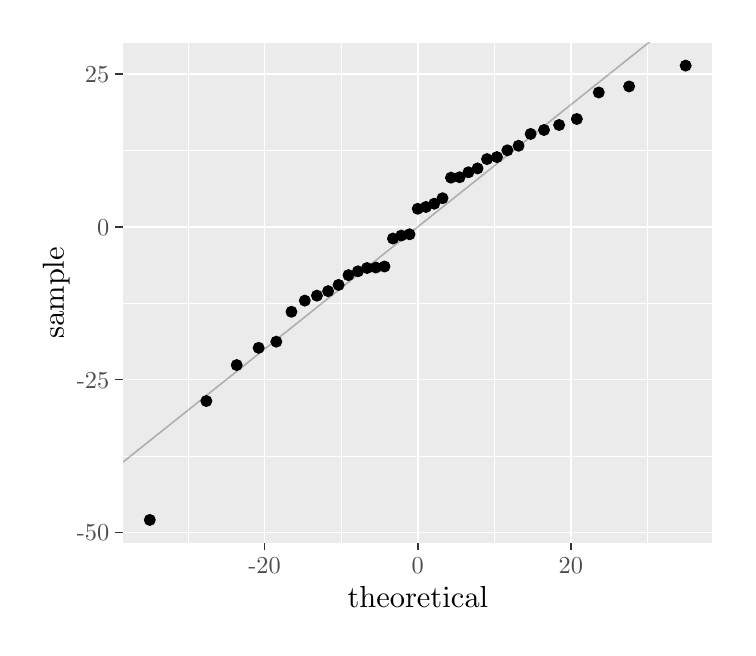
\begin{tikzpicture}[x=1pt,y=1pt]
\definecolor{fillColor}{RGB}{255,255,255}
\path[use as bounding box,fill=fillColor,fill opacity=0.00] (0,0) rectangle (252.94,216.81);
\begin{scope}
\path[clip] (  0.00,  0.00) rectangle (252.94,216.81);
\definecolor{drawColor}{RGB}{255,255,255}
\definecolor{fillColor}{RGB}{255,255,255}

\path[draw=drawColor,line width= 0.6pt,line join=round,line cap=round,fill=fillColor] (  0.00,  0.00) rectangle (252.94,216.81);
\end{scope}
\begin{scope}
\path[clip] ( 34.45, 30.72) rectangle (247.44,211.31);
\definecolor{fillColor}{gray}{0.92}

\path[fill=fillColor] ( 34.45, 30.72) rectangle (247.44,211.31);
\definecolor{drawColor}{RGB}{255,255,255}

\path[draw=drawColor,line width= 0.3pt,line join=round] ( 34.45, 62.03) --
	(247.44, 62.03);

\path[draw=drawColor,line width= 0.3pt,line join=round] ( 34.45,117.22) --
	(247.44,117.22);

\path[draw=drawColor,line width= 0.3pt,line join=round] ( 34.45,172.42) --
	(247.44,172.42);

\path[draw=drawColor,line width= 0.3pt,line join=round] ( 57.94, 30.72) --
	( 57.94,211.31);

\path[draw=drawColor,line width= 0.3pt,line join=round] (113.28, 30.72) --
	(113.28,211.31);

\path[draw=drawColor,line width= 0.3pt,line join=round] (168.62, 30.72) --
	(168.62,211.31);

\path[draw=drawColor,line width= 0.3pt,line join=round] (223.96, 30.72) --
	(223.96,211.31);

\path[draw=drawColor,line width= 0.6pt,line join=round] ( 34.45, 34.43) --
	(247.44, 34.43);

\path[draw=drawColor,line width= 0.6pt,line join=round] ( 34.45, 89.63) --
	(247.44, 89.63);

\path[draw=drawColor,line width= 0.6pt,line join=round] ( 34.45,144.82) --
	(247.44,144.82);

\path[draw=drawColor,line width= 0.6pt,line join=round] ( 34.45,200.02) --
	(247.44,200.02);

\path[draw=drawColor,line width= 0.6pt,line join=round] ( 85.61, 30.72) --
	( 85.61,211.31);

\path[draw=drawColor,line width= 0.6pt,line join=round] (140.95, 30.72) --
	(140.95,211.31);

\path[draw=drawColor,line width= 0.6pt,line join=round] (196.29, 30.72) --
	(196.29,211.31);
\definecolor{drawColor}{RGB}{0,0,0}
\definecolor{fillColor}{RGB}{0,0,0}

\path[draw=drawColor,line width= 0.4pt,line join=round,line cap=round,fill=fillColor] ( 44.13, 38.93) circle (  1.96);

\path[draw=drawColor,line width= 0.4pt,line join=round,line cap=round,fill=fillColor] ( 64.57, 81.90) circle (  1.96);

\path[draw=drawColor,line width= 0.4pt,line join=round,line cap=round,fill=fillColor] ( 75.53, 94.89) circle (  1.96);

\path[draw=drawColor,line width= 0.4pt,line join=round,line cap=round,fill=fillColor] ( 83.46,101.12) circle (  1.96);

\path[draw=drawColor,line width= 0.4pt,line join=round,line cap=round,fill=fillColor] ( 89.85,103.34) circle (  1.96);

\path[draw=drawColor,line width= 0.4pt,line join=round,line cap=round,fill=fillColor] ( 95.31,114.15) circle (  1.96);

\path[draw=drawColor,line width= 0.4pt,line join=round,line cap=round,fill=fillColor] (100.14,118.18) circle (  1.96);

\path[draw=drawColor,line width= 0.4pt,line join=round,line cap=round,fill=fillColor] (104.52,119.97) circle (  1.96);

\path[draw=drawColor,line width= 0.4pt,line join=round,line cap=round,fill=fillColor] (108.56,121.60) circle (  1.96);

\path[draw=drawColor,line width= 0.4pt,line join=round,line cap=round,fill=fillColor] (112.34,123.85) circle (  1.96);

\path[draw=drawColor,line width= 0.4pt,line join=round,line cap=round,fill=fillColor] (115.92,127.39) circle (  1.96);

\path[draw=drawColor,line width= 0.4pt,line join=round,line cap=round,fill=fillColor] (119.34,128.77) circle (  1.96);

\path[draw=drawColor,line width= 0.4pt,line join=round,line cap=round,fill=fillColor] (122.63,129.95) circle (  1.96);

\path[draw=drawColor,line width= 0.4pt,line join=round,line cap=round,fill=fillColor] (125.82,130.13) circle (  1.96);

\path[draw=drawColor,line width= 0.4pt,line join=round,line cap=round,fill=fillColor] (128.93,130.50) circle (  1.96);

\path[draw=drawColor,line width= 0.4pt,line join=round,line cap=round,fill=fillColor] (131.99,140.61) circle (  1.96);

\path[draw=drawColor,line width= 0.4pt,line join=round,line cap=round,fill=fillColor] (135.00,141.69) circle (  1.96);

\path[draw=drawColor,line width= 0.4pt,line join=round,line cap=round,fill=fillColor] (137.98,142.14) circle (  1.96);

\path[draw=drawColor,line width= 0.4pt,line join=round,line cap=round,fill=fillColor] (140.95,151.37) circle (  1.96);

\path[draw=drawColor,line width= 0.4pt,line join=round,line cap=round,fill=fillColor] (143.92,152.02) circle (  1.96);

\path[draw=drawColor,line width= 0.4pt,line join=round,line cap=round,fill=fillColor] (146.90,153.20) circle (  1.96);

\path[draw=drawColor,line width= 0.4pt,line join=round,line cap=round,fill=fillColor] (149.91,155.18) circle (  1.96);

\path[draw=drawColor,line width= 0.4pt,line join=round,line cap=round,fill=fillColor] (152.96,162.61) circle (  1.96);

\path[draw=drawColor,line width= 0.4pt,line join=round,line cap=round,fill=fillColor] (156.08,162.76) circle (  1.96);

\path[draw=drawColor,line width= 0.4pt,line join=round,line cap=round,fill=fillColor] (159.27,164.55) circle (  1.96);

\path[draw=drawColor,line width= 0.4pt,line join=round,line cap=round,fill=fillColor] (162.56,165.95) circle (  1.96);

\path[draw=drawColor,line width= 0.4pt,line join=round,line cap=round,fill=fillColor] (165.98,169.32) circle (  1.96);

\path[draw=drawColor,line width= 0.4pt,line join=round,line cap=round,fill=fillColor] (169.56,170.04) circle (  1.96);

\path[draw=drawColor,line width= 0.4pt,line join=round,line cap=round,fill=fillColor] (173.34,172.49) circle (  1.96);

\path[draw=drawColor,line width= 0.4pt,line join=round,line cap=round,fill=fillColor] (177.38,174.13) circle (  1.96);

\path[draw=drawColor,line width= 0.4pt,line join=round,line cap=round,fill=fillColor] (181.75,178.41) circle (  1.96);

\path[draw=drawColor,line width= 0.4pt,line join=round,line cap=round,fill=fillColor] (186.58,179.84) circle (  1.96);

\path[draw=drawColor,line width= 0.4pt,line join=round,line cap=round,fill=fillColor] (192.04,181.64) circle (  1.96);

\path[draw=drawColor,line width= 0.4pt,line join=round,line cap=round,fill=fillColor] (198.44,183.81) circle (  1.96);

\path[draw=drawColor,line width= 0.4pt,line join=round,line cap=round,fill=fillColor] (206.37,193.39) circle (  1.96);

\path[draw=drawColor,line width= 0.4pt,line join=round,line cap=round,fill=fillColor] (217.33,195.57) circle (  1.96);

\path[draw=drawColor,line width= 0.4pt,line join=round,line cap=round,fill=fillColor] (237.76,203.10) circle (  1.96);
\definecolor{drawColor}{RGB}{0,0,0}

\path[draw=drawColor,draw opacity=0.25,line width= 0.6pt,line join=round] ( 34.45, 59.84) -- (231.16,216.81);
\end{scope}
\begin{scope}
\path[clip] (  0.00,  0.00) rectangle (252.94,216.81);
\definecolor{drawColor}{gray}{0.30}

\node[text=drawColor,anchor=base east,inner sep=0pt, outer sep=0pt, scale=  0.88] at ( 29.50, 31.40) {-50};

\node[text=drawColor,anchor=base east,inner sep=0pt, outer sep=0pt, scale=  0.88] at ( 29.50, 86.60) {-25};

\node[text=drawColor,anchor=base east,inner sep=0pt, outer sep=0pt, scale=  0.88] at ( 29.50,141.79) {0};

\node[text=drawColor,anchor=base east,inner sep=0pt, outer sep=0pt, scale=  0.88] at ( 29.50,196.99) {25};
\end{scope}
\begin{scope}
\path[clip] (  0.00,  0.00) rectangle (252.94,216.81);
\definecolor{drawColor}{gray}{0.20}

\path[draw=drawColor,line width= 0.6pt,line join=round] ( 31.70, 34.43) --
	( 34.45, 34.43);

\path[draw=drawColor,line width= 0.6pt,line join=round] ( 31.70, 89.63) --
	( 34.45, 89.63);

\path[draw=drawColor,line width= 0.6pt,line join=round] ( 31.70,144.82) --
	( 34.45,144.82);

\path[draw=drawColor,line width= 0.6pt,line join=round] ( 31.70,200.02) --
	( 34.45,200.02);
\end{scope}
\begin{scope}
\path[clip] (  0.00,  0.00) rectangle (252.94,216.81);
\definecolor{drawColor}{gray}{0.20}

\path[draw=drawColor,line width= 0.6pt,line join=round] ( 85.61, 27.97) --
	( 85.61, 30.72);

\path[draw=drawColor,line width= 0.6pt,line join=round] (140.95, 27.97) --
	(140.95, 30.72);

\path[draw=drawColor,line width= 0.6pt,line join=round] (196.29, 27.97) --
	(196.29, 30.72);
\end{scope}
\begin{scope}
\path[clip] (  0.00,  0.00) rectangle (252.94,216.81);
\definecolor{drawColor}{gray}{0.30}

\node[text=drawColor,anchor=base,inner sep=0pt, outer sep=0pt, scale=  0.88] at ( 85.61, 19.71) {-20};

\node[text=drawColor,anchor=base,inner sep=0pt, outer sep=0pt, scale=  0.88] at (140.95, 19.71) {0};

\node[text=drawColor,anchor=base,inner sep=0pt, outer sep=0pt, scale=  0.88] at (196.29, 19.71) {20};
\end{scope}
\begin{scope}
\path[clip] (  0.00,  0.00) rectangle (252.94,216.81);
\definecolor{drawColor}{RGB}{0,0,0}

\node[text=drawColor,anchor=base,inner sep=0pt, outer sep=0pt, scale=  1.10] at (140.95,  7.44) {theoretical};
\end{scope}
\begin{scope}
\path[clip] (  0.00,  0.00) rectangle (252.94,216.81);
\definecolor{drawColor}{RGB}{0,0,0}

\node[text=drawColor,rotate= 90.00,anchor=base,inner sep=0pt, outer sep=0pt, scale=  1.10] at ( 13.08,121.02) {sample};
\end{scope}
\end{tikzpicture}
}
			\caption{Corn linear mixed model}
			\label{fig 9.1}
		\end{subfigure}
		\begin{subfigure}[b]{0.48\linewidth}        %% or \columnwidth
			\centering
			\scalebox{0.75}{% Created by tikzDevice version 0.12 on 2019-04-30 20:46:52
% !TEX encoding = UTF-8 Unicode
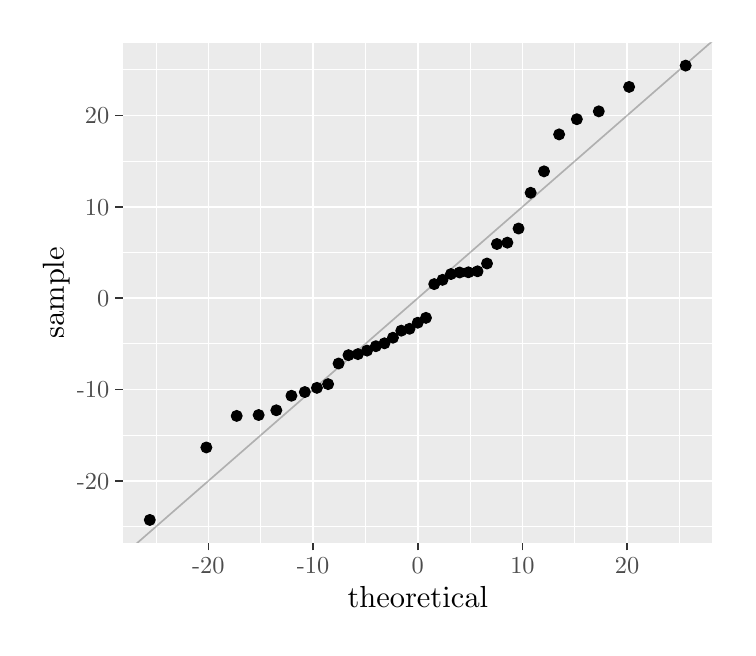
\begin{tikzpicture}[x=1pt,y=1pt]
\definecolor{fillColor}{RGB}{255,255,255}
\path[use as bounding box,fill=fillColor,fill opacity=0.00] (0,0) rectangle (252.94,216.81);
\begin{scope}
\path[clip] (  0.00,  0.00) rectangle (252.94,216.81);
\definecolor{drawColor}{RGB}{255,255,255}
\definecolor{fillColor}{RGB}{255,255,255}

\path[draw=drawColor,line width= 0.6pt,line join=round,line cap=round,fill=fillColor] (  0.00,  0.00) rectangle (252.94,216.81);
\end{scope}
\begin{scope}
\path[clip] ( 34.45, 30.72) rectangle (247.44,211.31);
\definecolor{fillColor}{gray}{0.92}

\path[fill=fillColor] ( 34.45, 30.72) rectangle (247.44,211.31);
\definecolor{drawColor}{RGB}{255,255,255}

\path[draw=drawColor,line width= 0.3pt,line join=round] ( 34.45, 36.51) --
	(247.44, 36.51);

\path[draw=drawColor,line width= 0.3pt,line join=round] ( 34.45, 69.53) --
	(247.44, 69.53);

\path[draw=drawColor,line width= 0.3pt,line join=round] ( 34.45,102.55) --
	(247.44,102.55);

\path[draw=drawColor,line width= 0.3pt,line join=round] ( 34.45,135.56) --
	(247.44,135.56);

\path[draw=drawColor,line width= 0.3pt,line join=round] ( 34.45,168.58) --
	(247.44,168.58);

\path[draw=drawColor,line width= 0.3pt,line join=round] ( 34.45,201.59) --
	(247.44,201.59);

\path[draw=drawColor,line width= 0.3pt,line join=round] ( 46.36, 30.72) --
	( 46.36,211.31);

\path[draw=drawColor,line width= 0.3pt,line join=round] ( 84.20, 30.72) --
	( 84.20,211.31);

\path[draw=drawColor,line width= 0.3pt,line join=round] (122.03, 30.72) --
	(122.03,211.31);

\path[draw=drawColor,line width= 0.3pt,line join=round] (159.87, 30.72) --
	(159.87,211.31);

\path[draw=drawColor,line width= 0.3pt,line join=round] (197.70, 30.72) --
	(197.70,211.31);

\path[draw=drawColor,line width= 0.3pt,line join=round] (235.54, 30.72) --
	(235.54,211.31);

\path[draw=drawColor,line width= 0.6pt,line join=round] ( 34.45, 53.02) --
	(247.44, 53.02);

\path[draw=drawColor,line width= 0.6pt,line join=round] ( 34.45, 86.04) --
	(247.44, 86.04);

\path[draw=drawColor,line width= 0.6pt,line join=round] ( 34.45,119.05) --
	(247.44,119.05);

\path[draw=drawColor,line width= 0.6pt,line join=round] ( 34.45,152.07) --
	(247.44,152.07);

\path[draw=drawColor,line width= 0.6pt,line join=round] ( 34.45,185.08) --
	(247.44,185.08);

\path[draw=drawColor,line width= 0.6pt,line join=round] ( 65.28, 30.72) --
	( 65.28,211.31);

\path[draw=drawColor,line width= 0.6pt,line join=round] (103.11, 30.72) --
	(103.11,211.31);

\path[draw=drawColor,line width= 0.6pt,line join=round] (140.95, 30.72) --
	(140.95,211.31);

\path[draw=drawColor,line width= 0.6pt,line join=round] (178.78, 30.72) --
	(178.78,211.31);

\path[draw=drawColor,line width= 0.6pt,line join=round] (216.62, 30.72) --
	(216.62,211.31);
\definecolor{drawColor}{RGB}{0,0,0}
\definecolor{fillColor}{RGB}{0,0,0}

\path[draw=drawColor,line width= 0.4pt,line join=round,line cap=round,fill=fillColor] ( 44.13, 38.93) circle (  1.96);

\path[draw=drawColor,line width= 0.4pt,line join=round,line cap=round,fill=fillColor] ( 64.57, 65.12) circle (  1.96);

\path[draw=drawColor,line width= 0.4pt,line join=round,line cap=round,fill=fillColor] ( 75.53, 76.52) circle (  1.96);

\path[draw=drawColor,line width= 0.4pt,line join=round,line cap=round,fill=fillColor] ( 83.46, 76.84) circle (  1.96);

\path[draw=drawColor,line width= 0.4pt,line join=round,line cap=round,fill=fillColor] ( 89.85, 78.55) circle (  1.96);

\path[draw=drawColor,line width= 0.4pt,line join=round,line cap=round,fill=fillColor] ( 95.31, 83.80) circle (  1.96);

\path[draw=drawColor,line width= 0.4pt,line join=round,line cap=round,fill=fillColor] (100.14, 85.14) circle (  1.96);

\path[draw=drawColor,line width= 0.4pt,line join=round,line cap=round,fill=fillColor] (104.52, 86.66) circle (  1.96);

\path[draw=drawColor,line width= 0.4pt,line join=round,line cap=round,fill=fillColor] (108.56, 88.00) circle (  1.96);

\path[draw=drawColor,line width= 0.4pt,line join=round,line cap=round,fill=fillColor] (112.34, 95.45) circle (  1.96);

\path[draw=drawColor,line width= 0.4pt,line join=round,line cap=round,fill=fillColor] (115.92, 98.47) circle (  1.96);

\path[draw=drawColor,line width= 0.4pt,line join=round,line cap=round,fill=fillColor] (119.34, 98.85) circle (  1.96);

\path[draw=drawColor,line width= 0.4pt,line join=round,line cap=round,fill=fillColor] (122.63,100.12) circle (  1.96);

\path[draw=drawColor,line width= 0.4pt,line join=round,line cap=round,fill=fillColor] (125.82,101.71) circle (  1.96);

\path[draw=drawColor,line width= 0.4pt,line join=round,line cap=round,fill=fillColor] (128.93,102.75) circle (  1.96);

\path[draw=drawColor,line width= 0.4pt,line join=round,line cap=round,fill=fillColor] (131.99,104.77) circle (  1.96);

\path[draw=drawColor,line width= 0.4pt,line join=round,line cap=round,fill=fillColor] (135.00,107.32) circle (  1.96);

\path[draw=drawColor,line width= 0.4pt,line join=round,line cap=round,fill=fillColor] (137.98,108.00) circle (  1.96);

\path[draw=drawColor,line width= 0.4pt,line join=round,line cap=round,fill=fillColor] (140.95,110.20) circle (  1.96);

\path[draw=drawColor,line width= 0.4pt,line join=round,line cap=round,fill=fillColor] (143.92,111.95) circle (  1.96);

\path[draw=drawColor,line width= 0.4pt,line join=round,line cap=round,fill=fillColor] (146.90,124.15) circle (  1.96);

\path[draw=drawColor,line width= 0.4pt,line join=round,line cap=round,fill=fillColor] (149.91,125.69) circle (  1.96);

\path[draw=drawColor,line width= 0.4pt,line join=round,line cap=round,fill=fillColor] (152.96,127.78) circle (  1.96);

\path[draw=drawColor,line width= 0.4pt,line join=round,line cap=round,fill=fillColor] (156.08,128.34) circle (  1.96);

\path[draw=drawColor,line width= 0.4pt,line join=round,line cap=round,fill=fillColor] (159.27,128.41) circle (  1.96);

\path[draw=drawColor,line width= 0.4pt,line join=round,line cap=round,fill=fillColor] (162.56,128.77) circle (  1.96);

\path[draw=drawColor,line width= 0.4pt,line join=round,line cap=round,fill=fillColor] (165.98,131.59) circle (  1.96);

\path[draw=drawColor,line width= 0.4pt,line join=round,line cap=round,fill=fillColor] (169.56,138.63) circle (  1.96);

\path[draw=drawColor,line width= 0.4pt,line join=round,line cap=round,fill=fillColor] (173.34,139.13) circle (  1.96);

\path[draw=drawColor,line width= 0.4pt,line join=round,line cap=round,fill=fillColor] (177.38,144.23) circle (  1.96);

\path[draw=drawColor,line width= 0.4pt,line join=round,line cap=round,fill=fillColor] (181.75,157.15) circle (  1.96);

\path[draw=drawColor,line width= 0.4pt,line join=round,line cap=round,fill=fillColor] (186.58,164.89) circle (  1.96);

\path[draw=drawColor,line width= 0.4pt,line join=round,line cap=round,fill=fillColor] (192.04,178.24) circle (  1.96);

\path[draw=drawColor,line width= 0.4pt,line join=round,line cap=round,fill=fillColor] (198.44,183.73) circle (  1.96);

\path[draw=drawColor,line width= 0.4pt,line join=round,line cap=round,fill=fillColor] (206.37,186.57) circle (  1.96);

\path[draw=drawColor,line width= 0.4pt,line join=round,line cap=round,fill=fillColor] (217.33,195.40) circle (  1.96);

\path[draw=drawColor,line width= 0.4pt,line join=round,line cap=round,fill=fillColor] (237.76,203.10) circle (  1.96);
\definecolor{drawColor}{RGB}{0,0,0}

\path[draw=drawColor,draw opacity=0.25,line width= 0.6pt,line join=round] ( 34.45, 26.12) -- (247.44,211.98);
\end{scope}
\begin{scope}
\path[clip] (  0.00,  0.00) rectangle (252.94,216.81);
\definecolor{drawColor}{gray}{0.30}

\node[text=drawColor,anchor=base east,inner sep=0pt, outer sep=0pt, scale=  0.88] at ( 29.50, 49.99) {-20};

\node[text=drawColor,anchor=base east,inner sep=0pt, outer sep=0pt, scale=  0.88] at ( 29.50, 83.01) {-10};

\node[text=drawColor,anchor=base east,inner sep=0pt, outer sep=0pt, scale=  0.88] at ( 29.50,116.02) {0};

\node[text=drawColor,anchor=base east,inner sep=0pt, outer sep=0pt, scale=  0.88] at ( 29.50,149.04) {10};

\node[text=drawColor,anchor=base east,inner sep=0pt, outer sep=0pt, scale=  0.88] at ( 29.50,182.05) {20};
\end{scope}
\begin{scope}
\path[clip] (  0.00,  0.00) rectangle (252.94,216.81);
\definecolor{drawColor}{gray}{0.20}

\path[draw=drawColor,line width= 0.6pt,line join=round] ( 31.70, 53.02) --
	( 34.45, 53.02);

\path[draw=drawColor,line width= 0.6pt,line join=round] ( 31.70, 86.04) --
	( 34.45, 86.04);

\path[draw=drawColor,line width= 0.6pt,line join=round] ( 31.70,119.05) --
	( 34.45,119.05);

\path[draw=drawColor,line width= 0.6pt,line join=round] ( 31.70,152.07) --
	( 34.45,152.07);

\path[draw=drawColor,line width= 0.6pt,line join=round] ( 31.70,185.08) --
	( 34.45,185.08);
\end{scope}
\begin{scope}
\path[clip] (  0.00,  0.00) rectangle (252.94,216.81);
\definecolor{drawColor}{gray}{0.20}

\path[draw=drawColor,line width= 0.6pt,line join=round] ( 65.28, 27.97) --
	( 65.28, 30.72);

\path[draw=drawColor,line width= 0.6pt,line join=round] (103.11, 27.97) --
	(103.11, 30.72);

\path[draw=drawColor,line width= 0.6pt,line join=round] (140.95, 27.97) --
	(140.95, 30.72);

\path[draw=drawColor,line width= 0.6pt,line join=round] (178.78, 27.97) --
	(178.78, 30.72);

\path[draw=drawColor,line width= 0.6pt,line join=round] (216.62, 27.97) --
	(216.62, 30.72);
\end{scope}
\begin{scope}
\path[clip] (  0.00,  0.00) rectangle (252.94,216.81);
\definecolor{drawColor}{gray}{0.30}

\node[text=drawColor,anchor=base,inner sep=0pt, outer sep=0pt, scale=  0.88] at ( 65.28, 19.71) {-20};

\node[text=drawColor,anchor=base,inner sep=0pt, outer sep=0pt, scale=  0.88] at (103.11, 19.71) {-10};

\node[text=drawColor,anchor=base,inner sep=0pt, outer sep=0pt, scale=  0.88] at (140.95, 19.71) {0};

\node[text=drawColor,anchor=base,inner sep=0pt, outer sep=0pt, scale=  0.88] at (178.78, 19.71) {10};

\node[text=drawColor,anchor=base,inner sep=0pt, outer sep=0pt, scale=  0.88] at (216.62, 19.71) {20};
\end{scope}
\begin{scope}
\path[clip] (  0.00,  0.00) rectangle (252.94,216.81);
\definecolor{drawColor}{RGB}{0,0,0}

\node[text=drawColor,anchor=base,inner sep=0pt, outer sep=0pt, scale=  1.10] at (140.95,  7.44) {theoretical};
\end{scope}
\begin{scope}
\path[clip] (  0.00,  0.00) rectangle (252.94,216.81);
\definecolor{drawColor}{RGB}{0,0,0}

\node[text=drawColor,rotate= 90.00,anchor=base,inner sep=0pt, outer sep=0pt, scale=  1.10] at ( 13.08,121.02) {sample};
\end{scope}
\end{tikzpicture}
}
			\caption{Soybean linear mixed model}
			\label{fig 9.2}
		\end{subfigure}
	    \caption{Residuals Q-Q plot for normality assumption}
	    \label{figuuuuuu}
    \end{figure}
	
	Plots in figure \ref{figuuuuuuu} show points randomly displaced, which means that the linearity assumption is fulfill.
	\begin{figure}[H]
		\centering
		\begin{subfigure}[b]{0.48\linewidth}        %% or \columnwidth
			\centering
			\scalebox{0.75}{% Created by tikzDevice version 0.12 on 2019-04-30 20:49:29
% !TEX encoding = UTF-8 Unicode
\begin{tikzpicture}[x=1pt,y=1pt]
\definecolor{fillColor}{RGB}{255,255,255}
\path[use as bounding box,fill=fillColor,fill opacity=0.00] (0,0) rectangle (252.94,216.81);
\begin{scope}
\path[clip] ( 49.20, 61.20) rectangle (227.75,167.61);
\definecolor{drawColor}{RGB}{0,0,0}

\path[draw=drawColor,line width= 0.4pt,line join=round,line cap=round] (190.31,135.41) circle (  2.25);

\path[draw=drawColor,line width= 0.4pt,line join=round,line cap=round] (180.35, 87.10) circle (  2.25);

\path[draw=drawColor,line width= 0.4pt,line join=round,line cap=round] (112.16, 73.02) circle (  2.25);

\path[draw=drawColor,line width= 0.4pt,line join=round,line cap=round] (196.27,149.03) circle (  2.25);

\path[draw=drawColor,line width= 0.4pt,line join=round,line cap=round] ( 99.08,101.09) circle (  2.25);

\path[draw=drawColor,line width= 0.4pt,line join=round,line cap=round] (180.51,132.85) circle (  2.25);

\path[draw=drawColor,line width= 0.4pt,line join=round,line cap=round] (221.13,125.86) circle (  2.25);

\path[draw=drawColor,line width= 0.4pt,line join=round,line cap=round] (172.87,132.62) circle (  2.25);

\path[draw=drawColor,line width= 0.4pt,line join=round,line cap=round] (169.69, 84.71) circle (  2.25);

\path[draw=drawColor,line width= 0.4pt,line join=round,line cap=round] (201.70,124.40) circle (  2.25);

\path[draw=drawColor,line width= 0.4pt,line join=round,line cap=round] (159.75, 65.14) circle (  2.25);

\path[draw=drawColor,line width= 0.4pt,line join=round,line cap=round] (131.56,108.49) circle (  2.25);

\path[draw=drawColor,line width= 0.4pt,line join=round,line cap=round] (197.71,113.00) circle (  2.25);

\path[draw=drawColor,line width= 0.4pt,line join=round,line cap=round] (135.61, 74.15) circle (  2.25);

\path[draw=drawColor,line width= 0.4pt,line join=round,line cap=round] (211.36,163.67) circle (  2.25);

\path[draw=drawColor,line width= 0.4pt,line join=round,line cap=round] (139.06, 95.46) circle (  2.25);

\path[draw=drawColor,line width= 0.4pt,line join=round,line cap=round] (146.28,102.30) circle (  2.25);

\path[draw=drawColor,line width= 0.4pt,line join=round,line cap=round] (144.89, 89.63) circle (  2.25);

\path[draw=drawColor,line width= 0.4pt,line join=round,line cap=round] (199.52,117.79) circle (  2.25);

\path[draw=drawColor,line width= 0.4pt,line join=round,line cap=round] (182.31, 88.93) circle (  2.25);

\path[draw=drawColor,line width= 0.4pt,line join=round,line cap=round] (170.88,111.25) circle (  2.25);

\path[draw=drawColor,line width= 0.4pt,line join=round,line cap=round] (141.32, 99.48) circle (  2.25);

\path[draw=drawColor,line width= 0.4pt,line join=round,line cap=round] (169.04, 90.08) circle (  2.25);

\path[draw=drawColor,line width= 0.4pt,line join=round,line cap=round] (137.42,109.06) circle (  2.25);

\path[draw=drawColor,line width= 0.4pt,line join=round,line cap=round] (183.72,101.42) circle (  2.25);

\path[draw=drawColor,line width= 0.4pt,line join=round,line cap=round] (147.47, 80.90) circle (  2.25);

\path[draw=drawColor,line width= 0.4pt,line join=round,line cap=round] (187.11, 85.13) circle (  2.25);

\path[draw=drawColor,line width= 0.4pt,line join=round,line cap=round] (120.68,104.27) circle (  2.25);

\path[draw=drawColor,line width= 0.4pt,line join=round,line cap=round] (118.44, 96.56) circle (  2.25);

\path[draw=drawColor,line width= 0.4pt,line join=round,line cap=round] (147.65,105.42) circle (  2.25);

\path[draw=drawColor,line width= 0.4pt,line join=round,line cap=round] (148.02, 92.59) circle (  2.25);

\path[draw=drawColor,line width= 0.4pt,line join=round,line cap=round] (159.29, 81.72) circle (  2.25);

\path[draw=drawColor,line width= 0.4pt,line join=round,line cap=round] ( 55.81, 81.72) circle (  2.25);

\path[draw=drawColor,line width= 0.4pt,line join=round,line cap=round] (213.55,135.12) circle (  2.25);

\path[draw=drawColor,line width= 0.4pt,line join=round,line cap=round] (158.20, 92.44) circle (  2.25);

\path[draw=drawColor,line width= 0.4pt,line join=round,line cap=round] (187.84, 81.75) circle (  2.25);

\path[draw=drawColor,line width= 0.4pt,line join=round,line cap=round] (191.96,127.02) circle (  2.25);
\end{scope}
\begin{scope}
\path[clip] (  0.00,  0.00) rectangle (252.94,216.81);
\definecolor{drawColor}{RGB}{0,0,0}

\path[draw=drawColor,line width= 0.4pt,line join=round,line cap=round] ( 73.51, 61.20) -- (206.92, 61.20);

\path[draw=drawColor,line width= 0.4pt,line join=round,line cap=round] ( 73.51, 61.20) -- ( 73.51, 55.20);

\path[draw=drawColor,line width= 0.4pt,line join=round,line cap=round] (117.98, 61.20) -- (117.98, 55.20);

\path[draw=drawColor,line width= 0.4pt,line join=round,line cap=round] (162.45, 61.20) -- (162.45, 55.20);

\path[draw=drawColor,line width= 0.4pt,line join=round,line cap=round] (206.92, 61.20) -- (206.92, 55.20);

\node[text=drawColor,anchor=base,inner sep=0pt, outer sep=0pt, scale=  1.00] at ( 73.51, 39.60) {-40};

\node[text=drawColor,anchor=base,inner sep=0pt, outer sep=0pt, scale=  1.00] at (117.98, 39.60) {-20};

\node[text=drawColor,anchor=base,inner sep=0pt, outer sep=0pt, scale=  1.00] at (162.45, 39.60) {0};

\node[text=drawColor,anchor=base,inner sep=0pt, outer sep=0pt, scale=  1.00] at (206.92, 39.60) {20};

\path[draw=drawColor,line width= 0.4pt,line join=round,line cap=round] ( 49.20, 61.84) -- ( 49.20,159.22);

\path[draw=drawColor,line width= 0.4pt,line join=round,line cap=round] ( 49.20, 61.84) -- ( 43.20, 61.84);

\path[draw=drawColor,line width= 0.4pt,line join=round,line cap=round] ( 49.20, 75.75) -- ( 43.20, 75.75);

\path[draw=drawColor,line width= 0.4pt,line join=round,line cap=round] ( 49.20, 89.66) -- ( 43.20, 89.66);

\path[draw=drawColor,line width= 0.4pt,line join=round,line cap=round] ( 49.20,103.57) -- ( 43.20,103.57);

\path[draw=drawColor,line width= 0.4pt,line join=round,line cap=round] ( 49.20,117.49) -- ( 43.20,117.49);

\path[draw=drawColor,line width= 0.4pt,line join=round,line cap=round] ( 49.20,131.40) -- ( 43.20,131.40);

\path[draw=drawColor,line width= 0.4pt,line join=round,line cap=round] ( 49.20,145.31) -- ( 43.20,145.31);

\path[draw=drawColor,line width= 0.4pt,line join=round,line cap=round] ( 49.20,159.22) -- ( 43.20,159.22);

\node[text=drawColor,rotate= 90.00,anchor=base,inner sep=0pt, outer sep=0pt, scale=  1.00] at ( 34.80, 61.84) {60};

\node[text=drawColor,rotate= 90.00,anchor=base,inner sep=0pt, outer sep=0pt, scale=  1.00] at ( 34.80, 89.66) {100};

\node[text=drawColor,rotate= 90.00,anchor=base,inner sep=0pt, outer sep=0pt, scale=  1.00] at ( 34.80,117.49) {140};

\node[text=drawColor,rotate= 90.00,anchor=base,inner sep=0pt, outer sep=0pt, scale=  1.00] at ( 34.80,145.31) {180};

\path[draw=drawColor,line width= 0.4pt,line join=round,line cap=round] ( 49.20, 61.20) --
	(227.75, 61.20) --
	(227.75,167.61) --
	( 49.20,167.61) --
	( 49.20, 61.20);
\end{scope}
\begin{scope}
\path[clip] (  0.00,  0.00) rectangle (252.94,216.81);
\definecolor{drawColor}{RGB}{0,0,0}

\node[text=drawColor,anchor=base,inner sep=0pt, outer sep=0pt, scale=  1.00] at (138.47, 15.60) {residuals};

\node[text=drawColor,rotate= 90.00,anchor=base,inner sep=0pt, outer sep=0pt, scale=  1.00] at ( 10.80,114.41) {HACorn};
\end{scope}
\end{tikzpicture}
}
			\caption{Corn linear mixed model}
			\label{fig 9.3}
		\end{subfigure}
		\begin{subfigure}[b]{0.48\linewidth}        %% or \columnwidth
			\centering
			\scalebox{0.75}{% Created by tikzDevice version 0.12 on 2019-04-30 20:49:38
% !TEX encoding = UTF-8 Unicode
\begin{tikzpicture}[x=1pt,y=1pt]
\definecolor{fillColor}{RGB}{255,255,255}
\path[use as bounding box,fill=fillColor,fill opacity=0.00] (0,0) rectangle (252.94,216.81);
\begin{scope}
\path[clip] ( 49.20, 61.20) rectangle (227.75,167.61);
\definecolor{drawColor}{RGB}{0,0,0}

\path[draw=drawColor,line width= 0.4pt,line join=round,line cap=round] (116.15, 66.09) circle (  2.25);

\path[draw=drawColor,line width= 0.4pt,line join=round,line cap=round] (145.28,123.58) circle (  2.25);

\path[draw=drawColor,line width= 0.4pt,line join=round,line cap=round] (120.08,122.15) circle (  2.25);

\path[draw=drawColor,line width= 0.4pt,line join=round,line cap=round] ( 82.19, 65.14) circle (  2.25);

\path[draw=drawColor,line width= 0.4pt,line join=round,line cap=round] (143.18, 98.80) circle (  2.25);

\path[draw=drawColor,line width= 0.4pt,line join=round,line cap=round] (141.63, 86.88) circle (  2.25);

\path[draw=drawColor,line width= 0.4pt,line join=round,line cap=round] (125.36,103.27) circle (  2.25);

\path[draw=drawColor,line width= 0.4pt,line join=round,line cap=round] ( 93.99, 86.28) circle (  2.25);

\path[draw=drawColor,line width= 0.4pt,line join=round,line cap=round] (156.21,123.12) circle (  2.25);

\path[draw=drawColor,line width= 0.4pt,line join=round,line cap=round] ( 55.81,106.24) circle (  2.25);

\path[draw=drawColor,line width= 0.4pt,line join=round,line cap=round] (196.10,163.67) circle (  2.25);

\path[draw=drawColor,line width= 0.4pt,line join=round,line cap=round] (221.13,117.50) circle (  2.25);

\path[draw=drawColor,line width= 0.4pt,line join=round,line cap=round] (127.58,106.28) circle (  2.25);

\path[draw=drawColor,line width= 0.4pt,line join=round,line cap=round] ( 93.66,116.21) circle (  2.25);

\path[draw=drawColor,line width= 0.4pt,line join=round,line cap=round] (115.76, 83.55) circle (  2.25);

\path[draw=drawColor,line width= 0.4pt,line join=round,line cap=round] (204.48,138.30) circle (  2.25);

\path[draw=drawColor,line width= 0.4pt,line join=round,line cap=round] (117.43,134.38) circle (  2.25);

\path[draw=drawColor,line width= 0.4pt,line join=round,line cap=round] (161.85,145.95) circle (  2.25);

\path[draw=drawColor,line width= 0.4pt,line join=round,line cap=round] (156.71,122.15) circle (  2.25);

\path[draw=drawColor,line width= 0.4pt,line join=round,line cap=round] (105.23,113.34) circle (  2.25);

\path[draw=drawColor,line width= 0.4pt,line join=round,line cap=round] (112.72,129.18) circle (  2.25);

\path[draw=drawColor,line width= 0.4pt,line join=round,line cap=round] (145.92,119.54) circle (  2.25);

\path[draw=drawColor,line width= 0.4pt,line join=round,line cap=round] (103.88,134.45) circle (  2.25);

\path[draw=drawColor,line width= 0.4pt,line join=round,line cap=round] (213.38,126.42) circle (  2.25);

\path[draw=drawColor,line width= 0.4pt,line join=round,line cap=round] (119.03,125.40) circle (  2.25);

\path[draw=drawColor,line width= 0.4pt,line join=round,line cap=round] (124.68,145.66) circle (  2.25);

\path[draw=drawColor,line width= 0.4pt,line join=round,line cap=round] (102.34,114.78) circle (  2.25);

\path[draw=drawColor,line width= 0.4pt,line join=round,line cap=round] (201.63,139.01) circle (  2.25);

\path[draw=drawColor,line width= 0.4pt,line join=round,line cap=round] (145.84,145.36) circle (  2.25);

\path[draw=drawColor,line width= 0.4pt,line join=round,line cap=round] (122.11,122.46) circle (  2.25);

\path[draw=drawColor,line width= 0.4pt,line join=round,line cap=round] (174.86,130.94) circle (  2.25);

\path[draw=drawColor,line width= 0.4pt,line join=round,line cap=round] ( 95.71,121.56) circle (  2.25);

\path[draw=drawColor,line width= 0.4pt,line join=round,line cap=round] (129.34, 78.63) circle (  2.25);

\path[draw=drawColor,line width= 0.4pt,line join=round,line cap=round] (146.28,102.01) circle (  2.25);

\path[draw=drawColor,line width= 0.4pt,line join=round,line cap=round] (149.12,119.54) circle (  2.25);

\path[draw=drawColor,line width= 0.4pt,line join=round,line cap=round] (100.99,145.66) circle (  2.25);

\path[draw=drawColor,line width= 0.4pt,line join=round,line cap=round] (182.65,116.80) circle (  2.25);
\end{scope}
\begin{scope}
\path[clip] (  0.00,  0.00) rectangle (252.94,216.81);
\definecolor{drawColor}{RGB}{0,0,0}

\path[draw=drawColor,line width= 0.4pt,line join=round,line cap=round] ( 70.00, 61.20) -- (202.99, 61.20);

\path[draw=drawColor,line width= 0.4pt,line join=round,line cap=round] ( 70.00, 61.20) -- ( 70.00, 55.20);

\path[draw=drawColor,line width= 0.4pt,line join=round,line cap=round] (103.25, 61.20) -- (103.25, 55.20);

\path[draw=drawColor,line width= 0.4pt,line join=round,line cap=round] (136.49, 61.20) -- (136.49, 55.20);

\path[draw=drawColor,line width= 0.4pt,line join=round,line cap=round] (169.74, 61.20) -- (169.74, 55.20);

\path[draw=drawColor,line width= 0.4pt,line join=round,line cap=round] (202.99, 61.20) -- (202.99, 55.20);

\node[text=drawColor,anchor=base,inner sep=0pt, outer sep=0pt, scale=  1.00] at ( 70.00, 39.60) {-20};

\node[text=drawColor,anchor=base,inner sep=0pt, outer sep=0pt, scale=  1.00] at (103.25, 39.60) {-10};

\node[text=drawColor,anchor=base,inner sep=0pt, outer sep=0pt, scale=  1.00] at (136.49, 39.60) {0};

\node[text=drawColor,anchor=base,inner sep=0pt, outer sep=0pt, scale=  1.00] at (169.74, 39.60) {10};

\node[text=drawColor,anchor=base,inner sep=0pt, outer sep=0pt, scale=  1.00] at (202.99, 39.60) {20};

\path[draw=drawColor,line width= 0.4pt,line join=round,line cap=round] ( 49.20, 61.34) -- ( 49.20,149.38);

\path[draw=drawColor,line width= 0.4pt,line join=round,line cap=round] ( 49.20, 61.34) -- ( 43.20, 61.34);

\path[draw=drawColor,line width= 0.4pt,line join=round,line cap=round] ( 49.20, 90.69) -- ( 43.20, 90.69);

\path[draw=drawColor,line width= 0.4pt,line join=round,line cap=round] ( 49.20,120.04) -- ( 43.20,120.04);

\path[draw=drawColor,line width= 0.4pt,line join=round,line cap=round] ( 49.20,149.38) -- ( 43.20,149.38);

\node[text=drawColor,rotate= 90.00,anchor=base,inner sep=0pt, outer sep=0pt, scale=  1.00] at ( 34.80, 61.34) {0};

\node[text=drawColor,rotate= 90.00,anchor=base,inner sep=0pt, outer sep=0pt, scale=  1.00] at ( 34.80, 90.69) {50};

\node[text=drawColor,rotate= 90.00,anchor=base,inner sep=0pt, outer sep=0pt, scale=  1.00] at ( 34.80,120.04) {100};

\node[text=drawColor,rotate= 90.00,anchor=base,inner sep=0pt, outer sep=0pt, scale=  1.00] at ( 34.80,149.38) {150};

\path[draw=drawColor,line width= 0.4pt,line join=round,line cap=round] ( 49.20, 61.20) --
	(227.75, 61.20) --
	(227.75,167.61) --
	( 49.20,167.61) --
	( 49.20, 61.20);
\end{scope}
\begin{scope}
\path[clip] (  0.00,  0.00) rectangle (252.94,216.81);
\definecolor{drawColor}{RGB}{0,0,0}

\node[text=drawColor,anchor=base,inner sep=0pt, outer sep=0pt, scale=  1.00] at (138.47, 15.60) {residuals};

\node[text=drawColor,rotate= 90.00,anchor=base,inner sep=0pt, outer sep=0pt, scale=  1.00] at ( 10.80,114.41) {HASoybeans};
\end{scope}
\end{tikzpicture}
}
			\caption{Soybean linear mixed model}
			\label{fig 9.4}
		\end{subfigure}
		\caption{Plots of explanatory variable of each model, against their residuals to check linearity assumption}
		\label{figuuuuuuu}
	\end{figure}
	Finally, homoskedasticity of the models is also fulfill, because plots in figure \ref{figuuuuuuuu} show no patterns.
	\begin{figure}[H]
		\centering
		\begin{subfigure}[b]{0.48\linewidth}        %% or \columnwidth
			\centering
			\scalebox{0.75}{% Created by tikzDevice version 0.12 on 2019-04-30 20:46:52
% !TEX encoding = UTF-8 Unicode
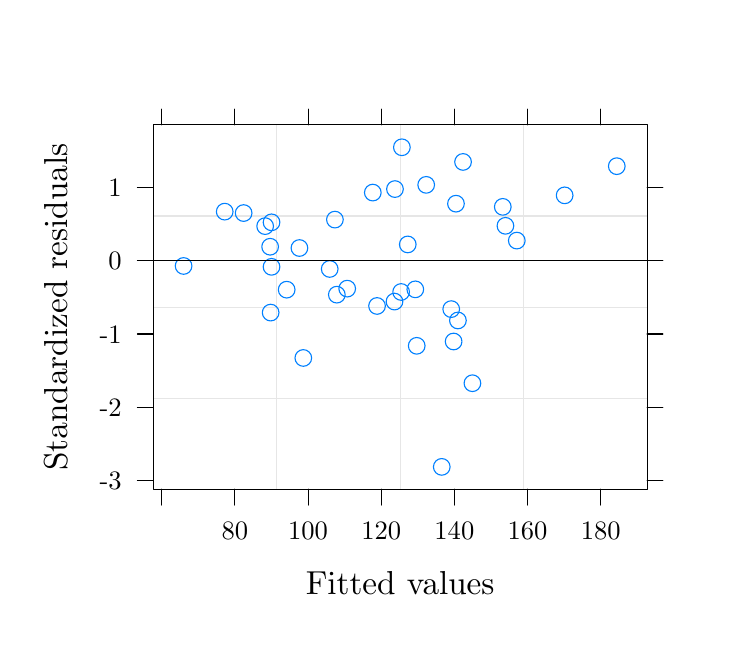
\begin{tikzpicture}[x=1pt,y=1pt]
\definecolor{fillColor}{RGB}{255,255,255}
\path[use as bounding box,fill=fillColor,fill opacity=0.00] (0,0) rectangle (252.94,216.81);
\begin{scope}
\path[clip] (  0.00,  0.00) rectangle (252.94,216.81);

\path[] (  0.00,  0.00) rectangle (252.94,216.81);
\definecolor{drawColor}{RGB}{0,0,0}

\node[text=drawColor,anchor=base,inner sep=0pt, outer sep=0pt, scale=  1.20] at (134.60, 12.05) {Fitted values};
\end{scope}
\begin{scope}
\path[clip] (  0.00,  0.00) rectangle (252.94,216.81);
\definecolor{drawColor}{RGB}{0,0,0}

\node[text=drawColor,rotate= 90.00,anchor=base,inner sep=0pt, outer sep=0pt, scale=  1.20] at ( 14.29,115.84) {Standardized residuals};
\end{scope}
\begin{scope}
\path[clip] (  0.00,  0.00) rectangle (252.94,216.81);
\definecolor{drawColor}{RGB}{0,0,0}

\path[draw=drawColor,line width= 0.4pt,line join=round,line cap=round] ( 48.45,181.67) -- ( 48.45,187.36);

\path[draw=drawColor,line width= 0.4pt,line join=round,line cap=round] ( 74.89,181.67) -- ( 74.89,187.36);

\path[draw=drawColor,line width= 0.4pt,line join=round,line cap=round] (101.32,181.67) -- (101.32,187.36);

\path[draw=drawColor,line width= 0.4pt,line join=round,line cap=round] (127.76,181.67) -- (127.76,187.36);

\path[draw=drawColor,line width= 0.4pt,line join=round,line cap=round] (154.19,181.67) -- (154.19,187.36);

\path[draw=drawColor,line width= 0.4pt,line join=round,line cap=round] (180.63,181.67) -- (180.63,187.36);

\path[draw=drawColor,line width= 0.4pt,line join=round,line cap=round] (207.06,181.67) -- (207.06,187.36);
\end{scope}
\begin{scope}
\path[clip] (  0.00,  0.00) rectangle (252.94,216.81);
\definecolor{drawColor}{RGB}{0,0,0}

\path[draw=drawColor,line width= 0.4pt,line join=round,line cap=round] ( 45.38, 53.19) -- ( 39.69, 53.19);

\path[draw=drawColor,line width= 0.4pt,line join=round,line cap=round] ( 45.38, 79.66) -- ( 39.69, 79.66);

\path[draw=drawColor,line width= 0.4pt,line join=round,line cap=round] ( 45.38,106.12) -- ( 39.69,106.12);

\path[draw=drawColor,line width= 0.4pt,line join=round,line cap=round] ( 45.38,132.59) -- ( 39.69,132.59);

\path[draw=drawColor,line width= 0.4pt,line join=round,line cap=round] ( 45.38,159.06) -- ( 39.69,159.06);

\node[text=drawColor,anchor=base east,inner sep=0pt, outer sep=0pt, scale=  0.96] at ( 34.00, 49.88) {-3};

\node[text=drawColor,anchor=base east,inner sep=0pt, outer sep=0pt, scale=  0.96] at ( 34.00, 76.35) {-2};

\node[text=drawColor,anchor=base east,inner sep=0pt, outer sep=0pt, scale=  0.96] at ( 34.00,102.82) {-1};

\node[text=drawColor,anchor=base east,inner sep=0pt, outer sep=0pt, scale=  0.96] at ( 34.00,129.28) {0};

\node[text=drawColor,anchor=base east,inner sep=0pt, outer sep=0pt, scale=  0.96] at ( 34.00,155.75) {1};
\end{scope}
\begin{scope}
\path[clip] (  0.00,  0.00) rectangle (252.94,216.81);
\definecolor{drawColor}{RGB}{0,0,0}

\path[draw=drawColor,line width= 0.4pt,line join=round,line cap=round] ( 48.45, 50.02) -- ( 48.45, 44.32);

\path[draw=drawColor,line width= 0.4pt,line join=round,line cap=round] ( 74.89, 50.02) -- ( 74.89, 44.32);

\path[draw=drawColor,line width= 0.4pt,line join=round,line cap=round] (101.32, 50.02) -- (101.32, 44.32);

\path[draw=drawColor,line width= 0.4pt,line join=round,line cap=round] (127.76, 50.02) -- (127.76, 44.32);

\path[draw=drawColor,line width= 0.4pt,line join=round,line cap=round] (154.19, 50.02) -- (154.19, 44.32);

\path[draw=drawColor,line width= 0.4pt,line join=round,line cap=round] (180.63, 50.02) -- (180.63, 44.32);

\path[draw=drawColor,line width= 0.4pt,line join=round,line cap=round] (207.06, 50.02) -- (207.06, 44.32);

\node[text=drawColor,anchor=base,inner sep=0pt, outer sep=0pt, scale=  0.96] at ( 74.89, 32.02) {80};

\node[text=drawColor,anchor=base,inner sep=0pt, outer sep=0pt, scale=  0.96] at (101.32, 32.02) {100};

\node[text=drawColor,anchor=base,inner sep=0pt, outer sep=0pt, scale=  0.96] at (127.76, 32.02) {120};

\node[text=drawColor,anchor=base,inner sep=0pt, outer sep=0pt, scale=  0.96] at (154.19, 32.02) {140};

\node[text=drawColor,anchor=base,inner sep=0pt, outer sep=0pt, scale=  0.96] at (180.63, 32.02) {160};

\node[text=drawColor,anchor=base,inner sep=0pt, outer sep=0pt, scale=  0.96] at (207.06, 32.02) {180};

\path[draw=drawColor,line width= 0.4pt,line join=round,line cap=round] (223.83, 53.19) -- (229.52, 53.19);

\path[draw=drawColor,line width= 0.4pt,line join=round,line cap=round] (223.83, 79.66) -- (229.52, 79.66);

\path[draw=drawColor,line width= 0.4pt,line join=round,line cap=round] (223.83,106.12) -- (229.52,106.12);

\path[draw=drawColor,line width= 0.4pt,line join=round,line cap=round] (223.83,132.59) -- (229.52,132.59);

\path[draw=drawColor,line width= 0.4pt,line join=round,line cap=round] (223.83,159.06) -- (229.52,159.06);
\end{scope}
\begin{scope}
\path[clip] ( 45.38, 50.02) rectangle (223.83,181.67);
\definecolor{drawColor}{RGB}{230,230,230}

\path[draw=drawColor,line width= 0.4pt,line join=round,line cap=round] ( 45.38, 82.93) -- (223.83, 82.93);

\path[draw=drawColor,line width= 0.4pt,line join=round,line cap=round] ( 45.38,115.84) -- (223.83,115.84);

\path[draw=drawColor,line width= 0.4pt,line join=round,line cap=round] ( 45.38,148.76) -- (223.83,148.76);

\path[draw=drawColor,line width= 0.4pt,line join=round,line cap=round] ( 89.99, 50.02) -- ( 89.99,181.67);

\path[draw=drawColor,line width= 0.4pt,line join=round,line cap=round] (134.60, 50.02) -- (134.60,181.67);

\path[draw=drawColor,line width= 0.4pt,line join=round,line cap=round] (179.22, 50.02) -- (179.22,181.67);
\definecolor{drawColor}{RGB}{0,128,255}

\path[draw=drawColor,line width= 0.4pt,line join=round,line cap=round] (171.68,152.06) circle (  3.01);

\path[draw=drawColor,line width= 0.4pt,line join=round,line cap=round] ( 85.81,145.10) circle (  3.01);

\path[draw=drawColor,line width= 0.4pt,line join=round,line cap=round] ( 99.60, 97.46) circle (  3.01);

\path[draw=drawColor,line width= 0.4pt,line join=round,line cap=round] (194.03,156.22) circle (  3.01);

\path[draw=drawColor,line width= 0.4pt,line join=round,line cap=round] (160.71, 88.33) circle (  3.01);

\path[draw=drawColor,line width= 0.4pt,line join=round,line cap=round] (172.64,145.21) circle (  3.01);

\path[draw=drawColor,line width= 0.4pt,line join=round,line cap=round] (135.22,173.59) circle (  3.01);

\path[draw=drawColor,line width= 0.4pt,line join=round,line cap=round] (176.74,139.87) circle (  3.01);

\path[draw=drawColor,line width= 0.4pt,line join=round,line cap=round] ( 87.61,137.65) circle (  3.01);

\path[draw=drawColor,line width= 0.4pt,line join=round,line cap=round] (144.00,160.01) circle (  3.01);

\path[draw=drawColor,line width= 0.4pt,line join=round,line cap=round] ( 56.34,130.70) circle (  3.01);

\path[draw=drawColor,line width= 0.4pt,line join=round,line cap=round] (155.47,111.01) circle (  3.01);

\path[draw=drawColor,line width= 0.4pt,line join=round,line cap=round] (124.71,157.22) circle (  3.01);

\path[draw=drawColor,line width= 0.4pt,line join=round,line cap=round] ( 87.80,113.85) circle (  3.01);

\path[draw=drawColor,line width= 0.4pt,line join=round,line cap=round] (212.87,166.76) circle (  3.01);

\path[draw=drawColor,line width= 0.4pt,line join=round,line cap=round] (126.24,116.25) circle (  3.01);

\path[draw=drawColor,line width= 0.4pt,line join=round,line cap=round] (134.95,121.30) circle (  3.01);

\path[draw=drawColor,line width= 0.4pt,line join=round,line cap=round] (111.71,120.33) circle (  3.01);

\path[draw=drawColor,line width= 0.4pt,line join=round,line cap=round] (132.72,158.49) circle (  3.01);

\path[draw=drawColor,line width= 0.4pt,line join=round,line cap=round] ( 88.12,146.47) circle (  3.01);

\path[draw=drawColor,line width= 0.4pt,line join=round,line cap=round] (137.34,138.48) circle (  3.01);

\path[draw=drawColor,line width= 0.4pt,line join=round,line cap=round] (132.55,117.83) circle (  3.01);

\path[draw=drawColor,line width= 0.4pt,line join=round,line cap=round] ( 98.20,137.19) circle (  3.01);

\path[draw=drawColor,line width= 0.4pt,line join=round,line cap=round] (153.05,115.11) circle (  3.01);

\path[draw=drawColor,line width= 0.4pt,line join=round,line cap=round] (111.02,147.45) circle (  3.01);

\path[draw=drawColor,line width= 0.4pt,line join=round,line cap=round] ( 93.59,122.13) circle (  3.01);

\path[draw=drawColor,line width= 0.4pt,line join=round,line cap=round] ( 78.04,149.82) circle (  3.01);

\path[draw=drawColor,line width= 0.4pt,line join=round,line cap=round] (153.91,103.41) circle (  3.01);

\path[draw=drawColor,line width= 0.4pt,line join=round,line cap=round] (140.58,101.85) circle (  3.01);

\path[draw=drawColor,line width= 0.4pt,line join=round,line cap=round] (140.07,122.25) circle (  3.01);

\path[draw=drawColor,line width= 0.4pt,line join=round,line cap=round] (115.46,122.51) circle (  3.01);

\path[draw=drawColor,line width= 0.4pt,line join=round,line cap=round] ( 88.12,130.39) circle (  3.01);

\path[draw=drawColor,line width= 0.4pt,line join=round,line cap=round] (149.63, 58.10) circle (  3.01);

\path[draw=drawColor,line width= 0.4pt,line join=round,line cap=round] (157.32,168.29) circle (  3.01);

\path[draw=drawColor,line width= 0.4pt,line join=round,line cap=round] (109.14,129.62) circle (  3.01);

\path[draw=drawColor,line width= 0.4pt,line join=round,line cap=round] ( 71.20,150.33) circle (  3.01);

\path[draw=drawColor,line width= 0.4pt,line join=round,line cap=round] (154.76,153.21) circle (  3.01);
\definecolor{drawColor}{RGB}{0,0,0}

\path[draw=drawColor,line width= 0.4pt,line join=round,line cap=round] ( 45.38,132.59) -- (223.83,132.59);
\end{scope}
\begin{scope}
\path[clip] (  0.00,  0.00) rectangle (252.94,216.81);
\definecolor{drawColor}{RGB}{0,0,0}

\path[draw=drawColor,line width= 0.4pt,line join=round,line cap=round] ( 45.38, 50.02) rectangle (223.83,181.67);
\end{scope}
\end{tikzpicture}
}
			\caption{Corn linear mixed model}
			\label{fig 9.5}
		\end{subfigure}
		\begin{subfigure}[b]{0.48\linewidth}        %% or \columnwidth
			\centering
			\scalebox{0.75}{% Created by tikzDevice version 0.12 on 2019-04-30 20:46:52
% !TEX encoding = UTF-8 Unicode
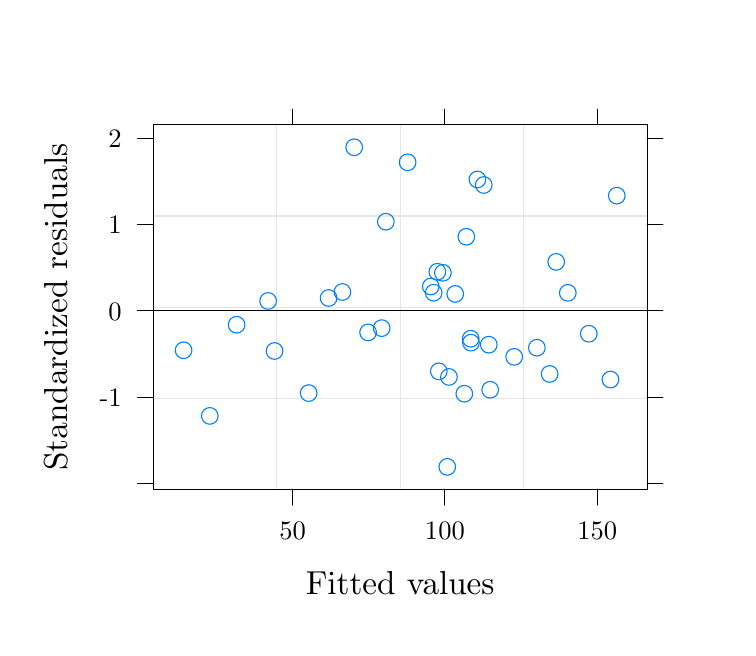
\begin{tikzpicture}[x=1pt,y=1pt]
\definecolor{fillColor}{RGB}{255,255,255}
\path[use as bounding box,fill=fillColor,fill opacity=0.00] (0,0) rectangle (252.94,216.81);
\begin{scope}
\path[clip] (  0.00,  0.00) rectangle (252.94,216.81);

\path[] (  0.00,  0.00) rectangle (252.94,216.81);
\definecolor{drawColor}{RGB}{0,0,0}

\node[text=drawColor,anchor=base,inner sep=0pt, outer sep=0pt, scale=  1.20] at (134.60, 12.05) {Fitted values};
\end{scope}
\begin{scope}
\path[clip] (  0.00,  0.00) rectangle (252.94,216.81);
\definecolor{drawColor}{RGB}{0,0,0}

\node[text=drawColor,rotate= 90.00,anchor=base,inner sep=0pt, outer sep=0pt, scale=  1.20] at ( 14.29,115.84) {Standardized residuals};
\end{scope}
\begin{scope}
\path[clip] (  0.00,  0.00) rectangle (252.94,216.81);
\definecolor{drawColor}{RGB}{0,0,0}

\path[draw=drawColor,line width= 0.4pt,line join=round,line cap=round] ( 95.74,181.67) -- ( 95.74,187.36);

\path[draw=drawColor,line width= 0.4pt,line join=round,line cap=round] (150.77,181.67) -- (150.77,187.36);

\path[draw=drawColor,line width= 0.4pt,line join=round,line cap=round] (205.81,181.67) -- (205.81,187.36);
\end{scope}
\begin{scope}
\path[clip] (  0.00,  0.00) rectangle (252.94,216.81);
\definecolor{drawColor}{RGB}{0,0,0}

\path[draw=drawColor,line width= 0.4pt,line join=round,line cap=round] ( 45.38, 52.14) -- ( 39.69, 52.14);

\path[draw=drawColor,line width= 0.4pt,line join=round,line cap=round] ( 45.38, 83.30) -- ( 39.69, 83.30);

\path[draw=drawColor,line width= 0.4pt,line join=round,line cap=round] ( 45.38,114.46) -- ( 39.69,114.46);

\path[draw=drawColor,line width= 0.4pt,line join=round,line cap=round] ( 45.38,145.62) -- ( 39.69,145.62);

\path[draw=drawColor,line width= 0.4pt,line join=round,line cap=round] ( 45.38,176.78) -- ( 39.69,176.78);

\node[text=drawColor,anchor=base east,inner sep=0pt, outer sep=0pt, scale=  0.96] at ( 34.00, 79.99) {-1};

\node[text=drawColor,anchor=base east,inner sep=0pt, outer sep=0pt, scale=  0.96] at ( 34.00,111.16) {0};

\node[text=drawColor,anchor=base east,inner sep=0pt, outer sep=0pt, scale=  0.96] at ( 34.00,142.32) {1};

\node[text=drawColor,anchor=base east,inner sep=0pt, outer sep=0pt, scale=  0.96] at ( 34.00,173.48) {2};
\end{scope}
\begin{scope}
\path[clip] (  0.00,  0.00) rectangle (252.94,216.81);
\definecolor{drawColor}{RGB}{0,0,0}

\path[draw=drawColor,line width= 0.4pt,line join=round,line cap=round] ( 95.74, 50.02) -- ( 95.74, 44.32);

\path[draw=drawColor,line width= 0.4pt,line join=round,line cap=round] (150.77, 50.02) -- (150.77, 44.32);

\path[draw=drawColor,line width= 0.4pt,line join=round,line cap=round] (205.81, 50.02) -- (205.81, 44.32);

\node[text=drawColor,anchor=base,inner sep=0pt, outer sep=0pt, scale=  0.96] at ( 95.74, 32.02) {50};

\node[text=drawColor,anchor=base,inner sep=0pt, outer sep=0pt, scale=  0.96] at (150.77, 32.02) {100};

\node[text=drawColor,anchor=base,inner sep=0pt, outer sep=0pt, scale=  0.96] at (205.81, 32.02) {150};

\path[draw=drawColor,line width= 0.4pt,line join=round,line cap=round] (223.83, 52.14) -- (229.52, 52.14);

\path[draw=drawColor,line width= 0.4pt,line join=round,line cap=round] (223.83, 83.30) -- (229.52, 83.30);

\path[draw=drawColor,line width= 0.4pt,line join=round,line cap=round] (223.83,114.46) -- (229.52,114.46);

\path[draw=drawColor,line width= 0.4pt,line join=round,line cap=round] (223.83,145.62) -- (229.52,145.62);

\path[draw=drawColor,line width= 0.4pt,line join=round,line cap=round] (223.83,176.78) -- (229.52,176.78);
\end{scope}
\begin{scope}
\path[clip] ( 45.38, 50.02) rectangle (223.83,181.67);
\definecolor{drawColor}{RGB}{230,230,230}

\path[draw=drawColor,line width= 0.4pt,line join=round,line cap=round] ( 45.38, 82.93) -- (223.83, 82.93);

\path[draw=drawColor,line width= 0.4pt,line join=round,line cap=round] ( 45.38,115.84) -- (223.83,115.84);

\path[draw=drawColor,line width= 0.4pt,line join=round,line cap=round] ( 45.38,148.76) -- (223.83,148.76);

\path[draw=drawColor,line width= 0.4pt,line join=round,line cap=round] ( 89.99, 50.02) -- ( 89.99,181.67);

\path[draw=drawColor,line width= 0.4pt,line join=round,line cap=round] (134.60, 50.02) -- (134.60,181.67);

\path[draw=drawColor,line width= 0.4pt,line join=round,line cap=round] (179.22, 50.02) -- (179.22,181.67);
\definecolor{drawColor}{RGB}{0,128,255}

\path[draw=drawColor,line width= 0.4pt,line join=round,line cap=round] ( 56.34,100.25) circle (  3.01);

\path[draw=drawColor,line width= 0.4pt,line join=round,line cap=round] (154.50,120.60) circle (  3.01);

\path[draw=drawColor,line width= 0.4pt,line join=round,line cap=round] (160.17,103.00) circle (  3.01);

\path[draw=drawColor,line width= 0.4pt,line join=round,line cap=round] ( 65.80, 76.52) circle (  3.01);

\path[draw=drawColor,line width= 0.4pt,line join=round,line cap=round] (108.74,119.13) circle (  3.01);

\path[draw=drawColor,line width= 0.4pt,line join=round,line cap=round] ( 86.88,118.05) circle (  3.01);

\path[draw=drawColor,line width= 0.4pt,line join=round,line cap=round] (123.01,106.69) circle (  3.01);

\path[draw=drawColor,line width= 0.4pt,line join=round,line cap=round] (101.54, 84.77) circle (  3.01);

\path[draw=drawColor,line width= 0.4pt,line join=round,line cap=round] (150.04,128.23) circle (  3.01);

\path[draw=drawColor,line width= 0.4pt,line join=round,line cap=round] (151.61, 58.10) circle (  3.01);

\path[draw=drawColor,line width= 0.4pt,line join=round,line cap=round] (212.87,156.10) circle (  3.01);

\path[draw=drawColor,line width= 0.4pt,line join=round,line cap=round] (117.98,173.59) circle (  3.01);

\path[draw=drawColor,line width= 0.4pt,line join=round,line cap=round] (127.93,108.24) circle (  3.01);

\path[draw=drawColor,line width= 0.4pt,line join=round,line cap=round] (157.78, 84.54) circle (  3.01);

\path[draw=drawColor,line width= 0.4pt,line join=round,line cap=round] ( 89.21, 99.98) circle (  3.01);

\path[draw=drawColor,line width= 0.4pt,line join=round,line cap=round] (162.52,161.96) circle (  3.01);

\path[draw=drawColor,line width= 0.4pt,line join=round,line cap=round] (183.99,101.15) circle (  3.01);

\path[draw=drawColor,line width= 0.4pt,line join=round,line cap=round] (190.98,132.17) circle (  3.01);

\path[draw=drawColor,line width= 0.4pt,line join=round,line cap=round] (148.04,128.59) circle (  3.01);

\path[draw=drawColor,line width= 0.4pt,line join=round,line cap=round] (148.57, 92.62) circle (  3.01);

\path[draw=drawColor,line width= 0.4pt,line join=round,line cap=round] (175.79, 97.86) circle (  3.01);

\path[draw=drawColor,line width= 0.4pt,line join=round,line cap=round] (146.72,121.04) circle (  3.01);

\path[draw=drawColor,line width= 0.4pt,line join=round,line cap=round] (188.61, 91.68) circle (  3.01);

\path[draw=drawColor,line width= 0.4pt,line join=round,line cap=round] (137.29,168.17) circle (  3.01);

\path[draw=drawColor,line width= 0.4pt,line join=round,line cap=round] (166.62,102.26) circle (  3.01);

\path[draw=drawColor,line width= 0.4pt,line join=round,line cap=round] (202.75,106.21) circle (  3.01);

\path[draw=drawColor,line width= 0.4pt,line join=round,line cap=round] (152.23, 90.60) circle (  3.01);

\path[draw=drawColor,line width= 0.4pt,line join=round,line cap=round] (164.80,159.96) circle (  3.01);

\path[draw=drawColor,line width= 0.4pt,line join=round,line cap=round] (195.17,120.99) circle (  3.01);

\path[draw=drawColor,line width= 0.4pt,line join=round,line cap=round] (160.08,104.41) circle (  3.01);

\path[draw=drawColor,line width= 0.4pt,line join=round,line cap=round] (158.51,141.26) circle (  3.01);

\path[draw=drawColor,line width= 0.4pt,line join=round,line cap=round] (167.13, 85.97) circle (  3.01);

\path[draw=drawColor,line width= 0.4pt,line join=round,line cap=round] ( 75.50,109.46) circle (  3.01);

\path[draw=drawColor,line width= 0.4pt,line join=round,line cap=round] (113.72,121.30) circle (  3.01);

\path[draw=drawColor,line width= 0.4pt,line join=round,line cap=round] (145.66,123.28) circle (  3.01);

\path[draw=drawColor,line width= 0.4pt,line join=round,line cap=round] (210.59, 89.66) circle (  3.01);

\path[draw=drawColor,line width= 0.4pt,line join=round,line cap=round] (129.43,146.70) circle (  3.01);
\definecolor{drawColor}{RGB}{0,0,0}

\path[draw=drawColor,line width= 0.4pt,line join=round,line cap=round] ( 45.38,114.46) -- (223.83,114.46);
\end{scope}
\begin{scope}
\path[clip] (  0.00,  0.00) rectangle (252.94,216.81);
\definecolor{drawColor}{RGB}{0,0,0}

\path[draw=drawColor,line width= 0.4pt,line join=round,line cap=round] ( 45.38, 50.02) rectangle (223.83,181.67);
\end{scope}
\end{tikzpicture}
}
			\caption{Soybean linear mixed model}
			\label{fig 9.6}
		\end{subfigure}
		\caption{Fitted values vs residuals for each model}
		\label{figuuuuuuuu}
	\end{figure}
	
	\item Now we want to compare and evaluate with respect to their reliability, in order to obtain predictions for $\mu_i= \bar{x}^t_{ip}\beta+ v_i$. Here, for the $i$th county and a specified crop, $x_{ip}$ is the population mean of the explanatory variables and $\bar{x}_i$ the mean over the observed segments only. Also $\hat{\beta}$ is the weighted least-squares estimator for $\beta$ and $\gamma_i= \sigma^2_v(\sigma^2_v+ n^{-1}_i\sigma^2_\epsilon)^{-1}$ where $n_i$ the number of observations in the $i$th county, $\sigma^2_v$ and $\sigma^2_\epsilon$ the variances of random effect and error, respectively.
	\begin{itemize}
		\item Regression predictor: $\mu^0_i=\bar{x}^t_{ip}\hat{\beta}$.
		\item Adjusted survey predictor: $\mu^1_i=\bar{x}^t_{ip}\hat{\beta}+ (\bar{y}_i- \bar{x}^t_{i}\hat{\beta})$
		\item (Empirical) BLUP: $\mu^\gamma_i=\bar{x}^t_{ip}\hat{\beta}+ \hat{\gamma_i}(\bar{y}_i- \bar{x}^t_{i}\hat{\beta})$
		\item Survey predictor: $\bar{y}_i= n^{-1}_i\sum_{n_i}^{j=1}y_{ij}$
	\end{itemize}
	An estimate for the mean squared error $\mathtt{MSE}_{\mu_i}(\mu^d_i)= \mathtt{E}(\mu_i- \mu^d_i)$ for $\mu^d_i$ is given by
	\[ \widehat{\mathtt{MSE}}_{\mu_i}(\mu^d_i)= (1-d)^2\hat{\sigma}^2_v+ \frac{d^2\hat{\sigma}^2_\epsilon}{n_i}+ 2(d-\hat{\gamma_i})(\bar{x}_{ip}- d\bar{x}_i)^t\hat{V}(\hat{\beta})\bar{x}_i\]
	\[ \hspace{4.75cm} +(\bar{x}_{ip}- d\bar{x}_{i})^t \hat{V}(\hat{\beta})(\bar{x}_{ip}- d\bar{x}_{i}) ,\]
	where $\hat{V}(\hat{\beta})$ is the covariance matrix of $\hat{\beta}$. Tables \ref{tableau92} and \ref{tableau93} the respective MSE. We can notice the results really differ form one county to another, which tells us that in order ot have good predictions for $\mu_i$, it might better to use different predictors fo each County.
	
	\newpage
	\begin{table}[H]
		\centering
		\begin{tabular}{|P{2cm}|P{2cm}|P{2cm}|P{2cm}|P{2cm}|}
			\hline
			\textbf{Counties} & $\mu^0_i$ & $\mu^1_i$ & $\mu^\gamma_i$ & $\bar{y}_i$ \\
			\hline
			Cerro Gordo & 72.05803 & 283.61578 & 61.66718 & 302.12264 \\
			\hline
			Hamilton & 71.97262 & 280.62908 & 61.72427 & 306.22149 \\
			\hline 
			Worth & 71.73962 & 287.68234 & 61.13340 & 292.90282 \\
			\hline 
			Humboldt & 69.41864 & 138.57817 & 53.48326 & 167.63961 \\
			\hline 
			Franklin & 65.34791 & 95.65654 & 3.27852 & 97.63366 \\
			\hline 
			Pocahontas & 64.34482 & 92.96560 & 43.50445 & 99.09076 \\
			\hline 
			Winnebago & 65.82172 & 96.77393 & 43.28370 & 96.78756 \\
			\hline 
			 Wright & 65.61789 & 95.44570 & 43.89862 & 101.67489 \\
			\hline 
			Webster & 64.08903 & 72.66995 & 38.47434 & 72.59204 \\
			\hline 
			Hancock & 63.18738 & 59.00156 & 34.43863 & 59.81280 \\
			\hline 
			Kossuth & 62.27490 & 58.09003 & 33.53265 & 58.50767 \\
			\hline 
			Hardin & 63.19271  & 50.62384 & 32.28565 & 51.50612 \\
			\hline 
		\end{tabular}
		\caption{\label{tableau92}Results of estimated predictors' MSE for Corn}
	\end{table}
	
	\begin{table}[H]
		\centering
		\begin{tabular}{|P{2cm}|P{2cm}|P{2cm}|P{2cm}|P{2cm}|}
			\hline
			\textbf{Counties} & $\mu^0_i$ & $\mu^1_i$ & $\mu^\gamma_i$ & $\bar{y}_i$ \\
			\hline
			Cerro Gordo & 233.9442 & 182.87015 & 116.21477 & 208.61640 \\
			\hline
			Hamilton & 235.5158 & 180.10725 & 107.79506 & 180.73675 \\
			\hline 
			Worth &  234.7851 & 179.91494 & 108.30543 & 183.17044 \\
			\hline 
			Humboldt & 231.4987 & 96.67826 & 74.44887 & 100.92499 \\
			\hline 
			Franklin & 223.0584 & 60.24062 & 49.31044 & 60.55884 \\
			\hline 
			Pocahontas & 219.5358 & 59.75710 & 49.03094 & 60.22818 \\
			\hline 
			Winnebago & 222.6925 & 60.45358 & 49.56226 & 61.04741 \\
			\hline 
			Wright & 225.2767 & 61.91758 & 50.95105 & 62.20606 \\
			\hline 
			Webster & 217.4335 & 44.87112 & 38.54084 & 45.10319 \\
			\hline 
			Hancock & 219.6162 & 37.21818 & 32.99170 & 37.69316 \\
			\hline 
			Kossuth & 220.0136 & 36.18285 & 31.92317 & 36.19472 \\
			\hline 
			Hardin & 220.1881 &  31.62848 & 28.61561 & 31.80195 \\
			\hline 
		\end{tabular}
		\caption{\label{tableau93}Results of estimated predictors' MSE for Soybeans}
	\end{table}
	
	\item The estimation of the total county field size for both crops, using the BLUP and Survey from (c) is highlighted in the table \ref{tableau94} and on maps \ref{fig 9.7} and \ref{fig 9.8}. We can notice that the size given by the BLUP and the Survey are completely different. This confirms the fact that we need to chose the appropriate predictor in each County(by taking the one with the lowest MSE for each County).
	
	\begin{table}[H]
		\centering
		\begin{tabular}{|P{2cm}|P{2cm}|P{2cm}|P{2cm}|P{2cm}|}
			\hline
			& \multicolumn{2}{c|}{Corn} & \multicolumn{2}{c|}{Soybeans} \\
			\hline
			\textbf{Counties} & \textbf{BLUP} & \textbf{Survey} & \textbf{BLUP} & \textbf{Survey} \\
			\hline
			Cerro Gordo & 36232.59 & 48947.27 & 14850.16 & 1534.673 \\
			\hline
			Hamilton & 37163.87 & 28934.53 & 18334.02 & 20850.800 \\
			\hline 
			Worth &  32692.98 & 22032.77 & 17913.60 & 21267.008 \\
			\hline 
			Humboldt & 33537.21 & 43869.76 & 18034.58 & 7739.632 \\
			\hline 
			Franklin & 43710.09 & 50475.53 & 12457.91 & 9868.135 \\
			\hline 
			Pocahontas & 28151.91 & 26365.93 & 27971.91 & 29333.507 \\
			\hline 
			Winnebago & 33973.49 & 32903.88 & 18073.97 & 16418.839 \\
			\hline 
			Wright & 37119.98 & 43470.81 & 24957.12 & 21649.008 \\
			\hline 
			Webster & 29310.33 & 30829.88 & 27162.40 & 27916.228 \\
			\hline 
			Hancock & 39007.80 & 34376.57 & 19952.53 & 23338.179 \\
			\hline 
			Kossuth & 33598.79 & 32926.76 & 24392.10 & 24112.061 \\
			\hline 
			Hardin & 42742.30 & 37426.91 & 13180.96 & 15894.074 \\
			\hline 
		\end{tabular}
		\caption{\label{tableau94}Results of the estimation the total county field size for both crops, by the BLUP
and survey form part (c)}
	\end{table}
	
	\begin{figure}[H]
		\centering
		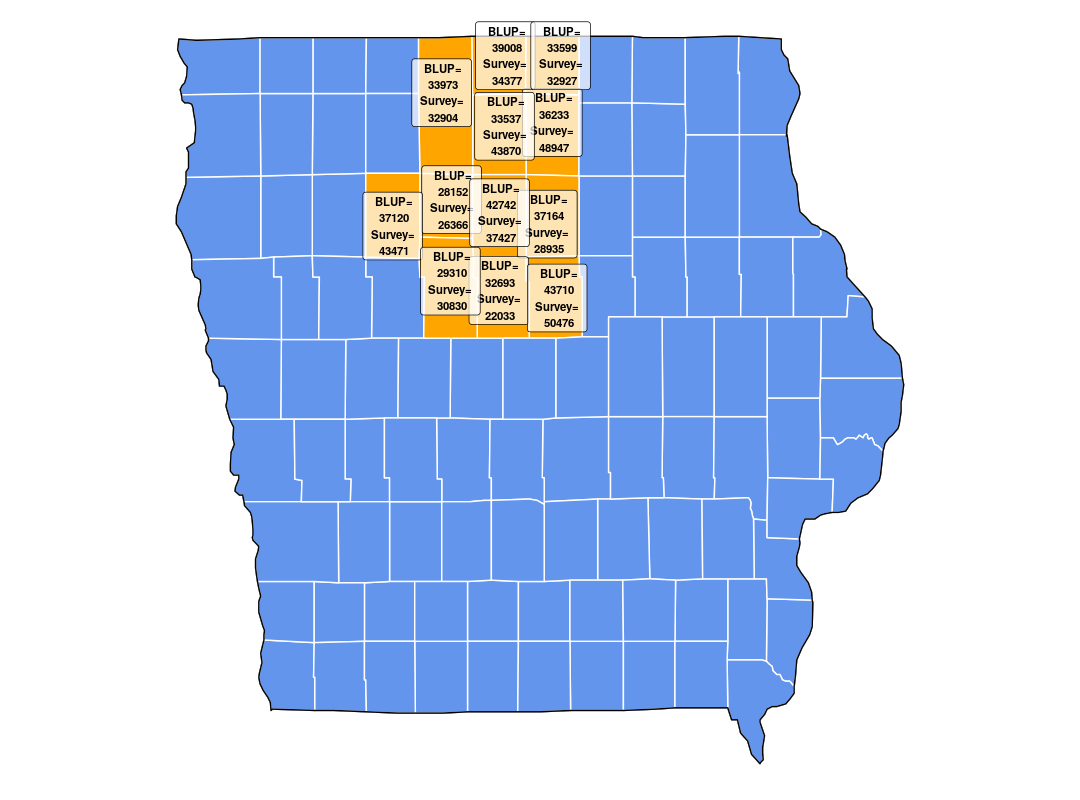
\includegraphics[scale=0.5]{Ex9plot7.png}
		\caption{Map of Iowa with estimated the total county field size for corn}
		\label{fig 9.7}
	\end{figure}
	
	\begin{figure}[H]
		\centering
		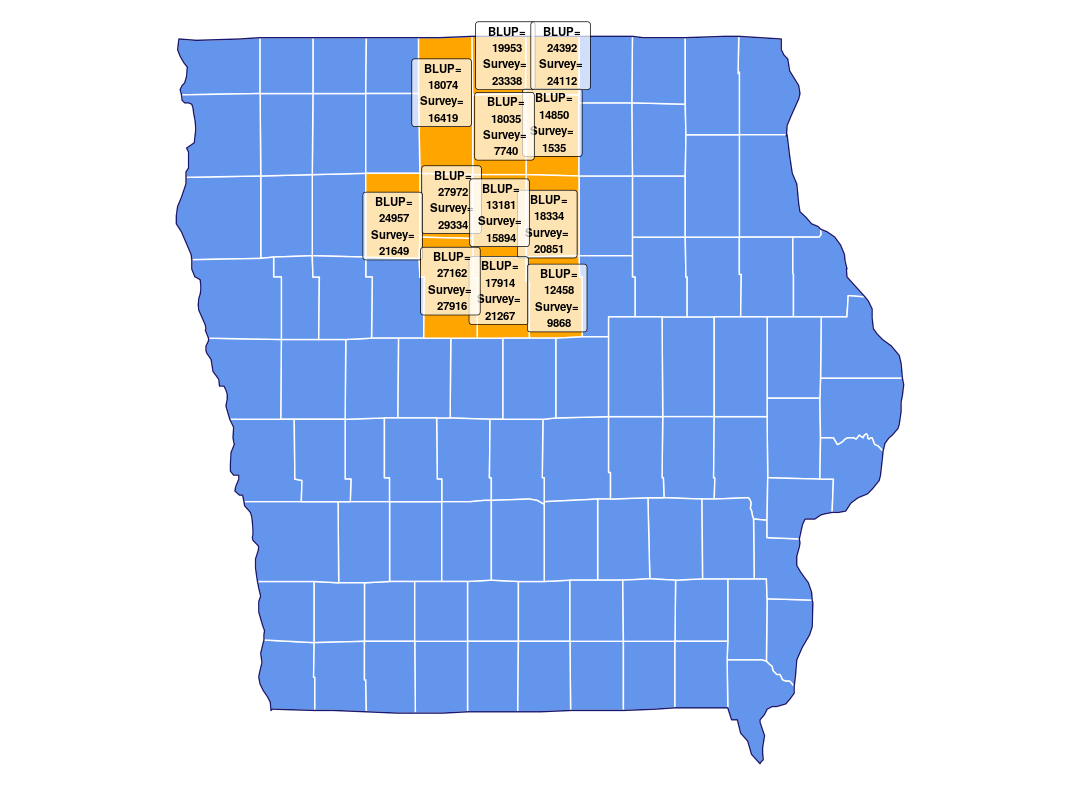
\includegraphics[scale=0.5]{Ex9plot8.png}
		\caption{Map of Iowa with estimated the total county field size for soybean}
		\label{fig 9.8}
	\end{figure}
	
	The huge differences between the slopes and intercepts of the models describe notable differences between the crops.
	
	
	
	
	
	
\end{enumerate}


%10101010101010101010101010101010101010101010%

{\color{royalblue}\chapter{Partial least squares}}
{\color{royalblue}\section{Problem description}}
In some problems of linear regression or prediction phenomenon, explicable variables can be correlated, sometimes causing  multicollinearity. This phenomenon that occurs most of the time in big data analysis, is a consequence of bad results related to regressions' coefficients estimated with least squares. To solve this problem, we have principal component analysis (PCA), and the partial least squares (PLS). We are using the latter.

{\color{royalblue}\section{Methods}}
Let $x \in \mathbb{R}^m$ and $y \in \mathbb{R}$ be two zero-mean random variables. Denote $\sigma = cov(x)$ and
$\delta = cov(x, y)$. Assume $y = x\beta + e$, $\mathtt{E}(e) = 0$ and $cov(e) = \sigma^2$. This is called a population
model.\\
Now, let $Y = (y_1,\dots,y_n)^t \in \mathtt{R}^n$ be a vector of $n$ independent copies of $y$ and $X = (x^t_1,\dots,x^t_n)^t \in \mathtt{R}^{n\times m}$ be a matrix of $n$ independent copies of $x$. In particular, $Y= X\beta + \epsilon$, where $\mathtt{E}(\epsilon)= 0_n$ and $cov(\epsilon)= \sigma^2 I_n$.\\
Denote $A = X^tX$ and $b = X^tY$ ; note that $A$ and $b$ are proportional to the sample estimators of $\sigma$ and $\delta$, respectively.\\
Denote now $K_d(b; A) = span(b, Ab,\dots, A^{d-1}b)$ the $d$-dimensional Krylov space, where $d \leq rk(A)$ should be chosen data-driven. Then, the
partial least squares estimator can be defined as 
\[ \hat{\beta}^d_{PLS}= \mathtt{arg}\min_{\beta \in K_d}= ||Y-X\beta||^2 \]
There are several ways to compute PLS, but in \textbf{R} it can be done with libraries \textbf{plsr} and \textbf{predict.plsr}.

\newpage
{\color{royalblue}\section{Results}}
The data of interest for this exercise can be find on the page \href{https://sites.google.com/michalkosinski.com/mypersonality/publications}{ myPersonality.org }. There are three files:
\begin{enumerate}
	\item [] \textit{users.csv} contains psychodemographic user profiles
	\item [] \textit{likes.csv } contains anonymised IDs and names of Facebook Likes
	\item [] \textit{users-likes.csv} contains the associations between users and their Likes
\end{enumerate}
The seed value for used in for the exercise is 1122.
\begin{enumerate}[label=(\alph*)]
	\item Check the R code related to this exercise
	\item With the PLS, we would like to find a model that allows
to predict the user?s age based on Likes (s)he made. First we split the dataset into a test and training set, by sampling randomly two thirds of all rows to include into the training set and the rest
will be the test set. Then on the training set fit PLS regression models with age as a response variable
and with up to 50 PLS components. For each PLS model dimension (from 1 to 50), we obtain the prediction on the test set and compare it with the true age values from the test set, and calculating the Pearson correlation coefficient. The plot \ref{fig 10.1} clearly shows that we have a maximal value $d_{opt}=$, which is then used as the model of dimension. The plot \ref{fig 10.2} is the Plot the values predicted by the PLS
model of dimension $d_{opt}=8$ on the test set against corresponding age values from the test
set. This plot shows that the model is pretty accurate since points are along the identity line.
	
	\begin{figure}[H]
		\centering
		\begin{subfigure}[b]{0.48\linewidth}        %% or \columnwidth
			\centering
			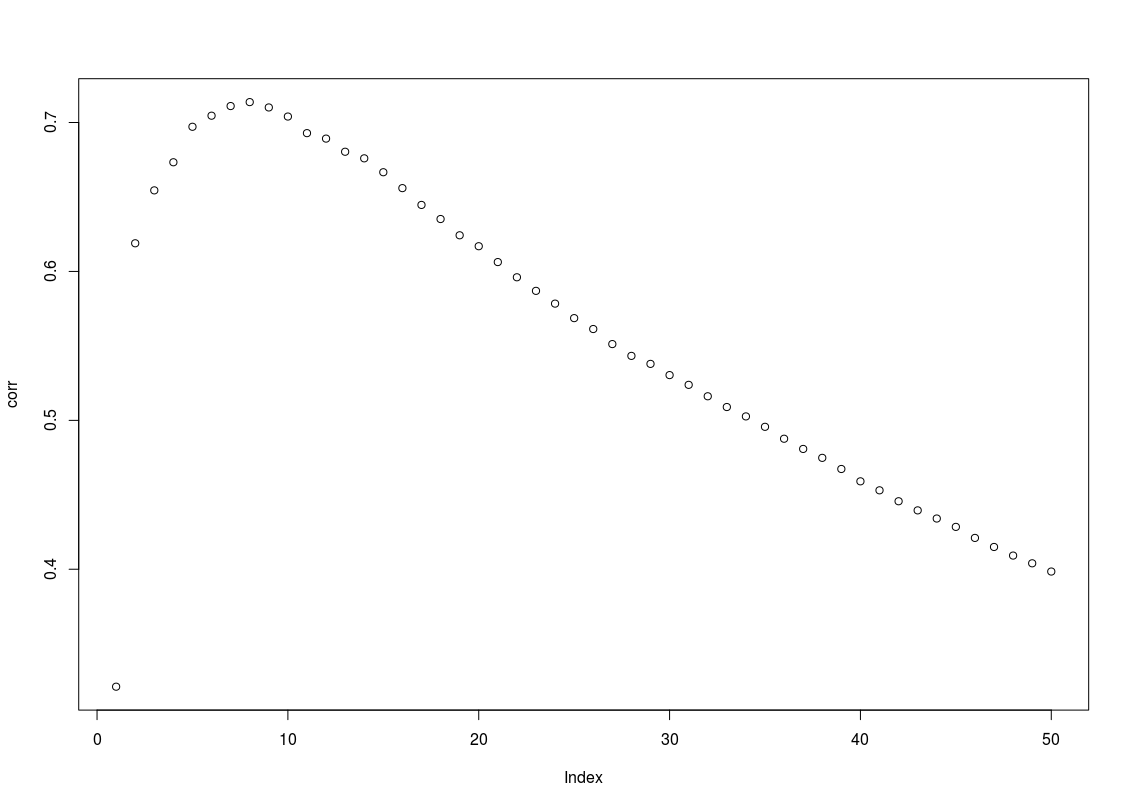
\includegraphics[scale=0.25]{Ex10plot1.png}
			\caption{Plot of the Pearson correlation coefficients against model dimension}
			\label{fig 10.1}
		\end{subfigure}
		\begin{subfigure}[b]{0.48\linewidth}        %% or \columnwidth
			\centering
			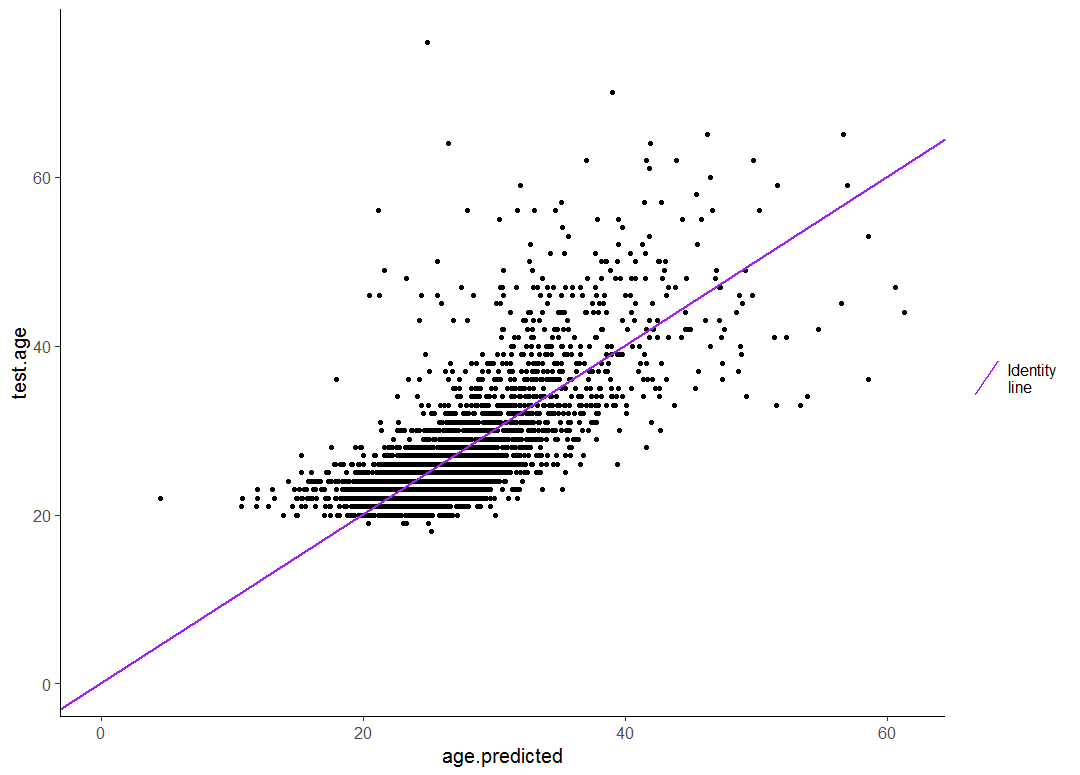
\includegraphics[scale=0.25]{Ex10plot2.png}
			\caption{Plot of the values predicted by the PLS model of dimension $d_{opt}$ on the test set against corresponding age values from the test set}
			\label{fig 10.2}
		\end{subfigure}
		\caption{}
		\label{figuuuu}
	\end{figure}
	
	\newpage
	\item Now we investigate which Likes predict the age best, using the best predictive model identified in (b). From figure \ref{figuuuuu}, we can notice that likes with the largest positive effect on the age, that is elderly people likes, are effectively topics of elders. While likes with the largest negative effect on the age, that is youngsters likes, are also things for young people. Hence we can assume that the model is accurate.
	
	\begin{figure}[H]
		\centering
		\begin{subfigure}[b]{0.48\linewidth}        %% or \columnwidth
			\centering
			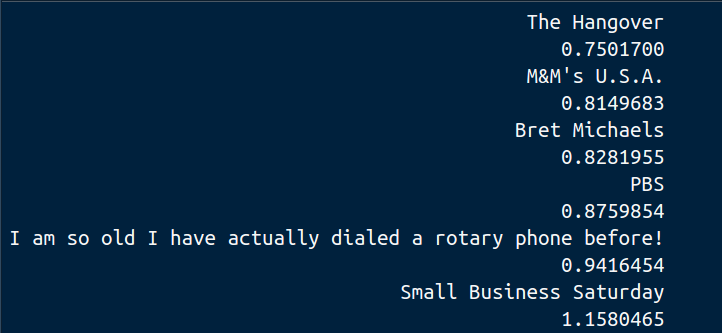
\includegraphics[scale=0.25]{Ex10plot3.png}
			\caption{The 6 Likes having the largest positive effect on the age}
			\label{fig 10.3}
		\end{subfigure}
		\begin{subfigure}[b]{0.48\linewidth}        %% or \columnwidth
			\centering
			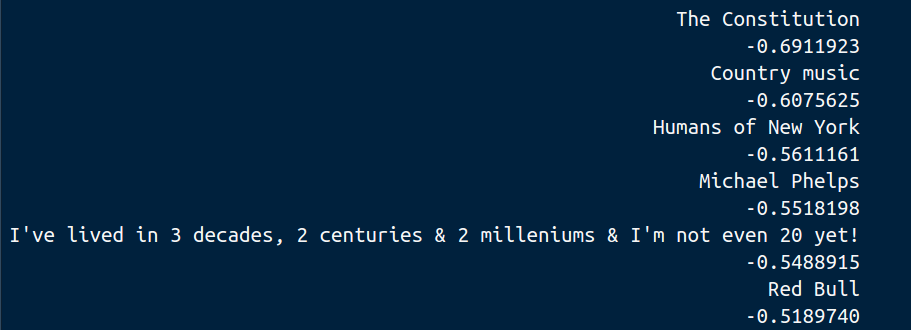
\includegraphics[scale=0.25]{Ex10plot4.png}
			\caption{The 6 Likes that have the largest negative effect on the age}
			\label{fig 10.4}
		\end{subfigure}
		\caption{}
		\label{figuuuuu}
	\end{figure}
	
	\item Now we repeat the analysis removing users that made less than 60 Likes and Likes that have
less than 120 users in (a). Due to the huge matrix' size, I could not run de model. However, it is expected to have the same likes and users as in figure \ref{figuuuuu}, but with more significant coefficients. For a plot line the one in figure \ref{fig 10.2}, we should have points more closer to the identity line.
	
\end{enumerate}




\end{document}